\documentclass[11pt,left=2cm,bottom=2cm,oneside]{book}
\usepackage{booktabs}
\usepackage{graphicx}
\usepackage{ifpdf}
\usepackage{xcolor}
\usepackage{titlesec}
\usepackage{fancyhdr}
\usepackage{lmodern}
\usepackage[version=latest]{pgf}
\usepackage{tikz}
\usepackage{hyperref}
\usepackage{setspace}
\onehalfspacing
%\pagestyle{plain}
%\fancyhf{}
%\cfoot{\thepage}
\usepackage{float}

%\let\svtikzpic\tikzpicture
%\def\tikzpicture{\noindent\svtikzpic\raggedright}
\hypersetup{colorlinks,linkcolor={black}, citecolor={black},urlcolor={darkblue}}
%\vspace{6cm}
\newcommand{\mquot}[1]{\begin{quotation}\textit{#1}\end{quotation}}
\begin{document}
\pagenumbering{}
\begin{titlepage}
\nopagebreak
\centering
{\LARGE A Dynamic Stateful Multicast Firewall}\\
\vspace*{2cm}
{\Large Author: Bewketu Tadilo}\\
\vspace*{2cm}
{\Large Date: Ramadan 1438}\\
\vspace{2cm}
{\hspace{-3cm}\Large stuff to:}\\
\vspace{5.83cm}

\includegraphics[height=5cm]{unsw-logo.jpg}
\end{titlepage}

 \section*{\centering Abstract}
\begin{quotation}
Security has been one major hindrance to the spread of multicasting and its use. Network managers are still rightly paranoid
enabling the technology when a whole array of internal resources
can be at risk. Efforts have been made to alleviate some of the
concern in the form modified service model namely source specific
multicasting. The attractiveness of the original flat service model
still remains at large and so do the multitude of routers and hosts
that only support this traditional version. The newer protocols
have been made backward compatible for this reason. This thesis aims to create a security layer that can sit in between these
two models. It draws upon experiences learned from the design
of stateful unicast firewalls and the newer protocols to track connections and associations to form its rules of a stateful multicast
firewall. It enables both coexistence and smoother transition of
these two service models.
\end{quotation}
\clearpage
\vspace*{8cm}
\subsubsection*{\underline{Originality Statement}}
I hereby declare that this submission is the work of my own. This work has not been submitted previously for any other degree and to the best of my knowledge, does not contain materials previously published or written by another person except where due acknowledgment is made.
\subsection*{Signed:\underline{~~~~~~~~~~~~~~~~~~}}
\clearpage
\vspace*{5pt}
\begin{minipage}{15cm}
\raggedright
\begin{quote}
\textit{
Dedicated to my European and Australian friends whom I met in Gondar,
Ethiopia. Thank you for taking an extra burden to sponsor my studies in Australia
and your collective support. May God bless you all!}\\
\raggedleft
\-\-Bewketu Tadilo, June 2009.
\end{quote}
\end{minipage}
\clearpage
\tableofcontents{}
%\Abbreviations{}
\listoffigures{}
\listoftables{}
\chapter{Introduction}
\pagenumbering{arabic}
Multicasting has been supported by IP networks for two decades since Steve
Deering did his PhD on it, and wrote the Internet Engineering Task Force (IETF)standard
at the end of 1989\cite{Deering}. But, the technology have been little used up until recently.
As can be inferred from its name, multicasting is a technique for transmitting data
from a single source to only a set of recipeints. The very idea brings concepts that
are not encountered in broadcasting, in which a message is sent to all computers on
the network, and unicasting in which a message is passed between a single source
and receiver. One of them is how we manage these set of recipients and is discussed
in section 2.2 on page 6.
Advances in Audiovisual technologies, that naturally demand high bandwidth,
have spurred the recent interest in multicasting in Small and Medium Enterprises
(SMEs) and consumer services. This is because we can significantly reduce traffic
load if we use multicast efficiently as we will see in section 1.1 on the next page. Nevertheless, it has remained elusive to many Network Managers, Software Developers,
System Admins and end users who might otherwise benefit from this technology.
Multicasting is heavily used in the stoke market where its model of updating all
interested users at the same time fits in perfectly. The defence departments of
countries are also big investors to the advancement the technology for better coordination in battlefields. These are areas among others in which multicasting can/is
being used
\begin{itemize}
\item Clustering
\item load sharing
\item database replication
%\item failover clusters
\item IPTV and live Internet Audio (radio)
\item Interactive gaming
\item Software distribution.
\end{itemize}
It even comes in very handy, if a Network Manager wants to install one program
to set of computers on his/her network, including operating systems.
We focus this thesis with medium enterprises in our mind and from a perspective of the Network Manager for that Enterprise. We are on Layer 3 (at the network
layer) in the entire thesis.
Multicasting reduces to either unicasting and broadcasting depending on whether
one or all members of the network are participating in communication respectively.
The use of broadcasting in many cases has been discouraged in favour of multicasting as it is prone to wasting huge resource.
\section{WHY MULTICATING?}
\begin{flushleft}\begin{figure}[H]% Graphic for TeX using PGF
% Title: /home/bewketu/diag1.dia
% Creator: Dia v0.97
% CreationDate: Thu Aug  3 03:29:36 2017
% For: bewketu
% \usepackage{tikz}
% The following commands are not supported in PSTricks at present
% We define them conditionally, so when they are implemented,
% this pgf file will use them.
\ifx\du\undefined
  \newlength{\du}
\fi
\setlength{\du}{15\unitlength}
\raggedright\begin{tikzpicture}
\pgftransformxscale{1.000000}
\pgftransformyscale{-1.000000}
\definecolor{dialinecolor}{rgb}{0.000000, 0.000000, 0.000000}
\pgfsetstrokecolor{dialinecolor}
\definecolor{dialinecolor}{rgb}{1.000000, 1.000000, 1.000000}
\pgfsetfillcolor{dialinecolor}
\pgfsetlinewidth{0.100000\du}
\pgfsetdash{}{0pt}
\pgfsetdash{}{0pt}
\pgfsetbuttcap
\pgfsetmiterjoin
\pgfsetlinewidth{0.001000\du}
\pgfsetbuttcap
\pgfsetmiterjoin
\pgfsetdash{}{0pt}
\definecolor{dialinecolor}{rgb}{0.000000, 0.470588, 0.666667}
\pgfsetfillcolor{dialinecolor}
\pgfpathmoveto{\pgfpoint{-18.257654\du}{0.403708\du}}
\pgfpathlineto{\pgfpoint{-18.259158\du}{0.387917\du}}
\pgfpathlineto{\pgfpoint{-18.262416\du}{0.372125\du}}
\pgfpathlineto{\pgfpoint{-18.267931\du}{0.356584\du}}
\pgfpathlineto{\pgfpoint{-18.275701\du}{0.341294\du}}
\pgfpathlineto{\pgfpoint{-18.286229\du}{0.325753\du}}
\pgfpathlineto{\pgfpoint{-18.298511\du}{0.310714\du}}
\pgfpathlineto{\pgfpoint{-18.313300\du}{0.295925\du}}
\pgfpathlineto{\pgfpoint{-18.329844\du}{0.281387\du}}
\pgfpathlineto{\pgfpoint{-18.348894\du}{0.267099\du}}
\pgfpathlineto{\pgfpoint{-18.369949\du}{0.253313\du}}
\pgfpathlineto{\pgfpoint{-18.392759\du}{0.240028\du}}
\pgfpathlineto{\pgfpoint{-18.417574\du}{0.226492\du}}
\pgfpathlineto{\pgfpoint{-18.444395\du}{0.213709\du}}
\pgfpathlineto{\pgfpoint{-18.472970\du}{0.201677\du}}
\pgfpathlineto{\pgfpoint{-18.503551\du}{0.190147\du}}
\pgfpathlineto{\pgfpoint{-18.535635\du}{0.179118\du}}
\pgfpathlineto{\pgfpoint{-18.568973\du}{0.168339\du}}
\pgfpathlineto{\pgfpoint{-18.604065\du}{0.158564\du}}
\pgfpathlineto{\pgfpoint{-18.640410\du}{0.149289\du}}
\pgfpathlineto{\pgfpoint{-18.678260\du}{0.140516\du}}
\pgfpathlineto{\pgfpoint{-18.717363\du}{0.132495\du}}
\pgfpathlineto{\pgfpoint{-18.757719\du}{0.125727\du}}
\pgfpathlineto{\pgfpoint{-18.798827\du}{0.118709\du}}
\pgfpathlineto{\pgfpoint{-18.840436\du}{0.113194\du}}
\pgfpathlineto{\pgfpoint{-18.883299\du}{0.107930\du}}
\pgfpathlineto{\pgfpoint{-18.926914\du}{0.103920\du}}
\pgfpathlineto{\pgfpoint{-18.971030\du}{0.100160\du}}
\pgfpathlineto{\pgfpoint{-19.015647\du}{0.097653\du}}
\pgfpathlineto{\pgfpoint{-19.060264\du}{0.095147\du}}
\pgfpathlineto{\pgfpoint{-19.105383\du}{0.094395\du}}
\pgfpathlineto{\pgfpoint{-19.150502\du}{0.093643\du}}
\pgfpathlineto{\pgfpoint{-19.150502\du}{0.093643\du}}
\pgfpathlineto{\pgfpoint{-19.195871\du}{0.094395\du}}
\pgfpathlineto{\pgfpoint{-19.240990\du}{0.095147\du}}
\pgfpathlineto{\pgfpoint{-19.285607\du}{0.097653\du}}
\pgfpathlineto{\pgfpoint{-19.330224\du}{0.100160\du}}
\pgfpathlineto{\pgfpoint{-19.374340\du}{0.103920\du}}
\pgfpathlineto{\pgfpoint{-19.417955\du}{0.107930\du}}
\pgfpathlineto{\pgfpoint{-19.460818\du}{0.113194\du}}
\pgfpathlineto{\pgfpoint{-19.502678\du}{0.118709\du}}
\pgfpathlineto{\pgfpoint{-19.543786\du}{0.125727\du}}
\pgfpathlineto{\pgfpoint{-19.583891\du}{0.132495\du}}
\pgfpathlineto{\pgfpoint{-19.622994\du}{0.140516\du}}
\pgfpathlineto{\pgfpoint{-19.660844\du}{0.149289\du}}
\pgfpathlineto{\pgfpoint{-19.697189\du}{0.158564\du}}
\pgfpathlineto{\pgfpoint{-19.732281\du}{0.168339\du}}
\pgfpathlineto{\pgfpoint{-19.765870\du}{0.179118\du}}
\pgfpathlineto{\pgfpoint{-19.797703\du}{0.190147\du}}
\pgfpathlineto{\pgfpoint{-19.828284\du}{0.201677\du}}
\pgfpathlineto{\pgfpoint{-19.856859\du}{0.213709\du}}
\pgfpathlineto{\pgfpoint{-19.883679\du}{0.226492\du}}
\pgfpathlineto{\pgfpoint{-19.908495\du}{0.240028\du}}
\pgfpathlineto{\pgfpoint{-19.931305\du}{0.253313\du}}
\pgfpathlineto{\pgfpoint{-19.952360\du}{0.267099\du}}
\pgfpathlineto{\pgfpoint{-19.971410\du}{0.281387\du}}
\pgfpathlineto{\pgfpoint{-19.987954\du}{0.295925\du}}
\pgfpathlineto{\pgfpoint{-20.002743\du}{0.310714\du}}
\pgfpathlineto{\pgfpoint{-20.015025\du}{0.325753\du}}
\pgfpathlineto{\pgfpoint{-20.025553\du}{0.341294\du}}
\pgfpathlineto{\pgfpoint{-20.033574\du}{0.356584\du}}
\pgfpathlineto{\pgfpoint{-20.039339\du}{0.372125\du}}
\pgfpathlineto{\pgfpoint{-20.042347\du}{0.387917\du}}
\pgfpathlineto{\pgfpoint{-20.043600\du}{0.403708\du}}
\pgfpathlineto{\pgfpoint{-20.043600\du}{0.403708\du}}
\pgfpathlineto{\pgfpoint{-20.042347\du}{0.419249\du}}
\pgfpathlineto{\pgfpoint{-20.039339\du}{0.435041\du}}
\pgfpathlineto{\pgfpoint{-20.033574\du}{0.450581\du}}
\pgfpathlineto{\pgfpoint{-20.025553\du}{0.465872\du}}
\pgfpathlineto{\pgfpoint{-20.015025\du}{0.481412\du}}
\pgfpathlineto{\pgfpoint{-20.002743\du}{0.496452\du}}
\pgfpathlineto{\pgfpoint{-19.987954\du}{0.511241\du}}
\pgfpathlineto{\pgfpoint{-19.971410\du}{0.525779\du}}
\pgfpathlineto{\pgfpoint{-19.952360\du}{0.540067\du}}
\pgfpathlineto{\pgfpoint{-19.931305\du}{0.553853\du}}
\pgfpathlineto{\pgfpoint{-19.908495\du}{0.567639\du}}
\pgfpathlineto{\pgfpoint{-19.883679\du}{0.580673\du}}
\pgfpathlineto{\pgfpoint{-19.856859\du}{0.593457\du}}
\pgfpathlineto{\pgfpoint{-19.828284\du}{0.605489\du}}
\pgfpathlineto{\pgfpoint{-19.797703\du}{0.617520\du}}
\pgfpathlineto{\pgfpoint{-19.765870\du}{0.628549\du}}
\pgfpathlineto{\pgfpoint{-19.732281\du}{0.638826\du}}
\pgfpathlineto{\pgfpoint{-19.697189\du}{0.648853\du}}
\pgfpathlineto{\pgfpoint{-19.660844\du}{0.657876\du}}
\pgfpathlineto{\pgfpoint{-19.622994\du}{0.666650\du}}
\pgfpathlineto{\pgfpoint{-19.583891\du}{0.674671\du}}
\pgfpathlineto{\pgfpoint{-19.543786\du}{0.681940\du}}
\pgfpathlineto{\pgfpoint{-19.502678\du}{0.688457\du}}
\pgfpathlineto{\pgfpoint{-19.460818\du}{0.694473\du}}
\pgfpathlineto{\pgfpoint{-19.417955\du}{0.699235\du}}
\pgfpathlineto{\pgfpoint{-19.374340\du}{0.703747\du}}
\pgfpathlineto{\pgfpoint{-19.330224\du}{0.707006\du}}
\pgfpathlineto{\pgfpoint{-19.285607\du}{0.710014\du}}
\pgfpathlineto{\pgfpoint{-19.240990\du}{0.712019\du}}
\pgfpathlineto{\pgfpoint{-19.195871\du}{0.713272\du}}
\pgfpathlineto{\pgfpoint{-19.150502\du}{0.713523\du}}
\pgfpathlineto{\pgfpoint{-19.150502\du}{0.713523\du}}
\pgfpathlineto{\pgfpoint{-19.105383\du}{0.713272\du}}
\pgfpathlineto{\pgfpoint{-19.060264\du}{0.712019\du}}
\pgfpathlineto{\pgfpoint{-19.015647\du}{0.710014\du}}
\pgfpathlineto{\pgfpoint{-18.971030\du}{0.707006\du}}
\pgfpathlineto{\pgfpoint{-18.926914\du}{0.703747\du}}
\pgfpathlineto{\pgfpoint{-18.883299\du}{0.699235\du}}
\pgfpathlineto{\pgfpoint{-18.840436\du}{0.694473\du}}
\pgfpathlineto{\pgfpoint{-18.798827\du}{0.688457\du}}
\pgfpathlineto{\pgfpoint{-18.757719\du}{0.681940\du}}
\pgfpathlineto{\pgfpoint{-18.717363\du}{0.674671\du}}
\pgfpathlineto{\pgfpoint{-18.678260\du}{0.666650\du}}
\pgfpathlineto{\pgfpoint{-18.640410\du}{0.657876\du}}
\pgfpathlineto{\pgfpoint{-18.604065\du}{0.648853\du}}
\pgfpathlineto{\pgfpoint{-18.568973\du}{0.638826\du}}
\pgfpathlineto{\pgfpoint{-18.535635\du}{0.628549\du}}
\pgfpathlineto{\pgfpoint{-18.503551\du}{0.617520\du}}
\pgfpathlineto{\pgfpoint{-18.472970\du}{0.605489\du}}
\pgfpathlineto{\pgfpoint{-18.444395\du}{0.593457\du}}
\pgfpathlineto{\pgfpoint{-18.417574\du}{0.580673\du}}
\pgfpathlineto{\pgfpoint{-18.392759\du}{0.567639\du}}
\pgfpathlineto{\pgfpoint{-18.369949\du}{0.553853\du}}
\pgfpathlineto{\pgfpoint{-18.348894\du}{0.540067\du}}
\pgfpathlineto{\pgfpoint{-18.329844\du}{0.525779\du}}
\pgfpathlineto{\pgfpoint{-18.313300\du}{0.511241\du}}
\pgfpathlineto{\pgfpoint{-18.298511\du}{0.496452\du}}
\pgfpathlineto{\pgfpoint{-18.286229\du}{0.481412\du}}
\pgfpathlineto{\pgfpoint{-18.275701\du}{0.465872\du}}
\pgfpathlineto{\pgfpoint{-18.267931\du}{0.450581\du}}
\pgfpathlineto{\pgfpoint{-18.262416\du}{0.435041\du}}
\pgfpathlineto{\pgfpoint{-18.259158\du}{0.419249\du}}
\pgfpathlineto{\pgfpoint{-18.257654\du}{0.403708\du}}
\pgfusepath{fill}
\pgfsetbuttcap
\pgfsetmiterjoin
\pgfsetdash{}{0pt}
\definecolor{dialinecolor}{rgb}{0.666667, 0.901961, 1.000000}
\pgfsetstrokecolor{dialinecolor}
\pgfpathmoveto{\pgfpoint{-18.268182\du}{0.398695\du}}
\pgfpathlineto{\pgfpoint{-18.269435\du}{0.382903\du}}
\pgfpathlineto{\pgfpoint{-18.272443\du}{0.367864\du}}
\pgfpathlineto{\pgfpoint{-18.278208\du}{0.352323\du}}
\pgfpathlineto{\pgfpoint{-18.285978\du}{0.337284\du}}
\pgfpathlineto{\pgfpoint{-18.296255\du}{0.322244\du}}
\pgfpathlineto{\pgfpoint{-18.309290\du}{0.307455\du}}
\pgfpathlineto{\pgfpoint{-18.322825\du}{0.293168\du}}
\pgfpathlineto{\pgfpoint{-18.339870\du}{0.278629\du}}
\pgfpathlineto{\pgfpoint{-18.358670\du}{0.264592\du}}
\pgfpathlineto{\pgfpoint{-18.379474\du}{0.250555\du}}
\pgfpathlineto{\pgfpoint{-18.402535\du}{0.237521\du}}
\pgfpathlineto{\pgfpoint{-18.427100\du}{0.224487\du}}
\pgfpathlineto{\pgfpoint{-18.453669\du}{0.211954\du}}
\pgfpathlineto{\pgfpoint{-18.481994\du}{0.199922\du}}
\pgfpathlineto{\pgfpoint{-18.512073\du}{0.188392\du}}
\pgfpathlineto{\pgfpoint{-18.544157\du}{0.177864\du}}
\pgfpathlineto{\pgfpoint{-18.577746\du}{0.167838\du}}
\pgfpathlineto{\pgfpoint{-18.612337\du}{0.157561\du}}
\pgfpathlineto{\pgfpoint{-18.648431\du}{0.149039\du}}
\pgfpathlineto{\pgfpoint{-18.686030\du}{0.140015\du}}
\pgfpathlineto{\pgfpoint{-18.725133\du}{0.132244\du}}
\pgfpathlineto{\pgfpoint{-18.764737\du}{0.125226\du}}
\pgfpathlineto{\pgfpoint{-18.805344\du}{0.118709\du}}
\pgfpathlineto{\pgfpoint{-18.847204\du}{0.113194\du}}
\pgfpathlineto{\pgfpoint{-18.889566\du}{0.107930\du}}
\pgfpathlineto{\pgfpoint{-18.933180\du}{0.103920\du}}
\pgfpathlineto{\pgfpoint{-18.976795\du}{0.100160\du}}
\pgfpathlineto{\pgfpoint{-19.021162\du}{0.097653\du}}
\pgfpathlineto{\pgfpoint{-19.065779\du}{0.095899\du}}
\pgfpathlineto{\pgfpoint{-19.110647\du}{0.094395\du}}
\pgfpathlineto{\pgfpoint{-19.155515\du}{0.094395\du}}
\pgfpathlineto{\pgfpoint{-19.155515\du}{0.094395\du}}
\pgfpathlineto{\pgfpoint{-19.200884\du}{0.094395\du}}
\pgfpathlineto{\pgfpoint{-19.245501\du}{0.095899\du}}
\pgfpathlineto{\pgfpoint{-19.290369\du}{0.097653\du}}
\pgfpathlineto{\pgfpoint{-19.334235\du}{0.100160\du}}
\pgfpathlineto{\pgfpoint{-19.378100\du}{0.103920\du}}
\pgfpathlineto{\pgfpoint{-19.421464\du}{0.107930\du}}
\pgfpathlineto{\pgfpoint{-19.464076\du}{0.113194\du}}
\pgfpathlineto{\pgfpoint{-19.505936\du}{0.118709\du}}
\pgfpathlineto{\pgfpoint{-19.546794\du}{0.125226\du}}
\pgfpathlineto{\pgfpoint{-19.586398\du}{0.132244\du}}
\pgfpathlineto{\pgfpoint{-19.625501\du}{0.140015\du}}
\pgfpathlineto{\pgfpoint{-19.663099\du}{0.149039\du}}
\pgfpathlineto{\pgfpoint{-19.698944\du}{0.157561\du}}
\pgfpathlineto{\pgfpoint{-19.733785\du}{0.167838\du}}
\pgfpathlineto{\pgfpoint{-19.767374\du}{0.177864\du}}
\pgfpathlineto{\pgfpoint{-19.799207\du}{0.188392\du}}
\pgfpathlineto{\pgfpoint{-19.829036\du}{0.199922\du}}
\pgfpathlineto{\pgfpoint{-19.857360\du}{0.211954\du}}
\pgfpathlineto{\pgfpoint{-19.884181\du}{0.224487\du}}
\pgfpathlineto{\pgfpoint{-19.909247\du}{0.237521\du}}
\pgfpathlineto{\pgfpoint{-19.931555\du}{0.250555\du}}
\pgfpathlineto{\pgfpoint{-19.952611\du}{0.264592\du}}
\pgfpathlineto{\pgfpoint{-19.971410\du}{0.278629\du}}
\pgfpathlineto{\pgfpoint{-19.987954\du}{0.293168\du}}
\pgfpathlineto{\pgfpoint{-20.002492\du}{0.307455\du}}
\pgfpathlineto{\pgfpoint{-20.015025\du}{0.322244\du}}
\pgfpathlineto{\pgfpoint{-20.025051\du}{0.337284\du}}
\pgfpathlineto{\pgfpoint{-20.033072\du}{0.352323\du}}
\pgfpathlineto{\pgfpoint{-20.038837\du}{0.367864\du}}
\pgfpathlineto{\pgfpoint{-20.042096\du}{0.382903\du}}
\pgfpathlineto{\pgfpoint{-20.043349\du}{0.398695\du}}
\pgfpathlineto{\pgfpoint{-20.043349\du}{0.398695\du}}
\pgfpathlineto{\pgfpoint{-20.042096\du}{0.413985\du}}
\pgfpathlineto{\pgfpoint{-20.038837\du}{0.429777\du}}
\pgfpathlineto{\pgfpoint{-20.033072\du}{0.444566\du}}
\pgfpathlineto{\pgfpoint{-20.025051\du}{0.459856\du}}
\pgfpathlineto{\pgfpoint{-20.015025\du}{0.475146\du}}
\pgfpathlineto{\pgfpoint{-20.002492\du}{0.489684\du}}
\pgfpathlineto{\pgfpoint{-19.987954\du}{0.504222\du}}
\pgfpathlineto{\pgfpoint{-19.971410\du}{0.518761\du}}
\pgfpathlineto{\pgfpoint{-19.952611\du}{0.532547\du}}
\pgfpathlineto{\pgfpoint{-19.931555\du}{0.546584\du}}
\pgfpathlineto{\pgfpoint{-19.909247\du}{0.559869\du}}
\pgfpathlineto{\pgfpoint{-19.884181\du}{0.572402\du}}
\pgfpathlineto{\pgfpoint{-19.857360\du}{0.585185\du}}
\pgfpathlineto{\pgfpoint{-19.829036\du}{0.597468\du}}
\pgfpathlineto{\pgfpoint{-19.799207\du}{0.608497\du}}
\pgfpathlineto{\pgfpoint{-19.767374\du}{0.619275\du}}
\pgfpathlineto{\pgfpoint{-19.733785\du}{0.629552\du}}
\pgfpathlineto{\pgfpoint{-19.698944\du}{0.639578\du}}
\pgfpathlineto{\pgfpoint{-19.663099\du}{0.648351\du}}
\pgfpathlineto{\pgfpoint{-19.625501\du}{0.656874\du}}
\pgfpathlineto{\pgfpoint{-19.586398\du}{0.664895\du}}
\pgfpathlineto{\pgfpoint{-19.546794\du}{0.671913\du}}
\pgfpathlineto{\pgfpoint{-19.505936\du}{0.678180\du}}
\pgfpathlineto{\pgfpoint{-19.464076\du}{0.684196\du}}
\pgfpathlineto{\pgfpoint{-19.421464\du}{0.689209\du}}
\pgfpathlineto{\pgfpoint{-19.378100\du}{0.693219\du}}
\pgfpathlineto{\pgfpoint{-19.334235\du}{0.696729\du}}
\pgfpathlineto{\pgfpoint{-19.290369\du}{0.699235\du}}
\pgfpathlineto{\pgfpoint{-19.245501\du}{0.701491\du}}
\pgfpathlineto{\pgfpoint{-19.200884\du}{0.702744\du}}
\pgfpathlineto{\pgfpoint{-19.155515\du}{0.702995\du}}
\pgfpathlineto{\pgfpoint{-19.155515\du}{0.702995\du}}
\pgfpathlineto{\pgfpoint{-19.110647\du}{0.702744\du}}
\pgfpathlineto{\pgfpoint{-19.065779\du}{0.701491\du}}
\pgfpathlineto{\pgfpoint{-19.021162\du}{0.699235\du}}
\pgfpathlineto{\pgfpoint{-18.976795\du}{0.696729\du}}
\pgfpathlineto{\pgfpoint{-18.933180\du}{0.693219\du}}
\pgfpathlineto{\pgfpoint{-18.889566\du}{0.689209\du}}
\pgfpathlineto{\pgfpoint{-18.847204\du}{0.684196\du}}
\pgfpathlineto{\pgfpoint{-18.805344\du}{0.678180\du}}
\pgfpathlineto{\pgfpoint{-18.764737\du}{0.671913\du}}
\pgfpathlineto{\pgfpoint{-18.725133\du}{0.664895\du}}
\pgfpathlineto{\pgfpoint{-18.686030\du}{0.656874\du}}
\pgfpathlineto{\pgfpoint{-18.648431\du}{0.648351\du}}
\pgfpathlineto{\pgfpoint{-18.612337\du}{0.639578\du}}
\pgfpathlineto{\pgfpoint{-18.577746\du}{0.629552\du}}
\pgfpathlineto{\pgfpoint{-18.544157\du}{0.619275\du}}
\pgfpathlineto{\pgfpoint{-18.512073\du}{0.608497\du}}
\pgfpathlineto{\pgfpoint{-18.481994\du}{0.597468\du}}
\pgfpathlineto{\pgfpoint{-18.453669\du}{0.585185\du}}
\pgfpathlineto{\pgfpoint{-18.427100\du}{0.572402\du}}
\pgfpathlineto{\pgfpoint{-18.402535\du}{0.559869\du}}
\pgfpathlineto{\pgfpoint{-18.379474\du}{0.546584\du}}
\pgfpathlineto{\pgfpoint{-18.358670\du}{0.532547\du}}
\pgfpathlineto{\pgfpoint{-18.339870\du}{0.518761\du}}
\pgfpathlineto{\pgfpoint{-18.322825\du}{0.504222\du}}
\pgfpathlineto{\pgfpoint{-18.309290\du}{0.489684\du}}
\pgfpathlineto{\pgfpoint{-18.296255\du}{0.475146\du}}
\pgfpathlineto{\pgfpoint{-18.285978\du}{0.459856\du}}
\pgfpathlineto{\pgfpoint{-18.278208\du}{0.444566\du}}
\pgfpathlineto{\pgfpoint{-18.272443\du}{0.429777\du}}
\pgfpathlineto{\pgfpoint{-18.269435\du}{0.413985\du}}
\pgfpathlineto{\pgfpoint{-18.268182\du}{0.398695\du}}
\pgfusepath{stroke}
\pgfsetbuttcap
\pgfsetmiterjoin
\pgfsetdash{}{0pt}
\definecolor{dialinecolor}{rgb}{0.000000, 0.470588, 0.666667}
\pgfsetfillcolor{dialinecolor}
\pgfpathmoveto{\pgfpoint{-20.043349\du}{-0.025671\du}}
\pgfpathlineto{\pgfpoint{-20.043349\du}{0.409473\du}}
\pgfpathlineto{\pgfpoint{-18.268182\du}{0.409473\du}}
\pgfpathlineto{\pgfpoint{-18.268182\du}{-0.025671\du}}
\pgfpathlineto{\pgfpoint{-20.043349\du}{-0.025671\du}}
\pgfusepath{fill}
\pgfsetbuttcap
\pgfsetmiterjoin
\pgfsetdash{}{0pt}
\definecolor{dialinecolor}{rgb}{0.000000, 0.705882, 1.000000}
\pgfsetfillcolor{dialinecolor}
\pgfpathmoveto{\pgfpoint{-18.257654\du}{-0.030935\du}}
\pgfpathlineto{\pgfpoint{-18.259158\du}{-0.046726\du}}
\pgfpathlineto{\pgfpoint{-18.262416\du}{-0.062768\du}}
\pgfpathlineto{\pgfpoint{-18.267931\du}{-0.078059\du}}
\pgfpathlineto{\pgfpoint{-18.275701\du}{-0.093599\du}}
\pgfpathlineto{\pgfpoint{-18.286229\du}{-0.109140\du}}
\pgfpathlineto{\pgfpoint{-18.298511\du}{-0.124180\du}}
\pgfpathlineto{\pgfpoint{-18.313300\du}{-0.138969\du}}
\pgfpathlineto{\pgfpoint{-18.329844\du}{-0.153256\du}}
\pgfpathlineto{\pgfpoint{-18.348894\du}{-0.167795\du}}
\pgfpathlineto{\pgfpoint{-18.369949\du}{-0.181330\du}}
\pgfpathlineto{\pgfpoint{-18.392759\du}{-0.195116\du}}
\pgfpathlineto{\pgfpoint{-18.417574\du}{-0.208151\du}}
\pgfpathlineto{\pgfpoint{-18.444395\du}{-0.221185\du}}
\pgfpathlineto{\pgfpoint{-18.472970\du}{-0.232966\du}}
\pgfpathlineto{\pgfpoint{-18.503551\du}{-0.244747\du}}
\pgfpathlineto{\pgfpoint{-18.535635\du}{-0.256027\du}}
\pgfpathlineto{\pgfpoint{-18.568973\du}{-0.266554\du}}
\pgfpathlineto{\pgfpoint{-18.604065\du}{-0.276330\du}}
\pgfpathlineto{\pgfpoint{-18.640410\du}{-0.285604\du}}
\pgfpathlineto{\pgfpoint{-18.678260\du}{-0.294127\du}}
\pgfpathlineto{\pgfpoint{-18.717363\du}{-0.301897\du}}
\pgfpathlineto{\pgfpoint{-18.757719\du}{-0.309417\du}}
\pgfpathlineto{\pgfpoint{-18.798827\du}{-0.315934\du}}
\pgfpathlineto{\pgfpoint{-18.840436\du}{-0.321950\du}}
\pgfpathlineto{\pgfpoint{-18.883299\du}{-0.326963\du}}
\pgfpathlineto{\pgfpoint{-18.926914\du}{-0.331224\du}}
\pgfpathlineto{\pgfpoint{-18.971030\du}{-0.334734\du}}
\pgfpathlineto{\pgfpoint{-19.015647\du}{-0.337491\du}}
\pgfpathlineto{\pgfpoint{-19.060264\du}{-0.339496\du}}
\pgfpathlineto{\pgfpoint{-19.105383\du}{-0.340749\du}}
\pgfpathlineto{\pgfpoint{-19.150502\du}{-0.341000\du}}
\pgfpathlineto{\pgfpoint{-19.150502\du}{-0.341000\du}}
\pgfpathlineto{\pgfpoint{-19.195871\du}{-0.340749\du}}
\pgfpathlineto{\pgfpoint{-19.240990\du}{-0.339496\du}}
\pgfpathlineto{\pgfpoint{-19.285607\du}{-0.337491\du}}
\pgfpathlineto{\pgfpoint{-19.330224\du}{-0.334734\du}}
\pgfpathlineto{\pgfpoint{-19.374340\du}{-0.331224\du}}
\pgfpathlineto{\pgfpoint{-19.417955\du}{-0.326963\du}}
\pgfpathlineto{\pgfpoint{-19.460818\du}{-0.321950\du}}
\pgfpathlineto{\pgfpoint{-19.502678\du}{-0.315934\du}}
\pgfpathlineto{\pgfpoint{-19.543786\du}{-0.309417\du}}
\pgfpathlineto{\pgfpoint{-19.583891\du}{-0.301897\du}}
\pgfpathlineto{\pgfpoint{-19.622994\du}{-0.294127\du}}
\pgfpathlineto{\pgfpoint{-19.660844\du}{-0.285604\du}}
\pgfpathlineto{\pgfpoint{-19.697189\du}{-0.276330\du}}
\pgfpathlineto{\pgfpoint{-19.732281\du}{-0.266554\du}}
\pgfpathlineto{\pgfpoint{-19.765870\du}{-0.256027\du}}
\pgfpathlineto{\pgfpoint{-19.797703\du}{-0.244747\du}}
\pgfpathlineto{\pgfpoint{-19.828284\du}{-0.232966\du}}
\pgfpathlineto{\pgfpoint{-19.856859\du}{-0.221185\du}}
\pgfpathlineto{\pgfpoint{-19.883679\du}{-0.208151\du}}
\pgfpathlineto{\pgfpoint{-19.908495\du}{-0.195116\du}}
\pgfpathlineto{\pgfpoint{-19.931305\du}{-0.181330\du}}
\pgfpathlineto{\pgfpoint{-19.952360\du}{-0.167795\du}}
\pgfpathlineto{\pgfpoint{-19.971410\du}{-0.153256\du}}
\pgfpathlineto{\pgfpoint{-19.987954\du}{-0.138969\du}}
\pgfpathlineto{\pgfpoint{-20.002743\du}{-0.124180\du}}
\pgfpathlineto{\pgfpoint{-20.015025\du}{-0.109140\du}}
\pgfpathlineto{\pgfpoint{-20.025553\du}{-0.093599\du}}
\pgfpathlineto{\pgfpoint{-20.033574\du}{-0.078059\du}}
\pgfpathlineto{\pgfpoint{-20.039339\du}{-0.062768\du}}
\pgfpathlineto{\pgfpoint{-20.042347\du}{-0.046726\du}}
\pgfpathlineto{\pgfpoint{-20.043600\du}{-0.030935\du}}
\pgfpathlineto{\pgfpoint{-20.043600\du}{-0.030935\du}}
\pgfpathlineto{\pgfpoint{-20.042347\du}{-0.015394\du}}
\pgfpathlineto{\pgfpoint{-20.039339\du}{0.000398\du}}
\pgfpathlineto{\pgfpoint{-20.033574\du}{0.015939\du}}
\pgfpathlineto{\pgfpoint{-20.025553\du}{0.030978\du}}
\pgfpathlineto{\pgfpoint{-20.015025\du}{0.046519\du}}
\pgfpathlineto{\pgfpoint{-20.002743\du}{0.061559\du}}
\pgfpathlineto{\pgfpoint{-19.987954\du}{0.076347\du}}
\pgfpathlineto{\pgfpoint{-19.971410\du}{0.091136\du}}
\pgfpathlineto{\pgfpoint{-19.952360\du}{0.105424\du}}
\pgfpathlineto{\pgfpoint{-19.931305\du}{0.118959\du}}
\pgfpathlineto{\pgfpoint{-19.908495\du}{0.132495\du}}
\pgfpathlineto{\pgfpoint{-19.883679\du}{0.146031\du}}
\pgfpathlineto{\pgfpoint{-19.856859\du}{0.158564\du}}
\pgfpathlineto{\pgfpoint{-19.828284\du}{0.170595\du}}
\pgfpathlineto{\pgfpoint{-19.797703\du}{0.182376\du}}
\pgfpathlineto{\pgfpoint{-19.765870\du}{0.193405\du}}
\pgfpathlineto{\pgfpoint{-19.732281\du}{0.204184\du}}
\pgfpathlineto{\pgfpoint{-19.697189\du}{0.213709\du}}
\pgfpathlineto{\pgfpoint{-19.660844\du}{0.222983\du}}
\pgfpathlineto{\pgfpoint{-19.622994\du}{0.231756\du}}
\pgfpathlineto{\pgfpoint{-19.583891\du}{0.240028\du}}
\pgfpathlineto{\pgfpoint{-19.543786\du}{0.246796\du}}
\pgfpathlineto{\pgfpoint{-19.502678\du}{0.253563\du}}
\pgfpathlineto{\pgfpoint{-19.460818\du}{0.259579\du}}
\pgfpathlineto{\pgfpoint{-19.417955\du}{0.264342\du}}
\pgfpathlineto{\pgfpoint{-19.374340\du}{0.268603\du}}
\pgfpathlineto{\pgfpoint{-19.330224\du}{0.272112\du}}
\pgfpathlineto{\pgfpoint{-19.285607\du}{0.274869\du}}
\pgfpathlineto{\pgfpoint{-19.240990\du}{0.277125\du}}
\pgfpathlineto{\pgfpoint{-19.195871\du}{0.278379\du}}
\pgfpathlineto{\pgfpoint{-19.150502\du}{0.278629\du}}
\pgfpathlineto{\pgfpoint{-19.150502\du}{0.278629\du}}
\pgfpathlineto{\pgfpoint{-19.105383\du}{0.278379\du}}
\pgfpathlineto{\pgfpoint{-19.060264\du}{0.277125\du}}
\pgfpathlineto{\pgfpoint{-19.015647\du}{0.274869\du}}
\pgfpathlineto{\pgfpoint{-18.971030\du}{0.272112\du}}
\pgfpathlineto{\pgfpoint{-18.926914\du}{0.268603\du}}
\pgfpathlineto{\pgfpoint{-18.883299\du}{0.264342\du}}
\pgfpathlineto{\pgfpoint{-18.840436\du}{0.259579\du}}
\pgfpathlineto{\pgfpoint{-18.798827\du}{0.253563\du}}
\pgfpathlineto{\pgfpoint{-18.757719\du}{0.246796\du}}
\pgfpathlineto{\pgfpoint{-18.717363\du}{0.240028\du}}
\pgfpathlineto{\pgfpoint{-18.678260\du}{0.231756\du}}
\pgfpathlineto{\pgfpoint{-18.640410\du}{0.222983\du}}
\pgfpathlineto{\pgfpoint{-18.604065\du}{0.213709\du}}
\pgfpathlineto{\pgfpoint{-18.568973\du}{0.204184\du}}
\pgfpathlineto{\pgfpoint{-18.535635\du}{0.193405\du}}
\pgfpathlineto{\pgfpoint{-18.503551\du}{0.182376\du}}
\pgfpathlineto{\pgfpoint{-18.472970\du}{0.170595\du}}
\pgfpathlineto{\pgfpoint{-18.444395\du}{0.158564\du}}
\pgfpathlineto{\pgfpoint{-18.417574\du}{0.146031\du}}
\pgfpathlineto{\pgfpoint{-18.392759\du}{0.132495\du}}
\pgfpathlineto{\pgfpoint{-18.369949\du}{0.118959\du}}
\pgfpathlineto{\pgfpoint{-18.348894\du}{0.105424\du}}
\pgfpathlineto{\pgfpoint{-18.329844\du}{0.091136\du}}
\pgfpathlineto{\pgfpoint{-18.313300\du}{0.076347\du}}
\pgfpathlineto{\pgfpoint{-18.298511\du}{0.061559\du}}
\pgfpathlineto{\pgfpoint{-18.286229\du}{0.046519\du}}
\pgfpathlineto{\pgfpoint{-18.275701\du}{0.030978\du}}
\pgfpathlineto{\pgfpoint{-18.267931\du}{0.015939\du}}
\pgfpathlineto{\pgfpoint{-18.262416\du}{0.000398\du}}
\pgfpathlineto{\pgfpoint{-18.259158\du}{-0.015394\du}}
\pgfpathlineto{\pgfpoint{-18.257654\du}{-0.030935\du}}
\pgfusepath{fill}
\pgfsetbuttcap
\pgfsetmiterjoin
\pgfsetdash{}{0pt}
\definecolor{dialinecolor}{rgb}{0.666667, 0.901961, 1.000000}
\pgfsetstrokecolor{dialinecolor}
\pgfpathmoveto{\pgfpoint{-18.268182\du}{-0.036199\du}}
\pgfpathlineto{\pgfpoint{-18.269435\du}{-0.051990\du}}
\pgfpathlineto{\pgfpoint{-18.272443\du}{-0.067030\du}}
\pgfpathlineto{\pgfpoint{-18.278208\du}{-0.082320\du}}
\pgfpathlineto{\pgfpoint{-18.285978\du}{-0.097610\du}}
\pgfpathlineto{\pgfpoint{-18.296255\du}{-0.112399\du}}
\pgfpathlineto{\pgfpoint{-18.309290\du}{-0.127689\du}}
\pgfpathlineto{\pgfpoint{-18.322825\du}{-0.141726\du}}
\pgfpathlineto{\pgfpoint{-18.339870\du}{-0.156264\du}}
\pgfpathlineto{\pgfpoint{-18.358670\du}{-0.170050\du}}
\pgfpathlineto{\pgfpoint{-18.379474\du}{-0.184338\du}}
\pgfpathlineto{\pgfpoint{-18.402535\du}{-0.197122\du}}
\pgfpathlineto{\pgfpoint{-18.427100\du}{-0.210407\du}}
\pgfpathlineto{\pgfpoint{-18.453669\du}{-0.222940\du}}
\pgfpathlineto{\pgfpoint{-18.481994\du}{-0.234470\du}}
\pgfpathlineto{\pgfpoint{-18.512073\du}{-0.246502\du}}
\pgfpathlineto{\pgfpoint{-18.544157\du}{-0.256528\du}}
\pgfpathlineto{\pgfpoint{-18.577746\du}{-0.267306\du}}
\pgfpathlineto{\pgfpoint{-18.612337\du}{-0.277082\du}}
\pgfpathlineto{\pgfpoint{-18.648431\du}{-0.286106\du}}
\pgfpathlineto{\pgfpoint{-18.686030\du}{-0.294879\du}}
\pgfpathlineto{\pgfpoint{-18.725133\du}{-0.302649\du}}
\pgfpathlineto{\pgfpoint{-18.764737\du}{-0.309668\du}}
\pgfpathlineto{\pgfpoint{-18.805344\du}{-0.315934\du}}
\pgfpathlineto{\pgfpoint{-18.847204\du}{-0.321950\du}}
\pgfpathlineto{\pgfpoint{-18.889566\du}{-0.326963\du}}
\pgfpathlineto{\pgfpoint{-18.933180\du}{-0.330974\du}}
\pgfpathlineto{\pgfpoint{-18.976795\du}{-0.334734\du}}
\pgfpathlineto{\pgfpoint{-19.021162\du}{-0.337240\du}}
\pgfpathlineto{\pgfpoint{-19.065779\du}{-0.339245\du}}
\pgfpathlineto{\pgfpoint{-19.110647\du}{-0.340499\du}}
\pgfpathlineto{\pgfpoint{-19.155515\du}{-0.340749\du}}
\pgfpathlineto{\pgfpoint{-19.155515\du}{-0.340749\du}}
\pgfpathlineto{\pgfpoint{-19.200884\du}{-0.340499\du}}
\pgfpathlineto{\pgfpoint{-19.245501\du}{-0.339245\du}}
\pgfpathlineto{\pgfpoint{-19.290369\du}{-0.337240\du}}
\pgfpathlineto{\pgfpoint{-19.334235\du}{-0.334734\du}}
\pgfpathlineto{\pgfpoint{-19.378100\du}{-0.330974\du}}
\pgfpathlineto{\pgfpoint{-19.421464\du}{-0.326963\du}}
\pgfpathlineto{\pgfpoint{-19.464076\du}{-0.321950\du}}
\pgfpathlineto{\pgfpoint{-19.505936\du}{-0.315934\du}}
\pgfpathlineto{\pgfpoint{-19.546794\du}{-0.309668\du}}
\pgfpathlineto{\pgfpoint{-19.586398\du}{-0.302649\du}}
\pgfpathlineto{\pgfpoint{-19.625501\du}{-0.294879\du}}
\pgfpathlineto{\pgfpoint{-19.663099\du}{-0.286106\du}}
\pgfpathlineto{\pgfpoint{-19.698944\du}{-0.277082\du}}
\pgfpathlineto{\pgfpoint{-19.733785\du}{-0.267306\du}}
\pgfpathlineto{\pgfpoint{-19.767374\du}{-0.256528\du}}
\pgfpathlineto{\pgfpoint{-19.799207\du}{-0.246502\du}}
\pgfpathlineto{\pgfpoint{-19.829036\du}{-0.234470\du}}
\pgfpathlineto{\pgfpoint{-19.857360\du}{-0.222940\du}}
\pgfpathlineto{\pgfpoint{-19.884181\du}{-0.210407\du}}
\pgfpathlineto{\pgfpoint{-19.909247\du}{-0.197122\du}}
\pgfpathlineto{\pgfpoint{-19.931555\du}{-0.184338\du}}
\pgfpathlineto{\pgfpoint{-19.952611\du}{-0.170050\du}}
\pgfpathlineto{\pgfpoint{-19.971410\du}{-0.156264\du}}
\pgfpathlineto{\pgfpoint{-19.987954\du}{-0.141726\du}}
\pgfpathlineto{\pgfpoint{-20.002492\du}{-0.127689\du}}
\pgfpathlineto{\pgfpoint{-20.015025\du}{-0.112399\du}}
\pgfpathlineto{\pgfpoint{-20.025051\du}{-0.097610\du}}
\pgfpathlineto{\pgfpoint{-20.033072\du}{-0.082320\du}}
\pgfpathlineto{\pgfpoint{-20.038837\du}{-0.067030\du}}
\pgfpathlineto{\pgfpoint{-20.042096\du}{-0.051990\du}}
\pgfpathlineto{\pgfpoint{-20.043349\du}{-0.036199\du}}
\pgfpathlineto{\pgfpoint{-20.043349\du}{-0.036199\du}}
\pgfpathlineto{\pgfpoint{-20.042096\du}{-0.020658\du}}
\pgfpathlineto{\pgfpoint{-20.038837\du}{-0.005367\du}}
\pgfpathlineto{\pgfpoint{-20.033072\du}{0.009923\du}}
\pgfpathlineto{\pgfpoint{-20.025051\du}{0.024962\du}}
\pgfpathlineto{\pgfpoint{-20.015025\du}{0.040002\du}}
\pgfpathlineto{\pgfpoint{-20.002492\du}{0.055041\du}}
\pgfpathlineto{\pgfpoint{-19.987954\du}{0.069329\du}}
\pgfpathlineto{\pgfpoint{-19.971410\du}{0.083867\du}}
\pgfpathlineto{\pgfpoint{-19.952611\du}{0.097653\du}}
\pgfpathlineto{\pgfpoint{-19.931555\du}{0.111690\du}}
\pgfpathlineto{\pgfpoint{-19.909247\du}{0.124975\du}}
\pgfpathlineto{\pgfpoint{-19.884181\du}{0.137508\du}}
\pgfpathlineto{\pgfpoint{-19.857360\du}{0.150292\du}}
\pgfpathlineto{\pgfpoint{-19.829036\du}{0.162323\du}}
\pgfpathlineto{\pgfpoint{-19.799207\du}{0.173603\du}}
\pgfpathlineto{\pgfpoint{-19.767374\du}{0.184381\du}}
\pgfpathlineto{\pgfpoint{-19.733785\du}{0.194658\du}}
\pgfpathlineto{\pgfpoint{-19.698944\du}{0.204434\du}}
\pgfpathlineto{\pgfpoint{-19.663099\du}{0.213458\du}}
\pgfpathlineto{\pgfpoint{-19.625501\du}{0.222231\du}}
\pgfpathlineto{\pgfpoint{-19.586398\du}{0.230503\du}}
\pgfpathlineto{\pgfpoint{-19.546794\du}{0.237020\du}}
\pgfpathlineto{\pgfpoint{-19.505936\du}{0.243788\du}}
\pgfpathlineto{\pgfpoint{-19.464076\du}{0.249553\du}}
\pgfpathlineto{\pgfpoint{-19.421464\du}{0.254315\du}}
\pgfpathlineto{\pgfpoint{-19.378100\du}{0.258827\du}}
\pgfpathlineto{\pgfpoint{-19.334235\du}{0.262336\du}}
\pgfpathlineto{\pgfpoint{-19.290369\du}{0.264592\du}}
\pgfpathlineto{\pgfpoint{-19.245501\du}{0.266848\du}}
\pgfpathlineto{\pgfpoint{-19.200884\du}{0.268102\du}}
\pgfpathlineto{\pgfpoint{-19.155515\du}{0.268352\du}}
\pgfpathlineto{\pgfpoint{-19.155515\du}{0.268352\du}}
\pgfpathlineto{\pgfpoint{-19.110647\du}{0.268102\du}}
\pgfpathlineto{\pgfpoint{-19.065779\du}{0.266848\du}}
\pgfpathlineto{\pgfpoint{-19.021162\du}{0.264592\du}}
\pgfpathlineto{\pgfpoint{-18.976795\du}{0.262336\du}}
\pgfpathlineto{\pgfpoint{-18.933180\du}{0.258827\du}}
\pgfpathlineto{\pgfpoint{-18.889566\du}{0.254315\du}}
\pgfpathlineto{\pgfpoint{-18.847204\du}{0.249553\du}}
\pgfpathlineto{\pgfpoint{-18.805344\du}{0.243788\du}}
\pgfpathlineto{\pgfpoint{-18.764737\du}{0.237020\du}}
\pgfpathlineto{\pgfpoint{-18.725133\du}{0.230503\du}}
\pgfpathlineto{\pgfpoint{-18.686030\du}{0.222231\du}}
\pgfpathlineto{\pgfpoint{-18.648431\du}{0.213458\du}}
\pgfpathlineto{\pgfpoint{-18.612337\du}{0.204434\du}}
\pgfpathlineto{\pgfpoint{-18.577746\du}{0.194658\du}}
\pgfpathlineto{\pgfpoint{-18.544157\du}{0.184381\du}}
\pgfpathlineto{\pgfpoint{-18.512073\du}{0.173603\du}}
\pgfpathlineto{\pgfpoint{-18.481994\du}{0.162323\du}}
\pgfpathlineto{\pgfpoint{-18.453669\du}{0.150292\du}}
\pgfpathlineto{\pgfpoint{-18.427100\du}{0.137508\du}}
\pgfpathlineto{\pgfpoint{-18.402535\du}{0.124975\du}}
\pgfpathlineto{\pgfpoint{-18.379474\du}{0.111690\du}}
\pgfpathlineto{\pgfpoint{-18.358670\du}{0.097653\du}}
\pgfpathlineto{\pgfpoint{-18.339870\du}{0.083867\du}}
\pgfpathlineto{\pgfpoint{-18.322825\du}{0.069329\du}}
\pgfpathlineto{\pgfpoint{-18.309290\du}{0.055041\du}}
\pgfpathlineto{\pgfpoint{-18.296255\du}{0.040002\du}}
\pgfpathlineto{\pgfpoint{-18.285978\du}{0.024962\du}}
\pgfpathlineto{\pgfpoint{-18.278208\du}{0.009923\du}}
\pgfpathlineto{\pgfpoint{-18.272443\du}{-0.005367\du}}
\pgfpathlineto{\pgfpoint{-18.269435\du}{-0.020658\du}}
\pgfpathlineto{\pgfpoint{-18.268182\du}{-0.036199\du}}
\pgfusepath{stroke}
\pgfsetbuttcap
\pgfsetmiterjoin
\pgfsetdash{}{0pt}
\definecolor{dialinecolor}{rgb}{0.000000, 0.000000, 0.000000}
\pgfsetfillcolor{dialinecolor}
\pgfpathmoveto{\pgfpoint{-19.133958\du}{-0.101370\du}}
\pgfpathlineto{\pgfpoint{-19.004117\du}{-0.057755\du}}
\pgfpathlineto{\pgfpoint{-18.690041\du}{-0.188599\du}}
\pgfpathlineto{\pgfpoint{-18.549421\du}{-0.145235\du}}
\pgfpathlineto{\pgfpoint{-18.625371\du}{-0.253520\du}}
\pgfpathlineto{\pgfpoint{-18.993088\du}{-0.253520\du}}
\pgfpathlineto{\pgfpoint{-18.841940\du}{-0.221185\du}}
\pgfpathlineto{\pgfpoint{-19.133958\du}{-0.101370\du}}
\pgfusepath{fill}
\pgfsetbuttcap
\pgfsetmiterjoin
\pgfsetdash{}{0pt}
\definecolor{dialinecolor}{rgb}{0.000000, 0.000000, 0.000000}
\pgfsetfillcolor{dialinecolor}
\pgfpathmoveto{\pgfpoint{-19.188351\du}{0.018194\du}}
\pgfpathlineto{\pgfpoint{-19.317942\du}{-0.025671\du}}
\pgfpathlineto{\pgfpoint{-19.621239\du}{0.105424\du}}
\pgfpathlineto{\pgfpoint{-19.772638\du}{0.061559\du}}
\pgfpathlineto{\pgfpoint{-19.697189\du}{0.181123\du}}
\pgfpathlineto{\pgfpoint{-19.317942\du}{0.181123\du}}
\pgfpathlineto{\pgfpoint{-19.480620\du}{0.137508\du}}
\pgfpathlineto{\pgfpoint{-19.188351\du}{0.018194\du}}
\pgfusepath{fill}
\pgfsetbuttcap
\pgfsetmiterjoin
\pgfsetdash{}{0pt}
\definecolor{dialinecolor}{rgb}{0.000000, 0.000000, 0.000000}
\pgfsetfillcolor{dialinecolor}
\pgfpathmoveto{\pgfpoint{-19.740302\du}{-0.221185\du}}
\pgfpathlineto{\pgfpoint{-19.610712\du}{-0.264549\du}}
\pgfpathlineto{\pgfpoint{-19.296385\du}{-0.145235\du}}
\pgfpathlineto{\pgfpoint{-19.155515\du}{-0.177570\du}}
\pgfpathlineto{\pgfpoint{-19.231214\du}{-0.069286\du}}
\pgfpathlineto{\pgfpoint{-19.599683\du}{-0.069286\du}}
\pgfpathlineto{\pgfpoint{-19.448285\du}{-0.101370\du}}
\pgfpathlineto{\pgfpoint{-19.740302\du}{-0.221185\du}}
\pgfusepath{fill}
\pgfsetbuttcap
\pgfsetmiterjoin
\pgfsetdash{}{0pt}
\definecolor{dialinecolor}{rgb}{0.000000, 0.000000, 0.000000}
\pgfsetfillcolor{dialinecolor}
\pgfpathmoveto{\pgfpoint{-18.571228\du}{0.148287\du}}
\pgfpathlineto{\pgfpoint{-18.701321\du}{0.191901\du}}
\pgfpathlineto{\pgfpoint{-19.004117\du}{0.061559\du}}
\pgfpathlineto{\pgfpoint{-19.155515\du}{0.105424\du}}
\pgfpathlineto{\pgfpoint{-19.079816\du}{-0.003864\du}}
\pgfpathlineto{\pgfpoint{-18.701321\du}{-0.003864\du}}
\pgfpathlineto{\pgfpoint{-18.863497\du}{0.028722\du}}
\pgfpathlineto{\pgfpoint{-18.571228\du}{0.148287\du}}
\pgfusepath{fill}
\pgfsetbuttcap
\pgfsetmiterjoin
\pgfsetdash{}{0pt}
\definecolor{dialinecolor}{rgb}{1.000000, 1.000000, 1.000000}
\pgfsetfillcolor{dialinecolor}
\pgfpathmoveto{\pgfpoint{-19.123180\du}{-0.090592\du}}
\pgfpathlineto{\pgfpoint{-18.993088\du}{-0.047228\du}}
\pgfpathlineto{\pgfpoint{-18.679764\du}{-0.177570\du}}
\pgfpathlineto{\pgfpoint{-18.538643\du}{-0.133956\du}}
\pgfpathlineto{\pgfpoint{-18.614593\du}{-0.242992\du}}
\pgfpathlineto{\pgfpoint{-18.982560\du}{-0.242992\du}}
\pgfpathlineto{\pgfpoint{-18.830911\du}{-0.210657\du}}
\pgfpathlineto{\pgfpoint{-19.123180\du}{-0.090592\du}}
\pgfusepath{fill}
\pgfsetbuttcap
\pgfsetmiterjoin
\pgfsetdash{}{0pt}
\definecolor{dialinecolor}{rgb}{1.000000, 1.000000, 1.000000}
\pgfsetfillcolor{dialinecolor}
\pgfpathmoveto{\pgfpoint{-19.177322\du}{0.028722\du}}
\pgfpathlineto{\pgfpoint{-19.307665\du}{-0.014642\du}}
\pgfpathlineto{\pgfpoint{-19.610712\du}{0.115701\du}}
\pgfpathlineto{\pgfpoint{-19.762110\du}{0.072337\du}}
\pgfpathlineto{\pgfpoint{-19.686411\du}{0.191901\du}}
\pgfpathlineto{\pgfpoint{-19.307665\du}{0.191901\du}}
\pgfpathlineto{\pgfpoint{-19.469841\du}{0.148287\du}}
\pgfpathlineto{\pgfpoint{-19.177322\du}{0.028722\du}}
\pgfusepath{fill}
\pgfsetbuttcap
\pgfsetmiterjoin
\pgfsetdash{}{0pt}
\definecolor{dialinecolor}{rgb}{1.000000, 1.000000, 1.000000}
\pgfsetfillcolor{dialinecolor}
\pgfpathmoveto{\pgfpoint{-19.729524\du}{-0.210657\du}}
\pgfpathlineto{\pgfpoint{-19.599683\du}{-0.253520\du}}
\pgfpathlineto{\pgfpoint{-19.285607\du}{-0.133956\du}}
\pgfpathlineto{\pgfpoint{-19.144987\du}{-0.167043\du}}
\pgfpathlineto{\pgfpoint{-19.220436\du}{-0.057755\du}}
\pgfpathlineto{\pgfpoint{-19.588904\du}{-0.057755\du}}
\pgfpathlineto{\pgfpoint{-19.437005\du}{-0.090592\du}}
\pgfpathlineto{\pgfpoint{-19.729524\du}{-0.210657\du}}
\pgfusepath{fill}
\pgfsetbuttcap
\pgfsetmiterjoin
\pgfsetdash{}{0pt}
\definecolor{dialinecolor}{rgb}{1.000000, 1.000000, 1.000000}
\pgfsetfillcolor{dialinecolor}
\pgfpathmoveto{\pgfpoint{-18.560701\du}{0.159566\du}}
\pgfpathlineto{\pgfpoint{-18.690041\du}{0.202930\du}}
\pgfpathlineto{\pgfpoint{-18.993088\du}{0.072337\du}}
\pgfpathlineto{\pgfpoint{-19.144987\du}{0.115701\du}}
\pgfpathlineto{\pgfpoint{-19.069288\du}{0.007416\du}}
\pgfpathlineto{\pgfpoint{-18.690041\du}{0.007416\du}}
\pgfpathlineto{\pgfpoint{-18.852468\du}{0.039751\du}}
\pgfpathlineto{\pgfpoint{-18.560701\du}{0.159566\du}}
\pgfusepath{fill}
\pgfsetbuttcap
\pgfsetmiterjoin
\pgfsetdash{}{0pt}
\definecolor{dialinecolor}{rgb}{0.666667, 0.901961, 1.000000}
\pgfsetstrokecolor{dialinecolor}
\pgfpathmoveto{\pgfpoint{-20.043349\du}{-0.036199\du}}
\pgfpathlineto{\pgfpoint{-20.043349\du}{0.398194\du}}
\pgfusepath{stroke}
\pgfsetbuttcap
\pgfsetmiterjoin
\pgfsetdash{}{0pt}
\definecolor{dialinecolor}{rgb}{0.666667, 0.901961, 1.000000}
\pgfsetstrokecolor{dialinecolor}
\pgfpathmoveto{\pgfpoint{-18.268182\du}{-0.036199\du}}
\pgfpathlineto{\pgfpoint{-18.268182\du}{0.398194\du}}
\pgfusepath{stroke}
\pgfsetlinewidth{0.100000\du}
\pgfsetdash{}{0pt}
\pgfsetdash{}{0pt}
\pgfsetbuttcap
\pgfsetmiterjoin
\pgfsetlinewidth{0.001000\du}
\pgfsetbuttcap
\pgfsetmiterjoin
\pgfsetdash{}{0pt}
\definecolor{dialinecolor}{rgb}{0.000000, 0.470588, 0.666667}
\pgfsetfillcolor{dialinecolor}
\pgfpathmoveto{\pgfpoint{-22.153366\du}{3.385770\du}}
\pgfpathlineto{\pgfpoint{-22.154864\du}{3.368094\du}}
\pgfpathlineto{\pgfpoint{-22.158759\du}{3.350118\du}}
\pgfpathlineto{\pgfpoint{-22.165350\du}{3.332441\du}}
\pgfpathlineto{\pgfpoint{-22.174638\du}{3.315065\du}}
\pgfpathlineto{\pgfpoint{-22.186622\du}{3.297388\du}}
\pgfpathlineto{\pgfpoint{-22.201003\du}{3.280011\du}}
\pgfpathlineto{\pgfpoint{-22.218080\du}{3.263234\du}}
\pgfpathlineto{\pgfpoint{-22.237254\du}{3.246756\du}}
\pgfpathlineto{\pgfpoint{-22.259425\du}{3.230577\du}}
\pgfpathlineto{\pgfpoint{-22.283692\du}{3.214998\du}}
\pgfpathlineto{\pgfpoint{-22.310357\du}{3.199419\du}}
\pgfpathlineto{\pgfpoint{-22.339418\du}{3.184439\du}}
\pgfpathlineto{\pgfpoint{-22.370577\du}{3.170058\du}}
\pgfpathlineto{\pgfpoint{-22.403832\du}{3.155977\du}}
\pgfpathlineto{\pgfpoint{-22.439185\du}{3.142794\du}}
\pgfpathlineto{\pgfpoint{-22.476036\du}{3.130211\du}}
\pgfpathlineto{\pgfpoint{-22.514984\du}{3.118227\du}}
\pgfpathlineto{\pgfpoint{-22.556029\du}{3.107142\du}}
\pgfpathlineto{\pgfpoint{-22.598273\du}{3.096056\du}}
\pgfpathlineto{\pgfpoint{-22.642015\du}{3.086769\du}}
\pgfpathlineto{\pgfpoint{-22.687255\du}{3.077481\du}}
\pgfpathlineto{\pgfpoint{-22.733992\du}{3.069392\du}}
\pgfpathlineto{\pgfpoint{-22.781629\du}{3.061602\du}}
\pgfpathlineto{\pgfpoint{-22.830763\du}{3.055011\du}}
\pgfpathlineto{\pgfpoint{-22.880197\du}{3.049319\du}}
\pgfpathlineto{\pgfpoint{-22.931130\du}{3.044525\du}}
\pgfpathlineto{\pgfpoint{-22.982361\du}{3.040331\du}}
\pgfpathlineto{\pgfpoint{-23.033893\du}{3.037035\du}}
\pgfpathlineto{\pgfpoint{-23.086023\du}{3.034638\du}}
\pgfpathlineto{\pgfpoint{-23.138453\du}{3.033739\du}}
\pgfpathlineto{\pgfpoint{-23.191483\du}{3.032841\du}}
\pgfpathlineto{\pgfpoint{-23.191483\du}{3.032841\du}}
\pgfpathlineto{\pgfpoint{-23.243913\du}{3.033739\du}}
\pgfpathlineto{\pgfpoint{-23.296043\du}{3.034638\du}}
\pgfpathlineto{\pgfpoint{-23.348174\du}{3.037035\du}}
\pgfpathlineto{\pgfpoint{-23.399705\du}{3.040331\du}}
\pgfpathlineto{\pgfpoint{-23.450937\du}{3.044525\du}}
\pgfpathlineto{\pgfpoint{-23.501869\du}{3.049319\du}}
\pgfpathlineto{\pgfpoint{-23.551303\du}{3.055011\du}}
\pgfpathlineto{\pgfpoint{-23.600437\du}{3.061602\du}}
\pgfpathlineto{\pgfpoint{-23.648074\du}{3.069392\du}}
\pgfpathlineto{\pgfpoint{-23.694812\du}{3.077481\du}}
\pgfpathlineto{\pgfpoint{-23.740351\du}{3.086769\du}}
\pgfpathlineto{\pgfpoint{-23.783793\du}{3.096056\du}}
\pgfpathlineto{\pgfpoint{-23.826037\du}{3.107142\du}}
\pgfpathlineto{\pgfpoint{-23.867082\du}{3.118227\du}}
\pgfpathlineto{\pgfpoint{-23.906030\du}{3.130211\du}}
\pgfpathlineto{\pgfpoint{-23.942881\du}{3.142794\du}}
\pgfpathlineto{\pgfpoint{-23.978234\du}{3.155977\du}}
\pgfpathlineto{\pgfpoint{-24.011490\du}{3.170058\du}}
\pgfpathlineto{\pgfpoint{-24.042648\du}{3.184439\du}}
\pgfpathlineto{\pgfpoint{-24.072009\du}{3.199419\du}}
\pgfpathlineto{\pgfpoint{-24.098374\du}{3.214998\du}}
\pgfpathlineto{\pgfpoint{-24.122941\du}{3.230577\du}}
\pgfpathlineto{\pgfpoint{-24.144812\du}{3.246756\du}}
\pgfpathlineto{\pgfpoint{-24.163986\du}{3.263234\du}}
\pgfpathlineto{\pgfpoint{-24.181063\du}{3.280011\du}}
\pgfpathlineto{\pgfpoint{-24.195444\du}{3.297388\du}}
\pgfpathlineto{\pgfpoint{-24.207428\du}{3.315065\du}}
\pgfpathlineto{\pgfpoint{-24.216716\du}{3.332441\du}}
\pgfpathlineto{\pgfpoint{-24.223607\du}{3.350118\du}}
\pgfpathlineto{\pgfpoint{-24.227202\du}{3.368094\du}}
\pgfpathlineto{\pgfpoint{-24.228700\du}{3.385770\du}}
\pgfpathlineto{\pgfpoint{-24.228700\du}{3.385770\du}}
\pgfpathlineto{\pgfpoint{-24.227202\du}{3.404046\du}}
\pgfpathlineto{\pgfpoint{-24.223607\du}{3.421722\du}}
\pgfpathlineto{\pgfpoint{-24.216716\du}{3.439399\du}}
\pgfpathlineto{\pgfpoint{-24.207428\du}{3.457075\du}}
\pgfpathlineto{\pgfpoint{-24.195444\du}{3.474452\du}}
\pgfpathlineto{\pgfpoint{-24.181063\du}{3.491829\du}}
\pgfpathlineto{\pgfpoint{-24.163986\du}{3.508607\du}}
\pgfpathlineto{\pgfpoint{-24.144812\du}{3.525085\du}}
\pgfpathlineto{\pgfpoint{-24.122941\du}{3.541263\du}}
\pgfpathlineto{\pgfpoint{-24.098374\du}{3.557142\du}}
\pgfpathlineto{\pgfpoint{-24.072009\du}{3.572122\du}}
\pgfpathlineto{\pgfpoint{-24.042648\du}{3.587701\du}}
\pgfpathlineto{\pgfpoint{-24.011490\du}{3.602082\du}}
\pgfpathlineto{\pgfpoint{-23.978234\du}{3.615864\du}}
\pgfpathlineto{\pgfpoint{-23.942881\du}{3.628746\du}}
\pgfpathlineto{\pgfpoint{-23.906030\du}{3.641629\du}}
\pgfpathlineto{\pgfpoint{-23.867082\du}{3.653613\du}}
\pgfpathlineto{\pgfpoint{-23.826037\du}{3.664998\du}}
\pgfpathlineto{\pgfpoint{-23.783793\du}{3.675484\du}}
\pgfpathlineto{\pgfpoint{-23.740351\du}{3.685371\du}}
\pgfpathlineto{\pgfpoint{-23.694812\du}{3.694359\du}}
\pgfpathlineto{\pgfpoint{-23.648074\du}{3.702448\du}}
\pgfpathlineto{\pgfpoint{-23.600437\du}{3.710238\du}}
\pgfpathlineto{\pgfpoint{-23.551303\du}{3.716829\du}}
\pgfpathlineto{\pgfpoint{-23.501869\du}{3.722521\du}}
\pgfpathlineto{\pgfpoint{-23.450937\du}{3.727615\du}}
\pgfpathlineto{\pgfpoint{-23.399705\du}{3.731210\du}}
\pgfpathlineto{\pgfpoint{-23.348174\du}{3.734505\du}}
\pgfpathlineto{\pgfpoint{-23.296043\du}{3.736902\du}}
\pgfpathlineto{\pgfpoint{-23.243913\du}{3.738400\du}}
\pgfpathlineto{\pgfpoint{-23.191483\du}{3.738700\du}}
\pgfpathlineto{\pgfpoint{-23.191483\du}{3.738700\du}}
\pgfpathlineto{\pgfpoint{-23.138453\du}{3.738400\du}}
\pgfpathlineto{\pgfpoint{-23.086023\du}{3.736902\du}}
\pgfpathlineto{\pgfpoint{-23.033893\du}{3.734505\du}}
\pgfpathlineto{\pgfpoint{-22.982361\du}{3.731210\du}}
\pgfpathlineto{\pgfpoint{-22.931130\du}{3.727615\du}}
\pgfpathlineto{\pgfpoint{-22.880197\du}{3.722521\du}}
\pgfpathlineto{\pgfpoint{-22.830763\du}{3.716829\du}}
\pgfpathlineto{\pgfpoint{-22.781629\du}{3.710238\du}}
\pgfpathlineto{\pgfpoint{-22.733992\du}{3.702448\du}}
\pgfpathlineto{\pgfpoint{-22.687255\du}{3.694359\du}}
\pgfpathlineto{\pgfpoint{-22.642015\du}{3.685371\du}}
\pgfpathlineto{\pgfpoint{-22.598273\du}{3.675484\du}}
\pgfpathlineto{\pgfpoint{-22.556029\du}{3.664998\du}}
\pgfpathlineto{\pgfpoint{-22.514984\du}{3.653613\du}}
\pgfpathlineto{\pgfpoint{-22.476036\du}{3.641629\du}}
\pgfpathlineto{\pgfpoint{-22.439185\du}{3.628746\du}}
\pgfpathlineto{\pgfpoint{-22.403832\du}{3.615864\du}}
\pgfpathlineto{\pgfpoint{-22.370577\du}{3.602082\du}}
\pgfpathlineto{\pgfpoint{-22.339418\du}{3.587701\du}}
\pgfpathlineto{\pgfpoint{-22.310357\du}{3.572122\du}}
\pgfpathlineto{\pgfpoint{-22.283692\du}{3.557142\du}}
\pgfpathlineto{\pgfpoint{-22.259425\du}{3.541263\du}}
\pgfpathlineto{\pgfpoint{-22.237254\du}{3.525085\du}}
\pgfpathlineto{\pgfpoint{-22.218080\du}{3.508607\du}}
\pgfpathlineto{\pgfpoint{-22.201003\du}{3.491829\du}}
\pgfpathlineto{\pgfpoint{-22.186622\du}{3.474452\du}}
\pgfpathlineto{\pgfpoint{-22.174638\du}{3.457075\du}}
\pgfpathlineto{\pgfpoint{-22.165350\du}{3.439399\du}}
\pgfpathlineto{\pgfpoint{-22.158759\du}{3.421722\du}}
\pgfpathlineto{\pgfpoint{-22.154864\du}{3.404046\du}}
\pgfpathlineto{\pgfpoint{-22.153366\du}{3.385770\du}}
\pgfusepath{fill}
\pgfsetbuttcap
\pgfsetmiterjoin
\pgfsetdash{}{0pt}
\definecolor{dialinecolor}{rgb}{0.666667, 0.901961, 1.000000}
\pgfsetstrokecolor{dialinecolor}
\pgfpathmoveto{\pgfpoint{-22.165350\du}{3.380377\du}}
\pgfpathlineto{\pgfpoint{-22.166848\du}{3.362401\du}}
\pgfpathlineto{\pgfpoint{-22.170743\du}{3.345324\du}}
\pgfpathlineto{\pgfpoint{-22.177334\du}{3.327648\du}}
\pgfpathlineto{\pgfpoint{-22.186322\du}{3.310571\du}}
\pgfpathlineto{\pgfpoint{-22.198306\du}{3.293194\du}}
\pgfpathlineto{\pgfpoint{-22.212987\du}{3.276416\du}}
\pgfpathlineto{\pgfpoint{-22.229165\du}{3.259938\du}}
\pgfpathlineto{\pgfpoint{-22.248939\du}{3.243460\du}}
\pgfpathlineto{\pgfpoint{-22.270810\du}{3.227581\du}}
\pgfpathlineto{\pgfpoint{-22.295077\du}{3.211702\du}}
\pgfpathlineto{\pgfpoint{-22.321442\du}{3.197022\du}}
\pgfpathlineto{\pgfpoint{-22.350503\du}{3.182341\du}}
\pgfpathlineto{\pgfpoint{-22.381063\du}{3.167661\du}}
\pgfpathlineto{\pgfpoint{-22.414019\du}{3.154179\du}}
\pgfpathlineto{\pgfpoint{-22.449372\du}{3.140997\du}}
\pgfpathlineto{\pgfpoint{-22.486522\du}{3.129013\du}}
\pgfpathlineto{\pgfpoint{-22.525171\du}{3.117028\du}}
\pgfpathlineto{\pgfpoint{-22.565617\du}{3.105943\du}}
\pgfpathlineto{\pgfpoint{-22.607261\du}{3.095757\du}}
\pgfpathlineto{\pgfpoint{-22.651303\du}{3.085870\du}}
\pgfpathlineto{\pgfpoint{-22.696542\du}{3.077182\du}}
\pgfpathlineto{\pgfpoint{-22.742381\du}{3.069092\du}}
\pgfpathlineto{\pgfpoint{-22.790018\du}{3.061602\du}}
\pgfpathlineto{\pgfpoint{-22.838553\du}{3.055011\du}}
\pgfpathlineto{\pgfpoint{-22.887987\du}{3.049319\du}}
\pgfpathlineto{\pgfpoint{-22.938620\du}{3.044525\du}}
\pgfpathlineto{\pgfpoint{-22.989252\du}{3.040331\du}}
\pgfpathlineto{\pgfpoint{-23.040484\du}{3.037934\du}}
\pgfpathlineto{\pgfpoint{-23.092614\du}{3.035237\du}}
\pgfpathlineto{\pgfpoint{-23.144745\du}{3.033739\du}}
\pgfpathlineto{\pgfpoint{-23.197175\du}{3.033739\du}}
\pgfpathlineto{\pgfpoint{-23.197175\du}{3.033739\du}}
\pgfpathlineto{\pgfpoint{-23.249305\du}{3.033739\du}}
\pgfpathlineto{\pgfpoint{-23.301736\du}{3.035237\du}}
\pgfpathlineto{\pgfpoint{-23.353566\du}{3.037934\du}}
\pgfpathlineto{\pgfpoint{-23.404798\du}{3.040331\du}}
\pgfpathlineto{\pgfpoint{-23.455730\du}{3.044525\du}}
\pgfpathlineto{\pgfpoint{-23.506063\du}{3.049319\du}}
\pgfpathlineto{\pgfpoint{-23.555497\du}{3.055011\du}}
\pgfpathlineto{\pgfpoint{-23.604332\du}{3.061602\du}}
\pgfpathlineto{\pgfpoint{-23.651669\du}{3.069092\du}}
\pgfpathlineto{\pgfpoint{-23.697508\du}{3.077182\du}}
\pgfpathlineto{\pgfpoint{-23.743047\du}{3.085870\du}}
\pgfpathlineto{\pgfpoint{-23.786489\du}{3.095757\du}}
\pgfpathlineto{\pgfpoint{-23.828134\du}{3.105943\du}}
\pgfpathlineto{\pgfpoint{-23.868880\du}{3.117028\du}}
\pgfpathlineto{\pgfpoint{-23.908127\du}{3.129013\du}}
\pgfpathlineto{\pgfpoint{-23.945278\du}{3.140997\du}}
\pgfpathlineto{\pgfpoint{-23.980031\du}{3.154179\du}}
\pgfpathlineto{\pgfpoint{-24.013287\du}{3.167661\du}}
\pgfpathlineto{\pgfpoint{-24.044146\du}{3.182341\du}}
\pgfpathlineto{\pgfpoint{-24.072608\du}{3.197022\du}}
\pgfpathlineto{\pgfpoint{-24.098673\du}{3.211702\du}}
\pgfpathlineto{\pgfpoint{-24.123241\du}{3.227581\du}}
\pgfpathlineto{\pgfpoint{-24.145411\du}{3.243460\du}}
\pgfpathlineto{\pgfpoint{-24.164585\du}{3.259938\du}}
\pgfpathlineto{\pgfpoint{-24.181363\du}{3.276416\du}}
\pgfpathlineto{\pgfpoint{-24.196343\du}{3.293194\du}}
\pgfpathlineto{\pgfpoint{-24.207428\du}{3.310571\du}}
\pgfpathlineto{\pgfpoint{-24.217016\du}{3.327648\du}}
\pgfpathlineto{\pgfpoint{-24.223607\du}{3.345324\du}}
\pgfpathlineto{\pgfpoint{-24.227202\du}{3.362401\du}}
\pgfpathlineto{\pgfpoint{-24.228700\du}{3.380377\du}}
\pgfpathlineto{\pgfpoint{-24.228700\du}{3.380377\du}}
\pgfpathlineto{\pgfpoint{-24.227202\du}{3.398054\du}}
\pgfpathlineto{\pgfpoint{-24.223607\du}{3.415431\du}}
\pgfpathlineto{\pgfpoint{-24.217016\du}{3.432808\du}}
\pgfpathlineto{\pgfpoint{-24.207428\du}{3.449885\du}}
\pgfpathlineto{\pgfpoint{-24.196343\du}{3.467262\du}}
\pgfpathlineto{\pgfpoint{-24.181363\du}{3.484039\du}}
\pgfpathlineto{\pgfpoint{-24.164585\du}{3.500517\du}}
\pgfpathlineto{\pgfpoint{-24.145411\du}{3.516396\du}}
\pgfpathlineto{\pgfpoint{-24.123241\du}{3.532874\du}}
\pgfpathlineto{\pgfpoint{-24.098673\du}{3.548753\du}}
\pgfpathlineto{\pgfpoint{-24.072608\du}{3.563733\du}}
\pgfpathlineto{\pgfpoint{-24.044146\du}{3.578114\du}}
\pgfpathlineto{\pgfpoint{-24.013287\du}{3.592495\du}}
\pgfpathlineto{\pgfpoint{-23.980031\du}{3.606276\du}}
\pgfpathlineto{\pgfpoint{-23.945278\du}{3.619159\du}}
\pgfpathlineto{\pgfpoint{-23.908127\du}{3.631443\du}}
\pgfpathlineto{\pgfpoint{-23.868880\du}{3.642828\du}}
\pgfpathlineto{\pgfpoint{-23.828134\du}{3.654512\du}}
\pgfpathlineto{\pgfpoint{-23.786489\du}{3.664698\du}}
\pgfpathlineto{\pgfpoint{-23.743047\du}{3.674286\du}}
\pgfpathlineto{\pgfpoint{-23.697508\du}{3.683573\du}}
\pgfpathlineto{\pgfpoint{-23.651669\du}{3.691363\du}}
\pgfpathlineto{\pgfpoint{-23.604332\du}{3.698553\du}}
\pgfpathlineto{\pgfpoint{-23.555497\du}{3.705444\du}}
\pgfpathlineto{\pgfpoint{-23.506063\du}{3.710837\du}}
\pgfpathlineto{\pgfpoint{-23.455730\du}{3.715331\du}}
\pgfpathlineto{\pgfpoint{-23.404798\du}{3.719825\du}}
\pgfpathlineto{\pgfpoint{-23.353566\du}{3.722521\du}}
\pgfpathlineto{\pgfpoint{-23.301736\du}{3.724918\du}}
\pgfpathlineto{\pgfpoint{-23.249305\du}{3.726117\du}}
\pgfpathlineto{\pgfpoint{-23.197175\du}{3.726716\du}}
\pgfpathlineto{\pgfpoint{-23.197175\du}{3.726716\du}}
\pgfpathlineto{\pgfpoint{-23.144745\du}{3.726117\du}}
\pgfpathlineto{\pgfpoint{-23.092614\du}{3.724918\du}}
\pgfpathlineto{\pgfpoint{-23.040484\du}{3.722521\du}}
\pgfpathlineto{\pgfpoint{-22.989252\du}{3.719825\du}}
\pgfpathlineto{\pgfpoint{-22.938620\du}{3.715331\du}}
\pgfpathlineto{\pgfpoint{-22.887987\du}{3.710837\du}}
\pgfpathlineto{\pgfpoint{-22.838553\du}{3.705444\du}}
\pgfpathlineto{\pgfpoint{-22.790018\du}{3.698553\du}}
\pgfpathlineto{\pgfpoint{-22.742381\du}{3.691363\du}}
\pgfpathlineto{\pgfpoint{-22.696542\du}{3.683573\du}}
\pgfpathlineto{\pgfpoint{-22.651303\du}{3.674286\du}}
\pgfpathlineto{\pgfpoint{-22.607261\du}{3.664698\du}}
\pgfpathlineto{\pgfpoint{-22.565617\du}{3.654512\du}}
\pgfpathlineto{\pgfpoint{-22.525171\du}{3.642828\du}}
\pgfpathlineto{\pgfpoint{-22.486522\du}{3.631443\du}}
\pgfpathlineto{\pgfpoint{-22.449372\du}{3.619159\du}}
\pgfpathlineto{\pgfpoint{-22.414019\du}{3.606276\du}}
\pgfpathlineto{\pgfpoint{-22.381063\du}{3.592495\du}}
\pgfpathlineto{\pgfpoint{-22.350503\du}{3.578114\du}}
\pgfpathlineto{\pgfpoint{-22.321442\du}{3.563733\du}}
\pgfpathlineto{\pgfpoint{-22.295077\du}{3.548753\du}}
\pgfpathlineto{\pgfpoint{-22.270810\du}{3.532874\du}}
\pgfpathlineto{\pgfpoint{-22.248939\du}{3.516396\du}}
\pgfpathlineto{\pgfpoint{-22.229165\du}{3.500517\du}}
\pgfpathlineto{\pgfpoint{-22.212987\du}{3.484039\du}}
\pgfpathlineto{\pgfpoint{-22.198306\du}{3.467262\du}}
\pgfpathlineto{\pgfpoint{-22.186322\du}{3.449885\du}}
\pgfpathlineto{\pgfpoint{-22.177334\du}{3.432808\du}}
\pgfpathlineto{\pgfpoint{-22.170743\du}{3.415431\du}}
\pgfpathlineto{\pgfpoint{-22.166848\du}{3.398054\du}}
\pgfpathlineto{\pgfpoint{-22.165350\du}{3.380377\du}}
\pgfusepath{stroke}
\pgfsetbuttcap
\pgfsetmiterjoin
\pgfsetdash{}{0pt}
\definecolor{dialinecolor}{rgb}{0.000000, 0.470588, 0.666667}
\pgfsetfillcolor{dialinecolor}
\pgfpathmoveto{\pgfpoint{-24.228700\du}{2.897421\du}}
\pgfpathlineto{\pgfpoint{-24.228700\du}{3.392361\du}}
\pgfpathlineto{\pgfpoint{-22.165350\du}{3.392361\du}}
\pgfpathlineto{\pgfpoint{-22.165350\du}{2.897421\du}}
\pgfpathlineto{\pgfpoint{-24.228700\du}{2.897421\du}}
\pgfusepath{fill}
\pgfsetbuttcap
\pgfsetmiterjoin
\pgfsetdash{}{0pt}
\definecolor{dialinecolor}{rgb}{0.000000, 0.705882, 1.000000}
\pgfsetfillcolor{dialinecolor}
\pgfpathmoveto{\pgfpoint{-22.153366\du}{2.890530\du}}
\pgfpathlineto{\pgfpoint{-22.154864\du}{2.873154\du}}
\pgfpathlineto{\pgfpoint{-22.158759\du}{2.855178\du}}
\pgfpathlineto{\pgfpoint{-22.165350\du}{2.837501\du}}
\pgfpathlineto{\pgfpoint{-22.174638\du}{2.819825\du}}
\pgfpathlineto{\pgfpoint{-22.186622\du}{2.802148\du}}
\pgfpathlineto{\pgfpoint{-22.201003\du}{2.785071\du}}
\pgfpathlineto{\pgfpoint{-22.218080\du}{2.768293\du}}
\pgfpathlineto{\pgfpoint{-22.237254\du}{2.751516\du}}
\pgfpathlineto{\pgfpoint{-22.259425\du}{2.735637\du}}
\pgfpathlineto{\pgfpoint{-22.283692\du}{2.719758\du}}
\pgfpathlineto{\pgfpoint{-22.310357\du}{2.704478\du}}
\pgfpathlineto{\pgfpoint{-22.339418\du}{2.688899\du}}
\pgfpathlineto{\pgfpoint{-22.370577\du}{2.674818\du}}
\pgfpathlineto{\pgfpoint{-22.403832\du}{2.660737\du}}
\pgfpathlineto{\pgfpoint{-22.439185\du}{2.647554\du}}
\pgfpathlineto{\pgfpoint{-22.476036\du}{2.635271\du}}
\pgfpathlineto{\pgfpoint{-22.514984\du}{2.623287\du}}
\pgfpathlineto{\pgfpoint{-22.556029\du}{2.611902\du}}
\pgfpathlineto{\pgfpoint{-22.598273\du}{2.601416\du}}
\pgfpathlineto{\pgfpoint{-22.642015\du}{2.591529\du}}
\pgfpathlineto{\pgfpoint{-22.687255\du}{2.582241\du}}
\pgfpathlineto{\pgfpoint{-22.733992\du}{2.574452\du}}
\pgfpathlineto{\pgfpoint{-22.781629\du}{2.566362\du}}
\pgfpathlineto{\pgfpoint{-22.830763\du}{2.559771\du}}
\pgfpathlineto{\pgfpoint{-22.880197\du}{2.554079\du}}
\pgfpathlineto{\pgfpoint{-22.931130\du}{2.549285\du}}
\pgfpathlineto{\pgfpoint{-22.982361\du}{2.545690\du}}
\pgfpathlineto{\pgfpoint{-23.033893\du}{2.542394\du}}
\pgfpathlineto{\pgfpoint{-23.086023\du}{2.539998\du}}
\pgfpathlineto{\pgfpoint{-23.138453\du}{2.538200\du}}
\pgfpathlineto{\pgfpoint{-23.191483\du}{2.538200\du}}
\pgfpathlineto{\pgfpoint{-23.191483\du}{2.538200\du}}
\pgfpathlineto{\pgfpoint{-23.243913\du}{2.538200\du}}
\pgfpathlineto{\pgfpoint{-23.296043\du}{2.539998\du}}
\pgfpathlineto{\pgfpoint{-23.348174\du}{2.542394\du}}
\pgfpathlineto{\pgfpoint{-23.399705\du}{2.545690\du}}
\pgfpathlineto{\pgfpoint{-23.450937\du}{2.549285\du}}
\pgfpathlineto{\pgfpoint{-23.501869\du}{2.554079\du}}
\pgfpathlineto{\pgfpoint{-23.551303\du}{2.559771\du}}
\pgfpathlineto{\pgfpoint{-23.600437\du}{2.566362\du}}
\pgfpathlineto{\pgfpoint{-23.648074\du}{2.574452\du}}
\pgfpathlineto{\pgfpoint{-23.694812\du}{2.582241\du}}
\pgfpathlineto{\pgfpoint{-23.740351\du}{2.591529\du}}
\pgfpathlineto{\pgfpoint{-23.783793\du}{2.601416\du}}
\pgfpathlineto{\pgfpoint{-23.826037\du}{2.611902\du}}
\pgfpathlineto{\pgfpoint{-23.867082\du}{2.623287\du}}
\pgfpathlineto{\pgfpoint{-23.906030\du}{2.635271\du}}
\pgfpathlineto{\pgfpoint{-23.942881\du}{2.647554\du}}
\pgfpathlineto{\pgfpoint{-23.978234\du}{2.660737\du}}
\pgfpathlineto{\pgfpoint{-24.011490\du}{2.674818\du}}
\pgfpathlineto{\pgfpoint{-24.042648\du}{2.688899\du}}
\pgfpathlineto{\pgfpoint{-24.072009\du}{2.704478\du}}
\pgfpathlineto{\pgfpoint{-24.098374\du}{2.719758\du}}
\pgfpathlineto{\pgfpoint{-24.122941\du}{2.735637\du}}
\pgfpathlineto{\pgfpoint{-24.144812\du}{2.751516\du}}
\pgfpathlineto{\pgfpoint{-24.163986\du}{2.768293\du}}
\pgfpathlineto{\pgfpoint{-24.181063\du}{2.785071\du}}
\pgfpathlineto{\pgfpoint{-24.195444\du}{2.802148\du}}
\pgfpathlineto{\pgfpoint{-24.207428\du}{2.819825\du}}
\pgfpathlineto{\pgfpoint{-24.216716\du}{2.837501\du}}
\pgfpathlineto{\pgfpoint{-24.223607\du}{2.855178\du}}
\pgfpathlineto{\pgfpoint{-24.227202\du}{2.873154\du}}
\pgfpathlineto{\pgfpoint{-24.228700\du}{2.890530\du}}
\pgfpathlineto{\pgfpoint{-24.228700\du}{2.890530\du}}
\pgfpathlineto{\pgfpoint{-24.227202\du}{2.908806\du}}
\pgfpathlineto{\pgfpoint{-24.223607\du}{2.926782\du}}
\pgfpathlineto{\pgfpoint{-24.216716\du}{2.944458\du}}
\pgfpathlineto{\pgfpoint{-24.207428\du}{2.961835\du}}
\pgfpathlineto{\pgfpoint{-24.195444\du}{2.979512\du}}
\pgfpathlineto{\pgfpoint{-24.181063\du}{2.996289\du}}
\pgfpathlineto{\pgfpoint{-24.163986\du}{3.013666\du}}
\pgfpathlineto{\pgfpoint{-24.144812\du}{3.030144\du}}
\pgfpathlineto{\pgfpoint{-24.122941\du}{3.046323\du}}
\pgfpathlineto{\pgfpoint{-24.098374\du}{3.062202\du}}
\pgfpathlineto{\pgfpoint{-24.072009\du}{3.077481\du}}
\pgfpathlineto{\pgfpoint{-24.042648\du}{3.092761\du}}
\pgfpathlineto{\pgfpoint{-24.011490\du}{3.107142\du}}
\pgfpathlineto{\pgfpoint{-23.978234\du}{3.120324\du}}
\pgfpathlineto{\pgfpoint{-23.942881\du}{3.134106\du}}
\pgfpathlineto{\pgfpoint{-23.906030\du}{3.146689\du}}
\pgfpathlineto{\pgfpoint{-23.867082\du}{3.158673\du}}
\pgfpathlineto{\pgfpoint{-23.826037\du}{3.170058\du}}
\pgfpathlineto{\pgfpoint{-23.783793\du}{3.180544\du}}
\pgfpathlineto{\pgfpoint{-23.740351\du}{3.190131\du}}
\pgfpathlineto{\pgfpoint{-23.694812\du}{3.199419\du}}
\pgfpathlineto{\pgfpoint{-23.648074\du}{3.207508\du}}
\pgfpathlineto{\pgfpoint{-23.600437\du}{3.215297\du}}
\pgfpathlineto{\pgfpoint{-23.551303\du}{3.221889\du}}
\pgfpathlineto{\pgfpoint{-23.501869\du}{3.227581\du}}
\pgfpathlineto{\pgfpoint{-23.450937\du}{3.232375\du}}
\pgfpathlineto{\pgfpoint{-23.399705\du}{3.235970\du}}
\pgfpathlineto{\pgfpoint{-23.348174\du}{3.239266\du}}
\pgfpathlineto{\pgfpoint{-23.296043\du}{3.241962\du}}
\pgfpathlineto{\pgfpoint{-23.243913\du}{3.243460\du}}
\pgfpathlineto{\pgfpoint{-23.191483\du}{3.243460\du}}
\pgfpathlineto{\pgfpoint{-23.191483\du}{3.243460\du}}
\pgfpathlineto{\pgfpoint{-23.138453\du}{3.243460\du}}
\pgfpathlineto{\pgfpoint{-23.086023\du}{3.241962\du}}
\pgfpathlineto{\pgfpoint{-23.033893\du}{3.239266\du}}
\pgfpathlineto{\pgfpoint{-22.982361\du}{3.235970\du}}
\pgfpathlineto{\pgfpoint{-22.931130\du}{3.232375\du}}
\pgfpathlineto{\pgfpoint{-22.880197\du}{3.227581\du}}
\pgfpathlineto{\pgfpoint{-22.830763\du}{3.221889\du}}
\pgfpathlineto{\pgfpoint{-22.781629\du}{3.215297\du}}
\pgfpathlineto{\pgfpoint{-22.733992\du}{3.207508\du}}
\pgfpathlineto{\pgfpoint{-22.687255\du}{3.199419\du}}
\pgfpathlineto{\pgfpoint{-22.642015\du}{3.190131\du}}
\pgfpathlineto{\pgfpoint{-22.598273\du}{3.180544\du}}
\pgfpathlineto{\pgfpoint{-22.556029\du}{3.170058\du}}
\pgfpathlineto{\pgfpoint{-22.514984\du}{3.158673\du}}
\pgfpathlineto{\pgfpoint{-22.476036\du}{3.146689\du}}
\pgfpathlineto{\pgfpoint{-22.439185\du}{3.134106\du}}
\pgfpathlineto{\pgfpoint{-22.403832\du}{3.120324\du}}
\pgfpathlineto{\pgfpoint{-22.370577\du}{3.107142\du}}
\pgfpathlineto{\pgfpoint{-22.339418\du}{3.092761\du}}
\pgfpathlineto{\pgfpoint{-22.310357\du}{3.077481\du}}
\pgfpathlineto{\pgfpoint{-22.283692\du}{3.062202\du}}
\pgfpathlineto{\pgfpoint{-22.259425\du}{3.046323\du}}
\pgfpathlineto{\pgfpoint{-22.237254\du}{3.030144\du}}
\pgfpathlineto{\pgfpoint{-22.218080\du}{3.013666\du}}
\pgfpathlineto{\pgfpoint{-22.201003\du}{2.996289\du}}
\pgfpathlineto{\pgfpoint{-22.186622\du}{2.979512\du}}
\pgfpathlineto{\pgfpoint{-22.174638\du}{2.961835\du}}
\pgfpathlineto{\pgfpoint{-22.165350\du}{2.944458\du}}
\pgfpathlineto{\pgfpoint{-22.158759\du}{2.926782\du}}
\pgfpathlineto{\pgfpoint{-22.154864\du}{2.908806\du}}
\pgfpathlineto{\pgfpoint{-22.153366\du}{2.890530\du}}
\pgfusepath{fill}
\pgfsetbuttcap
\pgfsetmiterjoin
\pgfsetdash{}{0pt}
\definecolor{dialinecolor}{rgb}{0.666667, 0.901961, 1.000000}
\pgfsetstrokecolor{dialinecolor}
\pgfpathmoveto{\pgfpoint{-22.165350\du}{2.885437\du}}
\pgfpathlineto{\pgfpoint{-22.166848\du}{2.867461\du}}
\pgfpathlineto{\pgfpoint{-22.170743\du}{2.849785\du}}
\pgfpathlineto{\pgfpoint{-22.177334\du}{2.833007\du}}
\pgfpathlineto{\pgfpoint{-22.186322\du}{2.815331\du}}
\pgfpathlineto{\pgfpoint{-22.198306\du}{2.798253\du}}
\pgfpathlineto{\pgfpoint{-22.212987\du}{2.781476\du}}
\pgfpathlineto{\pgfpoint{-22.229165\du}{2.765297\du}}
\pgfpathlineto{\pgfpoint{-22.248939\du}{2.748520\du}}
\pgfpathlineto{\pgfpoint{-22.270810\du}{2.732940\du}}
\pgfpathlineto{\pgfpoint{-22.295077\du}{2.716762\du}}
\pgfpathlineto{\pgfpoint{-22.321442\du}{2.701782\du}}
\pgfpathlineto{\pgfpoint{-22.350503\du}{2.686802\du}}
\pgfpathlineto{\pgfpoint{-22.381063\du}{2.672721\du}}
\pgfpathlineto{\pgfpoint{-22.414019\du}{2.659538\du}}
\pgfpathlineto{\pgfpoint{-22.449372\du}{2.645757\du}}
\pgfpathlineto{\pgfpoint{-22.486522\du}{2.633773\du}}
\pgfpathlineto{\pgfpoint{-22.525171\du}{2.622088\du}}
\pgfpathlineto{\pgfpoint{-22.565617\du}{2.611003\du}}
\pgfpathlineto{\pgfpoint{-22.607261\du}{2.600817\du}}
\pgfpathlineto{\pgfpoint{-22.651303\du}{2.590630\du}}
\pgfpathlineto{\pgfpoint{-22.696542\du}{2.581942\du}}
\pgfpathlineto{\pgfpoint{-22.742381\du}{2.573852\du}}
\pgfpathlineto{\pgfpoint{-22.790018\du}{2.566362\du}}
\pgfpathlineto{\pgfpoint{-22.838553\du}{2.559771\du}}
\pgfpathlineto{\pgfpoint{-22.887987\du}{2.554079\du}}
\pgfpathlineto{\pgfpoint{-22.938620\du}{2.549884\du}}
\pgfpathlineto{\pgfpoint{-22.989252\du}{2.545690\du}}
\pgfpathlineto{\pgfpoint{-23.040484\du}{2.542694\du}}
\pgfpathlineto{\pgfpoint{-23.092614\du}{2.539998\du}}
\pgfpathlineto{\pgfpoint{-23.144745\du}{2.538799\du}}
\pgfpathlineto{\pgfpoint{-23.197175\du}{2.538200\du}}
\pgfpathlineto{\pgfpoint{-23.197175\du}{2.538200\du}}
\pgfpathlineto{\pgfpoint{-23.249305\du}{2.538799\du}}
\pgfpathlineto{\pgfpoint{-23.301736\du}{2.539998\du}}
\pgfpathlineto{\pgfpoint{-23.353566\du}{2.542694\du}}
\pgfpathlineto{\pgfpoint{-23.404798\du}{2.545690\du}}
\pgfpathlineto{\pgfpoint{-23.455730\du}{2.549884\du}}
\pgfpathlineto{\pgfpoint{-23.506063\du}{2.554079\du}}
\pgfpathlineto{\pgfpoint{-23.555497\du}{2.559771\du}}
\pgfpathlineto{\pgfpoint{-23.604332\du}{2.566362\du}}
\pgfpathlineto{\pgfpoint{-23.651669\du}{2.573852\du}}
\pgfpathlineto{\pgfpoint{-23.697508\du}{2.581942\du}}
\pgfpathlineto{\pgfpoint{-23.743047\du}{2.590630\du}}
\pgfpathlineto{\pgfpoint{-23.786489\du}{2.600817\du}}
\pgfpathlineto{\pgfpoint{-23.828134\du}{2.611003\du}}
\pgfpathlineto{\pgfpoint{-23.868880\du}{2.622088\du}}
\pgfpathlineto{\pgfpoint{-23.908127\du}{2.633773\du}}
\pgfpathlineto{\pgfpoint{-23.945278\du}{2.645757\du}}
\pgfpathlineto{\pgfpoint{-23.980031\du}{2.659538\du}}
\pgfpathlineto{\pgfpoint{-24.013287\du}{2.672721\du}}
\pgfpathlineto{\pgfpoint{-24.044146\du}{2.686802\du}}
\pgfpathlineto{\pgfpoint{-24.072608\du}{2.701782\du}}
\pgfpathlineto{\pgfpoint{-24.098673\du}{2.716762\du}}
\pgfpathlineto{\pgfpoint{-24.123241\du}{2.732940\du}}
\pgfpathlineto{\pgfpoint{-24.145411\du}{2.748520\du}}
\pgfpathlineto{\pgfpoint{-24.164585\du}{2.765297\du}}
\pgfpathlineto{\pgfpoint{-24.181363\du}{2.781476\du}}
\pgfpathlineto{\pgfpoint{-24.196343\du}{2.798253\du}}
\pgfpathlineto{\pgfpoint{-24.207428\du}{2.815331\du}}
\pgfpathlineto{\pgfpoint{-24.217016\du}{2.833007\du}}
\pgfpathlineto{\pgfpoint{-24.223607\du}{2.849785\du}}
\pgfpathlineto{\pgfpoint{-24.227202\du}{2.867461\du}}
\pgfpathlineto{\pgfpoint{-24.228700\du}{2.885437\du}}
\pgfpathlineto{\pgfpoint{-24.228700\du}{2.885437\du}}
\pgfpathlineto{\pgfpoint{-24.227202\du}{2.902814\du}}
\pgfpathlineto{\pgfpoint{-24.223607\du}{2.920490\du}}
\pgfpathlineto{\pgfpoint{-24.217016\du}{2.937268\du}}
\pgfpathlineto{\pgfpoint{-24.207428\du}{2.954645\du}}
\pgfpathlineto{\pgfpoint{-24.196343\du}{2.972022\du}}
\pgfpathlineto{\pgfpoint{-24.181363\du}{2.988799\du}}
\pgfpathlineto{\pgfpoint{-24.164585\du}{3.005577\du}}
\pgfpathlineto{\pgfpoint{-24.145411\du}{3.022055\du}}
\pgfpathlineto{\pgfpoint{-24.123241\du}{3.037934\du}}
\pgfpathlineto{\pgfpoint{-24.098673\du}{3.053513\du}}
\pgfpathlineto{\pgfpoint{-24.072608\du}{3.068793\du}}
\pgfpathlineto{\pgfpoint{-24.044146\du}{3.082874\du}}
\pgfpathlineto{\pgfpoint{-24.013287\du}{3.097554\du}}
\pgfpathlineto{\pgfpoint{-23.980031\du}{3.111036\du}}
\pgfpathlineto{\pgfpoint{-23.945278\du}{3.124219\du}}
\pgfpathlineto{\pgfpoint{-23.908127\du}{3.136503\du}}
\pgfpathlineto{\pgfpoint{-23.868880\du}{3.148187\du}}
\pgfpathlineto{\pgfpoint{-23.828134\du}{3.159272\du}}
\pgfpathlineto{\pgfpoint{-23.786489\du}{3.169459\du}}
\pgfpathlineto{\pgfpoint{-23.743047\du}{3.179345\du}}
\pgfpathlineto{\pgfpoint{-23.697508\du}{3.188633\du}}
\pgfpathlineto{\pgfpoint{-23.651669\du}{3.196123\du}}
\pgfpathlineto{\pgfpoint{-23.604332\du}{3.203913\du}}
\pgfpathlineto{\pgfpoint{-23.555497\du}{3.210204\du}}
\pgfpathlineto{\pgfpoint{-23.506063\du}{3.215897\du}}
\pgfpathlineto{\pgfpoint{-23.455730\du}{3.220990\du}}
\pgfpathlineto{\pgfpoint{-23.404798\du}{3.225184\du}}
\pgfpathlineto{\pgfpoint{-23.353566\du}{3.227581\du}}
\pgfpathlineto{\pgfpoint{-23.301736\du}{3.229978\du}}
\pgfpathlineto{\pgfpoint{-23.249305\du}{3.231476\du}}
\pgfpathlineto{\pgfpoint{-23.197175\du}{3.231776\du}}
\pgfpathlineto{\pgfpoint{-23.197175\du}{3.231776\du}}
\pgfpathlineto{\pgfpoint{-23.144745\du}{3.231476\du}}
\pgfpathlineto{\pgfpoint{-23.092614\du}{3.229978\du}}
\pgfpathlineto{\pgfpoint{-23.040484\du}{3.227581\du}}
\pgfpathlineto{\pgfpoint{-22.989252\du}{3.225184\du}}
\pgfpathlineto{\pgfpoint{-22.938620\du}{3.220990\du}}
\pgfpathlineto{\pgfpoint{-22.887987\du}{3.215897\du}}
\pgfpathlineto{\pgfpoint{-22.838553\du}{3.210204\du}}
\pgfpathlineto{\pgfpoint{-22.790018\du}{3.203913\du}}
\pgfpathlineto{\pgfpoint{-22.742381\du}{3.196123\du}}
\pgfpathlineto{\pgfpoint{-22.696542\du}{3.188633\du}}
\pgfpathlineto{\pgfpoint{-22.651303\du}{3.179345\du}}
\pgfpathlineto{\pgfpoint{-22.607261\du}{3.169459\du}}
\pgfpathlineto{\pgfpoint{-22.565617\du}{3.159272\du}}
\pgfpathlineto{\pgfpoint{-22.525171\du}{3.148187\du}}
\pgfpathlineto{\pgfpoint{-22.486522\du}{3.136503\du}}
\pgfpathlineto{\pgfpoint{-22.449372\du}{3.124219\du}}
\pgfpathlineto{\pgfpoint{-22.414019\du}{3.111036\du}}
\pgfpathlineto{\pgfpoint{-22.381063\du}{3.097554\du}}
\pgfpathlineto{\pgfpoint{-22.350503\du}{3.082874\du}}
\pgfpathlineto{\pgfpoint{-22.321442\du}{3.068793\du}}
\pgfpathlineto{\pgfpoint{-22.295077\du}{3.053513\du}}
\pgfpathlineto{\pgfpoint{-22.270810\du}{3.037934\du}}
\pgfpathlineto{\pgfpoint{-22.248939\du}{3.022055\du}}
\pgfpathlineto{\pgfpoint{-22.229165\du}{3.005577\du}}
\pgfpathlineto{\pgfpoint{-22.212987\du}{2.988799\du}}
\pgfpathlineto{\pgfpoint{-22.198306\du}{2.972022\du}}
\pgfpathlineto{\pgfpoint{-22.186322\du}{2.954645\du}}
\pgfpathlineto{\pgfpoint{-22.177334\du}{2.937268\du}}
\pgfpathlineto{\pgfpoint{-22.170743\du}{2.920490\du}}
\pgfpathlineto{\pgfpoint{-22.166848\du}{2.902814\du}}
\pgfpathlineto{\pgfpoint{-22.165350\du}{2.885437\du}}
\pgfusepath{stroke}
\pgfsetbuttcap
\pgfsetmiterjoin
\pgfsetdash{}{0pt}
\definecolor{dialinecolor}{rgb}{0.000000, 0.000000, 0.000000}
\pgfsetfillcolor{dialinecolor}
\pgfpathmoveto{\pgfpoint{-23.172308\du}{2.810537\du}}
\pgfpathlineto{\pgfpoint{-23.021010\du}{2.860271\du}}
\pgfpathlineto{\pgfpoint{-22.655797\du}{2.711369\du}}
\pgfpathlineto{\pgfpoint{-22.492514\du}{2.761103\du}}
\pgfpathlineto{\pgfpoint{-22.581196\du}{2.637368\du}}
\pgfpathlineto{\pgfpoint{-23.008127\du}{2.637368\du}}
\pgfpathlineto{\pgfpoint{-22.832561\du}{2.674818\du}}
\pgfpathlineto{\pgfpoint{-23.172308\du}{2.810537\du}}
\pgfusepath{fill}
\pgfsetbuttcap
\pgfsetmiterjoin
\pgfsetdash{}{0pt}
\definecolor{dialinecolor}{rgb}{0.000000, 0.000000, 0.000000}
\pgfsetfillcolor{dialinecolor}
\pgfpathmoveto{\pgfpoint{-23.235524\du}{2.947155\du}}
\pgfpathlineto{\pgfpoint{-23.385624\du}{2.897421\du}}
\pgfpathlineto{\pgfpoint{-23.738254\du}{3.046323\du}}
\pgfpathlineto{\pgfpoint{-23.914119\du}{2.996289\du}}
\pgfpathlineto{\pgfpoint{-23.826037\du}{3.132608\du}}
\pgfpathlineto{\pgfpoint{-23.385624\du}{3.132608\du}}
\pgfpathlineto{\pgfpoint{-23.574672\du}{3.082874\du}}
\pgfpathlineto{\pgfpoint{-23.235524\du}{2.947155\du}}
\pgfusepath{fill}
\pgfsetbuttcap
\pgfsetmiterjoin
\pgfsetdash{}{0pt}
\definecolor{dialinecolor}{rgb}{0.000000, 0.000000, 0.000000}
\pgfsetfillcolor{dialinecolor}
\pgfpathmoveto{\pgfpoint{-23.876669\du}{2.674818\du}}
\pgfpathlineto{\pgfpoint{-23.725670\du}{2.625084\du}}
\pgfpathlineto{\pgfpoint{-23.361056\du}{2.761103\du}}
\pgfpathlineto{\pgfpoint{-23.197175\du}{2.724252\du}}
\pgfpathlineto{\pgfpoint{-23.284958\du}{2.847687\du}}
\pgfpathlineto{\pgfpoint{-23.713087\du}{2.847687\du}}
\pgfpathlineto{\pgfpoint{-23.537222\du}{2.810537\du}}
\pgfpathlineto{\pgfpoint{-23.876669\du}{2.674818\du}}
\pgfusepath{fill}
\pgfsetbuttcap
\pgfsetmiterjoin
\pgfsetdash{}{0pt}
\definecolor{dialinecolor}{rgb}{0.000000, 0.000000, 0.000000}
\pgfsetfillcolor{dialinecolor}
\pgfpathmoveto{\pgfpoint{-22.517980\du}{3.095457\du}}
\pgfpathlineto{\pgfpoint{-22.668679\du}{3.144891\du}}
\pgfpathlineto{\pgfpoint{-23.021010\du}{2.996289\du}}
\pgfpathlineto{\pgfpoint{-23.197175\du}{3.046323\du}}
\pgfpathlineto{\pgfpoint{-23.109092\du}{2.922288\du}}
\pgfpathlineto{\pgfpoint{-22.668679\du}{2.922288\du}}
\pgfpathlineto{\pgfpoint{-22.857727\du}{2.958839\du}}
\pgfpathlineto{\pgfpoint{-22.517980\du}{3.095457\du}}
\pgfusepath{fill}
\pgfsetbuttcap
\pgfsetmiterjoin
\pgfsetdash{}{0pt}
\definecolor{dialinecolor}{rgb}{1.000000, 1.000000, 1.000000}
\pgfsetfillcolor{dialinecolor}
\pgfpathmoveto{\pgfpoint{-23.159725\du}{2.822821\du}}
\pgfpathlineto{\pgfpoint{-23.008127\du}{2.872255\du}}
\pgfpathlineto{\pgfpoint{-22.643513\du}{2.724252\du}}
\pgfpathlineto{\pgfpoint{-22.479931\du}{2.773986\du}}
\pgfpathlineto{\pgfpoint{-22.568014\du}{2.649651\du}}
\pgfpathlineto{\pgfpoint{-22.996143\du}{2.649651\du}}
\pgfpathlineto{\pgfpoint{-22.819678\du}{2.686802\du}}
\pgfpathlineto{\pgfpoint{-23.159725\du}{2.822821\du}}
\pgfusepath{fill}
\pgfsetbuttcap
\pgfsetmiterjoin
\pgfsetdash{}{0pt}
\definecolor{dialinecolor}{rgb}{1.000000, 1.000000, 1.000000}
\pgfsetfillcolor{dialinecolor}
\pgfpathmoveto{\pgfpoint{-23.222042\du}{2.958839\du}}
\pgfpathlineto{\pgfpoint{-23.373640\du}{2.909705\du}}
\pgfpathlineto{\pgfpoint{-23.725670\du}{3.058307\du}}
\pgfpathlineto{\pgfpoint{-23.901836\du}{3.008573\du}}
\pgfpathlineto{\pgfpoint{-23.813753\du}{3.144891\du}}
\pgfpathlineto{\pgfpoint{-23.373640\du}{3.144891\du}}
\pgfpathlineto{\pgfpoint{-23.561789\du}{3.095457\du}}
\pgfpathlineto{\pgfpoint{-23.222042\du}{2.958839\du}}
\pgfusepath{fill}
\pgfsetbuttcap
\pgfsetmiterjoin
\pgfsetdash{}{0pt}
\definecolor{dialinecolor}{rgb}{1.000000, 1.000000, 1.000000}
\pgfsetfillcolor{dialinecolor}
\pgfpathmoveto{\pgfpoint{-23.863786\du}{2.686802\du}}
\pgfpathlineto{\pgfpoint{-23.713087\du}{2.637368\du}}
\pgfpathlineto{\pgfpoint{-23.348174\du}{2.773986\du}}
\pgfpathlineto{\pgfpoint{-23.184592\du}{2.736236\du}}
\pgfpathlineto{\pgfpoint{-23.272674\du}{2.860271\du}}
\pgfpathlineto{\pgfpoint{-23.700504\du}{2.860271\du}}
\pgfpathlineto{\pgfpoint{-23.524039\du}{2.822821\du}}
\pgfpathlineto{\pgfpoint{-23.863786\du}{2.686802\du}}
\pgfusepath{fill}
\pgfsetbuttcap
\pgfsetmiterjoin
\pgfsetdash{}{0pt}
\definecolor{dialinecolor}{rgb}{1.000000, 1.000000, 1.000000}
\pgfsetfillcolor{dialinecolor}
\pgfpathmoveto{\pgfpoint{-22.505097\du}{3.107741\du}}
\pgfpathlineto{\pgfpoint{-22.655797\du}{3.157475\du}}
\pgfpathlineto{\pgfpoint{-23.008127\du}{3.008573\du}}
\pgfpathlineto{\pgfpoint{-23.184592\du}{3.058307\du}}
\pgfpathlineto{\pgfpoint{-23.096809\du}{2.934871\du}}
\pgfpathlineto{\pgfpoint{-22.655797\du}{2.934871\du}}
\pgfpathlineto{\pgfpoint{-22.844545\du}{2.971722\du}}
\pgfpathlineto{\pgfpoint{-22.505097\du}{3.107741\du}}
\pgfusepath{fill}
\pgfsetbuttcap
\pgfsetmiterjoin
\pgfsetdash{}{0pt}
\definecolor{dialinecolor}{rgb}{0.666667, 0.901961, 1.000000}
\pgfsetstrokecolor{dialinecolor}
\pgfpathmoveto{\pgfpoint{-24.228700\du}{2.885437\du}}
\pgfpathlineto{\pgfpoint{-24.228700\du}{3.379778\du}}
\pgfusepath{stroke}
\pgfsetbuttcap
\pgfsetmiterjoin
\pgfsetdash{}{0pt}
\definecolor{dialinecolor}{rgb}{0.666667, 0.901961, 1.000000}
\pgfsetstrokecolor{dialinecolor}
\pgfpathmoveto{\pgfpoint{-22.165350\du}{2.885437\du}}
\pgfpathlineto{\pgfpoint{-22.165350\du}{3.379778\du}}
\pgfusepath{stroke}
\pgfsetbuttcap
\pgfsetmiterjoin
\pgfsetdash{}{0pt}
\definecolor{dialinecolor}{rgb}{0.000000, 0.000000, 0.000000}
\pgfsetfillcolor{dialinecolor}
\pgfpathmoveto{\pgfpoint{-23.574672\du}{3.318360\du}}
\pgfpathlineto{\pgfpoint{-23.348174\du}{3.318360\du}}
\pgfpathlineto{\pgfpoint{-23.209758\du}{3.429812\du}}
\pgfpathlineto{\pgfpoint{-23.071642\du}{3.318360\du}}
\pgfpathlineto{\pgfpoint{-22.857727\du}{3.318360\du}}
\pgfpathlineto{\pgfpoint{-22.857727\du}{3.268926\du}}
\pgfpathlineto{\pgfpoint{-22.706429\du}{3.342628\du}}
\pgfpathlineto{\pgfpoint{-22.857727\du}{3.417228\du}}
\pgfpathlineto{\pgfpoint{-22.857727\du}{3.367794\du}}
\pgfpathlineto{\pgfpoint{-23.046176\du}{3.367794\du}}
\pgfpathlineto{\pgfpoint{-23.172308\du}{3.454379\du}}
\pgfpathlineto{\pgfpoint{-23.046176\du}{3.552947\du}}
\pgfpathlineto{\pgfpoint{-22.857727\du}{3.552947\du}}
\pgfpathlineto{\pgfpoint{-22.857727\du}{3.491829\du}}
\pgfpathlineto{\pgfpoint{-22.706429\du}{3.578114\du}}
\pgfpathlineto{\pgfpoint{-22.857727\du}{3.652714\du}}
\pgfpathlineto{\pgfpoint{-22.857727\du}{3.602681\du}}
\pgfpathlineto{\pgfpoint{-23.071642\du}{3.602681\du}}
\pgfpathlineto{\pgfpoint{-23.209758\du}{3.491829\du}}
\pgfpathlineto{\pgfpoint{-23.348174\du}{3.602681\du}}
\pgfpathlineto{\pgfpoint{-23.574672\du}{3.602681\du}}
\pgfpathlineto{\pgfpoint{-23.574672\du}{3.652714\du}}
\pgfpathlineto{\pgfpoint{-23.725670\du}{3.578114\du}}
\pgfpathlineto{\pgfpoint{-23.574672\du}{3.491829\du}}
\pgfpathlineto{\pgfpoint{-23.574672\du}{3.552947\du}}
\pgfpathlineto{\pgfpoint{-23.373640\du}{3.552947\du}}
\pgfpathlineto{\pgfpoint{-23.247508\du}{3.466662\du}}
\pgfpathlineto{\pgfpoint{-23.373640\du}{3.367794\du}}
\pgfpathlineto{\pgfpoint{-23.574672\du}{3.367794\du}}
\pgfpathlineto{\pgfpoint{-23.574672\du}{3.417228\du}}
\pgfpathlineto{\pgfpoint{-23.725670\du}{3.342628\du}}
\pgfpathlineto{\pgfpoint{-23.574672\du}{3.268926\du}}
\pgfpathlineto{\pgfpoint{-23.574672\du}{3.318360\du}}
\pgfusepath{fill}
\pgfsetbuttcap
\pgfsetmiterjoin
\pgfsetdash{}{0pt}
\definecolor{dialinecolor}{rgb}{1.000000, 1.000000, 1.000000}
\pgfsetfillcolor{dialinecolor}
\pgfpathmoveto{\pgfpoint{-23.561789\du}{3.330344\du}}
\pgfpathlineto{\pgfpoint{-23.335590\du}{3.330344\du}}
\pgfpathlineto{\pgfpoint{-23.197175\du}{3.441496\du}}
\pgfpathlineto{\pgfpoint{-23.059059\du}{3.330344\du}}
\pgfpathlineto{\pgfpoint{-22.844545\du}{3.330344\du}}
\pgfpathlineto{\pgfpoint{-22.844545\du}{3.280910\du}}
\pgfpathlineto{\pgfpoint{-22.694145\du}{3.355511\du}}
\pgfpathlineto{\pgfpoint{-22.844545\du}{3.429812\du}}
\pgfpathlineto{\pgfpoint{-22.844545\du}{3.380377\du}}
\pgfpathlineto{\pgfpoint{-23.033593\du}{3.380377\du}}
\pgfpathlineto{\pgfpoint{-23.159725\du}{3.466662\du}}
\pgfpathlineto{\pgfpoint{-23.033593\du}{3.565531\du}}
\pgfpathlineto{\pgfpoint{-22.844545\du}{3.565531\du}}
\pgfpathlineto{\pgfpoint{-22.844545\du}{3.503813\du}}
\pgfpathlineto{\pgfpoint{-22.694145\du}{3.590398\du}}
\pgfpathlineto{\pgfpoint{-22.844545\du}{3.664698\du}}
\pgfpathlineto{\pgfpoint{-22.844545\du}{3.614965\du}}
\pgfpathlineto{\pgfpoint{-23.059059\du}{3.614965\du}}
\pgfpathlineto{\pgfpoint{-23.197175\du}{3.503813\du}}
\pgfpathlineto{\pgfpoint{-23.335590\du}{3.614965\du}}
\pgfpathlineto{\pgfpoint{-23.561789\du}{3.614965\du}}
\pgfpathlineto{\pgfpoint{-23.561789\du}{3.664698\du}}
\pgfpathlineto{\pgfpoint{-23.713087\du}{3.590398\du}}
\pgfpathlineto{\pgfpoint{-23.561789\du}{3.503813\du}}
\pgfpathlineto{\pgfpoint{-23.561789\du}{3.565531\du}}
\pgfpathlineto{\pgfpoint{-23.361056\du}{3.565531\du}}
\pgfpathlineto{\pgfpoint{-23.235524\du}{3.478946\du}}
\pgfpathlineto{\pgfpoint{-23.361056\du}{3.380377\du}}
\pgfpathlineto{\pgfpoint{-23.561789\du}{3.380377\du}}
\pgfpathlineto{\pgfpoint{-23.561789\du}{3.429812\du}}
\pgfpathlineto{\pgfpoint{-23.713087\du}{3.355511\du}}
\pgfpathlineto{\pgfpoint{-23.561789\du}{3.280910\du}}
\pgfpathlineto{\pgfpoint{-23.561789\du}{3.330344\du}}
\pgfusepath{fill}
\pgfsetlinewidth{0.100000\du}
\pgfsetdash{}{0pt}
\pgfsetdash{}{0pt}
\pgfsetbuttcap
\pgfsetmiterjoin
\pgfsetlinewidth{0.001000\du}
\pgfsetbuttcap
\pgfsetmiterjoin
\pgfsetdash{}{0pt}
\definecolor{dialinecolor}{rgb}{0.000000, 0.470588, 0.666667}
\pgfsetstrokecolor{dialinecolor}
\pgfpathmoveto{\pgfpoint{-20.581183\du}{7.491454\du}}
\pgfpathlineto{\pgfpoint{-20.574615\du}{7.482497\du}}
\pgfpathlineto{\pgfpoint{-20.568345\du}{7.472944\du}}
\pgfpathlineto{\pgfpoint{-20.562971\du}{7.462793\du}}
\pgfpathlineto{\pgfpoint{-20.557896\du}{7.453538\du}}
\pgfpathlineto{\pgfpoint{-20.554015\du}{7.443387\du}}
\pgfpathlineto{\pgfpoint{-20.550731\du}{7.433236\du}}
\pgfpathlineto{\pgfpoint{-20.547745\du}{7.423086\du}}
\pgfpathlineto{\pgfpoint{-20.545954\du}{7.412636\du}}
\pgfpathlineto{\pgfpoint{-20.544760\du}{7.402485\du}}
\pgfpathlineto{\pgfpoint{-20.543864\du}{7.392036\du}}
\pgfpathlineto{\pgfpoint{-20.543864\du}{7.381587\du}}
\pgfpathlineto{\pgfpoint{-20.544760\du}{7.370839\du}}
\pgfpathlineto{\pgfpoint{-20.545954\du}{7.360688\du}}
\pgfpathlineto{\pgfpoint{-20.547745\du}{7.350239\du}}
\pgfpathlineto{\pgfpoint{-20.550432\du}{7.340387\du}}
\pgfpathlineto{\pgfpoint{-20.554015\du}{7.329937\du}}
\pgfpathlineto{\pgfpoint{-20.557896\du}{7.320085\du}}
\pgfpathlineto{\pgfpoint{-20.562971\du}{7.309934\du}}
\pgfpathlineto{\pgfpoint{-20.568345\du}{7.300381\du}}
\pgfpathlineto{\pgfpoint{-20.574615\du}{7.291424\du}}
\pgfpathlineto{\pgfpoint{-20.581183\du}{7.281870\du}}
\pgfpathlineto{\pgfpoint{-20.588647\du}{7.273212\du}}
\pgfpathlineto{\pgfpoint{-20.596111\du}{7.264554\du}}
\pgfpathlineto{\pgfpoint{-20.604470\du}{7.256195\du}}
\pgfpathlineto{\pgfpoint{-20.613128\du}{7.248134\du}}
\pgfpathlineto{\pgfpoint{-20.622383\du}{7.240372\du}}
\pgfpathlineto{\pgfpoint{-20.631937\du}{7.233206\du}}
\pgfpathlineto{\pgfpoint{-20.642685\du}{7.226638\du}}
\pgfpathlineto{\pgfpoint{-20.653134\du}{7.220070\du}}
\pgfpathlineto{\pgfpoint{-20.664479\du}{7.213801\du}}
\pgfpathlineto{\pgfpoint{-20.676421\du}{7.208128\du}}
\pgfpathlineto{\pgfpoint{-20.688363\du}{7.202754\du}}
\pgfpathlineto{\pgfpoint{-20.700604\du}{7.198574\du}}
\pgfpathlineto{\pgfpoint{-20.713143\du}{7.194395\du}}
\pgfpathlineto{\pgfpoint{-20.726279\du}{7.190215\du}}
\pgfpathlineto{\pgfpoint{-20.739117\du}{7.187229\du}}
\pgfpathlineto{\pgfpoint{-20.752253\du}{7.184542\du}}
\pgfpathlineto{\pgfpoint{-20.765987\du}{7.182154\du}}
\pgfpathlineto{\pgfpoint{-20.779123\du}{7.180661\du}}
\pgfpathlineto{\pgfpoint{-20.793155\du}{7.179467\du}}
\pgfpathlineto{\pgfpoint{-20.806888\du}{7.178571\du}}
\pgfpathlineto{\pgfpoint{-20.820920\du}{7.178571\du}}
\pgfpathlineto{\pgfpoint{-20.834355\du}{7.179169\du}}
\pgfpathlineto{\pgfpoint{-20.848089\du}{7.179766\du}}
\pgfpathlineto{\pgfpoint{-20.862121\du}{7.181258\du}}
\pgfpathlineto{\pgfpoint{-20.875257\du}{7.183647\du}}
\pgfpathlineto{\pgfpoint{-20.888990\du}{7.186035\du}}
\pgfpathlineto{\pgfpoint{-20.901529\du}{7.189021\du}}
\pgfpathlineto{\pgfpoint{-20.914666\du}{7.192006\du}}
\pgfpathlineto{\pgfpoint{-20.927205\du}{7.196186\du}}
\pgfpathlineto{\pgfpoint{-20.940043\du}{7.200963\du}}
\pgfpathlineto{\pgfpoint{-20.952283\du}{7.205441\du}}
\pgfpathlineto{\pgfpoint{-20.963628\du}{7.210815\du}}
\pgfpathlineto{\pgfpoint{-20.975272\du}{7.217085\du}}
\pgfpathlineto{\pgfpoint{-20.986318\du}{7.223056\du}}
\pgfpathlineto{\pgfpoint{-20.996768\du}{7.229922\du}}
\pgfpathlineto{\pgfpoint{-21.006918\du}{7.236491\du}}
\pgfpathlineto{\pgfpoint{-21.016472\du}{7.244253\du}}
\pgfpathlineto{\pgfpoint{-21.026026\du}{7.252314\du}}
\pgfpathlineto{\pgfpoint{-21.034385\du}{7.260375\du}}
\pgfpathlineto{\pgfpoint{-21.042446\du}{7.268734\du}}
\pgfpathlineto{\pgfpoint{-21.050208\du}{7.277691\du}}
\pgfusepath{stroke}
\pgfsetlinewidth{0.080000\du}
\pgfsetbuttcap
\pgfsetmiterjoin
\pgfsetdash{}{0pt}
\definecolor{dialinecolor}{rgb}{0.666667, 0.901961, 1.000000}
\pgfsetstrokecolor{dialinecolor}
\pgfpathmoveto{\pgfpoint{-20.590438\du}{7.483990\du}}
\pgfpathlineto{\pgfpoint{-20.585064\du}{7.475034\du}}
\pgfpathlineto{\pgfpoint{-20.578795\du}{7.466376\du}}
\pgfpathlineto{\pgfpoint{-20.573719\du}{7.457120\du}}
\pgfpathlineto{\pgfpoint{-20.569540\du}{7.447865\du}}
\pgfpathlineto{\pgfpoint{-20.565658\du}{7.438312\du}}
\pgfpathlineto{\pgfpoint{-20.562673\du}{7.428758\du}}
\pgfpathlineto{\pgfpoint{-20.559986\du}{7.418906\du}}
\pgfpathlineto{\pgfpoint{-20.557896\du}{7.409651\du}}
\pgfpathlineto{\pgfpoint{-20.557000\du}{7.399798\du}}
\pgfpathlineto{\pgfpoint{-20.556403\du}{7.389648\du}}
\pgfpathlineto{\pgfpoint{-20.556403\du}{7.379795\du}}
\pgfpathlineto{\pgfpoint{-20.557299\du}{7.369943\du}}
\pgfpathlineto{\pgfpoint{-20.558792\du}{7.359793\du}}
\pgfpathlineto{\pgfpoint{-20.560583\du}{7.350537\du}}
\pgfpathlineto{\pgfpoint{-20.563569\du}{7.340685\du}}
\pgfpathlineto{\pgfpoint{-20.567151\du}{7.331132\du}}
\pgfpathlineto{\pgfpoint{-20.571032\du}{7.321876\du}}
\pgfpathlineto{\pgfpoint{-20.575511\du}{7.312621\du}}
\pgfpathlineto{\pgfpoint{-20.580586\du}{7.303963\du}}
\pgfpathlineto{\pgfpoint{-20.586258\du}{7.294708\du}}
\pgfpathlineto{\pgfpoint{-20.593424\du}{7.286349\du}}
\pgfpathlineto{\pgfpoint{-20.599992\du}{7.277691\du}}
\pgfpathlineto{\pgfpoint{-20.607754\du}{7.269630\du}}
\pgfpathlineto{\pgfpoint{-20.615815\du}{7.261867\du}}
\pgfpathlineto{\pgfpoint{-20.624175\du}{7.255001\du}}
\pgfpathlineto{\pgfpoint{-20.632833\du}{7.247537\du}}
\pgfpathlineto{\pgfpoint{-20.642685\du}{7.240670\du}}
\pgfpathlineto{\pgfpoint{-20.653134\du}{7.233804\du}}
\pgfpathlineto{\pgfpoint{-20.663285\du}{7.228131\du}}
\pgfpathlineto{\pgfpoint{-20.673734\du}{7.222757\du}}
\pgfpathlineto{\pgfpoint{-20.685676\du}{7.217383\du}}
\pgfpathlineto{\pgfpoint{-20.696424\du}{7.212308\du}}
\pgfpathlineto{\pgfpoint{-20.708963\du}{7.208128\du}}
\pgfpathlineto{\pgfpoint{-20.720308\du}{7.204247\du}}
\pgfpathlineto{\pgfpoint{-20.732848\du}{7.200963\du}}
\pgfpathlineto{\pgfpoint{-20.745387\du}{7.197977\du}}
\pgfpathlineto{\pgfpoint{-20.757926\du}{7.195290\du}}
\pgfpathlineto{\pgfpoint{-20.771062\du}{7.193499\du}}
\pgfpathlineto{\pgfpoint{-20.783601\du}{7.192006\du}}
\pgfpathlineto{\pgfpoint{-20.796738\du}{7.190812\du}}
\pgfpathlineto{\pgfpoint{-20.810770\du}{7.190215\du}}
\pgfpathlineto{\pgfpoint{-20.823906\du}{7.190215\du}}
\pgfpathlineto{\pgfpoint{-20.836744\du}{7.190812\du}}
\pgfpathlineto{\pgfpoint{-20.849880\du}{7.191708\du}}
\pgfpathlineto{\pgfpoint{-20.862419\du}{7.193499\du}}
\pgfpathlineto{\pgfpoint{-20.875555\du}{7.195290\du}}
\pgfpathlineto{\pgfpoint{-20.888095\du}{7.197380\du}}
\pgfpathlineto{\pgfpoint{-20.900932\du}{7.200963\du}}
\pgfpathlineto{\pgfpoint{-20.913173\du}{7.203948\du}}
\pgfpathlineto{\pgfpoint{-20.925115\du}{7.207830\du}}
\pgfpathlineto{\pgfpoint{-20.937356\du}{7.212009\du}}
\pgfpathlineto{\pgfpoint{-20.948701\du}{7.217085\du}}
\pgfpathlineto{\pgfpoint{-20.959747\du}{7.221861\du}}
\pgfpathlineto{\pgfpoint{-20.970495\du}{7.227833\du}}
\pgfpathlineto{\pgfpoint{-20.980944\du}{7.233505\du}}
\pgfpathlineto{\pgfpoint{-20.991394\du}{7.240073\du}}
\pgfpathlineto{\pgfpoint{-21.000947\du}{7.246641\du}}
\pgfpathlineto{\pgfpoint{-21.009605\du}{7.253807\du}}
\pgfpathlineto{\pgfpoint{-21.019159\du}{7.260972\du}}
\pgfpathlineto{\pgfpoint{-21.026921\du}{7.268734\du}}
\pgfpathlineto{\pgfpoint{-21.034385\du}{7.276795\du}}
\pgfpathlineto{\pgfpoint{-21.041550\du}{7.285155\du}}
\pgfusepath{stroke}
\pgfsetbuttcap
\pgfsetmiterjoin
\pgfsetdash{}{0pt}
\definecolor{dialinecolor}{rgb}{0.000000, 0.705882, 1.000000}
\pgfsetfillcolor{dialinecolor}
\pgfpathmoveto{\pgfpoint{-22.507441\du}{7.166928\du}}
\pgfpathlineto{\pgfpoint{-22.304724\du}{6.976153\du}}
\pgfpathlineto{\pgfpoint{-20.793155\du}{6.976153\du}}
\pgfpathlineto{\pgfpoint{-20.995872\du}{7.166928\du}}
\pgfpathlineto{\pgfpoint{-22.507441\du}{7.166928\du}}
\pgfusepath{fill}
\pgfsetlinewidth{0.001000\du}
\pgfsetbuttcap
\pgfsetmiterjoin
\pgfsetdash{}{0pt}
\definecolor{dialinecolor}{rgb}{0.666667, 0.901961, 1.000000}
\pgfsetstrokecolor{dialinecolor}
\pgfpathmoveto{\pgfpoint{-22.507441\du}{7.166928\du}}
\pgfpathlineto{\pgfpoint{-22.304724\du}{6.976153\du}}
\pgfpathlineto{\pgfpoint{-20.793155\du}{6.976153\du}}
\pgfpathlineto{\pgfpoint{-20.995872\du}{7.166928\du}}
\pgfpathlineto{\pgfpoint{-22.507441\du}{7.166928\du}}
\pgfusepath{stroke}
\pgfsetbuttcap
\pgfsetmiterjoin
\pgfsetdash{}{0pt}
\definecolor{dialinecolor}{rgb}{0.000000, 0.588235, 0.831373}
\pgfsetfillcolor{dialinecolor}
\pgfpathmoveto{\pgfpoint{-22.507441\du}{7.166928\du}}
\pgfpathlineto{\pgfpoint{-20.995872\du}{7.166928\du}}
\pgfpathlineto{\pgfpoint{-20.995872\du}{7.452941\du}}
\pgfpathlineto{\pgfpoint{-22.507441\du}{7.452941\du}}
\pgfpathlineto{\pgfpoint{-22.507441\du}{7.166928\du}}
\pgfusepath{fill}
\pgfsetbuttcap
\pgfsetmiterjoin
\pgfsetdash{}{0pt}
\definecolor{dialinecolor}{rgb}{0.666667, 0.901961, 1.000000}
\pgfsetstrokecolor{dialinecolor}
\pgfpathmoveto{\pgfpoint{-22.507441\du}{7.166928\du}}
\pgfpathlineto{\pgfpoint{-20.995872\du}{7.166928\du}}
\pgfpathlineto{\pgfpoint{-20.995872\du}{7.452941\du}}
\pgfpathlineto{\pgfpoint{-22.507441\du}{7.452941\du}}
\pgfpathlineto{\pgfpoint{-22.507441\du}{7.166928\du}}
\pgfusepath{stroke}
\pgfsetbuttcap
\pgfsetmiterjoin
\pgfsetdash{}{0pt}
\definecolor{dialinecolor}{rgb}{0.000000, 0.352941, 0.501961}
\pgfsetfillcolor{dialinecolor}
\pgfpathmoveto{\pgfpoint{-20.995872\du}{7.452941\du}}
\pgfpathlineto{\pgfpoint{-20.793155\du}{7.250224\du}}
\pgfpathlineto{\pgfpoint{-20.793155\du}{6.976153\du}}
\pgfpathlineto{\pgfpoint{-20.995872\du}{7.166928\du}}
\pgfpathlineto{\pgfpoint{-20.995872\du}{7.452941\du}}
\pgfusepath{fill}
\pgfsetbuttcap
\pgfsetmiterjoin
\pgfsetdash{}{0pt}
\definecolor{dialinecolor}{rgb}{0.666667, 0.901961, 1.000000}
\pgfsetstrokecolor{dialinecolor}
\pgfpathmoveto{\pgfpoint{-20.995872\du}{7.452941\du}}
\pgfpathlineto{\pgfpoint{-20.793155\du}{7.250224\du}}
\pgfpathlineto{\pgfpoint{-20.793155\du}{6.976153\du}}
\pgfpathlineto{\pgfpoint{-20.995872\du}{7.166928\du}}
\pgfpathlineto{\pgfpoint{-20.995872\du}{7.452941\du}}
\pgfusepath{stroke}
\pgfsetbuttcap
\pgfsetmiterjoin
\pgfsetdash{}{0pt}
\definecolor{dialinecolor}{rgb}{0.000000, 0.000000, 0.000000}
\pgfsetfillcolor{dialinecolor}
\pgfpathmoveto{\pgfpoint{-22.459374\du}{7.130803\du}}
\pgfpathlineto{\pgfpoint{-22.304724\du}{6.976153\du}}
\pgfpathlineto{\pgfpoint{-20.829280\du}{6.976153\du}}
\pgfpathlineto{\pgfpoint{-20.983631\du}{7.130803\du}}
\pgfpathlineto{\pgfpoint{-22.459374\du}{7.130803\du}}
\pgfusepath{fill}
\pgfsetbuttcap
\pgfsetmiterjoin
\pgfsetdash{}{0pt}
\definecolor{dialinecolor}{rgb}{0.000000, 0.000000, 0.000000}
\pgfsetstrokecolor{dialinecolor}
\pgfpathmoveto{\pgfpoint{-22.459374\du}{7.130803\du}}
\pgfpathlineto{\pgfpoint{-22.304724\du}{6.976153\du}}
\pgfpathlineto{\pgfpoint{-20.829280\du}{6.976153\du}}
\pgfpathlineto{\pgfpoint{-20.983631\du}{7.130803\du}}
\pgfpathlineto{\pgfpoint{-22.459374\du}{7.130803\du}}
\pgfusepath{stroke}
\pgfsetbuttcap
\pgfsetmiterjoin
\pgfsetdash{}{0pt}
\definecolor{dialinecolor}{rgb}{0.000000, 0.705882, 1.000000}
\pgfsetfillcolor{dialinecolor}
\pgfpathmoveto{\pgfpoint{-22.507441\du}{5.904650\du}}
\pgfpathlineto{\pgfpoint{-22.340252\du}{5.750000\du}}
\pgfpathlineto{\pgfpoint{-20.829280\du}{5.750000\du}}
\pgfpathlineto{\pgfpoint{-20.995872\du}{5.904650\du}}
\pgfpathlineto{\pgfpoint{-22.507441\du}{5.904650\du}}
\pgfusepath{fill}
\pgfsetbuttcap
\pgfsetmiterjoin
\pgfsetdash{}{0pt}
\definecolor{dialinecolor}{rgb}{0.666667, 0.901961, 1.000000}
\pgfsetstrokecolor{dialinecolor}
\pgfpathmoveto{\pgfpoint{-22.507441\du}{5.904650\du}}
\pgfpathlineto{\pgfpoint{-22.340252\du}{5.750000\du}}
\pgfpathlineto{\pgfpoint{-20.829280\du}{5.750000\du}}
\pgfpathlineto{\pgfpoint{-20.995872\du}{5.904650\du}}
\pgfpathlineto{\pgfpoint{-22.507441\du}{5.904650\du}}
\pgfusepath{stroke}
\pgfsetbuttcap
\pgfsetmiterjoin
\pgfsetdash{}{0pt}
\definecolor{dialinecolor}{rgb}{0.000000, 0.588235, 0.831373}
\pgfsetfillcolor{dialinecolor}
\pgfpathmoveto{\pgfpoint{-22.507441\du}{5.904650\du}}
\pgfpathlineto{\pgfpoint{-20.983631\du}{5.904650\du}}
\pgfpathlineto{\pgfpoint{-20.983631\du}{7.106919\du}}
\pgfpathlineto{\pgfpoint{-22.507441\du}{7.106919\du}}
\pgfpathlineto{\pgfpoint{-22.507441\du}{5.904650\du}}
\pgfusepath{fill}
\pgfsetbuttcap
\pgfsetmiterjoin
\pgfsetdash{}{0pt}
\definecolor{dialinecolor}{rgb}{0.666667, 0.901961, 1.000000}
\pgfsetstrokecolor{dialinecolor}
\pgfpathmoveto{\pgfpoint{-22.507441\du}{5.904650\du}}
\pgfpathlineto{\pgfpoint{-20.983930\du}{5.904650\du}}
\pgfpathlineto{\pgfpoint{-20.983930\du}{7.106620\du}}
\pgfpathlineto{\pgfpoint{-22.507441\du}{7.106620\du}}
\pgfpathlineto{\pgfpoint{-22.507441\du}{5.904650\du}}
\pgfusepath{stroke}
\pgfsetbuttcap
\pgfsetmiterjoin
\pgfsetdash{}{0pt}
\definecolor{dialinecolor}{rgb}{1.000000, 1.000000, 1.000000}
\pgfsetfillcolor{dialinecolor}
\pgfpathmoveto{\pgfpoint{-22.376376\du}{6.059598\du}}
\pgfpathlineto{\pgfpoint{-21.114696\du}{6.059598\du}}
\pgfpathlineto{\pgfpoint{-21.114696\du}{6.988394\du}}
\pgfpathlineto{\pgfpoint{-22.376376\du}{6.988394\du}}
\pgfpathlineto{\pgfpoint{-22.376376\du}{6.059598\du}}
\pgfusepath{fill}
\pgfsetbuttcap
\pgfsetmiterjoin
\pgfsetdash{}{0pt}
\definecolor{dialinecolor}{rgb}{0.000000, 0.235294, 0.333333}
\pgfsetstrokecolor{dialinecolor}
\pgfpathmoveto{\pgfpoint{-22.376376\du}{6.059598\du}}
\pgfpathlineto{\pgfpoint{-21.114994\du}{6.059598\du}}
\pgfpathlineto{\pgfpoint{-21.114994\du}{6.988095\du}}
\pgfpathlineto{\pgfpoint{-22.376376\du}{6.988095\du}}
\pgfpathlineto{\pgfpoint{-22.376376\du}{6.059598\du}}
\pgfusepath{stroke}
\pgfsetbuttcap
\pgfsetmiterjoin
\pgfsetdash{}{0pt}
\definecolor{dialinecolor}{rgb}{0.000000, 0.352941, 0.501961}
\pgfsetfillcolor{dialinecolor}
\pgfpathmoveto{\pgfpoint{-20.995872\du}{7.095574\du}}
\pgfpathlineto{\pgfpoint{-20.829280\du}{6.928683\du}}
\pgfpathlineto{\pgfpoint{-20.829280\du}{5.750000\du}}
\pgfpathlineto{\pgfpoint{-20.995872\du}{5.904650\du}}
\pgfpathlineto{\pgfpoint{-20.995872\du}{7.095574\du}}
\pgfusepath{fill}
\pgfsetbuttcap
\pgfsetmiterjoin
\pgfsetdash{}{0pt}
\definecolor{dialinecolor}{rgb}{0.666667, 0.901961, 1.000000}
\pgfsetstrokecolor{dialinecolor}
\pgfpathmoveto{\pgfpoint{-20.995872\du}{7.095574\du}}
\pgfpathlineto{\pgfpoint{-20.829280\du}{6.928683\du}}
\pgfpathlineto{\pgfpoint{-20.829280\du}{5.750000\du}}
\pgfpathlineto{\pgfpoint{-20.995872\du}{5.904650\du}}
\pgfpathlineto{\pgfpoint{-20.995872\du}{7.095574\du}}
\pgfusepath{stroke}
\pgfsetbuttcap
\pgfsetmiterjoin
\pgfsetdash{}{0pt}
\definecolor{dialinecolor}{rgb}{0.000000, 0.705882, 1.000000}
\pgfsetfillcolor{dialinecolor}
\pgfpathmoveto{\pgfpoint{-22.804500\du}{7.690887\du}}
\pgfpathlineto{\pgfpoint{-22.566853\du}{7.392932\du}}
\pgfpathlineto{\pgfpoint{-20.924219\du}{7.392932\du}}
\pgfpathlineto{\pgfpoint{-21.162165\du}{7.690887\du}}
\pgfpathlineto{\pgfpoint{-22.804500\du}{7.690887\du}}
\pgfusepath{fill}
\pgfsetbuttcap
\pgfsetmiterjoin
\pgfsetdash{}{0pt}
\definecolor{dialinecolor}{rgb}{0.666667, 0.901961, 1.000000}
\pgfsetstrokecolor{dialinecolor}
\pgfpathmoveto{\pgfpoint{-22.804500\du}{7.690887\du}}
\pgfpathlineto{\pgfpoint{-22.566853\du}{7.392932\du}}
\pgfpathlineto{\pgfpoint{-20.924219\du}{7.392932\du}}
\pgfpathlineto{\pgfpoint{-21.162165\du}{7.690887\du}}
\pgfpathlineto{\pgfpoint{-22.804500\du}{7.690887\du}}
\pgfusepath{stroke}
\pgfsetbuttcap
\pgfsetmiterjoin
\pgfsetdash{}{0pt}
\definecolor{dialinecolor}{rgb}{0.000000, 0.352941, 0.501961}
\pgfsetfillcolor{dialinecolor}
\pgfpathmoveto{\pgfpoint{-21.162165\du}{7.750000\du}}
\pgfpathlineto{\pgfpoint{-20.924219\du}{7.500112\du}}
\pgfpathlineto{\pgfpoint{-20.924219\du}{7.392932\du}}
\pgfpathlineto{\pgfpoint{-21.162165\du}{7.690887\du}}
\pgfpathlineto{\pgfpoint{-21.162165\du}{7.750000\du}}
\pgfusepath{fill}
\pgfsetbuttcap
\pgfsetmiterjoin
\pgfsetdash{}{0pt}
\definecolor{dialinecolor}{rgb}{0.666667, 0.901961, 1.000000}
\pgfsetstrokecolor{dialinecolor}
\pgfpathmoveto{\pgfpoint{-21.162165\du}{7.750000\du}}
\pgfpathlineto{\pgfpoint{-20.924219\du}{7.500112\du}}
\pgfpathlineto{\pgfpoint{-20.924219\du}{7.392932\du}}
\pgfpathlineto{\pgfpoint{-21.162165\du}{7.690887\du}}
\pgfpathlineto{\pgfpoint{-21.162165\du}{7.750000\du}}
\pgfusepath{stroke}
\pgfsetbuttcap
\pgfsetmiterjoin
\pgfsetdash{}{0pt}
\definecolor{dialinecolor}{rgb}{0.000000, 0.588235, 0.831373}
\pgfsetfillcolor{dialinecolor}
\pgfpathmoveto{\pgfpoint{-22.804500\du}{7.690887\du}}
\pgfpathlineto{\pgfpoint{-21.162165\du}{7.690887\du}}
\pgfpathlineto{\pgfpoint{-21.162165\du}{7.750000\du}}
\pgfpathlineto{\pgfpoint{-22.804500\du}{7.750000\du}}
\pgfpathlineto{\pgfpoint{-22.804500\du}{7.690887\du}}
\pgfusepath{fill}
\pgfsetbuttcap
\pgfsetmiterjoin
\pgfsetdash{}{0pt}
\definecolor{dialinecolor}{rgb}{0.666667, 0.901961, 1.000000}
\pgfsetstrokecolor{dialinecolor}
\pgfpathmoveto{\pgfpoint{-22.804500\du}{7.690887\du}}
\pgfpathlineto{\pgfpoint{-21.162165\du}{7.690887\du}}
\pgfpathlineto{\pgfpoint{-21.162165\du}{7.750000\du}}
\pgfpathlineto{\pgfpoint{-22.804500\du}{7.750000\du}}
\pgfpathlineto{\pgfpoint{-22.804500\du}{7.690887\du}}
\pgfusepath{stroke}
\pgfsetbuttcap
\pgfsetmiterjoin
\pgfsetdash{}{0pt}
\definecolor{dialinecolor}{rgb}{0.000000, 0.705882, 1.000000}
\pgfsetfillcolor{dialinecolor}
\pgfpathmoveto{\pgfpoint{-20.829280\du}{7.654762\du}}
\pgfpathlineto{\pgfpoint{-20.710158\du}{7.476526\du}}
\pgfpathlineto{\pgfpoint{-20.495499\du}{7.476526\du}}
\pgfpathlineto{\pgfpoint{-20.614322\du}{7.654762\du}}
\pgfpathlineto{\pgfpoint{-20.829280\du}{7.654762\du}}
\pgfusepath{fill}
\pgfsetbuttcap
\pgfsetmiterjoin
\pgfsetdash{}{0pt}
\definecolor{dialinecolor}{rgb}{0.666667, 0.901961, 1.000000}
\pgfsetstrokecolor{dialinecolor}
\pgfpathmoveto{\pgfpoint{-20.829280\du}{7.654762\du}}
\pgfpathlineto{\pgfpoint{-20.710158\du}{7.476526\du}}
\pgfpathlineto{\pgfpoint{-20.495499\du}{7.476526\du}}
\pgfpathlineto{\pgfpoint{-20.614322\du}{7.654762\du}}
\pgfpathlineto{\pgfpoint{-20.829280\du}{7.654762\du}}
\pgfusepath{stroke}
\pgfsetbuttcap
\pgfsetmiterjoin
\pgfsetdash{}{0pt}
\definecolor{dialinecolor}{rgb}{0.000000, 0.352941, 0.501961}
\pgfsetfillcolor{dialinecolor}
\pgfpathmoveto{\pgfpoint{-20.614322\du}{7.714472\du}}
\pgfpathlineto{\pgfpoint{-20.495499\du}{7.583408\du}}
\pgfpathlineto{\pgfpoint{-20.495499\du}{7.476526\du}}
\pgfpathlineto{\pgfpoint{-20.614322\du}{7.654762\du}}
\pgfpathlineto{\pgfpoint{-20.614322\du}{7.714472\du}}
\pgfusepath{fill}
\pgfsetbuttcap
\pgfsetmiterjoin
\pgfsetdash{}{0pt}
\definecolor{dialinecolor}{rgb}{0.666667, 0.901961, 1.000000}
\pgfsetstrokecolor{dialinecolor}
\pgfpathmoveto{\pgfpoint{-20.614322\du}{7.714472\du}}
\pgfpathlineto{\pgfpoint{-20.495499\du}{7.583408\du}}
\pgfpathlineto{\pgfpoint{-20.495499\du}{7.476526\du}}
\pgfpathlineto{\pgfpoint{-20.614322\du}{7.654762\du}}
\pgfpathlineto{\pgfpoint{-20.614322\du}{7.714472\du}}
\pgfusepath{stroke}
\pgfsetbuttcap
\pgfsetmiterjoin
\pgfsetdash{}{0pt}
\definecolor{dialinecolor}{rgb}{0.000000, 0.588235, 0.831373}
\pgfsetfillcolor{dialinecolor}
\pgfpathmoveto{\pgfpoint{-20.829280\du}{7.654762\du}}
\pgfpathlineto{\pgfpoint{-20.614322\du}{7.654762\du}}
\pgfpathlineto{\pgfpoint{-20.614322\du}{7.714472\du}}
\pgfpathlineto{\pgfpoint{-20.829280\du}{7.714472\du}}
\pgfpathlineto{\pgfpoint{-20.829280\du}{7.654762\du}}
\pgfusepath{fill}
\pgfsetbuttcap
\pgfsetmiterjoin
\pgfsetdash{}{0pt}
\definecolor{dialinecolor}{rgb}{0.666667, 0.901961, 1.000000}
\pgfsetstrokecolor{dialinecolor}
\pgfpathmoveto{\pgfpoint{-20.829280\du}{7.654762\du}}
\pgfpathlineto{\pgfpoint{-20.614322\du}{7.654762\du}}
\pgfpathlineto{\pgfpoint{-20.614322\du}{7.714472\du}}
\pgfpathlineto{\pgfpoint{-20.829280\du}{7.714472\du}}
\pgfpathlineto{\pgfpoint{-20.829280\du}{7.654762\du}}
\pgfusepath{stroke}
\pgfsetbuttcap
\pgfsetmiterjoin
\pgfsetdash{}{0pt}
\definecolor{dialinecolor}{rgb}{0.811765, 0.054902, 0.188235}
\pgfsetstrokecolor{dialinecolor}
\pgfpathmoveto{\pgfpoint{-22.043192\du}{6.285901\du}}
\pgfpathlineto{\pgfpoint{-21.709411\du}{6.285901\du}}
\pgfpathlineto{\pgfpoint{-21.793006\du}{6.369197\du}}
\pgfpathlineto{\pgfpoint{-21.507291\du}{6.369197\du}}
\pgfusepath{stroke}
\pgfsetbuttcap
\pgfsetmiterjoin
\pgfsetdash{}{0pt}
\definecolor{dialinecolor}{rgb}{0.811765, 0.054902, 0.188235}
\pgfsetstrokecolor{dialinecolor}
\pgfpathmoveto{\pgfpoint{-22.079019\du}{6.285901\du}}
\pgfpathlineto{\pgfpoint{-21.840476\du}{6.523847\du}}
\pgfpathlineto{\pgfpoint{-21.959896\du}{6.523847\du}}
\pgfpathlineto{\pgfpoint{-21.757478\du}{6.726564\du}}
\pgfusepath{stroke}
\pgfsetbuttcap
\pgfsetmiterjoin
\pgfsetdash{}{0pt}
\definecolor{dialinecolor}{rgb}{0.811765, 0.054902, 0.188235}
\pgfsetstrokecolor{dialinecolor}
\pgfpathmoveto{\pgfpoint{-21.400708\du}{6.285901\du}}
\pgfpathlineto{\pgfpoint{-21.638057\du}{6.523847\du}}
\pgfpathlineto{\pgfpoint{-21.519532\du}{6.523847\du}}
\pgfpathlineto{\pgfpoint{-21.721652\du}{6.726564\du}}
\pgfusepath{stroke}
\pgfsetbuttcap
\pgfsetmiterjoin
\pgfsetdash{}{0pt}
\definecolor{dialinecolor}{rgb}{0.000000, 0.470588, 0.666667}
\pgfsetfillcolor{dialinecolor}
\pgfpathmoveto{\pgfpoint{-21.912427\du}{6.374869\du}}
\pgfpathlineto{\pgfpoint{-21.913024\du}{6.371585\du}}
\pgfpathlineto{\pgfpoint{-21.913919\du}{6.368301\du}}
\pgfpathlineto{\pgfpoint{-21.914815\du}{6.365017\du}}
\pgfpathlineto{\pgfpoint{-21.916606\du}{6.361733\du}}
\pgfpathlineto{\pgfpoint{-21.918995\du}{6.358748\du}}
\pgfpathlineto{\pgfpoint{-21.921682\du}{6.355464\du}}
\pgfpathlineto{\pgfpoint{-21.924667\du}{6.352179\du}}
\pgfpathlineto{\pgfpoint{-21.928250\du}{6.349194\du}}
\pgfpathlineto{\pgfpoint{-21.932430\du}{6.346208\du}}
\pgfpathlineto{\pgfpoint{-21.937206\du}{6.343223\du}}
\pgfpathlineto{\pgfpoint{-21.942282\du}{6.340536\du}}
\pgfpathlineto{\pgfpoint{-21.947954\du}{6.337550\du}}
\pgfpathlineto{\pgfpoint{-21.953627\du}{6.335162\du}}
\pgfpathlineto{\pgfpoint{-21.959896\du}{6.332475\du}}
\pgfpathlineto{\pgfpoint{-21.966464\du}{6.330087\du}}
\pgfpathlineto{\pgfpoint{-21.973630\du}{6.327698\du}}
\pgfpathlineto{\pgfpoint{-21.981094\du}{6.325608\du}}
\pgfpathlineto{\pgfpoint{-21.988557\du}{6.323220\du}}
\pgfpathlineto{\pgfpoint{-21.996917\du}{6.321727\du}}
\pgfpathlineto{\pgfpoint{-22.005276\du}{6.319637\du}}
\pgfpathlineto{\pgfpoint{-22.013337\du}{6.317846\du}}
\pgfpathlineto{\pgfpoint{-22.022592\du}{6.316652\du}}
\pgfpathlineto{\pgfpoint{-22.031250\du}{6.315159\du}}
\pgfpathlineto{\pgfpoint{-22.040804\du}{6.313965\du}}
\pgfpathlineto{\pgfpoint{-22.050059\du}{6.312771\du}}
\pgfpathlineto{\pgfpoint{-22.059314\du}{6.311875\du}}
\pgfpathlineto{\pgfpoint{-22.069166\du}{6.310979\du}}
\pgfpathlineto{\pgfpoint{-22.079019\du}{6.310382\du}}
\pgfpathlineto{\pgfpoint{-22.088871\du}{6.310084\du}}
\pgfpathlineto{\pgfpoint{-22.099022\du}{6.309785\du}}
\pgfpathlineto{\pgfpoint{-22.108874\du}{6.309785\du}}
\pgfpathlineto{\pgfpoint{-22.108874\du}{6.309785\du}}
\pgfpathlineto{\pgfpoint{-22.118726\du}{6.309785\du}}
\pgfpathlineto{\pgfpoint{-22.128578\du}{6.310084\du}}
\pgfpathlineto{\pgfpoint{-22.138729\du}{6.310382\du}}
\pgfpathlineto{\pgfpoint{-22.148581\du}{6.310979\du}}
\pgfpathlineto{\pgfpoint{-22.158135\du}{6.311875\du}}
\pgfpathlineto{\pgfpoint{-22.167689\du}{6.312771\du}}
\pgfpathlineto{\pgfpoint{-22.176944\du}{6.313965\du}}
\pgfpathlineto{\pgfpoint{-22.186199\du}{6.315159\du}}
\pgfpathlineto{\pgfpoint{-22.195155\du}{6.316652\du}}
\pgfpathlineto{\pgfpoint{-22.204112\du}{6.317846\du}}
\pgfpathlineto{\pgfpoint{-22.212471\du}{6.319637\du}}
\pgfpathlineto{\pgfpoint{-22.220831\du}{6.321727\du}}
\pgfpathlineto{\pgfpoint{-22.229190\du}{6.323220\du}}
\pgfpathlineto{\pgfpoint{-22.236356\du}{6.325608\du}}
\pgfpathlineto{\pgfpoint{-22.243819\du}{6.327698\du}}
\pgfpathlineto{\pgfpoint{-22.250985\du}{6.330087\du}}
\pgfpathlineto{\pgfpoint{-22.257851\du}{6.332475\du}}
\pgfpathlineto{\pgfpoint{-22.263822\du}{6.335162\du}}
\pgfpathlineto{\pgfpoint{-22.269793\du}{6.337550\du}}
\pgfpathlineto{\pgfpoint{-22.275466\du}{6.340536\du}}
\pgfpathlineto{\pgfpoint{-22.280541\du}{6.343223\du}}
\pgfpathlineto{\pgfpoint{-22.285318\du}{6.346208\du}}
\pgfpathlineto{\pgfpoint{-22.289498\du}{6.349194\du}}
\pgfpathlineto{\pgfpoint{-22.292782\du}{6.352179\du}}
\pgfpathlineto{\pgfpoint{-22.296066\du}{6.355464\du}}
\pgfpathlineto{\pgfpoint{-22.299051\du}{6.358748\du}}
\pgfpathlineto{\pgfpoint{-22.301141\du}{6.361733\du}}
\pgfpathlineto{\pgfpoint{-22.302634\du}{6.365017\du}}
\pgfpathlineto{\pgfpoint{-22.304425\du}{6.368301\du}}
\pgfpathlineto{\pgfpoint{-22.304724\du}{6.371585\du}}
\pgfpathlineto{\pgfpoint{-22.305022\du}{6.374869\du}}
\pgfpathlineto{\pgfpoint{-22.305022\du}{6.374869\du}}
\pgfpathlineto{\pgfpoint{-22.304724\du}{6.378452\du}}
\pgfpathlineto{\pgfpoint{-22.304425\du}{6.381438\du}}
\pgfpathlineto{\pgfpoint{-22.302634\du}{6.384722\du}}
\pgfpathlineto{\pgfpoint{-22.301141\du}{6.388006\du}}
\pgfpathlineto{\pgfpoint{-22.299051\du}{6.391290\du}}
\pgfpathlineto{\pgfpoint{-22.296066\du}{6.394574\du}}
\pgfpathlineto{\pgfpoint{-22.292782\du}{6.397559\du}}
\pgfpathlineto{\pgfpoint{-22.289498\du}{6.400545\du}}
\pgfpathlineto{\pgfpoint{-22.285318\du}{6.403530\du}}
\pgfpathlineto{\pgfpoint{-22.280541\du}{6.406814\du}}
\pgfpathlineto{\pgfpoint{-22.275466\du}{6.409501\du}}
\pgfpathlineto{\pgfpoint{-22.269793\du}{6.412188\du}}
\pgfpathlineto{\pgfpoint{-22.263822\du}{6.414875\du}}
\pgfpathlineto{\pgfpoint{-22.257851\du}{6.417562\du}}
\pgfpathlineto{\pgfpoint{-22.250985\du}{6.419951\du}}
\pgfpathlineto{\pgfpoint{-22.243819\du}{6.422339\du}}
\pgfpathlineto{\pgfpoint{-22.236356\du}{6.424130\du}}
\pgfpathlineto{\pgfpoint{-22.229190\du}{6.426220\du}}
\pgfpathlineto{\pgfpoint{-22.220831\du}{6.428310\du}}
\pgfpathlineto{\pgfpoint{-22.212471\du}{6.430400\du}}
\pgfpathlineto{\pgfpoint{-22.204112\du}{6.431893\du}}
\pgfpathlineto{\pgfpoint{-22.195155\du}{6.433386\du}}
\pgfpathlineto{\pgfpoint{-22.186199\du}{6.434878\du}}
\pgfpathlineto{\pgfpoint{-22.176944\du}{6.436073\du}}
\pgfpathlineto{\pgfpoint{-22.167689\du}{6.436968\du}}
\pgfpathlineto{\pgfpoint{-22.158135\du}{6.438162\du}}
\pgfpathlineto{\pgfpoint{-22.148581\du}{6.438760\du}}
\pgfpathlineto{\pgfpoint{-22.138729\du}{6.439357\du}}
\pgfpathlineto{\pgfpoint{-22.128578\du}{6.439954\du}}
\pgfpathlineto{\pgfpoint{-22.118726\du}{6.440252\du}}
\pgfpathlineto{\pgfpoint{-22.108874\du}{6.440252\du}}
\pgfpathlineto{\pgfpoint{-22.108874\du}{6.440252\du}}
\pgfpathlineto{\pgfpoint{-22.099022\du}{6.440252\du}}
\pgfpathlineto{\pgfpoint{-22.088871\du}{6.439954\du}}
\pgfpathlineto{\pgfpoint{-22.079019\du}{6.439357\du}}
\pgfpathlineto{\pgfpoint{-22.069166\du}{6.438760\du}}
\pgfpathlineto{\pgfpoint{-22.059314\du}{6.438162\du}}
\pgfpathlineto{\pgfpoint{-22.050059\du}{6.436968\du}}
\pgfpathlineto{\pgfpoint{-22.040804\du}{6.436073\du}}
\pgfpathlineto{\pgfpoint{-22.031250\du}{6.434878\du}}
\pgfpathlineto{\pgfpoint{-22.022592\du}{6.433386\du}}
\pgfpathlineto{\pgfpoint{-22.013337\du}{6.431893\du}}
\pgfpathlineto{\pgfpoint{-22.005276\du}{6.430400\du}}
\pgfpathlineto{\pgfpoint{-21.996917\du}{6.428310\du}}
\pgfpathlineto{\pgfpoint{-21.988557\du}{6.426220\du}}
\pgfpathlineto{\pgfpoint{-21.981094\du}{6.424130\du}}
\pgfpathlineto{\pgfpoint{-21.973630\du}{6.422339\du}}
\pgfpathlineto{\pgfpoint{-21.966464\du}{6.419951\du}}
\pgfpathlineto{\pgfpoint{-21.959896\du}{6.417562\du}}
\pgfpathlineto{\pgfpoint{-21.953627\du}{6.414875\du}}
\pgfpathlineto{\pgfpoint{-21.947954\du}{6.412188\du}}
\pgfpathlineto{\pgfpoint{-21.942282\du}{6.409501\du}}
\pgfpathlineto{\pgfpoint{-21.937206\du}{6.406814\du}}
\pgfpathlineto{\pgfpoint{-21.932430\du}{6.403530\du}}
\pgfpathlineto{\pgfpoint{-21.928250\du}{6.400545\du}}
\pgfpathlineto{\pgfpoint{-21.924667\du}{6.397559\du}}
\pgfpathlineto{\pgfpoint{-21.921682\du}{6.394574\du}}
\pgfpathlineto{\pgfpoint{-21.918995\du}{6.391290\du}}
\pgfpathlineto{\pgfpoint{-21.916606\du}{6.388006\du}}
\pgfpathlineto{\pgfpoint{-21.914815\du}{6.384722\du}}
\pgfpathlineto{\pgfpoint{-21.913919\du}{6.381438\du}}
\pgfpathlineto{\pgfpoint{-21.913024\du}{6.378452\du}}
\pgfpathlineto{\pgfpoint{-21.912427\du}{6.374869\du}}
\pgfusepath{fill}
\pgfsetbuttcap
\pgfsetmiterjoin
\pgfsetdash{}{0pt}
\definecolor{dialinecolor}{rgb}{0.666667, 0.901961, 1.000000}
\pgfsetstrokecolor{dialinecolor}
\pgfpathmoveto{\pgfpoint{-21.924667\du}{6.369197\du}}
\pgfpathlineto{\pgfpoint{-21.924667\du}{6.365614\du}}
\pgfpathlineto{\pgfpoint{-21.925563\du}{6.363226\du}}
\pgfpathlineto{\pgfpoint{-21.926757\du}{6.359942\du}}
\pgfpathlineto{\pgfpoint{-21.928250\du}{6.356956\du}}
\pgfpathlineto{\pgfpoint{-21.930638\du}{6.354269\du}}
\pgfpathlineto{\pgfpoint{-21.933027\du}{6.350687\du}}
\pgfpathlineto{\pgfpoint{-21.936311\du}{6.348298\du}}
\pgfpathlineto{\pgfpoint{-21.939595\du}{6.345611\du}}
\pgfpathlineto{\pgfpoint{-21.943775\du}{6.342924\du}}
\pgfpathlineto{\pgfpoint{-21.948253\du}{6.340536\du}}
\pgfpathlineto{\pgfpoint{-21.953030\du}{6.337550\du}}
\pgfpathlineto{\pgfpoint{-21.958702\du}{6.335461\du}}
\pgfpathlineto{\pgfpoint{-21.964076\du}{6.332774\du}}
\pgfpathlineto{\pgfpoint{-21.970346\du}{6.330087\du}}
\pgfpathlineto{\pgfpoint{-21.976317\du}{6.328295\du}}
\pgfpathlineto{\pgfpoint{-21.983780\du}{6.325907\du}}
\pgfpathlineto{\pgfpoint{-21.990647\du}{6.324414\du}}
\pgfpathlineto{\pgfpoint{-21.997812\du}{6.322324\du}}
\pgfpathlineto{\pgfpoint{-22.005575\du}{6.320533\du}}
\pgfpathlineto{\pgfpoint{-22.014233\du}{6.318742\du}}
\pgfpathlineto{\pgfpoint{-22.022592\du}{6.317547\du}}
\pgfpathlineto{\pgfpoint{-22.030952\du}{6.315159\du}}
\pgfpathlineto{\pgfpoint{-22.039908\du}{6.314860\du}}
\pgfpathlineto{\pgfpoint{-22.048566\du}{6.313368\du}}
\pgfpathlineto{\pgfpoint{-22.057523\du}{6.312472\du}}
\pgfpathlineto{\pgfpoint{-22.066778\du}{6.311576\du}}
\pgfpathlineto{\pgfpoint{-22.076332\du}{6.310979\du}}
\pgfpathlineto{\pgfpoint{-22.085885\du}{6.310681\du}}
\pgfpathlineto{\pgfpoint{-22.094842\du}{6.310084\du}}
\pgfpathlineto{\pgfpoint{-22.104993\du}{6.309785\du}}
\pgfpathlineto{\pgfpoint{-22.114546\du}{6.309785\du}}
\pgfpathlineto{\pgfpoint{-22.114546\du}{6.309785\du}}
\pgfpathlineto{\pgfpoint{-22.123801\du}{6.309785\du}}
\pgfpathlineto{\pgfpoint{-22.133654\du}{6.310084\du}}
\pgfpathlineto{\pgfpoint{-22.143207\du}{6.310681\du}}
\pgfpathlineto{\pgfpoint{-22.152761\du}{6.310979\du}}
\pgfpathlineto{\pgfpoint{-22.162016\du}{6.311576\du}}
\pgfpathlineto{\pgfpoint{-22.171868\du}{6.312472\du}}
\pgfpathlineto{\pgfpoint{-22.180526\du}{6.313368\du}}
\pgfpathlineto{\pgfpoint{-22.189483\du}{6.314860\du}}
\pgfpathlineto{\pgfpoint{-22.197842\du}{6.315159\du}}
\pgfpathlineto{\pgfpoint{-22.206799\du}{6.317547\du}}
\pgfpathlineto{\pgfpoint{-22.215158\du}{6.318742\du}}
\pgfpathlineto{\pgfpoint{-22.223219\du}{6.320533\du}}
\pgfpathlineto{\pgfpoint{-22.230982\du}{6.322324\du}}
\pgfpathlineto{\pgfpoint{-22.238445\du}{6.324414\du}}
\pgfpathlineto{\pgfpoint{-22.245312\du}{6.325907\du}}
\pgfpathlineto{\pgfpoint{-22.252776\du}{6.328295\du}}
\pgfpathlineto{\pgfpoint{-22.258747\du}{6.330087\du}}
\pgfpathlineto{\pgfpoint{-22.265016\du}{6.332774\du}}
\pgfpathlineto{\pgfpoint{-22.270689\du}{6.335461\du}}
\pgfpathlineto{\pgfpoint{-22.276063\du}{6.337550\du}}
\pgfpathlineto{\pgfpoint{-22.280840\du}{6.340536\du}}
\pgfpathlineto{\pgfpoint{-22.285318\du}{6.342924\du}}
\pgfpathlineto{\pgfpoint{-22.289498\du}{6.345611\du}}
\pgfpathlineto{\pgfpoint{-22.292782\du}{6.348298\du}}
\pgfpathlineto{\pgfpoint{-22.296364\du}{6.350687\du}}
\pgfpathlineto{\pgfpoint{-22.298156\du}{6.354269\du}}
\pgfpathlineto{\pgfpoint{-22.300544\du}{6.356956\du}}
\pgfpathlineto{\pgfpoint{-22.302335\du}{6.359942\du}}
\pgfpathlineto{\pgfpoint{-22.303828\du}{6.363226\du}}
\pgfpathlineto{\pgfpoint{-22.304425\du}{6.365614\du}}
\pgfpathlineto{\pgfpoint{-22.304724\du}{6.369197\du}}
\pgfpathlineto{\pgfpoint{-22.304724\du}{6.369197\du}}
\pgfpathlineto{\pgfpoint{-22.304425\du}{6.372182\du}}
\pgfpathlineto{\pgfpoint{-22.303828\du}{6.374869\du}}
\pgfpathlineto{\pgfpoint{-22.302335\du}{6.377855\du}}
\pgfpathlineto{\pgfpoint{-22.300544\du}{6.381438\du}}
\pgfpathlineto{\pgfpoint{-22.298156\du}{6.384124\du}}
\pgfpathlineto{\pgfpoint{-22.296364\du}{6.387110\du}}
\pgfpathlineto{\pgfpoint{-22.292782\du}{6.389797\du}}
\pgfpathlineto{\pgfpoint{-22.289498\du}{6.392484\du}}
\pgfpathlineto{\pgfpoint{-22.285318\du}{6.395171\du}}
\pgfpathlineto{\pgfpoint{-22.280840\du}{6.397858\du}}
\pgfpathlineto{\pgfpoint{-22.276063\du}{6.400545\du}}
\pgfpathlineto{\pgfpoint{-22.270689\du}{6.402933\du}}
\pgfpathlineto{\pgfpoint{-22.265016\du}{6.405620\du}}
\pgfpathlineto{\pgfpoint{-22.258747\du}{6.407710\du}}
\pgfpathlineto{\pgfpoint{-22.252776\du}{6.410099\du}}
\pgfpathlineto{\pgfpoint{-22.245312\du}{6.412487\du}}
\pgfpathlineto{\pgfpoint{-22.238445\du}{6.414278\du}}
\pgfpathlineto{\pgfpoint{-22.230982\du}{6.415771\du}}
\pgfpathlineto{\pgfpoint{-22.223219\du}{6.417861\du}}
\pgfpathlineto{\pgfpoint{-22.215158\du}{6.419652\du}}
\pgfpathlineto{\pgfpoint{-22.206799\du}{6.420846\du}}
\pgfpathlineto{\pgfpoint{-22.197842\du}{6.422638\du}}
\pgfpathlineto{\pgfpoint{-22.189483\du}{6.423533\du}}
\pgfpathlineto{\pgfpoint{-22.180526\du}{6.425026\du}}
\pgfpathlineto{\pgfpoint{-22.171868\du}{6.425922\du}}
\pgfpathlineto{\pgfpoint{-22.162016\du}{6.426220\du}}
\pgfpathlineto{\pgfpoint{-22.152761\du}{6.427415\du}}
\pgfpathlineto{\pgfpoint{-22.143207\du}{6.427713\du}}
\pgfpathlineto{\pgfpoint{-22.133654\du}{6.428012\du}}
\pgfpathlineto{\pgfpoint{-22.123801\du}{6.428609\du}}
\pgfpathlineto{\pgfpoint{-22.114546\du}{6.428609\du}}
\pgfpathlineto{\pgfpoint{-22.114546\du}{6.428609\du}}
\pgfpathlineto{\pgfpoint{-22.104993\du}{6.428609\du}}
\pgfpathlineto{\pgfpoint{-22.094842\du}{6.428012\du}}
\pgfpathlineto{\pgfpoint{-22.085885\du}{6.427713\du}}
\pgfpathlineto{\pgfpoint{-22.076332\du}{6.427415\du}}
\pgfpathlineto{\pgfpoint{-22.066778\du}{6.426220\du}}
\pgfpathlineto{\pgfpoint{-22.057523\du}{6.425922\du}}
\pgfpathlineto{\pgfpoint{-22.048566\du}{6.425026\du}}
\pgfpathlineto{\pgfpoint{-22.039908\du}{6.423533\du}}
\pgfpathlineto{\pgfpoint{-22.030952\du}{6.422638\du}}
\pgfpathlineto{\pgfpoint{-22.022592\du}{6.420846\du}}
\pgfpathlineto{\pgfpoint{-22.014233\du}{6.419652\du}}
\pgfpathlineto{\pgfpoint{-22.005575\du}{6.417861\du}}
\pgfpathlineto{\pgfpoint{-21.997812\du}{6.415771\du}}
\pgfpathlineto{\pgfpoint{-21.990647\du}{6.414278\du}}
\pgfpathlineto{\pgfpoint{-21.983780\du}{6.412487\du}}
\pgfpathlineto{\pgfpoint{-21.976317\du}{6.410099\du}}
\pgfpathlineto{\pgfpoint{-21.970346\du}{6.407710\du}}
\pgfpathlineto{\pgfpoint{-21.964076\du}{6.405620\du}}
\pgfpathlineto{\pgfpoint{-21.958702\du}{6.402933\du}}
\pgfpathlineto{\pgfpoint{-21.953030\du}{6.400545\du}}
\pgfpathlineto{\pgfpoint{-21.948253\du}{6.397858\du}}
\pgfpathlineto{\pgfpoint{-21.943775\du}{6.395171\du}}
\pgfpathlineto{\pgfpoint{-21.939595\du}{6.392484\du}}
\pgfpathlineto{\pgfpoint{-21.936311\du}{6.389797\du}}
\pgfpathlineto{\pgfpoint{-21.933027\du}{6.387110\du}}
\pgfpathlineto{\pgfpoint{-21.930638\du}{6.384124\du}}
\pgfpathlineto{\pgfpoint{-21.928250\du}{6.381438\du}}
\pgfpathlineto{\pgfpoint{-21.926757\du}{6.377855\du}}
\pgfpathlineto{\pgfpoint{-21.925563\du}{6.374869\du}}
\pgfpathlineto{\pgfpoint{-21.924667\du}{6.372182\du}}
\pgfpathlineto{\pgfpoint{-21.924667\du}{6.369197\du}}
\pgfusepath{stroke}
\pgfsetbuttcap
\pgfsetmiterjoin
\pgfsetdash{}{0pt}
\definecolor{dialinecolor}{rgb}{0.000000, 0.470588, 0.666667}
\pgfsetfillcolor{dialinecolor}
\pgfpathmoveto{\pgfpoint{-22.304724\du}{6.285901\du}}
\pgfpathlineto{\pgfpoint{-22.304724\du}{6.380542\du}}
\pgfpathlineto{\pgfpoint{-21.912128\du}{6.380542\du}}
\pgfpathlineto{\pgfpoint{-21.912128\du}{6.285901\du}}
\pgfpathlineto{\pgfpoint{-22.304724\du}{6.285901\du}}
\pgfusepath{fill}
\pgfsetbuttcap
\pgfsetmiterjoin
\pgfsetdash{}{0pt}
\definecolor{dialinecolor}{rgb}{0.000000, 0.705882, 1.000000}
\pgfsetfillcolor{dialinecolor}
\pgfpathmoveto{\pgfpoint{-21.912427\du}{6.279333\du}}
\pgfpathlineto{\pgfpoint{-21.913024\du}{6.276049\du}}
\pgfpathlineto{\pgfpoint{-21.913919\du}{6.272466\du}}
\pgfpathlineto{\pgfpoint{-21.914815\du}{6.269481\du}}
\pgfpathlineto{\pgfpoint{-21.916606\du}{6.266196\du}}
\pgfpathlineto{\pgfpoint{-21.918995\du}{6.262912\du}}
\pgfpathlineto{\pgfpoint{-21.921682\du}{6.259628\du}}
\pgfpathlineto{\pgfpoint{-21.924667\du}{6.256643\du}}
\pgfpathlineto{\pgfpoint{-21.928250\du}{6.253359\du}}
\pgfpathlineto{\pgfpoint{-21.932430\du}{6.250672\du}}
\pgfpathlineto{\pgfpoint{-21.937206\du}{6.247686\du}}
\pgfpathlineto{\pgfpoint{-21.942282\du}{6.244701\du}}
\pgfpathlineto{\pgfpoint{-21.947954\du}{6.242014\du}}
\pgfpathlineto{\pgfpoint{-21.953627\du}{6.238730\du}}
\pgfpathlineto{\pgfpoint{-21.959896\du}{6.236938\du}}
\pgfpathlineto{\pgfpoint{-21.966464\du}{6.234251\du}}
\pgfpathlineto{\pgfpoint{-21.973630\du}{6.231863\du}}
\pgfpathlineto{\pgfpoint{-21.981094\du}{6.229773\du}}
\pgfpathlineto{\pgfpoint{-21.988557\du}{6.227683\du}}
\pgfpathlineto{\pgfpoint{-21.996917\du}{6.225593\du}}
\pgfpathlineto{\pgfpoint{-22.005276\du}{6.223504\du}}
\pgfpathlineto{\pgfpoint{-22.013337\du}{6.222011\du}}
\pgfpathlineto{\pgfpoint{-22.022592\du}{6.220518\du}}
\pgfpathlineto{\pgfpoint{-22.031250\du}{6.219324\du}}
\pgfpathlineto{\pgfpoint{-22.040804\du}{6.217831\du}}
\pgfpathlineto{\pgfpoint{-22.050059\du}{6.216935\du}}
\pgfpathlineto{\pgfpoint{-22.059314\du}{6.215741\du}}
\pgfpathlineto{\pgfpoint{-22.069166\du}{6.215144\du}}
\pgfpathlineto{\pgfpoint{-22.079019\du}{6.214547\du}}
\pgfpathlineto{\pgfpoint{-22.088871\du}{6.214248\du}}
\pgfpathlineto{\pgfpoint{-22.099022\du}{6.213950\du}}
\pgfpathlineto{\pgfpoint{-22.108874\du}{6.213950\du}}
\pgfpathlineto{\pgfpoint{-22.108874\du}{6.213950\du}}
\pgfpathlineto{\pgfpoint{-22.118726\du}{6.213950\du}}
\pgfpathlineto{\pgfpoint{-22.128578\du}{6.214248\du}}
\pgfpathlineto{\pgfpoint{-22.138729\du}{6.214547\du}}
\pgfpathlineto{\pgfpoint{-22.148581\du}{6.215144\du}}
\pgfpathlineto{\pgfpoint{-22.158135\du}{6.215741\du}}
\pgfpathlineto{\pgfpoint{-22.167689\du}{6.216935\du}}
\pgfpathlineto{\pgfpoint{-22.176944\du}{6.217831\du}}
\pgfpathlineto{\pgfpoint{-22.186199\du}{6.219324\du}}
\pgfpathlineto{\pgfpoint{-22.195155\du}{6.220518\du}}
\pgfpathlineto{\pgfpoint{-22.204112\du}{6.222011\du}}
\pgfpathlineto{\pgfpoint{-22.212471\du}{6.223504\du}}
\pgfpathlineto{\pgfpoint{-22.220831\du}{6.225593\du}}
\pgfpathlineto{\pgfpoint{-22.229190\du}{6.227683\du}}
\pgfpathlineto{\pgfpoint{-22.236356\du}{6.229773\du}}
\pgfpathlineto{\pgfpoint{-22.243819\du}{6.231863\du}}
\pgfpathlineto{\pgfpoint{-22.250985\du}{6.234251\du}}
\pgfpathlineto{\pgfpoint{-22.257851\du}{6.236938\du}}
\pgfpathlineto{\pgfpoint{-22.263822\du}{6.238730\du}}
\pgfpathlineto{\pgfpoint{-22.269793\du}{6.242014\du}}
\pgfpathlineto{\pgfpoint{-22.275466\du}{6.244701\du}}
\pgfpathlineto{\pgfpoint{-22.280541\du}{6.247686\du}}
\pgfpathlineto{\pgfpoint{-22.285318\du}{6.250672\du}}
\pgfpathlineto{\pgfpoint{-22.289498\du}{6.253359\du}}
\pgfpathlineto{\pgfpoint{-22.292782\du}{6.256643\du}}
\pgfpathlineto{\pgfpoint{-22.296066\du}{6.259628\du}}
\pgfpathlineto{\pgfpoint{-22.299051\du}{6.262912\du}}
\pgfpathlineto{\pgfpoint{-22.301141\du}{6.266196\du}}
\pgfpathlineto{\pgfpoint{-22.302634\du}{6.269481\du}}
\pgfpathlineto{\pgfpoint{-22.304425\du}{6.272466\du}}
\pgfpathlineto{\pgfpoint{-22.304724\du}{6.276049\du}}
\pgfpathlineto{\pgfpoint{-22.305022\du}{6.279333\du}}
\pgfpathlineto{\pgfpoint{-22.305022\du}{6.279333\du}}
\pgfpathlineto{\pgfpoint{-22.304724\du}{6.282617\du}}
\pgfpathlineto{\pgfpoint{-22.304425\du}{6.286199\du}}
\pgfpathlineto{\pgfpoint{-22.302634\du}{6.289185\du}}
\pgfpathlineto{\pgfpoint{-22.301141\du}{6.292469\du}}
\pgfpathlineto{\pgfpoint{-22.299051\du}{6.296052\du}}
\pgfpathlineto{\pgfpoint{-22.296066\du}{6.299037\du}}
\pgfpathlineto{\pgfpoint{-22.292782\du}{6.302023\du}}
\pgfpathlineto{\pgfpoint{-22.289498\du}{6.305307\du}}
\pgfpathlineto{\pgfpoint{-22.285318\du}{6.307695\du}}
\pgfpathlineto{\pgfpoint{-22.280541\du}{6.310979\du}}
\pgfpathlineto{\pgfpoint{-22.275466\du}{6.314263\du}}
\pgfpathlineto{\pgfpoint{-22.269793\du}{6.316950\du}}
\pgfpathlineto{\pgfpoint{-22.263822\du}{6.319637\du}}
\pgfpathlineto{\pgfpoint{-22.257851\du}{6.321727\du}}
\pgfpathlineto{\pgfpoint{-22.250985\du}{6.324713\du}}
\pgfpathlineto{\pgfpoint{-22.243819\du}{6.327101\du}}
\pgfpathlineto{\pgfpoint{-22.236356\du}{6.328892\du}}
\pgfpathlineto{\pgfpoint{-22.229190\du}{6.330982\du}}
\pgfpathlineto{\pgfpoint{-22.220831\du}{6.333072\du}}
\pgfpathlineto{\pgfpoint{-22.212471\du}{6.335162\du}}
\pgfpathlineto{\pgfpoint{-22.204112\du}{6.336655\du}}
\pgfpathlineto{\pgfpoint{-22.195155\du}{6.338147\du}}
\pgfpathlineto{\pgfpoint{-22.186199\du}{6.339342\du}}
\pgfpathlineto{\pgfpoint{-22.176944\du}{6.340834\du}}
\pgfpathlineto{\pgfpoint{-22.167689\du}{6.341730\du}}
\pgfpathlineto{\pgfpoint{-22.158135\du}{6.342924\du}}
\pgfpathlineto{\pgfpoint{-22.148581\du}{6.343223\du}}
\pgfpathlineto{\pgfpoint{-22.138729\du}{6.344119\du}}
\pgfpathlineto{\pgfpoint{-22.128578\du}{6.344119\du}}
\pgfpathlineto{\pgfpoint{-22.118726\du}{6.345014\du}}
\pgfpathlineto{\pgfpoint{-22.108874\du}{6.345014\du}}
\pgfpathlineto{\pgfpoint{-22.108874\du}{6.345014\du}}
\pgfpathlineto{\pgfpoint{-22.099022\du}{6.345014\du}}
\pgfpathlineto{\pgfpoint{-22.088871\du}{6.344119\du}}
\pgfpathlineto{\pgfpoint{-22.079019\du}{6.344119\du}}
\pgfpathlineto{\pgfpoint{-22.069166\du}{6.343223\du}}
\pgfpathlineto{\pgfpoint{-22.059314\du}{6.342924\du}}
\pgfpathlineto{\pgfpoint{-22.050059\du}{6.341730\du}}
\pgfpathlineto{\pgfpoint{-22.040804\du}{6.340834\du}}
\pgfpathlineto{\pgfpoint{-22.031250\du}{6.339342\du}}
\pgfpathlineto{\pgfpoint{-22.022592\du}{6.338147\du}}
\pgfpathlineto{\pgfpoint{-22.013337\du}{6.336655\du}}
\pgfpathlineto{\pgfpoint{-22.005276\du}{6.335162\du}}
\pgfpathlineto{\pgfpoint{-21.996917\du}{6.333072\du}}
\pgfpathlineto{\pgfpoint{-21.988557\du}{6.330982\du}}
\pgfpathlineto{\pgfpoint{-21.981094\du}{6.328892\du}}
\pgfpathlineto{\pgfpoint{-21.973630\du}{6.327101\du}}
\pgfpathlineto{\pgfpoint{-21.966464\du}{6.324713\du}}
\pgfpathlineto{\pgfpoint{-21.959896\du}{6.321727\du}}
\pgfpathlineto{\pgfpoint{-21.953627\du}{6.319637\du}}
\pgfpathlineto{\pgfpoint{-21.947954\du}{6.316950\du}}
\pgfpathlineto{\pgfpoint{-21.942282\du}{6.314263\du}}
\pgfpathlineto{\pgfpoint{-21.937206\du}{6.310979\du}}
\pgfpathlineto{\pgfpoint{-21.932430\du}{6.307695\du}}
\pgfpathlineto{\pgfpoint{-21.928250\du}{6.305307\du}}
\pgfpathlineto{\pgfpoint{-21.924667\du}{6.302023\du}}
\pgfpathlineto{\pgfpoint{-21.921682\du}{6.299037\du}}
\pgfpathlineto{\pgfpoint{-21.918995\du}{6.296052\du}}
\pgfpathlineto{\pgfpoint{-21.916606\du}{6.292469\du}}
\pgfpathlineto{\pgfpoint{-21.914815\du}{6.289185\du}}
\pgfpathlineto{\pgfpoint{-21.913919\du}{6.286199\du}}
\pgfpathlineto{\pgfpoint{-21.913024\du}{6.282617\du}}
\pgfpathlineto{\pgfpoint{-21.912427\du}{6.279333\du}}
\pgfusepath{fill}
\pgfsetbuttcap
\pgfsetmiterjoin
\pgfsetdash{}{0pt}
\definecolor{dialinecolor}{rgb}{0.666667, 0.901961, 1.000000}
\pgfsetstrokecolor{dialinecolor}
\pgfpathmoveto{\pgfpoint{-21.924667\du}{6.273660\du}}
\pgfpathlineto{\pgfpoint{-21.924667\du}{6.270376\du}}
\pgfpathlineto{\pgfpoint{-21.925563\du}{6.267988\du}}
\pgfpathlineto{\pgfpoint{-21.926757\du}{6.264704\du}}
\pgfpathlineto{\pgfpoint{-21.928250\du}{6.261121\du}}
\pgfpathlineto{\pgfpoint{-21.930638\du}{6.258733\du}}
\pgfpathlineto{\pgfpoint{-21.933027\du}{6.255449\du}}
\pgfpathlineto{\pgfpoint{-21.936311\du}{6.253060\du}}
\pgfpathlineto{\pgfpoint{-21.939595\du}{6.250373\du}}
\pgfpathlineto{\pgfpoint{-21.943775\du}{6.247686\du}}
\pgfpathlineto{\pgfpoint{-21.948253\du}{6.244999\du}}
\pgfpathlineto{\pgfpoint{-21.953030\du}{6.242312\du}}
\pgfpathlineto{\pgfpoint{-21.958702\du}{6.239625\du}}
\pgfpathlineto{\pgfpoint{-21.964076\du}{6.237237\du}}
\pgfpathlineto{\pgfpoint{-21.970346\du}{6.235147\du}}
\pgfpathlineto{\pgfpoint{-21.976317\du}{6.232759\du}}
\pgfpathlineto{\pgfpoint{-21.983780\du}{6.230370\du}}
\pgfpathlineto{\pgfpoint{-21.990647\du}{6.228579\du}}
\pgfpathlineto{\pgfpoint{-21.997812\du}{6.227086\du}}
\pgfpathlineto{\pgfpoint{-22.005575\du}{6.224698\du}}
\pgfpathlineto{\pgfpoint{-22.014233\du}{6.223205\du}}
\pgfpathlineto{\pgfpoint{-22.022592\du}{6.222011\du}}
\pgfpathlineto{\pgfpoint{-22.030952\du}{6.220219\du}}
\pgfpathlineto{\pgfpoint{-22.039908\du}{6.219324\du}}
\pgfpathlineto{\pgfpoint{-22.048566\du}{6.217831\du}}
\pgfpathlineto{\pgfpoint{-22.057523\du}{6.216935\du}}
\pgfpathlineto{\pgfpoint{-22.066778\du}{6.216338\du}}
\pgfpathlineto{\pgfpoint{-22.076332\du}{6.215443\du}}
\pgfpathlineto{\pgfpoint{-22.085885\du}{6.215144\du}}
\pgfpathlineto{\pgfpoint{-22.094842\du}{6.214845\du}}
\pgfpathlineto{\pgfpoint{-22.104993\du}{6.214248\du}}
\pgfpathlineto{\pgfpoint{-22.114546\du}{6.214248\du}}
\pgfpathlineto{\pgfpoint{-22.114546\du}{6.214248\du}}
\pgfpathlineto{\pgfpoint{-22.123801\du}{6.214248\du}}
\pgfpathlineto{\pgfpoint{-22.133654\du}{6.214845\du}}
\pgfpathlineto{\pgfpoint{-22.143207\du}{6.215144\du}}
\pgfpathlineto{\pgfpoint{-22.152761\du}{6.215443\du}}
\pgfpathlineto{\pgfpoint{-22.162016\du}{6.216338\du}}
\pgfpathlineto{\pgfpoint{-22.171868\du}{6.216935\du}}
\pgfpathlineto{\pgfpoint{-22.180526\du}{6.217831\du}}
\pgfpathlineto{\pgfpoint{-22.189483\du}{6.219324\du}}
\pgfpathlineto{\pgfpoint{-22.197842\du}{6.220219\du}}
\pgfpathlineto{\pgfpoint{-22.206799\du}{6.222011\du}}
\pgfpathlineto{\pgfpoint{-22.215158\du}{6.223205\du}}
\pgfpathlineto{\pgfpoint{-22.223219\du}{6.224698\du}}
\pgfpathlineto{\pgfpoint{-22.230982\du}{6.227086\du}}
\pgfpathlineto{\pgfpoint{-22.238445\du}{6.228579\du}}
\pgfpathlineto{\pgfpoint{-22.245312\du}{6.230370\du}}
\pgfpathlineto{\pgfpoint{-22.252776\du}{6.232759\du}}
\pgfpathlineto{\pgfpoint{-22.258747\du}{6.235147\du}}
\pgfpathlineto{\pgfpoint{-22.265016\du}{6.237237\du}}
\pgfpathlineto{\pgfpoint{-22.270689\du}{6.239625\du}}
\pgfpathlineto{\pgfpoint{-22.276063\du}{6.242312\du}}
\pgfpathlineto{\pgfpoint{-22.280840\du}{6.244999\du}}
\pgfpathlineto{\pgfpoint{-22.285318\du}{6.247686\du}}
\pgfpathlineto{\pgfpoint{-22.289498\du}{6.250373\du}}
\pgfpathlineto{\pgfpoint{-22.292782\du}{6.253060\du}}
\pgfpathlineto{\pgfpoint{-22.296364\du}{6.255449\du}}
\pgfpathlineto{\pgfpoint{-22.298156\du}{6.258733\du}}
\pgfpathlineto{\pgfpoint{-22.300544\du}{6.261121\du}}
\pgfpathlineto{\pgfpoint{-22.302335\du}{6.264704\du}}
\pgfpathlineto{\pgfpoint{-22.303828\du}{6.267988\du}}
\pgfpathlineto{\pgfpoint{-22.304425\du}{6.270376\du}}
\pgfpathlineto{\pgfpoint{-22.304724\du}{6.273660\du}}
\pgfpathlineto{\pgfpoint{-22.304724\du}{6.273660\du}}
\pgfpathlineto{\pgfpoint{-22.304425\du}{6.276944\du}}
\pgfpathlineto{\pgfpoint{-22.303828\du}{6.279631\du}}
\pgfpathlineto{\pgfpoint{-22.302335\du}{6.282617\du}}
\pgfpathlineto{\pgfpoint{-22.300544\du}{6.285901\du}}
\pgfpathlineto{\pgfpoint{-22.298156\du}{6.288588\du}}
\pgfpathlineto{\pgfpoint{-22.296364\du}{6.291872\du}}
\pgfpathlineto{\pgfpoint{-22.292782\du}{6.294559\du}}
\pgfpathlineto{\pgfpoint{-22.289498\du}{6.297246\du}}
\pgfpathlineto{\pgfpoint{-22.285318\du}{6.299933\du}}
\pgfpathlineto{\pgfpoint{-22.280840\du}{6.302620\du}}
\pgfpathlineto{\pgfpoint{-22.276063\du}{6.305307\du}}
\pgfpathlineto{\pgfpoint{-22.270689\du}{6.307397\du}}
\pgfpathlineto{\pgfpoint{-22.265016\du}{6.310084\du}}
\pgfpathlineto{\pgfpoint{-22.258747\du}{6.312472\du}}
\pgfpathlineto{\pgfpoint{-22.252776\du}{6.314860\du}}
\pgfpathlineto{\pgfpoint{-22.245312\du}{6.316950\du}}
\pgfpathlineto{\pgfpoint{-22.238445\du}{6.318742\du}}
\pgfpathlineto{\pgfpoint{-22.230982\du}{6.320533\du}}
\pgfpathlineto{\pgfpoint{-22.223219\du}{6.322324\du}}
\pgfpathlineto{\pgfpoint{-22.215158\du}{6.324414\du}}
\pgfpathlineto{\pgfpoint{-22.206799\du}{6.325608\du}}
\pgfpathlineto{\pgfpoint{-22.197842\du}{6.327400\du}}
\pgfpathlineto{\pgfpoint{-22.189483\du}{6.328295\du}}
\pgfpathlineto{\pgfpoint{-22.180526\du}{6.329788\du}}
\pgfpathlineto{\pgfpoint{-22.171868\du}{6.330087\du}}
\pgfpathlineto{\pgfpoint{-22.162016\du}{6.331281\du}}
\pgfpathlineto{\pgfpoint{-22.152761\du}{6.331579\du}}
\pgfpathlineto{\pgfpoint{-22.143207\du}{6.332475\du}}
\pgfpathlineto{\pgfpoint{-22.133654\du}{6.332774\du}}
\pgfpathlineto{\pgfpoint{-22.123801\du}{6.333072\du}}
\pgfpathlineto{\pgfpoint{-22.114546\du}{6.333072\du}}
\pgfpathlineto{\pgfpoint{-22.114546\du}{6.333072\du}}
\pgfpathlineto{\pgfpoint{-22.104993\du}{6.333072\du}}
\pgfpathlineto{\pgfpoint{-22.094842\du}{6.332774\du}}
\pgfpathlineto{\pgfpoint{-22.085885\du}{6.332475\du}}
\pgfpathlineto{\pgfpoint{-22.076332\du}{6.331579\du}}
\pgfpathlineto{\pgfpoint{-22.066778\du}{6.331281\du}}
\pgfpathlineto{\pgfpoint{-22.057523\du}{6.330087\du}}
\pgfpathlineto{\pgfpoint{-22.048566\du}{6.329788\du}}
\pgfpathlineto{\pgfpoint{-22.039908\du}{6.328295\du}}
\pgfpathlineto{\pgfpoint{-22.030952\du}{6.327400\du}}
\pgfpathlineto{\pgfpoint{-22.022592\du}{6.325608\du}}
\pgfpathlineto{\pgfpoint{-22.014233\du}{6.324414\du}}
\pgfpathlineto{\pgfpoint{-22.005575\du}{6.322324\du}}
\pgfpathlineto{\pgfpoint{-21.997812\du}{6.320533\du}}
\pgfpathlineto{\pgfpoint{-21.990647\du}{6.318742\du}}
\pgfpathlineto{\pgfpoint{-21.983780\du}{6.316950\du}}
\pgfpathlineto{\pgfpoint{-21.976317\du}{6.314860\du}}
\pgfpathlineto{\pgfpoint{-21.970346\du}{6.312472\du}}
\pgfpathlineto{\pgfpoint{-21.964076\du}{6.310084\du}}
\pgfpathlineto{\pgfpoint{-21.958702\du}{6.307397\du}}
\pgfpathlineto{\pgfpoint{-21.953030\du}{6.305307\du}}
\pgfpathlineto{\pgfpoint{-21.948253\du}{6.302620\du}}
\pgfpathlineto{\pgfpoint{-21.943775\du}{6.299933\du}}
\pgfpathlineto{\pgfpoint{-21.939595\du}{6.297246\du}}
\pgfpathlineto{\pgfpoint{-21.936311\du}{6.294559\du}}
\pgfpathlineto{\pgfpoint{-21.933027\du}{6.291872\du}}
\pgfpathlineto{\pgfpoint{-21.930638\du}{6.288588\du}}
\pgfpathlineto{\pgfpoint{-21.928250\du}{6.285901\du}}
\pgfpathlineto{\pgfpoint{-21.926757\du}{6.282617\du}}
\pgfpathlineto{\pgfpoint{-21.925563\du}{6.279631\du}}
\pgfpathlineto{\pgfpoint{-21.924667\du}{6.276944\du}}
\pgfpathlineto{\pgfpoint{-21.924667\du}{6.273660\du}}
\pgfusepath{stroke}
\pgfsetbuttcap
\pgfsetmiterjoin
\pgfsetdash{}{0pt}
\definecolor{dialinecolor}{rgb}{0.000000, 0.000000, 0.000000}
\pgfsetfillcolor{dialinecolor}
\pgfpathmoveto{\pgfpoint{-22.102306\du}{6.262017\du}}
\pgfpathlineto{\pgfpoint{-22.079019\du}{6.273660\du}}
\pgfpathlineto{\pgfpoint{-22.007068\du}{6.250075\du}}
\pgfpathlineto{\pgfpoint{-21.971540\du}{6.262017\du}}
\pgfpathlineto{\pgfpoint{-21.995125\du}{6.238133\du}}
\pgfpathlineto{\pgfpoint{-22.079019\du}{6.238133\du}}
\pgfpathlineto{\pgfpoint{-22.043192\du}{6.238133\du}}
\pgfpathlineto{\pgfpoint{-22.102306\du}{6.262017\du}}
\pgfusepath{fill}
\pgfsetbuttcap
\pgfsetmiterjoin
\pgfsetdash{}{0pt}
\definecolor{dialinecolor}{rgb}{0.000000, 0.000000, 0.000000}
\pgfsetfillcolor{dialinecolor}
\pgfpathmoveto{\pgfpoint{-22.114546\du}{6.297544\du}}
\pgfpathlineto{\pgfpoint{-22.150373\du}{6.285901\du}}
\pgfpathlineto{\pgfpoint{-22.209486\du}{6.309785\du}}
\pgfpathlineto{\pgfpoint{-22.245312\du}{6.297544\du}}
\pgfpathlineto{\pgfpoint{-22.233071\du}{6.333072\du}}
\pgfpathlineto{\pgfpoint{-22.150373\du}{6.333072\du}}
\pgfpathlineto{\pgfpoint{-22.185900\du}{6.321727\du}}
\pgfpathlineto{\pgfpoint{-22.114546\du}{6.297544\du}}
\pgfusepath{fill}
\pgfsetbuttcap
\pgfsetmiterjoin
\pgfsetdash{}{0pt}
\definecolor{dialinecolor}{rgb}{0.000000, 0.000000, 0.000000}
\pgfsetfillcolor{dialinecolor}
\pgfpathmoveto{\pgfpoint{-22.233071\du}{6.238133\du}}
\pgfpathlineto{\pgfpoint{-22.209486\du}{6.225593\du}}
\pgfpathlineto{\pgfpoint{-22.137833\du}{6.262017\du}}
\pgfpathlineto{\pgfpoint{-22.114546\du}{6.250075\du}}
\pgfpathlineto{\pgfpoint{-22.126190\du}{6.273660\du}}
\pgfpathlineto{\pgfpoint{-22.209486\du}{6.273660\du}}
\pgfpathlineto{\pgfpoint{-22.173660\du}{6.262017\du}}
\pgfpathlineto{\pgfpoint{-22.233071\du}{6.238133\du}}
\pgfusepath{fill}
\pgfsetbuttcap
\pgfsetmiterjoin
\pgfsetdash{}{0pt}
\definecolor{dialinecolor}{rgb}{0.000000, 0.000000, 0.000000}
\pgfsetfillcolor{dialinecolor}
\pgfpathmoveto{\pgfpoint{-21.983780\du}{6.321727\du}}
\pgfpathlineto{\pgfpoint{-22.007068\du}{6.333072\du}}
\pgfpathlineto{\pgfpoint{-22.079019\du}{6.297544\du}}
\pgfpathlineto{\pgfpoint{-22.114546\du}{6.309785\du}}
\pgfpathlineto{\pgfpoint{-22.090662\du}{6.285901\du}}
\pgfpathlineto{\pgfpoint{-22.007068\du}{6.285901\du}}
\pgfpathlineto{\pgfpoint{-22.043192\du}{6.297544\du}}
\pgfpathlineto{\pgfpoint{-21.983780\du}{6.321727\du}}
\pgfusepath{fill}
\pgfsetbuttcap
\pgfsetmiterjoin
\pgfsetdash{}{0pt}
\definecolor{dialinecolor}{rgb}{1.000000, 1.000000, 1.000000}
\pgfsetfillcolor{dialinecolor}
\pgfpathmoveto{\pgfpoint{-22.102306\du}{6.273660\du}}
\pgfpathlineto{\pgfpoint{-22.079019\du}{6.273660\du}}
\pgfpathlineto{\pgfpoint{-22.007068\du}{6.250075\du}}
\pgfpathlineto{\pgfpoint{-21.971540\du}{6.262017\du}}
\pgfpathlineto{\pgfpoint{-21.995125\du}{6.238133\du}}
\pgfpathlineto{\pgfpoint{-22.066778\du}{6.238133\du}}
\pgfpathlineto{\pgfpoint{-22.043192\du}{6.238133\du}}
\pgfpathlineto{\pgfpoint{-22.102306\du}{6.273660\du}}
\pgfusepath{fill}
\pgfsetbuttcap
\pgfsetmiterjoin
\pgfsetdash{}{0pt}
\definecolor{dialinecolor}{rgb}{1.000000, 1.000000, 1.000000}
\pgfsetfillcolor{dialinecolor}
\pgfpathmoveto{\pgfpoint{-22.114546\du}{6.297544\du}}
\pgfpathlineto{\pgfpoint{-22.137833\du}{6.285901\du}}
\pgfpathlineto{\pgfpoint{-22.209486\du}{6.309785\du}}
\pgfpathlineto{\pgfpoint{-22.245312\du}{6.309785\du}}
\pgfpathlineto{\pgfpoint{-22.221726\du}{6.333072\du}}
\pgfpathlineto{\pgfpoint{-22.137833\du}{6.333072\du}}
\pgfpathlineto{\pgfpoint{-22.173660\du}{6.321727\du}}
\pgfpathlineto{\pgfpoint{-22.114546\du}{6.297544\du}}
\pgfusepath{fill}
\pgfsetbuttcap
\pgfsetmiterjoin
\pgfsetdash{}{0pt}
\definecolor{dialinecolor}{rgb}{1.000000, 1.000000, 1.000000}
\pgfsetfillcolor{dialinecolor}
\pgfpathmoveto{\pgfpoint{-22.233071\du}{6.238133\du}}
\pgfpathlineto{\pgfpoint{-22.209486\du}{6.238133\du}}
\pgfpathlineto{\pgfpoint{-22.137833\du}{6.262017\du}}
\pgfpathlineto{\pgfpoint{-22.102306\du}{6.250075\du}}
\pgfpathlineto{\pgfpoint{-22.126190\du}{6.273660\du}}
\pgfpathlineto{\pgfpoint{-22.209486\du}{6.273660\du}}
\pgfpathlineto{\pgfpoint{-22.173660\du}{6.273660\du}}
\pgfpathlineto{\pgfpoint{-22.233071\du}{6.238133\du}}
\pgfusepath{fill}
\pgfsetbuttcap
\pgfsetmiterjoin
\pgfsetdash{}{0pt}
\definecolor{dialinecolor}{rgb}{1.000000, 1.000000, 1.000000}
\pgfsetfillcolor{dialinecolor}
\pgfpathmoveto{\pgfpoint{-21.983780\du}{6.321727\du}}
\pgfpathlineto{\pgfpoint{-22.007068\du}{6.333072\du}}
\pgfpathlineto{\pgfpoint{-22.079019\du}{6.309785\du}}
\pgfpathlineto{\pgfpoint{-22.102306\du}{6.309785\du}}
\pgfpathlineto{\pgfpoint{-22.090662\du}{6.285901\du}}
\pgfpathlineto{\pgfpoint{-22.007068\du}{6.285901\du}}
\pgfpathlineto{\pgfpoint{-22.043192\du}{6.297544\du}}
\pgfpathlineto{\pgfpoint{-21.983780\du}{6.321727\du}}
\pgfusepath{fill}
\pgfsetbuttcap
\pgfsetmiterjoin
\pgfsetdash{}{0pt}
\definecolor{dialinecolor}{rgb}{0.666667, 0.901961, 1.000000}
\pgfsetstrokecolor{dialinecolor}
\pgfpathmoveto{\pgfpoint{-22.304724\du}{6.273660\du}}
\pgfpathlineto{\pgfpoint{-22.304724\du}{6.368600\du}}
\pgfusepath{stroke}
\pgfsetbuttcap
\pgfsetmiterjoin
\pgfsetdash{}{0pt}
\definecolor{dialinecolor}{rgb}{0.666667, 0.901961, 1.000000}
\pgfsetstrokecolor{dialinecolor}
\pgfpathmoveto{\pgfpoint{-21.924070\du}{6.273660\du}}
\pgfpathlineto{\pgfpoint{-21.924070\du}{6.368600\du}}
\pgfusepath{stroke}
\pgfsetbuttcap
\pgfsetmiterjoin
\pgfsetdash{}{0pt}
\definecolor{dialinecolor}{rgb}{0.000000, 0.470588, 0.666667}
\pgfsetfillcolor{dialinecolor}
\pgfpathmoveto{\pgfpoint{-21.198290\du}{6.374869\du}}
\pgfpathlineto{\pgfpoint{-21.198290\du}{6.371585\du}}
\pgfpathlineto{\pgfpoint{-21.199186\du}{6.368301\du}}
\pgfpathlineto{\pgfpoint{-21.200380\du}{6.365017\du}}
\pgfpathlineto{\pgfpoint{-21.201873\du}{6.361733\du}}
\pgfpathlineto{\pgfpoint{-21.204261\du}{6.358748\du}}
\pgfpathlineto{\pgfpoint{-21.206948\du}{6.355464\du}}
\pgfpathlineto{\pgfpoint{-21.209934\du}{6.352179\du}}
\pgfpathlineto{\pgfpoint{-21.214113\du}{6.349194\du}}
\pgfpathlineto{\pgfpoint{-21.217696\du}{6.346208\du}}
\pgfpathlineto{\pgfpoint{-21.222473\du}{6.343223\du}}
\pgfpathlineto{\pgfpoint{-21.227548\du}{6.340536\du}}
\pgfpathlineto{\pgfpoint{-21.232922\du}{6.337550\du}}
\pgfpathlineto{\pgfpoint{-21.239192\du}{6.335162\du}}
\pgfpathlineto{\pgfpoint{-21.245163\du}{6.332475\du}}
\pgfpathlineto{\pgfpoint{-21.252029\du}{6.330087\du}}
\pgfpathlineto{\pgfpoint{-21.258896\du}{6.327698\du}}
\pgfpathlineto{\pgfpoint{-21.266360\du}{6.325608\du}}
\pgfpathlineto{\pgfpoint{-21.273824\du}{6.323220\du}}
\pgfpathlineto{\pgfpoint{-21.281885\du}{6.321727\du}}
\pgfpathlineto{\pgfpoint{-21.290543\du}{6.319637\du}}
\pgfpathlineto{\pgfpoint{-21.298902\du}{6.317846\du}}
\pgfpathlineto{\pgfpoint{-21.307560\du}{6.316652\du}}
\pgfpathlineto{\pgfpoint{-21.316815\du}{6.315159\du}}
\pgfpathlineto{\pgfpoint{-21.326070\du}{6.313965\du}}
\pgfpathlineto{\pgfpoint{-21.335325\du}{6.312771\du}}
\pgfpathlineto{\pgfpoint{-21.344879\du}{6.311875\du}}
\pgfpathlineto{\pgfpoint{-21.355030\du}{6.310979\du}}
\pgfpathlineto{\pgfpoint{-21.364584\du}{6.310382\du}}
\pgfpathlineto{\pgfpoint{-21.374137\du}{6.310084\du}}
\pgfpathlineto{\pgfpoint{-21.384288\du}{6.309785\du}}
\pgfpathlineto{\pgfpoint{-21.394140\du}{6.309785\du}}
\pgfpathlineto{\pgfpoint{-21.394140\du}{6.309785\du}}
\pgfpathlineto{\pgfpoint{-21.403992\du}{6.309785\du}}
\pgfpathlineto{\pgfpoint{-21.414143\du}{6.310084\du}}
\pgfpathlineto{\pgfpoint{-21.423995\du}{6.310382\du}}
\pgfpathlineto{\pgfpoint{-21.433848\du}{6.310979\du}}
\pgfpathlineto{\pgfpoint{-21.443401\du}{6.311875\du}}
\pgfpathlineto{\pgfpoint{-21.452955\du}{6.312771\du}}
\pgfpathlineto{\pgfpoint{-21.462509\du}{6.313965\du}}
\pgfpathlineto{\pgfpoint{-21.471465\du}{6.315159\du}}
\pgfpathlineto{\pgfpoint{-21.480720\du}{6.316652\du}}
\pgfpathlineto{\pgfpoint{-21.489378\du}{6.317846\du}}
\pgfpathlineto{\pgfpoint{-21.498036\du}{6.319637\du}}
\pgfpathlineto{\pgfpoint{-21.506396\du}{6.321727\du}}
\pgfpathlineto{\pgfpoint{-21.514457\du}{6.323220\du}}
\pgfpathlineto{\pgfpoint{-21.521921\du}{6.325608\du}}
\pgfpathlineto{\pgfpoint{-21.529384\du}{6.327698\du}}
\pgfpathlineto{\pgfpoint{-21.536550\du}{6.330087\du}}
\pgfpathlineto{\pgfpoint{-21.543118\du}{6.332475\du}}
\pgfpathlineto{\pgfpoint{-21.549387\du}{6.335162\du}}
\pgfpathlineto{\pgfpoint{-21.555358\du}{6.337550\du}}
\pgfpathlineto{\pgfpoint{-21.560732\du}{6.340536\du}}
\pgfpathlineto{\pgfpoint{-21.565808\du}{6.343223\du}}
\pgfpathlineto{\pgfpoint{-21.570584\du}{6.346208\du}}
\pgfpathlineto{\pgfpoint{-21.574466\du}{6.349194\du}}
\pgfpathlineto{\pgfpoint{-21.578347\du}{6.352179\du}}
\pgfpathlineto{\pgfpoint{-21.581332\du}{6.355464\du}}
\pgfpathlineto{\pgfpoint{-21.584019\du}{6.358748\du}}
\pgfpathlineto{\pgfpoint{-21.586408\du}{6.361733\du}}
\pgfpathlineto{\pgfpoint{-21.588199\du}{6.365017\du}}
\pgfpathlineto{\pgfpoint{-21.589692\du}{6.368301\du}}
\pgfpathlineto{\pgfpoint{-21.590587\du}{6.371585\du}}
\pgfpathlineto{\pgfpoint{-21.590587\du}{6.374869\du}}
\pgfpathlineto{\pgfpoint{-21.590587\du}{6.374869\du}}
\pgfpathlineto{\pgfpoint{-21.590587\du}{6.378452\du}}
\pgfpathlineto{\pgfpoint{-21.589692\du}{6.381438\du}}
\pgfpathlineto{\pgfpoint{-21.588199\du}{6.384722\du}}
\pgfpathlineto{\pgfpoint{-21.586408\du}{6.388006\du}}
\pgfpathlineto{\pgfpoint{-21.584019\du}{6.391290\du}}
\pgfpathlineto{\pgfpoint{-21.581332\du}{6.394574\du}}
\pgfpathlineto{\pgfpoint{-21.578347\du}{6.397559\du}}
\pgfpathlineto{\pgfpoint{-21.574466\du}{6.400545\du}}
\pgfpathlineto{\pgfpoint{-21.570584\du}{6.403530\du}}
\pgfpathlineto{\pgfpoint{-21.565808\du}{6.406814\du}}
\pgfpathlineto{\pgfpoint{-21.560732\du}{6.409501\du}}
\pgfpathlineto{\pgfpoint{-21.555358\du}{6.412188\du}}
\pgfpathlineto{\pgfpoint{-21.549387\du}{6.414875\du}}
\pgfpathlineto{\pgfpoint{-21.543118\du}{6.417562\du}}
\pgfpathlineto{\pgfpoint{-21.536550\du}{6.419951\du}}
\pgfpathlineto{\pgfpoint{-21.529384\du}{6.422339\du}}
\pgfpathlineto{\pgfpoint{-21.521921\du}{6.424130\du}}
\pgfpathlineto{\pgfpoint{-21.514457\du}{6.426220\du}}
\pgfpathlineto{\pgfpoint{-21.506396\du}{6.428310\du}}
\pgfpathlineto{\pgfpoint{-21.498036\du}{6.430400\du}}
\pgfpathlineto{\pgfpoint{-21.489378\du}{6.431893\du}}
\pgfpathlineto{\pgfpoint{-21.480720\du}{6.433386\du}}
\pgfpathlineto{\pgfpoint{-21.471465\du}{6.434878\du}}
\pgfpathlineto{\pgfpoint{-21.462509\du}{6.436073\du}}
\pgfpathlineto{\pgfpoint{-21.452955\du}{6.436968\du}}
\pgfpathlineto{\pgfpoint{-21.443401\du}{6.438162\du}}
\pgfpathlineto{\pgfpoint{-21.433848\du}{6.438760\du}}
\pgfpathlineto{\pgfpoint{-21.423995\du}{6.439357\du}}
\pgfpathlineto{\pgfpoint{-21.414143\du}{6.439954\du}}
\pgfpathlineto{\pgfpoint{-21.403992\du}{6.440252\du}}
\pgfpathlineto{\pgfpoint{-21.394140\du}{6.440252\du}}
\pgfpathlineto{\pgfpoint{-21.394140\du}{6.440252\du}}
\pgfpathlineto{\pgfpoint{-21.384288\du}{6.440252\du}}
\pgfpathlineto{\pgfpoint{-21.374137\du}{6.439954\du}}
\pgfpathlineto{\pgfpoint{-21.364584\du}{6.439357\du}}
\pgfpathlineto{\pgfpoint{-21.355030\du}{6.438760\du}}
\pgfpathlineto{\pgfpoint{-21.344879\du}{6.438162\du}}
\pgfpathlineto{\pgfpoint{-21.335325\du}{6.436968\du}}
\pgfpathlineto{\pgfpoint{-21.326070\du}{6.436073\du}}
\pgfpathlineto{\pgfpoint{-21.316815\du}{6.434878\du}}
\pgfpathlineto{\pgfpoint{-21.307560\du}{6.433386\du}}
\pgfpathlineto{\pgfpoint{-21.298902\du}{6.431893\du}}
\pgfpathlineto{\pgfpoint{-21.290543\du}{6.430400\du}}
\pgfpathlineto{\pgfpoint{-21.281885\du}{6.428310\du}}
\pgfpathlineto{\pgfpoint{-21.273824\du}{6.426220\du}}
\pgfpathlineto{\pgfpoint{-21.266360\du}{6.424130\du}}
\pgfpathlineto{\pgfpoint{-21.258896\du}{6.422339\du}}
\pgfpathlineto{\pgfpoint{-21.252029\du}{6.419951\du}}
\pgfpathlineto{\pgfpoint{-21.245163\du}{6.417562\du}}
\pgfpathlineto{\pgfpoint{-21.239192\du}{6.414875\du}}
\pgfpathlineto{\pgfpoint{-21.232922\du}{6.412188\du}}
\pgfpathlineto{\pgfpoint{-21.227548\du}{6.409501\du}}
\pgfpathlineto{\pgfpoint{-21.222473\du}{6.406814\du}}
\pgfpathlineto{\pgfpoint{-21.217696\du}{6.403530\du}}
\pgfpathlineto{\pgfpoint{-21.214113\du}{6.400545\du}}
\pgfpathlineto{\pgfpoint{-21.209934\du}{6.397559\du}}
\pgfpathlineto{\pgfpoint{-21.206948\du}{6.394574\du}}
\pgfpathlineto{\pgfpoint{-21.204261\du}{6.391290\du}}
\pgfpathlineto{\pgfpoint{-21.201873\du}{6.388006\du}}
\pgfpathlineto{\pgfpoint{-21.200380\du}{6.384722\du}}
\pgfpathlineto{\pgfpoint{-21.199186\du}{6.381438\du}}
\pgfpathlineto{\pgfpoint{-21.198290\du}{6.378452\du}}
\pgfpathlineto{\pgfpoint{-21.198290\du}{6.374869\du}}
\pgfusepath{fill}
\pgfsetbuttcap
\pgfsetmiterjoin
\pgfsetdash{}{0pt}
\definecolor{dialinecolor}{rgb}{0.666667, 0.901961, 1.000000}
\pgfsetstrokecolor{dialinecolor}
\pgfpathmoveto{\pgfpoint{-21.209934\du}{6.369197\du}}
\pgfpathlineto{\pgfpoint{-21.209934\du}{6.365614\du}}
\pgfpathlineto{\pgfpoint{-21.210829\du}{6.363226\du}}
\pgfpathlineto{\pgfpoint{-21.212024\du}{6.359942\du}}
\pgfpathlineto{\pgfpoint{-21.214113\du}{6.356956\du}}
\pgfpathlineto{\pgfpoint{-21.216203\du}{6.354269\du}}
\pgfpathlineto{\pgfpoint{-21.218293\du}{6.350687\du}}
\pgfpathlineto{\pgfpoint{-21.221577\du}{6.348298\du}}
\pgfpathlineto{\pgfpoint{-21.224861\du}{6.345611\du}}
\pgfpathlineto{\pgfpoint{-21.229041\du}{6.342924\du}}
\pgfpathlineto{\pgfpoint{-21.233818\du}{6.340536\du}}
\pgfpathlineto{\pgfpoint{-21.238296\du}{6.337550\du}}
\pgfpathlineto{\pgfpoint{-21.243969\du}{6.335461\du}}
\pgfpathlineto{\pgfpoint{-21.249940\du}{6.332774\du}}
\pgfpathlineto{\pgfpoint{-21.255612\du}{6.330087\du}}
\pgfpathlineto{\pgfpoint{-21.262180\du}{6.328295\du}}
\pgfpathlineto{\pgfpoint{-21.269047\du}{6.325907\du}}
\pgfpathlineto{\pgfpoint{-21.275914\du}{6.324414\du}}
\pgfpathlineto{\pgfpoint{-21.283676\du}{6.322324\du}}
\pgfpathlineto{\pgfpoint{-21.291140\du}{6.320533\du}}
\pgfpathlineto{\pgfpoint{-21.299499\du}{6.318742\du}}
\pgfpathlineto{\pgfpoint{-21.308157\du}{6.317547\du}}
\pgfpathlineto{\pgfpoint{-21.316517\du}{6.315159\du}}
\pgfpathlineto{\pgfpoint{-21.325175\du}{6.314860\du}}
\pgfpathlineto{\pgfpoint{-21.334131\du}{6.313368\du}}
\pgfpathlineto{\pgfpoint{-21.342789\du}{6.312472\du}}
\pgfpathlineto{\pgfpoint{-21.352343\du}{6.311576\du}}
\pgfpathlineto{\pgfpoint{-21.361598\du}{6.310979\du}}
\pgfpathlineto{\pgfpoint{-21.371152\du}{6.310681\du}}
\pgfpathlineto{\pgfpoint{-21.380705\du}{6.310084\du}}
\pgfpathlineto{\pgfpoint{-21.390856\du}{6.309785\du}}
\pgfpathlineto{\pgfpoint{-21.400708\du}{6.309785\du}}
\pgfpathlineto{\pgfpoint{-21.400708\du}{6.309785\du}}
\pgfpathlineto{\pgfpoint{-21.409665\du}{6.309785\du}}
\pgfpathlineto{\pgfpoint{-21.419517\du}{6.310084\du}}
\pgfpathlineto{\pgfpoint{-21.429071\du}{6.310681\du}}
\pgfpathlineto{\pgfpoint{-21.438326\du}{6.310979\du}}
\pgfpathlineto{\pgfpoint{-21.447880\du}{6.311576\du}}
\pgfpathlineto{\pgfpoint{-21.457433\du}{6.312472\du}}
\pgfpathlineto{\pgfpoint{-21.466390\du}{6.313368\du}}
\pgfpathlineto{\pgfpoint{-21.475346\du}{6.314860\du}}
\pgfpathlineto{\pgfpoint{-21.484004\du}{6.315159\du}}
\pgfpathlineto{\pgfpoint{-21.492364\du}{6.317547\du}}
\pgfpathlineto{\pgfpoint{-21.501022\du}{6.318742\du}}
\pgfpathlineto{\pgfpoint{-21.509083\du}{6.320533\du}}
\pgfpathlineto{\pgfpoint{-21.516845\du}{6.322324\du}}
\pgfpathlineto{\pgfpoint{-21.524309\du}{6.324414\du}}
\pgfpathlineto{\pgfpoint{-21.530877\du}{6.325907\du}}
\pgfpathlineto{\pgfpoint{-21.538341\du}{6.328295\du}}
\pgfpathlineto{\pgfpoint{-21.544610\du}{6.330087\du}}
\pgfpathlineto{\pgfpoint{-21.550582\du}{6.332774\du}}
\pgfpathlineto{\pgfpoint{-21.556553\du}{6.335461\du}}
\pgfpathlineto{\pgfpoint{-21.561628\du}{6.337550\du}}
\pgfpathlineto{\pgfpoint{-21.566703\du}{6.340536\du}}
\pgfpathlineto{\pgfpoint{-21.571480\du}{6.342924\du}}
\pgfpathlineto{\pgfpoint{-21.575660\du}{6.345611\du}}
\pgfpathlineto{\pgfpoint{-21.578944\du}{6.348298\du}}
\pgfpathlineto{\pgfpoint{-21.582228\du}{6.350687\du}}
\pgfpathlineto{\pgfpoint{-21.584616\du}{6.354269\du}}
\pgfpathlineto{\pgfpoint{-21.586408\du}{6.356956\du}}
\pgfpathlineto{\pgfpoint{-21.588796\du}{6.359942\du}}
\pgfpathlineto{\pgfpoint{-21.589692\du}{6.363226\du}}
\pgfpathlineto{\pgfpoint{-21.590587\du}{6.365614\du}}
\pgfpathlineto{\pgfpoint{-21.590587\du}{6.369197\du}}
\pgfpathlineto{\pgfpoint{-21.590587\du}{6.369197\du}}
\pgfpathlineto{\pgfpoint{-21.590587\du}{6.372182\du}}
\pgfpathlineto{\pgfpoint{-21.589692\du}{6.374869\du}}
\pgfpathlineto{\pgfpoint{-21.588796\du}{6.377855\du}}
\pgfpathlineto{\pgfpoint{-21.586408\du}{6.381438\du}}
\pgfpathlineto{\pgfpoint{-21.584616\du}{6.384124\du}}
\pgfpathlineto{\pgfpoint{-21.582228\du}{6.387110\du}}
\pgfpathlineto{\pgfpoint{-21.578944\du}{6.389797\du}}
\pgfpathlineto{\pgfpoint{-21.575660\du}{6.392484\du}}
\pgfpathlineto{\pgfpoint{-21.571480\du}{6.395171\du}}
\pgfpathlineto{\pgfpoint{-21.566703\du}{6.397858\du}}
\pgfpathlineto{\pgfpoint{-21.561628\du}{6.400545\du}}
\pgfpathlineto{\pgfpoint{-21.556553\du}{6.402933\du}}
\pgfpathlineto{\pgfpoint{-21.550582\du}{6.405620\du}}
\pgfpathlineto{\pgfpoint{-21.544610\du}{6.407710\du}}
\pgfpathlineto{\pgfpoint{-21.538341\du}{6.410099\du}}
\pgfpathlineto{\pgfpoint{-21.530877\du}{6.412487\du}}
\pgfpathlineto{\pgfpoint{-21.524309\du}{6.414278\du}}
\pgfpathlineto{\pgfpoint{-21.516845\du}{6.415771\du}}
\pgfpathlineto{\pgfpoint{-21.509083\du}{6.417861\du}}
\pgfpathlineto{\pgfpoint{-21.501022\du}{6.419652\du}}
\pgfpathlineto{\pgfpoint{-21.492364\du}{6.420846\du}}
\pgfpathlineto{\pgfpoint{-21.484004\du}{6.422638\du}}
\pgfpathlineto{\pgfpoint{-21.475346\du}{6.423533\du}}
\pgfpathlineto{\pgfpoint{-21.466390\du}{6.425026\du}}
\pgfpathlineto{\pgfpoint{-21.457433\du}{6.425922\du}}
\pgfpathlineto{\pgfpoint{-21.447880\du}{6.426220\du}}
\pgfpathlineto{\pgfpoint{-21.438326\du}{6.427415\du}}
\pgfpathlineto{\pgfpoint{-21.429071\du}{6.427713\du}}
\pgfpathlineto{\pgfpoint{-21.419517\du}{6.428012\du}}
\pgfpathlineto{\pgfpoint{-21.409665\du}{6.428609\du}}
\pgfpathlineto{\pgfpoint{-21.400708\du}{6.428609\du}}
\pgfpathlineto{\pgfpoint{-21.400708\du}{6.428609\du}}
\pgfpathlineto{\pgfpoint{-21.390856\du}{6.428609\du}}
\pgfpathlineto{\pgfpoint{-21.380705\du}{6.428012\du}}
\pgfpathlineto{\pgfpoint{-21.371152\du}{6.427713\du}}
\pgfpathlineto{\pgfpoint{-21.361598\du}{6.427415\du}}
\pgfpathlineto{\pgfpoint{-21.352343\du}{6.426220\du}}
\pgfpathlineto{\pgfpoint{-21.342789\du}{6.425922\du}}
\pgfpathlineto{\pgfpoint{-21.334131\du}{6.425026\du}}
\pgfpathlineto{\pgfpoint{-21.325175\du}{6.423533\du}}
\pgfpathlineto{\pgfpoint{-21.316517\du}{6.422638\du}}
\pgfpathlineto{\pgfpoint{-21.308157\du}{6.420846\du}}
\pgfpathlineto{\pgfpoint{-21.299499\du}{6.419652\du}}
\pgfpathlineto{\pgfpoint{-21.291140\du}{6.417861\du}}
\pgfpathlineto{\pgfpoint{-21.283676\du}{6.415771\du}}
\pgfpathlineto{\pgfpoint{-21.275914\du}{6.414278\du}}
\pgfpathlineto{\pgfpoint{-21.269047\du}{6.412487\du}}
\pgfpathlineto{\pgfpoint{-21.262180\du}{6.410099\du}}
\pgfpathlineto{\pgfpoint{-21.255612\du}{6.407710\du}}
\pgfpathlineto{\pgfpoint{-21.249940\du}{6.405620\du}}
\pgfpathlineto{\pgfpoint{-21.243969\du}{6.402933\du}}
\pgfpathlineto{\pgfpoint{-21.238296\du}{6.400545\du}}
\pgfpathlineto{\pgfpoint{-21.233818\du}{6.397858\du}}
\pgfpathlineto{\pgfpoint{-21.229041\du}{6.395171\du}}
\pgfpathlineto{\pgfpoint{-21.224861\du}{6.392484\du}}
\pgfpathlineto{\pgfpoint{-21.221577\du}{6.389797\du}}
\pgfpathlineto{\pgfpoint{-21.218293\du}{6.387110\du}}
\pgfpathlineto{\pgfpoint{-21.216203\du}{6.384124\du}}
\pgfpathlineto{\pgfpoint{-21.214113\du}{6.381438\du}}
\pgfpathlineto{\pgfpoint{-21.212024\du}{6.377855\du}}
\pgfpathlineto{\pgfpoint{-21.210829\du}{6.374869\du}}
\pgfpathlineto{\pgfpoint{-21.209934\du}{6.372182\du}}
\pgfpathlineto{\pgfpoint{-21.209934\du}{6.369197\du}}
\pgfusepath{stroke}
\pgfsetbuttcap
\pgfsetmiterjoin
\pgfsetdash{}{0pt}
\definecolor{dialinecolor}{rgb}{0.000000, 0.470588, 0.666667}
\pgfsetfillcolor{dialinecolor}
\pgfpathmoveto{\pgfpoint{-21.590587\du}{6.285901\du}}
\pgfpathlineto{\pgfpoint{-21.590587\du}{6.380542\du}}
\pgfpathlineto{\pgfpoint{-21.197693\du}{6.380542\du}}
\pgfpathlineto{\pgfpoint{-21.197693\du}{6.285901\du}}
\pgfpathlineto{\pgfpoint{-21.590587\du}{6.285901\du}}
\pgfusepath{fill}
\pgfsetbuttcap
\pgfsetmiterjoin
\pgfsetdash{}{0pt}
\definecolor{dialinecolor}{rgb}{0.000000, 0.705882, 1.000000}
\pgfsetfillcolor{dialinecolor}
\pgfpathmoveto{\pgfpoint{-21.198290\du}{6.279333\du}}
\pgfpathlineto{\pgfpoint{-21.198290\du}{6.276049\du}}
\pgfpathlineto{\pgfpoint{-21.199186\du}{6.272466\du}}
\pgfpathlineto{\pgfpoint{-21.200380\du}{6.269481\du}}
\pgfpathlineto{\pgfpoint{-21.201873\du}{6.266196\du}}
\pgfpathlineto{\pgfpoint{-21.204261\du}{6.262912\du}}
\pgfpathlineto{\pgfpoint{-21.206948\du}{6.259628\du}}
\pgfpathlineto{\pgfpoint{-21.209934\du}{6.256643\du}}
\pgfpathlineto{\pgfpoint{-21.214113\du}{6.253359\du}}
\pgfpathlineto{\pgfpoint{-21.217696\du}{6.250672\du}}
\pgfpathlineto{\pgfpoint{-21.222473\du}{6.247686\du}}
\pgfpathlineto{\pgfpoint{-21.227548\du}{6.244701\du}}
\pgfpathlineto{\pgfpoint{-21.232922\du}{6.242014\du}}
\pgfpathlineto{\pgfpoint{-21.239192\du}{6.238730\du}}
\pgfpathlineto{\pgfpoint{-21.245163\du}{6.236938\du}}
\pgfpathlineto{\pgfpoint{-21.252029\du}{6.234251\du}}
\pgfpathlineto{\pgfpoint{-21.258896\du}{6.231863\du}}
\pgfpathlineto{\pgfpoint{-21.266360\du}{6.229773\du}}
\pgfpathlineto{\pgfpoint{-21.273824\du}{6.227683\du}}
\pgfpathlineto{\pgfpoint{-21.281885\du}{6.225593\du}}
\pgfpathlineto{\pgfpoint{-21.290543\du}{6.223504\du}}
\pgfpathlineto{\pgfpoint{-21.298902\du}{6.222011\du}}
\pgfpathlineto{\pgfpoint{-21.307560\du}{6.220518\du}}
\pgfpathlineto{\pgfpoint{-21.316815\du}{6.219324\du}}
\pgfpathlineto{\pgfpoint{-21.326070\du}{6.217831\du}}
\pgfpathlineto{\pgfpoint{-21.335325\du}{6.216935\du}}
\pgfpathlineto{\pgfpoint{-21.344879\du}{6.215741\du}}
\pgfpathlineto{\pgfpoint{-21.355030\du}{6.215144\du}}
\pgfpathlineto{\pgfpoint{-21.364584\du}{6.214547\du}}
\pgfpathlineto{\pgfpoint{-21.374137\du}{6.214248\du}}
\pgfpathlineto{\pgfpoint{-21.384288\du}{6.213950\du}}
\pgfpathlineto{\pgfpoint{-21.394140\du}{6.213950\du}}
\pgfpathlineto{\pgfpoint{-21.394140\du}{6.213950\du}}
\pgfpathlineto{\pgfpoint{-21.403992\du}{6.213950\du}}
\pgfpathlineto{\pgfpoint{-21.414143\du}{6.214248\du}}
\pgfpathlineto{\pgfpoint{-21.423995\du}{6.214547\du}}
\pgfpathlineto{\pgfpoint{-21.433848\du}{6.215144\du}}
\pgfpathlineto{\pgfpoint{-21.443401\du}{6.215741\du}}
\pgfpathlineto{\pgfpoint{-21.452955\du}{6.216935\du}}
\pgfpathlineto{\pgfpoint{-21.462509\du}{6.217831\du}}
\pgfpathlineto{\pgfpoint{-21.471465\du}{6.219324\du}}
\pgfpathlineto{\pgfpoint{-21.480720\du}{6.220518\du}}
\pgfpathlineto{\pgfpoint{-21.489378\du}{6.222011\du}}
\pgfpathlineto{\pgfpoint{-21.498036\du}{6.223504\du}}
\pgfpathlineto{\pgfpoint{-21.506396\du}{6.225593\du}}
\pgfpathlineto{\pgfpoint{-21.514457\du}{6.227683\du}}
\pgfpathlineto{\pgfpoint{-21.521921\du}{6.229773\du}}
\pgfpathlineto{\pgfpoint{-21.529384\du}{6.231863\du}}
\pgfpathlineto{\pgfpoint{-21.536550\du}{6.234251\du}}
\pgfpathlineto{\pgfpoint{-21.543118\du}{6.236938\du}}
\pgfpathlineto{\pgfpoint{-21.549387\du}{6.238730\du}}
\pgfpathlineto{\pgfpoint{-21.555358\du}{6.242014\du}}
\pgfpathlineto{\pgfpoint{-21.560732\du}{6.244701\du}}
\pgfpathlineto{\pgfpoint{-21.565808\du}{6.247686\du}}
\pgfpathlineto{\pgfpoint{-21.570584\du}{6.250672\du}}
\pgfpathlineto{\pgfpoint{-21.574466\du}{6.253359\du}}
\pgfpathlineto{\pgfpoint{-21.578347\du}{6.256643\du}}
\pgfpathlineto{\pgfpoint{-21.581332\du}{6.259628\du}}
\pgfpathlineto{\pgfpoint{-21.584019\du}{6.262912\du}}
\pgfpathlineto{\pgfpoint{-21.586408\du}{6.266196\du}}
\pgfpathlineto{\pgfpoint{-21.588199\du}{6.269481\du}}
\pgfpathlineto{\pgfpoint{-21.589692\du}{6.272466\du}}
\pgfpathlineto{\pgfpoint{-21.590587\du}{6.276049\du}}
\pgfpathlineto{\pgfpoint{-21.590587\du}{6.279333\du}}
\pgfpathlineto{\pgfpoint{-21.590587\du}{6.279333\du}}
\pgfpathlineto{\pgfpoint{-21.590587\du}{6.282617\du}}
\pgfpathlineto{\pgfpoint{-21.589692\du}{6.286199\du}}
\pgfpathlineto{\pgfpoint{-21.588199\du}{6.289185\du}}
\pgfpathlineto{\pgfpoint{-21.586408\du}{6.292469\du}}
\pgfpathlineto{\pgfpoint{-21.584019\du}{6.296052\du}}
\pgfpathlineto{\pgfpoint{-21.581332\du}{6.299037\du}}
\pgfpathlineto{\pgfpoint{-21.578347\du}{6.302023\du}}
\pgfpathlineto{\pgfpoint{-21.574466\du}{6.305307\du}}
\pgfpathlineto{\pgfpoint{-21.570584\du}{6.307695\du}}
\pgfpathlineto{\pgfpoint{-21.565808\du}{6.310979\du}}
\pgfpathlineto{\pgfpoint{-21.560732\du}{6.314263\du}}
\pgfpathlineto{\pgfpoint{-21.555358\du}{6.316950\du}}
\pgfpathlineto{\pgfpoint{-21.549387\du}{6.319637\du}}
\pgfpathlineto{\pgfpoint{-21.543118\du}{6.321727\du}}
\pgfpathlineto{\pgfpoint{-21.536550\du}{6.324713\du}}
\pgfpathlineto{\pgfpoint{-21.529384\du}{6.327101\du}}
\pgfpathlineto{\pgfpoint{-21.521921\du}{6.328892\du}}
\pgfpathlineto{\pgfpoint{-21.514457\du}{6.330982\du}}
\pgfpathlineto{\pgfpoint{-21.506396\du}{6.333072\du}}
\pgfpathlineto{\pgfpoint{-21.498036\du}{6.335162\du}}
\pgfpathlineto{\pgfpoint{-21.489378\du}{6.336655\du}}
\pgfpathlineto{\pgfpoint{-21.480720\du}{6.338147\du}}
\pgfpathlineto{\pgfpoint{-21.471465\du}{6.339342\du}}
\pgfpathlineto{\pgfpoint{-21.462509\du}{6.340834\du}}
\pgfpathlineto{\pgfpoint{-21.452955\du}{6.341730\du}}
\pgfpathlineto{\pgfpoint{-21.443401\du}{6.342924\du}}
\pgfpathlineto{\pgfpoint{-21.433848\du}{6.343223\du}}
\pgfpathlineto{\pgfpoint{-21.423995\du}{6.344119\du}}
\pgfpathlineto{\pgfpoint{-21.414143\du}{6.344119\du}}
\pgfpathlineto{\pgfpoint{-21.403992\du}{6.345014\du}}
\pgfpathlineto{\pgfpoint{-21.394140\du}{6.345014\du}}
\pgfpathlineto{\pgfpoint{-21.394140\du}{6.345014\du}}
\pgfpathlineto{\pgfpoint{-21.384288\du}{6.345014\du}}
\pgfpathlineto{\pgfpoint{-21.374137\du}{6.344119\du}}
\pgfpathlineto{\pgfpoint{-21.364584\du}{6.344119\du}}
\pgfpathlineto{\pgfpoint{-21.355030\du}{6.343223\du}}
\pgfpathlineto{\pgfpoint{-21.344879\du}{6.342924\du}}
\pgfpathlineto{\pgfpoint{-21.335325\du}{6.341730\du}}
\pgfpathlineto{\pgfpoint{-21.326070\du}{6.340834\du}}
\pgfpathlineto{\pgfpoint{-21.316815\du}{6.339342\du}}
\pgfpathlineto{\pgfpoint{-21.307560\du}{6.338147\du}}
\pgfpathlineto{\pgfpoint{-21.298902\du}{6.336655\du}}
\pgfpathlineto{\pgfpoint{-21.290543\du}{6.335162\du}}
\pgfpathlineto{\pgfpoint{-21.281885\du}{6.333072\du}}
\pgfpathlineto{\pgfpoint{-21.273824\du}{6.330982\du}}
\pgfpathlineto{\pgfpoint{-21.266360\du}{6.328892\du}}
\pgfpathlineto{\pgfpoint{-21.258896\du}{6.327101\du}}
\pgfpathlineto{\pgfpoint{-21.252029\du}{6.324713\du}}
\pgfpathlineto{\pgfpoint{-21.245163\du}{6.321727\du}}
\pgfpathlineto{\pgfpoint{-21.239192\du}{6.319637\du}}
\pgfpathlineto{\pgfpoint{-21.232922\du}{6.316950\du}}
\pgfpathlineto{\pgfpoint{-21.227548\du}{6.314263\du}}
\pgfpathlineto{\pgfpoint{-21.222473\du}{6.310979\du}}
\pgfpathlineto{\pgfpoint{-21.217696\du}{6.307695\du}}
\pgfpathlineto{\pgfpoint{-21.214113\du}{6.305307\du}}
\pgfpathlineto{\pgfpoint{-21.209934\du}{6.302023\du}}
\pgfpathlineto{\pgfpoint{-21.206948\du}{6.299037\du}}
\pgfpathlineto{\pgfpoint{-21.204261\du}{6.296052\du}}
\pgfpathlineto{\pgfpoint{-21.201873\du}{6.292469\du}}
\pgfpathlineto{\pgfpoint{-21.200380\du}{6.289185\du}}
\pgfpathlineto{\pgfpoint{-21.199186\du}{6.286199\du}}
\pgfpathlineto{\pgfpoint{-21.198290\du}{6.282617\du}}
\pgfpathlineto{\pgfpoint{-21.198290\du}{6.279333\du}}
\pgfusepath{fill}
\pgfsetbuttcap
\pgfsetmiterjoin
\pgfsetdash{}{0pt}
\definecolor{dialinecolor}{rgb}{0.666667, 0.901961, 1.000000}
\pgfsetstrokecolor{dialinecolor}
\pgfpathmoveto{\pgfpoint{-21.209934\du}{6.273660\du}}
\pgfpathlineto{\pgfpoint{-21.209934\du}{6.270376\du}}
\pgfpathlineto{\pgfpoint{-21.210829\du}{6.267988\du}}
\pgfpathlineto{\pgfpoint{-21.212024\du}{6.264704\du}}
\pgfpathlineto{\pgfpoint{-21.214113\du}{6.261121\du}}
\pgfpathlineto{\pgfpoint{-21.216203\du}{6.258733\du}}
\pgfpathlineto{\pgfpoint{-21.218293\du}{6.255449\du}}
\pgfpathlineto{\pgfpoint{-21.221577\du}{6.253060\du}}
\pgfpathlineto{\pgfpoint{-21.224861\du}{6.250373\du}}
\pgfpathlineto{\pgfpoint{-21.229041\du}{6.247686\du}}
\pgfpathlineto{\pgfpoint{-21.233818\du}{6.244999\du}}
\pgfpathlineto{\pgfpoint{-21.238296\du}{6.242312\du}}
\pgfpathlineto{\pgfpoint{-21.243969\du}{6.239625\du}}
\pgfpathlineto{\pgfpoint{-21.249940\du}{6.237237\du}}
\pgfpathlineto{\pgfpoint{-21.255612\du}{6.235147\du}}
\pgfpathlineto{\pgfpoint{-21.262180\du}{6.232759\du}}
\pgfpathlineto{\pgfpoint{-21.269047\du}{6.230370\du}}
\pgfpathlineto{\pgfpoint{-21.275914\du}{6.228579\du}}
\pgfpathlineto{\pgfpoint{-21.283676\du}{6.227086\du}}
\pgfpathlineto{\pgfpoint{-21.291140\du}{6.224698\du}}
\pgfpathlineto{\pgfpoint{-21.299499\du}{6.223205\du}}
\pgfpathlineto{\pgfpoint{-21.308157\du}{6.222011\du}}
\pgfpathlineto{\pgfpoint{-21.316517\du}{6.220219\du}}
\pgfpathlineto{\pgfpoint{-21.325175\du}{6.219324\du}}
\pgfpathlineto{\pgfpoint{-21.334131\du}{6.217831\du}}
\pgfpathlineto{\pgfpoint{-21.342789\du}{6.216935\du}}
\pgfpathlineto{\pgfpoint{-21.352343\du}{6.216338\du}}
\pgfpathlineto{\pgfpoint{-21.361598\du}{6.215443\du}}
\pgfpathlineto{\pgfpoint{-21.371152\du}{6.215144\du}}
\pgfpathlineto{\pgfpoint{-21.380705\du}{6.214845\du}}
\pgfpathlineto{\pgfpoint{-21.390856\du}{6.214248\du}}
\pgfpathlineto{\pgfpoint{-21.400708\du}{6.214248\du}}
\pgfpathlineto{\pgfpoint{-21.400708\du}{6.214248\du}}
\pgfpathlineto{\pgfpoint{-21.409665\du}{6.214248\du}}
\pgfpathlineto{\pgfpoint{-21.419517\du}{6.214845\du}}
\pgfpathlineto{\pgfpoint{-21.429071\du}{6.215144\du}}
\pgfpathlineto{\pgfpoint{-21.438326\du}{6.215443\du}}
\pgfpathlineto{\pgfpoint{-21.447880\du}{6.216338\du}}
\pgfpathlineto{\pgfpoint{-21.457433\du}{6.216935\du}}
\pgfpathlineto{\pgfpoint{-21.466390\du}{6.217831\du}}
\pgfpathlineto{\pgfpoint{-21.475346\du}{6.219324\du}}
\pgfpathlineto{\pgfpoint{-21.484004\du}{6.220219\du}}
\pgfpathlineto{\pgfpoint{-21.492364\du}{6.222011\du}}
\pgfpathlineto{\pgfpoint{-21.501022\du}{6.223205\du}}
\pgfpathlineto{\pgfpoint{-21.509083\du}{6.224698\du}}
\pgfpathlineto{\pgfpoint{-21.516845\du}{6.227086\du}}
\pgfpathlineto{\pgfpoint{-21.524309\du}{6.228579\du}}
\pgfpathlineto{\pgfpoint{-21.530877\du}{6.230370\du}}
\pgfpathlineto{\pgfpoint{-21.538341\du}{6.232759\du}}
\pgfpathlineto{\pgfpoint{-21.544610\du}{6.235147\du}}
\pgfpathlineto{\pgfpoint{-21.550582\du}{6.237237\du}}
\pgfpathlineto{\pgfpoint{-21.556553\du}{6.239625\du}}
\pgfpathlineto{\pgfpoint{-21.561628\du}{6.242312\du}}
\pgfpathlineto{\pgfpoint{-21.566703\du}{6.244999\du}}
\pgfpathlineto{\pgfpoint{-21.571480\du}{6.247686\du}}
\pgfpathlineto{\pgfpoint{-21.575660\du}{6.250373\du}}
\pgfpathlineto{\pgfpoint{-21.578944\du}{6.253060\du}}
\pgfpathlineto{\pgfpoint{-21.582228\du}{6.255449\du}}
\pgfpathlineto{\pgfpoint{-21.584616\du}{6.258733\du}}
\pgfpathlineto{\pgfpoint{-21.586408\du}{6.261121\du}}
\pgfpathlineto{\pgfpoint{-21.588796\du}{6.264704\du}}
\pgfpathlineto{\pgfpoint{-21.589692\du}{6.267988\du}}
\pgfpathlineto{\pgfpoint{-21.590587\du}{6.270376\du}}
\pgfpathlineto{\pgfpoint{-21.590587\du}{6.273660\du}}
\pgfpathlineto{\pgfpoint{-21.590587\du}{6.273660\du}}
\pgfpathlineto{\pgfpoint{-21.590587\du}{6.276944\du}}
\pgfpathlineto{\pgfpoint{-21.589692\du}{6.279631\du}}
\pgfpathlineto{\pgfpoint{-21.588796\du}{6.282617\du}}
\pgfpathlineto{\pgfpoint{-21.586408\du}{6.285901\du}}
\pgfpathlineto{\pgfpoint{-21.584616\du}{6.288588\du}}
\pgfpathlineto{\pgfpoint{-21.582228\du}{6.291872\du}}
\pgfpathlineto{\pgfpoint{-21.578944\du}{6.294559\du}}
\pgfpathlineto{\pgfpoint{-21.575660\du}{6.297246\du}}
\pgfpathlineto{\pgfpoint{-21.571480\du}{6.299933\du}}
\pgfpathlineto{\pgfpoint{-21.566703\du}{6.302620\du}}
\pgfpathlineto{\pgfpoint{-21.561628\du}{6.305307\du}}
\pgfpathlineto{\pgfpoint{-21.556553\du}{6.307397\du}}
\pgfpathlineto{\pgfpoint{-21.550582\du}{6.310084\du}}
\pgfpathlineto{\pgfpoint{-21.544610\du}{6.312472\du}}
\pgfpathlineto{\pgfpoint{-21.538341\du}{6.314860\du}}
\pgfpathlineto{\pgfpoint{-21.530877\du}{6.316950\du}}
\pgfpathlineto{\pgfpoint{-21.524309\du}{6.318742\du}}
\pgfpathlineto{\pgfpoint{-21.516845\du}{6.320533\du}}
\pgfpathlineto{\pgfpoint{-21.509083\du}{6.322324\du}}
\pgfpathlineto{\pgfpoint{-21.501022\du}{6.324414\du}}
\pgfpathlineto{\pgfpoint{-21.492364\du}{6.325608\du}}
\pgfpathlineto{\pgfpoint{-21.484004\du}{6.327400\du}}
\pgfpathlineto{\pgfpoint{-21.475346\du}{6.328295\du}}
\pgfpathlineto{\pgfpoint{-21.466390\du}{6.329788\du}}
\pgfpathlineto{\pgfpoint{-21.457433\du}{6.330087\du}}
\pgfpathlineto{\pgfpoint{-21.447880\du}{6.331281\du}}
\pgfpathlineto{\pgfpoint{-21.438326\du}{6.331579\du}}
\pgfpathlineto{\pgfpoint{-21.429071\du}{6.332475\du}}
\pgfpathlineto{\pgfpoint{-21.419517\du}{6.332774\du}}
\pgfpathlineto{\pgfpoint{-21.409665\du}{6.333072\du}}
\pgfpathlineto{\pgfpoint{-21.400708\du}{6.333072\du}}
\pgfpathlineto{\pgfpoint{-21.400708\du}{6.333072\du}}
\pgfpathlineto{\pgfpoint{-21.390856\du}{6.333072\du}}
\pgfpathlineto{\pgfpoint{-21.380705\du}{6.332774\du}}
\pgfpathlineto{\pgfpoint{-21.371152\du}{6.332475\du}}
\pgfpathlineto{\pgfpoint{-21.361598\du}{6.331579\du}}
\pgfpathlineto{\pgfpoint{-21.352343\du}{6.331281\du}}
\pgfpathlineto{\pgfpoint{-21.342789\du}{6.330087\du}}
\pgfpathlineto{\pgfpoint{-21.334131\du}{6.329788\du}}
\pgfpathlineto{\pgfpoint{-21.325175\du}{6.328295\du}}
\pgfpathlineto{\pgfpoint{-21.316517\du}{6.327400\du}}
\pgfpathlineto{\pgfpoint{-21.308157\du}{6.325608\du}}
\pgfpathlineto{\pgfpoint{-21.299499\du}{6.324414\du}}
\pgfpathlineto{\pgfpoint{-21.291140\du}{6.322324\du}}
\pgfpathlineto{\pgfpoint{-21.283676\du}{6.320533\du}}
\pgfpathlineto{\pgfpoint{-21.275914\du}{6.318742\du}}
\pgfpathlineto{\pgfpoint{-21.269047\du}{6.316950\du}}
\pgfpathlineto{\pgfpoint{-21.262180\du}{6.314860\du}}
\pgfpathlineto{\pgfpoint{-21.255612\du}{6.312472\du}}
\pgfpathlineto{\pgfpoint{-21.249940\du}{6.310084\du}}
\pgfpathlineto{\pgfpoint{-21.243969\du}{6.307397\du}}
\pgfpathlineto{\pgfpoint{-21.238296\du}{6.305307\du}}
\pgfpathlineto{\pgfpoint{-21.233818\du}{6.302620\du}}
\pgfpathlineto{\pgfpoint{-21.229041\du}{6.299933\du}}
\pgfpathlineto{\pgfpoint{-21.224861\du}{6.297246\du}}
\pgfpathlineto{\pgfpoint{-21.221577\du}{6.294559\du}}
\pgfpathlineto{\pgfpoint{-21.218293\du}{6.291872\du}}
\pgfpathlineto{\pgfpoint{-21.216203\du}{6.288588\du}}
\pgfpathlineto{\pgfpoint{-21.214113\du}{6.285901\du}}
\pgfpathlineto{\pgfpoint{-21.212024\du}{6.282617\du}}
\pgfpathlineto{\pgfpoint{-21.210829\du}{6.279631\du}}
\pgfpathlineto{\pgfpoint{-21.209934\du}{6.276944\du}}
\pgfpathlineto{\pgfpoint{-21.209934\du}{6.273660\du}}
\pgfusepath{stroke}
\pgfsetbuttcap
\pgfsetmiterjoin
\pgfsetdash{}{0pt}
\definecolor{dialinecolor}{rgb}{0.000000, 0.000000, 0.000000}
\pgfsetfillcolor{dialinecolor}
\pgfpathmoveto{\pgfpoint{-21.388468\du}{6.262017\du}}
\pgfpathlineto{\pgfpoint{-21.364584\du}{6.273660\du}}
\pgfpathlineto{\pgfpoint{-21.293230\du}{6.250075\du}}
\pgfpathlineto{\pgfpoint{-21.257403\du}{6.262017\du}}
\pgfpathlineto{\pgfpoint{-21.281288\du}{6.238133\du}}
\pgfpathlineto{\pgfpoint{-21.364584\du}{6.238133\du}}
\pgfpathlineto{\pgfpoint{-21.328757\du}{6.238133\du}}
\pgfpathlineto{\pgfpoint{-21.388468\du}{6.262017\du}}
\pgfusepath{fill}
\pgfsetbuttcap
\pgfsetmiterjoin
\pgfsetdash{}{0pt}
\definecolor{dialinecolor}{rgb}{0.000000, 0.000000, 0.000000}
\pgfsetfillcolor{dialinecolor}
\pgfpathmoveto{\pgfpoint{-21.400708\du}{6.297544\du}}
\pgfpathlineto{\pgfpoint{-21.435639\du}{6.285901\du}}
\pgfpathlineto{\pgfpoint{-21.495648\du}{6.309785\du}}
\pgfpathlineto{\pgfpoint{-21.530877\du}{6.297544\du}}
\pgfpathlineto{\pgfpoint{-21.519532\du}{6.333072\du}}
\pgfpathlineto{\pgfpoint{-21.435639\du}{6.333072\du}}
\pgfpathlineto{\pgfpoint{-21.471764\du}{6.321727\du}}
\pgfpathlineto{\pgfpoint{-21.400708\du}{6.297544\du}}
\pgfusepath{fill}
\pgfsetbuttcap
\pgfsetmiterjoin
\pgfsetdash{}{0pt}
\definecolor{dialinecolor}{rgb}{0.000000, 0.000000, 0.000000}
\pgfsetfillcolor{dialinecolor}
\pgfpathmoveto{\pgfpoint{-21.519532\du}{6.238133\du}}
\pgfpathlineto{\pgfpoint{-21.495648\du}{6.225593\du}}
\pgfpathlineto{\pgfpoint{-21.423995\du}{6.262017\du}}
\pgfpathlineto{\pgfpoint{-21.400708\du}{6.250075\du}}
\pgfpathlineto{\pgfpoint{-21.412352\du}{6.273660\du}}
\pgfpathlineto{\pgfpoint{-21.495648\du}{6.273660\du}}
\pgfpathlineto{\pgfpoint{-21.459822\du}{6.262017\du}}
\pgfpathlineto{\pgfpoint{-21.519532\du}{6.238133\du}}
\pgfusepath{fill}
\pgfsetbuttcap
\pgfsetmiterjoin
\pgfsetdash{}{0pt}
\definecolor{dialinecolor}{rgb}{0.000000, 0.000000, 0.000000}
\pgfsetfillcolor{dialinecolor}
\pgfpathmoveto{\pgfpoint{-21.269047\du}{6.321727\du}}
\pgfpathlineto{\pgfpoint{-21.293230\du}{6.333072\du}}
\pgfpathlineto{\pgfpoint{-21.364584\du}{6.297544\du}}
\pgfpathlineto{\pgfpoint{-21.400708\du}{6.309785\du}}
\pgfpathlineto{\pgfpoint{-21.376227\du}{6.285901\du}}
\pgfpathlineto{\pgfpoint{-21.293230\du}{6.285901\du}}
\pgfpathlineto{\pgfpoint{-21.328757\du}{6.297544\du}}
\pgfpathlineto{\pgfpoint{-21.269047\du}{6.321727\du}}
\pgfusepath{fill}
\pgfsetbuttcap
\pgfsetmiterjoin
\pgfsetdash{}{0pt}
\definecolor{dialinecolor}{rgb}{1.000000, 1.000000, 1.000000}
\pgfsetfillcolor{dialinecolor}
\pgfpathmoveto{\pgfpoint{-21.388468\du}{6.273660\du}}
\pgfpathlineto{\pgfpoint{-21.364584\du}{6.273660\du}}
\pgfpathlineto{\pgfpoint{-21.293230\du}{6.250075\du}}
\pgfpathlineto{\pgfpoint{-21.257403\du}{6.262017\du}}
\pgfpathlineto{\pgfpoint{-21.281288\du}{6.238133\du}}
\pgfpathlineto{\pgfpoint{-21.352343\du}{6.238133\du}}
\pgfpathlineto{\pgfpoint{-21.328757\du}{6.238133\du}}
\pgfpathlineto{\pgfpoint{-21.388468\du}{6.273660\du}}
\pgfusepath{fill}
\pgfsetbuttcap
\pgfsetmiterjoin
\pgfsetdash{}{0pt}
\definecolor{dialinecolor}{rgb}{1.000000, 1.000000, 1.000000}
\pgfsetfillcolor{dialinecolor}
\pgfpathmoveto{\pgfpoint{-21.400708\du}{6.297544\du}}
\pgfpathlineto{\pgfpoint{-21.423995\du}{6.285901\du}}
\pgfpathlineto{\pgfpoint{-21.495648\du}{6.309785\du}}
\pgfpathlineto{\pgfpoint{-21.530877\du}{6.309785\du}}
\pgfpathlineto{\pgfpoint{-21.507291\du}{6.333072\du}}
\pgfpathlineto{\pgfpoint{-21.423995\du}{6.333072\du}}
\pgfpathlineto{\pgfpoint{-21.459822\du}{6.321727\du}}
\pgfpathlineto{\pgfpoint{-21.400708\du}{6.297544\du}}
\pgfusepath{fill}
\pgfsetbuttcap
\pgfsetmiterjoin
\pgfsetdash{}{0pt}
\definecolor{dialinecolor}{rgb}{1.000000, 1.000000, 1.000000}
\pgfsetfillcolor{dialinecolor}
\pgfpathmoveto{\pgfpoint{-21.519532\du}{6.238133\du}}
\pgfpathlineto{\pgfpoint{-21.495648\du}{6.238133\du}}
\pgfpathlineto{\pgfpoint{-21.423995\du}{6.262017\du}}
\pgfpathlineto{\pgfpoint{-21.388468\du}{6.250075\du}}
\pgfpathlineto{\pgfpoint{-21.412352\du}{6.273660\du}}
\pgfpathlineto{\pgfpoint{-21.495648\du}{6.273660\du}}
\pgfpathlineto{\pgfpoint{-21.459822\du}{6.273660\du}}
\pgfpathlineto{\pgfpoint{-21.519532\du}{6.238133\du}}
\pgfusepath{fill}
\pgfsetbuttcap
\pgfsetmiterjoin
\pgfsetdash{}{0pt}
\definecolor{dialinecolor}{rgb}{1.000000, 1.000000, 1.000000}
\pgfsetfillcolor{dialinecolor}
\pgfpathmoveto{\pgfpoint{-21.269047\du}{6.321727\du}}
\pgfpathlineto{\pgfpoint{-21.293230\du}{6.333072\du}}
\pgfpathlineto{\pgfpoint{-21.364584\du}{6.309785\du}}
\pgfpathlineto{\pgfpoint{-21.388468\du}{6.309785\du}}
\pgfpathlineto{\pgfpoint{-21.376227\du}{6.285901\du}}
\pgfpathlineto{\pgfpoint{-21.293230\du}{6.285901\du}}
\pgfpathlineto{\pgfpoint{-21.328757\du}{6.297544\du}}
\pgfpathlineto{\pgfpoint{-21.269047\du}{6.321727\du}}
\pgfusepath{fill}
\pgfsetbuttcap
\pgfsetmiterjoin
\pgfsetdash{}{0pt}
\definecolor{dialinecolor}{rgb}{0.666667, 0.901961, 1.000000}
\pgfsetstrokecolor{dialinecolor}
\pgfpathmoveto{\pgfpoint{-21.590587\du}{6.273660\du}}
\pgfpathlineto{\pgfpoint{-21.590587\du}{6.368600\du}}
\pgfusepath{stroke}
\pgfsetbuttcap
\pgfsetmiterjoin
\pgfsetdash{}{0pt}
\definecolor{dialinecolor}{rgb}{0.666667, 0.901961, 1.000000}
\pgfsetstrokecolor{dialinecolor}
\pgfpathmoveto{\pgfpoint{-21.209934\du}{6.273660\du}}
\pgfpathlineto{\pgfpoint{-21.209934\du}{6.368600\du}}
\pgfusepath{stroke}
\pgfsetbuttcap
\pgfsetmiterjoin
\pgfsetdash{}{0pt}
\definecolor{dialinecolor}{rgb}{0.000000, 0.470588, 0.666667}
\pgfsetfillcolor{dialinecolor}
\pgfpathmoveto{\pgfpoint{-21.555358\du}{6.779706\du}}
\pgfpathlineto{\pgfpoint{-21.555657\du}{6.776123\du}}
\pgfpathlineto{\pgfpoint{-21.556553\du}{6.772839\du}}
\pgfpathlineto{\pgfpoint{-21.557747\du}{6.769555\du}}
\pgfpathlineto{\pgfpoint{-21.559538\du}{6.766570\du}}
\pgfpathlineto{\pgfpoint{-21.561628\du}{6.763286\du}}
\pgfpathlineto{\pgfpoint{-21.564912\du}{6.760001\du}}
\pgfpathlineto{\pgfpoint{-21.567599\du}{6.757016\du}}
\pgfpathlineto{\pgfpoint{-21.571480\du}{6.753732\du}}
\pgfpathlineto{\pgfpoint{-21.575660\du}{6.751045\du}}
\pgfpathlineto{\pgfpoint{-21.580138\du}{6.747761\du}}
\pgfpathlineto{\pgfpoint{-21.585512\du}{6.745074\du}}
\pgfpathlineto{\pgfpoint{-21.590587\du}{6.742387\du}}
\pgfpathlineto{\pgfpoint{-21.596559\du}{6.739700\du}}
\pgfpathlineto{\pgfpoint{-21.602530\du}{6.737013\du}}
\pgfpathlineto{\pgfpoint{-21.609695\du}{6.734625\du}}
\pgfpathlineto{\pgfpoint{-21.616562\du}{6.732236\du}}
\pgfpathlineto{\pgfpoint{-21.624025\du}{6.730445\du}}
\pgfpathlineto{\pgfpoint{-21.631489\du}{6.728056\du}}
\pgfpathlineto{\pgfpoint{-21.639550\du}{6.726265\du}}
\pgfpathlineto{\pgfpoint{-21.647909\du}{6.723877\du}}
\pgfpathlineto{\pgfpoint{-21.656269\du}{6.722384\du}}
\pgfpathlineto{\pgfpoint{-21.665225\du}{6.721190\du}}
\pgfpathlineto{\pgfpoint{-21.674182\du}{6.719697\du}}
\pgfpathlineto{\pgfpoint{-21.683437\du}{6.718503\du}}
\pgfpathlineto{\pgfpoint{-21.693289\du}{6.717309\du}}
\pgfpathlineto{\pgfpoint{-21.702544\du}{6.716413\du}}
\pgfpathlineto{\pgfpoint{-21.712397\du}{6.715816\du}}
\pgfpathlineto{\pgfpoint{-21.721950\du}{6.715219\du}}
\pgfpathlineto{\pgfpoint{-21.731803\du}{6.714622\du}}
\pgfpathlineto{\pgfpoint{-21.742252\du}{6.714323\du}}
\pgfpathlineto{\pgfpoint{-21.751507\du}{6.714323\du}}
\pgfpathlineto{\pgfpoint{-21.751507\du}{6.714323\du}}
\pgfpathlineto{\pgfpoint{-21.761359\du}{6.714323\du}}
\pgfpathlineto{\pgfpoint{-21.771510\du}{6.714622\du}}
\pgfpathlineto{\pgfpoint{-21.781362\du}{6.715219\du}}
\pgfpathlineto{\pgfpoint{-21.791214\du}{6.715816\du}}
\pgfpathlineto{\pgfpoint{-21.801067\du}{6.716413\du}}
\pgfpathlineto{\pgfpoint{-21.810322\du}{6.717309\du}}
\pgfpathlineto{\pgfpoint{-21.820174\du}{6.718503\du}}
\pgfpathlineto{\pgfpoint{-21.829429\du}{6.719697\du}}
\pgfpathlineto{\pgfpoint{-21.838386\du}{6.721190\du}}
\pgfpathlineto{\pgfpoint{-21.847044\du}{6.722384\du}}
\pgfpathlineto{\pgfpoint{-21.855403\du}{6.723877\du}}
\pgfpathlineto{\pgfpoint{-21.863763\du}{6.726265\du}}
\pgfpathlineto{\pgfpoint{-21.871823\du}{6.728056\du}}
\pgfpathlineto{\pgfpoint{-21.879287\du}{6.730445\du}}
\pgfpathlineto{\pgfpoint{-21.886751\du}{6.732236\du}}
\pgfpathlineto{\pgfpoint{-21.893916\du}{6.734625\du}}
\pgfpathlineto{\pgfpoint{-21.900783\du}{6.737013\du}}
\pgfpathlineto{\pgfpoint{-21.906754\du}{6.739700\du}}
\pgfpathlineto{\pgfpoint{-21.913024\du}{6.742387\du}}
\pgfpathlineto{\pgfpoint{-21.918099\du}{6.745074\du}}
\pgfpathlineto{\pgfpoint{-21.923174\du}{6.747761\du}}
\pgfpathlineto{\pgfpoint{-21.927951\du}{6.751045\du}}
\pgfpathlineto{\pgfpoint{-21.932131\du}{6.753732\du}}
\pgfpathlineto{\pgfpoint{-21.935714\du}{6.757016\du}}
\pgfpathlineto{\pgfpoint{-21.938699\du}{6.760001\du}}
\pgfpathlineto{\pgfpoint{-21.941386\du}{6.763286\du}}
\pgfpathlineto{\pgfpoint{-21.943775\du}{6.766570\du}}
\pgfpathlineto{\pgfpoint{-21.945566\du}{6.769555\du}}
\pgfpathlineto{\pgfpoint{-21.947059\du}{6.772839\du}}
\pgfpathlineto{\pgfpoint{-21.947954\du}{6.776123\du}}
\pgfpathlineto{\pgfpoint{-21.947954\du}{6.779706\du}}
\pgfpathlineto{\pgfpoint{-21.947954\du}{6.779706\du}}
\pgfpathlineto{\pgfpoint{-21.947954\du}{6.782990\du}}
\pgfpathlineto{\pgfpoint{-21.947059\du}{6.786274\du}}
\pgfpathlineto{\pgfpoint{-21.945566\du}{6.789558\du}}
\pgfpathlineto{\pgfpoint{-21.943775\du}{6.792842\du}}
\pgfpathlineto{\pgfpoint{-21.941386\du}{6.795828\du}}
\pgfpathlineto{\pgfpoint{-21.938699\du}{6.799112\du}}
\pgfpathlineto{\pgfpoint{-21.935714\du}{6.802097\du}}
\pgfpathlineto{\pgfpoint{-21.932131\du}{6.805381\du}}
\pgfpathlineto{\pgfpoint{-21.927951\du}{6.808367\du}}
\pgfpathlineto{\pgfpoint{-21.923174\du}{6.811352\du}}
\pgfpathlineto{\pgfpoint{-21.918099\du}{6.814039\du}}
\pgfpathlineto{\pgfpoint{-21.913024\du}{6.816726\du}}
\pgfpathlineto{\pgfpoint{-21.906754\du}{6.819413\du}}
\pgfpathlineto{\pgfpoint{-21.900783\du}{6.821802\du}}
\pgfpathlineto{\pgfpoint{-21.893916\du}{6.824489\du}}
\pgfpathlineto{\pgfpoint{-21.886751\du}{6.826877\du}}
\pgfpathlineto{\pgfpoint{-21.879287\du}{6.828967\du}}
\pgfpathlineto{\pgfpoint{-21.871823\du}{6.831355\du}}
\pgfpathlineto{\pgfpoint{-21.863763\du}{6.832848\du}}
\pgfpathlineto{\pgfpoint{-21.855403\du}{6.834938\du}}
\pgfpathlineto{\pgfpoint{-21.847044\du}{6.836729\du}}
\pgfpathlineto{\pgfpoint{-21.838386\du}{6.837924\du}}
\pgfpathlineto{\pgfpoint{-21.829429\du}{6.839416\du}}
\pgfpathlineto{\pgfpoint{-21.820174\du}{6.840611\du}}
\pgfpathlineto{\pgfpoint{-21.810322\du}{6.841805\du}}
\pgfpathlineto{\pgfpoint{-21.801067\du}{6.842700\du}}
\pgfpathlineto{\pgfpoint{-21.791214\du}{6.843298\du}}
\pgfpathlineto{\pgfpoint{-21.781362\du}{6.844193\du}}
\pgfpathlineto{\pgfpoint{-21.771510\du}{6.844193\du}}
\pgfpathlineto{\pgfpoint{-21.761359\du}{6.844790\du}}
\pgfpathlineto{\pgfpoint{-21.751507\du}{6.844790\du}}
\pgfpathlineto{\pgfpoint{-21.751507\du}{6.844790\du}}
\pgfpathlineto{\pgfpoint{-21.742252\du}{6.844790\du}}
\pgfpathlineto{\pgfpoint{-21.731803\du}{6.844193\du}}
\pgfpathlineto{\pgfpoint{-21.721950\du}{6.844193\du}}
\pgfpathlineto{\pgfpoint{-21.712397\du}{6.843298\du}}
\pgfpathlineto{\pgfpoint{-21.702544\du}{6.842700\du}}
\pgfpathlineto{\pgfpoint{-21.693289\du}{6.841805\du}}
\pgfpathlineto{\pgfpoint{-21.683437\du}{6.840611\du}}
\pgfpathlineto{\pgfpoint{-21.674182\du}{6.839416\du}}
\pgfpathlineto{\pgfpoint{-21.665225\du}{6.837924\du}}
\pgfpathlineto{\pgfpoint{-21.656269\du}{6.836729\du}}
\pgfpathlineto{\pgfpoint{-21.647909\du}{6.834938\du}}
\pgfpathlineto{\pgfpoint{-21.639550\du}{6.832848\du}}
\pgfpathlineto{\pgfpoint{-21.631489\du}{6.831355\du}}
\pgfpathlineto{\pgfpoint{-21.624025\du}{6.828967\du}}
\pgfpathlineto{\pgfpoint{-21.616562\du}{6.826877\du}}
\pgfpathlineto{\pgfpoint{-21.609695\du}{6.824489\du}}
\pgfpathlineto{\pgfpoint{-21.602530\du}{6.821802\du}}
\pgfpathlineto{\pgfpoint{-21.596559\du}{6.819413\du}}
\pgfpathlineto{\pgfpoint{-21.590587\du}{6.816726\du}}
\pgfpathlineto{\pgfpoint{-21.585512\du}{6.814039\du}}
\pgfpathlineto{\pgfpoint{-21.580138\du}{6.811352\du}}
\pgfpathlineto{\pgfpoint{-21.575660\du}{6.808367\du}}
\pgfpathlineto{\pgfpoint{-21.571480\du}{6.805381\du}}
\pgfpathlineto{\pgfpoint{-21.567599\du}{6.802097\du}}
\pgfpathlineto{\pgfpoint{-21.564912\du}{6.799112\du}}
\pgfpathlineto{\pgfpoint{-21.561628\du}{6.795828\du}}
\pgfpathlineto{\pgfpoint{-21.559538\du}{6.792842\du}}
\pgfpathlineto{\pgfpoint{-21.557747\du}{6.789558\du}}
\pgfpathlineto{\pgfpoint{-21.556553\du}{6.786274\du}}
\pgfpathlineto{\pgfpoint{-21.555657\du}{6.782990\du}}
\pgfpathlineto{\pgfpoint{-21.555358\du}{6.779706\du}}
\pgfusepath{fill}
\pgfsetbuttcap
\pgfsetmiterjoin
\pgfsetdash{}{0pt}
\definecolor{dialinecolor}{rgb}{0.666667, 0.901961, 1.000000}
\pgfsetstrokecolor{dialinecolor}
\pgfpathmoveto{\pgfpoint{-21.567300\du}{6.773436\du}}
\pgfpathlineto{\pgfpoint{-21.567599\du}{6.770451\du}}
\pgfpathlineto{\pgfpoint{-21.568196\du}{6.767764\du}}
\pgfpathlineto{\pgfpoint{-21.569390\du}{6.764778\du}}
\pgfpathlineto{\pgfpoint{-21.571480\du}{6.761196\du}}
\pgfpathlineto{\pgfpoint{-21.573570\du}{6.758807\du}}
\pgfpathlineto{\pgfpoint{-21.575660\du}{6.755523\du}}
\pgfpathlineto{\pgfpoint{-21.578944\du}{6.752836\du}}
\pgfpathlineto{\pgfpoint{-21.582228\du}{6.750149\du}}
\pgfpathlineto{\pgfpoint{-21.586408\du}{6.747164\du}}
\pgfpathlineto{\pgfpoint{-21.591185\du}{6.744775\du}}
\pgfpathlineto{\pgfpoint{-21.596260\du}{6.742088\du}}
\pgfpathlineto{\pgfpoint{-21.601335\du}{6.739700\du}}
\pgfpathlineto{\pgfpoint{-21.607008\du}{6.737312\du}}
\pgfpathlineto{\pgfpoint{-21.612979\du}{6.734923\du}}
\pgfpathlineto{\pgfpoint{-21.619547\du}{6.732236\du}}
\pgfpathlineto{\pgfpoint{-21.626414\du}{6.730743\du}}
\pgfpathlineto{\pgfpoint{-21.632982\du}{6.728654\du}}
\pgfpathlineto{\pgfpoint{-21.641043\du}{6.726862\du}}
\pgfpathlineto{\pgfpoint{-21.648507\du}{6.725369\du}}
\pgfpathlineto{\pgfpoint{-21.656269\du}{6.723280\du}}
\pgfpathlineto{\pgfpoint{-21.665225\du}{6.721787\du}}
\pgfpathlineto{\pgfpoint{-21.673585\du}{6.720294\du}}
\pgfpathlineto{\pgfpoint{-21.681944\du}{6.719100\du}}
\pgfpathlineto{\pgfpoint{-21.691200\du}{6.717906\du}}
\pgfpathlineto{\pgfpoint{-21.699858\du}{6.717010\du}}
\pgfpathlineto{\pgfpoint{-21.709411\du}{6.716114\du}}
\pgfpathlineto{\pgfpoint{-21.718965\du}{6.715816\du}}
\pgfpathlineto{\pgfpoint{-21.728220\du}{6.715219\du}}
\pgfpathlineto{\pgfpoint{-21.738072\du}{6.714622\du}}
\pgfpathlineto{\pgfpoint{-21.747924\du}{6.714323\du}}
\pgfpathlineto{\pgfpoint{-21.757478\du}{6.714323\du}}
\pgfpathlineto{\pgfpoint{-21.757478\du}{6.714323\du}}
\pgfpathlineto{\pgfpoint{-21.766733\du}{6.714323\du}}
\pgfpathlineto{\pgfpoint{-21.776585\du}{6.714622\du}}
\pgfpathlineto{\pgfpoint{-21.786139\du}{6.715219\du}}
\pgfpathlineto{\pgfpoint{-21.795693\du}{6.715816\du}}
\pgfpathlineto{\pgfpoint{-21.805246\du}{6.716114\du}}
\pgfpathlineto{\pgfpoint{-21.814501\du}{6.717010\du}}
\pgfpathlineto{\pgfpoint{-21.823458\du}{6.717906\du}}
\pgfpathlineto{\pgfpoint{-21.832713\du}{6.719100\du}}
\pgfpathlineto{\pgfpoint{-21.841073\du}{6.720294\du}}
\pgfpathlineto{\pgfpoint{-21.850029\du}{6.721787\du}}
\pgfpathlineto{\pgfpoint{-21.858389\du}{6.723280\du}}
\pgfpathlineto{\pgfpoint{-21.866151\du}{6.725369\du}}
\pgfpathlineto{\pgfpoint{-21.874212\du}{6.726862\du}}
\pgfpathlineto{\pgfpoint{-21.881676\du}{6.728654\du}}
\pgfpathlineto{\pgfpoint{-21.888244\du}{6.730743\du}}
\pgfpathlineto{\pgfpoint{-21.895708\du}{6.732236\du}}
\pgfpathlineto{\pgfpoint{-21.901679\du}{6.734923\du}}
\pgfpathlineto{\pgfpoint{-21.907650\du}{6.737312\du}}
\pgfpathlineto{\pgfpoint{-21.913919\du}{6.739700\du}}
\pgfpathlineto{\pgfpoint{-21.918995\du}{6.742088\du}}
\pgfpathlineto{\pgfpoint{-21.924070\du}{6.744775\du}}
\pgfpathlineto{\pgfpoint{-21.928250\du}{6.747164\du}}
\pgfpathlineto{\pgfpoint{-21.932430\du}{6.750149\du}}
\pgfpathlineto{\pgfpoint{-21.936311\du}{6.752836\du}}
\pgfpathlineto{\pgfpoint{-21.939595\du}{6.755523\du}}
\pgfpathlineto{\pgfpoint{-21.941386\du}{6.758807\du}}
\pgfpathlineto{\pgfpoint{-21.943775\du}{6.761196\du}}
\pgfpathlineto{\pgfpoint{-21.945566\du}{6.764778\du}}
\pgfpathlineto{\pgfpoint{-21.947059\du}{6.767764\du}}
\pgfpathlineto{\pgfpoint{-21.947357\du}{6.770451\du}}
\pgfpathlineto{\pgfpoint{-21.947954\du}{6.773436\du}}
\pgfpathlineto{\pgfpoint{-21.947954\du}{6.773436\du}}
\pgfpathlineto{\pgfpoint{-21.947357\du}{6.777019\du}}
\pgfpathlineto{\pgfpoint{-21.947059\du}{6.779706\du}}
\pgfpathlineto{\pgfpoint{-21.945566\du}{6.782691\du}}
\pgfpathlineto{\pgfpoint{-21.943775\du}{6.785677\du}}
\pgfpathlineto{\pgfpoint{-21.941386\du}{6.788364\du}}
\pgfpathlineto{\pgfpoint{-21.939595\du}{6.791648\du}}
\pgfpathlineto{\pgfpoint{-21.936311\du}{6.794335\du}}
\pgfpathlineto{\pgfpoint{-21.932430\du}{6.797320\du}}
\pgfpathlineto{\pgfpoint{-21.928250\du}{6.800007\du}}
\pgfpathlineto{\pgfpoint{-21.924070\du}{6.802694\du}}
\pgfpathlineto{\pgfpoint{-21.918995\du}{6.805381\du}}
\pgfpathlineto{\pgfpoint{-21.913919\du}{6.806874\du}}
\pgfpathlineto{\pgfpoint{-21.907650\du}{6.810158\du}}
\pgfpathlineto{\pgfpoint{-21.901679\du}{6.812248\du}}
\pgfpathlineto{\pgfpoint{-21.895708\du}{6.814338\du}}
\pgfpathlineto{\pgfpoint{-21.888244\du}{6.816726\du}}
\pgfpathlineto{\pgfpoint{-21.881676\du}{6.818816\du}}
\pgfpathlineto{\pgfpoint{-21.874212\du}{6.820608\du}}
\pgfpathlineto{\pgfpoint{-21.866151\du}{6.821802\du}}
\pgfpathlineto{\pgfpoint{-21.858389\du}{6.824190\du}}
\pgfpathlineto{\pgfpoint{-21.850029\du}{6.825683\du}}
\pgfpathlineto{\pgfpoint{-21.841073\du}{6.827176\du}}
\pgfpathlineto{\pgfpoint{-21.832713\du}{6.828370\du}}
\pgfpathlineto{\pgfpoint{-21.823458\du}{6.829266\du}}
\pgfpathlineto{\pgfpoint{-21.814501\du}{6.830161\du}}
\pgfpathlineto{\pgfpoint{-21.805246\du}{6.831355\du}}
\pgfpathlineto{\pgfpoint{-21.795693\du}{6.831654\du}}
\pgfpathlineto{\pgfpoint{-21.786139\du}{6.832251\du}}
\pgfpathlineto{\pgfpoint{-21.776585\du}{6.832550\du}}
\pgfpathlineto{\pgfpoint{-21.766733\du}{6.832848\du}}
\pgfpathlineto{\pgfpoint{-21.757478\du}{6.832848\du}}
\pgfpathlineto{\pgfpoint{-21.757478\du}{6.832848\du}}
\pgfpathlineto{\pgfpoint{-21.747924\du}{6.832848\du}}
\pgfpathlineto{\pgfpoint{-21.738072\du}{6.832550\du}}
\pgfpathlineto{\pgfpoint{-21.728220\du}{6.832251\du}}
\pgfpathlineto{\pgfpoint{-21.718965\du}{6.831654\du}}
\pgfpathlineto{\pgfpoint{-21.709411\du}{6.831355\du}}
\pgfpathlineto{\pgfpoint{-21.699858\du}{6.830161\du}}
\pgfpathlineto{\pgfpoint{-21.691200\du}{6.829266\du}}
\pgfpathlineto{\pgfpoint{-21.681944\du}{6.828370\du}}
\pgfpathlineto{\pgfpoint{-21.673585\du}{6.827176\du}}
\pgfpathlineto{\pgfpoint{-21.665225\du}{6.825683\du}}
\pgfpathlineto{\pgfpoint{-21.656269\du}{6.824190\du}}
\pgfpathlineto{\pgfpoint{-21.648507\du}{6.821802\du}}
\pgfpathlineto{\pgfpoint{-21.641043\du}{6.820608\du}}
\pgfpathlineto{\pgfpoint{-21.632982\du}{6.818816\du}}
\pgfpathlineto{\pgfpoint{-21.626414\du}{6.816726\du}}
\pgfpathlineto{\pgfpoint{-21.619547\du}{6.814338\du}}
\pgfpathlineto{\pgfpoint{-21.612979\du}{6.812248\du}}
\pgfpathlineto{\pgfpoint{-21.607008\du}{6.810158\du}}
\pgfpathlineto{\pgfpoint{-21.601335\du}{6.806874\du}}
\pgfpathlineto{\pgfpoint{-21.596260\du}{6.805381\du}}
\pgfpathlineto{\pgfpoint{-21.591185\du}{6.802694\du}}
\pgfpathlineto{\pgfpoint{-21.586408\du}{6.800007\du}}
\pgfpathlineto{\pgfpoint{-21.582228\du}{6.797320\du}}
\pgfpathlineto{\pgfpoint{-21.578944\du}{6.794335\du}}
\pgfpathlineto{\pgfpoint{-21.575660\du}{6.791648\du}}
\pgfpathlineto{\pgfpoint{-21.573570\du}{6.788364\du}}
\pgfpathlineto{\pgfpoint{-21.571480\du}{6.785677\du}}
\pgfpathlineto{\pgfpoint{-21.569390\du}{6.782691\du}}
\pgfpathlineto{\pgfpoint{-21.568196\du}{6.779706\du}}
\pgfpathlineto{\pgfpoint{-21.567599\du}{6.777019\du}}
\pgfpathlineto{\pgfpoint{-21.567300\du}{6.773436\du}}
\pgfusepath{stroke}
\pgfsetbuttcap
\pgfsetmiterjoin
\pgfsetdash{}{0pt}
\definecolor{dialinecolor}{rgb}{0.000000, 0.470588, 0.666667}
\pgfsetfillcolor{dialinecolor}
\pgfpathmoveto{\pgfpoint{-21.947954\du}{6.690439\du}}
\pgfpathlineto{\pgfpoint{-21.947954\du}{6.785677\du}}
\pgfpathlineto{\pgfpoint{-21.555060\du}{6.785677\du}}
\pgfpathlineto{\pgfpoint{-21.555060\du}{6.690439\du}}
\pgfpathlineto{\pgfpoint{-21.947954\du}{6.690439\du}}
\pgfusepath{fill}
\pgfsetbuttcap
\pgfsetmiterjoin
\pgfsetdash{}{0pt}
\definecolor{dialinecolor}{rgb}{0.000000, 0.705882, 1.000000}
\pgfsetfillcolor{dialinecolor}
\pgfpathmoveto{\pgfpoint{-21.555358\du}{6.684169\du}}
\pgfpathlineto{\pgfpoint{-21.555657\du}{6.680587\du}}
\pgfpathlineto{\pgfpoint{-21.556553\du}{6.677303\du}}
\pgfpathlineto{\pgfpoint{-21.557747\du}{6.674317\du}}
\pgfpathlineto{\pgfpoint{-21.559538\du}{6.670734\du}}
\pgfpathlineto{\pgfpoint{-21.561628\du}{6.667450\du}}
\pgfpathlineto{\pgfpoint{-21.564912\du}{6.664166\du}}
\pgfpathlineto{\pgfpoint{-21.567599\du}{6.661479\du}}
\pgfpathlineto{\pgfpoint{-21.571480\du}{6.657598\du}}
\pgfpathlineto{\pgfpoint{-21.575660\du}{6.655210\du}}
\pgfpathlineto{\pgfpoint{-21.580138\du}{6.652224\du}}
\pgfpathlineto{\pgfpoint{-21.585512\du}{6.649239\du}}
\pgfpathlineto{\pgfpoint{-21.590587\du}{6.646552\du}}
\pgfpathlineto{\pgfpoint{-21.596559\du}{6.643865\du}}
\pgfpathlineto{\pgfpoint{-21.602530\du}{6.641476\du}}
\pgfpathlineto{\pgfpoint{-21.609695\du}{6.638789\du}}
\pgfpathlineto{\pgfpoint{-21.616562\du}{6.636401\du}}
\pgfpathlineto{\pgfpoint{-21.624025\du}{6.634311\du}}
\pgfpathlineto{\pgfpoint{-21.631489\du}{6.632221\du}}
\pgfpathlineto{\pgfpoint{-21.639550\du}{6.630430\du}}
\pgfpathlineto{\pgfpoint{-21.647909\du}{6.628340\du}}
\pgfpathlineto{\pgfpoint{-21.656269\du}{6.626549\du}}
\pgfpathlineto{\pgfpoint{-21.665225\du}{6.625355\du}}
\pgfpathlineto{\pgfpoint{-21.674182\du}{6.623862\du}}
\pgfpathlineto{\pgfpoint{-21.683437\du}{6.622668\du}}
\pgfpathlineto{\pgfpoint{-21.693289\du}{6.621473\du}}
\pgfpathlineto{\pgfpoint{-21.702544\du}{6.620279\du}}
\pgfpathlineto{\pgfpoint{-21.712397\du}{6.619981\du}}
\pgfpathlineto{\pgfpoint{-21.721950\du}{6.619085\du}}
\pgfpathlineto{\pgfpoint{-21.731803\du}{6.618786\du}}
\pgfpathlineto{\pgfpoint{-21.742252\du}{6.618488\du}}
\pgfpathlineto{\pgfpoint{-21.751507\du}{6.618488\du}}
\pgfpathlineto{\pgfpoint{-21.751507\du}{6.618488\du}}
\pgfpathlineto{\pgfpoint{-21.761359\du}{6.618488\du}}
\pgfpathlineto{\pgfpoint{-21.771510\du}{6.618786\du}}
\pgfpathlineto{\pgfpoint{-21.781362\du}{6.619085\du}}
\pgfpathlineto{\pgfpoint{-21.791214\du}{6.619981\du}}
\pgfpathlineto{\pgfpoint{-21.801067\du}{6.620279\du}}
\pgfpathlineto{\pgfpoint{-21.810322\du}{6.621473\du}}
\pgfpathlineto{\pgfpoint{-21.820174\du}{6.622668\du}}
\pgfpathlineto{\pgfpoint{-21.829429\du}{6.623862\du}}
\pgfpathlineto{\pgfpoint{-21.838386\du}{6.625355\du}}
\pgfpathlineto{\pgfpoint{-21.847044\du}{6.626549\du}}
\pgfpathlineto{\pgfpoint{-21.855403\du}{6.628340\du}}
\pgfpathlineto{\pgfpoint{-21.863763\du}{6.630430\du}}
\pgfpathlineto{\pgfpoint{-21.871823\du}{6.632221\du}}
\pgfpathlineto{\pgfpoint{-21.879287\du}{6.634311\du}}
\pgfpathlineto{\pgfpoint{-21.886751\du}{6.636401\du}}
\pgfpathlineto{\pgfpoint{-21.893916\du}{6.638789\du}}
\pgfpathlineto{\pgfpoint{-21.900783\du}{6.641476\du}}
\pgfpathlineto{\pgfpoint{-21.906754\du}{6.643865\du}}
\pgfpathlineto{\pgfpoint{-21.913024\du}{6.646552\du}}
\pgfpathlineto{\pgfpoint{-21.918099\du}{6.649239\du}}
\pgfpathlineto{\pgfpoint{-21.923174\du}{6.652224\du}}
\pgfpathlineto{\pgfpoint{-21.927951\du}{6.655210\du}}
\pgfpathlineto{\pgfpoint{-21.932131\du}{6.657598\du}}
\pgfpathlineto{\pgfpoint{-21.935714\du}{6.661479\du}}
\pgfpathlineto{\pgfpoint{-21.938699\du}{6.664166\du}}
\pgfpathlineto{\pgfpoint{-21.941386\du}{6.667450\du}}
\pgfpathlineto{\pgfpoint{-21.943775\du}{6.670734\du}}
\pgfpathlineto{\pgfpoint{-21.945566\du}{6.674317\du}}
\pgfpathlineto{\pgfpoint{-21.947059\du}{6.677303\du}}
\pgfpathlineto{\pgfpoint{-21.947954\du}{6.680587\du}}
\pgfpathlineto{\pgfpoint{-21.947954\du}{6.684169\du}}
\pgfpathlineto{\pgfpoint{-21.947954\du}{6.684169\du}}
\pgfpathlineto{\pgfpoint{-21.947954\du}{6.687453\du}}
\pgfpathlineto{\pgfpoint{-21.947059\du}{6.690737\du}}
\pgfpathlineto{\pgfpoint{-21.945566\du}{6.693723\du}}
\pgfpathlineto{\pgfpoint{-21.943775\du}{6.697306\du}}
\pgfpathlineto{\pgfpoint{-21.941386\du}{6.700590\du}}
\pgfpathlineto{\pgfpoint{-21.938699\du}{6.703575\du}}
\pgfpathlineto{\pgfpoint{-21.935714\du}{6.706561\du}}
\pgfpathlineto{\pgfpoint{-21.932131\du}{6.709845\du}}
\pgfpathlineto{\pgfpoint{-21.927951\du}{6.712830\du}}
\pgfpathlineto{\pgfpoint{-21.923174\du}{6.715816\du}}
\pgfpathlineto{\pgfpoint{-21.918099\du}{6.718801\du}}
\pgfpathlineto{\pgfpoint{-21.913024\du}{6.721488\du}}
\pgfpathlineto{\pgfpoint{-21.906754\du}{6.723877\du}}
\pgfpathlineto{\pgfpoint{-21.900783\du}{6.726564\du}}
\pgfpathlineto{\pgfpoint{-21.893916\du}{6.729251\du}}
\pgfpathlineto{\pgfpoint{-21.886751\du}{6.731340\du}}
\pgfpathlineto{\pgfpoint{-21.879287\du}{6.733729\du}}
\pgfpathlineto{\pgfpoint{-21.871823\du}{6.735819\du}}
\pgfpathlineto{\pgfpoint{-21.863763\du}{6.737610\du}}
\pgfpathlineto{\pgfpoint{-21.855403\du}{6.739700\du}}
\pgfpathlineto{\pgfpoint{-21.847044\du}{6.741491\du}}
\pgfpathlineto{\pgfpoint{-21.838386\du}{6.742685\du}}
\pgfpathlineto{\pgfpoint{-21.829429\du}{6.744178\du}}
\pgfpathlineto{\pgfpoint{-21.820174\du}{6.745372\du}}
\pgfpathlineto{\pgfpoint{-21.810322\du}{6.746268\du}}
\pgfpathlineto{\pgfpoint{-21.801067\du}{6.747164\du}}
\pgfpathlineto{\pgfpoint{-21.791214\du}{6.748059\du}}
\pgfpathlineto{\pgfpoint{-21.781362\du}{6.748955\du}}
\pgfpathlineto{\pgfpoint{-21.771510\du}{6.749254\du}}
\pgfpathlineto{\pgfpoint{-21.761359\du}{6.749552\du}}
\pgfpathlineto{\pgfpoint{-21.751507\du}{6.749552\du}}
\pgfpathlineto{\pgfpoint{-21.751507\du}{6.749552\du}}
\pgfpathlineto{\pgfpoint{-21.742252\du}{6.749552\du}}
\pgfpathlineto{\pgfpoint{-21.731803\du}{6.749254\du}}
\pgfpathlineto{\pgfpoint{-21.721950\du}{6.748955\du}}
\pgfpathlineto{\pgfpoint{-21.712397\du}{6.748059\du}}
\pgfpathlineto{\pgfpoint{-21.702544\du}{6.747164\du}}
\pgfpathlineto{\pgfpoint{-21.693289\du}{6.746268\du}}
\pgfpathlineto{\pgfpoint{-21.683437\du}{6.745372\du}}
\pgfpathlineto{\pgfpoint{-21.674182\du}{6.744178\du}}
\pgfpathlineto{\pgfpoint{-21.665225\du}{6.742685\du}}
\pgfpathlineto{\pgfpoint{-21.656269\du}{6.741491\du}}
\pgfpathlineto{\pgfpoint{-21.647909\du}{6.739700\du}}
\pgfpathlineto{\pgfpoint{-21.639550\du}{6.737610\du}}
\pgfpathlineto{\pgfpoint{-21.631489\du}{6.735819\du}}
\pgfpathlineto{\pgfpoint{-21.624025\du}{6.733729\du}}
\pgfpathlineto{\pgfpoint{-21.616562\du}{6.731340\du}}
\pgfpathlineto{\pgfpoint{-21.609695\du}{6.729251\du}}
\pgfpathlineto{\pgfpoint{-21.602530\du}{6.726564\du}}
\pgfpathlineto{\pgfpoint{-21.596559\du}{6.723877\du}}
\pgfpathlineto{\pgfpoint{-21.590587\du}{6.721488\du}}
\pgfpathlineto{\pgfpoint{-21.585512\du}{6.718801\du}}
\pgfpathlineto{\pgfpoint{-21.580138\du}{6.715816\du}}
\pgfpathlineto{\pgfpoint{-21.575660\du}{6.712830\du}}
\pgfpathlineto{\pgfpoint{-21.571480\du}{6.709845\du}}
\pgfpathlineto{\pgfpoint{-21.567599\du}{6.706561\du}}
\pgfpathlineto{\pgfpoint{-21.564912\du}{6.703575\du}}
\pgfpathlineto{\pgfpoint{-21.561628\du}{6.700590\du}}
\pgfpathlineto{\pgfpoint{-21.559538\du}{6.697306\du}}
\pgfpathlineto{\pgfpoint{-21.557747\du}{6.693723\du}}
\pgfpathlineto{\pgfpoint{-21.556553\du}{6.690737\du}}
\pgfpathlineto{\pgfpoint{-21.555657\du}{6.687453\du}}
\pgfpathlineto{\pgfpoint{-21.555358\du}{6.684169\du}}
\pgfusepath{fill}
\pgfsetbuttcap
\pgfsetmiterjoin
\pgfsetdash{}{0pt}
\definecolor{dialinecolor}{rgb}{0.666667, 0.901961, 1.000000}
\pgfsetstrokecolor{dialinecolor}
\pgfpathmoveto{\pgfpoint{-21.567300\du}{6.678497\du}}
\pgfpathlineto{\pgfpoint{-21.567599\du}{6.675511\du}}
\pgfpathlineto{\pgfpoint{-21.568196\du}{6.672526\du}}
\pgfpathlineto{\pgfpoint{-21.569390\du}{6.669839\du}}
\pgfpathlineto{\pgfpoint{-21.571480\du}{6.666555\du}}
\pgfpathlineto{\pgfpoint{-21.573570\du}{6.663868\du}}
\pgfpathlineto{\pgfpoint{-21.575660\du}{6.660584\du}}
\pgfpathlineto{\pgfpoint{-21.578944\du}{6.657598\du}}
\pgfpathlineto{\pgfpoint{-21.582228\du}{6.655210\du}}
\pgfpathlineto{\pgfpoint{-21.586408\du}{6.652523\du}}
\pgfpathlineto{\pgfpoint{-21.591185\du}{6.649836\du}}
\pgfpathlineto{\pgfpoint{-21.596260\du}{6.647149\du}}
\pgfpathlineto{\pgfpoint{-21.601335\du}{6.644760\du}}
\pgfpathlineto{\pgfpoint{-21.607008\du}{6.641775\du}}
\pgfpathlineto{\pgfpoint{-21.612979\du}{6.639984\du}}
\pgfpathlineto{\pgfpoint{-21.619547\du}{6.637894\du}}
\pgfpathlineto{\pgfpoint{-21.626414\du}{6.635207\du}}
\pgfpathlineto{\pgfpoint{-21.632982\du}{6.633714\du}}
\pgfpathlineto{\pgfpoint{-21.641043\du}{6.631923\du}}
\pgfpathlineto{\pgfpoint{-21.648507\du}{6.629833\du}}
\pgfpathlineto{\pgfpoint{-21.656269\du}{6.628340\du}}
\pgfpathlineto{\pgfpoint{-21.665225\du}{6.626847\du}}
\pgfpathlineto{\pgfpoint{-21.673585\du}{6.625355\du}}
\pgfpathlineto{\pgfpoint{-21.681944\du}{6.624160\du}}
\pgfpathlineto{\pgfpoint{-21.691200\du}{6.622966\du}}
\pgfpathlineto{\pgfpoint{-21.699858\du}{6.621772\du}}
\pgfpathlineto{\pgfpoint{-21.709411\du}{6.621175\du}}
\pgfpathlineto{\pgfpoint{-21.718965\du}{6.620279\du}}
\pgfpathlineto{\pgfpoint{-21.728220\du}{6.620279\du}}
\pgfpathlineto{\pgfpoint{-21.738072\du}{6.619981\du}}
\pgfpathlineto{\pgfpoint{-21.747924\du}{6.619085\du}}
\pgfpathlineto{\pgfpoint{-21.757478\du}{6.619085\du}}
\pgfpathlineto{\pgfpoint{-21.757478\du}{6.619085\du}}
\pgfpathlineto{\pgfpoint{-21.766733\du}{6.619085\du}}
\pgfpathlineto{\pgfpoint{-21.776585\du}{6.619981\du}}
\pgfpathlineto{\pgfpoint{-21.786139\du}{6.620279\du}}
\pgfpathlineto{\pgfpoint{-21.795693\du}{6.620279\du}}
\pgfpathlineto{\pgfpoint{-21.805246\du}{6.621175\du}}
\pgfpathlineto{\pgfpoint{-21.814501\du}{6.621772\du}}
\pgfpathlineto{\pgfpoint{-21.823458\du}{6.622966\du}}
\pgfpathlineto{\pgfpoint{-21.832713\du}{6.624160\du}}
\pgfpathlineto{\pgfpoint{-21.841073\du}{6.625355\du}}
\pgfpathlineto{\pgfpoint{-21.850029\du}{6.626847\du}}
\pgfpathlineto{\pgfpoint{-21.858389\du}{6.628340\du}}
\pgfpathlineto{\pgfpoint{-21.866151\du}{6.629833\du}}
\pgfpathlineto{\pgfpoint{-21.874212\du}{6.631923\du}}
\pgfpathlineto{\pgfpoint{-21.881676\du}{6.633714\du}}
\pgfpathlineto{\pgfpoint{-21.888244\du}{6.635207\du}}
\pgfpathlineto{\pgfpoint{-21.895708\du}{6.637894\du}}
\pgfpathlineto{\pgfpoint{-21.901679\du}{6.639984\du}}
\pgfpathlineto{\pgfpoint{-21.907650\du}{6.641775\du}}
\pgfpathlineto{\pgfpoint{-21.913919\du}{6.644760\du}}
\pgfpathlineto{\pgfpoint{-21.918995\du}{6.647149\du}}
\pgfpathlineto{\pgfpoint{-21.924070\du}{6.649836\du}}
\pgfpathlineto{\pgfpoint{-21.928250\du}{6.652523\du}}
\pgfpathlineto{\pgfpoint{-21.932430\du}{6.655210\du}}
\pgfpathlineto{\pgfpoint{-21.936311\du}{6.657598\du}}
\pgfpathlineto{\pgfpoint{-21.939595\du}{6.660584\du}}
\pgfpathlineto{\pgfpoint{-21.941386\du}{6.663868\du}}
\pgfpathlineto{\pgfpoint{-21.943775\du}{6.666555\du}}
\pgfpathlineto{\pgfpoint{-21.945566\du}{6.669839\du}}
\pgfpathlineto{\pgfpoint{-21.947059\du}{6.672526\du}}
\pgfpathlineto{\pgfpoint{-21.947357\du}{6.675511\du}}
\pgfpathlineto{\pgfpoint{-21.947954\du}{6.678497\du}}
\pgfpathlineto{\pgfpoint{-21.947954\du}{6.678497\du}}
\pgfpathlineto{\pgfpoint{-21.947357\du}{6.682079\du}}
\pgfpathlineto{\pgfpoint{-21.947059\du}{6.684766\du}}
\pgfpathlineto{\pgfpoint{-21.945566\du}{6.687453\du}}
\pgfpathlineto{\pgfpoint{-21.943775\du}{6.690737\du}}
\pgfpathlineto{\pgfpoint{-21.941386\du}{6.693424\du}}
\pgfpathlineto{\pgfpoint{-21.939595\du}{6.697007\du}}
\pgfpathlineto{\pgfpoint{-21.936311\du}{6.699694\du}}
\pgfpathlineto{\pgfpoint{-21.932430\du}{6.702381\du}}
\pgfpathlineto{\pgfpoint{-21.928250\du}{6.705068\du}}
\pgfpathlineto{\pgfpoint{-21.924070\du}{6.707755\du}}
\pgfpathlineto{\pgfpoint{-21.918995\du}{6.710442\du}}
\pgfpathlineto{\pgfpoint{-21.913919\du}{6.712532\du}}
\pgfpathlineto{\pgfpoint{-21.907650\du}{6.715219\du}}
\pgfpathlineto{\pgfpoint{-21.901679\du}{6.717309\du}}
\pgfpathlineto{\pgfpoint{-21.895708\du}{6.719697\du}}
\pgfpathlineto{\pgfpoint{-21.888244\du}{6.721787\du}}
\pgfpathlineto{\pgfpoint{-21.881676\du}{6.723877\du}}
\pgfpathlineto{\pgfpoint{-21.874212\du}{6.725668\du}}
\pgfpathlineto{\pgfpoint{-21.866151\du}{6.727161\du}}
\pgfpathlineto{\pgfpoint{-21.858389\du}{6.729251\du}}
\pgfpathlineto{\pgfpoint{-21.850029\du}{6.730743\du}}
\pgfpathlineto{\pgfpoint{-21.841073\du}{6.732236\du}}
\pgfpathlineto{\pgfpoint{-21.832713\du}{6.733430\du}}
\pgfpathlineto{\pgfpoint{-21.823458\du}{6.734625\du}}
\pgfpathlineto{\pgfpoint{-21.814501\du}{6.735222\du}}
\pgfpathlineto{\pgfpoint{-21.805246\du}{6.736416\du}}
\pgfpathlineto{\pgfpoint{-21.795693\du}{6.736714\du}}
\pgfpathlineto{\pgfpoint{-21.786139\du}{6.737312\du}}
\pgfpathlineto{\pgfpoint{-21.776585\du}{6.737610\du}}
\pgfpathlineto{\pgfpoint{-21.766733\du}{6.738207\du}}
\pgfpathlineto{\pgfpoint{-21.757478\du}{6.738207\du}}
\pgfpathlineto{\pgfpoint{-21.757478\du}{6.738207\du}}
\pgfpathlineto{\pgfpoint{-21.747924\du}{6.738207\du}}
\pgfpathlineto{\pgfpoint{-21.738072\du}{6.737610\du}}
\pgfpathlineto{\pgfpoint{-21.728220\du}{6.737312\du}}
\pgfpathlineto{\pgfpoint{-21.718965\du}{6.736714\du}}
\pgfpathlineto{\pgfpoint{-21.709411\du}{6.736416\du}}
\pgfpathlineto{\pgfpoint{-21.699858\du}{6.735222\du}}
\pgfpathlineto{\pgfpoint{-21.691200\du}{6.734625\du}}
\pgfpathlineto{\pgfpoint{-21.681944\du}{6.733430\du}}
\pgfpathlineto{\pgfpoint{-21.673585\du}{6.732236\du}}
\pgfpathlineto{\pgfpoint{-21.665225\du}{6.730743\du}}
\pgfpathlineto{\pgfpoint{-21.656269\du}{6.729251\du}}
\pgfpathlineto{\pgfpoint{-21.648507\du}{6.727161\du}}
\pgfpathlineto{\pgfpoint{-21.641043\du}{6.725668\du}}
\pgfpathlineto{\pgfpoint{-21.632982\du}{6.723877\du}}
\pgfpathlineto{\pgfpoint{-21.626414\du}{6.721787\du}}
\pgfpathlineto{\pgfpoint{-21.619547\du}{6.719697\du}}
\pgfpathlineto{\pgfpoint{-21.612979\du}{6.717309\du}}
\pgfpathlineto{\pgfpoint{-21.607008\du}{6.715219\du}}
\pgfpathlineto{\pgfpoint{-21.601335\du}{6.712532\du}}
\pgfpathlineto{\pgfpoint{-21.596260\du}{6.710442\du}}
\pgfpathlineto{\pgfpoint{-21.591185\du}{6.707755\du}}
\pgfpathlineto{\pgfpoint{-21.586408\du}{6.705068\du}}
\pgfpathlineto{\pgfpoint{-21.582228\du}{6.702381\du}}
\pgfpathlineto{\pgfpoint{-21.578944\du}{6.699694\du}}
\pgfpathlineto{\pgfpoint{-21.575660\du}{6.697007\du}}
\pgfpathlineto{\pgfpoint{-21.573570\du}{6.693424\du}}
\pgfpathlineto{\pgfpoint{-21.571480\du}{6.690737\du}}
\pgfpathlineto{\pgfpoint{-21.569390\du}{6.687453\du}}
\pgfpathlineto{\pgfpoint{-21.568196\du}{6.684766\du}}
\pgfpathlineto{\pgfpoint{-21.567599\du}{6.682079\du}}
\pgfpathlineto{\pgfpoint{-21.567300\du}{6.678497\du}}
\pgfusepath{stroke}
\pgfsetbuttcap
\pgfsetmiterjoin
\pgfsetdash{}{0pt}
\definecolor{dialinecolor}{rgb}{0.000000, 0.000000, 0.000000}
\pgfsetfillcolor{dialinecolor}
\pgfpathmoveto{\pgfpoint{-21.745536\du}{6.666555\du}}
\pgfpathlineto{\pgfpoint{-21.721652\du}{6.678497\du}}
\pgfpathlineto{\pgfpoint{-21.650298\du}{6.654911\du}}
\pgfpathlineto{\pgfpoint{-21.614472\du}{6.666555\du}}
\pgfpathlineto{\pgfpoint{-21.638057\du}{6.642671\du}}
\pgfpathlineto{\pgfpoint{-21.721652\du}{6.642671\du}}
\pgfpathlineto{\pgfpoint{-21.685826\du}{6.642671\du}}
\pgfpathlineto{\pgfpoint{-21.745536\du}{6.666555\du}}
\pgfusepath{fill}
\pgfsetbuttcap
\pgfsetmiterjoin
\pgfsetdash{}{0pt}
\definecolor{dialinecolor}{rgb}{0.000000, 0.000000, 0.000000}
\pgfsetfillcolor{dialinecolor}
\pgfpathmoveto{\pgfpoint{-21.757478\du}{6.702381\du}}
\pgfpathlineto{\pgfpoint{-21.793006\du}{6.690439\du}}
\pgfpathlineto{\pgfpoint{-21.852716\du}{6.714323\du}}
\pgfpathlineto{\pgfpoint{-21.888244\du}{6.702381\du}}
\pgfpathlineto{\pgfpoint{-21.876003\du}{6.738207\du}}
\pgfpathlineto{\pgfpoint{-21.793006\du}{6.738207\du}}
\pgfpathlineto{\pgfpoint{-21.828533\du}{6.726564\du}}
\pgfpathlineto{\pgfpoint{-21.757478\du}{6.702381\du}}
\pgfusepath{fill}
\pgfsetbuttcap
\pgfsetmiterjoin
\pgfsetdash{}{0pt}
\definecolor{dialinecolor}{rgb}{0.000000, 0.000000, 0.000000}
\pgfsetfillcolor{dialinecolor}
\pgfpathmoveto{\pgfpoint{-21.876003\du}{6.642671\du}}
\pgfpathlineto{\pgfpoint{-21.852716\du}{6.631027\du}}
\pgfpathlineto{\pgfpoint{-21.781362\du}{6.666555\du}}
\pgfpathlineto{\pgfpoint{-21.757478\du}{6.654911\du}}
\pgfpathlineto{\pgfpoint{-21.768823\du}{6.678497\du}}
\pgfpathlineto{\pgfpoint{-21.852716\du}{6.678497\du}}
\pgfpathlineto{\pgfpoint{-21.816890\du}{6.666555\du}}
\pgfpathlineto{\pgfpoint{-21.876003\du}{6.642671\du}}
\pgfusepath{fill}
\pgfsetbuttcap
\pgfsetmiterjoin
\pgfsetdash{}{0pt}
\definecolor{dialinecolor}{rgb}{0.000000, 0.000000, 0.000000}
\pgfsetfillcolor{dialinecolor}
\pgfpathmoveto{\pgfpoint{-21.626414\du}{6.726564\du}}
\pgfpathlineto{\pgfpoint{-21.650298\du}{6.738207\du}}
\pgfpathlineto{\pgfpoint{-21.721652\du}{6.702381\du}}
\pgfpathlineto{\pgfpoint{-21.757478\du}{6.714323\du}}
\pgfpathlineto{\pgfpoint{-21.733295\du}{6.690439\du}}
\pgfpathlineto{\pgfpoint{-21.650298\du}{6.690439\du}}
\pgfpathlineto{\pgfpoint{-21.685826\du}{6.702381\du}}
\pgfpathlineto{\pgfpoint{-21.626414\du}{6.726564\du}}
\pgfusepath{fill}
\pgfsetbuttcap
\pgfsetmiterjoin
\pgfsetdash{}{0pt}
\definecolor{dialinecolor}{rgb}{1.000000, 1.000000, 1.000000}
\pgfsetfillcolor{dialinecolor}
\pgfpathmoveto{\pgfpoint{-21.745536\du}{6.678497\du}}
\pgfpathlineto{\pgfpoint{-21.721652\du}{6.678497\du}}
\pgfpathlineto{\pgfpoint{-21.650298\du}{6.654911\du}}
\pgfpathlineto{\pgfpoint{-21.614472\du}{6.666555\du}}
\pgfpathlineto{\pgfpoint{-21.638057\du}{6.642671\du}}
\pgfpathlineto{\pgfpoint{-21.709411\du}{6.642671\du}}
\pgfpathlineto{\pgfpoint{-21.685826\du}{6.642671\du}}
\pgfpathlineto{\pgfpoint{-21.745536\du}{6.678497\du}}
\pgfusepath{fill}
\pgfsetbuttcap
\pgfsetmiterjoin
\pgfsetdash{}{0pt}
\definecolor{dialinecolor}{rgb}{1.000000, 1.000000, 1.000000}
\pgfsetfillcolor{dialinecolor}
\pgfpathmoveto{\pgfpoint{-21.757478\du}{6.702381\du}}
\pgfpathlineto{\pgfpoint{-21.781362\du}{6.690439\du}}
\pgfpathlineto{\pgfpoint{-21.852716\du}{6.714323\du}}
\pgfpathlineto{\pgfpoint{-21.888244\du}{6.714323\du}}
\pgfpathlineto{\pgfpoint{-21.864360\du}{6.738207\du}}
\pgfpathlineto{\pgfpoint{-21.781362\du}{6.738207\du}}
\pgfpathlineto{\pgfpoint{-21.816890\du}{6.726564\du}}
\pgfpathlineto{\pgfpoint{-21.757478\du}{6.702381\du}}
\pgfusepath{fill}
\pgfsetbuttcap
\pgfsetmiterjoin
\pgfsetdash{}{0pt}
\definecolor{dialinecolor}{rgb}{1.000000, 1.000000, 1.000000}
\pgfsetfillcolor{dialinecolor}
\pgfpathmoveto{\pgfpoint{-21.876003\du}{6.642671\du}}
\pgfpathlineto{\pgfpoint{-21.852716\du}{6.642671\du}}
\pgfpathlineto{\pgfpoint{-21.781362\du}{6.666555\du}}
\pgfpathlineto{\pgfpoint{-21.745536\du}{6.654911\du}}
\pgfpathlineto{\pgfpoint{-21.768823\du}{6.678497\du}}
\pgfpathlineto{\pgfpoint{-21.852716\du}{6.678497\du}}
\pgfpathlineto{\pgfpoint{-21.816890\du}{6.678497\du}}
\pgfpathlineto{\pgfpoint{-21.876003\du}{6.642671\du}}
\pgfusepath{fill}
\pgfsetbuttcap
\pgfsetmiterjoin
\pgfsetdash{}{0pt}
\definecolor{dialinecolor}{rgb}{1.000000, 1.000000, 1.000000}
\pgfsetfillcolor{dialinecolor}
\pgfpathmoveto{\pgfpoint{-21.626414\du}{6.726564\du}}
\pgfpathlineto{\pgfpoint{-21.650298\du}{6.738207\du}}
\pgfpathlineto{\pgfpoint{-21.721652\du}{6.714323\du}}
\pgfpathlineto{\pgfpoint{-21.745536\du}{6.714323\du}}
\pgfpathlineto{\pgfpoint{-21.733295\du}{6.690439\du}}
\pgfpathlineto{\pgfpoint{-21.650298\du}{6.690439\du}}
\pgfpathlineto{\pgfpoint{-21.685826\du}{6.702381\du}}
\pgfpathlineto{\pgfpoint{-21.626414\du}{6.726564\du}}
\pgfusepath{fill}
\pgfsetbuttcap
\pgfsetmiterjoin
\pgfsetdash{}{0pt}
\definecolor{dialinecolor}{rgb}{0.666667, 0.901961, 1.000000}
\pgfsetstrokecolor{dialinecolor}
\pgfpathmoveto{\pgfpoint{-21.947954\du}{6.678497\du}}
\pgfpathlineto{\pgfpoint{-21.947954\du}{6.773436\du}}
\pgfusepath{stroke}
\pgfsetbuttcap
\pgfsetmiterjoin
\pgfsetdash{}{0pt}
\definecolor{dialinecolor}{rgb}{0.666667, 0.901961, 1.000000}
\pgfsetstrokecolor{dialinecolor}
\pgfpathmoveto{\pgfpoint{-21.567300\du}{6.678497\du}}
\pgfpathlineto{\pgfpoint{-21.567300\du}{6.773436\du}}
\pgfusepath{stroke}
\pgfsetlinewidth{0.100000\du}
\pgfsetdash{}{0pt}
\pgfsetdash{}{0pt}
\pgfsetbuttcap
\pgfsetmiterjoin
\pgfsetlinewidth{0.001000\du}
\pgfsetbuttcap
\pgfsetmiterjoin
\pgfsetdash{}{0pt}
\definecolor{dialinecolor}{rgb}{0.717647, 0.717647, 0.615686}
\pgfsetfillcolor{dialinecolor}
\pgfpathmoveto{\pgfpoint{-26.155200\du}{7.040680\du}}
\pgfpathlineto{\pgfpoint{-24.156774\du}{7.040680\du}}
\pgfpathlineto{\pgfpoint{-24.156774\du}{7.410013\du}}
\pgfpathlineto{\pgfpoint{-26.155200\du}{7.410013\du}}
\pgfpathlineto{\pgfpoint{-26.155200\du}{7.040680\du}}
\pgfusepath{fill}
\pgfsetbuttcap
\pgfsetmiterjoin
\pgfsetdash{}{0pt}
\definecolor{dialinecolor}{rgb}{0.286275, 0.286275, 0.211765}
\pgfsetstrokecolor{dialinecolor}
\pgfpathmoveto{\pgfpoint{-26.155200\du}{7.040680\du}}
\pgfpathlineto{\pgfpoint{-24.156774\du}{7.040680\du}}
\pgfpathlineto{\pgfpoint{-24.156774\du}{7.410013\du}}
\pgfpathlineto{\pgfpoint{-26.155200\du}{7.410013\du}}
\pgfpathlineto{\pgfpoint{-26.155200\du}{7.040680\du}}
\pgfusepath{stroke}
\pgfsetbuttcap
\pgfsetmiterjoin
\pgfsetdash{}{0pt}
\definecolor{dialinecolor}{rgb}{0.788235, 0.788235, 0.713726}
\pgfsetfillcolor{dialinecolor}
\pgfpathmoveto{\pgfpoint{-26.155200\du}{7.040680\du}}
\pgfpathlineto{\pgfpoint{-25.943298\du}{6.839798\du}}
\pgfpathlineto{\pgfpoint{-23.944873\du}{6.839798\du}}
\pgfpathlineto{\pgfpoint{-24.156774\du}{7.040680\du}}
\pgfpathlineto{\pgfpoint{-26.155200\du}{7.040680\du}}
\pgfusepath{fill}
\pgfsetbuttcap
\pgfsetmiterjoin
\pgfsetdash{}{0pt}
\definecolor{dialinecolor}{rgb}{0.286275, 0.286275, 0.211765}
\pgfsetstrokecolor{dialinecolor}
\pgfpathmoveto{\pgfpoint{-26.155200\du}{7.040680\du}}
\pgfpathlineto{\pgfpoint{-25.943298\du}{6.839798\du}}
\pgfpathlineto{\pgfpoint{-23.944873\du}{6.839798\du}}
\pgfpathlineto{\pgfpoint{-24.156774\du}{7.040680\du}}
\pgfpathlineto{\pgfpoint{-26.155200\du}{7.040680\du}}
\pgfusepath{stroke}
\pgfsetlinewidth{0.106000\du}
\pgfsetbuttcap
\pgfsetmiterjoin
\pgfsetdash{}{0pt}
\definecolor{dialinecolor}{rgb}{0.000000, 0.000000, 0.000000}
\pgfsetstrokecolor{dialinecolor}
\pgfpathmoveto{\pgfpoint{-24.268550\du}{7.208816\du}}
\pgfpathlineto{\pgfpoint{-24.748084\du}{7.208816\du}}
\pgfusepath{stroke}
\pgfsetlinewidth{0.001000\du}
\pgfsetbuttcap
\pgfsetmiterjoin
\pgfsetdash{}{0pt}
\definecolor{dialinecolor}{rgb}{0.478431, 0.478431, 0.352941}
\pgfsetfillcolor{dialinecolor}
\pgfpathmoveto{\pgfpoint{-24.156774\du}{7.410013\du}}
\pgfpathlineto{\pgfpoint{-23.944873\du}{7.197481\du}}
\pgfpathlineto{\pgfpoint{-23.944873\du}{6.839798\du}}
\pgfpathlineto{\pgfpoint{-24.156774\du}{7.040680\du}}
\pgfpathlineto{\pgfpoint{-24.156774\du}{7.410013\du}}
\pgfusepath{fill}
\pgfsetbuttcap
\pgfsetmiterjoin
\pgfsetdash{}{0pt}
\definecolor{dialinecolor}{rgb}{0.286275, 0.286275, 0.211765}
\pgfsetstrokecolor{dialinecolor}
\pgfpathmoveto{\pgfpoint{-24.156774\du}{7.410013\du}}
\pgfpathlineto{\pgfpoint{-23.944873\du}{7.197481\du}}
\pgfpathlineto{\pgfpoint{-23.944873\du}{6.839798\du}}
\pgfpathlineto{\pgfpoint{-24.156774\du}{7.040680\du}}
\pgfpathlineto{\pgfpoint{-24.156774\du}{7.410013\du}}
\pgfusepath{stroke}
\pgfsetbuttcap
\pgfsetmiterjoin
\pgfsetdash{}{0pt}
\definecolor{dialinecolor}{rgb}{0.788235, 0.788235, 0.713726}
\pgfsetfillcolor{dialinecolor}
\pgfpathmoveto{\pgfpoint{-26.143865\du}{7.644270\du}}
\pgfpathlineto{\pgfpoint{-25.920943\du}{7.364987\du}}
\pgfpathlineto{\pgfpoint{-24.380011\du}{7.364987\du}}
\pgfpathlineto{\pgfpoint{-24.602933\du}{7.644270\du}}
\pgfpathlineto{\pgfpoint{-26.143865\du}{7.644270\du}}
\pgfusepath{fill}
\pgfsetbuttcap
\pgfsetmiterjoin
\pgfsetdash{}{0pt}
\definecolor{dialinecolor}{rgb}{0.286275, 0.286275, 0.211765}
\pgfsetstrokecolor{dialinecolor}
\pgfpathmoveto{\pgfpoint{-26.143865\du}{7.644270\du}}
\pgfpathlineto{\pgfpoint{-25.920943\du}{7.364987\du}}
\pgfpathlineto{\pgfpoint{-24.380011\du}{7.364987\du}}
\pgfpathlineto{\pgfpoint{-24.602933\du}{7.644270\du}}
\pgfpathlineto{\pgfpoint{-26.143865\du}{7.644270\du}}
\pgfusepath{stroke}
\pgfsetbuttcap
\pgfsetmiterjoin
\pgfsetdash{}{0pt}
\definecolor{dialinecolor}{rgb}{0.478431, 0.478431, 0.352941}
\pgfsetfillcolor{dialinecolor}
\pgfpathmoveto{\pgfpoint{-24.602933\du}{7.700000\du}}
\pgfpathlineto{\pgfpoint{-24.380011\du}{7.465743\du}}
\pgfpathlineto{\pgfpoint{-24.380011\du}{7.364987\du}}
\pgfpathlineto{\pgfpoint{-24.602933\du}{7.644270\du}}
\pgfpathlineto{\pgfpoint{-24.602933\du}{7.700000\du}}
\pgfusepath{fill}
\pgfsetbuttcap
\pgfsetmiterjoin
\pgfsetdash{}{0pt}
\definecolor{dialinecolor}{rgb}{0.286275, 0.286275, 0.211765}
\pgfsetstrokecolor{dialinecolor}
\pgfpathmoveto{\pgfpoint{-24.602933\du}{7.700000\du}}
\pgfpathlineto{\pgfpoint{-24.380011\du}{7.465743\du}}
\pgfpathlineto{\pgfpoint{-24.380011\du}{7.364987\du}}
\pgfpathlineto{\pgfpoint{-24.602933\du}{7.644270\du}}
\pgfpathlineto{\pgfpoint{-24.602933\du}{7.700000\du}}
\pgfusepath{stroke}
\pgfsetbuttcap
\pgfsetmiterjoin
\pgfsetdash{}{0pt}
\definecolor{dialinecolor}{rgb}{0.717647, 0.717647, 0.615686}
\pgfsetfillcolor{dialinecolor}
\pgfpathmoveto{\pgfpoint{-26.143865\du}{7.644270\du}}
\pgfpathlineto{\pgfpoint{-24.602933\du}{7.644270\du}}
\pgfpathlineto{\pgfpoint{-24.602933\du}{7.700000\du}}
\pgfpathlineto{\pgfpoint{-26.143865\du}{7.700000\du}}
\pgfpathlineto{\pgfpoint{-26.143865\du}{7.644270\du}}
\pgfusepath{fill}
\pgfsetbuttcap
\pgfsetmiterjoin
\pgfsetdash{}{0pt}
\definecolor{dialinecolor}{rgb}{0.286275, 0.286275, 0.211765}
\pgfsetstrokecolor{dialinecolor}
\pgfpathmoveto{\pgfpoint{-26.143865\du}{7.644270\du}}
\pgfpathlineto{\pgfpoint{-24.602933\du}{7.644270\du}}
\pgfpathlineto{\pgfpoint{-24.602933\du}{7.700000\du}}
\pgfpathlineto{\pgfpoint{-26.143865\du}{7.700000\du}}
\pgfpathlineto{\pgfpoint{-26.143865\du}{7.644270\du}}
\pgfusepath{stroke}
\pgfsetbuttcap
\pgfsetmiterjoin
\pgfsetdash{}{0pt}
\definecolor{dialinecolor}{rgb}{0.000000, 0.000000, 0.000000}
\pgfsetfillcolor{dialinecolor}
\pgfpathmoveto{\pgfpoint{-25.853878\du}{6.996285\du}}
\pgfpathlineto{\pgfpoint{-25.686056\du}{6.839798\du}}
\pgfpathlineto{\pgfpoint{-24.268550\du}{6.839798\du}}
\pgfpathlineto{\pgfpoint{-24.424407\du}{6.996285\du}}
\pgfpathlineto{\pgfpoint{-25.853878\du}{6.996285\du}}
\pgfusepath{fill}
\pgfsetbuttcap
\pgfsetmiterjoin
\pgfsetdash{}{0pt}
\definecolor{dialinecolor}{rgb}{0.000000, 0.000000, 0.000000}
\pgfsetstrokecolor{dialinecolor}
\pgfpathmoveto{\pgfpoint{-25.853878\du}{6.996285\du}}
\pgfpathlineto{\pgfpoint{-25.686056\du}{6.839798\du}}
\pgfpathlineto{\pgfpoint{-24.268550\du}{6.839798\du}}
\pgfpathlineto{\pgfpoint{-24.424407\du}{6.996285\du}}
\pgfpathlineto{\pgfpoint{-25.853878\du}{6.996285\du}}
\pgfusepath{stroke}
\pgfsetbuttcap
\pgfsetmiterjoin
\pgfsetdash{}{0pt}
\definecolor{dialinecolor}{rgb}{0.788235, 0.788235, 0.713726}
\pgfsetfillcolor{dialinecolor}
\pgfpathmoveto{\pgfpoint{-25.865213\du}{5.845151\du}}
\pgfpathlineto{\pgfpoint{-25.708412\du}{5.700000\du}}
\pgfpathlineto{\pgfpoint{-24.290276\du}{5.700000\du}}
\pgfpathlineto{\pgfpoint{-24.447077\du}{5.845151\du}}
\pgfpathlineto{\pgfpoint{-25.865213\du}{5.845151\du}}
\pgfusepath{fill}
\pgfsetbuttcap
\pgfsetmiterjoin
\pgfsetdash{}{0pt}
\definecolor{dialinecolor}{rgb}{0.286275, 0.286275, 0.211765}
\pgfsetstrokecolor{dialinecolor}
\pgfpathmoveto{\pgfpoint{-25.865213\du}{5.845151\du}}
\pgfpathlineto{\pgfpoint{-25.708412\du}{5.700000\du}}
\pgfpathlineto{\pgfpoint{-24.290276\du}{5.700000\du}}
\pgfpathlineto{\pgfpoint{-24.447077\du}{5.845151\du}}
\pgfpathlineto{\pgfpoint{-25.865213\du}{5.845151\du}}
\pgfusepath{stroke}
\pgfsetbuttcap
\pgfsetmiterjoin
\pgfsetdash{}{0pt}
\definecolor{dialinecolor}{rgb}{0.717647, 0.717647, 0.615686}
\pgfsetfillcolor{dialinecolor}
\pgfpathmoveto{\pgfpoint{-25.865213\du}{5.845151\du}}
\pgfpathlineto{\pgfpoint{-24.435742\du}{5.845151\du}}
\pgfpathlineto{\pgfpoint{-24.435742\du}{6.973615\du}}
\pgfpathlineto{\pgfpoint{-25.865213\du}{6.973615\du}}
\pgfpathlineto{\pgfpoint{-25.865213\du}{5.845151\du}}
\pgfusepath{fill}
\pgfsetbuttcap
\pgfsetmiterjoin
\pgfsetdash{}{0pt}
\definecolor{dialinecolor}{rgb}{0.286275, 0.286275, 0.211765}
\pgfsetstrokecolor{dialinecolor}
\pgfpathmoveto{\pgfpoint{-25.865213\du}{5.845151\du}}
\pgfpathlineto{\pgfpoint{-24.436371\du}{5.845151\du}}
\pgfpathlineto{\pgfpoint{-24.436371\du}{6.973300\du}}
\pgfpathlineto{\pgfpoint{-25.865213\du}{6.973300\du}}
\pgfpathlineto{\pgfpoint{-25.865213\du}{5.845151\du}}
\pgfusepath{stroke}
\pgfsetbuttcap
\pgfsetmiterjoin
\pgfsetdash{}{0pt}
\definecolor{dialinecolor}{rgb}{1.000000, 1.000000, 1.000000}
\pgfsetfillcolor{dialinecolor}
\pgfpathmoveto{\pgfpoint{-25.742417\du}{5.989987\du}}
\pgfpathlineto{\pgfpoint{-24.558852\du}{5.989987\du}}
\pgfpathlineto{\pgfpoint{-24.558852\du}{6.861839\du}}
\pgfpathlineto{\pgfpoint{-25.742417\du}{6.861839\du}}
\pgfpathlineto{\pgfpoint{-25.742417\du}{5.989987\du}}
\pgfusepath{fill}
\pgfsetbuttcap
\pgfsetmiterjoin
\pgfsetdash{}{0pt}
\definecolor{dialinecolor}{rgb}{0.286275, 0.286275, 0.211765}
\pgfsetstrokecolor{dialinecolor}
\pgfpathmoveto{\pgfpoint{-25.742417\du}{5.989987\du}}
\pgfpathlineto{\pgfpoint{-24.558852\du}{5.989987\du}}
\pgfpathlineto{\pgfpoint{-24.558852\du}{6.861524\du}}
\pgfpathlineto{\pgfpoint{-25.742417\du}{6.861524\du}}
\pgfpathlineto{\pgfpoint{-25.742417\du}{5.989987\du}}
\pgfusepath{stroke}
\pgfsetbuttcap
\pgfsetmiterjoin
\pgfsetdash{}{0pt}
\definecolor{dialinecolor}{rgb}{0.478431, 0.478431, 0.352941}
\pgfsetfillcolor{dialinecolor}
\pgfpathmoveto{\pgfpoint{-24.447077\du}{6.962909\du}}
\pgfpathlineto{\pgfpoint{-24.290276\du}{6.806423\du}}
\pgfpathlineto{\pgfpoint{-24.290276\du}{5.700000\du}}
\pgfpathlineto{\pgfpoint{-24.447077\du}{5.845151\du}}
\pgfpathlineto{\pgfpoint{-24.447077\du}{6.962909\du}}
\pgfusepath{fill}
\pgfsetbuttcap
\pgfsetmiterjoin
\pgfsetdash{}{0pt}
\definecolor{dialinecolor}{rgb}{0.286275, 0.286275, 0.211765}
\pgfsetstrokecolor{dialinecolor}
\pgfpathmoveto{\pgfpoint{-24.447077\du}{6.962909\du}}
\pgfpathlineto{\pgfpoint{-24.290276\du}{6.806423\du}}
\pgfpathlineto{\pgfpoint{-24.290276\du}{5.700000\du}}
\pgfpathlineto{\pgfpoint{-24.447077\du}{5.845151\du}}
\pgfpathlineto{\pgfpoint{-24.447077\du}{6.962909\du}}
\pgfusepath{stroke}
\pgfsetlinewidth{0.100000\du}
\pgfsetdash{}{0pt}
\pgfsetdash{}{0pt}
\pgfsetbuttcap
\pgfsetmiterjoin
\pgfsetlinewidth{0.001000\du}
\pgfsetbuttcap
\pgfsetmiterjoin
\pgfsetdash{}{0pt}
\definecolor{dialinecolor}{rgb}{0.717647, 0.717647, 0.615686}
\pgfsetfillcolor{dialinecolor}
\pgfpathmoveto{\pgfpoint{-19.786900\du}{-2.780497\du}}
\pgfpathlineto{\pgfpoint{-19.786900\du}{-4.157964\du}}
\pgfpathlineto{\pgfpoint{-19.229882\du}{-4.157964\du}}
\pgfpathlineto{\pgfpoint{-19.229882\du}{-2.780497\du}}
\pgfpathlineto{\pgfpoint{-19.786900\du}{-2.780497\du}}
\pgfusepath{fill}
\pgfsetbuttcap
\pgfsetmiterjoin
\pgfsetdash{}{0pt}
\definecolor{dialinecolor}{rgb}{0.286275, 0.286275, 0.211765}
\pgfsetstrokecolor{dialinecolor}
\pgfpathmoveto{\pgfpoint{-19.786900\du}{-2.780497\du}}
\pgfpathlineto{\pgfpoint{-19.786900\du}{-4.157964\du}}
\pgfpathlineto{\pgfpoint{-19.229882\du}{-4.157964\du}}
\pgfpathlineto{\pgfpoint{-19.229882\du}{-2.780497\du}}
\pgfpathlineto{\pgfpoint{-19.786900\du}{-2.780497\du}}
\pgfusepath{stroke}
\pgfsetbuttcap
\pgfsetmiterjoin
\pgfsetdash{}{0pt}
\definecolor{dialinecolor}{rgb}{0.647059, 0.647059, 0.521569}
\pgfsetfillcolor{dialinecolor}
\pgfpathmoveto{\pgfpoint{-19.229882\du}{-2.780497\du}}
\pgfpathlineto{\pgfpoint{-19.229882\du}{-4.157964\du}}
\pgfpathlineto{\pgfpoint{-18.672420\du}{-4.157964\du}}
\pgfpathlineto{\pgfpoint{-18.672420\du}{-2.780497\du}}
\pgfpathlineto{\pgfpoint{-19.229882\du}{-2.780497\du}}
\pgfusepath{fill}
\pgfsetbuttcap
\pgfsetmiterjoin
\pgfsetdash{}{0pt}
\definecolor{dialinecolor}{rgb}{0.286275, 0.286275, 0.211765}
\pgfsetstrokecolor{dialinecolor}
\pgfpathmoveto{\pgfpoint{-19.229882\du}{-2.780497\du}}
\pgfpathlineto{\pgfpoint{-19.229882\du}{-4.157964\du}}
\pgfpathlineto{\pgfpoint{-18.672420\du}{-4.157964\du}}
\pgfpathlineto{\pgfpoint{-18.672420\du}{-2.780497\du}}
\pgfpathlineto{\pgfpoint{-19.229882\du}{-2.780497\du}}
\pgfusepath{stroke}
\pgfsetbuttcap
\pgfsetmiterjoin
\pgfsetdash{}{0pt}
\definecolor{dialinecolor}{rgb}{0.478431, 0.478431, 0.352941}
\pgfsetfillcolor{dialinecolor}
\pgfpathmoveto{\pgfpoint{-18.381493\du}{-3.072532\du}}
\pgfpathlineto{\pgfpoint{-18.381493\du}{-4.450000\du}}
\pgfpathlineto{\pgfpoint{-18.672420\du}{-4.157964\du}}
\pgfpathlineto{\pgfpoint{-18.672420\du}{-2.780497\du}}
\pgfpathlineto{\pgfpoint{-18.381493\du}{-3.072532\du}}
\pgfusepath{fill}
\pgfsetbuttcap
\pgfsetmiterjoin
\pgfsetdash{}{0pt}
\definecolor{dialinecolor}{rgb}{0.286275, 0.286275, 0.211765}
\pgfsetstrokecolor{dialinecolor}
\pgfpathmoveto{\pgfpoint{-18.381493\du}{-3.072532\du}}
\pgfpathlineto{\pgfpoint{-18.381493\du}{-4.450000\du}}
\pgfpathlineto{\pgfpoint{-18.672420\du}{-4.157964\du}}
\pgfpathlineto{\pgfpoint{-18.672420\du}{-2.780497\du}}
\pgfpathlineto{\pgfpoint{-18.381493\du}{-3.072532\du}}
\pgfusepath{stroke}
\pgfsetbuttcap
\pgfsetmiterjoin
\pgfsetdash{}{0pt}
\definecolor{dialinecolor}{rgb}{0.788235, 0.788235, 0.713726}
\pgfsetfillcolor{dialinecolor}
\pgfpathmoveto{\pgfpoint{-19.496195\du}{-4.450000\du}}
\pgfpathlineto{\pgfpoint{-19.786900\du}{-4.157964\du}}
\pgfpathlineto{\pgfpoint{-18.672420\du}{-4.157964\du}}
\pgfpathlineto{\pgfpoint{-18.381493\du}{-4.450000\du}}
\pgfpathlineto{\pgfpoint{-19.496195\du}{-4.450000\du}}
\pgfusepath{fill}
\pgfsetbuttcap
\pgfsetmiterjoin
\pgfsetdash{}{0pt}
\definecolor{dialinecolor}{rgb}{0.286275, 0.286275, 0.211765}
\pgfsetstrokecolor{dialinecolor}
\pgfpathmoveto{\pgfpoint{-19.496195\du}{-4.450000\du}}
\pgfpathlineto{\pgfpoint{-19.786900\du}{-4.157964\du}}
\pgfpathlineto{\pgfpoint{-18.672420\du}{-4.157964\du}}
\pgfpathlineto{\pgfpoint{-18.381493\du}{-4.450000\du}}
\pgfpathlineto{\pgfpoint{-19.496195\du}{-4.450000\du}}
\pgfusepath{stroke}
\pgfsetbuttcap
\pgfsetmiterjoin
\pgfsetdash{}{0pt}
\definecolor{dialinecolor}{rgb}{0.478431, 0.478431, 0.352941}
\pgfsetstrokecolor{dialinecolor}
\pgfpathmoveto{\pgfpoint{-18.971994\du}{-4.416739\du}}
\pgfpathlineto{\pgfpoint{-19.196398\du}{-4.191448\du}}
\pgfusepath{stroke}
\pgfsetbuttcap
\pgfsetmiterjoin
\pgfsetdash{}{0pt}
\definecolor{dialinecolor}{rgb}{0.717647, 0.717647, 0.615686}
\pgfsetfillcolor{dialinecolor}
\pgfpathmoveto{\pgfpoint{-19.504621\du}{-2.789145\du}}
\pgfpathlineto{\pgfpoint{-19.786900\du}{-2.789145\du}}
\pgfpathlineto{\pgfpoint{-19.786678\du}{-2.782936\du}}
\pgfpathlineto{\pgfpoint{-19.785570\du}{-2.776727\du}}
\pgfpathlineto{\pgfpoint{-19.783796\du}{-2.770297\du}}
\pgfpathlineto{\pgfpoint{-19.781356\du}{-2.764088\du}}
\pgfpathlineto{\pgfpoint{-19.777809\du}{-2.758101\du}}
\pgfpathlineto{\pgfpoint{-19.774039\du}{-2.751670\du}}
\pgfpathlineto{\pgfpoint{-19.769382\du}{-2.745683\du}}
\pgfpathlineto{\pgfpoint{-19.764060\du}{-2.740140\du}}
\pgfpathlineto{\pgfpoint{-19.758295\du}{-2.734374\du}}
\pgfpathlineto{\pgfpoint{-19.751643\du}{-2.728609\du}}
\pgfpathlineto{\pgfpoint{-19.744325\du}{-2.723065\du}}
\pgfpathlineto{\pgfpoint{-19.736343\du}{-2.717965\du}}
\pgfpathlineto{\pgfpoint{-19.727916\du}{-2.712865\du}}
\pgfpathlineto{\pgfpoint{-19.718825\du}{-2.707765\du}}
\pgfpathlineto{\pgfpoint{-19.709290\du}{-2.703109\du}}
\pgfpathlineto{\pgfpoint{-19.699312\du}{-2.698674\du}}
\pgfpathlineto{\pgfpoint{-19.688446\du}{-2.694239\du}}
\pgfpathlineto{\pgfpoint{-19.677359\du}{-2.690469\du}}
\pgfpathlineto{\pgfpoint{-19.666050\du}{-2.686700\du}}
\pgfpathlineto{\pgfpoint{-19.653854\du}{-2.683152\du}}
\pgfpathlineto{\pgfpoint{-19.641658\du}{-2.680047\du}}
\pgfpathlineto{\pgfpoint{-19.629019\du}{-2.676943\du}}
\pgfpathlineto{\pgfpoint{-19.615936\du}{-2.674504\du}}
\pgfpathlineto{\pgfpoint{-19.602632\du}{-2.672286\du}}
\pgfpathlineto{\pgfpoint{-19.589327\du}{-2.670069\du}}
\pgfpathlineto{\pgfpoint{-19.575357\du}{-2.668517\du}}
\pgfpathlineto{\pgfpoint{-19.561609\du}{-2.666743\du}}
\pgfpathlineto{\pgfpoint{-19.547418\du}{-2.665856\du}}
\pgfpathlineto{\pgfpoint{-19.533004\du}{-2.664969\du}}
\pgfpathlineto{\pgfpoint{-19.518813\du}{-2.664525\du}}
\pgfpathlineto{\pgfpoint{-19.504621\du}{-2.664303\du}}
\pgfpathlineto{\pgfpoint{-19.490430\du}{-2.664525\du}}
\pgfpathlineto{\pgfpoint{-19.476238\du}{-2.664969\du}}
\pgfpathlineto{\pgfpoint{-19.462046\du}{-2.665856\du}}
\pgfpathlineto{\pgfpoint{-19.447855\du}{-2.666743\du}}
\pgfpathlineto{\pgfpoint{-19.433885\du}{-2.668517\du}}
\pgfpathlineto{\pgfpoint{-19.420137\du}{-2.670069\du}}
\pgfpathlineto{\pgfpoint{-19.406832\du}{-2.672286\du}}
\pgfpathlineto{\pgfpoint{-19.393306\du}{-2.674504\du}}
\pgfpathlineto{\pgfpoint{-19.380223\du}{-2.676943\du}}
\pgfpathlineto{\pgfpoint{-19.367584\du}{-2.680047\du}}
\pgfpathlineto{\pgfpoint{-19.355166\du}{-2.683152\du}}
\pgfpathlineto{\pgfpoint{-19.343192\du}{-2.686700\du}}
\pgfpathlineto{\pgfpoint{-19.331662\du}{-2.690469\du}}
\pgfpathlineto{\pgfpoint{-19.320574\du}{-2.694239\du}}
\pgfpathlineto{\pgfpoint{-19.310153\du}{-2.698674\du}}
\pgfpathlineto{\pgfpoint{-19.299731\du}{-2.703109\du}}
\pgfpathlineto{\pgfpoint{-19.290639\du}{-2.707765\du}}
\pgfpathlineto{\pgfpoint{-19.281326\du}{-2.712865\du}}
\pgfpathlineto{\pgfpoint{-19.272678\du}{-2.717965\du}}
\pgfpathlineto{\pgfpoint{-19.264917\du}{-2.723065\du}}
\pgfpathlineto{\pgfpoint{-19.257599\du}{-2.728609\du}}
\pgfpathlineto{\pgfpoint{-19.250947\du}{-2.734374\du}}
\pgfpathlineto{\pgfpoint{-19.245404\du}{-2.740140\du}}
\pgfpathlineto{\pgfpoint{-19.240082\du}{-2.745683\du}}
\pgfpathlineto{\pgfpoint{-19.235203\du}{-2.751670\du}}
\pgfpathlineto{\pgfpoint{-19.231434\du}{-2.758101\du}}
\pgfpathlineto{\pgfpoint{-19.228108\du}{-2.764088\du}}
\pgfpathlineto{\pgfpoint{-19.225447\du}{-2.770297\du}}
\pgfpathlineto{\pgfpoint{-19.223894\du}{-2.776727\du}}
\pgfpathlineto{\pgfpoint{-19.222564\du}{-2.782936\du}}
\pgfpathlineto{\pgfpoint{-19.222121\du}{-2.789145\du}}
\pgfpathlineto{\pgfpoint{-19.504621\du}{-2.789145\du}}
\pgfusepath{fill}
\pgfsetbuttcap
\pgfsetmiterjoin
\pgfsetdash{}{0pt}
\definecolor{dialinecolor}{rgb}{0.286275, 0.286275, 0.211765}
\pgfsetstrokecolor{dialinecolor}
\pgfpathmoveto{\pgfpoint{-19.786900\du}{-2.789145\du}}
\pgfpathlineto{\pgfpoint{-19.786678\du}{-2.782936\du}}
\pgfpathlineto{\pgfpoint{-19.785570\du}{-2.776727\du}}
\pgfpathlineto{\pgfpoint{-19.783796\du}{-2.770297\du}}
\pgfpathlineto{\pgfpoint{-19.781356\du}{-2.764088\du}}
\pgfpathlineto{\pgfpoint{-19.777809\du}{-2.758101\du}}
\pgfpathlineto{\pgfpoint{-19.774039\du}{-2.751670\du}}
\pgfpathlineto{\pgfpoint{-19.769382\du}{-2.745683\du}}
\pgfpathlineto{\pgfpoint{-19.764060\du}{-2.740140\du}}
\pgfpathlineto{\pgfpoint{-19.758295\du}{-2.734374\du}}
\pgfpathlineto{\pgfpoint{-19.751643\du}{-2.728609\du}}
\pgfpathlineto{\pgfpoint{-19.744325\du}{-2.723065\du}}
\pgfpathlineto{\pgfpoint{-19.736343\du}{-2.717965\du}}
\pgfpathlineto{\pgfpoint{-19.727916\du}{-2.712865\du}}
\pgfpathlineto{\pgfpoint{-19.718825\du}{-2.707765\du}}
\pgfpathlineto{\pgfpoint{-19.709068\du}{-2.703109\du}}
\pgfpathlineto{\pgfpoint{-19.698868\du}{-2.698674\du}}
\pgfpathlineto{\pgfpoint{-19.688446\du}{-2.694239\du}}
\pgfpathlineto{\pgfpoint{-19.677359\du}{-2.690469\du}}
\pgfpathlineto{\pgfpoint{-19.665828\du}{-2.686700\du}}
\pgfpathlineto{\pgfpoint{-19.653854\du}{-2.683152\du}}
\pgfpathlineto{\pgfpoint{-19.641437\du}{-2.680047\du}}
\pgfpathlineto{\pgfpoint{-19.629019\du}{-2.676943\du}}
\pgfpathlineto{\pgfpoint{-19.615936\du}{-2.674504\du}}
\pgfpathlineto{\pgfpoint{-19.602632\du}{-2.672286\du}}
\pgfpathlineto{\pgfpoint{-19.589105\du}{-2.670069\du}}
\pgfpathlineto{\pgfpoint{-19.575135\du}{-2.668517\du}}
\pgfpathlineto{\pgfpoint{-19.561609\du}{-2.666743\du}}
\pgfpathlineto{\pgfpoint{-19.547418\du}{-2.665856\du}}
\pgfpathlineto{\pgfpoint{-19.533004\du}{-2.664969\du}}
\pgfpathlineto{\pgfpoint{-19.518813\du}{-2.664525\du}}
\pgfpathlineto{\pgfpoint{-19.504178\du}{-2.664303\du}}
\pgfpathlineto{\pgfpoint{-19.490208\du}{-2.664525\du}}
\pgfpathlineto{\pgfpoint{-19.475795\du}{-2.664969\du}}
\pgfpathlineto{\pgfpoint{-19.461825\du}{-2.665856\du}}
\pgfpathlineto{\pgfpoint{-19.447411\du}{-2.666743\du}}
\pgfpathlineto{\pgfpoint{-19.433885\du}{-2.668517\du}}
\pgfpathlineto{\pgfpoint{-19.420137\du}{-2.670069\du}}
\pgfpathlineto{\pgfpoint{-19.406389\du}{-2.672286\du}}
\pgfpathlineto{\pgfpoint{-19.393084\du}{-2.674504\du}}
\pgfpathlineto{\pgfpoint{-19.380002\du}{-2.676943\du}}
\pgfpathlineto{\pgfpoint{-19.367584\du}{-2.680047\du}}
\pgfpathlineto{\pgfpoint{-19.355166\du}{-2.683152\du}}
\pgfpathlineto{\pgfpoint{-19.343192\du}{-2.686700\du}}
\pgfpathlineto{\pgfpoint{-19.331662\du}{-2.690469\du}}
\pgfpathlineto{\pgfpoint{-19.320574\du}{-2.694239\du}}
\pgfpathlineto{\pgfpoint{-19.309487\du}{-2.698674\du}}
\pgfpathlineto{\pgfpoint{-19.299731\du}{-2.703109\du}}
\pgfpathlineto{\pgfpoint{-19.290196\du}{-2.707765\du}}
\pgfpathlineto{\pgfpoint{-19.281104\du}{-2.712865\du}}
\pgfpathlineto{\pgfpoint{-19.272456\du}{-2.717965\du}}
\pgfpathlineto{\pgfpoint{-19.264695\du}{-2.723065\du}}
\pgfpathlineto{\pgfpoint{-19.257378\du}{-2.728609\du}}
\pgfpathlineto{\pgfpoint{-19.250504\du}{-2.734374\du}}
\pgfpathlineto{\pgfpoint{-19.244738\du}{-2.740140\du}}
\pgfpathlineto{\pgfpoint{-19.239416\du}{-2.745683\du}}
\pgfpathlineto{\pgfpoint{-19.234982\du}{-2.751670\du}}
\pgfpathlineto{\pgfpoint{-19.231212\du}{-2.758101\du}}
\pgfpathlineto{\pgfpoint{-19.227664\du}{-2.764088\du}}
\pgfpathlineto{\pgfpoint{-19.225225\du}{-2.770297\du}}
\pgfpathlineto{\pgfpoint{-19.223673\du}{-2.776727\du}}
\pgfpathlineto{\pgfpoint{-19.222121\du}{-2.782936\du}}
\pgfpathlineto{\pgfpoint{-19.221899\du}{-2.789145\du}}
\pgfusepath{stroke}
\pgfsetbuttcap
\pgfsetmiterjoin
\pgfsetdash{}{0pt}
\definecolor{dialinecolor}{rgb}{0.576471, 0.576471, 0.423529}
\pgfsetfillcolor{dialinecolor}
\pgfpathmoveto{\pgfpoint{-19.395967\du}{-4.049310\du}}
\pgfpathlineto{\pgfpoint{-19.395967\du}{-3.982566\du}}
\pgfpathlineto{\pgfpoint{-19.395967\du}{-3.907395\du}}
\pgfpathlineto{\pgfpoint{-19.395967\du}{-3.815593\du}}
\pgfpathlineto{\pgfpoint{-19.395967\du}{-3.723792\du}}
\pgfpathlineto{\pgfpoint{-19.395967\du}{-3.515353\du}}
\pgfpathlineto{\pgfpoint{-19.395967\du}{-3.298267\du}}
\pgfpathlineto{\pgfpoint{-19.395967\du}{-3.197817\du}}
\pgfpathlineto{\pgfpoint{-19.395967\du}{-3.097811\du}}
\pgfpathlineto{\pgfpoint{-19.395967\du}{-3.014214\du}}
\pgfpathlineto{\pgfpoint{-19.395967\du}{-2.939043\du}}
\pgfpathlineto{\pgfpoint{-19.395967\du}{-2.872298\du}}
\pgfpathlineto{\pgfpoint{-19.395967\du}{-2.822406\du}}
\pgfpathlineto{\pgfpoint{-19.395967\du}{-2.797128\du}}
\pgfpathlineto{\pgfpoint{-19.395967\du}{-2.780497\du}}
\pgfpathlineto{\pgfpoint{-19.229882\du}{-2.780497\du}}
\pgfpathlineto{\pgfpoint{-19.229882\du}{-4.149760\du}}
\pgfpathlineto{\pgfpoint{-19.238086\du}{-4.149760\du}}
\pgfpathlineto{\pgfpoint{-19.229882\du}{-4.141112\du}}
\pgfpathlineto{\pgfpoint{-19.229882\du}{-4.132907\du}}
\pgfpathlineto{\pgfpoint{-19.254495\du}{-4.107851\du}}
\pgfpathlineto{\pgfpoint{-19.296626\du}{-4.082794\du}}
\pgfpathlineto{\pgfpoint{-19.346075\du}{-4.066163\du}}
\pgfpathlineto{\pgfpoint{-19.395967\du}{-4.049310\du}}
\pgfusepath{fill}
\pgfsetbuttcap
\pgfsetmiterjoin
\pgfsetdash{}{0pt}
\definecolor{dialinecolor}{rgb}{0.576471, 0.576471, 0.423529}
\pgfsetfillcolor{dialinecolor}
\pgfpathmoveto{\pgfpoint{-19.395967\du}{-2.680491\du}}
\pgfpathlineto{\pgfpoint{-19.337870\du}{-2.697121\du}}
\pgfpathlineto{\pgfpoint{-19.287978\du}{-2.721957\du}}
\pgfpathlineto{\pgfpoint{-19.263143\du}{-2.730605\du}}
\pgfpathlineto{\pgfpoint{-19.246291\du}{-2.747235\du}}
\pgfpathlineto{\pgfpoint{-19.238086\du}{-2.772292\du}}
\pgfpathlineto{\pgfpoint{-19.229882\du}{-2.788923\du}}
\pgfpathlineto{\pgfpoint{-19.246291\du}{-2.788923\du}}
\pgfpathlineto{\pgfpoint{-19.263143\du}{-2.788923\du}}
\pgfpathlineto{\pgfpoint{-19.287978\du}{-2.788923\du}}
\pgfpathlineto{\pgfpoint{-19.337870\du}{-2.788923\du}}
\pgfpathlineto{\pgfpoint{-19.395967\du}{-2.788923\du}}
\pgfpathlineto{\pgfpoint{-19.395967\du}{-2.755440\du}}
\pgfpathlineto{\pgfpoint{-19.395967\du}{-2.721957\du}}
\pgfpathlineto{\pgfpoint{-19.395967\du}{-2.705326\du}}
\pgfpathlineto{\pgfpoint{-19.395967\du}{-2.688695\du}}
\pgfpathlineto{\pgfpoint{-19.395967\du}{-2.680491\du}}
\pgfusepath{fill}
\pgfsetbuttcap
\pgfsetmiterjoin
\pgfsetdash{}{0pt}
\definecolor{dialinecolor}{rgb}{0.788235, 0.788235, 0.713726}
\pgfsetfillcolor{dialinecolor}
\pgfpathmoveto{\pgfpoint{-19.762065\du}{-4.174595\du}}
\pgfpathlineto{\pgfpoint{-19.786900\du}{-4.149760\du}}
\pgfpathlineto{\pgfpoint{-19.229882\du}{-4.149760\du}}
\pgfpathlineto{\pgfpoint{-19.229882\du}{-4.174595\du}}
\pgfpathlineto{\pgfpoint{-19.762065\du}{-4.174595\du}}
\pgfusepath{fill}
\pgfsetbuttcap
\pgfsetmiterjoin
\pgfsetdash{}{0pt}
\definecolor{dialinecolor}{rgb}{0.788235, 0.788235, 0.713726}
\pgfsetfillcolor{dialinecolor}
\pgfpathmoveto{\pgfpoint{-19.504621\du}{-4.158186\du}}
\pgfpathlineto{\pgfpoint{-19.786900\du}{-4.158186\du}}
\pgfpathlineto{\pgfpoint{-19.786678\du}{-4.152199\du}}
\pgfpathlineto{\pgfpoint{-19.785570\du}{-4.145547\du}}
\pgfpathlineto{\pgfpoint{-19.783796\du}{-4.139338\du}}
\pgfpathlineto{\pgfpoint{-19.781356\du}{-4.132907\du}}
\pgfpathlineto{\pgfpoint{-19.777809\du}{-4.126920\du}}
\pgfpathlineto{\pgfpoint{-19.774039\du}{-4.120712\du}}
\pgfpathlineto{\pgfpoint{-19.769382\du}{-4.114725\du}}
\pgfpathlineto{\pgfpoint{-19.764060\du}{-4.108959\du}}
\pgfpathlineto{\pgfpoint{-19.758295\du}{-4.103416\du}}
\pgfpathlineto{\pgfpoint{-19.751643\du}{-4.097650\du}}
\pgfpathlineto{\pgfpoint{-19.744325\du}{-4.092107\du}}
\pgfpathlineto{\pgfpoint{-19.736343\du}{-4.087007\du}}
\pgfpathlineto{\pgfpoint{-19.727916\du}{-4.081907\du}}
\pgfpathlineto{\pgfpoint{-19.718825\du}{-4.076806\du}}
\pgfpathlineto{\pgfpoint{-19.709290\du}{-4.072150\du}}
\pgfpathlineto{\pgfpoint{-19.699312\du}{-4.067715\du}}
\pgfpathlineto{\pgfpoint{-19.688446\du}{-4.063502\du}}
\pgfpathlineto{\pgfpoint{-19.677359\du}{-4.059511\du}}
\pgfpathlineto{\pgfpoint{-19.666050\du}{-4.055741\du}}
\pgfpathlineto{\pgfpoint{-19.653854\du}{-4.052415\du}}
\pgfpathlineto{\pgfpoint{-19.641658\du}{-4.049089\du}}
\pgfpathlineto{\pgfpoint{-19.629019\du}{-4.045984\du}}
\pgfpathlineto{\pgfpoint{-19.615936\du}{-4.043323\du}}
\pgfpathlineto{\pgfpoint{-19.602632\du}{-4.041328\du}}
\pgfpathlineto{\pgfpoint{-19.589327\du}{-4.038888\du}}
\pgfpathlineto{\pgfpoint{-19.575357\du}{-4.037336\du}}
\pgfpathlineto{\pgfpoint{-19.561609\du}{-4.035784\du}}
\pgfpathlineto{\pgfpoint{-19.547418\du}{-4.034897\du}}
\pgfpathlineto{\pgfpoint{-19.533004\du}{-4.034010\du}}
\pgfpathlineto{\pgfpoint{-19.518813\du}{-4.033567\du}}
\pgfpathlineto{\pgfpoint{-19.504621\du}{-4.033345\du}}
\pgfpathlineto{\pgfpoint{-19.490430\du}{-4.033567\du}}
\pgfpathlineto{\pgfpoint{-19.476238\du}{-4.034010\du}}
\pgfpathlineto{\pgfpoint{-19.462046\du}{-4.034897\du}}
\pgfpathlineto{\pgfpoint{-19.447855\du}{-4.035784\du}}
\pgfpathlineto{\pgfpoint{-19.433885\du}{-4.037336\du}}
\pgfpathlineto{\pgfpoint{-19.420137\du}{-4.038888\du}}
\pgfpathlineto{\pgfpoint{-19.406832\du}{-4.041328\du}}
\pgfpathlineto{\pgfpoint{-19.393306\du}{-4.043323\du}}
\pgfpathlineto{\pgfpoint{-19.380223\du}{-4.045984\du}}
\pgfpathlineto{\pgfpoint{-19.367584\du}{-4.049089\du}}
\pgfpathlineto{\pgfpoint{-19.355166\du}{-4.052415\du}}
\pgfpathlineto{\pgfpoint{-19.343192\du}{-4.055741\du}}
\pgfpathlineto{\pgfpoint{-19.331662\du}{-4.059511\du}}
\pgfpathlineto{\pgfpoint{-19.320574\du}{-4.063502\du}}
\pgfpathlineto{\pgfpoint{-19.310153\du}{-4.067715\du}}
\pgfpathlineto{\pgfpoint{-19.299731\du}{-4.072150\du}}
\pgfpathlineto{\pgfpoint{-19.290639\du}{-4.076806\du}}
\pgfpathlineto{\pgfpoint{-19.281326\du}{-4.081907\du}}
\pgfpathlineto{\pgfpoint{-19.272678\du}{-4.087007\du}}
\pgfpathlineto{\pgfpoint{-19.264917\du}{-4.092107\du}}
\pgfpathlineto{\pgfpoint{-19.257599\du}{-4.097650\du}}
\pgfpathlineto{\pgfpoint{-19.250947\du}{-4.103416\du}}
\pgfpathlineto{\pgfpoint{-19.245404\du}{-4.108959\du}}
\pgfpathlineto{\pgfpoint{-19.240082\du}{-4.114725\du}}
\pgfpathlineto{\pgfpoint{-19.235203\du}{-4.120712\du}}
\pgfpathlineto{\pgfpoint{-19.231434\du}{-4.126920\du}}
\pgfpathlineto{\pgfpoint{-19.228108\du}{-4.132907\du}}
\pgfpathlineto{\pgfpoint{-19.225447\du}{-4.139338\du}}
\pgfpathlineto{\pgfpoint{-19.223894\du}{-4.145547\du}}
\pgfpathlineto{\pgfpoint{-19.222564\du}{-4.152199\du}}
\pgfpathlineto{\pgfpoint{-19.222121\du}{-4.158186\du}}
\pgfpathlineto{\pgfpoint{-19.504621\du}{-4.158186\du}}
\pgfusepath{fill}
\pgfsetbuttcap
\pgfsetmiterjoin
\pgfsetdash{}{0pt}
\definecolor{dialinecolor}{rgb}{0.286275, 0.286275, 0.211765}
\pgfsetstrokecolor{dialinecolor}
\pgfpathmoveto{\pgfpoint{-19.786900\du}{-4.158186\du}}
\pgfpathlineto{\pgfpoint{-19.786678\du}{-4.152199\du}}
\pgfpathlineto{\pgfpoint{-19.785570\du}{-4.145547\du}}
\pgfpathlineto{\pgfpoint{-19.783796\du}{-4.139338\du}}
\pgfpathlineto{\pgfpoint{-19.781356\du}{-4.132907\du}}
\pgfpathlineto{\pgfpoint{-19.777809\du}{-4.126920\du}}
\pgfpathlineto{\pgfpoint{-19.774039\du}{-4.120712\du}}
\pgfpathlineto{\pgfpoint{-19.769382\du}{-4.114725\du}}
\pgfpathlineto{\pgfpoint{-19.764060\du}{-4.108959\du}}
\pgfpathlineto{\pgfpoint{-19.758295\du}{-4.103416\du}}
\pgfpathlineto{\pgfpoint{-19.751643\du}{-4.097650\du}}
\pgfpathlineto{\pgfpoint{-19.744325\du}{-4.092107\du}}
\pgfpathlineto{\pgfpoint{-19.736343\du}{-4.087007\du}}
\pgfpathlineto{\pgfpoint{-19.727916\du}{-4.081907\du}}
\pgfpathlineto{\pgfpoint{-19.718825\du}{-4.076806\du}}
\pgfpathlineto{\pgfpoint{-19.709068\du}{-4.072150\du}}
\pgfpathlineto{\pgfpoint{-19.698868\du}{-4.067715\du}}
\pgfpathlineto{\pgfpoint{-19.688446\du}{-4.063502\du}}
\pgfpathlineto{\pgfpoint{-19.677359\du}{-4.059511\du}}
\pgfpathlineto{\pgfpoint{-19.665828\du}{-4.055741\du}}
\pgfpathlineto{\pgfpoint{-19.653854\du}{-4.052415\du}}
\pgfpathlineto{\pgfpoint{-19.641437\du}{-4.049089\du}}
\pgfpathlineto{\pgfpoint{-19.629019\du}{-4.045984\du}}
\pgfpathlineto{\pgfpoint{-19.615936\du}{-4.043323\du}}
\pgfpathlineto{\pgfpoint{-19.602632\du}{-4.041328\du}}
\pgfpathlineto{\pgfpoint{-19.589105\du}{-4.038888\du}}
\pgfpathlineto{\pgfpoint{-19.575135\du}{-4.037336\du}}
\pgfpathlineto{\pgfpoint{-19.561609\du}{-4.035784\du}}
\pgfpathlineto{\pgfpoint{-19.547418\du}{-4.034897\du}}
\pgfpathlineto{\pgfpoint{-19.533004\du}{-4.034010\du}}
\pgfpathlineto{\pgfpoint{-19.518813\du}{-4.033567\du}}
\pgfpathlineto{\pgfpoint{-19.504178\du}{-4.033345\du}}
\pgfpathlineto{\pgfpoint{-19.490208\du}{-4.033567\du}}
\pgfpathlineto{\pgfpoint{-19.475795\du}{-4.034010\du}}
\pgfpathlineto{\pgfpoint{-19.461825\du}{-4.034897\du}}
\pgfpathlineto{\pgfpoint{-19.447411\du}{-4.035784\du}}
\pgfpathlineto{\pgfpoint{-19.433885\du}{-4.037336\du}}
\pgfpathlineto{\pgfpoint{-19.420137\du}{-4.038888\du}}
\pgfpathlineto{\pgfpoint{-19.406389\du}{-4.041328\du}}
\pgfpathlineto{\pgfpoint{-19.393084\du}{-4.043323\du}}
\pgfpathlineto{\pgfpoint{-19.380002\du}{-4.045984\du}}
\pgfpathlineto{\pgfpoint{-19.367584\du}{-4.049089\du}}
\pgfpathlineto{\pgfpoint{-19.355166\du}{-4.052415\du}}
\pgfpathlineto{\pgfpoint{-19.343192\du}{-4.055741\du}}
\pgfpathlineto{\pgfpoint{-19.331662\du}{-4.059511\du}}
\pgfpathlineto{\pgfpoint{-19.320574\du}{-4.063502\du}}
\pgfpathlineto{\pgfpoint{-19.309487\du}{-4.067715\du}}
\pgfpathlineto{\pgfpoint{-19.299731\du}{-4.072150\du}}
\pgfpathlineto{\pgfpoint{-19.290196\du}{-4.076806\du}}
\pgfpathlineto{\pgfpoint{-19.281104\du}{-4.081907\du}}
\pgfpathlineto{\pgfpoint{-19.272456\du}{-4.087007\du}}
\pgfpathlineto{\pgfpoint{-19.264695\du}{-4.092107\du}}
\pgfpathlineto{\pgfpoint{-19.257378\du}{-4.097650\du}}
\pgfpathlineto{\pgfpoint{-19.250504\du}{-4.103416\du}}
\pgfpathlineto{\pgfpoint{-19.244738\du}{-4.108959\du}}
\pgfpathlineto{\pgfpoint{-19.239416\du}{-4.114725\du}}
\pgfpathlineto{\pgfpoint{-19.234982\du}{-4.120712\du}}
\pgfpathlineto{\pgfpoint{-19.231212\du}{-4.126920\du}}
\pgfpathlineto{\pgfpoint{-19.227664\du}{-4.132907\du}}
\pgfpathlineto{\pgfpoint{-19.225225\du}{-4.139338\du}}
\pgfpathlineto{\pgfpoint{-19.223673\du}{-4.145547\du}}
\pgfpathlineto{\pgfpoint{-19.222121\du}{-4.152199\du}}
\pgfpathlineto{\pgfpoint{-19.221899\du}{-4.158186\du}}
\pgfusepath{stroke}
\pgfsetbuttcap
\pgfsetmiterjoin
\pgfsetdash{}{0pt}
\definecolor{dialinecolor}{rgb}{0.478431, 0.478431, 0.352941}
\pgfsetstrokecolor{dialinecolor}
\pgfpathmoveto{\pgfpoint{-19.737008\du}{-4.157964\du}}
\pgfpathlineto{\pgfpoint{-19.279774\du}{-4.157964\du}}
\pgfusepath{stroke}
\pgfsetbuttcap
\pgfsetmiterjoin
\pgfsetdash{}{0pt}
\definecolor{dialinecolor}{rgb}{0.576471, 0.576471, 0.423529}
\pgfsetfillcolor{dialinecolor}
\pgfpathmoveto{\pgfpoint{-19.221455\du}{-2.788923\du}}
\pgfpathlineto{\pgfpoint{-19.221455\du}{-4.149760\du}}
\pgfpathlineto{\pgfpoint{-19.121449\du}{-4.149760\du}}
\pgfpathlineto{\pgfpoint{-19.121449\du}{-2.788923\du}}
\pgfpathlineto{\pgfpoint{-19.221455\du}{-2.788923\du}}
\pgfusepath{fill}
\pgfsetbuttcap
\pgfsetmiterjoin
\pgfsetdash{}{0pt}
\definecolor{dialinecolor}{rgb}{0.576471, 0.576471, 0.423529}
\pgfsetfillcolor{dialinecolor}
\pgfpathmoveto{\pgfpoint{-19.138302\du}{-3.749070\du}}
\pgfpathlineto{\pgfpoint{-19.138302\du}{-4.066163\du}}
\pgfpathlineto{\pgfpoint{-18.763999\du}{-4.066163\du}}
\pgfpathlineto{\pgfpoint{-18.763999\du}{-3.749070\du}}
\pgfpathlineto{\pgfpoint{-19.138302\du}{-3.749070\du}}
\pgfusepath{fill}
\pgfsetbuttcap
\pgfsetmiterjoin
\pgfsetdash{}{0pt}
\definecolor{dialinecolor}{rgb}{0.286275, 0.286275, 0.211765}
\pgfsetstrokecolor{dialinecolor}
\pgfpathmoveto{\pgfpoint{-19.138302\du}{-3.749070\du}}
\pgfpathlineto{\pgfpoint{-19.138302\du}{-4.066163\du}}
\pgfpathlineto{\pgfpoint{-18.763999\du}{-4.066163\du}}
\pgfpathlineto{\pgfpoint{-18.763999\du}{-3.749070\du}}
\pgfpathlineto{\pgfpoint{-19.138302\du}{-3.749070\du}}
\pgfusepath{stroke}
\pgfsetbuttcap
\pgfsetmiterjoin
\pgfsetdash{}{0pt}
\definecolor{dialinecolor}{rgb}{0.478431, 0.478431, 0.352941}
\pgfsetfillcolor{dialinecolor}
\pgfpathmoveto{\pgfpoint{-19.130097\du}{-3.749070\du}}
\pgfpathlineto{\pgfpoint{-19.130097\du}{-4.057515\du}}
\pgfpathlineto{\pgfpoint{-19.121449\du}{-4.057515\du}}
\pgfpathlineto{\pgfpoint{-19.121449\du}{-3.749070\du}}
\pgfpathlineto{\pgfpoint{-19.130097\du}{-3.749070\du}}
\pgfusepath{fill}
\pgfsetbuttcap
\pgfsetmiterjoin
\pgfsetdash{}{0pt}
\definecolor{dialinecolor}{rgb}{0.831373, 0.000000, 0.039216}
\pgfsetfillcolor{dialinecolor}
\pgfpathmoveto{\pgfpoint{-19.778474\du}{-4.132907\du}}
\pgfpathlineto{\pgfpoint{-19.753639\du}{-4.107851\du}}
\pgfpathlineto{\pgfpoint{-19.753639\du}{-2.738809\du}}
\pgfpathlineto{\pgfpoint{-19.778474\du}{-2.763644\du}}
\pgfpathlineto{\pgfpoint{-19.778474\du}{-4.132907\du}}
\pgfusepath{fill}
\pgfsetbuttcap
\pgfsetmiterjoin
\pgfsetdash{}{0pt}
\definecolor{dialinecolor}{rgb}{0.286275, 0.286275, 0.211765}
\pgfsetstrokecolor{dialinecolor}
\pgfpathmoveto{\pgfpoint{-19.786900\du}{-4.158186\du}}
\pgfpathlineto{\pgfpoint{-19.786678\du}{-4.152199\du}}
\pgfpathlineto{\pgfpoint{-19.785570\du}{-4.145547\du}}
\pgfpathlineto{\pgfpoint{-19.783796\du}{-4.139338\du}}
\pgfpathlineto{\pgfpoint{-19.781356\du}{-4.132907\du}}
\pgfpathlineto{\pgfpoint{-19.777809\du}{-4.126920\du}}
\pgfpathlineto{\pgfpoint{-19.774039\du}{-4.120712\du}}
\pgfpathlineto{\pgfpoint{-19.769382\du}{-4.114725\du}}
\pgfpathlineto{\pgfpoint{-19.764060\du}{-4.108959\du}}
\pgfpathlineto{\pgfpoint{-19.758295\du}{-4.103416\du}}
\pgfpathlineto{\pgfpoint{-19.751643\du}{-4.097650\du}}
\pgfpathlineto{\pgfpoint{-19.744325\du}{-4.092107\du}}
\pgfpathlineto{\pgfpoint{-19.736343\du}{-4.087007\du}}
\pgfpathlineto{\pgfpoint{-19.727916\du}{-4.081907\du}}
\pgfpathlineto{\pgfpoint{-19.718825\du}{-4.076806\du}}
\pgfpathlineto{\pgfpoint{-19.709068\du}{-4.072150\du}}
\pgfpathlineto{\pgfpoint{-19.698868\du}{-4.067715\du}}
\pgfpathlineto{\pgfpoint{-19.688446\du}{-4.063502\du}}
\pgfpathlineto{\pgfpoint{-19.677359\du}{-4.059511\du}}
\pgfpathlineto{\pgfpoint{-19.665828\du}{-4.055741\du}}
\pgfpathlineto{\pgfpoint{-19.653854\du}{-4.052415\du}}
\pgfpathlineto{\pgfpoint{-19.641437\du}{-4.049089\du}}
\pgfpathlineto{\pgfpoint{-19.629019\du}{-4.045984\du}}
\pgfpathlineto{\pgfpoint{-19.615936\du}{-4.043323\du}}
\pgfpathlineto{\pgfpoint{-19.602632\du}{-4.041328\du}}
\pgfpathlineto{\pgfpoint{-19.589105\du}{-4.038888\du}}
\pgfpathlineto{\pgfpoint{-19.575135\du}{-4.037336\du}}
\pgfpathlineto{\pgfpoint{-19.561609\du}{-4.035784\du}}
\pgfpathlineto{\pgfpoint{-19.547418\du}{-4.034897\du}}
\pgfpathlineto{\pgfpoint{-19.533004\du}{-4.034010\du}}
\pgfpathlineto{\pgfpoint{-19.518813\du}{-4.033567\du}}
\pgfpathlineto{\pgfpoint{-19.504178\du}{-4.033345\du}}
\pgfpathlineto{\pgfpoint{-19.490208\du}{-4.033567\du}}
\pgfpathlineto{\pgfpoint{-19.475795\du}{-4.034010\du}}
\pgfpathlineto{\pgfpoint{-19.461825\du}{-4.034897\du}}
\pgfpathlineto{\pgfpoint{-19.447411\du}{-4.035784\du}}
\pgfpathlineto{\pgfpoint{-19.433885\du}{-4.037336\du}}
\pgfpathlineto{\pgfpoint{-19.420137\du}{-4.038888\du}}
\pgfpathlineto{\pgfpoint{-19.406389\du}{-4.041328\du}}
\pgfpathlineto{\pgfpoint{-19.393084\du}{-4.043323\du}}
\pgfpathlineto{\pgfpoint{-19.380002\du}{-4.045984\du}}
\pgfpathlineto{\pgfpoint{-19.367584\du}{-4.049089\du}}
\pgfpathlineto{\pgfpoint{-19.355166\du}{-4.052415\du}}
\pgfpathlineto{\pgfpoint{-19.343192\du}{-4.055741\du}}
\pgfpathlineto{\pgfpoint{-19.331662\du}{-4.059511\du}}
\pgfpathlineto{\pgfpoint{-19.320574\du}{-4.063502\du}}
\pgfpathlineto{\pgfpoint{-19.309487\du}{-4.067715\du}}
\pgfpathlineto{\pgfpoint{-19.299731\du}{-4.072150\du}}
\pgfpathlineto{\pgfpoint{-19.290196\du}{-4.076806\du}}
\pgfpathlineto{\pgfpoint{-19.281104\du}{-4.081907\du}}
\pgfpathlineto{\pgfpoint{-19.272456\du}{-4.087007\du}}
\pgfpathlineto{\pgfpoint{-19.264695\du}{-4.092107\du}}
\pgfpathlineto{\pgfpoint{-19.257378\du}{-4.097650\du}}
\pgfpathlineto{\pgfpoint{-19.250504\du}{-4.103416\du}}
\pgfpathlineto{\pgfpoint{-19.244738\du}{-4.108959\du}}
\pgfpathlineto{\pgfpoint{-19.239416\du}{-4.114725\du}}
\pgfpathlineto{\pgfpoint{-19.234982\du}{-4.120712\du}}
\pgfpathlineto{\pgfpoint{-19.231212\du}{-4.126920\du}}
\pgfpathlineto{\pgfpoint{-19.227664\du}{-4.132907\du}}
\pgfpathlineto{\pgfpoint{-19.225225\du}{-4.139338\du}}
\pgfpathlineto{\pgfpoint{-19.223673\du}{-4.145547\du}}
\pgfpathlineto{\pgfpoint{-19.222121\du}{-4.152199\du}}
\pgfpathlineto{\pgfpoint{-19.221899\du}{-4.158186\du}}
\pgfusepath{stroke}
\pgfsetbuttcap
\pgfsetmiterjoin
\pgfsetdash{}{0pt}
\definecolor{dialinecolor}{rgb}{0.286275, 0.286275, 0.211765}
\pgfsetstrokecolor{dialinecolor}
\pgfpathmoveto{\pgfpoint{-19.786900\du}{-2.785375\du}}
\pgfpathlineto{\pgfpoint{-19.786678\du}{-2.779388\du}}
\pgfpathlineto{\pgfpoint{-19.785791\du}{-2.773401\du}}
\pgfpathlineto{\pgfpoint{-19.783796\du}{-2.767192\du}}
\pgfpathlineto{\pgfpoint{-19.781356\du}{-2.761427\du}}
\pgfpathlineto{\pgfpoint{-19.778474\du}{-2.755440\du}}
\pgfpathlineto{\pgfpoint{-19.774704\du}{-2.749453\du}}
\pgfpathlineto{\pgfpoint{-19.770269\du}{-2.743909\du}}
\pgfpathlineto{\pgfpoint{-19.764726\du}{-2.738144\du}}
\pgfpathlineto{\pgfpoint{-19.759626\du}{-2.732822\du}}
\pgfpathlineto{\pgfpoint{-19.752973\du}{-2.727057\du}}
\pgfpathlineto{\pgfpoint{-19.746099\du}{-2.721957\du}}
\pgfpathlineto{\pgfpoint{-19.738117\du}{-2.717078\du}}
\pgfpathlineto{\pgfpoint{-19.729912\du}{-2.711978\du}}
\pgfpathlineto{\pgfpoint{-19.721042\du}{-2.707322\du}}
\pgfpathlineto{\pgfpoint{-19.711507\du}{-2.702887\du}}
\pgfpathlineto{\pgfpoint{-19.701751\du}{-2.698452\du}}
\pgfpathlineto{\pgfpoint{-19.691772\du}{-2.694239\du}}
\pgfpathlineto{\pgfpoint{-19.680685\du}{-2.690247\du}}
\pgfpathlineto{\pgfpoint{-19.669154\du}{-2.686700\du}}
\pgfpathlineto{\pgfpoint{-19.657624\du}{-2.683152\du}}
\pgfpathlineto{\pgfpoint{-19.645206\du}{-2.680047\du}}
\pgfpathlineto{\pgfpoint{-19.633010\du}{-2.677165\du}}
\pgfpathlineto{\pgfpoint{-19.620371\du}{-2.674725\du}}
\pgfpathlineto{\pgfpoint{-19.607066\du}{-2.672286\du}}
\pgfpathlineto{\pgfpoint{-19.593762\du}{-2.670291\du}}
\pgfpathlineto{\pgfpoint{-19.580236\du}{-2.668517\du}}
\pgfpathlineto{\pgfpoint{-19.566487\du}{-2.666743\du}}
\pgfpathlineto{\pgfpoint{-19.552739\du}{-2.665856\du}}
\pgfpathlineto{\pgfpoint{-19.538548\du}{-2.664969\du}}
\pgfpathlineto{\pgfpoint{-19.524356\du}{-2.664303\du}}
\pgfpathlineto{\pgfpoint{-19.509721\du}{-2.664082\du}}
\pgfpathlineto{\pgfpoint{-19.496195\du}{-2.664082\du}}
\pgfpathlineto{\pgfpoint{-19.482003\du}{-2.664303\du}}
\pgfpathlineto{\pgfpoint{-19.467812\du}{-2.664969\du}}
\pgfpathlineto{\pgfpoint{-19.453620\du}{-2.665856\du}}
\pgfpathlineto{\pgfpoint{-19.439650\du}{-2.667186\du}}
\pgfpathlineto{\pgfpoint{-19.426346\du}{-2.668738\du}}
\pgfpathlineto{\pgfpoint{-19.412820\du}{-2.670512\du}}
\pgfpathlineto{\pgfpoint{-19.399293\du}{-2.672730\du}}
\pgfpathlineto{\pgfpoint{-19.386210\du}{-2.674947\du}}
\pgfpathlineto{\pgfpoint{-19.373571\du}{-2.677830\du}}
\pgfpathlineto{\pgfpoint{-19.361375\du}{-2.680712\du}}
\pgfpathlineto{\pgfpoint{-19.348958\du}{-2.683817\du}}
\pgfpathlineto{\pgfpoint{-19.337649\du}{-2.687365\du}}
\pgfpathlineto{\pgfpoint{-19.326118\du}{-2.691134\du}}
\pgfpathlineto{\pgfpoint{-19.315474\du}{-2.694904\du}}
\pgfpathlineto{\pgfpoint{-19.305274\du}{-2.699117\du}}
\pgfpathlineto{\pgfpoint{-19.295517\du}{-2.703330\du}}
\pgfpathlineto{\pgfpoint{-19.286204\du}{-2.708209\du}}
\pgfpathlineto{\pgfpoint{-19.277556\du}{-2.712865\du}}
\pgfpathlineto{\pgfpoint{-19.269352\du}{-2.717965\du}}
\pgfpathlineto{\pgfpoint{-19.261591\du}{-2.723065\du}}
\pgfpathlineto{\pgfpoint{-19.254495\du}{-2.728387\du}}
\pgfpathlineto{\pgfpoint{-19.248286\du}{-2.733709\du}}
\pgfpathlineto{\pgfpoint{-19.242521\du}{-2.739474\du}}
\pgfpathlineto{\pgfpoint{-19.237864\du}{-2.745018\du}}
\pgfpathlineto{\pgfpoint{-19.233651\du}{-2.750783\du}}
\pgfpathlineto{\pgfpoint{-19.229882\du}{-2.756549\du}}
\pgfpathlineto{\pgfpoint{-19.226777\du}{-2.762536\du}}
\pgfpathlineto{\pgfpoint{-19.224560\du}{-2.768523\du}}
\pgfpathlineto{\pgfpoint{-19.222786\du}{-2.774510\du}}
\pgfpathlineto{\pgfpoint{-19.222121\du}{-2.780497\du}}
\pgfpathlineto{\pgfpoint{-19.221899\du}{-2.786706\du}}
\pgfusepath{stroke}
\pgfsetlinewidth{0.100000\du}
\pgfsetdash{}{0pt}
\pgfsetdash{}{0pt}
\pgfsetbuttcap
\pgfsetmiterjoin
\pgfsetlinewidth{0.001000\du}
\pgfsetbuttcap
\pgfsetmiterjoin
\pgfsetdash{}{0pt}
\definecolor{dialinecolor}{rgb}{0.000000, 0.470588, 0.666667}
\pgfsetstrokecolor{dialinecolor}
\pgfpathmoveto{\pgfpoint{-5.435683\du}{7.473354\du}}
\pgfpathlineto{\pgfpoint{-5.429115\du}{7.464397\du}}
\pgfpathlineto{\pgfpoint{-5.422845\du}{7.454844\du}}
\pgfpathlineto{\pgfpoint{-5.417471\du}{7.444693\du}}
\pgfpathlineto{\pgfpoint{-5.412396\du}{7.435438\du}}
\pgfpathlineto{\pgfpoint{-5.408515\du}{7.425287\du}}
\pgfpathlineto{\pgfpoint{-5.405231\du}{7.415136\du}}
\pgfpathlineto{\pgfpoint{-5.402245\du}{7.404986\du}}
\pgfpathlineto{\pgfpoint{-5.400454\du}{7.394536\du}}
\pgfpathlineto{\pgfpoint{-5.399260\du}{7.384385\du}}
\pgfpathlineto{\pgfpoint{-5.398364\du}{7.373936\du}}
\pgfpathlineto{\pgfpoint{-5.398364\du}{7.363487\du}}
\pgfpathlineto{\pgfpoint{-5.399260\du}{7.352739\du}}
\pgfpathlineto{\pgfpoint{-5.400454\du}{7.342588\du}}
\pgfpathlineto{\pgfpoint{-5.402245\du}{7.332139\du}}
\pgfpathlineto{\pgfpoint{-5.404932\du}{7.322287\du}}
\pgfpathlineto{\pgfpoint{-5.408515\du}{7.311837\du}}
\pgfpathlineto{\pgfpoint{-5.412396\du}{7.301985\du}}
\pgfpathlineto{\pgfpoint{-5.417471\du}{7.291834\du}}
\pgfpathlineto{\pgfpoint{-5.422845\du}{7.282281\du}}
\pgfpathlineto{\pgfpoint{-5.429115\du}{7.273324\du}}
\pgfpathlineto{\pgfpoint{-5.435683\du}{7.263770\du}}
\pgfpathlineto{\pgfpoint{-5.443147\du}{7.255112\du}}
\pgfpathlineto{\pgfpoint{-5.450611\du}{7.246454\du}}
\pgfpathlineto{\pgfpoint{-5.458970\du}{7.238095\du}}
\pgfpathlineto{\pgfpoint{-5.467628\du}{7.230034\du}}
\pgfpathlineto{\pgfpoint{-5.476883\du}{7.222272\du}}
\pgfpathlineto{\pgfpoint{-5.486437\du}{7.215106\du}}
\pgfpathlineto{\pgfpoint{-5.497185\du}{7.208538\du}}
\pgfpathlineto{\pgfpoint{-5.507634\du}{7.201970\du}}
\pgfpathlineto{\pgfpoint{-5.518979\du}{7.195701\du}}
\pgfpathlineto{\pgfpoint{-5.530921\du}{7.190028\du}}
\pgfpathlineto{\pgfpoint{-5.542863\du}{7.184654\du}}
\pgfpathlineto{\pgfpoint{-5.555104\du}{7.180474\du}}
\pgfpathlineto{\pgfpoint{-5.567643\du}{7.176295\du}}
\pgfpathlineto{\pgfpoint{-5.580779\du}{7.172115\du}}
\pgfpathlineto{\pgfpoint{-5.593617\du}{7.169129\du}}
\pgfpathlineto{\pgfpoint{-5.606753\du}{7.166442\du}}
\pgfpathlineto{\pgfpoint{-5.620487\du}{7.164054\du}}
\pgfpathlineto{\pgfpoint{-5.633623\du}{7.162561\du}}
\pgfpathlineto{\pgfpoint{-5.647655\du}{7.161367\du}}
\pgfpathlineto{\pgfpoint{-5.661388\du}{7.160471\du}}
\pgfpathlineto{\pgfpoint{-5.675420\du}{7.160471\du}}
\pgfpathlineto{\pgfpoint{-5.688855\du}{7.161069\du}}
\pgfpathlineto{\pgfpoint{-5.702589\du}{7.161666\du}}
\pgfpathlineto{\pgfpoint{-5.716621\du}{7.163158\du}}
\pgfpathlineto{\pgfpoint{-5.729757\du}{7.165547\du}}
\pgfpathlineto{\pgfpoint{-5.743490\du}{7.167935\du}}
\pgfpathlineto{\pgfpoint{-5.756029\du}{7.170921\du}}
\pgfpathlineto{\pgfpoint{-5.769166\du}{7.173906\du}}
\pgfpathlineto{\pgfpoint{-5.781705\du}{7.178086\du}}
\pgfpathlineto{\pgfpoint{-5.794543\du}{7.182863\du}}
\pgfpathlineto{\pgfpoint{-5.806783\du}{7.187341\du}}
\pgfpathlineto{\pgfpoint{-5.818128\du}{7.192715\du}}
\pgfpathlineto{\pgfpoint{-5.829772\du}{7.198985\du}}
\pgfpathlineto{\pgfpoint{-5.840818\du}{7.204956\du}}
\pgfpathlineto{\pgfpoint{-5.851268\du}{7.211822\du}}
\pgfpathlineto{\pgfpoint{-5.861418\du}{7.218391\du}}
\pgfpathlineto{\pgfpoint{-5.870972\du}{7.226153\du}}
\pgfpathlineto{\pgfpoint{-5.880526\du}{7.234214\du}}
\pgfpathlineto{\pgfpoint{-5.888885\du}{7.242275\du}}
\pgfpathlineto{\pgfpoint{-5.896946\du}{7.250634\du}}
\pgfpathlineto{\pgfpoint{-5.904708\du}{7.259591\du}}
\pgfusepath{stroke}
\pgfsetlinewidth{0.080000\du}
\pgfsetbuttcap
\pgfsetmiterjoin
\pgfsetdash{}{0pt}
\definecolor{dialinecolor}{rgb}{0.666667, 0.901961, 1.000000}
\pgfsetstrokecolor{dialinecolor}
\pgfpathmoveto{\pgfpoint{-5.444938\du}{7.465890\du}}
\pgfpathlineto{\pgfpoint{-5.439564\du}{7.456934\du}}
\pgfpathlineto{\pgfpoint{-5.433295\du}{7.448276\du}}
\pgfpathlineto{\pgfpoint{-5.428219\du}{7.439020\du}}
\pgfpathlineto{\pgfpoint{-5.424040\du}{7.429765\du}}
\pgfpathlineto{\pgfpoint{-5.420158\du}{7.420212\du}}
\pgfpathlineto{\pgfpoint{-5.417173\du}{7.410658\du}}
\pgfpathlineto{\pgfpoint{-5.414486\du}{7.400806\du}}
\pgfpathlineto{\pgfpoint{-5.412396\du}{7.391551\du}}
\pgfpathlineto{\pgfpoint{-5.411500\du}{7.381698\du}}
\pgfpathlineto{\pgfpoint{-5.410903\du}{7.371548\du}}
\pgfpathlineto{\pgfpoint{-5.410903\du}{7.361695\du}}
\pgfpathlineto{\pgfpoint{-5.411799\du}{7.351843\du}}
\pgfpathlineto{\pgfpoint{-5.413292\du}{7.341693\du}}
\pgfpathlineto{\pgfpoint{-5.415083\du}{7.332437\du}}
\pgfpathlineto{\pgfpoint{-5.418069\du}{7.322585\du}}
\pgfpathlineto{\pgfpoint{-5.421651\du}{7.313032\du}}
\pgfpathlineto{\pgfpoint{-5.425532\du}{7.303776\du}}
\pgfpathlineto{\pgfpoint{-5.430011\du}{7.294521\du}}
\pgfpathlineto{\pgfpoint{-5.435086\du}{7.285863\du}}
\pgfpathlineto{\pgfpoint{-5.440758\du}{7.276608\du}}
\pgfpathlineto{\pgfpoint{-5.447924\du}{7.268249\du}}
\pgfpathlineto{\pgfpoint{-5.454492\du}{7.259591\du}}
\pgfpathlineto{\pgfpoint{-5.462254\du}{7.251530\du}}
\pgfpathlineto{\pgfpoint{-5.470315\du}{7.243767\du}}
\pgfpathlineto{\pgfpoint{-5.478675\du}{7.236901\du}}
\pgfpathlineto{\pgfpoint{-5.487333\du}{7.229437\du}}
\pgfpathlineto{\pgfpoint{-5.497185\du}{7.222570\du}}
\pgfpathlineto{\pgfpoint{-5.507634\du}{7.215704\du}}
\pgfpathlineto{\pgfpoint{-5.517785\du}{7.210031\du}}
\pgfpathlineto{\pgfpoint{-5.528234\du}{7.204657\du}}
\pgfpathlineto{\pgfpoint{-5.540176\du}{7.199283\du}}
\pgfpathlineto{\pgfpoint{-5.550924\du}{7.194208\du}}
\pgfpathlineto{\pgfpoint{-5.563463\du}{7.190028\du}}
\pgfpathlineto{\pgfpoint{-5.574808\du}{7.186147\du}}
\pgfpathlineto{\pgfpoint{-5.587348\du}{7.182863\du}}
\pgfpathlineto{\pgfpoint{-5.599887\du}{7.179877\du}}
\pgfpathlineto{\pgfpoint{-5.612426\du}{7.177190\du}}
\pgfpathlineto{\pgfpoint{-5.625562\du}{7.175399\du}}
\pgfpathlineto{\pgfpoint{-5.638101\du}{7.173906\du}}
\pgfpathlineto{\pgfpoint{-5.651238\du}{7.172712\du}}
\pgfpathlineto{\pgfpoint{-5.665270\du}{7.172115\du}}
\pgfpathlineto{\pgfpoint{-5.678406\du}{7.172115\du}}
\pgfpathlineto{\pgfpoint{-5.691244\du}{7.172712\du}}
\pgfpathlineto{\pgfpoint{-5.704380\du}{7.173608\du}}
\pgfpathlineto{\pgfpoint{-5.716919\du}{7.175399\du}}
\pgfpathlineto{\pgfpoint{-5.730055\du}{7.177190\du}}
\pgfpathlineto{\pgfpoint{-5.742595\du}{7.179280\du}}
\pgfpathlineto{\pgfpoint{-5.755432\du}{7.182863\du}}
\pgfpathlineto{\pgfpoint{-5.767673\du}{7.185848\du}}
\pgfpathlineto{\pgfpoint{-5.779615\du}{7.189730\du}}
\pgfpathlineto{\pgfpoint{-5.791856\du}{7.193909\du}}
\pgfpathlineto{\pgfpoint{-5.803201\du}{7.198985\du}}
\pgfpathlineto{\pgfpoint{-5.814247\du}{7.203761\du}}
\pgfpathlineto{\pgfpoint{-5.824995\du}{7.209733\du}}
\pgfpathlineto{\pgfpoint{-5.835444\du}{7.215405\du}}
\pgfpathlineto{\pgfpoint{-5.845894\du}{7.221973\du}}
\pgfpathlineto{\pgfpoint{-5.855447\du}{7.228541\du}}
\pgfpathlineto{\pgfpoint{-5.864105\du}{7.235707\du}}
\pgfpathlineto{\pgfpoint{-5.873659\du}{7.242872\du}}
\pgfpathlineto{\pgfpoint{-5.881421\du}{7.250634\du}}
\pgfpathlineto{\pgfpoint{-5.888885\du}{7.258695\du}}
\pgfpathlineto{\pgfpoint{-5.896050\du}{7.267055\du}}
\pgfusepath{stroke}
\pgfsetbuttcap
\pgfsetmiterjoin
\pgfsetdash{}{0pt}
\definecolor{dialinecolor}{rgb}{0.000000, 0.705882, 1.000000}
\pgfsetfillcolor{dialinecolor}
\pgfpathmoveto{\pgfpoint{-7.361941\du}{7.148828\du}}
\pgfpathlineto{\pgfpoint{-7.159224\du}{6.958053\du}}
\pgfpathlineto{\pgfpoint{-5.647655\du}{6.958053\du}}
\pgfpathlineto{\pgfpoint{-5.850372\du}{7.148828\du}}
\pgfpathlineto{\pgfpoint{-7.361941\du}{7.148828\du}}
\pgfusepath{fill}
\pgfsetlinewidth{0.001000\du}
\pgfsetbuttcap
\pgfsetmiterjoin
\pgfsetdash{}{0pt}
\definecolor{dialinecolor}{rgb}{0.666667, 0.901961, 1.000000}
\pgfsetstrokecolor{dialinecolor}
\pgfpathmoveto{\pgfpoint{-7.361941\du}{7.148828\du}}
\pgfpathlineto{\pgfpoint{-7.159224\du}{6.958053\du}}
\pgfpathlineto{\pgfpoint{-5.647655\du}{6.958053\du}}
\pgfpathlineto{\pgfpoint{-5.850372\du}{7.148828\du}}
\pgfpathlineto{\pgfpoint{-7.361941\du}{7.148828\du}}
\pgfusepath{stroke}
\pgfsetbuttcap
\pgfsetmiterjoin
\pgfsetdash{}{0pt}
\definecolor{dialinecolor}{rgb}{0.000000, 0.588235, 0.831373}
\pgfsetfillcolor{dialinecolor}
\pgfpathmoveto{\pgfpoint{-7.361941\du}{7.148828\du}}
\pgfpathlineto{\pgfpoint{-5.850372\du}{7.148828\du}}
\pgfpathlineto{\pgfpoint{-5.850372\du}{7.434841\du}}
\pgfpathlineto{\pgfpoint{-7.361941\du}{7.434841\du}}
\pgfpathlineto{\pgfpoint{-7.361941\du}{7.148828\du}}
\pgfusepath{fill}
\pgfsetbuttcap
\pgfsetmiterjoin
\pgfsetdash{}{0pt}
\definecolor{dialinecolor}{rgb}{0.666667, 0.901961, 1.000000}
\pgfsetstrokecolor{dialinecolor}
\pgfpathmoveto{\pgfpoint{-7.361941\du}{7.148828\du}}
\pgfpathlineto{\pgfpoint{-5.850372\du}{7.148828\du}}
\pgfpathlineto{\pgfpoint{-5.850372\du}{7.434841\du}}
\pgfpathlineto{\pgfpoint{-7.361941\du}{7.434841\du}}
\pgfpathlineto{\pgfpoint{-7.361941\du}{7.148828\du}}
\pgfusepath{stroke}
\pgfsetbuttcap
\pgfsetmiterjoin
\pgfsetdash{}{0pt}
\definecolor{dialinecolor}{rgb}{0.000000, 0.352941, 0.501961}
\pgfsetfillcolor{dialinecolor}
\pgfpathmoveto{\pgfpoint{-5.850372\du}{7.434841\du}}
\pgfpathlineto{\pgfpoint{-5.647655\du}{7.232124\du}}
\pgfpathlineto{\pgfpoint{-5.647655\du}{6.958053\du}}
\pgfpathlineto{\pgfpoint{-5.850372\du}{7.148828\du}}
\pgfpathlineto{\pgfpoint{-5.850372\du}{7.434841\du}}
\pgfusepath{fill}
\pgfsetbuttcap
\pgfsetmiterjoin
\pgfsetdash{}{0pt}
\definecolor{dialinecolor}{rgb}{0.666667, 0.901961, 1.000000}
\pgfsetstrokecolor{dialinecolor}
\pgfpathmoveto{\pgfpoint{-5.850372\du}{7.434841\du}}
\pgfpathlineto{\pgfpoint{-5.647655\du}{7.232124\du}}
\pgfpathlineto{\pgfpoint{-5.647655\du}{6.958053\du}}
\pgfpathlineto{\pgfpoint{-5.850372\du}{7.148828\du}}
\pgfpathlineto{\pgfpoint{-5.850372\du}{7.434841\du}}
\pgfusepath{stroke}
\pgfsetbuttcap
\pgfsetmiterjoin
\pgfsetdash{}{0pt}
\definecolor{dialinecolor}{rgb}{0.000000, 0.000000, 0.000000}
\pgfsetfillcolor{dialinecolor}
\pgfpathmoveto{\pgfpoint{-7.313874\du}{7.112703\du}}
\pgfpathlineto{\pgfpoint{-7.159224\du}{6.958053\du}}
\pgfpathlineto{\pgfpoint{-5.683780\du}{6.958053\du}}
\pgfpathlineto{\pgfpoint{-5.838131\du}{7.112703\du}}
\pgfpathlineto{\pgfpoint{-7.313874\du}{7.112703\du}}
\pgfusepath{fill}
\pgfsetbuttcap
\pgfsetmiterjoin
\pgfsetdash{}{0pt}
\definecolor{dialinecolor}{rgb}{0.000000, 0.000000, 0.000000}
\pgfsetstrokecolor{dialinecolor}
\pgfpathmoveto{\pgfpoint{-7.313874\du}{7.112703\du}}
\pgfpathlineto{\pgfpoint{-7.159224\du}{6.958053\du}}
\pgfpathlineto{\pgfpoint{-5.683780\du}{6.958053\du}}
\pgfpathlineto{\pgfpoint{-5.838131\du}{7.112703\du}}
\pgfpathlineto{\pgfpoint{-7.313874\du}{7.112703\du}}
\pgfusepath{stroke}
\pgfsetbuttcap
\pgfsetmiterjoin
\pgfsetdash{}{0pt}
\definecolor{dialinecolor}{rgb}{0.000000, 0.705882, 1.000000}
\pgfsetfillcolor{dialinecolor}
\pgfpathmoveto{\pgfpoint{-7.361941\du}{5.886550\du}}
\pgfpathlineto{\pgfpoint{-7.194752\du}{5.731900\du}}
\pgfpathlineto{\pgfpoint{-5.683780\du}{5.731900\du}}
\pgfpathlineto{\pgfpoint{-5.850372\du}{5.886550\du}}
\pgfpathlineto{\pgfpoint{-7.361941\du}{5.886550\du}}
\pgfusepath{fill}
\pgfsetbuttcap
\pgfsetmiterjoin
\pgfsetdash{}{0pt}
\definecolor{dialinecolor}{rgb}{0.666667, 0.901961, 1.000000}
\pgfsetstrokecolor{dialinecolor}
\pgfpathmoveto{\pgfpoint{-7.361941\du}{5.886550\du}}
\pgfpathlineto{\pgfpoint{-7.194752\du}{5.731900\du}}
\pgfpathlineto{\pgfpoint{-5.683780\du}{5.731900\du}}
\pgfpathlineto{\pgfpoint{-5.850372\du}{5.886550\du}}
\pgfpathlineto{\pgfpoint{-7.361941\du}{5.886550\du}}
\pgfusepath{stroke}
\pgfsetbuttcap
\pgfsetmiterjoin
\pgfsetdash{}{0pt}
\definecolor{dialinecolor}{rgb}{0.000000, 0.588235, 0.831373}
\pgfsetfillcolor{dialinecolor}
\pgfpathmoveto{\pgfpoint{-7.361941\du}{5.886550\du}}
\pgfpathlineto{\pgfpoint{-5.838131\du}{5.886550\du}}
\pgfpathlineto{\pgfpoint{-5.838131\du}{7.088819\du}}
\pgfpathlineto{\pgfpoint{-7.361941\du}{7.088819\du}}
\pgfpathlineto{\pgfpoint{-7.361941\du}{5.886550\du}}
\pgfusepath{fill}
\pgfsetbuttcap
\pgfsetmiterjoin
\pgfsetdash{}{0pt}
\definecolor{dialinecolor}{rgb}{0.666667, 0.901961, 1.000000}
\pgfsetstrokecolor{dialinecolor}
\pgfpathmoveto{\pgfpoint{-7.361941\du}{5.886550\du}}
\pgfpathlineto{\pgfpoint{-5.838430\du}{5.886550\du}}
\pgfpathlineto{\pgfpoint{-5.838430\du}{7.088520\du}}
\pgfpathlineto{\pgfpoint{-7.361941\du}{7.088520\du}}
\pgfpathlineto{\pgfpoint{-7.361941\du}{5.886550\du}}
\pgfusepath{stroke}
\pgfsetbuttcap
\pgfsetmiterjoin
\pgfsetdash{}{0pt}
\definecolor{dialinecolor}{rgb}{1.000000, 1.000000, 1.000000}
\pgfsetfillcolor{dialinecolor}
\pgfpathmoveto{\pgfpoint{-7.230876\du}{6.041498\du}}
\pgfpathlineto{\pgfpoint{-5.969196\du}{6.041498\du}}
\pgfpathlineto{\pgfpoint{-5.969196\du}{6.970294\du}}
\pgfpathlineto{\pgfpoint{-7.230876\du}{6.970294\du}}
\pgfpathlineto{\pgfpoint{-7.230876\du}{6.041498\du}}
\pgfusepath{fill}
\pgfsetbuttcap
\pgfsetmiterjoin
\pgfsetdash{}{0pt}
\definecolor{dialinecolor}{rgb}{0.000000, 0.235294, 0.333333}
\pgfsetstrokecolor{dialinecolor}
\pgfpathmoveto{\pgfpoint{-7.230876\du}{6.041498\du}}
\pgfpathlineto{\pgfpoint{-5.969494\du}{6.041498\du}}
\pgfpathlineto{\pgfpoint{-5.969494\du}{6.969995\du}}
\pgfpathlineto{\pgfpoint{-7.230876\du}{6.969995\du}}
\pgfpathlineto{\pgfpoint{-7.230876\du}{6.041498\du}}
\pgfusepath{stroke}
\pgfsetbuttcap
\pgfsetmiterjoin
\pgfsetdash{}{0pt}
\definecolor{dialinecolor}{rgb}{0.000000, 0.352941, 0.501961}
\pgfsetfillcolor{dialinecolor}
\pgfpathmoveto{\pgfpoint{-5.850372\du}{7.077474\du}}
\pgfpathlineto{\pgfpoint{-5.683780\du}{6.910583\du}}
\pgfpathlineto{\pgfpoint{-5.683780\du}{5.731900\du}}
\pgfpathlineto{\pgfpoint{-5.850372\du}{5.886550\du}}
\pgfpathlineto{\pgfpoint{-5.850372\du}{7.077474\du}}
\pgfusepath{fill}
\pgfsetbuttcap
\pgfsetmiterjoin
\pgfsetdash{}{0pt}
\definecolor{dialinecolor}{rgb}{0.666667, 0.901961, 1.000000}
\pgfsetstrokecolor{dialinecolor}
\pgfpathmoveto{\pgfpoint{-5.850372\du}{7.077474\du}}
\pgfpathlineto{\pgfpoint{-5.683780\du}{6.910583\du}}
\pgfpathlineto{\pgfpoint{-5.683780\du}{5.731900\du}}
\pgfpathlineto{\pgfpoint{-5.850372\du}{5.886550\du}}
\pgfpathlineto{\pgfpoint{-5.850372\du}{7.077474\du}}
\pgfusepath{stroke}
\pgfsetbuttcap
\pgfsetmiterjoin
\pgfsetdash{}{0pt}
\definecolor{dialinecolor}{rgb}{0.000000, 0.705882, 1.000000}
\pgfsetfillcolor{dialinecolor}
\pgfpathmoveto{\pgfpoint{-7.659000\du}{7.672787\du}}
\pgfpathlineto{\pgfpoint{-7.421353\du}{7.374832\du}}
\pgfpathlineto{\pgfpoint{-5.778719\du}{7.374832\du}}
\pgfpathlineto{\pgfpoint{-6.016665\du}{7.672787\du}}
\pgfpathlineto{\pgfpoint{-7.659000\du}{7.672787\du}}
\pgfusepath{fill}
\pgfsetbuttcap
\pgfsetmiterjoin
\pgfsetdash{}{0pt}
\definecolor{dialinecolor}{rgb}{0.666667, 0.901961, 1.000000}
\pgfsetstrokecolor{dialinecolor}
\pgfpathmoveto{\pgfpoint{-7.659000\du}{7.672787\du}}
\pgfpathlineto{\pgfpoint{-7.421353\du}{7.374832\du}}
\pgfpathlineto{\pgfpoint{-5.778719\du}{7.374832\du}}
\pgfpathlineto{\pgfpoint{-6.016665\du}{7.672787\du}}
\pgfpathlineto{\pgfpoint{-7.659000\du}{7.672787\du}}
\pgfusepath{stroke}
\pgfsetbuttcap
\pgfsetmiterjoin
\pgfsetdash{}{0pt}
\definecolor{dialinecolor}{rgb}{0.000000, 0.352941, 0.501961}
\pgfsetfillcolor{dialinecolor}
\pgfpathmoveto{\pgfpoint{-6.016665\du}{7.731900\du}}
\pgfpathlineto{\pgfpoint{-5.778719\du}{7.482012\du}}
\pgfpathlineto{\pgfpoint{-5.778719\du}{7.374832\du}}
\pgfpathlineto{\pgfpoint{-6.016665\du}{7.672787\du}}
\pgfpathlineto{\pgfpoint{-6.016665\du}{7.731900\du}}
\pgfusepath{fill}
\pgfsetbuttcap
\pgfsetmiterjoin
\pgfsetdash{}{0pt}
\definecolor{dialinecolor}{rgb}{0.666667, 0.901961, 1.000000}
\pgfsetstrokecolor{dialinecolor}
\pgfpathmoveto{\pgfpoint{-6.016665\du}{7.731900\du}}
\pgfpathlineto{\pgfpoint{-5.778719\du}{7.482012\du}}
\pgfpathlineto{\pgfpoint{-5.778719\du}{7.374832\du}}
\pgfpathlineto{\pgfpoint{-6.016665\du}{7.672787\du}}
\pgfpathlineto{\pgfpoint{-6.016665\du}{7.731900\du}}
\pgfusepath{stroke}
\pgfsetbuttcap
\pgfsetmiterjoin
\pgfsetdash{}{0pt}
\definecolor{dialinecolor}{rgb}{0.000000, 0.588235, 0.831373}
\pgfsetfillcolor{dialinecolor}
\pgfpathmoveto{\pgfpoint{-7.659000\du}{7.672787\du}}
\pgfpathlineto{\pgfpoint{-6.016665\du}{7.672787\du}}
\pgfpathlineto{\pgfpoint{-6.016665\du}{7.731900\du}}
\pgfpathlineto{\pgfpoint{-7.659000\du}{7.731900\du}}
\pgfpathlineto{\pgfpoint{-7.659000\du}{7.672787\du}}
\pgfusepath{fill}
\pgfsetbuttcap
\pgfsetmiterjoin
\pgfsetdash{}{0pt}
\definecolor{dialinecolor}{rgb}{0.666667, 0.901961, 1.000000}
\pgfsetstrokecolor{dialinecolor}
\pgfpathmoveto{\pgfpoint{-7.659000\du}{7.672787\du}}
\pgfpathlineto{\pgfpoint{-6.016665\du}{7.672787\du}}
\pgfpathlineto{\pgfpoint{-6.016665\du}{7.731900\du}}
\pgfpathlineto{\pgfpoint{-7.659000\du}{7.731900\du}}
\pgfpathlineto{\pgfpoint{-7.659000\du}{7.672787\du}}
\pgfusepath{stroke}
\pgfsetbuttcap
\pgfsetmiterjoin
\pgfsetdash{}{0pt}
\definecolor{dialinecolor}{rgb}{0.000000, 0.705882, 1.000000}
\pgfsetfillcolor{dialinecolor}
\pgfpathmoveto{\pgfpoint{-5.683780\du}{7.636662\du}}
\pgfpathlineto{\pgfpoint{-5.564658\du}{7.458426\du}}
\pgfpathlineto{\pgfpoint{-5.349999\du}{7.458426\du}}
\pgfpathlineto{\pgfpoint{-5.468822\du}{7.636662\du}}
\pgfpathlineto{\pgfpoint{-5.683780\du}{7.636662\du}}
\pgfusepath{fill}
\pgfsetbuttcap
\pgfsetmiterjoin
\pgfsetdash{}{0pt}
\definecolor{dialinecolor}{rgb}{0.666667, 0.901961, 1.000000}
\pgfsetstrokecolor{dialinecolor}
\pgfpathmoveto{\pgfpoint{-5.683780\du}{7.636662\du}}
\pgfpathlineto{\pgfpoint{-5.564658\du}{7.458426\du}}
\pgfpathlineto{\pgfpoint{-5.349999\du}{7.458426\du}}
\pgfpathlineto{\pgfpoint{-5.468822\du}{7.636662\du}}
\pgfpathlineto{\pgfpoint{-5.683780\du}{7.636662\du}}
\pgfusepath{stroke}
\pgfsetbuttcap
\pgfsetmiterjoin
\pgfsetdash{}{0pt}
\definecolor{dialinecolor}{rgb}{0.000000, 0.352941, 0.501961}
\pgfsetfillcolor{dialinecolor}
\pgfpathmoveto{\pgfpoint{-5.468822\du}{7.696372\du}}
\pgfpathlineto{\pgfpoint{-5.349999\du}{7.565308\du}}
\pgfpathlineto{\pgfpoint{-5.349999\du}{7.458426\du}}
\pgfpathlineto{\pgfpoint{-5.468822\du}{7.636662\du}}
\pgfpathlineto{\pgfpoint{-5.468822\du}{7.696372\du}}
\pgfusepath{fill}
\pgfsetbuttcap
\pgfsetmiterjoin
\pgfsetdash{}{0pt}
\definecolor{dialinecolor}{rgb}{0.666667, 0.901961, 1.000000}
\pgfsetstrokecolor{dialinecolor}
\pgfpathmoveto{\pgfpoint{-5.468822\du}{7.696372\du}}
\pgfpathlineto{\pgfpoint{-5.349999\du}{7.565308\du}}
\pgfpathlineto{\pgfpoint{-5.349999\du}{7.458426\du}}
\pgfpathlineto{\pgfpoint{-5.468822\du}{7.636662\du}}
\pgfpathlineto{\pgfpoint{-5.468822\du}{7.696372\du}}
\pgfusepath{stroke}
\pgfsetbuttcap
\pgfsetmiterjoin
\pgfsetdash{}{0pt}
\definecolor{dialinecolor}{rgb}{0.000000, 0.588235, 0.831373}
\pgfsetfillcolor{dialinecolor}
\pgfpathmoveto{\pgfpoint{-5.683780\du}{7.636662\du}}
\pgfpathlineto{\pgfpoint{-5.468822\du}{7.636662\du}}
\pgfpathlineto{\pgfpoint{-5.468822\du}{7.696372\du}}
\pgfpathlineto{\pgfpoint{-5.683780\du}{7.696372\du}}
\pgfpathlineto{\pgfpoint{-5.683780\du}{7.636662\du}}
\pgfusepath{fill}
\pgfsetbuttcap
\pgfsetmiterjoin
\pgfsetdash{}{0pt}
\definecolor{dialinecolor}{rgb}{0.666667, 0.901961, 1.000000}
\pgfsetstrokecolor{dialinecolor}
\pgfpathmoveto{\pgfpoint{-5.683780\du}{7.636662\du}}
\pgfpathlineto{\pgfpoint{-5.468822\du}{7.636662\du}}
\pgfpathlineto{\pgfpoint{-5.468822\du}{7.696372\du}}
\pgfpathlineto{\pgfpoint{-5.683780\du}{7.696372\du}}
\pgfpathlineto{\pgfpoint{-5.683780\du}{7.636662\du}}
\pgfusepath{stroke}
\pgfsetbuttcap
\pgfsetmiterjoin
\pgfsetdash{}{0pt}
\definecolor{dialinecolor}{rgb}{0.811765, 0.054902, 0.188235}
\pgfsetstrokecolor{dialinecolor}
\pgfpathmoveto{\pgfpoint{-6.897692\du}{6.267801\du}}
\pgfpathlineto{\pgfpoint{-6.563911\du}{6.267801\du}}
\pgfpathlineto{\pgfpoint{-6.647506\du}{6.351097\du}}
\pgfpathlineto{\pgfpoint{-6.361791\du}{6.351097\du}}
\pgfusepath{stroke}
\pgfsetbuttcap
\pgfsetmiterjoin
\pgfsetdash{}{0pt}
\definecolor{dialinecolor}{rgb}{0.811765, 0.054902, 0.188235}
\pgfsetstrokecolor{dialinecolor}
\pgfpathmoveto{\pgfpoint{-6.933519\du}{6.267801\du}}
\pgfpathlineto{\pgfpoint{-6.694976\du}{6.505747\du}}
\pgfpathlineto{\pgfpoint{-6.814396\du}{6.505747\du}}
\pgfpathlineto{\pgfpoint{-6.611978\du}{6.708464\du}}
\pgfusepath{stroke}
\pgfsetbuttcap
\pgfsetmiterjoin
\pgfsetdash{}{0pt}
\definecolor{dialinecolor}{rgb}{0.811765, 0.054902, 0.188235}
\pgfsetstrokecolor{dialinecolor}
\pgfpathmoveto{\pgfpoint{-6.255208\du}{6.267801\du}}
\pgfpathlineto{\pgfpoint{-6.492557\du}{6.505747\du}}
\pgfpathlineto{\pgfpoint{-6.374032\du}{6.505747\du}}
\pgfpathlineto{\pgfpoint{-6.576152\du}{6.708464\du}}
\pgfusepath{stroke}
\pgfsetbuttcap
\pgfsetmiterjoin
\pgfsetdash{}{0pt}
\definecolor{dialinecolor}{rgb}{0.000000, 0.470588, 0.666667}
\pgfsetfillcolor{dialinecolor}
\pgfpathmoveto{\pgfpoint{-6.766927\du}{6.356769\du}}
\pgfpathlineto{\pgfpoint{-6.767524\du}{6.353485\du}}
\pgfpathlineto{\pgfpoint{-6.768419\du}{6.350201\du}}
\pgfpathlineto{\pgfpoint{-6.769315\du}{6.346917\du}}
\pgfpathlineto{\pgfpoint{-6.771106\du}{6.343633\du}}
\pgfpathlineto{\pgfpoint{-6.773495\du}{6.340648\du}}
\pgfpathlineto{\pgfpoint{-6.776182\du}{6.337364\du}}
\pgfpathlineto{\pgfpoint{-6.779167\du}{6.334079\du}}
\pgfpathlineto{\pgfpoint{-6.782750\du}{6.331094\du}}
\pgfpathlineto{\pgfpoint{-6.786930\du}{6.328108\du}}
\pgfpathlineto{\pgfpoint{-6.791706\du}{6.325123\du}}
\pgfpathlineto{\pgfpoint{-6.796782\du}{6.322436\du}}
\pgfpathlineto{\pgfpoint{-6.802454\du}{6.319450\du}}
\pgfpathlineto{\pgfpoint{-6.808127\du}{6.317062\du}}
\pgfpathlineto{\pgfpoint{-6.814396\du}{6.314375\du}}
\pgfpathlineto{\pgfpoint{-6.820964\du}{6.311987\du}}
\pgfpathlineto{\pgfpoint{-6.828130\du}{6.309598\du}}
\pgfpathlineto{\pgfpoint{-6.835594\du}{6.307508\du}}
\pgfpathlineto{\pgfpoint{-6.843057\du}{6.305120\du}}
\pgfpathlineto{\pgfpoint{-6.851417\du}{6.303627\du}}
\pgfpathlineto{\pgfpoint{-6.859776\du}{6.301537\du}}
\pgfpathlineto{\pgfpoint{-6.867837\du}{6.299746\du}}
\pgfpathlineto{\pgfpoint{-6.877092\du}{6.298552\du}}
\pgfpathlineto{\pgfpoint{-6.885750\du}{6.297059\du}}
\pgfpathlineto{\pgfpoint{-6.895304\du}{6.295865\du}}
\pgfpathlineto{\pgfpoint{-6.904559\du}{6.294671\du}}
\pgfpathlineto{\pgfpoint{-6.913814\du}{6.293775\du}}
\pgfpathlineto{\pgfpoint{-6.923666\du}{6.292879\du}}
\pgfpathlineto{\pgfpoint{-6.933519\du}{6.292282\du}}
\pgfpathlineto{\pgfpoint{-6.943371\du}{6.291984\du}}
\pgfpathlineto{\pgfpoint{-6.953522\du}{6.291685\du}}
\pgfpathlineto{\pgfpoint{-6.963374\du}{6.291685\du}}
\pgfpathlineto{\pgfpoint{-6.963374\du}{6.291685\du}}
\pgfpathlineto{\pgfpoint{-6.973226\du}{6.291685\du}}
\pgfpathlineto{\pgfpoint{-6.983078\du}{6.291984\du}}
\pgfpathlineto{\pgfpoint{-6.993229\du}{6.292282\du}}
\pgfpathlineto{\pgfpoint{-7.003081\du}{6.292879\du}}
\pgfpathlineto{\pgfpoint{-7.012635\du}{6.293775\du}}
\pgfpathlineto{\pgfpoint{-7.022189\du}{6.294671\du}}
\pgfpathlineto{\pgfpoint{-7.031444\du}{6.295865\du}}
\pgfpathlineto{\pgfpoint{-7.040699\du}{6.297059\du}}
\pgfpathlineto{\pgfpoint{-7.049655\du}{6.298552\du}}
\pgfpathlineto{\pgfpoint{-7.058612\du}{6.299746\du}}
\pgfpathlineto{\pgfpoint{-7.066971\du}{6.301537\du}}
\pgfpathlineto{\pgfpoint{-7.075331\du}{6.303627\du}}
\pgfpathlineto{\pgfpoint{-7.083690\du}{6.305120\du}}
\pgfpathlineto{\pgfpoint{-7.090856\du}{6.307508\du}}
\pgfpathlineto{\pgfpoint{-7.098319\du}{6.309598\du}}
\pgfpathlineto{\pgfpoint{-7.105485\du}{6.311987\du}}
\pgfpathlineto{\pgfpoint{-7.112351\du}{6.314375\du}}
\pgfpathlineto{\pgfpoint{-7.118322\du}{6.317062\du}}
\pgfpathlineto{\pgfpoint{-7.124293\du}{6.319450\du}}
\pgfpathlineto{\pgfpoint{-7.129966\du}{6.322436\du}}
\pgfpathlineto{\pgfpoint{-7.135041\du}{6.325123\du}}
\pgfpathlineto{\pgfpoint{-7.139818\du}{6.328108\du}}
\pgfpathlineto{\pgfpoint{-7.143998\du}{6.331094\du}}
\pgfpathlineto{\pgfpoint{-7.147282\du}{6.334079\du}}
\pgfpathlineto{\pgfpoint{-7.150566\du}{6.337364\du}}
\pgfpathlineto{\pgfpoint{-7.153551\du}{6.340648\du}}
\pgfpathlineto{\pgfpoint{-7.155641\du}{6.343633\du}}
\pgfpathlineto{\pgfpoint{-7.157134\du}{6.346917\du}}
\pgfpathlineto{\pgfpoint{-7.158925\du}{6.350201\du}}
\pgfpathlineto{\pgfpoint{-7.159224\du}{6.353485\du}}
\pgfpathlineto{\pgfpoint{-7.159522\du}{6.356769\du}}
\pgfpathlineto{\pgfpoint{-7.159522\du}{6.356769\du}}
\pgfpathlineto{\pgfpoint{-7.159224\du}{6.360352\du}}
\pgfpathlineto{\pgfpoint{-7.158925\du}{6.363338\du}}
\pgfpathlineto{\pgfpoint{-7.157134\du}{6.366622\du}}
\pgfpathlineto{\pgfpoint{-7.155641\du}{6.369906\du}}
\pgfpathlineto{\pgfpoint{-7.153551\du}{6.373190\du}}
\pgfpathlineto{\pgfpoint{-7.150566\du}{6.376474\du}}
\pgfpathlineto{\pgfpoint{-7.147282\du}{6.379459\du}}
\pgfpathlineto{\pgfpoint{-7.143998\du}{6.382445\du}}
\pgfpathlineto{\pgfpoint{-7.139818\du}{6.385430\du}}
\pgfpathlineto{\pgfpoint{-7.135041\du}{6.388714\du}}
\pgfpathlineto{\pgfpoint{-7.129966\du}{6.391401\du}}
\pgfpathlineto{\pgfpoint{-7.124293\du}{6.394088\du}}
\pgfpathlineto{\pgfpoint{-7.118322\du}{6.396775\du}}
\pgfpathlineto{\pgfpoint{-7.112351\du}{6.399462\du}}
\pgfpathlineto{\pgfpoint{-7.105485\du}{6.401851\du}}
\pgfpathlineto{\pgfpoint{-7.098319\du}{6.404239\du}}
\pgfpathlineto{\pgfpoint{-7.090856\du}{6.406030\du}}
\pgfpathlineto{\pgfpoint{-7.083690\du}{6.408120\du}}
\pgfpathlineto{\pgfpoint{-7.075331\du}{6.410210\du}}
\pgfpathlineto{\pgfpoint{-7.066971\du}{6.412300\du}}
\pgfpathlineto{\pgfpoint{-7.058612\du}{6.413793\du}}
\pgfpathlineto{\pgfpoint{-7.049655\du}{6.415286\du}}
\pgfpathlineto{\pgfpoint{-7.040699\du}{6.416778\du}}
\pgfpathlineto{\pgfpoint{-7.031444\du}{6.417973\du}}
\pgfpathlineto{\pgfpoint{-7.022189\du}{6.418868\du}}
\pgfpathlineto{\pgfpoint{-7.012635\du}{6.420062\du}}
\pgfpathlineto{\pgfpoint{-7.003081\du}{6.420660\du}}
\pgfpathlineto{\pgfpoint{-6.993229\du}{6.421257\du}}
\pgfpathlineto{\pgfpoint{-6.983078\du}{6.421854\du}}
\pgfpathlineto{\pgfpoint{-6.973226\du}{6.422152\du}}
\pgfpathlineto{\pgfpoint{-6.963374\du}{6.422152\du}}
\pgfpathlineto{\pgfpoint{-6.963374\du}{6.422152\du}}
\pgfpathlineto{\pgfpoint{-6.953522\du}{6.422152\du}}
\pgfpathlineto{\pgfpoint{-6.943371\du}{6.421854\du}}
\pgfpathlineto{\pgfpoint{-6.933519\du}{6.421257\du}}
\pgfpathlineto{\pgfpoint{-6.923666\du}{6.420660\du}}
\pgfpathlineto{\pgfpoint{-6.913814\du}{6.420062\du}}
\pgfpathlineto{\pgfpoint{-6.904559\du}{6.418868\du}}
\pgfpathlineto{\pgfpoint{-6.895304\du}{6.417973\du}}
\pgfpathlineto{\pgfpoint{-6.885750\du}{6.416778\du}}
\pgfpathlineto{\pgfpoint{-6.877092\du}{6.415286\du}}
\pgfpathlineto{\pgfpoint{-6.867837\du}{6.413793\du}}
\pgfpathlineto{\pgfpoint{-6.859776\du}{6.412300\du}}
\pgfpathlineto{\pgfpoint{-6.851417\du}{6.410210\du}}
\pgfpathlineto{\pgfpoint{-6.843057\du}{6.408120\du}}
\pgfpathlineto{\pgfpoint{-6.835594\du}{6.406030\du}}
\pgfpathlineto{\pgfpoint{-6.828130\du}{6.404239\du}}
\pgfpathlineto{\pgfpoint{-6.820964\du}{6.401851\du}}
\pgfpathlineto{\pgfpoint{-6.814396\du}{6.399462\du}}
\pgfpathlineto{\pgfpoint{-6.808127\du}{6.396775\du}}
\pgfpathlineto{\pgfpoint{-6.802454\du}{6.394088\du}}
\pgfpathlineto{\pgfpoint{-6.796782\du}{6.391401\du}}
\pgfpathlineto{\pgfpoint{-6.791706\du}{6.388714\du}}
\pgfpathlineto{\pgfpoint{-6.786930\du}{6.385430\du}}
\pgfpathlineto{\pgfpoint{-6.782750\du}{6.382445\du}}
\pgfpathlineto{\pgfpoint{-6.779167\du}{6.379459\du}}
\pgfpathlineto{\pgfpoint{-6.776182\du}{6.376474\du}}
\pgfpathlineto{\pgfpoint{-6.773495\du}{6.373190\du}}
\pgfpathlineto{\pgfpoint{-6.771106\du}{6.369906\du}}
\pgfpathlineto{\pgfpoint{-6.769315\du}{6.366622\du}}
\pgfpathlineto{\pgfpoint{-6.768419\du}{6.363338\du}}
\pgfpathlineto{\pgfpoint{-6.767524\du}{6.360352\du}}
\pgfpathlineto{\pgfpoint{-6.766927\du}{6.356769\du}}
\pgfusepath{fill}
\pgfsetbuttcap
\pgfsetmiterjoin
\pgfsetdash{}{0pt}
\definecolor{dialinecolor}{rgb}{0.666667, 0.901961, 1.000000}
\pgfsetstrokecolor{dialinecolor}
\pgfpathmoveto{\pgfpoint{-6.779167\du}{6.351097\du}}
\pgfpathlineto{\pgfpoint{-6.779167\du}{6.347514\du}}
\pgfpathlineto{\pgfpoint{-6.780063\du}{6.345126\du}}
\pgfpathlineto{\pgfpoint{-6.781257\du}{6.341842\du}}
\pgfpathlineto{\pgfpoint{-6.782750\du}{6.338856\du}}
\pgfpathlineto{\pgfpoint{-6.785138\du}{6.336169\du}}
\pgfpathlineto{\pgfpoint{-6.787527\du}{6.332587\du}}
\pgfpathlineto{\pgfpoint{-6.790811\du}{6.330198\du}}
\pgfpathlineto{\pgfpoint{-6.794095\du}{6.327511\du}}
\pgfpathlineto{\pgfpoint{-6.798275\du}{6.324824\du}}
\pgfpathlineto{\pgfpoint{-6.802753\du}{6.322436\du}}
\pgfpathlineto{\pgfpoint{-6.807530\du}{6.319450\du}}
\pgfpathlineto{\pgfpoint{-6.813202\du}{6.317361\du}}
\pgfpathlineto{\pgfpoint{-6.818576\du}{6.314674\du}}
\pgfpathlineto{\pgfpoint{-6.824846\du}{6.311987\du}}
\pgfpathlineto{\pgfpoint{-6.830817\du}{6.310195\du}}
\pgfpathlineto{\pgfpoint{-6.838280\du}{6.307807\du}}
\pgfpathlineto{\pgfpoint{-6.845147\du}{6.306314\du}}
\pgfpathlineto{\pgfpoint{-6.852312\du}{6.304224\du}}
\pgfpathlineto{\pgfpoint{-6.860075\du}{6.302433\du}}
\pgfpathlineto{\pgfpoint{-6.868733\du}{6.300642\du}}
\pgfpathlineto{\pgfpoint{-6.877092\du}{6.299447\du}}
\pgfpathlineto{\pgfpoint{-6.885452\du}{6.297059\du}}
\pgfpathlineto{\pgfpoint{-6.894408\du}{6.296760\du}}
\pgfpathlineto{\pgfpoint{-6.903066\du}{6.295268\du}}
\pgfpathlineto{\pgfpoint{-6.912023\du}{6.294372\du}}
\pgfpathlineto{\pgfpoint{-6.921278\du}{6.293476\du}}
\pgfpathlineto{\pgfpoint{-6.930832\du}{6.292879\du}}
\pgfpathlineto{\pgfpoint{-6.940385\du}{6.292581\du}}
\pgfpathlineto{\pgfpoint{-6.949342\du}{6.291984\du}}
\pgfpathlineto{\pgfpoint{-6.959493\du}{6.291685\du}}
\pgfpathlineto{\pgfpoint{-6.969046\du}{6.291685\du}}
\pgfpathlineto{\pgfpoint{-6.969046\du}{6.291685\du}}
\pgfpathlineto{\pgfpoint{-6.978301\du}{6.291685\du}}
\pgfpathlineto{\pgfpoint{-6.988154\du}{6.291984\du}}
\pgfpathlineto{\pgfpoint{-6.997707\du}{6.292581\du}}
\pgfpathlineto{\pgfpoint{-7.007261\du}{6.292879\du}}
\pgfpathlineto{\pgfpoint{-7.016516\du}{6.293476\du}}
\pgfpathlineto{\pgfpoint{-7.026368\du}{6.294372\du}}
\pgfpathlineto{\pgfpoint{-7.035026\du}{6.295268\du}}
\pgfpathlineto{\pgfpoint{-7.043983\du}{6.296760\du}}
\pgfpathlineto{\pgfpoint{-7.052342\du}{6.297059\du}}
\pgfpathlineto{\pgfpoint{-7.061299\du}{6.299447\du}}
\pgfpathlineto{\pgfpoint{-7.069658\du}{6.300642\du}}
\pgfpathlineto{\pgfpoint{-7.077719\du}{6.302433\du}}
\pgfpathlineto{\pgfpoint{-7.085482\du}{6.304224\du}}
\pgfpathlineto{\pgfpoint{-7.092945\du}{6.306314\du}}
\pgfpathlineto{\pgfpoint{-7.099812\du}{6.307807\du}}
\pgfpathlineto{\pgfpoint{-7.107276\du}{6.310195\du}}
\pgfpathlineto{\pgfpoint{-7.113247\du}{6.311987\du}}
\pgfpathlineto{\pgfpoint{-7.119516\du}{6.314674\du}}
\pgfpathlineto{\pgfpoint{-7.125189\du}{6.317361\du}}
\pgfpathlineto{\pgfpoint{-7.130563\du}{6.319450\du}}
\pgfpathlineto{\pgfpoint{-7.135340\du}{6.322436\du}}
\pgfpathlineto{\pgfpoint{-7.139818\du}{6.324824\du}}
\pgfpathlineto{\pgfpoint{-7.143998\du}{6.327511\du}}
\pgfpathlineto{\pgfpoint{-7.147282\du}{6.330198\du}}
\pgfpathlineto{\pgfpoint{-7.150864\du}{6.332587\du}}
\pgfpathlineto{\pgfpoint{-7.152656\du}{6.336169\du}}
\pgfpathlineto{\pgfpoint{-7.155044\du}{6.338856\du}}
\pgfpathlineto{\pgfpoint{-7.156835\du}{6.341842\du}}
\pgfpathlineto{\pgfpoint{-7.158328\du}{6.345126\du}}
\pgfpathlineto{\pgfpoint{-7.158925\du}{6.347514\du}}
\pgfpathlineto{\pgfpoint{-7.159224\du}{6.351097\du}}
\pgfpathlineto{\pgfpoint{-7.159224\du}{6.351097\du}}
\pgfpathlineto{\pgfpoint{-7.158925\du}{6.354082\du}}
\pgfpathlineto{\pgfpoint{-7.158328\du}{6.356769\du}}
\pgfpathlineto{\pgfpoint{-7.156835\du}{6.359755\du}}
\pgfpathlineto{\pgfpoint{-7.155044\du}{6.363338\du}}
\pgfpathlineto{\pgfpoint{-7.152656\du}{6.366024\du}}
\pgfpathlineto{\pgfpoint{-7.150864\du}{6.369010\du}}
\pgfpathlineto{\pgfpoint{-7.147282\du}{6.371697\du}}
\pgfpathlineto{\pgfpoint{-7.143998\du}{6.374384\du}}
\pgfpathlineto{\pgfpoint{-7.139818\du}{6.377071\du}}
\pgfpathlineto{\pgfpoint{-7.135340\du}{6.379758\du}}
\pgfpathlineto{\pgfpoint{-7.130563\du}{6.382445\du}}
\pgfpathlineto{\pgfpoint{-7.125189\du}{6.384833\du}}
\pgfpathlineto{\pgfpoint{-7.119516\du}{6.387520\du}}
\pgfpathlineto{\pgfpoint{-7.113247\du}{6.389610\du}}
\pgfpathlineto{\pgfpoint{-7.107276\du}{6.391999\du}}
\pgfpathlineto{\pgfpoint{-7.099812\du}{6.394387\du}}
\pgfpathlineto{\pgfpoint{-7.092945\du}{6.396178\du}}
\pgfpathlineto{\pgfpoint{-7.085482\du}{6.397671\du}}
\pgfpathlineto{\pgfpoint{-7.077719\du}{6.399761\du}}
\pgfpathlineto{\pgfpoint{-7.069658\du}{6.401552\du}}
\pgfpathlineto{\pgfpoint{-7.061299\du}{6.402746\du}}
\pgfpathlineto{\pgfpoint{-7.052342\du}{6.404538\du}}
\pgfpathlineto{\pgfpoint{-7.043983\du}{6.405433\du}}
\pgfpathlineto{\pgfpoint{-7.035026\du}{6.406926\du}}
\pgfpathlineto{\pgfpoint{-7.026368\du}{6.407822\du}}
\pgfpathlineto{\pgfpoint{-7.016516\du}{6.408120\du}}
\pgfpathlineto{\pgfpoint{-7.007261\du}{6.409315\du}}
\pgfpathlineto{\pgfpoint{-6.997707\du}{6.409613\du}}
\pgfpathlineto{\pgfpoint{-6.988154\du}{6.409912\du}}
\pgfpathlineto{\pgfpoint{-6.978301\du}{6.410509\du}}
\pgfpathlineto{\pgfpoint{-6.969046\du}{6.410509\du}}
\pgfpathlineto{\pgfpoint{-6.969046\du}{6.410509\du}}
\pgfpathlineto{\pgfpoint{-6.959493\du}{6.410509\du}}
\pgfpathlineto{\pgfpoint{-6.949342\du}{6.409912\du}}
\pgfpathlineto{\pgfpoint{-6.940385\du}{6.409613\du}}
\pgfpathlineto{\pgfpoint{-6.930832\du}{6.409315\du}}
\pgfpathlineto{\pgfpoint{-6.921278\du}{6.408120\du}}
\pgfpathlineto{\pgfpoint{-6.912023\du}{6.407822\du}}
\pgfpathlineto{\pgfpoint{-6.903066\du}{6.406926\du}}
\pgfpathlineto{\pgfpoint{-6.894408\du}{6.405433\du}}
\pgfpathlineto{\pgfpoint{-6.885452\du}{6.404538\du}}
\pgfpathlineto{\pgfpoint{-6.877092\du}{6.402746\du}}
\pgfpathlineto{\pgfpoint{-6.868733\du}{6.401552\du}}
\pgfpathlineto{\pgfpoint{-6.860075\du}{6.399761\du}}
\pgfpathlineto{\pgfpoint{-6.852312\du}{6.397671\du}}
\pgfpathlineto{\pgfpoint{-6.845147\du}{6.396178\du}}
\pgfpathlineto{\pgfpoint{-6.838280\du}{6.394387\du}}
\pgfpathlineto{\pgfpoint{-6.830817\du}{6.391999\du}}
\pgfpathlineto{\pgfpoint{-6.824846\du}{6.389610\du}}
\pgfpathlineto{\pgfpoint{-6.818576\du}{6.387520\du}}
\pgfpathlineto{\pgfpoint{-6.813202\du}{6.384833\du}}
\pgfpathlineto{\pgfpoint{-6.807530\du}{6.382445\du}}
\pgfpathlineto{\pgfpoint{-6.802753\du}{6.379758\du}}
\pgfpathlineto{\pgfpoint{-6.798275\du}{6.377071\du}}
\pgfpathlineto{\pgfpoint{-6.794095\du}{6.374384\du}}
\pgfpathlineto{\pgfpoint{-6.790811\du}{6.371697\du}}
\pgfpathlineto{\pgfpoint{-6.787527\du}{6.369010\du}}
\pgfpathlineto{\pgfpoint{-6.785138\du}{6.366024\du}}
\pgfpathlineto{\pgfpoint{-6.782750\du}{6.363338\du}}
\pgfpathlineto{\pgfpoint{-6.781257\du}{6.359755\du}}
\pgfpathlineto{\pgfpoint{-6.780063\du}{6.356769\du}}
\pgfpathlineto{\pgfpoint{-6.779167\du}{6.354082\du}}
\pgfpathlineto{\pgfpoint{-6.779167\du}{6.351097\du}}
\pgfusepath{stroke}
\pgfsetbuttcap
\pgfsetmiterjoin
\pgfsetdash{}{0pt}
\definecolor{dialinecolor}{rgb}{0.000000, 0.470588, 0.666667}
\pgfsetfillcolor{dialinecolor}
\pgfpathmoveto{\pgfpoint{-7.159224\du}{6.267801\du}}
\pgfpathlineto{\pgfpoint{-7.159224\du}{6.362442\du}}
\pgfpathlineto{\pgfpoint{-6.766628\du}{6.362442\du}}
\pgfpathlineto{\pgfpoint{-6.766628\du}{6.267801\du}}
\pgfpathlineto{\pgfpoint{-7.159224\du}{6.267801\du}}
\pgfusepath{fill}
\pgfsetbuttcap
\pgfsetmiterjoin
\pgfsetdash{}{0pt}
\definecolor{dialinecolor}{rgb}{0.000000, 0.705882, 1.000000}
\pgfsetfillcolor{dialinecolor}
\pgfpathmoveto{\pgfpoint{-6.766927\du}{6.261233\du}}
\pgfpathlineto{\pgfpoint{-6.767524\du}{6.257949\du}}
\pgfpathlineto{\pgfpoint{-6.768419\du}{6.254366\du}}
\pgfpathlineto{\pgfpoint{-6.769315\du}{6.251381\du}}
\pgfpathlineto{\pgfpoint{-6.771106\du}{6.248096\du}}
\pgfpathlineto{\pgfpoint{-6.773495\du}{6.244812\du}}
\pgfpathlineto{\pgfpoint{-6.776182\du}{6.241528\du}}
\pgfpathlineto{\pgfpoint{-6.779167\du}{6.238543\du}}
\pgfpathlineto{\pgfpoint{-6.782750\du}{6.235259\du}}
\pgfpathlineto{\pgfpoint{-6.786930\du}{6.232572\du}}
\pgfpathlineto{\pgfpoint{-6.791706\du}{6.229586\du}}
\pgfpathlineto{\pgfpoint{-6.796782\du}{6.226601\du}}
\pgfpathlineto{\pgfpoint{-6.802454\du}{6.223914\du}}
\pgfpathlineto{\pgfpoint{-6.808127\du}{6.220630\du}}
\pgfpathlineto{\pgfpoint{-6.814396\du}{6.218838\du}}
\pgfpathlineto{\pgfpoint{-6.820964\du}{6.216151\du}}
\pgfpathlineto{\pgfpoint{-6.828130\du}{6.213763\du}}
\pgfpathlineto{\pgfpoint{-6.835594\du}{6.211673\du}}
\pgfpathlineto{\pgfpoint{-6.843057\du}{6.209583\du}}
\pgfpathlineto{\pgfpoint{-6.851417\du}{6.207493\du}}
\pgfpathlineto{\pgfpoint{-6.859776\du}{6.205404\du}}
\pgfpathlineto{\pgfpoint{-6.867837\du}{6.203911\du}}
\pgfpathlineto{\pgfpoint{-6.877092\du}{6.202418\du}}
\pgfpathlineto{\pgfpoint{-6.885750\du}{6.201224\du}}
\pgfpathlineto{\pgfpoint{-6.895304\du}{6.199731\du}}
\pgfpathlineto{\pgfpoint{-6.904559\du}{6.198835\du}}
\pgfpathlineto{\pgfpoint{-6.913814\du}{6.197641\du}}
\pgfpathlineto{\pgfpoint{-6.923666\du}{6.197044\du}}
\pgfpathlineto{\pgfpoint{-6.933519\du}{6.196447\du}}
\pgfpathlineto{\pgfpoint{-6.943371\du}{6.196148\du}}
\pgfpathlineto{\pgfpoint{-6.953522\du}{6.195850\du}}
\pgfpathlineto{\pgfpoint{-6.963374\du}{6.195850\du}}
\pgfpathlineto{\pgfpoint{-6.963374\du}{6.195850\du}}
\pgfpathlineto{\pgfpoint{-6.973226\du}{6.195850\du}}
\pgfpathlineto{\pgfpoint{-6.983078\du}{6.196148\du}}
\pgfpathlineto{\pgfpoint{-6.993229\du}{6.196447\du}}
\pgfpathlineto{\pgfpoint{-7.003081\du}{6.197044\du}}
\pgfpathlineto{\pgfpoint{-7.012635\du}{6.197641\du}}
\pgfpathlineto{\pgfpoint{-7.022189\du}{6.198835\du}}
\pgfpathlineto{\pgfpoint{-7.031444\du}{6.199731\du}}
\pgfpathlineto{\pgfpoint{-7.040699\du}{6.201224\du}}
\pgfpathlineto{\pgfpoint{-7.049655\du}{6.202418\du}}
\pgfpathlineto{\pgfpoint{-7.058612\du}{6.203911\du}}
\pgfpathlineto{\pgfpoint{-7.066971\du}{6.205404\du}}
\pgfpathlineto{\pgfpoint{-7.075331\du}{6.207493\du}}
\pgfpathlineto{\pgfpoint{-7.083690\du}{6.209583\du}}
\pgfpathlineto{\pgfpoint{-7.090856\du}{6.211673\du}}
\pgfpathlineto{\pgfpoint{-7.098319\du}{6.213763\du}}
\pgfpathlineto{\pgfpoint{-7.105485\du}{6.216151\du}}
\pgfpathlineto{\pgfpoint{-7.112351\du}{6.218838\du}}
\pgfpathlineto{\pgfpoint{-7.118322\du}{6.220630\du}}
\pgfpathlineto{\pgfpoint{-7.124293\du}{6.223914\du}}
\pgfpathlineto{\pgfpoint{-7.129966\du}{6.226601\du}}
\pgfpathlineto{\pgfpoint{-7.135041\du}{6.229586\du}}
\pgfpathlineto{\pgfpoint{-7.139818\du}{6.232572\du}}
\pgfpathlineto{\pgfpoint{-7.143998\du}{6.235259\du}}
\pgfpathlineto{\pgfpoint{-7.147282\du}{6.238543\du}}
\pgfpathlineto{\pgfpoint{-7.150566\du}{6.241528\du}}
\pgfpathlineto{\pgfpoint{-7.153551\du}{6.244812\du}}
\pgfpathlineto{\pgfpoint{-7.155641\du}{6.248096\du}}
\pgfpathlineto{\pgfpoint{-7.157134\du}{6.251381\du}}
\pgfpathlineto{\pgfpoint{-7.158925\du}{6.254366\du}}
\pgfpathlineto{\pgfpoint{-7.159224\du}{6.257949\du}}
\pgfpathlineto{\pgfpoint{-7.159522\du}{6.261233\du}}
\pgfpathlineto{\pgfpoint{-7.159522\du}{6.261233\du}}
\pgfpathlineto{\pgfpoint{-7.159224\du}{6.264517\du}}
\pgfpathlineto{\pgfpoint{-7.158925\du}{6.268099\du}}
\pgfpathlineto{\pgfpoint{-7.157134\du}{6.271085\du}}
\pgfpathlineto{\pgfpoint{-7.155641\du}{6.274369\du}}
\pgfpathlineto{\pgfpoint{-7.153551\du}{6.277952\du}}
\pgfpathlineto{\pgfpoint{-7.150566\du}{6.280937\du}}
\pgfpathlineto{\pgfpoint{-7.147282\du}{6.283923\du}}
\pgfpathlineto{\pgfpoint{-7.143998\du}{6.287207\du}}
\pgfpathlineto{\pgfpoint{-7.139818\du}{6.289595\du}}
\pgfpathlineto{\pgfpoint{-7.135041\du}{6.292879\du}}
\pgfpathlineto{\pgfpoint{-7.129966\du}{6.296163\du}}
\pgfpathlineto{\pgfpoint{-7.124293\du}{6.298850\du}}
\pgfpathlineto{\pgfpoint{-7.118322\du}{6.301537\du}}
\pgfpathlineto{\pgfpoint{-7.112351\du}{6.303627\du}}
\pgfpathlineto{\pgfpoint{-7.105485\du}{6.306613\du}}
\pgfpathlineto{\pgfpoint{-7.098319\du}{6.309001\du}}
\pgfpathlineto{\pgfpoint{-7.090856\du}{6.310792\du}}
\pgfpathlineto{\pgfpoint{-7.083690\du}{6.312882\du}}
\pgfpathlineto{\pgfpoint{-7.075331\du}{6.314972\du}}
\pgfpathlineto{\pgfpoint{-7.066971\du}{6.317062\du}}
\pgfpathlineto{\pgfpoint{-7.058612\du}{6.318555\du}}
\pgfpathlineto{\pgfpoint{-7.049655\du}{6.320047\du}}
\pgfpathlineto{\pgfpoint{-7.040699\du}{6.321242\du}}
\pgfpathlineto{\pgfpoint{-7.031444\du}{6.322734\du}}
\pgfpathlineto{\pgfpoint{-7.022189\du}{6.323630\du}}
\pgfpathlineto{\pgfpoint{-7.012635\du}{6.324824\du}}
\pgfpathlineto{\pgfpoint{-7.003081\du}{6.325123\du}}
\pgfpathlineto{\pgfpoint{-6.993229\du}{6.326019\du}}
\pgfpathlineto{\pgfpoint{-6.983078\du}{6.326019\du}}
\pgfpathlineto{\pgfpoint{-6.973226\du}{6.326914\du}}
\pgfpathlineto{\pgfpoint{-6.963374\du}{6.326914\du}}
\pgfpathlineto{\pgfpoint{-6.963374\du}{6.326914\du}}
\pgfpathlineto{\pgfpoint{-6.953522\du}{6.326914\du}}
\pgfpathlineto{\pgfpoint{-6.943371\du}{6.326019\du}}
\pgfpathlineto{\pgfpoint{-6.933519\du}{6.326019\du}}
\pgfpathlineto{\pgfpoint{-6.923666\du}{6.325123\du}}
\pgfpathlineto{\pgfpoint{-6.913814\du}{6.324824\du}}
\pgfpathlineto{\pgfpoint{-6.904559\du}{6.323630\du}}
\pgfpathlineto{\pgfpoint{-6.895304\du}{6.322734\du}}
\pgfpathlineto{\pgfpoint{-6.885750\du}{6.321242\du}}
\pgfpathlineto{\pgfpoint{-6.877092\du}{6.320047\du}}
\pgfpathlineto{\pgfpoint{-6.867837\du}{6.318555\du}}
\pgfpathlineto{\pgfpoint{-6.859776\du}{6.317062\du}}
\pgfpathlineto{\pgfpoint{-6.851417\du}{6.314972\du}}
\pgfpathlineto{\pgfpoint{-6.843057\du}{6.312882\du}}
\pgfpathlineto{\pgfpoint{-6.835594\du}{6.310792\du}}
\pgfpathlineto{\pgfpoint{-6.828130\du}{6.309001\du}}
\pgfpathlineto{\pgfpoint{-6.820964\du}{6.306613\du}}
\pgfpathlineto{\pgfpoint{-6.814396\du}{6.303627\du}}
\pgfpathlineto{\pgfpoint{-6.808127\du}{6.301537\du}}
\pgfpathlineto{\pgfpoint{-6.802454\du}{6.298850\du}}
\pgfpathlineto{\pgfpoint{-6.796782\du}{6.296163\du}}
\pgfpathlineto{\pgfpoint{-6.791706\du}{6.292879\du}}
\pgfpathlineto{\pgfpoint{-6.786930\du}{6.289595\du}}
\pgfpathlineto{\pgfpoint{-6.782750\du}{6.287207\du}}
\pgfpathlineto{\pgfpoint{-6.779167\du}{6.283923\du}}
\pgfpathlineto{\pgfpoint{-6.776182\du}{6.280937\du}}
\pgfpathlineto{\pgfpoint{-6.773495\du}{6.277952\du}}
\pgfpathlineto{\pgfpoint{-6.771106\du}{6.274369\du}}
\pgfpathlineto{\pgfpoint{-6.769315\du}{6.271085\du}}
\pgfpathlineto{\pgfpoint{-6.768419\du}{6.268099\du}}
\pgfpathlineto{\pgfpoint{-6.767524\du}{6.264517\du}}
\pgfpathlineto{\pgfpoint{-6.766927\du}{6.261233\du}}
\pgfusepath{fill}
\pgfsetbuttcap
\pgfsetmiterjoin
\pgfsetdash{}{0pt}
\definecolor{dialinecolor}{rgb}{0.666667, 0.901961, 1.000000}
\pgfsetstrokecolor{dialinecolor}
\pgfpathmoveto{\pgfpoint{-6.779167\du}{6.255560\du}}
\pgfpathlineto{\pgfpoint{-6.779167\du}{6.252276\du}}
\pgfpathlineto{\pgfpoint{-6.780063\du}{6.249888\du}}
\pgfpathlineto{\pgfpoint{-6.781257\du}{6.246604\du}}
\pgfpathlineto{\pgfpoint{-6.782750\du}{6.243021\du}}
\pgfpathlineto{\pgfpoint{-6.785138\du}{6.240633\du}}
\pgfpathlineto{\pgfpoint{-6.787527\du}{6.237349\du}}
\pgfpathlineto{\pgfpoint{-6.790811\du}{6.234960\du}}
\pgfpathlineto{\pgfpoint{-6.794095\du}{6.232273\du}}
\pgfpathlineto{\pgfpoint{-6.798275\du}{6.229586\du}}
\pgfpathlineto{\pgfpoint{-6.802753\du}{6.226899\du}}
\pgfpathlineto{\pgfpoint{-6.807530\du}{6.224212\du}}
\pgfpathlineto{\pgfpoint{-6.813202\du}{6.221525\du}}
\pgfpathlineto{\pgfpoint{-6.818576\du}{6.219137\du}}
\pgfpathlineto{\pgfpoint{-6.824846\du}{6.217047\du}}
\pgfpathlineto{\pgfpoint{-6.830817\du}{6.214659\du}}
\pgfpathlineto{\pgfpoint{-6.838280\du}{6.212270\du}}
\pgfpathlineto{\pgfpoint{-6.845147\du}{6.210479\du}}
\pgfpathlineto{\pgfpoint{-6.852312\du}{6.208986\du}}
\pgfpathlineto{\pgfpoint{-6.860075\du}{6.206598\du}}
\pgfpathlineto{\pgfpoint{-6.868733\du}{6.205105\du}}
\pgfpathlineto{\pgfpoint{-6.877092\du}{6.203911\du}}
\pgfpathlineto{\pgfpoint{-6.885452\du}{6.202119\du}}
\pgfpathlineto{\pgfpoint{-6.894408\du}{6.201224\du}}
\pgfpathlineto{\pgfpoint{-6.903066\du}{6.199731\du}}
\pgfpathlineto{\pgfpoint{-6.912023\du}{6.198835\du}}
\pgfpathlineto{\pgfpoint{-6.921278\du}{6.198238\du}}
\pgfpathlineto{\pgfpoint{-6.930832\du}{6.197343\du}}
\pgfpathlineto{\pgfpoint{-6.940385\du}{6.197044\du}}
\pgfpathlineto{\pgfpoint{-6.949342\du}{6.196745\du}}
\pgfpathlineto{\pgfpoint{-6.959493\du}{6.196148\du}}
\pgfpathlineto{\pgfpoint{-6.969046\du}{6.196148\du}}
\pgfpathlineto{\pgfpoint{-6.969046\du}{6.196148\du}}
\pgfpathlineto{\pgfpoint{-6.978301\du}{6.196148\du}}
\pgfpathlineto{\pgfpoint{-6.988154\du}{6.196745\du}}
\pgfpathlineto{\pgfpoint{-6.997707\du}{6.197044\du}}
\pgfpathlineto{\pgfpoint{-7.007261\du}{6.197343\du}}
\pgfpathlineto{\pgfpoint{-7.016516\du}{6.198238\du}}
\pgfpathlineto{\pgfpoint{-7.026368\du}{6.198835\du}}
\pgfpathlineto{\pgfpoint{-7.035026\du}{6.199731\du}}
\pgfpathlineto{\pgfpoint{-7.043983\du}{6.201224\du}}
\pgfpathlineto{\pgfpoint{-7.052342\du}{6.202119\du}}
\pgfpathlineto{\pgfpoint{-7.061299\du}{6.203911\du}}
\pgfpathlineto{\pgfpoint{-7.069658\du}{6.205105\du}}
\pgfpathlineto{\pgfpoint{-7.077719\du}{6.206598\du}}
\pgfpathlineto{\pgfpoint{-7.085482\du}{6.208986\du}}
\pgfpathlineto{\pgfpoint{-7.092945\du}{6.210479\du}}
\pgfpathlineto{\pgfpoint{-7.099812\du}{6.212270\du}}
\pgfpathlineto{\pgfpoint{-7.107276\du}{6.214659\du}}
\pgfpathlineto{\pgfpoint{-7.113247\du}{6.217047\du}}
\pgfpathlineto{\pgfpoint{-7.119516\du}{6.219137\du}}
\pgfpathlineto{\pgfpoint{-7.125189\du}{6.221525\du}}
\pgfpathlineto{\pgfpoint{-7.130563\du}{6.224212\du}}
\pgfpathlineto{\pgfpoint{-7.135340\du}{6.226899\du}}
\pgfpathlineto{\pgfpoint{-7.139818\du}{6.229586\du}}
\pgfpathlineto{\pgfpoint{-7.143998\du}{6.232273\du}}
\pgfpathlineto{\pgfpoint{-7.147282\du}{6.234960\du}}
\pgfpathlineto{\pgfpoint{-7.150864\du}{6.237349\du}}
\pgfpathlineto{\pgfpoint{-7.152656\du}{6.240633\du}}
\pgfpathlineto{\pgfpoint{-7.155044\du}{6.243021\du}}
\pgfpathlineto{\pgfpoint{-7.156835\du}{6.246604\du}}
\pgfpathlineto{\pgfpoint{-7.158328\du}{6.249888\du}}
\pgfpathlineto{\pgfpoint{-7.158925\du}{6.252276\du}}
\pgfpathlineto{\pgfpoint{-7.159224\du}{6.255560\du}}
\pgfpathlineto{\pgfpoint{-7.159224\du}{6.255560\du}}
\pgfpathlineto{\pgfpoint{-7.158925\du}{6.258844\du}}
\pgfpathlineto{\pgfpoint{-7.158328\du}{6.261531\du}}
\pgfpathlineto{\pgfpoint{-7.156835\du}{6.264517\du}}
\pgfpathlineto{\pgfpoint{-7.155044\du}{6.267801\du}}
\pgfpathlineto{\pgfpoint{-7.152656\du}{6.270488\du}}
\pgfpathlineto{\pgfpoint{-7.150864\du}{6.273772\du}}
\pgfpathlineto{\pgfpoint{-7.147282\du}{6.276459\du}}
\pgfpathlineto{\pgfpoint{-7.143998\du}{6.279146\du}}
\pgfpathlineto{\pgfpoint{-7.139818\du}{6.281833\du}}
\pgfpathlineto{\pgfpoint{-7.135340\du}{6.284520\du}}
\pgfpathlineto{\pgfpoint{-7.130563\du}{6.287207\du}}
\pgfpathlineto{\pgfpoint{-7.125189\du}{6.289297\du}}
\pgfpathlineto{\pgfpoint{-7.119516\du}{6.291984\du}}
\pgfpathlineto{\pgfpoint{-7.113247\du}{6.294372\du}}
\pgfpathlineto{\pgfpoint{-7.107276\du}{6.296760\du}}
\pgfpathlineto{\pgfpoint{-7.099812\du}{6.298850\du}}
\pgfpathlineto{\pgfpoint{-7.092945\du}{6.300642\du}}
\pgfpathlineto{\pgfpoint{-7.085482\du}{6.302433\du}}
\pgfpathlineto{\pgfpoint{-7.077719\du}{6.304224\du}}
\pgfpathlineto{\pgfpoint{-7.069658\du}{6.306314\du}}
\pgfpathlineto{\pgfpoint{-7.061299\du}{6.307508\du}}
\pgfpathlineto{\pgfpoint{-7.052342\du}{6.309300\du}}
\pgfpathlineto{\pgfpoint{-7.043983\du}{6.310195\du}}
\pgfpathlineto{\pgfpoint{-7.035026\du}{6.311688\du}}
\pgfpathlineto{\pgfpoint{-7.026368\du}{6.311987\du}}
\pgfpathlineto{\pgfpoint{-7.016516\du}{6.313181\du}}
\pgfpathlineto{\pgfpoint{-7.007261\du}{6.313479\du}}
\pgfpathlineto{\pgfpoint{-6.997707\du}{6.314375\du}}
\pgfpathlineto{\pgfpoint{-6.988154\du}{6.314674\du}}
\pgfpathlineto{\pgfpoint{-6.978301\du}{6.314972\du}}
\pgfpathlineto{\pgfpoint{-6.969046\du}{6.314972\du}}
\pgfpathlineto{\pgfpoint{-6.969046\du}{6.314972\du}}
\pgfpathlineto{\pgfpoint{-6.959493\du}{6.314972\du}}
\pgfpathlineto{\pgfpoint{-6.949342\du}{6.314674\du}}
\pgfpathlineto{\pgfpoint{-6.940385\du}{6.314375\du}}
\pgfpathlineto{\pgfpoint{-6.930832\du}{6.313479\du}}
\pgfpathlineto{\pgfpoint{-6.921278\du}{6.313181\du}}
\pgfpathlineto{\pgfpoint{-6.912023\du}{6.311987\du}}
\pgfpathlineto{\pgfpoint{-6.903066\du}{6.311688\du}}
\pgfpathlineto{\pgfpoint{-6.894408\du}{6.310195\du}}
\pgfpathlineto{\pgfpoint{-6.885452\du}{6.309300\du}}
\pgfpathlineto{\pgfpoint{-6.877092\du}{6.307508\du}}
\pgfpathlineto{\pgfpoint{-6.868733\du}{6.306314\du}}
\pgfpathlineto{\pgfpoint{-6.860075\du}{6.304224\du}}
\pgfpathlineto{\pgfpoint{-6.852312\du}{6.302433\du}}
\pgfpathlineto{\pgfpoint{-6.845147\du}{6.300642\du}}
\pgfpathlineto{\pgfpoint{-6.838280\du}{6.298850\du}}
\pgfpathlineto{\pgfpoint{-6.830817\du}{6.296760\du}}
\pgfpathlineto{\pgfpoint{-6.824846\du}{6.294372\du}}
\pgfpathlineto{\pgfpoint{-6.818576\du}{6.291984\du}}
\pgfpathlineto{\pgfpoint{-6.813202\du}{6.289297\du}}
\pgfpathlineto{\pgfpoint{-6.807530\du}{6.287207\du}}
\pgfpathlineto{\pgfpoint{-6.802753\du}{6.284520\du}}
\pgfpathlineto{\pgfpoint{-6.798275\du}{6.281833\du}}
\pgfpathlineto{\pgfpoint{-6.794095\du}{6.279146\du}}
\pgfpathlineto{\pgfpoint{-6.790811\du}{6.276459\du}}
\pgfpathlineto{\pgfpoint{-6.787527\du}{6.273772\du}}
\pgfpathlineto{\pgfpoint{-6.785138\du}{6.270488\du}}
\pgfpathlineto{\pgfpoint{-6.782750\du}{6.267801\du}}
\pgfpathlineto{\pgfpoint{-6.781257\du}{6.264517\du}}
\pgfpathlineto{\pgfpoint{-6.780063\du}{6.261531\du}}
\pgfpathlineto{\pgfpoint{-6.779167\du}{6.258844\du}}
\pgfpathlineto{\pgfpoint{-6.779167\du}{6.255560\du}}
\pgfusepath{stroke}
\pgfsetbuttcap
\pgfsetmiterjoin
\pgfsetdash{}{0pt}
\definecolor{dialinecolor}{rgb}{0.000000, 0.000000, 0.000000}
\pgfsetfillcolor{dialinecolor}
\pgfpathmoveto{\pgfpoint{-6.956806\du}{6.243917\du}}
\pgfpathlineto{\pgfpoint{-6.933519\du}{6.255560\du}}
\pgfpathlineto{\pgfpoint{-6.861568\du}{6.231975\du}}
\pgfpathlineto{\pgfpoint{-6.826040\du}{6.243917\du}}
\pgfpathlineto{\pgfpoint{-6.849625\du}{6.220033\du}}
\pgfpathlineto{\pgfpoint{-6.933519\du}{6.220033\du}}
\pgfpathlineto{\pgfpoint{-6.897692\du}{6.220033\du}}
\pgfpathlineto{\pgfpoint{-6.956806\du}{6.243917\du}}
\pgfusepath{fill}
\pgfsetbuttcap
\pgfsetmiterjoin
\pgfsetdash{}{0pt}
\definecolor{dialinecolor}{rgb}{0.000000, 0.000000, 0.000000}
\pgfsetfillcolor{dialinecolor}
\pgfpathmoveto{\pgfpoint{-6.969046\du}{6.279444\du}}
\pgfpathlineto{\pgfpoint{-7.004873\du}{6.267801\du}}
\pgfpathlineto{\pgfpoint{-7.063986\du}{6.291685\du}}
\pgfpathlineto{\pgfpoint{-7.099812\du}{6.279444\du}}
\pgfpathlineto{\pgfpoint{-7.087571\du}{6.314972\du}}
\pgfpathlineto{\pgfpoint{-7.004873\du}{6.314972\du}}
\pgfpathlineto{\pgfpoint{-7.040400\du}{6.303627\du}}
\pgfpathlineto{\pgfpoint{-6.969046\du}{6.279444\du}}
\pgfusepath{fill}
\pgfsetbuttcap
\pgfsetmiterjoin
\pgfsetdash{}{0pt}
\definecolor{dialinecolor}{rgb}{0.000000, 0.000000, 0.000000}
\pgfsetfillcolor{dialinecolor}
\pgfpathmoveto{\pgfpoint{-7.087571\du}{6.220033\du}}
\pgfpathlineto{\pgfpoint{-7.063986\du}{6.207493\du}}
\pgfpathlineto{\pgfpoint{-6.992333\du}{6.243917\du}}
\pgfpathlineto{\pgfpoint{-6.969046\du}{6.231975\du}}
\pgfpathlineto{\pgfpoint{-6.980690\du}{6.255560\du}}
\pgfpathlineto{\pgfpoint{-7.063986\du}{6.255560\du}}
\pgfpathlineto{\pgfpoint{-7.028160\du}{6.243917\du}}
\pgfpathlineto{\pgfpoint{-7.087571\du}{6.220033\du}}
\pgfusepath{fill}
\pgfsetbuttcap
\pgfsetmiterjoin
\pgfsetdash{}{0pt}
\definecolor{dialinecolor}{rgb}{0.000000, 0.000000, 0.000000}
\pgfsetfillcolor{dialinecolor}
\pgfpathmoveto{\pgfpoint{-6.838280\du}{6.303627\du}}
\pgfpathlineto{\pgfpoint{-6.861568\du}{6.314972\du}}
\pgfpathlineto{\pgfpoint{-6.933519\du}{6.279444\du}}
\pgfpathlineto{\pgfpoint{-6.969046\du}{6.291685\du}}
\pgfpathlineto{\pgfpoint{-6.945162\du}{6.267801\du}}
\pgfpathlineto{\pgfpoint{-6.861568\du}{6.267801\du}}
\pgfpathlineto{\pgfpoint{-6.897692\du}{6.279444\du}}
\pgfpathlineto{\pgfpoint{-6.838280\du}{6.303627\du}}
\pgfusepath{fill}
\pgfsetbuttcap
\pgfsetmiterjoin
\pgfsetdash{}{0pt}
\definecolor{dialinecolor}{rgb}{1.000000, 1.000000, 1.000000}
\pgfsetfillcolor{dialinecolor}
\pgfpathmoveto{\pgfpoint{-6.956806\du}{6.255560\du}}
\pgfpathlineto{\pgfpoint{-6.933519\du}{6.255560\du}}
\pgfpathlineto{\pgfpoint{-6.861568\du}{6.231975\du}}
\pgfpathlineto{\pgfpoint{-6.826040\du}{6.243917\du}}
\pgfpathlineto{\pgfpoint{-6.849625\du}{6.220033\du}}
\pgfpathlineto{\pgfpoint{-6.921278\du}{6.220033\du}}
\pgfpathlineto{\pgfpoint{-6.897692\du}{6.220033\du}}
\pgfpathlineto{\pgfpoint{-6.956806\du}{6.255560\du}}
\pgfusepath{fill}
\pgfsetbuttcap
\pgfsetmiterjoin
\pgfsetdash{}{0pt}
\definecolor{dialinecolor}{rgb}{1.000000, 1.000000, 1.000000}
\pgfsetfillcolor{dialinecolor}
\pgfpathmoveto{\pgfpoint{-6.969046\du}{6.279444\du}}
\pgfpathlineto{\pgfpoint{-6.992333\du}{6.267801\du}}
\pgfpathlineto{\pgfpoint{-7.063986\du}{6.291685\du}}
\pgfpathlineto{\pgfpoint{-7.099812\du}{6.291685\du}}
\pgfpathlineto{\pgfpoint{-7.076226\du}{6.314972\du}}
\pgfpathlineto{\pgfpoint{-6.992333\du}{6.314972\du}}
\pgfpathlineto{\pgfpoint{-7.028160\du}{6.303627\du}}
\pgfpathlineto{\pgfpoint{-6.969046\du}{6.279444\du}}
\pgfusepath{fill}
\pgfsetbuttcap
\pgfsetmiterjoin
\pgfsetdash{}{0pt}
\definecolor{dialinecolor}{rgb}{1.000000, 1.000000, 1.000000}
\pgfsetfillcolor{dialinecolor}
\pgfpathmoveto{\pgfpoint{-7.087571\du}{6.220033\du}}
\pgfpathlineto{\pgfpoint{-7.063986\du}{6.220033\du}}
\pgfpathlineto{\pgfpoint{-6.992333\du}{6.243917\du}}
\pgfpathlineto{\pgfpoint{-6.956806\du}{6.231975\du}}
\pgfpathlineto{\pgfpoint{-6.980690\du}{6.255560\du}}
\pgfpathlineto{\pgfpoint{-7.063986\du}{6.255560\du}}
\pgfpathlineto{\pgfpoint{-7.028160\du}{6.255560\du}}
\pgfpathlineto{\pgfpoint{-7.087571\du}{6.220033\du}}
\pgfusepath{fill}
\pgfsetbuttcap
\pgfsetmiterjoin
\pgfsetdash{}{0pt}
\definecolor{dialinecolor}{rgb}{1.000000, 1.000000, 1.000000}
\pgfsetfillcolor{dialinecolor}
\pgfpathmoveto{\pgfpoint{-6.838280\du}{6.303627\du}}
\pgfpathlineto{\pgfpoint{-6.861568\du}{6.314972\du}}
\pgfpathlineto{\pgfpoint{-6.933519\du}{6.291685\du}}
\pgfpathlineto{\pgfpoint{-6.956806\du}{6.291685\du}}
\pgfpathlineto{\pgfpoint{-6.945162\du}{6.267801\du}}
\pgfpathlineto{\pgfpoint{-6.861568\du}{6.267801\du}}
\pgfpathlineto{\pgfpoint{-6.897692\du}{6.279444\du}}
\pgfpathlineto{\pgfpoint{-6.838280\du}{6.303627\du}}
\pgfusepath{fill}
\pgfsetbuttcap
\pgfsetmiterjoin
\pgfsetdash{}{0pt}
\definecolor{dialinecolor}{rgb}{0.666667, 0.901961, 1.000000}
\pgfsetstrokecolor{dialinecolor}
\pgfpathmoveto{\pgfpoint{-7.159224\du}{6.255560\du}}
\pgfpathlineto{\pgfpoint{-7.159224\du}{6.350500\du}}
\pgfusepath{stroke}
\pgfsetbuttcap
\pgfsetmiterjoin
\pgfsetdash{}{0pt}
\definecolor{dialinecolor}{rgb}{0.666667, 0.901961, 1.000000}
\pgfsetstrokecolor{dialinecolor}
\pgfpathmoveto{\pgfpoint{-6.778570\du}{6.255560\du}}
\pgfpathlineto{\pgfpoint{-6.778570\du}{6.350500\du}}
\pgfusepath{stroke}
\pgfsetbuttcap
\pgfsetmiterjoin
\pgfsetdash{}{0pt}
\definecolor{dialinecolor}{rgb}{0.000000, 0.470588, 0.666667}
\pgfsetfillcolor{dialinecolor}
\pgfpathmoveto{\pgfpoint{-6.052790\du}{6.356769\du}}
\pgfpathlineto{\pgfpoint{-6.052790\du}{6.353485\du}}
\pgfpathlineto{\pgfpoint{-6.053686\du}{6.350201\du}}
\pgfpathlineto{\pgfpoint{-6.054880\du}{6.346917\du}}
\pgfpathlineto{\pgfpoint{-6.056373\du}{6.343633\du}}
\pgfpathlineto{\pgfpoint{-6.058761\du}{6.340648\du}}
\pgfpathlineto{\pgfpoint{-6.061448\du}{6.337364\du}}
\pgfpathlineto{\pgfpoint{-6.064434\du}{6.334079\du}}
\pgfpathlineto{\pgfpoint{-6.068613\du}{6.331094\du}}
\pgfpathlineto{\pgfpoint{-6.072196\du}{6.328108\du}}
\pgfpathlineto{\pgfpoint{-6.076973\du}{6.325123\du}}
\pgfpathlineto{\pgfpoint{-6.082048\du}{6.322436\du}}
\pgfpathlineto{\pgfpoint{-6.087422\du}{6.319450\du}}
\pgfpathlineto{\pgfpoint{-6.093692\du}{6.317062\du}}
\pgfpathlineto{\pgfpoint{-6.099663\du}{6.314375\du}}
\pgfpathlineto{\pgfpoint{-6.106529\du}{6.311987\du}}
\pgfpathlineto{\pgfpoint{-6.113396\du}{6.309598\du}}
\pgfpathlineto{\pgfpoint{-6.120860\du}{6.307508\du}}
\pgfpathlineto{\pgfpoint{-6.128324\du}{6.305120\du}}
\pgfpathlineto{\pgfpoint{-6.136385\du}{6.303627\du}}
\pgfpathlineto{\pgfpoint{-6.145043\du}{6.301537\du}}
\pgfpathlineto{\pgfpoint{-6.153402\du}{6.299746\du}}
\pgfpathlineto{\pgfpoint{-6.162060\du}{6.298552\du}}
\pgfpathlineto{\pgfpoint{-6.171315\du}{6.297059\du}}
\pgfpathlineto{\pgfpoint{-6.180570\du}{6.295865\du}}
\pgfpathlineto{\pgfpoint{-6.189825\du}{6.294671\du}}
\pgfpathlineto{\pgfpoint{-6.199379\du}{6.293775\du}}
\pgfpathlineto{\pgfpoint{-6.209530\du}{6.292879\du}}
\pgfpathlineto{\pgfpoint{-6.219084\du}{6.292282\du}}
\pgfpathlineto{\pgfpoint{-6.228637\du}{6.291984\du}}
\pgfpathlineto{\pgfpoint{-6.238788\du}{6.291685\du}}
\pgfpathlineto{\pgfpoint{-6.248640\du}{6.291685\du}}
\pgfpathlineto{\pgfpoint{-6.248640\du}{6.291685\du}}
\pgfpathlineto{\pgfpoint{-6.258492\du}{6.291685\du}}
\pgfpathlineto{\pgfpoint{-6.268643\du}{6.291984\du}}
\pgfpathlineto{\pgfpoint{-6.278495\du}{6.292282\du}}
\pgfpathlineto{\pgfpoint{-6.288348\du}{6.292879\du}}
\pgfpathlineto{\pgfpoint{-6.297901\du}{6.293775\du}}
\pgfpathlineto{\pgfpoint{-6.307455\du}{6.294671\du}}
\pgfpathlineto{\pgfpoint{-6.317009\du}{6.295865\du}}
\pgfpathlineto{\pgfpoint{-6.325965\du}{6.297059\du}}
\pgfpathlineto{\pgfpoint{-6.335220\du}{6.298552\du}}
\pgfpathlineto{\pgfpoint{-6.343878\du}{6.299746\du}}
\pgfpathlineto{\pgfpoint{-6.352536\du}{6.301537\du}}
\pgfpathlineto{\pgfpoint{-6.360896\du}{6.303627\du}}
\pgfpathlineto{\pgfpoint{-6.368957\du}{6.305120\du}}
\pgfpathlineto{\pgfpoint{-6.376421\du}{6.307508\du}}
\pgfpathlineto{\pgfpoint{-6.383884\du}{6.309598\du}}
\pgfpathlineto{\pgfpoint{-6.391050\du}{6.311987\du}}
\pgfpathlineto{\pgfpoint{-6.397618\du}{6.314375\du}}
\pgfpathlineto{\pgfpoint{-6.403887\du}{6.317062\du}}
\pgfpathlineto{\pgfpoint{-6.409858\du}{6.319450\du}}
\pgfpathlineto{\pgfpoint{-6.415232\du}{6.322436\du}}
\pgfpathlineto{\pgfpoint{-6.420308\du}{6.325123\du}}
\pgfpathlineto{\pgfpoint{-6.425084\du}{6.328108\du}}
\pgfpathlineto{\pgfpoint{-6.428966\du}{6.331094\du}}
\pgfpathlineto{\pgfpoint{-6.432847\du}{6.334079\du}}
\pgfpathlineto{\pgfpoint{-6.435832\du}{6.337364\du}}
\pgfpathlineto{\pgfpoint{-6.438519\du}{6.340648\du}}
\pgfpathlineto{\pgfpoint{-6.440908\du}{6.343633\du}}
\pgfpathlineto{\pgfpoint{-6.442699\du}{6.346917\du}}
\pgfpathlineto{\pgfpoint{-6.444192\du}{6.350201\du}}
\pgfpathlineto{\pgfpoint{-6.445087\du}{6.353485\du}}
\pgfpathlineto{\pgfpoint{-6.445087\du}{6.356769\du}}
\pgfpathlineto{\pgfpoint{-6.445087\du}{6.356769\du}}
\pgfpathlineto{\pgfpoint{-6.445087\du}{6.360352\du}}
\pgfpathlineto{\pgfpoint{-6.444192\du}{6.363338\du}}
\pgfpathlineto{\pgfpoint{-6.442699\du}{6.366622\du}}
\pgfpathlineto{\pgfpoint{-6.440908\du}{6.369906\du}}
\pgfpathlineto{\pgfpoint{-6.438519\du}{6.373190\du}}
\pgfpathlineto{\pgfpoint{-6.435832\du}{6.376474\du}}
\pgfpathlineto{\pgfpoint{-6.432847\du}{6.379459\du}}
\pgfpathlineto{\pgfpoint{-6.428966\du}{6.382445\du}}
\pgfpathlineto{\pgfpoint{-6.425084\du}{6.385430\du}}
\pgfpathlineto{\pgfpoint{-6.420308\du}{6.388714\du}}
\pgfpathlineto{\pgfpoint{-6.415232\du}{6.391401\du}}
\pgfpathlineto{\pgfpoint{-6.409858\du}{6.394088\du}}
\pgfpathlineto{\pgfpoint{-6.403887\du}{6.396775\du}}
\pgfpathlineto{\pgfpoint{-6.397618\du}{6.399462\du}}
\pgfpathlineto{\pgfpoint{-6.391050\du}{6.401851\du}}
\pgfpathlineto{\pgfpoint{-6.383884\du}{6.404239\du}}
\pgfpathlineto{\pgfpoint{-6.376421\du}{6.406030\du}}
\pgfpathlineto{\pgfpoint{-6.368957\du}{6.408120\du}}
\pgfpathlineto{\pgfpoint{-6.360896\du}{6.410210\du}}
\pgfpathlineto{\pgfpoint{-6.352536\du}{6.412300\du}}
\pgfpathlineto{\pgfpoint{-6.343878\du}{6.413793\du}}
\pgfpathlineto{\pgfpoint{-6.335220\du}{6.415286\du}}
\pgfpathlineto{\pgfpoint{-6.325965\du}{6.416778\du}}
\pgfpathlineto{\pgfpoint{-6.317009\du}{6.417973\du}}
\pgfpathlineto{\pgfpoint{-6.307455\du}{6.418868\du}}
\pgfpathlineto{\pgfpoint{-6.297901\du}{6.420062\du}}
\pgfpathlineto{\pgfpoint{-6.288348\du}{6.420660\du}}
\pgfpathlineto{\pgfpoint{-6.278495\du}{6.421257\du}}
\pgfpathlineto{\pgfpoint{-6.268643\du}{6.421854\du}}
\pgfpathlineto{\pgfpoint{-6.258492\du}{6.422152\du}}
\pgfpathlineto{\pgfpoint{-6.248640\du}{6.422152\du}}
\pgfpathlineto{\pgfpoint{-6.248640\du}{6.422152\du}}
\pgfpathlineto{\pgfpoint{-6.238788\du}{6.422152\du}}
\pgfpathlineto{\pgfpoint{-6.228637\du}{6.421854\du}}
\pgfpathlineto{\pgfpoint{-6.219084\du}{6.421257\du}}
\pgfpathlineto{\pgfpoint{-6.209530\du}{6.420660\du}}
\pgfpathlineto{\pgfpoint{-6.199379\du}{6.420062\du}}
\pgfpathlineto{\pgfpoint{-6.189825\du}{6.418868\du}}
\pgfpathlineto{\pgfpoint{-6.180570\du}{6.417973\du}}
\pgfpathlineto{\pgfpoint{-6.171315\du}{6.416778\du}}
\pgfpathlineto{\pgfpoint{-6.162060\du}{6.415286\du}}
\pgfpathlineto{\pgfpoint{-6.153402\du}{6.413793\du}}
\pgfpathlineto{\pgfpoint{-6.145043\du}{6.412300\du}}
\pgfpathlineto{\pgfpoint{-6.136385\du}{6.410210\du}}
\pgfpathlineto{\pgfpoint{-6.128324\du}{6.408120\du}}
\pgfpathlineto{\pgfpoint{-6.120860\du}{6.406030\du}}
\pgfpathlineto{\pgfpoint{-6.113396\du}{6.404239\du}}
\pgfpathlineto{\pgfpoint{-6.106529\du}{6.401851\du}}
\pgfpathlineto{\pgfpoint{-6.099663\du}{6.399462\du}}
\pgfpathlineto{\pgfpoint{-6.093692\du}{6.396775\du}}
\pgfpathlineto{\pgfpoint{-6.087422\du}{6.394088\du}}
\pgfpathlineto{\pgfpoint{-6.082048\du}{6.391401\du}}
\pgfpathlineto{\pgfpoint{-6.076973\du}{6.388714\du}}
\pgfpathlineto{\pgfpoint{-6.072196\du}{6.385430\du}}
\pgfpathlineto{\pgfpoint{-6.068613\du}{6.382445\du}}
\pgfpathlineto{\pgfpoint{-6.064434\du}{6.379459\du}}
\pgfpathlineto{\pgfpoint{-6.061448\du}{6.376474\du}}
\pgfpathlineto{\pgfpoint{-6.058761\du}{6.373190\du}}
\pgfpathlineto{\pgfpoint{-6.056373\du}{6.369906\du}}
\pgfpathlineto{\pgfpoint{-6.054880\du}{6.366622\du}}
\pgfpathlineto{\pgfpoint{-6.053686\du}{6.363338\du}}
\pgfpathlineto{\pgfpoint{-6.052790\du}{6.360352\du}}
\pgfpathlineto{\pgfpoint{-6.052790\du}{6.356769\du}}
\pgfusepath{fill}
\pgfsetbuttcap
\pgfsetmiterjoin
\pgfsetdash{}{0pt}
\definecolor{dialinecolor}{rgb}{0.666667, 0.901961, 1.000000}
\pgfsetstrokecolor{dialinecolor}
\pgfpathmoveto{\pgfpoint{-6.064434\du}{6.351097\du}}
\pgfpathlineto{\pgfpoint{-6.064434\du}{6.347514\du}}
\pgfpathlineto{\pgfpoint{-6.065329\du}{6.345126\du}}
\pgfpathlineto{\pgfpoint{-6.066524\du}{6.341842\du}}
\pgfpathlineto{\pgfpoint{-6.068613\du}{6.338856\du}}
\pgfpathlineto{\pgfpoint{-6.070703\du}{6.336169\du}}
\pgfpathlineto{\pgfpoint{-6.072793\du}{6.332587\du}}
\pgfpathlineto{\pgfpoint{-6.076077\du}{6.330198\du}}
\pgfpathlineto{\pgfpoint{-6.079361\du}{6.327511\du}}
\pgfpathlineto{\pgfpoint{-6.083541\du}{6.324824\du}}
\pgfpathlineto{\pgfpoint{-6.088318\du}{6.322436\du}}
\pgfpathlineto{\pgfpoint{-6.092796\du}{6.319450\du}}
\pgfpathlineto{\pgfpoint{-6.098469\du}{6.317361\du}}
\pgfpathlineto{\pgfpoint{-6.104440\du}{6.314674\du}}
\pgfpathlineto{\pgfpoint{-6.110112\du}{6.311987\du}}
\pgfpathlineto{\pgfpoint{-6.116680\du}{6.310195\du}}
\pgfpathlineto{\pgfpoint{-6.123547\du}{6.307807\du}}
\pgfpathlineto{\pgfpoint{-6.130414\du}{6.306314\du}}
\pgfpathlineto{\pgfpoint{-6.138176\du}{6.304224\du}}
\pgfpathlineto{\pgfpoint{-6.145640\du}{6.302433\du}}
\pgfpathlineto{\pgfpoint{-6.153999\du}{6.300642\du}}
\pgfpathlineto{\pgfpoint{-6.162657\du}{6.299447\du}}
\pgfpathlineto{\pgfpoint{-6.171017\du}{6.297059\du}}
\pgfpathlineto{\pgfpoint{-6.179675\du}{6.296760\du}}
\pgfpathlineto{\pgfpoint{-6.188631\du}{6.295268\du}}
\pgfpathlineto{\pgfpoint{-6.197289\du}{6.294372\du}}
\pgfpathlineto{\pgfpoint{-6.206843\du}{6.293476\du}}
\pgfpathlineto{\pgfpoint{-6.216098\du}{6.292879\du}}
\pgfpathlineto{\pgfpoint{-6.225652\du}{6.292581\du}}
\pgfpathlineto{\pgfpoint{-6.235205\du}{6.291984\du}}
\pgfpathlineto{\pgfpoint{-6.245356\du}{6.291685\du}}
\pgfpathlineto{\pgfpoint{-6.255208\du}{6.291685\du}}
\pgfpathlineto{\pgfpoint{-6.255208\du}{6.291685\du}}
\pgfpathlineto{\pgfpoint{-6.264165\du}{6.291685\du}}
\pgfpathlineto{\pgfpoint{-6.274017\du}{6.291984\du}}
\pgfpathlineto{\pgfpoint{-6.283571\du}{6.292581\du}}
\pgfpathlineto{\pgfpoint{-6.292826\du}{6.292879\du}}
\pgfpathlineto{\pgfpoint{-6.302380\du}{6.293476\du}}
\pgfpathlineto{\pgfpoint{-6.311933\du}{6.294372\du}}
\pgfpathlineto{\pgfpoint{-6.320890\du}{6.295268\du}}
\pgfpathlineto{\pgfpoint{-6.329846\du}{6.296760\du}}
\pgfpathlineto{\pgfpoint{-6.338504\du}{6.297059\du}}
\pgfpathlineto{\pgfpoint{-6.346864\du}{6.299447\du}}
\pgfpathlineto{\pgfpoint{-6.355522\du}{6.300642\du}}
\pgfpathlineto{\pgfpoint{-6.363583\du}{6.302433\du}}
\pgfpathlineto{\pgfpoint{-6.371345\du}{6.304224\du}}
\pgfpathlineto{\pgfpoint{-6.378809\du}{6.306314\du}}
\pgfpathlineto{\pgfpoint{-6.385377\du}{6.307807\du}}
\pgfpathlineto{\pgfpoint{-6.392841\du}{6.310195\du}}
\pgfpathlineto{\pgfpoint{-6.399110\du}{6.311987\du}}
\pgfpathlineto{\pgfpoint{-6.405082\du}{6.314674\du}}
\pgfpathlineto{\pgfpoint{-6.411053\du}{6.317361\du}}
\pgfpathlineto{\pgfpoint{-6.416128\du}{6.319450\du}}
\pgfpathlineto{\pgfpoint{-6.421203\du}{6.322436\du}}
\pgfpathlineto{\pgfpoint{-6.425980\du}{6.324824\du}}
\pgfpathlineto{\pgfpoint{-6.430160\du}{6.327511\du}}
\pgfpathlineto{\pgfpoint{-6.433444\du}{6.330198\du}}
\pgfpathlineto{\pgfpoint{-6.436728\du}{6.332587\du}}
\pgfpathlineto{\pgfpoint{-6.439116\du}{6.336169\du}}
\pgfpathlineto{\pgfpoint{-6.440908\du}{6.338856\du}}
\pgfpathlineto{\pgfpoint{-6.443296\du}{6.341842\du}}
\pgfpathlineto{\pgfpoint{-6.444192\du}{6.345126\du}}
\pgfpathlineto{\pgfpoint{-6.445087\du}{6.347514\du}}
\pgfpathlineto{\pgfpoint{-6.445087\du}{6.351097\du}}
\pgfpathlineto{\pgfpoint{-6.445087\du}{6.351097\du}}
\pgfpathlineto{\pgfpoint{-6.445087\du}{6.354082\du}}
\pgfpathlineto{\pgfpoint{-6.444192\du}{6.356769\du}}
\pgfpathlineto{\pgfpoint{-6.443296\du}{6.359755\du}}
\pgfpathlineto{\pgfpoint{-6.440908\du}{6.363338\du}}
\pgfpathlineto{\pgfpoint{-6.439116\du}{6.366024\du}}
\pgfpathlineto{\pgfpoint{-6.436728\du}{6.369010\du}}
\pgfpathlineto{\pgfpoint{-6.433444\du}{6.371697\du}}
\pgfpathlineto{\pgfpoint{-6.430160\du}{6.374384\du}}
\pgfpathlineto{\pgfpoint{-6.425980\du}{6.377071\du}}
\pgfpathlineto{\pgfpoint{-6.421203\du}{6.379758\du}}
\pgfpathlineto{\pgfpoint{-6.416128\du}{6.382445\du}}
\pgfpathlineto{\pgfpoint{-6.411053\du}{6.384833\du}}
\pgfpathlineto{\pgfpoint{-6.405082\du}{6.387520\du}}
\pgfpathlineto{\pgfpoint{-6.399110\du}{6.389610\du}}
\pgfpathlineto{\pgfpoint{-6.392841\du}{6.391999\du}}
\pgfpathlineto{\pgfpoint{-6.385377\du}{6.394387\du}}
\pgfpathlineto{\pgfpoint{-6.378809\du}{6.396178\du}}
\pgfpathlineto{\pgfpoint{-6.371345\du}{6.397671\du}}
\pgfpathlineto{\pgfpoint{-6.363583\du}{6.399761\du}}
\pgfpathlineto{\pgfpoint{-6.355522\du}{6.401552\du}}
\pgfpathlineto{\pgfpoint{-6.346864\du}{6.402746\du}}
\pgfpathlineto{\pgfpoint{-6.338504\du}{6.404538\du}}
\pgfpathlineto{\pgfpoint{-6.329846\du}{6.405433\du}}
\pgfpathlineto{\pgfpoint{-6.320890\du}{6.406926\du}}
\pgfpathlineto{\pgfpoint{-6.311933\du}{6.407822\du}}
\pgfpathlineto{\pgfpoint{-6.302380\du}{6.408120\du}}
\pgfpathlineto{\pgfpoint{-6.292826\du}{6.409315\du}}
\pgfpathlineto{\pgfpoint{-6.283571\du}{6.409613\du}}
\pgfpathlineto{\pgfpoint{-6.274017\du}{6.409912\du}}
\pgfpathlineto{\pgfpoint{-6.264165\du}{6.410509\du}}
\pgfpathlineto{\pgfpoint{-6.255208\du}{6.410509\du}}
\pgfpathlineto{\pgfpoint{-6.255208\du}{6.410509\du}}
\pgfpathlineto{\pgfpoint{-6.245356\du}{6.410509\du}}
\pgfpathlineto{\pgfpoint{-6.235205\du}{6.409912\du}}
\pgfpathlineto{\pgfpoint{-6.225652\du}{6.409613\du}}
\pgfpathlineto{\pgfpoint{-6.216098\du}{6.409315\du}}
\pgfpathlineto{\pgfpoint{-6.206843\du}{6.408120\du}}
\pgfpathlineto{\pgfpoint{-6.197289\du}{6.407822\du}}
\pgfpathlineto{\pgfpoint{-6.188631\du}{6.406926\du}}
\pgfpathlineto{\pgfpoint{-6.179675\du}{6.405433\du}}
\pgfpathlineto{\pgfpoint{-6.171017\du}{6.404538\du}}
\pgfpathlineto{\pgfpoint{-6.162657\du}{6.402746\du}}
\pgfpathlineto{\pgfpoint{-6.153999\du}{6.401552\du}}
\pgfpathlineto{\pgfpoint{-6.145640\du}{6.399761\du}}
\pgfpathlineto{\pgfpoint{-6.138176\du}{6.397671\du}}
\pgfpathlineto{\pgfpoint{-6.130414\du}{6.396178\du}}
\pgfpathlineto{\pgfpoint{-6.123547\du}{6.394387\du}}
\pgfpathlineto{\pgfpoint{-6.116680\du}{6.391999\du}}
\pgfpathlineto{\pgfpoint{-6.110112\du}{6.389610\du}}
\pgfpathlineto{\pgfpoint{-6.104440\du}{6.387520\du}}
\pgfpathlineto{\pgfpoint{-6.098469\du}{6.384833\du}}
\pgfpathlineto{\pgfpoint{-6.092796\du}{6.382445\du}}
\pgfpathlineto{\pgfpoint{-6.088318\du}{6.379758\du}}
\pgfpathlineto{\pgfpoint{-6.083541\du}{6.377071\du}}
\pgfpathlineto{\pgfpoint{-6.079361\du}{6.374384\du}}
\pgfpathlineto{\pgfpoint{-6.076077\du}{6.371697\du}}
\pgfpathlineto{\pgfpoint{-6.072793\du}{6.369010\du}}
\pgfpathlineto{\pgfpoint{-6.070703\du}{6.366024\du}}
\pgfpathlineto{\pgfpoint{-6.068613\du}{6.363338\du}}
\pgfpathlineto{\pgfpoint{-6.066524\du}{6.359755\du}}
\pgfpathlineto{\pgfpoint{-6.065329\du}{6.356769\du}}
\pgfpathlineto{\pgfpoint{-6.064434\du}{6.354082\du}}
\pgfpathlineto{\pgfpoint{-6.064434\du}{6.351097\du}}
\pgfusepath{stroke}
\pgfsetbuttcap
\pgfsetmiterjoin
\pgfsetdash{}{0pt}
\definecolor{dialinecolor}{rgb}{0.000000, 0.470588, 0.666667}
\pgfsetfillcolor{dialinecolor}
\pgfpathmoveto{\pgfpoint{-6.445087\du}{6.267801\du}}
\pgfpathlineto{\pgfpoint{-6.445087\du}{6.362442\du}}
\pgfpathlineto{\pgfpoint{-6.052193\du}{6.362442\du}}
\pgfpathlineto{\pgfpoint{-6.052193\du}{6.267801\du}}
\pgfpathlineto{\pgfpoint{-6.445087\du}{6.267801\du}}
\pgfusepath{fill}
\pgfsetbuttcap
\pgfsetmiterjoin
\pgfsetdash{}{0pt}
\definecolor{dialinecolor}{rgb}{0.000000, 0.705882, 1.000000}
\pgfsetfillcolor{dialinecolor}
\pgfpathmoveto{\pgfpoint{-6.052790\du}{6.261233\du}}
\pgfpathlineto{\pgfpoint{-6.052790\du}{6.257949\du}}
\pgfpathlineto{\pgfpoint{-6.053686\du}{6.254366\du}}
\pgfpathlineto{\pgfpoint{-6.054880\du}{6.251381\du}}
\pgfpathlineto{\pgfpoint{-6.056373\du}{6.248096\du}}
\pgfpathlineto{\pgfpoint{-6.058761\du}{6.244812\du}}
\pgfpathlineto{\pgfpoint{-6.061448\du}{6.241528\du}}
\pgfpathlineto{\pgfpoint{-6.064434\du}{6.238543\du}}
\pgfpathlineto{\pgfpoint{-6.068613\du}{6.235259\du}}
\pgfpathlineto{\pgfpoint{-6.072196\du}{6.232572\du}}
\pgfpathlineto{\pgfpoint{-6.076973\du}{6.229586\du}}
\pgfpathlineto{\pgfpoint{-6.082048\du}{6.226601\du}}
\pgfpathlineto{\pgfpoint{-6.087422\du}{6.223914\du}}
\pgfpathlineto{\pgfpoint{-6.093692\du}{6.220630\du}}
\pgfpathlineto{\pgfpoint{-6.099663\du}{6.218838\du}}
\pgfpathlineto{\pgfpoint{-6.106529\du}{6.216151\du}}
\pgfpathlineto{\pgfpoint{-6.113396\du}{6.213763\du}}
\pgfpathlineto{\pgfpoint{-6.120860\du}{6.211673\du}}
\pgfpathlineto{\pgfpoint{-6.128324\du}{6.209583\du}}
\pgfpathlineto{\pgfpoint{-6.136385\du}{6.207493\du}}
\pgfpathlineto{\pgfpoint{-6.145043\du}{6.205404\du}}
\pgfpathlineto{\pgfpoint{-6.153402\du}{6.203911\du}}
\pgfpathlineto{\pgfpoint{-6.162060\du}{6.202418\du}}
\pgfpathlineto{\pgfpoint{-6.171315\du}{6.201224\du}}
\pgfpathlineto{\pgfpoint{-6.180570\du}{6.199731\du}}
\pgfpathlineto{\pgfpoint{-6.189825\du}{6.198835\du}}
\pgfpathlineto{\pgfpoint{-6.199379\du}{6.197641\du}}
\pgfpathlineto{\pgfpoint{-6.209530\du}{6.197044\du}}
\pgfpathlineto{\pgfpoint{-6.219084\du}{6.196447\du}}
\pgfpathlineto{\pgfpoint{-6.228637\du}{6.196148\du}}
\pgfpathlineto{\pgfpoint{-6.238788\du}{6.195850\du}}
\pgfpathlineto{\pgfpoint{-6.248640\du}{6.195850\du}}
\pgfpathlineto{\pgfpoint{-6.248640\du}{6.195850\du}}
\pgfpathlineto{\pgfpoint{-6.258492\du}{6.195850\du}}
\pgfpathlineto{\pgfpoint{-6.268643\du}{6.196148\du}}
\pgfpathlineto{\pgfpoint{-6.278495\du}{6.196447\du}}
\pgfpathlineto{\pgfpoint{-6.288348\du}{6.197044\du}}
\pgfpathlineto{\pgfpoint{-6.297901\du}{6.197641\du}}
\pgfpathlineto{\pgfpoint{-6.307455\du}{6.198835\du}}
\pgfpathlineto{\pgfpoint{-6.317009\du}{6.199731\du}}
\pgfpathlineto{\pgfpoint{-6.325965\du}{6.201224\du}}
\pgfpathlineto{\pgfpoint{-6.335220\du}{6.202418\du}}
\pgfpathlineto{\pgfpoint{-6.343878\du}{6.203911\du}}
\pgfpathlineto{\pgfpoint{-6.352536\du}{6.205404\du}}
\pgfpathlineto{\pgfpoint{-6.360896\du}{6.207493\du}}
\pgfpathlineto{\pgfpoint{-6.368957\du}{6.209583\du}}
\pgfpathlineto{\pgfpoint{-6.376421\du}{6.211673\du}}
\pgfpathlineto{\pgfpoint{-6.383884\du}{6.213763\du}}
\pgfpathlineto{\pgfpoint{-6.391050\du}{6.216151\du}}
\pgfpathlineto{\pgfpoint{-6.397618\du}{6.218838\du}}
\pgfpathlineto{\pgfpoint{-6.403887\du}{6.220630\du}}
\pgfpathlineto{\pgfpoint{-6.409858\du}{6.223914\du}}
\pgfpathlineto{\pgfpoint{-6.415232\du}{6.226601\du}}
\pgfpathlineto{\pgfpoint{-6.420308\du}{6.229586\du}}
\pgfpathlineto{\pgfpoint{-6.425084\du}{6.232572\du}}
\pgfpathlineto{\pgfpoint{-6.428966\du}{6.235259\du}}
\pgfpathlineto{\pgfpoint{-6.432847\du}{6.238543\du}}
\pgfpathlineto{\pgfpoint{-6.435832\du}{6.241528\du}}
\pgfpathlineto{\pgfpoint{-6.438519\du}{6.244812\du}}
\pgfpathlineto{\pgfpoint{-6.440908\du}{6.248096\du}}
\pgfpathlineto{\pgfpoint{-6.442699\du}{6.251381\du}}
\pgfpathlineto{\pgfpoint{-6.444192\du}{6.254366\du}}
\pgfpathlineto{\pgfpoint{-6.445087\du}{6.257949\du}}
\pgfpathlineto{\pgfpoint{-6.445087\du}{6.261233\du}}
\pgfpathlineto{\pgfpoint{-6.445087\du}{6.261233\du}}
\pgfpathlineto{\pgfpoint{-6.445087\du}{6.264517\du}}
\pgfpathlineto{\pgfpoint{-6.444192\du}{6.268099\du}}
\pgfpathlineto{\pgfpoint{-6.442699\du}{6.271085\du}}
\pgfpathlineto{\pgfpoint{-6.440908\du}{6.274369\du}}
\pgfpathlineto{\pgfpoint{-6.438519\du}{6.277952\du}}
\pgfpathlineto{\pgfpoint{-6.435832\du}{6.280937\du}}
\pgfpathlineto{\pgfpoint{-6.432847\du}{6.283923\du}}
\pgfpathlineto{\pgfpoint{-6.428966\du}{6.287207\du}}
\pgfpathlineto{\pgfpoint{-6.425084\du}{6.289595\du}}
\pgfpathlineto{\pgfpoint{-6.420308\du}{6.292879\du}}
\pgfpathlineto{\pgfpoint{-6.415232\du}{6.296163\du}}
\pgfpathlineto{\pgfpoint{-6.409858\du}{6.298850\du}}
\pgfpathlineto{\pgfpoint{-6.403887\du}{6.301537\du}}
\pgfpathlineto{\pgfpoint{-6.397618\du}{6.303627\du}}
\pgfpathlineto{\pgfpoint{-6.391050\du}{6.306613\du}}
\pgfpathlineto{\pgfpoint{-6.383884\du}{6.309001\du}}
\pgfpathlineto{\pgfpoint{-6.376421\du}{6.310792\du}}
\pgfpathlineto{\pgfpoint{-6.368957\du}{6.312882\du}}
\pgfpathlineto{\pgfpoint{-6.360896\du}{6.314972\du}}
\pgfpathlineto{\pgfpoint{-6.352536\du}{6.317062\du}}
\pgfpathlineto{\pgfpoint{-6.343878\du}{6.318555\du}}
\pgfpathlineto{\pgfpoint{-6.335220\du}{6.320047\du}}
\pgfpathlineto{\pgfpoint{-6.325965\du}{6.321242\du}}
\pgfpathlineto{\pgfpoint{-6.317009\du}{6.322734\du}}
\pgfpathlineto{\pgfpoint{-6.307455\du}{6.323630\du}}
\pgfpathlineto{\pgfpoint{-6.297901\du}{6.324824\du}}
\pgfpathlineto{\pgfpoint{-6.288348\du}{6.325123\du}}
\pgfpathlineto{\pgfpoint{-6.278495\du}{6.326019\du}}
\pgfpathlineto{\pgfpoint{-6.268643\du}{6.326019\du}}
\pgfpathlineto{\pgfpoint{-6.258492\du}{6.326914\du}}
\pgfpathlineto{\pgfpoint{-6.248640\du}{6.326914\du}}
\pgfpathlineto{\pgfpoint{-6.248640\du}{6.326914\du}}
\pgfpathlineto{\pgfpoint{-6.238788\du}{6.326914\du}}
\pgfpathlineto{\pgfpoint{-6.228637\du}{6.326019\du}}
\pgfpathlineto{\pgfpoint{-6.219084\du}{6.326019\du}}
\pgfpathlineto{\pgfpoint{-6.209530\du}{6.325123\du}}
\pgfpathlineto{\pgfpoint{-6.199379\du}{6.324824\du}}
\pgfpathlineto{\pgfpoint{-6.189825\du}{6.323630\du}}
\pgfpathlineto{\pgfpoint{-6.180570\du}{6.322734\du}}
\pgfpathlineto{\pgfpoint{-6.171315\du}{6.321242\du}}
\pgfpathlineto{\pgfpoint{-6.162060\du}{6.320047\du}}
\pgfpathlineto{\pgfpoint{-6.153402\du}{6.318555\du}}
\pgfpathlineto{\pgfpoint{-6.145043\du}{6.317062\du}}
\pgfpathlineto{\pgfpoint{-6.136385\du}{6.314972\du}}
\pgfpathlineto{\pgfpoint{-6.128324\du}{6.312882\du}}
\pgfpathlineto{\pgfpoint{-6.120860\du}{6.310792\du}}
\pgfpathlineto{\pgfpoint{-6.113396\du}{6.309001\du}}
\pgfpathlineto{\pgfpoint{-6.106529\du}{6.306613\du}}
\pgfpathlineto{\pgfpoint{-6.099663\du}{6.303627\du}}
\pgfpathlineto{\pgfpoint{-6.093692\du}{6.301537\du}}
\pgfpathlineto{\pgfpoint{-6.087422\du}{6.298850\du}}
\pgfpathlineto{\pgfpoint{-6.082048\du}{6.296163\du}}
\pgfpathlineto{\pgfpoint{-6.076973\du}{6.292879\du}}
\pgfpathlineto{\pgfpoint{-6.072196\du}{6.289595\du}}
\pgfpathlineto{\pgfpoint{-6.068613\du}{6.287207\du}}
\pgfpathlineto{\pgfpoint{-6.064434\du}{6.283923\du}}
\pgfpathlineto{\pgfpoint{-6.061448\du}{6.280937\du}}
\pgfpathlineto{\pgfpoint{-6.058761\du}{6.277952\du}}
\pgfpathlineto{\pgfpoint{-6.056373\du}{6.274369\du}}
\pgfpathlineto{\pgfpoint{-6.054880\du}{6.271085\du}}
\pgfpathlineto{\pgfpoint{-6.053686\du}{6.268099\du}}
\pgfpathlineto{\pgfpoint{-6.052790\du}{6.264517\du}}
\pgfpathlineto{\pgfpoint{-6.052790\du}{6.261233\du}}
\pgfusepath{fill}
\pgfsetbuttcap
\pgfsetmiterjoin
\pgfsetdash{}{0pt}
\definecolor{dialinecolor}{rgb}{0.666667, 0.901961, 1.000000}
\pgfsetstrokecolor{dialinecolor}
\pgfpathmoveto{\pgfpoint{-6.064434\du}{6.255560\du}}
\pgfpathlineto{\pgfpoint{-6.064434\du}{6.252276\du}}
\pgfpathlineto{\pgfpoint{-6.065329\du}{6.249888\du}}
\pgfpathlineto{\pgfpoint{-6.066524\du}{6.246604\du}}
\pgfpathlineto{\pgfpoint{-6.068613\du}{6.243021\du}}
\pgfpathlineto{\pgfpoint{-6.070703\du}{6.240633\du}}
\pgfpathlineto{\pgfpoint{-6.072793\du}{6.237349\du}}
\pgfpathlineto{\pgfpoint{-6.076077\du}{6.234960\du}}
\pgfpathlineto{\pgfpoint{-6.079361\du}{6.232273\du}}
\pgfpathlineto{\pgfpoint{-6.083541\du}{6.229586\du}}
\pgfpathlineto{\pgfpoint{-6.088318\du}{6.226899\du}}
\pgfpathlineto{\pgfpoint{-6.092796\du}{6.224212\du}}
\pgfpathlineto{\pgfpoint{-6.098469\du}{6.221525\du}}
\pgfpathlineto{\pgfpoint{-6.104440\du}{6.219137\du}}
\pgfpathlineto{\pgfpoint{-6.110112\du}{6.217047\du}}
\pgfpathlineto{\pgfpoint{-6.116680\du}{6.214659\du}}
\pgfpathlineto{\pgfpoint{-6.123547\du}{6.212270\du}}
\pgfpathlineto{\pgfpoint{-6.130414\du}{6.210479\du}}
\pgfpathlineto{\pgfpoint{-6.138176\du}{6.208986\du}}
\pgfpathlineto{\pgfpoint{-6.145640\du}{6.206598\du}}
\pgfpathlineto{\pgfpoint{-6.153999\du}{6.205105\du}}
\pgfpathlineto{\pgfpoint{-6.162657\du}{6.203911\du}}
\pgfpathlineto{\pgfpoint{-6.171017\du}{6.202119\du}}
\pgfpathlineto{\pgfpoint{-6.179675\du}{6.201224\du}}
\pgfpathlineto{\pgfpoint{-6.188631\du}{6.199731\du}}
\pgfpathlineto{\pgfpoint{-6.197289\du}{6.198835\du}}
\pgfpathlineto{\pgfpoint{-6.206843\du}{6.198238\du}}
\pgfpathlineto{\pgfpoint{-6.216098\du}{6.197343\du}}
\pgfpathlineto{\pgfpoint{-6.225652\du}{6.197044\du}}
\pgfpathlineto{\pgfpoint{-6.235205\du}{6.196745\du}}
\pgfpathlineto{\pgfpoint{-6.245356\du}{6.196148\du}}
\pgfpathlineto{\pgfpoint{-6.255208\du}{6.196148\du}}
\pgfpathlineto{\pgfpoint{-6.255208\du}{6.196148\du}}
\pgfpathlineto{\pgfpoint{-6.264165\du}{6.196148\du}}
\pgfpathlineto{\pgfpoint{-6.274017\du}{6.196745\du}}
\pgfpathlineto{\pgfpoint{-6.283571\du}{6.197044\du}}
\pgfpathlineto{\pgfpoint{-6.292826\du}{6.197343\du}}
\pgfpathlineto{\pgfpoint{-6.302380\du}{6.198238\du}}
\pgfpathlineto{\pgfpoint{-6.311933\du}{6.198835\du}}
\pgfpathlineto{\pgfpoint{-6.320890\du}{6.199731\du}}
\pgfpathlineto{\pgfpoint{-6.329846\du}{6.201224\du}}
\pgfpathlineto{\pgfpoint{-6.338504\du}{6.202119\du}}
\pgfpathlineto{\pgfpoint{-6.346864\du}{6.203911\du}}
\pgfpathlineto{\pgfpoint{-6.355522\du}{6.205105\du}}
\pgfpathlineto{\pgfpoint{-6.363583\du}{6.206598\du}}
\pgfpathlineto{\pgfpoint{-6.371345\du}{6.208986\du}}
\pgfpathlineto{\pgfpoint{-6.378809\du}{6.210479\du}}
\pgfpathlineto{\pgfpoint{-6.385377\du}{6.212270\du}}
\pgfpathlineto{\pgfpoint{-6.392841\du}{6.214659\du}}
\pgfpathlineto{\pgfpoint{-6.399110\du}{6.217047\du}}
\pgfpathlineto{\pgfpoint{-6.405082\du}{6.219137\du}}
\pgfpathlineto{\pgfpoint{-6.411053\du}{6.221525\du}}
\pgfpathlineto{\pgfpoint{-6.416128\du}{6.224212\du}}
\pgfpathlineto{\pgfpoint{-6.421203\du}{6.226899\du}}
\pgfpathlineto{\pgfpoint{-6.425980\du}{6.229586\du}}
\pgfpathlineto{\pgfpoint{-6.430160\du}{6.232273\du}}
\pgfpathlineto{\pgfpoint{-6.433444\du}{6.234960\du}}
\pgfpathlineto{\pgfpoint{-6.436728\du}{6.237349\du}}
\pgfpathlineto{\pgfpoint{-6.439116\du}{6.240633\du}}
\pgfpathlineto{\pgfpoint{-6.440908\du}{6.243021\du}}
\pgfpathlineto{\pgfpoint{-6.443296\du}{6.246604\du}}
\pgfpathlineto{\pgfpoint{-6.444192\du}{6.249888\du}}
\pgfpathlineto{\pgfpoint{-6.445087\du}{6.252276\du}}
\pgfpathlineto{\pgfpoint{-6.445087\du}{6.255560\du}}
\pgfpathlineto{\pgfpoint{-6.445087\du}{6.255560\du}}
\pgfpathlineto{\pgfpoint{-6.445087\du}{6.258844\du}}
\pgfpathlineto{\pgfpoint{-6.444192\du}{6.261531\du}}
\pgfpathlineto{\pgfpoint{-6.443296\du}{6.264517\du}}
\pgfpathlineto{\pgfpoint{-6.440908\du}{6.267801\du}}
\pgfpathlineto{\pgfpoint{-6.439116\du}{6.270488\du}}
\pgfpathlineto{\pgfpoint{-6.436728\du}{6.273772\du}}
\pgfpathlineto{\pgfpoint{-6.433444\du}{6.276459\du}}
\pgfpathlineto{\pgfpoint{-6.430160\du}{6.279146\du}}
\pgfpathlineto{\pgfpoint{-6.425980\du}{6.281833\du}}
\pgfpathlineto{\pgfpoint{-6.421203\du}{6.284520\du}}
\pgfpathlineto{\pgfpoint{-6.416128\du}{6.287207\du}}
\pgfpathlineto{\pgfpoint{-6.411053\du}{6.289297\du}}
\pgfpathlineto{\pgfpoint{-6.405082\du}{6.291984\du}}
\pgfpathlineto{\pgfpoint{-6.399110\du}{6.294372\du}}
\pgfpathlineto{\pgfpoint{-6.392841\du}{6.296760\du}}
\pgfpathlineto{\pgfpoint{-6.385377\du}{6.298850\du}}
\pgfpathlineto{\pgfpoint{-6.378809\du}{6.300642\du}}
\pgfpathlineto{\pgfpoint{-6.371345\du}{6.302433\du}}
\pgfpathlineto{\pgfpoint{-6.363583\du}{6.304224\du}}
\pgfpathlineto{\pgfpoint{-6.355522\du}{6.306314\du}}
\pgfpathlineto{\pgfpoint{-6.346864\du}{6.307508\du}}
\pgfpathlineto{\pgfpoint{-6.338504\du}{6.309300\du}}
\pgfpathlineto{\pgfpoint{-6.329846\du}{6.310195\du}}
\pgfpathlineto{\pgfpoint{-6.320890\du}{6.311688\du}}
\pgfpathlineto{\pgfpoint{-6.311933\du}{6.311987\du}}
\pgfpathlineto{\pgfpoint{-6.302380\du}{6.313181\du}}
\pgfpathlineto{\pgfpoint{-6.292826\du}{6.313479\du}}
\pgfpathlineto{\pgfpoint{-6.283571\du}{6.314375\du}}
\pgfpathlineto{\pgfpoint{-6.274017\du}{6.314674\du}}
\pgfpathlineto{\pgfpoint{-6.264165\du}{6.314972\du}}
\pgfpathlineto{\pgfpoint{-6.255208\du}{6.314972\du}}
\pgfpathlineto{\pgfpoint{-6.255208\du}{6.314972\du}}
\pgfpathlineto{\pgfpoint{-6.245356\du}{6.314972\du}}
\pgfpathlineto{\pgfpoint{-6.235205\du}{6.314674\du}}
\pgfpathlineto{\pgfpoint{-6.225652\du}{6.314375\du}}
\pgfpathlineto{\pgfpoint{-6.216098\du}{6.313479\du}}
\pgfpathlineto{\pgfpoint{-6.206843\du}{6.313181\du}}
\pgfpathlineto{\pgfpoint{-6.197289\du}{6.311987\du}}
\pgfpathlineto{\pgfpoint{-6.188631\du}{6.311688\du}}
\pgfpathlineto{\pgfpoint{-6.179675\du}{6.310195\du}}
\pgfpathlineto{\pgfpoint{-6.171017\du}{6.309300\du}}
\pgfpathlineto{\pgfpoint{-6.162657\du}{6.307508\du}}
\pgfpathlineto{\pgfpoint{-6.153999\du}{6.306314\du}}
\pgfpathlineto{\pgfpoint{-6.145640\du}{6.304224\du}}
\pgfpathlineto{\pgfpoint{-6.138176\du}{6.302433\du}}
\pgfpathlineto{\pgfpoint{-6.130414\du}{6.300642\du}}
\pgfpathlineto{\pgfpoint{-6.123547\du}{6.298850\du}}
\pgfpathlineto{\pgfpoint{-6.116680\du}{6.296760\du}}
\pgfpathlineto{\pgfpoint{-6.110112\du}{6.294372\du}}
\pgfpathlineto{\pgfpoint{-6.104440\du}{6.291984\du}}
\pgfpathlineto{\pgfpoint{-6.098469\du}{6.289297\du}}
\pgfpathlineto{\pgfpoint{-6.092796\du}{6.287207\du}}
\pgfpathlineto{\pgfpoint{-6.088318\du}{6.284520\du}}
\pgfpathlineto{\pgfpoint{-6.083541\du}{6.281833\du}}
\pgfpathlineto{\pgfpoint{-6.079361\du}{6.279146\du}}
\pgfpathlineto{\pgfpoint{-6.076077\du}{6.276459\du}}
\pgfpathlineto{\pgfpoint{-6.072793\du}{6.273772\du}}
\pgfpathlineto{\pgfpoint{-6.070703\du}{6.270488\du}}
\pgfpathlineto{\pgfpoint{-6.068613\du}{6.267801\du}}
\pgfpathlineto{\pgfpoint{-6.066524\du}{6.264517\du}}
\pgfpathlineto{\pgfpoint{-6.065329\du}{6.261531\du}}
\pgfpathlineto{\pgfpoint{-6.064434\du}{6.258844\du}}
\pgfpathlineto{\pgfpoint{-6.064434\du}{6.255560\du}}
\pgfusepath{stroke}
\pgfsetbuttcap
\pgfsetmiterjoin
\pgfsetdash{}{0pt}
\definecolor{dialinecolor}{rgb}{0.000000, 0.000000, 0.000000}
\pgfsetfillcolor{dialinecolor}
\pgfpathmoveto{\pgfpoint{-6.242968\du}{6.243917\du}}
\pgfpathlineto{\pgfpoint{-6.219084\du}{6.255560\du}}
\pgfpathlineto{\pgfpoint{-6.147730\du}{6.231975\du}}
\pgfpathlineto{\pgfpoint{-6.111903\du}{6.243917\du}}
\pgfpathlineto{\pgfpoint{-6.135788\du}{6.220033\du}}
\pgfpathlineto{\pgfpoint{-6.219084\du}{6.220033\du}}
\pgfpathlineto{\pgfpoint{-6.183257\du}{6.220033\du}}
\pgfpathlineto{\pgfpoint{-6.242968\du}{6.243917\du}}
\pgfusepath{fill}
\pgfsetbuttcap
\pgfsetmiterjoin
\pgfsetdash{}{0pt}
\definecolor{dialinecolor}{rgb}{0.000000, 0.000000, 0.000000}
\pgfsetfillcolor{dialinecolor}
\pgfpathmoveto{\pgfpoint{-6.255208\du}{6.279444\du}}
\pgfpathlineto{\pgfpoint{-6.290139\du}{6.267801\du}}
\pgfpathlineto{\pgfpoint{-6.350148\du}{6.291685\du}}
\pgfpathlineto{\pgfpoint{-6.385377\du}{6.279444\du}}
\pgfpathlineto{\pgfpoint{-6.374032\du}{6.314972\du}}
\pgfpathlineto{\pgfpoint{-6.290139\du}{6.314972\du}}
\pgfpathlineto{\pgfpoint{-6.326264\du}{6.303627\du}}
\pgfpathlineto{\pgfpoint{-6.255208\du}{6.279444\du}}
\pgfusepath{fill}
\pgfsetbuttcap
\pgfsetmiterjoin
\pgfsetdash{}{0pt}
\definecolor{dialinecolor}{rgb}{0.000000, 0.000000, 0.000000}
\pgfsetfillcolor{dialinecolor}
\pgfpathmoveto{\pgfpoint{-6.374032\du}{6.220033\du}}
\pgfpathlineto{\pgfpoint{-6.350148\du}{6.207493\du}}
\pgfpathlineto{\pgfpoint{-6.278495\du}{6.243917\du}}
\pgfpathlineto{\pgfpoint{-6.255208\du}{6.231975\du}}
\pgfpathlineto{\pgfpoint{-6.266852\du}{6.255560\du}}
\pgfpathlineto{\pgfpoint{-6.350148\du}{6.255560\du}}
\pgfpathlineto{\pgfpoint{-6.314322\du}{6.243917\du}}
\pgfpathlineto{\pgfpoint{-6.374032\du}{6.220033\du}}
\pgfusepath{fill}
\pgfsetbuttcap
\pgfsetmiterjoin
\pgfsetdash{}{0pt}
\definecolor{dialinecolor}{rgb}{0.000000, 0.000000, 0.000000}
\pgfsetfillcolor{dialinecolor}
\pgfpathmoveto{\pgfpoint{-6.123547\du}{6.303627\du}}
\pgfpathlineto{\pgfpoint{-6.147730\du}{6.314972\du}}
\pgfpathlineto{\pgfpoint{-6.219084\du}{6.279444\du}}
\pgfpathlineto{\pgfpoint{-6.255208\du}{6.291685\du}}
\pgfpathlineto{\pgfpoint{-6.230727\du}{6.267801\du}}
\pgfpathlineto{\pgfpoint{-6.147730\du}{6.267801\du}}
\pgfpathlineto{\pgfpoint{-6.183257\du}{6.279444\du}}
\pgfpathlineto{\pgfpoint{-6.123547\du}{6.303627\du}}
\pgfusepath{fill}
\pgfsetbuttcap
\pgfsetmiterjoin
\pgfsetdash{}{0pt}
\definecolor{dialinecolor}{rgb}{1.000000, 1.000000, 1.000000}
\pgfsetfillcolor{dialinecolor}
\pgfpathmoveto{\pgfpoint{-6.242968\du}{6.255560\du}}
\pgfpathlineto{\pgfpoint{-6.219084\du}{6.255560\du}}
\pgfpathlineto{\pgfpoint{-6.147730\du}{6.231975\du}}
\pgfpathlineto{\pgfpoint{-6.111903\du}{6.243917\du}}
\pgfpathlineto{\pgfpoint{-6.135788\du}{6.220033\du}}
\pgfpathlineto{\pgfpoint{-6.206843\du}{6.220033\du}}
\pgfpathlineto{\pgfpoint{-6.183257\du}{6.220033\du}}
\pgfpathlineto{\pgfpoint{-6.242968\du}{6.255560\du}}
\pgfusepath{fill}
\pgfsetbuttcap
\pgfsetmiterjoin
\pgfsetdash{}{0pt}
\definecolor{dialinecolor}{rgb}{1.000000, 1.000000, 1.000000}
\pgfsetfillcolor{dialinecolor}
\pgfpathmoveto{\pgfpoint{-6.255208\du}{6.279444\du}}
\pgfpathlineto{\pgfpoint{-6.278495\du}{6.267801\du}}
\pgfpathlineto{\pgfpoint{-6.350148\du}{6.291685\du}}
\pgfpathlineto{\pgfpoint{-6.385377\du}{6.291685\du}}
\pgfpathlineto{\pgfpoint{-6.361791\du}{6.314972\du}}
\pgfpathlineto{\pgfpoint{-6.278495\du}{6.314972\du}}
\pgfpathlineto{\pgfpoint{-6.314322\du}{6.303627\du}}
\pgfpathlineto{\pgfpoint{-6.255208\du}{6.279444\du}}
\pgfusepath{fill}
\pgfsetbuttcap
\pgfsetmiterjoin
\pgfsetdash{}{0pt}
\definecolor{dialinecolor}{rgb}{1.000000, 1.000000, 1.000000}
\pgfsetfillcolor{dialinecolor}
\pgfpathmoveto{\pgfpoint{-6.374032\du}{6.220033\du}}
\pgfpathlineto{\pgfpoint{-6.350148\du}{6.220033\du}}
\pgfpathlineto{\pgfpoint{-6.278495\du}{6.243917\du}}
\pgfpathlineto{\pgfpoint{-6.242968\du}{6.231975\du}}
\pgfpathlineto{\pgfpoint{-6.266852\du}{6.255560\du}}
\pgfpathlineto{\pgfpoint{-6.350148\du}{6.255560\du}}
\pgfpathlineto{\pgfpoint{-6.314322\du}{6.255560\du}}
\pgfpathlineto{\pgfpoint{-6.374032\du}{6.220033\du}}
\pgfusepath{fill}
\pgfsetbuttcap
\pgfsetmiterjoin
\pgfsetdash{}{0pt}
\definecolor{dialinecolor}{rgb}{1.000000, 1.000000, 1.000000}
\pgfsetfillcolor{dialinecolor}
\pgfpathmoveto{\pgfpoint{-6.123547\du}{6.303627\du}}
\pgfpathlineto{\pgfpoint{-6.147730\du}{6.314972\du}}
\pgfpathlineto{\pgfpoint{-6.219084\du}{6.291685\du}}
\pgfpathlineto{\pgfpoint{-6.242968\du}{6.291685\du}}
\pgfpathlineto{\pgfpoint{-6.230727\du}{6.267801\du}}
\pgfpathlineto{\pgfpoint{-6.147730\du}{6.267801\du}}
\pgfpathlineto{\pgfpoint{-6.183257\du}{6.279444\du}}
\pgfpathlineto{\pgfpoint{-6.123547\du}{6.303627\du}}
\pgfusepath{fill}
\pgfsetbuttcap
\pgfsetmiterjoin
\pgfsetdash{}{0pt}
\definecolor{dialinecolor}{rgb}{0.666667, 0.901961, 1.000000}
\pgfsetstrokecolor{dialinecolor}
\pgfpathmoveto{\pgfpoint{-6.445087\du}{6.255560\du}}
\pgfpathlineto{\pgfpoint{-6.445087\du}{6.350500\du}}
\pgfusepath{stroke}
\pgfsetbuttcap
\pgfsetmiterjoin
\pgfsetdash{}{0pt}
\definecolor{dialinecolor}{rgb}{0.666667, 0.901961, 1.000000}
\pgfsetstrokecolor{dialinecolor}
\pgfpathmoveto{\pgfpoint{-6.064434\du}{6.255560\du}}
\pgfpathlineto{\pgfpoint{-6.064434\du}{6.350500\du}}
\pgfusepath{stroke}
\pgfsetbuttcap
\pgfsetmiterjoin
\pgfsetdash{}{0pt}
\definecolor{dialinecolor}{rgb}{0.000000, 0.470588, 0.666667}
\pgfsetfillcolor{dialinecolor}
\pgfpathmoveto{\pgfpoint{-6.409858\du}{6.761606\du}}
\pgfpathlineto{\pgfpoint{-6.410157\du}{6.758023\du}}
\pgfpathlineto{\pgfpoint{-6.411053\du}{6.754739\du}}
\pgfpathlineto{\pgfpoint{-6.412247\du}{6.751455\du}}
\pgfpathlineto{\pgfpoint{-6.414038\du}{6.748470\du}}
\pgfpathlineto{\pgfpoint{-6.416128\du}{6.745186\du}}
\pgfpathlineto{\pgfpoint{-6.419412\du}{6.741901\du}}
\pgfpathlineto{\pgfpoint{-6.422099\du}{6.738916\du}}
\pgfpathlineto{\pgfpoint{-6.425980\du}{6.735632\du}}
\pgfpathlineto{\pgfpoint{-6.430160\du}{6.732945\du}}
\pgfpathlineto{\pgfpoint{-6.434638\du}{6.729661\du}}
\pgfpathlineto{\pgfpoint{-6.440012\du}{6.726974\du}}
\pgfpathlineto{\pgfpoint{-6.445087\du}{6.724287\du}}
\pgfpathlineto{\pgfpoint{-6.451059\du}{6.721600\du}}
\pgfpathlineto{\pgfpoint{-6.457030\du}{6.718913\du}}
\pgfpathlineto{\pgfpoint{-6.464195\du}{6.716525\du}}
\pgfpathlineto{\pgfpoint{-6.471062\du}{6.714136\du}}
\pgfpathlineto{\pgfpoint{-6.478525\du}{6.712345\du}}
\pgfpathlineto{\pgfpoint{-6.485989\du}{6.709956\du}}
\pgfpathlineto{\pgfpoint{-6.494050\du}{6.708165\du}}
\pgfpathlineto{\pgfpoint{-6.502409\du}{6.705777\du}}
\pgfpathlineto{\pgfpoint{-6.510769\du}{6.704284\du}}
\pgfpathlineto{\pgfpoint{-6.519725\du}{6.703090\du}}
\pgfpathlineto{\pgfpoint{-6.528682\du}{6.701597\du}}
\pgfpathlineto{\pgfpoint{-6.537937\du}{6.700403\du}}
\pgfpathlineto{\pgfpoint{-6.547789\du}{6.699209\du}}
\pgfpathlineto{\pgfpoint{-6.557044\du}{6.698313\du}}
\pgfpathlineto{\pgfpoint{-6.566897\du}{6.697716\du}}
\pgfpathlineto{\pgfpoint{-6.576450\du}{6.697119\du}}
\pgfpathlineto{\pgfpoint{-6.586303\du}{6.696522\du}}
\pgfpathlineto{\pgfpoint{-6.596752\du}{6.696223\du}}
\pgfpathlineto{\pgfpoint{-6.606007\du}{6.696223\du}}
\pgfpathlineto{\pgfpoint{-6.606007\du}{6.696223\du}}
\pgfpathlineto{\pgfpoint{-6.615859\du}{6.696223\du}}
\pgfpathlineto{\pgfpoint{-6.626010\du}{6.696522\du}}
\pgfpathlineto{\pgfpoint{-6.635862\du}{6.697119\du}}
\pgfpathlineto{\pgfpoint{-6.645714\du}{6.697716\du}}
\pgfpathlineto{\pgfpoint{-6.655567\du}{6.698313\du}}
\pgfpathlineto{\pgfpoint{-6.664822\du}{6.699209\du}}
\pgfpathlineto{\pgfpoint{-6.674674\du}{6.700403\du}}
\pgfpathlineto{\pgfpoint{-6.683929\du}{6.701597\du}}
\pgfpathlineto{\pgfpoint{-6.692886\du}{6.703090\du}}
\pgfpathlineto{\pgfpoint{-6.701544\du}{6.704284\du}}
\pgfpathlineto{\pgfpoint{-6.709903\du}{6.705777\du}}
\pgfpathlineto{\pgfpoint{-6.718263\du}{6.708165\du}}
\pgfpathlineto{\pgfpoint{-6.726323\du}{6.709956\du}}
\pgfpathlineto{\pgfpoint{-6.733787\du}{6.712345\du}}
\pgfpathlineto{\pgfpoint{-6.741251\du}{6.714136\du}}
\pgfpathlineto{\pgfpoint{-6.748416\du}{6.716525\du}}
\pgfpathlineto{\pgfpoint{-6.755283\du}{6.718913\du}}
\pgfpathlineto{\pgfpoint{-6.761254\du}{6.721600\du}}
\pgfpathlineto{\pgfpoint{-6.767524\du}{6.724287\du}}
\pgfpathlineto{\pgfpoint{-6.772599\du}{6.726974\du}}
\pgfpathlineto{\pgfpoint{-6.777674\du}{6.729661\du}}
\pgfpathlineto{\pgfpoint{-6.782451\du}{6.732945\du}}
\pgfpathlineto{\pgfpoint{-6.786631\du}{6.735632\du}}
\pgfpathlineto{\pgfpoint{-6.790214\du}{6.738916\du}}
\pgfpathlineto{\pgfpoint{-6.793199\du}{6.741901\du}}
\pgfpathlineto{\pgfpoint{-6.795886\du}{6.745186\du}}
\pgfpathlineto{\pgfpoint{-6.798275\du}{6.748470\du}}
\pgfpathlineto{\pgfpoint{-6.800066\du}{6.751455\du}}
\pgfpathlineto{\pgfpoint{-6.801559\du}{6.754739\du}}
\pgfpathlineto{\pgfpoint{-6.802454\du}{6.758023\du}}
\pgfpathlineto{\pgfpoint{-6.802454\du}{6.761606\du}}
\pgfpathlineto{\pgfpoint{-6.802454\du}{6.761606\du}}
\pgfpathlineto{\pgfpoint{-6.802454\du}{6.764890\du}}
\pgfpathlineto{\pgfpoint{-6.801559\du}{6.768174\du}}
\pgfpathlineto{\pgfpoint{-6.800066\du}{6.771458\du}}
\pgfpathlineto{\pgfpoint{-6.798275\du}{6.774742\du}}
\pgfpathlineto{\pgfpoint{-6.795886\du}{6.777728\du}}
\pgfpathlineto{\pgfpoint{-6.793199\du}{6.781012\du}}
\pgfpathlineto{\pgfpoint{-6.790214\du}{6.783997\du}}
\pgfpathlineto{\pgfpoint{-6.786631\du}{6.787281\du}}
\pgfpathlineto{\pgfpoint{-6.782451\du}{6.790267\du}}
\pgfpathlineto{\pgfpoint{-6.777674\du}{6.793252\du}}
\pgfpathlineto{\pgfpoint{-6.772599\du}{6.795939\du}}
\pgfpathlineto{\pgfpoint{-6.767524\du}{6.798626\du}}
\pgfpathlineto{\pgfpoint{-6.761254\du}{6.801313\du}}
\pgfpathlineto{\pgfpoint{-6.755283\du}{6.803702\du}}
\pgfpathlineto{\pgfpoint{-6.748416\du}{6.806389\du}}
\pgfpathlineto{\pgfpoint{-6.741251\du}{6.808777\du}}
\pgfpathlineto{\pgfpoint{-6.733787\du}{6.810867\du}}
\pgfpathlineto{\pgfpoint{-6.726323\du}{6.813255\du}}
\pgfpathlineto{\pgfpoint{-6.718263\du}{6.814748\du}}
\pgfpathlineto{\pgfpoint{-6.709903\du}{6.816838\du}}
\pgfpathlineto{\pgfpoint{-6.701544\du}{6.818629\du}}
\pgfpathlineto{\pgfpoint{-6.692886\du}{6.819824\du}}
\pgfpathlineto{\pgfpoint{-6.683929\du}{6.821316\du}}
\pgfpathlineto{\pgfpoint{-6.674674\du}{6.822511\du}}
\pgfpathlineto{\pgfpoint{-6.664822\du}{6.823705\du}}
\pgfpathlineto{\pgfpoint{-6.655567\du}{6.824600\du}}
\pgfpathlineto{\pgfpoint{-6.645714\du}{6.825198\du}}
\pgfpathlineto{\pgfpoint{-6.635862\du}{6.826093\du}}
\pgfpathlineto{\pgfpoint{-6.626010\du}{6.826093\du}}
\pgfpathlineto{\pgfpoint{-6.615859\du}{6.826690\du}}
\pgfpathlineto{\pgfpoint{-6.606007\du}{6.826690\du}}
\pgfpathlineto{\pgfpoint{-6.606007\du}{6.826690\du}}
\pgfpathlineto{\pgfpoint{-6.596752\du}{6.826690\du}}
\pgfpathlineto{\pgfpoint{-6.586303\du}{6.826093\du}}
\pgfpathlineto{\pgfpoint{-6.576450\du}{6.826093\du}}
\pgfpathlineto{\pgfpoint{-6.566897\du}{6.825198\du}}
\pgfpathlineto{\pgfpoint{-6.557044\du}{6.824600\du}}
\pgfpathlineto{\pgfpoint{-6.547789\du}{6.823705\du}}
\pgfpathlineto{\pgfpoint{-6.537937\du}{6.822511\du}}
\pgfpathlineto{\pgfpoint{-6.528682\du}{6.821316\du}}
\pgfpathlineto{\pgfpoint{-6.519725\du}{6.819824\du}}
\pgfpathlineto{\pgfpoint{-6.510769\du}{6.818629\du}}
\pgfpathlineto{\pgfpoint{-6.502409\du}{6.816838\du}}
\pgfpathlineto{\pgfpoint{-6.494050\du}{6.814748\du}}
\pgfpathlineto{\pgfpoint{-6.485989\du}{6.813255\du}}
\pgfpathlineto{\pgfpoint{-6.478525\du}{6.810867\du}}
\pgfpathlineto{\pgfpoint{-6.471062\du}{6.808777\du}}
\pgfpathlineto{\pgfpoint{-6.464195\du}{6.806389\du}}
\pgfpathlineto{\pgfpoint{-6.457030\du}{6.803702\du}}
\pgfpathlineto{\pgfpoint{-6.451059\du}{6.801313\du}}
\pgfpathlineto{\pgfpoint{-6.445087\du}{6.798626\du}}
\pgfpathlineto{\pgfpoint{-6.440012\du}{6.795939\du}}
\pgfpathlineto{\pgfpoint{-6.434638\du}{6.793252\du}}
\pgfpathlineto{\pgfpoint{-6.430160\du}{6.790267\du}}
\pgfpathlineto{\pgfpoint{-6.425980\du}{6.787281\du}}
\pgfpathlineto{\pgfpoint{-6.422099\du}{6.783997\du}}
\pgfpathlineto{\pgfpoint{-6.419412\du}{6.781012\du}}
\pgfpathlineto{\pgfpoint{-6.416128\du}{6.777728\du}}
\pgfpathlineto{\pgfpoint{-6.414038\du}{6.774742\du}}
\pgfpathlineto{\pgfpoint{-6.412247\du}{6.771458\du}}
\pgfpathlineto{\pgfpoint{-6.411053\du}{6.768174\du}}
\pgfpathlineto{\pgfpoint{-6.410157\du}{6.764890\du}}
\pgfpathlineto{\pgfpoint{-6.409858\du}{6.761606\du}}
\pgfusepath{fill}
\pgfsetbuttcap
\pgfsetmiterjoin
\pgfsetdash{}{0pt}
\definecolor{dialinecolor}{rgb}{0.666667, 0.901961, 1.000000}
\pgfsetstrokecolor{dialinecolor}
\pgfpathmoveto{\pgfpoint{-6.421800\du}{6.755336\du}}
\pgfpathlineto{\pgfpoint{-6.422099\du}{6.752351\du}}
\pgfpathlineto{\pgfpoint{-6.422696\du}{6.749664\du}}
\pgfpathlineto{\pgfpoint{-6.423890\du}{6.746678\du}}
\pgfpathlineto{\pgfpoint{-6.425980\du}{6.743096\du}}
\pgfpathlineto{\pgfpoint{-6.428070\du}{6.740707\du}}
\pgfpathlineto{\pgfpoint{-6.430160\du}{6.737423\du}}
\pgfpathlineto{\pgfpoint{-6.433444\du}{6.734736\du}}
\pgfpathlineto{\pgfpoint{-6.436728\du}{6.732049\du}}
\pgfpathlineto{\pgfpoint{-6.440908\du}{6.729064\du}}
\pgfpathlineto{\pgfpoint{-6.445685\du}{6.726675\du}}
\pgfpathlineto{\pgfpoint{-6.450760\du}{6.723988\du}}
\pgfpathlineto{\pgfpoint{-6.455835\du}{6.721600\du}}
\pgfpathlineto{\pgfpoint{-6.461508\du}{6.719212\du}}
\pgfpathlineto{\pgfpoint{-6.467479\du}{6.716823\du}}
\pgfpathlineto{\pgfpoint{-6.474047\du}{6.714136\du}}
\pgfpathlineto{\pgfpoint{-6.480914\du}{6.712643\du}}
\pgfpathlineto{\pgfpoint{-6.487482\du}{6.710554\du}}
\pgfpathlineto{\pgfpoint{-6.495543\du}{6.708762\du}}
\pgfpathlineto{\pgfpoint{-6.503007\du}{6.707269\du}}
\pgfpathlineto{\pgfpoint{-6.510769\du}{6.705180\du}}
\pgfpathlineto{\pgfpoint{-6.519725\du}{6.703687\du}}
\pgfpathlineto{\pgfpoint{-6.528085\du}{6.702194\du}}
\pgfpathlineto{\pgfpoint{-6.536444\du}{6.701000\du}}
\pgfpathlineto{\pgfpoint{-6.545700\du}{6.699806\du}}
\pgfpathlineto{\pgfpoint{-6.554358\du}{6.698910\du}}
\pgfpathlineto{\pgfpoint{-6.563911\du}{6.698014\du}}
\pgfpathlineto{\pgfpoint{-6.573465\du}{6.697716\du}}
\pgfpathlineto{\pgfpoint{-6.582720\du}{6.697119\du}}
\pgfpathlineto{\pgfpoint{-6.592572\du}{6.696522\du}}
\pgfpathlineto{\pgfpoint{-6.602424\du}{6.696223\du}}
\pgfpathlineto{\pgfpoint{-6.611978\du}{6.696223\du}}
\pgfpathlineto{\pgfpoint{-6.611978\du}{6.696223\du}}
\pgfpathlineto{\pgfpoint{-6.621233\du}{6.696223\du}}
\pgfpathlineto{\pgfpoint{-6.631085\du}{6.696522\du}}
\pgfpathlineto{\pgfpoint{-6.640639\du}{6.697119\du}}
\pgfpathlineto{\pgfpoint{-6.650193\du}{6.697716\du}}
\pgfpathlineto{\pgfpoint{-6.659746\du}{6.698014\du}}
\pgfpathlineto{\pgfpoint{-6.669001\du}{6.698910\du}}
\pgfpathlineto{\pgfpoint{-6.677958\du}{6.699806\du}}
\pgfpathlineto{\pgfpoint{-6.687213\du}{6.701000\du}}
\pgfpathlineto{\pgfpoint{-6.695573\du}{6.702194\du}}
\pgfpathlineto{\pgfpoint{-6.704529\du}{6.703687\du}}
\pgfpathlineto{\pgfpoint{-6.712889\du}{6.705180\du}}
\pgfpathlineto{\pgfpoint{-6.720651\du}{6.707269\du}}
\pgfpathlineto{\pgfpoint{-6.728712\du}{6.708762\du}}
\pgfpathlineto{\pgfpoint{-6.736176\du}{6.710554\du}}
\pgfpathlineto{\pgfpoint{-6.742744\du}{6.712643\du}}
\pgfpathlineto{\pgfpoint{-6.750208\du}{6.714136\du}}
\pgfpathlineto{\pgfpoint{-6.756179\du}{6.716823\du}}
\pgfpathlineto{\pgfpoint{-6.762150\du}{6.719212\du}}
\pgfpathlineto{\pgfpoint{-6.768419\du}{6.721600\du}}
\pgfpathlineto{\pgfpoint{-6.773495\du}{6.723988\du}}
\pgfpathlineto{\pgfpoint{-6.778570\du}{6.726675\du}}
\pgfpathlineto{\pgfpoint{-6.782750\du}{6.729064\du}}
\pgfpathlineto{\pgfpoint{-6.786930\du}{6.732049\du}}
\pgfpathlineto{\pgfpoint{-6.790811\du}{6.734736\du}}
\pgfpathlineto{\pgfpoint{-6.794095\du}{6.737423\du}}
\pgfpathlineto{\pgfpoint{-6.795886\du}{6.740707\du}}
\pgfpathlineto{\pgfpoint{-6.798275\du}{6.743096\du}}
\pgfpathlineto{\pgfpoint{-6.800066\du}{6.746678\du}}
\pgfpathlineto{\pgfpoint{-6.801559\du}{6.749664\du}}
\pgfpathlineto{\pgfpoint{-6.801857\du}{6.752351\du}}
\pgfpathlineto{\pgfpoint{-6.802454\du}{6.755336\du}}
\pgfpathlineto{\pgfpoint{-6.802454\du}{6.755336\du}}
\pgfpathlineto{\pgfpoint{-6.801857\du}{6.758919\du}}
\pgfpathlineto{\pgfpoint{-6.801559\du}{6.761606\du}}
\pgfpathlineto{\pgfpoint{-6.800066\du}{6.764591\du}}
\pgfpathlineto{\pgfpoint{-6.798275\du}{6.767577\du}}
\pgfpathlineto{\pgfpoint{-6.795886\du}{6.770264\du}}
\pgfpathlineto{\pgfpoint{-6.794095\du}{6.773548\du}}
\pgfpathlineto{\pgfpoint{-6.790811\du}{6.776235\du}}
\pgfpathlineto{\pgfpoint{-6.786930\du}{6.779220\du}}
\pgfpathlineto{\pgfpoint{-6.782750\du}{6.781907\du}}
\pgfpathlineto{\pgfpoint{-6.778570\du}{6.784594\du}}
\pgfpathlineto{\pgfpoint{-6.773495\du}{6.787281\du}}
\pgfpathlineto{\pgfpoint{-6.768419\du}{6.788774\du}}
\pgfpathlineto{\pgfpoint{-6.762150\du}{6.792058\du}}
\pgfpathlineto{\pgfpoint{-6.756179\du}{6.794148\du}}
\pgfpathlineto{\pgfpoint{-6.750208\du}{6.796238\du}}
\pgfpathlineto{\pgfpoint{-6.742744\du}{6.798626\du}}
\pgfpathlineto{\pgfpoint{-6.736176\du}{6.800716\du}}
\pgfpathlineto{\pgfpoint{-6.728712\du}{6.802508\du}}
\pgfpathlineto{\pgfpoint{-6.720651\du}{6.803702\du}}
\pgfpathlineto{\pgfpoint{-6.712889\du}{6.806090\du}}
\pgfpathlineto{\pgfpoint{-6.704529\du}{6.807583\du}}
\pgfpathlineto{\pgfpoint{-6.695573\du}{6.809076\du}}
\pgfpathlineto{\pgfpoint{-6.687213\du}{6.810270\du}}
\pgfpathlineto{\pgfpoint{-6.677958\du}{6.811166\du}}
\pgfpathlineto{\pgfpoint{-6.669001\du}{6.812061\du}}
\pgfpathlineto{\pgfpoint{-6.659746\du}{6.813255\du}}
\pgfpathlineto{\pgfpoint{-6.650193\du}{6.813554\du}}
\pgfpathlineto{\pgfpoint{-6.640639\du}{6.814151\du}}
\pgfpathlineto{\pgfpoint{-6.631085\du}{6.814450\du}}
\pgfpathlineto{\pgfpoint{-6.621233\du}{6.814748\du}}
\pgfpathlineto{\pgfpoint{-6.611978\du}{6.814748\du}}
\pgfpathlineto{\pgfpoint{-6.611978\du}{6.814748\du}}
\pgfpathlineto{\pgfpoint{-6.602424\du}{6.814748\du}}
\pgfpathlineto{\pgfpoint{-6.592572\du}{6.814450\du}}
\pgfpathlineto{\pgfpoint{-6.582720\du}{6.814151\du}}
\pgfpathlineto{\pgfpoint{-6.573465\du}{6.813554\du}}
\pgfpathlineto{\pgfpoint{-6.563911\du}{6.813255\du}}
\pgfpathlineto{\pgfpoint{-6.554358\du}{6.812061\du}}
\pgfpathlineto{\pgfpoint{-6.545700\du}{6.811166\du}}
\pgfpathlineto{\pgfpoint{-6.536444\du}{6.810270\du}}
\pgfpathlineto{\pgfpoint{-6.528085\du}{6.809076\du}}
\pgfpathlineto{\pgfpoint{-6.519725\du}{6.807583\du}}
\pgfpathlineto{\pgfpoint{-6.510769\du}{6.806090\du}}
\pgfpathlineto{\pgfpoint{-6.503007\du}{6.803702\du}}
\pgfpathlineto{\pgfpoint{-6.495543\du}{6.802508\du}}
\pgfpathlineto{\pgfpoint{-6.487482\du}{6.800716\du}}
\pgfpathlineto{\pgfpoint{-6.480914\du}{6.798626\du}}
\pgfpathlineto{\pgfpoint{-6.474047\du}{6.796238\du}}
\pgfpathlineto{\pgfpoint{-6.467479\du}{6.794148\du}}
\pgfpathlineto{\pgfpoint{-6.461508\du}{6.792058\du}}
\pgfpathlineto{\pgfpoint{-6.455835\du}{6.788774\du}}
\pgfpathlineto{\pgfpoint{-6.450760\du}{6.787281\du}}
\pgfpathlineto{\pgfpoint{-6.445685\du}{6.784594\du}}
\pgfpathlineto{\pgfpoint{-6.440908\du}{6.781907\du}}
\pgfpathlineto{\pgfpoint{-6.436728\du}{6.779220\du}}
\pgfpathlineto{\pgfpoint{-6.433444\du}{6.776235\du}}
\pgfpathlineto{\pgfpoint{-6.430160\du}{6.773548\du}}
\pgfpathlineto{\pgfpoint{-6.428070\du}{6.770264\du}}
\pgfpathlineto{\pgfpoint{-6.425980\du}{6.767577\du}}
\pgfpathlineto{\pgfpoint{-6.423890\du}{6.764591\du}}
\pgfpathlineto{\pgfpoint{-6.422696\du}{6.761606\du}}
\pgfpathlineto{\pgfpoint{-6.422099\du}{6.758919\du}}
\pgfpathlineto{\pgfpoint{-6.421800\du}{6.755336\du}}
\pgfusepath{stroke}
\pgfsetbuttcap
\pgfsetmiterjoin
\pgfsetdash{}{0pt}
\definecolor{dialinecolor}{rgb}{0.000000, 0.470588, 0.666667}
\pgfsetfillcolor{dialinecolor}
\pgfpathmoveto{\pgfpoint{-6.802454\du}{6.672339\du}}
\pgfpathlineto{\pgfpoint{-6.802454\du}{6.767577\du}}
\pgfpathlineto{\pgfpoint{-6.409560\du}{6.767577\du}}
\pgfpathlineto{\pgfpoint{-6.409560\du}{6.672339\du}}
\pgfpathlineto{\pgfpoint{-6.802454\du}{6.672339\du}}
\pgfusepath{fill}
\pgfsetbuttcap
\pgfsetmiterjoin
\pgfsetdash{}{0pt}
\definecolor{dialinecolor}{rgb}{0.000000, 0.705882, 1.000000}
\pgfsetfillcolor{dialinecolor}
\pgfpathmoveto{\pgfpoint{-6.409858\du}{6.666069\du}}
\pgfpathlineto{\pgfpoint{-6.410157\du}{6.662487\du}}
\pgfpathlineto{\pgfpoint{-6.411053\du}{6.659203\du}}
\pgfpathlineto{\pgfpoint{-6.412247\du}{6.656217\du}}
\pgfpathlineto{\pgfpoint{-6.414038\du}{6.652634\du}}
\pgfpathlineto{\pgfpoint{-6.416128\du}{6.649350\du}}
\pgfpathlineto{\pgfpoint{-6.419412\du}{6.646066\du}}
\pgfpathlineto{\pgfpoint{-6.422099\du}{6.643379\du}}
\pgfpathlineto{\pgfpoint{-6.425980\du}{6.639498\du}}
\pgfpathlineto{\pgfpoint{-6.430160\du}{6.637110\du}}
\pgfpathlineto{\pgfpoint{-6.434638\du}{6.634124\du}}
\pgfpathlineto{\pgfpoint{-6.440012\du}{6.631139\du}}
\pgfpathlineto{\pgfpoint{-6.445087\du}{6.628452\du}}
\pgfpathlineto{\pgfpoint{-6.451059\du}{6.625765\du}}
\pgfpathlineto{\pgfpoint{-6.457030\du}{6.623376\du}}
\pgfpathlineto{\pgfpoint{-6.464195\du}{6.620689\du}}
\pgfpathlineto{\pgfpoint{-6.471062\du}{6.618301\du}}
\pgfpathlineto{\pgfpoint{-6.478525\du}{6.616211\du}}
\pgfpathlineto{\pgfpoint{-6.485989\du}{6.614121\du}}
\pgfpathlineto{\pgfpoint{-6.494050\du}{6.612330\du}}
\pgfpathlineto{\pgfpoint{-6.502409\du}{6.610240\du}}
\pgfpathlineto{\pgfpoint{-6.510769\du}{6.608449\du}}
\pgfpathlineto{\pgfpoint{-6.519725\du}{6.607255\du}}
\pgfpathlineto{\pgfpoint{-6.528682\du}{6.605762\du}}
\pgfpathlineto{\pgfpoint{-6.537937\du}{6.604568\du}}
\pgfpathlineto{\pgfpoint{-6.547789\du}{6.603373\du}}
\pgfpathlineto{\pgfpoint{-6.557044\du}{6.602179\du}}
\pgfpathlineto{\pgfpoint{-6.566897\du}{6.601881\du}}
\pgfpathlineto{\pgfpoint{-6.576450\du}{6.600985\du}}
\pgfpathlineto{\pgfpoint{-6.586303\du}{6.600686\du}}
\pgfpathlineto{\pgfpoint{-6.596752\du}{6.600388\du}}
\pgfpathlineto{\pgfpoint{-6.606007\du}{6.600388\du}}
\pgfpathlineto{\pgfpoint{-6.606007\du}{6.600388\du}}
\pgfpathlineto{\pgfpoint{-6.615859\du}{6.600388\du}}
\pgfpathlineto{\pgfpoint{-6.626010\du}{6.600686\du}}
\pgfpathlineto{\pgfpoint{-6.635862\du}{6.600985\du}}
\pgfpathlineto{\pgfpoint{-6.645714\du}{6.601881\du}}
\pgfpathlineto{\pgfpoint{-6.655567\du}{6.602179\du}}
\pgfpathlineto{\pgfpoint{-6.664822\du}{6.603373\du}}
\pgfpathlineto{\pgfpoint{-6.674674\du}{6.604568\du}}
\pgfpathlineto{\pgfpoint{-6.683929\du}{6.605762\du}}
\pgfpathlineto{\pgfpoint{-6.692886\du}{6.607255\du}}
\pgfpathlineto{\pgfpoint{-6.701544\du}{6.608449\du}}
\pgfpathlineto{\pgfpoint{-6.709903\du}{6.610240\du}}
\pgfpathlineto{\pgfpoint{-6.718263\du}{6.612330\du}}
\pgfpathlineto{\pgfpoint{-6.726323\du}{6.614121\du}}
\pgfpathlineto{\pgfpoint{-6.733787\du}{6.616211\du}}
\pgfpathlineto{\pgfpoint{-6.741251\du}{6.618301\du}}
\pgfpathlineto{\pgfpoint{-6.748416\du}{6.620689\du}}
\pgfpathlineto{\pgfpoint{-6.755283\du}{6.623376\du}}
\pgfpathlineto{\pgfpoint{-6.761254\du}{6.625765\du}}
\pgfpathlineto{\pgfpoint{-6.767524\du}{6.628452\du}}
\pgfpathlineto{\pgfpoint{-6.772599\du}{6.631139\du}}
\pgfpathlineto{\pgfpoint{-6.777674\du}{6.634124\du}}
\pgfpathlineto{\pgfpoint{-6.782451\du}{6.637110\du}}
\pgfpathlineto{\pgfpoint{-6.786631\du}{6.639498\du}}
\pgfpathlineto{\pgfpoint{-6.790214\du}{6.643379\du}}
\pgfpathlineto{\pgfpoint{-6.793199\du}{6.646066\du}}
\pgfpathlineto{\pgfpoint{-6.795886\du}{6.649350\du}}
\pgfpathlineto{\pgfpoint{-6.798275\du}{6.652634\du}}
\pgfpathlineto{\pgfpoint{-6.800066\du}{6.656217\du}}
\pgfpathlineto{\pgfpoint{-6.801559\du}{6.659203\du}}
\pgfpathlineto{\pgfpoint{-6.802454\du}{6.662487\du}}
\pgfpathlineto{\pgfpoint{-6.802454\du}{6.666069\du}}
\pgfpathlineto{\pgfpoint{-6.802454\du}{6.666069\du}}
\pgfpathlineto{\pgfpoint{-6.802454\du}{6.669353\du}}
\pgfpathlineto{\pgfpoint{-6.801559\du}{6.672637\du}}
\pgfpathlineto{\pgfpoint{-6.800066\du}{6.675623\du}}
\pgfpathlineto{\pgfpoint{-6.798275\du}{6.679206\du}}
\pgfpathlineto{\pgfpoint{-6.795886\du}{6.682490\du}}
\pgfpathlineto{\pgfpoint{-6.793199\du}{6.685475\du}}
\pgfpathlineto{\pgfpoint{-6.790214\du}{6.688461\du}}
\pgfpathlineto{\pgfpoint{-6.786631\du}{6.691745\du}}
\pgfpathlineto{\pgfpoint{-6.782451\du}{6.694730\du}}
\pgfpathlineto{\pgfpoint{-6.777674\du}{6.697716\du}}
\pgfpathlineto{\pgfpoint{-6.772599\du}{6.700701\du}}
\pgfpathlineto{\pgfpoint{-6.767524\du}{6.703388\du}}
\pgfpathlineto{\pgfpoint{-6.761254\du}{6.705777\du}}
\pgfpathlineto{\pgfpoint{-6.755283\du}{6.708464\du}}
\pgfpathlineto{\pgfpoint{-6.748416\du}{6.711151\du}}
\pgfpathlineto{\pgfpoint{-6.741251\du}{6.713240\du}}
\pgfpathlineto{\pgfpoint{-6.733787\du}{6.715629\du}}
\pgfpathlineto{\pgfpoint{-6.726323\du}{6.717719\du}}
\pgfpathlineto{\pgfpoint{-6.718263\du}{6.719510\du}}
\pgfpathlineto{\pgfpoint{-6.709903\du}{6.721600\du}}
\pgfpathlineto{\pgfpoint{-6.701544\du}{6.723391\du}}
\pgfpathlineto{\pgfpoint{-6.692886\du}{6.724585\du}}
\pgfpathlineto{\pgfpoint{-6.683929\du}{6.726078\du}}
\pgfpathlineto{\pgfpoint{-6.674674\du}{6.727272\du}}
\pgfpathlineto{\pgfpoint{-6.664822\du}{6.728168\du}}
\pgfpathlineto{\pgfpoint{-6.655567\du}{6.729064\du}}
\pgfpathlineto{\pgfpoint{-6.645714\du}{6.729959\du}}
\pgfpathlineto{\pgfpoint{-6.635862\du}{6.730855\du}}
\pgfpathlineto{\pgfpoint{-6.626010\du}{6.731154\du}}
\pgfpathlineto{\pgfpoint{-6.615859\du}{6.731452\du}}
\pgfpathlineto{\pgfpoint{-6.606007\du}{6.731452\du}}
\pgfpathlineto{\pgfpoint{-6.606007\du}{6.731452\du}}
\pgfpathlineto{\pgfpoint{-6.596752\du}{6.731452\du}}
\pgfpathlineto{\pgfpoint{-6.586303\du}{6.731154\du}}
\pgfpathlineto{\pgfpoint{-6.576450\du}{6.730855\du}}
\pgfpathlineto{\pgfpoint{-6.566897\du}{6.729959\du}}
\pgfpathlineto{\pgfpoint{-6.557044\du}{6.729064\du}}
\pgfpathlineto{\pgfpoint{-6.547789\du}{6.728168\du}}
\pgfpathlineto{\pgfpoint{-6.537937\du}{6.727272\du}}
\pgfpathlineto{\pgfpoint{-6.528682\du}{6.726078\du}}
\pgfpathlineto{\pgfpoint{-6.519725\du}{6.724585\du}}
\pgfpathlineto{\pgfpoint{-6.510769\du}{6.723391\du}}
\pgfpathlineto{\pgfpoint{-6.502409\du}{6.721600\du}}
\pgfpathlineto{\pgfpoint{-6.494050\du}{6.719510\du}}
\pgfpathlineto{\pgfpoint{-6.485989\du}{6.717719\du}}
\pgfpathlineto{\pgfpoint{-6.478525\du}{6.715629\du}}
\pgfpathlineto{\pgfpoint{-6.471062\du}{6.713240\du}}
\pgfpathlineto{\pgfpoint{-6.464195\du}{6.711151\du}}
\pgfpathlineto{\pgfpoint{-6.457030\du}{6.708464\du}}
\pgfpathlineto{\pgfpoint{-6.451059\du}{6.705777\du}}
\pgfpathlineto{\pgfpoint{-6.445087\du}{6.703388\du}}
\pgfpathlineto{\pgfpoint{-6.440012\du}{6.700701\du}}
\pgfpathlineto{\pgfpoint{-6.434638\du}{6.697716\du}}
\pgfpathlineto{\pgfpoint{-6.430160\du}{6.694730\du}}
\pgfpathlineto{\pgfpoint{-6.425980\du}{6.691745\du}}
\pgfpathlineto{\pgfpoint{-6.422099\du}{6.688461\du}}
\pgfpathlineto{\pgfpoint{-6.419412\du}{6.685475\du}}
\pgfpathlineto{\pgfpoint{-6.416128\du}{6.682490\du}}
\pgfpathlineto{\pgfpoint{-6.414038\du}{6.679206\du}}
\pgfpathlineto{\pgfpoint{-6.412247\du}{6.675623\du}}
\pgfpathlineto{\pgfpoint{-6.411053\du}{6.672637\du}}
\pgfpathlineto{\pgfpoint{-6.410157\du}{6.669353\du}}
\pgfpathlineto{\pgfpoint{-6.409858\du}{6.666069\du}}
\pgfusepath{fill}
\pgfsetbuttcap
\pgfsetmiterjoin
\pgfsetdash{}{0pt}
\definecolor{dialinecolor}{rgb}{0.666667, 0.901961, 1.000000}
\pgfsetstrokecolor{dialinecolor}
\pgfpathmoveto{\pgfpoint{-6.421800\du}{6.660397\du}}
\pgfpathlineto{\pgfpoint{-6.422099\du}{6.657411\du}}
\pgfpathlineto{\pgfpoint{-6.422696\du}{6.654426\du}}
\pgfpathlineto{\pgfpoint{-6.423890\du}{6.651739\du}}
\pgfpathlineto{\pgfpoint{-6.425980\du}{6.648455\du}}
\pgfpathlineto{\pgfpoint{-6.428070\du}{6.645768\du}}
\pgfpathlineto{\pgfpoint{-6.430160\du}{6.642484\du}}
\pgfpathlineto{\pgfpoint{-6.433444\du}{6.639498\du}}
\pgfpathlineto{\pgfpoint{-6.436728\du}{6.637110\du}}
\pgfpathlineto{\pgfpoint{-6.440908\du}{6.634423\du}}
\pgfpathlineto{\pgfpoint{-6.445685\du}{6.631736\du}}
\pgfpathlineto{\pgfpoint{-6.450760\du}{6.629049\du}}
\pgfpathlineto{\pgfpoint{-6.455835\du}{6.626660\du}}
\pgfpathlineto{\pgfpoint{-6.461508\du}{6.623675\du}}
\pgfpathlineto{\pgfpoint{-6.467479\du}{6.621884\du}}
\pgfpathlineto{\pgfpoint{-6.474047\du}{6.619794\du}}
\pgfpathlineto{\pgfpoint{-6.480914\du}{6.617107\du}}
\pgfpathlineto{\pgfpoint{-6.487482\du}{6.615614\du}}
\pgfpathlineto{\pgfpoint{-6.495543\du}{6.613823\du}}
\pgfpathlineto{\pgfpoint{-6.503007\du}{6.611733\du}}
\pgfpathlineto{\pgfpoint{-6.510769\du}{6.610240\du}}
\pgfpathlineto{\pgfpoint{-6.519725\du}{6.608747\du}}
\pgfpathlineto{\pgfpoint{-6.528085\du}{6.607255\du}}
\pgfpathlineto{\pgfpoint{-6.536444\du}{6.606060\du}}
\pgfpathlineto{\pgfpoint{-6.545700\du}{6.604866\du}}
\pgfpathlineto{\pgfpoint{-6.554358\du}{6.603672\du}}
\pgfpathlineto{\pgfpoint{-6.563911\du}{6.603075\du}}
\pgfpathlineto{\pgfpoint{-6.573465\du}{6.602179\du}}
\pgfpathlineto{\pgfpoint{-6.582720\du}{6.602179\du}}
\pgfpathlineto{\pgfpoint{-6.592572\du}{6.601881\du}}
\pgfpathlineto{\pgfpoint{-6.602424\du}{6.600985\du}}
\pgfpathlineto{\pgfpoint{-6.611978\du}{6.600985\du}}
\pgfpathlineto{\pgfpoint{-6.611978\du}{6.600985\du}}
\pgfpathlineto{\pgfpoint{-6.621233\du}{6.600985\du}}
\pgfpathlineto{\pgfpoint{-6.631085\du}{6.601881\du}}
\pgfpathlineto{\pgfpoint{-6.640639\du}{6.602179\du}}
\pgfpathlineto{\pgfpoint{-6.650193\du}{6.602179\du}}
\pgfpathlineto{\pgfpoint{-6.659746\du}{6.603075\du}}
\pgfpathlineto{\pgfpoint{-6.669001\du}{6.603672\du}}
\pgfpathlineto{\pgfpoint{-6.677958\du}{6.604866\du}}
\pgfpathlineto{\pgfpoint{-6.687213\du}{6.606060\du}}
\pgfpathlineto{\pgfpoint{-6.695573\du}{6.607255\du}}
\pgfpathlineto{\pgfpoint{-6.704529\du}{6.608747\du}}
\pgfpathlineto{\pgfpoint{-6.712889\du}{6.610240\du}}
\pgfpathlineto{\pgfpoint{-6.720651\du}{6.611733\du}}
\pgfpathlineto{\pgfpoint{-6.728712\du}{6.613823\du}}
\pgfpathlineto{\pgfpoint{-6.736176\du}{6.615614\du}}
\pgfpathlineto{\pgfpoint{-6.742744\du}{6.617107\du}}
\pgfpathlineto{\pgfpoint{-6.750208\du}{6.619794\du}}
\pgfpathlineto{\pgfpoint{-6.756179\du}{6.621884\du}}
\pgfpathlineto{\pgfpoint{-6.762150\du}{6.623675\du}}
\pgfpathlineto{\pgfpoint{-6.768419\du}{6.626660\du}}
\pgfpathlineto{\pgfpoint{-6.773495\du}{6.629049\du}}
\pgfpathlineto{\pgfpoint{-6.778570\du}{6.631736\du}}
\pgfpathlineto{\pgfpoint{-6.782750\du}{6.634423\du}}
\pgfpathlineto{\pgfpoint{-6.786930\du}{6.637110\du}}
\pgfpathlineto{\pgfpoint{-6.790811\du}{6.639498\du}}
\pgfpathlineto{\pgfpoint{-6.794095\du}{6.642484\du}}
\pgfpathlineto{\pgfpoint{-6.795886\du}{6.645768\du}}
\pgfpathlineto{\pgfpoint{-6.798275\du}{6.648455\du}}
\pgfpathlineto{\pgfpoint{-6.800066\du}{6.651739\du}}
\pgfpathlineto{\pgfpoint{-6.801559\du}{6.654426\du}}
\pgfpathlineto{\pgfpoint{-6.801857\du}{6.657411\du}}
\pgfpathlineto{\pgfpoint{-6.802454\du}{6.660397\du}}
\pgfpathlineto{\pgfpoint{-6.802454\du}{6.660397\du}}
\pgfpathlineto{\pgfpoint{-6.801857\du}{6.663979\du}}
\pgfpathlineto{\pgfpoint{-6.801559\du}{6.666666\du}}
\pgfpathlineto{\pgfpoint{-6.800066\du}{6.669353\du}}
\pgfpathlineto{\pgfpoint{-6.798275\du}{6.672637\du}}
\pgfpathlineto{\pgfpoint{-6.795886\du}{6.675324\du}}
\pgfpathlineto{\pgfpoint{-6.794095\du}{6.678907\du}}
\pgfpathlineto{\pgfpoint{-6.790811\du}{6.681594\du}}
\pgfpathlineto{\pgfpoint{-6.786930\du}{6.684281\du}}
\pgfpathlineto{\pgfpoint{-6.782750\du}{6.686968\du}}
\pgfpathlineto{\pgfpoint{-6.778570\du}{6.689655\du}}
\pgfpathlineto{\pgfpoint{-6.773495\du}{6.692342\du}}
\pgfpathlineto{\pgfpoint{-6.768419\du}{6.694432\du}}
\pgfpathlineto{\pgfpoint{-6.762150\du}{6.697119\du}}
\pgfpathlineto{\pgfpoint{-6.756179\du}{6.699209\du}}
\pgfpathlineto{\pgfpoint{-6.750208\du}{6.701597\du}}
\pgfpathlineto{\pgfpoint{-6.742744\du}{6.703687\du}}
\pgfpathlineto{\pgfpoint{-6.736176\du}{6.705777\du}}
\pgfpathlineto{\pgfpoint{-6.728712\du}{6.707568\du}}
\pgfpathlineto{\pgfpoint{-6.720651\du}{6.709061\du}}
\pgfpathlineto{\pgfpoint{-6.712889\du}{6.711151\du}}
\pgfpathlineto{\pgfpoint{-6.704529\du}{6.712643\du}}
\pgfpathlineto{\pgfpoint{-6.695573\du}{6.714136\du}}
\pgfpathlineto{\pgfpoint{-6.687213\du}{6.715330\du}}
\pgfpathlineto{\pgfpoint{-6.677958\du}{6.716525\du}}
\pgfpathlineto{\pgfpoint{-6.669001\du}{6.717122\du}}
\pgfpathlineto{\pgfpoint{-6.659746\du}{6.718316\du}}
\pgfpathlineto{\pgfpoint{-6.650193\du}{6.718614\du}}
\pgfpathlineto{\pgfpoint{-6.640639\du}{6.719212\du}}
\pgfpathlineto{\pgfpoint{-6.631085\du}{6.719510\du}}
\pgfpathlineto{\pgfpoint{-6.621233\du}{6.720107\du}}
\pgfpathlineto{\pgfpoint{-6.611978\du}{6.720107\du}}
\pgfpathlineto{\pgfpoint{-6.611978\du}{6.720107\du}}
\pgfpathlineto{\pgfpoint{-6.602424\du}{6.720107\du}}
\pgfpathlineto{\pgfpoint{-6.592572\du}{6.719510\du}}
\pgfpathlineto{\pgfpoint{-6.582720\du}{6.719212\du}}
\pgfpathlineto{\pgfpoint{-6.573465\du}{6.718614\du}}
\pgfpathlineto{\pgfpoint{-6.563911\du}{6.718316\du}}
\pgfpathlineto{\pgfpoint{-6.554358\du}{6.717122\du}}
\pgfpathlineto{\pgfpoint{-6.545700\du}{6.716525\du}}
\pgfpathlineto{\pgfpoint{-6.536444\du}{6.715330\du}}
\pgfpathlineto{\pgfpoint{-6.528085\du}{6.714136\du}}
\pgfpathlineto{\pgfpoint{-6.519725\du}{6.712643\du}}
\pgfpathlineto{\pgfpoint{-6.510769\du}{6.711151\du}}
\pgfpathlineto{\pgfpoint{-6.503007\du}{6.709061\du}}
\pgfpathlineto{\pgfpoint{-6.495543\du}{6.707568\du}}
\pgfpathlineto{\pgfpoint{-6.487482\du}{6.705777\du}}
\pgfpathlineto{\pgfpoint{-6.480914\du}{6.703687\du}}
\pgfpathlineto{\pgfpoint{-6.474047\du}{6.701597\du}}
\pgfpathlineto{\pgfpoint{-6.467479\du}{6.699209\du}}
\pgfpathlineto{\pgfpoint{-6.461508\du}{6.697119\du}}
\pgfpathlineto{\pgfpoint{-6.455835\du}{6.694432\du}}
\pgfpathlineto{\pgfpoint{-6.450760\du}{6.692342\du}}
\pgfpathlineto{\pgfpoint{-6.445685\du}{6.689655\du}}
\pgfpathlineto{\pgfpoint{-6.440908\du}{6.686968\du}}
\pgfpathlineto{\pgfpoint{-6.436728\du}{6.684281\du}}
\pgfpathlineto{\pgfpoint{-6.433444\du}{6.681594\du}}
\pgfpathlineto{\pgfpoint{-6.430160\du}{6.678907\du}}
\pgfpathlineto{\pgfpoint{-6.428070\du}{6.675324\du}}
\pgfpathlineto{\pgfpoint{-6.425980\du}{6.672637\du}}
\pgfpathlineto{\pgfpoint{-6.423890\du}{6.669353\du}}
\pgfpathlineto{\pgfpoint{-6.422696\du}{6.666666\du}}
\pgfpathlineto{\pgfpoint{-6.422099\du}{6.663979\du}}
\pgfpathlineto{\pgfpoint{-6.421800\du}{6.660397\du}}
\pgfusepath{stroke}
\pgfsetbuttcap
\pgfsetmiterjoin
\pgfsetdash{}{0pt}
\definecolor{dialinecolor}{rgb}{0.000000, 0.000000, 0.000000}
\pgfsetfillcolor{dialinecolor}
\pgfpathmoveto{\pgfpoint{-6.600036\du}{6.648455\du}}
\pgfpathlineto{\pgfpoint{-6.576152\du}{6.660397\du}}
\pgfpathlineto{\pgfpoint{-6.504798\du}{6.636811\du}}
\pgfpathlineto{\pgfpoint{-6.468972\du}{6.648455\du}}
\pgfpathlineto{\pgfpoint{-6.492557\du}{6.624571\du}}
\pgfpathlineto{\pgfpoint{-6.576152\du}{6.624571\du}}
\pgfpathlineto{\pgfpoint{-6.540326\du}{6.624571\du}}
\pgfpathlineto{\pgfpoint{-6.600036\du}{6.648455\du}}
\pgfusepath{fill}
\pgfsetbuttcap
\pgfsetmiterjoin
\pgfsetdash{}{0pt}
\definecolor{dialinecolor}{rgb}{0.000000, 0.000000, 0.000000}
\pgfsetfillcolor{dialinecolor}
\pgfpathmoveto{\pgfpoint{-6.611978\du}{6.684281\du}}
\pgfpathlineto{\pgfpoint{-6.647506\du}{6.672339\du}}
\pgfpathlineto{\pgfpoint{-6.707216\du}{6.696223\du}}
\pgfpathlineto{\pgfpoint{-6.742744\du}{6.684281\du}}
\pgfpathlineto{\pgfpoint{-6.730503\du}{6.720107\du}}
\pgfpathlineto{\pgfpoint{-6.647506\du}{6.720107\du}}
\pgfpathlineto{\pgfpoint{-6.683033\du}{6.708464\du}}
\pgfpathlineto{\pgfpoint{-6.611978\du}{6.684281\du}}
\pgfusepath{fill}
\pgfsetbuttcap
\pgfsetmiterjoin
\pgfsetdash{}{0pt}
\definecolor{dialinecolor}{rgb}{0.000000, 0.000000, 0.000000}
\pgfsetfillcolor{dialinecolor}
\pgfpathmoveto{\pgfpoint{-6.730503\du}{6.624571\du}}
\pgfpathlineto{\pgfpoint{-6.707216\du}{6.612927\du}}
\pgfpathlineto{\pgfpoint{-6.635862\du}{6.648455\du}}
\pgfpathlineto{\pgfpoint{-6.611978\du}{6.636811\du}}
\pgfpathlineto{\pgfpoint{-6.623323\du}{6.660397\du}}
\pgfpathlineto{\pgfpoint{-6.707216\du}{6.660397\du}}
\pgfpathlineto{\pgfpoint{-6.671390\du}{6.648455\du}}
\pgfpathlineto{\pgfpoint{-6.730503\du}{6.624571\du}}
\pgfusepath{fill}
\pgfsetbuttcap
\pgfsetmiterjoin
\pgfsetdash{}{0pt}
\definecolor{dialinecolor}{rgb}{0.000000, 0.000000, 0.000000}
\pgfsetfillcolor{dialinecolor}
\pgfpathmoveto{\pgfpoint{-6.480914\du}{6.708464\du}}
\pgfpathlineto{\pgfpoint{-6.504798\du}{6.720107\du}}
\pgfpathlineto{\pgfpoint{-6.576152\du}{6.684281\du}}
\pgfpathlineto{\pgfpoint{-6.611978\du}{6.696223\du}}
\pgfpathlineto{\pgfpoint{-6.587795\du}{6.672339\du}}
\pgfpathlineto{\pgfpoint{-6.504798\du}{6.672339\du}}
\pgfpathlineto{\pgfpoint{-6.540326\du}{6.684281\du}}
\pgfpathlineto{\pgfpoint{-6.480914\du}{6.708464\du}}
\pgfusepath{fill}
\pgfsetbuttcap
\pgfsetmiterjoin
\pgfsetdash{}{0pt}
\definecolor{dialinecolor}{rgb}{1.000000, 1.000000, 1.000000}
\pgfsetfillcolor{dialinecolor}
\pgfpathmoveto{\pgfpoint{-6.600036\du}{6.660397\du}}
\pgfpathlineto{\pgfpoint{-6.576152\du}{6.660397\du}}
\pgfpathlineto{\pgfpoint{-6.504798\du}{6.636811\du}}
\pgfpathlineto{\pgfpoint{-6.468972\du}{6.648455\du}}
\pgfpathlineto{\pgfpoint{-6.492557\du}{6.624571\du}}
\pgfpathlineto{\pgfpoint{-6.563911\du}{6.624571\du}}
\pgfpathlineto{\pgfpoint{-6.540326\du}{6.624571\du}}
\pgfpathlineto{\pgfpoint{-6.600036\du}{6.660397\du}}
\pgfusepath{fill}
\pgfsetbuttcap
\pgfsetmiterjoin
\pgfsetdash{}{0pt}
\definecolor{dialinecolor}{rgb}{1.000000, 1.000000, 1.000000}
\pgfsetfillcolor{dialinecolor}
\pgfpathmoveto{\pgfpoint{-6.611978\du}{6.684281\du}}
\pgfpathlineto{\pgfpoint{-6.635862\du}{6.672339\du}}
\pgfpathlineto{\pgfpoint{-6.707216\du}{6.696223\du}}
\pgfpathlineto{\pgfpoint{-6.742744\du}{6.696223\du}}
\pgfpathlineto{\pgfpoint{-6.718860\du}{6.720107\du}}
\pgfpathlineto{\pgfpoint{-6.635862\du}{6.720107\du}}
\pgfpathlineto{\pgfpoint{-6.671390\du}{6.708464\du}}
\pgfpathlineto{\pgfpoint{-6.611978\du}{6.684281\du}}
\pgfusepath{fill}
\pgfsetbuttcap
\pgfsetmiterjoin
\pgfsetdash{}{0pt}
\definecolor{dialinecolor}{rgb}{1.000000, 1.000000, 1.000000}
\pgfsetfillcolor{dialinecolor}
\pgfpathmoveto{\pgfpoint{-6.730503\du}{6.624571\du}}
\pgfpathlineto{\pgfpoint{-6.707216\du}{6.624571\du}}
\pgfpathlineto{\pgfpoint{-6.635862\du}{6.648455\du}}
\pgfpathlineto{\pgfpoint{-6.600036\du}{6.636811\du}}
\pgfpathlineto{\pgfpoint{-6.623323\du}{6.660397\du}}
\pgfpathlineto{\pgfpoint{-6.707216\du}{6.660397\du}}
\pgfpathlineto{\pgfpoint{-6.671390\du}{6.660397\du}}
\pgfpathlineto{\pgfpoint{-6.730503\du}{6.624571\du}}
\pgfusepath{fill}
\pgfsetbuttcap
\pgfsetmiterjoin
\pgfsetdash{}{0pt}
\definecolor{dialinecolor}{rgb}{1.000000, 1.000000, 1.000000}
\pgfsetfillcolor{dialinecolor}
\pgfpathmoveto{\pgfpoint{-6.480914\du}{6.708464\du}}
\pgfpathlineto{\pgfpoint{-6.504798\du}{6.720107\du}}
\pgfpathlineto{\pgfpoint{-6.576152\du}{6.696223\du}}
\pgfpathlineto{\pgfpoint{-6.600036\du}{6.696223\du}}
\pgfpathlineto{\pgfpoint{-6.587795\du}{6.672339\du}}
\pgfpathlineto{\pgfpoint{-6.504798\du}{6.672339\du}}
\pgfpathlineto{\pgfpoint{-6.540326\du}{6.684281\du}}
\pgfpathlineto{\pgfpoint{-6.480914\du}{6.708464\du}}
\pgfusepath{fill}
\pgfsetbuttcap
\pgfsetmiterjoin
\pgfsetdash{}{0pt}
\definecolor{dialinecolor}{rgb}{0.666667, 0.901961, 1.000000}
\pgfsetstrokecolor{dialinecolor}
\pgfpathmoveto{\pgfpoint{-6.802454\du}{6.660397\du}}
\pgfpathlineto{\pgfpoint{-6.802454\du}{6.755336\du}}
\pgfusepath{stroke}
\pgfsetbuttcap
\pgfsetmiterjoin
\pgfsetdash{}{0pt}
\definecolor{dialinecolor}{rgb}{0.666667, 0.901961, 1.000000}
\pgfsetstrokecolor{dialinecolor}
\pgfpathmoveto{\pgfpoint{-6.421800\du}{6.660397\du}}
\pgfpathlineto{\pgfpoint{-6.421800\du}{6.755336\du}}
\pgfusepath{stroke}
\pgfsetlinewidth{0.100000\du}
\pgfsetdash{}{0pt}
\pgfsetdash{}{0pt}
\pgfsetbuttcap
\pgfsetmiterjoin
\pgfsetlinewidth{0.001000\du}
\pgfsetbuttcap
\pgfsetmiterjoin
\pgfsetdash{}{0pt}
\definecolor{dialinecolor}{rgb}{0.717647, 0.717647, 0.615686}
\pgfsetfillcolor{dialinecolor}
\pgfpathmoveto{\pgfpoint{-5.103800\du}{-2.919297\du}}
\pgfpathlineto{\pgfpoint{-5.103800\du}{-4.296764\du}}
\pgfpathlineto{\pgfpoint{-4.546782\du}{-4.296764\du}}
\pgfpathlineto{\pgfpoint{-4.546782\du}{-2.919297\du}}
\pgfpathlineto{\pgfpoint{-5.103800\du}{-2.919297\du}}
\pgfusepath{fill}
\pgfsetbuttcap
\pgfsetmiterjoin
\pgfsetdash{}{0pt}
\definecolor{dialinecolor}{rgb}{0.286275, 0.286275, 0.211765}
\pgfsetstrokecolor{dialinecolor}
\pgfpathmoveto{\pgfpoint{-5.103800\du}{-2.919297\du}}
\pgfpathlineto{\pgfpoint{-5.103800\du}{-4.296764\du}}
\pgfpathlineto{\pgfpoint{-4.546782\du}{-4.296764\du}}
\pgfpathlineto{\pgfpoint{-4.546782\du}{-2.919297\du}}
\pgfpathlineto{\pgfpoint{-5.103800\du}{-2.919297\du}}
\pgfusepath{stroke}
\pgfsetbuttcap
\pgfsetmiterjoin
\pgfsetdash{}{0pt}
\definecolor{dialinecolor}{rgb}{0.647059, 0.647059, 0.521569}
\pgfsetfillcolor{dialinecolor}
\pgfpathmoveto{\pgfpoint{-4.546782\du}{-2.919297\du}}
\pgfpathlineto{\pgfpoint{-4.546782\du}{-4.296764\du}}
\pgfpathlineto{\pgfpoint{-3.989320\du}{-4.296764\du}}
\pgfpathlineto{\pgfpoint{-3.989320\du}{-2.919297\du}}
\pgfpathlineto{\pgfpoint{-4.546782\du}{-2.919297\du}}
\pgfusepath{fill}
\pgfsetbuttcap
\pgfsetmiterjoin
\pgfsetdash{}{0pt}
\definecolor{dialinecolor}{rgb}{0.286275, 0.286275, 0.211765}
\pgfsetstrokecolor{dialinecolor}
\pgfpathmoveto{\pgfpoint{-4.546782\du}{-2.919297\du}}
\pgfpathlineto{\pgfpoint{-4.546782\du}{-4.296764\du}}
\pgfpathlineto{\pgfpoint{-3.989320\du}{-4.296764\du}}
\pgfpathlineto{\pgfpoint{-3.989320\du}{-2.919297\du}}
\pgfpathlineto{\pgfpoint{-4.546782\du}{-2.919297\du}}
\pgfusepath{stroke}
\pgfsetbuttcap
\pgfsetmiterjoin
\pgfsetdash{}{0pt}
\definecolor{dialinecolor}{rgb}{0.478431, 0.478431, 0.352941}
\pgfsetfillcolor{dialinecolor}
\pgfpathmoveto{\pgfpoint{-3.698393\du}{-3.211332\du}}
\pgfpathlineto{\pgfpoint{-3.698393\du}{-4.588800\du}}
\pgfpathlineto{\pgfpoint{-3.989320\du}{-4.296764\du}}
\pgfpathlineto{\pgfpoint{-3.989320\du}{-2.919297\du}}
\pgfpathlineto{\pgfpoint{-3.698393\du}{-3.211332\du}}
\pgfusepath{fill}
\pgfsetbuttcap
\pgfsetmiterjoin
\pgfsetdash{}{0pt}
\definecolor{dialinecolor}{rgb}{0.286275, 0.286275, 0.211765}
\pgfsetstrokecolor{dialinecolor}
\pgfpathmoveto{\pgfpoint{-3.698393\du}{-3.211332\du}}
\pgfpathlineto{\pgfpoint{-3.698393\du}{-4.588800\du}}
\pgfpathlineto{\pgfpoint{-3.989320\du}{-4.296764\du}}
\pgfpathlineto{\pgfpoint{-3.989320\du}{-2.919297\du}}
\pgfpathlineto{\pgfpoint{-3.698393\du}{-3.211332\du}}
\pgfusepath{stroke}
\pgfsetbuttcap
\pgfsetmiterjoin
\pgfsetdash{}{0pt}
\definecolor{dialinecolor}{rgb}{0.788235, 0.788235, 0.713726}
\pgfsetfillcolor{dialinecolor}
\pgfpathmoveto{\pgfpoint{-4.813095\du}{-4.588800\du}}
\pgfpathlineto{\pgfpoint{-5.103800\du}{-4.296764\du}}
\pgfpathlineto{\pgfpoint{-3.989320\du}{-4.296764\du}}
\pgfpathlineto{\pgfpoint{-3.698393\du}{-4.588800\du}}
\pgfpathlineto{\pgfpoint{-4.813095\du}{-4.588800\du}}
\pgfusepath{fill}
\pgfsetbuttcap
\pgfsetmiterjoin
\pgfsetdash{}{0pt}
\definecolor{dialinecolor}{rgb}{0.286275, 0.286275, 0.211765}
\pgfsetstrokecolor{dialinecolor}
\pgfpathmoveto{\pgfpoint{-4.813095\du}{-4.588800\du}}
\pgfpathlineto{\pgfpoint{-5.103800\du}{-4.296764\du}}
\pgfpathlineto{\pgfpoint{-3.989320\du}{-4.296764\du}}
\pgfpathlineto{\pgfpoint{-3.698393\du}{-4.588800\du}}
\pgfpathlineto{\pgfpoint{-4.813095\du}{-4.588800\du}}
\pgfusepath{stroke}
\pgfsetbuttcap
\pgfsetmiterjoin
\pgfsetdash{}{0pt}
\definecolor{dialinecolor}{rgb}{0.478431, 0.478431, 0.352941}
\pgfsetstrokecolor{dialinecolor}
\pgfpathmoveto{\pgfpoint{-4.288894\du}{-4.555539\du}}
\pgfpathlineto{\pgfpoint{-4.513298\du}{-4.330248\du}}
\pgfusepath{stroke}
\pgfsetbuttcap
\pgfsetmiterjoin
\pgfsetdash{}{0pt}
\definecolor{dialinecolor}{rgb}{0.717647, 0.717647, 0.615686}
\pgfsetfillcolor{dialinecolor}
\pgfpathmoveto{\pgfpoint{-4.821521\du}{-2.927945\du}}
\pgfpathlineto{\pgfpoint{-5.103800\du}{-2.927945\du}}
\pgfpathlineto{\pgfpoint{-5.103578\du}{-2.921736\du}}
\pgfpathlineto{\pgfpoint{-5.102470\du}{-2.915527\du}}
\pgfpathlineto{\pgfpoint{-5.100696\du}{-2.909097\du}}
\pgfpathlineto{\pgfpoint{-5.098256\du}{-2.902888\du}}
\pgfpathlineto{\pgfpoint{-5.094709\du}{-2.896901\du}}
\pgfpathlineto{\pgfpoint{-5.090939\du}{-2.890470\du}}
\pgfpathlineto{\pgfpoint{-5.086282\du}{-2.884483\du}}
\pgfpathlineto{\pgfpoint{-5.080960\du}{-2.878940\du}}
\pgfpathlineto{\pgfpoint{-5.075195\du}{-2.873174\du}}
\pgfpathlineto{\pgfpoint{-5.068543\du}{-2.867409\du}}
\pgfpathlineto{\pgfpoint{-5.061225\du}{-2.861865\du}}
\pgfpathlineto{\pgfpoint{-5.053243\du}{-2.856765\du}}
\pgfpathlineto{\pgfpoint{-5.044816\du}{-2.851665\du}}
\pgfpathlineto{\pgfpoint{-5.035725\du}{-2.846565\du}}
\pgfpathlineto{\pgfpoint{-5.026190\du}{-2.841909\du}}
\pgfpathlineto{\pgfpoint{-5.016212\du}{-2.837474\du}}
\pgfpathlineto{\pgfpoint{-5.005346\du}{-2.833039\du}}
\pgfpathlineto{\pgfpoint{-4.994259\du}{-2.829269\du}}
\pgfpathlineto{\pgfpoint{-4.982950\du}{-2.825500\du}}
\pgfpathlineto{\pgfpoint{-4.970754\du}{-2.821952\du}}
\pgfpathlineto{\pgfpoint{-4.958558\du}{-2.818847\du}}
\pgfpathlineto{\pgfpoint{-4.945919\du}{-2.815743\du}}
\pgfpathlineto{\pgfpoint{-4.932836\du}{-2.813304\du}}
\pgfpathlineto{\pgfpoint{-4.919532\du}{-2.811086\du}}
\pgfpathlineto{\pgfpoint{-4.906227\du}{-2.808869\du}}
\pgfpathlineto{\pgfpoint{-4.892257\du}{-2.807317\du}}
\pgfpathlineto{\pgfpoint{-4.878509\du}{-2.805543\du}}
\pgfpathlineto{\pgfpoint{-4.864318\du}{-2.804656\du}}
\pgfpathlineto{\pgfpoint{-4.849904\du}{-2.803769\du}}
\pgfpathlineto{\pgfpoint{-4.835713\du}{-2.803325\du}}
\pgfpathlineto{\pgfpoint{-4.821521\du}{-2.803103\du}}
\pgfpathlineto{\pgfpoint{-4.807330\du}{-2.803325\du}}
\pgfpathlineto{\pgfpoint{-4.793138\du}{-2.803769\du}}
\pgfpathlineto{\pgfpoint{-4.778946\du}{-2.804656\du}}
\pgfpathlineto{\pgfpoint{-4.764755\du}{-2.805543\du}}
\pgfpathlineto{\pgfpoint{-4.750785\du}{-2.807317\du}}
\pgfpathlineto{\pgfpoint{-4.737037\du}{-2.808869\du}}
\pgfpathlineto{\pgfpoint{-4.723732\du}{-2.811086\du}}
\pgfpathlineto{\pgfpoint{-4.710206\du}{-2.813304\du}}
\pgfpathlineto{\pgfpoint{-4.697123\du}{-2.815743\du}}
\pgfpathlineto{\pgfpoint{-4.684484\du}{-2.818847\du}}
\pgfpathlineto{\pgfpoint{-4.672066\du}{-2.821952\du}}
\pgfpathlineto{\pgfpoint{-4.660092\du}{-2.825500\du}}
\pgfpathlineto{\pgfpoint{-4.648562\du}{-2.829269\du}}
\pgfpathlineto{\pgfpoint{-4.637474\du}{-2.833039\du}}
\pgfpathlineto{\pgfpoint{-4.627053\du}{-2.837474\du}}
\pgfpathlineto{\pgfpoint{-4.616631\du}{-2.841909\du}}
\pgfpathlineto{\pgfpoint{-4.607539\du}{-2.846565\du}}
\pgfpathlineto{\pgfpoint{-4.598226\du}{-2.851665\du}}
\pgfpathlineto{\pgfpoint{-4.589578\du}{-2.856765\du}}
\pgfpathlineto{\pgfpoint{-4.581817\du}{-2.861865\du}}
\pgfpathlineto{\pgfpoint{-4.574499\du}{-2.867409\du}}
\pgfpathlineto{\pgfpoint{-4.567847\du}{-2.873174\du}}
\pgfpathlineto{\pgfpoint{-4.562304\du}{-2.878940\du}}
\pgfpathlineto{\pgfpoint{-4.556982\du}{-2.884483\du}}
\pgfpathlineto{\pgfpoint{-4.552103\du}{-2.890470\du}}
\pgfpathlineto{\pgfpoint{-4.548334\du}{-2.896901\du}}
\pgfpathlineto{\pgfpoint{-4.545008\du}{-2.902888\du}}
\pgfpathlineto{\pgfpoint{-4.542347\du}{-2.909097\du}}
\pgfpathlineto{\pgfpoint{-4.540794\du}{-2.915527\du}}
\pgfpathlineto{\pgfpoint{-4.539464\du}{-2.921736\du}}
\pgfpathlineto{\pgfpoint{-4.539021\du}{-2.927945\du}}
\pgfpathlineto{\pgfpoint{-4.821521\du}{-2.927945\du}}
\pgfusepath{fill}
\pgfsetbuttcap
\pgfsetmiterjoin
\pgfsetdash{}{0pt}
\definecolor{dialinecolor}{rgb}{0.286275, 0.286275, 0.211765}
\pgfsetstrokecolor{dialinecolor}
\pgfpathmoveto{\pgfpoint{-5.103800\du}{-2.927945\du}}
\pgfpathlineto{\pgfpoint{-5.103578\du}{-2.921736\du}}
\pgfpathlineto{\pgfpoint{-5.102470\du}{-2.915527\du}}
\pgfpathlineto{\pgfpoint{-5.100696\du}{-2.909097\du}}
\pgfpathlineto{\pgfpoint{-5.098256\du}{-2.902888\du}}
\pgfpathlineto{\pgfpoint{-5.094709\du}{-2.896901\du}}
\pgfpathlineto{\pgfpoint{-5.090939\du}{-2.890470\du}}
\pgfpathlineto{\pgfpoint{-5.086282\du}{-2.884483\du}}
\pgfpathlineto{\pgfpoint{-5.080960\du}{-2.878940\du}}
\pgfpathlineto{\pgfpoint{-5.075195\du}{-2.873174\du}}
\pgfpathlineto{\pgfpoint{-5.068543\du}{-2.867409\du}}
\pgfpathlineto{\pgfpoint{-5.061225\du}{-2.861865\du}}
\pgfpathlineto{\pgfpoint{-5.053243\du}{-2.856765\du}}
\pgfpathlineto{\pgfpoint{-5.044816\du}{-2.851665\du}}
\pgfpathlineto{\pgfpoint{-5.035725\du}{-2.846565\du}}
\pgfpathlineto{\pgfpoint{-5.025968\du}{-2.841909\du}}
\pgfpathlineto{\pgfpoint{-5.015768\du}{-2.837474\du}}
\pgfpathlineto{\pgfpoint{-5.005346\du}{-2.833039\du}}
\pgfpathlineto{\pgfpoint{-4.994259\du}{-2.829269\du}}
\pgfpathlineto{\pgfpoint{-4.982728\du}{-2.825500\du}}
\pgfpathlineto{\pgfpoint{-4.970754\du}{-2.821952\du}}
\pgfpathlineto{\pgfpoint{-4.958337\du}{-2.818847\du}}
\pgfpathlineto{\pgfpoint{-4.945919\du}{-2.815743\du}}
\pgfpathlineto{\pgfpoint{-4.932836\du}{-2.813304\du}}
\pgfpathlineto{\pgfpoint{-4.919532\du}{-2.811086\du}}
\pgfpathlineto{\pgfpoint{-4.906005\du}{-2.808869\du}}
\pgfpathlineto{\pgfpoint{-4.892035\du}{-2.807317\du}}
\pgfpathlineto{\pgfpoint{-4.878509\du}{-2.805543\du}}
\pgfpathlineto{\pgfpoint{-4.864318\du}{-2.804656\du}}
\pgfpathlineto{\pgfpoint{-4.849904\du}{-2.803769\du}}
\pgfpathlineto{\pgfpoint{-4.835713\du}{-2.803325\du}}
\pgfpathlineto{\pgfpoint{-4.821078\du}{-2.803103\du}}
\pgfpathlineto{\pgfpoint{-4.807108\du}{-2.803325\du}}
\pgfpathlineto{\pgfpoint{-4.792695\du}{-2.803769\du}}
\pgfpathlineto{\pgfpoint{-4.778725\du}{-2.804656\du}}
\pgfpathlineto{\pgfpoint{-4.764311\du}{-2.805543\du}}
\pgfpathlineto{\pgfpoint{-4.750785\du}{-2.807317\du}}
\pgfpathlineto{\pgfpoint{-4.737037\du}{-2.808869\du}}
\pgfpathlineto{\pgfpoint{-4.723289\du}{-2.811086\du}}
\pgfpathlineto{\pgfpoint{-4.709984\du}{-2.813304\du}}
\pgfpathlineto{\pgfpoint{-4.696902\du}{-2.815743\du}}
\pgfpathlineto{\pgfpoint{-4.684484\du}{-2.818847\du}}
\pgfpathlineto{\pgfpoint{-4.672066\du}{-2.821952\du}}
\pgfpathlineto{\pgfpoint{-4.660092\du}{-2.825500\du}}
\pgfpathlineto{\pgfpoint{-4.648562\du}{-2.829269\du}}
\pgfpathlineto{\pgfpoint{-4.637474\du}{-2.833039\du}}
\pgfpathlineto{\pgfpoint{-4.626387\du}{-2.837474\du}}
\pgfpathlineto{\pgfpoint{-4.616631\du}{-2.841909\du}}
\pgfpathlineto{\pgfpoint{-4.607096\du}{-2.846565\du}}
\pgfpathlineto{\pgfpoint{-4.598004\du}{-2.851665\du}}
\pgfpathlineto{\pgfpoint{-4.589356\du}{-2.856765\du}}
\pgfpathlineto{\pgfpoint{-4.581595\du}{-2.861865\du}}
\pgfpathlineto{\pgfpoint{-4.574278\du}{-2.867409\du}}
\pgfpathlineto{\pgfpoint{-4.567404\du}{-2.873174\du}}
\pgfpathlineto{\pgfpoint{-4.561638\du}{-2.878940\du}}
\pgfpathlineto{\pgfpoint{-4.556316\du}{-2.884483\du}}
\pgfpathlineto{\pgfpoint{-4.551882\du}{-2.890470\du}}
\pgfpathlineto{\pgfpoint{-4.548112\du}{-2.896901\du}}
\pgfpathlineto{\pgfpoint{-4.544564\du}{-2.902888\du}}
\pgfpathlineto{\pgfpoint{-4.542125\du}{-2.909097\du}}
\pgfpathlineto{\pgfpoint{-4.540573\du}{-2.915527\du}}
\pgfpathlineto{\pgfpoint{-4.539021\du}{-2.921736\du}}
\pgfpathlineto{\pgfpoint{-4.538799\du}{-2.927945\du}}
\pgfusepath{stroke}
\pgfsetbuttcap
\pgfsetmiterjoin
\pgfsetdash{}{0pt}
\definecolor{dialinecolor}{rgb}{0.576471, 0.576471, 0.423529}
\pgfsetfillcolor{dialinecolor}
\pgfpathmoveto{\pgfpoint{-4.712867\du}{-4.188110\du}}
\pgfpathlineto{\pgfpoint{-4.712867\du}{-4.121366\du}}
\pgfpathlineto{\pgfpoint{-4.712867\du}{-4.046195\du}}
\pgfpathlineto{\pgfpoint{-4.712867\du}{-3.954393\du}}
\pgfpathlineto{\pgfpoint{-4.712867\du}{-3.862592\du}}
\pgfpathlineto{\pgfpoint{-4.712867\du}{-3.654153\du}}
\pgfpathlineto{\pgfpoint{-4.712867\du}{-3.437067\du}}
\pgfpathlineto{\pgfpoint{-4.712867\du}{-3.336617\du}}
\pgfpathlineto{\pgfpoint{-4.712867\du}{-3.236611\du}}
\pgfpathlineto{\pgfpoint{-4.712867\du}{-3.153014\du}}
\pgfpathlineto{\pgfpoint{-4.712867\du}{-3.077843\du}}
\pgfpathlineto{\pgfpoint{-4.712867\du}{-3.011098\du}}
\pgfpathlineto{\pgfpoint{-4.712867\du}{-2.961206\du}}
\pgfpathlineto{\pgfpoint{-4.712867\du}{-2.935928\du}}
\pgfpathlineto{\pgfpoint{-4.712867\du}{-2.919297\du}}
\pgfpathlineto{\pgfpoint{-4.546782\du}{-2.919297\du}}
\pgfpathlineto{\pgfpoint{-4.546782\du}{-4.288560\du}}
\pgfpathlineto{\pgfpoint{-4.554986\du}{-4.288560\du}}
\pgfpathlineto{\pgfpoint{-4.546782\du}{-4.279912\du}}
\pgfpathlineto{\pgfpoint{-4.546782\du}{-4.271707\du}}
\pgfpathlineto{\pgfpoint{-4.571395\du}{-4.246651\du}}
\pgfpathlineto{\pgfpoint{-4.613526\du}{-4.221594\du}}
\pgfpathlineto{\pgfpoint{-4.662975\du}{-4.204963\du}}
\pgfpathlineto{\pgfpoint{-4.712867\du}{-4.188110\du}}
\pgfusepath{fill}
\pgfsetbuttcap
\pgfsetmiterjoin
\pgfsetdash{}{0pt}
\definecolor{dialinecolor}{rgb}{0.576471, 0.576471, 0.423529}
\pgfsetfillcolor{dialinecolor}
\pgfpathmoveto{\pgfpoint{-4.712867\du}{-2.819291\du}}
\pgfpathlineto{\pgfpoint{-4.654770\du}{-2.835921\du}}
\pgfpathlineto{\pgfpoint{-4.604878\du}{-2.860757\du}}
\pgfpathlineto{\pgfpoint{-4.580043\du}{-2.869405\du}}
\pgfpathlineto{\pgfpoint{-4.563191\du}{-2.886035\du}}
\pgfpathlineto{\pgfpoint{-4.554986\du}{-2.911092\du}}
\pgfpathlineto{\pgfpoint{-4.546782\du}{-2.927723\du}}
\pgfpathlineto{\pgfpoint{-4.563191\du}{-2.927723\du}}
\pgfpathlineto{\pgfpoint{-4.580043\du}{-2.927723\du}}
\pgfpathlineto{\pgfpoint{-4.604878\du}{-2.927723\du}}
\pgfpathlineto{\pgfpoint{-4.654770\du}{-2.927723\du}}
\pgfpathlineto{\pgfpoint{-4.712867\du}{-2.927723\du}}
\pgfpathlineto{\pgfpoint{-4.712867\du}{-2.894240\du}}
\pgfpathlineto{\pgfpoint{-4.712867\du}{-2.860757\du}}
\pgfpathlineto{\pgfpoint{-4.712867\du}{-2.844126\du}}
\pgfpathlineto{\pgfpoint{-4.712867\du}{-2.827495\du}}
\pgfpathlineto{\pgfpoint{-4.712867\du}{-2.819291\du}}
\pgfusepath{fill}
\pgfsetbuttcap
\pgfsetmiterjoin
\pgfsetdash{}{0pt}
\definecolor{dialinecolor}{rgb}{0.788235, 0.788235, 0.713726}
\pgfsetfillcolor{dialinecolor}
\pgfpathmoveto{\pgfpoint{-5.078965\du}{-4.313395\du}}
\pgfpathlineto{\pgfpoint{-5.103800\du}{-4.288560\du}}
\pgfpathlineto{\pgfpoint{-4.546782\du}{-4.288560\du}}
\pgfpathlineto{\pgfpoint{-4.546782\du}{-4.313395\du}}
\pgfpathlineto{\pgfpoint{-5.078965\du}{-4.313395\du}}
\pgfusepath{fill}
\pgfsetbuttcap
\pgfsetmiterjoin
\pgfsetdash{}{0pt}
\definecolor{dialinecolor}{rgb}{0.788235, 0.788235, 0.713726}
\pgfsetfillcolor{dialinecolor}
\pgfpathmoveto{\pgfpoint{-4.821521\du}{-4.296986\du}}
\pgfpathlineto{\pgfpoint{-5.103800\du}{-4.296986\du}}
\pgfpathlineto{\pgfpoint{-5.103578\du}{-4.290999\du}}
\pgfpathlineto{\pgfpoint{-5.102470\du}{-4.284347\du}}
\pgfpathlineto{\pgfpoint{-5.100696\du}{-4.278138\du}}
\pgfpathlineto{\pgfpoint{-5.098256\du}{-4.271707\du}}
\pgfpathlineto{\pgfpoint{-5.094709\du}{-4.265720\du}}
\pgfpathlineto{\pgfpoint{-5.090939\du}{-4.259512\du}}
\pgfpathlineto{\pgfpoint{-5.086282\du}{-4.253525\du}}
\pgfpathlineto{\pgfpoint{-5.080960\du}{-4.247759\du}}
\pgfpathlineto{\pgfpoint{-5.075195\du}{-4.242216\du}}
\pgfpathlineto{\pgfpoint{-5.068543\du}{-4.236450\du}}
\pgfpathlineto{\pgfpoint{-5.061225\du}{-4.230907\du}}
\pgfpathlineto{\pgfpoint{-5.053243\du}{-4.225807\du}}
\pgfpathlineto{\pgfpoint{-5.044816\du}{-4.220707\du}}
\pgfpathlineto{\pgfpoint{-5.035725\du}{-4.215606\du}}
\pgfpathlineto{\pgfpoint{-5.026190\du}{-4.210950\du}}
\pgfpathlineto{\pgfpoint{-5.016212\du}{-4.206515\du}}
\pgfpathlineto{\pgfpoint{-5.005346\du}{-4.202302\du}}
\pgfpathlineto{\pgfpoint{-4.994259\du}{-4.198311\du}}
\pgfpathlineto{\pgfpoint{-4.982950\du}{-4.194541\du}}
\pgfpathlineto{\pgfpoint{-4.970754\du}{-4.191215\du}}
\pgfpathlineto{\pgfpoint{-4.958558\du}{-4.187889\du}}
\pgfpathlineto{\pgfpoint{-4.945919\du}{-4.184784\du}}
\pgfpathlineto{\pgfpoint{-4.932836\du}{-4.182123\du}}
\pgfpathlineto{\pgfpoint{-4.919532\du}{-4.180128\du}}
\pgfpathlineto{\pgfpoint{-4.906227\du}{-4.177688\du}}
\pgfpathlineto{\pgfpoint{-4.892257\du}{-4.176136\du}}
\pgfpathlineto{\pgfpoint{-4.878509\du}{-4.174584\du}}
\pgfpathlineto{\pgfpoint{-4.864318\du}{-4.173697\du}}
\pgfpathlineto{\pgfpoint{-4.849904\du}{-4.172810\du}}
\pgfpathlineto{\pgfpoint{-4.835713\du}{-4.172367\du}}
\pgfpathlineto{\pgfpoint{-4.821521\du}{-4.172145\du}}
\pgfpathlineto{\pgfpoint{-4.807330\du}{-4.172367\du}}
\pgfpathlineto{\pgfpoint{-4.793138\du}{-4.172810\du}}
\pgfpathlineto{\pgfpoint{-4.778946\du}{-4.173697\du}}
\pgfpathlineto{\pgfpoint{-4.764755\du}{-4.174584\du}}
\pgfpathlineto{\pgfpoint{-4.750785\du}{-4.176136\du}}
\pgfpathlineto{\pgfpoint{-4.737037\du}{-4.177688\du}}
\pgfpathlineto{\pgfpoint{-4.723732\du}{-4.180128\du}}
\pgfpathlineto{\pgfpoint{-4.710206\du}{-4.182123\du}}
\pgfpathlineto{\pgfpoint{-4.697123\du}{-4.184784\du}}
\pgfpathlineto{\pgfpoint{-4.684484\du}{-4.187889\du}}
\pgfpathlineto{\pgfpoint{-4.672066\du}{-4.191215\du}}
\pgfpathlineto{\pgfpoint{-4.660092\du}{-4.194541\du}}
\pgfpathlineto{\pgfpoint{-4.648562\du}{-4.198311\du}}
\pgfpathlineto{\pgfpoint{-4.637474\du}{-4.202302\du}}
\pgfpathlineto{\pgfpoint{-4.627053\du}{-4.206515\du}}
\pgfpathlineto{\pgfpoint{-4.616631\du}{-4.210950\du}}
\pgfpathlineto{\pgfpoint{-4.607539\du}{-4.215606\du}}
\pgfpathlineto{\pgfpoint{-4.598226\du}{-4.220707\du}}
\pgfpathlineto{\pgfpoint{-4.589578\du}{-4.225807\du}}
\pgfpathlineto{\pgfpoint{-4.581817\du}{-4.230907\du}}
\pgfpathlineto{\pgfpoint{-4.574499\du}{-4.236450\du}}
\pgfpathlineto{\pgfpoint{-4.567847\du}{-4.242216\du}}
\pgfpathlineto{\pgfpoint{-4.562304\du}{-4.247759\du}}
\pgfpathlineto{\pgfpoint{-4.556982\du}{-4.253525\du}}
\pgfpathlineto{\pgfpoint{-4.552103\du}{-4.259512\du}}
\pgfpathlineto{\pgfpoint{-4.548334\du}{-4.265720\du}}
\pgfpathlineto{\pgfpoint{-4.545008\du}{-4.271707\du}}
\pgfpathlineto{\pgfpoint{-4.542347\du}{-4.278138\du}}
\pgfpathlineto{\pgfpoint{-4.540794\du}{-4.284347\du}}
\pgfpathlineto{\pgfpoint{-4.539464\du}{-4.290999\du}}
\pgfpathlineto{\pgfpoint{-4.539021\du}{-4.296986\du}}
\pgfpathlineto{\pgfpoint{-4.821521\du}{-4.296986\du}}
\pgfusepath{fill}
\pgfsetbuttcap
\pgfsetmiterjoin
\pgfsetdash{}{0pt}
\definecolor{dialinecolor}{rgb}{0.286275, 0.286275, 0.211765}
\pgfsetstrokecolor{dialinecolor}
\pgfpathmoveto{\pgfpoint{-5.103800\du}{-4.296986\du}}
\pgfpathlineto{\pgfpoint{-5.103578\du}{-4.290999\du}}
\pgfpathlineto{\pgfpoint{-5.102470\du}{-4.284347\du}}
\pgfpathlineto{\pgfpoint{-5.100696\du}{-4.278138\du}}
\pgfpathlineto{\pgfpoint{-5.098256\du}{-4.271707\du}}
\pgfpathlineto{\pgfpoint{-5.094709\du}{-4.265720\du}}
\pgfpathlineto{\pgfpoint{-5.090939\du}{-4.259512\du}}
\pgfpathlineto{\pgfpoint{-5.086282\du}{-4.253525\du}}
\pgfpathlineto{\pgfpoint{-5.080960\du}{-4.247759\du}}
\pgfpathlineto{\pgfpoint{-5.075195\du}{-4.242216\du}}
\pgfpathlineto{\pgfpoint{-5.068543\du}{-4.236450\du}}
\pgfpathlineto{\pgfpoint{-5.061225\du}{-4.230907\du}}
\pgfpathlineto{\pgfpoint{-5.053243\du}{-4.225807\du}}
\pgfpathlineto{\pgfpoint{-5.044816\du}{-4.220707\du}}
\pgfpathlineto{\pgfpoint{-5.035725\du}{-4.215606\du}}
\pgfpathlineto{\pgfpoint{-5.025968\du}{-4.210950\du}}
\pgfpathlineto{\pgfpoint{-5.015768\du}{-4.206515\du}}
\pgfpathlineto{\pgfpoint{-5.005346\du}{-4.202302\du}}
\pgfpathlineto{\pgfpoint{-4.994259\du}{-4.198311\du}}
\pgfpathlineto{\pgfpoint{-4.982728\du}{-4.194541\du}}
\pgfpathlineto{\pgfpoint{-4.970754\du}{-4.191215\du}}
\pgfpathlineto{\pgfpoint{-4.958337\du}{-4.187889\du}}
\pgfpathlineto{\pgfpoint{-4.945919\du}{-4.184784\du}}
\pgfpathlineto{\pgfpoint{-4.932836\du}{-4.182123\du}}
\pgfpathlineto{\pgfpoint{-4.919532\du}{-4.180128\du}}
\pgfpathlineto{\pgfpoint{-4.906005\du}{-4.177688\du}}
\pgfpathlineto{\pgfpoint{-4.892035\du}{-4.176136\du}}
\pgfpathlineto{\pgfpoint{-4.878509\du}{-4.174584\du}}
\pgfpathlineto{\pgfpoint{-4.864318\du}{-4.173697\du}}
\pgfpathlineto{\pgfpoint{-4.849904\du}{-4.172810\du}}
\pgfpathlineto{\pgfpoint{-4.835713\du}{-4.172367\du}}
\pgfpathlineto{\pgfpoint{-4.821078\du}{-4.172145\du}}
\pgfpathlineto{\pgfpoint{-4.807108\du}{-4.172367\du}}
\pgfpathlineto{\pgfpoint{-4.792695\du}{-4.172810\du}}
\pgfpathlineto{\pgfpoint{-4.778725\du}{-4.173697\du}}
\pgfpathlineto{\pgfpoint{-4.764311\du}{-4.174584\du}}
\pgfpathlineto{\pgfpoint{-4.750785\du}{-4.176136\du}}
\pgfpathlineto{\pgfpoint{-4.737037\du}{-4.177688\du}}
\pgfpathlineto{\pgfpoint{-4.723289\du}{-4.180128\du}}
\pgfpathlineto{\pgfpoint{-4.709984\du}{-4.182123\du}}
\pgfpathlineto{\pgfpoint{-4.696902\du}{-4.184784\du}}
\pgfpathlineto{\pgfpoint{-4.684484\du}{-4.187889\du}}
\pgfpathlineto{\pgfpoint{-4.672066\du}{-4.191215\du}}
\pgfpathlineto{\pgfpoint{-4.660092\du}{-4.194541\du}}
\pgfpathlineto{\pgfpoint{-4.648562\du}{-4.198311\du}}
\pgfpathlineto{\pgfpoint{-4.637474\du}{-4.202302\du}}
\pgfpathlineto{\pgfpoint{-4.626387\du}{-4.206515\du}}
\pgfpathlineto{\pgfpoint{-4.616631\du}{-4.210950\du}}
\pgfpathlineto{\pgfpoint{-4.607096\du}{-4.215606\du}}
\pgfpathlineto{\pgfpoint{-4.598004\du}{-4.220707\du}}
\pgfpathlineto{\pgfpoint{-4.589356\du}{-4.225807\du}}
\pgfpathlineto{\pgfpoint{-4.581595\du}{-4.230907\du}}
\pgfpathlineto{\pgfpoint{-4.574278\du}{-4.236450\du}}
\pgfpathlineto{\pgfpoint{-4.567404\du}{-4.242216\du}}
\pgfpathlineto{\pgfpoint{-4.561638\du}{-4.247759\du}}
\pgfpathlineto{\pgfpoint{-4.556316\du}{-4.253525\du}}
\pgfpathlineto{\pgfpoint{-4.551882\du}{-4.259512\du}}
\pgfpathlineto{\pgfpoint{-4.548112\du}{-4.265720\du}}
\pgfpathlineto{\pgfpoint{-4.544564\du}{-4.271707\du}}
\pgfpathlineto{\pgfpoint{-4.542125\du}{-4.278138\du}}
\pgfpathlineto{\pgfpoint{-4.540573\du}{-4.284347\du}}
\pgfpathlineto{\pgfpoint{-4.539021\du}{-4.290999\du}}
\pgfpathlineto{\pgfpoint{-4.538799\du}{-4.296986\du}}
\pgfusepath{stroke}
\pgfsetbuttcap
\pgfsetmiterjoin
\pgfsetdash{}{0pt}
\definecolor{dialinecolor}{rgb}{0.478431, 0.478431, 0.352941}
\pgfsetstrokecolor{dialinecolor}
\pgfpathmoveto{\pgfpoint{-5.053908\du}{-4.296764\du}}
\pgfpathlineto{\pgfpoint{-4.596674\du}{-4.296764\du}}
\pgfusepath{stroke}
\pgfsetbuttcap
\pgfsetmiterjoin
\pgfsetdash{}{0pt}
\definecolor{dialinecolor}{rgb}{0.576471, 0.576471, 0.423529}
\pgfsetfillcolor{dialinecolor}
\pgfpathmoveto{\pgfpoint{-4.538355\du}{-2.927723\du}}
\pgfpathlineto{\pgfpoint{-4.538355\du}{-4.288560\du}}
\pgfpathlineto{\pgfpoint{-4.438349\du}{-4.288560\du}}
\pgfpathlineto{\pgfpoint{-4.438349\du}{-2.927723\du}}
\pgfpathlineto{\pgfpoint{-4.538355\du}{-2.927723\du}}
\pgfusepath{fill}
\pgfsetbuttcap
\pgfsetmiterjoin
\pgfsetdash{}{0pt}
\definecolor{dialinecolor}{rgb}{0.576471, 0.576471, 0.423529}
\pgfsetfillcolor{dialinecolor}
\pgfpathmoveto{\pgfpoint{-4.455202\du}{-3.887870\du}}
\pgfpathlineto{\pgfpoint{-4.455202\du}{-4.204963\du}}
\pgfpathlineto{\pgfpoint{-4.080899\du}{-4.204963\du}}
\pgfpathlineto{\pgfpoint{-4.080899\du}{-3.887870\du}}
\pgfpathlineto{\pgfpoint{-4.455202\du}{-3.887870\du}}
\pgfusepath{fill}
\pgfsetbuttcap
\pgfsetmiterjoin
\pgfsetdash{}{0pt}
\definecolor{dialinecolor}{rgb}{0.286275, 0.286275, 0.211765}
\pgfsetstrokecolor{dialinecolor}
\pgfpathmoveto{\pgfpoint{-4.455202\du}{-3.887870\du}}
\pgfpathlineto{\pgfpoint{-4.455202\du}{-4.204963\du}}
\pgfpathlineto{\pgfpoint{-4.080899\du}{-4.204963\du}}
\pgfpathlineto{\pgfpoint{-4.080899\du}{-3.887870\du}}
\pgfpathlineto{\pgfpoint{-4.455202\du}{-3.887870\du}}
\pgfusepath{stroke}
\pgfsetbuttcap
\pgfsetmiterjoin
\pgfsetdash{}{0pt}
\definecolor{dialinecolor}{rgb}{0.478431, 0.478431, 0.352941}
\pgfsetfillcolor{dialinecolor}
\pgfpathmoveto{\pgfpoint{-4.446997\du}{-3.887870\du}}
\pgfpathlineto{\pgfpoint{-4.446997\du}{-4.196315\du}}
\pgfpathlineto{\pgfpoint{-4.438349\du}{-4.196315\du}}
\pgfpathlineto{\pgfpoint{-4.438349\du}{-3.887870\du}}
\pgfpathlineto{\pgfpoint{-4.446997\du}{-3.887870\du}}
\pgfusepath{fill}
\pgfsetbuttcap
\pgfsetmiterjoin
\pgfsetdash{}{0pt}
\definecolor{dialinecolor}{rgb}{0.831373, 0.000000, 0.039216}
\pgfsetfillcolor{dialinecolor}
\pgfpathmoveto{\pgfpoint{-5.095374\du}{-4.271707\du}}
\pgfpathlineto{\pgfpoint{-5.070539\du}{-4.246651\du}}
\pgfpathlineto{\pgfpoint{-5.070539\du}{-2.877609\du}}
\pgfpathlineto{\pgfpoint{-5.095374\du}{-2.902444\du}}
\pgfpathlineto{\pgfpoint{-5.095374\du}{-4.271707\du}}
\pgfusepath{fill}
\pgfsetbuttcap
\pgfsetmiterjoin
\pgfsetdash{}{0pt}
\definecolor{dialinecolor}{rgb}{0.286275, 0.286275, 0.211765}
\pgfsetstrokecolor{dialinecolor}
\pgfpathmoveto{\pgfpoint{-5.103800\du}{-4.296986\du}}
\pgfpathlineto{\pgfpoint{-5.103578\du}{-4.290999\du}}
\pgfpathlineto{\pgfpoint{-5.102470\du}{-4.284347\du}}
\pgfpathlineto{\pgfpoint{-5.100696\du}{-4.278138\du}}
\pgfpathlineto{\pgfpoint{-5.098256\du}{-4.271707\du}}
\pgfpathlineto{\pgfpoint{-5.094709\du}{-4.265720\du}}
\pgfpathlineto{\pgfpoint{-5.090939\du}{-4.259512\du}}
\pgfpathlineto{\pgfpoint{-5.086282\du}{-4.253525\du}}
\pgfpathlineto{\pgfpoint{-5.080960\du}{-4.247759\du}}
\pgfpathlineto{\pgfpoint{-5.075195\du}{-4.242216\du}}
\pgfpathlineto{\pgfpoint{-5.068543\du}{-4.236450\du}}
\pgfpathlineto{\pgfpoint{-5.061225\du}{-4.230907\du}}
\pgfpathlineto{\pgfpoint{-5.053243\du}{-4.225807\du}}
\pgfpathlineto{\pgfpoint{-5.044816\du}{-4.220707\du}}
\pgfpathlineto{\pgfpoint{-5.035725\du}{-4.215606\du}}
\pgfpathlineto{\pgfpoint{-5.025968\du}{-4.210950\du}}
\pgfpathlineto{\pgfpoint{-5.015768\du}{-4.206515\du}}
\pgfpathlineto{\pgfpoint{-5.005346\du}{-4.202302\du}}
\pgfpathlineto{\pgfpoint{-4.994259\du}{-4.198311\du}}
\pgfpathlineto{\pgfpoint{-4.982728\du}{-4.194541\du}}
\pgfpathlineto{\pgfpoint{-4.970754\du}{-4.191215\du}}
\pgfpathlineto{\pgfpoint{-4.958337\du}{-4.187889\du}}
\pgfpathlineto{\pgfpoint{-4.945919\du}{-4.184784\du}}
\pgfpathlineto{\pgfpoint{-4.932836\du}{-4.182123\du}}
\pgfpathlineto{\pgfpoint{-4.919532\du}{-4.180128\du}}
\pgfpathlineto{\pgfpoint{-4.906005\du}{-4.177688\du}}
\pgfpathlineto{\pgfpoint{-4.892035\du}{-4.176136\du}}
\pgfpathlineto{\pgfpoint{-4.878509\du}{-4.174584\du}}
\pgfpathlineto{\pgfpoint{-4.864318\du}{-4.173697\du}}
\pgfpathlineto{\pgfpoint{-4.849904\du}{-4.172810\du}}
\pgfpathlineto{\pgfpoint{-4.835713\du}{-4.172367\du}}
\pgfpathlineto{\pgfpoint{-4.821078\du}{-4.172145\du}}
\pgfpathlineto{\pgfpoint{-4.807108\du}{-4.172367\du}}
\pgfpathlineto{\pgfpoint{-4.792695\du}{-4.172810\du}}
\pgfpathlineto{\pgfpoint{-4.778725\du}{-4.173697\du}}
\pgfpathlineto{\pgfpoint{-4.764311\du}{-4.174584\du}}
\pgfpathlineto{\pgfpoint{-4.750785\du}{-4.176136\du}}
\pgfpathlineto{\pgfpoint{-4.737037\du}{-4.177688\du}}
\pgfpathlineto{\pgfpoint{-4.723289\du}{-4.180128\du}}
\pgfpathlineto{\pgfpoint{-4.709984\du}{-4.182123\du}}
\pgfpathlineto{\pgfpoint{-4.696902\du}{-4.184784\du}}
\pgfpathlineto{\pgfpoint{-4.684484\du}{-4.187889\du}}
\pgfpathlineto{\pgfpoint{-4.672066\du}{-4.191215\du}}
\pgfpathlineto{\pgfpoint{-4.660092\du}{-4.194541\du}}
\pgfpathlineto{\pgfpoint{-4.648562\du}{-4.198311\du}}
\pgfpathlineto{\pgfpoint{-4.637474\du}{-4.202302\du}}
\pgfpathlineto{\pgfpoint{-4.626387\du}{-4.206515\du}}
\pgfpathlineto{\pgfpoint{-4.616631\du}{-4.210950\du}}
\pgfpathlineto{\pgfpoint{-4.607096\du}{-4.215606\du}}
\pgfpathlineto{\pgfpoint{-4.598004\du}{-4.220707\du}}
\pgfpathlineto{\pgfpoint{-4.589356\du}{-4.225807\du}}
\pgfpathlineto{\pgfpoint{-4.581595\du}{-4.230907\du}}
\pgfpathlineto{\pgfpoint{-4.574278\du}{-4.236450\du}}
\pgfpathlineto{\pgfpoint{-4.567404\du}{-4.242216\du}}
\pgfpathlineto{\pgfpoint{-4.561638\du}{-4.247759\du}}
\pgfpathlineto{\pgfpoint{-4.556316\du}{-4.253525\du}}
\pgfpathlineto{\pgfpoint{-4.551882\du}{-4.259512\du}}
\pgfpathlineto{\pgfpoint{-4.548112\du}{-4.265720\du}}
\pgfpathlineto{\pgfpoint{-4.544564\du}{-4.271707\du}}
\pgfpathlineto{\pgfpoint{-4.542125\du}{-4.278138\du}}
\pgfpathlineto{\pgfpoint{-4.540573\du}{-4.284347\du}}
\pgfpathlineto{\pgfpoint{-4.539021\du}{-4.290999\du}}
\pgfpathlineto{\pgfpoint{-4.538799\du}{-4.296986\du}}
\pgfusepath{stroke}
\pgfsetbuttcap
\pgfsetmiterjoin
\pgfsetdash{}{0pt}
\definecolor{dialinecolor}{rgb}{0.286275, 0.286275, 0.211765}
\pgfsetstrokecolor{dialinecolor}
\pgfpathmoveto{\pgfpoint{-5.103800\du}{-2.924175\du}}
\pgfpathlineto{\pgfpoint{-5.103578\du}{-2.918188\du}}
\pgfpathlineto{\pgfpoint{-5.102691\du}{-2.912201\du}}
\pgfpathlineto{\pgfpoint{-5.100696\du}{-2.905992\du}}
\pgfpathlineto{\pgfpoint{-5.098256\du}{-2.900227\du}}
\pgfpathlineto{\pgfpoint{-5.095374\du}{-2.894240\du}}
\pgfpathlineto{\pgfpoint{-5.091604\du}{-2.888253\du}}
\pgfpathlineto{\pgfpoint{-5.087169\du}{-2.882709\du}}
\pgfpathlineto{\pgfpoint{-5.081626\du}{-2.876944\du}}
\pgfpathlineto{\pgfpoint{-5.076526\du}{-2.871622\du}}
\pgfpathlineto{\pgfpoint{-5.069873\du}{-2.865857\du}}
\pgfpathlineto{\pgfpoint{-5.062999\du}{-2.860757\du}}
\pgfpathlineto{\pgfpoint{-5.055017\du}{-2.855878\du}}
\pgfpathlineto{\pgfpoint{-5.046812\du}{-2.850778\du}}
\pgfpathlineto{\pgfpoint{-5.037942\du}{-2.846122\du}}
\pgfpathlineto{\pgfpoint{-5.028407\du}{-2.841687\du}}
\pgfpathlineto{\pgfpoint{-5.018651\du}{-2.837252\du}}
\pgfpathlineto{\pgfpoint{-5.008672\du}{-2.833039\du}}
\pgfpathlineto{\pgfpoint{-4.997585\du}{-2.829047\du}}
\pgfpathlineto{\pgfpoint{-4.986054\du}{-2.825500\du}}
\pgfpathlineto{\pgfpoint{-4.974524\du}{-2.821952\du}}
\pgfpathlineto{\pgfpoint{-4.962106\du}{-2.818847\du}}
\pgfpathlineto{\pgfpoint{-4.949910\du}{-2.815965\du}}
\pgfpathlineto{\pgfpoint{-4.937271\du}{-2.813525\du}}
\pgfpathlineto{\pgfpoint{-4.923966\du}{-2.811086\du}}
\pgfpathlineto{\pgfpoint{-4.910662\du}{-2.809091\du}}
\pgfpathlineto{\pgfpoint{-4.897136\du}{-2.807317\du}}
\pgfpathlineto{\pgfpoint{-4.883387\du}{-2.805543\du}}
\pgfpathlineto{\pgfpoint{-4.869639\du}{-2.804656\du}}
\pgfpathlineto{\pgfpoint{-4.855448\du}{-2.803769\du}}
\pgfpathlineto{\pgfpoint{-4.841256\du}{-2.803103\du}}
\pgfpathlineto{\pgfpoint{-4.826621\du}{-2.802882\du}}
\pgfpathlineto{\pgfpoint{-4.813095\du}{-2.802882\du}}
\pgfpathlineto{\pgfpoint{-4.798903\du}{-2.803103\du}}
\pgfpathlineto{\pgfpoint{-4.784712\du}{-2.803769\du}}
\pgfpathlineto{\pgfpoint{-4.770520\du}{-2.804656\du}}
\pgfpathlineto{\pgfpoint{-4.756550\du}{-2.805986\du}}
\pgfpathlineto{\pgfpoint{-4.743246\du}{-2.807538\du}}
\pgfpathlineto{\pgfpoint{-4.729720\du}{-2.809312\du}}
\pgfpathlineto{\pgfpoint{-4.716193\du}{-2.811530\du}}
\pgfpathlineto{\pgfpoint{-4.703110\du}{-2.813747\du}}
\pgfpathlineto{\pgfpoint{-4.690471\du}{-2.816630\du}}
\pgfpathlineto{\pgfpoint{-4.678275\du}{-2.819512\du}}
\pgfpathlineto{\pgfpoint{-4.665858\du}{-2.822617\du}}
\pgfpathlineto{\pgfpoint{-4.654549\du}{-2.826165\du}}
\pgfpathlineto{\pgfpoint{-4.643018\du}{-2.829934\du}}
\pgfpathlineto{\pgfpoint{-4.632374\du}{-2.833704\du}}
\pgfpathlineto{\pgfpoint{-4.622174\du}{-2.837917\du}}
\pgfpathlineto{\pgfpoint{-4.612417\du}{-2.842130\du}}
\pgfpathlineto{\pgfpoint{-4.603104\du}{-2.847009\du}}
\pgfpathlineto{\pgfpoint{-4.594456\du}{-2.851665\du}}
\pgfpathlineto{\pgfpoint{-4.586252\du}{-2.856765\du}}
\pgfpathlineto{\pgfpoint{-4.578491\du}{-2.861865\du}}
\pgfpathlineto{\pgfpoint{-4.571395\du}{-2.867187\du}}
\pgfpathlineto{\pgfpoint{-4.565186\du}{-2.872509\du}}
\pgfpathlineto{\pgfpoint{-4.559421\du}{-2.878274\du}}
\pgfpathlineto{\pgfpoint{-4.554764\du}{-2.883818\du}}
\pgfpathlineto{\pgfpoint{-4.550551\du}{-2.889583\du}}
\pgfpathlineto{\pgfpoint{-4.546782\du}{-2.895349\du}}
\pgfpathlineto{\pgfpoint{-4.543677\du}{-2.901336\du}}
\pgfpathlineto{\pgfpoint{-4.541460\du}{-2.907323\du}}
\pgfpathlineto{\pgfpoint{-4.539686\du}{-2.913310\du}}
\pgfpathlineto{\pgfpoint{-4.539021\du}{-2.919297\du}}
\pgfpathlineto{\pgfpoint{-4.538799\du}{-2.925506\du}}
\pgfusepath{stroke}
\pgfsetlinewidth{0.100000\du}
\pgfsetdash{}{0pt}
\pgfsetdash{}{0pt}
\pgfsetbuttcap
\pgfsetmiterjoin
\pgfsetlinewidth{0.001000\du}
\pgfsetbuttcap
\pgfsetmiterjoin
\pgfsetdash{}{0pt}
\definecolor{dialinecolor}{rgb}{0.717647, 0.717647, 0.615686}
\pgfsetfillcolor{dialinecolor}
\pgfpathmoveto{\pgfpoint{-18.206000\du}{11.584049\du}}
\pgfpathlineto{\pgfpoint{-18.206000\du}{10.212080\du}}
\pgfpathlineto{\pgfpoint{-17.651205\du}{10.212080\du}}
\pgfpathlineto{\pgfpoint{-17.651205\du}{11.584049\du}}
\pgfpathlineto{\pgfpoint{-18.206000\du}{11.584049\du}}
\pgfusepath{fill}
\pgfsetbuttcap
\pgfsetmiterjoin
\pgfsetdash{}{0pt}
\definecolor{dialinecolor}{rgb}{0.286275, 0.286275, 0.211765}
\pgfsetstrokecolor{dialinecolor}
\pgfpathmoveto{\pgfpoint{-18.206000\du}{11.584049\du}}
\pgfpathlineto{\pgfpoint{-18.206000\du}{10.212080\du}}
\pgfpathlineto{\pgfpoint{-17.651205\du}{10.212080\du}}
\pgfpathlineto{\pgfpoint{-17.651205\du}{11.584049\du}}
\pgfpathlineto{\pgfpoint{-18.206000\du}{11.584049\du}}
\pgfusepath{stroke}
\pgfsetbuttcap
\pgfsetmiterjoin
\pgfsetdash{}{0pt}
\definecolor{dialinecolor}{rgb}{0.647059, 0.647059, 0.521569}
\pgfsetfillcolor{dialinecolor}
\pgfpathmoveto{\pgfpoint{-17.651205\du}{11.584049\du}}
\pgfpathlineto{\pgfpoint{-17.651205\du}{10.212080\du}}
\pgfpathlineto{\pgfpoint{-17.095968\du}{10.212080\du}}
\pgfpathlineto{\pgfpoint{-17.095968\du}{11.584049\du}}
\pgfpathlineto{\pgfpoint{-17.651205\du}{11.584049\du}}
\pgfusepath{fill}
\pgfsetbuttcap
\pgfsetmiterjoin
\pgfsetdash{}{0pt}
\definecolor{dialinecolor}{rgb}{0.286275, 0.286275, 0.211765}
\pgfsetstrokecolor{dialinecolor}
\pgfpathmoveto{\pgfpoint{-17.651205\du}{11.584049\du}}
\pgfpathlineto{\pgfpoint{-17.651205\du}{10.212080\du}}
\pgfpathlineto{\pgfpoint{-17.095968\du}{10.212080\du}}
\pgfpathlineto{\pgfpoint{-17.095968\du}{11.584049\du}}
\pgfpathlineto{\pgfpoint{-17.651205\du}{11.584049\du}}
\pgfusepath{stroke}
\pgfsetbuttcap
\pgfsetmiterjoin
\pgfsetdash{}{0pt}
\definecolor{dialinecolor}{rgb}{0.478431, 0.478431, 0.352941}
\pgfsetfillcolor{dialinecolor}
\pgfpathmoveto{\pgfpoint{-16.806203\du}{11.293179\du}}
\pgfpathlineto{\pgfpoint{-16.806203\du}{9.921210\du}}
\pgfpathlineto{\pgfpoint{-17.095968\du}{10.212080\du}}
\pgfpathlineto{\pgfpoint{-17.095968\du}{11.584049\du}}
\pgfpathlineto{\pgfpoint{-16.806203\du}{11.293179\du}}
\pgfusepath{fill}
\pgfsetbuttcap
\pgfsetmiterjoin
\pgfsetdash{}{0pt}
\definecolor{dialinecolor}{rgb}{0.286275, 0.286275, 0.211765}
\pgfsetstrokecolor{dialinecolor}
\pgfpathmoveto{\pgfpoint{-16.806203\du}{11.293179\du}}
\pgfpathlineto{\pgfpoint{-16.806203\du}{9.921210\du}}
\pgfpathlineto{\pgfpoint{-17.095968\du}{10.212080\du}}
\pgfpathlineto{\pgfpoint{-17.095968\du}{11.584049\du}}
\pgfpathlineto{\pgfpoint{-16.806203\du}{11.293179\du}}
\pgfusepath{stroke}
\pgfsetbuttcap
\pgfsetmiterjoin
\pgfsetdash{}{0pt}
\definecolor{dialinecolor}{rgb}{0.788235, 0.788235, 0.713726}
\pgfsetfillcolor{dialinecolor}
\pgfpathmoveto{\pgfpoint{-17.916455\du}{9.921210\du}}
\pgfpathlineto{\pgfpoint{-18.206000\du}{10.212080\du}}
\pgfpathlineto{\pgfpoint{-17.095968\du}{10.212080\du}}
\pgfpathlineto{\pgfpoint{-16.806203\du}{9.921210\du}}
\pgfpathlineto{\pgfpoint{-17.916455\du}{9.921210\du}}
\pgfusepath{fill}
\pgfsetbuttcap
\pgfsetmiterjoin
\pgfsetdash{}{0pt}
\definecolor{dialinecolor}{rgb}{0.286275, 0.286275, 0.211765}
\pgfsetstrokecolor{dialinecolor}
\pgfpathmoveto{\pgfpoint{-17.916455\du}{9.921210\du}}
\pgfpathlineto{\pgfpoint{-18.206000\du}{10.212080\du}}
\pgfpathlineto{\pgfpoint{-17.095968\du}{10.212080\du}}
\pgfpathlineto{\pgfpoint{-16.806203\du}{9.921210\du}}
\pgfpathlineto{\pgfpoint{-17.916455\du}{9.921210\du}}
\pgfusepath{stroke}
\pgfsetbuttcap
\pgfsetmiterjoin
\pgfsetdash{}{0pt}
\definecolor{dialinecolor}{rgb}{0.478431, 0.478431, 0.352941}
\pgfsetstrokecolor{dialinecolor}
\pgfpathmoveto{\pgfpoint{-17.394347\du}{9.954339\du}}
\pgfpathlineto{\pgfpoint{-17.617855\du}{10.178730\du}}
\pgfusepath{stroke}
\pgfsetbuttcap
\pgfsetmiterjoin
\pgfsetdash{}{0pt}
\definecolor{dialinecolor}{rgb}{0.717647, 0.717647, 0.615686}
\pgfsetfillcolor{dialinecolor}
\pgfpathmoveto{\pgfpoint{-17.924848\du}{11.575436\du}}
\pgfpathlineto{\pgfpoint{-18.206000\du}{11.575436\du}}
\pgfpathlineto{\pgfpoint{-18.205779\du}{11.581620\du}}
\pgfpathlineto{\pgfpoint{-18.204675\du}{11.587804\du}}
\pgfpathlineto{\pgfpoint{-18.202908\du}{11.594209\du}}
\pgfpathlineto{\pgfpoint{-18.200479\du}{11.600393\du}}
\pgfpathlineto{\pgfpoint{-18.196945\du}{11.606356\du}}
\pgfpathlineto{\pgfpoint{-18.193190\du}{11.612761\du}}
\pgfpathlineto{\pgfpoint{-18.188552\du}{11.618724\du}}
\pgfpathlineto{\pgfpoint{-18.183252\du}{11.624245\du}}
\pgfpathlineto{\pgfpoint{-18.177509\du}{11.629988\du}}
\pgfpathlineto{\pgfpoint{-18.170884\du}{11.635730\du}}
\pgfpathlineto{\pgfpoint{-18.163595\du}{11.641251\du}}
\pgfpathlineto{\pgfpoint{-18.155644\du}{11.646331\du}}
\pgfpathlineto{\pgfpoint{-18.147252\du}{11.651411\du}}
\pgfpathlineto{\pgfpoint{-18.138197\du}{11.656491\du}}
\pgfpathlineto{\pgfpoint{-18.128700\du}{11.661129\du}}
\pgfpathlineto{\pgfpoint{-18.118761\du}{11.665546\du}}
\pgfpathlineto{\pgfpoint{-18.107939\du}{11.669963\du}}
\pgfpathlineto{\pgfpoint{-18.096896\du}{11.673718\du}}
\pgfpathlineto{\pgfpoint{-18.085632\du}{11.677472\du}}
\pgfpathlineto{\pgfpoint{-18.073485\du}{11.681006\du}}
\pgfpathlineto{\pgfpoint{-18.061338\du}{11.684098\du}}
\pgfpathlineto{\pgfpoint{-18.048749\du}{11.687190\du}}
\pgfpathlineto{\pgfpoint{-18.035719\du}{11.689619\du}}
\pgfpathlineto{\pgfpoint{-18.022467\du}{11.691828\du}}
\pgfpathlineto{\pgfpoint{-18.009216\du}{11.694036\du}}
\pgfpathlineto{\pgfpoint{-17.995302\du}{11.695582\du}}
\pgfpathlineto{\pgfpoint{-17.981608\du}{11.697349\du}}
\pgfpathlineto{\pgfpoint{-17.967473\du}{11.698233\du}}
\pgfpathlineto{\pgfpoint{-17.953118\du}{11.699116\du}}
\pgfpathlineto{\pgfpoint{-17.938983\du}{11.699558\du}}
\pgfpathlineto{\pgfpoint{-17.924848\du}{11.699779\du}}
\pgfpathlineto{\pgfpoint{-17.910713\du}{11.699558\du}}
\pgfpathlineto{\pgfpoint{-17.896578\du}{11.699116\du}}
\pgfpathlineto{\pgfpoint{-17.882443\du}{11.698233\du}}
\pgfpathlineto{\pgfpoint{-17.868308\du}{11.697349\du}}
\pgfpathlineto{\pgfpoint{-17.854394\du}{11.695582\du}}
\pgfpathlineto{\pgfpoint{-17.840701\du}{11.694036\du}}
\pgfpathlineto{\pgfpoint{-17.827450\du}{11.691828\du}}
\pgfpathlineto{\pgfpoint{-17.813977\du}{11.689619\du}}
\pgfpathlineto{\pgfpoint{-17.800947\du}{11.687190\du}}
\pgfpathlineto{\pgfpoint{-17.788358\du}{11.684098\du}}
\pgfpathlineto{\pgfpoint{-17.775990\du}{11.681006\du}}
\pgfpathlineto{\pgfpoint{-17.764063\du}{11.677472\du}}
\pgfpathlineto{\pgfpoint{-17.752579\du}{11.673718\du}}
\pgfpathlineto{\pgfpoint{-17.741536\du}{11.669963\du}}
\pgfpathlineto{\pgfpoint{-17.731155\du}{11.665546\du}}
\pgfpathlineto{\pgfpoint{-17.720775\du}{11.661129\du}}
\pgfpathlineto{\pgfpoint{-17.711720\du}{11.656491\du}}
\pgfpathlineto{\pgfpoint{-17.702444\du}{11.651411\du}}
\pgfpathlineto{\pgfpoint{-17.693830\du}{11.646331\du}}
\pgfpathlineto{\pgfpoint{-17.686100\du}{11.641251\du}}
\pgfpathlineto{\pgfpoint{-17.678812\du}{11.635730\du}}
\pgfpathlineto{\pgfpoint{-17.672186\du}{11.629988\du}}
\pgfpathlineto{\pgfpoint{-17.666665\du}{11.624245\du}}
\pgfpathlineto{\pgfpoint{-17.661364\du}{11.618724\du}}
\pgfpathlineto{\pgfpoint{-17.656506\du}{11.612761\du}}
\pgfpathlineto{\pgfpoint{-17.652751\du}{11.606356\du}}
\pgfpathlineto{\pgfpoint{-17.649438\du}{11.600393\du}}
\pgfpathlineto{\pgfpoint{-17.646788\du}{11.594209\du}}
\pgfpathlineto{\pgfpoint{-17.645242\du}{11.587804\du}}
\pgfpathlineto{\pgfpoint{-17.643917\du}{11.581620\du}}
\pgfpathlineto{\pgfpoint{-17.643475\du}{11.575436\du}}
\pgfpathlineto{\pgfpoint{-17.924848\du}{11.575436\du}}
\pgfusepath{fill}
\pgfsetbuttcap
\pgfsetmiterjoin
\pgfsetdash{}{0pt}
\definecolor{dialinecolor}{rgb}{0.286275, 0.286275, 0.211765}
\pgfsetstrokecolor{dialinecolor}
\pgfpathmoveto{\pgfpoint{-18.206000\du}{11.575436\du}}
\pgfpathlineto{\pgfpoint{-18.205779\du}{11.581620\du}}
\pgfpathlineto{\pgfpoint{-18.204675\du}{11.587804\du}}
\pgfpathlineto{\pgfpoint{-18.202908\du}{11.594209\du}}
\pgfpathlineto{\pgfpoint{-18.200479\du}{11.600393\du}}
\pgfpathlineto{\pgfpoint{-18.196945\du}{11.606356\du}}
\pgfpathlineto{\pgfpoint{-18.193190\du}{11.612761\du}}
\pgfpathlineto{\pgfpoint{-18.188552\du}{11.618724\du}}
\pgfpathlineto{\pgfpoint{-18.183252\du}{11.624245\du}}
\pgfpathlineto{\pgfpoint{-18.177509\du}{11.629988\du}}
\pgfpathlineto{\pgfpoint{-18.170884\du}{11.635730\du}}
\pgfpathlineto{\pgfpoint{-18.163595\du}{11.641251\du}}
\pgfpathlineto{\pgfpoint{-18.155644\du}{11.646331\du}}
\pgfpathlineto{\pgfpoint{-18.147252\du}{11.651411\du}}
\pgfpathlineto{\pgfpoint{-18.138197\du}{11.656491\du}}
\pgfpathlineto{\pgfpoint{-18.128479\du}{11.661129\du}}
\pgfpathlineto{\pgfpoint{-18.118319\du}{11.665546\du}}
\pgfpathlineto{\pgfpoint{-18.107939\du}{11.669963\du}}
\pgfpathlineto{\pgfpoint{-18.096896\du}{11.673718\du}}
\pgfpathlineto{\pgfpoint{-18.085412\du}{11.677472\du}}
\pgfpathlineto{\pgfpoint{-18.073485\du}{11.681006\du}}
\pgfpathlineto{\pgfpoint{-18.061117\du}{11.684098\du}}
\pgfpathlineto{\pgfpoint{-18.048749\du}{11.687190\du}}
\pgfpathlineto{\pgfpoint{-18.035719\du}{11.689619\du}}
\pgfpathlineto{\pgfpoint{-18.022467\du}{11.691828\du}}
\pgfpathlineto{\pgfpoint{-18.008995\du}{11.694036\du}}
\pgfpathlineto{\pgfpoint{-17.995081\du}{11.695582\du}}
\pgfpathlineto{\pgfpoint{-17.981608\du}{11.697349\du}}
\pgfpathlineto{\pgfpoint{-17.967473\du}{11.698233\du}}
\pgfpathlineto{\pgfpoint{-17.953118\du}{11.699116\du}}
\pgfpathlineto{\pgfpoint{-17.938983\du}{11.699558\du}}
\pgfpathlineto{\pgfpoint{-17.924406\du}{11.699779\du}}
\pgfpathlineto{\pgfpoint{-17.910492\du}{11.699558\du}}
\pgfpathlineto{\pgfpoint{-17.896136\du}{11.699116\du}}
\pgfpathlineto{\pgfpoint{-17.882222\du}{11.698233\du}}
\pgfpathlineto{\pgfpoint{-17.867867\du}{11.697349\du}}
\pgfpathlineto{\pgfpoint{-17.854394\du}{11.695582\du}}
\pgfpathlineto{\pgfpoint{-17.840701\du}{11.694036\du}}
\pgfpathlineto{\pgfpoint{-17.827008\du}{11.691828\du}}
\pgfpathlineto{\pgfpoint{-17.813756\du}{11.689619\du}}
\pgfpathlineto{\pgfpoint{-17.800726\du}{11.687190\du}}
\pgfpathlineto{\pgfpoint{-17.788358\du}{11.684098\du}}
\pgfpathlineto{\pgfpoint{-17.775990\du}{11.681006\du}}
\pgfpathlineto{\pgfpoint{-17.764063\du}{11.677472\du}}
\pgfpathlineto{\pgfpoint{-17.752579\du}{11.673718\du}}
\pgfpathlineto{\pgfpoint{-17.741536\du}{11.669963\du}}
\pgfpathlineto{\pgfpoint{-17.730493\du}{11.665546\du}}
\pgfpathlineto{\pgfpoint{-17.720775\du}{11.661129\du}}
\pgfpathlineto{\pgfpoint{-17.711278\du}{11.656491\du}}
\pgfpathlineto{\pgfpoint{-17.702223\du}{11.651411\du}}
\pgfpathlineto{\pgfpoint{-17.693610\du}{11.646331\du}}
\pgfpathlineto{\pgfpoint{-17.685880\du}{11.641251\du}}
\pgfpathlineto{\pgfpoint{-17.678591\du}{11.635730\du}}
\pgfpathlineto{\pgfpoint{-17.671745\du}{11.629988\du}}
\pgfpathlineto{\pgfpoint{-17.666002\du}{11.624245\du}}
\pgfpathlineto{\pgfpoint{-17.660702\du}{11.618724\du}}
\pgfpathlineto{\pgfpoint{-17.656285\du}{11.612761\du}}
\pgfpathlineto{\pgfpoint{-17.652530\du}{11.606356\du}}
\pgfpathlineto{\pgfpoint{-17.648996\du}{11.600393\du}}
\pgfpathlineto{\pgfpoint{-17.646567\du}{11.594209\du}}
\pgfpathlineto{\pgfpoint{-17.645021\du}{11.587804\du}}
\pgfpathlineto{\pgfpoint{-17.643475\du}{11.581620\du}}
\pgfpathlineto{\pgfpoint{-17.643254\du}{11.575436\du}}
\pgfusepath{stroke}
\pgfsetbuttcap
\pgfsetmiterjoin
\pgfsetdash{}{0pt}
\definecolor{dialinecolor}{rgb}{0.576471, 0.576471, 0.423529}
\pgfsetfillcolor{dialinecolor}
\pgfpathmoveto{\pgfpoint{-17.816627\du}{10.320300\du}}
\pgfpathlineto{\pgfpoint{-17.816627\du}{10.386778\du}}
\pgfpathlineto{\pgfpoint{-17.816627\du}{10.461649\du}}
\pgfpathlineto{\pgfpoint{-17.816627\du}{10.553084\du}}
\pgfpathlineto{\pgfpoint{-17.816627\du}{10.644520\du}}
\pgfpathlineto{\pgfpoint{-17.816627\du}{10.852126\du}}
\pgfpathlineto{\pgfpoint{-17.816627\du}{11.068346\du}}
\pgfpathlineto{\pgfpoint{-17.816627\du}{11.168395\du}}
\pgfpathlineto{\pgfpoint{-17.816627\du}{11.268002\du}}
\pgfpathlineto{\pgfpoint{-17.816627\du}{11.351265\du}}
\pgfpathlineto{\pgfpoint{-17.816627\du}{11.426136\du}}
\pgfpathlineto{\pgfpoint{-17.816627\du}{11.492614\du}}
\pgfpathlineto{\pgfpoint{-17.816627\du}{11.542307\du}}
\pgfpathlineto{\pgfpoint{-17.816627\du}{11.567485\du}}
\pgfpathlineto{\pgfpoint{-17.816627\du}{11.584049\du}}
\pgfpathlineto{\pgfpoint{-17.651205\du}{11.584049\du}}
\pgfpathlineto{\pgfpoint{-17.651205\du}{10.220252\du}}
\pgfpathlineto{\pgfpoint{-17.659377\du}{10.220252\du}}
\pgfpathlineto{\pgfpoint{-17.651205\du}{10.228865\du}}
\pgfpathlineto{\pgfpoint{-17.651205\du}{10.237037\du}}
\pgfpathlineto{\pgfpoint{-17.675720\du}{10.261994\du}}
\pgfpathlineto{\pgfpoint{-17.717683\du}{10.286951\du}}
\pgfpathlineto{\pgfpoint{-17.766934\du}{10.303515\du}}
\pgfpathlineto{\pgfpoint{-17.816627\du}{10.320300\du}}
\pgfusepath{fill}
\pgfsetbuttcap
\pgfsetmiterjoin
\pgfsetdash{}{0pt}
\definecolor{dialinecolor}{rgb}{0.576471, 0.576471, 0.423529}
\pgfsetfillcolor{dialinecolor}
\pgfpathmoveto{\pgfpoint{-17.816627\du}{11.683656\du}}
\pgfpathlineto{\pgfpoint{-17.758763\du}{11.667092\du}}
\pgfpathlineto{\pgfpoint{-17.709070\du}{11.642356\du}}
\pgfpathlineto{\pgfpoint{-17.684334\du}{11.633742\du}}
\pgfpathlineto{\pgfpoint{-17.667548\du}{11.617178\du}}
\pgfpathlineto{\pgfpoint{-17.659377\du}{11.592221\du}}
\pgfpathlineto{\pgfpoint{-17.651205\du}{11.575657\du}}
\pgfpathlineto{\pgfpoint{-17.667548\du}{11.575657\du}}
\pgfpathlineto{\pgfpoint{-17.684334\du}{11.575657\du}}
\pgfpathlineto{\pgfpoint{-17.709070\du}{11.575657\du}}
\pgfpathlineto{\pgfpoint{-17.758763\du}{11.575657\du}}
\pgfpathlineto{\pgfpoint{-17.816627\du}{11.575657\du}}
\pgfpathlineto{\pgfpoint{-17.816627\du}{11.609006\du}}
\pgfpathlineto{\pgfpoint{-17.816627\du}{11.642356\du}}
\pgfpathlineto{\pgfpoint{-17.816627\du}{11.658920\du}}
\pgfpathlineto{\pgfpoint{-17.816627\du}{11.675484\du}}
\pgfpathlineto{\pgfpoint{-17.816627\du}{11.683656\du}}
\pgfusepath{fill}
\pgfsetbuttcap
\pgfsetmiterjoin
\pgfsetdash{}{0pt}
\definecolor{dialinecolor}{rgb}{0.788235, 0.788235, 0.713726}
\pgfsetfillcolor{dialinecolor}
\pgfpathmoveto{\pgfpoint{-18.181264\du}{10.195516\du}}
\pgfpathlineto{\pgfpoint{-18.206000\du}{10.220252\du}}
\pgfpathlineto{\pgfpoint{-17.651205\du}{10.220252\du}}
\pgfpathlineto{\pgfpoint{-17.651205\du}{10.195516\du}}
\pgfpathlineto{\pgfpoint{-18.181264\du}{10.195516\du}}
\pgfusepath{fill}
\pgfsetbuttcap
\pgfsetmiterjoin
\pgfsetdash{}{0pt}
\definecolor{dialinecolor}{rgb}{0.788235, 0.788235, 0.713726}
\pgfsetfillcolor{dialinecolor}
\pgfpathmoveto{\pgfpoint{-17.924848\du}{10.211859\du}}
\pgfpathlineto{\pgfpoint{-18.206000\du}{10.211859\du}}
\pgfpathlineto{\pgfpoint{-18.205779\du}{10.217822\du}}
\pgfpathlineto{\pgfpoint{-18.204675\du}{10.224448\du}}
\pgfpathlineto{\pgfpoint{-18.202908\du}{10.230632\du}}
\pgfpathlineto{\pgfpoint{-18.200479\du}{10.237037\du}}
\pgfpathlineto{\pgfpoint{-18.196945\du}{10.243000\du}}
\pgfpathlineto{\pgfpoint{-18.193190\du}{10.249184\du}}
\pgfpathlineto{\pgfpoint{-18.188552\du}{10.255147\du}}
\pgfpathlineto{\pgfpoint{-18.183252\du}{10.260889\du}}
\pgfpathlineto{\pgfpoint{-18.177509\du}{10.266411\du}}
\pgfpathlineto{\pgfpoint{-18.170884\du}{10.272153\du}}
\pgfpathlineto{\pgfpoint{-18.163595\du}{10.277675\du}}
\pgfpathlineto{\pgfpoint{-18.155644\du}{10.282754\du}}
\pgfpathlineto{\pgfpoint{-18.147252\du}{10.287834\du}}
\pgfpathlineto{\pgfpoint{-18.138197\du}{10.292914\du}}
\pgfpathlineto{\pgfpoint{-18.128700\du}{10.297552\du}}
\pgfpathlineto{\pgfpoint{-18.118761\du}{10.301969\du}}
\pgfpathlineto{\pgfpoint{-18.107939\du}{10.306165\du}}
\pgfpathlineto{\pgfpoint{-18.096896\du}{10.310141\du}}
\pgfpathlineto{\pgfpoint{-18.085632\du}{10.313895\du}}
\pgfpathlineto{\pgfpoint{-18.073485\du}{10.317208\du}}
\pgfpathlineto{\pgfpoint{-18.061338\du}{10.320521\du}}
\pgfpathlineto{\pgfpoint{-18.048749\du}{10.323613\du}}
\pgfpathlineto{\pgfpoint{-18.035719\du}{10.326263\du}}
\pgfpathlineto{\pgfpoint{-18.022467\du}{10.328251\du}}
\pgfpathlineto{\pgfpoint{-18.009216\du}{10.330681\du}}
\pgfpathlineto{\pgfpoint{-17.995302\du}{10.332227\du}}
\pgfpathlineto{\pgfpoint{-17.981608\du}{10.333773\du}}
\pgfpathlineto{\pgfpoint{-17.967473\du}{10.334656\du}}
\pgfpathlineto{\pgfpoint{-17.953118\du}{10.335539\du}}
\pgfpathlineto{\pgfpoint{-17.938983\du}{10.335981\du}}
\pgfpathlineto{\pgfpoint{-17.924848\du}{10.336202\du}}
\pgfpathlineto{\pgfpoint{-17.910713\du}{10.335981\du}}
\pgfpathlineto{\pgfpoint{-17.896578\du}{10.335539\du}}
\pgfpathlineto{\pgfpoint{-17.882443\du}{10.334656\du}}
\pgfpathlineto{\pgfpoint{-17.868308\du}{10.333773\du}}
\pgfpathlineto{\pgfpoint{-17.854394\du}{10.332227\du}}
\pgfpathlineto{\pgfpoint{-17.840701\du}{10.330681\du}}
\pgfpathlineto{\pgfpoint{-17.827450\du}{10.328251\du}}
\pgfpathlineto{\pgfpoint{-17.813977\du}{10.326263\du}}
\pgfpathlineto{\pgfpoint{-17.800947\du}{10.323613\du}}
\pgfpathlineto{\pgfpoint{-17.788358\du}{10.320521\du}}
\pgfpathlineto{\pgfpoint{-17.775990\du}{10.317208\du}}
\pgfpathlineto{\pgfpoint{-17.764063\du}{10.313895\du}}
\pgfpathlineto{\pgfpoint{-17.752579\du}{10.310141\du}}
\pgfpathlineto{\pgfpoint{-17.741536\du}{10.306165\du}}
\pgfpathlineto{\pgfpoint{-17.731155\du}{10.301969\du}}
\pgfpathlineto{\pgfpoint{-17.720775\du}{10.297552\du}}
\pgfpathlineto{\pgfpoint{-17.711720\du}{10.292914\du}}
\pgfpathlineto{\pgfpoint{-17.702444\du}{10.287834\du}}
\pgfpathlineto{\pgfpoint{-17.693830\du}{10.282754\du}}
\pgfpathlineto{\pgfpoint{-17.686100\du}{10.277675\du}}
\pgfpathlineto{\pgfpoint{-17.678812\du}{10.272153\du}}
\pgfpathlineto{\pgfpoint{-17.672186\du}{10.266411\du}}
\pgfpathlineto{\pgfpoint{-17.666665\du}{10.260889\du}}
\pgfpathlineto{\pgfpoint{-17.661364\du}{10.255147\du}}
\pgfpathlineto{\pgfpoint{-17.656506\du}{10.249184\du}}
\pgfpathlineto{\pgfpoint{-17.652751\du}{10.243000\du}}
\pgfpathlineto{\pgfpoint{-17.649438\du}{10.237037\du}}
\pgfpathlineto{\pgfpoint{-17.646788\du}{10.230632\du}}
\pgfpathlineto{\pgfpoint{-17.645242\du}{10.224448\du}}
\pgfpathlineto{\pgfpoint{-17.643917\du}{10.217822\du}}
\pgfpathlineto{\pgfpoint{-17.643475\du}{10.211859\du}}
\pgfpathlineto{\pgfpoint{-17.924848\du}{10.211859\du}}
\pgfusepath{fill}
\pgfsetbuttcap
\pgfsetmiterjoin
\pgfsetdash{}{0pt}
\definecolor{dialinecolor}{rgb}{0.286275, 0.286275, 0.211765}
\pgfsetstrokecolor{dialinecolor}
\pgfpathmoveto{\pgfpoint{-18.206000\du}{10.211859\du}}
\pgfpathlineto{\pgfpoint{-18.205779\du}{10.217822\du}}
\pgfpathlineto{\pgfpoint{-18.204675\du}{10.224448\du}}
\pgfpathlineto{\pgfpoint{-18.202908\du}{10.230632\du}}
\pgfpathlineto{\pgfpoint{-18.200479\du}{10.237037\du}}
\pgfpathlineto{\pgfpoint{-18.196945\du}{10.243000\du}}
\pgfpathlineto{\pgfpoint{-18.193190\du}{10.249184\du}}
\pgfpathlineto{\pgfpoint{-18.188552\du}{10.255147\du}}
\pgfpathlineto{\pgfpoint{-18.183252\du}{10.260889\du}}
\pgfpathlineto{\pgfpoint{-18.177509\du}{10.266411\du}}
\pgfpathlineto{\pgfpoint{-18.170884\du}{10.272153\du}}
\pgfpathlineto{\pgfpoint{-18.163595\du}{10.277675\du}}
\pgfpathlineto{\pgfpoint{-18.155644\du}{10.282754\du}}
\pgfpathlineto{\pgfpoint{-18.147252\du}{10.287834\du}}
\pgfpathlineto{\pgfpoint{-18.138197\du}{10.292914\du}}
\pgfpathlineto{\pgfpoint{-18.128479\du}{10.297552\du}}
\pgfpathlineto{\pgfpoint{-18.118319\du}{10.301969\du}}
\pgfpathlineto{\pgfpoint{-18.107939\du}{10.306165\du}}
\pgfpathlineto{\pgfpoint{-18.096896\du}{10.310141\du}}
\pgfpathlineto{\pgfpoint{-18.085412\du}{10.313895\du}}
\pgfpathlineto{\pgfpoint{-18.073485\du}{10.317208\du}}
\pgfpathlineto{\pgfpoint{-18.061117\du}{10.320521\du}}
\pgfpathlineto{\pgfpoint{-18.048749\du}{10.323613\du}}
\pgfpathlineto{\pgfpoint{-18.035719\du}{10.326263\du}}
\pgfpathlineto{\pgfpoint{-18.022467\du}{10.328251\du}}
\pgfpathlineto{\pgfpoint{-18.008995\du}{10.330681\du}}
\pgfpathlineto{\pgfpoint{-17.995081\du}{10.332227\du}}
\pgfpathlineto{\pgfpoint{-17.981608\du}{10.333773\du}}
\pgfpathlineto{\pgfpoint{-17.967473\du}{10.334656\du}}
\pgfpathlineto{\pgfpoint{-17.953118\du}{10.335539\du}}
\pgfpathlineto{\pgfpoint{-17.938983\du}{10.335981\du}}
\pgfpathlineto{\pgfpoint{-17.924406\du}{10.336202\du}}
\pgfpathlineto{\pgfpoint{-17.910492\du}{10.335981\du}}
\pgfpathlineto{\pgfpoint{-17.896136\du}{10.335539\du}}
\pgfpathlineto{\pgfpoint{-17.882222\du}{10.334656\du}}
\pgfpathlineto{\pgfpoint{-17.867867\du}{10.333773\du}}
\pgfpathlineto{\pgfpoint{-17.854394\du}{10.332227\du}}
\pgfpathlineto{\pgfpoint{-17.840701\du}{10.330681\du}}
\pgfpathlineto{\pgfpoint{-17.827008\du}{10.328251\du}}
\pgfpathlineto{\pgfpoint{-17.813756\du}{10.326263\du}}
\pgfpathlineto{\pgfpoint{-17.800726\du}{10.323613\du}}
\pgfpathlineto{\pgfpoint{-17.788358\du}{10.320521\du}}
\pgfpathlineto{\pgfpoint{-17.775990\du}{10.317208\du}}
\pgfpathlineto{\pgfpoint{-17.764063\du}{10.313895\du}}
\pgfpathlineto{\pgfpoint{-17.752579\du}{10.310141\du}}
\pgfpathlineto{\pgfpoint{-17.741536\du}{10.306165\du}}
\pgfpathlineto{\pgfpoint{-17.730493\du}{10.301969\du}}
\pgfpathlineto{\pgfpoint{-17.720775\du}{10.297552\du}}
\pgfpathlineto{\pgfpoint{-17.711278\du}{10.292914\du}}
\pgfpathlineto{\pgfpoint{-17.702223\du}{10.287834\du}}
\pgfpathlineto{\pgfpoint{-17.693610\du}{10.282754\du}}
\pgfpathlineto{\pgfpoint{-17.685880\du}{10.277675\du}}
\pgfpathlineto{\pgfpoint{-17.678591\du}{10.272153\du}}
\pgfpathlineto{\pgfpoint{-17.671745\du}{10.266411\du}}
\pgfpathlineto{\pgfpoint{-17.666002\du}{10.260889\du}}
\pgfpathlineto{\pgfpoint{-17.660702\du}{10.255147\du}}
\pgfpathlineto{\pgfpoint{-17.656285\du}{10.249184\du}}
\pgfpathlineto{\pgfpoint{-17.652530\du}{10.243000\du}}
\pgfpathlineto{\pgfpoint{-17.648996\du}{10.237037\du}}
\pgfpathlineto{\pgfpoint{-17.646567\du}{10.230632\du}}
\pgfpathlineto{\pgfpoint{-17.645021\du}{10.224448\du}}
\pgfpathlineto{\pgfpoint{-17.643475\du}{10.217822\du}}
\pgfpathlineto{\pgfpoint{-17.643254\du}{10.211859\du}}
\pgfusepath{stroke}
\pgfsetbuttcap
\pgfsetmiterjoin
\pgfsetdash{}{0pt}
\definecolor{dialinecolor}{rgb}{0.478431, 0.478431, 0.352941}
\pgfsetstrokecolor{dialinecolor}
\pgfpathmoveto{\pgfpoint{-18.156307\du}{10.212080\du}}
\pgfpathlineto{\pgfpoint{-17.700898\du}{10.212080\du}}
\pgfusepath{stroke}
\pgfsetbuttcap
\pgfsetmiterjoin
\pgfsetdash{}{0pt}
\definecolor{dialinecolor}{rgb}{0.576471, 0.576471, 0.423529}
\pgfsetfillcolor{dialinecolor}
\pgfpathmoveto{\pgfpoint{-17.642812\du}{11.575657\du}}
\pgfpathlineto{\pgfpoint{-17.642812\du}{10.220252\du}}
\pgfpathlineto{\pgfpoint{-17.543205\du}{10.220252\du}}
\pgfpathlineto{\pgfpoint{-17.543205\du}{11.575657\du}}
\pgfpathlineto{\pgfpoint{-17.642812\du}{11.575657\du}}
\pgfusepath{fill}
\pgfsetbuttcap
\pgfsetmiterjoin
\pgfsetdash{}{0pt}
\definecolor{dialinecolor}{rgb}{0.576471, 0.576471, 0.423529}
\pgfsetfillcolor{dialinecolor}
\pgfpathmoveto{\pgfpoint{-17.559991\du}{10.619342\du}}
\pgfpathlineto{\pgfpoint{-17.559991\du}{10.303515\du}}
\pgfpathlineto{\pgfpoint{-17.187182\du}{10.303515\du}}
\pgfpathlineto{\pgfpoint{-17.187182\du}{10.619342\du}}
\pgfpathlineto{\pgfpoint{-17.559991\du}{10.619342\du}}
\pgfusepath{fill}
\pgfsetbuttcap
\pgfsetmiterjoin
\pgfsetdash{}{0pt}
\definecolor{dialinecolor}{rgb}{0.286275, 0.286275, 0.211765}
\pgfsetstrokecolor{dialinecolor}
\pgfpathmoveto{\pgfpoint{-17.559991\du}{10.619342\du}}
\pgfpathlineto{\pgfpoint{-17.559991\du}{10.303515\du}}
\pgfpathlineto{\pgfpoint{-17.187182\du}{10.303515\du}}
\pgfpathlineto{\pgfpoint{-17.187182\du}{10.619342\du}}
\pgfpathlineto{\pgfpoint{-17.559991\du}{10.619342\du}}
\pgfusepath{stroke}
\pgfsetbuttcap
\pgfsetmiterjoin
\pgfsetdash{}{0pt}
\definecolor{dialinecolor}{rgb}{0.478431, 0.478431, 0.352941}
\pgfsetfillcolor{dialinecolor}
\pgfpathmoveto{\pgfpoint{-17.551819\du}{10.619342\du}}
\pgfpathlineto{\pgfpoint{-17.551819\du}{10.312129\du}}
\pgfpathlineto{\pgfpoint{-17.543205\du}{10.312129\du}}
\pgfpathlineto{\pgfpoint{-17.543205\du}{10.619342\du}}
\pgfpathlineto{\pgfpoint{-17.551819\du}{10.619342\du}}
\pgfusepath{fill}
\pgfsetbuttcap
\pgfsetmiterjoin
\pgfsetdash{}{0pt}
\definecolor{dialinecolor}{rgb}{0.831373, 0.000000, 0.039216}
\pgfsetfillcolor{dialinecolor}
\pgfpathmoveto{\pgfpoint{-18.197607\du}{10.237037\du}}
\pgfpathlineto{\pgfpoint{-18.172871\du}{10.261994\du}}
\pgfpathlineto{\pgfpoint{-18.172871\du}{11.625571\du}}
\pgfpathlineto{\pgfpoint{-18.197607\du}{11.600834\du}}
\pgfpathlineto{\pgfpoint{-18.197607\du}{10.237037\du}}
\pgfusepath{fill}
\pgfsetbuttcap
\pgfsetmiterjoin
\pgfsetdash{}{0pt}
\definecolor{dialinecolor}{rgb}{0.286275, 0.286275, 0.211765}
\pgfsetstrokecolor{dialinecolor}
\pgfpathmoveto{\pgfpoint{-18.206000\du}{10.211859\du}}
\pgfpathlineto{\pgfpoint{-18.205779\du}{10.217822\du}}
\pgfpathlineto{\pgfpoint{-18.204675\du}{10.224448\du}}
\pgfpathlineto{\pgfpoint{-18.202908\du}{10.230632\du}}
\pgfpathlineto{\pgfpoint{-18.200479\du}{10.237037\du}}
\pgfpathlineto{\pgfpoint{-18.196945\du}{10.243000\du}}
\pgfpathlineto{\pgfpoint{-18.193190\du}{10.249184\du}}
\pgfpathlineto{\pgfpoint{-18.188552\du}{10.255147\du}}
\pgfpathlineto{\pgfpoint{-18.183252\du}{10.260889\du}}
\pgfpathlineto{\pgfpoint{-18.177509\du}{10.266411\du}}
\pgfpathlineto{\pgfpoint{-18.170884\du}{10.272153\du}}
\pgfpathlineto{\pgfpoint{-18.163595\du}{10.277675\du}}
\pgfpathlineto{\pgfpoint{-18.155644\du}{10.282754\du}}
\pgfpathlineto{\pgfpoint{-18.147252\du}{10.287834\du}}
\pgfpathlineto{\pgfpoint{-18.138197\du}{10.292914\du}}
\pgfpathlineto{\pgfpoint{-18.128479\du}{10.297552\du}}
\pgfpathlineto{\pgfpoint{-18.118319\du}{10.301969\du}}
\pgfpathlineto{\pgfpoint{-18.107939\du}{10.306165\du}}
\pgfpathlineto{\pgfpoint{-18.096896\du}{10.310141\du}}
\pgfpathlineto{\pgfpoint{-18.085412\du}{10.313895\du}}
\pgfpathlineto{\pgfpoint{-18.073485\du}{10.317208\du}}
\pgfpathlineto{\pgfpoint{-18.061117\du}{10.320521\du}}
\pgfpathlineto{\pgfpoint{-18.048749\du}{10.323613\du}}
\pgfpathlineto{\pgfpoint{-18.035719\du}{10.326263\du}}
\pgfpathlineto{\pgfpoint{-18.022467\du}{10.328251\du}}
\pgfpathlineto{\pgfpoint{-18.008995\du}{10.330681\du}}
\pgfpathlineto{\pgfpoint{-17.995081\du}{10.332227\du}}
\pgfpathlineto{\pgfpoint{-17.981608\du}{10.333773\du}}
\pgfpathlineto{\pgfpoint{-17.967473\du}{10.334656\du}}
\pgfpathlineto{\pgfpoint{-17.953118\du}{10.335539\du}}
\pgfpathlineto{\pgfpoint{-17.938983\du}{10.335981\du}}
\pgfpathlineto{\pgfpoint{-17.924406\du}{10.336202\du}}
\pgfpathlineto{\pgfpoint{-17.910492\du}{10.335981\du}}
\pgfpathlineto{\pgfpoint{-17.896136\du}{10.335539\du}}
\pgfpathlineto{\pgfpoint{-17.882222\du}{10.334656\du}}
\pgfpathlineto{\pgfpoint{-17.867867\du}{10.333773\du}}
\pgfpathlineto{\pgfpoint{-17.854394\du}{10.332227\du}}
\pgfpathlineto{\pgfpoint{-17.840701\du}{10.330681\du}}
\pgfpathlineto{\pgfpoint{-17.827008\du}{10.328251\du}}
\pgfpathlineto{\pgfpoint{-17.813756\du}{10.326263\du}}
\pgfpathlineto{\pgfpoint{-17.800726\du}{10.323613\du}}
\pgfpathlineto{\pgfpoint{-17.788358\du}{10.320521\du}}
\pgfpathlineto{\pgfpoint{-17.775990\du}{10.317208\du}}
\pgfpathlineto{\pgfpoint{-17.764063\du}{10.313895\du}}
\pgfpathlineto{\pgfpoint{-17.752579\du}{10.310141\du}}
\pgfpathlineto{\pgfpoint{-17.741536\du}{10.306165\du}}
\pgfpathlineto{\pgfpoint{-17.730493\du}{10.301969\du}}
\pgfpathlineto{\pgfpoint{-17.720775\du}{10.297552\du}}
\pgfpathlineto{\pgfpoint{-17.711278\du}{10.292914\du}}
\pgfpathlineto{\pgfpoint{-17.702223\du}{10.287834\du}}
\pgfpathlineto{\pgfpoint{-17.693610\du}{10.282754\du}}
\pgfpathlineto{\pgfpoint{-17.685880\du}{10.277675\du}}
\pgfpathlineto{\pgfpoint{-17.678591\du}{10.272153\du}}
\pgfpathlineto{\pgfpoint{-17.671745\du}{10.266411\du}}
\pgfpathlineto{\pgfpoint{-17.666002\du}{10.260889\du}}
\pgfpathlineto{\pgfpoint{-17.660702\du}{10.255147\du}}
\pgfpathlineto{\pgfpoint{-17.656285\du}{10.249184\du}}
\pgfpathlineto{\pgfpoint{-17.652530\du}{10.243000\du}}
\pgfpathlineto{\pgfpoint{-17.648996\du}{10.237037\du}}
\pgfpathlineto{\pgfpoint{-17.646567\du}{10.230632\du}}
\pgfpathlineto{\pgfpoint{-17.645021\du}{10.224448\du}}
\pgfpathlineto{\pgfpoint{-17.643475\du}{10.217822\du}}
\pgfpathlineto{\pgfpoint{-17.643254\du}{10.211859\du}}
\pgfusepath{stroke}
\pgfsetbuttcap
\pgfsetmiterjoin
\pgfsetdash{}{0pt}
\definecolor{dialinecolor}{rgb}{0.286275, 0.286275, 0.211765}
\pgfsetstrokecolor{dialinecolor}
\pgfpathmoveto{\pgfpoint{-18.206000\du}{11.579190\du}}
\pgfpathlineto{\pgfpoint{-18.205779\du}{11.585154\du}}
\pgfpathlineto{\pgfpoint{-18.204896\du}{11.591117\du}}
\pgfpathlineto{\pgfpoint{-18.202908\du}{11.597301\du}}
\pgfpathlineto{\pgfpoint{-18.200479\du}{11.603043\du}}
\pgfpathlineto{\pgfpoint{-18.197607\du}{11.609006\du}}
\pgfpathlineto{\pgfpoint{-18.193853\du}{11.614969\du}}
\pgfpathlineto{\pgfpoint{-18.189436\du}{11.620491\du}}
\pgfpathlineto{\pgfpoint{-18.183914\du}{11.626233\du}}
\pgfpathlineto{\pgfpoint{-18.178834\du}{11.631534\du}}
\pgfpathlineto{\pgfpoint{-18.172209\du}{11.637276\du}}
\pgfpathlineto{\pgfpoint{-18.165362\du}{11.642356\du}}
\pgfpathlineto{\pgfpoint{-18.157411\du}{11.647215\du}}
\pgfpathlineto{\pgfpoint{-18.149240\du}{11.652294\du}}
\pgfpathlineto{\pgfpoint{-18.140405\du}{11.656932\du}}
\pgfpathlineto{\pgfpoint{-18.130908\du}{11.661350\du}}
\pgfpathlineto{\pgfpoint{-18.121191\du}{11.665767\du}}
\pgfpathlineto{\pgfpoint{-18.111252\du}{11.669963\du}}
\pgfpathlineto{\pgfpoint{-18.100209\du}{11.673938\du}}
\pgfpathlineto{\pgfpoint{-18.088724\du}{11.677472\du}}
\pgfpathlineto{\pgfpoint{-18.077240\du}{11.681006\du}}
\pgfpathlineto{\pgfpoint{-18.064872\du}{11.684098\du}}
\pgfpathlineto{\pgfpoint{-18.052725\du}{11.686969\du}}
\pgfpathlineto{\pgfpoint{-18.040136\du}{11.689398\du}}
\pgfpathlineto{\pgfpoint{-18.026884\du}{11.691828\du}}
\pgfpathlineto{\pgfpoint{-18.013633\du}{11.693816\du}}
\pgfpathlineto{\pgfpoint{-18.000160\du}{11.695582\du}}
\pgfpathlineto{\pgfpoint{-17.986467\du}{11.697349\du}}
\pgfpathlineto{\pgfpoint{-17.972774\du}{11.698233\du}}
\pgfpathlineto{\pgfpoint{-17.958639\du}{11.699116\du}}
\pgfpathlineto{\pgfpoint{-17.944504\du}{11.699779\du}}
\pgfpathlineto{\pgfpoint{-17.929928\du}{11.700000\du}}
\pgfpathlineto{\pgfpoint{-17.916455\du}{11.700000\du}}
\pgfpathlineto{\pgfpoint{-17.902320\du}{11.699779\du}}
\pgfpathlineto{\pgfpoint{-17.888185\du}{11.699116\du}}
\pgfpathlineto{\pgfpoint{-17.874051\du}{11.698233\du}}
\pgfpathlineto{\pgfpoint{-17.860137\du}{11.696908\du}}
\pgfpathlineto{\pgfpoint{-17.846885\du}{11.695362\du}}
\pgfpathlineto{\pgfpoint{-17.833413\du}{11.693595\du}}
\pgfpathlineto{\pgfpoint{-17.819940\du}{11.691386\du}}
\pgfpathlineto{\pgfpoint{-17.806910\du}{11.689178\du}}
\pgfpathlineto{\pgfpoint{-17.794321\du}{11.686306\du}}
\pgfpathlineto{\pgfpoint{-17.782174\du}{11.683435\du}}
\pgfpathlineto{\pgfpoint{-17.769806\du}{11.680343\du}}
\pgfpathlineto{\pgfpoint{-17.758542\du}{11.676810\du}}
\pgfpathlineto{\pgfpoint{-17.747057\du}{11.673055\du}}
\pgfpathlineto{\pgfpoint{-17.736456\du}{11.669300\du}}
\pgfpathlineto{\pgfpoint{-17.726297\du}{11.665104\du}}
\pgfpathlineto{\pgfpoint{-17.716579\du}{11.660908\du}}
\pgfpathlineto{\pgfpoint{-17.707303\du}{11.656049\du}}
\pgfpathlineto{\pgfpoint{-17.698689\du}{11.651411\du}}
\pgfpathlineto{\pgfpoint{-17.690518\du}{11.646331\du}}
\pgfpathlineto{\pgfpoint{-17.682788\du}{11.641251\du}}
\pgfpathlineto{\pgfpoint{-17.675720\du}{11.635951\du}}
\pgfpathlineto{\pgfpoint{-17.669536\du}{11.630650\du}}
\pgfpathlineto{\pgfpoint{-17.663794\du}{11.624908\du}}
\pgfpathlineto{\pgfpoint{-17.659156\du}{11.619387\du}}
\pgfpathlineto{\pgfpoint{-17.654960\du}{11.613644\du}}
\pgfpathlineto{\pgfpoint{-17.651205\du}{11.607902\du}}
\pgfpathlineto{\pgfpoint{-17.648113\du}{11.601939\du}}
\pgfpathlineto{\pgfpoint{-17.645904\du}{11.595976\du}}
\pgfpathlineto{\pgfpoint{-17.644137\du}{11.590012\du}}
\pgfpathlineto{\pgfpoint{-17.643475\du}{11.584049\du}}
\pgfpathlineto{\pgfpoint{-17.643254\du}{11.577865\du}}
\pgfusepath{stroke}
\pgfsetlinewidth{0.100000\du}
\pgfsetdash{}{0pt}
\pgfsetdash{}{0pt}
\pgfsetbuttcap
{
\definecolor{dialinecolor}{rgb}{0.000000, 0.000000, 0.000000}
\pgfsetfillcolor{dialinecolor}
% was here!!!
\definecolor{dialinecolor}{rgb}{0.000000, 0.000000, 0.000000}
\pgfsetstrokecolor{dialinecolor}
\draw (-19.206613\du,-2.779780\du)--(-19.152256\du,-0.341000\du);
}
\pgfsetlinewidth{0.100000\du}
\pgfsetdash{}{0pt}
\pgfsetdash{}{0pt}
\pgfsetbuttcap
{
\definecolor{dialinecolor}{rgb}{0.000000, 0.000000, 0.000000}
\pgfsetfillcolor{dialinecolor}
% was here!!!
\definecolor{dialinecolor}{rgb}{0.000000, 0.000000, 0.000000}
\pgfsetstrokecolor{dialinecolor}
\draw (-19.759648\du,0.630507\du)--(-22.494322\du,2.629267\du);
}
\pgfsetlinewidth{0.100000\du}
\pgfsetdash{}{0pt}
\pgfsetdash{}{0pt}
\pgfsetbuttcap
{
\definecolor{dialinecolor}{rgb}{0.000000, 0.000000, 0.000000}
\pgfsetfillcolor{dialinecolor}
% was here!!!
\definecolor{dialinecolor}{rgb}{0.000000, 0.000000, 0.000000}
\pgfsetstrokecolor{dialinecolor}
\draw (-4.510683\du,-2.918716\du)--(-4.428314\du,-0.861800\du);
}
\pgfsetlinewidth{0.100000\du}
\pgfsetdash{}{0pt}
\pgfsetdash{}{0pt}
\pgfsetbuttcap
\pgfsetmiterjoin
\pgfsetlinewidth{0.001000\du}
\pgfsetbuttcap
\pgfsetmiterjoin
\pgfsetdash{}{0pt}
\definecolor{dialinecolor}{rgb}{0.000000, 0.470588, 0.666667}
\pgfsetfillcolor{dialinecolor}
\pgfpathmoveto{\pgfpoint{-3.513701\du}{-0.116140\du}}
\pgfpathlineto{\pgfpoint{-3.515019\du}{-0.131691\du}}
\pgfpathlineto{\pgfpoint{-3.518446\du}{-0.147506\du}}
\pgfpathlineto{\pgfpoint{-3.524244\du}{-0.163057\du}}
\pgfpathlineto{\pgfpoint{-3.532415\du}{-0.178345\du}}
\pgfpathlineto{\pgfpoint{-3.542958\du}{-0.193896\du}}
\pgfpathlineto{\pgfpoint{-3.555610\du}{-0.209183\du}}
\pgfpathlineto{\pgfpoint{-3.570634\du}{-0.223943\du}}
\pgfpathlineto{\pgfpoint{-3.587503\du}{-0.238440\du}}
\pgfpathlineto{\pgfpoint{-3.607008\du}{-0.252673\du}}
\pgfpathlineto{\pgfpoint{-3.628357\du}{-0.266379\du}}
\pgfpathlineto{\pgfpoint{-3.651816\du}{-0.280085\du}}
\pgfpathlineto{\pgfpoint{-3.677383\du}{-0.293264\du}}
\pgfpathlineto{\pgfpoint{-3.704795\du}{-0.305916\du}}
\pgfpathlineto{\pgfpoint{-3.734052\du}{-0.318304\du}}
\pgfpathlineto{\pgfpoint{-3.765154\du}{-0.329901\du}}
\pgfpathlineto{\pgfpoint{-3.797574\du}{-0.340972\du}}
\pgfpathlineto{\pgfpoint{-3.831839\du}{-0.351515\du}}
\pgfpathlineto{\pgfpoint{-3.867949\du}{-0.361267\du}}
\pgfpathlineto{\pgfpoint{-3.905113\du}{-0.371019\du}}
\pgfpathlineto{\pgfpoint{-3.943596\du}{-0.379190\du}}
\pgfpathlineto{\pgfpoint{-3.983396\du}{-0.387361\du}}
\pgfpathlineto{\pgfpoint{-4.024514\du}{-0.394478\du}}
\pgfpathlineto{\pgfpoint{-4.066423\du}{-0.401331\du}}
\pgfpathlineto{\pgfpoint{-4.109649\du}{-0.407129\du}}
\pgfpathlineto{\pgfpoint{-4.153139\du}{-0.412137\du}}
\pgfpathlineto{\pgfpoint{-4.197948\du}{-0.416355\du}}
\pgfpathlineto{\pgfpoint{-4.243019\du}{-0.420045\du}}
\pgfpathlineto{\pgfpoint{-4.288355\du}{-0.422944\du}}
\pgfpathlineto{\pgfpoint{-4.334217\du}{-0.425053\du}}
\pgfpathlineto{\pgfpoint{-4.380343\du}{-0.425843\du}}
\pgfpathlineto{\pgfpoint{-4.426996\du}{-0.426634\du}}
\pgfpathlineto{\pgfpoint{-4.426996\du}{-0.426634\du}}
\pgfpathlineto{\pgfpoint{-4.473122\du}{-0.425843\du}}
\pgfpathlineto{\pgfpoint{-4.518984\du}{-0.425053\du}}
\pgfpathlineto{\pgfpoint{-4.564847\du}{-0.422944\du}}
\pgfpathlineto{\pgfpoint{-4.610182\du}{-0.420045\du}}
\pgfpathlineto{\pgfpoint{-4.655254\du}{-0.416355\du}}
\pgfpathlineto{\pgfpoint{-4.700062\du}{-0.412137\du}}
\pgfpathlineto{\pgfpoint{-4.743552\du}{-0.407129\du}}
\pgfpathlineto{\pgfpoint{-4.786779\du}{-0.401331\du}}
\pgfpathlineto{\pgfpoint{-4.828688\du}{-0.394478\du}}
\pgfpathlineto{\pgfpoint{-4.869806\du}{-0.387361\du}}
\pgfpathlineto{\pgfpoint{-4.909869\du}{-0.379190\du}}
\pgfpathlineto{\pgfpoint{-4.948088\du}{-0.371019\du}}
\pgfpathlineto{\pgfpoint{-4.985252\du}{-0.361267\du}}
\pgfpathlineto{\pgfpoint{-5.021362\du}{-0.351515\du}}
\pgfpathlineto{\pgfpoint{-5.055627\du}{-0.340972\du}}
\pgfpathlineto{\pgfpoint{-5.088047\du}{-0.329901\du}}
\pgfpathlineto{\pgfpoint{-5.119150\du}{-0.318304\du}}
\pgfpathlineto{\pgfpoint{-5.148407\du}{-0.305916\du}}
\pgfpathlineto{\pgfpoint{-5.175819\du}{-0.293264\du}}
\pgfpathlineto{\pgfpoint{-5.201649\du}{-0.280085\du}}
\pgfpathlineto{\pgfpoint{-5.224844\du}{-0.266379\du}}
\pgfpathlineto{\pgfpoint{-5.246457\du}{-0.252673\du}}
\pgfpathlineto{\pgfpoint{-5.265698\du}{-0.238440\du}}
\pgfpathlineto{\pgfpoint{-5.282567\du}{-0.223943\du}}
\pgfpathlineto{\pgfpoint{-5.297591\du}{-0.209183\du}}
\pgfpathlineto{\pgfpoint{-5.310243\du}{-0.193896\du}}
\pgfpathlineto{\pgfpoint{-5.320786\du}{-0.178345\du}}
\pgfpathlineto{\pgfpoint{-5.328957\du}{-0.163057\du}}
\pgfpathlineto{\pgfpoint{-5.335019\du}{-0.147506\du}}
\pgfpathlineto{\pgfpoint{-5.338182\du}{-0.131691\du}}
\pgfpathlineto{\pgfpoint{-5.339500\du}{-0.116140\du}}
\pgfpathlineto{\pgfpoint{-5.339500\du}{-0.116140\du}}
\pgfpathlineto{\pgfpoint{-5.338182\du}{-0.100062\du}}
\pgfpathlineto{\pgfpoint{-5.335019\du}{-0.084511\du}}
\pgfpathlineto{\pgfpoint{-5.328957\du}{-0.068960\du}}
\pgfpathlineto{\pgfpoint{-5.320786\du}{-0.053409\du}}
\pgfpathlineto{\pgfpoint{-5.310243\du}{-0.038122\du}}
\pgfpathlineto{\pgfpoint{-5.297591\du}{-0.022834\du}}
\pgfpathlineto{\pgfpoint{-5.282567\du}{-0.008074\du}}
\pgfpathlineto{\pgfpoint{-5.265698\du}{0.006423\du}}
\pgfpathlineto{\pgfpoint{-5.246457\du}{0.020656\du}}
\pgfpathlineto{\pgfpoint{-5.224844\du}{0.034626\du}}
\pgfpathlineto{\pgfpoint{-5.201649\du}{0.047805\du}}
\pgfpathlineto{\pgfpoint{-5.175819\du}{0.061511\du}}
\pgfpathlineto{\pgfpoint{-5.148407\du}{0.074162\du}}
\pgfpathlineto{\pgfpoint{-5.119150\du}{0.086287\du}}
\pgfpathlineto{\pgfpoint{-5.088047\du}{0.097621\du}}
\pgfpathlineto{\pgfpoint{-5.055627\du}{0.108954\du}}
\pgfpathlineto{\pgfpoint{-5.021362\du}{0.119498\du}}
\pgfpathlineto{\pgfpoint{-4.985252\du}{0.129513\du}}
\pgfpathlineto{\pgfpoint{-4.948088\du}{0.138739\du}}
\pgfpathlineto{\pgfpoint{-4.909869\du}{0.147437\du}}
\pgfpathlineto{\pgfpoint{-4.869806\du}{0.155344\du}}
\pgfpathlineto{\pgfpoint{-4.828688\du}{0.162461\du}}
\pgfpathlineto{\pgfpoint{-4.786779\du}{0.169314\du}}
\pgfpathlineto{\pgfpoint{-4.743552\du}{0.175112\du}}
\pgfpathlineto{\pgfpoint{-4.700062\du}{0.180120\du}}
\pgfpathlineto{\pgfpoint{-4.655254\du}{0.184601\du}}
\pgfpathlineto{\pgfpoint{-4.610182\du}{0.187764\du}}
\pgfpathlineto{\pgfpoint{-4.564847\du}{0.190663\du}}
\pgfpathlineto{\pgfpoint{-4.518984\du}{0.192772\du}}
\pgfpathlineto{\pgfpoint{-4.473122\du}{0.194090\du}}
\pgfpathlineto{\pgfpoint{-4.426996\du}{0.194353\du}}
\pgfpathlineto{\pgfpoint{-4.426996\du}{0.194353\du}}
\pgfpathlineto{\pgfpoint{-4.380343\du}{0.194090\du}}
\pgfpathlineto{\pgfpoint{-4.334217\du}{0.192772\du}}
\pgfpathlineto{\pgfpoint{-4.288355\du}{0.190663\du}}
\pgfpathlineto{\pgfpoint{-4.243019\du}{0.187764\du}}
\pgfpathlineto{\pgfpoint{-4.197948\du}{0.184601\du}}
\pgfpathlineto{\pgfpoint{-4.153139\du}{0.180120\du}}
\pgfpathlineto{\pgfpoint{-4.109649\du}{0.175112\du}}
\pgfpathlineto{\pgfpoint{-4.066423\du}{0.169314\du}}
\pgfpathlineto{\pgfpoint{-4.024514\du}{0.162461\du}}
\pgfpathlineto{\pgfpoint{-3.983396\du}{0.155344\du}}
\pgfpathlineto{\pgfpoint{-3.943596\du}{0.147437\du}}
\pgfpathlineto{\pgfpoint{-3.905113\du}{0.138739\du}}
\pgfpathlineto{\pgfpoint{-3.867949\du}{0.129513\du}}
\pgfpathlineto{\pgfpoint{-3.831839\du}{0.119498\du}}
\pgfpathlineto{\pgfpoint{-3.797574\du}{0.108954\du}}
\pgfpathlineto{\pgfpoint{-3.765154\du}{0.097621\du}}
\pgfpathlineto{\pgfpoint{-3.734052\du}{0.086287\du}}
\pgfpathlineto{\pgfpoint{-3.704795\du}{0.074162\du}}
\pgfpathlineto{\pgfpoint{-3.677383\du}{0.061511\du}}
\pgfpathlineto{\pgfpoint{-3.651816\du}{0.047805\du}}
\pgfpathlineto{\pgfpoint{-3.628357\du}{0.034626\du}}
\pgfpathlineto{\pgfpoint{-3.607008\du}{0.020656\du}}
\pgfpathlineto{\pgfpoint{-3.587503\du}{0.006423\du}}
\pgfpathlineto{\pgfpoint{-3.570634\du}{-0.008074\du}}
\pgfpathlineto{\pgfpoint{-3.555610\du}{-0.022834\du}}
\pgfpathlineto{\pgfpoint{-3.542958\du}{-0.038122\du}}
\pgfpathlineto{\pgfpoint{-3.532415\du}{-0.053409\du}}
\pgfpathlineto{\pgfpoint{-3.524244\du}{-0.068960\du}}
\pgfpathlineto{\pgfpoint{-3.518446\du}{-0.084511\du}}
\pgfpathlineto{\pgfpoint{-3.515019\du}{-0.100062\du}}
\pgfpathlineto{\pgfpoint{-3.513701\du}{-0.116140\du}}
\pgfusepath{fill}
\pgfsetbuttcap
\pgfsetmiterjoin
\pgfsetdash{}{0pt}
\definecolor{dialinecolor}{rgb}{0.666667, 0.901961, 1.000000}
\pgfsetstrokecolor{dialinecolor}
\pgfpathmoveto{\pgfpoint{-3.524244\du}{-0.120885\du}}
\pgfpathlineto{\pgfpoint{-3.525562\du}{-0.136699\du}}
\pgfpathlineto{\pgfpoint{-3.528989\du}{-0.151723\du}}
\pgfpathlineto{\pgfpoint{-3.534788\du}{-0.167274\du}}
\pgfpathlineto{\pgfpoint{-3.542695\du}{-0.182298\du}}
\pgfpathlineto{\pgfpoint{-3.553238\du}{-0.197586\du}}
\pgfpathlineto{\pgfpoint{-3.566153\du}{-0.212346\du}}
\pgfpathlineto{\pgfpoint{-3.580386\du}{-0.226843\du}}
\pgfpathlineto{\pgfpoint{-3.597782\du}{-0.241339\du}}
\pgfpathlineto{\pgfpoint{-3.617024\du}{-0.255309\du}}
\pgfpathlineto{\pgfpoint{-3.638373\du}{-0.269279\du}}
\pgfpathlineto{\pgfpoint{-3.661568\du}{-0.282194\du}}
\pgfpathlineto{\pgfpoint{-3.687135\du}{-0.295109\du}}
\pgfpathlineto{\pgfpoint{-3.714020\du}{-0.308025\du}}
\pgfpathlineto{\pgfpoint{-3.743013\du}{-0.319885\du}}
\pgfpathlineto{\pgfpoint{-3.774116\du}{-0.331483\du}}
\pgfpathlineto{\pgfpoint{-3.806799\du}{-0.342026\du}}
\pgfpathlineto{\pgfpoint{-3.840801\du}{-0.352569\du}}
\pgfpathlineto{\pgfpoint{-3.876383\du}{-0.362321\du}}
\pgfpathlineto{\pgfpoint{-3.913021\du}{-0.371283\du}}
\pgfpathlineto{\pgfpoint{-3.951767\du}{-0.379981\du}}
\pgfpathlineto{\pgfpoint{-3.991567\du}{-0.387625\du}}
\pgfpathlineto{\pgfpoint{-4.031894\du}{-0.394741\du}}
\pgfpathlineto{\pgfpoint{-4.073803\du}{-0.401331\du}}
\pgfpathlineto{\pgfpoint{-4.116502\du}{-0.407129\du}}
\pgfpathlineto{\pgfpoint{-4.159992\du}{-0.412137\du}}
\pgfpathlineto{\pgfpoint{-4.204537\du}{-0.416355\du}}
\pgfpathlineto{\pgfpoint{-4.249082\du}{-0.420045\du}}
\pgfpathlineto{\pgfpoint{-4.294153\du}{-0.422153\du}}
\pgfpathlineto{\pgfpoint{-4.340016\du}{-0.424526\du}}
\pgfpathlineto{\pgfpoint{-4.385878\du}{-0.425843\du}}
\pgfpathlineto{\pgfpoint{-4.432004\du}{-0.425843\du}}
\pgfpathlineto{\pgfpoint{-4.432004\du}{-0.425843\du}}
\pgfpathlineto{\pgfpoint{-4.477866\du}{-0.425843\du}}
\pgfpathlineto{\pgfpoint{-4.523992\du}{-0.424526\du}}
\pgfpathlineto{\pgfpoint{-4.569591\du}{-0.422153\du}}
\pgfpathlineto{\pgfpoint{-4.614663\du}{-0.420045\du}}
\pgfpathlineto{\pgfpoint{-4.659471\du}{-0.416355\du}}
\pgfpathlineto{\pgfpoint{-4.703752\du}{-0.412137\du}}
\pgfpathlineto{\pgfpoint{-4.747242\du}{-0.407129\du}}
\pgfpathlineto{\pgfpoint{-4.790205\du}{-0.401331\du}}
\pgfpathlineto{\pgfpoint{-4.831850\du}{-0.394741\du}}
\pgfpathlineto{\pgfpoint{-4.872178\du}{-0.387625\du}}
\pgfpathlineto{\pgfpoint{-4.912242\du}{-0.379981\du}}
\pgfpathlineto{\pgfpoint{-4.950460\du}{-0.371283\du}}
\pgfpathlineto{\pgfpoint{-4.987097\du}{-0.362321\du}}
\pgfpathlineto{\pgfpoint{-5.022944\du}{-0.352569\du}}
\pgfpathlineto{\pgfpoint{-5.057472\du}{-0.342026\du}}
\pgfpathlineto{\pgfpoint{-5.090156\du}{-0.331483\du}}
\pgfpathlineto{\pgfpoint{-5.120731\du}{-0.319885\du}}
\pgfpathlineto{\pgfpoint{-5.149988\du}{-0.308025\du}}
\pgfpathlineto{\pgfpoint{-5.177137\du}{-0.295109\du}}
\pgfpathlineto{\pgfpoint{-5.202176\du}{-0.282194\du}}
\pgfpathlineto{\pgfpoint{-5.225108\du}{-0.269279\du}}
\pgfpathlineto{\pgfpoint{-5.246721\du}{-0.255309\du}}
\pgfpathlineto{\pgfpoint{-5.266226\du}{-0.241339\du}}
\pgfpathlineto{\pgfpoint{-5.283094\du}{-0.226843\du}}
\pgfpathlineto{\pgfpoint{-5.297855\du}{-0.212346\du}}
\pgfpathlineto{\pgfpoint{-5.311034\du}{-0.197586\du}}
\pgfpathlineto{\pgfpoint{-5.320786\du}{-0.182298\du}}
\pgfpathlineto{\pgfpoint{-5.329220\du}{-0.167274\du}}
\pgfpathlineto{\pgfpoint{-5.335019\du}{-0.151723\du}}
\pgfpathlineto{\pgfpoint{-5.338182\du}{-0.136699\du}}
\pgfpathlineto{\pgfpoint{-5.339500\du}{-0.120885\du}}
\pgfpathlineto{\pgfpoint{-5.339500\du}{-0.120885\du}}
\pgfpathlineto{\pgfpoint{-5.338182\du}{-0.105334\du}}
\pgfpathlineto{\pgfpoint{-5.335019\du}{-0.090046\du}}
\pgfpathlineto{\pgfpoint{-5.329220\du}{-0.074759\du}}
\pgfpathlineto{\pgfpoint{-5.320786\du}{-0.059735\du}}
\pgfpathlineto{\pgfpoint{-5.311034\du}{-0.044447\du}}
\pgfpathlineto{\pgfpoint{-5.297855\du}{-0.029687\du}}
\pgfpathlineto{\pgfpoint{-5.283094\du}{-0.015190\du}}
\pgfpathlineto{\pgfpoint{-5.266226\du}{-0.001221\du}}
\pgfpathlineto{\pgfpoint{-5.246721\du}{0.013276\du}}
\pgfpathlineto{\pgfpoint{-5.225108\du}{0.027246\du}}
\pgfpathlineto{\pgfpoint{-5.202176\du}{0.040424\du}}
\pgfpathlineto{\pgfpoint{-5.177137\du}{0.053076\du}}
\pgfpathlineto{\pgfpoint{-5.149988\du}{0.065728\du}}
\pgfpathlineto{\pgfpoint{-5.120731\du}{0.077852\du}}
\pgfpathlineto{\pgfpoint{-5.090156\du}{0.089186\du}}
\pgfpathlineto{\pgfpoint{-5.057472\du}{0.099993\du}}
\pgfpathlineto{\pgfpoint{-5.022944\du}{0.110009\du}}
\pgfpathlineto{\pgfpoint{-4.987097\du}{0.120288\du}}
\pgfpathlineto{\pgfpoint{-4.950460\du}{0.129250\du}}
\pgfpathlineto{\pgfpoint{-4.912242\du}{0.137684\du}}
\pgfpathlineto{\pgfpoint{-4.872178\du}{0.145855\du}}
\pgfpathlineto{\pgfpoint{-4.831850\du}{0.152708\du}}
\pgfpathlineto{\pgfpoint{-4.790205\du}{0.159034\du}}
\pgfpathlineto{\pgfpoint{-4.747242\du}{0.165096\du}}
\pgfpathlineto{\pgfpoint{-4.703752\du}{0.169841\du}}
\pgfpathlineto{\pgfpoint{-4.659471\du}{0.173794\du}}
\pgfpathlineto{\pgfpoint{-4.614663\du}{0.177748\du}}
\pgfpathlineto{\pgfpoint{-4.569591\du}{0.180120\du}}
\pgfpathlineto{\pgfpoint{-4.523992\du}{0.182229\du}}
\pgfpathlineto{\pgfpoint{-4.477866\du}{0.183283\du}}
\pgfpathlineto{\pgfpoint{-4.432004\du}{0.183810\du}}
\pgfpathlineto{\pgfpoint{-4.432004\du}{0.183810\du}}
\pgfpathlineto{\pgfpoint{-4.385878\du}{0.183283\du}}
\pgfpathlineto{\pgfpoint{-4.340016\du}{0.182229\du}}
\pgfpathlineto{\pgfpoint{-4.294153\du}{0.180120\du}}
\pgfpathlineto{\pgfpoint{-4.249082\du}{0.177748\du}}
\pgfpathlineto{\pgfpoint{-4.204537\du}{0.173794\du}}
\pgfpathlineto{\pgfpoint{-4.159992\du}{0.169841\du}}
\pgfpathlineto{\pgfpoint{-4.116502\du}{0.165096\du}}
\pgfpathlineto{\pgfpoint{-4.073803\du}{0.159034\du}}
\pgfpathlineto{\pgfpoint{-4.031894\du}{0.152708\du}}
\pgfpathlineto{\pgfpoint{-3.991567\du}{0.145855\du}}
\pgfpathlineto{\pgfpoint{-3.951767\du}{0.137684\du}}
\pgfpathlineto{\pgfpoint{-3.913021\du}{0.129250\du}}
\pgfpathlineto{\pgfpoint{-3.876383\du}{0.120288\du}}
\pgfpathlineto{\pgfpoint{-3.840801\du}{0.110009\du}}
\pgfpathlineto{\pgfpoint{-3.806799\du}{0.099993\du}}
\pgfpathlineto{\pgfpoint{-3.774116\du}{0.089186\du}}
\pgfpathlineto{\pgfpoint{-3.743013\du}{0.077852\du}}
\pgfpathlineto{\pgfpoint{-3.714020\du}{0.065728\du}}
\pgfpathlineto{\pgfpoint{-3.687135\du}{0.053076\du}}
\pgfpathlineto{\pgfpoint{-3.661568\du}{0.040424\du}}
\pgfpathlineto{\pgfpoint{-3.638373\du}{0.027246\du}}
\pgfpathlineto{\pgfpoint{-3.617024\du}{0.013276\du}}
\pgfpathlineto{\pgfpoint{-3.597782\du}{-0.001221\du}}
\pgfpathlineto{\pgfpoint{-3.580386\du}{-0.015190\du}}
\pgfpathlineto{\pgfpoint{-3.566153\du}{-0.029687\du}}
\pgfpathlineto{\pgfpoint{-3.553238\du}{-0.044447\du}}
\pgfpathlineto{\pgfpoint{-3.542695\du}{-0.059735\du}}
\pgfpathlineto{\pgfpoint{-3.534788\du}{-0.074759\du}}
\pgfpathlineto{\pgfpoint{-3.528989\du}{-0.090046\du}}
\pgfpathlineto{\pgfpoint{-3.525562\du}{-0.105334\du}}
\pgfpathlineto{\pgfpoint{-3.524244\du}{-0.120885\du}}
\pgfusepath{stroke}
\pgfsetbuttcap
\pgfsetmiterjoin
\pgfsetdash{}{0pt}
\definecolor{dialinecolor}{rgb}{0.000000, 0.470588, 0.666667}
\pgfsetfillcolor{dialinecolor}
\pgfpathmoveto{\pgfpoint{-5.339500\du}{-0.545771\du}}
\pgfpathlineto{\pgfpoint{-5.339500\du}{-0.110342\du}}
\pgfpathlineto{\pgfpoint{-3.524244\du}{-0.110342\du}}
\pgfpathlineto{\pgfpoint{-3.524244\du}{-0.545771\du}}
\pgfpathlineto{\pgfpoint{-5.339500\du}{-0.545771\du}}
\pgfusepath{fill}
\pgfsetbuttcap
\pgfsetmiterjoin
\pgfsetdash{}{0pt}
\definecolor{dialinecolor}{rgb}{0.000000, 0.705882, 1.000000}
\pgfsetfillcolor{dialinecolor}
\pgfpathmoveto{\pgfpoint{-3.513701\du}{-0.551833\du}}
\pgfpathlineto{\pgfpoint{-3.515019\du}{-0.567121\du}}
\pgfpathlineto{\pgfpoint{-3.518446\du}{-0.582935\du}}
\pgfpathlineto{\pgfpoint{-3.524244\du}{-0.598486\du}}
\pgfpathlineto{\pgfpoint{-3.532415\du}{-0.614038\du}}
\pgfpathlineto{\pgfpoint{-3.542958\du}{-0.629589\du}}
\pgfpathlineto{\pgfpoint{-3.555610\du}{-0.644612\du}}
\pgfpathlineto{\pgfpoint{-3.570634\du}{-0.659373\du}}
\pgfpathlineto{\pgfpoint{-3.587503\du}{-0.674133\du}}
\pgfpathlineto{\pgfpoint{-3.607008\du}{-0.688103\du}}
\pgfpathlineto{\pgfpoint{-3.628357\du}{-0.702072\du}}
\pgfpathlineto{\pgfpoint{-3.651816\du}{-0.715515\du}}
\pgfpathlineto{\pgfpoint{-3.677383\du}{-0.729221\du}}
\pgfpathlineto{\pgfpoint{-3.704795\du}{-0.741609\du}}
\pgfpathlineto{\pgfpoint{-3.734052\du}{-0.753997\du}}
\pgfpathlineto{\pgfpoint{-3.765154\du}{-0.765594\du}}
\pgfpathlineto{\pgfpoint{-3.797574\du}{-0.776401\du}}
\pgfpathlineto{\pgfpoint{-3.831839\du}{-0.786944\du}}
\pgfpathlineto{\pgfpoint{-3.867949\du}{-0.796960\du}}
\pgfpathlineto{\pgfpoint{-3.905113\du}{-0.806185\du}}
\pgfpathlineto{\pgfpoint{-3.943596\du}{-0.814883\du}}
\pgfpathlineto{\pgfpoint{-3.983396\du}{-0.823054\du}}
\pgfpathlineto{\pgfpoint{-4.024514\du}{-0.829907\du}}
\pgfpathlineto{\pgfpoint{-4.066423\du}{-0.837024\du}}
\pgfpathlineto{\pgfpoint{-4.109649\du}{-0.842822\du}}
\pgfpathlineto{\pgfpoint{-4.153139\du}{-0.847830\du}}
\pgfpathlineto{\pgfpoint{-4.197948\du}{-0.852048\du}}
\pgfpathlineto{\pgfpoint{-4.243019\du}{-0.855211\du}}
\pgfpathlineto{\pgfpoint{-4.288355\du}{-0.858110\du}}
\pgfpathlineto{\pgfpoint{-4.334217\du}{-0.860219\du}}
\pgfpathlineto{\pgfpoint{-4.380343\du}{-0.861800\du}}
\pgfpathlineto{\pgfpoint{-4.426996\du}{-0.861800\du}}
\pgfpathlineto{\pgfpoint{-4.426996\du}{-0.861800\du}}
\pgfpathlineto{\pgfpoint{-4.473122\du}{-0.861800\du}}
\pgfpathlineto{\pgfpoint{-4.518984\du}{-0.860219\du}}
\pgfpathlineto{\pgfpoint{-4.564847\du}{-0.858110\du}}
\pgfpathlineto{\pgfpoint{-4.610182\du}{-0.855211\du}}
\pgfpathlineto{\pgfpoint{-4.655254\du}{-0.852048\du}}
\pgfpathlineto{\pgfpoint{-4.700062\du}{-0.847830\du}}
\pgfpathlineto{\pgfpoint{-4.743552\du}{-0.842822\du}}
\pgfpathlineto{\pgfpoint{-4.786779\du}{-0.837024\du}}
\pgfpathlineto{\pgfpoint{-4.828688\du}{-0.829907\du}}
\pgfpathlineto{\pgfpoint{-4.869806\du}{-0.823054\du}}
\pgfpathlineto{\pgfpoint{-4.909869\du}{-0.814883\du}}
\pgfpathlineto{\pgfpoint{-4.948088\du}{-0.806185\du}}
\pgfpathlineto{\pgfpoint{-4.985252\du}{-0.796960\du}}
\pgfpathlineto{\pgfpoint{-5.021362\du}{-0.786944\du}}
\pgfpathlineto{\pgfpoint{-5.055627\du}{-0.776401\du}}
\pgfpathlineto{\pgfpoint{-5.088047\du}{-0.765594\du}}
\pgfpathlineto{\pgfpoint{-5.119150\du}{-0.753997\du}}
\pgfpathlineto{\pgfpoint{-5.148407\du}{-0.741609\du}}
\pgfpathlineto{\pgfpoint{-5.175819\du}{-0.729221\du}}
\pgfpathlineto{\pgfpoint{-5.201649\du}{-0.715515\du}}
\pgfpathlineto{\pgfpoint{-5.224844\du}{-0.702072\du}}
\pgfpathlineto{\pgfpoint{-5.246457\du}{-0.688103\du}}
\pgfpathlineto{\pgfpoint{-5.265698\du}{-0.674133\du}}
\pgfpathlineto{\pgfpoint{-5.282567\du}{-0.659373\du}}
\pgfpathlineto{\pgfpoint{-5.297591\du}{-0.644612\du}}
\pgfpathlineto{\pgfpoint{-5.310243\du}{-0.629589\du}}
\pgfpathlineto{\pgfpoint{-5.320786\du}{-0.614038\du}}
\pgfpathlineto{\pgfpoint{-5.328957\du}{-0.598486\du}}
\pgfpathlineto{\pgfpoint{-5.335019\du}{-0.582935\du}}
\pgfpathlineto{\pgfpoint{-5.338182\du}{-0.567121\du}}
\pgfpathlineto{\pgfpoint{-5.339500\du}{-0.551833\du}}
\pgfpathlineto{\pgfpoint{-5.339500\du}{-0.551833\du}}
\pgfpathlineto{\pgfpoint{-5.338182\du}{-0.535755\du}}
\pgfpathlineto{\pgfpoint{-5.335019\du}{-0.519940\du}}
\pgfpathlineto{\pgfpoint{-5.328957\du}{-0.504389\du}}
\pgfpathlineto{\pgfpoint{-5.320786\du}{-0.489102\du}}
\pgfpathlineto{\pgfpoint{-5.310243\du}{-0.473551\du}}
\pgfpathlineto{\pgfpoint{-5.297591\du}{-0.458791\du}}
\pgfpathlineto{\pgfpoint{-5.282567\du}{-0.443503\du}}
\pgfpathlineto{\pgfpoint{-5.265698\du}{-0.429006\du}}
\pgfpathlineto{\pgfpoint{-5.246457\du}{-0.414773\du}}
\pgfpathlineto{\pgfpoint{-5.224844\du}{-0.400804\du}}
\pgfpathlineto{\pgfpoint{-5.201649\du}{-0.387361\du}}
\pgfpathlineto{\pgfpoint{-5.175819\du}{-0.373919\du}}
\pgfpathlineto{\pgfpoint{-5.148407\du}{-0.361267\du}}
\pgfpathlineto{\pgfpoint{-5.119150\du}{-0.349670\du}}
\pgfpathlineto{\pgfpoint{-5.088047\du}{-0.337545\du}}
\pgfpathlineto{\pgfpoint{-5.055627\du}{-0.326475\du}}
\pgfpathlineto{\pgfpoint{-5.021362\du}{-0.315932\du}}
\pgfpathlineto{\pgfpoint{-4.985252\du}{-0.305916\du}}
\pgfpathlineto{\pgfpoint{-4.948088\du}{-0.296691\du}}
\pgfpathlineto{\pgfpoint{-4.909869\du}{-0.288256\du}}
\pgfpathlineto{\pgfpoint{-4.869806\du}{-0.280085\du}}
\pgfpathlineto{\pgfpoint{-4.828688\du}{-0.272969\du}}
\pgfpathlineto{\pgfpoint{-4.786779\du}{-0.266116\du}}
\pgfpathlineto{\pgfpoint{-4.743552\du}{-0.260317\du}}
\pgfpathlineto{\pgfpoint{-4.700062\du}{-0.255309\du}}
\pgfpathlineto{\pgfpoint{-4.655254\du}{-0.251092\du}}
\pgfpathlineto{\pgfpoint{-4.610182\du}{-0.247929\du}}
\pgfpathlineto{\pgfpoint{-4.564847\du}{-0.245030\du}}
\pgfpathlineto{\pgfpoint{-4.518984\du}{-0.242657\du}}
\pgfpathlineto{\pgfpoint{-4.473122\du}{-0.241339\du}}
\pgfpathlineto{\pgfpoint{-4.426996\du}{-0.241339\du}}
\pgfpathlineto{\pgfpoint{-4.426996\du}{-0.241339\du}}
\pgfpathlineto{\pgfpoint{-4.380343\du}{-0.241339\du}}
\pgfpathlineto{\pgfpoint{-4.334217\du}{-0.242657\du}}
\pgfpathlineto{\pgfpoint{-4.288355\du}{-0.245030\du}}
\pgfpathlineto{\pgfpoint{-4.243019\du}{-0.247929\du}}
\pgfpathlineto{\pgfpoint{-4.197948\du}{-0.251092\du}}
\pgfpathlineto{\pgfpoint{-4.153139\du}{-0.255309\du}}
\pgfpathlineto{\pgfpoint{-4.109649\du}{-0.260317\du}}
\pgfpathlineto{\pgfpoint{-4.066423\du}{-0.266116\du}}
\pgfpathlineto{\pgfpoint{-4.024514\du}{-0.272969\du}}
\pgfpathlineto{\pgfpoint{-3.983396\du}{-0.280085\du}}
\pgfpathlineto{\pgfpoint{-3.943596\du}{-0.288256\du}}
\pgfpathlineto{\pgfpoint{-3.905113\du}{-0.296691\du}}
\pgfpathlineto{\pgfpoint{-3.867949\du}{-0.305916\du}}
\pgfpathlineto{\pgfpoint{-3.831839\du}{-0.315932\du}}
\pgfpathlineto{\pgfpoint{-3.797574\du}{-0.326475\du}}
\pgfpathlineto{\pgfpoint{-3.765154\du}{-0.337545\du}}
\pgfpathlineto{\pgfpoint{-3.734052\du}{-0.349670\du}}
\pgfpathlineto{\pgfpoint{-3.704795\du}{-0.361267\du}}
\pgfpathlineto{\pgfpoint{-3.677383\du}{-0.373919\du}}
\pgfpathlineto{\pgfpoint{-3.651816\du}{-0.387361\du}}
\pgfpathlineto{\pgfpoint{-3.628357\du}{-0.400804\du}}
\pgfpathlineto{\pgfpoint{-3.607008\du}{-0.414773\du}}
\pgfpathlineto{\pgfpoint{-3.587503\du}{-0.429006\du}}
\pgfpathlineto{\pgfpoint{-3.570634\du}{-0.443503\du}}
\pgfpathlineto{\pgfpoint{-3.555610\du}{-0.458791\du}}
\pgfpathlineto{\pgfpoint{-3.542958\du}{-0.473551\du}}
\pgfpathlineto{\pgfpoint{-3.532415\du}{-0.489102\du}}
\pgfpathlineto{\pgfpoint{-3.524244\du}{-0.504389\du}}
\pgfpathlineto{\pgfpoint{-3.518446\du}{-0.519940\du}}
\pgfpathlineto{\pgfpoint{-3.515019\du}{-0.535755\du}}
\pgfpathlineto{\pgfpoint{-3.513701\du}{-0.551833\du}}
\pgfusepath{fill}
\pgfsetbuttcap
\pgfsetmiterjoin
\pgfsetdash{}{0pt}
\definecolor{dialinecolor}{rgb}{0.666667, 0.901961, 1.000000}
\pgfsetstrokecolor{dialinecolor}
\pgfpathmoveto{\pgfpoint{-3.524244\du}{-0.556314\du}}
\pgfpathlineto{\pgfpoint{-3.525562\du}{-0.572129\du}}
\pgfpathlineto{\pgfpoint{-3.528989\du}{-0.587680\du}}
\pgfpathlineto{\pgfpoint{-3.534788\du}{-0.602440\du}}
\pgfpathlineto{\pgfpoint{-3.542695\du}{-0.617991\du}}
\pgfpathlineto{\pgfpoint{-3.553238\du}{-0.633015\du}}
\pgfpathlineto{\pgfpoint{-3.566153\du}{-0.647775\du}}
\pgfpathlineto{\pgfpoint{-3.580386\du}{-0.662009\du}}
\pgfpathlineto{\pgfpoint{-3.597782\du}{-0.676769\du}}
\pgfpathlineto{\pgfpoint{-3.617024\du}{-0.690475\du}}
\pgfpathlineto{\pgfpoint{-3.638373\du}{-0.704708\du}}
\pgfpathlineto{\pgfpoint{-3.661568\du}{-0.717887\du}}
\pgfpathlineto{\pgfpoint{-3.687135\du}{-0.731066\du}}
\pgfpathlineto{\pgfpoint{-3.714020\du}{-0.743454\du}}
\pgfpathlineto{\pgfpoint{-3.743013\du}{-0.755051\du}}
\pgfpathlineto{\pgfpoint{-3.774116\du}{-0.767176\du}}
\pgfpathlineto{\pgfpoint{-3.806799\du}{-0.777719\du}}
\pgfpathlineto{\pgfpoint{-3.840801\du}{-0.787998\du}}
\pgfpathlineto{\pgfpoint{-3.876383\du}{-0.797751\du}}
\pgfpathlineto{\pgfpoint{-3.913021\du}{-0.806712\du}}
\pgfpathlineto{\pgfpoint{-3.951767\du}{-0.815674\du}}
\pgfpathlineto{\pgfpoint{-3.991567\du}{-0.823318\du}}
\pgfpathlineto{\pgfpoint{-4.031894\du}{-0.830434\du}}
\pgfpathlineto{\pgfpoint{-4.073803\du}{-0.837024\du}}
\pgfpathlineto{\pgfpoint{-4.116502\du}{-0.842822\du}}
\pgfpathlineto{\pgfpoint{-4.159992\du}{-0.847830\du}}
\pgfpathlineto{\pgfpoint{-4.204537\du}{-0.851520\du}}
\pgfpathlineto{\pgfpoint{-4.249082\du}{-0.855211\du}}
\pgfpathlineto{\pgfpoint{-4.294153\du}{-0.857846\du}}
\pgfpathlineto{\pgfpoint{-4.340016\du}{-0.860219\du}}
\pgfpathlineto{\pgfpoint{-4.385878\du}{-0.861273\du}}
\pgfpathlineto{\pgfpoint{-4.432004\du}{-0.861800\du}}
\pgfpathlineto{\pgfpoint{-4.432004\du}{-0.861800\du}}
\pgfpathlineto{\pgfpoint{-4.477866\du}{-0.861273\du}}
\pgfpathlineto{\pgfpoint{-4.523992\du}{-0.860219\du}}
\pgfpathlineto{\pgfpoint{-4.569591\du}{-0.857846\du}}
\pgfpathlineto{\pgfpoint{-4.614663\du}{-0.855211\du}}
\pgfpathlineto{\pgfpoint{-4.659471\du}{-0.851520\du}}
\pgfpathlineto{\pgfpoint{-4.703752\du}{-0.847830\du}}
\pgfpathlineto{\pgfpoint{-4.747242\du}{-0.842822\du}}
\pgfpathlineto{\pgfpoint{-4.790205\du}{-0.837024\du}}
\pgfpathlineto{\pgfpoint{-4.831850\du}{-0.830434\du}}
\pgfpathlineto{\pgfpoint{-4.872178\du}{-0.823318\du}}
\pgfpathlineto{\pgfpoint{-4.912242\du}{-0.815674\du}}
\pgfpathlineto{\pgfpoint{-4.950460\du}{-0.806712\du}}
\pgfpathlineto{\pgfpoint{-4.987097\du}{-0.797751\du}}
\pgfpathlineto{\pgfpoint{-5.022944\du}{-0.787998\du}}
\pgfpathlineto{\pgfpoint{-5.057472\du}{-0.777719\du}}
\pgfpathlineto{\pgfpoint{-5.090156\du}{-0.767176\du}}
\pgfpathlineto{\pgfpoint{-5.120731\du}{-0.755051\du}}
\pgfpathlineto{\pgfpoint{-5.149988\du}{-0.743454\du}}
\pgfpathlineto{\pgfpoint{-5.177137\du}{-0.731066\du}}
\pgfpathlineto{\pgfpoint{-5.202176\du}{-0.717887\du}}
\pgfpathlineto{\pgfpoint{-5.225108\du}{-0.704708\du}}
\pgfpathlineto{\pgfpoint{-5.246721\du}{-0.690475\du}}
\pgfpathlineto{\pgfpoint{-5.266226\du}{-0.676769\du}}
\pgfpathlineto{\pgfpoint{-5.283094\du}{-0.662009\du}}
\pgfpathlineto{\pgfpoint{-5.297855\du}{-0.647775\du}}
\pgfpathlineto{\pgfpoint{-5.311034\du}{-0.633015\du}}
\pgfpathlineto{\pgfpoint{-5.320786\du}{-0.617991\du}}
\pgfpathlineto{\pgfpoint{-5.329220\du}{-0.602440\du}}
\pgfpathlineto{\pgfpoint{-5.335019\du}{-0.587680\du}}
\pgfpathlineto{\pgfpoint{-5.338182\du}{-0.572129\du}}
\pgfpathlineto{\pgfpoint{-5.339500\du}{-0.556314\du}}
\pgfpathlineto{\pgfpoint{-5.339500\du}{-0.556314\du}}
\pgfpathlineto{\pgfpoint{-5.338182\du}{-0.541027\du}}
\pgfpathlineto{\pgfpoint{-5.335019\du}{-0.525476\du}}
\pgfpathlineto{\pgfpoint{-5.329220\du}{-0.510715\du}}
\pgfpathlineto{\pgfpoint{-5.320786\du}{-0.495428\du}}
\pgfpathlineto{\pgfpoint{-5.311034\du}{-0.480140\du}}
\pgfpathlineto{\pgfpoint{-5.297855\du}{-0.465380\du}}
\pgfpathlineto{\pgfpoint{-5.283094\du}{-0.450620\du}}
\pgfpathlineto{\pgfpoint{-5.266226\du}{-0.436123\du}}
\pgfpathlineto{\pgfpoint{-5.246721\du}{-0.422153\du}}
\pgfpathlineto{\pgfpoint{-5.225108\du}{-0.408447\du}}
\pgfpathlineto{\pgfpoint{-5.202176\du}{-0.395005\du}}
\pgfpathlineto{\pgfpoint{-5.177137\du}{-0.382617\du}}
\pgfpathlineto{\pgfpoint{-5.149988\du}{-0.369702\du}}
\pgfpathlineto{\pgfpoint{-5.120731\du}{-0.357841\du}}
\pgfpathlineto{\pgfpoint{-5.090156\du}{-0.346243\du}}
\pgfpathlineto{\pgfpoint{-5.057472\du}{-0.335437\du}}
\pgfpathlineto{\pgfpoint{-5.022944\du}{-0.325157\du}}
\pgfpathlineto{\pgfpoint{-4.987097\du}{-0.315405\du}}
\pgfpathlineto{\pgfpoint{-4.950460\du}{-0.306443\du}}
\pgfpathlineto{\pgfpoint{-4.912242\du}{-0.297745\du}}
\pgfpathlineto{\pgfpoint{-4.872178\du}{-0.289574\du}}
\pgfpathlineto{\pgfpoint{-4.831850\du}{-0.282985\du}}
\pgfpathlineto{\pgfpoint{-4.790205\du}{-0.276132\du}}
\pgfpathlineto{\pgfpoint{-4.747242\du}{-0.270597\du}}
\pgfpathlineto{\pgfpoint{-4.703752\du}{-0.265589\du}}
\pgfpathlineto{\pgfpoint{-4.659471\du}{-0.261108\du}}
\pgfpathlineto{\pgfpoint{-4.614663\du}{-0.257418\du}}
\pgfpathlineto{\pgfpoint{-4.569591\du}{-0.255309\du}}
\pgfpathlineto{\pgfpoint{-4.523992\du}{-0.253200\du}}
\pgfpathlineto{\pgfpoint{-4.477866\du}{-0.251883\du}}
\pgfpathlineto{\pgfpoint{-4.432004\du}{-0.251619\du}}
\pgfpathlineto{\pgfpoint{-4.432004\du}{-0.251619\du}}
\pgfpathlineto{\pgfpoint{-4.385878\du}{-0.251883\du}}
\pgfpathlineto{\pgfpoint{-4.340016\du}{-0.253200\du}}
\pgfpathlineto{\pgfpoint{-4.294153\du}{-0.255309\du}}
\pgfpathlineto{\pgfpoint{-4.249082\du}{-0.257418\du}}
\pgfpathlineto{\pgfpoint{-4.204537\du}{-0.261108\du}}
\pgfpathlineto{\pgfpoint{-4.159992\du}{-0.265589\du}}
\pgfpathlineto{\pgfpoint{-4.116502\du}{-0.270597\du}}
\pgfpathlineto{\pgfpoint{-4.073803\du}{-0.276132\du}}
\pgfpathlineto{\pgfpoint{-4.031894\du}{-0.282985\du}}
\pgfpathlineto{\pgfpoint{-3.991567\du}{-0.289574\du}}
\pgfpathlineto{\pgfpoint{-3.951767\du}{-0.297745\du}}
\pgfpathlineto{\pgfpoint{-3.913021\du}{-0.306443\du}}
\pgfpathlineto{\pgfpoint{-3.876383\du}{-0.315405\du}}
\pgfpathlineto{\pgfpoint{-3.840801\du}{-0.325157\du}}
\pgfpathlineto{\pgfpoint{-3.806799\du}{-0.335437\du}}
\pgfpathlineto{\pgfpoint{-3.774116\du}{-0.346243\du}}
\pgfpathlineto{\pgfpoint{-3.743013\du}{-0.357841\du}}
\pgfpathlineto{\pgfpoint{-3.714020\du}{-0.369702\du}}
\pgfpathlineto{\pgfpoint{-3.687135\du}{-0.382617\du}}
\pgfpathlineto{\pgfpoint{-3.661568\du}{-0.395005\du}}
\pgfpathlineto{\pgfpoint{-3.638373\du}{-0.408447\du}}
\pgfpathlineto{\pgfpoint{-3.617024\du}{-0.422153\du}}
\pgfpathlineto{\pgfpoint{-3.597782\du}{-0.436123\du}}
\pgfpathlineto{\pgfpoint{-3.580386\du}{-0.450620\du}}
\pgfpathlineto{\pgfpoint{-3.566153\du}{-0.465380\du}}
\pgfpathlineto{\pgfpoint{-3.553238\du}{-0.480140\du}}
\pgfpathlineto{\pgfpoint{-3.542695\du}{-0.495428\du}}
\pgfpathlineto{\pgfpoint{-3.534788\du}{-0.510715\du}}
\pgfpathlineto{\pgfpoint{-3.528989\du}{-0.525476\du}}
\pgfpathlineto{\pgfpoint{-3.525562\du}{-0.541027\du}}
\pgfpathlineto{\pgfpoint{-3.524244\du}{-0.556314\du}}
\pgfusepath{stroke}
\pgfsetbuttcap
\pgfsetmiterjoin
\pgfsetdash{}{0pt}
\definecolor{dialinecolor}{rgb}{0.000000, 0.000000, 0.000000}
\pgfsetfillcolor{dialinecolor}
\pgfpathmoveto{\pgfpoint{-4.410127\du}{-0.622208\du}}
\pgfpathlineto{\pgfpoint{-4.277021\du}{-0.578455\du}}
\pgfpathlineto{\pgfpoint{-3.955720\du}{-0.709452\du}}
\pgfpathlineto{\pgfpoint{-3.812071\du}{-0.665699\du}}
\pgfpathlineto{\pgfpoint{-3.890090\du}{-0.774556\du}}
\pgfpathlineto{\pgfpoint{-4.265687\du}{-0.774556\du}}
\pgfpathlineto{\pgfpoint{-4.111231\du}{-0.741609\du}}
\pgfpathlineto{\pgfpoint{-4.410127\du}{-0.622208\du}}
\pgfusepath{fill}
\pgfsetbuttcap
\pgfsetmiterjoin
\pgfsetdash{}{0pt}
\definecolor{dialinecolor}{rgb}{0.000000, 0.000000, 0.000000}
\pgfsetfillcolor{dialinecolor}
\pgfpathmoveto{\pgfpoint{-4.465742\du}{-0.502017\du}}
\pgfpathlineto{\pgfpoint{-4.597794\du}{-0.545771\du}}
\pgfpathlineto{\pgfpoint{-4.908024\du}{-0.414773\du}}
\pgfpathlineto{\pgfpoint{-5.062744\du}{-0.458791\du}}
\pgfpathlineto{\pgfpoint{-4.985252\du}{-0.338863\du}}
\pgfpathlineto{\pgfpoint{-4.597794\du}{-0.338863\du}}
\pgfpathlineto{\pgfpoint{-4.764111\du}{-0.382617\du}}
\pgfpathlineto{\pgfpoint{-4.465742\du}{-0.502017\du}}
\pgfusepath{fill}
\pgfsetbuttcap
\pgfsetmiterjoin
\pgfsetdash{}{0pt}
\definecolor{dialinecolor}{rgb}{0.000000, 0.000000, 0.000000}
\pgfsetfillcolor{dialinecolor}
\pgfpathmoveto{\pgfpoint{-5.029797\du}{-0.741609\du}}
\pgfpathlineto{\pgfpoint{-4.896954\du}{-0.785363\du}}
\pgfpathlineto{\pgfpoint{-4.576181\du}{-0.665699\du}}
\pgfpathlineto{\pgfpoint{-4.432004\du}{-0.698119\du}}
\pgfpathlineto{\pgfpoint{-4.509232\du}{-0.589525\du}}
\pgfpathlineto{\pgfpoint{-4.885884\du}{-0.589525\du}}
\pgfpathlineto{\pgfpoint{-4.731164\du}{-0.622208\du}}
\pgfpathlineto{\pgfpoint{-5.029797\du}{-0.741609\du}}
\pgfusepath{fill}
\pgfsetbuttcap
\pgfsetmiterjoin
\pgfsetdash{}{0pt}
\definecolor{dialinecolor}{rgb}{0.000000, 0.000000, 0.000000}
\pgfsetfillcolor{dialinecolor}
\pgfpathmoveto{\pgfpoint{-3.834475\du}{-0.371547\du}}
\pgfpathlineto{\pgfpoint{-3.967054\du}{-0.328056\du}}
\pgfpathlineto{\pgfpoint{-4.277021\du}{-0.458791\du}}
\pgfpathlineto{\pgfpoint{-4.432004\du}{-0.414773\du}}
\pgfpathlineto{\pgfpoint{-4.354512\du}{-0.523894\du}}
\pgfpathlineto{\pgfpoint{-3.967054\du}{-0.523894\du}}
\pgfpathlineto{\pgfpoint{-4.133371\du}{-0.491738\du}}
\pgfpathlineto{\pgfpoint{-3.834475\du}{-0.371547\du}}
\pgfusepath{fill}
\pgfsetbuttcap
\pgfsetmiterjoin
\pgfsetdash{}{0pt}
\definecolor{dialinecolor}{rgb}{1.000000, 1.000000, 1.000000}
\pgfsetfillcolor{dialinecolor}
\pgfpathmoveto{\pgfpoint{-4.399057\du}{-0.611402\du}}
\pgfpathlineto{\pgfpoint{-4.265687\du}{-0.567912\du}}
\pgfpathlineto{\pgfpoint{-3.944914\du}{-0.698119\du}}
\pgfpathlineto{\pgfpoint{-3.801000\du}{-0.654365\du}}
\pgfpathlineto{\pgfpoint{-3.878492\du}{-0.763749\du}}
\pgfpathlineto{\pgfpoint{-4.255144\du}{-0.763749\du}}
\pgfpathlineto{\pgfpoint{-4.099897\du}{-0.731066\du}}
\pgfpathlineto{\pgfpoint{-4.399057\du}{-0.611402\du}}
\pgfusepath{fill}
\pgfsetbuttcap
\pgfsetmiterjoin
\pgfsetdash{}{0pt}
\definecolor{dialinecolor}{rgb}{1.000000, 1.000000, 1.000000}
\pgfsetfillcolor{dialinecolor}
\pgfpathmoveto{\pgfpoint{-4.453881\du}{-0.491738\du}}
\pgfpathlineto{\pgfpoint{-4.587251\du}{-0.534964\du}}
\pgfpathlineto{\pgfpoint{-4.896954\du}{-0.404230\du}}
\pgfpathlineto{\pgfpoint{-5.051937\du}{-0.447984\du}}
\pgfpathlineto{\pgfpoint{-4.974446\du}{-0.328056\du}}
\pgfpathlineto{\pgfpoint{-4.587251\du}{-0.328056\du}}
\pgfpathlineto{\pgfpoint{-4.752777\du}{-0.371547\du}}
\pgfpathlineto{\pgfpoint{-4.453881\du}{-0.491738\du}}
\pgfusepath{fill}
\pgfsetbuttcap
\pgfsetmiterjoin
\pgfsetdash{}{0pt}
\definecolor{dialinecolor}{rgb}{1.000000, 1.000000, 1.000000}
\pgfsetfillcolor{dialinecolor}
\pgfpathmoveto{\pgfpoint{-5.018463\du}{-0.731066\du}}
\pgfpathlineto{\pgfpoint{-4.885884\du}{-0.774556\du}}
\pgfpathlineto{\pgfpoint{-4.564847\du}{-0.654365\du}}
\pgfpathlineto{\pgfpoint{-4.420934\du}{-0.687576\du}}
\pgfpathlineto{\pgfpoint{-4.498425\du}{-0.578455\du}}
\pgfpathlineto{\pgfpoint{-4.874814\du}{-0.578455\du}}
\pgfpathlineto{\pgfpoint{-4.719567\du}{-0.611402\du}}
\pgfpathlineto{\pgfpoint{-5.018463\du}{-0.731066\du}}
\pgfusepath{fill}
\pgfsetbuttcap
\pgfsetmiterjoin
\pgfsetdash{}{0pt}
\definecolor{dialinecolor}{rgb}{1.000000, 1.000000, 1.000000}
\pgfsetfillcolor{dialinecolor}
\pgfpathmoveto{\pgfpoint{-3.823141\du}{-0.360740\du}}
\pgfpathlineto{\pgfpoint{-3.955720\du}{-0.316986\du}}
\pgfpathlineto{\pgfpoint{-4.265687\du}{-0.447984\du}}
\pgfpathlineto{\pgfpoint{-4.420934\du}{-0.404230\du}}
\pgfpathlineto{\pgfpoint{-4.343706\du}{-0.512824\du}}
\pgfpathlineto{\pgfpoint{-3.955720\du}{-0.512824\du}}
\pgfpathlineto{\pgfpoint{-4.121774\du}{-0.480404\du}}
\pgfpathlineto{\pgfpoint{-3.823141\du}{-0.360740\du}}
\pgfusepath{fill}
\pgfsetbuttcap
\pgfsetmiterjoin
\pgfsetdash{}{0pt}
\definecolor{dialinecolor}{rgb}{0.666667, 0.901961, 1.000000}
\pgfsetstrokecolor{dialinecolor}
\pgfpathmoveto{\pgfpoint{-5.339500\du}{-0.556314\du}}
\pgfpathlineto{\pgfpoint{-5.339500\du}{-0.121412\du}}
\pgfusepath{stroke}
\pgfsetbuttcap
\pgfsetmiterjoin
\pgfsetdash{}{0pt}
\definecolor{dialinecolor}{rgb}{0.666667, 0.901961, 1.000000}
\pgfsetstrokecolor{dialinecolor}
\pgfpathmoveto{\pgfpoint{-3.524244\du}{-0.556314\du}}
\pgfpathlineto{\pgfpoint{-3.524244\du}{-0.121412\du}}
\pgfusepath{stroke}
\pgfsetbuttcap
\pgfsetmiterjoin
\pgfsetdash{}{0pt}
\definecolor{dialinecolor}{rgb}{0.000000, 0.000000, 0.000000}
\pgfsetfillcolor{dialinecolor}
\pgfpathmoveto{\pgfpoint{-4.764111\du}{-0.175445\du}}
\pgfpathlineto{\pgfpoint{-4.564847\du}{-0.175445\du}}
\pgfpathlineto{\pgfpoint{-4.443074\du}{-0.077395\du}}
\pgfpathlineto{\pgfpoint{-4.321565\du}{-0.175445\du}}
\pgfpathlineto{\pgfpoint{-4.133371\du}{-0.175445\du}}
\pgfpathlineto{\pgfpoint{-4.133371\du}{-0.218935\du}}
\pgfpathlineto{\pgfpoint{-4.000265\du}{-0.154095\du}}
\pgfpathlineto{\pgfpoint{-4.133371\du}{-0.088465\du}}
\pgfpathlineto{\pgfpoint{-4.133371\du}{-0.131955\du}}
\pgfpathlineto{\pgfpoint{-4.299161\du}{-0.131955\du}}
\pgfpathlineto{\pgfpoint{-4.410127\du}{-0.055781\du}}
\pgfpathlineto{\pgfpoint{-4.299161\du}{0.030936\du}}
\pgfpathlineto{\pgfpoint{-4.133371\du}{0.030936\du}}
\pgfpathlineto{\pgfpoint{-4.133371\du}{-0.022834\du}}
\pgfpathlineto{\pgfpoint{-4.000265\du}{0.053076\du}}
\pgfpathlineto{\pgfpoint{-4.133371\du}{0.118707\du}}
\pgfpathlineto{\pgfpoint{-4.133371\du}{0.074689\du}}
\pgfpathlineto{\pgfpoint{-4.321565\du}{0.074689\du}}
\pgfpathlineto{\pgfpoint{-4.443074\du}{-0.022834\du}}
\pgfpathlineto{\pgfpoint{-4.564847\du}{0.074689\du}}
\pgfpathlineto{\pgfpoint{-4.764111\du}{0.074689\du}}
\pgfpathlineto{\pgfpoint{-4.764111\du}{0.118707\du}}
\pgfpathlineto{\pgfpoint{-4.896954\du}{0.053076\du}}
\pgfpathlineto{\pgfpoint{-4.764111\du}{-0.022834\du}}
\pgfpathlineto{\pgfpoint{-4.764111\du}{0.030936\du}}
\pgfpathlineto{\pgfpoint{-4.587251\du}{0.030936\du}}
\pgfpathlineto{\pgfpoint{-4.476285\du}{-0.044975\du}}
\pgfpathlineto{\pgfpoint{-4.587251\du}{-0.131955\du}}
\pgfpathlineto{\pgfpoint{-4.764111\du}{-0.131955\du}}
\pgfpathlineto{\pgfpoint{-4.764111\du}{-0.088465\du}}
\pgfpathlineto{\pgfpoint{-4.896954\du}{-0.154095\du}}
\pgfpathlineto{\pgfpoint{-4.764111\du}{-0.218935\du}}
\pgfpathlineto{\pgfpoint{-4.764111\du}{-0.175445\du}}
\pgfusepath{fill}
\pgfsetbuttcap
\pgfsetmiterjoin
\pgfsetdash{}{0pt}
\definecolor{dialinecolor}{rgb}{1.000000, 1.000000, 1.000000}
\pgfsetfillcolor{dialinecolor}
\pgfpathmoveto{\pgfpoint{-4.752777\du}{-0.164902\du}}
\pgfpathlineto{\pgfpoint{-4.553777\du}{-0.164902\du}}
\pgfpathlineto{\pgfpoint{-4.432004\du}{-0.067115\du}}
\pgfpathlineto{\pgfpoint{-4.310495\du}{-0.164902\du}}
\pgfpathlineto{\pgfpoint{-4.121774\du}{-0.164902\du}}
\pgfpathlineto{\pgfpoint{-4.121774\du}{-0.208392\du}}
\pgfpathlineto{\pgfpoint{-3.989458\du}{-0.142762\du}}
\pgfpathlineto{\pgfpoint{-4.121774\du}{-0.077395\du}}
\pgfpathlineto{\pgfpoint{-4.121774\du}{-0.120885\du}}
\pgfpathlineto{\pgfpoint{-4.288091\du}{-0.120885\du}}
\pgfpathlineto{\pgfpoint{-4.399057\du}{-0.044975\du}}
\pgfpathlineto{\pgfpoint{-4.288091\du}{0.042006\du}}
\pgfpathlineto{\pgfpoint{-4.121774\du}{0.042006\du}}
\pgfpathlineto{\pgfpoint{-4.121774\du}{-0.012291\du}}
\pgfpathlineto{\pgfpoint{-3.989458\du}{0.063883\du}}
\pgfpathlineto{\pgfpoint{-4.121774\du}{0.129250\du}}
\pgfpathlineto{\pgfpoint{-4.121774\du}{0.085496\du}}
\pgfpathlineto{\pgfpoint{-4.310495\du}{0.085496\du}}
\pgfpathlineto{\pgfpoint{-4.432004\du}{-0.012291\du}}
\pgfpathlineto{\pgfpoint{-4.553777\du}{0.085496\du}}
\pgfpathlineto{\pgfpoint{-4.752777\du}{0.085496\du}}
\pgfpathlineto{\pgfpoint{-4.752777\du}{0.129250\du}}
\pgfpathlineto{\pgfpoint{-4.885884\du}{0.063883\du}}
\pgfpathlineto{\pgfpoint{-4.752777\du}{-0.012291\du}}
\pgfpathlineto{\pgfpoint{-4.752777\du}{0.042006\du}}
\pgfpathlineto{\pgfpoint{-4.576181\du}{0.042006\du}}
\pgfpathlineto{\pgfpoint{-4.465742\du}{-0.034168\du}}
\pgfpathlineto{\pgfpoint{-4.576181\du}{-0.120885\du}}
\pgfpathlineto{\pgfpoint{-4.752777\du}{-0.120885\du}}
\pgfpathlineto{\pgfpoint{-4.752777\du}{-0.077395\du}}
\pgfpathlineto{\pgfpoint{-4.885884\du}{-0.142762\du}}
\pgfpathlineto{\pgfpoint{-4.752777\du}{-0.208392\du}}
\pgfpathlineto{\pgfpoint{-4.752777\du}{-0.164902\du}}
\pgfusepath{fill}
\pgfsetlinewidth{0.100000\du}
\pgfsetdash{}{0pt}
\pgfsetdash{}{0pt}
\pgfsetbuttcap
\pgfsetmiterjoin
\pgfsetlinewidth{0.001000\du}
\pgfsetbuttcap
\pgfsetmiterjoin
\pgfsetdash{}{0pt}
\definecolor{dialinecolor}{rgb}{0.000000, 0.470588, 0.666667}
\pgfsetfillcolor{dialinecolor}
\pgfpathmoveto{\pgfpoint{-6.779166\du}{3.323470\du}}
\pgfpathlineto{\pgfpoint{-6.780664\du}{3.305794\du}}
\pgfpathlineto{\pgfpoint{-6.784559\du}{3.287818\du}}
\pgfpathlineto{\pgfpoint{-6.791150\du}{3.270141\du}}
\pgfpathlineto{\pgfpoint{-6.800438\du}{3.252765\du}}
\pgfpathlineto{\pgfpoint{-6.812422\du}{3.235088\du}}
\pgfpathlineto{\pgfpoint{-6.826803\du}{3.217711\du}}
\pgfpathlineto{\pgfpoint{-6.843880\du}{3.200934\du}}
\pgfpathlineto{\pgfpoint{-6.863054\du}{3.184456\du}}
\pgfpathlineto{\pgfpoint{-6.885225\du}{3.168277\du}}
\pgfpathlineto{\pgfpoint{-6.909492\du}{3.152698\du}}
\pgfpathlineto{\pgfpoint{-6.936157\du}{3.137119\du}}
\pgfpathlineto{\pgfpoint{-6.965218\du}{3.122139\du}}
\pgfpathlineto{\pgfpoint{-6.996377\du}{3.107758\du}}
\pgfpathlineto{\pgfpoint{-7.029632\du}{3.093677\du}}
\pgfpathlineto{\pgfpoint{-7.064985\du}{3.080494\du}}
\pgfpathlineto{\pgfpoint{-7.101836\du}{3.067911\du}}
\pgfpathlineto{\pgfpoint{-7.140784\du}{3.055927\du}}
\pgfpathlineto{\pgfpoint{-7.181829\du}{3.044842\du}}
\pgfpathlineto{\pgfpoint{-7.224073\du}{3.033756\du}}
\pgfpathlineto{\pgfpoint{-7.267815\du}{3.024469\du}}
\pgfpathlineto{\pgfpoint{-7.313055\du}{3.015181\du}}
\pgfpathlineto{\pgfpoint{-7.359792\du}{3.007092\du}}
\pgfpathlineto{\pgfpoint{-7.407429\du}{2.999302\du}}
\pgfpathlineto{\pgfpoint{-7.456563\du}{2.992711\du}}
\pgfpathlineto{\pgfpoint{-7.505997\du}{2.987019\du}}
\pgfpathlineto{\pgfpoint{-7.556930\du}{2.982225\du}}
\pgfpathlineto{\pgfpoint{-7.608161\du}{2.978031\du}}
\pgfpathlineto{\pgfpoint{-7.659693\du}{2.974735\du}}
\pgfpathlineto{\pgfpoint{-7.711823\du}{2.972338\du}}
\pgfpathlineto{\pgfpoint{-7.764253\du}{2.971439\du}}
\pgfpathlineto{\pgfpoint{-7.817283\du}{2.970541\du}}
\pgfpathlineto{\pgfpoint{-7.817283\du}{2.970541\du}}
\pgfpathlineto{\pgfpoint{-7.869713\du}{2.971439\du}}
\pgfpathlineto{\pgfpoint{-7.921843\du}{2.972338\du}}
\pgfpathlineto{\pgfpoint{-7.973974\du}{2.974735\du}}
\pgfpathlineto{\pgfpoint{-8.025505\du}{2.978031\du}}
\pgfpathlineto{\pgfpoint{-8.076737\du}{2.982225\du}}
\pgfpathlineto{\pgfpoint{-8.127669\du}{2.987019\du}}
\pgfpathlineto{\pgfpoint{-8.177103\du}{2.992711\du}}
\pgfpathlineto{\pgfpoint{-8.226237\du}{2.999302\du}}
\pgfpathlineto{\pgfpoint{-8.273874\du}{3.007092\du}}
\pgfpathlineto{\pgfpoint{-8.320612\du}{3.015181\du}}
\pgfpathlineto{\pgfpoint{-8.366151\du}{3.024469\du}}
\pgfpathlineto{\pgfpoint{-8.409593\du}{3.033756\du}}
\pgfpathlineto{\pgfpoint{-8.451837\du}{3.044842\du}}
\pgfpathlineto{\pgfpoint{-8.492882\du}{3.055927\du}}
\pgfpathlineto{\pgfpoint{-8.531830\du}{3.067911\du}}
\pgfpathlineto{\pgfpoint{-8.568681\du}{3.080494\du}}
\pgfpathlineto{\pgfpoint{-8.604034\du}{3.093677\du}}
\pgfpathlineto{\pgfpoint{-8.637290\du}{3.107758\du}}
\pgfpathlineto{\pgfpoint{-8.668448\du}{3.122139\du}}
\pgfpathlineto{\pgfpoint{-8.697809\du}{3.137119\du}}
\pgfpathlineto{\pgfpoint{-8.724174\du}{3.152698\du}}
\pgfpathlineto{\pgfpoint{-8.748741\du}{3.168277\du}}
\pgfpathlineto{\pgfpoint{-8.770612\du}{3.184456\du}}
\pgfpathlineto{\pgfpoint{-8.789786\du}{3.200934\du}}
\pgfpathlineto{\pgfpoint{-8.806863\du}{3.217711\du}}
\pgfpathlineto{\pgfpoint{-8.821244\du}{3.235088\du}}
\pgfpathlineto{\pgfpoint{-8.833228\du}{3.252765\du}}
\pgfpathlineto{\pgfpoint{-8.842516\du}{3.270141\du}}
\pgfpathlineto{\pgfpoint{-8.849407\du}{3.287818\du}}
\pgfpathlineto{\pgfpoint{-8.853002\du}{3.305794\du}}
\pgfpathlineto{\pgfpoint{-8.854500\du}{3.323470\du}}
\pgfpathlineto{\pgfpoint{-8.854500\du}{3.323470\du}}
\pgfpathlineto{\pgfpoint{-8.853002\du}{3.341746\du}}
\pgfpathlineto{\pgfpoint{-8.849407\du}{3.359422\du}}
\pgfpathlineto{\pgfpoint{-8.842516\du}{3.377099\du}}
\pgfpathlineto{\pgfpoint{-8.833228\du}{3.394775\du}}
\pgfpathlineto{\pgfpoint{-8.821244\du}{3.412152\du}}
\pgfpathlineto{\pgfpoint{-8.806863\du}{3.429529\du}}
\pgfpathlineto{\pgfpoint{-8.789786\du}{3.446307\du}}
\pgfpathlineto{\pgfpoint{-8.770612\du}{3.462785\du}}
\pgfpathlineto{\pgfpoint{-8.748741\du}{3.478963\du}}
\pgfpathlineto{\pgfpoint{-8.724174\du}{3.494842\du}}
\pgfpathlineto{\pgfpoint{-8.697809\du}{3.509822\du}}
\pgfpathlineto{\pgfpoint{-8.668448\du}{3.525401\du}}
\pgfpathlineto{\pgfpoint{-8.637290\du}{3.539782\du}}
\pgfpathlineto{\pgfpoint{-8.604034\du}{3.553564\du}}
\pgfpathlineto{\pgfpoint{-8.568681\du}{3.566446\du}}
\pgfpathlineto{\pgfpoint{-8.531830\du}{3.579329\du}}
\pgfpathlineto{\pgfpoint{-8.492882\du}{3.591313\du}}
\pgfpathlineto{\pgfpoint{-8.451837\du}{3.602698\du}}
\pgfpathlineto{\pgfpoint{-8.409593\du}{3.613184\du}}
\pgfpathlineto{\pgfpoint{-8.366151\du}{3.623071\du}}
\pgfpathlineto{\pgfpoint{-8.320612\du}{3.632059\du}}
\pgfpathlineto{\pgfpoint{-8.273874\du}{3.640148\du}}
\pgfpathlineto{\pgfpoint{-8.226237\du}{3.647938\du}}
\pgfpathlineto{\pgfpoint{-8.177103\du}{3.654529\du}}
\pgfpathlineto{\pgfpoint{-8.127669\du}{3.660221\du}}
\pgfpathlineto{\pgfpoint{-8.076737\du}{3.665315\du}}
\pgfpathlineto{\pgfpoint{-8.025505\du}{3.668910\du}}
\pgfpathlineto{\pgfpoint{-7.973974\du}{3.672205\du}}
\pgfpathlineto{\pgfpoint{-7.921843\du}{3.674602\du}}
\pgfpathlineto{\pgfpoint{-7.869713\du}{3.676100\du}}
\pgfpathlineto{\pgfpoint{-7.817283\du}{3.676400\du}}
\pgfpathlineto{\pgfpoint{-7.817283\du}{3.676400\du}}
\pgfpathlineto{\pgfpoint{-7.764253\du}{3.676100\du}}
\pgfpathlineto{\pgfpoint{-7.711823\du}{3.674602\du}}
\pgfpathlineto{\pgfpoint{-7.659693\du}{3.672205\du}}
\pgfpathlineto{\pgfpoint{-7.608161\du}{3.668910\du}}
\pgfpathlineto{\pgfpoint{-7.556930\du}{3.665315\du}}
\pgfpathlineto{\pgfpoint{-7.505997\du}{3.660221\du}}
\pgfpathlineto{\pgfpoint{-7.456563\du}{3.654529\du}}
\pgfpathlineto{\pgfpoint{-7.407429\du}{3.647938\du}}
\pgfpathlineto{\pgfpoint{-7.359792\du}{3.640148\du}}
\pgfpathlineto{\pgfpoint{-7.313055\du}{3.632059\du}}
\pgfpathlineto{\pgfpoint{-7.267815\du}{3.623071\du}}
\pgfpathlineto{\pgfpoint{-7.224073\du}{3.613184\du}}
\pgfpathlineto{\pgfpoint{-7.181829\du}{3.602698\du}}
\pgfpathlineto{\pgfpoint{-7.140784\du}{3.591313\du}}
\pgfpathlineto{\pgfpoint{-7.101836\du}{3.579329\du}}
\pgfpathlineto{\pgfpoint{-7.064985\du}{3.566446\du}}
\pgfpathlineto{\pgfpoint{-7.029632\du}{3.553564\du}}
\pgfpathlineto{\pgfpoint{-6.996377\du}{3.539782\du}}
\pgfpathlineto{\pgfpoint{-6.965218\du}{3.525401\du}}
\pgfpathlineto{\pgfpoint{-6.936157\du}{3.509822\du}}
\pgfpathlineto{\pgfpoint{-6.909492\du}{3.494842\du}}
\pgfpathlineto{\pgfpoint{-6.885225\du}{3.478963\du}}
\pgfpathlineto{\pgfpoint{-6.863054\du}{3.462785\du}}
\pgfpathlineto{\pgfpoint{-6.843880\du}{3.446307\du}}
\pgfpathlineto{\pgfpoint{-6.826803\du}{3.429529\du}}
\pgfpathlineto{\pgfpoint{-6.812422\du}{3.412152\du}}
\pgfpathlineto{\pgfpoint{-6.800438\du}{3.394775\du}}
\pgfpathlineto{\pgfpoint{-6.791150\du}{3.377099\du}}
\pgfpathlineto{\pgfpoint{-6.784559\du}{3.359422\du}}
\pgfpathlineto{\pgfpoint{-6.780664\du}{3.341746\du}}
\pgfpathlineto{\pgfpoint{-6.779166\du}{3.323470\du}}
\pgfusepath{fill}
\pgfsetbuttcap
\pgfsetmiterjoin
\pgfsetdash{}{0pt}
\definecolor{dialinecolor}{rgb}{0.666667, 0.901961, 1.000000}
\pgfsetstrokecolor{dialinecolor}
\pgfpathmoveto{\pgfpoint{-6.791150\du}{3.318077\du}}
\pgfpathlineto{\pgfpoint{-6.792648\du}{3.300101\du}}
\pgfpathlineto{\pgfpoint{-6.796543\du}{3.283024\du}}
\pgfpathlineto{\pgfpoint{-6.803134\du}{3.265348\du}}
\pgfpathlineto{\pgfpoint{-6.812122\du}{3.248271\du}}
\pgfpathlineto{\pgfpoint{-6.824106\du}{3.230894\du}}
\pgfpathlineto{\pgfpoint{-6.838787\du}{3.214116\du}}
\pgfpathlineto{\pgfpoint{-6.854965\du}{3.197638\du}}
\pgfpathlineto{\pgfpoint{-6.874739\du}{3.181160\du}}
\pgfpathlineto{\pgfpoint{-6.896610\du}{3.165281\du}}
\pgfpathlineto{\pgfpoint{-6.920877\du}{3.149402\du}}
\pgfpathlineto{\pgfpoint{-6.947242\du}{3.134722\du}}
\pgfpathlineto{\pgfpoint{-6.976303\du}{3.120041\du}}
\pgfpathlineto{\pgfpoint{-7.006863\du}{3.105361\du}}
\pgfpathlineto{\pgfpoint{-7.039819\du}{3.091879\du}}
\pgfpathlineto{\pgfpoint{-7.075172\du}{3.078697\du}}
\pgfpathlineto{\pgfpoint{-7.112322\du}{3.066713\du}}
\pgfpathlineto{\pgfpoint{-7.150971\du}{3.054728\du}}
\pgfpathlineto{\pgfpoint{-7.191417\du}{3.043643\du}}
\pgfpathlineto{\pgfpoint{-7.233061\du}{3.033457\du}}
\pgfpathlineto{\pgfpoint{-7.277103\du}{3.023570\du}}
\pgfpathlineto{\pgfpoint{-7.322342\du}{3.014882\du}}
\pgfpathlineto{\pgfpoint{-7.368181\du}{3.006792\du}}
\pgfpathlineto{\pgfpoint{-7.415818\du}{2.999302\du}}
\pgfpathlineto{\pgfpoint{-7.464353\du}{2.992711\du}}
\pgfpathlineto{\pgfpoint{-7.513787\du}{2.987019\du}}
\pgfpathlineto{\pgfpoint{-7.564420\du}{2.982225\du}}
\pgfpathlineto{\pgfpoint{-7.615052\du}{2.978031\du}}
\pgfpathlineto{\pgfpoint{-7.666284\du}{2.975634\du}}
\pgfpathlineto{\pgfpoint{-7.718414\du}{2.972937\du}}
\pgfpathlineto{\pgfpoint{-7.770545\du}{2.971439\du}}
\pgfpathlineto{\pgfpoint{-7.822975\du}{2.971439\du}}
\pgfpathlineto{\pgfpoint{-7.822975\du}{2.971439\du}}
\pgfpathlineto{\pgfpoint{-7.875105\du}{2.971439\du}}
\pgfpathlineto{\pgfpoint{-7.927536\du}{2.972937\du}}
\pgfpathlineto{\pgfpoint{-7.979366\du}{2.975634\du}}
\pgfpathlineto{\pgfpoint{-8.030598\du}{2.978031\du}}
\pgfpathlineto{\pgfpoint{-8.081530\du}{2.982225\du}}
\pgfpathlineto{\pgfpoint{-8.131863\du}{2.987019\du}}
\pgfpathlineto{\pgfpoint{-8.181297\du}{2.992711\du}}
\pgfpathlineto{\pgfpoint{-8.230132\du}{2.999302\du}}
\pgfpathlineto{\pgfpoint{-8.277469\du}{3.006792\du}}
\pgfpathlineto{\pgfpoint{-8.323308\du}{3.014882\du}}
\pgfpathlineto{\pgfpoint{-8.368847\du}{3.023570\du}}
\pgfpathlineto{\pgfpoint{-8.412289\du}{3.033457\du}}
\pgfpathlineto{\pgfpoint{-8.453934\du}{3.043643\du}}
\pgfpathlineto{\pgfpoint{-8.494680\du}{3.054728\du}}
\pgfpathlineto{\pgfpoint{-8.533927\du}{3.066713\du}}
\pgfpathlineto{\pgfpoint{-8.571078\du}{3.078697\du}}
\pgfpathlineto{\pgfpoint{-8.605831\du}{3.091879\du}}
\pgfpathlineto{\pgfpoint{-8.639087\du}{3.105361\du}}
\pgfpathlineto{\pgfpoint{-8.669946\du}{3.120041\du}}
\pgfpathlineto{\pgfpoint{-8.698408\du}{3.134722\du}}
\pgfpathlineto{\pgfpoint{-8.724473\du}{3.149402\du}}
\pgfpathlineto{\pgfpoint{-8.749041\du}{3.165281\du}}
\pgfpathlineto{\pgfpoint{-8.771211\du}{3.181160\du}}
\pgfpathlineto{\pgfpoint{-8.790385\du}{3.197638\du}}
\pgfpathlineto{\pgfpoint{-8.807163\du}{3.214116\du}}
\pgfpathlineto{\pgfpoint{-8.822143\du}{3.230894\du}}
\pgfpathlineto{\pgfpoint{-8.833228\du}{3.248271\du}}
\pgfpathlineto{\pgfpoint{-8.842816\du}{3.265348\du}}
\pgfpathlineto{\pgfpoint{-8.849407\du}{3.283024\du}}
\pgfpathlineto{\pgfpoint{-8.853002\du}{3.300101\du}}
\pgfpathlineto{\pgfpoint{-8.854500\du}{3.318077\du}}
\pgfpathlineto{\pgfpoint{-8.854500\du}{3.318077\du}}
\pgfpathlineto{\pgfpoint{-8.853002\du}{3.335754\du}}
\pgfpathlineto{\pgfpoint{-8.849407\du}{3.353131\du}}
\pgfpathlineto{\pgfpoint{-8.842816\du}{3.370508\du}}
\pgfpathlineto{\pgfpoint{-8.833228\du}{3.387585\du}}
\pgfpathlineto{\pgfpoint{-8.822143\du}{3.404962\du}}
\pgfpathlineto{\pgfpoint{-8.807163\du}{3.421739\du}}
\pgfpathlineto{\pgfpoint{-8.790385\du}{3.438217\du}}
\pgfpathlineto{\pgfpoint{-8.771211\du}{3.454096\du}}
\pgfpathlineto{\pgfpoint{-8.749041\du}{3.470574\du}}
\pgfpathlineto{\pgfpoint{-8.724473\du}{3.486453\du}}
\pgfpathlineto{\pgfpoint{-8.698408\du}{3.501433\du}}
\pgfpathlineto{\pgfpoint{-8.669946\du}{3.515814\du}}
\pgfpathlineto{\pgfpoint{-8.639087\du}{3.530195\du}}
\pgfpathlineto{\pgfpoint{-8.605831\du}{3.543976\du}}
\pgfpathlineto{\pgfpoint{-8.571078\du}{3.556859\du}}
\pgfpathlineto{\pgfpoint{-8.533927\du}{3.569143\du}}
\pgfpathlineto{\pgfpoint{-8.494680\du}{3.580528\du}}
\pgfpathlineto{\pgfpoint{-8.453934\du}{3.592212\du}}
\pgfpathlineto{\pgfpoint{-8.412289\du}{3.602398\du}}
\pgfpathlineto{\pgfpoint{-8.368847\du}{3.611986\du}}
\pgfpathlineto{\pgfpoint{-8.323308\du}{3.621273\du}}
\pgfpathlineto{\pgfpoint{-8.277469\du}{3.629063\du}}
\pgfpathlineto{\pgfpoint{-8.230132\du}{3.636253\du}}
\pgfpathlineto{\pgfpoint{-8.181297\du}{3.643144\du}}
\pgfpathlineto{\pgfpoint{-8.131863\du}{3.648537\du}}
\pgfpathlineto{\pgfpoint{-8.081530\du}{3.653031\du}}
\pgfpathlineto{\pgfpoint{-8.030598\du}{3.657525\du}}
\pgfpathlineto{\pgfpoint{-7.979366\du}{3.660221\du}}
\pgfpathlineto{\pgfpoint{-7.927536\du}{3.662618\du}}
\pgfpathlineto{\pgfpoint{-7.875105\du}{3.663817\du}}
\pgfpathlineto{\pgfpoint{-7.822975\du}{3.664416\du}}
\pgfpathlineto{\pgfpoint{-7.822975\du}{3.664416\du}}
\pgfpathlineto{\pgfpoint{-7.770545\du}{3.663817\du}}
\pgfpathlineto{\pgfpoint{-7.718414\du}{3.662618\du}}
\pgfpathlineto{\pgfpoint{-7.666284\du}{3.660221\du}}
\pgfpathlineto{\pgfpoint{-7.615052\du}{3.657525\du}}
\pgfpathlineto{\pgfpoint{-7.564420\du}{3.653031\du}}
\pgfpathlineto{\pgfpoint{-7.513787\du}{3.648537\du}}
\pgfpathlineto{\pgfpoint{-7.464353\du}{3.643144\du}}
\pgfpathlineto{\pgfpoint{-7.415818\du}{3.636253\du}}
\pgfpathlineto{\pgfpoint{-7.368181\du}{3.629063\du}}
\pgfpathlineto{\pgfpoint{-7.322342\du}{3.621273\du}}
\pgfpathlineto{\pgfpoint{-7.277103\du}{3.611986\du}}
\pgfpathlineto{\pgfpoint{-7.233061\du}{3.602398\du}}
\pgfpathlineto{\pgfpoint{-7.191417\du}{3.592212\du}}
\pgfpathlineto{\pgfpoint{-7.150971\du}{3.580528\du}}
\pgfpathlineto{\pgfpoint{-7.112322\du}{3.569143\du}}
\pgfpathlineto{\pgfpoint{-7.075172\du}{3.556859\du}}
\pgfpathlineto{\pgfpoint{-7.039819\du}{3.543976\du}}
\pgfpathlineto{\pgfpoint{-7.006863\du}{3.530195\du}}
\pgfpathlineto{\pgfpoint{-6.976303\du}{3.515814\du}}
\pgfpathlineto{\pgfpoint{-6.947242\du}{3.501433\du}}
\pgfpathlineto{\pgfpoint{-6.920877\du}{3.486453\du}}
\pgfpathlineto{\pgfpoint{-6.896610\du}{3.470574\du}}
\pgfpathlineto{\pgfpoint{-6.874739\du}{3.454096\du}}
\pgfpathlineto{\pgfpoint{-6.854965\du}{3.438217\du}}
\pgfpathlineto{\pgfpoint{-6.838787\du}{3.421739\du}}
\pgfpathlineto{\pgfpoint{-6.824106\du}{3.404962\du}}
\pgfpathlineto{\pgfpoint{-6.812122\du}{3.387585\du}}
\pgfpathlineto{\pgfpoint{-6.803134\du}{3.370508\du}}
\pgfpathlineto{\pgfpoint{-6.796543\du}{3.353131\du}}
\pgfpathlineto{\pgfpoint{-6.792648\du}{3.335754\du}}
\pgfpathlineto{\pgfpoint{-6.791150\du}{3.318077\du}}
\pgfusepath{stroke}
\pgfsetbuttcap
\pgfsetmiterjoin
\pgfsetdash{}{0pt}
\definecolor{dialinecolor}{rgb}{0.000000, 0.470588, 0.666667}
\pgfsetfillcolor{dialinecolor}
\pgfpathmoveto{\pgfpoint{-8.854500\du}{2.835121\du}}
\pgfpathlineto{\pgfpoint{-8.854500\du}{3.330061\du}}
\pgfpathlineto{\pgfpoint{-6.791150\du}{3.330061\du}}
\pgfpathlineto{\pgfpoint{-6.791150\du}{2.835121\du}}
\pgfpathlineto{\pgfpoint{-8.854500\du}{2.835121\du}}
\pgfusepath{fill}
\pgfsetbuttcap
\pgfsetmiterjoin
\pgfsetdash{}{0pt}
\definecolor{dialinecolor}{rgb}{0.000000, 0.705882, 1.000000}
\pgfsetfillcolor{dialinecolor}
\pgfpathmoveto{\pgfpoint{-6.779166\du}{2.828230\du}}
\pgfpathlineto{\pgfpoint{-6.780664\du}{2.810854\du}}
\pgfpathlineto{\pgfpoint{-6.784559\du}{2.792878\du}}
\pgfpathlineto{\pgfpoint{-6.791150\du}{2.775201\du}}
\pgfpathlineto{\pgfpoint{-6.800438\du}{2.757525\du}}
\pgfpathlineto{\pgfpoint{-6.812422\du}{2.739848\du}}
\pgfpathlineto{\pgfpoint{-6.826803\du}{2.722771\du}}
\pgfpathlineto{\pgfpoint{-6.843880\du}{2.705993\du}}
\pgfpathlineto{\pgfpoint{-6.863054\du}{2.689216\du}}
\pgfpathlineto{\pgfpoint{-6.885225\du}{2.673337\du}}
\pgfpathlineto{\pgfpoint{-6.909492\du}{2.657458\du}}
\pgfpathlineto{\pgfpoint{-6.936157\du}{2.642178\du}}
\pgfpathlineto{\pgfpoint{-6.965218\du}{2.626599\du}}
\pgfpathlineto{\pgfpoint{-6.996377\du}{2.612518\du}}
\pgfpathlineto{\pgfpoint{-7.029632\du}{2.598437\du}}
\pgfpathlineto{\pgfpoint{-7.064985\du}{2.585254\du}}
\pgfpathlineto{\pgfpoint{-7.101836\du}{2.572971\du}}
\pgfpathlineto{\pgfpoint{-7.140784\du}{2.560987\du}}
\pgfpathlineto{\pgfpoint{-7.181829\du}{2.549602\du}}
\pgfpathlineto{\pgfpoint{-7.224073\du}{2.539116\du}}
\pgfpathlineto{\pgfpoint{-7.267815\du}{2.529229\du}}
\pgfpathlineto{\pgfpoint{-7.313055\du}{2.519941\du}}
\pgfpathlineto{\pgfpoint{-7.359792\du}{2.512152\du}}
\pgfpathlineto{\pgfpoint{-7.407429\du}{2.504062\du}}
\pgfpathlineto{\pgfpoint{-7.456563\du}{2.497471\du}}
\pgfpathlineto{\pgfpoint{-7.505997\du}{2.491779\du}}
\pgfpathlineto{\pgfpoint{-7.556930\du}{2.486985\du}}
\pgfpathlineto{\pgfpoint{-7.608161\du}{2.483390\du}}
\pgfpathlineto{\pgfpoint{-7.659693\du}{2.480094\du}}
\pgfpathlineto{\pgfpoint{-7.711823\du}{2.477698\du}}
\pgfpathlineto{\pgfpoint{-7.764253\du}{2.475900\du}}
\pgfpathlineto{\pgfpoint{-7.817283\du}{2.475900\du}}
\pgfpathlineto{\pgfpoint{-7.817283\du}{2.475900\du}}
\pgfpathlineto{\pgfpoint{-7.869713\du}{2.475900\du}}
\pgfpathlineto{\pgfpoint{-7.921843\du}{2.477698\du}}
\pgfpathlineto{\pgfpoint{-7.973974\du}{2.480094\du}}
\pgfpathlineto{\pgfpoint{-8.025505\du}{2.483390\du}}
\pgfpathlineto{\pgfpoint{-8.076737\du}{2.486985\du}}
\pgfpathlineto{\pgfpoint{-8.127669\du}{2.491779\du}}
\pgfpathlineto{\pgfpoint{-8.177103\du}{2.497471\du}}
\pgfpathlineto{\pgfpoint{-8.226237\du}{2.504062\du}}
\pgfpathlineto{\pgfpoint{-8.273874\du}{2.512152\du}}
\pgfpathlineto{\pgfpoint{-8.320612\du}{2.519941\du}}
\pgfpathlineto{\pgfpoint{-8.366151\du}{2.529229\du}}
\pgfpathlineto{\pgfpoint{-8.409593\du}{2.539116\du}}
\pgfpathlineto{\pgfpoint{-8.451837\du}{2.549602\du}}
\pgfpathlineto{\pgfpoint{-8.492882\du}{2.560987\du}}
\pgfpathlineto{\pgfpoint{-8.531830\du}{2.572971\du}}
\pgfpathlineto{\pgfpoint{-8.568681\du}{2.585254\du}}
\pgfpathlineto{\pgfpoint{-8.604034\du}{2.598437\du}}
\pgfpathlineto{\pgfpoint{-8.637290\du}{2.612518\du}}
\pgfpathlineto{\pgfpoint{-8.668448\du}{2.626599\du}}
\pgfpathlineto{\pgfpoint{-8.697809\du}{2.642178\du}}
\pgfpathlineto{\pgfpoint{-8.724174\du}{2.657458\du}}
\pgfpathlineto{\pgfpoint{-8.748741\du}{2.673337\du}}
\pgfpathlineto{\pgfpoint{-8.770612\du}{2.689216\du}}
\pgfpathlineto{\pgfpoint{-8.789786\du}{2.705993\du}}
\pgfpathlineto{\pgfpoint{-8.806863\du}{2.722771\du}}
\pgfpathlineto{\pgfpoint{-8.821244\du}{2.739848\du}}
\pgfpathlineto{\pgfpoint{-8.833228\du}{2.757525\du}}
\pgfpathlineto{\pgfpoint{-8.842516\du}{2.775201\du}}
\pgfpathlineto{\pgfpoint{-8.849407\du}{2.792878\du}}
\pgfpathlineto{\pgfpoint{-8.853002\du}{2.810854\du}}
\pgfpathlineto{\pgfpoint{-8.854500\du}{2.828230\du}}
\pgfpathlineto{\pgfpoint{-8.854500\du}{2.828230\du}}
\pgfpathlineto{\pgfpoint{-8.853002\du}{2.846506\du}}
\pgfpathlineto{\pgfpoint{-8.849407\du}{2.864482\du}}
\pgfpathlineto{\pgfpoint{-8.842516\du}{2.882158\du}}
\pgfpathlineto{\pgfpoint{-8.833228\du}{2.899535\du}}
\pgfpathlineto{\pgfpoint{-8.821244\du}{2.917212\du}}
\pgfpathlineto{\pgfpoint{-8.806863\du}{2.933989\du}}
\pgfpathlineto{\pgfpoint{-8.789786\du}{2.951366\du}}
\pgfpathlineto{\pgfpoint{-8.770612\du}{2.967844\du}}
\pgfpathlineto{\pgfpoint{-8.748741\du}{2.984023\du}}
\pgfpathlineto{\pgfpoint{-8.724174\du}{2.999902\du}}
\pgfpathlineto{\pgfpoint{-8.697809\du}{3.015181\du}}
\pgfpathlineto{\pgfpoint{-8.668448\du}{3.030461\du}}
\pgfpathlineto{\pgfpoint{-8.637290\du}{3.044842\du}}
\pgfpathlineto{\pgfpoint{-8.604034\du}{3.058024\du}}
\pgfpathlineto{\pgfpoint{-8.568681\du}{3.071806\du}}
\pgfpathlineto{\pgfpoint{-8.531830\du}{3.084389\du}}
\pgfpathlineto{\pgfpoint{-8.492882\du}{3.096373\du}}
\pgfpathlineto{\pgfpoint{-8.451837\du}{3.107758\du}}
\pgfpathlineto{\pgfpoint{-8.409593\du}{3.118244\du}}
\pgfpathlineto{\pgfpoint{-8.366151\du}{3.127831\du}}
\pgfpathlineto{\pgfpoint{-8.320612\du}{3.137119\du}}
\pgfpathlineto{\pgfpoint{-8.273874\du}{3.145208\du}}
\pgfpathlineto{\pgfpoint{-8.226237\du}{3.152997\du}}
\pgfpathlineto{\pgfpoint{-8.177103\du}{3.159589\du}}
\pgfpathlineto{\pgfpoint{-8.127669\du}{3.165281\du}}
\pgfpathlineto{\pgfpoint{-8.076737\du}{3.170075\du}}
\pgfpathlineto{\pgfpoint{-8.025505\du}{3.173670\du}}
\pgfpathlineto{\pgfpoint{-7.973974\du}{3.176966\du}}
\pgfpathlineto{\pgfpoint{-7.921843\du}{3.179662\du}}
\pgfpathlineto{\pgfpoint{-7.869713\du}{3.181160\du}}
\pgfpathlineto{\pgfpoint{-7.817283\du}{3.181160\du}}
\pgfpathlineto{\pgfpoint{-7.817283\du}{3.181160\du}}
\pgfpathlineto{\pgfpoint{-7.764253\du}{3.181160\du}}
\pgfpathlineto{\pgfpoint{-7.711823\du}{3.179662\du}}
\pgfpathlineto{\pgfpoint{-7.659693\du}{3.176966\du}}
\pgfpathlineto{\pgfpoint{-7.608161\du}{3.173670\du}}
\pgfpathlineto{\pgfpoint{-7.556930\du}{3.170075\du}}
\pgfpathlineto{\pgfpoint{-7.505997\du}{3.165281\du}}
\pgfpathlineto{\pgfpoint{-7.456563\du}{3.159589\du}}
\pgfpathlineto{\pgfpoint{-7.407429\du}{3.152997\du}}
\pgfpathlineto{\pgfpoint{-7.359792\du}{3.145208\du}}
\pgfpathlineto{\pgfpoint{-7.313055\du}{3.137119\du}}
\pgfpathlineto{\pgfpoint{-7.267815\du}{3.127831\du}}
\pgfpathlineto{\pgfpoint{-7.224073\du}{3.118244\du}}
\pgfpathlineto{\pgfpoint{-7.181829\du}{3.107758\du}}
\pgfpathlineto{\pgfpoint{-7.140784\du}{3.096373\du}}
\pgfpathlineto{\pgfpoint{-7.101836\du}{3.084389\du}}
\pgfpathlineto{\pgfpoint{-7.064985\du}{3.071806\du}}
\pgfpathlineto{\pgfpoint{-7.029632\du}{3.058024\du}}
\pgfpathlineto{\pgfpoint{-6.996377\du}{3.044842\du}}
\pgfpathlineto{\pgfpoint{-6.965218\du}{3.030461\du}}
\pgfpathlineto{\pgfpoint{-6.936157\du}{3.015181\du}}
\pgfpathlineto{\pgfpoint{-6.909492\du}{2.999902\du}}
\pgfpathlineto{\pgfpoint{-6.885225\du}{2.984023\du}}
\pgfpathlineto{\pgfpoint{-6.863054\du}{2.967844\du}}
\pgfpathlineto{\pgfpoint{-6.843880\du}{2.951366\du}}
\pgfpathlineto{\pgfpoint{-6.826803\du}{2.933989\du}}
\pgfpathlineto{\pgfpoint{-6.812422\du}{2.917212\du}}
\pgfpathlineto{\pgfpoint{-6.800438\du}{2.899535\du}}
\pgfpathlineto{\pgfpoint{-6.791150\du}{2.882158\du}}
\pgfpathlineto{\pgfpoint{-6.784559\du}{2.864482\du}}
\pgfpathlineto{\pgfpoint{-6.780664\du}{2.846506\du}}
\pgfpathlineto{\pgfpoint{-6.779166\du}{2.828230\du}}
\pgfusepath{fill}
\pgfsetbuttcap
\pgfsetmiterjoin
\pgfsetdash{}{0pt}
\definecolor{dialinecolor}{rgb}{0.666667, 0.901961, 1.000000}
\pgfsetstrokecolor{dialinecolor}
\pgfpathmoveto{\pgfpoint{-6.791150\du}{2.823137\du}}
\pgfpathlineto{\pgfpoint{-6.792648\du}{2.805161\du}}
\pgfpathlineto{\pgfpoint{-6.796543\du}{2.787485\du}}
\pgfpathlineto{\pgfpoint{-6.803134\du}{2.770707\du}}
\pgfpathlineto{\pgfpoint{-6.812122\du}{2.753031\du}}
\pgfpathlineto{\pgfpoint{-6.824106\du}{2.735953\du}}
\pgfpathlineto{\pgfpoint{-6.838787\du}{2.719176\du}}
\pgfpathlineto{\pgfpoint{-6.854965\du}{2.702997\du}}
\pgfpathlineto{\pgfpoint{-6.874739\du}{2.686220\du}}
\pgfpathlineto{\pgfpoint{-6.896610\du}{2.670640\du}}
\pgfpathlineto{\pgfpoint{-6.920877\du}{2.654462\du}}
\pgfpathlineto{\pgfpoint{-6.947242\du}{2.639482\du}}
\pgfpathlineto{\pgfpoint{-6.976303\du}{2.624502\du}}
\pgfpathlineto{\pgfpoint{-7.006863\du}{2.610421\du}}
\pgfpathlineto{\pgfpoint{-7.039819\du}{2.597238\du}}
\pgfpathlineto{\pgfpoint{-7.075172\du}{2.583457\du}}
\pgfpathlineto{\pgfpoint{-7.112322\du}{2.571473\du}}
\pgfpathlineto{\pgfpoint{-7.150971\du}{2.559788\du}}
\pgfpathlineto{\pgfpoint{-7.191417\du}{2.548703\du}}
\pgfpathlineto{\pgfpoint{-7.233061\du}{2.538517\du}}
\pgfpathlineto{\pgfpoint{-7.277103\du}{2.528330\du}}
\pgfpathlineto{\pgfpoint{-7.322342\du}{2.519642\du}}
\pgfpathlineto{\pgfpoint{-7.368181\du}{2.511552\du}}
\pgfpathlineto{\pgfpoint{-7.415818\du}{2.504062\du}}
\pgfpathlineto{\pgfpoint{-7.464353\du}{2.497471\du}}
\pgfpathlineto{\pgfpoint{-7.513787\du}{2.491779\du}}
\pgfpathlineto{\pgfpoint{-7.564420\du}{2.487584\du}}
\pgfpathlineto{\pgfpoint{-7.615052\du}{2.483390\du}}
\pgfpathlineto{\pgfpoint{-7.666284\du}{2.480394\du}}
\pgfpathlineto{\pgfpoint{-7.718414\du}{2.477698\du}}
\pgfpathlineto{\pgfpoint{-7.770545\du}{2.476499\du}}
\pgfpathlineto{\pgfpoint{-7.822975\du}{2.475900\du}}
\pgfpathlineto{\pgfpoint{-7.822975\du}{2.475900\du}}
\pgfpathlineto{\pgfpoint{-7.875105\du}{2.476499\du}}
\pgfpathlineto{\pgfpoint{-7.927536\du}{2.477698\du}}
\pgfpathlineto{\pgfpoint{-7.979366\du}{2.480394\du}}
\pgfpathlineto{\pgfpoint{-8.030598\du}{2.483390\du}}
\pgfpathlineto{\pgfpoint{-8.081530\du}{2.487584\du}}
\pgfpathlineto{\pgfpoint{-8.131863\du}{2.491779\du}}
\pgfpathlineto{\pgfpoint{-8.181297\du}{2.497471\du}}
\pgfpathlineto{\pgfpoint{-8.230132\du}{2.504062\du}}
\pgfpathlineto{\pgfpoint{-8.277469\du}{2.511552\du}}
\pgfpathlineto{\pgfpoint{-8.323308\du}{2.519642\du}}
\pgfpathlineto{\pgfpoint{-8.368847\du}{2.528330\du}}
\pgfpathlineto{\pgfpoint{-8.412289\du}{2.538517\du}}
\pgfpathlineto{\pgfpoint{-8.453934\du}{2.548703\du}}
\pgfpathlineto{\pgfpoint{-8.494680\du}{2.559788\du}}
\pgfpathlineto{\pgfpoint{-8.533927\du}{2.571473\du}}
\pgfpathlineto{\pgfpoint{-8.571078\du}{2.583457\du}}
\pgfpathlineto{\pgfpoint{-8.605831\du}{2.597238\du}}
\pgfpathlineto{\pgfpoint{-8.639087\du}{2.610421\du}}
\pgfpathlineto{\pgfpoint{-8.669946\du}{2.624502\du}}
\pgfpathlineto{\pgfpoint{-8.698408\du}{2.639482\du}}
\pgfpathlineto{\pgfpoint{-8.724473\du}{2.654462\du}}
\pgfpathlineto{\pgfpoint{-8.749041\du}{2.670640\du}}
\pgfpathlineto{\pgfpoint{-8.771211\du}{2.686220\du}}
\pgfpathlineto{\pgfpoint{-8.790385\du}{2.702997\du}}
\pgfpathlineto{\pgfpoint{-8.807163\du}{2.719176\du}}
\pgfpathlineto{\pgfpoint{-8.822143\du}{2.735953\du}}
\pgfpathlineto{\pgfpoint{-8.833228\du}{2.753031\du}}
\pgfpathlineto{\pgfpoint{-8.842816\du}{2.770707\du}}
\pgfpathlineto{\pgfpoint{-8.849407\du}{2.787485\du}}
\pgfpathlineto{\pgfpoint{-8.853002\du}{2.805161\du}}
\pgfpathlineto{\pgfpoint{-8.854500\du}{2.823137\du}}
\pgfpathlineto{\pgfpoint{-8.854500\du}{2.823137\du}}
\pgfpathlineto{\pgfpoint{-8.853002\du}{2.840514\du}}
\pgfpathlineto{\pgfpoint{-8.849407\du}{2.858190\du}}
\pgfpathlineto{\pgfpoint{-8.842816\du}{2.874968\du}}
\pgfpathlineto{\pgfpoint{-8.833228\du}{2.892345\du}}
\pgfpathlineto{\pgfpoint{-8.822143\du}{2.909722\du}}
\pgfpathlineto{\pgfpoint{-8.807163\du}{2.926499\du}}
\pgfpathlineto{\pgfpoint{-8.790385\du}{2.943277\du}}
\pgfpathlineto{\pgfpoint{-8.771211\du}{2.959755\du}}
\pgfpathlineto{\pgfpoint{-8.749041\du}{2.975634\du}}
\pgfpathlineto{\pgfpoint{-8.724473\du}{2.991213\du}}
\pgfpathlineto{\pgfpoint{-8.698408\du}{3.006493\du}}
\pgfpathlineto{\pgfpoint{-8.669946\du}{3.020574\du}}
\pgfpathlineto{\pgfpoint{-8.639087\du}{3.035254\du}}
\pgfpathlineto{\pgfpoint{-8.605831\du}{3.048736\du}}
\pgfpathlineto{\pgfpoint{-8.571078\du}{3.061919\du}}
\pgfpathlineto{\pgfpoint{-8.533927\du}{3.074203\du}}
\pgfpathlineto{\pgfpoint{-8.494680\du}{3.085887\du}}
\pgfpathlineto{\pgfpoint{-8.453934\du}{3.096972\du}}
\pgfpathlineto{\pgfpoint{-8.412289\du}{3.107159\du}}
\pgfpathlineto{\pgfpoint{-8.368847\du}{3.117045\du}}
\pgfpathlineto{\pgfpoint{-8.323308\du}{3.126333\du}}
\pgfpathlineto{\pgfpoint{-8.277469\du}{3.133823\du}}
\pgfpathlineto{\pgfpoint{-8.230132\du}{3.141613\du}}
\pgfpathlineto{\pgfpoint{-8.181297\du}{3.147904\du}}
\pgfpathlineto{\pgfpoint{-8.131863\du}{3.153597\du}}
\pgfpathlineto{\pgfpoint{-8.081530\du}{3.158690\du}}
\pgfpathlineto{\pgfpoint{-8.030598\du}{3.162884\du}}
\pgfpathlineto{\pgfpoint{-7.979366\du}{3.165281\du}}
\pgfpathlineto{\pgfpoint{-7.927536\du}{3.167678\du}}
\pgfpathlineto{\pgfpoint{-7.875105\du}{3.169176\du}}
\pgfpathlineto{\pgfpoint{-7.822975\du}{3.169476\du}}
\pgfpathlineto{\pgfpoint{-7.822975\du}{3.169476\du}}
\pgfpathlineto{\pgfpoint{-7.770545\du}{3.169176\du}}
\pgfpathlineto{\pgfpoint{-7.718414\du}{3.167678\du}}
\pgfpathlineto{\pgfpoint{-7.666284\du}{3.165281\du}}
\pgfpathlineto{\pgfpoint{-7.615052\du}{3.162884\du}}
\pgfpathlineto{\pgfpoint{-7.564420\du}{3.158690\du}}
\pgfpathlineto{\pgfpoint{-7.513787\du}{3.153597\du}}
\pgfpathlineto{\pgfpoint{-7.464353\du}{3.147904\du}}
\pgfpathlineto{\pgfpoint{-7.415818\du}{3.141613\du}}
\pgfpathlineto{\pgfpoint{-7.368181\du}{3.133823\du}}
\pgfpathlineto{\pgfpoint{-7.322342\du}{3.126333\du}}
\pgfpathlineto{\pgfpoint{-7.277103\du}{3.117045\du}}
\pgfpathlineto{\pgfpoint{-7.233061\du}{3.107159\du}}
\pgfpathlineto{\pgfpoint{-7.191417\du}{3.096972\du}}
\pgfpathlineto{\pgfpoint{-7.150971\du}{3.085887\du}}
\pgfpathlineto{\pgfpoint{-7.112322\du}{3.074203\du}}
\pgfpathlineto{\pgfpoint{-7.075172\du}{3.061919\du}}
\pgfpathlineto{\pgfpoint{-7.039819\du}{3.048736\du}}
\pgfpathlineto{\pgfpoint{-7.006863\du}{3.035254\du}}
\pgfpathlineto{\pgfpoint{-6.976303\du}{3.020574\du}}
\pgfpathlineto{\pgfpoint{-6.947242\du}{3.006493\du}}
\pgfpathlineto{\pgfpoint{-6.920877\du}{2.991213\du}}
\pgfpathlineto{\pgfpoint{-6.896610\du}{2.975634\du}}
\pgfpathlineto{\pgfpoint{-6.874739\du}{2.959755\du}}
\pgfpathlineto{\pgfpoint{-6.854965\du}{2.943277\du}}
\pgfpathlineto{\pgfpoint{-6.838787\du}{2.926499\du}}
\pgfpathlineto{\pgfpoint{-6.824106\du}{2.909722\du}}
\pgfpathlineto{\pgfpoint{-6.812122\du}{2.892345\du}}
\pgfpathlineto{\pgfpoint{-6.803134\du}{2.874968\du}}
\pgfpathlineto{\pgfpoint{-6.796543\du}{2.858190\du}}
\pgfpathlineto{\pgfpoint{-6.792648\du}{2.840514\du}}
\pgfpathlineto{\pgfpoint{-6.791150\du}{2.823137\du}}
\pgfusepath{stroke}
\pgfsetbuttcap
\pgfsetmiterjoin
\pgfsetdash{}{0pt}
\definecolor{dialinecolor}{rgb}{0.000000, 0.000000, 0.000000}
\pgfsetfillcolor{dialinecolor}
\pgfpathmoveto{\pgfpoint{-7.798108\du}{2.748237\du}}
\pgfpathlineto{\pgfpoint{-7.646810\du}{2.797971\du}}
\pgfpathlineto{\pgfpoint{-7.281597\du}{2.649069\du}}
\pgfpathlineto{\pgfpoint{-7.118314\du}{2.698803\du}}
\pgfpathlineto{\pgfpoint{-7.206996\du}{2.575068\du}}
\pgfpathlineto{\pgfpoint{-7.633927\du}{2.575068\du}}
\pgfpathlineto{\pgfpoint{-7.458361\du}{2.612518\du}}
\pgfpathlineto{\pgfpoint{-7.798108\du}{2.748237\du}}
\pgfusepath{fill}
\pgfsetbuttcap
\pgfsetmiterjoin
\pgfsetdash{}{0pt}
\definecolor{dialinecolor}{rgb}{0.000000, 0.000000, 0.000000}
\pgfsetfillcolor{dialinecolor}
\pgfpathmoveto{\pgfpoint{-7.861324\du}{2.884855\du}}
\pgfpathlineto{\pgfpoint{-8.011424\du}{2.835121\du}}
\pgfpathlineto{\pgfpoint{-8.364054\du}{2.984023\du}}
\pgfpathlineto{\pgfpoint{-8.539919\du}{2.933989\du}}
\pgfpathlineto{\pgfpoint{-8.451837\du}{3.070308\du}}
\pgfpathlineto{\pgfpoint{-8.011424\du}{3.070308\du}}
\pgfpathlineto{\pgfpoint{-8.200472\du}{3.020574\du}}
\pgfpathlineto{\pgfpoint{-7.861324\du}{2.884855\du}}
\pgfusepath{fill}
\pgfsetbuttcap
\pgfsetmiterjoin
\pgfsetdash{}{0pt}
\definecolor{dialinecolor}{rgb}{0.000000, 0.000000, 0.000000}
\pgfsetfillcolor{dialinecolor}
\pgfpathmoveto{\pgfpoint{-8.502469\du}{2.612518\du}}
\pgfpathlineto{\pgfpoint{-8.351470\du}{2.562784\du}}
\pgfpathlineto{\pgfpoint{-7.986856\du}{2.698803\du}}
\pgfpathlineto{\pgfpoint{-7.822975\du}{2.661952\du}}
\pgfpathlineto{\pgfpoint{-7.910758\du}{2.785387\du}}
\pgfpathlineto{\pgfpoint{-8.338887\du}{2.785387\du}}
\pgfpathlineto{\pgfpoint{-8.163022\du}{2.748237\du}}
\pgfpathlineto{\pgfpoint{-8.502469\du}{2.612518\du}}
\pgfusepath{fill}
\pgfsetbuttcap
\pgfsetmiterjoin
\pgfsetdash{}{0pt}
\definecolor{dialinecolor}{rgb}{0.000000, 0.000000, 0.000000}
\pgfsetfillcolor{dialinecolor}
\pgfpathmoveto{\pgfpoint{-7.143780\du}{3.033157\du}}
\pgfpathlineto{\pgfpoint{-7.294479\du}{3.082591\du}}
\pgfpathlineto{\pgfpoint{-7.646810\du}{2.933989\du}}
\pgfpathlineto{\pgfpoint{-7.822975\du}{2.984023\du}}
\pgfpathlineto{\pgfpoint{-7.734892\du}{2.859988\du}}
\pgfpathlineto{\pgfpoint{-7.294479\du}{2.859988\du}}
\pgfpathlineto{\pgfpoint{-7.483527\du}{2.896539\du}}
\pgfpathlineto{\pgfpoint{-7.143780\du}{3.033157\du}}
\pgfusepath{fill}
\pgfsetbuttcap
\pgfsetmiterjoin
\pgfsetdash{}{0pt}
\definecolor{dialinecolor}{rgb}{1.000000, 1.000000, 1.000000}
\pgfsetfillcolor{dialinecolor}
\pgfpathmoveto{\pgfpoint{-7.785525\du}{2.760521\du}}
\pgfpathlineto{\pgfpoint{-7.633927\du}{2.809955\du}}
\pgfpathlineto{\pgfpoint{-7.269313\du}{2.661952\du}}
\pgfpathlineto{\pgfpoint{-7.105731\du}{2.711686\du}}
\pgfpathlineto{\pgfpoint{-7.193814\du}{2.587351\du}}
\pgfpathlineto{\pgfpoint{-7.621943\du}{2.587351\du}}
\pgfpathlineto{\pgfpoint{-7.445478\du}{2.624502\du}}
\pgfpathlineto{\pgfpoint{-7.785525\du}{2.760521\du}}
\pgfusepath{fill}
\pgfsetbuttcap
\pgfsetmiterjoin
\pgfsetdash{}{0pt}
\definecolor{dialinecolor}{rgb}{1.000000, 1.000000, 1.000000}
\pgfsetfillcolor{dialinecolor}
\pgfpathmoveto{\pgfpoint{-7.847842\du}{2.896539\du}}
\pgfpathlineto{\pgfpoint{-7.999440\du}{2.847405\du}}
\pgfpathlineto{\pgfpoint{-8.351470\du}{2.996007\du}}
\pgfpathlineto{\pgfpoint{-8.527636\du}{2.946273\du}}
\pgfpathlineto{\pgfpoint{-8.439553\du}{3.082591\du}}
\pgfpathlineto{\pgfpoint{-7.999440\du}{3.082591\du}}
\pgfpathlineto{\pgfpoint{-8.187589\du}{3.033157\du}}
\pgfpathlineto{\pgfpoint{-7.847842\du}{2.896539\du}}
\pgfusepath{fill}
\pgfsetbuttcap
\pgfsetmiterjoin
\pgfsetdash{}{0pt}
\definecolor{dialinecolor}{rgb}{1.000000, 1.000000, 1.000000}
\pgfsetfillcolor{dialinecolor}
\pgfpathmoveto{\pgfpoint{-8.489586\du}{2.624502\du}}
\pgfpathlineto{\pgfpoint{-8.338887\du}{2.575068\du}}
\pgfpathlineto{\pgfpoint{-7.973974\du}{2.711686\du}}
\pgfpathlineto{\pgfpoint{-7.810392\du}{2.673936\du}}
\pgfpathlineto{\pgfpoint{-7.898474\du}{2.797971\du}}
\pgfpathlineto{\pgfpoint{-8.326304\du}{2.797971\du}}
\pgfpathlineto{\pgfpoint{-8.149839\du}{2.760521\du}}
\pgfpathlineto{\pgfpoint{-8.489586\du}{2.624502\du}}
\pgfusepath{fill}
\pgfsetbuttcap
\pgfsetmiterjoin
\pgfsetdash{}{0pt}
\definecolor{dialinecolor}{rgb}{1.000000, 1.000000, 1.000000}
\pgfsetfillcolor{dialinecolor}
\pgfpathmoveto{\pgfpoint{-7.130897\du}{3.045441\du}}
\pgfpathlineto{\pgfpoint{-7.281597\du}{3.095175\du}}
\pgfpathlineto{\pgfpoint{-7.633927\du}{2.946273\du}}
\pgfpathlineto{\pgfpoint{-7.810392\du}{2.996007\du}}
\pgfpathlineto{\pgfpoint{-7.722609\du}{2.872571\du}}
\pgfpathlineto{\pgfpoint{-7.281597\du}{2.872571\du}}
\pgfpathlineto{\pgfpoint{-7.470345\du}{2.909422\du}}
\pgfpathlineto{\pgfpoint{-7.130897\du}{3.045441\du}}
\pgfusepath{fill}
\pgfsetbuttcap
\pgfsetmiterjoin
\pgfsetdash{}{0pt}
\definecolor{dialinecolor}{rgb}{0.666667, 0.901961, 1.000000}
\pgfsetstrokecolor{dialinecolor}
\pgfpathmoveto{\pgfpoint{-8.854500\du}{2.823137\du}}
\pgfpathlineto{\pgfpoint{-8.854500\du}{3.317478\du}}
\pgfusepath{stroke}
\pgfsetbuttcap
\pgfsetmiterjoin
\pgfsetdash{}{0pt}
\definecolor{dialinecolor}{rgb}{0.666667, 0.901961, 1.000000}
\pgfsetstrokecolor{dialinecolor}
\pgfpathmoveto{\pgfpoint{-6.791150\du}{2.823137\du}}
\pgfpathlineto{\pgfpoint{-6.791150\du}{3.317478\du}}
\pgfusepath{stroke}
\pgfsetbuttcap
\pgfsetmiterjoin
\pgfsetdash{}{0pt}
\definecolor{dialinecolor}{rgb}{0.000000, 0.000000, 0.000000}
\pgfsetfillcolor{dialinecolor}
\pgfpathmoveto{\pgfpoint{-8.200472\du}{3.256060\du}}
\pgfpathlineto{\pgfpoint{-7.973974\du}{3.256060\du}}
\pgfpathlineto{\pgfpoint{-7.835558\du}{3.367512\du}}
\pgfpathlineto{\pgfpoint{-7.697442\du}{3.256060\du}}
\pgfpathlineto{\pgfpoint{-7.483527\du}{3.256060\du}}
\pgfpathlineto{\pgfpoint{-7.483527\du}{3.206626\du}}
\pgfpathlineto{\pgfpoint{-7.332229\du}{3.280328\du}}
\pgfpathlineto{\pgfpoint{-7.483527\du}{3.354928\du}}
\pgfpathlineto{\pgfpoint{-7.483527\du}{3.305494\du}}
\pgfpathlineto{\pgfpoint{-7.671976\du}{3.305494\du}}
\pgfpathlineto{\pgfpoint{-7.798108\du}{3.392079\du}}
\pgfpathlineto{\pgfpoint{-7.671976\du}{3.490647\du}}
\pgfpathlineto{\pgfpoint{-7.483527\du}{3.490647\du}}
\pgfpathlineto{\pgfpoint{-7.483527\du}{3.429529\du}}
\pgfpathlineto{\pgfpoint{-7.332229\du}{3.515814\du}}
\pgfpathlineto{\pgfpoint{-7.483527\du}{3.590414\du}}
\pgfpathlineto{\pgfpoint{-7.483527\du}{3.540381\du}}
\pgfpathlineto{\pgfpoint{-7.697442\du}{3.540381\du}}
\pgfpathlineto{\pgfpoint{-7.835558\du}{3.429529\du}}
\pgfpathlineto{\pgfpoint{-7.973974\du}{3.540381\du}}
\pgfpathlineto{\pgfpoint{-8.200472\du}{3.540381\du}}
\pgfpathlineto{\pgfpoint{-8.200472\du}{3.590414\du}}
\pgfpathlineto{\pgfpoint{-8.351470\du}{3.515814\du}}
\pgfpathlineto{\pgfpoint{-8.200472\du}{3.429529\du}}
\pgfpathlineto{\pgfpoint{-8.200472\du}{3.490647\du}}
\pgfpathlineto{\pgfpoint{-7.999440\du}{3.490647\du}}
\pgfpathlineto{\pgfpoint{-7.873308\du}{3.404362\du}}
\pgfpathlineto{\pgfpoint{-7.999440\du}{3.305494\du}}
\pgfpathlineto{\pgfpoint{-8.200472\du}{3.305494\du}}
\pgfpathlineto{\pgfpoint{-8.200472\du}{3.354928\du}}
\pgfpathlineto{\pgfpoint{-8.351470\du}{3.280328\du}}
\pgfpathlineto{\pgfpoint{-8.200472\du}{3.206626\du}}
\pgfpathlineto{\pgfpoint{-8.200472\du}{3.256060\du}}
\pgfusepath{fill}
\pgfsetbuttcap
\pgfsetmiterjoin
\pgfsetdash{}{0pt}
\definecolor{dialinecolor}{rgb}{1.000000, 1.000000, 1.000000}
\pgfsetfillcolor{dialinecolor}
\pgfpathmoveto{\pgfpoint{-8.187589\du}{3.268044\du}}
\pgfpathlineto{\pgfpoint{-7.961390\du}{3.268044\du}}
\pgfpathlineto{\pgfpoint{-7.822975\du}{3.379196\du}}
\pgfpathlineto{\pgfpoint{-7.684859\du}{3.268044\du}}
\pgfpathlineto{\pgfpoint{-7.470345\du}{3.268044\du}}
\pgfpathlineto{\pgfpoint{-7.470345\du}{3.218610\du}}
\pgfpathlineto{\pgfpoint{-7.319945\du}{3.293211\du}}
\pgfpathlineto{\pgfpoint{-7.470345\du}{3.367512\du}}
\pgfpathlineto{\pgfpoint{-7.470345\du}{3.318077\du}}
\pgfpathlineto{\pgfpoint{-7.659393\du}{3.318077\du}}
\pgfpathlineto{\pgfpoint{-7.785525\du}{3.404362\du}}
\pgfpathlineto{\pgfpoint{-7.659393\du}{3.503231\du}}
\pgfpathlineto{\pgfpoint{-7.470345\du}{3.503231\du}}
\pgfpathlineto{\pgfpoint{-7.470345\du}{3.441513\du}}
\pgfpathlineto{\pgfpoint{-7.319945\du}{3.528098\du}}
\pgfpathlineto{\pgfpoint{-7.470345\du}{3.602398\du}}
\pgfpathlineto{\pgfpoint{-7.470345\du}{3.552665\du}}
\pgfpathlineto{\pgfpoint{-7.684859\du}{3.552665\du}}
\pgfpathlineto{\pgfpoint{-7.822975\du}{3.441513\du}}
\pgfpathlineto{\pgfpoint{-7.961390\du}{3.552665\du}}
\pgfpathlineto{\pgfpoint{-8.187589\du}{3.552665\du}}
\pgfpathlineto{\pgfpoint{-8.187589\du}{3.602398\du}}
\pgfpathlineto{\pgfpoint{-8.338887\du}{3.528098\du}}
\pgfpathlineto{\pgfpoint{-8.187589\du}{3.441513\du}}
\pgfpathlineto{\pgfpoint{-8.187589\du}{3.503231\du}}
\pgfpathlineto{\pgfpoint{-7.986856\du}{3.503231\du}}
\pgfpathlineto{\pgfpoint{-7.861324\du}{3.416646\du}}
\pgfpathlineto{\pgfpoint{-7.986856\du}{3.318077\du}}
\pgfpathlineto{\pgfpoint{-8.187589\du}{3.318077\du}}
\pgfpathlineto{\pgfpoint{-8.187589\du}{3.367512\du}}
\pgfpathlineto{\pgfpoint{-8.338887\du}{3.293211\du}}
\pgfpathlineto{\pgfpoint{-8.187589\du}{3.218610\du}}
\pgfpathlineto{\pgfpoint{-8.187589\du}{3.268044\du}}
\pgfusepath{fill}
\pgfsetlinewidth{0.100000\du}
\pgfsetdash{}{0pt}
\pgfsetdash{}{0pt}
\pgfsetbuttcap
\pgfsetmiterjoin
\pgfsetlinewidth{0.001000\du}
\pgfsetbuttcap
\pgfsetmiterjoin
\pgfsetdash{}{0pt}
\definecolor{dialinecolor}{rgb}{0.000000, 0.470588, 0.666667}
\pgfsetfillcolor{dialinecolor}
\pgfpathmoveto{\pgfpoint{-21.460118\du}{17.791822\du}}
\pgfpathlineto{\pgfpoint{-21.461406\du}{17.776627\du}}
\pgfpathlineto{\pgfpoint{-21.464754\du}{17.761173\du}}
\pgfpathlineto{\pgfpoint{-21.470420\du}{17.745978\du}}
\pgfpathlineto{\pgfpoint{-21.478405\du}{17.731039\du}}
\pgfpathlineto{\pgfpoint{-21.488707\du}{17.715844\du}}
\pgfpathlineto{\pgfpoint{-21.501069\du}{17.700906\du}}
\pgfpathlineto{\pgfpoint{-21.515750\du}{17.686483\du}}
\pgfpathlineto{\pgfpoint{-21.532234\du}{17.672317\du}}
\pgfpathlineto{\pgfpoint{-21.551293\du}{17.658409\du}}
\pgfpathlineto{\pgfpoint{-21.572155\du}{17.645016\du}}
\pgfpathlineto{\pgfpoint{-21.595077\du}{17.631623\du}}
\pgfpathlineto{\pgfpoint{-21.620060\du}{17.618746\du}}
\pgfpathlineto{\pgfpoint{-21.646845\du}{17.606383\du}}
\pgfpathlineto{\pgfpoint{-21.675434\du}{17.594278\du}}
\pgfpathlineto{\pgfpoint{-21.705825\du}{17.582946\du}}
\pgfpathlineto{\pgfpoint{-21.737505\du}{17.572128\du}}
\pgfpathlineto{\pgfpoint{-21.770987\du}{17.561826\du}}
\pgfpathlineto{\pgfpoint{-21.806272\du}{17.552296\du}}
\pgfpathlineto{\pgfpoint{-21.842587\du}{17.542767\du}}
\pgfpathlineto{\pgfpoint{-21.880190\du}{17.534783\du}}
\pgfpathlineto{\pgfpoint{-21.919081\du}{17.526799\du}}
\pgfpathlineto{\pgfpoint{-21.959259\du}{17.519845\du}}
\pgfpathlineto{\pgfpoint{-22.000211\du}{17.513148\du}}
\pgfpathlineto{\pgfpoint{-22.042449\du}{17.507482\du}}
\pgfpathlineto{\pgfpoint{-22.084946\du}{17.502588\du}}
\pgfpathlineto{\pgfpoint{-22.128730\du}{17.498468\du}}
\pgfpathlineto{\pgfpoint{-22.172772\du}{17.494862\du}}
\pgfpathlineto{\pgfpoint{-22.217072\du}{17.492029\du}}
\pgfpathlineto{\pgfpoint{-22.261886\du}{17.489968\du}}
\pgfpathlineto{\pgfpoint{-22.306958\du}{17.489196\du}}
\pgfpathlineto{\pgfpoint{-22.352545\du}{17.488423\du}}
\pgfpathlineto{\pgfpoint{-22.352545\du}{17.488423\du}}
\pgfpathlineto{\pgfpoint{-22.397618\du}{17.489196\du}}
\pgfpathlineto{\pgfpoint{-22.442432\du}{17.489968\du}}
\pgfpathlineto{\pgfpoint{-22.487247\du}{17.492029\du}}
\pgfpathlineto{\pgfpoint{-22.531546\du}{17.494862\du}}
\pgfpathlineto{\pgfpoint{-22.575588\du}{17.498468\du}}
\pgfpathlineto{\pgfpoint{-22.619372\du}{17.502588\du}}
\pgfpathlineto{\pgfpoint{-22.661869\du}{17.507482\du}}
\pgfpathlineto{\pgfpoint{-22.704108\du}{17.513148\du}}
\pgfpathlineto{\pgfpoint{-22.745059\du}{17.519845\du}}
\pgfpathlineto{\pgfpoint{-22.785237\du}{17.526799\du}}
\pgfpathlineto{\pgfpoint{-22.824386\du}{17.534783\du}}
\pgfpathlineto{\pgfpoint{-22.861731\du}{17.542767\du}}
\pgfpathlineto{\pgfpoint{-22.898046\du}{17.552296\du}}
\pgfpathlineto{\pgfpoint{-22.933331\du}{17.561826\du}}
\pgfpathlineto{\pgfpoint{-22.966814\du}{17.572128\du}}
\pgfpathlineto{\pgfpoint{-22.998493\du}{17.582946\du}}
\pgfpathlineto{\pgfpoint{-23.028884\du}{17.594278\du}}
\pgfpathlineto{\pgfpoint{-23.057473\du}{17.606383\du}}
\pgfpathlineto{\pgfpoint{-23.084258\du}{17.618746\du}}
\pgfpathlineto{\pgfpoint{-23.109499\du}{17.631623\du}}
\pgfpathlineto{\pgfpoint{-23.132164\du}{17.645016\du}}
\pgfpathlineto{\pgfpoint{-23.153283\du}{17.658409\du}}
\pgfpathlineto{\pgfpoint{-23.172085\du}{17.672317\du}}
\pgfpathlineto{\pgfpoint{-23.188568\du}{17.686483\du}}
\pgfpathlineto{\pgfpoint{-23.203249\du}{17.700906\du}}
\pgfpathlineto{\pgfpoint{-23.215611\du}{17.715844\du}}
\pgfpathlineto{\pgfpoint{-23.225914\du}{17.731039\du}}
\pgfpathlineto{\pgfpoint{-23.233898\du}{17.745978\du}}
\pgfpathlineto{\pgfpoint{-23.239822\du}{17.761173\du}}
\pgfpathlineto{\pgfpoint{-23.242912\du}{17.776627\du}}
\pgfpathlineto{\pgfpoint{-23.244200\du}{17.791822\du}}
\pgfpathlineto{\pgfpoint{-23.244200\du}{17.791822\du}}
\pgfpathlineto{\pgfpoint{-23.242912\du}{17.807533\du}}
\pgfpathlineto{\pgfpoint{-23.239822\du}{17.822729\du}}
\pgfpathlineto{\pgfpoint{-23.233898\du}{17.837925\du}}
\pgfpathlineto{\pgfpoint{-23.225914\du}{17.853120\du}}
\pgfpathlineto{\pgfpoint{-23.215611\du}{17.868059\du}}
\pgfpathlineto{\pgfpoint{-23.203249\du}{17.882997\du}}
\pgfpathlineto{\pgfpoint{-23.188568\du}{17.897420\du}}
\pgfpathlineto{\pgfpoint{-23.172085\du}{17.911585\du}}
\pgfpathlineto{\pgfpoint{-23.153283\du}{17.925493\du}}
\pgfpathlineto{\pgfpoint{-23.132164\du}{17.939144\du}}
\pgfpathlineto{\pgfpoint{-23.109499\du}{17.952021\du}}
\pgfpathlineto{\pgfpoint{-23.084258\du}{17.965414\du}}
\pgfpathlineto{\pgfpoint{-23.057473\du}{17.977777\du}}
\pgfpathlineto{\pgfpoint{-23.028884\du}{17.989624\du}}
\pgfpathlineto{\pgfpoint{-22.998493\du}{18.000699\du}}
\pgfpathlineto{\pgfpoint{-22.966814\du}{18.011774\du}}
\pgfpathlineto{\pgfpoint{-22.933331\du}{18.022076\du}}
\pgfpathlineto{\pgfpoint{-22.898046\du}{18.031863\du}}
\pgfpathlineto{\pgfpoint{-22.861731\du}{18.040878\du}}
\pgfpathlineto{\pgfpoint{-22.824386\du}{18.049377\du}}
\pgfpathlineto{\pgfpoint{-22.785237\du}{18.057104\du}}
\pgfpathlineto{\pgfpoint{-22.745059\du}{18.064058\du}}
\pgfpathlineto{\pgfpoint{-22.704108\du}{18.070754\du}}
\pgfpathlineto{\pgfpoint{-22.661869\du}{18.076420\du}}
\pgfpathlineto{\pgfpoint{-22.619372\du}{18.081314\du}}
\pgfpathlineto{\pgfpoint{-22.575588\du}{18.085692\du}}
\pgfpathlineto{\pgfpoint{-22.531546\du}{18.088783\du}}
\pgfpathlineto{\pgfpoint{-22.487247\du}{18.091616\du}}
\pgfpathlineto{\pgfpoint{-22.442432\du}{18.093677\du}}
\pgfpathlineto{\pgfpoint{-22.397618\du}{18.094964\du}}
\pgfpathlineto{\pgfpoint{-22.352545\du}{18.095222\du}}
\pgfpathlineto{\pgfpoint{-22.352545\du}{18.095222\du}}
\pgfpathlineto{\pgfpoint{-22.306958\du}{18.094964\du}}
\pgfpathlineto{\pgfpoint{-22.261886\du}{18.093677\du}}
\pgfpathlineto{\pgfpoint{-22.217072\du}{18.091616\du}}
\pgfpathlineto{\pgfpoint{-22.172772\du}{18.088783\du}}
\pgfpathlineto{\pgfpoint{-22.128730\du}{18.085692\du}}
\pgfpathlineto{\pgfpoint{-22.084946\du}{18.081314\du}}
\pgfpathlineto{\pgfpoint{-22.042449\du}{18.076420\du}}
\pgfpathlineto{\pgfpoint{-22.000211\du}{18.070754\du}}
\pgfpathlineto{\pgfpoint{-21.959259\du}{18.064058\du}}
\pgfpathlineto{\pgfpoint{-21.919081\du}{18.057104\du}}
\pgfpathlineto{\pgfpoint{-21.880190\du}{18.049377\du}}
\pgfpathlineto{\pgfpoint{-21.842587\du}{18.040878\du}}
\pgfpathlineto{\pgfpoint{-21.806272\du}{18.031863\du}}
\pgfpathlineto{\pgfpoint{-21.770987\du}{18.022076\du}}
\pgfpathlineto{\pgfpoint{-21.737505\du}{18.011774\du}}
\pgfpathlineto{\pgfpoint{-21.705825\du}{18.000699\du}}
\pgfpathlineto{\pgfpoint{-21.675434\du}{17.989624\du}}
\pgfpathlineto{\pgfpoint{-21.646845\du}{17.977777\du}}
\pgfpathlineto{\pgfpoint{-21.620060\du}{17.965414\du}}
\pgfpathlineto{\pgfpoint{-21.595077\du}{17.952021\du}}
\pgfpathlineto{\pgfpoint{-21.572155\du}{17.939144\du}}
\pgfpathlineto{\pgfpoint{-21.551293\du}{17.925493\du}}
\pgfpathlineto{\pgfpoint{-21.532234\du}{17.911585\du}}
\pgfpathlineto{\pgfpoint{-21.515750\du}{17.897420\du}}
\pgfpathlineto{\pgfpoint{-21.501069\du}{17.882997\du}}
\pgfpathlineto{\pgfpoint{-21.488707\du}{17.868059\du}}
\pgfpathlineto{\pgfpoint{-21.478405\du}{17.853120\du}}
\pgfpathlineto{\pgfpoint{-21.470420\du}{17.837925\du}}
\pgfpathlineto{\pgfpoint{-21.464754\du}{17.822729\du}}
\pgfpathlineto{\pgfpoint{-21.461406\du}{17.807533\du}}
\pgfpathlineto{\pgfpoint{-21.460118\du}{17.791822\du}}
\pgfusepath{fill}
\pgfsetbuttcap
\pgfsetmiterjoin
\pgfsetdash{}{0pt}
\definecolor{dialinecolor}{rgb}{0.666667, 0.901961, 1.000000}
\pgfsetstrokecolor{dialinecolor}
\pgfpathmoveto{\pgfpoint{-21.470420\du}{17.787186\du}}
\pgfpathlineto{\pgfpoint{-21.471708\du}{17.771733\du}}
\pgfpathlineto{\pgfpoint{-21.475056\du}{17.757053\du}}
\pgfpathlineto{\pgfpoint{-21.480723\du}{17.741857\du}}
\pgfpathlineto{\pgfpoint{-21.488449\du}{17.727176\du}}
\pgfpathlineto{\pgfpoint{-21.498751\du}{17.712238\du}}
\pgfpathlineto{\pgfpoint{-21.511372\du}{17.697815\du}}
\pgfpathlineto{\pgfpoint{-21.525280\du}{17.683649\du}}
\pgfpathlineto{\pgfpoint{-21.542278\du}{17.669484\du}}
\pgfpathlineto{\pgfpoint{-21.561080\du}{17.655834\du}}
\pgfpathlineto{\pgfpoint{-21.581942\du}{17.642183\du}}
\pgfpathlineto{\pgfpoint{-21.604606\du}{17.629563\du}}
\pgfpathlineto{\pgfpoint{-21.629589\du}{17.616943\du}}
\pgfpathlineto{\pgfpoint{-21.655860\du}{17.604323\du}}
\pgfpathlineto{\pgfpoint{-21.684191\du}{17.592733\du}}
\pgfpathlineto{\pgfpoint{-21.714582\du}{17.581400\du}}
\pgfpathlineto{\pgfpoint{-21.746519\du}{17.571098\du}}
\pgfpathlineto{\pgfpoint{-21.779744\du}{17.560796\du}}
\pgfpathlineto{\pgfpoint{-21.814514\du}{17.551266\du}}
\pgfpathlineto{\pgfpoint{-21.850314\du}{17.542509\du}}
\pgfpathlineto{\pgfpoint{-21.888174\du}{17.534010\du}}
\pgfpathlineto{\pgfpoint{-21.927065\du}{17.526541\du}}
\pgfpathlineto{\pgfpoint{-21.966471\du}{17.519587\du}}
\pgfpathlineto{\pgfpoint{-22.007422\du}{17.513148\du}}
\pgfpathlineto{\pgfpoint{-22.049146\du}{17.507482\du}}
\pgfpathlineto{\pgfpoint{-22.091642\du}{17.502588\du}}
\pgfpathlineto{\pgfpoint{-22.135169\du}{17.498468\du}}
\pgfpathlineto{\pgfpoint{-22.178696\du}{17.494862\du}}
\pgfpathlineto{\pgfpoint{-22.222738\du}{17.492801\du}}
\pgfpathlineto{\pgfpoint{-22.267552\du}{17.490483\du}}
\pgfpathlineto{\pgfpoint{-22.312367\du}{17.489196\du}}
\pgfpathlineto{\pgfpoint{-22.357439\du}{17.489196\du}}
\pgfpathlineto{\pgfpoint{-22.357439\du}{17.489196\du}}
\pgfpathlineto{\pgfpoint{-22.402253\du}{17.489196\du}}
\pgfpathlineto{\pgfpoint{-22.447326\du}{17.490483\du}}
\pgfpathlineto{\pgfpoint{-22.491883\du}{17.492801\du}}
\pgfpathlineto{\pgfpoint{-22.535924\du}{17.494862\du}}
\pgfpathlineto{\pgfpoint{-22.579709\du}{17.498468\du}}
\pgfpathlineto{\pgfpoint{-22.622978\du}{17.502588\du}}
\pgfpathlineto{\pgfpoint{-22.665474\du}{17.507482\du}}
\pgfpathlineto{\pgfpoint{-22.707456\du}{17.513148\du}}
\pgfpathlineto{\pgfpoint{-22.748150\du}{17.519587\du}}
\pgfpathlineto{\pgfpoint{-22.787555\du}{17.526541\du}}
\pgfpathlineto{\pgfpoint{-22.826704\du}{17.534010\du}}
\pgfpathlineto{\pgfpoint{-22.864049\du}{17.542509\du}}
\pgfpathlineto{\pgfpoint{-22.899849\du}{17.551266\du}}
\pgfpathlineto{\pgfpoint{-22.934877\du}{17.560796\du}}
\pgfpathlineto{\pgfpoint{-22.968616\du}{17.571098\du}}
\pgfpathlineto{\pgfpoint{-23.000553\du}{17.581400\du}}
\pgfpathlineto{\pgfpoint{-23.030430\du}{17.592733\du}}
\pgfpathlineto{\pgfpoint{-23.059018\du}{17.604323\du}}
\pgfpathlineto{\pgfpoint{-23.085546\du}{17.616943\du}}
\pgfpathlineto{\pgfpoint{-23.110014\du}{17.629563\du}}
\pgfpathlineto{\pgfpoint{-23.132421\du}{17.642183\du}}
\pgfpathlineto{\pgfpoint{-23.153541\du}{17.655834\du}}
\pgfpathlineto{\pgfpoint{-23.172600\du}{17.669484\du}}
\pgfpathlineto{\pgfpoint{-23.189083\du}{17.683649\du}}
\pgfpathlineto{\pgfpoint{-23.203506\du}{17.697815\du}}
\pgfpathlineto{\pgfpoint{-23.216384\du}{17.712238\du}}
\pgfpathlineto{\pgfpoint{-23.225914\du}{17.727176\du}}
\pgfpathlineto{\pgfpoint{-23.234155\du}{17.741857\du}}
\pgfpathlineto{\pgfpoint{-23.239822\du}{17.757053\du}}
\pgfpathlineto{\pgfpoint{-23.242912\du}{17.771733\du}}
\pgfpathlineto{\pgfpoint{-23.244200\du}{17.787186\du}}
\pgfpathlineto{\pgfpoint{-23.244200\du}{17.787186\du}}
\pgfpathlineto{\pgfpoint{-23.242912\du}{17.802382\du}}
\pgfpathlineto{\pgfpoint{-23.239822\du}{17.817320\du}}
\pgfpathlineto{\pgfpoint{-23.234155\du}{17.832259\du}}
\pgfpathlineto{\pgfpoint{-23.225914\du}{17.846939\du}}
\pgfpathlineto{\pgfpoint{-23.216384\du}{17.861877\du}}
\pgfpathlineto{\pgfpoint{-23.203506\du}{17.876300\du}}
\pgfpathlineto{\pgfpoint{-23.189083\du}{17.890466\du}}
\pgfpathlineto{\pgfpoint{-23.172600\du}{17.904116\du}}
\pgfpathlineto{\pgfpoint{-23.153541\du}{17.918282\du}}
\pgfpathlineto{\pgfpoint{-23.132421\du}{17.931932\du}}
\pgfpathlineto{\pgfpoint{-23.110014\du}{17.944810\du}}
\pgfpathlineto{\pgfpoint{-23.085546\du}{17.957173\du}}
\pgfpathlineto{\pgfpoint{-23.059018\du}{17.969535\du}}
\pgfpathlineto{\pgfpoint{-23.030430\du}{17.981383\du}}
\pgfpathlineto{\pgfpoint{-23.000553\du}{17.992458\du}}
\pgfpathlineto{\pgfpoint{-22.968616\du}{18.003017\du}}
\pgfpathlineto{\pgfpoint{-22.934877\du}{18.012804\du}}
\pgfpathlineto{\pgfpoint{-22.899849\du}{18.022849\du}}
\pgfpathlineto{\pgfpoint{-22.864049\du}{18.031606\du}}
\pgfpathlineto{\pgfpoint{-22.826704\du}{18.039848\du}}
\pgfpathlineto{\pgfpoint{-22.787555\du}{18.047832\du}}
\pgfpathlineto{\pgfpoint{-22.748150\du}{18.054528\du}}
\pgfpathlineto{\pgfpoint{-22.707456\du}{18.060710\du}}
\pgfpathlineto{\pgfpoint{-22.665474\du}{18.066633\du}}
\pgfpathlineto{\pgfpoint{-22.622978\du}{18.071269\du}}
\pgfpathlineto{\pgfpoint{-22.579709\du}{18.075133\du}}
\pgfpathlineto{\pgfpoint{-22.535924\du}{18.078996\du}}
\pgfpathlineto{\pgfpoint{-22.491883\du}{18.081314\du}}
\pgfpathlineto{\pgfpoint{-22.447326\du}{18.083374\du}}
\pgfpathlineto{\pgfpoint{-22.402253\du}{18.084405\du}}
\pgfpathlineto{\pgfpoint{-22.357439\du}{18.084920\du}}
\pgfpathlineto{\pgfpoint{-22.357439\du}{18.084920\du}}
\pgfpathlineto{\pgfpoint{-22.312367\du}{18.084405\du}}
\pgfpathlineto{\pgfpoint{-22.267552\du}{18.083374\du}}
\pgfpathlineto{\pgfpoint{-22.222738\du}{18.081314\du}}
\pgfpathlineto{\pgfpoint{-22.178696\du}{18.078996\du}}
\pgfpathlineto{\pgfpoint{-22.135169\du}{18.075133\du}}
\pgfpathlineto{\pgfpoint{-22.091642\du}{18.071269\du}}
\pgfpathlineto{\pgfpoint{-22.049146\du}{18.066633\du}}
\pgfpathlineto{\pgfpoint{-22.007422\du}{18.060710\du}}
\pgfpathlineto{\pgfpoint{-21.966471\du}{18.054528\du}}
\pgfpathlineto{\pgfpoint{-21.927065\du}{18.047832\du}}
\pgfpathlineto{\pgfpoint{-21.888174\du}{18.039848\du}}
\pgfpathlineto{\pgfpoint{-21.850314\du}{18.031606\du}}
\pgfpathlineto{\pgfpoint{-21.814514\du}{18.022849\du}}
\pgfpathlineto{\pgfpoint{-21.779744\du}{18.012804\du}}
\pgfpathlineto{\pgfpoint{-21.746519\du}{18.003017\du}}
\pgfpathlineto{\pgfpoint{-21.714582\du}{17.992458\du}}
\pgfpathlineto{\pgfpoint{-21.684191\du}{17.981383\du}}
\pgfpathlineto{\pgfpoint{-21.655860\du}{17.969535\du}}
\pgfpathlineto{\pgfpoint{-21.629589\du}{17.957173\du}}
\pgfpathlineto{\pgfpoint{-21.604606\du}{17.944810\du}}
\pgfpathlineto{\pgfpoint{-21.581942\du}{17.931932\du}}
\pgfpathlineto{\pgfpoint{-21.561080\du}{17.918282\du}}
\pgfpathlineto{\pgfpoint{-21.542278\du}{17.904116\du}}
\pgfpathlineto{\pgfpoint{-21.525280\du}{17.890466\du}}
\pgfpathlineto{\pgfpoint{-21.511372\du}{17.876300\du}}
\pgfpathlineto{\pgfpoint{-21.498751\du}{17.861877\du}}
\pgfpathlineto{\pgfpoint{-21.488449\du}{17.846939\du}}
\pgfpathlineto{\pgfpoint{-21.480723\du}{17.832259\du}}
\pgfpathlineto{\pgfpoint{-21.475056\du}{17.817320\du}}
\pgfpathlineto{\pgfpoint{-21.471708\du}{17.802382\du}}
\pgfpathlineto{\pgfpoint{-21.470420\du}{17.787186\du}}
\pgfusepath{stroke}
\pgfsetbuttcap
\pgfsetmiterjoin
\pgfsetdash{}{0pt}
\definecolor{dialinecolor}{rgb}{0.000000, 0.470588, 0.666667}
\pgfsetfillcolor{dialinecolor}
\pgfpathmoveto{\pgfpoint{-23.244200\du}{17.372008\du}}
\pgfpathlineto{\pgfpoint{-23.244200\du}{17.797489\du}}
\pgfpathlineto{\pgfpoint{-21.470420\du}{17.797489\du}}
\pgfpathlineto{\pgfpoint{-21.470420\du}{17.372008\du}}
\pgfpathlineto{\pgfpoint{-23.244200\du}{17.372008\du}}
\pgfusepath{fill}
\pgfsetbuttcap
\pgfsetmiterjoin
\pgfsetdash{}{0pt}
\definecolor{dialinecolor}{rgb}{0.000000, 0.705882, 1.000000}
\pgfsetfillcolor{dialinecolor}
\pgfpathmoveto{\pgfpoint{-21.460118\du}{17.366084\du}}
\pgfpathlineto{\pgfpoint{-21.461406\du}{17.351146\du}}
\pgfpathlineto{\pgfpoint{-21.464754\du}{17.335693\du}}
\pgfpathlineto{\pgfpoint{-21.470420\du}{17.320497\du}}
\pgfpathlineto{\pgfpoint{-21.478405\du}{17.305301\du}}
\pgfpathlineto{\pgfpoint{-21.488707\du}{17.290106\du}}
\pgfpathlineto{\pgfpoint{-21.501069\du}{17.275425\du}}
\pgfpathlineto{\pgfpoint{-21.515750\du}{17.261002\du}}
\pgfpathlineto{\pgfpoint{-21.532234\du}{17.246579\du}}
\pgfpathlineto{\pgfpoint{-21.551293\du}{17.232929\du}}
\pgfpathlineto{\pgfpoint{-21.572155\du}{17.219278\du}}
\pgfpathlineto{\pgfpoint{-21.595077\du}{17.206143\du}}
\pgfpathlineto{\pgfpoint{-21.620060\du}{17.192750\du}}
\pgfpathlineto{\pgfpoint{-21.646845\du}{17.180645\du}}
\pgfpathlineto{\pgfpoint{-21.675434\du}{17.168540\du}}
\pgfpathlineto{\pgfpoint{-21.705825\du}{17.157207\du}}
\pgfpathlineto{\pgfpoint{-21.737505\du}{17.146648\du}}
\pgfpathlineto{\pgfpoint{-21.770987\du}{17.136346\du}}
\pgfpathlineto{\pgfpoint{-21.806272\du}{17.126558\du}}
\pgfpathlineto{\pgfpoint{-21.842587\du}{17.117544\du}}
\pgfpathlineto{\pgfpoint{-21.880190\du}{17.109045\du}}
\pgfpathlineto{\pgfpoint{-21.919081\du}{17.101061\du}}
\pgfpathlineto{\pgfpoint{-21.959259\du}{17.094364\du}}
\pgfpathlineto{\pgfpoint{-22.000211\du}{17.087410\du}}
\pgfpathlineto{\pgfpoint{-22.042449\du}{17.081744\du}}
\pgfpathlineto{\pgfpoint{-22.084946\du}{17.076850\du}}
\pgfpathlineto{\pgfpoint{-22.128730\du}{17.072730\du}}
\pgfpathlineto{\pgfpoint{-22.172772\du}{17.069639\du}}
\pgfpathlineto{\pgfpoint{-22.217072\du}{17.066806\du}}
\pgfpathlineto{\pgfpoint{-22.261886\du}{17.064745\du}}
\pgfpathlineto{\pgfpoint{-22.306958\du}{17.063200\du}}
\pgfpathlineto{\pgfpoint{-22.352545\du}{17.063200\du}}
\pgfpathlineto{\pgfpoint{-22.352545\du}{17.063200\du}}
\pgfpathlineto{\pgfpoint{-22.397618\du}{17.063200\du}}
\pgfpathlineto{\pgfpoint{-22.442432\du}{17.064745\du}}
\pgfpathlineto{\pgfpoint{-22.487247\du}{17.066806\du}}
\pgfpathlineto{\pgfpoint{-22.531546\du}{17.069639\du}}
\pgfpathlineto{\pgfpoint{-22.575588\du}{17.072730\du}}
\pgfpathlineto{\pgfpoint{-22.619372\du}{17.076850\du}}
\pgfpathlineto{\pgfpoint{-22.661869\du}{17.081744\du}}
\pgfpathlineto{\pgfpoint{-22.704108\du}{17.087410\du}}
\pgfpathlineto{\pgfpoint{-22.745059\du}{17.094364\du}}
\pgfpathlineto{\pgfpoint{-22.785237\du}{17.101061\du}}
\pgfpathlineto{\pgfpoint{-22.824386\du}{17.109045\du}}
\pgfpathlineto{\pgfpoint{-22.861731\du}{17.117544\du}}
\pgfpathlineto{\pgfpoint{-22.898046\du}{17.126558\du}}
\pgfpathlineto{\pgfpoint{-22.933331\du}{17.136346\du}}
\pgfpathlineto{\pgfpoint{-22.966814\du}{17.146648\du}}
\pgfpathlineto{\pgfpoint{-22.998493\du}{17.157207\du}}
\pgfpathlineto{\pgfpoint{-23.028884\du}{17.168540\du}}
\pgfpathlineto{\pgfpoint{-23.057473\du}{17.180645\du}}
\pgfpathlineto{\pgfpoint{-23.084258\du}{17.192750\du}}
\pgfpathlineto{\pgfpoint{-23.109499\du}{17.206143\du}}
\pgfpathlineto{\pgfpoint{-23.132164\du}{17.219278\du}}
\pgfpathlineto{\pgfpoint{-23.153283\du}{17.232929\du}}
\pgfpathlineto{\pgfpoint{-23.172085\du}{17.246579\du}}
\pgfpathlineto{\pgfpoint{-23.188568\du}{17.261002\du}}
\pgfpathlineto{\pgfpoint{-23.203249\du}{17.275425\du}}
\pgfpathlineto{\pgfpoint{-23.215611\du}{17.290106\du}}
\pgfpathlineto{\pgfpoint{-23.225914\du}{17.305301\du}}
\pgfpathlineto{\pgfpoint{-23.233898\du}{17.320497\du}}
\pgfpathlineto{\pgfpoint{-23.239822\du}{17.335693\du}}
\pgfpathlineto{\pgfpoint{-23.242912\du}{17.351146\du}}
\pgfpathlineto{\pgfpoint{-23.244200\du}{17.366084\du}}
\pgfpathlineto{\pgfpoint{-23.244200\du}{17.366084\du}}
\pgfpathlineto{\pgfpoint{-23.242912\du}{17.381795\du}}
\pgfpathlineto{\pgfpoint{-23.239822\du}{17.397249\du}}
\pgfpathlineto{\pgfpoint{-23.233898\du}{17.412444\du}}
\pgfpathlineto{\pgfpoint{-23.225914\du}{17.427382\du}}
\pgfpathlineto{\pgfpoint{-23.215611\du}{17.442578\du}}
\pgfpathlineto{\pgfpoint{-23.203249\du}{17.457001\du}}
\pgfpathlineto{\pgfpoint{-23.188568\du}{17.471939\du}}
\pgfpathlineto{\pgfpoint{-23.172085\du}{17.486105\du}}
\pgfpathlineto{\pgfpoint{-23.153283\du}{17.500013\du}}
\pgfpathlineto{\pgfpoint{-23.132164\du}{17.513663\du}}
\pgfpathlineto{\pgfpoint{-23.109499\du}{17.526799\du}}
\pgfpathlineto{\pgfpoint{-23.084258\du}{17.539934\du}}
\pgfpathlineto{\pgfpoint{-23.057473\du}{17.552296\du}}
\pgfpathlineto{\pgfpoint{-23.028884\du}{17.563629\du}}
\pgfpathlineto{\pgfpoint{-22.998493\du}{17.575476\du}}
\pgfpathlineto{\pgfpoint{-22.966814\du}{17.586294\du}}
\pgfpathlineto{\pgfpoint{-22.933331\du}{17.596596\du}}
\pgfpathlineto{\pgfpoint{-22.898046\du}{17.606383\du}}
\pgfpathlineto{\pgfpoint{-22.861731\du}{17.615397\du}}
\pgfpathlineto{\pgfpoint{-22.824386\du}{17.623639\du}}
\pgfpathlineto{\pgfpoint{-22.785237\du}{17.631623\du}}
\pgfpathlineto{\pgfpoint{-22.745059\du}{17.638577\du}}
\pgfpathlineto{\pgfpoint{-22.704108\du}{17.645274\du}}
\pgfpathlineto{\pgfpoint{-22.661869\du}{17.650940\du}}
\pgfpathlineto{\pgfpoint{-22.619372\du}{17.655834\du}}
\pgfpathlineto{\pgfpoint{-22.575588\du}{17.659954\du}}
\pgfpathlineto{\pgfpoint{-22.531546\du}{17.663045\du}}
\pgfpathlineto{\pgfpoint{-22.487247\du}{17.665878\du}}
\pgfpathlineto{\pgfpoint{-22.442432\du}{17.668196\du}}
\pgfpathlineto{\pgfpoint{-22.397618\du}{17.669484\du}}
\pgfpathlineto{\pgfpoint{-22.352545\du}{17.669484\du}}
\pgfpathlineto{\pgfpoint{-22.352545\du}{17.669484\du}}
\pgfpathlineto{\pgfpoint{-22.306958\du}{17.669484\du}}
\pgfpathlineto{\pgfpoint{-22.261886\du}{17.668196\du}}
\pgfpathlineto{\pgfpoint{-22.217072\du}{17.665878\du}}
\pgfpathlineto{\pgfpoint{-22.172772\du}{17.663045\du}}
\pgfpathlineto{\pgfpoint{-22.128730\du}{17.659954\du}}
\pgfpathlineto{\pgfpoint{-22.084946\du}{17.655834\du}}
\pgfpathlineto{\pgfpoint{-22.042449\du}{17.650940\du}}
\pgfpathlineto{\pgfpoint{-22.000211\du}{17.645274\du}}
\pgfpathlineto{\pgfpoint{-21.959259\du}{17.638577\du}}
\pgfpathlineto{\pgfpoint{-21.919081\du}{17.631623\du}}
\pgfpathlineto{\pgfpoint{-21.880190\du}{17.623639\du}}
\pgfpathlineto{\pgfpoint{-21.842587\du}{17.615397\du}}
\pgfpathlineto{\pgfpoint{-21.806272\du}{17.606383\du}}
\pgfpathlineto{\pgfpoint{-21.770987\du}{17.596596\du}}
\pgfpathlineto{\pgfpoint{-21.737505\du}{17.586294\du}}
\pgfpathlineto{\pgfpoint{-21.705825\du}{17.575476\du}}
\pgfpathlineto{\pgfpoint{-21.675434\du}{17.563629\du}}
\pgfpathlineto{\pgfpoint{-21.646845\du}{17.552296\du}}
\pgfpathlineto{\pgfpoint{-21.620060\du}{17.539934\du}}
\pgfpathlineto{\pgfpoint{-21.595077\du}{17.526799\du}}
\pgfpathlineto{\pgfpoint{-21.572155\du}{17.513663\du}}
\pgfpathlineto{\pgfpoint{-21.551293\du}{17.500013\du}}
\pgfpathlineto{\pgfpoint{-21.532234\du}{17.486105\du}}
\pgfpathlineto{\pgfpoint{-21.515750\du}{17.471939\du}}
\pgfpathlineto{\pgfpoint{-21.501069\du}{17.457001\du}}
\pgfpathlineto{\pgfpoint{-21.488707\du}{17.442578\du}}
\pgfpathlineto{\pgfpoint{-21.478405\du}{17.427382\du}}
\pgfpathlineto{\pgfpoint{-21.470420\du}{17.412444\du}}
\pgfpathlineto{\pgfpoint{-21.464754\du}{17.397249\du}}
\pgfpathlineto{\pgfpoint{-21.461406\du}{17.381795\du}}
\pgfpathlineto{\pgfpoint{-21.460118\du}{17.366084\du}}
\pgfusepath{fill}
\pgfsetbuttcap
\pgfsetmiterjoin
\pgfsetdash{}{0pt}
\definecolor{dialinecolor}{rgb}{0.666667, 0.901961, 1.000000}
\pgfsetstrokecolor{dialinecolor}
\pgfpathmoveto{\pgfpoint{-21.470420\du}{17.361706\du}}
\pgfpathlineto{\pgfpoint{-21.471708\du}{17.346253\du}}
\pgfpathlineto{\pgfpoint{-21.475056\du}{17.331057\du}}
\pgfpathlineto{\pgfpoint{-21.480723\du}{17.316634\du}}
\pgfpathlineto{\pgfpoint{-21.488449\du}{17.301438\du}}
\pgfpathlineto{\pgfpoint{-21.498751\du}{17.286758\du}}
\pgfpathlineto{\pgfpoint{-21.511372\du}{17.272334\du}}
\pgfpathlineto{\pgfpoint{-21.525280\du}{17.258427\du}}
\pgfpathlineto{\pgfpoint{-21.542278\du}{17.244003\du}}
\pgfpathlineto{\pgfpoint{-21.561080\du}{17.230611\du}}
\pgfpathlineto{\pgfpoint{-21.581942\du}{17.216703\du}}
\pgfpathlineto{\pgfpoint{-21.604606\du}{17.203825\du}}
\pgfpathlineto{\pgfpoint{-21.629589\du}{17.190947\du}}
\pgfpathlineto{\pgfpoint{-21.655860\du}{17.178842\du}}
\pgfpathlineto{\pgfpoint{-21.684191\du}{17.167510\du}}
\pgfpathlineto{\pgfpoint{-21.714582\du}{17.155662\du}}
\pgfpathlineto{\pgfpoint{-21.746519\du}{17.145360\du}}
\pgfpathlineto{\pgfpoint{-21.779744\du}{17.135315\du}}
\pgfpathlineto{\pgfpoint{-21.814514\du}{17.125786\du}}
\pgfpathlineto{\pgfpoint{-21.850314\du}{17.117029\du}}
\pgfpathlineto{\pgfpoint{-21.888174\du}{17.108272\du}}
\pgfpathlineto{\pgfpoint{-21.927065\du}{17.100803\du}}
\pgfpathlineto{\pgfpoint{-21.966471\du}{17.093849\du}}
\pgfpathlineto{\pgfpoint{-22.007422\du}{17.087410\du}}
\pgfpathlineto{\pgfpoint{-22.049146\du}{17.081744\du}}
\pgfpathlineto{\pgfpoint{-22.091642\du}{17.076850\du}}
\pgfpathlineto{\pgfpoint{-22.135169\du}{17.073245\du}}
\pgfpathlineto{\pgfpoint{-22.178696\du}{17.069639\du}}
\pgfpathlineto{\pgfpoint{-22.222738\du}{17.067063\du}}
\pgfpathlineto{\pgfpoint{-22.267552\du}{17.064745\du}}
\pgfpathlineto{\pgfpoint{-22.312367\du}{17.063715\du}}
\pgfpathlineto{\pgfpoint{-22.357439\du}{17.063200\du}}
\pgfpathlineto{\pgfpoint{-22.357439\du}{17.063200\du}}
\pgfpathlineto{\pgfpoint{-22.402253\du}{17.063715\du}}
\pgfpathlineto{\pgfpoint{-22.447326\du}{17.064745\du}}
\pgfpathlineto{\pgfpoint{-22.491883\du}{17.067063\du}}
\pgfpathlineto{\pgfpoint{-22.535924\du}{17.069639\du}}
\pgfpathlineto{\pgfpoint{-22.579709\du}{17.073245\du}}
\pgfpathlineto{\pgfpoint{-22.622978\du}{17.076850\du}}
\pgfpathlineto{\pgfpoint{-22.665474\du}{17.081744\du}}
\pgfpathlineto{\pgfpoint{-22.707456\du}{17.087410\du}}
\pgfpathlineto{\pgfpoint{-22.748150\du}{17.093849\du}}
\pgfpathlineto{\pgfpoint{-22.787555\du}{17.100803\du}}
\pgfpathlineto{\pgfpoint{-22.826704\du}{17.108272\du}}
\pgfpathlineto{\pgfpoint{-22.864049\du}{17.117029\du}}
\pgfpathlineto{\pgfpoint{-22.899849\du}{17.125786\du}}
\pgfpathlineto{\pgfpoint{-22.934877\du}{17.135315\du}}
\pgfpathlineto{\pgfpoint{-22.968616\du}{17.145360\du}}
\pgfpathlineto{\pgfpoint{-23.000553\du}{17.155662\du}}
\pgfpathlineto{\pgfpoint{-23.030430\du}{17.167510\du}}
\pgfpathlineto{\pgfpoint{-23.059018\du}{17.178842\du}}
\pgfpathlineto{\pgfpoint{-23.085546\du}{17.190947\du}}
\pgfpathlineto{\pgfpoint{-23.110014\du}{17.203825\du}}
\pgfpathlineto{\pgfpoint{-23.132421\du}{17.216703\du}}
\pgfpathlineto{\pgfpoint{-23.153541\du}{17.230611\du}}
\pgfpathlineto{\pgfpoint{-23.172600\du}{17.244003\du}}
\pgfpathlineto{\pgfpoint{-23.189083\du}{17.258427\du}}
\pgfpathlineto{\pgfpoint{-23.203506\du}{17.272334\du}}
\pgfpathlineto{\pgfpoint{-23.216384\du}{17.286758\du}}
\pgfpathlineto{\pgfpoint{-23.225914\du}{17.301438\du}}
\pgfpathlineto{\pgfpoint{-23.234155\du}{17.316634\du}}
\pgfpathlineto{\pgfpoint{-23.239822\du}{17.331057\du}}
\pgfpathlineto{\pgfpoint{-23.242912\du}{17.346253\du}}
\pgfpathlineto{\pgfpoint{-23.244200\du}{17.361706\du}}
\pgfpathlineto{\pgfpoint{-23.244200\du}{17.361706\du}}
\pgfpathlineto{\pgfpoint{-23.242912\du}{17.376644\du}}
\pgfpathlineto{\pgfpoint{-23.239822\du}{17.391840\du}}
\pgfpathlineto{\pgfpoint{-23.234155\du}{17.406263\du}}
\pgfpathlineto{\pgfpoint{-23.225914\du}{17.421201\du}}
\pgfpathlineto{\pgfpoint{-23.216384\du}{17.436139\du}}
\pgfpathlineto{\pgfpoint{-23.203506\du}{17.450562\du}}
\pgfpathlineto{\pgfpoint{-23.189083\du}{17.464985\du}}
\pgfpathlineto{\pgfpoint{-23.172600\du}{17.479151\du}}
\pgfpathlineto{\pgfpoint{-23.153541\du}{17.492801\du}}
\pgfpathlineto{\pgfpoint{-23.132421\du}{17.506194\du}}
\pgfpathlineto{\pgfpoint{-23.110014\du}{17.519329\du}}
\pgfpathlineto{\pgfpoint{-23.085546\du}{17.531435\du}}
\pgfpathlineto{\pgfpoint{-23.059018\du}{17.544055\du}}
\pgfpathlineto{\pgfpoint{-23.030430\du}{17.555645\du}}
\pgfpathlineto{\pgfpoint{-23.000553\du}{17.566977\du}}
\pgfpathlineto{\pgfpoint{-22.968616\du}{17.577537\du}}
\pgfpathlineto{\pgfpoint{-22.934877\du}{17.587581\du}}
\pgfpathlineto{\pgfpoint{-22.899849\du}{17.597111\du}}
\pgfpathlineto{\pgfpoint{-22.864049\du}{17.605868\du}}
\pgfpathlineto{\pgfpoint{-22.826704\du}{17.614367\du}}
\pgfpathlineto{\pgfpoint{-22.787555\du}{17.622351\du}}
\pgfpathlineto{\pgfpoint{-22.748150\du}{17.628790\du}}
\pgfpathlineto{\pgfpoint{-22.707456\du}{17.635487\du}}
\pgfpathlineto{\pgfpoint{-22.665474\du}{17.640895\du}}
\pgfpathlineto{\pgfpoint{-22.622978\du}{17.645789\du}}
\pgfpathlineto{\pgfpoint{-22.579709\du}{17.650167\du}}
\pgfpathlineto{\pgfpoint{-22.535924\du}{17.653773\du}}
\pgfpathlineto{\pgfpoint{-22.491883\du}{17.655834\du}}
\pgfpathlineto{\pgfpoint{-22.447326\du}{17.657894\du}}
\pgfpathlineto{\pgfpoint{-22.402253\du}{17.659182\du}}
\pgfpathlineto{\pgfpoint{-22.357439\du}{17.659439\du}}
\pgfpathlineto{\pgfpoint{-22.357439\du}{17.659439\du}}
\pgfpathlineto{\pgfpoint{-22.312367\du}{17.659182\du}}
\pgfpathlineto{\pgfpoint{-22.267552\du}{17.657894\du}}
\pgfpathlineto{\pgfpoint{-22.222738\du}{17.655834\du}}
\pgfpathlineto{\pgfpoint{-22.178696\du}{17.653773\du}}
\pgfpathlineto{\pgfpoint{-22.135169\du}{17.650167\du}}
\pgfpathlineto{\pgfpoint{-22.091642\du}{17.645789\du}}
\pgfpathlineto{\pgfpoint{-22.049146\du}{17.640895\du}}
\pgfpathlineto{\pgfpoint{-22.007422\du}{17.635487\du}}
\pgfpathlineto{\pgfpoint{-21.966471\du}{17.628790\du}}
\pgfpathlineto{\pgfpoint{-21.927065\du}{17.622351\du}}
\pgfpathlineto{\pgfpoint{-21.888174\du}{17.614367\du}}
\pgfpathlineto{\pgfpoint{-21.850314\du}{17.605868\du}}
\pgfpathlineto{\pgfpoint{-21.814514\du}{17.597111\du}}
\pgfpathlineto{\pgfpoint{-21.779744\du}{17.587581\du}}
\pgfpathlineto{\pgfpoint{-21.746519\du}{17.577537\du}}
\pgfpathlineto{\pgfpoint{-21.714582\du}{17.566977\du}}
\pgfpathlineto{\pgfpoint{-21.684191\du}{17.555645\du}}
\pgfpathlineto{\pgfpoint{-21.655860\du}{17.544055\du}}
\pgfpathlineto{\pgfpoint{-21.629589\du}{17.531435\du}}
\pgfpathlineto{\pgfpoint{-21.604606\du}{17.519329\du}}
\pgfpathlineto{\pgfpoint{-21.581942\du}{17.506194\du}}
\pgfpathlineto{\pgfpoint{-21.561080\du}{17.492801\du}}
\pgfpathlineto{\pgfpoint{-21.542278\du}{17.479151\du}}
\pgfpathlineto{\pgfpoint{-21.525280\du}{17.464985\du}}
\pgfpathlineto{\pgfpoint{-21.511372\du}{17.450562\du}}
\pgfpathlineto{\pgfpoint{-21.498751\du}{17.436139\du}}
\pgfpathlineto{\pgfpoint{-21.488449\du}{17.421201\du}}
\pgfpathlineto{\pgfpoint{-21.480723\du}{17.406263\du}}
\pgfpathlineto{\pgfpoint{-21.475056\du}{17.391840\du}}
\pgfpathlineto{\pgfpoint{-21.471708\du}{17.376644\du}}
\pgfpathlineto{\pgfpoint{-21.470420\du}{17.361706\du}}
\pgfusepath{stroke}
\pgfsetbuttcap
\pgfsetmiterjoin
\pgfsetdash{}{0pt}
\definecolor{dialinecolor}{rgb}{0.000000, 0.000000, 0.000000}
\pgfsetfillcolor{dialinecolor}
\pgfpathmoveto{\pgfpoint{-22.336062\du}{17.297317\du}}
\pgfpathlineto{\pgfpoint{-22.205997\du}{17.340071\du}}
\pgfpathlineto{\pgfpoint{-21.892038\du}{17.212067\du}}
\pgfpathlineto{\pgfpoint{-21.751670\du}{17.254821\du}}
\pgfpathlineto{\pgfpoint{-21.827906\du}{17.148451\du}}
\pgfpathlineto{\pgfpoint{-22.194922\du}{17.148451\du}}
\pgfpathlineto{\pgfpoint{-22.043995\du}{17.180645\du}}
\pgfpathlineto{\pgfpoint{-22.336062\du}{17.297317\du}}
\pgfusepath{fill}
\pgfsetbuttcap
\pgfsetmiterjoin
\pgfsetdash{}{0pt}
\definecolor{dialinecolor}{rgb}{0.000000, 0.000000, 0.000000}
\pgfsetfillcolor{dialinecolor}
\pgfpathmoveto{\pgfpoint{-22.390406\du}{17.414762\du}}
\pgfpathlineto{\pgfpoint{-22.519441\du}{17.372008\du}}
\pgfpathlineto{\pgfpoint{-22.822583\du}{17.500013\du}}
\pgfpathlineto{\pgfpoint{-22.973768\du}{17.457001\du}}
\pgfpathlineto{\pgfpoint{-22.898046\du}{17.574189\du}}
\pgfpathlineto{\pgfpoint{-22.519441\du}{17.574189\du}}
\pgfpathlineto{\pgfpoint{-22.681958\du}{17.531435\du}}
\pgfpathlineto{\pgfpoint{-22.390406\du}{17.414762\du}}
\pgfusepath{fill}
\pgfsetbuttcap
\pgfsetmiterjoin
\pgfsetdash{}{0pt}
\definecolor{dialinecolor}{rgb}{0.000000, 0.000000, 0.000000}
\pgfsetfillcolor{dialinecolor}
\pgfpathmoveto{\pgfpoint{-22.941573\du}{17.180645\du}}
\pgfpathlineto{\pgfpoint{-22.811766\du}{17.137891\du}}
\pgfpathlineto{\pgfpoint{-22.498321\du}{17.254821\du}}
\pgfpathlineto{\pgfpoint{-22.357439\du}{17.223142\du}}
\pgfpathlineto{\pgfpoint{-22.432903\du}{17.329254\du}}
\pgfpathlineto{\pgfpoint{-22.800948\du}{17.329254\du}}
\pgfpathlineto{\pgfpoint{-22.649764\du}{17.297317\du}}
\pgfpathlineto{\pgfpoint{-22.941573\du}{17.180645\du}}
\pgfusepath{fill}
\pgfsetbuttcap
\pgfsetmiterjoin
\pgfsetdash{}{0pt}
\definecolor{dialinecolor}{rgb}{0.000000, 0.000000, 0.000000}
\pgfsetfillcolor{dialinecolor}
\pgfpathmoveto{\pgfpoint{-21.773562\du}{17.542252\du}}
\pgfpathlineto{\pgfpoint{-21.903112\du}{17.584748\du}}
\pgfpathlineto{\pgfpoint{-22.205997\du}{17.457001\du}}
\pgfpathlineto{\pgfpoint{-22.357439\du}{17.500013\du}}
\pgfpathlineto{\pgfpoint{-22.281718\du}{17.393385\du}}
\pgfpathlineto{\pgfpoint{-21.903112\du}{17.393385\du}}
\pgfpathlineto{\pgfpoint{-22.065629\du}{17.424807\du}}
\pgfpathlineto{\pgfpoint{-21.773562\du}{17.542252\du}}
\pgfusepath{fill}
\pgfsetbuttcap
\pgfsetmiterjoin
\pgfsetdash{}{0pt}
\definecolor{dialinecolor}{rgb}{1.000000, 1.000000, 1.000000}
\pgfsetfillcolor{dialinecolor}
\pgfpathmoveto{\pgfpoint{-22.325245\du}{17.307877\du}}
\pgfpathlineto{\pgfpoint{-22.194922\du}{17.350374\du}}
\pgfpathlineto{\pgfpoint{-21.881478\du}{17.223142\du}}
\pgfpathlineto{\pgfpoint{-21.740853\du}{17.265896\du}}
\pgfpathlineto{\pgfpoint{-21.816574\du}{17.159010\du}}
\pgfpathlineto{\pgfpoint{-22.184620\du}{17.159010\du}}
\pgfpathlineto{\pgfpoint{-22.032920\du}{17.190947\du}}
\pgfpathlineto{\pgfpoint{-22.325245\du}{17.307877\du}}
\pgfusepath{fill}
\pgfsetbuttcap
\pgfsetmiterjoin
\pgfsetdash{}{0pt}
\definecolor{dialinecolor}{rgb}{1.000000, 1.000000, 1.000000}
\pgfsetfillcolor{dialinecolor}
\pgfpathmoveto{\pgfpoint{-22.378816\du}{17.424807\du}}
\pgfpathlineto{\pgfpoint{-22.509139\du}{17.382568\du}}
\pgfpathlineto{\pgfpoint{-22.811766\du}{17.510315\du}}
\pgfpathlineto{\pgfpoint{-22.963208\du}{17.467561\du}}
\pgfpathlineto{\pgfpoint{-22.887487\du}{17.584748\du}}
\pgfpathlineto{\pgfpoint{-22.509139\du}{17.584748\du}}
\pgfpathlineto{\pgfpoint{-22.670883\du}{17.542252\du}}
\pgfpathlineto{\pgfpoint{-22.378816\du}{17.424807\du}}
\pgfusepath{fill}
\pgfsetbuttcap
\pgfsetmiterjoin
\pgfsetdash{}{0pt}
\definecolor{dialinecolor}{rgb}{1.000000, 1.000000, 1.000000}
\pgfsetfillcolor{dialinecolor}
\pgfpathmoveto{\pgfpoint{-22.930498\du}{17.190947\du}}
\pgfpathlineto{\pgfpoint{-22.800948\du}{17.148451\du}}
\pgfpathlineto{\pgfpoint{-22.487247\du}{17.265896\du}}
\pgfpathlineto{\pgfpoint{-22.346622\du}{17.233444\du}}
\pgfpathlineto{\pgfpoint{-22.422343\du}{17.340071\du}}
\pgfpathlineto{\pgfpoint{-22.790131\du}{17.340071\du}}
\pgfpathlineto{\pgfpoint{-22.638431\du}{17.307877\du}}
\pgfpathlineto{\pgfpoint{-22.930498\du}{17.190947\du}}
\pgfusepath{fill}
\pgfsetbuttcap
\pgfsetmiterjoin
\pgfsetdash{}{0pt}
\definecolor{dialinecolor}{rgb}{1.000000, 1.000000, 1.000000}
\pgfsetfillcolor{dialinecolor}
\pgfpathmoveto{\pgfpoint{-21.762487\du}{17.552812\du}}
\pgfpathlineto{\pgfpoint{-21.892038\du}{17.595566\du}}
\pgfpathlineto{\pgfpoint{-22.194922\du}{17.467561\du}}
\pgfpathlineto{\pgfpoint{-22.346622\du}{17.510315\du}}
\pgfpathlineto{\pgfpoint{-22.271158\du}{17.404203\du}}
\pgfpathlineto{\pgfpoint{-21.892038\du}{17.404203\du}}
\pgfpathlineto{\pgfpoint{-22.054297\du}{17.435882\du}}
\pgfpathlineto{\pgfpoint{-21.762487\du}{17.552812\du}}
\pgfusepath{fill}
\pgfsetbuttcap
\pgfsetmiterjoin
\pgfsetdash{}{0pt}
\definecolor{dialinecolor}{rgb}{0.666667, 0.901961, 1.000000}
\pgfsetstrokecolor{dialinecolor}
\pgfpathmoveto{\pgfpoint{-23.244200\du}{17.361706\du}}
\pgfpathlineto{\pgfpoint{-23.244200\du}{17.786671\du}}
\pgfusepath{stroke}
\pgfsetbuttcap
\pgfsetmiterjoin
\pgfsetdash{}{0pt}
\definecolor{dialinecolor}{rgb}{0.666667, 0.901961, 1.000000}
\pgfsetstrokecolor{dialinecolor}
\pgfpathmoveto{\pgfpoint{-21.470420\du}{17.361706\du}}
\pgfpathlineto{\pgfpoint{-21.470420\du}{17.786671\du}}
\pgfusepath{stroke}
\pgfsetbuttcap
\pgfsetmiterjoin
\pgfsetdash{}{0pt}
\definecolor{dialinecolor}{rgb}{0.000000, 0.000000, 0.000000}
\pgfsetfillcolor{dialinecolor}
\pgfpathmoveto{\pgfpoint{-22.681958\du}{17.733873\du}}
\pgfpathlineto{\pgfpoint{-22.487247\du}{17.733873\du}}
\pgfpathlineto{\pgfpoint{-22.368256\du}{17.829683\du}}
\pgfpathlineto{\pgfpoint{-22.249524\du}{17.733873\du}}
\pgfpathlineto{\pgfpoint{-22.065629\du}{17.733873\du}}
\pgfpathlineto{\pgfpoint{-22.065629\du}{17.691376\du}}
\pgfpathlineto{\pgfpoint{-21.935564\du}{17.754735\du}}
\pgfpathlineto{\pgfpoint{-22.065629\du}{17.818866\du}}
\pgfpathlineto{\pgfpoint{-22.065629\du}{17.776369\du}}
\pgfpathlineto{\pgfpoint{-22.227631\du}{17.776369\du}}
\pgfpathlineto{\pgfpoint{-22.336062\du}{17.850802\du}}
\pgfpathlineto{\pgfpoint{-22.227631\du}{17.935538\du}}
\pgfpathlineto{\pgfpoint{-22.065629\du}{17.935538\du}}
\pgfpathlineto{\pgfpoint{-22.065629\du}{17.882997\du}}
\pgfpathlineto{\pgfpoint{-21.935564\du}{17.957173\du}}
\pgfpathlineto{\pgfpoint{-22.065629\du}{18.021304\du}}
\pgfpathlineto{\pgfpoint{-22.065629\du}{17.978292\du}}
\pgfpathlineto{\pgfpoint{-22.249524\du}{17.978292\du}}
\pgfpathlineto{\pgfpoint{-22.368256\du}{17.882997\du}}
\pgfpathlineto{\pgfpoint{-22.487247\du}{17.978292\du}}
\pgfpathlineto{\pgfpoint{-22.681958\du}{17.978292\du}}
\pgfpathlineto{\pgfpoint{-22.681958\du}{18.021304\du}}
\pgfpathlineto{\pgfpoint{-22.811766\du}{17.957173\du}}
\pgfpathlineto{\pgfpoint{-22.681958\du}{17.882997\du}}
\pgfpathlineto{\pgfpoint{-22.681958\du}{17.935538\du}}
\pgfpathlineto{\pgfpoint{-22.509139\du}{17.935538\du}}
\pgfpathlineto{\pgfpoint{-22.400708\du}{17.861362\du}}
\pgfpathlineto{\pgfpoint{-22.509139\du}{17.776369\du}}
\pgfpathlineto{\pgfpoint{-22.681958\du}{17.776369\du}}
\pgfpathlineto{\pgfpoint{-22.681958\du}{17.818866\du}}
\pgfpathlineto{\pgfpoint{-22.811766\du}{17.754735\du}}
\pgfpathlineto{\pgfpoint{-22.681958\du}{17.691376\du}}
\pgfpathlineto{\pgfpoint{-22.681958\du}{17.733873\du}}
\pgfusepath{fill}
\pgfsetbuttcap
\pgfsetmiterjoin
\pgfsetdash{}{0pt}
\definecolor{dialinecolor}{rgb}{1.000000, 1.000000, 1.000000}
\pgfsetfillcolor{dialinecolor}
\pgfpathmoveto{\pgfpoint{-22.670883\du}{17.744175\du}}
\pgfpathlineto{\pgfpoint{-22.476429\du}{17.744175\du}}
\pgfpathlineto{\pgfpoint{-22.357439\du}{17.839728\du}}
\pgfpathlineto{\pgfpoint{-22.238706\du}{17.744175\du}}
\pgfpathlineto{\pgfpoint{-22.054297\du}{17.744175\du}}
\pgfpathlineto{\pgfpoint{-22.054297\du}{17.701678\du}}
\pgfpathlineto{\pgfpoint{-21.925005\du}{17.765809\du}}
\pgfpathlineto{\pgfpoint{-22.054297\du}{17.829683\du}}
\pgfpathlineto{\pgfpoint{-22.054297\du}{17.787186\du}}
\pgfpathlineto{\pgfpoint{-22.216814\du}{17.787186\du}}
\pgfpathlineto{\pgfpoint{-22.325245\du}{17.861362\du}}
\pgfpathlineto{\pgfpoint{-22.216814\du}{17.946355\du}}
\pgfpathlineto{\pgfpoint{-22.054297\du}{17.946355\du}}
\pgfpathlineto{\pgfpoint{-22.054297\du}{17.893299\du}}
\pgfpathlineto{\pgfpoint{-21.925005\du}{17.967732\du}}
\pgfpathlineto{\pgfpoint{-22.054297\du}{18.031606\du}}
\pgfpathlineto{\pgfpoint{-22.054297\du}{17.988852\du}}
\pgfpathlineto{\pgfpoint{-22.238706\du}{17.988852\du}}
\pgfpathlineto{\pgfpoint{-22.357439\du}{17.893299\du}}
\pgfpathlineto{\pgfpoint{-22.476429\du}{17.988852\du}}
\pgfpathlineto{\pgfpoint{-22.670883\du}{17.988852\du}}
\pgfpathlineto{\pgfpoint{-22.670883\du}{18.031606\du}}
\pgfpathlineto{\pgfpoint{-22.800948\du}{17.967732\du}}
\pgfpathlineto{\pgfpoint{-22.670883\du}{17.893299\du}}
\pgfpathlineto{\pgfpoint{-22.670883\du}{17.946355\du}}
\pgfpathlineto{\pgfpoint{-22.498321\du}{17.946355\du}}
\pgfpathlineto{\pgfpoint{-22.390406\du}{17.871922\du}}
\pgfpathlineto{\pgfpoint{-22.498321\du}{17.787186\du}}
\pgfpathlineto{\pgfpoint{-22.670883\du}{17.787186\du}}
\pgfpathlineto{\pgfpoint{-22.670883\du}{17.829683\du}}
\pgfpathlineto{\pgfpoint{-22.800948\du}{17.765809\du}}
\pgfpathlineto{\pgfpoint{-22.670883\du}{17.701678\du}}
\pgfpathlineto{\pgfpoint{-22.670883\du}{17.744175\du}}
\pgfusepath{fill}
\pgfsetlinewidth{0.100000\du}
\pgfsetdash{}{0pt}
\pgfsetdash{}{0pt}
\pgfsetbuttcap
\pgfsetmiterjoin
\pgfsetlinewidth{0.001000\du}
\pgfsetbuttcap
\pgfsetmiterjoin
\pgfsetdash{}{0pt}
\definecolor{dialinecolor}{rgb}{0.000000, 0.470588, 0.666667}
\pgfsetfillcolor{dialinecolor}
\pgfpathmoveto{\pgfpoint{-16.750016\du}{14.856661\du}}
\pgfpathlineto{\pgfpoint{-16.751776\du}{14.838184\du}}
\pgfpathlineto{\pgfpoint{-16.755589\du}{14.819707\du}}
\pgfpathlineto{\pgfpoint{-16.762041\du}{14.801523\du}}
\pgfpathlineto{\pgfpoint{-16.771133\du}{14.783632\du}}
\pgfpathlineto{\pgfpoint{-16.783451\du}{14.765449\du}}
\pgfpathlineto{\pgfpoint{-16.797822\du}{14.747851\du}}
\pgfpathlineto{\pgfpoint{-16.815126\du}{14.730547\du}}
\pgfpathlineto{\pgfpoint{-16.834484\du}{14.713536\du}}
\pgfpathlineto{\pgfpoint{-16.856774\du}{14.696819\du}}
\pgfpathlineto{\pgfpoint{-16.881410\du}{14.680688\du}}
\pgfpathlineto{\pgfpoint{-16.908099\du}{14.665144\du}}
\pgfpathlineto{\pgfpoint{-16.937135\du}{14.649306\du}}
\pgfpathlineto{\pgfpoint{-16.968517\du}{14.634348\du}}
\pgfpathlineto{\pgfpoint{-17.001952\du}{14.620271\du}}
\pgfpathlineto{\pgfpoint{-17.037733\du}{14.606779\du}}
\pgfpathlineto{\pgfpoint{-17.075274\du}{14.593875\du}}
\pgfpathlineto{\pgfpoint{-17.114281\du}{14.581263\du}}
\pgfpathlineto{\pgfpoint{-17.155342\du}{14.569825\du}}
\pgfpathlineto{\pgfpoint{-17.197869\du}{14.558973\du}}
\pgfpathlineto{\pgfpoint{-17.242155\du}{14.548708\du}}
\pgfpathlineto{\pgfpoint{-17.287908\du}{14.539323\du}}
\pgfpathlineto{\pgfpoint{-17.335128\du}{14.531404\du}}
\pgfpathlineto{\pgfpoint{-17.383227\du}{14.523192\du}}
\pgfpathlineto{\pgfpoint{-17.431913\du}{14.516740\du}}
\pgfpathlineto{\pgfpoint{-17.482066\du}{14.510580\du}}
\pgfpathlineto{\pgfpoint{-17.533098\du}{14.505888\du}}
\pgfpathlineto{\pgfpoint{-17.584717\du}{14.501489\du}}
\pgfpathlineto{\pgfpoint{-17.636922\du}{14.498556\du}}
\pgfpathlineto{\pgfpoint{-17.689128\du}{14.495623\du}}
\pgfpathlineto{\pgfpoint{-17.741920\du}{14.494743\du}}
\pgfpathlineto{\pgfpoint{-17.794712\du}{14.493863\du}}
\pgfpathlineto{\pgfpoint{-17.794712\du}{14.493863\du}}
\pgfpathlineto{\pgfpoint{-17.847797\du}{14.494743\du}}
\pgfpathlineto{\pgfpoint{-17.900589\du}{14.495623\du}}
\pgfpathlineto{\pgfpoint{-17.952794\du}{14.498556\du}}
\pgfpathlineto{\pgfpoint{-18.005000\du}{14.501489\du}}
\pgfpathlineto{\pgfpoint{-18.056619\du}{14.505888\du}}
\pgfpathlineto{\pgfpoint{-18.107651\du}{14.510580\du}}
\pgfpathlineto{\pgfpoint{-18.157803\du}{14.516740\du}}
\pgfpathlineto{\pgfpoint{-18.206782\du}{14.523192\du}}
\pgfpathlineto{\pgfpoint{-18.254882\du}{14.531404\du}}
\pgfpathlineto{\pgfpoint{-18.301808\du}{14.539323\du}}
\pgfpathlineto{\pgfpoint{-18.347561\du}{14.548708\du}}
\pgfpathlineto{\pgfpoint{-18.391848\du}{14.558973\du}}
\pgfpathlineto{\pgfpoint{-18.434375\du}{14.569825\du}}
\pgfpathlineto{\pgfpoint{-18.475435\du}{14.581263\du}}
\pgfpathlineto{\pgfpoint{-18.514736\du}{14.593875\du}}
\pgfpathlineto{\pgfpoint{-18.551984\du}{14.606779\du}}
\pgfpathlineto{\pgfpoint{-18.587765\du}{14.620271\du}}
\pgfpathlineto{\pgfpoint{-18.621200\du}{14.634348\du}}
\pgfpathlineto{\pgfpoint{-18.652582\du}{14.649306\du}}
\pgfpathlineto{\pgfpoint{-18.681617\du}{14.665144\du}}
\pgfpathlineto{\pgfpoint{-18.708307\du}{14.680688\du}}
\pgfpathlineto{\pgfpoint{-18.732943\du}{14.696819\du}}
\pgfpathlineto{\pgfpoint{-18.755233\du}{14.713536\du}}
\pgfpathlineto{\pgfpoint{-18.774590\du}{14.730547\du}}
\pgfpathlineto{\pgfpoint{-18.791894\du}{14.747851\du}}
\pgfpathlineto{\pgfpoint{-18.806265\du}{14.765449\du}}
\pgfpathlineto{\pgfpoint{-18.818583\du}{14.783632\du}}
\pgfpathlineto{\pgfpoint{-18.827968\du}{14.801523\du}}
\pgfpathlineto{\pgfpoint{-18.834714\du}{14.819707\du}}
\pgfpathlineto{\pgfpoint{-18.838234\du}{14.838184\du}}
\pgfpathlineto{\pgfpoint{-18.839700\du}{14.856661\du}}
\pgfpathlineto{\pgfpoint{-18.839700\du}{14.856661\du}}
\pgfpathlineto{\pgfpoint{-18.838234\du}{14.874845\du}}
\pgfpathlineto{\pgfpoint{-18.834714\du}{14.893323\du}}
\pgfpathlineto{\pgfpoint{-18.827968\du}{14.911506\du}}
\pgfpathlineto{\pgfpoint{-18.818583\du}{14.929397\du}}
\pgfpathlineto{\pgfpoint{-18.806265\du}{14.947581\du}}
\pgfpathlineto{\pgfpoint{-18.791894\du}{14.965178\du}}
\pgfpathlineto{\pgfpoint{-18.774590\du}{14.982482\du}}
\pgfpathlineto{\pgfpoint{-18.755233\du}{14.999493\du}}
\pgfpathlineto{\pgfpoint{-18.732943\du}{15.016211\du}}
\pgfpathlineto{\pgfpoint{-18.708307\du}{15.032341\du}}
\pgfpathlineto{\pgfpoint{-18.681617\du}{15.048472\du}}
\pgfpathlineto{\pgfpoint{-18.652582\du}{15.063723\du}}
\pgfpathlineto{\pgfpoint{-18.621200\du}{15.078681\du}}
\pgfpathlineto{\pgfpoint{-18.587765\du}{15.092759\du}}
\pgfpathlineto{\pgfpoint{-18.551984\du}{15.106837\du}}
\pgfpathlineto{\pgfpoint{-18.514736\du}{15.119742\du}}
\pgfpathlineto{\pgfpoint{-18.475435\du}{15.131766\du}}
\pgfpathlineto{\pgfpoint{-18.434375\du}{15.143498\du}}
\pgfpathlineto{\pgfpoint{-18.391848\du}{15.154056\du}}
\pgfpathlineto{\pgfpoint{-18.347561\du}{15.164322\du}}
\pgfpathlineto{\pgfpoint{-18.301808\du}{15.173707\du}}
\pgfpathlineto{\pgfpoint{-18.254882\du}{15.182212\du}}
\pgfpathlineto{\pgfpoint{-18.206782\du}{15.189838\du}}
\pgfpathlineto{\pgfpoint{-18.157803\du}{15.196877\du}}
\pgfpathlineto{\pgfpoint{-18.107651\du}{15.202449\du}}
\pgfpathlineto{\pgfpoint{-18.056619\du}{15.207728\du}}
\pgfpathlineto{\pgfpoint{-18.005000\du}{15.211541\du}}
\pgfpathlineto{\pgfpoint{-17.952794\du}{15.215061\du}}
\pgfpathlineto{\pgfpoint{-17.900589\du}{15.217407\du}}
\pgfpathlineto{\pgfpoint{-17.847797\du}{15.218873\du}}
\pgfpathlineto{\pgfpoint{-17.794712\du}{15.219167\du}}
\pgfpathlineto{\pgfpoint{-17.794712\du}{15.219167\du}}
\pgfpathlineto{\pgfpoint{-17.741920\du}{15.218873\du}}
\pgfpathlineto{\pgfpoint{-17.689128\du}{15.217407\du}}
\pgfpathlineto{\pgfpoint{-17.636922\du}{15.215061\du}}
\pgfpathlineto{\pgfpoint{-17.584717\du}{15.211541\du}}
\pgfpathlineto{\pgfpoint{-17.533098\du}{15.207728\du}}
\pgfpathlineto{\pgfpoint{-17.482066\du}{15.202449\du}}
\pgfpathlineto{\pgfpoint{-17.431913\du}{15.196877\du}}
\pgfpathlineto{\pgfpoint{-17.383227\du}{15.189838\du}}
\pgfpathlineto{\pgfpoint{-17.335128\du}{15.182212\du}}
\pgfpathlineto{\pgfpoint{-17.287908\du}{15.173707\du}}
\pgfpathlineto{\pgfpoint{-17.242155\du}{15.164322\du}}
\pgfpathlineto{\pgfpoint{-17.197869\du}{15.154056\du}}
\pgfpathlineto{\pgfpoint{-17.155342\du}{15.143498\du}}
\pgfpathlineto{\pgfpoint{-17.114281\du}{15.131766\du}}
\pgfpathlineto{\pgfpoint{-17.075274\du}{15.119742\du}}
\pgfpathlineto{\pgfpoint{-17.037733\du}{15.106837\du}}
\pgfpathlineto{\pgfpoint{-17.001952\du}{15.092759\du}}
\pgfpathlineto{\pgfpoint{-16.968517\du}{15.078681\du}}
\pgfpathlineto{\pgfpoint{-16.937135\du}{15.063723\du}}
\pgfpathlineto{\pgfpoint{-16.908099\du}{15.048472\du}}
\pgfpathlineto{\pgfpoint{-16.881410\du}{15.032341\du}}
\pgfpathlineto{\pgfpoint{-16.856774\du}{15.016211\du}}
\pgfpathlineto{\pgfpoint{-16.834484\du}{14.999493\du}}
\pgfpathlineto{\pgfpoint{-16.815126\du}{14.982482\du}}
\pgfpathlineto{\pgfpoint{-16.797822\du}{14.965178\du}}
\pgfpathlineto{\pgfpoint{-16.783451\du}{14.947581\du}}
\pgfpathlineto{\pgfpoint{-16.771133\du}{14.929397\du}}
\pgfpathlineto{\pgfpoint{-16.762041\du}{14.911506\du}}
\pgfpathlineto{\pgfpoint{-16.755589\du}{14.893323\du}}
\pgfpathlineto{\pgfpoint{-16.751776\du}{14.874845\du}}
\pgfpathlineto{\pgfpoint{-16.750016\du}{14.856661\du}}
\pgfusepath{fill}
\pgfsetbuttcap
\pgfsetmiterjoin
\pgfsetdash{}{0pt}
\definecolor{dialinecolor}{rgb}{0.666667, 0.901961, 1.000000}
\pgfsetstrokecolor{dialinecolor}
\pgfpathmoveto{\pgfpoint{-16.762334\du}{14.850796\du}}
\pgfpathlineto{\pgfpoint{-16.763801\du}{14.832318\du}}
\pgfpathlineto{\pgfpoint{-16.767320\du}{14.814721\du}}
\pgfpathlineto{\pgfpoint{-16.774066\du}{14.796537\du}}
\pgfpathlineto{\pgfpoint{-16.783158\du}{14.778940\du}}
\pgfpathlineto{\pgfpoint{-16.795183\du}{14.761343\du}}
\pgfpathlineto{\pgfpoint{-16.810434\du}{14.744038\du}}
\pgfpathlineto{\pgfpoint{-16.826271\du}{14.727321\du}}
\pgfpathlineto{\pgfpoint{-16.846215\du}{14.710310\du}}
\pgfpathlineto{\pgfpoint{-16.868212\du}{14.693886\du}}
\pgfpathlineto{\pgfpoint{-16.892555\du}{14.677462\du}}
\pgfpathlineto{\pgfpoint{-16.919537\du}{14.662211\du}}
\pgfpathlineto{\pgfpoint{-16.948280\du}{14.646960\du}}
\pgfpathlineto{\pgfpoint{-16.979368\du}{14.632295\du}}
\pgfpathlineto{\pgfpoint{-17.012510\du}{14.618218\du}}
\pgfpathlineto{\pgfpoint{-17.047705\du}{14.604726\du}}
\pgfpathlineto{\pgfpoint{-17.085246\du}{14.592408\du}}
\pgfpathlineto{\pgfpoint{-17.124546\du}{14.580677\du}}
\pgfpathlineto{\pgfpoint{-17.165020\du}{14.568652\du}}
\pgfpathlineto{\pgfpoint{-17.207254\du}{14.558680\du}}
\pgfpathlineto{\pgfpoint{-17.251247\du}{14.548121\du}}
\pgfpathlineto{\pgfpoint{-17.297000\du}{14.539030\du}}
\pgfpathlineto{\pgfpoint{-17.343340\du}{14.530817\du}}
\pgfpathlineto{\pgfpoint{-17.390853\du}{14.523192\du}}
\pgfpathlineto{\pgfpoint{-17.439832\du}{14.516740\du}}
\pgfpathlineto{\pgfpoint{-17.489398\du}{14.510580\du}}
\pgfpathlineto{\pgfpoint{-17.540430\du}{14.505888\du}}
\pgfpathlineto{\pgfpoint{-17.591462\du}{14.501489\du}}
\pgfpathlineto{\pgfpoint{-17.643374\du}{14.498556\du}}
\pgfpathlineto{\pgfpoint{-17.695580\du}{14.496503\du}}
\pgfpathlineto{\pgfpoint{-17.748079\du}{14.494743\du}}
\pgfpathlineto{\pgfpoint{-17.800577\du}{14.494743\du}}
\pgfpathlineto{\pgfpoint{-17.800577\du}{14.494743\du}}
\pgfpathlineto{\pgfpoint{-17.853663\du}{14.494743\du}}
\pgfpathlineto{\pgfpoint{-17.905868\du}{14.496503\du}}
\pgfpathlineto{\pgfpoint{-17.958367\du}{14.498556\du}}
\pgfpathlineto{\pgfpoint{-18.009692\du}{14.501489\du}}
\pgfpathlineto{\pgfpoint{-18.061018\du}{14.505888\du}}
\pgfpathlineto{\pgfpoint{-18.111757\du}{14.510580\du}}
\pgfpathlineto{\pgfpoint{-18.161616\du}{14.516740\du}}
\pgfpathlineto{\pgfpoint{-18.210595\du}{14.523192\du}}
\pgfpathlineto{\pgfpoint{-18.258401\du}{14.530817\du}}
\pgfpathlineto{\pgfpoint{-18.304741\du}{14.539030\du}}
\pgfpathlineto{\pgfpoint{-18.350494\du}{14.548121\du}}
\pgfpathlineto{\pgfpoint{-18.394487\du}{14.558680\du}}
\pgfpathlineto{\pgfpoint{-18.436428\du}{14.568652\du}}
\pgfpathlineto{\pgfpoint{-18.477195\du}{14.580677\du}}
\pgfpathlineto{\pgfpoint{-18.516496\du}{14.592408\du}}
\pgfpathlineto{\pgfpoint{-18.553743\du}{14.604726\du}}
\pgfpathlineto{\pgfpoint{-18.588645\du}{14.618218\du}}
\pgfpathlineto{\pgfpoint{-18.621786\du}{14.632295\du}}
\pgfpathlineto{\pgfpoint{-18.653168\du}{14.646960\du}}
\pgfpathlineto{\pgfpoint{-18.682497\du}{14.662211\du}}
\pgfpathlineto{\pgfpoint{-18.708600\du}{14.677462\du}}
\pgfpathlineto{\pgfpoint{-18.733236\du}{14.693886\du}}
\pgfpathlineto{\pgfpoint{-18.755233\du}{14.710310\du}}
\pgfpathlineto{\pgfpoint{-18.774590\du}{14.727321\du}}
\pgfpathlineto{\pgfpoint{-18.791601\du}{14.744038\du}}
\pgfpathlineto{\pgfpoint{-18.806265\du}{14.761343\du}}
\pgfpathlineto{\pgfpoint{-18.817997\du}{14.778940\du}}
\pgfpathlineto{\pgfpoint{-18.827382\du}{14.796537\du}}
\pgfpathlineto{\pgfpoint{-18.834128\du}{14.814721\du}}
\pgfpathlineto{\pgfpoint{-18.837940\du}{14.832318\du}}
\pgfpathlineto{\pgfpoint{-18.839407\du}{14.850796\du}}
\pgfpathlineto{\pgfpoint{-18.839407\du}{14.850796\du}}
\pgfpathlineto{\pgfpoint{-18.837940\du}{14.868686\du}}
\pgfpathlineto{\pgfpoint{-18.834128\du}{14.887163\du}}
\pgfpathlineto{\pgfpoint{-18.827382\du}{14.904468\du}}
\pgfpathlineto{\pgfpoint{-18.817997\du}{14.922358\du}}
\pgfpathlineto{\pgfpoint{-18.806265\du}{14.940249\du}}
\pgfpathlineto{\pgfpoint{-18.791601\du}{14.957260\du}}
\pgfpathlineto{\pgfpoint{-18.774590\du}{14.974270\du}}
\pgfpathlineto{\pgfpoint{-18.755233\du}{14.991281\du}}
\pgfpathlineto{\pgfpoint{-18.733236\du}{15.007412\du}}
\pgfpathlineto{\pgfpoint{-18.708600\du}{15.023836\du}}
\pgfpathlineto{\pgfpoint{-18.682497\du}{15.039380\du}}
\pgfpathlineto{\pgfpoint{-18.653168\du}{15.054045\du}}
\pgfpathlineto{\pgfpoint{-18.621786\du}{15.069003\du}}
\pgfpathlineto{\pgfpoint{-18.588645\du}{15.083374\du}}
\pgfpathlineto{\pgfpoint{-18.553743\du}{15.096278\du}}
\pgfpathlineto{\pgfpoint{-18.516496\du}{15.108890\du}}
\pgfpathlineto{\pgfpoint{-18.477195\du}{15.120915\du}}
\pgfpathlineto{\pgfpoint{-18.436428\du}{15.132646\du}}
\pgfpathlineto{\pgfpoint{-18.394487\du}{15.142911\du}}
\pgfpathlineto{\pgfpoint{-18.350494\du}{15.152883\du}}
\pgfpathlineto{\pgfpoint{-18.304741\du}{15.162268\du}}
\pgfpathlineto{\pgfpoint{-18.258401\du}{15.170481\du}}
\pgfpathlineto{\pgfpoint{-18.210595\du}{15.177813\du}}
\pgfpathlineto{\pgfpoint{-18.161616\du}{15.184852\du}}
\pgfpathlineto{\pgfpoint{-18.111757\du}{15.190718\du}}
\pgfpathlineto{\pgfpoint{-18.061018\du}{15.195410\du}}
\pgfpathlineto{\pgfpoint{-18.009692\du}{15.199516\du}}
\pgfpathlineto{\pgfpoint{-17.958367\du}{15.202449\du}}
\pgfpathlineto{\pgfpoint{-17.905868\du}{15.205089\du}}
\pgfpathlineto{\pgfpoint{-17.853663\du}{15.206555\du}}
\pgfpathlineto{\pgfpoint{-17.800577\du}{15.206848\du}}
\pgfpathlineto{\pgfpoint{-17.800577\du}{15.206848\du}}
\pgfpathlineto{\pgfpoint{-17.748079\du}{15.206555\du}}
\pgfpathlineto{\pgfpoint{-17.695580\du}{15.205089\du}}
\pgfpathlineto{\pgfpoint{-17.643374\du}{15.202449\du}}
\pgfpathlineto{\pgfpoint{-17.591462\du}{15.199516\du}}
\pgfpathlineto{\pgfpoint{-17.540430\du}{15.195410\du}}
\pgfpathlineto{\pgfpoint{-17.489398\du}{15.190718\du}}
\pgfpathlineto{\pgfpoint{-17.439832\du}{15.184852\du}}
\pgfpathlineto{\pgfpoint{-17.390853\du}{15.177813\du}}
\pgfpathlineto{\pgfpoint{-17.343340\du}{15.170481\du}}
\pgfpathlineto{\pgfpoint{-17.297000\du}{15.162268\du}}
\pgfpathlineto{\pgfpoint{-17.251247\du}{15.152883\du}}
\pgfpathlineto{\pgfpoint{-17.207254\du}{15.142911\du}}
\pgfpathlineto{\pgfpoint{-17.165020\du}{15.132646\du}}
\pgfpathlineto{\pgfpoint{-17.124546\du}{15.120915\du}}
\pgfpathlineto{\pgfpoint{-17.085246\du}{15.108890\du}}
\pgfpathlineto{\pgfpoint{-17.047705\du}{15.096278\du}}
\pgfpathlineto{\pgfpoint{-17.012510\du}{15.083374\du}}
\pgfpathlineto{\pgfpoint{-16.979368\du}{15.069003\du}}
\pgfpathlineto{\pgfpoint{-16.948280\du}{15.054045\du}}
\pgfpathlineto{\pgfpoint{-16.919537\du}{15.039380\du}}
\pgfpathlineto{\pgfpoint{-16.892555\du}{15.023836\du}}
\pgfpathlineto{\pgfpoint{-16.868212\du}{15.007412\du}}
\pgfpathlineto{\pgfpoint{-16.846215\du}{14.991281\du}}
\pgfpathlineto{\pgfpoint{-16.826271\du}{14.974270\du}}
\pgfpathlineto{\pgfpoint{-16.810434\du}{14.957260\du}}
\pgfpathlineto{\pgfpoint{-16.795183\du}{14.940249\du}}
\pgfpathlineto{\pgfpoint{-16.783158\du}{14.922358\du}}
\pgfpathlineto{\pgfpoint{-16.774066\du}{14.904468\du}}
\pgfpathlineto{\pgfpoint{-16.767320\du}{14.887163\du}}
\pgfpathlineto{\pgfpoint{-16.763801\du}{14.868686\du}}
\pgfpathlineto{\pgfpoint{-16.762334\du}{14.850796\du}}
\pgfusepath{stroke}
\pgfsetbuttcap
\pgfsetmiterjoin
\pgfsetdash{}{0pt}
\definecolor{dialinecolor}{rgb}{0.000000, 0.470588, 0.666667}
\pgfsetfillcolor{dialinecolor}
\pgfpathmoveto{\pgfpoint{-18.839407\du}{14.354257\du}}
\pgfpathlineto{\pgfpoint{-18.839407\du}{14.863407\du}}
\pgfpathlineto{\pgfpoint{-16.762334\du}{14.863407\du}}
\pgfpathlineto{\pgfpoint{-16.762334\du}{14.354257\du}}
\pgfpathlineto{\pgfpoint{-18.839407\du}{14.354257\du}}
\pgfusepath{fill}
\pgfsetbuttcap
\pgfsetmiterjoin
\pgfsetdash{}{0pt}
\definecolor{dialinecolor}{rgb}{0.000000, 0.705882, 1.000000}
\pgfsetfillcolor{dialinecolor}
\pgfpathmoveto{\pgfpoint{-16.750016\du}{14.348098\du}}
\pgfpathlineto{\pgfpoint{-16.751776\du}{14.329621\du}}
\pgfpathlineto{\pgfpoint{-16.755589\du}{14.310851\du}}
\pgfpathlineto{\pgfpoint{-16.762041\du}{14.292960\du}}
\pgfpathlineto{\pgfpoint{-16.771133\du}{14.274776\du}}
\pgfpathlineto{\pgfpoint{-16.783451\du}{14.256592\du}}
\pgfpathlineto{\pgfpoint{-16.797822\du}{14.238995\du}}
\pgfpathlineto{\pgfpoint{-16.815126\du}{14.221691\du}}
\pgfpathlineto{\pgfpoint{-16.834484\du}{14.204973\du}}
\pgfpathlineto{\pgfpoint{-16.856774\du}{14.187963\du}}
\pgfpathlineto{\pgfpoint{-16.881410\du}{14.172125\du}}
\pgfpathlineto{\pgfpoint{-16.908099\du}{14.155994\du}}
\pgfpathlineto{\pgfpoint{-16.937135\du}{14.140743\du}}
\pgfpathlineto{\pgfpoint{-16.968517\du}{14.125492\du}}
\pgfpathlineto{\pgfpoint{-17.001952\du}{14.111708\du}}
\pgfpathlineto{\pgfpoint{-17.037733\du}{14.097923\du}}
\pgfpathlineto{\pgfpoint{-17.075274\du}{14.084725\du}}
\pgfpathlineto{\pgfpoint{-17.114281\du}{14.072407\du}}
\pgfpathlineto{\pgfpoint{-17.155342\du}{14.060969\du}}
\pgfpathlineto{\pgfpoint{-17.197869\du}{14.050117\du}}
\pgfpathlineto{\pgfpoint{-17.242155\du}{14.040145\du}}
\pgfpathlineto{\pgfpoint{-17.287908\du}{14.031053\du}}
\pgfpathlineto{\pgfpoint{-17.335128\du}{14.022254\du}}
\pgfpathlineto{\pgfpoint{-17.383227\du}{14.014629\du}}
\pgfpathlineto{\pgfpoint{-17.431913\du}{14.007590\du}}
\pgfpathlineto{\pgfpoint{-17.482066\du}{14.001724\du}}
\pgfpathlineto{\pgfpoint{-17.533098\du}{13.996738\du}}
\pgfpathlineto{\pgfpoint{-17.584717\du}{13.992632\du}}
\pgfpathlineto{\pgfpoint{-17.636922\du}{13.989406\du}}
\pgfpathlineto{\pgfpoint{-17.689128\du}{13.987060\du}}
\pgfpathlineto{\pgfpoint{-17.741920\du}{13.985593\du}}
\pgfpathlineto{\pgfpoint{-17.794712\du}{13.985300\du}}
\pgfpathlineto{\pgfpoint{-17.794712\du}{13.985300\du}}
\pgfpathlineto{\pgfpoint{-17.847797\du}{13.985593\du}}
\pgfpathlineto{\pgfpoint{-17.900589\du}{13.987060\du}}
\pgfpathlineto{\pgfpoint{-17.952794\du}{13.989406\du}}
\pgfpathlineto{\pgfpoint{-18.005000\du}{13.992632\du}}
\pgfpathlineto{\pgfpoint{-18.056619\du}{13.996738\du}}
\pgfpathlineto{\pgfpoint{-18.107651\du}{14.001724\du}}
\pgfpathlineto{\pgfpoint{-18.157803\du}{14.007590\du}}
\pgfpathlineto{\pgfpoint{-18.206782\du}{14.014629\du}}
\pgfpathlineto{\pgfpoint{-18.254882\du}{14.022254\du}}
\pgfpathlineto{\pgfpoint{-18.301808\du}{14.031053\du}}
\pgfpathlineto{\pgfpoint{-18.347561\du}{14.040145\du}}
\pgfpathlineto{\pgfpoint{-18.391848\du}{14.050117\du}}
\pgfpathlineto{\pgfpoint{-18.434375\du}{14.060969\du}}
\pgfpathlineto{\pgfpoint{-18.475435\du}{14.072407\du}}
\pgfpathlineto{\pgfpoint{-18.514736\du}{14.084725\du}}
\pgfpathlineto{\pgfpoint{-18.551984\du}{14.097923\du}}
\pgfpathlineto{\pgfpoint{-18.587765\du}{14.111708\du}}
\pgfpathlineto{\pgfpoint{-18.621200\du}{14.125492\du}}
\pgfpathlineto{\pgfpoint{-18.652582\du}{14.140743\du}}
\pgfpathlineto{\pgfpoint{-18.681617\du}{14.155994\du}}
\pgfpathlineto{\pgfpoint{-18.708307\du}{14.172125\du}}
\pgfpathlineto{\pgfpoint{-18.732943\du}{14.187963\du}}
\pgfpathlineto{\pgfpoint{-18.755233\du}{14.204973\du}}
\pgfpathlineto{\pgfpoint{-18.774590\du}{14.221691\du}}
\pgfpathlineto{\pgfpoint{-18.791894\du}{14.238995\du}}
\pgfpathlineto{\pgfpoint{-18.806265\du}{14.256592\du}}
\pgfpathlineto{\pgfpoint{-18.818583\du}{14.274776\du}}
\pgfpathlineto{\pgfpoint{-18.827968\du}{14.292960\du}}
\pgfpathlineto{\pgfpoint{-18.834714\du}{14.310851\du}}
\pgfpathlineto{\pgfpoint{-18.838234\du}{14.329621\du}}
\pgfpathlineto{\pgfpoint{-18.839700\du}{14.348098\du}}
\pgfpathlineto{\pgfpoint{-18.839700\du}{14.348098\du}}
\pgfpathlineto{\pgfpoint{-18.838234\du}{14.366282\du}}
\pgfpathlineto{\pgfpoint{-18.834714\du}{14.384760\du}}
\pgfpathlineto{\pgfpoint{-18.827968\du}{14.402943\du}}
\pgfpathlineto{\pgfpoint{-18.818583\du}{14.420541\du}}
\pgfpathlineto{\pgfpoint{-18.806265\du}{14.438725\du}}
\pgfpathlineto{\pgfpoint{-18.791894\du}{14.456322\du}}
\pgfpathlineto{\pgfpoint{-18.774590\du}{14.473626\du}}
\pgfpathlineto{\pgfpoint{-18.755233\du}{14.490930\du}}
\pgfpathlineto{\pgfpoint{-18.732943\du}{14.507648\du}}
\pgfpathlineto{\pgfpoint{-18.708307\du}{14.523485\du}}
\pgfpathlineto{\pgfpoint{-18.681617\du}{14.539323\du}}
\pgfpathlineto{\pgfpoint{-18.652582\du}{14.555160\du}}
\pgfpathlineto{\pgfpoint{-18.621200\du}{14.569825\du}}
\pgfpathlineto{\pgfpoint{-18.587765\du}{14.583903\du}}
\pgfpathlineto{\pgfpoint{-18.551984\du}{14.597687\du}}
\pgfpathlineto{\pgfpoint{-18.514736\du}{14.610592\du}}
\pgfpathlineto{\pgfpoint{-18.475435\du}{14.623203\du}}
\pgfpathlineto{\pgfpoint{-18.434375\du}{14.634348\du}}
\pgfpathlineto{\pgfpoint{-18.391848\du}{14.645200\du}}
\pgfpathlineto{\pgfpoint{-18.347561\du}{14.655465\du}}
\pgfpathlineto{\pgfpoint{-18.301808\du}{14.665144\du}}
\pgfpathlineto{\pgfpoint{-18.254882\du}{14.673063\du}}
\pgfpathlineto{\pgfpoint{-18.206782\du}{14.680981\du}}
\pgfpathlineto{\pgfpoint{-18.157803\du}{14.688020\du}}
\pgfpathlineto{\pgfpoint{-18.107651\du}{14.693593\du}}
\pgfpathlineto{\pgfpoint{-18.056619\du}{14.698579\du}}
\pgfpathlineto{\pgfpoint{-18.005000\du}{14.702685\du}}
\pgfpathlineto{\pgfpoint{-17.952794\du}{14.705911\du}}
\pgfpathlineto{\pgfpoint{-17.900589\du}{14.708551\du}}
\pgfpathlineto{\pgfpoint{-17.847797\du}{14.710017\du}}
\pgfpathlineto{\pgfpoint{-17.794712\du}{14.710310\du}}
\pgfpathlineto{\pgfpoint{-17.794712\du}{14.710310\du}}
\pgfpathlineto{\pgfpoint{-17.741920\du}{14.710017\du}}
\pgfpathlineto{\pgfpoint{-17.689128\du}{14.708551\du}}
\pgfpathlineto{\pgfpoint{-17.636922\du}{14.705911\du}}
\pgfpathlineto{\pgfpoint{-17.584717\du}{14.702685\du}}
\pgfpathlineto{\pgfpoint{-17.533098\du}{14.698579\du}}
\pgfpathlineto{\pgfpoint{-17.482066\du}{14.693593\du}}
\pgfpathlineto{\pgfpoint{-17.431913\du}{14.688020\du}}
\pgfpathlineto{\pgfpoint{-17.383227\du}{14.680981\du}}
\pgfpathlineto{\pgfpoint{-17.335128\du}{14.673063\du}}
\pgfpathlineto{\pgfpoint{-17.287908\du}{14.665144\du}}
\pgfpathlineto{\pgfpoint{-17.242155\du}{14.655465\du}}
\pgfpathlineto{\pgfpoint{-17.197869\du}{14.645200\du}}
\pgfpathlineto{\pgfpoint{-17.155342\du}{14.634348\du}}
\pgfpathlineto{\pgfpoint{-17.114281\du}{14.623203\du}}
\pgfpathlineto{\pgfpoint{-17.075274\du}{14.610592\du}}
\pgfpathlineto{\pgfpoint{-17.037733\du}{14.597687\du}}
\pgfpathlineto{\pgfpoint{-17.001952\du}{14.583903\du}}
\pgfpathlineto{\pgfpoint{-16.968517\du}{14.569825\du}}
\pgfpathlineto{\pgfpoint{-16.937135\du}{14.555160\du}}
\pgfpathlineto{\pgfpoint{-16.908099\du}{14.539323\du}}
\pgfpathlineto{\pgfpoint{-16.881410\du}{14.523485\du}}
\pgfpathlineto{\pgfpoint{-16.856774\du}{14.507648\du}}
\pgfpathlineto{\pgfpoint{-16.834484\du}{14.490930\du}}
\pgfpathlineto{\pgfpoint{-16.815126\du}{14.473626\du}}
\pgfpathlineto{\pgfpoint{-16.797822\du}{14.456322\du}}
\pgfpathlineto{\pgfpoint{-16.783451\du}{14.438725\du}}
\pgfpathlineto{\pgfpoint{-16.771133\du}{14.420541\du}}
\pgfpathlineto{\pgfpoint{-16.762041\du}{14.402943\du}}
\pgfpathlineto{\pgfpoint{-16.755589\du}{14.384760\du}}
\pgfpathlineto{\pgfpoint{-16.751776\du}{14.366282\du}}
\pgfpathlineto{\pgfpoint{-16.750016\du}{14.348098\du}}
\pgfusepath{fill}
\pgfsetbuttcap
\pgfsetmiterjoin
\pgfsetdash{}{0pt}
\definecolor{dialinecolor}{rgb}{0.666667, 0.901961, 1.000000}
\pgfsetstrokecolor{dialinecolor}
\pgfpathmoveto{\pgfpoint{-16.762334\du}{14.341939\du}}
\pgfpathlineto{\pgfpoint{-16.763801\du}{14.323462\du}}
\pgfpathlineto{\pgfpoint{-16.767320\du}{14.305865\du}}
\pgfpathlineto{\pgfpoint{-16.774066\du}{14.287974\du}}
\pgfpathlineto{\pgfpoint{-16.783158\du}{14.270084\du}}
\pgfpathlineto{\pgfpoint{-16.795183\du}{14.252780\du}}
\pgfpathlineto{\pgfpoint{-16.810434\du}{14.234889\du}}
\pgfpathlineto{\pgfpoint{-16.826271\du}{14.218465\du}}
\pgfpathlineto{\pgfpoint{-16.846215\du}{14.201454\du}}
\pgfpathlineto{\pgfpoint{-16.868212\du}{14.185323\du}}
\pgfpathlineto{\pgfpoint{-16.892555\du}{14.168606\du}}
\pgfpathlineto{\pgfpoint{-16.919537\du}{14.153648\du}}
\pgfpathlineto{\pgfpoint{-16.948280\du}{14.138104\du}}
\pgfpathlineto{\pgfpoint{-16.979368\du}{14.123439\du}}
\pgfpathlineto{\pgfpoint{-17.012510\du}{14.109948\du}}
\pgfpathlineto{\pgfpoint{-17.047705\du}{14.095870\du}}
\pgfpathlineto{\pgfpoint{-17.085246\du}{14.084138\du}}
\pgfpathlineto{\pgfpoint{-17.124546\du}{14.071527\du}}
\pgfpathlineto{\pgfpoint{-17.165020\du}{14.060089\du}}
\pgfpathlineto{\pgfpoint{-17.207254\du}{14.049530\du}}
\pgfpathlineto{\pgfpoint{-17.251247\du}{14.039265\du}}
\pgfpathlineto{\pgfpoint{-17.297000\du}{14.030173\du}}
\pgfpathlineto{\pgfpoint{-17.343340\du}{14.021961\du}}
\pgfpathlineto{\pgfpoint{-17.390853\du}{14.014629\du}}
\pgfpathlineto{\pgfpoint{-17.439832\du}{14.007590\du}}
\pgfpathlineto{\pgfpoint{-17.489398\du}{14.001724\du}}
\pgfpathlineto{\pgfpoint{-17.540430\du}{13.997032\du}}
\pgfpathlineto{\pgfpoint{-17.591462\du}{13.992632\du}}
\pgfpathlineto{\pgfpoint{-17.643374\du}{13.989699\du}}
\pgfpathlineto{\pgfpoint{-17.695580\du}{13.987353\du}}
\pgfpathlineto{\pgfpoint{-17.748079\du}{13.985887\du}}
\pgfpathlineto{\pgfpoint{-17.800577\du}{13.985593\du}}
\pgfpathlineto{\pgfpoint{-17.800577\du}{13.985593\du}}
\pgfpathlineto{\pgfpoint{-17.853663\du}{13.985887\du}}
\pgfpathlineto{\pgfpoint{-17.905868\du}{13.987353\du}}
\pgfpathlineto{\pgfpoint{-17.958367\du}{13.989699\du}}
\pgfpathlineto{\pgfpoint{-18.009692\du}{13.992632\du}}
\pgfpathlineto{\pgfpoint{-18.061018\du}{13.997032\du}}
\pgfpathlineto{\pgfpoint{-18.111757\du}{14.001724\du}}
\pgfpathlineto{\pgfpoint{-18.161616\du}{14.007590\du}}
\pgfpathlineto{\pgfpoint{-18.210595\du}{14.014629\du}}
\pgfpathlineto{\pgfpoint{-18.258401\du}{14.021961\du}}
\pgfpathlineto{\pgfpoint{-18.304741\du}{14.030173\du}}
\pgfpathlineto{\pgfpoint{-18.350494\du}{14.039265\du}}
\pgfpathlineto{\pgfpoint{-18.394487\du}{14.049530\du}}
\pgfpathlineto{\pgfpoint{-18.436428\du}{14.060089\du}}
\pgfpathlineto{\pgfpoint{-18.477195\du}{14.071527\du}}
\pgfpathlineto{\pgfpoint{-18.516496\du}{14.084138\du}}
\pgfpathlineto{\pgfpoint{-18.553743\du}{14.095870\du}}
\pgfpathlineto{\pgfpoint{-18.588645\du}{14.109948\du}}
\pgfpathlineto{\pgfpoint{-18.621786\du}{14.123439\du}}
\pgfpathlineto{\pgfpoint{-18.653168\du}{14.138104\du}}
\pgfpathlineto{\pgfpoint{-18.682497\du}{14.153648\du}}
\pgfpathlineto{\pgfpoint{-18.708600\du}{14.168606\du}}
\pgfpathlineto{\pgfpoint{-18.733236\du}{14.185323\du}}
\pgfpathlineto{\pgfpoint{-18.755233\du}{14.201454\du}}
\pgfpathlineto{\pgfpoint{-18.774590\du}{14.218465\du}}
\pgfpathlineto{\pgfpoint{-18.791601\du}{14.234889\du}}
\pgfpathlineto{\pgfpoint{-18.806265\du}{14.252780\du}}
\pgfpathlineto{\pgfpoint{-18.817997\du}{14.270084\du}}
\pgfpathlineto{\pgfpoint{-18.827382\du}{14.287974\du}}
\pgfpathlineto{\pgfpoint{-18.834128\du}{14.305865\du}}
\pgfpathlineto{\pgfpoint{-18.837940\du}{14.323462\du}}
\pgfpathlineto{\pgfpoint{-18.839407\du}{14.341939\du}}
\pgfpathlineto{\pgfpoint{-18.839407\du}{14.341939\du}}
\pgfpathlineto{\pgfpoint{-18.837940\du}{14.360123\du}}
\pgfpathlineto{\pgfpoint{-18.834128\du}{14.378014\du}}
\pgfpathlineto{\pgfpoint{-18.827382\du}{14.395905\du}}
\pgfpathlineto{\pgfpoint{-18.817997\du}{14.413502\du}}
\pgfpathlineto{\pgfpoint{-18.806265\du}{14.431099\du}}
\pgfpathlineto{\pgfpoint{-18.791601\du}{14.448697\du}}
\pgfpathlineto{\pgfpoint{-18.774590\du}{14.465414\du}}
\pgfpathlineto{\pgfpoint{-18.755233\du}{14.482425\du}}
\pgfpathlineto{\pgfpoint{-18.733236\du}{14.498556\du}}
\pgfpathlineto{\pgfpoint{-18.708600\du}{14.514980\du}}
\pgfpathlineto{\pgfpoint{-18.682497\du}{14.530524\du}}
\pgfpathlineto{\pgfpoint{-18.653168\du}{14.545189\du}}
\pgfpathlineto{\pgfpoint{-18.621786\du}{14.560146\du}}
\pgfpathlineto{\pgfpoint{-18.588645\du}{14.574224\du}}
\pgfpathlineto{\pgfpoint{-18.553743\du}{14.587422\du}}
\pgfpathlineto{\pgfpoint{-18.516496\du}{14.600034\du}}
\pgfpathlineto{\pgfpoint{-18.477195\du}{14.612058\du}}
\pgfpathlineto{\pgfpoint{-18.436428\du}{14.623497\du}}
\pgfpathlineto{\pgfpoint{-18.394487\du}{14.634055\du}}
\pgfpathlineto{\pgfpoint{-18.350494\du}{14.644320\du}}
\pgfpathlineto{\pgfpoint{-18.304741\du}{14.653999\du}}
\pgfpathlineto{\pgfpoint{-18.258401\du}{14.661624\du}}
\pgfpathlineto{\pgfpoint{-18.210595\du}{14.669543\du}}
\pgfpathlineto{\pgfpoint{-18.161616\du}{14.676289\du}}
\pgfpathlineto{\pgfpoint{-18.111757\du}{14.681861\du}}
\pgfpathlineto{\pgfpoint{-18.061018\du}{14.687140\du}}
\pgfpathlineto{\pgfpoint{-18.009692\du}{14.691246\du}}
\pgfpathlineto{\pgfpoint{-17.958367\du}{14.693886\du}}
\pgfpathlineto{\pgfpoint{-17.905868\du}{14.696526\du}}
\pgfpathlineto{\pgfpoint{-17.853663\du}{14.697992\du}}
\pgfpathlineto{\pgfpoint{-17.800577\du}{14.698285\du}}
\pgfpathlineto{\pgfpoint{-17.800577\du}{14.698285\du}}
\pgfpathlineto{\pgfpoint{-17.748079\du}{14.697992\du}}
\pgfpathlineto{\pgfpoint{-17.695580\du}{14.696526\du}}
\pgfpathlineto{\pgfpoint{-17.643374\du}{14.693886\du}}
\pgfpathlineto{\pgfpoint{-17.591462\du}{14.691246\du}}
\pgfpathlineto{\pgfpoint{-17.540430\du}{14.687140\du}}
\pgfpathlineto{\pgfpoint{-17.489398\du}{14.681861\du}}
\pgfpathlineto{\pgfpoint{-17.439832\du}{14.676289\du}}
\pgfpathlineto{\pgfpoint{-17.390853\du}{14.669543\du}}
\pgfpathlineto{\pgfpoint{-17.343340\du}{14.661624\du}}
\pgfpathlineto{\pgfpoint{-17.297000\du}{14.653999\du}}
\pgfpathlineto{\pgfpoint{-17.251247\du}{14.644320\du}}
\pgfpathlineto{\pgfpoint{-17.207254\du}{14.634055\du}}
\pgfpathlineto{\pgfpoint{-17.165020\du}{14.623497\du}}
\pgfpathlineto{\pgfpoint{-17.124546\du}{14.612058\du}}
\pgfpathlineto{\pgfpoint{-17.085246\du}{14.600034\du}}
\pgfpathlineto{\pgfpoint{-17.047705\du}{14.587422\du}}
\pgfpathlineto{\pgfpoint{-17.012510\du}{14.574224\du}}
\pgfpathlineto{\pgfpoint{-16.979368\du}{14.560146\du}}
\pgfpathlineto{\pgfpoint{-16.948280\du}{14.545189\du}}
\pgfpathlineto{\pgfpoint{-16.919537\du}{14.530524\du}}
\pgfpathlineto{\pgfpoint{-16.892555\du}{14.514980\du}}
\pgfpathlineto{\pgfpoint{-16.868212\du}{14.498556\du}}
\pgfpathlineto{\pgfpoint{-16.846215\du}{14.482425\du}}
\pgfpathlineto{\pgfpoint{-16.826271\du}{14.465414\du}}
\pgfpathlineto{\pgfpoint{-16.810434\du}{14.448697\du}}
\pgfpathlineto{\pgfpoint{-16.795183\du}{14.431099\du}}
\pgfpathlineto{\pgfpoint{-16.783158\du}{14.413502\du}}
\pgfpathlineto{\pgfpoint{-16.774066\du}{14.395905\du}}
\pgfpathlineto{\pgfpoint{-16.767320\du}{14.378014\du}}
\pgfpathlineto{\pgfpoint{-16.763801\du}{14.360123\du}}
\pgfpathlineto{\pgfpoint{-16.762334\du}{14.341939\du}}
\pgfusepath{stroke}
\pgfsetbuttcap
\pgfsetmiterjoin
\pgfsetdash{}{0pt}
\definecolor{dialinecolor}{rgb}{0.000000, 0.000000, 0.000000}
\pgfsetfillcolor{dialinecolor}
\pgfpathmoveto{\pgfpoint{-17.775354\du}{14.265684\du}}
\pgfpathlineto{\pgfpoint{-17.623431\du}{14.316716\du}}
\pgfpathlineto{\pgfpoint{-17.255940\du}{14.163620\du}}
\pgfpathlineto{\pgfpoint{-17.091405\du}{14.214359\du}}
\pgfpathlineto{\pgfpoint{-17.180271\du}{14.087658\du}}
\pgfpathlineto{\pgfpoint{-17.610526\du}{14.087658\du}}
\pgfpathlineto{\pgfpoint{-17.433673\du}{14.125492\du}}
\pgfpathlineto{\pgfpoint{-17.775354\du}{14.265684\du}}
\pgfusepath{fill}
\pgfsetbuttcap
\pgfsetmiterjoin
\pgfsetdash{}{0pt}
\definecolor{dialinecolor}{rgb}{0.000000, 0.000000, 0.000000}
\pgfsetfillcolor{dialinecolor}
\pgfpathmoveto{\pgfpoint{-17.838998\du}{14.405583\du}}
\pgfpathlineto{\pgfpoint{-17.990629\du}{14.354257\du}}
\pgfpathlineto{\pgfpoint{-18.345508\du}{14.507648\du}}
\pgfpathlineto{\pgfpoint{-18.522655\du}{14.456322\du}}
\pgfpathlineto{\pgfpoint{-18.434375\du}{14.596221\du}}
\pgfpathlineto{\pgfpoint{-17.990629\du}{14.596221\du}}
\pgfpathlineto{\pgfpoint{-18.180973\du}{14.545189\du}}
\pgfpathlineto{\pgfpoint{-17.838998\du}{14.405583\du}}
\pgfusepath{fill}
\pgfsetbuttcap
\pgfsetmiterjoin
\pgfsetdash{}{0pt}
\definecolor{dialinecolor}{rgb}{0.000000, 0.000000, 0.000000}
\pgfsetfillcolor{dialinecolor}
\pgfpathmoveto{\pgfpoint{-18.484820\du}{14.125492\du}}
\pgfpathlineto{\pgfpoint{-18.333190\du}{14.074753\du}}
\pgfpathlineto{\pgfpoint{-17.965406\du}{14.214359\du}}
\pgfpathlineto{\pgfpoint{-17.800577\du}{14.176524\du}}
\pgfpathlineto{\pgfpoint{-17.889151\du}{14.303225\du}}
\pgfpathlineto{\pgfpoint{-18.320285\du}{14.303225\du}}
\pgfpathlineto{\pgfpoint{-18.143139\du}{14.265684\du}}
\pgfpathlineto{\pgfpoint{-18.484820\du}{14.125492\du}}
\pgfusepath{fill}
\pgfsetbuttcap
\pgfsetmiterjoin
\pgfsetdash{}{0pt}
\definecolor{dialinecolor}{rgb}{0.000000, 0.000000, 0.000000}
\pgfsetfillcolor{dialinecolor}
\pgfpathmoveto{\pgfpoint{-17.116921\du}{14.557800\du}}
\pgfpathlineto{\pgfpoint{-17.269138\du}{14.608832\du}}
\pgfpathlineto{\pgfpoint{-17.623431\du}{14.456322\du}}
\pgfpathlineto{\pgfpoint{-17.800577\du}{14.507648\du}}
\pgfpathlineto{\pgfpoint{-17.712004\du}{14.379774\du}}
\pgfpathlineto{\pgfpoint{-17.269138\du}{14.379774\du}}
\pgfpathlineto{\pgfpoint{-17.458896\du}{14.417901\du}}
\pgfpathlineto{\pgfpoint{-17.116921\du}{14.557800\du}}
\pgfusepath{fill}
\pgfsetbuttcap
\pgfsetmiterjoin
\pgfsetdash{}{0pt}
\definecolor{dialinecolor}{rgb}{1.000000, 1.000000, 1.000000}
\pgfsetfillcolor{dialinecolor}
\pgfpathmoveto{\pgfpoint{-17.762743\du}{14.278296\du}}
\pgfpathlineto{\pgfpoint{-17.610526\du}{14.329035\du}}
\pgfpathlineto{\pgfpoint{-17.243915\du}{14.176524\du}}
\pgfpathlineto{\pgfpoint{-17.078793\du}{14.227557\du}}
\pgfpathlineto{\pgfpoint{-17.167660\du}{14.099976\du}}
\pgfpathlineto{\pgfpoint{-17.598208\du}{14.099976\du}}
\pgfpathlineto{\pgfpoint{-17.420768\du}{14.137810\du}}
\pgfpathlineto{\pgfpoint{-17.762743\du}{14.278296\du}}
\pgfusepath{fill}
\pgfsetbuttcap
\pgfsetmiterjoin
\pgfsetdash{}{0pt}
\definecolor{dialinecolor}{rgb}{1.000000, 1.000000, 1.000000}
\pgfsetfillcolor{dialinecolor}
\pgfpathmoveto{\pgfpoint{-17.826093\du}{14.417901\du}}
\pgfpathlineto{\pgfpoint{-17.978604\du}{14.367162\du}}
\pgfpathlineto{\pgfpoint{-18.333190\du}{14.519672\du}}
\pgfpathlineto{\pgfpoint{-18.510337\du}{14.468933\du}}
\pgfpathlineto{\pgfpoint{-18.421763\du}{14.608832\du}}
\pgfpathlineto{\pgfpoint{-17.978604\du}{14.608832\du}}
\pgfpathlineto{\pgfpoint{-18.168362\du}{14.557800\du}}
\pgfpathlineto{\pgfpoint{-17.826093\du}{14.417901\du}}
\pgfusepath{fill}
\pgfsetbuttcap
\pgfsetmiterjoin
\pgfsetdash{}{0pt}
\definecolor{dialinecolor}{rgb}{1.000000, 1.000000, 1.000000}
\pgfsetfillcolor{dialinecolor}
\pgfpathmoveto{\pgfpoint{-18.472209\du}{14.137810\du}}
\pgfpathlineto{\pgfpoint{-18.320285\du}{14.087658\du}}
\pgfpathlineto{\pgfpoint{-17.952794\du}{14.227557\du}}
\pgfpathlineto{\pgfpoint{-17.788259\du}{14.188843\du}}
\pgfpathlineto{\pgfpoint{-17.876539\du}{14.316716\du}}
\pgfpathlineto{\pgfpoint{-18.307674\du}{14.316716\du}}
\pgfpathlineto{\pgfpoint{-18.129941\du}{14.278296\du}}
\pgfpathlineto{\pgfpoint{-18.472209\du}{14.137810\du}}
\pgfusepath{fill}
\pgfsetbuttcap
\pgfsetmiterjoin
\pgfsetdash{}{0pt}
\definecolor{dialinecolor}{rgb}{1.000000, 1.000000, 1.000000}
\pgfsetfillcolor{dialinecolor}
\pgfpathmoveto{\pgfpoint{-17.104603\du}{14.570998\du}}
\pgfpathlineto{\pgfpoint{-17.255940\du}{14.621737\du}}
\pgfpathlineto{\pgfpoint{-17.610526\du}{14.468933\du}}
\pgfpathlineto{\pgfpoint{-17.788259\du}{14.519672\du}}
\pgfpathlineto{\pgfpoint{-17.699686\du}{14.392972\du}}
\pgfpathlineto{\pgfpoint{-17.255940\du}{14.392972\du}}
\pgfpathlineto{\pgfpoint{-17.445991\du}{14.430806\du}}
\pgfpathlineto{\pgfpoint{-17.104603\du}{14.570998\du}}
\pgfusepath{fill}
\pgfsetbuttcap
\pgfsetmiterjoin
\pgfsetdash{}{0pt}
\definecolor{dialinecolor}{rgb}{0.666667, 0.901961, 1.000000}
\pgfsetstrokecolor{dialinecolor}
\pgfpathmoveto{\pgfpoint{-18.839407\du}{14.341939\du}}
\pgfpathlineto{\pgfpoint{-18.839407\du}{14.850209\du}}
\pgfusepath{stroke}
\pgfsetbuttcap
\pgfsetmiterjoin
\pgfsetdash{}{0pt}
\definecolor{dialinecolor}{rgb}{0.666667, 0.901961, 1.000000}
\pgfsetstrokecolor{dialinecolor}
\pgfpathmoveto{\pgfpoint{-16.762334\du}{14.341939\du}}
\pgfpathlineto{\pgfpoint{-16.762334\du}{14.850209\du}}
\pgfusepath{stroke}
\pgfsetlinewidth{0.100000\du}
\pgfsetdash{}{0pt}
\pgfsetdash{}{0pt}
\pgfsetbuttcap
{
\definecolor{dialinecolor}{rgb}{0.000000, 0.000000, 0.000000}
\pgfsetfillcolor{dialinecolor}
% was here!!!
\definecolor{dialinecolor}{rgb}{0.000000, 0.000000, 0.000000}
\pgfsetstrokecolor{dialinecolor}
\draw (-4.905142\du,0.147589\du)--(-7.271944\du,2.528103\du);
}
\pgfsetlinewidth{0.100000\du}
\pgfsetdash{}{0pt}
\pgfsetdash{}{0pt}
\pgfsetbuttcap
{
\definecolor{dialinecolor}{rgb}{0.000000, 0.000000, 0.000000}
\pgfsetfillcolor{dialinecolor}
% was here!!!
\definecolor{dialinecolor}{rgb}{0.000000, 0.000000, 0.000000}
\pgfsetstrokecolor{dialinecolor}
\draw (-17.769806\du,11.700000\du)--(-17.789954\du,13.986689\du);
}
\pgfsetlinewidth{0.100000\du}
\pgfsetdash{}{0pt}
\pgfsetdash{}{0pt}
\pgfsetbuttcap
{
\definecolor{dialinecolor}{rgb}{0.000000, 0.000000, 0.000000}
\pgfsetfillcolor{dialinecolor}
% was here!!!
\definecolor{dialinecolor}{rgb}{0.000000, 0.000000, 0.000000}
\pgfsetstrokecolor{dialinecolor}
\draw (-17.795005\du,15.219167\du)--(-21.612953\du,17.196445\du);
}
\pgfsetlinewidth{0.100000\du}
\pgfsetdash{}{0pt}
\pgfsetdash{}{0pt}
\pgfsetbuttcap
\pgfsetmiterjoin
\pgfsetlinewidth{0.001000\du}
\pgfsetbuttcap
\pgfsetmiterjoin
\pgfsetdash{}{0pt}
\definecolor{dialinecolor}{rgb}{0.000000, 0.470588, 0.666667}
\pgfsetstrokecolor{dialinecolor}
\pgfpathmoveto{\pgfpoint{-19.330683\du}{21.580654\du}}
\pgfpathlineto{\pgfpoint{-19.324115\du}{21.571697\du}}
\pgfpathlineto{\pgfpoint{-19.317845\du}{21.562144\du}}
\pgfpathlineto{\pgfpoint{-19.312471\du}{21.551993\du}}
\pgfpathlineto{\pgfpoint{-19.307396\du}{21.542738\du}}
\pgfpathlineto{\pgfpoint{-19.303515\du}{21.532587\du}}
\pgfpathlineto{\pgfpoint{-19.300231\du}{21.522436\du}}
\pgfpathlineto{\pgfpoint{-19.297245\du}{21.512286\du}}
\pgfpathlineto{\pgfpoint{-19.295454\du}{21.501836\du}}
\pgfpathlineto{\pgfpoint{-19.294260\du}{21.491685\du}}
\pgfpathlineto{\pgfpoint{-19.293364\du}{21.481236\du}}
\pgfpathlineto{\pgfpoint{-19.293364\du}{21.470787\du}}
\pgfpathlineto{\pgfpoint{-19.294260\du}{21.460039\du}}
\pgfpathlineto{\pgfpoint{-19.295454\du}{21.449888\du}}
\pgfpathlineto{\pgfpoint{-19.297245\du}{21.439439\du}}
\pgfpathlineto{\pgfpoint{-19.299932\du}{21.429587\du}}
\pgfpathlineto{\pgfpoint{-19.303515\du}{21.419137\du}}
\pgfpathlineto{\pgfpoint{-19.307396\du}{21.409285\du}}
\pgfpathlineto{\pgfpoint{-19.312471\du}{21.399134\du}}
\pgfpathlineto{\pgfpoint{-19.317845\du}{21.389581\du}}
\pgfpathlineto{\pgfpoint{-19.324115\du}{21.380624\du}}
\pgfpathlineto{\pgfpoint{-19.330683\du}{21.371070\du}}
\pgfpathlineto{\pgfpoint{-19.338147\du}{21.362412\du}}
\pgfpathlineto{\pgfpoint{-19.345611\du}{21.353754\du}}
\pgfpathlineto{\pgfpoint{-19.353970\du}{21.345395\du}}
\pgfpathlineto{\pgfpoint{-19.362628\du}{21.337334\du}}
\pgfpathlineto{\pgfpoint{-19.371883\du}{21.329572\du}}
\pgfpathlineto{\pgfpoint{-19.381437\du}{21.322406\du}}
\pgfpathlineto{\pgfpoint{-19.392185\du}{21.315838\du}}
\pgfpathlineto{\pgfpoint{-19.402634\du}{21.309270\du}}
\pgfpathlineto{\pgfpoint{-19.413979\du}{21.303001\du}}
\pgfpathlineto{\pgfpoint{-19.425921\du}{21.297328\du}}
\pgfpathlineto{\pgfpoint{-19.437863\du}{21.291954\du}}
\pgfpathlineto{\pgfpoint{-19.450104\du}{21.287774\du}}
\pgfpathlineto{\pgfpoint{-19.462643\du}{21.283595\du}}
\pgfpathlineto{\pgfpoint{-19.475779\du}{21.279415\du}}
\pgfpathlineto{\pgfpoint{-19.488617\du}{21.276429\du}}
\pgfpathlineto{\pgfpoint{-19.501753\du}{21.273742\du}}
\pgfpathlineto{\pgfpoint{-19.515487\du}{21.271354\du}}
\pgfpathlineto{\pgfpoint{-19.528623\du}{21.269861\du}}
\pgfpathlineto{\pgfpoint{-19.542655\du}{21.268667\du}}
\pgfpathlineto{\pgfpoint{-19.556388\du}{21.267771\du}}
\pgfpathlineto{\pgfpoint{-19.570420\du}{21.267771\du}}
\pgfpathlineto{\pgfpoint{-19.583855\du}{21.268369\du}}
\pgfpathlineto{\pgfpoint{-19.597589\du}{21.268966\du}}
\pgfpathlineto{\pgfpoint{-19.611621\du}{21.270458\du}}
\pgfpathlineto{\pgfpoint{-19.624757\du}{21.272847\du}}
\pgfpathlineto{\pgfpoint{-19.638490\du}{21.275235\du}}
\pgfpathlineto{\pgfpoint{-19.651029\du}{21.278221\du}}
\pgfpathlineto{\pgfpoint{-19.664166\du}{21.281206\du}}
\pgfpathlineto{\pgfpoint{-19.676705\du}{21.285386\du}}
\pgfpathlineto{\pgfpoint{-19.689543\du}{21.290163\du}}
\pgfpathlineto{\pgfpoint{-19.701783\du}{21.294641\du}}
\pgfpathlineto{\pgfpoint{-19.713128\du}{21.300015\du}}
\pgfpathlineto{\pgfpoint{-19.724772\du}{21.306285\du}}
\pgfpathlineto{\pgfpoint{-19.735818\du}{21.312256\du}}
\pgfpathlineto{\pgfpoint{-19.746268\du}{21.319122\du}}
\pgfpathlineto{\pgfpoint{-19.756418\du}{21.325691\du}}
\pgfpathlineto{\pgfpoint{-19.765972\du}{21.333453\du}}
\pgfpathlineto{\pgfpoint{-19.775526\du}{21.341514\du}}
\pgfpathlineto{\pgfpoint{-19.783885\du}{21.349575\du}}
\pgfpathlineto{\pgfpoint{-19.791946\du}{21.357934\du}}
\pgfpathlineto{\pgfpoint{-19.799708\du}{21.366891\du}}
\pgfusepath{stroke}
\pgfsetlinewidth{0.080000\du}
\pgfsetbuttcap
\pgfsetmiterjoin
\pgfsetdash{}{0pt}
\definecolor{dialinecolor}{rgb}{0.666667, 0.901961, 1.000000}
\pgfsetstrokecolor{dialinecolor}
\pgfpathmoveto{\pgfpoint{-19.339938\du}{21.573190\du}}
\pgfpathlineto{\pgfpoint{-19.334564\du}{21.564234\du}}
\pgfpathlineto{\pgfpoint{-19.328295\du}{21.555576\du}}
\pgfpathlineto{\pgfpoint{-19.323219\du}{21.546320\du}}
\pgfpathlineto{\pgfpoint{-19.319040\du}{21.537065\du}}
\pgfpathlineto{\pgfpoint{-19.315158\du}{21.527512\du}}
\pgfpathlineto{\pgfpoint{-19.312173\du}{21.517958\du}}
\pgfpathlineto{\pgfpoint{-19.309486\du}{21.508106\du}}
\pgfpathlineto{\pgfpoint{-19.307396\du}{21.498851\du}}
\pgfpathlineto{\pgfpoint{-19.306500\du}{21.488998\du}}
\pgfpathlineto{\pgfpoint{-19.305903\du}{21.478848\du}}
\pgfpathlineto{\pgfpoint{-19.305903\du}{21.468995\du}}
\pgfpathlineto{\pgfpoint{-19.306799\du}{21.459143\du}}
\pgfpathlineto{\pgfpoint{-19.308292\du}{21.448993\du}}
\pgfpathlineto{\pgfpoint{-19.310083\du}{21.439737\du}}
\pgfpathlineto{\pgfpoint{-19.313069\du}{21.429885\du}}
\pgfpathlineto{\pgfpoint{-19.316651\du}{21.420332\du}}
\pgfpathlineto{\pgfpoint{-19.320532\du}{21.411076\du}}
\pgfpathlineto{\pgfpoint{-19.325011\du}{21.401821\du}}
\pgfpathlineto{\pgfpoint{-19.330086\du}{21.393163\du}}
\pgfpathlineto{\pgfpoint{-19.335758\du}{21.383908\du}}
\pgfpathlineto{\pgfpoint{-19.342924\du}{21.375549\du}}
\pgfpathlineto{\pgfpoint{-19.349492\du}{21.366891\du}}
\pgfpathlineto{\pgfpoint{-19.357254\du}{21.358830\du}}
\pgfpathlineto{\pgfpoint{-19.365315\du}{21.351067\du}}
\pgfpathlineto{\pgfpoint{-19.373675\du}{21.344201\du}}
\pgfpathlineto{\pgfpoint{-19.382333\du}{21.336737\du}}
\pgfpathlineto{\pgfpoint{-19.392185\du}{21.329870\du}}
\pgfpathlineto{\pgfpoint{-19.402634\du}{21.323004\du}}
\pgfpathlineto{\pgfpoint{-19.412785\du}{21.317331\du}}
\pgfpathlineto{\pgfpoint{-19.423234\du}{21.311957\du}}
\pgfpathlineto{\pgfpoint{-19.435176\du}{21.306583\du}}
\pgfpathlineto{\pgfpoint{-19.445924\du}{21.301508\du}}
\pgfpathlineto{\pgfpoint{-19.458463\du}{21.297328\du}}
\pgfpathlineto{\pgfpoint{-19.469808\du}{21.293447\du}}
\pgfpathlineto{\pgfpoint{-19.482348\du}{21.290163\du}}
\pgfpathlineto{\pgfpoint{-19.494887\du}{21.287177\du}}
\pgfpathlineto{\pgfpoint{-19.507426\du}{21.284490\du}}
\pgfpathlineto{\pgfpoint{-19.520562\du}{21.282699\du}}
\pgfpathlineto{\pgfpoint{-19.533101\du}{21.281206\du}}
\pgfpathlineto{\pgfpoint{-19.546238\du}{21.280012\du}}
\pgfpathlineto{\pgfpoint{-19.560270\du}{21.279415\du}}
\pgfpathlineto{\pgfpoint{-19.573406\du}{21.279415\du}}
\pgfpathlineto{\pgfpoint{-19.586244\du}{21.280012\du}}
\pgfpathlineto{\pgfpoint{-19.599380\du}{21.280908\du}}
\pgfpathlineto{\pgfpoint{-19.611919\du}{21.282699\du}}
\pgfpathlineto{\pgfpoint{-19.625055\du}{21.284490\du}}
\pgfpathlineto{\pgfpoint{-19.637595\du}{21.286580\du}}
\pgfpathlineto{\pgfpoint{-19.650432\du}{21.290163\du}}
\pgfpathlineto{\pgfpoint{-19.662673\du}{21.293148\du}}
\pgfpathlineto{\pgfpoint{-19.674615\du}{21.297030\du}}
\pgfpathlineto{\pgfpoint{-19.686856\du}{21.301209\du}}
\pgfpathlineto{\pgfpoint{-19.698201\du}{21.306285\du}}
\pgfpathlineto{\pgfpoint{-19.709247\du}{21.311061\du}}
\pgfpathlineto{\pgfpoint{-19.719995\du}{21.317033\du}}
\pgfpathlineto{\pgfpoint{-19.730444\du}{21.322705\du}}
\pgfpathlineto{\pgfpoint{-19.740894\du}{21.329273\du}}
\pgfpathlineto{\pgfpoint{-19.750447\du}{21.335841\du}}
\pgfpathlineto{\pgfpoint{-19.759105\du}{21.343007\du}}
\pgfpathlineto{\pgfpoint{-19.768659\du}{21.350172\du}}
\pgfpathlineto{\pgfpoint{-19.776421\du}{21.357934\du}}
\pgfpathlineto{\pgfpoint{-19.783885\du}{21.365995\du}}
\pgfpathlineto{\pgfpoint{-19.791050\du}{21.374355\du}}
\pgfusepath{stroke}
\pgfsetbuttcap
\pgfsetmiterjoin
\pgfsetdash{}{0pt}
\definecolor{dialinecolor}{rgb}{0.000000, 0.705882, 1.000000}
\pgfsetfillcolor{dialinecolor}
\pgfpathmoveto{\pgfpoint{-21.256941\du}{21.256128\du}}
\pgfpathlineto{\pgfpoint{-21.054224\du}{21.065353\du}}
\pgfpathlineto{\pgfpoint{-19.542655\du}{21.065353\du}}
\pgfpathlineto{\pgfpoint{-19.745372\du}{21.256128\du}}
\pgfpathlineto{\pgfpoint{-21.256941\du}{21.256128\du}}
\pgfusepath{fill}
\pgfsetlinewidth{0.001000\du}
\pgfsetbuttcap
\pgfsetmiterjoin
\pgfsetdash{}{0pt}
\definecolor{dialinecolor}{rgb}{0.666667, 0.901961, 1.000000}
\pgfsetstrokecolor{dialinecolor}
\pgfpathmoveto{\pgfpoint{-21.256941\du}{21.256128\du}}
\pgfpathlineto{\pgfpoint{-21.054224\du}{21.065353\du}}
\pgfpathlineto{\pgfpoint{-19.542655\du}{21.065353\du}}
\pgfpathlineto{\pgfpoint{-19.745372\du}{21.256128\du}}
\pgfpathlineto{\pgfpoint{-21.256941\du}{21.256128\du}}
\pgfusepath{stroke}
\pgfsetbuttcap
\pgfsetmiterjoin
\pgfsetdash{}{0pt}
\definecolor{dialinecolor}{rgb}{0.000000, 0.588235, 0.831373}
\pgfsetfillcolor{dialinecolor}
\pgfpathmoveto{\pgfpoint{-21.256941\du}{21.256128\du}}
\pgfpathlineto{\pgfpoint{-19.745372\du}{21.256128\du}}
\pgfpathlineto{\pgfpoint{-19.745372\du}{21.542141\du}}
\pgfpathlineto{\pgfpoint{-21.256941\du}{21.542141\du}}
\pgfpathlineto{\pgfpoint{-21.256941\du}{21.256128\du}}
\pgfusepath{fill}
\pgfsetbuttcap
\pgfsetmiterjoin
\pgfsetdash{}{0pt}
\definecolor{dialinecolor}{rgb}{0.666667, 0.901961, 1.000000}
\pgfsetstrokecolor{dialinecolor}
\pgfpathmoveto{\pgfpoint{-21.256941\du}{21.256128\du}}
\pgfpathlineto{\pgfpoint{-19.745372\du}{21.256128\du}}
\pgfpathlineto{\pgfpoint{-19.745372\du}{21.542141\du}}
\pgfpathlineto{\pgfpoint{-21.256941\du}{21.542141\du}}
\pgfpathlineto{\pgfpoint{-21.256941\du}{21.256128\du}}
\pgfusepath{stroke}
\pgfsetbuttcap
\pgfsetmiterjoin
\pgfsetdash{}{0pt}
\definecolor{dialinecolor}{rgb}{0.000000, 0.352941, 0.501961}
\pgfsetfillcolor{dialinecolor}
\pgfpathmoveto{\pgfpoint{-19.745372\du}{21.542141\du}}
\pgfpathlineto{\pgfpoint{-19.542655\du}{21.339424\du}}
\pgfpathlineto{\pgfpoint{-19.542655\du}{21.065353\du}}
\pgfpathlineto{\pgfpoint{-19.745372\du}{21.256128\du}}
\pgfpathlineto{\pgfpoint{-19.745372\du}{21.542141\du}}
\pgfusepath{fill}
\pgfsetbuttcap
\pgfsetmiterjoin
\pgfsetdash{}{0pt}
\definecolor{dialinecolor}{rgb}{0.666667, 0.901961, 1.000000}
\pgfsetstrokecolor{dialinecolor}
\pgfpathmoveto{\pgfpoint{-19.745372\du}{21.542141\du}}
\pgfpathlineto{\pgfpoint{-19.542655\du}{21.339424\du}}
\pgfpathlineto{\pgfpoint{-19.542655\du}{21.065353\du}}
\pgfpathlineto{\pgfpoint{-19.745372\du}{21.256128\du}}
\pgfpathlineto{\pgfpoint{-19.745372\du}{21.542141\du}}
\pgfusepath{stroke}
\pgfsetbuttcap
\pgfsetmiterjoin
\pgfsetdash{}{0pt}
\definecolor{dialinecolor}{rgb}{0.000000, 0.000000, 0.000000}
\pgfsetfillcolor{dialinecolor}
\pgfpathmoveto{\pgfpoint{-21.208874\du}{21.220003\du}}
\pgfpathlineto{\pgfpoint{-21.054224\du}{21.065353\du}}
\pgfpathlineto{\pgfpoint{-19.578780\du}{21.065353\du}}
\pgfpathlineto{\pgfpoint{-19.733131\du}{21.220003\du}}
\pgfpathlineto{\pgfpoint{-21.208874\du}{21.220003\du}}
\pgfusepath{fill}
\pgfsetbuttcap
\pgfsetmiterjoin
\pgfsetdash{}{0pt}
\definecolor{dialinecolor}{rgb}{0.000000, 0.000000, 0.000000}
\pgfsetstrokecolor{dialinecolor}
\pgfpathmoveto{\pgfpoint{-21.208874\du}{21.220003\du}}
\pgfpathlineto{\pgfpoint{-21.054224\du}{21.065353\du}}
\pgfpathlineto{\pgfpoint{-19.578780\du}{21.065353\du}}
\pgfpathlineto{\pgfpoint{-19.733131\du}{21.220003\du}}
\pgfpathlineto{\pgfpoint{-21.208874\du}{21.220003\du}}
\pgfusepath{stroke}
\pgfsetbuttcap
\pgfsetmiterjoin
\pgfsetdash{}{0pt}
\definecolor{dialinecolor}{rgb}{0.000000, 0.705882, 1.000000}
\pgfsetfillcolor{dialinecolor}
\pgfpathmoveto{\pgfpoint{-21.256941\du}{19.993850\du}}
\pgfpathlineto{\pgfpoint{-21.089752\du}{19.839200\du}}
\pgfpathlineto{\pgfpoint{-19.578780\du}{19.839200\du}}
\pgfpathlineto{\pgfpoint{-19.745372\du}{19.993850\du}}
\pgfpathlineto{\pgfpoint{-21.256941\du}{19.993850\du}}
\pgfusepath{fill}
\pgfsetbuttcap
\pgfsetmiterjoin
\pgfsetdash{}{0pt}
\definecolor{dialinecolor}{rgb}{0.666667, 0.901961, 1.000000}
\pgfsetstrokecolor{dialinecolor}
\pgfpathmoveto{\pgfpoint{-21.256941\du}{19.993850\du}}
\pgfpathlineto{\pgfpoint{-21.089752\du}{19.839200\du}}
\pgfpathlineto{\pgfpoint{-19.578780\du}{19.839200\du}}
\pgfpathlineto{\pgfpoint{-19.745372\du}{19.993850\du}}
\pgfpathlineto{\pgfpoint{-21.256941\du}{19.993850\du}}
\pgfusepath{stroke}
\pgfsetbuttcap
\pgfsetmiterjoin
\pgfsetdash{}{0pt}
\definecolor{dialinecolor}{rgb}{0.000000, 0.588235, 0.831373}
\pgfsetfillcolor{dialinecolor}
\pgfpathmoveto{\pgfpoint{-21.256941\du}{19.993850\du}}
\pgfpathlineto{\pgfpoint{-19.733131\du}{19.993850\du}}
\pgfpathlineto{\pgfpoint{-19.733131\du}{21.196119\du}}
\pgfpathlineto{\pgfpoint{-21.256941\du}{21.196119\du}}
\pgfpathlineto{\pgfpoint{-21.256941\du}{19.993850\du}}
\pgfusepath{fill}
\pgfsetbuttcap
\pgfsetmiterjoin
\pgfsetdash{}{0pt}
\definecolor{dialinecolor}{rgb}{0.666667, 0.901961, 1.000000}
\pgfsetstrokecolor{dialinecolor}
\pgfpathmoveto{\pgfpoint{-21.256941\du}{19.993850\du}}
\pgfpathlineto{\pgfpoint{-19.733430\du}{19.993850\du}}
\pgfpathlineto{\pgfpoint{-19.733430\du}{21.195820\du}}
\pgfpathlineto{\pgfpoint{-21.256941\du}{21.195820\du}}
\pgfpathlineto{\pgfpoint{-21.256941\du}{19.993850\du}}
\pgfusepath{stroke}
\pgfsetbuttcap
\pgfsetmiterjoin
\pgfsetdash{}{0pt}
\definecolor{dialinecolor}{rgb}{1.000000, 1.000000, 1.000000}
\pgfsetfillcolor{dialinecolor}
\pgfpathmoveto{\pgfpoint{-21.125876\du}{20.148798\du}}
\pgfpathlineto{\pgfpoint{-19.864196\du}{20.148798\du}}
\pgfpathlineto{\pgfpoint{-19.864196\du}{21.077594\du}}
\pgfpathlineto{\pgfpoint{-21.125876\du}{21.077594\du}}
\pgfpathlineto{\pgfpoint{-21.125876\du}{20.148798\du}}
\pgfusepath{fill}
\pgfsetbuttcap
\pgfsetmiterjoin
\pgfsetdash{}{0pt}
\definecolor{dialinecolor}{rgb}{0.000000, 0.235294, 0.333333}
\pgfsetstrokecolor{dialinecolor}
\pgfpathmoveto{\pgfpoint{-21.125876\du}{20.148798\du}}
\pgfpathlineto{\pgfpoint{-19.864494\du}{20.148798\du}}
\pgfpathlineto{\pgfpoint{-19.864494\du}{21.077295\du}}
\pgfpathlineto{\pgfpoint{-21.125876\du}{21.077295\du}}
\pgfpathlineto{\pgfpoint{-21.125876\du}{20.148798\du}}
\pgfusepath{stroke}
\pgfsetbuttcap
\pgfsetmiterjoin
\pgfsetdash{}{0pt}
\definecolor{dialinecolor}{rgb}{0.000000, 0.352941, 0.501961}
\pgfsetfillcolor{dialinecolor}
\pgfpathmoveto{\pgfpoint{-19.745372\du}{21.184774\du}}
\pgfpathlineto{\pgfpoint{-19.578780\du}{21.017883\du}}
\pgfpathlineto{\pgfpoint{-19.578780\du}{19.839200\du}}
\pgfpathlineto{\pgfpoint{-19.745372\du}{19.993850\du}}
\pgfpathlineto{\pgfpoint{-19.745372\du}{21.184774\du}}
\pgfusepath{fill}
\pgfsetbuttcap
\pgfsetmiterjoin
\pgfsetdash{}{0pt}
\definecolor{dialinecolor}{rgb}{0.666667, 0.901961, 1.000000}
\pgfsetstrokecolor{dialinecolor}
\pgfpathmoveto{\pgfpoint{-19.745372\du}{21.184774\du}}
\pgfpathlineto{\pgfpoint{-19.578780\du}{21.017883\du}}
\pgfpathlineto{\pgfpoint{-19.578780\du}{19.839200\du}}
\pgfpathlineto{\pgfpoint{-19.745372\du}{19.993850\du}}
\pgfpathlineto{\pgfpoint{-19.745372\du}{21.184774\du}}
\pgfusepath{stroke}
\pgfsetbuttcap
\pgfsetmiterjoin
\pgfsetdash{}{0pt}
\definecolor{dialinecolor}{rgb}{0.000000, 0.705882, 1.000000}
\pgfsetfillcolor{dialinecolor}
\pgfpathmoveto{\pgfpoint{-21.554000\du}{21.780087\du}}
\pgfpathlineto{\pgfpoint{-21.316353\du}{21.482132\du}}
\pgfpathlineto{\pgfpoint{-19.673719\du}{21.482132\du}}
\pgfpathlineto{\pgfpoint{-19.911665\du}{21.780087\du}}
\pgfpathlineto{\pgfpoint{-21.554000\du}{21.780087\du}}
\pgfusepath{fill}
\pgfsetbuttcap
\pgfsetmiterjoin
\pgfsetdash{}{0pt}
\definecolor{dialinecolor}{rgb}{0.666667, 0.901961, 1.000000}
\pgfsetstrokecolor{dialinecolor}
\pgfpathmoveto{\pgfpoint{-21.554000\du}{21.780087\du}}
\pgfpathlineto{\pgfpoint{-21.316353\du}{21.482132\du}}
\pgfpathlineto{\pgfpoint{-19.673719\du}{21.482132\du}}
\pgfpathlineto{\pgfpoint{-19.911665\du}{21.780087\du}}
\pgfpathlineto{\pgfpoint{-21.554000\du}{21.780087\du}}
\pgfusepath{stroke}
\pgfsetbuttcap
\pgfsetmiterjoin
\pgfsetdash{}{0pt}
\definecolor{dialinecolor}{rgb}{0.000000, 0.352941, 0.501961}
\pgfsetfillcolor{dialinecolor}
\pgfpathmoveto{\pgfpoint{-19.911665\du}{21.839200\du}}
\pgfpathlineto{\pgfpoint{-19.673719\du}{21.589312\du}}
\pgfpathlineto{\pgfpoint{-19.673719\du}{21.482132\du}}
\pgfpathlineto{\pgfpoint{-19.911665\du}{21.780087\du}}
\pgfpathlineto{\pgfpoint{-19.911665\du}{21.839200\du}}
\pgfusepath{fill}
\pgfsetbuttcap
\pgfsetmiterjoin
\pgfsetdash{}{0pt}
\definecolor{dialinecolor}{rgb}{0.666667, 0.901961, 1.000000}
\pgfsetstrokecolor{dialinecolor}
\pgfpathmoveto{\pgfpoint{-19.911665\du}{21.839200\du}}
\pgfpathlineto{\pgfpoint{-19.673719\du}{21.589312\du}}
\pgfpathlineto{\pgfpoint{-19.673719\du}{21.482132\du}}
\pgfpathlineto{\pgfpoint{-19.911665\du}{21.780087\du}}
\pgfpathlineto{\pgfpoint{-19.911665\du}{21.839200\du}}
\pgfusepath{stroke}
\pgfsetbuttcap
\pgfsetmiterjoin
\pgfsetdash{}{0pt}
\definecolor{dialinecolor}{rgb}{0.000000, 0.588235, 0.831373}
\pgfsetfillcolor{dialinecolor}
\pgfpathmoveto{\pgfpoint{-21.554000\du}{21.780087\du}}
\pgfpathlineto{\pgfpoint{-19.911665\du}{21.780087\du}}
\pgfpathlineto{\pgfpoint{-19.911665\du}{21.839200\du}}
\pgfpathlineto{\pgfpoint{-21.554000\du}{21.839200\du}}
\pgfpathlineto{\pgfpoint{-21.554000\du}{21.780087\du}}
\pgfusepath{fill}
\pgfsetbuttcap
\pgfsetmiterjoin
\pgfsetdash{}{0pt}
\definecolor{dialinecolor}{rgb}{0.666667, 0.901961, 1.000000}
\pgfsetstrokecolor{dialinecolor}
\pgfpathmoveto{\pgfpoint{-21.554000\du}{21.780087\du}}
\pgfpathlineto{\pgfpoint{-19.911665\du}{21.780087\du}}
\pgfpathlineto{\pgfpoint{-19.911665\du}{21.839200\du}}
\pgfpathlineto{\pgfpoint{-21.554000\du}{21.839200\du}}
\pgfpathlineto{\pgfpoint{-21.554000\du}{21.780087\du}}
\pgfusepath{stroke}
\pgfsetbuttcap
\pgfsetmiterjoin
\pgfsetdash{}{0pt}
\definecolor{dialinecolor}{rgb}{0.000000, 0.705882, 1.000000}
\pgfsetfillcolor{dialinecolor}
\pgfpathmoveto{\pgfpoint{-19.578780\du}{21.743962\du}}
\pgfpathlineto{\pgfpoint{-19.459658\du}{21.565726\du}}
\pgfpathlineto{\pgfpoint{-19.244999\du}{21.565726\du}}
\pgfpathlineto{\pgfpoint{-19.363822\du}{21.743962\du}}
\pgfpathlineto{\pgfpoint{-19.578780\du}{21.743962\du}}
\pgfusepath{fill}
\pgfsetbuttcap
\pgfsetmiterjoin
\pgfsetdash{}{0pt}
\definecolor{dialinecolor}{rgb}{0.666667, 0.901961, 1.000000}
\pgfsetstrokecolor{dialinecolor}
\pgfpathmoveto{\pgfpoint{-19.578780\du}{21.743962\du}}
\pgfpathlineto{\pgfpoint{-19.459658\du}{21.565726\du}}
\pgfpathlineto{\pgfpoint{-19.244999\du}{21.565726\du}}
\pgfpathlineto{\pgfpoint{-19.363822\du}{21.743962\du}}
\pgfpathlineto{\pgfpoint{-19.578780\du}{21.743962\du}}
\pgfusepath{stroke}
\pgfsetbuttcap
\pgfsetmiterjoin
\pgfsetdash{}{0pt}
\definecolor{dialinecolor}{rgb}{0.000000, 0.352941, 0.501961}
\pgfsetfillcolor{dialinecolor}
\pgfpathmoveto{\pgfpoint{-19.363822\du}{21.803672\du}}
\pgfpathlineto{\pgfpoint{-19.244999\du}{21.672608\du}}
\pgfpathlineto{\pgfpoint{-19.244999\du}{21.565726\du}}
\pgfpathlineto{\pgfpoint{-19.363822\du}{21.743962\du}}
\pgfpathlineto{\pgfpoint{-19.363822\du}{21.803672\du}}
\pgfusepath{fill}
\pgfsetbuttcap
\pgfsetmiterjoin
\pgfsetdash{}{0pt}
\definecolor{dialinecolor}{rgb}{0.666667, 0.901961, 1.000000}
\pgfsetstrokecolor{dialinecolor}
\pgfpathmoveto{\pgfpoint{-19.363822\du}{21.803672\du}}
\pgfpathlineto{\pgfpoint{-19.244999\du}{21.672608\du}}
\pgfpathlineto{\pgfpoint{-19.244999\du}{21.565726\du}}
\pgfpathlineto{\pgfpoint{-19.363822\du}{21.743962\du}}
\pgfpathlineto{\pgfpoint{-19.363822\du}{21.803672\du}}
\pgfusepath{stroke}
\pgfsetbuttcap
\pgfsetmiterjoin
\pgfsetdash{}{0pt}
\definecolor{dialinecolor}{rgb}{0.000000, 0.588235, 0.831373}
\pgfsetfillcolor{dialinecolor}
\pgfpathmoveto{\pgfpoint{-19.578780\du}{21.743962\du}}
\pgfpathlineto{\pgfpoint{-19.363822\du}{21.743962\du}}
\pgfpathlineto{\pgfpoint{-19.363822\du}{21.803672\du}}
\pgfpathlineto{\pgfpoint{-19.578780\du}{21.803672\du}}
\pgfpathlineto{\pgfpoint{-19.578780\du}{21.743962\du}}
\pgfusepath{fill}
\pgfsetbuttcap
\pgfsetmiterjoin
\pgfsetdash{}{0pt}
\definecolor{dialinecolor}{rgb}{0.666667, 0.901961, 1.000000}
\pgfsetstrokecolor{dialinecolor}
\pgfpathmoveto{\pgfpoint{-19.578780\du}{21.743962\du}}
\pgfpathlineto{\pgfpoint{-19.363822\du}{21.743962\du}}
\pgfpathlineto{\pgfpoint{-19.363822\du}{21.803672\du}}
\pgfpathlineto{\pgfpoint{-19.578780\du}{21.803672\du}}
\pgfpathlineto{\pgfpoint{-19.578780\du}{21.743962\du}}
\pgfusepath{stroke}
\pgfsetbuttcap
\pgfsetmiterjoin
\pgfsetdash{}{0pt}
\definecolor{dialinecolor}{rgb}{0.811765, 0.054902, 0.188235}
\pgfsetstrokecolor{dialinecolor}
\pgfpathmoveto{\pgfpoint{-20.792692\du}{20.375101\du}}
\pgfpathlineto{\pgfpoint{-20.458911\du}{20.375101\du}}
\pgfpathlineto{\pgfpoint{-20.542506\du}{20.458397\du}}
\pgfpathlineto{\pgfpoint{-20.256791\du}{20.458397\du}}
\pgfusepath{stroke}
\pgfsetbuttcap
\pgfsetmiterjoin
\pgfsetdash{}{0pt}
\definecolor{dialinecolor}{rgb}{0.811765, 0.054902, 0.188235}
\pgfsetstrokecolor{dialinecolor}
\pgfpathmoveto{\pgfpoint{-20.828519\du}{20.375101\du}}
\pgfpathlineto{\pgfpoint{-20.589976\du}{20.613047\du}}
\pgfpathlineto{\pgfpoint{-20.709396\du}{20.613047\du}}
\pgfpathlineto{\pgfpoint{-20.506978\du}{20.815764\du}}
\pgfusepath{stroke}
\pgfsetbuttcap
\pgfsetmiterjoin
\pgfsetdash{}{0pt}
\definecolor{dialinecolor}{rgb}{0.811765, 0.054902, 0.188235}
\pgfsetstrokecolor{dialinecolor}
\pgfpathmoveto{\pgfpoint{-20.150208\du}{20.375101\du}}
\pgfpathlineto{\pgfpoint{-20.387557\du}{20.613047\du}}
\pgfpathlineto{\pgfpoint{-20.269032\du}{20.613047\du}}
\pgfpathlineto{\pgfpoint{-20.471152\du}{20.815764\du}}
\pgfusepath{stroke}
\pgfsetbuttcap
\pgfsetmiterjoin
\pgfsetdash{}{0pt}
\definecolor{dialinecolor}{rgb}{0.000000, 0.470588, 0.666667}
\pgfsetfillcolor{dialinecolor}
\pgfpathmoveto{\pgfpoint{-20.661927\du}{20.464069\du}}
\pgfpathlineto{\pgfpoint{-20.662524\du}{20.460785\du}}
\pgfpathlineto{\pgfpoint{-20.663419\du}{20.457501\du}}
\pgfpathlineto{\pgfpoint{-20.664315\du}{20.454217\du}}
\pgfpathlineto{\pgfpoint{-20.666106\du}{20.450933\du}}
\pgfpathlineto{\pgfpoint{-20.668495\du}{20.447948\du}}
\pgfpathlineto{\pgfpoint{-20.671182\du}{20.444664\du}}
\pgfpathlineto{\pgfpoint{-20.674167\du}{20.441379\du}}
\pgfpathlineto{\pgfpoint{-20.677750\du}{20.438394\du}}
\pgfpathlineto{\pgfpoint{-20.681930\du}{20.435408\du}}
\pgfpathlineto{\pgfpoint{-20.686706\du}{20.432423\du}}
\pgfpathlineto{\pgfpoint{-20.691782\du}{20.429736\du}}
\pgfpathlineto{\pgfpoint{-20.697454\du}{20.426750\du}}
\pgfpathlineto{\pgfpoint{-20.703127\du}{20.424362\du}}
\pgfpathlineto{\pgfpoint{-20.709396\du}{20.421675\du}}
\pgfpathlineto{\pgfpoint{-20.715964\du}{20.419287\du}}
\pgfpathlineto{\pgfpoint{-20.723130\du}{20.416898\du}}
\pgfpathlineto{\pgfpoint{-20.730594\du}{20.414808\du}}
\pgfpathlineto{\pgfpoint{-20.738057\du}{20.412420\du}}
\pgfpathlineto{\pgfpoint{-20.746417\du}{20.410927\du}}
\pgfpathlineto{\pgfpoint{-20.754776\du}{20.408837\du}}
\pgfpathlineto{\pgfpoint{-20.762837\du}{20.407046\du}}
\pgfpathlineto{\pgfpoint{-20.772092\du}{20.405852\du}}
\pgfpathlineto{\pgfpoint{-20.780750\du}{20.404359\du}}
\pgfpathlineto{\pgfpoint{-20.790304\du}{20.403165\du}}
\pgfpathlineto{\pgfpoint{-20.799559\du}{20.401971\du}}
\pgfpathlineto{\pgfpoint{-20.808814\du}{20.401075\du}}
\pgfpathlineto{\pgfpoint{-20.818666\du}{20.400179\du}}
\pgfpathlineto{\pgfpoint{-20.828519\du}{20.399582\du}}
\pgfpathlineto{\pgfpoint{-20.838371\du}{20.399284\du}}
\pgfpathlineto{\pgfpoint{-20.848522\du}{20.398985\du}}
\pgfpathlineto{\pgfpoint{-20.858374\du}{20.398985\du}}
\pgfpathlineto{\pgfpoint{-20.858374\du}{20.398985\du}}
\pgfpathlineto{\pgfpoint{-20.868226\du}{20.398985\du}}
\pgfpathlineto{\pgfpoint{-20.878078\du}{20.399284\du}}
\pgfpathlineto{\pgfpoint{-20.888229\du}{20.399582\du}}
\pgfpathlineto{\pgfpoint{-20.898081\du}{20.400179\du}}
\pgfpathlineto{\pgfpoint{-20.907635\du}{20.401075\du}}
\pgfpathlineto{\pgfpoint{-20.917189\du}{20.401971\du}}
\pgfpathlineto{\pgfpoint{-20.926444\du}{20.403165\du}}
\pgfpathlineto{\pgfpoint{-20.935699\du}{20.404359\du}}
\pgfpathlineto{\pgfpoint{-20.944655\du}{20.405852\du}}
\pgfpathlineto{\pgfpoint{-20.953612\du}{20.407046\du}}
\pgfpathlineto{\pgfpoint{-20.961971\du}{20.408837\du}}
\pgfpathlineto{\pgfpoint{-20.970331\du}{20.410927\du}}
\pgfpathlineto{\pgfpoint{-20.978690\du}{20.412420\du}}
\pgfpathlineto{\pgfpoint{-20.985856\du}{20.414808\du}}
\pgfpathlineto{\pgfpoint{-20.993319\du}{20.416898\du}}
\pgfpathlineto{\pgfpoint{-21.000485\du}{20.419287\du}}
\pgfpathlineto{\pgfpoint{-21.007351\du}{20.421675\du}}
\pgfpathlineto{\pgfpoint{-21.013322\du}{20.424362\du}}
\pgfpathlineto{\pgfpoint{-21.019293\du}{20.426750\du}}
\pgfpathlineto{\pgfpoint{-21.024966\du}{20.429736\du}}
\pgfpathlineto{\pgfpoint{-21.030041\du}{20.432423\du}}
\pgfpathlineto{\pgfpoint{-21.034818\du}{20.435408\du}}
\pgfpathlineto{\pgfpoint{-21.038998\du}{20.438394\du}}
\pgfpathlineto{\pgfpoint{-21.042282\du}{20.441379\du}}
\pgfpathlineto{\pgfpoint{-21.045566\du}{20.444664\du}}
\pgfpathlineto{\pgfpoint{-21.048551\du}{20.447948\du}}
\pgfpathlineto{\pgfpoint{-21.050641\du}{20.450933\du}}
\pgfpathlineto{\pgfpoint{-21.052134\du}{20.454217\du}}
\pgfpathlineto{\pgfpoint{-21.053925\du}{20.457501\du}}
\pgfpathlineto{\pgfpoint{-21.054224\du}{20.460785\du}}
\pgfpathlineto{\pgfpoint{-21.054522\du}{20.464069\du}}
\pgfpathlineto{\pgfpoint{-21.054522\du}{20.464069\du}}
\pgfpathlineto{\pgfpoint{-21.054224\du}{20.467652\du}}
\pgfpathlineto{\pgfpoint{-21.053925\du}{20.470638\du}}
\pgfpathlineto{\pgfpoint{-21.052134\du}{20.473922\du}}
\pgfpathlineto{\pgfpoint{-21.050641\du}{20.477206\du}}
\pgfpathlineto{\pgfpoint{-21.048551\du}{20.480490\du}}
\pgfpathlineto{\pgfpoint{-21.045566\du}{20.483774\du}}
\pgfpathlineto{\pgfpoint{-21.042282\du}{20.486759\du}}
\pgfpathlineto{\pgfpoint{-21.038998\du}{20.489745\du}}
\pgfpathlineto{\pgfpoint{-21.034818\du}{20.492730\du}}
\pgfpathlineto{\pgfpoint{-21.030041\du}{20.496014\du}}
\pgfpathlineto{\pgfpoint{-21.024966\du}{20.498701\du}}
\pgfpathlineto{\pgfpoint{-21.019293\du}{20.501388\du}}
\pgfpathlineto{\pgfpoint{-21.013322\du}{20.504075\du}}
\pgfpathlineto{\pgfpoint{-21.007351\du}{20.506762\du}}
\pgfpathlineto{\pgfpoint{-21.000485\du}{20.509151\du}}
\pgfpathlineto{\pgfpoint{-20.993319\du}{20.511539\du}}
\pgfpathlineto{\pgfpoint{-20.985856\du}{20.513330\du}}
\pgfpathlineto{\pgfpoint{-20.978690\du}{20.515420\du}}
\pgfpathlineto{\pgfpoint{-20.970331\du}{20.517510\du}}
\pgfpathlineto{\pgfpoint{-20.961971\du}{20.519600\du}}
\pgfpathlineto{\pgfpoint{-20.953612\du}{20.521093\du}}
\pgfpathlineto{\pgfpoint{-20.944655\du}{20.522586\du}}
\pgfpathlineto{\pgfpoint{-20.935699\du}{20.524078\du}}
\pgfpathlineto{\pgfpoint{-20.926444\du}{20.525273\du}}
\pgfpathlineto{\pgfpoint{-20.917189\du}{20.526168\du}}
\pgfpathlineto{\pgfpoint{-20.907635\du}{20.527362\du}}
\pgfpathlineto{\pgfpoint{-20.898081\du}{20.527960\du}}
\pgfpathlineto{\pgfpoint{-20.888229\du}{20.528557\du}}
\pgfpathlineto{\pgfpoint{-20.878078\du}{20.529154\du}}
\pgfpathlineto{\pgfpoint{-20.868226\du}{20.529452\du}}
\pgfpathlineto{\pgfpoint{-20.858374\du}{20.529452\du}}
\pgfpathlineto{\pgfpoint{-20.858374\du}{20.529452\du}}
\pgfpathlineto{\pgfpoint{-20.848522\du}{20.529452\du}}
\pgfpathlineto{\pgfpoint{-20.838371\du}{20.529154\du}}
\pgfpathlineto{\pgfpoint{-20.828519\du}{20.528557\du}}
\pgfpathlineto{\pgfpoint{-20.818666\du}{20.527960\du}}
\pgfpathlineto{\pgfpoint{-20.808814\du}{20.527362\du}}
\pgfpathlineto{\pgfpoint{-20.799559\du}{20.526168\du}}
\pgfpathlineto{\pgfpoint{-20.790304\du}{20.525273\du}}
\pgfpathlineto{\pgfpoint{-20.780750\du}{20.524078\du}}
\pgfpathlineto{\pgfpoint{-20.772092\du}{20.522586\du}}
\pgfpathlineto{\pgfpoint{-20.762837\du}{20.521093\du}}
\pgfpathlineto{\pgfpoint{-20.754776\du}{20.519600\du}}
\pgfpathlineto{\pgfpoint{-20.746417\du}{20.517510\du}}
\pgfpathlineto{\pgfpoint{-20.738057\du}{20.515420\du}}
\pgfpathlineto{\pgfpoint{-20.730594\du}{20.513330\du}}
\pgfpathlineto{\pgfpoint{-20.723130\du}{20.511539\du}}
\pgfpathlineto{\pgfpoint{-20.715964\du}{20.509151\du}}
\pgfpathlineto{\pgfpoint{-20.709396\du}{20.506762\du}}
\pgfpathlineto{\pgfpoint{-20.703127\du}{20.504075\du}}
\pgfpathlineto{\pgfpoint{-20.697454\du}{20.501388\du}}
\pgfpathlineto{\pgfpoint{-20.691782\du}{20.498701\du}}
\pgfpathlineto{\pgfpoint{-20.686706\du}{20.496014\du}}
\pgfpathlineto{\pgfpoint{-20.681930\du}{20.492730\du}}
\pgfpathlineto{\pgfpoint{-20.677750\du}{20.489745\du}}
\pgfpathlineto{\pgfpoint{-20.674167\du}{20.486759\du}}
\pgfpathlineto{\pgfpoint{-20.671182\du}{20.483774\du}}
\pgfpathlineto{\pgfpoint{-20.668495\du}{20.480490\du}}
\pgfpathlineto{\pgfpoint{-20.666106\du}{20.477206\du}}
\pgfpathlineto{\pgfpoint{-20.664315\du}{20.473922\du}}
\pgfpathlineto{\pgfpoint{-20.663419\du}{20.470638\du}}
\pgfpathlineto{\pgfpoint{-20.662524\du}{20.467652\du}}
\pgfpathlineto{\pgfpoint{-20.661927\du}{20.464069\du}}
\pgfusepath{fill}
\pgfsetbuttcap
\pgfsetmiterjoin
\pgfsetdash{}{0pt}
\definecolor{dialinecolor}{rgb}{0.666667, 0.901961, 1.000000}
\pgfsetstrokecolor{dialinecolor}
\pgfpathmoveto{\pgfpoint{-20.674167\du}{20.458397\du}}
\pgfpathlineto{\pgfpoint{-20.674167\du}{20.454814\du}}
\pgfpathlineto{\pgfpoint{-20.675063\du}{20.452426\du}}
\pgfpathlineto{\pgfpoint{-20.676257\du}{20.449142\du}}
\pgfpathlineto{\pgfpoint{-20.677750\du}{20.446156\du}}
\pgfpathlineto{\pgfpoint{-20.680138\du}{20.443469\du}}
\pgfpathlineto{\pgfpoint{-20.682527\du}{20.439887\du}}
\pgfpathlineto{\pgfpoint{-20.685811\du}{20.437498\du}}
\pgfpathlineto{\pgfpoint{-20.689095\du}{20.434811\du}}
\pgfpathlineto{\pgfpoint{-20.693275\du}{20.432124\du}}
\pgfpathlineto{\pgfpoint{-20.697753\du}{20.429736\du}}
\pgfpathlineto{\pgfpoint{-20.702530\du}{20.426750\du}}
\pgfpathlineto{\pgfpoint{-20.708202\du}{20.424661\du}}
\pgfpathlineto{\pgfpoint{-20.713576\du}{20.421974\du}}
\pgfpathlineto{\pgfpoint{-20.719846\du}{20.419287\du}}
\pgfpathlineto{\pgfpoint{-20.725817\du}{20.417495\du}}
\pgfpathlineto{\pgfpoint{-20.733280\du}{20.415107\du}}
\pgfpathlineto{\pgfpoint{-20.740147\du}{20.413614\du}}
\pgfpathlineto{\pgfpoint{-20.747312\du}{20.411524\du}}
\pgfpathlineto{\pgfpoint{-20.755075\du}{20.409733\du}}
\pgfpathlineto{\pgfpoint{-20.763733\du}{20.407942\du}}
\pgfpathlineto{\pgfpoint{-20.772092\du}{20.406747\du}}
\pgfpathlineto{\pgfpoint{-20.780452\du}{20.404359\du}}
\pgfpathlineto{\pgfpoint{-20.789408\du}{20.404060\du}}
\pgfpathlineto{\pgfpoint{-20.798066\du}{20.402568\du}}
\pgfpathlineto{\pgfpoint{-20.807023\du}{20.401672\du}}
\pgfpathlineto{\pgfpoint{-20.816278\du}{20.400776\du}}
\pgfpathlineto{\pgfpoint{-20.825832\du}{20.400179\du}}
\pgfpathlineto{\pgfpoint{-20.835385\du}{20.399881\du}}
\pgfpathlineto{\pgfpoint{-20.844342\du}{20.399284\du}}
\pgfpathlineto{\pgfpoint{-20.854493\du}{20.398985\du}}
\pgfpathlineto{\pgfpoint{-20.864046\du}{20.398985\du}}
\pgfpathlineto{\pgfpoint{-20.864046\du}{20.398985\du}}
\pgfpathlineto{\pgfpoint{-20.873301\du}{20.398985\du}}
\pgfpathlineto{\pgfpoint{-20.883154\du}{20.399284\du}}
\pgfpathlineto{\pgfpoint{-20.892707\du}{20.399881\du}}
\pgfpathlineto{\pgfpoint{-20.902261\du}{20.400179\du}}
\pgfpathlineto{\pgfpoint{-20.911516\du}{20.400776\du}}
\pgfpathlineto{\pgfpoint{-20.921368\du}{20.401672\du}}
\pgfpathlineto{\pgfpoint{-20.930026\du}{20.402568\du}}
\pgfpathlineto{\pgfpoint{-20.938983\du}{20.404060\du}}
\pgfpathlineto{\pgfpoint{-20.947342\du}{20.404359\du}}
\pgfpathlineto{\pgfpoint{-20.956299\du}{20.406747\du}}
\pgfpathlineto{\pgfpoint{-20.964658\du}{20.407942\du}}
\pgfpathlineto{\pgfpoint{-20.972719\du}{20.409733\du}}
\pgfpathlineto{\pgfpoint{-20.980482\du}{20.411524\du}}
\pgfpathlineto{\pgfpoint{-20.987945\du}{20.413614\du}}
\pgfpathlineto{\pgfpoint{-20.994812\du}{20.415107\du}}
\pgfpathlineto{\pgfpoint{-21.002276\du}{20.417495\du}}
\pgfpathlineto{\pgfpoint{-21.008247\du}{20.419287\du}}
\pgfpathlineto{\pgfpoint{-21.014516\du}{20.421974\du}}
\pgfpathlineto{\pgfpoint{-21.020189\du}{20.424661\du}}
\pgfpathlineto{\pgfpoint{-21.025563\du}{20.426750\du}}
\pgfpathlineto{\pgfpoint{-21.030340\du}{20.429736\du}}
\pgfpathlineto{\pgfpoint{-21.034818\du}{20.432124\du}}
\pgfpathlineto{\pgfpoint{-21.038998\du}{20.434811\du}}
\pgfpathlineto{\pgfpoint{-21.042282\du}{20.437498\du}}
\pgfpathlineto{\pgfpoint{-21.045864\du}{20.439887\du}}
\pgfpathlineto{\pgfpoint{-21.047656\du}{20.443469\du}}
\pgfpathlineto{\pgfpoint{-21.050044\du}{20.446156\du}}
\pgfpathlineto{\pgfpoint{-21.051835\du}{20.449142\du}}
\pgfpathlineto{\pgfpoint{-21.053328\du}{20.452426\du}}
\pgfpathlineto{\pgfpoint{-21.053925\du}{20.454814\du}}
\pgfpathlineto{\pgfpoint{-21.054224\du}{20.458397\du}}
\pgfpathlineto{\pgfpoint{-21.054224\du}{20.458397\du}}
\pgfpathlineto{\pgfpoint{-21.053925\du}{20.461382\du}}
\pgfpathlineto{\pgfpoint{-21.053328\du}{20.464069\du}}
\pgfpathlineto{\pgfpoint{-21.051835\du}{20.467055\du}}
\pgfpathlineto{\pgfpoint{-21.050044\du}{20.470638\du}}
\pgfpathlineto{\pgfpoint{-21.047656\du}{20.473324\du}}
\pgfpathlineto{\pgfpoint{-21.045864\du}{20.476310\du}}
\pgfpathlineto{\pgfpoint{-21.042282\du}{20.478997\du}}
\pgfpathlineto{\pgfpoint{-21.038998\du}{20.481684\du}}
\pgfpathlineto{\pgfpoint{-21.034818\du}{20.484371\du}}
\pgfpathlineto{\pgfpoint{-21.030340\du}{20.487058\du}}
\pgfpathlineto{\pgfpoint{-21.025563\du}{20.489745\du}}
\pgfpathlineto{\pgfpoint{-21.020189\du}{20.492133\du}}
\pgfpathlineto{\pgfpoint{-21.014516\du}{20.494820\du}}
\pgfpathlineto{\pgfpoint{-21.008247\du}{20.496910\du}}
\pgfpathlineto{\pgfpoint{-21.002276\du}{20.499299\du}}
\pgfpathlineto{\pgfpoint{-20.994812\du}{20.501687\du}}
\pgfpathlineto{\pgfpoint{-20.987945\du}{20.503478\du}}
\pgfpathlineto{\pgfpoint{-20.980482\du}{20.504971\du}}
\pgfpathlineto{\pgfpoint{-20.972719\du}{20.507061\du}}
\pgfpathlineto{\pgfpoint{-20.964658\du}{20.508852\du}}
\pgfpathlineto{\pgfpoint{-20.956299\du}{20.510046\du}}
\pgfpathlineto{\pgfpoint{-20.947342\du}{20.511838\du}}
\pgfpathlineto{\pgfpoint{-20.938983\du}{20.512733\du}}
\pgfpathlineto{\pgfpoint{-20.930026\du}{20.514226\du}}
\pgfpathlineto{\pgfpoint{-20.921368\du}{20.515122\du}}
\pgfpathlineto{\pgfpoint{-20.911516\du}{20.515420\du}}
\pgfpathlineto{\pgfpoint{-20.902261\du}{20.516615\du}}
\pgfpathlineto{\pgfpoint{-20.892707\du}{20.516913\du}}
\pgfpathlineto{\pgfpoint{-20.883154\du}{20.517212\du}}
\pgfpathlineto{\pgfpoint{-20.873301\du}{20.517809\du}}
\pgfpathlineto{\pgfpoint{-20.864046\du}{20.517809\du}}
\pgfpathlineto{\pgfpoint{-20.864046\du}{20.517809\du}}
\pgfpathlineto{\pgfpoint{-20.854493\du}{20.517809\du}}
\pgfpathlineto{\pgfpoint{-20.844342\du}{20.517212\du}}
\pgfpathlineto{\pgfpoint{-20.835385\du}{20.516913\du}}
\pgfpathlineto{\pgfpoint{-20.825832\du}{20.516615\du}}
\pgfpathlineto{\pgfpoint{-20.816278\du}{20.515420\du}}
\pgfpathlineto{\pgfpoint{-20.807023\du}{20.515122\du}}
\pgfpathlineto{\pgfpoint{-20.798066\du}{20.514226\du}}
\pgfpathlineto{\pgfpoint{-20.789408\du}{20.512733\du}}
\pgfpathlineto{\pgfpoint{-20.780452\du}{20.511838\du}}
\pgfpathlineto{\pgfpoint{-20.772092\du}{20.510046\du}}
\pgfpathlineto{\pgfpoint{-20.763733\du}{20.508852\du}}
\pgfpathlineto{\pgfpoint{-20.755075\du}{20.507061\du}}
\pgfpathlineto{\pgfpoint{-20.747312\du}{20.504971\du}}
\pgfpathlineto{\pgfpoint{-20.740147\du}{20.503478\du}}
\pgfpathlineto{\pgfpoint{-20.733280\du}{20.501687\du}}
\pgfpathlineto{\pgfpoint{-20.725817\du}{20.499299\du}}
\pgfpathlineto{\pgfpoint{-20.719846\du}{20.496910\du}}
\pgfpathlineto{\pgfpoint{-20.713576\du}{20.494820\du}}
\pgfpathlineto{\pgfpoint{-20.708202\du}{20.492133\du}}
\pgfpathlineto{\pgfpoint{-20.702530\du}{20.489745\du}}
\pgfpathlineto{\pgfpoint{-20.697753\du}{20.487058\du}}
\pgfpathlineto{\pgfpoint{-20.693275\du}{20.484371\du}}
\pgfpathlineto{\pgfpoint{-20.689095\du}{20.481684\du}}
\pgfpathlineto{\pgfpoint{-20.685811\du}{20.478997\du}}
\pgfpathlineto{\pgfpoint{-20.682527\du}{20.476310\du}}
\pgfpathlineto{\pgfpoint{-20.680138\du}{20.473324\du}}
\pgfpathlineto{\pgfpoint{-20.677750\du}{20.470638\du}}
\pgfpathlineto{\pgfpoint{-20.676257\du}{20.467055\du}}
\pgfpathlineto{\pgfpoint{-20.675063\du}{20.464069\du}}
\pgfpathlineto{\pgfpoint{-20.674167\du}{20.461382\du}}
\pgfpathlineto{\pgfpoint{-20.674167\du}{20.458397\du}}
\pgfusepath{stroke}
\pgfsetbuttcap
\pgfsetmiterjoin
\pgfsetdash{}{0pt}
\definecolor{dialinecolor}{rgb}{0.000000, 0.470588, 0.666667}
\pgfsetfillcolor{dialinecolor}
\pgfpathmoveto{\pgfpoint{-21.054224\du}{20.375101\du}}
\pgfpathlineto{\pgfpoint{-21.054224\du}{20.469742\du}}
\pgfpathlineto{\pgfpoint{-20.661628\du}{20.469742\du}}
\pgfpathlineto{\pgfpoint{-20.661628\du}{20.375101\du}}
\pgfpathlineto{\pgfpoint{-21.054224\du}{20.375101\du}}
\pgfusepath{fill}
\pgfsetbuttcap
\pgfsetmiterjoin
\pgfsetdash{}{0pt}
\definecolor{dialinecolor}{rgb}{0.000000, 0.705882, 1.000000}
\pgfsetfillcolor{dialinecolor}
\pgfpathmoveto{\pgfpoint{-20.661927\du}{20.368533\du}}
\pgfpathlineto{\pgfpoint{-20.662524\du}{20.365249\du}}
\pgfpathlineto{\pgfpoint{-20.663419\du}{20.361666\du}}
\pgfpathlineto{\pgfpoint{-20.664315\du}{20.358681\du}}
\pgfpathlineto{\pgfpoint{-20.666106\du}{20.355396\du}}
\pgfpathlineto{\pgfpoint{-20.668495\du}{20.352112\du}}
\pgfpathlineto{\pgfpoint{-20.671182\du}{20.348828\du}}
\pgfpathlineto{\pgfpoint{-20.674167\du}{20.345843\du}}
\pgfpathlineto{\pgfpoint{-20.677750\du}{20.342559\du}}
\pgfpathlineto{\pgfpoint{-20.681930\du}{20.339872\du}}
\pgfpathlineto{\pgfpoint{-20.686706\du}{20.336886\du}}
\pgfpathlineto{\pgfpoint{-20.691782\du}{20.333901\du}}
\pgfpathlineto{\pgfpoint{-20.697454\du}{20.331214\du}}
\pgfpathlineto{\pgfpoint{-20.703127\du}{20.327930\du}}
\pgfpathlineto{\pgfpoint{-20.709396\du}{20.326138\du}}
\pgfpathlineto{\pgfpoint{-20.715964\du}{20.323451\du}}
\pgfpathlineto{\pgfpoint{-20.723130\du}{20.321063\du}}
\pgfpathlineto{\pgfpoint{-20.730594\du}{20.318973\du}}
\pgfpathlineto{\pgfpoint{-20.738057\du}{20.316883\du}}
\pgfpathlineto{\pgfpoint{-20.746417\du}{20.314793\du}}
\pgfpathlineto{\pgfpoint{-20.754776\du}{20.312704\du}}
\pgfpathlineto{\pgfpoint{-20.762837\du}{20.311211\du}}
\pgfpathlineto{\pgfpoint{-20.772092\du}{20.309718\du}}
\pgfpathlineto{\pgfpoint{-20.780750\du}{20.308524\du}}
\pgfpathlineto{\pgfpoint{-20.790304\du}{20.307031\du}}
\pgfpathlineto{\pgfpoint{-20.799559\du}{20.306135\du}}
\pgfpathlineto{\pgfpoint{-20.808814\du}{20.304941\du}}
\pgfpathlineto{\pgfpoint{-20.818666\du}{20.304344\du}}
\pgfpathlineto{\pgfpoint{-20.828519\du}{20.303747\du}}
\pgfpathlineto{\pgfpoint{-20.838371\du}{20.303448\du}}
\pgfpathlineto{\pgfpoint{-20.848522\du}{20.303150\du}}
\pgfpathlineto{\pgfpoint{-20.858374\du}{20.303150\du}}
\pgfpathlineto{\pgfpoint{-20.858374\du}{20.303150\du}}
\pgfpathlineto{\pgfpoint{-20.868226\du}{20.303150\du}}
\pgfpathlineto{\pgfpoint{-20.878078\du}{20.303448\du}}
\pgfpathlineto{\pgfpoint{-20.888229\du}{20.303747\du}}
\pgfpathlineto{\pgfpoint{-20.898081\du}{20.304344\du}}
\pgfpathlineto{\pgfpoint{-20.907635\du}{20.304941\du}}
\pgfpathlineto{\pgfpoint{-20.917189\du}{20.306135\du}}
\pgfpathlineto{\pgfpoint{-20.926444\du}{20.307031\du}}
\pgfpathlineto{\pgfpoint{-20.935699\du}{20.308524\du}}
\pgfpathlineto{\pgfpoint{-20.944655\du}{20.309718\du}}
\pgfpathlineto{\pgfpoint{-20.953612\du}{20.311211\du}}
\pgfpathlineto{\pgfpoint{-20.961971\du}{20.312704\du}}
\pgfpathlineto{\pgfpoint{-20.970331\du}{20.314793\du}}
\pgfpathlineto{\pgfpoint{-20.978690\du}{20.316883\du}}
\pgfpathlineto{\pgfpoint{-20.985856\du}{20.318973\du}}
\pgfpathlineto{\pgfpoint{-20.993319\du}{20.321063\du}}
\pgfpathlineto{\pgfpoint{-21.000485\du}{20.323451\du}}
\pgfpathlineto{\pgfpoint{-21.007351\du}{20.326138\du}}
\pgfpathlineto{\pgfpoint{-21.013322\du}{20.327930\du}}
\pgfpathlineto{\pgfpoint{-21.019293\du}{20.331214\du}}
\pgfpathlineto{\pgfpoint{-21.024966\du}{20.333901\du}}
\pgfpathlineto{\pgfpoint{-21.030041\du}{20.336886\du}}
\pgfpathlineto{\pgfpoint{-21.034818\du}{20.339872\du}}
\pgfpathlineto{\pgfpoint{-21.038998\du}{20.342559\du}}
\pgfpathlineto{\pgfpoint{-21.042282\du}{20.345843\du}}
\pgfpathlineto{\pgfpoint{-21.045566\du}{20.348828\du}}
\pgfpathlineto{\pgfpoint{-21.048551\du}{20.352112\du}}
\pgfpathlineto{\pgfpoint{-21.050641\du}{20.355396\du}}
\pgfpathlineto{\pgfpoint{-21.052134\du}{20.358681\du}}
\pgfpathlineto{\pgfpoint{-21.053925\du}{20.361666\du}}
\pgfpathlineto{\pgfpoint{-21.054224\du}{20.365249\du}}
\pgfpathlineto{\pgfpoint{-21.054522\du}{20.368533\du}}
\pgfpathlineto{\pgfpoint{-21.054522\du}{20.368533\du}}
\pgfpathlineto{\pgfpoint{-21.054224\du}{20.371817\du}}
\pgfpathlineto{\pgfpoint{-21.053925\du}{20.375399\du}}
\pgfpathlineto{\pgfpoint{-21.052134\du}{20.378385\du}}
\pgfpathlineto{\pgfpoint{-21.050641\du}{20.381669\du}}
\pgfpathlineto{\pgfpoint{-21.048551\du}{20.385252\du}}
\pgfpathlineto{\pgfpoint{-21.045566\du}{20.388237\du}}
\pgfpathlineto{\pgfpoint{-21.042282\du}{20.391223\du}}
\pgfpathlineto{\pgfpoint{-21.038998\du}{20.394507\du}}
\pgfpathlineto{\pgfpoint{-21.034818\du}{20.396895\du}}
\pgfpathlineto{\pgfpoint{-21.030041\du}{20.400179\du}}
\pgfpathlineto{\pgfpoint{-21.024966\du}{20.403463\du}}
\pgfpathlineto{\pgfpoint{-21.019293\du}{20.406150\du}}
\pgfpathlineto{\pgfpoint{-21.013322\du}{20.408837\du}}
\pgfpathlineto{\pgfpoint{-21.007351\du}{20.410927\du}}
\pgfpathlineto{\pgfpoint{-21.000485\du}{20.413913\du}}
\pgfpathlineto{\pgfpoint{-20.993319\du}{20.416301\du}}
\pgfpathlineto{\pgfpoint{-20.985856\du}{20.418092\du}}
\pgfpathlineto{\pgfpoint{-20.978690\du}{20.420182\du}}
\pgfpathlineto{\pgfpoint{-20.970331\du}{20.422272\du}}
\pgfpathlineto{\pgfpoint{-20.961971\du}{20.424362\du}}
\pgfpathlineto{\pgfpoint{-20.953612\du}{20.425855\du}}
\pgfpathlineto{\pgfpoint{-20.944655\du}{20.427347\du}}
\pgfpathlineto{\pgfpoint{-20.935699\du}{20.428542\du}}
\pgfpathlineto{\pgfpoint{-20.926444\du}{20.430034\du}}
\pgfpathlineto{\pgfpoint{-20.917189\du}{20.430930\du}}
\pgfpathlineto{\pgfpoint{-20.907635\du}{20.432124\du}}
\pgfpathlineto{\pgfpoint{-20.898081\du}{20.432423\du}}
\pgfpathlineto{\pgfpoint{-20.888229\du}{20.433319\du}}
\pgfpathlineto{\pgfpoint{-20.878078\du}{20.433319\du}}
\pgfpathlineto{\pgfpoint{-20.868226\du}{20.434214\du}}
\pgfpathlineto{\pgfpoint{-20.858374\du}{20.434214\du}}
\pgfpathlineto{\pgfpoint{-20.858374\du}{20.434214\du}}
\pgfpathlineto{\pgfpoint{-20.848522\du}{20.434214\du}}
\pgfpathlineto{\pgfpoint{-20.838371\du}{20.433319\du}}
\pgfpathlineto{\pgfpoint{-20.828519\du}{20.433319\du}}
\pgfpathlineto{\pgfpoint{-20.818666\du}{20.432423\du}}
\pgfpathlineto{\pgfpoint{-20.808814\du}{20.432124\du}}
\pgfpathlineto{\pgfpoint{-20.799559\du}{20.430930\du}}
\pgfpathlineto{\pgfpoint{-20.790304\du}{20.430034\du}}
\pgfpathlineto{\pgfpoint{-20.780750\du}{20.428542\du}}
\pgfpathlineto{\pgfpoint{-20.772092\du}{20.427347\du}}
\pgfpathlineto{\pgfpoint{-20.762837\du}{20.425855\du}}
\pgfpathlineto{\pgfpoint{-20.754776\du}{20.424362\du}}
\pgfpathlineto{\pgfpoint{-20.746417\du}{20.422272\du}}
\pgfpathlineto{\pgfpoint{-20.738057\du}{20.420182\du}}
\pgfpathlineto{\pgfpoint{-20.730594\du}{20.418092\du}}
\pgfpathlineto{\pgfpoint{-20.723130\du}{20.416301\du}}
\pgfpathlineto{\pgfpoint{-20.715964\du}{20.413913\du}}
\pgfpathlineto{\pgfpoint{-20.709396\du}{20.410927\du}}
\pgfpathlineto{\pgfpoint{-20.703127\du}{20.408837\du}}
\pgfpathlineto{\pgfpoint{-20.697454\du}{20.406150\du}}
\pgfpathlineto{\pgfpoint{-20.691782\du}{20.403463\du}}
\pgfpathlineto{\pgfpoint{-20.686706\du}{20.400179\du}}
\pgfpathlineto{\pgfpoint{-20.681930\du}{20.396895\du}}
\pgfpathlineto{\pgfpoint{-20.677750\du}{20.394507\du}}
\pgfpathlineto{\pgfpoint{-20.674167\du}{20.391223\du}}
\pgfpathlineto{\pgfpoint{-20.671182\du}{20.388237\du}}
\pgfpathlineto{\pgfpoint{-20.668495\du}{20.385252\du}}
\pgfpathlineto{\pgfpoint{-20.666106\du}{20.381669\du}}
\pgfpathlineto{\pgfpoint{-20.664315\du}{20.378385\du}}
\pgfpathlineto{\pgfpoint{-20.663419\du}{20.375399\du}}
\pgfpathlineto{\pgfpoint{-20.662524\du}{20.371817\du}}
\pgfpathlineto{\pgfpoint{-20.661927\du}{20.368533\du}}
\pgfusepath{fill}
\pgfsetbuttcap
\pgfsetmiterjoin
\pgfsetdash{}{0pt}
\definecolor{dialinecolor}{rgb}{0.666667, 0.901961, 1.000000}
\pgfsetstrokecolor{dialinecolor}
\pgfpathmoveto{\pgfpoint{-20.674167\du}{20.362860\du}}
\pgfpathlineto{\pgfpoint{-20.674167\du}{20.359576\du}}
\pgfpathlineto{\pgfpoint{-20.675063\du}{20.357188\du}}
\pgfpathlineto{\pgfpoint{-20.676257\du}{20.353904\du}}
\pgfpathlineto{\pgfpoint{-20.677750\du}{20.350321\du}}
\pgfpathlineto{\pgfpoint{-20.680138\du}{20.347933\du}}
\pgfpathlineto{\pgfpoint{-20.682527\du}{20.344649\du}}
\pgfpathlineto{\pgfpoint{-20.685811\du}{20.342260\du}}
\pgfpathlineto{\pgfpoint{-20.689095\du}{20.339573\du}}
\pgfpathlineto{\pgfpoint{-20.693275\du}{20.336886\du}}
\pgfpathlineto{\pgfpoint{-20.697753\du}{20.334199\du}}
\pgfpathlineto{\pgfpoint{-20.702530\du}{20.331512\du}}
\pgfpathlineto{\pgfpoint{-20.708202\du}{20.328825\du}}
\pgfpathlineto{\pgfpoint{-20.713576\du}{20.326437\du}}
\pgfpathlineto{\pgfpoint{-20.719846\du}{20.324347\du}}
\pgfpathlineto{\pgfpoint{-20.725817\du}{20.321959\du}}
\pgfpathlineto{\pgfpoint{-20.733280\du}{20.319570\du}}
\pgfpathlineto{\pgfpoint{-20.740147\du}{20.317779\du}}
\pgfpathlineto{\pgfpoint{-20.747312\du}{20.316286\du}}
\pgfpathlineto{\pgfpoint{-20.755075\du}{20.313898\du}}
\pgfpathlineto{\pgfpoint{-20.763733\du}{20.312405\du}}
\pgfpathlineto{\pgfpoint{-20.772092\du}{20.311211\du}}
\pgfpathlineto{\pgfpoint{-20.780452\du}{20.309419\du}}
\pgfpathlineto{\pgfpoint{-20.789408\du}{20.308524\du}}
\pgfpathlineto{\pgfpoint{-20.798066\du}{20.307031\du}}
\pgfpathlineto{\pgfpoint{-20.807023\du}{20.306135\du}}
\pgfpathlineto{\pgfpoint{-20.816278\du}{20.305538\du}}
\pgfpathlineto{\pgfpoint{-20.825832\du}{20.304643\du}}
\pgfpathlineto{\pgfpoint{-20.835385\du}{20.304344\du}}
\pgfpathlineto{\pgfpoint{-20.844342\du}{20.304045\du}}
\pgfpathlineto{\pgfpoint{-20.854493\du}{20.303448\du}}
\pgfpathlineto{\pgfpoint{-20.864046\du}{20.303448\du}}
\pgfpathlineto{\pgfpoint{-20.864046\du}{20.303448\du}}
\pgfpathlineto{\pgfpoint{-20.873301\du}{20.303448\du}}
\pgfpathlineto{\pgfpoint{-20.883154\du}{20.304045\du}}
\pgfpathlineto{\pgfpoint{-20.892707\du}{20.304344\du}}
\pgfpathlineto{\pgfpoint{-20.902261\du}{20.304643\du}}
\pgfpathlineto{\pgfpoint{-20.911516\du}{20.305538\du}}
\pgfpathlineto{\pgfpoint{-20.921368\du}{20.306135\du}}
\pgfpathlineto{\pgfpoint{-20.930026\du}{20.307031\du}}
\pgfpathlineto{\pgfpoint{-20.938983\du}{20.308524\du}}
\pgfpathlineto{\pgfpoint{-20.947342\du}{20.309419\du}}
\pgfpathlineto{\pgfpoint{-20.956299\du}{20.311211\du}}
\pgfpathlineto{\pgfpoint{-20.964658\du}{20.312405\du}}
\pgfpathlineto{\pgfpoint{-20.972719\du}{20.313898\du}}
\pgfpathlineto{\pgfpoint{-20.980482\du}{20.316286\du}}
\pgfpathlineto{\pgfpoint{-20.987945\du}{20.317779\du}}
\pgfpathlineto{\pgfpoint{-20.994812\du}{20.319570\du}}
\pgfpathlineto{\pgfpoint{-21.002276\du}{20.321959\du}}
\pgfpathlineto{\pgfpoint{-21.008247\du}{20.324347\du}}
\pgfpathlineto{\pgfpoint{-21.014516\du}{20.326437\du}}
\pgfpathlineto{\pgfpoint{-21.020189\du}{20.328825\du}}
\pgfpathlineto{\pgfpoint{-21.025563\du}{20.331512\du}}
\pgfpathlineto{\pgfpoint{-21.030340\du}{20.334199\du}}
\pgfpathlineto{\pgfpoint{-21.034818\du}{20.336886\du}}
\pgfpathlineto{\pgfpoint{-21.038998\du}{20.339573\du}}
\pgfpathlineto{\pgfpoint{-21.042282\du}{20.342260\du}}
\pgfpathlineto{\pgfpoint{-21.045864\du}{20.344649\du}}
\pgfpathlineto{\pgfpoint{-21.047656\du}{20.347933\du}}
\pgfpathlineto{\pgfpoint{-21.050044\du}{20.350321\du}}
\pgfpathlineto{\pgfpoint{-21.051835\du}{20.353904\du}}
\pgfpathlineto{\pgfpoint{-21.053328\du}{20.357188\du}}
\pgfpathlineto{\pgfpoint{-21.053925\du}{20.359576\du}}
\pgfpathlineto{\pgfpoint{-21.054224\du}{20.362860\du}}
\pgfpathlineto{\pgfpoint{-21.054224\du}{20.362860\du}}
\pgfpathlineto{\pgfpoint{-21.053925\du}{20.366144\du}}
\pgfpathlineto{\pgfpoint{-21.053328\du}{20.368831\du}}
\pgfpathlineto{\pgfpoint{-21.051835\du}{20.371817\du}}
\pgfpathlineto{\pgfpoint{-21.050044\du}{20.375101\du}}
\pgfpathlineto{\pgfpoint{-21.047656\du}{20.377788\du}}
\pgfpathlineto{\pgfpoint{-21.045864\du}{20.381072\du}}
\pgfpathlineto{\pgfpoint{-21.042282\du}{20.383759\du}}
\pgfpathlineto{\pgfpoint{-21.038998\du}{20.386446\du}}
\pgfpathlineto{\pgfpoint{-21.034818\du}{20.389133\du}}
\pgfpathlineto{\pgfpoint{-21.030340\du}{20.391820\du}}
\pgfpathlineto{\pgfpoint{-21.025563\du}{20.394507\du}}
\pgfpathlineto{\pgfpoint{-21.020189\du}{20.396597\du}}
\pgfpathlineto{\pgfpoint{-21.014516\du}{20.399284\du}}
\pgfpathlineto{\pgfpoint{-21.008247\du}{20.401672\du}}
\pgfpathlineto{\pgfpoint{-21.002276\du}{20.404060\du}}
\pgfpathlineto{\pgfpoint{-20.994812\du}{20.406150\du}}
\pgfpathlineto{\pgfpoint{-20.987945\du}{20.407942\du}}
\pgfpathlineto{\pgfpoint{-20.980482\du}{20.409733\du}}
\pgfpathlineto{\pgfpoint{-20.972719\du}{20.411524\du}}
\pgfpathlineto{\pgfpoint{-20.964658\du}{20.413614\du}}
\pgfpathlineto{\pgfpoint{-20.956299\du}{20.414808\du}}
\pgfpathlineto{\pgfpoint{-20.947342\du}{20.416600\du}}
\pgfpathlineto{\pgfpoint{-20.938983\du}{20.417495\du}}
\pgfpathlineto{\pgfpoint{-20.930026\du}{20.418988\du}}
\pgfpathlineto{\pgfpoint{-20.921368\du}{20.419287\du}}
\pgfpathlineto{\pgfpoint{-20.911516\du}{20.420481\du}}
\pgfpathlineto{\pgfpoint{-20.902261\du}{20.420779\du}}
\pgfpathlineto{\pgfpoint{-20.892707\du}{20.421675\du}}
\pgfpathlineto{\pgfpoint{-20.883154\du}{20.421974\du}}
\pgfpathlineto{\pgfpoint{-20.873301\du}{20.422272\du}}
\pgfpathlineto{\pgfpoint{-20.864046\du}{20.422272\du}}
\pgfpathlineto{\pgfpoint{-20.864046\du}{20.422272\du}}
\pgfpathlineto{\pgfpoint{-20.854493\du}{20.422272\du}}
\pgfpathlineto{\pgfpoint{-20.844342\du}{20.421974\du}}
\pgfpathlineto{\pgfpoint{-20.835385\du}{20.421675\du}}
\pgfpathlineto{\pgfpoint{-20.825832\du}{20.420779\du}}
\pgfpathlineto{\pgfpoint{-20.816278\du}{20.420481\du}}
\pgfpathlineto{\pgfpoint{-20.807023\du}{20.419287\du}}
\pgfpathlineto{\pgfpoint{-20.798066\du}{20.418988\du}}
\pgfpathlineto{\pgfpoint{-20.789408\du}{20.417495\du}}
\pgfpathlineto{\pgfpoint{-20.780452\du}{20.416600\du}}
\pgfpathlineto{\pgfpoint{-20.772092\du}{20.414808\du}}
\pgfpathlineto{\pgfpoint{-20.763733\du}{20.413614\du}}
\pgfpathlineto{\pgfpoint{-20.755075\du}{20.411524\du}}
\pgfpathlineto{\pgfpoint{-20.747312\du}{20.409733\du}}
\pgfpathlineto{\pgfpoint{-20.740147\du}{20.407942\du}}
\pgfpathlineto{\pgfpoint{-20.733280\du}{20.406150\du}}
\pgfpathlineto{\pgfpoint{-20.725817\du}{20.404060\du}}
\pgfpathlineto{\pgfpoint{-20.719846\du}{20.401672\du}}
\pgfpathlineto{\pgfpoint{-20.713576\du}{20.399284\du}}
\pgfpathlineto{\pgfpoint{-20.708202\du}{20.396597\du}}
\pgfpathlineto{\pgfpoint{-20.702530\du}{20.394507\du}}
\pgfpathlineto{\pgfpoint{-20.697753\du}{20.391820\du}}
\pgfpathlineto{\pgfpoint{-20.693275\du}{20.389133\du}}
\pgfpathlineto{\pgfpoint{-20.689095\du}{20.386446\du}}
\pgfpathlineto{\pgfpoint{-20.685811\du}{20.383759\du}}
\pgfpathlineto{\pgfpoint{-20.682527\du}{20.381072\du}}
\pgfpathlineto{\pgfpoint{-20.680138\du}{20.377788\du}}
\pgfpathlineto{\pgfpoint{-20.677750\du}{20.375101\du}}
\pgfpathlineto{\pgfpoint{-20.676257\du}{20.371817\du}}
\pgfpathlineto{\pgfpoint{-20.675063\du}{20.368831\du}}
\pgfpathlineto{\pgfpoint{-20.674167\du}{20.366144\du}}
\pgfpathlineto{\pgfpoint{-20.674167\du}{20.362860\du}}
\pgfusepath{stroke}
\pgfsetbuttcap
\pgfsetmiterjoin
\pgfsetdash{}{0pt}
\definecolor{dialinecolor}{rgb}{0.000000, 0.000000, 0.000000}
\pgfsetfillcolor{dialinecolor}
\pgfpathmoveto{\pgfpoint{-20.851806\du}{20.351217\du}}
\pgfpathlineto{\pgfpoint{-20.828519\du}{20.362860\du}}
\pgfpathlineto{\pgfpoint{-20.756568\du}{20.339275\du}}
\pgfpathlineto{\pgfpoint{-20.721040\du}{20.351217\du}}
\pgfpathlineto{\pgfpoint{-20.744625\du}{20.327333\du}}
\pgfpathlineto{\pgfpoint{-20.828519\du}{20.327333\du}}
\pgfpathlineto{\pgfpoint{-20.792692\du}{20.327333\du}}
\pgfpathlineto{\pgfpoint{-20.851806\du}{20.351217\du}}
\pgfusepath{fill}
\pgfsetbuttcap
\pgfsetmiterjoin
\pgfsetdash{}{0pt}
\definecolor{dialinecolor}{rgb}{0.000000, 0.000000, 0.000000}
\pgfsetfillcolor{dialinecolor}
\pgfpathmoveto{\pgfpoint{-20.864046\du}{20.386744\du}}
\pgfpathlineto{\pgfpoint{-20.899873\du}{20.375101\du}}
\pgfpathlineto{\pgfpoint{-20.958986\du}{20.398985\du}}
\pgfpathlineto{\pgfpoint{-20.994812\du}{20.386744\du}}
\pgfpathlineto{\pgfpoint{-20.982571\du}{20.422272\du}}
\pgfpathlineto{\pgfpoint{-20.899873\du}{20.422272\du}}
\pgfpathlineto{\pgfpoint{-20.935400\du}{20.410927\du}}
\pgfpathlineto{\pgfpoint{-20.864046\du}{20.386744\du}}
\pgfusepath{fill}
\pgfsetbuttcap
\pgfsetmiterjoin
\pgfsetdash{}{0pt}
\definecolor{dialinecolor}{rgb}{0.000000, 0.000000, 0.000000}
\pgfsetfillcolor{dialinecolor}
\pgfpathmoveto{\pgfpoint{-20.982571\du}{20.327333\du}}
\pgfpathlineto{\pgfpoint{-20.958986\du}{20.314793\du}}
\pgfpathlineto{\pgfpoint{-20.887333\du}{20.351217\du}}
\pgfpathlineto{\pgfpoint{-20.864046\du}{20.339275\du}}
\pgfpathlineto{\pgfpoint{-20.875690\du}{20.362860\du}}
\pgfpathlineto{\pgfpoint{-20.958986\du}{20.362860\du}}
\pgfpathlineto{\pgfpoint{-20.923160\du}{20.351217\du}}
\pgfpathlineto{\pgfpoint{-20.982571\du}{20.327333\du}}
\pgfusepath{fill}
\pgfsetbuttcap
\pgfsetmiterjoin
\pgfsetdash{}{0pt}
\definecolor{dialinecolor}{rgb}{0.000000, 0.000000, 0.000000}
\pgfsetfillcolor{dialinecolor}
\pgfpathmoveto{\pgfpoint{-20.733280\du}{20.410927\du}}
\pgfpathlineto{\pgfpoint{-20.756568\du}{20.422272\du}}
\pgfpathlineto{\pgfpoint{-20.828519\du}{20.386744\du}}
\pgfpathlineto{\pgfpoint{-20.864046\du}{20.398985\du}}
\pgfpathlineto{\pgfpoint{-20.840162\du}{20.375101\du}}
\pgfpathlineto{\pgfpoint{-20.756568\du}{20.375101\du}}
\pgfpathlineto{\pgfpoint{-20.792692\du}{20.386744\du}}
\pgfpathlineto{\pgfpoint{-20.733280\du}{20.410927\du}}
\pgfusepath{fill}
\pgfsetbuttcap
\pgfsetmiterjoin
\pgfsetdash{}{0pt}
\definecolor{dialinecolor}{rgb}{1.000000, 1.000000, 1.000000}
\pgfsetfillcolor{dialinecolor}
\pgfpathmoveto{\pgfpoint{-20.851806\du}{20.362860\du}}
\pgfpathlineto{\pgfpoint{-20.828519\du}{20.362860\du}}
\pgfpathlineto{\pgfpoint{-20.756568\du}{20.339275\du}}
\pgfpathlineto{\pgfpoint{-20.721040\du}{20.351217\du}}
\pgfpathlineto{\pgfpoint{-20.744625\du}{20.327333\du}}
\pgfpathlineto{\pgfpoint{-20.816278\du}{20.327333\du}}
\pgfpathlineto{\pgfpoint{-20.792692\du}{20.327333\du}}
\pgfpathlineto{\pgfpoint{-20.851806\du}{20.362860\du}}
\pgfusepath{fill}
\pgfsetbuttcap
\pgfsetmiterjoin
\pgfsetdash{}{0pt}
\definecolor{dialinecolor}{rgb}{1.000000, 1.000000, 1.000000}
\pgfsetfillcolor{dialinecolor}
\pgfpathmoveto{\pgfpoint{-20.864046\du}{20.386744\du}}
\pgfpathlineto{\pgfpoint{-20.887333\du}{20.375101\du}}
\pgfpathlineto{\pgfpoint{-20.958986\du}{20.398985\du}}
\pgfpathlineto{\pgfpoint{-20.994812\du}{20.398985\du}}
\pgfpathlineto{\pgfpoint{-20.971226\du}{20.422272\du}}
\pgfpathlineto{\pgfpoint{-20.887333\du}{20.422272\du}}
\pgfpathlineto{\pgfpoint{-20.923160\du}{20.410927\du}}
\pgfpathlineto{\pgfpoint{-20.864046\du}{20.386744\du}}
\pgfusepath{fill}
\pgfsetbuttcap
\pgfsetmiterjoin
\pgfsetdash{}{0pt}
\definecolor{dialinecolor}{rgb}{1.000000, 1.000000, 1.000000}
\pgfsetfillcolor{dialinecolor}
\pgfpathmoveto{\pgfpoint{-20.982571\du}{20.327333\du}}
\pgfpathlineto{\pgfpoint{-20.958986\du}{20.327333\du}}
\pgfpathlineto{\pgfpoint{-20.887333\du}{20.351217\du}}
\pgfpathlineto{\pgfpoint{-20.851806\du}{20.339275\du}}
\pgfpathlineto{\pgfpoint{-20.875690\du}{20.362860\du}}
\pgfpathlineto{\pgfpoint{-20.958986\du}{20.362860\du}}
\pgfpathlineto{\pgfpoint{-20.923160\du}{20.362860\du}}
\pgfpathlineto{\pgfpoint{-20.982571\du}{20.327333\du}}
\pgfusepath{fill}
\pgfsetbuttcap
\pgfsetmiterjoin
\pgfsetdash{}{0pt}
\definecolor{dialinecolor}{rgb}{1.000000, 1.000000, 1.000000}
\pgfsetfillcolor{dialinecolor}
\pgfpathmoveto{\pgfpoint{-20.733280\du}{20.410927\du}}
\pgfpathlineto{\pgfpoint{-20.756568\du}{20.422272\du}}
\pgfpathlineto{\pgfpoint{-20.828519\du}{20.398985\du}}
\pgfpathlineto{\pgfpoint{-20.851806\du}{20.398985\du}}
\pgfpathlineto{\pgfpoint{-20.840162\du}{20.375101\du}}
\pgfpathlineto{\pgfpoint{-20.756568\du}{20.375101\du}}
\pgfpathlineto{\pgfpoint{-20.792692\du}{20.386744\du}}
\pgfpathlineto{\pgfpoint{-20.733280\du}{20.410927\du}}
\pgfusepath{fill}
\pgfsetbuttcap
\pgfsetmiterjoin
\pgfsetdash{}{0pt}
\definecolor{dialinecolor}{rgb}{0.666667, 0.901961, 1.000000}
\pgfsetstrokecolor{dialinecolor}
\pgfpathmoveto{\pgfpoint{-21.054224\du}{20.362860\du}}
\pgfpathlineto{\pgfpoint{-21.054224\du}{20.457800\du}}
\pgfusepath{stroke}
\pgfsetbuttcap
\pgfsetmiterjoin
\pgfsetdash{}{0pt}
\definecolor{dialinecolor}{rgb}{0.666667, 0.901961, 1.000000}
\pgfsetstrokecolor{dialinecolor}
\pgfpathmoveto{\pgfpoint{-20.673570\du}{20.362860\du}}
\pgfpathlineto{\pgfpoint{-20.673570\du}{20.457800\du}}
\pgfusepath{stroke}
\pgfsetbuttcap
\pgfsetmiterjoin
\pgfsetdash{}{0pt}
\definecolor{dialinecolor}{rgb}{0.000000, 0.470588, 0.666667}
\pgfsetfillcolor{dialinecolor}
\pgfpathmoveto{\pgfpoint{-19.947790\du}{20.464069\du}}
\pgfpathlineto{\pgfpoint{-19.947790\du}{20.460785\du}}
\pgfpathlineto{\pgfpoint{-19.948686\du}{20.457501\du}}
\pgfpathlineto{\pgfpoint{-19.949880\du}{20.454217\du}}
\pgfpathlineto{\pgfpoint{-19.951373\du}{20.450933\du}}
\pgfpathlineto{\pgfpoint{-19.953761\du}{20.447948\du}}
\pgfpathlineto{\pgfpoint{-19.956448\du}{20.444664\du}}
\pgfpathlineto{\pgfpoint{-19.959434\du}{20.441379\du}}
\pgfpathlineto{\pgfpoint{-19.963613\du}{20.438394\du}}
\pgfpathlineto{\pgfpoint{-19.967196\du}{20.435408\du}}
\pgfpathlineto{\pgfpoint{-19.971973\du}{20.432423\du}}
\pgfpathlineto{\pgfpoint{-19.977048\du}{20.429736\du}}
\pgfpathlineto{\pgfpoint{-19.982422\du}{20.426750\du}}
\pgfpathlineto{\pgfpoint{-19.988692\du}{20.424362\du}}
\pgfpathlineto{\pgfpoint{-19.994663\du}{20.421675\du}}
\pgfpathlineto{\pgfpoint{-20.001529\du}{20.419287\du}}
\pgfpathlineto{\pgfpoint{-20.008396\du}{20.416898\du}}
\pgfpathlineto{\pgfpoint{-20.015860\du}{20.414808\du}}
\pgfpathlineto{\pgfpoint{-20.023324\du}{20.412420\du}}
\pgfpathlineto{\pgfpoint{-20.031385\du}{20.410927\du}}
\pgfpathlineto{\pgfpoint{-20.040043\du}{20.408837\du}}
\pgfpathlineto{\pgfpoint{-20.048402\du}{20.407046\du}}
\pgfpathlineto{\pgfpoint{-20.057060\du}{20.405852\du}}
\pgfpathlineto{\pgfpoint{-20.066315\du}{20.404359\du}}
\pgfpathlineto{\pgfpoint{-20.075570\du}{20.403165\du}}
\pgfpathlineto{\pgfpoint{-20.084825\du}{20.401971\du}}
\pgfpathlineto{\pgfpoint{-20.094379\du}{20.401075\du}}
\pgfpathlineto{\pgfpoint{-20.104530\du}{20.400179\du}}
\pgfpathlineto{\pgfpoint{-20.114084\du}{20.399582\du}}
\pgfpathlineto{\pgfpoint{-20.123637\du}{20.399284\du}}
\pgfpathlineto{\pgfpoint{-20.133788\du}{20.398985\du}}
\pgfpathlineto{\pgfpoint{-20.143640\du}{20.398985\du}}
\pgfpathlineto{\pgfpoint{-20.143640\du}{20.398985\du}}
\pgfpathlineto{\pgfpoint{-20.153492\du}{20.398985\du}}
\pgfpathlineto{\pgfpoint{-20.163643\du}{20.399284\du}}
\pgfpathlineto{\pgfpoint{-20.173495\du}{20.399582\du}}
\pgfpathlineto{\pgfpoint{-20.183348\du}{20.400179\du}}
\pgfpathlineto{\pgfpoint{-20.192901\du}{20.401075\du}}
\pgfpathlineto{\pgfpoint{-20.202455\du}{20.401971\du}}
\pgfpathlineto{\pgfpoint{-20.212009\du}{20.403165\du}}
\pgfpathlineto{\pgfpoint{-20.220965\du}{20.404359\du}}
\pgfpathlineto{\pgfpoint{-20.230220\du}{20.405852\du}}
\pgfpathlineto{\pgfpoint{-20.238878\du}{20.407046\du}}
\pgfpathlineto{\pgfpoint{-20.247536\du}{20.408837\du}}
\pgfpathlineto{\pgfpoint{-20.255896\du}{20.410927\du}}
\pgfpathlineto{\pgfpoint{-20.263957\du}{20.412420\du}}
\pgfpathlineto{\pgfpoint{-20.271421\du}{20.414808\du}}
\pgfpathlineto{\pgfpoint{-20.278884\du}{20.416898\du}}
\pgfpathlineto{\pgfpoint{-20.286050\du}{20.419287\du}}
\pgfpathlineto{\pgfpoint{-20.292618\du}{20.421675\du}}
\pgfpathlineto{\pgfpoint{-20.298887\du}{20.424362\du}}
\pgfpathlineto{\pgfpoint{-20.304858\du}{20.426750\du}}
\pgfpathlineto{\pgfpoint{-20.310232\du}{20.429736\du}}
\pgfpathlineto{\pgfpoint{-20.315308\du}{20.432423\du}}
\pgfpathlineto{\pgfpoint{-20.320084\du}{20.435408\du}}
\pgfpathlineto{\pgfpoint{-20.323966\du}{20.438394\du}}
\pgfpathlineto{\pgfpoint{-20.327847\du}{20.441379\du}}
\pgfpathlineto{\pgfpoint{-20.330832\du}{20.444664\du}}
\pgfpathlineto{\pgfpoint{-20.333519\du}{20.447948\du}}
\pgfpathlineto{\pgfpoint{-20.335908\du}{20.450933\du}}
\pgfpathlineto{\pgfpoint{-20.337699\du}{20.454217\du}}
\pgfpathlineto{\pgfpoint{-20.339192\du}{20.457501\du}}
\pgfpathlineto{\pgfpoint{-20.340087\du}{20.460785\du}}
\pgfpathlineto{\pgfpoint{-20.340087\du}{20.464069\du}}
\pgfpathlineto{\pgfpoint{-20.340087\du}{20.464069\du}}
\pgfpathlineto{\pgfpoint{-20.340087\du}{20.467652\du}}
\pgfpathlineto{\pgfpoint{-20.339192\du}{20.470638\du}}
\pgfpathlineto{\pgfpoint{-20.337699\du}{20.473922\du}}
\pgfpathlineto{\pgfpoint{-20.335908\du}{20.477206\du}}
\pgfpathlineto{\pgfpoint{-20.333519\du}{20.480490\du}}
\pgfpathlineto{\pgfpoint{-20.330832\du}{20.483774\du}}
\pgfpathlineto{\pgfpoint{-20.327847\du}{20.486759\du}}
\pgfpathlineto{\pgfpoint{-20.323966\du}{20.489745\du}}
\pgfpathlineto{\pgfpoint{-20.320084\du}{20.492730\du}}
\pgfpathlineto{\pgfpoint{-20.315308\du}{20.496014\du}}
\pgfpathlineto{\pgfpoint{-20.310232\du}{20.498701\du}}
\pgfpathlineto{\pgfpoint{-20.304858\du}{20.501388\du}}
\pgfpathlineto{\pgfpoint{-20.298887\du}{20.504075\du}}
\pgfpathlineto{\pgfpoint{-20.292618\du}{20.506762\du}}
\pgfpathlineto{\pgfpoint{-20.286050\du}{20.509151\du}}
\pgfpathlineto{\pgfpoint{-20.278884\du}{20.511539\du}}
\pgfpathlineto{\pgfpoint{-20.271421\du}{20.513330\du}}
\pgfpathlineto{\pgfpoint{-20.263957\du}{20.515420\du}}
\pgfpathlineto{\pgfpoint{-20.255896\du}{20.517510\du}}
\pgfpathlineto{\pgfpoint{-20.247536\du}{20.519600\du}}
\pgfpathlineto{\pgfpoint{-20.238878\du}{20.521093\du}}
\pgfpathlineto{\pgfpoint{-20.230220\du}{20.522586\du}}
\pgfpathlineto{\pgfpoint{-20.220965\du}{20.524078\du}}
\pgfpathlineto{\pgfpoint{-20.212009\du}{20.525273\du}}
\pgfpathlineto{\pgfpoint{-20.202455\du}{20.526168\du}}
\pgfpathlineto{\pgfpoint{-20.192901\du}{20.527362\du}}
\pgfpathlineto{\pgfpoint{-20.183348\du}{20.527960\du}}
\pgfpathlineto{\pgfpoint{-20.173495\du}{20.528557\du}}
\pgfpathlineto{\pgfpoint{-20.163643\du}{20.529154\du}}
\pgfpathlineto{\pgfpoint{-20.153492\du}{20.529452\du}}
\pgfpathlineto{\pgfpoint{-20.143640\du}{20.529452\du}}
\pgfpathlineto{\pgfpoint{-20.143640\du}{20.529452\du}}
\pgfpathlineto{\pgfpoint{-20.133788\du}{20.529452\du}}
\pgfpathlineto{\pgfpoint{-20.123637\du}{20.529154\du}}
\pgfpathlineto{\pgfpoint{-20.114084\du}{20.528557\du}}
\pgfpathlineto{\pgfpoint{-20.104530\du}{20.527960\du}}
\pgfpathlineto{\pgfpoint{-20.094379\du}{20.527362\du}}
\pgfpathlineto{\pgfpoint{-20.084825\du}{20.526168\du}}
\pgfpathlineto{\pgfpoint{-20.075570\du}{20.525273\du}}
\pgfpathlineto{\pgfpoint{-20.066315\du}{20.524078\du}}
\pgfpathlineto{\pgfpoint{-20.057060\du}{20.522586\du}}
\pgfpathlineto{\pgfpoint{-20.048402\du}{20.521093\du}}
\pgfpathlineto{\pgfpoint{-20.040043\du}{20.519600\du}}
\pgfpathlineto{\pgfpoint{-20.031385\du}{20.517510\du}}
\pgfpathlineto{\pgfpoint{-20.023324\du}{20.515420\du}}
\pgfpathlineto{\pgfpoint{-20.015860\du}{20.513330\du}}
\pgfpathlineto{\pgfpoint{-20.008396\du}{20.511539\du}}
\pgfpathlineto{\pgfpoint{-20.001529\du}{20.509151\du}}
\pgfpathlineto{\pgfpoint{-19.994663\du}{20.506762\du}}
\pgfpathlineto{\pgfpoint{-19.988692\du}{20.504075\du}}
\pgfpathlineto{\pgfpoint{-19.982422\du}{20.501388\du}}
\pgfpathlineto{\pgfpoint{-19.977048\du}{20.498701\du}}
\pgfpathlineto{\pgfpoint{-19.971973\du}{20.496014\du}}
\pgfpathlineto{\pgfpoint{-19.967196\du}{20.492730\du}}
\pgfpathlineto{\pgfpoint{-19.963613\du}{20.489745\du}}
\pgfpathlineto{\pgfpoint{-19.959434\du}{20.486759\du}}
\pgfpathlineto{\pgfpoint{-19.956448\du}{20.483774\du}}
\pgfpathlineto{\pgfpoint{-19.953761\du}{20.480490\du}}
\pgfpathlineto{\pgfpoint{-19.951373\du}{20.477206\du}}
\pgfpathlineto{\pgfpoint{-19.949880\du}{20.473922\du}}
\pgfpathlineto{\pgfpoint{-19.948686\du}{20.470638\du}}
\pgfpathlineto{\pgfpoint{-19.947790\du}{20.467652\du}}
\pgfpathlineto{\pgfpoint{-19.947790\du}{20.464069\du}}
\pgfusepath{fill}
\pgfsetbuttcap
\pgfsetmiterjoin
\pgfsetdash{}{0pt}
\definecolor{dialinecolor}{rgb}{0.666667, 0.901961, 1.000000}
\pgfsetstrokecolor{dialinecolor}
\pgfpathmoveto{\pgfpoint{-19.959434\du}{20.458397\du}}
\pgfpathlineto{\pgfpoint{-19.959434\du}{20.454814\du}}
\pgfpathlineto{\pgfpoint{-19.960329\du}{20.452426\du}}
\pgfpathlineto{\pgfpoint{-19.961524\du}{20.449142\du}}
\pgfpathlineto{\pgfpoint{-19.963613\du}{20.446156\du}}
\pgfpathlineto{\pgfpoint{-19.965703\du}{20.443469\du}}
\pgfpathlineto{\pgfpoint{-19.967793\du}{20.439887\du}}
\pgfpathlineto{\pgfpoint{-19.971077\du}{20.437498\du}}
\pgfpathlineto{\pgfpoint{-19.974361\du}{20.434811\du}}
\pgfpathlineto{\pgfpoint{-19.978541\du}{20.432124\du}}
\pgfpathlineto{\pgfpoint{-19.983318\du}{20.429736\du}}
\pgfpathlineto{\pgfpoint{-19.987796\du}{20.426750\du}}
\pgfpathlineto{\pgfpoint{-19.993469\du}{20.424661\du}}
\pgfpathlineto{\pgfpoint{-19.999440\du}{20.421974\du}}
\pgfpathlineto{\pgfpoint{-20.005112\du}{20.419287\du}}
\pgfpathlineto{\pgfpoint{-20.011680\du}{20.417495\du}}
\pgfpathlineto{\pgfpoint{-20.018547\du}{20.415107\du}}
\pgfpathlineto{\pgfpoint{-20.025414\du}{20.413614\du}}
\pgfpathlineto{\pgfpoint{-20.033176\du}{20.411524\du}}
\pgfpathlineto{\pgfpoint{-20.040640\du}{20.409733\du}}
\pgfpathlineto{\pgfpoint{-20.048999\du}{20.407942\du}}
\pgfpathlineto{\pgfpoint{-20.057657\du}{20.406747\du}}
\pgfpathlineto{\pgfpoint{-20.066017\du}{20.404359\du}}
\pgfpathlineto{\pgfpoint{-20.074675\du}{20.404060\du}}
\pgfpathlineto{\pgfpoint{-20.083631\du}{20.402568\du}}
\pgfpathlineto{\pgfpoint{-20.092289\du}{20.401672\du}}
\pgfpathlineto{\pgfpoint{-20.101843\du}{20.400776\du}}
\pgfpathlineto{\pgfpoint{-20.111098\du}{20.400179\du}}
\pgfpathlineto{\pgfpoint{-20.120652\du}{20.399881\du}}
\pgfpathlineto{\pgfpoint{-20.130205\du}{20.399284\du}}
\pgfpathlineto{\pgfpoint{-20.140356\du}{20.398985\du}}
\pgfpathlineto{\pgfpoint{-20.150208\du}{20.398985\du}}
\pgfpathlineto{\pgfpoint{-20.150208\du}{20.398985\du}}
\pgfpathlineto{\pgfpoint{-20.159165\du}{20.398985\du}}
\pgfpathlineto{\pgfpoint{-20.169017\du}{20.399284\du}}
\pgfpathlineto{\pgfpoint{-20.178571\du}{20.399881\du}}
\pgfpathlineto{\pgfpoint{-20.187826\du}{20.400179\du}}
\pgfpathlineto{\pgfpoint{-20.197380\du}{20.400776\du}}
\pgfpathlineto{\pgfpoint{-20.206933\du}{20.401672\du}}
\pgfpathlineto{\pgfpoint{-20.215890\du}{20.402568\du}}
\pgfpathlineto{\pgfpoint{-20.224846\du}{20.404060\du}}
\pgfpathlineto{\pgfpoint{-20.233504\du}{20.404359\du}}
\pgfpathlineto{\pgfpoint{-20.241864\du}{20.406747\du}}
\pgfpathlineto{\pgfpoint{-20.250522\du}{20.407942\du}}
\pgfpathlineto{\pgfpoint{-20.258583\du}{20.409733\du}}
\pgfpathlineto{\pgfpoint{-20.266345\du}{20.411524\du}}
\pgfpathlineto{\pgfpoint{-20.273809\du}{20.413614\du}}
\pgfpathlineto{\pgfpoint{-20.280377\du}{20.415107\du}}
\pgfpathlineto{\pgfpoint{-20.287841\du}{20.417495\du}}
\pgfpathlineto{\pgfpoint{-20.294110\du}{20.419287\du}}
\pgfpathlineto{\pgfpoint{-20.300082\du}{20.421974\du}}
\pgfpathlineto{\pgfpoint{-20.306053\du}{20.424661\du}}
\pgfpathlineto{\pgfpoint{-20.311128\du}{20.426750\du}}
\pgfpathlineto{\pgfpoint{-20.316203\du}{20.429736\du}}
\pgfpathlineto{\pgfpoint{-20.320980\du}{20.432124\du}}
\pgfpathlineto{\pgfpoint{-20.325160\du}{20.434811\du}}
\pgfpathlineto{\pgfpoint{-20.328444\du}{20.437498\du}}
\pgfpathlineto{\pgfpoint{-20.331728\du}{20.439887\du}}
\pgfpathlineto{\pgfpoint{-20.334116\du}{20.443469\du}}
\pgfpathlineto{\pgfpoint{-20.335908\du}{20.446156\du}}
\pgfpathlineto{\pgfpoint{-20.338296\du}{20.449142\du}}
\pgfpathlineto{\pgfpoint{-20.339192\du}{20.452426\du}}
\pgfpathlineto{\pgfpoint{-20.340087\du}{20.454814\du}}
\pgfpathlineto{\pgfpoint{-20.340087\du}{20.458397\du}}
\pgfpathlineto{\pgfpoint{-20.340087\du}{20.458397\du}}
\pgfpathlineto{\pgfpoint{-20.340087\du}{20.461382\du}}
\pgfpathlineto{\pgfpoint{-20.339192\du}{20.464069\du}}
\pgfpathlineto{\pgfpoint{-20.338296\du}{20.467055\du}}
\pgfpathlineto{\pgfpoint{-20.335908\du}{20.470638\du}}
\pgfpathlineto{\pgfpoint{-20.334116\du}{20.473324\du}}
\pgfpathlineto{\pgfpoint{-20.331728\du}{20.476310\du}}
\pgfpathlineto{\pgfpoint{-20.328444\du}{20.478997\du}}
\pgfpathlineto{\pgfpoint{-20.325160\du}{20.481684\du}}
\pgfpathlineto{\pgfpoint{-20.320980\du}{20.484371\du}}
\pgfpathlineto{\pgfpoint{-20.316203\du}{20.487058\du}}
\pgfpathlineto{\pgfpoint{-20.311128\du}{20.489745\du}}
\pgfpathlineto{\pgfpoint{-20.306053\du}{20.492133\du}}
\pgfpathlineto{\pgfpoint{-20.300082\du}{20.494820\du}}
\pgfpathlineto{\pgfpoint{-20.294110\du}{20.496910\du}}
\pgfpathlineto{\pgfpoint{-20.287841\du}{20.499299\du}}
\pgfpathlineto{\pgfpoint{-20.280377\du}{20.501687\du}}
\pgfpathlineto{\pgfpoint{-20.273809\du}{20.503478\du}}
\pgfpathlineto{\pgfpoint{-20.266345\du}{20.504971\du}}
\pgfpathlineto{\pgfpoint{-20.258583\du}{20.507061\du}}
\pgfpathlineto{\pgfpoint{-20.250522\du}{20.508852\du}}
\pgfpathlineto{\pgfpoint{-20.241864\du}{20.510046\du}}
\pgfpathlineto{\pgfpoint{-20.233504\du}{20.511838\du}}
\pgfpathlineto{\pgfpoint{-20.224846\du}{20.512733\du}}
\pgfpathlineto{\pgfpoint{-20.215890\du}{20.514226\du}}
\pgfpathlineto{\pgfpoint{-20.206933\du}{20.515122\du}}
\pgfpathlineto{\pgfpoint{-20.197380\du}{20.515420\du}}
\pgfpathlineto{\pgfpoint{-20.187826\du}{20.516615\du}}
\pgfpathlineto{\pgfpoint{-20.178571\du}{20.516913\du}}
\pgfpathlineto{\pgfpoint{-20.169017\du}{20.517212\du}}
\pgfpathlineto{\pgfpoint{-20.159165\du}{20.517809\du}}
\pgfpathlineto{\pgfpoint{-20.150208\du}{20.517809\du}}
\pgfpathlineto{\pgfpoint{-20.150208\du}{20.517809\du}}
\pgfpathlineto{\pgfpoint{-20.140356\du}{20.517809\du}}
\pgfpathlineto{\pgfpoint{-20.130205\du}{20.517212\du}}
\pgfpathlineto{\pgfpoint{-20.120652\du}{20.516913\du}}
\pgfpathlineto{\pgfpoint{-20.111098\du}{20.516615\du}}
\pgfpathlineto{\pgfpoint{-20.101843\du}{20.515420\du}}
\pgfpathlineto{\pgfpoint{-20.092289\du}{20.515122\du}}
\pgfpathlineto{\pgfpoint{-20.083631\du}{20.514226\du}}
\pgfpathlineto{\pgfpoint{-20.074675\du}{20.512733\du}}
\pgfpathlineto{\pgfpoint{-20.066017\du}{20.511838\du}}
\pgfpathlineto{\pgfpoint{-20.057657\du}{20.510046\du}}
\pgfpathlineto{\pgfpoint{-20.048999\du}{20.508852\du}}
\pgfpathlineto{\pgfpoint{-20.040640\du}{20.507061\du}}
\pgfpathlineto{\pgfpoint{-20.033176\du}{20.504971\du}}
\pgfpathlineto{\pgfpoint{-20.025414\du}{20.503478\du}}
\pgfpathlineto{\pgfpoint{-20.018547\du}{20.501687\du}}
\pgfpathlineto{\pgfpoint{-20.011680\du}{20.499299\du}}
\pgfpathlineto{\pgfpoint{-20.005112\du}{20.496910\du}}
\pgfpathlineto{\pgfpoint{-19.999440\du}{20.494820\du}}
\pgfpathlineto{\pgfpoint{-19.993469\du}{20.492133\du}}
\pgfpathlineto{\pgfpoint{-19.987796\du}{20.489745\du}}
\pgfpathlineto{\pgfpoint{-19.983318\du}{20.487058\du}}
\pgfpathlineto{\pgfpoint{-19.978541\du}{20.484371\du}}
\pgfpathlineto{\pgfpoint{-19.974361\du}{20.481684\du}}
\pgfpathlineto{\pgfpoint{-19.971077\du}{20.478997\du}}
\pgfpathlineto{\pgfpoint{-19.967793\du}{20.476310\du}}
\pgfpathlineto{\pgfpoint{-19.965703\du}{20.473324\du}}
\pgfpathlineto{\pgfpoint{-19.963613\du}{20.470638\du}}
\pgfpathlineto{\pgfpoint{-19.961524\du}{20.467055\du}}
\pgfpathlineto{\pgfpoint{-19.960329\du}{20.464069\du}}
\pgfpathlineto{\pgfpoint{-19.959434\du}{20.461382\du}}
\pgfpathlineto{\pgfpoint{-19.959434\du}{20.458397\du}}
\pgfusepath{stroke}
\pgfsetbuttcap
\pgfsetmiterjoin
\pgfsetdash{}{0pt}
\definecolor{dialinecolor}{rgb}{0.000000, 0.470588, 0.666667}
\pgfsetfillcolor{dialinecolor}
\pgfpathmoveto{\pgfpoint{-20.340087\du}{20.375101\du}}
\pgfpathlineto{\pgfpoint{-20.340087\du}{20.469742\du}}
\pgfpathlineto{\pgfpoint{-19.947193\du}{20.469742\du}}
\pgfpathlineto{\pgfpoint{-19.947193\du}{20.375101\du}}
\pgfpathlineto{\pgfpoint{-20.340087\du}{20.375101\du}}
\pgfusepath{fill}
\pgfsetbuttcap
\pgfsetmiterjoin
\pgfsetdash{}{0pt}
\definecolor{dialinecolor}{rgb}{0.000000, 0.705882, 1.000000}
\pgfsetfillcolor{dialinecolor}
\pgfpathmoveto{\pgfpoint{-19.947790\du}{20.368533\du}}
\pgfpathlineto{\pgfpoint{-19.947790\du}{20.365249\du}}
\pgfpathlineto{\pgfpoint{-19.948686\du}{20.361666\du}}
\pgfpathlineto{\pgfpoint{-19.949880\du}{20.358681\du}}
\pgfpathlineto{\pgfpoint{-19.951373\du}{20.355396\du}}
\pgfpathlineto{\pgfpoint{-19.953761\du}{20.352112\du}}
\pgfpathlineto{\pgfpoint{-19.956448\du}{20.348828\du}}
\pgfpathlineto{\pgfpoint{-19.959434\du}{20.345843\du}}
\pgfpathlineto{\pgfpoint{-19.963613\du}{20.342559\du}}
\pgfpathlineto{\pgfpoint{-19.967196\du}{20.339872\du}}
\pgfpathlineto{\pgfpoint{-19.971973\du}{20.336886\du}}
\pgfpathlineto{\pgfpoint{-19.977048\du}{20.333901\du}}
\pgfpathlineto{\pgfpoint{-19.982422\du}{20.331214\du}}
\pgfpathlineto{\pgfpoint{-19.988692\du}{20.327930\du}}
\pgfpathlineto{\pgfpoint{-19.994663\du}{20.326138\du}}
\pgfpathlineto{\pgfpoint{-20.001529\du}{20.323451\du}}
\pgfpathlineto{\pgfpoint{-20.008396\du}{20.321063\du}}
\pgfpathlineto{\pgfpoint{-20.015860\du}{20.318973\du}}
\pgfpathlineto{\pgfpoint{-20.023324\du}{20.316883\du}}
\pgfpathlineto{\pgfpoint{-20.031385\du}{20.314793\du}}
\pgfpathlineto{\pgfpoint{-20.040043\du}{20.312704\du}}
\pgfpathlineto{\pgfpoint{-20.048402\du}{20.311211\du}}
\pgfpathlineto{\pgfpoint{-20.057060\du}{20.309718\du}}
\pgfpathlineto{\pgfpoint{-20.066315\du}{20.308524\du}}
\pgfpathlineto{\pgfpoint{-20.075570\du}{20.307031\du}}
\pgfpathlineto{\pgfpoint{-20.084825\du}{20.306135\du}}
\pgfpathlineto{\pgfpoint{-20.094379\du}{20.304941\du}}
\pgfpathlineto{\pgfpoint{-20.104530\du}{20.304344\du}}
\pgfpathlineto{\pgfpoint{-20.114084\du}{20.303747\du}}
\pgfpathlineto{\pgfpoint{-20.123637\du}{20.303448\du}}
\pgfpathlineto{\pgfpoint{-20.133788\du}{20.303150\du}}
\pgfpathlineto{\pgfpoint{-20.143640\du}{20.303150\du}}
\pgfpathlineto{\pgfpoint{-20.143640\du}{20.303150\du}}
\pgfpathlineto{\pgfpoint{-20.153492\du}{20.303150\du}}
\pgfpathlineto{\pgfpoint{-20.163643\du}{20.303448\du}}
\pgfpathlineto{\pgfpoint{-20.173495\du}{20.303747\du}}
\pgfpathlineto{\pgfpoint{-20.183348\du}{20.304344\du}}
\pgfpathlineto{\pgfpoint{-20.192901\du}{20.304941\du}}
\pgfpathlineto{\pgfpoint{-20.202455\du}{20.306135\du}}
\pgfpathlineto{\pgfpoint{-20.212009\du}{20.307031\du}}
\pgfpathlineto{\pgfpoint{-20.220965\du}{20.308524\du}}
\pgfpathlineto{\pgfpoint{-20.230220\du}{20.309718\du}}
\pgfpathlineto{\pgfpoint{-20.238878\du}{20.311211\du}}
\pgfpathlineto{\pgfpoint{-20.247536\du}{20.312704\du}}
\pgfpathlineto{\pgfpoint{-20.255896\du}{20.314793\du}}
\pgfpathlineto{\pgfpoint{-20.263957\du}{20.316883\du}}
\pgfpathlineto{\pgfpoint{-20.271421\du}{20.318973\du}}
\pgfpathlineto{\pgfpoint{-20.278884\du}{20.321063\du}}
\pgfpathlineto{\pgfpoint{-20.286050\du}{20.323451\du}}
\pgfpathlineto{\pgfpoint{-20.292618\du}{20.326138\du}}
\pgfpathlineto{\pgfpoint{-20.298887\du}{20.327930\du}}
\pgfpathlineto{\pgfpoint{-20.304858\du}{20.331214\du}}
\pgfpathlineto{\pgfpoint{-20.310232\du}{20.333901\du}}
\pgfpathlineto{\pgfpoint{-20.315308\du}{20.336886\du}}
\pgfpathlineto{\pgfpoint{-20.320084\du}{20.339872\du}}
\pgfpathlineto{\pgfpoint{-20.323966\du}{20.342559\du}}
\pgfpathlineto{\pgfpoint{-20.327847\du}{20.345843\du}}
\pgfpathlineto{\pgfpoint{-20.330832\du}{20.348828\du}}
\pgfpathlineto{\pgfpoint{-20.333519\du}{20.352112\du}}
\pgfpathlineto{\pgfpoint{-20.335908\du}{20.355396\du}}
\pgfpathlineto{\pgfpoint{-20.337699\du}{20.358681\du}}
\pgfpathlineto{\pgfpoint{-20.339192\du}{20.361666\du}}
\pgfpathlineto{\pgfpoint{-20.340087\du}{20.365249\du}}
\pgfpathlineto{\pgfpoint{-20.340087\du}{20.368533\du}}
\pgfpathlineto{\pgfpoint{-20.340087\du}{20.368533\du}}
\pgfpathlineto{\pgfpoint{-20.340087\du}{20.371817\du}}
\pgfpathlineto{\pgfpoint{-20.339192\du}{20.375399\du}}
\pgfpathlineto{\pgfpoint{-20.337699\du}{20.378385\du}}
\pgfpathlineto{\pgfpoint{-20.335908\du}{20.381669\du}}
\pgfpathlineto{\pgfpoint{-20.333519\du}{20.385252\du}}
\pgfpathlineto{\pgfpoint{-20.330832\du}{20.388237\du}}
\pgfpathlineto{\pgfpoint{-20.327847\du}{20.391223\du}}
\pgfpathlineto{\pgfpoint{-20.323966\du}{20.394507\du}}
\pgfpathlineto{\pgfpoint{-20.320084\du}{20.396895\du}}
\pgfpathlineto{\pgfpoint{-20.315308\du}{20.400179\du}}
\pgfpathlineto{\pgfpoint{-20.310232\du}{20.403463\du}}
\pgfpathlineto{\pgfpoint{-20.304858\du}{20.406150\du}}
\pgfpathlineto{\pgfpoint{-20.298887\du}{20.408837\du}}
\pgfpathlineto{\pgfpoint{-20.292618\du}{20.410927\du}}
\pgfpathlineto{\pgfpoint{-20.286050\du}{20.413913\du}}
\pgfpathlineto{\pgfpoint{-20.278884\du}{20.416301\du}}
\pgfpathlineto{\pgfpoint{-20.271421\du}{20.418092\du}}
\pgfpathlineto{\pgfpoint{-20.263957\du}{20.420182\du}}
\pgfpathlineto{\pgfpoint{-20.255896\du}{20.422272\du}}
\pgfpathlineto{\pgfpoint{-20.247536\du}{20.424362\du}}
\pgfpathlineto{\pgfpoint{-20.238878\du}{20.425855\du}}
\pgfpathlineto{\pgfpoint{-20.230220\du}{20.427347\du}}
\pgfpathlineto{\pgfpoint{-20.220965\du}{20.428542\du}}
\pgfpathlineto{\pgfpoint{-20.212009\du}{20.430034\du}}
\pgfpathlineto{\pgfpoint{-20.202455\du}{20.430930\du}}
\pgfpathlineto{\pgfpoint{-20.192901\du}{20.432124\du}}
\pgfpathlineto{\pgfpoint{-20.183348\du}{20.432423\du}}
\pgfpathlineto{\pgfpoint{-20.173495\du}{20.433319\du}}
\pgfpathlineto{\pgfpoint{-20.163643\du}{20.433319\du}}
\pgfpathlineto{\pgfpoint{-20.153492\du}{20.434214\du}}
\pgfpathlineto{\pgfpoint{-20.143640\du}{20.434214\du}}
\pgfpathlineto{\pgfpoint{-20.143640\du}{20.434214\du}}
\pgfpathlineto{\pgfpoint{-20.133788\du}{20.434214\du}}
\pgfpathlineto{\pgfpoint{-20.123637\du}{20.433319\du}}
\pgfpathlineto{\pgfpoint{-20.114084\du}{20.433319\du}}
\pgfpathlineto{\pgfpoint{-20.104530\du}{20.432423\du}}
\pgfpathlineto{\pgfpoint{-20.094379\du}{20.432124\du}}
\pgfpathlineto{\pgfpoint{-20.084825\du}{20.430930\du}}
\pgfpathlineto{\pgfpoint{-20.075570\du}{20.430034\du}}
\pgfpathlineto{\pgfpoint{-20.066315\du}{20.428542\du}}
\pgfpathlineto{\pgfpoint{-20.057060\du}{20.427347\du}}
\pgfpathlineto{\pgfpoint{-20.048402\du}{20.425855\du}}
\pgfpathlineto{\pgfpoint{-20.040043\du}{20.424362\du}}
\pgfpathlineto{\pgfpoint{-20.031385\du}{20.422272\du}}
\pgfpathlineto{\pgfpoint{-20.023324\du}{20.420182\du}}
\pgfpathlineto{\pgfpoint{-20.015860\du}{20.418092\du}}
\pgfpathlineto{\pgfpoint{-20.008396\du}{20.416301\du}}
\pgfpathlineto{\pgfpoint{-20.001529\du}{20.413913\du}}
\pgfpathlineto{\pgfpoint{-19.994663\du}{20.410927\du}}
\pgfpathlineto{\pgfpoint{-19.988692\du}{20.408837\du}}
\pgfpathlineto{\pgfpoint{-19.982422\du}{20.406150\du}}
\pgfpathlineto{\pgfpoint{-19.977048\du}{20.403463\du}}
\pgfpathlineto{\pgfpoint{-19.971973\du}{20.400179\du}}
\pgfpathlineto{\pgfpoint{-19.967196\du}{20.396895\du}}
\pgfpathlineto{\pgfpoint{-19.963613\du}{20.394507\du}}
\pgfpathlineto{\pgfpoint{-19.959434\du}{20.391223\du}}
\pgfpathlineto{\pgfpoint{-19.956448\du}{20.388237\du}}
\pgfpathlineto{\pgfpoint{-19.953761\du}{20.385252\du}}
\pgfpathlineto{\pgfpoint{-19.951373\du}{20.381669\du}}
\pgfpathlineto{\pgfpoint{-19.949880\du}{20.378385\du}}
\pgfpathlineto{\pgfpoint{-19.948686\du}{20.375399\du}}
\pgfpathlineto{\pgfpoint{-19.947790\du}{20.371817\du}}
\pgfpathlineto{\pgfpoint{-19.947790\du}{20.368533\du}}
\pgfusepath{fill}
\pgfsetbuttcap
\pgfsetmiterjoin
\pgfsetdash{}{0pt}
\definecolor{dialinecolor}{rgb}{0.666667, 0.901961, 1.000000}
\pgfsetstrokecolor{dialinecolor}
\pgfpathmoveto{\pgfpoint{-19.959434\du}{20.362860\du}}
\pgfpathlineto{\pgfpoint{-19.959434\du}{20.359576\du}}
\pgfpathlineto{\pgfpoint{-19.960329\du}{20.357188\du}}
\pgfpathlineto{\pgfpoint{-19.961524\du}{20.353904\du}}
\pgfpathlineto{\pgfpoint{-19.963613\du}{20.350321\du}}
\pgfpathlineto{\pgfpoint{-19.965703\du}{20.347933\du}}
\pgfpathlineto{\pgfpoint{-19.967793\du}{20.344649\du}}
\pgfpathlineto{\pgfpoint{-19.971077\du}{20.342260\du}}
\pgfpathlineto{\pgfpoint{-19.974361\du}{20.339573\du}}
\pgfpathlineto{\pgfpoint{-19.978541\du}{20.336886\du}}
\pgfpathlineto{\pgfpoint{-19.983318\du}{20.334199\du}}
\pgfpathlineto{\pgfpoint{-19.987796\du}{20.331512\du}}
\pgfpathlineto{\pgfpoint{-19.993469\du}{20.328825\du}}
\pgfpathlineto{\pgfpoint{-19.999440\du}{20.326437\du}}
\pgfpathlineto{\pgfpoint{-20.005112\du}{20.324347\du}}
\pgfpathlineto{\pgfpoint{-20.011680\du}{20.321959\du}}
\pgfpathlineto{\pgfpoint{-20.018547\du}{20.319570\du}}
\pgfpathlineto{\pgfpoint{-20.025414\du}{20.317779\du}}
\pgfpathlineto{\pgfpoint{-20.033176\du}{20.316286\du}}
\pgfpathlineto{\pgfpoint{-20.040640\du}{20.313898\du}}
\pgfpathlineto{\pgfpoint{-20.048999\du}{20.312405\du}}
\pgfpathlineto{\pgfpoint{-20.057657\du}{20.311211\du}}
\pgfpathlineto{\pgfpoint{-20.066017\du}{20.309419\du}}
\pgfpathlineto{\pgfpoint{-20.074675\du}{20.308524\du}}
\pgfpathlineto{\pgfpoint{-20.083631\du}{20.307031\du}}
\pgfpathlineto{\pgfpoint{-20.092289\du}{20.306135\du}}
\pgfpathlineto{\pgfpoint{-20.101843\du}{20.305538\du}}
\pgfpathlineto{\pgfpoint{-20.111098\du}{20.304643\du}}
\pgfpathlineto{\pgfpoint{-20.120652\du}{20.304344\du}}
\pgfpathlineto{\pgfpoint{-20.130205\du}{20.304045\du}}
\pgfpathlineto{\pgfpoint{-20.140356\du}{20.303448\du}}
\pgfpathlineto{\pgfpoint{-20.150208\du}{20.303448\du}}
\pgfpathlineto{\pgfpoint{-20.150208\du}{20.303448\du}}
\pgfpathlineto{\pgfpoint{-20.159165\du}{20.303448\du}}
\pgfpathlineto{\pgfpoint{-20.169017\du}{20.304045\du}}
\pgfpathlineto{\pgfpoint{-20.178571\du}{20.304344\du}}
\pgfpathlineto{\pgfpoint{-20.187826\du}{20.304643\du}}
\pgfpathlineto{\pgfpoint{-20.197380\du}{20.305538\du}}
\pgfpathlineto{\pgfpoint{-20.206933\du}{20.306135\du}}
\pgfpathlineto{\pgfpoint{-20.215890\du}{20.307031\du}}
\pgfpathlineto{\pgfpoint{-20.224846\du}{20.308524\du}}
\pgfpathlineto{\pgfpoint{-20.233504\du}{20.309419\du}}
\pgfpathlineto{\pgfpoint{-20.241864\du}{20.311211\du}}
\pgfpathlineto{\pgfpoint{-20.250522\du}{20.312405\du}}
\pgfpathlineto{\pgfpoint{-20.258583\du}{20.313898\du}}
\pgfpathlineto{\pgfpoint{-20.266345\du}{20.316286\du}}
\pgfpathlineto{\pgfpoint{-20.273809\du}{20.317779\du}}
\pgfpathlineto{\pgfpoint{-20.280377\du}{20.319570\du}}
\pgfpathlineto{\pgfpoint{-20.287841\du}{20.321959\du}}
\pgfpathlineto{\pgfpoint{-20.294110\du}{20.324347\du}}
\pgfpathlineto{\pgfpoint{-20.300082\du}{20.326437\du}}
\pgfpathlineto{\pgfpoint{-20.306053\du}{20.328825\du}}
\pgfpathlineto{\pgfpoint{-20.311128\du}{20.331512\du}}
\pgfpathlineto{\pgfpoint{-20.316203\du}{20.334199\du}}
\pgfpathlineto{\pgfpoint{-20.320980\du}{20.336886\du}}
\pgfpathlineto{\pgfpoint{-20.325160\du}{20.339573\du}}
\pgfpathlineto{\pgfpoint{-20.328444\du}{20.342260\du}}
\pgfpathlineto{\pgfpoint{-20.331728\du}{20.344649\du}}
\pgfpathlineto{\pgfpoint{-20.334116\du}{20.347933\du}}
\pgfpathlineto{\pgfpoint{-20.335908\du}{20.350321\du}}
\pgfpathlineto{\pgfpoint{-20.338296\du}{20.353904\du}}
\pgfpathlineto{\pgfpoint{-20.339192\du}{20.357188\du}}
\pgfpathlineto{\pgfpoint{-20.340087\du}{20.359576\du}}
\pgfpathlineto{\pgfpoint{-20.340087\du}{20.362860\du}}
\pgfpathlineto{\pgfpoint{-20.340087\du}{20.362860\du}}
\pgfpathlineto{\pgfpoint{-20.340087\du}{20.366144\du}}
\pgfpathlineto{\pgfpoint{-20.339192\du}{20.368831\du}}
\pgfpathlineto{\pgfpoint{-20.338296\du}{20.371817\du}}
\pgfpathlineto{\pgfpoint{-20.335908\du}{20.375101\du}}
\pgfpathlineto{\pgfpoint{-20.334116\du}{20.377788\du}}
\pgfpathlineto{\pgfpoint{-20.331728\du}{20.381072\du}}
\pgfpathlineto{\pgfpoint{-20.328444\du}{20.383759\du}}
\pgfpathlineto{\pgfpoint{-20.325160\du}{20.386446\du}}
\pgfpathlineto{\pgfpoint{-20.320980\du}{20.389133\du}}
\pgfpathlineto{\pgfpoint{-20.316203\du}{20.391820\du}}
\pgfpathlineto{\pgfpoint{-20.311128\du}{20.394507\du}}
\pgfpathlineto{\pgfpoint{-20.306053\du}{20.396597\du}}
\pgfpathlineto{\pgfpoint{-20.300082\du}{20.399284\du}}
\pgfpathlineto{\pgfpoint{-20.294110\du}{20.401672\du}}
\pgfpathlineto{\pgfpoint{-20.287841\du}{20.404060\du}}
\pgfpathlineto{\pgfpoint{-20.280377\du}{20.406150\du}}
\pgfpathlineto{\pgfpoint{-20.273809\du}{20.407942\du}}
\pgfpathlineto{\pgfpoint{-20.266345\du}{20.409733\du}}
\pgfpathlineto{\pgfpoint{-20.258583\du}{20.411524\du}}
\pgfpathlineto{\pgfpoint{-20.250522\du}{20.413614\du}}
\pgfpathlineto{\pgfpoint{-20.241864\du}{20.414808\du}}
\pgfpathlineto{\pgfpoint{-20.233504\du}{20.416600\du}}
\pgfpathlineto{\pgfpoint{-20.224846\du}{20.417495\du}}
\pgfpathlineto{\pgfpoint{-20.215890\du}{20.418988\du}}
\pgfpathlineto{\pgfpoint{-20.206933\du}{20.419287\du}}
\pgfpathlineto{\pgfpoint{-20.197380\du}{20.420481\du}}
\pgfpathlineto{\pgfpoint{-20.187826\du}{20.420779\du}}
\pgfpathlineto{\pgfpoint{-20.178571\du}{20.421675\du}}
\pgfpathlineto{\pgfpoint{-20.169017\du}{20.421974\du}}
\pgfpathlineto{\pgfpoint{-20.159165\du}{20.422272\du}}
\pgfpathlineto{\pgfpoint{-20.150208\du}{20.422272\du}}
\pgfpathlineto{\pgfpoint{-20.150208\du}{20.422272\du}}
\pgfpathlineto{\pgfpoint{-20.140356\du}{20.422272\du}}
\pgfpathlineto{\pgfpoint{-20.130205\du}{20.421974\du}}
\pgfpathlineto{\pgfpoint{-20.120652\du}{20.421675\du}}
\pgfpathlineto{\pgfpoint{-20.111098\du}{20.420779\du}}
\pgfpathlineto{\pgfpoint{-20.101843\du}{20.420481\du}}
\pgfpathlineto{\pgfpoint{-20.092289\du}{20.419287\du}}
\pgfpathlineto{\pgfpoint{-20.083631\du}{20.418988\du}}
\pgfpathlineto{\pgfpoint{-20.074675\du}{20.417495\du}}
\pgfpathlineto{\pgfpoint{-20.066017\du}{20.416600\du}}
\pgfpathlineto{\pgfpoint{-20.057657\du}{20.414808\du}}
\pgfpathlineto{\pgfpoint{-20.048999\du}{20.413614\du}}
\pgfpathlineto{\pgfpoint{-20.040640\du}{20.411524\du}}
\pgfpathlineto{\pgfpoint{-20.033176\du}{20.409733\du}}
\pgfpathlineto{\pgfpoint{-20.025414\du}{20.407942\du}}
\pgfpathlineto{\pgfpoint{-20.018547\du}{20.406150\du}}
\pgfpathlineto{\pgfpoint{-20.011680\du}{20.404060\du}}
\pgfpathlineto{\pgfpoint{-20.005112\du}{20.401672\du}}
\pgfpathlineto{\pgfpoint{-19.999440\du}{20.399284\du}}
\pgfpathlineto{\pgfpoint{-19.993469\du}{20.396597\du}}
\pgfpathlineto{\pgfpoint{-19.987796\du}{20.394507\du}}
\pgfpathlineto{\pgfpoint{-19.983318\du}{20.391820\du}}
\pgfpathlineto{\pgfpoint{-19.978541\du}{20.389133\du}}
\pgfpathlineto{\pgfpoint{-19.974361\du}{20.386446\du}}
\pgfpathlineto{\pgfpoint{-19.971077\du}{20.383759\du}}
\pgfpathlineto{\pgfpoint{-19.967793\du}{20.381072\du}}
\pgfpathlineto{\pgfpoint{-19.965703\du}{20.377788\du}}
\pgfpathlineto{\pgfpoint{-19.963613\du}{20.375101\du}}
\pgfpathlineto{\pgfpoint{-19.961524\du}{20.371817\du}}
\pgfpathlineto{\pgfpoint{-19.960329\du}{20.368831\du}}
\pgfpathlineto{\pgfpoint{-19.959434\du}{20.366144\du}}
\pgfpathlineto{\pgfpoint{-19.959434\du}{20.362860\du}}
\pgfusepath{stroke}
\pgfsetbuttcap
\pgfsetmiterjoin
\pgfsetdash{}{0pt}
\definecolor{dialinecolor}{rgb}{0.000000, 0.000000, 0.000000}
\pgfsetfillcolor{dialinecolor}
\pgfpathmoveto{\pgfpoint{-20.137968\du}{20.351217\du}}
\pgfpathlineto{\pgfpoint{-20.114084\du}{20.362860\du}}
\pgfpathlineto{\pgfpoint{-20.042730\du}{20.339275\du}}
\pgfpathlineto{\pgfpoint{-20.006903\du}{20.351217\du}}
\pgfpathlineto{\pgfpoint{-20.030788\du}{20.327333\du}}
\pgfpathlineto{\pgfpoint{-20.114084\du}{20.327333\du}}
\pgfpathlineto{\pgfpoint{-20.078257\du}{20.327333\du}}
\pgfpathlineto{\pgfpoint{-20.137968\du}{20.351217\du}}
\pgfusepath{fill}
\pgfsetbuttcap
\pgfsetmiterjoin
\pgfsetdash{}{0pt}
\definecolor{dialinecolor}{rgb}{0.000000, 0.000000, 0.000000}
\pgfsetfillcolor{dialinecolor}
\pgfpathmoveto{\pgfpoint{-20.150208\du}{20.386744\du}}
\pgfpathlineto{\pgfpoint{-20.185139\du}{20.375101\du}}
\pgfpathlineto{\pgfpoint{-20.245148\du}{20.398985\du}}
\pgfpathlineto{\pgfpoint{-20.280377\du}{20.386744\du}}
\pgfpathlineto{\pgfpoint{-20.269032\du}{20.422272\du}}
\pgfpathlineto{\pgfpoint{-20.185139\du}{20.422272\du}}
\pgfpathlineto{\pgfpoint{-20.221264\du}{20.410927\du}}
\pgfpathlineto{\pgfpoint{-20.150208\du}{20.386744\du}}
\pgfusepath{fill}
\pgfsetbuttcap
\pgfsetmiterjoin
\pgfsetdash{}{0pt}
\definecolor{dialinecolor}{rgb}{0.000000, 0.000000, 0.000000}
\pgfsetfillcolor{dialinecolor}
\pgfpathmoveto{\pgfpoint{-20.269032\du}{20.327333\du}}
\pgfpathlineto{\pgfpoint{-20.245148\du}{20.314793\du}}
\pgfpathlineto{\pgfpoint{-20.173495\du}{20.351217\du}}
\pgfpathlineto{\pgfpoint{-20.150208\du}{20.339275\du}}
\pgfpathlineto{\pgfpoint{-20.161852\du}{20.362860\du}}
\pgfpathlineto{\pgfpoint{-20.245148\du}{20.362860\du}}
\pgfpathlineto{\pgfpoint{-20.209322\du}{20.351217\du}}
\pgfpathlineto{\pgfpoint{-20.269032\du}{20.327333\du}}
\pgfusepath{fill}
\pgfsetbuttcap
\pgfsetmiterjoin
\pgfsetdash{}{0pt}
\definecolor{dialinecolor}{rgb}{0.000000, 0.000000, 0.000000}
\pgfsetfillcolor{dialinecolor}
\pgfpathmoveto{\pgfpoint{-20.018547\du}{20.410927\du}}
\pgfpathlineto{\pgfpoint{-20.042730\du}{20.422272\du}}
\pgfpathlineto{\pgfpoint{-20.114084\du}{20.386744\du}}
\pgfpathlineto{\pgfpoint{-20.150208\du}{20.398985\du}}
\pgfpathlineto{\pgfpoint{-20.125727\du}{20.375101\du}}
\pgfpathlineto{\pgfpoint{-20.042730\du}{20.375101\du}}
\pgfpathlineto{\pgfpoint{-20.078257\du}{20.386744\du}}
\pgfpathlineto{\pgfpoint{-20.018547\du}{20.410927\du}}
\pgfusepath{fill}
\pgfsetbuttcap
\pgfsetmiterjoin
\pgfsetdash{}{0pt}
\definecolor{dialinecolor}{rgb}{1.000000, 1.000000, 1.000000}
\pgfsetfillcolor{dialinecolor}
\pgfpathmoveto{\pgfpoint{-20.137968\du}{20.362860\du}}
\pgfpathlineto{\pgfpoint{-20.114084\du}{20.362860\du}}
\pgfpathlineto{\pgfpoint{-20.042730\du}{20.339275\du}}
\pgfpathlineto{\pgfpoint{-20.006903\du}{20.351217\du}}
\pgfpathlineto{\pgfpoint{-20.030788\du}{20.327333\du}}
\pgfpathlineto{\pgfpoint{-20.101843\du}{20.327333\du}}
\pgfpathlineto{\pgfpoint{-20.078257\du}{20.327333\du}}
\pgfpathlineto{\pgfpoint{-20.137968\du}{20.362860\du}}
\pgfusepath{fill}
\pgfsetbuttcap
\pgfsetmiterjoin
\pgfsetdash{}{0pt}
\definecolor{dialinecolor}{rgb}{1.000000, 1.000000, 1.000000}
\pgfsetfillcolor{dialinecolor}
\pgfpathmoveto{\pgfpoint{-20.150208\du}{20.386744\du}}
\pgfpathlineto{\pgfpoint{-20.173495\du}{20.375101\du}}
\pgfpathlineto{\pgfpoint{-20.245148\du}{20.398985\du}}
\pgfpathlineto{\pgfpoint{-20.280377\du}{20.398985\du}}
\pgfpathlineto{\pgfpoint{-20.256791\du}{20.422272\du}}
\pgfpathlineto{\pgfpoint{-20.173495\du}{20.422272\du}}
\pgfpathlineto{\pgfpoint{-20.209322\du}{20.410927\du}}
\pgfpathlineto{\pgfpoint{-20.150208\du}{20.386744\du}}
\pgfusepath{fill}
\pgfsetbuttcap
\pgfsetmiterjoin
\pgfsetdash{}{0pt}
\definecolor{dialinecolor}{rgb}{1.000000, 1.000000, 1.000000}
\pgfsetfillcolor{dialinecolor}
\pgfpathmoveto{\pgfpoint{-20.269032\du}{20.327333\du}}
\pgfpathlineto{\pgfpoint{-20.245148\du}{20.327333\du}}
\pgfpathlineto{\pgfpoint{-20.173495\du}{20.351217\du}}
\pgfpathlineto{\pgfpoint{-20.137968\du}{20.339275\du}}
\pgfpathlineto{\pgfpoint{-20.161852\du}{20.362860\du}}
\pgfpathlineto{\pgfpoint{-20.245148\du}{20.362860\du}}
\pgfpathlineto{\pgfpoint{-20.209322\du}{20.362860\du}}
\pgfpathlineto{\pgfpoint{-20.269032\du}{20.327333\du}}
\pgfusepath{fill}
\pgfsetbuttcap
\pgfsetmiterjoin
\pgfsetdash{}{0pt}
\definecolor{dialinecolor}{rgb}{1.000000, 1.000000, 1.000000}
\pgfsetfillcolor{dialinecolor}
\pgfpathmoveto{\pgfpoint{-20.018547\du}{20.410927\du}}
\pgfpathlineto{\pgfpoint{-20.042730\du}{20.422272\du}}
\pgfpathlineto{\pgfpoint{-20.114084\du}{20.398985\du}}
\pgfpathlineto{\pgfpoint{-20.137968\du}{20.398985\du}}
\pgfpathlineto{\pgfpoint{-20.125727\du}{20.375101\du}}
\pgfpathlineto{\pgfpoint{-20.042730\du}{20.375101\du}}
\pgfpathlineto{\pgfpoint{-20.078257\du}{20.386744\du}}
\pgfpathlineto{\pgfpoint{-20.018547\du}{20.410927\du}}
\pgfusepath{fill}
\pgfsetbuttcap
\pgfsetmiterjoin
\pgfsetdash{}{0pt}
\definecolor{dialinecolor}{rgb}{0.666667, 0.901961, 1.000000}
\pgfsetstrokecolor{dialinecolor}
\pgfpathmoveto{\pgfpoint{-20.340087\du}{20.362860\du}}
\pgfpathlineto{\pgfpoint{-20.340087\du}{20.457800\du}}
\pgfusepath{stroke}
\pgfsetbuttcap
\pgfsetmiterjoin
\pgfsetdash{}{0pt}
\definecolor{dialinecolor}{rgb}{0.666667, 0.901961, 1.000000}
\pgfsetstrokecolor{dialinecolor}
\pgfpathmoveto{\pgfpoint{-19.959434\du}{20.362860\du}}
\pgfpathlineto{\pgfpoint{-19.959434\du}{20.457800\du}}
\pgfusepath{stroke}
\pgfsetbuttcap
\pgfsetmiterjoin
\pgfsetdash{}{0pt}
\definecolor{dialinecolor}{rgb}{0.000000, 0.470588, 0.666667}
\pgfsetfillcolor{dialinecolor}
\pgfpathmoveto{\pgfpoint{-20.304858\du}{20.868906\du}}
\pgfpathlineto{\pgfpoint{-20.305157\du}{20.865323\du}}
\pgfpathlineto{\pgfpoint{-20.306053\du}{20.862039\du}}
\pgfpathlineto{\pgfpoint{-20.307247\du}{20.858755\du}}
\pgfpathlineto{\pgfpoint{-20.309038\du}{20.855770\du}}
\pgfpathlineto{\pgfpoint{-20.311128\du}{20.852486\du}}
\pgfpathlineto{\pgfpoint{-20.314412\du}{20.849201\du}}
\pgfpathlineto{\pgfpoint{-20.317099\du}{20.846216\du}}
\pgfpathlineto{\pgfpoint{-20.320980\du}{20.842932\du}}
\pgfpathlineto{\pgfpoint{-20.325160\du}{20.840245\du}}
\pgfpathlineto{\pgfpoint{-20.329638\du}{20.836961\du}}
\pgfpathlineto{\pgfpoint{-20.335012\du}{20.834274\du}}
\pgfpathlineto{\pgfpoint{-20.340087\du}{20.831587\du}}
\pgfpathlineto{\pgfpoint{-20.346059\du}{20.828900\du}}
\pgfpathlineto{\pgfpoint{-20.352030\du}{20.826213\du}}
\pgfpathlineto{\pgfpoint{-20.359195\du}{20.823825\du}}
\pgfpathlineto{\pgfpoint{-20.366062\du}{20.821436\du}}
\pgfpathlineto{\pgfpoint{-20.373525\du}{20.819645\du}}
\pgfpathlineto{\pgfpoint{-20.380989\du}{20.817256\du}}
\pgfpathlineto{\pgfpoint{-20.389050\du}{20.815465\du}}
\pgfpathlineto{\pgfpoint{-20.397409\du}{20.813077\du}}
\pgfpathlineto{\pgfpoint{-20.405769\du}{20.811584\du}}
\pgfpathlineto{\pgfpoint{-20.414725\du}{20.810390\du}}
\pgfpathlineto{\pgfpoint{-20.423682\du}{20.808897\du}}
\pgfpathlineto{\pgfpoint{-20.432937\du}{20.807703\du}}
\pgfpathlineto{\pgfpoint{-20.442789\du}{20.806509\du}}
\pgfpathlineto{\pgfpoint{-20.452044\du}{20.805613\du}}
\pgfpathlineto{\pgfpoint{-20.461897\du}{20.805016\du}}
\pgfpathlineto{\pgfpoint{-20.471450\du}{20.804419\du}}
\pgfpathlineto{\pgfpoint{-20.481303\du}{20.803822\du}}
\pgfpathlineto{\pgfpoint{-20.491752\du}{20.803523\du}}
\pgfpathlineto{\pgfpoint{-20.501007\du}{20.803523\du}}
\pgfpathlineto{\pgfpoint{-20.501007\du}{20.803523\du}}
\pgfpathlineto{\pgfpoint{-20.510859\du}{20.803523\du}}
\pgfpathlineto{\pgfpoint{-20.521010\du}{20.803822\du}}
\pgfpathlineto{\pgfpoint{-20.530862\du}{20.804419\du}}
\pgfpathlineto{\pgfpoint{-20.540714\du}{20.805016\du}}
\pgfpathlineto{\pgfpoint{-20.550567\du}{20.805613\du}}
\pgfpathlineto{\pgfpoint{-20.559822\du}{20.806509\du}}
\pgfpathlineto{\pgfpoint{-20.569674\du}{20.807703\du}}
\pgfpathlineto{\pgfpoint{-20.578929\du}{20.808897\du}}
\pgfpathlineto{\pgfpoint{-20.587886\du}{20.810390\du}}
\pgfpathlineto{\pgfpoint{-20.596544\du}{20.811584\du}}
\pgfpathlineto{\pgfpoint{-20.604903\du}{20.813077\du}}
\pgfpathlineto{\pgfpoint{-20.613263\du}{20.815465\du}}
\pgfpathlineto{\pgfpoint{-20.621323\du}{20.817256\du}}
\pgfpathlineto{\pgfpoint{-20.628787\du}{20.819645\du}}
\pgfpathlineto{\pgfpoint{-20.636251\du}{20.821436\du}}
\pgfpathlineto{\pgfpoint{-20.643416\du}{20.823825\du}}
\pgfpathlineto{\pgfpoint{-20.650283\du}{20.826213\du}}
\pgfpathlineto{\pgfpoint{-20.656254\du}{20.828900\du}}
\pgfpathlineto{\pgfpoint{-20.662524\du}{20.831587\du}}
\pgfpathlineto{\pgfpoint{-20.667599\du}{20.834274\du}}
\pgfpathlineto{\pgfpoint{-20.672674\du}{20.836961\du}}
\pgfpathlineto{\pgfpoint{-20.677451\du}{20.840245\du}}
\pgfpathlineto{\pgfpoint{-20.681631\du}{20.842932\du}}
\pgfpathlineto{\pgfpoint{-20.685214\du}{20.846216\du}}
\pgfpathlineto{\pgfpoint{-20.688199\du}{20.849201\du}}
\pgfpathlineto{\pgfpoint{-20.690886\du}{20.852486\du}}
\pgfpathlineto{\pgfpoint{-20.693275\du}{20.855770\du}}
\pgfpathlineto{\pgfpoint{-20.695066\du}{20.858755\du}}
\pgfpathlineto{\pgfpoint{-20.696559\du}{20.862039\du}}
\pgfpathlineto{\pgfpoint{-20.697454\du}{20.865323\du}}
\pgfpathlineto{\pgfpoint{-20.697454\du}{20.868906\du}}
\pgfpathlineto{\pgfpoint{-20.697454\du}{20.868906\du}}
\pgfpathlineto{\pgfpoint{-20.697454\du}{20.872190\du}}
\pgfpathlineto{\pgfpoint{-20.696559\du}{20.875474\du}}
\pgfpathlineto{\pgfpoint{-20.695066\du}{20.878758\du}}
\pgfpathlineto{\pgfpoint{-20.693275\du}{20.882042\du}}
\pgfpathlineto{\pgfpoint{-20.690886\du}{20.885028\du}}
\pgfpathlineto{\pgfpoint{-20.688199\du}{20.888312\du}}
\pgfpathlineto{\pgfpoint{-20.685214\du}{20.891297\du}}
\pgfpathlineto{\pgfpoint{-20.681631\du}{20.894581\du}}
\pgfpathlineto{\pgfpoint{-20.677451\du}{20.897567\du}}
\pgfpathlineto{\pgfpoint{-20.672674\du}{20.900552\du}}
\pgfpathlineto{\pgfpoint{-20.667599\du}{20.903239\du}}
\pgfpathlineto{\pgfpoint{-20.662524\du}{20.905926\du}}
\pgfpathlineto{\pgfpoint{-20.656254\du}{20.908613\du}}
\pgfpathlineto{\pgfpoint{-20.650283\du}{20.911002\du}}
\pgfpathlineto{\pgfpoint{-20.643416\du}{20.913689\du}}
\pgfpathlineto{\pgfpoint{-20.636251\du}{20.916077\du}}
\pgfpathlineto{\pgfpoint{-20.628787\du}{20.918167\du}}
\pgfpathlineto{\pgfpoint{-20.621323\du}{20.920555\du}}
\pgfpathlineto{\pgfpoint{-20.613263\du}{20.922048\du}}
\pgfpathlineto{\pgfpoint{-20.604903\du}{20.924138\du}}
\pgfpathlineto{\pgfpoint{-20.596544\du}{20.925929\du}}
\pgfpathlineto{\pgfpoint{-20.587886\du}{20.927124\du}}
\pgfpathlineto{\pgfpoint{-20.578929\du}{20.928616\du}}
\pgfpathlineto{\pgfpoint{-20.569674\du}{20.929811\du}}
\pgfpathlineto{\pgfpoint{-20.559822\du}{20.931005\du}}
\pgfpathlineto{\pgfpoint{-20.550567\du}{20.931900\du}}
\pgfpathlineto{\pgfpoint{-20.540714\du}{20.932498\du}}
\pgfpathlineto{\pgfpoint{-20.530862\du}{20.933393\du}}
\pgfpathlineto{\pgfpoint{-20.521010\du}{20.933393\du}}
\pgfpathlineto{\pgfpoint{-20.510859\du}{20.933990\du}}
\pgfpathlineto{\pgfpoint{-20.501007\du}{20.933990\du}}
\pgfpathlineto{\pgfpoint{-20.501007\du}{20.933990\du}}
\pgfpathlineto{\pgfpoint{-20.491752\du}{20.933990\du}}
\pgfpathlineto{\pgfpoint{-20.481303\du}{20.933393\du}}
\pgfpathlineto{\pgfpoint{-20.471450\du}{20.933393\du}}
\pgfpathlineto{\pgfpoint{-20.461897\du}{20.932498\du}}
\pgfpathlineto{\pgfpoint{-20.452044\du}{20.931900\du}}
\pgfpathlineto{\pgfpoint{-20.442789\du}{20.931005\du}}
\pgfpathlineto{\pgfpoint{-20.432937\du}{20.929811\du}}
\pgfpathlineto{\pgfpoint{-20.423682\du}{20.928616\du}}
\pgfpathlineto{\pgfpoint{-20.414725\du}{20.927124\du}}
\pgfpathlineto{\pgfpoint{-20.405769\du}{20.925929\du}}
\pgfpathlineto{\pgfpoint{-20.397409\du}{20.924138\du}}
\pgfpathlineto{\pgfpoint{-20.389050\du}{20.922048\du}}
\pgfpathlineto{\pgfpoint{-20.380989\du}{20.920555\du}}
\pgfpathlineto{\pgfpoint{-20.373525\du}{20.918167\du}}
\pgfpathlineto{\pgfpoint{-20.366062\du}{20.916077\du}}
\pgfpathlineto{\pgfpoint{-20.359195\du}{20.913689\du}}
\pgfpathlineto{\pgfpoint{-20.352030\du}{20.911002\du}}
\pgfpathlineto{\pgfpoint{-20.346059\du}{20.908613\du}}
\pgfpathlineto{\pgfpoint{-20.340087\du}{20.905926\du}}
\pgfpathlineto{\pgfpoint{-20.335012\du}{20.903239\du}}
\pgfpathlineto{\pgfpoint{-20.329638\du}{20.900552\du}}
\pgfpathlineto{\pgfpoint{-20.325160\du}{20.897567\du}}
\pgfpathlineto{\pgfpoint{-20.320980\du}{20.894581\du}}
\pgfpathlineto{\pgfpoint{-20.317099\du}{20.891297\du}}
\pgfpathlineto{\pgfpoint{-20.314412\du}{20.888312\du}}
\pgfpathlineto{\pgfpoint{-20.311128\du}{20.885028\du}}
\pgfpathlineto{\pgfpoint{-20.309038\du}{20.882042\du}}
\pgfpathlineto{\pgfpoint{-20.307247\du}{20.878758\du}}
\pgfpathlineto{\pgfpoint{-20.306053\du}{20.875474\du}}
\pgfpathlineto{\pgfpoint{-20.305157\du}{20.872190\du}}
\pgfpathlineto{\pgfpoint{-20.304858\du}{20.868906\du}}
\pgfusepath{fill}
\pgfsetbuttcap
\pgfsetmiterjoin
\pgfsetdash{}{0pt}
\definecolor{dialinecolor}{rgb}{0.666667, 0.901961, 1.000000}
\pgfsetstrokecolor{dialinecolor}
\pgfpathmoveto{\pgfpoint{-20.316800\du}{20.862636\du}}
\pgfpathlineto{\pgfpoint{-20.317099\du}{20.859651\du}}
\pgfpathlineto{\pgfpoint{-20.317696\du}{20.856964\du}}
\pgfpathlineto{\pgfpoint{-20.318890\du}{20.853978\du}}
\pgfpathlineto{\pgfpoint{-20.320980\du}{20.850396\du}}
\pgfpathlineto{\pgfpoint{-20.323070\du}{20.848007\du}}
\pgfpathlineto{\pgfpoint{-20.325160\du}{20.844723\du}}
\pgfpathlineto{\pgfpoint{-20.328444\du}{20.842036\du}}
\pgfpathlineto{\pgfpoint{-20.331728\du}{20.839349\du}}
\pgfpathlineto{\pgfpoint{-20.335908\du}{20.836364\du}}
\pgfpathlineto{\pgfpoint{-20.340685\du}{20.833975\du}}
\pgfpathlineto{\pgfpoint{-20.345760\du}{20.831288\du}}
\pgfpathlineto{\pgfpoint{-20.350835\du}{20.828900\du}}
\pgfpathlineto{\pgfpoint{-20.356508\du}{20.826512\du}}
\pgfpathlineto{\pgfpoint{-20.362479\du}{20.824123\du}}
\pgfpathlineto{\pgfpoint{-20.369047\du}{20.821436\du}}
\pgfpathlineto{\pgfpoint{-20.375914\du}{20.819943\du}}
\pgfpathlineto{\pgfpoint{-20.382482\du}{20.817854\du}}
\pgfpathlineto{\pgfpoint{-20.390543\du}{20.816062\du}}
\pgfpathlineto{\pgfpoint{-20.398007\du}{20.814569\du}}
\pgfpathlineto{\pgfpoint{-20.405769\du}{20.812480\du}}
\pgfpathlineto{\pgfpoint{-20.414725\du}{20.810987\du}}
\pgfpathlineto{\pgfpoint{-20.423085\du}{20.809494\du}}
\pgfpathlineto{\pgfpoint{-20.431444\du}{20.808300\du}}
\pgfpathlineto{\pgfpoint{-20.440700\du}{20.807106\du}}
\pgfpathlineto{\pgfpoint{-20.449358\du}{20.806210\du}}
\pgfpathlineto{\pgfpoint{-20.458911\du}{20.805314\du}}
\pgfpathlineto{\pgfpoint{-20.468465\du}{20.805016\du}}
\pgfpathlineto{\pgfpoint{-20.477720\du}{20.804419\du}}
\pgfpathlineto{\pgfpoint{-20.487572\du}{20.803822\du}}
\pgfpathlineto{\pgfpoint{-20.497424\du}{20.803523\du}}
\pgfpathlineto{\pgfpoint{-20.506978\du}{20.803523\du}}
\pgfpathlineto{\pgfpoint{-20.506978\du}{20.803523\du}}
\pgfpathlineto{\pgfpoint{-20.516233\du}{20.803523\du}}
\pgfpathlineto{\pgfpoint{-20.526085\du}{20.803822\du}}
\pgfpathlineto{\pgfpoint{-20.535639\du}{20.804419\du}}
\pgfpathlineto{\pgfpoint{-20.545193\du}{20.805016\du}}
\pgfpathlineto{\pgfpoint{-20.554746\du}{20.805314\du}}
\pgfpathlineto{\pgfpoint{-20.564001\du}{20.806210\du}}
\pgfpathlineto{\pgfpoint{-20.572958\du}{20.807106\du}}
\pgfpathlineto{\pgfpoint{-20.582213\du}{20.808300\du}}
\pgfpathlineto{\pgfpoint{-20.590573\du}{20.809494\du}}
\pgfpathlineto{\pgfpoint{-20.599529\du}{20.810987\du}}
\pgfpathlineto{\pgfpoint{-20.607889\du}{20.812480\du}}
\pgfpathlineto{\pgfpoint{-20.615651\du}{20.814569\du}}
\pgfpathlineto{\pgfpoint{-20.623712\du}{20.816062\du}}
\pgfpathlineto{\pgfpoint{-20.631176\du}{20.817854\du}}
\pgfpathlineto{\pgfpoint{-20.637744\du}{20.819943\du}}
\pgfpathlineto{\pgfpoint{-20.645208\du}{20.821436\du}}
\pgfpathlineto{\pgfpoint{-20.651179\du}{20.824123\du}}
\pgfpathlineto{\pgfpoint{-20.657150\du}{20.826512\du}}
\pgfpathlineto{\pgfpoint{-20.663419\du}{20.828900\du}}
\pgfpathlineto{\pgfpoint{-20.668495\du}{20.831288\du}}
\pgfpathlineto{\pgfpoint{-20.673570\du}{20.833975\du}}
\pgfpathlineto{\pgfpoint{-20.677750\du}{20.836364\du}}
\pgfpathlineto{\pgfpoint{-20.681930\du}{20.839349\du}}
\pgfpathlineto{\pgfpoint{-20.685811\du}{20.842036\du}}
\pgfpathlineto{\pgfpoint{-20.689095\du}{20.844723\du}}
\pgfpathlineto{\pgfpoint{-20.690886\du}{20.848007\du}}
\pgfpathlineto{\pgfpoint{-20.693275\du}{20.850396\du}}
\pgfpathlineto{\pgfpoint{-20.695066\du}{20.853978\du}}
\pgfpathlineto{\pgfpoint{-20.696559\du}{20.856964\du}}
\pgfpathlineto{\pgfpoint{-20.696857\du}{20.859651\du}}
\pgfpathlineto{\pgfpoint{-20.697454\du}{20.862636\du}}
\pgfpathlineto{\pgfpoint{-20.697454\du}{20.862636\du}}
\pgfpathlineto{\pgfpoint{-20.696857\du}{20.866219\du}}
\pgfpathlineto{\pgfpoint{-20.696559\du}{20.868906\du}}
\pgfpathlineto{\pgfpoint{-20.695066\du}{20.871891\du}}
\pgfpathlineto{\pgfpoint{-20.693275\du}{20.874877\du}}
\pgfpathlineto{\pgfpoint{-20.690886\du}{20.877564\du}}
\pgfpathlineto{\pgfpoint{-20.689095\du}{20.880848\du}}
\pgfpathlineto{\pgfpoint{-20.685811\du}{20.883535\du}}
\pgfpathlineto{\pgfpoint{-20.681930\du}{20.886520\du}}
\pgfpathlineto{\pgfpoint{-20.677750\du}{20.889207\du}}
\pgfpathlineto{\pgfpoint{-20.673570\du}{20.891894\du}}
\pgfpathlineto{\pgfpoint{-20.668495\du}{20.894581\du}}
\pgfpathlineto{\pgfpoint{-20.663419\du}{20.896074\du}}
\pgfpathlineto{\pgfpoint{-20.657150\du}{20.899358\du}}
\pgfpathlineto{\pgfpoint{-20.651179\du}{20.901448\du}}
\pgfpathlineto{\pgfpoint{-20.645208\du}{20.903538\du}}
\pgfpathlineto{\pgfpoint{-20.637744\du}{20.905926\du}}
\pgfpathlineto{\pgfpoint{-20.631176\du}{20.908016\du}}
\pgfpathlineto{\pgfpoint{-20.623712\du}{20.909808\du}}
\pgfpathlineto{\pgfpoint{-20.615651\du}{20.911002\du}}
\pgfpathlineto{\pgfpoint{-20.607889\du}{20.913390\du}}
\pgfpathlineto{\pgfpoint{-20.599529\du}{20.914883\du}}
\pgfpathlineto{\pgfpoint{-20.590573\du}{20.916376\du}}
\pgfpathlineto{\pgfpoint{-20.582213\du}{20.917570\du}}
\pgfpathlineto{\pgfpoint{-20.572958\du}{20.918466\du}}
\pgfpathlineto{\pgfpoint{-20.564001\du}{20.919361\du}}
\pgfpathlineto{\pgfpoint{-20.554746\du}{20.920555\du}}
\pgfpathlineto{\pgfpoint{-20.545193\du}{20.920854\du}}
\pgfpathlineto{\pgfpoint{-20.535639\du}{20.921451\du}}
\pgfpathlineto{\pgfpoint{-20.526085\du}{20.921750\du}}
\pgfpathlineto{\pgfpoint{-20.516233\du}{20.922048\du}}
\pgfpathlineto{\pgfpoint{-20.506978\du}{20.922048\du}}
\pgfpathlineto{\pgfpoint{-20.506978\du}{20.922048\du}}
\pgfpathlineto{\pgfpoint{-20.497424\du}{20.922048\du}}
\pgfpathlineto{\pgfpoint{-20.487572\du}{20.921750\du}}
\pgfpathlineto{\pgfpoint{-20.477720\du}{20.921451\du}}
\pgfpathlineto{\pgfpoint{-20.468465\du}{20.920854\du}}
\pgfpathlineto{\pgfpoint{-20.458911\du}{20.920555\du}}
\pgfpathlineto{\pgfpoint{-20.449358\du}{20.919361\du}}
\pgfpathlineto{\pgfpoint{-20.440700\du}{20.918466\du}}
\pgfpathlineto{\pgfpoint{-20.431444\du}{20.917570\du}}
\pgfpathlineto{\pgfpoint{-20.423085\du}{20.916376\du}}
\pgfpathlineto{\pgfpoint{-20.414725\du}{20.914883\du}}
\pgfpathlineto{\pgfpoint{-20.405769\du}{20.913390\du}}
\pgfpathlineto{\pgfpoint{-20.398007\du}{20.911002\du}}
\pgfpathlineto{\pgfpoint{-20.390543\du}{20.909808\du}}
\pgfpathlineto{\pgfpoint{-20.382482\du}{20.908016\du}}
\pgfpathlineto{\pgfpoint{-20.375914\du}{20.905926\du}}
\pgfpathlineto{\pgfpoint{-20.369047\du}{20.903538\du}}
\pgfpathlineto{\pgfpoint{-20.362479\du}{20.901448\du}}
\pgfpathlineto{\pgfpoint{-20.356508\du}{20.899358\du}}
\pgfpathlineto{\pgfpoint{-20.350835\du}{20.896074\du}}
\pgfpathlineto{\pgfpoint{-20.345760\du}{20.894581\du}}
\pgfpathlineto{\pgfpoint{-20.340685\du}{20.891894\du}}
\pgfpathlineto{\pgfpoint{-20.335908\du}{20.889207\du}}
\pgfpathlineto{\pgfpoint{-20.331728\du}{20.886520\du}}
\pgfpathlineto{\pgfpoint{-20.328444\du}{20.883535\du}}
\pgfpathlineto{\pgfpoint{-20.325160\du}{20.880848\du}}
\pgfpathlineto{\pgfpoint{-20.323070\du}{20.877564\du}}
\pgfpathlineto{\pgfpoint{-20.320980\du}{20.874877\du}}
\pgfpathlineto{\pgfpoint{-20.318890\du}{20.871891\du}}
\pgfpathlineto{\pgfpoint{-20.317696\du}{20.868906\du}}
\pgfpathlineto{\pgfpoint{-20.317099\du}{20.866219\du}}
\pgfpathlineto{\pgfpoint{-20.316800\du}{20.862636\du}}
\pgfusepath{stroke}
\pgfsetbuttcap
\pgfsetmiterjoin
\pgfsetdash{}{0pt}
\definecolor{dialinecolor}{rgb}{0.000000, 0.470588, 0.666667}
\pgfsetfillcolor{dialinecolor}
\pgfpathmoveto{\pgfpoint{-20.697454\du}{20.779639\du}}
\pgfpathlineto{\pgfpoint{-20.697454\du}{20.874877\du}}
\pgfpathlineto{\pgfpoint{-20.304560\du}{20.874877\du}}
\pgfpathlineto{\pgfpoint{-20.304560\du}{20.779639\du}}
\pgfpathlineto{\pgfpoint{-20.697454\du}{20.779639\du}}
\pgfusepath{fill}
\pgfsetbuttcap
\pgfsetmiterjoin
\pgfsetdash{}{0pt}
\definecolor{dialinecolor}{rgb}{0.000000, 0.705882, 1.000000}
\pgfsetfillcolor{dialinecolor}
\pgfpathmoveto{\pgfpoint{-20.304858\du}{20.773369\du}}
\pgfpathlineto{\pgfpoint{-20.305157\du}{20.769787\du}}
\pgfpathlineto{\pgfpoint{-20.306053\du}{20.766503\du}}
\pgfpathlineto{\pgfpoint{-20.307247\du}{20.763517\du}}
\pgfpathlineto{\pgfpoint{-20.309038\du}{20.759934\du}}
\pgfpathlineto{\pgfpoint{-20.311128\du}{20.756650\du}}
\pgfpathlineto{\pgfpoint{-20.314412\du}{20.753366\du}}
\pgfpathlineto{\pgfpoint{-20.317099\du}{20.750679\du}}
\pgfpathlineto{\pgfpoint{-20.320980\du}{20.746798\du}}
\pgfpathlineto{\pgfpoint{-20.325160\du}{20.744410\du}}
\pgfpathlineto{\pgfpoint{-20.329638\du}{20.741424\du}}
\pgfpathlineto{\pgfpoint{-20.335012\du}{20.738439\du}}
\pgfpathlineto{\pgfpoint{-20.340087\du}{20.735752\du}}
\pgfpathlineto{\pgfpoint{-20.346059\du}{20.733065\du}}
\pgfpathlineto{\pgfpoint{-20.352030\du}{20.730676\du}}
\pgfpathlineto{\pgfpoint{-20.359195\du}{20.727989\du}}
\pgfpathlineto{\pgfpoint{-20.366062\du}{20.725601\du}}
\pgfpathlineto{\pgfpoint{-20.373525\du}{20.723511\du}}
\pgfpathlineto{\pgfpoint{-20.380989\du}{20.721421\du}}
\pgfpathlineto{\pgfpoint{-20.389050\du}{20.719630\du}}
\pgfpathlineto{\pgfpoint{-20.397409\du}{20.717540\du}}
\pgfpathlineto{\pgfpoint{-20.405769\du}{20.715749\du}}
\pgfpathlineto{\pgfpoint{-20.414725\du}{20.714555\du}}
\pgfpathlineto{\pgfpoint{-20.423682\du}{20.713062\du}}
\pgfpathlineto{\pgfpoint{-20.432937\du}{20.711868\du}}
\pgfpathlineto{\pgfpoint{-20.442789\du}{20.710673\du}}
\pgfpathlineto{\pgfpoint{-20.452044\du}{20.709479\du}}
\pgfpathlineto{\pgfpoint{-20.461897\du}{20.709181\du}}
\pgfpathlineto{\pgfpoint{-20.471450\du}{20.708285\du}}
\pgfpathlineto{\pgfpoint{-20.481303\du}{20.707986\du}}
\pgfpathlineto{\pgfpoint{-20.491752\du}{20.707688\du}}
\pgfpathlineto{\pgfpoint{-20.501007\du}{20.707688\du}}
\pgfpathlineto{\pgfpoint{-20.501007\du}{20.707688\du}}
\pgfpathlineto{\pgfpoint{-20.510859\du}{20.707688\du}}
\pgfpathlineto{\pgfpoint{-20.521010\du}{20.707986\du}}
\pgfpathlineto{\pgfpoint{-20.530862\du}{20.708285\du}}
\pgfpathlineto{\pgfpoint{-20.540714\du}{20.709181\du}}
\pgfpathlineto{\pgfpoint{-20.550567\du}{20.709479\du}}
\pgfpathlineto{\pgfpoint{-20.559822\du}{20.710673\du}}
\pgfpathlineto{\pgfpoint{-20.569674\du}{20.711868\du}}
\pgfpathlineto{\pgfpoint{-20.578929\du}{20.713062\du}}
\pgfpathlineto{\pgfpoint{-20.587886\du}{20.714555\du}}
\pgfpathlineto{\pgfpoint{-20.596544\du}{20.715749\du}}
\pgfpathlineto{\pgfpoint{-20.604903\du}{20.717540\du}}
\pgfpathlineto{\pgfpoint{-20.613263\du}{20.719630\du}}
\pgfpathlineto{\pgfpoint{-20.621323\du}{20.721421\du}}
\pgfpathlineto{\pgfpoint{-20.628787\du}{20.723511\du}}
\pgfpathlineto{\pgfpoint{-20.636251\du}{20.725601\du}}
\pgfpathlineto{\pgfpoint{-20.643416\du}{20.727989\du}}
\pgfpathlineto{\pgfpoint{-20.650283\du}{20.730676\du}}
\pgfpathlineto{\pgfpoint{-20.656254\du}{20.733065\du}}
\pgfpathlineto{\pgfpoint{-20.662524\du}{20.735752\du}}
\pgfpathlineto{\pgfpoint{-20.667599\du}{20.738439\du}}
\pgfpathlineto{\pgfpoint{-20.672674\du}{20.741424\du}}
\pgfpathlineto{\pgfpoint{-20.677451\du}{20.744410\du}}
\pgfpathlineto{\pgfpoint{-20.681631\du}{20.746798\du}}
\pgfpathlineto{\pgfpoint{-20.685214\du}{20.750679\du}}
\pgfpathlineto{\pgfpoint{-20.688199\du}{20.753366\du}}
\pgfpathlineto{\pgfpoint{-20.690886\du}{20.756650\du}}
\pgfpathlineto{\pgfpoint{-20.693275\du}{20.759934\du}}
\pgfpathlineto{\pgfpoint{-20.695066\du}{20.763517\du}}
\pgfpathlineto{\pgfpoint{-20.696559\du}{20.766503\du}}
\pgfpathlineto{\pgfpoint{-20.697454\du}{20.769787\du}}
\pgfpathlineto{\pgfpoint{-20.697454\du}{20.773369\du}}
\pgfpathlineto{\pgfpoint{-20.697454\du}{20.773369\du}}
\pgfpathlineto{\pgfpoint{-20.697454\du}{20.776653\du}}
\pgfpathlineto{\pgfpoint{-20.696559\du}{20.779937\du}}
\pgfpathlineto{\pgfpoint{-20.695066\du}{20.782923\du}}
\pgfpathlineto{\pgfpoint{-20.693275\du}{20.786506\du}}
\pgfpathlineto{\pgfpoint{-20.690886\du}{20.789790\du}}
\pgfpathlineto{\pgfpoint{-20.688199\du}{20.792775\du}}
\pgfpathlineto{\pgfpoint{-20.685214\du}{20.795761\du}}
\pgfpathlineto{\pgfpoint{-20.681631\du}{20.799045\du}}
\pgfpathlineto{\pgfpoint{-20.677451\du}{20.802030\du}}
\pgfpathlineto{\pgfpoint{-20.672674\du}{20.805016\du}}
\pgfpathlineto{\pgfpoint{-20.667599\du}{20.808001\du}}
\pgfpathlineto{\pgfpoint{-20.662524\du}{20.810688\du}}
\pgfpathlineto{\pgfpoint{-20.656254\du}{20.813077\du}}
\pgfpathlineto{\pgfpoint{-20.650283\du}{20.815764\du}}
\pgfpathlineto{\pgfpoint{-20.643416\du}{20.818451\du}}
\pgfpathlineto{\pgfpoint{-20.636251\du}{20.820540\du}}
\pgfpathlineto{\pgfpoint{-20.628787\du}{20.822929\du}}
\pgfpathlineto{\pgfpoint{-20.621323\du}{20.825019\du}}
\pgfpathlineto{\pgfpoint{-20.613263\du}{20.826810\du}}
\pgfpathlineto{\pgfpoint{-20.604903\du}{20.828900\du}}
\pgfpathlineto{\pgfpoint{-20.596544\du}{20.830691\du}}
\pgfpathlineto{\pgfpoint{-20.587886\du}{20.831885\du}}
\pgfpathlineto{\pgfpoint{-20.578929\du}{20.833378\du}}
\pgfpathlineto{\pgfpoint{-20.569674\du}{20.834572\du}}
\pgfpathlineto{\pgfpoint{-20.559822\du}{20.835468\du}}
\pgfpathlineto{\pgfpoint{-20.550567\du}{20.836364\du}}
\pgfpathlineto{\pgfpoint{-20.540714\du}{20.837259\du}}
\pgfpathlineto{\pgfpoint{-20.530862\du}{20.838155\du}}
\pgfpathlineto{\pgfpoint{-20.521010\du}{20.838454\du}}
\pgfpathlineto{\pgfpoint{-20.510859\du}{20.838752\du}}
\pgfpathlineto{\pgfpoint{-20.501007\du}{20.838752\du}}
\pgfpathlineto{\pgfpoint{-20.501007\du}{20.838752\du}}
\pgfpathlineto{\pgfpoint{-20.491752\du}{20.838752\du}}
\pgfpathlineto{\pgfpoint{-20.481303\du}{20.838454\du}}
\pgfpathlineto{\pgfpoint{-20.471450\du}{20.838155\du}}
\pgfpathlineto{\pgfpoint{-20.461897\du}{20.837259\du}}
\pgfpathlineto{\pgfpoint{-20.452044\du}{20.836364\du}}
\pgfpathlineto{\pgfpoint{-20.442789\du}{20.835468\du}}
\pgfpathlineto{\pgfpoint{-20.432937\du}{20.834572\du}}
\pgfpathlineto{\pgfpoint{-20.423682\du}{20.833378\du}}
\pgfpathlineto{\pgfpoint{-20.414725\du}{20.831885\du}}
\pgfpathlineto{\pgfpoint{-20.405769\du}{20.830691\du}}
\pgfpathlineto{\pgfpoint{-20.397409\du}{20.828900\du}}
\pgfpathlineto{\pgfpoint{-20.389050\du}{20.826810\du}}
\pgfpathlineto{\pgfpoint{-20.380989\du}{20.825019\du}}
\pgfpathlineto{\pgfpoint{-20.373525\du}{20.822929\du}}
\pgfpathlineto{\pgfpoint{-20.366062\du}{20.820540\du}}
\pgfpathlineto{\pgfpoint{-20.359195\du}{20.818451\du}}
\pgfpathlineto{\pgfpoint{-20.352030\du}{20.815764\du}}
\pgfpathlineto{\pgfpoint{-20.346059\du}{20.813077\du}}
\pgfpathlineto{\pgfpoint{-20.340087\du}{20.810688\du}}
\pgfpathlineto{\pgfpoint{-20.335012\du}{20.808001\du}}
\pgfpathlineto{\pgfpoint{-20.329638\du}{20.805016\du}}
\pgfpathlineto{\pgfpoint{-20.325160\du}{20.802030\du}}
\pgfpathlineto{\pgfpoint{-20.320980\du}{20.799045\du}}
\pgfpathlineto{\pgfpoint{-20.317099\du}{20.795761\du}}
\pgfpathlineto{\pgfpoint{-20.314412\du}{20.792775\du}}
\pgfpathlineto{\pgfpoint{-20.311128\du}{20.789790\du}}
\pgfpathlineto{\pgfpoint{-20.309038\du}{20.786506\du}}
\pgfpathlineto{\pgfpoint{-20.307247\du}{20.782923\du}}
\pgfpathlineto{\pgfpoint{-20.306053\du}{20.779937\du}}
\pgfpathlineto{\pgfpoint{-20.305157\du}{20.776653\du}}
\pgfpathlineto{\pgfpoint{-20.304858\du}{20.773369\du}}
\pgfusepath{fill}
\pgfsetbuttcap
\pgfsetmiterjoin
\pgfsetdash{}{0pt}
\definecolor{dialinecolor}{rgb}{0.666667, 0.901961, 1.000000}
\pgfsetstrokecolor{dialinecolor}
\pgfpathmoveto{\pgfpoint{-20.316800\du}{20.767697\du}}
\pgfpathlineto{\pgfpoint{-20.317099\du}{20.764711\du}}
\pgfpathlineto{\pgfpoint{-20.317696\du}{20.761726\du}}
\pgfpathlineto{\pgfpoint{-20.318890\du}{20.759039\du}}
\pgfpathlineto{\pgfpoint{-20.320980\du}{20.755755\du}}
\pgfpathlineto{\pgfpoint{-20.323070\du}{20.753068\du}}
\pgfpathlineto{\pgfpoint{-20.325160\du}{20.749784\du}}
\pgfpathlineto{\pgfpoint{-20.328444\du}{20.746798\du}}
\pgfpathlineto{\pgfpoint{-20.331728\du}{20.744410\du}}
\pgfpathlineto{\pgfpoint{-20.335908\du}{20.741723\du}}
\pgfpathlineto{\pgfpoint{-20.340685\du}{20.739036\du}}
\pgfpathlineto{\pgfpoint{-20.345760\du}{20.736349\du}}
\pgfpathlineto{\pgfpoint{-20.350835\du}{20.733960\du}}
\pgfpathlineto{\pgfpoint{-20.356508\du}{20.730975\du}}
\pgfpathlineto{\pgfpoint{-20.362479\du}{20.729184\du}}
\pgfpathlineto{\pgfpoint{-20.369047\du}{20.727094\du}}
\pgfpathlineto{\pgfpoint{-20.375914\du}{20.724407\du}}
\pgfpathlineto{\pgfpoint{-20.382482\du}{20.722914\du}}
\pgfpathlineto{\pgfpoint{-20.390543\du}{20.721123\du}}
\pgfpathlineto{\pgfpoint{-20.398007\du}{20.719033\du}}
\pgfpathlineto{\pgfpoint{-20.405769\du}{20.717540\du}}
\pgfpathlineto{\pgfpoint{-20.414725\du}{20.716047\du}}
\pgfpathlineto{\pgfpoint{-20.423085\du}{20.714555\du}}
\pgfpathlineto{\pgfpoint{-20.431444\du}{20.713360\du}}
\pgfpathlineto{\pgfpoint{-20.440700\du}{20.712166\du}}
\pgfpathlineto{\pgfpoint{-20.449358\du}{20.710972\du}}
\pgfpathlineto{\pgfpoint{-20.458911\du}{20.710375\du}}
\pgfpathlineto{\pgfpoint{-20.468465\du}{20.709479\du}}
\pgfpathlineto{\pgfpoint{-20.477720\du}{20.709479\du}}
\pgfpathlineto{\pgfpoint{-20.487572\du}{20.709181\du}}
\pgfpathlineto{\pgfpoint{-20.497424\du}{20.708285\du}}
\pgfpathlineto{\pgfpoint{-20.506978\du}{20.708285\du}}
\pgfpathlineto{\pgfpoint{-20.506978\du}{20.708285\du}}
\pgfpathlineto{\pgfpoint{-20.516233\du}{20.708285\du}}
\pgfpathlineto{\pgfpoint{-20.526085\du}{20.709181\du}}
\pgfpathlineto{\pgfpoint{-20.535639\du}{20.709479\du}}
\pgfpathlineto{\pgfpoint{-20.545193\du}{20.709479\du}}
\pgfpathlineto{\pgfpoint{-20.554746\du}{20.710375\du}}
\pgfpathlineto{\pgfpoint{-20.564001\du}{20.710972\du}}
\pgfpathlineto{\pgfpoint{-20.572958\du}{20.712166\du}}
\pgfpathlineto{\pgfpoint{-20.582213\du}{20.713360\du}}
\pgfpathlineto{\pgfpoint{-20.590573\du}{20.714555\du}}
\pgfpathlineto{\pgfpoint{-20.599529\du}{20.716047\du}}
\pgfpathlineto{\pgfpoint{-20.607889\du}{20.717540\du}}
\pgfpathlineto{\pgfpoint{-20.615651\du}{20.719033\du}}
\pgfpathlineto{\pgfpoint{-20.623712\du}{20.721123\du}}
\pgfpathlineto{\pgfpoint{-20.631176\du}{20.722914\du}}
\pgfpathlineto{\pgfpoint{-20.637744\du}{20.724407\du}}
\pgfpathlineto{\pgfpoint{-20.645208\du}{20.727094\du}}
\pgfpathlineto{\pgfpoint{-20.651179\du}{20.729184\du}}
\pgfpathlineto{\pgfpoint{-20.657150\du}{20.730975\du}}
\pgfpathlineto{\pgfpoint{-20.663419\du}{20.733960\du}}
\pgfpathlineto{\pgfpoint{-20.668495\du}{20.736349\du}}
\pgfpathlineto{\pgfpoint{-20.673570\du}{20.739036\du}}
\pgfpathlineto{\pgfpoint{-20.677750\du}{20.741723\du}}
\pgfpathlineto{\pgfpoint{-20.681930\du}{20.744410\du}}
\pgfpathlineto{\pgfpoint{-20.685811\du}{20.746798\du}}
\pgfpathlineto{\pgfpoint{-20.689095\du}{20.749784\du}}
\pgfpathlineto{\pgfpoint{-20.690886\du}{20.753068\du}}
\pgfpathlineto{\pgfpoint{-20.693275\du}{20.755755\du}}
\pgfpathlineto{\pgfpoint{-20.695066\du}{20.759039\du}}
\pgfpathlineto{\pgfpoint{-20.696559\du}{20.761726\du}}
\pgfpathlineto{\pgfpoint{-20.696857\du}{20.764711\du}}
\pgfpathlineto{\pgfpoint{-20.697454\du}{20.767697\du}}
\pgfpathlineto{\pgfpoint{-20.697454\du}{20.767697\du}}
\pgfpathlineto{\pgfpoint{-20.696857\du}{20.771279\du}}
\pgfpathlineto{\pgfpoint{-20.696559\du}{20.773966\du}}
\pgfpathlineto{\pgfpoint{-20.695066\du}{20.776653\du}}
\pgfpathlineto{\pgfpoint{-20.693275\du}{20.779937\du}}
\pgfpathlineto{\pgfpoint{-20.690886\du}{20.782624\du}}
\pgfpathlineto{\pgfpoint{-20.689095\du}{20.786207\du}}
\pgfpathlineto{\pgfpoint{-20.685811\du}{20.788894\du}}
\pgfpathlineto{\pgfpoint{-20.681930\du}{20.791581\du}}
\pgfpathlineto{\pgfpoint{-20.677750\du}{20.794268\du}}
\pgfpathlineto{\pgfpoint{-20.673570\du}{20.796955\du}}
\pgfpathlineto{\pgfpoint{-20.668495\du}{20.799642\du}}
\pgfpathlineto{\pgfpoint{-20.663419\du}{20.801732\du}}
\pgfpathlineto{\pgfpoint{-20.657150\du}{20.804419\du}}
\pgfpathlineto{\pgfpoint{-20.651179\du}{20.806509\du}}
\pgfpathlineto{\pgfpoint{-20.645208\du}{20.808897\du}}
\pgfpathlineto{\pgfpoint{-20.637744\du}{20.810987\du}}
\pgfpathlineto{\pgfpoint{-20.631176\du}{20.813077\du}}
\pgfpathlineto{\pgfpoint{-20.623712\du}{20.814868\du}}
\pgfpathlineto{\pgfpoint{-20.615651\du}{20.816361\du}}
\pgfpathlineto{\pgfpoint{-20.607889\du}{20.818451\du}}
\pgfpathlineto{\pgfpoint{-20.599529\du}{20.819943\du}}
\pgfpathlineto{\pgfpoint{-20.590573\du}{20.821436\du}}
\pgfpathlineto{\pgfpoint{-20.582213\du}{20.822630\du}}
\pgfpathlineto{\pgfpoint{-20.572958\du}{20.823825\du}}
\pgfpathlineto{\pgfpoint{-20.564001\du}{20.824422\du}}
\pgfpathlineto{\pgfpoint{-20.554746\du}{20.825616\du}}
\pgfpathlineto{\pgfpoint{-20.545193\du}{20.825914\du}}
\pgfpathlineto{\pgfpoint{-20.535639\du}{20.826512\du}}
\pgfpathlineto{\pgfpoint{-20.526085\du}{20.826810\du}}
\pgfpathlineto{\pgfpoint{-20.516233\du}{20.827407\du}}
\pgfpathlineto{\pgfpoint{-20.506978\du}{20.827407\du}}
\pgfpathlineto{\pgfpoint{-20.506978\du}{20.827407\du}}
\pgfpathlineto{\pgfpoint{-20.497424\du}{20.827407\du}}
\pgfpathlineto{\pgfpoint{-20.487572\du}{20.826810\du}}
\pgfpathlineto{\pgfpoint{-20.477720\du}{20.826512\du}}
\pgfpathlineto{\pgfpoint{-20.468465\du}{20.825914\du}}
\pgfpathlineto{\pgfpoint{-20.458911\du}{20.825616\du}}
\pgfpathlineto{\pgfpoint{-20.449358\du}{20.824422\du}}
\pgfpathlineto{\pgfpoint{-20.440700\du}{20.823825\du}}
\pgfpathlineto{\pgfpoint{-20.431444\du}{20.822630\du}}
\pgfpathlineto{\pgfpoint{-20.423085\du}{20.821436\du}}
\pgfpathlineto{\pgfpoint{-20.414725\du}{20.819943\du}}
\pgfpathlineto{\pgfpoint{-20.405769\du}{20.818451\du}}
\pgfpathlineto{\pgfpoint{-20.398007\du}{20.816361\du}}
\pgfpathlineto{\pgfpoint{-20.390543\du}{20.814868\du}}
\pgfpathlineto{\pgfpoint{-20.382482\du}{20.813077\du}}
\pgfpathlineto{\pgfpoint{-20.375914\du}{20.810987\du}}
\pgfpathlineto{\pgfpoint{-20.369047\du}{20.808897\du}}
\pgfpathlineto{\pgfpoint{-20.362479\du}{20.806509\du}}
\pgfpathlineto{\pgfpoint{-20.356508\du}{20.804419\du}}
\pgfpathlineto{\pgfpoint{-20.350835\du}{20.801732\du}}
\pgfpathlineto{\pgfpoint{-20.345760\du}{20.799642\du}}
\pgfpathlineto{\pgfpoint{-20.340685\du}{20.796955\du}}
\pgfpathlineto{\pgfpoint{-20.335908\du}{20.794268\du}}
\pgfpathlineto{\pgfpoint{-20.331728\du}{20.791581\du}}
\pgfpathlineto{\pgfpoint{-20.328444\du}{20.788894\du}}
\pgfpathlineto{\pgfpoint{-20.325160\du}{20.786207\du}}
\pgfpathlineto{\pgfpoint{-20.323070\du}{20.782624\du}}
\pgfpathlineto{\pgfpoint{-20.320980\du}{20.779937\du}}
\pgfpathlineto{\pgfpoint{-20.318890\du}{20.776653\du}}
\pgfpathlineto{\pgfpoint{-20.317696\du}{20.773966\du}}
\pgfpathlineto{\pgfpoint{-20.317099\du}{20.771279\du}}
\pgfpathlineto{\pgfpoint{-20.316800\du}{20.767697\du}}
\pgfusepath{stroke}
\pgfsetbuttcap
\pgfsetmiterjoin
\pgfsetdash{}{0pt}
\definecolor{dialinecolor}{rgb}{0.000000, 0.000000, 0.000000}
\pgfsetfillcolor{dialinecolor}
\pgfpathmoveto{\pgfpoint{-20.495036\du}{20.755755\du}}
\pgfpathlineto{\pgfpoint{-20.471152\du}{20.767697\du}}
\pgfpathlineto{\pgfpoint{-20.399798\du}{20.744111\du}}
\pgfpathlineto{\pgfpoint{-20.363972\du}{20.755755\du}}
\pgfpathlineto{\pgfpoint{-20.387557\du}{20.731871\du}}
\pgfpathlineto{\pgfpoint{-20.471152\du}{20.731871\du}}
\pgfpathlineto{\pgfpoint{-20.435326\du}{20.731871\du}}
\pgfpathlineto{\pgfpoint{-20.495036\du}{20.755755\du}}
\pgfusepath{fill}
\pgfsetbuttcap
\pgfsetmiterjoin
\pgfsetdash{}{0pt}
\definecolor{dialinecolor}{rgb}{0.000000, 0.000000, 0.000000}
\pgfsetfillcolor{dialinecolor}
\pgfpathmoveto{\pgfpoint{-20.506978\du}{20.791581\du}}
\pgfpathlineto{\pgfpoint{-20.542506\du}{20.779639\du}}
\pgfpathlineto{\pgfpoint{-20.602216\du}{20.803523\du}}
\pgfpathlineto{\pgfpoint{-20.637744\du}{20.791581\du}}
\pgfpathlineto{\pgfpoint{-20.625503\du}{20.827407\du}}
\pgfpathlineto{\pgfpoint{-20.542506\du}{20.827407\du}}
\pgfpathlineto{\pgfpoint{-20.578033\du}{20.815764\du}}
\pgfpathlineto{\pgfpoint{-20.506978\du}{20.791581\du}}
\pgfusepath{fill}
\pgfsetbuttcap
\pgfsetmiterjoin
\pgfsetdash{}{0pt}
\definecolor{dialinecolor}{rgb}{0.000000, 0.000000, 0.000000}
\pgfsetfillcolor{dialinecolor}
\pgfpathmoveto{\pgfpoint{-20.625503\du}{20.731871\du}}
\pgfpathlineto{\pgfpoint{-20.602216\du}{20.720227\du}}
\pgfpathlineto{\pgfpoint{-20.530862\du}{20.755755\du}}
\pgfpathlineto{\pgfpoint{-20.506978\du}{20.744111\du}}
\pgfpathlineto{\pgfpoint{-20.518323\du}{20.767697\du}}
\pgfpathlineto{\pgfpoint{-20.602216\du}{20.767697\du}}
\pgfpathlineto{\pgfpoint{-20.566390\du}{20.755755\du}}
\pgfpathlineto{\pgfpoint{-20.625503\du}{20.731871\du}}
\pgfusepath{fill}
\pgfsetbuttcap
\pgfsetmiterjoin
\pgfsetdash{}{0pt}
\definecolor{dialinecolor}{rgb}{0.000000, 0.000000, 0.000000}
\pgfsetfillcolor{dialinecolor}
\pgfpathmoveto{\pgfpoint{-20.375914\du}{20.815764\du}}
\pgfpathlineto{\pgfpoint{-20.399798\du}{20.827407\du}}
\pgfpathlineto{\pgfpoint{-20.471152\du}{20.791581\du}}
\pgfpathlineto{\pgfpoint{-20.506978\du}{20.803523\du}}
\pgfpathlineto{\pgfpoint{-20.482795\du}{20.779639\du}}
\pgfpathlineto{\pgfpoint{-20.399798\du}{20.779639\du}}
\pgfpathlineto{\pgfpoint{-20.435326\du}{20.791581\du}}
\pgfpathlineto{\pgfpoint{-20.375914\du}{20.815764\du}}
\pgfusepath{fill}
\pgfsetbuttcap
\pgfsetmiterjoin
\pgfsetdash{}{0pt}
\definecolor{dialinecolor}{rgb}{1.000000, 1.000000, 1.000000}
\pgfsetfillcolor{dialinecolor}
\pgfpathmoveto{\pgfpoint{-20.495036\du}{20.767697\du}}
\pgfpathlineto{\pgfpoint{-20.471152\du}{20.767697\du}}
\pgfpathlineto{\pgfpoint{-20.399798\du}{20.744111\du}}
\pgfpathlineto{\pgfpoint{-20.363972\du}{20.755755\du}}
\pgfpathlineto{\pgfpoint{-20.387557\du}{20.731871\du}}
\pgfpathlineto{\pgfpoint{-20.458911\du}{20.731871\du}}
\pgfpathlineto{\pgfpoint{-20.435326\du}{20.731871\du}}
\pgfpathlineto{\pgfpoint{-20.495036\du}{20.767697\du}}
\pgfusepath{fill}
\pgfsetbuttcap
\pgfsetmiterjoin
\pgfsetdash{}{0pt}
\definecolor{dialinecolor}{rgb}{1.000000, 1.000000, 1.000000}
\pgfsetfillcolor{dialinecolor}
\pgfpathmoveto{\pgfpoint{-20.506978\du}{20.791581\du}}
\pgfpathlineto{\pgfpoint{-20.530862\du}{20.779639\du}}
\pgfpathlineto{\pgfpoint{-20.602216\du}{20.803523\du}}
\pgfpathlineto{\pgfpoint{-20.637744\du}{20.803523\du}}
\pgfpathlineto{\pgfpoint{-20.613860\du}{20.827407\du}}
\pgfpathlineto{\pgfpoint{-20.530862\du}{20.827407\du}}
\pgfpathlineto{\pgfpoint{-20.566390\du}{20.815764\du}}
\pgfpathlineto{\pgfpoint{-20.506978\du}{20.791581\du}}
\pgfusepath{fill}
\pgfsetbuttcap
\pgfsetmiterjoin
\pgfsetdash{}{0pt}
\definecolor{dialinecolor}{rgb}{1.000000, 1.000000, 1.000000}
\pgfsetfillcolor{dialinecolor}
\pgfpathmoveto{\pgfpoint{-20.625503\du}{20.731871\du}}
\pgfpathlineto{\pgfpoint{-20.602216\du}{20.731871\du}}
\pgfpathlineto{\pgfpoint{-20.530862\du}{20.755755\du}}
\pgfpathlineto{\pgfpoint{-20.495036\du}{20.744111\du}}
\pgfpathlineto{\pgfpoint{-20.518323\du}{20.767697\du}}
\pgfpathlineto{\pgfpoint{-20.602216\du}{20.767697\du}}
\pgfpathlineto{\pgfpoint{-20.566390\du}{20.767697\du}}
\pgfpathlineto{\pgfpoint{-20.625503\du}{20.731871\du}}
\pgfusepath{fill}
\pgfsetbuttcap
\pgfsetmiterjoin
\pgfsetdash{}{0pt}
\definecolor{dialinecolor}{rgb}{1.000000, 1.000000, 1.000000}
\pgfsetfillcolor{dialinecolor}
\pgfpathmoveto{\pgfpoint{-20.375914\du}{20.815764\du}}
\pgfpathlineto{\pgfpoint{-20.399798\du}{20.827407\du}}
\pgfpathlineto{\pgfpoint{-20.471152\du}{20.803523\du}}
\pgfpathlineto{\pgfpoint{-20.495036\du}{20.803523\du}}
\pgfpathlineto{\pgfpoint{-20.482795\du}{20.779639\du}}
\pgfpathlineto{\pgfpoint{-20.399798\du}{20.779639\du}}
\pgfpathlineto{\pgfpoint{-20.435326\du}{20.791581\du}}
\pgfpathlineto{\pgfpoint{-20.375914\du}{20.815764\du}}
\pgfusepath{fill}
\pgfsetbuttcap
\pgfsetmiterjoin
\pgfsetdash{}{0pt}
\definecolor{dialinecolor}{rgb}{0.666667, 0.901961, 1.000000}
\pgfsetstrokecolor{dialinecolor}
\pgfpathmoveto{\pgfpoint{-20.697454\du}{20.767697\du}}
\pgfpathlineto{\pgfpoint{-20.697454\du}{20.862636\du}}
\pgfusepath{stroke}
\pgfsetbuttcap
\pgfsetmiterjoin
\pgfsetdash{}{0pt}
\definecolor{dialinecolor}{rgb}{0.666667, 0.901961, 1.000000}
\pgfsetstrokecolor{dialinecolor}
\pgfpathmoveto{\pgfpoint{-20.316800\du}{20.767697\du}}
\pgfpathlineto{\pgfpoint{-20.316800\du}{20.862636\du}}
\pgfusepath{stroke}
\pgfsetlinewidth{0.100000\du}
\pgfsetdash{}{0pt}
\pgfsetdash{}{0pt}
\pgfsetbuttcap
\pgfsetmiterjoin
\pgfsetlinewidth{0.001000\du}
\pgfsetbuttcap
\pgfsetmiterjoin
\pgfsetdash{}{0pt}
\definecolor{dialinecolor}{rgb}{0.717647, 0.717647, 0.615686}
\pgfsetfillcolor{dialinecolor}
\pgfpathmoveto{\pgfpoint{-25.753700\du}{21.392280\du}}
\pgfpathlineto{\pgfpoint{-23.755274\du}{21.392280\du}}
\pgfpathlineto{\pgfpoint{-23.755274\du}{21.761613\du}}
\pgfpathlineto{\pgfpoint{-25.753700\du}{21.761613\du}}
\pgfpathlineto{\pgfpoint{-25.753700\du}{21.392280\du}}
\pgfusepath{fill}
\pgfsetbuttcap
\pgfsetmiterjoin
\pgfsetdash{}{0pt}
\definecolor{dialinecolor}{rgb}{0.286275, 0.286275, 0.211765}
\pgfsetstrokecolor{dialinecolor}
\pgfpathmoveto{\pgfpoint{-25.753700\du}{21.392280\du}}
\pgfpathlineto{\pgfpoint{-23.755274\du}{21.392280\du}}
\pgfpathlineto{\pgfpoint{-23.755274\du}{21.761613\du}}
\pgfpathlineto{\pgfpoint{-25.753700\du}{21.761613\du}}
\pgfpathlineto{\pgfpoint{-25.753700\du}{21.392280\du}}
\pgfusepath{stroke}
\pgfsetbuttcap
\pgfsetmiterjoin
\pgfsetdash{}{0pt}
\definecolor{dialinecolor}{rgb}{0.788235, 0.788235, 0.713726}
\pgfsetfillcolor{dialinecolor}
\pgfpathmoveto{\pgfpoint{-25.753700\du}{21.392280\du}}
\pgfpathlineto{\pgfpoint{-25.541798\du}{21.191398\du}}
\pgfpathlineto{\pgfpoint{-23.543373\du}{21.191398\du}}
\pgfpathlineto{\pgfpoint{-23.755274\du}{21.392280\du}}
\pgfpathlineto{\pgfpoint{-25.753700\du}{21.392280\du}}
\pgfusepath{fill}
\pgfsetbuttcap
\pgfsetmiterjoin
\pgfsetdash{}{0pt}
\definecolor{dialinecolor}{rgb}{0.286275, 0.286275, 0.211765}
\pgfsetstrokecolor{dialinecolor}
\pgfpathmoveto{\pgfpoint{-25.753700\du}{21.392280\du}}
\pgfpathlineto{\pgfpoint{-25.541798\du}{21.191398\du}}
\pgfpathlineto{\pgfpoint{-23.543373\du}{21.191398\du}}
\pgfpathlineto{\pgfpoint{-23.755274\du}{21.392280\du}}
\pgfpathlineto{\pgfpoint{-25.753700\du}{21.392280\du}}
\pgfusepath{stroke}
\pgfsetlinewidth{0.106000\du}
\pgfsetbuttcap
\pgfsetmiterjoin
\pgfsetdash{}{0pt}
\definecolor{dialinecolor}{rgb}{0.000000, 0.000000, 0.000000}
\pgfsetstrokecolor{dialinecolor}
\pgfpathmoveto{\pgfpoint{-23.867050\du}{21.560416\du}}
\pgfpathlineto{\pgfpoint{-24.346584\du}{21.560416\du}}
\pgfusepath{stroke}
\pgfsetlinewidth{0.001000\du}
\pgfsetbuttcap
\pgfsetmiterjoin
\pgfsetdash{}{0pt}
\definecolor{dialinecolor}{rgb}{0.478431, 0.478431, 0.352941}
\pgfsetfillcolor{dialinecolor}
\pgfpathmoveto{\pgfpoint{-23.755274\du}{21.761613\du}}
\pgfpathlineto{\pgfpoint{-23.543373\du}{21.549081\du}}
\pgfpathlineto{\pgfpoint{-23.543373\du}{21.191398\du}}
\pgfpathlineto{\pgfpoint{-23.755274\du}{21.392280\du}}
\pgfpathlineto{\pgfpoint{-23.755274\du}{21.761613\du}}
\pgfusepath{fill}
\pgfsetbuttcap
\pgfsetmiterjoin
\pgfsetdash{}{0pt}
\definecolor{dialinecolor}{rgb}{0.286275, 0.286275, 0.211765}
\pgfsetstrokecolor{dialinecolor}
\pgfpathmoveto{\pgfpoint{-23.755274\du}{21.761613\du}}
\pgfpathlineto{\pgfpoint{-23.543373\du}{21.549081\du}}
\pgfpathlineto{\pgfpoint{-23.543373\du}{21.191398\du}}
\pgfpathlineto{\pgfpoint{-23.755274\du}{21.392280\du}}
\pgfpathlineto{\pgfpoint{-23.755274\du}{21.761613\du}}
\pgfusepath{stroke}
\pgfsetbuttcap
\pgfsetmiterjoin
\pgfsetdash{}{0pt}
\definecolor{dialinecolor}{rgb}{0.788235, 0.788235, 0.713726}
\pgfsetfillcolor{dialinecolor}
\pgfpathmoveto{\pgfpoint{-25.742365\du}{21.995870\du}}
\pgfpathlineto{\pgfpoint{-25.519443\du}{21.716587\du}}
\pgfpathlineto{\pgfpoint{-23.978511\du}{21.716587\du}}
\pgfpathlineto{\pgfpoint{-24.201433\du}{21.995870\du}}
\pgfpathlineto{\pgfpoint{-25.742365\du}{21.995870\du}}
\pgfusepath{fill}
\pgfsetbuttcap
\pgfsetmiterjoin
\pgfsetdash{}{0pt}
\definecolor{dialinecolor}{rgb}{0.286275, 0.286275, 0.211765}
\pgfsetstrokecolor{dialinecolor}
\pgfpathmoveto{\pgfpoint{-25.742365\du}{21.995870\du}}
\pgfpathlineto{\pgfpoint{-25.519443\du}{21.716587\du}}
\pgfpathlineto{\pgfpoint{-23.978511\du}{21.716587\du}}
\pgfpathlineto{\pgfpoint{-24.201433\du}{21.995870\du}}
\pgfpathlineto{\pgfpoint{-25.742365\du}{21.995870\du}}
\pgfusepath{stroke}
\pgfsetbuttcap
\pgfsetmiterjoin
\pgfsetdash{}{0pt}
\definecolor{dialinecolor}{rgb}{0.478431, 0.478431, 0.352941}
\pgfsetfillcolor{dialinecolor}
\pgfpathmoveto{\pgfpoint{-24.201433\du}{22.051600\du}}
\pgfpathlineto{\pgfpoint{-23.978511\du}{21.817343\du}}
\pgfpathlineto{\pgfpoint{-23.978511\du}{21.716587\du}}
\pgfpathlineto{\pgfpoint{-24.201433\du}{21.995870\du}}
\pgfpathlineto{\pgfpoint{-24.201433\du}{22.051600\du}}
\pgfusepath{fill}
\pgfsetbuttcap
\pgfsetmiterjoin
\pgfsetdash{}{0pt}
\definecolor{dialinecolor}{rgb}{0.286275, 0.286275, 0.211765}
\pgfsetstrokecolor{dialinecolor}
\pgfpathmoveto{\pgfpoint{-24.201433\du}{22.051600\du}}
\pgfpathlineto{\pgfpoint{-23.978511\du}{21.817343\du}}
\pgfpathlineto{\pgfpoint{-23.978511\du}{21.716587\du}}
\pgfpathlineto{\pgfpoint{-24.201433\du}{21.995870\du}}
\pgfpathlineto{\pgfpoint{-24.201433\du}{22.051600\du}}
\pgfusepath{stroke}
\pgfsetbuttcap
\pgfsetmiterjoin
\pgfsetdash{}{0pt}
\definecolor{dialinecolor}{rgb}{0.717647, 0.717647, 0.615686}
\pgfsetfillcolor{dialinecolor}
\pgfpathmoveto{\pgfpoint{-25.742365\du}{21.995870\du}}
\pgfpathlineto{\pgfpoint{-24.201433\du}{21.995870\du}}
\pgfpathlineto{\pgfpoint{-24.201433\du}{22.051600\du}}
\pgfpathlineto{\pgfpoint{-25.742365\du}{22.051600\du}}
\pgfpathlineto{\pgfpoint{-25.742365\du}{21.995870\du}}
\pgfusepath{fill}
\pgfsetbuttcap
\pgfsetmiterjoin
\pgfsetdash{}{0pt}
\definecolor{dialinecolor}{rgb}{0.286275, 0.286275, 0.211765}
\pgfsetstrokecolor{dialinecolor}
\pgfpathmoveto{\pgfpoint{-25.742365\du}{21.995870\du}}
\pgfpathlineto{\pgfpoint{-24.201433\du}{21.995870\du}}
\pgfpathlineto{\pgfpoint{-24.201433\du}{22.051600\du}}
\pgfpathlineto{\pgfpoint{-25.742365\du}{22.051600\du}}
\pgfpathlineto{\pgfpoint{-25.742365\du}{21.995870\du}}
\pgfusepath{stroke}
\pgfsetbuttcap
\pgfsetmiterjoin
\pgfsetdash{}{0pt}
\definecolor{dialinecolor}{rgb}{0.000000, 0.000000, 0.000000}
\pgfsetfillcolor{dialinecolor}
\pgfpathmoveto{\pgfpoint{-25.452378\du}{21.347885\du}}
\pgfpathlineto{\pgfpoint{-25.284556\du}{21.191398\du}}
\pgfpathlineto{\pgfpoint{-23.867050\du}{21.191398\du}}
\pgfpathlineto{\pgfpoint{-24.022907\du}{21.347885\du}}
\pgfpathlineto{\pgfpoint{-25.452378\du}{21.347885\du}}
\pgfusepath{fill}
\pgfsetbuttcap
\pgfsetmiterjoin
\pgfsetdash{}{0pt}
\definecolor{dialinecolor}{rgb}{0.000000, 0.000000, 0.000000}
\pgfsetstrokecolor{dialinecolor}
\pgfpathmoveto{\pgfpoint{-25.452378\du}{21.347885\du}}
\pgfpathlineto{\pgfpoint{-25.284556\du}{21.191398\du}}
\pgfpathlineto{\pgfpoint{-23.867050\du}{21.191398\du}}
\pgfpathlineto{\pgfpoint{-24.022907\du}{21.347885\du}}
\pgfpathlineto{\pgfpoint{-25.452378\du}{21.347885\du}}
\pgfusepath{stroke}
\pgfsetbuttcap
\pgfsetmiterjoin
\pgfsetdash{}{0pt}
\definecolor{dialinecolor}{rgb}{0.788235, 0.788235, 0.713726}
\pgfsetfillcolor{dialinecolor}
\pgfpathmoveto{\pgfpoint{-25.463713\du}{20.196751\du}}
\pgfpathlineto{\pgfpoint{-25.306912\du}{20.051600\du}}
\pgfpathlineto{\pgfpoint{-23.888776\du}{20.051600\du}}
\pgfpathlineto{\pgfpoint{-24.045577\du}{20.196751\du}}
\pgfpathlineto{\pgfpoint{-25.463713\du}{20.196751\du}}
\pgfusepath{fill}
\pgfsetbuttcap
\pgfsetmiterjoin
\pgfsetdash{}{0pt}
\definecolor{dialinecolor}{rgb}{0.286275, 0.286275, 0.211765}
\pgfsetstrokecolor{dialinecolor}
\pgfpathmoveto{\pgfpoint{-25.463713\du}{20.196751\du}}
\pgfpathlineto{\pgfpoint{-25.306912\du}{20.051600\du}}
\pgfpathlineto{\pgfpoint{-23.888776\du}{20.051600\du}}
\pgfpathlineto{\pgfpoint{-24.045577\du}{20.196751\du}}
\pgfpathlineto{\pgfpoint{-25.463713\du}{20.196751\du}}
\pgfusepath{stroke}
\pgfsetbuttcap
\pgfsetmiterjoin
\pgfsetdash{}{0pt}
\definecolor{dialinecolor}{rgb}{0.717647, 0.717647, 0.615686}
\pgfsetfillcolor{dialinecolor}
\pgfpathmoveto{\pgfpoint{-25.463713\du}{20.196751\du}}
\pgfpathlineto{\pgfpoint{-24.034242\du}{20.196751\du}}
\pgfpathlineto{\pgfpoint{-24.034242\du}{21.325215\du}}
\pgfpathlineto{\pgfpoint{-25.463713\du}{21.325215\du}}
\pgfpathlineto{\pgfpoint{-25.463713\du}{20.196751\du}}
\pgfusepath{fill}
\pgfsetbuttcap
\pgfsetmiterjoin
\pgfsetdash{}{0pt}
\definecolor{dialinecolor}{rgb}{0.286275, 0.286275, 0.211765}
\pgfsetstrokecolor{dialinecolor}
\pgfpathmoveto{\pgfpoint{-25.463713\du}{20.196751\du}}
\pgfpathlineto{\pgfpoint{-24.034871\du}{20.196751\du}}
\pgfpathlineto{\pgfpoint{-24.034871\du}{21.324900\du}}
\pgfpathlineto{\pgfpoint{-25.463713\du}{21.324900\du}}
\pgfpathlineto{\pgfpoint{-25.463713\du}{20.196751\du}}
\pgfusepath{stroke}
\pgfsetbuttcap
\pgfsetmiterjoin
\pgfsetdash{}{0pt}
\definecolor{dialinecolor}{rgb}{1.000000, 1.000000, 1.000000}
\pgfsetfillcolor{dialinecolor}
\pgfpathmoveto{\pgfpoint{-25.340917\du}{20.341587\du}}
\pgfpathlineto{\pgfpoint{-24.157352\du}{20.341587\du}}
\pgfpathlineto{\pgfpoint{-24.157352\du}{21.213439\du}}
\pgfpathlineto{\pgfpoint{-25.340917\du}{21.213439\du}}
\pgfpathlineto{\pgfpoint{-25.340917\du}{20.341587\du}}
\pgfusepath{fill}
\pgfsetbuttcap
\pgfsetmiterjoin
\pgfsetdash{}{0pt}
\definecolor{dialinecolor}{rgb}{0.286275, 0.286275, 0.211765}
\pgfsetstrokecolor{dialinecolor}
\pgfpathmoveto{\pgfpoint{-25.340917\du}{20.341587\du}}
\pgfpathlineto{\pgfpoint{-24.157352\du}{20.341587\du}}
\pgfpathlineto{\pgfpoint{-24.157352\du}{21.213124\du}}
\pgfpathlineto{\pgfpoint{-25.340917\du}{21.213124\du}}
\pgfpathlineto{\pgfpoint{-25.340917\du}{20.341587\du}}
\pgfusepath{stroke}
\pgfsetbuttcap
\pgfsetmiterjoin
\pgfsetdash{}{0pt}
\definecolor{dialinecolor}{rgb}{0.478431, 0.478431, 0.352941}
\pgfsetfillcolor{dialinecolor}
\pgfpathmoveto{\pgfpoint{-24.045577\du}{21.314509\du}}
\pgfpathlineto{\pgfpoint{-23.888776\du}{21.158023\du}}
\pgfpathlineto{\pgfpoint{-23.888776\du}{20.051600\du}}
\pgfpathlineto{\pgfpoint{-24.045577\du}{20.196751\du}}
\pgfpathlineto{\pgfpoint{-24.045577\du}{21.314509\du}}
\pgfusepath{fill}
\pgfsetbuttcap
\pgfsetmiterjoin
\pgfsetdash{}{0pt}
\definecolor{dialinecolor}{rgb}{0.286275, 0.286275, 0.211765}
\pgfsetstrokecolor{dialinecolor}
\pgfpathmoveto{\pgfpoint{-24.045577\du}{21.314509\du}}
\pgfpathlineto{\pgfpoint{-23.888776\du}{21.158023\du}}
\pgfpathlineto{\pgfpoint{-23.888776\du}{20.051600\du}}
\pgfpathlineto{\pgfpoint{-24.045577\du}{20.196751\du}}
\pgfpathlineto{\pgfpoint{-24.045577\du}{21.314509\du}}
\pgfusepath{stroke}
\pgfsetlinewidth{0.100000\du}
\pgfsetdash{}{0pt}
\pgfsetdash{}{0pt}
\pgfsetbuttcap
\pgfsetmiterjoin
\pgfsetlinewidth{0.001000\du}
\pgfsetbuttcap
\pgfsetmiterjoin
\pgfsetdash{}{0pt}
\definecolor{dialinecolor}{rgb}{0.000000, 0.470588, 0.666667}
\pgfsetfillcolor{dialinecolor}
\pgfpathmoveto{\pgfpoint{-15.511355\du}{3.029107\du}}
\pgfpathlineto{\pgfpoint{-15.512648\du}{3.013851\du}}
\pgfpathlineto{\pgfpoint{-15.516010\du}{2.998337\du}}
\pgfpathlineto{\pgfpoint{-15.521698\du}{2.983081\du}}
\pgfpathlineto{\pgfpoint{-15.529714\du}{2.968083\du}}
\pgfpathlineto{\pgfpoint{-15.540057\du}{2.952828\du}}
\pgfpathlineto{\pgfpoint{-15.552469\du}{2.937830\du}}
\pgfpathlineto{\pgfpoint{-15.567207\du}{2.923350\du}}
\pgfpathlineto{\pgfpoint{-15.583756\du}{2.909128\du}}
\pgfpathlineto{\pgfpoint{-15.602891\du}{2.895165\du}}
\pgfpathlineto{\pgfpoint{-15.623835\du}{2.881720\du}}
\pgfpathlineto{\pgfpoint{-15.646848\du}{2.868274\du}}
\pgfpathlineto{\pgfpoint{-15.671930\du}{2.855345\du}}
\pgfpathlineto{\pgfpoint{-15.698822\du}{2.842933\du}}
\pgfpathlineto{\pgfpoint{-15.727523\du}{2.830780\du}}
\pgfpathlineto{\pgfpoint{-15.758035\du}{2.819403\du}}
\pgfpathlineto{\pgfpoint{-15.789840\du}{2.808543\du}}
\pgfpathlineto{\pgfpoint{-15.823454\du}{2.798200\du}}
\pgfpathlineto{\pgfpoint{-15.858879\du}{2.788633\du}}
\pgfpathlineto{\pgfpoint{-15.895338\du}{2.779066\du}}
\pgfpathlineto{\pgfpoint{-15.933090\du}{2.771050\du}}
\pgfpathlineto{\pgfpoint{-15.972135\du}{2.763034\du}}
\pgfpathlineto{\pgfpoint{-16.012472\du}{2.756052\du}}
\pgfpathlineto{\pgfpoint{-16.053586\du}{2.749329\du}}
\pgfpathlineto{\pgfpoint{-16.095992\du}{2.743641\du}}
\pgfpathlineto{\pgfpoint{-16.138657\du}{2.738728\du}}
\pgfpathlineto{\pgfpoint{-16.182614\du}{2.734591\du}}
\pgfpathlineto{\pgfpoint{-16.226831\du}{2.730971\du}}
\pgfpathlineto{\pgfpoint{-16.271305\du}{2.728126\du}}
\pgfpathlineto{\pgfpoint{-16.316297\du}{2.726058\du}}
\pgfpathlineto{\pgfpoint{-16.361548\du}{2.725282\du}}
\pgfpathlineto{\pgfpoint{-16.407315\du}{2.724506\du}}
\pgfpathlineto{\pgfpoint{-16.407315\du}{2.724506\du}}
\pgfpathlineto{\pgfpoint{-16.452566\du}{2.725282\du}}
\pgfpathlineto{\pgfpoint{-16.497558\du}{2.726058\du}}
\pgfpathlineto{\pgfpoint{-16.542550\du}{2.728126\du}}
\pgfpathlineto{\pgfpoint{-16.587025\du}{2.730971\du}}
\pgfpathlineto{\pgfpoint{-16.631241\du}{2.734591\du}}
\pgfpathlineto{\pgfpoint{-16.675199\du}{2.738728\du}}
\pgfpathlineto{\pgfpoint{-16.717863\du}{2.743641\du}}
\pgfpathlineto{\pgfpoint{-16.760270\du}{2.749329\du}}
\pgfpathlineto{\pgfpoint{-16.801383\du}{2.756052\du}}
\pgfpathlineto{\pgfpoint{-16.841720\du}{2.763034\du}}
\pgfpathlineto{\pgfpoint{-16.881024\du}{2.771050\du}}
\pgfpathlineto{\pgfpoint{-16.918517\du}{2.779066\du}}
\pgfpathlineto{\pgfpoint{-16.954976\du}{2.788633\du}}
\pgfpathlineto{\pgfpoint{-16.990401\du}{2.798200\du}}
\pgfpathlineto{\pgfpoint{-17.024015\du}{2.808543\du}}
\pgfpathlineto{\pgfpoint{-17.055820\du}{2.819403\du}}
\pgfpathlineto{\pgfpoint{-17.086332\du}{2.830780\du}}
\pgfpathlineto{\pgfpoint{-17.115034\du}{2.842933\du}}
\pgfpathlineto{\pgfpoint{-17.141925\du}{2.855345\du}}
\pgfpathlineto{\pgfpoint{-17.167266\du}{2.868274\du}}
\pgfpathlineto{\pgfpoint{-17.190020\du}{2.881720\du}}
\pgfpathlineto{\pgfpoint{-17.211223\du}{2.895165\du}}
\pgfpathlineto{\pgfpoint{-17.230099\du}{2.909128\du}}
\pgfpathlineto{\pgfpoint{-17.246648\du}{2.923350\du}}
\pgfpathlineto{\pgfpoint{-17.261387\du}{2.937830\du}}
\pgfpathlineto{\pgfpoint{-17.273798\du}{2.952828\du}}
\pgfpathlineto{\pgfpoint{-17.284141\du}{2.968083\du}}
\pgfpathlineto{\pgfpoint{-17.292157\du}{2.983081\du}}
\pgfpathlineto{\pgfpoint{-17.298104\du}{2.998337\du}}
\pgfpathlineto{\pgfpoint{-17.301207\du}{3.013851\du}}
\pgfpathlineto{\pgfpoint{-17.302500\du}{3.029107\du}}
\pgfpathlineto{\pgfpoint{-17.302500\du}{3.029107\du}}
\pgfpathlineto{\pgfpoint{-17.301207\du}{3.044880\du}}
\pgfpathlineto{\pgfpoint{-17.298104\du}{3.060136\du}}
\pgfpathlineto{\pgfpoint{-17.292157\du}{3.075392\du}}
\pgfpathlineto{\pgfpoint{-17.284141\du}{3.090648\du}}
\pgfpathlineto{\pgfpoint{-17.273798\du}{3.105645\du}}
\pgfpathlineto{\pgfpoint{-17.261387\du}{3.120642\du}}
\pgfpathlineto{\pgfpoint{-17.246648\du}{3.135122\du}}
\pgfpathlineto{\pgfpoint{-17.230099\du}{3.149344\du}}
\pgfpathlineto{\pgfpoint{-17.211223\du}{3.163307\du}}
\pgfpathlineto{\pgfpoint{-17.190020\du}{3.177012\du}}
\pgfpathlineto{\pgfpoint{-17.167266\du}{3.189940\du}}
\pgfpathlineto{\pgfpoint{-17.141925\du}{3.203386\du}}
\pgfpathlineto{\pgfpoint{-17.115034\du}{3.215798\du}}
\pgfpathlineto{\pgfpoint{-17.086332\du}{3.227692\du}}
\pgfpathlineto{\pgfpoint{-17.055820\du}{3.238811\du}}
\pgfpathlineto{\pgfpoint{-17.024015\du}{3.249929\du}}
\pgfpathlineto{\pgfpoint{-16.990401\du}{3.260272\du}}
\pgfpathlineto{\pgfpoint{-16.954976\du}{3.270098\du}}
\pgfpathlineto{\pgfpoint{-16.918517\du}{3.279148\du}}
\pgfpathlineto{\pgfpoint{-16.881024\du}{3.287681\du}}
\pgfpathlineto{\pgfpoint{-16.841720\du}{3.295439\du}}
\pgfpathlineto{\pgfpoint{-16.801383\du}{3.302420\du}}
\pgfpathlineto{\pgfpoint{-16.760270\du}{3.309143\du}}
\pgfpathlineto{\pgfpoint{-16.717863\du}{3.314832\du}}
\pgfpathlineto{\pgfpoint{-16.675199\du}{3.319745\du}}
\pgfpathlineto{\pgfpoint{-16.631241\du}{3.324140\du}}
\pgfpathlineto{\pgfpoint{-16.587025\du}{3.327243\du}}
\pgfpathlineto{\pgfpoint{-16.542550\du}{3.330088\du}}
\pgfpathlineto{\pgfpoint{-16.497558\du}{3.332156\du}}
\pgfpathlineto{\pgfpoint{-16.452566\du}{3.333449\du}}
\pgfpathlineto{\pgfpoint{-16.407315\du}{3.333708\du}}
\pgfpathlineto{\pgfpoint{-16.407315\du}{3.333708\du}}
\pgfpathlineto{\pgfpoint{-16.361548\du}{3.333449\du}}
\pgfpathlineto{\pgfpoint{-16.316297\du}{3.332156\du}}
\pgfpathlineto{\pgfpoint{-16.271305\du}{3.330088\du}}
\pgfpathlineto{\pgfpoint{-16.226831\du}{3.327243\du}}
\pgfpathlineto{\pgfpoint{-16.182614\du}{3.324140\du}}
\pgfpathlineto{\pgfpoint{-16.138657\du}{3.319745\du}}
\pgfpathlineto{\pgfpoint{-16.095992\du}{3.314832\du}}
\pgfpathlineto{\pgfpoint{-16.053586\du}{3.309143\du}}
\pgfpathlineto{\pgfpoint{-16.012472\du}{3.302420\du}}
\pgfpathlineto{\pgfpoint{-15.972135\du}{3.295439\du}}
\pgfpathlineto{\pgfpoint{-15.933090\du}{3.287681\du}}
\pgfpathlineto{\pgfpoint{-15.895338\du}{3.279148\du}}
\pgfpathlineto{\pgfpoint{-15.858879\du}{3.270098\du}}
\pgfpathlineto{\pgfpoint{-15.823454\du}{3.260272\du}}
\pgfpathlineto{\pgfpoint{-15.789840\du}{3.249929\du}}
\pgfpathlineto{\pgfpoint{-15.758035\du}{3.238811\du}}
\pgfpathlineto{\pgfpoint{-15.727523\du}{3.227692\du}}
\pgfpathlineto{\pgfpoint{-15.698822\du}{3.215798\du}}
\pgfpathlineto{\pgfpoint{-15.671930\du}{3.203386\du}}
\pgfpathlineto{\pgfpoint{-15.646848\du}{3.189940\du}}
\pgfpathlineto{\pgfpoint{-15.623835\du}{3.177012\du}}
\pgfpathlineto{\pgfpoint{-15.602891\du}{3.163307\du}}
\pgfpathlineto{\pgfpoint{-15.583756\du}{3.149344\du}}
\pgfpathlineto{\pgfpoint{-15.567207\du}{3.135122\du}}
\pgfpathlineto{\pgfpoint{-15.552469\du}{3.120642\du}}
\pgfpathlineto{\pgfpoint{-15.540057\du}{3.105645\du}}
\pgfpathlineto{\pgfpoint{-15.529714\du}{3.090648\du}}
\pgfpathlineto{\pgfpoint{-15.521698\du}{3.075392\du}}
\pgfpathlineto{\pgfpoint{-15.516010\du}{3.060136\du}}
\pgfpathlineto{\pgfpoint{-15.512648\du}{3.044880\du}}
\pgfpathlineto{\pgfpoint{-15.511355\du}{3.029107\du}}
\pgfusepath{fill}
\pgfsetbuttcap
\pgfsetmiterjoin
\pgfsetdash{}{0pt}
\definecolor{dialinecolor}{rgb}{0.666667, 0.901961, 1.000000}
\pgfsetstrokecolor{dialinecolor}
\pgfpathmoveto{\pgfpoint{-15.521698\du}{3.024453\du}}
\pgfpathlineto{\pgfpoint{-15.522991\du}{3.008938\du}}
\pgfpathlineto{\pgfpoint{-15.526353\du}{2.994199\du}}
\pgfpathlineto{\pgfpoint{-15.532041\du}{2.978944\du}}
\pgfpathlineto{\pgfpoint{-15.539798\du}{2.964205\du}}
\pgfpathlineto{\pgfpoint{-15.550141\du}{2.949207\du}}
\pgfpathlineto{\pgfpoint{-15.562811\du}{2.934727\du}}
\pgfpathlineto{\pgfpoint{-15.576775\du}{2.920506\du}}
\pgfpathlineto{\pgfpoint{-15.593840\du}{2.906284\du}}
\pgfpathlineto{\pgfpoint{-15.612716\du}{2.892580\du}}
\pgfpathlineto{\pgfpoint{-15.633661\du}{2.878875\du}}
\pgfpathlineto{\pgfpoint{-15.656415\du}{2.866205\du}}
\pgfpathlineto{\pgfpoint{-15.681497\du}{2.853535\du}}
\pgfpathlineto{\pgfpoint{-15.707872\du}{2.840865\du}}
\pgfpathlineto{\pgfpoint{-15.736315\du}{2.829229\du}}
\pgfpathlineto{\pgfpoint{-15.766827\du}{2.817852\du}}
\pgfpathlineto{\pgfpoint{-15.798890\du}{2.807509\du}}
\pgfpathlineto{\pgfpoint{-15.832246\du}{2.797166\du}}
\pgfpathlineto{\pgfpoint{-15.867154\du}{2.787598\du}}
\pgfpathlineto{\pgfpoint{-15.903095\du}{2.778807\du}}
\pgfpathlineto{\pgfpoint{-15.941106\du}{2.770274\du}}
\pgfpathlineto{\pgfpoint{-15.980151\du}{2.762775\du}}
\pgfpathlineto{\pgfpoint{-16.019712\du}{2.755794\du}}
\pgfpathlineto{\pgfpoint{-16.060826\du}{2.749329\du}}
\pgfpathlineto{\pgfpoint{-16.102715\du}{2.743641\du}}
\pgfpathlineto{\pgfpoint{-16.145380\du}{2.738728\du}}
\pgfpathlineto{\pgfpoint{-16.189079\du}{2.734591\du}}
\pgfpathlineto{\pgfpoint{-16.232778\du}{2.730971\du}}
\pgfpathlineto{\pgfpoint{-16.276994\du}{2.728902\du}}
\pgfpathlineto{\pgfpoint{-16.321986\du}{2.726575\du}}
\pgfpathlineto{\pgfpoint{-16.366978\du}{2.725282\du}}
\pgfpathlineto{\pgfpoint{-16.412228\du}{2.725282\du}}
\pgfpathlineto{\pgfpoint{-16.412228\du}{2.725282\du}}
\pgfpathlineto{\pgfpoint{-16.457220\du}{2.725282\du}}
\pgfpathlineto{\pgfpoint{-16.502471\du}{2.726575\du}}
\pgfpathlineto{\pgfpoint{-16.547204\du}{2.728902\du}}
\pgfpathlineto{\pgfpoint{-16.591420\du}{2.730971\du}}
\pgfpathlineto{\pgfpoint{-16.635378\du}{2.734591\du}}
\pgfpathlineto{\pgfpoint{-16.678819\du}{2.738728\du}}
\pgfpathlineto{\pgfpoint{-16.721483\du}{2.743641\du}}
\pgfpathlineto{\pgfpoint{-16.763631\du}{2.749329\du}}
\pgfpathlineto{\pgfpoint{-16.804486\du}{2.755794\du}}
\pgfpathlineto{\pgfpoint{-16.844048\du}{2.762775\du}}
\pgfpathlineto{\pgfpoint{-16.883351\du}{2.770274\du}}
\pgfpathlineto{\pgfpoint{-16.920844\du}{2.778807\du}}
\pgfpathlineto{\pgfpoint{-16.956786\du}{2.787598\du}}
\pgfpathlineto{\pgfpoint{-16.991952\du}{2.797166\du}}
\pgfpathlineto{\pgfpoint{-17.025825\du}{2.807509\du}}
\pgfpathlineto{\pgfpoint{-17.057889\du}{2.817852\du}}
\pgfpathlineto{\pgfpoint{-17.087883\du}{2.829229\du}}
\pgfpathlineto{\pgfpoint{-17.116585\du}{2.840865\du}}
\pgfpathlineto{\pgfpoint{-17.143218\du}{2.853535\du}}
\pgfpathlineto{\pgfpoint{-17.167783\du}{2.866205\du}}
\pgfpathlineto{\pgfpoint{-17.190279\du}{2.878875\du}}
\pgfpathlineto{\pgfpoint{-17.211482\du}{2.892580\du}}
\pgfpathlineto{\pgfpoint{-17.230616\du}{2.906284\du}}
\pgfpathlineto{\pgfpoint{-17.247165\du}{2.920506\du}}
\pgfpathlineto{\pgfpoint{-17.261645\du}{2.934727\du}}
\pgfpathlineto{\pgfpoint{-17.274574\du}{2.949207\du}}
\pgfpathlineto{\pgfpoint{-17.284141\du}{2.964205\du}}
\pgfpathlineto{\pgfpoint{-17.292416\du}{2.978944\du}}
\pgfpathlineto{\pgfpoint{-17.298104\du}{2.994199\du}}
\pgfpathlineto{\pgfpoint{-17.301207\du}{3.008938\du}}
\pgfpathlineto{\pgfpoint{-17.302500\du}{3.024453\du}}
\pgfpathlineto{\pgfpoint{-17.302500\du}{3.024453\du}}
\pgfpathlineto{\pgfpoint{-17.301207\du}{3.039709\du}}
\pgfpathlineto{\pgfpoint{-17.298104\du}{3.054706\du}}
\pgfpathlineto{\pgfpoint{-17.292416\du}{3.069703\du}}
\pgfpathlineto{\pgfpoint{-17.284141\du}{3.084442\du}}
\pgfpathlineto{\pgfpoint{-17.274574\du}{3.099439\du}}
\pgfpathlineto{\pgfpoint{-17.261645\du}{3.113919\du}}
\pgfpathlineto{\pgfpoint{-17.247165\du}{3.128141\du}}
\pgfpathlineto{\pgfpoint{-17.230616\du}{3.141845\du}}
\pgfpathlineto{\pgfpoint{-17.211482\du}{3.156067\du}}
\pgfpathlineto{\pgfpoint{-17.190279\du}{3.169771\du}}
\pgfpathlineto{\pgfpoint{-17.167783\du}{3.182700\du}}
\pgfpathlineto{\pgfpoint{-17.143218\du}{3.195112\du}}
\pgfpathlineto{\pgfpoint{-17.116585\du}{3.207523\du}}
\pgfpathlineto{\pgfpoint{-17.087883\du}{3.219418\du}}
\pgfpathlineto{\pgfpoint{-17.057889\du}{3.230536\du}}
\pgfpathlineto{\pgfpoint{-17.025825\du}{3.241138\du}}
\pgfpathlineto{\pgfpoint{-16.991952\du}{3.250964\du}}
\pgfpathlineto{\pgfpoint{-16.956786\du}{3.261048\du}}
\pgfpathlineto{\pgfpoint{-16.920844\du}{3.269840\du}}
\pgfpathlineto{\pgfpoint{-16.883351\du}{3.278114\du}}
\pgfpathlineto{\pgfpoint{-16.844048\du}{3.286130\du}}
\pgfpathlineto{\pgfpoint{-16.804486\du}{3.292853\du}}
\pgfpathlineto{\pgfpoint{-16.763631\du}{3.299059\du}}
\pgfpathlineto{\pgfpoint{-16.721483\du}{3.305006\du}}
\pgfpathlineto{\pgfpoint{-16.678819\du}{3.309660\du}}
\pgfpathlineto{\pgfpoint{-16.635378\du}{3.313539\du}}
\pgfpathlineto{\pgfpoint{-16.591420\du}{3.317417\du}}
\pgfpathlineto{\pgfpoint{-16.547204\du}{3.319745\du}}
\pgfpathlineto{\pgfpoint{-16.502471\du}{3.321813\du}}
\pgfpathlineto{\pgfpoint{-16.457220\du}{3.322847\du}}
\pgfpathlineto{\pgfpoint{-16.412228\du}{3.323365\du}}
\pgfpathlineto{\pgfpoint{-16.412228\du}{3.323365\du}}
\pgfpathlineto{\pgfpoint{-16.366978\du}{3.322847\du}}
\pgfpathlineto{\pgfpoint{-16.321986\du}{3.321813\du}}
\pgfpathlineto{\pgfpoint{-16.276994\du}{3.319745\du}}
\pgfpathlineto{\pgfpoint{-16.232778\du}{3.317417\du}}
\pgfpathlineto{\pgfpoint{-16.189079\du}{3.313539\du}}
\pgfpathlineto{\pgfpoint{-16.145380\du}{3.309660\du}}
\pgfpathlineto{\pgfpoint{-16.102715\du}{3.305006\du}}
\pgfpathlineto{\pgfpoint{-16.060826\du}{3.299059\du}}
\pgfpathlineto{\pgfpoint{-16.019712\du}{3.292853\du}}
\pgfpathlineto{\pgfpoint{-15.980151\du}{3.286130\du}}
\pgfpathlineto{\pgfpoint{-15.941106\du}{3.278114\du}}
\pgfpathlineto{\pgfpoint{-15.903095\du}{3.269840\du}}
\pgfpathlineto{\pgfpoint{-15.867154\du}{3.261048\du}}
\pgfpathlineto{\pgfpoint{-15.832246\du}{3.250964\du}}
\pgfpathlineto{\pgfpoint{-15.798890\du}{3.241138\du}}
\pgfpathlineto{\pgfpoint{-15.766827\du}{3.230536\du}}
\pgfpathlineto{\pgfpoint{-15.736315\du}{3.219418\du}}
\pgfpathlineto{\pgfpoint{-15.707872\du}{3.207523\du}}
\pgfpathlineto{\pgfpoint{-15.681497\du}{3.195112\du}}
\pgfpathlineto{\pgfpoint{-15.656415\du}{3.182700\du}}
\pgfpathlineto{\pgfpoint{-15.633661\du}{3.169771\du}}
\pgfpathlineto{\pgfpoint{-15.612716\du}{3.156067\du}}
\pgfpathlineto{\pgfpoint{-15.593840\du}{3.141845\du}}
\pgfpathlineto{\pgfpoint{-15.576775\du}{3.128141\du}}
\pgfpathlineto{\pgfpoint{-15.562811\du}{3.113919\du}}
\pgfpathlineto{\pgfpoint{-15.550141\du}{3.099439\du}}
\pgfpathlineto{\pgfpoint{-15.539798\du}{3.084442\du}}
\pgfpathlineto{\pgfpoint{-15.532041\du}{3.069703\du}}
\pgfpathlineto{\pgfpoint{-15.526353\du}{3.054706\du}}
\pgfpathlineto{\pgfpoint{-15.522991\du}{3.039709\du}}
\pgfpathlineto{\pgfpoint{-15.521698\du}{3.024453\du}}
\pgfusepath{stroke}
\pgfsetbuttcap
\pgfsetmiterjoin
\pgfsetdash{}{0pt}
\definecolor{dialinecolor}{rgb}{0.000000, 0.470588, 0.666667}
\pgfsetfillcolor{dialinecolor}
\pgfpathmoveto{\pgfpoint{-17.302500\du}{2.607631\du}}
\pgfpathlineto{\pgfpoint{-17.302500\du}{3.034796\du}}
\pgfpathlineto{\pgfpoint{-15.521698\du}{3.034796\du}}
\pgfpathlineto{\pgfpoint{-15.521698\du}{2.607631\du}}
\pgfpathlineto{\pgfpoint{-17.302500\du}{2.607631\du}}
\pgfusepath{fill}
\pgfsetbuttcap
\pgfsetmiterjoin
\pgfsetdash{}{0pt}
\definecolor{dialinecolor}{rgb}{0.000000, 0.705882, 1.000000}
\pgfsetfillcolor{dialinecolor}
\pgfpathmoveto{\pgfpoint{-15.511355\du}{2.601683\du}}
\pgfpathlineto{\pgfpoint{-15.512648\du}{2.586686\du}}
\pgfpathlineto{\pgfpoint{-15.516010\du}{2.571172\du}}
\pgfpathlineto{\pgfpoint{-15.521698\du}{2.555916\du}}
\pgfpathlineto{\pgfpoint{-15.529714\du}{2.540660\du}}
\pgfpathlineto{\pgfpoint{-15.540057\du}{2.525404\du}}
\pgfpathlineto{\pgfpoint{-15.552469\du}{2.510665\du}}
\pgfpathlineto{\pgfpoint{-15.567207\du}{2.496185\du}}
\pgfpathlineto{\pgfpoint{-15.583756\du}{2.481705\du}}
\pgfpathlineto{\pgfpoint{-15.602891\du}{2.468001\du}}
\pgfpathlineto{\pgfpoint{-15.623835\du}{2.454296\du}}
\pgfpathlineto{\pgfpoint{-15.646848\du}{2.441109\du}}
\pgfpathlineto{\pgfpoint{-15.671930\du}{2.427663\du}}
\pgfpathlineto{\pgfpoint{-15.698822\du}{2.415510\du}}
\pgfpathlineto{\pgfpoint{-15.727523\du}{2.403357\du}}
\pgfpathlineto{\pgfpoint{-15.758035\du}{2.391980\du}}
\pgfpathlineto{\pgfpoint{-15.789840\du}{2.381378\du}}
\pgfpathlineto{\pgfpoint{-15.823454\du}{2.371035\du}}
\pgfpathlineto{\pgfpoint{-15.858879\du}{2.361209\du}}
\pgfpathlineto{\pgfpoint{-15.895338\du}{2.352159\du}}
\pgfpathlineto{\pgfpoint{-15.933090\du}{2.343626\du}}
\pgfpathlineto{\pgfpoint{-15.972135\du}{2.335610\du}}
\pgfpathlineto{\pgfpoint{-16.012472\du}{2.328888\du}}
\pgfpathlineto{\pgfpoint{-16.053586\du}{2.321906\du}}
\pgfpathlineto{\pgfpoint{-16.095992\du}{2.316217\du}}
\pgfpathlineto{\pgfpoint{-16.138657\du}{2.311304\du}}
\pgfpathlineto{\pgfpoint{-16.182614\du}{2.307167\du}}
\pgfpathlineto{\pgfpoint{-16.226831\du}{2.304064\du}}
\pgfpathlineto{\pgfpoint{-16.271305\du}{2.301220\du}}
\pgfpathlineto{\pgfpoint{-16.316297\du}{2.299151\du}}
\pgfpathlineto{\pgfpoint{-16.361548\du}{2.297600\du}}
\pgfpathlineto{\pgfpoint{-16.407315\du}{2.297600\du}}
\pgfpathlineto{\pgfpoint{-16.407315\du}{2.297600\du}}
\pgfpathlineto{\pgfpoint{-16.452566\du}{2.297600\du}}
\pgfpathlineto{\pgfpoint{-16.497558\du}{2.299151\du}}
\pgfpathlineto{\pgfpoint{-16.542550\du}{2.301220\du}}
\pgfpathlineto{\pgfpoint{-16.587025\du}{2.304064\du}}
\pgfpathlineto{\pgfpoint{-16.631241\du}{2.307167\du}}
\pgfpathlineto{\pgfpoint{-16.675199\du}{2.311304\du}}
\pgfpathlineto{\pgfpoint{-16.717863\du}{2.316217\du}}
\pgfpathlineto{\pgfpoint{-16.760270\du}{2.321906\du}}
\pgfpathlineto{\pgfpoint{-16.801383\du}{2.328888\du}}
\pgfpathlineto{\pgfpoint{-16.841720\du}{2.335610\du}}
\pgfpathlineto{\pgfpoint{-16.881024\du}{2.343626\du}}
\pgfpathlineto{\pgfpoint{-16.918517\du}{2.352159\du}}
\pgfpathlineto{\pgfpoint{-16.954976\du}{2.361209\du}}
\pgfpathlineto{\pgfpoint{-16.990401\du}{2.371035\du}}
\pgfpathlineto{\pgfpoint{-17.024015\du}{2.381378\du}}
\pgfpathlineto{\pgfpoint{-17.055820\du}{2.391980\du}}
\pgfpathlineto{\pgfpoint{-17.086332\du}{2.403357\du}}
\pgfpathlineto{\pgfpoint{-17.115034\du}{2.415510\du}}
\pgfpathlineto{\pgfpoint{-17.141925\du}{2.427663\du}}
\pgfpathlineto{\pgfpoint{-17.167266\du}{2.441109\du}}
\pgfpathlineto{\pgfpoint{-17.190020\du}{2.454296\du}}
\pgfpathlineto{\pgfpoint{-17.211223\du}{2.468001\du}}
\pgfpathlineto{\pgfpoint{-17.230099\du}{2.481705\du}}
\pgfpathlineto{\pgfpoint{-17.246648\du}{2.496185\du}}
\pgfpathlineto{\pgfpoint{-17.261387\du}{2.510665\du}}
\pgfpathlineto{\pgfpoint{-17.273798\du}{2.525404\du}}
\pgfpathlineto{\pgfpoint{-17.284141\du}{2.540660\du}}
\pgfpathlineto{\pgfpoint{-17.292157\du}{2.555916\du}}
\pgfpathlineto{\pgfpoint{-17.298104\du}{2.571172\du}}
\pgfpathlineto{\pgfpoint{-17.301207\du}{2.586686\du}}
\pgfpathlineto{\pgfpoint{-17.302500\du}{2.601683\du}}
\pgfpathlineto{\pgfpoint{-17.302500\du}{2.601683\du}}
\pgfpathlineto{\pgfpoint{-17.301207\du}{2.617457\du}}
\pgfpathlineto{\pgfpoint{-17.298104\du}{2.632971\du}}
\pgfpathlineto{\pgfpoint{-17.292157\du}{2.648227\du}}
\pgfpathlineto{\pgfpoint{-17.284141\du}{2.663224\du}}
\pgfpathlineto{\pgfpoint{-17.273798\du}{2.678480\du}}
\pgfpathlineto{\pgfpoint{-17.261387\du}{2.692960\du}}
\pgfpathlineto{\pgfpoint{-17.246648\du}{2.707958\du}}
\pgfpathlineto{\pgfpoint{-17.230099\du}{2.722179\du}}
\pgfpathlineto{\pgfpoint{-17.211223\du}{2.736142\du}}
\pgfpathlineto{\pgfpoint{-17.190020\du}{2.749847\du}}
\pgfpathlineto{\pgfpoint{-17.167266\du}{2.763034\du}}
\pgfpathlineto{\pgfpoint{-17.141925\du}{2.776221\du}}
\pgfpathlineto{\pgfpoint{-17.115034\du}{2.788633\du}}
\pgfpathlineto{\pgfpoint{-17.086332\du}{2.800010\du}}
\pgfpathlineto{\pgfpoint{-17.055820\du}{2.811904\du}}
\pgfpathlineto{\pgfpoint{-17.024015\du}{2.822765\du}}
\pgfpathlineto{\pgfpoint{-16.990401\du}{2.833108\du}}
\pgfpathlineto{\pgfpoint{-16.954976\du}{2.842933\du}}
\pgfpathlineto{\pgfpoint{-16.918517\du}{2.851983\du}}
\pgfpathlineto{\pgfpoint{-16.881024\du}{2.860258\du}}
\pgfpathlineto{\pgfpoint{-16.841720\du}{2.868274\du}}
\pgfpathlineto{\pgfpoint{-16.801383\du}{2.875255\du}}
\pgfpathlineto{\pgfpoint{-16.760270\du}{2.881978\du}}
\pgfpathlineto{\pgfpoint{-16.717863\du}{2.887667\du}}
\pgfpathlineto{\pgfpoint{-16.675199\du}{2.892580\du}}
\pgfpathlineto{\pgfpoint{-16.631241\du}{2.896717\du}}
\pgfpathlineto{\pgfpoint{-16.587025\du}{2.899820\du}}
\pgfpathlineto{\pgfpoint{-16.542550\du}{2.902664\du}}
\pgfpathlineto{\pgfpoint{-16.497558\du}{2.904991\du}}
\pgfpathlineto{\pgfpoint{-16.452566\du}{2.906284\du}}
\pgfpathlineto{\pgfpoint{-16.407315\du}{2.906284\du}}
\pgfpathlineto{\pgfpoint{-16.407315\du}{2.906284\du}}
\pgfpathlineto{\pgfpoint{-16.361548\du}{2.906284\du}}
\pgfpathlineto{\pgfpoint{-16.316297\du}{2.904991\du}}
\pgfpathlineto{\pgfpoint{-16.271305\du}{2.902664\du}}
\pgfpathlineto{\pgfpoint{-16.226831\du}{2.899820\du}}
\pgfpathlineto{\pgfpoint{-16.182614\du}{2.896717\du}}
\pgfpathlineto{\pgfpoint{-16.138657\du}{2.892580\du}}
\pgfpathlineto{\pgfpoint{-16.095992\du}{2.887667\du}}
\pgfpathlineto{\pgfpoint{-16.053586\du}{2.881978\du}}
\pgfpathlineto{\pgfpoint{-16.012472\du}{2.875255\du}}
\pgfpathlineto{\pgfpoint{-15.972135\du}{2.868274\du}}
\pgfpathlineto{\pgfpoint{-15.933090\du}{2.860258\du}}
\pgfpathlineto{\pgfpoint{-15.895338\du}{2.851983\du}}
\pgfpathlineto{\pgfpoint{-15.858879\du}{2.842933\du}}
\pgfpathlineto{\pgfpoint{-15.823454\du}{2.833108\du}}
\pgfpathlineto{\pgfpoint{-15.789840\du}{2.822765\du}}
\pgfpathlineto{\pgfpoint{-15.758035\du}{2.811904\du}}
\pgfpathlineto{\pgfpoint{-15.727523\du}{2.800010\du}}
\pgfpathlineto{\pgfpoint{-15.698822\du}{2.788633\du}}
\pgfpathlineto{\pgfpoint{-15.671930\du}{2.776221\du}}
\pgfpathlineto{\pgfpoint{-15.646848\du}{2.763034\du}}
\pgfpathlineto{\pgfpoint{-15.623835\du}{2.749847\du}}
\pgfpathlineto{\pgfpoint{-15.602891\du}{2.736142\du}}
\pgfpathlineto{\pgfpoint{-15.583756\du}{2.722179\du}}
\pgfpathlineto{\pgfpoint{-15.567207\du}{2.707958\du}}
\pgfpathlineto{\pgfpoint{-15.552469\du}{2.692960\du}}
\pgfpathlineto{\pgfpoint{-15.540057\du}{2.678480\du}}
\pgfpathlineto{\pgfpoint{-15.529714\du}{2.663224\du}}
\pgfpathlineto{\pgfpoint{-15.521698\du}{2.648227\du}}
\pgfpathlineto{\pgfpoint{-15.516010\du}{2.632971\du}}
\pgfpathlineto{\pgfpoint{-15.512648\du}{2.617457\du}}
\pgfpathlineto{\pgfpoint{-15.511355\du}{2.601683\du}}
\pgfusepath{fill}
\pgfsetbuttcap
\pgfsetmiterjoin
\pgfsetdash{}{0pt}
\definecolor{dialinecolor}{rgb}{0.666667, 0.901961, 1.000000}
\pgfsetstrokecolor{dialinecolor}
\pgfpathmoveto{\pgfpoint{-15.521698\du}{2.597288\du}}
\pgfpathlineto{\pgfpoint{-15.522991\du}{2.581773\du}}
\pgfpathlineto{\pgfpoint{-15.526353\du}{2.566517\du}}
\pgfpathlineto{\pgfpoint{-15.532041\du}{2.552037\du}}
\pgfpathlineto{\pgfpoint{-15.539798\du}{2.536781\du}}
\pgfpathlineto{\pgfpoint{-15.550141\du}{2.522043\du}}
\pgfpathlineto{\pgfpoint{-15.562811\du}{2.507562\du}}
\pgfpathlineto{\pgfpoint{-15.576775\du}{2.493599\du}}
\pgfpathlineto{\pgfpoint{-15.593840\du}{2.479119\du}}
\pgfpathlineto{\pgfpoint{-15.612716\du}{2.465673\du}}
\pgfpathlineto{\pgfpoint{-15.633661\du}{2.451710\du}}
\pgfpathlineto{\pgfpoint{-15.656415\du}{2.438782\du}}
\pgfpathlineto{\pgfpoint{-15.681497\du}{2.425853\du}}
\pgfpathlineto{\pgfpoint{-15.707872\du}{2.413700\du}}
\pgfpathlineto{\pgfpoint{-15.736315\du}{2.402323\du}}
\pgfpathlineto{\pgfpoint{-15.766827\du}{2.390428\du}}
\pgfpathlineto{\pgfpoint{-15.798890\du}{2.380085\du}}
\pgfpathlineto{\pgfpoint{-15.832246\du}{2.370001\du}}
\pgfpathlineto{\pgfpoint{-15.867154\du}{2.360434\du}}
\pgfpathlineto{\pgfpoint{-15.903095\du}{2.351642\du}}
\pgfpathlineto{\pgfpoint{-15.941106\du}{2.342851\du}}
\pgfpathlineto{\pgfpoint{-15.980151\du}{2.335352\du}}
\pgfpathlineto{\pgfpoint{-16.019712\du}{2.328370\du}}
\pgfpathlineto{\pgfpoint{-16.060826\du}{2.321906\du}}
\pgfpathlineto{\pgfpoint{-16.102715\du}{2.316217\du}}
\pgfpathlineto{\pgfpoint{-16.145380\du}{2.311304\du}}
\pgfpathlineto{\pgfpoint{-16.189079\du}{2.307684\du}}
\pgfpathlineto{\pgfpoint{-16.232778\du}{2.304064\du}}
\pgfpathlineto{\pgfpoint{-16.276994\du}{2.301479\du}}
\pgfpathlineto{\pgfpoint{-16.321986\du}{2.299151\du}}
\pgfpathlineto{\pgfpoint{-16.366978\du}{2.298117\du}}
\pgfpathlineto{\pgfpoint{-16.412228\du}{2.297600\du}}
\pgfpathlineto{\pgfpoint{-16.412228\du}{2.297600\du}}
\pgfpathlineto{\pgfpoint{-16.457220\du}{2.298117\du}}
\pgfpathlineto{\pgfpoint{-16.502471\du}{2.299151\du}}
\pgfpathlineto{\pgfpoint{-16.547204\du}{2.301479\du}}
\pgfpathlineto{\pgfpoint{-16.591420\du}{2.304064\du}}
\pgfpathlineto{\pgfpoint{-16.635378\du}{2.307684\du}}
\pgfpathlineto{\pgfpoint{-16.678819\du}{2.311304\du}}
\pgfpathlineto{\pgfpoint{-16.721483\du}{2.316217\du}}
\pgfpathlineto{\pgfpoint{-16.763631\du}{2.321906\du}}
\pgfpathlineto{\pgfpoint{-16.804486\du}{2.328370\du}}
\pgfpathlineto{\pgfpoint{-16.844048\du}{2.335352\du}}
\pgfpathlineto{\pgfpoint{-16.883351\du}{2.342851\du}}
\pgfpathlineto{\pgfpoint{-16.920844\du}{2.351642\du}}
\pgfpathlineto{\pgfpoint{-16.956786\du}{2.360434\du}}
\pgfpathlineto{\pgfpoint{-16.991952\du}{2.370001\du}}
\pgfpathlineto{\pgfpoint{-17.025825\du}{2.380085\du}}
\pgfpathlineto{\pgfpoint{-17.057889\du}{2.390428\du}}
\pgfpathlineto{\pgfpoint{-17.087883\du}{2.402323\du}}
\pgfpathlineto{\pgfpoint{-17.116585\du}{2.413700\du}}
\pgfpathlineto{\pgfpoint{-17.143218\du}{2.425853\du}}
\pgfpathlineto{\pgfpoint{-17.167783\du}{2.438782\du}}
\pgfpathlineto{\pgfpoint{-17.190279\du}{2.451710\du}}
\pgfpathlineto{\pgfpoint{-17.211482\du}{2.465673\du}}
\pgfpathlineto{\pgfpoint{-17.230616\du}{2.479119\du}}
\pgfpathlineto{\pgfpoint{-17.247165\du}{2.493599\du}}
\pgfpathlineto{\pgfpoint{-17.261645\du}{2.507562\du}}
\pgfpathlineto{\pgfpoint{-17.274574\du}{2.522043\du}}
\pgfpathlineto{\pgfpoint{-17.284141\du}{2.536781\du}}
\pgfpathlineto{\pgfpoint{-17.292416\du}{2.552037\du}}
\pgfpathlineto{\pgfpoint{-17.298104\du}{2.566517\du}}
\pgfpathlineto{\pgfpoint{-17.301207\du}{2.581773\du}}
\pgfpathlineto{\pgfpoint{-17.302500\du}{2.597288\du}}
\pgfpathlineto{\pgfpoint{-17.302500\du}{2.597288\du}}
\pgfpathlineto{\pgfpoint{-17.301207\du}{2.612285\du}}
\pgfpathlineto{\pgfpoint{-17.298104\du}{2.627541\du}}
\pgfpathlineto{\pgfpoint{-17.292416\du}{2.642021\du}}
\pgfpathlineto{\pgfpoint{-17.284141\du}{2.657018\du}}
\pgfpathlineto{\pgfpoint{-17.274574\du}{2.672016\du}}
\pgfpathlineto{\pgfpoint{-17.261645\du}{2.686496\du}}
\pgfpathlineto{\pgfpoint{-17.247165\du}{2.700976\du}}
\pgfpathlineto{\pgfpoint{-17.230616\du}{2.715198\du}}
\pgfpathlineto{\pgfpoint{-17.211482\du}{2.728902\du}}
\pgfpathlineto{\pgfpoint{-17.190279\du}{2.742348\du}}
\pgfpathlineto{\pgfpoint{-17.167783\du}{2.755535\du}}
\pgfpathlineto{\pgfpoint{-17.143218\du}{2.767688\du}}
\pgfpathlineto{\pgfpoint{-17.116585\du}{2.780358\du}}
\pgfpathlineto{\pgfpoint{-17.087883\du}{2.791994\du}}
\pgfpathlineto{\pgfpoint{-17.057889\du}{2.803372\du}}
\pgfpathlineto{\pgfpoint{-17.025825\du}{2.813973\du}}
\pgfpathlineto{\pgfpoint{-16.991952\du}{2.824057\du}}
\pgfpathlineto{\pgfpoint{-16.956786\du}{2.833625\du}}
\pgfpathlineto{\pgfpoint{-16.920844\du}{2.842416\du}}
\pgfpathlineto{\pgfpoint{-16.883351\du}{2.850949\du}}
\pgfpathlineto{\pgfpoint{-16.844048\du}{2.858965\du}}
\pgfpathlineto{\pgfpoint{-16.804486\du}{2.865429\du}}
\pgfpathlineto{\pgfpoint{-16.763631\du}{2.872152\du}}
\pgfpathlineto{\pgfpoint{-16.721483\du}{2.877582\du}}
\pgfpathlineto{\pgfpoint{-16.678819\du}{2.882495\du}}
\pgfpathlineto{\pgfpoint{-16.635378\du}{2.886891\du}}
\pgfpathlineto{\pgfpoint{-16.591420\du}{2.890511\du}}
\pgfpathlineto{\pgfpoint{-16.547204\du}{2.892580\du}}
\pgfpathlineto{\pgfpoint{-16.502471\du}{2.894648\du}}
\pgfpathlineto{\pgfpoint{-16.457220\du}{2.895941\du}}
\pgfpathlineto{\pgfpoint{-16.412228\du}{2.896200\du}}
\pgfpathlineto{\pgfpoint{-16.412228\du}{2.896200\du}}
\pgfpathlineto{\pgfpoint{-16.366978\du}{2.895941\du}}
\pgfpathlineto{\pgfpoint{-16.321986\du}{2.894648\du}}
\pgfpathlineto{\pgfpoint{-16.276994\du}{2.892580\du}}
\pgfpathlineto{\pgfpoint{-16.232778\du}{2.890511\du}}
\pgfpathlineto{\pgfpoint{-16.189079\du}{2.886891\du}}
\pgfpathlineto{\pgfpoint{-16.145380\du}{2.882495\du}}
\pgfpathlineto{\pgfpoint{-16.102715\du}{2.877582\du}}
\pgfpathlineto{\pgfpoint{-16.060826\du}{2.872152\du}}
\pgfpathlineto{\pgfpoint{-16.019712\du}{2.865429\du}}
\pgfpathlineto{\pgfpoint{-15.980151\du}{2.858965\du}}
\pgfpathlineto{\pgfpoint{-15.941106\du}{2.850949\du}}
\pgfpathlineto{\pgfpoint{-15.903095\du}{2.842416\du}}
\pgfpathlineto{\pgfpoint{-15.867154\du}{2.833625\du}}
\pgfpathlineto{\pgfpoint{-15.832246\du}{2.824057\du}}
\pgfpathlineto{\pgfpoint{-15.798890\du}{2.813973\du}}
\pgfpathlineto{\pgfpoint{-15.766827\du}{2.803372\du}}
\pgfpathlineto{\pgfpoint{-15.736315\du}{2.791994\du}}
\pgfpathlineto{\pgfpoint{-15.707872\du}{2.780358\du}}
\pgfpathlineto{\pgfpoint{-15.681497\du}{2.767688\du}}
\pgfpathlineto{\pgfpoint{-15.656415\du}{2.755535\du}}
\pgfpathlineto{\pgfpoint{-15.633661\du}{2.742348\du}}
\pgfpathlineto{\pgfpoint{-15.612716\du}{2.728902\du}}
\pgfpathlineto{\pgfpoint{-15.593840\du}{2.715198\du}}
\pgfpathlineto{\pgfpoint{-15.576775\du}{2.700976\du}}
\pgfpathlineto{\pgfpoint{-15.562811\du}{2.686496\du}}
\pgfpathlineto{\pgfpoint{-15.550141\du}{2.672016\du}}
\pgfpathlineto{\pgfpoint{-15.539798\du}{2.657018\du}}
\pgfpathlineto{\pgfpoint{-15.532041\du}{2.642021\du}}
\pgfpathlineto{\pgfpoint{-15.526353\du}{2.627541\du}}
\pgfpathlineto{\pgfpoint{-15.522991\du}{2.612285\du}}
\pgfpathlineto{\pgfpoint{-15.521698\du}{2.597288\du}}
\pgfusepath{stroke}
\pgfsetbuttcap
\pgfsetmiterjoin
\pgfsetdash{}{0pt}
\definecolor{dialinecolor}{rgb}{0.000000, 0.000000, 0.000000}
\pgfsetfillcolor{dialinecolor}
\pgfpathmoveto{\pgfpoint{-16.390767\du}{2.532644\du}}
\pgfpathlineto{\pgfpoint{-16.260187\du}{2.575567\du}}
\pgfpathlineto{\pgfpoint{-15.944984\du}{2.447056\du}}
\pgfpathlineto{\pgfpoint{-15.804061\du}{2.489979\du}}
\pgfpathlineto{\pgfpoint{-15.880599\du}{2.383188\du}}
\pgfpathlineto{\pgfpoint{-16.249068\du}{2.383188\du}}
\pgfpathlineto{\pgfpoint{-16.097543\du}{2.415510\du}}
\pgfpathlineto{\pgfpoint{-16.390767\du}{2.532644\du}}
\pgfusepath{fill}
\pgfsetbuttcap
\pgfsetmiterjoin
\pgfsetdash{}{0pt}
\definecolor{dialinecolor}{rgb}{0.000000, 0.000000, 0.000000}
\pgfsetfillcolor{dialinecolor}
\pgfpathmoveto{\pgfpoint{-16.445326\du}{2.650554\du}}
\pgfpathlineto{\pgfpoint{-16.574872\du}{2.607631\du}}
\pgfpathlineto{\pgfpoint{-16.879214\du}{2.736142\du}}
\pgfpathlineto{\pgfpoint{-17.030997\du}{2.692960\du}}
\pgfpathlineto{\pgfpoint{-16.954976\du}{2.810612\du}}
\pgfpathlineto{\pgfpoint{-16.574872\du}{2.810612\du}}
\pgfpathlineto{\pgfpoint{-16.738032\du}{2.767688\du}}
\pgfpathlineto{\pgfpoint{-16.445326\du}{2.650554\du}}
\pgfusepath{fill}
\pgfsetbuttcap
\pgfsetmiterjoin
\pgfsetdash{}{0pt}
\definecolor{dialinecolor}{rgb}{0.000000, 0.000000, 0.000000}
\pgfsetfillcolor{dialinecolor}
\pgfpathmoveto{\pgfpoint{-16.998675\du}{2.415510\du}}
\pgfpathlineto{\pgfpoint{-16.868354\du}{2.372587\du}}
\pgfpathlineto{\pgfpoint{-16.553669\du}{2.489979\du}}
\pgfpathlineto{\pgfpoint{-16.412228\du}{2.458175\du}}
\pgfpathlineto{\pgfpoint{-16.487991\du}{2.564707\du}}
\pgfpathlineto{\pgfpoint{-16.857493\du}{2.564707\du}}
\pgfpathlineto{\pgfpoint{-16.705710\du}{2.532644\du}}
\pgfpathlineto{\pgfpoint{-16.998675\du}{2.415510\du}}
\pgfusepath{fill}
\pgfsetbuttcap
\pgfsetmiterjoin
\pgfsetdash{}{0pt}
\definecolor{dialinecolor}{rgb}{0.000000, 0.000000, 0.000000}
\pgfsetfillcolor{dialinecolor}
\pgfpathmoveto{\pgfpoint{-15.826040\du}{2.778548\du}}
\pgfpathlineto{\pgfpoint{-15.956103\du}{2.821213\du}}
\pgfpathlineto{\pgfpoint{-16.260187\du}{2.692960\du}}
\pgfpathlineto{\pgfpoint{-16.412228\du}{2.736142\du}}
\pgfpathlineto{\pgfpoint{-16.336207\du}{2.629092\du}}
\pgfpathlineto{\pgfpoint{-15.956103\du}{2.629092\du}}
\pgfpathlineto{\pgfpoint{-16.119264\du}{2.660638\du}}
\pgfpathlineto{\pgfpoint{-15.826040\du}{2.778548\du}}
\pgfusepath{fill}
\pgfsetbuttcap
\pgfsetmiterjoin
\pgfsetdash{}{0pt}
\definecolor{dialinecolor}{rgb}{1.000000, 1.000000, 1.000000}
\pgfsetfillcolor{dialinecolor}
\pgfpathmoveto{\pgfpoint{-16.379907\du}{2.543246\du}}
\pgfpathlineto{\pgfpoint{-16.249068\du}{2.585910\du}}
\pgfpathlineto{\pgfpoint{-15.934383\du}{2.458175\du}}
\pgfpathlineto{\pgfpoint{-15.793201\du}{2.501098\du}}
\pgfpathlineto{\pgfpoint{-15.869222\du}{2.393790\du}}
\pgfpathlineto{\pgfpoint{-16.238725\du}{2.393790\du}}
\pgfpathlineto{\pgfpoint{-16.086425\du}{2.425853\du}}
\pgfpathlineto{\pgfpoint{-16.379907\du}{2.543246\du}}
\pgfusepath{fill}
\pgfsetbuttcap
\pgfsetmiterjoin
\pgfsetdash{}{0pt}
\definecolor{dialinecolor}{rgb}{1.000000, 1.000000, 1.000000}
\pgfsetfillcolor{dialinecolor}
\pgfpathmoveto{\pgfpoint{-16.433690\du}{2.660638\du}}
\pgfpathlineto{\pgfpoint{-16.564529\du}{2.618232\du}}
\pgfpathlineto{\pgfpoint{-16.868354\du}{2.746485\du}}
\pgfpathlineto{\pgfpoint{-17.020395\du}{2.703562\du}}
\pgfpathlineto{\pgfpoint{-16.944374\du}{2.821213\du}}
\pgfpathlineto{\pgfpoint{-16.564529\du}{2.821213\du}}
\pgfpathlineto{\pgfpoint{-16.726913\du}{2.778548\du}}
\pgfpathlineto{\pgfpoint{-16.433690\du}{2.660638\du}}
\pgfusepath{fill}
\pgfsetbuttcap
\pgfsetmiterjoin
\pgfsetdash{}{0pt}
\definecolor{dialinecolor}{rgb}{1.000000, 1.000000, 1.000000}
\pgfsetfillcolor{dialinecolor}
\pgfpathmoveto{\pgfpoint{-16.987556\du}{2.425853\du}}
\pgfpathlineto{\pgfpoint{-16.857493\du}{2.383188\du}}
\pgfpathlineto{\pgfpoint{-16.542550\du}{2.501098\du}}
\pgfpathlineto{\pgfpoint{-16.401368\du}{2.468518\du}}
\pgfpathlineto{\pgfpoint{-16.477389\du}{2.575567\du}}
\pgfpathlineto{\pgfpoint{-16.846633\du}{2.575567\du}}
\pgfpathlineto{\pgfpoint{-16.694333\du}{2.543246\du}}
\pgfpathlineto{\pgfpoint{-16.987556\du}{2.425853\du}}
\pgfusepath{fill}
\pgfsetbuttcap
\pgfsetmiterjoin
\pgfsetdash{}{0pt}
\definecolor{dialinecolor}{rgb}{1.000000, 1.000000, 1.000000}
\pgfsetfillcolor{dialinecolor}
\pgfpathmoveto{\pgfpoint{-15.814922\du}{2.789150\du}}
\pgfpathlineto{\pgfpoint{-15.944984\du}{2.832073\du}}
\pgfpathlineto{\pgfpoint{-16.249068\du}{2.703562\du}}
\pgfpathlineto{\pgfpoint{-16.401368\du}{2.746485\du}}
\pgfpathlineto{\pgfpoint{-16.325606\du}{2.639952\du}}
\pgfpathlineto{\pgfpoint{-15.944984\du}{2.639952\du}}
\pgfpathlineto{\pgfpoint{-16.107886\du}{2.671757\du}}
\pgfpathlineto{\pgfpoint{-15.814922\du}{2.789150\du}}
\pgfusepath{fill}
\pgfsetbuttcap
\pgfsetmiterjoin
\pgfsetdash{}{0pt}
\definecolor{dialinecolor}{rgb}{0.666667, 0.901961, 1.000000}
\pgfsetstrokecolor{dialinecolor}
\pgfpathmoveto{\pgfpoint{-17.302500\du}{2.597288\du}}
\pgfpathlineto{\pgfpoint{-17.302500\du}{3.023935\du}}
\pgfusepath{stroke}
\pgfsetbuttcap
\pgfsetmiterjoin
\pgfsetdash{}{0pt}
\definecolor{dialinecolor}{rgb}{0.666667, 0.901961, 1.000000}
\pgfsetstrokecolor{dialinecolor}
\pgfpathmoveto{\pgfpoint{-15.521698\du}{2.597288\du}}
\pgfpathlineto{\pgfpoint{-15.521698\du}{3.023935\du}}
\pgfusepath{stroke}
\pgfsetbuttcap
\pgfsetmiterjoin
\pgfsetdash{}{0pt}
\definecolor{dialinecolor}{rgb}{0.000000, 0.000000, 0.000000}
\pgfsetfillcolor{dialinecolor}
\pgfpathmoveto{\pgfpoint{-16.738032\du}{2.970928\du}}
\pgfpathlineto{\pgfpoint{-16.542550\du}{2.970928\du}}
\pgfpathlineto{\pgfpoint{-16.423088\du}{3.067117\du}}
\pgfpathlineto{\pgfpoint{-16.303886\du}{2.970928\du}}
\pgfpathlineto{\pgfpoint{-16.119264\du}{2.970928\du}}
\pgfpathlineto{\pgfpoint{-16.119264\du}{2.928263\du}}
\pgfpathlineto{\pgfpoint{-15.988684\du}{2.991872\du}}
\pgfpathlineto{\pgfpoint{-16.119264\du}{3.056257\du}}
\pgfpathlineto{\pgfpoint{-16.119264\du}{3.013592\du}}
\pgfpathlineto{\pgfpoint{-16.281907\du}{3.013592\du}}
\pgfpathlineto{\pgfpoint{-16.390767\du}{3.088320\du}}
\pgfpathlineto{\pgfpoint{-16.281907\du}{3.173391\du}}
\pgfpathlineto{\pgfpoint{-16.119264\du}{3.173391\du}}
\pgfpathlineto{\pgfpoint{-16.119264\du}{3.120642\du}}
\pgfpathlineto{\pgfpoint{-15.988684\du}{3.195112\du}}
\pgfpathlineto{\pgfpoint{-16.119264\du}{3.259497\du}}
\pgfpathlineto{\pgfpoint{-16.119264\du}{3.216315\du}}
\pgfpathlineto{\pgfpoint{-16.303886\du}{3.216315\du}}
\pgfpathlineto{\pgfpoint{-16.423088\du}{3.120642\du}}
\pgfpathlineto{\pgfpoint{-16.542550\du}{3.216315\du}}
\pgfpathlineto{\pgfpoint{-16.738032\du}{3.216315\du}}
\pgfpathlineto{\pgfpoint{-16.738032\du}{3.259497\du}}
\pgfpathlineto{\pgfpoint{-16.868354\du}{3.195112\du}}
\pgfpathlineto{\pgfpoint{-16.738032\du}{3.120642\du}}
\pgfpathlineto{\pgfpoint{-16.738032\du}{3.173391\du}}
\pgfpathlineto{\pgfpoint{-16.564529\du}{3.173391\du}}
\pgfpathlineto{\pgfpoint{-16.455669\du}{3.098922\du}}
\pgfpathlineto{\pgfpoint{-16.564529\du}{3.013592\du}}
\pgfpathlineto{\pgfpoint{-16.738032\du}{3.013592\du}}
\pgfpathlineto{\pgfpoint{-16.738032\du}{3.056257\du}}
\pgfpathlineto{\pgfpoint{-16.868354\du}{2.991872\du}}
\pgfpathlineto{\pgfpoint{-16.738032\du}{2.928263\du}}
\pgfpathlineto{\pgfpoint{-16.738032\du}{2.970928\du}}
\pgfusepath{fill}
\pgfsetbuttcap
\pgfsetmiterjoin
\pgfsetdash{}{0pt}
\definecolor{dialinecolor}{rgb}{1.000000, 1.000000, 1.000000}
\pgfsetfillcolor{dialinecolor}
\pgfpathmoveto{\pgfpoint{-16.726913\du}{2.981271\du}}
\pgfpathlineto{\pgfpoint{-16.531690\du}{2.981271\du}}
\pgfpathlineto{\pgfpoint{-16.412228\du}{3.077202\du}}
\pgfpathlineto{\pgfpoint{-16.293026\du}{2.981271\du}}
\pgfpathlineto{\pgfpoint{-16.107886\du}{2.981271\du}}
\pgfpathlineto{\pgfpoint{-16.107886\du}{2.938606\du}}
\pgfpathlineto{\pgfpoint{-15.978082\du}{3.002991\du}}
\pgfpathlineto{\pgfpoint{-16.107886\du}{3.067117\du}}
\pgfpathlineto{\pgfpoint{-16.107886\du}{3.024453\du}}
\pgfpathlineto{\pgfpoint{-16.271047\du}{3.024453\du}}
\pgfpathlineto{\pgfpoint{-16.379907\du}{3.098922\du}}
\pgfpathlineto{\pgfpoint{-16.271047\du}{3.184252\du}}
\pgfpathlineto{\pgfpoint{-16.107886\du}{3.184252\du}}
\pgfpathlineto{\pgfpoint{-16.107886\du}{3.130985\du}}
\pgfpathlineto{\pgfpoint{-15.978082\du}{3.205713\du}}
\pgfpathlineto{\pgfpoint{-16.107886\du}{3.269840\du}}
\pgfpathlineto{\pgfpoint{-16.107886\du}{3.226916\du}}
\pgfpathlineto{\pgfpoint{-16.293026\du}{3.226916\du}}
\pgfpathlineto{\pgfpoint{-16.412228\du}{3.130985\du}}
\pgfpathlineto{\pgfpoint{-16.531690\du}{3.226916\du}}
\pgfpathlineto{\pgfpoint{-16.726913\du}{3.226916\du}}
\pgfpathlineto{\pgfpoint{-16.726913\du}{3.269840\du}}
\pgfpathlineto{\pgfpoint{-16.857493\du}{3.205713\du}}
\pgfpathlineto{\pgfpoint{-16.726913\du}{3.130985\du}}
\pgfpathlineto{\pgfpoint{-16.726913\du}{3.184252\du}}
\pgfpathlineto{\pgfpoint{-16.553669\du}{3.184252\du}}
\pgfpathlineto{\pgfpoint{-16.445326\du}{3.109524\du}}
\pgfpathlineto{\pgfpoint{-16.553669\du}{3.024453\du}}
\pgfpathlineto{\pgfpoint{-16.726913\du}{3.024453\du}}
\pgfpathlineto{\pgfpoint{-16.726913\du}{3.067117\du}}
\pgfpathlineto{\pgfpoint{-16.857493\du}{3.002991\du}}
\pgfpathlineto{\pgfpoint{-16.726913\du}{2.938606\du}}
\pgfpathlineto{\pgfpoint{-16.726913\du}{2.981271\du}}
\pgfusepath{fill}
\pgfsetlinewidth{0.100000\du}
\pgfsetdash{}{0pt}
\pgfsetdash{}{0pt}
\pgfsetbuttcap
{
\definecolor{dialinecolor}{rgb}{0.000000, 0.000000, 0.000000}
\pgfsetfillcolor{dialinecolor}
% was here!!!
\definecolor{dialinecolor}{rgb}{0.000000, 0.000000, 0.000000}
\pgfsetstrokecolor{dialinecolor}
\draw (-18.654652\du,0.661501\du)--(-16.897776\du,2.345437\du);
}
\pgfsetlinewidth{0.100000\du}
\pgfsetdash{}{0pt}
\pgfsetdash{}{0pt}
\pgfsetbuttcap
\pgfsetmiterjoin
\pgfsetlinewidth{0.001000\du}
\pgfsetbuttcap
\pgfsetmiterjoin
\pgfsetdash{}{0pt}
\definecolor{dialinecolor}{rgb}{0.000000, 0.470588, 0.666667}
\pgfsetfillcolor{dialinecolor}
\pgfpathmoveto{\pgfpoint{-0.529166\du}{2.945170\du}}
\pgfpathlineto{\pgfpoint{-0.530664\du}{2.927494\du}}
\pgfpathlineto{\pgfpoint{-0.534559\du}{2.909518\du}}
\pgfpathlineto{\pgfpoint{-0.541150\du}{2.891841\du}}
\pgfpathlineto{\pgfpoint{-0.550438\du}{2.874465\du}}
\pgfpathlineto{\pgfpoint{-0.562422\du}{2.856788\du}}
\pgfpathlineto{\pgfpoint{-0.576803\du}{2.839411\du}}
\pgfpathlineto{\pgfpoint{-0.593880\du}{2.822634\du}}
\pgfpathlineto{\pgfpoint{-0.613054\du}{2.806156\du}}
\pgfpathlineto{\pgfpoint{-0.635225\du}{2.789977\du}}
\pgfpathlineto{\pgfpoint{-0.659492\du}{2.774398\du}}
\pgfpathlineto{\pgfpoint{-0.686157\du}{2.758819\du}}
\pgfpathlineto{\pgfpoint{-0.715218\du}{2.743839\du}}
\pgfpathlineto{\pgfpoint{-0.746377\du}{2.729458\du}}
\pgfpathlineto{\pgfpoint{-0.779632\du}{2.715377\du}}
\pgfpathlineto{\pgfpoint{-0.814985\du}{2.702194\du}}
\pgfpathlineto{\pgfpoint{-0.851836\du}{2.689611\du}}
\pgfpathlineto{\pgfpoint{-0.890784\du}{2.677627\du}}
\pgfpathlineto{\pgfpoint{-0.931829\du}{2.666542\du}}
\pgfpathlineto{\pgfpoint{-0.974073\du}{2.655456\du}}
\pgfpathlineto{\pgfpoint{-1.017815\du}{2.646169\du}}
\pgfpathlineto{\pgfpoint{-1.063055\du}{2.636881\du}}
\pgfpathlineto{\pgfpoint{-1.109792\du}{2.628792\du}}
\pgfpathlineto{\pgfpoint{-1.157429\du}{2.621002\du}}
\pgfpathlineto{\pgfpoint{-1.206563\du}{2.614411\du}}
\pgfpathlineto{\pgfpoint{-1.255997\du}{2.608719\du}}
\pgfpathlineto{\pgfpoint{-1.306930\du}{2.603925\du}}
\pgfpathlineto{\pgfpoint{-1.358161\du}{2.599731\du}}
\pgfpathlineto{\pgfpoint{-1.409693\du}{2.596435\du}}
\pgfpathlineto{\pgfpoint{-1.461823\du}{2.594038\du}}
\pgfpathlineto{\pgfpoint{-1.514253\du}{2.593139\du}}
\pgfpathlineto{\pgfpoint{-1.567283\du}{2.592241\du}}
\pgfpathlineto{\pgfpoint{-1.567283\du}{2.592241\du}}
\pgfpathlineto{\pgfpoint{-1.619713\du}{2.593139\du}}
\pgfpathlineto{\pgfpoint{-1.671843\du}{2.594038\du}}
\pgfpathlineto{\pgfpoint{-1.723974\du}{2.596435\du}}
\pgfpathlineto{\pgfpoint{-1.775505\du}{2.599731\du}}
\pgfpathlineto{\pgfpoint{-1.826737\du}{2.603925\du}}
\pgfpathlineto{\pgfpoint{-1.877669\du}{2.608719\du}}
\pgfpathlineto{\pgfpoint{-1.927103\du}{2.614411\du}}
\pgfpathlineto{\pgfpoint{-1.976237\du}{2.621002\du}}
\pgfpathlineto{\pgfpoint{-2.023874\du}{2.628792\du}}
\pgfpathlineto{\pgfpoint{-2.070612\du}{2.636881\du}}
\pgfpathlineto{\pgfpoint{-2.116151\du}{2.646169\du}}
\pgfpathlineto{\pgfpoint{-2.159593\du}{2.655456\du}}
\pgfpathlineto{\pgfpoint{-2.201837\du}{2.666542\du}}
\pgfpathlineto{\pgfpoint{-2.242882\du}{2.677627\du}}
\pgfpathlineto{\pgfpoint{-2.281830\du}{2.689611\du}}
\pgfpathlineto{\pgfpoint{-2.318681\du}{2.702194\du}}
\pgfpathlineto{\pgfpoint{-2.354034\du}{2.715377\du}}
\pgfpathlineto{\pgfpoint{-2.387290\du}{2.729458\du}}
\pgfpathlineto{\pgfpoint{-2.418448\du}{2.743839\du}}
\pgfpathlineto{\pgfpoint{-2.447809\du}{2.758819\du}}
\pgfpathlineto{\pgfpoint{-2.474174\du}{2.774398\du}}
\pgfpathlineto{\pgfpoint{-2.498741\du}{2.789977\du}}
\pgfpathlineto{\pgfpoint{-2.520612\du}{2.806156\du}}
\pgfpathlineto{\pgfpoint{-2.539786\du}{2.822634\du}}
\pgfpathlineto{\pgfpoint{-2.556863\du}{2.839411\du}}
\pgfpathlineto{\pgfpoint{-2.571244\du}{2.856788\du}}
\pgfpathlineto{\pgfpoint{-2.583228\du}{2.874465\du}}
\pgfpathlineto{\pgfpoint{-2.592516\du}{2.891841\du}}
\pgfpathlineto{\pgfpoint{-2.599407\du}{2.909518\du}}
\pgfpathlineto{\pgfpoint{-2.603002\du}{2.927494\du}}
\pgfpathlineto{\pgfpoint{-2.604500\du}{2.945170\du}}
\pgfpathlineto{\pgfpoint{-2.604500\du}{2.945170\du}}
\pgfpathlineto{\pgfpoint{-2.603002\du}{2.963446\du}}
\pgfpathlineto{\pgfpoint{-2.599407\du}{2.981122\du}}
\pgfpathlineto{\pgfpoint{-2.592516\du}{2.998799\du}}
\pgfpathlineto{\pgfpoint{-2.583228\du}{3.016475\du}}
\pgfpathlineto{\pgfpoint{-2.571244\du}{3.033852\du}}
\pgfpathlineto{\pgfpoint{-2.556863\du}{3.051229\du}}
\pgfpathlineto{\pgfpoint{-2.539786\du}{3.068007\du}}
\pgfpathlineto{\pgfpoint{-2.520612\du}{3.084485\du}}
\pgfpathlineto{\pgfpoint{-2.498741\du}{3.100663\du}}
\pgfpathlineto{\pgfpoint{-2.474174\du}{3.116542\du}}
\pgfpathlineto{\pgfpoint{-2.447809\du}{3.131522\du}}
\pgfpathlineto{\pgfpoint{-2.418448\du}{3.147101\du}}
\pgfpathlineto{\pgfpoint{-2.387290\du}{3.161482\du}}
\pgfpathlineto{\pgfpoint{-2.354034\du}{3.175264\du}}
\pgfpathlineto{\pgfpoint{-2.318681\du}{3.188146\du}}
\pgfpathlineto{\pgfpoint{-2.281830\du}{3.201029\du}}
\pgfpathlineto{\pgfpoint{-2.242882\du}{3.213013\du}}
\pgfpathlineto{\pgfpoint{-2.201837\du}{3.224398\du}}
\pgfpathlineto{\pgfpoint{-2.159593\du}{3.234884\du}}
\pgfpathlineto{\pgfpoint{-2.116151\du}{3.244771\du}}
\pgfpathlineto{\pgfpoint{-2.070612\du}{3.253759\du}}
\pgfpathlineto{\pgfpoint{-2.023874\du}{3.261848\du}}
\pgfpathlineto{\pgfpoint{-1.976237\du}{3.269638\du}}
\pgfpathlineto{\pgfpoint{-1.927103\du}{3.276229\du}}
\pgfpathlineto{\pgfpoint{-1.877669\du}{3.281921\du}}
\pgfpathlineto{\pgfpoint{-1.826737\du}{3.287015\du}}
\pgfpathlineto{\pgfpoint{-1.775505\du}{3.290610\du}}
\pgfpathlineto{\pgfpoint{-1.723974\du}{3.293905\du}}
\pgfpathlineto{\pgfpoint{-1.671843\du}{3.296302\du}}
\pgfpathlineto{\pgfpoint{-1.619713\du}{3.297800\du}}
\pgfpathlineto{\pgfpoint{-1.567283\du}{3.298100\du}}
\pgfpathlineto{\pgfpoint{-1.567283\du}{3.298100\du}}
\pgfpathlineto{\pgfpoint{-1.514253\du}{3.297800\du}}
\pgfpathlineto{\pgfpoint{-1.461823\du}{3.296302\du}}
\pgfpathlineto{\pgfpoint{-1.409693\du}{3.293905\du}}
\pgfpathlineto{\pgfpoint{-1.358161\du}{3.290610\du}}
\pgfpathlineto{\pgfpoint{-1.306930\du}{3.287015\du}}
\pgfpathlineto{\pgfpoint{-1.255997\du}{3.281921\du}}
\pgfpathlineto{\pgfpoint{-1.206563\du}{3.276229\du}}
\pgfpathlineto{\pgfpoint{-1.157429\du}{3.269638\du}}
\pgfpathlineto{\pgfpoint{-1.109792\du}{3.261848\du}}
\pgfpathlineto{\pgfpoint{-1.063055\du}{3.253759\du}}
\pgfpathlineto{\pgfpoint{-1.017815\du}{3.244771\du}}
\pgfpathlineto{\pgfpoint{-0.974073\du}{3.234884\du}}
\pgfpathlineto{\pgfpoint{-0.931829\du}{3.224398\du}}
\pgfpathlineto{\pgfpoint{-0.890784\du}{3.213013\du}}
\pgfpathlineto{\pgfpoint{-0.851836\du}{3.201029\du}}
\pgfpathlineto{\pgfpoint{-0.814985\du}{3.188146\du}}
\pgfpathlineto{\pgfpoint{-0.779632\du}{3.175264\du}}
\pgfpathlineto{\pgfpoint{-0.746377\du}{3.161482\du}}
\pgfpathlineto{\pgfpoint{-0.715218\du}{3.147101\du}}
\pgfpathlineto{\pgfpoint{-0.686157\du}{3.131522\du}}
\pgfpathlineto{\pgfpoint{-0.659492\du}{3.116542\du}}
\pgfpathlineto{\pgfpoint{-0.635225\du}{3.100663\du}}
\pgfpathlineto{\pgfpoint{-0.613054\du}{3.084485\du}}
\pgfpathlineto{\pgfpoint{-0.593880\du}{3.068007\du}}
\pgfpathlineto{\pgfpoint{-0.576803\du}{3.051229\du}}
\pgfpathlineto{\pgfpoint{-0.562422\du}{3.033852\du}}
\pgfpathlineto{\pgfpoint{-0.550438\du}{3.016475\du}}
\pgfpathlineto{\pgfpoint{-0.541150\du}{2.998799\du}}
\pgfpathlineto{\pgfpoint{-0.534559\du}{2.981122\du}}
\pgfpathlineto{\pgfpoint{-0.530664\du}{2.963446\du}}
\pgfpathlineto{\pgfpoint{-0.529166\du}{2.945170\du}}
\pgfusepath{fill}
\pgfsetbuttcap
\pgfsetmiterjoin
\pgfsetdash{}{0pt}
\definecolor{dialinecolor}{rgb}{0.666667, 0.901961, 1.000000}
\pgfsetstrokecolor{dialinecolor}
\pgfpathmoveto{\pgfpoint{-0.541150\du}{2.939777\du}}
\pgfpathlineto{\pgfpoint{-0.542648\du}{2.921801\du}}
\pgfpathlineto{\pgfpoint{-0.546543\du}{2.904724\du}}
\pgfpathlineto{\pgfpoint{-0.553134\du}{2.887048\du}}
\pgfpathlineto{\pgfpoint{-0.562122\du}{2.869971\du}}
\pgfpathlineto{\pgfpoint{-0.574106\du}{2.852594\du}}
\pgfpathlineto{\pgfpoint{-0.588787\du}{2.835816\du}}
\pgfpathlineto{\pgfpoint{-0.604965\du}{2.819338\du}}
\pgfpathlineto{\pgfpoint{-0.624739\du}{2.802860\du}}
\pgfpathlineto{\pgfpoint{-0.646610\du}{2.786981\du}}
\pgfpathlineto{\pgfpoint{-0.670877\du}{2.771102\du}}
\pgfpathlineto{\pgfpoint{-0.697242\du}{2.756422\du}}
\pgfpathlineto{\pgfpoint{-0.726303\du}{2.741741\du}}
\pgfpathlineto{\pgfpoint{-0.756863\du}{2.727061\du}}
\pgfpathlineto{\pgfpoint{-0.789819\du}{2.713579\du}}
\pgfpathlineto{\pgfpoint{-0.825172\du}{2.700397\du}}
\pgfpathlineto{\pgfpoint{-0.862322\du}{2.688413\du}}
\pgfpathlineto{\pgfpoint{-0.900971\du}{2.676428\du}}
\pgfpathlineto{\pgfpoint{-0.941417\du}{2.665343\du}}
\pgfpathlineto{\pgfpoint{-0.983061\du}{2.655157\du}}
\pgfpathlineto{\pgfpoint{-1.027103\du}{2.645270\du}}
\pgfpathlineto{\pgfpoint{-1.072342\du}{2.636582\du}}
\pgfpathlineto{\pgfpoint{-1.118181\du}{2.628492\du}}
\pgfpathlineto{\pgfpoint{-1.165818\du}{2.621002\du}}
\pgfpathlineto{\pgfpoint{-1.214353\du}{2.614411\du}}
\pgfpathlineto{\pgfpoint{-1.263787\du}{2.608719\du}}
\pgfpathlineto{\pgfpoint{-1.314420\du}{2.603925\du}}
\pgfpathlineto{\pgfpoint{-1.365052\du}{2.599731\du}}
\pgfpathlineto{\pgfpoint{-1.416284\du}{2.597334\du}}
\pgfpathlineto{\pgfpoint{-1.468414\du}{2.594637\du}}
\pgfpathlineto{\pgfpoint{-1.520545\du}{2.593139\du}}
\pgfpathlineto{\pgfpoint{-1.572975\du}{2.593139\du}}
\pgfpathlineto{\pgfpoint{-1.572975\du}{2.593139\du}}
\pgfpathlineto{\pgfpoint{-1.625105\du}{2.593139\du}}
\pgfpathlineto{\pgfpoint{-1.677536\du}{2.594637\du}}
\pgfpathlineto{\pgfpoint{-1.729366\du}{2.597334\du}}
\pgfpathlineto{\pgfpoint{-1.780598\du}{2.599731\du}}
\pgfpathlineto{\pgfpoint{-1.831530\du}{2.603925\du}}
\pgfpathlineto{\pgfpoint{-1.881863\du}{2.608719\du}}
\pgfpathlineto{\pgfpoint{-1.931297\du}{2.614411\du}}
\pgfpathlineto{\pgfpoint{-1.980132\du}{2.621002\du}}
\pgfpathlineto{\pgfpoint{-2.027469\du}{2.628492\du}}
\pgfpathlineto{\pgfpoint{-2.073308\du}{2.636582\du}}
\pgfpathlineto{\pgfpoint{-2.118847\du}{2.645270\du}}
\pgfpathlineto{\pgfpoint{-2.162289\du}{2.655157\du}}
\pgfpathlineto{\pgfpoint{-2.203934\du}{2.665343\du}}
\pgfpathlineto{\pgfpoint{-2.244680\du}{2.676428\du}}
\pgfpathlineto{\pgfpoint{-2.283927\du}{2.688413\du}}
\pgfpathlineto{\pgfpoint{-2.321078\du}{2.700397\du}}
\pgfpathlineto{\pgfpoint{-2.355831\du}{2.713579\du}}
\pgfpathlineto{\pgfpoint{-2.389087\du}{2.727061\du}}
\pgfpathlineto{\pgfpoint{-2.419946\du}{2.741741\du}}
\pgfpathlineto{\pgfpoint{-2.448408\du}{2.756422\du}}
\pgfpathlineto{\pgfpoint{-2.474473\du}{2.771102\du}}
\pgfpathlineto{\pgfpoint{-2.499041\du}{2.786981\du}}
\pgfpathlineto{\pgfpoint{-2.521211\du}{2.802860\du}}
\pgfpathlineto{\pgfpoint{-2.540385\du}{2.819338\du}}
\pgfpathlineto{\pgfpoint{-2.557163\du}{2.835816\du}}
\pgfpathlineto{\pgfpoint{-2.572143\du}{2.852594\du}}
\pgfpathlineto{\pgfpoint{-2.583228\du}{2.869971\du}}
\pgfpathlineto{\pgfpoint{-2.592816\du}{2.887048\du}}
\pgfpathlineto{\pgfpoint{-2.599407\du}{2.904724\du}}
\pgfpathlineto{\pgfpoint{-2.603002\du}{2.921801\du}}
\pgfpathlineto{\pgfpoint{-2.604500\du}{2.939777\du}}
\pgfpathlineto{\pgfpoint{-2.604500\du}{2.939777\du}}
\pgfpathlineto{\pgfpoint{-2.603002\du}{2.957454\du}}
\pgfpathlineto{\pgfpoint{-2.599407\du}{2.974831\du}}
\pgfpathlineto{\pgfpoint{-2.592816\du}{2.992208\du}}
\pgfpathlineto{\pgfpoint{-2.583228\du}{3.009285\du}}
\pgfpathlineto{\pgfpoint{-2.572143\du}{3.026662\du}}
\pgfpathlineto{\pgfpoint{-2.557163\du}{3.043439\du}}
\pgfpathlineto{\pgfpoint{-2.540385\du}{3.059917\du}}
\pgfpathlineto{\pgfpoint{-2.521211\du}{3.075796\du}}
\pgfpathlineto{\pgfpoint{-2.499041\du}{3.092274\du}}
\pgfpathlineto{\pgfpoint{-2.474473\du}{3.108153\du}}
\pgfpathlineto{\pgfpoint{-2.448408\du}{3.123133\du}}
\pgfpathlineto{\pgfpoint{-2.419946\du}{3.137514\du}}
\pgfpathlineto{\pgfpoint{-2.389087\du}{3.151895\du}}
\pgfpathlineto{\pgfpoint{-2.355831\du}{3.165676\du}}
\pgfpathlineto{\pgfpoint{-2.321078\du}{3.178559\du}}
\pgfpathlineto{\pgfpoint{-2.283927\du}{3.190843\du}}
\pgfpathlineto{\pgfpoint{-2.244680\du}{3.202228\du}}
\pgfpathlineto{\pgfpoint{-2.203934\du}{3.213912\du}}
\pgfpathlineto{\pgfpoint{-2.162289\du}{3.224098\du}}
\pgfpathlineto{\pgfpoint{-2.118847\du}{3.233686\du}}
\pgfpathlineto{\pgfpoint{-2.073308\du}{3.242973\du}}
\pgfpathlineto{\pgfpoint{-2.027469\du}{3.250763\du}}
\pgfpathlineto{\pgfpoint{-1.980132\du}{3.257953\du}}
\pgfpathlineto{\pgfpoint{-1.931297\du}{3.264844\du}}
\pgfpathlineto{\pgfpoint{-1.881863\du}{3.270237\du}}
\pgfpathlineto{\pgfpoint{-1.831530\du}{3.274731\du}}
\pgfpathlineto{\pgfpoint{-1.780598\du}{3.279225\du}}
\pgfpathlineto{\pgfpoint{-1.729366\du}{3.281921\du}}
\pgfpathlineto{\pgfpoint{-1.677536\du}{3.284318\du}}
\pgfpathlineto{\pgfpoint{-1.625105\du}{3.285517\du}}
\pgfpathlineto{\pgfpoint{-1.572975\du}{3.286116\du}}
\pgfpathlineto{\pgfpoint{-1.572975\du}{3.286116\du}}
\pgfpathlineto{\pgfpoint{-1.520545\du}{3.285517\du}}
\pgfpathlineto{\pgfpoint{-1.468414\du}{3.284318\du}}
\pgfpathlineto{\pgfpoint{-1.416284\du}{3.281921\du}}
\pgfpathlineto{\pgfpoint{-1.365052\du}{3.279225\du}}
\pgfpathlineto{\pgfpoint{-1.314420\du}{3.274731\du}}
\pgfpathlineto{\pgfpoint{-1.263787\du}{3.270237\du}}
\pgfpathlineto{\pgfpoint{-1.214353\du}{3.264844\du}}
\pgfpathlineto{\pgfpoint{-1.165818\du}{3.257953\du}}
\pgfpathlineto{\pgfpoint{-1.118181\du}{3.250763\du}}
\pgfpathlineto{\pgfpoint{-1.072342\du}{3.242973\du}}
\pgfpathlineto{\pgfpoint{-1.027103\du}{3.233686\du}}
\pgfpathlineto{\pgfpoint{-0.983061\du}{3.224098\du}}
\pgfpathlineto{\pgfpoint{-0.941417\du}{3.213912\du}}
\pgfpathlineto{\pgfpoint{-0.900971\du}{3.202228\du}}
\pgfpathlineto{\pgfpoint{-0.862322\du}{3.190843\du}}
\pgfpathlineto{\pgfpoint{-0.825172\du}{3.178559\du}}
\pgfpathlineto{\pgfpoint{-0.789819\du}{3.165676\du}}
\pgfpathlineto{\pgfpoint{-0.756863\du}{3.151895\du}}
\pgfpathlineto{\pgfpoint{-0.726303\du}{3.137514\du}}
\pgfpathlineto{\pgfpoint{-0.697242\du}{3.123133\du}}
\pgfpathlineto{\pgfpoint{-0.670877\du}{3.108153\du}}
\pgfpathlineto{\pgfpoint{-0.646610\du}{3.092274\du}}
\pgfpathlineto{\pgfpoint{-0.624739\du}{3.075796\du}}
\pgfpathlineto{\pgfpoint{-0.604965\du}{3.059917\du}}
\pgfpathlineto{\pgfpoint{-0.588787\du}{3.043439\du}}
\pgfpathlineto{\pgfpoint{-0.574106\du}{3.026662\du}}
\pgfpathlineto{\pgfpoint{-0.562122\du}{3.009285\du}}
\pgfpathlineto{\pgfpoint{-0.553134\du}{2.992208\du}}
\pgfpathlineto{\pgfpoint{-0.546543\du}{2.974831\du}}
\pgfpathlineto{\pgfpoint{-0.542648\du}{2.957454\du}}
\pgfpathlineto{\pgfpoint{-0.541150\du}{2.939777\du}}
\pgfusepath{stroke}
\pgfsetbuttcap
\pgfsetmiterjoin
\pgfsetdash{}{0pt}
\definecolor{dialinecolor}{rgb}{0.000000, 0.470588, 0.666667}
\pgfsetfillcolor{dialinecolor}
\pgfpathmoveto{\pgfpoint{-2.604500\du}{2.456821\du}}
\pgfpathlineto{\pgfpoint{-2.604500\du}{2.951761\du}}
\pgfpathlineto{\pgfpoint{-0.541150\du}{2.951761\du}}
\pgfpathlineto{\pgfpoint{-0.541150\du}{2.456821\du}}
\pgfpathlineto{\pgfpoint{-2.604500\du}{2.456821\du}}
\pgfusepath{fill}
\pgfsetbuttcap
\pgfsetmiterjoin
\pgfsetdash{}{0pt}
\definecolor{dialinecolor}{rgb}{0.000000, 0.705882, 1.000000}
\pgfsetfillcolor{dialinecolor}
\pgfpathmoveto{\pgfpoint{-0.529166\du}{2.449930\du}}
\pgfpathlineto{\pgfpoint{-0.530664\du}{2.432554\du}}
\pgfpathlineto{\pgfpoint{-0.534559\du}{2.414578\du}}
\pgfpathlineto{\pgfpoint{-0.541150\du}{2.396901\du}}
\pgfpathlineto{\pgfpoint{-0.550438\du}{2.379225\du}}
\pgfpathlineto{\pgfpoint{-0.562422\du}{2.361548\du}}
\pgfpathlineto{\pgfpoint{-0.576803\du}{2.344471\du}}
\pgfpathlineto{\pgfpoint{-0.593880\du}{2.327693\du}}
\pgfpathlineto{\pgfpoint{-0.613054\du}{2.310916\du}}
\pgfpathlineto{\pgfpoint{-0.635225\du}{2.295037\du}}
\pgfpathlineto{\pgfpoint{-0.659492\du}{2.279158\du}}
\pgfpathlineto{\pgfpoint{-0.686157\du}{2.263878\du}}
\pgfpathlineto{\pgfpoint{-0.715218\du}{2.248299\du}}
\pgfpathlineto{\pgfpoint{-0.746377\du}{2.234218\du}}
\pgfpathlineto{\pgfpoint{-0.779632\du}{2.220137\du}}
\pgfpathlineto{\pgfpoint{-0.814985\du}{2.206954\du}}
\pgfpathlineto{\pgfpoint{-0.851836\du}{2.194671\du}}
\pgfpathlineto{\pgfpoint{-0.890784\du}{2.182687\du}}
\pgfpathlineto{\pgfpoint{-0.931829\du}{2.171302\du}}
\pgfpathlineto{\pgfpoint{-0.974073\du}{2.160816\du}}
\pgfpathlineto{\pgfpoint{-1.017815\du}{2.150929\du}}
\pgfpathlineto{\pgfpoint{-1.063055\du}{2.141641\du}}
\pgfpathlineto{\pgfpoint{-1.109792\du}{2.133852\du}}
\pgfpathlineto{\pgfpoint{-1.157429\du}{2.125762\du}}
\pgfpathlineto{\pgfpoint{-1.206563\du}{2.119171\du}}
\pgfpathlineto{\pgfpoint{-1.255997\du}{2.113479\du}}
\pgfpathlineto{\pgfpoint{-1.306930\du}{2.108685\du}}
\pgfpathlineto{\pgfpoint{-1.358161\du}{2.105090\du}}
\pgfpathlineto{\pgfpoint{-1.409693\du}{2.101794\du}}
\pgfpathlineto{\pgfpoint{-1.461823\du}{2.099398\du}}
\pgfpathlineto{\pgfpoint{-1.514253\du}{2.097600\du}}
\pgfpathlineto{\pgfpoint{-1.567283\du}{2.097600\du}}
\pgfpathlineto{\pgfpoint{-1.567283\du}{2.097600\du}}
\pgfpathlineto{\pgfpoint{-1.619713\du}{2.097600\du}}
\pgfpathlineto{\pgfpoint{-1.671843\du}{2.099398\du}}
\pgfpathlineto{\pgfpoint{-1.723974\du}{2.101794\du}}
\pgfpathlineto{\pgfpoint{-1.775505\du}{2.105090\du}}
\pgfpathlineto{\pgfpoint{-1.826737\du}{2.108685\du}}
\pgfpathlineto{\pgfpoint{-1.877669\du}{2.113479\du}}
\pgfpathlineto{\pgfpoint{-1.927103\du}{2.119171\du}}
\pgfpathlineto{\pgfpoint{-1.976237\du}{2.125762\du}}
\pgfpathlineto{\pgfpoint{-2.023874\du}{2.133852\du}}
\pgfpathlineto{\pgfpoint{-2.070612\du}{2.141641\du}}
\pgfpathlineto{\pgfpoint{-2.116151\du}{2.150929\du}}
\pgfpathlineto{\pgfpoint{-2.159593\du}{2.160816\du}}
\pgfpathlineto{\pgfpoint{-2.201837\du}{2.171302\du}}
\pgfpathlineto{\pgfpoint{-2.242882\du}{2.182687\du}}
\pgfpathlineto{\pgfpoint{-2.281830\du}{2.194671\du}}
\pgfpathlineto{\pgfpoint{-2.318681\du}{2.206954\du}}
\pgfpathlineto{\pgfpoint{-2.354034\du}{2.220137\du}}
\pgfpathlineto{\pgfpoint{-2.387290\du}{2.234218\du}}
\pgfpathlineto{\pgfpoint{-2.418448\du}{2.248299\du}}
\pgfpathlineto{\pgfpoint{-2.447809\du}{2.263878\du}}
\pgfpathlineto{\pgfpoint{-2.474174\du}{2.279158\du}}
\pgfpathlineto{\pgfpoint{-2.498741\du}{2.295037\du}}
\pgfpathlineto{\pgfpoint{-2.520612\du}{2.310916\du}}
\pgfpathlineto{\pgfpoint{-2.539786\du}{2.327693\du}}
\pgfpathlineto{\pgfpoint{-2.556863\du}{2.344471\du}}
\pgfpathlineto{\pgfpoint{-2.571244\du}{2.361548\du}}
\pgfpathlineto{\pgfpoint{-2.583228\du}{2.379225\du}}
\pgfpathlineto{\pgfpoint{-2.592516\du}{2.396901\du}}
\pgfpathlineto{\pgfpoint{-2.599407\du}{2.414578\du}}
\pgfpathlineto{\pgfpoint{-2.603002\du}{2.432554\du}}
\pgfpathlineto{\pgfpoint{-2.604500\du}{2.449930\du}}
\pgfpathlineto{\pgfpoint{-2.604500\du}{2.449930\du}}
\pgfpathlineto{\pgfpoint{-2.603002\du}{2.468206\du}}
\pgfpathlineto{\pgfpoint{-2.599407\du}{2.486182\du}}
\pgfpathlineto{\pgfpoint{-2.592516\du}{2.503858\du}}
\pgfpathlineto{\pgfpoint{-2.583228\du}{2.521235\du}}
\pgfpathlineto{\pgfpoint{-2.571244\du}{2.538912\du}}
\pgfpathlineto{\pgfpoint{-2.556863\du}{2.555689\du}}
\pgfpathlineto{\pgfpoint{-2.539786\du}{2.573066\du}}
\pgfpathlineto{\pgfpoint{-2.520612\du}{2.589544\du}}
\pgfpathlineto{\pgfpoint{-2.498741\du}{2.605723\du}}
\pgfpathlineto{\pgfpoint{-2.474174\du}{2.621602\du}}
\pgfpathlineto{\pgfpoint{-2.447809\du}{2.636881\du}}
\pgfpathlineto{\pgfpoint{-2.418448\du}{2.652161\du}}
\pgfpathlineto{\pgfpoint{-2.387290\du}{2.666542\du}}
\pgfpathlineto{\pgfpoint{-2.354034\du}{2.679724\du}}
\pgfpathlineto{\pgfpoint{-2.318681\du}{2.693506\du}}
\pgfpathlineto{\pgfpoint{-2.281830\du}{2.706089\du}}
\pgfpathlineto{\pgfpoint{-2.242882\du}{2.718073\du}}
\pgfpathlineto{\pgfpoint{-2.201837\du}{2.729458\du}}
\pgfpathlineto{\pgfpoint{-2.159593\du}{2.739944\du}}
\pgfpathlineto{\pgfpoint{-2.116151\du}{2.749531\du}}
\pgfpathlineto{\pgfpoint{-2.070612\du}{2.758819\du}}
\pgfpathlineto{\pgfpoint{-2.023874\du}{2.766908\du}}
\pgfpathlineto{\pgfpoint{-1.976237\du}{2.774697\du}}
\pgfpathlineto{\pgfpoint{-1.927103\du}{2.781289\du}}
\pgfpathlineto{\pgfpoint{-1.877669\du}{2.786981\du}}
\pgfpathlineto{\pgfpoint{-1.826737\du}{2.791775\du}}
\pgfpathlineto{\pgfpoint{-1.775505\du}{2.795370\du}}
\pgfpathlineto{\pgfpoint{-1.723974\du}{2.798666\du}}
\pgfpathlineto{\pgfpoint{-1.671843\du}{2.801362\du}}
\pgfpathlineto{\pgfpoint{-1.619713\du}{2.802860\du}}
\pgfpathlineto{\pgfpoint{-1.567283\du}{2.802860\du}}
\pgfpathlineto{\pgfpoint{-1.567283\du}{2.802860\du}}
\pgfpathlineto{\pgfpoint{-1.514253\du}{2.802860\du}}
\pgfpathlineto{\pgfpoint{-1.461823\du}{2.801362\du}}
\pgfpathlineto{\pgfpoint{-1.409693\du}{2.798666\du}}
\pgfpathlineto{\pgfpoint{-1.358161\du}{2.795370\du}}
\pgfpathlineto{\pgfpoint{-1.306930\du}{2.791775\du}}
\pgfpathlineto{\pgfpoint{-1.255997\du}{2.786981\du}}
\pgfpathlineto{\pgfpoint{-1.206563\du}{2.781289\du}}
\pgfpathlineto{\pgfpoint{-1.157429\du}{2.774697\du}}
\pgfpathlineto{\pgfpoint{-1.109792\du}{2.766908\du}}
\pgfpathlineto{\pgfpoint{-1.063055\du}{2.758819\du}}
\pgfpathlineto{\pgfpoint{-1.017815\du}{2.749531\du}}
\pgfpathlineto{\pgfpoint{-0.974073\du}{2.739944\du}}
\pgfpathlineto{\pgfpoint{-0.931829\du}{2.729458\du}}
\pgfpathlineto{\pgfpoint{-0.890784\du}{2.718073\du}}
\pgfpathlineto{\pgfpoint{-0.851836\du}{2.706089\du}}
\pgfpathlineto{\pgfpoint{-0.814985\du}{2.693506\du}}
\pgfpathlineto{\pgfpoint{-0.779632\du}{2.679724\du}}
\pgfpathlineto{\pgfpoint{-0.746377\du}{2.666542\du}}
\pgfpathlineto{\pgfpoint{-0.715218\du}{2.652161\du}}
\pgfpathlineto{\pgfpoint{-0.686157\du}{2.636881\du}}
\pgfpathlineto{\pgfpoint{-0.659492\du}{2.621602\du}}
\pgfpathlineto{\pgfpoint{-0.635225\du}{2.605723\du}}
\pgfpathlineto{\pgfpoint{-0.613054\du}{2.589544\du}}
\pgfpathlineto{\pgfpoint{-0.593880\du}{2.573066\du}}
\pgfpathlineto{\pgfpoint{-0.576803\du}{2.555689\du}}
\pgfpathlineto{\pgfpoint{-0.562422\du}{2.538912\du}}
\pgfpathlineto{\pgfpoint{-0.550438\du}{2.521235\du}}
\pgfpathlineto{\pgfpoint{-0.541150\du}{2.503858\du}}
\pgfpathlineto{\pgfpoint{-0.534559\du}{2.486182\du}}
\pgfpathlineto{\pgfpoint{-0.530664\du}{2.468206\du}}
\pgfpathlineto{\pgfpoint{-0.529166\du}{2.449930\du}}
\pgfusepath{fill}
\pgfsetbuttcap
\pgfsetmiterjoin
\pgfsetdash{}{0pt}
\definecolor{dialinecolor}{rgb}{0.666667, 0.901961, 1.000000}
\pgfsetstrokecolor{dialinecolor}
\pgfpathmoveto{\pgfpoint{-0.541150\du}{2.444837\du}}
\pgfpathlineto{\pgfpoint{-0.542648\du}{2.426861\du}}
\pgfpathlineto{\pgfpoint{-0.546543\du}{2.409185\du}}
\pgfpathlineto{\pgfpoint{-0.553134\du}{2.392407\du}}
\pgfpathlineto{\pgfpoint{-0.562122\du}{2.374731\du}}
\pgfpathlineto{\pgfpoint{-0.574106\du}{2.357653\du}}
\pgfpathlineto{\pgfpoint{-0.588787\du}{2.340876\du}}
\pgfpathlineto{\pgfpoint{-0.604965\du}{2.324697\du}}
\pgfpathlineto{\pgfpoint{-0.624739\du}{2.307920\du}}
\pgfpathlineto{\pgfpoint{-0.646610\du}{2.292340\du}}
\pgfpathlineto{\pgfpoint{-0.670877\du}{2.276162\du}}
\pgfpathlineto{\pgfpoint{-0.697242\du}{2.261182\du}}
\pgfpathlineto{\pgfpoint{-0.726303\du}{2.246202\du}}
\pgfpathlineto{\pgfpoint{-0.756863\du}{2.232121\du}}
\pgfpathlineto{\pgfpoint{-0.789819\du}{2.218938\du}}
\pgfpathlineto{\pgfpoint{-0.825172\du}{2.205157\du}}
\pgfpathlineto{\pgfpoint{-0.862322\du}{2.193173\du}}
\pgfpathlineto{\pgfpoint{-0.900971\du}{2.181488\du}}
\pgfpathlineto{\pgfpoint{-0.941417\du}{2.170403\du}}
\pgfpathlineto{\pgfpoint{-0.983061\du}{2.160217\du}}
\pgfpathlineto{\pgfpoint{-1.027103\du}{2.150030\du}}
\pgfpathlineto{\pgfpoint{-1.072342\du}{2.141342\du}}
\pgfpathlineto{\pgfpoint{-1.118181\du}{2.133252\du}}
\pgfpathlineto{\pgfpoint{-1.165818\du}{2.125762\du}}
\pgfpathlineto{\pgfpoint{-1.214353\du}{2.119171\du}}
\pgfpathlineto{\pgfpoint{-1.263787\du}{2.113479\du}}
\pgfpathlineto{\pgfpoint{-1.314420\du}{2.109284\du}}
\pgfpathlineto{\pgfpoint{-1.365052\du}{2.105090\du}}
\pgfpathlineto{\pgfpoint{-1.416284\du}{2.102094\du}}
\pgfpathlineto{\pgfpoint{-1.468414\du}{2.099398\du}}
\pgfpathlineto{\pgfpoint{-1.520545\du}{2.098199\du}}
\pgfpathlineto{\pgfpoint{-1.572975\du}{2.097600\du}}
\pgfpathlineto{\pgfpoint{-1.572975\du}{2.097600\du}}
\pgfpathlineto{\pgfpoint{-1.625105\du}{2.098199\du}}
\pgfpathlineto{\pgfpoint{-1.677536\du}{2.099398\du}}
\pgfpathlineto{\pgfpoint{-1.729366\du}{2.102094\du}}
\pgfpathlineto{\pgfpoint{-1.780598\du}{2.105090\du}}
\pgfpathlineto{\pgfpoint{-1.831530\du}{2.109284\du}}
\pgfpathlineto{\pgfpoint{-1.881863\du}{2.113479\du}}
\pgfpathlineto{\pgfpoint{-1.931297\du}{2.119171\du}}
\pgfpathlineto{\pgfpoint{-1.980132\du}{2.125762\du}}
\pgfpathlineto{\pgfpoint{-2.027469\du}{2.133252\du}}
\pgfpathlineto{\pgfpoint{-2.073308\du}{2.141342\du}}
\pgfpathlineto{\pgfpoint{-2.118847\du}{2.150030\du}}
\pgfpathlineto{\pgfpoint{-2.162289\du}{2.160217\du}}
\pgfpathlineto{\pgfpoint{-2.203934\du}{2.170403\du}}
\pgfpathlineto{\pgfpoint{-2.244680\du}{2.181488\du}}
\pgfpathlineto{\pgfpoint{-2.283927\du}{2.193173\du}}
\pgfpathlineto{\pgfpoint{-2.321078\du}{2.205157\du}}
\pgfpathlineto{\pgfpoint{-2.355831\du}{2.218938\du}}
\pgfpathlineto{\pgfpoint{-2.389087\du}{2.232121\du}}
\pgfpathlineto{\pgfpoint{-2.419946\du}{2.246202\du}}
\pgfpathlineto{\pgfpoint{-2.448408\du}{2.261182\du}}
\pgfpathlineto{\pgfpoint{-2.474473\du}{2.276162\du}}
\pgfpathlineto{\pgfpoint{-2.499041\du}{2.292340\du}}
\pgfpathlineto{\pgfpoint{-2.521211\du}{2.307920\du}}
\pgfpathlineto{\pgfpoint{-2.540385\du}{2.324697\du}}
\pgfpathlineto{\pgfpoint{-2.557163\du}{2.340876\du}}
\pgfpathlineto{\pgfpoint{-2.572143\du}{2.357653\du}}
\pgfpathlineto{\pgfpoint{-2.583228\du}{2.374731\du}}
\pgfpathlineto{\pgfpoint{-2.592816\du}{2.392407\du}}
\pgfpathlineto{\pgfpoint{-2.599407\du}{2.409185\du}}
\pgfpathlineto{\pgfpoint{-2.603002\du}{2.426861\du}}
\pgfpathlineto{\pgfpoint{-2.604500\du}{2.444837\du}}
\pgfpathlineto{\pgfpoint{-2.604500\du}{2.444837\du}}
\pgfpathlineto{\pgfpoint{-2.603002\du}{2.462214\du}}
\pgfpathlineto{\pgfpoint{-2.599407\du}{2.479890\du}}
\pgfpathlineto{\pgfpoint{-2.592816\du}{2.496668\du}}
\pgfpathlineto{\pgfpoint{-2.583228\du}{2.514045\du}}
\pgfpathlineto{\pgfpoint{-2.572143\du}{2.531422\du}}
\pgfpathlineto{\pgfpoint{-2.557163\du}{2.548199\du}}
\pgfpathlineto{\pgfpoint{-2.540385\du}{2.564977\du}}
\pgfpathlineto{\pgfpoint{-2.521211\du}{2.581455\du}}
\pgfpathlineto{\pgfpoint{-2.499041\du}{2.597334\du}}
\pgfpathlineto{\pgfpoint{-2.474473\du}{2.612913\du}}
\pgfpathlineto{\pgfpoint{-2.448408\du}{2.628193\du}}
\pgfpathlineto{\pgfpoint{-2.419946\du}{2.642274\du}}
\pgfpathlineto{\pgfpoint{-2.389087\du}{2.656954\du}}
\pgfpathlineto{\pgfpoint{-2.355831\du}{2.670436\du}}
\pgfpathlineto{\pgfpoint{-2.321078\du}{2.683619\du}}
\pgfpathlineto{\pgfpoint{-2.283927\du}{2.695903\du}}
\pgfpathlineto{\pgfpoint{-2.244680\du}{2.707587\du}}
\pgfpathlineto{\pgfpoint{-2.203934\du}{2.718672\du}}
\pgfpathlineto{\pgfpoint{-2.162289\du}{2.728859\du}}
\pgfpathlineto{\pgfpoint{-2.118847\du}{2.738745\du}}
\pgfpathlineto{\pgfpoint{-2.073308\du}{2.748033\du}}
\pgfpathlineto{\pgfpoint{-2.027469\du}{2.755523\du}}
\pgfpathlineto{\pgfpoint{-1.980132\du}{2.763313\du}}
\pgfpathlineto{\pgfpoint{-1.931297\du}{2.769604\du}}
\pgfpathlineto{\pgfpoint{-1.881863\du}{2.775297\du}}
\pgfpathlineto{\pgfpoint{-1.831530\du}{2.780390\du}}
\pgfpathlineto{\pgfpoint{-1.780598\du}{2.784584\du}}
\pgfpathlineto{\pgfpoint{-1.729366\du}{2.786981\du}}
\pgfpathlineto{\pgfpoint{-1.677536\du}{2.789378\du}}
\pgfpathlineto{\pgfpoint{-1.625105\du}{2.790876\du}}
\pgfpathlineto{\pgfpoint{-1.572975\du}{2.791176\du}}
\pgfpathlineto{\pgfpoint{-1.572975\du}{2.791176\du}}
\pgfpathlineto{\pgfpoint{-1.520545\du}{2.790876\du}}
\pgfpathlineto{\pgfpoint{-1.468414\du}{2.789378\du}}
\pgfpathlineto{\pgfpoint{-1.416284\du}{2.786981\du}}
\pgfpathlineto{\pgfpoint{-1.365052\du}{2.784584\du}}
\pgfpathlineto{\pgfpoint{-1.314420\du}{2.780390\du}}
\pgfpathlineto{\pgfpoint{-1.263787\du}{2.775297\du}}
\pgfpathlineto{\pgfpoint{-1.214353\du}{2.769604\du}}
\pgfpathlineto{\pgfpoint{-1.165818\du}{2.763313\du}}
\pgfpathlineto{\pgfpoint{-1.118181\du}{2.755523\du}}
\pgfpathlineto{\pgfpoint{-1.072342\du}{2.748033\du}}
\pgfpathlineto{\pgfpoint{-1.027103\du}{2.738745\du}}
\pgfpathlineto{\pgfpoint{-0.983061\du}{2.728859\du}}
\pgfpathlineto{\pgfpoint{-0.941417\du}{2.718672\du}}
\pgfpathlineto{\pgfpoint{-0.900971\du}{2.707587\du}}
\pgfpathlineto{\pgfpoint{-0.862322\du}{2.695903\du}}
\pgfpathlineto{\pgfpoint{-0.825172\du}{2.683619\du}}
\pgfpathlineto{\pgfpoint{-0.789819\du}{2.670436\du}}
\pgfpathlineto{\pgfpoint{-0.756863\du}{2.656954\du}}
\pgfpathlineto{\pgfpoint{-0.726303\du}{2.642274\du}}
\pgfpathlineto{\pgfpoint{-0.697242\du}{2.628193\du}}
\pgfpathlineto{\pgfpoint{-0.670877\du}{2.612913\du}}
\pgfpathlineto{\pgfpoint{-0.646610\du}{2.597334\du}}
\pgfpathlineto{\pgfpoint{-0.624739\du}{2.581455\du}}
\pgfpathlineto{\pgfpoint{-0.604965\du}{2.564977\du}}
\pgfpathlineto{\pgfpoint{-0.588787\du}{2.548199\du}}
\pgfpathlineto{\pgfpoint{-0.574106\du}{2.531422\du}}
\pgfpathlineto{\pgfpoint{-0.562122\du}{2.514045\du}}
\pgfpathlineto{\pgfpoint{-0.553134\du}{2.496668\du}}
\pgfpathlineto{\pgfpoint{-0.546543\du}{2.479890\du}}
\pgfpathlineto{\pgfpoint{-0.542648\du}{2.462214\du}}
\pgfpathlineto{\pgfpoint{-0.541150\du}{2.444837\du}}
\pgfusepath{stroke}
\pgfsetbuttcap
\pgfsetmiterjoin
\pgfsetdash{}{0pt}
\definecolor{dialinecolor}{rgb}{0.000000, 0.000000, 0.000000}
\pgfsetfillcolor{dialinecolor}
\pgfpathmoveto{\pgfpoint{-1.548108\du}{2.369937\du}}
\pgfpathlineto{\pgfpoint{-1.396810\du}{2.419671\du}}
\pgfpathlineto{\pgfpoint{-1.031597\du}{2.270769\du}}
\pgfpathlineto{\pgfpoint{-0.868314\du}{2.320503\du}}
\pgfpathlineto{\pgfpoint{-0.956996\du}{2.196768\du}}
\pgfpathlineto{\pgfpoint{-1.383927\du}{2.196768\du}}
\pgfpathlineto{\pgfpoint{-1.208361\du}{2.234218\du}}
\pgfpathlineto{\pgfpoint{-1.548108\du}{2.369937\du}}
\pgfusepath{fill}
\pgfsetbuttcap
\pgfsetmiterjoin
\pgfsetdash{}{0pt}
\definecolor{dialinecolor}{rgb}{0.000000, 0.000000, 0.000000}
\pgfsetfillcolor{dialinecolor}
\pgfpathmoveto{\pgfpoint{-1.611324\du}{2.506555\du}}
\pgfpathlineto{\pgfpoint{-1.761424\du}{2.456821\du}}
\pgfpathlineto{\pgfpoint{-2.114054\du}{2.605723\du}}
\pgfpathlineto{\pgfpoint{-2.289919\du}{2.555689\du}}
\pgfpathlineto{\pgfpoint{-2.201837\du}{2.692008\du}}
\pgfpathlineto{\pgfpoint{-1.761424\du}{2.692008\du}}
\pgfpathlineto{\pgfpoint{-1.950472\du}{2.642274\du}}
\pgfpathlineto{\pgfpoint{-1.611324\du}{2.506555\du}}
\pgfusepath{fill}
\pgfsetbuttcap
\pgfsetmiterjoin
\pgfsetdash{}{0pt}
\definecolor{dialinecolor}{rgb}{0.000000, 0.000000, 0.000000}
\pgfsetfillcolor{dialinecolor}
\pgfpathmoveto{\pgfpoint{-2.252469\du}{2.234218\du}}
\pgfpathlineto{\pgfpoint{-2.101470\du}{2.184484\du}}
\pgfpathlineto{\pgfpoint{-1.736856\du}{2.320503\du}}
\pgfpathlineto{\pgfpoint{-1.572975\du}{2.283652\du}}
\pgfpathlineto{\pgfpoint{-1.660758\du}{2.407087\du}}
\pgfpathlineto{\pgfpoint{-2.088887\du}{2.407087\du}}
\pgfpathlineto{\pgfpoint{-1.913022\du}{2.369937\du}}
\pgfpathlineto{\pgfpoint{-2.252469\du}{2.234218\du}}
\pgfusepath{fill}
\pgfsetbuttcap
\pgfsetmiterjoin
\pgfsetdash{}{0pt}
\definecolor{dialinecolor}{rgb}{0.000000, 0.000000, 0.000000}
\pgfsetfillcolor{dialinecolor}
\pgfpathmoveto{\pgfpoint{-0.893780\du}{2.654857\du}}
\pgfpathlineto{\pgfpoint{-1.044479\du}{2.704291\du}}
\pgfpathlineto{\pgfpoint{-1.396810\du}{2.555689\du}}
\pgfpathlineto{\pgfpoint{-1.572975\du}{2.605723\du}}
\pgfpathlineto{\pgfpoint{-1.484892\du}{2.481688\du}}
\pgfpathlineto{\pgfpoint{-1.044479\du}{2.481688\du}}
\pgfpathlineto{\pgfpoint{-1.233527\du}{2.518239\du}}
\pgfpathlineto{\pgfpoint{-0.893780\du}{2.654857\du}}
\pgfusepath{fill}
\pgfsetbuttcap
\pgfsetmiterjoin
\pgfsetdash{}{0pt}
\definecolor{dialinecolor}{rgb}{1.000000, 1.000000, 1.000000}
\pgfsetfillcolor{dialinecolor}
\pgfpathmoveto{\pgfpoint{-1.535525\du}{2.382221\du}}
\pgfpathlineto{\pgfpoint{-1.383927\du}{2.431655\du}}
\pgfpathlineto{\pgfpoint{-1.019313\du}{2.283652\du}}
\pgfpathlineto{\pgfpoint{-0.855731\du}{2.333386\du}}
\pgfpathlineto{\pgfpoint{-0.943814\du}{2.209051\du}}
\pgfpathlineto{\pgfpoint{-1.371943\du}{2.209051\du}}
\pgfpathlineto{\pgfpoint{-1.195478\du}{2.246202\du}}
\pgfpathlineto{\pgfpoint{-1.535525\du}{2.382221\du}}
\pgfusepath{fill}
\pgfsetbuttcap
\pgfsetmiterjoin
\pgfsetdash{}{0pt}
\definecolor{dialinecolor}{rgb}{1.000000, 1.000000, 1.000000}
\pgfsetfillcolor{dialinecolor}
\pgfpathmoveto{\pgfpoint{-1.597842\du}{2.518239\du}}
\pgfpathlineto{\pgfpoint{-1.749440\du}{2.469105\du}}
\pgfpathlineto{\pgfpoint{-2.101470\du}{2.617707\du}}
\pgfpathlineto{\pgfpoint{-2.277636\du}{2.567973\du}}
\pgfpathlineto{\pgfpoint{-2.189553\du}{2.704291\du}}
\pgfpathlineto{\pgfpoint{-1.749440\du}{2.704291\du}}
\pgfpathlineto{\pgfpoint{-1.937589\du}{2.654857\du}}
\pgfpathlineto{\pgfpoint{-1.597842\du}{2.518239\du}}
\pgfusepath{fill}
\pgfsetbuttcap
\pgfsetmiterjoin
\pgfsetdash{}{0pt}
\definecolor{dialinecolor}{rgb}{1.000000, 1.000000, 1.000000}
\pgfsetfillcolor{dialinecolor}
\pgfpathmoveto{\pgfpoint{-2.239586\du}{2.246202\du}}
\pgfpathlineto{\pgfpoint{-2.088887\du}{2.196768\du}}
\pgfpathlineto{\pgfpoint{-1.723974\du}{2.333386\du}}
\pgfpathlineto{\pgfpoint{-1.560392\du}{2.295636\du}}
\pgfpathlineto{\pgfpoint{-1.648474\du}{2.419671\du}}
\pgfpathlineto{\pgfpoint{-2.076304\du}{2.419671\du}}
\pgfpathlineto{\pgfpoint{-1.899839\du}{2.382221\du}}
\pgfpathlineto{\pgfpoint{-2.239586\du}{2.246202\du}}
\pgfusepath{fill}
\pgfsetbuttcap
\pgfsetmiterjoin
\pgfsetdash{}{0pt}
\definecolor{dialinecolor}{rgb}{1.000000, 1.000000, 1.000000}
\pgfsetfillcolor{dialinecolor}
\pgfpathmoveto{\pgfpoint{-0.880897\du}{2.667141\du}}
\pgfpathlineto{\pgfpoint{-1.031597\du}{2.716875\du}}
\pgfpathlineto{\pgfpoint{-1.383927\du}{2.567973\du}}
\pgfpathlineto{\pgfpoint{-1.560392\du}{2.617707\du}}
\pgfpathlineto{\pgfpoint{-1.472609\du}{2.494271\du}}
\pgfpathlineto{\pgfpoint{-1.031597\du}{2.494271\du}}
\pgfpathlineto{\pgfpoint{-1.220345\du}{2.531122\du}}
\pgfpathlineto{\pgfpoint{-0.880897\du}{2.667141\du}}
\pgfusepath{fill}
\pgfsetbuttcap
\pgfsetmiterjoin
\pgfsetdash{}{0pt}
\definecolor{dialinecolor}{rgb}{0.666667, 0.901961, 1.000000}
\pgfsetstrokecolor{dialinecolor}
\pgfpathmoveto{\pgfpoint{-2.604500\du}{2.444837\du}}
\pgfpathlineto{\pgfpoint{-2.604500\du}{2.939178\du}}
\pgfusepath{stroke}
\pgfsetbuttcap
\pgfsetmiterjoin
\pgfsetdash{}{0pt}
\definecolor{dialinecolor}{rgb}{0.666667, 0.901961, 1.000000}
\pgfsetstrokecolor{dialinecolor}
\pgfpathmoveto{\pgfpoint{-0.541150\du}{2.444837\du}}
\pgfpathlineto{\pgfpoint{-0.541150\du}{2.939178\du}}
\pgfusepath{stroke}
\pgfsetbuttcap
\pgfsetmiterjoin
\pgfsetdash{}{0pt}
\definecolor{dialinecolor}{rgb}{0.000000, 0.000000, 0.000000}
\pgfsetfillcolor{dialinecolor}
\pgfpathmoveto{\pgfpoint{-1.950472\du}{2.877760\du}}
\pgfpathlineto{\pgfpoint{-1.723974\du}{2.877760\du}}
\pgfpathlineto{\pgfpoint{-1.585558\du}{2.989212\du}}
\pgfpathlineto{\pgfpoint{-1.447442\du}{2.877760\du}}
\pgfpathlineto{\pgfpoint{-1.233527\du}{2.877760\du}}
\pgfpathlineto{\pgfpoint{-1.233527\du}{2.828326\du}}
\pgfpathlineto{\pgfpoint{-1.082229\du}{2.902028\du}}
\pgfpathlineto{\pgfpoint{-1.233527\du}{2.976628\du}}
\pgfpathlineto{\pgfpoint{-1.233527\du}{2.927194\du}}
\pgfpathlineto{\pgfpoint{-1.421976\du}{2.927194\du}}
\pgfpathlineto{\pgfpoint{-1.548108\du}{3.013779\du}}
\pgfpathlineto{\pgfpoint{-1.421976\du}{3.112347\du}}
\pgfpathlineto{\pgfpoint{-1.233527\du}{3.112347\du}}
\pgfpathlineto{\pgfpoint{-1.233527\du}{3.051229\du}}
\pgfpathlineto{\pgfpoint{-1.082229\du}{3.137514\du}}
\pgfpathlineto{\pgfpoint{-1.233527\du}{3.212114\du}}
\pgfpathlineto{\pgfpoint{-1.233527\du}{3.162081\du}}
\pgfpathlineto{\pgfpoint{-1.447442\du}{3.162081\du}}
\pgfpathlineto{\pgfpoint{-1.585558\du}{3.051229\du}}
\pgfpathlineto{\pgfpoint{-1.723974\du}{3.162081\du}}
\pgfpathlineto{\pgfpoint{-1.950472\du}{3.162081\du}}
\pgfpathlineto{\pgfpoint{-1.950472\du}{3.212114\du}}
\pgfpathlineto{\pgfpoint{-2.101470\du}{3.137514\du}}
\pgfpathlineto{\pgfpoint{-1.950472\du}{3.051229\du}}
\pgfpathlineto{\pgfpoint{-1.950472\du}{3.112347\du}}
\pgfpathlineto{\pgfpoint{-1.749440\du}{3.112347\du}}
\pgfpathlineto{\pgfpoint{-1.623308\du}{3.026062\du}}
\pgfpathlineto{\pgfpoint{-1.749440\du}{2.927194\du}}
\pgfpathlineto{\pgfpoint{-1.950472\du}{2.927194\du}}
\pgfpathlineto{\pgfpoint{-1.950472\du}{2.976628\du}}
\pgfpathlineto{\pgfpoint{-2.101470\du}{2.902028\du}}
\pgfpathlineto{\pgfpoint{-1.950472\du}{2.828326\du}}
\pgfpathlineto{\pgfpoint{-1.950472\du}{2.877760\du}}
\pgfusepath{fill}
\pgfsetbuttcap
\pgfsetmiterjoin
\pgfsetdash{}{0pt}
\definecolor{dialinecolor}{rgb}{1.000000, 1.000000, 1.000000}
\pgfsetfillcolor{dialinecolor}
\pgfpathmoveto{\pgfpoint{-1.937589\du}{2.889744\du}}
\pgfpathlineto{\pgfpoint{-1.711390\du}{2.889744\du}}
\pgfpathlineto{\pgfpoint{-1.572975\du}{3.000896\du}}
\pgfpathlineto{\pgfpoint{-1.434859\du}{2.889744\du}}
\pgfpathlineto{\pgfpoint{-1.220345\du}{2.889744\du}}
\pgfpathlineto{\pgfpoint{-1.220345\du}{2.840310\du}}
\pgfpathlineto{\pgfpoint{-1.069945\du}{2.914911\du}}
\pgfpathlineto{\pgfpoint{-1.220345\du}{2.989212\du}}
\pgfpathlineto{\pgfpoint{-1.220345\du}{2.939777\du}}
\pgfpathlineto{\pgfpoint{-1.409393\du}{2.939777\du}}
\pgfpathlineto{\pgfpoint{-1.535525\du}{3.026062\du}}
\pgfpathlineto{\pgfpoint{-1.409393\du}{3.124931\du}}
\pgfpathlineto{\pgfpoint{-1.220345\du}{3.124931\du}}
\pgfpathlineto{\pgfpoint{-1.220345\du}{3.063213\du}}
\pgfpathlineto{\pgfpoint{-1.069945\du}{3.149798\du}}
\pgfpathlineto{\pgfpoint{-1.220345\du}{3.224098\du}}
\pgfpathlineto{\pgfpoint{-1.220345\du}{3.174365\du}}
\pgfpathlineto{\pgfpoint{-1.434859\du}{3.174365\du}}
\pgfpathlineto{\pgfpoint{-1.572975\du}{3.063213\du}}
\pgfpathlineto{\pgfpoint{-1.711390\du}{3.174365\du}}
\pgfpathlineto{\pgfpoint{-1.937589\du}{3.174365\du}}
\pgfpathlineto{\pgfpoint{-1.937589\du}{3.224098\du}}
\pgfpathlineto{\pgfpoint{-2.088887\du}{3.149798\du}}
\pgfpathlineto{\pgfpoint{-1.937589\du}{3.063213\du}}
\pgfpathlineto{\pgfpoint{-1.937589\du}{3.124931\du}}
\pgfpathlineto{\pgfpoint{-1.736856\du}{3.124931\du}}
\pgfpathlineto{\pgfpoint{-1.611324\du}{3.038346\du}}
\pgfpathlineto{\pgfpoint{-1.736856\du}{2.939777\du}}
\pgfpathlineto{\pgfpoint{-1.937589\du}{2.939777\du}}
\pgfpathlineto{\pgfpoint{-1.937589\du}{2.989212\du}}
\pgfpathlineto{\pgfpoint{-2.088887\du}{2.914911\du}}
\pgfpathlineto{\pgfpoint{-1.937589\du}{2.840310\du}}
\pgfpathlineto{\pgfpoint{-1.937589\du}{2.889744\du}}
\pgfusepath{fill}
\pgfsetlinewidth{0.100000\du}
\pgfsetdash{}{0pt}
\pgfsetdash{}{0pt}
\pgfsetbuttcap
{
\definecolor{dialinecolor}{rgb}{0.000000, 0.000000, 0.000000}
\pgfsetfillcolor{dialinecolor}
% was here!!!
\definecolor{dialinecolor}{rgb}{0.000000, 0.000000, 0.000000}
\pgfsetstrokecolor{dialinecolor}
\draw (-3.968028\du,0.152677\du)--(-2.089571\du,2.144009\du);
}
\pgfsetlinewidth{0.100000\du}
\pgfsetdash{}{0pt}
\pgfsetdash{}{0pt}
\pgfsetbuttcap
{
\definecolor{dialinecolor}{rgb}{0.000000, 0.000000, 0.000000}
\pgfsetfillcolor{dialinecolor}
% was here!!!
\definecolor{dialinecolor}{rgb}{0.000000, 0.000000, 0.000000}
\pgfsetstrokecolor{dialinecolor}
\draw (-22.153366\du,3.457075\du)--(-21.584616\du,5.750000\du);
}
\pgfsetlinewidth{0.100000\du}
\pgfsetdash{}{0pt}
\pgfsetdash{}{0pt}
\pgfsetbuttcap
{
\definecolor{dialinecolor}{rgb}{0.000000, 0.000000, 0.000000}
\pgfsetfillcolor{dialinecolor}
% was here!!!
\definecolor{dialinecolor}{rgb}{0.000000, 0.000000, 0.000000}
\pgfsetstrokecolor{dialinecolor}
\draw (-23.478668\du,3.725295\du)--(-24.446723\du,5.700884\du);
}
\pgfsetlinewidth{0.100000\du}
\pgfsetdash{}{0pt}
\pgfsetdash{}{0pt}
\pgfsetbuttcap
\pgfsetmiterjoin
\pgfsetlinewidth{0.001000\du}
\pgfsetbuttcap
\pgfsetmiterjoin
\pgfsetdash{}{0pt}
\definecolor{dialinecolor}{rgb}{0.717647, 0.717647, 0.615686}
\pgfsetfillcolor{dialinecolor}
\pgfpathmoveto{\pgfpoint{-17.353700\du}{7.136880\du}}
\pgfpathlineto{\pgfpoint{-15.355274\du}{7.136880\du}}
\pgfpathlineto{\pgfpoint{-15.355274\du}{7.506213\du}}
\pgfpathlineto{\pgfpoint{-17.353700\du}{7.506213\du}}
\pgfpathlineto{\pgfpoint{-17.353700\du}{7.136880\du}}
\pgfusepath{fill}
\pgfsetbuttcap
\pgfsetmiterjoin
\pgfsetdash{}{0pt}
\definecolor{dialinecolor}{rgb}{0.286275, 0.286275, 0.211765}
\pgfsetstrokecolor{dialinecolor}
\pgfpathmoveto{\pgfpoint{-17.353700\du}{7.136880\du}}
\pgfpathlineto{\pgfpoint{-15.355274\du}{7.136880\du}}
\pgfpathlineto{\pgfpoint{-15.355274\du}{7.506213\du}}
\pgfpathlineto{\pgfpoint{-17.353700\du}{7.506213\du}}
\pgfpathlineto{\pgfpoint{-17.353700\du}{7.136880\du}}
\pgfusepath{stroke}
\pgfsetbuttcap
\pgfsetmiterjoin
\pgfsetdash{}{0pt}
\definecolor{dialinecolor}{rgb}{0.788235, 0.788235, 0.713726}
\pgfsetfillcolor{dialinecolor}
\pgfpathmoveto{\pgfpoint{-17.353700\du}{7.136880\du}}
\pgfpathlineto{\pgfpoint{-17.141798\du}{6.935998\du}}
\pgfpathlineto{\pgfpoint{-15.143373\du}{6.935998\du}}
\pgfpathlineto{\pgfpoint{-15.355274\du}{7.136880\du}}
\pgfpathlineto{\pgfpoint{-17.353700\du}{7.136880\du}}
\pgfusepath{fill}
\pgfsetbuttcap
\pgfsetmiterjoin
\pgfsetdash{}{0pt}
\definecolor{dialinecolor}{rgb}{0.286275, 0.286275, 0.211765}
\pgfsetstrokecolor{dialinecolor}
\pgfpathmoveto{\pgfpoint{-17.353700\du}{7.136880\du}}
\pgfpathlineto{\pgfpoint{-17.141798\du}{6.935998\du}}
\pgfpathlineto{\pgfpoint{-15.143373\du}{6.935998\du}}
\pgfpathlineto{\pgfpoint{-15.355274\du}{7.136880\du}}
\pgfpathlineto{\pgfpoint{-17.353700\du}{7.136880\du}}
\pgfusepath{stroke}
\pgfsetlinewidth{0.106000\du}
\pgfsetbuttcap
\pgfsetmiterjoin
\pgfsetdash{}{0pt}
\definecolor{dialinecolor}{rgb}{0.000000, 0.000000, 0.000000}
\pgfsetstrokecolor{dialinecolor}
\pgfpathmoveto{\pgfpoint{-15.467050\du}{7.305016\du}}
\pgfpathlineto{\pgfpoint{-15.946584\du}{7.305016\du}}
\pgfusepath{stroke}
\pgfsetlinewidth{0.001000\du}
\pgfsetbuttcap
\pgfsetmiterjoin
\pgfsetdash{}{0pt}
\definecolor{dialinecolor}{rgb}{0.478431, 0.478431, 0.352941}
\pgfsetfillcolor{dialinecolor}
\pgfpathmoveto{\pgfpoint{-15.355274\du}{7.506213\du}}
\pgfpathlineto{\pgfpoint{-15.143373\du}{7.293681\du}}
\pgfpathlineto{\pgfpoint{-15.143373\du}{6.935998\du}}
\pgfpathlineto{\pgfpoint{-15.355274\du}{7.136880\du}}
\pgfpathlineto{\pgfpoint{-15.355274\du}{7.506213\du}}
\pgfusepath{fill}
\pgfsetbuttcap
\pgfsetmiterjoin
\pgfsetdash{}{0pt}
\definecolor{dialinecolor}{rgb}{0.286275, 0.286275, 0.211765}
\pgfsetstrokecolor{dialinecolor}
\pgfpathmoveto{\pgfpoint{-15.355274\du}{7.506213\du}}
\pgfpathlineto{\pgfpoint{-15.143373\du}{7.293681\du}}
\pgfpathlineto{\pgfpoint{-15.143373\du}{6.935998\du}}
\pgfpathlineto{\pgfpoint{-15.355274\du}{7.136880\du}}
\pgfpathlineto{\pgfpoint{-15.355274\du}{7.506213\du}}
\pgfusepath{stroke}
\pgfsetbuttcap
\pgfsetmiterjoin
\pgfsetdash{}{0pt}
\definecolor{dialinecolor}{rgb}{0.788235, 0.788235, 0.713726}
\pgfsetfillcolor{dialinecolor}
\pgfpathmoveto{\pgfpoint{-17.342365\du}{7.740470\du}}
\pgfpathlineto{\pgfpoint{-17.119443\du}{7.461187\du}}
\pgfpathlineto{\pgfpoint{-15.578511\du}{7.461187\du}}
\pgfpathlineto{\pgfpoint{-15.801433\du}{7.740470\du}}
\pgfpathlineto{\pgfpoint{-17.342365\du}{7.740470\du}}
\pgfusepath{fill}
\pgfsetbuttcap
\pgfsetmiterjoin
\pgfsetdash{}{0pt}
\definecolor{dialinecolor}{rgb}{0.286275, 0.286275, 0.211765}
\pgfsetstrokecolor{dialinecolor}
\pgfpathmoveto{\pgfpoint{-17.342365\du}{7.740470\du}}
\pgfpathlineto{\pgfpoint{-17.119443\du}{7.461187\du}}
\pgfpathlineto{\pgfpoint{-15.578511\du}{7.461187\du}}
\pgfpathlineto{\pgfpoint{-15.801433\du}{7.740470\du}}
\pgfpathlineto{\pgfpoint{-17.342365\du}{7.740470\du}}
\pgfusepath{stroke}
\pgfsetbuttcap
\pgfsetmiterjoin
\pgfsetdash{}{0pt}
\definecolor{dialinecolor}{rgb}{0.478431, 0.478431, 0.352941}
\pgfsetfillcolor{dialinecolor}
\pgfpathmoveto{\pgfpoint{-15.801433\du}{7.796200\du}}
\pgfpathlineto{\pgfpoint{-15.578511\du}{7.561943\du}}
\pgfpathlineto{\pgfpoint{-15.578511\du}{7.461187\du}}
\pgfpathlineto{\pgfpoint{-15.801433\du}{7.740470\du}}
\pgfpathlineto{\pgfpoint{-15.801433\du}{7.796200\du}}
\pgfusepath{fill}
\pgfsetbuttcap
\pgfsetmiterjoin
\pgfsetdash{}{0pt}
\definecolor{dialinecolor}{rgb}{0.286275, 0.286275, 0.211765}
\pgfsetstrokecolor{dialinecolor}
\pgfpathmoveto{\pgfpoint{-15.801433\du}{7.796200\du}}
\pgfpathlineto{\pgfpoint{-15.578511\du}{7.561943\du}}
\pgfpathlineto{\pgfpoint{-15.578511\du}{7.461187\du}}
\pgfpathlineto{\pgfpoint{-15.801433\du}{7.740470\du}}
\pgfpathlineto{\pgfpoint{-15.801433\du}{7.796200\du}}
\pgfusepath{stroke}
\pgfsetbuttcap
\pgfsetmiterjoin
\pgfsetdash{}{0pt}
\definecolor{dialinecolor}{rgb}{0.717647, 0.717647, 0.615686}
\pgfsetfillcolor{dialinecolor}
\pgfpathmoveto{\pgfpoint{-17.342365\du}{7.740470\du}}
\pgfpathlineto{\pgfpoint{-15.801433\du}{7.740470\du}}
\pgfpathlineto{\pgfpoint{-15.801433\du}{7.796200\du}}
\pgfpathlineto{\pgfpoint{-17.342365\du}{7.796200\du}}
\pgfpathlineto{\pgfpoint{-17.342365\du}{7.740470\du}}
\pgfusepath{fill}
\pgfsetbuttcap
\pgfsetmiterjoin
\pgfsetdash{}{0pt}
\definecolor{dialinecolor}{rgb}{0.286275, 0.286275, 0.211765}
\pgfsetstrokecolor{dialinecolor}
\pgfpathmoveto{\pgfpoint{-17.342365\du}{7.740470\du}}
\pgfpathlineto{\pgfpoint{-15.801433\du}{7.740470\du}}
\pgfpathlineto{\pgfpoint{-15.801433\du}{7.796200\du}}
\pgfpathlineto{\pgfpoint{-17.342365\du}{7.796200\du}}
\pgfpathlineto{\pgfpoint{-17.342365\du}{7.740470\du}}
\pgfusepath{stroke}
\pgfsetbuttcap
\pgfsetmiterjoin
\pgfsetdash{}{0pt}
\definecolor{dialinecolor}{rgb}{0.000000, 0.000000, 0.000000}
\pgfsetfillcolor{dialinecolor}
\pgfpathmoveto{\pgfpoint{-17.052378\du}{7.092485\du}}
\pgfpathlineto{\pgfpoint{-16.884556\du}{6.935998\du}}
\pgfpathlineto{\pgfpoint{-15.467050\du}{6.935998\du}}
\pgfpathlineto{\pgfpoint{-15.622907\du}{7.092485\du}}
\pgfpathlineto{\pgfpoint{-17.052378\du}{7.092485\du}}
\pgfusepath{fill}
\pgfsetbuttcap
\pgfsetmiterjoin
\pgfsetdash{}{0pt}
\definecolor{dialinecolor}{rgb}{0.000000, 0.000000, 0.000000}
\pgfsetstrokecolor{dialinecolor}
\pgfpathmoveto{\pgfpoint{-17.052378\du}{7.092485\du}}
\pgfpathlineto{\pgfpoint{-16.884556\du}{6.935998\du}}
\pgfpathlineto{\pgfpoint{-15.467050\du}{6.935998\du}}
\pgfpathlineto{\pgfpoint{-15.622907\du}{7.092485\du}}
\pgfpathlineto{\pgfpoint{-17.052378\du}{7.092485\du}}
\pgfusepath{stroke}
\pgfsetbuttcap
\pgfsetmiterjoin
\pgfsetdash{}{0pt}
\definecolor{dialinecolor}{rgb}{0.788235, 0.788235, 0.713726}
\pgfsetfillcolor{dialinecolor}
\pgfpathmoveto{\pgfpoint{-17.063713\du}{5.941351\du}}
\pgfpathlineto{\pgfpoint{-16.906912\du}{5.796200\du}}
\pgfpathlineto{\pgfpoint{-15.488776\du}{5.796200\du}}
\pgfpathlineto{\pgfpoint{-15.645577\du}{5.941351\du}}
\pgfpathlineto{\pgfpoint{-17.063713\du}{5.941351\du}}
\pgfusepath{fill}
\pgfsetbuttcap
\pgfsetmiterjoin
\pgfsetdash{}{0pt}
\definecolor{dialinecolor}{rgb}{0.286275, 0.286275, 0.211765}
\pgfsetstrokecolor{dialinecolor}
\pgfpathmoveto{\pgfpoint{-17.063713\du}{5.941351\du}}
\pgfpathlineto{\pgfpoint{-16.906912\du}{5.796200\du}}
\pgfpathlineto{\pgfpoint{-15.488776\du}{5.796200\du}}
\pgfpathlineto{\pgfpoint{-15.645577\du}{5.941351\du}}
\pgfpathlineto{\pgfpoint{-17.063713\du}{5.941351\du}}
\pgfusepath{stroke}
\pgfsetbuttcap
\pgfsetmiterjoin
\pgfsetdash{}{0pt}
\definecolor{dialinecolor}{rgb}{0.717647, 0.717647, 0.615686}
\pgfsetfillcolor{dialinecolor}
\pgfpathmoveto{\pgfpoint{-17.063713\du}{5.941351\du}}
\pgfpathlineto{\pgfpoint{-15.634242\du}{5.941351\du}}
\pgfpathlineto{\pgfpoint{-15.634242\du}{7.069815\du}}
\pgfpathlineto{\pgfpoint{-17.063713\du}{7.069815\du}}
\pgfpathlineto{\pgfpoint{-17.063713\du}{5.941351\du}}
\pgfusepath{fill}
\pgfsetbuttcap
\pgfsetmiterjoin
\pgfsetdash{}{0pt}
\definecolor{dialinecolor}{rgb}{0.286275, 0.286275, 0.211765}
\pgfsetstrokecolor{dialinecolor}
\pgfpathmoveto{\pgfpoint{-17.063713\du}{5.941351\du}}
\pgfpathlineto{\pgfpoint{-15.634871\du}{5.941351\du}}
\pgfpathlineto{\pgfpoint{-15.634871\du}{7.069500\du}}
\pgfpathlineto{\pgfpoint{-17.063713\du}{7.069500\du}}
\pgfpathlineto{\pgfpoint{-17.063713\du}{5.941351\du}}
\pgfusepath{stroke}
\pgfsetbuttcap
\pgfsetmiterjoin
\pgfsetdash{}{0pt}
\definecolor{dialinecolor}{rgb}{1.000000, 1.000000, 1.000000}
\pgfsetfillcolor{dialinecolor}
\pgfpathmoveto{\pgfpoint{-16.940917\du}{6.086187\du}}
\pgfpathlineto{\pgfpoint{-15.757352\du}{6.086187\du}}
\pgfpathlineto{\pgfpoint{-15.757352\du}{6.958039\du}}
\pgfpathlineto{\pgfpoint{-16.940917\du}{6.958039\du}}
\pgfpathlineto{\pgfpoint{-16.940917\du}{6.086187\du}}
\pgfusepath{fill}
\pgfsetbuttcap
\pgfsetmiterjoin
\pgfsetdash{}{0pt}
\definecolor{dialinecolor}{rgb}{0.286275, 0.286275, 0.211765}
\pgfsetstrokecolor{dialinecolor}
\pgfpathmoveto{\pgfpoint{-16.940917\du}{6.086187\du}}
\pgfpathlineto{\pgfpoint{-15.757352\du}{6.086187\du}}
\pgfpathlineto{\pgfpoint{-15.757352\du}{6.957724\du}}
\pgfpathlineto{\pgfpoint{-16.940917\du}{6.957724\du}}
\pgfpathlineto{\pgfpoint{-16.940917\du}{6.086187\du}}
\pgfusepath{stroke}
\pgfsetbuttcap
\pgfsetmiterjoin
\pgfsetdash{}{0pt}
\definecolor{dialinecolor}{rgb}{0.478431, 0.478431, 0.352941}
\pgfsetfillcolor{dialinecolor}
\pgfpathmoveto{\pgfpoint{-15.645577\du}{7.059109\du}}
\pgfpathlineto{\pgfpoint{-15.488776\du}{6.902623\du}}
\pgfpathlineto{\pgfpoint{-15.488776\du}{5.796200\du}}
\pgfpathlineto{\pgfpoint{-15.645577\du}{5.941351\du}}
\pgfpathlineto{\pgfpoint{-15.645577\du}{7.059109\du}}
\pgfusepath{fill}
\pgfsetbuttcap
\pgfsetmiterjoin
\pgfsetdash{}{0pt}
\definecolor{dialinecolor}{rgb}{0.286275, 0.286275, 0.211765}
\pgfsetstrokecolor{dialinecolor}
\pgfpathmoveto{\pgfpoint{-15.645577\du}{7.059109\du}}
\pgfpathlineto{\pgfpoint{-15.488776\du}{6.902623\du}}
\pgfpathlineto{\pgfpoint{-15.488776\du}{5.796200\du}}
\pgfpathlineto{\pgfpoint{-15.645577\du}{5.941351\du}}
\pgfpathlineto{\pgfpoint{-15.645577\du}{7.059109\du}}
\pgfusepath{stroke}
\pgfsetlinewidth{0.100000\du}
\pgfsetdash{}{0pt}
\pgfsetdash{}{0pt}
\pgfsetbuttcap
\pgfsetmiterjoin
\pgfsetlinewidth{0.001000\du}
\pgfsetbuttcap
\pgfsetmiterjoin
\pgfsetdash{}{0pt}
\definecolor{dialinecolor}{rgb}{0.717647, 0.717647, 0.615686}
\pgfsetfillcolor{dialinecolor}
\pgfpathmoveto{\pgfpoint{-11.308700\du}{6.946880\du}}
\pgfpathlineto{\pgfpoint{-9.310274\du}{6.946880\du}}
\pgfpathlineto{\pgfpoint{-9.310274\du}{7.316213\du}}
\pgfpathlineto{\pgfpoint{-11.308700\du}{7.316213\du}}
\pgfpathlineto{\pgfpoint{-11.308700\du}{6.946880\du}}
\pgfusepath{fill}
\pgfsetbuttcap
\pgfsetmiterjoin
\pgfsetdash{}{0pt}
\definecolor{dialinecolor}{rgb}{0.286275, 0.286275, 0.211765}
\pgfsetstrokecolor{dialinecolor}
\pgfpathmoveto{\pgfpoint{-11.308700\du}{6.946880\du}}
\pgfpathlineto{\pgfpoint{-9.310274\du}{6.946880\du}}
\pgfpathlineto{\pgfpoint{-9.310274\du}{7.316213\du}}
\pgfpathlineto{\pgfpoint{-11.308700\du}{7.316213\du}}
\pgfpathlineto{\pgfpoint{-11.308700\du}{6.946880\du}}
\pgfusepath{stroke}
\pgfsetbuttcap
\pgfsetmiterjoin
\pgfsetdash{}{0pt}
\definecolor{dialinecolor}{rgb}{0.788235, 0.788235, 0.713726}
\pgfsetfillcolor{dialinecolor}
\pgfpathmoveto{\pgfpoint{-11.308700\du}{6.946880\du}}
\pgfpathlineto{\pgfpoint{-11.096798\du}{6.745998\du}}
\pgfpathlineto{\pgfpoint{-9.098373\du}{6.745998\du}}
\pgfpathlineto{\pgfpoint{-9.310274\du}{6.946880\du}}
\pgfpathlineto{\pgfpoint{-11.308700\du}{6.946880\du}}
\pgfusepath{fill}
\pgfsetbuttcap
\pgfsetmiterjoin
\pgfsetdash{}{0pt}
\definecolor{dialinecolor}{rgb}{0.286275, 0.286275, 0.211765}
\pgfsetstrokecolor{dialinecolor}
\pgfpathmoveto{\pgfpoint{-11.308700\du}{6.946880\du}}
\pgfpathlineto{\pgfpoint{-11.096798\du}{6.745998\du}}
\pgfpathlineto{\pgfpoint{-9.098373\du}{6.745998\du}}
\pgfpathlineto{\pgfpoint{-9.310274\du}{6.946880\du}}
\pgfpathlineto{\pgfpoint{-11.308700\du}{6.946880\du}}
\pgfusepath{stroke}
\pgfsetlinewidth{0.106000\du}
\pgfsetbuttcap
\pgfsetmiterjoin
\pgfsetdash{}{0pt}
\definecolor{dialinecolor}{rgb}{0.000000, 0.000000, 0.000000}
\pgfsetstrokecolor{dialinecolor}
\pgfpathmoveto{\pgfpoint{-9.422050\du}{7.115016\du}}
\pgfpathlineto{\pgfpoint{-9.901584\du}{7.115016\du}}
\pgfusepath{stroke}
\pgfsetlinewidth{0.001000\du}
\pgfsetbuttcap
\pgfsetmiterjoin
\pgfsetdash{}{0pt}
\definecolor{dialinecolor}{rgb}{0.478431, 0.478431, 0.352941}
\pgfsetfillcolor{dialinecolor}
\pgfpathmoveto{\pgfpoint{-9.310274\du}{7.316213\du}}
\pgfpathlineto{\pgfpoint{-9.098373\du}{7.103681\du}}
\pgfpathlineto{\pgfpoint{-9.098373\du}{6.745998\du}}
\pgfpathlineto{\pgfpoint{-9.310274\du}{6.946880\du}}
\pgfpathlineto{\pgfpoint{-9.310274\du}{7.316213\du}}
\pgfusepath{fill}
\pgfsetbuttcap
\pgfsetmiterjoin
\pgfsetdash{}{0pt}
\definecolor{dialinecolor}{rgb}{0.286275, 0.286275, 0.211765}
\pgfsetstrokecolor{dialinecolor}
\pgfpathmoveto{\pgfpoint{-9.310274\du}{7.316213\du}}
\pgfpathlineto{\pgfpoint{-9.098373\du}{7.103681\du}}
\pgfpathlineto{\pgfpoint{-9.098373\du}{6.745998\du}}
\pgfpathlineto{\pgfpoint{-9.310274\du}{6.946880\du}}
\pgfpathlineto{\pgfpoint{-9.310274\du}{7.316213\du}}
\pgfusepath{stroke}
\pgfsetbuttcap
\pgfsetmiterjoin
\pgfsetdash{}{0pt}
\definecolor{dialinecolor}{rgb}{0.788235, 0.788235, 0.713726}
\pgfsetfillcolor{dialinecolor}
\pgfpathmoveto{\pgfpoint{-11.297365\du}{7.550470\du}}
\pgfpathlineto{\pgfpoint{-11.074443\du}{7.271187\du}}
\pgfpathlineto{\pgfpoint{-9.533511\du}{7.271187\du}}
\pgfpathlineto{\pgfpoint{-9.756433\du}{7.550470\du}}
\pgfpathlineto{\pgfpoint{-11.297365\du}{7.550470\du}}
\pgfusepath{fill}
\pgfsetbuttcap
\pgfsetmiterjoin
\pgfsetdash{}{0pt}
\definecolor{dialinecolor}{rgb}{0.286275, 0.286275, 0.211765}
\pgfsetstrokecolor{dialinecolor}
\pgfpathmoveto{\pgfpoint{-11.297365\du}{7.550470\du}}
\pgfpathlineto{\pgfpoint{-11.074443\du}{7.271187\du}}
\pgfpathlineto{\pgfpoint{-9.533511\du}{7.271187\du}}
\pgfpathlineto{\pgfpoint{-9.756433\du}{7.550470\du}}
\pgfpathlineto{\pgfpoint{-11.297365\du}{7.550470\du}}
\pgfusepath{stroke}
\pgfsetbuttcap
\pgfsetmiterjoin
\pgfsetdash{}{0pt}
\definecolor{dialinecolor}{rgb}{0.478431, 0.478431, 0.352941}
\pgfsetfillcolor{dialinecolor}
\pgfpathmoveto{\pgfpoint{-9.756433\du}{7.606200\du}}
\pgfpathlineto{\pgfpoint{-9.533511\du}{7.371943\du}}
\pgfpathlineto{\pgfpoint{-9.533511\du}{7.271187\du}}
\pgfpathlineto{\pgfpoint{-9.756433\du}{7.550470\du}}
\pgfpathlineto{\pgfpoint{-9.756433\du}{7.606200\du}}
\pgfusepath{fill}
\pgfsetbuttcap
\pgfsetmiterjoin
\pgfsetdash{}{0pt}
\definecolor{dialinecolor}{rgb}{0.286275, 0.286275, 0.211765}
\pgfsetstrokecolor{dialinecolor}
\pgfpathmoveto{\pgfpoint{-9.756433\du}{7.606200\du}}
\pgfpathlineto{\pgfpoint{-9.533511\du}{7.371943\du}}
\pgfpathlineto{\pgfpoint{-9.533511\du}{7.271187\du}}
\pgfpathlineto{\pgfpoint{-9.756433\du}{7.550470\du}}
\pgfpathlineto{\pgfpoint{-9.756433\du}{7.606200\du}}
\pgfusepath{stroke}
\pgfsetbuttcap
\pgfsetmiterjoin
\pgfsetdash{}{0pt}
\definecolor{dialinecolor}{rgb}{0.717647, 0.717647, 0.615686}
\pgfsetfillcolor{dialinecolor}
\pgfpathmoveto{\pgfpoint{-11.297365\du}{7.550470\du}}
\pgfpathlineto{\pgfpoint{-9.756433\du}{7.550470\du}}
\pgfpathlineto{\pgfpoint{-9.756433\du}{7.606200\du}}
\pgfpathlineto{\pgfpoint{-11.297365\du}{7.606200\du}}
\pgfpathlineto{\pgfpoint{-11.297365\du}{7.550470\du}}
\pgfusepath{fill}
\pgfsetbuttcap
\pgfsetmiterjoin
\pgfsetdash{}{0pt}
\definecolor{dialinecolor}{rgb}{0.286275, 0.286275, 0.211765}
\pgfsetstrokecolor{dialinecolor}
\pgfpathmoveto{\pgfpoint{-11.297365\du}{7.550470\du}}
\pgfpathlineto{\pgfpoint{-9.756433\du}{7.550470\du}}
\pgfpathlineto{\pgfpoint{-9.756433\du}{7.606200\du}}
\pgfpathlineto{\pgfpoint{-11.297365\du}{7.606200\du}}
\pgfpathlineto{\pgfpoint{-11.297365\du}{7.550470\du}}
\pgfusepath{stroke}
\pgfsetbuttcap
\pgfsetmiterjoin
\pgfsetdash{}{0pt}
\definecolor{dialinecolor}{rgb}{0.000000, 0.000000, 0.000000}
\pgfsetfillcolor{dialinecolor}
\pgfpathmoveto{\pgfpoint{-11.007378\du}{6.902485\du}}
\pgfpathlineto{\pgfpoint{-10.839556\du}{6.745998\du}}
\pgfpathlineto{\pgfpoint{-9.422050\du}{6.745998\du}}
\pgfpathlineto{\pgfpoint{-9.577907\du}{6.902485\du}}
\pgfpathlineto{\pgfpoint{-11.007378\du}{6.902485\du}}
\pgfusepath{fill}
\pgfsetbuttcap
\pgfsetmiterjoin
\pgfsetdash{}{0pt}
\definecolor{dialinecolor}{rgb}{0.000000, 0.000000, 0.000000}
\pgfsetstrokecolor{dialinecolor}
\pgfpathmoveto{\pgfpoint{-11.007378\du}{6.902485\du}}
\pgfpathlineto{\pgfpoint{-10.839556\du}{6.745998\du}}
\pgfpathlineto{\pgfpoint{-9.422050\du}{6.745998\du}}
\pgfpathlineto{\pgfpoint{-9.577907\du}{6.902485\du}}
\pgfpathlineto{\pgfpoint{-11.007378\du}{6.902485\du}}
\pgfusepath{stroke}
\pgfsetbuttcap
\pgfsetmiterjoin
\pgfsetdash{}{0pt}
\definecolor{dialinecolor}{rgb}{0.788235, 0.788235, 0.713726}
\pgfsetfillcolor{dialinecolor}
\pgfpathmoveto{\pgfpoint{-11.018713\du}{5.751351\du}}
\pgfpathlineto{\pgfpoint{-10.861912\du}{5.606200\du}}
\pgfpathlineto{\pgfpoint{-9.443776\du}{5.606200\du}}
\pgfpathlineto{\pgfpoint{-9.600577\du}{5.751351\du}}
\pgfpathlineto{\pgfpoint{-11.018713\du}{5.751351\du}}
\pgfusepath{fill}
\pgfsetbuttcap
\pgfsetmiterjoin
\pgfsetdash{}{0pt}
\definecolor{dialinecolor}{rgb}{0.286275, 0.286275, 0.211765}
\pgfsetstrokecolor{dialinecolor}
\pgfpathmoveto{\pgfpoint{-11.018713\du}{5.751351\du}}
\pgfpathlineto{\pgfpoint{-10.861912\du}{5.606200\du}}
\pgfpathlineto{\pgfpoint{-9.443776\du}{5.606200\du}}
\pgfpathlineto{\pgfpoint{-9.600577\du}{5.751351\du}}
\pgfpathlineto{\pgfpoint{-11.018713\du}{5.751351\du}}
\pgfusepath{stroke}
\pgfsetbuttcap
\pgfsetmiterjoin
\pgfsetdash{}{0pt}
\definecolor{dialinecolor}{rgb}{0.717647, 0.717647, 0.615686}
\pgfsetfillcolor{dialinecolor}
\pgfpathmoveto{\pgfpoint{-11.018713\du}{5.751351\du}}
\pgfpathlineto{\pgfpoint{-9.589242\du}{5.751351\du}}
\pgfpathlineto{\pgfpoint{-9.589242\du}{6.879815\du}}
\pgfpathlineto{\pgfpoint{-11.018713\du}{6.879815\du}}
\pgfpathlineto{\pgfpoint{-11.018713\du}{5.751351\du}}
\pgfusepath{fill}
\pgfsetbuttcap
\pgfsetmiterjoin
\pgfsetdash{}{0pt}
\definecolor{dialinecolor}{rgb}{0.286275, 0.286275, 0.211765}
\pgfsetstrokecolor{dialinecolor}
\pgfpathmoveto{\pgfpoint{-11.018713\du}{5.751351\du}}
\pgfpathlineto{\pgfpoint{-9.589871\du}{5.751351\du}}
\pgfpathlineto{\pgfpoint{-9.589871\du}{6.879500\du}}
\pgfpathlineto{\pgfpoint{-11.018713\du}{6.879500\du}}
\pgfpathlineto{\pgfpoint{-11.018713\du}{5.751351\du}}
\pgfusepath{stroke}
\pgfsetbuttcap
\pgfsetmiterjoin
\pgfsetdash{}{0pt}
\definecolor{dialinecolor}{rgb}{1.000000, 1.000000, 1.000000}
\pgfsetfillcolor{dialinecolor}
\pgfpathmoveto{\pgfpoint{-10.895917\du}{5.896187\du}}
\pgfpathlineto{\pgfpoint{-9.712352\du}{5.896187\du}}
\pgfpathlineto{\pgfpoint{-9.712352\du}{6.768039\du}}
\pgfpathlineto{\pgfpoint{-10.895917\du}{6.768039\du}}
\pgfpathlineto{\pgfpoint{-10.895917\du}{5.896187\du}}
\pgfusepath{fill}
\pgfsetbuttcap
\pgfsetmiterjoin
\pgfsetdash{}{0pt}
\definecolor{dialinecolor}{rgb}{0.286275, 0.286275, 0.211765}
\pgfsetstrokecolor{dialinecolor}
\pgfpathmoveto{\pgfpoint{-10.895917\du}{5.896187\du}}
\pgfpathlineto{\pgfpoint{-9.712352\du}{5.896187\du}}
\pgfpathlineto{\pgfpoint{-9.712352\du}{6.767724\du}}
\pgfpathlineto{\pgfpoint{-10.895917\du}{6.767724\du}}
\pgfpathlineto{\pgfpoint{-10.895917\du}{5.896187\du}}
\pgfusepath{stroke}
\pgfsetbuttcap
\pgfsetmiterjoin
\pgfsetdash{}{0pt}
\definecolor{dialinecolor}{rgb}{0.478431, 0.478431, 0.352941}
\pgfsetfillcolor{dialinecolor}
\pgfpathmoveto{\pgfpoint{-9.600577\du}{6.869109\du}}
\pgfpathlineto{\pgfpoint{-9.443776\du}{6.712623\du}}
\pgfpathlineto{\pgfpoint{-9.443776\du}{5.606200\du}}
\pgfpathlineto{\pgfpoint{-9.600577\du}{5.751351\du}}
\pgfpathlineto{\pgfpoint{-9.600577\du}{6.869109\du}}
\pgfusepath{fill}
\pgfsetbuttcap
\pgfsetmiterjoin
\pgfsetdash{}{0pt}
\definecolor{dialinecolor}{rgb}{0.286275, 0.286275, 0.211765}
\pgfsetstrokecolor{dialinecolor}
\pgfpathmoveto{\pgfpoint{-9.600577\du}{6.869109\du}}
\pgfpathlineto{\pgfpoint{-9.443776\du}{6.712623\du}}
\pgfpathlineto{\pgfpoint{-9.443776\du}{5.606200\du}}
\pgfpathlineto{\pgfpoint{-9.600577\du}{5.751351\du}}
\pgfpathlineto{\pgfpoint{-9.600577\du}{6.869109\du}}
\pgfusepath{stroke}
\pgfsetlinewidth{0.100000\du}
\pgfsetdash{}{0pt}
\pgfsetdash{}{0pt}
\pgfsetbuttcap
\pgfsetmiterjoin
\pgfsetlinewidth{0.001000\du}
\pgfsetbuttcap
\pgfsetmiterjoin
\pgfsetdash{}{0pt}
\definecolor{dialinecolor}{rgb}{0.717647, 0.717647, 0.615686}
\pgfsetfillcolor{dialinecolor}
\pgfpathmoveto{\pgfpoint{-14.363700\du}{20.962280\du}}
\pgfpathlineto{\pgfpoint{-12.365274\du}{20.962280\du}}
\pgfpathlineto{\pgfpoint{-12.365274\du}{21.331613\du}}
\pgfpathlineto{\pgfpoint{-14.363700\du}{21.331613\du}}
\pgfpathlineto{\pgfpoint{-14.363700\du}{20.962280\du}}
\pgfusepath{fill}
\pgfsetbuttcap
\pgfsetmiterjoin
\pgfsetdash{}{0pt}
\definecolor{dialinecolor}{rgb}{0.286275, 0.286275, 0.211765}
\pgfsetstrokecolor{dialinecolor}
\pgfpathmoveto{\pgfpoint{-14.363700\du}{20.962280\du}}
\pgfpathlineto{\pgfpoint{-12.365274\du}{20.962280\du}}
\pgfpathlineto{\pgfpoint{-12.365274\du}{21.331613\du}}
\pgfpathlineto{\pgfpoint{-14.363700\du}{21.331613\du}}
\pgfpathlineto{\pgfpoint{-14.363700\du}{20.962280\du}}
\pgfusepath{stroke}
\pgfsetbuttcap
\pgfsetmiterjoin
\pgfsetdash{}{0pt}
\definecolor{dialinecolor}{rgb}{0.788235, 0.788235, 0.713726}
\pgfsetfillcolor{dialinecolor}
\pgfpathmoveto{\pgfpoint{-14.363700\du}{20.962280\du}}
\pgfpathlineto{\pgfpoint{-14.151798\du}{20.761398\du}}
\pgfpathlineto{\pgfpoint{-12.153373\du}{20.761398\du}}
\pgfpathlineto{\pgfpoint{-12.365274\du}{20.962280\du}}
\pgfpathlineto{\pgfpoint{-14.363700\du}{20.962280\du}}
\pgfusepath{fill}
\pgfsetbuttcap
\pgfsetmiterjoin
\pgfsetdash{}{0pt}
\definecolor{dialinecolor}{rgb}{0.286275, 0.286275, 0.211765}
\pgfsetstrokecolor{dialinecolor}
\pgfpathmoveto{\pgfpoint{-14.363700\du}{20.962280\du}}
\pgfpathlineto{\pgfpoint{-14.151798\du}{20.761398\du}}
\pgfpathlineto{\pgfpoint{-12.153373\du}{20.761398\du}}
\pgfpathlineto{\pgfpoint{-12.365274\du}{20.962280\du}}
\pgfpathlineto{\pgfpoint{-14.363700\du}{20.962280\du}}
\pgfusepath{stroke}
\pgfsetlinewidth{0.106000\du}
\pgfsetbuttcap
\pgfsetmiterjoin
\pgfsetdash{}{0pt}
\definecolor{dialinecolor}{rgb}{0.000000, 0.000000, 0.000000}
\pgfsetstrokecolor{dialinecolor}
\pgfpathmoveto{\pgfpoint{-12.477050\du}{21.130416\du}}
\pgfpathlineto{\pgfpoint{-12.956584\du}{21.130416\du}}
\pgfusepath{stroke}
\pgfsetlinewidth{0.001000\du}
\pgfsetbuttcap
\pgfsetmiterjoin
\pgfsetdash{}{0pt}
\definecolor{dialinecolor}{rgb}{0.478431, 0.478431, 0.352941}
\pgfsetfillcolor{dialinecolor}
\pgfpathmoveto{\pgfpoint{-12.365274\du}{21.331613\du}}
\pgfpathlineto{\pgfpoint{-12.153373\du}{21.119081\du}}
\pgfpathlineto{\pgfpoint{-12.153373\du}{20.761398\du}}
\pgfpathlineto{\pgfpoint{-12.365274\du}{20.962280\du}}
\pgfpathlineto{\pgfpoint{-12.365274\du}{21.331613\du}}
\pgfusepath{fill}
\pgfsetbuttcap
\pgfsetmiterjoin
\pgfsetdash{}{0pt}
\definecolor{dialinecolor}{rgb}{0.286275, 0.286275, 0.211765}
\pgfsetstrokecolor{dialinecolor}
\pgfpathmoveto{\pgfpoint{-12.365274\du}{21.331613\du}}
\pgfpathlineto{\pgfpoint{-12.153373\du}{21.119081\du}}
\pgfpathlineto{\pgfpoint{-12.153373\du}{20.761398\du}}
\pgfpathlineto{\pgfpoint{-12.365274\du}{20.962280\du}}
\pgfpathlineto{\pgfpoint{-12.365274\du}{21.331613\du}}
\pgfusepath{stroke}
\pgfsetbuttcap
\pgfsetmiterjoin
\pgfsetdash{}{0pt}
\definecolor{dialinecolor}{rgb}{0.788235, 0.788235, 0.713726}
\pgfsetfillcolor{dialinecolor}
\pgfpathmoveto{\pgfpoint{-14.352365\du}{21.565870\du}}
\pgfpathlineto{\pgfpoint{-14.129443\du}{21.286587\du}}
\pgfpathlineto{\pgfpoint{-12.588511\du}{21.286587\du}}
\pgfpathlineto{\pgfpoint{-12.811433\du}{21.565870\du}}
\pgfpathlineto{\pgfpoint{-14.352365\du}{21.565870\du}}
\pgfusepath{fill}
\pgfsetbuttcap
\pgfsetmiterjoin
\pgfsetdash{}{0pt}
\definecolor{dialinecolor}{rgb}{0.286275, 0.286275, 0.211765}
\pgfsetstrokecolor{dialinecolor}
\pgfpathmoveto{\pgfpoint{-14.352365\du}{21.565870\du}}
\pgfpathlineto{\pgfpoint{-14.129443\du}{21.286587\du}}
\pgfpathlineto{\pgfpoint{-12.588511\du}{21.286587\du}}
\pgfpathlineto{\pgfpoint{-12.811433\du}{21.565870\du}}
\pgfpathlineto{\pgfpoint{-14.352365\du}{21.565870\du}}
\pgfusepath{stroke}
\pgfsetbuttcap
\pgfsetmiterjoin
\pgfsetdash{}{0pt}
\definecolor{dialinecolor}{rgb}{0.478431, 0.478431, 0.352941}
\pgfsetfillcolor{dialinecolor}
\pgfpathmoveto{\pgfpoint{-12.811433\du}{21.621600\du}}
\pgfpathlineto{\pgfpoint{-12.588511\du}{21.387343\du}}
\pgfpathlineto{\pgfpoint{-12.588511\du}{21.286587\du}}
\pgfpathlineto{\pgfpoint{-12.811433\du}{21.565870\du}}
\pgfpathlineto{\pgfpoint{-12.811433\du}{21.621600\du}}
\pgfusepath{fill}
\pgfsetbuttcap
\pgfsetmiterjoin
\pgfsetdash{}{0pt}
\definecolor{dialinecolor}{rgb}{0.286275, 0.286275, 0.211765}
\pgfsetstrokecolor{dialinecolor}
\pgfpathmoveto{\pgfpoint{-12.811433\du}{21.621600\du}}
\pgfpathlineto{\pgfpoint{-12.588511\du}{21.387343\du}}
\pgfpathlineto{\pgfpoint{-12.588511\du}{21.286587\du}}
\pgfpathlineto{\pgfpoint{-12.811433\du}{21.565870\du}}
\pgfpathlineto{\pgfpoint{-12.811433\du}{21.621600\du}}
\pgfusepath{stroke}
\pgfsetbuttcap
\pgfsetmiterjoin
\pgfsetdash{}{0pt}
\definecolor{dialinecolor}{rgb}{0.717647, 0.717647, 0.615686}
\pgfsetfillcolor{dialinecolor}
\pgfpathmoveto{\pgfpoint{-14.352365\du}{21.565870\du}}
\pgfpathlineto{\pgfpoint{-12.811433\du}{21.565870\du}}
\pgfpathlineto{\pgfpoint{-12.811433\du}{21.621600\du}}
\pgfpathlineto{\pgfpoint{-14.352365\du}{21.621600\du}}
\pgfpathlineto{\pgfpoint{-14.352365\du}{21.565870\du}}
\pgfusepath{fill}
\pgfsetbuttcap
\pgfsetmiterjoin
\pgfsetdash{}{0pt}
\definecolor{dialinecolor}{rgb}{0.286275, 0.286275, 0.211765}
\pgfsetstrokecolor{dialinecolor}
\pgfpathmoveto{\pgfpoint{-14.352365\du}{21.565870\du}}
\pgfpathlineto{\pgfpoint{-12.811433\du}{21.565870\du}}
\pgfpathlineto{\pgfpoint{-12.811433\du}{21.621600\du}}
\pgfpathlineto{\pgfpoint{-14.352365\du}{21.621600\du}}
\pgfpathlineto{\pgfpoint{-14.352365\du}{21.565870\du}}
\pgfusepath{stroke}
\pgfsetbuttcap
\pgfsetmiterjoin
\pgfsetdash{}{0pt}
\definecolor{dialinecolor}{rgb}{0.000000, 0.000000, 0.000000}
\pgfsetfillcolor{dialinecolor}
\pgfpathmoveto{\pgfpoint{-14.062378\du}{20.917885\du}}
\pgfpathlineto{\pgfpoint{-13.894556\du}{20.761398\du}}
\pgfpathlineto{\pgfpoint{-12.477050\du}{20.761398\du}}
\pgfpathlineto{\pgfpoint{-12.632907\du}{20.917885\du}}
\pgfpathlineto{\pgfpoint{-14.062378\du}{20.917885\du}}
\pgfusepath{fill}
\pgfsetbuttcap
\pgfsetmiterjoin
\pgfsetdash{}{0pt}
\definecolor{dialinecolor}{rgb}{0.000000, 0.000000, 0.000000}
\pgfsetstrokecolor{dialinecolor}
\pgfpathmoveto{\pgfpoint{-14.062378\du}{20.917885\du}}
\pgfpathlineto{\pgfpoint{-13.894556\du}{20.761398\du}}
\pgfpathlineto{\pgfpoint{-12.477050\du}{20.761398\du}}
\pgfpathlineto{\pgfpoint{-12.632907\du}{20.917885\du}}
\pgfpathlineto{\pgfpoint{-14.062378\du}{20.917885\du}}
\pgfusepath{stroke}
\pgfsetbuttcap
\pgfsetmiterjoin
\pgfsetdash{}{0pt}
\definecolor{dialinecolor}{rgb}{0.788235, 0.788235, 0.713726}
\pgfsetfillcolor{dialinecolor}
\pgfpathmoveto{\pgfpoint{-14.073713\du}{19.766751\du}}
\pgfpathlineto{\pgfpoint{-13.916912\du}{19.621600\du}}
\pgfpathlineto{\pgfpoint{-12.498776\du}{19.621600\du}}
\pgfpathlineto{\pgfpoint{-12.655577\du}{19.766751\du}}
\pgfpathlineto{\pgfpoint{-14.073713\du}{19.766751\du}}
\pgfusepath{fill}
\pgfsetbuttcap
\pgfsetmiterjoin
\pgfsetdash{}{0pt}
\definecolor{dialinecolor}{rgb}{0.286275, 0.286275, 0.211765}
\pgfsetstrokecolor{dialinecolor}
\pgfpathmoveto{\pgfpoint{-14.073713\du}{19.766751\du}}
\pgfpathlineto{\pgfpoint{-13.916912\du}{19.621600\du}}
\pgfpathlineto{\pgfpoint{-12.498776\du}{19.621600\du}}
\pgfpathlineto{\pgfpoint{-12.655577\du}{19.766751\du}}
\pgfpathlineto{\pgfpoint{-14.073713\du}{19.766751\du}}
\pgfusepath{stroke}
\pgfsetbuttcap
\pgfsetmiterjoin
\pgfsetdash{}{0pt}
\definecolor{dialinecolor}{rgb}{0.717647, 0.717647, 0.615686}
\pgfsetfillcolor{dialinecolor}
\pgfpathmoveto{\pgfpoint{-14.073713\du}{19.766751\du}}
\pgfpathlineto{\pgfpoint{-12.644242\du}{19.766751\du}}
\pgfpathlineto{\pgfpoint{-12.644242\du}{20.895215\du}}
\pgfpathlineto{\pgfpoint{-14.073713\du}{20.895215\du}}
\pgfpathlineto{\pgfpoint{-14.073713\du}{19.766751\du}}
\pgfusepath{fill}
\pgfsetbuttcap
\pgfsetmiterjoin
\pgfsetdash{}{0pt}
\definecolor{dialinecolor}{rgb}{0.286275, 0.286275, 0.211765}
\pgfsetstrokecolor{dialinecolor}
\pgfpathmoveto{\pgfpoint{-14.073713\du}{19.766751\du}}
\pgfpathlineto{\pgfpoint{-12.644871\du}{19.766751\du}}
\pgfpathlineto{\pgfpoint{-12.644871\du}{20.894900\du}}
\pgfpathlineto{\pgfpoint{-14.073713\du}{20.894900\du}}
\pgfpathlineto{\pgfpoint{-14.073713\du}{19.766751\du}}
\pgfusepath{stroke}
\pgfsetbuttcap
\pgfsetmiterjoin
\pgfsetdash{}{0pt}
\definecolor{dialinecolor}{rgb}{1.000000, 1.000000, 1.000000}
\pgfsetfillcolor{dialinecolor}
\pgfpathmoveto{\pgfpoint{-13.950917\du}{19.911587\du}}
\pgfpathlineto{\pgfpoint{-12.767352\du}{19.911587\du}}
\pgfpathlineto{\pgfpoint{-12.767352\du}{20.783439\du}}
\pgfpathlineto{\pgfpoint{-13.950917\du}{20.783439\du}}
\pgfpathlineto{\pgfpoint{-13.950917\du}{19.911587\du}}
\pgfusepath{fill}
\pgfsetbuttcap
\pgfsetmiterjoin
\pgfsetdash{}{0pt}
\definecolor{dialinecolor}{rgb}{0.286275, 0.286275, 0.211765}
\pgfsetstrokecolor{dialinecolor}
\pgfpathmoveto{\pgfpoint{-13.950917\du}{19.911587\du}}
\pgfpathlineto{\pgfpoint{-12.767352\du}{19.911587\du}}
\pgfpathlineto{\pgfpoint{-12.767352\du}{20.783124\du}}
\pgfpathlineto{\pgfpoint{-13.950917\du}{20.783124\du}}
\pgfpathlineto{\pgfpoint{-13.950917\du}{19.911587\du}}
\pgfusepath{stroke}
\pgfsetbuttcap
\pgfsetmiterjoin
\pgfsetdash{}{0pt}
\definecolor{dialinecolor}{rgb}{0.478431, 0.478431, 0.352941}
\pgfsetfillcolor{dialinecolor}
\pgfpathmoveto{\pgfpoint{-12.655577\du}{20.884509\du}}
\pgfpathlineto{\pgfpoint{-12.498776\du}{20.728023\du}}
\pgfpathlineto{\pgfpoint{-12.498776\du}{19.621600\du}}
\pgfpathlineto{\pgfpoint{-12.655577\du}{19.766751\du}}
\pgfpathlineto{\pgfpoint{-12.655577\du}{20.884509\du}}
\pgfusepath{fill}
\pgfsetbuttcap
\pgfsetmiterjoin
\pgfsetdash{}{0pt}
\definecolor{dialinecolor}{rgb}{0.286275, 0.286275, 0.211765}
\pgfsetstrokecolor{dialinecolor}
\pgfpathmoveto{\pgfpoint{-12.655577\du}{20.884509\du}}
\pgfpathlineto{\pgfpoint{-12.498776\du}{20.728023\du}}
\pgfpathlineto{\pgfpoint{-12.498776\du}{19.621600\du}}
\pgfpathlineto{\pgfpoint{-12.655577\du}{19.766751\du}}
\pgfpathlineto{\pgfpoint{-12.655577\du}{20.884509\du}}
\pgfusepath{stroke}
\pgfsetlinewidth{0.100000\du}
\pgfsetdash{}{0pt}
\pgfsetdash{}{0pt}
\pgfsetbuttcap
\pgfsetmiterjoin
\pgfsetlinewidth{0.001000\du}
\pgfsetbuttcap
\pgfsetmiterjoin
\pgfsetdash{}{0pt}
\definecolor{dialinecolor}{rgb}{0.000000, 0.470588, 0.666667}
\pgfsetstrokecolor{dialinecolor}
\pgfpathmoveto{\pgfpoint{-17.980683\du}{7.553754\du}}
\pgfpathlineto{\pgfpoint{-17.974115\du}{7.544797\du}}
\pgfpathlineto{\pgfpoint{-17.967845\du}{7.535244\du}}
\pgfpathlineto{\pgfpoint{-17.962471\du}{7.525093\du}}
\pgfpathlineto{\pgfpoint{-17.957396\du}{7.515838\du}}
\pgfpathlineto{\pgfpoint{-17.953515\du}{7.505687\du}}
\pgfpathlineto{\pgfpoint{-17.950231\du}{7.495536\du}}
\pgfpathlineto{\pgfpoint{-17.947245\du}{7.485386\du}}
\pgfpathlineto{\pgfpoint{-17.945454\du}{7.474936\du}}
\pgfpathlineto{\pgfpoint{-17.944260\du}{7.464785\du}}
\pgfpathlineto{\pgfpoint{-17.943364\du}{7.454336\du}}
\pgfpathlineto{\pgfpoint{-17.943364\du}{7.443887\du}}
\pgfpathlineto{\pgfpoint{-17.944260\du}{7.433139\du}}
\pgfpathlineto{\pgfpoint{-17.945454\du}{7.422988\du}}
\pgfpathlineto{\pgfpoint{-17.947245\du}{7.412539\du}}
\pgfpathlineto{\pgfpoint{-17.949932\du}{7.402687\du}}
\pgfpathlineto{\pgfpoint{-17.953515\du}{7.392237\du}}
\pgfpathlineto{\pgfpoint{-17.957396\du}{7.382385\du}}
\pgfpathlineto{\pgfpoint{-17.962471\du}{7.372234\du}}
\pgfpathlineto{\pgfpoint{-17.967845\du}{7.362681\du}}
\pgfpathlineto{\pgfpoint{-17.974115\du}{7.353724\du}}
\pgfpathlineto{\pgfpoint{-17.980683\du}{7.344170\du}}
\pgfpathlineto{\pgfpoint{-17.988147\du}{7.335512\du}}
\pgfpathlineto{\pgfpoint{-17.995611\du}{7.326854\du}}
\pgfpathlineto{\pgfpoint{-18.003970\du}{7.318495\du}}
\pgfpathlineto{\pgfpoint{-18.012628\du}{7.310434\du}}
\pgfpathlineto{\pgfpoint{-18.021883\du}{7.302672\du}}
\pgfpathlineto{\pgfpoint{-18.031437\du}{7.295506\du}}
\pgfpathlineto{\pgfpoint{-18.042185\du}{7.288938\du}}
\pgfpathlineto{\pgfpoint{-18.052634\du}{7.282370\du}}
\pgfpathlineto{\pgfpoint{-18.063979\du}{7.276101\du}}
\pgfpathlineto{\pgfpoint{-18.075921\du}{7.270428\du}}
\pgfpathlineto{\pgfpoint{-18.087863\du}{7.265054\du}}
\pgfpathlineto{\pgfpoint{-18.100104\du}{7.260874\du}}
\pgfpathlineto{\pgfpoint{-18.112643\du}{7.256695\du}}
\pgfpathlineto{\pgfpoint{-18.125779\du}{7.252515\du}}
\pgfpathlineto{\pgfpoint{-18.138617\du}{7.249529\du}}
\pgfpathlineto{\pgfpoint{-18.151753\du}{7.246842\du}}
\pgfpathlineto{\pgfpoint{-18.165487\du}{7.244454\du}}
\pgfpathlineto{\pgfpoint{-18.178623\du}{7.242961\du}}
\pgfpathlineto{\pgfpoint{-18.192655\du}{7.241767\du}}
\pgfpathlineto{\pgfpoint{-18.206388\du}{7.240871\du}}
\pgfpathlineto{\pgfpoint{-18.220420\du}{7.240871\du}}
\pgfpathlineto{\pgfpoint{-18.233855\du}{7.241469\du}}
\pgfpathlineto{\pgfpoint{-18.247589\du}{7.242066\du}}
\pgfpathlineto{\pgfpoint{-18.261621\du}{7.243558\du}}
\pgfpathlineto{\pgfpoint{-18.274757\du}{7.245947\du}}
\pgfpathlineto{\pgfpoint{-18.288490\du}{7.248335\du}}
\pgfpathlineto{\pgfpoint{-18.301029\du}{7.251321\du}}
\pgfpathlineto{\pgfpoint{-18.314166\du}{7.254306\du}}
\pgfpathlineto{\pgfpoint{-18.326705\du}{7.258486\du}}
\pgfpathlineto{\pgfpoint{-18.339543\du}{7.263263\du}}
\pgfpathlineto{\pgfpoint{-18.351783\du}{7.267741\du}}
\pgfpathlineto{\pgfpoint{-18.363128\du}{7.273115\du}}
\pgfpathlineto{\pgfpoint{-18.374772\du}{7.279385\du}}
\pgfpathlineto{\pgfpoint{-18.385818\du}{7.285356\du}}
\pgfpathlineto{\pgfpoint{-18.396268\du}{7.292222\du}}
\pgfpathlineto{\pgfpoint{-18.406418\du}{7.298791\du}}
\pgfpathlineto{\pgfpoint{-18.415972\du}{7.306553\du}}
\pgfpathlineto{\pgfpoint{-18.425526\du}{7.314614\du}}
\pgfpathlineto{\pgfpoint{-18.433885\du}{7.322675\du}}
\pgfpathlineto{\pgfpoint{-18.441946\du}{7.331034\du}}
\pgfpathlineto{\pgfpoint{-18.449708\du}{7.339991\du}}
\pgfusepath{stroke}
\pgfsetlinewidth{0.080000\du}
\pgfsetbuttcap
\pgfsetmiterjoin
\pgfsetdash{}{0pt}
\definecolor{dialinecolor}{rgb}{0.666667, 0.901961, 1.000000}
\pgfsetstrokecolor{dialinecolor}
\pgfpathmoveto{\pgfpoint{-17.989938\du}{7.546290\du}}
\pgfpathlineto{\pgfpoint{-17.984564\du}{7.537334\du}}
\pgfpathlineto{\pgfpoint{-17.978295\du}{7.528676\du}}
\pgfpathlineto{\pgfpoint{-17.973219\du}{7.519420\du}}
\pgfpathlineto{\pgfpoint{-17.969040\du}{7.510165\du}}
\pgfpathlineto{\pgfpoint{-17.965158\du}{7.500612\du}}
\pgfpathlineto{\pgfpoint{-17.962173\du}{7.491058\du}}
\pgfpathlineto{\pgfpoint{-17.959486\du}{7.481206\du}}
\pgfpathlineto{\pgfpoint{-17.957396\du}{7.471951\du}}
\pgfpathlineto{\pgfpoint{-17.956500\du}{7.462098\du}}
\pgfpathlineto{\pgfpoint{-17.955903\du}{7.451948\du}}
\pgfpathlineto{\pgfpoint{-17.955903\du}{7.442095\du}}
\pgfpathlineto{\pgfpoint{-17.956799\du}{7.432243\du}}
\pgfpathlineto{\pgfpoint{-17.958292\du}{7.422093\du}}
\pgfpathlineto{\pgfpoint{-17.960083\du}{7.412837\du}}
\pgfpathlineto{\pgfpoint{-17.963069\du}{7.402985\du}}
\pgfpathlineto{\pgfpoint{-17.966651\du}{7.393432\du}}
\pgfpathlineto{\pgfpoint{-17.970532\du}{7.384176\du}}
\pgfpathlineto{\pgfpoint{-17.975011\du}{7.374921\du}}
\pgfpathlineto{\pgfpoint{-17.980086\du}{7.366263\du}}
\pgfpathlineto{\pgfpoint{-17.985758\du}{7.357008\du}}
\pgfpathlineto{\pgfpoint{-17.992924\du}{7.348649\du}}
\pgfpathlineto{\pgfpoint{-17.999492\du}{7.339991\du}}
\pgfpathlineto{\pgfpoint{-18.007254\du}{7.331930\du}}
\pgfpathlineto{\pgfpoint{-18.015315\du}{7.324167\du}}
\pgfpathlineto{\pgfpoint{-18.023675\du}{7.317301\du}}
\pgfpathlineto{\pgfpoint{-18.032333\du}{7.309837\du}}
\pgfpathlineto{\pgfpoint{-18.042185\du}{7.302970\du}}
\pgfpathlineto{\pgfpoint{-18.052634\du}{7.296104\du}}
\pgfpathlineto{\pgfpoint{-18.062785\du}{7.290431\du}}
\pgfpathlineto{\pgfpoint{-18.073234\du}{7.285057\du}}
\pgfpathlineto{\pgfpoint{-18.085176\du}{7.279683\du}}
\pgfpathlineto{\pgfpoint{-18.095924\du}{7.274608\du}}
\pgfpathlineto{\pgfpoint{-18.108463\du}{7.270428\du}}
\pgfpathlineto{\pgfpoint{-18.119808\du}{7.266547\du}}
\pgfpathlineto{\pgfpoint{-18.132348\du}{7.263263\du}}
\pgfpathlineto{\pgfpoint{-18.144887\du}{7.260277\du}}
\pgfpathlineto{\pgfpoint{-18.157426\du}{7.257590\du}}
\pgfpathlineto{\pgfpoint{-18.170562\du}{7.255799\du}}
\pgfpathlineto{\pgfpoint{-18.183101\du}{7.254306\du}}
\pgfpathlineto{\pgfpoint{-18.196238\du}{7.253112\du}}
\pgfpathlineto{\pgfpoint{-18.210270\du}{7.252515\du}}
\pgfpathlineto{\pgfpoint{-18.223406\du}{7.252515\du}}
\pgfpathlineto{\pgfpoint{-18.236244\du}{7.253112\du}}
\pgfpathlineto{\pgfpoint{-18.249380\du}{7.254008\du}}
\pgfpathlineto{\pgfpoint{-18.261919\du}{7.255799\du}}
\pgfpathlineto{\pgfpoint{-18.275055\du}{7.257590\du}}
\pgfpathlineto{\pgfpoint{-18.287595\du}{7.259680\du}}
\pgfpathlineto{\pgfpoint{-18.300432\du}{7.263263\du}}
\pgfpathlineto{\pgfpoint{-18.312673\du}{7.266248\du}}
\pgfpathlineto{\pgfpoint{-18.324615\du}{7.270130\du}}
\pgfpathlineto{\pgfpoint{-18.336856\du}{7.274309\du}}
\pgfpathlineto{\pgfpoint{-18.348201\du}{7.279385\du}}
\pgfpathlineto{\pgfpoint{-18.359247\du}{7.284161\du}}
\pgfpathlineto{\pgfpoint{-18.369995\du}{7.290133\du}}
\pgfpathlineto{\pgfpoint{-18.380444\du}{7.295805\du}}
\pgfpathlineto{\pgfpoint{-18.390894\du}{7.302373\du}}
\pgfpathlineto{\pgfpoint{-18.400447\du}{7.308941\du}}
\pgfpathlineto{\pgfpoint{-18.409105\du}{7.316107\du}}
\pgfpathlineto{\pgfpoint{-18.418659\du}{7.323272\du}}
\pgfpathlineto{\pgfpoint{-18.426421\du}{7.331034\du}}
\pgfpathlineto{\pgfpoint{-18.433885\du}{7.339095\du}}
\pgfpathlineto{\pgfpoint{-18.441050\du}{7.347455\du}}
\pgfusepath{stroke}
\pgfsetbuttcap
\pgfsetmiterjoin
\pgfsetdash{}{0pt}
\definecolor{dialinecolor}{rgb}{0.000000, 0.705882, 1.000000}
\pgfsetfillcolor{dialinecolor}
\pgfpathmoveto{\pgfpoint{-19.906941\du}{7.229228\du}}
\pgfpathlineto{\pgfpoint{-19.704224\du}{7.038453\du}}
\pgfpathlineto{\pgfpoint{-18.192655\du}{7.038453\du}}
\pgfpathlineto{\pgfpoint{-18.395372\du}{7.229228\du}}
\pgfpathlineto{\pgfpoint{-19.906941\du}{7.229228\du}}
\pgfusepath{fill}
\pgfsetlinewidth{0.001000\du}
\pgfsetbuttcap
\pgfsetmiterjoin
\pgfsetdash{}{0pt}
\definecolor{dialinecolor}{rgb}{0.666667, 0.901961, 1.000000}
\pgfsetstrokecolor{dialinecolor}
\pgfpathmoveto{\pgfpoint{-19.906941\du}{7.229228\du}}
\pgfpathlineto{\pgfpoint{-19.704224\du}{7.038453\du}}
\pgfpathlineto{\pgfpoint{-18.192655\du}{7.038453\du}}
\pgfpathlineto{\pgfpoint{-18.395372\du}{7.229228\du}}
\pgfpathlineto{\pgfpoint{-19.906941\du}{7.229228\du}}
\pgfusepath{stroke}
\pgfsetbuttcap
\pgfsetmiterjoin
\pgfsetdash{}{0pt}
\definecolor{dialinecolor}{rgb}{0.000000, 0.588235, 0.831373}
\pgfsetfillcolor{dialinecolor}
\pgfpathmoveto{\pgfpoint{-19.906941\du}{7.229228\du}}
\pgfpathlineto{\pgfpoint{-18.395372\du}{7.229228\du}}
\pgfpathlineto{\pgfpoint{-18.395372\du}{7.515241\du}}
\pgfpathlineto{\pgfpoint{-19.906941\du}{7.515241\du}}
\pgfpathlineto{\pgfpoint{-19.906941\du}{7.229228\du}}
\pgfusepath{fill}
\pgfsetbuttcap
\pgfsetmiterjoin
\pgfsetdash{}{0pt}
\definecolor{dialinecolor}{rgb}{0.666667, 0.901961, 1.000000}
\pgfsetstrokecolor{dialinecolor}
\pgfpathmoveto{\pgfpoint{-19.906941\du}{7.229228\du}}
\pgfpathlineto{\pgfpoint{-18.395372\du}{7.229228\du}}
\pgfpathlineto{\pgfpoint{-18.395372\du}{7.515241\du}}
\pgfpathlineto{\pgfpoint{-19.906941\du}{7.515241\du}}
\pgfpathlineto{\pgfpoint{-19.906941\du}{7.229228\du}}
\pgfusepath{stroke}
\pgfsetbuttcap
\pgfsetmiterjoin
\pgfsetdash{}{0pt}
\definecolor{dialinecolor}{rgb}{0.000000, 0.352941, 0.501961}
\pgfsetfillcolor{dialinecolor}
\pgfpathmoveto{\pgfpoint{-18.395372\du}{7.515241\du}}
\pgfpathlineto{\pgfpoint{-18.192655\du}{7.312524\du}}
\pgfpathlineto{\pgfpoint{-18.192655\du}{7.038453\du}}
\pgfpathlineto{\pgfpoint{-18.395372\du}{7.229228\du}}
\pgfpathlineto{\pgfpoint{-18.395372\du}{7.515241\du}}
\pgfusepath{fill}
\pgfsetbuttcap
\pgfsetmiterjoin
\pgfsetdash{}{0pt}
\definecolor{dialinecolor}{rgb}{0.666667, 0.901961, 1.000000}
\pgfsetstrokecolor{dialinecolor}
\pgfpathmoveto{\pgfpoint{-18.395372\du}{7.515241\du}}
\pgfpathlineto{\pgfpoint{-18.192655\du}{7.312524\du}}
\pgfpathlineto{\pgfpoint{-18.192655\du}{7.038453\du}}
\pgfpathlineto{\pgfpoint{-18.395372\du}{7.229228\du}}
\pgfpathlineto{\pgfpoint{-18.395372\du}{7.515241\du}}
\pgfusepath{stroke}
\pgfsetbuttcap
\pgfsetmiterjoin
\pgfsetdash{}{0pt}
\definecolor{dialinecolor}{rgb}{0.000000, 0.000000, 0.000000}
\pgfsetfillcolor{dialinecolor}
\pgfpathmoveto{\pgfpoint{-19.858874\du}{7.193103\du}}
\pgfpathlineto{\pgfpoint{-19.704224\du}{7.038453\du}}
\pgfpathlineto{\pgfpoint{-18.228780\du}{7.038453\du}}
\pgfpathlineto{\pgfpoint{-18.383131\du}{7.193103\du}}
\pgfpathlineto{\pgfpoint{-19.858874\du}{7.193103\du}}
\pgfusepath{fill}
\pgfsetbuttcap
\pgfsetmiterjoin
\pgfsetdash{}{0pt}
\definecolor{dialinecolor}{rgb}{0.000000, 0.000000, 0.000000}
\pgfsetstrokecolor{dialinecolor}
\pgfpathmoveto{\pgfpoint{-19.858874\du}{7.193103\du}}
\pgfpathlineto{\pgfpoint{-19.704224\du}{7.038453\du}}
\pgfpathlineto{\pgfpoint{-18.228780\du}{7.038453\du}}
\pgfpathlineto{\pgfpoint{-18.383131\du}{7.193103\du}}
\pgfpathlineto{\pgfpoint{-19.858874\du}{7.193103\du}}
\pgfusepath{stroke}
\pgfsetbuttcap
\pgfsetmiterjoin
\pgfsetdash{}{0pt}
\definecolor{dialinecolor}{rgb}{0.000000, 0.705882, 1.000000}
\pgfsetfillcolor{dialinecolor}
\pgfpathmoveto{\pgfpoint{-19.906941\du}{5.966950\du}}
\pgfpathlineto{\pgfpoint{-19.739752\du}{5.812300\du}}
\pgfpathlineto{\pgfpoint{-18.228780\du}{5.812300\du}}
\pgfpathlineto{\pgfpoint{-18.395372\du}{5.966950\du}}
\pgfpathlineto{\pgfpoint{-19.906941\du}{5.966950\du}}
\pgfusepath{fill}
\pgfsetbuttcap
\pgfsetmiterjoin
\pgfsetdash{}{0pt}
\definecolor{dialinecolor}{rgb}{0.666667, 0.901961, 1.000000}
\pgfsetstrokecolor{dialinecolor}
\pgfpathmoveto{\pgfpoint{-19.906941\du}{5.966950\du}}
\pgfpathlineto{\pgfpoint{-19.739752\du}{5.812300\du}}
\pgfpathlineto{\pgfpoint{-18.228780\du}{5.812300\du}}
\pgfpathlineto{\pgfpoint{-18.395372\du}{5.966950\du}}
\pgfpathlineto{\pgfpoint{-19.906941\du}{5.966950\du}}
\pgfusepath{stroke}
\pgfsetbuttcap
\pgfsetmiterjoin
\pgfsetdash{}{0pt}
\definecolor{dialinecolor}{rgb}{0.000000, 0.588235, 0.831373}
\pgfsetfillcolor{dialinecolor}
\pgfpathmoveto{\pgfpoint{-19.906941\du}{5.966950\du}}
\pgfpathlineto{\pgfpoint{-18.383131\du}{5.966950\du}}
\pgfpathlineto{\pgfpoint{-18.383131\du}{7.169219\du}}
\pgfpathlineto{\pgfpoint{-19.906941\du}{7.169219\du}}
\pgfpathlineto{\pgfpoint{-19.906941\du}{5.966950\du}}
\pgfusepath{fill}
\pgfsetbuttcap
\pgfsetmiterjoin
\pgfsetdash{}{0pt}
\definecolor{dialinecolor}{rgb}{0.666667, 0.901961, 1.000000}
\pgfsetstrokecolor{dialinecolor}
\pgfpathmoveto{\pgfpoint{-19.906941\du}{5.966950\du}}
\pgfpathlineto{\pgfpoint{-18.383430\du}{5.966950\du}}
\pgfpathlineto{\pgfpoint{-18.383430\du}{7.168920\du}}
\pgfpathlineto{\pgfpoint{-19.906941\du}{7.168920\du}}
\pgfpathlineto{\pgfpoint{-19.906941\du}{5.966950\du}}
\pgfusepath{stroke}
\pgfsetbuttcap
\pgfsetmiterjoin
\pgfsetdash{}{0pt}
\definecolor{dialinecolor}{rgb}{1.000000, 1.000000, 1.000000}
\pgfsetfillcolor{dialinecolor}
\pgfpathmoveto{\pgfpoint{-19.775876\du}{6.121898\du}}
\pgfpathlineto{\pgfpoint{-18.514196\du}{6.121898\du}}
\pgfpathlineto{\pgfpoint{-18.514196\du}{7.050694\du}}
\pgfpathlineto{\pgfpoint{-19.775876\du}{7.050694\du}}
\pgfpathlineto{\pgfpoint{-19.775876\du}{6.121898\du}}
\pgfusepath{fill}
\pgfsetbuttcap
\pgfsetmiterjoin
\pgfsetdash{}{0pt}
\definecolor{dialinecolor}{rgb}{0.000000, 0.235294, 0.333333}
\pgfsetstrokecolor{dialinecolor}
\pgfpathmoveto{\pgfpoint{-19.775876\du}{6.121898\du}}
\pgfpathlineto{\pgfpoint{-18.514494\du}{6.121898\du}}
\pgfpathlineto{\pgfpoint{-18.514494\du}{7.050395\du}}
\pgfpathlineto{\pgfpoint{-19.775876\du}{7.050395\du}}
\pgfpathlineto{\pgfpoint{-19.775876\du}{6.121898\du}}
\pgfusepath{stroke}
\pgfsetbuttcap
\pgfsetmiterjoin
\pgfsetdash{}{0pt}
\definecolor{dialinecolor}{rgb}{0.000000, 0.352941, 0.501961}
\pgfsetfillcolor{dialinecolor}
\pgfpathmoveto{\pgfpoint{-18.395372\du}{7.157874\du}}
\pgfpathlineto{\pgfpoint{-18.228780\du}{6.990983\du}}
\pgfpathlineto{\pgfpoint{-18.228780\du}{5.812300\du}}
\pgfpathlineto{\pgfpoint{-18.395372\du}{5.966950\du}}
\pgfpathlineto{\pgfpoint{-18.395372\du}{7.157874\du}}
\pgfusepath{fill}
\pgfsetbuttcap
\pgfsetmiterjoin
\pgfsetdash{}{0pt}
\definecolor{dialinecolor}{rgb}{0.666667, 0.901961, 1.000000}
\pgfsetstrokecolor{dialinecolor}
\pgfpathmoveto{\pgfpoint{-18.395372\du}{7.157874\du}}
\pgfpathlineto{\pgfpoint{-18.228780\du}{6.990983\du}}
\pgfpathlineto{\pgfpoint{-18.228780\du}{5.812300\du}}
\pgfpathlineto{\pgfpoint{-18.395372\du}{5.966950\du}}
\pgfpathlineto{\pgfpoint{-18.395372\du}{7.157874\du}}
\pgfusepath{stroke}
\pgfsetbuttcap
\pgfsetmiterjoin
\pgfsetdash{}{0pt}
\definecolor{dialinecolor}{rgb}{0.000000, 0.705882, 1.000000}
\pgfsetfillcolor{dialinecolor}
\pgfpathmoveto{\pgfpoint{-20.204000\du}{7.753187\du}}
\pgfpathlineto{\pgfpoint{-19.966353\du}{7.455232\du}}
\pgfpathlineto{\pgfpoint{-18.323719\du}{7.455232\du}}
\pgfpathlineto{\pgfpoint{-18.561665\du}{7.753187\du}}
\pgfpathlineto{\pgfpoint{-20.204000\du}{7.753187\du}}
\pgfusepath{fill}
\pgfsetbuttcap
\pgfsetmiterjoin
\pgfsetdash{}{0pt}
\definecolor{dialinecolor}{rgb}{0.666667, 0.901961, 1.000000}
\pgfsetstrokecolor{dialinecolor}
\pgfpathmoveto{\pgfpoint{-20.204000\du}{7.753187\du}}
\pgfpathlineto{\pgfpoint{-19.966353\du}{7.455232\du}}
\pgfpathlineto{\pgfpoint{-18.323719\du}{7.455232\du}}
\pgfpathlineto{\pgfpoint{-18.561665\du}{7.753187\du}}
\pgfpathlineto{\pgfpoint{-20.204000\du}{7.753187\du}}
\pgfusepath{stroke}
\pgfsetbuttcap
\pgfsetmiterjoin
\pgfsetdash{}{0pt}
\definecolor{dialinecolor}{rgb}{0.000000, 0.352941, 0.501961}
\pgfsetfillcolor{dialinecolor}
\pgfpathmoveto{\pgfpoint{-18.561665\du}{7.812300\du}}
\pgfpathlineto{\pgfpoint{-18.323719\du}{7.562412\du}}
\pgfpathlineto{\pgfpoint{-18.323719\du}{7.455232\du}}
\pgfpathlineto{\pgfpoint{-18.561665\du}{7.753187\du}}
\pgfpathlineto{\pgfpoint{-18.561665\du}{7.812300\du}}
\pgfusepath{fill}
\pgfsetbuttcap
\pgfsetmiterjoin
\pgfsetdash{}{0pt}
\definecolor{dialinecolor}{rgb}{0.666667, 0.901961, 1.000000}
\pgfsetstrokecolor{dialinecolor}
\pgfpathmoveto{\pgfpoint{-18.561665\du}{7.812300\du}}
\pgfpathlineto{\pgfpoint{-18.323719\du}{7.562412\du}}
\pgfpathlineto{\pgfpoint{-18.323719\du}{7.455232\du}}
\pgfpathlineto{\pgfpoint{-18.561665\du}{7.753187\du}}
\pgfpathlineto{\pgfpoint{-18.561665\du}{7.812300\du}}
\pgfusepath{stroke}
\pgfsetbuttcap
\pgfsetmiterjoin
\pgfsetdash{}{0pt}
\definecolor{dialinecolor}{rgb}{0.000000, 0.588235, 0.831373}
\pgfsetfillcolor{dialinecolor}
\pgfpathmoveto{\pgfpoint{-20.204000\du}{7.753187\du}}
\pgfpathlineto{\pgfpoint{-18.561665\du}{7.753187\du}}
\pgfpathlineto{\pgfpoint{-18.561665\du}{7.812300\du}}
\pgfpathlineto{\pgfpoint{-20.204000\du}{7.812300\du}}
\pgfpathlineto{\pgfpoint{-20.204000\du}{7.753187\du}}
\pgfusepath{fill}
\pgfsetbuttcap
\pgfsetmiterjoin
\pgfsetdash{}{0pt}
\definecolor{dialinecolor}{rgb}{0.666667, 0.901961, 1.000000}
\pgfsetstrokecolor{dialinecolor}
\pgfpathmoveto{\pgfpoint{-20.204000\du}{7.753187\du}}
\pgfpathlineto{\pgfpoint{-18.561665\du}{7.753187\du}}
\pgfpathlineto{\pgfpoint{-18.561665\du}{7.812300\du}}
\pgfpathlineto{\pgfpoint{-20.204000\du}{7.812300\du}}
\pgfpathlineto{\pgfpoint{-20.204000\du}{7.753187\du}}
\pgfusepath{stroke}
\pgfsetbuttcap
\pgfsetmiterjoin
\pgfsetdash{}{0pt}
\definecolor{dialinecolor}{rgb}{0.000000, 0.705882, 1.000000}
\pgfsetfillcolor{dialinecolor}
\pgfpathmoveto{\pgfpoint{-18.228780\du}{7.717062\du}}
\pgfpathlineto{\pgfpoint{-18.109658\du}{7.538826\du}}
\pgfpathlineto{\pgfpoint{-17.894999\du}{7.538826\du}}
\pgfpathlineto{\pgfpoint{-18.013822\du}{7.717062\du}}
\pgfpathlineto{\pgfpoint{-18.228780\du}{7.717062\du}}
\pgfusepath{fill}
\pgfsetbuttcap
\pgfsetmiterjoin
\pgfsetdash{}{0pt}
\definecolor{dialinecolor}{rgb}{0.666667, 0.901961, 1.000000}
\pgfsetstrokecolor{dialinecolor}
\pgfpathmoveto{\pgfpoint{-18.228780\du}{7.717062\du}}
\pgfpathlineto{\pgfpoint{-18.109658\du}{7.538826\du}}
\pgfpathlineto{\pgfpoint{-17.894999\du}{7.538826\du}}
\pgfpathlineto{\pgfpoint{-18.013822\du}{7.717062\du}}
\pgfpathlineto{\pgfpoint{-18.228780\du}{7.717062\du}}
\pgfusepath{stroke}
\pgfsetbuttcap
\pgfsetmiterjoin
\pgfsetdash{}{0pt}
\definecolor{dialinecolor}{rgb}{0.000000, 0.352941, 0.501961}
\pgfsetfillcolor{dialinecolor}
\pgfpathmoveto{\pgfpoint{-18.013822\du}{7.776772\du}}
\pgfpathlineto{\pgfpoint{-17.894999\du}{7.645708\du}}
\pgfpathlineto{\pgfpoint{-17.894999\du}{7.538826\du}}
\pgfpathlineto{\pgfpoint{-18.013822\du}{7.717062\du}}
\pgfpathlineto{\pgfpoint{-18.013822\du}{7.776772\du}}
\pgfusepath{fill}
\pgfsetbuttcap
\pgfsetmiterjoin
\pgfsetdash{}{0pt}
\definecolor{dialinecolor}{rgb}{0.666667, 0.901961, 1.000000}
\pgfsetstrokecolor{dialinecolor}
\pgfpathmoveto{\pgfpoint{-18.013822\du}{7.776772\du}}
\pgfpathlineto{\pgfpoint{-17.894999\du}{7.645708\du}}
\pgfpathlineto{\pgfpoint{-17.894999\du}{7.538826\du}}
\pgfpathlineto{\pgfpoint{-18.013822\du}{7.717062\du}}
\pgfpathlineto{\pgfpoint{-18.013822\du}{7.776772\du}}
\pgfusepath{stroke}
\pgfsetbuttcap
\pgfsetmiterjoin
\pgfsetdash{}{0pt}
\definecolor{dialinecolor}{rgb}{0.000000, 0.588235, 0.831373}
\pgfsetfillcolor{dialinecolor}
\pgfpathmoveto{\pgfpoint{-18.228780\du}{7.717062\du}}
\pgfpathlineto{\pgfpoint{-18.013822\du}{7.717062\du}}
\pgfpathlineto{\pgfpoint{-18.013822\du}{7.776772\du}}
\pgfpathlineto{\pgfpoint{-18.228780\du}{7.776772\du}}
\pgfpathlineto{\pgfpoint{-18.228780\du}{7.717062\du}}
\pgfusepath{fill}
\pgfsetbuttcap
\pgfsetmiterjoin
\pgfsetdash{}{0pt}
\definecolor{dialinecolor}{rgb}{0.666667, 0.901961, 1.000000}
\pgfsetstrokecolor{dialinecolor}
\pgfpathmoveto{\pgfpoint{-18.228780\du}{7.717062\du}}
\pgfpathlineto{\pgfpoint{-18.013822\du}{7.717062\du}}
\pgfpathlineto{\pgfpoint{-18.013822\du}{7.776772\du}}
\pgfpathlineto{\pgfpoint{-18.228780\du}{7.776772\du}}
\pgfpathlineto{\pgfpoint{-18.228780\du}{7.717062\du}}
\pgfusepath{stroke}
\pgfsetbuttcap
\pgfsetmiterjoin
\pgfsetdash{}{0pt}
\definecolor{dialinecolor}{rgb}{0.811765, 0.054902, 0.188235}
\pgfsetstrokecolor{dialinecolor}
\pgfpathmoveto{\pgfpoint{-19.442692\du}{6.348201\du}}
\pgfpathlineto{\pgfpoint{-19.108911\du}{6.348201\du}}
\pgfpathlineto{\pgfpoint{-19.192506\du}{6.431497\du}}
\pgfpathlineto{\pgfpoint{-18.906791\du}{6.431497\du}}
\pgfusepath{stroke}
\pgfsetbuttcap
\pgfsetmiterjoin
\pgfsetdash{}{0pt}
\definecolor{dialinecolor}{rgb}{0.811765, 0.054902, 0.188235}
\pgfsetstrokecolor{dialinecolor}
\pgfpathmoveto{\pgfpoint{-19.478519\du}{6.348201\du}}
\pgfpathlineto{\pgfpoint{-19.239976\du}{6.586147\du}}
\pgfpathlineto{\pgfpoint{-19.359396\du}{6.586147\du}}
\pgfpathlineto{\pgfpoint{-19.156978\du}{6.788864\du}}
\pgfusepath{stroke}
\pgfsetbuttcap
\pgfsetmiterjoin
\pgfsetdash{}{0pt}
\definecolor{dialinecolor}{rgb}{0.811765, 0.054902, 0.188235}
\pgfsetstrokecolor{dialinecolor}
\pgfpathmoveto{\pgfpoint{-18.800208\du}{6.348201\du}}
\pgfpathlineto{\pgfpoint{-19.037557\du}{6.586147\du}}
\pgfpathlineto{\pgfpoint{-18.919032\du}{6.586147\du}}
\pgfpathlineto{\pgfpoint{-19.121152\du}{6.788864\du}}
\pgfusepath{stroke}
\pgfsetbuttcap
\pgfsetmiterjoin
\pgfsetdash{}{0pt}
\definecolor{dialinecolor}{rgb}{0.000000, 0.470588, 0.666667}
\pgfsetfillcolor{dialinecolor}
\pgfpathmoveto{\pgfpoint{-19.311927\du}{6.437169\du}}
\pgfpathlineto{\pgfpoint{-19.312524\du}{6.433885\du}}
\pgfpathlineto{\pgfpoint{-19.313419\du}{6.430601\du}}
\pgfpathlineto{\pgfpoint{-19.314315\du}{6.427317\du}}
\pgfpathlineto{\pgfpoint{-19.316106\du}{6.424033\du}}
\pgfpathlineto{\pgfpoint{-19.318495\du}{6.421048\du}}
\pgfpathlineto{\pgfpoint{-19.321182\du}{6.417764\du}}
\pgfpathlineto{\pgfpoint{-19.324167\du}{6.414479\du}}
\pgfpathlineto{\pgfpoint{-19.327750\du}{6.411494\du}}
\pgfpathlineto{\pgfpoint{-19.331930\du}{6.408508\du}}
\pgfpathlineto{\pgfpoint{-19.336706\du}{6.405523\du}}
\pgfpathlineto{\pgfpoint{-19.341782\du}{6.402836\du}}
\pgfpathlineto{\pgfpoint{-19.347454\du}{6.399850\du}}
\pgfpathlineto{\pgfpoint{-19.353127\du}{6.397462\du}}
\pgfpathlineto{\pgfpoint{-19.359396\du}{6.394775\du}}
\pgfpathlineto{\pgfpoint{-19.365964\du}{6.392387\du}}
\pgfpathlineto{\pgfpoint{-19.373130\du}{6.389998\du}}
\pgfpathlineto{\pgfpoint{-19.380594\du}{6.387908\du}}
\pgfpathlineto{\pgfpoint{-19.388057\du}{6.385520\du}}
\pgfpathlineto{\pgfpoint{-19.396417\du}{6.384027\du}}
\pgfpathlineto{\pgfpoint{-19.404776\du}{6.381937\du}}
\pgfpathlineto{\pgfpoint{-19.412837\du}{6.380146\du}}
\pgfpathlineto{\pgfpoint{-19.422092\du}{6.378952\du}}
\pgfpathlineto{\pgfpoint{-19.430750\du}{6.377459\du}}
\pgfpathlineto{\pgfpoint{-19.440304\du}{6.376265\du}}
\pgfpathlineto{\pgfpoint{-19.449559\du}{6.375071\du}}
\pgfpathlineto{\pgfpoint{-19.458814\du}{6.374175\du}}
\pgfpathlineto{\pgfpoint{-19.468666\du}{6.373279\du}}
\pgfpathlineto{\pgfpoint{-19.478519\du}{6.372682\du}}
\pgfpathlineto{\pgfpoint{-19.488371\du}{6.372384\du}}
\pgfpathlineto{\pgfpoint{-19.498522\du}{6.372085\du}}
\pgfpathlineto{\pgfpoint{-19.508374\du}{6.372085\du}}
\pgfpathlineto{\pgfpoint{-19.508374\du}{6.372085\du}}
\pgfpathlineto{\pgfpoint{-19.518226\du}{6.372085\du}}
\pgfpathlineto{\pgfpoint{-19.528078\du}{6.372384\du}}
\pgfpathlineto{\pgfpoint{-19.538229\du}{6.372682\du}}
\pgfpathlineto{\pgfpoint{-19.548081\du}{6.373279\du}}
\pgfpathlineto{\pgfpoint{-19.557635\du}{6.374175\du}}
\pgfpathlineto{\pgfpoint{-19.567189\du}{6.375071\du}}
\pgfpathlineto{\pgfpoint{-19.576444\du}{6.376265\du}}
\pgfpathlineto{\pgfpoint{-19.585699\du}{6.377459\du}}
\pgfpathlineto{\pgfpoint{-19.594655\du}{6.378952\du}}
\pgfpathlineto{\pgfpoint{-19.603612\du}{6.380146\du}}
\pgfpathlineto{\pgfpoint{-19.611971\du}{6.381937\du}}
\pgfpathlineto{\pgfpoint{-19.620331\du}{6.384027\du}}
\pgfpathlineto{\pgfpoint{-19.628690\du}{6.385520\du}}
\pgfpathlineto{\pgfpoint{-19.635856\du}{6.387908\du}}
\pgfpathlineto{\pgfpoint{-19.643319\du}{6.389998\du}}
\pgfpathlineto{\pgfpoint{-19.650485\du}{6.392387\du}}
\pgfpathlineto{\pgfpoint{-19.657351\du}{6.394775\du}}
\pgfpathlineto{\pgfpoint{-19.663322\du}{6.397462\du}}
\pgfpathlineto{\pgfpoint{-19.669293\du}{6.399850\du}}
\pgfpathlineto{\pgfpoint{-19.674966\du}{6.402836\du}}
\pgfpathlineto{\pgfpoint{-19.680041\du}{6.405523\du}}
\pgfpathlineto{\pgfpoint{-19.684818\du}{6.408508\du}}
\pgfpathlineto{\pgfpoint{-19.688998\du}{6.411494\du}}
\pgfpathlineto{\pgfpoint{-19.692282\du}{6.414479\du}}
\pgfpathlineto{\pgfpoint{-19.695566\du}{6.417764\du}}
\pgfpathlineto{\pgfpoint{-19.698551\du}{6.421048\du}}
\pgfpathlineto{\pgfpoint{-19.700641\du}{6.424033\du}}
\pgfpathlineto{\pgfpoint{-19.702134\du}{6.427317\du}}
\pgfpathlineto{\pgfpoint{-19.703925\du}{6.430601\du}}
\pgfpathlineto{\pgfpoint{-19.704224\du}{6.433885\du}}
\pgfpathlineto{\pgfpoint{-19.704522\du}{6.437169\du}}
\pgfpathlineto{\pgfpoint{-19.704522\du}{6.437169\du}}
\pgfpathlineto{\pgfpoint{-19.704224\du}{6.440752\du}}
\pgfpathlineto{\pgfpoint{-19.703925\du}{6.443738\du}}
\pgfpathlineto{\pgfpoint{-19.702134\du}{6.447022\du}}
\pgfpathlineto{\pgfpoint{-19.700641\du}{6.450306\du}}
\pgfpathlineto{\pgfpoint{-19.698551\du}{6.453590\du}}
\pgfpathlineto{\pgfpoint{-19.695566\du}{6.456874\du}}
\pgfpathlineto{\pgfpoint{-19.692282\du}{6.459859\du}}
\pgfpathlineto{\pgfpoint{-19.688998\du}{6.462845\du}}
\pgfpathlineto{\pgfpoint{-19.684818\du}{6.465830\du}}
\pgfpathlineto{\pgfpoint{-19.680041\du}{6.469114\du}}
\pgfpathlineto{\pgfpoint{-19.674966\du}{6.471801\du}}
\pgfpathlineto{\pgfpoint{-19.669293\du}{6.474488\du}}
\pgfpathlineto{\pgfpoint{-19.663322\du}{6.477175\du}}
\pgfpathlineto{\pgfpoint{-19.657351\du}{6.479862\du}}
\pgfpathlineto{\pgfpoint{-19.650485\du}{6.482251\du}}
\pgfpathlineto{\pgfpoint{-19.643319\du}{6.484639\du}}
\pgfpathlineto{\pgfpoint{-19.635856\du}{6.486430\du}}
\pgfpathlineto{\pgfpoint{-19.628690\du}{6.488520\du}}
\pgfpathlineto{\pgfpoint{-19.620331\du}{6.490610\du}}
\pgfpathlineto{\pgfpoint{-19.611971\du}{6.492700\du}}
\pgfpathlineto{\pgfpoint{-19.603612\du}{6.494193\du}}
\pgfpathlineto{\pgfpoint{-19.594655\du}{6.495686\du}}
\pgfpathlineto{\pgfpoint{-19.585699\du}{6.497178\du}}
\pgfpathlineto{\pgfpoint{-19.576444\du}{6.498373\du}}
\pgfpathlineto{\pgfpoint{-19.567189\du}{6.499268\du}}
\pgfpathlineto{\pgfpoint{-19.557635\du}{6.500462\du}}
\pgfpathlineto{\pgfpoint{-19.548081\du}{6.501060\du}}
\pgfpathlineto{\pgfpoint{-19.538229\du}{6.501657\du}}
\pgfpathlineto{\pgfpoint{-19.528078\du}{6.502254\du}}
\pgfpathlineto{\pgfpoint{-19.518226\du}{6.502552\du}}
\pgfpathlineto{\pgfpoint{-19.508374\du}{6.502552\du}}
\pgfpathlineto{\pgfpoint{-19.508374\du}{6.502552\du}}
\pgfpathlineto{\pgfpoint{-19.498522\du}{6.502552\du}}
\pgfpathlineto{\pgfpoint{-19.488371\du}{6.502254\du}}
\pgfpathlineto{\pgfpoint{-19.478519\du}{6.501657\du}}
\pgfpathlineto{\pgfpoint{-19.468666\du}{6.501060\du}}
\pgfpathlineto{\pgfpoint{-19.458814\du}{6.500462\du}}
\pgfpathlineto{\pgfpoint{-19.449559\du}{6.499268\du}}
\pgfpathlineto{\pgfpoint{-19.440304\du}{6.498373\du}}
\pgfpathlineto{\pgfpoint{-19.430750\du}{6.497178\du}}
\pgfpathlineto{\pgfpoint{-19.422092\du}{6.495686\du}}
\pgfpathlineto{\pgfpoint{-19.412837\du}{6.494193\du}}
\pgfpathlineto{\pgfpoint{-19.404776\du}{6.492700\du}}
\pgfpathlineto{\pgfpoint{-19.396417\du}{6.490610\du}}
\pgfpathlineto{\pgfpoint{-19.388057\du}{6.488520\du}}
\pgfpathlineto{\pgfpoint{-19.380594\du}{6.486430\du}}
\pgfpathlineto{\pgfpoint{-19.373130\du}{6.484639\du}}
\pgfpathlineto{\pgfpoint{-19.365964\du}{6.482251\du}}
\pgfpathlineto{\pgfpoint{-19.359396\du}{6.479862\du}}
\pgfpathlineto{\pgfpoint{-19.353127\du}{6.477175\du}}
\pgfpathlineto{\pgfpoint{-19.347454\du}{6.474488\du}}
\pgfpathlineto{\pgfpoint{-19.341782\du}{6.471801\du}}
\pgfpathlineto{\pgfpoint{-19.336706\du}{6.469114\du}}
\pgfpathlineto{\pgfpoint{-19.331930\du}{6.465830\du}}
\pgfpathlineto{\pgfpoint{-19.327750\du}{6.462845\du}}
\pgfpathlineto{\pgfpoint{-19.324167\du}{6.459859\du}}
\pgfpathlineto{\pgfpoint{-19.321182\du}{6.456874\du}}
\pgfpathlineto{\pgfpoint{-19.318495\du}{6.453590\du}}
\pgfpathlineto{\pgfpoint{-19.316106\du}{6.450306\du}}
\pgfpathlineto{\pgfpoint{-19.314315\du}{6.447022\du}}
\pgfpathlineto{\pgfpoint{-19.313419\du}{6.443738\du}}
\pgfpathlineto{\pgfpoint{-19.312524\du}{6.440752\du}}
\pgfpathlineto{\pgfpoint{-19.311927\du}{6.437169\du}}
\pgfusepath{fill}
\pgfsetbuttcap
\pgfsetmiterjoin
\pgfsetdash{}{0pt}
\definecolor{dialinecolor}{rgb}{0.666667, 0.901961, 1.000000}
\pgfsetstrokecolor{dialinecolor}
\pgfpathmoveto{\pgfpoint{-19.324167\du}{6.431497\du}}
\pgfpathlineto{\pgfpoint{-19.324167\du}{6.427914\du}}
\pgfpathlineto{\pgfpoint{-19.325063\du}{6.425526\du}}
\pgfpathlineto{\pgfpoint{-19.326257\du}{6.422242\du}}
\pgfpathlineto{\pgfpoint{-19.327750\du}{6.419256\du}}
\pgfpathlineto{\pgfpoint{-19.330138\du}{6.416569\du}}
\pgfpathlineto{\pgfpoint{-19.332527\du}{6.412987\du}}
\pgfpathlineto{\pgfpoint{-19.335811\du}{6.410598\du}}
\pgfpathlineto{\pgfpoint{-19.339095\du}{6.407911\du}}
\pgfpathlineto{\pgfpoint{-19.343275\du}{6.405224\du}}
\pgfpathlineto{\pgfpoint{-19.347753\du}{6.402836\du}}
\pgfpathlineto{\pgfpoint{-19.352530\du}{6.399850\du}}
\pgfpathlineto{\pgfpoint{-19.358202\du}{6.397761\du}}
\pgfpathlineto{\pgfpoint{-19.363576\du}{6.395074\du}}
\pgfpathlineto{\pgfpoint{-19.369846\du}{6.392387\du}}
\pgfpathlineto{\pgfpoint{-19.375817\du}{6.390595\du}}
\pgfpathlineto{\pgfpoint{-19.383280\du}{6.388207\du}}
\pgfpathlineto{\pgfpoint{-19.390147\du}{6.386714\du}}
\pgfpathlineto{\pgfpoint{-19.397312\du}{6.384624\du}}
\pgfpathlineto{\pgfpoint{-19.405075\du}{6.382833\du}}
\pgfpathlineto{\pgfpoint{-19.413733\du}{6.381042\du}}
\pgfpathlineto{\pgfpoint{-19.422092\du}{6.379847\du}}
\pgfpathlineto{\pgfpoint{-19.430452\du}{6.377459\du}}
\pgfpathlineto{\pgfpoint{-19.439408\du}{6.377160\du}}
\pgfpathlineto{\pgfpoint{-19.448066\du}{6.375668\du}}
\pgfpathlineto{\pgfpoint{-19.457023\du}{6.374772\du}}
\pgfpathlineto{\pgfpoint{-19.466278\du}{6.373876\du}}
\pgfpathlineto{\pgfpoint{-19.475832\du}{6.373279\du}}
\pgfpathlineto{\pgfpoint{-19.485385\du}{6.372981\du}}
\pgfpathlineto{\pgfpoint{-19.494342\du}{6.372384\du}}
\pgfpathlineto{\pgfpoint{-19.504493\du}{6.372085\du}}
\pgfpathlineto{\pgfpoint{-19.514046\du}{6.372085\du}}
\pgfpathlineto{\pgfpoint{-19.514046\du}{6.372085\du}}
\pgfpathlineto{\pgfpoint{-19.523301\du}{6.372085\du}}
\pgfpathlineto{\pgfpoint{-19.533154\du}{6.372384\du}}
\pgfpathlineto{\pgfpoint{-19.542707\du}{6.372981\du}}
\pgfpathlineto{\pgfpoint{-19.552261\du}{6.373279\du}}
\pgfpathlineto{\pgfpoint{-19.561516\du}{6.373876\du}}
\pgfpathlineto{\pgfpoint{-19.571368\du}{6.374772\du}}
\pgfpathlineto{\pgfpoint{-19.580026\du}{6.375668\du}}
\pgfpathlineto{\pgfpoint{-19.588983\du}{6.377160\du}}
\pgfpathlineto{\pgfpoint{-19.597342\du}{6.377459\du}}
\pgfpathlineto{\pgfpoint{-19.606299\du}{6.379847\du}}
\pgfpathlineto{\pgfpoint{-19.614658\du}{6.381042\du}}
\pgfpathlineto{\pgfpoint{-19.622719\du}{6.382833\du}}
\pgfpathlineto{\pgfpoint{-19.630482\du}{6.384624\du}}
\pgfpathlineto{\pgfpoint{-19.637945\du}{6.386714\du}}
\pgfpathlineto{\pgfpoint{-19.644812\du}{6.388207\du}}
\pgfpathlineto{\pgfpoint{-19.652276\du}{6.390595\du}}
\pgfpathlineto{\pgfpoint{-19.658247\du}{6.392387\du}}
\pgfpathlineto{\pgfpoint{-19.664516\du}{6.395074\du}}
\pgfpathlineto{\pgfpoint{-19.670189\du}{6.397761\du}}
\pgfpathlineto{\pgfpoint{-19.675563\du}{6.399850\du}}
\pgfpathlineto{\pgfpoint{-19.680340\du}{6.402836\du}}
\pgfpathlineto{\pgfpoint{-19.684818\du}{6.405224\du}}
\pgfpathlineto{\pgfpoint{-19.688998\du}{6.407911\du}}
\pgfpathlineto{\pgfpoint{-19.692282\du}{6.410598\du}}
\pgfpathlineto{\pgfpoint{-19.695864\du}{6.412987\du}}
\pgfpathlineto{\pgfpoint{-19.697656\du}{6.416569\du}}
\pgfpathlineto{\pgfpoint{-19.700044\du}{6.419256\du}}
\pgfpathlineto{\pgfpoint{-19.701835\du}{6.422242\du}}
\pgfpathlineto{\pgfpoint{-19.703328\du}{6.425526\du}}
\pgfpathlineto{\pgfpoint{-19.703925\du}{6.427914\du}}
\pgfpathlineto{\pgfpoint{-19.704224\du}{6.431497\du}}
\pgfpathlineto{\pgfpoint{-19.704224\du}{6.431497\du}}
\pgfpathlineto{\pgfpoint{-19.703925\du}{6.434482\du}}
\pgfpathlineto{\pgfpoint{-19.703328\du}{6.437169\du}}
\pgfpathlineto{\pgfpoint{-19.701835\du}{6.440155\du}}
\pgfpathlineto{\pgfpoint{-19.700044\du}{6.443738\du}}
\pgfpathlineto{\pgfpoint{-19.697656\du}{6.446424\du}}
\pgfpathlineto{\pgfpoint{-19.695864\du}{6.449410\du}}
\pgfpathlineto{\pgfpoint{-19.692282\du}{6.452097\du}}
\pgfpathlineto{\pgfpoint{-19.688998\du}{6.454784\du}}
\pgfpathlineto{\pgfpoint{-19.684818\du}{6.457471\du}}
\pgfpathlineto{\pgfpoint{-19.680340\du}{6.460158\du}}
\pgfpathlineto{\pgfpoint{-19.675563\du}{6.462845\du}}
\pgfpathlineto{\pgfpoint{-19.670189\du}{6.465233\du}}
\pgfpathlineto{\pgfpoint{-19.664516\du}{6.467920\du}}
\pgfpathlineto{\pgfpoint{-19.658247\du}{6.470010\du}}
\pgfpathlineto{\pgfpoint{-19.652276\du}{6.472399\du}}
\pgfpathlineto{\pgfpoint{-19.644812\du}{6.474787\du}}
\pgfpathlineto{\pgfpoint{-19.637945\du}{6.476578\du}}
\pgfpathlineto{\pgfpoint{-19.630482\du}{6.478071\du}}
\pgfpathlineto{\pgfpoint{-19.622719\du}{6.480161\du}}
\pgfpathlineto{\pgfpoint{-19.614658\du}{6.481952\du}}
\pgfpathlineto{\pgfpoint{-19.606299\du}{6.483146\du}}
\pgfpathlineto{\pgfpoint{-19.597342\du}{6.484938\du}}
\pgfpathlineto{\pgfpoint{-19.588983\du}{6.485833\du}}
\pgfpathlineto{\pgfpoint{-19.580026\du}{6.487326\du}}
\pgfpathlineto{\pgfpoint{-19.571368\du}{6.488222\du}}
\pgfpathlineto{\pgfpoint{-19.561516\du}{6.488520\du}}
\pgfpathlineto{\pgfpoint{-19.552261\du}{6.489715\du}}
\pgfpathlineto{\pgfpoint{-19.542707\du}{6.490013\du}}
\pgfpathlineto{\pgfpoint{-19.533154\du}{6.490312\du}}
\pgfpathlineto{\pgfpoint{-19.523301\du}{6.490909\du}}
\pgfpathlineto{\pgfpoint{-19.514046\du}{6.490909\du}}
\pgfpathlineto{\pgfpoint{-19.514046\du}{6.490909\du}}
\pgfpathlineto{\pgfpoint{-19.504493\du}{6.490909\du}}
\pgfpathlineto{\pgfpoint{-19.494342\du}{6.490312\du}}
\pgfpathlineto{\pgfpoint{-19.485385\du}{6.490013\du}}
\pgfpathlineto{\pgfpoint{-19.475832\du}{6.489715\du}}
\pgfpathlineto{\pgfpoint{-19.466278\du}{6.488520\du}}
\pgfpathlineto{\pgfpoint{-19.457023\du}{6.488222\du}}
\pgfpathlineto{\pgfpoint{-19.448066\du}{6.487326\du}}
\pgfpathlineto{\pgfpoint{-19.439408\du}{6.485833\du}}
\pgfpathlineto{\pgfpoint{-19.430452\du}{6.484938\du}}
\pgfpathlineto{\pgfpoint{-19.422092\du}{6.483146\du}}
\pgfpathlineto{\pgfpoint{-19.413733\du}{6.481952\du}}
\pgfpathlineto{\pgfpoint{-19.405075\du}{6.480161\du}}
\pgfpathlineto{\pgfpoint{-19.397312\du}{6.478071\du}}
\pgfpathlineto{\pgfpoint{-19.390147\du}{6.476578\du}}
\pgfpathlineto{\pgfpoint{-19.383280\du}{6.474787\du}}
\pgfpathlineto{\pgfpoint{-19.375817\du}{6.472399\du}}
\pgfpathlineto{\pgfpoint{-19.369846\du}{6.470010\du}}
\pgfpathlineto{\pgfpoint{-19.363576\du}{6.467920\du}}
\pgfpathlineto{\pgfpoint{-19.358202\du}{6.465233\du}}
\pgfpathlineto{\pgfpoint{-19.352530\du}{6.462845\du}}
\pgfpathlineto{\pgfpoint{-19.347753\du}{6.460158\du}}
\pgfpathlineto{\pgfpoint{-19.343275\du}{6.457471\du}}
\pgfpathlineto{\pgfpoint{-19.339095\du}{6.454784\du}}
\pgfpathlineto{\pgfpoint{-19.335811\du}{6.452097\du}}
\pgfpathlineto{\pgfpoint{-19.332527\du}{6.449410\du}}
\pgfpathlineto{\pgfpoint{-19.330138\du}{6.446424\du}}
\pgfpathlineto{\pgfpoint{-19.327750\du}{6.443738\du}}
\pgfpathlineto{\pgfpoint{-19.326257\du}{6.440155\du}}
\pgfpathlineto{\pgfpoint{-19.325063\du}{6.437169\du}}
\pgfpathlineto{\pgfpoint{-19.324167\du}{6.434482\du}}
\pgfpathlineto{\pgfpoint{-19.324167\du}{6.431497\du}}
\pgfusepath{stroke}
\pgfsetbuttcap
\pgfsetmiterjoin
\pgfsetdash{}{0pt}
\definecolor{dialinecolor}{rgb}{0.000000, 0.470588, 0.666667}
\pgfsetfillcolor{dialinecolor}
\pgfpathmoveto{\pgfpoint{-19.704224\du}{6.348201\du}}
\pgfpathlineto{\pgfpoint{-19.704224\du}{6.442842\du}}
\pgfpathlineto{\pgfpoint{-19.311628\du}{6.442842\du}}
\pgfpathlineto{\pgfpoint{-19.311628\du}{6.348201\du}}
\pgfpathlineto{\pgfpoint{-19.704224\du}{6.348201\du}}
\pgfusepath{fill}
\pgfsetbuttcap
\pgfsetmiterjoin
\pgfsetdash{}{0pt}
\definecolor{dialinecolor}{rgb}{0.000000, 0.705882, 1.000000}
\pgfsetfillcolor{dialinecolor}
\pgfpathmoveto{\pgfpoint{-19.311927\du}{6.341633\du}}
\pgfpathlineto{\pgfpoint{-19.312524\du}{6.338349\du}}
\pgfpathlineto{\pgfpoint{-19.313419\du}{6.334766\du}}
\pgfpathlineto{\pgfpoint{-19.314315\du}{6.331781\du}}
\pgfpathlineto{\pgfpoint{-19.316106\du}{6.328496\du}}
\pgfpathlineto{\pgfpoint{-19.318495\du}{6.325212\du}}
\pgfpathlineto{\pgfpoint{-19.321182\du}{6.321928\du}}
\pgfpathlineto{\pgfpoint{-19.324167\du}{6.318943\du}}
\pgfpathlineto{\pgfpoint{-19.327750\du}{6.315659\du}}
\pgfpathlineto{\pgfpoint{-19.331930\du}{6.312972\du}}
\pgfpathlineto{\pgfpoint{-19.336706\du}{6.309986\du}}
\pgfpathlineto{\pgfpoint{-19.341782\du}{6.307001\du}}
\pgfpathlineto{\pgfpoint{-19.347454\du}{6.304314\du}}
\pgfpathlineto{\pgfpoint{-19.353127\du}{6.301030\du}}
\pgfpathlineto{\pgfpoint{-19.359396\du}{6.299238\du}}
\pgfpathlineto{\pgfpoint{-19.365964\du}{6.296551\du}}
\pgfpathlineto{\pgfpoint{-19.373130\du}{6.294163\du}}
\pgfpathlineto{\pgfpoint{-19.380594\du}{6.292073\du}}
\pgfpathlineto{\pgfpoint{-19.388057\du}{6.289983\du}}
\pgfpathlineto{\pgfpoint{-19.396417\du}{6.287893\du}}
\pgfpathlineto{\pgfpoint{-19.404776\du}{6.285804\du}}
\pgfpathlineto{\pgfpoint{-19.412837\du}{6.284311\du}}
\pgfpathlineto{\pgfpoint{-19.422092\du}{6.282818\du}}
\pgfpathlineto{\pgfpoint{-19.430750\du}{6.281624\du}}
\pgfpathlineto{\pgfpoint{-19.440304\du}{6.280131\du}}
\pgfpathlineto{\pgfpoint{-19.449559\du}{6.279235\du}}
\pgfpathlineto{\pgfpoint{-19.458814\du}{6.278041\du}}
\pgfpathlineto{\pgfpoint{-19.468666\du}{6.277444\du}}
\pgfpathlineto{\pgfpoint{-19.478519\du}{6.276847\du}}
\pgfpathlineto{\pgfpoint{-19.488371\du}{6.276548\du}}
\pgfpathlineto{\pgfpoint{-19.498522\du}{6.276250\du}}
\pgfpathlineto{\pgfpoint{-19.508374\du}{6.276250\du}}
\pgfpathlineto{\pgfpoint{-19.508374\du}{6.276250\du}}
\pgfpathlineto{\pgfpoint{-19.518226\du}{6.276250\du}}
\pgfpathlineto{\pgfpoint{-19.528078\du}{6.276548\du}}
\pgfpathlineto{\pgfpoint{-19.538229\du}{6.276847\du}}
\pgfpathlineto{\pgfpoint{-19.548081\du}{6.277444\du}}
\pgfpathlineto{\pgfpoint{-19.557635\du}{6.278041\du}}
\pgfpathlineto{\pgfpoint{-19.567189\du}{6.279235\du}}
\pgfpathlineto{\pgfpoint{-19.576444\du}{6.280131\du}}
\pgfpathlineto{\pgfpoint{-19.585699\du}{6.281624\du}}
\pgfpathlineto{\pgfpoint{-19.594655\du}{6.282818\du}}
\pgfpathlineto{\pgfpoint{-19.603612\du}{6.284311\du}}
\pgfpathlineto{\pgfpoint{-19.611971\du}{6.285804\du}}
\pgfpathlineto{\pgfpoint{-19.620331\du}{6.287893\du}}
\pgfpathlineto{\pgfpoint{-19.628690\du}{6.289983\du}}
\pgfpathlineto{\pgfpoint{-19.635856\du}{6.292073\du}}
\pgfpathlineto{\pgfpoint{-19.643319\du}{6.294163\du}}
\pgfpathlineto{\pgfpoint{-19.650485\du}{6.296551\du}}
\pgfpathlineto{\pgfpoint{-19.657351\du}{6.299238\du}}
\pgfpathlineto{\pgfpoint{-19.663322\du}{6.301030\du}}
\pgfpathlineto{\pgfpoint{-19.669293\du}{6.304314\du}}
\pgfpathlineto{\pgfpoint{-19.674966\du}{6.307001\du}}
\pgfpathlineto{\pgfpoint{-19.680041\du}{6.309986\du}}
\pgfpathlineto{\pgfpoint{-19.684818\du}{6.312972\du}}
\pgfpathlineto{\pgfpoint{-19.688998\du}{6.315659\du}}
\pgfpathlineto{\pgfpoint{-19.692282\du}{6.318943\du}}
\pgfpathlineto{\pgfpoint{-19.695566\du}{6.321928\du}}
\pgfpathlineto{\pgfpoint{-19.698551\du}{6.325212\du}}
\pgfpathlineto{\pgfpoint{-19.700641\du}{6.328496\du}}
\pgfpathlineto{\pgfpoint{-19.702134\du}{6.331781\du}}
\pgfpathlineto{\pgfpoint{-19.703925\du}{6.334766\du}}
\pgfpathlineto{\pgfpoint{-19.704224\du}{6.338349\du}}
\pgfpathlineto{\pgfpoint{-19.704522\du}{6.341633\du}}
\pgfpathlineto{\pgfpoint{-19.704522\du}{6.341633\du}}
\pgfpathlineto{\pgfpoint{-19.704224\du}{6.344917\du}}
\pgfpathlineto{\pgfpoint{-19.703925\du}{6.348499\du}}
\pgfpathlineto{\pgfpoint{-19.702134\du}{6.351485\du}}
\pgfpathlineto{\pgfpoint{-19.700641\du}{6.354769\du}}
\pgfpathlineto{\pgfpoint{-19.698551\du}{6.358352\du}}
\pgfpathlineto{\pgfpoint{-19.695566\du}{6.361337\du}}
\pgfpathlineto{\pgfpoint{-19.692282\du}{6.364323\du}}
\pgfpathlineto{\pgfpoint{-19.688998\du}{6.367607\du}}
\pgfpathlineto{\pgfpoint{-19.684818\du}{6.369995\du}}
\pgfpathlineto{\pgfpoint{-19.680041\du}{6.373279\du}}
\pgfpathlineto{\pgfpoint{-19.674966\du}{6.376563\du}}
\pgfpathlineto{\pgfpoint{-19.669293\du}{6.379250\du}}
\pgfpathlineto{\pgfpoint{-19.663322\du}{6.381937\du}}
\pgfpathlineto{\pgfpoint{-19.657351\du}{6.384027\du}}
\pgfpathlineto{\pgfpoint{-19.650485\du}{6.387013\du}}
\pgfpathlineto{\pgfpoint{-19.643319\du}{6.389401\du}}
\pgfpathlineto{\pgfpoint{-19.635856\du}{6.391192\du}}
\pgfpathlineto{\pgfpoint{-19.628690\du}{6.393282\du}}
\pgfpathlineto{\pgfpoint{-19.620331\du}{6.395372\du}}
\pgfpathlineto{\pgfpoint{-19.611971\du}{6.397462\du}}
\pgfpathlineto{\pgfpoint{-19.603612\du}{6.398955\du}}
\pgfpathlineto{\pgfpoint{-19.594655\du}{6.400447\du}}
\pgfpathlineto{\pgfpoint{-19.585699\du}{6.401642\du}}
\pgfpathlineto{\pgfpoint{-19.576444\du}{6.403134\du}}
\pgfpathlineto{\pgfpoint{-19.567189\du}{6.404030\du}}
\pgfpathlineto{\pgfpoint{-19.557635\du}{6.405224\du}}
\pgfpathlineto{\pgfpoint{-19.548081\du}{6.405523\du}}
\pgfpathlineto{\pgfpoint{-19.538229\du}{6.406419\du}}
\pgfpathlineto{\pgfpoint{-19.528078\du}{6.406419\du}}
\pgfpathlineto{\pgfpoint{-19.518226\du}{6.407314\du}}
\pgfpathlineto{\pgfpoint{-19.508374\du}{6.407314\du}}
\pgfpathlineto{\pgfpoint{-19.508374\du}{6.407314\du}}
\pgfpathlineto{\pgfpoint{-19.498522\du}{6.407314\du}}
\pgfpathlineto{\pgfpoint{-19.488371\du}{6.406419\du}}
\pgfpathlineto{\pgfpoint{-19.478519\du}{6.406419\du}}
\pgfpathlineto{\pgfpoint{-19.468666\du}{6.405523\du}}
\pgfpathlineto{\pgfpoint{-19.458814\du}{6.405224\du}}
\pgfpathlineto{\pgfpoint{-19.449559\du}{6.404030\du}}
\pgfpathlineto{\pgfpoint{-19.440304\du}{6.403134\du}}
\pgfpathlineto{\pgfpoint{-19.430750\du}{6.401642\du}}
\pgfpathlineto{\pgfpoint{-19.422092\du}{6.400447\du}}
\pgfpathlineto{\pgfpoint{-19.412837\du}{6.398955\du}}
\pgfpathlineto{\pgfpoint{-19.404776\du}{6.397462\du}}
\pgfpathlineto{\pgfpoint{-19.396417\du}{6.395372\du}}
\pgfpathlineto{\pgfpoint{-19.388057\du}{6.393282\du}}
\pgfpathlineto{\pgfpoint{-19.380594\du}{6.391192\du}}
\pgfpathlineto{\pgfpoint{-19.373130\du}{6.389401\du}}
\pgfpathlineto{\pgfpoint{-19.365964\du}{6.387013\du}}
\pgfpathlineto{\pgfpoint{-19.359396\du}{6.384027\du}}
\pgfpathlineto{\pgfpoint{-19.353127\du}{6.381937\du}}
\pgfpathlineto{\pgfpoint{-19.347454\du}{6.379250\du}}
\pgfpathlineto{\pgfpoint{-19.341782\du}{6.376563\du}}
\pgfpathlineto{\pgfpoint{-19.336706\du}{6.373279\du}}
\pgfpathlineto{\pgfpoint{-19.331930\du}{6.369995\du}}
\pgfpathlineto{\pgfpoint{-19.327750\du}{6.367607\du}}
\pgfpathlineto{\pgfpoint{-19.324167\du}{6.364323\du}}
\pgfpathlineto{\pgfpoint{-19.321182\du}{6.361337\du}}
\pgfpathlineto{\pgfpoint{-19.318495\du}{6.358352\du}}
\pgfpathlineto{\pgfpoint{-19.316106\du}{6.354769\du}}
\pgfpathlineto{\pgfpoint{-19.314315\du}{6.351485\du}}
\pgfpathlineto{\pgfpoint{-19.313419\du}{6.348499\du}}
\pgfpathlineto{\pgfpoint{-19.312524\du}{6.344917\du}}
\pgfpathlineto{\pgfpoint{-19.311927\du}{6.341633\du}}
\pgfusepath{fill}
\pgfsetbuttcap
\pgfsetmiterjoin
\pgfsetdash{}{0pt}
\definecolor{dialinecolor}{rgb}{0.666667, 0.901961, 1.000000}
\pgfsetstrokecolor{dialinecolor}
\pgfpathmoveto{\pgfpoint{-19.324167\du}{6.335960\du}}
\pgfpathlineto{\pgfpoint{-19.324167\du}{6.332676\du}}
\pgfpathlineto{\pgfpoint{-19.325063\du}{6.330288\du}}
\pgfpathlineto{\pgfpoint{-19.326257\du}{6.327004\du}}
\pgfpathlineto{\pgfpoint{-19.327750\du}{6.323421\du}}
\pgfpathlineto{\pgfpoint{-19.330138\du}{6.321033\du}}
\pgfpathlineto{\pgfpoint{-19.332527\du}{6.317749\du}}
\pgfpathlineto{\pgfpoint{-19.335811\du}{6.315360\du}}
\pgfpathlineto{\pgfpoint{-19.339095\du}{6.312673\du}}
\pgfpathlineto{\pgfpoint{-19.343275\du}{6.309986\du}}
\pgfpathlineto{\pgfpoint{-19.347753\du}{6.307299\du}}
\pgfpathlineto{\pgfpoint{-19.352530\du}{6.304612\du}}
\pgfpathlineto{\pgfpoint{-19.358202\du}{6.301925\du}}
\pgfpathlineto{\pgfpoint{-19.363576\du}{6.299537\du}}
\pgfpathlineto{\pgfpoint{-19.369846\du}{6.297447\du}}
\pgfpathlineto{\pgfpoint{-19.375817\du}{6.295059\du}}
\pgfpathlineto{\pgfpoint{-19.383280\du}{6.292670\du}}
\pgfpathlineto{\pgfpoint{-19.390147\du}{6.290879\du}}
\pgfpathlineto{\pgfpoint{-19.397312\du}{6.289386\du}}
\pgfpathlineto{\pgfpoint{-19.405075\du}{6.286998\du}}
\pgfpathlineto{\pgfpoint{-19.413733\du}{6.285505\du}}
\pgfpathlineto{\pgfpoint{-19.422092\du}{6.284311\du}}
\pgfpathlineto{\pgfpoint{-19.430452\du}{6.282519\du}}
\pgfpathlineto{\pgfpoint{-19.439408\du}{6.281624\du}}
\pgfpathlineto{\pgfpoint{-19.448066\du}{6.280131\du}}
\pgfpathlineto{\pgfpoint{-19.457023\du}{6.279235\du}}
\pgfpathlineto{\pgfpoint{-19.466278\du}{6.278638\du}}
\pgfpathlineto{\pgfpoint{-19.475832\du}{6.277743\du}}
\pgfpathlineto{\pgfpoint{-19.485385\du}{6.277444\du}}
\pgfpathlineto{\pgfpoint{-19.494342\du}{6.277145\du}}
\pgfpathlineto{\pgfpoint{-19.504493\du}{6.276548\du}}
\pgfpathlineto{\pgfpoint{-19.514046\du}{6.276548\du}}
\pgfpathlineto{\pgfpoint{-19.514046\du}{6.276548\du}}
\pgfpathlineto{\pgfpoint{-19.523301\du}{6.276548\du}}
\pgfpathlineto{\pgfpoint{-19.533154\du}{6.277145\du}}
\pgfpathlineto{\pgfpoint{-19.542707\du}{6.277444\du}}
\pgfpathlineto{\pgfpoint{-19.552261\du}{6.277743\du}}
\pgfpathlineto{\pgfpoint{-19.561516\du}{6.278638\du}}
\pgfpathlineto{\pgfpoint{-19.571368\du}{6.279235\du}}
\pgfpathlineto{\pgfpoint{-19.580026\du}{6.280131\du}}
\pgfpathlineto{\pgfpoint{-19.588983\du}{6.281624\du}}
\pgfpathlineto{\pgfpoint{-19.597342\du}{6.282519\du}}
\pgfpathlineto{\pgfpoint{-19.606299\du}{6.284311\du}}
\pgfpathlineto{\pgfpoint{-19.614658\du}{6.285505\du}}
\pgfpathlineto{\pgfpoint{-19.622719\du}{6.286998\du}}
\pgfpathlineto{\pgfpoint{-19.630482\du}{6.289386\du}}
\pgfpathlineto{\pgfpoint{-19.637945\du}{6.290879\du}}
\pgfpathlineto{\pgfpoint{-19.644812\du}{6.292670\du}}
\pgfpathlineto{\pgfpoint{-19.652276\du}{6.295059\du}}
\pgfpathlineto{\pgfpoint{-19.658247\du}{6.297447\du}}
\pgfpathlineto{\pgfpoint{-19.664516\du}{6.299537\du}}
\pgfpathlineto{\pgfpoint{-19.670189\du}{6.301925\du}}
\pgfpathlineto{\pgfpoint{-19.675563\du}{6.304612\du}}
\pgfpathlineto{\pgfpoint{-19.680340\du}{6.307299\du}}
\pgfpathlineto{\pgfpoint{-19.684818\du}{6.309986\du}}
\pgfpathlineto{\pgfpoint{-19.688998\du}{6.312673\du}}
\pgfpathlineto{\pgfpoint{-19.692282\du}{6.315360\du}}
\pgfpathlineto{\pgfpoint{-19.695864\du}{6.317749\du}}
\pgfpathlineto{\pgfpoint{-19.697656\du}{6.321033\du}}
\pgfpathlineto{\pgfpoint{-19.700044\du}{6.323421\du}}
\pgfpathlineto{\pgfpoint{-19.701835\du}{6.327004\du}}
\pgfpathlineto{\pgfpoint{-19.703328\du}{6.330288\du}}
\pgfpathlineto{\pgfpoint{-19.703925\du}{6.332676\du}}
\pgfpathlineto{\pgfpoint{-19.704224\du}{6.335960\du}}
\pgfpathlineto{\pgfpoint{-19.704224\du}{6.335960\du}}
\pgfpathlineto{\pgfpoint{-19.703925\du}{6.339244\du}}
\pgfpathlineto{\pgfpoint{-19.703328\du}{6.341931\du}}
\pgfpathlineto{\pgfpoint{-19.701835\du}{6.344917\du}}
\pgfpathlineto{\pgfpoint{-19.700044\du}{6.348201\du}}
\pgfpathlineto{\pgfpoint{-19.697656\du}{6.350888\du}}
\pgfpathlineto{\pgfpoint{-19.695864\du}{6.354172\du}}
\pgfpathlineto{\pgfpoint{-19.692282\du}{6.356859\du}}
\pgfpathlineto{\pgfpoint{-19.688998\du}{6.359546\du}}
\pgfpathlineto{\pgfpoint{-19.684818\du}{6.362233\du}}
\pgfpathlineto{\pgfpoint{-19.680340\du}{6.364920\du}}
\pgfpathlineto{\pgfpoint{-19.675563\du}{6.367607\du}}
\pgfpathlineto{\pgfpoint{-19.670189\du}{6.369697\du}}
\pgfpathlineto{\pgfpoint{-19.664516\du}{6.372384\du}}
\pgfpathlineto{\pgfpoint{-19.658247\du}{6.374772\du}}
\pgfpathlineto{\pgfpoint{-19.652276\du}{6.377160\du}}
\pgfpathlineto{\pgfpoint{-19.644812\du}{6.379250\du}}
\pgfpathlineto{\pgfpoint{-19.637945\du}{6.381042\du}}
\pgfpathlineto{\pgfpoint{-19.630482\du}{6.382833\du}}
\pgfpathlineto{\pgfpoint{-19.622719\du}{6.384624\du}}
\pgfpathlineto{\pgfpoint{-19.614658\du}{6.386714\du}}
\pgfpathlineto{\pgfpoint{-19.606299\du}{6.387908\du}}
\pgfpathlineto{\pgfpoint{-19.597342\du}{6.389700\du}}
\pgfpathlineto{\pgfpoint{-19.588983\du}{6.390595\du}}
\pgfpathlineto{\pgfpoint{-19.580026\du}{6.392088\du}}
\pgfpathlineto{\pgfpoint{-19.571368\du}{6.392387\du}}
\pgfpathlineto{\pgfpoint{-19.561516\du}{6.393581\du}}
\pgfpathlineto{\pgfpoint{-19.552261\du}{6.393879\du}}
\pgfpathlineto{\pgfpoint{-19.542707\du}{6.394775\du}}
\pgfpathlineto{\pgfpoint{-19.533154\du}{6.395074\du}}
\pgfpathlineto{\pgfpoint{-19.523301\du}{6.395372\du}}
\pgfpathlineto{\pgfpoint{-19.514046\du}{6.395372\du}}
\pgfpathlineto{\pgfpoint{-19.514046\du}{6.395372\du}}
\pgfpathlineto{\pgfpoint{-19.504493\du}{6.395372\du}}
\pgfpathlineto{\pgfpoint{-19.494342\du}{6.395074\du}}
\pgfpathlineto{\pgfpoint{-19.485385\du}{6.394775\du}}
\pgfpathlineto{\pgfpoint{-19.475832\du}{6.393879\du}}
\pgfpathlineto{\pgfpoint{-19.466278\du}{6.393581\du}}
\pgfpathlineto{\pgfpoint{-19.457023\du}{6.392387\du}}
\pgfpathlineto{\pgfpoint{-19.448066\du}{6.392088\du}}
\pgfpathlineto{\pgfpoint{-19.439408\du}{6.390595\du}}
\pgfpathlineto{\pgfpoint{-19.430452\du}{6.389700\du}}
\pgfpathlineto{\pgfpoint{-19.422092\du}{6.387908\du}}
\pgfpathlineto{\pgfpoint{-19.413733\du}{6.386714\du}}
\pgfpathlineto{\pgfpoint{-19.405075\du}{6.384624\du}}
\pgfpathlineto{\pgfpoint{-19.397312\du}{6.382833\du}}
\pgfpathlineto{\pgfpoint{-19.390147\du}{6.381042\du}}
\pgfpathlineto{\pgfpoint{-19.383280\du}{6.379250\du}}
\pgfpathlineto{\pgfpoint{-19.375817\du}{6.377160\du}}
\pgfpathlineto{\pgfpoint{-19.369846\du}{6.374772\du}}
\pgfpathlineto{\pgfpoint{-19.363576\du}{6.372384\du}}
\pgfpathlineto{\pgfpoint{-19.358202\du}{6.369697\du}}
\pgfpathlineto{\pgfpoint{-19.352530\du}{6.367607\du}}
\pgfpathlineto{\pgfpoint{-19.347753\du}{6.364920\du}}
\pgfpathlineto{\pgfpoint{-19.343275\du}{6.362233\du}}
\pgfpathlineto{\pgfpoint{-19.339095\du}{6.359546\du}}
\pgfpathlineto{\pgfpoint{-19.335811\du}{6.356859\du}}
\pgfpathlineto{\pgfpoint{-19.332527\du}{6.354172\du}}
\pgfpathlineto{\pgfpoint{-19.330138\du}{6.350888\du}}
\pgfpathlineto{\pgfpoint{-19.327750\du}{6.348201\du}}
\pgfpathlineto{\pgfpoint{-19.326257\du}{6.344917\du}}
\pgfpathlineto{\pgfpoint{-19.325063\du}{6.341931\du}}
\pgfpathlineto{\pgfpoint{-19.324167\du}{6.339244\du}}
\pgfpathlineto{\pgfpoint{-19.324167\du}{6.335960\du}}
\pgfusepath{stroke}
\pgfsetbuttcap
\pgfsetmiterjoin
\pgfsetdash{}{0pt}
\definecolor{dialinecolor}{rgb}{0.000000, 0.000000, 0.000000}
\pgfsetfillcolor{dialinecolor}
\pgfpathmoveto{\pgfpoint{-19.501806\du}{6.324317\du}}
\pgfpathlineto{\pgfpoint{-19.478519\du}{6.335960\du}}
\pgfpathlineto{\pgfpoint{-19.406568\du}{6.312375\du}}
\pgfpathlineto{\pgfpoint{-19.371040\du}{6.324317\du}}
\pgfpathlineto{\pgfpoint{-19.394625\du}{6.300433\du}}
\pgfpathlineto{\pgfpoint{-19.478519\du}{6.300433\du}}
\pgfpathlineto{\pgfpoint{-19.442692\du}{6.300433\du}}
\pgfpathlineto{\pgfpoint{-19.501806\du}{6.324317\du}}
\pgfusepath{fill}
\pgfsetbuttcap
\pgfsetmiterjoin
\pgfsetdash{}{0pt}
\definecolor{dialinecolor}{rgb}{0.000000, 0.000000, 0.000000}
\pgfsetfillcolor{dialinecolor}
\pgfpathmoveto{\pgfpoint{-19.514046\du}{6.359844\du}}
\pgfpathlineto{\pgfpoint{-19.549873\du}{6.348201\du}}
\pgfpathlineto{\pgfpoint{-19.608986\du}{6.372085\du}}
\pgfpathlineto{\pgfpoint{-19.644812\du}{6.359844\du}}
\pgfpathlineto{\pgfpoint{-19.632571\du}{6.395372\du}}
\pgfpathlineto{\pgfpoint{-19.549873\du}{6.395372\du}}
\pgfpathlineto{\pgfpoint{-19.585400\du}{6.384027\du}}
\pgfpathlineto{\pgfpoint{-19.514046\du}{6.359844\du}}
\pgfusepath{fill}
\pgfsetbuttcap
\pgfsetmiterjoin
\pgfsetdash{}{0pt}
\definecolor{dialinecolor}{rgb}{0.000000, 0.000000, 0.000000}
\pgfsetfillcolor{dialinecolor}
\pgfpathmoveto{\pgfpoint{-19.632571\du}{6.300433\du}}
\pgfpathlineto{\pgfpoint{-19.608986\du}{6.287893\du}}
\pgfpathlineto{\pgfpoint{-19.537333\du}{6.324317\du}}
\pgfpathlineto{\pgfpoint{-19.514046\du}{6.312375\du}}
\pgfpathlineto{\pgfpoint{-19.525690\du}{6.335960\du}}
\pgfpathlineto{\pgfpoint{-19.608986\du}{6.335960\du}}
\pgfpathlineto{\pgfpoint{-19.573160\du}{6.324317\du}}
\pgfpathlineto{\pgfpoint{-19.632571\du}{6.300433\du}}
\pgfusepath{fill}
\pgfsetbuttcap
\pgfsetmiterjoin
\pgfsetdash{}{0pt}
\definecolor{dialinecolor}{rgb}{0.000000, 0.000000, 0.000000}
\pgfsetfillcolor{dialinecolor}
\pgfpathmoveto{\pgfpoint{-19.383280\du}{6.384027\du}}
\pgfpathlineto{\pgfpoint{-19.406568\du}{6.395372\du}}
\pgfpathlineto{\pgfpoint{-19.478519\du}{6.359844\du}}
\pgfpathlineto{\pgfpoint{-19.514046\du}{6.372085\du}}
\pgfpathlineto{\pgfpoint{-19.490162\du}{6.348201\du}}
\pgfpathlineto{\pgfpoint{-19.406568\du}{6.348201\du}}
\pgfpathlineto{\pgfpoint{-19.442692\du}{6.359844\du}}
\pgfpathlineto{\pgfpoint{-19.383280\du}{6.384027\du}}
\pgfusepath{fill}
\pgfsetbuttcap
\pgfsetmiterjoin
\pgfsetdash{}{0pt}
\definecolor{dialinecolor}{rgb}{1.000000, 1.000000, 1.000000}
\pgfsetfillcolor{dialinecolor}
\pgfpathmoveto{\pgfpoint{-19.501806\du}{6.335960\du}}
\pgfpathlineto{\pgfpoint{-19.478519\du}{6.335960\du}}
\pgfpathlineto{\pgfpoint{-19.406568\du}{6.312375\du}}
\pgfpathlineto{\pgfpoint{-19.371040\du}{6.324317\du}}
\pgfpathlineto{\pgfpoint{-19.394625\du}{6.300433\du}}
\pgfpathlineto{\pgfpoint{-19.466278\du}{6.300433\du}}
\pgfpathlineto{\pgfpoint{-19.442692\du}{6.300433\du}}
\pgfpathlineto{\pgfpoint{-19.501806\du}{6.335960\du}}
\pgfusepath{fill}
\pgfsetbuttcap
\pgfsetmiterjoin
\pgfsetdash{}{0pt}
\definecolor{dialinecolor}{rgb}{1.000000, 1.000000, 1.000000}
\pgfsetfillcolor{dialinecolor}
\pgfpathmoveto{\pgfpoint{-19.514046\du}{6.359844\du}}
\pgfpathlineto{\pgfpoint{-19.537333\du}{6.348201\du}}
\pgfpathlineto{\pgfpoint{-19.608986\du}{6.372085\du}}
\pgfpathlineto{\pgfpoint{-19.644812\du}{6.372085\du}}
\pgfpathlineto{\pgfpoint{-19.621226\du}{6.395372\du}}
\pgfpathlineto{\pgfpoint{-19.537333\du}{6.395372\du}}
\pgfpathlineto{\pgfpoint{-19.573160\du}{6.384027\du}}
\pgfpathlineto{\pgfpoint{-19.514046\du}{6.359844\du}}
\pgfusepath{fill}
\pgfsetbuttcap
\pgfsetmiterjoin
\pgfsetdash{}{0pt}
\definecolor{dialinecolor}{rgb}{1.000000, 1.000000, 1.000000}
\pgfsetfillcolor{dialinecolor}
\pgfpathmoveto{\pgfpoint{-19.632571\du}{6.300433\du}}
\pgfpathlineto{\pgfpoint{-19.608986\du}{6.300433\du}}
\pgfpathlineto{\pgfpoint{-19.537333\du}{6.324317\du}}
\pgfpathlineto{\pgfpoint{-19.501806\du}{6.312375\du}}
\pgfpathlineto{\pgfpoint{-19.525690\du}{6.335960\du}}
\pgfpathlineto{\pgfpoint{-19.608986\du}{6.335960\du}}
\pgfpathlineto{\pgfpoint{-19.573160\du}{6.335960\du}}
\pgfpathlineto{\pgfpoint{-19.632571\du}{6.300433\du}}
\pgfusepath{fill}
\pgfsetbuttcap
\pgfsetmiterjoin
\pgfsetdash{}{0pt}
\definecolor{dialinecolor}{rgb}{1.000000, 1.000000, 1.000000}
\pgfsetfillcolor{dialinecolor}
\pgfpathmoveto{\pgfpoint{-19.383280\du}{6.384027\du}}
\pgfpathlineto{\pgfpoint{-19.406568\du}{6.395372\du}}
\pgfpathlineto{\pgfpoint{-19.478519\du}{6.372085\du}}
\pgfpathlineto{\pgfpoint{-19.501806\du}{6.372085\du}}
\pgfpathlineto{\pgfpoint{-19.490162\du}{6.348201\du}}
\pgfpathlineto{\pgfpoint{-19.406568\du}{6.348201\du}}
\pgfpathlineto{\pgfpoint{-19.442692\du}{6.359844\du}}
\pgfpathlineto{\pgfpoint{-19.383280\du}{6.384027\du}}
\pgfusepath{fill}
\pgfsetbuttcap
\pgfsetmiterjoin
\pgfsetdash{}{0pt}
\definecolor{dialinecolor}{rgb}{0.666667, 0.901961, 1.000000}
\pgfsetstrokecolor{dialinecolor}
\pgfpathmoveto{\pgfpoint{-19.704224\du}{6.335960\du}}
\pgfpathlineto{\pgfpoint{-19.704224\du}{6.430900\du}}
\pgfusepath{stroke}
\pgfsetbuttcap
\pgfsetmiterjoin
\pgfsetdash{}{0pt}
\definecolor{dialinecolor}{rgb}{0.666667, 0.901961, 1.000000}
\pgfsetstrokecolor{dialinecolor}
\pgfpathmoveto{\pgfpoint{-19.323570\du}{6.335960\du}}
\pgfpathlineto{\pgfpoint{-19.323570\du}{6.430900\du}}
\pgfusepath{stroke}
\pgfsetbuttcap
\pgfsetmiterjoin
\pgfsetdash{}{0pt}
\definecolor{dialinecolor}{rgb}{0.000000, 0.470588, 0.666667}
\pgfsetfillcolor{dialinecolor}
\pgfpathmoveto{\pgfpoint{-18.597790\du}{6.437169\du}}
\pgfpathlineto{\pgfpoint{-18.597790\du}{6.433885\du}}
\pgfpathlineto{\pgfpoint{-18.598686\du}{6.430601\du}}
\pgfpathlineto{\pgfpoint{-18.599880\du}{6.427317\du}}
\pgfpathlineto{\pgfpoint{-18.601373\du}{6.424033\du}}
\pgfpathlineto{\pgfpoint{-18.603761\du}{6.421048\du}}
\pgfpathlineto{\pgfpoint{-18.606448\du}{6.417764\du}}
\pgfpathlineto{\pgfpoint{-18.609434\du}{6.414479\du}}
\pgfpathlineto{\pgfpoint{-18.613613\du}{6.411494\du}}
\pgfpathlineto{\pgfpoint{-18.617196\du}{6.408508\du}}
\pgfpathlineto{\pgfpoint{-18.621973\du}{6.405523\du}}
\pgfpathlineto{\pgfpoint{-18.627048\du}{6.402836\du}}
\pgfpathlineto{\pgfpoint{-18.632422\du}{6.399850\du}}
\pgfpathlineto{\pgfpoint{-18.638692\du}{6.397462\du}}
\pgfpathlineto{\pgfpoint{-18.644663\du}{6.394775\du}}
\pgfpathlineto{\pgfpoint{-18.651529\du}{6.392387\du}}
\pgfpathlineto{\pgfpoint{-18.658396\du}{6.389998\du}}
\pgfpathlineto{\pgfpoint{-18.665860\du}{6.387908\du}}
\pgfpathlineto{\pgfpoint{-18.673324\du}{6.385520\du}}
\pgfpathlineto{\pgfpoint{-18.681385\du}{6.384027\du}}
\pgfpathlineto{\pgfpoint{-18.690043\du}{6.381937\du}}
\pgfpathlineto{\pgfpoint{-18.698402\du}{6.380146\du}}
\pgfpathlineto{\pgfpoint{-18.707060\du}{6.378952\du}}
\pgfpathlineto{\pgfpoint{-18.716315\du}{6.377459\du}}
\pgfpathlineto{\pgfpoint{-18.725570\du}{6.376265\du}}
\pgfpathlineto{\pgfpoint{-18.734825\du}{6.375071\du}}
\pgfpathlineto{\pgfpoint{-18.744379\du}{6.374175\du}}
\pgfpathlineto{\pgfpoint{-18.754530\du}{6.373279\du}}
\pgfpathlineto{\pgfpoint{-18.764084\du}{6.372682\du}}
\pgfpathlineto{\pgfpoint{-18.773637\du}{6.372384\du}}
\pgfpathlineto{\pgfpoint{-18.783788\du}{6.372085\du}}
\pgfpathlineto{\pgfpoint{-18.793640\du}{6.372085\du}}
\pgfpathlineto{\pgfpoint{-18.793640\du}{6.372085\du}}
\pgfpathlineto{\pgfpoint{-18.803492\du}{6.372085\du}}
\pgfpathlineto{\pgfpoint{-18.813643\du}{6.372384\du}}
\pgfpathlineto{\pgfpoint{-18.823495\du}{6.372682\du}}
\pgfpathlineto{\pgfpoint{-18.833348\du}{6.373279\du}}
\pgfpathlineto{\pgfpoint{-18.842901\du}{6.374175\du}}
\pgfpathlineto{\pgfpoint{-18.852455\du}{6.375071\du}}
\pgfpathlineto{\pgfpoint{-18.862009\du}{6.376265\du}}
\pgfpathlineto{\pgfpoint{-18.870965\du}{6.377459\du}}
\pgfpathlineto{\pgfpoint{-18.880220\du}{6.378952\du}}
\pgfpathlineto{\pgfpoint{-18.888878\du}{6.380146\du}}
\pgfpathlineto{\pgfpoint{-18.897536\du}{6.381937\du}}
\pgfpathlineto{\pgfpoint{-18.905896\du}{6.384027\du}}
\pgfpathlineto{\pgfpoint{-18.913957\du}{6.385520\du}}
\pgfpathlineto{\pgfpoint{-18.921421\du}{6.387908\du}}
\pgfpathlineto{\pgfpoint{-18.928884\du}{6.389998\du}}
\pgfpathlineto{\pgfpoint{-18.936050\du}{6.392387\du}}
\pgfpathlineto{\pgfpoint{-18.942618\du}{6.394775\du}}
\pgfpathlineto{\pgfpoint{-18.948887\du}{6.397462\du}}
\pgfpathlineto{\pgfpoint{-18.954858\du}{6.399850\du}}
\pgfpathlineto{\pgfpoint{-18.960232\du}{6.402836\du}}
\pgfpathlineto{\pgfpoint{-18.965308\du}{6.405523\du}}
\pgfpathlineto{\pgfpoint{-18.970084\du}{6.408508\du}}
\pgfpathlineto{\pgfpoint{-18.973966\du}{6.411494\du}}
\pgfpathlineto{\pgfpoint{-18.977847\du}{6.414479\du}}
\pgfpathlineto{\pgfpoint{-18.980832\du}{6.417764\du}}
\pgfpathlineto{\pgfpoint{-18.983519\du}{6.421048\du}}
\pgfpathlineto{\pgfpoint{-18.985908\du}{6.424033\du}}
\pgfpathlineto{\pgfpoint{-18.987699\du}{6.427317\du}}
\pgfpathlineto{\pgfpoint{-18.989192\du}{6.430601\du}}
\pgfpathlineto{\pgfpoint{-18.990087\du}{6.433885\du}}
\pgfpathlineto{\pgfpoint{-18.990087\du}{6.437169\du}}
\pgfpathlineto{\pgfpoint{-18.990087\du}{6.437169\du}}
\pgfpathlineto{\pgfpoint{-18.990087\du}{6.440752\du}}
\pgfpathlineto{\pgfpoint{-18.989192\du}{6.443738\du}}
\pgfpathlineto{\pgfpoint{-18.987699\du}{6.447022\du}}
\pgfpathlineto{\pgfpoint{-18.985908\du}{6.450306\du}}
\pgfpathlineto{\pgfpoint{-18.983519\du}{6.453590\du}}
\pgfpathlineto{\pgfpoint{-18.980832\du}{6.456874\du}}
\pgfpathlineto{\pgfpoint{-18.977847\du}{6.459859\du}}
\pgfpathlineto{\pgfpoint{-18.973966\du}{6.462845\du}}
\pgfpathlineto{\pgfpoint{-18.970084\du}{6.465830\du}}
\pgfpathlineto{\pgfpoint{-18.965308\du}{6.469114\du}}
\pgfpathlineto{\pgfpoint{-18.960232\du}{6.471801\du}}
\pgfpathlineto{\pgfpoint{-18.954858\du}{6.474488\du}}
\pgfpathlineto{\pgfpoint{-18.948887\du}{6.477175\du}}
\pgfpathlineto{\pgfpoint{-18.942618\du}{6.479862\du}}
\pgfpathlineto{\pgfpoint{-18.936050\du}{6.482251\du}}
\pgfpathlineto{\pgfpoint{-18.928884\du}{6.484639\du}}
\pgfpathlineto{\pgfpoint{-18.921421\du}{6.486430\du}}
\pgfpathlineto{\pgfpoint{-18.913957\du}{6.488520\du}}
\pgfpathlineto{\pgfpoint{-18.905896\du}{6.490610\du}}
\pgfpathlineto{\pgfpoint{-18.897536\du}{6.492700\du}}
\pgfpathlineto{\pgfpoint{-18.888878\du}{6.494193\du}}
\pgfpathlineto{\pgfpoint{-18.880220\du}{6.495686\du}}
\pgfpathlineto{\pgfpoint{-18.870965\du}{6.497178\du}}
\pgfpathlineto{\pgfpoint{-18.862009\du}{6.498373\du}}
\pgfpathlineto{\pgfpoint{-18.852455\du}{6.499268\du}}
\pgfpathlineto{\pgfpoint{-18.842901\du}{6.500462\du}}
\pgfpathlineto{\pgfpoint{-18.833348\du}{6.501060\du}}
\pgfpathlineto{\pgfpoint{-18.823495\du}{6.501657\du}}
\pgfpathlineto{\pgfpoint{-18.813643\du}{6.502254\du}}
\pgfpathlineto{\pgfpoint{-18.803492\du}{6.502552\du}}
\pgfpathlineto{\pgfpoint{-18.793640\du}{6.502552\du}}
\pgfpathlineto{\pgfpoint{-18.793640\du}{6.502552\du}}
\pgfpathlineto{\pgfpoint{-18.783788\du}{6.502552\du}}
\pgfpathlineto{\pgfpoint{-18.773637\du}{6.502254\du}}
\pgfpathlineto{\pgfpoint{-18.764084\du}{6.501657\du}}
\pgfpathlineto{\pgfpoint{-18.754530\du}{6.501060\du}}
\pgfpathlineto{\pgfpoint{-18.744379\du}{6.500462\du}}
\pgfpathlineto{\pgfpoint{-18.734825\du}{6.499268\du}}
\pgfpathlineto{\pgfpoint{-18.725570\du}{6.498373\du}}
\pgfpathlineto{\pgfpoint{-18.716315\du}{6.497178\du}}
\pgfpathlineto{\pgfpoint{-18.707060\du}{6.495686\du}}
\pgfpathlineto{\pgfpoint{-18.698402\du}{6.494193\du}}
\pgfpathlineto{\pgfpoint{-18.690043\du}{6.492700\du}}
\pgfpathlineto{\pgfpoint{-18.681385\du}{6.490610\du}}
\pgfpathlineto{\pgfpoint{-18.673324\du}{6.488520\du}}
\pgfpathlineto{\pgfpoint{-18.665860\du}{6.486430\du}}
\pgfpathlineto{\pgfpoint{-18.658396\du}{6.484639\du}}
\pgfpathlineto{\pgfpoint{-18.651529\du}{6.482251\du}}
\pgfpathlineto{\pgfpoint{-18.644663\du}{6.479862\du}}
\pgfpathlineto{\pgfpoint{-18.638692\du}{6.477175\du}}
\pgfpathlineto{\pgfpoint{-18.632422\du}{6.474488\du}}
\pgfpathlineto{\pgfpoint{-18.627048\du}{6.471801\du}}
\pgfpathlineto{\pgfpoint{-18.621973\du}{6.469114\du}}
\pgfpathlineto{\pgfpoint{-18.617196\du}{6.465830\du}}
\pgfpathlineto{\pgfpoint{-18.613613\du}{6.462845\du}}
\pgfpathlineto{\pgfpoint{-18.609434\du}{6.459859\du}}
\pgfpathlineto{\pgfpoint{-18.606448\du}{6.456874\du}}
\pgfpathlineto{\pgfpoint{-18.603761\du}{6.453590\du}}
\pgfpathlineto{\pgfpoint{-18.601373\du}{6.450306\du}}
\pgfpathlineto{\pgfpoint{-18.599880\du}{6.447022\du}}
\pgfpathlineto{\pgfpoint{-18.598686\du}{6.443738\du}}
\pgfpathlineto{\pgfpoint{-18.597790\du}{6.440752\du}}
\pgfpathlineto{\pgfpoint{-18.597790\du}{6.437169\du}}
\pgfusepath{fill}
\pgfsetbuttcap
\pgfsetmiterjoin
\pgfsetdash{}{0pt}
\definecolor{dialinecolor}{rgb}{0.666667, 0.901961, 1.000000}
\pgfsetstrokecolor{dialinecolor}
\pgfpathmoveto{\pgfpoint{-18.609434\du}{6.431497\du}}
\pgfpathlineto{\pgfpoint{-18.609434\du}{6.427914\du}}
\pgfpathlineto{\pgfpoint{-18.610329\du}{6.425526\du}}
\pgfpathlineto{\pgfpoint{-18.611524\du}{6.422242\du}}
\pgfpathlineto{\pgfpoint{-18.613613\du}{6.419256\du}}
\pgfpathlineto{\pgfpoint{-18.615703\du}{6.416569\du}}
\pgfpathlineto{\pgfpoint{-18.617793\du}{6.412987\du}}
\pgfpathlineto{\pgfpoint{-18.621077\du}{6.410598\du}}
\pgfpathlineto{\pgfpoint{-18.624361\du}{6.407911\du}}
\pgfpathlineto{\pgfpoint{-18.628541\du}{6.405224\du}}
\pgfpathlineto{\pgfpoint{-18.633318\du}{6.402836\du}}
\pgfpathlineto{\pgfpoint{-18.637796\du}{6.399850\du}}
\pgfpathlineto{\pgfpoint{-18.643469\du}{6.397761\du}}
\pgfpathlineto{\pgfpoint{-18.649440\du}{6.395074\du}}
\pgfpathlineto{\pgfpoint{-18.655112\du}{6.392387\du}}
\pgfpathlineto{\pgfpoint{-18.661680\du}{6.390595\du}}
\pgfpathlineto{\pgfpoint{-18.668547\du}{6.388207\du}}
\pgfpathlineto{\pgfpoint{-18.675414\du}{6.386714\du}}
\pgfpathlineto{\pgfpoint{-18.683176\du}{6.384624\du}}
\pgfpathlineto{\pgfpoint{-18.690640\du}{6.382833\du}}
\pgfpathlineto{\pgfpoint{-18.698999\du}{6.381042\du}}
\pgfpathlineto{\pgfpoint{-18.707657\du}{6.379847\du}}
\pgfpathlineto{\pgfpoint{-18.716017\du}{6.377459\du}}
\pgfpathlineto{\pgfpoint{-18.724675\du}{6.377160\du}}
\pgfpathlineto{\pgfpoint{-18.733631\du}{6.375668\du}}
\pgfpathlineto{\pgfpoint{-18.742289\du}{6.374772\du}}
\pgfpathlineto{\pgfpoint{-18.751843\du}{6.373876\du}}
\pgfpathlineto{\pgfpoint{-18.761098\du}{6.373279\du}}
\pgfpathlineto{\pgfpoint{-18.770652\du}{6.372981\du}}
\pgfpathlineto{\pgfpoint{-18.780205\du}{6.372384\du}}
\pgfpathlineto{\pgfpoint{-18.790356\du}{6.372085\du}}
\pgfpathlineto{\pgfpoint{-18.800208\du}{6.372085\du}}
\pgfpathlineto{\pgfpoint{-18.800208\du}{6.372085\du}}
\pgfpathlineto{\pgfpoint{-18.809165\du}{6.372085\du}}
\pgfpathlineto{\pgfpoint{-18.819017\du}{6.372384\du}}
\pgfpathlineto{\pgfpoint{-18.828571\du}{6.372981\du}}
\pgfpathlineto{\pgfpoint{-18.837826\du}{6.373279\du}}
\pgfpathlineto{\pgfpoint{-18.847380\du}{6.373876\du}}
\pgfpathlineto{\pgfpoint{-18.856933\du}{6.374772\du}}
\pgfpathlineto{\pgfpoint{-18.865890\du}{6.375668\du}}
\pgfpathlineto{\pgfpoint{-18.874846\du}{6.377160\du}}
\pgfpathlineto{\pgfpoint{-18.883504\du}{6.377459\du}}
\pgfpathlineto{\pgfpoint{-18.891864\du}{6.379847\du}}
\pgfpathlineto{\pgfpoint{-18.900522\du}{6.381042\du}}
\pgfpathlineto{\pgfpoint{-18.908583\du}{6.382833\du}}
\pgfpathlineto{\pgfpoint{-18.916345\du}{6.384624\du}}
\pgfpathlineto{\pgfpoint{-18.923809\du}{6.386714\du}}
\pgfpathlineto{\pgfpoint{-18.930377\du}{6.388207\du}}
\pgfpathlineto{\pgfpoint{-18.937841\du}{6.390595\du}}
\pgfpathlineto{\pgfpoint{-18.944110\du}{6.392387\du}}
\pgfpathlineto{\pgfpoint{-18.950082\du}{6.395074\du}}
\pgfpathlineto{\pgfpoint{-18.956053\du}{6.397761\du}}
\pgfpathlineto{\pgfpoint{-18.961128\du}{6.399850\du}}
\pgfpathlineto{\pgfpoint{-18.966203\du}{6.402836\du}}
\pgfpathlineto{\pgfpoint{-18.970980\du}{6.405224\du}}
\pgfpathlineto{\pgfpoint{-18.975160\du}{6.407911\du}}
\pgfpathlineto{\pgfpoint{-18.978444\du}{6.410598\du}}
\pgfpathlineto{\pgfpoint{-18.981728\du}{6.412987\du}}
\pgfpathlineto{\pgfpoint{-18.984116\du}{6.416569\du}}
\pgfpathlineto{\pgfpoint{-18.985908\du}{6.419256\du}}
\pgfpathlineto{\pgfpoint{-18.988296\du}{6.422242\du}}
\pgfpathlineto{\pgfpoint{-18.989192\du}{6.425526\du}}
\pgfpathlineto{\pgfpoint{-18.990087\du}{6.427914\du}}
\pgfpathlineto{\pgfpoint{-18.990087\du}{6.431497\du}}
\pgfpathlineto{\pgfpoint{-18.990087\du}{6.431497\du}}
\pgfpathlineto{\pgfpoint{-18.990087\du}{6.434482\du}}
\pgfpathlineto{\pgfpoint{-18.989192\du}{6.437169\du}}
\pgfpathlineto{\pgfpoint{-18.988296\du}{6.440155\du}}
\pgfpathlineto{\pgfpoint{-18.985908\du}{6.443738\du}}
\pgfpathlineto{\pgfpoint{-18.984116\du}{6.446424\du}}
\pgfpathlineto{\pgfpoint{-18.981728\du}{6.449410\du}}
\pgfpathlineto{\pgfpoint{-18.978444\du}{6.452097\du}}
\pgfpathlineto{\pgfpoint{-18.975160\du}{6.454784\du}}
\pgfpathlineto{\pgfpoint{-18.970980\du}{6.457471\du}}
\pgfpathlineto{\pgfpoint{-18.966203\du}{6.460158\du}}
\pgfpathlineto{\pgfpoint{-18.961128\du}{6.462845\du}}
\pgfpathlineto{\pgfpoint{-18.956053\du}{6.465233\du}}
\pgfpathlineto{\pgfpoint{-18.950082\du}{6.467920\du}}
\pgfpathlineto{\pgfpoint{-18.944110\du}{6.470010\du}}
\pgfpathlineto{\pgfpoint{-18.937841\du}{6.472399\du}}
\pgfpathlineto{\pgfpoint{-18.930377\du}{6.474787\du}}
\pgfpathlineto{\pgfpoint{-18.923809\du}{6.476578\du}}
\pgfpathlineto{\pgfpoint{-18.916345\du}{6.478071\du}}
\pgfpathlineto{\pgfpoint{-18.908583\du}{6.480161\du}}
\pgfpathlineto{\pgfpoint{-18.900522\du}{6.481952\du}}
\pgfpathlineto{\pgfpoint{-18.891864\du}{6.483146\du}}
\pgfpathlineto{\pgfpoint{-18.883504\du}{6.484938\du}}
\pgfpathlineto{\pgfpoint{-18.874846\du}{6.485833\du}}
\pgfpathlineto{\pgfpoint{-18.865890\du}{6.487326\du}}
\pgfpathlineto{\pgfpoint{-18.856933\du}{6.488222\du}}
\pgfpathlineto{\pgfpoint{-18.847380\du}{6.488520\du}}
\pgfpathlineto{\pgfpoint{-18.837826\du}{6.489715\du}}
\pgfpathlineto{\pgfpoint{-18.828571\du}{6.490013\du}}
\pgfpathlineto{\pgfpoint{-18.819017\du}{6.490312\du}}
\pgfpathlineto{\pgfpoint{-18.809165\du}{6.490909\du}}
\pgfpathlineto{\pgfpoint{-18.800208\du}{6.490909\du}}
\pgfpathlineto{\pgfpoint{-18.800208\du}{6.490909\du}}
\pgfpathlineto{\pgfpoint{-18.790356\du}{6.490909\du}}
\pgfpathlineto{\pgfpoint{-18.780205\du}{6.490312\du}}
\pgfpathlineto{\pgfpoint{-18.770652\du}{6.490013\du}}
\pgfpathlineto{\pgfpoint{-18.761098\du}{6.489715\du}}
\pgfpathlineto{\pgfpoint{-18.751843\du}{6.488520\du}}
\pgfpathlineto{\pgfpoint{-18.742289\du}{6.488222\du}}
\pgfpathlineto{\pgfpoint{-18.733631\du}{6.487326\du}}
\pgfpathlineto{\pgfpoint{-18.724675\du}{6.485833\du}}
\pgfpathlineto{\pgfpoint{-18.716017\du}{6.484938\du}}
\pgfpathlineto{\pgfpoint{-18.707657\du}{6.483146\du}}
\pgfpathlineto{\pgfpoint{-18.698999\du}{6.481952\du}}
\pgfpathlineto{\pgfpoint{-18.690640\du}{6.480161\du}}
\pgfpathlineto{\pgfpoint{-18.683176\du}{6.478071\du}}
\pgfpathlineto{\pgfpoint{-18.675414\du}{6.476578\du}}
\pgfpathlineto{\pgfpoint{-18.668547\du}{6.474787\du}}
\pgfpathlineto{\pgfpoint{-18.661680\du}{6.472399\du}}
\pgfpathlineto{\pgfpoint{-18.655112\du}{6.470010\du}}
\pgfpathlineto{\pgfpoint{-18.649440\du}{6.467920\du}}
\pgfpathlineto{\pgfpoint{-18.643469\du}{6.465233\du}}
\pgfpathlineto{\pgfpoint{-18.637796\du}{6.462845\du}}
\pgfpathlineto{\pgfpoint{-18.633318\du}{6.460158\du}}
\pgfpathlineto{\pgfpoint{-18.628541\du}{6.457471\du}}
\pgfpathlineto{\pgfpoint{-18.624361\du}{6.454784\du}}
\pgfpathlineto{\pgfpoint{-18.621077\du}{6.452097\du}}
\pgfpathlineto{\pgfpoint{-18.617793\du}{6.449410\du}}
\pgfpathlineto{\pgfpoint{-18.615703\du}{6.446424\du}}
\pgfpathlineto{\pgfpoint{-18.613613\du}{6.443738\du}}
\pgfpathlineto{\pgfpoint{-18.611524\du}{6.440155\du}}
\pgfpathlineto{\pgfpoint{-18.610329\du}{6.437169\du}}
\pgfpathlineto{\pgfpoint{-18.609434\du}{6.434482\du}}
\pgfpathlineto{\pgfpoint{-18.609434\du}{6.431497\du}}
\pgfusepath{stroke}
\pgfsetbuttcap
\pgfsetmiterjoin
\pgfsetdash{}{0pt}
\definecolor{dialinecolor}{rgb}{0.000000, 0.470588, 0.666667}
\pgfsetfillcolor{dialinecolor}
\pgfpathmoveto{\pgfpoint{-18.990087\du}{6.348201\du}}
\pgfpathlineto{\pgfpoint{-18.990087\du}{6.442842\du}}
\pgfpathlineto{\pgfpoint{-18.597193\du}{6.442842\du}}
\pgfpathlineto{\pgfpoint{-18.597193\du}{6.348201\du}}
\pgfpathlineto{\pgfpoint{-18.990087\du}{6.348201\du}}
\pgfusepath{fill}
\pgfsetbuttcap
\pgfsetmiterjoin
\pgfsetdash{}{0pt}
\definecolor{dialinecolor}{rgb}{0.000000, 0.705882, 1.000000}
\pgfsetfillcolor{dialinecolor}
\pgfpathmoveto{\pgfpoint{-18.597790\du}{6.341633\du}}
\pgfpathlineto{\pgfpoint{-18.597790\du}{6.338349\du}}
\pgfpathlineto{\pgfpoint{-18.598686\du}{6.334766\du}}
\pgfpathlineto{\pgfpoint{-18.599880\du}{6.331781\du}}
\pgfpathlineto{\pgfpoint{-18.601373\du}{6.328496\du}}
\pgfpathlineto{\pgfpoint{-18.603761\du}{6.325212\du}}
\pgfpathlineto{\pgfpoint{-18.606448\du}{6.321928\du}}
\pgfpathlineto{\pgfpoint{-18.609434\du}{6.318943\du}}
\pgfpathlineto{\pgfpoint{-18.613613\du}{6.315659\du}}
\pgfpathlineto{\pgfpoint{-18.617196\du}{6.312972\du}}
\pgfpathlineto{\pgfpoint{-18.621973\du}{6.309986\du}}
\pgfpathlineto{\pgfpoint{-18.627048\du}{6.307001\du}}
\pgfpathlineto{\pgfpoint{-18.632422\du}{6.304314\du}}
\pgfpathlineto{\pgfpoint{-18.638692\du}{6.301030\du}}
\pgfpathlineto{\pgfpoint{-18.644663\du}{6.299238\du}}
\pgfpathlineto{\pgfpoint{-18.651529\du}{6.296551\du}}
\pgfpathlineto{\pgfpoint{-18.658396\du}{6.294163\du}}
\pgfpathlineto{\pgfpoint{-18.665860\du}{6.292073\du}}
\pgfpathlineto{\pgfpoint{-18.673324\du}{6.289983\du}}
\pgfpathlineto{\pgfpoint{-18.681385\du}{6.287893\du}}
\pgfpathlineto{\pgfpoint{-18.690043\du}{6.285804\du}}
\pgfpathlineto{\pgfpoint{-18.698402\du}{6.284311\du}}
\pgfpathlineto{\pgfpoint{-18.707060\du}{6.282818\du}}
\pgfpathlineto{\pgfpoint{-18.716315\du}{6.281624\du}}
\pgfpathlineto{\pgfpoint{-18.725570\du}{6.280131\du}}
\pgfpathlineto{\pgfpoint{-18.734825\du}{6.279235\du}}
\pgfpathlineto{\pgfpoint{-18.744379\du}{6.278041\du}}
\pgfpathlineto{\pgfpoint{-18.754530\du}{6.277444\du}}
\pgfpathlineto{\pgfpoint{-18.764084\du}{6.276847\du}}
\pgfpathlineto{\pgfpoint{-18.773637\du}{6.276548\du}}
\pgfpathlineto{\pgfpoint{-18.783788\du}{6.276250\du}}
\pgfpathlineto{\pgfpoint{-18.793640\du}{6.276250\du}}
\pgfpathlineto{\pgfpoint{-18.793640\du}{6.276250\du}}
\pgfpathlineto{\pgfpoint{-18.803492\du}{6.276250\du}}
\pgfpathlineto{\pgfpoint{-18.813643\du}{6.276548\du}}
\pgfpathlineto{\pgfpoint{-18.823495\du}{6.276847\du}}
\pgfpathlineto{\pgfpoint{-18.833348\du}{6.277444\du}}
\pgfpathlineto{\pgfpoint{-18.842901\du}{6.278041\du}}
\pgfpathlineto{\pgfpoint{-18.852455\du}{6.279235\du}}
\pgfpathlineto{\pgfpoint{-18.862009\du}{6.280131\du}}
\pgfpathlineto{\pgfpoint{-18.870965\du}{6.281624\du}}
\pgfpathlineto{\pgfpoint{-18.880220\du}{6.282818\du}}
\pgfpathlineto{\pgfpoint{-18.888878\du}{6.284311\du}}
\pgfpathlineto{\pgfpoint{-18.897536\du}{6.285804\du}}
\pgfpathlineto{\pgfpoint{-18.905896\du}{6.287893\du}}
\pgfpathlineto{\pgfpoint{-18.913957\du}{6.289983\du}}
\pgfpathlineto{\pgfpoint{-18.921421\du}{6.292073\du}}
\pgfpathlineto{\pgfpoint{-18.928884\du}{6.294163\du}}
\pgfpathlineto{\pgfpoint{-18.936050\du}{6.296551\du}}
\pgfpathlineto{\pgfpoint{-18.942618\du}{6.299238\du}}
\pgfpathlineto{\pgfpoint{-18.948887\du}{6.301030\du}}
\pgfpathlineto{\pgfpoint{-18.954858\du}{6.304314\du}}
\pgfpathlineto{\pgfpoint{-18.960232\du}{6.307001\du}}
\pgfpathlineto{\pgfpoint{-18.965308\du}{6.309986\du}}
\pgfpathlineto{\pgfpoint{-18.970084\du}{6.312972\du}}
\pgfpathlineto{\pgfpoint{-18.973966\du}{6.315659\du}}
\pgfpathlineto{\pgfpoint{-18.977847\du}{6.318943\du}}
\pgfpathlineto{\pgfpoint{-18.980832\du}{6.321928\du}}
\pgfpathlineto{\pgfpoint{-18.983519\du}{6.325212\du}}
\pgfpathlineto{\pgfpoint{-18.985908\du}{6.328496\du}}
\pgfpathlineto{\pgfpoint{-18.987699\du}{6.331781\du}}
\pgfpathlineto{\pgfpoint{-18.989192\du}{6.334766\du}}
\pgfpathlineto{\pgfpoint{-18.990087\du}{6.338349\du}}
\pgfpathlineto{\pgfpoint{-18.990087\du}{6.341633\du}}
\pgfpathlineto{\pgfpoint{-18.990087\du}{6.341633\du}}
\pgfpathlineto{\pgfpoint{-18.990087\du}{6.344917\du}}
\pgfpathlineto{\pgfpoint{-18.989192\du}{6.348499\du}}
\pgfpathlineto{\pgfpoint{-18.987699\du}{6.351485\du}}
\pgfpathlineto{\pgfpoint{-18.985908\du}{6.354769\du}}
\pgfpathlineto{\pgfpoint{-18.983519\du}{6.358352\du}}
\pgfpathlineto{\pgfpoint{-18.980832\du}{6.361337\du}}
\pgfpathlineto{\pgfpoint{-18.977847\du}{6.364323\du}}
\pgfpathlineto{\pgfpoint{-18.973966\du}{6.367607\du}}
\pgfpathlineto{\pgfpoint{-18.970084\du}{6.369995\du}}
\pgfpathlineto{\pgfpoint{-18.965308\du}{6.373279\du}}
\pgfpathlineto{\pgfpoint{-18.960232\du}{6.376563\du}}
\pgfpathlineto{\pgfpoint{-18.954858\du}{6.379250\du}}
\pgfpathlineto{\pgfpoint{-18.948887\du}{6.381937\du}}
\pgfpathlineto{\pgfpoint{-18.942618\du}{6.384027\du}}
\pgfpathlineto{\pgfpoint{-18.936050\du}{6.387013\du}}
\pgfpathlineto{\pgfpoint{-18.928884\du}{6.389401\du}}
\pgfpathlineto{\pgfpoint{-18.921421\du}{6.391192\du}}
\pgfpathlineto{\pgfpoint{-18.913957\du}{6.393282\du}}
\pgfpathlineto{\pgfpoint{-18.905896\du}{6.395372\du}}
\pgfpathlineto{\pgfpoint{-18.897536\du}{6.397462\du}}
\pgfpathlineto{\pgfpoint{-18.888878\du}{6.398955\du}}
\pgfpathlineto{\pgfpoint{-18.880220\du}{6.400447\du}}
\pgfpathlineto{\pgfpoint{-18.870965\du}{6.401642\du}}
\pgfpathlineto{\pgfpoint{-18.862009\du}{6.403134\du}}
\pgfpathlineto{\pgfpoint{-18.852455\du}{6.404030\du}}
\pgfpathlineto{\pgfpoint{-18.842901\du}{6.405224\du}}
\pgfpathlineto{\pgfpoint{-18.833348\du}{6.405523\du}}
\pgfpathlineto{\pgfpoint{-18.823495\du}{6.406419\du}}
\pgfpathlineto{\pgfpoint{-18.813643\du}{6.406419\du}}
\pgfpathlineto{\pgfpoint{-18.803492\du}{6.407314\du}}
\pgfpathlineto{\pgfpoint{-18.793640\du}{6.407314\du}}
\pgfpathlineto{\pgfpoint{-18.793640\du}{6.407314\du}}
\pgfpathlineto{\pgfpoint{-18.783788\du}{6.407314\du}}
\pgfpathlineto{\pgfpoint{-18.773637\du}{6.406419\du}}
\pgfpathlineto{\pgfpoint{-18.764084\du}{6.406419\du}}
\pgfpathlineto{\pgfpoint{-18.754530\du}{6.405523\du}}
\pgfpathlineto{\pgfpoint{-18.744379\du}{6.405224\du}}
\pgfpathlineto{\pgfpoint{-18.734825\du}{6.404030\du}}
\pgfpathlineto{\pgfpoint{-18.725570\du}{6.403134\du}}
\pgfpathlineto{\pgfpoint{-18.716315\du}{6.401642\du}}
\pgfpathlineto{\pgfpoint{-18.707060\du}{6.400447\du}}
\pgfpathlineto{\pgfpoint{-18.698402\du}{6.398955\du}}
\pgfpathlineto{\pgfpoint{-18.690043\du}{6.397462\du}}
\pgfpathlineto{\pgfpoint{-18.681385\du}{6.395372\du}}
\pgfpathlineto{\pgfpoint{-18.673324\du}{6.393282\du}}
\pgfpathlineto{\pgfpoint{-18.665860\du}{6.391192\du}}
\pgfpathlineto{\pgfpoint{-18.658396\du}{6.389401\du}}
\pgfpathlineto{\pgfpoint{-18.651529\du}{6.387013\du}}
\pgfpathlineto{\pgfpoint{-18.644663\du}{6.384027\du}}
\pgfpathlineto{\pgfpoint{-18.638692\du}{6.381937\du}}
\pgfpathlineto{\pgfpoint{-18.632422\du}{6.379250\du}}
\pgfpathlineto{\pgfpoint{-18.627048\du}{6.376563\du}}
\pgfpathlineto{\pgfpoint{-18.621973\du}{6.373279\du}}
\pgfpathlineto{\pgfpoint{-18.617196\du}{6.369995\du}}
\pgfpathlineto{\pgfpoint{-18.613613\du}{6.367607\du}}
\pgfpathlineto{\pgfpoint{-18.609434\du}{6.364323\du}}
\pgfpathlineto{\pgfpoint{-18.606448\du}{6.361337\du}}
\pgfpathlineto{\pgfpoint{-18.603761\du}{6.358352\du}}
\pgfpathlineto{\pgfpoint{-18.601373\du}{6.354769\du}}
\pgfpathlineto{\pgfpoint{-18.599880\du}{6.351485\du}}
\pgfpathlineto{\pgfpoint{-18.598686\du}{6.348499\du}}
\pgfpathlineto{\pgfpoint{-18.597790\du}{6.344917\du}}
\pgfpathlineto{\pgfpoint{-18.597790\du}{6.341633\du}}
\pgfusepath{fill}
\pgfsetbuttcap
\pgfsetmiterjoin
\pgfsetdash{}{0pt}
\definecolor{dialinecolor}{rgb}{0.666667, 0.901961, 1.000000}
\pgfsetstrokecolor{dialinecolor}
\pgfpathmoveto{\pgfpoint{-18.609434\du}{6.335960\du}}
\pgfpathlineto{\pgfpoint{-18.609434\du}{6.332676\du}}
\pgfpathlineto{\pgfpoint{-18.610329\du}{6.330288\du}}
\pgfpathlineto{\pgfpoint{-18.611524\du}{6.327004\du}}
\pgfpathlineto{\pgfpoint{-18.613613\du}{6.323421\du}}
\pgfpathlineto{\pgfpoint{-18.615703\du}{6.321033\du}}
\pgfpathlineto{\pgfpoint{-18.617793\du}{6.317749\du}}
\pgfpathlineto{\pgfpoint{-18.621077\du}{6.315360\du}}
\pgfpathlineto{\pgfpoint{-18.624361\du}{6.312673\du}}
\pgfpathlineto{\pgfpoint{-18.628541\du}{6.309986\du}}
\pgfpathlineto{\pgfpoint{-18.633318\du}{6.307299\du}}
\pgfpathlineto{\pgfpoint{-18.637796\du}{6.304612\du}}
\pgfpathlineto{\pgfpoint{-18.643469\du}{6.301925\du}}
\pgfpathlineto{\pgfpoint{-18.649440\du}{6.299537\du}}
\pgfpathlineto{\pgfpoint{-18.655112\du}{6.297447\du}}
\pgfpathlineto{\pgfpoint{-18.661680\du}{6.295059\du}}
\pgfpathlineto{\pgfpoint{-18.668547\du}{6.292670\du}}
\pgfpathlineto{\pgfpoint{-18.675414\du}{6.290879\du}}
\pgfpathlineto{\pgfpoint{-18.683176\du}{6.289386\du}}
\pgfpathlineto{\pgfpoint{-18.690640\du}{6.286998\du}}
\pgfpathlineto{\pgfpoint{-18.698999\du}{6.285505\du}}
\pgfpathlineto{\pgfpoint{-18.707657\du}{6.284311\du}}
\pgfpathlineto{\pgfpoint{-18.716017\du}{6.282519\du}}
\pgfpathlineto{\pgfpoint{-18.724675\du}{6.281624\du}}
\pgfpathlineto{\pgfpoint{-18.733631\du}{6.280131\du}}
\pgfpathlineto{\pgfpoint{-18.742289\du}{6.279235\du}}
\pgfpathlineto{\pgfpoint{-18.751843\du}{6.278638\du}}
\pgfpathlineto{\pgfpoint{-18.761098\du}{6.277743\du}}
\pgfpathlineto{\pgfpoint{-18.770652\du}{6.277444\du}}
\pgfpathlineto{\pgfpoint{-18.780205\du}{6.277145\du}}
\pgfpathlineto{\pgfpoint{-18.790356\du}{6.276548\du}}
\pgfpathlineto{\pgfpoint{-18.800208\du}{6.276548\du}}
\pgfpathlineto{\pgfpoint{-18.800208\du}{6.276548\du}}
\pgfpathlineto{\pgfpoint{-18.809165\du}{6.276548\du}}
\pgfpathlineto{\pgfpoint{-18.819017\du}{6.277145\du}}
\pgfpathlineto{\pgfpoint{-18.828571\du}{6.277444\du}}
\pgfpathlineto{\pgfpoint{-18.837826\du}{6.277743\du}}
\pgfpathlineto{\pgfpoint{-18.847380\du}{6.278638\du}}
\pgfpathlineto{\pgfpoint{-18.856933\du}{6.279235\du}}
\pgfpathlineto{\pgfpoint{-18.865890\du}{6.280131\du}}
\pgfpathlineto{\pgfpoint{-18.874846\du}{6.281624\du}}
\pgfpathlineto{\pgfpoint{-18.883504\du}{6.282519\du}}
\pgfpathlineto{\pgfpoint{-18.891864\du}{6.284311\du}}
\pgfpathlineto{\pgfpoint{-18.900522\du}{6.285505\du}}
\pgfpathlineto{\pgfpoint{-18.908583\du}{6.286998\du}}
\pgfpathlineto{\pgfpoint{-18.916345\du}{6.289386\du}}
\pgfpathlineto{\pgfpoint{-18.923809\du}{6.290879\du}}
\pgfpathlineto{\pgfpoint{-18.930377\du}{6.292670\du}}
\pgfpathlineto{\pgfpoint{-18.937841\du}{6.295059\du}}
\pgfpathlineto{\pgfpoint{-18.944110\du}{6.297447\du}}
\pgfpathlineto{\pgfpoint{-18.950082\du}{6.299537\du}}
\pgfpathlineto{\pgfpoint{-18.956053\du}{6.301925\du}}
\pgfpathlineto{\pgfpoint{-18.961128\du}{6.304612\du}}
\pgfpathlineto{\pgfpoint{-18.966203\du}{6.307299\du}}
\pgfpathlineto{\pgfpoint{-18.970980\du}{6.309986\du}}
\pgfpathlineto{\pgfpoint{-18.975160\du}{6.312673\du}}
\pgfpathlineto{\pgfpoint{-18.978444\du}{6.315360\du}}
\pgfpathlineto{\pgfpoint{-18.981728\du}{6.317749\du}}
\pgfpathlineto{\pgfpoint{-18.984116\du}{6.321033\du}}
\pgfpathlineto{\pgfpoint{-18.985908\du}{6.323421\du}}
\pgfpathlineto{\pgfpoint{-18.988296\du}{6.327004\du}}
\pgfpathlineto{\pgfpoint{-18.989192\du}{6.330288\du}}
\pgfpathlineto{\pgfpoint{-18.990087\du}{6.332676\du}}
\pgfpathlineto{\pgfpoint{-18.990087\du}{6.335960\du}}
\pgfpathlineto{\pgfpoint{-18.990087\du}{6.335960\du}}
\pgfpathlineto{\pgfpoint{-18.990087\du}{6.339244\du}}
\pgfpathlineto{\pgfpoint{-18.989192\du}{6.341931\du}}
\pgfpathlineto{\pgfpoint{-18.988296\du}{6.344917\du}}
\pgfpathlineto{\pgfpoint{-18.985908\du}{6.348201\du}}
\pgfpathlineto{\pgfpoint{-18.984116\du}{6.350888\du}}
\pgfpathlineto{\pgfpoint{-18.981728\du}{6.354172\du}}
\pgfpathlineto{\pgfpoint{-18.978444\du}{6.356859\du}}
\pgfpathlineto{\pgfpoint{-18.975160\du}{6.359546\du}}
\pgfpathlineto{\pgfpoint{-18.970980\du}{6.362233\du}}
\pgfpathlineto{\pgfpoint{-18.966203\du}{6.364920\du}}
\pgfpathlineto{\pgfpoint{-18.961128\du}{6.367607\du}}
\pgfpathlineto{\pgfpoint{-18.956053\du}{6.369697\du}}
\pgfpathlineto{\pgfpoint{-18.950082\du}{6.372384\du}}
\pgfpathlineto{\pgfpoint{-18.944110\du}{6.374772\du}}
\pgfpathlineto{\pgfpoint{-18.937841\du}{6.377160\du}}
\pgfpathlineto{\pgfpoint{-18.930377\du}{6.379250\du}}
\pgfpathlineto{\pgfpoint{-18.923809\du}{6.381042\du}}
\pgfpathlineto{\pgfpoint{-18.916345\du}{6.382833\du}}
\pgfpathlineto{\pgfpoint{-18.908583\du}{6.384624\du}}
\pgfpathlineto{\pgfpoint{-18.900522\du}{6.386714\du}}
\pgfpathlineto{\pgfpoint{-18.891864\du}{6.387908\du}}
\pgfpathlineto{\pgfpoint{-18.883504\du}{6.389700\du}}
\pgfpathlineto{\pgfpoint{-18.874846\du}{6.390595\du}}
\pgfpathlineto{\pgfpoint{-18.865890\du}{6.392088\du}}
\pgfpathlineto{\pgfpoint{-18.856933\du}{6.392387\du}}
\pgfpathlineto{\pgfpoint{-18.847380\du}{6.393581\du}}
\pgfpathlineto{\pgfpoint{-18.837826\du}{6.393879\du}}
\pgfpathlineto{\pgfpoint{-18.828571\du}{6.394775\du}}
\pgfpathlineto{\pgfpoint{-18.819017\du}{6.395074\du}}
\pgfpathlineto{\pgfpoint{-18.809165\du}{6.395372\du}}
\pgfpathlineto{\pgfpoint{-18.800208\du}{6.395372\du}}
\pgfpathlineto{\pgfpoint{-18.800208\du}{6.395372\du}}
\pgfpathlineto{\pgfpoint{-18.790356\du}{6.395372\du}}
\pgfpathlineto{\pgfpoint{-18.780205\du}{6.395074\du}}
\pgfpathlineto{\pgfpoint{-18.770652\du}{6.394775\du}}
\pgfpathlineto{\pgfpoint{-18.761098\du}{6.393879\du}}
\pgfpathlineto{\pgfpoint{-18.751843\du}{6.393581\du}}
\pgfpathlineto{\pgfpoint{-18.742289\du}{6.392387\du}}
\pgfpathlineto{\pgfpoint{-18.733631\du}{6.392088\du}}
\pgfpathlineto{\pgfpoint{-18.724675\du}{6.390595\du}}
\pgfpathlineto{\pgfpoint{-18.716017\du}{6.389700\du}}
\pgfpathlineto{\pgfpoint{-18.707657\du}{6.387908\du}}
\pgfpathlineto{\pgfpoint{-18.698999\du}{6.386714\du}}
\pgfpathlineto{\pgfpoint{-18.690640\du}{6.384624\du}}
\pgfpathlineto{\pgfpoint{-18.683176\du}{6.382833\du}}
\pgfpathlineto{\pgfpoint{-18.675414\du}{6.381042\du}}
\pgfpathlineto{\pgfpoint{-18.668547\du}{6.379250\du}}
\pgfpathlineto{\pgfpoint{-18.661680\du}{6.377160\du}}
\pgfpathlineto{\pgfpoint{-18.655112\du}{6.374772\du}}
\pgfpathlineto{\pgfpoint{-18.649440\du}{6.372384\du}}
\pgfpathlineto{\pgfpoint{-18.643469\du}{6.369697\du}}
\pgfpathlineto{\pgfpoint{-18.637796\du}{6.367607\du}}
\pgfpathlineto{\pgfpoint{-18.633318\du}{6.364920\du}}
\pgfpathlineto{\pgfpoint{-18.628541\du}{6.362233\du}}
\pgfpathlineto{\pgfpoint{-18.624361\du}{6.359546\du}}
\pgfpathlineto{\pgfpoint{-18.621077\du}{6.356859\du}}
\pgfpathlineto{\pgfpoint{-18.617793\du}{6.354172\du}}
\pgfpathlineto{\pgfpoint{-18.615703\du}{6.350888\du}}
\pgfpathlineto{\pgfpoint{-18.613613\du}{6.348201\du}}
\pgfpathlineto{\pgfpoint{-18.611524\du}{6.344917\du}}
\pgfpathlineto{\pgfpoint{-18.610329\du}{6.341931\du}}
\pgfpathlineto{\pgfpoint{-18.609434\du}{6.339244\du}}
\pgfpathlineto{\pgfpoint{-18.609434\du}{6.335960\du}}
\pgfusepath{stroke}
\pgfsetbuttcap
\pgfsetmiterjoin
\pgfsetdash{}{0pt}
\definecolor{dialinecolor}{rgb}{0.000000, 0.000000, 0.000000}
\pgfsetfillcolor{dialinecolor}
\pgfpathmoveto{\pgfpoint{-18.787968\du}{6.324317\du}}
\pgfpathlineto{\pgfpoint{-18.764084\du}{6.335960\du}}
\pgfpathlineto{\pgfpoint{-18.692730\du}{6.312375\du}}
\pgfpathlineto{\pgfpoint{-18.656903\du}{6.324317\du}}
\pgfpathlineto{\pgfpoint{-18.680788\du}{6.300433\du}}
\pgfpathlineto{\pgfpoint{-18.764084\du}{6.300433\du}}
\pgfpathlineto{\pgfpoint{-18.728257\du}{6.300433\du}}
\pgfpathlineto{\pgfpoint{-18.787968\du}{6.324317\du}}
\pgfusepath{fill}
\pgfsetbuttcap
\pgfsetmiterjoin
\pgfsetdash{}{0pt}
\definecolor{dialinecolor}{rgb}{0.000000, 0.000000, 0.000000}
\pgfsetfillcolor{dialinecolor}
\pgfpathmoveto{\pgfpoint{-18.800208\du}{6.359844\du}}
\pgfpathlineto{\pgfpoint{-18.835139\du}{6.348201\du}}
\pgfpathlineto{\pgfpoint{-18.895148\du}{6.372085\du}}
\pgfpathlineto{\pgfpoint{-18.930377\du}{6.359844\du}}
\pgfpathlineto{\pgfpoint{-18.919032\du}{6.395372\du}}
\pgfpathlineto{\pgfpoint{-18.835139\du}{6.395372\du}}
\pgfpathlineto{\pgfpoint{-18.871264\du}{6.384027\du}}
\pgfpathlineto{\pgfpoint{-18.800208\du}{6.359844\du}}
\pgfusepath{fill}
\pgfsetbuttcap
\pgfsetmiterjoin
\pgfsetdash{}{0pt}
\definecolor{dialinecolor}{rgb}{0.000000, 0.000000, 0.000000}
\pgfsetfillcolor{dialinecolor}
\pgfpathmoveto{\pgfpoint{-18.919032\du}{6.300433\du}}
\pgfpathlineto{\pgfpoint{-18.895148\du}{6.287893\du}}
\pgfpathlineto{\pgfpoint{-18.823495\du}{6.324317\du}}
\pgfpathlineto{\pgfpoint{-18.800208\du}{6.312375\du}}
\pgfpathlineto{\pgfpoint{-18.811852\du}{6.335960\du}}
\pgfpathlineto{\pgfpoint{-18.895148\du}{6.335960\du}}
\pgfpathlineto{\pgfpoint{-18.859322\du}{6.324317\du}}
\pgfpathlineto{\pgfpoint{-18.919032\du}{6.300433\du}}
\pgfusepath{fill}
\pgfsetbuttcap
\pgfsetmiterjoin
\pgfsetdash{}{0pt}
\definecolor{dialinecolor}{rgb}{0.000000, 0.000000, 0.000000}
\pgfsetfillcolor{dialinecolor}
\pgfpathmoveto{\pgfpoint{-18.668547\du}{6.384027\du}}
\pgfpathlineto{\pgfpoint{-18.692730\du}{6.395372\du}}
\pgfpathlineto{\pgfpoint{-18.764084\du}{6.359844\du}}
\pgfpathlineto{\pgfpoint{-18.800208\du}{6.372085\du}}
\pgfpathlineto{\pgfpoint{-18.775727\du}{6.348201\du}}
\pgfpathlineto{\pgfpoint{-18.692730\du}{6.348201\du}}
\pgfpathlineto{\pgfpoint{-18.728257\du}{6.359844\du}}
\pgfpathlineto{\pgfpoint{-18.668547\du}{6.384027\du}}
\pgfusepath{fill}
\pgfsetbuttcap
\pgfsetmiterjoin
\pgfsetdash{}{0pt}
\definecolor{dialinecolor}{rgb}{1.000000, 1.000000, 1.000000}
\pgfsetfillcolor{dialinecolor}
\pgfpathmoveto{\pgfpoint{-18.787968\du}{6.335960\du}}
\pgfpathlineto{\pgfpoint{-18.764084\du}{6.335960\du}}
\pgfpathlineto{\pgfpoint{-18.692730\du}{6.312375\du}}
\pgfpathlineto{\pgfpoint{-18.656903\du}{6.324317\du}}
\pgfpathlineto{\pgfpoint{-18.680788\du}{6.300433\du}}
\pgfpathlineto{\pgfpoint{-18.751843\du}{6.300433\du}}
\pgfpathlineto{\pgfpoint{-18.728257\du}{6.300433\du}}
\pgfpathlineto{\pgfpoint{-18.787968\du}{6.335960\du}}
\pgfusepath{fill}
\pgfsetbuttcap
\pgfsetmiterjoin
\pgfsetdash{}{0pt}
\definecolor{dialinecolor}{rgb}{1.000000, 1.000000, 1.000000}
\pgfsetfillcolor{dialinecolor}
\pgfpathmoveto{\pgfpoint{-18.800208\du}{6.359844\du}}
\pgfpathlineto{\pgfpoint{-18.823495\du}{6.348201\du}}
\pgfpathlineto{\pgfpoint{-18.895148\du}{6.372085\du}}
\pgfpathlineto{\pgfpoint{-18.930377\du}{6.372085\du}}
\pgfpathlineto{\pgfpoint{-18.906791\du}{6.395372\du}}
\pgfpathlineto{\pgfpoint{-18.823495\du}{6.395372\du}}
\pgfpathlineto{\pgfpoint{-18.859322\du}{6.384027\du}}
\pgfpathlineto{\pgfpoint{-18.800208\du}{6.359844\du}}
\pgfusepath{fill}
\pgfsetbuttcap
\pgfsetmiterjoin
\pgfsetdash{}{0pt}
\definecolor{dialinecolor}{rgb}{1.000000, 1.000000, 1.000000}
\pgfsetfillcolor{dialinecolor}
\pgfpathmoveto{\pgfpoint{-18.919032\du}{6.300433\du}}
\pgfpathlineto{\pgfpoint{-18.895148\du}{6.300433\du}}
\pgfpathlineto{\pgfpoint{-18.823495\du}{6.324317\du}}
\pgfpathlineto{\pgfpoint{-18.787968\du}{6.312375\du}}
\pgfpathlineto{\pgfpoint{-18.811852\du}{6.335960\du}}
\pgfpathlineto{\pgfpoint{-18.895148\du}{6.335960\du}}
\pgfpathlineto{\pgfpoint{-18.859322\du}{6.335960\du}}
\pgfpathlineto{\pgfpoint{-18.919032\du}{6.300433\du}}
\pgfusepath{fill}
\pgfsetbuttcap
\pgfsetmiterjoin
\pgfsetdash{}{0pt}
\definecolor{dialinecolor}{rgb}{1.000000, 1.000000, 1.000000}
\pgfsetfillcolor{dialinecolor}
\pgfpathmoveto{\pgfpoint{-18.668547\du}{6.384027\du}}
\pgfpathlineto{\pgfpoint{-18.692730\du}{6.395372\du}}
\pgfpathlineto{\pgfpoint{-18.764084\du}{6.372085\du}}
\pgfpathlineto{\pgfpoint{-18.787968\du}{6.372085\du}}
\pgfpathlineto{\pgfpoint{-18.775727\du}{6.348201\du}}
\pgfpathlineto{\pgfpoint{-18.692730\du}{6.348201\du}}
\pgfpathlineto{\pgfpoint{-18.728257\du}{6.359844\du}}
\pgfpathlineto{\pgfpoint{-18.668547\du}{6.384027\du}}
\pgfusepath{fill}
\pgfsetbuttcap
\pgfsetmiterjoin
\pgfsetdash{}{0pt}
\definecolor{dialinecolor}{rgb}{0.666667, 0.901961, 1.000000}
\pgfsetstrokecolor{dialinecolor}
\pgfpathmoveto{\pgfpoint{-18.990087\du}{6.335960\du}}
\pgfpathlineto{\pgfpoint{-18.990087\du}{6.430900\du}}
\pgfusepath{stroke}
\pgfsetbuttcap
\pgfsetmiterjoin
\pgfsetdash{}{0pt}
\definecolor{dialinecolor}{rgb}{0.666667, 0.901961, 1.000000}
\pgfsetstrokecolor{dialinecolor}
\pgfpathmoveto{\pgfpoint{-18.609434\du}{6.335960\du}}
\pgfpathlineto{\pgfpoint{-18.609434\du}{6.430900\du}}
\pgfusepath{stroke}
\pgfsetbuttcap
\pgfsetmiterjoin
\pgfsetdash{}{0pt}
\definecolor{dialinecolor}{rgb}{0.000000, 0.470588, 0.666667}
\pgfsetfillcolor{dialinecolor}
\pgfpathmoveto{\pgfpoint{-18.954858\du}{6.842006\du}}
\pgfpathlineto{\pgfpoint{-18.955157\du}{6.838423\du}}
\pgfpathlineto{\pgfpoint{-18.956053\du}{6.835139\du}}
\pgfpathlineto{\pgfpoint{-18.957247\du}{6.831855\du}}
\pgfpathlineto{\pgfpoint{-18.959038\du}{6.828870\du}}
\pgfpathlineto{\pgfpoint{-18.961128\du}{6.825586\du}}
\pgfpathlineto{\pgfpoint{-18.964412\du}{6.822301\du}}
\pgfpathlineto{\pgfpoint{-18.967099\du}{6.819316\du}}
\pgfpathlineto{\pgfpoint{-18.970980\du}{6.816032\du}}
\pgfpathlineto{\pgfpoint{-18.975160\du}{6.813345\du}}
\pgfpathlineto{\pgfpoint{-18.979638\du}{6.810061\du}}
\pgfpathlineto{\pgfpoint{-18.985012\du}{6.807374\du}}
\pgfpathlineto{\pgfpoint{-18.990087\du}{6.804687\du}}
\pgfpathlineto{\pgfpoint{-18.996059\du}{6.802000\du}}
\pgfpathlineto{\pgfpoint{-19.002030\du}{6.799313\du}}
\pgfpathlineto{\pgfpoint{-19.009195\du}{6.796925\du}}
\pgfpathlineto{\pgfpoint{-19.016062\du}{6.794536\du}}
\pgfpathlineto{\pgfpoint{-19.023525\du}{6.792745\du}}
\pgfpathlineto{\pgfpoint{-19.030989\du}{6.790356\du}}
\pgfpathlineto{\pgfpoint{-19.039050\du}{6.788565\du}}
\pgfpathlineto{\pgfpoint{-19.047409\du}{6.786177\du}}
\pgfpathlineto{\pgfpoint{-19.055769\du}{6.784684\du}}
\pgfpathlineto{\pgfpoint{-19.064725\du}{6.783490\du}}
\pgfpathlineto{\pgfpoint{-19.073682\du}{6.781997\du}}
\pgfpathlineto{\pgfpoint{-19.082937\du}{6.780803\du}}
\pgfpathlineto{\pgfpoint{-19.092789\du}{6.779609\du}}
\pgfpathlineto{\pgfpoint{-19.102044\du}{6.778713\du}}
\pgfpathlineto{\pgfpoint{-19.111897\du}{6.778116\du}}
\pgfpathlineto{\pgfpoint{-19.121450\du}{6.777519\du}}
\pgfpathlineto{\pgfpoint{-19.131303\du}{6.776922\du}}
\pgfpathlineto{\pgfpoint{-19.141752\du}{6.776623\du}}
\pgfpathlineto{\pgfpoint{-19.151007\du}{6.776623\du}}
\pgfpathlineto{\pgfpoint{-19.151007\du}{6.776623\du}}
\pgfpathlineto{\pgfpoint{-19.160859\du}{6.776623\du}}
\pgfpathlineto{\pgfpoint{-19.171010\du}{6.776922\du}}
\pgfpathlineto{\pgfpoint{-19.180862\du}{6.777519\du}}
\pgfpathlineto{\pgfpoint{-19.190714\du}{6.778116\du}}
\pgfpathlineto{\pgfpoint{-19.200567\du}{6.778713\du}}
\pgfpathlineto{\pgfpoint{-19.209822\du}{6.779609\du}}
\pgfpathlineto{\pgfpoint{-19.219674\du}{6.780803\du}}
\pgfpathlineto{\pgfpoint{-19.228929\du}{6.781997\du}}
\pgfpathlineto{\pgfpoint{-19.237886\du}{6.783490\du}}
\pgfpathlineto{\pgfpoint{-19.246544\du}{6.784684\du}}
\pgfpathlineto{\pgfpoint{-19.254903\du}{6.786177\du}}
\pgfpathlineto{\pgfpoint{-19.263263\du}{6.788565\du}}
\pgfpathlineto{\pgfpoint{-19.271323\du}{6.790356\du}}
\pgfpathlineto{\pgfpoint{-19.278787\du}{6.792745\du}}
\pgfpathlineto{\pgfpoint{-19.286251\du}{6.794536\du}}
\pgfpathlineto{\pgfpoint{-19.293416\du}{6.796925\du}}
\pgfpathlineto{\pgfpoint{-19.300283\du}{6.799313\du}}
\pgfpathlineto{\pgfpoint{-19.306254\du}{6.802000\du}}
\pgfpathlineto{\pgfpoint{-19.312524\du}{6.804687\du}}
\pgfpathlineto{\pgfpoint{-19.317599\du}{6.807374\du}}
\pgfpathlineto{\pgfpoint{-19.322674\du}{6.810061\du}}
\pgfpathlineto{\pgfpoint{-19.327451\du}{6.813345\du}}
\pgfpathlineto{\pgfpoint{-19.331631\du}{6.816032\du}}
\pgfpathlineto{\pgfpoint{-19.335214\du}{6.819316\du}}
\pgfpathlineto{\pgfpoint{-19.338199\du}{6.822301\du}}
\pgfpathlineto{\pgfpoint{-19.340886\du}{6.825586\du}}
\pgfpathlineto{\pgfpoint{-19.343275\du}{6.828870\du}}
\pgfpathlineto{\pgfpoint{-19.345066\du}{6.831855\du}}
\pgfpathlineto{\pgfpoint{-19.346559\du}{6.835139\du}}
\pgfpathlineto{\pgfpoint{-19.347454\du}{6.838423\du}}
\pgfpathlineto{\pgfpoint{-19.347454\du}{6.842006\du}}
\pgfpathlineto{\pgfpoint{-19.347454\du}{6.842006\du}}
\pgfpathlineto{\pgfpoint{-19.347454\du}{6.845290\du}}
\pgfpathlineto{\pgfpoint{-19.346559\du}{6.848574\du}}
\pgfpathlineto{\pgfpoint{-19.345066\du}{6.851858\du}}
\pgfpathlineto{\pgfpoint{-19.343275\du}{6.855142\du}}
\pgfpathlineto{\pgfpoint{-19.340886\du}{6.858128\du}}
\pgfpathlineto{\pgfpoint{-19.338199\du}{6.861412\du}}
\pgfpathlineto{\pgfpoint{-19.335214\du}{6.864397\du}}
\pgfpathlineto{\pgfpoint{-19.331631\du}{6.867681\du}}
\pgfpathlineto{\pgfpoint{-19.327451\du}{6.870667\du}}
\pgfpathlineto{\pgfpoint{-19.322674\du}{6.873652\du}}
\pgfpathlineto{\pgfpoint{-19.317599\du}{6.876339\du}}
\pgfpathlineto{\pgfpoint{-19.312524\du}{6.879026\du}}
\pgfpathlineto{\pgfpoint{-19.306254\du}{6.881713\du}}
\pgfpathlineto{\pgfpoint{-19.300283\du}{6.884102\du}}
\pgfpathlineto{\pgfpoint{-19.293416\du}{6.886789\du}}
\pgfpathlineto{\pgfpoint{-19.286251\du}{6.889177\du}}
\pgfpathlineto{\pgfpoint{-19.278787\du}{6.891267\du}}
\pgfpathlineto{\pgfpoint{-19.271323\du}{6.893655\du}}
\pgfpathlineto{\pgfpoint{-19.263263\du}{6.895148\du}}
\pgfpathlineto{\pgfpoint{-19.254903\du}{6.897238\du}}
\pgfpathlineto{\pgfpoint{-19.246544\du}{6.899029\du}}
\pgfpathlineto{\pgfpoint{-19.237886\du}{6.900224\du}}
\pgfpathlineto{\pgfpoint{-19.228929\du}{6.901716\du}}
\pgfpathlineto{\pgfpoint{-19.219674\du}{6.902911\du}}
\pgfpathlineto{\pgfpoint{-19.209822\du}{6.904105\du}}
\pgfpathlineto{\pgfpoint{-19.200567\du}{6.905000\du}}
\pgfpathlineto{\pgfpoint{-19.190714\du}{6.905598\du}}
\pgfpathlineto{\pgfpoint{-19.180862\du}{6.906493\du}}
\pgfpathlineto{\pgfpoint{-19.171010\du}{6.906493\du}}
\pgfpathlineto{\pgfpoint{-19.160859\du}{6.907090\du}}
\pgfpathlineto{\pgfpoint{-19.151007\du}{6.907090\du}}
\pgfpathlineto{\pgfpoint{-19.151007\du}{6.907090\du}}
\pgfpathlineto{\pgfpoint{-19.141752\du}{6.907090\du}}
\pgfpathlineto{\pgfpoint{-19.131303\du}{6.906493\du}}
\pgfpathlineto{\pgfpoint{-19.121450\du}{6.906493\du}}
\pgfpathlineto{\pgfpoint{-19.111897\du}{6.905598\du}}
\pgfpathlineto{\pgfpoint{-19.102044\du}{6.905000\du}}
\pgfpathlineto{\pgfpoint{-19.092789\du}{6.904105\du}}
\pgfpathlineto{\pgfpoint{-19.082937\du}{6.902911\du}}
\pgfpathlineto{\pgfpoint{-19.073682\du}{6.901716\du}}
\pgfpathlineto{\pgfpoint{-19.064725\du}{6.900224\du}}
\pgfpathlineto{\pgfpoint{-19.055769\du}{6.899029\du}}
\pgfpathlineto{\pgfpoint{-19.047409\du}{6.897238\du}}
\pgfpathlineto{\pgfpoint{-19.039050\du}{6.895148\du}}
\pgfpathlineto{\pgfpoint{-19.030989\du}{6.893655\du}}
\pgfpathlineto{\pgfpoint{-19.023525\du}{6.891267\du}}
\pgfpathlineto{\pgfpoint{-19.016062\du}{6.889177\du}}
\pgfpathlineto{\pgfpoint{-19.009195\du}{6.886789\du}}
\pgfpathlineto{\pgfpoint{-19.002030\du}{6.884102\du}}
\pgfpathlineto{\pgfpoint{-18.996059\du}{6.881713\du}}
\pgfpathlineto{\pgfpoint{-18.990087\du}{6.879026\du}}
\pgfpathlineto{\pgfpoint{-18.985012\du}{6.876339\du}}
\pgfpathlineto{\pgfpoint{-18.979638\du}{6.873652\du}}
\pgfpathlineto{\pgfpoint{-18.975160\du}{6.870667\du}}
\pgfpathlineto{\pgfpoint{-18.970980\du}{6.867681\du}}
\pgfpathlineto{\pgfpoint{-18.967099\du}{6.864397\du}}
\pgfpathlineto{\pgfpoint{-18.964412\du}{6.861412\du}}
\pgfpathlineto{\pgfpoint{-18.961128\du}{6.858128\du}}
\pgfpathlineto{\pgfpoint{-18.959038\du}{6.855142\du}}
\pgfpathlineto{\pgfpoint{-18.957247\du}{6.851858\du}}
\pgfpathlineto{\pgfpoint{-18.956053\du}{6.848574\du}}
\pgfpathlineto{\pgfpoint{-18.955157\du}{6.845290\du}}
\pgfpathlineto{\pgfpoint{-18.954858\du}{6.842006\du}}
\pgfusepath{fill}
\pgfsetbuttcap
\pgfsetmiterjoin
\pgfsetdash{}{0pt}
\definecolor{dialinecolor}{rgb}{0.666667, 0.901961, 1.000000}
\pgfsetstrokecolor{dialinecolor}
\pgfpathmoveto{\pgfpoint{-18.966800\du}{6.835736\du}}
\pgfpathlineto{\pgfpoint{-18.967099\du}{6.832751\du}}
\pgfpathlineto{\pgfpoint{-18.967696\du}{6.830064\du}}
\pgfpathlineto{\pgfpoint{-18.968890\du}{6.827078\du}}
\pgfpathlineto{\pgfpoint{-18.970980\du}{6.823496\du}}
\pgfpathlineto{\pgfpoint{-18.973070\du}{6.821107\du}}
\pgfpathlineto{\pgfpoint{-18.975160\du}{6.817823\du}}
\pgfpathlineto{\pgfpoint{-18.978444\du}{6.815136\du}}
\pgfpathlineto{\pgfpoint{-18.981728\du}{6.812449\du}}
\pgfpathlineto{\pgfpoint{-18.985908\du}{6.809464\du}}
\pgfpathlineto{\pgfpoint{-18.990685\du}{6.807075\du}}
\pgfpathlineto{\pgfpoint{-18.995760\du}{6.804388\du}}
\pgfpathlineto{\pgfpoint{-19.000835\du}{6.802000\du}}
\pgfpathlineto{\pgfpoint{-19.006508\du}{6.799612\du}}
\pgfpathlineto{\pgfpoint{-19.012479\du}{6.797223\du}}
\pgfpathlineto{\pgfpoint{-19.019047\du}{6.794536\du}}
\pgfpathlineto{\pgfpoint{-19.025914\du}{6.793043\du}}
\pgfpathlineto{\pgfpoint{-19.032482\du}{6.790954\du}}
\pgfpathlineto{\pgfpoint{-19.040543\du}{6.789162\du}}
\pgfpathlineto{\pgfpoint{-19.048007\du}{6.787669\du}}
\pgfpathlineto{\pgfpoint{-19.055769\du}{6.785580\du}}
\pgfpathlineto{\pgfpoint{-19.064725\du}{6.784087\du}}
\pgfpathlineto{\pgfpoint{-19.073085\du}{6.782594\du}}
\pgfpathlineto{\pgfpoint{-19.081444\du}{6.781400\du}}
\pgfpathlineto{\pgfpoint{-19.090700\du}{6.780206\du}}
\pgfpathlineto{\pgfpoint{-19.099358\du}{6.779310\du}}
\pgfpathlineto{\pgfpoint{-19.108911\du}{6.778414\du}}
\pgfpathlineto{\pgfpoint{-19.118465\du}{6.778116\du}}
\pgfpathlineto{\pgfpoint{-19.127720\du}{6.777519\du}}
\pgfpathlineto{\pgfpoint{-19.137572\du}{6.776922\du}}
\pgfpathlineto{\pgfpoint{-19.147424\du}{6.776623\du}}
\pgfpathlineto{\pgfpoint{-19.156978\du}{6.776623\du}}
\pgfpathlineto{\pgfpoint{-19.156978\du}{6.776623\du}}
\pgfpathlineto{\pgfpoint{-19.166233\du}{6.776623\du}}
\pgfpathlineto{\pgfpoint{-19.176085\du}{6.776922\du}}
\pgfpathlineto{\pgfpoint{-19.185639\du}{6.777519\du}}
\pgfpathlineto{\pgfpoint{-19.195193\du}{6.778116\du}}
\pgfpathlineto{\pgfpoint{-19.204746\du}{6.778414\du}}
\pgfpathlineto{\pgfpoint{-19.214001\du}{6.779310\du}}
\pgfpathlineto{\pgfpoint{-19.222958\du}{6.780206\du}}
\pgfpathlineto{\pgfpoint{-19.232213\du}{6.781400\du}}
\pgfpathlineto{\pgfpoint{-19.240573\du}{6.782594\du}}
\pgfpathlineto{\pgfpoint{-19.249529\du}{6.784087\du}}
\pgfpathlineto{\pgfpoint{-19.257889\du}{6.785580\du}}
\pgfpathlineto{\pgfpoint{-19.265651\du}{6.787669\du}}
\pgfpathlineto{\pgfpoint{-19.273712\du}{6.789162\du}}
\pgfpathlineto{\pgfpoint{-19.281176\du}{6.790954\du}}
\pgfpathlineto{\pgfpoint{-19.287744\du}{6.793043\du}}
\pgfpathlineto{\pgfpoint{-19.295208\du}{6.794536\du}}
\pgfpathlineto{\pgfpoint{-19.301179\du}{6.797223\du}}
\pgfpathlineto{\pgfpoint{-19.307150\du}{6.799612\du}}
\pgfpathlineto{\pgfpoint{-19.313419\du}{6.802000\du}}
\pgfpathlineto{\pgfpoint{-19.318495\du}{6.804388\du}}
\pgfpathlineto{\pgfpoint{-19.323570\du}{6.807075\du}}
\pgfpathlineto{\pgfpoint{-19.327750\du}{6.809464\du}}
\pgfpathlineto{\pgfpoint{-19.331930\du}{6.812449\du}}
\pgfpathlineto{\pgfpoint{-19.335811\du}{6.815136\du}}
\pgfpathlineto{\pgfpoint{-19.339095\du}{6.817823\du}}
\pgfpathlineto{\pgfpoint{-19.340886\du}{6.821107\du}}
\pgfpathlineto{\pgfpoint{-19.343275\du}{6.823496\du}}
\pgfpathlineto{\pgfpoint{-19.345066\du}{6.827078\du}}
\pgfpathlineto{\pgfpoint{-19.346559\du}{6.830064\du}}
\pgfpathlineto{\pgfpoint{-19.346857\du}{6.832751\du}}
\pgfpathlineto{\pgfpoint{-19.347454\du}{6.835736\du}}
\pgfpathlineto{\pgfpoint{-19.347454\du}{6.835736\du}}
\pgfpathlineto{\pgfpoint{-19.346857\du}{6.839319\du}}
\pgfpathlineto{\pgfpoint{-19.346559\du}{6.842006\du}}
\pgfpathlineto{\pgfpoint{-19.345066\du}{6.844991\du}}
\pgfpathlineto{\pgfpoint{-19.343275\du}{6.847977\du}}
\pgfpathlineto{\pgfpoint{-19.340886\du}{6.850664\du}}
\pgfpathlineto{\pgfpoint{-19.339095\du}{6.853948\du}}
\pgfpathlineto{\pgfpoint{-19.335811\du}{6.856635\du}}
\pgfpathlineto{\pgfpoint{-19.331930\du}{6.859620\du}}
\pgfpathlineto{\pgfpoint{-19.327750\du}{6.862307\du}}
\pgfpathlineto{\pgfpoint{-19.323570\du}{6.864994\du}}
\pgfpathlineto{\pgfpoint{-19.318495\du}{6.867681\du}}
\pgfpathlineto{\pgfpoint{-19.313419\du}{6.869174\du}}
\pgfpathlineto{\pgfpoint{-19.307150\du}{6.872458\du}}
\pgfpathlineto{\pgfpoint{-19.301179\du}{6.874548\du}}
\pgfpathlineto{\pgfpoint{-19.295208\du}{6.876638\du}}
\pgfpathlineto{\pgfpoint{-19.287744\du}{6.879026\du}}
\pgfpathlineto{\pgfpoint{-19.281176\du}{6.881116\du}}
\pgfpathlineto{\pgfpoint{-19.273712\du}{6.882908\du}}
\pgfpathlineto{\pgfpoint{-19.265651\du}{6.884102\du}}
\pgfpathlineto{\pgfpoint{-19.257889\du}{6.886490\du}}
\pgfpathlineto{\pgfpoint{-19.249529\du}{6.887983\du}}
\pgfpathlineto{\pgfpoint{-19.240573\du}{6.889476\du}}
\pgfpathlineto{\pgfpoint{-19.232213\du}{6.890670\du}}
\pgfpathlineto{\pgfpoint{-19.222958\du}{6.891566\du}}
\pgfpathlineto{\pgfpoint{-19.214001\du}{6.892461\du}}
\pgfpathlineto{\pgfpoint{-19.204746\du}{6.893655\du}}
\pgfpathlineto{\pgfpoint{-19.195193\du}{6.893954\du}}
\pgfpathlineto{\pgfpoint{-19.185639\du}{6.894551\du}}
\pgfpathlineto{\pgfpoint{-19.176085\du}{6.894850\du}}
\pgfpathlineto{\pgfpoint{-19.166233\du}{6.895148\du}}
\pgfpathlineto{\pgfpoint{-19.156978\du}{6.895148\du}}
\pgfpathlineto{\pgfpoint{-19.156978\du}{6.895148\du}}
\pgfpathlineto{\pgfpoint{-19.147424\du}{6.895148\du}}
\pgfpathlineto{\pgfpoint{-19.137572\du}{6.894850\du}}
\pgfpathlineto{\pgfpoint{-19.127720\du}{6.894551\du}}
\pgfpathlineto{\pgfpoint{-19.118465\du}{6.893954\du}}
\pgfpathlineto{\pgfpoint{-19.108911\du}{6.893655\du}}
\pgfpathlineto{\pgfpoint{-19.099358\du}{6.892461\du}}
\pgfpathlineto{\pgfpoint{-19.090700\du}{6.891566\du}}
\pgfpathlineto{\pgfpoint{-19.081444\du}{6.890670\du}}
\pgfpathlineto{\pgfpoint{-19.073085\du}{6.889476\du}}
\pgfpathlineto{\pgfpoint{-19.064725\du}{6.887983\du}}
\pgfpathlineto{\pgfpoint{-19.055769\du}{6.886490\du}}
\pgfpathlineto{\pgfpoint{-19.048007\du}{6.884102\du}}
\pgfpathlineto{\pgfpoint{-19.040543\du}{6.882908\du}}
\pgfpathlineto{\pgfpoint{-19.032482\du}{6.881116\du}}
\pgfpathlineto{\pgfpoint{-19.025914\du}{6.879026\du}}
\pgfpathlineto{\pgfpoint{-19.019047\du}{6.876638\du}}
\pgfpathlineto{\pgfpoint{-19.012479\du}{6.874548\du}}
\pgfpathlineto{\pgfpoint{-19.006508\du}{6.872458\du}}
\pgfpathlineto{\pgfpoint{-19.000835\du}{6.869174\du}}
\pgfpathlineto{\pgfpoint{-18.995760\du}{6.867681\du}}
\pgfpathlineto{\pgfpoint{-18.990685\du}{6.864994\du}}
\pgfpathlineto{\pgfpoint{-18.985908\du}{6.862307\du}}
\pgfpathlineto{\pgfpoint{-18.981728\du}{6.859620\du}}
\pgfpathlineto{\pgfpoint{-18.978444\du}{6.856635\du}}
\pgfpathlineto{\pgfpoint{-18.975160\du}{6.853948\du}}
\pgfpathlineto{\pgfpoint{-18.973070\du}{6.850664\du}}
\pgfpathlineto{\pgfpoint{-18.970980\du}{6.847977\du}}
\pgfpathlineto{\pgfpoint{-18.968890\du}{6.844991\du}}
\pgfpathlineto{\pgfpoint{-18.967696\du}{6.842006\du}}
\pgfpathlineto{\pgfpoint{-18.967099\du}{6.839319\du}}
\pgfpathlineto{\pgfpoint{-18.966800\du}{6.835736\du}}
\pgfusepath{stroke}
\pgfsetbuttcap
\pgfsetmiterjoin
\pgfsetdash{}{0pt}
\definecolor{dialinecolor}{rgb}{0.000000, 0.470588, 0.666667}
\pgfsetfillcolor{dialinecolor}
\pgfpathmoveto{\pgfpoint{-19.347454\du}{6.752739\du}}
\pgfpathlineto{\pgfpoint{-19.347454\du}{6.847977\du}}
\pgfpathlineto{\pgfpoint{-18.954560\du}{6.847977\du}}
\pgfpathlineto{\pgfpoint{-18.954560\du}{6.752739\du}}
\pgfpathlineto{\pgfpoint{-19.347454\du}{6.752739\du}}
\pgfusepath{fill}
\pgfsetbuttcap
\pgfsetmiterjoin
\pgfsetdash{}{0pt}
\definecolor{dialinecolor}{rgb}{0.000000, 0.705882, 1.000000}
\pgfsetfillcolor{dialinecolor}
\pgfpathmoveto{\pgfpoint{-18.954858\du}{6.746469\du}}
\pgfpathlineto{\pgfpoint{-18.955157\du}{6.742887\du}}
\pgfpathlineto{\pgfpoint{-18.956053\du}{6.739603\du}}
\pgfpathlineto{\pgfpoint{-18.957247\du}{6.736617\du}}
\pgfpathlineto{\pgfpoint{-18.959038\du}{6.733034\du}}
\pgfpathlineto{\pgfpoint{-18.961128\du}{6.729750\du}}
\pgfpathlineto{\pgfpoint{-18.964412\du}{6.726466\du}}
\pgfpathlineto{\pgfpoint{-18.967099\du}{6.723779\du}}
\pgfpathlineto{\pgfpoint{-18.970980\du}{6.719898\du}}
\pgfpathlineto{\pgfpoint{-18.975160\du}{6.717510\du}}
\pgfpathlineto{\pgfpoint{-18.979638\du}{6.714524\du}}
\pgfpathlineto{\pgfpoint{-18.985012\du}{6.711539\du}}
\pgfpathlineto{\pgfpoint{-18.990087\du}{6.708852\du}}
\pgfpathlineto{\pgfpoint{-18.996059\du}{6.706165\du}}
\pgfpathlineto{\pgfpoint{-19.002030\du}{6.703776\du}}
\pgfpathlineto{\pgfpoint{-19.009195\du}{6.701089\du}}
\pgfpathlineto{\pgfpoint{-19.016062\du}{6.698701\du}}
\pgfpathlineto{\pgfpoint{-19.023525\du}{6.696611\du}}
\pgfpathlineto{\pgfpoint{-19.030989\du}{6.694521\du}}
\pgfpathlineto{\pgfpoint{-19.039050\du}{6.692730\du}}
\pgfpathlineto{\pgfpoint{-19.047409\du}{6.690640\du}}
\pgfpathlineto{\pgfpoint{-19.055769\du}{6.688849\du}}
\pgfpathlineto{\pgfpoint{-19.064725\du}{6.687655\du}}
\pgfpathlineto{\pgfpoint{-19.073682\du}{6.686162\du}}
\pgfpathlineto{\pgfpoint{-19.082937\du}{6.684968\du}}
\pgfpathlineto{\pgfpoint{-19.092789\du}{6.683773\du}}
\pgfpathlineto{\pgfpoint{-19.102044\du}{6.682579\du}}
\pgfpathlineto{\pgfpoint{-19.111897\du}{6.682281\du}}
\pgfpathlineto{\pgfpoint{-19.121450\du}{6.681385\du}}
\pgfpathlineto{\pgfpoint{-19.131303\du}{6.681086\du}}
\pgfpathlineto{\pgfpoint{-19.141752\du}{6.680788\du}}
\pgfpathlineto{\pgfpoint{-19.151007\du}{6.680788\du}}
\pgfpathlineto{\pgfpoint{-19.151007\du}{6.680788\du}}
\pgfpathlineto{\pgfpoint{-19.160859\du}{6.680788\du}}
\pgfpathlineto{\pgfpoint{-19.171010\du}{6.681086\du}}
\pgfpathlineto{\pgfpoint{-19.180862\du}{6.681385\du}}
\pgfpathlineto{\pgfpoint{-19.190714\du}{6.682281\du}}
\pgfpathlineto{\pgfpoint{-19.200567\du}{6.682579\du}}
\pgfpathlineto{\pgfpoint{-19.209822\du}{6.683773\du}}
\pgfpathlineto{\pgfpoint{-19.219674\du}{6.684968\du}}
\pgfpathlineto{\pgfpoint{-19.228929\du}{6.686162\du}}
\pgfpathlineto{\pgfpoint{-19.237886\du}{6.687655\du}}
\pgfpathlineto{\pgfpoint{-19.246544\du}{6.688849\du}}
\pgfpathlineto{\pgfpoint{-19.254903\du}{6.690640\du}}
\pgfpathlineto{\pgfpoint{-19.263263\du}{6.692730\du}}
\pgfpathlineto{\pgfpoint{-19.271323\du}{6.694521\du}}
\pgfpathlineto{\pgfpoint{-19.278787\du}{6.696611\du}}
\pgfpathlineto{\pgfpoint{-19.286251\du}{6.698701\du}}
\pgfpathlineto{\pgfpoint{-19.293416\du}{6.701089\du}}
\pgfpathlineto{\pgfpoint{-19.300283\du}{6.703776\du}}
\pgfpathlineto{\pgfpoint{-19.306254\du}{6.706165\du}}
\pgfpathlineto{\pgfpoint{-19.312524\du}{6.708852\du}}
\pgfpathlineto{\pgfpoint{-19.317599\du}{6.711539\du}}
\pgfpathlineto{\pgfpoint{-19.322674\du}{6.714524\du}}
\pgfpathlineto{\pgfpoint{-19.327451\du}{6.717510\du}}
\pgfpathlineto{\pgfpoint{-19.331631\du}{6.719898\du}}
\pgfpathlineto{\pgfpoint{-19.335214\du}{6.723779\du}}
\pgfpathlineto{\pgfpoint{-19.338199\du}{6.726466\du}}
\pgfpathlineto{\pgfpoint{-19.340886\du}{6.729750\du}}
\pgfpathlineto{\pgfpoint{-19.343275\du}{6.733034\du}}
\pgfpathlineto{\pgfpoint{-19.345066\du}{6.736617\du}}
\pgfpathlineto{\pgfpoint{-19.346559\du}{6.739603\du}}
\pgfpathlineto{\pgfpoint{-19.347454\du}{6.742887\du}}
\pgfpathlineto{\pgfpoint{-19.347454\du}{6.746469\du}}
\pgfpathlineto{\pgfpoint{-19.347454\du}{6.746469\du}}
\pgfpathlineto{\pgfpoint{-19.347454\du}{6.749753\du}}
\pgfpathlineto{\pgfpoint{-19.346559\du}{6.753037\du}}
\pgfpathlineto{\pgfpoint{-19.345066\du}{6.756023\du}}
\pgfpathlineto{\pgfpoint{-19.343275\du}{6.759606\du}}
\pgfpathlineto{\pgfpoint{-19.340886\du}{6.762890\du}}
\pgfpathlineto{\pgfpoint{-19.338199\du}{6.765875\du}}
\pgfpathlineto{\pgfpoint{-19.335214\du}{6.768861\du}}
\pgfpathlineto{\pgfpoint{-19.331631\du}{6.772145\du}}
\pgfpathlineto{\pgfpoint{-19.327451\du}{6.775130\du}}
\pgfpathlineto{\pgfpoint{-19.322674\du}{6.778116\du}}
\pgfpathlineto{\pgfpoint{-19.317599\du}{6.781101\du}}
\pgfpathlineto{\pgfpoint{-19.312524\du}{6.783788\du}}
\pgfpathlineto{\pgfpoint{-19.306254\du}{6.786177\du}}
\pgfpathlineto{\pgfpoint{-19.300283\du}{6.788864\du}}
\pgfpathlineto{\pgfpoint{-19.293416\du}{6.791551\du}}
\pgfpathlineto{\pgfpoint{-19.286251\du}{6.793640\du}}
\pgfpathlineto{\pgfpoint{-19.278787\du}{6.796029\du}}
\pgfpathlineto{\pgfpoint{-19.271323\du}{6.798119\du}}
\pgfpathlineto{\pgfpoint{-19.263263\du}{6.799910\du}}
\pgfpathlineto{\pgfpoint{-19.254903\du}{6.802000\du}}
\pgfpathlineto{\pgfpoint{-19.246544\du}{6.803791\du}}
\pgfpathlineto{\pgfpoint{-19.237886\du}{6.804985\du}}
\pgfpathlineto{\pgfpoint{-19.228929\du}{6.806478\du}}
\pgfpathlineto{\pgfpoint{-19.219674\du}{6.807672\du}}
\pgfpathlineto{\pgfpoint{-19.209822\du}{6.808568\du}}
\pgfpathlineto{\pgfpoint{-19.200567\du}{6.809464\du}}
\pgfpathlineto{\pgfpoint{-19.190714\du}{6.810359\du}}
\pgfpathlineto{\pgfpoint{-19.180862\du}{6.811255\du}}
\pgfpathlineto{\pgfpoint{-19.171010\du}{6.811554\du}}
\pgfpathlineto{\pgfpoint{-19.160859\du}{6.811852\du}}
\pgfpathlineto{\pgfpoint{-19.151007\du}{6.811852\du}}
\pgfpathlineto{\pgfpoint{-19.151007\du}{6.811852\du}}
\pgfpathlineto{\pgfpoint{-19.141752\du}{6.811852\du}}
\pgfpathlineto{\pgfpoint{-19.131303\du}{6.811554\du}}
\pgfpathlineto{\pgfpoint{-19.121450\du}{6.811255\du}}
\pgfpathlineto{\pgfpoint{-19.111897\du}{6.810359\du}}
\pgfpathlineto{\pgfpoint{-19.102044\du}{6.809464\du}}
\pgfpathlineto{\pgfpoint{-19.092789\du}{6.808568\du}}
\pgfpathlineto{\pgfpoint{-19.082937\du}{6.807672\du}}
\pgfpathlineto{\pgfpoint{-19.073682\du}{6.806478\du}}
\pgfpathlineto{\pgfpoint{-19.064725\du}{6.804985\du}}
\pgfpathlineto{\pgfpoint{-19.055769\du}{6.803791\du}}
\pgfpathlineto{\pgfpoint{-19.047409\du}{6.802000\du}}
\pgfpathlineto{\pgfpoint{-19.039050\du}{6.799910\du}}
\pgfpathlineto{\pgfpoint{-19.030989\du}{6.798119\du}}
\pgfpathlineto{\pgfpoint{-19.023525\du}{6.796029\du}}
\pgfpathlineto{\pgfpoint{-19.016062\du}{6.793640\du}}
\pgfpathlineto{\pgfpoint{-19.009195\du}{6.791551\du}}
\pgfpathlineto{\pgfpoint{-19.002030\du}{6.788864\du}}
\pgfpathlineto{\pgfpoint{-18.996059\du}{6.786177\du}}
\pgfpathlineto{\pgfpoint{-18.990087\du}{6.783788\du}}
\pgfpathlineto{\pgfpoint{-18.985012\du}{6.781101\du}}
\pgfpathlineto{\pgfpoint{-18.979638\du}{6.778116\du}}
\pgfpathlineto{\pgfpoint{-18.975160\du}{6.775130\du}}
\pgfpathlineto{\pgfpoint{-18.970980\du}{6.772145\du}}
\pgfpathlineto{\pgfpoint{-18.967099\du}{6.768861\du}}
\pgfpathlineto{\pgfpoint{-18.964412\du}{6.765875\du}}
\pgfpathlineto{\pgfpoint{-18.961128\du}{6.762890\du}}
\pgfpathlineto{\pgfpoint{-18.959038\du}{6.759606\du}}
\pgfpathlineto{\pgfpoint{-18.957247\du}{6.756023\du}}
\pgfpathlineto{\pgfpoint{-18.956053\du}{6.753037\du}}
\pgfpathlineto{\pgfpoint{-18.955157\du}{6.749753\du}}
\pgfpathlineto{\pgfpoint{-18.954858\du}{6.746469\du}}
\pgfusepath{fill}
\pgfsetbuttcap
\pgfsetmiterjoin
\pgfsetdash{}{0pt}
\definecolor{dialinecolor}{rgb}{0.666667, 0.901961, 1.000000}
\pgfsetstrokecolor{dialinecolor}
\pgfpathmoveto{\pgfpoint{-18.966800\du}{6.740797\du}}
\pgfpathlineto{\pgfpoint{-18.967099\du}{6.737811\du}}
\pgfpathlineto{\pgfpoint{-18.967696\du}{6.734826\du}}
\pgfpathlineto{\pgfpoint{-18.968890\du}{6.732139\du}}
\pgfpathlineto{\pgfpoint{-18.970980\du}{6.728855\du}}
\pgfpathlineto{\pgfpoint{-18.973070\du}{6.726168\du}}
\pgfpathlineto{\pgfpoint{-18.975160\du}{6.722884\du}}
\pgfpathlineto{\pgfpoint{-18.978444\du}{6.719898\du}}
\pgfpathlineto{\pgfpoint{-18.981728\du}{6.717510\du}}
\pgfpathlineto{\pgfpoint{-18.985908\du}{6.714823\du}}
\pgfpathlineto{\pgfpoint{-18.990685\du}{6.712136\du}}
\pgfpathlineto{\pgfpoint{-18.995760\du}{6.709449\du}}
\pgfpathlineto{\pgfpoint{-19.000835\du}{6.707060\du}}
\pgfpathlineto{\pgfpoint{-19.006508\du}{6.704075\du}}
\pgfpathlineto{\pgfpoint{-19.012479\du}{6.702284\du}}
\pgfpathlineto{\pgfpoint{-19.019047\du}{6.700194\du}}
\pgfpathlineto{\pgfpoint{-19.025914\du}{6.697507\du}}
\pgfpathlineto{\pgfpoint{-19.032482\du}{6.696014\du}}
\pgfpathlineto{\pgfpoint{-19.040543\du}{6.694223\du}}
\pgfpathlineto{\pgfpoint{-19.048007\du}{6.692133\du}}
\pgfpathlineto{\pgfpoint{-19.055769\du}{6.690640\du}}
\pgfpathlineto{\pgfpoint{-19.064725\du}{6.689147\du}}
\pgfpathlineto{\pgfpoint{-19.073085\du}{6.687655\du}}
\pgfpathlineto{\pgfpoint{-19.081444\du}{6.686460\du}}
\pgfpathlineto{\pgfpoint{-19.090700\du}{6.685266\du}}
\pgfpathlineto{\pgfpoint{-19.099358\du}{6.684072\du}}
\pgfpathlineto{\pgfpoint{-19.108911\du}{6.683475\du}}
\pgfpathlineto{\pgfpoint{-19.118465\du}{6.682579\du}}
\pgfpathlineto{\pgfpoint{-19.127720\du}{6.682579\du}}
\pgfpathlineto{\pgfpoint{-19.137572\du}{6.682281\du}}
\pgfpathlineto{\pgfpoint{-19.147424\du}{6.681385\du}}
\pgfpathlineto{\pgfpoint{-19.156978\du}{6.681385\du}}
\pgfpathlineto{\pgfpoint{-19.156978\du}{6.681385\du}}
\pgfpathlineto{\pgfpoint{-19.166233\du}{6.681385\du}}
\pgfpathlineto{\pgfpoint{-19.176085\du}{6.682281\du}}
\pgfpathlineto{\pgfpoint{-19.185639\du}{6.682579\du}}
\pgfpathlineto{\pgfpoint{-19.195193\du}{6.682579\du}}
\pgfpathlineto{\pgfpoint{-19.204746\du}{6.683475\du}}
\pgfpathlineto{\pgfpoint{-19.214001\du}{6.684072\du}}
\pgfpathlineto{\pgfpoint{-19.222958\du}{6.685266\du}}
\pgfpathlineto{\pgfpoint{-19.232213\du}{6.686460\du}}
\pgfpathlineto{\pgfpoint{-19.240573\du}{6.687655\du}}
\pgfpathlineto{\pgfpoint{-19.249529\du}{6.689147\du}}
\pgfpathlineto{\pgfpoint{-19.257889\du}{6.690640\du}}
\pgfpathlineto{\pgfpoint{-19.265651\du}{6.692133\du}}
\pgfpathlineto{\pgfpoint{-19.273712\du}{6.694223\du}}
\pgfpathlineto{\pgfpoint{-19.281176\du}{6.696014\du}}
\pgfpathlineto{\pgfpoint{-19.287744\du}{6.697507\du}}
\pgfpathlineto{\pgfpoint{-19.295208\du}{6.700194\du}}
\pgfpathlineto{\pgfpoint{-19.301179\du}{6.702284\du}}
\pgfpathlineto{\pgfpoint{-19.307150\du}{6.704075\du}}
\pgfpathlineto{\pgfpoint{-19.313419\du}{6.707060\du}}
\pgfpathlineto{\pgfpoint{-19.318495\du}{6.709449\du}}
\pgfpathlineto{\pgfpoint{-19.323570\du}{6.712136\du}}
\pgfpathlineto{\pgfpoint{-19.327750\du}{6.714823\du}}
\pgfpathlineto{\pgfpoint{-19.331930\du}{6.717510\du}}
\pgfpathlineto{\pgfpoint{-19.335811\du}{6.719898\du}}
\pgfpathlineto{\pgfpoint{-19.339095\du}{6.722884\du}}
\pgfpathlineto{\pgfpoint{-19.340886\du}{6.726168\du}}
\pgfpathlineto{\pgfpoint{-19.343275\du}{6.728855\du}}
\pgfpathlineto{\pgfpoint{-19.345066\du}{6.732139\du}}
\pgfpathlineto{\pgfpoint{-19.346559\du}{6.734826\du}}
\pgfpathlineto{\pgfpoint{-19.346857\du}{6.737811\du}}
\pgfpathlineto{\pgfpoint{-19.347454\du}{6.740797\du}}
\pgfpathlineto{\pgfpoint{-19.347454\du}{6.740797\du}}
\pgfpathlineto{\pgfpoint{-19.346857\du}{6.744379\du}}
\pgfpathlineto{\pgfpoint{-19.346559\du}{6.747066\du}}
\pgfpathlineto{\pgfpoint{-19.345066\du}{6.749753\du}}
\pgfpathlineto{\pgfpoint{-19.343275\du}{6.753037\du}}
\pgfpathlineto{\pgfpoint{-19.340886\du}{6.755724\du}}
\pgfpathlineto{\pgfpoint{-19.339095\du}{6.759307\du}}
\pgfpathlineto{\pgfpoint{-19.335811\du}{6.761994\du}}
\pgfpathlineto{\pgfpoint{-19.331930\du}{6.764681\du}}
\pgfpathlineto{\pgfpoint{-19.327750\du}{6.767368\du}}
\pgfpathlineto{\pgfpoint{-19.323570\du}{6.770055\du}}
\pgfpathlineto{\pgfpoint{-19.318495\du}{6.772742\du}}
\pgfpathlineto{\pgfpoint{-19.313419\du}{6.774832\du}}
\pgfpathlineto{\pgfpoint{-19.307150\du}{6.777519\du}}
\pgfpathlineto{\pgfpoint{-19.301179\du}{6.779609\du}}
\pgfpathlineto{\pgfpoint{-19.295208\du}{6.781997\du}}
\pgfpathlineto{\pgfpoint{-19.287744\du}{6.784087\du}}
\pgfpathlineto{\pgfpoint{-19.281176\du}{6.786177\du}}
\pgfpathlineto{\pgfpoint{-19.273712\du}{6.787968\du}}
\pgfpathlineto{\pgfpoint{-19.265651\du}{6.789461\du}}
\pgfpathlineto{\pgfpoint{-19.257889\du}{6.791551\du}}
\pgfpathlineto{\pgfpoint{-19.249529\du}{6.793043\du}}
\pgfpathlineto{\pgfpoint{-19.240573\du}{6.794536\du}}
\pgfpathlineto{\pgfpoint{-19.232213\du}{6.795730\du}}
\pgfpathlineto{\pgfpoint{-19.222958\du}{6.796925\du}}
\pgfpathlineto{\pgfpoint{-19.214001\du}{6.797522\du}}
\pgfpathlineto{\pgfpoint{-19.204746\du}{6.798716\du}}
\pgfpathlineto{\pgfpoint{-19.195193\du}{6.799014\du}}
\pgfpathlineto{\pgfpoint{-19.185639\du}{6.799612\du}}
\pgfpathlineto{\pgfpoint{-19.176085\du}{6.799910\du}}
\pgfpathlineto{\pgfpoint{-19.166233\du}{6.800507\du}}
\pgfpathlineto{\pgfpoint{-19.156978\du}{6.800507\du}}
\pgfpathlineto{\pgfpoint{-19.156978\du}{6.800507\du}}
\pgfpathlineto{\pgfpoint{-19.147424\du}{6.800507\du}}
\pgfpathlineto{\pgfpoint{-19.137572\du}{6.799910\du}}
\pgfpathlineto{\pgfpoint{-19.127720\du}{6.799612\du}}
\pgfpathlineto{\pgfpoint{-19.118465\du}{6.799014\du}}
\pgfpathlineto{\pgfpoint{-19.108911\du}{6.798716\du}}
\pgfpathlineto{\pgfpoint{-19.099358\du}{6.797522\du}}
\pgfpathlineto{\pgfpoint{-19.090700\du}{6.796925\du}}
\pgfpathlineto{\pgfpoint{-19.081444\du}{6.795730\du}}
\pgfpathlineto{\pgfpoint{-19.073085\du}{6.794536\du}}
\pgfpathlineto{\pgfpoint{-19.064725\du}{6.793043\du}}
\pgfpathlineto{\pgfpoint{-19.055769\du}{6.791551\du}}
\pgfpathlineto{\pgfpoint{-19.048007\du}{6.789461\du}}
\pgfpathlineto{\pgfpoint{-19.040543\du}{6.787968\du}}
\pgfpathlineto{\pgfpoint{-19.032482\du}{6.786177\du}}
\pgfpathlineto{\pgfpoint{-19.025914\du}{6.784087\du}}
\pgfpathlineto{\pgfpoint{-19.019047\du}{6.781997\du}}
\pgfpathlineto{\pgfpoint{-19.012479\du}{6.779609\du}}
\pgfpathlineto{\pgfpoint{-19.006508\du}{6.777519\du}}
\pgfpathlineto{\pgfpoint{-19.000835\du}{6.774832\du}}
\pgfpathlineto{\pgfpoint{-18.995760\du}{6.772742\du}}
\pgfpathlineto{\pgfpoint{-18.990685\du}{6.770055\du}}
\pgfpathlineto{\pgfpoint{-18.985908\du}{6.767368\du}}
\pgfpathlineto{\pgfpoint{-18.981728\du}{6.764681\du}}
\pgfpathlineto{\pgfpoint{-18.978444\du}{6.761994\du}}
\pgfpathlineto{\pgfpoint{-18.975160\du}{6.759307\du}}
\pgfpathlineto{\pgfpoint{-18.973070\du}{6.755724\du}}
\pgfpathlineto{\pgfpoint{-18.970980\du}{6.753037\du}}
\pgfpathlineto{\pgfpoint{-18.968890\du}{6.749753\du}}
\pgfpathlineto{\pgfpoint{-18.967696\du}{6.747066\du}}
\pgfpathlineto{\pgfpoint{-18.967099\du}{6.744379\du}}
\pgfpathlineto{\pgfpoint{-18.966800\du}{6.740797\du}}
\pgfusepath{stroke}
\pgfsetbuttcap
\pgfsetmiterjoin
\pgfsetdash{}{0pt}
\definecolor{dialinecolor}{rgb}{0.000000, 0.000000, 0.000000}
\pgfsetfillcolor{dialinecolor}
\pgfpathmoveto{\pgfpoint{-19.145036\du}{6.728855\du}}
\pgfpathlineto{\pgfpoint{-19.121152\du}{6.740797\du}}
\pgfpathlineto{\pgfpoint{-19.049798\du}{6.717211\du}}
\pgfpathlineto{\pgfpoint{-19.013972\du}{6.728855\du}}
\pgfpathlineto{\pgfpoint{-19.037557\du}{6.704971\du}}
\pgfpathlineto{\pgfpoint{-19.121152\du}{6.704971\du}}
\pgfpathlineto{\pgfpoint{-19.085326\du}{6.704971\du}}
\pgfpathlineto{\pgfpoint{-19.145036\du}{6.728855\du}}
\pgfusepath{fill}
\pgfsetbuttcap
\pgfsetmiterjoin
\pgfsetdash{}{0pt}
\definecolor{dialinecolor}{rgb}{0.000000, 0.000000, 0.000000}
\pgfsetfillcolor{dialinecolor}
\pgfpathmoveto{\pgfpoint{-19.156978\du}{6.764681\du}}
\pgfpathlineto{\pgfpoint{-19.192506\du}{6.752739\du}}
\pgfpathlineto{\pgfpoint{-19.252216\du}{6.776623\du}}
\pgfpathlineto{\pgfpoint{-19.287744\du}{6.764681\du}}
\pgfpathlineto{\pgfpoint{-19.275503\du}{6.800507\du}}
\pgfpathlineto{\pgfpoint{-19.192506\du}{6.800507\du}}
\pgfpathlineto{\pgfpoint{-19.228033\du}{6.788864\du}}
\pgfpathlineto{\pgfpoint{-19.156978\du}{6.764681\du}}
\pgfusepath{fill}
\pgfsetbuttcap
\pgfsetmiterjoin
\pgfsetdash{}{0pt}
\definecolor{dialinecolor}{rgb}{0.000000, 0.000000, 0.000000}
\pgfsetfillcolor{dialinecolor}
\pgfpathmoveto{\pgfpoint{-19.275503\du}{6.704971\du}}
\pgfpathlineto{\pgfpoint{-19.252216\du}{6.693327\du}}
\pgfpathlineto{\pgfpoint{-19.180862\du}{6.728855\du}}
\pgfpathlineto{\pgfpoint{-19.156978\du}{6.717211\du}}
\pgfpathlineto{\pgfpoint{-19.168323\du}{6.740797\du}}
\pgfpathlineto{\pgfpoint{-19.252216\du}{6.740797\du}}
\pgfpathlineto{\pgfpoint{-19.216390\du}{6.728855\du}}
\pgfpathlineto{\pgfpoint{-19.275503\du}{6.704971\du}}
\pgfusepath{fill}
\pgfsetbuttcap
\pgfsetmiterjoin
\pgfsetdash{}{0pt}
\definecolor{dialinecolor}{rgb}{0.000000, 0.000000, 0.000000}
\pgfsetfillcolor{dialinecolor}
\pgfpathmoveto{\pgfpoint{-19.025914\du}{6.788864\du}}
\pgfpathlineto{\pgfpoint{-19.049798\du}{6.800507\du}}
\pgfpathlineto{\pgfpoint{-19.121152\du}{6.764681\du}}
\pgfpathlineto{\pgfpoint{-19.156978\du}{6.776623\du}}
\pgfpathlineto{\pgfpoint{-19.132795\du}{6.752739\du}}
\pgfpathlineto{\pgfpoint{-19.049798\du}{6.752739\du}}
\pgfpathlineto{\pgfpoint{-19.085326\du}{6.764681\du}}
\pgfpathlineto{\pgfpoint{-19.025914\du}{6.788864\du}}
\pgfusepath{fill}
\pgfsetbuttcap
\pgfsetmiterjoin
\pgfsetdash{}{0pt}
\definecolor{dialinecolor}{rgb}{1.000000, 1.000000, 1.000000}
\pgfsetfillcolor{dialinecolor}
\pgfpathmoveto{\pgfpoint{-19.145036\du}{6.740797\du}}
\pgfpathlineto{\pgfpoint{-19.121152\du}{6.740797\du}}
\pgfpathlineto{\pgfpoint{-19.049798\du}{6.717211\du}}
\pgfpathlineto{\pgfpoint{-19.013972\du}{6.728855\du}}
\pgfpathlineto{\pgfpoint{-19.037557\du}{6.704971\du}}
\pgfpathlineto{\pgfpoint{-19.108911\du}{6.704971\du}}
\pgfpathlineto{\pgfpoint{-19.085326\du}{6.704971\du}}
\pgfpathlineto{\pgfpoint{-19.145036\du}{6.740797\du}}
\pgfusepath{fill}
\pgfsetbuttcap
\pgfsetmiterjoin
\pgfsetdash{}{0pt}
\definecolor{dialinecolor}{rgb}{1.000000, 1.000000, 1.000000}
\pgfsetfillcolor{dialinecolor}
\pgfpathmoveto{\pgfpoint{-19.156978\du}{6.764681\du}}
\pgfpathlineto{\pgfpoint{-19.180862\du}{6.752739\du}}
\pgfpathlineto{\pgfpoint{-19.252216\du}{6.776623\du}}
\pgfpathlineto{\pgfpoint{-19.287744\du}{6.776623\du}}
\pgfpathlineto{\pgfpoint{-19.263860\du}{6.800507\du}}
\pgfpathlineto{\pgfpoint{-19.180862\du}{6.800507\du}}
\pgfpathlineto{\pgfpoint{-19.216390\du}{6.788864\du}}
\pgfpathlineto{\pgfpoint{-19.156978\du}{6.764681\du}}
\pgfusepath{fill}
\pgfsetbuttcap
\pgfsetmiterjoin
\pgfsetdash{}{0pt}
\definecolor{dialinecolor}{rgb}{1.000000, 1.000000, 1.000000}
\pgfsetfillcolor{dialinecolor}
\pgfpathmoveto{\pgfpoint{-19.275503\du}{6.704971\du}}
\pgfpathlineto{\pgfpoint{-19.252216\du}{6.704971\du}}
\pgfpathlineto{\pgfpoint{-19.180862\du}{6.728855\du}}
\pgfpathlineto{\pgfpoint{-19.145036\du}{6.717211\du}}
\pgfpathlineto{\pgfpoint{-19.168323\du}{6.740797\du}}
\pgfpathlineto{\pgfpoint{-19.252216\du}{6.740797\du}}
\pgfpathlineto{\pgfpoint{-19.216390\du}{6.740797\du}}
\pgfpathlineto{\pgfpoint{-19.275503\du}{6.704971\du}}
\pgfusepath{fill}
\pgfsetbuttcap
\pgfsetmiterjoin
\pgfsetdash{}{0pt}
\definecolor{dialinecolor}{rgb}{1.000000, 1.000000, 1.000000}
\pgfsetfillcolor{dialinecolor}
\pgfpathmoveto{\pgfpoint{-19.025914\du}{6.788864\du}}
\pgfpathlineto{\pgfpoint{-19.049798\du}{6.800507\du}}
\pgfpathlineto{\pgfpoint{-19.121152\du}{6.776623\du}}
\pgfpathlineto{\pgfpoint{-19.145036\du}{6.776623\du}}
\pgfpathlineto{\pgfpoint{-19.132795\du}{6.752739\du}}
\pgfpathlineto{\pgfpoint{-19.049798\du}{6.752739\du}}
\pgfpathlineto{\pgfpoint{-19.085326\du}{6.764681\du}}
\pgfpathlineto{\pgfpoint{-19.025914\du}{6.788864\du}}
\pgfusepath{fill}
\pgfsetbuttcap
\pgfsetmiterjoin
\pgfsetdash{}{0pt}
\definecolor{dialinecolor}{rgb}{0.666667, 0.901961, 1.000000}
\pgfsetstrokecolor{dialinecolor}
\pgfpathmoveto{\pgfpoint{-19.347454\du}{6.740797\du}}
\pgfpathlineto{\pgfpoint{-19.347454\du}{6.835736\du}}
\pgfusepath{stroke}
\pgfsetbuttcap
\pgfsetmiterjoin
\pgfsetdash{}{0pt}
\definecolor{dialinecolor}{rgb}{0.666667, 0.901961, 1.000000}
\pgfsetstrokecolor{dialinecolor}
\pgfpathmoveto{\pgfpoint{-18.966800\du}{6.740797\du}}
\pgfpathlineto{\pgfpoint{-18.966800\du}{6.835736\du}}
\pgfusepath{stroke}
\pgfsetlinewidth{0.100000\du}
\pgfsetdash{}{0pt}
\pgfsetdash{}{0pt}
\pgfsetbuttcap
\pgfsetmiterjoin
\pgfsetlinewidth{0.001000\du}
\pgfsetbuttcap
\pgfsetmiterjoin
\pgfsetdash{}{0pt}
\definecolor{dialinecolor}{rgb}{0.000000, 0.470588, 0.666667}
\pgfsetstrokecolor{dialinecolor}
\pgfpathmoveto{\pgfpoint{-12.585683\du}{7.363754\du}}
\pgfpathlineto{\pgfpoint{-12.579115\du}{7.354797\du}}
\pgfpathlineto{\pgfpoint{-12.572845\du}{7.345244\du}}
\pgfpathlineto{\pgfpoint{-12.567471\du}{7.335093\du}}
\pgfpathlineto{\pgfpoint{-12.562396\du}{7.325838\du}}
\pgfpathlineto{\pgfpoint{-12.558515\du}{7.315687\du}}
\pgfpathlineto{\pgfpoint{-12.555231\du}{7.305536\du}}
\pgfpathlineto{\pgfpoint{-12.552245\du}{7.295386\du}}
\pgfpathlineto{\pgfpoint{-12.550454\du}{7.284936\du}}
\pgfpathlineto{\pgfpoint{-12.549260\du}{7.274785\du}}
\pgfpathlineto{\pgfpoint{-12.548364\du}{7.264336\du}}
\pgfpathlineto{\pgfpoint{-12.548364\du}{7.253887\du}}
\pgfpathlineto{\pgfpoint{-12.549260\du}{7.243139\du}}
\pgfpathlineto{\pgfpoint{-12.550454\du}{7.232988\du}}
\pgfpathlineto{\pgfpoint{-12.552245\du}{7.222539\du}}
\pgfpathlineto{\pgfpoint{-12.554932\du}{7.212687\du}}
\pgfpathlineto{\pgfpoint{-12.558515\du}{7.202237\du}}
\pgfpathlineto{\pgfpoint{-12.562396\du}{7.192385\du}}
\pgfpathlineto{\pgfpoint{-12.567471\du}{7.182234\du}}
\pgfpathlineto{\pgfpoint{-12.572845\du}{7.172681\du}}
\pgfpathlineto{\pgfpoint{-12.579115\du}{7.163724\du}}
\pgfpathlineto{\pgfpoint{-12.585683\du}{7.154170\du}}
\pgfpathlineto{\pgfpoint{-12.593147\du}{7.145512\du}}
\pgfpathlineto{\pgfpoint{-12.600611\du}{7.136854\du}}
\pgfpathlineto{\pgfpoint{-12.608970\du}{7.128495\du}}
\pgfpathlineto{\pgfpoint{-12.617628\du}{7.120434\du}}
\pgfpathlineto{\pgfpoint{-12.626883\du}{7.112672\du}}
\pgfpathlineto{\pgfpoint{-12.636437\du}{7.105506\du}}
\pgfpathlineto{\pgfpoint{-12.647185\du}{7.098938\du}}
\pgfpathlineto{\pgfpoint{-12.657634\du}{7.092370\du}}
\pgfpathlineto{\pgfpoint{-12.668979\du}{7.086101\du}}
\pgfpathlineto{\pgfpoint{-12.680921\du}{7.080428\du}}
\pgfpathlineto{\pgfpoint{-12.692863\du}{7.075054\du}}
\pgfpathlineto{\pgfpoint{-12.705104\du}{7.070874\du}}
\pgfpathlineto{\pgfpoint{-12.717643\du}{7.066695\du}}
\pgfpathlineto{\pgfpoint{-12.730779\du}{7.062515\du}}
\pgfpathlineto{\pgfpoint{-12.743617\du}{7.059529\du}}
\pgfpathlineto{\pgfpoint{-12.756753\du}{7.056842\du}}
\pgfpathlineto{\pgfpoint{-12.770487\du}{7.054454\du}}
\pgfpathlineto{\pgfpoint{-12.783623\du}{7.052961\du}}
\pgfpathlineto{\pgfpoint{-12.797655\du}{7.051767\du}}
\pgfpathlineto{\pgfpoint{-12.811388\du}{7.050871\du}}
\pgfpathlineto{\pgfpoint{-12.825420\du}{7.050871\du}}
\pgfpathlineto{\pgfpoint{-12.838855\du}{7.051469\du}}
\pgfpathlineto{\pgfpoint{-12.852589\du}{7.052066\du}}
\pgfpathlineto{\pgfpoint{-12.866621\du}{7.053558\du}}
\pgfpathlineto{\pgfpoint{-12.879757\du}{7.055947\du}}
\pgfpathlineto{\pgfpoint{-12.893490\du}{7.058335\du}}
\pgfpathlineto{\pgfpoint{-12.906029\du}{7.061321\du}}
\pgfpathlineto{\pgfpoint{-12.919166\du}{7.064306\du}}
\pgfpathlineto{\pgfpoint{-12.931705\du}{7.068486\du}}
\pgfpathlineto{\pgfpoint{-12.944543\du}{7.073263\du}}
\pgfpathlineto{\pgfpoint{-12.956783\du}{7.077741\du}}
\pgfpathlineto{\pgfpoint{-12.968128\du}{7.083115\du}}
\pgfpathlineto{\pgfpoint{-12.979772\du}{7.089385\du}}
\pgfpathlineto{\pgfpoint{-12.990818\du}{7.095356\du}}
\pgfpathlineto{\pgfpoint{-13.001268\du}{7.102222\du}}
\pgfpathlineto{\pgfpoint{-13.011418\du}{7.108791\du}}
\pgfpathlineto{\pgfpoint{-13.020972\du}{7.116553\du}}
\pgfpathlineto{\pgfpoint{-13.030526\du}{7.124614\du}}
\pgfpathlineto{\pgfpoint{-13.038885\du}{7.132675\du}}
\pgfpathlineto{\pgfpoint{-13.046946\du}{7.141034\du}}
\pgfpathlineto{\pgfpoint{-13.054708\du}{7.149991\du}}
\pgfusepath{stroke}
\pgfsetlinewidth{0.080000\du}
\pgfsetbuttcap
\pgfsetmiterjoin
\pgfsetdash{}{0pt}
\definecolor{dialinecolor}{rgb}{0.666667, 0.901961, 1.000000}
\pgfsetstrokecolor{dialinecolor}
\pgfpathmoveto{\pgfpoint{-12.594938\du}{7.356290\du}}
\pgfpathlineto{\pgfpoint{-12.589564\du}{7.347334\du}}
\pgfpathlineto{\pgfpoint{-12.583295\du}{7.338676\du}}
\pgfpathlineto{\pgfpoint{-12.578219\du}{7.329420\du}}
\pgfpathlineto{\pgfpoint{-12.574040\du}{7.320165\du}}
\pgfpathlineto{\pgfpoint{-12.570158\du}{7.310612\du}}
\pgfpathlineto{\pgfpoint{-12.567173\du}{7.301058\du}}
\pgfpathlineto{\pgfpoint{-12.564486\du}{7.291206\du}}
\pgfpathlineto{\pgfpoint{-12.562396\du}{7.281951\du}}
\pgfpathlineto{\pgfpoint{-12.561500\du}{7.272098\du}}
\pgfpathlineto{\pgfpoint{-12.560903\du}{7.261948\du}}
\pgfpathlineto{\pgfpoint{-12.560903\du}{7.252095\du}}
\pgfpathlineto{\pgfpoint{-12.561799\du}{7.242243\du}}
\pgfpathlineto{\pgfpoint{-12.563292\du}{7.232093\du}}
\pgfpathlineto{\pgfpoint{-12.565083\du}{7.222837\du}}
\pgfpathlineto{\pgfpoint{-12.568069\du}{7.212985\du}}
\pgfpathlineto{\pgfpoint{-12.571651\du}{7.203432\du}}
\pgfpathlineto{\pgfpoint{-12.575532\du}{7.194176\du}}
\pgfpathlineto{\pgfpoint{-12.580011\du}{7.184921\du}}
\pgfpathlineto{\pgfpoint{-12.585086\du}{7.176263\du}}
\pgfpathlineto{\pgfpoint{-12.590758\du}{7.167008\du}}
\pgfpathlineto{\pgfpoint{-12.597924\du}{7.158649\du}}
\pgfpathlineto{\pgfpoint{-12.604492\du}{7.149991\du}}
\pgfpathlineto{\pgfpoint{-12.612254\du}{7.141930\du}}
\pgfpathlineto{\pgfpoint{-12.620315\du}{7.134167\du}}
\pgfpathlineto{\pgfpoint{-12.628675\du}{7.127301\du}}
\pgfpathlineto{\pgfpoint{-12.637333\du}{7.119837\du}}
\pgfpathlineto{\pgfpoint{-12.647185\du}{7.112970\du}}
\pgfpathlineto{\pgfpoint{-12.657634\du}{7.106104\du}}
\pgfpathlineto{\pgfpoint{-12.667785\du}{7.100431\du}}
\pgfpathlineto{\pgfpoint{-12.678234\du}{7.095057\du}}
\pgfpathlineto{\pgfpoint{-12.690176\du}{7.089683\du}}
\pgfpathlineto{\pgfpoint{-12.700924\du}{7.084608\du}}
\pgfpathlineto{\pgfpoint{-12.713463\du}{7.080428\du}}
\pgfpathlineto{\pgfpoint{-12.724808\du}{7.076547\du}}
\pgfpathlineto{\pgfpoint{-12.737348\du}{7.073263\du}}
\pgfpathlineto{\pgfpoint{-12.749887\du}{7.070277\du}}
\pgfpathlineto{\pgfpoint{-12.762426\du}{7.067590\du}}
\pgfpathlineto{\pgfpoint{-12.775562\du}{7.065799\du}}
\pgfpathlineto{\pgfpoint{-12.788101\du}{7.064306\du}}
\pgfpathlineto{\pgfpoint{-12.801238\du}{7.063112\du}}
\pgfpathlineto{\pgfpoint{-12.815270\du}{7.062515\du}}
\pgfpathlineto{\pgfpoint{-12.828406\du}{7.062515\du}}
\pgfpathlineto{\pgfpoint{-12.841244\du}{7.063112\du}}
\pgfpathlineto{\pgfpoint{-12.854380\du}{7.064008\du}}
\pgfpathlineto{\pgfpoint{-12.866919\du}{7.065799\du}}
\pgfpathlineto{\pgfpoint{-12.880055\du}{7.067590\du}}
\pgfpathlineto{\pgfpoint{-12.892595\du}{7.069680\du}}
\pgfpathlineto{\pgfpoint{-12.905432\du}{7.073263\du}}
\pgfpathlineto{\pgfpoint{-12.917673\du}{7.076248\du}}
\pgfpathlineto{\pgfpoint{-12.929615\du}{7.080130\du}}
\pgfpathlineto{\pgfpoint{-12.941856\du}{7.084309\du}}
\pgfpathlineto{\pgfpoint{-12.953201\du}{7.089385\du}}
\pgfpathlineto{\pgfpoint{-12.964247\du}{7.094161\du}}
\pgfpathlineto{\pgfpoint{-12.974995\du}{7.100133\du}}
\pgfpathlineto{\pgfpoint{-12.985444\du}{7.105805\du}}
\pgfpathlineto{\pgfpoint{-12.995894\du}{7.112373\du}}
\pgfpathlineto{\pgfpoint{-13.005447\du}{7.118941\du}}
\pgfpathlineto{\pgfpoint{-13.014105\du}{7.126107\du}}
\pgfpathlineto{\pgfpoint{-13.023659\du}{7.133272\du}}
\pgfpathlineto{\pgfpoint{-13.031421\du}{7.141034\du}}
\pgfpathlineto{\pgfpoint{-13.038885\du}{7.149095\du}}
\pgfpathlineto{\pgfpoint{-13.046050\du}{7.157455\du}}
\pgfusepath{stroke}
\pgfsetbuttcap
\pgfsetmiterjoin
\pgfsetdash{}{0pt}
\definecolor{dialinecolor}{rgb}{0.000000, 0.705882, 1.000000}
\pgfsetfillcolor{dialinecolor}
\pgfpathmoveto{\pgfpoint{-14.511941\du}{7.039228\du}}
\pgfpathlineto{\pgfpoint{-14.309224\du}{6.848453\du}}
\pgfpathlineto{\pgfpoint{-12.797655\du}{6.848453\du}}
\pgfpathlineto{\pgfpoint{-13.000372\du}{7.039228\du}}
\pgfpathlineto{\pgfpoint{-14.511941\du}{7.039228\du}}
\pgfusepath{fill}
\pgfsetlinewidth{0.001000\du}
\pgfsetbuttcap
\pgfsetmiterjoin
\pgfsetdash{}{0pt}
\definecolor{dialinecolor}{rgb}{0.666667, 0.901961, 1.000000}
\pgfsetstrokecolor{dialinecolor}
\pgfpathmoveto{\pgfpoint{-14.511941\du}{7.039228\du}}
\pgfpathlineto{\pgfpoint{-14.309224\du}{6.848453\du}}
\pgfpathlineto{\pgfpoint{-12.797655\du}{6.848453\du}}
\pgfpathlineto{\pgfpoint{-13.000372\du}{7.039228\du}}
\pgfpathlineto{\pgfpoint{-14.511941\du}{7.039228\du}}
\pgfusepath{stroke}
\pgfsetbuttcap
\pgfsetmiterjoin
\pgfsetdash{}{0pt}
\definecolor{dialinecolor}{rgb}{0.000000, 0.588235, 0.831373}
\pgfsetfillcolor{dialinecolor}
\pgfpathmoveto{\pgfpoint{-14.511941\du}{7.039228\du}}
\pgfpathlineto{\pgfpoint{-13.000372\du}{7.039228\du}}
\pgfpathlineto{\pgfpoint{-13.000372\du}{7.325241\du}}
\pgfpathlineto{\pgfpoint{-14.511941\du}{7.325241\du}}
\pgfpathlineto{\pgfpoint{-14.511941\du}{7.039228\du}}
\pgfusepath{fill}
\pgfsetbuttcap
\pgfsetmiterjoin
\pgfsetdash{}{0pt}
\definecolor{dialinecolor}{rgb}{0.666667, 0.901961, 1.000000}
\pgfsetstrokecolor{dialinecolor}
\pgfpathmoveto{\pgfpoint{-14.511941\du}{7.039228\du}}
\pgfpathlineto{\pgfpoint{-13.000372\du}{7.039228\du}}
\pgfpathlineto{\pgfpoint{-13.000372\du}{7.325241\du}}
\pgfpathlineto{\pgfpoint{-14.511941\du}{7.325241\du}}
\pgfpathlineto{\pgfpoint{-14.511941\du}{7.039228\du}}
\pgfusepath{stroke}
\pgfsetbuttcap
\pgfsetmiterjoin
\pgfsetdash{}{0pt}
\definecolor{dialinecolor}{rgb}{0.000000, 0.352941, 0.501961}
\pgfsetfillcolor{dialinecolor}
\pgfpathmoveto{\pgfpoint{-13.000372\du}{7.325241\du}}
\pgfpathlineto{\pgfpoint{-12.797655\du}{7.122524\du}}
\pgfpathlineto{\pgfpoint{-12.797655\du}{6.848453\du}}
\pgfpathlineto{\pgfpoint{-13.000372\du}{7.039228\du}}
\pgfpathlineto{\pgfpoint{-13.000372\du}{7.325241\du}}
\pgfusepath{fill}
\pgfsetbuttcap
\pgfsetmiterjoin
\pgfsetdash{}{0pt}
\definecolor{dialinecolor}{rgb}{0.666667, 0.901961, 1.000000}
\pgfsetstrokecolor{dialinecolor}
\pgfpathmoveto{\pgfpoint{-13.000372\du}{7.325241\du}}
\pgfpathlineto{\pgfpoint{-12.797655\du}{7.122524\du}}
\pgfpathlineto{\pgfpoint{-12.797655\du}{6.848453\du}}
\pgfpathlineto{\pgfpoint{-13.000372\du}{7.039228\du}}
\pgfpathlineto{\pgfpoint{-13.000372\du}{7.325241\du}}
\pgfusepath{stroke}
\pgfsetbuttcap
\pgfsetmiterjoin
\pgfsetdash{}{0pt}
\definecolor{dialinecolor}{rgb}{0.000000, 0.000000, 0.000000}
\pgfsetfillcolor{dialinecolor}
\pgfpathmoveto{\pgfpoint{-14.463874\du}{7.003103\du}}
\pgfpathlineto{\pgfpoint{-14.309224\du}{6.848453\du}}
\pgfpathlineto{\pgfpoint{-12.833780\du}{6.848453\du}}
\pgfpathlineto{\pgfpoint{-12.988131\du}{7.003103\du}}
\pgfpathlineto{\pgfpoint{-14.463874\du}{7.003103\du}}
\pgfusepath{fill}
\pgfsetbuttcap
\pgfsetmiterjoin
\pgfsetdash{}{0pt}
\definecolor{dialinecolor}{rgb}{0.000000, 0.000000, 0.000000}
\pgfsetstrokecolor{dialinecolor}
\pgfpathmoveto{\pgfpoint{-14.463874\du}{7.003103\du}}
\pgfpathlineto{\pgfpoint{-14.309224\du}{6.848453\du}}
\pgfpathlineto{\pgfpoint{-12.833780\du}{6.848453\du}}
\pgfpathlineto{\pgfpoint{-12.988131\du}{7.003103\du}}
\pgfpathlineto{\pgfpoint{-14.463874\du}{7.003103\du}}
\pgfusepath{stroke}
\pgfsetbuttcap
\pgfsetmiterjoin
\pgfsetdash{}{0pt}
\definecolor{dialinecolor}{rgb}{0.000000, 0.705882, 1.000000}
\pgfsetfillcolor{dialinecolor}
\pgfpathmoveto{\pgfpoint{-14.511941\du}{5.776950\du}}
\pgfpathlineto{\pgfpoint{-14.344752\du}{5.622300\du}}
\pgfpathlineto{\pgfpoint{-12.833780\du}{5.622300\du}}
\pgfpathlineto{\pgfpoint{-13.000372\du}{5.776950\du}}
\pgfpathlineto{\pgfpoint{-14.511941\du}{5.776950\du}}
\pgfusepath{fill}
\pgfsetbuttcap
\pgfsetmiterjoin
\pgfsetdash{}{0pt}
\definecolor{dialinecolor}{rgb}{0.666667, 0.901961, 1.000000}
\pgfsetstrokecolor{dialinecolor}
\pgfpathmoveto{\pgfpoint{-14.511941\du}{5.776950\du}}
\pgfpathlineto{\pgfpoint{-14.344752\du}{5.622300\du}}
\pgfpathlineto{\pgfpoint{-12.833780\du}{5.622300\du}}
\pgfpathlineto{\pgfpoint{-13.000372\du}{5.776950\du}}
\pgfpathlineto{\pgfpoint{-14.511941\du}{5.776950\du}}
\pgfusepath{stroke}
\pgfsetbuttcap
\pgfsetmiterjoin
\pgfsetdash{}{0pt}
\definecolor{dialinecolor}{rgb}{0.000000, 0.588235, 0.831373}
\pgfsetfillcolor{dialinecolor}
\pgfpathmoveto{\pgfpoint{-14.511941\du}{5.776950\du}}
\pgfpathlineto{\pgfpoint{-12.988131\du}{5.776950\du}}
\pgfpathlineto{\pgfpoint{-12.988131\du}{6.979219\du}}
\pgfpathlineto{\pgfpoint{-14.511941\du}{6.979219\du}}
\pgfpathlineto{\pgfpoint{-14.511941\du}{5.776950\du}}
\pgfusepath{fill}
\pgfsetbuttcap
\pgfsetmiterjoin
\pgfsetdash{}{0pt}
\definecolor{dialinecolor}{rgb}{0.666667, 0.901961, 1.000000}
\pgfsetstrokecolor{dialinecolor}
\pgfpathmoveto{\pgfpoint{-14.511941\du}{5.776950\du}}
\pgfpathlineto{\pgfpoint{-12.988430\du}{5.776950\du}}
\pgfpathlineto{\pgfpoint{-12.988430\du}{6.978920\du}}
\pgfpathlineto{\pgfpoint{-14.511941\du}{6.978920\du}}
\pgfpathlineto{\pgfpoint{-14.511941\du}{5.776950\du}}
\pgfusepath{stroke}
\pgfsetbuttcap
\pgfsetmiterjoin
\pgfsetdash{}{0pt}
\definecolor{dialinecolor}{rgb}{1.000000, 1.000000, 1.000000}
\pgfsetfillcolor{dialinecolor}
\pgfpathmoveto{\pgfpoint{-14.380876\du}{5.931898\du}}
\pgfpathlineto{\pgfpoint{-13.119196\du}{5.931898\du}}
\pgfpathlineto{\pgfpoint{-13.119196\du}{6.860694\du}}
\pgfpathlineto{\pgfpoint{-14.380876\du}{6.860694\du}}
\pgfpathlineto{\pgfpoint{-14.380876\du}{5.931898\du}}
\pgfusepath{fill}
\pgfsetbuttcap
\pgfsetmiterjoin
\pgfsetdash{}{0pt}
\definecolor{dialinecolor}{rgb}{0.000000, 0.235294, 0.333333}
\pgfsetstrokecolor{dialinecolor}
\pgfpathmoveto{\pgfpoint{-14.380876\du}{5.931898\du}}
\pgfpathlineto{\pgfpoint{-13.119494\du}{5.931898\du}}
\pgfpathlineto{\pgfpoint{-13.119494\du}{6.860395\du}}
\pgfpathlineto{\pgfpoint{-14.380876\du}{6.860395\du}}
\pgfpathlineto{\pgfpoint{-14.380876\du}{5.931898\du}}
\pgfusepath{stroke}
\pgfsetbuttcap
\pgfsetmiterjoin
\pgfsetdash{}{0pt}
\definecolor{dialinecolor}{rgb}{0.000000, 0.352941, 0.501961}
\pgfsetfillcolor{dialinecolor}
\pgfpathmoveto{\pgfpoint{-13.000372\du}{6.967874\du}}
\pgfpathlineto{\pgfpoint{-12.833780\du}{6.800983\du}}
\pgfpathlineto{\pgfpoint{-12.833780\du}{5.622300\du}}
\pgfpathlineto{\pgfpoint{-13.000372\du}{5.776950\du}}
\pgfpathlineto{\pgfpoint{-13.000372\du}{6.967874\du}}
\pgfusepath{fill}
\pgfsetbuttcap
\pgfsetmiterjoin
\pgfsetdash{}{0pt}
\definecolor{dialinecolor}{rgb}{0.666667, 0.901961, 1.000000}
\pgfsetstrokecolor{dialinecolor}
\pgfpathmoveto{\pgfpoint{-13.000372\du}{6.967874\du}}
\pgfpathlineto{\pgfpoint{-12.833780\du}{6.800983\du}}
\pgfpathlineto{\pgfpoint{-12.833780\du}{5.622300\du}}
\pgfpathlineto{\pgfpoint{-13.000372\du}{5.776950\du}}
\pgfpathlineto{\pgfpoint{-13.000372\du}{6.967874\du}}
\pgfusepath{stroke}
\pgfsetbuttcap
\pgfsetmiterjoin
\pgfsetdash{}{0pt}
\definecolor{dialinecolor}{rgb}{0.000000, 0.705882, 1.000000}
\pgfsetfillcolor{dialinecolor}
\pgfpathmoveto{\pgfpoint{-14.809000\du}{7.563187\du}}
\pgfpathlineto{\pgfpoint{-14.571353\du}{7.265232\du}}
\pgfpathlineto{\pgfpoint{-12.928719\du}{7.265232\du}}
\pgfpathlineto{\pgfpoint{-13.166665\du}{7.563187\du}}
\pgfpathlineto{\pgfpoint{-14.809000\du}{7.563187\du}}
\pgfusepath{fill}
\pgfsetbuttcap
\pgfsetmiterjoin
\pgfsetdash{}{0pt}
\definecolor{dialinecolor}{rgb}{0.666667, 0.901961, 1.000000}
\pgfsetstrokecolor{dialinecolor}
\pgfpathmoveto{\pgfpoint{-14.809000\du}{7.563187\du}}
\pgfpathlineto{\pgfpoint{-14.571353\du}{7.265232\du}}
\pgfpathlineto{\pgfpoint{-12.928719\du}{7.265232\du}}
\pgfpathlineto{\pgfpoint{-13.166665\du}{7.563187\du}}
\pgfpathlineto{\pgfpoint{-14.809000\du}{7.563187\du}}
\pgfusepath{stroke}
\pgfsetbuttcap
\pgfsetmiterjoin
\pgfsetdash{}{0pt}
\definecolor{dialinecolor}{rgb}{0.000000, 0.352941, 0.501961}
\pgfsetfillcolor{dialinecolor}
\pgfpathmoveto{\pgfpoint{-13.166665\du}{7.622300\du}}
\pgfpathlineto{\pgfpoint{-12.928719\du}{7.372412\du}}
\pgfpathlineto{\pgfpoint{-12.928719\du}{7.265232\du}}
\pgfpathlineto{\pgfpoint{-13.166665\du}{7.563187\du}}
\pgfpathlineto{\pgfpoint{-13.166665\du}{7.622300\du}}
\pgfusepath{fill}
\pgfsetbuttcap
\pgfsetmiterjoin
\pgfsetdash{}{0pt}
\definecolor{dialinecolor}{rgb}{0.666667, 0.901961, 1.000000}
\pgfsetstrokecolor{dialinecolor}
\pgfpathmoveto{\pgfpoint{-13.166665\du}{7.622300\du}}
\pgfpathlineto{\pgfpoint{-12.928719\du}{7.372412\du}}
\pgfpathlineto{\pgfpoint{-12.928719\du}{7.265232\du}}
\pgfpathlineto{\pgfpoint{-13.166665\du}{7.563187\du}}
\pgfpathlineto{\pgfpoint{-13.166665\du}{7.622300\du}}
\pgfusepath{stroke}
\pgfsetbuttcap
\pgfsetmiterjoin
\pgfsetdash{}{0pt}
\definecolor{dialinecolor}{rgb}{0.000000, 0.588235, 0.831373}
\pgfsetfillcolor{dialinecolor}
\pgfpathmoveto{\pgfpoint{-14.809000\du}{7.563187\du}}
\pgfpathlineto{\pgfpoint{-13.166665\du}{7.563187\du}}
\pgfpathlineto{\pgfpoint{-13.166665\du}{7.622300\du}}
\pgfpathlineto{\pgfpoint{-14.809000\du}{7.622300\du}}
\pgfpathlineto{\pgfpoint{-14.809000\du}{7.563187\du}}
\pgfusepath{fill}
\pgfsetbuttcap
\pgfsetmiterjoin
\pgfsetdash{}{0pt}
\definecolor{dialinecolor}{rgb}{0.666667, 0.901961, 1.000000}
\pgfsetstrokecolor{dialinecolor}
\pgfpathmoveto{\pgfpoint{-14.809000\du}{7.563187\du}}
\pgfpathlineto{\pgfpoint{-13.166665\du}{7.563187\du}}
\pgfpathlineto{\pgfpoint{-13.166665\du}{7.622300\du}}
\pgfpathlineto{\pgfpoint{-14.809000\du}{7.622300\du}}
\pgfpathlineto{\pgfpoint{-14.809000\du}{7.563187\du}}
\pgfusepath{stroke}
\pgfsetbuttcap
\pgfsetmiterjoin
\pgfsetdash{}{0pt}
\definecolor{dialinecolor}{rgb}{0.000000, 0.705882, 1.000000}
\pgfsetfillcolor{dialinecolor}
\pgfpathmoveto{\pgfpoint{-12.833780\du}{7.527062\du}}
\pgfpathlineto{\pgfpoint{-12.714658\du}{7.348826\du}}
\pgfpathlineto{\pgfpoint{-12.499999\du}{7.348826\du}}
\pgfpathlineto{\pgfpoint{-12.618822\du}{7.527062\du}}
\pgfpathlineto{\pgfpoint{-12.833780\du}{7.527062\du}}
\pgfusepath{fill}
\pgfsetbuttcap
\pgfsetmiterjoin
\pgfsetdash{}{0pt}
\definecolor{dialinecolor}{rgb}{0.666667, 0.901961, 1.000000}
\pgfsetstrokecolor{dialinecolor}
\pgfpathmoveto{\pgfpoint{-12.833780\du}{7.527062\du}}
\pgfpathlineto{\pgfpoint{-12.714658\du}{7.348826\du}}
\pgfpathlineto{\pgfpoint{-12.499999\du}{7.348826\du}}
\pgfpathlineto{\pgfpoint{-12.618822\du}{7.527062\du}}
\pgfpathlineto{\pgfpoint{-12.833780\du}{7.527062\du}}
\pgfusepath{stroke}
\pgfsetbuttcap
\pgfsetmiterjoin
\pgfsetdash{}{0pt}
\definecolor{dialinecolor}{rgb}{0.000000, 0.352941, 0.501961}
\pgfsetfillcolor{dialinecolor}
\pgfpathmoveto{\pgfpoint{-12.618822\du}{7.586772\du}}
\pgfpathlineto{\pgfpoint{-12.499999\du}{7.455708\du}}
\pgfpathlineto{\pgfpoint{-12.499999\du}{7.348826\du}}
\pgfpathlineto{\pgfpoint{-12.618822\du}{7.527062\du}}
\pgfpathlineto{\pgfpoint{-12.618822\du}{7.586772\du}}
\pgfusepath{fill}
\pgfsetbuttcap
\pgfsetmiterjoin
\pgfsetdash{}{0pt}
\definecolor{dialinecolor}{rgb}{0.666667, 0.901961, 1.000000}
\pgfsetstrokecolor{dialinecolor}
\pgfpathmoveto{\pgfpoint{-12.618822\du}{7.586772\du}}
\pgfpathlineto{\pgfpoint{-12.499999\du}{7.455708\du}}
\pgfpathlineto{\pgfpoint{-12.499999\du}{7.348826\du}}
\pgfpathlineto{\pgfpoint{-12.618822\du}{7.527062\du}}
\pgfpathlineto{\pgfpoint{-12.618822\du}{7.586772\du}}
\pgfusepath{stroke}
\pgfsetbuttcap
\pgfsetmiterjoin
\pgfsetdash{}{0pt}
\definecolor{dialinecolor}{rgb}{0.000000, 0.588235, 0.831373}
\pgfsetfillcolor{dialinecolor}
\pgfpathmoveto{\pgfpoint{-12.833780\du}{7.527062\du}}
\pgfpathlineto{\pgfpoint{-12.618822\du}{7.527062\du}}
\pgfpathlineto{\pgfpoint{-12.618822\du}{7.586772\du}}
\pgfpathlineto{\pgfpoint{-12.833780\du}{7.586772\du}}
\pgfpathlineto{\pgfpoint{-12.833780\du}{7.527062\du}}
\pgfusepath{fill}
\pgfsetbuttcap
\pgfsetmiterjoin
\pgfsetdash{}{0pt}
\definecolor{dialinecolor}{rgb}{0.666667, 0.901961, 1.000000}
\pgfsetstrokecolor{dialinecolor}
\pgfpathmoveto{\pgfpoint{-12.833780\du}{7.527062\du}}
\pgfpathlineto{\pgfpoint{-12.618822\du}{7.527062\du}}
\pgfpathlineto{\pgfpoint{-12.618822\du}{7.586772\du}}
\pgfpathlineto{\pgfpoint{-12.833780\du}{7.586772\du}}
\pgfpathlineto{\pgfpoint{-12.833780\du}{7.527062\du}}
\pgfusepath{stroke}
\pgfsetbuttcap
\pgfsetmiterjoin
\pgfsetdash{}{0pt}
\definecolor{dialinecolor}{rgb}{0.811765, 0.054902, 0.188235}
\pgfsetstrokecolor{dialinecolor}
\pgfpathmoveto{\pgfpoint{-14.047692\du}{6.158201\du}}
\pgfpathlineto{\pgfpoint{-13.713911\du}{6.158201\du}}
\pgfpathlineto{\pgfpoint{-13.797506\du}{6.241497\du}}
\pgfpathlineto{\pgfpoint{-13.511791\du}{6.241497\du}}
\pgfusepath{stroke}
\pgfsetbuttcap
\pgfsetmiterjoin
\pgfsetdash{}{0pt}
\definecolor{dialinecolor}{rgb}{0.811765, 0.054902, 0.188235}
\pgfsetstrokecolor{dialinecolor}
\pgfpathmoveto{\pgfpoint{-14.083519\du}{6.158201\du}}
\pgfpathlineto{\pgfpoint{-13.844976\du}{6.396147\du}}
\pgfpathlineto{\pgfpoint{-13.964396\du}{6.396147\du}}
\pgfpathlineto{\pgfpoint{-13.761978\du}{6.598864\du}}
\pgfusepath{stroke}
\pgfsetbuttcap
\pgfsetmiterjoin
\pgfsetdash{}{0pt}
\definecolor{dialinecolor}{rgb}{0.811765, 0.054902, 0.188235}
\pgfsetstrokecolor{dialinecolor}
\pgfpathmoveto{\pgfpoint{-13.405208\du}{6.158201\du}}
\pgfpathlineto{\pgfpoint{-13.642557\du}{6.396147\du}}
\pgfpathlineto{\pgfpoint{-13.524032\du}{6.396147\du}}
\pgfpathlineto{\pgfpoint{-13.726152\du}{6.598864\du}}
\pgfusepath{stroke}
\pgfsetbuttcap
\pgfsetmiterjoin
\pgfsetdash{}{0pt}
\definecolor{dialinecolor}{rgb}{0.000000, 0.470588, 0.666667}
\pgfsetfillcolor{dialinecolor}
\pgfpathmoveto{\pgfpoint{-13.916927\du}{6.247169\du}}
\pgfpathlineto{\pgfpoint{-13.917524\du}{6.243885\du}}
\pgfpathlineto{\pgfpoint{-13.918419\du}{6.240601\du}}
\pgfpathlineto{\pgfpoint{-13.919315\du}{6.237317\du}}
\pgfpathlineto{\pgfpoint{-13.921106\du}{6.234033\du}}
\pgfpathlineto{\pgfpoint{-13.923495\du}{6.231048\du}}
\pgfpathlineto{\pgfpoint{-13.926182\du}{6.227764\du}}
\pgfpathlineto{\pgfpoint{-13.929167\du}{6.224479\du}}
\pgfpathlineto{\pgfpoint{-13.932750\du}{6.221494\du}}
\pgfpathlineto{\pgfpoint{-13.936930\du}{6.218508\du}}
\pgfpathlineto{\pgfpoint{-13.941706\du}{6.215523\du}}
\pgfpathlineto{\pgfpoint{-13.946782\du}{6.212836\du}}
\pgfpathlineto{\pgfpoint{-13.952454\du}{6.209850\du}}
\pgfpathlineto{\pgfpoint{-13.958127\du}{6.207462\du}}
\pgfpathlineto{\pgfpoint{-13.964396\du}{6.204775\du}}
\pgfpathlineto{\pgfpoint{-13.970964\du}{6.202387\du}}
\pgfpathlineto{\pgfpoint{-13.978130\du}{6.199998\du}}
\pgfpathlineto{\pgfpoint{-13.985594\du}{6.197908\du}}
\pgfpathlineto{\pgfpoint{-13.993057\du}{6.195520\du}}
\pgfpathlineto{\pgfpoint{-14.001417\du}{6.194027\du}}
\pgfpathlineto{\pgfpoint{-14.009776\du}{6.191937\du}}
\pgfpathlineto{\pgfpoint{-14.017837\du}{6.190146\du}}
\pgfpathlineto{\pgfpoint{-14.027092\du}{6.188952\du}}
\pgfpathlineto{\pgfpoint{-14.035750\du}{6.187459\du}}
\pgfpathlineto{\pgfpoint{-14.045304\du}{6.186265\du}}
\pgfpathlineto{\pgfpoint{-14.054559\du}{6.185071\du}}
\pgfpathlineto{\pgfpoint{-14.063814\du}{6.184175\du}}
\pgfpathlineto{\pgfpoint{-14.073666\du}{6.183279\du}}
\pgfpathlineto{\pgfpoint{-14.083519\du}{6.182682\du}}
\pgfpathlineto{\pgfpoint{-14.093371\du}{6.182384\du}}
\pgfpathlineto{\pgfpoint{-14.103522\du}{6.182085\du}}
\pgfpathlineto{\pgfpoint{-14.113374\du}{6.182085\du}}
\pgfpathlineto{\pgfpoint{-14.113374\du}{6.182085\du}}
\pgfpathlineto{\pgfpoint{-14.123226\du}{6.182085\du}}
\pgfpathlineto{\pgfpoint{-14.133078\du}{6.182384\du}}
\pgfpathlineto{\pgfpoint{-14.143229\du}{6.182682\du}}
\pgfpathlineto{\pgfpoint{-14.153081\du}{6.183279\du}}
\pgfpathlineto{\pgfpoint{-14.162635\du}{6.184175\du}}
\pgfpathlineto{\pgfpoint{-14.172189\du}{6.185071\du}}
\pgfpathlineto{\pgfpoint{-14.181444\du}{6.186265\du}}
\pgfpathlineto{\pgfpoint{-14.190699\du}{6.187459\du}}
\pgfpathlineto{\pgfpoint{-14.199655\du}{6.188952\du}}
\pgfpathlineto{\pgfpoint{-14.208612\du}{6.190146\du}}
\pgfpathlineto{\pgfpoint{-14.216971\du}{6.191937\du}}
\pgfpathlineto{\pgfpoint{-14.225331\du}{6.194027\du}}
\pgfpathlineto{\pgfpoint{-14.233690\du}{6.195520\du}}
\pgfpathlineto{\pgfpoint{-14.240856\du}{6.197908\du}}
\pgfpathlineto{\pgfpoint{-14.248319\du}{6.199998\du}}
\pgfpathlineto{\pgfpoint{-14.255485\du}{6.202387\du}}
\pgfpathlineto{\pgfpoint{-14.262351\du}{6.204775\du}}
\pgfpathlineto{\pgfpoint{-14.268322\du}{6.207462\du}}
\pgfpathlineto{\pgfpoint{-14.274293\du}{6.209850\du}}
\pgfpathlineto{\pgfpoint{-14.279966\du}{6.212836\du}}
\pgfpathlineto{\pgfpoint{-14.285041\du}{6.215523\du}}
\pgfpathlineto{\pgfpoint{-14.289818\du}{6.218508\du}}
\pgfpathlineto{\pgfpoint{-14.293998\du}{6.221494\du}}
\pgfpathlineto{\pgfpoint{-14.297282\du}{6.224479\du}}
\pgfpathlineto{\pgfpoint{-14.300566\du}{6.227764\du}}
\pgfpathlineto{\pgfpoint{-14.303551\du}{6.231048\du}}
\pgfpathlineto{\pgfpoint{-14.305641\du}{6.234033\du}}
\pgfpathlineto{\pgfpoint{-14.307134\du}{6.237317\du}}
\pgfpathlineto{\pgfpoint{-14.308925\du}{6.240601\du}}
\pgfpathlineto{\pgfpoint{-14.309224\du}{6.243885\du}}
\pgfpathlineto{\pgfpoint{-14.309522\du}{6.247169\du}}
\pgfpathlineto{\pgfpoint{-14.309522\du}{6.247169\du}}
\pgfpathlineto{\pgfpoint{-14.309224\du}{6.250752\du}}
\pgfpathlineto{\pgfpoint{-14.308925\du}{6.253738\du}}
\pgfpathlineto{\pgfpoint{-14.307134\du}{6.257022\du}}
\pgfpathlineto{\pgfpoint{-14.305641\du}{6.260306\du}}
\pgfpathlineto{\pgfpoint{-14.303551\du}{6.263590\du}}
\pgfpathlineto{\pgfpoint{-14.300566\du}{6.266874\du}}
\pgfpathlineto{\pgfpoint{-14.297282\du}{6.269859\du}}
\pgfpathlineto{\pgfpoint{-14.293998\du}{6.272845\du}}
\pgfpathlineto{\pgfpoint{-14.289818\du}{6.275830\du}}
\pgfpathlineto{\pgfpoint{-14.285041\du}{6.279114\du}}
\pgfpathlineto{\pgfpoint{-14.279966\du}{6.281801\du}}
\pgfpathlineto{\pgfpoint{-14.274293\du}{6.284488\du}}
\pgfpathlineto{\pgfpoint{-14.268322\du}{6.287175\du}}
\pgfpathlineto{\pgfpoint{-14.262351\du}{6.289862\du}}
\pgfpathlineto{\pgfpoint{-14.255485\du}{6.292251\du}}
\pgfpathlineto{\pgfpoint{-14.248319\du}{6.294639\du}}
\pgfpathlineto{\pgfpoint{-14.240856\du}{6.296430\du}}
\pgfpathlineto{\pgfpoint{-14.233690\du}{6.298520\du}}
\pgfpathlineto{\pgfpoint{-14.225331\du}{6.300610\du}}
\pgfpathlineto{\pgfpoint{-14.216971\du}{6.302700\du}}
\pgfpathlineto{\pgfpoint{-14.208612\du}{6.304193\du}}
\pgfpathlineto{\pgfpoint{-14.199655\du}{6.305686\du}}
\pgfpathlineto{\pgfpoint{-14.190699\du}{6.307178\du}}
\pgfpathlineto{\pgfpoint{-14.181444\du}{6.308373\du}}
\pgfpathlineto{\pgfpoint{-14.172189\du}{6.309268\du}}
\pgfpathlineto{\pgfpoint{-14.162635\du}{6.310462\du}}
\pgfpathlineto{\pgfpoint{-14.153081\du}{6.311060\du}}
\pgfpathlineto{\pgfpoint{-14.143229\du}{6.311657\du}}
\pgfpathlineto{\pgfpoint{-14.133078\du}{6.312254\du}}
\pgfpathlineto{\pgfpoint{-14.123226\du}{6.312552\du}}
\pgfpathlineto{\pgfpoint{-14.113374\du}{6.312552\du}}
\pgfpathlineto{\pgfpoint{-14.113374\du}{6.312552\du}}
\pgfpathlineto{\pgfpoint{-14.103522\du}{6.312552\du}}
\pgfpathlineto{\pgfpoint{-14.093371\du}{6.312254\du}}
\pgfpathlineto{\pgfpoint{-14.083519\du}{6.311657\du}}
\pgfpathlineto{\pgfpoint{-14.073666\du}{6.311060\du}}
\pgfpathlineto{\pgfpoint{-14.063814\du}{6.310462\du}}
\pgfpathlineto{\pgfpoint{-14.054559\du}{6.309268\du}}
\pgfpathlineto{\pgfpoint{-14.045304\du}{6.308373\du}}
\pgfpathlineto{\pgfpoint{-14.035750\du}{6.307178\du}}
\pgfpathlineto{\pgfpoint{-14.027092\du}{6.305686\du}}
\pgfpathlineto{\pgfpoint{-14.017837\du}{6.304193\du}}
\pgfpathlineto{\pgfpoint{-14.009776\du}{6.302700\du}}
\pgfpathlineto{\pgfpoint{-14.001417\du}{6.300610\du}}
\pgfpathlineto{\pgfpoint{-13.993057\du}{6.298520\du}}
\pgfpathlineto{\pgfpoint{-13.985594\du}{6.296430\du}}
\pgfpathlineto{\pgfpoint{-13.978130\du}{6.294639\du}}
\pgfpathlineto{\pgfpoint{-13.970964\du}{6.292251\du}}
\pgfpathlineto{\pgfpoint{-13.964396\du}{6.289862\du}}
\pgfpathlineto{\pgfpoint{-13.958127\du}{6.287175\du}}
\pgfpathlineto{\pgfpoint{-13.952454\du}{6.284488\du}}
\pgfpathlineto{\pgfpoint{-13.946782\du}{6.281801\du}}
\pgfpathlineto{\pgfpoint{-13.941706\du}{6.279114\du}}
\pgfpathlineto{\pgfpoint{-13.936930\du}{6.275830\du}}
\pgfpathlineto{\pgfpoint{-13.932750\du}{6.272845\du}}
\pgfpathlineto{\pgfpoint{-13.929167\du}{6.269859\du}}
\pgfpathlineto{\pgfpoint{-13.926182\du}{6.266874\du}}
\pgfpathlineto{\pgfpoint{-13.923495\du}{6.263590\du}}
\pgfpathlineto{\pgfpoint{-13.921106\du}{6.260306\du}}
\pgfpathlineto{\pgfpoint{-13.919315\du}{6.257022\du}}
\pgfpathlineto{\pgfpoint{-13.918419\du}{6.253738\du}}
\pgfpathlineto{\pgfpoint{-13.917524\du}{6.250752\du}}
\pgfpathlineto{\pgfpoint{-13.916927\du}{6.247169\du}}
\pgfusepath{fill}
\pgfsetbuttcap
\pgfsetmiterjoin
\pgfsetdash{}{0pt}
\definecolor{dialinecolor}{rgb}{0.666667, 0.901961, 1.000000}
\pgfsetstrokecolor{dialinecolor}
\pgfpathmoveto{\pgfpoint{-13.929167\du}{6.241497\du}}
\pgfpathlineto{\pgfpoint{-13.929167\du}{6.237914\du}}
\pgfpathlineto{\pgfpoint{-13.930063\du}{6.235526\du}}
\pgfpathlineto{\pgfpoint{-13.931257\du}{6.232242\du}}
\pgfpathlineto{\pgfpoint{-13.932750\du}{6.229256\du}}
\pgfpathlineto{\pgfpoint{-13.935138\du}{6.226569\du}}
\pgfpathlineto{\pgfpoint{-13.937527\du}{6.222987\du}}
\pgfpathlineto{\pgfpoint{-13.940811\du}{6.220598\du}}
\pgfpathlineto{\pgfpoint{-13.944095\du}{6.217911\du}}
\pgfpathlineto{\pgfpoint{-13.948275\du}{6.215224\du}}
\pgfpathlineto{\pgfpoint{-13.952753\du}{6.212836\du}}
\pgfpathlineto{\pgfpoint{-13.957530\du}{6.209850\du}}
\pgfpathlineto{\pgfpoint{-13.963202\du}{6.207761\du}}
\pgfpathlineto{\pgfpoint{-13.968576\du}{6.205074\du}}
\pgfpathlineto{\pgfpoint{-13.974846\du}{6.202387\du}}
\pgfpathlineto{\pgfpoint{-13.980817\du}{6.200595\du}}
\pgfpathlineto{\pgfpoint{-13.988280\du}{6.198207\du}}
\pgfpathlineto{\pgfpoint{-13.995147\du}{6.196714\du}}
\pgfpathlineto{\pgfpoint{-14.002312\du}{6.194624\du}}
\pgfpathlineto{\pgfpoint{-14.010075\du}{6.192833\du}}
\pgfpathlineto{\pgfpoint{-14.018733\du}{6.191042\du}}
\pgfpathlineto{\pgfpoint{-14.027092\du}{6.189847\du}}
\pgfpathlineto{\pgfpoint{-14.035452\du}{6.187459\du}}
\pgfpathlineto{\pgfpoint{-14.044408\du}{6.187160\du}}
\pgfpathlineto{\pgfpoint{-14.053066\du}{6.185668\du}}
\pgfpathlineto{\pgfpoint{-14.062023\du}{6.184772\du}}
\pgfpathlineto{\pgfpoint{-14.071278\du}{6.183876\du}}
\pgfpathlineto{\pgfpoint{-14.080832\du}{6.183279\du}}
\pgfpathlineto{\pgfpoint{-14.090385\du}{6.182981\du}}
\pgfpathlineto{\pgfpoint{-14.099342\du}{6.182384\du}}
\pgfpathlineto{\pgfpoint{-14.109493\du}{6.182085\du}}
\pgfpathlineto{\pgfpoint{-14.119046\du}{6.182085\du}}
\pgfpathlineto{\pgfpoint{-14.119046\du}{6.182085\du}}
\pgfpathlineto{\pgfpoint{-14.128301\du}{6.182085\du}}
\pgfpathlineto{\pgfpoint{-14.138154\du}{6.182384\du}}
\pgfpathlineto{\pgfpoint{-14.147707\du}{6.182981\du}}
\pgfpathlineto{\pgfpoint{-14.157261\du}{6.183279\du}}
\pgfpathlineto{\pgfpoint{-14.166516\du}{6.183876\du}}
\pgfpathlineto{\pgfpoint{-14.176368\du}{6.184772\du}}
\pgfpathlineto{\pgfpoint{-14.185026\du}{6.185668\du}}
\pgfpathlineto{\pgfpoint{-14.193983\du}{6.187160\du}}
\pgfpathlineto{\pgfpoint{-14.202342\du}{6.187459\du}}
\pgfpathlineto{\pgfpoint{-14.211299\du}{6.189847\du}}
\pgfpathlineto{\pgfpoint{-14.219658\du}{6.191042\du}}
\pgfpathlineto{\pgfpoint{-14.227719\du}{6.192833\du}}
\pgfpathlineto{\pgfpoint{-14.235482\du}{6.194624\du}}
\pgfpathlineto{\pgfpoint{-14.242945\du}{6.196714\du}}
\pgfpathlineto{\pgfpoint{-14.249812\du}{6.198207\du}}
\pgfpathlineto{\pgfpoint{-14.257276\du}{6.200595\du}}
\pgfpathlineto{\pgfpoint{-14.263247\du}{6.202387\du}}
\pgfpathlineto{\pgfpoint{-14.269516\du}{6.205074\du}}
\pgfpathlineto{\pgfpoint{-14.275189\du}{6.207761\du}}
\pgfpathlineto{\pgfpoint{-14.280563\du}{6.209850\du}}
\pgfpathlineto{\pgfpoint{-14.285340\du}{6.212836\du}}
\pgfpathlineto{\pgfpoint{-14.289818\du}{6.215224\du}}
\pgfpathlineto{\pgfpoint{-14.293998\du}{6.217911\du}}
\pgfpathlineto{\pgfpoint{-14.297282\du}{6.220598\du}}
\pgfpathlineto{\pgfpoint{-14.300864\du}{6.222987\du}}
\pgfpathlineto{\pgfpoint{-14.302656\du}{6.226569\du}}
\pgfpathlineto{\pgfpoint{-14.305044\du}{6.229256\du}}
\pgfpathlineto{\pgfpoint{-14.306835\du}{6.232242\du}}
\pgfpathlineto{\pgfpoint{-14.308328\du}{6.235526\du}}
\pgfpathlineto{\pgfpoint{-14.308925\du}{6.237914\du}}
\pgfpathlineto{\pgfpoint{-14.309224\du}{6.241497\du}}
\pgfpathlineto{\pgfpoint{-14.309224\du}{6.241497\du}}
\pgfpathlineto{\pgfpoint{-14.308925\du}{6.244482\du}}
\pgfpathlineto{\pgfpoint{-14.308328\du}{6.247169\du}}
\pgfpathlineto{\pgfpoint{-14.306835\du}{6.250155\du}}
\pgfpathlineto{\pgfpoint{-14.305044\du}{6.253738\du}}
\pgfpathlineto{\pgfpoint{-14.302656\du}{6.256424\du}}
\pgfpathlineto{\pgfpoint{-14.300864\du}{6.259410\du}}
\pgfpathlineto{\pgfpoint{-14.297282\du}{6.262097\du}}
\pgfpathlineto{\pgfpoint{-14.293998\du}{6.264784\du}}
\pgfpathlineto{\pgfpoint{-14.289818\du}{6.267471\du}}
\pgfpathlineto{\pgfpoint{-14.285340\du}{6.270158\du}}
\pgfpathlineto{\pgfpoint{-14.280563\du}{6.272845\du}}
\pgfpathlineto{\pgfpoint{-14.275189\du}{6.275233\du}}
\pgfpathlineto{\pgfpoint{-14.269516\du}{6.277920\du}}
\pgfpathlineto{\pgfpoint{-14.263247\du}{6.280010\du}}
\pgfpathlineto{\pgfpoint{-14.257276\du}{6.282399\du}}
\pgfpathlineto{\pgfpoint{-14.249812\du}{6.284787\du}}
\pgfpathlineto{\pgfpoint{-14.242945\du}{6.286578\du}}
\pgfpathlineto{\pgfpoint{-14.235482\du}{6.288071\du}}
\pgfpathlineto{\pgfpoint{-14.227719\du}{6.290161\du}}
\pgfpathlineto{\pgfpoint{-14.219658\du}{6.291952\du}}
\pgfpathlineto{\pgfpoint{-14.211299\du}{6.293146\du}}
\pgfpathlineto{\pgfpoint{-14.202342\du}{6.294938\du}}
\pgfpathlineto{\pgfpoint{-14.193983\du}{6.295833\du}}
\pgfpathlineto{\pgfpoint{-14.185026\du}{6.297326\du}}
\pgfpathlineto{\pgfpoint{-14.176368\du}{6.298222\du}}
\pgfpathlineto{\pgfpoint{-14.166516\du}{6.298520\du}}
\pgfpathlineto{\pgfpoint{-14.157261\du}{6.299715\du}}
\pgfpathlineto{\pgfpoint{-14.147707\du}{6.300013\du}}
\pgfpathlineto{\pgfpoint{-14.138154\du}{6.300312\du}}
\pgfpathlineto{\pgfpoint{-14.128301\du}{6.300909\du}}
\pgfpathlineto{\pgfpoint{-14.119046\du}{6.300909\du}}
\pgfpathlineto{\pgfpoint{-14.119046\du}{6.300909\du}}
\pgfpathlineto{\pgfpoint{-14.109493\du}{6.300909\du}}
\pgfpathlineto{\pgfpoint{-14.099342\du}{6.300312\du}}
\pgfpathlineto{\pgfpoint{-14.090385\du}{6.300013\du}}
\pgfpathlineto{\pgfpoint{-14.080832\du}{6.299715\du}}
\pgfpathlineto{\pgfpoint{-14.071278\du}{6.298520\du}}
\pgfpathlineto{\pgfpoint{-14.062023\du}{6.298222\du}}
\pgfpathlineto{\pgfpoint{-14.053066\du}{6.297326\du}}
\pgfpathlineto{\pgfpoint{-14.044408\du}{6.295833\du}}
\pgfpathlineto{\pgfpoint{-14.035452\du}{6.294938\du}}
\pgfpathlineto{\pgfpoint{-14.027092\du}{6.293146\du}}
\pgfpathlineto{\pgfpoint{-14.018733\du}{6.291952\du}}
\pgfpathlineto{\pgfpoint{-14.010075\du}{6.290161\du}}
\pgfpathlineto{\pgfpoint{-14.002312\du}{6.288071\du}}
\pgfpathlineto{\pgfpoint{-13.995147\du}{6.286578\du}}
\pgfpathlineto{\pgfpoint{-13.988280\du}{6.284787\du}}
\pgfpathlineto{\pgfpoint{-13.980817\du}{6.282399\du}}
\pgfpathlineto{\pgfpoint{-13.974846\du}{6.280010\du}}
\pgfpathlineto{\pgfpoint{-13.968576\du}{6.277920\du}}
\pgfpathlineto{\pgfpoint{-13.963202\du}{6.275233\du}}
\pgfpathlineto{\pgfpoint{-13.957530\du}{6.272845\du}}
\pgfpathlineto{\pgfpoint{-13.952753\du}{6.270158\du}}
\pgfpathlineto{\pgfpoint{-13.948275\du}{6.267471\du}}
\pgfpathlineto{\pgfpoint{-13.944095\du}{6.264784\du}}
\pgfpathlineto{\pgfpoint{-13.940811\du}{6.262097\du}}
\pgfpathlineto{\pgfpoint{-13.937527\du}{6.259410\du}}
\pgfpathlineto{\pgfpoint{-13.935138\du}{6.256424\du}}
\pgfpathlineto{\pgfpoint{-13.932750\du}{6.253738\du}}
\pgfpathlineto{\pgfpoint{-13.931257\du}{6.250155\du}}
\pgfpathlineto{\pgfpoint{-13.930063\du}{6.247169\du}}
\pgfpathlineto{\pgfpoint{-13.929167\du}{6.244482\du}}
\pgfpathlineto{\pgfpoint{-13.929167\du}{6.241497\du}}
\pgfusepath{stroke}
\pgfsetbuttcap
\pgfsetmiterjoin
\pgfsetdash{}{0pt}
\definecolor{dialinecolor}{rgb}{0.000000, 0.470588, 0.666667}
\pgfsetfillcolor{dialinecolor}
\pgfpathmoveto{\pgfpoint{-14.309224\du}{6.158201\du}}
\pgfpathlineto{\pgfpoint{-14.309224\du}{6.252842\du}}
\pgfpathlineto{\pgfpoint{-13.916628\du}{6.252842\du}}
\pgfpathlineto{\pgfpoint{-13.916628\du}{6.158201\du}}
\pgfpathlineto{\pgfpoint{-14.309224\du}{6.158201\du}}
\pgfusepath{fill}
\pgfsetbuttcap
\pgfsetmiterjoin
\pgfsetdash{}{0pt}
\definecolor{dialinecolor}{rgb}{0.000000, 0.705882, 1.000000}
\pgfsetfillcolor{dialinecolor}
\pgfpathmoveto{\pgfpoint{-13.916927\du}{6.151633\du}}
\pgfpathlineto{\pgfpoint{-13.917524\du}{6.148349\du}}
\pgfpathlineto{\pgfpoint{-13.918419\du}{6.144766\du}}
\pgfpathlineto{\pgfpoint{-13.919315\du}{6.141781\du}}
\pgfpathlineto{\pgfpoint{-13.921106\du}{6.138496\du}}
\pgfpathlineto{\pgfpoint{-13.923495\du}{6.135212\du}}
\pgfpathlineto{\pgfpoint{-13.926182\du}{6.131928\du}}
\pgfpathlineto{\pgfpoint{-13.929167\du}{6.128943\du}}
\pgfpathlineto{\pgfpoint{-13.932750\du}{6.125659\du}}
\pgfpathlineto{\pgfpoint{-13.936930\du}{6.122972\du}}
\pgfpathlineto{\pgfpoint{-13.941706\du}{6.119986\du}}
\pgfpathlineto{\pgfpoint{-13.946782\du}{6.117001\du}}
\pgfpathlineto{\pgfpoint{-13.952454\du}{6.114314\du}}
\pgfpathlineto{\pgfpoint{-13.958127\du}{6.111030\du}}
\pgfpathlineto{\pgfpoint{-13.964396\du}{6.109238\du}}
\pgfpathlineto{\pgfpoint{-13.970964\du}{6.106551\du}}
\pgfpathlineto{\pgfpoint{-13.978130\du}{6.104163\du}}
\pgfpathlineto{\pgfpoint{-13.985594\du}{6.102073\du}}
\pgfpathlineto{\pgfpoint{-13.993057\du}{6.099983\du}}
\pgfpathlineto{\pgfpoint{-14.001417\du}{6.097893\du}}
\pgfpathlineto{\pgfpoint{-14.009776\du}{6.095804\du}}
\pgfpathlineto{\pgfpoint{-14.017837\du}{6.094311\du}}
\pgfpathlineto{\pgfpoint{-14.027092\du}{6.092818\du}}
\pgfpathlineto{\pgfpoint{-14.035750\du}{6.091624\du}}
\pgfpathlineto{\pgfpoint{-14.045304\du}{6.090131\du}}
\pgfpathlineto{\pgfpoint{-14.054559\du}{6.089235\du}}
\pgfpathlineto{\pgfpoint{-14.063814\du}{6.088041\du}}
\pgfpathlineto{\pgfpoint{-14.073666\du}{6.087444\du}}
\pgfpathlineto{\pgfpoint{-14.083519\du}{6.086847\du}}
\pgfpathlineto{\pgfpoint{-14.093371\du}{6.086548\du}}
\pgfpathlineto{\pgfpoint{-14.103522\du}{6.086250\du}}
\pgfpathlineto{\pgfpoint{-14.113374\du}{6.086250\du}}
\pgfpathlineto{\pgfpoint{-14.113374\du}{6.086250\du}}
\pgfpathlineto{\pgfpoint{-14.123226\du}{6.086250\du}}
\pgfpathlineto{\pgfpoint{-14.133078\du}{6.086548\du}}
\pgfpathlineto{\pgfpoint{-14.143229\du}{6.086847\du}}
\pgfpathlineto{\pgfpoint{-14.153081\du}{6.087444\du}}
\pgfpathlineto{\pgfpoint{-14.162635\du}{6.088041\du}}
\pgfpathlineto{\pgfpoint{-14.172189\du}{6.089235\du}}
\pgfpathlineto{\pgfpoint{-14.181444\du}{6.090131\du}}
\pgfpathlineto{\pgfpoint{-14.190699\du}{6.091624\du}}
\pgfpathlineto{\pgfpoint{-14.199655\du}{6.092818\du}}
\pgfpathlineto{\pgfpoint{-14.208612\du}{6.094311\du}}
\pgfpathlineto{\pgfpoint{-14.216971\du}{6.095804\du}}
\pgfpathlineto{\pgfpoint{-14.225331\du}{6.097893\du}}
\pgfpathlineto{\pgfpoint{-14.233690\du}{6.099983\du}}
\pgfpathlineto{\pgfpoint{-14.240856\du}{6.102073\du}}
\pgfpathlineto{\pgfpoint{-14.248319\du}{6.104163\du}}
\pgfpathlineto{\pgfpoint{-14.255485\du}{6.106551\du}}
\pgfpathlineto{\pgfpoint{-14.262351\du}{6.109238\du}}
\pgfpathlineto{\pgfpoint{-14.268322\du}{6.111030\du}}
\pgfpathlineto{\pgfpoint{-14.274293\du}{6.114314\du}}
\pgfpathlineto{\pgfpoint{-14.279966\du}{6.117001\du}}
\pgfpathlineto{\pgfpoint{-14.285041\du}{6.119986\du}}
\pgfpathlineto{\pgfpoint{-14.289818\du}{6.122972\du}}
\pgfpathlineto{\pgfpoint{-14.293998\du}{6.125659\du}}
\pgfpathlineto{\pgfpoint{-14.297282\du}{6.128943\du}}
\pgfpathlineto{\pgfpoint{-14.300566\du}{6.131928\du}}
\pgfpathlineto{\pgfpoint{-14.303551\du}{6.135212\du}}
\pgfpathlineto{\pgfpoint{-14.305641\du}{6.138496\du}}
\pgfpathlineto{\pgfpoint{-14.307134\du}{6.141781\du}}
\pgfpathlineto{\pgfpoint{-14.308925\du}{6.144766\du}}
\pgfpathlineto{\pgfpoint{-14.309224\du}{6.148349\du}}
\pgfpathlineto{\pgfpoint{-14.309522\du}{6.151633\du}}
\pgfpathlineto{\pgfpoint{-14.309522\du}{6.151633\du}}
\pgfpathlineto{\pgfpoint{-14.309224\du}{6.154917\du}}
\pgfpathlineto{\pgfpoint{-14.308925\du}{6.158499\du}}
\pgfpathlineto{\pgfpoint{-14.307134\du}{6.161485\du}}
\pgfpathlineto{\pgfpoint{-14.305641\du}{6.164769\du}}
\pgfpathlineto{\pgfpoint{-14.303551\du}{6.168352\du}}
\pgfpathlineto{\pgfpoint{-14.300566\du}{6.171337\du}}
\pgfpathlineto{\pgfpoint{-14.297282\du}{6.174323\du}}
\pgfpathlineto{\pgfpoint{-14.293998\du}{6.177607\du}}
\pgfpathlineto{\pgfpoint{-14.289818\du}{6.179995\du}}
\pgfpathlineto{\pgfpoint{-14.285041\du}{6.183279\du}}
\pgfpathlineto{\pgfpoint{-14.279966\du}{6.186563\du}}
\pgfpathlineto{\pgfpoint{-14.274293\du}{6.189250\du}}
\pgfpathlineto{\pgfpoint{-14.268322\du}{6.191937\du}}
\pgfpathlineto{\pgfpoint{-14.262351\du}{6.194027\du}}
\pgfpathlineto{\pgfpoint{-14.255485\du}{6.197013\du}}
\pgfpathlineto{\pgfpoint{-14.248319\du}{6.199401\du}}
\pgfpathlineto{\pgfpoint{-14.240856\du}{6.201192\du}}
\pgfpathlineto{\pgfpoint{-14.233690\du}{6.203282\du}}
\pgfpathlineto{\pgfpoint{-14.225331\du}{6.205372\du}}
\pgfpathlineto{\pgfpoint{-14.216971\du}{6.207462\du}}
\pgfpathlineto{\pgfpoint{-14.208612\du}{6.208955\du}}
\pgfpathlineto{\pgfpoint{-14.199655\du}{6.210447\du}}
\pgfpathlineto{\pgfpoint{-14.190699\du}{6.211642\du}}
\pgfpathlineto{\pgfpoint{-14.181444\du}{6.213134\du}}
\pgfpathlineto{\pgfpoint{-14.172189\du}{6.214030\du}}
\pgfpathlineto{\pgfpoint{-14.162635\du}{6.215224\du}}
\pgfpathlineto{\pgfpoint{-14.153081\du}{6.215523\du}}
\pgfpathlineto{\pgfpoint{-14.143229\du}{6.216419\du}}
\pgfpathlineto{\pgfpoint{-14.133078\du}{6.216419\du}}
\pgfpathlineto{\pgfpoint{-14.123226\du}{6.217314\du}}
\pgfpathlineto{\pgfpoint{-14.113374\du}{6.217314\du}}
\pgfpathlineto{\pgfpoint{-14.113374\du}{6.217314\du}}
\pgfpathlineto{\pgfpoint{-14.103522\du}{6.217314\du}}
\pgfpathlineto{\pgfpoint{-14.093371\du}{6.216419\du}}
\pgfpathlineto{\pgfpoint{-14.083519\du}{6.216419\du}}
\pgfpathlineto{\pgfpoint{-14.073666\du}{6.215523\du}}
\pgfpathlineto{\pgfpoint{-14.063814\du}{6.215224\du}}
\pgfpathlineto{\pgfpoint{-14.054559\du}{6.214030\du}}
\pgfpathlineto{\pgfpoint{-14.045304\du}{6.213134\du}}
\pgfpathlineto{\pgfpoint{-14.035750\du}{6.211642\du}}
\pgfpathlineto{\pgfpoint{-14.027092\du}{6.210447\du}}
\pgfpathlineto{\pgfpoint{-14.017837\du}{6.208955\du}}
\pgfpathlineto{\pgfpoint{-14.009776\du}{6.207462\du}}
\pgfpathlineto{\pgfpoint{-14.001417\du}{6.205372\du}}
\pgfpathlineto{\pgfpoint{-13.993057\du}{6.203282\du}}
\pgfpathlineto{\pgfpoint{-13.985594\du}{6.201192\du}}
\pgfpathlineto{\pgfpoint{-13.978130\du}{6.199401\du}}
\pgfpathlineto{\pgfpoint{-13.970964\du}{6.197013\du}}
\pgfpathlineto{\pgfpoint{-13.964396\du}{6.194027\du}}
\pgfpathlineto{\pgfpoint{-13.958127\du}{6.191937\du}}
\pgfpathlineto{\pgfpoint{-13.952454\du}{6.189250\du}}
\pgfpathlineto{\pgfpoint{-13.946782\du}{6.186563\du}}
\pgfpathlineto{\pgfpoint{-13.941706\du}{6.183279\du}}
\pgfpathlineto{\pgfpoint{-13.936930\du}{6.179995\du}}
\pgfpathlineto{\pgfpoint{-13.932750\du}{6.177607\du}}
\pgfpathlineto{\pgfpoint{-13.929167\du}{6.174323\du}}
\pgfpathlineto{\pgfpoint{-13.926182\du}{6.171337\du}}
\pgfpathlineto{\pgfpoint{-13.923495\du}{6.168352\du}}
\pgfpathlineto{\pgfpoint{-13.921106\du}{6.164769\du}}
\pgfpathlineto{\pgfpoint{-13.919315\du}{6.161485\du}}
\pgfpathlineto{\pgfpoint{-13.918419\du}{6.158499\du}}
\pgfpathlineto{\pgfpoint{-13.917524\du}{6.154917\du}}
\pgfpathlineto{\pgfpoint{-13.916927\du}{6.151633\du}}
\pgfusepath{fill}
\pgfsetbuttcap
\pgfsetmiterjoin
\pgfsetdash{}{0pt}
\definecolor{dialinecolor}{rgb}{0.666667, 0.901961, 1.000000}
\pgfsetstrokecolor{dialinecolor}
\pgfpathmoveto{\pgfpoint{-13.929167\du}{6.145960\du}}
\pgfpathlineto{\pgfpoint{-13.929167\du}{6.142676\du}}
\pgfpathlineto{\pgfpoint{-13.930063\du}{6.140288\du}}
\pgfpathlineto{\pgfpoint{-13.931257\du}{6.137004\du}}
\pgfpathlineto{\pgfpoint{-13.932750\du}{6.133421\du}}
\pgfpathlineto{\pgfpoint{-13.935138\du}{6.131033\du}}
\pgfpathlineto{\pgfpoint{-13.937527\du}{6.127749\du}}
\pgfpathlineto{\pgfpoint{-13.940811\du}{6.125360\du}}
\pgfpathlineto{\pgfpoint{-13.944095\du}{6.122673\du}}
\pgfpathlineto{\pgfpoint{-13.948275\du}{6.119986\du}}
\pgfpathlineto{\pgfpoint{-13.952753\du}{6.117299\du}}
\pgfpathlineto{\pgfpoint{-13.957530\du}{6.114612\du}}
\pgfpathlineto{\pgfpoint{-13.963202\du}{6.111925\du}}
\pgfpathlineto{\pgfpoint{-13.968576\du}{6.109537\du}}
\pgfpathlineto{\pgfpoint{-13.974846\du}{6.107447\du}}
\pgfpathlineto{\pgfpoint{-13.980817\du}{6.105059\du}}
\pgfpathlineto{\pgfpoint{-13.988280\du}{6.102670\du}}
\pgfpathlineto{\pgfpoint{-13.995147\du}{6.100879\du}}
\pgfpathlineto{\pgfpoint{-14.002312\du}{6.099386\du}}
\pgfpathlineto{\pgfpoint{-14.010075\du}{6.096998\du}}
\pgfpathlineto{\pgfpoint{-14.018733\du}{6.095505\du}}
\pgfpathlineto{\pgfpoint{-14.027092\du}{6.094311\du}}
\pgfpathlineto{\pgfpoint{-14.035452\du}{6.092519\du}}
\pgfpathlineto{\pgfpoint{-14.044408\du}{6.091624\du}}
\pgfpathlineto{\pgfpoint{-14.053066\du}{6.090131\du}}
\pgfpathlineto{\pgfpoint{-14.062023\du}{6.089235\du}}
\pgfpathlineto{\pgfpoint{-14.071278\du}{6.088638\du}}
\pgfpathlineto{\pgfpoint{-14.080832\du}{6.087743\du}}
\pgfpathlineto{\pgfpoint{-14.090385\du}{6.087444\du}}
\pgfpathlineto{\pgfpoint{-14.099342\du}{6.087145\du}}
\pgfpathlineto{\pgfpoint{-14.109493\du}{6.086548\du}}
\pgfpathlineto{\pgfpoint{-14.119046\du}{6.086548\du}}
\pgfpathlineto{\pgfpoint{-14.119046\du}{6.086548\du}}
\pgfpathlineto{\pgfpoint{-14.128301\du}{6.086548\du}}
\pgfpathlineto{\pgfpoint{-14.138154\du}{6.087145\du}}
\pgfpathlineto{\pgfpoint{-14.147707\du}{6.087444\du}}
\pgfpathlineto{\pgfpoint{-14.157261\du}{6.087743\du}}
\pgfpathlineto{\pgfpoint{-14.166516\du}{6.088638\du}}
\pgfpathlineto{\pgfpoint{-14.176368\du}{6.089235\du}}
\pgfpathlineto{\pgfpoint{-14.185026\du}{6.090131\du}}
\pgfpathlineto{\pgfpoint{-14.193983\du}{6.091624\du}}
\pgfpathlineto{\pgfpoint{-14.202342\du}{6.092519\du}}
\pgfpathlineto{\pgfpoint{-14.211299\du}{6.094311\du}}
\pgfpathlineto{\pgfpoint{-14.219658\du}{6.095505\du}}
\pgfpathlineto{\pgfpoint{-14.227719\du}{6.096998\du}}
\pgfpathlineto{\pgfpoint{-14.235482\du}{6.099386\du}}
\pgfpathlineto{\pgfpoint{-14.242945\du}{6.100879\du}}
\pgfpathlineto{\pgfpoint{-14.249812\du}{6.102670\du}}
\pgfpathlineto{\pgfpoint{-14.257276\du}{6.105059\du}}
\pgfpathlineto{\pgfpoint{-14.263247\du}{6.107447\du}}
\pgfpathlineto{\pgfpoint{-14.269516\du}{6.109537\du}}
\pgfpathlineto{\pgfpoint{-14.275189\du}{6.111925\du}}
\pgfpathlineto{\pgfpoint{-14.280563\du}{6.114612\du}}
\pgfpathlineto{\pgfpoint{-14.285340\du}{6.117299\du}}
\pgfpathlineto{\pgfpoint{-14.289818\du}{6.119986\du}}
\pgfpathlineto{\pgfpoint{-14.293998\du}{6.122673\du}}
\pgfpathlineto{\pgfpoint{-14.297282\du}{6.125360\du}}
\pgfpathlineto{\pgfpoint{-14.300864\du}{6.127749\du}}
\pgfpathlineto{\pgfpoint{-14.302656\du}{6.131033\du}}
\pgfpathlineto{\pgfpoint{-14.305044\du}{6.133421\du}}
\pgfpathlineto{\pgfpoint{-14.306835\du}{6.137004\du}}
\pgfpathlineto{\pgfpoint{-14.308328\du}{6.140288\du}}
\pgfpathlineto{\pgfpoint{-14.308925\du}{6.142676\du}}
\pgfpathlineto{\pgfpoint{-14.309224\du}{6.145960\du}}
\pgfpathlineto{\pgfpoint{-14.309224\du}{6.145960\du}}
\pgfpathlineto{\pgfpoint{-14.308925\du}{6.149244\du}}
\pgfpathlineto{\pgfpoint{-14.308328\du}{6.151931\du}}
\pgfpathlineto{\pgfpoint{-14.306835\du}{6.154917\du}}
\pgfpathlineto{\pgfpoint{-14.305044\du}{6.158201\du}}
\pgfpathlineto{\pgfpoint{-14.302656\du}{6.160888\du}}
\pgfpathlineto{\pgfpoint{-14.300864\du}{6.164172\du}}
\pgfpathlineto{\pgfpoint{-14.297282\du}{6.166859\du}}
\pgfpathlineto{\pgfpoint{-14.293998\du}{6.169546\du}}
\pgfpathlineto{\pgfpoint{-14.289818\du}{6.172233\du}}
\pgfpathlineto{\pgfpoint{-14.285340\du}{6.174920\du}}
\pgfpathlineto{\pgfpoint{-14.280563\du}{6.177607\du}}
\pgfpathlineto{\pgfpoint{-14.275189\du}{6.179697\du}}
\pgfpathlineto{\pgfpoint{-14.269516\du}{6.182384\du}}
\pgfpathlineto{\pgfpoint{-14.263247\du}{6.184772\du}}
\pgfpathlineto{\pgfpoint{-14.257276\du}{6.187160\du}}
\pgfpathlineto{\pgfpoint{-14.249812\du}{6.189250\du}}
\pgfpathlineto{\pgfpoint{-14.242945\du}{6.191042\du}}
\pgfpathlineto{\pgfpoint{-14.235482\du}{6.192833\du}}
\pgfpathlineto{\pgfpoint{-14.227719\du}{6.194624\du}}
\pgfpathlineto{\pgfpoint{-14.219658\du}{6.196714\du}}
\pgfpathlineto{\pgfpoint{-14.211299\du}{6.197908\du}}
\pgfpathlineto{\pgfpoint{-14.202342\du}{6.199700\du}}
\pgfpathlineto{\pgfpoint{-14.193983\du}{6.200595\du}}
\pgfpathlineto{\pgfpoint{-14.185026\du}{6.202088\du}}
\pgfpathlineto{\pgfpoint{-14.176368\du}{6.202387\du}}
\pgfpathlineto{\pgfpoint{-14.166516\du}{6.203581\du}}
\pgfpathlineto{\pgfpoint{-14.157261\du}{6.203879\du}}
\pgfpathlineto{\pgfpoint{-14.147707\du}{6.204775\du}}
\pgfpathlineto{\pgfpoint{-14.138154\du}{6.205074\du}}
\pgfpathlineto{\pgfpoint{-14.128301\du}{6.205372\du}}
\pgfpathlineto{\pgfpoint{-14.119046\du}{6.205372\du}}
\pgfpathlineto{\pgfpoint{-14.119046\du}{6.205372\du}}
\pgfpathlineto{\pgfpoint{-14.109493\du}{6.205372\du}}
\pgfpathlineto{\pgfpoint{-14.099342\du}{6.205074\du}}
\pgfpathlineto{\pgfpoint{-14.090385\du}{6.204775\du}}
\pgfpathlineto{\pgfpoint{-14.080832\du}{6.203879\du}}
\pgfpathlineto{\pgfpoint{-14.071278\du}{6.203581\du}}
\pgfpathlineto{\pgfpoint{-14.062023\du}{6.202387\du}}
\pgfpathlineto{\pgfpoint{-14.053066\du}{6.202088\du}}
\pgfpathlineto{\pgfpoint{-14.044408\du}{6.200595\du}}
\pgfpathlineto{\pgfpoint{-14.035452\du}{6.199700\du}}
\pgfpathlineto{\pgfpoint{-14.027092\du}{6.197908\du}}
\pgfpathlineto{\pgfpoint{-14.018733\du}{6.196714\du}}
\pgfpathlineto{\pgfpoint{-14.010075\du}{6.194624\du}}
\pgfpathlineto{\pgfpoint{-14.002312\du}{6.192833\du}}
\pgfpathlineto{\pgfpoint{-13.995147\du}{6.191042\du}}
\pgfpathlineto{\pgfpoint{-13.988280\du}{6.189250\du}}
\pgfpathlineto{\pgfpoint{-13.980817\du}{6.187160\du}}
\pgfpathlineto{\pgfpoint{-13.974846\du}{6.184772\du}}
\pgfpathlineto{\pgfpoint{-13.968576\du}{6.182384\du}}
\pgfpathlineto{\pgfpoint{-13.963202\du}{6.179697\du}}
\pgfpathlineto{\pgfpoint{-13.957530\du}{6.177607\du}}
\pgfpathlineto{\pgfpoint{-13.952753\du}{6.174920\du}}
\pgfpathlineto{\pgfpoint{-13.948275\du}{6.172233\du}}
\pgfpathlineto{\pgfpoint{-13.944095\du}{6.169546\du}}
\pgfpathlineto{\pgfpoint{-13.940811\du}{6.166859\du}}
\pgfpathlineto{\pgfpoint{-13.937527\du}{6.164172\du}}
\pgfpathlineto{\pgfpoint{-13.935138\du}{6.160888\du}}
\pgfpathlineto{\pgfpoint{-13.932750\du}{6.158201\du}}
\pgfpathlineto{\pgfpoint{-13.931257\du}{6.154917\du}}
\pgfpathlineto{\pgfpoint{-13.930063\du}{6.151931\du}}
\pgfpathlineto{\pgfpoint{-13.929167\du}{6.149244\du}}
\pgfpathlineto{\pgfpoint{-13.929167\du}{6.145960\du}}
\pgfusepath{stroke}
\pgfsetbuttcap
\pgfsetmiterjoin
\pgfsetdash{}{0pt}
\definecolor{dialinecolor}{rgb}{0.000000, 0.000000, 0.000000}
\pgfsetfillcolor{dialinecolor}
\pgfpathmoveto{\pgfpoint{-14.106806\du}{6.134317\du}}
\pgfpathlineto{\pgfpoint{-14.083519\du}{6.145960\du}}
\pgfpathlineto{\pgfpoint{-14.011568\du}{6.122375\du}}
\pgfpathlineto{\pgfpoint{-13.976040\du}{6.134317\du}}
\pgfpathlineto{\pgfpoint{-13.999625\du}{6.110433\du}}
\pgfpathlineto{\pgfpoint{-14.083519\du}{6.110433\du}}
\pgfpathlineto{\pgfpoint{-14.047692\du}{6.110433\du}}
\pgfpathlineto{\pgfpoint{-14.106806\du}{6.134317\du}}
\pgfusepath{fill}
\pgfsetbuttcap
\pgfsetmiterjoin
\pgfsetdash{}{0pt}
\definecolor{dialinecolor}{rgb}{0.000000, 0.000000, 0.000000}
\pgfsetfillcolor{dialinecolor}
\pgfpathmoveto{\pgfpoint{-14.119046\du}{6.169844\du}}
\pgfpathlineto{\pgfpoint{-14.154873\du}{6.158201\du}}
\pgfpathlineto{\pgfpoint{-14.213986\du}{6.182085\du}}
\pgfpathlineto{\pgfpoint{-14.249812\du}{6.169844\du}}
\pgfpathlineto{\pgfpoint{-14.237571\du}{6.205372\du}}
\pgfpathlineto{\pgfpoint{-14.154873\du}{6.205372\du}}
\pgfpathlineto{\pgfpoint{-14.190400\du}{6.194027\du}}
\pgfpathlineto{\pgfpoint{-14.119046\du}{6.169844\du}}
\pgfusepath{fill}
\pgfsetbuttcap
\pgfsetmiterjoin
\pgfsetdash{}{0pt}
\definecolor{dialinecolor}{rgb}{0.000000, 0.000000, 0.000000}
\pgfsetfillcolor{dialinecolor}
\pgfpathmoveto{\pgfpoint{-14.237571\du}{6.110433\du}}
\pgfpathlineto{\pgfpoint{-14.213986\du}{6.097893\du}}
\pgfpathlineto{\pgfpoint{-14.142333\du}{6.134317\du}}
\pgfpathlineto{\pgfpoint{-14.119046\du}{6.122375\du}}
\pgfpathlineto{\pgfpoint{-14.130690\du}{6.145960\du}}
\pgfpathlineto{\pgfpoint{-14.213986\du}{6.145960\du}}
\pgfpathlineto{\pgfpoint{-14.178160\du}{6.134317\du}}
\pgfpathlineto{\pgfpoint{-14.237571\du}{6.110433\du}}
\pgfusepath{fill}
\pgfsetbuttcap
\pgfsetmiterjoin
\pgfsetdash{}{0pt}
\definecolor{dialinecolor}{rgb}{0.000000, 0.000000, 0.000000}
\pgfsetfillcolor{dialinecolor}
\pgfpathmoveto{\pgfpoint{-13.988280\du}{6.194027\du}}
\pgfpathlineto{\pgfpoint{-14.011568\du}{6.205372\du}}
\pgfpathlineto{\pgfpoint{-14.083519\du}{6.169844\du}}
\pgfpathlineto{\pgfpoint{-14.119046\du}{6.182085\du}}
\pgfpathlineto{\pgfpoint{-14.095162\du}{6.158201\du}}
\pgfpathlineto{\pgfpoint{-14.011568\du}{6.158201\du}}
\pgfpathlineto{\pgfpoint{-14.047692\du}{6.169844\du}}
\pgfpathlineto{\pgfpoint{-13.988280\du}{6.194027\du}}
\pgfusepath{fill}
\pgfsetbuttcap
\pgfsetmiterjoin
\pgfsetdash{}{0pt}
\definecolor{dialinecolor}{rgb}{1.000000, 1.000000, 1.000000}
\pgfsetfillcolor{dialinecolor}
\pgfpathmoveto{\pgfpoint{-14.106806\du}{6.145960\du}}
\pgfpathlineto{\pgfpoint{-14.083519\du}{6.145960\du}}
\pgfpathlineto{\pgfpoint{-14.011568\du}{6.122375\du}}
\pgfpathlineto{\pgfpoint{-13.976040\du}{6.134317\du}}
\pgfpathlineto{\pgfpoint{-13.999625\du}{6.110433\du}}
\pgfpathlineto{\pgfpoint{-14.071278\du}{6.110433\du}}
\pgfpathlineto{\pgfpoint{-14.047692\du}{6.110433\du}}
\pgfpathlineto{\pgfpoint{-14.106806\du}{6.145960\du}}
\pgfusepath{fill}
\pgfsetbuttcap
\pgfsetmiterjoin
\pgfsetdash{}{0pt}
\definecolor{dialinecolor}{rgb}{1.000000, 1.000000, 1.000000}
\pgfsetfillcolor{dialinecolor}
\pgfpathmoveto{\pgfpoint{-14.119046\du}{6.169844\du}}
\pgfpathlineto{\pgfpoint{-14.142333\du}{6.158201\du}}
\pgfpathlineto{\pgfpoint{-14.213986\du}{6.182085\du}}
\pgfpathlineto{\pgfpoint{-14.249812\du}{6.182085\du}}
\pgfpathlineto{\pgfpoint{-14.226226\du}{6.205372\du}}
\pgfpathlineto{\pgfpoint{-14.142333\du}{6.205372\du}}
\pgfpathlineto{\pgfpoint{-14.178160\du}{6.194027\du}}
\pgfpathlineto{\pgfpoint{-14.119046\du}{6.169844\du}}
\pgfusepath{fill}
\pgfsetbuttcap
\pgfsetmiterjoin
\pgfsetdash{}{0pt}
\definecolor{dialinecolor}{rgb}{1.000000, 1.000000, 1.000000}
\pgfsetfillcolor{dialinecolor}
\pgfpathmoveto{\pgfpoint{-14.237571\du}{6.110433\du}}
\pgfpathlineto{\pgfpoint{-14.213986\du}{6.110433\du}}
\pgfpathlineto{\pgfpoint{-14.142333\du}{6.134317\du}}
\pgfpathlineto{\pgfpoint{-14.106806\du}{6.122375\du}}
\pgfpathlineto{\pgfpoint{-14.130690\du}{6.145960\du}}
\pgfpathlineto{\pgfpoint{-14.213986\du}{6.145960\du}}
\pgfpathlineto{\pgfpoint{-14.178160\du}{6.145960\du}}
\pgfpathlineto{\pgfpoint{-14.237571\du}{6.110433\du}}
\pgfusepath{fill}
\pgfsetbuttcap
\pgfsetmiterjoin
\pgfsetdash{}{0pt}
\definecolor{dialinecolor}{rgb}{1.000000, 1.000000, 1.000000}
\pgfsetfillcolor{dialinecolor}
\pgfpathmoveto{\pgfpoint{-13.988280\du}{6.194027\du}}
\pgfpathlineto{\pgfpoint{-14.011568\du}{6.205372\du}}
\pgfpathlineto{\pgfpoint{-14.083519\du}{6.182085\du}}
\pgfpathlineto{\pgfpoint{-14.106806\du}{6.182085\du}}
\pgfpathlineto{\pgfpoint{-14.095162\du}{6.158201\du}}
\pgfpathlineto{\pgfpoint{-14.011568\du}{6.158201\du}}
\pgfpathlineto{\pgfpoint{-14.047692\du}{6.169844\du}}
\pgfpathlineto{\pgfpoint{-13.988280\du}{6.194027\du}}
\pgfusepath{fill}
\pgfsetbuttcap
\pgfsetmiterjoin
\pgfsetdash{}{0pt}
\definecolor{dialinecolor}{rgb}{0.666667, 0.901961, 1.000000}
\pgfsetstrokecolor{dialinecolor}
\pgfpathmoveto{\pgfpoint{-14.309224\du}{6.145960\du}}
\pgfpathlineto{\pgfpoint{-14.309224\du}{6.240900\du}}
\pgfusepath{stroke}
\pgfsetbuttcap
\pgfsetmiterjoin
\pgfsetdash{}{0pt}
\definecolor{dialinecolor}{rgb}{0.666667, 0.901961, 1.000000}
\pgfsetstrokecolor{dialinecolor}
\pgfpathmoveto{\pgfpoint{-13.928570\du}{6.145960\du}}
\pgfpathlineto{\pgfpoint{-13.928570\du}{6.240900\du}}
\pgfusepath{stroke}
\pgfsetbuttcap
\pgfsetmiterjoin
\pgfsetdash{}{0pt}
\definecolor{dialinecolor}{rgb}{0.000000, 0.470588, 0.666667}
\pgfsetfillcolor{dialinecolor}
\pgfpathmoveto{\pgfpoint{-13.202790\du}{6.247169\du}}
\pgfpathlineto{\pgfpoint{-13.202790\du}{6.243885\du}}
\pgfpathlineto{\pgfpoint{-13.203686\du}{6.240601\du}}
\pgfpathlineto{\pgfpoint{-13.204880\du}{6.237317\du}}
\pgfpathlineto{\pgfpoint{-13.206373\du}{6.234033\du}}
\pgfpathlineto{\pgfpoint{-13.208761\du}{6.231048\du}}
\pgfpathlineto{\pgfpoint{-13.211448\du}{6.227764\du}}
\pgfpathlineto{\pgfpoint{-13.214434\du}{6.224479\du}}
\pgfpathlineto{\pgfpoint{-13.218613\du}{6.221494\du}}
\pgfpathlineto{\pgfpoint{-13.222196\du}{6.218508\du}}
\pgfpathlineto{\pgfpoint{-13.226973\du}{6.215523\du}}
\pgfpathlineto{\pgfpoint{-13.232048\du}{6.212836\du}}
\pgfpathlineto{\pgfpoint{-13.237422\du}{6.209850\du}}
\pgfpathlineto{\pgfpoint{-13.243692\du}{6.207462\du}}
\pgfpathlineto{\pgfpoint{-13.249663\du}{6.204775\du}}
\pgfpathlineto{\pgfpoint{-13.256529\du}{6.202387\du}}
\pgfpathlineto{\pgfpoint{-13.263396\du}{6.199998\du}}
\pgfpathlineto{\pgfpoint{-13.270860\du}{6.197908\du}}
\pgfpathlineto{\pgfpoint{-13.278324\du}{6.195520\du}}
\pgfpathlineto{\pgfpoint{-13.286385\du}{6.194027\du}}
\pgfpathlineto{\pgfpoint{-13.295043\du}{6.191937\du}}
\pgfpathlineto{\pgfpoint{-13.303402\du}{6.190146\du}}
\pgfpathlineto{\pgfpoint{-13.312060\du}{6.188952\du}}
\pgfpathlineto{\pgfpoint{-13.321315\du}{6.187459\du}}
\pgfpathlineto{\pgfpoint{-13.330570\du}{6.186265\du}}
\pgfpathlineto{\pgfpoint{-13.339825\du}{6.185071\du}}
\pgfpathlineto{\pgfpoint{-13.349379\du}{6.184175\du}}
\pgfpathlineto{\pgfpoint{-13.359530\du}{6.183279\du}}
\pgfpathlineto{\pgfpoint{-13.369084\du}{6.182682\du}}
\pgfpathlineto{\pgfpoint{-13.378637\du}{6.182384\du}}
\pgfpathlineto{\pgfpoint{-13.388788\du}{6.182085\du}}
\pgfpathlineto{\pgfpoint{-13.398640\du}{6.182085\du}}
\pgfpathlineto{\pgfpoint{-13.398640\du}{6.182085\du}}
\pgfpathlineto{\pgfpoint{-13.408492\du}{6.182085\du}}
\pgfpathlineto{\pgfpoint{-13.418643\du}{6.182384\du}}
\pgfpathlineto{\pgfpoint{-13.428495\du}{6.182682\du}}
\pgfpathlineto{\pgfpoint{-13.438348\du}{6.183279\du}}
\pgfpathlineto{\pgfpoint{-13.447901\du}{6.184175\du}}
\pgfpathlineto{\pgfpoint{-13.457455\du}{6.185071\du}}
\pgfpathlineto{\pgfpoint{-13.467009\du}{6.186265\du}}
\pgfpathlineto{\pgfpoint{-13.475965\du}{6.187459\du}}
\pgfpathlineto{\pgfpoint{-13.485220\du}{6.188952\du}}
\pgfpathlineto{\pgfpoint{-13.493878\du}{6.190146\du}}
\pgfpathlineto{\pgfpoint{-13.502536\du}{6.191937\du}}
\pgfpathlineto{\pgfpoint{-13.510896\du}{6.194027\du}}
\pgfpathlineto{\pgfpoint{-13.518957\du}{6.195520\du}}
\pgfpathlineto{\pgfpoint{-13.526421\du}{6.197908\du}}
\pgfpathlineto{\pgfpoint{-13.533884\du}{6.199998\du}}
\pgfpathlineto{\pgfpoint{-13.541050\du}{6.202387\du}}
\pgfpathlineto{\pgfpoint{-13.547618\du}{6.204775\du}}
\pgfpathlineto{\pgfpoint{-13.553887\du}{6.207462\du}}
\pgfpathlineto{\pgfpoint{-13.559858\du}{6.209850\du}}
\pgfpathlineto{\pgfpoint{-13.565232\du}{6.212836\du}}
\pgfpathlineto{\pgfpoint{-13.570308\du}{6.215523\du}}
\pgfpathlineto{\pgfpoint{-13.575084\du}{6.218508\du}}
\pgfpathlineto{\pgfpoint{-13.578966\du}{6.221494\du}}
\pgfpathlineto{\pgfpoint{-13.582847\du}{6.224479\du}}
\pgfpathlineto{\pgfpoint{-13.585832\du}{6.227764\du}}
\pgfpathlineto{\pgfpoint{-13.588519\du}{6.231048\du}}
\pgfpathlineto{\pgfpoint{-13.590908\du}{6.234033\du}}
\pgfpathlineto{\pgfpoint{-13.592699\du}{6.237317\du}}
\pgfpathlineto{\pgfpoint{-13.594192\du}{6.240601\du}}
\pgfpathlineto{\pgfpoint{-13.595087\du}{6.243885\du}}
\pgfpathlineto{\pgfpoint{-13.595087\du}{6.247169\du}}
\pgfpathlineto{\pgfpoint{-13.595087\du}{6.247169\du}}
\pgfpathlineto{\pgfpoint{-13.595087\du}{6.250752\du}}
\pgfpathlineto{\pgfpoint{-13.594192\du}{6.253738\du}}
\pgfpathlineto{\pgfpoint{-13.592699\du}{6.257022\du}}
\pgfpathlineto{\pgfpoint{-13.590908\du}{6.260306\du}}
\pgfpathlineto{\pgfpoint{-13.588519\du}{6.263590\du}}
\pgfpathlineto{\pgfpoint{-13.585832\du}{6.266874\du}}
\pgfpathlineto{\pgfpoint{-13.582847\du}{6.269859\du}}
\pgfpathlineto{\pgfpoint{-13.578966\du}{6.272845\du}}
\pgfpathlineto{\pgfpoint{-13.575084\du}{6.275830\du}}
\pgfpathlineto{\pgfpoint{-13.570308\du}{6.279114\du}}
\pgfpathlineto{\pgfpoint{-13.565232\du}{6.281801\du}}
\pgfpathlineto{\pgfpoint{-13.559858\du}{6.284488\du}}
\pgfpathlineto{\pgfpoint{-13.553887\du}{6.287175\du}}
\pgfpathlineto{\pgfpoint{-13.547618\du}{6.289862\du}}
\pgfpathlineto{\pgfpoint{-13.541050\du}{6.292251\du}}
\pgfpathlineto{\pgfpoint{-13.533884\du}{6.294639\du}}
\pgfpathlineto{\pgfpoint{-13.526421\du}{6.296430\du}}
\pgfpathlineto{\pgfpoint{-13.518957\du}{6.298520\du}}
\pgfpathlineto{\pgfpoint{-13.510896\du}{6.300610\du}}
\pgfpathlineto{\pgfpoint{-13.502536\du}{6.302700\du}}
\pgfpathlineto{\pgfpoint{-13.493878\du}{6.304193\du}}
\pgfpathlineto{\pgfpoint{-13.485220\du}{6.305686\du}}
\pgfpathlineto{\pgfpoint{-13.475965\du}{6.307178\du}}
\pgfpathlineto{\pgfpoint{-13.467009\du}{6.308373\du}}
\pgfpathlineto{\pgfpoint{-13.457455\du}{6.309268\du}}
\pgfpathlineto{\pgfpoint{-13.447901\du}{6.310462\du}}
\pgfpathlineto{\pgfpoint{-13.438348\du}{6.311060\du}}
\pgfpathlineto{\pgfpoint{-13.428495\du}{6.311657\du}}
\pgfpathlineto{\pgfpoint{-13.418643\du}{6.312254\du}}
\pgfpathlineto{\pgfpoint{-13.408492\du}{6.312552\du}}
\pgfpathlineto{\pgfpoint{-13.398640\du}{6.312552\du}}
\pgfpathlineto{\pgfpoint{-13.398640\du}{6.312552\du}}
\pgfpathlineto{\pgfpoint{-13.388788\du}{6.312552\du}}
\pgfpathlineto{\pgfpoint{-13.378637\du}{6.312254\du}}
\pgfpathlineto{\pgfpoint{-13.369084\du}{6.311657\du}}
\pgfpathlineto{\pgfpoint{-13.359530\du}{6.311060\du}}
\pgfpathlineto{\pgfpoint{-13.349379\du}{6.310462\du}}
\pgfpathlineto{\pgfpoint{-13.339825\du}{6.309268\du}}
\pgfpathlineto{\pgfpoint{-13.330570\du}{6.308373\du}}
\pgfpathlineto{\pgfpoint{-13.321315\du}{6.307178\du}}
\pgfpathlineto{\pgfpoint{-13.312060\du}{6.305686\du}}
\pgfpathlineto{\pgfpoint{-13.303402\du}{6.304193\du}}
\pgfpathlineto{\pgfpoint{-13.295043\du}{6.302700\du}}
\pgfpathlineto{\pgfpoint{-13.286385\du}{6.300610\du}}
\pgfpathlineto{\pgfpoint{-13.278324\du}{6.298520\du}}
\pgfpathlineto{\pgfpoint{-13.270860\du}{6.296430\du}}
\pgfpathlineto{\pgfpoint{-13.263396\du}{6.294639\du}}
\pgfpathlineto{\pgfpoint{-13.256529\du}{6.292251\du}}
\pgfpathlineto{\pgfpoint{-13.249663\du}{6.289862\du}}
\pgfpathlineto{\pgfpoint{-13.243692\du}{6.287175\du}}
\pgfpathlineto{\pgfpoint{-13.237422\du}{6.284488\du}}
\pgfpathlineto{\pgfpoint{-13.232048\du}{6.281801\du}}
\pgfpathlineto{\pgfpoint{-13.226973\du}{6.279114\du}}
\pgfpathlineto{\pgfpoint{-13.222196\du}{6.275830\du}}
\pgfpathlineto{\pgfpoint{-13.218613\du}{6.272845\du}}
\pgfpathlineto{\pgfpoint{-13.214434\du}{6.269859\du}}
\pgfpathlineto{\pgfpoint{-13.211448\du}{6.266874\du}}
\pgfpathlineto{\pgfpoint{-13.208761\du}{6.263590\du}}
\pgfpathlineto{\pgfpoint{-13.206373\du}{6.260306\du}}
\pgfpathlineto{\pgfpoint{-13.204880\du}{6.257022\du}}
\pgfpathlineto{\pgfpoint{-13.203686\du}{6.253738\du}}
\pgfpathlineto{\pgfpoint{-13.202790\du}{6.250752\du}}
\pgfpathlineto{\pgfpoint{-13.202790\du}{6.247169\du}}
\pgfusepath{fill}
\pgfsetbuttcap
\pgfsetmiterjoin
\pgfsetdash{}{0pt}
\definecolor{dialinecolor}{rgb}{0.666667, 0.901961, 1.000000}
\pgfsetstrokecolor{dialinecolor}
\pgfpathmoveto{\pgfpoint{-13.214434\du}{6.241497\du}}
\pgfpathlineto{\pgfpoint{-13.214434\du}{6.237914\du}}
\pgfpathlineto{\pgfpoint{-13.215329\du}{6.235526\du}}
\pgfpathlineto{\pgfpoint{-13.216524\du}{6.232242\du}}
\pgfpathlineto{\pgfpoint{-13.218613\du}{6.229256\du}}
\pgfpathlineto{\pgfpoint{-13.220703\du}{6.226569\du}}
\pgfpathlineto{\pgfpoint{-13.222793\du}{6.222987\du}}
\pgfpathlineto{\pgfpoint{-13.226077\du}{6.220598\du}}
\pgfpathlineto{\pgfpoint{-13.229361\du}{6.217911\du}}
\pgfpathlineto{\pgfpoint{-13.233541\du}{6.215224\du}}
\pgfpathlineto{\pgfpoint{-13.238318\du}{6.212836\du}}
\pgfpathlineto{\pgfpoint{-13.242796\du}{6.209850\du}}
\pgfpathlineto{\pgfpoint{-13.248469\du}{6.207761\du}}
\pgfpathlineto{\pgfpoint{-13.254440\du}{6.205074\du}}
\pgfpathlineto{\pgfpoint{-13.260112\du}{6.202387\du}}
\pgfpathlineto{\pgfpoint{-13.266680\du}{6.200595\du}}
\pgfpathlineto{\pgfpoint{-13.273547\du}{6.198207\du}}
\pgfpathlineto{\pgfpoint{-13.280414\du}{6.196714\du}}
\pgfpathlineto{\pgfpoint{-13.288176\du}{6.194624\du}}
\pgfpathlineto{\pgfpoint{-13.295640\du}{6.192833\du}}
\pgfpathlineto{\pgfpoint{-13.303999\du}{6.191042\du}}
\pgfpathlineto{\pgfpoint{-13.312657\du}{6.189847\du}}
\pgfpathlineto{\pgfpoint{-13.321017\du}{6.187459\du}}
\pgfpathlineto{\pgfpoint{-13.329675\du}{6.187160\du}}
\pgfpathlineto{\pgfpoint{-13.338631\du}{6.185668\du}}
\pgfpathlineto{\pgfpoint{-13.347289\du}{6.184772\du}}
\pgfpathlineto{\pgfpoint{-13.356843\du}{6.183876\du}}
\pgfpathlineto{\pgfpoint{-13.366098\du}{6.183279\du}}
\pgfpathlineto{\pgfpoint{-13.375652\du}{6.182981\du}}
\pgfpathlineto{\pgfpoint{-13.385205\du}{6.182384\du}}
\pgfpathlineto{\pgfpoint{-13.395356\du}{6.182085\du}}
\pgfpathlineto{\pgfpoint{-13.405208\du}{6.182085\du}}
\pgfpathlineto{\pgfpoint{-13.405208\du}{6.182085\du}}
\pgfpathlineto{\pgfpoint{-13.414165\du}{6.182085\du}}
\pgfpathlineto{\pgfpoint{-13.424017\du}{6.182384\du}}
\pgfpathlineto{\pgfpoint{-13.433571\du}{6.182981\du}}
\pgfpathlineto{\pgfpoint{-13.442826\du}{6.183279\du}}
\pgfpathlineto{\pgfpoint{-13.452380\du}{6.183876\du}}
\pgfpathlineto{\pgfpoint{-13.461933\du}{6.184772\du}}
\pgfpathlineto{\pgfpoint{-13.470890\du}{6.185668\du}}
\pgfpathlineto{\pgfpoint{-13.479846\du}{6.187160\du}}
\pgfpathlineto{\pgfpoint{-13.488504\du}{6.187459\du}}
\pgfpathlineto{\pgfpoint{-13.496864\du}{6.189847\du}}
\pgfpathlineto{\pgfpoint{-13.505522\du}{6.191042\du}}
\pgfpathlineto{\pgfpoint{-13.513583\du}{6.192833\du}}
\pgfpathlineto{\pgfpoint{-13.521345\du}{6.194624\du}}
\pgfpathlineto{\pgfpoint{-13.528809\du}{6.196714\du}}
\pgfpathlineto{\pgfpoint{-13.535377\du}{6.198207\du}}
\pgfpathlineto{\pgfpoint{-13.542841\du}{6.200595\du}}
\pgfpathlineto{\pgfpoint{-13.549110\du}{6.202387\du}}
\pgfpathlineto{\pgfpoint{-13.555082\du}{6.205074\du}}
\pgfpathlineto{\pgfpoint{-13.561053\du}{6.207761\du}}
\pgfpathlineto{\pgfpoint{-13.566128\du}{6.209850\du}}
\pgfpathlineto{\pgfpoint{-13.571203\du}{6.212836\du}}
\pgfpathlineto{\pgfpoint{-13.575980\du}{6.215224\du}}
\pgfpathlineto{\pgfpoint{-13.580160\du}{6.217911\du}}
\pgfpathlineto{\pgfpoint{-13.583444\du}{6.220598\du}}
\pgfpathlineto{\pgfpoint{-13.586728\du}{6.222987\du}}
\pgfpathlineto{\pgfpoint{-13.589116\du}{6.226569\du}}
\pgfpathlineto{\pgfpoint{-13.590908\du}{6.229256\du}}
\pgfpathlineto{\pgfpoint{-13.593296\du}{6.232242\du}}
\pgfpathlineto{\pgfpoint{-13.594192\du}{6.235526\du}}
\pgfpathlineto{\pgfpoint{-13.595087\du}{6.237914\du}}
\pgfpathlineto{\pgfpoint{-13.595087\du}{6.241497\du}}
\pgfpathlineto{\pgfpoint{-13.595087\du}{6.241497\du}}
\pgfpathlineto{\pgfpoint{-13.595087\du}{6.244482\du}}
\pgfpathlineto{\pgfpoint{-13.594192\du}{6.247169\du}}
\pgfpathlineto{\pgfpoint{-13.593296\du}{6.250155\du}}
\pgfpathlineto{\pgfpoint{-13.590908\du}{6.253738\du}}
\pgfpathlineto{\pgfpoint{-13.589116\du}{6.256424\du}}
\pgfpathlineto{\pgfpoint{-13.586728\du}{6.259410\du}}
\pgfpathlineto{\pgfpoint{-13.583444\du}{6.262097\du}}
\pgfpathlineto{\pgfpoint{-13.580160\du}{6.264784\du}}
\pgfpathlineto{\pgfpoint{-13.575980\du}{6.267471\du}}
\pgfpathlineto{\pgfpoint{-13.571203\du}{6.270158\du}}
\pgfpathlineto{\pgfpoint{-13.566128\du}{6.272845\du}}
\pgfpathlineto{\pgfpoint{-13.561053\du}{6.275233\du}}
\pgfpathlineto{\pgfpoint{-13.555082\du}{6.277920\du}}
\pgfpathlineto{\pgfpoint{-13.549110\du}{6.280010\du}}
\pgfpathlineto{\pgfpoint{-13.542841\du}{6.282399\du}}
\pgfpathlineto{\pgfpoint{-13.535377\du}{6.284787\du}}
\pgfpathlineto{\pgfpoint{-13.528809\du}{6.286578\du}}
\pgfpathlineto{\pgfpoint{-13.521345\du}{6.288071\du}}
\pgfpathlineto{\pgfpoint{-13.513583\du}{6.290161\du}}
\pgfpathlineto{\pgfpoint{-13.505522\du}{6.291952\du}}
\pgfpathlineto{\pgfpoint{-13.496864\du}{6.293146\du}}
\pgfpathlineto{\pgfpoint{-13.488504\du}{6.294938\du}}
\pgfpathlineto{\pgfpoint{-13.479846\du}{6.295833\du}}
\pgfpathlineto{\pgfpoint{-13.470890\du}{6.297326\du}}
\pgfpathlineto{\pgfpoint{-13.461933\du}{6.298222\du}}
\pgfpathlineto{\pgfpoint{-13.452380\du}{6.298520\du}}
\pgfpathlineto{\pgfpoint{-13.442826\du}{6.299715\du}}
\pgfpathlineto{\pgfpoint{-13.433571\du}{6.300013\du}}
\pgfpathlineto{\pgfpoint{-13.424017\du}{6.300312\du}}
\pgfpathlineto{\pgfpoint{-13.414165\du}{6.300909\du}}
\pgfpathlineto{\pgfpoint{-13.405208\du}{6.300909\du}}
\pgfpathlineto{\pgfpoint{-13.405208\du}{6.300909\du}}
\pgfpathlineto{\pgfpoint{-13.395356\du}{6.300909\du}}
\pgfpathlineto{\pgfpoint{-13.385205\du}{6.300312\du}}
\pgfpathlineto{\pgfpoint{-13.375652\du}{6.300013\du}}
\pgfpathlineto{\pgfpoint{-13.366098\du}{6.299715\du}}
\pgfpathlineto{\pgfpoint{-13.356843\du}{6.298520\du}}
\pgfpathlineto{\pgfpoint{-13.347289\du}{6.298222\du}}
\pgfpathlineto{\pgfpoint{-13.338631\du}{6.297326\du}}
\pgfpathlineto{\pgfpoint{-13.329675\du}{6.295833\du}}
\pgfpathlineto{\pgfpoint{-13.321017\du}{6.294938\du}}
\pgfpathlineto{\pgfpoint{-13.312657\du}{6.293146\du}}
\pgfpathlineto{\pgfpoint{-13.303999\du}{6.291952\du}}
\pgfpathlineto{\pgfpoint{-13.295640\du}{6.290161\du}}
\pgfpathlineto{\pgfpoint{-13.288176\du}{6.288071\du}}
\pgfpathlineto{\pgfpoint{-13.280414\du}{6.286578\du}}
\pgfpathlineto{\pgfpoint{-13.273547\du}{6.284787\du}}
\pgfpathlineto{\pgfpoint{-13.266680\du}{6.282399\du}}
\pgfpathlineto{\pgfpoint{-13.260112\du}{6.280010\du}}
\pgfpathlineto{\pgfpoint{-13.254440\du}{6.277920\du}}
\pgfpathlineto{\pgfpoint{-13.248469\du}{6.275233\du}}
\pgfpathlineto{\pgfpoint{-13.242796\du}{6.272845\du}}
\pgfpathlineto{\pgfpoint{-13.238318\du}{6.270158\du}}
\pgfpathlineto{\pgfpoint{-13.233541\du}{6.267471\du}}
\pgfpathlineto{\pgfpoint{-13.229361\du}{6.264784\du}}
\pgfpathlineto{\pgfpoint{-13.226077\du}{6.262097\du}}
\pgfpathlineto{\pgfpoint{-13.222793\du}{6.259410\du}}
\pgfpathlineto{\pgfpoint{-13.220703\du}{6.256424\du}}
\pgfpathlineto{\pgfpoint{-13.218613\du}{6.253738\du}}
\pgfpathlineto{\pgfpoint{-13.216524\du}{6.250155\du}}
\pgfpathlineto{\pgfpoint{-13.215329\du}{6.247169\du}}
\pgfpathlineto{\pgfpoint{-13.214434\du}{6.244482\du}}
\pgfpathlineto{\pgfpoint{-13.214434\du}{6.241497\du}}
\pgfusepath{stroke}
\pgfsetbuttcap
\pgfsetmiterjoin
\pgfsetdash{}{0pt}
\definecolor{dialinecolor}{rgb}{0.000000, 0.470588, 0.666667}
\pgfsetfillcolor{dialinecolor}
\pgfpathmoveto{\pgfpoint{-13.595087\du}{6.158201\du}}
\pgfpathlineto{\pgfpoint{-13.595087\du}{6.252842\du}}
\pgfpathlineto{\pgfpoint{-13.202193\du}{6.252842\du}}
\pgfpathlineto{\pgfpoint{-13.202193\du}{6.158201\du}}
\pgfpathlineto{\pgfpoint{-13.595087\du}{6.158201\du}}
\pgfusepath{fill}
\pgfsetbuttcap
\pgfsetmiterjoin
\pgfsetdash{}{0pt}
\definecolor{dialinecolor}{rgb}{0.000000, 0.705882, 1.000000}
\pgfsetfillcolor{dialinecolor}
\pgfpathmoveto{\pgfpoint{-13.202790\du}{6.151633\du}}
\pgfpathlineto{\pgfpoint{-13.202790\du}{6.148349\du}}
\pgfpathlineto{\pgfpoint{-13.203686\du}{6.144766\du}}
\pgfpathlineto{\pgfpoint{-13.204880\du}{6.141781\du}}
\pgfpathlineto{\pgfpoint{-13.206373\du}{6.138496\du}}
\pgfpathlineto{\pgfpoint{-13.208761\du}{6.135212\du}}
\pgfpathlineto{\pgfpoint{-13.211448\du}{6.131928\du}}
\pgfpathlineto{\pgfpoint{-13.214434\du}{6.128943\du}}
\pgfpathlineto{\pgfpoint{-13.218613\du}{6.125659\du}}
\pgfpathlineto{\pgfpoint{-13.222196\du}{6.122972\du}}
\pgfpathlineto{\pgfpoint{-13.226973\du}{6.119986\du}}
\pgfpathlineto{\pgfpoint{-13.232048\du}{6.117001\du}}
\pgfpathlineto{\pgfpoint{-13.237422\du}{6.114314\du}}
\pgfpathlineto{\pgfpoint{-13.243692\du}{6.111030\du}}
\pgfpathlineto{\pgfpoint{-13.249663\du}{6.109238\du}}
\pgfpathlineto{\pgfpoint{-13.256529\du}{6.106551\du}}
\pgfpathlineto{\pgfpoint{-13.263396\du}{6.104163\du}}
\pgfpathlineto{\pgfpoint{-13.270860\du}{6.102073\du}}
\pgfpathlineto{\pgfpoint{-13.278324\du}{6.099983\du}}
\pgfpathlineto{\pgfpoint{-13.286385\du}{6.097893\du}}
\pgfpathlineto{\pgfpoint{-13.295043\du}{6.095804\du}}
\pgfpathlineto{\pgfpoint{-13.303402\du}{6.094311\du}}
\pgfpathlineto{\pgfpoint{-13.312060\du}{6.092818\du}}
\pgfpathlineto{\pgfpoint{-13.321315\du}{6.091624\du}}
\pgfpathlineto{\pgfpoint{-13.330570\du}{6.090131\du}}
\pgfpathlineto{\pgfpoint{-13.339825\du}{6.089235\du}}
\pgfpathlineto{\pgfpoint{-13.349379\du}{6.088041\du}}
\pgfpathlineto{\pgfpoint{-13.359530\du}{6.087444\du}}
\pgfpathlineto{\pgfpoint{-13.369084\du}{6.086847\du}}
\pgfpathlineto{\pgfpoint{-13.378637\du}{6.086548\du}}
\pgfpathlineto{\pgfpoint{-13.388788\du}{6.086250\du}}
\pgfpathlineto{\pgfpoint{-13.398640\du}{6.086250\du}}
\pgfpathlineto{\pgfpoint{-13.398640\du}{6.086250\du}}
\pgfpathlineto{\pgfpoint{-13.408492\du}{6.086250\du}}
\pgfpathlineto{\pgfpoint{-13.418643\du}{6.086548\du}}
\pgfpathlineto{\pgfpoint{-13.428495\du}{6.086847\du}}
\pgfpathlineto{\pgfpoint{-13.438348\du}{6.087444\du}}
\pgfpathlineto{\pgfpoint{-13.447901\du}{6.088041\du}}
\pgfpathlineto{\pgfpoint{-13.457455\du}{6.089235\du}}
\pgfpathlineto{\pgfpoint{-13.467009\du}{6.090131\du}}
\pgfpathlineto{\pgfpoint{-13.475965\du}{6.091624\du}}
\pgfpathlineto{\pgfpoint{-13.485220\du}{6.092818\du}}
\pgfpathlineto{\pgfpoint{-13.493878\du}{6.094311\du}}
\pgfpathlineto{\pgfpoint{-13.502536\du}{6.095804\du}}
\pgfpathlineto{\pgfpoint{-13.510896\du}{6.097893\du}}
\pgfpathlineto{\pgfpoint{-13.518957\du}{6.099983\du}}
\pgfpathlineto{\pgfpoint{-13.526421\du}{6.102073\du}}
\pgfpathlineto{\pgfpoint{-13.533884\du}{6.104163\du}}
\pgfpathlineto{\pgfpoint{-13.541050\du}{6.106551\du}}
\pgfpathlineto{\pgfpoint{-13.547618\du}{6.109238\du}}
\pgfpathlineto{\pgfpoint{-13.553887\du}{6.111030\du}}
\pgfpathlineto{\pgfpoint{-13.559858\du}{6.114314\du}}
\pgfpathlineto{\pgfpoint{-13.565232\du}{6.117001\du}}
\pgfpathlineto{\pgfpoint{-13.570308\du}{6.119986\du}}
\pgfpathlineto{\pgfpoint{-13.575084\du}{6.122972\du}}
\pgfpathlineto{\pgfpoint{-13.578966\du}{6.125659\du}}
\pgfpathlineto{\pgfpoint{-13.582847\du}{6.128943\du}}
\pgfpathlineto{\pgfpoint{-13.585832\du}{6.131928\du}}
\pgfpathlineto{\pgfpoint{-13.588519\du}{6.135212\du}}
\pgfpathlineto{\pgfpoint{-13.590908\du}{6.138496\du}}
\pgfpathlineto{\pgfpoint{-13.592699\du}{6.141781\du}}
\pgfpathlineto{\pgfpoint{-13.594192\du}{6.144766\du}}
\pgfpathlineto{\pgfpoint{-13.595087\du}{6.148349\du}}
\pgfpathlineto{\pgfpoint{-13.595087\du}{6.151633\du}}
\pgfpathlineto{\pgfpoint{-13.595087\du}{6.151633\du}}
\pgfpathlineto{\pgfpoint{-13.595087\du}{6.154917\du}}
\pgfpathlineto{\pgfpoint{-13.594192\du}{6.158499\du}}
\pgfpathlineto{\pgfpoint{-13.592699\du}{6.161485\du}}
\pgfpathlineto{\pgfpoint{-13.590908\du}{6.164769\du}}
\pgfpathlineto{\pgfpoint{-13.588519\du}{6.168352\du}}
\pgfpathlineto{\pgfpoint{-13.585832\du}{6.171337\du}}
\pgfpathlineto{\pgfpoint{-13.582847\du}{6.174323\du}}
\pgfpathlineto{\pgfpoint{-13.578966\du}{6.177607\du}}
\pgfpathlineto{\pgfpoint{-13.575084\du}{6.179995\du}}
\pgfpathlineto{\pgfpoint{-13.570308\du}{6.183279\du}}
\pgfpathlineto{\pgfpoint{-13.565232\du}{6.186563\du}}
\pgfpathlineto{\pgfpoint{-13.559858\du}{6.189250\du}}
\pgfpathlineto{\pgfpoint{-13.553887\du}{6.191937\du}}
\pgfpathlineto{\pgfpoint{-13.547618\du}{6.194027\du}}
\pgfpathlineto{\pgfpoint{-13.541050\du}{6.197013\du}}
\pgfpathlineto{\pgfpoint{-13.533884\du}{6.199401\du}}
\pgfpathlineto{\pgfpoint{-13.526421\du}{6.201192\du}}
\pgfpathlineto{\pgfpoint{-13.518957\du}{6.203282\du}}
\pgfpathlineto{\pgfpoint{-13.510896\du}{6.205372\du}}
\pgfpathlineto{\pgfpoint{-13.502536\du}{6.207462\du}}
\pgfpathlineto{\pgfpoint{-13.493878\du}{6.208955\du}}
\pgfpathlineto{\pgfpoint{-13.485220\du}{6.210447\du}}
\pgfpathlineto{\pgfpoint{-13.475965\du}{6.211642\du}}
\pgfpathlineto{\pgfpoint{-13.467009\du}{6.213134\du}}
\pgfpathlineto{\pgfpoint{-13.457455\du}{6.214030\du}}
\pgfpathlineto{\pgfpoint{-13.447901\du}{6.215224\du}}
\pgfpathlineto{\pgfpoint{-13.438348\du}{6.215523\du}}
\pgfpathlineto{\pgfpoint{-13.428495\du}{6.216419\du}}
\pgfpathlineto{\pgfpoint{-13.418643\du}{6.216419\du}}
\pgfpathlineto{\pgfpoint{-13.408492\du}{6.217314\du}}
\pgfpathlineto{\pgfpoint{-13.398640\du}{6.217314\du}}
\pgfpathlineto{\pgfpoint{-13.398640\du}{6.217314\du}}
\pgfpathlineto{\pgfpoint{-13.388788\du}{6.217314\du}}
\pgfpathlineto{\pgfpoint{-13.378637\du}{6.216419\du}}
\pgfpathlineto{\pgfpoint{-13.369084\du}{6.216419\du}}
\pgfpathlineto{\pgfpoint{-13.359530\du}{6.215523\du}}
\pgfpathlineto{\pgfpoint{-13.349379\du}{6.215224\du}}
\pgfpathlineto{\pgfpoint{-13.339825\du}{6.214030\du}}
\pgfpathlineto{\pgfpoint{-13.330570\du}{6.213134\du}}
\pgfpathlineto{\pgfpoint{-13.321315\du}{6.211642\du}}
\pgfpathlineto{\pgfpoint{-13.312060\du}{6.210447\du}}
\pgfpathlineto{\pgfpoint{-13.303402\du}{6.208955\du}}
\pgfpathlineto{\pgfpoint{-13.295043\du}{6.207462\du}}
\pgfpathlineto{\pgfpoint{-13.286385\du}{6.205372\du}}
\pgfpathlineto{\pgfpoint{-13.278324\du}{6.203282\du}}
\pgfpathlineto{\pgfpoint{-13.270860\du}{6.201192\du}}
\pgfpathlineto{\pgfpoint{-13.263396\du}{6.199401\du}}
\pgfpathlineto{\pgfpoint{-13.256529\du}{6.197013\du}}
\pgfpathlineto{\pgfpoint{-13.249663\du}{6.194027\du}}
\pgfpathlineto{\pgfpoint{-13.243692\du}{6.191937\du}}
\pgfpathlineto{\pgfpoint{-13.237422\du}{6.189250\du}}
\pgfpathlineto{\pgfpoint{-13.232048\du}{6.186563\du}}
\pgfpathlineto{\pgfpoint{-13.226973\du}{6.183279\du}}
\pgfpathlineto{\pgfpoint{-13.222196\du}{6.179995\du}}
\pgfpathlineto{\pgfpoint{-13.218613\du}{6.177607\du}}
\pgfpathlineto{\pgfpoint{-13.214434\du}{6.174323\du}}
\pgfpathlineto{\pgfpoint{-13.211448\du}{6.171337\du}}
\pgfpathlineto{\pgfpoint{-13.208761\du}{6.168352\du}}
\pgfpathlineto{\pgfpoint{-13.206373\du}{6.164769\du}}
\pgfpathlineto{\pgfpoint{-13.204880\du}{6.161485\du}}
\pgfpathlineto{\pgfpoint{-13.203686\du}{6.158499\du}}
\pgfpathlineto{\pgfpoint{-13.202790\du}{6.154917\du}}
\pgfpathlineto{\pgfpoint{-13.202790\du}{6.151633\du}}
\pgfusepath{fill}
\pgfsetbuttcap
\pgfsetmiterjoin
\pgfsetdash{}{0pt}
\definecolor{dialinecolor}{rgb}{0.666667, 0.901961, 1.000000}
\pgfsetstrokecolor{dialinecolor}
\pgfpathmoveto{\pgfpoint{-13.214434\du}{6.145960\du}}
\pgfpathlineto{\pgfpoint{-13.214434\du}{6.142676\du}}
\pgfpathlineto{\pgfpoint{-13.215329\du}{6.140288\du}}
\pgfpathlineto{\pgfpoint{-13.216524\du}{6.137004\du}}
\pgfpathlineto{\pgfpoint{-13.218613\du}{6.133421\du}}
\pgfpathlineto{\pgfpoint{-13.220703\du}{6.131033\du}}
\pgfpathlineto{\pgfpoint{-13.222793\du}{6.127749\du}}
\pgfpathlineto{\pgfpoint{-13.226077\du}{6.125360\du}}
\pgfpathlineto{\pgfpoint{-13.229361\du}{6.122673\du}}
\pgfpathlineto{\pgfpoint{-13.233541\du}{6.119986\du}}
\pgfpathlineto{\pgfpoint{-13.238318\du}{6.117299\du}}
\pgfpathlineto{\pgfpoint{-13.242796\du}{6.114612\du}}
\pgfpathlineto{\pgfpoint{-13.248469\du}{6.111925\du}}
\pgfpathlineto{\pgfpoint{-13.254440\du}{6.109537\du}}
\pgfpathlineto{\pgfpoint{-13.260112\du}{6.107447\du}}
\pgfpathlineto{\pgfpoint{-13.266680\du}{6.105059\du}}
\pgfpathlineto{\pgfpoint{-13.273547\du}{6.102670\du}}
\pgfpathlineto{\pgfpoint{-13.280414\du}{6.100879\du}}
\pgfpathlineto{\pgfpoint{-13.288176\du}{6.099386\du}}
\pgfpathlineto{\pgfpoint{-13.295640\du}{6.096998\du}}
\pgfpathlineto{\pgfpoint{-13.303999\du}{6.095505\du}}
\pgfpathlineto{\pgfpoint{-13.312657\du}{6.094311\du}}
\pgfpathlineto{\pgfpoint{-13.321017\du}{6.092519\du}}
\pgfpathlineto{\pgfpoint{-13.329675\du}{6.091624\du}}
\pgfpathlineto{\pgfpoint{-13.338631\du}{6.090131\du}}
\pgfpathlineto{\pgfpoint{-13.347289\du}{6.089235\du}}
\pgfpathlineto{\pgfpoint{-13.356843\du}{6.088638\du}}
\pgfpathlineto{\pgfpoint{-13.366098\du}{6.087743\du}}
\pgfpathlineto{\pgfpoint{-13.375652\du}{6.087444\du}}
\pgfpathlineto{\pgfpoint{-13.385205\du}{6.087145\du}}
\pgfpathlineto{\pgfpoint{-13.395356\du}{6.086548\du}}
\pgfpathlineto{\pgfpoint{-13.405208\du}{6.086548\du}}
\pgfpathlineto{\pgfpoint{-13.405208\du}{6.086548\du}}
\pgfpathlineto{\pgfpoint{-13.414165\du}{6.086548\du}}
\pgfpathlineto{\pgfpoint{-13.424017\du}{6.087145\du}}
\pgfpathlineto{\pgfpoint{-13.433571\du}{6.087444\du}}
\pgfpathlineto{\pgfpoint{-13.442826\du}{6.087743\du}}
\pgfpathlineto{\pgfpoint{-13.452380\du}{6.088638\du}}
\pgfpathlineto{\pgfpoint{-13.461933\du}{6.089235\du}}
\pgfpathlineto{\pgfpoint{-13.470890\du}{6.090131\du}}
\pgfpathlineto{\pgfpoint{-13.479846\du}{6.091624\du}}
\pgfpathlineto{\pgfpoint{-13.488504\du}{6.092519\du}}
\pgfpathlineto{\pgfpoint{-13.496864\du}{6.094311\du}}
\pgfpathlineto{\pgfpoint{-13.505522\du}{6.095505\du}}
\pgfpathlineto{\pgfpoint{-13.513583\du}{6.096998\du}}
\pgfpathlineto{\pgfpoint{-13.521345\du}{6.099386\du}}
\pgfpathlineto{\pgfpoint{-13.528809\du}{6.100879\du}}
\pgfpathlineto{\pgfpoint{-13.535377\du}{6.102670\du}}
\pgfpathlineto{\pgfpoint{-13.542841\du}{6.105059\du}}
\pgfpathlineto{\pgfpoint{-13.549110\du}{6.107447\du}}
\pgfpathlineto{\pgfpoint{-13.555082\du}{6.109537\du}}
\pgfpathlineto{\pgfpoint{-13.561053\du}{6.111925\du}}
\pgfpathlineto{\pgfpoint{-13.566128\du}{6.114612\du}}
\pgfpathlineto{\pgfpoint{-13.571203\du}{6.117299\du}}
\pgfpathlineto{\pgfpoint{-13.575980\du}{6.119986\du}}
\pgfpathlineto{\pgfpoint{-13.580160\du}{6.122673\du}}
\pgfpathlineto{\pgfpoint{-13.583444\du}{6.125360\du}}
\pgfpathlineto{\pgfpoint{-13.586728\du}{6.127749\du}}
\pgfpathlineto{\pgfpoint{-13.589116\du}{6.131033\du}}
\pgfpathlineto{\pgfpoint{-13.590908\du}{6.133421\du}}
\pgfpathlineto{\pgfpoint{-13.593296\du}{6.137004\du}}
\pgfpathlineto{\pgfpoint{-13.594192\du}{6.140288\du}}
\pgfpathlineto{\pgfpoint{-13.595087\du}{6.142676\du}}
\pgfpathlineto{\pgfpoint{-13.595087\du}{6.145960\du}}
\pgfpathlineto{\pgfpoint{-13.595087\du}{6.145960\du}}
\pgfpathlineto{\pgfpoint{-13.595087\du}{6.149244\du}}
\pgfpathlineto{\pgfpoint{-13.594192\du}{6.151931\du}}
\pgfpathlineto{\pgfpoint{-13.593296\du}{6.154917\du}}
\pgfpathlineto{\pgfpoint{-13.590908\du}{6.158201\du}}
\pgfpathlineto{\pgfpoint{-13.589116\du}{6.160888\du}}
\pgfpathlineto{\pgfpoint{-13.586728\du}{6.164172\du}}
\pgfpathlineto{\pgfpoint{-13.583444\du}{6.166859\du}}
\pgfpathlineto{\pgfpoint{-13.580160\du}{6.169546\du}}
\pgfpathlineto{\pgfpoint{-13.575980\du}{6.172233\du}}
\pgfpathlineto{\pgfpoint{-13.571203\du}{6.174920\du}}
\pgfpathlineto{\pgfpoint{-13.566128\du}{6.177607\du}}
\pgfpathlineto{\pgfpoint{-13.561053\du}{6.179697\du}}
\pgfpathlineto{\pgfpoint{-13.555082\du}{6.182384\du}}
\pgfpathlineto{\pgfpoint{-13.549110\du}{6.184772\du}}
\pgfpathlineto{\pgfpoint{-13.542841\du}{6.187160\du}}
\pgfpathlineto{\pgfpoint{-13.535377\du}{6.189250\du}}
\pgfpathlineto{\pgfpoint{-13.528809\du}{6.191042\du}}
\pgfpathlineto{\pgfpoint{-13.521345\du}{6.192833\du}}
\pgfpathlineto{\pgfpoint{-13.513583\du}{6.194624\du}}
\pgfpathlineto{\pgfpoint{-13.505522\du}{6.196714\du}}
\pgfpathlineto{\pgfpoint{-13.496864\du}{6.197908\du}}
\pgfpathlineto{\pgfpoint{-13.488504\du}{6.199700\du}}
\pgfpathlineto{\pgfpoint{-13.479846\du}{6.200595\du}}
\pgfpathlineto{\pgfpoint{-13.470890\du}{6.202088\du}}
\pgfpathlineto{\pgfpoint{-13.461933\du}{6.202387\du}}
\pgfpathlineto{\pgfpoint{-13.452380\du}{6.203581\du}}
\pgfpathlineto{\pgfpoint{-13.442826\du}{6.203879\du}}
\pgfpathlineto{\pgfpoint{-13.433571\du}{6.204775\du}}
\pgfpathlineto{\pgfpoint{-13.424017\du}{6.205074\du}}
\pgfpathlineto{\pgfpoint{-13.414165\du}{6.205372\du}}
\pgfpathlineto{\pgfpoint{-13.405208\du}{6.205372\du}}
\pgfpathlineto{\pgfpoint{-13.405208\du}{6.205372\du}}
\pgfpathlineto{\pgfpoint{-13.395356\du}{6.205372\du}}
\pgfpathlineto{\pgfpoint{-13.385205\du}{6.205074\du}}
\pgfpathlineto{\pgfpoint{-13.375652\du}{6.204775\du}}
\pgfpathlineto{\pgfpoint{-13.366098\du}{6.203879\du}}
\pgfpathlineto{\pgfpoint{-13.356843\du}{6.203581\du}}
\pgfpathlineto{\pgfpoint{-13.347289\du}{6.202387\du}}
\pgfpathlineto{\pgfpoint{-13.338631\du}{6.202088\du}}
\pgfpathlineto{\pgfpoint{-13.329675\du}{6.200595\du}}
\pgfpathlineto{\pgfpoint{-13.321017\du}{6.199700\du}}
\pgfpathlineto{\pgfpoint{-13.312657\du}{6.197908\du}}
\pgfpathlineto{\pgfpoint{-13.303999\du}{6.196714\du}}
\pgfpathlineto{\pgfpoint{-13.295640\du}{6.194624\du}}
\pgfpathlineto{\pgfpoint{-13.288176\du}{6.192833\du}}
\pgfpathlineto{\pgfpoint{-13.280414\du}{6.191042\du}}
\pgfpathlineto{\pgfpoint{-13.273547\du}{6.189250\du}}
\pgfpathlineto{\pgfpoint{-13.266680\du}{6.187160\du}}
\pgfpathlineto{\pgfpoint{-13.260112\du}{6.184772\du}}
\pgfpathlineto{\pgfpoint{-13.254440\du}{6.182384\du}}
\pgfpathlineto{\pgfpoint{-13.248469\du}{6.179697\du}}
\pgfpathlineto{\pgfpoint{-13.242796\du}{6.177607\du}}
\pgfpathlineto{\pgfpoint{-13.238318\du}{6.174920\du}}
\pgfpathlineto{\pgfpoint{-13.233541\du}{6.172233\du}}
\pgfpathlineto{\pgfpoint{-13.229361\du}{6.169546\du}}
\pgfpathlineto{\pgfpoint{-13.226077\du}{6.166859\du}}
\pgfpathlineto{\pgfpoint{-13.222793\du}{6.164172\du}}
\pgfpathlineto{\pgfpoint{-13.220703\du}{6.160888\du}}
\pgfpathlineto{\pgfpoint{-13.218613\du}{6.158201\du}}
\pgfpathlineto{\pgfpoint{-13.216524\du}{6.154917\du}}
\pgfpathlineto{\pgfpoint{-13.215329\du}{6.151931\du}}
\pgfpathlineto{\pgfpoint{-13.214434\du}{6.149244\du}}
\pgfpathlineto{\pgfpoint{-13.214434\du}{6.145960\du}}
\pgfusepath{stroke}
\pgfsetbuttcap
\pgfsetmiterjoin
\pgfsetdash{}{0pt}
\definecolor{dialinecolor}{rgb}{0.000000, 0.000000, 0.000000}
\pgfsetfillcolor{dialinecolor}
\pgfpathmoveto{\pgfpoint{-13.392968\du}{6.134317\du}}
\pgfpathlineto{\pgfpoint{-13.369084\du}{6.145960\du}}
\pgfpathlineto{\pgfpoint{-13.297730\du}{6.122375\du}}
\pgfpathlineto{\pgfpoint{-13.261903\du}{6.134317\du}}
\pgfpathlineto{\pgfpoint{-13.285788\du}{6.110433\du}}
\pgfpathlineto{\pgfpoint{-13.369084\du}{6.110433\du}}
\pgfpathlineto{\pgfpoint{-13.333257\du}{6.110433\du}}
\pgfpathlineto{\pgfpoint{-13.392968\du}{6.134317\du}}
\pgfusepath{fill}
\pgfsetbuttcap
\pgfsetmiterjoin
\pgfsetdash{}{0pt}
\definecolor{dialinecolor}{rgb}{0.000000, 0.000000, 0.000000}
\pgfsetfillcolor{dialinecolor}
\pgfpathmoveto{\pgfpoint{-13.405208\du}{6.169844\du}}
\pgfpathlineto{\pgfpoint{-13.440139\du}{6.158201\du}}
\pgfpathlineto{\pgfpoint{-13.500148\du}{6.182085\du}}
\pgfpathlineto{\pgfpoint{-13.535377\du}{6.169844\du}}
\pgfpathlineto{\pgfpoint{-13.524032\du}{6.205372\du}}
\pgfpathlineto{\pgfpoint{-13.440139\du}{6.205372\du}}
\pgfpathlineto{\pgfpoint{-13.476264\du}{6.194027\du}}
\pgfpathlineto{\pgfpoint{-13.405208\du}{6.169844\du}}
\pgfusepath{fill}
\pgfsetbuttcap
\pgfsetmiterjoin
\pgfsetdash{}{0pt}
\definecolor{dialinecolor}{rgb}{0.000000, 0.000000, 0.000000}
\pgfsetfillcolor{dialinecolor}
\pgfpathmoveto{\pgfpoint{-13.524032\du}{6.110433\du}}
\pgfpathlineto{\pgfpoint{-13.500148\du}{6.097893\du}}
\pgfpathlineto{\pgfpoint{-13.428495\du}{6.134317\du}}
\pgfpathlineto{\pgfpoint{-13.405208\du}{6.122375\du}}
\pgfpathlineto{\pgfpoint{-13.416852\du}{6.145960\du}}
\pgfpathlineto{\pgfpoint{-13.500148\du}{6.145960\du}}
\pgfpathlineto{\pgfpoint{-13.464322\du}{6.134317\du}}
\pgfpathlineto{\pgfpoint{-13.524032\du}{6.110433\du}}
\pgfusepath{fill}
\pgfsetbuttcap
\pgfsetmiterjoin
\pgfsetdash{}{0pt}
\definecolor{dialinecolor}{rgb}{0.000000, 0.000000, 0.000000}
\pgfsetfillcolor{dialinecolor}
\pgfpathmoveto{\pgfpoint{-13.273547\du}{6.194027\du}}
\pgfpathlineto{\pgfpoint{-13.297730\du}{6.205372\du}}
\pgfpathlineto{\pgfpoint{-13.369084\du}{6.169844\du}}
\pgfpathlineto{\pgfpoint{-13.405208\du}{6.182085\du}}
\pgfpathlineto{\pgfpoint{-13.380727\du}{6.158201\du}}
\pgfpathlineto{\pgfpoint{-13.297730\du}{6.158201\du}}
\pgfpathlineto{\pgfpoint{-13.333257\du}{6.169844\du}}
\pgfpathlineto{\pgfpoint{-13.273547\du}{6.194027\du}}
\pgfusepath{fill}
\pgfsetbuttcap
\pgfsetmiterjoin
\pgfsetdash{}{0pt}
\definecolor{dialinecolor}{rgb}{1.000000, 1.000000, 1.000000}
\pgfsetfillcolor{dialinecolor}
\pgfpathmoveto{\pgfpoint{-13.392968\du}{6.145960\du}}
\pgfpathlineto{\pgfpoint{-13.369084\du}{6.145960\du}}
\pgfpathlineto{\pgfpoint{-13.297730\du}{6.122375\du}}
\pgfpathlineto{\pgfpoint{-13.261903\du}{6.134317\du}}
\pgfpathlineto{\pgfpoint{-13.285788\du}{6.110433\du}}
\pgfpathlineto{\pgfpoint{-13.356843\du}{6.110433\du}}
\pgfpathlineto{\pgfpoint{-13.333257\du}{6.110433\du}}
\pgfpathlineto{\pgfpoint{-13.392968\du}{6.145960\du}}
\pgfusepath{fill}
\pgfsetbuttcap
\pgfsetmiterjoin
\pgfsetdash{}{0pt}
\definecolor{dialinecolor}{rgb}{1.000000, 1.000000, 1.000000}
\pgfsetfillcolor{dialinecolor}
\pgfpathmoveto{\pgfpoint{-13.405208\du}{6.169844\du}}
\pgfpathlineto{\pgfpoint{-13.428495\du}{6.158201\du}}
\pgfpathlineto{\pgfpoint{-13.500148\du}{6.182085\du}}
\pgfpathlineto{\pgfpoint{-13.535377\du}{6.182085\du}}
\pgfpathlineto{\pgfpoint{-13.511791\du}{6.205372\du}}
\pgfpathlineto{\pgfpoint{-13.428495\du}{6.205372\du}}
\pgfpathlineto{\pgfpoint{-13.464322\du}{6.194027\du}}
\pgfpathlineto{\pgfpoint{-13.405208\du}{6.169844\du}}
\pgfusepath{fill}
\pgfsetbuttcap
\pgfsetmiterjoin
\pgfsetdash{}{0pt}
\definecolor{dialinecolor}{rgb}{1.000000, 1.000000, 1.000000}
\pgfsetfillcolor{dialinecolor}
\pgfpathmoveto{\pgfpoint{-13.524032\du}{6.110433\du}}
\pgfpathlineto{\pgfpoint{-13.500148\du}{6.110433\du}}
\pgfpathlineto{\pgfpoint{-13.428495\du}{6.134317\du}}
\pgfpathlineto{\pgfpoint{-13.392968\du}{6.122375\du}}
\pgfpathlineto{\pgfpoint{-13.416852\du}{6.145960\du}}
\pgfpathlineto{\pgfpoint{-13.500148\du}{6.145960\du}}
\pgfpathlineto{\pgfpoint{-13.464322\du}{6.145960\du}}
\pgfpathlineto{\pgfpoint{-13.524032\du}{6.110433\du}}
\pgfusepath{fill}
\pgfsetbuttcap
\pgfsetmiterjoin
\pgfsetdash{}{0pt}
\definecolor{dialinecolor}{rgb}{1.000000, 1.000000, 1.000000}
\pgfsetfillcolor{dialinecolor}
\pgfpathmoveto{\pgfpoint{-13.273547\du}{6.194027\du}}
\pgfpathlineto{\pgfpoint{-13.297730\du}{6.205372\du}}
\pgfpathlineto{\pgfpoint{-13.369084\du}{6.182085\du}}
\pgfpathlineto{\pgfpoint{-13.392968\du}{6.182085\du}}
\pgfpathlineto{\pgfpoint{-13.380727\du}{6.158201\du}}
\pgfpathlineto{\pgfpoint{-13.297730\du}{6.158201\du}}
\pgfpathlineto{\pgfpoint{-13.333257\du}{6.169844\du}}
\pgfpathlineto{\pgfpoint{-13.273547\du}{6.194027\du}}
\pgfusepath{fill}
\pgfsetbuttcap
\pgfsetmiterjoin
\pgfsetdash{}{0pt}
\definecolor{dialinecolor}{rgb}{0.666667, 0.901961, 1.000000}
\pgfsetstrokecolor{dialinecolor}
\pgfpathmoveto{\pgfpoint{-13.595087\du}{6.145960\du}}
\pgfpathlineto{\pgfpoint{-13.595087\du}{6.240900\du}}
\pgfusepath{stroke}
\pgfsetbuttcap
\pgfsetmiterjoin
\pgfsetdash{}{0pt}
\definecolor{dialinecolor}{rgb}{0.666667, 0.901961, 1.000000}
\pgfsetstrokecolor{dialinecolor}
\pgfpathmoveto{\pgfpoint{-13.214434\du}{6.145960\du}}
\pgfpathlineto{\pgfpoint{-13.214434\du}{6.240900\du}}
\pgfusepath{stroke}
\pgfsetbuttcap
\pgfsetmiterjoin
\pgfsetdash{}{0pt}
\definecolor{dialinecolor}{rgb}{0.000000, 0.470588, 0.666667}
\pgfsetfillcolor{dialinecolor}
\pgfpathmoveto{\pgfpoint{-13.559858\du}{6.652006\du}}
\pgfpathlineto{\pgfpoint{-13.560157\du}{6.648423\du}}
\pgfpathlineto{\pgfpoint{-13.561053\du}{6.645139\du}}
\pgfpathlineto{\pgfpoint{-13.562247\du}{6.641855\du}}
\pgfpathlineto{\pgfpoint{-13.564038\du}{6.638870\du}}
\pgfpathlineto{\pgfpoint{-13.566128\du}{6.635586\du}}
\pgfpathlineto{\pgfpoint{-13.569412\du}{6.632301\du}}
\pgfpathlineto{\pgfpoint{-13.572099\du}{6.629316\du}}
\pgfpathlineto{\pgfpoint{-13.575980\du}{6.626032\du}}
\pgfpathlineto{\pgfpoint{-13.580160\du}{6.623345\du}}
\pgfpathlineto{\pgfpoint{-13.584638\du}{6.620061\du}}
\pgfpathlineto{\pgfpoint{-13.590012\du}{6.617374\du}}
\pgfpathlineto{\pgfpoint{-13.595087\du}{6.614687\du}}
\pgfpathlineto{\pgfpoint{-13.601059\du}{6.612000\du}}
\pgfpathlineto{\pgfpoint{-13.607030\du}{6.609313\du}}
\pgfpathlineto{\pgfpoint{-13.614195\du}{6.606925\du}}
\pgfpathlineto{\pgfpoint{-13.621062\du}{6.604536\du}}
\pgfpathlineto{\pgfpoint{-13.628525\du}{6.602745\du}}
\pgfpathlineto{\pgfpoint{-13.635989\du}{6.600356\du}}
\pgfpathlineto{\pgfpoint{-13.644050\du}{6.598565\du}}
\pgfpathlineto{\pgfpoint{-13.652409\du}{6.596177\du}}
\pgfpathlineto{\pgfpoint{-13.660769\du}{6.594684\du}}
\pgfpathlineto{\pgfpoint{-13.669725\du}{6.593490\du}}
\pgfpathlineto{\pgfpoint{-13.678682\du}{6.591997\du}}
\pgfpathlineto{\pgfpoint{-13.687937\du}{6.590803\du}}
\pgfpathlineto{\pgfpoint{-13.697789\du}{6.589609\du}}
\pgfpathlineto{\pgfpoint{-13.707044\du}{6.588713\du}}
\pgfpathlineto{\pgfpoint{-13.716897\du}{6.588116\du}}
\pgfpathlineto{\pgfpoint{-13.726450\du}{6.587519\du}}
\pgfpathlineto{\pgfpoint{-13.736303\du}{6.586922\du}}
\pgfpathlineto{\pgfpoint{-13.746752\du}{6.586623\du}}
\pgfpathlineto{\pgfpoint{-13.756007\du}{6.586623\du}}
\pgfpathlineto{\pgfpoint{-13.756007\du}{6.586623\du}}
\pgfpathlineto{\pgfpoint{-13.765859\du}{6.586623\du}}
\pgfpathlineto{\pgfpoint{-13.776010\du}{6.586922\du}}
\pgfpathlineto{\pgfpoint{-13.785862\du}{6.587519\du}}
\pgfpathlineto{\pgfpoint{-13.795714\du}{6.588116\du}}
\pgfpathlineto{\pgfpoint{-13.805567\du}{6.588713\du}}
\pgfpathlineto{\pgfpoint{-13.814822\du}{6.589609\du}}
\pgfpathlineto{\pgfpoint{-13.824674\du}{6.590803\du}}
\pgfpathlineto{\pgfpoint{-13.833929\du}{6.591997\du}}
\pgfpathlineto{\pgfpoint{-13.842886\du}{6.593490\du}}
\pgfpathlineto{\pgfpoint{-13.851544\du}{6.594684\du}}
\pgfpathlineto{\pgfpoint{-13.859903\du}{6.596177\du}}
\pgfpathlineto{\pgfpoint{-13.868263\du}{6.598565\du}}
\pgfpathlineto{\pgfpoint{-13.876323\du}{6.600356\du}}
\pgfpathlineto{\pgfpoint{-13.883787\du}{6.602745\du}}
\pgfpathlineto{\pgfpoint{-13.891251\du}{6.604536\du}}
\pgfpathlineto{\pgfpoint{-13.898416\du}{6.606925\du}}
\pgfpathlineto{\pgfpoint{-13.905283\du}{6.609313\du}}
\pgfpathlineto{\pgfpoint{-13.911254\du}{6.612000\du}}
\pgfpathlineto{\pgfpoint{-13.917524\du}{6.614687\du}}
\pgfpathlineto{\pgfpoint{-13.922599\du}{6.617374\du}}
\pgfpathlineto{\pgfpoint{-13.927674\du}{6.620061\du}}
\pgfpathlineto{\pgfpoint{-13.932451\du}{6.623345\du}}
\pgfpathlineto{\pgfpoint{-13.936631\du}{6.626032\du}}
\pgfpathlineto{\pgfpoint{-13.940214\du}{6.629316\du}}
\pgfpathlineto{\pgfpoint{-13.943199\du}{6.632301\du}}
\pgfpathlineto{\pgfpoint{-13.945886\du}{6.635586\du}}
\pgfpathlineto{\pgfpoint{-13.948275\du}{6.638870\du}}
\pgfpathlineto{\pgfpoint{-13.950066\du}{6.641855\du}}
\pgfpathlineto{\pgfpoint{-13.951559\du}{6.645139\du}}
\pgfpathlineto{\pgfpoint{-13.952454\du}{6.648423\du}}
\pgfpathlineto{\pgfpoint{-13.952454\du}{6.652006\du}}
\pgfpathlineto{\pgfpoint{-13.952454\du}{6.652006\du}}
\pgfpathlineto{\pgfpoint{-13.952454\du}{6.655290\du}}
\pgfpathlineto{\pgfpoint{-13.951559\du}{6.658574\du}}
\pgfpathlineto{\pgfpoint{-13.950066\du}{6.661858\du}}
\pgfpathlineto{\pgfpoint{-13.948275\du}{6.665142\du}}
\pgfpathlineto{\pgfpoint{-13.945886\du}{6.668128\du}}
\pgfpathlineto{\pgfpoint{-13.943199\du}{6.671412\du}}
\pgfpathlineto{\pgfpoint{-13.940214\du}{6.674397\du}}
\pgfpathlineto{\pgfpoint{-13.936631\du}{6.677681\du}}
\pgfpathlineto{\pgfpoint{-13.932451\du}{6.680667\du}}
\pgfpathlineto{\pgfpoint{-13.927674\du}{6.683652\du}}
\pgfpathlineto{\pgfpoint{-13.922599\du}{6.686339\du}}
\pgfpathlineto{\pgfpoint{-13.917524\du}{6.689026\du}}
\pgfpathlineto{\pgfpoint{-13.911254\du}{6.691713\du}}
\pgfpathlineto{\pgfpoint{-13.905283\du}{6.694102\du}}
\pgfpathlineto{\pgfpoint{-13.898416\du}{6.696789\du}}
\pgfpathlineto{\pgfpoint{-13.891251\du}{6.699177\du}}
\pgfpathlineto{\pgfpoint{-13.883787\du}{6.701267\du}}
\pgfpathlineto{\pgfpoint{-13.876323\du}{6.703655\du}}
\pgfpathlineto{\pgfpoint{-13.868263\du}{6.705148\du}}
\pgfpathlineto{\pgfpoint{-13.859903\du}{6.707238\du}}
\pgfpathlineto{\pgfpoint{-13.851544\du}{6.709029\du}}
\pgfpathlineto{\pgfpoint{-13.842886\du}{6.710224\du}}
\pgfpathlineto{\pgfpoint{-13.833929\du}{6.711716\du}}
\pgfpathlineto{\pgfpoint{-13.824674\du}{6.712911\du}}
\pgfpathlineto{\pgfpoint{-13.814822\du}{6.714105\du}}
\pgfpathlineto{\pgfpoint{-13.805567\du}{6.715000\du}}
\pgfpathlineto{\pgfpoint{-13.795714\du}{6.715598\du}}
\pgfpathlineto{\pgfpoint{-13.785862\du}{6.716493\du}}
\pgfpathlineto{\pgfpoint{-13.776010\du}{6.716493\du}}
\pgfpathlineto{\pgfpoint{-13.765859\du}{6.717090\du}}
\pgfpathlineto{\pgfpoint{-13.756007\du}{6.717090\du}}
\pgfpathlineto{\pgfpoint{-13.756007\du}{6.717090\du}}
\pgfpathlineto{\pgfpoint{-13.746752\du}{6.717090\du}}
\pgfpathlineto{\pgfpoint{-13.736303\du}{6.716493\du}}
\pgfpathlineto{\pgfpoint{-13.726450\du}{6.716493\du}}
\pgfpathlineto{\pgfpoint{-13.716897\du}{6.715598\du}}
\pgfpathlineto{\pgfpoint{-13.707044\du}{6.715000\du}}
\pgfpathlineto{\pgfpoint{-13.697789\du}{6.714105\du}}
\pgfpathlineto{\pgfpoint{-13.687937\du}{6.712911\du}}
\pgfpathlineto{\pgfpoint{-13.678682\du}{6.711716\du}}
\pgfpathlineto{\pgfpoint{-13.669725\du}{6.710224\du}}
\pgfpathlineto{\pgfpoint{-13.660769\du}{6.709029\du}}
\pgfpathlineto{\pgfpoint{-13.652409\du}{6.707238\du}}
\pgfpathlineto{\pgfpoint{-13.644050\du}{6.705148\du}}
\pgfpathlineto{\pgfpoint{-13.635989\du}{6.703655\du}}
\pgfpathlineto{\pgfpoint{-13.628525\du}{6.701267\du}}
\pgfpathlineto{\pgfpoint{-13.621062\du}{6.699177\du}}
\pgfpathlineto{\pgfpoint{-13.614195\du}{6.696789\du}}
\pgfpathlineto{\pgfpoint{-13.607030\du}{6.694102\du}}
\pgfpathlineto{\pgfpoint{-13.601059\du}{6.691713\du}}
\pgfpathlineto{\pgfpoint{-13.595087\du}{6.689026\du}}
\pgfpathlineto{\pgfpoint{-13.590012\du}{6.686339\du}}
\pgfpathlineto{\pgfpoint{-13.584638\du}{6.683652\du}}
\pgfpathlineto{\pgfpoint{-13.580160\du}{6.680667\du}}
\pgfpathlineto{\pgfpoint{-13.575980\du}{6.677681\du}}
\pgfpathlineto{\pgfpoint{-13.572099\du}{6.674397\du}}
\pgfpathlineto{\pgfpoint{-13.569412\du}{6.671412\du}}
\pgfpathlineto{\pgfpoint{-13.566128\du}{6.668128\du}}
\pgfpathlineto{\pgfpoint{-13.564038\du}{6.665142\du}}
\pgfpathlineto{\pgfpoint{-13.562247\du}{6.661858\du}}
\pgfpathlineto{\pgfpoint{-13.561053\du}{6.658574\du}}
\pgfpathlineto{\pgfpoint{-13.560157\du}{6.655290\du}}
\pgfpathlineto{\pgfpoint{-13.559858\du}{6.652006\du}}
\pgfusepath{fill}
\pgfsetbuttcap
\pgfsetmiterjoin
\pgfsetdash{}{0pt}
\definecolor{dialinecolor}{rgb}{0.666667, 0.901961, 1.000000}
\pgfsetstrokecolor{dialinecolor}
\pgfpathmoveto{\pgfpoint{-13.571800\du}{6.645736\du}}
\pgfpathlineto{\pgfpoint{-13.572099\du}{6.642751\du}}
\pgfpathlineto{\pgfpoint{-13.572696\du}{6.640064\du}}
\pgfpathlineto{\pgfpoint{-13.573890\du}{6.637078\du}}
\pgfpathlineto{\pgfpoint{-13.575980\du}{6.633496\du}}
\pgfpathlineto{\pgfpoint{-13.578070\du}{6.631107\du}}
\pgfpathlineto{\pgfpoint{-13.580160\du}{6.627823\du}}
\pgfpathlineto{\pgfpoint{-13.583444\du}{6.625136\du}}
\pgfpathlineto{\pgfpoint{-13.586728\du}{6.622449\du}}
\pgfpathlineto{\pgfpoint{-13.590908\du}{6.619464\du}}
\pgfpathlineto{\pgfpoint{-13.595685\du}{6.617075\du}}
\pgfpathlineto{\pgfpoint{-13.600760\du}{6.614388\du}}
\pgfpathlineto{\pgfpoint{-13.605835\du}{6.612000\du}}
\pgfpathlineto{\pgfpoint{-13.611508\du}{6.609612\du}}
\pgfpathlineto{\pgfpoint{-13.617479\du}{6.607223\du}}
\pgfpathlineto{\pgfpoint{-13.624047\du}{6.604536\du}}
\pgfpathlineto{\pgfpoint{-13.630914\du}{6.603043\du}}
\pgfpathlineto{\pgfpoint{-13.637482\du}{6.600954\du}}
\pgfpathlineto{\pgfpoint{-13.645543\du}{6.599162\du}}
\pgfpathlineto{\pgfpoint{-13.653007\du}{6.597669\du}}
\pgfpathlineto{\pgfpoint{-13.660769\du}{6.595580\du}}
\pgfpathlineto{\pgfpoint{-13.669725\du}{6.594087\du}}
\pgfpathlineto{\pgfpoint{-13.678085\du}{6.592594\du}}
\pgfpathlineto{\pgfpoint{-13.686444\du}{6.591400\du}}
\pgfpathlineto{\pgfpoint{-13.695700\du}{6.590206\du}}
\pgfpathlineto{\pgfpoint{-13.704358\du}{6.589310\du}}
\pgfpathlineto{\pgfpoint{-13.713911\du}{6.588414\du}}
\pgfpathlineto{\pgfpoint{-13.723465\du}{6.588116\du}}
\pgfpathlineto{\pgfpoint{-13.732720\du}{6.587519\du}}
\pgfpathlineto{\pgfpoint{-13.742572\du}{6.586922\du}}
\pgfpathlineto{\pgfpoint{-13.752424\du}{6.586623\du}}
\pgfpathlineto{\pgfpoint{-13.761978\du}{6.586623\du}}
\pgfpathlineto{\pgfpoint{-13.761978\du}{6.586623\du}}
\pgfpathlineto{\pgfpoint{-13.771233\du}{6.586623\du}}
\pgfpathlineto{\pgfpoint{-13.781085\du}{6.586922\du}}
\pgfpathlineto{\pgfpoint{-13.790639\du}{6.587519\du}}
\pgfpathlineto{\pgfpoint{-13.800193\du}{6.588116\du}}
\pgfpathlineto{\pgfpoint{-13.809746\du}{6.588414\du}}
\pgfpathlineto{\pgfpoint{-13.819001\du}{6.589310\du}}
\pgfpathlineto{\pgfpoint{-13.827958\du}{6.590206\du}}
\pgfpathlineto{\pgfpoint{-13.837213\du}{6.591400\du}}
\pgfpathlineto{\pgfpoint{-13.845573\du}{6.592594\du}}
\pgfpathlineto{\pgfpoint{-13.854529\du}{6.594087\du}}
\pgfpathlineto{\pgfpoint{-13.862889\du}{6.595580\du}}
\pgfpathlineto{\pgfpoint{-13.870651\du}{6.597669\du}}
\pgfpathlineto{\pgfpoint{-13.878712\du}{6.599162\du}}
\pgfpathlineto{\pgfpoint{-13.886176\du}{6.600954\du}}
\pgfpathlineto{\pgfpoint{-13.892744\du}{6.603043\du}}
\pgfpathlineto{\pgfpoint{-13.900208\du}{6.604536\du}}
\pgfpathlineto{\pgfpoint{-13.906179\du}{6.607223\du}}
\pgfpathlineto{\pgfpoint{-13.912150\du}{6.609612\du}}
\pgfpathlineto{\pgfpoint{-13.918419\du}{6.612000\du}}
\pgfpathlineto{\pgfpoint{-13.923495\du}{6.614388\du}}
\pgfpathlineto{\pgfpoint{-13.928570\du}{6.617075\du}}
\pgfpathlineto{\pgfpoint{-13.932750\du}{6.619464\du}}
\pgfpathlineto{\pgfpoint{-13.936930\du}{6.622449\du}}
\pgfpathlineto{\pgfpoint{-13.940811\du}{6.625136\du}}
\pgfpathlineto{\pgfpoint{-13.944095\du}{6.627823\du}}
\pgfpathlineto{\pgfpoint{-13.945886\du}{6.631107\du}}
\pgfpathlineto{\pgfpoint{-13.948275\du}{6.633496\du}}
\pgfpathlineto{\pgfpoint{-13.950066\du}{6.637078\du}}
\pgfpathlineto{\pgfpoint{-13.951559\du}{6.640064\du}}
\pgfpathlineto{\pgfpoint{-13.951857\du}{6.642751\du}}
\pgfpathlineto{\pgfpoint{-13.952454\du}{6.645736\du}}
\pgfpathlineto{\pgfpoint{-13.952454\du}{6.645736\du}}
\pgfpathlineto{\pgfpoint{-13.951857\du}{6.649319\du}}
\pgfpathlineto{\pgfpoint{-13.951559\du}{6.652006\du}}
\pgfpathlineto{\pgfpoint{-13.950066\du}{6.654991\du}}
\pgfpathlineto{\pgfpoint{-13.948275\du}{6.657977\du}}
\pgfpathlineto{\pgfpoint{-13.945886\du}{6.660664\du}}
\pgfpathlineto{\pgfpoint{-13.944095\du}{6.663948\du}}
\pgfpathlineto{\pgfpoint{-13.940811\du}{6.666635\du}}
\pgfpathlineto{\pgfpoint{-13.936930\du}{6.669620\du}}
\pgfpathlineto{\pgfpoint{-13.932750\du}{6.672307\du}}
\pgfpathlineto{\pgfpoint{-13.928570\du}{6.674994\du}}
\pgfpathlineto{\pgfpoint{-13.923495\du}{6.677681\du}}
\pgfpathlineto{\pgfpoint{-13.918419\du}{6.679174\du}}
\pgfpathlineto{\pgfpoint{-13.912150\du}{6.682458\du}}
\pgfpathlineto{\pgfpoint{-13.906179\du}{6.684548\du}}
\pgfpathlineto{\pgfpoint{-13.900208\du}{6.686638\du}}
\pgfpathlineto{\pgfpoint{-13.892744\du}{6.689026\du}}
\pgfpathlineto{\pgfpoint{-13.886176\du}{6.691116\du}}
\pgfpathlineto{\pgfpoint{-13.878712\du}{6.692908\du}}
\pgfpathlineto{\pgfpoint{-13.870651\du}{6.694102\du}}
\pgfpathlineto{\pgfpoint{-13.862889\du}{6.696490\du}}
\pgfpathlineto{\pgfpoint{-13.854529\du}{6.697983\du}}
\pgfpathlineto{\pgfpoint{-13.845573\du}{6.699476\du}}
\pgfpathlineto{\pgfpoint{-13.837213\du}{6.700670\du}}
\pgfpathlineto{\pgfpoint{-13.827958\du}{6.701566\du}}
\pgfpathlineto{\pgfpoint{-13.819001\du}{6.702461\du}}
\pgfpathlineto{\pgfpoint{-13.809746\du}{6.703655\du}}
\pgfpathlineto{\pgfpoint{-13.800193\du}{6.703954\du}}
\pgfpathlineto{\pgfpoint{-13.790639\du}{6.704551\du}}
\pgfpathlineto{\pgfpoint{-13.781085\du}{6.704850\du}}
\pgfpathlineto{\pgfpoint{-13.771233\du}{6.705148\du}}
\pgfpathlineto{\pgfpoint{-13.761978\du}{6.705148\du}}
\pgfpathlineto{\pgfpoint{-13.761978\du}{6.705148\du}}
\pgfpathlineto{\pgfpoint{-13.752424\du}{6.705148\du}}
\pgfpathlineto{\pgfpoint{-13.742572\du}{6.704850\du}}
\pgfpathlineto{\pgfpoint{-13.732720\du}{6.704551\du}}
\pgfpathlineto{\pgfpoint{-13.723465\du}{6.703954\du}}
\pgfpathlineto{\pgfpoint{-13.713911\du}{6.703655\du}}
\pgfpathlineto{\pgfpoint{-13.704358\du}{6.702461\du}}
\pgfpathlineto{\pgfpoint{-13.695700\du}{6.701566\du}}
\pgfpathlineto{\pgfpoint{-13.686444\du}{6.700670\du}}
\pgfpathlineto{\pgfpoint{-13.678085\du}{6.699476\du}}
\pgfpathlineto{\pgfpoint{-13.669725\du}{6.697983\du}}
\pgfpathlineto{\pgfpoint{-13.660769\du}{6.696490\du}}
\pgfpathlineto{\pgfpoint{-13.653007\du}{6.694102\du}}
\pgfpathlineto{\pgfpoint{-13.645543\du}{6.692908\du}}
\pgfpathlineto{\pgfpoint{-13.637482\du}{6.691116\du}}
\pgfpathlineto{\pgfpoint{-13.630914\du}{6.689026\du}}
\pgfpathlineto{\pgfpoint{-13.624047\du}{6.686638\du}}
\pgfpathlineto{\pgfpoint{-13.617479\du}{6.684548\du}}
\pgfpathlineto{\pgfpoint{-13.611508\du}{6.682458\du}}
\pgfpathlineto{\pgfpoint{-13.605835\du}{6.679174\du}}
\pgfpathlineto{\pgfpoint{-13.600760\du}{6.677681\du}}
\pgfpathlineto{\pgfpoint{-13.595685\du}{6.674994\du}}
\pgfpathlineto{\pgfpoint{-13.590908\du}{6.672307\du}}
\pgfpathlineto{\pgfpoint{-13.586728\du}{6.669620\du}}
\pgfpathlineto{\pgfpoint{-13.583444\du}{6.666635\du}}
\pgfpathlineto{\pgfpoint{-13.580160\du}{6.663948\du}}
\pgfpathlineto{\pgfpoint{-13.578070\du}{6.660664\du}}
\pgfpathlineto{\pgfpoint{-13.575980\du}{6.657977\du}}
\pgfpathlineto{\pgfpoint{-13.573890\du}{6.654991\du}}
\pgfpathlineto{\pgfpoint{-13.572696\du}{6.652006\du}}
\pgfpathlineto{\pgfpoint{-13.572099\du}{6.649319\du}}
\pgfpathlineto{\pgfpoint{-13.571800\du}{6.645736\du}}
\pgfusepath{stroke}
\pgfsetbuttcap
\pgfsetmiterjoin
\pgfsetdash{}{0pt}
\definecolor{dialinecolor}{rgb}{0.000000, 0.470588, 0.666667}
\pgfsetfillcolor{dialinecolor}
\pgfpathmoveto{\pgfpoint{-13.952454\du}{6.562739\du}}
\pgfpathlineto{\pgfpoint{-13.952454\du}{6.657977\du}}
\pgfpathlineto{\pgfpoint{-13.559560\du}{6.657977\du}}
\pgfpathlineto{\pgfpoint{-13.559560\du}{6.562739\du}}
\pgfpathlineto{\pgfpoint{-13.952454\du}{6.562739\du}}
\pgfusepath{fill}
\pgfsetbuttcap
\pgfsetmiterjoin
\pgfsetdash{}{0pt}
\definecolor{dialinecolor}{rgb}{0.000000, 0.705882, 1.000000}
\pgfsetfillcolor{dialinecolor}
\pgfpathmoveto{\pgfpoint{-13.559858\du}{6.556469\du}}
\pgfpathlineto{\pgfpoint{-13.560157\du}{6.552887\du}}
\pgfpathlineto{\pgfpoint{-13.561053\du}{6.549603\du}}
\pgfpathlineto{\pgfpoint{-13.562247\du}{6.546617\du}}
\pgfpathlineto{\pgfpoint{-13.564038\du}{6.543034\du}}
\pgfpathlineto{\pgfpoint{-13.566128\du}{6.539750\du}}
\pgfpathlineto{\pgfpoint{-13.569412\du}{6.536466\du}}
\pgfpathlineto{\pgfpoint{-13.572099\du}{6.533779\du}}
\pgfpathlineto{\pgfpoint{-13.575980\du}{6.529898\du}}
\pgfpathlineto{\pgfpoint{-13.580160\du}{6.527510\du}}
\pgfpathlineto{\pgfpoint{-13.584638\du}{6.524524\du}}
\pgfpathlineto{\pgfpoint{-13.590012\du}{6.521539\du}}
\pgfpathlineto{\pgfpoint{-13.595087\du}{6.518852\du}}
\pgfpathlineto{\pgfpoint{-13.601059\du}{6.516165\du}}
\pgfpathlineto{\pgfpoint{-13.607030\du}{6.513776\du}}
\pgfpathlineto{\pgfpoint{-13.614195\du}{6.511089\du}}
\pgfpathlineto{\pgfpoint{-13.621062\du}{6.508701\du}}
\pgfpathlineto{\pgfpoint{-13.628525\du}{6.506611\du}}
\pgfpathlineto{\pgfpoint{-13.635989\du}{6.504521\du}}
\pgfpathlineto{\pgfpoint{-13.644050\du}{6.502730\du}}
\pgfpathlineto{\pgfpoint{-13.652409\du}{6.500640\du}}
\pgfpathlineto{\pgfpoint{-13.660769\du}{6.498849\du}}
\pgfpathlineto{\pgfpoint{-13.669725\du}{6.497655\du}}
\pgfpathlineto{\pgfpoint{-13.678682\du}{6.496162\du}}
\pgfpathlineto{\pgfpoint{-13.687937\du}{6.494968\du}}
\pgfpathlineto{\pgfpoint{-13.697789\du}{6.493773\du}}
\pgfpathlineto{\pgfpoint{-13.707044\du}{6.492579\du}}
\pgfpathlineto{\pgfpoint{-13.716897\du}{6.492281\du}}
\pgfpathlineto{\pgfpoint{-13.726450\du}{6.491385\du}}
\pgfpathlineto{\pgfpoint{-13.736303\du}{6.491086\du}}
\pgfpathlineto{\pgfpoint{-13.746752\du}{6.490788\du}}
\pgfpathlineto{\pgfpoint{-13.756007\du}{6.490788\du}}
\pgfpathlineto{\pgfpoint{-13.756007\du}{6.490788\du}}
\pgfpathlineto{\pgfpoint{-13.765859\du}{6.490788\du}}
\pgfpathlineto{\pgfpoint{-13.776010\du}{6.491086\du}}
\pgfpathlineto{\pgfpoint{-13.785862\du}{6.491385\du}}
\pgfpathlineto{\pgfpoint{-13.795714\du}{6.492281\du}}
\pgfpathlineto{\pgfpoint{-13.805567\du}{6.492579\du}}
\pgfpathlineto{\pgfpoint{-13.814822\du}{6.493773\du}}
\pgfpathlineto{\pgfpoint{-13.824674\du}{6.494968\du}}
\pgfpathlineto{\pgfpoint{-13.833929\du}{6.496162\du}}
\pgfpathlineto{\pgfpoint{-13.842886\du}{6.497655\du}}
\pgfpathlineto{\pgfpoint{-13.851544\du}{6.498849\du}}
\pgfpathlineto{\pgfpoint{-13.859903\du}{6.500640\du}}
\pgfpathlineto{\pgfpoint{-13.868263\du}{6.502730\du}}
\pgfpathlineto{\pgfpoint{-13.876323\du}{6.504521\du}}
\pgfpathlineto{\pgfpoint{-13.883787\du}{6.506611\du}}
\pgfpathlineto{\pgfpoint{-13.891251\du}{6.508701\du}}
\pgfpathlineto{\pgfpoint{-13.898416\du}{6.511089\du}}
\pgfpathlineto{\pgfpoint{-13.905283\du}{6.513776\du}}
\pgfpathlineto{\pgfpoint{-13.911254\du}{6.516165\du}}
\pgfpathlineto{\pgfpoint{-13.917524\du}{6.518852\du}}
\pgfpathlineto{\pgfpoint{-13.922599\du}{6.521539\du}}
\pgfpathlineto{\pgfpoint{-13.927674\du}{6.524524\du}}
\pgfpathlineto{\pgfpoint{-13.932451\du}{6.527510\du}}
\pgfpathlineto{\pgfpoint{-13.936631\du}{6.529898\du}}
\pgfpathlineto{\pgfpoint{-13.940214\du}{6.533779\du}}
\pgfpathlineto{\pgfpoint{-13.943199\du}{6.536466\du}}
\pgfpathlineto{\pgfpoint{-13.945886\du}{6.539750\du}}
\pgfpathlineto{\pgfpoint{-13.948275\du}{6.543034\du}}
\pgfpathlineto{\pgfpoint{-13.950066\du}{6.546617\du}}
\pgfpathlineto{\pgfpoint{-13.951559\du}{6.549603\du}}
\pgfpathlineto{\pgfpoint{-13.952454\du}{6.552887\du}}
\pgfpathlineto{\pgfpoint{-13.952454\du}{6.556469\du}}
\pgfpathlineto{\pgfpoint{-13.952454\du}{6.556469\du}}
\pgfpathlineto{\pgfpoint{-13.952454\du}{6.559753\du}}
\pgfpathlineto{\pgfpoint{-13.951559\du}{6.563037\du}}
\pgfpathlineto{\pgfpoint{-13.950066\du}{6.566023\du}}
\pgfpathlineto{\pgfpoint{-13.948275\du}{6.569606\du}}
\pgfpathlineto{\pgfpoint{-13.945886\du}{6.572890\du}}
\pgfpathlineto{\pgfpoint{-13.943199\du}{6.575875\du}}
\pgfpathlineto{\pgfpoint{-13.940214\du}{6.578861\du}}
\pgfpathlineto{\pgfpoint{-13.936631\du}{6.582145\du}}
\pgfpathlineto{\pgfpoint{-13.932451\du}{6.585130\du}}
\pgfpathlineto{\pgfpoint{-13.927674\du}{6.588116\du}}
\pgfpathlineto{\pgfpoint{-13.922599\du}{6.591101\du}}
\pgfpathlineto{\pgfpoint{-13.917524\du}{6.593788\du}}
\pgfpathlineto{\pgfpoint{-13.911254\du}{6.596177\du}}
\pgfpathlineto{\pgfpoint{-13.905283\du}{6.598864\du}}
\pgfpathlineto{\pgfpoint{-13.898416\du}{6.601551\du}}
\pgfpathlineto{\pgfpoint{-13.891251\du}{6.603640\du}}
\pgfpathlineto{\pgfpoint{-13.883787\du}{6.606029\du}}
\pgfpathlineto{\pgfpoint{-13.876323\du}{6.608119\du}}
\pgfpathlineto{\pgfpoint{-13.868263\du}{6.609910\du}}
\pgfpathlineto{\pgfpoint{-13.859903\du}{6.612000\du}}
\pgfpathlineto{\pgfpoint{-13.851544\du}{6.613791\du}}
\pgfpathlineto{\pgfpoint{-13.842886\du}{6.614985\du}}
\pgfpathlineto{\pgfpoint{-13.833929\du}{6.616478\du}}
\pgfpathlineto{\pgfpoint{-13.824674\du}{6.617672\du}}
\pgfpathlineto{\pgfpoint{-13.814822\du}{6.618568\du}}
\pgfpathlineto{\pgfpoint{-13.805567\du}{6.619464\du}}
\pgfpathlineto{\pgfpoint{-13.795714\du}{6.620359\du}}
\pgfpathlineto{\pgfpoint{-13.785862\du}{6.621255\du}}
\pgfpathlineto{\pgfpoint{-13.776010\du}{6.621554\du}}
\pgfpathlineto{\pgfpoint{-13.765859\du}{6.621852\du}}
\pgfpathlineto{\pgfpoint{-13.756007\du}{6.621852\du}}
\pgfpathlineto{\pgfpoint{-13.756007\du}{6.621852\du}}
\pgfpathlineto{\pgfpoint{-13.746752\du}{6.621852\du}}
\pgfpathlineto{\pgfpoint{-13.736303\du}{6.621554\du}}
\pgfpathlineto{\pgfpoint{-13.726450\du}{6.621255\du}}
\pgfpathlineto{\pgfpoint{-13.716897\du}{6.620359\du}}
\pgfpathlineto{\pgfpoint{-13.707044\du}{6.619464\du}}
\pgfpathlineto{\pgfpoint{-13.697789\du}{6.618568\du}}
\pgfpathlineto{\pgfpoint{-13.687937\du}{6.617672\du}}
\pgfpathlineto{\pgfpoint{-13.678682\du}{6.616478\du}}
\pgfpathlineto{\pgfpoint{-13.669725\du}{6.614985\du}}
\pgfpathlineto{\pgfpoint{-13.660769\du}{6.613791\du}}
\pgfpathlineto{\pgfpoint{-13.652409\du}{6.612000\du}}
\pgfpathlineto{\pgfpoint{-13.644050\du}{6.609910\du}}
\pgfpathlineto{\pgfpoint{-13.635989\du}{6.608119\du}}
\pgfpathlineto{\pgfpoint{-13.628525\du}{6.606029\du}}
\pgfpathlineto{\pgfpoint{-13.621062\du}{6.603640\du}}
\pgfpathlineto{\pgfpoint{-13.614195\du}{6.601551\du}}
\pgfpathlineto{\pgfpoint{-13.607030\du}{6.598864\du}}
\pgfpathlineto{\pgfpoint{-13.601059\du}{6.596177\du}}
\pgfpathlineto{\pgfpoint{-13.595087\du}{6.593788\du}}
\pgfpathlineto{\pgfpoint{-13.590012\du}{6.591101\du}}
\pgfpathlineto{\pgfpoint{-13.584638\du}{6.588116\du}}
\pgfpathlineto{\pgfpoint{-13.580160\du}{6.585130\du}}
\pgfpathlineto{\pgfpoint{-13.575980\du}{6.582145\du}}
\pgfpathlineto{\pgfpoint{-13.572099\du}{6.578861\du}}
\pgfpathlineto{\pgfpoint{-13.569412\du}{6.575875\du}}
\pgfpathlineto{\pgfpoint{-13.566128\du}{6.572890\du}}
\pgfpathlineto{\pgfpoint{-13.564038\du}{6.569606\du}}
\pgfpathlineto{\pgfpoint{-13.562247\du}{6.566023\du}}
\pgfpathlineto{\pgfpoint{-13.561053\du}{6.563037\du}}
\pgfpathlineto{\pgfpoint{-13.560157\du}{6.559753\du}}
\pgfpathlineto{\pgfpoint{-13.559858\du}{6.556469\du}}
\pgfusepath{fill}
\pgfsetbuttcap
\pgfsetmiterjoin
\pgfsetdash{}{0pt}
\definecolor{dialinecolor}{rgb}{0.666667, 0.901961, 1.000000}
\pgfsetstrokecolor{dialinecolor}
\pgfpathmoveto{\pgfpoint{-13.571800\du}{6.550797\du}}
\pgfpathlineto{\pgfpoint{-13.572099\du}{6.547811\du}}
\pgfpathlineto{\pgfpoint{-13.572696\du}{6.544826\du}}
\pgfpathlineto{\pgfpoint{-13.573890\du}{6.542139\du}}
\pgfpathlineto{\pgfpoint{-13.575980\du}{6.538855\du}}
\pgfpathlineto{\pgfpoint{-13.578070\du}{6.536168\du}}
\pgfpathlineto{\pgfpoint{-13.580160\du}{6.532884\du}}
\pgfpathlineto{\pgfpoint{-13.583444\du}{6.529898\du}}
\pgfpathlineto{\pgfpoint{-13.586728\du}{6.527510\du}}
\pgfpathlineto{\pgfpoint{-13.590908\du}{6.524823\du}}
\pgfpathlineto{\pgfpoint{-13.595685\du}{6.522136\du}}
\pgfpathlineto{\pgfpoint{-13.600760\du}{6.519449\du}}
\pgfpathlineto{\pgfpoint{-13.605835\du}{6.517060\du}}
\pgfpathlineto{\pgfpoint{-13.611508\du}{6.514075\du}}
\pgfpathlineto{\pgfpoint{-13.617479\du}{6.512284\du}}
\pgfpathlineto{\pgfpoint{-13.624047\du}{6.510194\du}}
\pgfpathlineto{\pgfpoint{-13.630914\du}{6.507507\du}}
\pgfpathlineto{\pgfpoint{-13.637482\du}{6.506014\du}}
\pgfpathlineto{\pgfpoint{-13.645543\du}{6.504223\du}}
\pgfpathlineto{\pgfpoint{-13.653007\du}{6.502133\du}}
\pgfpathlineto{\pgfpoint{-13.660769\du}{6.500640\du}}
\pgfpathlineto{\pgfpoint{-13.669725\du}{6.499147\du}}
\pgfpathlineto{\pgfpoint{-13.678085\du}{6.497655\du}}
\pgfpathlineto{\pgfpoint{-13.686444\du}{6.496460\du}}
\pgfpathlineto{\pgfpoint{-13.695700\du}{6.495266\du}}
\pgfpathlineto{\pgfpoint{-13.704358\du}{6.494072\du}}
\pgfpathlineto{\pgfpoint{-13.713911\du}{6.493475\du}}
\pgfpathlineto{\pgfpoint{-13.723465\du}{6.492579\du}}
\pgfpathlineto{\pgfpoint{-13.732720\du}{6.492579\du}}
\pgfpathlineto{\pgfpoint{-13.742572\du}{6.492281\du}}
\pgfpathlineto{\pgfpoint{-13.752424\du}{6.491385\du}}
\pgfpathlineto{\pgfpoint{-13.761978\du}{6.491385\du}}
\pgfpathlineto{\pgfpoint{-13.761978\du}{6.491385\du}}
\pgfpathlineto{\pgfpoint{-13.771233\du}{6.491385\du}}
\pgfpathlineto{\pgfpoint{-13.781085\du}{6.492281\du}}
\pgfpathlineto{\pgfpoint{-13.790639\du}{6.492579\du}}
\pgfpathlineto{\pgfpoint{-13.800193\du}{6.492579\du}}
\pgfpathlineto{\pgfpoint{-13.809746\du}{6.493475\du}}
\pgfpathlineto{\pgfpoint{-13.819001\du}{6.494072\du}}
\pgfpathlineto{\pgfpoint{-13.827958\du}{6.495266\du}}
\pgfpathlineto{\pgfpoint{-13.837213\du}{6.496460\du}}
\pgfpathlineto{\pgfpoint{-13.845573\du}{6.497655\du}}
\pgfpathlineto{\pgfpoint{-13.854529\du}{6.499147\du}}
\pgfpathlineto{\pgfpoint{-13.862889\du}{6.500640\du}}
\pgfpathlineto{\pgfpoint{-13.870651\du}{6.502133\du}}
\pgfpathlineto{\pgfpoint{-13.878712\du}{6.504223\du}}
\pgfpathlineto{\pgfpoint{-13.886176\du}{6.506014\du}}
\pgfpathlineto{\pgfpoint{-13.892744\du}{6.507507\du}}
\pgfpathlineto{\pgfpoint{-13.900208\du}{6.510194\du}}
\pgfpathlineto{\pgfpoint{-13.906179\du}{6.512284\du}}
\pgfpathlineto{\pgfpoint{-13.912150\du}{6.514075\du}}
\pgfpathlineto{\pgfpoint{-13.918419\du}{6.517060\du}}
\pgfpathlineto{\pgfpoint{-13.923495\du}{6.519449\du}}
\pgfpathlineto{\pgfpoint{-13.928570\du}{6.522136\du}}
\pgfpathlineto{\pgfpoint{-13.932750\du}{6.524823\du}}
\pgfpathlineto{\pgfpoint{-13.936930\du}{6.527510\du}}
\pgfpathlineto{\pgfpoint{-13.940811\du}{6.529898\du}}
\pgfpathlineto{\pgfpoint{-13.944095\du}{6.532884\du}}
\pgfpathlineto{\pgfpoint{-13.945886\du}{6.536168\du}}
\pgfpathlineto{\pgfpoint{-13.948275\du}{6.538855\du}}
\pgfpathlineto{\pgfpoint{-13.950066\du}{6.542139\du}}
\pgfpathlineto{\pgfpoint{-13.951559\du}{6.544826\du}}
\pgfpathlineto{\pgfpoint{-13.951857\du}{6.547811\du}}
\pgfpathlineto{\pgfpoint{-13.952454\du}{6.550797\du}}
\pgfpathlineto{\pgfpoint{-13.952454\du}{6.550797\du}}
\pgfpathlineto{\pgfpoint{-13.951857\du}{6.554379\du}}
\pgfpathlineto{\pgfpoint{-13.951559\du}{6.557066\du}}
\pgfpathlineto{\pgfpoint{-13.950066\du}{6.559753\du}}
\pgfpathlineto{\pgfpoint{-13.948275\du}{6.563037\du}}
\pgfpathlineto{\pgfpoint{-13.945886\du}{6.565724\du}}
\pgfpathlineto{\pgfpoint{-13.944095\du}{6.569307\du}}
\pgfpathlineto{\pgfpoint{-13.940811\du}{6.571994\du}}
\pgfpathlineto{\pgfpoint{-13.936930\du}{6.574681\du}}
\pgfpathlineto{\pgfpoint{-13.932750\du}{6.577368\du}}
\pgfpathlineto{\pgfpoint{-13.928570\du}{6.580055\du}}
\pgfpathlineto{\pgfpoint{-13.923495\du}{6.582742\du}}
\pgfpathlineto{\pgfpoint{-13.918419\du}{6.584832\du}}
\pgfpathlineto{\pgfpoint{-13.912150\du}{6.587519\du}}
\pgfpathlineto{\pgfpoint{-13.906179\du}{6.589609\du}}
\pgfpathlineto{\pgfpoint{-13.900208\du}{6.591997\du}}
\pgfpathlineto{\pgfpoint{-13.892744\du}{6.594087\du}}
\pgfpathlineto{\pgfpoint{-13.886176\du}{6.596177\du}}
\pgfpathlineto{\pgfpoint{-13.878712\du}{6.597968\du}}
\pgfpathlineto{\pgfpoint{-13.870651\du}{6.599461\du}}
\pgfpathlineto{\pgfpoint{-13.862889\du}{6.601551\du}}
\pgfpathlineto{\pgfpoint{-13.854529\du}{6.603043\du}}
\pgfpathlineto{\pgfpoint{-13.845573\du}{6.604536\du}}
\pgfpathlineto{\pgfpoint{-13.837213\du}{6.605730\du}}
\pgfpathlineto{\pgfpoint{-13.827958\du}{6.606925\du}}
\pgfpathlineto{\pgfpoint{-13.819001\du}{6.607522\du}}
\pgfpathlineto{\pgfpoint{-13.809746\du}{6.608716\du}}
\pgfpathlineto{\pgfpoint{-13.800193\du}{6.609014\du}}
\pgfpathlineto{\pgfpoint{-13.790639\du}{6.609612\du}}
\pgfpathlineto{\pgfpoint{-13.781085\du}{6.609910\du}}
\pgfpathlineto{\pgfpoint{-13.771233\du}{6.610507\du}}
\pgfpathlineto{\pgfpoint{-13.761978\du}{6.610507\du}}
\pgfpathlineto{\pgfpoint{-13.761978\du}{6.610507\du}}
\pgfpathlineto{\pgfpoint{-13.752424\du}{6.610507\du}}
\pgfpathlineto{\pgfpoint{-13.742572\du}{6.609910\du}}
\pgfpathlineto{\pgfpoint{-13.732720\du}{6.609612\du}}
\pgfpathlineto{\pgfpoint{-13.723465\du}{6.609014\du}}
\pgfpathlineto{\pgfpoint{-13.713911\du}{6.608716\du}}
\pgfpathlineto{\pgfpoint{-13.704358\du}{6.607522\du}}
\pgfpathlineto{\pgfpoint{-13.695700\du}{6.606925\du}}
\pgfpathlineto{\pgfpoint{-13.686444\du}{6.605730\du}}
\pgfpathlineto{\pgfpoint{-13.678085\du}{6.604536\du}}
\pgfpathlineto{\pgfpoint{-13.669725\du}{6.603043\du}}
\pgfpathlineto{\pgfpoint{-13.660769\du}{6.601551\du}}
\pgfpathlineto{\pgfpoint{-13.653007\du}{6.599461\du}}
\pgfpathlineto{\pgfpoint{-13.645543\du}{6.597968\du}}
\pgfpathlineto{\pgfpoint{-13.637482\du}{6.596177\du}}
\pgfpathlineto{\pgfpoint{-13.630914\du}{6.594087\du}}
\pgfpathlineto{\pgfpoint{-13.624047\du}{6.591997\du}}
\pgfpathlineto{\pgfpoint{-13.617479\du}{6.589609\du}}
\pgfpathlineto{\pgfpoint{-13.611508\du}{6.587519\du}}
\pgfpathlineto{\pgfpoint{-13.605835\du}{6.584832\du}}
\pgfpathlineto{\pgfpoint{-13.600760\du}{6.582742\du}}
\pgfpathlineto{\pgfpoint{-13.595685\du}{6.580055\du}}
\pgfpathlineto{\pgfpoint{-13.590908\du}{6.577368\du}}
\pgfpathlineto{\pgfpoint{-13.586728\du}{6.574681\du}}
\pgfpathlineto{\pgfpoint{-13.583444\du}{6.571994\du}}
\pgfpathlineto{\pgfpoint{-13.580160\du}{6.569307\du}}
\pgfpathlineto{\pgfpoint{-13.578070\du}{6.565724\du}}
\pgfpathlineto{\pgfpoint{-13.575980\du}{6.563037\du}}
\pgfpathlineto{\pgfpoint{-13.573890\du}{6.559753\du}}
\pgfpathlineto{\pgfpoint{-13.572696\du}{6.557066\du}}
\pgfpathlineto{\pgfpoint{-13.572099\du}{6.554379\du}}
\pgfpathlineto{\pgfpoint{-13.571800\du}{6.550797\du}}
\pgfusepath{stroke}
\pgfsetbuttcap
\pgfsetmiterjoin
\pgfsetdash{}{0pt}
\definecolor{dialinecolor}{rgb}{0.000000, 0.000000, 0.000000}
\pgfsetfillcolor{dialinecolor}
\pgfpathmoveto{\pgfpoint{-13.750036\du}{6.538855\du}}
\pgfpathlineto{\pgfpoint{-13.726152\du}{6.550797\du}}
\pgfpathlineto{\pgfpoint{-13.654798\du}{6.527211\du}}
\pgfpathlineto{\pgfpoint{-13.618972\du}{6.538855\du}}
\pgfpathlineto{\pgfpoint{-13.642557\du}{6.514971\du}}
\pgfpathlineto{\pgfpoint{-13.726152\du}{6.514971\du}}
\pgfpathlineto{\pgfpoint{-13.690326\du}{6.514971\du}}
\pgfpathlineto{\pgfpoint{-13.750036\du}{6.538855\du}}
\pgfusepath{fill}
\pgfsetbuttcap
\pgfsetmiterjoin
\pgfsetdash{}{0pt}
\definecolor{dialinecolor}{rgb}{0.000000, 0.000000, 0.000000}
\pgfsetfillcolor{dialinecolor}
\pgfpathmoveto{\pgfpoint{-13.761978\du}{6.574681\du}}
\pgfpathlineto{\pgfpoint{-13.797506\du}{6.562739\du}}
\pgfpathlineto{\pgfpoint{-13.857216\du}{6.586623\du}}
\pgfpathlineto{\pgfpoint{-13.892744\du}{6.574681\du}}
\pgfpathlineto{\pgfpoint{-13.880503\du}{6.610507\du}}
\pgfpathlineto{\pgfpoint{-13.797506\du}{6.610507\du}}
\pgfpathlineto{\pgfpoint{-13.833033\du}{6.598864\du}}
\pgfpathlineto{\pgfpoint{-13.761978\du}{6.574681\du}}
\pgfusepath{fill}
\pgfsetbuttcap
\pgfsetmiterjoin
\pgfsetdash{}{0pt}
\definecolor{dialinecolor}{rgb}{0.000000, 0.000000, 0.000000}
\pgfsetfillcolor{dialinecolor}
\pgfpathmoveto{\pgfpoint{-13.880503\du}{6.514971\du}}
\pgfpathlineto{\pgfpoint{-13.857216\du}{6.503327\du}}
\pgfpathlineto{\pgfpoint{-13.785862\du}{6.538855\du}}
\pgfpathlineto{\pgfpoint{-13.761978\du}{6.527211\du}}
\pgfpathlineto{\pgfpoint{-13.773323\du}{6.550797\du}}
\pgfpathlineto{\pgfpoint{-13.857216\du}{6.550797\du}}
\pgfpathlineto{\pgfpoint{-13.821390\du}{6.538855\du}}
\pgfpathlineto{\pgfpoint{-13.880503\du}{6.514971\du}}
\pgfusepath{fill}
\pgfsetbuttcap
\pgfsetmiterjoin
\pgfsetdash{}{0pt}
\definecolor{dialinecolor}{rgb}{0.000000, 0.000000, 0.000000}
\pgfsetfillcolor{dialinecolor}
\pgfpathmoveto{\pgfpoint{-13.630914\du}{6.598864\du}}
\pgfpathlineto{\pgfpoint{-13.654798\du}{6.610507\du}}
\pgfpathlineto{\pgfpoint{-13.726152\du}{6.574681\du}}
\pgfpathlineto{\pgfpoint{-13.761978\du}{6.586623\du}}
\pgfpathlineto{\pgfpoint{-13.737795\du}{6.562739\du}}
\pgfpathlineto{\pgfpoint{-13.654798\du}{6.562739\du}}
\pgfpathlineto{\pgfpoint{-13.690326\du}{6.574681\du}}
\pgfpathlineto{\pgfpoint{-13.630914\du}{6.598864\du}}
\pgfusepath{fill}
\pgfsetbuttcap
\pgfsetmiterjoin
\pgfsetdash{}{0pt}
\definecolor{dialinecolor}{rgb}{1.000000, 1.000000, 1.000000}
\pgfsetfillcolor{dialinecolor}
\pgfpathmoveto{\pgfpoint{-13.750036\du}{6.550797\du}}
\pgfpathlineto{\pgfpoint{-13.726152\du}{6.550797\du}}
\pgfpathlineto{\pgfpoint{-13.654798\du}{6.527211\du}}
\pgfpathlineto{\pgfpoint{-13.618972\du}{6.538855\du}}
\pgfpathlineto{\pgfpoint{-13.642557\du}{6.514971\du}}
\pgfpathlineto{\pgfpoint{-13.713911\du}{6.514971\du}}
\pgfpathlineto{\pgfpoint{-13.690326\du}{6.514971\du}}
\pgfpathlineto{\pgfpoint{-13.750036\du}{6.550797\du}}
\pgfusepath{fill}
\pgfsetbuttcap
\pgfsetmiterjoin
\pgfsetdash{}{0pt}
\definecolor{dialinecolor}{rgb}{1.000000, 1.000000, 1.000000}
\pgfsetfillcolor{dialinecolor}
\pgfpathmoveto{\pgfpoint{-13.761978\du}{6.574681\du}}
\pgfpathlineto{\pgfpoint{-13.785862\du}{6.562739\du}}
\pgfpathlineto{\pgfpoint{-13.857216\du}{6.586623\du}}
\pgfpathlineto{\pgfpoint{-13.892744\du}{6.586623\du}}
\pgfpathlineto{\pgfpoint{-13.868860\du}{6.610507\du}}
\pgfpathlineto{\pgfpoint{-13.785862\du}{6.610507\du}}
\pgfpathlineto{\pgfpoint{-13.821390\du}{6.598864\du}}
\pgfpathlineto{\pgfpoint{-13.761978\du}{6.574681\du}}
\pgfusepath{fill}
\pgfsetbuttcap
\pgfsetmiterjoin
\pgfsetdash{}{0pt}
\definecolor{dialinecolor}{rgb}{1.000000, 1.000000, 1.000000}
\pgfsetfillcolor{dialinecolor}
\pgfpathmoveto{\pgfpoint{-13.880503\du}{6.514971\du}}
\pgfpathlineto{\pgfpoint{-13.857216\du}{6.514971\du}}
\pgfpathlineto{\pgfpoint{-13.785862\du}{6.538855\du}}
\pgfpathlineto{\pgfpoint{-13.750036\du}{6.527211\du}}
\pgfpathlineto{\pgfpoint{-13.773323\du}{6.550797\du}}
\pgfpathlineto{\pgfpoint{-13.857216\du}{6.550797\du}}
\pgfpathlineto{\pgfpoint{-13.821390\du}{6.550797\du}}
\pgfpathlineto{\pgfpoint{-13.880503\du}{6.514971\du}}
\pgfusepath{fill}
\pgfsetbuttcap
\pgfsetmiterjoin
\pgfsetdash{}{0pt}
\definecolor{dialinecolor}{rgb}{1.000000, 1.000000, 1.000000}
\pgfsetfillcolor{dialinecolor}
\pgfpathmoveto{\pgfpoint{-13.630914\du}{6.598864\du}}
\pgfpathlineto{\pgfpoint{-13.654798\du}{6.610507\du}}
\pgfpathlineto{\pgfpoint{-13.726152\du}{6.586623\du}}
\pgfpathlineto{\pgfpoint{-13.750036\du}{6.586623\du}}
\pgfpathlineto{\pgfpoint{-13.737795\du}{6.562739\du}}
\pgfpathlineto{\pgfpoint{-13.654798\du}{6.562739\du}}
\pgfpathlineto{\pgfpoint{-13.690326\du}{6.574681\du}}
\pgfpathlineto{\pgfpoint{-13.630914\du}{6.598864\du}}
\pgfusepath{fill}
\pgfsetbuttcap
\pgfsetmiterjoin
\pgfsetdash{}{0pt}
\definecolor{dialinecolor}{rgb}{0.666667, 0.901961, 1.000000}
\pgfsetstrokecolor{dialinecolor}
\pgfpathmoveto{\pgfpoint{-13.952454\du}{6.550797\du}}
\pgfpathlineto{\pgfpoint{-13.952454\du}{6.645736\du}}
\pgfusepath{stroke}
\pgfsetbuttcap
\pgfsetmiterjoin
\pgfsetdash{}{0pt}
\definecolor{dialinecolor}{rgb}{0.666667, 0.901961, 1.000000}
\pgfsetstrokecolor{dialinecolor}
\pgfpathmoveto{\pgfpoint{-13.571800\du}{6.550797\du}}
\pgfpathlineto{\pgfpoint{-13.571800\du}{6.645736\du}}
\pgfusepath{stroke}
\pgfsetlinewidth{0.100000\du}
\pgfsetdash{}{0pt}
\pgfsetdash{}{0pt}
\pgfsetbuttcap
\pgfsetmiterjoin
\pgfsetlinewidth{0.001000\du}
\pgfsetbuttcap
\pgfsetmiterjoin
\pgfsetdash{}{0pt}
\definecolor{dialinecolor}{rgb}{0.000000, 0.470588, 0.666667}
\pgfsetstrokecolor{dialinecolor}
\pgfpathmoveto{\pgfpoint{-2.140683\du}{7.493354\du}}
\pgfpathlineto{\pgfpoint{-2.134115\du}{7.484397\du}}
\pgfpathlineto{\pgfpoint{-2.127845\du}{7.474844\du}}
\pgfpathlineto{\pgfpoint{-2.122471\du}{7.464693\du}}
\pgfpathlineto{\pgfpoint{-2.117396\du}{7.455438\du}}
\pgfpathlineto{\pgfpoint{-2.113515\du}{7.445287\du}}
\pgfpathlineto{\pgfpoint{-2.110231\du}{7.435136\du}}
\pgfpathlineto{\pgfpoint{-2.107245\du}{7.424986\du}}
\pgfpathlineto{\pgfpoint{-2.105454\du}{7.414536\du}}
\pgfpathlineto{\pgfpoint{-2.104260\du}{7.404385\du}}
\pgfpathlineto{\pgfpoint{-2.103364\du}{7.393936\du}}
\pgfpathlineto{\pgfpoint{-2.103364\du}{7.383487\du}}
\pgfpathlineto{\pgfpoint{-2.104260\du}{7.372739\du}}
\pgfpathlineto{\pgfpoint{-2.105454\du}{7.362588\du}}
\pgfpathlineto{\pgfpoint{-2.107245\du}{7.352139\du}}
\pgfpathlineto{\pgfpoint{-2.109932\du}{7.342287\du}}
\pgfpathlineto{\pgfpoint{-2.113515\du}{7.331837\du}}
\pgfpathlineto{\pgfpoint{-2.117396\du}{7.321985\du}}
\pgfpathlineto{\pgfpoint{-2.122471\du}{7.311834\du}}
\pgfpathlineto{\pgfpoint{-2.127845\du}{7.302281\du}}
\pgfpathlineto{\pgfpoint{-2.134115\du}{7.293324\du}}
\pgfpathlineto{\pgfpoint{-2.140683\du}{7.283770\du}}
\pgfpathlineto{\pgfpoint{-2.148147\du}{7.275112\du}}
\pgfpathlineto{\pgfpoint{-2.155611\du}{7.266454\du}}
\pgfpathlineto{\pgfpoint{-2.163970\du}{7.258095\du}}
\pgfpathlineto{\pgfpoint{-2.172628\du}{7.250034\du}}
\pgfpathlineto{\pgfpoint{-2.181883\du}{7.242272\du}}
\pgfpathlineto{\pgfpoint{-2.191437\du}{7.235106\du}}
\pgfpathlineto{\pgfpoint{-2.202185\du}{7.228538\du}}
\pgfpathlineto{\pgfpoint{-2.212634\du}{7.221970\du}}
\pgfpathlineto{\pgfpoint{-2.223979\du}{7.215701\du}}
\pgfpathlineto{\pgfpoint{-2.235921\du}{7.210028\du}}
\pgfpathlineto{\pgfpoint{-2.247863\du}{7.204654\du}}
\pgfpathlineto{\pgfpoint{-2.260104\du}{7.200474\du}}
\pgfpathlineto{\pgfpoint{-2.272643\du}{7.196295\du}}
\pgfpathlineto{\pgfpoint{-2.285779\du}{7.192115\du}}
\pgfpathlineto{\pgfpoint{-2.298617\du}{7.189129\du}}
\pgfpathlineto{\pgfpoint{-2.311753\du}{7.186442\du}}
\pgfpathlineto{\pgfpoint{-2.325487\du}{7.184054\du}}
\pgfpathlineto{\pgfpoint{-2.338623\du}{7.182561\du}}
\pgfpathlineto{\pgfpoint{-2.352655\du}{7.181367\du}}
\pgfpathlineto{\pgfpoint{-2.366388\du}{7.180471\du}}
\pgfpathlineto{\pgfpoint{-2.380420\du}{7.180471\du}}
\pgfpathlineto{\pgfpoint{-2.393855\du}{7.181069\du}}
\pgfpathlineto{\pgfpoint{-2.407589\du}{7.181666\du}}
\pgfpathlineto{\pgfpoint{-2.421621\du}{7.183158\du}}
\pgfpathlineto{\pgfpoint{-2.434757\du}{7.185547\du}}
\pgfpathlineto{\pgfpoint{-2.448490\du}{7.187935\du}}
\pgfpathlineto{\pgfpoint{-2.461029\du}{7.190921\du}}
\pgfpathlineto{\pgfpoint{-2.474166\du}{7.193906\du}}
\pgfpathlineto{\pgfpoint{-2.486705\du}{7.198086\du}}
\pgfpathlineto{\pgfpoint{-2.499543\du}{7.202863\du}}
\pgfpathlineto{\pgfpoint{-2.511783\du}{7.207341\du}}
\pgfpathlineto{\pgfpoint{-2.523128\du}{7.212715\du}}
\pgfpathlineto{\pgfpoint{-2.534772\du}{7.218985\du}}
\pgfpathlineto{\pgfpoint{-2.545818\du}{7.224956\du}}
\pgfpathlineto{\pgfpoint{-2.556268\du}{7.231822\du}}
\pgfpathlineto{\pgfpoint{-2.566418\du}{7.238391\du}}
\pgfpathlineto{\pgfpoint{-2.575972\du}{7.246153\du}}
\pgfpathlineto{\pgfpoint{-2.585526\du}{7.254214\du}}
\pgfpathlineto{\pgfpoint{-2.593885\du}{7.262275\du}}
\pgfpathlineto{\pgfpoint{-2.601946\du}{7.270634\du}}
\pgfpathlineto{\pgfpoint{-2.609708\du}{7.279591\du}}
\pgfusepath{stroke}
\pgfsetlinewidth{0.080000\du}
\pgfsetbuttcap
\pgfsetmiterjoin
\pgfsetdash{}{0pt}
\definecolor{dialinecolor}{rgb}{0.666667, 0.901961, 1.000000}
\pgfsetstrokecolor{dialinecolor}
\pgfpathmoveto{\pgfpoint{-2.149938\du}{7.485890\du}}
\pgfpathlineto{\pgfpoint{-2.144564\du}{7.476934\du}}
\pgfpathlineto{\pgfpoint{-2.138295\du}{7.468276\du}}
\pgfpathlineto{\pgfpoint{-2.133219\du}{7.459020\du}}
\pgfpathlineto{\pgfpoint{-2.129040\du}{7.449765\du}}
\pgfpathlineto{\pgfpoint{-2.125158\du}{7.440212\du}}
\pgfpathlineto{\pgfpoint{-2.122173\du}{7.430658\du}}
\pgfpathlineto{\pgfpoint{-2.119486\du}{7.420806\du}}
\pgfpathlineto{\pgfpoint{-2.117396\du}{7.411551\du}}
\pgfpathlineto{\pgfpoint{-2.116500\du}{7.401698\du}}
\pgfpathlineto{\pgfpoint{-2.115903\du}{7.391548\du}}
\pgfpathlineto{\pgfpoint{-2.115903\du}{7.381695\du}}
\pgfpathlineto{\pgfpoint{-2.116799\du}{7.371843\du}}
\pgfpathlineto{\pgfpoint{-2.118292\du}{7.361693\du}}
\pgfpathlineto{\pgfpoint{-2.120083\du}{7.352437\du}}
\pgfpathlineto{\pgfpoint{-2.123069\du}{7.342585\du}}
\pgfpathlineto{\pgfpoint{-2.126651\du}{7.333032\du}}
\pgfpathlineto{\pgfpoint{-2.130532\du}{7.323776\du}}
\pgfpathlineto{\pgfpoint{-2.135011\du}{7.314521\du}}
\pgfpathlineto{\pgfpoint{-2.140086\du}{7.305863\du}}
\pgfpathlineto{\pgfpoint{-2.145758\du}{7.296608\du}}
\pgfpathlineto{\pgfpoint{-2.152924\du}{7.288249\du}}
\pgfpathlineto{\pgfpoint{-2.159492\du}{7.279591\du}}
\pgfpathlineto{\pgfpoint{-2.167254\du}{7.271530\du}}
\pgfpathlineto{\pgfpoint{-2.175315\du}{7.263767\du}}
\pgfpathlineto{\pgfpoint{-2.183675\du}{7.256901\du}}
\pgfpathlineto{\pgfpoint{-2.192333\du}{7.249437\du}}
\pgfpathlineto{\pgfpoint{-2.202185\du}{7.242570\du}}
\pgfpathlineto{\pgfpoint{-2.212634\du}{7.235704\du}}
\pgfpathlineto{\pgfpoint{-2.222785\du}{7.230031\du}}
\pgfpathlineto{\pgfpoint{-2.233234\du}{7.224657\du}}
\pgfpathlineto{\pgfpoint{-2.245176\du}{7.219283\du}}
\pgfpathlineto{\pgfpoint{-2.255924\du}{7.214208\du}}
\pgfpathlineto{\pgfpoint{-2.268463\du}{7.210028\du}}
\pgfpathlineto{\pgfpoint{-2.279808\du}{7.206147\du}}
\pgfpathlineto{\pgfpoint{-2.292348\du}{7.202863\du}}
\pgfpathlineto{\pgfpoint{-2.304887\du}{7.199877\du}}
\pgfpathlineto{\pgfpoint{-2.317426\du}{7.197190\du}}
\pgfpathlineto{\pgfpoint{-2.330562\du}{7.195399\du}}
\pgfpathlineto{\pgfpoint{-2.343101\du}{7.193906\du}}
\pgfpathlineto{\pgfpoint{-2.356238\du}{7.192712\du}}
\pgfpathlineto{\pgfpoint{-2.370270\du}{7.192115\du}}
\pgfpathlineto{\pgfpoint{-2.383406\du}{7.192115\du}}
\pgfpathlineto{\pgfpoint{-2.396244\du}{7.192712\du}}
\pgfpathlineto{\pgfpoint{-2.409380\du}{7.193608\du}}
\pgfpathlineto{\pgfpoint{-2.421919\du}{7.195399\du}}
\pgfpathlineto{\pgfpoint{-2.435055\du}{7.197190\du}}
\pgfpathlineto{\pgfpoint{-2.447595\du}{7.199280\du}}
\pgfpathlineto{\pgfpoint{-2.460432\du}{7.202863\du}}
\pgfpathlineto{\pgfpoint{-2.472673\du}{7.205848\du}}
\pgfpathlineto{\pgfpoint{-2.484615\du}{7.209730\du}}
\pgfpathlineto{\pgfpoint{-2.496856\du}{7.213909\du}}
\pgfpathlineto{\pgfpoint{-2.508201\du}{7.218985\du}}
\pgfpathlineto{\pgfpoint{-2.519247\du}{7.223761\du}}
\pgfpathlineto{\pgfpoint{-2.529995\du}{7.229733\du}}
\pgfpathlineto{\pgfpoint{-2.540444\du}{7.235405\du}}
\pgfpathlineto{\pgfpoint{-2.550894\du}{7.241973\du}}
\pgfpathlineto{\pgfpoint{-2.560447\du}{7.248541\du}}
\pgfpathlineto{\pgfpoint{-2.569105\du}{7.255707\du}}
\pgfpathlineto{\pgfpoint{-2.578659\du}{7.262872\du}}
\pgfpathlineto{\pgfpoint{-2.586421\du}{7.270634\du}}
\pgfpathlineto{\pgfpoint{-2.593885\du}{7.278695\du}}
\pgfpathlineto{\pgfpoint{-2.601050\du}{7.287055\du}}
\pgfusepath{stroke}
\pgfsetbuttcap
\pgfsetmiterjoin
\pgfsetdash{}{0pt}
\definecolor{dialinecolor}{rgb}{0.000000, 0.705882, 1.000000}
\pgfsetfillcolor{dialinecolor}
\pgfpathmoveto{\pgfpoint{-4.066941\du}{7.168828\du}}
\pgfpathlineto{\pgfpoint{-3.864224\du}{6.978053\du}}
\pgfpathlineto{\pgfpoint{-2.352655\du}{6.978053\du}}
\pgfpathlineto{\pgfpoint{-2.555372\du}{7.168828\du}}
\pgfpathlineto{\pgfpoint{-4.066941\du}{7.168828\du}}
\pgfusepath{fill}
\pgfsetlinewidth{0.001000\du}
\pgfsetbuttcap
\pgfsetmiterjoin
\pgfsetdash{}{0pt}
\definecolor{dialinecolor}{rgb}{0.666667, 0.901961, 1.000000}
\pgfsetstrokecolor{dialinecolor}
\pgfpathmoveto{\pgfpoint{-4.066941\du}{7.168828\du}}
\pgfpathlineto{\pgfpoint{-3.864224\du}{6.978053\du}}
\pgfpathlineto{\pgfpoint{-2.352655\du}{6.978053\du}}
\pgfpathlineto{\pgfpoint{-2.555372\du}{7.168828\du}}
\pgfpathlineto{\pgfpoint{-4.066941\du}{7.168828\du}}
\pgfusepath{stroke}
\pgfsetbuttcap
\pgfsetmiterjoin
\pgfsetdash{}{0pt}
\definecolor{dialinecolor}{rgb}{0.000000, 0.588235, 0.831373}
\pgfsetfillcolor{dialinecolor}
\pgfpathmoveto{\pgfpoint{-4.066941\du}{7.168828\du}}
\pgfpathlineto{\pgfpoint{-2.555372\du}{7.168828\du}}
\pgfpathlineto{\pgfpoint{-2.555372\du}{7.454841\du}}
\pgfpathlineto{\pgfpoint{-4.066941\du}{7.454841\du}}
\pgfpathlineto{\pgfpoint{-4.066941\du}{7.168828\du}}
\pgfusepath{fill}
\pgfsetbuttcap
\pgfsetmiterjoin
\pgfsetdash{}{0pt}
\definecolor{dialinecolor}{rgb}{0.666667, 0.901961, 1.000000}
\pgfsetstrokecolor{dialinecolor}
\pgfpathmoveto{\pgfpoint{-4.066941\du}{7.168828\du}}
\pgfpathlineto{\pgfpoint{-2.555372\du}{7.168828\du}}
\pgfpathlineto{\pgfpoint{-2.555372\du}{7.454841\du}}
\pgfpathlineto{\pgfpoint{-4.066941\du}{7.454841\du}}
\pgfpathlineto{\pgfpoint{-4.066941\du}{7.168828\du}}
\pgfusepath{stroke}
\pgfsetbuttcap
\pgfsetmiterjoin
\pgfsetdash{}{0pt}
\definecolor{dialinecolor}{rgb}{0.000000, 0.352941, 0.501961}
\pgfsetfillcolor{dialinecolor}
\pgfpathmoveto{\pgfpoint{-2.555372\du}{7.454841\du}}
\pgfpathlineto{\pgfpoint{-2.352655\du}{7.252124\du}}
\pgfpathlineto{\pgfpoint{-2.352655\du}{6.978053\du}}
\pgfpathlineto{\pgfpoint{-2.555372\du}{7.168828\du}}
\pgfpathlineto{\pgfpoint{-2.555372\du}{7.454841\du}}
\pgfusepath{fill}
\pgfsetbuttcap
\pgfsetmiterjoin
\pgfsetdash{}{0pt}
\definecolor{dialinecolor}{rgb}{0.666667, 0.901961, 1.000000}
\pgfsetstrokecolor{dialinecolor}
\pgfpathmoveto{\pgfpoint{-2.555372\du}{7.454841\du}}
\pgfpathlineto{\pgfpoint{-2.352655\du}{7.252124\du}}
\pgfpathlineto{\pgfpoint{-2.352655\du}{6.978053\du}}
\pgfpathlineto{\pgfpoint{-2.555372\du}{7.168828\du}}
\pgfpathlineto{\pgfpoint{-2.555372\du}{7.454841\du}}
\pgfusepath{stroke}
\pgfsetbuttcap
\pgfsetmiterjoin
\pgfsetdash{}{0pt}
\definecolor{dialinecolor}{rgb}{0.000000, 0.000000, 0.000000}
\pgfsetfillcolor{dialinecolor}
\pgfpathmoveto{\pgfpoint{-4.018874\du}{7.132703\du}}
\pgfpathlineto{\pgfpoint{-3.864224\du}{6.978053\du}}
\pgfpathlineto{\pgfpoint{-2.388780\du}{6.978053\du}}
\pgfpathlineto{\pgfpoint{-2.543131\du}{7.132703\du}}
\pgfpathlineto{\pgfpoint{-4.018874\du}{7.132703\du}}
\pgfusepath{fill}
\pgfsetbuttcap
\pgfsetmiterjoin
\pgfsetdash{}{0pt}
\definecolor{dialinecolor}{rgb}{0.000000, 0.000000, 0.000000}
\pgfsetstrokecolor{dialinecolor}
\pgfpathmoveto{\pgfpoint{-4.018874\du}{7.132703\du}}
\pgfpathlineto{\pgfpoint{-3.864224\du}{6.978053\du}}
\pgfpathlineto{\pgfpoint{-2.388780\du}{6.978053\du}}
\pgfpathlineto{\pgfpoint{-2.543131\du}{7.132703\du}}
\pgfpathlineto{\pgfpoint{-4.018874\du}{7.132703\du}}
\pgfusepath{stroke}
\pgfsetbuttcap
\pgfsetmiterjoin
\pgfsetdash{}{0pt}
\definecolor{dialinecolor}{rgb}{0.000000, 0.705882, 1.000000}
\pgfsetfillcolor{dialinecolor}
\pgfpathmoveto{\pgfpoint{-4.066941\du}{5.906550\du}}
\pgfpathlineto{\pgfpoint{-3.899752\du}{5.751900\du}}
\pgfpathlineto{\pgfpoint{-2.388780\du}{5.751900\du}}
\pgfpathlineto{\pgfpoint{-2.555372\du}{5.906550\du}}
\pgfpathlineto{\pgfpoint{-4.066941\du}{5.906550\du}}
\pgfusepath{fill}
\pgfsetbuttcap
\pgfsetmiterjoin
\pgfsetdash{}{0pt}
\definecolor{dialinecolor}{rgb}{0.666667, 0.901961, 1.000000}
\pgfsetstrokecolor{dialinecolor}
\pgfpathmoveto{\pgfpoint{-4.066941\du}{5.906550\du}}
\pgfpathlineto{\pgfpoint{-3.899752\du}{5.751900\du}}
\pgfpathlineto{\pgfpoint{-2.388780\du}{5.751900\du}}
\pgfpathlineto{\pgfpoint{-2.555372\du}{5.906550\du}}
\pgfpathlineto{\pgfpoint{-4.066941\du}{5.906550\du}}
\pgfusepath{stroke}
\pgfsetbuttcap
\pgfsetmiterjoin
\pgfsetdash{}{0pt}
\definecolor{dialinecolor}{rgb}{0.000000, 0.588235, 0.831373}
\pgfsetfillcolor{dialinecolor}
\pgfpathmoveto{\pgfpoint{-4.066941\du}{5.906550\du}}
\pgfpathlineto{\pgfpoint{-2.543131\du}{5.906550\du}}
\pgfpathlineto{\pgfpoint{-2.543131\du}{7.108819\du}}
\pgfpathlineto{\pgfpoint{-4.066941\du}{7.108819\du}}
\pgfpathlineto{\pgfpoint{-4.066941\du}{5.906550\du}}
\pgfusepath{fill}
\pgfsetbuttcap
\pgfsetmiterjoin
\pgfsetdash{}{0pt}
\definecolor{dialinecolor}{rgb}{0.666667, 0.901961, 1.000000}
\pgfsetstrokecolor{dialinecolor}
\pgfpathmoveto{\pgfpoint{-4.066941\du}{5.906550\du}}
\pgfpathlineto{\pgfpoint{-2.543430\du}{5.906550\du}}
\pgfpathlineto{\pgfpoint{-2.543430\du}{7.108520\du}}
\pgfpathlineto{\pgfpoint{-4.066941\du}{7.108520\du}}
\pgfpathlineto{\pgfpoint{-4.066941\du}{5.906550\du}}
\pgfusepath{stroke}
\pgfsetbuttcap
\pgfsetmiterjoin
\pgfsetdash{}{0pt}
\definecolor{dialinecolor}{rgb}{1.000000, 1.000000, 1.000000}
\pgfsetfillcolor{dialinecolor}
\pgfpathmoveto{\pgfpoint{-3.935876\du}{6.061498\du}}
\pgfpathlineto{\pgfpoint{-2.674196\du}{6.061498\du}}
\pgfpathlineto{\pgfpoint{-2.674196\du}{6.990294\du}}
\pgfpathlineto{\pgfpoint{-3.935876\du}{6.990294\du}}
\pgfpathlineto{\pgfpoint{-3.935876\du}{6.061498\du}}
\pgfusepath{fill}
\pgfsetbuttcap
\pgfsetmiterjoin
\pgfsetdash{}{0pt}
\definecolor{dialinecolor}{rgb}{0.000000, 0.235294, 0.333333}
\pgfsetstrokecolor{dialinecolor}
\pgfpathmoveto{\pgfpoint{-3.935876\du}{6.061498\du}}
\pgfpathlineto{\pgfpoint{-2.674494\du}{6.061498\du}}
\pgfpathlineto{\pgfpoint{-2.674494\du}{6.989995\du}}
\pgfpathlineto{\pgfpoint{-3.935876\du}{6.989995\du}}
\pgfpathlineto{\pgfpoint{-3.935876\du}{6.061498\du}}
\pgfusepath{stroke}
\pgfsetbuttcap
\pgfsetmiterjoin
\pgfsetdash{}{0pt}
\definecolor{dialinecolor}{rgb}{0.000000, 0.352941, 0.501961}
\pgfsetfillcolor{dialinecolor}
\pgfpathmoveto{\pgfpoint{-2.555372\du}{7.097474\du}}
\pgfpathlineto{\pgfpoint{-2.388780\du}{6.930583\du}}
\pgfpathlineto{\pgfpoint{-2.388780\du}{5.751900\du}}
\pgfpathlineto{\pgfpoint{-2.555372\du}{5.906550\du}}
\pgfpathlineto{\pgfpoint{-2.555372\du}{7.097474\du}}
\pgfusepath{fill}
\pgfsetbuttcap
\pgfsetmiterjoin
\pgfsetdash{}{0pt}
\definecolor{dialinecolor}{rgb}{0.666667, 0.901961, 1.000000}
\pgfsetstrokecolor{dialinecolor}
\pgfpathmoveto{\pgfpoint{-2.555372\du}{7.097474\du}}
\pgfpathlineto{\pgfpoint{-2.388780\du}{6.930583\du}}
\pgfpathlineto{\pgfpoint{-2.388780\du}{5.751900\du}}
\pgfpathlineto{\pgfpoint{-2.555372\du}{5.906550\du}}
\pgfpathlineto{\pgfpoint{-2.555372\du}{7.097474\du}}
\pgfusepath{stroke}
\pgfsetbuttcap
\pgfsetmiterjoin
\pgfsetdash{}{0pt}
\definecolor{dialinecolor}{rgb}{0.000000, 0.705882, 1.000000}
\pgfsetfillcolor{dialinecolor}
\pgfpathmoveto{\pgfpoint{-4.364000\du}{7.692787\du}}
\pgfpathlineto{\pgfpoint{-4.126353\du}{7.394832\du}}
\pgfpathlineto{\pgfpoint{-2.483719\du}{7.394832\du}}
\pgfpathlineto{\pgfpoint{-2.721665\du}{7.692787\du}}
\pgfpathlineto{\pgfpoint{-4.364000\du}{7.692787\du}}
\pgfusepath{fill}
\pgfsetbuttcap
\pgfsetmiterjoin
\pgfsetdash{}{0pt}
\definecolor{dialinecolor}{rgb}{0.666667, 0.901961, 1.000000}
\pgfsetstrokecolor{dialinecolor}
\pgfpathmoveto{\pgfpoint{-4.364000\du}{7.692787\du}}
\pgfpathlineto{\pgfpoint{-4.126353\du}{7.394832\du}}
\pgfpathlineto{\pgfpoint{-2.483719\du}{7.394832\du}}
\pgfpathlineto{\pgfpoint{-2.721665\du}{7.692787\du}}
\pgfpathlineto{\pgfpoint{-4.364000\du}{7.692787\du}}
\pgfusepath{stroke}
\pgfsetbuttcap
\pgfsetmiterjoin
\pgfsetdash{}{0pt}
\definecolor{dialinecolor}{rgb}{0.000000, 0.352941, 0.501961}
\pgfsetfillcolor{dialinecolor}
\pgfpathmoveto{\pgfpoint{-2.721665\du}{7.751900\du}}
\pgfpathlineto{\pgfpoint{-2.483719\du}{7.502012\du}}
\pgfpathlineto{\pgfpoint{-2.483719\du}{7.394832\du}}
\pgfpathlineto{\pgfpoint{-2.721665\du}{7.692787\du}}
\pgfpathlineto{\pgfpoint{-2.721665\du}{7.751900\du}}
\pgfusepath{fill}
\pgfsetbuttcap
\pgfsetmiterjoin
\pgfsetdash{}{0pt}
\definecolor{dialinecolor}{rgb}{0.666667, 0.901961, 1.000000}
\pgfsetstrokecolor{dialinecolor}
\pgfpathmoveto{\pgfpoint{-2.721665\du}{7.751900\du}}
\pgfpathlineto{\pgfpoint{-2.483719\du}{7.502012\du}}
\pgfpathlineto{\pgfpoint{-2.483719\du}{7.394832\du}}
\pgfpathlineto{\pgfpoint{-2.721665\du}{7.692787\du}}
\pgfpathlineto{\pgfpoint{-2.721665\du}{7.751900\du}}
\pgfusepath{stroke}
\pgfsetbuttcap
\pgfsetmiterjoin
\pgfsetdash{}{0pt}
\definecolor{dialinecolor}{rgb}{0.000000, 0.588235, 0.831373}
\pgfsetfillcolor{dialinecolor}
\pgfpathmoveto{\pgfpoint{-4.364000\du}{7.692787\du}}
\pgfpathlineto{\pgfpoint{-2.721665\du}{7.692787\du}}
\pgfpathlineto{\pgfpoint{-2.721665\du}{7.751900\du}}
\pgfpathlineto{\pgfpoint{-4.364000\du}{7.751900\du}}
\pgfpathlineto{\pgfpoint{-4.364000\du}{7.692787\du}}
\pgfusepath{fill}
\pgfsetbuttcap
\pgfsetmiterjoin
\pgfsetdash{}{0pt}
\definecolor{dialinecolor}{rgb}{0.666667, 0.901961, 1.000000}
\pgfsetstrokecolor{dialinecolor}
\pgfpathmoveto{\pgfpoint{-4.364000\du}{7.692787\du}}
\pgfpathlineto{\pgfpoint{-2.721665\du}{7.692787\du}}
\pgfpathlineto{\pgfpoint{-2.721665\du}{7.751900\du}}
\pgfpathlineto{\pgfpoint{-4.364000\du}{7.751900\du}}
\pgfpathlineto{\pgfpoint{-4.364000\du}{7.692787\du}}
\pgfusepath{stroke}
\pgfsetbuttcap
\pgfsetmiterjoin
\pgfsetdash{}{0pt}
\definecolor{dialinecolor}{rgb}{0.000000, 0.705882, 1.000000}
\pgfsetfillcolor{dialinecolor}
\pgfpathmoveto{\pgfpoint{-2.388780\du}{7.656662\du}}
\pgfpathlineto{\pgfpoint{-2.269658\du}{7.478426\du}}
\pgfpathlineto{\pgfpoint{-2.054999\du}{7.478426\du}}
\pgfpathlineto{\pgfpoint{-2.173822\du}{7.656662\du}}
\pgfpathlineto{\pgfpoint{-2.388780\du}{7.656662\du}}
\pgfusepath{fill}
\pgfsetbuttcap
\pgfsetmiterjoin
\pgfsetdash{}{0pt}
\definecolor{dialinecolor}{rgb}{0.666667, 0.901961, 1.000000}
\pgfsetstrokecolor{dialinecolor}
\pgfpathmoveto{\pgfpoint{-2.388780\du}{7.656662\du}}
\pgfpathlineto{\pgfpoint{-2.269658\du}{7.478426\du}}
\pgfpathlineto{\pgfpoint{-2.054999\du}{7.478426\du}}
\pgfpathlineto{\pgfpoint{-2.173822\du}{7.656662\du}}
\pgfpathlineto{\pgfpoint{-2.388780\du}{7.656662\du}}
\pgfusepath{stroke}
\pgfsetbuttcap
\pgfsetmiterjoin
\pgfsetdash{}{0pt}
\definecolor{dialinecolor}{rgb}{0.000000, 0.352941, 0.501961}
\pgfsetfillcolor{dialinecolor}
\pgfpathmoveto{\pgfpoint{-2.173822\du}{7.716372\du}}
\pgfpathlineto{\pgfpoint{-2.054999\du}{7.585308\du}}
\pgfpathlineto{\pgfpoint{-2.054999\du}{7.478426\du}}
\pgfpathlineto{\pgfpoint{-2.173822\du}{7.656662\du}}
\pgfpathlineto{\pgfpoint{-2.173822\du}{7.716372\du}}
\pgfusepath{fill}
\pgfsetbuttcap
\pgfsetmiterjoin
\pgfsetdash{}{0pt}
\definecolor{dialinecolor}{rgb}{0.666667, 0.901961, 1.000000}
\pgfsetstrokecolor{dialinecolor}
\pgfpathmoveto{\pgfpoint{-2.173822\du}{7.716372\du}}
\pgfpathlineto{\pgfpoint{-2.054999\du}{7.585308\du}}
\pgfpathlineto{\pgfpoint{-2.054999\du}{7.478426\du}}
\pgfpathlineto{\pgfpoint{-2.173822\du}{7.656662\du}}
\pgfpathlineto{\pgfpoint{-2.173822\du}{7.716372\du}}
\pgfusepath{stroke}
\pgfsetbuttcap
\pgfsetmiterjoin
\pgfsetdash{}{0pt}
\definecolor{dialinecolor}{rgb}{0.000000, 0.588235, 0.831373}
\pgfsetfillcolor{dialinecolor}
\pgfpathmoveto{\pgfpoint{-2.388780\du}{7.656662\du}}
\pgfpathlineto{\pgfpoint{-2.173822\du}{7.656662\du}}
\pgfpathlineto{\pgfpoint{-2.173822\du}{7.716372\du}}
\pgfpathlineto{\pgfpoint{-2.388780\du}{7.716372\du}}
\pgfpathlineto{\pgfpoint{-2.388780\du}{7.656662\du}}
\pgfusepath{fill}
\pgfsetbuttcap
\pgfsetmiterjoin
\pgfsetdash{}{0pt}
\definecolor{dialinecolor}{rgb}{0.666667, 0.901961, 1.000000}
\pgfsetstrokecolor{dialinecolor}
\pgfpathmoveto{\pgfpoint{-2.388780\du}{7.656662\du}}
\pgfpathlineto{\pgfpoint{-2.173822\du}{7.656662\du}}
\pgfpathlineto{\pgfpoint{-2.173822\du}{7.716372\du}}
\pgfpathlineto{\pgfpoint{-2.388780\du}{7.716372\du}}
\pgfpathlineto{\pgfpoint{-2.388780\du}{7.656662\du}}
\pgfusepath{stroke}
\pgfsetbuttcap
\pgfsetmiterjoin
\pgfsetdash{}{0pt}
\definecolor{dialinecolor}{rgb}{0.811765, 0.054902, 0.188235}
\pgfsetstrokecolor{dialinecolor}
\pgfpathmoveto{\pgfpoint{-3.602692\du}{6.287801\du}}
\pgfpathlineto{\pgfpoint{-3.268911\du}{6.287801\du}}
\pgfpathlineto{\pgfpoint{-3.352506\du}{6.371097\du}}
\pgfpathlineto{\pgfpoint{-3.066791\du}{6.371097\du}}
\pgfusepath{stroke}
\pgfsetbuttcap
\pgfsetmiterjoin
\pgfsetdash{}{0pt}
\definecolor{dialinecolor}{rgb}{0.811765, 0.054902, 0.188235}
\pgfsetstrokecolor{dialinecolor}
\pgfpathmoveto{\pgfpoint{-3.638519\du}{6.287801\du}}
\pgfpathlineto{\pgfpoint{-3.399976\du}{6.525747\du}}
\pgfpathlineto{\pgfpoint{-3.519396\du}{6.525747\du}}
\pgfpathlineto{\pgfpoint{-3.316978\du}{6.728464\du}}
\pgfusepath{stroke}
\pgfsetbuttcap
\pgfsetmiterjoin
\pgfsetdash{}{0pt}
\definecolor{dialinecolor}{rgb}{0.811765, 0.054902, 0.188235}
\pgfsetstrokecolor{dialinecolor}
\pgfpathmoveto{\pgfpoint{-2.960208\du}{6.287801\du}}
\pgfpathlineto{\pgfpoint{-3.197557\du}{6.525747\du}}
\pgfpathlineto{\pgfpoint{-3.079032\du}{6.525747\du}}
\pgfpathlineto{\pgfpoint{-3.281152\du}{6.728464\du}}
\pgfusepath{stroke}
\pgfsetbuttcap
\pgfsetmiterjoin
\pgfsetdash{}{0pt}
\definecolor{dialinecolor}{rgb}{0.000000, 0.470588, 0.666667}
\pgfsetfillcolor{dialinecolor}
\pgfpathmoveto{\pgfpoint{-3.471927\du}{6.376769\du}}
\pgfpathlineto{\pgfpoint{-3.472524\du}{6.373485\du}}
\pgfpathlineto{\pgfpoint{-3.473419\du}{6.370201\du}}
\pgfpathlineto{\pgfpoint{-3.474315\du}{6.366917\du}}
\pgfpathlineto{\pgfpoint{-3.476106\du}{6.363633\du}}
\pgfpathlineto{\pgfpoint{-3.478495\du}{6.360648\du}}
\pgfpathlineto{\pgfpoint{-3.481182\du}{6.357364\du}}
\pgfpathlineto{\pgfpoint{-3.484167\du}{6.354079\du}}
\pgfpathlineto{\pgfpoint{-3.487750\du}{6.351094\du}}
\pgfpathlineto{\pgfpoint{-3.491930\du}{6.348108\du}}
\pgfpathlineto{\pgfpoint{-3.496706\du}{6.345123\du}}
\pgfpathlineto{\pgfpoint{-3.501782\du}{6.342436\du}}
\pgfpathlineto{\pgfpoint{-3.507454\du}{6.339450\du}}
\pgfpathlineto{\pgfpoint{-3.513127\du}{6.337062\du}}
\pgfpathlineto{\pgfpoint{-3.519396\du}{6.334375\du}}
\pgfpathlineto{\pgfpoint{-3.525964\du}{6.331987\du}}
\pgfpathlineto{\pgfpoint{-3.533130\du}{6.329598\du}}
\pgfpathlineto{\pgfpoint{-3.540594\du}{6.327508\du}}
\pgfpathlineto{\pgfpoint{-3.548057\du}{6.325120\du}}
\pgfpathlineto{\pgfpoint{-3.556417\du}{6.323627\du}}
\pgfpathlineto{\pgfpoint{-3.564776\du}{6.321537\du}}
\pgfpathlineto{\pgfpoint{-3.572837\du}{6.319746\du}}
\pgfpathlineto{\pgfpoint{-3.582092\du}{6.318552\du}}
\pgfpathlineto{\pgfpoint{-3.590750\du}{6.317059\du}}
\pgfpathlineto{\pgfpoint{-3.600304\du}{6.315865\du}}
\pgfpathlineto{\pgfpoint{-3.609559\du}{6.314671\du}}
\pgfpathlineto{\pgfpoint{-3.618814\du}{6.313775\du}}
\pgfpathlineto{\pgfpoint{-3.628666\du}{6.312879\du}}
\pgfpathlineto{\pgfpoint{-3.638519\du}{6.312282\du}}
\pgfpathlineto{\pgfpoint{-3.648371\du}{6.311984\du}}
\pgfpathlineto{\pgfpoint{-3.658522\du}{6.311685\du}}
\pgfpathlineto{\pgfpoint{-3.668374\du}{6.311685\du}}
\pgfpathlineto{\pgfpoint{-3.668374\du}{6.311685\du}}
\pgfpathlineto{\pgfpoint{-3.678226\du}{6.311685\du}}
\pgfpathlineto{\pgfpoint{-3.688078\du}{6.311984\du}}
\pgfpathlineto{\pgfpoint{-3.698229\du}{6.312282\du}}
\pgfpathlineto{\pgfpoint{-3.708081\du}{6.312879\du}}
\pgfpathlineto{\pgfpoint{-3.717635\du}{6.313775\du}}
\pgfpathlineto{\pgfpoint{-3.727189\du}{6.314671\du}}
\pgfpathlineto{\pgfpoint{-3.736444\du}{6.315865\du}}
\pgfpathlineto{\pgfpoint{-3.745699\du}{6.317059\du}}
\pgfpathlineto{\pgfpoint{-3.754655\du}{6.318552\du}}
\pgfpathlineto{\pgfpoint{-3.763612\du}{6.319746\du}}
\pgfpathlineto{\pgfpoint{-3.771971\du}{6.321537\du}}
\pgfpathlineto{\pgfpoint{-3.780331\du}{6.323627\du}}
\pgfpathlineto{\pgfpoint{-3.788690\du}{6.325120\du}}
\pgfpathlineto{\pgfpoint{-3.795856\du}{6.327508\du}}
\pgfpathlineto{\pgfpoint{-3.803319\du}{6.329598\du}}
\pgfpathlineto{\pgfpoint{-3.810485\du}{6.331987\du}}
\pgfpathlineto{\pgfpoint{-3.817351\du}{6.334375\du}}
\pgfpathlineto{\pgfpoint{-3.823322\du}{6.337062\du}}
\pgfpathlineto{\pgfpoint{-3.829293\du}{6.339450\du}}
\pgfpathlineto{\pgfpoint{-3.834966\du}{6.342436\du}}
\pgfpathlineto{\pgfpoint{-3.840041\du}{6.345123\du}}
\pgfpathlineto{\pgfpoint{-3.844818\du}{6.348108\du}}
\pgfpathlineto{\pgfpoint{-3.848998\du}{6.351094\du}}
\pgfpathlineto{\pgfpoint{-3.852282\du}{6.354079\du}}
\pgfpathlineto{\pgfpoint{-3.855566\du}{6.357364\du}}
\pgfpathlineto{\pgfpoint{-3.858551\du}{6.360648\du}}
\pgfpathlineto{\pgfpoint{-3.860641\du}{6.363633\du}}
\pgfpathlineto{\pgfpoint{-3.862134\du}{6.366917\du}}
\pgfpathlineto{\pgfpoint{-3.863925\du}{6.370201\du}}
\pgfpathlineto{\pgfpoint{-3.864224\du}{6.373485\du}}
\pgfpathlineto{\pgfpoint{-3.864522\du}{6.376769\du}}
\pgfpathlineto{\pgfpoint{-3.864522\du}{6.376769\du}}
\pgfpathlineto{\pgfpoint{-3.864224\du}{6.380352\du}}
\pgfpathlineto{\pgfpoint{-3.863925\du}{6.383338\du}}
\pgfpathlineto{\pgfpoint{-3.862134\du}{6.386622\du}}
\pgfpathlineto{\pgfpoint{-3.860641\du}{6.389906\du}}
\pgfpathlineto{\pgfpoint{-3.858551\du}{6.393190\du}}
\pgfpathlineto{\pgfpoint{-3.855566\du}{6.396474\du}}
\pgfpathlineto{\pgfpoint{-3.852282\du}{6.399459\du}}
\pgfpathlineto{\pgfpoint{-3.848998\du}{6.402445\du}}
\pgfpathlineto{\pgfpoint{-3.844818\du}{6.405430\du}}
\pgfpathlineto{\pgfpoint{-3.840041\du}{6.408714\du}}
\pgfpathlineto{\pgfpoint{-3.834966\du}{6.411401\du}}
\pgfpathlineto{\pgfpoint{-3.829293\du}{6.414088\du}}
\pgfpathlineto{\pgfpoint{-3.823322\du}{6.416775\du}}
\pgfpathlineto{\pgfpoint{-3.817351\du}{6.419462\du}}
\pgfpathlineto{\pgfpoint{-3.810485\du}{6.421851\du}}
\pgfpathlineto{\pgfpoint{-3.803319\du}{6.424239\du}}
\pgfpathlineto{\pgfpoint{-3.795856\du}{6.426030\du}}
\pgfpathlineto{\pgfpoint{-3.788690\du}{6.428120\du}}
\pgfpathlineto{\pgfpoint{-3.780331\du}{6.430210\du}}
\pgfpathlineto{\pgfpoint{-3.771971\du}{6.432300\du}}
\pgfpathlineto{\pgfpoint{-3.763612\du}{6.433793\du}}
\pgfpathlineto{\pgfpoint{-3.754655\du}{6.435286\du}}
\pgfpathlineto{\pgfpoint{-3.745699\du}{6.436778\du}}
\pgfpathlineto{\pgfpoint{-3.736444\du}{6.437973\du}}
\pgfpathlineto{\pgfpoint{-3.727189\du}{6.438868\du}}
\pgfpathlineto{\pgfpoint{-3.717635\du}{6.440062\du}}
\pgfpathlineto{\pgfpoint{-3.708081\du}{6.440660\du}}
\pgfpathlineto{\pgfpoint{-3.698229\du}{6.441257\du}}
\pgfpathlineto{\pgfpoint{-3.688078\du}{6.441854\du}}
\pgfpathlineto{\pgfpoint{-3.678226\du}{6.442152\du}}
\pgfpathlineto{\pgfpoint{-3.668374\du}{6.442152\du}}
\pgfpathlineto{\pgfpoint{-3.668374\du}{6.442152\du}}
\pgfpathlineto{\pgfpoint{-3.658522\du}{6.442152\du}}
\pgfpathlineto{\pgfpoint{-3.648371\du}{6.441854\du}}
\pgfpathlineto{\pgfpoint{-3.638519\du}{6.441257\du}}
\pgfpathlineto{\pgfpoint{-3.628666\du}{6.440660\du}}
\pgfpathlineto{\pgfpoint{-3.618814\du}{6.440062\du}}
\pgfpathlineto{\pgfpoint{-3.609559\du}{6.438868\du}}
\pgfpathlineto{\pgfpoint{-3.600304\du}{6.437973\du}}
\pgfpathlineto{\pgfpoint{-3.590750\du}{6.436778\du}}
\pgfpathlineto{\pgfpoint{-3.582092\du}{6.435286\du}}
\pgfpathlineto{\pgfpoint{-3.572837\du}{6.433793\du}}
\pgfpathlineto{\pgfpoint{-3.564776\du}{6.432300\du}}
\pgfpathlineto{\pgfpoint{-3.556417\du}{6.430210\du}}
\pgfpathlineto{\pgfpoint{-3.548057\du}{6.428120\du}}
\pgfpathlineto{\pgfpoint{-3.540594\du}{6.426030\du}}
\pgfpathlineto{\pgfpoint{-3.533130\du}{6.424239\du}}
\pgfpathlineto{\pgfpoint{-3.525964\du}{6.421851\du}}
\pgfpathlineto{\pgfpoint{-3.519396\du}{6.419462\du}}
\pgfpathlineto{\pgfpoint{-3.513127\du}{6.416775\du}}
\pgfpathlineto{\pgfpoint{-3.507454\du}{6.414088\du}}
\pgfpathlineto{\pgfpoint{-3.501782\du}{6.411401\du}}
\pgfpathlineto{\pgfpoint{-3.496706\du}{6.408714\du}}
\pgfpathlineto{\pgfpoint{-3.491930\du}{6.405430\du}}
\pgfpathlineto{\pgfpoint{-3.487750\du}{6.402445\du}}
\pgfpathlineto{\pgfpoint{-3.484167\du}{6.399459\du}}
\pgfpathlineto{\pgfpoint{-3.481182\du}{6.396474\du}}
\pgfpathlineto{\pgfpoint{-3.478495\du}{6.393190\du}}
\pgfpathlineto{\pgfpoint{-3.476106\du}{6.389906\du}}
\pgfpathlineto{\pgfpoint{-3.474315\du}{6.386622\du}}
\pgfpathlineto{\pgfpoint{-3.473419\du}{6.383338\du}}
\pgfpathlineto{\pgfpoint{-3.472524\du}{6.380352\du}}
\pgfpathlineto{\pgfpoint{-3.471927\du}{6.376769\du}}
\pgfusepath{fill}
\pgfsetbuttcap
\pgfsetmiterjoin
\pgfsetdash{}{0pt}
\definecolor{dialinecolor}{rgb}{0.666667, 0.901961, 1.000000}
\pgfsetstrokecolor{dialinecolor}
\pgfpathmoveto{\pgfpoint{-3.484167\du}{6.371097\du}}
\pgfpathlineto{\pgfpoint{-3.484167\du}{6.367514\du}}
\pgfpathlineto{\pgfpoint{-3.485063\du}{6.365126\du}}
\pgfpathlineto{\pgfpoint{-3.486257\du}{6.361842\du}}
\pgfpathlineto{\pgfpoint{-3.487750\du}{6.358856\du}}
\pgfpathlineto{\pgfpoint{-3.490138\du}{6.356169\du}}
\pgfpathlineto{\pgfpoint{-3.492527\du}{6.352587\du}}
\pgfpathlineto{\pgfpoint{-3.495811\du}{6.350198\du}}
\pgfpathlineto{\pgfpoint{-3.499095\du}{6.347511\du}}
\pgfpathlineto{\pgfpoint{-3.503275\du}{6.344824\du}}
\pgfpathlineto{\pgfpoint{-3.507753\du}{6.342436\du}}
\pgfpathlineto{\pgfpoint{-3.512530\du}{6.339450\du}}
\pgfpathlineto{\pgfpoint{-3.518202\du}{6.337361\du}}
\pgfpathlineto{\pgfpoint{-3.523576\du}{6.334674\du}}
\pgfpathlineto{\pgfpoint{-3.529846\du}{6.331987\du}}
\pgfpathlineto{\pgfpoint{-3.535817\du}{6.330195\du}}
\pgfpathlineto{\pgfpoint{-3.543280\du}{6.327807\du}}
\pgfpathlineto{\pgfpoint{-3.550147\du}{6.326314\du}}
\pgfpathlineto{\pgfpoint{-3.557312\du}{6.324224\du}}
\pgfpathlineto{\pgfpoint{-3.565075\du}{6.322433\du}}
\pgfpathlineto{\pgfpoint{-3.573733\du}{6.320642\du}}
\pgfpathlineto{\pgfpoint{-3.582092\du}{6.319447\du}}
\pgfpathlineto{\pgfpoint{-3.590452\du}{6.317059\du}}
\pgfpathlineto{\pgfpoint{-3.599408\du}{6.316760\du}}
\pgfpathlineto{\pgfpoint{-3.608066\du}{6.315268\du}}
\pgfpathlineto{\pgfpoint{-3.617023\du}{6.314372\du}}
\pgfpathlineto{\pgfpoint{-3.626278\du}{6.313476\du}}
\pgfpathlineto{\pgfpoint{-3.635832\du}{6.312879\du}}
\pgfpathlineto{\pgfpoint{-3.645385\du}{6.312581\du}}
\pgfpathlineto{\pgfpoint{-3.654342\du}{6.311984\du}}
\pgfpathlineto{\pgfpoint{-3.664493\du}{6.311685\du}}
\pgfpathlineto{\pgfpoint{-3.674046\du}{6.311685\du}}
\pgfpathlineto{\pgfpoint{-3.674046\du}{6.311685\du}}
\pgfpathlineto{\pgfpoint{-3.683301\du}{6.311685\du}}
\pgfpathlineto{\pgfpoint{-3.693154\du}{6.311984\du}}
\pgfpathlineto{\pgfpoint{-3.702707\du}{6.312581\du}}
\pgfpathlineto{\pgfpoint{-3.712261\du}{6.312879\du}}
\pgfpathlineto{\pgfpoint{-3.721516\du}{6.313476\du}}
\pgfpathlineto{\pgfpoint{-3.731368\du}{6.314372\du}}
\pgfpathlineto{\pgfpoint{-3.740026\du}{6.315268\du}}
\pgfpathlineto{\pgfpoint{-3.748983\du}{6.316760\du}}
\pgfpathlineto{\pgfpoint{-3.757342\du}{6.317059\du}}
\pgfpathlineto{\pgfpoint{-3.766299\du}{6.319447\du}}
\pgfpathlineto{\pgfpoint{-3.774658\du}{6.320642\du}}
\pgfpathlineto{\pgfpoint{-3.782719\du}{6.322433\du}}
\pgfpathlineto{\pgfpoint{-3.790482\du}{6.324224\du}}
\pgfpathlineto{\pgfpoint{-3.797945\du}{6.326314\du}}
\pgfpathlineto{\pgfpoint{-3.804812\du}{6.327807\du}}
\pgfpathlineto{\pgfpoint{-3.812276\du}{6.330195\du}}
\pgfpathlineto{\pgfpoint{-3.818247\du}{6.331987\du}}
\pgfpathlineto{\pgfpoint{-3.824516\du}{6.334674\du}}
\pgfpathlineto{\pgfpoint{-3.830189\du}{6.337361\du}}
\pgfpathlineto{\pgfpoint{-3.835563\du}{6.339450\du}}
\pgfpathlineto{\pgfpoint{-3.840340\du}{6.342436\du}}
\pgfpathlineto{\pgfpoint{-3.844818\du}{6.344824\du}}
\pgfpathlineto{\pgfpoint{-3.848998\du}{6.347511\du}}
\pgfpathlineto{\pgfpoint{-3.852282\du}{6.350198\du}}
\pgfpathlineto{\pgfpoint{-3.855864\du}{6.352587\du}}
\pgfpathlineto{\pgfpoint{-3.857656\du}{6.356169\du}}
\pgfpathlineto{\pgfpoint{-3.860044\du}{6.358856\du}}
\pgfpathlineto{\pgfpoint{-3.861835\du}{6.361842\du}}
\pgfpathlineto{\pgfpoint{-3.863328\du}{6.365126\du}}
\pgfpathlineto{\pgfpoint{-3.863925\du}{6.367514\du}}
\pgfpathlineto{\pgfpoint{-3.864224\du}{6.371097\du}}
\pgfpathlineto{\pgfpoint{-3.864224\du}{6.371097\du}}
\pgfpathlineto{\pgfpoint{-3.863925\du}{6.374082\du}}
\pgfpathlineto{\pgfpoint{-3.863328\du}{6.376769\du}}
\pgfpathlineto{\pgfpoint{-3.861835\du}{6.379755\du}}
\pgfpathlineto{\pgfpoint{-3.860044\du}{6.383338\du}}
\pgfpathlineto{\pgfpoint{-3.857656\du}{6.386024\du}}
\pgfpathlineto{\pgfpoint{-3.855864\du}{6.389010\du}}
\pgfpathlineto{\pgfpoint{-3.852282\du}{6.391697\du}}
\pgfpathlineto{\pgfpoint{-3.848998\du}{6.394384\du}}
\pgfpathlineto{\pgfpoint{-3.844818\du}{6.397071\du}}
\pgfpathlineto{\pgfpoint{-3.840340\du}{6.399758\du}}
\pgfpathlineto{\pgfpoint{-3.835563\du}{6.402445\du}}
\pgfpathlineto{\pgfpoint{-3.830189\du}{6.404833\du}}
\pgfpathlineto{\pgfpoint{-3.824516\du}{6.407520\du}}
\pgfpathlineto{\pgfpoint{-3.818247\du}{6.409610\du}}
\pgfpathlineto{\pgfpoint{-3.812276\du}{6.411999\du}}
\pgfpathlineto{\pgfpoint{-3.804812\du}{6.414387\du}}
\pgfpathlineto{\pgfpoint{-3.797945\du}{6.416178\du}}
\pgfpathlineto{\pgfpoint{-3.790482\du}{6.417671\du}}
\pgfpathlineto{\pgfpoint{-3.782719\du}{6.419761\du}}
\pgfpathlineto{\pgfpoint{-3.774658\du}{6.421552\du}}
\pgfpathlineto{\pgfpoint{-3.766299\du}{6.422746\du}}
\pgfpathlineto{\pgfpoint{-3.757342\du}{6.424538\du}}
\pgfpathlineto{\pgfpoint{-3.748983\du}{6.425433\du}}
\pgfpathlineto{\pgfpoint{-3.740026\du}{6.426926\du}}
\pgfpathlineto{\pgfpoint{-3.731368\du}{6.427822\du}}
\pgfpathlineto{\pgfpoint{-3.721516\du}{6.428120\du}}
\pgfpathlineto{\pgfpoint{-3.712261\du}{6.429315\du}}
\pgfpathlineto{\pgfpoint{-3.702707\du}{6.429613\du}}
\pgfpathlineto{\pgfpoint{-3.693154\du}{6.429912\du}}
\pgfpathlineto{\pgfpoint{-3.683301\du}{6.430509\du}}
\pgfpathlineto{\pgfpoint{-3.674046\du}{6.430509\du}}
\pgfpathlineto{\pgfpoint{-3.674046\du}{6.430509\du}}
\pgfpathlineto{\pgfpoint{-3.664493\du}{6.430509\du}}
\pgfpathlineto{\pgfpoint{-3.654342\du}{6.429912\du}}
\pgfpathlineto{\pgfpoint{-3.645385\du}{6.429613\du}}
\pgfpathlineto{\pgfpoint{-3.635832\du}{6.429315\du}}
\pgfpathlineto{\pgfpoint{-3.626278\du}{6.428120\du}}
\pgfpathlineto{\pgfpoint{-3.617023\du}{6.427822\du}}
\pgfpathlineto{\pgfpoint{-3.608066\du}{6.426926\du}}
\pgfpathlineto{\pgfpoint{-3.599408\du}{6.425433\du}}
\pgfpathlineto{\pgfpoint{-3.590452\du}{6.424538\du}}
\pgfpathlineto{\pgfpoint{-3.582092\du}{6.422746\du}}
\pgfpathlineto{\pgfpoint{-3.573733\du}{6.421552\du}}
\pgfpathlineto{\pgfpoint{-3.565075\du}{6.419761\du}}
\pgfpathlineto{\pgfpoint{-3.557312\du}{6.417671\du}}
\pgfpathlineto{\pgfpoint{-3.550147\du}{6.416178\du}}
\pgfpathlineto{\pgfpoint{-3.543280\du}{6.414387\du}}
\pgfpathlineto{\pgfpoint{-3.535817\du}{6.411999\du}}
\pgfpathlineto{\pgfpoint{-3.529846\du}{6.409610\du}}
\pgfpathlineto{\pgfpoint{-3.523576\du}{6.407520\du}}
\pgfpathlineto{\pgfpoint{-3.518202\du}{6.404833\du}}
\pgfpathlineto{\pgfpoint{-3.512530\du}{6.402445\du}}
\pgfpathlineto{\pgfpoint{-3.507753\du}{6.399758\du}}
\pgfpathlineto{\pgfpoint{-3.503275\du}{6.397071\du}}
\pgfpathlineto{\pgfpoint{-3.499095\du}{6.394384\du}}
\pgfpathlineto{\pgfpoint{-3.495811\du}{6.391697\du}}
\pgfpathlineto{\pgfpoint{-3.492527\du}{6.389010\du}}
\pgfpathlineto{\pgfpoint{-3.490138\du}{6.386024\du}}
\pgfpathlineto{\pgfpoint{-3.487750\du}{6.383338\du}}
\pgfpathlineto{\pgfpoint{-3.486257\du}{6.379755\du}}
\pgfpathlineto{\pgfpoint{-3.485063\du}{6.376769\du}}
\pgfpathlineto{\pgfpoint{-3.484167\du}{6.374082\du}}
\pgfpathlineto{\pgfpoint{-3.484167\du}{6.371097\du}}
\pgfusepath{stroke}
\pgfsetbuttcap
\pgfsetmiterjoin
\pgfsetdash{}{0pt}
\definecolor{dialinecolor}{rgb}{0.000000, 0.470588, 0.666667}
\pgfsetfillcolor{dialinecolor}
\pgfpathmoveto{\pgfpoint{-3.864224\du}{6.287801\du}}
\pgfpathlineto{\pgfpoint{-3.864224\du}{6.382442\du}}
\pgfpathlineto{\pgfpoint{-3.471628\du}{6.382442\du}}
\pgfpathlineto{\pgfpoint{-3.471628\du}{6.287801\du}}
\pgfpathlineto{\pgfpoint{-3.864224\du}{6.287801\du}}
\pgfusepath{fill}
\pgfsetbuttcap
\pgfsetmiterjoin
\pgfsetdash{}{0pt}
\definecolor{dialinecolor}{rgb}{0.000000, 0.705882, 1.000000}
\pgfsetfillcolor{dialinecolor}
\pgfpathmoveto{\pgfpoint{-3.471927\du}{6.281233\du}}
\pgfpathlineto{\pgfpoint{-3.472524\du}{6.277949\du}}
\pgfpathlineto{\pgfpoint{-3.473419\du}{6.274366\du}}
\pgfpathlineto{\pgfpoint{-3.474315\du}{6.271381\du}}
\pgfpathlineto{\pgfpoint{-3.476106\du}{6.268096\du}}
\pgfpathlineto{\pgfpoint{-3.478495\du}{6.264812\du}}
\pgfpathlineto{\pgfpoint{-3.481182\du}{6.261528\du}}
\pgfpathlineto{\pgfpoint{-3.484167\du}{6.258543\du}}
\pgfpathlineto{\pgfpoint{-3.487750\du}{6.255259\du}}
\pgfpathlineto{\pgfpoint{-3.491930\du}{6.252572\du}}
\pgfpathlineto{\pgfpoint{-3.496706\du}{6.249586\du}}
\pgfpathlineto{\pgfpoint{-3.501782\du}{6.246601\du}}
\pgfpathlineto{\pgfpoint{-3.507454\du}{6.243914\du}}
\pgfpathlineto{\pgfpoint{-3.513127\du}{6.240630\du}}
\pgfpathlineto{\pgfpoint{-3.519396\du}{6.238838\du}}
\pgfpathlineto{\pgfpoint{-3.525964\du}{6.236151\du}}
\pgfpathlineto{\pgfpoint{-3.533130\du}{6.233763\du}}
\pgfpathlineto{\pgfpoint{-3.540594\du}{6.231673\du}}
\pgfpathlineto{\pgfpoint{-3.548057\du}{6.229583\du}}
\pgfpathlineto{\pgfpoint{-3.556417\du}{6.227493\du}}
\pgfpathlineto{\pgfpoint{-3.564776\du}{6.225404\du}}
\pgfpathlineto{\pgfpoint{-3.572837\du}{6.223911\du}}
\pgfpathlineto{\pgfpoint{-3.582092\du}{6.222418\du}}
\pgfpathlineto{\pgfpoint{-3.590750\du}{6.221224\du}}
\pgfpathlineto{\pgfpoint{-3.600304\du}{6.219731\du}}
\pgfpathlineto{\pgfpoint{-3.609559\du}{6.218835\du}}
\pgfpathlineto{\pgfpoint{-3.618814\du}{6.217641\du}}
\pgfpathlineto{\pgfpoint{-3.628666\du}{6.217044\du}}
\pgfpathlineto{\pgfpoint{-3.638519\du}{6.216447\du}}
\pgfpathlineto{\pgfpoint{-3.648371\du}{6.216148\du}}
\pgfpathlineto{\pgfpoint{-3.658522\du}{6.215850\du}}
\pgfpathlineto{\pgfpoint{-3.668374\du}{6.215850\du}}
\pgfpathlineto{\pgfpoint{-3.668374\du}{6.215850\du}}
\pgfpathlineto{\pgfpoint{-3.678226\du}{6.215850\du}}
\pgfpathlineto{\pgfpoint{-3.688078\du}{6.216148\du}}
\pgfpathlineto{\pgfpoint{-3.698229\du}{6.216447\du}}
\pgfpathlineto{\pgfpoint{-3.708081\du}{6.217044\du}}
\pgfpathlineto{\pgfpoint{-3.717635\du}{6.217641\du}}
\pgfpathlineto{\pgfpoint{-3.727189\du}{6.218835\du}}
\pgfpathlineto{\pgfpoint{-3.736444\du}{6.219731\du}}
\pgfpathlineto{\pgfpoint{-3.745699\du}{6.221224\du}}
\pgfpathlineto{\pgfpoint{-3.754655\du}{6.222418\du}}
\pgfpathlineto{\pgfpoint{-3.763612\du}{6.223911\du}}
\pgfpathlineto{\pgfpoint{-3.771971\du}{6.225404\du}}
\pgfpathlineto{\pgfpoint{-3.780331\du}{6.227493\du}}
\pgfpathlineto{\pgfpoint{-3.788690\du}{6.229583\du}}
\pgfpathlineto{\pgfpoint{-3.795856\du}{6.231673\du}}
\pgfpathlineto{\pgfpoint{-3.803319\du}{6.233763\du}}
\pgfpathlineto{\pgfpoint{-3.810485\du}{6.236151\du}}
\pgfpathlineto{\pgfpoint{-3.817351\du}{6.238838\du}}
\pgfpathlineto{\pgfpoint{-3.823322\du}{6.240630\du}}
\pgfpathlineto{\pgfpoint{-3.829293\du}{6.243914\du}}
\pgfpathlineto{\pgfpoint{-3.834966\du}{6.246601\du}}
\pgfpathlineto{\pgfpoint{-3.840041\du}{6.249586\du}}
\pgfpathlineto{\pgfpoint{-3.844818\du}{6.252572\du}}
\pgfpathlineto{\pgfpoint{-3.848998\du}{6.255259\du}}
\pgfpathlineto{\pgfpoint{-3.852282\du}{6.258543\du}}
\pgfpathlineto{\pgfpoint{-3.855566\du}{6.261528\du}}
\pgfpathlineto{\pgfpoint{-3.858551\du}{6.264812\du}}
\pgfpathlineto{\pgfpoint{-3.860641\du}{6.268096\du}}
\pgfpathlineto{\pgfpoint{-3.862134\du}{6.271381\du}}
\pgfpathlineto{\pgfpoint{-3.863925\du}{6.274366\du}}
\pgfpathlineto{\pgfpoint{-3.864224\du}{6.277949\du}}
\pgfpathlineto{\pgfpoint{-3.864522\du}{6.281233\du}}
\pgfpathlineto{\pgfpoint{-3.864522\du}{6.281233\du}}
\pgfpathlineto{\pgfpoint{-3.864224\du}{6.284517\du}}
\pgfpathlineto{\pgfpoint{-3.863925\du}{6.288099\du}}
\pgfpathlineto{\pgfpoint{-3.862134\du}{6.291085\du}}
\pgfpathlineto{\pgfpoint{-3.860641\du}{6.294369\du}}
\pgfpathlineto{\pgfpoint{-3.858551\du}{6.297952\du}}
\pgfpathlineto{\pgfpoint{-3.855566\du}{6.300937\du}}
\pgfpathlineto{\pgfpoint{-3.852282\du}{6.303923\du}}
\pgfpathlineto{\pgfpoint{-3.848998\du}{6.307207\du}}
\pgfpathlineto{\pgfpoint{-3.844818\du}{6.309595\du}}
\pgfpathlineto{\pgfpoint{-3.840041\du}{6.312879\du}}
\pgfpathlineto{\pgfpoint{-3.834966\du}{6.316163\du}}
\pgfpathlineto{\pgfpoint{-3.829293\du}{6.318850\du}}
\pgfpathlineto{\pgfpoint{-3.823322\du}{6.321537\du}}
\pgfpathlineto{\pgfpoint{-3.817351\du}{6.323627\du}}
\pgfpathlineto{\pgfpoint{-3.810485\du}{6.326613\du}}
\pgfpathlineto{\pgfpoint{-3.803319\du}{6.329001\du}}
\pgfpathlineto{\pgfpoint{-3.795856\du}{6.330792\du}}
\pgfpathlineto{\pgfpoint{-3.788690\du}{6.332882\du}}
\pgfpathlineto{\pgfpoint{-3.780331\du}{6.334972\du}}
\pgfpathlineto{\pgfpoint{-3.771971\du}{6.337062\du}}
\pgfpathlineto{\pgfpoint{-3.763612\du}{6.338555\du}}
\pgfpathlineto{\pgfpoint{-3.754655\du}{6.340047\du}}
\pgfpathlineto{\pgfpoint{-3.745699\du}{6.341242\du}}
\pgfpathlineto{\pgfpoint{-3.736444\du}{6.342734\du}}
\pgfpathlineto{\pgfpoint{-3.727189\du}{6.343630\du}}
\pgfpathlineto{\pgfpoint{-3.717635\du}{6.344824\du}}
\pgfpathlineto{\pgfpoint{-3.708081\du}{6.345123\du}}
\pgfpathlineto{\pgfpoint{-3.698229\du}{6.346019\du}}
\pgfpathlineto{\pgfpoint{-3.688078\du}{6.346019\du}}
\pgfpathlineto{\pgfpoint{-3.678226\du}{6.346914\du}}
\pgfpathlineto{\pgfpoint{-3.668374\du}{6.346914\du}}
\pgfpathlineto{\pgfpoint{-3.668374\du}{6.346914\du}}
\pgfpathlineto{\pgfpoint{-3.658522\du}{6.346914\du}}
\pgfpathlineto{\pgfpoint{-3.648371\du}{6.346019\du}}
\pgfpathlineto{\pgfpoint{-3.638519\du}{6.346019\du}}
\pgfpathlineto{\pgfpoint{-3.628666\du}{6.345123\du}}
\pgfpathlineto{\pgfpoint{-3.618814\du}{6.344824\du}}
\pgfpathlineto{\pgfpoint{-3.609559\du}{6.343630\du}}
\pgfpathlineto{\pgfpoint{-3.600304\du}{6.342734\du}}
\pgfpathlineto{\pgfpoint{-3.590750\du}{6.341242\du}}
\pgfpathlineto{\pgfpoint{-3.582092\du}{6.340047\du}}
\pgfpathlineto{\pgfpoint{-3.572837\du}{6.338555\du}}
\pgfpathlineto{\pgfpoint{-3.564776\du}{6.337062\du}}
\pgfpathlineto{\pgfpoint{-3.556417\du}{6.334972\du}}
\pgfpathlineto{\pgfpoint{-3.548057\du}{6.332882\du}}
\pgfpathlineto{\pgfpoint{-3.540594\du}{6.330792\du}}
\pgfpathlineto{\pgfpoint{-3.533130\du}{6.329001\du}}
\pgfpathlineto{\pgfpoint{-3.525964\du}{6.326613\du}}
\pgfpathlineto{\pgfpoint{-3.519396\du}{6.323627\du}}
\pgfpathlineto{\pgfpoint{-3.513127\du}{6.321537\du}}
\pgfpathlineto{\pgfpoint{-3.507454\du}{6.318850\du}}
\pgfpathlineto{\pgfpoint{-3.501782\du}{6.316163\du}}
\pgfpathlineto{\pgfpoint{-3.496706\du}{6.312879\du}}
\pgfpathlineto{\pgfpoint{-3.491930\du}{6.309595\du}}
\pgfpathlineto{\pgfpoint{-3.487750\du}{6.307207\du}}
\pgfpathlineto{\pgfpoint{-3.484167\du}{6.303923\du}}
\pgfpathlineto{\pgfpoint{-3.481182\du}{6.300937\du}}
\pgfpathlineto{\pgfpoint{-3.478495\du}{6.297952\du}}
\pgfpathlineto{\pgfpoint{-3.476106\du}{6.294369\du}}
\pgfpathlineto{\pgfpoint{-3.474315\du}{6.291085\du}}
\pgfpathlineto{\pgfpoint{-3.473419\du}{6.288099\du}}
\pgfpathlineto{\pgfpoint{-3.472524\du}{6.284517\du}}
\pgfpathlineto{\pgfpoint{-3.471927\du}{6.281233\du}}
\pgfusepath{fill}
\pgfsetbuttcap
\pgfsetmiterjoin
\pgfsetdash{}{0pt}
\definecolor{dialinecolor}{rgb}{0.666667, 0.901961, 1.000000}
\pgfsetstrokecolor{dialinecolor}
\pgfpathmoveto{\pgfpoint{-3.484167\du}{6.275560\du}}
\pgfpathlineto{\pgfpoint{-3.484167\du}{6.272276\du}}
\pgfpathlineto{\pgfpoint{-3.485063\du}{6.269888\du}}
\pgfpathlineto{\pgfpoint{-3.486257\du}{6.266604\du}}
\pgfpathlineto{\pgfpoint{-3.487750\du}{6.263021\du}}
\pgfpathlineto{\pgfpoint{-3.490138\du}{6.260633\du}}
\pgfpathlineto{\pgfpoint{-3.492527\du}{6.257349\du}}
\pgfpathlineto{\pgfpoint{-3.495811\du}{6.254960\du}}
\pgfpathlineto{\pgfpoint{-3.499095\du}{6.252273\du}}
\pgfpathlineto{\pgfpoint{-3.503275\du}{6.249586\du}}
\pgfpathlineto{\pgfpoint{-3.507753\du}{6.246899\du}}
\pgfpathlineto{\pgfpoint{-3.512530\du}{6.244212\du}}
\pgfpathlineto{\pgfpoint{-3.518202\du}{6.241525\du}}
\pgfpathlineto{\pgfpoint{-3.523576\du}{6.239137\du}}
\pgfpathlineto{\pgfpoint{-3.529846\du}{6.237047\du}}
\pgfpathlineto{\pgfpoint{-3.535817\du}{6.234659\du}}
\pgfpathlineto{\pgfpoint{-3.543280\du}{6.232270\du}}
\pgfpathlineto{\pgfpoint{-3.550147\du}{6.230479\du}}
\pgfpathlineto{\pgfpoint{-3.557312\du}{6.228986\du}}
\pgfpathlineto{\pgfpoint{-3.565075\du}{6.226598\du}}
\pgfpathlineto{\pgfpoint{-3.573733\du}{6.225105\du}}
\pgfpathlineto{\pgfpoint{-3.582092\du}{6.223911\du}}
\pgfpathlineto{\pgfpoint{-3.590452\du}{6.222119\du}}
\pgfpathlineto{\pgfpoint{-3.599408\du}{6.221224\du}}
\pgfpathlineto{\pgfpoint{-3.608066\du}{6.219731\du}}
\pgfpathlineto{\pgfpoint{-3.617023\du}{6.218835\du}}
\pgfpathlineto{\pgfpoint{-3.626278\du}{6.218238\du}}
\pgfpathlineto{\pgfpoint{-3.635832\du}{6.217343\du}}
\pgfpathlineto{\pgfpoint{-3.645385\du}{6.217044\du}}
\pgfpathlineto{\pgfpoint{-3.654342\du}{6.216745\du}}
\pgfpathlineto{\pgfpoint{-3.664493\du}{6.216148\du}}
\pgfpathlineto{\pgfpoint{-3.674046\du}{6.216148\du}}
\pgfpathlineto{\pgfpoint{-3.674046\du}{6.216148\du}}
\pgfpathlineto{\pgfpoint{-3.683301\du}{6.216148\du}}
\pgfpathlineto{\pgfpoint{-3.693154\du}{6.216745\du}}
\pgfpathlineto{\pgfpoint{-3.702707\du}{6.217044\du}}
\pgfpathlineto{\pgfpoint{-3.712261\du}{6.217343\du}}
\pgfpathlineto{\pgfpoint{-3.721516\du}{6.218238\du}}
\pgfpathlineto{\pgfpoint{-3.731368\du}{6.218835\du}}
\pgfpathlineto{\pgfpoint{-3.740026\du}{6.219731\du}}
\pgfpathlineto{\pgfpoint{-3.748983\du}{6.221224\du}}
\pgfpathlineto{\pgfpoint{-3.757342\du}{6.222119\du}}
\pgfpathlineto{\pgfpoint{-3.766299\du}{6.223911\du}}
\pgfpathlineto{\pgfpoint{-3.774658\du}{6.225105\du}}
\pgfpathlineto{\pgfpoint{-3.782719\du}{6.226598\du}}
\pgfpathlineto{\pgfpoint{-3.790482\du}{6.228986\du}}
\pgfpathlineto{\pgfpoint{-3.797945\du}{6.230479\du}}
\pgfpathlineto{\pgfpoint{-3.804812\du}{6.232270\du}}
\pgfpathlineto{\pgfpoint{-3.812276\du}{6.234659\du}}
\pgfpathlineto{\pgfpoint{-3.818247\du}{6.237047\du}}
\pgfpathlineto{\pgfpoint{-3.824516\du}{6.239137\du}}
\pgfpathlineto{\pgfpoint{-3.830189\du}{6.241525\du}}
\pgfpathlineto{\pgfpoint{-3.835563\du}{6.244212\du}}
\pgfpathlineto{\pgfpoint{-3.840340\du}{6.246899\du}}
\pgfpathlineto{\pgfpoint{-3.844818\du}{6.249586\du}}
\pgfpathlineto{\pgfpoint{-3.848998\du}{6.252273\du}}
\pgfpathlineto{\pgfpoint{-3.852282\du}{6.254960\du}}
\pgfpathlineto{\pgfpoint{-3.855864\du}{6.257349\du}}
\pgfpathlineto{\pgfpoint{-3.857656\du}{6.260633\du}}
\pgfpathlineto{\pgfpoint{-3.860044\du}{6.263021\du}}
\pgfpathlineto{\pgfpoint{-3.861835\du}{6.266604\du}}
\pgfpathlineto{\pgfpoint{-3.863328\du}{6.269888\du}}
\pgfpathlineto{\pgfpoint{-3.863925\du}{6.272276\du}}
\pgfpathlineto{\pgfpoint{-3.864224\du}{6.275560\du}}
\pgfpathlineto{\pgfpoint{-3.864224\du}{6.275560\du}}
\pgfpathlineto{\pgfpoint{-3.863925\du}{6.278844\du}}
\pgfpathlineto{\pgfpoint{-3.863328\du}{6.281531\du}}
\pgfpathlineto{\pgfpoint{-3.861835\du}{6.284517\du}}
\pgfpathlineto{\pgfpoint{-3.860044\du}{6.287801\du}}
\pgfpathlineto{\pgfpoint{-3.857656\du}{6.290488\du}}
\pgfpathlineto{\pgfpoint{-3.855864\du}{6.293772\du}}
\pgfpathlineto{\pgfpoint{-3.852282\du}{6.296459\du}}
\pgfpathlineto{\pgfpoint{-3.848998\du}{6.299146\du}}
\pgfpathlineto{\pgfpoint{-3.844818\du}{6.301833\du}}
\pgfpathlineto{\pgfpoint{-3.840340\du}{6.304520\du}}
\pgfpathlineto{\pgfpoint{-3.835563\du}{6.307207\du}}
\pgfpathlineto{\pgfpoint{-3.830189\du}{6.309297\du}}
\pgfpathlineto{\pgfpoint{-3.824516\du}{6.311984\du}}
\pgfpathlineto{\pgfpoint{-3.818247\du}{6.314372\du}}
\pgfpathlineto{\pgfpoint{-3.812276\du}{6.316760\du}}
\pgfpathlineto{\pgfpoint{-3.804812\du}{6.318850\du}}
\pgfpathlineto{\pgfpoint{-3.797945\du}{6.320642\du}}
\pgfpathlineto{\pgfpoint{-3.790482\du}{6.322433\du}}
\pgfpathlineto{\pgfpoint{-3.782719\du}{6.324224\du}}
\pgfpathlineto{\pgfpoint{-3.774658\du}{6.326314\du}}
\pgfpathlineto{\pgfpoint{-3.766299\du}{6.327508\du}}
\pgfpathlineto{\pgfpoint{-3.757342\du}{6.329300\du}}
\pgfpathlineto{\pgfpoint{-3.748983\du}{6.330195\du}}
\pgfpathlineto{\pgfpoint{-3.740026\du}{6.331688\du}}
\pgfpathlineto{\pgfpoint{-3.731368\du}{6.331987\du}}
\pgfpathlineto{\pgfpoint{-3.721516\du}{6.333181\du}}
\pgfpathlineto{\pgfpoint{-3.712261\du}{6.333479\du}}
\pgfpathlineto{\pgfpoint{-3.702707\du}{6.334375\du}}
\pgfpathlineto{\pgfpoint{-3.693154\du}{6.334674\du}}
\pgfpathlineto{\pgfpoint{-3.683301\du}{6.334972\du}}
\pgfpathlineto{\pgfpoint{-3.674046\du}{6.334972\du}}
\pgfpathlineto{\pgfpoint{-3.674046\du}{6.334972\du}}
\pgfpathlineto{\pgfpoint{-3.664493\du}{6.334972\du}}
\pgfpathlineto{\pgfpoint{-3.654342\du}{6.334674\du}}
\pgfpathlineto{\pgfpoint{-3.645385\du}{6.334375\du}}
\pgfpathlineto{\pgfpoint{-3.635832\du}{6.333479\du}}
\pgfpathlineto{\pgfpoint{-3.626278\du}{6.333181\du}}
\pgfpathlineto{\pgfpoint{-3.617023\du}{6.331987\du}}
\pgfpathlineto{\pgfpoint{-3.608066\du}{6.331688\du}}
\pgfpathlineto{\pgfpoint{-3.599408\du}{6.330195\du}}
\pgfpathlineto{\pgfpoint{-3.590452\du}{6.329300\du}}
\pgfpathlineto{\pgfpoint{-3.582092\du}{6.327508\du}}
\pgfpathlineto{\pgfpoint{-3.573733\du}{6.326314\du}}
\pgfpathlineto{\pgfpoint{-3.565075\du}{6.324224\du}}
\pgfpathlineto{\pgfpoint{-3.557312\du}{6.322433\du}}
\pgfpathlineto{\pgfpoint{-3.550147\du}{6.320642\du}}
\pgfpathlineto{\pgfpoint{-3.543280\du}{6.318850\du}}
\pgfpathlineto{\pgfpoint{-3.535817\du}{6.316760\du}}
\pgfpathlineto{\pgfpoint{-3.529846\du}{6.314372\du}}
\pgfpathlineto{\pgfpoint{-3.523576\du}{6.311984\du}}
\pgfpathlineto{\pgfpoint{-3.518202\du}{6.309297\du}}
\pgfpathlineto{\pgfpoint{-3.512530\du}{6.307207\du}}
\pgfpathlineto{\pgfpoint{-3.507753\du}{6.304520\du}}
\pgfpathlineto{\pgfpoint{-3.503275\du}{6.301833\du}}
\pgfpathlineto{\pgfpoint{-3.499095\du}{6.299146\du}}
\pgfpathlineto{\pgfpoint{-3.495811\du}{6.296459\du}}
\pgfpathlineto{\pgfpoint{-3.492527\du}{6.293772\du}}
\pgfpathlineto{\pgfpoint{-3.490138\du}{6.290488\du}}
\pgfpathlineto{\pgfpoint{-3.487750\du}{6.287801\du}}
\pgfpathlineto{\pgfpoint{-3.486257\du}{6.284517\du}}
\pgfpathlineto{\pgfpoint{-3.485063\du}{6.281531\du}}
\pgfpathlineto{\pgfpoint{-3.484167\du}{6.278844\du}}
\pgfpathlineto{\pgfpoint{-3.484167\du}{6.275560\du}}
\pgfusepath{stroke}
\pgfsetbuttcap
\pgfsetmiterjoin
\pgfsetdash{}{0pt}
\definecolor{dialinecolor}{rgb}{0.000000, 0.000000, 0.000000}
\pgfsetfillcolor{dialinecolor}
\pgfpathmoveto{\pgfpoint{-3.661806\du}{6.263917\du}}
\pgfpathlineto{\pgfpoint{-3.638519\du}{6.275560\du}}
\pgfpathlineto{\pgfpoint{-3.566568\du}{6.251975\du}}
\pgfpathlineto{\pgfpoint{-3.531040\du}{6.263917\du}}
\pgfpathlineto{\pgfpoint{-3.554625\du}{6.240033\du}}
\pgfpathlineto{\pgfpoint{-3.638519\du}{6.240033\du}}
\pgfpathlineto{\pgfpoint{-3.602692\du}{6.240033\du}}
\pgfpathlineto{\pgfpoint{-3.661806\du}{6.263917\du}}
\pgfusepath{fill}
\pgfsetbuttcap
\pgfsetmiterjoin
\pgfsetdash{}{0pt}
\definecolor{dialinecolor}{rgb}{0.000000, 0.000000, 0.000000}
\pgfsetfillcolor{dialinecolor}
\pgfpathmoveto{\pgfpoint{-3.674046\du}{6.299444\du}}
\pgfpathlineto{\pgfpoint{-3.709873\du}{6.287801\du}}
\pgfpathlineto{\pgfpoint{-3.768986\du}{6.311685\du}}
\pgfpathlineto{\pgfpoint{-3.804812\du}{6.299444\du}}
\pgfpathlineto{\pgfpoint{-3.792571\du}{6.334972\du}}
\pgfpathlineto{\pgfpoint{-3.709873\du}{6.334972\du}}
\pgfpathlineto{\pgfpoint{-3.745400\du}{6.323627\du}}
\pgfpathlineto{\pgfpoint{-3.674046\du}{6.299444\du}}
\pgfusepath{fill}
\pgfsetbuttcap
\pgfsetmiterjoin
\pgfsetdash{}{0pt}
\definecolor{dialinecolor}{rgb}{0.000000, 0.000000, 0.000000}
\pgfsetfillcolor{dialinecolor}
\pgfpathmoveto{\pgfpoint{-3.792571\du}{6.240033\du}}
\pgfpathlineto{\pgfpoint{-3.768986\du}{6.227493\du}}
\pgfpathlineto{\pgfpoint{-3.697333\du}{6.263917\du}}
\pgfpathlineto{\pgfpoint{-3.674046\du}{6.251975\du}}
\pgfpathlineto{\pgfpoint{-3.685690\du}{6.275560\du}}
\pgfpathlineto{\pgfpoint{-3.768986\du}{6.275560\du}}
\pgfpathlineto{\pgfpoint{-3.733160\du}{6.263917\du}}
\pgfpathlineto{\pgfpoint{-3.792571\du}{6.240033\du}}
\pgfusepath{fill}
\pgfsetbuttcap
\pgfsetmiterjoin
\pgfsetdash{}{0pt}
\definecolor{dialinecolor}{rgb}{0.000000, 0.000000, 0.000000}
\pgfsetfillcolor{dialinecolor}
\pgfpathmoveto{\pgfpoint{-3.543280\du}{6.323627\du}}
\pgfpathlineto{\pgfpoint{-3.566568\du}{6.334972\du}}
\pgfpathlineto{\pgfpoint{-3.638519\du}{6.299444\du}}
\pgfpathlineto{\pgfpoint{-3.674046\du}{6.311685\du}}
\pgfpathlineto{\pgfpoint{-3.650162\du}{6.287801\du}}
\pgfpathlineto{\pgfpoint{-3.566568\du}{6.287801\du}}
\pgfpathlineto{\pgfpoint{-3.602692\du}{6.299444\du}}
\pgfpathlineto{\pgfpoint{-3.543280\du}{6.323627\du}}
\pgfusepath{fill}
\pgfsetbuttcap
\pgfsetmiterjoin
\pgfsetdash{}{0pt}
\definecolor{dialinecolor}{rgb}{1.000000, 1.000000, 1.000000}
\pgfsetfillcolor{dialinecolor}
\pgfpathmoveto{\pgfpoint{-3.661806\du}{6.275560\du}}
\pgfpathlineto{\pgfpoint{-3.638519\du}{6.275560\du}}
\pgfpathlineto{\pgfpoint{-3.566568\du}{6.251975\du}}
\pgfpathlineto{\pgfpoint{-3.531040\du}{6.263917\du}}
\pgfpathlineto{\pgfpoint{-3.554625\du}{6.240033\du}}
\pgfpathlineto{\pgfpoint{-3.626278\du}{6.240033\du}}
\pgfpathlineto{\pgfpoint{-3.602692\du}{6.240033\du}}
\pgfpathlineto{\pgfpoint{-3.661806\du}{6.275560\du}}
\pgfusepath{fill}
\pgfsetbuttcap
\pgfsetmiterjoin
\pgfsetdash{}{0pt}
\definecolor{dialinecolor}{rgb}{1.000000, 1.000000, 1.000000}
\pgfsetfillcolor{dialinecolor}
\pgfpathmoveto{\pgfpoint{-3.674046\du}{6.299444\du}}
\pgfpathlineto{\pgfpoint{-3.697333\du}{6.287801\du}}
\pgfpathlineto{\pgfpoint{-3.768986\du}{6.311685\du}}
\pgfpathlineto{\pgfpoint{-3.804812\du}{6.311685\du}}
\pgfpathlineto{\pgfpoint{-3.781226\du}{6.334972\du}}
\pgfpathlineto{\pgfpoint{-3.697333\du}{6.334972\du}}
\pgfpathlineto{\pgfpoint{-3.733160\du}{6.323627\du}}
\pgfpathlineto{\pgfpoint{-3.674046\du}{6.299444\du}}
\pgfusepath{fill}
\pgfsetbuttcap
\pgfsetmiterjoin
\pgfsetdash{}{0pt}
\definecolor{dialinecolor}{rgb}{1.000000, 1.000000, 1.000000}
\pgfsetfillcolor{dialinecolor}
\pgfpathmoveto{\pgfpoint{-3.792571\du}{6.240033\du}}
\pgfpathlineto{\pgfpoint{-3.768986\du}{6.240033\du}}
\pgfpathlineto{\pgfpoint{-3.697333\du}{6.263917\du}}
\pgfpathlineto{\pgfpoint{-3.661806\du}{6.251975\du}}
\pgfpathlineto{\pgfpoint{-3.685690\du}{6.275560\du}}
\pgfpathlineto{\pgfpoint{-3.768986\du}{6.275560\du}}
\pgfpathlineto{\pgfpoint{-3.733160\du}{6.275560\du}}
\pgfpathlineto{\pgfpoint{-3.792571\du}{6.240033\du}}
\pgfusepath{fill}
\pgfsetbuttcap
\pgfsetmiterjoin
\pgfsetdash{}{0pt}
\definecolor{dialinecolor}{rgb}{1.000000, 1.000000, 1.000000}
\pgfsetfillcolor{dialinecolor}
\pgfpathmoveto{\pgfpoint{-3.543280\du}{6.323627\du}}
\pgfpathlineto{\pgfpoint{-3.566568\du}{6.334972\du}}
\pgfpathlineto{\pgfpoint{-3.638519\du}{6.311685\du}}
\pgfpathlineto{\pgfpoint{-3.661806\du}{6.311685\du}}
\pgfpathlineto{\pgfpoint{-3.650162\du}{6.287801\du}}
\pgfpathlineto{\pgfpoint{-3.566568\du}{6.287801\du}}
\pgfpathlineto{\pgfpoint{-3.602692\du}{6.299444\du}}
\pgfpathlineto{\pgfpoint{-3.543280\du}{6.323627\du}}
\pgfusepath{fill}
\pgfsetbuttcap
\pgfsetmiterjoin
\pgfsetdash{}{0pt}
\definecolor{dialinecolor}{rgb}{0.666667, 0.901961, 1.000000}
\pgfsetstrokecolor{dialinecolor}
\pgfpathmoveto{\pgfpoint{-3.864224\du}{6.275560\du}}
\pgfpathlineto{\pgfpoint{-3.864224\du}{6.370500\du}}
\pgfusepath{stroke}
\pgfsetbuttcap
\pgfsetmiterjoin
\pgfsetdash{}{0pt}
\definecolor{dialinecolor}{rgb}{0.666667, 0.901961, 1.000000}
\pgfsetstrokecolor{dialinecolor}
\pgfpathmoveto{\pgfpoint{-3.483570\du}{6.275560\du}}
\pgfpathlineto{\pgfpoint{-3.483570\du}{6.370500\du}}
\pgfusepath{stroke}
\pgfsetbuttcap
\pgfsetmiterjoin
\pgfsetdash{}{0pt}
\definecolor{dialinecolor}{rgb}{0.000000, 0.470588, 0.666667}
\pgfsetfillcolor{dialinecolor}
\pgfpathmoveto{\pgfpoint{-2.757790\du}{6.376769\du}}
\pgfpathlineto{\pgfpoint{-2.757790\du}{6.373485\du}}
\pgfpathlineto{\pgfpoint{-2.758686\du}{6.370201\du}}
\pgfpathlineto{\pgfpoint{-2.759880\du}{6.366917\du}}
\pgfpathlineto{\pgfpoint{-2.761373\du}{6.363633\du}}
\pgfpathlineto{\pgfpoint{-2.763761\du}{6.360648\du}}
\pgfpathlineto{\pgfpoint{-2.766448\du}{6.357364\du}}
\pgfpathlineto{\pgfpoint{-2.769434\du}{6.354079\du}}
\pgfpathlineto{\pgfpoint{-2.773613\du}{6.351094\du}}
\pgfpathlineto{\pgfpoint{-2.777196\du}{6.348108\du}}
\pgfpathlineto{\pgfpoint{-2.781973\du}{6.345123\du}}
\pgfpathlineto{\pgfpoint{-2.787048\du}{6.342436\du}}
\pgfpathlineto{\pgfpoint{-2.792422\du}{6.339450\du}}
\pgfpathlineto{\pgfpoint{-2.798692\du}{6.337062\du}}
\pgfpathlineto{\pgfpoint{-2.804663\du}{6.334375\du}}
\pgfpathlineto{\pgfpoint{-2.811529\du}{6.331987\du}}
\pgfpathlineto{\pgfpoint{-2.818396\du}{6.329598\du}}
\pgfpathlineto{\pgfpoint{-2.825860\du}{6.327508\du}}
\pgfpathlineto{\pgfpoint{-2.833324\du}{6.325120\du}}
\pgfpathlineto{\pgfpoint{-2.841385\du}{6.323627\du}}
\pgfpathlineto{\pgfpoint{-2.850043\du}{6.321537\du}}
\pgfpathlineto{\pgfpoint{-2.858402\du}{6.319746\du}}
\pgfpathlineto{\pgfpoint{-2.867060\du}{6.318552\du}}
\pgfpathlineto{\pgfpoint{-2.876315\du}{6.317059\du}}
\pgfpathlineto{\pgfpoint{-2.885570\du}{6.315865\du}}
\pgfpathlineto{\pgfpoint{-2.894825\du}{6.314671\du}}
\pgfpathlineto{\pgfpoint{-2.904379\du}{6.313775\du}}
\pgfpathlineto{\pgfpoint{-2.914530\du}{6.312879\du}}
\pgfpathlineto{\pgfpoint{-2.924084\du}{6.312282\du}}
\pgfpathlineto{\pgfpoint{-2.933637\du}{6.311984\du}}
\pgfpathlineto{\pgfpoint{-2.943788\du}{6.311685\du}}
\pgfpathlineto{\pgfpoint{-2.953640\du}{6.311685\du}}
\pgfpathlineto{\pgfpoint{-2.953640\du}{6.311685\du}}
\pgfpathlineto{\pgfpoint{-2.963492\du}{6.311685\du}}
\pgfpathlineto{\pgfpoint{-2.973643\du}{6.311984\du}}
\pgfpathlineto{\pgfpoint{-2.983495\du}{6.312282\du}}
\pgfpathlineto{\pgfpoint{-2.993348\du}{6.312879\du}}
\pgfpathlineto{\pgfpoint{-3.002901\du}{6.313775\du}}
\pgfpathlineto{\pgfpoint{-3.012455\du}{6.314671\du}}
\pgfpathlineto{\pgfpoint{-3.022009\du}{6.315865\du}}
\pgfpathlineto{\pgfpoint{-3.030965\du}{6.317059\du}}
\pgfpathlineto{\pgfpoint{-3.040220\du}{6.318552\du}}
\pgfpathlineto{\pgfpoint{-3.048878\du}{6.319746\du}}
\pgfpathlineto{\pgfpoint{-3.057536\du}{6.321537\du}}
\pgfpathlineto{\pgfpoint{-3.065896\du}{6.323627\du}}
\pgfpathlineto{\pgfpoint{-3.073957\du}{6.325120\du}}
\pgfpathlineto{\pgfpoint{-3.081421\du}{6.327508\du}}
\pgfpathlineto{\pgfpoint{-3.088884\du}{6.329598\du}}
\pgfpathlineto{\pgfpoint{-3.096050\du}{6.331987\du}}
\pgfpathlineto{\pgfpoint{-3.102618\du}{6.334375\du}}
\pgfpathlineto{\pgfpoint{-3.108887\du}{6.337062\du}}
\pgfpathlineto{\pgfpoint{-3.114858\du}{6.339450\du}}
\pgfpathlineto{\pgfpoint{-3.120232\du}{6.342436\du}}
\pgfpathlineto{\pgfpoint{-3.125308\du}{6.345123\du}}
\pgfpathlineto{\pgfpoint{-3.130084\du}{6.348108\du}}
\pgfpathlineto{\pgfpoint{-3.133966\du}{6.351094\du}}
\pgfpathlineto{\pgfpoint{-3.137847\du}{6.354079\du}}
\pgfpathlineto{\pgfpoint{-3.140832\du}{6.357364\du}}
\pgfpathlineto{\pgfpoint{-3.143519\du}{6.360648\du}}
\pgfpathlineto{\pgfpoint{-3.145908\du}{6.363633\du}}
\pgfpathlineto{\pgfpoint{-3.147699\du}{6.366917\du}}
\pgfpathlineto{\pgfpoint{-3.149192\du}{6.370201\du}}
\pgfpathlineto{\pgfpoint{-3.150087\du}{6.373485\du}}
\pgfpathlineto{\pgfpoint{-3.150087\du}{6.376769\du}}
\pgfpathlineto{\pgfpoint{-3.150087\du}{6.376769\du}}
\pgfpathlineto{\pgfpoint{-3.150087\du}{6.380352\du}}
\pgfpathlineto{\pgfpoint{-3.149192\du}{6.383338\du}}
\pgfpathlineto{\pgfpoint{-3.147699\du}{6.386622\du}}
\pgfpathlineto{\pgfpoint{-3.145908\du}{6.389906\du}}
\pgfpathlineto{\pgfpoint{-3.143519\du}{6.393190\du}}
\pgfpathlineto{\pgfpoint{-3.140832\du}{6.396474\du}}
\pgfpathlineto{\pgfpoint{-3.137847\du}{6.399459\du}}
\pgfpathlineto{\pgfpoint{-3.133966\du}{6.402445\du}}
\pgfpathlineto{\pgfpoint{-3.130084\du}{6.405430\du}}
\pgfpathlineto{\pgfpoint{-3.125308\du}{6.408714\du}}
\pgfpathlineto{\pgfpoint{-3.120232\du}{6.411401\du}}
\pgfpathlineto{\pgfpoint{-3.114858\du}{6.414088\du}}
\pgfpathlineto{\pgfpoint{-3.108887\du}{6.416775\du}}
\pgfpathlineto{\pgfpoint{-3.102618\du}{6.419462\du}}
\pgfpathlineto{\pgfpoint{-3.096050\du}{6.421851\du}}
\pgfpathlineto{\pgfpoint{-3.088884\du}{6.424239\du}}
\pgfpathlineto{\pgfpoint{-3.081421\du}{6.426030\du}}
\pgfpathlineto{\pgfpoint{-3.073957\du}{6.428120\du}}
\pgfpathlineto{\pgfpoint{-3.065896\du}{6.430210\du}}
\pgfpathlineto{\pgfpoint{-3.057536\du}{6.432300\du}}
\pgfpathlineto{\pgfpoint{-3.048878\du}{6.433793\du}}
\pgfpathlineto{\pgfpoint{-3.040220\du}{6.435286\du}}
\pgfpathlineto{\pgfpoint{-3.030965\du}{6.436778\du}}
\pgfpathlineto{\pgfpoint{-3.022009\du}{6.437973\du}}
\pgfpathlineto{\pgfpoint{-3.012455\du}{6.438868\du}}
\pgfpathlineto{\pgfpoint{-3.002901\du}{6.440062\du}}
\pgfpathlineto{\pgfpoint{-2.993348\du}{6.440660\du}}
\pgfpathlineto{\pgfpoint{-2.983495\du}{6.441257\du}}
\pgfpathlineto{\pgfpoint{-2.973643\du}{6.441854\du}}
\pgfpathlineto{\pgfpoint{-2.963492\du}{6.442152\du}}
\pgfpathlineto{\pgfpoint{-2.953640\du}{6.442152\du}}
\pgfpathlineto{\pgfpoint{-2.953640\du}{6.442152\du}}
\pgfpathlineto{\pgfpoint{-2.943788\du}{6.442152\du}}
\pgfpathlineto{\pgfpoint{-2.933637\du}{6.441854\du}}
\pgfpathlineto{\pgfpoint{-2.924084\du}{6.441257\du}}
\pgfpathlineto{\pgfpoint{-2.914530\du}{6.440660\du}}
\pgfpathlineto{\pgfpoint{-2.904379\du}{6.440062\du}}
\pgfpathlineto{\pgfpoint{-2.894825\du}{6.438868\du}}
\pgfpathlineto{\pgfpoint{-2.885570\du}{6.437973\du}}
\pgfpathlineto{\pgfpoint{-2.876315\du}{6.436778\du}}
\pgfpathlineto{\pgfpoint{-2.867060\du}{6.435286\du}}
\pgfpathlineto{\pgfpoint{-2.858402\du}{6.433793\du}}
\pgfpathlineto{\pgfpoint{-2.850043\du}{6.432300\du}}
\pgfpathlineto{\pgfpoint{-2.841385\du}{6.430210\du}}
\pgfpathlineto{\pgfpoint{-2.833324\du}{6.428120\du}}
\pgfpathlineto{\pgfpoint{-2.825860\du}{6.426030\du}}
\pgfpathlineto{\pgfpoint{-2.818396\du}{6.424239\du}}
\pgfpathlineto{\pgfpoint{-2.811529\du}{6.421851\du}}
\pgfpathlineto{\pgfpoint{-2.804663\du}{6.419462\du}}
\pgfpathlineto{\pgfpoint{-2.798692\du}{6.416775\du}}
\pgfpathlineto{\pgfpoint{-2.792422\du}{6.414088\du}}
\pgfpathlineto{\pgfpoint{-2.787048\du}{6.411401\du}}
\pgfpathlineto{\pgfpoint{-2.781973\du}{6.408714\du}}
\pgfpathlineto{\pgfpoint{-2.777196\du}{6.405430\du}}
\pgfpathlineto{\pgfpoint{-2.773613\du}{6.402445\du}}
\pgfpathlineto{\pgfpoint{-2.769434\du}{6.399459\du}}
\pgfpathlineto{\pgfpoint{-2.766448\du}{6.396474\du}}
\pgfpathlineto{\pgfpoint{-2.763761\du}{6.393190\du}}
\pgfpathlineto{\pgfpoint{-2.761373\du}{6.389906\du}}
\pgfpathlineto{\pgfpoint{-2.759880\du}{6.386622\du}}
\pgfpathlineto{\pgfpoint{-2.758686\du}{6.383338\du}}
\pgfpathlineto{\pgfpoint{-2.757790\du}{6.380352\du}}
\pgfpathlineto{\pgfpoint{-2.757790\du}{6.376769\du}}
\pgfusepath{fill}
\pgfsetbuttcap
\pgfsetmiterjoin
\pgfsetdash{}{0pt}
\definecolor{dialinecolor}{rgb}{0.666667, 0.901961, 1.000000}
\pgfsetstrokecolor{dialinecolor}
\pgfpathmoveto{\pgfpoint{-2.769434\du}{6.371097\du}}
\pgfpathlineto{\pgfpoint{-2.769434\du}{6.367514\du}}
\pgfpathlineto{\pgfpoint{-2.770329\du}{6.365126\du}}
\pgfpathlineto{\pgfpoint{-2.771524\du}{6.361842\du}}
\pgfpathlineto{\pgfpoint{-2.773613\du}{6.358856\du}}
\pgfpathlineto{\pgfpoint{-2.775703\du}{6.356169\du}}
\pgfpathlineto{\pgfpoint{-2.777793\du}{6.352587\du}}
\pgfpathlineto{\pgfpoint{-2.781077\du}{6.350198\du}}
\pgfpathlineto{\pgfpoint{-2.784361\du}{6.347511\du}}
\pgfpathlineto{\pgfpoint{-2.788541\du}{6.344824\du}}
\pgfpathlineto{\pgfpoint{-2.793318\du}{6.342436\du}}
\pgfpathlineto{\pgfpoint{-2.797796\du}{6.339450\du}}
\pgfpathlineto{\pgfpoint{-2.803469\du}{6.337361\du}}
\pgfpathlineto{\pgfpoint{-2.809440\du}{6.334674\du}}
\pgfpathlineto{\pgfpoint{-2.815112\du}{6.331987\du}}
\pgfpathlineto{\pgfpoint{-2.821680\du}{6.330195\du}}
\pgfpathlineto{\pgfpoint{-2.828547\du}{6.327807\du}}
\pgfpathlineto{\pgfpoint{-2.835414\du}{6.326314\du}}
\pgfpathlineto{\pgfpoint{-2.843176\du}{6.324224\du}}
\pgfpathlineto{\pgfpoint{-2.850640\du}{6.322433\du}}
\pgfpathlineto{\pgfpoint{-2.858999\du}{6.320642\du}}
\pgfpathlineto{\pgfpoint{-2.867657\du}{6.319447\du}}
\pgfpathlineto{\pgfpoint{-2.876017\du}{6.317059\du}}
\pgfpathlineto{\pgfpoint{-2.884675\du}{6.316760\du}}
\pgfpathlineto{\pgfpoint{-2.893631\du}{6.315268\du}}
\pgfpathlineto{\pgfpoint{-2.902289\du}{6.314372\du}}
\pgfpathlineto{\pgfpoint{-2.911843\du}{6.313476\du}}
\pgfpathlineto{\pgfpoint{-2.921098\du}{6.312879\du}}
\pgfpathlineto{\pgfpoint{-2.930652\du}{6.312581\du}}
\pgfpathlineto{\pgfpoint{-2.940205\du}{6.311984\du}}
\pgfpathlineto{\pgfpoint{-2.950356\du}{6.311685\du}}
\pgfpathlineto{\pgfpoint{-2.960208\du}{6.311685\du}}
\pgfpathlineto{\pgfpoint{-2.960208\du}{6.311685\du}}
\pgfpathlineto{\pgfpoint{-2.969165\du}{6.311685\du}}
\pgfpathlineto{\pgfpoint{-2.979017\du}{6.311984\du}}
\pgfpathlineto{\pgfpoint{-2.988571\du}{6.312581\du}}
\pgfpathlineto{\pgfpoint{-2.997826\du}{6.312879\du}}
\pgfpathlineto{\pgfpoint{-3.007380\du}{6.313476\du}}
\pgfpathlineto{\pgfpoint{-3.016933\du}{6.314372\du}}
\pgfpathlineto{\pgfpoint{-3.025890\du}{6.315268\du}}
\pgfpathlineto{\pgfpoint{-3.034846\du}{6.316760\du}}
\pgfpathlineto{\pgfpoint{-3.043504\du}{6.317059\du}}
\pgfpathlineto{\pgfpoint{-3.051864\du}{6.319447\du}}
\pgfpathlineto{\pgfpoint{-3.060522\du}{6.320642\du}}
\pgfpathlineto{\pgfpoint{-3.068583\du}{6.322433\du}}
\pgfpathlineto{\pgfpoint{-3.076345\du}{6.324224\du}}
\pgfpathlineto{\pgfpoint{-3.083809\du}{6.326314\du}}
\pgfpathlineto{\pgfpoint{-3.090377\du}{6.327807\du}}
\pgfpathlineto{\pgfpoint{-3.097841\du}{6.330195\du}}
\pgfpathlineto{\pgfpoint{-3.104110\du}{6.331987\du}}
\pgfpathlineto{\pgfpoint{-3.110082\du}{6.334674\du}}
\pgfpathlineto{\pgfpoint{-3.116053\du}{6.337361\du}}
\pgfpathlineto{\pgfpoint{-3.121128\du}{6.339450\du}}
\pgfpathlineto{\pgfpoint{-3.126203\du}{6.342436\du}}
\pgfpathlineto{\pgfpoint{-3.130980\du}{6.344824\du}}
\pgfpathlineto{\pgfpoint{-3.135160\du}{6.347511\du}}
\pgfpathlineto{\pgfpoint{-3.138444\du}{6.350198\du}}
\pgfpathlineto{\pgfpoint{-3.141728\du}{6.352587\du}}
\pgfpathlineto{\pgfpoint{-3.144116\du}{6.356169\du}}
\pgfpathlineto{\pgfpoint{-3.145908\du}{6.358856\du}}
\pgfpathlineto{\pgfpoint{-3.148296\du}{6.361842\du}}
\pgfpathlineto{\pgfpoint{-3.149192\du}{6.365126\du}}
\pgfpathlineto{\pgfpoint{-3.150087\du}{6.367514\du}}
\pgfpathlineto{\pgfpoint{-3.150087\du}{6.371097\du}}
\pgfpathlineto{\pgfpoint{-3.150087\du}{6.371097\du}}
\pgfpathlineto{\pgfpoint{-3.150087\du}{6.374082\du}}
\pgfpathlineto{\pgfpoint{-3.149192\du}{6.376769\du}}
\pgfpathlineto{\pgfpoint{-3.148296\du}{6.379755\du}}
\pgfpathlineto{\pgfpoint{-3.145908\du}{6.383338\du}}
\pgfpathlineto{\pgfpoint{-3.144116\du}{6.386024\du}}
\pgfpathlineto{\pgfpoint{-3.141728\du}{6.389010\du}}
\pgfpathlineto{\pgfpoint{-3.138444\du}{6.391697\du}}
\pgfpathlineto{\pgfpoint{-3.135160\du}{6.394384\du}}
\pgfpathlineto{\pgfpoint{-3.130980\du}{6.397071\du}}
\pgfpathlineto{\pgfpoint{-3.126203\du}{6.399758\du}}
\pgfpathlineto{\pgfpoint{-3.121128\du}{6.402445\du}}
\pgfpathlineto{\pgfpoint{-3.116053\du}{6.404833\du}}
\pgfpathlineto{\pgfpoint{-3.110082\du}{6.407520\du}}
\pgfpathlineto{\pgfpoint{-3.104110\du}{6.409610\du}}
\pgfpathlineto{\pgfpoint{-3.097841\du}{6.411999\du}}
\pgfpathlineto{\pgfpoint{-3.090377\du}{6.414387\du}}
\pgfpathlineto{\pgfpoint{-3.083809\du}{6.416178\du}}
\pgfpathlineto{\pgfpoint{-3.076345\du}{6.417671\du}}
\pgfpathlineto{\pgfpoint{-3.068583\du}{6.419761\du}}
\pgfpathlineto{\pgfpoint{-3.060522\du}{6.421552\du}}
\pgfpathlineto{\pgfpoint{-3.051864\du}{6.422746\du}}
\pgfpathlineto{\pgfpoint{-3.043504\du}{6.424538\du}}
\pgfpathlineto{\pgfpoint{-3.034846\du}{6.425433\du}}
\pgfpathlineto{\pgfpoint{-3.025890\du}{6.426926\du}}
\pgfpathlineto{\pgfpoint{-3.016933\du}{6.427822\du}}
\pgfpathlineto{\pgfpoint{-3.007380\du}{6.428120\du}}
\pgfpathlineto{\pgfpoint{-2.997826\du}{6.429315\du}}
\pgfpathlineto{\pgfpoint{-2.988571\du}{6.429613\du}}
\pgfpathlineto{\pgfpoint{-2.979017\du}{6.429912\du}}
\pgfpathlineto{\pgfpoint{-2.969165\du}{6.430509\du}}
\pgfpathlineto{\pgfpoint{-2.960208\du}{6.430509\du}}
\pgfpathlineto{\pgfpoint{-2.960208\du}{6.430509\du}}
\pgfpathlineto{\pgfpoint{-2.950356\du}{6.430509\du}}
\pgfpathlineto{\pgfpoint{-2.940205\du}{6.429912\du}}
\pgfpathlineto{\pgfpoint{-2.930652\du}{6.429613\du}}
\pgfpathlineto{\pgfpoint{-2.921098\du}{6.429315\du}}
\pgfpathlineto{\pgfpoint{-2.911843\du}{6.428120\du}}
\pgfpathlineto{\pgfpoint{-2.902289\du}{6.427822\du}}
\pgfpathlineto{\pgfpoint{-2.893631\du}{6.426926\du}}
\pgfpathlineto{\pgfpoint{-2.884675\du}{6.425433\du}}
\pgfpathlineto{\pgfpoint{-2.876017\du}{6.424538\du}}
\pgfpathlineto{\pgfpoint{-2.867657\du}{6.422746\du}}
\pgfpathlineto{\pgfpoint{-2.858999\du}{6.421552\du}}
\pgfpathlineto{\pgfpoint{-2.850640\du}{6.419761\du}}
\pgfpathlineto{\pgfpoint{-2.843176\du}{6.417671\du}}
\pgfpathlineto{\pgfpoint{-2.835414\du}{6.416178\du}}
\pgfpathlineto{\pgfpoint{-2.828547\du}{6.414387\du}}
\pgfpathlineto{\pgfpoint{-2.821680\du}{6.411999\du}}
\pgfpathlineto{\pgfpoint{-2.815112\du}{6.409610\du}}
\pgfpathlineto{\pgfpoint{-2.809440\du}{6.407520\du}}
\pgfpathlineto{\pgfpoint{-2.803469\du}{6.404833\du}}
\pgfpathlineto{\pgfpoint{-2.797796\du}{6.402445\du}}
\pgfpathlineto{\pgfpoint{-2.793318\du}{6.399758\du}}
\pgfpathlineto{\pgfpoint{-2.788541\du}{6.397071\du}}
\pgfpathlineto{\pgfpoint{-2.784361\du}{6.394384\du}}
\pgfpathlineto{\pgfpoint{-2.781077\du}{6.391697\du}}
\pgfpathlineto{\pgfpoint{-2.777793\du}{6.389010\du}}
\pgfpathlineto{\pgfpoint{-2.775703\du}{6.386024\du}}
\pgfpathlineto{\pgfpoint{-2.773613\du}{6.383338\du}}
\pgfpathlineto{\pgfpoint{-2.771524\du}{6.379755\du}}
\pgfpathlineto{\pgfpoint{-2.770329\du}{6.376769\du}}
\pgfpathlineto{\pgfpoint{-2.769434\du}{6.374082\du}}
\pgfpathlineto{\pgfpoint{-2.769434\du}{6.371097\du}}
\pgfusepath{stroke}
\pgfsetbuttcap
\pgfsetmiterjoin
\pgfsetdash{}{0pt}
\definecolor{dialinecolor}{rgb}{0.000000, 0.470588, 0.666667}
\pgfsetfillcolor{dialinecolor}
\pgfpathmoveto{\pgfpoint{-3.150087\du}{6.287801\du}}
\pgfpathlineto{\pgfpoint{-3.150087\du}{6.382442\du}}
\pgfpathlineto{\pgfpoint{-2.757193\du}{6.382442\du}}
\pgfpathlineto{\pgfpoint{-2.757193\du}{6.287801\du}}
\pgfpathlineto{\pgfpoint{-3.150087\du}{6.287801\du}}
\pgfusepath{fill}
\pgfsetbuttcap
\pgfsetmiterjoin
\pgfsetdash{}{0pt}
\definecolor{dialinecolor}{rgb}{0.000000, 0.705882, 1.000000}
\pgfsetfillcolor{dialinecolor}
\pgfpathmoveto{\pgfpoint{-2.757790\du}{6.281233\du}}
\pgfpathlineto{\pgfpoint{-2.757790\du}{6.277949\du}}
\pgfpathlineto{\pgfpoint{-2.758686\du}{6.274366\du}}
\pgfpathlineto{\pgfpoint{-2.759880\du}{6.271381\du}}
\pgfpathlineto{\pgfpoint{-2.761373\du}{6.268096\du}}
\pgfpathlineto{\pgfpoint{-2.763761\du}{6.264812\du}}
\pgfpathlineto{\pgfpoint{-2.766448\du}{6.261528\du}}
\pgfpathlineto{\pgfpoint{-2.769434\du}{6.258543\du}}
\pgfpathlineto{\pgfpoint{-2.773613\du}{6.255259\du}}
\pgfpathlineto{\pgfpoint{-2.777196\du}{6.252572\du}}
\pgfpathlineto{\pgfpoint{-2.781973\du}{6.249586\du}}
\pgfpathlineto{\pgfpoint{-2.787048\du}{6.246601\du}}
\pgfpathlineto{\pgfpoint{-2.792422\du}{6.243914\du}}
\pgfpathlineto{\pgfpoint{-2.798692\du}{6.240630\du}}
\pgfpathlineto{\pgfpoint{-2.804663\du}{6.238838\du}}
\pgfpathlineto{\pgfpoint{-2.811529\du}{6.236151\du}}
\pgfpathlineto{\pgfpoint{-2.818396\du}{6.233763\du}}
\pgfpathlineto{\pgfpoint{-2.825860\du}{6.231673\du}}
\pgfpathlineto{\pgfpoint{-2.833324\du}{6.229583\du}}
\pgfpathlineto{\pgfpoint{-2.841385\du}{6.227493\du}}
\pgfpathlineto{\pgfpoint{-2.850043\du}{6.225404\du}}
\pgfpathlineto{\pgfpoint{-2.858402\du}{6.223911\du}}
\pgfpathlineto{\pgfpoint{-2.867060\du}{6.222418\du}}
\pgfpathlineto{\pgfpoint{-2.876315\du}{6.221224\du}}
\pgfpathlineto{\pgfpoint{-2.885570\du}{6.219731\du}}
\pgfpathlineto{\pgfpoint{-2.894825\du}{6.218835\du}}
\pgfpathlineto{\pgfpoint{-2.904379\du}{6.217641\du}}
\pgfpathlineto{\pgfpoint{-2.914530\du}{6.217044\du}}
\pgfpathlineto{\pgfpoint{-2.924084\du}{6.216447\du}}
\pgfpathlineto{\pgfpoint{-2.933637\du}{6.216148\du}}
\pgfpathlineto{\pgfpoint{-2.943788\du}{6.215850\du}}
\pgfpathlineto{\pgfpoint{-2.953640\du}{6.215850\du}}
\pgfpathlineto{\pgfpoint{-2.953640\du}{6.215850\du}}
\pgfpathlineto{\pgfpoint{-2.963492\du}{6.215850\du}}
\pgfpathlineto{\pgfpoint{-2.973643\du}{6.216148\du}}
\pgfpathlineto{\pgfpoint{-2.983495\du}{6.216447\du}}
\pgfpathlineto{\pgfpoint{-2.993348\du}{6.217044\du}}
\pgfpathlineto{\pgfpoint{-3.002901\du}{6.217641\du}}
\pgfpathlineto{\pgfpoint{-3.012455\du}{6.218835\du}}
\pgfpathlineto{\pgfpoint{-3.022009\du}{6.219731\du}}
\pgfpathlineto{\pgfpoint{-3.030965\du}{6.221224\du}}
\pgfpathlineto{\pgfpoint{-3.040220\du}{6.222418\du}}
\pgfpathlineto{\pgfpoint{-3.048878\du}{6.223911\du}}
\pgfpathlineto{\pgfpoint{-3.057536\du}{6.225404\du}}
\pgfpathlineto{\pgfpoint{-3.065896\du}{6.227493\du}}
\pgfpathlineto{\pgfpoint{-3.073957\du}{6.229583\du}}
\pgfpathlineto{\pgfpoint{-3.081421\du}{6.231673\du}}
\pgfpathlineto{\pgfpoint{-3.088884\du}{6.233763\du}}
\pgfpathlineto{\pgfpoint{-3.096050\du}{6.236151\du}}
\pgfpathlineto{\pgfpoint{-3.102618\du}{6.238838\du}}
\pgfpathlineto{\pgfpoint{-3.108887\du}{6.240630\du}}
\pgfpathlineto{\pgfpoint{-3.114858\du}{6.243914\du}}
\pgfpathlineto{\pgfpoint{-3.120232\du}{6.246601\du}}
\pgfpathlineto{\pgfpoint{-3.125308\du}{6.249586\du}}
\pgfpathlineto{\pgfpoint{-3.130084\du}{6.252572\du}}
\pgfpathlineto{\pgfpoint{-3.133966\du}{6.255259\du}}
\pgfpathlineto{\pgfpoint{-3.137847\du}{6.258543\du}}
\pgfpathlineto{\pgfpoint{-3.140832\du}{6.261528\du}}
\pgfpathlineto{\pgfpoint{-3.143519\du}{6.264812\du}}
\pgfpathlineto{\pgfpoint{-3.145908\du}{6.268096\du}}
\pgfpathlineto{\pgfpoint{-3.147699\du}{6.271381\du}}
\pgfpathlineto{\pgfpoint{-3.149192\du}{6.274366\du}}
\pgfpathlineto{\pgfpoint{-3.150087\du}{6.277949\du}}
\pgfpathlineto{\pgfpoint{-3.150087\du}{6.281233\du}}
\pgfpathlineto{\pgfpoint{-3.150087\du}{6.281233\du}}
\pgfpathlineto{\pgfpoint{-3.150087\du}{6.284517\du}}
\pgfpathlineto{\pgfpoint{-3.149192\du}{6.288099\du}}
\pgfpathlineto{\pgfpoint{-3.147699\du}{6.291085\du}}
\pgfpathlineto{\pgfpoint{-3.145908\du}{6.294369\du}}
\pgfpathlineto{\pgfpoint{-3.143519\du}{6.297952\du}}
\pgfpathlineto{\pgfpoint{-3.140832\du}{6.300937\du}}
\pgfpathlineto{\pgfpoint{-3.137847\du}{6.303923\du}}
\pgfpathlineto{\pgfpoint{-3.133966\du}{6.307207\du}}
\pgfpathlineto{\pgfpoint{-3.130084\du}{6.309595\du}}
\pgfpathlineto{\pgfpoint{-3.125308\du}{6.312879\du}}
\pgfpathlineto{\pgfpoint{-3.120232\du}{6.316163\du}}
\pgfpathlineto{\pgfpoint{-3.114858\du}{6.318850\du}}
\pgfpathlineto{\pgfpoint{-3.108887\du}{6.321537\du}}
\pgfpathlineto{\pgfpoint{-3.102618\du}{6.323627\du}}
\pgfpathlineto{\pgfpoint{-3.096050\du}{6.326613\du}}
\pgfpathlineto{\pgfpoint{-3.088884\du}{6.329001\du}}
\pgfpathlineto{\pgfpoint{-3.081421\du}{6.330792\du}}
\pgfpathlineto{\pgfpoint{-3.073957\du}{6.332882\du}}
\pgfpathlineto{\pgfpoint{-3.065896\du}{6.334972\du}}
\pgfpathlineto{\pgfpoint{-3.057536\du}{6.337062\du}}
\pgfpathlineto{\pgfpoint{-3.048878\du}{6.338555\du}}
\pgfpathlineto{\pgfpoint{-3.040220\du}{6.340047\du}}
\pgfpathlineto{\pgfpoint{-3.030965\du}{6.341242\du}}
\pgfpathlineto{\pgfpoint{-3.022009\du}{6.342734\du}}
\pgfpathlineto{\pgfpoint{-3.012455\du}{6.343630\du}}
\pgfpathlineto{\pgfpoint{-3.002901\du}{6.344824\du}}
\pgfpathlineto{\pgfpoint{-2.993348\du}{6.345123\du}}
\pgfpathlineto{\pgfpoint{-2.983495\du}{6.346019\du}}
\pgfpathlineto{\pgfpoint{-2.973643\du}{6.346019\du}}
\pgfpathlineto{\pgfpoint{-2.963492\du}{6.346914\du}}
\pgfpathlineto{\pgfpoint{-2.953640\du}{6.346914\du}}
\pgfpathlineto{\pgfpoint{-2.953640\du}{6.346914\du}}
\pgfpathlineto{\pgfpoint{-2.943788\du}{6.346914\du}}
\pgfpathlineto{\pgfpoint{-2.933637\du}{6.346019\du}}
\pgfpathlineto{\pgfpoint{-2.924084\du}{6.346019\du}}
\pgfpathlineto{\pgfpoint{-2.914530\du}{6.345123\du}}
\pgfpathlineto{\pgfpoint{-2.904379\du}{6.344824\du}}
\pgfpathlineto{\pgfpoint{-2.894825\du}{6.343630\du}}
\pgfpathlineto{\pgfpoint{-2.885570\du}{6.342734\du}}
\pgfpathlineto{\pgfpoint{-2.876315\du}{6.341242\du}}
\pgfpathlineto{\pgfpoint{-2.867060\du}{6.340047\du}}
\pgfpathlineto{\pgfpoint{-2.858402\du}{6.338555\du}}
\pgfpathlineto{\pgfpoint{-2.850043\du}{6.337062\du}}
\pgfpathlineto{\pgfpoint{-2.841385\du}{6.334972\du}}
\pgfpathlineto{\pgfpoint{-2.833324\du}{6.332882\du}}
\pgfpathlineto{\pgfpoint{-2.825860\du}{6.330792\du}}
\pgfpathlineto{\pgfpoint{-2.818396\du}{6.329001\du}}
\pgfpathlineto{\pgfpoint{-2.811529\du}{6.326613\du}}
\pgfpathlineto{\pgfpoint{-2.804663\du}{6.323627\du}}
\pgfpathlineto{\pgfpoint{-2.798692\du}{6.321537\du}}
\pgfpathlineto{\pgfpoint{-2.792422\du}{6.318850\du}}
\pgfpathlineto{\pgfpoint{-2.787048\du}{6.316163\du}}
\pgfpathlineto{\pgfpoint{-2.781973\du}{6.312879\du}}
\pgfpathlineto{\pgfpoint{-2.777196\du}{6.309595\du}}
\pgfpathlineto{\pgfpoint{-2.773613\du}{6.307207\du}}
\pgfpathlineto{\pgfpoint{-2.769434\du}{6.303923\du}}
\pgfpathlineto{\pgfpoint{-2.766448\du}{6.300937\du}}
\pgfpathlineto{\pgfpoint{-2.763761\du}{6.297952\du}}
\pgfpathlineto{\pgfpoint{-2.761373\du}{6.294369\du}}
\pgfpathlineto{\pgfpoint{-2.759880\du}{6.291085\du}}
\pgfpathlineto{\pgfpoint{-2.758686\du}{6.288099\du}}
\pgfpathlineto{\pgfpoint{-2.757790\du}{6.284517\du}}
\pgfpathlineto{\pgfpoint{-2.757790\du}{6.281233\du}}
\pgfusepath{fill}
\pgfsetbuttcap
\pgfsetmiterjoin
\pgfsetdash{}{0pt}
\definecolor{dialinecolor}{rgb}{0.666667, 0.901961, 1.000000}
\pgfsetstrokecolor{dialinecolor}
\pgfpathmoveto{\pgfpoint{-2.769434\du}{6.275560\du}}
\pgfpathlineto{\pgfpoint{-2.769434\du}{6.272276\du}}
\pgfpathlineto{\pgfpoint{-2.770329\du}{6.269888\du}}
\pgfpathlineto{\pgfpoint{-2.771524\du}{6.266604\du}}
\pgfpathlineto{\pgfpoint{-2.773613\du}{6.263021\du}}
\pgfpathlineto{\pgfpoint{-2.775703\du}{6.260633\du}}
\pgfpathlineto{\pgfpoint{-2.777793\du}{6.257349\du}}
\pgfpathlineto{\pgfpoint{-2.781077\du}{6.254960\du}}
\pgfpathlineto{\pgfpoint{-2.784361\du}{6.252273\du}}
\pgfpathlineto{\pgfpoint{-2.788541\du}{6.249586\du}}
\pgfpathlineto{\pgfpoint{-2.793318\du}{6.246899\du}}
\pgfpathlineto{\pgfpoint{-2.797796\du}{6.244212\du}}
\pgfpathlineto{\pgfpoint{-2.803469\du}{6.241525\du}}
\pgfpathlineto{\pgfpoint{-2.809440\du}{6.239137\du}}
\pgfpathlineto{\pgfpoint{-2.815112\du}{6.237047\du}}
\pgfpathlineto{\pgfpoint{-2.821680\du}{6.234659\du}}
\pgfpathlineto{\pgfpoint{-2.828547\du}{6.232270\du}}
\pgfpathlineto{\pgfpoint{-2.835414\du}{6.230479\du}}
\pgfpathlineto{\pgfpoint{-2.843176\du}{6.228986\du}}
\pgfpathlineto{\pgfpoint{-2.850640\du}{6.226598\du}}
\pgfpathlineto{\pgfpoint{-2.858999\du}{6.225105\du}}
\pgfpathlineto{\pgfpoint{-2.867657\du}{6.223911\du}}
\pgfpathlineto{\pgfpoint{-2.876017\du}{6.222119\du}}
\pgfpathlineto{\pgfpoint{-2.884675\du}{6.221224\du}}
\pgfpathlineto{\pgfpoint{-2.893631\du}{6.219731\du}}
\pgfpathlineto{\pgfpoint{-2.902289\du}{6.218835\du}}
\pgfpathlineto{\pgfpoint{-2.911843\du}{6.218238\du}}
\pgfpathlineto{\pgfpoint{-2.921098\du}{6.217343\du}}
\pgfpathlineto{\pgfpoint{-2.930652\du}{6.217044\du}}
\pgfpathlineto{\pgfpoint{-2.940205\du}{6.216745\du}}
\pgfpathlineto{\pgfpoint{-2.950356\du}{6.216148\du}}
\pgfpathlineto{\pgfpoint{-2.960208\du}{6.216148\du}}
\pgfpathlineto{\pgfpoint{-2.960208\du}{6.216148\du}}
\pgfpathlineto{\pgfpoint{-2.969165\du}{6.216148\du}}
\pgfpathlineto{\pgfpoint{-2.979017\du}{6.216745\du}}
\pgfpathlineto{\pgfpoint{-2.988571\du}{6.217044\du}}
\pgfpathlineto{\pgfpoint{-2.997826\du}{6.217343\du}}
\pgfpathlineto{\pgfpoint{-3.007380\du}{6.218238\du}}
\pgfpathlineto{\pgfpoint{-3.016933\du}{6.218835\du}}
\pgfpathlineto{\pgfpoint{-3.025890\du}{6.219731\du}}
\pgfpathlineto{\pgfpoint{-3.034846\du}{6.221224\du}}
\pgfpathlineto{\pgfpoint{-3.043504\du}{6.222119\du}}
\pgfpathlineto{\pgfpoint{-3.051864\du}{6.223911\du}}
\pgfpathlineto{\pgfpoint{-3.060522\du}{6.225105\du}}
\pgfpathlineto{\pgfpoint{-3.068583\du}{6.226598\du}}
\pgfpathlineto{\pgfpoint{-3.076345\du}{6.228986\du}}
\pgfpathlineto{\pgfpoint{-3.083809\du}{6.230479\du}}
\pgfpathlineto{\pgfpoint{-3.090377\du}{6.232270\du}}
\pgfpathlineto{\pgfpoint{-3.097841\du}{6.234659\du}}
\pgfpathlineto{\pgfpoint{-3.104110\du}{6.237047\du}}
\pgfpathlineto{\pgfpoint{-3.110082\du}{6.239137\du}}
\pgfpathlineto{\pgfpoint{-3.116053\du}{6.241525\du}}
\pgfpathlineto{\pgfpoint{-3.121128\du}{6.244212\du}}
\pgfpathlineto{\pgfpoint{-3.126203\du}{6.246899\du}}
\pgfpathlineto{\pgfpoint{-3.130980\du}{6.249586\du}}
\pgfpathlineto{\pgfpoint{-3.135160\du}{6.252273\du}}
\pgfpathlineto{\pgfpoint{-3.138444\du}{6.254960\du}}
\pgfpathlineto{\pgfpoint{-3.141728\du}{6.257349\du}}
\pgfpathlineto{\pgfpoint{-3.144116\du}{6.260633\du}}
\pgfpathlineto{\pgfpoint{-3.145908\du}{6.263021\du}}
\pgfpathlineto{\pgfpoint{-3.148296\du}{6.266604\du}}
\pgfpathlineto{\pgfpoint{-3.149192\du}{6.269888\du}}
\pgfpathlineto{\pgfpoint{-3.150087\du}{6.272276\du}}
\pgfpathlineto{\pgfpoint{-3.150087\du}{6.275560\du}}
\pgfpathlineto{\pgfpoint{-3.150087\du}{6.275560\du}}
\pgfpathlineto{\pgfpoint{-3.150087\du}{6.278844\du}}
\pgfpathlineto{\pgfpoint{-3.149192\du}{6.281531\du}}
\pgfpathlineto{\pgfpoint{-3.148296\du}{6.284517\du}}
\pgfpathlineto{\pgfpoint{-3.145908\du}{6.287801\du}}
\pgfpathlineto{\pgfpoint{-3.144116\du}{6.290488\du}}
\pgfpathlineto{\pgfpoint{-3.141728\du}{6.293772\du}}
\pgfpathlineto{\pgfpoint{-3.138444\du}{6.296459\du}}
\pgfpathlineto{\pgfpoint{-3.135160\du}{6.299146\du}}
\pgfpathlineto{\pgfpoint{-3.130980\du}{6.301833\du}}
\pgfpathlineto{\pgfpoint{-3.126203\du}{6.304520\du}}
\pgfpathlineto{\pgfpoint{-3.121128\du}{6.307207\du}}
\pgfpathlineto{\pgfpoint{-3.116053\du}{6.309297\du}}
\pgfpathlineto{\pgfpoint{-3.110082\du}{6.311984\du}}
\pgfpathlineto{\pgfpoint{-3.104110\du}{6.314372\du}}
\pgfpathlineto{\pgfpoint{-3.097841\du}{6.316760\du}}
\pgfpathlineto{\pgfpoint{-3.090377\du}{6.318850\du}}
\pgfpathlineto{\pgfpoint{-3.083809\du}{6.320642\du}}
\pgfpathlineto{\pgfpoint{-3.076345\du}{6.322433\du}}
\pgfpathlineto{\pgfpoint{-3.068583\du}{6.324224\du}}
\pgfpathlineto{\pgfpoint{-3.060522\du}{6.326314\du}}
\pgfpathlineto{\pgfpoint{-3.051864\du}{6.327508\du}}
\pgfpathlineto{\pgfpoint{-3.043504\du}{6.329300\du}}
\pgfpathlineto{\pgfpoint{-3.034846\du}{6.330195\du}}
\pgfpathlineto{\pgfpoint{-3.025890\du}{6.331688\du}}
\pgfpathlineto{\pgfpoint{-3.016933\du}{6.331987\du}}
\pgfpathlineto{\pgfpoint{-3.007380\du}{6.333181\du}}
\pgfpathlineto{\pgfpoint{-2.997826\du}{6.333479\du}}
\pgfpathlineto{\pgfpoint{-2.988571\du}{6.334375\du}}
\pgfpathlineto{\pgfpoint{-2.979017\du}{6.334674\du}}
\pgfpathlineto{\pgfpoint{-2.969165\du}{6.334972\du}}
\pgfpathlineto{\pgfpoint{-2.960208\du}{6.334972\du}}
\pgfpathlineto{\pgfpoint{-2.960208\du}{6.334972\du}}
\pgfpathlineto{\pgfpoint{-2.950356\du}{6.334972\du}}
\pgfpathlineto{\pgfpoint{-2.940205\du}{6.334674\du}}
\pgfpathlineto{\pgfpoint{-2.930652\du}{6.334375\du}}
\pgfpathlineto{\pgfpoint{-2.921098\du}{6.333479\du}}
\pgfpathlineto{\pgfpoint{-2.911843\du}{6.333181\du}}
\pgfpathlineto{\pgfpoint{-2.902289\du}{6.331987\du}}
\pgfpathlineto{\pgfpoint{-2.893631\du}{6.331688\du}}
\pgfpathlineto{\pgfpoint{-2.884675\du}{6.330195\du}}
\pgfpathlineto{\pgfpoint{-2.876017\du}{6.329300\du}}
\pgfpathlineto{\pgfpoint{-2.867657\du}{6.327508\du}}
\pgfpathlineto{\pgfpoint{-2.858999\du}{6.326314\du}}
\pgfpathlineto{\pgfpoint{-2.850640\du}{6.324224\du}}
\pgfpathlineto{\pgfpoint{-2.843176\du}{6.322433\du}}
\pgfpathlineto{\pgfpoint{-2.835414\du}{6.320642\du}}
\pgfpathlineto{\pgfpoint{-2.828547\du}{6.318850\du}}
\pgfpathlineto{\pgfpoint{-2.821680\du}{6.316760\du}}
\pgfpathlineto{\pgfpoint{-2.815112\du}{6.314372\du}}
\pgfpathlineto{\pgfpoint{-2.809440\du}{6.311984\du}}
\pgfpathlineto{\pgfpoint{-2.803469\du}{6.309297\du}}
\pgfpathlineto{\pgfpoint{-2.797796\du}{6.307207\du}}
\pgfpathlineto{\pgfpoint{-2.793318\du}{6.304520\du}}
\pgfpathlineto{\pgfpoint{-2.788541\du}{6.301833\du}}
\pgfpathlineto{\pgfpoint{-2.784361\du}{6.299146\du}}
\pgfpathlineto{\pgfpoint{-2.781077\du}{6.296459\du}}
\pgfpathlineto{\pgfpoint{-2.777793\du}{6.293772\du}}
\pgfpathlineto{\pgfpoint{-2.775703\du}{6.290488\du}}
\pgfpathlineto{\pgfpoint{-2.773613\du}{6.287801\du}}
\pgfpathlineto{\pgfpoint{-2.771524\du}{6.284517\du}}
\pgfpathlineto{\pgfpoint{-2.770329\du}{6.281531\du}}
\pgfpathlineto{\pgfpoint{-2.769434\du}{6.278844\du}}
\pgfpathlineto{\pgfpoint{-2.769434\du}{6.275560\du}}
\pgfusepath{stroke}
\pgfsetbuttcap
\pgfsetmiterjoin
\pgfsetdash{}{0pt}
\definecolor{dialinecolor}{rgb}{0.000000, 0.000000, 0.000000}
\pgfsetfillcolor{dialinecolor}
\pgfpathmoveto{\pgfpoint{-2.947968\du}{6.263917\du}}
\pgfpathlineto{\pgfpoint{-2.924084\du}{6.275560\du}}
\pgfpathlineto{\pgfpoint{-2.852730\du}{6.251975\du}}
\pgfpathlineto{\pgfpoint{-2.816903\du}{6.263917\du}}
\pgfpathlineto{\pgfpoint{-2.840788\du}{6.240033\du}}
\pgfpathlineto{\pgfpoint{-2.924084\du}{6.240033\du}}
\pgfpathlineto{\pgfpoint{-2.888257\du}{6.240033\du}}
\pgfpathlineto{\pgfpoint{-2.947968\du}{6.263917\du}}
\pgfusepath{fill}
\pgfsetbuttcap
\pgfsetmiterjoin
\pgfsetdash{}{0pt}
\definecolor{dialinecolor}{rgb}{0.000000, 0.000000, 0.000000}
\pgfsetfillcolor{dialinecolor}
\pgfpathmoveto{\pgfpoint{-2.960208\du}{6.299444\du}}
\pgfpathlineto{\pgfpoint{-2.995139\du}{6.287801\du}}
\pgfpathlineto{\pgfpoint{-3.055148\du}{6.311685\du}}
\pgfpathlineto{\pgfpoint{-3.090377\du}{6.299444\du}}
\pgfpathlineto{\pgfpoint{-3.079032\du}{6.334972\du}}
\pgfpathlineto{\pgfpoint{-2.995139\du}{6.334972\du}}
\pgfpathlineto{\pgfpoint{-3.031264\du}{6.323627\du}}
\pgfpathlineto{\pgfpoint{-2.960208\du}{6.299444\du}}
\pgfusepath{fill}
\pgfsetbuttcap
\pgfsetmiterjoin
\pgfsetdash{}{0pt}
\definecolor{dialinecolor}{rgb}{0.000000, 0.000000, 0.000000}
\pgfsetfillcolor{dialinecolor}
\pgfpathmoveto{\pgfpoint{-3.079032\du}{6.240033\du}}
\pgfpathlineto{\pgfpoint{-3.055148\du}{6.227493\du}}
\pgfpathlineto{\pgfpoint{-2.983495\du}{6.263917\du}}
\pgfpathlineto{\pgfpoint{-2.960208\du}{6.251975\du}}
\pgfpathlineto{\pgfpoint{-2.971852\du}{6.275560\du}}
\pgfpathlineto{\pgfpoint{-3.055148\du}{6.275560\du}}
\pgfpathlineto{\pgfpoint{-3.019322\du}{6.263917\du}}
\pgfpathlineto{\pgfpoint{-3.079032\du}{6.240033\du}}
\pgfusepath{fill}
\pgfsetbuttcap
\pgfsetmiterjoin
\pgfsetdash{}{0pt}
\definecolor{dialinecolor}{rgb}{0.000000, 0.000000, 0.000000}
\pgfsetfillcolor{dialinecolor}
\pgfpathmoveto{\pgfpoint{-2.828547\du}{6.323627\du}}
\pgfpathlineto{\pgfpoint{-2.852730\du}{6.334972\du}}
\pgfpathlineto{\pgfpoint{-2.924084\du}{6.299444\du}}
\pgfpathlineto{\pgfpoint{-2.960208\du}{6.311685\du}}
\pgfpathlineto{\pgfpoint{-2.935727\du}{6.287801\du}}
\pgfpathlineto{\pgfpoint{-2.852730\du}{6.287801\du}}
\pgfpathlineto{\pgfpoint{-2.888257\du}{6.299444\du}}
\pgfpathlineto{\pgfpoint{-2.828547\du}{6.323627\du}}
\pgfusepath{fill}
\pgfsetbuttcap
\pgfsetmiterjoin
\pgfsetdash{}{0pt}
\definecolor{dialinecolor}{rgb}{1.000000, 1.000000, 1.000000}
\pgfsetfillcolor{dialinecolor}
\pgfpathmoveto{\pgfpoint{-2.947968\du}{6.275560\du}}
\pgfpathlineto{\pgfpoint{-2.924084\du}{6.275560\du}}
\pgfpathlineto{\pgfpoint{-2.852730\du}{6.251975\du}}
\pgfpathlineto{\pgfpoint{-2.816903\du}{6.263917\du}}
\pgfpathlineto{\pgfpoint{-2.840788\du}{6.240033\du}}
\pgfpathlineto{\pgfpoint{-2.911843\du}{6.240033\du}}
\pgfpathlineto{\pgfpoint{-2.888257\du}{6.240033\du}}
\pgfpathlineto{\pgfpoint{-2.947968\du}{6.275560\du}}
\pgfusepath{fill}
\pgfsetbuttcap
\pgfsetmiterjoin
\pgfsetdash{}{0pt}
\definecolor{dialinecolor}{rgb}{1.000000, 1.000000, 1.000000}
\pgfsetfillcolor{dialinecolor}
\pgfpathmoveto{\pgfpoint{-2.960208\du}{6.299444\du}}
\pgfpathlineto{\pgfpoint{-2.983495\du}{6.287801\du}}
\pgfpathlineto{\pgfpoint{-3.055148\du}{6.311685\du}}
\pgfpathlineto{\pgfpoint{-3.090377\du}{6.311685\du}}
\pgfpathlineto{\pgfpoint{-3.066791\du}{6.334972\du}}
\pgfpathlineto{\pgfpoint{-2.983495\du}{6.334972\du}}
\pgfpathlineto{\pgfpoint{-3.019322\du}{6.323627\du}}
\pgfpathlineto{\pgfpoint{-2.960208\du}{6.299444\du}}
\pgfusepath{fill}
\pgfsetbuttcap
\pgfsetmiterjoin
\pgfsetdash{}{0pt}
\definecolor{dialinecolor}{rgb}{1.000000, 1.000000, 1.000000}
\pgfsetfillcolor{dialinecolor}
\pgfpathmoveto{\pgfpoint{-3.079032\du}{6.240033\du}}
\pgfpathlineto{\pgfpoint{-3.055148\du}{6.240033\du}}
\pgfpathlineto{\pgfpoint{-2.983495\du}{6.263917\du}}
\pgfpathlineto{\pgfpoint{-2.947968\du}{6.251975\du}}
\pgfpathlineto{\pgfpoint{-2.971852\du}{6.275560\du}}
\pgfpathlineto{\pgfpoint{-3.055148\du}{6.275560\du}}
\pgfpathlineto{\pgfpoint{-3.019322\du}{6.275560\du}}
\pgfpathlineto{\pgfpoint{-3.079032\du}{6.240033\du}}
\pgfusepath{fill}
\pgfsetbuttcap
\pgfsetmiterjoin
\pgfsetdash{}{0pt}
\definecolor{dialinecolor}{rgb}{1.000000, 1.000000, 1.000000}
\pgfsetfillcolor{dialinecolor}
\pgfpathmoveto{\pgfpoint{-2.828547\du}{6.323627\du}}
\pgfpathlineto{\pgfpoint{-2.852730\du}{6.334972\du}}
\pgfpathlineto{\pgfpoint{-2.924084\du}{6.311685\du}}
\pgfpathlineto{\pgfpoint{-2.947968\du}{6.311685\du}}
\pgfpathlineto{\pgfpoint{-2.935727\du}{6.287801\du}}
\pgfpathlineto{\pgfpoint{-2.852730\du}{6.287801\du}}
\pgfpathlineto{\pgfpoint{-2.888257\du}{6.299444\du}}
\pgfpathlineto{\pgfpoint{-2.828547\du}{6.323627\du}}
\pgfusepath{fill}
\pgfsetbuttcap
\pgfsetmiterjoin
\pgfsetdash{}{0pt}
\definecolor{dialinecolor}{rgb}{0.666667, 0.901961, 1.000000}
\pgfsetstrokecolor{dialinecolor}
\pgfpathmoveto{\pgfpoint{-3.150087\du}{6.275560\du}}
\pgfpathlineto{\pgfpoint{-3.150087\du}{6.370500\du}}
\pgfusepath{stroke}
\pgfsetbuttcap
\pgfsetmiterjoin
\pgfsetdash{}{0pt}
\definecolor{dialinecolor}{rgb}{0.666667, 0.901961, 1.000000}
\pgfsetstrokecolor{dialinecolor}
\pgfpathmoveto{\pgfpoint{-2.769434\du}{6.275560\du}}
\pgfpathlineto{\pgfpoint{-2.769434\du}{6.370500\du}}
\pgfusepath{stroke}
\pgfsetbuttcap
\pgfsetmiterjoin
\pgfsetdash{}{0pt}
\definecolor{dialinecolor}{rgb}{0.000000, 0.470588, 0.666667}
\pgfsetfillcolor{dialinecolor}
\pgfpathmoveto{\pgfpoint{-3.114858\du}{6.781606\du}}
\pgfpathlineto{\pgfpoint{-3.115157\du}{6.778023\du}}
\pgfpathlineto{\pgfpoint{-3.116053\du}{6.774739\du}}
\pgfpathlineto{\pgfpoint{-3.117247\du}{6.771455\du}}
\pgfpathlineto{\pgfpoint{-3.119038\du}{6.768470\du}}
\pgfpathlineto{\pgfpoint{-3.121128\du}{6.765186\du}}
\pgfpathlineto{\pgfpoint{-3.124412\du}{6.761901\du}}
\pgfpathlineto{\pgfpoint{-3.127099\du}{6.758916\du}}
\pgfpathlineto{\pgfpoint{-3.130980\du}{6.755632\du}}
\pgfpathlineto{\pgfpoint{-3.135160\du}{6.752945\du}}
\pgfpathlineto{\pgfpoint{-3.139638\du}{6.749661\du}}
\pgfpathlineto{\pgfpoint{-3.145012\du}{6.746974\du}}
\pgfpathlineto{\pgfpoint{-3.150087\du}{6.744287\du}}
\pgfpathlineto{\pgfpoint{-3.156059\du}{6.741600\du}}
\pgfpathlineto{\pgfpoint{-3.162030\du}{6.738913\du}}
\pgfpathlineto{\pgfpoint{-3.169195\du}{6.736525\du}}
\pgfpathlineto{\pgfpoint{-3.176062\du}{6.734136\du}}
\pgfpathlineto{\pgfpoint{-3.183525\du}{6.732345\du}}
\pgfpathlineto{\pgfpoint{-3.190989\du}{6.729956\du}}
\pgfpathlineto{\pgfpoint{-3.199050\du}{6.728165\du}}
\pgfpathlineto{\pgfpoint{-3.207409\du}{6.725777\du}}
\pgfpathlineto{\pgfpoint{-3.215769\du}{6.724284\du}}
\pgfpathlineto{\pgfpoint{-3.224725\du}{6.723090\du}}
\pgfpathlineto{\pgfpoint{-3.233682\du}{6.721597\du}}
\pgfpathlineto{\pgfpoint{-3.242937\du}{6.720403\du}}
\pgfpathlineto{\pgfpoint{-3.252789\du}{6.719209\du}}
\pgfpathlineto{\pgfpoint{-3.262044\du}{6.718313\du}}
\pgfpathlineto{\pgfpoint{-3.271897\du}{6.717716\du}}
\pgfpathlineto{\pgfpoint{-3.281450\du}{6.717119\du}}
\pgfpathlineto{\pgfpoint{-3.291303\du}{6.716522\du}}
\pgfpathlineto{\pgfpoint{-3.301752\du}{6.716223\du}}
\pgfpathlineto{\pgfpoint{-3.311007\du}{6.716223\du}}
\pgfpathlineto{\pgfpoint{-3.311007\du}{6.716223\du}}
\pgfpathlineto{\pgfpoint{-3.320859\du}{6.716223\du}}
\pgfpathlineto{\pgfpoint{-3.331010\du}{6.716522\du}}
\pgfpathlineto{\pgfpoint{-3.340862\du}{6.717119\du}}
\pgfpathlineto{\pgfpoint{-3.350714\du}{6.717716\du}}
\pgfpathlineto{\pgfpoint{-3.360567\du}{6.718313\du}}
\pgfpathlineto{\pgfpoint{-3.369822\du}{6.719209\du}}
\pgfpathlineto{\pgfpoint{-3.379674\du}{6.720403\du}}
\pgfpathlineto{\pgfpoint{-3.388929\du}{6.721597\du}}
\pgfpathlineto{\pgfpoint{-3.397886\du}{6.723090\du}}
\pgfpathlineto{\pgfpoint{-3.406544\du}{6.724284\du}}
\pgfpathlineto{\pgfpoint{-3.414903\du}{6.725777\du}}
\pgfpathlineto{\pgfpoint{-3.423263\du}{6.728165\du}}
\pgfpathlineto{\pgfpoint{-3.431323\du}{6.729956\du}}
\pgfpathlineto{\pgfpoint{-3.438787\du}{6.732345\du}}
\pgfpathlineto{\pgfpoint{-3.446251\du}{6.734136\du}}
\pgfpathlineto{\pgfpoint{-3.453416\du}{6.736525\du}}
\pgfpathlineto{\pgfpoint{-3.460283\du}{6.738913\du}}
\pgfpathlineto{\pgfpoint{-3.466254\du}{6.741600\du}}
\pgfpathlineto{\pgfpoint{-3.472524\du}{6.744287\du}}
\pgfpathlineto{\pgfpoint{-3.477599\du}{6.746974\du}}
\pgfpathlineto{\pgfpoint{-3.482674\du}{6.749661\du}}
\pgfpathlineto{\pgfpoint{-3.487451\du}{6.752945\du}}
\pgfpathlineto{\pgfpoint{-3.491631\du}{6.755632\du}}
\pgfpathlineto{\pgfpoint{-3.495214\du}{6.758916\du}}
\pgfpathlineto{\pgfpoint{-3.498199\du}{6.761901\du}}
\pgfpathlineto{\pgfpoint{-3.500886\du}{6.765186\du}}
\pgfpathlineto{\pgfpoint{-3.503275\du}{6.768470\du}}
\pgfpathlineto{\pgfpoint{-3.505066\du}{6.771455\du}}
\pgfpathlineto{\pgfpoint{-3.506559\du}{6.774739\du}}
\pgfpathlineto{\pgfpoint{-3.507454\du}{6.778023\du}}
\pgfpathlineto{\pgfpoint{-3.507454\du}{6.781606\du}}
\pgfpathlineto{\pgfpoint{-3.507454\du}{6.781606\du}}
\pgfpathlineto{\pgfpoint{-3.507454\du}{6.784890\du}}
\pgfpathlineto{\pgfpoint{-3.506559\du}{6.788174\du}}
\pgfpathlineto{\pgfpoint{-3.505066\du}{6.791458\du}}
\pgfpathlineto{\pgfpoint{-3.503275\du}{6.794742\du}}
\pgfpathlineto{\pgfpoint{-3.500886\du}{6.797728\du}}
\pgfpathlineto{\pgfpoint{-3.498199\du}{6.801012\du}}
\pgfpathlineto{\pgfpoint{-3.495214\du}{6.803997\du}}
\pgfpathlineto{\pgfpoint{-3.491631\du}{6.807281\du}}
\pgfpathlineto{\pgfpoint{-3.487451\du}{6.810267\du}}
\pgfpathlineto{\pgfpoint{-3.482674\du}{6.813252\du}}
\pgfpathlineto{\pgfpoint{-3.477599\du}{6.815939\du}}
\pgfpathlineto{\pgfpoint{-3.472524\du}{6.818626\du}}
\pgfpathlineto{\pgfpoint{-3.466254\du}{6.821313\du}}
\pgfpathlineto{\pgfpoint{-3.460283\du}{6.823702\du}}
\pgfpathlineto{\pgfpoint{-3.453416\du}{6.826389\du}}
\pgfpathlineto{\pgfpoint{-3.446251\du}{6.828777\du}}
\pgfpathlineto{\pgfpoint{-3.438787\du}{6.830867\du}}
\pgfpathlineto{\pgfpoint{-3.431323\du}{6.833255\du}}
\pgfpathlineto{\pgfpoint{-3.423263\du}{6.834748\du}}
\pgfpathlineto{\pgfpoint{-3.414903\du}{6.836838\du}}
\pgfpathlineto{\pgfpoint{-3.406544\du}{6.838629\du}}
\pgfpathlineto{\pgfpoint{-3.397886\du}{6.839824\du}}
\pgfpathlineto{\pgfpoint{-3.388929\du}{6.841316\du}}
\pgfpathlineto{\pgfpoint{-3.379674\du}{6.842511\du}}
\pgfpathlineto{\pgfpoint{-3.369822\du}{6.843705\du}}
\pgfpathlineto{\pgfpoint{-3.360567\du}{6.844600\du}}
\pgfpathlineto{\pgfpoint{-3.350714\du}{6.845198\du}}
\pgfpathlineto{\pgfpoint{-3.340862\du}{6.846093\du}}
\pgfpathlineto{\pgfpoint{-3.331010\du}{6.846093\du}}
\pgfpathlineto{\pgfpoint{-3.320859\du}{6.846690\du}}
\pgfpathlineto{\pgfpoint{-3.311007\du}{6.846690\du}}
\pgfpathlineto{\pgfpoint{-3.311007\du}{6.846690\du}}
\pgfpathlineto{\pgfpoint{-3.301752\du}{6.846690\du}}
\pgfpathlineto{\pgfpoint{-3.291303\du}{6.846093\du}}
\pgfpathlineto{\pgfpoint{-3.281450\du}{6.846093\du}}
\pgfpathlineto{\pgfpoint{-3.271897\du}{6.845198\du}}
\pgfpathlineto{\pgfpoint{-3.262044\du}{6.844600\du}}
\pgfpathlineto{\pgfpoint{-3.252789\du}{6.843705\du}}
\pgfpathlineto{\pgfpoint{-3.242937\du}{6.842511\du}}
\pgfpathlineto{\pgfpoint{-3.233682\du}{6.841316\du}}
\pgfpathlineto{\pgfpoint{-3.224725\du}{6.839824\du}}
\pgfpathlineto{\pgfpoint{-3.215769\du}{6.838629\du}}
\pgfpathlineto{\pgfpoint{-3.207409\du}{6.836838\du}}
\pgfpathlineto{\pgfpoint{-3.199050\du}{6.834748\du}}
\pgfpathlineto{\pgfpoint{-3.190989\du}{6.833255\du}}
\pgfpathlineto{\pgfpoint{-3.183525\du}{6.830867\du}}
\pgfpathlineto{\pgfpoint{-3.176062\du}{6.828777\du}}
\pgfpathlineto{\pgfpoint{-3.169195\du}{6.826389\du}}
\pgfpathlineto{\pgfpoint{-3.162030\du}{6.823702\du}}
\pgfpathlineto{\pgfpoint{-3.156059\du}{6.821313\du}}
\pgfpathlineto{\pgfpoint{-3.150087\du}{6.818626\du}}
\pgfpathlineto{\pgfpoint{-3.145012\du}{6.815939\du}}
\pgfpathlineto{\pgfpoint{-3.139638\du}{6.813252\du}}
\pgfpathlineto{\pgfpoint{-3.135160\du}{6.810267\du}}
\pgfpathlineto{\pgfpoint{-3.130980\du}{6.807281\du}}
\pgfpathlineto{\pgfpoint{-3.127099\du}{6.803997\du}}
\pgfpathlineto{\pgfpoint{-3.124412\du}{6.801012\du}}
\pgfpathlineto{\pgfpoint{-3.121128\du}{6.797728\du}}
\pgfpathlineto{\pgfpoint{-3.119038\du}{6.794742\du}}
\pgfpathlineto{\pgfpoint{-3.117247\du}{6.791458\du}}
\pgfpathlineto{\pgfpoint{-3.116053\du}{6.788174\du}}
\pgfpathlineto{\pgfpoint{-3.115157\du}{6.784890\du}}
\pgfpathlineto{\pgfpoint{-3.114858\du}{6.781606\du}}
\pgfusepath{fill}
\pgfsetbuttcap
\pgfsetmiterjoin
\pgfsetdash{}{0pt}
\definecolor{dialinecolor}{rgb}{0.666667, 0.901961, 1.000000}
\pgfsetstrokecolor{dialinecolor}
\pgfpathmoveto{\pgfpoint{-3.126800\du}{6.775336\du}}
\pgfpathlineto{\pgfpoint{-3.127099\du}{6.772351\du}}
\pgfpathlineto{\pgfpoint{-3.127696\du}{6.769664\du}}
\pgfpathlineto{\pgfpoint{-3.128890\du}{6.766678\du}}
\pgfpathlineto{\pgfpoint{-3.130980\du}{6.763096\du}}
\pgfpathlineto{\pgfpoint{-3.133070\du}{6.760707\du}}
\pgfpathlineto{\pgfpoint{-3.135160\du}{6.757423\du}}
\pgfpathlineto{\pgfpoint{-3.138444\du}{6.754736\du}}
\pgfpathlineto{\pgfpoint{-3.141728\du}{6.752049\du}}
\pgfpathlineto{\pgfpoint{-3.145908\du}{6.749064\du}}
\pgfpathlineto{\pgfpoint{-3.150685\du}{6.746675\du}}
\pgfpathlineto{\pgfpoint{-3.155760\du}{6.743988\du}}
\pgfpathlineto{\pgfpoint{-3.160835\du}{6.741600\du}}
\pgfpathlineto{\pgfpoint{-3.166508\du}{6.739212\du}}
\pgfpathlineto{\pgfpoint{-3.172479\du}{6.736823\du}}
\pgfpathlineto{\pgfpoint{-3.179047\du}{6.734136\du}}
\pgfpathlineto{\pgfpoint{-3.185914\du}{6.732643\du}}
\pgfpathlineto{\pgfpoint{-3.192482\du}{6.730554\du}}
\pgfpathlineto{\pgfpoint{-3.200543\du}{6.728762\du}}
\pgfpathlineto{\pgfpoint{-3.208007\du}{6.727269\du}}
\pgfpathlineto{\pgfpoint{-3.215769\du}{6.725180\du}}
\pgfpathlineto{\pgfpoint{-3.224725\du}{6.723687\du}}
\pgfpathlineto{\pgfpoint{-3.233085\du}{6.722194\du}}
\pgfpathlineto{\pgfpoint{-3.241444\du}{6.721000\du}}
\pgfpathlineto{\pgfpoint{-3.250700\du}{6.719806\du}}
\pgfpathlineto{\pgfpoint{-3.259358\du}{6.718910\du}}
\pgfpathlineto{\pgfpoint{-3.268911\du}{6.718014\du}}
\pgfpathlineto{\pgfpoint{-3.278465\du}{6.717716\du}}
\pgfpathlineto{\pgfpoint{-3.287720\du}{6.717119\du}}
\pgfpathlineto{\pgfpoint{-3.297572\du}{6.716522\du}}
\pgfpathlineto{\pgfpoint{-3.307424\du}{6.716223\du}}
\pgfpathlineto{\pgfpoint{-3.316978\du}{6.716223\du}}
\pgfpathlineto{\pgfpoint{-3.316978\du}{6.716223\du}}
\pgfpathlineto{\pgfpoint{-3.326233\du}{6.716223\du}}
\pgfpathlineto{\pgfpoint{-3.336085\du}{6.716522\du}}
\pgfpathlineto{\pgfpoint{-3.345639\du}{6.717119\du}}
\pgfpathlineto{\pgfpoint{-3.355193\du}{6.717716\du}}
\pgfpathlineto{\pgfpoint{-3.364746\du}{6.718014\du}}
\pgfpathlineto{\pgfpoint{-3.374001\du}{6.718910\du}}
\pgfpathlineto{\pgfpoint{-3.382958\du}{6.719806\du}}
\pgfpathlineto{\pgfpoint{-3.392213\du}{6.721000\du}}
\pgfpathlineto{\pgfpoint{-3.400573\du}{6.722194\du}}
\pgfpathlineto{\pgfpoint{-3.409529\du}{6.723687\du}}
\pgfpathlineto{\pgfpoint{-3.417889\du}{6.725180\du}}
\pgfpathlineto{\pgfpoint{-3.425651\du}{6.727269\du}}
\pgfpathlineto{\pgfpoint{-3.433712\du}{6.728762\du}}
\pgfpathlineto{\pgfpoint{-3.441176\du}{6.730554\du}}
\pgfpathlineto{\pgfpoint{-3.447744\du}{6.732643\du}}
\pgfpathlineto{\pgfpoint{-3.455208\du}{6.734136\du}}
\pgfpathlineto{\pgfpoint{-3.461179\du}{6.736823\du}}
\pgfpathlineto{\pgfpoint{-3.467150\du}{6.739212\du}}
\pgfpathlineto{\pgfpoint{-3.473419\du}{6.741600\du}}
\pgfpathlineto{\pgfpoint{-3.478495\du}{6.743988\du}}
\pgfpathlineto{\pgfpoint{-3.483570\du}{6.746675\du}}
\pgfpathlineto{\pgfpoint{-3.487750\du}{6.749064\du}}
\pgfpathlineto{\pgfpoint{-3.491930\du}{6.752049\du}}
\pgfpathlineto{\pgfpoint{-3.495811\du}{6.754736\du}}
\pgfpathlineto{\pgfpoint{-3.499095\du}{6.757423\du}}
\pgfpathlineto{\pgfpoint{-3.500886\du}{6.760707\du}}
\pgfpathlineto{\pgfpoint{-3.503275\du}{6.763096\du}}
\pgfpathlineto{\pgfpoint{-3.505066\du}{6.766678\du}}
\pgfpathlineto{\pgfpoint{-3.506559\du}{6.769664\du}}
\pgfpathlineto{\pgfpoint{-3.506857\du}{6.772351\du}}
\pgfpathlineto{\pgfpoint{-3.507454\du}{6.775336\du}}
\pgfpathlineto{\pgfpoint{-3.507454\du}{6.775336\du}}
\pgfpathlineto{\pgfpoint{-3.506857\du}{6.778919\du}}
\pgfpathlineto{\pgfpoint{-3.506559\du}{6.781606\du}}
\pgfpathlineto{\pgfpoint{-3.505066\du}{6.784591\du}}
\pgfpathlineto{\pgfpoint{-3.503275\du}{6.787577\du}}
\pgfpathlineto{\pgfpoint{-3.500886\du}{6.790264\du}}
\pgfpathlineto{\pgfpoint{-3.499095\du}{6.793548\du}}
\pgfpathlineto{\pgfpoint{-3.495811\du}{6.796235\du}}
\pgfpathlineto{\pgfpoint{-3.491930\du}{6.799220\du}}
\pgfpathlineto{\pgfpoint{-3.487750\du}{6.801907\du}}
\pgfpathlineto{\pgfpoint{-3.483570\du}{6.804594\du}}
\pgfpathlineto{\pgfpoint{-3.478495\du}{6.807281\du}}
\pgfpathlineto{\pgfpoint{-3.473419\du}{6.808774\du}}
\pgfpathlineto{\pgfpoint{-3.467150\du}{6.812058\du}}
\pgfpathlineto{\pgfpoint{-3.461179\du}{6.814148\du}}
\pgfpathlineto{\pgfpoint{-3.455208\du}{6.816238\du}}
\pgfpathlineto{\pgfpoint{-3.447744\du}{6.818626\du}}
\pgfpathlineto{\pgfpoint{-3.441176\du}{6.820716\du}}
\pgfpathlineto{\pgfpoint{-3.433712\du}{6.822508\du}}
\pgfpathlineto{\pgfpoint{-3.425651\du}{6.823702\du}}
\pgfpathlineto{\pgfpoint{-3.417889\du}{6.826090\du}}
\pgfpathlineto{\pgfpoint{-3.409529\du}{6.827583\du}}
\pgfpathlineto{\pgfpoint{-3.400573\du}{6.829076\du}}
\pgfpathlineto{\pgfpoint{-3.392213\du}{6.830270\du}}
\pgfpathlineto{\pgfpoint{-3.382958\du}{6.831166\du}}
\pgfpathlineto{\pgfpoint{-3.374001\du}{6.832061\du}}
\pgfpathlineto{\pgfpoint{-3.364746\du}{6.833255\du}}
\pgfpathlineto{\pgfpoint{-3.355193\du}{6.833554\du}}
\pgfpathlineto{\pgfpoint{-3.345639\du}{6.834151\du}}
\pgfpathlineto{\pgfpoint{-3.336085\du}{6.834450\du}}
\pgfpathlineto{\pgfpoint{-3.326233\du}{6.834748\du}}
\pgfpathlineto{\pgfpoint{-3.316978\du}{6.834748\du}}
\pgfpathlineto{\pgfpoint{-3.316978\du}{6.834748\du}}
\pgfpathlineto{\pgfpoint{-3.307424\du}{6.834748\du}}
\pgfpathlineto{\pgfpoint{-3.297572\du}{6.834450\du}}
\pgfpathlineto{\pgfpoint{-3.287720\du}{6.834151\du}}
\pgfpathlineto{\pgfpoint{-3.278465\du}{6.833554\du}}
\pgfpathlineto{\pgfpoint{-3.268911\du}{6.833255\du}}
\pgfpathlineto{\pgfpoint{-3.259358\du}{6.832061\du}}
\pgfpathlineto{\pgfpoint{-3.250700\du}{6.831166\du}}
\pgfpathlineto{\pgfpoint{-3.241444\du}{6.830270\du}}
\pgfpathlineto{\pgfpoint{-3.233085\du}{6.829076\du}}
\pgfpathlineto{\pgfpoint{-3.224725\du}{6.827583\du}}
\pgfpathlineto{\pgfpoint{-3.215769\du}{6.826090\du}}
\pgfpathlineto{\pgfpoint{-3.208007\du}{6.823702\du}}
\pgfpathlineto{\pgfpoint{-3.200543\du}{6.822508\du}}
\pgfpathlineto{\pgfpoint{-3.192482\du}{6.820716\du}}
\pgfpathlineto{\pgfpoint{-3.185914\du}{6.818626\du}}
\pgfpathlineto{\pgfpoint{-3.179047\du}{6.816238\du}}
\pgfpathlineto{\pgfpoint{-3.172479\du}{6.814148\du}}
\pgfpathlineto{\pgfpoint{-3.166508\du}{6.812058\du}}
\pgfpathlineto{\pgfpoint{-3.160835\du}{6.808774\du}}
\pgfpathlineto{\pgfpoint{-3.155760\du}{6.807281\du}}
\pgfpathlineto{\pgfpoint{-3.150685\du}{6.804594\du}}
\pgfpathlineto{\pgfpoint{-3.145908\du}{6.801907\du}}
\pgfpathlineto{\pgfpoint{-3.141728\du}{6.799220\du}}
\pgfpathlineto{\pgfpoint{-3.138444\du}{6.796235\du}}
\pgfpathlineto{\pgfpoint{-3.135160\du}{6.793548\du}}
\pgfpathlineto{\pgfpoint{-3.133070\du}{6.790264\du}}
\pgfpathlineto{\pgfpoint{-3.130980\du}{6.787577\du}}
\pgfpathlineto{\pgfpoint{-3.128890\du}{6.784591\du}}
\pgfpathlineto{\pgfpoint{-3.127696\du}{6.781606\du}}
\pgfpathlineto{\pgfpoint{-3.127099\du}{6.778919\du}}
\pgfpathlineto{\pgfpoint{-3.126800\du}{6.775336\du}}
\pgfusepath{stroke}
\pgfsetbuttcap
\pgfsetmiterjoin
\pgfsetdash{}{0pt}
\definecolor{dialinecolor}{rgb}{0.000000, 0.470588, 0.666667}
\pgfsetfillcolor{dialinecolor}
\pgfpathmoveto{\pgfpoint{-3.507454\du}{6.692339\du}}
\pgfpathlineto{\pgfpoint{-3.507454\du}{6.787577\du}}
\pgfpathlineto{\pgfpoint{-3.114560\du}{6.787577\du}}
\pgfpathlineto{\pgfpoint{-3.114560\du}{6.692339\du}}
\pgfpathlineto{\pgfpoint{-3.507454\du}{6.692339\du}}
\pgfusepath{fill}
\pgfsetbuttcap
\pgfsetmiterjoin
\pgfsetdash{}{0pt}
\definecolor{dialinecolor}{rgb}{0.000000, 0.705882, 1.000000}
\pgfsetfillcolor{dialinecolor}
\pgfpathmoveto{\pgfpoint{-3.114858\du}{6.686069\du}}
\pgfpathlineto{\pgfpoint{-3.115157\du}{6.682487\du}}
\pgfpathlineto{\pgfpoint{-3.116053\du}{6.679203\du}}
\pgfpathlineto{\pgfpoint{-3.117247\du}{6.676217\du}}
\pgfpathlineto{\pgfpoint{-3.119038\du}{6.672634\du}}
\pgfpathlineto{\pgfpoint{-3.121128\du}{6.669350\du}}
\pgfpathlineto{\pgfpoint{-3.124412\du}{6.666066\du}}
\pgfpathlineto{\pgfpoint{-3.127099\du}{6.663379\du}}
\pgfpathlineto{\pgfpoint{-3.130980\du}{6.659498\du}}
\pgfpathlineto{\pgfpoint{-3.135160\du}{6.657110\du}}
\pgfpathlineto{\pgfpoint{-3.139638\du}{6.654124\du}}
\pgfpathlineto{\pgfpoint{-3.145012\du}{6.651139\du}}
\pgfpathlineto{\pgfpoint{-3.150087\du}{6.648452\du}}
\pgfpathlineto{\pgfpoint{-3.156059\du}{6.645765\du}}
\pgfpathlineto{\pgfpoint{-3.162030\du}{6.643376\du}}
\pgfpathlineto{\pgfpoint{-3.169195\du}{6.640689\du}}
\pgfpathlineto{\pgfpoint{-3.176062\du}{6.638301\du}}
\pgfpathlineto{\pgfpoint{-3.183525\du}{6.636211\du}}
\pgfpathlineto{\pgfpoint{-3.190989\du}{6.634121\du}}
\pgfpathlineto{\pgfpoint{-3.199050\du}{6.632330\du}}
\pgfpathlineto{\pgfpoint{-3.207409\du}{6.630240\du}}
\pgfpathlineto{\pgfpoint{-3.215769\du}{6.628449\du}}
\pgfpathlineto{\pgfpoint{-3.224725\du}{6.627255\du}}
\pgfpathlineto{\pgfpoint{-3.233682\du}{6.625762\du}}
\pgfpathlineto{\pgfpoint{-3.242937\du}{6.624568\du}}
\pgfpathlineto{\pgfpoint{-3.252789\du}{6.623373\du}}
\pgfpathlineto{\pgfpoint{-3.262044\du}{6.622179\du}}
\pgfpathlineto{\pgfpoint{-3.271897\du}{6.621881\du}}
\pgfpathlineto{\pgfpoint{-3.281450\du}{6.620985\du}}
\pgfpathlineto{\pgfpoint{-3.291303\du}{6.620686\du}}
\pgfpathlineto{\pgfpoint{-3.301752\du}{6.620388\du}}
\pgfpathlineto{\pgfpoint{-3.311007\du}{6.620388\du}}
\pgfpathlineto{\pgfpoint{-3.311007\du}{6.620388\du}}
\pgfpathlineto{\pgfpoint{-3.320859\du}{6.620388\du}}
\pgfpathlineto{\pgfpoint{-3.331010\du}{6.620686\du}}
\pgfpathlineto{\pgfpoint{-3.340862\du}{6.620985\du}}
\pgfpathlineto{\pgfpoint{-3.350714\du}{6.621881\du}}
\pgfpathlineto{\pgfpoint{-3.360567\du}{6.622179\du}}
\pgfpathlineto{\pgfpoint{-3.369822\du}{6.623373\du}}
\pgfpathlineto{\pgfpoint{-3.379674\du}{6.624568\du}}
\pgfpathlineto{\pgfpoint{-3.388929\du}{6.625762\du}}
\pgfpathlineto{\pgfpoint{-3.397886\du}{6.627255\du}}
\pgfpathlineto{\pgfpoint{-3.406544\du}{6.628449\du}}
\pgfpathlineto{\pgfpoint{-3.414903\du}{6.630240\du}}
\pgfpathlineto{\pgfpoint{-3.423263\du}{6.632330\du}}
\pgfpathlineto{\pgfpoint{-3.431323\du}{6.634121\du}}
\pgfpathlineto{\pgfpoint{-3.438787\du}{6.636211\du}}
\pgfpathlineto{\pgfpoint{-3.446251\du}{6.638301\du}}
\pgfpathlineto{\pgfpoint{-3.453416\du}{6.640689\du}}
\pgfpathlineto{\pgfpoint{-3.460283\du}{6.643376\du}}
\pgfpathlineto{\pgfpoint{-3.466254\du}{6.645765\du}}
\pgfpathlineto{\pgfpoint{-3.472524\du}{6.648452\du}}
\pgfpathlineto{\pgfpoint{-3.477599\du}{6.651139\du}}
\pgfpathlineto{\pgfpoint{-3.482674\du}{6.654124\du}}
\pgfpathlineto{\pgfpoint{-3.487451\du}{6.657110\du}}
\pgfpathlineto{\pgfpoint{-3.491631\du}{6.659498\du}}
\pgfpathlineto{\pgfpoint{-3.495214\du}{6.663379\du}}
\pgfpathlineto{\pgfpoint{-3.498199\du}{6.666066\du}}
\pgfpathlineto{\pgfpoint{-3.500886\du}{6.669350\du}}
\pgfpathlineto{\pgfpoint{-3.503275\du}{6.672634\du}}
\pgfpathlineto{\pgfpoint{-3.505066\du}{6.676217\du}}
\pgfpathlineto{\pgfpoint{-3.506559\du}{6.679203\du}}
\pgfpathlineto{\pgfpoint{-3.507454\du}{6.682487\du}}
\pgfpathlineto{\pgfpoint{-3.507454\du}{6.686069\du}}
\pgfpathlineto{\pgfpoint{-3.507454\du}{6.686069\du}}
\pgfpathlineto{\pgfpoint{-3.507454\du}{6.689353\du}}
\pgfpathlineto{\pgfpoint{-3.506559\du}{6.692637\du}}
\pgfpathlineto{\pgfpoint{-3.505066\du}{6.695623\du}}
\pgfpathlineto{\pgfpoint{-3.503275\du}{6.699206\du}}
\pgfpathlineto{\pgfpoint{-3.500886\du}{6.702490\du}}
\pgfpathlineto{\pgfpoint{-3.498199\du}{6.705475\du}}
\pgfpathlineto{\pgfpoint{-3.495214\du}{6.708461\du}}
\pgfpathlineto{\pgfpoint{-3.491631\du}{6.711745\du}}
\pgfpathlineto{\pgfpoint{-3.487451\du}{6.714730\du}}
\pgfpathlineto{\pgfpoint{-3.482674\du}{6.717716\du}}
\pgfpathlineto{\pgfpoint{-3.477599\du}{6.720701\du}}
\pgfpathlineto{\pgfpoint{-3.472524\du}{6.723388\du}}
\pgfpathlineto{\pgfpoint{-3.466254\du}{6.725777\du}}
\pgfpathlineto{\pgfpoint{-3.460283\du}{6.728464\du}}
\pgfpathlineto{\pgfpoint{-3.453416\du}{6.731151\du}}
\pgfpathlineto{\pgfpoint{-3.446251\du}{6.733240\du}}
\pgfpathlineto{\pgfpoint{-3.438787\du}{6.735629\du}}
\pgfpathlineto{\pgfpoint{-3.431323\du}{6.737719\du}}
\pgfpathlineto{\pgfpoint{-3.423263\du}{6.739510\du}}
\pgfpathlineto{\pgfpoint{-3.414903\du}{6.741600\du}}
\pgfpathlineto{\pgfpoint{-3.406544\du}{6.743391\du}}
\pgfpathlineto{\pgfpoint{-3.397886\du}{6.744585\du}}
\pgfpathlineto{\pgfpoint{-3.388929\du}{6.746078\du}}
\pgfpathlineto{\pgfpoint{-3.379674\du}{6.747272\du}}
\pgfpathlineto{\pgfpoint{-3.369822\du}{6.748168\du}}
\pgfpathlineto{\pgfpoint{-3.360567\du}{6.749064\du}}
\pgfpathlineto{\pgfpoint{-3.350714\du}{6.749959\du}}
\pgfpathlineto{\pgfpoint{-3.340862\du}{6.750855\du}}
\pgfpathlineto{\pgfpoint{-3.331010\du}{6.751154\du}}
\pgfpathlineto{\pgfpoint{-3.320859\du}{6.751452\du}}
\pgfpathlineto{\pgfpoint{-3.311007\du}{6.751452\du}}
\pgfpathlineto{\pgfpoint{-3.311007\du}{6.751452\du}}
\pgfpathlineto{\pgfpoint{-3.301752\du}{6.751452\du}}
\pgfpathlineto{\pgfpoint{-3.291303\du}{6.751154\du}}
\pgfpathlineto{\pgfpoint{-3.281450\du}{6.750855\du}}
\pgfpathlineto{\pgfpoint{-3.271897\du}{6.749959\du}}
\pgfpathlineto{\pgfpoint{-3.262044\du}{6.749064\du}}
\pgfpathlineto{\pgfpoint{-3.252789\du}{6.748168\du}}
\pgfpathlineto{\pgfpoint{-3.242937\du}{6.747272\du}}
\pgfpathlineto{\pgfpoint{-3.233682\du}{6.746078\du}}
\pgfpathlineto{\pgfpoint{-3.224725\du}{6.744585\du}}
\pgfpathlineto{\pgfpoint{-3.215769\du}{6.743391\du}}
\pgfpathlineto{\pgfpoint{-3.207409\du}{6.741600\du}}
\pgfpathlineto{\pgfpoint{-3.199050\du}{6.739510\du}}
\pgfpathlineto{\pgfpoint{-3.190989\du}{6.737719\du}}
\pgfpathlineto{\pgfpoint{-3.183525\du}{6.735629\du}}
\pgfpathlineto{\pgfpoint{-3.176062\du}{6.733240\du}}
\pgfpathlineto{\pgfpoint{-3.169195\du}{6.731151\du}}
\pgfpathlineto{\pgfpoint{-3.162030\du}{6.728464\du}}
\pgfpathlineto{\pgfpoint{-3.156059\du}{6.725777\du}}
\pgfpathlineto{\pgfpoint{-3.150087\du}{6.723388\du}}
\pgfpathlineto{\pgfpoint{-3.145012\du}{6.720701\du}}
\pgfpathlineto{\pgfpoint{-3.139638\du}{6.717716\du}}
\pgfpathlineto{\pgfpoint{-3.135160\du}{6.714730\du}}
\pgfpathlineto{\pgfpoint{-3.130980\du}{6.711745\du}}
\pgfpathlineto{\pgfpoint{-3.127099\du}{6.708461\du}}
\pgfpathlineto{\pgfpoint{-3.124412\du}{6.705475\du}}
\pgfpathlineto{\pgfpoint{-3.121128\du}{6.702490\du}}
\pgfpathlineto{\pgfpoint{-3.119038\du}{6.699206\du}}
\pgfpathlineto{\pgfpoint{-3.117247\du}{6.695623\du}}
\pgfpathlineto{\pgfpoint{-3.116053\du}{6.692637\du}}
\pgfpathlineto{\pgfpoint{-3.115157\du}{6.689353\du}}
\pgfpathlineto{\pgfpoint{-3.114858\du}{6.686069\du}}
\pgfusepath{fill}
\pgfsetbuttcap
\pgfsetmiterjoin
\pgfsetdash{}{0pt}
\definecolor{dialinecolor}{rgb}{0.666667, 0.901961, 1.000000}
\pgfsetstrokecolor{dialinecolor}
\pgfpathmoveto{\pgfpoint{-3.126800\du}{6.680397\du}}
\pgfpathlineto{\pgfpoint{-3.127099\du}{6.677411\du}}
\pgfpathlineto{\pgfpoint{-3.127696\du}{6.674426\du}}
\pgfpathlineto{\pgfpoint{-3.128890\du}{6.671739\du}}
\pgfpathlineto{\pgfpoint{-3.130980\du}{6.668455\du}}
\pgfpathlineto{\pgfpoint{-3.133070\du}{6.665768\du}}
\pgfpathlineto{\pgfpoint{-3.135160\du}{6.662484\du}}
\pgfpathlineto{\pgfpoint{-3.138444\du}{6.659498\du}}
\pgfpathlineto{\pgfpoint{-3.141728\du}{6.657110\du}}
\pgfpathlineto{\pgfpoint{-3.145908\du}{6.654423\du}}
\pgfpathlineto{\pgfpoint{-3.150685\du}{6.651736\du}}
\pgfpathlineto{\pgfpoint{-3.155760\du}{6.649049\du}}
\pgfpathlineto{\pgfpoint{-3.160835\du}{6.646660\du}}
\pgfpathlineto{\pgfpoint{-3.166508\du}{6.643675\du}}
\pgfpathlineto{\pgfpoint{-3.172479\du}{6.641884\du}}
\pgfpathlineto{\pgfpoint{-3.179047\du}{6.639794\du}}
\pgfpathlineto{\pgfpoint{-3.185914\du}{6.637107\du}}
\pgfpathlineto{\pgfpoint{-3.192482\du}{6.635614\du}}
\pgfpathlineto{\pgfpoint{-3.200543\du}{6.633823\du}}
\pgfpathlineto{\pgfpoint{-3.208007\du}{6.631733\du}}
\pgfpathlineto{\pgfpoint{-3.215769\du}{6.630240\du}}
\pgfpathlineto{\pgfpoint{-3.224725\du}{6.628747\du}}
\pgfpathlineto{\pgfpoint{-3.233085\du}{6.627255\du}}
\pgfpathlineto{\pgfpoint{-3.241444\du}{6.626060\du}}
\pgfpathlineto{\pgfpoint{-3.250700\du}{6.624866\du}}
\pgfpathlineto{\pgfpoint{-3.259358\du}{6.623672\du}}
\pgfpathlineto{\pgfpoint{-3.268911\du}{6.623075\du}}
\pgfpathlineto{\pgfpoint{-3.278465\du}{6.622179\du}}
\pgfpathlineto{\pgfpoint{-3.287720\du}{6.622179\du}}
\pgfpathlineto{\pgfpoint{-3.297572\du}{6.621881\du}}
\pgfpathlineto{\pgfpoint{-3.307424\du}{6.620985\du}}
\pgfpathlineto{\pgfpoint{-3.316978\du}{6.620985\du}}
\pgfpathlineto{\pgfpoint{-3.316978\du}{6.620985\du}}
\pgfpathlineto{\pgfpoint{-3.326233\du}{6.620985\du}}
\pgfpathlineto{\pgfpoint{-3.336085\du}{6.621881\du}}
\pgfpathlineto{\pgfpoint{-3.345639\du}{6.622179\du}}
\pgfpathlineto{\pgfpoint{-3.355193\du}{6.622179\du}}
\pgfpathlineto{\pgfpoint{-3.364746\du}{6.623075\du}}
\pgfpathlineto{\pgfpoint{-3.374001\du}{6.623672\du}}
\pgfpathlineto{\pgfpoint{-3.382958\du}{6.624866\du}}
\pgfpathlineto{\pgfpoint{-3.392213\du}{6.626060\du}}
\pgfpathlineto{\pgfpoint{-3.400573\du}{6.627255\du}}
\pgfpathlineto{\pgfpoint{-3.409529\du}{6.628747\du}}
\pgfpathlineto{\pgfpoint{-3.417889\du}{6.630240\du}}
\pgfpathlineto{\pgfpoint{-3.425651\du}{6.631733\du}}
\pgfpathlineto{\pgfpoint{-3.433712\du}{6.633823\du}}
\pgfpathlineto{\pgfpoint{-3.441176\du}{6.635614\du}}
\pgfpathlineto{\pgfpoint{-3.447744\du}{6.637107\du}}
\pgfpathlineto{\pgfpoint{-3.455208\du}{6.639794\du}}
\pgfpathlineto{\pgfpoint{-3.461179\du}{6.641884\du}}
\pgfpathlineto{\pgfpoint{-3.467150\du}{6.643675\du}}
\pgfpathlineto{\pgfpoint{-3.473419\du}{6.646660\du}}
\pgfpathlineto{\pgfpoint{-3.478495\du}{6.649049\du}}
\pgfpathlineto{\pgfpoint{-3.483570\du}{6.651736\du}}
\pgfpathlineto{\pgfpoint{-3.487750\du}{6.654423\du}}
\pgfpathlineto{\pgfpoint{-3.491930\du}{6.657110\du}}
\pgfpathlineto{\pgfpoint{-3.495811\du}{6.659498\du}}
\pgfpathlineto{\pgfpoint{-3.499095\du}{6.662484\du}}
\pgfpathlineto{\pgfpoint{-3.500886\du}{6.665768\du}}
\pgfpathlineto{\pgfpoint{-3.503275\du}{6.668455\du}}
\pgfpathlineto{\pgfpoint{-3.505066\du}{6.671739\du}}
\pgfpathlineto{\pgfpoint{-3.506559\du}{6.674426\du}}
\pgfpathlineto{\pgfpoint{-3.506857\du}{6.677411\du}}
\pgfpathlineto{\pgfpoint{-3.507454\du}{6.680397\du}}
\pgfpathlineto{\pgfpoint{-3.507454\du}{6.680397\du}}
\pgfpathlineto{\pgfpoint{-3.506857\du}{6.683979\du}}
\pgfpathlineto{\pgfpoint{-3.506559\du}{6.686666\du}}
\pgfpathlineto{\pgfpoint{-3.505066\du}{6.689353\du}}
\pgfpathlineto{\pgfpoint{-3.503275\du}{6.692637\du}}
\pgfpathlineto{\pgfpoint{-3.500886\du}{6.695324\du}}
\pgfpathlineto{\pgfpoint{-3.499095\du}{6.698907\du}}
\pgfpathlineto{\pgfpoint{-3.495811\du}{6.701594\du}}
\pgfpathlineto{\pgfpoint{-3.491930\du}{6.704281\du}}
\pgfpathlineto{\pgfpoint{-3.487750\du}{6.706968\du}}
\pgfpathlineto{\pgfpoint{-3.483570\du}{6.709655\du}}
\pgfpathlineto{\pgfpoint{-3.478495\du}{6.712342\du}}
\pgfpathlineto{\pgfpoint{-3.473419\du}{6.714432\du}}
\pgfpathlineto{\pgfpoint{-3.467150\du}{6.717119\du}}
\pgfpathlineto{\pgfpoint{-3.461179\du}{6.719209\du}}
\pgfpathlineto{\pgfpoint{-3.455208\du}{6.721597\du}}
\pgfpathlineto{\pgfpoint{-3.447744\du}{6.723687\du}}
\pgfpathlineto{\pgfpoint{-3.441176\du}{6.725777\du}}
\pgfpathlineto{\pgfpoint{-3.433712\du}{6.727568\du}}
\pgfpathlineto{\pgfpoint{-3.425651\du}{6.729061\du}}
\pgfpathlineto{\pgfpoint{-3.417889\du}{6.731151\du}}
\pgfpathlineto{\pgfpoint{-3.409529\du}{6.732643\du}}
\pgfpathlineto{\pgfpoint{-3.400573\du}{6.734136\du}}
\pgfpathlineto{\pgfpoint{-3.392213\du}{6.735330\du}}
\pgfpathlineto{\pgfpoint{-3.382958\du}{6.736525\du}}
\pgfpathlineto{\pgfpoint{-3.374001\du}{6.737122\du}}
\pgfpathlineto{\pgfpoint{-3.364746\du}{6.738316\du}}
\pgfpathlineto{\pgfpoint{-3.355193\du}{6.738614\du}}
\pgfpathlineto{\pgfpoint{-3.345639\du}{6.739212\du}}
\pgfpathlineto{\pgfpoint{-3.336085\du}{6.739510\du}}
\pgfpathlineto{\pgfpoint{-3.326233\du}{6.740107\du}}
\pgfpathlineto{\pgfpoint{-3.316978\du}{6.740107\du}}
\pgfpathlineto{\pgfpoint{-3.316978\du}{6.740107\du}}
\pgfpathlineto{\pgfpoint{-3.307424\du}{6.740107\du}}
\pgfpathlineto{\pgfpoint{-3.297572\du}{6.739510\du}}
\pgfpathlineto{\pgfpoint{-3.287720\du}{6.739212\du}}
\pgfpathlineto{\pgfpoint{-3.278465\du}{6.738614\du}}
\pgfpathlineto{\pgfpoint{-3.268911\du}{6.738316\du}}
\pgfpathlineto{\pgfpoint{-3.259358\du}{6.737122\du}}
\pgfpathlineto{\pgfpoint{-3.250700\du}{6.736525\du}}
\pgfpathlineto{\pgfpoint{-3.241444\du}{6.735330\du}}
\pgfpathlineto{\pgfpoint{-3.233085\du}{6.734136\du}}
\pgfpathlineto{\pgfpoint{-3.224725\du}{6.732643\du}}
\pgfpathlineto{\pgfpoint{-3.215769\du}{6.731151\du}}
\pgfpathlineto{\pgfpoint{-3.208007\du}{6.729061\du}}
\pgfpathlineto{\pgfpoint{-3.200543\du}{6.727568\du}}
\pgfpathlineto{\pgfpoint{-3.192482\du}{6.725777\du}}
\pgfpathlineto{\pgfpoint{-3.185914\du}{6.723687\du}}
\pgfpathlineto{\pgfpoint{-3.179047\du}{6.721597\du}}
\pgfpathlineto{\pgfpoint{-3.172479\du}{6.719209\du}}
\pgfpathlineto{\pgfpoint{-3.166508\du}{6.717119\du}}
\pgfpathlineto{\pgfpoint{-3.160835\du}{6.714432\du}}
\pgfpathlineto{\pgfpoint{-3.155760\du}{6.712342\du}}
\pgfpathlineto{\pgfpoint{-3.150685\du}{6.709655\du}}
\pgfpathlineto{\pgfpoint{-3.145908\du}{6.706968\du}}
\pgfpathlineto{\pgfpoint{-3.141728\du}{6.704281\du}}
\pgfpathlineto{\pgfpoint{-3.138444\du}{6.701594\du}}
\pgfpathlineto{\pgfpoint{-3.135160\du}{6.698907\du}}
\pgfpathlineto{\pgfpoint{-3.133070\du}{6.695324\du}}
\pgfpathlineto{\pgfpoint{-3.130980\du}{6.692637\du}}
\pgfpathlineto{\pgfpoint{-3.128890\du}{6.689353\du}}
\pgfpathlineto{\pgfpoint{-3.127696\du}{6.686666\du}}
\pgfpathlineto{\pgfpoint{-3.127099\du}{6.683979\du}}
\pgfpathlineto{\pgfpoint{-3.126800\du}{6.680397\du}}
\pgfusepath{stroke}
\pgfsetbuttcap
\pgfsetmiterjoin
\pgfsetdash{}{0pt}
\definecolor{dialinecolor}{rgb}{0.000000, 0.000000, 0.000000}
\pgfsetfillcolor{dialinecolor}
\pgfpathmoveto{\pgfpoint{-3.305036\du}{6.668455\du}}
\pgfpathlineto{\pgfpoint{-3.281152\du}{6.680397\du}}
\pgfpathlineto{\pgfpoint{-3.209798\du}{6.656811\du}}
\pgfpathlineto{\pgfpoint{-3.173972\du}{6.668455\du}}
\pgfpathlineto{\pgfpoint{-3.197557\du}{6.644571\du}}
\pgfpathlineto{\pgfpoint{-3.281152\du}{6.644571\du}}
\pgfpathlineto{\pgfpoint{-3.245326\du}{6.644571\du}}
\pgfpathlineto{\pgfpoint{-3.305036\du}{6.668455\du}}
\pgfusepath{fill}
\pgfsetbuttcap
\pgfsetmiterjoin
\pgfsetdash{}{0pt}
\definecolor{dialinecolor}{rgb}{0.000000, 0.000000, 0.000000}
\pgfsetfillcolor{dialinecolor}
\pgfpathmoveto{\pgfpoint{-3.316978\du}{6.704281\du}}
\pgfpathlineto{\pgfpoint{-3.352506\du}{6.692339\du}}
\pgfpathlineto{\pgfpoint{-3.412216\du}{6.716223\du}}
\pgfpathlineto{\pgfpoint{-3.447744\du}{6.704281\du}}
\pgfpathlineto{\pgfpoint{-3.435503\du}{6.740107\du}}
\pgfpathlineto{\pgfpoint{-3.352506\du}{6.740107\du}}
\pgfpathlineto{\pgfpoint{-3.388033\du}{6.728464\du}}
\pgfpathlineto{\pgfpoint{-3.316978\du}{6.704281\du}}
\pgfusepath{fill}
\pgfsetbuttcap
\pgfsetmiterjoin
\pgfsetdash{}{0pt}
\definecolor{dialinecolor}{rgb}{0.000000, 0.000000, 0.000000}
\pgfsetfillcolor{dialinecolor}
\pgfpathmoveto{\pgfpoint{-3.435503\du}{6.644571\du}}
\pgfpathlineto{\pgfpoint{-3.412216\du}{6.632927\du}}
\pgfpathlineto{\pgfpoint{-3.340862\du}{6.668455\du}}
\pgfpathlineto{\pgfpoint{-3.316978\du}{6.656811\du}}
\pgfpathlineto{\pgfpoint{-3.328323\du}{6.680397\du}}
\pgfpathlineto{\pgfpoint{-3.412216\du}{6.680397\du}}
\pgfpathlineto{\pgfpoint{-3.376390\du}{6.668455\du}}
\pgfpathlineto{\pgfpoint{-3.435503\du}{6.644571\du}}
\pgfusepath{fill}
\pgfsetbuttcap
\pgfsetmiterjoin
\pgfsetdash{}{0pt}
\definecolor{dialinecolor}{rgb}{0.000000, 0.000000, 0.000000}
\pgfsetfillcolor{dialinecolor}
\pgfpathmoveto{\pgfpoint{-3.185914\du}{6.728464\du}}
\pgfpathlineto{\pgfpoint{-3.209798\du}{6.740107\du}}
\pgfpathlineto{\pgfpoint{-3.281152\du}{6.704281\du}}
\pgfpathlineto{\pgfpoint{-3.316978\du}{6.716223\du}}
\pgfpathlineto{\pgfpoint{-3.292795\du}{6.692339\du}}
\pgfpathlineto{\pgfpoint{-3.209798\du}{6.692339\du}}
\pgfpathlineto{\pgfpoint{-3.245326\du}{6.704281\du}}
\pgfpathlineto{\pgfpoint{-3.185914\du}{6.728464\du}}
\pgfusepath{fill}
\pgfsetbuttcap
\pgfsetmiterjoin
\pgfsetdash{}{0pt}
\definecolor{dialinecolor}{rgb}{1.000000, 1.000000, 1.000000}
\pgfsetfillcolor{dialinecolor}
\pgfpathmoveto{\pgfpoint{-3.305036\du}{6.680397\du}}
\pgfpathlineto{\pgfpoint{-3.281152\du}{6.680397\du}}
\pgfpathlineto{\pgfpoint{-3.209798\du}{6.656811\du}}
\pgfpathlineto{\pgfpoint{-3.173972\du}{6.668455\du}}
\pgfpathlineto{\pgfpoint{-3.197557\du}{6.644571\du}}
\pgfpathlineto{\pgfpoint{-3.268911\du}{6.644571\du}}
\pgfpathlineto{\pgfpoint{-3.245326\du}{6.644571\du}}
\pgfpathlineto{\pgfpoint{-3.305036\du}{6.680397\du}}
\pgfusepath{fill}
\pgfsetbuttcap
\pgfsetmiterjoin
\pgfsetdash{}{0pt}
\definecolor{dialinecolor}{rgb}{1.000000, 1.000000, 1.000000}
\pgfsetfillcolor{dialinecolor}
\pgfpathmoveto{\pgfpoint{-3.316978\du}{6.704281\du}}
\pgfpathlineto{\pgfpoint{-3.340862\du}{6.692339\du}}
\pgfpathlineto{\pgfpoint{-3.412216\du}{6.716223\du}}
\pgfpathlineto{\pgfpoint{-3.447744\du}{6.716223\du}}
\pgfpathlineto{\pgfpoint{-3.423860\du}{6.740107\du}}
\pgfpathlineto{\pgfpoint{-3.340862\du}{6.740107\du}}
\pgfpathlineto{\pgfpoint{-3.376390\du}{6.728464\du}}
\pgfpathlineto{\pgfpoint{-3.316978\du}{6.704281\du}}
\pgfusepath{fill}
\pgfsetbuttcap
\pgfsetmiterjoin
\pgfsetdash{}{0pt}
\definecolor{dialinecolor}{rgb}{1.000000, 1.000000, 1.000000}
\pgfsetfillcolor{dialinecolor}
\pgfpathmoveto{\pgfpoint{-3.435503\du}{6.644571\du}}
\pgfpathlineto{\pgfpoint{-3.412216\du}{6.644571\du}}
\pgfpathlineto{\pgfpoint{-3.340862\du}{6.668455\du}}
\pgfpathlineto{\pgfpoint{-3.305036\du}{6.656811\du}}
\pgfpathlineto{\pgfpoint{-3.328323\du}{6.680397\du}}
\pgfpathlineto{\pgfpoint{-3.412216\du}{6.680397\du}}
\pgfpathlineto{\pgfpoint{-3.376390\du}{6.680397\du}}
\pgfpathlineto{\pgfpoint{-3.435503\du}{6.644571\du}}
\pgfusepath{fill}
\pgfsetbuttcap
\pgfsetmiterjoin
\pgfsetdash{}{0pt}
\definecolor{dialinecolor}{rgb}{1.000000, 1.000000, 1.000000}
\pgfsetfillcolor{dialinecolor}
\pgfpathmoveto{\pgfpoint{-3.185914\du}{6.728464\du}}
\pgfpathlineto{\pgfpoint{-3.209798\du}{6.740107\du}}
\pgfpathlineto{\pgfpoint{-3.281152\du}{6.716223\du}}
\pgfpathlineto{\pgfpoint{-3.305036\du}{6.716223\du}}
\pgfpathlineto{\pgfpoint{-3.292795\du}{6.692339\du}}
\pgfpathlineto{\pgfpoint{-3.209798\du}{6.692339\du}}
\pgfpathlineto{\pgfpoint{-3.245326\du}{6.704281\du}}
\pgfpathlineto{\pgfpoint{-3.185914\du}{6.728464\du}}
\pgfusepath{fill}
\pgfsetbuttcap
\pgfsetmiterjoin
\pgfsetdash{}{0pt}
\definecolor{dialinecolor}{rgb}{0.666667, 0.901961, 1.000000}
\pgfsetstrokecolor{dialinecolor}
\pgfpathmoveto{\pgfpoint{-3.507454\du}{6.680397\du}}
\pgfpathlineto{\pgfpoint{-3.507454\du}{6.775336\du}}
\pgfusepath{stroke}
\pgfsetbuttcap
\pgfsetmiterjoin
\pgfsetdash{}{0pt}
\definecolor{dialinecolor}{rgb}{0.666667, 0.901961, 1.000000}
\pgfsetstrokecolor{dialinecolor}
\pgfpathmoveto{\pgfpoint{-3.126800\du}{6.680397\du}}
\pgfpathlineto{\pgfpoint{-3.126800\du}{6.775336\du}}
\pgfusepath{stroke}
\pgfsetlinewidth{0.100000\du}
\pgfsetdash{}{0pt}
\pgfsetdash{}{0pt}
\pgfsetbuttcap
\pgfsetmiterjoin
\pgfsetlinewidth{0.001000\du}
\pgfsetbuttcap
\pgfsetmiterjoin
\pgfsetdash{}{0pt}
\definecolor{dialinecolor}{rgb}{0.000000, 0.470588, 0.666667}
\pgfsetstrokecolor{dialinecolor}
\pgfpathmoveto{\pgfpoint{3.654317\du}{7.303354\du}}
\pgfpathlineto{\pgfpoint{3.660885\du}{7.294397\du}}
\pgfpathlineto{\pgfpoint{3.667155\du}{7.284844\du}}
\pgfpathlineto{\pgfpoint{3.672529\du}{7.274693\du}}
\pgfpathlineto{\pgfpoint{3.677604\du}{7.265438\du}}
\pgfpathlineto{\pgfpoint{3.681485\du}{7.255287\du}}
\pgfpathlineto{\pgfpoint{3.684769\du}{7.245136\du}}
\pgfpathlineto{\pgfpoint{3.687755\du}{7.234986\du}}
\pgfpathlineto{\pgfpoint{3.689546\du}{7.224536\du}}
\pgfpathlineto{\pgfpoint{3.690740\du}{7.214385\du}}
\pgfpathlineto{\pgfpoint{3.691636\du}{7.203936\du}}
\pgfpathlineto{\pgfpoint{3.691636\du}{7.193487\du}}
\pgfpathlineto{\pgfpoint{3.690740\du}{7.182739\du}}
\pgfpathlineto{\pgfpoint{3.689546\du}{7.172588\du}}
\pgfpathlineto{\pgfpoint{3.687755\du}{7.162139\du}}
\pgfpathlineto{\pgfpoint{3.685068\du}{7.152287\du}}
\pgfpathlineto{\pgfpoint{3.681485\du}{7.141837\du}}
\pgfpathlineto{\pgfpoint{3.677604\du}{7.131985\du}}
\pgfpathlineto{\pgfpoint{3.672529\du}{7.121834\du}}
\pgfpathlineto{\pgfpoint{3.667155\du}{7.112281\du}}
\pgfpathlineto{\pgfpoint{3.660885\du}{7.103324\du}}
\pgfpathlineto{\pgfpoint{3.654317\du}{7.093770\du}}
\pgfpathlineto{\pgfpoint{3.646853\du}{7.085112\du}}
\pgfpathlineto{\pgfpoint{3.639389\du}{7.076454\du}}
\pgfpathlineto{\pgfpoint{3.631030\du}{7.068095\du}}
\pgfpathlineto{\pgfpoint{3.622372\du}{7.060034\du}}
\pgfpathlineto{\pgfpoint{3.613117\du}{7.052272\du}}
\pgfpathlineto{\pgfpoint{3.603563\du}{7.045106\du}}
\pgfpathlineto{\pgfpoint{3.592815\du}{7.038538\du}}
\pgfpathlineto{\pgfpoint{3.582366\du}{7.031970\du}}
\pgfpathlineto{\pgfpoint{3.571021\du}{7.025701\du}}
\pgfpathlineto{\pgfpoint{3.559079\du}{7.020028\du}}
\pgfpathlineto{\pgfpoint{3.547137\du}{7.014654\du}}
\pgfpathlineto{\pgfpoint{3.534896\du}{7.010474\du}}
\pgfpathlineto{\pgfpoint{3.522357\du}{7.006295\du}}
\pgfpathlineto{\pgfpoint{3.509221\du}{7.002115\du}}
\pgfpathlineto{\pgfpoint{3.496383\du}{6.999129\du}}
\pgfpathlineto{\pgfpoint{3.483247\du}{6.996442\du}}
\pgfpathlineto{\pgfpoint{3.469513\du}{6.994054\du}}
\pgfpathlineto{\pgfpoint{3.456377\du}{6.992561\du}}
\pgfpathlineto{\pgfpoint{3.442345\du}{6.991367\du}}
\pgfpathlineto{\pgfpoint{3.428612\du}{6.990471\du}}
\pgfpathlineto{\pgfpoint{3.414580\du}{6.990471\du}}
\pgfpathlineto{\pgfpoint{3.401145\du}{6.991069\du}}
\pgfpathlineto{\pgfpoint{3.387411\du}{6.991666\du}}
\pgfpathlineto{\pgfpoint{3.373379\du}{6.993158\du}}
\pgfpathlineto{\pgfpoint{3.360243\du}{6.995547\du}}
\pgfpathlineto{\pgfpoint{3.346510\du}{6.997935\du}}
\pgfpathlineto{\pgfpoint{3.333971\du}{7.000921\du}}
\pgfpathlineto{\pgfpoint{3.320834\du}{7.003906\du}}
\pgfpathlineto{\pgfpoint{3.308295\du}{7.008086\du}}
\pgfpathlineto{\pgfpoint{3.295457\du}{7.012863\du}}
\pgfpathlineto{\pgfpoint{3.283217\du}{7.017341\du}}
\pgfpathlineto{\pgfpoint{3.271872\du}{7.022715\du}}
\pgfpathlineto{\pgfpoint{3.260228\du}{7.028985\du}}
\pgfpathlineto{\pgfpoint{3.249182\du}{7.034956\du}}
\pgfpathlineto{\pgfpoint{3.238732\du}{7.041822\du}}
\pgfpathlineto{\pgfpoint{3.228582\du}{7.048391\du}}
\pgfpathlineto{\pgfpoint{3.219028\du}{7.056153\du}}
\pgfpathlineto{\pgfpoint{3.209474\du}{7.064214\du}}
\pgfpathlineto{\pgfpoint{3.201115\du}{7.072275\du}}
\pgfpathlineto{\pgfpoint{3.193054\du}{7.080634\du}}
\pgfpathlineto{\pgfpoint{3.185292\du}{7.089591\du}}
\pgfusepath{stroke}
\pgfsetlinewidth{0.080000\du}
\pgfsetbuttcap
\pgfsetmiterjoin
\pgfsetdash{}{0pt}
\definecolor{dialinecolor}{rgb}{0.666667, 0.901961, 1.000000}
\pgfsetstrokecolor{dialinecolor}
\pgfpathmoveto{\pgfpoint{3.645062\du}{7.295890\du}}
\pgfpathlineto{\pgfpoint{3.650436\du}{7.286934\du}}
\pgfpathlineto{\pgfpoint{3.656705\du}{7.278276\du}}
\pgfpathlineto{\pgfpoint{3.661781\du}{7.269020\du}}
\pgfpathlineto{\pgfpoint{3.665960\du}{7.259765\du}}
\pgfpathlineto{\pgfpoint{3.669842\du}{7.250212\du}}
\pgfpathlineto{\pgfpoint{3.672827\du}{7.240658\du}}
\pgfpathlineto{\pgfpoint{3.675514\du}{7.230806\du}}
\pgfpathlineto{\pgfpoint{3.677604\du}{7.221551\du}}
\pgfpathlineto{\pgfpoint{3.678500\du}{7.211698\du}}
\pgfpathlineto{\pgfpoint{3.679097\du}{7.201548\du}}
\pgfpathlineto{\pgfpoint{3.679097\du}{7.191695\du}}
\pgfpathlineto{\pgfpoint{3.678201\du}{7.181843\du}}
\pgfpathlineto{\pgfpoint{3.676708\du}{7.171693\du}}
\pgfpathlineto{\pgfpoint{3.674917\du}{7.162437\du}}
\pgfpathlineto{\pgfpoint{3.671931\du}{7.152585\du}}
\pgfpathlineto{\pgfpoint{3.668349\du}{7.143032\du}}
\pgfpathlineto{\pgfpoint{3.664468\du}{7.133776\du}}
\pgfpathlineto{\pgfpoint{3.659989\du}{7.124521\du}}
\pgfpathlineto{\pgfpoint{3.654914\du}{7.115863\du}}
\pgfpathlineto{\pgfpoint{3.649242\du}{7.106608\du}}
\pgfpathlineto{\pgfpoint{3.642076\du}{7.098249\du}}
\pgfpathlineto{\pgfpoint{3.635508\du}{7.089591\du}}
\pgfpathlineto{\pgfpoint{3.627746\du}{7.081530\du}}
\pgfpathlineto{\pgfpoint{3.619685\du}{7.073767\du}}
\pgfpathlineto{\pgfpoint{3.611325\du}{7.066901\du}}
\pgfpathlineto{\pgfpoint{3.602667\du}{7.059437\du}}
\pgfpathlineto{\pgfpoint{3.592815\du}{7.052570\du}}
\pgfpathlineto{\pgfpoint{3.582366\du}{7.045704\du}}
\pgfpathlineto{\pgfpoint{3.572215\du}{7.040031\du}}
\pgfpathlineto{\pgfpoint{3.561766\du}{7.034657\du}}
\pgfpathlineto{\pgfpoint{3.549824\du}{7.029283\du}}
\pgfpathlineto{\pgfpoint{3.539076\du}{7.024208\du}}
\pgfpathlineto{\pgfpoint{3.526537\du}{7.020028\du}}
\pgfpathlineto{\pgfpoint{3.515192\du}{7.016147\du}}
\pgfpathlineto{\pgfpoint{3.502652\du}{7.012863\du}}
\pgfpathlineto{\pgfpoint{3.490113\du}{7.009877\du}}
\pgfpathlineto{\pgfpoint{3.477574\du}{7.007190\du}}
\pgfpathlineto{\pgfpoint{3.464438\du}{7.005399\du}}
\pgfpathlineto{\pgfpoint{3.451899\du}{7.003906\du}}
\pgfpathlineto{\pgfpoint{3.438762\du}{7.002712\du}}
\pgfpathlineto{\pgfpoint{3.424730\du}{7.002115\du}}
\pgfpathlineto{\pgfpoint{3.411594\du}{7.002115\du}}
\pgfpathlineto{\pgfpoint{3.398756\du}{7.002712\du}}
\pgfpathlineto{\pgfpoint{3.385620\du}{7.003608\du}}
\pgfpathlineto{\pgfpoint{3.373081\du}{7.005399\du}}
\pgfpathlineto{\pgfpoint{3.359945\du}{7.007190\du}}
\pgfpathlineto{\pgfpoint{3.347405\du}{7.009280\du}}
\pgfpathlineto{\pgfpoint{3.334568\du}{7.012863\du}}
\pgfpathlineto{\pgfpoint{3.322327\du}{7.015848\du}}
\pgfpathlineto{\pgfpoint{3.310385\du}{7.019730\du}}
\pgfpathlineto{\pgfpoint{3.298144\du}{7.023909\du}}
\pgfpathlineto{\pgfpoint{3.286799\du}{7.028985\du}}
\pgfpathlineto{\pgfpoint{3.275753\du}{7.033761\du}}
\pgfpathlineto{\pgfpoint{3.265005\du}{7.039733\du}}
\pgfpathlineto{\pgfpoint{3.254556\du}{7.045405\du}}
\pgfpathlineto{\pgfpoint{3.244106\du}{7.051973\du}}
\pgfpathlineto{\pgfpoint{3.234553\du}{7.058541\du}}
\pgfpathlineto{\pgfpoint{3.225895\du}{7.065707\du}}
\pgfpathlineto{\pgfpoint{3.216341\du}{7.072872\du}}
\pgfpathlineto{\pgfpoint{3.208579\du}{7.080634\du}}
\pgfpathlineto{\pgfpoint{3.201115\du}{7.088695\du}}
\pgfpathlineto{\pgfpoint{3.193950\du}{7.097055\du}}
\pgfusepath{stroke}
\pgfsetbuttcap
\pgfsetmiterjoin
\pgfsetdash{}{0pt}
\definecolor{dialinecolor}{rgb}{0.000000, 0.705882, 1.000000}
\pgfsetfillcolor{dialinecolor}
\pgfpathmoveto{\pgfpoint{1.728059\du}{6.978828\du}}
\pgfpathlineto{\pgfpoint{1.930776\du}{6.788053\du}}
\pgfpathlineto{\pgfpoint{3.442345\du}{6.788053\du}}
\pgfpathlineto{\pgfpoint{3.239628\du}{6.978828\du}}
\pgfpathlineto{\pgfpoint{1.728059\du}{6.978828\du}}
\pgfusepath{fill}
\pgfsetlinewidth{0.001000\du}
\pgfsetbuttcap
\pgfsetmiterjoin
\pgfsetdash{}{0pt}
\definecolor{dialinecolor}{rgb}{0.666667, 0.901961, 1.000000}
\pgfsetstrokecolor{dialinecolor}
\pgfpathmoveto{\pgfpoint{1.728059\du}{6.978828\du}}
\pgfpathlineto{\pgfpoint{1.930776\du}{6.788053\du}}
\pgfpathlineto{\pgfpoint{3.442345\du}{6.788053\du}}
\pgfpathlineto{\pgfpoint{3.239628\du}{6.978828\du}}
\pgfpathlineto{\pgfpoint{1.728059\du}{6.978828\du}}
\pgfusepath{stroke}
\pgfsetbuttcap
\pgfsetmiterjoin
\pgfsetdash{}{0pt}
\definecolor{dialinecolor}{rgb}{0.000000, 0.588235, 0.831373}
\pgfsetfillcolor{dialinecolor}
\pgfpathmoveto{\pgfpoint{1.728059\du}{6.978828\du}}
\pgfpathlineto{\pgfpoint{3.239628\du}{6.978828\du}}
\pgfpathlineto{\pgfpoint{3.239628\du}{7.264841\du}}
\pgfpathlineto{\pgfpoint{1.728059\du}{7.264841\du}}
\pgfpathlineto{\pgfpoint{1.728059\du}{6.978828\du}}
\pgfusepath{fill}
\pgfsetbuttcap
\pgfsetmiterjoin
\pgfsetdash{}{0pt}
\definecolor{dialinecolor}{rgb}{0.666667, 0.901961, 1.000000}
\pgfsetstrokecolor{dialinecolor}
\pgfpathmoveto{\pgfpoint{1.728059\du}{6.978828\du}}
\pgfpathlineto{\pgfpoint{3.239628\du}{6.978828\du}}
\pgfpathlineto{\pgfpoint{3.239628\du}{7.264841\du}}
\pgfpathlineto{\pgfpoint{1.728059\du}{7.264841\du}}
\pgfpathlineto{\pgfpoint{1.728059\du}{6.978828\du}}
\pgfusepath{stroke}
\pgfsetbuttcap
\pgfsetmiterjoin
\pgfsetdash{}{0pt}
\definecolor{dialinecolor}{rgb}{0.000000, 0.352941, 0.501961}
\pgfsetfillcolor{dialinecolor}
\pgfpathmoveto{\pgfpoint{3.239628\du}{7.264841\du}}
\pgfpathlineto{\pgfpoint{3.442345\du}{7.062124\du}}
\pgfpathlineto{\pgfpoint{3.442345\du}{6.788053\du}}
\pgfpathlineto{\pgfpoint{3.239628\du}{6.978828\du}}
\pgfpathlineto{\pgfpoint{3.239628\du}{7.264841\du}}
\pgfusepath{fill}
\pgfsetbuttcap
\pgfsetmiterjoin
\pgfsetdash{}{0pt}
\definecolor{dialinecolor}{rgb}{0.666667, 0.901961, 1.000000}
\pgfsetstrokecolor{dialinecolor}
\pgfpathmoveto{\pgfpoint{3.239628\du}{7.264841\du}}
\pgfpathlineto{\pgfpoint{3.442345\du}{7.062124\du}}
\pgfpathlineto{\pgfpoint{3.442345\du}{6.788053\du}}
\pgfpathlineto{\pgfpoint{3.239628\du}{6.978828\du}}
\pgfpathlineto{\pgfpoint{3.239628\du}{7.264841\du}}
\pgfusepath{stroke}
\pgfsetbuttcap
\pgfsetmiterjoin
\pgfsetdash{}{0pt}
\definecolor{dialinecolor}{rgb}{0.000000, 0.000000, 0.000000}
\pgfsetfillcolor{dialinecolor}
\pgfpathmoveto{\pgfpoint{1.776126\du}{6.942703\du}}
\pgfpathlineto{\pgfpoint{1.930776\du}{6.788053\du}}
\pgfpathlineto{\pgfpoint{3.406220\du}{6.788053\du}}
\pgfpathlineto{\pgfpoint{3.251869\du}{6.942703\du}}
\pgfpathlineto{\pgfpoint{1.776126\du}{6.942703\du}}
\pgfusepath{fill}
\pgfsetbuttcap
\pgfsetmiterjoin
\pgfsetdash{}{0pt}
\definecolor{dialinecolor}{rgb}{0.000000, 0.000000, 0.000000}
\pgfsetstrokecolor{dialinecolor}
\pgfpathmoveto{\pgfpoint{1.776126\du}{6.942703\du}}
\pgfpathlineto{\pgfpoint{1.930776\du}{6.788053\du}}
\pgfpathlineto{\pgfpoint{3.406220\du}{6.788053\du}}
\pgfpathlineto{\pgfpoint{3.251869\du}{6.942703\du}}
\pgfpathlineto{\pgfpoint{1.776126\du}{6.942703\du}}
\pgfusepath{stroke}
\pgfsetbuttcap
\pgfsetmiterjoin
\pgfsetdash{}{0pt}
\definecolor{dialinecolor}{rgb}{0.000000, 0.705882, 1.000000}
\pgfsetfillcolor{dialinecolor}
\pgfpathmoveto{\pgfpoint{1.728059\du}{5.716550\du}}
\pgfpathlineto{\pgfpoint{1.895248\du}{5.561900\du}}
\pgfpathlineto{\pgfpoint{3.406220\du}{5.561900\du}}
\pgfpathlineto{\pgfpoint{3.239628\du}{5.716550\du}}
\pgfpathlineto{\pgfpoint{1.728059\du}{5.716550\du}}
\pgfusepath{fill}
\pgfsetbuttcap
\pgfsetmiterjoin
\pgfsetdash{}{0pt}
\definecolor{dialinecolor}{rgb}{0.666667, 0.901961, 1.000000}
\pgfsetstrokecolor{dialinecolor}
\pgfpathmoveto{\pgfpoint{1.728059\du}{5.716550\du}}
\pgfpathlineto{\pgfpoint{1.895248\du}{5.561900\du}}
\pgfpathlineto{\pgfpoint{3.406220\du}{5.561900\du}}
\pgfpathlineto{\pgfpoint{3.239628\du}{5.716550\du}}
\pgfpathlineto{\pgfpoint{1.728059\du}{5.716550\du}}
\pgfusepath{stroke}
\pgfsetbuttcap
\pgfsetmiterjoin
\pgfsetdash{}{0pt}
\definecolor{dialinecolor}{rgb}{0.000000, 0.588235, 0.831373}
\pgfsetfillcolor{dialinecolor}
\pgfpathmoveto{\pgfpoint{1.728059\du}{5.716550\du}}
\pgfpathlineto{\pgfpoint{3.251869\du}{5.716550\du}}
\pgfpathlineto{\pgfpoint{3.251869\du}{6.918819\du}}
\pgfpathlineto{\pgfpoint{1.728059\du}{6.918819\du}}
\pgfpathlineto{\pgfpoint{1.728059\du}{5.716550\du}}
\pgfusepath{fill}
\pgfsetbuttcap
\pgfsetmiterjoin
\pgfsetdash{}{0pt}
\definecolor{dialinecolor}{rgb}{0.666667, 0.901961, 1.000000}
\pgfsetstrokecolor{dialinecolor}
\pgfpathmoveto{\pgfpoint{1.728059\du}{5.716550\du}}
\pgfpathlineto{\pgfpoint{3.251570\du}{5.716550\du}}
\pgfpathlineto{\pgfpoint{3.251570\du}{6.918520\du}}
\pgfpathlineto{\pgfpoint{1.728059\du}{6.918520\du}}
\pgfpathlineto{\pgfpoint{1.728059\du}{5.716550\du}}
\pgfusepath{stroke}
\pgfsetbuttcap
\pgfsetmiterjoin
\pgfsetdash{}{0pt}
\definecolor{dialinecolor}{rgb}{1.000000, 1.000000, 1.000000}
\pgfsetfillcolor{dialinecolor}
\pgfpathmoveto{\pgfpoint{1.859124\du}{5.871498\du}}
\pgfpathlineto{\pgfpoint{3.120804\du}{5.871498\du}}
\pgfpathlineto{\pgfpoint{3.120804\du}{6.800294\du}}
\pgfpathlineto{\pgfpoint{1.859124\du}{6.800294\du}}
\pgfpathlineto{\pgfpoint{1.859124\du}{5.871498\du}}
\pgfusepath{fill}
\pgfsetbuttcap
\pgfsetmiterjoin
\pgfsetdash{}{0pt}
\definecolor{dialinecolor}{rgb}{0.000000, 0.235294, 0.333333}
\pgfsetstrokecolor{dialinecolor}
\pgfpathmoveto{\pgfpoint{1.859124\du}{5.871498\du}}
\pgfpathlineto{\pgfpoint{3.120506\du}{5.871498\du}}
\pgfpathlineto{\pgfpoint{3.120506\du}{6.799995\du}}
\pgfpathlineto{\pgfpoint{1.859124\du}{6.799995\du}}
\pgfpathlineto{\pgfpoint{1.859124\du}{5.871498\du}}
\pgfusepath{stroke}
\pgfsetbuttcap
\pgfsetmiterjoin
\pgfsetdash{}{0pt}
\definecolor{dialinecolor}{rgb}{0.000000, 0.352941, 0.501961}
\pgfsetfillcolor{dialinecolor}
\pgfpathmoveto{\pgfpoint{3.239628\du}{6.907474\du}}
\pgfpathlineto{\pgfpoint{3.406220\du}{6.740583\du}}
\pgfpathlineto{\pgfpoint{3.406220\du}{5.561900\du}}
\pgfpathlineto{\pgfpoint{3.239628\du}{5.716550\du}}
\pgfpathlineto{\pgfpoint{3.239628\du}{6.907474\du}}
\pgfusepath{fill}
\pgfsetbuttcap
\pgfsetmiterjoin
\pgfsetdash{}{0pt}
\definecolor{dialinecolor}{rgb}{0.666667, 0.901961, 1.000000}
\pgfsetstrokecolor{dialinecolor}
\pgfpathmoveto{\pgfpoint{3.239628\du}{6.907474\du}}
\pgfpathlineto{\pgfpoint{3.406220\du}{6.740583\du}}
\pgfpathlineto{\pgfpoint{3.406220\du}{5.561900\du}}
\pgfpathlineto{\pgfpoint{3.239628\du}{5.716550\du}}
\pgfpathlineto{\pgfpoint{3.239628\du}{6.907474\du}}
\pgfusepath{stroke}
\pgfsetbuttcap
\pgfsetmiterjoin
\pgfsetdash{}{0pt}
\definecolor{dialinecolor}{rgb}{0.000000, 0.705882, 1.000000}
\pgfsetfillcolor{dialinecolor}
\pgfpathmoveto{\pgfpoint{1.431000\du}{7.502787\du}}
\pgfpathlineto{\pgfpoint{1.668647\du}{7.204832\du}}
\pgfpathlineto{\pgfpoint{3.311281\du}{7.204832\du}}
\pgfpathlineto{\pgfpoint{3.073335\du}{7.502787\du}}
\pgfpathlineto{\pgfpoint{1.431000\du}{7.502787\du}}
\pgfusepath{fill}
\pgfsetbuttcap
\pgfsetmiterjoin
\pgfsetdash{}{0pt}
\definecolor{dialinecolor}{rgb}{0.666667, 0.901961, 1.000000}
\pgfsetstrokecolor{dialinecolor}
\pgfpathmoveto{\pgfpoint{1.431000\du}{7.502787\du}}
\pgfpathlineto{\pgfpoint{1.668647\du}{7.204832\du}}
\pgfpathlineto{\pgfpoint{3.311281\du}{7.204832\du}}
\pgfpathlineto{\pgfpoint{3.073335\du}{7.502787\du}}
\pgfpathlineto{\pgfpoint{1.431000\du}{7.502787\du}}
\pgfusepath{stroke}
\pgfsetbuttcap
\pgfsetmiterjoin
\pgfsetdash{}{0pt}
\definecolor{dialinecolor}{rgb}{0.000000, 0.352941, 0.501961}
\pgfsetfillcolor{dialinecolor}
\pgfpathmoveto{\pgfpoint{3.073335\du}{7.561900\du}}
\pgfpathlineto{\pgfpoint{3.311281\du}{7.312012\du}}
\pgfpathlineto{\pgfpoint{3.311281\du}{7.204832\du}}
\pgfpathlineto{\pgfpoint{3.073335\du}{7.502787\du}}
\pgfpathlineto{\pgfpoint{3.073335\du}{7.561900\du}}
\pgfusepath{fill}
\pgfsetbuttcap
\pgfsetmiterjoin
\pgfsetdash{}{0pt}
\definecolor{dialinecolor}{rgb}{0.666667, 0.901961, 1.000000}
\pgfsetstrokecolor{dialinecolor}
\pgfpathmoveto{\pgfpoint{3.073335\du}{7.561900\du}}
\pgfpathlineto{\pgfpoint{3.311281\du}{7.312012\du}}
\pgfpathlineto{\pgfpoint{3.311281\du}{7.204832\du}}
\pgfpathlineto{\pgfpoint{3.073335\du}{7.502787\du}}
\pgfpathlineto{\pgfpoint{3.073335\du}{7.561900\du}}
\pgfusepath{stroke}
\pgfsetbuttcap
\pgfsetmiterjoin
\pgfsetdash{}{0pt}
\definecolor{dialinecolor}{rgb}{0.000000, 0.588235, 0.831373}
\pgfsetfillcolor{dialinecolor}
\pgfpathmoveto{\pgfpoint{1.431000\du}{7.502787\du}}
\pgfpathlineto{\pgfpoint{3.073335\du}{7.502787\du}}
\pgfpathlineto{\pgfpoint{3.073335\du}{7.561900\du}}
\pgfpathlineto{\pgfpoint{1.431000\du}{7.561900\du}}
\pgfpathlineto{\pgfpoint{1.431000\du}{7.502787\du}}
\pgfusepath{fill}
\pgfsetbuttcap
\pgfsetmiterjoin
\pgfsetdash{}{0pt}
\definecolor{dialinecolor}{rgb}{0.666667, 0.901961, 1.000000}
\pgfsetstrokecolor{dialinecolor}
\pgfpathmoveto{\pgfpoint{1.431000\du}{7.502787\du}}
\pgfpathlineto{\pgfpoint{3.073335\du}{7.502787\du}}
\pgfpathlineto{\pgfpoint{3.073335\du}{7.561900\du}}
\pgfpathlineto{\pgfpoint{1.431000\du}{7.561900\du}}
\pgfpathlineto{\pgfpoint{1.431000\du}{7.502787\du}}
\pgfusepath{stroke}
\pgfsetbuttcap
\pgfsetmiterjoin
\pgfsetdash{}{0pt}
\definecolor{dialinecolor}{rgb}{0.000000, 0.705882, 1.000000}
\pgfsetfillcolor{dialinecolor}
\pgfpathmoveto{\pgfpoint{3.406220\du}{7.466662\du}}
\pgfpathlineto{\pgfpoint{3.525342\du}{7.288426\du}}
\pgfpathlineto{\pgfpoint{3.740001\du}{7.288426\du}}
\pgfpathlineto{\pgfpoint{3.621178\du}{7.466662\du}}
\pgfpathlineto{\pgfpoint{3.406220\du}{7.466662\du}}
\pgfusepath{fill}
\pgfsetbuttcap
\pgfsetmiterjoin
\pgfsetdash{}{0pt}
\definecolor{dialinecolor}{rgb}{0.666667, 0.901961, 1.000000}
\pgfsetstrokecolor{dialinecolor}
\pgfpathmoveto{\pgfpoint{3.406220\du}{7.466662\du}}
\pgfpathlineto{\pgfpoint{3.525342\du}{7.288426\du}}
\pgfpathlineto{\pgfpoint{3.740001\du}{7.288426\du}}
\pgfpathlineto{\pgfpoint{3.621178\du}{7.466662\du}}
\pgfpathlineto{\pgfpoint{3.406220\du}{7.466662\du}}
\pgfusepath{stroke}
\pgfsetbuttcap
\pgfsetmiterjoin
\pgfsetdash{}{0pt}
\definecolor{dialinecolor}{rgb}{0.000000, 0.352941, 0.501961}
\pgfsetfillcolor{dialinecolor}
\pgfpathmoveto{\pgfpoint{3.621178\du}{7.526372\du}}
\pgfpathlineto{\pgfpoint{3.740001\du}{7.395308\du}}
\pgfpathlineto{\pgfpoint{3.740001\du}{7.288426\du}}
\pgfpathlineto{\pgfpoint{3.621178\du}{7.466662\du}}
\pgfpathlineto{\pgfpoint{3.621178\du}{7.526372\du}}
\pgfusepath{fill}
\pgfsetbuttcap
\pgfsetmiterjoin
\pgfsetdash{}{0pt}
\definecolor{dialinecolor}{rgb}{0.666667, 0.901961, 1.000000}
\pgfsetstrokecolor{dialinecolor}
\pgfpathmoveto{\pgfpoint{3.621178\du}{7.526372\du}}
\pgfpathlineto{\pgfpoint{3.740001\du}{7.395308\du}}
\pgfpathlineto{\pgfpoint{3.740001\du}{7.288426\du}}
\pgfpathlineto{\pgfpoint{3.621178\du}{7.466662\du}}
\pgfpathlineto{\pgfpoint{3.621178\du}{7.526372\du}}
\pgfusepath{stroke}
\pgfsetbuttcap
\pgfsetmiterjoin
\pgfsetdash{}{0pt}
\definecolor{dialinecolor}{rgb}{0.000000, 0.588235, 0.831373}
\pgfsetfillcolor{dialinecolor}
\pgfpathmoveto{\pgfpoint{3.406220\du}{7.466662\du}}
\pgfpathlineto{\pgfpoint{3.621178\du}{7.466662\du}}
\pgfpathlineto{\pgfpoint{3.621178\du}{7.526372\du}}
\pgfpathlineto{\pgfpoint{3.406220\du}{7.526372\du}}
\pgfpathlineto{\pgfpoint{3.406220\du}{7.466662\du}}
\pgfusepath{fill}
\pgfsetbuttcap
\pgfsetmiterjoin
\pgfsetdash{}{0pt}
\definecolor{dialinecolor}{rgb}{0.666667, 0.901961, 1.000000}
\pgfsetstrokecolor{dialinecolor}
\pgfpathmoveto{\pgfpoint{3.406220\du}{7.466662\du}}
\pgfpathlineto{\pgfpoint{3.621178\du}{7.466662\du}}
\pgfpathlineto{\pgfpoint{3.621178\du}{7.526372\du}}
\pgfpathlineto{\pgfpoint{3.406220\du}{7.526372\du}}
\pgfpathlineto{\pgfpoint{3.406220\du}{7.466662\du}}
\pgfusepath{stroke}
\pgfsetbuttcap
\pgfsetmiterjoin
\pgfsetdash{}{0pt}
\definecolor{dialinecolor}{rgb}{0.811765, 0.054902, 0.188235}
\pgfsetstrokecolor{dialinecolor}
\pgfpathmoveto{\pgfpoint{2.192308\du}{6.097801\du}}
\pgfpathlineto{\pgfpoint{2.526089\du}{6.097801\du}}
\pgfpathlineto{\pgfpoint{2.442494\du}{6.181097\du}}
\pgfpathlineto{\pgfpoint{2.728209\du}{6.181097\du}}
\pgfusepath{stroke}
\pgfsetbuttcap
\pgfsetmiterjoin
\pgfsetdash{}{0pt}
\definecolor{dialinecolor}{rgb}{0.811765, 0.054902, 0.188235}
\pgfsetstrokecolor{dialinecolor}
\pgfpathmoveto{\pgfpoint{2.156481\du}{6.097801\du}}
\pgfpathlineto{\pgfpoint{2.395024\du}{6.335747\du}}
\pgfpathlineto{\pgfpoint{2.275604\du}{6.335747\du}}
\pgfpathlineto{\pgfpoint{2.478022\du}{6.538464\du}}
\pgfusepath{stroke}
\pgfsetbuttcap
\pgfsetmiterjoin
\pgfsetdash{}{0pt}
\definecolor{dialinecolor}{rgb}{0.811765, 0.054902, 0.188235}
\pgfsetstrokecolor{dialinecolor}
\pgfpathmoveto{\pgfpoint{2.834792\du}{6.097801\du}}
\pgfpathlineto{\pgfpoint{2.597443\du}{6.335747\du}}
\pgfpathlineto{\pgfpoint{2.715968\du}{6.335747\du}}
\pgfpathlineto{\pgfpoint{2.513848\du}{6.538464\du}}
\pgfusepath{stroke}
\pgfsetbuttcap
\pgfsetmiterjoin
\pgfsetdash{}{0pt}
\definecolor{dialinecolor}{rgb}{0.000000, 0.470588, 0.666667}
\pgfsetfillcolor{dialinecolor}
\pgfpathmoveto{\pgfpoint{2.323073\du}{6.186769\du}}
\pgfpathlineto{\pgfpoint{2.322476\du}{6.183485\du}}
\pgfpathlineto{\pgfpoint{2.321581\du}{6.180201\du}}
\pgfpathlineto{\pgfpoint{2.320685\du}{6.176917\du}}
\pgfpathlineto{\pgfpoint{2.318894\du}{6.173633\du}}
\pgfpathlineto{\pgfpoint{2.316505\du}{6.170648\du}}
\pgfpathlineto{\pgfpoint{2.313818\du}{6.167364\du}}
\pgfpathlineto{\pgfpoint{2.310833\du}{6.164079\du}}
\pgfpathlineto{\pgfpoint{2.307250\du}{6.161094\du}}
\pgfpathlineto{\pgfpoint{2.303070\du}{6.158108\du}}
\pgfpathlineto{\pgfpoint{2.298294\du}{6.155123\du}}
\pgfpathlineto{\pgfpoint{2.293218\du}{6.152436\du}}
\pgfpathlineto{\pgfpoint{2.287546\du}{6.149450\du}}
\pgfpathlineto{\pgfpoint{2.281873\du}{6.147062\du}}
\pgfpathlineto{\pgfpoint{2.275604\du}{6.144375\du}}
\pgfpathlineto{\pgfpoint{2.269036\du}{6.141987\du}}
\pgfpathlineto{\pgfpoint{2.261870\du}{6.139598\du}}
\pgfpathlineto{\pgfpoint{2.254406\du}{6.137508\du}}
\pgfpathlineto{\pgfpoint{2.246943\du}{6.135120\du}}
\pgfpathlineto{\pgfpoint{2.238583\du}{6.133627\du}}
\pgfpathlineto{\pgfpoint{2.230224\du}{6.131537\du}}
\pgfpathlineto{\pgfpoint{2.222163\du}{6.129746\du}}
\pgfpathlineto{\pgfpoint{2.212908\du}{6.128552\du}}
\pgfpathlineto{\pgfpoint{2.204250\du}{6.127059\du}}
\pgfpathlineto{\pgfpoint{2.194696\du}{6.125865\du}}
\pgfpathlineto{\pgfpoint{2.185441\du}{6.124671\du}}
\pgfpathlineto{\pgfpoint{2.176186\du}{6.123775\du}}
\pgfpathlineto{\pgfpoint{2.166334\du}{6.122879\du}}
\pgfpathlineto{\pgfpoint{2.156481\du}{6.122282\du}}
\pgfpathlineto{\pgfpoint{2.146629\du}{6.121984\du}}
\pgfpathlineto{\pgfpoint{2.136478\du}{6.121685\du}}
\pgfpathlineto{\pgfpoint{2.126626\du}{6.121685\du}}
\pgfpathlineto{\pgfpoint{2.126626\du}{6.121685\du}}
\pgfpathlineto{\pgfpoint{2.116774\du}{6.121685\du}}
\pgfpathlineto{\pgfpoint{2.106922\du}{6.121984\du}}
\pgfpathlineto{\pgfpoint{2.096771\du}{6.122282\du}}
\pgfpathlineto{\pgfpoint{2.086919\du}{6.122879\du}}
\pgfpathlineto{\pgfpoint{2.077365\du}{6.123775\du}}
\pgfpathlineto{\pgfpoint{2.067811\du}{6.124671\du}}
\pgfpathlineto{\pgfpoint{2.058556\du}{6.125865\du}}
\pgfpathlineto{\pgfpoint{2.049301\du}{6.127059\du}}
\pgfpathlineto{\pgfpoint{2.040345\du}{6.128552\du}}
\pgfpathlineto{\pgfpoint{2.031388\du}{6.129746\du}}
\pgfpathlineto{\pgfpoint{2.023029\du}{6.131537\du}}
\pgfpathlineto{\pgfpoint{2.014669\du}{6.133627\du}}
\pgfpathlineto{\pgfpoint{2.006310\du}{6.135120\du}}
\pgfpathlineto{\pgfpoint{1.999144\du}{6.137508\du}}
\pgfpathlineto{\pgfpoint{1.991681\du}{6.139598\du}}
\pgfpathlineto{\pgfpoint{1.984515\du}{6.141987\du}}
\pgfpathlineto{\pgfpoint{1.977649\du}{6.144375\du}}
\pgfpathlineto{\pgfpoint{1.971678\du}{6.147062\du}}
\pgfpathlineto{\pgfpoint{1.965707\du}{6.149450\du}}
\pgfpathlineto{\pgfpoint{1.960034\du}{6.152436\du}}
\pgfpathlineto{\pgfpoint{1.954959\du}{6.155123\du}}
\pgfpathlineto{\pgfpoint{1.950182\du}{6.158108\du}}
\pgfpathlineto{\pgfpoint{1.946002\du}{6.161094\du}}
\pgfpathlineto{\pgfpoint{1.942718\du}{6.164079\du}}
\pgfpathlineto{\pgfpoint{1.939434\du}{6.167364\du}}
\pgfpathlineto{\pgfpoint{1.936449\du}{6.170648\du}}
\pgfpathlineto{\pgfpoint{1.934359\du}{6.173633\du}}
\pgfpathlineto{\pgfpoint{1.932866\du}{6.176917\du}}
\pgfpathlineto{\pgfpoint{1.931075\du}{6.180201\du}}
\pgfpathlineto{\pgfpoint{1.930776\du}{6.183485\du}}
\pgfpathlineto{\pgfpoint{1.930478\du}{6.186769\du}}
\pgfpathlineto{\pgfpoint{1.930478\du}{6.186769\du}}
\pgfpathlineto{\pgfpoint{1.930776\du}{6.190352\du}}
\pgfpathlineto{\pgfpoint{1.931075\du}{6.193338\du}}
\pgfpathlineto{\pgfpoint{1.932866\du}{6.196622\du}}
\pgfpathlineto{\pgfpoint{1.934359\du}{6.199906\du}}
\pgfpathlineto{\pgfpoint{1.936449\du}{6.203190\du}}
\pgfpathlineto{\pgfpoint{1.939434\du}{6.206474\du}}
\pgfpathlineto{\pgfpoint{1.942718\du}{6.209459\du}}
\pgfpathlineto{\pgfpoint{1.946002\du}{6.212445\du}}
\pgfpathlineto{\pgfpoint{1.950182\du}{6.215430\du}}
\pgfpathlineto{\pgfpoint{1.954959\du}{6.218714\du}}
\pgfpathlineto{\pgfpoint{1.960034\du}{6.221401\du}}
\pgfpathlineto{\pgfpoint{1.965707\du}{6.224088\du}}
\pgfpathlineto{\pgfpoint{1.971678\du}{6.226775\du}}
\pgfpathlineto{\pgfpoint{1.977649\du}{6.229462\du}}
\pgfpathlineto{\pgfpoint{1.984515\du}{6.231851\du}}
\pgfpathlineto{\pgfpoint{1.991681\du}{6.234239\du}}
\pgfpathlineto{\pgfpoint{1.999144\du}{6.236030\du}}
\pgfpathlineto{\pgfpoint{2.006310\du}{6.238120\du}}
\pgfpathlineto{\pgfpoint{2.014669\du}{6.240210\du}}
\pgfpathlineto{\pgfpoint{2.023029\du}{6.242300\du}}
\pgfpathlineto{\pgfpoint{2.031388\du}{6.243793\du}}
\pgfpathlineto{\pgfpoint{2.040345\du}{6.245286\du}}
\pgfpathlineto{\pgfpoint{2.049301\du}{6.246778\du}}
\pgfpathlineto{\pgfpoint{2.058556\du}{6.247973\du}}
\pgfpathlineto{\pgfpoint{2.067811\du}{6.248868\du}}
\pgfpathlineto{\pgfpoint{2.077365\du}{6.250062\du}}
\pgfpathlineto{\pgfpoint{2.086919\du}{6.250660\du}}
\pgfpathlineto{\pgfpoint{2.096771\du}{6.251257\du}}
\pgfpathlineto{\pgfpoint{2.106922\du}{6.251854\du}}
\pgfpathlineto{\pgfpoint{2.116774\du}{6.252152\du}}
\pgfpathlineto{\pgfpoint{2.126626\du}{6.252152\du}}
\pgfpathlineto{\pgfpoint{2.126626\du}{6.252152\du}}
\pgfpathlineto{\pgfpoint{2.136478\du}{6.252152\du}}
\pgfpathlineto{\pgfpoint{2.146629\du}{6.251854\du}}
\pgfpathlineto{\pgfpoint{2.156481\du}{6.251257\du}}
\pgfpathlineto{\pgfpoint{2.166334\du}{6.250660\du}}
\pgfpathlineto{\pgfpoint{2.176186\du}{6.250062\du}}
\pgfpathlineto{\pgfpoint{2.185441\du}{6.248868\du}}
\pgfpathlineto{\pgfpoint{2.194696\du}{6.247973\du}}
\pgfpathlineto{\pgfpoint{2.204250\du}{6.246778\du}}
\pgfpathlineto{\pgfpoint{2.212908\du}{6.245286\du}}
\pgfpathlineto{\pgfpoint{2.222163\du}{6.243793\du}}
\pgfpathlineto{\pgfpoint{2.230224\du}{6.242300\du}}
\pgfpathlineto{\pgfpoint{2.238583\du}{6.240210\du}}
\pgfpathlineto{\pgfpoint{2.246943\du}{6.238120\du}}
\pgfpathlineto{\pgfpoint{2.254406\du}{6.236030\du}}
\pgfpathlineto{\pgfpoint{2.261870\du}{6.234239\du}}
\pgfpathlineto{\pgfpoint{2.269036\du}{6.231851\du}}
\pgfpathlineto{\pgfpoint{2.275604\du}{6.229462\du}}
\pgfpathlineto{\pgfpoint{2.281873\du}{6.226775\du}}
\pgfpathlineto{\pgfpoint{2.287546\du}{6.224088\du}}
\pgfpathlineto{\pgfpoint{2.293218\du}{6.221401\du}}
\pgfpathlineto{\pgfpoint{2.298294\du}{6.218714\du}}
\pgfpathlineto{\pgfpoint{2.303070\du}{6.215430\du}}
\pgfpathlineto{\pgfpoint{2.307250\du}{6.212445\du}}
\pgfpathlineto{\pgfpoint{2.310833\du}{6.209459\du}}
\pgfpathlineto{\pgfpoint{2.313818\du}{6.206474\du}}
\pgfpathlineto{\pgfpoint{2.316505\du}{6.203190\du}}
\pgfpathlineto{\pgfpoint{2.318894\du}{6.199906\du}}
\pgfpathlineto{\pgfpoint{2.320685\du}{6.196622\du}}
\pgfpathlineto{\pgfpoint{2.321581\du}{6.193338\du}}
\pgfpathlineto{\pgfpoint{2.322476\du}{6.190352\du}}
\pgfpathlineto{\pgfpoint{2.323073\du}{6.186769\du}}
\pgfusepath{fill}
\pgfsetbuttcap
\pgfsetmiterjoin
\pgfsetdash{}{0pt}
\definecolor{dialinecolor}{rgb}{0.666667, 0.901961, 1.000000}
\pgfsetstrokecolor{dialinecolor}
\pgfpathmoveto{\pgfpoint{2.310833\du}{6.181097\du}}
\pgfpathlineto{\pgfpoint{2.310833\du}{6.177514\du}}
\pgfpathlineto{\pgfpoint{2.309937\du}{6.175126\du}}
\pgfpathlineto{\pgfpoint{2.308743\du}{6.171842\du}}
\pgfpathlineto{\pgfpoint{2.307250\du}{6.168856\du}}
\pgfpathlineto{\pgfpoint{2.304862\du}{6.166169\du}}
\pgfpathlineto{\pgfpoint{2.302473\du}{6.162587\du}}
\pgfpathlineto{\pgfpoint{2.299189\du}{6.160198\du}}
\pgfpathlineto{\pgfpoint{2.295905\du}{6.157511\du}}
\pgfpathlineto{\pgfpoint{2.291725\du}{6.154824\du}}
\pgfpathlineto{\pgfpoint{2.287247\du}{6.152436\du}}
\pgfpathlineto{\pgfpoint{2.282470\du}{6.149450\du}}
\pgfpathlineto{\pgfpoint{2.276798\du}{6.147361\du}}
\pgfpathlineto{\pgfpoint{2.271424\du}{6.144674\du}}
\pgfpathlineto{\pgfpoint{2.265154\du}{6.141987\du}}
\pgfpathlineto{\pgfpoint{2.259183\du}{6.140195\du}}
\pgfpathlineto{\pgfpoint{2.251720\du}{6.137807\du}}
\pgfpathlineto{\pgfpoint{2.244853\du}{6.136314\du}}
\pgfpathlineto{\pgfpoint{2.237688\du}{6.134224\du}}
\pgfpathlineto{\pgfpoint{2.229925\du}{6.132433\du}}
\pgfpathlineto{\pgfpoint{2.221267\du}{6.130642\du}}
\pgfpathlineto{\pgfpoint{2.212908\du}{6.129447\du}}
\pgfpathlineto{\pgfpoint{2.204548\du}{6.127059\du}}
\pgfpathlineto{\pgfpoint{2.195592\du}{6.126760\du}}
\pgfpathlineto{\pgfpoint{2.186934\du}{6.125268\du}}
\pgfpathlineto{\pgfpoint{2.177977\du}{6.124372\du}}
\pgfpathlineto{\pgfpoint{2.168722\du}{6.123476\du}}
\pgfpathlineto{\pgfpoint{2.159168\du}{6.122879\du}}
\pgfpathlineto{\pgfpoint{2.149615\du}{6.122581\du}}
\pgfpathlineto{\pgfpoint{2.140658\du}{6.121984\du}}
\pgfpathlineto{\pgfpoint{2.130507\du}{6.121685\du}}
\pgfpathlineto{\pgfpoint{2.120954\du}{6.121685\du}}
\pgfpathlineto{\pgfpoint{2.120954\du}{6.121685\du}}
\pgfpathlineto{\pgfpoint{2.111699\du}{6.121685\du}}
\pgfpathlineto{\pgfpoint{2.101846\du}{6.121984\du}}
\pgfpathlineto{\pgfpoint{2.092293\du}{6.122581\du}}
\pgfpathlineto{\pgfpoint{2.082739\du}{6.122879\du}}
\pgfpathlineto{\pgfpoint{2.073484\du}{6.123476\du}}
\pgfpathlineto{\pgfpoint{2.063632\du}{6.124372\du}}
\pgfpathlineto{\pgfpoint{2.054974\du}{6.125268\du}}
\pgfpathlineto{\pgfpoint{2.046017\du}{6.126760\du}}
\pgfpathlineto{\pgfpoint{2.037658\du}{6.127059\du}}
\pgfpathlineto{\pgfpoint{2.028701\du}{6.129447\du}}
\pgfpathlineto{\pgfpoint{2.020342\du}{6.130642\du}}
\pgfpathlineto{\pgfpoint{2.012281\du}{6.132433\du}}
\pgfpathlineto{\pgfpoint{2.004518\du}{6.134224\du}}
\pgfpathlineto{\pgfpoint{1.997055\du}{6.136314\du}}
\pgfpathlineto{\pgfpoint{1.990188\du}{6.137807\du}}
\pgfpathlineto{\pgfpoint{1.982724\du}{6.140195\du}}
\pgfpathlineto{\pgfpoint{1.976753\du}{6.141987\du}}
\pgfpathlineto{\pgfpoint{1.970484\du}{6.144674\du}}
\pgfpathlineto{\pgfpoint{1.964811\du}{6.147361\du}}
\pgfpathlineto{\pgfpoint{1.959437\du}{6.149450\du}}
\pgfpathlineto{\pgfpoint{1.954660\du}{6.152436\du}}
\pgfpathlineto{\pgfpoint{1.950182\du}{6.154824\du}}
\pgfpathlineto{\pgfpoint{1.946002\du}{6.157511\du}}
\pgfpathlineto{\pgfpoint{1.942718\du}{6.160198\du}}
\pgfpathlineto{\pgfpoint{1.939136\du}{6.162587\du}}
\pgfpathlineto{\pgfpoint{1.937344\du}{6.166169\du}}
\pgfpathlineto{\pgfpoint{1.934956\du}{6.168856\du}}
\pgfpathlineto{\pgfpoint{1.933165\du}{6.171842\du}}
\pgfpathlineto{\pgfpoint{1.931672\du}{6.175126\du}}
\pgfpathlineto{\pgfpoint{1.931075\du}{6.177514\du}}
\pgfpathlineto{\pgfpoint{1.930776\du}{6.181097\du}}
\pgfpathlineto{\pgfpoint{1.930776\du}{6.181097\du}}
\pgfpathlineto{\pgfpoint{1.931075\du}{6.184082\du}}
\pgfpathlineto{\pgfpoint{1.931672\du}{6.186769\du}}
\pgfpathlineto{\pgfpoint{1.933165\du}{6.189755\du}}
\pgfpathlineto{\pgfpoint{1.934956\du}{6.193338\du}}
\pgfpathlineto{\pgfpoint{1.937344\du}{6.196024\du}}
\pgfpathlineto{\pgfpoint{1.939136\du}{6.199010\du}}
\pgfpathlineto{\pgfpoint{1.942718\du}{6.201697\du}}
\pgfpathlineto{\pgfpoint{1.946002\du}{6.204384\du}}
\pgfpathlineto{\pgfpoint{1.950182\du}{6.207071\du}}
\pgfpathlineto{\pgfpoint{1.954660\du}{6.209758\du}}
\pgfpathlineto{\pgfpoint{1.959437\du}{6.212445\du}}
\pgfpathlineto{\pgfpoint{1.964811\du}{6.214833\du}}
\pgfpathlineto{\pgfpoint{1.970484\du}{6.217520\du}}
\pgfpathlineto{\pgfpoint{1.976753\du}{6.219610\du}}
\pgfpathlineto{\pgfpoint{1.982724\du}{6.221999\du}}
\pgfpathlineto{\pgfpoint{1.990188\du}{6.224387\du}}
\pgfpathlineto{\pgfpoint{1.997055\du}{6.226178\du}}
\pgfpathlineto{\pgfpoint{2.004518\du}{6.227671\du}}
\pgfpathlineto{\pgfpoint{2.012281\du}{6.229761\du}}
\pgfpathlineto{\pgfpoint{2.020342\du}{6.231552\du}}
\pgfpathlineto{\pgfpoint{2.028701\du}{6.232746\du}}
\pgfpathlineto{\pgfpoint{2.037658\du}{6.234538\du}}
\pgfpathlineto{\pgfpoint{2.046017\du}{6.235433\du}}
\pgfpathlineto{\pgfpoint{2.054974\du}{6.236926\du}}
\pgfpathlineto{\pgfpoint{2.063632\du}{6.237822\du}}
\pgfpathlineto{\pgfpoint{2.073484\du}{6.238120\du}}
\pgfpathlineto{\pgfpoint{2.082739\du}{6.239315\du}}
\pgfpathlineto{\pgfpoint{2.092293\du}{6.239613\du}}
\pgfpathlineto{\pgfpoint{2.101846\du}{6.239912\du}}
\pgfpathlineto{\pgfpoint{2.111699\du}{6.240509\du}}
\pgfpathlineto{\pgfpoint{2.120954\du}{6.240509\du}}
\pgfpathlineto{\pgfpoint{2.120954\du}{6.240509\du}}
\pgfpathlineto{\pgfpoint{2.130507\du}{6.240509\du}}
\pgfpathlineto{\pgfpoint{2.140658\du}{6.239912\du}}
\pgfpathlineto{\pgfpoint{2.149615\du}{6.239613\du}}
\pgfpathlineto{\pgfpoint{2.159168\du}{6.239315\du}}
\pgfpathlineto{\pgfpoint{2.168722\du}{6.238120\du}}
\pgfpathlineto{\pgfpoint{2.177977\du}{6.237822\du}}
\pgfpathlineto{\pgfpoint{2.186934\du}{6.236926\du}}
\pgfpathlineto{\pgfpoint{2.195592\du}{6.235433\du}}
\pgfpathlineto{\pgfpoint{2.204548\du}{6.234538\du}}
\pgfpathlineto{\pgfpoint{2.212908\du}{6.232746\du}}
\pgfpathlineto{\pgfpoint{2.221267\du}{6.231552\du}}
\pgfpathlineto{\pgfpoint{2.229925\du}{6.229761\du}}
\pgfpathlineto{\pgfpoint{2.237688\du}{6.227671\du}}
\pgfpathlineto{\pgfpoint{2.244853\du}{6.226178\du}}
\pgfpathlineto{\pgfpoint{2.251720\du}{6.224387\du}}
\pgfpathlineto{\pgfpoint{2.259183\du}{6.221999\du}}
\pgfpathlineto{\pgfpoint{2.265154\du}{6.219610\du}}
\pgfpathlineto{\pgfpoint{2.271424\du}{6.217520\du}}
\pgfpathlineto{\pgfpoint{2.276798\du}{6.214833\du}}
\pgfpathlineto{\pgfpoint{2.282470\du}{6.212445\du}}
\pgfpathlineto{\pgfpoint{2.287247\du}{6.209758\du}}
\pgfpathlineto{\pgfpoint{2.291725\du}{6.207071\du}}
\pgfpathlineto{\pgfpoint{2.295905\du}{6.204384\du}}
\pgfpathlineto{\pgfpoint{2.299189\du}{6.201697\du}}
\pgfpathlineto{\pgfpoint{2.302473\du}{6.199010\du}}
\pgfpathlineto{\pgfpoint{2.304862\du}{6.196024\du}}
\pgfpathlineto{\pgfpoint{2.307250\du}{6.193338\du}}
\pgfpathlineto{\pgfpoint{2.308743\du}{6.189755\du}}
\pgfpathlineto{\pgfpoint{2.309937\du}{6.186769\du}}
\pgfpathlineto{\pgfpoint{2.310833\du}{6.184082\du}}
\pgfpathlineto{\pgfpoint{2.310833\du}{6.181097\du}}
\pgfusepath{stroke}
\pgfsetbuttcap
\pgfsetmiterjoin
\pgfsetdash{}{0pt}
\definecolor{dialinecolor}{rgb}{0.000000, 0.470588, 0.666667}
\pgfsetfillcolor{dialinecolor}
\pgfpathmoveto{\pgfpoint{1.930776\du}{6.097801\du}}
\pgfpathlineto{\pgfpoint{1.930776\du}{6.192442\du}}
\pgfpathlineto{\pgfpoint{2.323372\du}{6.192442\du}}
\pgfpathlineto{\pgfpoint{2.323372\du}{6.097801\du}}
\pgfpathlineto{\pgfpoint{1.930776\du}{6.097801\du}}
\pgfusepath{fill}
\pgfsetbuttcap
\pgfsetmiterjoin
\pgfsetdash{}{0pt}
\definecolor{dialinecolor}{rgb}{0.000000, 0.705882, 1.000000}
\pgfsetfillcolor{dialinecolor}
\pgfpathmoveto{\pgfpoint{2.323073\du}{6.091233\du}}
\pgfpathlineto{\pgfpoint{2.322476\du}{6.087949\du}}
\pgfpathlineto{\pgfpoint{2.321581\du}{6.084366\du}}
\pgfpathlineto{\pgfpoint{2.320685\du}{6.081381\du}}
\pgfpathlineto{\pgfpoint{2.318894\du}{6.078096\du}}
\pgfpathlineto{\pgfpoint{2.316505\du}{6.074812\du}}
\pgfpathlineto{\pgfpoint{2.313818\du}{6.071528\du}}
\pgfpathlineto{\pgfpoint{2.310833\du}{6.068543\du}}
\pgfpathlineto{\pgfpoint{2.307250\du}{6.065259\du}}
\pgfpathlineto{\pgfpoint{2.303070\du}{6.062572\du}}
\pgfpathlineto{\pgfpoint{2.298294\du}{6.059586\du}}
\pgfpathlineto{\pgfpoint{2.293218\du}{6.056601\du}}
\pgfpathlineto{\pgfpoint{2.287546\du}{6.053914\du}}
\pgfpathlineto{\pgfpoint{2.281873\du}{6.050630\du}}
\pgfpathlineto{\pgfpoint{2.275604\du}{6.048838\du}}
\pgfpathlineto{\pgfpoint{2.269036\du}{6.046151\du}}
\pgfpathlineto{\pgfpoint{2.261870\du}{6.043763\du}}
\pgfpathlineto{\pgfpoint{2.254406\du}{6.041673\du}}
\pgfpathlineto{\pgfpoint{2.246943\du}{6.039583\du}}
\pgfpathlineto{\pgfpoint{2.238583\du}{6.037493\du}}
\pgfpathlineto{\pgfpoint{2.230224\du}{6.035404\du}}
\pgfpathlineto{\pgfpoint{2.222163\du}{6.033911\du}}
\pgfpathlineto{\pgfpoint{2.212908\du}{6.032418\du}}
\pgfpathlineto{\pgfpoint{2.204250\du}{6.031224\du}}
\pgfpathlineto{\pgfpoint{2.194696\du}{6.029731\du}}
\pgfpathlineto{\pgfpoint{2.185441\du}{6.028835\du}}
\pgfpathlineto{\pgfpoint{2.176186\du}{6.027641\du}}
\pgfpathlineto{\pgfpoint{2.166334\du}{6.027044\du}}
\pgfpathlineto{\pgfpoint{2.156481\du}{6.026447\du}}
\pgfpathlineto{\pgfpoint{2.146629\du}{6.026148\du}}
\pgfpathlineto{\pgfpoint{2.136478\du}{6.025850\du}}
\pgfpathlineto{\pgfpoint{2.126626\du}{6.025850\du}}
\pgfpathlineto{\pgfpoint{2.126626\du}{6.025850\du}}
\pgfpathlineto{\pgfpoint{2.116774\du}{6.025850\du}}
\pgfpathlineto{\pgfpoint{2.106922\du}{6.026148\du}}
\pgfpathlineto{\pgfpoint{2.096771\du}{6.026447\du}}
\pgfpathlineto{\pgfpoint{2.086919\du}{6.027044\du}}
\pgfpathlineto{\pgfpoint{2.077365\du}{6.027641\du}}
\pgfpathlineto{\pgfpoint{2.067811\du}{6.028835\du}}
\pgfpathlineto{\pgfpoint{2.058556\du}{6.029731\du}}
\pgfpathlineto{\pgfpoint{2.049301\du}{6.031224\du}}
\pgfpathlineto{\pgfpoint{2.040345\du}{6.032418\du}}
\pgfpathlineto{\pgfpoint{2.031388\du}{6.033911\du}}
\pgfpathlineto{\pgfpoint{2.023029\du}{6.035404\du}}
\pgfpathlineto{\pgfpoint{2.014669\du}{6.037493\du}}
\pgfpathlineto{\pgfpoint{2.006310\du}{6.039583\du}}
\pgfpathlineto{\pgfpoint{1.999144\du}{6.041673\du}}
\pgfpathlineto{\pgfpoint{1.991681\du}{6.043763\du}}
\pgfpathlineto{\pgfpoint{1.984515\du}{6.046151\du}}
\pgfpathlineto{\pgfpoint{1.977649\du}{6.048838\du}}
\pgfpathlineto{\pgfpoint{1.971678\du}{6.050630\du}}
\pgfpathlineto{\pgfpoint{1.965707\du}{6.053914\du}}
\pgfpathlineto{\pgfpoint{1.960034\du}{6.056601\du}}
\pgfpathlineto{\pgfpoint{1.954959\du}{6.059586\du}}
\pgfpathlineto{\pgfpoint{1.950182\du}{6.062572\du}}
\pgfpathlineto{\pgfpoint{1.946002\du}{6.065259\du}}
\pgfpathlineto{\pgfpoint{1.942718\du}{6.068543\du}}
\pgfpathlineto{\pgfpoint{1.939434\du}{6.071528\du}}
\pgfpathlineto{\pgfpoint{1.936449\du}{6.074812\du}}
\pgfpathlineto{\pgfpoint{1.934359\du}{6.078096\du}}
\pgfpathlineto{\pgfpoint{1.932866\du}{6.081381\du}}
\pgfpathlineto{\pgfpoint{1.931075\du}{6.084366\du}}
\pgfpathlineto{\pgfpoint{1.930776\du}{6.087949\du}}
\pgfpathlineto{\pgfpoint{1.930478\du}{6.091233\du}}
\pgfpathlineto{\pgfpoint{1.930478\du}{6.091233\du}}
\pgfpathlineto{\pgfpoint{1.930776\du}{6.094517\du}}
\pgfpathlineto{\pgfpoint{1.931075\du}{6.098099\du}}
\pgfpathlineto{\pgfpoint{1.932866\du}{6.101085\du}}
\pgfpathlineto{\pgfpoint{1.934359\du}{6.104369\du}}
\pgfpathlineto{\pgfpoint{1.936449\du}{6.107952\du}}
\pgfpathlineto{\pgfpoint{1.939434\du}{6.110937\du}}
\pgfpathlineto{\pgfpoint{1.942718\du}{6.113923\du}}
\pgfpathlineto{\pgfpoint{1.946002\du}{6.117207\du}}
\pgfpathlineto{\pgfpoint{1.950182\du}{6.119595\du}}
\pgfpathlineto{\pgfpoint{1.954959\du}{6.122879\du}}
\pgfpathlineto{\pgfpoint{1.960034\du}{6.126163\du}}
\pgfpathlineto{\pgfpoint{1.965707\du}{6.128850\du}}
\pgfpathlineto{\pgfpoint{1.971678\du}{6.131537\du}}
\pgfpathlineto{\pgfpoint{1.977649\du}{6.133627\du}}
\pgfpathlineto{\pgfpoint{1.984515\du}{6.136613\du}}
\pgfpathlineto{\pgfpoint{1.991681\du}{6.139001\du}}
\pgfpathlineto{\pgfpoint{1.999144\du}{6.140792\du}}
\pgfpathlineto{\pgfpoint{2.006310\du}{6.142882\du}}
\pgfpathlineto{\pgfpoint{2.014669\du}{6.144972\du}}
\pgfpathlineto{\pgfpoint{2.023029\du}{6.147062\du}}
\pgfpathlineto{\pgfpoint{2.031388\du}{6.148555\du}}
\pgfpathlineto{\pgfpoint{2.040345\du}{6.150047\du}}
\pgfpathlineto{\pgfpoint{2.049301\du}{6.151242\du}}
\pgfpathlineto{\pgfpoint{2.058556\du}{6.152734\du}}
\pgfpathlineto{\pgfpoint{2.067811\du}{6.153630\du}}
\pgfpathlineto{\pgfpoint{2.077365\du}{6.154824\du}}
\pgfpathlineto{\pgfpoint{2.086919\du}{6.155123\du}}
\pgfpathlineto{\pgfpoint{2.096771\du}{6.156019\du}}
\pgfpathlineto{\pgfpoint{2.106922\du}{6.156019\du}}
\pgfpathlineto{\pgfpoint{2.116774\du}{6.156914\du}}
\pgfpathlineto{\pgfpoint{2.126626\du}{6.156914\du}}
\pgfpathlineto{\pgfpoint{2.126626\du}{6.156914\du}}
\pgfpathlineto{\pgfpoint{2.136478\du}{6.156914\du}}
\pgfpathlineto{\pgfpoint{2.146629\du}{6.156019\du}}
\pgfpathlineto{\pgfpoint{2.156481\du}{6.156019\du}}
\pgfpathlineto{\pgfpoint{2.166334\du}{6.155123\du}}
\pgfpathlineto{\pgfpoint{2.176186\du}{6.154824\du}}
\pgfpathlineto{\pgfpoint{2.185441\du}{6.153630\du}}
\pgfpathlineto{\pgfpoint{2.194696\du}{6.152734\du}}
\pgfpathlineto{\pgfpoint{2.204250\du}{6.151242\du}}
\pgfpathlineto{\pgfpoint{2.212908\du}{6.150047\du}}
\pgfpathlineto{\pgfpoint{2.222163\du}{6.148555\du}}
\pgfpathlineto{\pgfpoint{2.230224\du}{6.147062\du}}
\pgfpathlineto{\pgfpoint{2.238583\du}{6.144972\du}}
\pgfpathlineto{\pgfpoint{2.246943\du}{6.142882\du}}
\pgfpathlineto{\pgfpoint{2.254406\du}{6.140792\du}}
\pgfpathlineto{\pgfpoint{2.261870\du}{6.139001\du}}
\pgfpathlineto{\pgfpoint{2.269036\du}{6.136613\du}}
\pgfpathlineto{\pgfpoint{2.275604\du}{6.133627\du}}
\pgfpathlineto{\pgfpoint{2.281873\du}{6.131537\du}}
\pgfpathlineto{\pgfpoint{2.287546\du}{6.128850\du}}
\pgfpathlineto{\pgfpoint{2.293218\du}{6.126163\du}}
\pgfpathlineto{\pgfpoint{2.298294\du}{6.122879\du}}
\pgfpathlineto{\pgfpoint{2.303070\du}{6.119595\du}}
\pgfpathlineto{\pgfpoint{2.307250\du}{6.117207\du}}
\pgfpathlineto{\pgfpoint{2.310833\du}{6.113923\du}}
\pgfpathlineto{\pgfpoint{2.313818\du}{6.110937\du}}
\pgfpathlineto{\pgfpoint{2.316505\du}{6.107952\du}}
\pgfpathlineto{\pgfpoint{2.318894\du}{6.104369\du}}
\pgfpathlineto{\pgfpoint{2.320685\du}{6.101085\du}}
\pgfpathlineto{\pgfpoint{2.321581\du}{6.098099\du}}
\pgfpathlineto{\pgfpoint{2.322476\du}{6.094517\du}}
\pgfpathlineto{\pgfpoint{2.323073\du}{6.091233\du}}
\pgfusepath{fill}
\pgfsetbuttcap
\pgfsetmiterjoin
\pgfsetdash{}{0pt}
\definecolor{dialinecolor}{rgb}{0.666667, 0.901961, 1.000000}
\pgfsetstrokecolor{dialinecolor}
\pgfpathmoveto{\pgfpoint{2.310833\du}{6.085560\du}}
\pgfpathlineto{\pgfpoint{2.310833\du}{6.082276\du}}
\pgfpathlineto{\pgfpoint{2.309937\du}{6.079888\du}}
\pgfpathlineto{\pgfpoint{2.308743\du}{6.076604\du}}
\pgfpathlineto{\pgfpoint{2.307250\du}{6.073021\du}}
\pgfpathlineto{\pgfpoint{2.304862\du}{6.070633\du}}
\pgfpathlineto{\pgfpoint{2.302473\du}{6.067349\du}}
\pgfpathlineto{\pgfpoint{2.299189\du}{6.064960\du}}
\pgfpathlineto{\pgfpoint{2.295905\du}{6.062273\du}}
\pgfpathlineto{\pgfpoint{2.291725\du}{6.059586\du}}
\pgfpathlineto{\pgfpoint{2.287247\du}{6.056899\du}}
\pgfpathlineto{\pgfpoint{2.282470\du}{6.054212\du}}
\pgfpathlineto{\pgfpoint{2.276798\du}{6.051525\du}}
\pgfpathlineto{\pgfpoint{2.271424\du}{6.049137\du}}
\pgfpathlineto{\pgfpoint{2.265154\du}{6.047047\du}}
\pgfpathlineto{\pgfpoint{2.259183\du}{6.044659\du}}
\pgfpathlineto{\pgfpoint{2.251720\du}{6.042270\du}}
\pgfpathlineto{\pgfpoint{2.244853\du}{6.040479\du}}
\pgfpathlineto{\pgfpoint{2.237688\du}{6.038986\du}}
\pgfpathlineto{\pgfpoint{2.229925\du}{6.036598\du}}
\pgfpathlineto{\pgfpoint{2.221267\du}{6.035105\du}}
\pgfpathlineto{\pgfpoint{2.212908\du}{6.033911\du}}
\pgfpathlineto{\pgfpoint{2.204548\du}{6.032119\du}}
\pgfpathlineto{\pgfpoint{2.195592\du}{6.031224\du}}
\pgfpathlineto{\pgfpoint{2.186934\du}{6.029731\du}}
\pgfpathlineto{\pgfpoint{2.177977\du}{6.028835\du}}
\pgfpathlineto{\pgfpoint{2.168722\du}{6.028238\du}}
\pgfpathlineto{\pgfpoint{2.159168\du}{6.027343\du}}
\pgfpathlineto{\pgfpoint{2.149615\du}{6.027044\du}}
\pgfpathlineto{\pgfpoint{2.140658\du}{6.026745\du}}
\pgfpathlineto{\pgfpoint{2.130507\du}{6.026148\du}}
\pgfpathlineto{\pgfpoint{2.120954\du}{6.026148\du}}
\pgfpathlineto{\pgfpoint{2.120954\du}{6.026148\du}}
\pgfpathlineto{\pgfpoint{2.111699\du}{6.026148\du}}
\pgfpathlineto{\pgfpoint{2.101846\du}{6.026745\du}}
\pgfpathlineto{\pgfpoint{2.092293\du}{6.027044\du}}
\pgfpathlineto{\pgfpoint{2.082739\du}{6.027343\du}}
\pgfpathlineto{\pgfpoint{2.073484\du}{6.028238\du}}
\pgfpathlineto{\pgfpoint{2.063632\du}{6.028835\du}}
\pgfpathlineto{\pgfpoint{2.054974\du}{6.029731\du}}
\pgfpathlineto{\pgfpoint{2.046017\du}{6.031224\du}}
\pgfpathlineto{\pgfpoint{2.037658\du}{6.032119\du}}
\pgfpathlineto{\pgfpoint{2.028701\du}{6.033911\du}}
\pgfpathlineto{\pgfpoint{2.020342\du}{6.035105\du}}
\pgfpathlineto{\pgfpoint{2.012281\du}{6.036598\du}}
\pgfpathlineto{\pgfpoint{2.004518\du}{6.038986\du}}
\pgfpathlineto{\pgfpoint{1.997055\du}{6.040479\du}}
\pgfpathlineto{\pgfpoint{1.990188\du}{6.042270\du}}
\pgfpathlineto{\pgfpoint{1.982724\du}{6.044659\du}}
\pgfpathlineto{\pgfpoint{1.976753\du}{6.047047\du}}
\pgfpathlineto{\pgfpoint{1.970484\du}{6.049137\du}}
\pgfpathlineto{\pgfpoint{1.964811\du}{6.051525\du}}
\pgfpathlineto{\pgfpoint{1.959437\du}{6.054212\du}}
\pgfpathlineto{\pgfpoint{1.954660\du}{6.056899\du}}
\pgfpathlineto{\pgfpoint{1.950182\du}{6.059586\du}}
\pgfpathlineto{\pgfpoint{1.946002\du}{6.062273\du}}
\pgfpathlineto{\pgfpoint{1.942718\du}{6.064960\du}}
\pgfpathlineto{\pgfpoint{1.939136\du}{6.067349\du}}
\pgfpathlineto{\pgfpoint{1.937344\du}{6.070633\du}}
\pgfpathlineto{\pgfpoint{1.934956\du}{6.073021\du}}
\pgfpathlineto{\pgfpoint{1.933165\du}{6.076604\du}}
\pgfpathlineto{\pgfpoint{1.931672\du}{6.079888\du}}
\pgfpathlineto{\pgfpoint{1.931075\du}{6.082276\du}}
\pgfpathlineto{\pgfpoint{1.930776\du}{6.085560\du}}
\pgfpathlineto{\pgfpoint{1.930776\du}{6.085560\du}}
\pgfpathlineto{\pgfpoint{1.931075\du}{6.088844\du}}
\pgfpathlineto{\pgfpoint{1.931672\du}{6.091531\du}}
\pgfpathlineto{\pgfpoint{1.933165\du}{6.094517\du}}
\pgfpathlineto{\pgfpoint{1.934956\du}{6.097801\du}}
\pgfpathlineto{\pgfpoint{1.937344\du}{6.100488\du}}
\pgfpathlineto{\pgfpoint{1.939136\du}{6.103772\du}}
\pgfpathlineto{\pgfpoint{1.942718\du}{6.106459\du}}
\pgfpathlineto{\pgfpoint{1.946002\du}{6.109146\du}}
\pgfpathlineto{\pgfpoint{1.950182\du}{6.111833\du}}
\pgfpathlineto{\pgfpoint{1.954660\du}{6.114520\du}}
\pgfpathlineto{\pgfpoint{1.959437\du}{6.117207\du}}
\pgfpathlineto{\pgfpoint{1.964811\du}{6.119297\du}}
\pgfpathlineto{\pgfpoint{1.970484\du}{6.121984\du}}
\pgfpathlineto{\pgfpoint{1.976753\du}{6.124372\du}}
\pgfpathlineto{\pgfpoint{1.982724\du}{6.126760\du}}
\pgfpathlineto{\pgfpoint{1.990188\du}{6.128850\du}}
\pgfpathlineto{\pgfpoint{1.997055\du}{6.130642\du}}
\pgfpathlineto{\pgfpoint{2.004518\du}{6.132433\du}}
\pgfpathlineto{\pgfpoint{2.012281\du}{6.134224\du}}
\pgfpathlineto{\pgfpoint{2.020342\du}{6.136314\du}}
\pgfpathlineto{\pgfpoint{2.028701\du}{6.137508\du}}
\pgfpathlineto{\pgfpoint{2.037658\du}{6.139300\du}}
\pgfpathlineto{\pgfpoint{2.046017\du}{6.140195\du}}
\pgfpathlineto{\pgfpoint{2.054974\du}{6.141688\du}}
\pgfpathlineto{\pgfpoint{2.063632\du}{6.141987\du}}
\pgfpathlineto{\pgfpoint{2.073484\du}{6.143181\du}}
\pgfpathlineto{\pgfpoint{2.082739\du}{6.143479\du}}
\pgfpathlineto{\pgfpoint{2.092293\du}{6.144375\du}}
\pgfpathlineto{\pgfpoint{2.101846\du}{6.144674\du}}
\pgfpathlineto{\pgfpoint{2.111699\du}{6.144972\du}}
\pgfpathlineto{\pgfpoint{2.120954\du}{6.144972\du}}
\pgfpathlineto{\pgfpoint{2.120954\du}{6.144972\du}}
\pgfpathlineto{\pgfpoint{2.130507\du}{6.144972\du}}
\pgfpathlineto{\pgfpoint{2.140658\du}{6.144674\du}}
\pgfpathlineto{\pgfpoint{2.149615\du}{6.144375\du}}
\pgfpathlineto{\pgfpoint{2.159168\du}{6.143479\du}}
\pgfpathlineto{\pgfpoint{2.168722\du}{6.143181\du}}
\pgfpathlineto{\pgfpoint{2.177977\du}{6.141987\du}}
\pgfpathlineto{\pgfpoint{2.186934\du}{6.141688\du}}
\pgfpathlineto{\pgfpoint{2.195592\du}{6.140195\du}}
\pgfpathlineto{\pgfpoint{2.204548\du}{6.139300\du}}
\pgfpathlineto{\pgfpoint{2.212908\du}{6.137508\du}}
\pgfpathlineto{\pgfpoint{2.221267\du}{6.136314\du}}
\pgfpathlineto{\pgfpoint{2.229925\du}{6.134224\du}}
\pgfpathlineto{\pgfpoint{2.237688\du}{6.132433\du}}
\pgfpathlineto{\pgfpoint{2.244853\du}{6.130642\du}}
\pgfpathlineto{\pgfpoint{2.251720\du}{6.128850\du}}
\pgfpathlineto{\pgfpoint{2.259183\du}{6.126760\du}}
\pgfpathlineto{\pgfpoint{2.265154\du}{6.124372\du}}
\pgfpathlineto{\pgfpoint{2.271424\du}{6.121984\du}}
\pgfpathlineto{\pgfpoint{2.276798\du}{6.119297\du}}
\pgfpathlineto{\pgfpoint{2.282470\du}{6.117207\du}}
\pgfpathlineto{\pgfpoint{2.287247\du}{6.114520\du}}
\pgfpathlineto{\pgfpoint{2.291725\du}{6.111833\du}}
\pgfpathlineto{\pgfpoint{2.295905\du}{6.109146\du}}
\pgfpathlineto{\pgfpoint{2.299189\du}{6.106459\du}}
\pgfpathlineto{\pgfpoint{2.302473\du}{6.103772\du}}
\pgfpathlineto{\pgfpoint{2.304862\du}{6.100488\du}}
\pgfpathlineto{\pgfpoint{2.307250\du}{6.097801\du}}
\pgfpathlineto{\pgfpoint{2.308743\du}{6.094517\du}}
\pgfpathlineto{\pgfpoint{2.309937\du}{6.091531\du}}
\pgfpathlineto{\pgfpoint{2.310833\du}{6.088844\du}}
\pgfpathlineto{\pgfpoint{2.310833\du}{6.085560\du}}
\pgfusepath{stroke}
\pgfsetbuttcap
\pgfsetmiterjoin
\pgfsetdash{}{0pt}
\definecolor{dialinecolor}{rgb}{0.000000, 0.000000, 0.000000}
\pgfsetfillcolor{dialinecolor}
\pgfpathmoveto{\pgfpoint{2.133194\du}{6.073917\du}}
\pgfpathlineto{\pgfpoint{2.156481\du}{6.085560\du}}
\pgfpathlineto{\pgfpoint{2.228432\du}{6.061975\du}}
\pgfpathlineto{\pgfpoint{2.263960\du}{6.073917\du}}
\pgfpathlineto{\pgfpoint{2.240375\du}{6.050033\du}}
\pgfpathlineto{\pgfpoint{2.156481\du}{6.050033\du}}
\pgfpathlineto{\pgfpoint{2.192308\du}{6.050033\du}}
\pgfpathlineto{\pgfpoint{2.133194\du}{6.073917\du}}
\pgfusepath{fill}
\pgfsetbuttcap
\pgfsetmiterjoin
\pgfsetdash{}{0pt}
\definecolor{dialinecolor}{rgb}{0.000000, 0.000000, 0.000000}
\pgfsetfillcolor{dialinecolor}
\pgfpathmoveto{\pgfpoint{2.120954\du}{6.109444\du}}
\pgfpathlineto{\pgfpoint{2.085127\du}{6.097801\du}}
\pgfpathlineto{\pgfpoint{2.026014\du}{6.121685\du}}
\pgfpathlineto{\pgfpoint{1.990188\du}{6.109444\du}}
\pgfpathlineto{\pgfpoint{2.002429\du}{6.144972\du}}
\pgfpathlineto{\pgfpoint{2.085127\du}{6.144972\du}}
\pgfpathlineto{\pgfpoint{2.049600\du}{6.133627\du}}
\pgfpathlineto{\pgfpoint{2.120954\du}{6.109444\du}}
\pgfusepath{fill}
\pgfsetbuttcap
\pgfsetmiterjoin
\pgfsetdash{}{0pt}
\definecolor{dialinecolor}{rgb}{0.000000, 0.000000, 0.000000}
\pgfsetfillcolor{dialinecolor}
\pgfpathmoveto{\pgfpoint{2.002429\du}{6.050033\du}}
\pgfpathlineto{\pgfpoint{2.026014\du}{6.037493\du}}
\pgfpathlineto{\pgfpoint{2.097667\du}{6.073917\du}}
\pgfpathlineto{\pgfpoint{2.120954\du}{6.061975\du}}
\pgfpathlineto{\pgfpoint{2.109310\du}{6.085560\du}}
\pgfpathlineto{\pgfpoint{2.026014\du}{6.085560\du}}
\pgfpathlineto{\pgfpoint{2.061840\du}{6.073917\du}}
\pgfpathlineto{\pgfpoint{2.002429\du}{6.050033\du}}
\pgfusepath{fill}
\pgfsetbuttcap
\pgfsetmiterjoin
\pgfsetdash{}{0pt}
\definecolor{dialinecolor}{rgb}{0.000000, 0.000000, 0.000000}
\pgfsetfillcolor{dialinecolor}
\pgfpathmoveto{\pgfpoint{2.251720\du}{6.133627\du}}
\pgfpathlineto{\pgfpoint{2.228432\du}{6.144972\du}}
\pgfpathlineto{\pgfpoint{2.156481\du}{6.109444\du}}
\pgfpathlineto{\pgfpoint{2.120954\du}{6.121685\du}}
\pgfpathlineto{\pgfpoint{2.144838\du}{6.097801\du}}
\pgfpathlineto{\pgfpoint{2.228432\du}{6.097801\du}}
\pgfpathlineto{\pgfpoint{2.192308\du}{6.109444\du}}
\pgfpathlineto{\pgfpoint{2.251720\du}{6.133627\du}}
\pgfusepath{fill}
\pgfsetbuttcap
\pgfsetmiterjoin
\pgfsetdash{}{0pt}
\definecolor{dialinecolor}{rgb}{1.000000, 1.000000, 1.000000}
\pgfsetfillcolor{dialinecolor}
\pgfpathmoveto{\pgfpoint{2.133194\du}{6.085560\du}}
\pgfpathlineto{\pgfpoint{2.156481\du}{6.085560\du}}
\pgfpathlineto{\pgfpoint{2.228432\du}{6.061975\du}}
\pgfpathlineto{\pgfpoint{2.263960\du}{6.073917\du}}
\pgfpathlineto{\pgfpoint{2.240375\du}{6.050033\du}}
\pgfpathlineto{\pgfpoint{2.168722\du}{6.050033\du}}
\pgfpathlineto{\pgfpoint{2.192308\du}{6.050033\du}}
\pgfpathlineto{\pgfpoint{2.133194\du}{6.085560\du}}
\pgfusepath{fill}
\pgfsetbuttcap
\pgfsetmiterjoin
\pgfsetdash{}{0pt}
\definecolor{dialinecolor}{rgb}{1.000000, 1.000000, 1.000000}
\pgfsetfillcolor{dialinecolor}
\pgfpathmoveto{\pgfpoint{2.120954\du}{6.109444\du}}
\pgfpathlineto{\pgfpoint{2.097667\du}{6.097801\du}}
\pgfpathlineto{\pgfpoint{2.026014\du}{6.121685\du}}
\pgfpathlineto{\pgfpoint{1.990188\du}{6.121685\du}}
\pgfpathlineto{\pgfpoint{2.013774\du}{6.144972\du}}
\pgfpathlineto{\pgfpoint{2.097667\du}{6.144972\du}}
\pgfpathlineto{\pgfpoint{2.061840\du}{6.133627\du}}
\pgfpathlineto{\pgfpoint{2.120954\du}{6.109444\du}}
\pgfusepath{fill}
\pgfsetbuttcap
\pgfsetmiterjoin
\pgfsetdash{}{0pt}
\definecolor{dialinecolor}{rgb}{1.000000, 1.000000, 1.000000}
\pgfsetfillcolor{dialinecolor}
\pgfpathmoveto{\pgfpoint{2.002429\du}{6.050033\du}}
\pgfpathlineto{\pgfpoint{2.026014\du}{6.050033\du}}
\pgfpathlineto{\pgfpoint{2.097667\du}{6.073917\du}}
\pgfpathlineto{\pgfpoint{2.133194\du}{6.061975\du}}
\pgfpathlineto{\pgfpoint{2.109310\du}{6.085560\du}}
\pgfpathlineto{\pgfpoint{2.026014\du}{6.085560\du}}
\pgfpathlineto{\pgfpoint{2.061840\du}{6.085560\du}}
\pgfpathlineto{\pgfpoint{2.002429\du}{6.050033\du}}
\pgfusepath{fill}
\pgfsetbuttcap
\pgfsetmiterjoin
\pgfsetdash{}{0pt}
\definecolor{dialinecolor}{rgb}{1.000000, 1.000000, 1.000000}
\pgfsetfillcolor{dialinecolor}
\pgfpathmoveto{\pgfpoint{2.251720\du}{6.133627\du}}
\pgfpathlineto{\pgfpoint{2.228432\du}{6.144972\du}}
\pgfpathlineto{\pgfpoint{2.156481\du}{6.121685\du}}
\pgfpathlineto{\pgfpoint{2.133194\du}{6.121685\du}}
\pgfpathlineto{\pgfpoint{2.144838\du}{6.097801\du}}
\pgfpathlineto{\pgfpoint{2.228432\du}{6.097801\du}}
\pgfpathlineto{\pgfpoint{2.192308\du}{6.109444\du}}
\pgfpathlineto{\pgfpoint{2.251720\du}{6.133627\du}}
\pgfusepath{fill}
\pgfsetbuttcap
\pgfsetmiterjoin
\pgfsetdash{}{0pt}
\definecolor{dialinecolor}{rgb}{0.666667, 0.901961, 1.000000}
\pgfsetstrokecolor{dialinecolor}
\pgfpathmoveto{\pgfpoint{1.930776\du}{6.085560\du}}
\pgfpathlineto{\pgfpoint{1.930776\du}{6.180500\du}}
\pgfusepath{stroke}
\pgfsetbuttcap
\pgfsetmiterjoin
\pgfsetdash{}{0pt}
\definecolor{dialinecolor}{rgb}{0.666667, 0.901961, 1.000000}
\pgfsetstrokecolor{dialinecolor}
\pgfpathmoveto{\pgfpoint{2.311430\du}{6.085560\du}}
\pgfpathlineto{\pgfpoint{2.311430\du}{6.180500\du}}
\pgfusepath{stroke}
\pgfsetbuttcap
\pgfsetmiterjoin
\pgfsetdash{}{0pt}
\definecolor{dialinecolor}{rgb}{0.000000, 0.470588, 0.666667}
\pgfsetfillcolor{dialinecolor}
\pgfpathmoveto{\pgfpoint{3.037210\du}{6.186769\du}}
\pgfpathlineto{\pgfpoint{3.037210\du}{6.183485\du}}
\pgfpathlineto{\pgfpoint{3.036314\du}{6.180201\du}}
\pgfpathlineto{\pgfpoint{3.035120\du}{6.176917\du}}
\pgfpathlineto{\pgfpoint{3.033627\du}{6.173633\du}}
\pgfpathlineto{\pgfpoint{3.031239\du}{6.170648\du}}
\pgfpathlineto{\pgfpoint{3.028552\du}{6.167364\du}}
\pgfpathlineto{\pgfpoint{3.025566\du}{6.164079\du}}
\pgfpathlineto{\pgfpoint{3.021387\du}{6.161094\du}}
\pgfpathlineto{\pgfpoint{3.017804\du}{6.158108\du}}
\pgfpathlineto{\pgfpoint{3.013027\du}{6.155123\du}}
\pgfpathlineto{\pgfpoint{3.007952\du}{6.152436\du}}
\pgfpathlineto{\pgfpoint{3.002578\du}{6.149450\du}}
\pgfpathlineto{\pgfpoint{2.996308\du}{6.147062\du}}
\pgfpathlineto{\pgfpoint{2.990337\du}{6.144375\du}}
\pgfpathlineto{\pgfpoint{2.983471\du}{6.141987\du}}
\pgfpathlineto{\pgfpoint{2.976604\du}{6.139598\du}}
\pgfpathlineto{\pgfpoint{2.969140\du}{6.137508\du}}
\pgfpathlineto{\pgfpoint{2.961676\du}{6.135120\du}}
\pgfpathlineto{\pgfpoint{2.953615\du}{6.133627\du}}
\pgfpathlineto{\pgfpoint{2.944957\du}{6.131537\du}}
\pgfpathlineto{\pgfpoint{2.936598\du}{6.129746\du}}
\pgfpathlineto{\pgfpoint{2.927940\du}{6.128552\du}}
\pgfpathlineto{\pgfpoint{2.918685\du}{6.127059\du}}
\pgfpathlineto{\pgfpoint{2.909430\du}{6.125865\du}}
\pgfpathlineto{\pgfpoint{2.900175\du}{6.124671\du}}
\pgfpathlineto{\pgfpoint{2.890621\du}{6.123775\du}}
\pgfpathlineto{\pgfpoint{2.880470\du}{6.122879\du}}
\pgfpathlineto{\pgfpoint{2.870916\du}{6.122282\du}}
\pgfpathlineto{\pgfpoint{2.861363\du}{6.121984\du}}
\pgfpathlineto{\pgfpoint{2.851212\du}{6.121685\du}}
\pgfpathlineto{\pgfpoint{2.841360\du}{6.121685\du}}
\pgfpathlineto{\pgfpoint{2.841360\du}{6.121685\du}}
\pgfpathlineto{\pgfpoint{2.831508\du}{6.121685\du}}
\pgfpathlineto{\pgfpoint{2.821357\du}{6.121984\du}}
\pgfpathlineto{\pgfpoint{2.811505\du}{6.122282\du}}
\pgfpathlineto{\pgfpoint{2.801652\du}{6.122879\du}}
\pgfpathlineto{\pgfpoint{2.792099\du}{6.123775\du}}
\pgfpathlineto{\pgfpoint{2.782545\du}{6.124671\du}}
\pgfpathlineto{\pgfpoint{2.772991\du}{6.125865\du}}
\pgfpathlineto{\pgfpoint{2.764035\du}{6.127059\du}}
\pgfpathlineto{\pgfpoint{2.754780\du}{6.128552\du}}
\pgfpathlineto{\pgfpoint{2.746122\du}{6.129746\du}}
\pgfpathlineto{\pgfpoint{2.737464\du}{6.131537\du}}
\pgfpathlineto{\pgfpoint{2.729104\du}{6.133627\du}}
\pgfpathlineto{\pgfpoint{2.721043\du}{6.135120\du}}
\pgfpathlineto{\pgfpoint{2.713579\du}{6.137508\du}}
\pgfpathlineto{\pgfpoint{2.706116\du}{6.139598\du}}
\pgfpathlineto{\pgfpoint{2.698950\du}{6.141987\du}}
\pgfpathlineto{\pgfpoint{2.692382\du}{6.144375\du}}
\pgfpathlineto{\pgfpoint{2.686113\du}{6.147062\du}}
\pgfpathlineto{\pgfpoint{2.680142\du}{6.149450\du}}
\pgfpathlineto{\pgfpoint{2.674768\du}{6.152436\du}}
\pgfpathlineto{\pgfpoint{2.669692\du}{6.155123\du}}
\pgfpathlineto{\pgfpoint{2.664916\du}{6.158108\du}}
\pgfpathlineto{\pgfpoint{2.661034\du}{6.161094\du}}
\pgfpathlineto{\pgfpoint{2.657153\du}{6.164079\du}}
\pgfpathlineto{\pgfpoint{2.654168\du}{6.167364\du}}
\pgfpathlineto{\pgfpoint{2.651481\du}{6.170648\du}}
\pgfpathlineto{\pgfpoint{2.649092\du}{6.173633\du}}
\pgfpathlineto{\pgfpoint{2.647301\du}{6.176917\du}}
\pgfpathlineto{\pgfpoint{2.645808\du}{6.180201\du}}
\pgfpathlineto{\pgfpoint{2.644913\du}{6.183485\du}}
\pgfpathlineto{\pgfpoint{2.644913\du}{6.186769\du}}
\pgfpathlineto{\pgfpoint{2.644913\du}{6.186769\du}}
\pgfpathlineto{\pgfpoint{2.644913\du}{6.190352\du}}
\pgfpathlineto{\pgfpoint{2.645808\du}{6.193338\du}}
\pgfpathlineto{\pgfpoint{2.647301\du}{6.196622\du}}
\pgfpathlineto{\pgfpoint{2.649092\du}{6.199906\du}}
\pgfpathlineto{\pgfpoint{2.651481\du}{6.203190\du}}
\pgfpathlineto{\pgfpoint{2.654168\du}{6.206474\du}}
\pgfpathlineto{\pgfpoint{2.657153\du}{6.209459\du}}
\pgfpathlineto{\pgfpoint{2.661034\du}{6.212445\du}}
\pgfpathlineto{\pgfpoint{2.664916\du}{6.215430\du}}
\pgfpathlineto{\pgfpoint{2.669692\du}{6.218714\du}}
\pgfpathlineto{\pgfpoint{2.674768\du}{6.221401\du}}
\pgfpathlineto{\pgfpoint{2.680142\du}{6.224088\du}}
\pgfpathlineto{\pgfpoint{2.686113\du}{6.226775\du}}
\pgfpathlineto{\pgfpoint{2.692382\du}{6.229462\du}}
\pgfpathlineto{\pgfpoint{2.698950\du}{6.231851\du}}
\pgfpathlineto{\pgfpoint{2.706116\du}{6.234239\du}}
\pgfpathlineto{\pgfpoint{2.713579\du}{6.236030\du}}
\pgfpathlineto{\pgfpoint{2.721043\du}{6.238120\du}}
\pgfpathlineto{\pgfpoint{2.729104\du}{6.240210\du}}
\pgfpathlineto{\pgfpoint{2.737464\du}{6.242300\du}}
\pgfpathlineto{\pgfpoint{2.746122\du}{6.243793\du}}
\pgfpathlineto{\pgfpoint{2.754780\du}{6.245286\du}}
\pgfpathlineto{\pgfpoint{2.764035\du}{6.246778\du}}
\pgfpathlineto{\pgfpoint{2.772991\du}{6.247973\du}}
\pgfpathlineto{\pgfpoint{2.782545\du}{6.248868\du}}
\pgfpathlineto{\pgfpoint{2.792099\du}{6.250062\du}}
\pgfpathlineto{\pgfpoint{2.801652\du}{6.250660\du}}
\pgfpathlineto{\pgfpoint{2.811505\du}{6.251257\du}}
\pgfpathlineto{\pgfpoint{2.821357\du}{6.251854\du}}
\pgfpathlineto{\pgfpoint{2.831508\du}{6.252152\du}}
\pgfpathlineto{\pgfpoint{2.841360\du}{6.252152\du}}
\pgfpathlineto{\pgfpoint{2.841360\du}{6.252152\du}}
\pgfpathlineto{\pgfpoint{2.851212\du}{6.252152\du}}
\pgfpathlineto{\pgfpoint{2.861363\du}{6.251854\du}}
\pgfpathlineto{\pgfpoint{2.870916\du}{6.251257\du}}
\pgfpathlineto{\pgfpoint{2.880470\du}{6.250660\du}}
\pgfpathlineto{\pgfpoint{2.890621\du}{6.250062\du}}
\pgfpathlineto{\pgfpoint{2.900175\du}{6.248868\du}}
\pgfpathlineto{\pgfpoint{2.909430\du}{6.247973\du}}
\pgfpathlineto{\pgfpoint{2.918685\du}{6.246778\du}}
\pgfpathlineto{\pgfpoint{2.927940\du}{6.245286\du}}
\pgfpathlineto{\pgfpoint{2.936598\du}{6.243793\du}}
\pgfpathlineto{\pgfpoint{2.944957\du}{6.242300\du}}
\pgfpathlineto{\pgfpoint{2.953615\du}{6.240210\du}}
\pgfpathlineto{\pgfpoint{2.961676\du}{6.238120\du}}
\pgfpathlineto{\pgfpoint{2.969140\du}{6.236030\du}}
\pgfpathlineto{\pgfpoint{2.976604\du}{6.234239\du}}
\pgfpathlineto{\pgfpoint{2.983471\du}{6.231851\du}}
\pgfpathlineto{\pgfpoint{2.990337\du}{6.229462\du}}
\pgfpathlineto{\pgfpoint{2.996308\du}{6.226775\du}}
\pgfpathlineto{\pgfpoint{3.002578\du}{6.224088\du}}
\pgfpathlineto{\pgfpoint{3.007952\du}{6.221401\du}}
\pgfpathlineto{\pgfpoint{3.013027\du}{6.218714\du}}
\pgfpathlineto{\pgfpoint{3.017804\du}{6.215430\du}}
\pgfpathlineto{\pgfpoint{3.021387\du}{6.212445\du}}
\pgfpathlineto{\pgfpoint{3.025566\du}{6.209459\du}}
\pgfpathlineto{\pgfpoint{3.028552\du}{6.206474\du}}
\pgfpathlineto{\pgfpoint{3.031239\du}{6.203190\du}}
\pgfpathlineto{\pgfpoint{3.033627\du}{6.199906\du}}
\pgfpathlineto{\pgfpoint{3.035120\du}{6.196622\du}}
\pgfpathlineto{\pgfpoint{3.036314\du}{6.193338\du}}
\pgfpathlineto{\pgfpoint{3.037210\du}{6.190352\du}}
\pgfpathlineto{\pgfpoint{3.037210\du}{6.186769\du}}
\pgfusepath{fill}
\pgfsetbuttcap
\pgfsetmiterjoin
\pgfsetdash{}{0pt}
\definecolor{dialinecolor}{rgb}{0.666667, 0.901961, 1.000000}
\pgfsetstrokecolor{dialinecolor}
\pgfpathmoveto{\pgfpoint{3.025566\du}{6.181097\du}}
\pgfpathlineto{\pgfpoint{3.025566\du}{6.177514\du}}
\pgfpathlineto{\pgfpoint{3.024671\du}{6.175126\du}}
\pgfpathlineto{\pgfpoint{3.023476\du}{6.171842\du}}
\pgfpathlineto{\pgfpoint{3.021387\du}{6.168856\du}}
\pgfpathlineto{\pgfpoint{3.019297\du}{6.166169\du}}
\pgfpathlineto{\pgfpoint{3.017207\du}{6.162587\du}}
\pgfpathlineto{\pgfpoint{3.013923\du}{6.160198\du}}
\pgfpathlineto{\pgfpoint{3.010639\du}{6.157511\du}}
\pgfpathlineto{\pgfpoint{3.006459\du}{6.154824\du}}
\pgfpathlineto{\pgfpoint{3.001682\du}{6.152436\du}}
\pgfpathlineto{\pgfpoint{2.997204\du}{6.149450\du}}
\pgfpathlineto{\pgfpoint{2.991531\du}{6.147361\du}}
\pgfpathlineto{\pgfpoint{2.985560\du}{6.144674\du}}
\pgfpathlineto{\pgfpoint{2.979888\du}{6.141987\du}}
\pgfpathlineto{\pgfpoint{2.973320\du}{6.140195\du}}
\pgfpathlineto{\pgfpoint{2.966453\du}{6.137807\du}}
\pgfpathlineto{\pgfpoint{2.959586\du}{6.136314\du}}
\pgfpathlineto{\pgfpoint{2.951824\du}{6.134224\du}}
\pgfpathlineto{\pgfpoint{2.944360\du}{6.132433\du}}
\pgfpathlineto{\pgfpoint{2.936001\du}{6.130642\du}}
\pgfpathlineto{\pgfpoint{2.927343\du}{6.129447\du}}
\pgfpathlineto{\pgfpoint{2.918983\du}{6.127059\du}}
\pgfpathlineto{\pgfpoint{2.910325\du}{6.126760\du}}
\pgfpathlineto{\pgfpoint{2.901369\du}{6.125268\du}}
\pgfpathlineto{\pgfpoint{2.892711\du}{6.124372\du}}
\pgfpathlineto{\pgfpoint{2.883157\du}{6.123476\du}}
\pgfpathlineto{\pgfpoint{2.873902\du}{6.122879\du}}
\pgfpathlineto{\pgfpoint{2.864348\du}{6.122581\du}}
\pgfpathlineto{\pgfpoint{2.854795\du}{6.121984\du}}
\pgfpathlineto{\pgfpoint{2.844644\du}{6.121685\du}}
\pgfpathlineto{\pgfpoint{2.834792\du}{6.121685\du}}
\pgfpathlineto{\pgfpoint{2.834792\du}{6.121685\du}}
\pgfpathlineto{\pgfpoint{2.825835\du}{6.121685\du}}
\pgfpathlineto{\pgfpoint{2.815983\du}{6.121984\du}}
\pgfpathlineto{\pgfpoint{2.806429\du}{6.122581\du}}
\pgfpathlineto{\pgfpoint{2.797174\du}{6.122879\du}}
\pgfpathlineto{\pgfpoint{2.787620\du}{6.123476\du}}
\pgfpathlineto{\pgfpoint{2.778067\du}{6.124372\du}}
\pgfpathlineto{\pgfpoint{2.769110\du}{6.125268\du}}
\pgfpathlineto{\pgfpoint{2.760154\du}{6.126760\du}}
\pgfpathlineto{\pgfpoint{2.751496\du}{6.127059\du}}
\pgfpathlineto{\pgfpoint{2.743136\du}{6.129447\du}}
\pgfpathlineto{\pgfpoint{2.734478\du}{6.130642\du}}
\pgfpathlineto{\pgfpoint{2.726417\du}{6.132433\du}}
\pgfpathlineto{\pgfpoint{2.718655\du}{6.134224\du}}
\pgfpathlineto{\pgfpoint{2.711191\du}{6.136314\du}}
\pgfpathlineto{\pgfpoint{2.704623\du}{6.137807\du}}
\pgfpathlineto{\pgfpoint{2.697159\du}{6.140195\du}}
\pgfpathlineto{\pgfpoint{2.690890\du}{6.141987\du}}
\pgfpathlineto{\pgfpoint{2.684918\du}{6.144674\du}}
\pgfpathlineto{\pgfpoint{2.678947\du}{6.147361\du}}
\pgfpathlineto{\pgfpoint{2.673872\du}{6.149450\du}}
\pgfpathlineto{\pgfpoint{2.668797\du}{6.152436\du}}
\pgfpathlineto{\pgfpoint{2.664020\du}{6.154824\du}}
\pgfpathlineto{\pgfpoint{2.659840\du}{6.157511\du}}
\pgfpathlineto{\pgfpoint{2.656556\du}{6.160198\du}}
\pgfpathlineto{\pgfpoint{2.653272\du}{6.162587\du}}
\pgfpathlineto{\pgfpoint{2.650884\du}{6.166169\du}}
\pgfpathlineto{\pgfpoint{2.649092\du}{6.168856\du}}
\pgfpathlineto{\pgfpoint{2.646704\du}{6.171842\du}}
\pgfpathlineto{\pgfpoint{2.645808\du}{6.175126\du}}
\pgfpathlineto{\pgfpoint{2.644913\du}{6.177514\du}}
\pgfpathlineto{\pgfpoint{2.644913\du}{6.181097\du}}
\pgfpathlineto{\pgfpoint{2.644913\du}{6.181097\du}}
\pgfpathlineto{\pgfpoint{2.644913\du}{6.184082\du}}
\pgfpathlineto{\pgfpoint{2.645808\du}{6.186769\du}}
\pgfpathlineto{\pgfpoint{2.646704\du}{6.189755\du}}
\pgfpathlineto{\pgfpoint{2.649092\du}{6.193338\du}}
\pgfpathlineto{\pgfpoint{2.650884\du}{6.196024\du}}
\pgfpathlineto{\pgfpoint{2.653272\du}{6.199010\du}}
\pgfpathlineto{\pgfpoint{2.656556\du}{6.201697\du}}
\pgfpathlineto{\pgfpoint{2.659840\du}{6.204384\du}}
\pgfpathlineto{\pgfpoint{2.664020\du}{6.207071\du}}
\pgfpathlineto{\pgfpoint{2.668797\du}{6.209758\du}}
\pgfpathlineto{\pgfpoint{2.673872\du}{6.212445\du}}
\pgfpathlineto{\pgfpoint{2.678947\du}{6.214833\du}}
\pgfpathlineto{\pgfpoint{2.684918\du}{6.217520\du}}
\pgfpathlineto{\pgfpoint{2.690890\du}{6.219610\du}}
\pgfpathlineto{\pgfpoint{2.697159\du}{6.221999\du}}
\pgfpathlineto{\pgfpoint{2.704623\du}{6.224387\du}}
\pgfpathlineto{\pgfpoint{2.711191\du}{6.226178\du}}
\pgfpathlineto{\pgfpoint{2.718655\du}{6.227671\du}}
\pgfpathlineto{\pgfpoint{2.726417\du}{6.229761\du}}
\pgfpathlineto{\pgfpoint{2.734478\du}{6.231552\du}}
\pgfpathlineto{\pgfpoint{2.743136\du}{6.232746\du}}
\pgfpathlineto{\pgfpoint{2.751496\du}{6.234538\du}}
\pgfpathlineto{\pgfpoint{2.760154\du}{6.235433\du}}
\pgfpathlineto{\pgfpoint{2.769110\du}{6.236926\du}}
\pgfpathlineto{\pgfpoint{2.778067\du}{6.237822\du}}
\pgfpathlineto{\pgfpoint{2.787620\du}{6.238120\du}}
\pgfpathlineto{\pgfpoint{2.797174\du}{6.239315\du}}
\pgfpathlineto{\pgfpoint{2.806429\du}{6.239613\du}}
\pgfpathlineto{\pgfpoint{2.815983\du}{6.239912\du}}
\pgfpathlineto{\pgfpoint{2.825835\du}{6.240509\du}}
\pgfpathlineto{\pgfpoint{2.834792\du}{6.240509\du}}
\pgfpathlineto{\pgfpoint{2.834792\du}{6.240509\du}}
\pgfpathlineto{\pgfpoint{2.844644\du}{6.240509\du}}
\pgfpathlineto{\pgfpoint{2.854795\du}{6.239912\du}}
\pgfpathlineto{\pgfpoint{2.864348\du}{6.239613\du}}
\pgfpathlineto{\pgfpoint{2.873902\du}{6.239315\du}}
\pgfpathlineto{\pgfpoint{2.883157\du}{6.238120\du}}
\pgfpathlineto{\pgfpoint{2.892711\du}{6.237822\du}}
\pgfpathlineto{\pgfpoint{2.901369\du}{6.236926\du}}
\pgfpathlineto{\pgfpoint{2.910325\du}{6.235433\du}}
\pgfpathlineto{\pgfpoint{2.918983\du}{6.234538\du}}
\pgfpathlineto{\pgfpoint{2.927343\du}{6.232746\du}}
\pgfpathlineto{\pgfpoint{2.936001\du}{6.231552\du}}
\pgfpathlineto{\pgfpoint{2.944360\du}{6.229761\du}}
\pgfpathlineto{\pgfpoint{2.951824\du}{6.227671\du}}
\pgfpathlineto{\pgfpoint{2.959586\du}{6.226178\du}}
\pgfpathlineto{\pgfpoint{2.966453\du}{6.224387\du}}
\pgfpathlineto{\pgfpoint{2.973320\du}{6.221999\du}}
\pgfpathlineto{\pgfpoint{2.979888\du}{6.219610\du}}
\pgfpathlineto{\pgfpoint{2.985560\du}{6.217520\du}}
\pgfpathlineto{\pgfpoint{2.991531\du}{6.214833\du}}
\pgfpathlineto{\pgfpoint{2.997204\du}{6.212445\du}}
\pgfpathlineto{\pgfpoint{3.001682\du}{6.209758\du}}
\pgfpathlineto{\pgfpoint{3.006459\du}{6.207071\du}}
\pgfpathlineto{\pgfpoint{3.010639\du}{6.204384\du}}
\pgfpathlineto{\pgfpoint{3.013923\du}{6.201697\du}}
\pgfpathlineto{\pgfpoint{3.017207\du}{6.199010\du}}
\pgfpathlineto{\pgfpoint{3.019297\du}{6.196024\du}}
\pgfpathlineto{\pgfpoint{3.021387\du}{6.193338\du}}
\pgfpathlineto{\pgfpoint{3.023476\du}{6.189755\du}}
\pgfpathlineto{\pgfpoint{3.024671\du}{6.186769\du}}
\pgfpathlineto{\pgfpoint{3.025566\du}{6.184082\du}}
\pgfpathlineto{\pgfpoint{3.025566\du}{6.181097\du}}
\pgfusepath{stroke}
\pgfsetbuttcap
\pgfsetmiterjoin
\pgfsetdash{}{0pt}
\definecolor{dialinecolor}{rgb}{0.000000, 0.470588, 0.666667}
\pgfsetfillcolor{dialinecolor}
\pgfpathmoveto{\pgfpoint{2.644913\du}{6.097801\du}}
\pgfpathlineto{\pgfpoint{2.644913\du}{6.192442\du}}
\pgfpathlineto{\pgfpoint{3.037807\du}{6.192442\du}}
\pgfpathlineto{\pgfpoint{3.037807\du}{6.097801\du}}
\pgfpathlineto{\pgfpoint{2.644913\du}{6.097801\du}}
\pgfusepath{fill}
\pgfsetbuttcap
\pgfsetmiterjoin
\pgfsetdash{}{0pt}
\definecolor{dialinecolor}{rgb}{0.000000, 0.705882, 1.000000}
\pgfsetfillcolor{dialinecolor}
\pgfpathmoveto{\pgfpoint{3.037210\du}{6.091233\du}}
\pgfpathlineto{\pgfpoint{3.037210\du}{6.087949\du}}
\pgfpathlineto{\pgfpoint{3.036314\du}{6.084366\du}}
\pgfpathlineto{\pgfpoint{3.035120\du}{6.081381\du}}
\pgfpathlineto{\pgfpoint{3.033627\du}{6.078096\du}}
\pgfpathlineto{\pgfpoint{3.031239\du}{6.074812\du}}
\pgfpathlineto{\pgfpoint{3.028552\du}{6.071528\du}}
\pgfpathlineto{\pgfpoint{3.025566\du}{6.068543\du}}
\pgfpathlineto{\pgfpoint{3.021387\du}{6.065259\du}}
\pgfpathlineto{\pgfpoint{3.017804\du}{6.062572\du}}
\pgfpathlineto{\pgfpoint{3.013027\du}{6.059586\du}}
\pgfpathlineto{\pgfpoint{3.007952\du}{6.056601\du}}
\pgfpathlineto{\pgfpoint{3.002578\du}{6.053914\du}}
\pgfpathlineto{\pgfpoint{2.996308\du}{6.050630\du}}
\pgfpathlineto{\pgfpoint{2.990337\du}{6.048838\du}}
\pgfpathlineto{\pgfpoint{2.983471\du}{6.046151\du}}
\pgfpathlineto{\pgfpoint{2.976604\du}{6.043763\du}}
\pgfpathlineto{\pgfpoint{2.969140\du}{6.041673\du}}
\pgfpathlineto{\pgfpoint{2.961676\du}{6.039583\du}}
\pgfpathlineto{\pgfpoint{2.953615\du}{6.037493\du}}
\pgfpathlineto{\pgfpoint{2.944957\du}{6.035404\du}}
\pgfpathlineto{\pgfpoint{2.936598\du}{6.033911\du}}
\pgfpathlineto{\pgfpoint{2.927940\du}{6.032418\du}}
\pgfpathlineto{\pgfpoint{2.918685\du}{6.031224\du}}
\pgfpathlineto{\pgfpoint{2.909430\du}{6.029731\du}}
\pgfpathlineto{\pgfpoint{2.900175\du}{6.028835\du}}
\pgfpathlineto{\pgfpoint{2.890621\du}{6.027641\du}}
\pgfpathlineto{\pgfpoint{2.880470\du}{6.027044\du}}
\pgfpathlineto{\pgfpoint{2.870916\du}{6.026447\du}}
\pgfpathlineto{\pgfpoint{2.861363\du}{6.026148\du}}
\pgfpathlineto{\pgfpoint{2.851212\du}{6.025850\du}}
\pgfpathlineto{\pgfpoint{2.841360\du}{6.025850\du}}
\pgfpathlineto{\pgfpoint{2.841360\du}{6.025850\du}}
\pgfpathlineto{\pgfpoint{2.831508\du}{6.025850\du}}
\pgfpathlineto{\pgfpoint{2.821357\du}{6.026148\du}}
\pgfpathlineto{\pgfpoint{2.811505\du}{6.026447\du}}
\pgfpathlineto{\pgfpoint{2.801652\du}{6.027044\du}}
\pgfpathlineto{\pgfpoint{2.792099\du}{6.027641\du}}
\pgfpathlineto{\pgfpoint{2.782545\du}{6.028835\du}}
\pgfpathlineto{\pgfpoint{2.772991\du}{6.029731\du}}
\pgfpathlineto{\pgfpoint{2.764035\du}{6.031224\du}}
\pgfpathlineto{\pgfpoint{2.754780\du}{6.032418\du}}
\pgfpathlineto{\pgfpoint{2.746122\du}{6.033911\du}}
\pgfpathlineto{\pgfpoint{2.737464\du}{6.035404\du}}
\pgfpathlineto{\pgfpoint{2.729104\du}{6.037493\du}}
\pgfpathlineto{\pgfpoint{2.721043\du}{6.039583\du}}
\pgfpathlineto{\pgfpoint{2.713579\du}{6.041673\du}}
\pgfpathlineto{\pgfpoint{2.706116\du}{6.043763\du}}
\pgfpathlineto{\pgfpoint{2.698950\du}{6.046151\du}}
\pgfpathlineto{\pgfpoint{2.692382\du}{6.048838\du}}
\pgfpathlineto{\pgfpoint{2.686113\du}{6.050630\du}}
\pgfpathlineto{\pgfpoint{2.680142\du}{6.053914\du}}
\pgfpathlineto{\pgfpoint{2.674768\du}{6.056601\du}}
\pgfpathlineto{\pgfpoint{2.669692\du}{6.059586\du}}
\pgfpathlineto{\pgfpoint{2.664916\du}{6.062572\du}}
\pgfpathlineto{\pgfpoint{2.661034\du}{6.065259\du}}
\pgfpathlineto{\pgfpoint{2.657153\du}{6.068543\du}}
\pgfpathlineto{\pgfpoint{2.654168\du}{6.071528\du}}
\pgfpathlineto{\pgfpoint{2.651481\du}{6.074812\du}}
\pgfpathlineto{\pgfpoint{2.649092\du}{6.078096\du}}
\pgfpathlineto{\pgfpoint{2.647301\du}{6.081381\du}}
\pgfpathlineto{\pgfpoint{2.645808\du}{6.084366\du}}
\pgfpathlineto{\pgfpoint{2.644913\du}{6.087949\du}}
\pgfpathlineto{\pgfpoint{2.644913\du}{6.091233\du}}
\pgfpathlineto{\pgfpoint{2.644913\du}{6.091233\du}}
\pgfpathlineto{\pgfpoint{2.644913\du}{6.094517\du}}
\pgfpathlineto{\pgfpoint{2.645808\du}{6.098099\du}}
\pgfpathlineto{\pgfpoint{2.647301\du}{6.101085\du}}
\pgfpathlineto{\pgfpoint{2.649092\du}{6.104369\du}}
\pgfpathlineto{\pgfpoint{2.651481\du}{6.107952\du}}
\pgfpathlineto{\pgfpoint{2.654168\du}{6.110937\du}}
\pgfpathlineto{\pgfpoint{2.657153\du}{6.113923\du}}
\pgfpathlineto{\pgfpoint{2.661034\du}{6.117207\du}}
\pgfpathlineto{\pgfpoint{2.664916\du}{6.119595\du}}
\pgfpathlineto{\pgfpoint{2.669692\du}{6.122879\du}}
\pgfpathlineto{\pgfpoint{2.674768\du}{6.126163\du}}
\pgfpathlineto{\pgfpoint{2.680142\du}{6.128850\du}}
\pgfpathlineto{\pgfpoint{2.686113\du}{6.131537\du}}
\pgfpathlineto{\pgfpoint{2.692382\du}{6.133627\du}}
\pgfpathlineto{\pgfpoint{2.698950\du}{6.136613\du}}
\pgfpathlineto{\pgfpoint{2.706116\du}{6.139001\du}}
\pgfpathlineto{\pgfpoint{2.713579\du}{6.140792\du}}
\pgfpathlineto{\pgfpoint{2.721043\du}{6.142882\du}}
\pgfpathlineto{\pgfpoint{2.729104\du}{6.144972\du}}
\pgfpathlineto{\pgfpoint{2.737464\du}{6.147062\du}}
\pgfpathlineto{\pgfpoint{2.746122\du}{6.148555\du}}
\pgfpathlineto{\pgfpoint{2.754780\du}{6.150047\du}}
\pgfpathlineto{\pgfpoint{2.764035\du}{6.151242\du}}
\pgfpathlineto{\pgfpoint{2.772991\du}{6.152734\du}}
\pgfpathlineto{\pgfpoint{2.782545\du}{6.153630\du}}
\pgfpathlineto{\pgfpoint{2.792099\du}{6.154824\du}}
\pgfpathlineto{\pgfpoint{2.801652\du}{6.155123\du}}
\pgfpathlineto{\pgfpoint{2.811505\du}{6.156019\du}}
\pgfpathlineto{\pgfpoint{2.821357\du}{6.156019\du}}
\pgfpathlineto{\pgfpoint{2.831508\du}{6.156914\du}}
\pgfpathlineto{\pgfpoint{2.841360\du}{6.156914\du}}
\pgfpathlineto{\pgfpoint{2.841360\du}{6.156914\du}}
\pgfpathlineto{\pgfpoint{2.851212\du}{6.156914\du}}
\pgfpathlineto{\pgfpoint{2.861363\du}{6.156019\du}}
\pgfpathlineto{\pgfpoint{2.870916\du}{6.156019\du}}
\pgfpathlineto{\pgfpoint{2.880470\du}{6.155123\du}}
\pgfpathlineto{\pgfpoint{2.890621\du}{6.154824\du}}
\pgfpathlineto{\pgfpoint{2.900175\du}{6.153630\du}}
\pgfpathlineto{\pgfpoint{2.909430\du}{6.152734\du}}
\pgfpathlineto{\pgfpoint{2.918685\du}{6.151242\du}}
\pgfpathlineto{\pgfpoint{2.927940\du}{6.150047\du}}
\pgfpathlineto{\pgfpoint{2.936598\du}{6.148555\du}}
\pgfpathlineto{\pgfpoint{2.944957\du}{6.147062\du}}
\pgfpathlineto{\pgfpoint{2.953615\du}{6.144972\du}}
\pgfpathlineto{\pgfpoint{2.961676\du}{6.142882\du}}
\pgfpathlineto{\pgfpoint{2.969140\du}{6.140792\du}}
\pgfpathlineto{\pgfpoint{2.976604\du}{6.139001\du}}
\pgfpathlineto{\pgfpoint{2.983471\du}{6.136613\du}}
\pgfpathlineto{\pgfpoint{2.990337\du}{6.133627\du}}
\pgfpathlineto{\pgfpoint{2.996308\du}{6.131537\du}}
\pgfpathlineto{\pgfpoint{3.002578\du}{6.128850\du}}
\pgfpathlineto{\pgfpoint{3.007952\du}{6.126163\du}}
\pgfpathlineto{\pgfpoint{3.013027\du}{6.122879\du}}
\pgfpathlineto{\pgfpoint{3.017804\du}{6.119595\du}}
\pgfpathlineto{\pgfpoint{3.021387\du}{6.117207\du}}
\pgfpathlineto{\pgfpoint{3.025566\du}{6.113923\du}}
\pgfpathlineto{\pgfpoint{3.028552\du}{6.110937\du}}
\pgfpathlineto{\pgfpoint{3.031239\du}{6.107952\du}}
\pgfpathlineto{\pgfpoint{3.033627\du}{6.104369\du}}
\pgfpathlineto{\pgfpoint{3.035120\du}{6.101085\du}}
\pgfpathlineto{\pgfpoint{3.036314\du}{6.098099\du}}
\pgfpathlineto{\pgfpoint{3.037210\du}{6.094517\du}}
\pgfpathlineto{\pgfpoint{3.037210\du}{6.091233\du}}
\pgfusepath{fill}
\pgfsetbuttcap
\pgfsetmiterjoin
\pgfsetdash{}{0pt}
\definecolor{dialinecolor}{rgb}{0.666667, 0.901961, 1.000000}
\pgfsetstrokecolor{dialinecolor}
\pgfpathmoveto{\pgfpoint{3.025566\du}{6.085560\du}}
\pgfpathlineto{\pgfpoint{3.025566\du}{6.082276\du}}
\pgfpathlineto{\pgfpoint{3.024671\du}{6.079888\du}}
\pgfpathlineto{\pgfpoint{3.023476\du}{6.076604\du}}
\pgfpathlineto{\pgfpoint{3.021387\du}{6.073021\du}}
\pgfpathlineto{\pgfpoint{3.019297\du}{6.070633\du}}
\pgfpathlineto{\pgfpoint{3.017207\du}{6.067349\du}}
\pgfpathlineto{\pgfpoint{3.013923\du}{6.064960\du}}
\pgfpathlineto{\pgfpoint{3.010639\du}{6.062273\du}}
\pgfpathlineto{\pgfpoint{3.006459\du}{6.059586\du}}
\pgfpathlineto{\pgfpoint{3.001682\du}{6.056899\du}}
\pgfpathlineto{\pgfpoint{2.997204\du}{6.054212\du}}
\pgfpathlineto{\pgfpoint{2.991531\du}{6.051525\du}}
\pgfpathlineto{\pgfpoint{2.985560\du}{6.049137\du}}
\pgfpathlineto{\pgfpoint{2.979888\du}{6.047047\du}}
\pgfpathlineto{\pgfpoint{2.973320\du}{6.044659\du}}
\pgfpathlineto{\pgfpoint{2.966453\du}{6.042270\du}}
\pgfpathlineto{\pgfpoint{2.959586\du}{6.040479\du}}
\pgfpathlineto{\pgfpoint{2.951824\du}{6.038986\du}}
\pgfpathlineto{\pgfpoint{2.944360\du}{6.036598\du}}
\pgfpathlineto{\pgfpoint{2.936001\du}{6.035105\du}}
\pgfpathlineto{\pgfpoint{2.927343\du}{6.033911\du}}
\pgfpathlineto{\pgfpoint{2.918983\du}{6.032119\du}}
\pgfpathlineto{\pgfpoint{2.910325\du}{6.031224\du}}
\pgfpathlineto{\pgfpoint{2.901369\du}{6.029731\du}}
\pgfpathlineto{\pgfpoint{2.892711\du}{6.028835\du}}
\pgfpathlineto{\pgfpoint{2.883157\du}{6.028238\du}}
\pgfpathlineto{\pgfpoint{2.873902\du}{6.027343\du}}
\pgfpathlineto{\pgfpoint{2.864348\du}{6.027044\du}}
\pgfpathlineto{\pgfpoint{2.854795\du}{6.026745\du}}
\pgfpathlineto{\pgfpoint{2.844644\du}{6.026148\du}}
\pgfpathlineto{\pgfpoint{2.834792\du}{6.026148\du}}
\pgfpathlineto{\pgfpoint{2.834792\du}{6.026148\du}}
\pgfpathlineto{\pgfpoint{2.825835\du}{6.026148\du}}
\pgfpathlineto{\pgfpoint{2.815983\du}{6.026745\du}}
\pgfpathlineto{\pgfpoint{2.806429\du}{6.027044\du}}
\pgfpathlineto{\pgfpoint{2.797174\du}{6.027343\du}}
\pgfpathlineto{\pgfpoint{2.787620\du}{6.028238\du}}
\pgfpathlineto{\pgfpoint{2.778067\du}{6.028835\du}}
\pgfpathlineto{\pgfpoint{2.769110\du}{6.029731\du}}
\pgfpathlineto{\pgfpoint{2.760154\du}{6.031224\du}}
\pgfpathlineto{\pgfpoint{2.751496\du}{6.032119\du}}
\pgfpathlineto{\pgfpoint{2.743136\du}{6.033911\du}}
\pgfpathlineto{\pgfpoint{2.734478\du}{6.035105\du}}
\pgfpathlineto{\pgfpoint{2.726417\du}{6.036598\du}}
\pgfpathlineto{\pgfpoint{2.718655\du}{6.038986\du}}
\pgfpathlineto{\pgfpoint{2.711191\du}{6.040479\du}}
\pgfpathlineto{\pgfpoint{2.704623\du}{6.042270\du}}
\pgfpathlineto{\pgfpoint{2.697159\du}{6.044659\du}}
\pgfpathlineto{\pgfpoint{2.690890\du}{6.047047\du}}
\pgfpathlineto{\pgfpoint{2.684918\du}{6.049137\du}}
\pgfpathlineto{\pgfpoint{2.678947\du}{6.051525\du}}
\pgfpathlineto{\pgfpoint{2.673872\du}{6.054212\du}}
\pgfpathlineto{\pgfpoint{2.668797\du}{6.056899\du}}
\pgfpathlineto{\pgfpoint{2.664020\du}{6.059586\du}}
\pgfpathlineto{\pgfpoint{2.659840\du}{6.062273\du}}
\pgfpathlineto{\pgfpoint{2.656556\du}{6.064960\du}}
\pgfpathlineto{\pgfpoint{2.653272\du}{6.067349\du}}
\pgfpathlineto{\pgfpoint{2.650884\du}{6.070633\du}}
\pgfpathlineto{\pgfpoint{2.649092\du}{6.073021\du}}
\pgfpathlineto{\pgfpoint{2.646704\du}{6.076604\du}}
\pgfpathlineto{\pgfpoint{2.645808\du}{6.079888\du}}
\pgfpathlineto{\pgfpoint{2.644913\du}{6.082276\du}}
\pgfpathlineto{\pgfpoint{2.644913\du}{6.085560\du}}
\pgfpathlineto{\pgfpoint{2.644913\du}{6.085560\du}}
\pgfpathlineto{\pgfpoint{2.644913\du}{6.088844\du}}
\pgfpathlineto{\pgfpoint{2.645808\du}{6.091531\du}}
\pgfpathlineto{\pgfpoint{2.646704\du}{6.094517\du}}
\pgfpathlineto{\pgfpoint{2.649092\du}{6.097801\du}}
\pgfpathlineto{\pgfpoint{2.650884\du}{6.100488\du}}
\pgfpathlineto{\pgfpoint{2.653272\du}{6.103772\du}}
\pgfpathlineto{\pgfpoint{2.656556\du}{6.106459\du}}
\pgfpathlineto{\pgfpoint{2.659840\du}{6.109146\du}}
\pgfpathlineto{\pgfpoint{2.664020\du}{6.111833\du}}
\pgfpathlineto{\pgfpoint{2.668797\du}{6.114520\du}}
\pgfpathlineto{\pgfpoint{2.673872\du}{6.117207\du}}
\pgfpathlineto{\pgfpoint{2.678947\du}{6.119297\du}}
\pgfpathlineto{\pgfpoint{2.684918\du}{6.121984\du}}
\pgfpathlineto{\pgfpoint{2.690890\du}{6.124372\du}}
\pgfpathlineto{\pgfpoint{2.697159\du}{6.126760\du}}
\pgfpathlineto{\pgfpoint{2.704623\du}{6.128850\du}}
\pgfpathlineto{\pgfpoint{2.711191\du}{6.130642\du}}
\pgfpathlineto{\pgfpoint{2.718655\du}{6.132433\du}}
\pgfpathlineto{\pgfpoint{2.726417\du}{6.134224\du}}
\pgfpathlineto{\pgfpoint{2.734478\du}{6.136314\du}}
\pgfpathlineto{\pgfpoint{2.743136\du}{6.137508\du}}
\pgfpathlineto{\pgfpoint{2.751496\du}{6.139300\du}}
\pgfpathlineto{\pgfpoint{2.760154\du}{6.140195\du}}
\pgfpathlineto{\pgfpoint{2.769110\du}{6.141688\du}}
\pgfpathlineto{\pgfpoint{2.778067\du}{6.141987\du}}
\pgfpathlineto{\pgfpoint{2.787620\du}{6.143181\du}}
\pgfpathlineto{\pgfpoint{2.797174\du}{6.143479\du}}
\pgfpathlineto{\pgfpoint{2.806429\du}{6.144375\du}}
\pgfpathlineto{\pgfpoint{2.815983\du}{6.144674\du}}
\pgfpathlineto{\pgfpoint{2.825835\du}{6.144972\du}}
\pgfpathlineto{\pgfpoint{2.834792\du}{6.144972\du}}
\pgfpathlineto{\pgfpoint{2.834792\du}{6.144972\du}}
\pgfpathlineto{\pgfpoint{2.844644\du}{6.144972\du}}
\pgfpathlineto{\pgfpoint{2.854795\du}{6.144674\du}}
\pgfpathlineto{\pgfpoint{2.864348\du}{6.144375\du}}
\pgfpathlineto{\pgfpoint{2.873902\du}{6.143479\du}}
\pgfpathlineto{\pgfpoint{2.883157\du}{6.143181\du}}
\pgfpathlineto{\pgfpoint{2.892711\du}{6.141987\du}}
\pgfpathlineto{\pgfpoint{2.901369\du}{6.141688\du}}
\pgfpathlineto{\pgfpoint{2.910325\du}{6.140195\du}}
\pgfpathlineto{\pgfpoint{2.918983\du}{6.139300\du}}
\pgfpathlineto{\pgfpoint{2.927343\du}{6.137508\du}}
\pgfpathlineto{\pgfpoint{2.936001\du}{6.136314\du}}
\pgfpathlineto{\pgfpoint{2.944360\du}{6.134224\du}}
\pgfpathlineto{\pgfpoint{2.951824\du}{6.132433\du}}
\pgfpathlineto{\pgfpoint{2.959586\du}{6.130642\du}}
\pgfpathlineto{\pgfpoint{2.966453\du}{6.128850\du}}
\pgfpathlineto{\pgfpoint{2.973320\du}{6.126760\du}}
\pgfpathlineto{\pgfpoint{2.979888\du}{6.124372\du}}
\pgfpathlineto{\pgfpoint{2.985560\du}{6.121984\du}}
\pgfpathlineto{\pgfpoint{2.991531\du}{6.119297\du}}
\pgfpathlineto{\pgfpoint{2.997204\du}{6.117207\du}}
\pgfpathlineto{\pgfpoint{3.001682\du}{6.114520\du}}
\pgfpathlineto{\pgfpoint{3.006459\du}{6.111833\du}}
\pgfpathlineto{\pgfpoint{3.010639\du}{6.109146\du}}
\pgfpathlineto{\pgfpoint{3.013923\du}{6.106459\du}}
\pgfpathlineto{\pgfpoint{3.017207\du}{6.103772\du}}
\pgfpathlineto{\pgfpoint{3.019297\du}{6.100488\du}}
\pgfpathlineto{\pgfpoint{3.021387\du}{6.097801\du}}
\pgfpathlineto{\pgfpoint{3.023476\du}{6.094517\du}}
\pgfpathlineto{\pgfpoint{3.024671\du}{6.091531\du}}
\pgfpathlineto{\pgfpoint{3.025566\du}{6.088844\du}}
\pgfpathlineto{\pgfpoint{3.025566\du}{6.085560\du}}
\pgfusepath{stroke}
\pgfsetbuttcap
\pgfsetmiterjoin
\pgfsetdash{}{0pt}
\definecolor{dialinecolor}{rgb}{0.000000, 0.000000, 0.000000}
\pgfsetfillcolor{dialinecolor}
\pgfpathmoveto{\pgfpoint{2.847032\du}{6.073917\du}}
\pgfpathlineto{\pgfpoint{2.870916\du}{6.085560\du}}
\pgfpathlineto{\pgfpoint{2.942270\du}{6.061975\du}}
\pgfpathlineto{\pgfpoint{2.978097\du}{6.073917\du}}
\pgfpathlineto{\pgfpoint{2.954212\du}{6.050033\du}}
\pgfpathlineto{\pgfpoint{2.870916\du}{6.050033\du}}
\pgfpathlineto{\pgfpoint{2.906743\du}{6.050033\du}}
\pgfpathlineto{\pgfpoint{2.847032\du}{6.073917\du}}
\pgfusepath{fill}
\pgfsetbuttcap
\pgfsetmiterjoin
\pgfsetdash{}{0pt}
\definecolor{dialinecolor}{rgb}{0.000000, 0.000000, 0.000000}
\pgfsetfillcolor{dialinecolor}
\pgfpathmoveto{\pgfpoint{2.834792\du}{6.109444\du}}
\pgfpathlineto{\pgfpoint{2.799861\du}{6.097801\du}}
\pgfpathlineto{\pgfpoint{2.739852\du}{6.121685\du}}
\pgfpathlineto{\pgfpoint{2.704623\du}{6.109444\du}}
\pgfpathlineto{\pgfpoint{2.715968\du}{6.144972\du}}
\pgfpathlineto{\pgfpoint{2.799861\du}{6.144972\du}}
\pgfpathlineto{\pgfpoint{2.763736\du}{6.133627\du}}
\pgfpathlineto{\pgfpoint{2.834792\du}{6.109444\du}}
\pgfusepath{fill}
\pgfsetbuttcap
\pgfsetmiterjoin
\pgfsetdash{}{0pt}
\definecolor{dialinecolor}{rgb}{0.000000, 0.000000, 0.000000}
\pgfsetfillcolor{dialinecolor}
\pgfpathmoveto{\pgfpoint{2.715968\du}{6.050033\du}}
\pgfpathlineto{\pgfpoint{2.739852\du}{6.037493\du}}
\pgfpathlineto{\pgfpoint{2.811505\du}{6.073917\du}}
\pgfpathlineto{\pgfpoint{2.834792\du}{6.061975\du}}
\pgfpathlineto{\pgfpoint{2.823148\du}{6.085560\du}}
\pgfpathlineto{\pgfpoint{2.739852\du}{6.085560\du}}
\pgfpathlineto{\pgfpoint{2.775678\du}{6.073917\du}}
\pgfpathlineto{\pgfpoint{2.715968\du}{6.050033\du}}
\pgfusepath{fill}
\pgfsetbuttcap
\pgfsetmiterjoin
\pgfsetdash{}{0pt}
\definecolor{dialinecolor}{rgb}{0.000000, 0.000000, 0.000000}
\pgfsetfillcolor{dialinecolor}
\pgfpathmoveto{\pgfpoint{2.966453\du}{6.133627\du}}
\pgfpathlineto{\pgfpoint{2.942270\du}{6.144972\du}}
\pgfpathlineto{\pgfpoint{2.870916\du}{6.109444\du}}
\pgfpathlineto{\pgfpoint{2.834792\du}{6.121685\du}}
\pgfpathlineto{\pgfpoint{2.859273\du}{6.097801\du}}
\pgfpathlineto{\pgfpoint{2.942270\du}{6.097801\du}}
\pgfpathlineto{\pgfpoint{2.906743\du}{6.109444\du}}
\pgfpathlineto{\pgfpoint{2.966453\du}{6.133627\du}}
\pgfusepath{fill}
\pgfsetbuttcap
\pgfsetmiterjoin
\pgfsetdash{}{0pt}
\definecolor{dialinecolor}{rgb}{1.000000, 1.000000, 1.000000}
\pgfsetfillcolor{dialinecolor}
\pgfpathmoveto{\pgfpoint{2.847032\du}{6.085560\du}}
\pgfpathlineto{\pgfpoint{2.870916\du}{6.085560\du}}
\pgfpathlineto{\pgfpoint{2.942270\du}{6.061975\du}}
\pgfpathlineto{\pgfpoint{2.978097\du}{6.073917\du}}
\pgfpathlineto{\pgfpoint{2.954212\du}{6.050033\du}}
\pgfpathlineto{\pgfpoint{2.883157\du}{6.050033\du}}
\pgfpathlineto{\pgfpoint{2.906743\du}{6.050033\du}}
\pgfpathlineto{\pgfpoint{2.847032\du}{6.085560\du}}
\pgfusepath{fill}
\pgfsetbuttcap
\pgfsetmiterjoin
\pgfsetdash{}{0pt}
\definecolor{dialinecolor}{rgb}{1.000000, 1.000000, 1.000000}
\pgfsetfillcolor{dialinecolor}
\pgfpathmoveto{\pgfpoint{2.834792\du}{6.109444\du}}
\pgfpathlineto{\pgfpoint{2.811505\du}{6.097801\du}}
\pgfpathlineto{\pgfpoint{2.739852\du}{6.121685\du}}
\pgfpathlineto{\pgfpoint{2.704623\du}{6.121685\du}}
\pgfpathlineto{\pgfpoint{2.728209\du}{6.144972\du}}
\pgfpathlineto{\pgfpoint{2.811505\du}{6.144972\du}}
\pgfpathlineto{\pgfpoint{2.775678\du}{6.133627\du}}
\pgfpathlineto{\pgfpoint{2.834792\du}{6.109444\du}}
\pgfusepath{fill}
\pgfsetbuttcap
\pgfsetmiterjoin
\pgfsetdash{}{0pt}
\definecolor{dialinecolor}{rgb}{1.000000, 1.000000, 1.000000}
\pgfsetfillcolor{dialinecolor}
\pgfpathmoveto{\pgfpoint{2.715968\du}{6.050033\du}}
\pgfpathlineto{\pgfpoint{2.739852\du}{6.050033\du}}
\pgfpathlineto{\pgfpoint{2.811505\du}{6.073917\du}}
\pgfpathlineto{\pgfpoint{2.847032\du}{6.061975\du}}
\pgfpathlineto{\pgfpoint{2.823148\du}{6.085560\du}}
\pgfpathlineto{\pgfpoint{2.739852\du}{6.085560\du}}
\pgfpathlineto{\pgfpoint{2.775678\du}{6.085560\du}}
\pgfpathlineto{\pgfpoint{2.715968\du}{6.050033\du}}
\pgfusepath{fill}
\pgfsetbuttcap
\pgfsetmiterjoin
\pgfsetdash{}{0pt}
\definecolor{dialinecolor}{rgb}{1.000000, 1.000000, 1.000000}
\pgfsetfillcolor{dialinecolor}
\pgfpathmoveto{\pgfpoint{2.966453\du}{6.133627\du}}
\pgfpathlineto{\pgfpoint{2.942270\du}{6.144972\du}}
\pgfpathlineto{\pgfpoint{2.870916\du}{6.121685\du}}
\pgfpathlineto{\pgfpoint{2.847032\du}{6.121685\du}}
\pgfpathlineto{\pgfpoint{2.859273\du}{6.097801\du}}
\pgfpathlineto{\pgfpoint{2.942270\du}{6.097801\du}}
\pgfpathlineto{\pgfpoint{2.906743\du}{6.109444\du}}
\pgfpathlineto{\pgfpoint{2.966453\du}{6.133627\du}}
\pgfusepath{fill}
\pgfsetbuttcap
\pgfsetmiterjoin
\pgfsetdash{}{0pt}
\definecolor{dialinecolor}{rgb}{0.666667, 0.901961, 1.000000}
\pgfsetstrokecolor{dialinecolor}
\pgfpathmoveto{\pgfpoint{2.644913\du}{6.085560\du}}
\pgfpathlineto{\pgfpoint{2.644913\du}{6.180500\du}}
\pgfusepath{stroke}
\pgfsetbuttcap
\pgfsetmiterjoin
\pgfsetdash{}{0pt}
\definecolor{dialinecolor}{rgb}{0.666667, 0.901961, 1.000000}
\pgfsetstrokecolor{dialinecolor}
\pgfpathmoveto{\pgfpoint{3.025566\du}{6.085560\du}}
\pgfpathlineto{\pgfpoint{3.025566\du}{6.180500\du}}
\pgfusepath{stroke}
\pgfsetbuttcap
\pgfsetmiterjoin
\pgfsetdash{}{0pt}
\definecolor{dialinecolor}{rgb}{0.000000, 0.470588, 0.666667}
\pgfsetfillcolor{dialinecolor}
\pgfpathmoveto{\pgfpoint{2.680142\du}{6.591606\du}}
\pgfpathlineto{\pgfpoint{2.679843\du}{6.588023\du}}
\pgfpathlineto{\pgfpoint{2.678947\du}{6.584739\du}}
\pgfpathlineto{\pgfpoint{2.677753\du}{6.581455\du}}
\pgfpathlineto{\pgfpoint{2.675962\du}{6.578470\du}}
\pgfpathlineto{\pgfpoint{2.673872\du}{6.575186\du}}
\pgfpathlineto{\pgfpoint{2.670588\du}{6.571901\du}}
\pgfpathlineto{\pgfpoint{2.667901\du}{6.568916\du}}
\pgfpathlineto{\pgfpoint{2.664020\du}{6.565632\du}}
\pgfpathlineto{\pgfpoint{2.659840\du}{6.562945\du}}
\pgfpathlineto{\pgfpoint{2.655362\du}{6.559661\du}}
\pgfpathlineto{\pgfpoint{2.649988\du}{6.556974\du}}
\pgfpathlineto{\pgfpoint{2.644913\du}{6.554287\du}}
\pgfpathlineto{\pgfpoint{2.638941\du}{6.551600\du}}
\pgfpathlineto{\pgfpoint{2.632970\du}{6.548913\du}}
\pgfpathlineto{\pgfpoint{2.625805\du}{6.546525\du}}
\pgfpathlineto{\pgfpoint{2.618938\du}{6.544136\du}}
\pgfpathlineto{\pgfpoint{2.611475\du}{6.542345\du}}
\pgfpathlineto{\pgfpoint{2.604011\du}{6.539956\du}}
\pgfpathlineto{\pgfpoint{2.595950\du}{6.538165\du}}
\pgfpathlineto{\pgfpoint{2.587591\du}{6.535777\du}}
\pgfpathlineto{\pgfpoint{2.579231\du}{6.534284\du}}
\pgfpathlineto{\pgfpoint{2.570275\du}{6.533090\du}}
\pgfpathlineto{\pgfpoint{2.561318\du}{6.531597\du}}
\pgfpathlineto{\pgfpoint{2.552063\du}{6.530403\du}}
\pgfpathlineto{\pgfpoint{2.542211\du}{6.529209\du}}
\pgfpathlineto{\pgfpoint{2.532956\du}{6.528313\du}}
\pgfpathlineto{\pgfpoint{2.523103\du}{6.527716\du}}
\pgfpathlineto{\pgfpoint{2.513550\du}{6.527119\du}}
\pgfpathlineto{\pgfpoint{2.503697\du}{6.526522\du}}
\pgfpathlineto{\pgfpoint{2.493248\du}{6.526223\du}}
\pgfpathlineto{\pgfpoint{2.483993\du}{6.526223\du}}
\pgfpathlineto{\pgfpoint{2.483993\du}{6.526223\du}}
\pgfpathlineto{\pgfpoint{2.474141\du}{6.526223\du}}
\pgfpathlineto{\pgfpoint{2.463990\du}{6.526522\du}}
\pgfpathlineto{\pgfpoint{2.454138\du}{6.527119\du}}
\pgfpathlineto{\pgfpoint{2.444286\du}{6.527716\du}}
\pgfpathlineto{\pgfpoint{2.434433\du}{6.528313\du}}
\pgfpathlineto{\pgfpoint{2.425178\du}{6.529209\du}}
\pgfpathlineto{\pgfpoint{2.415326\du}{6.530403\du}}
\pgfpathlineto{\pgfpoint{2.406071\du}{6.531597\du}}
\pgfpathlineto{\pgfpoint{2.397114\du}{6.533090\du}}
\pgfpathlineto{\pgfpoint{2.388456\du}{6.534284\du}}
\pgfpathlineto{\pgfpoint{2.380097\du}{6.535777\du}}
\pgfpathlineto{\pgfpoint{2.371737\du}{6.538165\du}}
\pgfpathlineto{\pgfpoint{2.363677\du}{6.539956\du}}
\pgfpathlineto{\pgfpoint{2.356213\du}{6.542345\du}}
\pgfpathlineto{\pgfpoint{2.348749\du}{6.544136\du}}
\pgfpathlineto{\pgfpoint{2.341584\du}{6.546525\du}}
\pgfpathlineto{\pgfpoint{2.334717\du}{6.548913\du}}
\pgfpathlineto{\pgfpoint{2.328746\du}{6.551600\du}}
\pgfpathlineto{\pgfpoint{2.322476\du}{6.554287\du}}
\pgfpathlineto{\pgfpoint{2.317401\du}{6.556974\du}}
\pgfpathlineto{\pgfpoint{2.312326\du}{6.559661\du}}
\pgfpathlineto{\pgfpoint{2.307549\du}{6.562945\du}}
\pgfpathlineto{\pgfpoint{2.303369\du}{6.565632\du}}
\pgfpathlineto{\pgfpoint{2.299786\du}{6.568916\du}}
\pgfpathlineto{\pgfpoint{2.296801\du}{6.571901\du}}
\pgfpathlineto{\pgfpoint{2.294114\du}{6.575186\du}}
\pgfpathlineto{\pgfpoint{2.291725\du}{6.578470\du}}
\pgfpathlineto{\pgfpoint{2.289934\du}{6.581455\du}}
\pgfpathlineto{\pgfpoint{2.288441\du}{6.584739\du}}
\pgfpathlineto{\pgfpoint{2.287546\du}{6.588023\du}}
\pgfpathlineto{\pgfpoint{2.287546\du}{6.591606\du}}
\pgfpathlineto{\pgfpoint{2.287546\du}{6.591606\du}}
\pgfpathlineto{\pgfpoint{2.287546\du}{6.594890\du}}
\pgfpathlineto{\pgfpoint{2.288441\du}{6.598174\du}}
\pgfpathlineto{\pgfpoint{2.289934\du}{6.601458\du}}
\pgfpathlineto{\pgfpoint{2.291725\du}{6.604742\du}}
\pgfpathlineto{\pgfpoint{2.294114\du}{6.607728\du}}
\pgfpathlineto{\pgfpoint{2.296801\du}{6.611012\du}}
\pgfpathlineto{\pgfpoint{2.299786\du}{6.613997\du}}
\pgfpathlineto{\pgfpoint{2.303369\du}{6.617281\du}}
\pgfpathlineto{\pgfpoint{2.307549\du}{6.620267\du}}
\pgfpathlineto{\pgfpoint{2.312326\du}{6.623252\du}}
\pgfpathlineto{\pgfpoint{2.317401\du}{6.625939\du}}
\pgfpathlineto{\pgfpoint{2.322476\du}{6.628626\du}}
\pgfpathlineto{\pgfpoint{2.328746\du}{6.631313\du}}
\pgfpathlineto{\pgfpoint{2.334717\du}{6.633702\du}}
\pgfpathlineto{\pgfpoint{2.341584\du}{6.636389\du}}
\pgfpathlineto{\pgfpoint{2.348749\du}{6.638777\du}}
\pgfpathlineto{\pgfpoint{2.356213\du}{6.640867\du}}
\pgfpathlineto{\pgfpoint{2.363677\du}{6.643255\du}}
\pgfpathlineto{\pgfpoint{2.371737\du}{6.644748\du}}
\pgfpathlineto{\pgfpoint{2.380097\du}{6.646838\du}}
\pgfpathlineto{\pgfpoint{2.388456\du}{6.648629\du}}
\pgfpathlineto{\pgfpoint{2.397114\du}{6.649824\du}}
\pgfpathlineto{\pgfpoint{2.406071\du}{6.651316\du}}
\pgfpathlineto{\pgfpoint{2.415326\du}{6.652511\du}}
\pgfpathlineto{\pgfpoint{2.425178\du}{6.653705\du}}
\pgfpathlineto{\pgfpoint{2.434433\du}{6.654600\du}}
\pgfpathlineto{\pgfpoint{2.444286\du}{6.655198\du}}
\pgfpathlineto{\pgfpoint{2.454138\du}{6.656093\du}}
\pgfpathlineto{\pgfpoint{2.463990\du}{6.656093\du}}
\pgfpathlineto{\pgfpoint{2.474141\du}{6.656690\du}}
\pgfpathlineto{\pgfpoint{2.483993\du}{6.656690\du}}
\pgfpathlineto{\pgfpoint{2.483993\du}{6.656690\du}}
\pgfpathlineto{\pgfpoint{2.493248\du}{6.656690\du}}
\pgfpathlineto{\pgfpoint{2.503697\du}{6.656093\du}}
\pgfpathlineto{\pgfpoint{2.513550\du}{6.656093\du}}
\pgfpathlineto{\pgfpoint{2.523103\du}{6.655198\du}}
\pgfpathlineto{\pgfpoint{2.532956\du}{6.654600\du}}
\pgfpathlineto{\pgfpoint{2.542211\du}{6.653705\du}}
\pgfpathlineto{\pgfpoint{2.552063\du}{6.652511\du}}
\pgfpathlineto{\pgfpoint{2.561318\du}{6.651316\du}}
\pgfpathlineto{\pgfpoint{2.570275\du}{6.649824\du}}
\pgfpathlineto{\pgfpoint{2.579231\du}{6.648629\du}}
\pgfpathlineto{\pgfpoint{2.587591\du}{6.646838\du}}
\pgfpathlineto{\pgfpoint{2.595950\du}{6.644748\du}}
\pgfpathlineto{\pgfpoint{2.604011\du}{6.643255\du}}
\pgfpathlineto{\pgfpoint{2.611475\du}{6.640867\du}}
\pgfpathlineto{\pgfpoint{2.618938\du}{6.638777\du}}
\pgfpathlineto{\pgfpoint{2.625805\du}{6.636389\du}}
\pgfpathlineto{\pgfpoint{2.632970\du}{6.633702\du}}
\pgfpathlineto{\pgfpoint{2.638941\du}{6.631313\du}}
\pgfpathlineto{\pgfpoint{2.644913\du}{6.628626\du}}
\pgfpathlineto{\pgfpoint{2.649988\du}{6.625939\du}}
\pgfpathlineto{\pgfpoint{2.655362\du}{6.623252\du}}
\pgfpathlineto{\pgfpoint{2.659840\du}{6.620267\du}}
\pgfpathlineto{\pgfpoint{2.664020\du}{6.617281\du}}
\pgfpathlineto{\pgfpoint{2.667901\du}{6.613997\du}}
\pgfpathlineto{\pgfpoint{2.670588\du}{6.611012\du}}
\pgfpathlineto{\pgfpoint{2.673872\du}{6.607728\du}}
\pgfpathlineto{\pgfpoint{2.675962\du}{6.604742\du}}
\pgfpathlineto{\pgfpoint{2.677753\du}{6.601458\du}}
\pgfpathlineto{\pgfpoint{2.678947\du}{6.598174\du}}
\pgfpathlineto{\pgfpoint{2.679843\du}{6.594890\du}}
\pgfpathlineto{\pgfpoint{2.680142\du}{6.591606\du}}
\pgfusepath{fill}
\pgfsetbuttcap
\pgfsetmiterjoin
\pgfsetdash{}{0pt}
\definecolor{dialinecolor}{rgb}{0.666667, 0.901961, 1.000000}
\pgfsetstrokecolor{dialinecolor}
\pgfpathmoveto{\pgfpoint{2.668200\du}{6.585336\du}}
\pgfpathlineto{\pgfpoint{2.667901\du}{6.582351\du}}
\pgfpathlineto{\pgfpoint{2.667304\du}{6.579664\du}}
\pgfpathlineto{\pgfpoint{2.666110\du}{6.576678\du}}
\pgfpathlineto{\pgfpoint{2.664020\du}{6.573096\du}}
\pgfpathlineto{\pgfpoint{2.661930\du}{6.570707\du}}
\pgfpathlineto{\pgfpoint{2.659840\du}{6.567423\du}}
\pgfpathlineto{\pgfpoint{2.656556\du}{6.564736\du}}
\pgfpathlineto{\pgfpoint{2.653272\du}{6.562049\du}}
\pgfpathlineto{\pgfpoint{2.649092\du}{6.559064\du}}
\pgfpathlineto{\pgfpoint{2.644315\du}{6.556675\du}}
\pgfpathlineto{\pgfpoint{2.639240\du}{6.553988\du}}
\pgfpathlineto{\pgfpoint{2.634165\du}{6.551600\du}}
\pgfpathlineto{\pgfpoint{2.628492\du}{6.549212\du}}
\pgfpathlineto{\pgfpoint{2.622521\du}{6.546823\du}}
\pgfpathlineto{\pgfpoint{2.615953\du}{6.544136\du}}
\pgfpathlineto{\pgfpoint{2.609086\du}{6.542643\du}}
\pgfpathlineto{\pgfpoint{2.602518\du}{6.540554\du}}
\pgfpathlineto{\pgfpoint{2.594457\du}{6.538762\du}}
\pgfpathlineto{\pgfpoint{2.586993\du}{6.537269\du}}
\pgfpathlineto{\pgfpoint{2.579231\du}{6.535180\du}}
\pgfpathlineto{\pgfpoint{2.570275\du}{6.533687\du}}
\pgfpathlineto{\pgfpoint{2.561915\du}{6.532194\du}}
\pgfpathlineto{\pgfpoint{2.553556\du}{6.531000\du}}
\pgfpathlineto{\pgfpoint{2.544300\du}{6.529806\du}}
\pgfpathlineto{\pgfpoint{2.535642\du}{6.528910\du}}
\pgfpathlineto{\pgfpoint{2.526089\du}{6.528014\du}}
\pgfpathlineto{\pgfpoint{2.516535\du}{6.527716\du}}
\pgfpathlineto{\pgfpoint{2.507280\du}{6.527119\du}}
\pgfpathlineto{\pgfpoint{2.497428\du}{6.526522\du}}
\pgfpathlineto{\pgfpoint{2.487576\du}{6.526223\du}}
\pgfpathlineto{\pgfpoint{2.478022\du}{6.526223\du}}
\pgfpathlineto{\pgfpoint{2.478022\du}{6.526223\du}}
\pgfpathlineto{\pgfpoint{2.468767\du}{6.526223\du}}
\pgfpathlineto{\pgfpoint{2.458915\du}{6.526522\du}}
\pgfpathlineto{\pgfpoint{2.449361\du}{6.527119\du}}
\pgfpathlineto{\pgfpoint{2.439807\du}{6.527716\du}}
\pgfpathlineto{\pgfpoint{2.430254\du}{6.528014\du}}
\pgfpathlineto{\pgfpoint{2.420999\du}{6.528910\du}}
\pgfpathlineto{\pgfpoint{2.412042\du}{6.529806\du}}
\pgfpathlineto{\pgfpoint{2.402787\du}{6.531000\du}}
\pgfpathlineto{\pgfpoint{2.394427\du}{6.532194\du}}
\pgfpathlineto{\pgfpoint{2.385471\du}{6.533687\du}}
\pgfpathlineto{\pgfpoint{2.377111\du}{6.535180\du}}
\pgfpathlineto{\pgfpoint{2.369349\du}{6.537269\du}}
\pgfpathlineto{\pgfpoint{2.361288\du}{6.538762\du}}
\pgfpathlineto{\pgfpoint{2.353824\du}{6.540554\du}}
\pgfpathlineto{\pgfpoint{2.347256\du}{6.542643\du}}
\pgfpathlineto{\pgfpoint{2.339792\du}{6.544136\du}}
\pgfpathlineto{\pgfpoint{2.333821\du}{6.546823\du}}
\pgfpathlineto{\pgfpoint{2.327850\du}{6.549212\du}}
\pgfpathlineto{\pgfpoint{2.321581\du}{6.551600\du}}
\pgfpathlineto{\pgfpoint{2.316505\du}{6.553988\du}}
\pgfpathlineto{\pgfpoint{2.311430\du}{6.556675\du}}
\pgfpathlineto{\pgfpoint{2.307250\du}{6.559064\du}}
\pgfpathlineto{\pgfpoint{2.303070\du}{6.562049\du}}
\pgfpathlineto{\pgfpoint{2.299189\du}{6.564736\du}}
\pgfpathlineto{\pgfpoint{2.295905\du}{6.567423\du}}
\pgfpathlineto{\pgfpoint{2.294114\du}{6.570707\du}}
\pgfpathlineto{\pgfpoint{2.291725\du}{6.573096\du}}
\pgfpathlineto{\pgfpoint{2.289934\du}{6.576678\du}}
\pgfpathlineto{\pgfpoint{2.288441\du}{6.579664\du}}
\pgfpathlineto{\pgfpoint{2.288143\du}{6.582351\du}}
\pgfpathlineto{\pgfpoint{2.287546\du}{6.585336\du}}
\pgfpathlineto{\pgfpoint{2.287546\du}{6.585336\du}}
\pgfpathlineto{\pgfpoint{2.288143\du}{6.588919\du}}
\pgfpathlineto{\pgfpoint{2.288441\du}{6.591606\du}}
\pgfpathlineto{\pgfpoint{2.289934\du}{6.594591\du}}
\pgfpathlineto{\pgfpoint{2.291725\du}{6.597577\du}}
\pgfpathlineto{\pgfpoint{2.294114\du}{6.600264\du}}
\pgfpathlineto{\pgfpoint{2.295905\du}{6.603548\du}}
\pgfpathlineto{\pgfpoint{2.299189\du}{6.606235\du}}
\pgfpathlineto{\pgfpoint{2.303070\du}{6.609220\du}}
\pgfpathlineto{\pgfpoint{2.307250\du}{6.611907\du}}
\pgfpathlineto{\pgfpoint{2.311430\du}{6.614594\du}}
\pgfpathlineto{\pgfpoint{2.316505\du}{6.617281\du}}
\pgfpathlineto{\pgfpoint{2.321581\du}{6.618774\du}}
\pgfpathlineto{\pgfpoint{2.327850\du}{6.622058\du}}
\pgfpathlineto{\pgfpoint{2.333821\du}{6.624148\du}}
\pgfpathlineto{\pgfpoint{2.339792\du}{6.626238\du}}
\pgfpathlineto{\pgfpoint{2.347256\du}{6.628626\du}}
\pgfpathlineto{\pgfpoint{2.353824\du}{6.630716\du}}
\pgfpathlineto{\pgfpoint{2.361288\du}{6.632508\du}}
\pgfpathlineto{\pgfpoint{2.369349\du}{6.633702\du}}
\pgfpathlineto{\pgfpoint{2.377111\du}{6.636090\du}}
\pgfpathlineto{\pgfpoint{2.385471\du}{6.637583\du}}
\pgfpathlineto{\pgfpoint{2.394427\du}{6.639076\du}}
\pgfpathlineto{\pgfpoint{2.402787\du}{6.640270\du}}
\pgfpathlineto{\pgfpoint{2.412042\du}{6.641166\du}}
\pgfpathlineto{\pgfpoint{2.420999\du}{6.642061\du}}
\pgfpathlineto{\pgfpoint{2.430254\du}{6.643255\du}}
\pgfpathlineto{\pgfpoint{2.439807\du}{6.643554\du}}
\pgfpathlineto{\pgfpoint{2.449361\du}{6.644151\du}}
\pgfpathlineto{\pgfpoint{2.458915\du}{6.644450\du}}
\pgfpathlineto{\pgfpoint{2.468767\du}{6.644748\du}}
\pgfpathlineto{\pgfpoint{2.478022\du}{6.644748\du}}
\pgfpathlineto{\pgfpoint{2.478022\du}{6.644748\du}}
\pgfpathlineto{\pgfpoint{2.487576\du}{6.644748\du}}
\pgfpathlineto{\pgfpoint{2.497428\du}{6.644450\du}}
\pgfpathlineto{\pgfpoint{2.507280\du}{6.644151\du}}
\pgfpathlineto{\pgfpoint{2.516535\du}{6.643554\du}}
\pgfpathlineto{\pgfpoint{2.526089\du}{6.643255\du}}
\pgfpathlineto{\pgfpoint{2.535642\du}{6.642061\du}}
\pgfpathlineto{\pgfpoint{2.544300\du}{6.641166\du}}
\pgfpathlineto{\pgfpoint{2.553556\du}{6.640270\du}}
\pgfpathlineto{\pgfpoint{2.561915\du}{6.639076\du}}
\pgfpathlineto{\pgfpoint{2.570275\du}{6.637583\du}}
\pgfpathlineto{\pgfpoint{2.579231\du}{6.636090\du}}
\pgfpathlineto{\pgfpoint{2.586993\du}{6.633702\du}}
\pgfpathlineto{\pgfpoint{2.594457\du}{6.632508\du}}
\pgfpathlineto{\pgfpoint{2.602518\du}{6.630716\du}}
\pgfpathlineto{\pgfpoint{2.609086\du}{6.628626\du}}
\pgfpathlineto{\pgfpoint{2.615953\du}{6.626238\du}}
\pgfpathlineto{\pgfpoint{2.622521\du}{6.624148\du}}
\pgfpathlineto{\pgfpoint{2.628492\du}{6.622058\du}}
\pgfpathlineto{\pgfpoint{2.634165\du}{6.618774\du}}
\pgfpathlineto{\pgfpoint{2.639240\du}{6.617281\du}}
\pgfpathlineto{\pgfpoint{2.644315\du}{6.614594\du}}
\pgfpathlineto{\pgfpoint{2.649092\du}{6.611907\du}}
\pgfpathlineto{\pgfpoint{2.653272\du}{6.609220\du}}
\pgfpathlineto{\pgfpoint{2.656556\du}{6.606235\du}}
\pgfpathlineto{\pgfpoint{2.659840\du}{6.603548\du}}
\pgfpathlineto{\pgfpoint{2.661930\du}{6.600264\du}}
\pgfpathlineto{\pgfpoint{2.664020\du}{6.597577\du}}
\pgfpathlineto{\pgfpoint{2.666110\du}{6.594591\du}}
\pgfpathlineto{\pgfpoint{2.667304\du}{6.591606\du}}
\pgfpathlineto{\pgfpoint{2.667901\du}{6.588919\du}}
\pgfpathlineto{\pgfpoint{2.668200\du}{6.585336\du}}
\pgfusepath{stroke}
\pgfsetbuttcap
\pgfsetmiterjoin
\pgfsetdash{}{0pt}
\definecolor{dialinecolor}{rgb}{0.000000, 0.470588, 0.666667}
\pgfsetfillcolor{dialinecolor}
\pgfpathmoveto{\pgfpoint{2.287546\du}{6.502339\du}}
\pgfpathlineto{\pgfpoint{2.287546\du}{6.597577\du}}
\pgfpathlineto{\pgfpoint{2.680440\du}{6.597577\du}}
\pgfpathlineto{\pgfpoint{2.680440\du}{6.502339\du}}
\pgfpathlineto{\pgfpoint{2.287546\du}{6.502339\du}}
\pgfusepath{fill}
\pgfsetbuttcap
\pgfsetmiterjoin
\pgfsetdash{}{0pt}
\definecolor{dialinecolor}{rgb}{0.000000, 0.705882, 1.000000}
\pgfsetfillcolor{dialinecolor}
\pgfpathmoveto{\pgfpoint{2.680142\du}{6.496069\du}}
\pgfpathlineto{\pgfpoint{2.679843\du}{6.492487\du}}
\pgfpathlineto{\pgfpoint{2.678947\du}{6.489203\du}}
\pgfpathlineto{\pgfpoint{2.677753\du}{6.486217\du}}
\pgfpathlineto{\pgfpoint{2.675962\du}{6.482634\du}}
\pgfpathlineto{\pgfpoint{2.673872\du}{6.479350\du}}
\pgfpathlineto{\pgfpoint{2.670588\du}{6.476066\du}}
\pgfpathlineto{\pgfpoint{2.667901\du}{6.473379\du}}
\pgfpathlineto{\pgfpoint{2.664020\du}{6.469498\du}}
\pgfpathlineto{\pgfpoint{2.659840\du}{6.467110\du}}
\pgfpathlineto{\pgfpoint{2.655362\du}{6.464124\du}}
\pgfpathlineto{\pgfpoint{2.649988\du}{6.461139\du}}
\pgfpathlineto{\pgfpoint{2.644913\du}{6.458452\du}}
\pgfpathlineto{\pgfpoint{2.638941\du}{6.455765\du}}
\pgfpathlineto{\pgfpoint{2.632970\du}{6.453376\du}}
\pgfpathlineto{\pgfpoint{2.625805\du}{6.450689\du}}
\pgfpathlineto{\pgfpoint{2.618938\du}{6.448301\du}}
\pgfpathlineto{\pgfpoint{2.611475\du}{6.446211\du}}
\pgfpathlineto{\pgfpoint{2.604011\du}{6.444121\du}}
\pgfpathlineto{\pgfpoint{2.595950\du}{6.442330\du}}
\pgfpathlineto{\pgfpoint{2.587591\du}{6.440240\du}}
\pgfpathlineto{\pgfpoint{2.579231\du}{6.438449\du}}
\pgfpathlineto{\pgfpoint{2.570275\du}{6.437255\du}}
\pgfpathlineto{\pgfpoint{2.561318\du}{6.435762\du}}
\pgfpathlineto{\pgfpoint{2.552063\du}{6.434568\du}}
\pgfpathlineto{\pgfpoint{2.542211\du}{6.433373\du}}
\pgfpathlineto{\pgfpoint{2.532956\du}{6.432179\du}}
\pgfpathlineto{\pgfpoint{2.523103\du}{6.431881\du}}
\pgfpathlineto{\pgfpoint{2.513550\du}{6.430985\du}}
\pgfpathlineto{\pgfpoint{2.503697\du}{6.430686\du}}
\pgfpathlineto{\pgfpoint{2.493248\du}{6.430388\du}}
\pgfpathlineto{\pgfpoint{2.483993\du}{6.430388\du}}
\pgfpathlineto{\pgfpoint{2.483993\du}{6.430388\du}}
\pgfpathlineto{\pgfpoint{2.474141\du}{6.430388\du}}
\pgfpathlineto{\pgfpoint{2.463990\du}{6.430686\du}}
\pgfpathlineto{\pgfpoint{2.454138\du}{6.430985\du}}
\pgfpathlineto{\pgfpoint{2.444286\du}{6.431881\du}}
\pgfpathlineto{\pgfpoint{2.434433\du}{6.432179\du}}
\pgfpathlineto{\pgfpoint{2.425178\du}{6.433373\du}}
\pgfpathlineto{\pgfpoint{2.415326\du}{6.434568\du}}
\pgfpathlineto{\pgfpoint{2.406071\du}{6.435762\du}}
\pgfpathlineto{\pgfpoint{2.397114\du}{6.437255\du}}
\pgfpathlineto{\pgfpoint{2.388456\du}{6.438449\du}}
\pgfpathlineto{\pgfpoint{2.380097\du}{6.440240\du}}
\pgfpathlineto{\pgfpoint{2.371737\du}{6.442330\du}}
\pgfpathlineto{\pgfpoint{2.363677\du}{6.444121\du}}
\pgfpathlineto{\pgfpoint{2.356213\du}{6.446211\du}}
\pgfpathlineto{\pgfpoint{2.348749\du}{6.448301\du}}
\pgfpathlineto{\pgfpoint{2.341584\du}{6.450689\du}}
\pgfpathlineto{\pgfpoint{2.334717\du}{6.453376\du}}
\pgfpathlineto{\pgfpoint{2.328746\du}{6.455765\du}}
\pgfpathlineto{\pgfpoint{2.322476\du}{6.458452\du}}
\pgfpathlineto{\pgfpoint{2.317401\du}{6.461139\du}}
\pgfpathlineto{\pgfpoint{2.312326\du}{6.464124\du}}
\pgfpathlineto{\pgfpoint{2.307549\du}{6.467110\du}}
\pgfpathlineto{\pgfpoint{2.303369\du}{6.469498\du}}
\pgfpathlineto{\pgfpoint{2.299786\du}{6.473379\du}}
\pgfpathlineto{\pgfpoint{2.296801\du}{6.476066\du}}
\pgfpathlineto{\pgfpoint{2.294114\du}{6.479350\du}}
\pgfpathlineto{\pgfpoint{2.291725\du}{6.482634\du}}
\pgfpathlineto{\pgfpoint{2.289934\du}{6.486217\du}}
\pgfpathlineto{\pgfpoint{2.288441\du}{6.489203\du}}
\pgfpathlineto{\pgfpoint{2.287546\du}{6.492487\du}}
\pgfpathlineto{\pgfpoint{2.287546\du}{6.496069\du}}
\pgfpathlineto{\pgfpoint{2.287546\du}{6.496069\du}}
\pgfpathlineto{\pgfpoint{2.287546\du}{6.499353\du}}
\pgfpathlineto{\pgfpoint{2.288441\du}{6.502637\du}}
\pgfpathlineto{\pgfpoint{2.289934\du}{6.505623\du}}
\pgfpathlineto{\pgfpoint{2.291725\du}{6.509206\du}}
\pgfpathlineto{\pgfpoint{2.294114\du}{6.512490\du}}
\pgfpathlineto{\pgfpoint{2.296801\du}{6.515475\du}}
\pgfpathlineto{\pgfpoint{2.299786\du}{6.518461\du}}
\pgfpathlineto{\pgfpoint{2.303369\du}{6.521745\du}}
\pgfpathlineto{\pgfpoint{2.307549\du}{6.524730\du}}
\pgfpathlineto{\pgfpoint{2.312326\du}{6.527716\du}}
\pgfpathlineto{\pgfpoint{2.317401\du}{6.530701\du}}
\pgfpathlineto{\pgfpoint{2.322476\du}{6.533388\du}}
\pgfpathlineto{\pgfpoint{2.328746\du}{6.535777\du}}
\pgfpathlineto{\pgfpoint{2.334717\du}{6.538464\du}}
\pgfpathlineto{\pgfpoint{2.341584\du}{6.541151\du}}
\pgfpathlineto{\pgfpoint{2.348749\du}{6.543240\du}}
\pgfpathlineto{\pgfpoint{2.356213\du}{6.545629\du}}
\pgfpathlineto{\pgfpoint{2.363677\du}{6.547719\du}}
\pgfpathlineto{\pgfpoint{2.371737\du}{6.549510\du}}
\pgfpathlineto{\pgfpoint{2.380097\du}{6.551600\du}}
\pgfpathlineto{\pgfpoint{2.388456\du}{6.553391\du}}
\pgfpathlineto{\pgfpoint{2.397114\du}{6.554585\du}}
\pgfpathlineto{\pgfpoint{2.406071\du}{6.556078\du}}
\pgfpathlineto{\pgfpoint{2.415326\du}{6.557272\du}}
\pgfpathlineto{\pgfpoint{2.425178\du}{6.558168\du}}
\pgfpathlineto{\pgfpoint{2.434433\du}{6.559064\du}}
\pgfpathlineto{\pgfpoint{2.444286\du}{6.559959\du}}
\pgfpathlineto{\pgfpoint{2.454138\du}{6.560855\du}}
\pgfpathlineto{\pgfpoint{2.463990\du}{6.561154\du}}
\pgfpathlineto{\pgfpoint{2.474141\du}{6.561452\du}}
\pgfpathlineto{\pgfpoint{2.483993\du}{6.561452\du}}
\pgfpathlineto{\pgfpoint{2.483993\du}{6.561452\du}}
\pgfpathlineto{\pgfpoint{2.493248\du}{6.561452\du}}
\pgfpathlineto{\pgfpoint{2.503697\du}{6.561154\du}}
\pgfpathlineto{\pgfpoint{2.513550\du}{6.560855\du}}
\pgfpathlineto{\pgfpoint{2.523103\du}{6.559959\du}}
\pgfpathlineto{\pgfpoint{2.532956\du}{6.559064\du}}
\pgfpathlineto{\pgfpoint{2.542211\du}{6.558168\du}}
\pgfpathlineto{\pgfpoint{2.552063\du}{6.557272\du}}
\pgfpathlineto{\pgfpoint{2.561318\du}{6.556078\du}}
\pgfpathlineto{\pgfpoint{2.570275\du}{6.554585\du}}
\pgfpathlineto{\pgfpoint{2.579231\du}{6.553391\du}}
\pgfpathlineto{\pgfpoint{2.587591\du}{6.551600\du}}
\pgfpathlineto{\pgfpoint{2.595950\du}{6.549510\du}}
\pgfpathlineto{\pgfpoint{2.604011\du}{6.547719\du}}
\pgfpathlineto{\pgfpoint{2.611475\du}{6.545629\du}}
\pgfpathlineto{\pgfpoint{2.618938\du}{6.543240\du}}
\pgfpathlineto{\pgfpoint{2.625805\du}{6.541151\du}}
\pgfpathlineto{\pgfpoint{2.632970\du}{6.538464\du}}
\pgfpathlineto{\pgfpoint{2.638941\du}{6.535777\du}}
\pgfpathlineto{\pgfpoint{2.644913\du}{6.533388\du}}
\pgfpathlineto{\pgfpoint{2.649988\du}{6.530701\du}}
\pgfpathlineto{\pgfpoint{2.655362\du}{6.527716\du}}
\pgfpathlineto{\pgfpoint{2.659840\du}{6.524730\du}}
\pgfpathlineto{\pgfpoint{2.664020\du}{6.521745\du}}
\pgfpathlineto{\pgfpoint{2.667901\du}{6.518461\du}}
\pgfpathlineto{\pgfpoint{2.670588\du}{6.515475\du}}
\pgfpathlineto{\pgfpoint{2.673872\du}{6.512490\du}}
\pgfpathlineto{\pgfpoint{2.675962\du}{6.509206\du}}
\pgfpathlineto{\pgfpoint{2.677753\du}{6.505623\du}}
\pgfpathlineto{\pgfpoint{2.678947\du}{6.502637\du}}
\pgfpathlineto{\pgfpoint{2.679843\du}{6.499353\du}}
\pgfpathlineto{\pgfpoint{2.680142\du}{6.496069\du}}
\pgfusepath{fill}
\pgfsetbuttcap
\pgfsetmiterjoin
\pgfsetdash{}{0pt}
\definecolor{dialinecolor}{rgb}{0.666667, 0.901961, 1.000000}
\pgfsetstrokecolor{dialinecolor}
\pgfpathmoveto{\pgfpoint{2.668200\du}{6.490397\du}}
\pgfpathlineto{\pgfpoint{2.667901\du}{6.487411\du}}
\pgfpathlineto{\pgfpoint{2.667304\du}{6.484426\du}}
\pgfpathlineto{\pgfpoint{2.666110\du}{6.481739\du}}
\pgfpathlineto{\pgfpoint{2.664020\du}{6.478455\du}}
\pgfpathlineto{\pgfpoint{2.661930\du}{6.475768\du}}
\pgfpathlineto{\pgfpoint{2.659840\du}{6.472484\du}}
\pgfpathlineto{\pgfpoint{2.656556\du}{6.469498\du}}
\pgfpathlineto{\pgfpoint{2.653272\du}{6.467110\du}}
\pgfpathlineto{\pgfpoint{2.649092\du}{6.464423\du}}
\pgfpathlineto{\pgfpoint{2.644315\du}{6.461736\du}}
\pgfpathlineto{\pgfpoint{2.639240\du}{6.459049\du}}
\pgfpathlineto{\pgfpoint{2.634165\du}{6.456660\du}}
\pgfpathlineto{\pgfpoint{2.628492\du}{6.453675\du}}
\pgfpathlineto{\pgfpoint{2.622521\du}{6.451884\du}}
\pgfpathlineto{\pgfpoint{2.615953\du}{6.449794\du}}
\pgfpathlineto{\pgfpoint{2.609086\du}{6.447107\du}}
\pgfpathlineto{\pgfpoint{2.602518\du}{6.445614\du}}
\pgfpathlineto{\pgfpoint{2.594457\du}{6.443823\du}}
\pgfpathlineto{\pgfpoint{2.586993\du}{6.441733\du}}
\pgfpathlineto{\pgfpoint{2.579231\du}{6.440240\du}}
\pgfpathlineto{\pgfpoint{2.570275\du}{6.438747\du}}
\pgfpathlineto{\pgfpoint{2.561915\du}{6.437255\du}}
\pgfpathlineto{\pgfpoint{2.553556\du}{6.436060\du}}
\pgfpathlineto{\pgfpoint{2.544300\du}{6.434866\du}}
\pgfpathlineto{\pgfpoint{2.535642\du}{6.433672\du}}
\pgfpathlineto{\pgfpoint{2.526089\du}{6.433075\du}}
\pgfpathlineto{\pgfpoint{2.516535\du}{6.432179\du}}
\pgfpathlineto{\pgfpoint{2.507280\du}{6.432179\du}}
\pgfpathlineto{\pgfpoint{2.497428\du}{6.431881\du}}
\pgfpathlineto{\pgfpoint{2.487576\du}{6.430985\du}}
\pgfpathlineto{\pgfpoint{2.478022\du}{6.430985\du}}
\pgfpathlineto{\pgfpoint{2.478022\du}{6.430985\du}}
\pgfpathlineto{\pgfpoint{2.468767\du}{6.430985\du}}
\pgfpathlineto{\pgfpoint{2.458915\du}{6.431881\du}}
\pgfpathlineto{\pgfpoint{2.449361\du}{6.432179\du}}
\pgfpathlineto{\pgfpoint{2.439807\du}{6.432179\du}}
\pgfpathlineto{\pgfpoint{2.430254\du}{6.433075\du}}
\pgfpathlineto{\pgfpoint{2.420999\du}{6.433672\du}}
\pgfpathlineto{\pgfpoint{2.412042\du}{6.434866\du}}
\pgfpathlineto{\pgfpoint{2.402787\du}{6.436060\du}}
\pgfpathlineto{\pgfpoint{2.394427\du}{6.437255\du}}
\pgfpathlineto{\pgfpoint{2.385471\du}{6.438747\du}}
\pgfpathlineto{\pgfpoint{2.377111\du}{6.440240\du}}
\pgfpathlineto{\pgfpoint{2.369349\du}{6.441733\du}}
\pgfpathlineto{\pgfpoint{2.361288\du}{6.443823\du}}
\pgfpathlineto{\pgfpoint{2.353824\du}{6.445614\du}}
\pgfpathlineto{\pgfpoint{2.347256\du}{6.447107\du}}
\pgfpathlineto{\pgfpoint{2.339792\du}{6.449794\du}}
\pgfpathlineto{\pgfpoint{2.333821\du}{6.451884\du}}
\pgfpathlineto{\pgfpoint{2.327850\du}{6.453675\du}}
\pgfpathlineto{\pgfpoint{2.321581\du}{6.456660\du}}
\pgfpathlineto{\pgfpoint{2.316505\du}{6.459049\du}}
\pgfpathlineto{\pgfpoint{2.311430\du}{6.461736\du}}
\pgfpathlineto{\pgfpoint{2.307250\du}{6.464423\du}}
\pgfpathlineto{\pgfpoint{2.303070\du}{6.467110\du}}
\pgfpathlineto{\pgfpoint{2.299189\du}{6.469498\du}}
\pgfpathlineto{\pgfpoint{2.295905\du}{6.472484\du}}
\pgfpathlineto{\pgfpoint{2.294114\du}{6.475768\du}}
\pgfpathlineto{\pgfpoint{2.291725\du}{6.478455\du}}
\pgfpathlineto{\pgfpoint{2.289934\du}{6.481739\du}}
\pgfpathlineto{\pgfpoint{2.288441\du}{6.484426\du}}
\pgfpathlineto{\pgfpoint{2.288143\du}{6.487411\du}}
\pgfpathlineto{\pgfpoint{2.287546\du}{6.490397\du}}
\pgfpathlineto{\pgfpoint{2.287546\du}{6.490397\du}}
\pgfpathlineto{\pgfpoint{2.288143\du}{6.493979\du}}
\pgfpathlineto{\pgfpoint{2.288441\du}{6.496666\du}}
\pgfpathlineto{\pgfpoint{2.289934\du}{6.499353\du}}
\pgfpathlineto{\pgfpoint{2.291725\du}{6.502637\du}}
\pgfpathlineto{\pgfpoint{2.294114\du}{6.505324\du}}
\pgfpathlineto{\pgfpoint{2.295905\du}{6.508907\du}}
\pgfpathlineto{\pgfpoint{2.299189\du}{6.511594\du}}
\pgfpathlineto{\pgfpoint{2.303070\du}{6.514281\du}}
\pgfpathlineto{\pgfpoint{2.307250\du}{6.516968\du}}
\pgfpathlineto{\pgfpoint{2.311430\du}{6.519655\du}}
\pgfpathlineto{\pgfpoint{2.316505\du}{6.522342\du}}
\pgfpathlineto{\pgfpoint{2.321581\du}{6.524432\du}}
\pgfpathlineto{\pgfpoint{2.327850\du}{6.527119\du}}
\pgfpathlineto{\pgfpoint{2.333821\du}{6.529209\du}}
\pgfpathlineto{\pgfpoint{2.339792\du}{6.531597\du}}
\pgfpathlineto{\pgfpoint{2.347256\du}{6.533687\du}}
\pgfpathlineto{\pgfpoint{2.353824\du}{6.535777\du}}
\pgfpathlineto{\pgfpoint{2.361288\du}{6.537568\du}}
\pgfpathlineto{\pgfpoint{2.369349\du}{6.539061\du}}
\pgfpathlineto{\pgfpoint{2.377111\du}{6.541151\du}}
\pgfpathlineto{\pgfpoint{2.385471\du}{6.542643\du}}
\pgfpathlineto{\pgfpoint{2.394427\du}{6.544136\du}}
\pgfpathlineto{\pgfpoint{2.402787\du}{6.545330\du}}
\pgfpathlineto{\pgfpoint{2.412042\du}{6.546525\du}}
\pgfpathlineto{\pgfpoint{2.420999\du}{6.547122\du}}
\pgfpathlineto{\pgfpoint{2.430254\du}{6.548316\du}}
\pgfpathlineto{\pgfpoint{2.439807\du}{6.548614\du}}
\pgfpathlineto{\pgfpoint{2.449361\du}{6.549212\du}}
\pgfpathlineto{\pgfpoint{2.458915\du}{6.549510\du}}
\pgfpathlineto{\pgfpoint{2.468767\du}{6.550107\du}}
\pgfpathlineto{\pgfpoint{2.478022\du}{6.550107\du}}
\pgfpathlineto{\pgfpoint{2.478022\du}{6.550107\du}}
\pgfpathlineto{\pgfpoint{2.487576\du}{6.550107\du}}
\pgfpathlineto{\pgfpoint{2.497428\du}{6.549510\du}}
\pgfpathlineto{\pgfpoint{2.507280\du}{6.549212\du}}
\pgfpathlineto{\pgfpoint{2.516535\du}{6.548614\du}}
\pgfpathlineto{\pgfpoint{2.526089\du}{6.548316\du}}
\pgfpathlineto{\pgfpoint{2.535642\du}{6.547122\du}}
\pgfpathlineto{\pgfpoint{2.544300\du}{6.546525\du}}
\pgfpathlineto{\pgfpoint{2.553556\du}{6.545330\du}}
\pgfpathlineto{\pgfpoint{2.561915\du}{6.544136\du}}
\pgfpathlineto{\pgfpoint{2.570275\du}{6.542643\du}}
\pgfpathlineto{\pgfpoint{2.579231\du}{6.541151\du}}
\pgfpathlineto{\pgfpoint{2.586993\du}{6.539061\du}}
\pgfpathlineto{\pgfpoint{2.594457\du}{6.537568\du}}
\pgfpathlineto{\pgfpoint{2.602518\du}{6.535777\du}}
\pgfpathlineto{\pgfpoint{2.609086\du}{6.533687\du}}
\pgfpathlineto{\pgfpoint{2.615953\du}{6.531597\du}}
\pgfpathlineto{\pgfpoint{2.622521\du}{6.529209\du}}
\pgfpathlineto{\pgfpoint{2.628492\du}{6.527119\du}}
\pgfpathlineto{\pgfpoint{2.634165\du}{6.524432\du}}
\pgfpathlineto{\pgfpoint{2.639240\du}{6.522342\du}}
\pgfpathlineto{\pgfpoint{2.644315\du}{6.519655\du}}
\pgfpathlineto{\pgfpoint{2.649092\du}{6.516968\du}}
\pgfpathlineto{\pgfpoint{2.653272\du}{6.514281\du}}
\pgfpathlineto{\pgfpoint{2.656556\du}{6.511594\du}}
\pgfpathlineto{\pgfpoint{2.659840\du}{6.508907\du}}
\pgfpathlineto{\pgfpoint{2.661930\du}{6.505324\du}}
\pgfpathlineto{\pgfpoint{2.664020\du}{6.502637\du}}
\pgfpathlineto{\pgfpoint{2.666110\du}{6.499353\du}}
\pgfpathlineto{\pgfpoint{2.667304\du}{6.496666\du}}
\pgfpathlineto{\pgfpoint{2.667901\du}{6.493979\du}}
\pgfpathlineto{\pgfpoint{2.668200\du}{6.490397\du}}
\pgfusepath{stroke}
\pgfsetbuttcap
\pgfsetmiterjoin
\pgfsetdash{}{0pt}
\definecolor{dialinecolor}{rgb}{0.000000, 0.000000, 0.000000}
\pgfsetfillcolor{dialinecolor}
\pgfpathmoveto{\pgfpoint{2.489964\du}{6.478455\du}}
\pgfpathlineto{\pgfpoint{2.513848\du}{6.490397\du}}
\pgfpathlineto{\pgfpoint{2.585202\du}{6.466811\du}}
\pgfpathlineto{\pgfpoint{2.621028\du}{6.478455\du}}
\pgfpathlineto{\pgfpoint{2.597443\du}{6.454571\du}}
\pgfpathlineto{\pgfpoint{2.513848\du}{6.454571\du}}
\pgfpathlineto{\pgfpoint{2.549674\du}{6.454571\du}}
\pgfpathlineto{\pgfpoint{2.489964\du}{6.478455\du}}
\pgfusepath{fill}
\pgfsetbuttcap
\pgfsetmiterjoin
\pgfsetdash{}{0pt}
\definecolor{dialinecolor}{rgb}{0.000000, 0.000000, 0.000000}
\pgfsetfillcolor{dialinecolor}
\pgfpathmoveto{\pgfpoint{2.478022\du}{6.514281\du}}
\pgfpathlineto{\pgfpoint{2.442494\du}{6.502339\du}}
\pgfpathlineto{\pgfpoint{2.382784\du}{6.526223\du}}
\pgfpathlineto{\pgfpoint{2.347256\du}{6.514281\du}}
\pgfpathlineto{\pgfpoint{2.359497\du}{6.550107\du}}
\pgfpathlineto{\pgfpoint{2.442494\du}{6.550107\du}}
\pgfpathlineto{\pgfpoint{2.406967\du}{6.538464\du}}
\pgfpathlineto{\pgfpoint{2.478022\du}{6.514281\du}}
\pgfusepath{fill}
\pgfsetbuttcap
\pgfsetmiterjoin
\pgfsetdash{}{0pt}
\definecolor{dialinecolor}{rgb}{0.000000, 0.000000, 0.000000}
\pgfsetfillcolor{dialinecolor}
\pgfpathmoveto{\pgfpoint{2.359497\du}{6.454571\du}}
\pgfpathlineto{\pgfpoint{2.382784\du}{6.442927\du}}
\pgfpathlineto{\pgfpoint{2.454138\du}{6.478455\du}}
\pgfpathlineto{\pgfpoint{2.478022\du}{6.466811\du}}
\pgfpathlineto{\pgfpoint{2.466677\du}{6.490397\du}}
\pgfpathlineto{\pgfpoint{2.382784\du}{6.490397\du}}
\pgfpathlineto{\pgfpoint{2.418610\du}{6.478455\du}}
\pgfpathlineto{\pgfpoint{2.359497\du}{6.454571\du}}
\pgfusepath{fill}
\pgfsetbuttcap
\pgfsetmiterjoin
\pgfsetdash{}{0pt}
\definecolor{dialinecolor}{rgb}{0.000000, 0.000000, 0.000000}
\pgfsetfillcolor{dialinecolor}
\pgfpathmoveto{\pgfpoint{2.609086\du}{6.538464\du}}
\pgfpathlineto{\pgfpoint{2.585202\du}{6.550107\du}}
\pgfpathlineto{\pgfpoint{2.513848\du}{6.514281\du}}
\pgfpathlineto{\pgfpoint{2.478022\du}{6.526223\du}}
\pgfpathlineto{\pgfpoint{2.502205\du}{6.502339\du}}
\pgfpathlineto{\pgfpoint{2.585202\du}{6.502339\du}}
\pgfpathlineto{\pgfpoint{2.549674\du}{6.514281\du}}
\pgfpathlineto{\pgfpoint{2.609086\du}{6.538464\du}}
\pgfusepath{fill}
\pgfsetbuttcap
\pgfsetmiterjoin
\pgfsetdash{}{0pt}
\definecolor{dialinecolor}{rgb}{1.000000, 1.000000, 1.000000}
\pgfsetfillcolor{dialinecolor}
\pgfpathmoveto{\pgfpoint{2.489964\du}{6.490397\du}}
\pgfpathlineto{\pgfpoint{2.513848\du}{6.490397\du}}
\pgfpathlineto{\pgfpoint{2.585202\du}{6.466811\du}}
\pgfpathlineto{\pgfpoint{2.621028\du}{6.478455\du}}
\pgfpathlineto{\pgfpoint{2.597443\du}{6.454571\du}}
\pgfpathlineto{\pgfpoint{2.526089\du}{6.454571\du}}
\pgfpathlineto{\pgfpoint{2.549674\du}{6.454571\du}}
\pgfpathlineto{\pgfpoint{2.489964\du}{6.490397\du}}
\pgfusepath{fill}
\pgfsetbuttcap
\pgfsetmiterjoin
\pgfsetdash{}{0pt}
\definecolor{dialinecolor}{rgb}{1.000000, 1.000000, 1.000000}
\pgfsetfillcolor{dialinecolor}
\pgfpathmoveto{\pgfpoint{2.478022\du}{6.514281\du}}
\pgfpathlineto{\pgfpoint{2.454138\du}{6.502339\du}}
\pgfpathlineto{\pgfpoint{2.382784\du}{6.526223\du}}
\pgfpathlineto{\pgfpoint{2.347256\du}{6.526223\du}}
\pgfpathlineto{\pgfpoint{2.371140\du}{6.550107\du}}
\pgfpathlineto{\pgfpoint{2.454138\du}{6.550107\du}}
\pgfpathlineto{\pgfpoint{2.418610\du}{6.538464\du}}
\pgfpathlineto{\pgfpoint{2.478022\du}{6.514281\du}}
\pgfusepath{fill}
\pgfsetbuttcap
\pgfsetmiterjoin
\pgfsetdash{}{0pt}
\definecolor{dialinecolor}{rgb}{1.000000, 1.000000, 1.000000}
\pgfsetfillcolor{dialinecolor}
\pgfpathmoveto{\pgfpoint{2.359497\du}{6.454571\du}}
\pgfpathlineto{\pgfpoint{2.382784\du}{6.454571\du}}
\pgfpathlineto{\pgfpoint{2.454138\du}{6.478455\du}}
\pgfpathlineto{\pgfpoint{2.489964\du}{6.466811\du}}
\pgfpathlineto{\pgfpoint{2.466677\du}{6.490397\du}}
\pgfpathlineto{\pgfpoint{2.382784\du}{6.490397\du}}
\pgfpathlineto{\pgfpoint{2.418610\du}{6.490397\du}}
\pgfpathlineto{\pgfpoint{2.359497\du}{6.454571\du}}
\pgfusepath{fill}
\pgfsetbuttcap
\pgfsetmiterjoin
\pgfsetdash{}{0pt}
\definecolor{dialinecolor}{rgb}{1.000000, 1.000000, 1.000000}
\pgfsetfillcolor{dialinecolor}
\pgfpathmoveto{\pgfpoint{2.609086\du}{6.538464\du}}
\pgfpathlineto{\pgfpoint{2.585202\du}{6.550107\du}}
\pgfpathlineto{\pgfpoint{2.513848\du}{6.526223\du}}
\pgfpathlineto{\pgfpoint{2.489964\du}{6.526223\du}}
\pgfpathlineto{\pgfpoint{2.502205\du}{6.502339\du}}
\pgfpathlineto{\pgfpoint{2.585202\du}{6.502339\du}}
\pgfpathlineto{\pgfpoint{2.549674\du}{6.514281\du}}
\pgfpathlineto{\pgfpoint{2.609086\du}{6.538464\du}}
\pgfusepath{fill}
\pgfsetbuttcap
\pgfsetmiterjoin
\pgfsetdash{}{0pt}
\definecolor{dialinecolor}{rgb}{0.666667, 0.901961, 1.000000}
\pgfsetstrokecolor{dialinecolor}
\pgfpathmoveto{\pgfpoint{2.287546\du}{6.490397\du}}
\pgfpathlineto{\pgfpoint{2.287546\du}{6.585336\du}}
\pgfusepath{stroke}
\pgfsetbuttcap
\pgfsetmiterjoin
\pgfsetdash{}{0pt}
\definecolor{dialinecolor}{rgb}{0.666667, 0.901961, 1.000000}
\pgfsetstrokecolor{dialinecolor}
\pgfpathmoveto{\pgfpoint{2.668200\du}{6.490397\du}}
\pgfpathlineto{\pgfpoint{2.668200\du}{6.585336\du}}
\pgfusepath{stroke}
\pgfsetlinewidth{0.100000\du}
\pgfsetdash{}{0pt}
\pgfsetdash{}{0pt}
\pgfsetbuttcap
\pgfsetmiterjoin
\pgfsetlinewidth{0.001000\du}
\pgfsetbuttcap
\pgfsetmiterjoin
\pgfsetdash{}{0pt}
\definecolor{dialinecolor}{rgb}{0.717647, 0.717647, 0.615686}
\pgfsetfillcolor{dialinecolor}
\pgfpathmoveto{\pgfpoint{-1.353800\du}{7.161780\du}}
\pgfpathlineto{\pgfpoint{0.644626\du}{7.161780\du}}
\pgfpathlineto{\pgfpoint{0.644626\du}{7.531113\du}}
\pgfpathlineto{\pgfpoint{-1.353800\du}{7.531113\du}}
\pgfpathlineto{\pgfpoint{-1.353800\du}{7.161780\du}}
\pgfusepath{fill}
\pgfsetbuttcap
\pgfsetmiterjoin
\pgfsetdash{}{0pt}
\definecolor{dialinecolor}{rgb}{0.286275, 0.286275, 0.211765}
\pgfsetstrokecolor{dialinecolor}
\pgfpathmoveto{\pgfpoint{-1.353800\du}{7.161780\du}}
\pgfpathlineto{\pgfpoint{0.644626\du}{7.161780\du}}
\pgfpathlineto{\pgfpoint{0.644626\du}{7.531113\du}}
\pgfpathlineto{\pgfpoint{-1.353800\du}{7.531113\du}}
\pgfpathlineto{\pgfpoint{-1.353800\du}{7.161780\du}}
\pgfusepath{stroke}
\pgfsetbuttcap
\pgfsetmiterjoin
\pgfsetdash{}{0pt}
\definecolor{dialinecolor}{rgb}{0.788235, 0.788235, 0.713726}
\pgfsetfillcolor{dialinecolor}
\pgfpathmoveto{\pgfpoint{-1.353800\du}{7.161780\du}}
\pgfpathlineto{\pgfpoint{-1.141898\du}{6.960898\du}}
\pgfpathlineto{\pgfpoint{0.856527\du}{6.960898\du}}
\pgfpathlineto{\pgfpoint{0.644626\du}{7.161780\du}}
\pgfpathlineto{\pgfpoint{-1.353800\du}{7.161780\du}}
\pgfusepath{fill}
\pgfsetbuttcap
\pgfsetmiterjoin
\pgfsetdash{}{0pt}
\definecolor{dialinecolor}{rgb}{0.286275, 0.286275, 0.211765}
\pgfsetstrokecolor{dialinecolor}
\pgfpathmoveto{\pgfpoint{-1.353800\du}{7.161780\du}}
\pgfpathlineto{\pgfpoint{-1.141898\du}{6.960898\du}}
\pgfpathlineto{\pgfpoint{0.856527\du}{6.960898\du}}
\pgfpathlineto{\pgfpoint{0.644626\du}{7.161780\du}}
\pgfpathlineto{\pgfpoint{-1.353800\du}{7.161780\du}}
\pgfusepath{stroke}
\pgfsetlinewidth{0.106000\du}
\pgfsetbuttcap
\pgfsetmiterjoin
\pgfsetdash{}{0pt}
\definecolor{dialinecolor}{rgb}{0.000000, 0.000000, 0.000000}
\pgfsetstrokecolor{dialinecolor}
\pgfpathmoveto{\pgfpoint{0.532850\du}{7.329916\du}}
\pgfpathlineto{\pgfpoint{0.053316\du}{7.329916\du}}
\pgfusepath{stroke}
\pgfsetlinewidth{0.001000\du}
\pgfsetbuttcap
\pgfsetmiterjoin
\pgfsetdash{}{0pt}
\definecolor{dialinecolor}{rgb}{0.478431, 0.478431, 0.352941}
\pgfsetfillcolor{dialinecolor}
\pgfpathmoveto{\pgfpoint{0.644626\du}{7.531113\du}}
\pgfpathlineto{\pgfpoint{0.856527\du}{7.318581\du}}
\pgfpathlineto{\pgfpoint{0.856527\du}{6.960898\du}}
\pgfpathlineto{\pgfpoint{0.644626\du}{7.161780\du}}
\pgfpathlineto{\pgfpoint{0.644626\du}{7.531113\du}}
\pgfusepath{fill}
\pgfsetbuttcap
\pgfsetmiterjoin
\pgfsetdash{}{0pt}
\definecolor{dialinecolor}{rgb}{0.286275, 0.286275, 0.211765}
\pgfsetstrokecolor{dialinecolor}
\pgfpathmoveto{\pgfpoint{0.644626\du}{7.531113\du}}
\pgfpathlineto{\pgfpoint{0.856527\du}{7.318581\du}}
\pgfpathlineto{\pgfpoint{0.856527\du}{6.960898\du}}
\pgfpathlineto{\pgfpoint{0.644626\du}{7.161780\du}}
\pgfpathlineto{\pgfpoint{0.644626\du}{7.531113\du}}
\pgfusepath{stroke}
\pgfsetbuttcap
\pgfsetmiterjoin
\pgfsetdash{}{0pt}
\definecolor{dialinecolor}{rgb}{0.788235, 0.788235, 0.713726}
\pgfsetfillcolor{dialinecolor}
\pgfpathmoveto{\pgfpoint{-1.342465\du}{7.765370\du}}
\pgfpathlineto{\pgfpoint{-1.119543\du}{7.486087\du}}
\pgfpathlineto{\pgfpoint{0.421389\du}{7.486087\du}}
\pgfpathlineto{\pgfpoint{0.198467\du}{7.765370\du}}
\pgfpathlineto{\pgfpoint{-1.342465\du}{7.765370\du}}
\pgfusepath{fill}
\pgfsetbuttcap
\pgfsetmiterjoin
\pgfsetdash{}{0pt}
\definecolor{dialinecolor}{rgb}{0.286275, 0.286275, 0.211765}
\pgfsetstrokecolor{dialinecolor}
\pgfpathmoveto{\pgfpoint{-1.342465\du}{7.765370\du}}
\pgfpathlineto{\pgfpoint{-1.119543\du}{7.486087\du}}
\pgfpathlineto{\pgfpoint{0.421389\du}{7.486087\du}}
\pgfpathlineto{\pgfpoint{0.198467\du}{7.765370\du}}
\pgfpathlineto{\pgfpoint{-1.342465\du}{7.765370\du}}
\pgfusepath{stroke}
\pgfsetbuttcap
\pgfsetmiterjoin
\pgfsetdash{}{0pt}
\definecolor{dialinecolor}{rgb}{0.478431, 0.478431, 0.352941}
\pgfsetfillcolor{dialinecolor}
\pgfpathmoveto{\pgfpoint{0.198467\du}{7.821100\du}}
\pgfpathlineto{\pgfpoint{0.421389\du}{7.586843\du}}
\pgfpathlineto{\pgfpoint{0.421389\du}{7.486087\du}}
\pgfpathlineto{\pgfpoint{0.198467\du}{7.765370\du}}
\pgfpathlineto{\pgfpoint{0.198467\du}{7.821100\du}}
\pgfusepath{fill}
\pgfsetbuttcap
\pgfsetmiterjoin
\pgfsetdash{}{0pt}
\definecolor{dialinecolor}{rgb}{0.286275, 0.286275, 0.211765}
\pgfsetstrokecolor{dialinecolor}
\pgfpathmoveto{\pgfpoint{0.198467\du}{7.821100\du}}
\pgfpathlineto{\pgfpoint{0.421389\du}{7.586843\du}}
\pgfpathlineto{\pgfpoint{0.421389\du}{7.486087\du}}
\pgfpathlineto{\pgfpoint{0.198467\du}{7.765370\du}}
\pgfpathlineto{\pgfpoint{0.198467\du}{7.821100\du}}
\pgfusepath{stroke}
\pgfsetbuttcap
\pgfsetmiterjoin
\pgfsetdash{}{0pt}
\definecolor{dialinecolor}{rgb}{0.717647, 0.717647, 0.615686}
\pgfsetfillcolor{dialinecolor}
\pgfpathmoveto{\pgfpoint{-1.342465\du}{7.765370\du}}
\pgfpathlineto{\pgfpoint{0.198467\du}{7.765370\du}}
\pgfpathlineto{\pgfpoint{0.198467\du}{7.821100\du}}
\pgfpathlineto{\pgfpoint{-1.342465\du}{7.821100\du}}
\pgfpathlineto{\pgfpoint{-1.342465\du}{7.765370\du}}
\pgfusepath{fill}
\pgfsetbuttcap
\pgfsetmiterjoin
\pgfsetdash{}{0pt}
\definecolor{dialinecolor}{rgb}{0.286275, 0.286275, 0.211765}
\pgfsetstrokecolor{dialinecolor}
\pgfpathmoveto{\pgfpoint{-1.342465\du}{7.765370\du}}
\pgfpathlineto{\pgfpoint{0.198467\du}{7.765370\du}}
\pgfpathlineto{\pgfpoint{0.198467\du}{7.821100\du}}
\pgfpathlineto{\pgfpoint{-1.342465\du}{7.821100\du}}
\pgfpathlineto{\pgfpoint{-1.342465\du}{7.765370\du}}
\pgfusepath{stroke}
\pgfsetbuttcap
\pgfsetmiterjoin
\pgfsetdash{}{0pt}
\definecolor{dialinecolor}{rgb}{0.000000, 0.000000, 0.000000}
\pgfsetfillcolor{dialinecolor}
\pgfpathmoveto{\pgfpoint{-1.052478\du}{7.117385\du}}
\pgfpathlineto{\pgfpoint{-0.884656\du}{6.960898\du}}
\pgfpathlineto{\pgfpoint{0.532850\du}{6.960898\du}}
\pgfpathlineto{\pgfpoint{0.376993\du}{7.117385\du}}
\pgfpathlineto{\pgfpoint{-1.052478\du}{7.117385\du}}
\pgfusepath{fill}
\pgfsetbuttcap
\pgfsetmiterjoin
\pgfsetdash{}{0pt}
\definecolor{dialinecolor}{rgb}{0.000000, 0.000000, 0.000000}
\pgfsetstrokecolor{dialinecolor}
\pgfpathmoveto{\pgfpoint{-1.052478\du}{7.117385\du}}
\pgfpathlineto{\pgfpoint{-0.884656\du}{6.960898\du}}
\pgfpathlineto{\pgfpoint{0.532850\du}{6.960898\du}}
\pgfpathlineto{\pgfpoint{0.376993\du}{7.117385\du}}
\pgfpathlineto{\pgfpoint{-1.052478\du}{7.117385\du}}
\pgfusepath{stroke}
\pgfsetbuttcap
\pgfsetmiterjoin
\pgfsetdash{}{0pt}
\definecolor{dialinecolor}{rgb}{0.788235, 0.788235, 0.713726}
\pgfsetfillcolor{dialinecolor}
\pgfpathmoveto{\pgfpoint{-1.063813\du}{5.966251\du}}
\pgfpathlineto{\pgfpoint{-0.907012\du}{5.821100\du}}
\pgfpathlineto{\pgfpoint{0.511124\du}{5.821100\du}}
\pgfpathlineto{\pgfpoint{0.354323\du}{5.966251\du}}
\pgfpathlineto{\pgfpoint{-1.063813\du}{5.966251\du}}
\pgfusepath{fill}
\pgfsetbuttcap
\pgfsetmiterjoin
\pgfsetdash{}{0pt}
\definecolor{dialinecolor}{rgb}{0.286275, 0.286275, 0.211765}
\pgfsetstrokecolor{dialinecolor}
\pgfpathmoveto{\pgfpoint{-1.063813\du}{5.966251\du}}
\pgfpathlineto{\pgfpoint{-0.907012\du}{5.821100\du}}
\pgfpathlineto{\pgfpoint{0.511124\du}{5.821100\du}}
\pgfpathlineto{\pgfpoint{0.354323\du}{5.966251\du}}
\pgfpathlineto{\pgfpoint{-1.063813\du}{5.966251\du}}
\pgfusepath{stroke}
\pgfsetbuttcap
\pgfsetmiterjoin
\pgfsetdash{}{0pt}
\definecolor{dialinecolor}{rgb}{0.717647, 0.717647, 0.615686}
\pgfsetfillcolor{dialinecolor}
\pgfpathmoveto{\pgfpoint{-1.063813\du}{5.966251\du}}
\pgfpathlineto{\pgfpoint{0.365658\du}{5.966251\du}}
\pgfpathlineto{\pgfpoint{0.365658\du}{7.094715\du}}
\pgfpathlineto{\pgfpoint{-1.063813\du}{7.094715\du}}
\pgfpathlineto{\pgfpoint{-1.063813\du}{5.966251\du}}
\pgfusepath{fill}
\pgfsetbuttcap
\pgfsetmiterjoin
\pgfsetdash{}{0pt}
\definecolor{dialinecolor}{rgb}{0.286275, 0.286275, 0.211765}
\pgfsetstrokecolor{dialinecolor}
\pgfpathmoveto{\pgfpoint{-1.063813\du}{5.966251\du}}
\pgfpathlineto{\pgfpoint{0.365029\du}{5.966251\du}}
\pgfpathlineto{\pgfpoint{0.365029\du}{7.094400\du}}
\pgfpathlineto{\pgfpoint{-1.063813\du}{7.094400\du}}
\pgfpathlineto{\pgfpoint{-1.063813\du}{5.966251\du}}
\pgfusepath{stroke}
\pgfsetbuttcap
\pgfsetmiterjoin
\pgfsetdash{}{0pt}
\definecolor{dialinecolor}{rgb}{1.000000, 1.000000, 1.000000}
\pgfsetfillcolor{dialinecolor}
\pgfpathmoveto{\pgfpoint{-0.941017\du}{6.111087\du}}
\pgfpathlineto{\pgfpoint{0.242548\du}{6.111087\du}}
\pgfpathlineto{\pgfpoint{0.242548\du}{6.982939\du}}
\pgfpathlineto{\pgfpoint{-0.941017\du}{6.982939\du}}
\pgfpathlineto{\pgfpoint{-0.941017\du}{6.111087\du}}
\pgfusepath{fill}
\pgfsetbuttcap
\pgfsetmiterjoin
\pgfsetdash{}{0pt}
\definecolor{dialinecolor}{rgb}{0.286275, 0.286275, 0.211765}
\pgfsetstrokecolor{dialinecolor}
\pgfpathmoveto{\pgfpoint{-0.941017\du}{6.111087\du}}
\pgfpathlineto{\pgfpoint{0.242548\du}{6.111087\du}}
\pgfpathlineto{\pgfpoint{0.242548\du}{6.982624\du}}
\pgfpathlineto{\pgfpoint{-0.941017\du}{6.982624\du}}
\pgfpathlineto{\pgfpoint{-0.941017\du}{6.111087\du}}
\pgfusepath{stroke}
\pgfsetbuttcap
\pgfsetmiterjoin
\pgfsetdash{}{0pt}
\definecolor{dialinecolor}{rgb}{0.478431, 0.478431, 0.352941}
\pgfsetfillcolor{dialinecolor}
\pgfpathmoveto{\pgfpoint{0.354323\du}{7.084009\du}}
\pgfpathlineto{\pgfpoint{0.511124\du}{6.927523\du}}
\pgfpathlineto{\pgfpoint{0.511124\du}{5.821100\du}}
\pgfpathlineto{\pgfpoint{0.354323\du}{5.966251\du}}
\pgfpathlineto{\pgfpoint{0.354323\du}{7.084009\du}}
\pgfusepath{fill}
\pgfsetbuttcap
\pgfsetmiterjoin
\pgfsetdash{}{0pt}
\definecolor{dialinecolor}{rgb}{0.286275, 0.286275, 0.211765}
\pgfsetstrokecolor{dialinecolor}
\pgfpathmoveto{\pgfpoint{0.354323\du}{7.084009\du}}
\pgfpathlineto{\pgfpoint{0.511124\du}{6.927523\du}}
\pgfpathlineto{\pgfpoint{0.511124\du}{5.821100\du}}
\pgfpathlineto{\pgfpoint{0.354323\du}{5.966251\du}}
\pgfpathlineto{\pgfpoint{0.354323\du}{7.084009\du}}
\pgfusepath{stroke}
\pgfsetlinewidth{0.100000\du}
\pgfsetdash{}{0pt}
\pgfsetdash{}{0pt}
\pgfsetbuttcap
\pgfsetmiterjoin
\pgfsetlinewidth{0.001000\du}
\pgfsetbuttcap
\pgfsetmiterjoin
\pgfsetdash{}{0pt}
\definecolor{dialinecolor}{rgb}{0.000000, 0.470588, 0.666667}
\pgfsetstrokecolor{dialinecolor}
\pgfpathmoveto{\pgfpoint{-15.480683\du}{21.366254\du}}
\pgfpathlineto{\pgfpoint{-15.474115\du}{21.357297\du}}
\pgfpathlineto{\pgfpoint{-15.467845\du}{21.347744\du}}
\pgfpathlineto{\pgfpoint{-15.462471\du}{21.337593\du}}
\pgfpathlineto{\pgfpoint{-15.457396\du}{21.328338\du}}
\pgfpathlineto{\pgfpoint{-15.453515\du}{21.318187\du}}
\pgfpathlineto{\pgfpoint{-15.450231\du}{21.308036\du}}
\pgfpathlineto{\pgfpoint{-15.447245\du}{21.297886\du}}
\pgfpathlineto{\pgfpoint{-15.445454\du}{21.287436\du}}
\pgfpathlineto{\pgfpoint{-15.444260\du}{21.277285\du}}
\pgfpathlineto{\pgfpoint{-15.443364\du}{21.266836\du}}
\pgfpathlineto{\pgfpoint{-15.443364\du}{21.256387\du}}
\pgfpathlineto{\pgfpoint{-15.444260\du}{21.245639\du}}
\pgfpathlineto{\pgfpoint{-15.445454\du}{21.235488\du}}
\pgfpathlineto{\pgfpoint{-15.447245\du}{21.225039\du}}
\pgfpathlineto{\pgfpoint{-15.449932\du}{21.215187\du}}
\pgfpathlineto{\pgfpoint{-15.453515\du}{21.204737\du}}
\pgfpathlineto{\pgfpoint{-15.457396\du}{21.194885\du}}
\pgfpathlineto{\pgfpoint{-15.462471\du}{21.184734\du}}
\pgfpathlineto{\pgfpoint{-15.467845\du}{21.175181\du}}
\pgfpathlineto{\pgfpoint{-15.474115\du}{21.166224\du}}
\pgfpathlineto{\pgfpoint{-15.480683\du}{21.156670\du}}
\pgfpathlineto{\pgfpoint{-15.488147\du}{21.148012\du}}
\pgfpathlineto{\pgfpoint{-15.495611\du}{21.139354\du}}
\pgfpathlineto{\pgfpoint{-15.503970\du}{21.130995\du}}
\pgfpathlineto{\pgfpoint{-15.512628\du}{21.122934\du}}
\pgfpathlineto{\pgfpoint{-15.521883\du}{21.115172\du}}
\pgfpathlineto{\pgfpoint{-15.531437\du}{21.108006\du}}
\pgfpathlineto{\pgfpoint{-15.542185\du}{21.101438\du}}
\pgfpathlineto{\pgfpoint{-15.552634\du}{21.094870\du}}
\pgfpathlineto{\pgfpoint{-15.563979\du}{21.088601\du}}
\pgfpathlineto{\pgfpoint{-15.575921\du}{21.082928\du}}
\pgfpathlineto{\pgfpoint{-15.587863\du}{21.077554\du}}
\pgfpathlineto{\pgfpoint{-15.600104\du}{21.073374\du}}
\pgfpathlineto{\pgfpoint{-15.612643\du}{21.069195\du}}
\pgfpathlineto{\pgfpoint{-15.625779\du}{21.065015\du}}
\pgfpathlineto{\pgfpoint{-15.638617\du}{21.062029\du}}
\pgfpathlineto{\pgfpoint{-15.651753\du}{21.059342\du}}
\pgfpathlineto{\pgfpoint{-15.665487\du}{21.056954\du}}
\pgfpathlineto{\pgfpoint{-15.678623\du}{21.055461\du}}
\pgfpathlineto{\pgfpoint{-15.692655\du}{21.054267\du}}
\pgfpathlineto{\pgfpoint{-15.706388\du}{21.053371\du}}
\pgfpathlineto{\pgfpoint{-15.720420\du}{21.053371\du}}
\pgfpathlineto{\pgfpoint{-15.733855\du}{21.053969\du}}
\pgfpathlineto{\pgfpoint{-15.747589\du}{21.054566\du}}
\pgfpathlineto{\pgfpoint{-15.761621\du}{21.056058\du}}
\pgfpathlineto{\pgfpoint{-15.774757\du}{21.058447\du}}
\pgfpathlineto{\pgfpoint{-15.788490\du}{21.060835\du}}
\pgfpathlineto{\pgfpoint{-15.801029\du}{21.063821\du}}
\pgfpathlineto{\pgfpoint{-15.814166\du}{21.066806\du}}
\pgfpathlineto{\pgfpoint{-15.826705\du}{21.070986\du}}
\pgfpathlineto{\pgfpoint{-15.839543\du}{21.075763\du}}
\pgfpathlineto{\pgfpoint{-15.851783\du}{21.080241\du}}
\pgfpathlineto{\pgfpoint{-15.863128\du}{21.085615\du}}
\pgfpathlineto{\pgfpoint{-15.874772\du}{21.091885\du}}
\pgfpathlineto{\pgfpoint{-15.885818\du}{21.097856\du}}
\pgfpathlineto{\pgfpoint{-15.896268\du}{21.104722\du}}
\pgfpathlineto{\pgfpoint{-15.906418\du}{21.111291\du}}
\pgfpathlineto{\pgfpoint{-15.915972\du}{21.119053\du}}
\pgfpathlineto{\pgfpoint{-15.925526\du}{21.127114\du}}
\pgfpathlineto{\pgfpoint{-15.933885\du}{21.135175\du}}
\pgfpathlineto{\pgfpoint{-15.941946\du}{21.143534\du}}
\pgfpathlineto{\pgfpoint{-15.949708\du}{21.152491\du}}
\pgfusepath{stroke}
\pgfsetlinewidth{0.080000\du}
\pgfsetbuttcap
\pgfsetmiterjoin
\pgfsetdash{}{0pt}
\definecolor{dialinecolor}{rgb}{0.666667, 0.901961, 1.000000}
\pgfsetstrokecolor{dialinecolor}
\pgfpathmoveto{\pgfpoint{-15.489938\du}{21.358790\du}}
\pgfpathlineto{\pgfpoint{-15.484564\du}{21.349834\du}}
\pgfpathlineto{\pgfpoint{-15.478295\du}{21.341176\du}}
\pgfpathlineto{\pgfpoint{-15.473219\du}{21.331920\du}}
\pgfpathlineto{\pgfpoint{-15.469040\du}{21.322665\du}}
\pgfpathlineto{\pgfpoint{-15.465158\du}{21.313112\du}}
\pgfpathlineto{\pgfpoint{-15.462173\du}{21.303558\du}}
\pgfpathlineto{\pgfpoint{-15.459486\du}{21.293706\du}}
\pgfpathlineto{\pgfpoint{-15.457396\du}{21.284451\du}}
\pgfpathlineto{\pgfpoint{-15.456500\du}{21.274598\du}}
\pgfpathlineto{\pgfpoint{-15.455903\du}{21.264448\du}}
\pgfpathlineto{\pgfpoint{-15.455903\du}{21.254595\du}}
\pgfpathlineto{\pgfpoint{-15.456799\du}{21.244743\du}}
\pgfpathlineto{\pgfpoint{-15.458292\du}{21.234593\du}}
\pgfpathlineto{\pgfpoint{-15.460083\du}{21.225337\du}}
\pgfpathlineto{\pgfpoint{-15.463069\du}{21.215485\du}}
\pgfpathlineto{\pgfpoint{-15.466651\du}{21.205932\du}}
\pgfpathlineto{\pgfpoint{-15.470532\du}{21.196676\du}}
\pgfpathlineto{\pgfpoint{-15.475011\du}{21.187421\du}}
\pgfpathlineto{\pgfpoint{-15.480086\du}{21.178763\du}}
\pgfpathlineto{\pgfpoint{-15.485758\du}{21.169508\du}}
\pgfpathlineto{\pgfpoint{-15.492924\du}{21.161149\du}}
\pgfpathlineto{\pgfpoint{-15.499492\du}{21.152491\du}}
\pgfpathlineto{\pgfpoint{-15.507254\du}{21.144430\du}}
\pgfpathlineto{\pgfpoint{-15.515315\du}{21.136667\du}}
\pgfpathlineto{\pgfpoint{-15.523675\du}{21.129801\du}}
\pgfpathlineto{\pgfpoint{-15.532333\du}{21.122337\du}}
\pgfpathlineto{\pgfpoint{-15.542185\du}{21.115470\du}}
\pgfpathlineto{\pgfpoint{-15.552634\du}{21.108604\du}}
\pgfpathlineto{\pgfpoint{-15.562785\du}{21.102931\du}}
\pgfpathlineto{\pgfpoint{-15.573234\du}{21.097557\du}}
\pgfpathlineto{\pgfpoint{-15.585176\du}{21.092183\du}}
\pgfpathlineto{\pgfpoint{-15.595924\du}{21.087108\du}}
\pgfpathlineto{\pgfpoint{-15.608463\du}{21.082928\du}}
\pgfpathlineto{\pgfpoint{-15.619808\du}{21.079047\du}}
\pgfpathlineto{\pgfpoint{-15.632348\du}{21.075763\du}}
\pgfpathlineto{\pgfpoint{-15.644887\du}{21.072777\du}}
\pgfpathlineto{\pgfpoint{-15.657426\du}{21.070090\du}}
\pgfpathlineto{\pgfpoint{-15.670562\du}{21.068299\du}}
\pgfpathlineto{\pgfpoint{-15.683101\du}{21.066806\du}}
\pgfpathlineto{\pgfpoint{-15.696238\du}{21.065612\du}}
\pgfpathlineto{\pgfpoint{-15.710270\du}{21.065015\du}}
\pgfpathlineto{\pgfpoint{-15.723406\du}{21.065015\du}}
\pgfpathlineto{\pgfpoint{-15.736244\du}{21.065612\du}}
\pgfpathlineto{\pgfpoint{-15.749380\du}{21.066508\du}}
\pgfpathlineto{\pgfpoint{-15.761919\du}{21.068299\du}}
\pgfpathlineto{\pgfpoint{-15.775055\du}{21.070090\du}}
\pgfpathlineto{\pgfpoint{-15.787595\du}{21.072180\du}}
\pgfpathlineto{\pgfpoint{-15.800432\du}{21.075763\du}}
\pgfpathlineto{\pgfpoint{-15.812673\du}{21.078748\du}}
\pgfpathlineto{\pgfpoint{-15.824615\du}{21.082630\du}}
\pgfpathlineto{\pgfpoint{-15.836856\du}{21.086809\du}}
\pgfpathlineto{\pgfpoint{-15.848201\du}{21.091885\du}}
\pgfpathlineto{\pgfpoint{-15.859247\du}{21.096661\du}}
\pgfpathlineto{\pgfpoint{-15.869995\du}{21.102633\du}}
\pgfpathlineto{\pgfpoint{-15.880444\du}{21.108305\du}}
\pgfpathlineto{\pgfpoint{-15.890894\du}{21.114873\du}}
\pgfpathlineto{\pgfpoint{-15.900447\du}{21.121441\du}}
\pgfpathlineto{\pgfpoint{-15.909105\du}{21.128607\du}}
\pgfpathlineto{\pgfpoint{-15.918659\du}{21.135772\du}}
\pgfpathlineto{\pgfpoint{-15.926421\du}{21.143534\du}}
\pgfpathlineto{\pgfpoint{-15.933885\du}{21.151595\du}}
\pgfpathlineto{\pgfpoint{-15.941050\du}{21.159955\du}}
\pgfusepath{stroke}
\pgfsetbuttcap
\pgfsetmiterjoin
\pgfsetdash{}{0pt}
\definecolor{dialinecolor}{rgb}{0.000000, 0.705882, 1.000000}
\pgfsetfillcolor{dialinecolor}
\pgfpathmoveto{\pgfpoint{-17.406941\du}{21.041728\du}}
\pgfpathlineto{\pgfpoint{-17.204224\du}{20.850953\du}}
\pgfpathlineto{\pgfpoint{-15.692655\du}{20.850953\du}}
\pgfpathlineto{\pgfpoint{-15.895372\du}{21.041728\du}}
\pgfpathlineto{\pgfpoint{-17.406941\du}{21.041728\du}}
\pgfusepath{fill}
\pgfsetlinewidth{0.001000\du}
\pgfsetbuttcap
\pgfsetmiterjoin
\pgfsetdash{}{0pt}
\definecolor{dialinecolor}{rgb}{0.666667, 0.901961, 1.000000}
\pgfsetstrokecolor{dialinecolor}
\pgfpathmoveto{\pgfpoint{-17.406941\du}{21.041728\du}}
\pgfpathlineto{\pgfpoint{-17.204224\du}{20.850953\du}}
\pgfpathlineto{\pgfpoint{-15.692655\du}{20.850953\du}}
\pgfpathlineto{\pgfpoint{-15.895372\du}{21.041728\du}}
\pgfpathlineto{\pgfpoint{-17.406941\du}{21.041728\du}}
\pgfusepath{stroke}
\pgfsetbuttcap
\pgfsetmiterjoin
\pgfsetdash{}{0pt}
\definecolor{dialinecolor}{rgb}{0.000000, 0.588235, 0.831373}
\pgfsetfillcolor{dialinecolor}
\pgfpathmoveto{\pgfpoint{-17.406941\du}{21.041728\du}}
\pgfpathlineto{\pgfpoint{-15.895372\du}{21.041728\du}}
\pgfpathlineto{\pgfpoint{-15.895372\du}{21.327741\du}}
\pgfpathlineto{\pgfpoint{-17.406941\du}{21.327741\du}}
\pgfpathlineto{\pgfpoint{-17.406941\du}{21.041728\du}}
\pgfusepath{fill}
\pgfsetbuttcap
\pgfsetmiterjoin
\pgfsetdash{}{0pt}
\definecolor{dialinecolor}{rgb}{0.666667, 0.901961, 1.000000}
\pgfsetstrokecolor{dialinecolor}
\pgfpathmoveto{\pgfpoint{-17.406941\du}{21.041728\du}}
\pgfpathlineto{\pgfpoint{-15.895372\du}{21.041728\du}}
\pgfpathlineto{\pgfpoint{-15.895372\du}{21.327741\du}}
\pgfpathlineto{\pgfpoint{-17.406941\du}{21.327741\du}}
\pgfpathlineto{\pgfpoint{-17.406941\du}{21.041728\du}}
\pgfusepath{stroke}
\pgfsetbuttcap
\pgfsetmiterjoin
\pgfsetdash{}{0pt}
\definecolor{dialinecolor}{rgb}{0.000000, 0.352941, 0.501961}
\pgfsetfillcolor{dialinecolor}
\pgfpathmoveto{\pgfpoint{-15.895372\du}{21.327741\du}}
\pgfpathlineto{\pgfpoint{-15.692655\du}{21.125024\du}}
\pgfpathlineto{\pgfpoint{-15.692655\du}{20.850953\du}}
\pgfpathlineto{\pgfpoint{-15.895372\du}{21.041728\du}}
\pgfpathlineto{\pgfpoint{-15.895372\du}{21.327741\du}}
\pgfusepath{fill}
\pgfsetbuttcap
\pgfsetmiterjoin
\pgfsetdash{}{0pt}
\definecolor{dialinecolor}{rgb}{0.666667, 0.901961, 1.000000}
\pgfsetstrokecolor{dialinecolor}
\pgfpathmoveto{\pgfpoint{-15.895372\du}{21.327741\du}}
\pgfpathlineto{\pgfpoint{-15.692655\du}{21.125024\du}}
\pgfpathlineto{\pgfpoint{-15.692655\du}{20.850953\du}}
\pgfpathlineto{\pgfpoint{-15.895372\du}{21.041728\du}}
\pgfpathlineto{\pgfpoint{-15.895372\du}{21.327741\du}}
\pgfusepath{stroke}
\pgfsetbuttcap
\pgfsetmiterjoin
\pgfsetdash{}{0pt}
\definecolor{dialinecolor}{rgb}{0.000000, 0.000000, 0.000000}
\pgfsetfillcolor{dialinecolor}
\pgfpathmoveto{\pgfpoint{-17.358874\du}{21.005603\du}}
\pgfpathlineto{\pgfpoint{-17.204224\du}{20.850953\du}}
\pgfpathlineto{\pgfpoint{-15.728780\du}{20.850953\du}}
\pgfpathlineto{\pgfpoint{-15.883131\du}{21.005603\du}}
\pgfpathlineto{\pgfpoint{-17.358874\du}{21.005603\du}}
\pgfusepath{fill}
\pgfsetbuttcap
\pgfsetmiterjoin
\pgfsetdash{}{0pt}
\definecolor{dialinecolor}{rgb}{0.000000, 0.000000, 0.000000}
\pgfsetstrokecolor{dialinecolor}
\pgfpathmoveto{\pgfpoint{-17.358874\du}{21.005603\du}}
\pgfpathlineto{\pgfpoint{-17.204224\du}{20.850953\du}}
\pgfpathlineto{\pgfpoint{-15.728780\du}{20.850953\du}}
\pgfpathlineto{\pgfpoint{-15.883131\du}{21.005603\du}}
\pgfpathlineto{\pgfpoint{-17.358874\du}{21.005603\du}}
\pgfusepath{stroke}
\pgfsetbuttcap
\pgfsetmiterjoin
\pgfsetdash{}{0pt}
\definecolor{dialinecolor}{rgb}{0.000000, 0.705882, 1.000000}
\pgfsetfillcolor{dialinecolor}
\pgfpathmoveto{\pgfpoint{-17.406941\du}{19.779450\du}}
\pgfpathlineto{\pgfpoint{-17.239752\du}{19.624800\du}}
\pgfpathlineto{\pgfpoint{-15.728780\du}{19.624800\du}}
\pgfpathlineto{\pgfpoint{-15.895372\du}{19.779450\du}}
\pgfpathlineto{\pgfpoint{-17.406941\du}{19.779450\du}}
\pgfusepath{fill}
\pgfsetbuttcap
\pgfsetmiterjoin
\pgfsetdash{}{0pt}
\definecolor{dialinecolor}{rgb}{0.666667, 0.901961, 1.000000}
\pgfsetstrokecolor{dialinecolor}
\pgfpathmoveto{\pgfpoint{-17.406941\du}{19.779450\du}}
\pgfpathlineto{\pgfpoint{-17.239752\du}{19.624800\du}}
\pgfpathlineto{\pgfpoint{-15.728780\du}{19.624800\du}}
\pgfpathlineto{\pgfpoint{-15.895372\du}{19.779450\du}}
\pgfpathlineto{\pgfpoint{-17.406941\du}{19.779450\du}}
\pgfusepath{stroke}
\pgfsetbuttcap
\pgfsetmiterjoin
\pgfsetdash{}{0pt}
\definecolor{dialinecolor}{rgb}{0.000000, 0.588235, 0.831373}
\pgfsetfillcolor{dialinecolor}
\pgfpathmoveto{\pgfpoint{-17.406941\du}{19.779450\du}}
\pgfpathlineto{\pgfpoint{-15.883131\du}{19.779450\du}}
\pgfpathlineto{\pgfpoint{-15.883131\du}{20.981719\du}}
\pgfpathlineto{\pgfpoint{-17.406941\du}{20.981719\du}}
\pgfpathlineto{\pgfpoint{-17.406941\du}{19.779450\du}}
\pgfusepath{fill}
\pgfsetbuttcap
\pgfsetmiterjoin
\pgfsetdash{}{0pt}
\definecolor{dialinecolor}{rgb}{0.666667, 0.901961, 1.000000}
\pgfsetstrokecolor{dialinecolor}
\pgfpathmoveto{\pgfpoint{-17.406941\du}{19.779450\du}}
\pgfpathlineto{\pgfpoint{-15.883430\du}{19.779450\du}}
\pgfpathlineto{\pgfpoint{-15.883430\du}{20.981420\du}}
\pgfpathlineto{\pgfpoint{-17.406941\du}{20.981420\du}}
\pgfpathlineto{\pgfpoint{-17.406941\du}{19.779450\du}}
\pgfusepath{stroke}
\pgfsetbuttcap
\pgfsetmiterjoin
\pgfsetdash{}{0pt}
\definecolor{dialinecolor}{rgb}{1.000000, 1.000000, 1.000000}
\pgfsetfillcolor{dialinecolor}
\pgfpathmoveto{\pgfpoint{-17.275876\du}{19.934398\du}}
\pgfpathlineto{\pgfpoint{-16.014196\du}{19.934398\du}}
\pgfpathlineto{\pgfpoint{-16.014196\du}{20.863194\du}}
\pgfpathlineto{\pgfpoint{-17.275876\du}{20.863194\du}}
\pgfpathlineto{\pgfpoint{-17.275876\du}{19.934398\du}}
\pgfusepath{fill}
\pgfsetbuttcap
\pgfsetmiterjoin
\pgfsetdash{}{0pt}
\definecolor{dialinecolor}{rgb}{0.000000, 0.235294, 0.333333}
\pgfsetstrokecolor{dialinecolor}
\pgfpathmoveto{\pgfpoint{-17.275876\du}{19.934398\du}}
\pgfpathlineto{\pgfpoint{-16.014494\du}{19.934398\du}}
\pgfpathlineto{\pgfpoint{-16.014494\du}{20.862895\du}}
\pgfpathlineto{\pgfpoint{-17.275876\du}{20.862895\du}}
\pgfpathlineto{\pgfpoint{-17.275876\du}{19.934398\du}}
\pgfusepath{stroke}
\pgfsetbuttcap
\pgfsetmiterjoin
\pgfsetdash{}{0pt}
\definecolor{dialinecolor}{rgb}{0.000000, 0.352941, 0.501961}
\pgfsetfillcolor{dialinecolor}
\pgfpathmoveto{\pgfpoint{-15.895372\du}{20.970374\du}}
\pgfpathlineto{\pgfpoint{-15.728780\du}{20.803483\du}}
\pgfpathlineto{\pgfpoint{-15.728780\du}{19.624800\du}}
\pgfpathlineto{\pgfpoint{-15.895372\du}{19.779450\du}}
\pgfpathlineto{\pgfpoint{-15.895372\du}{20.970374\du}}
\pgfusepath{fill}
\pgfsetbuttcap
\pgfsetmiterjoin
\pgfsetdash{}{0pt}
\definecolor{dialinecolor}{rgb}{0.666667, 0.901961, 1.000000}
\pgfsetstrokecolor{dialinecolor}
\pgfpathmoveto{\pgfpoint{-15.895372\du}{20.970374\du}}
\pgfpathlineto{\pgfpoint{-15.728780\du}{20.803483\du}}
\pgfpathlineto{\pgfpoint{-15.728780\du}{19.624800\du}}
\pgfpathlineto{\pgfpoint{-15.895372\du}{19.779450\du}}
\pgfpathlineto{\pgfpoint{-15.895372\du}{20.970374\du}}
\pgfusepath{stroke}
\pgfsetbuttcap
\pgfsetmiterjoin
\pgfsetdash{}{0pt}
\definecolor{dialinecolor}{rgb}{0.000000, 0.705882, 1.000000}
\pgfsetfillcolor{dialinecolor}
\pgfpathmoveto{\pgfpoint{-17.704000\du}{21.565687\du}}
\pgfpathlineto{\pgfpoint{-17.466353\du}{21.267732\du}}
\pgfpathlineto{\pgfpoint{-15.823719\du}{21.267732\du}}
\pgfpathlineto{\pgfpoint{-16.061665\du}{21.565687\du}}
\pgfpathlineto{\pgfpoint{-17.704000\du}{21.565687\du}}
\pgfusepath{fill}
\pgfsetbuttcap
\pgfsetmiterjoin
\pgfsetdash{}{0pt}
\definecolor{dialinecolor}{rgb}{0.666667, 0.901961, 1.000000}
\pgfsetstrokecolor{dialinecolor}
\pgfpathmoveto{\pgfpoint{-17.704000\du}{21.565687\du}}
\pgfpathlineto{\pgfpoint{-17.466353\du}{21.267732\du}}
\pgfpathlineto{\pgfpoint{-15.823719\du}{21.267732\du}}
\pgfpathlineto{\pgfpoint{-16.061665\du}{21.565687\du}}
\pgfpathlineto{\pgfpoint{-17.704000\du}{21.565687\du}}
\pgfusepath{stroke}
\pgfsetbuttcap
\pgfsetmiterjoin
\pgfsetdash{}{0pt}
\definecolor{dialinecolor}{rgb}{0.000000, 0.352941, 0.501961}
\pgfsetfillcolor{dialinecolor}
\pgfpathmoveto{\pgfpoint{-16.061665\du}{21.624800\du}}
\pgfpathlineto{\pgfpoint{-15.823719\du}{21.374912\du}}
\pgfpathlineto{\pgfpoint{-15.823719\du}{21.267732\du}}
\pgfpathlineto{\pgfpoint{-16.061665\du}{21.565687\du}}
\pgfpathlineto{\pgfpoint{-16.061665\du}{21.624800\du}}
\pgfusepath{fill}
\pgfsetbuttcap
\pgfsetmiterjoin
\pgfsetdash{}{0pt}
\definecolor{dialinecolor}{rgb}{0.666667, 0.901961, 1.000000}
\pgfsetstrokecolor{dialinecolor}
\pgfpathmoveto{\pgfpoint{-16.061665\du}{21.624800\du}}
\pgfpathlineto{\pgfpoint{-15.823719\du}{21.374912\du}}
\pgfpathlineto{\pgfpoint{-15.823719\du}{21.267732\du}}
\pgfpathlineto{\pgfpoint{-16.061665\du}{21.565687\du}}
\pgfpathlineto{\pgfpoint{-16.061665\du}{21.624800\du}}
\pgfusepath{stroke}
\pgfsetbuttcap
\pgfsetmiterjoin
\pgfsetdash{}{0pt}
\definecolor{dialinecolor}{rgb}{0.000000, 0.588235, 0.831373}
\pgfsetfillcolor{dialinecolor}
\pgfpathmoveto{\pgfpoint{-17.704000\du}{21.565687\du}}
\pgfpathlineto{\pgfpoint{-16.061665\du}{21.565687\du}}
\pgfpathlineto{\pgfpoint{-16.061665\du}{21.624800\du}}
\pgfpathlineto{\pgfpoint{-17.704000\du}{21.624800\du}}
\pgfpathlineto{\pgfpoint{-17.704000\du}{21.565687\du}}
\pgfusepath{fill}
\pgfsetbuttcap
\pgfsetmiterjoin
\pgfsetdash{}{0pt}
\definecolor{dialinecolor}{rgb}{0.666667, 0.901961, 1.000000}
\pgfsetstrokecolor{dialinecolor}
\pgfpathmoveto{\pgfpoint{-17.704000\du}{21.565687\du}}
\pgfpathlineto{\pgfpoint{-16.061665\du}{21.565687\du}}
\pgfpathlineto{\pgfpoint{-16.061665\du}{21.624800\du}}
\pgfpathlineto{\pgfpoint{-17.704000\du}{21.624800\du}}
\pgfpathlineto{\pgfpoint{-17.704000\du}{21.565687\du}}
\pgfusepath{stroke}
\pgfsetbuttcap
\pgfsetmiterjoin
\pgfsetdash{}{0pt}
\definecolor{dialinecolor}{rgb}{0.000000, 0.705882, 1.000000}
\pgfsetfillcolor{dialinecolor}
\pgfpathmoveto{\pgfpoint{-15.728780\du}{21.529562\du}}
\pgfpathlineto{\pgfpoint{-15.609658\du}{21.351326\du}}
\pgfpathlineto{\pgfpoint{-15.394999\du}{21.351326\du}}
\pgfpathlineto{\pgfpoint{-15.513822\du}{21.529562\du}}
\pgfpathlineto{\pgfpoint{-15.728780\du}{21.529562\du}}
\pgfusepath{fill}
\pgfsetbuttcap
\pgfsetmiterjoin
\pgfsetdash{}{0pt}
\definecolor{dialinecolor}{rgb}{0.666667, 0.901961, 1.000000}
\pgfsetstrokecolor{dialinecolor}
\pgfpathmoveto{\pgfpoint{-15.728780\du}{21.529562\du}}
\pgfpathlineto{\pgfpoint{-15.609658\du}{21.351326\du}}
\pgfpathlineto{\pgfpoint{-15.394999\du}{21.351326\du}}
\pgfpathlineto{\pgfpoint{-15.513822\du}{21.529562\du}}
\pgfpathlineto{\pgfpoint{-15.728780\du}{21.529562\du}}
\pgfusepath{stroke}
\pgfsetbuttcap
\pgfsetmiterjoin
\pgfsetdash{}{0pt}
\definecolor{dialinecolor}{rgb}{0.000000, 0.352941, 0.501961}
\pgfsetfillcolor{dialinecolor}
\pgfpathmoveto{\pgfpoint{-15.513822\du}{21.589272\du}}
\pgfpathlineto{\pgfpoint{-15.394999\du}{21.458208\du}}
\pgfpathlineto{\pgfpoint{-15.394999\du}{21.351326\du}}
\pgfpathlineto{\pgfpoint{-15.513822\du}{21.529562\du}}
\pgfpathlineto{\pgfpoint{-15.513822\du}{21.589272\du}}
\pgfusepath{fill}
\pgfsetbuttcap
\pgfsetmiterjoin
\pgfsetdash{}{0pt}
\definecolor{dialinecolor}{rgb}{0.666667, 0.901961, 1.000000}
\pgfsetstrokecolor{dialinecolor}
\pgfpathmoveto{\pgfpoint{-15.513822\du}{21.589272\du}}
\pgfpathlineto{\pgfpoint{-15.394999\du}{21.458208\du}}
\pgfpathlineto{\pgfpoint{-15.394999\du}{21.351326\du}}
\pgfpathlineto{\pgfpoint{-15.513822\du}{21.529562\du}}
\pgfpathlineto{\pgfpoint{-15.513822\du}{21.589272\du}}
\pgfusepath{stroke}
\pgfsetbuttcap
\pgfsetmiterjoin
\pgfsetdash{}{0pt}
\definecolor{dialinecolor}{rgb}{0.000000, 0.588235, 0.831373}
\pgfsetfillcolor{dialinecolor}
\pgfpathmoveto{\pgfpoint{-15.728780\du}{21.529562\du}}
\pgfpathlineto{\pgfpoint{-15.513822\du}{21.529562\du}}
\pgfpathlineto{\pgfpoint{-15.513822\du}{21.589272\du}}
\pgfpathlineto{\pgfpoint{-15.728780\du}{21.589272\du}}
\pgfpathlineto{\pgfpoint{-15.728780\du}{21.529562\du}}
\pgfusepath{fill}
\pgfsetbuttcap
\pgfsetmiterjoin
\pgfsetdash{}{0pt}
\definecolor{dialinecolor}{rgb}{0.666667, 0.901961, 1.000000}
\pgfsetstrokecolor{dialinecolor}
\pgfpathmoveto{\pgfpoint{-15.728780\du}{21.529562\du}}
\pgfpathlineto{\pgfpoint{-15.513822\du}{21.529562\du}}
\pgfpathlineto{\pgfpoint{-15.513822\du}{21.589272\du}}
\pgfpathlineto{\pgfpoint{-15.728780\du}{21.589272\du}}
\pgfpathlineto{\pgfpoint{-15.728780\du}{21.529562\du}}
\pgfusepath{stroke}
\pgfsetbuttcap
\pgfsetmiterjoin
\pgfsetdash{}{0pt}
\definecolor{dialinecolor}{rgb}{0.811765, 0.054902, 0.188235}
\pgfsetstrokecolor{dialinecolor}
\pgfpathmoveto{\pgfpoint{-16.942692\du}{20.160701\du}}
\pgfpathlineto{\pgfpoint{-16.608911\du}{20.160701\du}}
\pgfpathlineto{\pgfpoint{-16.692506\du}{20.243997\du}}
\pgfpathlineto{\pgfpoint{-16.406791\du}{20.243997\du}}
\pgfusepath{stroke}
\pgfsetbuttcap
\pgfsetmiterjoin
\pgfsetdash{}{0pt}
\definecolor{dialinecolor}{rgb}{0.811765, 0.054902, 0.188235}
\pgfsetstrokecolor{dialinecolor}
\pgfpathmoveto{\pgfpoint{-16.978519\du}{20.160701\du}}
\pgfpathlineto{\pgfpoint{-16.739976\du}{20.398647\du}}
\pgfpathlineto{\pgfpoint{-16.859396\du}{20.398647\du}}
\pgfpathlineto{\pgfpoint{-16.656978\du}{20.601364\du}}
\pgfusepath{stroke}
\pgfsetbuttcap
\pgfsetmiterjoin
\pgfsetdash{}{0pt}
\definecolor{dialinecolor}{rgb}{0.811765, 0.054902, 0.188235}
\pgfsetstrokecolor{dialinecolor}
\pgfpathmoveto{\pgfpoint{-16.300208\du}{20.160701\du}}
\pgfpathlineto{\pgfpoint{-16.537557\du}{20.398647\du}}
\pgfpathlineto{\pgfpoint{-16.419032\du}{20.398647\du}}
\pgfpathlineto{\pgfpoint{-16.621152\du}{20.601364\du}}
\pgfusepath{stroke}
\pgfsetbuttcap
\pgfsetmiterjoin
\pgfsetdash{}{0pt}
\definecolor{dialinecolor}{rgb}{0.000000, 0.470588, 0.666667}
\pgfsetfillcolor{dialinecolor}
\pgfpathmoveto{\pgfpoint{-16.811927\du}{20.249669\du}}
\pgfpathlineto{\pgfpoint{-16.812524\du}{20.246385\du}}
\pgfpathlineto{\pgfpoint{-16.813419\du}{20.243101\du}}
\pgfpathlineto{\pgfpoint{-16.814315\du}{20.239817\du}}
\pgfpathlineto{\pgfpoint{-16.816106\du}{20.236533\du}}
\pgfpathlineto{\pgfpoint{-16.818495\du}{20.233548\du}}
\pgfpathlineto{\pgfpoint{-16.821182\du}{20.230264\du}}
\pgfpathlineto{\pgfpoint{-16.824167\du}{20.226979\du}}
\pgfpathlineto{\pgfpoint{-16.827750\du}{20.223994\du}}
\pgfpathlineto{\pgfpoint{-16.831930\du}{20.221008\du}}
\pgfpathlineto{\pgfpoint{-16.836706\du}{20.218023\du}}
\pgfpathlineto{\pgfpoint{-16.841782\du}{20.215336\du}}
\pgfpathlineto{\pgfpoint{-16.847454\du}{20.212350\du}}
\pgfpathlineto{\pgfpoint{-16.853127\du}{20.209962\du}}
\pgfpathlineto{\pgfpoint{-16.859396\du}{20.207275\du}}
\pgfpathlineto{\pgfpoint{-16.865964\du}{20.204887\du}}
\pgfpathlineto{\pgfpoint{-16.873130\du}{20.202498\du}}
\pgfpathlineto{\pgfpoint{-16.880594\du}{20.200408\du}}
\pgfpathlineto{\pgfpoint{-16.888057\du}{20.198020\du}}
\pgfpathlineto{\pgfpoint{-16.896417\du}{20.196527\du}}
\pgfpathlineto{\pgfpoint{-16.904776\du}{20.194437\du}}
\pgfpathlineto{\pgfpoint{-16.912837\du}{20.192646\du}}
\pgfpathlineto{\pgfpoint{-16.922092\du}{20.191452\du}}
\pgfpathlineto{\pgfpoint{-16.930750\du}{20.189959\du}}
\pgfpathlineto{\pgfpoint{-16.940304\du}{20.188765\du}}
\pgfpathlineto{\pgfpoint{-16.949559\du}{20.187571\du}}
\pgfpathlineto{\pgfpoint{-16.958814\du}{20.186675\du}}
\pgfpathlineto{\pgfpoint{-16.968666\du}{20.185779\du}}
\pgfpathlineto{\pgfpoint{-16.978519\du}{20.185182\du}}
\pgfpathlineto{\pgfpoint{-16.988371\du}{20.184884\du}}
\pgfpathlineto{\pgfpoint{-16.998522\du}{20.184585\du}}
\pgfpathlineto{\pgfpoint{-17.008374\du}{20.184585\du}}
\pgfpathlineto{\pgfpoint{-17.008374\du}{20.184585\du}}
\pgfpathlineto{\pgfpoint{-17.018226\du}{20.184585\du}}
\pgfpathlineto{\pgfpoint{-17.028078\du}{20.184884\du}}
\pgfpathlineto{\pgfpoint{-17.038229\du}{20.185182\du}}
\pgfpathlineto{\pgfpoint{-17.048081\du}{20.185779\du}}
\pgfpathlineto{\pgfpoint{-17.057635\du}{20.186675\du}}
\pgfpathlineto{\pgfpoint{-17.067189\du}{20.187571\du}}
\pgfpathlineto{\pgfpoint{-17.076444\du}{20.188765\du}}
\pgfpathlineto{\pgfpoint{-17.085699\du}{20.189959\du}}
\pgfpathlineto{\pgfpoint{-17.094655\du}{20.191452\du}}
\pgfpathlineto{\pgfpoint{-17.103612\du}{20.192646\du}}
\pgfpathlineto{\pgfpoint{-17.111971\du}{20.194437\du}}
\pgfpathlineto{\pgfpoint{-17.120331\du}{20.196527\du}}
\pgfpathlineto{\pgfpoint{-17.128690\du}{20.198020\du}}
\pgfpathlineto{\pgfpoint{-17.135856\du}{20.200408\du}}
\pgfpathlineto{\pgfpoint{-17.143319\du}{20.202498\du}}
\pgfpathlineto{\pgfpoint{-17.150485\du}{20.204887\du}}
\pgfpathlineto{\pgfpoint{-17.157351\du}{20.207275\du}}
\pgfpathlineto{\pgfpoint{-17.163322\du}{20.209962\du}}
\pgfpathlineto{\pgfpoint{-17.169293\du}{20.212350\du}}
\pgfpathlineto{\pgfpoint{-17.174966\du}{20.215336\du}}
\pgfpathlineto{\pgfpoint{-17.180041\du}{20.218023\du}}
\pgfpathlineto{\pgfpoint{-17.184818\du}{20.221008\du}}
\pgfpathlineto{\pgfpoint{-17.188998\du}{20.223994\du}}
\pgfpathlineto{\pgfpoint{-17.192282\du}{20.226979\du}}
\pgfpathlineto{\pgfpoint{-17.195566\du}{20.230264\du}}
\pgfpathlineto{\pgfpoint{-17.198551\du}{20.233548\du}}
\pgfpathlineto{\pgfpoint{-17.200641\du}{20.236533\du}}
\pgfpathlineto{\pgfpoint{-17.202134\du}{20.239817\du}}
\pgfpathlineto{\pgfpoint{-17.203925\du}{20.243101\du}}
\pgfpathlineto{\pgfpoint{-17.204224\du}{20.246385\du}}
\pgfpathlineto{\pgfpoint{-17.204522\du}{20.249669\du}}
\pgfpathlineto{\pgfpoint{-17.204522\du}{20.249669\du}}
\pgfpathlineto{\pgfpoint{-17.204224\du}{20.253252\du}}
\pgfpathlineto{\pgfpoint{-17.203925\du}{20.256238\du}}
\pgfpathlineto{\pgfpoint{-17.202134\du}{20.259522\du}}
\pgfpathlineto{\pgfpoint{-17.200641\du}{20.262806\du}}
\pgfpathlineto{\pgfpoint{-17.198551\du}{20.266090\du}}
\pgfpathlineto{\pgfpoint{-17.195566\du}{20.269374\du}}
\pgfpathlineto{\pgfpoint{-17.192282\du}{20.272359\du}}
\pgfpathlineto{\pgfpoint{-17.188998\du}{20.275345\du}}
\pgfpathlineto{\pgfpoint{-17.184818\du}{20.278330\du}}
\pgfpathlineto{\pgfpoint{-17.180041\du}{20.281614\du}}
\pgfpathlineto{\pgfpoint{-17.174966\du}{20.284301\du}}
\pgfpathlineto{\pgfpoint{-17.169293\du}{20.286988\du}}
\pgfpathlineto{\pgfpoint{-17.163322\du}{20.289675\du}}
\pgfpathlineto{\pgfpoint{-17.157351\du}{20.292362\du}}
\pgfpathlineto{\pgfpoint{-17.150485\du}{20.294751\du}}
\pgfpathlineto{\pgfpoint{-17.143319\du}{20.297139\du}}
\pgfpathlineto{\pgfpoint{-17.135856\du}{20.298930\du}}
\pgfpathlineto{\pgfpoint{-17.128690\du}{20.301020\du}}
\pgfpathlineto{\pgfpoint{-17.120331\du}{20.303110\du}}
\pgfpathlineto{\pgfpoint{-17.111971\du}{20.305200\du}}
\pgfpathlineto{\pgfpoint{-17.103612\du}{20.306693\du}}
\pgfpathlineto{\pgfpoint{-17.094655\du}{20.308186\du}}
\pgfpathlineto{\pgfpoint{-17.085699\du}{20.309678\du}}
\pgfpathlineto{\pgfpoint{-17.076444\du}{20.310873\du}}
\pgfpathlineto{\pgfpoint{-17.067189\du}{20.311768\du}}
\pgfpathlineto{\pgfpoint{-17.057635\du}{20.312962\du}}
\pgfpathlineto{\pgfpoint{-17.048081\du}{20.313560\du}}
\pgfpathlineto{\pgfpoint{-17.038229\du}{20.314157\du}}
\pgfpathlineto{\pgfpoint{-17.028078\du}{20.314754\du}}
\pgfpathlineto{\pgfpoint{-17.018226\du}{20.315052\du}}
\pgfpathlineto{\pgfpoint{-17.008374\du}{20.315052\du}}
\pgfpathlineto{\pgfpoint{-17.008374\du}{20.315052\du}}
\pgfpathlineto{\pgfpoint{-16.998522\du}{20.315052\du}}
\pgfpathlineto{\pgfpoint{-16.988371\du}{20.314754\du}}
\pgfpathlineto{\pgfpoint{-16.978519\du}{20.314157\du}}
\pgfpathlineto{\pgfpoint{-16.968666\du}{20.313560\du}}
\pgfpathlineto{\pgfpoint{-16.958814\du}{20.312962\du}}
\pgfpathlineto{\pgfpoint{-16.949559\du}{20.311768\du}}
\pgfpathlineto{\pgfpoint{-16.940304\du}{20.310873\du}}
\pgfpathlineto{\pgfpoint{-16.930750\du}{20.309678\du}}
\pgfpathlineto{\pgfpoint{-16.922092\du}{20.308186\du}}
\pgfpathlineto{\pgfpoint{-16.912837\du}{20.306693\du}}
\pgfpathlineto{\pgfpoint{-16.904776\du}{20.305200\du}}
\pgfpathlineto{\pgfpoint{-16.896417\du}{20.303110\du}}
\pgfpathlineto{\pgfpoint{-16.888057\du}{20.301020\du}}
\pgfpathlineto{\pgfpoint{-16.880594\du}{20.298930\du}}
\pgfpathlineto{\pgfpoint{-16.873130\du}{20.297139\du}}
\pgfpathlineto{\pgfpoint{-16.865964\du}{20.294751\du}}
\pgfpathlineto{\pgfpoint{-16.859396\du}{20.292362\du}}
\pgfpathlineto{\pgfpoint{-16.853127\du}{20.289675\du}}
\pgfpathlineto{\pgfpoint{-16.847454\du}{20.286988\du}}
\pgfpathlineto{\pgfpoint{-16.841782\du}{20.284301\du}}
\pgfpathlineto{\pgfpoint{-16.836706\du}{20.281614\du}}
\pgfpathlineto{\pgfpoint{-16.831930\du}{20.278330\du}}
\pgfpathlineto{\pgfpoint{-16.827750\du}{20.275345\du}}
\pgfpathlineto{\pgfpoint{-16.824167\du}{20.272359\du}}
\pgfpathlineto{\pgfpoint{-16.821182\du}{20.269374\du}}
\pgfpathlineto{\pgfpoint{-16.818495\du}{20.266090\du}}
\pgfpathlineto{\pgfpoint{-16.816106\du}{20.262806\du}}
\pgfpathlineto{\pgfpoint{-16.814315\du}{20.259522\du}}
\pgfpathlineto{\pgfpoint{-16.813419\du}{20.256238\du}}
\pgfpathlineto{\pgfpoint{-16.812524\du}{20.253252\du}}
\pgfpathlineto{\pgfpoint{-16.811927\du}{20.249669\du}}
\pgfusepath{fill}
\pgfsetbuttcap
\pgfsetmiterjoin
\pgfsetdash{}{0pt}
\definecolor{dialinecolor}{rgb}{0.666667, 0.901961, 1.000000}
\pgfsetstrokecolor{dialinecolor}
\pgfpathmoveto{\pgfpoint{-16.824167\du}{20.243997\du}}
\pgfpathlineto{\pgfpoint{-16.824167\du}{20.240414\du}}
\pgfpathlineto{\pgfpoint{-16.825063\du}{20.238026\du}}
\pgfpathlineto{\pgfpoint{-16.826257\du}{20.234742\du}}
\pgfpathlineto{\pgfpoint{-16.827750\du}{20.231756\du}}
\pgfpathlineto{\pgfpoint{-16.830138\du}{20.229069\du}}
\pgfpathlineto{\pgfpoint{-16.832527\du}{20.225487\du}}
\pgfpathlineto{\pgfpoint{-16.835811\du}{20.223098\du}}
\pgfpathlineto{\pgfpoint{-16.839095\du}{20.220411\du}}
\pgfpathlineto{\pgfpoint{-16.843275\du}{20.217724\du}}
\pgfpathlineto{\pgfpoint{-16.847753\du}{20.215336\du}}
\pgfpathlineto{\pgfpoint{-16.852530\du}{20.212350\du}}
\pgfpathlineto{\pgfpoint{-16.858202\du}{20.210261\du}}
\pgfpathlineto{\pgfpoint{-16.863576\du}{20.207574\du}}
\pgfpathlineto{\pgfpoint{-16.869846\du}{20.204887\du}}
\pgfpathlineto{\pgfpoint{-16.875817\du}{20.203095\du}}
\pgfpathlineto{\pgfpoint{-16.883280\du}{20.200707\du}}
\pgfpathlineto{\pgfpoint{-16.890147\du}{20.199214\du}}
\pgfpathlineto{\pgfpoint{-16.897312\du}{20.197124\du}}
\pgfpathlineto{\pgfpoint{-16.905075\du}{20.195333\du}}
\pgfpathlineto{\pgfpoint{-16.913733\du}{20.193542\du}}
\pgfpathlineto{\pgfpoint{-16.922092\du}{20.192347\du}}
\pgfpathlineto{\pgfpoint{-16.930452\du}{20.189959\du}}
\pgfpathlineto{\pgfpoint{-16.939408\du}{20.189660\du}}
\pgfpathlineto{\pgfpoint{-16.948066\du}{20.188168\du}}
\pgfpathlineto{\pgfpoint{-16.957023\du}{20.187272\du}}
\pgfpathlineto{\pgfpoint{-16.966278\du}{20.186376\du}}
\pgfpathlineto{\pgfpoint{-16.975832\du}{20.185779\du}}
\pgfpathlineto{\pgfpoint{-16.985385\du}{20.185481\du}}
\pgfpathlineto{\pgfpoint{-16.994342\du}{20.184884\du}}
\pgfpathlineto{\pgfpoint{-17.004493\du}{20.184585\du}}
\pgfpathlineto{\pgfpoint{-17.014046\du}{20.184585\du}}
\pgfpathlineto{\pgfpoint{-17.014046\du}{20.184585\du}}
\pgfpathlineto{\pgfpoint{-17.023301\du}{20.184585\du}}
\pgfpathlineto{\pgfpoint{-17.033154\du}{20.184884\du}}
\pgfpathlineto{\pgfpoint{-17.042707\du}{20.185481\du}}
\pgfpathlineto{\pgfpoint{-17.052261\du}{20.185779\du}}
\pgfpathlineto{\pgfpoint{-17.061516\du}{20.186376\du}}
\pgfpathlineto{\pgfpoint{-17.071368\du}{20.187272\du}}
\pgfpathlineto{\pgfpoint{-17.080026\du}{20.188168\du}}
\pgfpathlineto{\pgfpoint{-17.088983\du}{20.189660\du}}
\pgfpathlineto{\pgfpoint{-17.097342\du}{20.189959\du}}
\pgfpathlineto{\pgfpoint{-17.106299\du}{20.192347\du}}
\pgfpathlineto{\pgfpoint{-17.114658\du}{20.193542\du}}
\pgfpathlineto{\pgfpoint{-17.122719\du}{20.195333\du}}
\pgfpathlineto{\pgfpoint{-17.130482\du}{20.197124\du}}
\pgfpathlineto{\pgfpoint{-17.137945\du}{20.199214\du}}
\pgfpathlineto{\pgfpoint{-17.144812\du}{20.200707\du}}
\pgfpathlineto{\pgfpoint{-17.152276\du}{20.203095\du}}
\pgfpathlineto{\pgfpoint{-17.158247\du}{20.204887\du}}
\pgfpathlineto{\pgfpoint{-17.164516\du}{20.207574\du}}
\pgfpathlineto{\pgfpoint{-17.170189\du}{20.210261\du}}
\pgfpathlineto{\pgfpoint{-17.175563\du}{20.212350\du}}
\pgfpathlineto{\pgfpoint{-17.180340\du}{20.215336\du}}
\pgfpathlineto{\pgfpoint{-17.184818\du}{20.217724\du}}
\pgfpathlineto{\pgfpoint{-17.188998\du}{20.220411\du}}
\pgfpathlineto{\pgfpoint{-17.192282\du}{20.223098\du}}
\pgfpathlineto{\pgfpoint{-17.195864\du}{20.225487\du}}
\pgfpathlineto{\pgfpoint{-17.197656\du}{20.229069\du}}
\pgfpathlineto{\pgfpoint{-17.200044\du}{20.231756\du}}
\pgfpathlineto{\pgfpoint{-17.201835\du}{20.234742\du}}
\pgfpathlineto{\pgfpoint{-17.203328\du}{20.238026\du}}
\pgfpathlineto{\pgfpoint{-17.203925\du}{20.240414\du}}
\pgfpathlineto{\pgfpoint{-17.204224\du}{20.243997\du}}
\pgfpathlineto{\pgfpoint{-17.204224\du}{20.243997\du}}
\pgfpathlineto{\pgfpoint{-17.203925\du}{20.246982\du}}
\pgfpathlineto{\pgfpoint{-17.203328\du}{20.249669\du}}
\pgfpathlineto{\pgfpoint{-17.201835\du}{20.252655\du}}
\pgfpathlineto{\pgfpoint{-17.200044\du}{20.256238\du}}
\pgfpathlineto{\pgfpoint{-17.197656\du}{20.258924\du}}
\pgfpathlineto{\pgfpoint{-17.195864\du}{20.261910\du}}
\pgfpathlineto{\pgfpoint{-17.192282\du}{20.264597\du}}
\pgfpathlineto{\pgfpoint{-17.188998\du}{20.267284\du}}
\pgfpathlineto{\pgfpoint{-17.184818\du}{20.269971\du}}
\pgfpathlineto{\pgfpoint{-17.180340\du}{20.272658\du}}
\pgfpathlineto{\pgfpoint{-17.175563\du}{20.275345\du}}
\pgfpathlineto{\pgfpoint{-17.170189\du}{20.277733\du}}
\pgfpathlineto{\pgfpoint{-17.164516\du}{20.280420\du}}
\pgfpathlineto{\pgfpoint{-17.158247\du}{20.282510\du}}
\pgfpathlineto{\pgfpoint{-17.152276\du}{20.284899\du}}
\pgfpathlineto{\pgfpoint{-17.144812\du}{20.287287\du}}
\pgfpathlineto{\pgfpoint{-17.137945\du}{20.289078\du}}
\pgfpathlineto{\pgfpoint{-17.130482\du}{20.290571\du}}
\pgfpathlineto{\pgfpoint{-17.122719\du}{20.292661\du}}
\pgfpathlineto{\pgfpoint{-17.114658\du}{20.294452\du}}
\pgfpathlineto{\pgfpoint{-17.106299\du}{20.295646\du}}
\pgfpathlineto{\pgfpoint{-17.097342\du}{20.297438\du}}
\pgfpathlineto{\pgfpoint{-17.088983\du}{20.298333\du}}
\pgfpathlineto{\pgfpoint{-17.080026\du}{20.299826\du}}
\pgfpathlineto{\pgfpoint{-17.071368\du}{20.300722\du}}
\pgfpathlineto{\pgfpoint{-17.061516\du}{20.301020\du}}
\pgfpathlineto{\pgfpoint{-17.052261\du}{20.302215\du}}
\pgfpathlineto{\pgfpoint{-17.042707\du}{20.302513\du}}
\pgfpathlineto{\pgfpoint{-17.033154\du}{20.302812\du}}
\pgfpathlineto{\pgfpoint{-17.023301\du}{20.303409\du}}
\pgfpathlineto{\pgfpoint{-17.014046\du}{20.303409\du}}
\pgfpathlineto{\pgfpoint{-17.014046\du}{20.303409\du}}
\pgfpathlineto{\pgfpoint{-17.004493\du}{20.303409\du}}
\pgfpathlineto{\pgfpoint{-16.994342\du}{20.302812\du}}
\pgfpathlineto{\pgfpoint{-16.985385\du}{20.302513\du}}
\pgfpathlineto{\pgfpoint{-16.975832\du}{20.302215\du}}
\pgfpathlineto{\pgfpoint{-16.966278\du}{20.301020\du}}
\pgfpathlineto{\pgfpoint{-16.957023\du}{20.300722\du}}
\pgfpathlineto{\pgfpoint{-16.948066\du}{20.299826\du}}
\pgfpathlineto{\pgfpoint{-16.939408\du}{20.298333\du}}
\pgfpathlineto{\pgfpoint{-16.930452\du}{20.297438\du}}
\pgfpathlineto{\pgfpoint{-16.922092\du}{20.295646\du}}
\pgfpathlineto{\pgfpoint{-16.913733\du}{20.294452\du}}
\pgfpathlineto{\pgfpoint{-16.905075\du}{20.292661\du}}
\pgfpathlineto{\pgfpoint{-16.897312\du}{20.290571\du}}
\pgfpathlineto{\pgfpoint{-16.890147\du}{20.289078\du}}
\pgfpathlineto{\pgfpoint{-16.883280\du}{20.287287\du}}
\pgfpathlineto{\pgfpoint{-16.875817\du}{20.284899\du}}
\pgfpathlineto{\pgfpoint{-16.869846\du}{20.282510\du}}
\pgfpathlineto{\pgfpoint{-16.863576\du}{20.280420\du}}
\pgfpathlineto{\pgfpoint{-16.858202\du}{20.277733\du}}
\pgfpathlineto{\pgfpoint{-16.852530\du}{20.275345\du}}
\pgfpathlineto{\pgfpoint{-16.847753\du}{20.272658\du}}
\pgfpathlineto{\pgfpoint{-16.843275\du}{20.269971\du}}
\pgfpathlineto{\pgfpoint{-16.839095\du}{20.267284\du}}
\pgfpathlineto{\pgfpoint{-16.835811\du}{20.264597\du}}
\pgfpathlineto{\pgfpoint{-16.832527\du}{20.261910\du}}
\pgfpathlineto{\pgfpoint{-16.830138\du}{20.258924\du}}
\pgfpathlineto{\pgfpoint{-16.827750\du}{20.256238\du}}
\pgfpathlineto{\pgfpoint{-16.826257\du}{20.252655\du}}
\pgfpathlineto{\pgfpoint{-16.825063\du}{20.249669\du}}
\pgfpathlineto{\pgfpoint{-16.824167\du}{20.246982\du}}
\pgfpathlineto{\pgfpoint{-16.824167\du}{20.243997\du}}
\pgfusepath{stroke}
\pgfsetbuttcap
\pgfsetmiterjoin
\pgfsetdash{}{0pt}
\definecolor{dialinecolor}{rgb}{0.000000, 0.470588, 0.666667}
\pgfsetfillcolor{dialinecolor}
\pgfpathmoveto{\pgfpoint{-17.204224\du}{20.160701\du}}
\pgfpathlineto{\pgfpoint{-17.204224\du}{20.255342\du}}
\pgfpathlineto{\pgfpoint{-16.811628\du}{20.255342\du}}
\pgfpathlineto{\pgfpoint{-16.811628\du}{20.160701\du}}
\pgfpathlineto{\pgfpoint{-17.204224\du}{20.160701\du}}
\pgfusepath{fill}
\pgfsetbuttcap
\pgfsetmiterjoin
\pgfsetdash{}{0pt}
\definecolor{dialinecolor}{rgb}{0.000000, 0.705882, 1.000000}
\pgfsetfillcolor{dialinecolor}
\pgfpathmoveto{\pgfpoint{-16.811927\du}{20.154133\du}}
\pgfpathlineto{\pgfpoint{-16.812524\du}{20.150849\du}}
\pgfpathlineto{\pgfpoint{-16.813419\du}{20.147266\du}}
\pgfpathlineto{\pgfpoint{-16.814315\du}{20.144281\du}}
\pgfpathlineto{\pgfpoint{-16.816106\du}{20.140996\du}}
\pgfpathlineto{\pgfpoint{-16.818495\du}{20.137712\du}}
\pgfpathlineto{\pgfpoint{-16.821182\du}{20.134428\du}}
\pgfpathlineto{\pgfpoint{-16.824167\du}{20.131443\du}}
\pgfpathlineto{\pgfpoint{-16.827750\du}{20.128159\du}}
\pgfpathlineto{\pgfpoint{-16.831930\du}{20.125472\du}}
\pgfpathlineto{\pgfpoint{-16.836706\du}{20.122486\du}}
\pgfpathlineto{\pgfpoint{-16.841782\du}{20.119501\du}}
\pgfpathlineto{\pgfpoint{-16.847454\du}{20.116814\du}}
\pgfpathlineto{\pgfpoint{-16.853127\du}{20.113530\du}}
\pgfpathlineto{\pgfpoint{-16.859396\du}{20.111738\du}}
\pgfpathlineto{\pgfpoint{-16.865964\du}{20.109051\du}}
\pgfpathlineto{\pgfpoint{-16.873130\du}{20.106663\du}}
\pgfpathlineto{\pgfpoint{-16.880594\du}{20.104573\du}}
\pgfpathlineto{\pgfpoint{-16.888057\du}{20.102483\du}}
\pgfpathlineto{\pgfpoint{-16.896417\du}{20.100393\du}}
\pgfpathlineto{\pgfpoint{-16.904776\du}{20.098304\du}}
\pgfpathlineto{\pgfpoint{-16.912837\du}{20.096811\du}}
\pgfpathlineto{\pgfpoint{-16.922092\du}{20.095318\du}}
\pgfpathlineto{\pgfpoint{-16.930750\du}{20.094124\du}}
\pgfpathlineto{\pgfpoint{-16.940304\du}{20.092631\du}}
\pgfpathlineto{\pgfpoint{-16.949559\du}{20.091735\du}}
\pgfpathlineto{\pgfpoint{-16.958814\du}{20.090541\du}}
\pgfpathlineto{\pgfpoint{-16.968666\du}{20.089944\du}}
\pgfpathlineto{\pgfpoint{-16.978519\du}{20.089347\du}}
\pgfpathlineto{\pgfpoint{-16.988371\du}{20.089048\du}}
\pgfpathlineto{\pgfpoint{-16.998522\du}{20.088750\du}}
\pgfpathlineto{\pgfpoint{-17.008374\du}{20.088750\du}}
\pgfpathlineto{\pgfpoint{-17.008374\du}{20.088750\du}}
\pgfpathlineto{\pgfpoint{-17.018226\du}{20.088750\du}}
\pgfpathlineto{\pgfpoint{-17.028078\du}{20.089048\du}}
\pgfpathlineto{\pgfpoint{-17.038229\du}{20.089347\du}}
\pgfpathlineto{\pgfpoint{-17.048081\du}{20.089944\du}}
\pgfpathlineto{\pgfpoint{-17.057635\du}{20.090541\du}}
\pgfpathlineto{\pgfpoint{-17.067189\du}{20.091735\du}}
\pgfpathlineto{\pgfpoint{-17.076444\du}{20.092631\du}}
\pgfpathlineto{\pgfpoint{-17.085699\du}{20.094124\du}}
\pgfpathlineto{\pgfpoint{-17.094655\du}{20.095318\du}}
\pgfpathlineto{\pgfpoint{-17.103612\du}{20.096811\du}}
\pgfpathlineto{\pgfpoint{-17.111971\du}{20.098304\du}}
\pgfpathlineto{\pgfpoint{-17.120331\du}{20.100393\du}}
\pgfpathlineto{\pgfpoint{-17.128690\du}{20.102483\du}}
\pgfpathlineto{\pgfpoint{-17.135856\du}{20.104573\du}}
\pgfpathlineto{\pgfpoint{-17.143319\du}{20.106663\du}}
\pgfpathlineto{\pgfpoint{-17.150485\du}{20.109051\du}}
\pgfpathlineto{\pgfpoint{-17.157351\du}{20.111738\du}}
\pgfpathlineto{\pgfpoint{-17.163322\du}{20.113530\du}}
\pgfpathlineto{\pgfpoint{-17.169293\du}{20.116814\du}}
\pgfpathlineto{\pgfpoint{-17.174966\du}{20.119501\du}}
\pgfpathlineto{\pgfpoint{-17.180041\du}{20.122486\du}}
\pgfpathlineto{\pgfpoint{-17.184818\du}{20.125472\du}}
\pgfpathlineto{\pgfpoint{-17.188998\du}{20.128159\du}}
\pgfpathlineto{\pgfpoint{-17.192282\du}{20.131443\du}}
\pgfpathlineto{\pgfpoint{-17.195566\du}{20.134428\du}}
\pgfpathlineto{\pgfpoint{-17.198551\du}{20.137712\du}}
\pgfpathlineto{\pgfpoint{-17.200641\du}{20.140996\du}}
\pgfpathlineto{\pgfpoint{-17.202134\du}{20.144281\du}}
\pgfpathlineto{\pgfpoint{-17.203925\du}{20.147266\du}}
\pgfpathlineto{\pgfpoint{-17.204224\du}{20.150849\du}}
\pgfpathlineto{\pgfpoint{-17.204522\du}{20.154133\du}}
\pgfpathlineto{\pgfpoint{-17.204522\du}{20.154133\du}}
\pgfpathlineto{\pgfpoint{-17.204224\du}{20.157417\du}}
\pgfpathlineto{\pgfpoint{-17.203925\du}{20.160999\du}}
\pgfpathlineto{\pgfpoint{-17.202134\du}{20.163985\du}}
\pgfpathlineto{\pgfpoint{-17.200641\du}{20.167269\du}}
\pgfpathlineto{\pgfpoint{-17.198551\du}{20.170852\du}}
\pgfpathlineto{\pgfpoint{-17.195566\du}{20.173837\du}}
\pgfpathlineto{\pgfpoint{-17.192282\du}{20.176823\du}}
\pgfpathlineto{\pgfpoint{-17.188998\du}{20.180107\du}}
\pgfpathlineto{\pgfpoint{-17.184818\du}{20.182495\du}}
\pgfpathlineto{\pgfpoint{-17.180041\du}{20.185779\du}}
\pgfpathlineto{\pgfpoint{-17.174966\du}{20.189063\du}}
\pgfpathlineto{\pgfpoint{-17.169293\du}{20.191750\du}}
\pgfpathlineto{\pgfpoint{-17.163322\du}{20.194437\du}}
\pgfpathlineto{\pgfpoint{-17.157351\du}{20.196527\du}}
\pgfpathlineto{\pgfpoint{-17.150485\du}{20.199513\du}}
\pgfpathlineto{\pgfpoint{-17.143319\du}{20.201901\du}}
\pgfpathlineto{\pgfpoint{-17.135856\du}{20.203692\du}}
\pgfpathlineto{\pgfpoint{-17.128690\du}{20.205782\du}}
\pgfpathlineto{\pgfpoint{-17.120331\du}{20.207872\du}}
\pgfpathlineto{\pgfpoint{-17.111971\du}{20.209962\du}}
\pgfpathlineto{\pgfpoint{-17.103612\du}{20.211455\du}}
\pgfpathlineto{\pgfpoint{-17.094655\du}{20.212947\du}}
\pgfpathlineto{\pgfpoint{-17.085699\du}{20.214142\du}}
\pgfpathlineto{\pgfpoint{-17.076444\du}{20.215634\du}}
\pgfpathlineto{\pgfpoint{-17.067189\du}{20.216530\du}}
\pgfpathlineto{\pgfpoint{-17.057635\du}{20.217724\du}}
\pgfpathlineto{\pgfpoint{-17.048081\du}{20.218023\du}}
\pgfpathlineto{\pgfpoint{-17.038229\du}{20.218919\du}}
\pgfpathlineto{\pgfpoint{-17.028078\du}{20.218919\du}}
\pgfpathlineto{\pgfpoint{-17.018226\du}{20.219814\du}}
\pgfpathlineto{\pgfpoint{-17.008374\du}{20.219814\du}}
\pgfpathlineto{\pgfpoint{-17.008374\du}{20.219814\du}}
\pgfpathlineto{\pgfpoint{-16.998522\du}{20.219814\du}}
\pgfpathlineto{\pgfpoint{-16.988371\du}{20.218919\du}}
\pgfpathlineto{\pgfpoint{-16.978519\du}{20.218919\du}}
\pgfpathlineto{\pgfpoint{-16.968666\du}{20.218023\du}}
\pgfpathlineto{\pgfpoint{-16.958814\du}{20.217724\du}}
\pgfpathlineto{\pgfpoint{-16.949559\du}{20.216530\du}}
\pgfpathlineto{\pgfpoint{-16.940304\du}{20.215634\du}}
\pgfpathlineto{\pgfpoint{-16.930750\du}{20.214142\du}}
\pgfpathlineto{\pgfpoint{-16.922092\du}{20.212947\du}}
\pgfpathlineto{\pgfpoint{-16.912837\du}{20.211455\du}}
\pgfpathlineto{\pgfpoint{-16.904776\du}{20.209962\du}}
\pgfpathlineto{\pgfpoint{-16.896417\du}{20.207872\du}}
\pgfpathlineto{\pgfpoint{-16.888057\du}{20.205782\du}}
\pgfpathlineto{\pgfpoint{-16.880594\du}{20.203692\du}}
\pgfpathlineto{\pgfpoint{-16.873130\du}{20.201901\du}}
\pgfpathlineto{\pgfpoint{-16.865964\du}{20.199513\du}}
\pgfpathlineto{\pgfpoint{-16.859396\du}{20.196527\du}}
\pgfpathlineto{\pgfpoint{-16.853127\du}{20.194437\du}}
\pgfpathlineto{\pgfpoint{-16.847454\du}{20.191750\du}}
\pgfpathlineto{\pgfpoint{-16.841782\du}{20.189063\du}}
\pgfpathlineto{\pgfpoint{-16.836706\du}{20.185779\du}}
\pgfpathlineto{\pgfpoint{-16.831930\du}{20.182495\du}}
\pgfpathlineto{\pgfpoint{-16.827750\du}{20.180107\du}}
\pgfpathlineto{\pgfpoint{-16.824167\du}{20.176823\du}}
\pgfpathlineto{\pgfpoint{-16.821182\du}{20.173837\du}}
\pgfpathlineto{\pgfpoint{-16.818495\du}{20.170852\du}}
\pgfpathlineto{\pgfpoint{-16.816106\du}{20.167269\du}}
\pgfpathlineto{\pgfpoint{-16.814315\du}{20.163985\du}}
\pgfpathlineto{\pgfpoint{-16.813419\du}{20.160999\du}}
\pgfpathlineto{\pgfpoint{-16.812524\du}{20.157417\du}}
\pgfpathlineto{\pgfpoint{-16.811927\du}{20.154133\du}}
\pgfusepath{fill}
\pgfsetbuttcap
\pgfsetmiterjoin
\pgfsetdash{}{0pt}
\definecolor{dialinecolor}{rgb}{0.666667, 0.901961, 1.000000}
\pgfsetstrokecolor{dialinecolor}
\pgfpathmoveto{\pgfpoint{-16.824167\du}{20.148460\du}}
\pgfpathlineto{\pgfpoint{-16.824167\du}{20.145176\du}}
\pgfpathlineto{\pgfpoint{-16.825063\du}{20.142788\du}}
\pgfpathlineto{\pgfpoint{-16.826257\du}{20.139504\du}}
\pgfpathlineto{\pgfpoint{-16.827750\du}{20.135921\du}}
\pgfpathlineto{\pgfpoint{-16.830138\du}{20.133533\du}}
\pgfpathlineto{\pgfpoint{-16.832527\du}{20.130249\du}}
\pgfpathlineto{\pgfpoint{-16.835811\du}{20.127860\du}}
\pgfpathlineto{\pgfpoint{-16.839095\du}{20.125173\du}}
\pgfpathlineto{\pgfpoint{-16.843275\du}{20.122486\du}}
\pgfpathlineto{\pgfpoint{-16.847753\du}{20.119799\du}}
\pgfpathlineto{\pgfpoint{-16.852530\du}{20.117112\du}}
\pgfpathlineto{\pgfpoint{-16.858202\du}{20.114425\du}}
\pgfpathlineto{\pgfpoint{-16.863576\du}{20.112037\du}}
\pgfpathlineto{\pgfpoint{-16.869846\du}{20.109947\du}}
\pgfpathlineto{\pgfpoint{-16.875817\du}{20.107559\du}}
\pgfpathlineto{\pgfpoint{-16.883280\du}{20.105170\du}}
\pgfpathlineto{\pgfpoint{-16.890147\du}{20.103379\du}}
\pgfpathlineto{\pgfpoint{-16.897312\du}{20.101886\du}}
\pgfpathlineto{\pgfpoint{-16.905075\du}{20.099498\du}}
\pgfpathlineto{\pgfpoint{-16.913733\du}{20.098005\du}}
\pgfpathlineto{\pgfpoint{-16.922092\du}{20.096811\du}}
\pgfpathlineto{\pgfpoint{-16.930452\du}{20.095019\du}}
\pgfpathlineto{\pgfpoint{-16.939408\du}{20.094124\du}}
\pgfpathlineto{\pgfpoint{-16.948066\du}{20.092631\du}}
\pgfpathlineto{\pgfpoint{-16.957023\du}{20.091735\du}}
\pgfpathlineto{\pgfpoint{-16.966278\du}{20.091138\du}}
\pgfpathlineto{\pgfpoint{-16.975832\du}{20.090243\du}}
\pgfpathlineto{\pgfpoint{-16.985385\du}{20.089944\du}}
\pgfpathlineto{\pgfpoint{-16.994342\du}{20.089645\du}}
\pgfpathlineto{\pgfpoint{-17.004493\du}{20.089048\du}}
\pgfpathlineto{\pgfpoint{-17.014046\du}{20.089048\du}}
\pgfpathlineto{\pgfpoint{-17.014046\du}{20.089048\du}}
\pgfpathlineto{\pgfpoint{-17.023301\du}{20.089048\du}}
\pgfpathlineto{\pgfpoint{-17.033154\du}{20.089645\du}}
\pgfpathlineto{\pgfpoint{-17.042707\du}{20.089944\du}}
\pgfpathlineto{\pgfpoint{-17.052261\du}{20.090243\du}}
\pgfpathlineto{\pgfpoint{-17.061516\du}{20.091138\du}}
\pgfpathlineto{\pgfpoint{-17.071368\du}{20.091735\du}}
\pgfpathlineto{\pgfpoint{-17.080026\du}{20.092631\du}}
\pgfpathlineto{\pgfpoint{-17.088983\du}{20.094124\du}}
\pgfpathlineto{\pgfpoint{-17.097342\du}{20.095019\du}}
\pgfpathlineto{\pgfpoint{-17.106299\du}{20.096811\du}}
\pgfpathlineto{\pgfpoint{-17.114658\du}{20.098005\du}}
\pgfpathlineto{\pgfpoint{-17.122719\du}{20.099498\du}}
\pgfpathlineto{\pgfpoint{-17.130482\du}{20.101886\du}}
\pgfpathlineto{\pgfpoint{-17.137945\du}{20.103379\du}}
\pgfpathlineto{\pgfpoint{-17.144812\du}{20.105170\du}}
\pgfpathlineto{\pgfpoint{-17.152276\du}{20.107559\du}}
\pgfpathlineto{\pgfpoint{-17.158247\du}{20.109947\du}}
\pgfpathlineto{\pgfpoint{-17.164516\du}{20.112037\du}}
\pgfpathlineto{\pgfpoint{-17.170189\du}{20.114425\du}}
\pgfpathlineto{\pgfpoint{-17.175563\du}{20.117112\du}}
\pgfpathlineto{\pgfpoint{-17.180340\du}{20.119799\du}}
\pgfpathlineto{\pgfpoint{-17.184818\du}{20.122486\du}}
\pgfpathlineto{\pgfpoint{-17.188998\du}{20.125173\du}}
\pgfpathlineto{\pgfpoint{-17.192282\du}{20.127860\du}}
\pgfpathlineto{\pgfpoint{-17.195864\du}{20.130249\du}}
\pgfpathlineto{\pgfpoint{-17.197656\du}{20.133533\du}}
\pgfpathlineto{\pgfpoint{-17.200044\du}{20.135921\du}}
\pgfpathlineto{\pgfpoint{-17.201835\du}{20.139504\du}}
\pgfpathlineto{\pgfpoint{-17.203328\du}{20.142788\du}}
\pgfpathlineto{\pgfpoint{-17.203925\du}{20.145176\du}}
\pgfpathlineto{\pgfpoint{-17.204224\du}{20.148460\du}}
\pgfpathlineto{\pgfpoint{-17.204224\du}{20.148460\du}}
\pgfpathlineto{\pgfpoint{-17.203925\du}{20.151744\du}}
\pgfpathlineto{\pgfpoint{-17.203328\du}{20.154431\du}}
\pgfpathlineto{\pgfpoint{-17.201835\du}{20.157417\du}}
\pgfpathlineto{\pgfpoint{-17.200044\du}{20.160701\du}}
\pgfpathlineto{\pgfpoint{-17.197656\du}{20.163388\du}}
\pgfpathlineto{\pgfpoint{-17.195864\du}{20.166672\du}}
\pgfpathlineto{\pgfpoint{-17.192282\du}{20.169359\du}}
\pgfpathlineto{\pgfpoint{-17.188998\du}{20.172046\du}}
\pgfpathlineto{\pgfpoint{-17.184818\du}{20.174733\du}}
\pgfpathlineto{\pgfpoint{-17.180340\du}{20.177420\du}}
\pgfpathlineto{\pgfpoint{-17.175563\du}{20.180107\du}}
\pgfpathlineto{\pgfpoint{-17.170189\du}{20.182197\du}}
\pgfpathlineto{\pgfpoint{-17.164516\du}{20.184884\du}}
\pgfpathlineto{\pgfpoint{-17.158247\du}{20.187272\du}}
\pgfpathlineto{\pgfpoint{-17.152276\du}{20.189660\du}}
\pgfpathlineto{\pgfpoint{-17.144812\du}{20.191750\du}}
\pgfpathlineto{\pgfpoint{-17.137945\du}{20.193542\du}}
\pgfpathlineto{\pgfpoint{-17.130482\du}{20.195333\du}}
\pgfpathlineto{\pgfpoint{-17.122719\du}{20.197124\du}}
\pgfpathlineto{\pgfpoint{-17.114658\du}{20.199214\du}}
\pgfpathlineto{\pgfpoint{-17.106299\du}{20.200408\du}}
\pgfpathlineto{\pgfpoint{-17.097342\du}{20.202200\du}}
\pgfpathlineto{\pgfpoint{-17.088983\du}{20.203095\du}}
\pgfpathlineto{\pgfpoint{-17.080026\du}{20.204588\du}}
\pgfpathlineto{\pgfpoint{-17.071368\du}{20.204887\du}}
\pgfpathlineto{\pgfpoint{-17.061516\du}{20.206081\du}}
\pgfpathlineto{\pgfpoint{-17.052261\du}{20.206379\du}}
\pgfpathlineto{\pgfpoint{-17.042707\du}{20.207275\du}}
\pgfpathlineto{\pgfpoint{-17.033154\du}{20.207574\du}}
\pgfpathlineto{\pgfpoint{-17.023301\du}{20.207872\du}}
\pgfpathlineto{\pgfpoint{-17.014046\du}{20.207872\du}}
\pgfpathlineto{\pgfpoint{-17.014046\du}{20.207872\du}}
\pgfpathlineto{\pgfpoint{-17.004493\du}{20.207872\du}}
\pgfpathlineto{\pgfpoint{-16.994342\du}{20.207574\du}}
\pgfpathlineto{\pgfpoint{-16.985385\du}{20.207275\du}}
\pgfpathlineto{\pgfpoint{-16.975832\du}{20.206379\du}}
\pgfpathlineto{\pgfpoint{-16.966278\du}{20.206081\du}}
\pgfpathlineto{\pgfpoint{-16.957023\du}{20.204887\du}}
\pgfpathlineto{\pgfpoint{-16.948066\du}{20.204588\du}}
\pgfpathlineto{\pgfpoint{-16.939408\du}{20.203095\du}}
\pgfpathlineto{\pgfpoint{-16.930452\du}{20.202200\du}}
\pgfpathlineto{\pgfpoint{-16.922092\du}{20.200408\du}}
\pgfpathlineto{\pgfpoint{-16.913733\du}{20.199214\du}}
\pgfpathlineto{\pgfpoint{-16.905075\du}{20.197124\du}}
\pgfpathlineto{\pgfpoint{-16.897312\du}{20.195333\du}}
\pgfpathlineto{\pgfpoint{-16.890147\du}{20.193542\du}}
\pgfpathlineto{\pgfpoint{-16.883280\du}{20.191750\du}}
\pgfpathlineto{\pgfpoint{-16.875817\du}{20.189660\du}}
\pgfpathlineto{\pgfpoint{-16.869846\du}{20.187272\du}}
\pgfpathlineto{\pgfpoint{-16.863576\du}{20.184884\du}}
\pgfpathlineto{\pgfpoint{-16.858202\du}{20.182197\du}}
\pgfpathlineto{\pgfpoint{-16.852530\du}{20.180107\du}}
\pgfpathlineto{\pgfpoint{-16.847753\du}{20.177420\du}}
\pgfpathlineto{\pgfpoint{-16.843275\du}{20.174733\du}}
\pgfpathlineto{\pgfpoint{-16.839095\du}{20.172046\du}}
\pgfpathlineto{\pgfpoint{-16.835811\du}{20.169359\du}}
\pgfpathlineto{\pgfpoint{-16.832527\du}{20.166672\du}}
\pgfpathlineto{\pgfpoint{-16.830138\du}{20.163388\du}}
\pgfpathlineto{\pgfpoint{-16.827750\du}{20.160701\du}}
\pgfpathlineto{\pgfpoint{-16.826257\du}{20.157417\du}}
\pgfpathlineto{\pgfpoint{-16.825063\du}{20.154431\du}}
\pgfpathlineto{\pgfpoint{-16.824167\du}{20.151744\du}}
\pgfpathlineto{\pgfpoint{-16.824167\du}{20.148460\du}}
\pgfusepath{stroke}
\pgfsetbuttcap
\pgfsetmiterjoin
\pgfsetdash{}{0pt}
\definecolor{dialinecolor}{rgb}{0.000000, 0.000000, 0.000000}
\pgfsetfillcolor{dialinecolor}
\pgfpathmoveto{\pgfpoint{-17.001806\du}{20.136817\du}}
\pgfpathlineto{\pgfpoint{-16.978519\du}{20.148460\du}}
\pgfpathlineto{\pgfpoint{-16.906568\du}{20.124875\du}}
\pgfpathlineto{\pgfpoint{-16.871040\du}{20.136817\du}}
\pgfpathlineto{\pgfpoint{-16.894625\du}{20.112933\du}}
\pgfpathlineto{\pgfpoint{-16.978519\du}{20.112933\du}}
\pgfpathlineto{\pgfpoint{-16.942692\du}{20.112933\du}}
\pgfpathlineto{\pgfpoint{-17.001806\du}{20.136817\du}}
\pgfusepath{fill}
\pgfsetbuttcap
\pgfsetmiterjoin
\pgfsetdash{}{0pt}
\definecolor{dialinecolor}{rgb}{0.000000, 0.000000, 0.000000}
\pgfsetfillcolor{dialinecolor}
\pgfpathmoveto{\pgfpoint{-17.014046\du}{20.172344\du}}
\pgfpathlineto{\pgfpoint{-17.049873\du}{20.160701\du}}
\pgfpathlineto{\pgfpoint{-17.108986\du}{20.184585\du}}
\pgfpathlineto{\pgfpoint{-17.144812\du}{20.172344\du}}
\pgfpathlineto{\pgfpoint{-17.132571\du}{20.207872\du}}
\pgfpathlineto{\pgfpoint{-17.049873\du}{20.207872\du}}
\pgfpathlineto{\pgfpoint{-17.085400\du}{20.196527\du}}
\pgfpathlineto{\pgfpoint{-17.014046\du}{20.172344\du}}
\pgfusepath{fill}
\pgfsetbuttcap
\pgfsetmiterjoin
\pgfsetdash{}{0pt}
\definecolor{dialinecolor}{rgb}{0.000000, 0.000000, 0.000000}
\pgfsetfillcolor{dialinecolor}
\pgfpathmoveto{\pgfpoint{-17.132571\du}{20.112933\du}}
\pgfpathlineto{\pgfpoint{-17.108986\du}{20.100393\du}}
\pgfpathlineto{\pgfpoint{-17.037333\du}{20.136817\du}}
\pgfpathlineto{\pgfpoint{-17.014046\du}{20.124875\du}}
\pgfpathlineto{\pgfpoint{-17.025690\du}{20.148460\du}}
\pgfpathlineto{\pgfpoint{-17.108986\du}{20.148460\du}}
\pgfpathlineto{\pgfpoint{-17.073160\du}{20.136817\du}}
\pgfpathlineto{\pgfpoint{-17.132571\du}{20.112933\du}}
\pgfusepath{fill}
\pgfsetbuttcap
\pgfsetmiterjoin
\pgfsetdash{}{0pt}
\definecolor{dialinecolor}{rgb}{0.000000, 0.000000, 0.000000}
\pgfsetfillcolor{dialinecolor}
\pgfpathmoveto{\pgfpoint{-16.883280\du}{20.196527\du}}
\pgfpathlineto{\pgfpoint{-16.906568\du}{20.207872\du}}
\pgfpathlineto{\pgfpoint{-16.978519\du}{20.172344\du}}
\pgfpathlineto{\pgfpoint{-17.014046\du}{20.184585\du}}
\pgfpathlineto{\pgfpoint{-16.990162\du}{20.160701\du}}
\pgfpathlineto{\pgfpoint{-16.906568\du}{20.160701\du}}
\pgfpathlineto{\pgfpoint{-16.942692\du}{20.172344\du}}
\pgfpathlineto{\pgfpoint{-16.883280\du}{20.196527\du}}
\pgfusepath{fill}
\pgfsetbuttcap
\pgfsetmiterjoin
\pgfsetdash{}{0pt}
\definecolor{dialinecolor}{rgb}{1.000000, 1.000000, 1.000000}
\pgfsetfillcolor{dialinecolor}
\pgfpathmoveto{\pgfpoint{-17.001806\du}{20.148460\du}}
\pgfpathlineto{\pgfpoint{-16.978519\du}{20.148460\du}}
\pgfpathlineto{\pgfpoint{-16.906568\du}{20.124875\du}}
\pgfpathlineto{\pgfpoint{-16.871040\du}{20.136817\du}}
\pgfpathlineto{\pgfpoint{-16.894625\du}{20.112933\du}}
\pgfpathlineto{\pgfpoint{-16.966278\du}{20.112933\du}}
\pgfpathlineto{\pgfpoint{-16.942692\du}{20.112933\du}}
\pgfpathlineto{\pgfpoint{-17.001806\du}{20.148460\du}}
\pgfusepath{fill}
\pgfsetbuttcap
\pgfsetmiterjoin
\pgfsetdash{}{0pt}
\definecolor{dialinecolor}{rgb}{1.000000, 1.000000, 1.000000}
\pgfsetfillcolor{dialinecolor}
\pgfpathmoveto{\pgfpoint{-17.014046\du}{20.172344\du}}
\pgfpathlineto{\pgfpoint{-17.037333\du}{20.160701\du}}
\pgfpathlineto{\pgfpoint{-17.108986\du}{20.184585\du}}
\pgfpathlineto{\pgfpoint{-17.144812\du}{20.184585\du}}
\pgfpathlineto{\pgfpoint{-17.121226\du}{20.207872\du}}
\pgfpathlineto{\pgfpoint{-17.037333\du}{20.207872\du}}
\pgfpathlineto{\pgfpoint{-17.073160\du}{20.196527\du}}
\pgfpathlineto{\pgfpoint{-17.014046\du}{20.172344\du}}
\pgfusepath{fill}
\pgfsetbuttcap
\pgfsetmiterjoin
\pgfsetdash{}{0pt}
\definecolor{dialinecolor}{rgb}{1.000000, 1.000000, 1.000000}
\pgfsetfillcolor{dialinecolor}
\pgfpathmoveto{\pgfpoint{-17.132571\du}{20.112933\du}}
\pgfpathlineto{\pgfpoint{-17.108986\du}{20.112933\du}}
\pgfpathlineto{\pgfpoint{-17.037333\du}{20.136817\du}}
\pgfpathlineto{\pgfpoint{-17.001806\du}{20.124875\du}}
\pgfpathlineto{\pgfpoint{-17.025690\du}{20.148460\du}}
\pgfpathlineto{\pgfpoint{-17.108986\du}{20.148460\du}}
\pgfpathlineto{\pgfpoint{-17.073160\du}{20.148460\du}}
\pgfpathlineto{\pgfpoint{-17.132571\du}{20.112933\du}}
\pgfusepath{fill}
\pgfsetbuttcap
\pgfsetmiterjoin
\pgfsetdash{}{0pt}
\definecolor{dialinecolor}{rgb}{1.000000, 1.000000, 1.000000}
\pgfsetfillcolor{dialinecolor}
\pgfpathmoveto{\pgfpoint{-16.883280\du}{20.196527\du}}
\pgfpathlineto{\pgfpoint{-16.906568\du}{20.207872\du}}
\pgfpathlineto{\pgfpoint{-16.978519\du}{20.184585\du}}
\pgfpathlineto{\pgfpoint{-17.001806\du}{20.184585\du}}
\pgfpathlineto{\pgfpoint{-16.990162\du}{20.160701\du}}
\pgfpathlineto{\pgfpoint{-16.906568\du}{20.160701\du}}
\pgfpathlineto{\pgfpoint{-16.942692\du}{20.172344\du}}
\pgfpathlineto{\pgfpoint{-16.883280\du}{20.196527\du}}
\pgfusepath{fill}
\pgfsetbuttcap
\pgfsetmiterjoin
\pgfsetdash{}{0pt}
\definecolor{dialinecolor}{rgb}{0.666667, 0.901961, 1.000000}
\pgfsetstrokecolor{dialinecolor}
\pgfpathmoveto{\pgfpoint{-17.204224\du}{20.148460\du}}
\pgfpathlineto{\pgfpoint{-17.204224\du}{20.243400\du}}
\pgfusepath{stroke}
\pgfsetbuttcap
\pgfsetmiterjoin
\pgfsetdash{}{0pt}
\definecolor{dialinecolor}{rgb}{0.666667, 0.901961, 1.000000}
\pgfsetstrokecolor{dialinecolor}
\pgfpathmoveto{\pgfpoint{-16.823570\du}{20.148460\du}}
\pgfpathlineto{\pgfpoint{-16.823570\du}{20.243400\du}}
\pgfusepath{stroke}
\pgfsetbuttcap
\pgfsetmiterjoin
\pgfsetdash{}{0pt}
\definecolor{dialinecolor}{rgb}{0.000000, 0.470588, 0.666667}
\pgfsetfillcolor{dialinecolor}
\pgfpathmoveto{\pgfpoint{-16.097790\du}{20.249669\du}}
\pgfpathlineto{\pgfpoint{-16.097790\du}{20.246385\du}}
\pgfpathlineto{\pgfpoint{-16.098686\du}{20.243101\du}}
\pgfpathlineto{\pgfpoint{-16.099880\du}{20.239817\du}}
\pgfpathlineto{\pgfpoint{-16.101373\du}{20.236533\du}}
\pgfpathlineto{\pgfpoint{-16.103761\du}{20.233548\du}}
\pgfpathlineto{\pgfpoint{-16.106448\du}{20.230264\du}}
\pgfpathlineto{\pgfpoint{-16.109434\du}{20.226979\du}}
\pgfpathlineto{\pgfpoint{-16.113613\du}{20.223994\du}}
\pgfpathlineto{\pgfpoint{-16.117196\du}{20.221008\du}}
\pgfpathlineto{\pgfpoint{-16.121973\du}{20.218023\du}}
\pgfpathlineto{\pgfpoint{-16.127048\du}{20.215336\du}}
\pgfpathlineto{\pgfpoint{-16.132422\du}{20.212350\du}}
\pgfpathlineto{\pgfpoint{-16.138692\du}{20.209962\du}}
\pgfpathlineto{\pgfpoint{-16.144663\du}{20.207275\du}}
\pgfpathlineto{\pgfpoint{-16.151529\du}{20.204887\du}}
\pgfpathlineto{\pgfpoint{-16.158396\du}{20.202498\du}}
\pgfpathlineto{\pgfpoint{-16.165860\du}{20.200408\du}}
\pgfpathlineto{\pgfpoint{-16.173324\du}{20.198020\du}}
\pgfpathlineto{\pgfpoint{-16.181385\du}{20.196527\du}}
\pgfpathlineto{\pgfpoint{-16.190043\du}{20.194437\du}}
\pgfpathlineto{\pgfpoint{-16.198402\du}{20.192646\du}}
\pgfpathlineto{\pgfpoint{-16.207060\du}{20.191452\du}}
\pgfpathlineto{\pgfpoint{-16.216315\du}{20.189959\du}}
\pgfpathlineto{\pgfpoint{-16.225570\du}{20.188765\du}}
\pgfpathlineto{\pgfpoint{-16.234825\du}{20.187571\du}}
\pgfpathlineto{\pgfpoint{-16.244379\du}{20.186675\du}}
\pgfpathlineto{\pgfpoint{-16.254530\du}{20.185779\du}}
\pgfpathlineto{\pgfpoint{-16.264084\du}{20.185182\du}}
\pgfpathlineto{\pgfpoint{-16.273637\du}{20.184884\du}}
\pgfpathlineto{\pgfpoint{-16.283788\du}{20.184585\du}}
\pgfpathlineto{\pgfpoint{-16.293640\du}{20.184585\du}}
\pgfpathlineto{\pgfpoint{-16.293640\du}{20.184585\du}}
\pgfpathlineto{\pgfpoint{-16.303492\du}{20.184585\du}}
\pgfpathlineto{\pgfpoint{-16.313643\du}{20.184884\du}}
\pgfpathlineto{\pgfpoint{-16.323495\du}{20.185182\du}}
\pgfpathlineto{\pgfpoint{-16.333348\du}{20.185779\du}}
\pgfpathlineto{\pgfpoint{-16.342901\du}{20.186675\du}}
\pgfpathlineto{\pgfpoint{-16.352455\du}{20.187571\du}}
\pgfpathlineto{\pgfpoint{-16.362009\du}{20.188765\du}}
\pgfpathlineto{\pgfpoint{-16.370965\du}{20.189959\du}}
\pgfpathlineto{\pgfpoint{-16.380220\du}{20.191452\du}}
\pgfpathlineto{\pgfpoint{-16.388878\du}{20.192646\du}}
\pgfpathlineto{\pgfpoint{-16.397536\du}{20.194437\du}}
\pgfpathlineto{\pgfpoint{-16.405896\du}{20.196527\du}}
\pgfpathlineto{\pgfpoint{-16.413957\du}{20.198020\du}}
\pgfpathlineto{\pgfpoint{-16.421421\du}{20.200408\du}}
\pgfpathlineto{\pgfpoint{-16.428884\du}{20.202498\du}}
\pgfpathlineto{\pgfpoint{-16.436050\du}{20.204887\du}}
\pgfpathlineto{\pgfpoint{-16.442618\du}{20.207275\du}}
\pgfpathlineto{\pgfpoint{-16.448887\du}{20.209962\du}}
\pgfpathlineto{\pgfpoint{-16.454858\du}{20.212350\du}}
\pgfpathlineto{\pgfpoint{-16.460232\du}{20.215336\du}}
\pgfpathlineto{\pgfpoint{-16.465308\du}{20.218023\du}}
\pgfpathlineto{\pgfpoint{-16.470084\du}{20.221008\du}}
\pgfpathlineto{\pgfpoint{-16.473966\du}{20.223994\du}}
\pgfpathlineto{\pgfpoint{-16.477847\du}{20.226979\du}}
\pgfpathlineto{\pgfpoint{-16.480832\du}{20.230264\du}}
\pgfpathlineto{\pgfpoint{-16.483519\du}{20.233548\du}}
\pgfpathlineto{\pgfpoint{-16.485908\du}{20.236533\du}}
\pgfpathlineto{\pgfpoint{-16.487699\du}{20.239817\du}}
\pgfpathlineto{\pgfpoint{-16.489192\du}{20.243101\du}}
\pgfpathlineto{\pgfpoint{-16.490087\du}{20.246385\du}}
\pgfpathlineto{\pgfpoint{-16.490087\du}{20.249669\du}}
\pgfpathlineto{\pgfpoint{-16.490087\du}{20.249669\du}}
\pgfpathlineto{\pgfpoint{-16.490087\du}{20.253252\du}}
\pgfpathlineto{\pgfpoint{-16.489192\du}{20.256238\du}}
\pgfpathlineto{\pgfpoint{-16.487699\du}{20.259522\du}}
\pgfpathlineto{\pgfpoint{-16.485908\du}{20.262806\du}}
\pgfpathlineto{\pgfpoint{-16.483519\du}{20.266090\du}}
\pgfpathlineto{\pgfpoint{-16.480832\du}{20.269374\du}}
\pgfpathlineto{\pgfpoint{-16.477847\du}{20.272359\du}}
\pgfpathlineto{\pgfpoint{-16.473966\du}{20.275345\du}}
\pgfpathlineto{\pgfpoint{-16.470084\du}{20.278330\du}}
\pgfpathlineto{\pgfpoint{-16.465308\du}{20.281614\du}}
\pgfpathlineto{\pgfpoint{-16.460232\du}{20.284301\du}}
\pgfpathlineto{\pgfpoint{-16.454858\du}{20.286988\du}}
\pgfpathlineto{\pgfpoint{-16.448887\du}{20.289675\du}}
\pgfpathlineto{\pgfpoint{-16.442618\du}{20.292362\du}}
\pgfpathlineto{\pgfpoint{-16.436050\du}{20.294751\du}}
\pgfpathlineto{\pgfpoint{-16.428884\du}{20.297139\du}}
\pgfpathlineto{\pgfpoint{-16.421421\du}{20.298930\du}}
\pgfpathlineto{\pgfpoint{-16.413957\du}{20.301020\du}}
\pgfpathlineto{\pgfpoint{-16.405896\du}{20.303110\du}}
\pgfpathlineto{\pgfpoint{-16.397536\du}{20.305200\du}}
\pgfpathlineto{\pgfpoint{-16.388878\du}{20.306693\du}}
\pgfpathlineto{\pgfpoint{-16.380220\du}{20.308186\du}}
\pgfpathlineto{\pgfpoint{-16.370965\du}{20.309678\du}}
\pgfpathlineto{\pgfpoint{-16.362009\du}{20.310873\du}}
\pgfpathlineto{\pgfpoint{-16.352455\du}{20.311768\du}}
\pgfpathlineto{\pgfpoint{-16.342901\du}{20.312962\du}}
\pgfpathlineto{\pgfpoint{-16.333348\du}{20.313560\du}}
\pgfpathlineto{\pgfpoint{-16.323495\du}{20.314157\du}}
\pgfpathlineto{\pgfpoint{-16.313643\du}{20.314754\du}}
\pgfpathlineto{\pgfpoint{-16.303492\du}{20.315052\du}}
\pgfpathlineto{\pgfpoint{-16.293640\du}{20.315052\du}}
\pgfpathlineto{\pgfpoint{-16.293640\du}{20.315052\du}}
\pgfpathlineto{\pgfpoint{-16.283788\du}{20.315052\du}}
\pgfpathlineto{\pgfpoint{-16.273637\du}{20.314754\du}}
\pgfpathlineto{\pgfpoint{-16.264084\du}{20.314157\du}}
\pgfpathlineto{\pgfpoint{-16.254530\du}{20.313560\du}}
\pgfpathlineto{\pgfpoint{-16.244379\du}{20.312962\du}}
\pgfpathlineto{\pgfpoint{-16.234825\du}{20.311768\du}}
\pgfpathlineto{\pgfpoint{-16.225570\du}{20.310873\du}}
\pgfpathlineto{\pgfpoint{-16.216315\du}{20.309678\du}}
\pgfpathlineto{\pgfpoint{-16.207060\du}{20.308186\du}}
\pgfpathlineto{\pgfpoint{-16.198402\du}{20.306693\du}}
\pgfpathlineto{\pgfpoint{-16.190043\du}{20.305200\du}}
\pgfpathlineto{\pgfpoint{-16.181385\du}{20.303110\du}}
\pgfpathlineto{\pgfpoint{-16.173324\du}{20.301020\du}}
\pgfpathlineto{\pgfpoint{-16.165860\du}{20.298930\du}}
\pgfpathlineto{\pgfpoint{-16.158396\du}{20.297139\du}}
\pgfpathlineto{\pgfpoint{-16.151529\du}{20.294751\du}}
\pgfpathlineto{\pgfpoint{-16.144663\du}{20.292362\du}}
\pgfpathlineto{\pgfpoint{-16.138692\du}{20.289675\du}}
\pgfpathlineto{\pgfpoint{-16.132422\du}{20.286988\du}}
\pgfpathlineto{\pgfpoint{-16.127048\du}{20.284301\du}}
\pgfpathlineto{\pgfpoint{-16.121973\du}{20.281614\du}}
\pgfpathlineto{\pgfpoint{-16.117196\du}{20.278330\du}}
\pgfpathlineto{\pgfpoint{-16.113613\du}{20.275345\du}}
\pgfpathlineto{\pgfpoint{-16.109434\du}{20.272359\du}}
\pgfpathlineto{\pgfpoint{-16.106448\du}{20.269374\du}}
\pgfpathlineto{\pgfpoint{-16.103761\du}{20.266090\du}}
\pgfpathlineto{\pgfpoint{-16.101373\du}{20.262806\du}}
\pgfpathlineto{\pgfpoint{-16.099880\du}{20.259522\du}}
\pgfpathlineto{\pgfpoint{-16.098686\du}{20.256238\du}}
\pgfpathlineto{\pgfpoint{-16.097790\du}{20.253252\du}}
\pgfpathlineto{\pgfpoint{-16.097790\du}{20.249669\du}}
\pgfusepath{fill}
\pgfsetbuttcap
\pgfsetmiterjoin
\pgfsetdash{}{0pt}
\definecolor{dialinecolor}{rgb}{0.666667, 0.901961, 1.000000}
\pgfsetstrokecolor{dialinecolor}
\pgfpathmoveto{\pgfpoint{-16.109434\du}{20.243997\du}}
\pgfpathlineto{\pgfpoint{-16.109434\du}{20.240414\du}}
\pgfpathlineto{\pgfpoint{-16.110329\du}{20.238026\du}}
\pgfpathlineto{\pgfpoint{-16.111524\du}{20.234742\du}}
\pgfpathlineto{\pgfpoint{-16.113613\du}{20.231756\du}}
\pgfpathlineto{\pgfpoint{-16.115703\du}{20.229069\du}}
\pgfpathlineto{\pgfpoint{-16.117793\du}{20.225487\du}}
\pgfpathlineto{\pgfpoint{-16.121077\du}{20.223098\du}}
\pgfpathlineto{\pgfpoint{-16.124361\du}{20.220411\du}}
\pgfpathlineto{\pgfpoint{-16.128541\du}{20.217724\du}}
\pgfpathlineto{\pgfpoint{-16.133318\du}{20.215336\du}}
\pgfpathlineto{\pgfpoint{-16.137796\du}{20.212350\du}}
\pgfpathlineto{\pgfpoint{-16.143469\du}{20.210261\du}}
\pgfpathlineto{\pgfpoint{-16.149440\du}{20.207574\du}}
\pgfpathlineto{\pgfpoint{-16.155112\du}{20.204887\du}}
\pgfpathlineto{\pgfpoint{-16.161680\du}{20.203095\du}}
\pgfpathlineto{\pgfpoint{-16.168547\du}{20.200707\du}}
\pgfpathlineto{\pgfpoint{-16.175414\du}{20.199214\du}}
\pgfpathlineto{\pgfpoint{-16.183176\du}{20.197124\du}}
\pgfpathlineto{\pgfpoint{-16.190640\du}{20.195333\du}}
\pgfpathlineto{\pgfpoint{-16.198999\du}{20.193542\du}}
\pgfpathlineto{\pgfpoint{-16.207657\du}{20.192347\du}}
\pgfpathlineto{\pgfpoint{-16.216017\du}{20.189959\du}}
\pgfpathlineto{\pgfpoint{-16.224675\du}{20.189660\du}}
\pgfpathlineto{\pgfpoint{-16.233631\du}{20.188168\du}}
\pgfpathlineto{\pgfpoint{-16.242289\du}{20.187272\du}}
\pgfpathlineto{\pgfpoint{-16.251843\du}{20.186376\du}}
\pgfpathlineto{\pgfpoint{-16.261098\du}{20.185779\du}}
\pgfpathlineto{\pgfpoint{-16.270652\du}{20.185481\du}}
\pgfpathlineto{\pgfpoint{-16.280205\du}{20.184884\du}}
\pgfpathlineto{\pgfpoint{-16.290356\du}{20.184585\du}}
\pgfpathlineto{\pgfpoint{-16.300208\du}{20.184585\du}}
\pgfpathlineto{\pgfpoint{-16.300208\du}{20.184585\du}}
\pgfpathlineto{\pgfpoint{-16.309165\du}{20.184585\du}}
\pgfpathlineto{\pgfpoint{-16.319017\du}{20.184884\du}}
\pgfpathlineto{\pgfpoint{-16.328571\du}{20.185481\du}}
\pgfpathlineto{\pgfpoint{-16.337826\du}{20.185779\du}}
\pgfpathlineto{\pgfpoint{-16.347380\du}{20.186376\du}}
\pgfpathlineto{\pgfpoint{-16.356933\du}{20.187272\du}}
\pgfpathlineto{\pgfpoint{-16.365890\du}{20.188168\du}}
\pgfpathlineto{\pgfpoint{-16.374846\du}{20.189660\du}}
\pgfpathlineto{\pgfpoint{-16.383504\du}{20.189959\du}}
\pgfpathlineto{\pgfpoint{-16.391864\du}{20.192347\du}}
\pgfpathlineto{\pgfpoint{-16.400522\du}{20.193542\du}}
\pgfpathlineto{\pgfpoint{-16.408583\du}{20.195333\du}}
\pgfpathlineto{\pgfpoint{-16.416345\du}{20.197124\du}}
\pgfpathlineto{\pgfpoint{-16.423809\du}{20.199214\du}}
\pgfpathlineto{\pgfpoint{-16.430377\du}{20.200707\du}}
\pgfpathlineto{\pgfpoint{-16.437841\du}{20.203095\du}}
\pgfpathlineto{\pgfpoint{-16.444110\du}{20.204887\du}}
\pgfpathlineto{\pgfpoint{-16.450082\du}{20.207574\du}}
\pgfpathlineto{\pgfpoint{-16.456053\du}{20.210261\du}}
\pgfpathlineto{\pgfpoint{-16.461128\du}{20.212350\du}}
\pgfpathlineto{\pgfpoint{-16.466203\du}{20.215336\du}}
\pgfpathlineto{\pgfpoint{-16.470980\du}{20.217724\du}}
\pgfpathlineto{\pgfpoint{-16.475160\du}{20.220411\du}}
\pgfpathlineto{\pgfpoint{-16.478444\du}{20.223098\du}}
\pgfpathlineto{\pgfpoint{-16.481728\du}{20.225487\du}}
\pgfpathlineto{\pgfpoint{-16.484116\du}{20.229069\du}}
\pgfpathlineto{\pgfpoint{-16.485908\du}{20.231756\du}}
\pgfpathlineto{\pgfpoint{-16.488296\du}{20.234742\du}}
\pgfpathlineto{\pgfpoint{-16.489192\du}{20.238026\du}}
\pgfpathlineto{\pgfpoint{-16.490087\du}{20.240414\du}}
\pgfpathlineto{\pgfpoint{-16.490087\du}{20.243997\du}}
\pgfpathlineto{\pgfpoint{-16.490087\du}{20.243997\du}}
\pgfpathlineto{\pgfpoint{-16.490087\du}{20.246982\du}}
\pgfpathlineto{\pgfpoint{-16.489192\du}{20.249669\du}}
\pgfpathlineto{\pgfpoint{-16.488296\du}{20.252655\du}}
\pgfpathlineto{\pgfpoint{-16.485908\du}{20.256238\du}}
\pgfpathlineto{\pgfpoint{-16.484116\du}{20.258924\du}}
\pgfpathlineto{\pgfpoint{-16.481728\du}{20.261910\du}}
\pgfpathlineto{\pgfpoint{-16.478444\du}{20.264597\du}}
\pgfpathlineto{\pgfpoint{-16.475160\du}{20.267284\du}}
\pgfpathlineto{\pgfpoint{-16.470980\du}{20.269971\du}}
\pgfpathlineto{\pgfpoint{-16.466203\du}{20.272658\du}}
\pgfpathlineto{\pgfpoint{-16.461128\du}{20.275345\du}}
\pgfpathlineto{\pgfpoint{-16.456053\du}{20.277733\du}}
\pgfpathlineto{\pgfpoint{-16.450082\du}{20.280420\du}}
\pgfpathlineto{\pgfpoint{-16.444110\du}{20.282510\du}}
\pgfpathlineto{\pgfpoint{-16.437841\du}{20.284899\du}}
\pgfpathlineto{\pgfpoint{-16.430377\du}{20.287287\du}}
\pgfpathlineto{\pgfpoint{-16.423809\du}{20.289078\du}}
\pgfpathlineto{\pgfpoint{-16.416345\du}{20.290571\du}}
\pgfpathlineto{\pgfpoint{-16.408583\du}{20.292661\du}}
\pgfpathlineto{\pgfpoint{-16.400522\du}{20.294452\du}}
\pgfpathlineto{\pgfpoint{-16.391864\du}{20.295646\du}}
\pgfpathlineto{\pgfpoint{-16.383504\du}{20.297438\du}}
\pgfpathlineto{\pgfpoint{-16.374846\du}{20.298333\du}}
\pgfpathlineto{\pgfpoint{-16.365890\du}{20.299826\du}}
\pgfpathlineto{\pgfpoint{-16.356933\du}{20.300722\du}}
\pgfpathlineto{\pgfpoint{-16.347380\du}{20.301020\du}}
\pgfpathlineto{\pgfpoint{-16.337826\du}{20.302215\du}}
\pgfpathlineto{\pgfpoint{-16.328571\du}{20.302513\du}}
\pgfpathlineto{\pgfpoint{-16.319017\du}{20.302812\du}}
\pgfpathlineto{\pgfpoint{-16.309165\du}{20.303409\du}}
\pgfpathlineto{\pgfpoint{-16.300208\du}{20.303409\du}}
\pgfpathlineto{\pgfpoint{-16.300208\du}{20.303409\du}}
\pgfpathlineto{\pgfpoint{-16.290356\du}{20.303409\du}}
\pgfpathlineto{\pgfpoint{-16.280205\du}{20.302812\du}}
\pgfpathlineto{\pgfpoint{-16.270652\du}{20.302513\du}}
\pgfpathlineto{\pgfpoint{-16.261098\du}{20.302215\du}}
\pgfpathlineto{\pgfpoint{-16.251843\du}{20.301020\du}}
\pgfpathlineto{\pgfpoint{-16.242289\du}{20.300722\du}}
\pgfpathlineto{\pgfpoint{-16.233631\du}{20.299826\du}}
\pgfpathlineto{\pgfpoint{-16.224675\du}{20.298333\du}}
\pgfpathlineto{\pgfpoint{-16.216017\du}{20.297438\du}}
\pgfpathlineto{\pgfpoint{-16.207657\du}{20.295646\du}}
\pgfpathlineto{\pgfpoint{-16.198999\du}{20.294452\du}}
\pgfpathlineto{\pgfpoint{-16.190640\du}{20.292661\du}}
\pgfpathlineto{\pgfpoint{-16.183176\du}{20.290571\du}}
\pgfpathlineto{\pgfpoint{-16.175414\du}{20.289078\du}}
\pgfpathlineto{\pgfpoint{-16.168547\du}{20.287287\du}}
\pgfpathlineto{\pgfpoint{-16.161680\du}{20.284899\du}}
\pgfpathlineto{\pgfpoint{-16.155112\du}{20.282510\du}}
\pgfpathlineto{\pgfpoint{-16.149440\du}{20.280420\du}}
\pgfpathlineto{\pgfpoint{-16.143469\du}{20.277733\du}}
\pgfpathlineto{\pgfpoint{-16.137796\du}{20.275345\du}}
\pgfpathlineto{\pgfpoint{-16.133318\du}{20.272658\du}}
\pgfpathlineto{\pgfpoint{-16.128541\du}{20.269971\du}}
\pgfpathlineto{\pgfpoint{-16.124361\du}{20.267284\du}}
\pgfpathlineto{\pgfpoint{-16.121077\du}{20.264597\du}}
\pgfpathlineto{\pgfpoint{-16.117793\du}{20.261910\du}}
\pgfpathlineto{\pgfpoint{-16.115703\du}{20.258924\du}}
\pgfpathlineto{\pgfpoint{-16.113613\du}{20.256238\du}}
\pgfpathlineto{\pgfpoint{-16.111524\du}{20.252655\du}}
\pgfpathlineto{\pgfpoint{-16.110329\du}{20.249669\du}}
\pgfpathlineto{\pgfpoint{-16.109434\du}{20.246982\du}}
\pgfpathlineto{\pgfpoint{-16.109434\du}{20.243997\du}}
\pgfusepath{stroke}
\pgfsetbuttcap
\pgfsetmiterjoin
\pgfsetdash{}{0pt}
\definecolor{dialinecolor}{rgb}{0.000000, 0.470588, 0.666667}
\pgfsetfillcolor{dialinecolor}
\pgfpathmoveto{\pgfpoint{-16.490087\du}{20.160701\du}}
\pgfpathlineto{\pgfpoint{-16.490087\du}{20.255342\du}}
\pgfpathlineto{\pgfpoint{-16.097193\du}{20.255342\du}}
\pgfpathlineto{\pgfpoint{-16.097193\du}{20.160701\du}}
\pgfpathlineto{\pgfpoint{-16.490087\du}{20.160701\du}}
\pgfusepath{fill}
\pgfsetbuttcap
\pgfsetmiterjoin
\pgfsetdash{}{0pt}
\definecolor{dialinecolor}{rgb}{0.000000, 0.705882, 1.000000}
\pgfsetfillcolor{dialinecolor}
\pgfpathmoveto{\pgfpoint{-16.097790\du}{20.154133\du}}
\pgfpathlineto{\pgfpoint{-16.097790\du}{20.150849\du}}
\pgfpathlineto{\pgfpoint{-16.098686\du}{20.147266\du}}
\pgfpathlineto{\pgfpoint{-16.099880\du}{20.144281\du}}
\pgfpathlineto{\pgfpoint{-16.101373\du}{20.140996\du}}
\pgfpathlineto{\pgfpoint{-16.103761\du}{20.137712\du}}
\pgfpathlineto{\pgfpoint{-16.106448\du}{20.134428\du}}
\pgfpathlineto{\pgfpoint{-16.109434\du}{20.131443\du}}
\pgfpathlineto{\pgfpoint{-16.113613\du}{20.128159\du}}
\pgfpathlineto{\pgfpoint{-16.117196\du}{20.125472\du}}
\pgfpathlineto{\pgfpoint{-16.121973\du}{20.122486\du}}
\pgfpathlineto{\pgfpoint{-16.127048\du}{20.119501\du}}
\pgfpathlineto{\pgfpoint{-16.132422\du}{20.116814\du}}
\pgfpathlineto{\pgfpoint{-16.138692\du}{20.113530\du}}
\pgfpathlineto{\pgfpoint{-16.144663\du}{20.111738\du}}
\pgfpathlineto{\pgfpoint{-16.151529\du}{20.109051\du}}
\pgfpathlineto{\pgfpoint{-16.158396\du}{20.106663\du}}
\pgfpathlineto{\pgfpoint{-16.165860\du}{20.104573\du}}
\pgfpathlineto{\pgfpoint{-16.173324\du}{20.102483\du}}
\pgfpathlineto{\pgfpoint{-16.181385\du}{20.100393\du}}
\pgfpathlineto{\pgfpoint{-16.190043\du}{20.098304\du}}
\pgfpathlineto{\pgfpoint{-16.198402\du}{20.096811\du}}
\pgfpathlineto{\pgfpoint{-16.207060\du}{20.095318\du}}
\pgfpathlineto{\pgfpoint{-16.216315\du}{20.094124\du}}
\pgfpathlineto{\pgfpoint{-16.225570\du}{20.092631\du}}
\pgfpathlineto{\pgfpoint{-16.234825\du}{20.091735\du}}
\pgfpathlineto{\pgfpoint{-16.244379\du}{20.090541\du}}
\pgfpathlineto{\pgfpoint{-16.254530\du}{20.089944\du}}
\pgfpathlineto{\pgfpoint{-16.264084\du}{20.089347\du}}
\pgfpathlineto{\pgfpoint{-16.273637\du}{20.089048\du}}
\pgfpathlineto{\pgfpoint{-16.283788\du}{20.088750\du}}
\pgfpathlineto{\pgfpoint{-16.293640\du}{20.088750\du}}
\pgfpathlineto{\pgfpoint{-16.293640\du}{20.088750\du}}
\pgfpathlineto{\pgfpoint{-16.303492\du}{20.088750\du}}
\pgfpathlineto{\pgfpoint{-16.313643\du}{20.089048\du}}
\pgfpathlineto{\pgfpoint{-16.323495\du}{20.089347\du}}
\pgfpathlineto{\pgfpoint{-16.333348\du}{20.089944\du}}
\pgfpathlineto{\pgfpoint{-16.342901\du}{20.090541\du}}
\pgfpathlineto{\pgfpoint{-16.352455\du}{20.091735\du}}
\pgfpathlineto{\pgfpoint{-16.362009\du}{20.092631\du}}
\pgfpathlineto{\pgfpoint{-16.370965\du}{20.094124\du}}
\pgfpathlineto{\pgfpoint{-16.380220\du}{20.095318\du}}
\pgfpathlineto{\pgfpoint{-16.388878\du}{20.096811\du}}
\pgfpathlineto{\pgfpoint{-16.397536\du}{20.098304\du}}
\pgfpathlineto{\pgfpoint{-16.405896\du}{20.100393\du}}
\pgfpathlineto{\pgfpoint{-16.413957\du}{20.102483\du}}
\pgfpathlineto{\pgfpoint{-16.421421\du}{20.104573\du}}
\pgfpathlineto{\pgfpoint{-16.428884\du}{20.106663\du}}
\pgfpathlineto{\pgfpoint{-16.436050\du}{20.109051\du}}
\pgfpathlineto{\pgfpoint{-16.442618\du}{20.111738\du}}
\pgfpathlineto{\pgfpoint{-16.448887\du}{20.113530\du}}
\pgfpathlineto{\pgfpoint{-16.454858\du}{20.116814\du}}
\pgfpathlineto{\pgfpoint{-16.460232\du}{20.119501\du}}
\pgfpathlineto{\pgfpoint{-16.465308\du}{20.122486\du}}
\pgfpathlineto{\pgfpoint{-16.470084\du}{20.125472\du}}
\pgfpathlineto{\pgfpoint{-16.473966\du}{20.128159\du}}
\pgfpathlineto{\pgfpoint{-16.477847\du}{20.131443\du}}
\pgfpathlineto{\pgfpoint{-16.480832\du}{20.134428\du}}
\pgfpathlineto{\pgfpoint{-16.483519\du}{20.137712\du}}
\pgfpathlineto{\pgfpoint{-16.485908\du}{20.140996\du}}
\pgfpathlineto{\pgfpoint{-16.487699\du}{20.144281\du}}
\pgfpathlineto{\pgfpoint{-16.489192\du}{20.147266\du}}
\pgfpathlineto{\pgfpoint{-16.490087\du}{20.150849\du}}
\pgfpathlineto{\pgfpoint{-16.490087\du}{20.154133\du}}
\pgfpathlineto{\pgfpoint{-16.490087\du}{20.154133\du}}
\pgfpathlineto{\pgfpoint{-16.490087\du}{20.157417\du}}
\pgfpathlineto{\pgfpoint{-16.489192\du}{20.160999\du}}
\pgfpathlineto{\pgfpoint{-16.487699\du}{20.163985\du}}
\pgfpathlineto{\pgfpoint{-16.485908\du}{20.167269\du}}
\pgfpathlineto{\pgfpoint{-16.483519\du}{20.170852\du}}
\pgfpathlineto{\pgfpoint{-16.480832\du}{20.173837\du}}
\pgfpathlineto{\pgfpoint{-16.477847\du}{20.176823\du}}
\pgfpathlineto{\pgfpoint{-16.473966\du}{20.180107\du}}
\pgfpathlineto{\pgfpoint{-16.470084\du}{20.182495\du}}
\pgfpathlineto{\pgfpoint{-16.465308\du}{20.185779\du}}
\pgfpathlineto{\pgfpoint{-16.460232\du}{20.189063\du}}
\pgfpathlineto{\pgfpoint{-16.454858\du}{20.191750\du}}
\pgfpathlineto{\pgfpoint{-16.448887\du}{20.194437\du}}
\pgfpathlineto{\pgfpoint{-16.442618\du}{20.196527\du}}
\pgfpathlineto{\pgfpoint{-16.436050\du}{20.199513\du}}
\pgfpathlineto{\pgfpoint{-16.428884\du}{20.201901\du}}
\pgfpathlineto{\pgfpoint{-16.421421\du}{20.203692\du}}
\pgfpathlineto{\pgfpoint{-16.413957\du}{20.205782\du}}
\pgfpathlineto{\pgfpoint{-16.405896\du}{20.207872\du}}
\pgfpathlineto{\pgfpoint{-16.397536\du}{20.209962\du}}
\pgfpathlineto{\pgfpoint{-16.388878\du}{20.211455\du}}
\pgfpathlineto{\pgfpoint{-16.380220\du}{20.212947\du}}
\pgfpathlineto{\pgfpoint{-16.370965\du}{20.214142\du}}
\pgfpathlineto{\pgfpoint{-16.362009\du}{20.215634\du}}
\pgfpathlineto{\pgfpoint{-16.352455\du}{20.216530\du}}
\pgfpathlineto{\pgfpoint{-16.342901\du}{20.217724\du}}
\pgfpathlineto{\pgfpoint{-16.333348\du}{20.218023\du}}
\pgfpathlineto{\pgfpoint{-16.323495\du}{20.218919\du}}
\pgfpathlineto{\pgfpoint{-16.313643\du}{20.218919\du}}
\pgfpathlineto{\pgfpoint{-16.303492\du}{20.219814\du}}
\pgfpathlineto{\pgfpoint{-16.293640\du}{20.219814\du}}
\pgfpathlineto{\pgfpoint{-16.293640\du}{20.219814\du}}
\pgfpathlineto{\pgfpoint{-16.283788\du}{20.219814\du}}
\pgfpathlineto{\pgfpoint{-16.273637\du}{20.218919\du}}
\pgfpathlineto{\pgfpoint{-16.264084\du}{20.218919\du}}
\pgfpathlineto{\pgfpoint{-16.254530\du}{20.218023\du}}
\pgfpathlineto{\pgfpoint{-16.244379\du}{20.217724\du}}
\pgfpathlineto{\pgfpoint{-16.234825\du}{20.216530\du}}
\pgfpathlineto{\pgfpoint{-16.225570\du}{20.215634\du}}
\pgfpathlineto{\pgfpoint{-16.216315\du}{20.214142\du}}
\pgfpathlineto{\pgfpoint{-16.207060\du}{20.212947\du}}
\pgfpathlineto{\pgfpoint{-16.198402\du}{20.211455\du}}
\pgfpathlineto{\pgfpoint{-16.190043\du}{20.209962\du}}
\pgfpathlineto{\pgfpoint{-16.181385\du}{20.207872\du}}
\pgfpathlineto{\pgfpoint{-16.173324\du}{20.205782\du}}
\pgfpathlineto{\pgfpoint{-16.165860\du}{20.203692\du}}
\pgfpathlineto{\pgfpoint{-16.158396\du}{20.201901\du}}
\pgfpathlineto{\pgfpoint{-16.151529\du}{20.199513\du}}
\pgfpathlineto{\pgfpoint{-16.144663\du}{20.196527\du}}
\pgfpathlineto{\pgfpoint{-16.138692\du}{20.194437\du}}
\pgfpathlineto{\pgfpoint{-16.132422\du}{20.191750\du}}
\pgfpathlineto{\pgfpoint{-16.127048\du}{20.189063\du}}
\pgfpathlineto{\pgfpoint{-16.121973\du}{20.185779\du}}
\pgfpathlineto{\pgfpoint{-16.117196\du}{20.182495\du}}
\pgfpathlineto{\pgfpoint{-16.113613\du}{20.180107\du}}
\pgfpathlineto{\pgfpoint{-16.109434\du}{20.176823\du}}
\pgfpathlineto{\pgfpoint{-16.106448\du}{20.173837\du}}
\pgfpathlineto{\pgfpoint{-16.103761\du}{20.170852\du}}
\pgfpathlineto{\pgfpoint{-16.101373\du}{20.167269\du}}
\pgfpathlineto{\pgfpoint{-16.099880\du}{20.163985\du}}
\pgfpathlineto{\pgfpoint{-16.098686\du}{20.160999\du}}
\pgfpathlineto{\pgfpoint{-16.097790\du}{20.157417\du}}
\pgfpathlineto{\pgfpoint{-16.097790\du}{20.154133\du}}
\pgfusepath{fill}
\pgfsetbuttcap
\pgfsetmiterjoin
\pgfsetdash{}{0pt}
\definecolor{dialinecolor}{rgb}{0.666667, 0.901961, 1.000000}
\pgfsetstrokecolor{dialinecolor}
\pgfpathmoveto{\pgfpoint{-16.109434\du}{20.148460\du}}
\pgfpathlineto{\pgfpoint{-16.109434\du}{20.145176\du}}
\pgfpathlineto{\pgfpoint{-16.110329\du}{20.142788\du}}
\pgfpathlineto{\pgfpoint{-16.111524\du}{20.139504\du}}
\pgfpathlineto{\pgfpoint{-16.113613\du}{20.135921\du}}
\pgfpathlineto{\pgfpoint{-16.115703\du}{20.133533\du}}
\pgfpathlineto{\pgfpoint{-16.117793\du}{20.130249\du}}
\pgfpathlineto{\pgfpoint{-16.121077\du}{20.127860\du}}
\pgfpathlineto{\pgfpoint{-16.124361\du}{20.125173\du}}
\pgfpathlineto{\pgfpoint{-16.128541\du}{20.122486\du}}
\pgfpathlineto{\pgfpoint{-16.133318\du}{20.119799\du}}
\pgfpathlineto{\pgfpoint{-16.137796\du}{20.117112\du}}
\pgfpathlineto{\pgfpoint{-16.143469\du}{20.114425\du}}
\pgfpathlineto{\pgfpoint{-16.149440\du}{20.112037\du}}
\pgfpathlineto{\pgfpoint{-16.155112\du}{20.109947\du}}
\pgfpathlineto{\pgfpoint{-16.161680\du}{20.107559\du}}
\pgfpathlineto{\pgfpoint{-16.168547\du}{20.105170\du}}
\pgfpathlineto{\pgfpoint{-16.175414\du}{20.103379\du}}
\pgfpathlineto{\pgfpoint{-16.183176\du}{20.101886\du}}
\pgfpathlineto{\pgfpoint{-16.190640\du}{20.099498\du}}
\pgfpathlineto{\pgfpoint{-16.198999\du}{20.098005\du}}
\pgfpathlineto{\pgfpoint{-16.207657\du}{20.096811\du}}
\pgfpathlineto{\pgfpoint{-16.216017\du}{20.095019\du}}
\pgfpathlineto{\pgfpoint{-16.224675\du}{20.094124\du}}
\pgfpathlineto{\pgfpoint{-16.233631\du}{20.092631\du}}
\pgfpathlineto{\pgfpoint{-16.242289\du}{20.091735\du}}
\pgfpathlineto{\pgfpoint{-16.251843\du}{20.091138\du}}
\pgfpathlineto{\pgfpoint{-16.261098\du}{20.090243\du}}
\pgfpathlineto{\pgfpoint{-16.270652\du}{20.089944\du}}
\pgfpathlineto{\pgfpoint{-16.280205\du}{20.089645\du}}
\pgfpathlineto{\pgfpoint{-16.290356\du}{20.089048\du}}
\pgfpathlineto{\pgfpoint{-16.300208\du}{20.089048\du}}
\pgfpathlineto{\pgfpoint{-16.300208\du}{20.089048\du}}
\pgfpathlineto{\pgfpoint{-16.309165\du}{20.089048\du}}
\pgfpathlineto{\pgfpoint{-16.319017\du}{20.089645\du}}
\pgfpathlineto{\pgfpoint{-16.328571\du}{20.089944\du}}
\pgfpathlineto{\pgfpoint{-16.337826\du}{20.090243\du}}
\pgfpathlineto{\pgfpoint{-16.347380\du}{20.091138\du}}
\pgfpathlineto{\pgfpoint{-16.356933\du}{20.091735\du}}
\pgfpathlineto{\pgfpoint{-16.365890\du}{20.092631\du}}
\pgfpathlineto{\pgfpoint{-16.374846\du}{20.094124\du}}
\pgfpathlineto{\pgfpoint{-16.383504\du}{20.095019\du}}
\pgfpathlineto{\pgfpoint{-16.391864\du}{20.096811\du}}
\pgfpathlineto{\pgfpoint{-16.400522\du}{20.098005\du}}
\pgfpathlineto{\pgfpoint{-16.408583\du}{20.099498\du}}
\pgfpathlineto{\pgfpoint{-16.416345\du}{20.101886\du}}
\pgfpathlineto{\pgfpoint{-16.423809\du}{20.103379\du}}
\pgfpathlineto{\pgfpoint{-16.430377\du}{20.105170\du}}
\pgfpathlineto{\pgfpoint{-16.437841\du}{20.107559\du}}
\pgfpathlineto{\pgfpoint{-16.444110\du}{20.109947\du}}
\pgfpathlineto{\pgfpoint{-16.450082\du}{20.112037\du}}
\pgfpathlineto{\pgfpoint{-16.456053\du}{20.114425\du}}
\pgfpathlineto{\pgfpoint{-16.461128\du}{20.117112\du}}
\pgfpathlineto{\pgfpoint{-16.466203\du}{20.119799\du}}
\pgfpathlineto{\pgfpoint{-16.470980\du}{20.122486\du}}
\pgfpathlineto{\pgfpoint{-16.475160\du}{20.125173\du}}
\pgfpathlineto{\pgfpoint{-16.478444\du}{20.127860\du}}
\pgfpathlineto{\pgfpoint{-16.481728\du}{20.130249\du}}
\pgfpathlineto{\pgfpoint{-16.484116\du}{20.133533\du}}
\pgfpathlineto{\pgfpoint{-16.485908\du}{20.135921\du}}
\pgfpathlineto{\pgfpoint{-16.488296\du}{20.139504\du}}
\pgfpathlineto{\pgfpoint{-16.489192\du}{20.142788\du}}
\pgfpathlineto{\pgfpoint{-16.490087\du}{20.145176\du}}
\pgfpathlineto{\pgfpoint{-16.490087\du}{20.148460\du}}
\pgfpathlineto{\pgfpoint{-16.490087\du}{20.148460\du}}
\pgfpathlineto{\pgfpoint{-16.490087\du}{20.151744\du}}
\pgfpathlineto{\pgfpoint{-16.489192\du}{20.154431\du}}
\pgfpathlineto{\pgfpoint{-16.488296\du}{20.157417\du}}
\pgfpathlineto{\pgfpoint{-16.485908\du}{20.160701\du}}
\pgfpathlineto{\pgfpoint{-16.484116\du}{20.163388\du}}
\pgfpathlineto{\pgfpoint{-16.481728\du}{20.166672\du}}
\pgfpathlineto{\pgfpoint{-16.478444\du}{20.169359\du}}
\pgfpathlineto{\pgfpoint{-16.475160\du}{20.172046\du}}
\pgfpathlineto{\pgfpoint{-16.470980\du}{20.174733\du}}
\pgfpathlineto{\pgfpoint{-16.466203\du}{20.177420\du}}
\pgfpathlineto{\pgfpoint{-16.461128\du}{20.180107\du}}
\pgfpathlineto{\pgfpoint{-16.456053\du}{20.182197\du}}
\pgfpathlineto{\pgfpoint{-16.450082\du}{20.184884\du}}
\pgfpathlineto{\pgfpoint{-16.444110\du}{20.187272\du}}
\pgfpathlineto{\pgfpoint{-16.437841\du}{20.189660\du}}
\pgfpathlineto{\pgfpoint{-16.430377\du}{20.191750\du}}
\pgfpathlineto{\pgfpoint{-16.423809\du}{20.193542\du}}
\pgfpathlineto{\pgfpoint{-16.416345\du}{20.195333\du}}
\pgfpathlineto{\pgfpoint{-16.408583\du}{20.197124\du}}
\pgfpathlineto{\pgfpoint{-16.400522\du}{20.199214\du}}
\pgfpathlineto{\pgfpoint{-16.391864\du}{20.200408\du}}
\pgfpathlineto{\pgfpoint{-16.383504\du}{20.202200\du}}
\pgfpathlineto{\pgfpoint{-16.374846\du}{20.203095\du}}
\pgfpathlineto{\pgfpoint{-16.365890\du}{20.204588\du}}
\pgfpathlineto{\pgfpoint{-16.356933\du}{20.204887\du}}
\pgfpathlineto{\pgfpoint{-16.347380\du}{20.206081\du}}
\pgfpathlineto{\pgfpoint{-16.337826\du}{20.206379\du}}
\pgfpathlineto{\pgfpoint{-16.328571\du}{20.207275\du}}
\pgfpathlineto{\pgfpoint{-16.319017\du}{20.207574\du}}
\pgfpathlineto{\pgfpoint{-16.309165\du}{20.207872\du}}
\pgfpathlineto{\pgfpoint{-16.300208\du}{20.207872\du}}
\pgfpathlineto{\pgfpoint{-16.300208\du}{20.207872\du}}
\pgfpathlineto{\pgfpoint{-16.290356\du}{20.207872\du}}
\pgfpathlineto{\pgfpoint{-16.280205\du}{20.207574\du}}
\pgfpathlineto{\pgfpoint{-16.270652\du}{20.207275\du}}
\pgfpathlineto{\pgfpoint{-16.261098\du}{20.206379\du}}
\pgfpathlineto{\pgfpoint{-16.251843\du}{20.206081\du}}
\pgfpathlineto{\pgfpoint{-16.242289\du}{20.204887\du}}
\pgfpathlineto{\pgfpoint{-16.233631\du}{20.204588\du}}
\pgfpathlineto{\pgfpoint{-16.224675\du}{20.203095\du}}
\pgfpathlineto{\pgfpoint{-16.216017\du}{20.202200\du}}
\pgfpathlineto{\pgfpoint{-16.207657\du}{20.200408\du}}
\pgfpathlineto{\pgfpoint{-16.198999\du}{20.199214\du}}
\pgfpathlineto{\pgfpoint{-16.190640\du}{20.197124\du}}
\pgfpathlineto{\pgfpoint{-16.183176\du}{20.195333\du}}
\pgfpathlineto{\pgfpoint{-16.175414\du}{20.193542\du}}
\pgfpathlineto{\pgfpoint{-16.168547\du}{20.191750\du}}
\pgfpathlineto{\pgfpoint{-16.161680\du}{20.189660\du}}
\pgfpathlineto{\pgfpoint{-16.155112\du}{20.187272\du}}
\pgfpathlineto{\pgfpoint{-16.149440\du}{20.184884\du}}
\pgfpathlineto{\pgfpoint{-16.143469\du}{20.182197\du}}
\pgfpathlineto{\pgfpoint{-16.137796\du}{20.180107\du}}
\pgfpathlineto{\pgfpoint{-16.133318\du}{20.177420\du}}
\pgfpathlineto{\pgfpoint{-16.128541\du}{20.174733\du}}
\pgfpathlineto{\pgfpoint{-16.124361\du}{20.172046\du}}
\pgfpathlineto{\pgfpoint{-16.121077\du}{20.169359\du}}
\pgfpathlineto{\pgfpoint{-16.117793\du}{20.166672\du}}
\pgfpathlineto{\pgfpoint{-16.115703\du}{20.163388\du}}
\pgfpathlineto{\pgfpoint{-16.113613\du}{20.160701\du}}
\pgfpathlineto{\pgfpoint{-16.111524\du}{20.157417\du}}
\pgfpathlineto{\pgfpoint{-16.110329\du}{20.154431\du}}
\pgfpathlineto{\pgfpoint{-16.109434\du}{20.151744\du}}
\pgfpathlineto{\pgfpoint{-16.109434\du}{20.148460\du}}
\pgfusepath{stroke}
\pgfsetbuttcap
\pgfsetmiterjoin
\pgfsetdash{}{0pt}
\definecolor{dialinecolor}{rgb}{0.000000, 0.000000, 0.000000}
\pgfsetfillcolor{dialinecolor}
\pgfpathmoveto{\pgfpoint{-16.287968\du}{20.136817\du}}
\pgfpathlineto{\pgfpoint{-16.264084\du}{20.148460\du}}
\pgfpathlineto{\pgfpoint{-16.192730\du}{20.124875\du}}
\pgfpathlineto{\pgfpoint{-16.156903\du}{20.136817\du}}
\pgfpathlineto{\pgfpoint{-16.180788\du}{20.112933\du}}
\pgfpathlineto{\pgfpoint{-16.264084\du}{20.112933\du}}
\pgfpathlineto{\pgfpoint{-16.228257\du}{20.112933\du}}
\pgfpathlineto{\pgfpoint{-16.287968\du}{20.136817\du}}
\pgfusepath{fill}
\pgfsetbuttcap
\pgfsetmiterjoin
\pgfsetdash{}{0pt}
\definecolor{dialinecolor}{rgb}{0.000000, 0.000000, 0.000000}
\pgfsetfillcolor{dialinecolor}
\pgfpathmoveto{\pgfpoint{-16.300208\du}{20.172344\du}}
\pgfpathlineto{\pgfpoint{-16.335139\du}{20.160701\du}}
\pgfpathlineto{\pgfpoint{-16.395148\du}{20.184585\du}}
\pgfpathlineto{\pgfpoint{-16.430377\du}{20.172344\du}}
\pgfpathlineto{\pgfpoint{-16.419032\du}{20.207872\du}}
\pgfpathlineto{\pgfpoint{-16.335139\du}{20.207872\du}}
\pgfpathlineto{\pgfpoint{-16.371264\du}{20.196527\du}}
\pgfpathlineto{\pgfpoint{-16.300208\du}{20.172344\du}}
\pgfusepath{fill}
\pgfsetbuttcap
\pgfsetmiterjoin
\pgfsetdash{}{0pt}
\definecolor{dialinecolor}{rgb}{0.000000, 0.000000, 0.000000}
\pgfsetfillcolor{dialinecolor}
\pgfpathmoveto{\pgfpoint{-16.419032\du}{20.112933\du}}
\pgfpathlineto{\pgfpoint{-16.395148\du}{20.100393\du}}
\pgfpathlineto{\pgfpoint{-16.323495\du}{20.136817\du}}
\pgfpathlineto{\pgfpoint{-16.300208\du}{20.124875\du}}
\pgfpathlineto{\pgfpoint{-16.311852\du}{20.148460\du}}
\pgfpathlineto{\pgfpoint{-16.395148\du}{20.148460\du}}
\pgfpathlineto{\pgfpoint{-16.359322\du}{20.136817\du}}
\pgfpathlineto{\pgfpoint{-16.419032\du}{20.112933\du}}
\pgfusepath{fill}
\pgfsetbuttcap
\pgfsetmiterjoin
\pgfsetdash{}{0pt}
\definecolor{dialinecolor}{rgb}{0.000000, 0.000000, 0.000000}
\pgfsetfillcolor{dialinecolor}
\pgfpathmoveto{\pgfpoint{-16.168547\du}{20.196527\du}}
\pgfpathlineto{\pgfpoint{-16.192730\du}{20.207872\du}}
\pgfpathlineto{\pgfpoint{-16.264084\du}{20.172344\du}}
\pgfpathlineto{\pgfpoint{-16.300208\du}{20.184585\du}}
\pgfpathlineto{\pgfpoint{-16.275727\du}{20.160701\du}}
\pgfpathlineto{\pgfpoint{-16.192730\du}{20.160701\du}}
\pgfpathlineto{\pgfpoint{-16.228257\du}{20.172344\du}}
\pgfpathlineto{\pgfpoint{-16.168547\du}{20.196527\du}}
\pgfusepath{fill}
\pgfsetbuttcap
\pgfsetmiterjoin
\pgfsetdash{}{0pt}
\definecolor{dialinecolor}{rgb}{1.000000, 1.000000, 1.000000}
\pgfsetfillcolor{dialinecolor}
\pgfpathmoveto{\pgfpoint{-16.287968\du}{20.148460\du}}
\pgfpathlineto{\pgfpoint{-16.264084\du}{20.148460\du}}
\pgfpathlineto{\pgfpoint{-16.192730\du}{20.124875\du}}
\pgfpathlineto{\pgfpoint{-16.156903\du}{20.136817\du}}
\pgfpathlineto{\pgfpoint{-16.180788\du}{20.112933\du}}
\pgfpathlineto{\pgfpoint{-16.251843\du}{20.112933\du}}
\pgfpathlineto{\pgfpoint{-16.228257\du}{20.112933\du}}
\pgfpathlineto{\pgfpoint{-16.287968\du}{20.148460\du}}
\pgfusepath{fill}
\pgfsetbuttcap
\pgfsetmiterjoin
\pgfsetdash{}{0pt}
\definecolor{dialinecolor}{rgb}{1.000000, 1.000000, 1.000000}
\pgfsetfillcolor{dialinecolor}
\pgfpathmoveto{\pgfpoint{-16.300208\du}{20.172344\du}}
\pgfpathlineto{\pgfpoint{-16.323495\du}{20.160701\du}}
\pgfpathlineto{\pgfpoint{-16.395148\du}{20.184585\du}}
\pgfpathlineto{\pgfpoint{-16.430377\du}{20.184585\du}}
\pgfpathlineto{\pgfpoint{-16.406791\du}{20.207872\du}}
\pgfpathlineto{\pgfpoint{-16.323495\du}{20.207872\du}}
\pgfpathlineto{\pgfpoint{-16.359322\du}{20.196527\du}}
\pgfpathlineto{\pgfpoint{-16.300208\du}{20.172344\du}}
\pgfusepath{fill}
\pgfsetbuttcap
\pgfsetmiterjoin
\pgfsetdash{}{0pt}
\definecolor{dialinecolor}{rgb}{1.000000, 1.000000, 1.000000}
\pgfsetfillcolor{dialinecolor}
\pgfpathmoveto{\pgfpoint{-16.419032\du}{20.112933\du}}
\pgfpathlineto{\pgfpoint{-16.395148\du}{20.112933\du}}
\pgfpathlineto{\pgfpoint{-16.323495\du}{20.136817\du}}
\pgfpathlineto{\pgfpoint{-16.287968\du}{20.124875\du}}
\pgfpathlineto{\pgfpoint{-16.311852\du}{20.148460\du}}
\pgfpathlineto{\pgfpoint{-16.395148\du}{20.148460\du}}
\pgfpathlineto{\pgfpoint{-16.359322\du}{20.148460\du}}
\pgfpathlineto{\pgfpoint{-16.419032\du}{20.112933\du}}
\pgfusepath{fill}
\pgfsetbuttcap
\pgfsetmiterjoin
\pgfsetdash{}{0pt}
\definecolor{dialinecolor}{rgb}{1.000000, 1.000000, 1.000000}
\pgfsetfillcolor{dialinecolor}
\pgfpathmoveto{\pgfpoint{-16.168547\du}{20.196527\du}}
\pgfpathlineto{\pgfpoint{-16.192730\du}{20.207872\du}}
\pgfpathlineto{\pgfpoint{-16.264084\du}{20.184585\du}}
\pgfpathlineto{\pgfpoint{-16.287968\du}{20.184585\du}}
\pgfpathlineto{\pgfpoint{-16.275727\du}{20.160701\du}}
\pgfpathlineto{\pgfpoint{-16.192730\du}{20.160701\du}}
\pgfpathlineto{\pgfpoint{-16.228257\du}{20.172344\du}}
\pgfpathlineto{\pgfpoint{-16.168547\du}{20.196527\du}}
\pgfusepath{fill}
\pgfsetbuttcap
\pgfsetmiterjoin
\pgfsetdash{}{0pt}
\definecolor{dialinecolor}{rgb}{0.666667, 0.901961, 1.000000}
\pgfsetstrokecolor{dialinecolor}
\pgfpathmoveto{\pgfpoint{-16.490087\du}{20.148460\du}}
\pgfpathlineto{\pgfpoint{-16.490087\du}{20.243400\du}}
\pgfusepath{stroke}
\pgfsetbuttcap
\pgfsetmiterjoin
\pgfsetdash{}{0pt}
\definecolor{dialinecolor}{rgb}{0.666667, 0.901961, 1.000000}
\pgfsetstrokecolor{dialinecolor}
\pgfpathmoveto{\pgfpoint{-16.109434\du}{20.148460\du}}
\pgfpathlineto{\pgfpoint{-16.109434\du}{20.243400\du}}
\pgfusepath{stroke}
\pgfsetbuttcap
\pgfsetmiterjoin
\pgfsetdash{}{0pt}
\definecolor{dialinecolor}{rgb}{0.000000, 0.470588, 0.666667}
\pgfsetfillcolor{dialinecolor}
\pgfpathmoveto{\pgfpoint{-16.454858\du}{20.654506\du}}
\pgfpathlineto{\pgfpoint{-16.455157\du}{20.650923\du}}
\pgfpathlineto{\pgfpoint{-16.456053\du}{20.647639\du}}
\pgfpathlineto{\pgfpoint{-16.457247\du}{20.644355\du}}
\pgfpathlineto{\pgfpoint{-16.459038\du}{20.641370\du}}
\pgfpathlineto{\pgfpoint{-16.461128\du}{20.638086\du}}
\pgfpathlineto{\pgfpoint{-16.464412\du}{20.634801\du}}
\pgfpathlineto{\pgfpoint{-16.467099\du}{20.631816\du}}
\pgfpathlineto{\pgfpoint{-16.470980\du}{20.628532\du}}
\pgfpathlineto{\pgfpoint{-16.475160\du}{20.625845\du}}
\pgfpathlineto{\pgfpoint{-16.479638\du}{20.622561\du}}
\pgfpathlineto{\pgfpoint{-16.485012\du}{20.619874\du}}
\pgfpathlineto{\pgfpoint{-16.490087\du}{20.617187\du}}
\pgfpathlineto{\pgfpoint{-16.496059\du}{20.614500\du}}
\pgfpathlineto{\pgfpoint{-16.502030\du}{20.611813\du}}
\pgfpathlineto{\pgfpoint{-16.509195\du}{20.609425\du}}
\pgfpathlineto{\pgfpoint{-16.516062\du}{20.607036\du}}
\pgfpathlineto{\pgfpoint{-16.523525\du}{20.605245\du}}
\pgfpathlineto{\pgfpoint{-16.530989\du}{20.602856\du}}
\pgfpathlineto{\pgfpoint{-16.539050\du}{20.601065\du}}
\pgfpathlineto{\pgfpoint{-16.547409\du}{20.598677\du}}
\pgfpathlineto{\pgfpoint{-16.555769\du}{20.597184\du}}
\pgfpathlineto{\pgfpoint{-16.564725\du}{20.595990\du}}
\pgfpathlineto{\pgfpoint{-16.573682\du}{20.594497\du}}
\pgfpathlineto{\pgfpoint{-16.582937\du}{20.593303\du}}
\pgfpathlineto{\pgfpoint{-16.592789\du}{20.592109\du}}
\pgfpathlineto{\pgfpoint{-16.602044\du}{20.591213\du}}
\pgfpathlineto{\pgfpoint{-16.611897\du}{20.590616\du}}
\pgfpathlineto{\pgfpoint{-16.621450\du}{20.590019\du}}
\pgfpathlineto{\pgfpoint{-16.631303\du}{20.589422\du}}
\pgfpathlineto{\pgfpoint{-16.641752\du}{20.589123\du}}
\pgfpathlineto{\pgfpoint{-16.651007\du}{20.589123\du}}
\pgfpathlineto{\pgfpoint{-16.651007\du}{20.589123\du}}
\pgfpathlineto{\pgfpoint{-16.660859\du}{20.589123\du}}
\pgfpathlineto{\pgfpoint{-16.671010\du}{20.589422\du}}
\pgfpathlineto{\pgfpoint{-16.680862\du}{20.590019\du}}
\pgfpathlineto{\pgfpoint{-16.690714\du}{20.590616\du}}
\pgfpathlineto{\pgfpoint{-16.700567\du}{20.591213\du}}
\pgfpathlineto{\pgfpoint{-16.709822\du}{20.592109\du}}
\pgfpathlineto{\pgfpoint{-16.719674\du}{20.593303\du}}
\pgfpathlineto{\pgfpoint{-16.728929\du}{20.594497\du}}
\pgfpathlineto{\pgfpoint{-16.737886\du}{20.595990\du}}
\pgfpathlineto{\pgfpoint{-16.746544\du}{20.597184\du}}
\pgfpathlineto{\pgfpoint{-16.754903\du}{20.598677\du}}
\pgfpathlineto{\pgfpoint{-16.763263\du}{20.601065\du}}
\pgfpathlineto{\pgfpoint{-16.771323\du}{20.602856\du}}
\pgfpathlineto{\pgfpoint{-16.778787\du}{20.605245\du}}
\pgfpathlineto{\pgfpoint{-16.786251\du}{20.607036\du}}
\pgfpathlineto{\pgfpoint{-16.793416\du}{20.609425\du}}
\pgfpathlineto{\pgfpoint{-16.800283\du}{20.611813\du}}
\pgfpathlineto{\pgfpoint{-16.806254\du}{20.614500\du}}
\pgfpathlineto{\pgfpoint{-16.812524\du}{20.617187\du}}
\pgfpathlineto{\pgfpoint{-16.817599\du}{20.619874\du}}
\pgfpathlineto{\pgfpoint{-16.822674\du}{20.622561\du}}
\pgfpathlineto{\pgfpoint{-16.827451\du}{20.625845\du}}
\pgfpathlineto{\pgfpoint{-16.831631\du}{20.628532\du}}
\pgfpathlineto{\pgfpoint{-16.835214\du}{20.631816\du}}
\pgfpathlineto{\pgfpoint{-16.838199\du}{20.634801\du}}
\pgfpathlineto{\pgfpoint{-16.840886\du}{20.638086\du}}
\pgfpathlineto{\pgfpoint{-16.843275\du}{20.641370\du}}
\pgfpathlineto{\pgfpoint{-16.845066\du}{20.644355\du}}
\pgfpathlineto{\pgfpoint{-16.846559\du}{20.647639\du}}
\pgfpathlineto{\pgfpoint{-16.847454\du}{20.650923\du}}
\pgfpathlineto{\pgfpoint{-16.847454\du}{20.654506\du}}
\pgfpathlineto{\pgfpoint{-16.847454\du}{20.654506\du}}
\pgfpathlineto{\pgfpoint{-16.847454\du}{20.657790\du}}
\pgfpathlineto{\pgfpoint{-16.846559\du}{20.661074\du}}
\pgfpathlineto{\pgfpoint{-16.845066\du}{20.664358\du}}
\pgfpathlineto{\pgfpoint{-16.843275\du}{20.667642\du}}
\pgfpathlineto{\pgfpoint{-16.840886\du}{20.670628\du}}
\pgfpathlineto{\pgfpoint{-16.838199\du}{20.673912\du}}
\pgfpathlineto{\pgfpoint{-16.835214\du}{20.676897\du}}
\pgfpathlineto{\pgfpoint{-16.831631\du}{20.680181\du}}
\pgfpathlineto{\pgfpoint{-16.827451\du}{20.683167\du}}
\pgfpathlineto{\pgfpoint{-16.822674\du}{20.686152\du}}
\pgfpathlineto{\pgfpoint{-16.817599\du}{20.688839\du}}
\pgfpathlineto{\pgfpoint{-16.812524\du}{20.691526\du}}
\pgfpathlineto{\pgfpoint{-16.806254\du}{20.694213\du}}
\pgfpathlineto{\pgfpoint{-16.800283\du}{20.696602\du}}
\pgfpathlineto{\pgfpoint{-16.793416\du}{20.699289\du}}
\pgfpathlineto{\pgfpoint{-16.786251\du}{20.701677\du}}
\pgfpathlineto{\pgfpoint{-16.778787\du}{20.703767\du}}
\pgfpathlineto{\pgfpoint{-16.771323\du}{20.706155\du}}
\pgfpathlineto{\pgfpoint{-16.763263\du}{20.707648\du}}
\pgfpathlineto{\pgfpoint{-16.754903\du}{20.709738\du}}
\pgfpathlineto{\pgfpoint{-16.746544\du}{20.711529\du}}
\pgfpathlineto{\pgfpoint{-16.737886\du}{20.712724\du}}
\pgfpathlineto{\pgfpoint{-16.728929\du}{20.714216\du}}
\pgfpathlineto{\pgfpoint{-16.719674\du}{20.715411\du}}
\pgfpathlineto{\pgfpoint{-16.709822\du}{20.716605\du}}
\pgfpathlineto{\pgfpoint{-16.700567\du}{20.717500\du}}
\pgfpathlineto{\pgfpoint{-16.690714\du}{20.718098\du}}
\pgfpathlineto{\pgfpoint{-16.680862\du}{20.718993\du}}
\pgfpathlineto{\pgfpoint{-16.671010\du}{20.718993\du}}
\pgfpathlineto{\pgfpoint{-16.660859\du}{20.719590\du}}
\pgfpathlineto{\pgfpoint{-16.651007\du}{20.719590\du}}
\pgfpathlineto{\pgfpoint{-16.651007\du}{20.719590\du}}
\pgfpathlineto{\pgfpoint{-16.641752\du}{20.719590\du}}
\pgfpathlineto{\pgfpoint{-16.631303\du}{20.718993\du}}
\pgfpathlineto{\pgfpoint{-16.621450\du}{20.718993\du}}
\pgfpathlineto{\pgfpoint{-16.611897\du}{20.718098\du}}
\pgfpathlineto{\pgfpoint{-16.602044\du}{20.717500\du}}
\pgfpathlineto{\pgfpoint{-16.592789\du}{20.716605\du}}
\pgfpathlineto{\pgfpoint{-16.582937\du}{20.715411\du}}
\pgfpathlineto{\pgfpoint{-16.573682\du}{20.714216\du}}
\pgfpathlineto{\pgfpoint{-16.564725\du}{20.712724\du}}
\pgfpathlineto{\pgfpoint{-16.555769\du}{20.711529\du}}
\pgfpathlineto{\pgfpoint{-16.547409\du}{20.709738\du}}
\pgfpathlineto{\pgfpoint{-16.539050\du}{20.707648\du}}
\pgfpathlineto{\pgfpoint{-16.530989\du}{20.706155\du}}
\pgfpathlineto{\pgfpoint{-16.523525\du}{20.703767\du}}
\pgfpathlineto{\pgfpoint{-16.516062\du}{20.701677\du}}
\pgfpathlineto{\pgfpoint{-16.509195\du}{20.699289\du}}
\pgfpathlineto{\pgfpoint{-16.502030\du}{20.696602\du}}
\pgfpathlineto{\pgfpoint{-16.496059\du}{20.694213\du}}
\pgfpathlineto{\pgfpoint{-16.490087\du}{20.691526\du}}
\pgfpathlineto{\pgfpoint{-16.485012\du}{20.688839\du}}
\pgfpathlineto{\pgfpoint{-16.479638\du}{20.686152\du}}
\pgfpathlineto{\pgfpoint{-16.475160\du}{20.683167\du}}
\pgfpathlineto{\pgfpoint{-16.470980\du}{20.680181\du}}
\pgfpathlineto{\pgfpoint{-16.467099\du}{20.676897\du}}
\pgfpathlineto{\pgfpoint{-16.464412\du}{20.673912\du}}
\pgfpathlineto{\pgfpoint{-16.461128\du}{20.670628\du}}
\pgfpathlineto{\pgfpoint{-16.459038\du}{20.667642\du}}
\pgfpathlineto{\pgfpoint{-16.457247\du}{20.664358\du}}
\pgfpathlineto{\pgfpoint{-16.456053\du}{20.661074\du}}
\pgfpathlineto{\pgfpoint{-16.455157\du}{20.657790\du}}
\pgfpathlineto{\pgfpoint{-16.454858\du}{20.654506\du}}
\pgfusepath{fill}
\pgfsetbuttcap
\pgfsetmiterjoin
\pgfsetdash{}{0pt}
\definecolor{dialinecolor}{rgb}{0.666667, 0.901961, 1.000000}
\pgfsetstrokecolor{dialinecolor}
\pgfpathmoveto{\pgfpoint{-16.466800\du}{20.648236\du}}
\pgfpathlineto{\pgfpoint{-16.467099\du}{20.645251\du}}
\pgfpathlineto{\pgfpoint{-16.467696\du}{20.642564\du}}
\pgfpathlineto{\pgfpoint{-16.468890\du}{20.639578\du}}
\pgfpathlineto{\pgfpoint{-16.470980\du}{20.635996\du}}
\pgfpathlineto{\pgfpoint{-16.473070\du}{20.633607\du}}
\pgfpathlineto{\pgfpoint{-16.475160\du}{20.630323\du}}
\pgfpathlineto{\pgfpoint{-16.478444\du}{20.627636\du}}
\pgfpathlineto{\pgfpoint{-16.481728\du}{20.624949\du}}
\pgfpathlineto{\pgfpoint{-16.485908\du}{20.621964\du}}
\pgfpathlineto{\pgfpoint{-16.490685\du}{20.619575\du}}
\pgfpathlineto{\pgfpoint{-16.495760\du}{20.616888\du}}
\pgfpathlineto{\pgfpoint{-16.500835\du}{20.614500\du}}
\pgfpathlineto{\pgfpoint{-16.506508\du}{20.612112\du}}
\pgfpathlineto{\pgfpoint{-16.512479\du}{20.609723\du}}
\pgfpathlineto{\pgfpoint{-16.519047\du}{20.607036\du}}
\pgfpathlineto{\pgfpoint{-16.525914\du}{20.605543\du}}
\pgfpathlineto{\pgfpoint{-16.532482\du}{20.603454\du}}
\pgfpathlineto{\pgfpoint{-16.540543\du}{20.601662\du}}
\pgfpathlineto{\pgfpoint{-16.548007\du}{20.600169\du}}
\pgfpathlineto{\pgfpoint{-16.555769\du}{20.598080\du}}
\pgfpathlineto{\pgfpoint{-16.564725\du}{20.596587\du}}
\pgfpathlineto{\pgfpoint{-16.573085\du}{20.595094\du}}
\pgfpathlineto{\pgfpoint{-16.581444\du}{20.593900\du}}
\pgfpathlineto{\pgfpoint{-16.590700\du}{20.592706\du}}
\pgfpathlineto{\pgfpoint{-16.599358\du}{20.591810\du}}
\pgfpathlineto{\pgfpoint{-16.608911\du}{20.590914\du}}
\pgfpathlineto{\pgfpoint{-16.618465\du}{20.590616\du}}
\pgfpathlineto{\pgfpoint{-16.627720\du}{20.590019\du}}
\pgfpathlineto{\pgfpoint{-16.637572\du}{20.589422\du}}
\pgfpathlineto{\pgfpoint{-16.647424\du}{20.589123\du}}
\pgfpathlineto{\pgfpoint{-16.656978\du}{20.589123\du}}
\pgfpathlineto{\pgfpoint{-16.656978\du}{20.589123\du}}
\pgfpathlineto{\pgfpoint{-16.666233\du}{20.589123\du}}
\pgfpathlineto{\pgfpoint{-16.676085\du}{20.589422\du}}
\pgfpathlineto{\pgfpoint{-16.685639\du}{20.590019\du}}
\pgfpathlineto{\pgfpoint{-16.695193\du}{20.590616\du}}
\pgfpathlineto{\pgfpoint{-16.704746\du}{20.590914\du}}
\pgfpathlineto{\pgfpoint{-16.714001\du}{20.591810\du}}
\pgfpathlineto{\pgfpoint{-16.722958\du}{20.592706\du}}
\pgfpathlineto{\pgfpoint{-16.732213\du}{20.593900\du}}
\pgfpathlineto{\pgfpoint{-16.740573\du}{20.595094\du}}
\pgfpathlineto{\pgfpoint{-16.749529\du}{20.596587\du}}
\pgfpathlineto{\pgfpoint{-16.757889\du}{20.598080\du}}
\pgfpathlineto{\pgfpoint{-16.765651\du}{20.600169\du}}
\pgfpathlineto{\pgfpoint{-16.773712\du}{20.601662\du}}
\pgfpathlineto{\pgfpoint{-16.781176\du}{20.603454\du}}
\pgfpathlineto{\pgfpoint{-16.787744\du}{20.605543\du}}
\pgfpathlineto{\pgfpoint{-16.795208\du}{20.607036\du}}
\pgfpathlineto{\pgfpoint{-16.801179\du}{20.609723\du}}
\pgfpathlineto{\pgfpoint{-16.807150\du}{20.612112\du}}
\pgfpathlineto{\pgfpoint{-16.813419\du}{20.614500\du}}
\pgfpathlineto{\pgfpoint{-16.818495\du}{20.616888\du}}
\pgfpathlineto{\pgfpoint{-16.823570\du}{20.619575\du}}
\pgfpathlineto{\pgfpoint{-16.827750\du}{20.621964\du}}
\pgfpathlineto{\pgfpoint{-16.831930\du}{20.624949\du}}
\pgfpathlineto{\pgfpoint{-16.835811\du}{20.627636\du}}
\pgfpathlineto{\pgfpoint{-16.839095\du}{20.630323\du}}
\pgfpathlineto{\pgfpoint{-16.840886\du}{20.633607\du}}
\pgfpathlineto{\pgfpoint{-16.843275\du}{20.635996\du}}
\pgfpathlineto{\pgfpoint{-16.845066\du}{20.639578\du}}
\pgfpathlineto{\pgfpoint{-16.846559\du}{20.642564\du}}
\pgfpathlineto{\pgfpoint{-16.846857\du}{20.645251\du}}
\pgfpathlineto{\pgfpoint{-16.847454\du}{20.648236\du}}
\pgfpathlineto{\pgfpoint{-16.847454\du}{20.648236\du}}
\pgfpathlineto{\pgfpoint{-16.846857\du}{20.651819\du}}
\pgfpathlineto{\pgfpoint{-16.846559\du}{20.654506\du}}
\pgfpathlineto{\pgfpoint{-16.845066\du}{20.657491\du}}
\pgfpathlineto{\pgfpoint{-16.843275\du}{20.660477\du}}
\pgfpathlineto{\pgfpoint{-16.840886\du}{20.663164\du}}
\pgfpathlineto{\pgfpoint{-16.839095\du}{20.666448\du}}
\pgfpathlineto{\pgfpoint{-16.835811\du}{20.669135\du}}
\pgfpathlineto{\pgfpoint{-16.831930\du}{20.672120\du}}
\pgfpathlineto{\pgfpoint{-16.827750\du}{20.674807\du}}
\pgfpathlineto{\pgfpoint{-16.823570\du}{20.677494\du}}
\pgfpathlineto{\pgfpoint{-16.818495\du}{20.680181\du}}
\pgfpathlineto{\pgfpoint{-16.813419\du}{20.681674\du}}
\pgfpathlineto{\pgfpoint{-16.807150\du}{20.684958\du}}
\pgfpathlineto{\pgfpoint{-16.801179\du}{20.687048\du}}
\pgfpathlineto{\pgfpoint{-16.795208\du}{20.689138\du}}
\pgfpathlineto{\pgfpoint{-16.787744\du}{20.691526\du}}
\pgfpathlineto{\pgfpoint{-16.781176\du}{20.693616\du}}
\pgfpathlineto{\pgfpoint{-16.773712\du}{20.695408\du}}
\pgfpathlineto{\pgfpoint{-16.765651\du}{20.696602\du}}
\pgfpathlineto{\pgfpoint{-16.757889\du}{20.698990\du}}
\pgfpathlineto{\pgfpoint{-16.749529\du}{20.700483\du}}
\pgfpathlineto{\pgfpoint{-16.740573\du}{20.701976\du}}
\pgfpathlineto{\pgfpoint{-16.732213\du}{20.703170\du}}
\pgfpathlineto{\pgfpoint{-16.722958\du}{20.704066\du}}
\pgfpathlineto{\pgfpoint{-16.714001\du}{20.704961\du}}
\pgfpathlineto{\pgfpoint{-16.704746\du}{20.706155\du}}
\pgfpathlineto{\pgfpoint{-16.695193\du}{20.706454\du}}
\pgfpathlineto{\pgfpoint{-16.685639\du}{20.707051\du}}
\pgfpathlineto{\pgfpoint{-16.676085\du}{20.707350\du}}
\pgfpathlineto{\pgfpoint{-16.666233\du}{20.707648\du}}
\pgfpathlineto{\pgfpoint{-16.656978\du}{20.707648\du}}
\pgfpathlineto{\pgfpoint{-16.656978\du}{20.707648\du}}
\pgfpathlineto{\pgfpoint{-16.647424\du}{20.707648\du}}
\pgfpathlineto{\pgfpoint{-16.637572\du}{20.707350\du}}
\pgfpathlineto{\pgfpoint{-16.627720\du}{20.707051\du}}
\pgfpathlineto{\pgfpoint{-16.618465\du}{20.706454\du}}
\pgfpathlineto{\pgfpoint{-16.608911\du}{20.706155\du}}
\pgfpathlineto{\pgfpoint{-16.599358\du}{20.704961\du}}
\pgfpathlineto{\pgfpoint{-16.590700\du}{20.704066\du}}
\pgfpathlineto{\pgfpoint{-16.581444\du}{20.703170\du}}
\pgfpathlineto{\pgfpoint{-16.573085\du}{20.701976\du}}
\pgfpathlineto{\pgfpoint{-16.564725\du}{20.700483\du}}
\pgfpathlineto{\pgfpoint{-16.555769\du}{20.698990\du}}
\pgfpathlineto{\pgfpoint{-16.548007\du}{20.696602\du}}
\pgfpathlineto{\pgfpoint{-16.540543\du}{20.695408\du}}
\pgfpathlineto{\pgfpoint{-16.532482\du}{20.693616\du}}
\pgfpathlineto{\pgfpoint{-16.525914\du}{20.691526\du}}
\pgfpathlineto{\pgfpoint{-16.519047\du}{20.689138\du}}
\pgfpathlineto{\pgfpoint{-16.512479\du}{20.687048\du}}
\pgfpathlineto{\pgfpoint{-16.506508\du}{20.684958\du}}
\pgfpathlineto{\pgfpoint{-16.500835\du}{20.681674\du}}
\pgfpathlineto{\pgfpoint{-16.495760\du}{20.680181\du}}
\pgfpathlineto{\pgfpoint{-16.490685\du}{20.677494\du}}
\pgfpathlineto{\pgfpoint{-16.485908\du}{20.674807\du}}
\pgfpathlineto{\pgfpoint{-16.481728\du}{20.672120\du}}
\pgfpathlineto{\pgfpoint{-16.478444\du}{20.669135\du}}
\pgfpathlineto{\pgfpoint{-16.475160\du}{20.666448\du}}
\pgfpathlineto{\pgfpoint{-16.473070\du}{20.663164\du}}
\pgfpathlineto{\pgfpoint{-16.470980\du}{20.660477\du}}
\pgfpathlineto{\pgfpoint{-16.468890\du}{20.657491\du}}
\pgfpathlineto{\pgfpoint{-16.467696\du}{20.654506\du}}
\pgfpathlineto{\pgfpoint{-16.467099\du}{20.651819\du}}
\pgfpathlineto{\pgfpoint{-16.466800\du}{20.648236\du}}
\pgfusepath{stroke}
\pgfsetbuttcap
\pgfsetmiterjoin
\pgfsetdash{}{0pt}
\definecolor{dialinecolor}{rgb}{0.000000, 0.470588, 0.666667}
\pgfsetfillcolor{dialinecolor}
\pgfpathmoveto{\pgfpoint{-16.847454\du}{20.565239\du}}
\pgfpathlineto{\pgfpoint{-16.847454\du}{20.660477\du}}
\pgfpathlineto{\pgfpoint{-16.454560\du}{20.660477\du}}
\pgfpathlineto{\pgfpoint{-16.454560\du}{20.565239\du}}
\pgfpathlineto{\pgfpoint{-16.847454\du}{20.565239\du}}
\pgfusepath{fill}
\pgfsetbuttcap
\pgfsetmiterjoin
\pgfsetdash{}{0pt}
\definecolor{dialinecolor}{rgb}{0.000000, 0.705882, 1.000000}
\pgfsetfillcolor{dialinecolor}
\pgfpathmoveto{\pgfpoint{-16.454858\du}{20.558969\du}}
\pgfpathlineto{\pgfpoint{-16.455157\du}{20.555387\du}}
\pgfpathlineto{\pgfpoint{-16.456053\du}{20.552103\du}}
\pgfpathlineto{\pgfpoint{-16.457247\du}{20.549117\du}}
\pgfpathlineto{\pgfpoint{-16.459038\du}{20.545534\du}}
\pgfpathlineto{\pgfpoint{-16.461128\du}{20.542250\du}}
\pgfpathlineto{\pgfpoint{-16.464412\du}{20.538966\du}}
\pgfpathlineto{\pgfpoint{-16.467099\du}{20.536279\du}}
\pgfpathlineto{\pgfpoint{-16.470980\du}{20.532398\du}}
\pgfpathlineto{\pgfpoint{-16.475160\du}{20.530010\du}}
\pgfpathlineto{\pgfpoint{-16.479638\du}{20.527024\du}}
\pgfpathlineto{\pgfpoint{-16.485012\du}{20.524039\du}}
\pgfpathlineto{\pgfpoint{-16.490087\du}{20.521352\du}}
\pgfpathlineto{\pgfpoint{-16.496059\du}{20.518665\du}}
\pgfpathlineto{\pgfpoint{-16.502030\du}{20.516276\du}}
\pgfpathlineto{\pgfpoint{-16.509195\du}{20.513589\du}}
\pgfpathlineto{\pgfpoint{-16.516062\du}{20.511201\du}}
\pgfpathlineto{\pgfpoint{-16.523525\du}{20.509111\du}}
\pgfpathlineto{\pgfpoint{-16.530989\du}{20.507021\du}}
\pgfpathlineto{\pgfpoint{-16.539050\du}{20.505230\du}}
\pgfpathlineto{\pgfpoint{-16.547409\du}{20.503140\du}}
\pgfpathlineto{\pgfpoint{-16.555769\du}{20.501349\du}}
\pgfpathlineto{\pgfpoint{-16.564725\du}{20.500155\du}}
\pgfpathlineto{\pgfpoint{-16.573682\du}{20.498662\du}}
\pgfpathlineto{\pgfpoint{-16.582937\du}{20.497468\du}}
\pgfpathlineto{\pgfpoint{-16.592789\du}{20.496273\du}}
\pgfpathlineto{\pgfpoint{-16.602044\du}{20.495079\du}}
\pgfpathlineto{\pgfpoint{-16.611897\du}{20.494781\du}}
\pgfpathlineto{\pgfpoint{-16.621450\du}{20.493885\du}}
\pgfpathlineto{\pgfpoint{-16.631303\du}{20.493586\du}}
\pgfpathlineto{\pgfpoint{-16.641752\du}{20.493288\du}}
\pgfpathlineto{\pgfpoint{-16.651007\du}{20.493288\du}}
\pgfpathlineto{\pgfpoint{-16.651007\du}{20.493288\du}}
\pgfpathlineto{\pgfpoint{-16.660859\du}{20.493288\du}}
\pgfpathlineto{\pgfpoint{-16.671010\du}{20.493586\du}}
\pgfpathlineto{\pgfpoint{-16.680862\du}{20.493885\du}}
\pgfpathlineto{\pgfpoint{-16.690714\du}{20.494781\du}}
\pgfpathlineto{\pgfpoint{-16.700567\du}{20.495079\du}}
\pgfpathlineto{\pgfpoint{-16.709822\du}{20.496273\du}}
\pgfpathlineto{\pgfpoint{-16.719674\du}{20.497468\du}}
\pgfpathlineto{\pgfpoint{-16.728929\du}{20.498662\du}}
\pgfpathlineto{\pgfpoint{-16.737886\du}{20.500155\du}}
\pgfpathlineto{\pgfpoint{-16.746544\du}{20.501349\du}}
\pgfpathlineto{\pgfpoint{-16.754903\du}{20.503140\du}}
\pgfpathlineto{\pgfpoint{-16.763263\du}{20.505230\du}}
\pgfpathlineto{\pgfpoint{-16.771323\du}{20.507021\du}}
\pgfpathlineto{\pgfpoint{-16.778787\du}{20.509111\du}}
\pgfpathlineto{\pgfpoint{-16.786251\du}{20.511201\du}}
\pgfpathlineto{\pgfpoint{-16.793416\du}{20.513589\du}}
\pgfpathlineto{\pgfpoint{-16.800283\du}{20.516276\du}}
\pgfpathlineto{\pgfpoint{-16.806254\du}{20.518665\du}}
\pgfpathlineto{\pgfpoint{-16.812524\du}{20.521352\du}}
\pgfpathlineto{\pgfpoint{-16.817599\du}{20.524039\du}}
\pgfpathlineto{\pgfpoint{-16.822674\du}{20.527024\du}}
\pgfpathlineto{\pgfpoint{-16.827451\du}{20.530010\du}}
\pgfpathlineto{\pgfpoint{-16.831631\du}{20.532398\du}}
\pgfpathlineto{\pgfpoint{-16.835214\du}{20.536279\du}}
\pgfpathlineto{\pgfpoint{-16.838199\du}{20.538966\du}}
\pgfpathlineto{\pgfpoint{-16.840886\du}{20.542250\du}}
\pgfpathlineto{\pgfpoint{-16.843275\du}{20.545534\du}}
\pgfpathlineto{\pgfpoint{-16.845066\du}{20.549117\du}}
\pgfpathlineto{\pgfpoint{-16.846559\du}{20.552103\du}}
\pgfpathlineto{\pgfpoint{-16.847454\du}{20.555387\du}}
\pgfpathlineto{\pgfpoint{-16.847454\du}{20.558969\du}}
\pgfpathlineto{\pgfpoint{-16.847454\du}{20.558969\du}}
\pgfpathlineto{\pgfpoint{-16.847454\du}{20.562253\du}}
\pgfpathlineto{\pgfpoint{-16.846559\du}{20.565537\du}}
\pgfpathlineto{\pgfpoint{-16.845066\du}{20.568523\du}}
\pgfpathlineto{\pgfpoint{-16.843275\du}{20.572106\du}}
\pgfpathlineto{\pgfpoint{-16.840886\du}{20.575390\du}}
\pgfpathlineto{\pgfpoint{-16.838199\du}{20.578375\du}}
\pgfpathlineto{\pgfpoint{-16.835214\du}{20.581361\du}}
\pgfpathlineto{\pgfpoint{-16.831631\du}{20.584645\du}}
\pgfpathlineto{\pgfpoint{-16.827451\du}{20.587630\du}}
\pgfpathlineto{\pgfpoint{-16.822674\du}{20.590616\du}}
\pgfpathlineto{\pgfpoint{-16.817599\du}{20.593601\du}}
\pgfpathlineto{\pgfpoint{-16.812524\du}{20.596288\du}}
\pgfpathlineto{\pgfpoint{-16.806254\du}{20.598677\du}}
\pgfpathlineto{\pgfpoint{-16.800283\du}{20.601364\du}}
\pgfpathlineto{\pgfpoint{-16.793416\du}{20.604051\du}}
\pgfpathlineto{\pgfpoint{-16.786251\du}{20.606140\du}}
\pgfpathlineto{\pgfpoint{-16.778787\du}{20.608529\du}}
\pgfpathlineto{\pgfpoint{-16.771323\du}{20.610619\du}}
\pgfpathlineto{\pgfpoint{-16.763263\du}{20.612410\du}}
\pgfpathlineto{\pgfpoint{-16.754903\du}{20.614500\du}}
\pgfpathlineto{\pgfpoint{-16.746544\du}{20.616291\du}}
\pgfpathlineto{\pgfpoint{-16.737886\du}{20.617485\du}}
\pgfpathlineto{\pgfpoint{-16.728929\du}{20.618978\du}}
\pgfpathlineto{\pgfpoint{-16.719674\du}{20.620172\du}}
\pgfpathlineto{\pgfpoint{-16.709822\du}{20.621068\du}}
\pgfpathlineto{\pgfpoint{-16.700567\du}{20.621964\du}}
\pgfpathlineto{\pgfpoint{-16.690714\du}{20.622859\du}}
\pgfpathlineto{\pgfpoint{-16.680862\du}{20.623755\du}}
\pgfpathlineto{\pgfpoint{-16.671010\du}{20.624054\du}}
\pgfpathlineto{\pgfpoint{-16.660859\du}{20.624352\du}}
\pgfpathlineto{\pgfpoint{-16.651007\du}{20.624352\du}}
\pgfpathlineto{\pgfpoint{-16.651007\du}{20.624352\du}}
\pgfpathlineto{\pgfpoint{-16.641752\du}{20.624352\du}}
\pgfpathlineto{\pgfpoint{-16.631303\du}{20.624054\du}}
\pgfpathlineto{\pgfpoint{-16.621450\du}{20.623755\du}}
\pgfpathlineto{\pgfpoint{-16.611897\du}{20.622859\du}}
\pgfpathlineto{\pgfpoint{-16.602044\du}{20.621964\du}}
\pgfpathlineto{\pgfpoint{-16.592789\du}{20.621068\du}}
\pgfpathlineto{\pgfpoint{-16.582937\du}{20.620172\du}}
\pgfpathlineto{\pgfpoint{-16.573682\du}{20.618978\du}}
\pgfpathlineto{\pgfpoint{-16.564725\du}{20.617485\du}}
\pgfpathlineto{\pgfpoint{-16.555769\du}{20.616291\du}}
\pgfpathlineto{\pgfpoint{-16.547409\du}{20.614500\du}}
\pgfpathlineto{\pgfpoint{-16.539050\du}{20.612410\du}}
\pgfpathlineto{\pgfpoint{-16.530989\du}{20.610619\du}}
\pgfpathlineto{\pgfpoint{-16.523525\du}{20.608529\du}}
\pgfpathlineto{\pgfpoint{-16.516062\du}{20.606140\du}}
\pgfpathlineto{\pgfpoint{-16.509195\du}{20.604051\du}}
\pgfpathlineto{\pgfpoint{-16.502030\du}{20.601364\du}}
\pgfpathlineto{\pgfpoint{-16.496059\du}{20.598677\du}}
\pgfpathlineto{\pgfpoint{-16.490087\du}{20.596288\du}}
\pgfpathlineto{\pgfpoint{-16.485012\du}{20.593601\du}}
\pgfpathlineto{\pgfpoint{-16.479638\du}{20.590616\du}}
\pgfpathlineto{\pgfpoint{-16.475160\du}{20.587630\du}}
\pgfpathlineto{\pgfpoint{-16.470980\du}{20.584645\du}}
\pgfpathlineto{\pgfpoint{-16.467099\du}{20.581361\du}}
\pgfpathlineto{\pgfpoint{-16.464412\du}{20.578375\du}}
\pgfpathlineto{\pgfpoint{-16.461128\du}{20.575390\du}}
\pgfpathlineto{\pgfpoint{-16.459038\du}{20.572106\du}}
\pgfpathlineto{\pgfpoint{-16.457247\du}{20.568523\du}}
\pgfpathlineto{\pgfpoint{-16.456053\du}{20.565537\du}}
\pgfpathlineto{\pgfpoint{-16.455157\du}{20.562253\du}}
\pgfpathlineto{\pgfpoint{-16.454858\du}{20.558969\du}}
\pgfusepath{fill}
\pgfsetbuttcap
\pgfsetmiterjoin
\pgfsetdash{}{0pt}
\definecolor{dialinecolor}{rgb}{0.666667, 0.901961, 1.000000}
\pgfsetstrokecolor{dialinecolor}
\pgfpathmoveto{\pgfpoint{-16.466800\du}{20.553297\du}}
\pgfpathlineto{\pgfpoint{-16.467099\du}{20.550311\du}}
\pgfpathlineto{\pgfpoint{-16.467696\du}{20.547326\du}}
\pgfpathlineto{\pgfpoint{-16.468890\du}{20.544639\du}}
\pgfpathlineto{\pgfpoint{-16.470980\du}{20.541355\du}}
\pgfpathlineto{\pgfpoint{-16.473070\du}{20.538668\du}}
\pgfpathlineto{\pgfpoint{-16.475160\du}{20.535384\du}}
\pgfpathlineto{\pgfpoint{-16.478444\du}{20.532398\du}}
\pgfpathlineto{\pgfpoint{-16.481728\du}{20.530010\du}}
\pgfpathlineto{\pgfpoint{-16.485908\du}{20.527323\du}}
\pgfpathlineto{\pgfpoint{-16.490685\du}{20.524636\du}}
\pgfpathlineto{\pgfpoint{-16.495760\du}{20.521949\du}}
\pgfpathlineto{\pgfpoint{-16.500835\du}{20.519560\du}}
\pgfpathlineto{\pgfpoint{-16.506508\du}{20.516575\du}}
\pgfpathlineto{\pgfpoint{-16.512479\du}{20.514784\du}}
\pgfpathlineto{\pgfpoint{-16.519047\du}{20.512694\du}}
\pgfpathlineto{\pgfpoint{-16.525914\du}{20.510007\du}}
\pgfpathlineto{\pgfpoint{-16.532482\du}{20.508514\du}}
\pgfpathlineto{\pgfpoint{-16.540543\du}{20.506723\du}}
\pgfpathlineto{\pgfpoint{-16.548007\du}{20.504633\du}}
\pgfpathlineto{\pgfpoint{-16.555769\du}{20.503140\du}}
\pgfpathlineto{\pgfpoint{-16.564725\du}{20.501647\du}}
\pgfpathlineto{\pgfpoint{-16.573085\du}{20.500155\du}}
\pgfpathlineto{\pgfpoint{-16.581444\du}{20.498960\du}}
\pgfpathlineto{\pgfpoint{-16.590700\du}{20.497766\du}}
\pgfpathlineto{\pgfpoint{-16.599358\du}{20.496572\du}}
\pgfpathlineto{\pgfpoint{-16.608911\du}{20.495975\du}}
\pgfpathlineto{\pgfpoint{-16.618465\du}{20.495079\du}}
\pgfpathlineto{\pgfpoint{-16.627720\du}{20.495079\du}}
\pgfpathlineto{\pgfpoint{-16.637572\du}{20.494781\du}}
\pgfpathlineto{\pgfpoint{-16.647424\du}{20.493885\du}}
\pgfpathlineto{\pgfpoint{-16.656978\du}{20.493885\du}}
\pgfpathlineto{\pgfpoint{-16.656978\du}{20.493885\du}}
\pgfpathlineto{\pgfpoint{-16.666233\du}{20.493885\du}}
\pgfpathlineto{\pgfpoint{-16.676085\du}{20.494781\du}}
\pgfpathlineto{\pgfpoint{-16.685639\du}{20.495079\du}}
\pgfpathlineto{\pgfpoint{-16.695193\du}{20.495079\du}}
\pgfpathlineto{\pgfpoint{-16.704746\du}{20.495975\du}}
\pgfpathlineto{\pgfpoint{-16.714001\du}{20.496572\du}}
\pgfpathlineto{\pgfpoint{-16.722958\du}{20.497766\du}}
\pgfpathlineto{\pgfpoint{-16.732213\du}{20.498960\du}}
\pgfpathlineto{\pgfpoint{-16.740573\du}{20.500155\du}}
\pgfpathlineto{\pgfpoint{-16.749529\du}{20.501647\du}}
\pgfpathlineto{\pgfpoint{-16.757889\du}{20.503140\du}}
\pgfpathlineto{\pgfpoint{-16.765651\du}{20.504633\du}}
\pgfpathlineto{\pgfpoint{-16.773712\du}{20.506723\du}}
\pgfpathlineto{\pgfpoint{-16.781176\du}{20.508514\du}}
\pgfpathlineto{\pgfpoint{-16.787744\du}{20.510007\du}}
\pgfpathlineto{\pgfpoint{-16.795208\du}{20.512694\du}}
\pgfpathlineto{\pgfpoint{-16.801179\du}{20.514784\du}}
\pgfpathlineto{\pgfpoint{-16.807150\du}{20.516575\du}}
\pgfpathlineto{\pgfpoint{-16.813419\du}{20.519560\du}}
\pgfpathlineto{\pgfpoint{-16.818495\du}{20.521949\du}}
\pgfpathlineto{\pgfpoint{-16.823570\du}{20.524636\du}}
\pgfpathlineto{\pgfpoint{-16.827750\du}{20.527323\du}}
\pgfpathlineto{\pgfpoint{-16.831930\du}{20.530010\du}}
\pgfpathlineto{\pgfpoint{-16.835811\du}{20.532398\du}}
\pgfpathlineto{\pgfpoint{-16.839095\du}{20.535384\du}}
\pgfpathlineto{\pgfpoint{-16.840886\du}{20.538668\du}}
\pgfpathlineto{\pgfpoint{-16.843275\du}{20.541355\du}}
\pgfpathlineto{\pgfpoint{-16.845066\du}{20.544639\du}}
\pgfpathlineto{\pgfpoint{-16.846559\du}{20.547326\du}}
\pgfpathlineto{\pgfpoint{-16.846857\du}{20.550311\du}}
\pgfpathlineto{\pgfpoint{-16.847454\du}{20.553297\du}}
\pgfpathlineto{\pgfpoint{-16.847454\du}{20.553297\du}}
\pgfpathlineto{\pgfpoint{-16.846857\du}{20.556879\du}}
\pgfpathlineto{\pgfpoint{-16.846559\du}{20.559566\du}}
\pgfpathlineto{\pgfpoint{-16.845066\du}{20.562253\du}}
\pgfpathlineto{\pgfpoint{-16.843275\du}{20.565537\du}}
\pgfpathlineto{\pgfpoint{-16.840886\du}{20.568224\du}}
\pgfpathlineto{\pgfpoint{-16.839095\du}{20.571807\du}}
\pgfpathlineto{\pgfpoint{-16.835811\du}{20.574494\du}}
\pgfpathlineto{\pgfpoint{-16.831930\du}{20.577181\du}}
\pgfpathlineto{\pgfpoint{-16.827750\du}{20.579868\du}}
\pgfpathlineto{\pgfpoint{-16.823570\du}{20.582555\du}}
\pgfpathlineto{\pgfpoint{-16.818495\du}{20.585242\du}}
\pgfpathlineto{\pgfpoint{-16.813419\du}{20.587332\du}}
\pgfpathlineto{\pgfpoint{-16.807150\du}{20.590019\du}}
\pgfpathlineto{\pgfpoint{-16.801179\du}{20.592109\du}}
\pgfpathlineto{\pgfpoint{-16.795208\du}{20.594497\du}}
\pgfpathlineto{\pgfpoint{-16.787744\du}{20.596587\du}}
\pgfpathlineto{\pgfpoint{-16.781176\du}{20.598677\du}}
\pgfpathlineto{\pgfpoint{-16.773712\du}{20.600468\du}}
\pgfpathlineto{\pgfpoint{-16.765651\du}{20.601961\du}}
\pgfpathlineto{\pgfpoint{-16.757889\du}{20.604051\du}}
\pgfpathlineto{\pgfpoint{-16.749529\du}{20.605543\du}}
\pgfpathlineto{\pgfpoint{-16.740573\du}{20.607036\du}}
\pgfpathlineto{\pgfpoint{-16.732213\du}{20.608230\du}}
\pgfpathlineto{\pgfpoint{-16.722958\du}{20.609425\du}}
\pgfpathlineto{\pgfpoint{-16.714001\du}{20.610022\du}}
\pgfpathlineto{\pgfpoint{-16.704746\du}{20.611216\du}}
\pgfpathlineto{\pgfpoint{-16.695193\du}{20.611514\du}}
\pgfpathlineto{\pgfpoint{-16.685639\du}{20.612112\du}}
\pgfpathlineto{\pgfpoint{-16.676085\du}{20.612410\du}}
\pgfpathlineto{\pgfpoint{-16.666233\du}{20.613007\du}}
\pgfpathlineto{\pgfpoint{-16.656978\du}{20.613007\du}}
\pgfpathlineto{\pgfpoint{-16.656978\du}{20.613007\du}}
\pgfpathlineto{\pgfpoint{-16.647424\du}{20.613007\du}}
\pgfpathlineto{\pgfpoint{-16.637572\du}{20.612410\du}}
\pgfpathlineto{\pgfpoint{-16.627720\du}{20.612112\du}}
\pgfpathlineto{\pgfpoint{-16.618465\du}{20.611514\du}}
\pgfpathlineto{\pgfpoint{-16.608911\du}{20.611216\du}}
\pgfpathlineto{\pgfpoint{-16.599358\du}{20.610022\du}}
\pgfpathlineto{\pgfpoint{-16.590700\du}{20.609425\du}}
\pgfpathlineto{\pgfpoint{-16.581444\du}{20.608230\du}}
\pgfpathlineto{\pgfpoint{-16.573085\du}{20.607036\du}}
\pgfpathlineto{\pgfpoint{-16.564725\du}{20.605543\du}}
\pgfpathlineto{\pgfpoint{-16.555769\du}{20.604051\du}}
\pgfpathlineto{\pgfpoint{-16.548007\du}{20.601961\du}}
\pgfpathlineto{\pgfpoint{-16.540543\du}{20.600468\du}}
\pgfpathlineto{\pgfpoint{-16.532482\du}{20.598677\du}}
\pgfpathlineto{\pgfpoint{-16.525914\du}{20.596587\du}}
\pgfpathlineto{\pgfpoint{-16.519047\du}{20.594497\du}}
\pgfpathlineto{\pgfpoint{-16.512479\du}{20.592109\du}}
\pgfpathlineto{\pgfpoint{-16.506508\du}{20.590019\du}}
\pgfpathlineto{\pgfpoint{-16.500835\du}{20.587332\du}}
\pgfpathlineto{\pgfpoint{-16.495760\du}{20.585242\du}}
\pgfpathlineto{\pgfpoint{-16.490685\du}{20.582555\du}}
\pgfpathlineto{\pgfpoint{-16.485908\du}{20.579868\du}}
\pgfpathlineto{\pgfpoint{-16.481728\du}{20.577181\du}}
\pgfpathlineto{\pgfpoint{-16.478444\du}{20.574494\du}}
\pgfpathlineto{\pgfpoint{-16.475160\du}{20.571807\du}}
\pgfpathlineto{\pgfpoint{-16.473070\du}{20.568224\du}}
\pgfpathlineto{\pgfpoint{-16.470980\du}{20.565537\du}}
\pgfpathlineto{\pgfpoint{-16.468890\du}{20.562253\du}}
\pgfpathlineto{\pgfpoint{-16.467696\du}{20.559566\du}}
\pgfpathlineto{\pgfpoint{-16.467099\du}{20.556879\du}}
\pgfpathlineto{\pgfpoint{-16.466800\du}{20.553297\du}}
\pgfusepath{stroke}
\pgfsetbuttcap
\pgfsetmiterjoin
\pgfsetdash{}{0pt}
\definecolor{dialinecolor}{rgb}{0.000000, 0.000000, 0.000000}
\pgfsetfillcolor{dialinecolor}
\pgfpathmoveto{\pgfpoint{-16.645036\du}{20.541355\du}}
\pgfpathlineto{\pgfpoint{-16.621152\du}{20.553297\du}}
\pgfpathlineto{\pgfpoint{-16.549798\du}{20.529711\du}}
\pgfpathlineto{\pgfpoint{-16.513972\du}{20.541355\du}}
\pgfpathlineto{\pgfpoint{-16.537557\du}{20.517471\du}}
\pgfpathlineto{\pgfpoint{-16.621152\du}{20.517471\du}}
\pgfpathlineto{\pgfpoint{-16.585326\du}{20.517471\du}}
\pgfpathlineto{\pgfpoint{-16.645036\du}{20.541355\du}}
\pgfusepath{fill}
\pgfsetbuttcap
\pgfsetmiterjoin
\pgfsetdash{}{0pt}
\definecolor{dialinecolor}{rgb}{0.000000, 0.000000, 0.000000}
\pgfsetfillcolor{dialinecolor}
\pgfpathmoveto{\pgfpoint{-16.656978\du}{20.577181\du}}
\pgfpathlineto{\pgfpoint{-16.692506\du}{20.565239\du}}
\pgfpathlineto{\pgfpoint{-16.752216\du}{20.589123\du}}
\pgfpathlineto{\pgfpoint{-16.787744\du}{20.577181\du}}
\pgfpathlineto{\pgfpoint{-16.775503\du}{20.613007\du}}
\pgfpathlineto{\pgfpoint{-16.692506\du}{20.613007\du}}
\pgfpathlineto{\pgfpoint{-16.728033\du}{20.601364\du}}
\pgfpathlineto{\pgfpoint{-16.656978\du}{20.577181\du}}
\pgfusepath{fill}
\pgfsetbuttcap
\pgfsetmiterjoin
\pgfsetdash{}{0pt}
\definecolor{dialinecolor}{rgb}{0.000000, 0.000000, 0.000000}
\pgfsetfillcolor{dialinecolor}
\pgfpathmoveto{\pgfpoint{-16.775503\du}{20.517471\du}}
\pgfpathlineto{\pgfpoint{-16.752216\du}{20.505827\du}}
\pgfpathlineto{\pgfpoint{-16.680862\du}{20.541355\du}}
\pgfpathlineto{\pgfpoint{-16.656978\du}{20.529711\du}}
\pgfpathlineto{\pgfpoint{-16.668323\du}{20.553297\du}}
\pgfpathlineto{\pgfpoint{-16.752216\du}{20.553297\du}}
\pgfpathlineto{\pgfpoint{-16.716390\du}{20.541355\du}}
\pgfpathlineto{\pgfpoint{-16.775503\du}{20.517471\du}}
\pgfusepath{fill}
\pgfsetbuttcap
\pgfsetmiterjoin
\pgfsetdash{}{0pt}
\definecolor{dialinecolor}{rgb}{0.000000, 0.000000, 0.000000}
\pgfsetfillcolor{dialinecolor}
\pgfpathmoveto{\pgfpoint{-16.525914\du}{20.601364\du}}
\pgfpathlineto{\pgfpoint{-16.549798\du}{20.613007\du}}
\pgfpathlineto{\pgfpoint{-16.621152\du}{20.577181\du}}
\pgfpathlineto{\pgfpoint{-16.656978\du}{20.589123\du}}
\pgfpathlineto{\pgfpoint{-16.632795\du}{20.565239\du}}
\pgfpathlineto{\pgfpoint{-16.549798\du}{20.565239\du}}
\pgfpathlineto{\pgfpoint{-16.585326\du}{20.577181\du}}
\pgfpathlineto{\pgfpoint{-16.525914\du}{20.601364\du}}
\pgfusepath{fill}
\pgfsetbuttcap
\pgfsetmiterjoin
\pgfsetdash{}{0pt}
\definecolor{dialinecolor}{rgb}{1.000000, 1.000000, 1.000000}
\pgfsetfillcolor{dialinecolor}
\pgfpathmoveto{\pgfpoint{-16.645036\du}{20.553297\du}}
\pgfpathlineto{\pgfpoint{-16.621152\du}{20.553297\du}}
\pgfpathlineto{\pgfpoint{-16.549798\du}{20.529711\du}}
\pgfpathlineto{\pgfpoint{-16.513972\du}{20.541355\du}}
\pgfpathlineto{\pgfpoint{-16.537557\du}{20.517471\du}}
\pgfpathlineto{\pgfpoint{-16.608911\du}{20.517471\du}}
\pgfpathlineto{\pgfpoint{-16.585326\du}{20.517471\du}}
\pgfpathlineto{\pgfpoint{-16.645036\du}{20.553297\du}}
\pgfusepath{fill}
\pgfsetbuttcap
\pgfsetmiterjoin
\pgfsetdash{}{0pt}
\definecolor{dialinecolor}{rgb}{1.000000, 1.000000, 1.000000}
\pgfsetfillcolor{dialinecolor}
\pgfpathmoveto{\pgfpoint{-16.656978\du}{20.577181\du}}
\pgfpathlineto{\pgfpoint{-16.680862\du}{20.565239\du}}
\pgfpathlineto{\pgfpoint{-16.752216\du}{20.589123\du}}
\pgfpathlineto{\pgfpoint{-16.787744\du}{20.589123\du}}
\pgfpathlineto{\pgfpoint{-16.763860\du}{20.613007\du}}
\pgfpathlineto{\pgfpoint{-16.680862\du}{20.613007\du}}
\pgfpathlineto{\pgfpoint{-16.716390\du}{20.601364\du}}
\pgfpathlineto{\pgfpoint{-16.656978\du}{20.577181\du}}
\pgfusepath{fill}
\pgfsetbuttcap
\pgfsetmiterjoin
\pgfsetdash{}{0pt}
\definecolor{dialinecolor}{rgb}{1.000000, 1.000000, 1.000000}
\pgfsetfillcolor{dialinecolor}
\pgfpathmoveto{\pgfpoint{-16.775503\du}{20.517471\du}}
\pgfpathlineto{\pgfpoint{-16.752216\du}{20.517471\du}}
\pgfpathlineto{\pgfpoint{-16.680862\du}{20.541355\du}}
\pgfpathlineto{\pgfpoint{-16.645036\du}{20.529711\du}}
\pgfpathlineto{\pgfpoint{-16.668323\du}{20.553297\du}}
\pgfpathlineto{\pgfpoint{-16.752216\du}{20.553297\du}}
\pgfpathlineto{\pgfpoint{-16.716390\du}{20.553297\du}}
\pgfpathlineto{\pgfpoint{-16.775503\du}{20.517471\du}}
\pgfusepath{fill}
\pgfsetbuttcap
\pgfsetmiterjoin
\pgfsetdash{}{0pt}
\definecolor{dialinecolor}{rgb}{1.000000, 1.000000, 1.000000}
\pgfsetfillcolor{dialinecolor}
\pgfpathmoveto{\pgfpoint{-16.525914\du}{20.601364\du}}
\pgfpathlineto{\pgfpoint{-16.549798\du}{20.613007\du}}
\pgfpathlineto{\pgfpoint{-16.621152\du}{20.589123\du}}
\pgfpathlineto{\pgfpoint{-16.645036\du}{20.589123\du}}
\pgfpathlineto{\pgfpoint{-16.632795\du}{20.565239\du}}
\pgfpathlineto{\pgfpoint{-16.549798\du}{20.565239\du}}
\pgfpathlineto{\pgfpoint{-16.585326\du}{20.577181\du}}
\pgfpathlineto{\pgfpoint{-16.525914\du}{20.601364\du}}
\pgfusepath{fill}
\pgfsetbuttcap
\pgfsetmiterjoin
\pgfsetdash{}{0pt}
\definecolor{dialinecolor}{rgb}{0.666667, 0.901961, 1.000000}
\pgfsetstrokecolor{dialinecolor}
\pgfpathmoveto{\pgfpoint{-16.847454\du}{20.553297\du}}
\pgfpathlineto{\pgfpoint{-16.847454\du}{20.648236\du}}
\pgfusepath{stroke}
\pgfsetbuttcap
\pgfsetmiterjoin
\pgfsetdash{}{0pt}
\definecolor{dialinecolor}{rgb}{0.666667, 0.901961, 1.000000}
\pgfsetstrokecolor{dialinecolor}
\pgfpathmoveto{\pgfpoint{-16.466800\du}{20.553297\du}}
\pgfpathlineto{\pgfpoint{-16.466800\du}{20.648236\du}}
\pgfusepath{stroke}
\pgfsetlinewidth{0.100000\du}
\pgfsetdash{}{0pt}
\pgfsetdash{}{0pt}
\pgfsetbuttcap
\pgfsetmiterjoin
\pgfsetlinewidth{0.001000\du}
\pgfsetbuttcap
\pgfsetmiterjoin
\pgfsetdash{}{0pt}
\definecolor{dialinecolor}{rgb}{0.000000, 0.470588, 0.666667}
\pgfsetstrokecolor{dialinecolor}
\pgfpathmoveto{\pgfpoint{-9.385683\du}{21.076254\du}}
\pgfpathlineto{\pgfpoint{-9.379115\du}{21.067297\du}}
\pgfpathlineto{\pgfpoint{-9.372845\du}{21.057744\du}}
\pgfpathlineto{\pgfpoint{-9.367471\du}{21.047593\du}}
\pgfpathlineto{\pgfpoint{-9.362396\du}{21.038338\du}}
\pgfpathlineto{\pgfpoint{-9.358515\du}{21.028187\du}}
\pgfpathlineto{\pgfpoint{-9.355231\du}{21.018036\du}}
\pgfpathlineto{\pgfpoint{-9.352245\du}{21.007886\du}}
\pgfpathlineto{\pgfpoint{-9.350454\du}{20.997436\du}}
\pgfpathlineto{\pgfpoint{-9.349260\du}{20.987285\du}}
\pgfpathlineto{\pgfpoint{-9.348364\du}{20.976836\du}}
\pgfpathlineto{\pgfpoint{-9.348364\du}{20.966387\du}}
\pgfpathlineto{\pgfpoint{-9.349260\du}{20.955639\du}}
\pgfpathlineto{\pgfpoint{-9.350454\du}{20.945488\du}}
\pgfpathlineto{\pgfpoint{-9.352245\du}{20.935039\du}}
\pgfpathlineto{\pgfpoint{-9.354932\du}{20.925187\du}}
\pgfpathlineto{\pgfpoint{-9.358515\du}{20.914737\du}}
\pgfpathlineto{\pgfpoint{-9.362396\du}{20.904885\du}}
\pgfpathlineto{\pgfpoint{-9.367471\du}{20.894734\du}}
\pgfpathlineto{\pgfpoint{-9.372845\du}{20.885181\du}}
\pgfpathlineto{\pgfpoint{-9.379115\du}{20.876224\du}}
\pgfpathlineto{\pgfpoint{-9.385683\du}{20.866670\du}}
\pgfpathlineto{\pgfpoint{-9.393147\du}{20.858012\du}}
\pgfpathlineto{\pgfpoint{-9.400611\du}{20.849354\du}}
\pgfpathlineto{\pgfpoint{-9.408970\du}{20.840995\du}}
\pgfpathlineto{\pgfpoint{-9.417628\du}{20.832934\du}}
\pgfpathlineto{\pgfpoint{-9.426883\du}{20.825172\du}}
\pgfpathlineto{\pgfpoint{-9.436437\du}{20.818006\du}}
\pgfpathlineto{\pgfpoint{-9.447185\du}{20.811438\du}}
\pgfpathlineto{\pgfpoint{-9.457634\du}{20.804870\du}}
\pgfpathlineto{\pgfpoint{-9.468979\du}{20.798601\du}}
\pgfpathlineto{\pgfpoint{-9.480921\du}{20.792928\du}}
\pgfpathlineto{\pgfpoint{-9.492863\du}{20.787554\du}}
\pgfpathlineto{\pgfpoint{-9.505104\du}{20.783374\du}}
\pgfpathlineto{\pgfpoint{-9.517643\du}{20.779195\du}}
\pgfpathlineto{\pgfpoint{-9.530779\du}{20.775015\du}}
\pgfpathlineto{\pgfpoint{-9.543617\du}{20.772029\du}}
\pgfpathlineto{\pgfpoint{-9.556753\du}{20.769342\du}}
\pgfpathlineto{\pgfpoint{-9.570487\du}{20.766954\du}}
\pgfpathlineto{\pgfpoint{-9.583623\du}{20.765461\du}}
\pgfpathlineto{\pgfpoint{-9.597655\du}{20.764267\du}}
\pgfpathlineto{\pgfpoint{-9.611388\du}{20.763371\du}}
\pgfpathlineto{\pgfpoint{-9.625420\du}{20.763371\du}}
\pgfpathlineto{\pgfpoint{-9.638855\du}{20.763969\du}}
\pgfpathlineto{\pgfpoint{-9.652589\du}{20.764566\du}}
\pgfpathlineto{\pgfpoint{-9.666621\du}{20.766058\du}}
\pgfpathlineto{\pgfpoint{-9.679757\du}{20.768447\du}}
\pgfpathlineto{\pgfpoint{-9.693490\du}{20.770835\du}}
\pgfpathlineto{\pgfpoint{-9.706029\du}{20.773821\du}}
\pgfpathlineto{\pgfpoint{-9.719166\du}{20.776806\du}}
\pgfpathlineto{\pgfpoint{-9.731705\du}{20.780986\du}}
\pgfpathlineto{\pgfpoint{-9.744543\du}{20.785763\du}}
\pgfpathlineto{\pgfpoint{-9.756783\du}{20.790241\du}}
\pgfpathlineto{\pgfpoint{-9.768128\du}{20.795615\du}}
\pgfpathlineto{\pgfpoint{-9.779772\du}{20.801885\du}}
\pgfpathlineto{\pgfpoint{-9.790818\du}{20.807856\du}}
\pgfpathlineto{\pgfpoint{-9.801268\du}{20.814722\du}}
\pgfpathlineto{\pgfpoint{-9.811418\du}{20.821291\du}}
\pgfpathlineto{\pgfpoint{-9.820972\du}{20.829053\du}}
\pgfpathlineto{\pgfpoint{-9.830526\du}{20.837114\du}}
\pgfpathlineto{\pgfpoint{-9.838885\du}{20.845175\du}}
\pgfpathlineto{\pgfpoint{-9.846946\du}{20.853534\du}}
\pgfpathlineto{\pgfpoint{-9.854708\du}{20.862491\du}}
\pgfusepath{stroke}
\pgfsetlinewidth{0.080000\du}
\pgfsetbuttcap
\pgfsetmiterjoin
\pgfsetdash{}{0pt}
\definecolor{dialinecolor}{rgb}{0.666667, 0.901961, 1.000000}
\pgfsetstrokecolor{dialinecolor}
\pgfpathmoveto{\pgfpoint{-9.394938\du}{21.068790\du}}
\pgfpathlineto{\pgfpoint{-9.389564\du}{21.059834\du}}
\pgfpathlineto{\pgfpoint{-9.383295\du}{21.051176\du}}
\pgfpathlineto{\pgfpoint{-9.378219\du}{21.041920\du}}
\pgfpathlineto{\pgfpoint{-9.374040\du}{21.032665\du}}
\pgfpathlineto{\pgfpoint{-9.370158\du}{21.023112\du}}
\pgfpathlineto{\pgfpoint{-9.367173\du}{21.013558\du}}
\pgfpathlineto{\pgfpoint{-9.364486\du}{21.003706\du}}
\pgfpathlineto{\pgfpoint{-9.362396\du}{20.994451\du}}
\pgfpathlineto{\pgfpoint{-9.361500\du}{20.984598\du}}
\pgfpathlineto{\pgfpoint{-9.360903\du}{20.974448\du}}
\pgfpathlineto{\pgfpoint{-9.360903\du}{20.964595\du}}
\pgfpathlineto{\pgfpoint{-9.361799\du}{20.954743\du}}
\pgfpathlineto{\pgfpoint{-9.363292\du}{20.944593\du}}
\pgfpathlineto{\pgfpoint{-9.365083\du}{20.935337\du}}
\pgfpathlineto{\pgfpoint{-9.368069\du}{20.925485\du}}
\pgfpathlineto{\pgfpoint{-9.371651\du}{20.915932\du}}
\pgfpathlineto{\pgfpoint{-9.375532\du}{20.906676\du}}
\pgfpathlineto{\pgfpoint{-9.380011\du}{20.897421\du}}
\pgfpathlineto{\pgfpoint{-9.385086\du}{20.888763\du}}
\pgfpathlineto{\pgfpoint{-9.390758\du}{20.879508\du}}
\pgfpathlineto{\pgfpoint{-9.397924\du}{20.871149\du}}
\pgfpathlineto{\pgfpoint{-9.404492\du}{20.862491\du}}
\pgfpathlineto{\pgfpoint{-9.412254\du}{20.854430\du}}
\pgfpathlineto{\pgfpoint{-9.420315\du}{20.846667\du}}
\pgfpathlineto{\pgfpoint{-9.428675\du}{20.839801\du}}
\pgfpathlineto{\pgfpoint{-9.437333\du}{20.832337\du}}
\pgfpathlineto{\pgfpoint{-9.447185\du}{20.825470\du}}
\pgfpathlineto{\pgfpoint{-9.457634\du}{20.818604\du}}
\pgfpathlineto{\pgfpoint{-9.467785\du}{20.812931\du}}
\pgfpathlineto{\pgfpoint{-9.478234\du}{20.807557\du}}
\pgfpathlineto{\pgfpoint{-9.490176\du}{20.802183\du}}
\pgfpathlineto{\pgfpoint{-9.500924\du}{20.797108\du}}
\pgfpathlineto{\pgfpoint{-9.513463\du}{20.792928\du}}
\pgfpathlineto{\pgfpoint{-9.524808\du}{20.789047\du}}
\pgfpathlineto{\pgfpoint{-9.537348\du}{20.785763\du}}
\pgfpathlineto{\pgfpoint{-9.549887\du}{20.782777\du}}
\pgfpathlineto{\pgfpoint{-9.562426\du}{20.780090\du}}
\pgfpathlineto{\pgfpoint{-9.575562\du}{20.778299\du}}
\pgfpathlineto{\pgfpoint{-9.588101\du}{20.776806\du}}
\pgfpathlineto{\pgfpoint{-9.601238\du}{20.775612\du}}
\pgfpathlineto{\pgfpoint{-9.615270\du}{20.775015\du}}
\pgfpathlineto{\pgfpoint{-9.628406\du}{20.775015\du}}
\pgfpathlineto{\pgfpoint{-9.641244\du}{20.775612\du}}
\pgfpathlineto{\pgfpoint{-9.654380\du}{20.776508\du}}
\pgfpathlineto{\pgfpoint{-9.666919\du}{20.778299\du}}
\pgfpathlineto{\pgfpoint{-9.680055\du}{20.780090\du}}
\pgfpathlineto{\pgfpoint{-9.692595\du}{20.782180\du}}
\pgfpathlineto{\pgfpoint{-9.705432\du}{20.785763\du}}
\pgfpathlineto{\pgfpoint{-9.717673\du}{20.788748\du}}
\pgfpathlineto{\pgfpoint{-9.729615\du}{20.792630\du}}
\pgfpathlineto{\pgfpoint{-9.741856\du}{20.796809\du}}
\pgfpathlineto{\pgfpoint{-9.753201\du}{20.801885\du}}
\pgfpathlineto{\pgfpoint{-9.764247\du}{20.806661\du}}
\pgfpathlineto{\pgfpoint{-9.774995\du}{20.812633\du}}
\pgfpathlineto{\pgfpoint{-9.785444\du}{20.818305\du}}
\pgfpathlineto{\pgfpoint{-9.795894\du}{20.824873\du}}
\pgfpathlineto{\pgfpoint{-9.805447\du}{20.831441\du}}
\pgfpathlineto{\pgfpoint{-9.814105\du}{20.838607\du}}
\pgfpathlineto{\pgfpoint{-9.823659\du}{20.845772\du}}
\pgfpathlineto{\pgfpoint{-9.831421\du}{20.853534\du}}
\pgfpathlineto{\pgfpoint{-9.838885\du}{20.861595\du}}
\pgfpathlineto{\pgfpoint{-9.846050\du}{20.869955\du}}
\pgfusepath{stroke}
\pgfsetbuttcap
\pgfsetmiterjoin
\pgfsetdash{}{0pt}
\definecolor{dialinecolor}{rgb}{0.000000, 0.705882, 1.000000}
\pgfsetfillcolor{dialinecolor}
\pgfpathmoveto{\pgfpoint{-11.311941\du}{20.751728\du}}
\pgfpathlineto{\pgfpoint{-11.109224\du}{20.560953\du}}
\pgfpathlineto{\pgfpoint{-9.597655\du}{20.560953\du}}
\pgfpathlineto{\pgfpoint{-9.800372\du}{20.751728\du}}
\pgfpathlineto{\pgfpoint{-11.311941\du}{20.751728\du}}
\pgfusepath{fill}
\pgfsetlinewidth{0.001000\du}
\pgfsetbuttcap
\pgfsetmiterjoin
\pgfsetdash{}{0pt}
\definecolor{dialinecolor}{rgb}{0.666667, 0.901961, 1.000000}
\pgfsetstrokecolor{dialinecolor}
\pgfpathmoveto{\pgfpoint{-11.311941\du}{20.751728\du}}
\pgfpathlineto{\pgfpoint{-11.109224\du}{20.560953\du}}
\pgfpathlineto{\pgfpoint{-9.597655\du}{20.560953\du}}
\pgfpathlineto{\pgfpoint{-9.800372\du}{20.751728\du}}
\pgfpathlineto{\pgfpoint{-11.311941\du}{20.751728\du}}
\pgfusepath{stroke}
\pgfsetbuttcap
\pgfsetmiterjoin
\pgfsetdash{}{0pt}
\definecolor{dialinecolor}{rgb}{0.000000, 0.588235, 0.831373}
\pgfsetfillcolor{dialinecolor}
\pgfpathmoveto{\pgfpoint{-11.311941\du}{20.751728\du}}
\pgfpathlineto{\pgfpoint{-9.800372\du}{20.751728\du}}
\pgfpathlineto{\pgfpoint{-9.800372\du}{21.037741\du}}
\pgfpathlineto{\pgfpoint{-11.311941\du}{21.037741\du}}
\pgfpathlineto{\pgfpoint{-11.311941\du}{20.751728\du}}
\pgfusepath{fill}
\pgfsetbuttcap
\pgfsetmiterjoin
\pgfsetdash{}{0pt}
\definecolor{dialinecolor}{rgb}{0.666667, 0.901961, 1.000000}
\pgfsetstrokecolor{dialinecolor}
\pgfpathmoveto{\pgfpoint{-11.311941\du}{20.751728\du}}
\pgfpathlineto{\pgfpoint{-9.800372\du}{20.751728\du}}
\pgfpathlineto{\pgfpoint{-9.800372\du}{21.037741\du}}
\pgfpathlineto{\pgfpoint{-11.311941\du}{21.037741\du}}
\pgfpathlineto{\pgfpoint{-11.311941\du}{20.751728\du}}
\pgfusepath{stroke}
\pgfsetbuttcap
\pgfsetmiterjoin
\pgfsetdash{}{0pt}
\definecolor{dialinecolor}{rgb}{0.000000, 0.352941, 0.501961}
\pgfsetfillcolor{dialinecolor}
\pgfpathmoveto{\pgfpoint{-9.800372\du}{21.037741\du}}
\pgfpathlineto{\pgfpoint{-9.597655\du}{20.835024\du}}
\pgfpathlineto{\pgfpoint{-9.597655\du}{20.560953\du}}
\pgfpathlineto{\pgfpoint{-9.800372\du}{20.751728\du}}
\pgfpathlineto{\pgfpoint{-9.800372\du}{21.037741\du}}
\pgfusepath{fill}
\pgfsetbuttcap
\pgfsetmiterjoin
\pgfsetdash{}{0pt}
\definecolor{dialinecolor}{rgb}{0.666667, 0.901961, 1.000000}
\pgfsetstrokecolor{dialinecolor}
\pgfpathmoveto{\pgfpoint{-9.800372\du}{21.037741\du}}
\pgfpathlineto{\pgfpoint{-9.597655\du}{20.835024\du}}
\pgfpathlineto{\pgfpoint{-9.597655\du}{20.560953\du}}
\pgfpathlineto{\pgfpoint{-9.800372\du}{20.751728\du}}
\pgfpathlineto{\pgfpoint{-9.800372\du}{21.037741\du}}
\pgfusepath{stroke}
\pgfsetbuttcap
\pgfsetmiterjoin
\pgfsetdash{}{0pt}
\definecolor{dialinecolor}{rgb}{0.000000, 0.000000, 0.000000}
\pgfsetfillcolor{dialinecolor}
\pgfpathmoveto{\pgfpoint{-11.263874\du}{20.715603\du}}
\pgfpathlineto{\pgfpoint{-11.109224\du}{20.560953\du}}
\pgfpathlineto{\pgfpoint{-9.633780\du}{20.560953\du}}
\pgfpathlineto{\pgfpoint{-9.788131\du}{20.715603\du}}
\pgfpathlineto{\pgfpoint{-11.263874\du}{20.715603\du}}
\pgfusepath{fill}
\pgfsetbuttcap
\pgfsetmiterjoin
\pgfsetdash{}{0pt}
\definecolor{dialinecolor}{rgb}{0.000000, 0.000000, 0.000000}
\pgfsetstrokecolor{dialinecolor}
\pgfpathmoveto{\pgfpoint{-11.263874\du}{20.715603\du}}
\pgfpathlineto{\pgfpoint{-11.109224\du}{20.560953\du}}
\pgfpathlineto{\pgfpoint{-9.633780\du}{20.560953\du}}
\pgfpathlineto{\pgfpoint{-9.788131\du}{20.715603\du}}
\pgfpathlineto{\pgfpoint{-11.263874\du}{20.715603\du}}
\pgfusepath{stroke}
\pgfsetbuttcap
\pgfsetmiterjoin
\pgfsetdash{}{0pt}
\definecolor{dialinecolor}{rgb}{0.000000, 0.705882, 1.000000}
\pgfsetfillcolor{dialinecolor}
\pgfpathmoveto{\pgfpoint{-11.311941\du}{19.489450\du}}
\pgfpathlineto{\pgfpoint{-11.144752\du}{19.334800\du}}
\pgfpathlineto{\pgfpoint{-9.633780\du}{19.334800\du}}
\pgfpathlineto{\pgfpoint{-9.800372\du}{19.489450\du}}
\pgfpathlineto{\pgfpoint{-11.311941\du}{19.489450\du}}
\pgfusepath{fill}
\pgfsetbuttcap
\pgfsetmiterjoin
\pgfsetdash{}{0pt}
\definecolor{dialinecolor}{rgb}{0.666667, 0.901961, 1.000000}
\pgfsetstrokecolor{dialinecolor}
\pgfpathmoveto{\pgfpoint{-11.311941\du}{19.489450\du}}
\pgfpathlineto{\pgfpoint{-11.144752\du}{19.334800\du}}
\pgfpathlineto{\pgfpoint{-9.633780\du}{19.334800\du}}
\pgfpathlineto{\pgfpoint{-9.800372\du}{19.489450\du}}
\pgfpathlineto{\pgfpoint{-11.311941\du}{19.489450\du}}
\pgfusepath{stroke}
\pgfsetbuttcap
\pgfsetmiterjoin
\pgfsetdash{}{0pt}
\definecolor{dialinecolor}{rgb}{0.000000, 0.588235, 0.831373}
\pgfsetfillcolor{dialinecolor}
\pgfpathmoveto{\pgfpoint{-11.311941\du}{19.489450\du}}
\pgfpathlineto{\pgfpoint{-9.788131\du}{19.489450\du}}
\pgfpathlineto{\pgfpoint{-9.788131\du}{20.691719\du}}
\pgfpathlineto{\pgfpoint{-11.311941\du}{20.691719\du}}
\pgfpathlineto{\pgfpoint{-11.311941\du}{19.489450\du}}
\pgfusepath{fill}
\pgfsetbuttcap
\pgfsetmiterjoin
\pgfsetdash{}{0pt}
\definecolor{dialinecolor}{rgb}{0.666667, 0.901961, 1.000000}
\pgfsetstrokecolor{dialinecolor}
\pgfpathmoveto{\pgfpoint{-11.311941\du}{19.489450\du}}
\pgfpathlineto{\pgfpoint{-9.788430\du}{19.489450\du}}
\pgfpathlineto{\pgfpoint{-9.788430\du}{20.691420\du}}
\pgfpathlineto{\pgfpoint{-11.311941\du}{20.691420\du}}
\pgfpathlineto{\pgfpoint{-11.311941\du}{19.489450\du}}
\pgfusepath{stroke}
\pgfsetbuttcap
\pgfsetmiterjoin
\pgfsetdash{}{0pt}
\definecolor{dialinecolor}{rgb}{1.000000, 1.000000, 1.000000}
\pgfsetfillcolor{dialinecolor}
\pgfpathmoveto{\pgfpoint{-11.180876\du}{19.644398\du}}
\pgfpathlineto{\pgfpoint{-9.919196\du}{19.644398\du}}
\pgfpathlineto{\pgfpoint{-9.919196\du}{20.573194\du}}
\pgfpathlineto{\pgfpoint{-11.180876\du}{20.573194\du}}
\pgfpathlineto{\pgfpoint{-11.180876\du}{19.644398\du}}
\pgfusepath{fill}
\pgfsetbuttcap
\pgfsetmiterjoin
\pgfsetdash{}{0pt}
\definecolor{dialinecolor}{rgb}{0.000000, 0.235294, 0.333333}
\pgfsetstrokecolor{dialinecolor}
\pgfpathmoveto{\pgfpoint{-11.180876\du}{19.644398\du}}
\pgfpathlineto{\pgfpoint{-9.919494\du}{19.644398\du}}
\pgfpathlineto{\pgfpoint{-9.919494\du}{20.572895\du}}
\pgfpathlineto{\pgfpoint{-11.180876\du}{20.572895\du}}
\pgfpathlineto{\pgfpoint{-11.180876\du}{19.644398\du}}
\pgfusepath{stroke}
\pgfsetbuttcap
\pgfsetmiterjoin
\pgfsetdash{}{0pt}
\definecolor{dialinecolor}{rgb}{0.000000, 0.352941, 0.501961}
\pgfsetfillcolor{dialinecolor}
\pgfpathmoveto{\pgfpoint{-9.800372\du}{20.680374\du}}
\pgfpathlineto{\pgfpoint{-9.633780\du}{20.513483\du}}
\pgfpathlineto{\pgfpoint{-9.633780\du}{19.334800\du}}
\pgfpathlineto{\pgfpoint{-9.800372\du}{19.489450\du}}
\pgfpathlineto{\pgfpoint{-9.800372\du}{20.680374\du}}
\pgfusepath{fill}
\pgfsetbuttcap
\pgfsetmiterjoin
\pgfsetdash{}{0pt}
\definecolor{dialinecolor}{rgb}{0.666667, 0.901961, 1.000000}
\pgfsetstrokecolor{dialinecolor}
\pgfpathmoveto{\pgfpoint{-9.800372\du}{20.680374\du}}
\pgfpathlineto{\pgfpoint{-9.633780\du}{20.513483\du}}
\pgfpathlineto{\pgfpoint{-9.633780\du}{19.334800\du}}
\pgfpathlineto{\pgfpoint{-9.800372\du}{19.489450\du}}
\pgfpathlineto{\pgfpoint{-9.800372\du}{20.680374\du}}
\pgfusepath{stroke}
\pgfsetbuttcap
\pgfsetmiterjoin
\pgfsetdash{}{0pt}
\definecolor{dialinecolor}{rgb}{0.000000, 0.705882, 1.000000}
\pgfsetfillcolor{dialinecolor}
\pgfpathmoveto{\pgfpoint{-11.609000\du}{21.275687\du}}
\pgfpathlineto{\pgfpoint{-11.371353\du}{20.977732\du}}
\pgfpathlineto{\pgfpoint{-9.728719\du}{20.977732\du}}
\pgfpathlineto{\pgfpoint{-9.966665\du}{21.275687\du}}
\pgfpathlineto{\pgfpoint{-11.609000\du}{21.275687\du}}
\pgfusepath{fill}
\pgfsetbuttcap
\pgfsetmiterjoin
\pgfsetdash{}{0pt}
\definecolor{dialinecolor}{rgb}{0.666667, 0.901961, 1.000000}
\pgfsetstrokecolor{dialinecolor}
\pgfpathmoveto{\pgfpoint{-11.609000\du}{21.275687\du}}
\pgfpathlineto{\pgfpoint{-11.371353\du}{20.977732\du}}
\pgfpathlineto{\pgfpoint{-9.728719\du}{20.977732\du}}
\pgfpathlineto{\pgfpoint{-9.966665\du}{21.275687\du}}
\pgfpathlineto{\pgfpoint{-11.609000\du}{21.275687\du}}
\pgfusepath{stroke}
\pgfsetbuttcap
\pgfsetmiterjoin
\pgfsetdash{}{0pt}
\definecolor{dialinecolor}{rgb}{0.000000, 0.352941, 0.501961}
\pgfsetfillcolor{dialinecolor}
\pgfpathmoveto{\pgfpoint{-9.966665\du}{21.334800\du}}
\pgfpathlineto{\pgfpoint{-9.728719\du}{21.084912\du}}
\pgfpathlineto{\pgfpoint{-9.728719\du}{20.977732\du}}
\pgfpathlineto{\pgfpoint{-9.966665\du}{21.275687\du}}
\pgfpathlineto{\pgfpoint{-9.966665\du}{21.334800\du}}
\pgfusepath{fill}
\pgfsetbuttcap
\pgfsetmiterjoin
\pgfsetdash{}{0pt}
\definecolor{dialinecolor}{rgb}{0.666667, 0.901961, 1.000000}
\pgfsetstrokecolor{dialinecolor}
\pgfpathmoveto{\pgfpoint{-9.966665\du}{21.334800\du}}
\pgfpathlineto{\pgfpoint{-9.728719\du}{21.084912\du}}
\pgfpathlineto{\pgfpoint{-9.728719\du}{20.977732\du}}
\pgfpathlineto{\pgfpoint{-9.966665\du}{21.275687\du}}
\pgfpathlineto{\pgfpoint{-9.966665\du}{21.334800\du}}
\pgfusepath{stroke}
\pgfsetbuttcap
\pgfsetmiterjoin
\pgfsetdash{}{0pt}
\definecolor{dialinecolor}{rgb}{0.000000, 0.588235, 0.831373}
\pgfsetfillcolor{dialinecolor}
\pgfpathmoveto{\pgfpoint{-11.609000\du}{21.275687\du}}
\pgfpathlineto{\pgfpoint{-9.966665\du}{21.275687\du}}
\pgfpathlineto{\pgfpoint{-9.966665\du}{21.334800\du}}
\pgfpathlineto{\pgfpoint{-11.609000\du}{21.334800\du}}
\pgfpathlineto{\pgfpoint{-11.609000\du}{21.275687\du}}
\pgfusepath{fill}
\pgfsetbuttcap
\pgfsetmiterjoin
\pgfsetdash{}{0pt}
\definecolor{dialinecolor}{rgb}{0.666667, 0.901961, 1.000000}
\pgfsetstrokecolor{dialinecolor}
\pgfpathmoveto{\pgfpoint{-11.609000\du}{21.275687\du}}
\pgfpathlineto{\pgfpoint{-9.966665\du}{21.275687\du}}
\pgfpathlineto{\pgfpoint{-9.966665\du}{21.334800\du}}
\pgfpathlineto{\pgfpoint{-11.609000\du}{21.334800\du}}
\pgfpathlineto{\pgfpoint{-11.609000\du}{21.275687\du}}
\pgfusepath{stroke}
\pgfsetbuttcap
\pgfsetmiterjoin
\pgfsetdash{}{0pt}
\definecolor{dialinecolor}{rgb}{0.000000, 0.705882, 1.000000}
\pgfsetfillcolor{dialinecolor}
\pgfpathmoveto{\pgfpoint{-9.633780\du}{21.239562\du}}
\pgfpathlineto{\pgfpoint{-9.514658\du}{21.061326\du}}
\pgfpathlineto{\pgfpoint{-9.299999\du}{21.061326\du}}
\pgfpathlineto{\pgfpoint{-9.418822\du}{21.239562\du}}
\pgfpathlineto{\pgfpoint{-9.633780\du}{21.239562\du}}
\pgfusepath{fill}
\pgfsetbuttcap
\pgfsetmiterjoin
\pgfsetdash{}{0pt}
\definecolor{dialinecolor}{rgb}{0.666667, 0.901961, 1.000000}
\pgfsetstrokecolor{dialinecolor}
\pgfpathmoveto{\pgfpoint{-9.633780\du}{21.239562\du}}
\pgfpathlineto{\pgfpoint{-9.514658\du}{21.061326\du}}
\pgfpathlineto{\pgfpoint{-9.299999\du}{21.061326\du}}
\pgfpathlineto{\pgfpoint{-9.418822\du}{21.239562\du}}
\pgfpathlineto{\pgfpoint{-9.633780\du}{21.239562\du}}
\pgfusepath{stroke}
\pgfsetbuttcap
\pgfsetmiterjoin
\pgfsetdash{}{0pt}
\definecolor{dialinecolor}{rgb}{0.000000, 0.352941, 0.501961}
\pgfsetfillcolor{dialinecolor}
\pgfpathmoveto{\pgfpoint{-9.418822\du}{21.299272\du}}
\pgfpathlineto{\pgfpoint{-9.299999\du}{21.168208\du}}
\pgfpathlineto{\pgfpoint{-9.299999\du}{21.061326\du}}
\pgfpathlineto{\pgfpoint{-9.418822\du}{21.239562\du}}
\pgfpathlineto{\pgfpoint{-9.418822\du}{21.299272\du}}
\pgfusepath{fill}
\pgfsetbuttcap
\pgfsetmiterjoin
\pgfsetdash{}{0pt}
\definecolor{dialinecolor}{rgb}{0.666667, 0.901961, 1.000000}
\pgfsetstrokecolor{dialinecolor}
\pgfpathmoveto{\pgfpoint{-9.418822\du}{21.299272\du}}
\pgfpathlineto{\pgfpoint{-9.299999\du}{21.168208\du}}
\pgfpathlineto{\pgfpoint{-9.299999\du}{21.061326\du}}
\pgfpathlineto{\pgfpoint{-9.418822\du}{21.239562\du}}
\pgfpathlineto{\pgfpoint{-9.418822\du}{21.299272\du}}
\pgfusepath{stroke}
\pgfsetbuttcap
\pgfsetmiterjoin
\pgfsetdash{}{0pt}
\definecolor{dialinecolor}{rgb}{0.000000, 0.588235, 0.831373}
\pgfsetfillcolor{dialinecolor}
\pgfpathmoveto{\pgfpoint{-9.633780\du}{21.239562\du}}
\pgfpathlineto{\pgfpoint{-9.418822\du}{21.239562\du}}
\pgfpathlineto{\pgfpoint{-9.418822\du}{21.299272\du}}
\pgfpathlineto{\pgfpoint{-9.633780\du}{21.299272\du}}
\pgfpathlineto{\pgfpoint{-9.633780\du}{21.239562\du}}
\pgfusepath{fill}
\pgfsetbuttcap
\pgfsetmiterjoin
\pgfsetdash{}{0pt}
\definecolor{dialinecolor}{rgb}{0.666667, 0.901961, 1.000000}
\pgfsetstrokecolor{dialinecolor}
\pgfpathmoveto{\pgfpoint{-9.633780\du}{21.239562\du}}
\pgfpathlineto{\pgfpoint{-9.418822\du}{21.239562\du}}
\pgfpathlineto{\pgfpoint{-9.418822\du}{21.299272\du}}
\pgfpathlineto{\pgfpoint{-9.633780\du}{21.299272\du}}
\pgfpathlineto{\pgfpoint{-9.633780\du}{21.239562\du}}
\pgfusepath{stroke}
\pgfsetbuttcap
\pgfsetmiterjoin
\pgfsetdash{}{0pt}
\definecolor{dialinecolor}{rgb}{0.811765, 0.054902, 0.188235}
\pgfsetstrokecolor{dialinecolor}
\pgfpathmoveto{\pgfpoint{-10.847692\du}{19.870701\du}}
\pgfpathlineto{\pgfpoint{-10.513911\du}{19.870701\du}}
\pgfpathlineto{\pgfpoint{-10.597506\du}{19.953997\du}}
\pgfpathlineto{\pgfpoint{-10.311791\du}{19.953997\du}}
\pgfusepath{stroke}
\pgfsetbuttcap
\pgfsetmiterjoin
\pgfsetdash{}{0pt}
\definecolor{dialinecolor}{rgb}{0.811765, 0.054902, 0.188235}
\pgfsetstrokecolor{dialinecolor}
\pgfpathmoveto{\pgfpoint{-10.883519\du}{19.870701\du}}
\pgfpathlineto{\pgfpoint{-10.644976\du}{20.108647\du}}
\pgfpathlineto{\pgfpoint{-10.764396\du}{20.108647\du}}
\pgfpathlineto{\pgfpoint{-10.561978\du}{20.311364\du}}
\pgfusepath{stroke}
\pgfsetbuttcap
\pgfsetmiterjoin
\pgfsetdash{}{0pt}
\definecolor{dialinecolor}{rgb}{0.811765, 0.054902, 0.188235}
\pgfsetstrokecolor{dialinecolor}
\pgfpathmoveto{\pgfpoint{-10.205208\du}{19.870701\du}}
\pgfpathlineto{\pgfpoint{-10.442557\du}{20.108647\du}}
\pgfpathlineto{\pgfpoint{-10.324032\du}{20.108647\du}}
\pgfpathlineto{\pgfpoint{-10.526152\du}{20.311364\du}}
\pgfusepath{stroke}
\pgfsetbuttcap
\pgfsetmiterjoin
\pgfsetdash{}{0pt}
\definecolor{dialinecolor}{rgb}{0.000000, 0.470588, 0.666667}
\pgfsetfillcolor{dialinecolor}
\pgfpathmoveto{\pgfpoint{-10.716927\du}{19.959669\du}}
\pgfpathlineto{\pgfpoint{-10.717524\du}{19.956385\du}}
\pgfpathlineto{\pgfpoint{-10.718419\du}{19.953101\du}}
\pgfpathlineto{\pgfpoint{-10.719315\du}{19.949817\du}}
\pgfpathlineto{\pgfpoint{-10.721106\du}{19.946533\du}}
\pgfpathlineto{\pgfpoint{-10.723495\du}{19.943548\du}}
\pgfpathlineto{\pgfpoint{-10.726182\du}{19.940264\du}}
\pgfpathlineto{\pgfpoint{-10.729167\du}{19.936979\du}}
\pgfpathlineto{\pgfpoint{-10.732750\du}{19.933994\du}}
\pgfpathlineto{\pgfpoint{-10.736930\du}{19.931008\du}}
\pgfpathlineto{\pgfpoint{-10.741706\du}{19.928023\du}}
\pgfpathlineto{\pgfpoint{-10.746782\du}{19.925336\du}}
\pgfpathlineto{\pgfpoint{-10.752454\du}{19.922350\du}}
\pgfpathlineto{\pgfpoint{-10.758127\du}{19.919962\du}}
\pgfpathlineto{\pgfpoint{-10.764396\du}{19.917275\du}}
\pgfpathlineto{\pgfpoint{-10.770964\du}{19.914887\du}}
\pgfpathlineto{\pgfpoint{-10.778130\du}{19.912498\du}}
\pgfpathlineto{\pgfpoint{-10.785594\du}{19.910408\du}}
\pgfpathlineto{\pgfpoint{-10.793057\du}{19.908020\du}}
\pgfpathlineto{\pgfpoint{-10.801417\du}{19.906527\du}}
\pgfpathlineto{\pgfpoint{-10.809776\du}{19.904437\du}}
\pgfpathlineto{\pgfpoint{-10.817837\du}{19.902646\du}}
\pgfpathlineto{\pgfpoint{-10.827092\du}{19.901452\du}}
\pgfpathlineto{\pgfpoint{-10.835750\du}{19.899959\du}}
\pgfpathlineto{\pgfpoint{-10.845304\du}{19.898765\du}}
\pgfpathlineto{\pgfpoint{-10.854559\du}{19.897571\du}}
\pgfpathlineto{\pgfpoint{-10.863814\du}{19.896675\du}}
\pgfpathlineto{\pgfpoint{-10.873666\du}{19.895779\du}}
\pgfpathlineto{\pgfpoint{-10.883519\du}{19.895182\du}}
\pgfpathlineto{\pgfpoint{-10.893371\du}{19.894884\du}}
\pgfpathlineto{\pgfpoint{-10.903522\du}{19.894585\du}}
\pgfpathlineto{\pgfpoint{-10.913374\du}{19.894585\du}}
\pgfpathlineto{\pgfpoint{-10.913374\du}{19.894585\du}}
\pgfpathlineto{\pgfpoint{-10.923226\du}{19.894585\du}}
\pgfpathlineto{\pgfpoint{-10.933078\du}{19.894884\du}}
\pgfpathlineto{\pgfpoint{-10.943229\du}{19.895182\du}}
\pgfpathlineto{\pgfpoint{-10.953081\du}{19.895779\du}}
\pgfpathlineto{\pgfpoint{-10.962635\du}{19.896675\du}}
\pgfpathlineto{\pgfpoint{-10.972189\du}{19.897571\du}}
\pgfpathlineto{\pgfpoint{-10.981444\du}{19.898765\du}}
\pgfpathlineto{\pgfpoint{-10.990699\du}{19.899959\du}}
\pgfpathlineto{\pgfpoint{-10.999655\du}{19.901452\du}}
\pgfpathlineto{\pgfpoint{-11.008612\du}{19.902646\du}}
\pgfpathlineto{\pgfpoint{-11.016971\du}{19.904437\du}}
\pgfpathlineto{\pgfpoint{-11.025331\du}{19.906527\du}}
\pgfpathlineto{\pgfpoint{-11.033690\du}{19.908020\du}}
\pgfpathlineto{\pgfpoint{-11.040856\du}{19.910408\du}}
\pgfpathlineto{\pgfpoint{-11.048319\du}{19.912498\du}}
\pgfpathlineto{\pgfpoint{-11.055485\du}{19.914887\du}}
\pgfpathlineto{\pgfpoint{-11.062351\du}{19.917275\du}}
\pgfpathlineto{\pgfpoint{-11.068322\du}{19.919962\du}}
\pgfpathlineto{\pgfpoint{-11.074293\du}{19.922350\du}}
\pgfpathlineto{\pgfpoint{-11.079966\du}{19.925336\du}}
\pgfpathlineto{\pgfpoint{-11.085041\du}{19.928023\du}}
\pgfpathlineto{\pgfpoint{-11.089818\du}{19.931008\du}}
\pgfpathlineto{\pgfpoint{-11.093998\du}{19.933994\du}}
\pgfpathlineto{\pgfpoint{-11.097282\du}{19.936979\du}}
\pgfpathlineto{\pgfpoint{-11.100566\du}{19.940264\du}}
\pgfpathlineto{\pgfpoint{-11.103551\du}{19.943548\du}}
\pgfpathlineto{\pgfpoint{-11.105641\du}{19.946533\du}}
\pgfpathlineto{\pgfpoint{-11.107134\du}{19.949817\du}}
\pgfpathlineto{\pgfpoint{-11.108925\du}{19.953101\du}}
\pgfpathlineto{\pgfpoint{-11.109224\du}{19.956385\du}}
\pgfpathlineto{\pgfpoint{-11.109522\du}{19.959669\du}}
\pgfpathlineto{\pgfpoint{-11.109522\du}{19.959669\du}}
\pgfpathlineto{\pgfpoint{-11.109224\du}{19.963252\du}}
\pgfpathlineto{\pgfpoint{-11.108925\du}{19.966238\du}}
\pgfpathlineto{\pgfpoint{-11.107134\du}{19.969522\du}}
\pgfpathlineto{\pgfpoint{-11.105641\du}{19.972806\du}}
\pgfpathlineto{\pgfpoint{-11.103551\du}{19.976090\du}}
\pgfpathlineto{\pgfpoint{-11.100566\du}{19.979374\du}}
\pgfpathlineto{\pgfpoint{-11.097282\du}{19.982359\du}}
\pgfpathlineto{\pgfpoint{-11.093998\du}{19.985345\du}}
\pgfpathlineto{\pgfpoint{-11.089818\du}{19.988330\du}}
\pgfpathlineto{\pgfpoint{-11.085041\du}{19.991614\du}}
\pgfpathlineto{\pgfpoint{-11.079966\du}{19.994301\du}}
\pgfpathlineto{\pgfpoint{-11.074293\du}{19.996988\du}}
\pgfpathlineto{\pgfpoint{-11.068322\du}{19.999675\du}}
\pgfpathlineto{\pgfpoint{-11.062351\du}{20.002362\du}}
\pgfpathlineto{\pgfpoint{-11.055485\du}{20.004751\du}}
\pgfpathlineto{\pgfpoint{-11.048319\du}{20.007139\du}}
\pgfpathlineto{\pgfpoint{-11.040856\du}{20.008930\du}}
\pgfpathlineto{\pgfpoint{-11.033690\du}{20.011020\du}}
\pgfpathlineto{\pgfpoint{-11.025331\du}{20.013110\du}}
\pgfpathlineto{\pgfpoint{-11.016971\du}{20.015200\du}}
\pgfpathlineto{\pgfpoint{-11.008612\du}{20.016693\du}}
\pgfpathlineto{\pgfpoint{-10.999655\du}{20.018186\du}}
\pgfpathlineto{\pgfpoint{-10.990699\du}{20.019678\du}}
\pgfpathlineto{\pgfpoint{-10.981444\du}{20.020873\du}}
\pgfpathlineto{\pgfpoint{-10.972189\du}{20.021768\du}}
\pgfpathlineto{\pgfpoint{-10.962635\du}{20.022962\du}}
\pgfpathlineto{\pgfpoint{-10.953081\du}{20.023560\du}}
\pgfpathlineto{\pgfpoint{-10.943229\du}{20.024157\du}}
\pgfpathlineto{\pgfpoint{-10.933078\du}{20.024754\du}}
\pgfpathlineto{\pgfpoint{-10.923226\du}{20.025052\du}}
\pgfpathlineto{\pgfpoint{-10.913374\du}{20.025052\du}}
\pgfpathlineto{\pgfpoint{-10.913374\du}{20.025052\du}}
\pgfpathlineto{\pgfpoint{-10.903522\du}{20.025052\du}}
\pgfpathlineto{\pgfpoint{-10.893371\du}{20.024754\du}}
\pgfpathlineto{\pgfpoint{-10.883519\du}{20.024157\du}}
\pgfpathlineto{\pgfpoint{-10.873666\du}{20.023560\du}}
\pgfpathlineto{\pgfpoint{-10.863814\du}{20.022962\du}}
\pgfpathlineto{\pgfpoint{-10.854559\du}{20.021768\du}}
\pgfpathlineto{\pgfpoint{-10.845304\du}{20.020873\du}}
\pgfpathlineto{\pgfpoint{-10.835750\du}{20.019678\du}}
\pgfpathlineto{\pgfpoint{-10.827092\du}{20.018186\du}}
\pgfpathlineto{\pgfpoint{-10.817837\du}{20.016693\du}}
\pgfpathlineto{\pgfpoint{-10.809776\du}{20.015200\du}}
\pgfpathlineto{\pgfpoint{-10.801417\du}{20.013110\du}}
\pgfpathlineto{\pgfpoint{-10.793057\du}{20.011020\du}}
\pgfpathlineto{\pgfpoint{-10.785594\du}{20.008930\du}}
\pgfpathlineto{\pgfpoint{-10.778130\du}{20.007139\du}}
\pgfpathlineto{\pgfpoint{-10.770964\du}{20.004751\du}}
\pgfpathlineto{\pgfpoint{-10.764396\du}{20.002362\du}}
\pgfpathlineto{\pgfpoint{-10.758127\du}{19.999675\du}}
\pgfpathlineto{\pgfpoint{-10.752454\du}{19.996988\du}}
\pgfpathlineto{\pgfpoint{-10.746782\du}{19.994301\du}}
\pgfpathlineto{\pgfpoint{-10.741706\du}{19.991614\du}}
\pgfpathlineto{\pgfpoint{-10.736930\du}{19.988330\du}}
\pgfpathlineto{\pgfpoint{-10.732750\du}{19.985345\du}}
\pgfpathlineto{\pgfpoint{-10.729167\du}{19.982359\du}}
\pgfpathlineto{\pgfpoint{-10.726182\du}{19.979374\du}}
\pgfpathlineto{\pgfpoint{-10.723495\du}{19.976090\du}}
\pgfpathlineto{\pgfpoint{-10.721106\du}{19.972806\du}}
\pgfpathlineto{\pgfpoint{-10.719315\du}{19.969522\du}}
\pgfpathlineto{\pgfpoint{-10.718419\du}{19.966238\du}}
\pgfpathlineto{\pgfpoint{-10.717524\du}{19.963252\du}}
\pgfpathlineto{\pgfpoint{-10.716927\du}{19.959669\du}}
\pgfusepath{fill}
\pgfsetbuttcap
\pgfsetmiterjoin
\pgfsetdash{}{0pt}
\definecolor{dialinecolor}{rgb}{0.666667, 0.901961, 1.000000}
\pgfsetstrokecolor{dialinecolor}
\pgfpathmoveto{\pgfpoint{-10.729167\du}{19.953997\du}}
\pgfpathlineto{\pgfpoint{-10.729167\du}{19.950414\du}}
\pgfpathlineto{\pgfpoint{-10.730063\du}{19.948026\du}}
\pgfpathlineto{\pgfpoint{-10.731257\du}{19.944742\du}}
\pgfpathlineto{\pgfpoint{-10.732750\du}{19.941756\du}}
\pgfpathlineto{\pgfpoint{-10.735138\du}{19.939069\du}}
\pgfpathlineto{\pgfpoint{-10.737527\du}{19.935487\du}}
\pgfpathlineto{\pgfpoint{-10.740811\du}{19.933098\du}}
\pgfpathlineto{\pgfpoint{-10.744095\du}{19.930411\du}}
\pgfpathlineto{\pgfpoint{-10.748275\du}{19.927724\du}}
\pgfpathlineto{\pgfpoint{-10.752753\du}{19.925336\du}}
\pgfpathlineto{\pgfpoint{-10.757530\du}{19.922350\du}}
\pgfpathlineto{\pgfpoint{-10.763202\du}{19.920261\du}}
\pgfpathlineto{\pgfpoint{-10.768576\du}{19.917574\du}}
\pgfpathlineto{\pgfpoint{-10.774846\du}{19.914887\du}}
\pgfpathlineto{\pgfpoint{-10.780817\du}{19.913095\du}}
\pgfpathlineto{\pgfpoint{-10.788280\du}{19.910707\du}}
\pgfpathlineto{\pgfpoint{-10.795147\du}{19.909214\du}}
\pgfpathlineto{\pgfpoint{-10.802312\du}{19.907124\du}}
\pgfpathlineto{\pgfpoint{-10.810075\du}{19.905333\du}}
\pgfpathlineto{\pgfpoint{-10.818733\du}{19.903542\du}}
\pgfpathlineto{\pgfpoint{-10.827092\du}{19.902347\du}}
\pgfpathlineto{\pgfpoint{-10.835452\du}{19.899959\du}}
\pgfpathlineto{\pgfpoint{-10.844408\du}{19.899660\du}}
\pgfpathlineto{\pgfpoint{-10.853066\du}{19.898168\du}}
\pgfpathlineto{\pgfpoint{-10.862023\du}{19.897272\du}}
\pgfpathlineto{\pgfpoint{-10.871278\du}{19.896376\du}}
\pgfpathlineto{\pgfpoint{-10.880832\du}{19.895779\du}}
\pgfpathlineto{\pgfpoint{-10.890385\du}{19.895481\du}}
\pgfpathlineto{\pgfpoint{-10.899342\du}{19.894884\du}}
\pgfpathlineto{\pgfpoint{-10.909493\du}{19.894585\du}}
\pgfpathlineto{\pgfpoint{-10.919046\du}{19.894585\du}}
\pgfpathlineto{\pgfpoint{-10.919046\du}{19.894585\du}}
\pgfpathlineto{\pgfpoint{-10.928301\du}{19.894585\du}}
\pgfpathlineto{\pgfpoint{-10.938154\du}{19.894884\du}}
\pgfpathlineto{\pgfpoint{-10.947707\du}{19.895481\du}}
\pgfpathlineto{\pgfpoint{-10.957261\du}{19.895779\du}}
\pgfpathlineto{\pgfpoint{-10.966516\du}{19.896376\du}}
\pgfpathlineto{\pgfpoint{-10.976368\du}{19.897272\du}}
\pgfpathlineto{\pgfpoint{-10.985026\du}{19.898168\du}}
\pgfpathlineto{\pgfpoint{-10.993983\du}{19.899660\du}}
\pgfpathlineto{\pgfpoint{-11.002342\du}{19.899959\du}}
\pgfpathlineto{\pgfpoint{-11.011299\du}{19.902347\du}}
\pgfpathlineto{\pgfpoint{-11.019658\du}{19.903542\du}}
\pgfpathlineto{\pgfpoint{-11.027719\du}{19.905333\du}}
\pgfpathlineto{\pgfpoint{-11.035482\du}{19.907124\du}}
\pgfpathlineto{\pgfpoint{-11.042945\du}{19.909214\du}}
\pgfpathlineto{\pgfpoint{-11.049812\du}{19.910707\du}}
\pgfpathlineto{\pgfpoint{-11.057276\du}{19.913095\du}}
\pgfpathlineto{\pgfpoint{-11.063247\du}{19.914887\du}}
\pgfpathlineto{\pgfpoint{-11.069516\du}{19.917574\du}}
\pgfpathlineto{\pgfpoint{-11.075189\du}{19.920261\du}}
\pgfpathlineto{\pgfpoint{-11.080563\du}{19.922350\du}}
\pgfpathlineto{\pgfpoint{-11.085340\du}{19.925336\du}}
\pgfpathlineto{\pgfpoint{-11.089818\du}{19.927724\du}}
\pgfpathlineto{\pgfpoint{-11.093998\du}{19.930411\du}}
\pgfpathlineto{\pgfpoint{-11.097282\du}{19.933098\du}}
\pgfpathlineto{\pgfpoint{-11.100864\du}{19.935487\du}}
\pgfpathlineto{\pgfpoint{-11.102656\du}{19.939069\du}}
\pgfpathlineto{\pgfpoint{-11.105044\du}{19.941756\du}}
\pgfpathlineto{\pgfpoint{-11.106835\du}{19.944742\du}}
\pgfpathlineto{\pgfpoint{-11.108328\du}{19.948026\du}}
\pgfpathlineto{\pgfpoint{-11.108925\du}{19.950414\du}}
\pgfpathlineto{\pgfpoint{-11.109224\du}{19.953997\du}}
\pgfpathlineto{\pgfpoint{-11.109224\du}{19.953997\du}}
\pgfpathlineto{\pgfpoint{-11.108925\du}{19.956982\du}}
\pgfpathlineto{\pgfpoint{-11.108328\du}{19.959669\du}}
\pgfpathlineto{\pgfpoint{-11.106835\du}{19.962655\du}}
\pgfpathlineto{\pgfpoint{-11.105044\du}{19.966238\du}}
\pgfpathlineto{\pgfpoint{-11.102656\du}{19.968924\du}}
\pgfpathlineto{\pgfpoint{-11.100864\du}{19.971910\du}}
\pgfpathlineto{\pgfpoint{-11.097282\du}{19.974597\du}}
\pgfpathlineto{\pgfpoint{-11.093998\du}{19.977284\du}}
\pgfpathlineto{\pgfpoint{-11.089818\du}{19.979971\du}}
\pgfpathlineto{\pgfpoint{-11.085340\du}{19.982658\du}}
\pgfpathlineto{\pgfpoint{-11.080563\du}{19.985345\du}}
\pgfpathlineto{\pgfpoint{-11.075189\du}{19.987733\du}}
\pgfpathlineto{\pgfpoint{-11.069516\du}{19.990420\du}}
\pgfpathlineto{\pgfpoint{-11.063247\du}{19.992510\du}}
\pgfpathlineto{\pgfpoint{-11.057276\du}{19.994899\du}}
\pgfpathlineto{\pgfpoint{-11.049812\du}{19.997287\du}}
\pgfpathlineto{\pgfpoint{-11.042945\du}{19.999078\du}}
\pgfpathlineto{\pgfpoint{-11.035482\du}{20.000571\du}}
\pgfpathlineto{\pgfpoint{-11.027719\du}{20.002661\du}}
\pgfpathlineto{\pgfpoint{-11.019658\du}{20.004452\du}}
\pgfpathlineto{\pgfpoint{-11.011299\du}{20.005646\du}}
\pgfpathlineto{\pgfpoint{-11.002342\du}{20.007438\du}}
\pgfpathlineto{\pgfpoint{-10.993983\du}{20.008333\du}}
\pgfpathlineto{\pgfpoint{-10.985026\du}{20.009826\du}}
\pgfpathlineto{\pgfpoint{-10.976368\du}{20.010722\du}}
\pgfpathlineto{\pgfpoint{-10.966516\du}{20.011020\du}}
\pgfpathlineto{\pgfpoint{-10.957261\du}{20.012215\du}}
\pgfpathlineto{\pgfpoint{-10.947707\du}{20.012513\du}}
\pgfpathlineto{\pgfpoint{-10.938154\du}{20.012812\du}}
\pgfpathlineto{\pgfpoint{-10.928301\du}{20.013409\du}}
\pgfpathlineto{\pgfpoint{-10.919046\du}{20.013409\du}}
\pgfpathlineto{\pgfpoint{-10.919046\du}{20.013409\du}}
\pgfpathlineto{\pgfpoint{-10.909493\du}{20.013409\du}}
\pgfpathlineto{\pgfpoint{-10.899342\du}{20.012812\du}}
\pgfpathlineto{\pgfpoint{-10.890385\du}{20.012513\du}}
\pgfpathlineto{\pgfpoint{-10.880832\du}{20.012215\du}}
\pgfpathlineto{\pgfpoint{-10.871278\du}{20.011020\du}}
\pgfpathlineto{\pgfpoint{-10.862023\du}{20.010722\du}}
\pgfpathlineto{\pgfpoint{-10.853066\du}{20.009826\du}}
\pgfpathlineto{\pgfpoint{-10.844408\du}{20.008333\du}}
\pgfpathlineto{\pgfpoint{-10.835452\du}{20.007438\du}}
\pgfpathlineto{\pgfpoint{-10.827092\du}{20.005646\du}}
\pgfpathlineto{\pgfpoint{-10.818733\du}{20.004452\du}}
\pgfpathlineto{\pgfpoint{-10.810075\du}{20.002661\du}}
\pgfpathlineto{\pgfpoint{-10.802312\du}{20.000571\du}}
\pgfpathlineto{\pgfpoint{-10.795147\du}{19.999078\du}}
\pgfpathlineto{\pgfpoint{-10.788280\du}{19.997287\du}}
\pgfpathlineto{\pgfpoint{-10.780817\du}{19.994899\du}}
\pgfpathlineto{\pgfpoint{-10.774846\du}{19.992510\du}}
\pgfpathlineto{\pgfpoint{-10.768576\du}{19.990420\du}}
\pgfpathlineto{\pgfpoint{-10.763202\du}{19.987733\du}}
\pgfpathlineto{\pgfpoint{-10.757530\du}{19.985345\du}}
\pgfpathlineto{\pgfpoint{-10.752753\du}{19.982658\du}}
\pgfpathlineto{\pgfpoint{-10.748275\du}{19.979971\du}}
\pgfpathlineto{\pgfpoint{-10.744095\du}{19.977284\du}}
\pgfpathlineto{\pgfpoint{-10.740811\du}{19.974597\du}}
\pgfpathlineto{\pgfpoint{-10.737527\du}{19.971910\du}}
\pgfpathlineto{\pgfpoint{-10.735138\du}{19.968924\du}}
\pgfpathlineto{\pgfpoint{-10.732750\du}{19.966238\du}}
\pgfpathlineto{\pgfpoint{-10.731257\du}{19.962655\du}}
\pgfpathlineto{\pgfpoint{-10.730063\du}{19.959669\du}}
\pgfpathlineto{\pgfpoint{-10.729167\du}{19.956982\du}}
\pgfpathlineto{\pgfpoint{-10.729167\du}{19.953997\du}}
\pgfusepath{stroke}
\pgfsetbuttcap
\pgfsetmiterjoin
\pgfsetdash{}{0pt}
\definecolor{dialinecolor}{rgb}{0.000000, 0.470588, 0.666667}
\pgfsetfillcolor{dialinecolor}
\pgfpathmoveto{\pgfpoint{-11.109224\du}{19.870701\du}}
\pgfpathlineto{\pgfpoint{-11.109224\du}{19.965342\du}}
\pgfpathlineto{\pgfpoint{-10.716628\du}{19.965342\du}}
\pgfpathlineto{\pgfpoint{-10.716628\du}{19.870701\du}}
\pgfpathlineto{\pgfpoint{-11.109224\du}{19.870701\du}}
\pgfusepath{fill}
\pgfsetbuttcap
\pgfsetmiterjoin
\pgfsetdash{}{0pt}
\definecolor{dialinecolor}{rgb}{0.000000, 0.705882, 1.000000}
\pgfsetfillcolor{dialinecolor}
\pgfpathmoveto{\pgfpoint{-10.716927\du}{19.864133\du}}
\pgfpathlineto{\pgfpoint{-10.717524\du}{19.860849\du}}
\pgfpathlineto{\pgfpoint{-10.718419\du}{19.857266\du}}
\pgfpathlineto{\pgfpoint{-10.719315\du}{19.854281\du}}
\pgfpathlineto{\pgfpoint{-10.721106\du}{19.850996\du}}
\pgfpathlineto{\pgfpoint{-10.723495\du}{19.847712\du}}
\pgfpathlineto{\pgfpoint{-10.726182\du}{19.844428\du}}
\pgfpathlineto{\pgfpoint{-10.729167\du}{19.841443\du}}
\pgfpathlineto{\pgfpoint{-10.732750\du}{19.838159\du}}
\pgfpathlineto{\pgfpoint{-10.736930\du}{19.835472\du}}
\pgfpathlineto{\pgfpoint{-10.741706\du}{19.832486\du}}
\pgfpathlineto{\pgfpoint{-10.746782\du}{19.829501\du}}
\pgfpathlineto{\pgfpoint{-10.752454\du}{19.826814\du}}
\pgfpathlineto{\pgfpoint{-10.758127\du}{19.823530\du}}
\pgfpathlineto{\pgfpoint{-10.764396\du}{19.821738\du}}
\pgfpathlineto{\pgfpoint{-10.770964\du}{19.819051\du}}
\pgfpathlineto{\pgfpoint{-10.778130\du}{19.816663\du}}
\pgfpathlineto{\pgfpoint{-10.785594\du}{19.814573\du}}
\pgfpathlineto{\pgfpoint{-10.793057\du}{19.812483\du}}
\pgfpathlineto{\pgfpoint{-10.801417\du}{19.810393\du}}
\pgfpathlineto{\pgfpoint{-10.809776\du}{19.808304\du}}
\pgfpathlineto{\pgfpoint{-10.817837\du}{19.806811\du}}
\pgfpathlineto{\pgfpoint{-10.827092\du}{19.805318\du}}
\pgfpathlineto{\pgfpoint{-10.835750\du}{19.804124\du}}
\pgfpathlineto{\pgfpoint{-10.845304\du}{19.802631\du}}
\pgfpathlineto{\pgfpoint{-10.854559\du}{19.801735\du}}
\pgfpathlineto{\pgfpoint{-10.863814\du}{19.800541\du}}
\pgfpathlineto{\pgfpoint{-10.873666\du}{19.799944\du}}
\pgfpathlineto{\pgfpoint{-10.883519\du}{19.799347\du}}
\pgfpathlineto{\pgfpoint{-10.893371\du}{19.799048\du}}
\pgfpathlineto{\pgfpoint{-10.903522\du}{19.798750\du}}
\pgfpathlineto{\pgfpoint{-10.913374\du}{19.798750\du}}
\pgfpathlineto{\pgfpoint{-10.913374\du}{19.798750\du}}
\pgfpathlineto{\pgfpoint{-10.923226\du}{19.798750\du}}
\pgfpathlineto{\pgfpoint{-10.933078\du}{19.799048\du}}
\pgfpathlineto{\pgfpoint{-10.943229\du}{19.799347\du}}
\pgfpathlineto{\pgfpoint{-10.953081\du}{19.799944\du}}
\pgfpathlineto{\pgfpoint{-10.962635\du}{19.800541\du}}
\pgfpathlineto{\pgfpoint{-10.972189\du}{19.801735\du}}
\pgfpathlineto{\pgfpoint{-10.981444\du}{19.802631\du}}
\pgfpathlineto{\pgfpoint{-10.990699\du}{19.804124\du}}
\pgfpathlineto{\pgfpoint{-10.999655\du}{19.805318\du}}
\pgfpathlineto{\pgfpoint{-11.008612\du}{19.806811\du}}
\pgfpathlineto{\pgfpoint{-11.016971\du}{19.808304\du}}
\pgfpathlineto{\pgfpoint{-11.025331\du}{19.810393\du}}
\pgfpathlineto{\pgfpoint{-11.033690\du}{19.812483\du}}
\pgfpathlineto{\pgfpoint{-11.040856\du}{19.814573\du}}
\pgfpathlineto{\pgfpoint{-11.048319\du}{19.816663\du}}
\pgfpathlineto{\pgfpoint{-11.055485\du}{19.819051\du}}
\pgfpathlineto{\pgfpoint{-11.062351\du}{19.821738\du}}
\pgfpathlineto{\pgfpoint{-11.068322\du}{19.823530\du}}
\pgfpathlineto{\pgfpoint{-11.074293\du}{19.826814\du}}
\pgfpathlineto{\pgfpoint{-11.079966\du}{19.829501\du}}
\pgfpathlineto{\pgfpoint{-11.085041\du}{19.832486\du}}
\pgfpathlineto{\pgfpoint{-11.089818\du}{19.835472\du}}
\pgfpathlineto{\pgfpoint{-11.093998\du}{19.838159\du}}
\pgfpathlineto{\pgfpoint{-11.097282\du}{19.841443\du}}
\pgfpathlineto{\pgfpoint{-11.100566\du}{19.844428\du}}
\pgfpathlineto{\pgfpoint{-11.103551\du}{19.847712\du}}
\pgfpathlineto{\pgfpoint{-11.105641\du}{19.850996\du}}
\pgfpathlineto{\pgfpoint{-11.107134\du}{19.854281\du}}
\pgfpathlineto{\pgfpoint{-11.108925\du}{19.857266\du}}
\pgfpathlineto{\pgfpoint{-11.109224\du}{19.860849\du}}
\pgfpathlineto{\pgfpoint{-11.109522\du}{19.864133\du}}
\pgfpathlineto{\pgfpoint{-11.109522\du}{19.864133\du}}
\pgfpathlineto{\pgfpoint{-11.109224\du}{19.867417\du}}
\pgfpathlineto{\pgfpoint{-11.108925\du}{19.870999\du}}
\pgfpathlineto{\pgfpoint{-11.107134\du}{19.873985\du}}
\pgfpathlineto{\pgfpoint{-11.105641\du}{19.877269\du}}
\pgfpathlineto{\pgfpoint{-11.103551\du}{19.880852\du}}
\pgfpathlineto{\pgfpoint{-11.100566\du}{19.883837\du}}
\pgfpathlineto{\pgfpoint{-11.097282\du}{19.886823\du}}
\pgfpathlineto{\pgfpoint{-11.093998\du}{19.890107\du}}
\pgfpathlineto{\pgfpoint{-11.089818\du}{19.892495\du}}
\pgfpathlineto{\pgfpoint{-11.085041\du}{19.895779\du}}
\pgfpathlineto{\pgfpoint{-11.079966\du}{19.899063\du}}
\pgfpathlineto{\pgfpoint{-11.074293\du}{19.901750\du}}
\pgfpathlineto{\pgfpoint{-11.068322\du}{19.904437\du}}
\pgfpathlineto{\pgfpoint{-11.062351\du}{19.906527\du}}
\pgfpathlineto{\pgfpoint{-11.055485\du}{19.909513\du}}
\pgfpathlineto{\pgfpoint{-11.048319\du}{19.911901\du}}
\pgfpathlineto{\pgfpoint{-11.040856\du}{19.913692\du}}
\pgfpathlineto{\pgfpoint{-11.033690\du}{19.915782\du}}
\pgfpathlineto{\pgfpoint{-11.025331\du}{19.917872\du}}
\pgfpathlineto{\pgfpoint{-11.016971\du}{19.919962\du}}
\pgfpathlineto{\pgfpoint{-11.008612\du}{19.921455\du}}
\pgfpathlineto{\pgfpoint{-10.999655\du}{19.922947\du}}
\pgfpathlineto{\pgfpoint{-10.990699\du}{19.924142\du}}
\pgfpathlineto{\pgfpoint{-10.981444\du}{19.925634\du}}
\pgfpathlineto{\pgfpoint{-10.972189\du}{19.926530\du}}
\pgfpathlineto{\pgfpoint{-10.962635\du}{19.927724\du}}
\pgfpathlineto{\pgfpoint{-10.953081\du}{19.928023\du}}
\pgfpathlineto{\pgfpoint{-10.943229\du}{19.928919\du}}
\pgfpathlineto{\pgfpoint{-10.933078\du}{19.928919\du}}
\pgfpathlineto{\pgfpoint{-10.923226\du}{19.929814\du}}
\pgfpathlineto{\pgfpoint{-10.913374\du}{19.929814\du}}
\pgfpathlineto{\pgfpoint{-10.913374\du}{19.929814\du}}
\pgfpathlineto{\pgfpoint{-10.903522\du}{19.929814\du}}
\pgfpathlineto{\pgfpoint{-10.893371\du}{19.928919\du}}
\pgfpathlineto{\pgfpoint{-10.883519\du}{19.928919\du}}
\pgfpathlineto{\pgfpoint{-10.873666\du}{19.928023\du}}
\pgfpathlineto{\pgfpoint{-10.863814\du}{19.927724\du}}
\pgfpathlineto{\pgfpoint{-10.854559\du}{19.926530\du}}
\pgfpathlineto{\pgfpoint{-10.845304\du}{19.925634\du}}
\pgfpathlineto{\pgfpoint{-10.835750\du}{19.924142\du}}
\pgfpathlineto{\pgfpoint{-10.827092\du}{19.922947\du}}
\pgfpathlineto{\pgfpoint{-10.817837\du}{19.921455\du}}
\pgfpathlineto{\pgfpoint{-10.809776\du}{19.919962\du}}
\pgfpathlineto{\pgfpoint{-10.801417\du}{19.917872\du}}
\pgfpathlineto{\pgfpoint{-10.793057\du}{19.915782\du}}
\pgfpathlineto{\pgfpoint{-10.785594\du}{19.913692\du}}
\pgfpathlineto{\pgfpoint{-10.778130\du}{19.911901\du}}
\pgfpathlineto{\pgfpoint{-10.770964\du}{19.909513\du}}
\pgfpathlineto{\pgfpoint{-10.764396\du}{19.906527\du}}
\pgfpathlineto{\pgfpoint{-10.758127\du}{19.904437\du}}
\pgfpathlineto{\pgfpoint{-10.752454\du}{19.901750\du}}
\pgfpathlineto{\pgfpoint{-10.746782\du}{19.899063\du}}
\pgfpathlineto{\pgfpoint{-10.741706\du}{19.895779\du}}
\pgfpathlineto{\pgfpoint{-10.736930\du}{19.892495\du}}
\pgfpathlineto{\pgfpoint{-10.732750\du}{19.890107\du}}
\pgfpathlineto{\pgfpoint{-10.729167\du}{19.886823\du}}
\pgfpathlineto{\pgfpoint{-10.726182\du}{19.883837\du}}
\pgfpathlineto{\pgfpoint{-10.723495\du}{19.880852\du}}
\pgfpathlineto{\pgfpoint{-10.721106\du}{19.877269\du}}
\pgfpathlineto{\pgfpoint{-10.719315\du}{19.873985\du}}
\pgfpathlineto{\pgfpoint{-10.718419\du}{19.870999\du}}
\pgfpathlineto{\pgfpoint{-10.717524\du}{19.867417\du}}
\pgfpathlineto{\pgfpoint{-10.716927\du}{19.864133\du}}
\pgfusepath{fill}
\pgfsetbuttcap
\pgfsetmiterjoin
\pgfsetdash{}{0pt}
\definecolor{dialinecolor}{rgb}{0.666667, 0.901961, 1.000000}
\pgfsetstrokecolor{dialinecolor}
\pgfpathmoveto{\pgfpoint{-10.729167\du}{19.858460\du}}
\pgfpathlineto{\pgfpoint{-10.729167\du}{19.855176\du}}
\pgfpathlineto{\pgfpoint{-10.730063\du}{19.852788\du}}
\pgfpathlineto{\pgfpoint{-10.731257\du}{19.849504\du}}
\pgfpathlineto{\pgfpoint{-10.732750\du}{19.845921\du}}
\pgfpathlineto{\pgfpoint{-10.735138\du}{19.843533\du}}
\pgfpathlineto{\pgfpoint{-10.737527\du}{19.840249\du}}
\pgfpathlineto{\pgfpoint{-10.740811\du}{19.837860\du}}
\pgfpathlineto{\pgfpoint{-10.744095\du}{19.835173\du}}
\pgfpathlineto{\pgfpoint{-10.748275\du}{19.832486\du}}
\pgfpathlineto{\pgfpoint{-10.752753\du}{19.829799\du}}
\pgfpathlineto{\pgfpoint{-10.757530\du}{19.827112\du}}
\pgfpathlineto{\pgfpoint{-10.763202\du}{19.824425\du}}
\pgfpathlineto{\pgfpoint{-10.768576\du}{19.822037\du}}
\pgfpathlineto{\pgfpoint{-10.774846\du}{19.819947\du}}
\pgfpathlineto{\pgfpoint{-10.780817\du}{19.817559\du}}
\pgfpathlineto{\pgfpoint{-10.788280\du}{19.815170\du}}
\pgfpathlineto{\pgfpoint{-10.795147\du}{19.813379\du}}
\pgfpathlineto{\pgfpoint{-10.802312\du}{19.811886\du}}
\pgfpathlineto{\pgfpoint{-10.810075\du}{19.809498\du}}
\pgfpathlineto{\pgfpoint{-10.818733\du}{19.808005\du}}
\pgfpathlineto{\pgfpoint{-10.827092\du}{19.806811\du}}
\pgfpathlineto{\pgfpoint{-10.835452\du}{19.805019\du}}
\pgfpathlineto{\pgfpoint{-10.844408\du}{19.804124\du}}
\pgfpathlineto{\pgfpoint{-10.853066\du}{19.802631\du}}
\pgfpathlineto{\pgfpoint{-10.862023\du}{19.801735\du}}
\pgfpathlineto{\pgfpoint{-10.871278\du}{19.801138\du}}
\pgfpathlineto{\pgfpoint{-10.880832\du}{19.800243\du}}
\pgfpathlineto{\pgfpoint{-10.890385\du}{19.799944\du}}
\pgfpathlineto{\pgfpoint{-10.899342\du}{19.799645\du}}
\pgfpathlineto{\pgfpoint{-10.909493\du}{19.799048\du}}
\pgfpathlineto{\pgfpoint{-10.919046\du}{19.799048\du}}
\pgfpathlineto{\pgfpoint{-10.919046\du}{19.799048\du}}
\pgfpathlineto{\pgfpoint{-10.928301\du}{19.799048\du}}
\pgfpathlineto{\pgfpoint{-10.938154\du}{19.799645\du}}
\pgfpathlineto{\pgfpoint{-10.947707\du}{19.799944\du}}
\pgfpathlineto{\pgfpoint{-10.957261\du}{19.800243\du}}
\pgfpathlineto{\pgfpoint{-10.966516\du}{19.801138\du}}
\pgfpathlineto{\pgfpoint{-10.976368\du}{19.801735\du}}
\pgfpathlineto{\pgfpoint{-10.985026\du}{19.802631\du}}
\pgfpathlineto{\pgfpoint{-10.993983\du}{19.804124\du}}
\pgfpathlineto{\pgfpoint{-11.002342\du}{19.805019\du}}
\pgfpathlineto{\pgfpoint{-11.011299\du}{19.806811\du}}
\pgfpathlineto{\pgfpoint{-11.019658\du}{19.808005\du}}
\pgfpathlineto{\pgfpoint{-11.027719\du}{19.809498\du}}
\pgfpathlineto{\pgfpoint{-11.035482\du}{19.811886\du}}
\pgfpathlineto{\pgfpoint{-11.042945\du}{19.813379\du}}
\pgfpathlineto{\pgfpoint{-11.049812\du}{19.815170\du}}
\pgfpathlineto{\pgfpoint{-11.057276\du}{19.817559\du}}
\pgfpathlineto{\pgfpoint{-11.063247\du}{19.819947\du}}
\pgfpathlineto{\pgfpoint{-11.069516\du}{19.822037\du}}
\pgfpathlineto{\pgfpoint{-11.075189\du}{19.824425\du}}
\pgfpathlineto{\pgfpoint{-11.080563\du}{19.827112\du}}
\pgfpathlineto{\pgfpoint{-11.085340\du}{19.829799\du}}
\pgfpathlineto{\pgfpoint{-11.089818\du}{19.832486\du}}
\pgfpathlineto{\pgfpoint{-11.093998\du}{19.835173\du}}
\pgfpathlineto{\pgfpoint{-11.097282\du}{19.837860\du}}
\pgfpathlineto{\pgfpoint{-11.100864\du}{19.840249\du}}
\pgfpathlineto{\pgfpoint{-11.102656\du}{19.843533\du}}
\pgfpathlineto{\pgfpoint{-11.105044\du}{19.845921\du}}
\pgfpathlineto{\pgfpoint{-11.106835\du}{19.849504\du}}
\pgfpathlineto{\pgfpoint{-11.108328\du}{19.852788\du}}
\pgfpathlineto{\pgfpoint{-11.108925\du}{19.855176\du}}
\pgfpathlineto{\pgfpoint{-11.109224\du}{19.858460\du}}
\pgfpathlineto{\pgfpoint{-11.109224\du}{19.858460\du}}
\pgfpathlineto{\pgfpoint{-11.108925\du}{19.861744\du}}
\pgfpathlineto{\pgfpoint{-11.108328\du}{19.864431\du}}
\pgfpathlineto{\pgfpoint{-11.106835\du}{19.867417\du}}
\pgfpathlineto{\pgfpoint{-11.105044\du}{19.870701\du}}
\pgfpathlineto{\pgfpoint{-11.102656\du}{19.873388\du}}
\pgfpathlineto{\pgfpoint{-11.100864\du}{19.876672\du}}
\pgfpathlineto{\pgfpoint{-11.097282\du}{19.879359\du}}
\pgfpathlineto{\pgfpoint{-11.093998\du}{19.882046\du}}
\pgfpathlineto{\pgfpoint{-11.089818\du}{19.884733\du}}
\pgfpathlineto{\pgfpoint{-11.085340\du}{19.887420\du}}
\pgfpathlineto{\pgfpoint{-11.080563\du}{19.890107\du}}
\pgfpathlineto{\pgfpoint{-11.075189\du}{19.892197\du}}
\pgfpathlineto{\pgfpoint{-11.069516\du}{19.894884\du}}
\pgfpathlineto{\pgfpoint{-11.063247\du}{19.897272\du}}
\pgfpathlineto{\pgfpoint{-11.057276\du}{19.899660\du}}
\pgfpathlineto{\pgfpoint{-11.049812\du}{19.901750\du}}
\pgfpathlineto{\pgfpoint{-11.042945\du}{19.903542\du}}
\pgfpathlineto{\pgfpoint{-11.035482\du}{19.905333\du}}
\pgfpathlineto{\pgfpoint{-11.027719\du}{19.907124\du}}
\pgfpathlineto{\pgfpoint{-11.019658\du}{19.909214\du}}
\pgfpathlineto{\pgfpoint{-11.011299\du}{19.910408\du}}
\pgfpathlineto{\pgfpoint{-11.002342\du}{19.912200\du}}
\pgfpathlineto{\pgfpoint{-10.993983\du}{19.913095\du}}
\pgfpathlineto{\pgfpoint{-10.985026\du}{19.914588\du}}
\pgfpathlineto{\pgfpoint{-10.976368\du}{19.914887\du}}
\pgfpathlineto{\pgfpoint{-10.966516\du}{19.916081\du}}
\pgfpathlineto{\pgfpoint{-10.957261\du}{19.916379\du}}
\pgfpathlineto{\pgfpoint{-10.947707\du}{19.917275\du}}
\pgfpathlineto{\pgfpoint{-10.938154\du}{19.917574\du}}
\pgfpathlineto{\pgfpoint{-10.928301\du}{19.917872\du}}
\pgfpathlineto{\pgfpoint{-10.919046\du}{19.917872\du}}
\pgfpathlineto{\pgfpoint{-10.919046\du}{19.917872\du}}
\pgfpathlineto{\pgfpoint{-10.909493\du}{19.917872\du}}
\pgfpathlineto{\pgfpoint{-10.899342\du}{19.917574\du}}
\pgfpathlineto{\pgfpoint{-10.890385\du}{19.917275\du}}
\pgfpathlineto{\pgfpoint{-10.880832\du}{19.916379\du}}
\pgfpathlineto{\pgfpoint{-10.871278\du}{19.916081\du}}
\pgfpathlineto{\pgfpoint{-10.862023\du}{19.914887\du}}
\pgfpathlineto{\pgfpoint{-10.853066\du}{19.914588\du}}
\pgfpathlineto{\pgfpoint{-10.844408\du}{19.913095\du}}
\pgfpathlineto{\pgfpoint{-10.835452\du}{19.912200\du}}
\pgfpathlineto{\pgfpoint{-10.827092\du}{19.910408\du}}
\pgfpathlineto{\pgfpoint{-10.818733\du}{19.909214\du}}
\pgfpathlineto{\pgfpoint{-10.810075\du}{19.907124\du}}
\pgfpathlineto{\pgfpoint{-10.802312\du}{19.905333\du}}
\pgfpathlineto{\pgfpoint{-10.795147\du}{19.903542\du}}
\pgfpathlineto{\pgfpoint{-10.788280\du}{19.901750\du}}
\pgfpathlineto{\pgfpoint{-10.780817\du}{19.899660\du}}
\pgfpathlineto{\pgfpoint{-10.774846\du}{19.897272\du}}
\pgfpathlineto{\pgfpoint{-10.768576\du}{19.894884\du}}
\pgfpathlineto{\pgfpoint{-10.763202\du}{19.892197\du}}
\pgfpathlineto{\pgfpoint{-10.757530\du}{19.890107\du}}
\pgfpathlineto{\pgfpoint{-10.752753\du}{19.887420\du}}
\pgfpathlineto{\pgfpoint{-10.748275\du}{19.884733\du}}
\pgfpathlineto{\pgfpoint{-10.744095\du}{19.882046\du}}
\pgfpathlineto{\pgfpoint{-10.740811\du}{19.879359\du}}
\pgfpathlineto{\pgfpoint{-10.737527\du}{19.876672\du}}
\pgfpathlineto{\pgfpoint{-10.735138\du}{19.873388\du}}
\pgfpathlineto{\pgfpoint{-10.732750\du}{19.870701\du}}
\pgfpathlineto{\pgfpoint{-10.731257\du}{19.867417\du}}
\pgfpathlineto{\pgfpoint{-10.730063\du}{19.864431\du}}
\pgfpathlineto{\pgfpoint{-10.729167\du}{19.861744\du}}
\pgfpathlineto{\pgfpoint{-10.729167\du}{19.858460\du}}
\pgfusepath{stroke}
\pgfsetbuttcap
\pgfsetmiterjoin
\pgfsetdash{}{0pt}
\definecolor{dialinecolor}{rgb}{0.000000, 0.000000, 0.000000}
\pgfsetfillcolor{dialinecolor}
\pgfpathmoveto{\pgfpoint{-10.906806\du}{19.846817\du}}
\pgfpathlineto{\pgfpoint{-10.883519\du}{19.858460\du}}
\pgfpathlineto{\pgfpoint{-10.811568\du}{19.834875\du}}
\pgfpathlineto{\pgfpoint{-10.776040\du}{19.846817\du}}
\pgfpathlineto{\pgfpoint{-10.799625\du}{19.822933\du}}
\pgfpathlineto{\pgfpoint{-10.883519\du}{19.822933\du}}
\pgfpathlineto{\pgfpoint{-10.847692\du}{19.822933\du}}
\pgfpathlineto{\pgfpoint{-10.906806\du}{19.846817\du}}
\pgfusepath{fill}
\pgfsetbuttcap
\pgfsetmiterjoin
\pgfsetdash{}{0pt}
\definecolor{dialinecolor}{rgb}{0.000000, 0.000000, 0.000000}
\pgfsetfillcolor{dialinecolor}
\pgfpathmoveto{\pgfpoint{-10.919046\du}{19.882344\du}}
\pgfpathlineto{\pgfpoint{-10.954873\du}{19.870701\du}}
\pgfpathlineto{\pgfpoint{-11.013986\du}{19.894585\du}}
\pgfpathlineto{\pgfpoint{-11.049812\du}{19.882344\du}}
\pgfpathlineto{\pgfpoint{-11.037571\du}{19.917872\du}}
\pgfpathlineto{\pgfpoint{-10.954873\du}{19.917872\du}}
\pgfpathlineto{\pgfpoint{-10.990400\du}{19.906527\du}}
\pgfpathlineto{\pgfpoint{-10.919046\du}{19.882344\du}}
\pgfusepath{fill}
\pgfsetbuttcap
\pgfsetmiterjoin
\pgfsetdash{}{0pt}
\definecolor{dialinecolor}{rgb}{0.000000, 0.000000, 0.000000}
\pgfsetfillcolor{dialinecolor}
\pgfpathmoveto{\pgfpoint{-11.037571\du}{19.822933\du}}
\pgfpathlineto{\pgfpoint{-11.013986\du}{19.810393\du}}
\pgfpathlineto{\pgfpoint{-10.942333\du}{19.846817\du}}
\pgfpathlineto{\pgfpoint{-10.919046\du}{19.834875\du}}
\pgfpathlineto{\pgfpoint{-10.930690\du}{19.858460\du}}
\pgfpathlineto{\pgfpoint{-11.013986\du}{19.858460\du}}
\pgfpathlineto{\pgfpoint{-10.978160\du}{19.846817\du}}
\pgfpathlineto{\pgfpoint{-11.037571\du}{19.822933\du}}
\pgfusepath{fill}
\pgfsetbuttcap
\pgfsetmiterjoin
\pgfsetdash{}{0pt}
\definecolor{dialinecolor}{rgb}{0.000000, 0.000000, 0.000000}
\pgfsetfillcolor{dialinecolor}
\pgfpathmoveto{\pgfpoint{-10.788280\du}{19.906527\du}}
\pgfpathlineto{\pgfpoint{-10.811568\du}{19.917872\du}}
\pgfpathlineto{\pgfpoint{-10.883519\du}{19.882344\du}}
\pgfpathlineto{\pgfpoint{-10.919046\du}{19.894585\du}}
\pgfpathlineto{\pgfpoint{-10.895162\du}{19.870701\du}}
\pgfpathlineto{\pgfpoint{-10.811568\du}{19.870701\du}}
\pgfpathlineto{\pgfpoint{-10.847692\du}{19.882344\du}}
\pgfpathlineto{\pgfpoint{-10.788280\du}{19.906527\du}}
\pgfusepath{fill}
\pgfsetbuttcap
\pgfsetmiterjoin
\pgfsetdash{}{0pt}
\definecolor{dialinecolor}{rgb}{1.000000, 1.000000, 1.000000}
\pgfsetfillcolor{dialinecolor}
\pgfpathmoveto{\pgfpoint{-10.906806\du}{19.858460\du}}
\pgfpathlineto{\pgfpoint{-10.883519\du}{19.858460\du}}
\pgfpathlineto{\pgfpoint{-10.811568\du}{19.834875\du}}
\pgfpathlineto{\pgfpoint{-10.776040\du}{19.846817\du}}
\pgfpathlineto{\pgfpoint{-10.799625\du}{19.822933\du}}
\pgfpathlineto{\pgfpoint{-10.871278\du}{19.822933\du}}
\pgfpathlineto{\pgfpoint{-10.847692\du}{19.822933\du}}
\pgfpathlineto{\pgfpoint{-10.906806\du}{19.858460\du}}
\pgfusepath{fill}
\pgfsetbuttcap
\pgfsetmiterjoin
\pgfsetdash{}{0pt}
\definecolor{dialinecolor}{rgb}{1.000000, 1.000000, 1.000000}
\pgfsetfillcolor{dialinecolor}
\pgfpathmoveto{\pgfpoint{-10.919046\du}{19.882344\du}}
\pgfpathlineto{\pgfpoint{-10.942333\du}{19.870701\du}}
\pgfpathlineto{\pgfpoint{-11.013986\du}{19.894585\du}}
\pgfpathlineto{\pgfpoint{-11.049812\du}{19.894585\du}}
\pgfpathlineto{\pgfpoint{-11.026226\du}{19.917872\du}}
\pgfpathlineto{\pgfpoint{-10.942333\du}{19.917872\du}}
\pgfpathlineto{\pgfpoint{-10.978160\du}{19.906527\du}}
\pgfpathlineto{\pgfpoint{-10.919046\du}{19.882344\du}}
\pgfusepath{fill}
\pgfsetbuttcap
\pgfsetmiterjoin
\pgfsetdash{}{0pt}
\definecolor{dialinecolor}{rgb}{1.000000, 1.000000, 1.000000}
\pgfsetfillcolor{dialinecolor}
\pgfpathmoveto{\pgfpoint{-11.037571\du}{19.822933\du}}
\pgfpathlineto{\pgfpoint{-11.013986\du}{19.822933\du}}
\pgfpathlineto{\pgfpoint{-10.942333\du}{19.846817\du}}
\pgfpathlineto{\pgfpoint{-10.906806\du}{19.834875\du}}
\pgfpathlineto{\pgfpoint{-10.930690\du}{19.858460\du}}
\pgfpathlineto{\pgfpoint{-11.013986\du}{19.858460\du}}
\pgfpathlineto{\pgfpoint{-10.978160\du}{19.858460\du}}
\pgfpathlineto{\pgfpoint{-11.037571\du}{19.822933\du}}
\pgfusepath{fill}
\pgfsetbuttcap
\pgfsetmiterjoin
\pgfsetdash{}{0pt}
\definecolor{dialinecolor}{rgb}{1.000000, 1.000000, 1.000000}
\pgfsetfillcolor{dialinecolor}
\pgfpathmoveto{\pgfpoint{-10.788280\du}{19.906527\du}}
\pgfpathlineto{\pgfpoint{-10.811568\du}{19.917872\du}}
\pgfpathlineto{\pgfpoint{-10.883519\du}{19.894585\du}}
\pgfpathlineto{\pgfpoint{-10.906806\du}{19.894585\du}}
\pgfpathlineto{\pgfpoint{-10.895162\du}{19.870701\du}}
\pgfpathlineto{\pgfpoint{-10.811568\du}{19.870701\du}}
\pgfpathlineto{\pgfpoint{-10.847692\du}{19.882344\du}}
\pgfpathlineto{\pgfpoint{-10.788280\du}{19.906527\du}}
\pgfusepath{fill}
\pgfsetbuttcap
\pgfsetmiterjoin
\pgfsetdash{}{0pt}
\definecolor{dialinecolor}{rgb}{0.666667, 0.901961, 1.000000}
\pgfsetstrokecolor{dialinecolor}
\pgfpathmoveto{\pgfpoint{-11.109224\du}{19.858460\du}}
\pgfpathlineto{\pgfpoint{-11.109224\du}{19.953400\du}}
\pgfusepath{stroke}
\pgfsetbuttcap
\pgfsetmiterjoin
\pgfsetdash{}{0pt}
\definecolor{dialinecolor}{rgb}{0.666667, 0.901961, 1.000000}
\pgfsetstrokecolor{dialinecolor}
\pgfpathmoveto{\pgfpoint{-10.728570\du}{19.858460\du}}
\pgfpathlineto{\pgfpoint{-10.728570\du}{19.953400\du}}
\pgfusepath{stroke}
\pgfsetbuttcap
\pgfsetmiterjoin
\pgfsetdash{}{0pt}
\definecolor{dialinecolor}{rgb}{0.000000, 0.470588, 0.666667}
\pgfsetfillcolor{dialinecolor}
\pgfpathmoveto{\pgfpoint{-10.002790\du}{19.959669\du}}
\pgfpathlineto{\pgfpoint{-10.002790\du}{19.956385\du}}
\pgfpathlineto{\pgfpoint{-10.003686\du}{19.953101\du}}
\pgfpathlineto{\pgfpoint{-10.004880\du}{19.949817\du}}
\pgfpathlineto{\pgfpoint{-10.006373\du}{19.946533\du}}
\pgfpathlineto{\pgfpoint{-10.008761\du}{19.943548\du}}
\pgfpathlineto{\pgfpoint{-10.011448\du}{19.940264\du}}
\pgfpathlineto{\pgfpoint{-10.014434\du}{19.936979\du}}
\pgfpathlineto{\pgfpoint{-10.018613\du}{19.933994\du}}
\pgfpathlineto{\pgfpoint{-10.022196\du}{19.931008\du}}
\pgfpathlineto{\pgfpoint{-10.026973\du}{19.928023\du}}
\pgfpathlineto{\pgfpoint{-10.032048\du}{19.925336\du}}
\pgfpathlineto{\pgfpoint{-10.037422\du}{19.922350\du}}
\pgfpathlineto{\pgfpoint{-10.043692\du}{19.919962\du}}
\pgfpathlineto{\pgfpoint{-10.049663\du}{19.917275\du}}
\pgfpathlineto{\pgfpoint{-10.056529\du}{19.914887\du}}
\pgfpathlineto{\pgfpoint{-10.063396\du}{19.912498\du}}
\pgfpathlineto{\pgfpoint{-10.070860\du}{19.910408\du}}
\pgfpathlineto{\pgfpoint{-10.078324\du}{19.908020\du}}
\pgfpathlineto{\pgfpoint{-10.086385\du}{19.906527\du}}
\pgfpathlineto{\pgfpoint{-10.095043\du}{19.904437\du}}
\pgfpathlineto{\pgfpoint{-10.103402\du}{19.902646\du}}
\pgfpathlineto{\pgfpoint{-10.112060\du}{19.901452\du}}
\pgfpathlineto{\pgfpoint{-10.121315\du}{19.899959\du}}
\pgfpathlineto{\pgfpoint{-10.130570\du}{19.898765\du}}
\pgfpathlineto{\pgfpoint{-10.139825\du}{19.897571\du}}
\pgfpathlineto{\pgfpoint{-10.149379\du}{19.896675\du}}
\pgfpathlineto{\pgfpoint{-10.159530\du}{19.895779\du}}
\pgfpathlineto{\pgfpoint{-10.169084\du}{19.895182\du}}
\pgfpathlineto{\pgfpoint{-10.178637\du}{19.894884\du}}
\pgfpathlineto{\pgfpoint{-10.188788\du}{19.894585\du}}
\pgfpathlineto{\pgfpoint{-10.198640\du}{19.894585\du}}
\pgfpathlineto{\pgfpoint{-10.198640\du}{19.894585\du}}
\pgfpathlineto{\pgfpoint{-10.208492\du}{19.894585\du}}
\pgfpathlineto{\pgfpoint{-10.218643\du}{19.894884\du}}
\pgfpathlineto{\pgfpoint{-10.228495\du}{19.895182\du}}
\pgfpathlineto{\pgfpoint{-10.238348\du}{19.895779\du}}
\pgfpathlineto{\pgfpoint{-10.247901\du}{19.896675\du}}
\pgfpathlineto{\pgfpoint{-10.257455\du}{19.897571\du}}
\pgfpathlineto{\pgfpoint{-10.267009\du}{19.898765\du}}
\pgfpathlineto{\pgfpoint{-10.275965\du}{19.899959\du}}
\pgfpathlineto{\pgfpoint{-10.285220\du}{19.901452\du}}
\pgfpathlineto{\pgfpoint{-10.293878\du}{19.902646\du}}
\pgfpathlineto{\pgfpoint{-10.302536\du}{19.904437\du}}
\pgfpathlineto{\pgfpoint{-10.310896\du}{19.906527\du}}
\pgfpathlineto{\pgfpoint{-10.318957\du}{19.908020\du}}
\pgfpathlineto{\pgfpoint{-10.326421\du}{19.910408\du}}
\pgfpathlineto{\pgfpoint{-10.333884\du}{19.912498\du}}
\pgfpathlineto{\pgfpoint{-10.341050\du}{19.914887\du}}
\pgfpathlineto{\pgfpoint{-10.347618\du}{19.917275\du}}
\pgfpathlineto{\pgfpoint{-10.353887\du}{19.919962\du}}
\pgfpathlineto{\pgfpoint{-10.359858\du}{19.922350\du}}
\pgfpathlineto{\pgfpoint{-10.365232\du}{19.925336\du}}
\pgfpathlineto{\pgfpoint{-10.370308\du}{19.928023\du}}
\pgfpathlineto{\pgfpoint{-10.375084\du}{19.931008\du}}
\pgfpathlineto{\pgfpoint{-10.378966\du}{19.933994\du}}
\pgfpathlineto{\pgfpoint{-10.382847\du}{19.936979\du}}
\pgfpathlineto{\pgfpoint{-10.385832\du}{19.940264\du}}
\pgfpathlineto{\pgfpoint{-10.388519\du}{19.943548\du}}
\pgfpathlineto{\pgfpoint{-10.390908\du}{19.946533\du}}
\pgfpathlineto{\pgfpoint{-10.392699\du}{19.949817\du}}
\pgfpathlineto{\pgfpoint{-10.394192\du}{19.953101\du}}
\pgfpathlineto{\pgfpoint{-10.395087\du}{19.956385\du}}
\pgfpathlineto{\pgfpoint{-10.395087\du}{19.959669\du}}
\pgfpathlineto{\pgfpoint{-10.395087\du}{19.959669\du}}
\pgfpathlineto{\pgfpoint{-10.395087\du}{19.963252\du}}
\pgfpathlineto{\pgfpoint{-10.394192\du}{19.966238\du}}
\pgfpathlineto{\pgfpoint{-10.392699\du}{19.969522\du}}
\pgfpathlineto{\pgfpoint{-10.390908\du}{19.972806\du}}
\pgfpathlineto{\pgfpoint{-10.388519\du}{19.976090\du}}
\pgfpathlineto{\pgfpoint{-10.385832\du}{19.979374\du}}
\pgfpathlineto{\pgfpoint{-10.382847\du}{19.982359\du}}
\pgfpathlineto{\pgfpoint{-10.378966\du}{19.985345\du}}
\pgfpathlineto{\pgfpoint{-10.375084\du}{19.988330\du}}
\pgfpathlineto{\pgfpoint{-10.370308\du}{19.991614\du}}
\pgfpathlineto{\pgfpoint{-10.365232\du}{19.994301\du}}
\pgfpathlineto{\pgfpoint{-10.359858\du}{19.996988\du}}
\pgfpathlineto{\pgfpoint{-10.353887\du}{19.999675\du}}
\pgfpathlineto{\pgfpoint{-10.347618\du}{20.002362\du}}
\pgfpathlineto{\pgfpoint{-10.341050\du}{20.004751\du}}
\pgfpathlineto{\pgfpoint{-10.333884\du}{20.007139\du}}
\pgfpathlineto{\pgfpoint{-10.326421\du}{20.008930\du}}
\pgfpathlineto{\pgfpoint{-10.318957\du}{20.011020\du}}
\pgfpathlineto{\pgfpoint{-10.310896\du}{20.013110\du}}
\pgfpathlineto{\pgfpoint{-10.302536\du}{20.015200\du}}
\pgfpathlineto{\pgfpoint{-10.293878\du}{20.016693\du}}
\pgfpathlineto{\pgfpoint{-10.285220\du}{20.018186\du}}
\pgfpathlineto{\pgfpoint{-10.275965\du}{20.019678\du}}
\pgfpathlineto{\pgfpoint{-10.267009\du}{20.020873\du}}
\pgfpathlineto{\pgfpoint{-10.257455\du}{20.021768\du}}
\pgfpathlineto{\pgfpoint{-10.247901\du}{20.022962\du}}
\pgfpathlineto{\pgfpoint{-10.238348\du}{20.023560\du}}
\pgfpathlineto{\pgfpoint{-10.228495\du}{20.024157\du}}
\pgfpathlineto{\pgfpoint{-10.218643\du}{20.024754\du}}
\pgfpathlineto{\pgfpoint{-10.208492\du}{20.025052\du}}
\pgfpathlineto{\pgfpoint{-10.198640\du}{20.025052\du}}
\pgfpathlineto{\pgfpoint{-10.198640\du}{20.025052\du}}
\pgfpathlineto{\pgfpoint{-10.188788\du}{20.025052\du}}
\pgfpathlineto{\pgfpoint{-10.178637\du}{20.024754\du}}
\pgfpathlineto{\pgfpoint{-10.169084\du}{20.024157\du}}
\pgfpathlineto{\pgfpoint{-10.159530\du}{20.023560\du}}
\pgfpathlineto{\pgfpoint{-10.149379\du}{20.022962\du}}
\pgfpathlineto{\pgfpoint{-10.139825\du}{20.021768\du}}
\pgfpathlineto{\pgfpoint{-10.130570\du}{20.020873\du}}
\pgfpathlineto{\pgfpoint{-10.121315\du}{20.019678\du}}
\pgfpathlineto{\pgfpoint{-10.112060\du}{20.018186\du}}
\pgfpathlineto{\pgfpoint{-10.103402\du}{20.016693\du}}
\pgfpathlineto{\pgfpoint{-10.095043\du}{20.015200\du}}
\pgfpathlineto{\pgfpoint{-10.086385\du}{20.013110\du}}
\pgfpathlineto{\pgfpoint{-10.078324\du}{20.011020\du}}
\pgfpathlineto{\pgfpoint{-10.070860\du}{20.008930\du}}
\pgfpathlineto{\pgfpoint{-10.063396\du}{20.007139\du}}
\pgfpathlineto{\pgfpoint{-10.056529\du}{20.004751\du}}
\pgfpathlineto{\pgfpoint{-10.049663\du}{20.002362\du}}
\pgfpathlineto{\pgfpoint{-10.043692\du}{19.999675\du}}
\pgfpathlineto{\pgfpoint{-10.037422\du}{19.996988\du}}
\pgfpathlineto{\pgfpoint{-10.032048\du}{19.994301\du}}
\pgfpathlineto{\pgfpoint{-10.026973\du}{19.991614\du}}
\pgfpathlineto{\pgfpoint{-10.022196\du}{19.988330\du}}
\pgfpathlineto{\pgfpoint{-10.018613\du}{19.985345\du}}
\pgfpathlineto{\pgfpoint{-10.014434\du}{19.982359\du}}
\pgfpathlineto{\pgfpoint{-10.011448\du}{19.979374\du}}
\pgfpathlineto{\pgfpoint{-10.008761\du}{19.976090\du}}
\pgfpathlineto{\pgfpoint{-10.006373\du}{19.972806\du}}
\pgfpathlineto{\pgfpoint{-10.004880\du}{19.969522\du}}
\pgfpathlineto{\pgfpoint{-10.003686\du}{19.966238\du}}
\pgfpathlineto{\pgfpoint{-10.002790\du}{19.963252\du}}
\pgfpathlineto{\pgfpoint{-10.002790\du}{19.959669\du}}
\pgfusepath{fill}
\pgfsetbuttcap
\pgfsetmiterjoin
\pgfsetdash{}{0pt}
\definecolor{dialinecolor}{rgb}{0.666667, 0.901961, 1.000000}
\pgfsetstrokecolor{dialinecolor}
\pgfpathmoveto{\pgfpoint{-10.014434\du}{19.953997\du}}
\pgfpathlineto{\pgfpoint{-10.014434\du}{19.950414\du}}
\pgfpathlineto{\pgfpoint{-10.015329\du}{19.948026\du}}
\pgfpathlineto{\pgfpoint{-10.016524\du}{19.944742\du}}
\pgfpathlineto{\pgfpoint{-10.018613\du}{19.941756\du}}
\pgfpathlineto{\pgfpoint{-10.020703\du}{19.939069\du}}
\pgfpathlineto{\pgfpoint{-10.022793\du}{19.935487\du}}
\pgfpathlineto{\pgfpoint{-10.026077\du}{19.933098\du}}
\pgfpathlineto{\pgfpoint{-10.029361\du}{19.930411\du}}
\pgfpathlineto{\pgfpoint{-10.033541\du}{19.927724\du}}
\pgfpathlineto{\pgfpoint{-10.038318\du}{19.925336\du}}
\pgfpathlineto{\pgfpoint{-10.042796\du}{19.922350\du}}
\pgfpathlineto{\pgfpoint{-10.048469\du}{19.920261\du}}
\pgfpathlineto{\pgfpoint{-10.054440\du}{19.917574\du}}
\pgfpathlineto{\pgfpoint{-10.060112\du}{19.914887\du}}
\pgfpathlineto{\pgfpoint{-10.066680\du}{19.913095\du}}
\pgfpathlineto{\pgfpoint{-10.073547\du}{19.910707\du}}
\pgfpathlineto{\pgfpoint{-10.080414\du}{19.909214\du}}
\pgfpathlineto{\pgfpoint{-10.088176\du}{19.907124\du}}
\pgfpathlineto{\pgfpoint{-10.095640\du}{19.905333\du}}
\pgfpathlineto{\pgfpoint{-10.103999\du}{19.903542\du}}
\pgfpathlineto{\pgfpoint{-10.112657\du}{19.902347\du}}
\pgfpathlineto{\pgfpoint{-10.121017\du}{19.899959\du}}
\pgfpathlineto{\pgfpoint{-10.129675\du}{19.899660\du}}
\pgfpathlineto{\pgfpoint{-10.138631\du}{19.898168\du}}
\pgfpathlineto{\pgfpoint{-10.147289\du}{19.897272\du}}
\pgfpathlineto{\pgfpoint{-10.156843\du}{19.896376\du}}
\pgfpathlineto{\pgfpoint{-10.166098\du}{19.895779\du}}
\pgfpathlineto{\pgfpoint{-10.175652\du}{19.895481\du}}
\pgfpathlineto{\pgfpoint{-10.185205\du}{19.894884\du}}
\pgfpathlineto{\pgfpoint{-10.195356\du}{19.894585\du}}
\pgfpathlineto{\pgfpoint{-10.205208\du}{19.894585\du}}
\pgfpathlineto{\pgfpoint{-10.205208\du}{19.894585\du}}
\pgfpathlineto{\pgfpoint{-10.214165\du}{19.894585\du}}
\pgfpathlineto{\pgfpoint{-10.224017\du}{19.894884\du}}
\pgfpathlineto{\pgfpoint{-10.233571\du}{19.895481\du}}
\pgfpathlineto{\pgfpoint{-10.242826\du}{19.895779\du}}
\pgfpathlineto{\pgfpoint{-10.252380\du}{19.896376\du}}
\pgfpathlineto{\pgfpoint{-10.261933\du}{19.897272\du}}
\pgfpathlineto{\pgfpoint{-10.270890\du}{19.898168\du}}
\pgfpathlineto{\pgfpoint{-10.279846\du}{19.899660\du}}
\pgfpathlineto{\pgfpoint{-10.288504\du}{19.899959\du}}
\pgfpathlineto{\pgfpoint{-10.296864\du}{19.902347\du}}
\pgfpathlineto{\pgfpoint{-10.305522\du}{19.903542\du}}
\pgfpathlineto{\pgfpoint{-10.313583\du}{19.905333\du}}
\pgfpathlineto{\pgfpoint{-10.321345\du}{19.907124\du}}
\pgfpathlineto{\pgfpoint{-10.328809\du}{19.909214\du}}
\pgfpathlineto{\pgfpoint{-10.335377\du}{19.910707\du}}
\pgfpathlineto{\pgfpoint{-10.342841\du}{19.913095\du}}
\pgfpathlineto{\pgfpoint{-10.349110\du}{19.914887\du}}
\pgfpathlineto{\pgfpoint{-10.355082\du}{19.917574\du}}
\pgfpathlineto{\pgfpoint{-10.361053\du}{19.920261\du}}
\pgfpathlineto{\pgfpoint{-10.366128\du}{19.922350\du}}
\pgfpathlineto{\pgfpoint{-10.371203\du}{19.925336\du}}
\pgfpathlineto{\pgfpoint{-10.375980\du}{19.927724\du}}
\pgfpathlineto{\pgfpoint{-10.380160\du}{19.930411\du}}
\pgfpathlineto{\pgfpoint{-10.383444\du}{19.933098\du}}
\pgfpathlineto{\pgfpoint{-10.386728\du}{19.935487\du}}
\pgfpathlineto{\pgfpoint{-10.389116\du}{19.939069\du}}
\pgfpathlineto{\pgfpoint{-10.390908\du}{19.941756\du}}
\pgfpathlineto{\pgfpoint{-10.393296\du}{19.944742\du}}
\pgfpathlineto{\pgfpoint{-10.394192\du}{19.948026\du}}
\pgfpathlineto{\pgfpoint{-10.395087\du}{19.950414\du}}
\pgfpathlineto{\pgfpoint{-10.395087\du}{19.953997\du}}
\pgfpathlineto{\pgfpoint{-10.395087\du}{19.953997\du}}
\pgfpathlineto{\pgfpoint{-10.395087\du}{19.956982\du}}
\pgfpathlineto{\pgfpoint{-10.394192\du}{19.959669\du}}
\pgfpathlineto{\pgfpoint{-10.393296\du}{19.962655\du}}
\pgfpathlineto{\pgfpoint{-10.390908\du}{19.966238\du}}
\pgfpathlineto{\pgfpoint{-10.389116\du}{19.968924\du}}
\pgfpathlineto{\pgfpoint{-10.386728\du}{19.971910\du}}
\pgfpathlineto{\pgfpoint{-10.383444\du}{19.974597\du}}
\pgfpathlineto{\pgfpoint{-10.380160\du}{19.977284\du}}
\pgfpathlineto{\pgfpoint{-10.375980\du}{19.979971\du}}
\pgfpathlineto{\pgfpoint{-10.371203\du}{19.982658\du}}
\pgfpathlineto{\pgfpoint{-10.366128\du}{19.985345\du}}
\pgfpathlineto{\pgfpoint{-10.361053\du}{19.987733\du}}
\pgfpathlineto{\pgfpoint{-10.355082\du}{19.990420\du}}
\pgfpathlineto{\pgfpoint{-10.349110\du}{19.992510\du}}
\pgfpathlineto{\pgfpoint{-10.342841\du}{19.994899\du}}
\pgfpathlineto{\pgfpoint{-10.335377\du}{19.997287\du}}
\pgfpathlineto{\pgfpoint{-10.328809\du}{19.999078\du}}
\pgfpathlineto{\pgfpoint{-10.321345\du}{20.000571\du}}
\pgfpathlineto{\pgfpoint{-10.313583\du}{20.002661\du}}
\pgfpathlineto{\pgfpoint{-10.305522\du}{20.004452\du}}
\pgfpathlineto{\pgfpoint{-10.296864\du}{20.005646\du}}
\pgfpathlineto{\pgfpoint{-10.288504\du}{20.007438\du}}
\pgfpathlineto{\pgfpoint{-10.279846\du}{20.008333\du}}
\pgfpathlineto{\pgfpoint{-10.270890\du}{20.009826\du}}
\pgfpathlineto{\pgfpoint{-10.261933\du}{20.010722\du}}
\pgfpathlineto{\pgfpoint{-10.252380\du}{20.011020\du}}
\pgfpathlineto{\pgfpoint{-10.242826\du}{20.012215\du}}
\pgfpathlineto{\pgfpoint{-10.233571\du}{20.012513\du}}
\pgfpathlineto{\pgfpoint{-10.224017\du}{20.012812\du}}
\pgfpathlineto{\pgfpoint{-10.214165\du}{20.013409\du}}
\pgfpathlineto{\pgfpoint{-10.205208\du}{20.013409\du}}
\pgfpathlineto{\pgfpoint{-10.205208\du}{20.013409\du}}
\pgfpathlineto{\pgfpoint{-10.195356\du}{20.013409\du}}
\pgfpathlineto{\pgfpoint{-10.185205\du}{20.012812\du}}
\pgfpathlineto{\pgfpoint{-10.175652\du}{20.012513\du}}
\pgfpathlineto{\pgfpoint{-10.166098\du}{20.012215\du}}
\pgfpathlineto{\pgfpoint{-10.156843\du}{20.011020\du}}
\pgfpathlineto{\pgfpoint{-10.147289\du}{20.010722\du}}
\pgfpathlineto{\pgfpoint{-10.138631\du}{20.009826\du}}
\pgfpathlineto{\pgfpoint{-10.129675\du}{20.008333\du}}
\pgfpathlineto{\pgfpoint{-10.121017\du}{20.007438\du}}
\pgfpathlineto{\pgfpoint{-10.112657\du}{20.005646\du}}
\pgfpathlineto{\pgfpoint{-10.103999\du}{20.004452\du}}
\pgfpathlineto{\pgfpoint{-10.095640\du}{20.002661\du}}
\pgfpathlineto{\pgfpoint{-10.088176\du}{20.000571\du}}
\pgfpathlineto{\pgfpoint{-10.080414\du}{19.999078\du}}
\pgfpathlineto{\pgfpoint{-10.073547\du}{19.997287\du}}
\pgfpathlineto{\pgfpoint{-10.066680\du}{19.994899\du}}
\pgfpathlineto{\pgfpoint{-10.060112\du}{19.992510\du}}
\pgfpathlineto{\pgfpoint{-10.054440\du}{19.990420\du}}
\pgfpathlineto{\pgfpoint{-10.048469\du}{19.987733\du}}
\pgfpathlineto{\pgfpoint{-10.042796\du}{19.985345\du}}
\pgfpathlineto{\pgfpoint{-10.038318\du}{19.982658\du}}
\pgfpathlineto{\pgfpoint{-10.033541\du}{19.979971\du}}
\pgfpathlineto{\pgfpoint{-10.029361\du}{19.977284\du}}
\pgfpathlineto{\pgfpoint{-10.026077\du}{19.974597\du}}
\pgfpathlineto{\pgfpoint{-10.022793\du}{19.971910\du}}
\pgfpathlineto{\pgfpoint{-10.020703\du}{19.968924\du}}
\pgfpathlineto{\pgfpoint{-10.018613\du}{19.966238\du}}
\pgfpathlineto{\pgfpoint{-10.016524\du}{19.962655\du}}
\pgfpathlineto{\pgfpoint{-10.015329\du}{19.959669\du}}
\pgfpathlineto{\pgfpoint{-10.014434\du}{19.956982\du}}
\pgfpathlineto{\pgfpoint{-10.014434\du}{19.953997\du}}
\pgfusepath{stroke}
\pgfsetbuttcap
\pgfsetmiterjoin
\pgfsetdash{}{0pt}
\definecolor{dialinecolor}{rgb}{0.000000, 0.470588, 0.666667}
\pgfsetfillcolor{dialinecolor}
\pgfpathmoveto{\pgfpoint{-10.395087\du}{19.870701\du}}
\pgfpathlineto{\pgfpoint{-10.395087\du}{19.965342\du}}
\pgfpathlineto{\pgfpoint{-10.002193\du}{19.965342\du}}
\pgfpathlineto{\pgfpoint{-10.002193\du}{19.870701\du}}
\pgfpathlineto{\pgfpoint{-10.395087\du}{19.870701\du}}
\pgfusepath{fill}
\pgfsetbuttcap
\pgfsetmiterjoin
\pgfsetdash{}{0pt}
\definecolor{dialinecolor}{rgb}{0.000000, 0.705882, 1.000000}
\pgfsetfillcolor{dialinecolor}
\pgfpathmoveto{\pgfpoint{-10.002790\du}{19.864133\du}}
\pgfpathlineto{\pgfpoint{-10.002790\du}{19.860849\du}}
\pgfpathlineto{\pgfpoint{-10.003686\du}{19.857266\du}}
\pgfpathlineto{\pgfpoint{-10.004880\du}{19.854281\du}}
\pgfpathlineto{\pgfpoint{-10.006373\du}{19.850996\du}}
\pgfpathlineto{\pgfpoint{-10.008761\du}{19.847712\du}}
\pgfpathlineto{\pgfpoint{-10.011448\du}{19.844428\du}}
\pgfpathlineto{\pgfpoint{-10.014434\du}{19.841443\du}}
\pgfpathlineto{\pgfpoint{-10.018613\du}{19.838159\du}}
\pgfpathlineto{\pgfpoint{-10.022196\du}{19.835472\du}}
\pgfpathlineto{\pgfpoint{-10.026973\du}{19.832486\du}}
\pgfpathlineto{\pgfpoint{-10.032048\du}{19.829501\du}}
\pgfpathlineto{\pgfpoint{-10.037422\du}{19.826814\du}}
\pgfpathlineto{\pgfpoint{-10.043692\du}{19.823530\du}}
\pgfpathlineto{\pgfpoint{-10.049663\du}{19.821738\du}}
\pgfpathlineto{\pgfpoint{-10.056529\du}{19.819051\du}}
\pgfpathlineto{\pgfpoint{-10.063396\du}{19.816663\du}}
\pgfpathlineto{\pgfpoint{-10.070860\du}{19.814573\du}}
\pgfpathlineto{\pgfpoint{-10.078324\du}{19.812483\du}}
\pgfpathlineto{\pgfpoint{-10.086385\du}{19.810393\du}}
\pgfpathlineto{\pgfpoint{-10.095043\du}{19.808304\du}}
\pgfpathlineto{\pgfpoint{-10.103402\du}{19.806811\du}}
\pgfpathlineto{\pgfpoint{-10.112060\du}{19.805318\du}}
\pgfpathlineto{\pgfpoint{-10.121315\du}{19.804124\du}}
\pgfpathlineto{\pgfpoint{-10.130570\du}{19.802631\du}}
\pgfpathlineto{\pgfpoint{-10.139825\du}{19.801735\du}}
\pgfpathlineto{\pgfpoint{-10.149379\du}{19.800541\du}}
\pgfpathlineto{\pgfpoint{-10.159530\du}{19.799944\du}}
\pgfpathlineto{\pgfpoint{-10.169084\du}{19.799347\du}}
\pgfpathlineto{\pgfpoint{-10.178637\du}{19.799048\du}}
\pgfpathlineto{\pgfpoint{-10.188788\du}{19.798750\du}}
\pgfpathlineto{\pgfpoint{-10.198640\du}{19.798750\du}}
\pgfpathlineto{\pgfpoint{-10.198640\du}{19.798750\du}}
\pgfpathlineto{\pgfpoint{-10.208492\du}{19.798750\du}}
\pgfpathlineto{\pgfpoint{-10.218643\du}{19.799048\du}}
\pgfpathlineto{\pgfpoint{-10.228495\du}{19.799347\du}}
\pgfpathlineto{\pgfpoint{-10.238348\du}{19.799944\du}}
\pgfpathlineto{\pgfpoint{-10.247901\du}{19.800541\du}}
\pgfpathlineto{\pgfpoint{-10.257455\du}{19.801735\du}}
\pgfpathlineto{\pgfpoint{-10.267009\du}{19.802631\du}}
\pgfpathlineto{\pgfpoint{-10.275965\du}{19.804124\du}}
\pgfpathlineto{\pgfpoint{-10.285220\du}{19.805318\du}}
\pgfpathlineto{\pgfpoint{-10.293878\du}{19.806811\du}}
\pgfpathlineto{\pgfpoint{-10.302536\du}{19.808304\du}}
\pgfpathlineto{\pgfpoint{-10.310896\du}{19.810393\du}}
\pgfpathlineto{\pgfpoint{-10.318957\du}{19.812483\du}}
\pgfpathlineto{\pgfpoint{-10.326421\du}{19.814573\du}}
\pgfpathlineto{\pgfpoint{-10.333884\du}{19.816663\du}}
\pgfpathlineto{\pgfpoint{-10.341050\du}{19.819051\du}}
\pgfpathlineto{\pgfpoint{-10.347618\du}{19.821738\du}}
\pgfpathlineto{\pgfpoint{-10.353887\du}{19.823530\du}}
\pgfpathlineto{\pgfpoint{-10.359858\du}{19.826814\du}}
\pgfpathlineto{\pgfpoint{-10.365232\du}{19.829501\du}}
\pgfpathlineto{\pgfpoint{-10.370308\du}{19.832486\du}}
\pgfpathlineto{\pgfpoint{-10.375084\du}{19.835472\du}}
\pgfpathlineto{\pgfpoint{-10.378966\du}{19.838159\du}}
\pgfpathlineto{\pgfpoint{-10.382847\du}{19.841443\du}}
\pgfpathlineto{\pgfpoint{-10.385832\du}{19.844428\du}}
\pgfpathlineto{\pgfpoint{-10.388519\du}{19.847712\du}}
\pgfpathlineto{\pgfpoint{-10.390908\du}{19.850996\du}}
\pgfpathlineto{\pgfpoint{-10.392699\du}{19.854281\du}}
\pgfpathlineto{\pgfpoint{-10.394192\du}{19.857266\du}}
\pgfpathlineto{\pgfpoint{-10.395087\du}{19.860849\du}}
\pgfpathlineto{\pgfpoint{-10.395087\du}{19.864133\du}}
\pgfpathlineto{\pgfpoint{-10.395087\du}{19.864133\du}}
\pgfpathlineto{\pgfpoint{-10.395087\du}{19.867417\du}}
\pgfpathlineto{\pgfpoint{-10.394192\du}{19.870999\du}}
\pgfpathlineto{\pgfpoint{-10.392699\du}{19.873985\du}}
\pgfpathlineto{\pgfpoint{-10.390908\du}{19.877269\du}}
\pgfpathlineto{\pgfpoint{-10.388519\du}{19.880852\du}}
\pgfpathlineto{\pgfpoint{-10.385832\du}{19.883837\du}}
\pgfpathlineto{\pgfpoint{-10.382847\du}{19.886823\du}}
\pgfpathlineto{\pgfpoint{-10.378966\du}{19.890107\du}}
\pgfpathlineto{\pgfpoint{-10.375084\du}{19.892495\du}}
\pgfpathlineto{\pgfpoint{-10.370308\du}{19.895779\du}}
\pgfpathlineto{\pgfpoint{-10.365232\du}{19.899063\du}}
\pgfpathlineto{\pgfpoint{-10.359858\du}{19.901750\du}}
\pgfpathlineto{\pgfpoint{-10.353887\du}{19.904437\du}}
\pgfpathlineto{\pgfpoint{-10.347618\du}{19.906527\du}}
\pgfpathlineto{\pgfpoint{-10.341050\du}{19.909513\du}}
\pgfpathlineto{\pgfpoint{-10.333884\du}{19.911901\du}}
\pgfpathlineto{\pgfpoint{-10.326421\du}{19.913692\du}}
\pgfpathlineto{\pgfpoint{-10.318957\du}{19.915782\du}}
\pgfpathlineto{\pgfpoint{-10.310896\du}{19.917872\du}}
\pgfpathlineto{\pgfpoint{-10.302536\du}{19.919962\du}}
\pgfpathlineto{\pgfpoint{-10.293878\du}{19.921455\du}}
\pgfpathlineto{\pgfpoint{-10.285220\du}{19.922947\du}}
\pgfpathlineto{\pgfpoint{-10.275965\du}{19.924142\du}}
\pgfpathlineto{\pgfpoint{-10.267009\du}{19.925634\du}}
\pgfpathlineto{\pgfpoint{-10.257455\du}{19.926530\du}}
\pgfpathlineto{\pgfpoint{-10.247901\du}{19.927724\du}}
\pgfpathlineto{\pgfpoint{-10.238348\du}{19.928023\du}}
\pgfpathlineto{\pgfpoint{-10.228495\du}{19.928919\du}}
\pgfpathlineto{\pgfpoint{-10.218643\du}{19.928919\du}}
\pgfpathlineto{\pgfpoint{-10.208492\du}{19.929814\du}}
\pgfpathlineto{\pgfpoint{-10.198640\du}{19.929814\du}}
\pgfpathlineto{\pgfpoint{-10.198640\du}{19.929814\du}}
\pgfpathlineto{\pgfpoint{-10.188788\du}{19.929814\du}}
\pgfpathlineto{\pgfpoint{-10.178637\du}{19.928919\du}}
\pgfpathlineto{\pgfpoint{-10.169084\du}{19.928919\du}}
\pgfpathlineto{\pgfpoint{-10.159530\du}{19.928023\du}}
\pgfpathlineto{\pgfpoint{-10.149379\du}{19.927724\du}}
\pgfpathlineto{\pgfpoint{-10.139825\du}{19.926530\du}}
\pgfpathlineto{\pgfpoint{-10.130570\du}{19.925634\du}}
\pgfpathlineto{\pgfpoint{-10.121315\du}{19.924142\du}}
\pgfpathlineto{\pgfpoint{-10.112060\du}{19.922947\du}}
\pgfpathlineto{\pgfpoint{-10.103402\du}{19.921455\du}}
\pgfpathlineto{\pgfpoint{-10.095043\du}{19.919962\du}}
\pgfpathlineto{\pgfpoint{-10.086385\du}{19.917872\du}}
\pgfpathlineto{\pgfpoint{-10.078324\du}{19.915782\du}}
\pgfpathlineto{\pgfpoint{-10.070860\du}{19.913692\du}}
\pgfpathlineto{\pgfpoint{-10.063396\du}{19.911901\du}}
\pgfpathlineto{\pgfpoint{-10.056529\du}{19.909513\du}}
\pgfpathlineto{\pgfpoint{-10.049663\du}{19.906527\du}}
\pgfpathlineto{\pgfpoint{-10.043692\du}{19.904437\du}}
\pgfpathlineto{\pgfpoint{-10.037422\du}{19.901750\du}}
\pgfpathlineto{\pgfpoint{-10.032048\du}{19.899063\du}}
\pgfpathlineto{\pgfpoint{-10.026973\du}{19.895779\du}}
\pgfpathlineto{\pgfpoint{-10.022196\du}{19.892495\du}}
\pgfpathlineto{\pgfpoint{-10.018613\du}{19.890107\du}}
\pgfpathlineto{\pgfpoint{-10.014434\du}{19.886823\du}}
\pgfpathlineto{\pgfpoint{-10.011448\du}{19.883837\du}}
\pgfpathlineto{\pgfpoint{-10.008761\du}{19.880852\du}}
\pgfpathlineto{\pgfpoint{-10.006373\du}{19.877269\du}}
\pgfpathlineto{\pgfpoint{-10.004880\du}{19.873985\du}}
\pgfpathlineto{\pgfpoint{-10.003686\du}{19.870999\du}}
\pgfpathlineto{\pgfpoint{-10.002790\du}{19.867417\du}}
\pgfpathlineto{\pgfpoint{-10.002790\du}{19.864133\du}}
\pgfusepath{fill}
\pgfsetbuttcap
\pgfsetmiterjoin
\pgfsetdash{}{0pt}
\definecolor{dialinecolor}{rgb}{0.666667, 0.901961, 1.000000}
\pgfsetstrokecolor{dialinecolor}
\pgfpathmoveto{\pgfpoint{-10.014434\du}{19.858460\du}}
\pgfpathlineto{\pgfpoint{-10.014434\du}{19.855176\du}}
\pgfpathlineto{\pgfpoint{-10.015329\du}{19.852788\du}}
\pgfpathlineto{\pgfpoint{-10.016524\du}{19.849504\du}}
\pgfpathlineto{\pgfpoint{-10.018613\du}{19.845921\du}}
\pgfpathlineto{\pgfpoint{-10.020703\du}{19.843533\du}}
\pgfpathlineto{\pgfpoint{-10.022793\du}{19.840249\du}}
\pgfpathlineto{\pgfpoint{-10.026077\du}{19.837860\du}}
\pgfpathlineto{\pgfpoint{-10.029361\du}{19.835173\du}}
\pgfpathlineto{\pgfpoint{-10.033541\du}{19.832486\du}}
\pgfpathlineto{\pgfpoint{-10.038318\du}{19.829799\du}}
\pgfpathlineto{\pgfpoint{-10.042796\du}{19.827112\du}}
\pgfpathlineto{\pgfpoint{-10.048469\du}{19.824425\du}}
\pgfpathlineto{\pgfpoint{-10.054440\du}{19.822037\du}}
\pgfpathlineto{\pgfpoint{-10.060112\du}{19.819947\du}}
\pgfpathlineto{\pgfpoint{-10.066680\du}{19.817559\du}}
\pgfpathlineto{\pgfpoint{-10.073547\du}{19.815170\du}}
\pgfpathlineto{\pgfpoint{-10.080414\du}{19.813379\du}}
\pgfpathlineto{\pgfpoint{-10.088176\du}{19.811886\du}}
\pgfpathlineto{\pgfpoint{-10.095640\du}{19.809498\du}}
\pgfpathlineto{\pgfpoint{-10.103999\du}{19.808005\du}}
\pgfpathlineto{\pgfpoint{-10.112657\du}{19.806811\du}}
\pgfpathlineto{\pgfpoint{-10.121017\du}{19.805019\du}}
\pgfpathlineto{\pgfpoint{-10.129675\du}{19.804124\du}}
\pgfpathlineto{\pgfpoint{-10.138631\du}{19.802631\du}}
\pgfpathlineto{\pgfpoint{-10.147289\du}{19.801735\du}}
\pgfpathlineto{\pgfpoint{-10.156843\du}{19.801138\du}}
\pgfpathlineto{\pgfpoint{-10.166098\du}{19.800243\du}}
\pgfpathlineto{\pgfpoint{-10.175652\du}{19.799944\du}}
\pgfpathlineto{\pgfpoint{-10.185205\du}{19.799645\du}}
\pgfpathlineto{\pgfpoint{-10.195356\du}{19.799048\du}}
\pgfpathlineto{\pgfpoint{-10.205208\du}{19.799048\du}}
\pgfpathlineto{\pgfpoint{-10.205208\du}{19.799048\du}}
\pgfpathlineto{\pgfpoint{-10.214165\du}{19.799048\du}}
\pgfpathlineto{\pgfpoint{-10.224017\du}{19.799645\du}}
\pgfpathlineto{\pgfpoint{-10.233571\du}{19.799944\du}}
\pgfpathlineto{\pgfpoint{-10.242826\du}{19.800243\du}}
\pgfpathlineto{\pgfpoint{-10.252380\du}{19.801138\du}}
\pgfpathlineto{\pgfpoint{-10.261933\du}{19.801735\du}}
\pgfpathlineto{\pgfpoint{-10.270890\du}{19.802631\du}}
\pgfpathlineto{\pgfpoint{-10.279846\du}{19.804124\du}}
\pgfpathlineto{\pgfpoint{-10.288504\du}{19.805019\du}}
\pgfpathlineto{\pgfpoint{-10.296864\du}{19.806811\du}}
\pgfpathlineto{\pgfpoint{-10.305522\du}{19.808005\du}}
\pgfpathlineto{\pgfpoint{-10.313583\du}{19.809498\du}}
\pgfpathlineto{\pgfpoint{-10.321345\du}{19.811886\du}}
\pgfpathlineto{\pgfpoint{-10.328809\du}{19.813379\du}}
\pgfpathlineto{\pgfpoint{-10.335377\du}{19.815170\du}}
\pgfpathlineto{\pgfpoint{-10.342841\du}{19.817559\du}}
\pgfpathlineto{\pgfpoint{-10.349110\du}{19.819947\du}}
\pgfpathlineto{\pgfpoint{-10.355082\du}{19.822037\du}}
\pgfpathlineto{\pgfpoint{-10.361053\du}{19.824425\du}}
\pgfpathlineto{\pgfpoint{-10.366128\du}{19.827112\du}}
\pgfpathlineto{\pgfpoint{-10.371203\du}{19.829799\du}}
\pgfpathlineto{\pgfpoint{-10.375980\du}{19.832486\du}}
\pgfpathlineto{\pgfpoint{-10.380160\du}{19.835173\du}}
\pgfpathlineto{\pgfpoint{-10.383444\du}{19.837860\du}}
\pgfpathlineto{\pgfpoint{-10.386728\du}{19.840249\du}}
\pgfpathlineto{\pgfpoint{-10.389116\du}{19.843533\du}}
\pgfpathlineto{\pgfpoint{-10.390908\du}{19.845921\du}}
\pgfpathlineto{\pgfpoint{-10.393296\du}{19.849504\du}}
\pgfpathlineto{\pgfpoint{-10.394192\du}{19.852788\du}}
\pgfpathlineto{\pgfpoint{-10.395087\du}{19.855176\du}}
\pgfpathlineto{\pgfpoint{-10.395087\du}{19.858460\du}}
\pgfpathlineto{\pgfpoint{-10.395087\du}{19.858460\du}}
\pgfpathlineto{\pgfpoint{-10.395087\du}{19.861744\du}}
\pgfpathlineto{\pgfpoint{-10.394192\du}{19.864431\du}}
\pgfpathlineto{\pgfpoint{-10.393296\du}{19.867417\du}}
\pgfpathlineto{\pgfpoint{-10.390908\du}{19.870701\du}}
\pgfpathlineto{\pgfpoint{-10.389116\du}{19.873388\du}}
\pgfpathlineto{\pgfpoint{-10.386728\du}{19.876672\du}}
\pgfpathlineto{\pgfpoint{-10.383444\du}{19.879359\du}}
\pgfpathlineto{\pgfpoint{-10.380160\du}{19.882046\du}}
\pgfpathlineto{\pgfpoint{-10.375980\du}{19.884733\du}}
\pgfpathlineto{\pgfpoint{-10.371203\du}{19.887420\du}}
\pgfpathlineto{\pgfpoint{-10.366128\du}{19.890107\du}}
\pgfpathlineto{\pgfpoint{-10.361053\du}{19.892197\du}}
\pgfpathlineto{\pgfpoint{-10.355082\du}{19.894884\du}}
\pgfpathlineto{\pgfpoint{-10.349110\du}{19.897272\du}}
\pgfpathlineto{\pgfpoint{-10.342841\du}{19.899660\du}}
\pgfpathlineto{\pgfpoint{-10.335377\du}{19.901750\du}}
\pgfpathlineto{\pgfpoint{-10.328809\du}{19.903542\du}}
\pgfpathlineto{\pgfpoint{-10.321345\du}{19.905333\du}}
\pgfpathlineto{\pgfpoint{-10.313583\du}{19.907124\du}}
\pgfpathlineto{\pgfpoint{-10.305522\du}{19.909214\du}}
\pgfpathlineto{\pgfpoint{-10.296864\du}{19.910408\du}}
\pgfpathlineto{\pgfpoint{-10.288504\du}{19.912200\du}}
\pgfpathlineto{\pgfpoint{-10.279846\du}{19.913095\du}}
\pgfpathlineto{\pgfpoint{-10.270890\du}{19.914588\du}}
\pgfpathlineto{\pgfpoint{-10.261933\du}{19.914887\du}}
\pgfpathlineto{\pgfpoint{-10.252380\du}{19.916081\du}}
\pgfpathlineto{\pgfpoint{-10.242826\du}{19.916379\du}}
\pgfpathlineto{\pgfpoint{-10.233571\du}{19.917275\du}}
\pgfpathlineto{\pgfpoint{-10.224017\du}{19.917574\du}}
\pgfpathlineto{\pgfpoint{-10.214165\du}{19.917872\du}}
\pgfpathlineto{\pgfpoint{-10.205208\du}{19.917872\du}}
\pgfpathlineto{\pgfpoint{-10.205208\du}{19.917872\du}}
\pgfpathlineto{\pgfpoint{-10.195356\du}{19.917872\du}}
\pgfpathlineto{\pgfpoint{-10.185205\du}{19.917574\du}}
\pgfpathlineto{\pgfpoint{-10.175652\du}{19.917275\du}}
\pgfpathlineto{\pgfpoint{-10.166098\du}{19.916379\du}}
\pgfpathlineto{\pgfpoint{-10.156843\du}{19.916081\du}}
\pgfpathlineto{\pgfpoint{-10.147289\du}{19.914887\du}}
\pgfpathlineto{\pgfpoint{-10.138631\du}{19.914588\du}}
\pgfpathlineto{\pgfpoint{-10.129675\du}{19.913095\du}}
\pgfpathlineto{\pgfpoint{-10.121017\du}{19.912200\du}}
\pgfpathlineto{\pgfpoint{-10.112657\du}{19.910408\du}}
\pgfpathlineto{\pgfpoint{-10.103999\du}{19.909214\du}}
\pgfpathlineto{\pgfpoint{-10.095640\du}{19.907124\du}}
\pgfpathlineto{\pgfpoint{-10.088176\du}{19.905333\du}}
\pgfpathlineto{\pgfpoint{-10.080414\du}{19.903542\du}}
\pgfpathlineto{\pgfpoint{-10.073547\du}{19.901750\du}}
\pgfpathlineto{\pgfpoint{-10.066680\du}{19.899660\du}}
\pgfpathlineto{\pgfpoint{-10.060112\du}{19.897272\du}}
\pgfpathlineto{\pgfpoint{-10.054440\du}{19.894884\du}}
\pgfpathlineto{\pgfpoint{-10.048469\du}{19.892197\du}}
\pgfpathlineto{\pgfpoint{-10.042796\du}{19.890107\du}}
\pgfpathlineto{\pgfpoint{-10.038318\du}{19.887420\du}}
\pgfpathlineto{\pgfpoint{-10.033541\du}{19.884733\du}}
\pgfpathlineto{\pgfpoint{-10.029361\du}{19.882046\du}}
\pgfpathlineto{\pgfpoint{-10.026077\du}{19.879359\du}}
\pgfpathlineto{\pgfpoint{-10.022793\du}{19.876672\du}}
\pgfpathlineto{\pgfpoint{-10.020703\du}{19.873388\du}}
\pgfpathlineto{\pgfpoint{-10.018613\du}{19.870701\du}}
\pgfpathlineto{\pgfpoint{-10.016524\du}{19.867417\du}}
\pgfpathlineto{\pgfpoint{-10.015329\du}{19.864431\du}}
\pgfpathlineto{\pgfpoint{-10.014434\du}{19.861744\du}}
\pgfpathlineto{\pgfpoint{-10.014434\du}{19.858460\du}}
\pgfusepath{stroke}
\pgfsetbuttcap
\pgfsetmiterjoin
\pgfsetdash{}{0pt}
\definecolor{dialinecolor}{rgb}{0.000000, 0.000000, 0.000000}
\pgfsetfillcolor{dialinecolor}
\pgfpathmoveto{\pgfpoint{-10.192968\du}{19.846817\du}}
\pgfpathlineto{\pgfpoint{-10.169084\du}{19.858460\du}}
\pgfpathlineto{\pgfpoint{-10.097730\du}{19.834875\du}}
\pgfpathlineto{\pgfpoint{-10.061903\du}{19.846817\du}}
\pgfpathlineto{\pgfpoint{-10.085788\du}{19.822933\du}}
\pgfpathlineto{\pgfpoint{-10.169084\du}{19.822933\du}}
\pgfpathlineto{\pgfpoint{-10.133257\du}{19.822933\du}}
\pgfpathlineto{\pgfpoint{-10.192968\du}{19.846817\du}}
\pgfusepath{fill}
\pgfsetbuttcap
\pgfsetmiterjoin
\pgfsetdash{}{0pt}
\definecolor{dialinecolor}{rgb}{0.000000, 0.000000, 0.000000}
\pgfsetfillcolor{dialinecolor}
\pgfpathmoveto{\pgfpoint{-10.205208\du}{19.882344\du}}
\pgfpathlineto{\pgfpoint{-10.240139\du}{19.870701\du}}
\pgfpathlineto{\pgfpoint{-10.300148\du}{19.894585\du}}
\pgfpathlineto{\pgfpoint{-10.335377\du}{19.882344\du}}
\pgfpathlineto{\pgfpoint{-10.324032\du}{19.917872\du}}
\pgfpathlineto{\pgfpoint{-10.240139\du}{19.917872\du}}
\pgfpathlineto{\pgfpoint{-10.276264\du}{19.906527\du}}
\pgfpathlineto{\pgfpoint{-10.205208\du}{19.882344\du}}
\pgfusepath{fill}
\pgfsetbuttcap
\pgfsetmiterjoin
\pgfsetdash{}{0pt}
\definecolor{dialinecolor}{rgb}{0.000000, 0.000000, 0.000000}
\pgfsetfillcolor{dialinecolor}
\pgfpathmoveto{\pgfpoint{-10.324032\du}{19.822933\du}}
\pgfpathlineto{\pgfpoint{-10.300148\du}{19.810393\du}}
\pgfpathlineto{\pgfpoint{-10.228495\du}{19.846817\du}}
\pgfpathlineto{\pgfpoint{-10.205208\du}{19.834875\du}}
\pgfpathlineto{\pgfpoint{-10.216852\du}{19.858460\du}}
\pgfpathlineto{\pgfpoint{-10.300148\du}{19.858460\du}}
\pgfpathlineto{\pgfpoint{-10.264322\du}{19.846817\du}}
\pgfpathlineto{\pgfpoint{-10.324032\du}{19.822933\du}}
\pgfusepath{fill}
\pgfsetbuttcap
\pgfsetmiterjoin
\pgfsetdash{}{0pt}
\definecolor{dialinecolor}{rgb}{0.000000, 0.000000, 0.000000}
\pgfsetfillcolor{dialinecolor}
\pgfpathmoveto{\pgfpoint{-10.073547\du}{19.906527\du}}
\pgfpathlineto{\pgfpoint{-10.097730\du}{19.917872\du}}
\pgfpathlineto{\pgfpoint{-10.169084\du}{19.882344\du}}
\pgfpathlineto{\pgfpoint{-10.205208\du}{19.894585\du}}
\pgfpathlineto{\pgfpoint{-10.180727\du}{19.870701\du}}
\pgfpathlineto{\pgfpoint{-10.097730\du}{19.870701\du}}
\pgfpathlineto{\pgfpoint{-10.133257\du}{19.882344\du}}
\pgfpathlineto{\pgfpoint{-10.073547\du}{19.906527\du}}
\pgfusepath{fill}
\pgfsetbuttcap
\pgfsetmiterjoin
\pgfsetdash{}{0pt}
\definecolor{dialinecolor}{rgb}{1.000000, 1.000000, 1.000000}
\pgfsetfillcolor{dialinecolor}
\pgfpathmoveto{\pgfpoint{-10.192968\du}{19.858460\du}}
\pgfpathlineto{\pgfpoint{-10.169084\du}{19.858460\du}}
\pgfpathlineto{\pgfpoint{-10.097730\du}{19.834875\du}}
\pgfpathlineto{\pgfpoint{-10.061903\du}{19.846817\du}}
\pgfpathlineto{\pgfpoint{-10.085788\du}{19.822933\du}}
\pgfpathlineto{\pgfpoint{-10.156843\du}{19.822933\du}}
\pgfpathlineto{\pgfpoint{-10.133257\du}{19.822933\du}}
\pgfpathlineto{\pgfpoint{-10.192968\du}{19.858460\du}}
\pgfusepath{fill}
\pgfsetbuttcap
\pgfsetmiterjoin
\pgfsetdash{}{0pt}
\definecolor{dialinecolor}{rgb}{1.000000, 1.000000, 1.000000}
\pgfsetfillcolor{dialinecolor}
\pgfpathmoveto{\pgfpoint{-10.205208\du}{19.882344\du}}
\pgfpathlineto{\pgfpoint{-10.228495\du}{19.870701\du}}
\pgfpathlineto{\pgfpoint{-10.300148\du}{19.894585\du}}
\pgfpathlineto{\pgfpoint{-10.335377\du}{19.894585\du}}
\pgfpathlineto{\pgfpoint{-10.311791\du}{19.917872\du}}
\pgfpathlineto{\pgfpoint{-10.228495\du}{19.917872\du}}
\pgfpathlineto{\pgfpoint{-10.264322\du}{19.906527\du}}
\pgfpathlineto{\pgfpoint{-10.205208\du}{19.882344\du}}
\pgfusepath{fill}
\pgfsetbuttcap
\pgfsetmiterjoin
\pgfsetdash{}{0pt}
\definecolor{dialinecolor}{rgb}{1.000000, 1.000000, 1.000000}
\pgfsetfillcolor{dialinecolor}
\pgfpathmoveto{\pgfpoint{-10.324032\du}{19.822933\du}}
\pgfpathlineto{\pgfpoint{-10.300148\du}{19.822933\du}}
\pgfpathlineto{\pgfpoint{-10.228495\du}{19.846817\du}}
\pgfpathlineto{\pgfpoint{-10.192968\du}{19.834875\du}}
\pgfpathlineto{\pgfpoint{-10.216852\du}{19.858460\du}}
\pgfpathlineto{\pgfpoint{-10.300148\du}{19.858460\du}}
\pgfpathlineto{\pgfpoint{-10.264322\du}{19.858460\du}}
\pgfpathlineto{\pgfpoint{-10.324032\du}{19.822933\du}}
\pgfusepath{fill}
\pgfsetbuttcap
\pgfsetmiterjoin
\pgfsetdash{}{0pt}
\definecolor{dialinecolor}{rgb}{1.000000, 1.000000, 1.000000}
\pgfsetfillcolor{dialinecolor}
\pgfpathmoveto{\pgfpoint{-10.073547\du}{19.906527\du}}
\pgfpathlineto{\pgfpoint{-10.097730\du}{19.917872\du}}
\pgfpathlineto{\pgfpoint{-10.169084\du}{19.894585\du}}
\pgfpathlineto{\pgfpoint{-10.192968\du}{19.894585\du}}
\pgfpathlineto{\pgfpoint{-10.180727\du}{19.870701\du}}
\pgfpathlineto{\pgfpoint{-10.097730\du}{19.870701\du}}
\pgfpathlineto{\pgfpoint{-10.133257\du}{19.882344\du}}
\pgfpathlineto{\pgfpoint{-10.073547\du}{19.906527\du}}
\pgfusepath{fill}
\pgfsetbuttcap
\pgfsetmiterjoin
\pgfsetdash{}{0pt}
\definecolor{dialinecolor}{rgb}{0.666667, 0.901961, 1.000000}
\pgfsetstrokecolor{dialinecolor}
\pgfpathmoveto{\pgfpoint{-10.395087\du}{19.858460\du}}
\pgfpathlineto{\pgfpoint{-10.395087\du}{19.953400\du}}
\pgfusepath{stroke}
\pgfsetbuttcap
\pgfsetmiterjoin
\pgfsetdash{}{0pt}
\definecolor{dialinecolor}{rgb}{0.666667, 0.901961, 1.000000}
\pgfsetstrokecolor{dialinecolor}
\pgfpathmoveto{\pgfpoint{-10.014434\du}{19.858460\du}}
\pgfpathlineto{\pgfpoint{-10.014434\du}{19.953400\du}}
\pgfusepath{stroke}
\pgfsetbuttcap
\pgfsetmiterjoin
\pgfsetdash{}{0pt}
\definecolor{dialinecolor}{rgb}{0.000000, 0.470588, 0.666667}
\pgfsetfillcolor{dialinecolor}
\pgfpathmoveto{\pgfpoint{-10.359858\du}{20.364506\du}}
\pgfpathlineto{\pgfpoint{-10.360157\du}{20.360923\du}}
\pgfpathlineto{\pgfpoint{-10.361053\du}{20.357639\du}}
\pgfpathlineto{\pgfpoint{-10.362247\du}{20.354355\du}}
\pgfpathlineto{\pgfpoint{-10.364038\du}{20.351370\du}}
\pgfpathlineto{\pgfpoint{-10.366128\du}{20.348086\du}}
\pgfpathlineto{\pgfpoint{-10.369412\du}{20.344801\du}}
\pgfpathlineto{\pgfpoint{-10.372099\du}{20.341816\du}}
\pgfpathlineto{\pgfpoint{-10.375980\du}{20.338532\du}}
\pgfpathlineto{\pgfpoint{-10.380160\du}{20.335845\du}}
\pgfpathlineto{\pgfpoint{-10.384638\du}{20.332561\du}}
\pgfpathlineto{\pgfpoint{-10.390012\du}{20.329874\du}}
\pgfpathlineto{\pgfpoint{-10.395087\du}{20.327187\du}}
\pgfpathlineto{\pgfpoint{-10.401059\du}{20.324500\du}}
\pgfpathlineto{\pgfpoint{-10.407030\du}{20.321813\du}}
\pgfpathlineto{\pgfpoint{-10.414195\du}{20.319425\du}}
\pgfpathlineto{\pgfpoint{-10.421062\du}{20.317036\du}}
\pgfpathlineto{\pgfpoint{-10.428525\du}{20.315245\du}}
\pgfpathlineto{\pgfpoint{-10.435989\du}{20.312856\du}}
\pgfpathlineto{\pgfpoint{-10.444050\du}{20.311065\du}}
\pgfpathlineto{\pgfpoint{-10.452409\du}{20.308677\du}}
\pgfpathlineto{\pgfpoint{-10.460769\du}{20.307184\du}}
\pgfpathlineto{\pgfpoint{-10.469725\du}{20.305990\du}}
\pgfpathlineto{\pgfpoint{-10.478682\du}{20.304497\du}}
\pgfpathlineto{\pgfpoint{-10.487937\du}{20.303303\du}}
\pgfpathlineto{\pgfpoint{-10.497789\du}{20.302109\du}}
\pgfpathlineto{\pgfpoint{-10.507044\du}{20.301213\du}}
\pgfpathlineto{\pgfpoint{-10.516897\du}{20.300616\du}}
\pgfpathlineto{\pgfpoint{-10.526450\du}{20.300019\du}}
\pgfpathlineto{\pgfpoint{-10.536303\du}{20.299422\du}}
\pgfpathlineto{\pgfpoint{-10.546752\du}{20.299123\du}}
\pgfpathlineto{\pgfpoint{-10.556007\du}{20.299123\du}}
\pgfpathlineto{\pgfpoint{-10.556007\du}{20.299123\du}}
\pgfpathlineto{\pgfpoint{-10.565859\du}{20.299123\du}}
\pgfpathlineto{\pgfpoint{-10.576010\du}{20.299422\du}}
\pgfpathlineto{\pgfpoint{-10.585862\du}{20.300019\du}}
\pgfpathlineto{\pgfpoint{-10.595714\du}{20.300616\du}}
\pgfpathlineto{\pgfpoint{-10.605567\du}{20.301213\du}}
\pgfpathlineto{\pgfpoint{-10.614822\du}{20.302109\du}}
\pgfpathlineto{\pgfpoint{-10.624674\du}{20.303303\du}}
\pgfpathlineto{\pgfpoint{-10.633929\du}{20.304497\du}}
\pgfpathlineto{\pgfpoint{-10.642886\du}{20.305990\du}}
\pgfpathlineto{\pgfpoint{-10.651544\du}{20.307184\du}}
\pgfpathlineto{\pgfpoint{-10.659903\du}{20.308677\du}}
\pgfpathlineto{\pgfpoint{-10.668263\du}{20.311065\du}}
\pgfpathlineto{\pgfpoint{-10.676323\du}{20.312856\du}}
\pgfpathlineto{\pgfpoint{-10.683787\du}{20.315245\du}}
\pgfpathlineto{\pgfpoint{-10.691251\du}{20.317036\du}}
\pgfpathlineto{\pgfpoint{-10.698416\du}{20.319425\du}}
\pgfpathlineto{\pgfpoint{-10.705283\du}{20.321813\du}}
\pgfpathlineto{\pgfpoint{-10.711254\du}{20.324500\du}}
\pgfpathlineto{\pgfpoint{-10.717524\du}{20.327187\du}}
\pgfpathlineto{\pgfpoint{-10.722599\du}{20.329874\du}}
\pgfpathlineto{\pgfpoint{-10.727674\du}{20.332561\du}}
\pgfpathlineto{\pgfpoint{-10.732451\du}{20.335845\du}}
\pgfpathlineto{\pgfpoint{-10.736631\du}{20.338532\du}}
\pgfpathlineto{\pgfpoint{-10.740214\du}{20.341816\du}}
\pgfpathlineto{\pgfpoint{-10.743199\du}{20.344801\du}}
\pgfpathlineto{\pgfpoint{-10.745886\du}{20.348086\du}}
\pgfpathlineto{\pgfpoint{-10.748275\du}{20.351370\du}}
\pgfpathlineto{\pgfpoint{-10.750066\du}{20.354355\du}}
\pgfpathlineto{\pgfpoint{-10.751559\du}{20.357639\du}}
\pgfpathlineto{\pgfpoint{-10.752454\du}{20.360923\du}}
\pgfpathlineto{\pgfpoint{-10.752454\du}{20.364506\du}}
\pgfpathlineto{\pgfpoint{-10.752454\du}{20.364506\du}}
\pgfpathlineto{\pgfpoint{-10.752454\du}{20.367790\du}}
\pgfpathlineto{\pgfpoint{-10.751559\du}{20.371074\du}}
\pgfpathlineto{\pgfpoint{-10.750066\du}{20.374358\du}}
\pgfpathlineto{\pgfpoint{-10.748275\du}{20.377642\du}}
\pgfpathlineto{\pgfpoint{-10.745886\du}{20.380628\du}}
\pgfpathlineto{\pgfpoint{-10.743199\du}{20.383912\du}}
\pgfpathlineto{\pgfpoint{-10.740214\du}{20.386897\du}}
\pgfpathlineto{\pgfpoint{-10.736631\du}{20.390181\du}}
\pgfpathlineto{\pgfpoint{-10.732451\du}{20.393167\du}}
\pgfpathlineto{\pgfpoint{-10.727674\du}{20.396152\du}}
\pgfpathlineto{\pgfpoint{-10.722599\du}{20.398839\du}}
\pgfpathlineto{\pgfpoint{-10.717524\du}{20.401526\du}}
\pgfpathlineto{\pgfpoint{-10.711254\du}{20.404213\du}}
\pgfpathlineto{\pgfpoint{-10.705283\du}{20.406602\du}}
\pgfpathlineto{\pgfpoint{-10.698416\du}{20.409289\du}}
\pgfpathlineto{\pgfpoint{-10.691251\du}{20.411677\du}}
\pgfpathlineto{\pgfpoint{-10.683787\du}{20.413767\du}}
\pgfpathlineto{\pgfpoint{-10.676323\du}{20.416155\du}}
\pgfpathlineto{\pgfpoint{-10.668263\du}{20.417648\du}}
\pgfpathlineto{\pgfpoint{-10.659903\du}{20.419738\du}}
\pgfpathlineto{\pgfpoint{-10.651544\du}{20.421529\du}}
\pgfpathlineto{\pgfpoint{-10.642886\du}{20.422724\du}}
\pgfpathlineto{\pgfpoint{-10.633929\du}{20.424216\du}}
\pgfpathlineto{\pgfpoint{-10.624674\du}{20.425411\du}}
\pgfpathlineto{\pgfpoint{-10.614822\du}{20.426605\du}}
\pgfpathlineto{\pgfpoint{-10.605567\du}{20.427500\du}}
\pgfpathlineto{\pgfpoint{-10.595714\du}{20.428098\du}}
\pgfpathlineto{\pgfpoint{-10.585862\du}{20.428993\du}}
\pgfpathlineto{\pgfpoint{-10.576010\du}{20.428993\du}}
\pgfpathlineto{\pgfpoint{-10.565859\du}{20.429590\du}}
\pgfpathlineto{\pgfpoint{-10.556007\du}{20.429590\du}}
\pgfpathlineto{\pgfpoint{-10.556007\du}{20.429590\du}}
\pgfpathlineto{\pgfpoint{-10.546752\du}{20.429590\du}}
\pgfpathlineto{\pgfpoint{-10.536303\du}{20.428993\du}}
\pgfpathlineto{\pgfpoint{-10.526450\du}{20.428993\du}}
\pgfpathlineto{\pgfpoint{-10.516897\du}{20.428098\du}}
\pgfpathlineto{\pgfpoint{-10.507044\du}{20.427500\du}}
\pgfpathlineto{\pgfpoint{-10.497789\du}{20.426605\du}}
\pgfpathlineto{\pgfpoint{-10.487937\du}{20.425411\du}}
\pgfpathlineto{\pgfpoint{-10.478682\du}{20.424216\du}}
\pgfpathlineto{\pgfpoint{-10.469725\du}{20.422724\du}}
\pgfpathlineto{\pgfpoint{-10.460769\du}{20.421529\du}}
\pgfpathlineto{\pgfpoint{-10.452409\du}{20.419738\du}}
\pgfpathlineto{\pgfpoint{-10.444050\du}{20.417648\du}}
\pgfpathlineto{\pgfpoint{-10.435989\du}{20.416155\du}}
\pgfpathlineto{\pgfpoint{-10.428525\du}{20.413767\du}}
\pgfpathlineto{\pgfpoint{-10.421062\du}{20.411677\du}}
\pgfpathlineto{\pgfpoint{-10.414195\du}{20.409289\du}}
\pgfpathlineto{\pgfpoint{-10.407030\du}{20.406602\du}}
\pgfpathlineto{\pgfpoint{-10.401059\du}{20.404213\du}}
\pgfpathlineto{\pgfpoint{-10.395087\du}{20.401526\du}}
\pgfpathlineto{\pgfpoint{-10.390012\du}{20.398839\du}}
\pgfpathlineto{\pgfpoint{-10.384638\du}{20.396152\du}}
\pgfpathlineto{\pgfpoint{-10.380160\du}{20.393167\du}}
\pgfpathlineto{\pgfpoint{-10.375980\du}{20.390181\du}}
\pgfpathlineto{\pgfpoint{-10.372099\du}{20.386897\du}}
\pgfpathlineto{\pgfpoint{-10.369412\du}{20.383912\du}}
\pgfpathlineto{\pgfpoint{-10.366128\du}{20.380628\du}}
\pgfpathlineto{\pgfpoint{-10.364038\du}{20.377642\du}}
\pgfpathlineto{\pgfpoint{-10.362247\du}{20.374358\du}}
\pgfpathlineto{\pgfpoint{-10.361053\du}{20.371074\du}}
\pgfpathlineto{\pgfpoint{-10.360157\du}{20.367790\du}}
\pgfpathlineto{\pgfpoint{-10.359858\du}{20.364506\du}}
\pgfusepath{fill}
\pgfsetbuttcap
\pgfsetmiterjoin
\pgfsetdash{}{0pt}
\definecolor{dialinecolor}{rgb}{0.666667, 0.901961, 1.000000}
\pgfsetstrokecolor{dialinecolor}
\pgfpathmoveto{\pgfpoint{-10.371800\du}{20.358236\du}}
\pgfpathlineto{\pgfpoint{-10.372099\du}{20.355251\du}}
\pgfpathlineto{\pgfpoint{-10.372696\du}{20.352564\du}}
\pgfpathlineto{\pgfpoint{-10.373890\du}{20.349578\du}}
\pgfpathlineto{\pgfpoint{-10.375980\du}{20.345996\du}}
\pgfpathlineto{\pgfpoint{-10.378070\du}{20.343607\du}}
\pgfpathlineto{\pgfpoint{-10.380160\du}{20.340323\du}}
\pgfpathlineto{\pgfpoint{-10.383444\du}{20.337636\du}}
\pgfpathlineto{\pgfpoint{-10.386728\du}{20.334949\du}}
\pgfpathlineto{\pgfpoint{-10.390908\du}{20.331964\du}}
\pgfpathlineto{\pgfpoint{-10.395685\du}{20.329575\du}}
\pgfpathlineto{\pgfpoint{-10.400760\du}{20.326888\du}}
\pgfpathlineto{\pgfpoint{-10.405835\du}{20.324500\du}}
\pgfpathlineto{\pgfpoint{-10.411508\du}{20.322112\du}}
\pgfpathlineto{\pgfpoint{-10.417479\du}{20.319723\du}}
\pgfpathlineto{\pgfpoint{-10.424047\du}{20.317036\du}}
\pgfpathlineto{\pgfpoint{-10.430914\du}{20.315543\du}}
\pgfpathlineto{\pgfpoint{-10.437482\du}{20.313454\du}}
\pgfpathlineto{\pgfpoint{-10.445543\du}{20.311662\du}}
\pgfpathlineto{\pgfpoint{-10.453007\du}{20.310169\du}}
\pgfpathlineto{\pgfpoint{-10.460769\du}{20.308080\du}}
\pgfpathlineto{\pgfpoint{-10.469725\du}{20.306587\du}}
\pgfpathlineto{\pgfpoint{-10.478085\du}{20.305094\du}}
\pgfpathlineto{\pgfpoint{-10.486444\du}{20.303900\du}}
\pgfpathlineto{\pgfpoint{-10.495700\du}{20.302706\du}}
\pgfpathlineto{\pgfpoint{-10.504358\du}{20.301810\du}}
\pgfpathlineto{\pgfpoint{-10.513911\du}{20.300914\du}}
\pgfpathlineto{\pgfpoint{-10.523465\du}{20.300616\du}}
\pgfpathlineto{\pgfpoint{-10.532720\du}{20.300019\du}}
\pgfpathlineto{\pgfpoint{-10.542572\du}{20.299422\du}}
\pgfpathlineto{\pgfpoint{-10.552424\du}{20.299123\du}}
\pgfpathlineto{\pgfpoint{-10.561978\du}{20.299123\du}}
\pgfpathlineto{\pgfpoint{-10.561978\du}{20.299123\du}}
\pgfpathlineto{\pgfpoint{-10.571233\du}{20.299123\du}}
\pgfpathlineto{\pgfpoint{-10.581085\du}{20.299422\du}}
\pgfpathlineto{\pgfpoint{-10.590639\du}{20.300019\du}}
\pgfpathlineto{\pgfpoint{-10.600193\du}{20.300616\du}}
\pgfpathlineto{\pgfpoint{-10.609746\du}{20.300914\du}}
\pgfpathlineto{\pgfpoint{-10.619001\du}{20.301810\du}}
\pgfpathlineto{\pgfpoint{-10.627958\du}{20.302706\du}}
\pgfpathlineto{\pgfpoint{-10.637213\du}{20.303900\du}}
\pgfpathlineto{\pgfpoint{-10.645573\du}{20.305094\du}}
\pgfpathlineto{\pgfpoint{-10.654529\du}{20.306587\du}}
\pgfpathlineto{\pgfpoint{-10.662889\du}{20.308080\du}}
\pgfpathlineto{\pgfpoint{-10.670651\du}{20.310169\du}}
\pgfpathlineto{\pgfpoint{-10.678712\du}{20.311662\du}}
\pgfpathlineto{\pgfpoint{-10.686176\du}{20.313454\du}}
\pgfpathlineto{\pgfpoint{-10.692744\du}{20.315543\du}}
\pgfpathlineto{\pgfpoint{-10.700208\du}{20.317036\du}}
\pgfpathlineto{\pgfpoint{-10.706179\du}{20.319723\du}}
\pgfpathlineto{\pgfpoint{-10.712150\du}{20.322112\du}}
\pgfpathlineto{\pgfpoint{-10.718419\du}{20.324500\du}}
\pgfpathlineto{\pgfpoint{-10.723495\du}{20.326888\du}}
\pgfpathlineto{\pgfpoint{-10.728570\du}{20.329575\du}}
\pgfpathlineto{\pgfpoint{-10.732750\du}{20.331964\du}}
\pgfpathlineto{\pgfpoint{-10.736930\du}{20.334949\du}}
\pgfpathlineto{\pgfpoint{-10.740811\du}{20.337636\du}}
\pgfpathlineto{\pgfpoint{-10.744095\du}{20.340323\du}}
\pgfpathlineto{\pgfpoint{-10.745886\du}{20.343607\du}}
\pgfpathlineto{\pgfpoint{-10.748275\du}{20.345996\du}}
\pgfpathlineto{\pgfpoint{-10.750066\du}{20.349578\du}}
\pgfpathlineto{\pgfpoint{-10.751559\du}{20.352564\du}}
\pgfpathlineto{\pgfpoint{-10.751857\du}{20.355251\du}}
\pgfpathlineto{\pgfpoint{-10.752454\du}{20.358236\du}}
\pgfpathlineto{\pgfpoint{-10.752454\du}{20.358236\du}}
\pgfpathlineto{\pgfpoint{-10.751857\du}{20.361819\du}}
\pgfpathlineto{\pgfpoint{-10.751559\du}{20.364506\du}}
\pgfpathlineto{\pgfpoint{-10.750066\du}{20.367491\du}}
\pgfpathlineto{\pgfpoint{-10.748275\du}{20.370477\du}}
\pgfpathlineto{\pgfpoint{-10.745886\du}{20.373164\du}}
\pgfpathlineto{\pgfpoint{-10.744095\du}{20.376448\du}}
\pgfpathlineto{\pgfpoint{-10.740811\du}{20.379135\du}}
\pgfpathlineto{\pgfpoint{-10.736930\du}{20.382120\du}}
\pgfpathlineto{\pgfpoint{-10.732750\du}{20.384807\du}}
\pgfpathlineto{\pgfpoint{-10.728570\du}{20.387494\du}}
\pgfpathlineto{\pgfpoint{-10.723495\du}{20.390181\du}}
\pgfpathlineto{\pgfpoint{-10.718419\du}{20.391674\du}}
\pgfpathlineto{\pgfpoint{-10.712150\du}{20.394958\du}}
\pgfpathlineto{\pgfpoint{-10.706179\du}{20.397048\du}}
\pgfpathlineto{\pgfpoint{-10.700208\du}{20.399138\du}}
\pgfpathlineto{\pgfpoint{-10.692744\du}{20.401526\du}}
\pgfpathlineto{\pgfpoint{-10.686176\du}{20.403616\du}}
\pgfpathlineto{\pgfpoint{-10.678712\du}{20.405408\du}}
\pgfpathlineto{\pgfpoint{-10.670651\du}{20.406602\du}}
\pgfpathlineto{\pgfpoint{-10.662889\du}{20.408990\du}}
\pgfpathlineto{\pgfpoint{-10.654529\du}{20.410483\du}}
\pgfpathlineto{\pgfpoint{-10.645573\du}{20.411976\du}}
\pgfpathlineto{\pgfpoint{-10.637213\du}{20.413170\du}}
\pgfpathlineto{\pgfpoint{-10.627958\du}{20.414066\du}}
\pgfpathlineto{\pgfpoint{-10.619001\du}{20.414961\du}}
\pgfpathlineto{\pgfpoint{-10.609746\du}{20.416155\du}}
\pgfpathlineto{\pgfpoint{-10.600193\du}{20.416454\du}}
\pgfpathlineto{\pgfpoint{-10.590639\du}{20.417051\du}}
\pgfpathlineto{\pgfpoint{-10.581085\du}{20.417350\du}}
\pgfpathlineto{\pgfpoint{-10.571233\du}{20.417648\du}}
\pgfpathlineto{\pgfpoint{-10.561978\du}{20.417648\du}}
\pgfpathlineto{\pgfpoint{-10.561978\du}{20.417648\du}}
\pgfpathlineto{\pgfpoint{-10.552424\du}{20.417648\du}}
\pgfpathlineto{\pgfpoint{-10.542572\du}{20.417350\du}}
\pgfpathlineto{\pgfpoint{-10.532720\du}{20.417051\du}}
\pgfpathlineto{\pgfpoint{-10.523465\du}{20.416454\du}}
\pgfpathlineto{\pgfpoint{-10.513911\du}{20.416155\du}}
\pgfpathlineto{\pgfpoint{-10.504358\du}{20.414961\du}}
\pgfpathlineto{\pgfpoint{-10.495700\du}{20.414066\du}}
\pgfpathlineto{\pgfpoint{-10.486444\du}{20.413170\du}}
\pgfpathlineto{\pgfpoint{-10.478085\du}{20.411976\du}}
\pgfpathlineto{\pgfpoint{-10.469725\du}{20.410483\du}}
\pgfpathlineto{\pgfpoint{-10.460769\du}{20.408990\du}}
\pgfpathlineto{\pgfpoint{-10.453007\du}{20.406602\du}}
\pgfpathlineto{\pgfpoint{-10.445543\du}{20.405408\du}}
\pgfpathlineto{\pgfpoint{-10.437482\du}{20.403616\du}}
\pgfpathlineto{\pgfpoint{-10.430914\du}{20.401526\du}}
\pgfpathlineto{\pgfpoint{-10.424047\du}{20.399138\du}}
\pgfpathlineto{\pgfpoint{-10.417479\du}{20.397048\du}}
\pgfpathlineto{\pgfpoint{-10.411508\du}{20.394958\du}}
\pgfpathlineto{\pgfpoint{-10.405835\du}{20.391674\du}}
\pgfpathlineto{\pgfpoint{-10.400760\du}{20.390181\du}}
\pgfpathlineto{\pgfpoint{-10.395685\du}{20.387494\du}}
\pgfpathlineto{\pgfpoint{-10.390908\du}{20.384807\du}}
\pgfpathlineto{\pgfpoint{-10.386728\du}{20.382120\du}}
\pgfpathlineto{\pgfpoint{-10.383444\du}{20.379135\du}}
\pgfpathlineto{\pgfpoint{-10.380160\du}{20.376448\du}}
\pgfpathlineto{\pgfpoint{-10.378070\du}{20.373164\du}}
\pgfpathlineto{\pgfpoint{-10.375980\du}{20.370477\du}}
\pgfpathlineto{\pgfpoint{-10.373890\du}{20.367491\du}}
\pgfpathlineto{\pgfpoint{-10.372696\du}{20.364506\du}}
\pgfpathlineto{\pgfpoint{-10.372099\du}{20.361819\du}}
\pgfpathlineto{\pgfpoint{-10.371800\du}{20.358236\du}}
\pgfusepath{stroke}
\pgfsetbuttcap
\pgfsetmiterjoin
\pgfsetdash{}{0pt}
\definecolor{dialinecolor}{rgb}{0.000000, 0.470588, 0.666667}
\pgfsetfillcolor{dialinecolor}
\pgfpathmoveto{\pgfpoint{-10.752454\du}{20.275239\du}}
\pgfpathlineto{\pgfpoint{-10.752454\du}{20.370477\du}}
\pgfpathlineto{\pgfpoint{-10.359560\du}{20.370477\du}}
\pgfpathlineto{\pgfpoint{-10.359560\du}{20.275239\du}}
\pgfpathlineto{\pgfpoint{-10.752454\du}{20.275239\du}}
\pgfusepath{fill}
\pgfsetbuttcap
\pgfsetmiterjoin
\pgfsetdash{}{0pt}
\definecolor{dialinecolor}{rgb}{0.000000, 0.705882, 1.000000}
\pgfsetfillcolor{dialinecolor}
\pgfpathmoveto{\pgfpoint{-10.359858\du}{20.268969\du}}
\pgfpathlineto{\pgfpoint{-10.360157\du}{20.265387\du}}
\pgfpathlineto{\pgfpoint{-10.361053\du}{20.262103\du}}
\pgfpathlineto{\pgfpoint{-10.362247\du}{20.259117\du}}
\pgfpathlineto{\pgfpoint{-10.364038\du}{20.255534\du}}
\pgfpathlineto{\pgfpoint{-10.366128\du}{20.252250\du}}
\pgfpathlineto{\pgfpoint{-10.369412\du}{20.248966\du}}
\pgfpathlineto{\pgfpoint{-10.372099\du}{20.246279\du}}
\pgfpathlineto{\pgfpoint{-10.375980\du}{20.242398\du}}
\pgfpathlineto{\pgfpoint{-10.380160\du}{20.240010\du}}
\pgfpathlineto{\pgfpoint{-10.384638\du}{20.237024\du}}
\pgfpathlineto{\pgfpoint{-10.390012\du}{20.234039\du}}
\pgfpathlineto{\pgfpoint{-10.395087\du}{20.231352\du}}
\pgfpathlineto{\pgfpoint{-10.401059\du}{20.228665\du}}
\pgfpathlineto{\pgfpoint{-10.407030\du}{20.226276\du}}
\pgfpathlineto{\pgfpoint{-10.414195\du}{20.223589\du}}
\pgfpathlineto{\pgfpoint{-10.421062\du}{20.221201\du}}
\pgfpathlineto{\pgfpoint{-10.428525\du}{20.219111\du}}
\pgfpathlineto{\pgfpoint{-10.435989\du}{20.217021\du}}
\pgfpathlineto{\pgfpoint{-10.444050\du}{20.215230\du}}
\pgfpathlineto{\pgfpoint{-10.452409\du}{20.213140\du}}
\pgfpathlineto{\pgfpoint{-10.460769\du}{20.211349\du}}
\pgfpathlineto{\pgfpoint{-10.469725\du}{20.210155\du}}
\pgfpathlineto{\pgfpoint{-10.478682\du}{20.208662\du}}
\pgfpathlineto{\pgfpoint{-10.487937\du}{20.207468\du}}
\pgfpathlineto{\pgfpoint{-10.497789\du}{20.206273\du}}
\pgfpathlineto{\pgfpoint{-10.507044\du}{20.205079\du}}
\pgfpathlineto{\pgfpoint{-10.516897\du}{20.204781\du}}
\pgfpathlineto{\pgfpoint{-10.526450\du}{20.203885\du}}
\pgfpathlineto{\pgfpoint{-10.536303\du}{20.203586\du}}
\pgfpathlineto{\pgfpoint{-10.546752\du}{20.203288\du}}
\pgfpathlineto{\pgfpoint{-10.556007\du}{20.203288\du}}
\pgfpathlineto{\pgfpoint{-10.556007\du}{20.203288\du}}
\pgfpathlineto{\pgfpoint{-10.565859\du}{20.203288\du}}
\pgfpathlineto{\pgfpoint{-10.576010\du}{20.203586\du}}
\pgfpathlineto{\pgfpoint{-10.585862\du}{20.203885\du}}
\pgfpathlineto{\pgfpoint{-10.595714\du}{20.204781\du}}
\pgfpathlineto{\pgfpoint{-10.605567\du}{20.205079\du}}
\pgfpathlineto{\pgfpoint{-10.614822\du}{20.206273\du}}
\pgfpathlineto{\pgfpoint{-10.624674\du}{20.207468\du}}
\pgfpathlineto{\pgfpoint{-10.633929\du}{20.208662\du}}
\pgfpathlineto{\pgfpoint{-10.642886\du}{20.210155\du}}
\pgfpathlineto{\pgfpoint{-10.651544\du}{20.211349\du}}
\pgfpathlineto{\pgfpoint{-10.659903\du}{20.213140\du}}
\pgfpathlineto{\pgfpoint{-10.668263\du}{20.215230\du}}
\pgfpathlineto{\pgfpoint{-10.676323\du}{20.217021\du}}
\pgfpathlineto{\pgfpoint{-10.683787\du}{20.219111\du}}
\pgfpathlineto{\pgfpoint{-10.691251\du}{20.221201\du}}
\pgfpathlineto{\pgfpoint{-10.698416\du}{20.223589\du}}
\pgfpathlineto{\pgfpoint{-10.705283\du}{20.226276\du}}
\pgfpathlineto{\pgfpoint{-10.711254\du}{20.228665\du}}
\pgfpathlineto{\pgfpoint{-10.717524\du}{20.231352\du}}
\pgfpathlineto{\pgfpoint{-10.722599\du}{20.234039\du}}
\pgfpathlineto{\pgfpoint{-10.727674\du}{20.237024\du}}
\pgfpathlineto{\pgfpoint{-10.732451\du}{20.240010\du}}
\pgfpathlineto{\pgfpoint{-10.736631\du}{20.242398\du}}
\pgfpathlineto{\pgfpoint{-10.740214\du}{20.246279\du}}
\pgfpathlineto{\pgfpoint{-10.743199\du}{20.248966\du}}
\pgfpathlineto{\pgfpoint{-10.745886\du}{20.252250\du}}
\pgfpathlineto{\pgfpoint{-10.748275\du}{20.255534\du}}
\pgfpathlineto{\pgfpoint{-10.750066\du}{20.259117\du}}
\pgfpathlineto{\pgfpoint{-10.751559\du}{20.262103\du}}
\pgfpathlineto{\pgfpoint{-10.752454\du}{20.265387\du}}
\pgfpathlineto{\pgfpoint{-10.752454\du}{20.268969\du}}
\pgfpathlineto{\pgfpoint{-10.752454\du}{20.268969\du}}
\pgfpathlineto{\pgfpoint{-10.752454\du}{20.272253\du}}
\pgfpathlineto{\pgfpoint{-10.751559\du}{20.275537\du}}
\pgfpathlineto{\pgfpoint{-10.750066\du}{20.278523\du}}
\pgfpathlineto{\pgfpoint{-10.748275\du}{20.282106\du}}
\pgfpathlineto{\pgfpoint{-10.745886\du}{20.285390\du}}
\pgfpathlineto{\pgfpoint{-10.743199\du}{20.288375\du}}
\pgfpathlineto{\pgfpoint{-10.740214\du}{20.291361\du}}
\pgfpathlineto{\pgfpoint{-10.736631\du}{20.294645\du}}
\pgfpathlineto{\pgfpoint{-10.732451\du}{20.297630\du}}
\pgfpathlineto{\pgfpoint{-10.727674\du}{20.300616\du}}
\pgfpathlineto{\pgfpoint{-10.722599\du}{20.303601\du}}
\pgfpathlineto{\pgfpoint{-10.717524\du}{20.306288\du}}
\pgfpathlineto{\pgfpoint{-10.711254\du}{20.308677\du}}
\pgfpathlineto{\pgfpoint{-10.705283\du}{20.311364\du}}
\pgfpathlineto{\pgfpoint{-10.698416\du}{20.314051\du}}
\pgfpathlineto{\pgfpoint{-10.691251\du}{20.316140\du}}
\pgfpathlineto{\pgfpoint{-10.683787\du}{20.318529\du}}
\pgfpathlineto{\pgfpoint{-10.676323\du}{20.320619\du}}
\pgfpathlineto{\pgfpoint{-10.668263\du}{20.322410\du}}
\pgfpathlineto{\pgfpoint{-10.659903\du}{20.324500\du}}
\pgfpathlineto{\pgfpoint{-10.651544\du}{20.326291\du}}
\pgfpathlineto{\pgfpoint{-10.642886\du}{20.327485\du}}
\pgfpathlineto{\pgfpoint{-10.633929\du}{20.328978\du}}
\pgfpathlineto{\pgfpoint{-10.624674\du}{20.330172\du}}
\pgfpathlineto{\pgfpoint{-10.614822\du}{20.331068\du}}
\pgfpathlineto{\pgfpoint{-10.605567\du}{20.331964\du}}
\pgfpathlineto{\pgfpoint{-10.595714\du}{20.332859\du}}
\pgfpathlineto{\pgfpoint{-10.585862\du}{20.333755\du}}
\pgfpathlineto{\pgfpoint{-10.576010\du}{20.334054\du}}
\pgfpathlineto{\pgfpoint{-10.565859\du}{20.334352\du}}
\pgfpathlineto{\pgfpoint{-10.556007\du}{20.334352\du}}
\pgfpathlineto{\pgfpoint{-10.556007\du}{20.334352\du}}
\pgfpathlineto{\pgfpoint{-10.546752\du}{20.334352\du}}
\pgfpathlineto{\pgfpoint{-10.536303\du}{20.334054\du}}
\pgfpathlineto{\pgfpoint{-10.526450\du}{20.333755\du}}
\pgfpathlineto{\pgfpoint{-10.516897\du}{20.332859\du}}
\pgfpathlineto{\pgfpoint{-10.507044\du}{20.331964\du}}
\pgfpathlineto{\pgfpoint{-10.497789\du}{20.331068\du}}
\pgfpathlineto{\pgfpoint{-10.487937\du}{20.330172\du}}
\pgfpathlineto{\pgfpoint{-10.478682\du}{20.328978\du}}
\pgfpathlineto{\pgfpoint{-10.469725\du}{20.327485\du}}
\pgfpathlineto{\pgfpoint{-10.460769\du}{20.326291\du}}
\pgfpathlineto{\pgfpoint{-10.452409\du}{20.324500\du}}
\pgfpathlineto{\pgfpoint{-10.444050\du}{20.322410\du}}
\pgfpathlineto{\pgfpoint{-10.435989\du}{20.320619\du}}
\pgfpathlineto{\pgfpoint{-10.428525\du}{20.318529\du}}
\pgfpathlineto{\pgfpoint{-10.421062\du}{20.316140\du}}
\pgfpathlineto{\pgfpoint{-10.414195\du}{20.314051\du}}
\pgfpathlineto{\pgfpoint{-10.407030\du}{20.311364\du}}
\pgfpathlineto{\pgfpoint{-10.401059\du}{20.308677\du}}
\pgfpathlineto{\pgfpoint{-10.395087\du}{20.306288\du}}
\pgfpathlineto{\pgfpoint{-10.390012\du}{20.303601\du}}
\pgfpathlineto{\pgfpoint{-10.384638\du}{20.300616\du}}
\pgfpathlineto{\pgfpoint{-10.380160\du}{20.297630\du}}
\pgfpathlineto{\pgfpoint{-10.375980\du}{20.294645\du}}
\pgfpathlineto{\pgfpoint{-10.372099\du}{20.291361\du}}
\pgfpathlineto{\pgfpoint{-10.369412\du}{20.288375\du}}
\pgfpathlineto{\pgfpoint{-10.366128\du}{20.285390\du}}
\pgfpathlineto{\pgfpoint{-10.364038\du}{20.282106\du}}
\pgfpathlineto{\pgfpoint{-10.362247\du}{20.278523\du}}
\pgfpathlineto{\pgfpoint{-10.361053\du}{20.275537\du}}
\pgfpathlineto{\pgfpoint{-10.360157\du}{20.272253\du}}
\pgfpathlineto{\pgfpoint{-10.359858\du}{20.268969\du}}
\pgfusepath{fill}
\pgfsetbuttcap
\pgfsetmiterjoin
\pgfsetdash{}{0pt}
\definecolor{dialinecolor}{rgb}{0.666667, 0.901961, 1.000000}
\pgfsetstrokecolor{dialinecolor}
\pgfpathmoveto{\pgfpoint{-10.371800\du}{20.263297\du}}
\pgfpathlineto{\pgfpoint{-10.372099\du}{20.260311\du}}
\pgfpathlineto{\pgfpoint{-10.372696\du}{20.257326\du}}
\pgfpathlineto{\pgfpoint{-10.373890\du}{20.254639\du}}
\pgfpathlineto{\pgfpoint{-10.375980\du}{20.251355\du}}
\pgfpathlineto{\pgfpoint{-10.378070\du}{20.248668\du}}
\pgfpathlineto{\pgfpoint{-10.380160\du}{20.245384\du}}
\pgfpathlineto{\pgfpoint{-10.383444\du}{20.242398\du}}
\pgfpathlineto{\pgfpoint{-10.386728\du}{20.240010\du}}
\pgfpathlineto{\pgfpoint{-10.390908\du}{20.237323\du}}
\pgfpathlineto{\pgfpoint{-10.395685\du}{20.234636\du}}
\pgfpathlineto{\pgfpoint{-10.400760\du}{20.231949\du}}
\pgfpathlineto{\pgfpoint{-10.405835\du}{20.229560\du}}
\pgfpathlineto{\pgfpoint{-10.411508\du}{20.226575\du}}
\pgfpathlineto{\pgfpoint{-10.417479\du}{20.224784\du}}
\pgfpathlineto{\pgfpoint{-10.424047\du}{20.222694\du}}
\pgfpathlineto{\pgfpoint{-10.430914\du}{20.220007\du}}
\pgfpathlineto{\pgfpoint{-10.437482\du}{20.218514\du}}
\pgfpathlineto{\pgfpoint{-10.445543\du}{20.216723\du}}
\pgfpathlineto{\pgfpoint{-10.453007\du}{20.214633\du}}
\pgfpathlineto{\pgfpoint{-10.460769\du}{20.213140\du}}
\pgfpathlineto{\pgfpoint{-10.469725\du}{20.211647\du}}
\pgfpathlineto{\pgfpoint{-10.478085\du}{20.210155\du}}
\pgfpathlineto{\pgfpoint{-10.486444\du}{20.208960\du}}
\pgfpathlineto{\pgfpoint{-10.495700\du}{20.207766\du}}
\pgfpathlineto{\pgfpoint{-10.504358\du}{20.206572\du}}
\pgfpathlineto{\pgfpoint{-10.513911\du}{20.205975\du}}
\pgfpathlineto{\pgfpoint{-10.523465\du}{20.205079\du}}
\pgfpathlineto{\pgfpoint{-10.532720\du}{20.205079\du}}
\pgfpathlineto{\pgfpoint{-10.542572\du}{20.204781\du}}
\pgfpathlineto{\pgfpoint{-10.552424\du}{20.203885\du}}
\pgfpathlineto{\pgfpoint{-10.561978\du}{20.203885\du}}
\pgfpathlineto{\pgfpoint{-10.561978\du}{20.203885\du}}
\pgfpathlineto{\pgfpoint{-10.571233\du}{20.203885\du}}
\pgfpathlineto{\pgfpoint{-10.581085\du}{20.204781\du}}
\pgfpathlineto{\pgfpoint{-10.590639\du}{20.205079\du}}
\pgfpathlineto{\pgfpoint{-10.600193\du}{20.205079\du}}
\pgfpathlineto{\pgfpoint{-10.609746\du}{20.205975\du}}
\pgfpathlineto{\pgfpoint{-10.619001\du}{20.206572\du}}
\pgfpathlineto{\pgfpoint{-10.627958\du}{20.207766\du}}
\pgfpathlineto{\pgfpoint{-10.637213\du}{20.208960\du}}
\pgfpathlineto{\pgfpoint{-10.645573\du}{20.210155\du}}
\pgfpathlineto{\pgfpoint{-10.654529\du}{20.211647\du}}
\pgfpathlineto{\pgfpoint{-10.662889\du}{20.213140\du}}
\pgfpathlineto{\pgfpoint{-10.670651\du}{20.214633\du}}
\pgfpathlineto{\pgfpoint{-10.678712\du}{20.216723\du}}
\pgfpathlineto{\pgfpoint{-10.686176\du}{20.218514\du}}
\pgfpathlineto{\pgfpoint{-10.692744\du}{20.220007\du}}
\pgfpathlineto{\pgfpoint{-10.700208\du}{20.222694\du}}
\pgfpathlineto{\pgfpoint{-10.706179\du}{20.224784\du}}
\pgfpathlineto{\pgfpoint{-10.712150\du}{20.226575\du}}
\pgfpathlineto{\pgfpoint{-10.718419\du}{20.229560\du}}
\pgfpathlineto{\pgfpoint{-10.723495\du}{20.231949\du}}
\pgfpathlineto{\pgfpoint{-10.728570\du}{20.234636\du}}
\pgfpathlineto{\pgfpoint{-10.732750\du}{20.237323\du}}
\pgfpathlineto{\pgfpoint{-10.736930\du}{20.240010\du}}
\pgfpathlineto{\pgfpoint{-10.740811\du}{20.242398\du}}
\pgfpathlineto{\pgfpoint{-10.744095\du}{20.245384\du}}
\pgfpathlineto{\pgfpoint{-10.745886\du}{20.248668\du}}
\pgfpathlineto{\pgfpoint{-10.748275\du}{20.251355\du}}
\pgfpathlineto{\pgfpoint{-10.750066\du}{20.254639\du}}
\pgfpathlineto{\pgfpoint{-10.751559\du}{20.257326\du}}
\pgfpathlineto{\pgfpoint{-10.751857\du}{20.260311\du}}
\pgfpathlineto{\pgfpoint{-10.752454\du}{20.263297\du}}
\pgfpathlineto{\pgfpoint{-10.752454\du}{20.263297\du}}
\pgfpathlineto{\pgfpoint{-10.751857\du}{20.266879\du}}
\pgfpathlineto{\pgfpoint{-10.751559\du}{20.269566\du}}
\pgfpathlineto{\pgfpoint{-10.750066\du}{20.272253\du}}
\pgfpathlineto{\pgfpoint{-10.748275\du}{20.275537\du}}
\pgfpathlineto{\pgfpoint{-10.745886\du}{20.278224\du}}
\pgfpathlineto{\pgfpoint{-10.744095\du}{20.281807\du}}
\pgfpathlineto{\pgfpoint{-10.740811\du}{20.284494\du}}
\pgfpathlineto{\pgfpoint{-10.736930\du}{20.287181\du}}
\pgfpathlineto{\pgfpoint{-10.732750\du}{20.289868\du}}
\pgfpathlineto{\pgfpoint{-10.728570\du}{20.292555\du}}
\pgfpathlineto{\pgfpoint{-10.723495\du}{20.295242\du}}
\pgfpathlineto{\pgfpoint{-10.718419\du}{20.297332\du}}
\pgfpathlineto{\pgfpoint{-10.712150\du}{20.300019\du}}
\pgfpathlineto{\pgfpoint{-10.706179\du}{20.302109\du}}
\pgfpathlineto{\pgfpoint{-10.700208\du}{20.304497\du}}
\pgfpathlineto{\pgfpoint{-10.692744\du}{20.306587\du}}
\pgfpathlineto{\pgfpoint{-10.686176\du}{20.308677\du}}
\pgfpathlineto{\pgfpoint{-10.678712\du}{20.310468\du}}
\pgfpathlineto{\pgfpoint{-10.670651\du}{20.311961\du}}
\pgfpathlineto{\pgfpoint{-10.662889\du}{20.314051\du}}
\pgfpathlineto{\pgfpoint{-10.654529\du}{20.315543\du}}
\pgfpathlineto{\pgfpoint{-10.645573\du}{20.317036\du}}
\pgfpathlineto{\pgfpoint{-10.637213\du}{20.318230\du}}
\pgfpathlineto{\pgfpoint{-10.627958\du}{20.319425\du}}
\pgfpathlineto{\pgfpoint{-10.619001\du}{20.320022\du}}
\pgfpathlineto{\pgfpoint{-10.609746\du}{20.321216\du}}
\pgfpathlineto{\pgfpoint{-10.600193\du}{20.321514\du}}
\pgfpathlineto{\pgfpoint{-10.590639\du}{20.322112\du}}
\pgfpathlineto{\pgfpoint{-10.581085\du}{20.322410\du}}
\pgfpathlineto{\pgfpoint{-10.571233\du}{20.323007\du}}
\pgfpathlineto{\pgfpoint{-10.561978\du}{20.323007\du}}
\pgfpathlineto{\pgfpoint{-10.561978\du}{20.323007\du}}
\pgfpathlineto{\pgfpoint{-10.552424\du}{20.323007\du}}
\pgfpathlineto{\pgfpoint{-10.542572\du}{20.322410\du}}
\pgfpathlineto{\pgfpoint{-10.532720\du}{20.322112\du}}
\pgfpathlineto{\pgfpoint{-10.523465\du}{20.321514\du}}
\pgfpathlineto{\pgfpoint{-10.513911\du}{20.321216\du}}
\pgfpathlineto{\pgfpoint{-10.504358\du}{20.320022\du}}
\pgfpathlineto{\pgfpoint{-10.495700\du}{20.319425\du}}
\pgfpathlineto{\pgfpoint{-10.486444\du}{20.318230\du}}
\pgfpathlineto{\pgfpoint{-10.478085\du}{20.317036\du}}
\pgfpathlineto{\pgfpoint{-10.469725\du}{20.315543\du}}
\pgfpathlineto{\pgfpoint{-10.460769\du}{20.314051\du}}
\pgfpathlineto{\pgfpoint{-10.453007\du}{20.311961\du}}
\pgfpathlineto{\pgfpoint{-10.445543\du}{20.310468\du}}
\pgfpathlineto{\pgfpoint{-10.437482\du}{20.308677\du}}
\pgfpathlineto{\pgfpoint{-10.430914\du}{20.306587\du}}
\pgfpathlineto{\pgfpoint{-10.424047\du}{20.304497\du}}
\pgfpathlineto{\pgfpoint{-10.417479\du}{20.302109\du}}
\pgfpathlineto{\pgfpoint{-10.411508\du}{20.300019\du}}
\pgfpathlineto{\pgfpoint{-10.405835\du}{20.297332\du}}
\pgfpathlineto{\pgfpoint{-10.400760\du}{20.295242\du}}
\pgfpathlineto{\pgfpoint{-10.395685\du}{20.292555\du}}
\pgfpathlineto{\pgfpoint{-10.390908\du}{20.289868\du}}
\pgfpathlineto{\pgfpoint{-10.386728\du}{20.287181\du}}
\pgfpathlineto{\pgfpoint{-10.383444\du}{20.284494\du}}
\pgfpathlineto{\pgfpoint{-10.380160\du}{20.281807\du}}
\pgfpathlineto{\pgfpoint{-10.378070\du}{20.278224\du}}
\pgfpathlineto{\pgfpoint{-10.375980\du}{20.275537\du}}
\pgfpathlineto{\pgfpoint{-10.373890\du}{20.272253\du}}
\pgfpathlineto{\pgfpoint{-10.372696\du}{20.269566\du}}
\pgfpathlineto{\pgfpoint{-10.372099\du}{20.266879\du}}
\pgfpathlineto{\pgfpoint{-10.371800\du}{20.263297\du}}
\pgfusepath{stroke}
\pgfsetbuttcap
\pgfsetmiterjoin
\pgfsetdash{}{0pt}
\definecolor{dialinecolor}{rgb}{0.000000, 0.000000, 0.000000}
\pgfsetfillcolor{dialinecolor}
\pgfpathmoveto{\pgfpoint{-10.550036\du}{20.251355\du}}
\pgfpathlineto{\pgfpoint{-10.526152\du}{20.263297\du}}
\pgfpathlineto{\pgfpoint{-10.454798\du}{20.239711\du}}
\pgfpathlineto{\pgfpoint{-10.418972\du}{20.251355\du}}
\pgfpathlineto{\pgfpoint{-10.442557\du}{20.227471\du}}
\pgfpathlineto{\pgfpoint{-10.526152\du}{20.227471\du}}
\pgfpathlineto{\pgfpoint{-10.490326\du}{20.227471\du}}
\pgfpathlineto{\pgfpoint{-10.550036\du}{20.251355\du}}
\pgfusepath{fill}
\pgfsetbuttcap
\pgfsetmiterjoin
\pgfsetdash{}{0pt}
\definecolor{dialinecolor}{rgb}{0.000000, 0.000000, 0.000000}
\pgfsetfillcolor{dialinecolor}
\pgfpathmoveto{\pgfpoint{-10.561978\du}{20.287181\du}}
\pgfpathlineto{\pgfpoint{-10.597506\du}{20.275239\du}}
\pgfpathlineto{\pgfpoint{-10.657216\du}{20.299123\du}}
\pgfpathlineto{\pgfpoint{-10.692744\du}{20.287181\du}}
\pgfpathlineto{\pgfpoint{-10.680503\du}{20.323007\du}}
\pgfpathlineto{\pgfpoint{-10.597506\du}{20.323007\du}}
\pgfpathlineto{\pgfpoint{-10.633033\du}{20.311364\du}}
\pgfpathlineto{\pgfpoint{-10.561978\du}{20.287181\du}}
\pgfusepath{fill}
\pgfsetbuttcap
\pgfsetmiterjoin
\pgfsetdash{}{0pt}
\definecolor{dialinecolor}{rgb}{0.000000, 0.000000, 0.000000}
\pgfsetfillcolor{dialinecolor}
\pgfpathmoveto{\pgfpoint{-10.680503\du}{20.227471\du}}
\pgfpathlineto{\pgfpoint{-10.657216\du}{20.215827\du}}
\pgfpathlineto{\pgfpoint{-10.585862\du}{20.251355\du}}
\pgfpathlineto{\pgfpoint{-10.561978\du}{20.239711\du}}
\pgfpathlineto{\pgfpoint{-10.573323\du}{20.263297\du}}
\pgfpathlineto{\pgfpoint{-10.657216\du}{20.263297\du}}
\pgfpathlineto{\pgfpoint{-10.621390\du}{20.251355\du}}
\pgfpathlineto{\pgfpoint{-10.680503\du}{20.227471\du}}
\pgfusepath{fill}
\pgfsetbuttcap
\pgfsetmiterjoin
\pgfsetdash{}{0pt}
\definecolor{dialinecolor}{rgb}{0.000000, 0.000000, 0.000000}
\pgfsetfillcolor{dialinecolor}
\pgfpathmoveto{\pgfpoint{-10.430914\du}{20.311364\du}}
\pgfpathlineto{\pgfpoint{-10.454798\du}{20.323007\du}}
\pgfpathlineto{\pgfpoint{-10.526152\du}{20.287181\du}}
\pgfpathlineto{\pgfpoint{-10.561978\du}{20.299123\du}}
\pgfpathlineto{\pgfpoint{-10.537795\du}{20.275239\du}}
\pgfpathlineto{\pgfpoint{-10.454798\du}{20.275239\du}}
\pgfpathlineto{\pgfpoint{-10.490326\du}{20.287181\du}}
\pgfpathlineto{\pgfpoint{-10.430914\du}{20.311364\du}}
\pgfusepath{fill}
\pgfsetbuttcap
\pgfsetmiterjoin
\pgfsetdash{}{0pt}
\definecolor{dialinecolor}{rgb}{1.000000, 1.000000, 1.000000}
\pgfsetfillcolor{dialinecolor}
\pgfpathmoveto{\pgfpoint{-10.550036\du}{20.263297\du}}
\pgfpathlineto{\pgfpoint{-10.526152\du}{20.263297\du}}
\pgfpathlineto{\pgfpoint{-10.454798\du}{20.239711\du}}
\pgfpathlineto{\pgfpoint{-10.418972\du}{20.251355\du}}
\pgfpathlineto{\pgfpoint{-10.442557\du}{20.227471\du}}
\pgfpathlineto{\pgfpoint{-10.513911\du}{20.227471\du}}
\pgfpathlineto{\pgfpoint{-10.490326\du}{20.227471\du}}
\pgfpathlineto{\pgfpoint{-10.550036\du}{20.263297\du}}
\pgfusepath{fill}
\pgfsetbuttcap
\pgfsetmiterjoin
\pgfsetdash{}{0pt}
\definecolor{dialinecolor}{rgb}{1.000000, 1.000000, 1.000000}
\pgfsetfillcolor{dialinecolor}
\pgfpathmoveto{\pgfpoint{-10.561978\du}{20.287181\du}}
\pgfpathlineto{\pgfpoint{-10.585862\du}{20.275239\du}}
\pgfpathlineto{\pgfpoint{-10.657216\du}{20.299123\du}}
\pgfpathlineto{\pgfpoint{-10.692744\du}{20.299123\du}}
\pgfpathlineto{\pgfpoint{-10.668860\du}{20.323007\du}}
\pgfpathlineto{\pgfpoint{-10.585862\du}{20.323007\du}}
\pgfpathlineto{\pgfpoint{-10.621390\du}{20.311364\du}}
\pgfpathlineto{\pgfpoint{-10.561978\du}{20.287181\du}}
\pgfusepath{fill}
\pgfsetbuttcap
\pgfsetmiterjoin
\pgfsetdash{}{0pt}
\definecolor{dialinecolor}{rgb}{1.000000, 1.000000, 1.000000}
\pgfsetfillcolor{dialinecolor}
\pgfpathmoveto{\pgfpoint{-10.680503\du}{20.227471\du}}
\pgfpathlineto{\pgfpoint{-10.657216\du}{20.227471\du}}
\pgfpathlineto{\pgfpoint{-10.585862\du}{20.251355\du}}
\pgfpathlineto{\pgfpoint{-10.550036\du}{20.239711\du}}
\pgfpathlineto{\pgfpoint{-10.573323\du}{20.263297\du}}
\pgfpathlineto{\pgfpoint{-10.657216\du}{20.263297\du}}
\pgfpathlineto{\pgfpoint{-10.621390\du}{20.263297\du}}
\pgfpathlineto{\pgfpoint{-10.680503\du}{20.227471\du}}
\pgfusepath{fill}
\pgfsetbuttcap
\pgfsetmiterjoin
\pgfsetdash{}{0pt}
\definecolor{dialinecolor}{rgb}{1.000000, 1.000000, 1.000000}
\pgfsetfillcolor{dialinecolor}
\pgfpathmoveto{\pgfpoint{-10.430914\du}{20.311364\du}}
\pgfpathlineto{\pgfpoint{-10.454798\du}{20.323007\du}}
\pgfpathlineto{\pgfpoint{-10.526152\du}{20.299123\du}}
\pgfpathlineto{\pgfpoint{-10.550036\du}{20.299123\du}}
\pgfpathlineto{\pgfpoint{-10.537795\du}{20.275239\du}}
\pgfpathlineto{\pgfpoint{-10.454798\du}{20.275239\du}}
\pgfpathlineto{\pgfpoint{-10.490326\du}{20.287181\du}}
\pgfpathlineto{\pgfpoint{-10.430914\du}{20.311364\du}}
\pgfusepath{fill}
\pgfsetbuttcap
\pgfsetmiterjoin
\pgfsetdash{}{0pt}
\definecolor{dialinecolor}{rgb}{0.666667, 0.901961, 1.000000}
\pgfsetstrokecolor{dialinecolor}
\pgfpathmoveto{\pgfpoint{-10.752454\du}{20.263297\du}}
\pgfpathlineto{\pgfpoint{-10.752454\du}{20.358236\du}}
\pgfusepath{stroke}
\pgfsetbuttcap
\pgfsetmiterjoin
\pgfsetdash{}{0pt}
\definecolor{dialinecolor}{rgb}{0.666667, 0.901961, 1.000000}
\pgfsetstrokecolor{dialinecolor}
\pgfpathmoveto{\pgfpoint{-10.371800\du}{20.263297\du}}
\pgfpathlineto{\pgfpoint{-10.371800\du}{20.358236\du}}
\pgfusepath{stroke}
\pgfsetlinewidth{0.100000\du}
\pgfsetdash{}{0pt}
\pgfsetdash{}{0pt}
\pgfsetbuttcap
\pgfsetmiterjoin
\pgfsetlinewidth{0.001000\du}
\pgfsetbuttcap
\pgfsetmiterjoin
\pgfsetdash{}{0pt}
\definecolor{dialinecolor}{rgb}{0.000000, 0.470588, 0.666667}
\pgfsetfillcolor{dialinecolor}
\pgfpathmoveto{\pgfpoint{-12.370418\du}{17.216422\du}}
\pgfpathlineto{\pgfpoint{-12.371706\du}{17.201227\du}}
\pgfpathlineto{\pgfpoint{-12.375054\du}{17.185773\du}}
\pgfpathlineto{\pgfpoint{-12.380720\du}{17.170578\du}}
\pgfpathlineto{\pgfpoint{-12.388705\du}{17.155639\du}}
\pgfpathlineto{\pgfpoint{-12.399007\du}{17.140444\du}}
\pgfpathlineto{\pgfpoint{-12.411369\du}{17.125506\du}}
\pgfpathlineto{\pgfpoint{-12.426050\du}{17.111083\du}}
\pgfpathlineto{\pgfpoint{-12.442534\du}{17.096917\du}}
\pgfpathlineto{\pgfpoint{-12.461593\du}{17.083009\du}}
\pgfpathlineto{\pgfpoint{-12.482455\du}{17.069616\du}}
\pgfpathlineto{\pgfpoint{-12.505377\du}{17.056223\du}}
\pgfpathlineto{\pgfpoint{-12.530360\du}{17.043346\du}}
\pgfpathlineto{\pgfpoint{-12.557145\du}{17.030983\du}}
\pgfpathlineto{\pgfpoint{-12.585734\du}{17.018878\du}}
\pgfpathlineto{\pgfpoint{-12.616125\du}{17.007546\du}}
\pgfpathlineto{\pgfpoint{-12.647805\du}{16.996728\du}}
\pgfpathlineto{\pgfpoint{-12.681287\du}{16.986426\du}}
\pgfpathlineto{\pgfpoint{-12.716572\du}{16.976896\du}}
\pgfpathlineto{\pgfpoint{-12.752887\du}{16.967367\du}}
\pgfpathlineto{\pgfpoint{-12.790490\du}{16.959383\du}}
\pgfpathlineto{\pgfpoint{-12.829381\du}{16.951399\du}}
\pgfpathlineto{\pgfpoint{-12.869559\du}{16.944445\du}}
\pgfpathlineto{\pgfpoint{-12.910511\du}{16.937748\du}}
\pgfpathlineto{\pgfpoint{-12.952749\du}{16.932082\du}}
\pgfpathlineto{\pgfpoint{-12.995246\du}{16.927188\du}}
\pgfpathlineto{\pgfpoint{-13.039030\du}{16.923068\du}}
\pgfpathlineto{\pgfpoint{-13.083072\du}{16.919462\du}}
\pgfpathlineto{\pgfpoint{-13.127372\du}{16.916629\du}}
\pgfpathlineto{\pgfpoint{-13.172186\du}{16.914568\du}}
\pgfpathlineto{\pgfpoint{-13.217258\du}{16.913796\du}}
\pgfpathlineto{\pgfpoint{-13.262845\du}{16.913023\du}}
\pgfpathlineto{\pgfpoint{-13.262845\du}{16.913023\du}}
\pgfpathlineto{\pgfpoint{-13.307918\du}{16.913796\du}}
\pgfpathlineto{\pgfpoint{-13.352732\du}{16.914568\du}}
\pgfpathlineto{\pgfpoint{-13.397547\du}{16.916629\du}}
\pgfpathlineto{\pgfpoint{-13.441846\du}{16.919462\du}}
\pgfpathlineto{\pgfpoint{-13.485888\du}{16.923068\du}}
\pgfpathlineto{\pgfpoint{-13.529672\du}{16.927188\du}}
\pgfpathlineto{\pgfpoint{-13.572169\du}{16.932082\du}}
\pgfpathlineto{\pgfpoint{-13.614408\du}{16.937748\du}}
\pgfpathlineto{\pgfpoint{-13.655359\du}{16.944445\du}}
\pgfpathlineto{\pgfpoint{-13.695537\du}{16.951399\du}}
\pgfpathlineto{\pgfpoint{-13.734686\du}{16.959383\du}}
\pgfpathlineto{\pgfpoint{-13.772031\du}{16.967367\du}}
\pgfpathlineto{\pgfpoint{-13.808346\du}{16.976896\du}}
\pgfpathlineto{\pgfpoint{-13.843631\du}{16.986426\du}}
\pgfpathlineto{\pgfpoint{-13.877114\du}{16.996728\du}}
\pgfpathlineto{\pgfpoint{-13.908793\du}{17.007546\du}}
\pgfpathlineto{\pgfpoint{-13.939184\du}{17.018878\du}}
\pgfpathlineto{\pgfpoint{-13.967773\du}{17.030983\du}}
\pgfpathlineto{\pgfpoint{-13.994558\du}{17.043346\du}}
\pgfpathlineto{\pgfpoint{-14.019799\du}{17.056223\du}}
\pgfpathlineto{\pgfpoint{-14.042464\du}{17.069616\du}}
\pgfpathlineto{\pgfpoint{-14.063583\du}{17.083009\du}}
\pgfpathlineto{\pgfpoint{-14.082385\du}{17.096917\du}}
\pgfpathlineto{\pgfpoint{-14.098868\du}{17.111083\du}}
\pgfpathlineto{\pgfpoint{-14.113549\du}{17.125506\du}}
\pgfpathlineto{\pgfpoint{-14.125911\du}{17.140444\du}}
\pgfpathlineto{\pgfpoint{-14.136214\du}{17.155639\du}}
\pgfpathlineto{\pgfpoint{-14.144198\du}{17.170578\du}}
\pgfpathlineto{\pgfpoint{-14.150122\du}{17.185773\du}}
\pgfpathlineto{\pgfpoint{-14.153212\du}{17.201227\du}}
\pgfpathlineto{\pgfpoint{-14.154500\du}{17.216422\du}}
\pgfpathlineto{\pgfpoint{-14.154500\du}{17.216422\du}}
\pgfpathlineto{\pgfpoint{-14.153212\du}{17.232133\du}}
\pgfpathlineto{\pgfpoint{-14.150122\du}{17.247329\du}}
\pgfpathlineto{\pgfpoint{-14.144198\du}{17.262525\du}}
\pgfpathlineto{\pgfpoint{-14.136214\du}{17.277720\du}}
\pgfpathlineto{\pgfpoint{-14.125911\du}{17.292659\du}}
\pgfpathlineto{\pgfpoint{-14.113549\du}{17.307597\du}}
\pgfpathlineto{\pgfpoint{-14.098868\du}{17.322020\du}}
\pgfpathlineto{\pgfpoint{-14.082385\du}{17.336185\du}}
\pgfpathlineto{\pgfpoint{-14.063583\du}{17.350093\du}}
\pgfpathlineto{\pgfpoint{-14.042464\du}{17.363744\du}}
\pgfpathlineto{\pgfpoint{-14.019799\du}{17.376621\du}}
\pgfpathlineto{\pgfpoint{-13.994558\du}{17.390014\du}}
\pgfpathlineto{\pgfpoint{-13.967773\du}{17.402377\du}}
\pgfpathlineto{\pgfpoint{-13.939184\du}{17.414224\du}}
\pgfpathlineto{\pgfpoint{-13.908793\du}{17.425299\du}}
\pgfpathlineto{\pgfpoint{-13.877114\du}{17.436374\du}}
\pgfpathlineto{\pgfpoint{-13.843631\du}{17.446676\du}}
\pgfpathlineto{\pgfpoint{-13.808346\du}{17.456463\du}}
\pgfpathlineto{\pgfpoint{-13.772031\du}{17.465478\du}}
\pgfpathlineto{\pgfpoint{-13.734686\du}{17.473977\du}}
\pgfpathlineto{\pgfpoint{-13.695537\du}{17.481704\du}}
\pgfpathlineto{\pgfpoint{-13.655359\du}{17.488658\du}}
\pgfpathlineto{\pgfpoint{-13.614408\du}{17.495354\du}}
\pgfpathlineto{\pgfpoint{-13.572169\du}{17.501020\du}}
\pgfpathlineto{\pgfpoint{-13.529672\du}{17.505914\du}}
\pgfpathlineto{\pgfpoint{-13.485888\du}{17.510292\du}}
\pgfpathlineto{\pgfpoint{-13.441846\du}{17.513383\du}}
\pgfpathlineto{\pgfpoint{-13.397547\du}{17.516216\du}}
\pgfpathlineto{\pgfpoint{-13.352732\du}{17.518277\du}}
\pgfpathlineto{\pgfpoint{-13.307918\du}{17.519564\du}}
\pgfpathlineto{\pgfpoint{-13.262845\du}{17.519822\du}}
\pgfpathlineto{\pgfpoint{-13.262845\du}{17.519822\du}}
\pgfpathlineto{\pgfpoint{-13.217258\du}{17.519564\du}}
\pgfpathlineto{\pgfpoint{-13.172186\du}{17.518277\du}}
\pgfpathlineto{\pgfpoint{-13.127372\du}{17.516216\du}}
\pgfpathlineto{\pgfpoint{-13.083072\du}{17.513383\du}}
\pgfpathlineto{\pgfpoint{-13.039030\du}{17.510292\du}}
\pgfpathlineto{\pgfpoint{-12.995246\du}{17.505914\du}}
\pgfpathlineto{\pgfpoint{-12.952749\du}{17.501020\du}}
\pgfpathlineto{\pgfpoint{-12.910511\du}{17.495354\du}}
\pgfpathlineto{\pgfpoint{-12.869559\du}{17.488658\du}}
\pgfpathlineto{\pgfpoint{-12.829381\du}{17.481704\du}}
\pgfpathlineto{\pgfpoint{-12.790490\du}{17.473977\du}}
\pgfpathlineto{\pgfpoint{-12.752887\du}{17.465478\du}}
\pgfpathlineto{\pgfpoint{-12.716572\du}{17.456463\du}}
\pgfpathlineto{\pgfpoint{-12.681287\du}{17.446676\du}}
\pgfpathlineto{\pgfpoint{-12.647805\du}{17.436374\du}}
\pgfpathlineto{\pgfpoint{-12.616125\du}{17.425299\du}}
\pgfpathlineto{\pgfpoint{-12.585734\du}{17.414224\du}}
\pgfpathlineto{\pgfpoint{-12.557145\du}{17.402377\du}}
\pgfpathlineto{\pgfpoint{-12.530360\du}{17.390014\du}}
\pgfpathlineto{\pgfpoint{-12.505377\du}{17.376621\du}}
\pgfpathlineto{\pgfpoint{-12.482455\du}{17.363744\du}}
\pgfpathlineto{\pgfpoint{-12.461593\du}{17.350093\du}}
\pgfpathlineto{\pgfpoint{-12.442534\du}{17.336185\du}}
\pgfpathlineto{\pgfpoint{-12.426050\du}{17.322020\du}}
\pgfpathlineto{\pgfpoint{-12.411369\du}{17.307597\du}}
\pgfpathlineto{\pgfpoint{-12.399007\du}{17.292659\du}}
\pgfpathlineto{\pgfpoint{-12.388705\du}{17.277720\du}}
\pgfpathlineto{\pgfpoint{-12.380720\du}{17.262525\du}}
\pgfpathlineto{\pgfpoint{-12.375054\du}{17.247329\du}}
\pgfpathlineto{\pgfpoint{-12.371706\du}{17.232133\du}}
\pgfpathlineto{\pgfpoint{-12.370418\du}{17.216422\du}}
\pgfusepath{fill}
\pgfsetbuttcap
\pgfsetmiterjoin
\pgfsetdash{}{0pt}
\definecolor{dialinecolor}{rgb}{0.666667, 0.901961, 1.000000}
\pgfsetstrokecolor{dialinecolor}
\pgfpathmoveto{\pgfpoint{-12.380720\du}{17.211786\du}}
\pgfpathlineto{\pgfpoint{-12.382008\du}{17.196333\du}}
\pgfpathlineto{\pgfpoint{-12.385356\du}{17.181653\du}}
\pgfpathlineto{\pgfpoint{-12.391023\du}{17.166457\du}}
\pgfpathlineto{\pgfpoint{-12.398749\du}{17.151776\du}}
\pgfpathlineto{\pgfpoint{-12.409051\du}{17.136838\du}}
\pgfpathlineto{\pgfpoint{-12.421672\du}{17.122415\du}}
\pgfpathlineto{\pgfpoint{-12.435580\du}{17.108249\du}}
\pgfpathlineto{\pgfpoint{-12.452578\du}{17.094084\du}}
\pgfpathlineto{\pgfpoint{-12.471380\du}{17.080434\du}}
\pgfpathlineto{\pgfpoint{-12.492242\du}{17.066783\du}}
\pgfpathlineto{\pgfpoint{-12.514906\du}{17.054163\du}}
\pgfpathlineto{\pgfpoint{-12.539889\du}{17.041543\du}}
\pgfpathlineto{\pgfpoint{-12.566160\du}{17.028923\du}}
\pgfpathlineto{\pgfpoint{-12.594491\du}{17.017333\du}}
\pgfpathlineto{\pgfpoint{-12.624882\du}{17.006000\du}}
\pgfpathlineto{\pgfpoint{-12.656819\du}{16.995698\du}}
\pgfpathlineto{\pgfpoint{-12.690044\du}{16.985396\du}}
\pgfpathlineto{\pgfpoint{-12.724814\du}{16.975866\du}}
\pgfpathlineto{\pgfpoint{-12.760614\du}{16.967109\du}}
\pgfpathlineto{\pgfpoint{-12.798474\du}{16.958610\du}}
\pgfpathlineto{\pgfpoint{-12.837365\du}{16.951141\du}}
\pgfpathlineto{\pgfpoint{-12.876771\du}{16.944187\du}}
\pgfpathlineto{\pgfpoint{-12.917722\du}{16.937748\du}}
\pgfpathlineto{\pgfpoint{-12.959446\du}{16.932082\du}}
\pgfpathlineto{\pgfpoint{-13.001942\du}{16.927188\du}}
\pgfpathlineto{\pgfpoint{-13.045469\du}{16.923068\du}}
\pgfpathlineto{\pgfpoint{-13.088996\du}{16.919462\du}}
\pgfpathlineto{\pgfpoint{-13.133038\du}{16.917401\du}}
\pgfpathlineto{\pgfpoint{-13.177852\du}{16.915083\du}}
\pgfpathlineto{\pgfpoint{-13.222667\du}{16.913796\du}}
\pgfpathlineto{\pgfpoint{-13.267739\du}{16.913796\du}}
\pgfpathlineto{\pgfpoint{-13.267739\du}{16.913796\du}}
\pgfpathlineto{\pgfpoint{-13.312553\du}{16.913796\du}}
\pgfpathlineto{\pgfpoint{-13.357626\du}{16.915083\du}}
\pgfpathlineto{\pgfpoint{-13.402183\du}{16.917401\du}}
\pgfpathlineto{\pgfpoint{-13.446224\du}{16.919462\du}}
\pgfpathlineto{\pgfpoint{-13.490009\du}{16.923068\du}}
\pgfpathlineto{\pgfpoint{-13.533278\du}{16.927188\du}}
\pgfpathlineto{\pgfpoint{-13.575774\du}{16.932082\du}}
\pgfpathlineto{\pgfpoint{-13.617756\du}{16.937748\du}}
\pgfpathlineto{\pgfpoint{-13.658450\du}{16.944187\du}}
\pgfpathlineto{\pgfpoint{-13.697855\du}{16.951141\du}}
\pgfpathlineto{\pgfpoint{-13.737004\du}{16.958610\du}}
\pgfpathlineto{\pgfpoint{-13.774349\du}{16.967109\du}}
\pgfpathlineto{\pgfpoint{-13.810149\du}{16.975866\du}}
\pgfpathlineto{\pgfpoint{-13.845177\du}{16.985396\du}}
\pgfpathlineto{\pgfpoint{-13.878916\du}{16.995698\du}}
\pgfpathlineto{\pgfpoint{-13.910853\du}{17.006000\du}}
\pgfpathlineto{\pgfpoint{-13.940730\du}{17.017333\du}}
\pgfpathlineto{\pgfpoint{-13.969318\du}{17.028923\du}}
\pgfpathlineto{\pgfpoint{-13.995846\du}{17.041543\du}}
\pgfpathlineto{\pgfpoint{-14.020314\du}{17.054163\du}}
\pgfpathlineto{\pgfpoint{-14.042721\du}{17.066783\du}}
\pgfpathlineto{\pgfpoint{-14.063841\du}{17.080434\du}}
\pgfpathlineto{\pgfpoint{-14.082900\du}{17.094084\du}}
\pgfpathlineto{\pgfpoint{-14.099383\du}{17.108249\du}}
\pgfpathlineto{\pgfpoint{-14.113806\du}{17.122415\du}}
\pgfpathlineto{\pgfpoint{-14.126684\du}{17.136838\du}}
\pgfpathlineto{\pgfpoint{-14.136214\du}{17.151776\du}}
\pgfpathlineto{\pgfpoint{-14.144455\du}{17.166457\du}}
\pgfpathlineto{\pgfpoint{-14.150122\du}{17.181653\du}}
\pgfpathlineto{\pgfpoint{-14.153212\du}{17.196333\du}}
\pgfpathlineto{\pgfpoint{-14.154500\du}{17.211786\du}}
\pgfpathlineto{\pgfpoint{-14.154500\du}{17.211786\du}}
\pgfpathlineto{\pgfpoint{-14.153212\du}{17.226982\du}}
\pgfpathlineto{\pgfpoint{-14.150122\du}{17.241920\du}}
\pgfpathlineto{\pgfpoint{-14.144455\du}{17.256859\du}}
\pgfpathlineto{\pgfpoint{-14.136214\du}{17.271539\du}}
\pgfpathlineto{\pgfpoint{-14.126684\du}{17.286477\du}}
\pgfpathlineto{\pgfpoint{-14.113806\du}{17.300900\du}}
\pgfpathlineto{\pgfpoint{-14.099383\du}{17.315066\du}}
\pgfpathlineto{\pgfpoint{-14.082900\du}{17.328716\du}}
\pgfpathlineto{\pgfpoint{-14.063841\du}{17.342882\du}}
\pgfpathlineto{\pgfpoint{-14.042721\du}{17.356532\du}}
\pgfpathlineto{\pgfpoint{-14.020314\du}{17.369410\du}}
\pgfpathlineto{\pgfpoint{-13.995846\du}{17.381773\du}}
\pgfpathlineto{\pgfpoint{-13.969318\du}{17.394135\du}}
\pgfpathlineto{\pgfpoint{-13.940730\du}{17.405983\du}}
\pgfpathlineto{\pgfpoint{-13.910853\du}{17.417058\du}}
\pgfpathlineto{\pgfpoint{-13.878916\du}{17.427617\du}}
\pgfpathlineto{\pgfpoint{-13.845177\du}{17.437404\du}}
\pgfpathlineto{\pgfpoint{-13.810149\du}{17.447449\du}}
\pgfpathlineto{\pgfpoint{-13.774349\du}{17.456206\du}}
\pgfpathlineto{\pgfpoint{-13.737004\du}{17.464448\du}}
\pgfpathlineto{\pgfpoint{-13.697855\du}{17.472432\du}}
\pgfpathlineto{\pgfpoint{-13.658450\du}{17.479128\du}}
\pgfpathlineto{\pgfpoint{-13.617756\du}{17.485310\du}}
\pgfpathlineto{\pgfpoint{-13.575774\du}{17.491233\du}}
\pgfpathlineto{\pgfpoint{-13.533278\du}{17.495869\du}}
\pgfpathlineto{\pgfpoint{-13.490009\du}{17.499733\du}}
\pgfpathlineto{\pgfpoint{-13.446224\du}{17.503596\du}}
\pgfpathlineto{\pgfpoint{-13.402183\du}{17.505914\du}}
\pgfpathlineto{\pgfpoint{-13.357626\du}{17.507974\du}}
\pgfpathlineto{\pgfpoint{-13.312553\du}{17.509005\du}}
\pgfpathlineto{\pgfpoint{-13.267739\du}{17.509520\du}}
\pgfpathlineto{\pgfpoint{-13.267739\du}{17.509520\du}}
\pgfpathlineto{\pgfpoint{-13.222667\du}{17.509005\du}}
\pgfpathlineto{\pgfpoint{-13.177852\du}{17.507974\du}}
\pgfpathlineto{\pgfpoint{-13.133038\du}{17.505914\du}}
\pgfpathlineto{\pgfpoint{-13.088996\du}{17.503596\du}}
\pgfpathlineto{\pgfpoint{-13.045469\du}{17.499733\du}}
\pgfpathlineto{\pgfpoint{-13.001942\du}{17.495869\du}}
\pgfpathlineto{\pgfpoint{-12.959446\du}{17.491233\du}}
\pgfpathlineto{\pgfpoint{-12.917722\du}{17.485310\du}}
\pgfpathlineto{\pgfpoint{-12.876771\du}{17.479128\du}}
\pgfpathlineto{\pgfpoint{-12.837365\du}{17.472432\du}}
\pgfpathlineto{\pgfpoint{-12.798474\du}{17.464448\du}}
\pgfpathlineto{\pgfpoint{-12.760614\du}{17.456206\du}}
\pgfpathlineto{\pgfpoint{-12.724814\du}{17.447449\du}}
\pgfpathlineto{\pgfpoint{-12.690044\du}{17.437404\du}}
\pgfpathlineto{\pgfpoint{-12.656819\du}{17.427617\du}}
\pgfpathlineto{\pgfpoint{-12.624882\du}{17.417058\du}}
\pgfpathlineto{\pgfpoint{-12.594491\du}{17.405983\du}}
\pgfpathlineto{\pgfpoint{-12.566160\du}{17.394135\du}}
\pgfpathlineto{\pgfpoint{-12.539889\du}{17.381773\du}}
\pgfpathlineto{\pgfpoint{-12.514906\du}{17.369410\du}}
\pgfpathlineto{\pgfpoint{-12.492242\du}{17.356532\du}}
\pgfpathlineto{\pgfpoint{-12.471380\du}{17.342882\du}}
\pgfpathlineto{\pgfpoint{-12.452578\du}{17.328716\du}}
\pgfpathlineto{\pgfpoint{-12.435580\du}{17.315066\du}}
\pgfpathlineto{\pgfpoint{-12.421672\du}{17.300900\du}}
\pgfpathlineto{\pgfpoint{-12.409051\du}{17.286477\du}}
\pgfpathlineto{\pgfpoint{-12.398749\du}{17.271539\du}}
\pgfpathlineto{\pgfpoint{-12.391023\du}{17.256859\du}}
\pgfpathlineto{\pgfpoint{-12.385356\du}{17.241920\du}}
\pgfpathlineto{\pgfpoint{-12.382008\du}{17.226982\du}}
\pgfpathlineto{\pgfpoint{-12.380720\du}{17.211786\du}}
\pgfusepath{stroke}
\pgfsetbuttcap
\pgfsetmiterjoin
\pgfsetdash{}{0pt}
\definecolor{dialinecolor}{rgb}{0.000000, 0.470588, 0.666667}
\pgfsetfillcolor{dialinecolor}
\pgfpathmoveto{\pgfpoint{-14.154500\du}{16.796608\du}}
\pgfpathlineto{\pgfpoint{-14.154500\du}{17.222089\du}}
\pgfpathlineto{\pgfpoint{-12.380720\du}{17.222089\du}}
\pgfpathlineto{\pgfpoint{-12.380720\du}{16.796608\du}}
\pgfpathlineto{\pgfpoint{-14.154500\du}{16.796608\du}}
\pgfusepath{fill}
\pgfsetbuttcap
\pgfsetmiterjoin
\pgfsetdash{}{0pt}
\definecolor{dialinecolor}{rgb}{0.000000, 0.705882, 1.000000}
\pgfsetfillcolor{dialinecolor}
\pgfpathmoveto{\pgfpoint{-12.370418\du}{16.790684\du}}
\pgfpathlineto{\pgfpoint{-12.371706\du}{16.775746\du}}
\pgfpathlineto{\pgfpoint{-12.375054\du}{16.760293\du}}
\pgfpathlineto{\pgfpoint{-12.380720\du}{16.745097\du}}
\pgfpathlineto{\pgfpoint{-12.388705\du}{16.729901\du}}
\pgfpathlineto{\pgfpoint{-12.399007\du}{16.714706\du}}
\pgfpathlineto{\pgfpoint{-12.411369\du}{16.700025\du}}
\pgfpathlineto{\pgfpoint{-12.426050\du}{16.685602\du}}
\pgfpathlineto{\pgfpoint{-12.442534\du}{16.671179\du}}
\pgfpathlineto{\pgfpoint{-12.461593\du}{16.657529\du}}
\pgfpathlineto{\pgfpoint{-12.482455\du}{16.643878\du}}
\pgfpathlineto{\pgfpoint{-12.505377\du}{16.630743\du}}
\pgfpathlineto{\pgfpoint{-12.530360\du}{16.617350\du}}
\pgfpathlineto{\pgfpoint{-12.557145\du}{16.605245\du}}
\pgfpathlineto{\pgfpoint{-12.585734\du}{16.593140\du}}
\pgfpathlineto{\pgfpoint{-12.616125\du}{16.581807\du}}
\pgfpathlineto{\pgfpoint{-12.647805\du}{16.571248\du}}
\pgfpathlineto{\pgfpoint{-12.681287\du}{16.560946\du}}
\pgfpathlineto{\pgfpoint{-12.716572\du}{16.551158\du}}
\pgfpathlineto{\pgfpoint{-12.752887\du}{16.542144\du}}
\pgfpathlineto{\pgfpoint{-12.790490\du}{16.533645\du}}
\pgfpathlineto{\pgfpoint{-12.829381\du}{16.525661\du}}
\pgfpathlineto{\pgfpoint{-12.869559\du}{16.518964\du}}
\pgfpathlineto{\pgfpoint{-12.910511\du}{16.512010\du}}
\pgfpathlineto{\pgfpoint{-12.952749\du}{16.506344\du}}
\pgfpathlineto{\pgfpoint{-12.995246\du}{16.501450\du}}
\pgfpathlineto{\pgfpoint{-13.039030\du}{16.497330\du}}
\pgfpathlineto{\pgfpoint{-13.083072\du}{16.494239\du}}
\pgfpathlineto{\pgfpoint{-13.127372\du}{16.491406\du}}
\pgfpathlineto{\pgfpoint{-13.172186\du}{16.489345\du}}
\pgfpathlineto{\pgfpoint{-13.217258\du}{16.487800\du}}
\pgfpathlineto{\pgfpoint{-13.262845\du}{16.487800\du}}
\pgfpathlineto{\pgfpoint{-13.262845\du}{16.487800\du}}
\pgfpathlineto{\pgfpoint{-13.307918\du}{16.487800\du}}
\pgfpathlineto{\pgfpoint{-13.352732\du}{16.489345\du}}
\pgfpathlineto{\pgfpoint{-13.397547\du}{16.491406\du}}
\pgfpathlineto{\pgfpoint{-13.441846\du}{16.494239\du}}
\pgfpathlineto{\pgfpoint{-13.485888\du}{16.497330\du}}
\pgfpathlineto{\pgfpoint{-13.529672\du}{16.501450\du}}
\pgfpathlineto{\pgfpoint{-13.572169\du}{16.506344\du}}
\pgfpathlineto{\pgfpoint{-13.614408\du}{16.512010\du}}
\pgfpathlineto{\pgfpoint{-13.655359\du}{16.518964\du}}
\pgfpathlineto{\pgfpoint{-13.695537\du}{16.525661\du}}
\pgfpathlineto{\pgfpoint{-13.734686\du}{16.533645\du}}
\pgfpathlineto{\pgfpoint{-13.772031\du}{16.542144\du}}
\pgfpathlineto{\pgfpoint{-13.808346\du}{16.551158\du}}
\pgfpathlineto{\pgfpoint{-13.843631\du}{16.560946\du}}
\pgfpathlineto{\pgfpoint{-13.877114\du}{16.571248\du}}
\pgfpathlineto{\pgfpoint{-13.908793\du}{16.581807\du}}
\pgfpathlineto{\pgfpoint{-13.939184\du}{16.593140\du}}
\pgfpathlineto{\pgfpoint{-13.967773\du}{16.605245\du}}
\pgfpathlineto{\pgfpoint{-13.994558\du}{16.617350\du}}
\pgfpathlineto{\pgfpoint{-14.019799\du}{16.630743\du}}
\pgfpathlineto{\pgfpoint{-14.042464\du}{16.643878\du}}
\pgfpathlineto{\pgfpoint{-14.063583\du}{16.657529\du}}
\pgfpathlineto{\pgfpoint{-14.082385\du}{16.671179\du}}
\pgfpathlineto{\pgfpoint{-14.098868\du}{16.685602\du}}
\pgfpathlineto{\pgfpoint{-14.113549\du}{16.700025\du}}
\pgfpathlineto{\pgfpoint{-14.125911\du}{16.714706\du}}
\pgfpathlineto{\pgfpoint{-14.136214\du}{16.729901\du}}
\pgfpathlineto{\pgfpoint{-14.144198\du}{16.745097\du}}
\pgfpathlineto{\pgfpoint{-14.150122\du}{16.760293\du}}
\pgfpathlineto{\pgfpoint{-14.153212\du}{16.775746\du}}
\pgfpathlineto{\pgfpoint{-14.154500\du}{16.790684\du}}
\pgfpathlineto{\pgfpoint{-14.154500\du}{16.790684\du}}
\pgfpathlineto{\pgfpoint{-14.153212\du}{16.806395\du}}
\pgfpathlineto{\pgfpoint{-14.150122\du}{16.821849\du}}
\pgfpathlineto{\pgfpoint{-14.144198\du}{16.837044\du}}
\pgfpathlineto{\pgfpoint{-14.136214\du}{16.851982\du}}
\pgfpathlineto{\pgfpoint{-14.125911\du}{16.867178\du}}
\pgfpathlineto{\pgfpoint{-14.113549\du}{16.881601\du}}
\pgfpathlineto{\pgfpoint{-14.098868\du}{16.896539\du}}
\pgfpathlineto{\pgfpoint{-14.082385\du}{16.910705\du}}
\pgfpathlineto{\pgfpoint{-14.063583\du}{16.924613\du}}
\pgfpathlineto{\pgfpoint{-14.042464\du}{16.938263\du}}
\pgfpathlineto{\pgfpoint{-14.019799\du}{16.951399\du}}
\pgfpathlineto{\pgfpoint{-13.994558\du}{16.964534\du}}
\pgfpathlineto{\pgfpoint{-13.967773\du}{16.976896\du}}
\pgfpathlineto{\pgfpoint{-13.939184\du}{16.988229\du}}
\pgfpathlineto{\pgfpoint{-13.908793\du}{17.000076\du}}
\pgfpathlineto{\pgfpoint{-13.877114\du}{17.010894\du}}
\pgfpathlineto{\pgfpoint{-13.843631\du}{17.021196\du}}
\pgfpathlineto{\pgfpoint{-13.808346\du}{17.030983\du}}
\pgfpathlineto{\pgfpoint{-13.772031\du}{17.039997\du}}
\pgfpathlineto{\pgfpoint{-13.734686\du}{17.048239\du}}
\pgfpathlineto{\pgfpoint{-13.695537\du}{17.056223\du}}
\pgfpathlineto{\pgfpoint{-13.655359\du}{17.063177\du}}
\pgfpathlineto{\pgfpoint{-13.614408\du}{17.069874\du}}
\pgfpathlineto{\pgfpoint{-13.572169\du}{17.075540\du}}
\pgfpathlineto{\pgfpoint{-13.529672\du}{17.080434\du}}
\pgfpathlineto{\pgfpoint{-13.485888\du}{17.084554\du}}
\pgfpathlineto{\pgfpoint{-13.441846\du}{17.087645\du}}
\pgfpathlineto{\pgfpoint{-13.397547\du}{17.090478\du}}
\pgfpathlineto{\pgfpoint{-13.352732\du}{17.092796\du}}
\pgfpathlineto{\pgfpoint{-13.307918\du}{17.094084\du}}
\pgfpathlineto{\pgfpoint{-13.262845\du}{17.094084\du}}
\pgfpathlineto{\pgfpoint{-13.262845\du}{17.094084\du}}
\pgfpathlineto{\pgfpoint{-13.217258\du}{17.094084\du}}
\pgfpathlineto{\pgfpoint{-13.172186\du}{17.092796\du}}
\pgfpathlineto{\pgfpoint{-13.127372\du}{17.090478\du}}
\pgfpathlineto{\pgfpoint{-13.083072\du}{17.087645\du}}
\pgfpathlineto{\pgfpoint{-13.039030\du}{17.084554\du}}
\pgfpathlineto{\pgfpoint{-12.995246\du}{17.080434\du}}
\pgfpathlineto{\pgfpoint{-12.952749\du}{17.075540\du}}
\pgfpathlineto{\pgfpoint{-12.910511\du}{17.069874\du}}
\pgfpathlineto{\pgfpoint{-12.869559\du}{17.063177\du}}
\pgfpathlineto{\pgfpoint{-12.829381\du}{17.056223\du}}
\pgfpathlineto{\pgfpoint{-12.790490\du}{17.048239\du}}
\pgfpathlineto{\pgfpoint{-12.752887\du}{17.039997\du}}
\pgfpathlineto{\pgfpoint{-12.716572\du}{17.030983\du}}
\pgfpathlineto{\pgfpoint{-12.681287\du}{17.021196\du}}
\pgfpathlineto{\pgfpoint{-12.647805\du}{17.010894\du}}
\pgfpathlineto{\pgfpoint{-12.616125\du}{17.000076\du}}
\pgfpathlineto{\pgfpoint{-12.585734\du}{16.988229\du}}
\pgfpathlineto{\pgfpoint{-12.557145\du}{16.976896\du}}
\pgfpathlineto{\pgfpoint{-12.530360\du}{16.964534\du}}
\pgfpathlineto{\pgfpoint{-12.505377\du}{16.951399\du}}
\pgfpathlineto{\pgfpoint{-12.482455\du}{16.938263\du}}
\pgfpathlineto{\pgfpoint{-12.461593\du}{16.924613\du}}
\pgfpathlineto{\pgfpoint{-12.442534\du}{16.910705\du}}
\pgfpathlineto{\pgfpoint{-12.426050\du}{16.896539\du}}
\pgfpathlineto{\pgfpoint{-12.411369\du}{16.881601\du}}
\pgfpathlineto{\pgfpoint{-12.399007\du}{16.867178\du}}
\pgfpathlineto{\pgfpoint{-12.388705\du}{16.851982\du}}
\pgfpathlineto{\pgfpoint{-12.380720\du}{16.837044\du}}
\pgfpathlineto{\pgfpoint{-12.375054\du}{16.821849\du}}
\pgfpathlineto{\pgfpoint{-12.371706\du}{16.806395\du}}
\pgfpathlineto{\pgfpoint{-12.370418\du}{16.790684\du}}
\pgfusepath{fill}
\pgfsetbuttcap
\pgfsetmiterjoin
\pgfsetdash{}{0pt}
\definecolor{dialinecolor}{rgb}{0.666667, 0.901961, 1.000000}
\pgfsetstrokecolor{dialinecolor}
\pgfpathmoveto{\pgfpoint{-12.380720\du}{16.786306\du}}
\pgfpathlineto{\pgfpoint{-12.382008\du}{16.770853\du}}
\pgfpathlineto{\pgfpoint{-12.385356\du}{16.755657\du}}
\pgfpathlineto{\pgfpoint{-12.391023\du}{16.741234\du}}
\pgfpathlineto{\pgfpoint{-12.398749\du}{16.726038\du}}
\pgfpathlineto{\pgfpoint{-12.409051\du}{16.711358\du}}
\pgfpathlineto{\pgfpoint{-12.421672\du}{16.696934\du}}
\pgfpathlineto{\pgfpoint{-12.435580\du}{16.683027\du}}
\pgfpathlineto{\pgfpoint{-12.452578\du}{16.668603\du}}
\pgfpathlineto{\pgfpoint{-12.471380\du}{16.655211\du}}
\pgfpathlineto{\pgfpoint{-12.492242\du}{16.641303\du}}
\pgfpathlineto{\pgfpoint{-12.514906\du}{16.628425\du}}
\pgfpathlineto{\pgfpoint{-12.539889\du}{16.615547\du}}
\pgfpathlineto{\pgfpoint{-12.566160\du}{16.603442\du}}
\pgfpathlineto{\pgfpoint{-12.594491\du}{16.592110\du}}
\pgfpathlineto{\pgfpoint{-12.624882\du}{16.580262\du}}
\pgfpathlineto{\pgfpoint{-12.656819\du}{16.569960\du}}
\pgfpathlineto{\pgfpoint{-12.690044\du}{16.559915\du}}
\pgfpathlineto{\pgfpoint{-12.724814\du}{16.550386\du}}
\pgfpathlineto{\pgfpoint{-12.760614\du}{16.541629\du}}
\pgfpathlineto{\pgfpoint{-12.798474\du}{16.532872\du}}
\pgfpathlineto{\pgfpoint{-12.837365\du}{16.525403\du}}
\pgfpathlineto{\pgfpoint{-12.876771\du}{16.518449\du}}
\pgfpathlineto{\pgfpoint{-12.917722\du}{16.512010\du}}
\pgfpathlineto{\pgfpoint{-12.959446\du}{16.506344\du}}
\pgfpathlineto{\pgfpoint{-13.001942\du}{16.501450\du}}
\pgfpathlineto{\pgfpoint{-13.045469\du}{16.497845\du}}
\pgfpathlineto{\pgfpoint{-13.088996\du}{16.494239\du}}
\pgfpathlineto{\pgfpoint{-13.133038\du}{16.491663\du}}
\pgfpathlineto{\pgfpoint{-13.177852\du}{16.489345\du}}
\pgfpathlineto{\pgfpoint{-13.222667\du}{16.488315\du}}
\pgfpathlineto{\pgfpoint{-13.267739\du}{16.487800\du}}
\pgfpathlineto{\pgfpoint{-13.267739\du}{16.487800\du}}
\pgfpathlineto{\pgfpoint{-13.312553\du}{16.488315\du}}
\pgfpathlineto{\pgfpoint{-13.357626\du}{16.489345\du}}
\pgfpathlineto{\pgfpoint{-13.402183\du}{16.491663\du}}
\pgfpathlineto{\pgfpoint{-13.446224\du}{16.494239\du}}
\pgfpathlineto{\pgfpoint{-13.490009\du}{16.497845\du}}
\pgfpathlineto{\pgfpoint{-13.533278\du}{16.501450\du}}
\pgfpathlineto{\pgfpoint{-13.575774\du}{16.506344\du}}
\pgfpathlineto{\pgfpoint{-13.617756\du}{16.512010\du}}
\pgfpathlineto{\pgfpoint{-13.658450\du}{16.518449\du}}
\pgfpathlineto{\pgfpoint{-13.697855\du}{16.525403\du}}
\pgfpathlineto{\pgfpoint{-13.737004\du}{16.532872\du}}
\pgfpathlineto{\pgfpoint{-13.774349\du}{16.541629\du}}
\pgfpathlineto{\pgfpoint{-13.810149\du}{16.550386\du}}
\pgfpathlineto{\pgfpoint{-13.845177\du}{16.559915\du}}
\pgfpathlineto{\pgfpoint{-13.878916\du}{16.569960\du}}
\pgfpathlineto{\pgfpoint{-13.910853\du}{16.580262\du}}
\pgfpathlineto{\pgfpoint{-13.940730\du}{16.592110\du}}
\pgfpathlineto{\pgfpoint{-13.969318\du}{16.603442\du}}
\pgfpathlineto{\pgfpoint{-13.995846\du}{16.615547\du}}
\pgfpathlineto{\pgfpoint{-14.020314\du}{16.628425\du}}
\pgfpathlineto{\pgfpoint{-14.042721\du}{16.641303\du}}
\pgfpathlineto{\pgfpoint{-14.063841\du}{16.655211\du}}
\pgfpathlineto{\pgfpoint{-14.082900\du}{16.668603\du}}
\pgfpathlineto{\pgfpoint{-14.099383\du}{16.683027\du}}
\pgfpathlineto{\pgfpoint{-14.113806\du}{16.696934\du}}
\pgfpathlineto{\pgfpoint{-14.126684\du}{16.711358\du}}
\pgfpathlineto{\pgfpoint{-14.136214\du}{16.726038\du}}
\pgfpathlineto{\pgfpoint{-14.144455\du}{16.741234\du}}
\pgfpathlineto{\pgfpoint{-14.150122\du}{16.755657\du}}
\pgfpathlineto{\pgfpoint{-14.153212\du}{16.770853\du}}
\pgfpathlineto{\pgfpoint{-14.154500\du}{16.786306\du}}
\pgfpathlineto{\pgfpoint{-14.154500\du}{16.786306\du}}
\pgfpathlineto{\pgfpoint{-14.153212\du}{16.801244\du}}
\pgfpathlineto{\pgfpoint{-14.150122\du}{16.816440\du}}
\pgfpathlineto{\pgfpoint{-14.144455\du}{16.830863\du}}
\pgfpathlineto{\pgfpoint{-14.136214\du}{16.845801\du}}
\pgfpathlineto{\pgfpoint{-14.126684\du}{16.860739\du}}
\pgfpathlineto{\pgfpoint{-14.113806\du}{16.875162\du}}
\pgfpathlineto{\pgfpoint{-14.099383\du}{16.889585\du}}
\pgfpathlineto{\pgfpoint{-14.082900\du}{16.903751\du}}
\pgfpathlineto{\pgfpoint{-14.063841\du}{16.917401\du}}
\pgfpathlineto{\pgfpoint{-14.042721\du}{16.930794\du}}
\pgfpathlineto{\pgfpoint{-14.020314\du}{16.943929\du}}
\pgfpathlineto{\pgfpoint{-13.995846\du}{16.956035\du}}
\pgfpathlineto{\pgfpoint{-13.969318\du}{16.968655\du}}
\pgfpathlineto{\pgfpoint{-13.940730\du}{16.980245\du}}
\pgfpathlineto{\pgfpoint{-13.910853\du}{16.991577\du}}
\pgfpathlineto{\pgfpoint{-13.878916\du}{17.002137\du}}
\pgfpathlineto{\pgfpoint{-13.845177\du}{17.012181\du}}
\pgfpathlineto{\pgfpoint{-13.810149\du}{17.021711\du}}
\pgfpathlineto{\pgfpoint{-13.774349\du}{17.030468\du}}
\pgfpathlineto{\pgfpoint{-13.737004\du}{17.038967\du}}
\pgfpathlineto{\pgfpoint{-13.697855\du}{17.046951\du}}
\pgfpathlineto{\pgfpoint{-13.658450\du}{17.053390\du}}
\pgfpathlineto{\pgfpoint{-13.617756\du}{17.060087\du}}
\pgfpathlineto{\pgfpoint{-13.575774\du}{17.065495\du}}
\pgfpathlineto{\pgfpoint{-13.533278\du}{17.070389\du}}
\pgfpathlineto{\pgfpoint{-13.490009\du}{17.074767\du}}
\pgfpathlineto{\pgfpoint{-13.446224\du}{17.078373\du}}
\pgfpathlineto{\pgfpoint{-13.402183\du}{17.080434\du}}
\pgfpathlineto{\pgfpoint{-13.357626\du}{17.082494\du}}
\pgfpathlineto{\pgfpoint{-13.312553\du}{17.083782\du}}
\pgfpathlineto{\pgfpoint{-13.267739\du}{17.084039\du}}
\pgfpathlineto{\pgfpoint{-13.267739\du}{17.084039\du}}
\pgfpathlineto{\pgfpoint{-13.222667\du}{17.083782\du}}
\pgfpathlineto{\pgfpoint{-13.177852\du}{17.082494\du}}
\pgfpathlineto{\pgfpoint{-13.133038\du}{17.080434\du}}
\pgfpathlineto{\pgfpoint{-13.088996\du}{17.078373\du}}
\pgfpathlineto{\pgfpoint{-13.045469\du}{17.074767\du}}
\pgfpathlineto{\pgfpoint{-13.001942\du}{17.070389\du}}
\pgfpathlineto{\pgfpoint{-12.959446\du}{17.065495\du}}
\pgfpathlineto{\pgfpoint{-12.917722\du}{17.060087\du}}
\pgfpathlineto{\pgfpoint{-12.876771\du}{17.053390\du}}
\pgfpathlineto{\pgfpoint{-12.837365\du}{17.046951\du}}
\pgfpathlineto{\pgfpoint{-12.798474\du}{17.038967\du}}
\pgfpathlineto{\pgfpoint{-12.760614\du}{17.030468\du}}
\pgfpathlineto{\pgfpoint{-12.724814\du}{17.021711\du}}
\pgfpathlineto{\pgfpoint{-12.690044\du}{17.012181\du}}
\pgfpathlineto{\pgfpoint{-12.656819\du}{17.002137\du}}
\pgfpathlineto{\pgfpoint{-12.624882\du}{16.991577\du}}
\pgfpathlineto{\pgfpoint{-12.594491\du}{16.980245\du}}
\pgfpathlineto{\pgfpoint{-12.566160\du}{16.968655\du}}
\pgfpathlineto{\pgfpoint{-12.539889\du}{16.956035\du}}
\pgfpathlineto{\pgfpoint{-12.514906\du}{16.943929\du}}
\pgfpathlineto{\pgfpoint{-12.492242\du}{16.930794\du}}
\pgfpathlineto{\pgfpoint{-12.471380\du}{16.917401\du}}
\pgfpathlineto{\pgfpoint{-12.452578\du}{16.903751\du}}
\pgfpathlineto{\pgfpoint{-12.435580\du}{16.889585\du}}
\pgfpathlineto{\pgfpoint{-12.421672\du}{16.875162\du}}
\pgfpathlineto{\pgfpoint{-12.409051\du}{16.860739\du}}
\pgfpathlineto{\pgfpoint{-12.398749\du}{16.845801\du}}
\pgfpathlineto{\pgfpoint{-12.391023\du}{16.830863\du}}
\pgfpathlineto{\pgfpoint{-12.385356\du}{16.816440\du}}
\pgfpathlineto{\pgfpoint{-12.382008\du}{16.801244\du}}
\pgfpathlineto{\pgfpoint{-12.380720\du}{16.786306\du}}
\pgfusepath{stroke}
\pgfsetbuttcap
\pgfsetmiterjoin
\pgfsetdash{}{0pt}
\definecolor{dialinecolor}{rgb}{0.000000, 0.000000, 0.000000}
\pgfsetfillcolor{dialinecolor}
\pgfpathmoveto{\pgfpoint{-13.246362\du}{16.721917\du}}
\pgfpathlineto{\pgfpoint{-13.116297\du}{16.764671\du}}
\pgfpathlineto{\pgfpoint{-12.802338\du}{16.636667\du}}
\pgfpathlineto{\pgfpoint{-12.661970\du}{16.679421\du}}
\pgfpathlineto{\pgfpoint{-12.738206\du}{16.573051\du}}
\pgfpathlineto{\pgfpoint{-13.105222\du}{16.573051\du}}
\pgfpathlineto{\pgfpoint{-12.954295\du}{16.605245\du}}
\pgfpathlineto{\pgfpoint{-13.246362\du}{16.721917\du}}
\pgfusepath{fill}
\pgfsetbuttcap
\pgfsetmiterjoin
\pgfsetdash{}{0pt}
\definecolor{dialinecolor}{rgb}{0.000000, 0.000000, 0.000000}
\pgfsetfillcolor{dialinecolor}
\pgfpathmoveto{\pgfpoint{-13.300706\du}{16.839362\du}}
\pgfpathlineto{\pgfpoint{-13.429741\du}{16.796608\du}}
\pgfpathlineto{\pgfpoint{-13.732883\du}{16.924613\du}}
\pgfpathlineto{\pgfpoint{-13.884068\du}{16.881601\du}}
\pgfpathlineto{\pgfpoint{-13.808346\du}{16.998789\du}}
\pgfpathlineto{\pgfpoint{-13.429741\du}{16.998789\du}}
\pgfpathlineto{\pgfpoint{-13.592258\du}{16.956035\du}}
\pgfpathlineto{\pgfpoint{-13.300706\du}{16.839362\du}}
\pgfusepath{fill}
\pgfsetbuttcap
\pgfsetmiterjoin
\pgfsetdash{}{0pt}
\definecolor{dialinecolor}{rgb}{0.000000, 0.000000, 0.000000}
\pgfsetfillcolor{dialinecolor}
\pgfpathmoveto{\pgfpoint{-13.851873\du}{16.605245\du}}
\pgfpathlineto{\pgfpoint{-13.722066\du}{16.562491\du}}
\pgfpathlineto{\pgfpoint{-13.408621\du}{16.679421\du}}
\pgfpathlineto{\pgfpoint{-13.267739\du}{16.647742\du}}
\pgfpathlineto{\pgfpoint{-13.343203\du}{16.753854\du}}
\pgfpathlineto{\pgfpoint{-13.711248\du}{16.753854\du}}
\pgfpathlineto{\pgfpoint{-13.560064\du}{16.721917\du}}
\pgfpathlineto{\pgfpoint{-13.851873\du}{16.605245\du}}
\pgfusepath{fill}
\pgfsetbuttcap
\pgfsetmiterjoin
\pgfsetdash{}{0pt}
\definecolor{dialinecolor}{rgb}{0.000000, 0.000000, 0.000000}
\pgfsetfillcolor{dialinecolor}
\pgfpathmoveto{\pgfpoint{-12.683862\du}{16.966852\du}}
\pgfpathlineto{\pgfpoint{-12.813412\du}{17.009348\du}}
\pgfpathlineto{\pgfpoint{-13.116297\du}{16.881601\du}}
\pgfpathlineto{\pgfpoint{-13.267739\du}{16.924613\du}}
\pgfpathlineto{\pgfpoint{-13.192018\du}{16.817985\du}}
\pgfpathlineto{\pgfpoint{-12.813412\du}{16.817985\du}}
\pgfpathlineto{\pgfpoint{-12.975929\du}{16.849407\du}}
\pgfpathlineto{\pgfpoint{-12.683862\du}{16.966852\du}}
\pgfusepath{fill}
\pgfsetbuttcap
\pgfsetmiterjoin
\pgfsetdash{}{0pt}
\definecolor{dialinecolor}{rgb}{1.000000, 1.000000, 1.000000}
\pgfsetfillcolor{dialinecolor}
\pgfpathmoveto{\pgfpoint{-13.235545\du}{16.732477\du}}
\pgfpathlineto{\pgfpoint{-13.105222\du}{16.774974\du}}
\pgfpathlineto{\pgfpoint{-12.791778\du}{16.647742\du}}
\pgfpathlineto{\pgfpoint{-12.651153\du}{16.690496\du}}
\pgfpathlineto{\pgfpoint{-12.726874\du}{16.583610\du}}
\pgfpathlineto{\pgfpoint{-13.094920\du}{16.583610\du}}
\pgfpathlineto{\pgfpoint{-12.943220\du}{16.615547\du}}
\pgfpathlineto{\pgfpoint{-13.235545\du}{16.732477\du}}
\pgfusepath{fill}
\pgfsetbuttcap
\pgfsetmiterjoin
\pgfsetdash{}{0pt}
\definecolor{dialinecolor}{rgb}{1.000000, 1.000000, 1.000000}
\pgfsetfillcolor{dialinecolor}
\pgfpathmoveto{\pgfpoint{-13.289116\du}{16.849407\du}}
\pgfpathlineto{\pgfpoint{-13.419439\du}{16.807168\du}}
\pgfpathlineto{\pgfpoint{-13.722066\du}{16.934915\du}}
\pgfpathlineto{\pgfpoint{-13.873508\du}{16.892161\du}}
\pgfpathlineto{\pgfpoint{-13.797787\du}{17.009348\du}}
\pgfpathlineto{\pgfpoint{-13.419439\du}{17.009348\du}}
\pgfpathlineto{\pgfpoint{-13.581183\du}{16.966852\du}}
\pgfpathlineto{\pgfpoint{-13.289116\du}{16.849407\du}}
\pgfusepath{fill}
\pgfsetbuttcap
\pgfsetmiterjoin
\pgfsetdash{}{0pt}
\definecolor{dialinecolor}{rgb}{1.000000, 1.000000, 1.000000}
\pgfsetfillcolor{dialinecolor}
\pgfpathmoveto{\pgfpoint{-13.840798\du}{16.615547\du}}
\pgfpathlineto{\pgfpoint{-13.711248\du}{16.573051\du}}
\pgfpathlineto{\pgfpoint{-13.397547\du}{16.690496\du}}
\pgfpathlineto{\pgfpoint{-13.256922\du}{16.658044\du}}
\pgfpathlineto{\pgfpoint{-13.332643\du}{16.764671\du}}
\pgfpathlineto{\pgfpoint{-13.700431\du}{16.764671\du}}
\pgfpathlineto{\pgfpoint{-13.548731\du}{16.732477\du}}
\pgfpathlineto{\pgfpoint{-13.840798\du}{16.615547\du}}
\pgfusepath{fill}
\pgfsetbuttcap
\pgfsetmiterjoin
\pgfsetdash{}{0pt}
\definecolor{dialinecolor}{rgb}{1.000000, 1.000000, 1.000000}
\pgfsetfillcolor{dialinecolor}
\pgfpathmoveto{\pgfpoint{-12.672787\du}{16.977412\du}}
\pgfpathlineto{\pgfpoint{-12.802338\du}{17.020166\du}}
\pgfpathlineto{\pgfpoint{-13.105222\du}{16.892161\du}}
\pgfpathlineto{\pgfpoint{-13.256922\du}{16.934915\du}}
\pgfpathlineto{\pgfpoint{-13.181458\du}{16.828803\du}}
\pgfpathlineto{\pgfpoint{-12.802338\du}{16.828803\du}}
\pgfpathlineto{\pgfpoint{-12.964597\du}{16.860482\du}}
\pgfpathlineto{\pgfpoint{-12.672787\du}{16.977412\du}}
\pgfusepath{fill}
\pgfsetbuttcap
\pgfsetmiterjoin
\pgfsetdash{}{0pt}
\definecolor{dialinecolor}{rgb}{0.666667, 0.901961, 1.000000}
\pgfsetstrokecolor{dialinecolor}
\pgfpathmoveto{\pgfpoint{-14.154500\du}{16.786306\du}}
\pgfpathlineto{\pgfpoint{-14.154500\du}{17.211271\du}}
\pgfusepath{stroke}
\pgfsetbuttcap
\pgfsetmiterjoin
\pgfsetdash{}{0pt}
\definecolor{dialinecolor}{rgb}{0.666667, 0.901961, 1.000000}
\pgfsetstrokecolor{dialinecolor}
\pgfpathmoveto{\pgfpoint{-12.380720\du}{16.786306\du}}
\pgfpathlineto{\pgfpoint{-12.380720\du}{17.211271\du}}
\pgfusepath{stroke}
\pgfsetbuttcap
\pgfsetmiterjoin
\pgfsetdash{}{0pt}
\definecolor{dialinecolor}{rgb}{0.000000, 0.000000, 0.000000}
\pgfsetfillcolor{dialinecolor}
\pgfpathmoveto{\pgfpoint{-13.592258\du}{17.158473\du}}
\pgfpathlineto{\pgfpoint{-13.397547\du}{17.158473\du}}
\pgfpathlineto{\pgfpoint{-13.278556\du}{17.254283\du}}
\pgfpathlineto{\pgfpoint{-13.159824\du}{17.158473\du}}
\pgfpathlineto{\pgfpoint{-12.975929\du}{17.158473\du}}
\pgfpathlineto{\pgfpoint{-12.975929\du}{17.115976\du}}
\pgfpathlineto{\pgfpoint{-12.845864\du}{17.179335\du}}
\pgfpathlineto{\pgfpoint{-12.975929\du}{17.243466\du}}
\pgfpathlineto{\pgfpoint{-12.975929\du}{17.200969\du}}
\pgfpathlineto{\pgfpoint{-13.137931\du}{17.200969\du}}
\pgfpathlineto{\pgfpoint{-13.246362\du}{17.275402\du}}
\pgfpathlineto{\pgfpoint{-13.137931\du}{17.360138\du}}
\pgfpathlineto{\pgfpoint{-12.975929\du}{17.360138\du}}
\pgfpathlineto{\pgfpoint{-12.975929\du}{17.307597\du}}
\pgfpathlineto{\pgfpoint{-12.845864\du}{17.381773\du}}
\pgfpathlineto{\pgfpoint{-12.975929\du}{17.445904\du}}
\pgfpathlineto{\pgfpoint{-12.975929\du}{17.402892\du}}
\pgfpathlineto{\pgfpoint{-13.159824\du}{17.402892\du}}
\pgfpathlineto{\pgfpoint{-13.278556\du}{17.307597\du}}
\pgfpathlineto{\pgfpoint{-13.397547\du}{17.402892\du}}
\pgfpathlineto{\pgfpoint{-13.592258\du}{17.402892\du}}
\pgfpathlineto{\pgfpoint{-13.592258\du}{17.445904\du}}
\pgfpathlineto{\pgfpoint{-13.722066\du}{17.381773\du}}
\pgfpathlineto{\pgfpoint{-13.592258\du}{17.307597\du}}
\pgfpathlineto{\pgfpoint{-13.592258\du}{17.360138\du}}
\pgfpathlineto{\pgfpoint{-13.419439\du}{17.360138\du}}
\pgfpathlineto{\pgfpoint{-13.311008\du}{17.285962\du}}
\pgfpathlineto{\pgfpoint{-13.419439\du}{17.200969\du}}
\pgfpathlineto{\pgfpoint{-13.592258\du}{17.200969\du}}
\pgfpathlineto{\pgfpoint{-13.592258\du}{17.243466\du}}
\pgfpathlineto{\pgfpoint{-13.722066\du}{17.179335\du}}
\pgfpathlineto{\pgfpoint{-13.592258\du}{17.115976\du}}
\pgfpathlineto{\pgfpoint{-13.592258\du}{17.158473\du}}
\pgfusepath{fill}
\pgfsetbuttcap
\pgfsetmiterjoin
\pgfsetdash{}{0pt}
\definecolor{dialinecolor}{rgb}{1.000000, 1.000000, 1.000000}
\pgfsetfillcolor{dialinecolor}
\pgfpathmoveto{\pgfpoint{-13.581183\du}{17.168775\du}}
\pgfpathlineto{\pgfpoint{-13.386729\du}{17.168775\du}}
\pgfpathlineto{\pgfpoint{-13.267739\du}{17.264328\du}}
\pgfpathlineto{\pgfpoint{-13.149006\du}{17.168775\du}}
\pgfpathlineto{\pgfpoint{-12.964597\du}{17.168775\du}}
\pgfpathlineto{\pgfpoint{-12.964597\du}{17.126278\du}}
\pgfpathlineto{\pgfpoint{-12.835305\du}{17.190409\du}}
\pgfpathlineto{\pgfpoint{-12.964597\du}{17.254283\du}}
\pgfpathlineto{\pgfpoint{-12.964597\du}{17.211786\du}}
\pgfpathlineto{\pgfpoint{-13.127114\du}{17.211786\du}}
\pgfpathlineto{\pgfpoint{-13.235545\du}{17.285962\du}}
\pgfpathlineto{\pgfpoint{-13.127114\du}{17.370955\du}}
\pgfpathlineto{\pgfpoint{-12.964597\du}{17.370955\du}}
\pgfpathlineto{\pgfpoint{-12.964597\du}{17.317899\du}}
\pgfpathlineto{\pgfpoint{-12.835305\du}{17.392332\du}}
\pgfpathlineto{\pgfpoint{-12.964597\du}{17.456206\du}}
\pgfpathlineto{\pgfpoint{-12.964597\du}{17.413452\du}}
\pgfpathlineto{\pgfpoint{-13.149006\du}{17.413452\du}}
\pgfpathlineto{\pgfpoint{-13.267739\du}{17.317899\du}}
\pgfpathlineto{\pgfpoint{-13.386729\du}{17.413452\du}}
\pgfpathlineto{\pgfpoint{-13.581183\du}{17.413452\du}}
\pgfpathlineto{\pgfpoint{-13.581183\du}{17.456206\du}}
\pgfpathlineto{\pgfpoint{-13.711248\du}{17.392332\du}}
\pgfpathlineto{\pgfpoint{-13.581183\du}{17.317899\du}}
\pgfpathlineto{\pgfpoint{-13.581183\du}{17.370955\du}}
\pgfpathlineto{\pgfpoint{-13.408621\du}{17.370955\du}}
\pgfpathlineto{\pgfpoint{-13.300706\du}{17.296522\du}}
\pgfpathlineto{\pgfpoint{-13.408621\du}{17.211786\du}}
\pgfpathlineto{\pgfpoint{-13.581183\du}{17.211786\du}}
\pgfpathlineto{\pgfpoint{-13.581183\du}{17.254283\du}}
\pgfpathlineto{\pgfpoint{-13.711248\du}{17.190409\du}}
\pgfpathlineto{\pgfpoint{-13.581183\du}{17.126278\du}}
\pgfpathlineto{\pgfpoint{-13.581183\du}{17.168775\du}}
\pgfusepath{fill}
\pgfsetlinewidth{0.100000\du}
\pgfsetdash{}{0pt}
\pgfsetdash{}{0pt}
\pgfsetbuttcap
{
\definecolor{dialinecolor}{rgb}{0.000000, 0.000000, 0.000000}
\pgfsetfillcolor{dialinecolor}
% was here!!!
\definecolor{dialinecolor}{rgb}{0.000000, 0.000000, 0.000000}
\pgfsetstrokecolor{dialinecolor}
\draw (-16.929428\du,15.060522\du)--(-13.995735\du,16.615373\du);
}
\pgfsetlinewidth{0.100000\du}
\pgfsetdash{}{0pt}
\pgfsetdash{}{0pt}
\pgfsetbuttcap
{
\definecolor{dialinecolor}{rgb}{0.000000, 0.000000, 0.000000}
\pgfsetfillcolor{dialinecolor}
% was here!!!
\definecolor{dialinecolor}{rgb}{0.000000, 0.000000, 0.000000}
\pgfsetstrokecolor{dialinecolor}
\draw (-16.384046\du,3.334167\du)--(-16.274763\du,5.796111\du);
}
\pgfsetlinewidth{0.100000\du}
\pgfsetdash{}{0pt}
\pgfsetdash{}{0pt}
\pgfsetbuttcap
{
\definecolor{dialinecolor}{rgb}{0.000000, 0.000000, 0.000000}
\pgfsetfillcolor{dialinecolor}
% was here!!!
\definecolor{dialinecolor}{rgb}{0.000000, 0.000000, 0.000000}
\pgfsetstrokecolor{dialinecolor}
\draw (-15.511355\du,3.090648\du)--(-14.183845\du,5.621522\du);
}
\pgfsetlinewidth{0.100000\du}
\pgfsetdash{}{0pt}
\pgfsetdash{}{0pt}
\pgfsetbuttcap
{
\definecolor{dialinecolor}{rgb}{0.000000, 0.000000, 0.000000}
\pgfsetfillcolor{dialinecolor}
% was here!!!
\definecolor{dialinecolor}{rgb}{0.000000, 0.000000, 0.000000}
\pgfsetstrokecolor{dialinecolor}
\draw (-17.302500\du,3.090648\du)--(-18.984116\du,5.812300\du);
}
\pgfsetlinewidth{0.100000\du}
\pgfsetdash{}{0pt}
\pgfsetdash{}{0pt}
\pgfsetbuttcap
{
\definecolor{dialinecolor}{rgb}{0.000000, 0.000000, 0.000000}
\pgfsetfillcolor{dialinecolor}
% was here!!!
\definecolor{dialinecolor}{rgb}{0.000000, 0.000000, 0.000000}
\pgfsetstrokecolor{dialinecolor}
\draw (-12.370418\du,17.277720\du)--(-11.089864\du,19.336607\du);
}
\pgfsetlinewidth{0.100000\du}
\pgfsetdash{}{0pt}
\pgfsetdash{}{0pt}
\pgfsetbuttcap
{
\definecolor{dialinecolor}{rgb}{0.000000, 0.000000, 0.000000}
\pgfsetfillcolor{dialinecolor}
% was here!!!
\definecolor{dialinecolor}{rgb}{0.000000, 0.000000, 0.000000}
\pgfsetstrokecolor{dialinecolor}
\draw (-22.661828\du,18.077177\du)--(-23.889041\du,20.050920\du);
}
\pgfsetlinewidth{0.100000\du}
\pgfsetdash{}{0pt}
\pgfsetdash{}{0pt}
\pgfsetbuttcap
{
\definecolor{dialinecolor}{rgb}{0.000000, 0.000000, 0.000000}
\pgfsetfillcolor{dialinecolor}
% was here!!!
\definecolor{dialinecolor}{rgb}{0.000000, 0.000000, 0.000000}
\pgfsetstrokecolor{dialinecolor}
\draw (-13.258487\du,17.520212\du)--(-13.241800\du,19.620986\du);
}
\pgfsetlinewidth{0.100000\du}
\pgfsetdash{}{0pt}
\pgfsetdash{}{0pt}
\pgfsetbuttcap
{
\definecolor{dialinecolor}{rgb}{0.000000, 0.000000, 0.000000}
\pgfsetfillcolor{dialinecolor}
% was here!!!
\definecolor{dialinecolor}{rgb}{0.000000, 0.000000, 0.000000}
\pgfsetstrokecolor{dialinecolor}
\draw (-13.680237\du,17.484525\du)--(-15.734504\du,19.848350\du);
}
\pgfsetlinewidth{0.100000\du}
\pgfsetdash{}{0pt}
\pgfsetdash{}{0pt}
\pgfsetbuttcap
{
\definecolor{dialinecolor}{rgb}{0.000000, 0.000000, 0.000000}
\pgfsetfillcolor{dialinecolor}
% was here!!!
\definecolor{dialinecolor}{rgb}{0.000000, 0.000000, 0.000000}
\pgfsetstrokecolor{dialinecolor}
\draw (-21.460118\du,17.853120\du)--(-20.745356\du,19.841620\du);
}
\pgfsetlinewidth{0.100000\du}
\pgfsetdash{}{0pt}
\pgfsetdash{}{0pt}
\pgfsetbuttcap
{
\definecolor{dialinecolor}{rgb}{0.000000, 0.000000, 0.000000}
\pgfsetfillcolor{dialinecolor}
% was here!!!
\definecolor{dialinecolor}{rgb}{0.000000, 0.000000, 0.000000}
\pgfsetstrokecolor{dialinecolor}
\draw (-7.602427\du,3.668293\du)--(-6.854309\du,5.732470\du);
}
\pgfsetlinewidth{0.100000\du}
\pgfsetdash{}{0pt}
\pgfsetdash{}{0pt}
\pgfsetbuttcap
{
\definecolor{dialinecolor}{rgb}{0.000000, 0.000000, 0.000000}
\pgfsetfillcolor{dialinecolor}
% was here!!!
\definecolor{dialinecolor}{rgb}{0.000000, 0.000000, 0.000000}
\pgfsetstrokecolor{dialinecolor}
\draw (-8.184939\du,3.654432\du)--(-9.443825\du,5.632398\du);
}
\pgfsetlinewidth{0.100000\du}
\pgfsetdash{}{0pt}
\pgfsetdash{}{0pt}
\pgfsetbuttcap
{
\definecolor{dialinecolor}{rgb}{0.000000, 0.000000, 0.000000}
\pgfsetfillcolor{dialinecolor}
% was here!!!
\definecolor{dialinecolor}{rgb}{0.000000, 0.000000, 0.000000}
\pgfsetstrokecolor{dialinecolor}
\draw (-1.792482\du,3.286735\du)--(-2.748907\du,5.783785\du);
}
\pgfsetlinewidth{0.100000\du}
\pgfsetdash{}{0pt}
\pgfsetdash{}{0pt}
\pgfsetbuttcap
{
\definecolor{dialinecolor}{rgb}{0.000000, 0.000000, 0.000000}
\pgfsetfillcolor{dialinecolor}
% was here!!!
\definecolor{dialinecolor}{rgb}{0.000000, 0.000000, 0.000000}
\pgfsetstrokecolor{dialinecolor}
\draw (-1.566983\du,3.298100\du)--(-0.197944\du,5.821100\du);
}
\pgfsetlinewidth{0.100000\du}
\pgfsetdash{}{0pt}
\pgfsetdash{}{0pt}
\pgfsetbuttcap
{
\definecolor{dialinecolor}{rgb}{0.000000, 0.000000, 0.000000}
\pgfsetfillcolor{dialinecolor}
% was here!!!
\definecolor{dialinecolor}{rgb}{0.000000, 0.000000, 0.000000}
\pgfsetstrokecolor{dialinecolor}
\draw (-0.930494\du,3.224493\du)--(1.895248\du,5.561900\du);
}
\pgfsetlinewidth{0.100000\du}
\pgfsetdash{}{0pt}
\pgfsetdash{}{0pt}
\pgfsetbuttcap
{
\definecolor{dialinecolor}{rgb}{0.000000, 0.000000, 0.000000}
\pgfsetfillcolor{dialinecolor}
% was here!!!
\pgfsetarrowsend{stealth}
\definecolor{dialinecolor}{rgb}{0.000000, 0.000000, 0.000000}
\pgfsetstrokecolor{dialinecolor}
\draw (-18.850000\du,-2.590000\du)--(-18.850000\du,-0.940000\du);
}
\pgfsetlinewidth{0.100000\du}
\pgfsetdash{}{0pt}
\pgfsetdash{}{0pt}
\pgfsetbuttcap
{
\definecolor{dialinecolor}{rgb}{0.000000, 0.000000, 0.000000}
\pgfsetfillcolor{dialinecolor}
% was here!!!
\pgfsetarrowsend{stealth}
\definecolor{dialinecolor}{rgb}{0.000000, 0.000000, 0.000000}
\pgfsetstrokecolor{dialinecolor}
\draw (-18.293200\du,-2.630000\du)--(-18.293200\du,-0.980000\du);
}
\pgfsetlinewidth{0.100000\du}
\pgfsetdash{}{0pt}
\pgfsetdash{}{0pt}
\pgfsetbuttcap
{
\definecolor{dialinecolor}{rgb}{0.000000, 0.000000, 0.000000}
\pgfsetfillcolor{dialinecolor}
% was here!!!
\pgfsetarrowsend{stealth}
\definecolor{dialinecolor}{rgb}{0.000000, 0.000000, 0.000000}
\pgfsetstrokecolor{dialinecolor}
\draw (-17.798200\du,-2.620000\du)--(-17.798200\du,-0.970000\du);
}
\pgfsetlinewidth{0.100000\du}
\pgfsetdash{}{0pt}
\pgfsetdash{}{0pt}
\pgfsetbuttcap
{
\definecolor{dialinecolor}{rgb}{0.000000, 0.000000, 0.000000}
\pgfsetfillcolor{dialinecolor}
% was here!!!
\pgfsetarrowsend{stealth}
\definecolor{dialinecolor}{rgb}{0.000000, 0.000000, 0.000000}
\pgfsetstrokecolor{dialinecolor}
\draw (-3.903200\du,-2.860000\du)--(-3.903200\du,-1.210000\du);
}
\pgfsetlinewidth{0.100000\du}
\pgfsetdash{}{0pt}
\pgfsetdash{}{0pt}
\pgfsetbuttcap
{
\definecolor{dialinecolor}{rgb}{0.000000, 0.000000, 0.000000}
\pgfsetfillcolor{dialinecolor}
% was here!!!
\pgfsetarrowsend{stealth}
\definecolor{dialinecolor}{rgb}{0.000000, 0.000000, 0.000000}
\pgfsetstrokecolor{dialinecolor}
\draw (-17.258200\du,11.750000\du)--(-17.258200\du,13.400000\du);
}
\pgfsetlinewidth{0.100000\du}
\pgfsetdash{}{0pt}
\pgfsetdash{}{0pt}
\pgfsetbuttcap
{
\definecolor{dialinecolor}{rgb}{0.000000, 0.000000, 0.000000}
\pgfsetfillcolor{dialinecolor}
% was here!!!
\pgfsetarrowsend{stealth}
\definecolor{dialinecolor}{rgb}{0.000000, 0.000000, 0.000000}
\pgfsetstrokecolor{dialinecolor}
\draw (-17.800000\du,0.302900\du)--(-16.700000\du,1.660000\du);
}
\pgfsetlinewidth{0.100000\du}
\pgfsetdash{}{0pt}
\pgfsetdash{}{0pt}
\pgfsetbuttcap
{
\definecolor{dialinecolor}{rgb}{0.000000, 0.000000, 0.000000}
\pgfsetfillcolor{dialinecolor}
% was here!!!
\pgfsetarrowsend{stealth}
\definecolor{dialinecolor}{rgb}{0.000000, 0.000000, 0.000000}
\pgfsetstrokecolor{dialinecolor}
\draw (-14.900000\du,3.410000\du)--(-14.050000\du,4.910000\du);
}
\pgfsetlinewidth{0.100000\du}
\pgfsetdash{}{0pt}
\pgfsetdash{}{0pt}
\pgfsetbuttcap
{
\definecolor{dialinecolor}{rgb}{0.000000, 0.000000, 0.000000}
\pgfsetfillcolor{dialinecolor}
% was here!!!
\pgfsetarrowsend{stealth}
\definecolor{dialinecolor}{rgb}{0.000000, 0.000000, 0.000000}
\pgfsetstrokecolor{dialinecolor}
\draw (-18.000000\du,3.460000\du)--(-18.723200\du,4.730000\du);
}
\pgfsetlinewidth{0.100000\du}
\pgfsetdash{}{0pt}
\pgfsetdash{}{0pt}
\pgfsetbuttcap
{
\definecolor{dialinecolor}{rgb}{0.000000, 0.000000, 0.000000}
\pgfsetfillcolor{dialinecolor}
% was here!!!
\pgfsetarrowsend{stealth}
\definecolor{dialinecolor}{rgb}{0.000000, 0.000000, 0.000000}
\pgfsetstrokecolor{dialinecolor}
\draw (-20.800000\du,0.860000\du)--(-22.278200\du,1.890000\du);
}
\pgfsetlinewidth{0.100000\du}
\pgfsetdash{}{0pt}
\pgfsetdash{}{0pt}
\pgfsetbuttcap
{
\definecolor{dialinecolor}{rgb}{0.000000, 0.000000, 0.000000}
\pgfsetfillcolor{dialinecolor}
% was here!!!
\pgfsetarrowsend{stealth}
\definecolor{dialinecolor}{rgb}{0.000000, 0.000000, 0.000000}
\pgfsetstrokecolor{dialinecolor}
\draw (-21.550000\du,3.660000\du)--(-21.133200\du,5.150000\du);
}
\pgfsetlinewidth{0.100000\du}
\pgfsetdash{}{0pt}
\pgfsetdash{}{0pt}
\pgfsetbuttcap
{
\definecolor{dialinecolor}{rgb}{0.000000, 0.000000, 0.000000}
\pgfsetfillcolor{dialinecolor}
% was here!!!
\pgfsetarrowsend{stealth}
\definecolor{dialinecolor}{rgb}{0.000000, 0.000000, 0.000000}
\pgfsetstrokecolor{dialinecolor}
\draw (-3.039700\du,0.350300\du)--(-1.939700\du,1.707400\du);
}
\pgfsetlinewidth{0.100000\du}
\pgfsetdash{}{0pt}
\pgfsetdash{}{0pt}
\pgfsetbuttcap
{
\definecolor{dialinecolor}{rgb}{0.000000, 0.000000, 0.000000}
\pgfsetfillcolor{dialinecolor}
% was here!!!
\pgfsetarrowsend{stealth}
\definecolor{dialinecolor}{rgb}{0.000000, 0.000000, 0.000000}
\pgfsetstrokecolor{dialinecolor}
\draw (0.405300\du,3.310300\du)--(1.505300\du,4.667400\du);
}
\pgfsetlinewidth{0.100000\du}
\pgfsetdash{}{0pt}
\pgfsetdash{}{0pt}
\pgfsetbuttcap
{
\definecolor{dialinecolor}{rgb}{0.000000, 0.000000, 0.000000}
\pgfsetfillcolor{dialinecolor}
% was here!!!
\pgfsetarrowsend{stealth}
\definecolor{dialinecolor}{rgb}{0.000000, 0.000000, 0.000000}
\pgfsetstrokecolor{dialinecolor}
\draw (-5.885100\du,0.639600\du)--(-7.150000\du,1.710000\du);
}
\pgfsetlinewidth{0.100000\du}
\pgfsetdash{}{0pt}
\pgfsetdash{}{0pt}
\pgfsetbuttcap
{
\definecolor{dialinecolor}{rgb}{0.000000, 0.000000, 0.000000}
\pgfsetfillcolor{dialinecolor}
% was here!!!
\pgfsetarrowsend{stealth}
\definecolor{dialinecolor}{rgb}{0.000000, 0.000000, 0.000000}
\pgfsetstrokecolor{dialinecolor}
\draw (-2.500000\du,3.760000\du)--(-3.050000\du,5.160000\du);
}
\pgfsetlinewidth{0.100000\du}
\pgfsetdash{}{0pt}
\pgfsetdash{}{0pt}
\pgfsetbuttcap
{
\definecolor{dialinecolor}{rgb}{0.000000, 0.000000, 0.000000}
\pgfsetfillcolor{dialinecolor}
% was here!!!
\pgfsetarrowsend{stealth}
\definecolor{dialinecolor}{rgb}{0.000000, 0.000000, 0.000000}
\pgfsetstrokecolor{dialinecolor}
\draw (-7.100000\du,3.810000\du)--(-6.600000\du,5.010000\du);
}
% setfont left to latex
\definecolor{dialinecolor}{rgb}{0.000000, 0.000000, 0.000000}
\pgfsetstrokecolor{dialinecolor}
\node[anchor=west] at (-18.850000\du,8.727000\du){};
% setfont left to latex
\definecolor{dialinecolor}{rgb}{0.000000, 0.000000, 0.000000}
\pgfsetstrokecolor{dialinecolor}
\node[anchor=west] at (-23.350000\du,8.727000\du){Unicasting- per client};
% setfont left to latex
\definecolor{dialinecolor}{rgb}{0.000000, 0.000000, 0.000000}
\pgfsetstrokecolor{dialinecolor}
\node[anchor=west] at (-4.300000\du,8.727000\du){};
% setfont left to latex
\definecolor{dialinecolor}{rgb}{0.000000, 0.000000, 0.000000}
\pgfsetstrokecolor{dialinecolor}
\node[anchor=west] at (-8.100000\du,9.027000\du){Multicasting- to members};
\pgfsetlinewidth{0.100000\du}
\pgfsetdash{}{0pt}
\pgfsetdash{}{0pt}
\pgfsetbuttcap
{
\definecolor{dialinecolor}{rgb}{0.000000, 0.000000, 0.000000}
\pgfsetfillcolor{dialinecolor}
% was here!!!
\pgfsetarrowsend{stealth}
\definecolor{dialinecolor}{rgb}{0.000000, 0.000000, 0.000000}
\pgfsetstrokecolor{dialinecolor}
\draw (-16.000000\du,14.952900\du)--(-14.650000\du,15.852900\du);
}
\pgfsetlinewidth{0.100000\du}
\pgfsetdash{}{0pt}
\pgfsetdash{}{0pt}
\pgfsetbuttcap
{
\definecolor{dialinecolor}{rgb}{0.000000, 0.000000, 0.000000}
\pgfsetfillcolor{dialinecolor}
% was here!!!
\pgfsetarrowsend{stealth}
\definecolor{dialinecolor}{rgb}{0.000000, 0.000000, 0.000000}
\pgfsetstrokecolor{dialinecolor}
\draw (-11.800000\du,17.402900\du)--(-10.900000\du,18.652900\du);
}
\pgfsetlinewidth{0.100000\du}
\pgfsetdash{}{0pt}
\pgfsetdash{}{0pt}
\pgfsetbuttcap
{
\definecolor{dialinecolor}{rgb}{0.000000, 0.000000, 0.000000}
\pgfsetfillcolor{dialinecolor}
% was here!!!
\pgfsetarrowsend{stealth}
\definecolor{dialinecolor}{rgb}{0.000000, 0.000000, 0.000000}
\pgfsetstrokecolor{dialinecolor}
\draw (-12.800000\du,17.802900\du)--(-12.800000\du,19.152900\du);
}
\pgfsetlinewidth{0.100000\du}
\pgfsetdash{}{0pt}
\pgfsetdash{}{0pt}
\pgfsetbuttcap
{
\definecolor{dialinecolor}{rgb}{0.000000, 0.000000, 0.000000}
\pgfsetfillcolor{dialinecolor}
% was here!!!
\pgfsetarrowsend{stealth}
\definecolor{dialinecolor}{rgb}{0.000000, 0.000000, 0.000000}
\pgfsetstrokecolor{dialinecolor}
\draw (-14.450000\du,17.852900\du)--(-15.645700\du,19.102200\du);
}
\pgfsetlinewidth{0.100000\du}
\pgfsetdash{}{0pt}
\pgfsetdash{}{0pt}
\pgfsetbuttcap
{
\definecolor{dialinecolor}{rgb}{0.000000, 0.000000, 0.000000}
\pgfsetfillcolor{dialinecolor}
% was here!!!
\pgfsetarrowsend{stealth}
\definecolor{dialinecolor}{rgb}{0.000000, 0.000000, 0.000000}
\pgfsetstrokecolor{dialinecolor}
\draw (-19.550000\du,15.452900\du)--(-20.900000\du,16.352900\du);
}
\pgfsetlinewidth{0.100000\du}
\pgfsetdash{}{0pt}
\pgfsetdash{}{0pt}
\pgfsetbuttcap
{
\definecolor{dialinecolor}{rgb}{0.000000, 0.000000, 0.000000}
\pgfsetfillcolor{dialinecolor}
% was here!!!
\pgfsetarrowsend{stealth}
\definecolor{dialinecolor}{rgb}{0.000000, 0.000000, 0.000000}
\pgfsetstrokecolor{dialinecolor}
\draw (-21.000000\du,17.902900\du)--(-20.450000\du,19.302900\du);
}
\pgfsetlinewidth{0.100000\du}
\pgfsetdash{}{0pt}
\pgfsetdash{}{0pt}
\pgfsetbuttcap
{
\definecolor{dialinecolor}{rgb}{0.000000, 0.000000, 0.000000}
\pgfsetfillcolor{dialinecolor}
% was here!!!
\pgfsetarrowsend{stealth}
\definecolor{dialinecolor}{rgb}{0.000000, 0.000000, 0.000000}
\pgfsetstrokecolor{dialinecolor}
\draw (-23.250000\du,18.302900\du)--(-24.100000\du,19.502900\du);
}
% setfont left to latex
\definecolor{dialinecolor}{rgb}{0.000000, 0.000000, 0.000000}
\pgfsetstrokecolor{dialinecolor}
\node[anchor=west] at (-19.244999\du,21.565726\du){};
% setfont left to latex
\definecolor{dialinecolor}{rgb}{0.000000, 0.000000, 0.000000}
\pgfsetstrokecolor{dialinecolor}
\node[anchor=west] at (-19.244999\du,22.365726\du){};
% setfont left to latex
\definecolor{dialinecolor}{rgb}{0.000000, 0.000000, 0.000000}
\pgfsetstrokecolor{dialinecolor}
\node[anchor=west] at (-21.200000\du,22.352900\du){};
% setfont left to latex
\definecolor{dialinecolor}{rgb}{0.000000, 0.000000, 0.000000}
\pgfsetstrokecolor{dialinecolor}
\node[anchor=west] at (-20.950000\du,22.502900\du){};
% setfont left to latex
\definecolor{dialinecolor}{rgb}{0.000000, 0.000000, 0.000000}
\pgfsetstrokecolor{dialinecolor}
\node[anchor=west] at (-21.100000\du,23.352900\du){Broadcasting-to all};
\pgfsetlinewidth{0.100000\du}
\pgfsetdash{}{0pt}
\pgfsetdash{}{0pt}
\pgfsetbuttcap
\pgfsetmiterjoin
\pgfsetlinewidth{0.001000\du}
\pgfsetbuttcap
\pgfsetmiterjoin
\pgfsetdash{}{0pt}
\definecolor{dialinecolor}{rgb}{0.717647, 0.717647, 0.615686}
\pgfsetfillcolor{dialinecolor}
\pgfpathmoveto{\pgfpoint{-5.753800\du}{15.289588\du}}
\pgfpathlineto{\pgfpoint{-4.346388\du}{15.289588\du}}
\pgfpathlineto{\pgfpoint{-4.346388\du}{15.549694\du}}
\pgfpathlineto{\pgfpoint{-5.753800\du}{15.549694\du}}
\pgfpathlineto{\pgfpoint{-5.753800\du}{15.289588\du}}
\pgfusepath{fill}
\pgfsetbuttcap
\pgfsetmiterjoin
\pgfsetdash{}{0pt}
\definecolor{dialinecolor}{rgb}{0.286275, 0.286275, 0.211765}
\pgfsetstrokecolor{dialinecolor}
\pgfpathmoveto{\pgfpoint{-5.753800\du}{15.289588\du}}
\pgfpathlineto{\pgfpoint{-4.346388\du}{15.289588\du}}
\pgfpathlineto{\pgfpoint{-4.346388\du}{15.549694\du}}
\pgfpathlineto{\pgfpoint{-5.753800\du}{15.549694\du}}
\pgfpathlineto{\pgfpoint{-5.753800\du}{15.289588\du}}
\pgfusepath{stroke}
\pgfsetbuttcap
\pgfsetmiterjoin
\pgfsetdash{}{0pt}
\definecolor{dialinecolor}{rgb}{0.788235, 0.788235, 0.713726}
\pgfsetfillcolor{dialinecolor}
\pgfpathmoveto{\pgfpoint{-5.753800\du}{15.289588\du}}
\pgfpathlineto{\pgfpoint{-5.604566\du}{15.148115\du}}
\pgfpathlineto{\pgfpoint{-4.197154\du}{15.148115\du}}
\pgfpathlineto{\pgfpoint{-4.346388\du}{15.289588\du}}
\pgfpathlineto{\pgfpoint{-5.753800\du}{15.289588\du}}
\pgfusepath{fill}
\pgfsetbuttcap
\pgfsetmiterjoin
\pgfsetdash{}{0pt}
\definecolor{dialinecolor}{rgb}{0.286275, 0.286275, 0.211765}
\pgfsetstrokecolor{dialinecolor}
\pgfpathmoveto{\pgfpoint{-5.753800\du}{15.289588\du}}
\pgfpathlineto{\pgfpoint{-5.604566\du}{15.148115\du}}
\pgfpathlineto{\pgfpoint{-4.197154\du}{15.148115\du}}
\pgfpathlineto{\pgfpoint{-4.346388\du}{15.289588\du}}
\pgfpathlineto{\pgfpoint{-5.753800\du}{15.289588\du}}
\pgfusepath{stroke}
\pgfsetlinewidth{0.106000\du}
\pgfsetbuttcap
\pgfsetmiterjoin
\pgfsetdash{}{0pt}
\definecolor{dialinecolor}{rgb}{0.000000, 0.000000, 0.000000}
\pgfsetstrokecolor{dialinecolor}
\pgfpathmoveto{\pgfpoint{-4.425108\du}{15.407999\du}}
\pgfpathlineto{\pgfpoint{-4.762824\du}{15.407999\du}}
\pgfusepath{stroke}
\pgfsetlinewidth{0.001000\du}
\pgfsetbuttcap
\pgfsetmiterjoin
\pgfsetdash{}{0pt}
\definecolor{dialinecolor}{rgb}{0.478431, 0.478431, 0.352941}
\pgfsetfillcolor{dialinecolor}
\pgfpathmoveto{\pgfpoint{-4.346388\du}{15.549694\du}}
\pgfpathlineto{\pgfpoint{-4.197154\du}{15.400016\du}}
\pgfpathlineto{\pgfpoint{-4.197154\du}{15.148115\du}}
\pgfpathlineto{\pgfpoint{-4.346388\du}{15.289588\du}}
\pgfpathlineto{\pgfpoint{-4.346388\du}{15.549694\du}}
\pgfusepath{fill}
\pgfsetbuttcap
\pgfsetmiterjoin
\pgfsetdash{}{0pt}
\definecolor{dialinecolor}{rgb}{0.286275, 0.286275, 0.211765}
\pgfsetstrokecolor{dialinecolor}
\pgfpathmoveto{\pgfpoint{-4.346388\du}{15.549694\du}}
\pgfpathlineto{\pgfpoint{-4.197154\du}{15.400016\du}}
\pgfpathlineto{\pgfpoint{-4.197154\du}{15.148115\du}}
\pgfpathlineto{\pgfpoint{-4.346388\du}{15.289588\du}}
\pgfpathlineto{\pgfpoint{-4.346388\du}{15.549694\du}}
\pgfusepath{stroke}
\pgfsetbuttcap
\pgfsetmiterjoin
\pgfsetdash{}{0pt}
\definecolor{dialinecolor}{rgb}{0.788235, 0.788235, 0.713726}
\pgfsetfillcolor{dialinecolor}
\pgfpathmoveto{\pgfpoint{-5.745817\du}{15.714672\du}}
\pgfpathlineto{\pgfpoint{-5.588822\du}{15.517984\du}}
\pgfpathlineto{\pgfpoint{-4.503605\du}{15.517984\du}}
\pgfpathlineto{\pgfpoint{-4.660600\du}{15.714672\du}}
\pgfpathlineto{\pgfpoint{-5.745817\du}{15.714672\du}}
\pgfusepath{fill}
\pgfsetbuttcap
\pgfsetmiterjoin
\pgfsetdash{}{0pt}
\definecolor{dialinecolor}{rgb}{0.286275, 0.286275, 0.211765}
\pgfsetstrokecolor{dialinecolor}
\pgfpathmoveto{\pgfpoint{-5.745817\du}{15.714672\du}}
\pgfpathlineto{\pgfpoint{-5.588822\du}{15.517984\du}}
\pgfpathlineto{\pgfpoint{-4.503605\du}{15.517984\du}}
\pgfpathlineto{\pgfpoint{-4.660600\du}{15.714672\du}}
\pgfpathlineto{\pgfpoint{-5.745817\du}{15.714672\du}}
\pgfusepath{stroke}
\pgfsetbuttcap
\pgfsetmiterjoin
\pgfsetdash{}{0pt}
\definecolor{dialinecolor}{rgb}{0.478431, 0.478431, 0.352941}
\pgfsetfillcolor{dialinecolor}
\pgfpathmoveto{\pgfpoint{-4.660600\du}{15.753920\du}}
\pgfpathlineto{\pgfpoint{-4.503605\du}{15.588943\du}}
\pgfpathlineto{\pgfpoint{-4.503605\du}{15.517984\du}}
\pgfpathlineto{\pgfpoint{-4.660600\du}{15.714672\du}}
\pgfpathlineto{\pgfpoint{-4.660600\du}{15.753920\du}}
\pgfusepath{fill}
\pgfsetbuttcap
\pgfsetmiterjoin
\pgfsetdash{}{0pt}
\definecolor{dialinecolor}{rgb}{0.286275, 0.286275, 0.211765}
\pgfsetstrokecolor{dialinecolor}
\pgfpathmoveto{\pgfpoint{-4.660600\du}{15.753920\du}}
\pgfpathlineto{\pgfpoint{-4.503605\du}{15.588943\du}}
\pgfpathlineto{\pgfpoint{-4.503605\du}{15.517984\du}}
\pgfpathlineto{\pgfpoint{-4.660600\du}{15.714672\du}}
\pgfpathlineto{\pgfpoint{-4.660600\du}{15.753920\du}}
\pgfusepath{stroke}
\pgfsetbuttcap
\pgfsetmiterjoin
\pgfsetdash{}{0pt}
\definecolor{dialinecolor}{rgb}{0.717647, 0.717647, 0.615686}
\pgfsetfillcolor{dialinecolor}
\pgfpathmoveto{\pgfpoint{-5.745817\du}{15.714672\du}}
\pgfpathlineto{\pgfpoint{-4.660600\du}{15.714672\du}}
\pgfpathlineto{\pgfpoint{-4.660600\du}{15.753920\du}}
\pgfpathlineto{\pgfpoint{-5.745817\du}{15.753920\du}}
\pgfpathlineto{\pgfpoint{-5.745817\du}{15.714672\du}}
\pgfusepath{fill}
\pgfsetbuttcap
\pgfsetmiterjoin
\pgfsetdash{}{0pt}
\definecolor{dialinecolor}{rgb}{0.286275, 0.286275, 0.211765}
\pgfsetstrokecolor{dialinecolor}
\pgfpathmoveto{\pgfpoint{-5.745817\du}{15.714672\du}}
\pgfpathlineto{\pgfpoint{-4.660600\du}{15.714672\du}}
\pgfpathlineto{\pgfpoint{-4.660600\du}{15.753920\du}}
\pgfpathlineto{\pgfpoint{-5.745817\du}{15.753920\du}}
\pgfpathlineto{\pgfpoint{-5.745817\du}{15.714672\du}}
\pgfusepath{stroke}
\pgfsetbuttcap
\pgfsetmiterjoin
\pgfsetdash{}{0pt}
\definecolor{dialinecolor}{rgb}{0.000000, 0.000000, 0.000000}
\pgfsetfillcolor{dialinecolor}
\pgfpathmoveto{\pgfpoint{-5.541591\du}{15.258322\du}}
\pgfpathlineto{\pgfpoint{-5.423401\du}{15.148115\du}}
\pgfpathlineto{\pgfpoint{-4.425108\du}{15.148115\du}}
\pgfpathlineto{\pgfpoint{-4.534871\du}{15.258322\du}}
\pgfpathlineto{\pgfpoint{-5.541591\du}{15.258322\du}}
\pgfusepath{fill}
\pgfsetbuttcap
\pgfsetmiterjoin
\pgfsetdash{}{0pt}
\definecolor{dialinecolor}{rgb}{0.000000, 0.000000, 0.000000}
\pgfsetstrokecolor{dialinecolor}
\pgfpathmoveto{\pgfpoint{-5.541591\du}{15.258322\du}}
\pgfpathlineto{\pgfpoint{-5.423401\du}{15.148115\du}}
\pgfpathlineto{\pgfpoint{-4.425108\du}{15.148115\du}}
\pgfpathlineto{\pgfpoint{-4.534871\du}{15.258322\du}}
\pgfpathlineto{\pgfpoint{-5.541591\du}{15.258322\du}}
\pgfusepath{stroke}
\pgfsetbuttcap
\pgfsetmiterjoin
\pgfsetdash{}{0pt}
\definecolor{dialinecolor}{rgb}{0.788235, 0.788235, 0.713726}
\pgfsetfillcolor{dialinecolor}
\pgfpathmoveto{\pgfpoint{-5.549573\du}{14.447624\du}}
\pgfpathlineto{\pgfpoint{-5.439145\du}{14.345400\du}}
\pgfpathlineto{\pgfpoint{-4.440408\du}{14.345400\du}}
\pgfpathlineto{\pgfpoint{-4.550837\du}{14.447624\du}}
\pgfpathlineto{\pgfpoint{-5.549573\du}{14.447624\du}}
\pgfusepath{fill}
\pgfsetbuttcap
\pgfsetmiterjoin
\pgfsetdash{}{0pt}
\definecolor{dialinecolor}{rgb}{0.286275, 0.286275, 0.211765}
\pgfsetstrokecolor{dialinecolor}
\pgfpathmoveto{\pgfpoint{-5.549573\du}{14.447624\du}}
\pgfpathlineto{\pgfpoint{-5.439145\du}{14.345400\du}}
\pgfpathlineto{\pgfpoint{-4.440408\du}{14.345400\du}}
\pgfpathlineto{\pgfpoint{-4.550837\du}{14.447624\du}}
\pgfpathlineto{\pgfpoint{-5.549573\du}{14.447624\du}}
\pgfusepath{stroke}
\pgfsetbuttcap
\pgfsetmiterjoin
\pgfsetdash{}{0pt}
\definecolor{dialinecolor}{rgb}{0.717647, 0.717647, 0.615686}
\pgfsetfillcolor{dialinecolor}
\pgfpathmoveto{\pgfpoint{-5.549573\du}{14.447624\du}}
\pgfpathlineto{\pgfpoint{-4.542854\du}{14.447624\du}}
\pgfpathlineto{\pgfpoint{-4.542854\du}{15.242356\du}}
\pgfpathlineto{\pgfpoint{-5.549573\du}{15.242356\du}}
\pgfpathlineto{\pgfpoint{-5.549573\du}{14.447624\du}}
\pgfusepath{fill}
\pgfsetbuttcap
\pgfsetmiterjoin
\pgfsetdash{}{0pt}
\definecolor{dialinecolor}{rgb}{0.286275, 0.286275, 0.211765}
\pgfsetstrokecolor{dialinecolor}
\pgfpathmoveto{\pgfpoint{-5.549573\du}{14.447624\du}}
\pgfpathlineto{\pgfpoint{-4.543297\du}{14.447624\du}}
\pgfpathlineto{\pgfpoint{-4.543297\du}{15.242134\du}}
\pgfpathlineto{\pgfpoint{-5.549573\du}{15.242134\du}}
\pgfpathlineto{\pgfpoint{-5.549573\du}{14.447624\du}}
\pgfusepath{stroke}
\pgfsetbuttcap
\pgfsetmiterjoin
\pgfsetdash{}{0pt}
\definecolor{dialinecolor}{rgb}{1.000000, 1.000000, 1.000000}
\pgfsetfillcolor{dialinecolor}
\pgfpathmoveto{\pgfpoint{-5.463093\du}{14.549627\du}}
\pgfpathlineto{\pgfpoint{-4.629556\du}{14.549627\du}}
\pgfpathlineto{\pgfpoint{-4.629556\du}{15.163637\du}}
\pgfpathlineto{\pgfpoint{-5.463093\du}{15.163637\du}}
\pgfpathlineto{\pgfpoint{-5.463093\du}{14.549627\du}}
\pgfusepath{fill}
\pgfsetbuttcap
\pgfsetmiterjoin
\pgfsetdash{}{0pt}
\definecolor{dialinecolor}{rgb}{0.286275, 0.286275, 0.211765}
\pgfsetstrokecolor{dialinecolor}
\pgfpathmoveto{\pgfpoint{-5.463093\du}{14.549627\du}}
\pgfpathlineto{\pgfpoint{-4.629556\du}{14.549627\du}}
\pgfpathlineto{\pgfpoint{-4.629556\du}{15.163415\du}}
\pgfpathlineto{\pgfpoint{-5.463093\du}{15.163415\du}}
\pgfpathlineto{\pgfpoint{-5.463093\du}{14.549627\du}}
\pgfusepath{stroke}
\pgfsetbuttcap
\pgfsetmiterjoin
\pgfsetdash{}{0pt}
\definecolor{dialinecolor}{rgb}{0.478431, 0.478431, 0.352941}
\pgfsetfillcolor{dialinecolor}
\pgfpathmoveto{\pgfpoint{-4.550837\du}{15.234817\du}}
\pgfpathlineto{\pgfpoint{-4.440408\du}{15.124610\du}}
\pgfpathlineto{\pgfpoint{-4.440408\du}{14.345400\du}}
\pgfpathlineto{\pgfpoint{-4.550837\du}{14.447624\du}}
\pgfpathlineto{\pgfpoint{-4.550837\du}{15.234817\du}}
\pgfusepath{fill}
\pgfsetbuttcap
\pgfsetmiterjoin
\pgfsetdash{}{0pt}
\definecolor{dialinecolor}{rgb}{0.286275, 0.286275, 0.211765}
\pgfsetstrokecolor{dialinecolor}
\pgfpathmoveto{\pgfpoint{-4.550837\du}{15.234817\du}}
\pgfpathlineto{\pgfpoint{-4.440408\du}{15.124610\du}}
\pgfpathlineto{\pgfpoint{-4.440408\du}{14.345400\du}}
\pgfpathlineto{\pgfpoint{-4.550837\du}{14.447624\du}}
\pgfpathlineto{\pgfpoint{-4.550837\du}{15.234817\du}}
\pgfusepath{stroke}
\pgfsetlinewidth{0.100000\du}
\pgfsetdash{}{0pt}
\pgfsetdash{}{0pt}
\pgfsetbuttcap
\pgfsetmiterjoin
\pgfsetlinewidth{0.001000\du}
\pgfsetbuttcap
\pgfsetmiterjoin
\pgfsetdash{}{0pt}
\definecolor{dialinecolor}{rgb}{0.000000, 0.470588, 0.666667}
\pgfsetstrokecolor{dialinecolor}
\pgfpathmoveto{\pgfpoint{-4.219239\du}{13.412883\du}}
\pgfpathlineto{\pgfpoint{-4.214114\du}{13.405895\du}}
\pgfpathlineto{\pgfpoint{-4.209222\du}{13.398441\du}}
\pgfpathlineto{\pgfpoint{-4.205029\du}{13.390520\du}}
\pgfpathlineto{\pgfpoint{-4.201069\du}{13.383299\du}}
\pgfpathlineto{\pgfpoint{-4.198041\du}{13.375379\du}}
\pgfpathlineto{\pgfpoint{-4.195479\du}{13.367459\du}}
\pgfpathlineto{\pgfpoint{-4.193149\du}{13.359538\du}}
\pgfpathlineto{\pgfpoint{-4.191751\du}{13.351385\du}}
\pgfpathlineto{\pgfpoint{-4.190820\du}{13.343465\du}}
\pgfpathlineto{\pgfpoint{-4.190121\du}{13.335312\du}}
\pgfpathlineto{\pgfpoint{-4.190121\du}{13.327159\du}}
\pgfpathlineto{\pgfpoint{-4.190820\du}{13.318773\du}}
\pgfpathlineto{\pgfpoint{-4.191751\du}{13.310852\du}}
\pgfpathlineto{\pgfpoint{-4.193149\du}{13.302699\du}}
\pgfpathlineto{\pgfpoint{-4.195246\du}{13.295012\du}}
\pgfpathlineto{\pgfpoint{-4.198041\du}{13.286859\du}}
\pgfpathlineto{\pgfpoint{-4.201069\du}{13.279171\du}}
\pgfpathlineto{\pgfpoint{-4.205029\du}{13.271251\du}}
\pgfpathlineto{\pgfpoint{-4.209222\du}{13.263797\du}}
\pgfpathlineto{\pgfpoint{-4.214114\du}{13.256808\du}}
\pgfpathlineto{\pgfpoint{-4.219239\du}{13.249354\du}}
\pgfpathlineto{\pgfpoint{-4.225063\du}{13.242599\du}}
\pgfpathlineto{\pgfpoint{-4.230887\du}{13.235843\du}}
\pgfpathlineto{\pgfpoint{-4.237409\du}{13.229321\du}}
\pgfpathlineto{\pgfpoint{-4.244165\du}{13.223031\du}}
\pgfpathlineto{\pgfpoint{-4.251386\du}{13.216974\du}}
\pgfpathlineto{\pgfpoint{-4.258840\du}{13.211384\du}}
\pgfpathlineto{\pgfpoint{-4.267226\du}{13.206259\du}}
\pgfpathlineto{\pgfpoint{-4.275380\du}{13.201134\du}}
\pgfpathlineto{\pgfpoint{-4.284232\du}{13.196242\du}}
\pgfpathlineto{\pgfpoint{-4.293549\du}{13.191816\du}}
\pgfpathlineto{\pgfpoint{-4.302867\du}{13.187623\du}}
\pgfpathlineto{\pgfpoint{-4.312418\du}{13.184362\du}}
\pgfpathlineto{\pgfpoint{-4.322202\du}{13.181101\du}}
\pgfpathlineto{\pgfpoint{-4.332452\du}{13.177839\du}}
\pgfpathlineto{\pgfpoint{-4.342468\du}{13.175510\du}}
\pgfpathlineto{\pgfpoint{-4.352718\du}{13.173413\du}}
\pgfpathlineto{\pgfpoint{-4.363434\du}{13.171550\du}}
\pgfpathlineto{\pgfpoint{-4.373683\du}{13.170385\du}}
\pgfpathlineto{\pgfpoint{-4.384632\du}{13.169453\du}}
\pgfpathlineto{\pgfpoint{-4.395348\du}{13.168754\du}}
\pgfpathlineto{\pgfpoint{-4.406296\du}{13.168754\du}}
\pgfpathlineto{\pgfpoint{-4.416779\du}{13.169220\du}}
\pgfpathlineto{\pgfpoint{-4.427494\du}{13.169686\du}}
\pgfpathlineto{\pgfpoint{-4.438443\du}{13.170851\du}}
\pgfpathlineto{\pgfpoint{-4.448693\du}{13.172714\du}}
\pgfpathlineto{\pgfpoint{-4.459408\du}{13.174578\du}}
\pgfpathlineto{\pgfpoint{-4.469192\du}{13.176907\du}}
\pgfpathlineto{\pgfpoint{-4.479442\du}{13.179237\du}}
\pgfpathlineto{\pgfpoint{-4.489225\du}{13.182498\du}}
\pgfpathlineto{\pgfpoint{-4.499242\du}{13.186225\du}}
\pgfpathlineto{\pgfpoint{-4.508793\du}{13.189720\du}}
\pgfpathlineto{\pgfpoint{-4.517645\du}{13.193913\du}}
\pgfpathlineto{\pgfpoint{-4.526730\du}{13.198805\du}}
\pgfpathlineto{\pgfpoint{-4.535349\du}{13.203463\du}}
\pgfpathlineto{\pgfpoint{-4.543502\du}{13.208821\du}}
\pgfpathlineto{\pgfpoint{-4.551422\du}{13.213946\du}}
\pgfpathlineto{\pgfpoint{-4.558877\du}{13.220003\du}}
\pgfpathlineto{\pgfpoint{-4.566331\du}{13.226292\du}}
\pgfpathlineto{\pgfpoint{-4.572854\du}{13.232582\du}}
\pgfpathlineto{\pgfpoint{-4.579143\du}{13.239104\du}}
\pgfpathlineto{\pgfpoint{-4.585200\du}{13.246093\du}}
\pgfusepath{stroke}
\pgfsetlinewidth{0.080000\du}
\pgfsetbuttcap
\pgfsetmiterjoin
\pgfsetdash{}{0pt}
\definecolor{dialinecolor}{rgb}{0.666667, 0.901961, 1.000000}
\pgfsetstrokecolor{dialinecolor}
\pgfpathmoveto{\pgfpoint{-4.226461\du}{13.407060\du}}
\pgfpathlineto{\pgfpoint{-4.222267\du}{13.400071\du}}
\pgfpathlineto{\pgfpoint{-4.217376\du}{13.393316\du}}
\pgfpathlineto{\pgfpoint{-4.213415\du}{13.386094\du}}
\pgfpathlineto{\pgfpoint{-4.210154\du}{13.378873\du}}
\pgfpathlineto{\pgfpoint{-4.207126\du}{13.371419\du}}
\pgfpathlineto{\pgfpoint{-4.204796\du}{13.363964\du}}
\pgfpathlineto{\pgfpoint{-4.202700\du}{13.356277\du}}
\pgfpathlineto{\pgfpoint{-4.201069\du}{13.349056\du}}
\pgfpathlineto{\pgfpoint{-4.200370\du}{13.341368\du}}
\pgfpathlineto{\pgfpoint{-4.199905\du}{13.333448\du}}
\pgfpathlineto{\pgfpoint{-4.199905\du}{13.325761\du}}
\pgfpathlineto{\pgfpoint{-4.200603\du}{13.318074\du}}
\pgfpathlineto{\pgfpoint{-4.201768\du}{13.310153\du}}
\pgfpathlineto{\pgfpoint{-4.203166\du}{13.302932\du}}
\pgfpathlineto{\pgfpoint{-4.205495\du}{13.295245\du}}
\pgfpathlineto{\pgfpoint{-4.208291\du}{13.287791\du}}
\pgfpathlineto{\pgfpoint{-4.211319\du}{13.280569\du}}
\pgfpathlineto{\pgfpoint{-4.214813\du}{13.273348\du}}
\pgfpathlineto{\pgfpoint{-4.218773\du}{13.266592\du}}
\pgfpathlineto{\pgfpoint{-4.223199\du}{13.259371\du}}
\pgfpathlineto{\pgfpoint{-4.228790\du}{13.252848\du}}
\pgfpathlineto{\pgfpoint{-4.233915\du}{13.246093\du}}
\pgfpathlineto{\pgfpoint{-4.239972\du}{13.239803\du}}
\pgfpathlineto{\pgfpoint{-4.246261\du}{13.233747\du}}
\pgfpathlineto{\pgfpoint{-4.252784\du}{13.228389\du}}
\pgfpathlineto{\pgfpoint{-4.259539\du}{13.222565\du}}
\pgfpathlineto{\pgfpoint{-4.267226\du}{13.217207\du}}
\pgfpathlineto{\pgfpoint{-4.275380\du}{13.211850\du}}
\pgfpathlineto{\pgfpoint{-4.283300\du}{13.207424\du}}
\pgfpathlineto{\pgfpoint{-4.291453\du}{13.203231\du}}
\pgfpathlineto{\pgfpoint{-4.300771\du}{13.199037\du}}
\pgfpathlineto{\pgfpoint{-4.309157\du}{13.195077\du}}
\pgfpathlineto{\pgfpoint{-4.318941\du}{13.191816\du}}
\pgfpathlineto{\pgfpoint{-4.327793\du}{13.188788\du}}
\pgfpathlineto{\pgfpoint{-4.337577\du}{13.186225\du}}
\pgfpathlineto{\pgfpoint{-4.347360\du}{13.183896\du}}
\pgfpathlineto{\pgfpoint{-4.357144\du}{13.181799\du}}
\pgfpathlineto{\pgfpoint{-4.367394\du}{13.180402\du}}
\pgfpathlineto{\pgfpoint{-4.377178\du}{13.179237\du}}
\pgfpathlineto{\pgfpoint{-4.387427\du}{13.178305\du}}
\pgfpathlineto{\pgfpoint{-4.398376\du}{13.177839\du}}
\pgfpathlineto{\pgfpoint{-4.408626\du}{13.177839\du}}
\pgfpathlineto{\pgfpoint{-4.418642\du}{13.178305\du}}
\pgfpathlineto{\pgfpoint{-4.428892\du}{13.179004\du}}
\pgfpathlineto{\pgfpoint{-4.438676\du}{13.180402\du}}
\pgfpathlineto{\pgfpoint{-4.448926\du}{13.181799\du}}
\pgfpathlineto{\pgfpoint{-4.458709\du}{13.183430\du}}
\pgfpathlineto{\pgfpoint{-4.468726\du}{13.186225\du}}
\pgfpathlineto{\pgfpoint{-4.478277\du}{13.188555\du}}
\pgfpathlineto{\pgfpoint{-4.487595\du}{13.191583\du}}
\pgfpathlineto{\pgfpoint{-4.497146\du}{13.194844\du}}
\pgfpathlineto{\pgfpoint{-4.505998\du}{13.198805\du}}
\pgfpathlineto{\pgfpoint{-4.514617\du}{13.202532\du}}
\pgfpathlineto{\pgfpoint{-4.523003\du}{13.207191\du}}
\pgfpathlineto{\pgfpoint{-4.531156\du}{13.211617\du}}
\pgfpathlineto{\pgfpoint{-4.539309\du}{13.216742\du}}
\pgfpathlineto{\pgfpoint{-4.546764\du}{13.221866\du}}
\pgfpathlineto{\pgfpoint{-4.553519\du}{13.227457\du}}
\pgfpathlineto{\pgfpoint{-4.560973\du}{13.233048\du}}
\pgfpathlineto{\pgfpoint{-4.567030\du}{13.239104\du}}
\pgfpathlineto{\pgfpoint{-4.572854\du}{13.245394\du}}
\pgfpathlineto{\pgfpoint{-4.578444\du}{13.251917\du}}
\pgfusepath{stroke}
\pgfsetbuttcap
\pgfsetmiterjoin
\pgfsetdash{}{0pt}
\definecolor{dialinecolor}{rgb}{0.000000, 0.705882, 1.000000}
\pgfsetfillcolor{dialinecolor}
\pgfpathmoveto{\pgfpoint{-5.722217\du}{13.159669\du}}
\pgfpathlineto{\pgfpoint{-5.564046\du}{13.010816\du}}
\pgfpathlineto{\pgfpoint{-4.384632\du}{13.010816\du}}
\pgfpathlineto{\pgfpoint{-4.542803\du}{13.159669\du}}
\pgfpathlineto{\pgfpoint{-5.722217\du}{13.159669\du}}
\pgfusepath{fill}
\pgfsetlinewidth{0.001000\du}
\pgfsetbuttcap
\pgfsetmiterjoin
\pgfsetdash{}{0pt}
\definecolor{dialinecolor}{rgb}{0.666667, 0.901961, 1.000000}
\pgfsetstrokecolor{dialinecolor}
\pgfpathmoveto{\pgfpoint{-5.722217\du}{13.159669\du}}
\pgfpathlineto{\pgfpoint{-5.564046\du}{13.010816\du}}
\pgfpathlineto{\pgfpoint{-4.384632\du}{13.010816\du}}
\pgfpathlineto{\pgfpoint{-4.542803\du}{13.159669\du}}
\pgfpathlineto{\pgfpoint{-5.722217\du}{13.159669\du}}
\pgfusepath{stroke}
\pgfsetbuttcap
\pgfsetmiterjoin
\pgfsetdash{}{0pt}
\definecolor{dialinecolor}{rgb}{0.000000, 0.588235, 0.831373}
\pgfsetfillcolor{dialinecolor}
\pgfpathmoveto{\pgfpoint{-5.722217\du}{13.159669\du}}
\pgfpathlineto{\pgfpoint{-4.542803\du}{13.159669\du}}
\pgfpathlineto{\pgfpoint{-4.542803\du}{13.382833\du}}
\pgfpathlineto{\pgfpoint{-5.722217\du}{13.382833\du}}
\pgfpathlineto{\pgfpoint{-5.722217\du}{13.159669\du}}
\pgfusepath{fill}
\pgfsetbuttcap
\pgfsetmiterjoin
\pgfsetdash{}{0pt}
\definecolor{dialinecolor}{rgb}{0.666667, 0.901961, 1.000000}
\pgfsetstrokecolor{dialinecolor}
\pgfpathmoveto{\pgfpoint{-5.722217\du}{13.159669\du}}
\pgfpathlineto{\pgfpoint{-4.542803\du}{13.159669\du}}
\pgfpathlineto{\pgfpoint{-4.542803\du}{13.382833\du}}
\pgfpathlineto{\pgfpoint{-5.722217\du}{13.382833\du}}
\pgfpathlineto{\pgfpoint{-5.722217\du}{13.159669\du}}
\pgfusepath{stroke}
\pgfsetbuttcap
\pgfsetmiterjoin
\pgfsetdash{}{0pt}
\definecolor{dialinecolor}{rgb}{0.000000, 0.352941, 0.501961}
\pgfsetfillcolor{dialinecolor}
\pgfpathmoveto{\pgfpoint{-4.542803\du}{13.382833\du}}
\pgfpathlineto{\pgfpoint{-4.384632\du}{13.224662\du}}
\pgfpathlineto{\pgfpoint{-4.384632\du}{13.010816\du}}
\pgfpathlineto{\pgfpoint{-4.542803\du}{13.159669\du}}
\pgfpathlineto{\pgfpoint{-4.542803\du}{13.382833\du}}
\pgfusepath{fill}
\pgfsetbuttcap
\pgfsetmiterjoin
\pgfsetdash{}{0pt}
\definecolor{dialinecolor}{rgb}{0.666667, 0.901961, 1.000000}
\pgfsetstrokecolor{dialinecolor}
\pgfpathmoveto{\pgfpoint{-4.542803\du}{13.382833\du}}
\pgfpathlineto{\pgfpoint{-4.384632\du}{13.224662\du}}
\pgfpathlineto{\pgfpoint{-4.384632\du}{13.010816\du}}
\pgfpathlineto{\pgfpoint{-4.542803\du}{13.159669\du}}
\pgfpathlineto{\pgfpoint{-4.542803\du}{13.382833\du}}
\pgfusepath{stroke}
\pgfsetbuttcap
\pgfsetmiterjoin
\pgfsetdash{}{0pt}
\definecolor{dialinecolor}{rgb}{0.000000, 0.000000, 0.000000}
\pgfsetfillcolor{dialinecolor}
\pgfpathmoveto{\pgfpoint{-5.684713\du}{13.131483\du}}
\pgfpathlineto{\pgfpoint{-5.564046\du}{13.010816\du}}
\pgfpathlineto{\pgfpoint{-4.412819\du}{13.010816\du}}
\pgfpathlineto{\pgfpoint{-4.533253\du}{13.131483\du}}
\pgfpathlineto{\pgfpoint{-5.684713\du}{13.131483\du}}
\pgfusepath{fill}
\pgfsetbuttcap
\pgfsetmiterjoin
\pgfsetdash{}{0pt}
\definecolor{dialinecolor}{rgb}{0.000000, 0.000000, 0.000000}
\pgfsetstrokecolor{dialinecolor}
\pgfpathmoveto{\pgfpoint{-5.684713\du}{13.131483\du}}
\pgfpathlineto{\pgfpoint{-5.564046\du}{13.010816\du}}
\pgfpathlineto{\pgfpoint{-4.412819\du}{13.010816\du}}
\pgfpathlineto{\pgfpoint{-4.533253\du}{13.131483\du}}
\pgfpathlineto{\pgfpoint{-5.684713\du}{13.131483\du}}
\pgfusepath{stroke}
\pgfsetbuttcap
\pgfsetmiterjoin
\pgfsetdash{}{0pt}
\definecolor{dialinecolor}{rgb}{0.000000, 0.705882, 1.000000}
\pgfsetfillcolor{dialinecolor}
\pgfpathmoveto{\pgfpoint{-5.722217\du}{12.174767\du}}
\pgfpathlineto{\pgfpoint{-5.591766\du}{12.054100\du}}
\pgfpathlineto{\pgfpoint{-4.412819\du}{12.054100\du}}
\pgfpathlineto{\pgfpoint{-4.542803\du}{12.174767\du}}
\pgfpathlineto{\pgfpoint{-5.722217\du}{12.174767\du}}
\pgfusepath{fill}
\pgfsetbuttcap
\pgfsetmiterjoin
\pgfsetdash{}{0pt}
\definecolor{dialinecolor}{rgb}{0.666667, 0.901961, 1.000000}
\pgfsetstrokecolor{dialinecolor}
\pgfpathmoveto{\pgfpoint{-5.722217\du}{12.174767\du}}
\pgfpathlineto{\pgfpoint{-5.591766\du}{12.054100\du}}
\pgfpathlineto{\pgfpoint{-4.412819\du}{12.054100\du}}
\pgfpathlineto{\pgfpoint{-4.542803\du}{12.174767\du}}
\pgfpathlineto{\pgfpoint{-5.722217\du}{12.174767\du}}
\pgfusepath{stroke}
\pgfsetbuttcap
\pgfsetmiterjoin
\pgfsetdash{}{0pt}
\definecolor{dialinecolor}{rgb}{0.000000, 0.588235, 0.831373}
\pgfsetfillcolor{dialinecolor}
\pgfpathmoveto{\pgfpoint{-5.722217\du}{12.174767\du}}
\pgfpathlineto{\pgfpoint{-4.533253\du}{12.174767\du}}
\pgfpathlineto{\pgfpoint{-4.533253\du}{13.112847\du}}
\pgfpathlineto{\pgfpoint{-5.722217\du}{13.112847\du}}
\pgfpathlineto{\pgfpoint{-5.722217\du}{12.174767\du}}
\pgfusepath{fill}
\pgfsetbuttcap
\pgfsetmiterjoin
\pgfsetdash{}{0pt}
\definecolor{dialinecolor}{rgb}{0.666667, 0.901961, 1.000000}
\pgfsetstrokecolor{dialinecolor}
\pgfpathmoveto{\pgfpoint{-5.722217\du}{12.174767\du}}
\pgfpathlineto{\pgfpoint{-4.533485\du}{12.174767\du}}
\pgfpathlineto{\pgfpoint{-4.533485\du}{13.112614\du}}
\pgfpathlineto{\pgfpoint{-5.722217\du}{13.112614\du}}
\pgfpathlineto{\pgfpoint{-5.722217\du}{12.174767\du}}
\pgfusepath{stroke}
\pgfsetbuttcap
\pgfsetmiterjoin
\pgfsetdash{}{0pt}
\definecolor{dialinecolor}{rgb}{1.000000, 1.000000, 1.000000}
\pgfsetfillcolor{dialinecolor}
\pgfpathmoveto{\pgfpoint{-5.619953\du}{12.295667\du}}
\pgfpathlineto{\pgfpoint{-4.635517\du}{12.295667\du}}
\pgfpathlineto{\pgfpoint{-4.635517\du}{13.020367\du}}
\pgfpathlineto{\pgfpoint{-5.619953\du}{13.020367\du}}
\pgfpathlineto{\pgfpoint{-5.619953\du}{12.295667\du}}
\pgfusepath{fill}
\pgfsetbuttcap
\pgfsetmiterjoin
\pgfsetdash{}{0pt}
\definecolor{dialinecolor}{rgb}{0.000000, 0.235294, 0.333333}
\pgfsetstrokecolor{dialinecolor}
\pgfpathmoveto{\pgfpoint{-5.619953\du}{12.295667\du}}
\pgfpathlineto{\pgfpoint{-4.635749\du}{12.295667\du}}
\pgfpathlineto{\pgfpoint{-4.635749\du}{13.020134\du}}
\pgfpathlineto{\pgfpoint{-5.619953\du}{13.020134\du}}
\pgfpathlineto{\pgfpoint{-5.619953\du}{12.295667\du}}
\pgfusepath{stroke}
\pgfsetbuttcap
\pgfsetmiterjoin
\pgfsetdash{}{0pt}
\definecolor{dialinecolor}{rgb}{0.000000, 0.352941, 0.501961}
\pgfsetfillcolor{dialinecolor}
\pgfpathmoveto{\pgfpoint{-4.542803\du}{13.103995\du}}
\pgfpathlineto{\pgfpoint{-4.412819\du}{12.973777\du}}
\pgfpathlineto{\pgfpoint{-4.412819\du}{12.054100\du}}
\pgfpathlineto{\pgfpoint{-4.542803\du}{12.174767\du}}
\pgfpathlineto{\pgfpoint{-4.542803\du}{13.103995\du}}
\pgfusepath{fill}
\pgfsetbuttcap
\pgfsetmiterjoin
\pgfsetdash{}{0pt}
\definecolor{dialinecolor}{rgb}{0.666667, 0.901961, 1.000000}
\pgfsetstrokecolor{dialinecolor}
\pgfpathmoveto{\pgfpoint{-4.542803\du}{13.103995\du}}
\pgfpathlineto{\pgfpoint{-4.412819\du}{12.973777\du}}
\pgfpathlineto{\pgfpoint{-4.412819\du}{12.054100\du}}
\pgfpathlineto{\pgfpoint{-4.542803\du}{12.174767\du}}
\pgfpathlineto{\pgfpoint{-4.542803\du}{13.103995\du}}
\pgfusepath{stroke}
\pgfsetbuttcap
\pgfsetmiterjoin
\pgfsetdash{}{0pt}
\definecolor{dialinecolor}{rgb}{0.000000, 0.705882, 1.000000}
\pgfsetfillcolor{dialinecolor}
\pgfpathmoveto{\pgfpoint{-5.954000\du}{13.568492\du}}
\pgfpathlineto{\pgfpoint{-5.768574\du}{13.336011\du}}
\pgfpathlineto{\pgfpoint{-4.486896\du}{13.336011\du}}
\pgfpathlineto{\pgfpoint{-4.672555\du}{13.568492\du}}
\pgfpathlineto{\pgfpoint{-5.954000\du}{13.568492\du}}
\pgfusepath{fill}
\pgfsetbuttcap
\pgfsetmiterjoin
\pgfsetdash{}{0pt}
\definecolor{dialinecolor}{rgb}{0.666667, 0.901961, 1.000000}
\pgfsetstrokecolor{dialinecolor}
\pgfpathmoveto{\pgfpoint{-5.954000\du}{13.568492\du}}
\pgfpathlineto{\pgfpoint{-5.768574\du}{13.336011\du}}
\pgfpathlineto{\pgfpoint{-4.486896\du}{13.336011\du}}
\pgfpathlineto{\pgfpoint{-4.672555\du}{13.568492\du}}
\pgfpathlineto{\pgfpoint{-5.954000\du}{13.568492\du}}
\pgfusepath{stroke}
\pgfsetbuttcap
\pgfsetmiterjoin
\pgfsetdash{}{0pt}
\definecolor{dialinecolor}{rgb}{0.000000, 0.352941, 0.501961}
\pgfsetfillcolor{dialinecolor}
\pgfpathmoveto{\pgfpoint{-4.672555\du}{13.614616\du}}
\pgfpathlineto{\pgfpoint{-4.486896\du}{13.419639\du}}
\pgfpathlineto{\pgfpoint{-4.486896\du}{13.336011\du}}
\pgfpathlineto{\pgfpoint{-4.672555\du}{13.568492\du}}
\pgfpathlineto{\pgfpoint{-4.672555\du}{13.614616\du}}
\pgfusepath{fill}
\pgfsetbuttcap
\pgfsetmiterjoin
\pgfsetdash{}{0pt}
\definecolor{dialinecolor}{rgb}{0.666667, 0.901961, 1.000000}
\pgfsetstrokecolor{dialinecolor}
\pgfpathmoveto{\pgfpoint{-4.672555\du}{13.614616\du}}
\pgfpathlineto{\pgfpoint{-4.486896\du}{13.419639\du}}
\pgfpathlineto{\pgfpoint{-4.486896\du}{13.336011\du}}
\pgfpathlineto{\pgfpoint{-4.672555\du}{13.568492\du}}
\pgfpathlineto{\pgfpoint{-4.672555\du}{13.614616\du}}
\pgfusepath{stroke}
\pgfsetbuttcap
\pgfsetmiterjoin
\pgfsetdash{}{0pt}
\definecolor{dialinecolor}{rgb}{0.000000, 0.588235, 0.831373}
\pgfsetfillcolor{dialinecolor}
\pgfpathmoveto{\pgfpoint{-5.954000\du}{13.568492\du}}
\pgfpathlineto{\pgfpoint{-4.672555\du}{13.568492\du}}
\pgfpathlineto{\pgfpoint{-4.672555\du}{13.614616\du}}
\pgfpathlineto{\pgfpoint{-5.954000\du}{13.614616\du}}
\pgfpathlineto{\pgfpoint{-5.954000\du}{13.568492\du}}
\pgfusepath{fill}
\pgfsetbuttcap
\pgfsetmiterjoin
\pgfsetdash{}{0pt}
\definecolor{dialinecolor}{rgb}{0.666667, 0.901961, 1.000000}
\pgfsetstrokecolor{dialinecolor}
\pgfpathmoveto{\pgfpoint{-5.954000\du}{13.568492\du}}
\pgfpathlineto{\pgfpoint{-4.672555\du}{13.568492\du}}
\pgfpathlineto{\pgfpoint{-4.672555\du}{13.614616\du}}
\pgfpathlineto{\pgfpoint{-5.954000\du}{13.614616\du}}
\pgfpathlineto{\pgfpoint{-5.954000\du}{13.568492\du}}
\pgfusepath{stroke}
\pgfsetbuttcap
\pgfsetmiterjoin
\pgfsetdash{}{0pt}
\definecolor{dialinecolor}{rgb}{0.000000, 0.705882, 1.000000}
\pgfsetfillcolor{dialinecolor}
\pgfpathmoveto{\pgfpoint{-4.412819\du}{13.540306\du}}
\pgfpathlineto{\pgfpoint{-4.319873\du}{13.401236\du}}
\pgfpathlineto{\pgfpoint{-4.152383\du}{13.401236\du}}
\pgfpathlineto{\pgfpoint{-4.245096\du}{13.540306\du}}
\pgfpathlineto{\pgfpoint{-4.412819\du}{13.540306\du}}
\pgfusepath{fill}
\pgfsetbuttcap
\pgfsetmiterjoin
\pgfsetdash{}{0pt}
\definecolor{dialinecolor}{rgb}{0.666667, 0.901961, 1.000000}
\pgfsetstrokecolor{dialinecolor}
\pgfpathmoveto{\pgfpoint{-4.412819\du}{13.540306\du}}
\pgfpathlineto{\pgfpoint{-4.319873\du}{13.401236\du}}
\pgfpathlineto{\pgfpoint{-4.152383\du}{13.401236\du}}
\pgfpathlineto{\pgfpoint{-4.245096\du}{13.540306\du}}
\pgfpathlineto{\pgfpoint{-4.412819\du}{13.540306\du}}
\pgfusepath{stroke}
\pgfsetbuttcap
\pgfsetmiterjoin
\pgfsetdash{}{0pt}
\definecolor{dialinecolor}{rgb}{0.000000, 0.352941, 0.501961}
\pgfsetfillcolor{dialinecolor}
\pgfpathmoveto{\pgfpoint{-4.245096\du}{13.586895\du}}
\pgfpathlineto{\pgfpoint{-4.152383\du}{13.484631\du}}
\pgfpathlineto{\pgfpoint{-4.152383\du}{13.401236\du}}
\pgfpathlineto{\pgfpoint{-4.245096\du}{13.540306\du}}
\pgfpathlineto{\pgfpoint{-4.245096\du}{13.586895\du}}
\pgfusepath{fill}
\pgfsetbuttcap
\pgfsetmiterjoin
\pgfsetdash{}{0pt}
\definecolor{dialinecolor}{rgb}{0.666667, 0.901961, 1.000000}
\pgfsetstrokecolor{dialinecolor}
\pgfpathmoveto{\pgfpoint{-4.245096\du}{13.586895\du}}
\pgfpathlineto{\pgfpoint{-4.152383\du}{13.484631\du}}
\pgfpathlineto{\pgfpoint{-4.152383\du}{13.401236\du}}
\pgfpathlineto{\pgfpoint{-4.245096\du}{13.540306\du}}
\pgfpathlineto{\pgfpoint{-4.245096\du}{13.586895\du}}
\pgfusepath{stroke}
\pgfsetbuttcap
\pgfsetmiterjoin
\pgfsetdash{}{0pt}
\definecolor{dialinecolor}{rgb}{0.000000, 0.588235, 0.831373}
\pgfsetfillcolor{dialinecolor}
\pgfpathmoveto{\pgfpoint{-4.412819\du}{13.540306\du}}
\pgfpathlineto{\pgfpoint{-4.245096\du}{13.540306\du}}
\pgfpathlineto{\pgfpoint{-4.245096\du}{13.586895\du}}
\pgfpathlineto{\pgfpoint{-4.412819\du}{13.586895\du}}
\pgfpathlineto{\pgfpoint{-4.412819\du}{13.540306\du}}
\pgfusepath{fill}
\pgfsetbuttcap
\pgfsetmiterjoin
\pgfsetdash{}{0pt}
\definecolor{dialinecolor}{rgb}{0.666667, 0.901961, 1.000000}
\pgfsetstrokecolor{dialinecolor}
\pgfpathmoveto{\pgfpoint{-4.412819\du}{13.540306\du}}
\pgfpathlineto{\pgfpoint{-4.245096\du}{13.540306\du}}
\pgfpathlineto{\pgfpoint{-4.245096\du}{13.586895\du}}
\pgfpathlineto{\pgfpoint{-4.412819\du}{13.586895\du}}
\pgfpathlineto{\pgfpoint{-4.412819\du}{13.540306\du}}
\pgfusepath{stroke}
\pgfsetbuttcap
\pgfsetmiterjoin
\pgfsetdash{}{0pt}
\definecolor{dialinecolor}{rgb}{0.811765, 0.054902, 0.188235}
\pgfsetstrokecolor{dialinecolor}
\pgfpathmoveto{\pgfpoint{-5.359984\du}{12.472241\du}}
\pgfpathlineto{\pgfpoint{-5.099548\du}{12.472241\du}}
\pgfpathlineto{\pgfpoint{-5.164774\du}{12.537233\du}}
\pgfpathlineto{\pgfpoint{-4.941843\du}{12.537233\du}}
\pgfusepath{stroke}
\pgfsetbuttcap
\pgfsetmiterjoin
\pgfsetdash{}{0pt}
\definecolor{dialinecolor}{rgb}{0.811765, 0.054902, 0.188235}
\pgfsetstrokecolor{dialinecolor}
\pgfpathmoveto{\pgfpoint{-5.387937\du}{12.472241\du}}
\pgfpathlineto{\pgfpoint{-5.201812\du}{12.657900\du}}
\pgfpathlineto{\pgfpoint{-5.294991\du}{12.657900\du}}
\pgfpathlineto{\pgfpoint{-5.137053\du}{12.816072\du}}
\pgfusepath{stroke}
\pgfsetbuttcap
\pgfsetmiterjoin
\pgfsetdash{}{0pt}
\definecolor{dialinecolor}{rgb}{0.811765, 0.054902, 0.188235}
\pgfsetstrokecolor{dialinecolor}
\pgfpathmoveto{\pgfpoint{-4.858680\du}{12.472241\du}}
\pgfpathlineto{\pgfpoint{-5.043874\du}{12.657900\du}}
\pgfpathlineto{\pgfpoint{-4.951393\du}{12.657900\du}}
\pgfpathlineto{\pgfpoint{-5.109099\du}{12.816072\du}}
\pgfusepath{stroke}
\pgfsetbuttcap
\pgfsetmiterjoin
\pgfsetdash{}{0pt}
\definecolor{dialinecolor}{rgb}{0.000000, 0.470588, 0.666667}
\pgfsetfillcolor{dialinecolor}
\pgfpathmoveto{\pgfpoint{-5.257953\du}{12.541659\du}}
\pgfpathlineto{\pgfpoint{-5.258418\du}{12.539097\du}}
\pgfpathlineto{\pgfpoint{-5.259117\du}{12.536534\du}}
\pgfpathlineto{\pgfpoint{-5.259816\du}{12.533972\du}}
\pgfpathlineto{\pgfpoint{-5.261214\du}{12.531410\du}}
\pgfpathlineto{\pgfpoint{-5.263077\du}{12.529080\du}}
\pgfpathlineto{\pgfpoint{-5.265174\du}{12.526518\du}}
\pgfpathlineto{\pgfpoint{-5.267503\du}{12.523955\du}}
\pgfpathlineto{\pgfpoint{-5.270299\du}{12.521626\du}}
\pgfpathlineto{\pgfpoint{-5.273560\du}{12.519296\du}}
\pgfpathlineto{\pgfpoint{-5.277287\du}{12.516967\du}}
\pgfpathlineto{\pgfpoint{-5.281247\du}{12.514870\du}}
\pgfpathlineto{\pgfpoint{-5.285673\du}{12.512541\du}}
\pgfpathlineto{\pgfpoint{-5.290099\du}{12.510677\du}}
\pgfpathlineto{\pgfpoint{-5.294991\du}{12.508581\du}}
\pgfpathlineto{\pgfpoint{-5.300116\du}{12.506717\du}}
\pgfpathlineto{\pgfpoint{-5.305707\du}{12.504854\du}}
\pgfpathlineto{\pgfpoint{-5.311530\du}{12.503223\du}}
\pgfpathlineto{\pgfpoint{-5.317354\du}{12.501359\du}}
\pgfpathlineto{\pgfpoint{-5.323877\du}{12.500195\du}}
\pgfpathlineto{\pgfpoint{-5.330399\du}{12.498564\du}}
\pgfpathlineto{\pgfpoint{-5.336689\du}{12.497166\du}}
\pgfpathlineto{\pgfpoint{-5.343910\du}{12.496235\du}}
\pgfpathlineto{\pgfpoint{-5.350666\du}{12.495070\du}}
\pgfpathlineto{\pgfpoint{-5.358120\du}{12.494138\du}}
\pgfpathlineto{\pgfpoint{-5.365341\du}{12.493206\du}}
\pgfpathlineto{\pgfpoint{-5.372563\du}{12.492507\du}}
\pgfpathlineto{\pgfpoint{-5.380250\du}{12.491809\du}}
\pgfpathlineto{\pgfpoint{-5.387937\du}{12.491343\du}}
\pgfpathlineto{\pgfpoint{-5.395625\du}{12.491110\du}}
\pgfpathlineto{\pgfpoint{-5.403545\du}{12.490877\du}}
\pgfpathlineto{\pgfpoint{-5.411232\du}{12.490877\du}}
\pgfpathlineto{\pgfpoint{-5.411232\du}{12.490877\du}}
\pgfpathlineto{\pgfpoint{-5.418919\du}{12.490877\du}}
\pgfpathlineto{\pgfpoint{-5.426607\du}{12.491110\du}}
\pgfpathlineto{\pgfpoint{-5.434527\du}{12.491343\du}}
\pgfpathlineto{\pgfpoint{-5.442214\du}{12.491809\du}}
\pgfpathlineto{\pgfpoint{-5.449668\du}{12.492507\du}}
\pgfpathlineto{\pgfpoint{-5.457123\du}{12.493206\du}}
\pgfpathlineto{\pgfpoint{-5.464344\du}{12.494138\du}}
\pgfpathlineto{\pgfpoint{-5.471566\du}{12.495070\du}}
\pgfpathlineto{\pgfpoint{-5.478554\du}{12.496235\du}}
\pgfpathlineto{\pgfpoint{-5.485542\du}{12.497166\du}}
\pgfpathlineto{\pgfpoint{-5.492065\du}{12.498564\du}}
\pgfpathlineto{\pgfpoint{-5.498587\du}{12.500195\du}}
\pgfpathlineto{\pgfpoint{-5.505110\du}{12.501359\du}}
\pgfpathlineto{\pgfpoint{-5.510701\du}{12.503223\du}}
\pgfpathlineto{\pgfpoint{-5.516524\du}{12.504854\du}}
\pgfpathlineto{\pgfpoint{-5.522115\du}{12.506717\du}}
\pgfpathlineto{\pgfpoint{-5.527473\du}{12.508581\du}}
\pgfpathlineto{\pgfpoint{-5.532132\du}{12.510677\du}}
\pgfpathlineto{\pgfpoint{-5.536791\du}{12.512541\du}}
\pgfpathlineto{\pgfpoint{-5.541217\du}{12.514870\du}}
\pgfpathlineto{\pgfpoint{-5.545177\du}{12.516967\du}}
\pgfpathlineto{\pgfpoint{-5.548904\du}{12.519296\du}}
\pgfpathlineto{\pgfpoint{-5.552165\du}{12.521626\du}}
\pgfpathlineto{\pgfpoint{-5.554728\du}{12.523955\du}}
\pgfpathlineto{\pgfpoint{-5.557290\du}{12.526518\du}}
\pgfpathlineto{\pgfpoint{-5.559620\du}{12.529080\du}}
\pgfpathlineto{\pgfpoint{-5.561250\du}{12.531410\du}}
\pgfpathlineto{\pgfpoint{-5.562415\du}{12.533972\du}}
\pgfpathlineto{\pgfpoint{-5.563813\du}{12.536534\du}}
\pgfpathlineto{\pgfpoint{-5.564046\du}{12.539097\du}}
\pgfpathlineto{\pgfpoint{-5.564279\du}{12.541659\du}}
\pgfpathlineto{\pgfpoint{-5.564279\du}{12.541659\du}}
\pgfpathlineto{\pgfpoint{-5.564046\du}{12.544455\du}}
\pgfpathlineto{\pgfpoint{-5.563813\du}{12.546784\du}}
\pgfpathlineto{\pgfpoint{-5.562415\du}{12.549347\du}}
\pgfpathlineto{\pgfpoint{-5.561250\du}{12.551909\du}}
\pgfpathlineto{\pgfpoint{-5.559620\du}{12.554471\du}}
\pgfpathlineto{\pgfpoint{-5.557290\du}{12.557034\du}}
\pgfpathlineto{\pgfpoint{-5.554728\du}{12.559363\du}}
\pgfpathlineto{\pgfpoint{-5.552165\du}{12.561693\du}}
\pgfpathlineto{\pgfpoint{-5.548904\du}{12.564022\du}}
\pgfpathlineto{\pgfpoint{-5.545177\du}{12.566585\du}}
\pgfpathlineto{\pgfpoint{-5.541217\du}{12.568681\du}}
\pgfpathlineto{\pgfpoint{-5.536791\du}{12.570778\du}}
\pgfpathlineto{\pgfpoint{-5.532132\du}{12.572874\du}}
\pgfpathlineto{\pgfpoint{-5.527473\du}{12.574971\du}}
\pgfpathlineto{\pgfpoint{-5.522115\du}{12.576834\du}}
\pgfpathlineto{\pgfpoint{-5.516524\du}{12.578698\du}}
\pgfpathlineto{\pgfpoint{-5.510701\du}{12.580096\du}}
\pgfpathlineto{\pgfpoint{-5.505110\du}{12.581726\du}}
\pgfpathlineto{\pgfpoint{-5.498587\du}{12.583357\du}}
\pgfpathlineto{\pgfpoint{-5.492065\du}{12.584988\du}}
\pgfpathlineto{\pgfpoint{-5.485542\du}{12.586152\du}}
\pgfpathlineto{\pgfpoint{-5.478554\du}{12.587317\du}}
\pgfpathlineto{\pgfpoint{-5.471566\du}{12.588482\du}}
\pgfpathlineto{\pgfpoint{-5.464344\du}{12.589414\du}}
\pgfpathlineto{\pgfpoint{-5.457123\du}{12.590112\du}}
\pgfpathlineto{\pgfpoint{-5.449668\du}{12.591044\du}}
\pgfpathlineto{\pgfpoint{-5.442214\du}{12.591510\du}}
\pgfpathlineto{\pgfpoint{-5.434527\du}{12.591976\du}}
\pgfpathlineto{\pgfpoint{-5.426607\du}{12.592442\du}}
\pgfpathlineto{\pgfpoint{-5.418919\du}{12.592675\du}}
\pgfpathlineto{\pgfpoint{-5.411232\du}{12.592675\du}}
\pgfpathlineto{\pgfpoint{-5.411232\du}{12.592675\du}}
\pgfpathlineto{\pgfpoint{-5.403545\du}{12.592675\du}}
\pgfpathlineto{\pgfpoint{-5.395625\du}{12.592442\du}}
\pgfpathlineto{\pgfpoint{-5.387937\du}{12.591976\du}}
\pgfpathlineto{\pgfpoint{-5.380250\du}{12.591510\du}}
\pgfpathlineto{\pgfpoint{-5.372563\du}{12.591044\du}}
\pgfpathlineto{\pgfpoint{-5.365341\du}{12.590112\du}}
\pgfpathlineto{\pgfpoint{-5.358120\du}{12.589414\du}}
\pgfpathlineto{\pgfpoint{-5.350666\du}{12.588482\du}}
\pgfpathlineto{\pgfpoint{-5.343910\du}{12.587317\du}}
\pgfpathlineto{\pgfpoint{-5.336689\du}{12.586152\du}}
\pgfpathlineto{\pgfpoint{-5.330399\du}{12.584988\du}}
\pgfpathlineto{\pgfpoint{-5.323877\du}{12.583357\du}}
\pgfpathlineto{\pgfpoint{-5.317354\du}{12.581726\du}}
\pgfpathlineto{\pgfpoint{-5.311530\du}{12.580096\du}}
\pgfpathlineto{\pgfpoint{-5.305707\du}{12.578698\du}}
\pgfpathlineto{\pgfpoint{-5.300116\du}{12.576834\du}}
\pgfpathlineto{\pgfpoint{-5.294991\du}{12.574971\du}}
\pgfpathlineto{\pgfpoint{-5.290099\du}{12.572874\du}}
\pgfpathlineto{\pgfpoint{-5.285673\du}{12.570778\du}}
\pgfpathlineto{\pgfpoint{-5.281247\du}{12.568681\du}}
\pgfpathlineto{\pgfpoint{-5.277287\du}{12.566585\du}}
\pgfpathlineto{\pgfpoint{-5.273560\du}{12.564022\du}}
\pgfpathlineto{\pgfpoint{-5.270299\du}{12.561693\du}}
\pgfpathlineto{\pgfpoint{-5.267503\du}{12.559363\du}}
\pgfpathlineto{\pgfpoint{-5.265174\du}{12.557034\du}}
\pgfpathlineto{\pgfpoint{-5.263077\du}{12.554471\du}}
\pgfpathlineto{\pgfpoint{-5.261214\du}{12.551909\du}}
\pgfpathlineto{\pgfpoint{-5.259816\du}{12.549347\du}}
\pgfpathlineto{\pgfpoint{-5.259117\du}{12.546784\du}}
\pgfpathlineto{\pgfpoint{-5.258418\du}{12.544455\du}}
\pgfpathlineto{\pgfpoint{-5.257953\du}{12.541659\du}}
\pgfusepath{fill}
\pgfsetbuttcap
\pgfsetmiterjoin
\pgfsetdash{}{0pt}
\definecolor{dialinecolor}{rgb}{0.666667, 0.901961, 1.000000}
\pgfsetstrokecolor{dialinecolor}
\pgfpathmoveto{\pgfpoint{-5.267503\du}{12.537233\du}}
\pgfpathlineto{\pgfpoint{-5.267503\du}{12.534438\du}}
\pgfpathlineto{\pgfpoint{-5.268202\du}{12.532574\du}}
\pgfpathlineto{\pgfpoint{-5.269134\du}{12.530012\du}}
\pgfpathlineto{\pgfpoint{-5.270299\du}{12.527682\du}}
\pgfpathlineto{\pgfpoint{-5.272162\du}{12.525586\du}}
\pgfpathlineto{\pgfpoint{-5.274026\du}{12.522791\du}}
\pgfpathlineto{\pgfpoint{-5.276588\du}{12.520927\du}}
\pgfpathlineto{\pgfpoint{-5.279151\du}{12.518830\du}}
\pgfpathlineto{\pgfpoint{-5.282412\du}{12.516734\du}}
\pgfpathlineto{\pgfpoint{-5.285906\du}{12.514870\du}}
\pgfpathlineto{\pgfpoint{-5.289633\du}{12.512541\du}}
\pgfpathlineto{\pgfpoint{-5.294059\du}{12.510910\du}}
\pgfpathlineto{\pgfpoint{-5.298252\du}{12.508814\du}}
\pgfpathlineto{\pgfpoint{-5.303144\du}{12.506717\du}}
\pgfpathlineto{\pgfpoint{-5.307803\du}{12.505320\du}}
\pgfpathlineto{\pgfpoint{-5.313627\du}{12.503456\du}}
\pgfpathlineto{\pgfpoint{-5.318985\du}{12.502291\du}}
\pgfpathlineto{\pgfpoint{-5.324576\du}{12.500661\du}}
\pgfpathlineto{\pgfpoint{-5.330632\du}{12.499263\du}}
\pgfpathlineto{\pgfpoint{-5.337388\du}{12.497865\du}}
\pgfpathlineto{\pgfpoint{-5.343910\du}{12.496933\du}}
\pgfpathlineto{\pgfpoint{-5.350433\du}{12.495070\du}}
\pgfpathlineto{\pgfpoint{-5.357421\du}{12.494837\du}}
\pgfpathlineto{\pgfpoint{-5.364177\du}{12.493672\du}}
\pgfpathlineto{\pgfpoint{-5.371165\du}{12.492973\du}}
\pgfpathlineto{\pgfpoint{-5.378386\du}{12.492274\du}}
\pgfpathlineto{\pgfpoint{-5.385841\du}{12.491809\du}}
\pgfpathlineto{\pgfpoint{-5.393295\du}{12.491576\du}}
\pgfpathlineto{\pgfpoint{-5.400284\du}{12.491110\du}}
\pgfpathlineto{\pgfpoint{-5.408204\du}{12.490877\du}}
\pgfpathlineto{\pgfpoint{-5.415658\du}{12.490877\du}}
\pgfpathlineto{\pgfpoint{-5.415658\du}{12.490877\du}}
\pgfpathlineto{\pgfpoint{-5.422879\du}{12.490877\du}}
\pgfpathlineto{\pgfpoint{-5.430567\du}{12.491110\du}}
\pgfpathlineto{\pgfpoint{-5.438021\du}{12.491576\du}}
\pgfpathlineto{\pgfpoint{-5.445475\du}{12.491809\du}}
\pgfpathlineto{\pgfpoint{-5.452697\du}{12.492274\du}}
\pgfpathlineto{\pgfpoint{-5.460384\du}{12.492973\du}}
\pgfpathlineto{\pgfpoint{-5.467140\du}{12.493672\du}}
\pgfpathlineto{\pgfpoint{-5.474128\du}{12.494837\du}}
\pgfpathlineto{\pgfpoint{-5.480650\du}{12.495070\du}}
\pgfpathlineto{\pgfpoint{-5.487639\du}{12.496933\du}}
\pgfpathlineto{\pgfpoint{-5.494161\du}{12.497865\du}}
\pgfpathlineto{\pgfpoint{-5.500451\du}{12.499263\du}}
\pgfpathlineto{\pgfpoint{-5.506508\du}{12.500661\du}}
\pgfpathlineto{\pgfpoint{-5.512331\du}{12.502291\du}}
\pgfpathlineto{\pgfpoint{-5.517689\du}{12.503456\du}}
\pgfpathlineto{\pgfpoint{-5.523513\du}{12.505320\du}}
\pgfpathlineto{\pgfpoint{-5.528172\du}{12.506717\du}}
\pgfpathlineto{\pgfpoint{-5.533064\du}{12.508814\du}}
\pgfpathlineto{\pgfpoint{-5.537490\du}{12.510910\du}}
\pgfpathlineto{\pgfpoint{-5.541683\du}{12.512541\du}}
\pgfpathlineto{\pgfpoint{-5.545410\du}{12.514870\du}}
\pgfpathlineto{\pgfpoint{-5.548904\du}{12.516734\du}}
\pgfpathlineto{\pgfpoint{-5.552165\du}{12.518830\du}}
\pgfpathlineto{\pgfpoint{-5.554728\du}{12.520927\du}}
\pgfpathlineto{\pgfpoint{-5.557523\du}{12.522791\du}}
\pgfpathlineto{\pgfpoint{-5.558921\du}{12.525586\du}}
\pgfpathlineto{\pgfpoint{-5.560784\du}{12.527682\du}}
\pgfpathlineto{\pgfpoint{-5.562182\du}{12.530012\du}}
\pgfpathlineto{\pgfpoint{-5.563347\du}{12.532574\du}}
\pgfpathlineto{\pgfpoint{-5.563813\du}{12.534438\du}}
\pgfpathlineto{\pgfpoint{-5.564046\du}{12.537233\du}}
\pgfpathlineto{\pgfpoint{-5.564046\du}{12.537233\du}}
\pgfpathlineto{\pgfpoint{-5.563813\du}{12.539563\du}}
\pgfpathlineto{\pgfpoint{-5.563347\du}{12.541659\du}}
\pgfpathlineto{\pgfpoint{-5.562182\du}{12.543989\du}}
\pgfpathlineto{\pgfpoint{-5.560784\du}{12.546784\du}}
\pgfpathlineto{\pgfpoint{-5.558921\du}{12.548881\du}}
\pgfpathlineto{\pgfpoint{-5.557523\du}{12.551210\du}}
\pgfpathlineto{\pgfpoint{-5.554728\du}{12.553307\du}}
\pgfpathlineto{\pgfpoint{-5.552165\du}{12.555403\du}}
\pgfpathlineto{\pgfpoint{-5.548904\du}{12.557500\du}}
\pgfpathlineto{\pgfpoint{-5.545410\du}{12.559596\du}}
\pgfpathlineto{\pgfpoint{-5.541683\du}{12.561693\du}}
\pgfpathlineto{\pgfpoint{-5.537490\du}{12.563556\du}}
\pgfpathlineto{\pgfpoint{-5.533064\du}{12.565653\du}}
\pgfpathlineto{\pgfpoint{-5.528172\du}{12.567284\du}}
\pgfpathlineto{\pgfpoint{-5.523513\du}{12.569147\du}}
\pgfpathlineto{\pgfpoint{-5.517689\du}{12.571011\du}}
\pgfpathlineto{\pgfpoint{-5.512331\du}{12.572408\du}}
\pgfpathlineto{\pgfpoint{-5.506508\du}{12.573573\du}}
\pgfpathlineto{\pgfpoint{-5.500451\du}{12.575204\du}}
\pgfpathlineto{\pgfpoint{-5.494161\du}{12.576601\du}}
\pgfpathlineto{\pgfpoint{-5.487639\du}{12.577533\du}}
\pgfpathlineto{\pgfpoint{-5.480650\du}{12.578931\du}}
\pgfpathlineto{\pgfpoint{-5.474128\du}{12.579630\du}}
\pgfpathlineto{\pgfpoint{-5.467140\du}{12.580795\du}}
\pgfpathlineto{\pgfpoint{-5.460384\du}{12.581493\du}}
\pgfpathlineto{\pgfpoint{-5.452697\du}{12.581726\du}}
\pgfpathlineto{\pgfpoint{-5.445475\du}{12.582658\du}}
\pgfpathlineto{\pgfpoint{-5.438021\du}{12.582891\du}}
\pgfpathlineto{\pgfpoint{-5.430567\du}{12.583124\du}}
\pgfpathlineto{\pgfpoint{-5.422879\du}{12.583590\du}}
\pgfpathlineto{\pgfpoint{-5.415658\du}{12.583590\du}}
\pgfpathlineto{\pgfpoint{-5.415658\du}{12.583590\du}}
\pgfpathlineto{\pgfpoint{-5.408204\du}{12.583590\du}}
\pgfpathlineto{\pgfpoint{-5.400284\du}{12.583124\du}}
\pgfpathlineto{\pgfpoint{-5.393295\du}{12.582891\du}}
\pgfpathlineto{\pgfpoint{-5.385841\du}{12.582658\du}}
\pgfpathlineto{\pgfpoint{-5.378386\du}{12.581726\du}}
\pgfpathlineto{\pgfpoint{-5.371165\du}{12.581493\du}}
\pgfpathlineto{\pgfpoint{-5.364177\du}{12.580795\du}}
\pgfpathlineto{\pgfpoint{-5.357421\du}{12.579630\du}}
\pgfpathlineto{\pgfpoint{-5.350433\du}{12.578931\du}}
\pgfpathlineto{\pgfpoint{-5.343910\du}{12.577533\du}}
\pgfpathlineto{\pgfpoint{-5.337388\du}{12.576601\du}}
\pgfpathlineto{\pgfpoint{-5.330632\du}{12.575204\du}}
\pgfpathlineto{\pgfpoint{-5.324576\du}{12.573573\du}}
\pgfpathlineto{\pgfpoint{-5.318985\du}{12.572408\du}}
\pgfpathlineto{\pgfpoint{-5.313627\du}{12.571011\du}}
\pgfpathlineto{\pgfpoint{-5.307803\du}{12.569147\du}}
\pgfpathlineto{\pgfpoint{-5.303144\du}{12.567284\du}}
\pgfpathlineto{\pgfpoint{-5.298252\du}{12.565653\du}}
\pgfpathlineto{\pgfpoint{-5.294059\du}{12.563556\du}}
\pgfpathlineto{\pgfpoint{-5.289633\du}{12.561693\du}}
\pgfpathlineto{\pgfpoint{-5.285906\du}{12.559596\du}}
\pgfpathlineto{\pgfpoint{-5.282412\du}{12.557500\du}}
\pgfpathlineto{\pgfpoint{-5.279151\du}{12.555403\du}}
\pgfpathlineto{\pgfpoint{-5.276588\du}{12.553307\du}}
\pgfpathlineto{\pgfpoint{-5.274026\du}{12.551210\du}}
\pgfpathlineto{\pgfpoint{-5.272162\du}{12.548881\du}}
\pgfpathlineto{\pgfpoint{-5.270299\du}{12.546784\du}}
\pgfpathlineto{\pgfpoint{-5.269134\du}{12.543989\du}}
\pgfpathlineto{\pgfpoint{-5.268202\du}{12.541659\du}}
\pgfpathlineto{\pgfpoint{-5.267503\du}{12.539563\du}}
\pgfpathlineto{\pgfpoint{-5.267503\du}{12.537233\du}}
\pgfusepath{stroke}
\pgfsetbuttcap
\pgfsetmiterjoin
\pgfsetdash{}{0pt}
\definecolor{dialinecolor}{rgb}{0.000000, 0.470588, 0.666667}
\pgfsetfillcolor{dialinecolor}
\pgfpathmoveto{\pgfpoint{-5.564046\du}{12.472241\du}}
\pgfpathlineto{\pgfpoint{-5.564046\du}{12.546085\du}}
\pgfpathlineto{\pgfpoint{-5.257720\du}{12.546085\du}}
\pgfpathlineto{\pgfpoint{-5.257720\du}{12.472241\du}}
\pgfpathlineto{\pgfpoint{-5.564046\du}{12.472241\du}}
\pgfusepath{fill}
\pgfsetbuttcap
\pgfsetmiterjoin
\pgfsetdash{}{0pt}
\definecolor{dialinecolor}{rgb}{0.000000, 0.705882, 1.000000}
\pgfsetfillcolor{dialinecolor}
\pgfpathmoveto{\pgfpoint{-5.257953\du}{12.467116\du}}
\pgfpathlineto{\pgfpoint{-5.258418\du}{12.464554\du}}
\pgfpathlineto{\pgfpoint{-5.259117\du}{12.461758\du}}
\pgfpathlineto{\pgfpoint{-5.259816\du}{12.459429\du}}
\pgfpathlineto{\pgfpoint{-5.261214\du}{12.456866\du}}
\pgfpathlineto{\pgfpoint{-5.263077\du}{12.454304\du}}
\pgfpathlineto{\pgfpoint{-5.265174\du}{12.451742\du}}
\pgfpathlineto{\pgfpoint{-5.267503\du}{12.449412\du}}
\pgfpathlineto{\pgfpoint{-5.270299\du}{12.446850\du}}
\pgfpathlineto{\pgfpoint{-5.273560\du}{12.444753\du}}
\pgfpathlineto{\pgfpoint{-5.277287\du}{12.442424\du}}
\pgfpathlineto{\pgfpoint{-5.281247\du}{12.440094\du}}
\pgfpathlineto{\pgfpoint{-5.285673\du}{12.437998\du}}
\pgfpathlineto{\pgfpoint{-5.290099\du}{12.435435\du}}
\pgfpathlineto{\pgfpoint{-5.294991\du}{12.434038\du}}
\pgfpathlineto{\pgfpoint{-5.300116\du}{12.431941\du}}
\pgfpathlineto{\pgfpoint{-5.305707\du}{12.430077\du}}
\pgfpathlineto{\pgfpoint{-5.311530\du}{12.428447\du}}
\pgfpathlineto{\pgfpoint{-5.317354\du}{12.426816\du}}
\pgfpathlineto{\pgfpoint{-5.323877\du}{12.425186\du}}
\pgfpathlineto{\pgfpoint{-5.330399\du}{12.423555\du}}
\pgfpathlineto{\pgfpoint{-5.336689\du}{12.422390\du}}
\pgfpathlineto{\pgfpoint{-5.343910\du}{12.421225\du}}
\pgfpathlineto{\pgfpoint{-5.350666\du}{12.420294\du}}
\pgfpathlineto{\pgfpoint{-5.358120\du}{12.419129\du}}
\pgfpathlineto{\pgfpoint{-5.365341\du}{12.418430\du}}
\pgfpathlineto{\pgfpoint{-5.372563\du}{12.417498\du}}
\pgfpathlineto{\pgfpoint{-5.380250\du}{12.417032\du}}
\pgfpathlineto{\pgfpoint{-5.387937\du}{12.416566\du}}
\pgfpathlineto{\pgfpoint{-5.395625\du}{12.416334\du}}
\pgfpathlineto{\pgfpoint{-5.403545\du}{12.416101\du}}
\pgfpathlineto{\pgfpoint{-5.411232\du}{12.416101\du}}
\pgfpathlineto{\pgfpoint{-5.411232\du}{12.416101\du}}
\pgfpathlineto{\pgfpoint{-5.418919\du}{12.416101\du}}
\pgfpathlineto{\pgfpoint{-5.426607\du}{12.416334\du}}
\pgfpathlineto{\pgfpoint{-5.434527\du}{12.416566\du}}
\pgfpathlineto{\pgfpoint{-5.442214\du}{12.417032\du}}
\pgfpathlineto{\pgfpoint{-5.449668\du}{12.417498\du}}
\pgfpathlineto{\pgfpoint{-5.457123\du}{12.418430\du}}
\pgfpathlineto{\pgfpoint{-5.464344\du}{12.419129\du}}
\pgfpathlineto{\pgfpoint{-5.471566\du}{12.420294\du}}
\pgfpathlineto{\pgfpoint{-5.478554\du}{12.421225\du}}
\pgfpathlineto{\pgfpoint{-5.485542\du}{12.422390\du}}
\pgfpathlineto{\pgfpoint{-5.492065\du}{12.423555\du}}
\pgfpathlineto{\pgfpoint{-5.498587\du}{12.425186\du}}
\pgfpathlineto{\pgfpoint{-5.505110\du}{12.426816\du}}
\pgfpathlineto{\pgfpoint{-5.510701\du}{12.428447\du}}
\pgfpathlineto{\pgfpoint{-5.516524\du}{12.430077\du}}
\pgfpathlineto{\pgfpoint{-5.522115\du}{12.431941\du}}
\pgfpathlineto{\pgfpoint{-5.527473\du}{12.434038\du}}
\pgfpathlineto{\pgfpoint{-5.532132\du}{12.435435\du}}
\pgfpathlineto{\pgfpoint{-5.536791\du}{12.437998\du}}
\pgfpathlineto{\pgfpoint{-5.541217\du}{12.440094\du}}
\pgfpathlineto{\pgfpoint{-5.545177\du}{12.442424\du}}
\pgfpathlineto{\pgfpoint{-5.548904\du}{12.444753\du}}
\pgfpathlineto{\pgfpoint{-5.552165\du}{12.446850\du}}
\pgfpathlineto{\pgfpoint{-5.554728\du}{12.449412\du}}
\pgfpathlineto{\pgfpoint{-5.557290\du}{12.451742\du}}
\pgfpathlineto{\pgfpoint{-5.559620\du}{12.454304\du}}
\pgfpathlineto{\pgfpoint{-5.561250\du}{12.456866\du}}
\pgfpathlineto{\pgfpoint{-5.562415\du}{12.459429\du}}
\pgfpathlineto{\pgfpoint{-5.563813\du}{12.461758\du}}
\pgfpathlineto{\pgfpoint{-5.564046\du}{12.464554\du}}
\pgfpathlineto{\pgfpoint{-5.564279\du}{12.467116\du}}
\pgfpathlineto{\pgfpoint{-5.564279\du}{12.467116\du}}
\pgfpathlineto{\pgfpoint{-5.564046\du}{12.469679\du}}
\pgfpathlineto{\pgfpoint{-5.563813\du}{12.472474\du}}
\pgfpathlineto{\pgfpoint{-5.562415\du}{12.474803\du}}
\pgfpathlineto{\pgfpoint{-5.561250\du}{12.477366\du}}
\pgfpathlineto{\pgfpoint{-5.559620\du}{12.480161\du}}
\pgfpathlineto{\pgfpoint{-5.557290\du}{12.482491\du}}
\pgfpathlineto{\pgfpoint{-5.554728\du}{12.484820\du}}
\pgfpathlineto{\pgfpoint{-5.552165\du}{12.487383\du}}
\pgfpathlineto{\pgfpoint{-5.548904\du}{12.489246\du}}
\pgfpathlineto{\pgfpoint{-5.545177\du}{12.491809\du}}
\pgfpathlineto{\pgfpoint{-5.541217\du}{12.494371\du}}
\pgfpathlineto{\pgfpoint{-5.536791\du}{12.496468\du}}
\pgfpathlineto{\pgfpoint{-5.532132\du}{12.498564\du}}
\pgfpathlineto{\pgfpoint{-5.527473\du}{12.500195\du}}
\pgfpathlineto{\pgfpoint{-5.522115\du}{12.502524\du}}
\pgfpathlineto{\pgfpoint{-5.516524\du}{12.504388\du}}
\pgfpathlineto{\pgfpoint{-5.510701\du}{12.505785\du}}
\pgfpathlineto{\pgfpoint{-5.505110\du}{12.507416\du}}
\pgfpathlineto{\pgfpoint{-5.498587\du}{12.509047\du}}
\pgfpathlineto{\pgfpoint{-5.492065\du}{12.510677\du}}
\pgfpathlineto{\pgfpoint{-5.485542\du}{12.511842\du}}
\pgfpathlineto{\pgfpoint{-5.478554\du}{12.513007\du}}
\pgfpathlineto{\pgfpoint{-5.471566\du}{12.513939\du}}
\pgfpathlineto{\pgfpoint{-5.464344\du}{12.515103\du}}
\pgfpathlineto{\pgfpoint{-5.457123\du}{12.515802\du}}
\pgfpathlineto{\pgfpoint{-5.449668\du}{12.516734\du}}
\pgfpathlineto{\pgfpoint{-5.442214\du}{12.516967\du}}
\pgfpathlineto{\pgfpoint{-5.434527\du}{12.517666\du}}
\pgfpathlineto{\pgfpoint{-5.426607\du}{12.517666\du}}
\pgfpathlineto{\pgfpoint{-5.418919\du}{12.518365\du}}
\pgfpathlineto{\pgfpoint{-5.411232\du}{12.518365\du}}
\pgfpathlineto{\pgfpoint{-5.411232\du}{12.518365\du}}
\pgfpathlineto{\pgfpoint{-5.403545\du}{12.518365\du}}
\pgfpathlineto{\pgfpoint{-5.395625\du}{12.517666\du}}
\pgfpathlineto{\pgfpoint{-5.387937\du}{12.517666\du}}
\pgfpathlineto{\pgfpoint{-5.380250\du}{12.516967\du}}
\pgfpathlineto{\pgfpoint{-5.372563\du}{12.516734\du}}
\pgfpathlineto{\pgfpoint{-5.365341\du}{12.515802\du}}
\pgfpathlineto{\pgfpoint{-5.358120\du}{12.515103\du}}
\pgfpathlineto{\pgfpoint{-5.350666\du}{12.513939\du}}
\pgfpathlineto{\pgfpoint{-5.343910\du}{12.513007\du}}
\pgfpathlineto{\pgfpoint{-5.336689\du}{12.511842\du}}
\pgfpathlineto{\pgfpoint{-5.330399\du}{12.510677\du}}
\pgfpathlineto{\pgfpoint{-5.323877\du}{12.509047\du}}
\pgfpathlineto{\pgfpoint{-5.317354\du}{12.507416\du}}
\pgfpathlineto{\pgfpoint{-5.311530\du}{12.505785\du}}
\pgfpathlineto{\pgfpoint{-5.305707\du}{12.504388\du}}
\pgfpathlineto{\pgfpoint{-5.300116\du}{12.502524\du}}
\pgfpathlineto{\pgfpoint{-5.294991\du}{12.500195\du}}
\pgfpathlineto{\pgfpoint{-5.290099\du}{12.498564\du}}
\pgfpathlineto{\pgfpoint{-5.285673\du}{12.496468\du}}
\pgfpathlineto{\pgfpoint{-5.281247\du}{12.494371\du}}
\pgfpathlineto{\pgfpoint{-5.277287\du}{12.491809\du}}
\pgfpathlineto{\pgfpoint{-5.273560\du}{12.489246\du}}
\pgfpathlineto{\pgfpoint{-5.270299\du}{12.487383\du}}
\pgfpathlineto{\pgfpoint{-5.267503\du}{12.484820\du}}
\pgfpathlineto{\pgfpoint{-5.265174\du}{12.482491\du}}
\pgfpathlineto{\pgfpoint{-5.263077\du}{12.480161\du}}
\pgfpathlineto{\pgfpoint{-5.261214\du}{12.477366\du}}
\pgfpathlineto{\pgfpoint{-5.259816\du}{12.474803\du}}
\pgfpathlineto{\pgfpoint{-5.259117\du}{12.472474\du}}
\pgfpathlineto{\pgfpoint{-5.258418\du}{12.469679\du}}
\pgfpathlineto{\pgfpoint{-5.257953\du}{12.467116\du}}
\pgfusepath{fill}
\pgfsetbuttcap
\pgfsetmiterjoin
\pgfsetdash{}{0pt}
\definecolor{dialinecolor}{rgb}{0.666667, 0.901961, 1.000000}
\pgfsetstrokecolor{dialinecolor}
\pgfpathmoveto{\pgfpoint{-5.267503\du}{12.462690\du}}
\pgfpathlineto{\pgfpoint{-5.267503\du}{12.460128\du}}
\pgfpathlineto{\pgfpoint{-5.268202\du}{12.458264\du}}
\pgfpathlineto{\pgfpoint{-5.269134\du}{12.455702\du}}
\pgfpathlineto{\pgfpoint{-5.270299\du}{12.452906\du}}
\pgfpathlineto{\pgfpoint{-5.272162\du}{12.451043\du}}
\pgfpathlineto{\pgfpoint{-5.274026\du}{12.448480\du}}
\pgfpathlineto{\pgfpoint{-5.276588\du}{12.446617\du}}
\pgfpathlineto{\pgfpoint{-5.279151\du}{12.444520\du}}
\pgfpathlineto{\pgfpoint{-5.282412\du}{12.442424\du}}
\pgfpathlineto{\pgfpoint{-5.285906\du}{12.440327\du}}
\pgfpathlineto{\pgfpoint{-5.289633\du}{12.438231\du}}
\pgfpathlineto{\pgfpoint{-5.294059\du}{12.436134\du}}
\pgfpathlineto{\pgfpoint{-5.298252\du}{12.434270\du}}
\pgfpathlineto{\pgfpoint{-5.303144\du}{12.432640\du}}
\pgfpathlineto{\pgfpoint{-5.307803\du}{12.430776\du}}
\pgfpathlineto{\pgfpoint{-5.313627\du}{12.428913\du}}
\pgfpathlineto{\pgfpoint{-5.318985\du}{12.427515\du}}
\pgfpathlineto{\pgfpoint{-5.324576\du}{12.426350\du}}
\pgfpathlineto{\pgfpoint{-5.330632\du}{12.424487\du}}
\pgfpathlineto{\pgfpoint{-5.337388\du}{12.423322\du}}
\pgfpathlineto{\pgfpoint{-5.343910\du}{12.422390\du}}
\pgfpathlineto{\pgfpoint{-5.350433\du}{12.420992\du}}
\pgfpathlineto{\pgfpoint{-5.357421\du}{12.420294\du}}
\pgfpathlineto{\pgfpoint{-5.364177\du}{12.419129\du}}
\pgfpathlineto{\pgfpoint{-5.371165\du}{12.418430\du}}
\pgfpathlineto{\pgfpoint{-5.378386\du}{12.417964\du}}
\pgfpathlineto{\pgfpoint{-5.385841\du}{12.417265\du}}
\pgfpathlineto{\pgfpoint{-5.393295\du}{12.417032\du}}
\pgfpathlineto{\pgfpoint{-5.400284\du}{12.416799\du}}
\pgfpathlineto{\pgfpoint{-5.408204\du}{12.416334\du}}
\pgfpathlineto{\pgfpoint{-5.415658\du}{12.416334\du}}
\pgfpathlineto{\pgfpoint{-5.415658\du}{12.416334\du}}
\pgfpathlineto{\pgfpoint{-5.422879\du}{12.416334\du}}
\pgfpathlineto{\pgfpoint{-5.430567\du}{12.416799\du}}
\pgfpathlineto{\pgfpoint{-5.438021\du}{12.417032\du}}
\pgfpathlineto{\pgfpoint{-5.445475\du}{12.417265\du}}
\pgfpathlineto{\pgfpoint{-5.452697\du}{12.417964\du}}
\pgfpathlineto{\pgfpoint{-5.460384\du}{12.418430\du}}
\pgfpathlineto{\pgfpoint{-5.467140\du}{12.419129\du}}
\pgfpathlineto{\pgfpoint{-5.474128\du}{12.420294\du}}
\pgfpathlineto{\pgfpoint{-5.480650\du}{12.420992\du}}
\pgfpathlineto{\pgfpoint{-5.487639\du}{12.422390\du}}
\pgfpathlineto{\pgfpoint{-5.494161\du}{12.423322\du}}
\pgfpathlineto{\pgfpoint{-5.500451\du}{12.424487\du}}
\pgfpathlineto{\pgfpoint{-5.506508\du}{12.426350\du}}
\pgfpathlineto{\pgfpoint{-5.512331\du}{12.427515\du}}
\pgfpathlineto{\pgfpoint{-5.517689\du}{12.428913\du}}
\pgfpathlineto{\pgfpoint{-5.523513\du}{12.430776\du}}
\pgfpathlineto{\pgfpoint{-5.528172\du}{12.432640\du}}
\pgfpathlineto{\pgfpoint{-5.533064\du}{12.434270\du}}
\pgfpathlineto{\pgfpoint{-5.537490\du}{12.436134\du}}
\pgfpathlineto{\pgfpoint{-5.541683\du}{12.438231\du}}
\pgfpathlineto{\pgfpoint{-5.545410\du}{12.440327\du}}
\pgfpathlineto{\pgfpoint{-5.548904\du}{12.442424\du}}
\pgfpathlineto{\pgfpoint{-5.552165\du}{12.444520\du}}
\pgfpathlineto{\pgfpoint{-5.554728\du}{12.446617\du}}
\pgfpathlineto{\pgfpoint{-5.557523\du}{12.448480\du}}
\pgfpathlineto{\pgfpoint{-5.558921\du}{12.451043\du}}
\pgfpathlineto{\pgfpoint{-5.560784\du}{12.452906\du}}
\pgfpathlineto{\pgfpoint{-5.562182\du}{12.455702\du}}
\pgfpathlineto{\pgfpoint{-5.563347\du}{12.458264\du}}
\pgfpathlineto{\pgfpoint{-5.563813\du}{12.460128\du}}
\pgfpathlineto{\pgfpoint{-5.564046\du}{12.462690\du}}
\pgfpathlineto{\pgfpoint{-5.564046\du}{12.462690\du}}
\pgfpathlineto{\pgfpoint{-5.563813\du}{12.465253\du}}
\pgfpathlineto{\pgfpoint{-5.563347\du}{12.467349\du}}
\pgfpathlineto{\pgfpoint{-5.562182\du}{12.469679\du}}
\pgfpathlineto{\pgfpoint{-5.560784\du}{12.472241\du}}
\pgfpathlineto{\pgfpoint{-5.558921\du}{12.474337\du}}
\pgfpathlineto{\pgfpoint{-5.557523\du}{12.476900\du}}
\pgfpathlineto{\pgfpoint{-5.554728\du}{12.478996\du}}
\pgfpathlineto{\pgfpoint{-5.552165\du}{12.481093\du}}
\pgfpathlineto{\pgfpoint{-5.548904\du}{12.483189\du}}
\pgfpathlineto{\pgfpoint{-5.545410\du}{12.485286\du}}
\pgfpathlineto{\pgfpoint{-5.541683\du}{12.487383\du}}
\pgfpathlineto{\pgfpoint{-5.537490\du}{12.489013\du}}
\pgfpathlineto{\pgfpoint{-5.533064\du}{12.491110\du}}
\pgfpathlineto{\pgfpoint{-5.528172\du}{12.492973\du}}
\pgfpathlineto{\pgfpoint{-5.523513\du}{12.494837\du}}
\pgfpathlineto{\pgfpoint{-5.517689\du}{12.496468\du}}
\pgfpathlineto{\pgfpoint{-5.512331\du}{12.497865\du}}
\pgfpathlineto{\pgfpoint{-5.506508\du}{12.499263\du}}
\pgfpathlineto{\pgfpoint{-5.500451\du}{12.500661\du}}
\pgfpathlineto{\pgfpoint{-5.494161\du}{12.502291\du}}
\pgfpathlineto{\pgfpoint{-5.487639\du}{12.503223\du}}
\pgfpathlineto{\pgfpoint{-5.480650\du}{12.504621\du}}
\pgfpathlineto{\pgfpoint{-5.474128\du}{12.505320\du}}
\pgfpathlineto{\pgfpoint{-5.467140\du}{12.506484\du}}
\pgfpathlineto{\pgfpoint{-5.460384\du}{12.506717\du}}
\pgfpathlineto{\pgfpoint{-5.452697\du}{12.507649\du}}
\pgfpathlineto{\pgfpoint{-5.445475\du}{12.507882\du}}
\pgfpathlineto{\pgfpoint{-5.438021\du}{12.508581\du}}
\pgfpathlineto{\pgfpoint{-5.430567\du}{12.508814\du}}
\pgfpathlineto{\pgfpoint{-5.422879\du}{12.509047\du}}
\pgfpathlineto{\pgfpoint{-5.415658\du}{12.509047\du}}
\pgfpathlineto{\pgfpoint{-5.415658\du}{12.509047\du}}
\pgfpathlineto{\pgfpoint{-5.408204\du}{12.509047\du}}
\pgfpathlineto{\pgfpoint{-5.400284\du}{12.508814\du}}
\pgfpathlineto{\pgfpoint{-5.393295\du}{12.508581\du}}
\pgfpathlineto{\pgfpoint{-5.385841\du}{12.507882\du}}
\pgfpathlineto{\pgfpoint{-5.378386\du}{12.507649\du}}
\pgfpathlineto{\pgfpoint{-5.371165\du}{12.506717\du}}
\pgfpathlineto{\pgfpoint{-5.364177\du}{12.506484\du}}
\pgfpathlineto{\pgfpoint{-5.357421\du}{12.505320\du}}
\pgfpathlineto{\pgfpoint{-5.350433\du}{12.504621\du}}
\pgfpathlineto{\pgfpoint{-5.343910\du}{12.503223\du}}
\pgfpathlineto{\pgfpoint{-5.337388\du}{12.502291\du}}
\pgfpathlineto{\pgfpoint{-5.330632\du}{12.500661\du}}
\pgfpathlineto{\pgfpoint{-5.324576\du}{12.499263\du}}
\pgfpathlineto{\pgfpoint{-5.318985\du}{12.497865\du}}
\pgfpathlineto{\pgfpoint{-5.313627\du}{12.496468\du}}
\pgfpathlineto{\pgfpoint{-5.307803\du}{12.494837\du}}
\pgfpathlineto{\pgfpoint{-5.303144\du}{12.492973\du}}
\pgfpathlineto{\pgfpoint{-5.298252\du}{12.491110\du}}
\pgfpathlineto{\pgfpoint{-5.294059\du}{12.489013\du}}
\pgfpathlineto{\pgfpoint{-5.289633\du}{12.487383\du}}
\pgfpathlineto{\pgfpoint{-5.285906\du}{12.485286\du}}
\pgfpathlineto{\pgfpoint{-5.282412\du}{12.483189\du}}
\pgfpathlineto{\pgfpoint{-5.279151\du}{12.481093\du}}
\pgfpathlineto{\pgfpoint{-5.276588\du}{12.478996\du}}
\pgfpathlineto{\pgfpoint{-5.274026\du}{12.476900\du}}
\pgfpathlineto{\pgfpoint{-5.272162\du}{12.474337\du}}
\pgfpathlineto{\pgfpoint{-5.270299\du}{12.472241\du}}
\pgfpathlineto{\pgfpoint{-5.269134\du}{12.469679\du}}
\pgfpathlineto{\pgfpoint{-5.268202\du}{12.467349\du}}
\pgfpathlineto{\pgfpoint{-5.267503\du}{12.465253\du}}
\pgfpathlineto{\pgfpoint{-5.267503\du}{12.462690\du}}
\pgfusepath{stroke}
\pgfsetbuttcap
\pgfsetmiterjoin
\pgfsetdash{}{0pt}
\definecolor{dialinecolor}{rgb}{0.000000, 0.000000, 0.000000}
\pgfsetfillcolor{dialinecolor}
\pgfpathmoveto{\pgfpoint{-5.406107\du}{12.453605\du}}
\pgfpathlineto{\pgfpoint{-5.387937\du}{12.462690\du}}
\pgfpathlineto{\pgfpoint{-5.331797\du}{12.444287\du}}
\pgfpathlineto{\pgfpoint{-5.304076\du}{12.453605\du}}
\pgfpathlineto{\pgfpoint{-5.322479\du}{12.434969\du}}
\pgfpathlineto{\pgfpoint{-5.387937\du}{12.434969\du}}
\pgfpathlineto{\pgfpoint{-5.359984\du}{12.434969\du}}
\pgfpathlineto{\pgfpoint{-5.406107\du}{12.453605\du}}
\pgfusepath{fill}
\pgfsetbuttcap
\pgfsetmiterjoin
\pgfsetdash{}{0pt}
\definecolor{dialinecolor}{rgb}{0.000000, 0.000000, 0.000000}
\pgfsetfillcolor{dialinecolor}
\pgfpathmoveto{\pgfpoint{-5.415658\du}{12.481326\du}}
\pgfpathlineto{\pgfpoint{-5.443612\du}{12.472241\du}}
\pgfpathlineto{\pgfpoint{-5.489735\du}{12.490877\du}}
\pgfpathlineto{\pgfpoint{-5.517689\du}{12.481326\du}}
\pgfpathlineto{\pgfpoint{-5.508138\du}{12.509047\du}}
\pgfpathlineto{\pgfpoint{-5.443612\du}{12.509047\du}}
\pgfpathlineto{\pgfpoint{-5.471333\du}{12.500195\du}}
\pgfpathlineto{\pgfpoint{-5.415658\du}{12.481326\du}}
\pgfusepath{fill}
\pgfsetbuttcap
\pgfsetmiterjoin
\pgfsetdash{}{0pt}
\definecolor{dialinecolor}{rgb}{0.000000, 0.000000, 0.000000}
\pgfsetfillcolor{dialinecolor}
\pgfpathmoveto{\pgfpoint{-5.508138\du}{12.434969\du}}
\pgfpathlineto{\pgfpoint{-5.489735\du}{12.425186\du}}
\pgfpathlineto{\pgfpoint{-5.433828\du}{12.453605\du}}
\pgfpathlineto{\pgfpoint{-5.415658\du}{12.444287\du}}
\pgfpathlineto{\pgfpoint{-5.424743\du}{12.462690\du}}
\pgfpathlineto{\pgfpoint{-5.489735\du}{12.462690\du}}
\pgfpathlineto{\pgfpoint{-5.461782\du}{12.453605\du}}
\pgfpathlineto{\pgfpoint{-5.508138\du}{12.434969\du}}
\pgfusepath{fill}
\pgfsetbuttcap
\pgfsetmiterjoin
\pgfsetdash{}{0pt}
\definecolor{dialinecolor}{rgb}{0.000000, 0.000000, 0.000000}
\pgfsetfillcolor{dialinecolor}
\pgfpathmoveto{\pgfpoint{-5.313627\du}{12.500195\du}}
\pgfpathlineto{\pgfpoint{-5.331797\du}{12.509047\du}}
\pgfpathlineto{\pgfpoint{-5.387937\du}{12.481326\du}}
\pgfpathlineto{\pgfpoint{-5.415658\du}{12.490877\du}}
\pgfpathlineto{\pgfpoint{-5.397022\du}{12.472241\du}}
\pgfpathlineto{\pgfpoint{-5.331797\du}{12.472241\du}}
\pgfpathlineto{\pgfpoint{-5.359984\du}{12.481326\du}}
\pgfpathlineto{\pgfpoint{-5.313627\du}{12.500195\du}}
\pgfusepath{fill}
\pgfsetbuttcap
\pgfsetmiterjoin
\pgfsetdash{}{0pt}
\definecolor{dialinecolor}{rgb}{1.000000, 1.000000, 1.000000}
\pgfsetfillcolor{dialinecolor}
\pgfpathmoveto{\pgfpoint{-5.406107\du}{12.462690\du}}
\pgfpathlineto{\pgfpoint{-5.387937\du}{12.462690\du}}
\pgfpathlineto{\pgfpoint{-5.331797\du}{12.444287\du}}
\pgfpathlineto{\pgfpoint{-5.304076\du}{12.453605\du}}
\pgfpathlineto{\pgfpoint{-5.322479\du}{12.434969\du}}
\pgfpathlineto{\pgfpoint{-5.378386\du}{12.434969\du}}
\pgfpathlineto{\pgfpoint{-5.359984\du}{12.434969\du}}
\pgfpathlineto{\pgfpoint{-5.406107\du}{12.462690\du}}
\pgfusepath{fill}
\pgfsetbuttcap
\pgfsetmiterjoin
\pgfsetdash{}{0pt}
\definecolor{dialinecolor}{rgb}{1.000000, 1.000000, 1.000000}
\pgfsetfillcolor{dialinecolor}
\pgfpathmoveto{\pgfpoint{-5.415658\du}{12.481326\du}}
\pgfpathlineto{\pgfpoint{-5.433828\du}{12.472241\du}}
\pgfpathlineto{\pgfpoint{-5.489735\du}{12.490877\du}}
\pgfpathlineto{\pgfpoint{-5.517689\du}{12.490877\du}}
\pgfpathlineto{\pgfpoint{-5.499286\du}{12.509047\du}}
\pgfpathlineto{\pgfpoint{-5.433828\du}{12.509047\du}}
\pgfpathlineto{\pgfpoint{-5.461782\du}{12.500195\du}}
\pgfpathlineto{\pgfpoint{-5.415658\du}{12.481326\du}}
\pgfusepath{fill}
\pgfsetbuttcap
\pgfsetmiterjoin
\pgfsetdash{}{0pt}
\definecolor{dialinecolor}{rgb}{1.000000, 1.000000, 1.000000}
\pgfsetfillcolor{dialinecolor}
\pgfpathmoveto{\pgfpoint{-5.508138\du}{12.434969\du}}
\pgfpathlineto{\pgfpoint{-5.489735\du}{12.434969\du}}
\pgfpathlineto{\pgfpoint{-5.433828\du}{12.453605\du}}
\pgfpathlineto{\pgfpoint{-5.406107\du}{12.444287\du}}
\pgfpathlineto{\pgfpoint{-5.424743\du}{12.462690\du}}
\pgfpathlineto{\pgfpoint{-5.489735\du}{12.462690\du}}
\pgfpathlineto{\pgfpoint{-5.461782\du}{12.462690\du}}
\pgfpathlineto{\pgfpoint{-5.508138\du}{12.434969\du}}
\pgfusepath{fill}
\pgfsetbuttcap
\pgfsetmiterjoin
\pgfsetdash{}{0pt}
\definecolor{dialinecolor}{rgb}{1.000000, 1.000000, 1.000000}
\pgfsetfillcolor{dialinecolor}
\pgfpathmoveto{\pgfpoint{-5.313627\du}{12.500195\du}}
\pgfpathlineto{\pgfpoint{-5.331797\du}{12.509047\du}}
\pgfpathlineto{\pgfpoint{-5.387937\du}{12.490877\du}}
\pgfpathlineto{\pgfpoint{-5.406107\du}{12.490877\du}}
\pgfpathlineto{\pgfpoint{-5.397022\du}{12.472241\du}}
\pgfpathlineto{\pgfpoint{-5.331797\du}{12.472241\du}}
\pgfpathlineto{\pgfpoint{-5.359984\du}{12.481326\du}}
\pgfpathlineto{\pgfpoint{-5.313627\du}{12.500195\du}}
\pgfusepath{fill}
\pgfsetbuttcap
\pgfsetmiterjoin
\pgfsetdash{}{0pt}
\definecolor{dialinecolor}{rgb}{0.666667, 0.901961, 1.000000}
\pgfsetstrokecolor{dialinecolor}
\pgfpathmoveto{\pgfpoint{-5.564046\du}{12.462690\du}}
\pgfpathlineto{\pgfpoint{-5.564046\du}{12.536767\du}}
\pgfusepath{stroke}
\pgfsetbuttcap
\pgfsetmiterjoin
\pgfsetdash{}{0pt}
\definecolor{dialinecolor}{rgb}{0.666667, 0.901961, 1.000000}
\pgfsetstrokecolor{dialinecolor}
\pgfpathmoveto{\pgfpoint{-5.267038\du}{12.462690\du}}
\pgfpathlineto{\pgfpoint{-5.267038\du}{12.536767\du}}
\pgfusepath{stroke}
\pgfsetbuttcap
\pgfsetmiterjoin
\pgfsetdash{}{0pt}
\definecolor{dialinecolor}{rgb}{0.000000, 0.470588, 0.666667}
\pgfsetfillcolor{dialinecolor}
\pgfpathmoveto{\pgfpoint{-4.700742\du}{12.541659\du}}
\pgfpathlineto{\pgfpoint{-4.700742\du}{12.539097\du}}
\pgfpathlineto{\pgfpoint{-4.701441\du}{12.536534\du}}
\pgfpathlineto{\pgfpoint{-4.702373\du}{12.533972\du}}
\pgfpathlineto{\pgfpoint{-4.703537\du}{12.531410\du}}
\pgfpathlineto{\pgfpoint{-4.705401\du}{12.529080\du}}
\pgfpathlineto{\pgfpoint{-4.707497\du}{12.526518\du}}
\pgfpathlineto{\pgfpoint{-4.709827\du}{12.523955\du}}
\pgfpathlineto{\pgfpoint{-4.713088\du}{12.521626\du}}
\pgfpathlineto{\pgfpoint{-4.715883\du}{12.519296\du}}
\pgfpathlineto{\pgfpoint{-4.719611\du}{12.516967\du}}
\pgfpathlineto{\pgfpoint{-4.723571\du}{12.514870\du}}
\pgfpathlineto{\pgfpoint{-4.727764\du}{12.512541\du}}
\pgfpathlineto{\pgfpoint{-4.732656\du}{12.510677\du}}
\pgfpathlineto{\pgfpoint{-4.737315\du}{12.508581\du}}
\pgfpathlineto{\pgfpoint{-4.742672\du}{12.506717\du}}
\pgfpathlineto{\pgfpoint{-4.748030\du}{12.504854\du}}
\pgfpathlineto{\pgfpoint{-4.753854\du}{12.503223\du}}
\pgfpathlineto{\pgfpoint{-4.759678\du}{12.501359\du}}
\pgfpathlineto{\pgfpoint{-4.765967\du}{12.500195\du}}
\pgfpathlineto{\pgfpoint{-4.772723\du}{12.498564\du}}
\pgfpathlineto{\pgfpoint{-4.779245\du}{12.497166\du}}
\pgfpathlineto{\pgfpoint{-4.786001\du}{12.496235\du}}
\pgfpathlineto{\pgfpoint{-4.793222\du}{12.495070\du}}
\pgfpathlineto{\pgfpoint{-4.800443\du}{12.494138\du}}
\pgfpathlineto{\pgfpoint{-4.807665\du}{12.493206\du}}
\pgfpathlineto{\pgfpoint{-4.815119\du}{12.492507\du}}
\pgfpathlineto{\pgfpoint{-4.823039\du}{12.491809\du}}
\pgfpathlineto{\pgfpoint{-4.830494\du}{12.491343\du}}
\pgfpathlineto{\pgfpoint{-4.837948\du}{12.491110\du}}
\pgfpathlineto{\pgfpoint{-4.845868\du}{12.490877\du}}
\pgfpathlineto{\pgfpoint{-4.853556\du}{12.490877\du}}
\pgfpathlineto{\pgfpoint{-4.853556\du}{12.490877\du}}
\pgfpathlineto{\pgfpoint{-4.861243\du}{12.490877\du}}
\pgfpathlineto{\pgfpoint{-4.869163\du}{12.491110\du}}
\pgfpathlineto{\pgfpoint{-4.876850\du}{12.491343\du}}
\pgfpathlineto{\pgfpoint{-4.884538\du}{12.491809\du}}
\pgfpathlineto{\pgfpoint{-4.891992\du}{12.492507\du}}
\pgfpathlineto{\pgfpoint{-4.899446\du}{12.493206\du}}
\pgfpathlineto{\pgfpoint{-4.906901\du}{12.494138\du}}
\pgfpathlineto{\pgfpoint{-4.913889\du}{12.495070\du}}
\pgfpathlineto{\pgfpoint{-4.921110\du}{12.496235\du}}
\pgfpathlineto{\pgfpoint{-4.927866\du}{12.497166\du}}
\pgfpathlineto{\pgfpoint{-4.934621\du}{12.498564\du}}
\pgfpathlineto{\pgfpoint{-4.941144\du}{12.500195\du}}
\pgfpathlineto{\pgfpoint{-4.947433\du}{12.501359\du}}
\pgfpathlineto{\pgfpoint{-4.953257\du}{12.503223\du}}
\pgfpathlineto{\pgfpoint{-4.959081\du}{12.504854\du}}
\pgfpathlineto{\pgfpoint{-4.964672\du}{12.506717\du}}
\pgfpathlineto{\pgfpoint{-4.969796\du}{12.508581\du}}
\pgfpathlineto{\pgfpoint{-4.974688\du}{12.510677\du}}
\pgfpathlineto{\pgfpoint{-4.979347\du}{12.512541\du}}
\pgfpathlineto{\pgfpoint{-4.983540\du}{12.514870\du}}
\pgfpathlineto{\pgfpoint{-4.987500\du}{12.516967\du}}
\pgfpathlineto{\pgfpoint{-4.991228\du}{12.519296\du}}
\pgfpathlineto{\pgfpoint{-4.994256\du}{12.521626\du}}
\pgfpathlineto{\pgfpoint{-4.997284\du}{12.523955\du}}
\pgfpathlineto{\pgfpoint{-4.999614\du}{12.526518\du}}
\pgfpathlineto{\pgfpoint{-5.001710\du}{12.529080\du}}
\pgfpathlineto{\pgfpoint{-5.003574\du}{12.531410\du}}
\pgfpathlineto{\pgfpoint{-5.004971\du}{12.533972\du}}
\pgfpathlineto{\pgfpoint{-5.006136\du}{12.536534\du}}
\pgfpathlineto{\pgfpoint{-5.006835\du}{12.539097\du}}
\pgfpathlineto{\pgfpoint{-5.006835\du}{12.541659\du}}
\pgfpathlineto{\pgfpoint{-5.006835\du}{12.541659\du}}
\pgfpathlineto{\pgfpoint{-5.006835\du}{12.544455\du}}
\pgfpathlineto{\pgfpoint{-5.006136\du}{12.546784\du}}
\pgfpathlineto{\pgfpoint{-5.004971\du}{12.549347\du}}
\pgfpathlineto{\pgfpoint{-5.003574\du}{12.551909\du}}
\pgfpathlineto{\pgfpoint{-5.001710\du}{12.554471\du}}
\pgfpathlineto{\pgfpoint{-4.999614\du}{12.557034\du}}
\pgfpathlineto{\pgfpoint{-4.997284\du}{12.559363\du}}
\pgfpathlineto{\pgfpoint{-4.994256\du}{12.561693\du}}
\pgfpathlineto{\pgfpoint{-4.991228\du}{12.564022\du}}
\pgfpathlineto{\pgfpoint{-4.987500\du}{12.566585\du}}
\pgfpathlineto{\pgfpoint{-4.983540\du}{12.568681\du}}
\pgfpathlineto{\pgfpoint{-4.979347\du}{12.570778\du}}
\pgfpathlineto{\pgfpoint{-4.974688\du}{12.572874\du}}
\pgfpathlineto{\pgfpoint{-4.969796\du}{12.574971\du}}
\pgfpathlineto{\pgfpoint{-4.964672\du}{12.576834\du}}
\pgfpathlineto{\pgfpoint{-4.959081\du}{12.578698\du}}
\pgfpathlineto{\pgfpoint{-4.953257\du}{12.580096\du}}
\pgfpathlineto{\pgfpoint{-4.947433\du}{12.581726\du}}
\pgfpathlineto{\pgfpoint{-4.941144\du}{12.583357\du}}
\pgfpathlineto{\pgfpoint{-4.934621\du}{12.584988\du}}
\pgfpathlineto{\pgfpoint{-4.927866\du}{12.586152\du}}
\pgfpathlineto{\pgfpoint{-4.921110\du}{12.587317\du}}
\pgfpathlineto{\pgfpoint{-4.913889\du}{12.588482\du}}
\pgfpathlineto{\pgfpoint{-4.906901\du}{12.589414\du}}
\pgfpathlineto{\pgfpoint{-4.899446\du}{12.590112\du}}
\pgfpathlineto{\pgfpoint{-4.891992\du}{12.591044\du}}
\pgfpathlineto{\pgfpoint{-4.884538\du}{12.591510\du}}
\pgfpathlineto{\pgfpoint{-4.876850\du}{12.591976\du}}
\pgfpathlineto{\pgfpoint{-4.869163\du}{12.592442\du}}
\pgfpathlineto{\pgfpoint{-4.861243\du}{12.592675\du}}
\pgfpathlineto{\pgfpoint{-4.853556\du}{12.592675\du}}
\pgfpathlineto{\pgfpoint{-4.853556\du}{12.592675\du}}
\pgfpathlineto{\pgfpoint{-4.845868\du}{12.592675\du}}
\pgfpathlineto{\pgfpoint{-4.837948\du}{12.592442\du}}
\pgfpathlineto{\pgfpoint{-4.830494\du}{12.591976\du}}
\pgfpathlineto{\pgfpoint{-4.823039\du}{12.591510\du}}
\pgfpathlineto{\pgfpoint{-4.815119\du}{12.591044\du}}
\pgfpathlineto{\pgfpoint{-4.807665\du}{12.590112\du}}
\pgfpathlineto{\pgfpoint{-4.800443\du}{12.589414\du}}
\pgfpathlineto{\pgfpoint{-4.793222\du}{12.588482\du}}
\pgfpathlineto{\pgfpoint{-4.786001\du}{12.587317\du}}
\pgfpathlineto{\pgfpoint{-4.779245\du}{12.586152\du}}
\pgfpathlineto{\pgfpoint{-4.772723\du}{12.584988\du}}
\pgfpathlineto{\pgfpoint{-4.765967\du}{12.583357\du}}
\pgfpathlineto{\pgfpoint{-4.759678\du}{12.581726\du}}
\pgfpathlineto{\pgfpoint{-4.753854\du}{12.580096\du}}
\pgfpathlineto{\pgfpoint{-4.748030\du}{12.578698\du}}
\pgfpathlineto{\pgfpoint{-4.742672\du}{12.576834\du}}
\pgfpathlineto{\pgfpoint{-4.737315\du}{12.574971\du}}
\pgfpathlineto{\pgfpoint{-4.732656\du}{12.572874\du}}
\pgfpathlineto{\pgfpoint{-4.727764\du}{12.570778\du}}
\pgfpathlineto{\pgfpoint{-4.723571\du}{12.568681\du}}
\pgfpathlineto{\pgfpoint{-4.719611\du}{12.566585\du}}
\pgfpathlineto{\pgfpoint{-4.715883\du}{12.564022\du}}
\pgfpathlineto{\pgfpoint{-4.713088\du}{12.561693\du}}
\pgfpathlineto{\pgfpoint{-4.709827\du}{12.559363\du}}
\pgfpathlineto{\pgfpoint{-4.707497\du}{12.557034\du}}
\pgfpathlineto{\pgfpoint{-4.705401\du}{12.554471\du}}
\pgfpathlineto{\pgfpoint{-4.703537\du}{12.551909\du}}
\pgfpathlineto{\pgfpoint{-4.702373\du}{12.549347\du}}
\pgfpathlineto{\pgfpoint{-4.701441\du}{12.546784\du}}
\pgfpathlineto{\pgfpoint{-4.700742\du}{12.544455\du}}
\pgfpathlineto{\pgfpoint{-4.700742\du}{12.541659\du}}
\pgfusepath{fill}
\pgfsetbuttcap
\pgfsetmiterjoin
\pgfsetdash{}{0pt}
\definecolor{dialinecolor}{rgb}{0.666667, 0.901961, 1.000000}
\pgfsetstrokecolor{dialinecolor}
\pgfpathmoveto{\pgfpoint{-4.709827\du}{12.537233\du}}
\pgfpathlineto{\pgfpoint{-4.709827\du}{12.534438\du}}
\pgfpathlineto{\pgfpoint{-4.710526\du}{12.532574\du}}
\pgfpathlineto{\pgfpoint{-4.711457\du}{12.530012\du}}
\pgfpathlineto{\pgfpoint{-4.713088\du}{12.527682\du}}
\pgfpathlineto{\pgfpoint{-4.714719\du}{12.525586\du}}
\pgfpathlineto{\pgfpoint{-4.716349\du}{12.522791\du}}
\pgfpathlineto{\pgfpoint{-4.718912\du}{12.520927\du}}
\pgfpathlineto{\pgfpoint{-4.721474\du}{12.518830\du}}
\pgfpathlineto{\pgfpoint{-4.724735\du}{12.516734\du}}
\pgfpathlineto{\pgfpoint{-4.728463\du}{12.514870\du}}
\pgfpathlineto{\pgfpoint{-4.731957\du}{12.512541\du}}
\pgfpathlineto{\pgfpoint{-4.736383\du}{12.510910\du}}
\pgfpathlineto{\pgfpoint{-4.741042\du}{12.508814\du}}
\pgfpathlineto{\pgfpoint{-4.745468\du}{12.506717\du}}
\pgfpathlineto{\pgfpoint{-4.750593\du}{12.505320\du}}
\pgfpathlineto{\pgfpoint{-4.755950\du}{12.503456\du}}
\pgfpathlineto{\pgfpoint{-4.761308\du}{12.502291\du}}
\pgfpathlineto{\pgfpoint{-4.767365\du}{12.500661\du}}
\pgfpathlineto{\pgfpoint{-4.773189\du}{12.499263\du}}
\pgfpathlineto{\pgfpoint{-4.779711\du}{12.497865\du}}
\pgfpathlineto{\pgfpoint{-4.786467\du}{12.496933\du}}
\pgfpathlineto{\pgfpoint{-4.792989\du}{12.495070\du}}
\pgfpathlineto{\pgfpoint{-4.799745\du}{12.494837\du}}
\pgfpathlineto{\pgfpoint{-4.806733\du}{12.493672\du}}
\pgfpathlineto{\pgfpoint{-4.813489\du}{12.492973\du}}
\pgfpathlineto{\pgfpoint{-4.820943\du}{12.492274\du}}
\pgfpathlineto{\pgfpoint{-4.828164\du}{12.491809\du}}
\pgfpathlineto{\pgfpoint{-4.835619\du}{12.491576\du}}
\pgfpathlineto{\pgfpoint{-4.843073\du}{12.491110\du}}
\pgfpathlineto{\pgfpoint{-4.850993\du}{12.490877\du}}
\pgfpathlineto{\pgfpoint{-4.858680\du}{12.490877\du}}
\pgfpathlineto{\pgfpoint{-4.858680\du}{12.490877\du}}
\pgfpathlineto{\pgfpoint{-4.865669\du}{12.490877\du}}
\pgfpathlineto{\pgfpoint{-4.873356\du}{12.491110\du}}
\pgfpathlineto{\pgfpoint{-4.880810\du}{12.491576\du}}
\pgfpathlineto{\pgfpoint{-4.888032\du}{12.491809\du}}
\pgfpathlineto{\pgfpoint{-4.895486\du}{12.492274\du}}
\pgfpathlineto{\pgfpoint{-4.902940\du}{12.492973\du}}
\pgfpathlineto{\pgfpoint{-4.909929\du}{12.493672\du}}
\pgfpathlineto{\pgfpoint{-4.916917\du}{12.494837\du}}
\pgfpathlineto{\pgfpoint{-4.923673\du}{12.495070\du}}
\pgfpathlineto{\pgfpoint{-4.930195\du}{12.496933\du}}
\pgfpathlineto{\pgfpoint{-4.936951\du}{12.497865\du}}
\pgfpathlineto{\pgfpoint{-4.943240\du}{12.499263\du}}
\pgfpathlineto{\pgfpoint{-4.949297\du}{12.500661\du}}
\pgfpathlineto{\pgfpoint{-4.955121\du}{12.502291\du}}
\pgfpathlineto{\pgfpoint{-4.960246\du}{12.503456\du}}
\pgfpathlineto{\pgfpoint{-4.966069\du}{12.505320\du}}
\pgfpathlineto{\pgfpoint{-4.970961\du}{12.506717\du}}
\pgfpathlineto{\pgfpoint{-4.975620\du}{12.508814\du}}
\pgfpathlineto{\pgfpoint{-4.980279\du}{12.510910\du}}
\pgfpathlineto{\pgfpoint{-4.984239\du}{12.512541\du}}
\pgfpathlineto{\pgfpoint{-4.988199\du}{12.514870\du}}
\pgfpathlineto{\pgfpoint{-4.991926\du}{12.516734\du}}
\pgfpathlineto{\pgfpoint{-4.995188\du}{12.518830\du}}
\pgfpathlineto{\pgfpoint{-4.997750\du}{12.520927\du}}
\pgfpathlineto{\pgfpoint{-5.000312\du}{12.522791\du}}
\pgfpathlineto{\pgfpoint{-5.002176\du}{12.525586\du}}
\pgfpathlineto{\pgfpoint{-5.003574\du}{12.527682\du}}
\pgfpathlineto{\pgfpoint{-5.005437\du}{12.530012\du}}
\pgfpathlineto{\pgfpoint{-5.006136\du}{12.532574\du}}
\pgfpathlineto{\pgfpoint{-5.006835\du}{12.534438\du}}
\pgfpathlineto{\pgfpoint{-5.006835\du}{12.537233\du}}
\pgfpathlineto{\pgfpoint{-5.006835\du}{12.537233\du}}
\pgfpathlineto{\pgfpoint{-5.006835\du}{12.539563\du}}
\pgfpathlineto{\pgfpoint{-5.006136\du}{12.541659\du}}
\pgfpathlineto{\pgfpoint{-5.005437\du}{12.543989\du}}
\pgfpathlineto{\pgfpoint{-5.003574\du}{12.546784\du}}
\pgfpathlineto{\pgfpoint{-5.002176\du}{12.548881\du}}
\pgfpathlineto{\pgfpoint{-5.000312\du}{12.551210\du}}
\pgfpathlineto{\pgfpoint{-4.997750\du}{12.553307\du}}
\pgfpathlineto{\pgfpoint{-4.995188\du}{12.555403\du}}
\pgfpathlineto{\pgfpoint{-4.991926\du}{12.557500\du}}
\pgfpathlineto{\pgfpoint{-4.988199\du}{12.559596\du}}
\pgfpathlineto{\pgfpoint{-4.984239\du}{12.561693\du}}
\pgfpathlineto{\pgfpoint{-4.980279\du}{12.563556\du}}
\pgfpathlineto{\pgfpoint{-4.975620\du}{12.565653\du}}
\pgfpathlineto{\pgfpoint{-4.970961\du}{12.567284\du}}
\pgfpathlineto{\pgfpoint{-4.966069\du}{12.569147\du}}
\pgfpathlineto{\pgfpoint{-4.960246\du}{12.571011\du}}
\pgfpathlineto{\pgfpoint{-4.955121\du}{12.572408\du}}
\pgfpathlineto{\pgfpoint{-4.949297\du}{12.573573\du}}
\pgfpathlineto{\pgfpoint{-4.943240\du}{12.575204\du}}
\pgfpathlineto{\pgfpoint{-4.936951\du}{12.576601\du}}
\pgfpathlineto{\pgfpoint{-4.930195\du}{12.577533\du}}
\pgfpathlineto{\pgfpoint{-4.923673\du}{12.578931\du}}
\pgfpathlineto{\pgfpoint{-4.916917\du}{12.579630\du}}
\pgfpathlineto{\pgfpoint{-4.909929\du}{12.580795\du}}
\pgfpathlineto{\pgfpoint{-4.902940\du}{12.581493\du}}
\pgfpathlineto{\pgfpoint{-4.895486\du}{12.581726\du}}
\pgfpathlineto{\pgfpoint{-4.888032\du}{12.582658\du}}
\pgfpathlineto{\pgfpoint{-4.880810\du}{12.582891\du}}
\pgfpathlineto{\pgfpoint{-4.873356\du}{12.583124\du}}
\pgfpathlineto{\pgfpoint{-4.865669\du}{12.583590\du}}
\pgfpathlineto{\pgfpoint{-4.858680\du}{12.583590\du}}
\pgfpathlineto{\pgfpoint{-4.858680\du}{12.583590\du}}
\pgfpathlineto{\pgfpoint{-4.850993\du}{12.583590\du}}
\pgfpathlineto{\pgfpoint{-4.843073\du}{12.583124\du}}
\pgfpathlineto{\pgfpoint{-4.835619\du}{12.582891\du}}
\pgfpathlineto{\pgfpoint{-4.828164\du}{12.582658\du}}
\pgfpathlineto{\pgfpoint{-4.820943\du}{12.581726\du}}
\pgfpathlineto{\pgfpoint{-4.813489\du}{12.581493\du}}
\pgfpathlineto{\pgfpoint{-4.806733\du}{12.580795\du}}
\pgfpathlineto{\pgfpoint{-4.799745\du}{12.579630\du}}
\pgfpathlineto{\pgfpoint{-4.792989\du}{12.578931\du}}
\pgfpathlineto{\pgfpoint{-4.786467\du}{12.577533\du}}
\pgfpathlineto{\pgfpoint{-4.779711\du}{12.576601\du}}
\pgfpathlineto{\pgfpoint{-4.773189\du}{12.575204\du}}
\pgfpathlineto{\pgfpoint{-4.767365\du}{12.573573\du}}
\pgfpathlineto{\pgfpoint{-4.761308\du}{12.572408\du}}
\pgfpathlineto{\pgfpoint{-4.755950\du}{12.571011\du}}
\pgfpathlineto{\pgfpoint{-4.750593\du}{12.569147\du}}
\pgfpathlineto{\pgfpoint{-4.745468\du}{12.567284\du}}
\pgfpathlineto{\pgfpoint{-4.741042\du}{12.565653\du}}
\pgfpathlineto{\pgfpoint{-4.736383\du}{12.563556\du}}
\pgfpathlineto{\pgfpoint{-4.731957\du}{12.561693\du}}
\pgfpathlineto{\pgfpoint{-4.728463\du}{12.559596\du}}
\pgfpathlineto{\pgfpoint{-4.724735\du}{12.557500\du}}
\pgfpathlineto{\pgfpoint{-4.721474\du}{12.555403\du}}
\pgfpathlineto{\pgfpoint{-4.718912\du}{12.553307\du}}
\pgfpathlineto{\pgfpoint{-4.716349\du}{12.551210\du}}
\pgfpathlineto{\pgfpoint{-4.714719\du}{12.548881\du}}
\pgfpathlineto{\pgfpoint{-4.713088\du}{12.546784\du}}
\pgfpathlineto{\pgfpoint{-4.711457\du}{12.543989\du}}
\pgfpathlineto{\pgfpoint{-4.710526\du}{12.541659\du}}
\pgfpathlineto{\pgfpoint{-4.709827\du}{12.539563\du}}
\pgfpathlineto{\pgfpoint{-4.709827\du}{12.537233\du}}
\pgfusepath{stroke}
\pgfsetbuttcap
\pgfsetmiterjoin
\pgfsetdash{}{0pt}
\definecolor{dialinecolor}{rgb}{0.000000, 0.470588, 0.666667}
\pgfsetfillcolor{dialinecolor}
\pgfpathmoveto{\pgfpoint{-5.006835\du}{12.472241\du}}
\pgfpathlineto{\pgfpoint{-5.006835\du}{12.546085\du}}
\pgfpathlineto{\pgfpoint{-4.700276\du}{12.546085\du}}
\pgfpathlineto{\pgfpoint{-4.700276\du}{12.472241\du}}
\pgfpathlineto{\pgfpoint{-5.006835\du}{12.472241\du}}
\pgfusepath{fill}
\pgfsetbuttcap
\pgfsetmiterjoin
\pgfsetdash{}{0pt}
\definecolor{dialinecolor}{rgb}{0.000000, 0.705882, 1.000000}
\pgfsetfillcolor{dialinecolor}
\pgfpathmoveto{\pgfpoint{-4.700742\du}{12.467116\du}}
\pgfpathlineto{\pgfpoint{-4.700742\du}{12.464554\du}}
\pgfpathlineto{\pgfpoint{-4.701441\du}{12.461758\du}}
\pgfpathlineto{\pgfpoint{-4.702373\du}{12.459429\du}}
\pgfpathlineto{\pgfpoint{-4.703537\du}{12.456866\du}}
\pgfpathlineto{\pgfpoint{-4.705401\du}{12.454304\du}}
\pgfpathlineto{\pgfpoint{-4.707497\du}{12.451742\du}}
\pgfpathlineto{\pgfpoint{-4.709827\du}{12.449412\du}}
\pgfpathlineto{\pgfpoint{-4.713088\du}{12.446850\du}}
\pgfpathlineto{\pgfpoint{-4.715883\du}{12.444753\du}}
\pgfpathlineto{\pgfpoint{-4.719611\du}{12.442424\du}}
\pgfpathlineto{\pgfpoint{-4.723571\du}{12.440094\du}}
\pgfpathlineto{\pgfpoint{-4.727764\du}{12.437998\du}}
\pgfpathlineto{\pgfpoint{-4.732656\du}{12.435435\du}}
\pgfpathlineto{\pgfpoint{-4.737315\du}{12.434038\du}}
\pgfpathlineto{\pgfpoint{-4.742672\du}{12.431941\du}}
\pgfpathlineto{\pgfpoint{-4.748030\du}{12.430077\du}}
\pgfpathlineto{\pgfpoint{-4.753854\du}{12.428447\du}}
\pgfpathlineto{\pgfpoint{-4.759678\du}{12.426816\du}}
\pgfpathlineto{\pgfpoint{-4.765967\du}{12.425186\du}}
\pgfpathlineto{\pgfpoint{-4.772723\du}{12.423555\du}}
\pgfpathlineto{\pgfpoint{-4.779245\du}{12.422390\du}}
\pgfpathlineto{\pgfpoint{-4.786001\du}{12.421225\du}}
\pgfpathlineto{\pgfpoint{-4.793222\du}{12.420294\du}}
\pgfpathlineto{\pgfpoint{-4.800443\du}{12.419129\du}}
\pgfpathlineto{\pgfpoint{-4.807665\du}{12.418430\du}}
\pgfpathlineto{\pgfpoint{-4.815119\du}{12.417498\du}}
\pgfpathlineto{\pgfpoint{-4.823039\du}{12.417032\du}}
\pgfpathlineto{\pgfpoint{-4.830494\du}{12.416566\du}}
\pgfpathlineto{\pgfpoint{-4.837948\du}{12.416334\du}}
\pgfpathlineto{\pgfpoint{-4.845868\du}{12.416101\du}}
\pgfpathlineto{\pgfpoint{-4.853556\du}{12.416101\du}}
\pgfpathlineto{\pgfpoint{-4.853556\du}{12.416101\du}}
\pgfpathlineto{\pgfpoint{-4.861243\du}{12.416101\du}}
\pgfpathlineto{\pgfpoint{-4.869163\du}{12.416334\du}}
\pgfpathlineto{\pgfpoint{-4.876850\du}{12.416566\du}}
\pgfpathlineto{\pgfpoint{-4.884538\du}{12.417032\du}}
\pgfpathlineto{\pgfpoint{-4.891992\du}{12.417498\du}}
\pgfpathlineto{\pgfpoint{-4.899446\du}{12.418430\du}}
\pgfpathlineto{\pgfpoint{-4.906901\du}{12.419129\du}}
\pgfpathlineto{\pgfpoint{-4.913889\du}{12.420294\du}}
\pgfpathlineto{\pgfpoint{-4.921110\du}{12.421225\du}}
\pgfpathlineto{\pgfpoint{-4.927866\du}{12.422390\du}}
\pgfpathlineto{\pgfpoint{-4.934621\du}{12.423555\du}}
\pgfpathlineto{\pgfpoint{-4.941144\du}{12.425186\du}}
\pgfpathlineto{\pgfpoint{-4.947433\du}{12.426816\du}}
\pgfpathlineto{\pgfpoint{-4.953257\du}{12.428447\du}}
\pgfpathlineto{\pgfpoint{-4.959081\du}{12.430077\du}}
\pgfpathlineto{\pgfpoint{-4.964672\du}{12.431941\du}}
\pgfpathlineto{\pgfpoint{-4.969796\du}{12.434038\du}}
\pgfpathlineto{\pgfpoint{-4.974688\du}{12.435435\du}}
\pgfpathlineto{\pgfpoint{-4.979347\du}{12.437998\du}}
\pgfpathlineto{\pgfpoint{-4.983540\du}{12.440094\du}}
\pgfpathlineto{\pgfpoint{-4.987500\du}{12.442424\du}}
\pgfpathlineto{\pgfpoint{-4.991228\du}{12.444753\du}}
\pgfpathlineto{\pgfpoint{-4.994256\du}{12.446850\du}}
\pgfpathlineto{\pgfpoint{-4.997284\du}{12.449412\du}}
\pgfpathlineto{\pgfpoint{-4.999614\du}{12.451742\du}}
\pgfpathlineto{\pgfpoint{-5.001710\du}{12.454304\du}}
\pgfpathlineto{\pgfpoint{-5.003574\du}{12.456866\du}}
\pgfpathlineto{\pgfpoint{-5.004971\du}{12.459429\du}}
\pgfpathlineto{\pgfpoint{-5.006136\du}{12.461758\du}}
\pgfpathlineto{\pgfpoint{-5.006835\du}{12.464554\du}}
\pgfpathlineto{\pgfpoint{-5.006835\du}{12.467116\du}}
\pgfpathlineto{\pgfpoint{-5.006835\du}{12.467116\du}}
\pgfpathlineto{\pgfpoint{-5.006835\du}{12.469679\du}}
\pgfpathlineto{\pgfpoint{-5.006136\du}{12.472474\du}}
\pgfpathlineto{\pgfpoint{-5.004971\du}{12.474803\du}}
\pgfpathlineto{\pgfpoint{-5.003574\du}{12.477366\du}}
\pgfpathlineto{\pgfpoint{-5.001710\du}{12.480161\du}}
\pgfpathlineto{\pgfpoint{-4.999614\du}{12.482491\du}}
\pgfpathlineto{\pgfpoint{-4.997284\du}{12.484820\du}}
\pgfpathlineto{\pgfpoint{-4.994256\du}{12.487383\du}}
\pgfpathlineto{\pgfpoint{-4.991228\du}{12.489246\du}}
\pgfpathlineto{\pgfpoint{-4.987500\du}{12.491809\du}}
\pgfpathlineto{\pgfpoint{-4.983540\du}{12.494371\du}}
\pgfpathlineto{\pgfpoint{-4.979347\du}{12.496468\du}}
\pgfpathlineto{\pgfpoint{-4.974688\du}{12.498564\du}}
\pgfpathlineto{\pgfpoint{-4.969796\du}{12.500195\du}}
\pgfpathlineto{\pgfpoint{-4.964672\du}{12.502524\du}}
\pgfpathlineto{\pgfpoint{-4.959081\du}{12.504388\du}}
\pgfpathlineto{\pgfpoint{-4.953257\du}{12.505785\du}}
\pgfpathlineto{\pgfpoint{-4.947433\du}{12.507416\du}}
\pgfpathlineto{\pgfpoint{-4.941144\du}{12.509047\du}}
\pgfpathlineto{\pgfpoint{-4.934621\du}{12.510677\du}}
\pgfpathlineto{\pgfpoint{-4.927866\du}{12.511842\du}}
\pgfpathlineto{\pgfpoint{-4.921110\du}{12.513007\du}}
\pgfpathlineto{\pgfpoint{-4.913889\du}{12.513939\du}}
\pgfpathlineto{\pgfpoint{-4.906901\du}{12.515103\du}}
\pgfpathlineto{\pgfpoint{-4.899446\du}{12.515802\du}}
\pgfpathlineto{\pgfpoint{-4.891992\du}{12.516734\du}}
\pgfpathlineto{\pgfpoint{-4.884538\du}{12.516967\du}}
\pgfpathlineto{\pgfpoint{-4.876850\du}{12.517666\du}}
\pgfpathlineto{\pgfpoint{-4.869163\du}{12.517666\du}}
\pgfpathlineto{\pgfpoint{-4.861243\du}{12.518365\du}}
\pgfpathlineto{\pgfpoint{-4.853556\du}{12.518365\du}}
\pgfpathlineto{\pgfpoint{-4.853556\du}{12.518365\du}}
\pgfpathlineto{\pgfpoint{-4.845868\du}{12.518365\du}}
\pgfpathlineto{\pgfpoint{-4.837948\du}{12.517666\du}}
\pgfpathlineto{\pgfpoint{-4.830494\du}{12.517666\du}}
\pgfpathlineto{\pgfpoint{-4.823039\du}{12.516967\du}}
\pgfpathlineto{\pgfpoint{-4.815119\du}{12.516734\du}}
\pgfpathlineto{\pgfpoint{-4.807665\du}{12.515802\du}}
\pgfpathlineto{\pgfpoint{-4.800443\du}{12.515103\du}}
\pgfpathlineto{\pgfpoint{-4.793222\du}{12.513939\du}}
\pgfpathlineto{\pgfpoint{-4.786001\du}{12.513007\du}}
\pgfpathlineto{\pgfpoint{-4.779245\du}{12.511842\du}}
\pgfpathlineto{\pgfpoint{-4.772723\du}{12.510677\du}}
\pgfpathlineto{\pgfpoint{-4.765967\du}{12.509047\du}}
\pgfpathlineto{\pgfpoint{-4.759678\du}{12.507416\du}}
\pgfpathlineto{\pgfpoint{-4.753854\du}{12.505785\du}}
\pgfpathlineto{\pgfpoint{-4.748030\du}{12.504388\du}}
\pgfpathlineto{\pgfpoint{-4.742672\du}{12.502524\du}}
\pgfpathlineto{\pgfpoint{-4.737315\du}{12.500195\du}}
\pgfpathlineto{\pgfpoint{-4.732656\du}{12.498564\du}}
\pgfpathlineto{\pgfpoint{-4.727764\du}{12.496468\du}}
\pgfpathlineto{\pgfpoint{-4.723571\du}{12.494371\du}}
\pgfpathlineto{\pgfpoint{-4.719611\du}{12.491809\du}}
\pgfpathlineto{\pgfpoint{-4.715883\du}{12.489246\du}}
\pgfpathlineto{\pgfpoint{-4.713088\du}{12.487383\du}}
\pgfpathlineto{\pgfpoint{-4.709827\du}{12.484820\du}}
\pgfpathlineto{\pgfpoint{-4.707497\du}{12.482491\du}}
\pgfpathlineto{\pgfpoint{-4.705401\du}{12.480161\du}}
\pgfpathlineto{\pgfpoint{-4.703537\du}{12.477366\du}}
\pgfpathlineto{\pgfpoint{-4.702373\du}{12.474803\du}}
\pgfpathlineto{\pgfpoint{-4.701441\du}{12.472474\du}}
\pgfpathlineto{\pgfpoint{-4.700742\du}{12.469679\du}}
\pgfpathlineto{\pgfpoint{-4.700742\du}{12.467116\du}}
\pgfusepath{fill}
\pgfsetbuttcap
\pgfsetmiterjoin
\pgfsetdash{}{0pt}
\definecolor{dialinecolor}{rgb}{0.666667, 0.901961, 1.000000}
\pgfsetstrokecolor{dialinecolor}
\pgfpathmoveto{\pgfpoint{-4.709827\du}{12.462690\du}}
\pgfpathlineto{\pgfpoint{-4.709827\du}{12.460128\du}}
\pgfpathlineto{\pgfpoint{-4.710526\du}{12.458264\du}}
\pgfpathlineto{\pgfpoint{-4.711457\du}{12.455702\du}}
\pgfpathlineto{\pgfpoint{-4.713088\du}{12.452906\du}}
\pgfpathlineto{\pgfpoint{-4.714719\du}{12.451043\du}}
\pgfpathlineto{\pgfpoint{-4.716349\du}{12.448480\du}}
\pgfpathlineto{\pgfpoint{-4.718912\du}{12.446617\du}}
\pgfpathlineto{\pgfpoint{-4.721474\du}{12.444520\du}}
\pgfpathlineto{\pgfpoint{-4.724735\du}{12.442424\du}}
\pgfpathlineto{\pgfpoint{-4.728463\du}{12.440327\du}}
\pgfpathlineto{\pgfpoint{-4.731957\du}{12.438231\du}}
\pgfpathlineto{\pgfpoint{-4.736383\du}{12.436134\du}}
\pgfpathlineto{\pgfpoint{-4.741042\du}{12.434270\du}}
\pgfpathlineto{\pgfpoint{-4.745468\du}{12.432640\du}}
\pgfpathlineto{\pgfpoint{-4.750593\du}{12.430776\du}}
\pgfpathlineto{\pgfpoint{-4.755950\du}{12.428913\du}}
\pgfpathlineto{\pgfpoint{-4.761308\du}{12.427515\du}}
\pgfpathlineto{\pgfpoint{-4.767365\du}{12.426350\du}}
\pgfpathlineto{\pgfpoint{-4.773189\du}{12.424487\du}}
\pgfpathlineto{\pgfpoint{-4.779711\du}{12.423322\du}}
\pgfpathlineto{\pgfpoint{-4.786467\du}{12.422390\du}}
\pgfpathlineto{\pgfpoint{-4.792989\du}{12.420992\du}}
\pgfpathlineto{\pgfpoint{-4.799745\du}{12.420294\du}}
\pgfpathlineto{\pgfpoint{-4.806733\du}{12.419129\du}}
\pgfpathlineto{\pgfpoint{-4.813489\du}{12.418430\du}}
\pgfpathlineto{\pgfpoint{-4.820943\du}{12.417964\du}}
\pgfpathlineto{\pgfpoint{-4.828164\du}{12.417265\du}}
\pgfpathlineto{\pgfpoint{-4.835619\du}{12.417032\du}}
\pgfpathlineto{\pgfpoint{-4.843073\du}{12.416799\du}}
\pgfpathlineto{\pgfpoint{-4.850993\du}{12.416334\du}}
\pgfpathlineto{\pgfpoint{-4.858680\du}{12.416334\du}}
\pgfpathlineto{\pgfpoint{-4.858680\du}{12.416334\du}}
\pgfpathlineto{\pgfpoint{-4.865669\du}{12.416334\du}}
\pgfpathlineto{\pgfpoint{-4.873356\du}{12.416799\du}}
\pgfpathlineto{\pgfpoint{-4.880810\du}{12.417032\du}}
\pgfpathlineto{\pgfpoint{-4.888032\du}{12.417265\du}}
\pgfpathlineto{\pgfpoint{-4.895486\du}{12.417964\du}}
\pgfpathlineto{\pgfpoint{-4.902940\du}{12.418430\du}}
\pgfpathlineto{\pgfpoint{-4.909929\du}{12.419129\du}}
\pgfpathlineto{\pgfpoint{-4.916917\du}{12.420294\du}}
\pgfpathlineto{\pgfpoint{-4.923673\du}{12.420992\du}}
\pgfpathlineto{\pgfpoint{-4.930195\du}{12.422390\du}}
\pgfpathlineto{\pgfpoint{-4.936951\du}{12.423322\du}}
\pgfpathlineto{\pgfpoint{-4.943240\du}{12.424487\du}}
\pgfpathlineto{\pgfpoint{-4.949297\du}{12.426350\du}}
\pgfpathlineto{\pgfpoint{-4.955121\du}{12.427515\du}}
\pgfpathlineto{\pgfpoint{-4.960246\du}{12.428913\du}}
\pgfpathlineto{\pgfpoint{-4.966069\du}{12.430776\du}}
\pgfpathlineto{\pgfpoint{-4.970961\du}{12.432640\du}}
\pgfpathlineto{\pgfpoint{-4.975620\du}{12.434270\du}}
\pgfpathlineto{\pgfpoint{-4.980279\du}{12.436134\du}}
\pgfpathlineto{\pgfpoint{-4.984239\du}{12.438231\du}}
\pgfpathlineto{\pgfpoint{-4.988199\du}{12.440327\du}}
\pgfpathlineto{\pgfpoint{-4.991926\du}{12.442424\du}}
\pgfpathlineto{\pgfpoint{-4.995188\du}{12.444520\du}}
\pgfpathlineto{\pgfpoint{-4.997750\du}{12.446617\du}}
\pgfpathlineto{\pgfpoint{-5.000312\du}{12.448480\du}}
\pgfpathlineto{\pgfpoint{-5.002176\du}{12.451043\du}}
\pgfpathlineto{\pgfpoint{-5.003574\du}{12.452906\du}}
\pgfpathlineto{\pgfpoint{-5.005437\du}{12.455702\du}}
\pgfpathlineto{\pgfpoint{-5.006136\du}{12.458264\du}}
\pgfpathlineto{\pgfpoint{-5.006835\du}{12.460128\du}}
\pgfpathlineto{\pgfpoint{-5.006835\du}{12.462690\du}}
\pgfpathlineto{\pgfpoint{-5.006835\du}{12.462690\du}}
\pgfpathlineto{\pgfpoint{-5.006835\du}{12.465253\du}}
\pgfpathlineto{\pgfpoint{-5.006136\du}{12.467349\du}}
\pgfpathlineto{\pgfpoint{-5.005437\du}{12.469679\du}}
\pgfpathlineto{\pgfpoint{-5.003574\du}{12.472241\du}}
\pgfpathlineto{\pgfpoint{-5.002176\du}{12.474337\du}}
\pgfpathlineto{\pgfpoint{-5.000312\du}{12.476900\du}}
\pgfpathlineto{\pgfpoint{-4.997750\du}{12.478996\du}}
\pgfpathlineto{\pgfpoint{-4.995188\du}{12.481093\du}}
\pgfpathlineto{\pgfpoint{-4.991926\du}{12.483189\du}}
\pgfpathlineto{\pgfpoint{-4.988199\du}{12.485286\du}}
\pgfpathlineto{\pgfpoint{-4.984239\du}{12.487383\du}}
\pgfpathlineto{\pgfpoint{-4.980279\du}{12.489013\du}}
\pgfpathlineto{\pgfpoint{-4.975620\du}{12.491110\du}}
\pgfpathlineto{\pgfpoint{-4.970961\du}{12.492973\du}}
\pgfpathlineto{\pgfpoint{-4.966069\du}{12.494837\du}}
\pgfpathlineto{\pgfpoint{-4.960246\du}{12.496468\du}}
\pgfpathlineto{\pgfpoint{-4.955121\du}{12.497865\du}}
\pgfpathlineto{\pgfpoint{-4.949297\du}{12.499263\du}}
\pgfpathlineto{\pgfpoint{-4.943240\du}{12.500661\du}}
\pgfpathlineto{\pgfpoint{-4.936951\du}{12.502291\du}}
\pgfpathlineto{\pgfpoint{-4.930195\du}{12.503223\du}}
\pgfpathlineto{\pgfpoint{-4.923673\du}{12.504621\du}}
\pgfpathlineto{\pgfpoint{-4.916917\du}{12.505320\du}}
\pgfpathlineto{\pgfpoint{-4.909929\du}{12.506484\du}}
\pgfpathlineto{\pgfpoint{-4.902940\du}{12.506717\du}}
\pgfpathlineto{\pgfpoint{-4.895486\du}{12.507649\du}}
\pgfpathlineto{\pgfpoint{-4.888032\du}{12.507882\du}}
\pgfpathlineto{\pgfpoint{-4.880810\du}{12.508581\du}}
\pgfpathlineto{\pgfpoint{-4.873356\du}{12.508814\du}}
\pgfpathlineto{\pgfpoint{-4.865669\du}{12.509047\du}}
\pgfpathlineto{\pgfpoint{-4.858680\du}{12.509047\du}}
\pgfpathlineto{\pgfpoint{-4.858680\du}{12.509047\du}}
\pgfpathlineto{\pgfpoint{-4.850993\du}{12.509047\du}}
\pgfpathlineto{\pgfpoint{-4.843073\du}{12.508814\du}}
\pgfpathlineto{\pgfpoint{-4.835619\du}{12.508581\du}}
\pgfpathlineto{\pgfpoint{-4.828164\du}{12.507882\du}}
\pgfpathlineto{\pgfpoint{-4.820943\du}{12.507649\du}}
\pgfpathlineto{\pgfpoint{-4.813489\du}{12.506717\du}}
\pgfpathlineto{\pgfpoint{-4.806733\du}{12.506484\du}}
\pgfpathlineto{\pgfpoint{-4.799745\du}{12.505320\du}}
\pgfpathlineto{\pgfpoint{-4.792989\du}{12.504621\du}}
\pgfpathlineto{\pgfpoint{-4.786467\du}{12.503223\du}}
\pgfpathlineto{\pgfpoint{-4.779711\du}{12.502291\du}}
\pgfpathlineto{\pgfpoint{-4.773189\du}{12.500661\du}}
\pgfpathlineto{\pgfpoint{-4.767365\du}{12.499263\du}}
\pgfpathlineto{\pgfpoint{-4.761308\du}{12.497865\du}}
\pgfpathlineto{\pgfpoint{-4.755950\du}{12.496468\du}}
\pgfpathlineto{\pgfpoint{-4.750593\du}{12.494837\du}}
\pgfpathlineto{\pgfpoint{-4.745468\du}{12.492973\du}}
\pgfpathlineto{\pgfpoint{-4.741042\du}{12.491110\du}}
\pgfpathlineto{\pgfpoint{-4.736383\du}{12.489013\du}}
\pgfpathlineto{\pgfpoint{-4.731957\du}{12.487383\du}}
\pgfpathlineto{\pgfpoint{-4.728463\du}{12.485286\du}}
\pgfpathlineto{\pgfpoint{-4.724735\du}{12.483189\du}}
\pgfpathlineto{\pgfpoint{-4.721474\du}{12.481093\du}}
\pgfpathlineto{\pgfpoint{-4.718912\du}{12.478996\du}}
\pgfpathlineto{\pgfpoint{-4.716349\du}{12.476900\du}}
\pgfpathlineto{\pgfpoint{-4.714719\du}{12.474337\du}}
\pgfpathlineto{\pgfpoint{-4.713088\du}{12.472241\du}}
\pgfpathlineto{\pgfpoint{-4.711457\du}{12.469679\du}}
\pgfpathlineto{\pgfpoint{-4.710526\du}{12.467349\du}}
\pgfpathlineto{\pgfpoint{-4.709827\du}{12.465253\du}}
\pgfpathlineto{\pgfpoint{-4.709827\du}{12.462690\du}}
\pgfusepath{stroke}
\pgfsetbuttcap
\pgfsetmiterjoin
\pgfsetdash{}{0pt}
\definecolor{dialinecolor}{rgb}{0.000000, 0.000000, 0.000000}
\pgfsetfillcolor{dialinecolor}
\pgfpathmoveto{\pgfpoint{-4.849129\du}{12.453605\du}}
\pgfpathlineto{\pgfpoint{-4.830494\du}{12.462690\du}}
\pgfpathlineto{\pgfpoint{-4.774819\du}{12.444287\du}}
\pgfpathlineto{\pgfpoint{-4.746865\du}{12.453605\du}}
\pgfpathlineto{\pgfpoint{-4.765501\du}{12.434969\du}}
\pgfpathlineto{\pgfpoint{-4.830494\du}{12.434969\du}}
\pgfpathlineto{\pgfpoint{-4.802540\du}{12.434969\du}}
\pgfpathlineto{\pgfpoint{-4.849129\du}{12.453605\du}}
\pgfusepath{fill}
\pgfsetbuttcap
\pgfsetmiterjoin
\pgfsetdash{}{0pt}
\definecolor{dialinecolor}{rgb}{0.000000, 0.000000, 0.000000}
\pgfsetfillcolor{dialinecolor}
\pgfpathmoveto{\pgfpoint{-4.858680\du}{12.481326\du}}
\pgfpathlineto{\pgfpoint{-4.885935\du}{12.472241\du}}
\pgfpathlineto{\pgfpoint{-4.932758\du}{12.490877\du}}
\pgfpathlineto{\pgfpoint{-4.960246\du}{12.481326\du}}
\pgfpathlineto{\pgfpoint{-4.951393\du}{12.509047\du}}
\pgfpathlineto{\pgfpoint{-4.885935\du}{12.509047\du}}
\pgfpathlineto{\pgfpoint{-4.914122\du}{12.500195\du}}
\pgfpathlineto{\pgfpoint{-4.858680\du}{12.481326\du}}
\pgfusepath{fill}
\pgfsetbuttcap
\pgfsetmiterjoin
\pgfsetdash{}{0pt}
\definecolor{dialinecolor}{rgb}{0.000000, 0.000000, 0.000000}
\pgfsetfillcolor{dialinecolor}
\pgfpathmoveto{\pgfpoint{-4.951393\du}{12.434969\du}}
\pgfpathlineto{\pgfpoint{-4.932758\du}{12.425186\du}}
\pgfpathlineto{\pgfpoint{-4.876850\du}{12.453605\du}}
\pgfpathlineto{\pgfpoint{-4.858680\du}{12.444287\du}}
\pgfpathlineto{\pgfpoint{-4.867765\du}{12.462690\du}}
\pgfpathlineto{\pgfpoint{-4.932758\du}{12.462690\du}}
\pgfpathlineto{\pgfpoint{-4.904804\du}{12.453605\du}}
\pgfpathlineto{\pgfpoint{-4.951393\du}{12.434969\du}}
\pgfusepath{fill}
\pgfsetbuttcap
\pgfsetmiterjoin
\pgfsetdash{}{0pt}
\definecolor{dialinecolor}{rgb}{0.000000, 0.000000, 0.000000}
\pgfsetfillcolor{dialinecolor}
\pgfpathmoveto{\pgfpoint{-4.755950\du}{12.500195\du}}
\pgfpathlineto{\pgfpoint{-4.774819\du}{12.509047\du}}
\pgfpathlineto{\pgfpoint{-4.830494\du}{12.481326\du}}
\pgfpathlineto{\pgfpoint{-4.858680\du}{12.490877\du}}
\pgfpathlineto{\pgfpoint{-4.839579\du}{12.472241\du}}
\pgfpathlineto{\pgfpoint{-4.774819\du}{12.472241\du}}
\pgfpathlineto{\pgfpoint{-4.802540\du}{12.481326\du}}
\pgfpathlineto{\pgfpoint{-4.755950\du}{12.500195\du}}
\pgfusepath{fill}
\pgfsetbuttcap
\pgfsetmiterjoin
\pgfsetdash{}{0pt}
\definecolor{dialinecolor}{rgb}{1.000000, 1.000000, 1.000000}
\pgfsetfillcolor{dialinecolor}
\pgfpathmoveto{\pgfpoint{-4.849129\du}{12.462690\du}}
\pgfpathlineto{\pgfpoint{-4.830494\du}{12.462690\du}}
\pgfpathlineto{\pgfpoint{-4.774819\du}{12.444287\du}}
\pgfpathlineto{\pgfpoint{-4.746865\du}{12.453605\du}}
\pgfpathlineto{\pgfpoint{-4.765501\du}{12.434969\du}}
\pgfpathlineto{\pgfpoint{-4.820943\du}{12.434969\du}}
\pgfpathlineto{\pgfpoint{-4.802540\du}{12.434969\du}}
\pgfpathlineto{\pgfpoint{-4.849129\du}{12.462690\du}}
\pgfusepath{fill}
\pgfsetbuttcap
\pgfsetmiterjoin
\pgfsetdash{}{0pt}
\definecolor{dialinecolor}{rgb}{1.000000, 1.000000, 1.000000}
\pgfsetfillcolor{dialinecolor}
\pgfpathmoveto{\pgfpoint{-4.858680\du}{12.481326\du}}
\pgfpathlineto{\pgfpoint{-4.876850\du}{12.472241\du}}
\pgfpathlineto{\pgfpoint{-4.932758\du}{12.490877\du}}
\pgfpathlineto{\pgfpoint{-4.960246\du}{12.490877\du}}
\pgfpathlineto{\pgfpoint{-4.941843\du}{12.509047\du}}
\pgfpathlineto{\pgfpoint{-4.876850\du}{12.509047\du}}
\pgfpathlineto{\pgfpoint{-4.904804\du}{12.500195\du}}
\pgfpathlineto{\pgfpoint{-4.858680\du}{12.481326\du}}
\pgfusepath{fill}
\pgfsetbuttcap
\pgfsetmiterjoin
\pgfsetdash{}{0pt}
\definecolor{dialinecolor}{rgb}{1.000000, 1.000000, 1.000000}
\pgfsetfillcolor{dialinecolor}
\pgfpathmoveto{\pgfpoint{-4.951393\du}{12.434969\du}}
\pgfpathlineto{\pgfpoint{-4.932758\du}{12.434969\du}}
\pgfpathlineto{\pgfpoint{-4.876850\du}{12.453605\du}}
\pgfpathlineto{\pgfpoint{-4.849129\du}{12.444287\du}}
\pgfpathlineto{\pgfpoint{-4.867765\du}{12.462690\du}}
\pgfpathlineto{\pgfpoint{-4.932758\du}{12.462690\du}}
\pgfpathlineto{\pgfpoint{-4.904804\du}{12.462690\du}}
\pgfpathlineto{\pgfpoint{-4.951393\du}{12.434969\du}}
\pgfusepath{fill}
\pgfsetbuttcap
\pgfsetmiterjoin
\pgfsetdash{}{0pt}
\definecolor{dialinecolor}{rgb}{1.000000, 1.000000, 1.000000}
\pgfsetfillcolor{dialinecolor}
\pgfpathmoveto{\pgfpoint{-4.755950\du}{12.500195\du}}
\pgfpathlineto{\pgfpoint{-4.774819\du}{12.509047\du}}
\pgfpathlineto{\pgfpoint{-4.830494\du}{12.490877\du}}
\pgfpathlineto{\pgfpoint{-4.849129\du}{12.490877\du}}
\pgfpathlineto{\pgfpoint{-4.839579\du}{12.472241\du}}
\pgfpathlineto{\pgfpoint{-4.774819\du}{12.472241\du}}
\pgfpathlineto{\pgfpoint{-4.802540\du}{12.481326\du}}
\pgfpathlineto{\pgfpoint{-4.755950\du}{12.500195\du}}
\pgfusepath{fill}
\pgfsetbuttcap
\pgfsetmiterjoin
\pgfsetdash{}{0pt}
\definecolor{dialinecolor}{rgb}{0.666667, 0.901961, 1.000000}
\pgfsetstrokecolor{dialinecolor}
\pgfpathmoveto{\pgfpoint{-5.006835\du}{12.462690\du}}
\pgfpathlineto{\pgfpoint{-5.006835\du}{12.536767\du}}
\pgfusepath{stroke}
\pgfsetbuttcap
\pgfsetmiterjoin
\pgfsetdash{}{0pt}
\definecolor{dialinecolor}{rgb}{0.666667, 0.901961, 1.000000}
\pgfsetstrokecolor{dialinecolor}
\pgfpathmoveto{\pgfpoint{-4.709827\du}{12.462690\du}}
\pgfpathlineto{\pgfpoint{-4.709827\du}{12.536767\du}}
\pgfusepath{stroke}
\pgfsetbuttcap
\pgfsetmiterjoin
\pgfsetdash{}{0pt}
\definecolor{dialinecolor}{rgb}{0.000000, 0.470588, 0.666667}
\pgfsetfillcolor{dialinecolor}
\pgfpathmoveto{\pgfpoint{-4.979347\du}{12.857536\du}}
\pgfpathlineto{\pgfpoint{-4.979580\du}{12.854741\du}}
\pgfpathlineto{\pgfpoint{-4.980279\du}{12.852179\du}}
\pgfpathlineto{\pgfpoint{-4.981211\du}{12.849616\du}}
\pgfpathlineto{\pgfpoint{-4.982608\du}{12.847287\du}}
\pgfpathlineto{\pgfpoint{-4.984239\du}{12.844724\du}}
\pgfpathlineto{\pgfpoint{-4.986802\du}{12.842162\du}}
\pgfpathlineto{\pgfpoint{-4.988898\du}{12.839832\du}}
\pgfpathlineto{\pgfpoint{-4.991926\du}{12.837270\du}}
\pgfpathlineto{\pgfpoint{-4.995188\du}{12.835173\du}}
\pgfpathlineto{\pgfpoint{-4.998682\du}{12.832611\du}}
\pgfpathlineto{\pgfpoint{-5.002875\du}{12.830514\du}}
\pgfpathlineto{\pgfpoint{-5.006835\du}{12.828418\du}}
\pgfpathlineto{\pgfpoint{-5.011494\du}{12.826321\du}}
\pgfpathlineto{\pgfpoint{-5.016153\du}{12.824225\du}}
\pgfpathlineto{\pgfpoint{-5.021744\du}{12.822361\du}}
\pgfpathlineto{\pgfpoint{-5.027101\du}{12.820498\du}}
\pgfpathlineto{\pgfpoint{-5.032925\du}{12.819100\du}}
\pgfpathlineto{\pgfpoint{-5.038749\du}{12.817236\du}}
\pgfpathlineto{\pgfpoint{-5.045038\du}{12.815839\du}}
\pgfpathlineto{\pgfpoint{-5.051561\du}{12.813975\du}}
\pgfpathlineto{\pgfpoint{-5.058084\du}{12.812810\du}}
\pgfpathlineto{\pgfpoint{-5.065072\du}{12.811879\du}}
\pgfpathlineto{\pgfpoint{-5.072060\du}{12.810714\du}}
\pgfpathlineto{\pgfpoint{-5.079282\du}{12.809782\du}}
\pgfpathlineto{\pgfpoint{-5.086969\du}{12.808850\du}}
\pgfpathlineto{\pgfpoint{-5.094190\du}{12.808151\du}}
\pgfpathlineto{\pgfpoint{-5.101878\du}{12.807686\du}}
\pgfpathlineto{\pgfpoint{-5.109332\du}{12.807220\du}}
\pgfpathlineto{\pgfpoint{-5.117019\du}{12.806754\du}}
\pgfpathlineto{\pgfpoint{-5.125172\du}{12.806521\du}}
\pgfpathlineto{\pgfpoint{-5.132394\du}{12.806521\du}}
\pgfpathlineto{\pgfpoint{-5.132394\du}{12.806521\du}}
\pgfpathlineto{\pgfpoint{-5.140081\du}{12.806521\du}}
\pgfpathlineto{\pgfpoint{-5.148001\du}{12.806754\du}}
\pgfpathlineto{\pgfpoint{-5.155689\du}{12.807220\du}}
\pgfpathlineto{\pgfpoint{-5.163376\du}{12.807686\du}}
\pgfpathlineto{\pgfpoint{-5.171063\du}{12.808151\du}}
\pgfpathlineto{\pgfpoint{-5.178284\du}{12.808850\du}}
\pgfpathlineto{\pgfpoint{-5.185972\du}{12.809782\du}}
\pgfpathlineto{\pgfpoint{-5.193193\du}{12.810714\du}}
\pgfpathlineto{\pgfpoint{-5.200182\du}{12.811879\du}}
\pgfpathlineto{\pgfpoint{-5.206937\du}{12.812810\du}}
\pgfpathlineto{\pgfpoint{-5.213460\du}{12.813975\du}}
\pgfpathlineto{\pgfpoint{-5.219982\du}{12.815839\du}}
\pgfpathlineto{\pgfpoint{-5.226272\du}{12.817236\du}}
\pgfpathlineto{\pgfpoint{-5.232095\du}{12.819100\du}}
\pgfpathlineto{\pgfpoint{-5.237919\du}{12.820498\du}}
\pgfpathlineto{\pgfpoint{-5.243510\du}{12.822361\du}}
\pgfpathlineto{\pgfpoint{-5.248868\du}{12.824225\du}}
\pgfpathlineto{\pgfpoint{-5.253527\du}{12.826321\du}}
\pgfpathlineto{\pgfpoint{-5.258418\du}{12.828418\du}}
\pgfpathlineto{\pgfpoint{-5.262379\du}{12.830514\du}}
\pgfpathlineto{\pgfpoint{-5.266339\du}{12.832611\du}}
\pgfpathlineto{\pgfpoint{-5.270066\du}{12.835173\du}}
\pgfpathlineto{\pgfpoint{-5.273327\du}{12.837270\du}}
\pgfpathlineto{\pgfpoint{-5.276122\du}{12.839832\du}}
\pgfpathlineto{\pgfpoint{-5.278452\du}{12.842162\du}}
\pgfpathlineto{\pgfpoint{-5.280548\du}{12.844724\du}}
\pgfpathlineto{\pgfpoint{-5.282412\du}{12.847287\du}}
\pgfpathlineto{\pgfpoint{-5.283810\du}{12.849616\du}}
\pgfpathlineto{\pgfpoint{-5.284974\du}{12.852179\du}}
\pgfpathlineto{\pgfpoint{-5.285673\du}{12.854741\du}}
\pgfpathlineto{\pgfpoint{-5.285673\du}{12.857536\du}}
\pgfpathlineto{\pgfpoint{-5.285673\du}{12.857536\du}}
\pgfpathlineto{\pgfpoint{-5.285673\du}{12.860099\du}}
\pgfpathlineto{\pgfpoint{-5.284974\du}{12.862661\du}}
\pgfpathlineto{\pgfpoint{-5.283810\du}{12.865224\du}}
\pgfpathlineto{\pgfpoint{-5.282412\du}{12.867786\du}}
\pgfpathlineto{\pgfpoint{-5.280548\du}{12.870115\du}}
\pgfpathlineto{\pgfpoint{-5.278452\du}{12.872678\du}}
\pgfpathlineto{\pgfpoint{-5.276122\du}{12.875007\du}}
\pgfpathlineto{\pgfpoint{-5.273327\du}{12.877570\du}}
\pgfpathlineto{\pgfpoint{-5.270066\du}{12.879899\du}}
\pgfpathlineto{\pgfpoint{-5.266339\du}{12.882229\du}}
\pgfpathlineto{\pgfpoint{-5.262379\du}{12.884325\du}}
\pgfpathlineto{\pgfpoint{-5.258418\du}{12.886422\du}}
\pgfpathlineto{\pgfpoint{-5.253527\du}{12.888518\du}}
\pgfpathlineto{\pgfpoint{-5.248868\du}{12.890382\du}}
\pgfpathlineto{\pgfpoint{-5.243510\du}{12.892478\du}}
\pgfpathlineto{\pgfpoint{-5.237919\du}{12.894342\du}}
\pgfpathlineto{\pgfpoint{-5.232095\du}{12.895973\du}}
\pgfpathlineto{\pgfpoint{-5.226272\du}{12.897836\du}}
\pgfpathlineto{\pgfpoint{-5.219982\du}{12.899001\du}}
\pgfpathlineto{\pgfpoint{-5.213460\du}{12.900632\du}}
\pgfpathlineto{\pgfpoint{-5.206937\du}{12.902029\du}}
\pgfpathlineto{\pgfpoint{-5.200182\du}{12.902961\du}}
\pgfpathlineto{\pgfpoint{-5.193193\du}{12.904126\du}}
\pgfpathlineto{\pgfpoint{-5.185972\du}{12.905058\du}}
\pgfpathlineto{\pgfpoint{-5.178284\du}{12.905989\du}}
\pgfpathlineto{\pgfpoint{-5.171063\du}{12.906688\du}}
\pgfpathlineto{\pgfpoint{-5.163376\du}{12.907154\du}}
\pgfpathlineto{\pgfpoint{-5.155689\du}{12.907853\du}}
\pgfpathlineto{\pgfpoint{-5.148001\du}{12.907853\du}}
\pgfpathlineto{\pgfpoint{-5.140081\du}{12.908319\du}}
\pgfpathlineto{\pgfpoint{-5.132394\du}{12.908319\du}}
\pgfpathlineto{\pgfpoint{-5.132394\du}{12.908319\du}}
\pgfpathlineto{\pgfpoint{-5.125172\du}{12.908319\du}}
\pgfpathlineto{\pgfpoint{-5.117019\du}{12.907853\du}}
\pgfpathlineto{\pgfpoint{-5.109332\du}{12.907853\du}}
\pgfpathlineto{\pgfpoint{-5.101878\du}{12.907154\du}}
\pgfpathlineto{\pgfpoint{-5.094190\du}{12.906688\du}}
\pgfpathlineto{\pgfpoint{-5.086969\du}{12.905989\du}}
\pgfpathlineto{\pgfpoint{-5.079282\du}{12.905058\du}}
\pgfpathlineto{\pgfpoint{-5.072060\du}{12.904126\du}}
\pgfpathlineto{\pgfpoint{-5.065072\du}{12.902961\du}}
\pgfpathlineto{\pgfpoint{-5.058084\du}{12.902029\du}}
\pgfpathlineto{\pgfpoint{-5.051561\du}{12.900632\du}}
\pgfpathlineto{\pgfpoint{-5.045038\du}{12.899001\du}}
\pgfpathlineto{\pgfpoint{-5.038749\du}{12.897836\du}}
\pgfpathlineto{\pgfpoint{-5.032925\du}{12.895973\du}}
\pgfpathlineto{\pgfpoint{-5.027101\du}{12.894342\du}}
\pgfpathlineto{\pgfpoint{-5.021744\du}{12.892478\du}}
\pgfpathlineto{\pgfpoint{-5.016153\du}{12.890382\du}}
\pgfpathlineto{\pgfpoint{-5.011494\du}{12.888518\du}}
\pgfpathlineto{\pgfpoint{-5.006835\du}{12.886422\du}}
\pgfpathlineto{\pgfpoint{-5.002875\du}{12.884325\du}}
\pgfpathlineto{\pgfpoint{-4.998682\du}{12.882229\du}}
\pgfpathlineto{\pgfpoint{-4.995188\du}{12.879899\du}}
\pgfpathlineto{\pgfpoint{-4.991926\du}{12.877570\du}}
\pgfpathlineto{\pgfpoint{-4.988898\du}{12.875007\du}}
\pgfpathlineto{\pgfpoint{-4.986802\du}{12.872678\du}}
\pgfpathlineto{\pgfpoint{-4.984239\du}{12.870115\du}}
\pgfpathlineto{\pgfpoint{-4.982608\du}{12.867786\du}}
\pgfpathlineto{\pgfpoint{-4.981211\du}{12.865224\du}}
\pgfpathlineto{\pgfpoint{-4.980279\du}{12.862661\du}}
\pgfpathlineto{\pgfpoint{-4.979580\du}{12.860099\du}}
\pgfpathlineto{\pgfpoint{-4.979347\du}{12.857536\du}}
\pgfusepath{fill}
\pgfsetbuttcap
\pgfsetmiterjoin
\pgfsetdash{}{0pt}
\definecolor{dialinecolor}{rgb}{0.666667, 0.901961, 1.000000}
\pgfsetstrokecolor{dialinecolor}
\pgfpathmoveto{\pgfpoint{-4.988665\du}{12.852644\du}}
\pgfpathlineto{\pgfpoint{-4.988898\du}{12.850315\du}}
\pgfpathlineto{\pgfpoint{-4.989364\du}{12.848218\du}}
\pgfpathlineto{\pgfpoint{-4.990296\du}{12.845889\du}}
\pgfpathlineto{\pgfpoint{-4.991926\du}{12.843094\du}}
\pgfpathlineto{\pgfpoint{-4.993557\du}{12.841230\du}}
\pgfpathlineto{\pgfpoint{-4.995188\du}{12.838668\du}}
\pgfpathlineto{\pgfpoint{-4.997750\du}{12.836571\du}}
\pgfpathlineto{\pgfpoint{-5.000312\du}{12.834474\du}}
\pgfpathlineto{\pgfpoint{-5.003574\du}{12.832145\du}}
\pgfpathlineto{\pgfpoint{-5.007301\du}{12.830281\du}}
\pgfpathlineto{\pgfpoint{-5.011261\du}{12.828185\du}}
\pgfpathlineto{\pgfpoint{-5.015221\du}{12.826321\du}}
\pgfpathlineto{\pgfpoint{-5.019647\du}{12.824458\du}}
\pgfpathlineto{\pgfpoint{-5.024306\du}{12.822594\du}}
\pgfpathlineto{\pgfpoint{-5.029431\du}{12.820498\du}}
\pgfpathlineto{\pgfpoint{-5.034789\du}{12.819333\du}}
\pgfpathlineto{\pgfpoint{-5.039914\du}{12.817702\du}}
\pgfpathlineto{\pgfpoint{-5.046203\du}{12.816305\du}}
\pgfpathlineto{\pgfpoint{-5.052027\du}{12.815140\du}}
\pgfpathlineto{\pgfpoint{-5.058084\du}{12.813509\du}}
\pgfpathlineto{\pgfpoint{-5.065072\du}{12.812344\du}}
\pgfpathlineto{\pgfpoint{-5.071594\du}{12.811180\du}}
\pgfpathlineto{\pgfpoint{-5.078117\du}{12.810248\du}}
\pgfpathlineto{\pgfpoint{-5.085338\du}{12.809316\du}}
\pgfpathlineto{\pgfpoint{-5.092094\du}{12.808617\du}}
\pgfpathlineto{\pgfpoint{-5.099548\du}{12.807918\du}}
\pgfpathlineto{\pgfpoint{-5.107002\du}{12.807686\du}}
\pgfpathlineto{\pgfpoint{-5.114224\du}{12.807220\du}}
\pgfpathlineto{\pgfpoint{-5.121911\du}{12.806754\du}}
\pgfpathlineto{\pgfpoint{-5.129598\du}{12.806521\du}}
\pgfpathlineto{\pgfpoint{-5.137053\du}{12.806521\du}}
\pgfpathlineto{\pgfpoint{-5.137053\du}{12.806521\du}}
\pgfpathlineto{\pgfpoint{-5.144274\du}{12.806521\du}}
\pgfpathlineto{\pgfpoint{-5.151961\du}{12.806754\du}}
\pgfpathlineto{\pgfpoint{-5.159416\du}{12.807220\du}}
\pgfpathlineto{\pgfpoint{-5.166870\du}{12.807686\du}}
\pgfpathlineto{\pgfpoint{-5.174324\du}{12.807918\du}}
\pgfpathlineto{\pgfpoint{-5.181546\du}{12.808617\du}}
\pgfpathlineto{\pgfpoint{-5.188534\du}{12.809316\du}}
\pgfpathlineto{\pgfpoint{-5.195756\du}{12.810248\du}}
\pgfpathlineto{\pgfpoint{-5.202278\du}{12.811180\du}}
\pgfpathlineto{\pgfpoint{-5.209266\du}{12.812344\du}}
\pgfpathlineto{\pgfpoint{-5.215789\du}{12.813509\du}}
\pgfpathlineto{\pgfpoint{-5.221846\du}{12.815140\du}}
\pgfpathlineto{\pgfpoint{-5.228135\du}{12.816305\du}}
\pgfpathlineto{\pgfpoint{-5.233959\du}{12.817702\du}}
\pgfpathlineto{\pgfpoint{-5.239084\du}{12.819333\du}}
\pgfpathlineto{\pgfpoint{-5.244907\du}{12.820498\du}}
\pgfpathlineto{\pgfpoint{-5.249566\du}{12.822594\du}}
\pgfpathlineto{\pgfpoint{-5.254225\du}{12.824458\du}}
\pgfpathlineto{\pgfpoint{-5.259117\du}{12.826321\du}}
\pgfpathlineto{\pgfpoint{-5.263077\du}{12.828185\du}}
\pgfpathlineto{\pgfpoint{-5.267038\du}{12.830281\du}}
\pgfpathlineto{\pgfpoint{-5.270299\du}{12.832145\du}}
\pgfpathlineto{\pgfpoint{-5.273560\du}{12.834474\du}}
\pgfpathlineto{\pgfpoint{-5.276588\du}{12.836571\du}}
\pgfpathlineto{\pgfpoint{-5.279151\du}{12.838668\du}}
\pgfpathlineto{\pgfpoint{-5.280548\du}{12.841230\du}}
\pgfpathlineto{\pgfpoint{-5.282412\du}{12.843094\du}}
\pgfpathlineto{\pgfpoint{-5.283810\du}{12.845889\du}}
\pgfpathlineto{\pgfpoint{-5.284974\du}{12.848218\du}}
\pgfpathlineto{\pgfpoint{-5.285207\du}{12.850315\du}}
\pgfpathlineto{\pgfpoint{-5.285673\du}{12.852644\du}}
\pgfpathlineto{\pgfpoint{-5.285673\du}{12.852644\du}}
\pgfpathlineto{\pgfpoint{-5.285207\du}{12.855440\du}}
\pgfpathlineto{\pgfpoint{-5.284974\du}{12.857536\du}}
\pgfpathlineto{\pgfpoint{-5.283810\du}{12.859866\du}}
\pgfpathlineto{\pgfpoint{-5.282412\du}{12.862195\du}}
\pgfpathlineto{\pgfpoint{-5.280548\du}{12.864292\du}}
\pgfpathlineto{\pgfpoint{-5.279151\du}{12.866854\du}}
\pgfpathlineto{\pgfpoint{-5.276588\du}{12.868951\du}}
\pgfpathlineto{\pgfpoint{-5.273560\du}{12.871280\du}}
\pgfpathlineto{\pgfpoint{-5.270299\du}{12.873377\du}}
\pgfpathlineto{\pgfpoint{-5.267038\du}{12.875473\du}}
\pgfpathlineto{\pgfpoint{-5.263077\du}{12.877570\du}}
\pgfpathlineto{\pgfpoint{-5.259117\du}{12.878735\du}}
\pgfpathlineto{\pgfpoint{-5.254225\du}{12.881297\du}}
\pgfpathlineto{\pgfpoint{-5.249566\du}{12.882928\du}}
\pgfpathlineto{\pgfpoint{-5.244907\du}{12.884558\du}}
\pgfpathlineto{\pgfpoint{-5.239084\du}{12.886422\du}}
\pgfpathlineto{\pgfpoint{-5.233959\du}{12.888052\du}}
\pgfpathlineto{\pgfpoint{-5.228135\du}{12.889450\du}}
\pgfpathlineto{\pgfpoint{-5.221846\du}{12.890382\du}}
\pgfpathlineto{\pgfpoint{-5.215789\du}{12.892245\du}}
\pgfpathlineto{\pgfpoint{-5.209266\du}{12.893410\du}}
\pgfpathlineto{\pgfpoint{-5.202278\du}{12.894575\du}}
\pgfpathlineto{\pgfpoint{-5.195756\du}{12.895507\du}}
\pgfpathlineto{\pgfpoint{-5.188534\du}{12.896206\du}}
\pgfpathlineto{\pgfpoint{-5.181546\du}{12.896904\du}}
\pgfpathlineto{\pgfpoint{-5.174324\du}{12.897836\du}}
\pgfpathlineto{\pgfpoint{-5.166870\du}{12.898069\du}}
\pgfpathlineto{\pgfpoint{-5.159416\du}{12.898535\du}}
\pgfpathlineto{\pgfpoint{-5.151961\du}{12.898768\du}}
\pgfpathlineto{\pgfpoint{-5.144274\du}{12.899001\du}}
\pgfpathlineto{\pgfpoint{-5.137053\du}{12.899001\du}}
\pgfpathlineto{\pgfpoint{-5.137053\du}{12.899001\du}}
\pgfpathlineto{\pgfpoint{-5.129598\du}{12.899001\du}}
\pgfpathlineto{\pgfpoint{-5.121911\du}{12.898768\du}}
\pgfpathlineto{\pgfpoint{-5.114224\du}{12.898535\du}}
\pgfpathlineto{\pgfpoint{-5.107002\du}{12.898069\du}}
\pgfpathlineto{\pgfpoint{-5.099548\du}{12.897836\du}}
\pgfpathlineto{\pgfpoint{-5.092094\du}{12.896904\du}}
\pgfpathlineto{\pgfpoint{-5.085338\du}{12.896206\du}}
\pgfpathlineto{\pgfpoint{-5.078117\du}{12.895507\du}}
\pgfpathlineto{\pgfpoint{-5.071594\du}{12.894575\du}}
\pgfpathlineto{\pgfpoint{-5.065072\du}{12.893410\du}}
\pgfpathlineto{\pgfpoint{-5.058084\du}{12.892245\du}}
\pgfpathlineto{\pgfpoint{-5.052027\du}{12.890382\du}}
\pgfpathlineto{\pgfpoint{-5.046203\du}{12.889450\du}}
\pgfpathlineto{\pgfpoint{-5.039914\du}{12.888052\du}}
\pgfpathlineto{\pgfpoint{-5.034789\du}{12.886422\du}}
\pgfpathlineto{\pgfpoint{-5.029431\du}{12.884558\du}}
\pgfpathlineto{\pgfpoint{-5.024306\du}{12.882928\du}}
\pgfpathlineto{\pgfpoint{-5.019647\du}{12.881297\du}}
\pgfpathlineto{\pgfpoint{-5.015221\du}{12.878735\du}}
\pgfpathlineto{\pgfpoint{-5.011261\du}{12.877570\du}}
\pgfpathlineto{\pgfpoint{-5.007301\du}{12.875473\du}}
\pgfpathlineto{\pgfpoint{-5.003574\du}{12.873377\du}}
\pgfpathlineto{\pgfpoint{-5.000312\du}{12.871280\du}}
\pgfpathlineto{\pgfpoint{-4.997750\du}{12.868951\du}}
\pgfpathlineto{\pgfpoint{-4.995188\du}{12.866854\du}}
\pgfpathlineto{\pgfpoint{-4.993557\du}{12.864292\du}}
\pgfpathlineto{\pgfpoint{-4.991926\du}{12.862195\du}}
\pgfpathlineto{\pgfpoint{-4.990296\du}{12.859866\du}}
\pgfpathlineto{\pgfpoint{-4.989364\du}{12.857536\du}}
\pgfpathlineto{\pgfpoint{-4.988898\du}{12.855440\du}}
\pgfpathlineto{\pgfpoint{-4.988665\du}{12.852644\du}}
\pgfusepath{stroke}
\pgfsetbuttcap
\pgfsetmiterjoin
\pgfsetdash{}{0pt}
\definecolor{dialinecolor}{rgb}{0.000000, 0.470588, 0.666667}
\pgfsetfillcolor{dialinecolor}
\pgfpathmoveto{\pgfpoint{-5.285673\du}{12.787885\du}}
\pgfpathlineto{\pgfpoint{-5.285673\du}{12.862195\du}}
\pgfpathlineto{\pgfpoint{-4.979114\du}{12.862195\du}}
\pgfpathlineto{\pgfpoint{-4.979114\du}{12.787885\du}}
\pgfpathlineto{\pgfpoint{-5.285673\du}{12.787885\du}}
\pgfusepath{fill}
\pgfsetbuttcap
\pgfsetmiterjoin
\pgfsetdash{}{0pt}
\definecolor{dialinecolor}{rgb}{0.000000, 0.705882, 1.000000}
\pgfsetfillcolor{dialinecolor}
\pgfpathmoveto{\pgfpoint{-4.979347\du}{12.782993\du}}
\pgfpathlineto{\pgfpoint{-4.979580\du}{12.780198\du}}
\pgfpathlineto{\pgfpoint{-4.980279\du}{12.777635\du}}
\pgfpathlineto{\pgfpoint{-4.981211\du}{12.775306\du}}
\pgfpathlineto{\pgfpoint{-4.982608\du}{12.772510\du}}
\pgfpathlineto{\pgfpoint{-4.984239\du}{12.769948\du}}
\pgfpathlineto{\pgfpoint{-4.986802\du}{12.767386\du}}
\pgfpathlineto{\pgfpoint{-4.988898\du}{12.765289\du}}
\pgfpathlineto{\pgfpoint{-4.991926\du}{12.762261\du}}
\pgfpathlineto{\pgfpoint{-4.995188\du}{12.760397\du}}
\pgfpathlineto{\pgfpoint{-4.998682\du}{12.758068\du}}
\pgfpathlineto{\pgfpoint{-5.002875\du}{12.755738\du}}
\pgfpathlineto{\pgfpoint{-5.006835\du}{12.753642\du}}
\pgfpathlineto{\pgfpoint{-5.011494\du}{12.751545\du}}
\pgfpathlineto{\pgfpoint{-5.016153\du}{12.749682\du}}
\pgfpathlineto{\pgfpoint{-5.021744\du}{12.747585\du}}
\pgfpathlineto{\pgfpoint{-5.027101\du}{12.745721\du}}
\pgfpathlineto{\pgfpoint{-5.032925\du}{12.744091\du}}
\pgfpathlineto{\pgfpoint{-5.038749\du}{12.742460\du}}
\pgfpathlineto{\pgfpoint{-5.045038\du}{12.741062\du}}
\pgfpathlineto{\pgfpoint{-5.051561\du}{12.739432\du}}
\pgfpathlineto{\pgfpoint{-5.058084\du}{12.738034\du}}
\pgfpathlineto{\pgfpoint{-5.065072\du}{12.737102\du}}
\pgfpathlineto{\pgfpoint{-5.072060\du}{12.735938\du}}
\pgfpathlineto{\pgfpoint{-5.079282\du}{12.735006\du}}
\pgfpathlineto{\pgfpoint{-5.086969\du}{12.734074\du}}
\pgfpathlineto{\pgfpoint{-5.094190\du}{12.733142\du}}
\pgfpathlineto{\pgfpoint{-5.101878\du}{12.732909\du}}
\pgfpathlineto{\pgfpoint{-5.109332\du}{12.732210\du}}
\pgfpathlineto{\pgfpoint{-5.117019\du}{12.731978\du}}
\pgfpathlineto{\pgfpoint{-5.125172\du}{12.731745\du}}
\pgfpathlineto{\pgfpoint{-5.132394\du}{12.731745\du}}
\pgfpathlineto{\pgfpoint{-5.132394\du}{12.731745\du}}
\pgfpathlineto{\pgfpoint{-5.140081\du}{12.731745\du}}
\pgfpathlineto{\pgfpoint{-5.148001\du}{12.731978\du}}
\pgfpathlineto{\pgfpoint{-5.155689\du}{12.732210\du}}
\pgfpathlineto{\pgfpoint{-5.163376\du}{12.732909\du}}
\pgfpathlineto{\pgfpoint{-5.171063\du}{12.733142\du}}
\pgfpathlineto{\pgfpoint{-5.178284\du}{12.734074\du}}
\pgfpathlineto{\pgfpoint{-5.185972\du}{12.735006\du}}
\pgfpathlineto{\pgfpoint{-5.193193\du}{12.735938\du}}
\pgfpathlineto{\pgfpoint{-5.200182\du}{12.737102\du}}
\pgfpathlineto{\pgfpoint{-5.206937\du}{12.738034\du}}
\pgfpathlineto{\pgfpoint{-5.213460\du}{12.739432\du}}
\pgfpathlineto{\pgfpoint{-5.219982\du}{12.741062\du}}
\pgfpathlineto{\pgfpoint{-5.226272\du}{12.742460\du}}
\pgfpathlineto{\pgfpoint{-5.232095\du}{12.744091\du}}
\pgfpathlineto{\pgfpoint{-5.237919\du}{12.745721\du}}
\pgfpathlineto{\pgfpoint{-5.243510\du}{12.747585\du}}
\pgfpathlineto{\pgfpoint{-5.248868\du}{12.749682\du}}
\pgfpathlineto{\pgfpoint{-5.253527\du}{12.751545\du}}
\pgfpathlineto{\pgfpoint{-5.258418\du}{12.753642\du}}
\pgfpathlineto{\pgfpoint{-5.262379\du}{12.755738\du}}
\pgfpathlineto{\pgfpoint{-5.266339\du}{12.758068\du}}
\pgfpathlineto{\pgfpoint{-5.270066\du}{12.760397\du}}
\pgfpathlineto{\pgfpoint{-5.273327\du}{12.762261\du}}
\pgfpathlineto{\pgfpoint{-5.276122\du}{12.765289\du}}
\pgfpathlineto{\pgfpoint{-5.278452\du}{12.767386\du}}
\pgfpathlineto{\pgfpoint{-5.280548\du}{12.769948\du}}
\pgfpathlineto{\pgfpoint{-5.282412\du}{12.772510\du}}
\pgfpathlineto{\pgfpoint{-5.283810\du}{12.775306\du}}
\pgfpathlineto{\pgfpoint{-5.284974\du}{12.777635\du}}
\pgfpathlineto{\pgfpoint{-5.285673\du}{12.780198\du}}
\pgfpathlineto{\pgfpoint{-5.285673\du}{12.782993\du}}
\pgfpathlineto{\pgfpoint{-5.285673\du}{12.782993\du}}
\pgfpathlineto{\pgfpoint{-5.285673\du}{12.785555\du}}
\pgfpathlineto{\pgfpoint{-5.284974\du}{12.788118\du}}
\pgfpathlineto{\pgfpoint{-5.283810\du}{12.790447\du}}
\pgfpathlineto{\pgfpoint{-5.282412\du}{12.793243\du}}
\pgfpathlineto{\pgfpoint{-5.280548\du}{12.795805\du}}
\pgfpathlineto{\pgfpoint{-5.278452\du}{12.798135\du}}
\pgfpathlineto{\pgfpoint{-5.276122\du}{12.800464\du}}
\pgfpathlineto{\pgfpoint{-5.273327\du}{12.803027\du}}
\pgfpathlineto{\pgfpoint{-5.270066\du}{12.805356\du}}
\pgfpathlineto{\pgfpoint{-5.266339\du}{12.807686\du}}
\pgfpathlineto{\pgfpoint{-5.262379\du}{12.810015\du}}
\pgfpathlineto{\pgfpoint{-5.258418\du}{12.812112\du}}
\pgfpathlineto{\pgfpoint{-5.253527\du}{12.813975\du}}
\pgfpathlineto{\pgfpoint{-5.248868\du}{12.816072\du}}
\pgfpathlineto{\pgfpoint{-5.243510\du}{12.818168\du}}
\pgfpathlineto{\pgfpoint{-5.237919\du}{12.819799\du}}
\pgfpathlineto{\pgfpoint{-5.232095\du}{12.821662\du}}
\pgfpathlineto{\pgfpoint{-5.226272\du}{12.823293\du}}
\pgfpathlineto{\pgfpoint{-5.219982\du}{12.824691\du}}
\pgfpathlineto{\pgfpoint{-5.213460\du}{12.826321\du}}
\pgfpathlineto{\pgfpoint{-5.206937\du}{12.827719\du}}
\pgfpathlineto{\pgfpoint{-5.200182\du}{12.828651\du}}
\pgfpathlineto{\pgfpoint{-5.193193\du}{12.829816\du}}
\pgfpathlineto{\pgfpoint{-5.185972\du}{12.830747\du}}
\pgfpathlineto{\pgfpoint{-5.178284\du}{12.831446\du}}
\pgfpathlineto{\pgfpoint{-5.171063\du}{12.832145\du}}
\pgfpathlineto{\pgfpoint{-5.163376\du}{12.832844\du}}
\pgfpathlineto{\pgfpoint{-5.155689\du}{12.833543\du}}
\pgfpathlineto{\pgfpoint{-5.148001\du}{12.833776\du}}
\pgfpathlineto{\pgfpoint{-5.140081\du}{12.834009\du}}
\pgfpathlineto{\pgfpoint{-5.132394\du}{12.834009\du}}
\pgfpathlineto{\pgfpoint{-5.132394\du}{12.834009\du}}
\pgfpathlineto{\pgfpoint{-5.125172\du}{12.834009\du}}
\pgfpathlineto{\pgfpoint{-5.117019\du}{12.833776\du}}
\pgfpathlineto{\pgfpoint{-5.109332\du}{12.833543\du}}
\pgfpathlineto{\pgfpoint{-5.101878\du}{12.832844\du}}
\pgfpathlineto{\pgfpoint{-5.094190\du}{12.832145\du}}
\pgfpathlineto{\pgfpoint{-5.086969\du}{12.831446\du}}
\pgfpathlineto{\pgfpoint{-5.079282\du}{12.830747\du}}
\pgfpathlineto{\pgfpoint{-5.072060\du}{12.829816\du}}
\pgfpathlineto{\pgfpoint{-5.065072\du}{12.828651\du}}
\pgfpathlineto{\pgfpoint{-5.058084\du}{12.827719\du}}
\pgfpathlineto{\pgfpoint{-5.051561\du}{12.826321\du}}
\pgfpathlineto{\pgfpoint{-5.045038\du}{12.824691\du}}
\pgfpathlineto{\pgfpoint{-5.038749\du}{12.823293\du}}
\pgfpathlineto{\pgfpoint{-5.032925\du}{12.821662\du}}
\pgfpathlineto{\pgfpoint{-5.027101\du}{12.819799\du}}
\pgfpathlineto{\pgfpoint{-5.021744\du}{12.818168\du}}
\pgfpathlineto{\pgfpoint{-5.016153\du}{12.816072\du}}
\pgfpathlineto{\pgfpoint{-5.011494\du}{12.813975\du}}
\pgfpathlineto{\pgfpoint{-5.006835\du}{12.812112\du}}
\pgfpathlineto{\pgfpoint{-5.002875\du}{12.810015\du}}
\pgfpathlineto{\pgfpoint{-4.998682\du}{12.807686\du}}
\pgfpathlineto{\pgfpoint{-4.995188\du}{12.805356\du}}
\pgfpathlineto{\pgfpoint{-4.991926\du}{12.803027\du}}
\pgfpathlineto{\pgfpoint{-4.988898\du}{12.800464\du}}
\pgfpathlineto{\pgfpoint{-4.986802\du}{12.798135\du}}
\pgfpathlineto{\pgfpoint{-4.984239\du}{12.795805\du}}
\pgfpathlineto{\pgfpoint{-4.982608\du}{12.793243\du}}
\pgfpathlineto{\pgfpoint{-4.981211\du}{12.790447\du}}
\pgfpathlineto{\pgfpoint{-4.980279\du}{12.788118\du}}
\pgfpathlineto{\pgfpoint{-4.979580\du}{12.785555\du}}
\pgfpathlineto{\pgfpoint{-4.979347\du}{12.782993\du}}
\pgfusepath{fill}
\pgfsetbuttcap
\pgfsetmiterjoin
\pgfsetdash{}{0pt}
\definecolor{dialinecolor}{rgb}{0.666667, 0.901961, 1.000000}
\pgfsetstrokecolor{dialinecolor}
\pgfpathmoveto{\pgfpoint{-4.988665\du}{12.778567\du}}
\pgfpathlineto{\pgfpoint{-4.988898\du}{12.776238\du}}
\pgfpathlineto{\pgfpoint{-4.989364\du}{12.773908\du}}
\pgfpathlineto{\pgfpoint{-4.990296\du}{12.771812\du}}
\pgfpathlineto{\pgfpoint{-4.991926\du}{12.769249\du}}
\pgfpathlineto{\pgfpoint{-4.993557\du}{12.767153\du}}
\pgfpathlineto{\pgfpoint{-4.995188\du}{12.764590\du}}
\pgfpathlineto{\pgfpoint{-4.997750\du}{12.762261\du}}
\pgfpathlineto{\pgfpoint{-5.000312\du}{12.760397\du}}
\pgfpathlineto{\pgfpoint{-5.003574\du}{12.758301\du}}
\pgfpathlineto{\pgfpoint{-5.007301\du}{12.756204\du}}
\pgfpathlineto{\pgfpoint{-5.011261\du}{12.754108\du}}
\pgfpathlineto{\pgfpoint{-5.015221\du}{12.752244\du}}
\pgfpathlineto{\pgfpoint{-5.019647\du}{12.749915\du}}
\pgfpathlineto{\pgfpoint{-5.024306\du}{12.748517\du}}
\pgfpathlineto{\pgfpoint{-5.029431\du}{12.746886\du}}
\pgfpathlineto{\pgfpoint{-5.034789\du}{12.744790\du}}
\pgfpathlineto{\pgfpoint{-5.039914\du}{12.743625\du}}
\pgfpathlineto{\pgfpoint{-5.046203\du}{12.742227\du}}
\pgfpathlineto{\pgfpoint{-5.052027\du}{12.740597\du}}
\pgfpathlineto{\pgfpoint{-5.058084\du}{12.739432\du}}
\pgfpathlineto{\pgfpoint{-5.065072\du}{12.738267\du}}
\pgfpathlineto{\pgfpoint{-5.071594\du}{12.737102\du}}
\pgfpathlineto{\pgfpoint{-5.078117\du}{12.736171\du}}
\pgfpathlineto{\pgfpoint{-5.085338\du}{12.735239\du}}
\pgfpathlineto{\pgfpoint{-5.092094\du}{12.734307\du}}
\pgfpathlineto{\pgfpoint{-5.099548\du}{12.733841\du}}
\pgfpathlineto{\pgfpoint{-5.107002\du}{12.733142\du}}
\pgfpathlineto{\pgfpoint{-5.114224\du}{12.733142\du}}
\pgfpathlineto{\pgfpoint{-5.121911\du}{12.732909\du}}
\pgfpathlineto{\pgfpoint{-5.129598\du}{12.732210\du}}
\pgfpathlineto{\pgfpoint{-5.137053\du}{12.732210\du}}
\pgfpathlineto{\pgfpoint{-5.137053\du}{12.732210\du}}
\pgfpathlineto{\pgfpoint{-5.144274\du}{12.732210\du}}
\pgfpathlineto{\pgfpoint{-5.151961\du}{12.732909\du}}
\pgfpathlineto{\pgfpoint{-5.159416\du}{12.733142\du}}
\pgfpathlineto{\pgfpoint{-5.166870\du}{12.733142\du}}
\pgfpathlineto{\pgfpoint{-5.174324\du}{12.733841\du}}
\pgfpathlineto{\pgfpoint{-5.181546\du}{12.734307\du}}
\pgfpathlineto{\pgfpoint{-5.188534\du}{12.735239\du}}
\pgfpathlineto{\pgfpoint{-5.195756\du}{12.736171\du}}
\pgfpathlineto{\pgfpoint{-5.202278\du}{12.737102\du}}
\pgfpathlineto{\pgfpoint{-5.209266\du}{12.738267\du}}
\pgfpathlineto{\pgfpoint{-5.215789\du}{12.739432\du}}
\pgfpathlineto{\pgfpoint{-5.221846\du}{12.740597\du}}
\pgfpathlineto{\pgfpoint{-5.228135\du}{12.742227\du}}
\pgfpathlineto{\pgfpoint{-5.233959\du}{12.743625\du}}
\pgfpathlineto{\pgfpoint{-5.239084\du}{12.744790\du}}
\pgfpathlineto{\pgfpoint{-5.244907\du}{12.746886\du}}
\pgfpathlineto{\pgfpoint{-5.249566\du}{12.748517\du}}
\pgfpathlineto{\pgfpoint{-5.254225\du}{12.749915\du}}
\pgfpathlineto{\pgfpoint{-5.259117\du}{12.752244\du}}
\pgfpathlineto{\pgfpoint{-5.263077\du}{12.754108\du}}
\pgfpathlineto{\pgfpoint{-5.267038\du}{12.756204\du}}
\pgfpathlineto{\pgfpoint{-5.270299\du}{12.758301\du}}
\pgfpathlineto{\pgfpoint{-5.273560\du}{12.760397\du}}
\pgfpathlineto{\pgfpoint{-5.276588\du}{12.762261\du}}
\pgfpathlineto{\pgfpoint{-5.279151\du}{12.764590\du}}
\pgfpathlineto{\pgfpoint{-5.280548\du}{12.767153\du}}
\pgfpathlineto{\pgfpoint{-5.282412\du}{12.769249\du}}
\pgfpathlineto{\pgfpoint{-5.283810\du}{12.771812\du}}
\pgfpathlineto{\pgfpoint{-5.284974\du}{12.773908\du}}
\pgfpathlineto{\pgfpoint{-5.285207\du}{12.776238\du}}
\pgfpathlineto{\pgfpoint{-5.285673\du}{12.778567\du}}
\pgfpathlineto{\pgfpoint{-5.285673\du}{12.778567\du}}
\pgfpathlineto{\pgfpoint{-5.285207\du}{12.781362\du}}
\pgfpathlineto{\pgfpoint{-5.284974\du}{12.783459\du}}
\pgfpathlineto{\pgfpoint{-5.283810\du}{12.785555\du}}
\pgfpathlineto{\pgfpoint{-5.282412\du}{12.788118\du}}
\pgfpathlineto{\pgfpoint{-5.280548\du}{12.790214\du}}
\pgfpathlineto{\pgfpoint{-5.279151\du}{12.793010\du}}
\pgfpathlineto{\pgfpoint{-5.276588\du}{12.795106\du}}
\pgfpathlineto{\pgfpoint{-5.273560\du}{12.797203\du}}
\pgfpathlineto{\pgfpoint{-5.270299\du}{12.799299\du}}
\pgfpathlineto{\pgfpoint{-5.267038\du}{12.801396\du}}
\pgfpathlineto{\pgfpoint{-5.263077\du}{12.803492\du}}
\pgfpathlineto{\pgfpoint{-5.259117\du}{12.805123\du}}
\pgfpathlineto{\pgfpoint{-5.254225\du}{12.807220\du}}
\pgfpathlineto{\pgfpoint{-5.249566\du}{12.808850\du}}
\pgfpathlineto{\pgfpoint{-5.244907\du}{12.810714\du}}
\pgfpathlineto{\pgfpoint{-5.239084\du}{12.812344\du}}
\pgfpathlineto{\pgfpoint{-5.233959\du}{12.813975\du}}
\pgfpathlineto{\pgfpoint{-5.228135\du}{12.815373\du}}
\pgfpathlineto{\pgfpoint{-5.221846\du}{12.816538\du}}
\pgfpathlineto{\pgfpoint{-5.215789\du}{12.818168\du}}
\pgfpathlineto{\pgfpoint{-5.209266\du}{12.819333\du}}
\pgfpathlineto{\pgfpoint{-5.202278\du}{12.820498\du}}
\pgfpathlineto{\pgfpoint{-5.195756\du}{12.821429\du}}
\pgfpathlineto{\pgfpoint{-5.188534\du}{12.822361\du}}
\pgfpathlineto{\pgfpoint{-5.181546\du}{12.822827\du}}
\pgfpathlineto{\pgfpoint{-5.174324\du}{12.823759\du}}
\pgfpathlineto{\pgfpoint{-5.166870\du}{12.823992\du}}
\pgfpathlineto{\pgfpoint{-5.159416\du}{12.824458\du}}
\pgfpathlineto{\pgfpoint{-5.151961\du}{12.824691\du}}
\pgfpathlineto{\pgfpoint{-5.144274\du}{12.825157\du}}
\pgfpathlineto{\pgfpoint{-5.137053\du}{12.825157\du}}
\pgfpathlineto{\pgfpoint{-5.137053\du}{12.825157\du}}
\pgfpathlineto{\pgfpoint{-5.129598\du}{12.825157\du}}
\pgfpathlineto{\pgfpoint{-5.121911\du}{12.824691\du}}
\pgfpathlineto{\pgfpoint{-5.114224\du}{12.824458\du}}
\pgfpathlineto{\pgfpoint{-5.107002\du}{12.823992\du}}
\pgfpathlineto{\pgfpoint{-5.099548\du}{12.823759\du}}
\pgfpathlineto{\pgfpoint{-5.092094\du}{12.822827\du}}
\pgfpathlineto{\pgfpoint{-5.085338\du}{12.822361\du}}
\pgfpathlineto{\pgfpoint{-5.078117\du}{12.821429\du}}
\pgfpathlineto{\pgfpoint{-5.071594\du}{12.820498\du}}
\pgfpathlineto{\pgfpoint{-5.065072\du}{12.819333\du}}
\pgfpathlineto{\pgfpoint{-5.058084\du}{12.818168\du}}
\pgfpathlineto{\pgfpoint{-5.052027\du}{12.816538\du}}
\pgfpathlineto{\pgfpoint{-5.046203\du}{12.815373\du}}
\pgfpathlineto{\pgfpoint{-5.039914\du}{12.813975\du}}
\pgfpathlineto{\pgfpoint{-5.034789\du}{12.812344\du}}
\pgfpathlineto{\pgfpoint{-5.029431\du}{12.810714\du}}
\pgfpathlineto{\pgfpoint{-5.024306\du}{12.808850\du}}
\pgfpathlineto{\pgfpoint{-5.019647\du}{12.807220\du}}
\pgfpathlineto{\pgfpoint{-5.015221\du}{12.805123\du}}
\pgfpathlineto{\pgfpoint{-5.011261\du}{12.803492\du}}
\pgfpathlineto{\pgfpoint{-5.007301\du}{12.801396\du}}
\pgfpathlineto{\pgfpoint{-5.003574\du}{12.799299\du}}
\pgfpathlineto{\pgfpoint{-5.000312\du}{12.797203\du}}
\pgfpathlineto{\pgfpoint{-4.997750\du}{12.795106\du}}
\pgfpathlineto{\pgfpoint{-4.995188\du}{12.793010\du}}
\pgfpathlineto{\pgfpoint{-4.993557\du}{12.790214\du}}
\pgfpathlineto{\pgfpoint{-4.991926\du}{12.788118\du}}
\pgfpathlineto{\pgfpoint{-4.990296\du}{12.785555\du}}
\pgfpathlineto{\pgfpoint{-4.989364\du}{12.783459\du}}
\pgfpathlineto{\pgfpoint{-4.988898\du}{12.781362\du}}
\pgfpathlineto{\pgfpoint{-4.988665\du}{12.778567\du}}
\pgfusepath{stroke}
\pgfsetbuttcap
\pgfsetmiterjoin
\pgfsetdash{}{0pt}
\definecolor{dialinecolor}{rgb}{0.000000, 0.000000, 0.000000}
\pgfsetfillcolor{dialinecolor}
\pgfpathmoveto{\pgfpoint{-5.127735\du}{12.769249\du}}
\pgfpathlineto{\pgfpoint{-5.109099\du}{12.778567\du}}
\pgfpathlineto{\pgfpoint{-5.053425\du}{12.760164\du}}
\pgfpathlineto{\pgfpoint{-5.025471\du}{12.769249\du}}
\pgfpathlineto{\pgfpoint{-5.043874\du}{12.750613\du}}
\pgfpathlineto{\pgfpoint{-5.109099\du}{12.750613\du}}
\pgfpathlineto{\pgfpoint{-5.081145\du}{12.750613\du}}
\pgfpathlineto{\pgfpoint{-5.127735\du}{12.769249\du}}
\pgfusepath{fill}
\pgfsetbuttcap
\pgfsetmiterjoin
\pgfsetdash{}{0pt}
\definecolor{dialinecolor}{rgb}{0.000000, 0.000000, 0.000000}
\pgfsetfillcolor{dialinecolor}
\pgfpathmoveto{\pgfpoint{-5.137053\du}{12.797203\du}}
\pgfpathlineto{\pgfpoint{-5.164774\du}{12.787885\du}}
\pgfpathlineto{\pgfpoint{-5.211363\du}{12.806521\du}}
\pgfpathlineto{\pgfpoint{-5.239084\du}{12.797203\du}}
\pgfpathlineto{\pgfpoint{-5.229533\du}{12.825157\du}}
\pgfpathlineto{\pgfpoint{-5.164774\du}{12.825157\du}}
\pgfpathlineto{\pgfpoint{-5.192494\du}{12.816072\du}}
\pgfpathlineto{\pgfpoint{-5.137053\du}{12.797203\du}}
\pgfusepath{fill}
\pgfsetbuttcap
\pgfsetmiterjoin
\pgfsetdash{}{0pt}
\definecolor{dialinecolor}{rgb}{0.000000, 0.000000, 0.000000}
\pgfsetfillcolor{dialinecolor}
\pgfpathmoveto{\pgfpoint{-5.229533\du}{12.750613\du}}
\pgfpathlineto{\pgfpoint{-5.211363\du}{12.741528\du}}
\pgfpathlineto{\pgfpoint{-5.155689\du}{12.769249\du}}
\pgfpathlineto{\pgfpoint{-5.137053\du}{12.760164\du}}
\pgfpathlineto{\pgfpoint{-5.145905\du}{12.778567\du}}
\pgfpathlineto{\pgfpoint{-5.211363\du}{12.778567\du}}
\pgfpathlineto{\pgfpoint{-5.183409\du}{12.769249\du}}
\pgfpathlineto{\pgfpoint{-5.229533\du}{12.750613\du}}
\pgfusepath{fill}
\pgfsetbuttcap
\pgfsetmiterjoin
\pgfsetdash{}{0pt}
\definecolor{dialinecolor}{rgb}{0.000000, 0.000000, 0.000000}
\pgfsetfillcolor{dialinecolor}
\pgfpathmoveto{\pgfpoint{-5.034789\du}{12.816072\du}}
\pgfpathlineto{\pgfpoint{-5.053425\du}{12.825157\du}}
\pgfpathlineto{\pgfpoint{-5.109099\du}{12.797203\du}}
\pgfpathlineto{\pgfpoint{-5.137053\du}{12.806521\du}}
\pgfpathlineto{\pgfpoint{-5.118184\du}{12.787885\du}}
\pgfpathlineto{\pgfpoint{-5.053425\du}{12.787885\du}}
\pgfpathlineto{\pgfpoint{-5.081145\du}{12.797203\du}}
\pgfpathlineto{\pgfpoint{-5.034789\du}{12.816072\du}}
\pgfusepath{fill}
\pgfsetbuttcap
\pgfsetmiterjoin
\pgfsetdash{}{0pt}
\definecolor{dialinecolor}{rgb}{1.000000, 1.000000, 1.000000}
\pgfsetfillcolor{dialinecolor}
\pgfpathmoveto{\pgfpoint{-5.127735\du}{12.778567\du}}
\pgfpathlineto{\pgfpoint{-5.109099\du}{12.778567\du}}
\pgfpathlineto{\pgfpoint{-5.053425\du}{12.760164\du}}
\pgfpathlineto{\pgfpoint{-5.025471\du}{12.769249\du}}
\pgfpathlineto{\pgfpoint{-5.043874\du}{12.750613\du}}
\pgfpathlineto{\pgfpoint{-5.099548\du}{12.750613\du}}
\pgfpathlineto{\pgfpoint{-5.081145\du}{12.750613\du}}
\pgfpathlineto{\pgfpoint{-5.127735\du}{12.778567\du}}
\pgfusepath{fill}
\pgfsetbuttcap
\pgfsetmiterjoin
\pgfsetdash{}{0pt}
\definecolor{dialinecolor}{rgb}{1.000000, 1.000000, 1.000000}
\pgfsetfillcolor{dialinecolor}
\pgfpathmoveto{\pgfpoint{-5.137053\du}{12.797203\du}}
\pgfpathlineto{\pgfpoint{-5.155689\du}{12.787885\du}}
\pgfpathlineto{\pgfpoint{-5.211363\du}{12.806521\du}}
\pgfpathlineto{\pgfpoint{-5.239084\du}{12.806521\du}}
\pgfpathlineto{\pgfpoint{-5.220448\du}{12.825157\du}}
\pgfpathlineto{\pgfpoint{-5.155689\du}{12.825157\du}}
\pgfpathlineto{\pgfpoint{-5.183409\du}{12.816072\du}}
\pgfpathlineto{\pgfpoint{-5.137053\du}{12.797203\du}}
\pgfusepath{fill}
\pgfsetbuttcap
\pgfsetmiterjoin
\pgfsetdash{}{0pt}
\definecolor{dialinecolor}{rgb}{1.000000, 1.000000, 1.000000}
\pgfsetfillcolor{dialinecolor}
\pgfpathmoveto{\pgfpoint{-5.229533\du}{12.750613\du}}
\pgfpathlineto{\pgfpoint{-5.211363\du}{12.750613\du}}
\pgfpathlineto{\pgfpoint{-5.155689\du}{12.769249\du}}
\pgfpathlineto{\pgfpoint{-5.127735\du}{12.760164\du}}
\pgfpathlineto{\pgfpoint{-5.145905\du}{12.778567\du}}
\pgfpathlineto{\pgfpoint{-5.211363\du}{12.778567\du}}
\pgfpathlineto{\pgfpoint{-5.183409\du}{12.778567\du}}
\pgfpathlineto{\pgfpoint{-5.229533\du}{12.750613\du}}
\pgfusepath{fill}
\pgfsetbuttcap
\pgfsetmiterjoin
\pgfsetdash{}{0pt}
\definecolor{dialinecolor}{rgb}{1.000000, 1.000000, 1.000000}
\pgfsetfillcolor{dialinecolor}
\pgfpathmoveto{\pgfpoint{-5.034789\du}{12.816072\du}}
\pgfpathlineto{\pgfpoint{-5.053425\du}{12.825157\du}}
\pgfpathlineto{\pgfpoint{-5.109099\du}{12.806521\du}}
\pgfpathlineto{\pgfpoint{-5.127735\du}{12.806521\du}}
\pgfpathlineto{\pgfpoint{-5.118184\du}{12.787885\du}}
\pgfpathlineto{\pgfpoint{-5.053425\du}{12.787885\du}}
\pgfpathlineto{\pgfpoint{-5.081145\du}{12.797203\du}}
\pgfpathlineto{\pgfpoint{-5.034789\du}{12.816072\du}}
\pgfusepath{fill}
\pgfsetbuttcap
\pgfsetmiterjoin
\pgfsetdash{}{0pt}
\definecolor{dialinecolor}{rgb}{0.666667, 0.901961, 1.000000}
\pgfsetstrokecolor{dialinecolor}
\pgfpathmoveto{\pgfpoint{-5.285673\du}{12.778567\du}}
\pgfpathlineto{\pgfpoint{-5.285673\du}{12.852644\du}}
\pgfusepath{stroke}
\pgfsetbuttcap
\pgfsetmiterjoin
\pgfsetdash{}{0pt}
\definecolor{dialinecolor}{rgb}{0.666667, 0.901961, 1.000000}
\pgfsetstrokecolor{dialinecolor}
\pgfpathmoveto{\pgfpoint{-4.988665\du}{12.778567\du}}
\pgfpathlineto{\pgfpoint{-4.988665\du}{12.852644\du}}
\pgfusepath{stroke}
% setfont left to latex
\definecolor{dialinecolor}{rgb}{0.000000, 0.000000, 0.000000}
\pgfsetstrokecolor{dialinecolor}
\node[anchor=west] at (-3.200000\du,12.792800\du){Interested Client};
% setfont left to latex
\definecolor{dialinecolor}{rgb}{0.000000, 0.000000, 0.000000}
\pgfsetstrokecolor{dialinecolor}
\node[anchor=west] at (-3.200000\du,15.292800\du){Uninterested Client};
\end{tikzpicture}
\caption{Data delivery methods}\end{figure}\end{flushleft}
%Figure 1.1. Data delivery methods
We refer to Figure 1.1 . The source generates a data steam with throughput
of 1Mbps, and the data stream is to be received by three recipients. On the upper
left-hand side we see a unicast transmission where the source sends three instances
of the same data to the receivers. The network link has to carry the same data
stream multiplied by three, and so 3Mbps of bandwidth easily consumed. Whereas,
the one on the top right, which is the sense of multicasting, the data is replicated
only when it needs to at the junction points. That, in fact, is one of the performance
measures of multicasting routing protocols. We can tell from figure 1.1, it saves
2Mbps for the up until the fan-out point and saves another 1Mbps for the network
on the rightmost side. It decouples the link bandwidth dependence on the number
of hosts wanting that traffic. The disadvantage of broadcasting1 in relation can
1This has caused the creation of violent terms like packet flooding and broadcast storm.
inferred from Figure 1.1- which is uninterested hosts and routers get copy of the
data. Though we do not want to proceed with the point- in multicast routing, it is
desirable effect that the data travels long distance with the least "fan-out" possible
thus saving a lot of bandwidth along its way to its final destination.
\section{WHAT IS MULTICAST FIREWALL?}
Well it is all good, we can save all the bandwidth with scale of 1/n where n
is the number of unicast computers in the network that have to receive the
traffic.
The notion of unicast firewalling scheme breaks down when we are dealing with
multicast traffic. In this thesis, when we say firewall what we are referring
is the
filtering type, which drops or accepts traffic, based on packet header
information.
A general golden rule for firewall that maintain state, known as stateful
firewall, is
to trust an outsider that is contacted by an insider. Keeping that in mind, we
now
deal with firewalling multicast.
A multicast source is a host that sends packets with the destination IP
address
set to a multicast group. Anyone can send traffic to that group! A source need
not
to be a member of the group; sourcing and listening are mutually exclusive.
The
reason why the firewall golden rule no longer works is the destination address
is a
group address which is in some sense virtual. How can we establish which
actual
outsider our client is trying to contact?
To compound the problem these addresses usually are volatile. There have
been/are efforts by The Internet Assigned Numbers Authority (IANA) and various
standard bodies to get some order on the address allocations and how ISPs
should
manage these addresses, should be used and various recommendations. For this
thesis, we are better off to assume that these addresses as mentioned above
are not
static. We are also going to be dealing with access list control exclusively.
The
authentication mechanism of sources is mainly the firewall golden rule.
So, let's outline why a firewall maybe needed in controlling access list
(whose
traffic is authorized to come in) in multicasting:
\begin{itemize}
\item To protect the whole internal network from unwanted traffic
\item To protect client (insider) group members from unwanted traffic (individ-
ual tailored) from outside or within the network and
\item Possibly, preventing an unauthorized user within or outside the network
from accessing our traffic.
\end{itemize}
The list is not exhaustive but helps to flesh out what we want achieve. The
first two
are for network mantainablity while the last one is question of privacy.
Access list
is non-trivial especially if dealing with insiders. Some insecurities in
multicasting
are unavoidable from its designs that ironically make it attractive too. We
discuss
the last two points more in Chapter 6.
\section{Problem Statement}
From a Network Manager's perspective the biggest worry is Denial of Ser-
vice/Distrubuted denial-of-service (DoS/DDoS)attack on the network as
multicasting amplifies it because multiple resources can be members- (e.g an outsider dumps
traffic on the stock exchange network). All innocent group members become
victim
as opposed to unicast where only one user is affected. To defend that, the
usual
modus operandi in SMEs is for the Network Manager to simply block all incom-
ing multicast traffic. Then, if someone must join a multicast group, the
Network
Manager allows the unique source and multicast address manually and traffic
starts
to come in from that particular source. Now one can imagine what could be the
bureaucratic process to achieve that.
The problem statement is : To design a multicast firewall that relieves the
Network Manager from entering static rules per session.
Being rather prescriptive, our design solution should satisfy the following
requirements in order to relieve the Network Manager from doing that:\\
(1) Block all incoming multicast traffic\\
(2) Inspect unicast traffic that come out from clients inside our network-
(these usually have distinct ports)- to track which unicast source addresses
our clients are contacting\\
(3) Inspect all multicast group subscription of our clients\\
(4) Allow incoming multicast group traffic from sources\\
(a) That have associations with clients from step 2.\\
(b) Those clients are also subscribed that group in step 3.\\
2-4 are restatements of the paper written on this same topic by Vijay et
al[8]. To elaborate on step 2 a bit, it can, for example, be watching over all TCP connections
on Port 80. That is when a user simply is  browsing the web. We say more on
this
on later parts.
\section{Contribution}
Contribution of this thesis involves:
\begin{itemize}
\item An algorithm that avoids as many memory allocations as possible.
\item A data structure that help models all entities involved and algorithms
along with it
\item The overall design
\end{itemize}
The first contribution needs acknowledgement. My supervisor, Vijay Sivaraman,
indicated this is area of bottleneck from previous student implementation.
This is
to early to discuss more contribution but hopefully we are able to show in
Chapter
4 during discussion of detailed design.
\section{Document Scope}
Questions we address.
\begin{itemize}
\item What kind of security model multicast entails and thus the paradigm we
follow?
\item What is the design solution and its implementation?
\item What is the prototype design environment?
\item The comparison of the design solution with other implementations.
\item How is the performance with the tests conducted so far?
\end{itemize}
We are quite careful to avoid discussion of multicast routing in most cases.
It is
quite involved on its own and surely this thesis will only address such issues
which
we can exploit in the design of our firewall. Often, what we want is to
extract the
unicast address of the multicast source efficiently- an address one of our
clients is
trying to contact.
Another key fact that one has to know when working on the network stack is
it is can never be decoupled how the underlying Operating System handles IP.
It
requires an intimate knowledge of operating systems networking stack.
Lastly on light tone, I will jestly tell owner of a computer with 32-bit x86
single
processor as very lucky person unlike me who owns lowest end of 'fancy'
multicore.
A newer issue has propped with the advancement of multi-core operating systems
too. We have to model our data and our programs to achieve performance taking
the fact that there is more than one processor on the computer. Oh before that
though, avoiding deadlocks, bus errors and racing are our challenges. This
entails
questions like do processors share the same memory address space, the same bus
and so on? In fact, the author has spent more time dealing with the two above
issues
than the logical design of this firewall. He had two manually reboot his
computer
one two many times on segmentation faults that result in computer hangs . We
will not discuss those topics in this thesis as they can be digressions.
\chapter{Background: Protocols, Firewalls and Related
works}
The purpose of this chapter is to review some prerequisite material in the
design
of our firewall. We try to filter in only those that are required for
dispensing the idea
our firewall. These are mainly IP multicast networking concepts.
Implementation
wise though, we also need to have a firm grasp of the prototyping environment,
the encapsulating framework ( for our case, these are Linux kernel and
Netfilter
respectively) and how the life of a packet evolves in those environments. We
try
to minimize, at least defer, discussion of these latter issues as they are
tied to
implementation. We focus mainly on IPv4 as our implemented module works on it
and the key ideas can be fully elaborated using that version of the IP. We try
to shed
some light at multicast enabler protocols with special emphasis given to the
ones we
need for this thesis most. It also introduces us to 'related' work. The
discussion of
IPv6 diversion and design challenged is a great omission. But we give some
pointers
to equivalent protocols-like IGMP for Multicast Listener Discovery (MLD) - as
we
are about to see.
\section{Protocols in Multicasting}
When we talk about a working multicasting system, a failure to mention the
combination of the enabling protocols involved leaves a big gap of
information.
Usually, Network Engineers put these separated in hyphen or slash in triplet
or
so (e.g MSDP/MBGP/PIM in IPv4). This is only to stress multicasting is a bigger model of communcations than an actual technology. So is unicasting-which Multicasting's subset- but it the only subset that maps to IP
without
any other protocol (needless to say, IP was designed with unicasting model in
mind).
\section{Group Management Protocols}
One of the concepts we referred in chapter 1, is this notion of predefined set
of
hosts. Internet Group Management Protocol (IGMP), as the name suggests, is the
MLD is IPv6 coun-
protocol that helps the group manager,which is usually the nearest router,
manipu- terpart of IGMP.
late the group members. A prospect member host must be able to construct IGMP
messages if its wants to participate in a multicast group. A Multicast
manager, on
the other hand, must also be able to manage the list. IGMP is encapsulated in
IP
datagram by setting the protocol field to IPPROTO\_IGMP1 - which is a constant
2. The following steps are involved while managing a group.
\begin{itemize}
\item The router asks every period (of about 125 seconds) if anyone wants any
multicast message. By default, every multicast capable device must always
Router IGMP Query
be subscribed to one address to receive this. This is, for example, 224.0.0.1
in IPv4.
\item Hosts that want to join a group or keep their membership alive reply
(report) with the group address they are still participating or want to
Host IGMP Report
start participating.
\item If the router receives no interest from at least a single host to be in a
group, that group is deleted (assuming it exists) and the router notifies
his upper peer (if inter-domain multicasting) that it is no longer interested
in that group.
\end{itemize}
The list outlines the baseline procedure that makes this group management
work.
This was exactly what was implemented in version 1 of IGMP. Further on the
next
iterations various optimization were added which are discussed below. The
latest
IGMP version number is 3. Version 0 is mere history.
We should take note from first point that a group's age is about 2 minutes
which we exploit on later in our Implementation.
\subsection{The law of backward compatibility.} The IETF standards explic-
itly require the group management 'language' be the lowest IGMP version among
members if at least one member has that version as its upper limit support.
This
entails for the greater versions of IGMP to be backward compatible with their
predecessors.
\subsection{IGMP (v1 and v2)}. We discuss both IGMP[3] versions for compar-
isons. Version 2 introduces 'Explicit Leave group' message by the host when it
no longer wants to receive traffic. This is to decrease link load by issuing a
leave
message than waiting for the group membership timer to expire; which is
followed
by the router asking if any one wants to receive traffic. The 'leave latency',
the
time between when a user stops wanting to receive traffic and the router knows
that, will decrease. It is an optimization on the version 1 which simply
'shuts off'
when it no longer wants to receive traffic. Thus, the discussion IGMPv2
includes
both. We are mainly concerned with report messages of clients as that is where
we extract the group a host wants to join. The following is header information
of
IGMPv22:
%packet
0
7
type
15
max resp time
31
checksum
group address
IGMP payload/ future expansion
Figure 2.1. IGMPv1/v2 Message Format
%figure
The fact is we don't even need to look into the IGMP header to extract the group
it is destined for. It can be found in the IP datagram header. That changes
for
leave messages; where the destination address of the IP header is set to
224.0.0.2
(the all-routers group). The following is some information about the fields:
\begin{itemize}
\item The type describes what kind of IGMP message it is. From it we know
if it router query, host leave message or host membership report. We are
often concerned with IGMPV{x}\_HOST\_MEMBERSHIP\_REPORT.
\item The max resp time is heuristic based constant, which tells the host about
when to respond with a report after a router sent query to all hosts. It is
about 1 second and can be set to other values in IGMPv2 or later.
\end{itemize}
\subsection{IGMPv3.} As can be seen on Figure 2.2 [1]this version have a radi-
cal change from the previous in that the header did change dramatically. It
also
changes the service model of traditional multicasting by coupling unicasting
as the
underlying framework. A new idea of 'the user should know where the multicast
source is' introduces that one can add:
MLDv2 is the coun-
\begin{itemize}
\item Only those unicast source addresses that one want to hear from. (Include
mode)
\item All except those source addresses that one want hear from. (Exclude
mode)
\end{itemize}
The sudden complexity and bloatness of this design is (note)worthy as it is proven by
experience it works for one type of model (one to many multicasting). We
discuss
in detail multicasting models in Section 2.4.
ail multicasting models in Section 2.4.
0
7
type=0x22
15
31
Reserved
Reserved
checksum
Number of Group Records (M)
Group Record [1]
Group Record [2]
.
.
.
Group Record [M]
Figure 2.2. IGMP Version 3 Membership Report Message
The group record further decomposes to the following. We find the list of
sources we want to include/exclude per multicast address.
One of the great things about this protocol is the fact it has breathed fresh
air
to otherwise sleeping multicasting usage in the industry. It especially works
great
if we just have a few multicast sources per group. We want to see it from the
angle
of our problem though. Now, it has the capacity to block static addresses when
used in exclude \& include mode. Yes sure, one can use it to block an annoying
user
'on the fly' participating in the multicast group using exclude mode (for
example,
quite handy when a user is playing Multiplayer online games and wants to block
0
7
Record Type
15
Aux Data Len
9
31
Number of Sources (N)
Multicast group address
Source Address [1]
Source Address [2]
.
.
.
Source Address [N]
Auxiliary Data
.
.
.
Figure 2.3. IGMP Version 3 Group Record Internal Format
someone). In the end, we can only list so much unicast addresses in static
form
that it cannot be of practical usage for protection against DoS/DDoS attacks
when
all members are both sources and receivers- the traditional model.
Essentially, the
verdict is that it is quite a capable protocol if we want a one to many
dissemination
\footnote{'radio' style communication where a subscriber/tuner can only receive.}
type communication. But, multicasting has two other extra paradigms-many to
one and many to many- and as such it solves 1/3rd of the problem and mathematically walks on unsolvable relations. Whereas if We solve many-to-one relation, we can replicate that to solve the whole Multicasting paradigms.
There is also argument against it in routing inefficiency when the number of
sources increase. The router could easily run out of memory if it is going to
keep
lots of state information per client. The data path distribution tree is also
sub-
optimal. In this thesis though, we do not pursue these as our arguments for
our
design. IGMPv3 is still considered fairly new (in 2009) and we expect to have
hosts and routers that only work with the earlier versions. As an example,
Linux
kernel networking stack integrated it in 2002 and FreeBSD4 still has not
integrated
\footnote{Hard to claim but a little research on the kernel mailing list will show.
http://lists.freebsd.org/pipermail/freebsd-current/2009-March/004128.html}
it. Even if it is integrated, more often than not it is working with
compatibility
mode we discussed above. This adds some weight as why we should pursue such
endeavor.
A salient point in relation to backward compatibility is an insider can expose
the network for DoS/DDoS attack by reporting using lower IGMP versions. This
is because the language of that group is turned into one of the earlier
versions and
there is no longer source filtering in place.
\section{A Word About Multicast Routing Protocols}
It seems instructional to say a bit about multicast routing as some of the
protocols and service models that we are about to discuss have direct relation
to
them and lest the document may become incoherent. But, the filter module can
be
done away without much information on the routing protocols.
Because there can be multiple receivers, the traffic path may have several
branches as we see in Figure 2.4. The whole data path from start the source to
receivers is known as a distribution tree. Data flow through the distribution
trees
is referred as either upstream and downstream. Downstream is in the direction
to-
ward the receivers. Upstream is in the direction toward the source. A
downstream
interface is an outgoing or outbound interface; and an upstream interface is
as an
incoming or inbound interface. This is all relative to source.
\indent\begin{flushleft}\begin{figure}[H]% Graphic for TeX using PGF
% Title: /home/bewketu/mpathdiag.dia
% Creator: Dia v0.97
% CreationDate: Sat Aug  5 05:28:17 2017
% For: bewketu
% \usepackage{tikz}
% The following commands are not supported in PSTricks at present
% We define them conditionally, so when they are implemented,
% this pgf file will use them.
\ifx\du\undefined
  \newlength{\du}
\fi
\setlength{\du}{15\unitlength}
\begin{tikzpicture}
\pgftransformxscale{1.000000}
\pgftransformyscale{-1.000000}
\definecolor{dialinecolor}{rgb}{0.000000, 0.000000, 0.000000}
\pgfsetstrokecolor{dialinecolor}
\definecolor{dialinecolor}{rgb}{1.000000, 1.000000, 1.000000}
\pgfsetfillcolor{dialinecolor}
\pgfsetlinewidth{0.100000\du}
\pgfsetdash{}{0pt}
\pgfsetdash{}{0pt}
\pgfsetbuttcap
\pgfsetmiterjoin
\pgfsetlinewidth{0.001000\du}
\pgfsetbuttcap
\pgfsetmiterjoin
\pgfsetdash{}{0pt}
\definecolor{dialinecolor}{rgb}{0.717647, 0.717647, 0.615686}
\pgfsetfillcolor{dialinecolor}
\pgfpathmoveto{\pgfpoint{4.213060\du}{2.969630\du}}
\pgfpathlineto{\pgfpoint{4.213060\du}{1.427042\du}}
\pgfpathlineto{\pgfpoint{4.836849\du}{1.427042\du}}
\pgfpathlineto{\pgfpoint{4.836849\du}{2.969630\du}}
\pgfpathlineto{\pgfpoint{4.213060\du}{2.969630\du}}
\pgfusepath{fill}
\pgfsetbuttcap
\pgfsetmiterjoin
\pgfsetdash{}{0pt}
\definecolor{dialinecolor}{rgb}{0.286275, 0.286275, 0.211765}
\pgfsetstrokecolor{dialinecolor}
\pgfpathmoveto{\pgfpoint{4.213060\du}{2.969630\du}}
\pgfpathlineto{\pgfpoint{4.213060\du}{1.427042\du}}
\pgfpathlineto{\pgfpoint{4.836849\du}{1.427042\du}}
\pgfpathlineto{\pgfpoint{4.836849\du}{2.969630\du}}
\pgfpathlineto{\pgfpoint{4.213060\du}{2.969630\du}}
\pgfusepath{stroke}
\pgfsetbuttcap
\pgfsetmiterjoin
\pgfsetdash{}{0pt}
\definecolor{dialinecolor}{rgb}{0.647059, 0.647059, 0.521569}
\pgfsetfillcolor{dialinecolor}
\pgfpathmoveto{\pgfpoint{4.836849\du}{2.969630\du}}
\pgfpathlineto{\pgfpoint{4.836849\du}{1.427042\du}}
\pgfpathlineto{\pgfpoint{5.461135\du}{1.427042\du}}
\pgfpathlineto{\pgfpoint{5.461135\du}{2.969630\du}}
\pgfpathlineto{\pgfpoint{4.836849\du}{2.969630\du}}
\pgfusepath{fill}
\pgfsetbuttcap
\pgfsetmiterjoin
\pgfsetdash{}{0pt}
\definecolor{dialinecolor}{rgb}{0.286275, 0.286275, 0.211765}
\pgfsetstrokecolor{dialinecolor}
\pgfpathmoveto{\pgfpoint{4.836849\du}{2.969630\du}}
\pgfpathlineto{\pgfpoint{4.836849\du}{1.427042\du}}
\pgfpathlineto{\pgfpoint{5.461135\du}{1.427042\du}}
\pgfpathlineto{\pgfpoint{5.461135\du}{2.969630\du}}
\pgfpathlineto{\pgfpoint{4.836849\du}{2.969630\du}}
\pgfusepath{stroke}
\pgfsetbuttcap
\pgfsetmiterjoin
\pgfsetdash{}{0pt}
\definecolor{dialinecolor}{rgb}{0.478431, 0.478431, 0.352941}
\pgfsetfillcolor{dialinecolor}
\pgfpathmoveto{\pgfpoint{5.786936\du}{2.642588\du}}
\pgfpathlineto{\pgfpoint{5.786936\du}{1.100000\du}}
\pgfpathlineto{\pgfpoint{5.461135\du}{1.427042\du}}
\pgfpathlineto{\pgfpoint{5.461135\du}{2.969630\du}}
\pgfpathlineto{\pgfpoint{5.786936\du}{2.642588\du}}
\pgfusepath{fill}
\pgfsetbuttcap
\pgfsetmiterjoin
\pgfsetdash{}{0pt}
\definecolor{dialinecolor}{rgb}{0.286275, 0.286275, 0.211765}
\pgfsetstrokecolor{dialinecolor}
\pgfpathmoveto{\pgfpoint{5.786936\du}{2.642588\du}}
\pgfpathlineto{\pgfpoint{5.786936\du}{1.100000\du}}
\pgfpathlineto{\pgfpoint{5.461135\du}{1.427042\du}}
\pgfpathlineto{\pgfpoint{5.461135\du}{2.969630\du}}
\pgfpathlineto{\pgfpoint{5.786936\du}{2.642588\du}}
\pgfusepath{stroke}
\pgfsetbuttcap
\pgfsetmiterjoin
\pgfsetdash{}{0pt}
\definecolor{dialinecolor}{rgb}{0.788235, 0.788235, 0.713726}
\pgfsetfillcolor{dialinecolor}
\pgfpathmoveto{\pgfpoint{4.538613\du}{1.100000\du}}
\pgfpathlineto{\pgfpoint{4.213060\du}{1.427042\du}}
\pgfpathlineto{\pgfpoint{5.461135\du}{1.427042\du}}
\pgfpathlineto{\pgfpoint{5.786936\du}{1.100000\du}}
\pgfpathlineto{\pgfpoint{4.538613\du}{1.100000\du}}
\pgfusepath{fill}
\pgfsetbuttcap
\pgfsetmiterjoin
\pgfsetdash{}{0pt}
\definecolor{dialinecolor}{rgb}{0.286275, 0.286275, 0.211765}
\pgfsetstrokecolor{dialinecolor}
\pgfpathmoveto{\pgfpoint{4.538613\du}{1.100000\du}}
\pgfpathlineto{\pgfpoint{4.213060\du}{1.427042\du}}
\pgfpathlineto{\pgfpoint{5.461135\du}{1.427042\du}}
\pgfpathlineto{\pgfpoint{5.786936\du}{1.100000\du}}
\pgfpathlineto{\pgfpoint{4.538613\du}{1.100000\du}}
\pgfusepath{stroke}
\pgfsetbuttcap
\pgfsetmiterjoin
\pgfsetdash{}{0pt}
\definecolor{dialinecolor}{rgb}{0.478431, 0.478431, 0.352941}
\pgfsetstrokecolor{dialinecolor}
\pgfpathmoveto{\pgfpoint{5.125650\du}{1.137249\du}}
\pgfpathlineto{\pgfpoint{4.874346\du}{1.389546\du}}
\pgfusepath{stroke}
\pgfsetbuttcap
\pgfsetmiterjoin
\pgfsetdash{}{0pt}
\definecolor{dialinecolor}{rgb}{0.717647, 0.717647, 0.615686}
\pgfsetfillcolor{dialinecolor}
\pgfpathmoveto{\pgfpoint{4.529176\du}{2.959945\du}}
\pgfpathlineto{\pgfpoint{4.213060\du}{2.959945\du}}
\pgfpathlineto{\pgfpoint{4.213308\du}{2.966898\du}}
\pgfpathlineto{\pgfpoint{4.214550\du}{2.973852\du}}
\pgfpathlineto{\pgfpoint{4.216537\du}{2.981053\du}}
\pgfpathlineto{\pgfpoint{4.219268\du}{2.988006\du}}
\pgfpathlineto{\pgfpoint{4.223241\du}{2.994711\du}}
\pgfpathlineto{\pgfpoint{4.227463\du}{3.001912\du}}
\pgfpathlineto{\pgfpoint{4.232678\du}{3.008617\du}}
\pgfpathlineto{\pgfpoint{4.238637\du}{3.014825\du}}
\pgfpathlineto{\pgfpoint{4.245094\du}{3.021281\du}}
\pgfpathlineto{\pgfpoint{4.252543\du}{3.027738\du}}
\pgfpathlineto{\pgfpoint{4.260738\du}{3.033946\du}}
\pgfpathlineto{\pgfpoint{4.269678\du}{3.039657\du}}
\pgfpathlineto{\pgfpoint{4.279114\du}{3.045369\du}}
\pgfpathlineto{\pgfpoint{4.289295\du}{3.051080\du}}
\pgfpathlineto{\pgfpoint{4.299973\du}{3.056295\du}}
\pgfpathlineto{\pgfpoint{4.311148\du}{3.061261\du}}
\pgfpathlineto{\pgfpoint{4.323316\du}{3.066228\du}}
\pgfpathlineto{\pgfpoint{4.335732\du}{3.070449\du}}
\pgfpathlineto{\pgfpoint{4.348396\du}{3.074671\du}}
\pgfpathlineto{\pgfpoint{4.362054\du}{3.078644\du}}
\pgfpathlineto{\pgfpoint{4.375712\du}{3.082121\du}}
\pgfpathlineto{\pgfpoint{4.389867\du}{3.085597\du}}
\pgfpathlineto{\pgfpoint{4.404518\du}{3.088329\du}}
\pgfpathlineto{\pgfpoint{4.419417\du}{3.090812\du}}
\pgfpathlineto{\pgfpoint{4.434317\du}{3.093295\du}}
\pgfpathlineto{\pgfpoint{4.449961\du}{3.095034\du}}
\pgfpathlineto{\pgfpoint{4.465357\du}{3.097020\du}}
\pgfpathlineto{\pgfpoint{4.481250\du}{3.098013\du}}
\pgfpathlineto{\pgfpoint{4.497391\du}{3.099007\du}}
\pgfpathlineto{\pgfpoint{4.513283\du}{3.099503\du}}
\pgfpathlineto{\pgfpoint{4.529176\du}{3.099752\du}}
\pgfpathlineto{\pgfpoint{4.545069\du}{3.099503\du}}
\pgfpathlineto{\pgfpoint{4.560962\du}{3.099007\du}}
\pgfpathlineto{\pgfpoint{4.576854\du}{3.098013\du}}
\pgfpathlineto{\pgfpoint{4.592747\du}{3.097020\du}}
\pgfpathlineto{\pgfpoint{4.608392\du}{3.095034\du}}
\pgfpathlineto{\pgfpoint{4.623788\du}{3.093295\du}}
\pgfpathlineto{\pgfpoint{4.638687\du}{3.090812\du}}
\pgfpathlineto{\pgfpoint{4.653835\du}{3.088329\du}}
\pgfpathlineto{\pgfpoint{4.668486\du}{3.085597\du}}
\pgfpathlineto{\pgfpoint{4.682640\du}{3.082121\du}}
\pgfpathlineto{\pgfpoint{4.696546\du}{3.078644\du}}
\pgfpathlineto{\pgfpoint{4.709956\du}{3.074671\du}}
\pgfpathlineto{\pgfpoint{4.722869\du}{3.070449\du}}
\pgfpathlineto{\pgfpoint{4.735285\du}{3.066228\du}}
\pgfpathlineto{\pgfpoint{4.746956\du}{3.061261\du}}
\pgfpathlineto{\pgfpoint{4.758627\du}{3.056295\du}}
\pgfpathlineto{\pgfpoint{4.768809\du}{3.051080\du}}
\pgfpathlineto{\pgfpoint{4.779238\du}{3.045369\du}}
\pgfpathlineto{\pgfpoint{4.788923\du}{3.039657\du}}
\pgfpathlineto{\pgfpoint{4.797614\du}{3.033946\du}}
\pgfpathlineto{\pgfpoint{4.805809\du}{3.027738\du}}
\pgfpathlineto{\pgfpoint{4.813259\du}{3.021281\du}}
\pgfpathlineto{\pgfpoint{4.819467\du}{3.014825\du}}
\pgfpathlineto{\pgfpoint{4.825427\du}{3.008617\du}}
\pgfpathlineto{\pgfpoint{4.830890\du}{3.001912\du}}
\pgfpathlineto{\pgfpoint{4.835111\du}{2.994711\du}}
\pgfpathlineto{\pgfpoint{4.838836\du}{2.988006\du}}
\pgfpathlineto{\pgfpoint{4.841816\du}{2.981053\du}}
\pgfpathlineto{\pgfpoint{4.843554\du}{2.973852\du}}
\pgfpathlineto{\pgfpoint{4.845044\du}{2.966898\du}}
\pgfpathlineto{\pgfpoint{4.845541\du}{2.959945\du}}
\pgfpathlineto{\pgfpoint{4.529176\du}{2.959945\du}}
\pgfusepath{fill}
\pgfsetbuttcap
\pgfsetmiterjoin
\pgfsetdash{}{0pt}
\definecolor{dialinecolor}{rgb}{0.286275, 0.286275, 0.211765}
\pgfsetstrokecolor{dialinecolor}
\pgfpathmoveto{\pgfpoint{4.213060\du}{2.959945\du}}
\pgfpathlineto{\pgfpoint{4.213308\du}{2.966898\du}}
\pgfpathlineto{\pgfpoint{4.214550\du}{2.973852\du}}
\pgfpathlineto{\pgfpoint{4.216537\du}{2.981053\du}}
\pgfpathlineto{\pgfpoint{4.219268\du}{2.988006\du}}
\pgfpathlineto{\pgfpoint{4.223241\du}{2.994711\du}}
\pgfpathlineto{\pgfpoint{4.227463\du}{3.001912\du}}
\pgfpathlineto{\pgfpoint{4.232678\du}{3.008617\du}}
\pgfpathlineto{\pgfpoint{4.238637\du}{3.014825\du}}
\pgfpathlineto{\pgfpoint{4.245094\du}{3.021281\du}}
\pgfpathlineto{\pgfpoint{4.252543\du}{3.027738\du}}
\pgfpathlineto{\pgfpoint{4.260738\du}{3.033946\du}}
\pgfpathlineto{\pgfpoint{4.269678\du}{3.039657\du}}
\pgfpathlineto{\pgfpoint{4.279114\du}{3.045369\du}}
\pgfpathlineto{\pgfpoint{4.289295\du}{3.051080\du}}
\pgfpathlineto{\pgfpoint{4.300222\du}{3.056295\du}}
\pgfpathlineto{\pgfpoint{4.311645\du}{3.061261\du}}
\pgfpathlineto{\pgfpoint{4.323316\du}{3.066228\du}}
\pgfpathlineto{\pgfpoint{4.335732\du}{3.070449\du}}
\pgfpathlineto{\pgfpoint{4.348645\du}{3.074671\du}}
\pgfpathlineto{\pgfpoint{4.362054\du}{3.078644\du}}
\pgfpathlineto{\pgfpoint{4.375960\du}{3.082121\du}}
\pgfpathlineto{\pgfpoint{4.389867\du}{3.085597\du}}
\pgfpathlineto{\pgfpoint{4.404518\du}{3.088329\du}}
\pgfpathlineto{\pgfpoint{4.419417\du}{3.090812\du}}
\pgfpathlineto{\pgfpoint{4.434565\du}{3.093295\du}}
\pgfpathlineto{\pgfpoint{4.450209\du}{3.095034\du}}
\pgfpathlineto{\pgfpoint{4.465357\du}{3.097020\du}}
\pgfpathlineto{\pgfpoint{4.481250\du}{3.098013\du}}
\pgfpathlineto{\pgfpoint{4.497391\du}{3.099007\du}}
\pgfpathlineto{\pgfpoint{4.513283\du}{3.099503\du}}
\pgfpathlineto{\pgfpoint{4.529673\du}{3.099752\du}}
\pgfpathlineto{\pgfpoint{4.545317\du}{3.099503\du}}
\pgfpathlineto{\pgfpoint{4.561458\du}{3.099007\du}}
\pgfpathlineto{\pgfpoint{4.577103\du}{3.098013\du}}
\pgfpathlineto{\pgfpoint{4.593244\du}{3.097020\du}}
\pgfpathlineto{\pgfpoint{4.608392\du}{3.095034\du}}
\pgfpathlineto{\pgfpoint{4.623788\du}{3.093295\du}}
\pgfpathlineto{\pgfpoint{4.639184\du}{3.090812\du}}
\pgfpathlineto{\pgfpoint{4.654083\du}{3.088329\du}}
\pgfpathlineto{\pgfpoint{4.668734\du}{3.085597\du}}
\pgfpathlineto{\pgfpoint{4.682640\du}{3.082121\du}}
\pgfpathlineto{\pgfpoint{4.696546\du}{3.078644\du}}
\pgfpathlineto{\pgfpoint{4.709956\du}{3.074671\du}}
\pgfpathlineto{\pgfpoint{4.722869\du}{3.070449\du}}
\pgfpathlineto{\pgfpoint{4.735285\du}{3.066228\du}}
\pgfpathlineto{\pgfpoint{4.747701\du}{3.061261\du}}
\pgfpathlineto{\pgfpoint{4.758627\du}{3.056295\du}}
\pgfpathlineto{\pgfpoint{4.769305\du}{3.051080\du}}
\pgfpathlineto{\pgfpoint{4.779487\du}{3.045369\du}}
\pgfpathlineto{\pgfpoint{4.789171\du}{3.039657\du}}
\pgfpathlineto{\pgfpoint{4.797863\du}{3.033946\du}}
\pgfpathlineto{\pgfpoint{4.806057\du}{3.027738\du}}
\pgfpathlineto{\pgfpoint{4.813755\du}{3.021281\du}}
\pgfpathlineto{\pgfpoint{4.820212\du}{3.014825\du}}
\pgfpathlineto{\pgfpoint{4.826171\du}{3.008617\du}}
\pgfpathlineto{\pgfpoint{4.831138\du}{3.001912\du}}
\pgfpathlineto{\pgfpoint{4.835359\du}{2.994711\du}}
\pgfpathlineto{\pgfpoint{4.839333\du}{2.988006\du}}
\pgfpathlineto{\pgfpoint{4.842064\du}{2.981053\du}}
\pgfpathlineto{\pgfpoint{4.843802\du}{2.973852\du}}
\pgfpathlineto{\pgfpoint{4.845541\du}{2.966898\du}}
\pgfpathlineto{\pgfpoint{4.845789\du}{2.959945\du}}
\pgfusepath{stroke}
\pgfsetbuttcap
\pgfsetmiterjoin
\pgfsetdash{}{0pt}
\definecolor{dialinecolor}{rgb}{0.576471, 0.576471, 0.423529}
\pgfsetfillcolor{dialinecolor}
\pgfpathmoveto{\pgfpoint{4.650855\du}{1.548721\du}}
\pgfpathlineto{\pgfpoint{4.650855\du}{1.623467\du}}
\pgfpathlineto{\pgfpoint{4.650855\du}{1.707648\du}}
\pgfpathlineto{\pgfpoint{4.650855\du}{1.810454\du}}
\pgfpathlineto{\pgfpoint{4.650855\du}{1.913260\du}}
\pgfpathlineto{\pgfpoint{4.650855\du}{2.146685\du}}
\pgfpathlineto{\pgfpoint{4.650855\du}{2.389794\du}}
\pgfpathlineto{\pgfpoint{4.650855\du}{2.502285\du}}
\pgfpathlineto{\pgfpoint{4.650855\du}{2.614279\du}}
\pgfpathlineto{\pgfpoint{4.650855\du}{2.707897\du}}
\pgfpathlineto{\pgfpoint{4.650855\du}{2.792078\du}}
\pgfpathlineto{\pgfpoint{4.650855\du}{2.866824\du}}
\pgfpathlineto{\pgfpoint{4.650855\du}{2.922697\du}}
\pgfpathlineto{\pgfpoint{4.650855\du}{2.951006\du}}
\pgfpathlineto{\pgfpoint{4.650855\du}{2.969630\du}}
\pgfpathlineto{\pgfpoint{4.836849\du}{2.969630\du}}
\pgfpathlineto{\pgfpoint{4.836849\du}{1.436230\du}}
\pgfpathlineto{\pgfpoint{4.827661\du}{1.436230\du}}
\pgfpathlineto{\pgfpoint{4.836849\du}{1.445915\du}}
\pgfpathlineto{\pgfpoint{4.836849\du}{1.455103\du}}
\pgfpathlineto{\pgfpoint{4.809285\du}{1.483164\du}}
\pgfpathlineto{\pgfpoint{4.762104\du}{1.511224\du}}
\pgfpathlineto{\pgfpoint{4.706728\du}{1.529849\du}}
\pgfpathlineto{\pgfpoint{4.650855\du}{1.548721\du}}
\pgfusepath{fill}
\pgfsetbuttcap
\pgfsetmiterjoin
\pgfsetdash{}{0pt}
\definecolor{dialinecolor}{rgb}{0.576471, 0.576471, 0.423529}
\pgfsetfillcolor{dialinecolor}
\pgfpathmoveto{\pgfpoint{4.650855\du}{3.081624\du}}
\pgfpathlineto{\pgfpoint{4.715916\du}{3.063000\du}}
\pgfpathlineto{\pgfpoint{4.771789\du}{3.035187\du}}
\pgfpathlineto{\pgfpoint{4.799601\du}{3.025503\du}}
\pgfpathlineto{\pgfpoint{4.818473\du}{3.006879\du}}
\pgfpathlineto{\pgfpoint{4.827661\du}{2.978818\du}}
\pgfpathlineto{\pgfpoint{4.836849\du}{2.960194\du}}
\pgfpathlineto{\pgfpoint{4.818473\du}{2.960194\du}}
\pgfpathlineto{\pgfpoint{4.799601\du}{2.960194\du}}
\pgfpathlineto{\pgfpoint{4.771789\du}{2.960194\du}}
\pgfpathlineto{\pgfpoint{4.715916\du}{2.960194\du}}
\pgfpathlineto{\pgfpoint{4.650855\du}{2.960194\du}}
\pgfpathlineto{\pgfpoint{4.650855\du}{2.997691\du}}
\pgfpathlineto{\pgfpoint{4.650855\du}{3.035187\du}}
\pgfpathlineto{\pgfpoint{4.650855\du}{3.053812\du}}
\pgfpathlineto{\pgfpoint{4.650855\du}{3.072436\du}}
\pgfpathlineto{\pgfpoint{4.650855\du}{3.081624\du}}
\pgfusepath{fill}
\pgfsetbuttcap
\pgfsetmiterjoin
\pgfsetdash{}{0pt}
\definecolor{dialinecolor}{rgb}{0.788235, 0.788235, 0.713726}
\pgfsetfillcolor{dialinecolor}
\pgfpathmoveto{\pgfpoint{4.240872\du}{1.408418\du}}
\pgfpathlineto{\pgfpoint{4.213060\du}{1.436230\du}}
\pgfpathlineto{\pgfpoint{4.836849\du}{1.436230\du}}
\pgfpathlineto{\pgfpoint{4.836849\du}{1.408418\du}}
\pgfpathlineto{\pgfpoint{4.240872\du}{1.408418\du}}
\pgfusepath{fill}
\pgfsetbuttcap
\pgfsetmiterjoin
\pgfsetdash{}{0pt}
\definecolor{dialinecolor}{rgb}{0.788235, 0.788235, 0.713726}
\pgfsetfillcolor{dialinecolor}
\pgfpathmoveto{\pgfpoint{4.529176\du}{1.426794\du}}
\pgfpathlineto{\pgfpoint{4.213060\du}{1.426794\du}}
\pgfpathlineto{\pgfpoint{4.213308\du}{1.433499\du}}
\pgfpathlineto{\pgfpoint{4.214550\du}{1.440949\du}}
\pgfpathlineto{\pgfpoint{4.216537\du}{1.447902\du}}
\pgfpathlineto{\pgfpoint{4.219268\du}{1.455103\du}}
\pgfpathlineto{\pgfpoint{4.223241\du}{1.461808\du}}
\pgfpathlineto{\pgfpoint{4.227463\du}{1.468761\du}}
\pgfpathlineto{\pgfpoint{4.232678\du}{1.475466\du}}
\pgfpathlineto{\pgfpoint{4.238637\du}{1.481922\du}}
\pgfpathlineto{\pgfpoint{4.245094\du}{1.488130\du}}
\pgfpathlineto{\pgfpoint{4.252543\du}{1.494587\du}}
\pgfpathlineto{\pgfpoint{4.260738\du}{1.500795\du}}
\pgfpathlineto{\pgfpoint{4.269678\du}{1.506506\du}}
\pgfpathlineto{\pgfpoint{4.279114\du}{1.512218\du}}
\pgfpathlineto{\pgfpoint{4.289295\du}{1.517929\du}}
\pgfpathlineto{\pgfpoint{4.299973\du}{1.523144\du}}
\pgfpathlineto{\pgfpoint{4.311148\du}{1.528110\du}}
\pgfpathlineto{\pgfpoint{4.323316\du}{1.532828\du}}
\pgfpathlineto{\pgfpoint{4.335732\du}{1.537298\du}}
\pgfpathlineto{\pgfpoint{4.348396\du}{1.541520\du}}
\pgfpathlineto{\pgfpoint{4.362054\du}{1.545245\du}}
\pgfpathlineto{\pgfpoint{4.375712\du}{1.548969\du}}
\pgfpathlineto{\pgfpoint{4.389867\du}{1.552446\du}}
\pgfpathlineto{\pgfpoint{4.404518\du}{1.555426\du}}
\pgfpathlineto{\pgfpoint{4.419417\du}{1.557661\du}}
\pgfpathlineto{\pgfpoint{4.434317\du}{1.560392\du}}
\pgfpathlineto{\pgfpoint{4.449961\du}{1.562131\du}}
\pgfpathlineto{\pgfpoint{4.465357\du}{1.563869\du}}
\pgfpathlineto{\pgfpoint{4.481250\du}{1.564862\du}}
\pgfpathlineto{\pgfpoint{4.497391\du}{1.565855\du}}
\pgfpathlineto{\pgfpoint{4.513283\du}{1.566352\du}}
\pgfpathlineto{\pgfpoint{4.529176\du}{1.566600\du}}
\pgfpathlineto{\pgfpoint{4.545069\du}{1.566352\du}}
\pgfpathlineto{\pgfpoint{4.560962\du}{1.565855\du}}
\pgfpathlineto{\pgfpoint{4.576854\du}{1.564862\du}}
\pgfpathlineto{\pgfpoint{4.592747\du}{1.563869\du}}
\pgfpathlineto{\pgfpoint{4.608392\du}{1.562131\du}}
\pgfpathlineto{\pgfpoint{4.623788\du}{1.560392\du}}
\pgfpathlineto{\pgfpoint{4.638687\du}{1.557661\du}}
\pgfpathlineto{\pgfpoint{4.653835\du}{1.555426\du}}
\pgfpathlineto{\pgfpoint{4.668486\du}{1.552446\du}}
\pgfpathlineto{\pgfpoint{4.682640\du}{1.548969\du}}
\pgfpathlineto{\pgfpoint{4.696546\du}{1.545245\du}}
\pgfpathlineto{\pgfpoint{4.709956\du}{1.541520\du}}
\pgfpathlineto{\pgfpoint{4.722869\du}{1.537298\du}}
\pgfpathlineto{\pgfpoint{4.735285\du}{1.532828\du}}
\pgfpathlineto{\pgfpoint{4.746956\du}{1.528110\du}}
\pgfpathlineto{\pgfpoint{4.758627\du}{1.523144\du}}
\pgfpathlineto{\pgfpoint{4.768809\du}{1.517929\du}}
\pgfpathlineto{\pgfpoint{4.779238\du}{1.512218\du}}
\pgfpathlineto{\pgfpoint{4.788923\du}{1.506506\du}}
\pgfpathlineto{\pgfpoint{4.797614\du}{1.500795\du}}
\pgfpathlineto{\pgfpoint{4.805809\du}{1.494587\du}}
\pgfpathlineto{\pgfpoint{4.813259\du}{1.488130\du}}
\pgfpathlineto{\pgfpoint{4.819467\du}{1.481922\du}}
\pgfpathlineto{\pgfpoint{4.825427\du}{1.475466\du}}
\pgfpathlineto{\pgfpoint{4.830890\du}{1.468761\du}}
\pgfpathlineto{\pgfpoint{4.835111\du}{1.461808\du}}
\pgfpathlineto{\pgfpoint{4.838836\du}{1.455103\du}}
\pgfpathlineto{\pgfpoint{4.841816\du}{1.447902\du}}
\pgfpathlineto{\pgfpoint{4.843554\du}{1.440949\du}}
\pgfpathlineto{\pgfpoint{4.845044\du}{1.433499\du}}
\pgfpathlineto{\pgfpoint{4.845541\du}{1.426794\du}}
\pgfpathlineto{\pgfpoint{4.529176\du}{1.426794\du}}
\pgfusepath{fill}
\pgfsetbuttcap
\pgfsetmiterjoin
\pgfsetdash{}{0pt}
\definecolor{dialinecolor}{rgb}{0.286275, 0.286275, 0.211765}
\pgfsetstrokecolor{dialinecolor}
\pgfpathmoveto{\pgfpoint{4.213060\du}{1.426794\du}}
\pgfpathlineto{\pgfpoint{4.213308\du}{1.433499\du}}
\pgfpathlineto{\pgfpoint{4.214550\du}{1.440949\du}}
\pgfpathlineto{\pgfpoint{4.216537\du}{1.447902\du}}
\pgfpathlineto{\pgfpoint{4.219268\du}{1.455103\du}}
\pgfpathlineto{\pgfpoint{4.223241\du}{1.461808\du}}
\pgfpathlineto{\pgfpoint{4.227463\du}{1.468761\du}}
\pgfpathlineto{\pgfpoint{4.232678\du}{1.475466\du}}
\pgfpathlineto{\pgfpoint{4.238637\du}{1.481922\du}}
\pgfpathlineto{\pgfpoint{4.245094\du}{1.488130\du}}
\pgfpathlineto{\pgfpoint{4.252543\du}{1.494587\du}}
\pgfpathlineto{\pgfpoint{4.260738\du}{1.500795\du}}
\pgfpathlineto{\pgfpoint{4.269678\du}{1.506506\du}}
\pgfpathlineto{\pgfpoint{4.279114\du}{1.512218\du}}
\pgfpathlineto{\pgfpoint{4.289295\du}{1.517929\du}}
\pgfpathlineto{\pgfpoint{4.300222\du}{1.523144\du}}
\pgfpathlineto{\pgfpoint{4.311645\du}{1.528110\du}}
\pgfpathlineto{\pgfpoint{4.323316\du}{1.532828\du}}
\pgfpathlineto{\pgfpoint{4.335732\du}{1.537298\du}}
\pgfpathlineto{\pgfpoint{4.348645\du}{1.541520\du}}
\pgfpathlineto{\pgfpoint{4.362054\du}{1.545245\du}}
\pgfpathlineto{\pgfpoint{4.375960\du}{1.548969\du}}
\pgfpathlineto{\pgfpoint{4.389867\du}{1.552446\du}}
\pgfpathlineto{\pgfpoint{4.404518\du}{1.555426\du}}
\pgfpathlineto{\pgfpoint{4.419417\du}{1.557661\du}}
\pgfpathlineto{\pgfpoint{4.434565\du}{1.560392\du}}
\pgfpathlineto{\pgfpoint{4.450209\du}{1.562131\du}}
\pgfpathlineto{\pgfpoint{4.465357\du}{1.563869\du}}
\pgfpathlineto{\pgfpoint{4.481250\du}{1.564862\du}}
\pgfpathlineto{\pgfpoint{4.497391\du}{1.565855\du}}
\pgfpathlineto{\pgfpoint{4.513283\du}{1.566352\du}}
\pgfpathlineto{\pgfpoint{4.529673\du}{1.566600\du}}
\pgfpathlineto{\pgfpoint{4.545317\du}{1.566352\du}}
\pgfpathlineto{\pgfpoint{4.561458\du}{1.565855\du}}
\pgfpathlineto{\pgfpoint{4.577103\du}{1.564862\du}}
\pgfpathlineto{\pgfpoint{4.593244\du}{1.563869\du}}
\pgfpathlineto{\pgfpoint{4.608392\du}{1.562131\du}}
\pgfpathlineto{\pgfpoint{4.623788\du}{1.560392\du}}
\pgfpathlineto{\pgfpoint{4.639184\du}{1.557661\du}}
\pgfpathlineto{\pgfpoint{4.654083\du}{1.555426\du}}
\pgfpathlineto{\pgfpoint{4.668734\du}{1.552446\du}}
\pgfpathlineto{\pgfpoint{4.682640\du}{1.548969\du}}
\pgfpathlineto{\pgfpoint{4.696546\du}{1.545245\du}}
\pgfpathlineto{\pgfpoint{4.709956\du}{1.541520\du}}
\pgfpathlineto{\pgfpoint{4.722869\du}{1.537298\du}}
\pgfpathlineto{\pgfpoint{4.735285\du}{1.532828\du}}
\pgfpathlineto{\pgfpoint{4.747701\du}{1.528110\du}}
\pgfpathlineto{\pgfpoint{4.758627\du}{1.523144\du}}
\pgfpathlineto{\pgfpoint{4.769305\du}{1.517929\du}}
\pgfpathlineto{\pgfpoint{4.779487\du}{1.512218\du}}
\pgfpathlineto{\pgfpoint{4.789171\du}{1.506506\du}}
\pgfpathlineto{\pgfpoint{4.797863\du}{1.500795\du}}
\pgfpathlineto{\pgfpoint{4.806057\du}{1.494587\du}}
\pgfpathlineto{\pgfpoint{4.813755\du}{1.488130\du}}
\pgfpathlineto{\pgfpoint{4.820212\du}{1.481922\du}}
\pgfpathlineto{\pgfpoint{4.826171\du}{1.475466\du}}
\pgfpathlineto{\pgfpoint{4.831138\du}{1.468761\du}}
\pgfpathlineto{\pgfpoint{4.835359\du}{1.461808\du}}
\pgfpathlineto{\pgfpoint{4.839333\du}{1.455103\du}}
\pgfpathlineto{\pgfpoint{4.842064\du}{1.447902\du}}
\pgfpathlineto{\pgfpoint{4.843802\du}{1.440949\du}}
\pgfpathlineto{\pgfpoint{4.845541\du}{1.433499\du}}
\pgfpathlineto{\pgfpoint{4.845789\du}{1.426794\du}}
\pgfusepath{stroke}
\pgfsetbuttcap
\pgfsetmiterjoin
\pgfsetdash{}{0pt}
\definecolor{dialinecolor}{rgb}{0.478431, 0.478431, 0.352941}
\pgfsetstrokecolor{dialinecolor}
\pgfpathmoveto{\pgfpoint{4.268933\du}{1.427042\du}}
\pgfpathlineto{\pgfpoint{4.780977\du}{1.427042\du}}
\pgfusepath{stroke}
\pgfsetbuttcap
\pgfsetmiterjoin
\pgfsetdash{}{0pt}
\definecolor{dialinecolor}{rgb}{0.576471, 0.576471, 0.423529}
\pgfsetfillcolor{dialinecolor}
\pgfpathmoveto{\pgfpoint{4.846286\du}{2.960194\du}}
\pgfpathlineto{\pgfpoint{4.846286\du}{1.436230\du}}
\pgfpathlineto{\pgfpoint{4.958280\du}{1.436230\du}}
\pgfpathlineto{\pgfpoint{4.958280\du}{2.960194\du}}
\pgfpathlineto{\pgfpoint{4.846286\du}{2.960194\du}}
\pgfusepath{fill}
\pgfsetbuttcap
\pgfsetmiterjoin
\pgfsetdash{}{0pt}
\definecolor{dialinecolor}{rgb}{0.576471, 0.576471, 0.423529}
\pgfsetfillcolor{dialinecolor}
\pgfpathmoveto{\pgfpoint{4.939407\du}{1.884952\du}}
\pgfpathlineto{\pgfpoint{4.939407\du}{1.529849\du}}
\pgfpathlineto{\pgfpoint{5.358578\du}{1.529849\du}}
\pgfpathlineto{\pgfpoint{5.358578\du}{1.884952\du}}
\pgfpathlineto{\pgfpoint{4.939407\du}{1.884952\du}}
\pgfusepath{fill}
\pgfsetbuttcap
\pgfsetmiterjoin
\pgfsetdash{}{0pt}
\definecolor{dialinecolor}{rgb}{0.286275, 0.286275, 0.211765}
\pgfsetstrokecolor{dialinecolor}
\pgfpathmoveto{\pgfpoint{4.939407\du}{1.884952\du}}
\pgfpathlineto{\pgfpoint{4.939407\du}{1.529849\du}}
\pgfpathlineto{\pgfpoint{5.358578\du}{1.529849\du}}
\pgfpathlineto{\pgfpoint{5.358578\du}{1.884952\du}}
\pgfpathlineto{\pgfpoint{4.939407\du}{1.884952\du}}
\pgfusepath{stroke}
\pgfsetbuttcap
\pgfsetmiterjoin
\pgfsetdash{}{0pt}
\definecolor{dialinecolor}{rgb}{0.478431, 0.478431, 0.352941}
\pgfsetfillcolor{dialinecolor}
\pgfpathmoveto{\pgfpoint{4.948595\du}{1.884952\du}}
\pgfpathlineto{\pgfpoint{4.948595\du}{1.539533\du}}
\pgfpathlineto{\pgfpoint{4.958280\du}{1.539533\du}}
\pgfpathlineto{\pgfpoint{4.958280\du}{1.884952\du}}
\pgfpathlineto{\pgfpoint{4.948595\du}{1.884952\du}}
\pgfusepath{fill}
\pgfsetbuttcap
\pgfsetmiterjoin
\pgfsetdash{}{0pt}
\definecolor{dialinecolor}{rgb}{0.831373, 0.000000, 0.039216}
\pgfsetfillcolor{dialinecolor}
\pgfpathmoveto{\pgfpoint{4.222496\du}{1.455103\du}}
\pgfpathlineto{\pgfpoint{4.250309\du}{1.483164\du}}
\pgfpathlineto{\pgfpoint{4.250309\du}{3.016315\du}}
\pgfpathlineto{\pgfpoint{4.222496\du}{2.988503\du}}
\pgfpathlineto{\pgfpoint{4.222496\du}{1.455103\du}}
\pgfusepath{fill}
\pgfsetbuttcap
\pgfsetmiterjoin
\pgfsetdash{}{0pt}
\definecolor{dialinecolor}{rgb}{0.286275, 0.286275, 0.211765}
\pgfsetstrokecolor{dialinecolor}
\pgfpathmoveto{\pgfpoint{4.213060\du}{1.426794\du}}
\pgfpathlineto{\pgfpoint{4.213308\du}{1.433499\du}}
\pgfpathlineto{\pgfpoint{4.214550\du}{1.440949\du}}
\pgfpathlineto{\pgfpoint{4.216537\du}{1.447902\du}}
\pgfpathlineto{\pgfpoint{4.219268\du}{1.455103\du}}
\pgfpathlineto{\pgfpoint{4.223241\du}{1.461808\du}}
\pgfpathlineto{\pgfpoint{4.227463\du}{1.468761\du}}
\pgfpathlineto{\pgfpoint{4.232678\du}{1.475466\du}}
\pgfpathlineto{\pgfpoint{4.238637\du}{1.481922\du}}
\pgfpathlineto{\pgfpoint{4.245094\du}{1.488130\du}}
\pgfpathlineto{\pgfpoint{4.252543\du}{1.494587\du}}
\pgfpathlineto{\pgfpoint{4.260738\du}{1.500795\du}}
\pgfpathlineto{\pgfpoint{4.269678\du}{1.506506\du}}
\pgfpathlineto{\pgfpoint{4.279114\du}{1.512218\du}}
\pgfpathlineto{\pgfpoint{4.289295\du}{1.517929\du}}
\pgfpathlineto{\pgfpoint{4.300222\du}{1.523144\du}}
\pgfpathlineto{\pgfpoint{4.311645\du}{1.528110\du}}
\pgfpathlineto{\pgfpoint{4.323316\du}{1.532828\du}}
\pgfpathlineto{\pgfpoint{4.335732\du}{1.537298\du}}
\pgfpathlineto{\pgfpoint{4.348645\du}{1.541520\du}}
\pgfpathlineto{\pgfpoint{4.362054\du}{1.545245\du}}
\pgfpathlineto{\pgfpoint{4.375960\du}{1.548969\du}}
\pgfpathlineto{\pgfpoint{4.389867\du}{1.552446\du}}
\pgfpathlineto{\pgfpoint{4.404518\du}{1.555426\du}}
\pgfpathlineto{\pgfpoint{4.419417\du}{1.557661\du}}
\pgfpathlineto{\pgfpoint{4.434565\du}{1.560392\du}}
\pgfpathlineto{\pgfpoint{4.450209\du}{1.562131\du}}
\pgfpathlineto{\pgfpoint{4.465357\du}{1.563869\du}}
\pgfpathlineto{\pgfpoint{4.481250\du}{1.564862\du}}
\pgfpathlineto{\pgfpoint{4.497391\du}{1.565855\du}}
\pgfpathlineto{\pgfpoint{4.513283\du}{1.566352\du}}
\pgfpathlineto{\pgfpoint{4.529673\du}{1.566600\du}}
\pgfpathlineto{\pgfpoint{4.545317\du}{1.566352\du}}
\pgfpathlineto{\pgfpoint{4.561458\du}{1.565855\du}}
\pgfpathlineto{\pgfpoint{4.577103\du}{1.564862\du}}
\pgfpathlineto{\pgfpoint{4.593244\du}{1.563869\du}}
\pgfpathlineto{\pgfpoint{4.608392\du}{1.562131\du}}
\pgfpathlineto{\pgfpoint{4.623788\du}{1.560392\du}}
\pgfpathlineto{\pgfpoint{4.639184\du}{1.557661\du}}
\pgfpathlineto{\pgfpoint{4.654083\du}{1.555426\du}}
\pgfpathlineto{\pgfpoint{4.668734\du}{1.552446\du}}
\pgfpathlineto{\pgfpoint{4.682640\du}{1.548969\du}}
\pgfpathlineto{\pgfpoint{4.696546\du}{1.545245\du}}
\pgfpathlineto{\pgfpoint{4.709956\du}{1.541520\du}}
\pgfpathlineto{\pgfpoint{4.722869\du}{1.537298\du}}
\pgfpathlineto{\pgfpoint{4.735285\du}{1.532828\du}}
\pgfpathlineto{\pgfpoint{4.747701\du}{1.528110\du}}
\pgfpathlineto{\pgfpoint{4.758627\du}{1.523144\du}}
\pgfpathlineto{\pgfpoint{4.769305\du}{1.517929\du}}
\pgfpathlineto{\pgfpoint{4.779487\du}{1.512218\du}}
\pgfpathlineto{\pgfpoint{4.789171\du}{1.506506\du}}
\pgfpathlineto{\pgfpoint{4.797863\du}{1.500795\du}}
\pgfpathlineto{\pgfpoint{4.806057\du}{1.494587\du}}
\pgfpathlineto{\pgfpoint{4.813755\du}{1.488130\du}}
\pgfpathlineto{\pgfpoint{4.820212\du}{1.481922\du}}
\pgfpathlineto{\pgfpoint{4.826171\du}{1.475466\du}}
\pgfpathlineto{\pgfpoint{4.831138\du}{1.468761\du}}
\pgfpathlineto{\pgfpoint{4.835359\du}{1.461808\du}}
\pgfpathlineto{\pgfpoint{4.839333\du}{1.455103\du}}
\pgfpathlineto{\pgfpoint{4.842064\du}{1.447902\du}}
\pgfpathlineto{\pgfpoint{4.843802\du}{1.440949\du}}
\pgfpathlineto{\pgfpoint{4.845541\du}{1.433499\du}}
\pgfpathlineto{\pgfpoint{4.845789\du}{1.426794\du}}
\pgfusepath{stroke}
\pgfsetbuttcap
\pgfsetmiterjoin
\pgfsetdash{}{0pt}
\definecolor{dialinecolor}{rgb}{0.286275, 0.286275, 0.211765}
\pgfsetstrokecolor{dialinecolor}
\pgfpathmoveto{\pgfpoint{4.213060\du}{2.964167\du}}
\pgfpathlineto{\pgfpoint{4.213308\du}{2.970872\du}}
\pgfpathlineto{\pgfpoint{4.214302\du}{2.977576\du}}
\pgfpathlineto{\pgfpoint{4.216537\du}{2.984529\du}}
\pgfpathlineto{\pgfpoint{4.219268\du}{2.990986\du}}
\pgfpathlineto{\pgfpoint{4.222496\du}{2.997691\du}}
\pgfpathlineto{\pgfpoint{4.226718\du}{3.004395\du}}
\pgfpathlineto{\pgfpoint{4.231684\du}{3.010603\du}}
\pgfpathlineto{\pgfpoint{4.237892\du}{3.017060\du}}
\pgfpathlineto{\pgfpoint{4.243604\du}{3.023020\du}}
\pgfpathlineto{\pgfpoint{4.251054\du}{3.029476\du}}
\pgfpathlineto{\pgfpoint{4.258752\du}{3.035187\du}}
\pgfpathlineto{\pgfpoint{4.267691\du}{3.040651\du}}
\pgfpathlineto{\pgfpoint{4.276879\du}{3.046362\du}}
\pgfpathlineto{\pgfpoint{4.286812\du}{3.051577\du}}
\pgfpathlineto{\pgfpoint{4.297490\du}{3.056543\du}}
\pgfpathlineto{\pgfpoint{4.308416\du}{3.061510\du}}
\pgfpathlineto{\pgfpoint{4.319591\du}{3.066228\du}}
\pgfpathlineto{\pgfpoint{4.332007\du}{3.070698\du}}
\pgfpathlineto{\pgfpoint{4.344920\du}{3.074671\du}}
\pgfpathlineto{\pgfpoint{4.357833\du}{3.078644\du}}
\pgfpathlineto{\pgfpoint{4.371739\du}{3.082121\du}}
\pgfpathlineto{\pgfpoint{4.385397\du}{3.085349\du}}
\pgfpathlineto{\pgfpoint{4.399551\du}{3.088080\du}}
\pgfpathlineto{\pgfpoint{4.414451\du}{3.090812\du}}
\pgfpathlineto{\pgfpoint{4.429350\du}{3.093047\du}}
\pgfpathlineto{\pgfpoint{4.444498\du}{3.095034\du}}
\pgfpathlineto{\pgfpoint{4.459894\du}{3.097020\du}}
\pgfpathlineto{\pgfpoint{4.475290\du}{3.098013\du}}
\pgfpathlineto{\pgfpoint{4.491183\du}{3.099007\du}}
\pgfpathlineto{\pgfpoint{4.507075\du}{3.099752\du}}
\pgfpathlineto{\pgfpoint{4.523465\du}{3.100000\du}}
\pgfpathlineto{\pgfpoint{4.538613\du}{3.100000\du}}
\pgfpathlineto{\pgfpoint{4.554505\du}{3.099752\du}}
\pgfpathlineto{\pgfpoint{4.570398\du}{3.099007\du}}
\pgfpathlineto{\pgfpoint{4.586291\du}{3.098013\du}}
\pgfpathlineto{\pgfpoint{4.601935\du}{3.096523\du}}
\pgfpathlineto{\pgfpoint{4.616835\du}{3.094785\du}}
\pgfpathlineto{\pgfpoint{4.631982\du}{3.092799\du}}
\pgfpathlineto{\pgfpoint{4.647130\du}{3.090315\du}}
\pgfpathlineto{\pgfpoint{4.661781\du}{3.087832\du}}
\pgfpathlineto{\pgfpoint{4.675936\du}{3.084604\du}}
\pgfpathlineto{\pgfpoint{4.689593\du}{3.081376\du}}
\pgfpathlineto{\pgfpoint{4.703500\du}{3.077899\du}}
\pgfpathlineto{\pgfpoint{4.716164\du}{3.073926\du}}
\pgfpathlineto{\pgfpoint{4.729077\du}{3.069704\du}}
\pgfpathlineto{\pgfpoint{4.740996\du}{3.065483\du}}
\pgfpathlineto{\pgfpoint{4.752419\du}{3.060765\du}}
\pgfpathlineto{\pgfpoint{4.763346\du}{3.056047\du}}
\pgfpathlineto{\pgfpoint{4.773775\du}{3.050584\du}}
\pgfpathlineto{\pgfpoint{4.783460\du}{3.045369\du}}
\pgfpathlineto{\pgfpoint{4.792648\du}{3.039657\du}}
\pgfpathlineto{\pgfpoint{4.801339\du}{3.033946\du}}
\pgfpathlineto{\pgfpoint{4.809285\du}{3.027986\du}}
\pgfpathlineto{\pgfpoint{4.816239\du}{3.022026\du}}
\pgfpathlineto{\pgfpoint{4.822695\du}{3.015570\du}}
\pgfpathlineto{\pgfpoint{4.827910\du}{3.009362\du}}
\pgfpathlineto{\pgfpoint{4.832628\du}{3.002905\du}}
\pgfpathlineto{\pgfpoint{4.836849\du}{2.996449\du}}
\pgfpathlineto{\pgfpoint{4.840326\du}{2.989744\du}}
\pgfpathlineto{\pgfpoint{4.842809\du}{2.983039\du}}
\pgfpathlineto{\pgfpoint{4.844796\du}{2.976335\du}}
\pgfpathlineto{\pgfpoint{4.845541\du}{2.969630\du}}
\pgfpathlineto{\pgfpoint{4.845789\du}{2.962677\du}}
\pgfusepath{stroke}
\pgfsetlinewidth{0.100000\du}
\pgfsetdash{}{0pt}
\pgfsetdash{}{0pt}
\pgfsetbuttcap
\pgfsetmiterjoin
\pgfsetlinewidth{0.001000\du}
\pgfsetbuttcap
\pgfsetmiterjoin
\pgfsetdash{}{0pt}
\definecolor{dialinecolor}{rgb}{0.000000, 0.470588, 0.666667}
\pgfsetstrokecolor{dialinecolor}
\pgfpathmoveto{\pgfpoint{11.568817\du}{13.491454\du}}
\pgfpathlineto{\pgfpoint{11.575385\du}{13.482497\du}}
\pgfpathlineto{\pgfpoint{11.581655\du}{13.472944\du}}
\pgfpathlineto{\pgfpoint{11.587029\du}{13.462793\du}}
\pgfpathlineto{\pgfpoint{11.592104\du}{13.453538\du}}
\pgfpathlineto{\pgfpoint{11.595985\du}{13.443387\du}}
\pgfpathlineto{\pgfpoint{11.599269\du}{13.433236\du}}
\pgfpathlineto{\pgfpoint{11.602255\du}{13.423086\du}}
\pgfpathlineto{\pgfpoint{11.604046\du}{13.412636\du}}
\pgfpathlineto{\pgfpoint{11.605240\du}{13.402485\du}}
\pgfpathlineto{\pgfpoint{11.606136\du}{13.392036\du}}
\pgfpathlineto{\pgfpoint{11.606136\du}{13.381587\du}}
\pgfpathlineto{\pgfpoint{11.605240\du}{13.370839\du}}
\pgfpathlineto{\pgfpoint{11.604046\du}{13.360688\du}}
\pgfpathlineto{\pgfpoint{11.602255\du}{13.350239\du}}
\pgfpathlineto{\pgfpoint{11.599568\du}{13.340387\du}}
\pgfpathlineto{\pgfpoint{11.595985\du}{13.329937\du}}
\pgfpathlineto{\pgfpoint{11.592104\du}{13.320085\du}}
\pgfpathlineto{\pgfpoint{11.587029\du}{13.309934\du}}
\pgfpathlineto{\pgfpoint{11.581655\du}{13.300381\du}}
\pgfpathlineto{\pgfpoint{11.575385\du}{13.291424\du}}
\pgfpathlineto{\pgfpoint{11.568817\du}{13.281870\du}}
\pgfpathlineto{\pgfpoint{11.561353\du}{13.273212\du}}
\pgfpathlineto{\pgfpoint{11.553889\du}{13.264554\du}}
\pgfpathlineto{\pgfpoint{11.545530\du}{13.256195\du}}
\pgfpathlineto{\pgfpoint{11.536872\du}{13.248134\du}}
\pgfpathlineto{\pgfpoint{11.527617\du}{13.240372\du}}
\pgfpathlineto{\pgfpoint{11.518063\du}{13.233206\du}}
\pgfpathlineto{\pgfpoint{11.507315\du}{13.226638\du}}
\pgfpathlineto{\pgfpoint{11.496866\du}{13.220070\du}}
\pgfpathlineto{\pgfpoint{11.485521\du}{13.213801\du}}
\pgfpathlineto{\pgfpoint{11.473579\du}{13.208128\du}}
\pgfpathlineto{\pgfpoint{11.461637\du}{13.202754\du}}
\pgfpathlineto{\pgfpoint{11.449396\du}{13.198574\du}}
\pgfpathlineto{\pgfpoint{11.436857\du}{13.194395\du}}
\pgfpathlineto{\pgfpoint{11.423721\du}{13.190215\du}}
\pgfpathlineto{\pgfpoint{11.410883\du}{13.187229\du}}
\pgfpathlineto{\pgfpoint{11.397747\du}{13.184542\du}}
\pgfpathlineto{\pgfpoint{11.384013\du}{13.182154\du}}
\pgfpathlineto{\pgfpoint{11.370877\du}{13.180661\du}}
\pgfpathlineto{\pgfpoint{11.356845\du}{13.179467\du}}
\pgfpathlineto{\pgfpoint{11.343112\du}{13.178571\du}}
\pgfpathlineto{\pgfpoint{11.329080\du}{13.178571\du}}
\pgfpathlineto{\pgfpoint{11.315645\du}{13.179169\du}}
\pgfpathlineto{\pgfpoint{11.301911\du}{13.179766\du}}
\pgfpathlineto{\pgfpoint{11.287879\du}{13.181258\du}}
\pgfpathlineto{\pgfpoint{11.274743\du}{13.183647\du}}
\pgfpathlineto{\pgfpoint{11.261010\du}{13.186035\du}}
\pgfpathlineto{\pgfpoint{11.248471\du}{13.189021\du}}
\pgfpathlineto{\pgfpoint{11.235334\du}{13.192006\du}}
\pgfpathlineto{\pgfpoint{11.222795\du}{13.196186\du}}
\pgfpathlineto{\pgfpoint{11.209957\du}{13.200963\du}}
\pgfpathlineto{\pgfpoint{11.197717\du}{13.205441\du}}
\pgfpathlineto{\pgfpoint{11.186372\du}{13.210815\du}}
\pgfpathlineto{\pgfpoint{11.174728\du}{13.217085\du}}
\pgfpathlineto{\pgfpoint{11.163682\du}{13.223056\du}}
\pgfpathlineto{\pgfpoint{11.153232\du}{13.229922\du}}
\pgfpathlineto{\pgfpoint{11.143082\du}{13.236491\du}}
\pgfpathlineto{\pgfpoint{11.133528\du}{13.244253\du}}
\pgfpathlineto{\pgfpoint{11.123974\du}{13.252314\du}}
\pgfpathlineto{\pgfpoint{11.115615\du}{13.260375\du}}
\pgfpathlineto{\pgfpoint{11.107554\du}{13.268734\du}}
\pgfpathlineto{\pgfpoint{11.099792\du}{13.277691\du}}
\pgfusepath{stroke}
\pgfsetlinewidth{0.080000\du}
\pgfsetbuttcap
\pgfsetmiterjoin
\pgfsetdash{}{0pt}
\definecolor{dialinecolor}{rgb}{0.666667, 0.901961, 1.000000}
\pgfsetstrokecolor{dialinecolor}
\pgfpathmoveto{\pgfpoint{11.559562\du}{13.483990\du}}
\pgfpathlineto{\pgfpoint{11.564936\du}{13.475034\du}}
\pgfpathlineto{\pgfpoint{11.571205\du}{13.466376\du}}
\pgfpathlineto{\pgfpoint{11.576281\du}{13.457120\du}}
\pgfpathlineto{\pgfpoint{11.580460\du}{13.447865\du}}
\pgfpathlineto{\pgfpoint{11.584342\du}{13.438312\du}}
\pgfpathlineto{\pgfpoint{11.587327\du}{13.428758\du}}
\pgfpathlineto{\pgfpoint{11.590014\du}{13.418906\du}}
\pgfpathlineto{\pgfpoint{11.592104\du}{13.409651\du}}
\pgfpathlineto{\pgfpoint{11.593000\du}{13.399798\du}}
\pgfpathlineto{\pgfpoint{11.593597\du}{13.389648\du}}
\pgfpathlineto{\pgfpoint{11.593597\du}{13.379795\du}}
\pgfpathlineto{\pgfpoint{11.592701\du}{13.369943\du}}
\pgfpathlineto{\pgfpoint{11.591208\du}{13.359793\du}}
\pgfpathlineto{\pgfpoint{11.589417\du}{13.350537\du}}
\pgfpathlineto{\pgfpoint{11.586431\du}{13.340685\du}}
\pgfpathlineto{\pgfpoint{11.582849\du}{13.331132\du}}
\pgfpathlineto{\pgfpoint{11.578968\du}{13.321876\du}}
\pgfpathlineto{\pgfpoint{11.574489\du}{13.312621\du}}
\pgfpathlineto{\pgfpoint{11.569414\du}{13.303963\du}}
\pgfpathlineto{\pgfpoint{11.563742\du}{13.294708\du}}
\pgfpathlineto{\pgfpoint{11.556576\du}{13.286349\du}}
\pgfpathlineto{\pgfpoint{11.550008\du}{13.277691\du}}
\pgfpathlineto{\pgfpoint{11.542246\du}{13.269630\du}}
\pgfpathlineto{\pgfpoint{11.534185\du}{13.261867\du}}
\pgfpathlineto{\pgfpoint{11.525825\du}{13.255001\du}}
\pgfpathlineto{\pgfpoint{11.517167\du}{13.247537\du}}
\pgfpathlineto{\pgfpoint{11.507315\du}{13.240670\du}}
\pgfpathlineto{\pgfpoint{11.496866\du}{13.233804\du}}
\pgfpathlineto{\pgfpoint{11.486715\du}{13.228131\du}}
\pgfpathlineto{\pgfpoint{11.476266\du}{13.222757\du}}
\pgfpathlineto{\pgfpoint{11.464324\du}{13.217383\du}}
\pgfpathlineto{\pgfpoint{11.453576\du}{13.212308\du}}
\pgfpathlineto{\pgfpoint{11.441037\du}{13.208128\du}}
\pgfpathlineto{\pgfpoint{11.429692\du}{13.204247\du}}
\pgfpathlineto{\pgfpoint{11.417152\du}{13.200963\du}}
\pgfpathlineto{\pgfpoint{11.404613\du}{13.197977\du}}
\pgfpathlineto{\pgfpoint{11.392074\du}{13.195290\du}}
\pgfpathlineto{\pgfpoint{11.378938\du}{13.193499\du}}
\pgfpathlineto{\pgfpoint{11.366399\du}{13.192006\du}}
\pgfpathlineto{\pgfpoint{11.353262\du}{13.190812\du}}
\pgfpathlineto{\pgfpoint{11.339230\du}{13.190215\du}}
\pgfpathlineto{\pgfpoint{11.326094\du}{13.190215\du}}
\pgfpathlineto{\pgfpoint{11.313256\du}{13.190812\du}}
\pgfpathlineto{\pgfpoint{11.300120\du}{13.191708\du}}
\pgfpathlineto{\pgfpoint{11.287581\du}{13.193499\du}}
\pgfpathlineto{\pgfpoint{11.274445\du}{13.195290\du}}
\pgfpathlineto{\pgfpoint{11.261905\du}{13.197380\du}}
\pgfpathlineto{\pgfpoint{11.249068\du}{13.200963\du}}
\pgfpathlineto{\pgfpoint{11.236827\du}{13.203948\du}}
\pgfpathlineto{\pgfpoint{11.224885\du}{13.207830\du}}
\pgfpathlineto{\pgfpoint{11.212644\du}{13.212009\du}}
\pgfpathlineto{\pgfpoint{11.201299\du}{13.217085\du}}
\pgfpathlineto{\pgfpoint{11.190253\du}{13.221861\du}}
\pgfpathlineto{\pgfpoint{11.179505\du}{13.227833\du}}
\pgfpathlineto{\pgfpoint{11.169056\du}{13.233505\du}}
\pgfpathlineto{\pgfpoint{11.158606\du}{13.240073\du}}
\pgfpathlineto{\pgfpoint{11.149053\du}{13.246641\du}}
\pgfpathlineto{\pgfpoint{11.140395\du}{13.253807\du}}
\pgfpathlineto{\pgfpoint{11.130841\du}{13.260972\du}}
\pgfpathlineto{\pgfpoint{11.123079\du}{13.268734\du}}
\pgfpathlineto{\pgfpoint{11.115615\du}{13.276795\du}}
\pgfpathlineto{\pgfpoint{11.108450\du}{13.285155\du}}
\pgfusepath{stroke}
\pgfsetbuttcap
\pgfsetmiterjoin
\pgfsetdash{}{0pt}
\definecolor{dialinecolor}{rgb}{0.000000, 0.705882, 1.000000}
\pgfsetfillcolor{dialinecolor}
\pgfpathmoveto{\pgfpoint{9.642559\du}{13.166928\du}}
\pgfpathlineto{\pgfpoint{9.845276\du}{12.976153\du}}
\pgfpathlineto{\pgfpoint{11.356845\du}{12.976153\du}}
\pgfpathlineto{\pgfpoint{11.154128\du}{13.166928\du}}
\pgfpathlineto{\pgfpoint{9.642559\du}{13.166928\du}}
\pgfusepath{fill}
\pgfsetlinewidth{0.001000\du}
\pgfsetbuttcap
\pgfsetmiterjoin
\pgfsetdash{}{0pt}
\definecolor{dialinecolor}{rgb}{0.666667, 0.901961, 1.000000}
\pgfsetstrokecolor{dialinecolor}
\pgfpathmoveto{\pgfpoint{9.642559\du}{13.166928\du}}
\pgfpathlineto{\pgfpoint{9.845276\du}{12.976153\du}}
\pgfpathlineto{\pgfpoint{11.356845\du}{12.976153\du}}
\pgfpathlineto{\pgfpoint{11.154128\du}{13.166928\du}}
\pgfpathlineto{\pgfpoint{9.642559\du}{13.166928\du}}
\pgfusepath{stroke}
\pgfsetbuttcap
\pgfsetmiterjoin
\pgfsetdash{}{0pt}
\definecolor{dialinecolor}{rgb}{0.000000, 0.588235, 0.831373}
\pgfsetfillcolor{dialinecolor}
\pgfpathmoveto{\pgfpoint{9.642559\du}{13.166928\du}}
\pgfpathlineto{\pgfpoint{11.154128\du}{13.166928\du}}
\pgfpathlineto{\pgfpoint{11.154128\du}{13.452941\du}}
\pgfpathlineto{\pgfpoint{9.642559\du}{13.452941\du}}
\pgfpathlineto{\pgfpoint{9.642559\du}{13.166928\du}}
\pgfusepath{fill}
\pgfsetbuttcap
\pgfsetmiterjoin
\pgfsetdash{}{0pt}
\definecolor{dialinecolor}{rgb}{0.666667, 0.901961, 1.000000}
\pgfsetstrokecolor{dialinecolor}
\pgfpathmoveto{\pgfpoint{9.642559\du}{13.166928\du}}
\pgfpathlineto{\pgfpoint{11.154128\du}{13.166928\du}}
\pgfpathlineto{\pgfpoint{11.154128\du}{13.452941\du}}
\pgfpathlineto{\pgfpoint{9.642559\du}{13.452941\du}}
\pgfpathlineto{\pgfpoint{9.642559\du}{13.166928\du}}
\pgfusepath{stroke}
\pgfsetbuttcap
\pgfsetmiterjoin
\pgfsetdash{}{0pt}
\definecolor{dialinecolor}{rgb}{0.000000, 0.352941, 0.501961}
\pgfsetfillcolor{dialinecolor}
\pgfpathmoveto{\pgfpoint{11.154128\du}{13.452941\du}}
\pgfpathlineto{\pgfpoint{11.356845\du}{13.250224\du}}
\pgfpathlineto{\pgfpoint{11.356845\du}{12.976153\du}}
\pgfpathlineto{\pgfpoint{11.154128\du}{13.166928\du}}
\pgfpathlineto{\pgfpoint{11.154128\du}{13.452941\du}}
\pgfusepath{fill}
\pgfsetbuttcap
\pgfsetmiterjoin
\pgfsetdash{}{0pt}
\definecolor{dialinecolor}{rgb}{0.666667, 0.901961, 1.000000}
\pgfsetstrokecolor{dialinecolor}
\pgfpathmoveto{\pgfpoint{11.154128\du}{13.452941\du}}
\pgfpathlineto{\pgfpoint{11.356845\du}{13.250224\du}}
\pgfpathlineto{\pgfpoint{11.356845\du}{12.976153\du}}
\pgfpathlineto{\pgfpoint{11.154128\du}{13.166928\du}}
\pgfpathlineto{\pgfpoint{11.154128\du}{13.452941\du}}
\pgfusepath{stroke}
\pgfsetbuttcap
\pgfsetmiterjoin
\pgfsetdash{}{0pt}
\definecolor{dialinecolor}{rgb}{0.000000, 0.000000, 0.000000}
\pgfsetfillcolor{dialinecolor}
\pgfpathmoveto{\pgfpoint{9.690626\du}{13.130803\du}}
\pgfpathlineto{\pgfpoint{9.845276\du}{12.976153\du}}
\pgfpathlineto{\pgfpoint{11.320720\du}{12.976153\du}}
\pgfpathlineto{\pgfpoint{11.166369\du}{13.130803\du}}
\pgfpathlineto{\pgfpoint{9.690626\du}{13.130803\du}}
\pgfusepath{fill}
\pgfsetbuttcap
\pgfsetmiterjoin
\pgfsetdash{}{0pt}
\definecolor{dialinecolor}{rgb}{0.000000, 0.000000, 0.000000}
\pgfsetstrokecolor{dialinecolor}
\pgfpathmoveto{\pgfpoint{9.690626\du}{13.130803\du}}
\pgfpathlineto{\pgfpoint{9.845276\du}{12.976153\du}}
\pgfpathlineto{\pgfpoint{11.320720\du}{12.976153\du}}
\pgfpathlineto{\pgfpoint{11.166369\du}{13.130803\du}}
\pgfpathlineto{\pgfpoint{9.690626\du}{13.130803\du}}
\pgfusepath{stroke}
\pgfsetbuttcap
\pgfsetmiterjoin
\pgfsetdash{}{0pt}
\definecolor{dialinecolor}{rgb}{0.000000, 0.705882, 1.000000}
\pgfsetfillcolor{dialinecolor}
\pgfpathmoveto{\pgfpoint{9.642559\du}{11.904650\du}}
\pgfpathlineto{\pgfpoint{9.809748\du}{11.750000\du}}
\pgfpathlineto{\pgfpoint{11.320720\du}{11.750000\du}}
\pgfpathlineto{\pgfpoint{11.154128\du}{11.904650\du}}
\pgfpathlineto{\pgfpoint{9.642559\du}{11.904650\du}}
\pgfusepath{fill}
\pgfsetbuttcap
\pgfsetmiterjoin
\pgfsetdash{}{0pt}
\definecolor{dialinecolor}{rgb}{0.666667, 0.901961, 1.000000}
\pgfsetstrokecolor{dialinecolor}
\pgfpathmoveto{\pgfpoint{9.642559\du}{11.904650\du}}
\pgfpathlineto{\pgfpoint{9.809748\du}{11.750000\du}}
\pgfpathlineto{\pgfpoint{11.320720\du}{11.750000\du}}
\pgfpathlineto{\pgfpoint{11.154128\du}{11.904650\du}}
\pgfpathlineto{\pgfpoint{9.642559\du}{11.904650\du}}
\pgfusepath{stroke}
\pgfsetbuttcap
\pgfsetmiterjoin
\pgfsetdash{}{0pt}
\definecolor{dialinecolor}{rgb}{0.000000, 0.588235, 0.831373}
\pgfsetfillcolor{dialinecolor}
\pgfpathmoveto{\pgfpoint{9.642559\du}{11.904650\du}}
\pgfpathlineto{\pgfpoint{11.166369\du}{11.904650\du}}
\pgfpathlineto{\pgfpoint{11.166369\du}{13.106919\du}}
\pgfpathlineto{\pgfpoint{9.642559\du}{13.106919\du}}
\pgfpathlineto{\pgfpoint{9.642559\du}{11.904650\du}}
\pgfusepath{fill}
\pgfsetbuttcap
\pgfsetmiterjoin
\pgfsetdash{}{0pt}
\definecolor{dialinecolor}{rgb}{0.666667, 0.901961, 1.000000}
\pgfsetstrokecolor{dialinecolor}
\pgfpathmoveto{\pgfpoint{9.642559\du}{11.904650\du}}
\pgfpathlineto{\pgfpoint{11.166070\du}{11.904650\du}}
\pgfpathlineto{\pgfpoint{11.166070\du}{13.106620\du}}
\pgfpathlineto{\pgfpoint{9.642559\du}{13.106620\du}}
\pgfpathlineto{\pgfpoint{9.642559\du}{11.904650\du}}
\pgfusepath{stroke}
\pgfsetbuttcap
\pgfsetmiterjoin
\pgfsetdash{}{0pt}
\definecolor{dialinecolor}{rgb}{1.000000, 1.000000, 1.000000}
\pgfsetfillcolor{dialinecolor}
\pgfpathmoveto{\pgfpoint{9.773624\du}{12.059598\du}}
\pgfpathlineto{\pgfpoint{11.035304\du}{12.059598\du}}
\pgfpathlineto{\pgfpoint{11.035304\du}{12.988394\du}}
\pgfpathlineto{\pgfpoint{9.773624\du}{12.988394\du}}
\pgfpathlineto{\pgfpoint{9.773624\du}{12.059598\du}}
\pgfusepath{fill}
\pgfsetbuttcap
\pgfsetmiterjoin
\pgfsetdash{}{0pt}
\definecolor{dialinecolor}{rgb}{0.000000, 0.235294, 0.333333}
\pgfsetstrokecolor{dialinecolor}
\pgfpathmoveto{\pgfpoint{9.773624\du}{12.059598\du}}
\pgfpathlineto{\pgfpoint{11.035006\du}{12.059598\du}}
\pgfpathlineto{\pgfpoint{11.035006\du}{12.988095\du}}
\pgfpathlineto{\pgfpoint{9.773624\du}{12.988095\du}}
\pgfpathlineto{\pgfpoint{9.773624\du}{12.059598\du}}
\pgfusepath{stroke}
\pgfsetbuttcap
\pgfsetmiterjoin
\pgfsetdash{}{0pt}
\definecolor{dialinecolor}{rgb}{0.000000, 0.352941, 0.501961}
\pgfsetfillcolor{dialinecolor}
\pgfpathmoveto{\pgfpoint{11.154128\du}{13.095574\du}}
\pgfpathlineto{\pgfpoint{11.320720\du}{12.928683\du}}
\pgfpathlineto{\pgfpoint{11.320720\du}{11.750000\du}}
\pgfpathlineto{\pgfpoint{11.154128\du}{11.904650\du}}
\pgfpathlineto{\pgfpoint{11.154128\du}{13.095574\du}}
\pgfusepath{fill}
\pgfsetbuttcap
\pgfsetmiterjoin
\pgfsetdash{}{0pt}
\definecolor{dialinecolor}{rgb}{0.666667, 0.901961, 1.000000}
\pgfsetstrokecolor{dialinecolor}
\pgfpathmoveto{\pgfpoint{11.154128\du}{13.095574\du}}
\pgfpathlineto{\pgfpoint{11.320720\du}{12.928683\du}}
\pgfpathlineto{\pgfpoint{11.320720\du}{11.750000\du}}
\pgfpathlineto{\pgfpoint{11.154128\du}{11.904650\du}}
\pgfpathlineto{\pgfpoint{11.154128\du}{13.095574\du}}
\pgfusepath{stroke}
\pgfsetbuttcap
\pgfsetmiterjoin
\pgfsetdash{}{0pt}
\definecolor{dialinecolor}{rgb}{0.000000, 0.705882, 1.000000}
\pgfsetfillcolor{dialinecolor}
\pgfpathmoveto{\pgfpoint{9.345500\du}{13.690887\du}}
\pgfpathlineto{\pgfpoint{9.583147\du}{13.392932\du}}
\pgfpathlineto{\pgfpoint{11.225781\du}{13.392932\du}}
\pgfpathlineto{\pgfpoint{10.987835\du}{13.690887\du}}
\pgfpathlineto{\pgfpoint{9.345500\du}{13.690887\du}}
\pgfusepath{fill}
\pgfsetbuttcap
\pgfsetmiterjoin
\pgfsetdash{}{0pt}
\definecolor{dialinecolor}{rgb}{0.666667, 0.901961, 1.000000}
\pgfsetstrokecolor{dialinecolor}
\pgfpathmoveto{\pgfpoint{9.345500\du}{13.690887\du}}
\pgfpathlineto{\pgfpoint{9.583147\du}{13.392932\du}}
\pgfpathlineto{\pgfpoint{11.225781\du}{13.392932\du}}
\pgfpathlineto{\pgfpoint{10.987835\du}{13.690887\du}}
\pgfpathlineto{\pgfpoint{9.345500\du}{13.690887\du}}
\pgfusepath{stroke}
\pgfsetbuttcap
\pgfsetmiterjoin
\pgfsetdash{}{0pt}
\definecolor{dialinecolor}{rgb}{0.000000, 0.352941, 0.501961}
\pgfsetfillcolor{dialinecolor}
\pgfpathmoveto{\pgfpoint{10.987835\du}{13.750000\du}}
\pgfpathlineto{\pgfpoint{11.225781\du}{13.500112\du}}
\pgfpathlineto{\pgfpoint{11.225781\du}{13.392932\du}}
\pgfpathlineto{\pgfpoint{10.987835\du}{13.690887\du}}
\pgfpathlineto{\pgfpoint{10.987835\du}{13.750000\du}}
\pgfusepath{fill}
\pgfsetbuttcap
\pgfsetmiterjoin
\pgfsetdash{}{0pt}
\definecolor{dialinecolor}{rgb}{0.666667, 0.901961, 1.000000}
\pgfsetstrokecolor{dialinecolor}
\pgfpathmoveto{\pgfpoint{10.987835\du}{13.750000\du}}
\pgfpathlineto{\pgfpoint{11.225781\du}{13.500112\du}}
\pgfpathlineto{\pgfpoint{11.225781\du}{13.392932\du}}
\pgfpathlineto{\pgfpoint{10.987835\du}{13.690887\du}}
\pgfpathlineto{\pgfpoint{10.987835\du}{13.750000\du}}
\pgfusepath{stroke}
\pgfsetbuttcap
\pgfsetmiterjoin
\pgfsetdash{}{0pt}
\definecolor{dialinecolor}{rgb}{0.000000, 0.588235, 0.831373}
\pgfsetfillcolor{dialinecolor}
\pgfpathmoveto{\pgfpoint{9.345500\du}{13.690887\du}}
\pgfpathlineto{\pgfpoint{10.987835\du}{13.690887\du}}
\pgfpathlineto{\pgfpoint{10.987835\du}{13.750000\du}}
\pgfpathlineto{\pgfpoint{9.345500\du}{13.750000\du}}
\pgfpathlineto{\pgfpoint{9.345500\du}{13.690887\du}}
\pgfusepath{fill}
\pgfsetbuttcap
\pgfsetmiterjoin
\pgfsetdash{}{0pt}
\definecolor{dialinecolor}{rgb}{0.666667, 0.901961, 1.000000}
\pgfsetstrokecolor{dialinecolor}
\pgfpathmoveto{\pgfpoint{9.345500\du}{13.690887\du}}
\pgfpathlineto{\pgfpoint{10.987835\du}{13.690887\du}}
\pgfpathlineto{\pgfpoint{10.987835\du}{13.750000\du}}
\pgfpathlineto{\pgfpoint{9.345500\du}{13.750000\du}}
\pgfpathlineto{\pgfpoint{9.345500\du}{13.690887\du}}
\pgfusepath{stroke}
\pgfsetbuttcap
\pgfsetmiterjoin
\pgfsetdash{}{0pt}
\definecolor{dialinecolor}{rgb}{0.000000, 0.705882, 1.000000}
\pgfsetfillcolor{dialinecolor}
\pgfpathmoveto{\pgfpoint{11.320720\du}{13.654762\du}}
\pgfpathlineto{\pgfpoint{11.439842\du}{13.476526\du}}
\pgfpathlineto{\pgfpoint{11.654501\du}{13.476526\du}}
\pgfpathlineto{\pgfpoint{11.535678\du}{13.654762\du}}
\pgfpathlineto{\pgfpoint{11.320720\du}{13.654762\du}}
\pgfusepath{fill}
\pgfsetbuttcap
\pgfsetmiterjoin
\pgfsetdash{}{0pt}
\definecolor{dialinecolor}{rgb}{0.666667, 0.901961, 1.000000}
\pgfsetstrokecolor{dialinecolor}
\pgfpathmoveto{\pgfpoint{11.320720\du}{13.654762\du}}
\pgfpathlineto{\pgfpoint{11.439842\du}{13.476526\du}}
\pgfpathlineto{\pgfpoint{11.654501\du}{13.476526\du}}
\pgfpathlineto{\pgfpoint{11.535678\du}{13.654762\du}}
\pgfpathlineto{\pgfpoint{11.320720\du}{13.654762\du}}
\pgfusepath{stroke}
\pgfsetbuttcap
\pgfsetmiterjoin
\pgfsetdash{}{0pt}
\definecolor{dialinecolor}{rgb}{0.000000, 0.352941, 0.501961}
\pgfsetfillcolor{dialinecolor}
\pgfpathmoveto{\pgfpoint{11.535678\du}{13.714472\du}}
\pgfpathlineto{\pgfpoint{11.654501\du}{13.583408\du}}
\pgfpathlineto{\pgfpoint{11.654501\du}{13.476526\du}}
\pgfpathlineto{\pgfpoint{11.535678\du}{13.654762\du}}
\pgfpathlineto{\pgfpoint{11.535678\du}{13.714472\du}}
\pgfusepath{fill}
\pgfsetbuttcap
\pgfsetmiterjoin
\pgfsetdash{}{0pt}
\definecolor{dialinecolor}{rgb}{0.666667, 0.901961, 1.000000}
\pgfsetstrokecolor{dialinecolor}
\pgfpathmoveto{\pgfpoint{11.535678\du}{13.714472\du}}
\pgfpathlineto{\pgfpoint{11.654501\du}{13.583408\du}}
\pgfpathlineto{\pgfpoint{11.654501\du}{13.476526\du}}
\pgfpathlineto{\pgfpoint{11.535678\du}{13.654762\du}}
\pgfpathlineto{\pgfpoint{11.535678\du}{13.714472\du}}
\pgfusepath{stroke}
\pgfsetbuttcap
\pgfsetmiterjoin
\pgfsetdash{}{0pt}
\definecolor{dialinecolor}{rgb}{0.000000, 0.588235, 0.831373}
\pgfsetfillcolor{dialinecolor}
\pgfpathmoveto{\pgfpoint{11.320720\du}{13.654762\du}}
\pgfpathlineto{\pgfpoint{11.535678\du}{13.654762\du}}
\pgfpathlineto{\pgfpoint{11.535678\du}{13.714472\du}}
\pgfpathlineto{\pgfpoint{11.320720\du}{13.714472\du}}
\pgfpathlineto{\pgfpoint{11.320720\du}{13.654762\du}}
\pgfusepath{fill}
\pgfsetbuttcap
\pgfsetmiterjoin
\pgfsetdash{}{0pt}
\definecolor{dialinecolor}{rgb}{0.666667, 0.901961, 1.000000}
\pgfsetstrokecolor{dialinecolor}
\pgfpathmoveto{\pgfpoint{11.320720\du}{13.654762\du}}
\pgfpathlineto{\pgfpoint{11.535678\du}{13.654762\du}}
\pgfpathlineto{\pgfpoint{11.535678\du}{13.714472\du}}
\pgfpathlineto{\pgfpoint{11.320720\du}{13.714472\du}}
\pgfpathlineto{\pgfpoint{11.320720\du}{13.654762\du}}
\pgfusepath{stroke}
\pgfsetbuttcap
\pgfsetmiterjoin
\pgfsetdash{}{0pt}
\definecolor{dialinecolor}{rgb}{0.811765, 0.054902, 0.188235}
\pgfsetstrokecolor{dialinecolor}
\pgfpathmoveto{\pgfpoint{10.106808\du}{12.285901\du}}
\pgfpathlineto{\pgfpoint{10.440589\du}{12.285901\du}}
\pgfpathlineto{\pgfpoint{10.356994\du}{12.369197\du}}
\pgfpathlineto{\pgfpoint{10.642709\du}{12.369197\du}}
\pgfusepath{stroke}
\pgfsetbuttcap
\pgfsetmiterjoin
\pgfsetdash{}{0pt}
\definecolor{dialinecolor}{rgb}{0.811765, 0.054902, 0.188235}
\pgfsetstrokecolor{dialinecolor}
\pgfpathmoveto{\pgfpoint{10.070981\du}{12.285901\du}}
\pgfpathlineto{\pgfpoint{10.309524\du}{12.523847\du}}
\pgfpathlineto{\pgfpoint{10.190104\du}{12.523847\du}}
\pgfpathlineto{\pgfpoint{10.392522\du}{12.726564\du}}
\pgfusepath{stroke}
\pgfsetbuttcap
\pgfsetmiterjoin
\pgfsetdash{}{0pt}
\definecolor{dialinecolor}{rgb}{0.811765, 0.054902, 0.188235}
\pgfsetstrokecolor{dialinecolor}
\pgfpathmoveto{\pgfpoint{10.749292\du}{12.285901\du}}
\pgfpathlineto{\pgfpoint{10.511943\du}{12.523847\du}}
\pgfpathlineto{\pgfpoint{10.630468\du}{12.523847\du}}
\pgfpathlineto{\pgfpoint{10.428348\du}{12.726564\du}}
\pgfusepath{stroke}
\pgfsetbuttcap
\pgfsetmiterjoin
\pgfsetdash{}{0pt}
\definecolor{dialinecolor}{rgb}{0.000000, 0.470588, 0.666667}
\pgfsetfillcolor{dialinecolor}
\pgfpathmoveto{\pgfpoint{10.237573\du}{12.374869\du}}
\pgfpathlineto{\pgfpoint{10.236976\du}{12.371585\du}}
\pgfpathlineto{\pgfpoint{10.236081\du}{12.368301\du}}
\pgfpathlineto{\pgfpoint{10.235185\du}{12.365017\du}}
\pgfpathlineto{\pgfpoint{10.233394\du}{12.361733\du}}
\pgfpathlineto{\pgfpoint{10.231005\du}{12.358748\du}}
\pgfpathlineto{\pgfpoint{10.228318\du}{12.355464\du}}
\pgfpathlineto{\pgfpoint{10.225333\du}{12.352179\du}}
\pgfpathlineto{\pgfpoint{10.221750\du}{12.349194\du}}
\pgfpathlineto{\pgfpoint{10.217570\du}{12.346208\du}}
\pgfpathlineto{\pgfpoint{10.212794\du}{12.343223\du}}
\pgfpathlineto{\pgfpoint{10.207718\du}{12.340536\du}}
\pgfpathlineto{\pgfpoint{10.202046\du}{12.337550\du}}
\pgfpathlineto{\pgfpoint{10.196373\du}{12.335162\du}}
\pgfpathlineto{\pgfpoint{10.190104\du}{12.332475\du}}
\pgfpathlineto{\pgfpoint{10.183536\du}{12.330087\du}}
\pgfpathlineto{\pgfpoint{10.176370\du}{12.327698\du}}
\pgfpathlineto{\pgfpoint{10.168906\du}{12.325608\du}}
\pgfpathlineto{\pgfpoint{10.161443\du}{12.323220\du}}
\pgfpathlineto{\pgfpoint{10.153083\du}{12.321727\du}}
\pgfpathlineto{\pgfpoint{10.144724\du}{12.319637\du}}
\pgfpathlineto{\pgfpoint{10.136663\du}{12.317846\du}}
\pgfpathlineto{\pgfpoint{10.127408\du}{12.316652\du}}
\pgfpathlineto{\pgfpoint{10.118750\du}{12.315159\du}}
\pgfpathlineto{\pgfpoint{10.109196\du}{12.313965\du}}
\pgfpathlineto{\pgfpoint{10.099941\du}{12.312771\du}}
\pgfpathlineto{\pgfpoint{10.090686\du}{12.311875\du}}
\pgfpathlineto{\pgfpoint{10.080834\du}{12.310979\du}}
\pgfpathlineto{\pgfpoint{10.070981\du}{12.310382\du}}
\pgfpathlineto{\pgfpoint{10.061129\du}{12.310084\du}}
\pgfpathlineto{\pgfpoint{10.050978\du}{12.309785\du}}
\pgfpathlineto{\pgfpoint{10.041126\du}{12.309785\du}}
\pgfpathlineto{\pgfpoint{10.041126\du}{12.309785\du}}
\pgfpathlineto{\pgfpoint{10.031274\du}{12.309785\du}}
\pgfpathlineto{\pgfpoint{10.021422\du}{12.310084\du}}
\pgfpathlineto{\pgfpoint{10.011271\du}{12.310382\du}}
\pgfpathlineto{\pgfpoint{10.001419\du}{12.310979\du}}
\pgfpathlineto{\pgfpoint{9.991865\du}{12.311875\du}}
\pgfpathlineto{\pgfpoint{9.982311\du}{12.312771\du}}
\pgfpathlineto{\pgfpoint{9.973056\du}{12.313965\du}}
\pgfpathlineto{\pgfpoint{9.963801\du}{12.315159\du}}
\pgfpathlineto{\pgfpoint{9.954845\du}{12.316652\du}}
\pgfpathlineto{\pgfpoint{9.945888\du}{12.317846\du}}
\pgfpathlineto{\pgfpoint{9.937529\du}{12.319637\du}}
\pgfpathlineto{\pgfpoint{9.929169\du}{12.321727\du}}
\pgfpathlineto{\pgfpoint{9.920810\du}{12.323220\du}}
\pgfpathlineto{\pgfpoint{9.913644\du}{12.325608\du}}
\pgfpathlineto{\pgfpoint{9.906181\du}{12.327698\du}}
\pgfpathlineto{\pgfpoint{9.899015\du}{12.330087\du}}
\pgfpathlineto{\pgfpoint{9.892149\du}{12.332475\du}}
\pgfpathlineto{\pgfpoint{9.886178\du}{12.335162\du}}
\pgfpathlineto{\pgfpoint{9.880207\du}{12.337550\du}}
\pgfpathlineto{\pgfpoint{9.874534\du}{12.340536\du}}
\pgfpathlineto{\pgfpoint{9.869459\du}{12.343223\du}}
\pgfpathlineto{\pgfpoint{9.864682\du}{12.346208\du}}
\pgfpathlineto{\pgfpoint{9.860502\du}{12.349194\du}}
\pgfpathlineto{\pgfpoint{9.857218\du}{12.352179\du}}
\pgfpathlineto{\pgfpoint{9.853934\du}{12.355464\du}}
\pgfpathlineto{\pgfpoint{9.850949\du}{12.358748\du}}
\pgfpathlineto{\pgfpoint{9.848859\du}{12.361733\du}}
\pgfpathlineto{\pgfpoint{9.847366\du}{12.365017\du}}
\pgfpathlineto{\pgfpoint{9.845575\du}{12.368301\du}}
\pgfpathlineto{\pgfpoint{9.845276\du}{12.371585\du}}
\pgfpathlineto{\pgfpoint{9.844978\du}{12.374869\du}}
\pgfpathlineto{\pgfpoint{9.844978\du}{12.374869\du}}
\pgfpathlineto{\pgfpoint{9.845276\du}{12.378452\du}}
\pgfpathlineto{\pgfpoint{9.845575\du}{12.381438\du}}
\pgfpathlineto{\pgfpoint{9.847366\du}{12.384722\du}}
\pgfpathlineto{\pgfpoint{9.848859\du}{12.388006\du}}
\pgfpathlineto{\pgfpoint{9.850949\du}{12.391290\du}}
\pgfpathlineto{\pgfpoint{9.853934\du}{12.394574\du}}
\pgfpathlineto{\pgfpoint{9.857218\du}{12.397559\du}}
\pgfpathlineto{\pgfpoint{9.860502\du}{12.400545\du}}
\pgfpathlineto{\pgfpoint{9.864682\du}{12.403530\du}}
\pgfpathlineto{\pgfpoint{9.869459\du}{12.406814\du}}
\pgfpathlineto{\pgfpoint{9.874534\du}{12.409501\du}}
\pgfpathlineto{\pgfpoint{9.880207\du}{12.412188\du}}
\pgfpathlineto{\pgfpoint{9.886178\du}{12.414875\du}}
\pgfpathlineto{\pgfpoint{9.892149\du}{12.417562\du}}
\pgfpathlineto{\pgfpoint{9.899015\du}{12.419951\du}}
\pgfpathlineto{\pgfpoint{9.906181\du}{12.422339\du}}
\pgfpathlineto{\pgfpoint{9.913644\du}{12.424130\du}}
\pgfpathlineto{\pgfpoint{9.920810\du}{12.426220\du}}
\pgfpathlineto{\pgfpoint{9.929169\du}{12.428310\du}}
\pgfpathlineto{\pgfpoint{9.937529\du}{12.430400\du}}
\pgfpathlineto{\pgfpoint{9.945888\du}{12.431893\du}}
\pgfpathlineto{\pgfpoint{9.954845\du}{12.433386\du}}
\pgfpathlineto{\pgfpoint{9.963801\du}{12.434878\du}}
\pgfpathlineto{\pgfpoint{9.973056\du}{12.436073\du}}
\pgfpathlineto{\pgfpoint{9.982311\du}{12.436968\du}}
\pgfpathlineto{\pgfpoint{9.991865\du}{12.438162\du}}
\pgfpathlineto{\pgfpoint{10.001419\du}{12.438760\du}}
\pgfpathlineto{\pgfpoint{10.011271\du}{12.439357\du}}
\pgfpathlineto{\pgfpoint{10.021422\du}{12.439954\du}}
\pgfpathlineto{\pgfpoint{10.031274\du}{12.440252\du}}
\pgfpathlineto{\pgfpoint{10.041126\du}{12.440252\du}}
\pgfpathlineto{\pgfpoint{10.041126\du}{12.440252\du}}
\pgfpathlineto{\pgfpoint{10.050978\du}{12.440252\du}}
\pgfpathlineto{\pgfpoint{10.061129\du}{12.439954\du}}
\pgfpathlineto{\pgfpoint{10.070981\du}{12.439357\du}}
\pgfpathlineto{\pgfpoint{10.080834\du}{12.438760\du}}
\pgfpathlineto{\pgfpoint{10.090686\du}{12.438162\du}}
\pgfpathlineto{\pgfpoint{10.099941\du}{12.436968\du}}
\pgfpathlineto{\pgfpoint{10.109196\du}{12.436073\du}}
\pgfpathlineto{\pgfpoint{10.118750\du}{12.434878\du}}
\pgfpathlineto{\pgfpoint{10.127408\du}{12.433386\du}}
\pgfpathlineto{\pgfpoint{10.136663\du}{12.431893\du}}
\pgfpathlineto{\pgfpoint{10.144724\du}{12.430400\du}}
\pgfpathlineto{\pgfpoint{10.153083\du}{12.428310\du}}
\pgfpathlineto{\pgfpoint{10.161443\du}{12.426220\du}}
\pgfpathlineto{\pgfpoint{10.168906\du}{12.424130\du}}
\pgfpathlineto{\pgfpoint{10.176370\du}{12.422339\du}}
\pgfpathlineto{\pgfpoint{10.183536\du}{12.419951\du}}
\pgfpathlineto{\pgfpoint{10.190104\du}{12.417562\du}}
\pgfpathlineto{\pgfpoint{10.196373\du}{12.414875\du}}
\pgfpathlineto{\pgfpoint{10.202046\du}{12.412188\du}}
\pgfpathlineto{\pgfpoint{10.207718\du}{12.409501\du}}
\pgfpathlineto{\pgfpoint{10.212794\du}{12.406814\du}}
\pgfpathlineto{\pgfpoint{10.217570\du}{12.403530\du}}
\pgfpathlineto{\pgfpoint{10.221750\du}{12.400545\du}}
\pgfpathlineto{\pgfpoint{10.225333\du}{12.397559\du}}
\pgfpathlineto{\pgfpoint{10.228318\du}{12.394574\du}}
\pgfpathlineto{\pgfpoint{10.231005\du}{12.391290\du}}
\pgfpathlineto{\pgfpoint{10.233394\du}{12.388006\du}}
\pgfpathlineto{\pgfpoint{10.235185\du}{12.384722\du}}
\pgfpathlineto{\pgfpoint{10.236081\du}{12.381438\du}}
\pgfpathlineto{\pgfpoint{10.236976\du}{12.378452\du}}
\pgfpathlineto{\pgfpoint{10.237573\du}{12.374869\du}}
\pgfusepath{fill}
\pgfsetbuttcap
\pgfsetmiterjoin
\pgfsetdash{}{0pt}
\definecolor{dialinecolor}{rgb}{0.666667, 0.901961, 1.000000}
\pgfsetstrokecolor{dialinecolor}
\pgfpathmoveto{\pgfpoint{10.225333\du}{12.369197\du}}
\pgfpathlineto{\pgfpoint{10.225333\du}{12.365614\du}}
\pgfpathlineto{\pgfpoint{10.224437\du}{12.363226\du}}
\pgfpathlineto{\pgfpoint{10.223243\du}{12.359942\du}}
\pgfpathlineto{\pgfpoint{10.221750\du}{12.356956\du}}
\pgfpathlineto{\pgfpoint{10.219362\du}{12.354269\du}}
\pgfpathlineto{\pgfpoint{10.216973\du}{12.350687\du}}
\pgfpathlineto{\pgfpoint{10.213689\du}{12.348298\du}}
\pgfpathlineto{\pgfpoint{10.210405\du}{12.345611\du}}
\pgfpathlineto{\pgfpoint{10.206225\du}{12.342924\du}}
\pgfpathlineto{\pgfpoint{10.201747\du}{12.340536\du}}
\pgfpathlineto{\pgfpoint{10.196970\du}{12.337550\du}}
\pgfpathlineto{\pgfpoint{10.191298\du}{12.335461\du}}
\pgfpathlineto{\pgfpoint{10.185924\du}{12.332774\du}}
\pgfpathlineto{\pgfpoint{10.179654\du}{12.330087\du}}
\pgfpathlineto{\pgfpoint{10.173683\du}{12.328295\du}}
\pgfpathlineto{\pgfpoint{10.166220\du}{12.325907\du}}
\pgfpathlineto{\pgfpoint{10.159353\du}{12.324414\du}}
\pgfpathlineto{\pgfpoint{10.152188\du}{12.322324\du}}
\pgfpathlineto{\pgfpoint{10.144425\du}{12.320533\du}}
\pgfpathlineto{\pgfpoint{10.135767\du}{12.318742\du}}
\pgfpathlineto{\pgfpoint{10.127408\du}{12.317547\du}}
\pgfpathlineto{\pgfpoint{10.119048\du}{12.315159\du}}
\pgfpathlineto{\pgfpoint{10.110092\du}{12.314860\du}}
\pgfpathlineto{\pgfpoint{10.101434\du}{12.313368\du}}
\pgfpathlineto{\pgfpoint{10.092477\du}{12.312472\du}}
\pgfpathlineto{\pgfpoint{10.083222\du}{12.311576\du}}
\pgfpathlineto{\pgfpoint{10.073668\du}{12.310979\du}}
\pgfpathlineto{\pgfpoint{10.064115\du}{12.310681\du}}
\pgfpathlineto{\pgfpoint{10.055158\du}{12.310084\du}}
\pgfpathlineto{\pgfpoint{10.045007\du}{12.309785\du}}
\pgfpathlineto{\pgfpoint{10.035454\du}{12.309785\du}}
\pgfpathlineto{\pgfpoint{10.035454\du}{12.309785\du}}
\pgfpathlineto{\pgfpoint{10.026199\du}{12.309785\du}}
\pgfpathlineto{\pgfpoint{10.016346\du}{12.310084\du}}
\pgfpathlineto{\pgfpoint{10.006793\du}{12.310681\du}}
\pgfpathlineto{\pgfpoint{9.997239\du}{12.310979\du}}
\pgfpathlineto{\pgfpoint{9.987984\du}{12.311576\du}}
\pgfpathlineto{\pgfpoint{9.978132\du}{12.312472\du}}
\pgfpathlineto{\pgfpoint{9.969474\du}{12.313368\du}}
\pgfpathlineto{\pgfpoint{9.960517\du}{12.314860\du}}
\pgfpathlineto{\pgfpoint{9.952158\du}{12.315159\du}}
\pgfpathlineto{\pgfpoint{9.943201\du}{12.317547\du}}
\pgfpathlineto{\pgfpoint{9.934842\du}{12.318742\du}}
\pgfpathlineto{\pgfpoint{9.926781\du}{12.320533\du}}
\pgfpathlineto{\pgfpoint{9.919018\du}{12.322324\du}}
\pgfpathlineto{\pgfpoint{9.911555\du}{12.324414\du}}
\pgfpathlineto{\pgfpoint{9.904688\du}{12.325907\du}}
\pgfpathlineto{\pgfpoint{9.897224\du}{12.328295\du}}
\pgfpathlineto{\pgfpoint{9.891253\du}{12.330087\du}}
\pgfpathlineto{\pgfpoint{9.884984\du}{12.332774\du}}
\pgfpathlineto{\pgfpoint{9.879311\du}{12.335461\du}}
\pgfpathlineto{\pgfpoint{9.873937\du}{12.337550\du}}
\pgfpathlineto{\pgfpoint{9.869160\du}{12.340536\du}}
\pgfpathlineto{\pgfpoint{9.864682\du}{12.342924\du}}
\pgfpathlineto{\pgfpoint{9.860502\du}{12.345611\du}}
\pgfpathlineto{\pgfpoint{9.857218\du}{12.348298\du}}
\pgfpathlineto{\pgfpoint{9.853636\du}{12.350687\du}}
\pgfpathlineto{\pgfpoint{9.851844\du}{12.354269\du}}
\pgfpathlineto{\pgfpoint{9.849456\du}{12.356956\du}}
\pgfpathlineto{\pgfpoint{9.847665\du}{12.359942\du}}
\pgfpathlineto{\pgfpoint{9.846172\du}{12.363226\du}}
\pgfpathlineto{\pgfpoint{9.845575\du}{12.365614\du}}
\pgfpathlineto{\pgfpoint{9.845276\du}{12.369197\du}}
\pgfpathlineto{\pgfpoint{9.845276\du}{12.369197\du}}
\pgfpathlineto{\pgfpoint{9.845575\du}{12.372182\du}}
\pgfpathlineto{\pgfpoint{9.846172\du}{12.374869\du}}
\pgfpathlineto{\pgfpoint{9.847665\du}{12.377855\du}}
\pgfpathlineto{\pgfpoint{9.849456\du}{12.381438\du}}
\pgfpathlineto{\pgfpoint{9.851844\du}{12.384124\du}}
\pgfpathlineto{\pgfpoint{9.853636\du}{12.387110\du}}
\pgfpathlineto{\pgfpoint{9.857218\du}{12.389797\du}}
\pgfpathlineto{\pgfpoint{9.860502\du}{12.392484\du}}
\pgfpathlineto{\pgfpoint{9.864682\du}{12.395171\du}}
\pgfpathlineto{\pgfpoint{9.869160\du}{12.397858\du}}
\pgfpathlineto{\pgfpoint{9.873937\du}{12.400545\du}}
\pgfpathlineto{\pgfpoint{9.879311\du}{12.402933\du}}
\pgfpathlineto{\pgfpoint{9.884984\du}{12.405620\du}}
\pgfpathlineto{\pgfpoint{9.891253\du}{12.407710\du}}
\pgfpathlineto{\pgfpoint{9.897224\du}{12.410099\du}}
\pgfpathlineto{\pgfpoint{9.904688\du}{12.412487\du}}
\pgfpathlineto{\pgfpoint{9.911555\du}{12.414278\du}}
\pgfpathlineto{\pgfpoint{9.919018\du}{12.415771\du}}
\pgfpathlineto{\pgfpoint{9.926781\du}{12.417861\du}}
\pgfpathlineto{\pgfpoint{9.934842\du}{12.419652\du}}
\pgfpathlineto{\pgfpoint{9.943201\du}{12.420846\du}}
\pgfpathlineto{\pgfpoint{9.952158\du}{12.422638\du}}
\pgfpathlineto{\pgfpoint{9.960517\du}{12.423533\du}}
\pgfpathlineto{\pgfpoint{9.969474\du}{12.425026\du}}
\pgfpathlineto{\pgfpoint{9.978132\du}{12.425922\du}}
\pgfpathlineto{\pgfpoint{9.987984\du}{12.426220\du}}
\pgfpathlineto{\pgfpoint{9.997239\du}{12.427415\du}}
\pgfpathlineto{\pgfpoint{10.006793\du}{12.427713\du}}
\pgfpathlineto{\pgfpoint{10.016346\du}{12.428012\du}}
\pgfpathlineto{\pgfpoint{10.026199\du}{12.428609\du}}
\pgfpathlineto{\pgfpoint{10.035454\du}{12.428609\du}}
\pgfpathlineto{\pgfpoint{10.035454\du}{12.428609\du}}
\pgfpathlineto{\pgfpoint{10.045007\du}{12.428609\du}}
\pgfpathlineto{\pgfpoint{10.055158\du}{12.428012\du}}
\pgfpathlineto{\pgfpoint{10.064115\du}{12.427713\du}}
\pgfpathlineto{\pgfpoint{10.073668\du}{12.427415\du}}
\pgfpathlineto{\pgfpoint{10.083222\du}{12.426220\du}}
\pgfpathlineto{\pgfpoint{10.092477\du}{12.425922\du}}
\pgfpathlineto{\pgfpoint{10.101434\du}{12.425026\du}}
\pgfpathlineto{\pgfpoint{10.110092\du}{12.423533\du}}
\pgfpathlineto{\pgfpoint{10.119048\du}{12.422638\du}}
\pgfpathlineto{\pgfpoint{10.127408\du}{12.420846\du}}
\pgfpathlineto{\pgfpoint{10.135767\du}{12.419652\du}}
\pgfpathlineto{\pgfpoint{10.144425\du}{12.417861\du}}
\pgfpathlineto{\pgfpoint{10.152188\du}{12.415771\du}}
\pgfpathlineto{\pgfpoint{10.159353\du}{12.414278\du}}
\pgfpathlineto{\pgfpoint{10.166220\du}{12.412487\du}}
\pgfpathlineto{\pgfpoint{10.173683\du}{12.410099\du}}
\pgfpathlineto{\pgfpoint{10.179654\du}{12.407710\du}}
\pgfpathlineto{\pgfpoint{10.185924\du}{12.405620\du}}
\pgfpathlineto{\pgfpoint{10.191298\du}{12.402933\du}}
\pgfpathlineto{\pgfpoint{10.196970\du}{12.400545\du}}
\pgfpathlineto{\pgfpoint{10.201747\du}{12.397858\du}}
\pgfpathlineto{\pgfpoint{10.206225\du}{12.395171\du}}
\pgfpathlineto{\pgfpoint{10.210405\du}{12.392484\du}}
\pgfpathlineto{\pgfpoint{10.213689\du}{12.389797\du}}
\pgfpathlineto{\pgfpoint{10.216973\du}{12.387110\du}}
\pgfpathlineto{\pgfpoint{10.219362\du}{12.384124\du}}
\pgfpathlineto{\pgfpoint{10.221750\du}{12.381438\du}}
\pgfpathlineto{\pgfpoint{10.223243\du}{12.377855\du}}
\pgfpathlineto{\pgfpoint{10.224437\du}{12.374869\du}}
\pgfpathlineto{\pgfpoint{10.225333\du}{12.372182\du}}
\pgfpathlineto{\pgfpoint{10.225333\du}{12.369197\du}}
\pgfusepath{stroke}
\pgfsetbuttcap
\pgfsetmiterjoin
\pgfsetdash{}{0pt}
\definecolor{dialinecolor}{rgb}{0.000000, 0.470588, 0.666667}
\pgfsetfillcolor{dialinecolor}
\pgfpathmoveto{\pgfpoint{9.845276\du}{12.285901\du}}
\pgfpathlineto{\pgfpoint{9.845276\du}{12.380542\du}}
\pgfpathlineto{\pgfpoint{10.237872\du}{12.380542\du}}
\pgfpathlineto{\pgfpoint{10.237872\du}{12.285901\du}}
\pgfpathlineto{\pgfpoint{9.845276\du}{12.285901\du}}
\pgfusepath{fill}
\pgfsetbuttcap
\pgfsetmiterjoin
\pgfsetdash{}{0pt}
\definecolor{dialinecolor}{rgb}{0.000000, 0.705882, 1.000000}
\pgfsetfillcolor{dialinecolor}
\pgfpathmoveto{\pgfpoint{10.237573\du}{12.279333\du}}
\pgfpathlineto{\pgfpoint{10.236976\du}{12.276049\du}}
\pgfpathlineto{\pgfpoint{10.236081\du}{12.272466\du}}
\pgfpathlineto{\pgfpoint{10.235185\du}{12.269481\du}}
\pgfpathlineto{\pgfpoint{10.233394\du}{12.266196\du}}
\pgfpathlineto{\pgfpoint{10.231005\du}{12.262912\du}}
\pgfpathlineto{\pgfpoint{10.228318\du}{12.259628\du}}
\pgfpathlineto{\pgfpoint{10.225333\du}{12.256643\du}}
\pgfpathlineto{\pgfpoint{10.221750\du}{12.253359\du}}
\pgfpathlineto{\pgfpoint{10.217570\du}{12.250672\du}}
\pgfpathlineto{\pgfpoint{10.212794\du}{12.247686\du}}
\pgfpathlineto{\pgfpoint{10.207718\du}{12.244701\du}}
\pgfpathlineto{\pgfpoint{10.202046\du}{12.242014\du}}
\pgfpathlineto{\pgfpoint{10.196373\du}{12.238730\du}}
\pgfpathlineto{\pgfpoint{10.190104\du}{12.236938\du}}
\pgfpathlineto{\pgfpoint{10.183536\du}{12.234251\du}}
\pgfpathlineto{\pgfpoint{10.176370\du}{12.231863\du}}
\pgfpathlineto{\pgfpoint{10.168906\du}{12.229773\du}}
\pgfpathlineto{\pgfpoint{10.161443\du}{12.227683\du}}
\pgfpathlineto{\pgfpoint{10.153083\du}{12.225593\du}}
\pgfpathlineto{\pgfpoint{10.144724\du}{12.223504\du}}
\pgfpathlineto{\pgfpoint{10.136663\du}{12.222011\du}}
\pgfpathlineto{\pgfpoint{10.127408\du}{12.220518\du}}
\pgfpathlineto{\pgfpoint{10.118750\du}{12.219324\du}}
\pgfpathlineto{\pgfpoint{10.109196\du}{12.217831\du}}
\pgfpathlineto{\pgfpoint{10.099941\du}{12.216935\du}}
\pgfpathlineto{\pgfpoint{10.090686\du}{12.215741\du}}
\pgfpathlineto{\pgfpoint{10.080834\du}{12.215144\du}}
\pgfpathlineto{\pgfpoint{10.070981\du}{12.214547\du}}
\pgfpathlineto{\pgfpoint{10.061129\du}{12.214248\du}}
\pgfpathlineto{\pgfpoint{10.050978\du}{12.213950\du}}
\pgfpathlineto{\pgfpoint{10.041126\du}{12.213950\du}}
\pgfpathlineto{\pgfpoint{10.041126\du}{12.213950\du}}
\pgfpathlineto{\pgfpoint{10.031274\du}{12.213950\du}}
\pgfpathlineto{\pgfpoint{10.021422\du}{12.214248\du}}
\pgfpathlineto{\pgfpoint{10.011271\du}{12.214547\du}}
\pgfpathlineto{\pgfpoint{10.001419\du}{12.215144\du}}
\pgfpathlineto{\pgfpoint{9.991865\du}{12.215741\du}}
\pgfpathlineto{\pgfpoint{9.982311\du}{12.216935\du}}
\pgfpathlineto{\pgfpoint{9.973056\du}{12.217831\du}}
\pgfpathlineto{\pgfpoint{9.963801\du}{12.219324\du}}
\pgfpathlineto{\pgfpoint{9.954845\du}{12.220518\du}}
\pgfpathlineto{\pgfpoint{9.945888\du}{12.222011\du}}
\pgfpathlineto{\pgfpoint{9.937529\du}{12.223504\du}}
\pgfpathlineto{\pgfpoint{9.929169\du}{12.225593\du}}
\pgfpathlineto{\pgfpoint{9.920810\du}{12.227683\du}}
\pgfpathlineto{\pgfpoint{9.913644\du}{12.229773\du}}
\pgfpathlineto{\pgfpoint{9.906181\du}{12.231863\du}}
\pgfpathlineto{\pgfpoint{9.899015\du}{12.234251\du}}
\pgfpathlineto{\pgfpoint{9.892149\du}{12.236938\du}}
\pgfpathlineto{\pgfpoint{9.886178\du}{12.238730\du}}
\pgfpathlineto{\pgfpoint{9.880207\du}{12.242014\du}}
\pgfpathlineto{\pgfpoint{9.874534\du}{12.244701\du}}
\pgfpathlineto{\pgfpoint{9.869459\du}{12.247686\du}}
\pgfpathlineto{\pgfpoint{9.864682\du}{12.250672\du}}
\pgfpathlineto{\pgfpoint{9.860502\du}{12.253359\du}}
\pgfpathlineto{\pgfpoint{9.857218\du}{12.256643\du}}
\pgfpathlineto{\pgfpoint{9.853934\du}{12.259628\du}}
\pgfpathlineto{\pgfpoint{9.850949\du}{12.262912\du}}
\pgfpathlineto{\pgfpoint{9.848859\du}{12.266196\du}}
\pgfpathlineto{\pgfpoint{9.847366\du}{12.269481\du}}
\pgfpathlineto{\pgfpoint{9.845575\du}{12.272466\du}}
\pgfpathlineto{\pgfpoint{9.845276\du}{12.276049\du}}
\pgfpathlineto{\pgfpoint{9.844978\du}{12.279333\du}}
\pgfpathlineto{\pgfpoint{9.844978\du}{12.279333\du}}
\pgfpathlineto{\pgfpoint{9.845276\du}{12.282617\du}}
\pgfpathlineto{\pgfpoint{9.845575\du}{12.286199\du}}
\pgfpathlineto{\pgfpoint{9.847366\du}{12.289185\du}}
\pgfpathlineto{\pgfpoint{9.848859\du}{12.292469\du}}
\pgfpathlineto{\pgfpoint{9.850949\du}{12.296052\du}}
\pgfpathlineto{\pgfpoint{9.853934\du}{12.299037\du}}
\pgfpathlineto{\pgfpoint{9.857218\du}{12.302023\du}}
\pgfpathlineto{\pgfpoint{9.860502\du}{12.305307\du}}
\pgfpathlineto{\pgfpoint{9.864682\du}{12.307695\du}}
\pgfpathlineto{\pgfpoint{9.869459\du}{12.310979\du}}
\pgfpathlineto{\pgfpoint{9.874534\du}{12.314263\du}}
\pgfpathlineto{\pgfpoint{9.880207\du}{12.316950\du}}
\pgfpathlineto{\pgfpoint{9.886178\du}{12.319637\du}}
\pgfpathlineto{\pgfpoint{9.892149\du}{12.321727\du}}
\pgfpathlineto{\pgfpoint{9.899015\du}{12.324713\du}}
\pgfpathlineto{\pgfpoint{9.906181\du}{12.327101\du}}
\pgfpathlineto{\pgfpoint{9.913644\du}{12.328892\du}}
\pgfpathlineto{\pgfpoint{9.920810\du}{12.330982\du}}
\pgfpathlineto{\pgfpoint{9.929169\du}{12.333072\du}}
\pgfpathlineto{\pgfpoint{9.937529\du}{12.335162\du}}
\pgfpathlineto{\pgfpoint{9.945888\du}{12.336655\du}}
\pgfpathlineto{\pgfpoint{9.954845\du}{12.338147\du}}
\pgfpathlineto{\pgfpoint{9.963801\du}{12.339342\du}}
\pgfpathlineto{\pgfpoint{9.973056\du}{12.340834\du}}
\pgfpathlineto{\pgfpoint{9.982311\du}{12.341730\du}}
\pgfpathlineto{\pgfpoint{9.991865\du}{12.342924\du}}
\pgfpathlineto{\pgfpoint{10.001419\du}{12.343223\du}}
\pgfpathlineto{\pgfpoint{10.011271\du}{12.344119\du}}
\pgfpathlineto{\pgfpoint{10.021422\du}{12.344119\du}}
\pgfpathlineto{\pgfpoint{10.031274\du}{12.345014\du}}
\pgfpathlineto{\pgfpoint{10.041126\du}{12.345014\du}}
\pgfpathlineto{\pgfpoint{10.041126\du}{12.345014\du}}
\pgfpathlineto{\pgfpoint{10.050978\du}{12.345014\du}}
\pgfpathlineto{\pgfpoint{10.061129\du}{12.344119\du}}
\pgfpathlineto{\pgfpoint{10.070981\du}{12.344119\du}}
\pgfpathlineto{\pgfpoint{10.080834\du}{12.343223\du}}
\pgfpathlineto{\pgfpoint{10.090686\du}{12.342924\du}}
\pgfpathlineto{\pgfpoint{10.099941\du}{12.341730\du}}
\pgfpathlineto{\pgfpoint{10.109196\du}{12.340834\du}}
\pgfpathlineto{\pgfpoint{10.118750\du}{12.339342\du}}
\pgfpathlineto{\pgfpoint{10.127408\du}{12.338147\du}}
\pgfpathlineto{\pgfpoint{10.136663\du}{12.336655\du}}
\pgfpathlineto{\pgfpoint{10.144724\du}{12.335162\du}}
\pgfpathlineto{\pgfpoint{10.153083\du}{12.333072\du}}
\pgfpathlineto{\pgfpoint{10.161443\du}{12.330982\du}}
\pgfpathlineto{\pgfpoint{10.168906\du}{12.328892\du}}
\pgfpathlineto{\pgfpoint{10.176370\du}{12.327101\du}}
\pgfpathlineto{\pgfpoint{10.183536\du}{12.324713\du}}
\pgfpathlineto{\pgfpoint{10.190104\du}{12.321727\du}}
\pgfpathlineto{\pgfpoint{10.196373\du}{12.319637\du}}
\pgfpathlineto{\pgfpoint{10.202046\du}{12.316950\du}}
\pgfpathlineto{\pgfpoint{10.207718\du}{12.314263\du}}
\pgfpathlineto{\pgfpoint{10.212794\du}{12.310979\du}}
\pgfpathlineto{\pgfpoint{10.217570\du}{12.307695\du}}
\pgfpathlineto{\pgfpoint{10.221750\du}{12.305307\du}}
\pgfpathlineto{\pgfpoint{10.225333\du}{12.302023\du}}
\pgfpathlineto{\pgfpoint{10.228318\du}{12.299037\du}}
\pgfpathlineto{\pgfpoint{10.231005\du}{12.296052\du}}
\pgfpathlineto{\pgfpoint{10.233394\du}{12.292469\du}}
\pgfpathlineto{\pgfpoint{10.235185\du}{12.289185\du}}
\pgfpathlineto{\pgfpoint{10.236081\du}{12.286199\du}}
\pgfpathlineto{\pgfpoint{10.236976\du}{12.282617\du}}
\pgfpathlineto{\pgfpoint{10.237573\du}{12.279333\du}}
\pgfusepath{fill}
\pgfsetbuttcap
\pgfsetmiterjoin
\pgfsetdash{}{0pt}
\definecolor{dialinecolor}{rgb}{0.666667, 0.901961, 1.000000}
\pgfsetstrokecolor{dialinecolor}
\pgfpathmoveto{\pgfpoint{10.225333\du}{12.273660\du}}
\pgfpathlineto{\pgfpoint{10.225333\du}{12.270376\du}}
\pgfpathlineto{\pgfpoint{10.224437\du}{12.267988\du}}
\pgfpathlineto{\pgfpoint{10.223243\du}{12.264704\du}}
\pgfpathlineto{\pgfpoint{10.221750\du}{12.261121\du}}
\pgfpathlineto{\pgfpoint{10.219362\du}{12.258733\du}}
\pgfpathlineto{\pgfpoint{10.216973\du}{12.255449\du}}
\pgfpathlineto{\pgfpoint{10.213689\du}{12.253060\du}}
\pgfpathlineto{\pgfpoint{10.210405\du}{12.250373\du}}
\pgfpathlineto{\pgfpoint{10.206225\du}{12.247686\du}}
\pgfpathlineto{\pgfpoint{10.201747\du}{12.244999\du}}
\pgfpathlineto{\pgfpoint{10.196970\du}{12.242312\du}}
\pgfpathlineto{\pgfpoint{10.191298\du}{12.239625\du}}
\pgfpathlineto{\pgfpoint{10.185924\du}{12.237237\du}}
\pgfpathlineto{\pgfpoint{10.179654\du}{12.235147\du}}
\pgfpathlineto{\pgfpoint{10.173683\du}{12.232759\du}}
\pgfpathlineto{\pgfpoint{10.166220\du}{12.230370\du}}
\pgfpathlineto{\pgfpoint{10.159353\du}{12.228579\du}}
\pgfpathlineto{\pgfpoint{10.152188\du}{12.227086\du}}
\pgfpathlineto{\pgfpoint{10.144425\du}{12.224698\du}}
\pgfpathlineto{\pgfpoint{10.135767\du}{12.223205\du}}
\pgfpathlineto{\pgfpoint{10.127408\du}{12.222011\du}}
\pgfpathlineto{\pgfpoint{10.119048\du}{12.220219\du}}
\pgfpathlineto{\pgfpoint{10.110092\du}{12.219324\du}}
\pgfpathlineto{\pgfpoint{10.101434\du}{12.217831\du}}
\pgfpathlineto{\pgfpoint{10.092477\du}{12.216935\du}}
\pgfpathlineto{\pgfpoint{10.083222\du}{12.216338\du}}
\pgfpathlineto{\pgfpoint{10.073668\du}{12.215443\du}}
\pgfpathlineto{\pgfpoint{10.064115\du}{12.215144\du}}
\pgfpathlineto{\pgfpoint{10.055158\du}{12.214845\du}}
\pgfpathlineto{\pgfpoint{10.045007\du}{12.214248\du}}
\pgfpathlineto{\pgfpoint{10.035454\du}{12.214248\du}}
\pgfpathlineto{\pgfpoint{10.035454\du}{12.214248\du}}
\pgfpathlineto{\pgfpoint{10.026199\du}{12.214248\du}}
\pgfpathlineto{\pgfpoint{10.016346\du}{12.214845\du}}
\pgfpathlineto{\pgfpoint{10.006793\du}{12.215144\du}}
\pgfpathlineto{\pgfpoint{9.997239\du}{12.215443\du}}
\pgfpathlineto{\pgfpoint{9.987984\du}{12.216338\du}}
\pgfpathlineto{\pgfpoint{9.978132\du}{12.216935\du}}
\pgfpathlineto{\pgfpoint{9.969474\du}{12.217831\du}}
\pgfpathlineto{\pgfpoint{9.960517\du}{12.219324\du}}
\pgfpathlineto{\pgfpoint{9.952158\du}{12.220219\du}}
\pgfpathlineto{\pgfpoint{9.943201\du}{12.222011\du}}
\pgfpathlineto{\pgfpoint{9.934842\du}{12.223205\du}}
\pgfpathlineto{\pgfpoint{9.926781\du}{12.224698\du}}
\pgfpathlineto{\pgfpoint{9.919018\du}{12.227086\du}}
\pgfpathlineto{\pgfpoint{9.911555\du}{12.228579\du}}
\pgfpathlineto{\pgfpoint{9.904688\du}{12.230370\du}}
\pgfpathlineto{\pgfpoint{9.897224\du}{12.232759\du}}
\pgfpathlineto{\pgfpoint{9.891253\du}{12.235147\du}}
\pgfpathlineto{\pgfpoint{9.884984\du}{12.237237\du}}
\pgfpathlineto{\pgfpoint{9.879311\du}{12.239625\du}}
\pgfpathlineto{\pgfpoint{9.873937\du}{12.242312\du}}
\pgfpathlineto{\pgfpoint{9.869160\du}{12.244999\du}}
\pgfpathlineto{\pgfpoint{9.864682\du}{12.247686\du}}
\pgfpathlineto{\pgfpoint{9.860502\du}{12.250373\du}}
\pgfpathlineto{\pgfpoint{9.857218\du}{12.253060\du}}
\pgfpathlineto{\pgfpoint{9.853636\du}{12.255449\du}}
\pgfpathlineto{\pgfpoint{9.851844\du}{12.258733\du}}
\pgfpathlineto{\pgfpoint{9.849456\du}{12.261121\du}}
\pgfpathlineto{\pgfpoint{9.847665\du}{12.264704\du}}
\pgfpathlineto{\pgfpoint{9.846172\du}{12.267988\du}}
\pgfpathlineto{\pgfpoint{9.845575\du}{12.270376\du}}
\pgfpathlineto{\pgfpoint{9.845276\du}{12.273660\du}}
\pgfpathlineto{\pgfpoint{9.845276\du}{12.273660\du}}
\pgfpathlineto{\pgfpoint{9.845575\du}{12.276944\du}}
\pgfpathlineto{\pgfpoint{9.846172\du}{12.279631\du}}
\pgfpathlineto{\pgfpoint{9.847665\du}{12.282617\du}}
\pgfpathlineto{\pgfpoint{9.849456\du}{12.285901\du}}
\pgfpathlineto{\pgfpoint{9.851844\du}{12.288588\du}}
\pgfpathlineto{\pgfpoint{9.853636\du}{12.291872\du}}
\pgfpathlineto{\pgfpoint{9.857218\du}{12.294559\du}}
\pgfpathlineto{\pgfpoint{9.860502\du}{12.297246\du}}
\pgfpathlineto{\pgfpoint{9.864682\du}{12.299933\du}}
\pgfpathlineto{\pgfpoint{9.869160\du}{12.302620\du}}
\pgfpathlineto{\pgfpoint{9.873937\du}{12.305307\du}}
\pgfpathlineto{\pgfpoint{9.879311\du}{12.307397\du}}
\pgfpathlineto{\pgfpoint{9.884984\du}{12.310084\du}}
\pgfpathlineto{\pgfpoint{9.891253\du}{12.312472\du}}
\pgfpathlineto{\pgfpoint{9.897224\du}{12.314860\du}}
\pgfpathlineto{\pgfpoint{9.904688\du}{12.316950\du}}
\pgfpathlineto{\pgfpoint{9.911555\du}{12.318742\du}}
\pgfpathlineto{\pgfpoint{9.919018\du}{12.320533\du}}
\pgfpathlineto{\pgfpoint{9.926781\du}{12.322324\du}}
\pgfpathlineto{\pgfpoint{9.934842\du}{12.324414\du}}
\pgfpathlineto{\pgfpoint{9.943201\du}{12.325608\du}}
\pgfpathlineto{\pgfpoint{9.952158\du}{12.327400\du}}
\pgfpathlineto{\pgfpoint{9.960517\du}{12.328295\du}}
\pgfpathlineto{\pgfpoint{9.969474\du}{12.329788\du}}
\pgfpathlineto{\pgfpoint{9.978132\du}{12.330087\du}}
\pgfpathlineto{\pgfpoint{9.987984\du}{12.331281\du}}
\pgfpathlineto{\pgfpoint{9.997239\du}{12.331579\du}}
\pgfpathlineto{\pgfpoint{10.006793\du}{12.332475\du}}
\pgfpathlineto{\pgfpoint{10.016346\du}{12.332774\du}}
\pgfpathlineto{\pgfpoint{10.026199\du}{12.333072\du}}
\pgfpathlineto{\pgfpoint{10.035454\du}{12.333072\du}}
\pgfpathlineto{\pgfpoint{10.035454\du}{12.333072\du}}
\pgfpathlineto{\pgfpoint{10.045007\du}{12.333072\du}}
\pgfpathlineto{\pgfpoint{10.055158\du}{12.332774\du}}
\pgfpathlineto{\pgfpoint{10.064115\du}{12.332475\du}}
\pgfpathlineto{\pgfpoint{10.073668\du}{12.331579\du}}
\pgfpathlineto{\pgfpoint{10.083222\du}{12.331281\du}}
\pgfpathlineto{\pgfpoint{10.092477\du}{12.330087\du}}
\pgfpathlineto{\pgfpoint{10.101434\du}{12.329788\du}}
\pgfpathlineto{\pgfpoint{10.110092\du}{12.328295\du}}
\pgfpathlineto{\pgfpoint{10.119048\du}{12.327400\du}}
\pgfpathlineto{\pgfpoint{10.127408\du}{12.325608\du}}
\pgfpathlineto{\pgfpoint{10.135767\du}{12.324414\du}}
\pgfpathlineto{\pgfpoint{10.144425\du}{12.322324\du}}
\pgfpathlineto{\pgfpoint{10.152188\du}{12.320533\du}}
\pgfpathlineto{\pgfpoint{10.159353\du}{12.318742\du}}
\pgfpathlineto{\pgfpoint{10.166220\du}{12.316950\du}}
\pgfpathlineto{\pgfpoint{10.173683\du}{12.314860\du}}
\pgfpathlineto{\pgfpoint{10.179654\du}{12.312472\du}}
\pgfpathlineto{\pgfpoint{10.185924\du}{12.310084\du}}
\pgfpathlineto{\pgfpoint{10.191298\du}{12.307397\du}}
\pgfpathlineto{\pgfpoint{10.196970\du}{12.305307\du}}
\pgfpathlineto{\pgfpoint{10.201747\du}{12.302620\du}}
\pgfpathlineto{\pgfpoint{10.206225\du}{12.299933\du}}
\pgfpathlineto{\pgfpoint{10.210405\du}{12.297246\du}}
\pgfpathlineto{\pgfpoint{10.213689\du}{12.294559\du}}
\pgfpathlineto{\pgfpoint{10.216973\du}{12.291872\du}}
\pgfpathlineto{\pgfpoint{10.219362\du}{12.288588\du}}
\pgfpathlineto{\pgfpoint{10.221750\du}{12.285901\du}}
\pgfpathlineto{\pgfpoint{10.223243\du}{12.282617\du}}
\pgfpathlineto{\pgfpoint{10.224437\du}{12.279631\du}}
\pgfpathlineto{\pgfpoint{10.225333\du}{12.276944\du}}
\pgfpathlineto{\pgfpoint{10.225333\du}{12.273660\du}}
\pgfusepath{stroke}
\pgfsetbuttcap
\pgfsetmiterjoin
\pgfsetdash{}{0pt}
\definecolor{dialinecolor}{rgb}{0.000000, 0.000000, 0.000000}
\pgfsetfillcolor{dialinecolor}
\pgfpathmoveto{\pgfpoint{10.047694\du}{12.262017\du}}
\pgfpathlineto{\pgfpoint{10.070981\du}{12.273660\du}}
\pgfpathlineto{\pgfpoint{10.142932\du}{12.250075\du}}
\pgfpathlineto{\pgfpoint{10.178460\du}{12.262017\du}}
\pgfpathlineto{\pgfpoint{10.154875\du}{12.238133\du}}
\pgfpathlineto{\pgfpoint{10.070981\du}{12.238133\du}}
\pgfpathlineto{\pgfpoint{10.106808\du}{12.238133\du}}
\pgfpathlineto{\pgfpoint{10.047694\du}{12.262017\du}}
\pgfusepath{fill}
\pgfsetbuttcap
\pgfsetmiterjoin
\pgfsetdash{}{0pt}
\definecolor{dialinecolor}{rgb}{0.000000, 0.000000, 0.000000}
\pgfsetfillcolor{dialinecolor}
\pgfpathmoveto{\pgfpoint{10.035454\du}{12.297544\du}}
\pgfpathlineto{\pgfpoint{9.999627\du}{12.285901\du}}
\pgfpathlineto{\pgfpoint{9.940514\du}{12.309785\du}}
\pgfpathlineto{\pgfpoint{9.904688\du}{12.297544\du}}
\pgfpathlineto{\pgfpoint{9.916929\du}{12.333072\du}}
\pgfpathlineto{\pgfpoint{9.999627\du}{12.333072\du}}
\pgfpathlineto{\pgfpoint{9.964100\du}{12.321727\du}}
\pgfpathlineto{\pgfpoint{10.035454\du}{12.297544\du}}
\pgfusepath{fill}
\pgfsetbuttcap
\pgfsetmiterjoin
\pgfsetdash{}{0pt}
\definecolor{dialinecolor}{rgb}{0.000000, 0.000000, 0.000000}
\pgfsetfillcolor{dialinecolor}
\pgfpathmoveto{\pgfpoint{9.916929\du}{12.238133\du}}
\pgfpathlineto{\pgfpoint{9.940514\du}{12.225593\du}}
\pgfpathlineto{\pgfpoint{10.012167\du}{12.262017\du}}
\pgfpathlineto{\pgfpoint{10.035454\du}{12.250075\du}}
\pgfpathlineto{\pgfpoint{10.023810\du}{12.273660\du}}
\pgfpathlineto{\pgfpoint{9.940514\du}{12.273660\du}}
\pgfpathlineto{\pgfpoint{9.976340\du}{12.262017\du}}
\pgfpathlineto{\pgfpoint{9.916929\du}{12.238133\du}}
\pgfusepath{fill}
\pgfsetbuttcap
\pgfsetmiterjoin
\pgfsetdash{}{0pt}
\definecolor{dialinecolor}{rgb}{0.000000, 0.000000, 0.000000}
\pgfsetfillcolor{dialinecolor}
\pgfpathmoveto{\pgfpoint{10.166220\du}{12.321727\du}}
\pgfpathlineto{\pgfpoint{10.142932\du}{12.333072\du}}
\pgfpathlineto{\pgfpoint{10.070981\du}{12.297544\du}}
\pgfpathlineto{\pgfpoint{10.035454\du}{12.309785\du}}
\pgfpathlineto{\pgfpoint{10.059338\du}{12.285901\du}}
\pgfpathlineto{\pgfpoint{10.142932\du}{12.285901\du}}
\pgfpathlineto{\pgfpoint{10.106808\du}{12.297544\du}}
\pgfpathlineto{\pgfpoint{10.166220\du}{12.321727\du}}
\pgfusepath{fill}
\pgfsetbuttcap
\pgfsetmiterjoin
\pgfsetdash{}{0pt}
\definecolor{dialinecolor}{rgb}{1.000000, 1.000000, 1.000000}
\pgfsetfillcolor{dialinecolor}
\pgfpathmoveto{\pgfpoint{10.047694\du}{12.273660\du}}
\pgfpathlineto{\pgfpoint{10.070981\du}{12.273660\du}}
\pgfpathlineto{\pgfpoint{10.142932\du}{12.250075\du}}
\pgfpathlineto{\pgfpoint{10.178460\du}{12.262017\du}}
\pgfpathlineto{\pgfpoint{10.154875\du}{12.238133\du}}
\pgfpathlineto{\pgfpoint{10.083222\du}{12.238133\du}}
\pgfpathlineto{\pgfpoint{10.106808\du}{12.238133\du}}
\pgfpathlineto{\pgfpoint{10.047694\du}{12.273660\du}}
\pgfusepath{fill}
\pgfsetbuttcap
\pgfsetmiterjoin
\pgfsetdash{}{0pt}
\definecolor{dialinecolor}{rgb}{1.000000, 1.000000, 1.000000}
\pgfsetfillcolor{dialinecolor}
\pgfpathmoveto{\pgfpoint{10.035454\du}{12.297544\du}}
\pgfpathlineto{\pgfpoint{10.012167\du}{12.285901\du}}
\pgfpathlineto{\pgfpoint{9.940514\du}{12.309785\du}}
\pgfpathlineto{\pgfpoint{9.904688\du}{12.309785\du}}
\pgfpathlineto{\pgfpoint{9.928274\du}{12.333072\du}}
\pgfpathlineto{\pgfpoint{10.012167\du}{12.333072\du}}
\pgfpathlineto{\pgfpoint{9.976340\du}{12.321727\du}}
\pgfpathlineto{\pgfpoint{10.035454\du}{12.297544\du}}
\pgfusepath{fill}
\pgfsetbuttcap
\pgfsetmiterjoin
\pgfsetdash{}{0pt}
\definecolor{dialinecolor}{rgb}{1.000000, 1.000000, 1.000000}
\pgfsetfillcolor{dialinecolor}
\pgfpathmoveto{\pgfpoint{9.916929\du}{12.238133\du}}
\pgfpathlineto{\pgfpoint{9.940514\du}{12.238133\du}}
\pgfpathlineto{\pgfpoint{10.012167\du}{12.262017\du}}
\pgfpathlineto{\pgfpoint{10.047694\du}{12.250075\du}}
\pgfpathlineto{\pgfpoint{10.023810\du}{12.273660\du}}
\pgfpathlineto{\pgfpoint{9.940514\du}{12.273660\du}}
\pgfpathlineto{\pgfpoint{9.976340\du}{12.273660\du}}
\pgfpathlineto{\pgfpoint{9.916929\du}{12.238133\du}}
\pgfusepath{fill}
\pgfsetbuttcap
\pgfsetmiterjoin
\pgfsetdash{}{0pt}
\definecolor{dialinecolor}{rgb}{1.000000, 1.000000, 1.000000}
\pgfsetfillcolor{dialinecolor}
\pgfpathmoveto{\pgfpoint{10.166220\du}{12.321727\du}}
\pgfpathlineto{\pgfpoint{10.142932\du}{12.333072\du}}
\pgfpathlineto{\pgfpoint{10.070981\du}{12.309785\du}}
\pgfpathlineto{\pgfpoint{10.047694\du}{12.309785\du}}
\pgfpathlineto{\pgfpoint{10.059338\du}{12.285901\du}}
\pgfpathlineto{\pgfpoint{10.142932\du}{12.285901\du}}
\pgfpathlineto{\pgfpoint{10.106808\du}{12.297544\du}}
\pgfpathlineto{\pgfpoint{10.166220\du}{12.321727\du}}
\pgfusepath{fill}
\pgfsetbuttcap
\pgfsetmiterjoin
\pgfsetdash{}{0pt}
\definecolor{dialinecolor}{rgb}{0.666667, 0.901961, 1.000000}
\pgfsetstrokecolor{dialinecolor}
\pgfpathmoveto{\pgfpoint{9.845276\du}{12.273660\du}}
\pgfpathlineto{\pgfpoint{9.845276\du}{12.368600\du}}
\pgfusepath{stroke}
\pgfsetbuttcap
\pgfsetmiterjoin
\pgfsetdash{}{0pt}
\definecolor{dialinecolor}{rgb}{0.666667, 0.901961, 1.000000}
\pgfsetstrokecolor{dialinecolor}
\pgfpathmoveto{\pgfpoint{10.225930\du}{12.273660\du}}
\pgfpathlineto{\pgfpoint{10.225930\du}{12.368600\du}}
\pgfusepath{stroke}
\pgfsetbuttcap
\pgfsetmiterjoin
\pgfsetdash{}{0pt}
\definecolor{dialinecolor}{rgb}{0.000000, 0.470588, 0.666667}
\pgfsetfillcolor{dialinecolor}
\pgfpathmoveto{\pgfpoint{10.951710\du}{12.374869\du}}
\pgfpathlineto{\pgfpoint{10.951710\du}{12.371585\du}}
\pgfpathlineto{\pgfpoint{10.950814\du}{12.368301\du}}
\pgfpathlineto{\pgfpoint{10.949620\du}{12.365017\du}}
\pgfpathlineto{\pgfpoint{10.948127\du}{12.361733\du}}
\pgfpathlineto{\pgfpoint{10.945739\du}{12.358748\du}}
\pgfpathlineto{\pgfpoint{10.943052\du}{12.355464\du}}
\pgfpathlineto{\pgfpoint{10.940066\du}{12.352179\du}}
\pgfpathlineto{\pgfpoint{10.935887\du}{12.349194\du}}
\pgfpathlineto{\pgfpoint{10.932304\du}{12.346208\du}}
\pgfpathlineto{\pgfpoint{10.927527\du}{12.343223\du}}
\pgfpathlineto{\pgfpoint{10.922452\du}{12.340536\du}}
\pgfpathlineto{\pgfpoint{10.917078\du}{12.337550\du}}
\pgfpathlineto{\pgfpoint{10.910808\du}{12.335162\du}}
\pgfpathlineto{\pgfpoint{10.904837\du}{12.332475\du}}
\pgfpathlineto{\pgfpoint{10.897971\du}{12.330087\du}}
\pgfpathlineto{\pgfpoint{10.891104\du}{12.327698\du}}
\pgfpathlineto{\pgfpoint{10.883640\du}{12.325608\du}}
\pgfpathlineto{\pgfpoint{10.876176\du}{12.323220\du}}
\pgfpathlineto{\pgfpoint{10.868115\du}{12.321727\du}}
\pgfpathlineto{\pgfpoint{10.859457\du}{12.319637\du}}
\pgfpathlineto{\pgfpoint{10.851098\du}{12.317846\du}}
\pgfpathlineto{\pgfpoint{10.842440\du}{12.316652\du}}
\pgfpathlineto{\pgfpoint{10.833185\du}{12.315159\du}}
\pgfpathlineto{\pgfpoint{10.823930\du}{12.313965\du}}
\pgfpathlineto{\pgfpoint{10.814675\du}{12.312771\du}}
\pgfpathlineto{\pgfpoint{10.805121\du}{12.311875\du}}
\pgfpathlineto{\pgfpoint{10.794970\du}{12.310979\du}}
\pgfpathlineto{\pgfpoint{10.785416\du}{12.310382\du}}
\pgfpathlineto{\pgfpoint{10.775863\du}{12.310084\du}}
\pgfpathlineto{\pgfpoint{10.765712\du}{12.309785\du}}
\pgfpathlineto{\pgfpoint{10.755860\du}{12.309785\du}}
\pgfpathlineto{\pgfpoint{10.755860\du}{12.309785\du}}
\pgfpathlineto{\pgfpoint{10.746008\du}{12.309785\du}}
\pgfpathlineto{\pgfpoint{10.735857\du}{12.310084\du}}
\pgfpathlineto{\pgfpoint{10.726005\du}{12.310382\du}}
\pgfpathlineto{\pgfpoint{10.716152\du}{12.310979\du}}
\pgfpathlineto{\pgfpoint{10.706599\du}{12.311875\du}}
\pgfpathlineto{\pgfpoint{10.697045\du}{12.312771\du}}
\pgfpathlineto{\pgfpoint{10.687491\du}{12.313965\du}}
\pgfpathlineto{\pgfpoint{10.678535\du}{12.315159\du}}
\pgfpathlineto{\pgfpoint{10.669280\du}{12.316652\du}}
\pgfpathlineto{\pgfpoint{10.660622\du}{12.317846\du}}
\pgfpathlineto{\pgfpoint{10.651964\du}{12.319637\du}}
\pgfpathlineto{\pgfpoint{10.643604\du}{12.321727\du}}
\pgfpathlineto{\pgfpoint{10.635543\du}{12.323220\du}}
\pgfpathlineto{\pgfpoint{10.628079\du}{12.325608\du}}
\pgfpathlineto{\pgfpoint{10.620616\du}{12.327698\du}}
\pgfpathlineto{\pgfpoint{10.613450\du}{12.330087\du}}
\pgfpathlineto{\pgfpoint{10.606882\du}{12.332475\du}}
\pgfpathlineto{\pgfpoint{10.600613\du}{12.335162\du}}
\pgfpathlineto{\pgfpoint{10.594642\du}{12.337550\du}}
\pgfpathlineto{\pgfpoint{10.589268\du}{12.340536\du}}
\pgfpathlineto{\pgfpoint{10.584192\du}{12.343223\du}}
\pgfpathlineto{\pgfpoint{10.579416\du}{12.346208\du}}
\pgfpathlineto{\pgfpoint{10.575534\du}{12.349194\du}}
\pgfpathlineto{\pgfpoint{10.571653\du}{12.352179\du}}
\pgfpathlineto{\pgfpoint{10.568668\du}{12.355464\du}}
\pgfpathlineto{\pgfpoint{10.565981\du}{12.358748\du}}
\pgfpathlineto{\pgfpoint{10.563592\du}{12.361733\du}}
\pgfpathlineto{\pgfpoint{10.561801\du}{12.365017\du}}
\pgfpathlineto{\pgfpoint{10.560308\du}{12.368301\du}}
\pgfpathlineto{\pgfpoint{10.559413\du}{12.371585\du}}
\pgfpathlineto{\pgfpoint{10.559413\du}{12.374869\du}}
\pgfpathlineto{\pgfpoint{10.559413\du}{12.374869\du}}
\pgfpathlineto{\pgfpoint{10.559413\du}{12.378452\du}}
\pgfpathlineto{\pgfpoint{10.560308\du}{12.381438\du}}
\pgfpathlineto{\pgfpoint{10.561801\du}{12.384722\du}}
\pgfpathlineto{\pgfpoint{10.563592\du}{12.388006\du}}
\pgfpathlineto{\pgfpoint{10.565981\du}{12.391290\du}}
\pgfpathlineto{\pgfpoint{10.568668\du}{12.394574\du}}
\pgfpathlineto{\pgfpoint{10.571653\du}{12.397559\du}}
\pgfpathlineto{\pgfpoint{10.575534\du}{12.400545\du}}
\pgfpathlineto{\pgfpoint{10.579416\du}{12.403530\du}}
\pgfpathlineto{\pgfpoint{10.584192\du}{12.406814\du}}
\pgfpathlineto{\pgfpoint{10.589268\du}{12.409501\du}}
\pgfpathlineto{\pgfpoint{10.594642\du}{12.412188\du}}
\pgfpathlineto{\pgfpoint{10.600613\du}{12.414875\du}}
\pgfpathlineto{\pgfpoint{10.606882\du}{12.417562\du}}
\pgfpathlineto{\pgfpoint{10.613450\du}{12.419951\du}}
\pgfpathlineto{\pgfpoint{10.620616\du}{12.422339\du}}
\pgfpathlineto{\pgfpoint{10.628079\du}{12.424130\du}}
\pgfpathlineto{\pgfpoint{10.635543\du}{12.426220\du}}
\pgfpathlineto{\pgfpoint{10.643604\du}{12.428310\du}}
\pgfpathlineto{\pgfpoint{10.651964\du}{12.430400\du}}
\pgfpathlineto{\pgfpoint{10.660622\du}{12.431893\du}}
\pgfpathlineto{\pgfpoint{10.669280\du}{12.433386\du}}
\pgfpathlineto{\pgfpoint{10.678535\du}{12.434878\du}}
\pgfpathlineto{\pgfpoint{10.687491\du}{12.436073\du}}
\pgfpathlineto{\pgfpoint{10.697045\du}{12.436968\du}}
\pgfpathlineto{\pgfpoint{10.706599\du}{12.438162\du}}
\pgfpathlineto{\pgfpoint{10.716152\du}{12.438760\du}}
\pgfpathlineto{\pgfpoint{10.726005\du}{12.439357\du}}
\pgfpathlineto{\pgfpoint{10.735857\du}{12.439954\du}}
\pgfpathlineto{\pgfpoint{10.746008\du}{12.440252\du}}
\pgfpathlineto{\pgfpoint{10.755860\du}{12.440252\du}}
\pgfpathlineto{\pgfpoint{10.755860\du}{12.440252\du}}
\pgfpathlineto{\pgfpoint{10.765712\du}{12.440252\du}}
\pgfpathlineto{\pgfpoint{10.775863\du}{12.439954\du}}
\pgfpathlineto{\pgfpoint{10.785416\du}{12.439357\du}}
\pgfpathlineto{\pgfpoint{10.794970\du}{12.438760\du}}
\pgfpathlineto{\pgfpoint{10.805121\du}{12.438162\du}}
\pgfpathlineto{\pgfpoint{10.814675\du}{12.436968\du}}
\pgfpathlineto{\pgfpoint{10.823930\du}{12.436073\du}}
\pgfpathlineto{\pgfpoint{10.833185\du}{12.434878\du}}
\pgfpathlineto{\pgfpoint{10.842440\du}{12.433386\du}}
\pgfpathlineto{\pgfpoint{10.851098\du}{12.431893\du}}
\pgfpathlineto{\pgfpoint{10.859457\du}{12.430400\du}}
\pgfpathlineto{\pgfpoint{10.868115\du}{12.428310\du}}
\pgfpathlineto{\pgfpoint{10.876176\du}{12.426220\du}}
\pgfpathlineto{\pgfpoint{10.883640\du}{12.424130\du}}
\pgfpathlineto{\pgfpoint{10.891104\du}{12.422339\du}}
\pgfpathlineto{\pgfpoint{10.897971\du}{12.419951\du}}
\pgfpathlineto{\pgfpoint{10.904837\du}{12.417562\du}}
\pgfpathlineto{\pgfpoint{10.910808\du}{12.414875\du}}
\pgfpathlineto{\pgfpoint{10.917078\du}{12.412188\du}}
\pgfpathlineto{\pgfpoint{10.922452\du}{12.409501\du}}
\pgfpathlineto{\pgfpoint{10.927527\du}{12.406814\du}}
\pgfpathlineto{\pgfpoint{10.932304\du}{12.403530\du}}
\pgfpathlineto{\pgfpoint{10.935887\du}{12.400545\du}}
\pgfpathlineto{\pgfpoint{10.940066\du}{12.397559\du}}
\pgfpathlineto{\pgfpoint{10.943052\du}{12.394574\du}}
\pgfpathlineto{\pgfpoint{10.945739\du}{12.391290\du}}
\pgfpathlineto{\pgfpoint{10.948127\du}{12.388006\du}}
\pgfpathlineto{\pgfpoint{10.949620\du}{12.384722\du}}
\pgfpathlineto{\pgfpoint{10.950814\du}{12.381438\du}}
\pgfpathlineto{\pgfpoint{10.951710\du}{12.378452\du}}
\pgfpathlineto{\pgfpoint{10.951710\du}{12.374869\du}}
\pgfusepath{fill}
\pgfsetbuttcap
\pgfsetmiterjoin
\pgfsetdash{}{0pt}
\definecolor{dialinecolor}{rgb}{0.666667, 0.901961, 1.000000}
\pgfsetstrokecolor{dialinecolor}
\pgfpathmoveto{\pgfpoint{10.940066\du}{12.369197\du}}
\pgfpathlineto{\pgfpoint{10.940066\du}{12.365614\du}}
\pgfpathlineto{\pgfpoint{10.939171\du}{12.363226\du}}
\pgfpathlineto{\pgfpoint{10.937976\du}{12.359942\du}}
\pgfpathlineto{\pgfpoint{10.935887\du}{12.356956\du}}
\pgfpathlineto{\pgfpoint{10.933797\du}{12.354269\du}}
\pgfpathlineto{\pgfpoint{10.931707\du}{12.350687\du}}
\pgfpathlineto{\pgfpoint{10.928423\du}{12.348298\du}}
\pgfpathlineto{\pgfpoint{10.925139\du}{12.345611\du}}
\pgfpathlineto{\pgfpoint{10.920959\du}{12.342924\du}}
\pgfpathlineto{\pgfpoint{10.916182\du}{12.340536\du}}
\pgfpathlineto{\pgfpoint{10.911704\du}{12.337550\du}}
\pgfpathlineto{\pgfpoint{10.906031\du}{12.335461\du}}
\pgfpathlineto{\pgfpoint{10.900060\du}{12.332774\du}}
\pgfpathlineto{\pgfpoint{10.894388\du}{12.330087\du}}
\pgfpathlineto{\pgfpoint{10.887820\du}{12.328295\du}}
\pgfpathlineto{\pgfpoint{10.880953\du}{12.325907\du}}
\pgfpathlineto{\pgfpoint{10.874086\du}{12.324414\du}}
\pgfpathlineto{\pgfpoint{10.866324\du}{12.322324\du}}
\pgfpathlineto{\pgfpoint{10.858860\du}{12.320533\du}}
\pgfpathlineto{\pgfpoint{10.850501\du}{12.318742\du}}
\pgfpathlineto{\pgfpoint{10.841843\du}{12.317547\du}}
\pgfpathlineto{\pgfpoint{10.833483\du}{12.315159\du}}
\pgfpathlineto{\pgfpoint{10.824825\du}{12.314860\du}}
\pgfpathlineto{\pgfpoint{10.815869\du}{12.313368\du}}
\pgfpathlineto{\pgfpoint{10.807211\du}{12.312472\du}}
\pgfpathlineto{\pgfpoint{10.797657\du}{12.311576\du}}
\pgfpathlineto{\pgfpoint{10.788402\du}{12.310979\du}}
\pgfpathlineto{\pgfpoint{10.778848\du}{12.310681\du}}
\pgfpathlineto{\pgfpoint{10.769295\du}{12.310084\du}}
\pgfpathlineto{\pgfpoint{10.759144\du}{12.309785\du}}
\pgfpathlineto{\pgfpoint{10.749292\du}{12.309785\du}}
\pgfpathlineto{\pgfpoint{10.749292\du}{12.309785\du}}
\pgfpathlineto{\pgfpoint{10.740335\du}{12.309785\du}}
\pgfpathlineto{\pgfpoint{10.730483\du}{12.310084\du}}
\pgfpathlineto{\pgfpoint{10.720929\du}{12.310681\du}}
\pgfpathlineto{\pgfpoint{10.711674\du}{12.310979\du}}
\pgfpathlineto{\pgfpoint{10.702120\du}{12.311576\du}}
\pgfpathlineto{\pgfpoint{10.692567\du}{12.312472\du}}
\pgfpathlineto{\pgfpoint{10.683610\du}{12.313368\du}}
\pgfpathlineto{\pgfpoint{10.674654\du}{12.314860\du}}
\pgfpathlineto{\pgfpoint{10.665996\du}{12.315159\du}}
\pgfpathlineto{\pgfpoint{10.657636\du}{12.317547\du}}
\pgfpathlineto{\pgfpoint{10.648978\du}{12.318742\du}}
\pgfpathlineto{\pgfpoint{10.640917\du}{12.320533\du}}
\pgfpathlineto{\pgfpoint{10.633155\du}{12.322324\du}}
\pgfpathlineto{\pgfpoint{10.625691\du}{12.324414\du}}
\pgfpathlineto{\pgfpoint{10.619123\du}{12.325907\du}}
\pgfpathlineto{\pgfpoint{10.611659\du}{12.328295\du}}
\pgfpathlineto{\pgfpoint{10.605390\du}{12.330087\du}}
\pgfpathlineto{\pgfpoint{10.599418\du}{12.332774\du}}
\pgfpathlineto{\pgfpoint{10.593447\du}{12.335461\du}}
\pgfpathlineto{\pgfpoint{10.588372\du}{12.337550\du}}
\pgfpathlineto{\pgfpoint{10.583297\du}{12.340536\du}}
\pgfpathlineto{\pgfpoint{10.578520\du}{12.342924\du}}
\pgfpathlineto{\pgfpoint{10.574340\du}{12.345611\du}}
\pgfpathlineto{\pgfpoint{10.571056\du}{12.348298\du}}
\pgfpathlineto{\pgfpoint{10.567772\du}{12.350687\du}}
\pgfpathlineto{\pgfpoint{10.565384\du}{12.354269\du}}
\pgfpathlineto{\pgfpoint{10.563592\du}{12.356956\du}}
\pgfpathlineto{\pgfpoint{10.561204\du}{12.359942\du}}
\pgfpathlineto{\pgfpoint{10.560308\du}{12.363226\du}}
\pgfpathlineto{\pgfpoint{10.559413\du}{12.365614\du}}
\pgfpathlineto{\pgfpoint{10.559413\du}{12.369197\du}}
\pgfpathlineto{\pgfpoint{10.559413\du}{12.369197\du}}
\pgfpathlineto{\pgfpoint{10.559413\du}{12.372182\du}}
\pgfpathlineto{\pgfpoint{10.560308\du}{12.374869\du}}
\pgfpathlineto{\pgfpoint{10.561204\du}{12.377855\du}}
\pgfpathlineto{\pgfpoint{10.563592\du}{12.381438\du}}
\pgfpathlineto{\pgfpoint{10.565384\du}{12.384124\du}}
\pgfpathlineto{\pgfpoint{10.567772\du}{12.387110\du}}
\pgfpathlineto{\pgfpoint{10.571056\du}{12.389797\du}}
\pgfpathlineto{\pgfpoint{10.574340\du}{12.392484\du}}
\pgfpathlineto{\pgfpoint{10.578520\du}{12.395171\du}}
\pgfpathlineto{\pgfpoint{10.583297\du}{12.397858\du}}
\pgfpathlineto{\pgfpoint{10.588372\du}{12.400545\du}}
\pgfpathlineto{\pgfpoint{10.593447\du}{12.402933\du}}
\pgfpathlineto{\pgfpoint{10.599418\du}{12.405620\du}}
\pgfpathlineto{\pgfpoint{10.605390\du}{12.407710\du}}
\pgfpathlineto{\pgfpoint{10.611659\du}{12.410099\du}}
\pgfpathlineto{\pgfpoint{10.619123\du}{12.412487\du}}
\pgfpathlineto{\pgfpoint{10.625691\du}{12.414278\du}}
\pgfpathlineto{\pgfpoint{10.633155\du}{12.415771\du}}
\pgfpathlineto{\pgfpoint{10.640917\du}{12.417861\du}}
\pgfpathlineto{\pgfpoint{10.648978\du}{12.419652\du}}
\pgfpathlineto{\pgfpoint{10.657636\du}{12.420846\du}}
\pgfpathlineto{\pgfpoint{10.665996\du}{12.422638\du}}
\pgfpathlineto{\pgfpoint{10.674654\du}{12.423533\du}}
\pgfpathlineto{\pgfpoint{10.683610\du}{12.425026\du}}
\pgfpathlineto{\pgfpoint{10.692567\du}{12.425922\du}}
\pgfpathlineto{\pgfpoint{10.702120\du}{12.426220\du}}
\pgfpathlineto{\pgfpoint{10.711674\du}{12.427415\du}}
\pgfpathlineto{\pgfpoint{10.720929\du}{12.427713\du}}
\pgfpathlineto{\pgfpoint{10.730483\du}{12.428012\du}}
\pgfpathlineto{\pgfpoint{10.740335\du}{12.428609\du}}
\pgfpathlineto{\pgfpoint{10.749292\du}{12.428609\du}}
\pgfpathlineto{\pgfpoint{10.749292\du}{12.428609\du}}
\pgfpathlineto{\pgfpoint{10.759144\du}{12.428609\du}}
\pgfpathlineto{\pgfpoint{10.769295\du}{12.428012\du}}
\pgfpathlineto{\pgfpoint{10.778848\du}{12.427713\du}}
\pgfpathlineto{\pgfpoint{10.788402\du}{12.427415\du}}
\pgfpathlineto{\pgfpoint{10.797657\du}{12.426220\du}}
\pgfpathlineto{\pgfpoint{10.807211\du}{12.425922\du}}
\pgfpathlineto{\pgfpoint{10.815869\du}{12.425026\du}}
\pgfpathlineto{\pgfpoint{10.824825\du}{12.423533\du}}
\pgfpathlineto{\pgfpoint{10.833483\du}{12.422638\du}}
\pgfpathlineto{\pgfpoint{10.841843\du}{12.420846\du}}
\pgfpathlineto{\pgfpoint{10.850501\du}{12.419652\du}}
\pgfpathlineto{\pgfpoint{10.858860\du}{12.417861\du}}
\pgfpathlineto{\pgfpoint{10.866324\du}{12.415771\du}}
\pgfpathlineto{\pgfpoint{10.874086\du}{12.414278\du}}
\pgfpathlineto{\pgfpoint{10.880953\du}{12.412487\du}}
\pgfpathlineto{\pgfpoint{10.887820\du}{12.410099\du}}
\pgfpathlineto{\pgfpoint{10.894388\du}{12.407710\du}}
\pgfpathlineto{\pgfpoint{10.900060\du}{12.405620\du}}
\pgfpathlineto{\pgfpoint{10.906031\du}{12.402933\du}}
\pgfpathlineto{\pgfpoint{10.911704\du}{12.400545\du}}
\pgfpathlineto{\pgfpoint{10.916182\du}{12.397858\du}}
\pgfpathlineto{\pgfpoint{10.920959\du}{12.395171\du}}
\pgfpathlineto{\pgfpoint{10.925139\du}{12.392484\du}}
\pgfpathlineto{\pgfpoint{10.928423\du}{12.389797\du}}
\pgfpathlineto{\pgfpoint{10.931707\du}{12.387110\du}}
\pgfpathlineto{\pgfpoint{10.933797\du}{12.384124\du}}
\pgfpathlineto{\pgfpoint{10.935887\du}{12.381438\du}}
\pgfpathlineto{\pgfpoint{10.937976\du}{12.377855\du}}
\pgfpathlineto{\pgfpoint{10.939171\du}{12.374869\du}}
\pgfpathlineto{\pgfpoint{10.940066\du}{12.372182\du}}
\pgfpathlineto{\pgfpoint{10.940066\du}{12.369197\du}}
\pgfusepath{stroke}
\pgfsetbuttcap
\pgfsetmiterjoin
\pgfsetdash{}{0pt}
\definecolor{dialinecolor}{rgb}{0.000000, 0.470588, 0.666667}
\pgfsetfillcolor{dialinecolor}
\pgfpathmoveto{\pgfpoint{10.559413\du}{12.285901\du}}
\pgfpathlineto{\pgfpoint{10.559413\du}{12.380542\du}}
\pgfpathlineto{\pgfpoint{10.952307\du}{12.380542\du}}
\pgfpathlineto{\pgfpoint{10.952307\du}{12.285901\du}}
\pgfpathlineto{\pgfpoint{10.559413\du}{12.285901\du}}
\pgfusepath{fill}
\pgfsetbuttcap
\pgfsetmiterjoin
\pgfsetdash{}{0pt}
\definecolor{dialinecolor}{rgb}{0.000000, 0.705882, 1.000000}
\pgfsetfillcolor{dialinecolor}
\pgfpathmoveto{\pgfpoint{10.951710\du}{12.279333\du}}
\pgfpathlineto{\pgfpoint{10.951710\du}{12.276049\du}}
\pgfpathlineto{\pgfpoint{10.950814\du}{12.272466\du}}
\pgfpathlineto{\pgfpoint{10.949620\du}{12.269481\du}}
\pgfpathlineto{\pgfpoint{10.948127\du}{12.266196\du}}
\pgfpathlineto{\pgfpoint{10.945739\du}{12.262912\du}}
\pgfpathlineto{\pgfpoint{10.943052\du}{12.259628\du}}
\pgfpathlineto{\pgfpoint{10.940066\du}{12.256643\du}}
\pgfpathlineto{\pgfpoint{10.935887\du}{12.253359\du}}
\pgfpathlineto{\pgfpoint{10.932304\du}{12.250672\du}}
\pgfpathlineto{\pgfpoint{10.927527\du}{12.247686\du}}
\pgfpathlineto{\pgfpoint{10.922452\du}{12.244701\du}}
\pgfpathlineto{\pgfpoint{10.917078\du}{12.242014\du}}
\pgfpathlineto{\pgfpoint{10.910808\du}{12.238730\du}}
\pgfpathlineto{\pgfpoint{10.904837\du}{12.236938\du}}
\pgfpathlineto{\pgfpoint{10.897971\du}{12.234251\du}}
\pgfpathlineto{\pgfpoint{10.891104\du}{12.231863\du}}
\pgfpathlineto{\pgfpoint{10.883640\du}{12.229773\du}}
\pgfpathlineto{\pgfpoint{10.876176\du}{12.227683\du}}
\pgfpathlineto{\pgfpoint{10.868115\du}{12.225593\du}}
\pgfpathlineto{\pgfpoint{10.859457\du}{12.223504\du}}
\pgfpathlineto{\pgfpoint{10.851098\du}{12.222011\du}}
\pgfpathlineto{\pgfpoint{10.842440\du}{12.220518\du}}
\pgfpathlineto{\pgfpoint{10.833185\du}{12.219324\du}}
\pgfpathlineto{\pgfpoint{10.823930\du}{12.217831\du}}
\pgfpathlineto{\pgfpoint{10.814675\du}{12.216935\du}}
\pgfpathlineto{\pgfpoint{10.805121\du}{12.215741\du}}
\pgfpathlineto{\pgfpoint{10.794970\du}{12.215144\du}}
\pgfpathlineto{\pgfpoint{10.785416\du}{12.214547\du}}
\pgfpathlineto{\pgfpoint{10.775863\du}{12.214248\du}}
\pgfpathlineto{\pgfpoint{10.765712\du}{12.213950\du}}
\pgfpathlineto{\pgfpoint{10.755860\du}{12.213950\du}}
\pgfpathlineto{\pgfpoint{10.755860\du}{12.213950\du}}
\pgfpathlineto{\pgfpoint{10.746008\du}{12.213950\du}}
\pgfpathlineto{\pgfpoint{10.735857\du}{12.214248\du}}
\pgfpathlineto{\pgfpoint{10.726005\du}{12.214547\du}}
\pgfpathlineto{\pgfpoint{10.716152\du}{12.215144\du}}
\pgfpathlineto{\pgfpoint{10.706599\du}{12.215741\du}}
\pgfpathlineto{\pgfpoint{10.697045\du}{12.216935\du}}
\pgfpathlineto{\pgfpoint{10.687491\du}{12.217831\du}}
\pgfpathlineto{\pgfpoint{10.678535\du}{12.219324\du}}
\pgfpathlineto{\pgfpoint{10.669280\du}{12.220518\du}}
\pgfpathlineto{\pgfpoint{10.660622\du}{12.222011\du}}
\pgfpathlineto{\pgfpoint{10.651964\du}{12.223504\du}}
\pgfpathlineto{\pgfpoint{10.643604\du}{12.225593\du}}
\pgfpathlineto{\pgfpoint{10.635543\du}{12.227683\du}}
\pgfpathlineto{\pgfpoint{10.628079\du}{12.229773\du}}
\pgfpathlineto{\pgfpoint{10.620616\du}{12.231863\du}}
\pgfpathlineto{\pgfpoint{10.613450\du}{12.234251\du}}
\pgfpathlineto{\pgfpoint{10.606882\du}{12.236938\du}}
\pgfpathlineto{\pgfpoint{10.600613\du}{12.238730\du}}
\pgfpathlineto{\pgfpoint{10.594642\du}{12.242014\du}}
\pgfpathlineto{\pgfpoint{10.589268\du}{12.244701\du}}
\pgfpathlineto{\pgfpoint{10.584192\du}{12.247686\du}}
\pgfpathlineto{\pgfpoint{10.579416\du}{12.250672\du}}
\pgfpathlineto{\pgfpoint{10.575534\du}{12.253359\du}}
\pgfpathlineto{\pgfpoint{10.571653\du}{12.256643\du}}
\pgfpathlineto{\pgfpoint{10.568668\du}{12.259628\du}}
\pgfpathlineto{\pgfpoint{10.565981\du}{12.262912\du}}
\pgfpathlineto{\pgfpoint{10.563592\du}{12.266196\du}}
\pgfpathlineto{\pgfpoint{10.561801\du}{12.269481\du}}
\pgfpathlineto{\pgfpoint{10.560308\du}{12.272466\du}}
\pgfpathlineto{\pgfpoint{10.559413\du}{12.276049\du}}
\pgfpathlineto{\pgfpoint{10.559413\du}{12.279333\du}}
\pgfpathlineto{\pgfpoint{10.559413\du}{12.279333\du}}
\pgfpathlineto{\pgfpoint{10.559413\du}{12.282617\du}}
\pgfpathlineto{\pgfpoint{10.560308\du}{12.286199\du}}
\pgfpathlineto{\pgfpoint{10.561801\du}{12.289185\du}}
\pgfpathlineto{\pgfpoint{10.563592\du}{12.292469\du}}
\pgfpathlineto{\pgfpoint{10.565981\du}{12.296052\du}}
\pgfpathlineto{\pgfpoint{10.568668\du}{12.299037\du}}
\pgfpathlineto{\pgfpoint{10.571653\du}{12.302023\du}}
\pgfpathlineto{\pgfpoint{10.575534\du}{12.305307\du}}
\pgfpathlineto{\pgfpoint{10.579416\du}{12.307695\du}}
\pgfpathlineto{\pgfpoint{10.584192\du}{12.310979\du}}
\pgfpathlineto{\pgfpoint{10.589268\du}{12.314263\du}}
\pgfpathlineto{\pgfpoint{10.594642\du}{12.316950\du}}
\pgfpathlineto{\pgfpoint{10.600613\du}{12.319637\du}}
\pgfpathlineto{\pgfpoint{10.606882\du}{12.321727\du}}
\pgfpathlineto{\pgfpoint{10.613450\du}{12.324713\du}}
\pgfpathlineto{\pgfpoint{10.620616\du}{12.327101\du}}
\pgfpathlineto{\pgfpoint{10.628079\du}{12.328892\du}}
\pgfpathlineto{\pgfpoint{10.635543\du}{12.330982\du}}
\pgfpathlineto{\pgfpoint{10.643604\du}{12.333072\du}}
\pgfpathlineto{\pgfpoint{10.651964\du}{12.335162\du}}
\pgfpathlineto{\pgfpoint{10.660622\du}{12.336655\du}}
\pgfpathlineto{\pgfpoint{10.669280\du}{12.338147\du}}
\pgfpathlineto{\pgfpoint{10.678535\du}{12.339342\du}}
\pgfpathlineto{\pgfpoint{10.687491\du}{12.340834\du}}
\pgfpathlineto{\pgfpoint{10.697045\du}{12.341730\du}}
\pgfpathlineto{\pgfpoint{10.706599\du}{12.342924\du}}
\pgfpathlineto{\pgfpoint{10.716152\du}{12.343223\du}}
\pgfpathlineto{\pgfpoint{10.726005\du}{12.344119\du}}
\pgfpathlineto{\pgfpoint{10.735857\du}{12.344119\du}}
\pgfpathlineto{\pgfpoint{10.746008\du}{12.345014\du}}
\pgfpathlineto{\pgfpoint{10.755860\du}{12.345014\du}}
\pgfpathlineto{\pgfpoint{10.755860\du}{12.345014\du}}
\pgfpathlineto{\pgfpoint{10.765712\du}{12.345014\du}}
\pgfpathlineto{\pgfpoint{10.775863\du}{12.344119\du}}
\pgfpathlineto{\pgfpoint{10.785416\du}{12.344119\du}}
\pgfpathlineto{\pgfpoint{10.794970\du}{12.343223\du}}
\pgfpathlineto{\pgfpoint{10.805121\du}{12.342924\du}}
\pgfpathlineto{\pgfpoint{10.814675\du}{12.341730\du}}
\pgfpathlineto{\pgfpoint{10.823930\du}{12.340834\du}}
\pgfpathlineto{\pgfpoint{10.833185\du}{12.339342\du}}
\pgfpathlineto{\pgfpoint{10.842440\du}{12.338147\du}}
\pgfpathlineto{\pgfpoint{10.851098\du}{12.336655\du}}
\pgfpathlineto{\pgfpoint{10.859457\du}{12.335162\du}}
\pgfpathlineto{\pgfpoint{10.868115\du}{12.333072\du}}
\pgfpathlineto{\pgfpoint{10.876176\du}{12.330982\du}}
\pgfpathlineto{\pgfpoint{10.883640\du}{12.328892\du}}
\pgfpathlineto{\pgfpoint{10.891104\du}{12.327101\du}}
\pgfpathlineto{\pgfpoint{10.897971\du}{12.324713\du}}
\pgfpathlineto{\pgfpoint{10.904837\du}{12.321727\du}}
\pgfpathlineto{\pgfpoint{10.910808\du}{12.319637\du}}
\pgfpathlineto{\pgfpoint{10.917078\du}{12.316950\du}}
\pgfpathlineto{\pgfpoint{10.922452\du}{12.314263\du}}
\pgfpathlineto{\pgfpoint{10.927527\du}{12.310979\du}}
\pgfpathlineto{\pgfpoint{10.932304\du}{12.307695\du}}
\pgfpathlineto{\pgfpoint{10.935887\du}{12.305307\du}}
\pgfpathlineto{\pgfpoint{10.940066\du}{12.302023\du}}
\pgfpathlineto{\pgfpoint{10.943052\du}{12.299037\du}}
\pgfpathlineto{\pgfpoint{10.945739\du}{12.296052\du}}
\pgfpathlineto{\pgfpoint{10.948127\du}{12.292469\du}}
\pgfpathlineto{\pgfpoint{10.949620\du}{12.289185\du}}
\pgfpathlineto{\pgfpoint{10.950814\du}{12.286199\du}}
\pgfpathlineto{\pgfpoint{10.951710\du}{12.282617\du}}
\pgfpathlineto{\pgfpoint{10.951710\du}{12.279333\du}}
\pgfusepath{fill}
\pgfsetbuttcap
\pgfsetmiterjoin
\pgfsetdash{}{0pt}
\definecolor{dialinecolor}{rgb}{0.666667, 0.901961, 1.000000}
\pgfsetstrokecolor{dialinecolor}
\pgfpathmoveto{\pgfpoint{10.940066\du}{12.273660\du}}
\pgfpathlineto{\pgfpoint{10.940066\du}{12.270376\du}}
\pgfpathlineto{\pgfpoint{10.939171\du}{12.267988\du}}
\pgfpathlineto{\pgfpoint{10.937976\du}{12.264704\du}}
\pgfpathlineto{\pgfpoint{10.935887\du}{12.261121\du}}
\pgfpathlineto{\pgfpoint{10.933797\du}{12.258733\du}}
\pgfpathlineto{\pgfpoint{10.931707\du}{12.255449\du}}
\pgfpathlineto{\pgfpoint{10.928423\du}{12.253060\du}}
\pgfpathlineto{\pgfpoint{10.925139\du}{12.250373\du}}
\pgfpathlineto{\pgfpoint{10.920959\du}{12.247686\du}}
\pgfpathlineto{\pgfpoint{10.916182\du}{12.244999\du}}
\pgfpathlineto{\pgfpoint{10.911704\du}{12.242312\du}}
\pgfpathlineto{\pgfpoint{10.906031\du}{12.239625\du}}
\pgfpathlineto{\pgfpoint{10.900060\du}{12.237237\du}}
\pgfpathlineto{\pgfpoint{10.894388\du}{12.235147\du}}
\pgfpathlineto{\pgfpoint{10.887820\du}{12.232759\du}}
\pgfpathlineto{\pgfpoint{10.880953\du}{12.230370\du}}
\pgfpathlineto{\pgfpoint{10.874086\du}{12.228579\du}}
\pgfpathlineto{\pgfpoint{10.866324\du}{12.227086\du}}
\pgfpathlineto{\pgfpoint{10.858860\du}{12.224698\du}}
\pgfpathlineto{\pgfpoint{10.850501\du}{12.223205\du}}
\pgfpathlineto{\pgfpoint{10.841843\du}{12.222011\du}}
\pgfpathlineto{\pgfpoint{10.833483\du}{12.220219\du}}
\pgfpathlineto{\pgfpoint{10.824825\du}{12.219324\du}}
\pgfpathlineto{\pgfpoint{10.815869\du}{12.217831\du}}
\pgfpathlineto{\pgfpoint{10.807211\du}{12.216935\du}}
\pgfpathlineto{\pgfpoint{10.797657\du}{12.216338\du}}
\pgfpathlineto{\pgfpoint{10.788402\du}{12.215443\du}}
\pgfpathlineto{\pgfpoint{10.778848\du}{12.215144\du}}
\pgfpathlineto{\pgfpoint{10.769295\du}{12.214845\du}}
\pgfpathlineto{\pgfpoint{10.759144\du}{12.214248\du}}
\pgfpathlineto{\pgfpoint{10.749292\du}{12.214248\du}}
\pgfpathlineto{\pgfpoint{10.749292\du}{12.214248\du}}
\pgfpathlineto{\pgfpoint{10.740335\du}{12.214248\du}}
\pgfpathlineto{\pgfpoint{10.730483\du}{12.214845\du}}
\pgfpathlineto{\pgfpoint{10.720929\du}{12.215144\du}}
\pgfpathlineto{\pgfpoint{10.711674\du}{12.215443\du}}
\pgfpathlineto{\pgfpoint{10.702120\du}{12.216338\du}}
\pgfpathlineto{\pgfpoint{10.692567\du}{12.216935\du}}
\pgfpathlineto{\pgfpoint{10.683610\du}{12.217831\du}}
\pgfpathlineto{\pgfpoint{10.674654\du}{12.219324\du}}
\pgfpathlineto{\pgfpoint{10.665996\du}{12.220219\du}}
\pgfpathlineto{\pgfpoint{10.657636\du}{12.222011\du}}
\pgfpathlineto{\pgfpoint{10.648978\du}{12.223205\du}}
\pgfpathlineto{\pgfpoint{10.640917\du}{12.224698\du}}
\pgfpathlineto{\pgfpoint{10.633155\du}{12.227086\du}}
\pgfpathlineto{\pgfpoint{10.625691\du}{12.228579\du}}
\pgfpathlineto{\pgfpoint{10.619123\du}{12.230370\du}}
\pgfpathlineto{\pgfpoint{10.611659\du}{12.232759\du}}
\pgfpathlineto{\pgfpoint{10.605390\du}{12.235147\du}}
\pgfpathlineto{\pgfpoint{10.599418\du}{12.237237\du}}
\pgfpathlineto{\pgfpoint{10.593447\du}{12.239625\du}}
\pgfpathlineto{\pgfpoint{10.588372\du}{12.242312\du}}
\pgfpathlineto{\pgfpoint{10.583297\du}{12.244999\du}}
\pgfpathlineto{\pgfpoint{10.578520\du}{12.247686\du}}
\pgfpathlineto{\pgfpoint{10.574340\du}{12.250373\du}}
\pgfpathlineto{\pgfpoint{10.571056\du}{12.253060\du}}
\pgfpathlineto{\pgfpoint{10.567772\du}{12.255449\du}}
\pgfpathlineto{\pgfpoint{10.565384\du}{12.258733\du}}
\pgfpathlineto{\pgfpoint{10.563592\du}{12.261121\du}}
\pgfpathlineto{\pgfpoint{10.561204\du}{12.264704\du}}
\pgfpathlineto{\pgfpoint{10.560308\du}{12.267988\du}}
\pgfpathlineto{\pgfpoint{10.559413\du}{12.270376\du}}
\pgfpathlineto{\pgfpoint{10.559413\du}{12.273660\du}}
\pgfpathlineto{\pgfpoint{10.559413\du}{12.273660\du}}
\pgfpathlineto{\pgfpoint{10.559413\du}{12.276944\du}}
\pgfpathlineto{\pgfpoint{10.560308\du}{12.279631\du}}
\pgfpathlineto{\pgfpoint{10.561204\du}{12.282617\du}}
\pgfpathlineto{\pgfpoint{10.563592\du}{12.285901\du}}
\pgfpathlineto{\pgfpoint{10.565384\du}{12.288588\du}}
\pgfpathlineto{\pgfpoint{10.567772\du}{12.291872\du}}
\pgfpathlineto{\pgfpoint{10.571056\du}{12.294559\du}}
\pgfpathlineto{\pgfpoint{10.574340\du}{12.297246\du}}
\pgfpathlineto{\pgfpoint{10.578520\du}{12.299933\du}}
\pgfpathlineto{\pgfpoint{10.583297\du}{12.302620\du}}
\pgfpathlineto{\pgfpoint{10.588372\du}{12.305307\du}}
\pgfpathlineto{\pgfpoint{10.593447\du}{12.307397\du}}
\pgfpathlineto{\pgfpoint{10.599418\du}{12.310084\du}}
\pgfpathlineto{\pgfpoint{10.605390\du}{12.312472\du}}
\pgfpathlineto{\pgfpoint{10.611659\du}{12.314860\du}}
\pgfpathlineto{\pgfpoint{10.619123\du}{12.316950\du}}
\pgfpathlineto{\pgfpoint{10.625691\du}{12.318742\du}}
\pgfpathlineto{\pgfpoint{10.633155\du}{12.320533\du}}
\pgfpathlineto{\pgfpoint{10.640917\du}{12.322324\du}}
\pgfpathlineto{\pgfpoint{10.648978\du}{12.324414\du}}
\pgfpathlineto{\pgfpoint{10.657636\du}{12.325608\du}}
\pgfpathlineto{\pgfpoint{10.665996\du}{12.327400\du}}
\pgfpathlineto{\pgfpoint{10.674654\du}{12.328295\du}}
\pgfpathlineto{\pgfpoint{10.683610\du}{12.329788\du}}
\pgfpathlineto{\pgfpoint{10.692567\du}{12.330087\du}}
\pgfpathlineto{\pgfpoint{10.702120\du}{12.331281\du}}
\pgfpathlineto{\pgfpoint{10.711674\du}{12.331579\du}}
\pgfpathlineto{\pgfpoint{10.720929\du}{12.332475\du}}
\pgfpathlineto{\pgfpoint{10.730483\du}{12.332774\du}}
\pgfpathlineto{\pgfpoint{10.740335\du}{12.333072\du}}
\pgfpathlineto{\pgfpoint{10.749292\du}{12.333072\du}}
\pgfpathlineto{\pgfpoint{10.749292\du}{12.333072\du}}
\pgfpathlineto{\pgfpoint{10.759144\du}{12.333072\du}}
\pgfpathlineto{\pgfpoint{10.769295\du}{12.332774\du}}
\pgfpathlineto{\pgfpoint{10.778848\du}{12.332475\du}}
\pgfpathlineto{\pgfpoint{10.788402\du}{12.331579\du}}
\pgfpathlineto{\pgfpoint{10.797657\du}{12.331281\du}}
\pgfpathlineto{\pgfpoint{10.807211\du}{12.330087\du}}
\pgfpathlineto{\pgfpoint{10.815869\du}{12.329788\du}}
\pgfpathlineto{\pgfpoint{10.824825\du}{12.328295\du}}
\pgfpathlineto{\pgfpoint{10.833483\du}{12.327400\du}}
\pgfpathlineto{\pgfpoint{10.841843\du}{12.325608\du}}
\pgfpathlineto{\pgfpoint{10.850501\du}{12.324414\du}}
\pgfpathlineto{\pgfpoint{10.858860\du}{12.322324\du}}
\pgfpathlineto{\pgfpoint{10.866324\du}{12.320533\du}}
\pgfpathlineto{\pgfpoint{10.874086\du}{12.318742\du}}
\pgfpathlineto{\pgfpoint{10.880953\du}{12.316950\du}}
\pgfpathlineto{\pgfpoint{10.887820\du}{12.314860\du}}
\pgfpathlineto{\pgfpoint{10.894388\du}{12.312472\du}}
\pgfpathlineto{\pgfpoint{10.900060\du}{12.310084\du}}
\pgfpathlineto{\pgfpoint{10.906031\du}{12.307397\du}}
\pgfpathlineto{\pgfpoint{10.911704\du}{12.305307\du}}
\pgfpathlineto{\pgfpoint{10.916182\du}{12.302620\du}}
\pgfpathlineto{\pgfpoint{10.920959\du}{12.299933\du}}
\pgfpathlineto{\pgfpoint{10.925139\du}{12.297246\du}}
\pgfpathlineto{\pgfpoint{10.928423\du}{12.294559\du}}
\pgfpathlineto{\pgfpoint{10.931707\du}{12.291872\du}}
\pgfpathlineto{\pgfpoint{10.933797\du}{12.288588\du}}
\pgfpathlineto{\pgfpoint{10.935887\du}{12.285901\du}}
\pgfpathlineto{\pgfpoint{10.937976\du}{12.282617\du}}
\pgfpathlineto{\pgfpoint{10.939171\du}{12.279631\du}}
\pgfpathlineto{\pgfpoint{10.940066\du}{12.276944\du}}
\pgfpathlineto{\pgfpoint{10.940066\du}{12.273660\du}}
\pgfusepath{stroke}
\pgfsetbuttcap
\pgfsetmiterjoin
\pgfsetdash{}{0pt}
\definecolor{dialinecolor}{rgb}{0.000000, 0.000000, 0.000000}
\pgfsetfillcolor{dialinecolor}
\pgfpathmoveto{\pgfpoint{10.761532\du}{12.262017\du}}
\pgfpathlineto{\pgfpoint{10.785416\du}{12.273660\du}}
\pgfpathlineto{\pgfpoint{10.856770\du}{12.250075\du}}
\pgfpathlineto{\pgfpoint{10.892597\du}{12.262017\du}}
\pgfpathlineto{\pgfpoint{10.868712\du}{12.238133\du}}
\pgfpathlineto{\pgfpoint{10.785416\du}{12.238133\du}}
\pgfpathlineto{\pgfpoint{10.821243\du}{12.238133\du}}
\pgfpathlineto{\pgfpoint{10.761532\du}{12.262017\du}}
\pgfusepath{fill}
\pgfsetbuttcap
\pgfsetmiterjoin
\pgfsetdash{}{0pt}
\definecolor{dialinecolor}{rgb}{0.000000, 0.000000, 0.000000}
\pgfsetfillcolor{dialinecolor}
\pgfpathmoveto{\pgfpoint{10.749292\du}{12.297544\du}}
\pgfpathlineto{\pgfpoint{10.714361\du}{12.285901\du}}
\pgfpathlineto{\pgfpoint{10.654352\du}{12.309785\du}}
\pgfpathlineto{\pgfpoint{10.619123\du}{12.297544\du}}
\pgfpathlineto{\pgfpoint{10.630468\du}{12.333072\du}}
\pgfpathlineto{\pgfpoint{10.714361\du}{12.333072\du}}
\pgfpathlineto{\pgfpoint{10.678236\du}{12.321727\du}}
\pgfpathlineto{\pgfpoint{10.749292\du}{12.297544\du}}
\pgfusepath{fill}
\pgfsetbuttcap
\pgfsetmiterjoin
\pgfsetdash{}{0pt}
\definecolor{dialinecolor}{rgb}{0.000000, 0.000000, 0.000000}
\pgfsetfillcolor{dialinecolor}
\pgfpathmoveto{\pgfpoint{10.630468\du}{12.238133\du}}
\pgfpathlineto{\pgfpoint{10.654352\du}{12.225593\du}}
\pgfpathlineto{\pgfpoint{10.726005\du}{12.262017\du}}
\pgfpathlineto{\pgfpoint{10.749292\du}{12.250075\du}}
\pgfpathlineto{\pgfpoint{10.737648\du}{12.273660\du}}
\pgfpathlineto{\pgfpoint{10.654352\du}{12.273660\du}}
\pgfpathlineto{\pgfpoint{10.690178\du}{12.262017\du}}
\pgfpathlineto{\pgfpoint{10.630468\du}{12.238133\du}}
\pgfusepath{fill}
\pgfsetbuttcap
\pgfsetmiterjoin
\pgfsetdash{}{0pt}
\definecolor{dialinecolor}{rgb}{0.000000, 0.000000, 0.000000}
\pgfsetfillcolor{dialinecolor}
\pgfpathmoveto{\pgfpoint{10.880953\du}{12.321727\du}}
\pgfpathlineto{\pgfpoint{10.856770\du}{12.333072\du}}
\pgfpathlineto{\pgfpoint{10.785416\du}{12.297544\du}}
\pgfpathlineto{\pgfpoint{10.749292\du}{12.309785\du}}
\pgfpathlineto{\pgfpoint{10.773773\du}{12.285901\du}}
\pgfpathlineto{\pgfpoint{10.856770\du}{12.285901\du}}
\pgfpathlineto{\pgfpoint{10.821243\du}{12.297544\du}}
\pgfpathlineto{\pgfpoint{10.880953\du}{12.321727\du}}
\pgfusepath{fill}
\pgfsetbuttcap
\pgfsetmiterjoin
\pgfsetdash{}{0pt}
\definecolor{dialinecolor}{rgb}{1.000000, 1.000000, 1.000000}
\pgfsetfillcolor{dialinecolor}
\pgfpathmoveto{\pgfpoint{10.761532\du}{12.273660\du}}
\pgfpathlineto{\pgfpoint{10.785416\du}{12.273660\du}}
\pgfpathlineto{\pgfpoint{10.856770\du}{12.250075\du}}
\pgfpathlineto{\pgfpoint{10.892597\du}{12.262017\du}}
\pgfpathlineto{\pgfpoint{10.868712\du}{12.238133\du}}
\pgfpathlineto{\pgfpoint{10.797657\du}{12.238133\du}}
\pgfpathlineto{\pgfpoint{10.821243\du}{12.238133\du}}
\pgfpathlineto{\pgfpoint{10.761532\du}{12.273660\du}}
\pgfusepath{fill}
\pgfsetbuttcap
\pgfsetmiterjoin
\pgfsetdash{}{0pt}
\definecolor{dialinecolor}{rgb}{1.000000, 1.000000, 1.000000}
\pgfsetfillcolor{dialinecolor}
\pgfpathmoveto{\pgfpoint{10.749292\du}{12.297544\du}}
\pgfpathlineto{\pgfpoint{10.726005\du}{12.285901\du}}
\pgfpathlineto{\pgfpoint{10.654352\du}{12.309785\du}}
\pgfpathlineto{\pgfpoint{10.619123\du}{12.309785\du}}
\pgfpathlineto{\pgfpoint{10.642709\du}{12.333072\du}}
\pgfpathlineto{\pgfpoint{10.726005\du}{12.333072\du}}
\pgfpathlineto{\pgfpoint{10.690178\du}{12.321727\du}}
\pgfpathlineto{\pgfpoint{10.749292\du}{12.297544\du}}
\pgfusepath{fill}
\pgfsetbuttcap
\pgfsetmiterjoin
\pgfsetdash{}{0pt}
\definecolor{dialinecolor}{rgb}{1.000000, 1.000000, 1.000000}
\pgfsetfillcolor{dialinecolor}
\pgfpathmoveto{\pgfpoint{10.630468\du}{12.238133\du}}
\pgfpathlineto{\pgfpoint{10.654352\du}{12.238133\du}}
\pgfpathlineto{\pgfpoint{10.726005\du}{12.262017\du}}
\pgfpathlineto{\pgfpoint{10.761532\du}{12.250075\du}}
\pgfpathlineto{\pgfpoint{10.737648\du}{12.273660\du}}
\pgfpathlineto{\pgfpoint{10.654352\du}{12.273660\du}}
\pgfpathlineto{\pgfpoint{10.690178\du}{12.273660\du}}
\pgfpathlineto{\pgfpoint{10.630468\du}{12.238133\du}}
\pgfusepath{fill}
\pgfsetbuttcap
\pgfsetmiterjoin
\pgfsetdash{}{0pt}
\definecolor{dialinecolor}{rgb}{1.000000, 1.000000, 1.000000}
\pgfsetfillcolor{dialinecolor}
\pgfpathmoveto{\pgfpoint{10.880953\du}{12.321727\du}}
\pgfpathlineto{\pgfpoint{10.856770\du}{12.333072\du}}
\pgfpathlineto{\pgfpoint{10.785416\du}{12.309785\du}}
\pgfpathlineto{\pgfpoint{10.761532\du}{12.309785\du}}
\pgfpathlineto{\pgfpoint{10.773773\du}{12.285901\du}}
\pgfpathlineto{\pgfpoint{10.856770\du}{12.285901\du}}
\pgfpathlineto{\pgfpoint{10.821243\du}{12.297544\du}}
\pgfpathlineto{\pgfpoint{10.880953\du}{12.321727\du}}
\pgfusepath{fill}
\pgfsetbuttcap
\pgfsetmiterjoin
\pgfsetdash{}{0pt}
\definecolor{dialinecolor}{rgb}{0.666667, 0.901961, 1.000000}
\pgfsetstrokecolor{dialinecolor}
\pgfpathmoveto{\pgfpoint{10.559413\du}{12.273660\du}}
\pgfpathlineto{\pgfpoint{10.559413\du}{12.368600\du}}
\pgfusepath{stroke}
\pgfsetbuttcap
\pgfsetmiterjoin
\pgfsetdash{}{0pt}
\definecolor{dialinecolor}{rgb}{0.666667, 0.901961, 1.000000}
\pgfsetstrokecolor{dialinecolor}
\pgfpathmoveto{\pgfpoint{10.940066\du}{12.273660\du}}
\pgfpathlineto{\pgfpoint{10.940066\du}{12.368600\du}}
\pgfusepath{stroke}
\pgfsetbuttcap
\pgfsetmiterjoin
\pgfsetdash{}{0pt}
\definecolor{dialinecolor}{rgb}{0.000000, 0.470588, 0.666667}
\pgfsetfillcolor{dialinecolor}
\pgfpathmoveto{\pgfpoint{10.594642\du}{12.779706\du}}
\pgfpathlineto{\pgfpoint{10.594343\du}{12.776123\du}}
\pgfpathlineto{\pgfpoint{10.593447\du}{12.772839\du}}
\pgfpathlineto{\pgfpoint{10.592253\du}{12.769555\du}}
\pgfpathlineto{\pgfpoint{10.590462\du}{12.766570\du}}
\pgfpathlineto{\pgfpoint{10.588372\du}{12.763286\du}}
\pgfpathlineto{\pgfpoint{10.585088\du}{12.760001\du}}
\pgfpathlineto{\pgfpoint{10.582401\du}{12.757016\du}}
\pgfpathlineto{\pgfpoint{10.578520\du}{12.753732\du}}
\pgfpathlineto{\pgfpoint{10.574340\du}{12.751045\du}}
\pgfpathlineto{\pgfpoint{10.569862\du}{12.747761\du}}
\pgfpathlineto{\pgfpoint{10.564488\du}{12.745074\du}}
\pgfpathlineto{\pgfpoint{10.559413\du}{12.742387\du}}
\pgfpathlineto{\pgfpoint{10.553441\du}{12.739700\du}}
\pgfpathlineto{\pgfpoint{10.547470\du}{12.737013\du}}
\pgfpathlineto{\pgfpoint{10.540305\du}{12.734625\du}}
\pgfpathlineto{\pgfpoint{10.533438\du}{12.732236\du}}
\pgfpathlineto{\pgfpoint{10.525975\du}{12.730445\du}}
\pgfpathlineto{\pgfpoint{10.518511\du}{12.728056\du}}
\pgfpathlineto{\pgfpoint{10.510450\du}{12.726265\du}}
\pgfpathlineto{\pgfpoint{10.502091\du}{12.723877\du}}
\pgfpathlineto{\pgfpoint{10.493731\du}{12.722384\du}}
\pgfpathlineto{\pgfpoint{10.484775\du}{12.721190\du}}
\pgfpathlineto{\pgfpoint{10.475818\du}{12.719697\du}}
\pgfpathlineto{\pgfpoint{10.466563\du}{12.718503\du}}
\pgfpathlineto{\pgfpoint{10.456711\du}{12.717309\du}}
\pgfpathlineto{\pgfpoint{10.447456\du}{12.716413\du}}
\pgfpathlineto{\pgfpoint{10.437603\du}{12.715816\du}}
\pgfpathlineto{\pgfpoint{10.428050\du}{12.715219\du}}
\pgfpathlineto{\pgfpoint{10.418197\du}{12.714622\du}}
\pgfpathlineto{\pgfpoint{10.407748\du}{12.714323\du}}
\pgfpathlineto{\pgfpoint{10.398493\du}{12.714323\du}}
\pgfpathlineto{\pgfpoint{10.398493\du}{12.714323\du}}
\pgfpathlineto{\pgfpoint{10.388641\du}{12.714323\du}}
\pgfpathlineto{\pgfpoint{10.378490\du}{12.714622\du}}
\pgfpathlineto{\pgfpoint{10.368638\du}{12.715219\du}}
\pgfpathlineto{\pgfpoint{10.358786\du}{12.715816\du}}
\pgfpathlineto{\pgfpoint{10.348933\du}{12.716413\du}}
\pgfpathlineto{\pgfpoint{10.339678\du}{12.717309\du}}
\pgfpathlineto{\pgfpoint{10.329826\du}{12.718503\du}}
\pgfpathlineto{\pgfpoint{10.320571\du}{12.719697\du}}
\pgfpathlineto{\pgfpoint{10.311614\du}{12.721190\du}}
\pgfpathlineto{\pgfpoint{10.302956\du}{12.722384\du}}
\pgfpathlineto{\pgfpoint{10.294597\du}{12.723877\du}}
\pgfpathlineto{\pgfpoint{10.286237\du}{12.726265\du}}
\pgfpathlineto{\pgfpoint{10.278177\du}{12.728056\du}}
\pgfpathlineto{\pgfpoint{10.270713\du}{12.730445\du}}
\pgfpathlineto{\pgfpoint{10.263249\du}{12.732236\du}}
\pgfpathlineto{\pgfpoint{10.256084\du}{12.734625\du}}
\pgfpathlineto{\pgfpoint{10.249217\du}{12.737013\du}}
\pgfpathlineto{\pgfpoint{10.243246\du}{12.739700\du}}
\pgfpathlineto{\pgfpoint{10.236976\du}{12.742387\du}}
\pgfpathlineto{\pgfpoint{10.231901\du}{12.745074\du}}
\pgfpathlineto{\pgfpoint{10.226826\du}{12.747761\du}}
\pgfpathlineto{\pgfpoint{10.222049\du}{12.751045\du}}
\pgfpathlineto{\pgfpoint{10.217869\du}{12.753732\du}}
\pgfpathlineto{\pgfpoint{10.214286\du}{12.757016\du}}
\pgfpathlineto{\pgfpoint{10.211301\du}{12.760001\du}}
\pgfpathlineto{\pgfpoint{10.208614\du}{12.763286\du}}
\pgfpathlineto{\pgfpoint{10.206225\du}{12.766570\du}}
\pgfpathlineto{\pgfpoint{10.204434\du}{12.769555\du}}
\pgfpathlineto{\pgfpoint{10.202941\du}{12.772839\du}}
\pgfpathlineto{\pgfpoint{10.202046\du}{12.776123\du}}
\pgfpathlineto{\pgfpoint{10.202046\du}{12.779706\du}}
\pgfpathlineto{\pgfpoint{10.202046\du}{12.779706\du}}
\pgfpathlineto{\pgfpoint{10.202046\du}{12.782990\du}}
\pgfpathlineto{\pgfpoint{10.202941\du}{12.786274\du}}
\pgfpathlineto{\pgfpoint{10.204434\du}{12.789558\du}}
\pgfpathlineto{\pgfpoint{10.206225\du}{12.792842\du}}
\pgfpathlineto{\pgfpoint{10.208614\du}{12.795828\du}}
\pgfpathlineto{\pgfpoint{10.211301\du}{12.799112\du}}
\pgfpathlineto{\pgfpoint{10.214286\du}{12.802097\du}}
\pgfpathlineto{\pgfpoint{10.217869\du}{12.805381\du}}
\pgfpathlineto{\pgfpoint{10.222049\du}{12.808367\du}}
\pgfpathlineto{\pgfpoint{10.226826\du}{12.811352\du}}
\pgfpathlineto{\pgfpoint{10.231901\du}{12.814039\du}}
\pgfpathlineto{\pgfpoint{10.236976\du}{12.816726\du}}
\pgfpathlineto{\pgfpoint{10.243246\du}{12.819413\du}}
\pgfpathlineto{\pgfpoint{10.249217\du}{12.821802\du}}
\pgfpathlineto{\pgfpoint{10.256084\du}{12.824489\du}}
\pgfpathlineto{\pgfpoint{10.263249\du}{12.826877\du}}
\pgfpathlineto{\pgfpoint{10.270713\du}{12.828967\du}}
\pgfpathlineto{\pgfpoint{10.278177\du}{12.831355\du}}
\pgfpathlineto{\pgfpoint{10.286237\du}{12.832848\du}}
\pgfpathlineto{\pgfpoint{10.294597\du}{12.834938\du}}
\pgfpathlineto{\pgfpoint{10.302956\du}{12.836729\du}}
\pgfpathlineto{\pgfpoint{10.311614\du}{12.837924\du}}
\pgfpathlineto{\pgfpoint{10.320571\du}{12.839416\du}}
\pgfpathlineto{\pgfpoint{10.329826\du}{12.840611\du}}
\pgfpathlineto{\pgfpoint{10.339678\du}{12.841805\du}}
\pgfpathlineto{\pgfpoint{10.348933\du}{12.842700\du}}
\pgfpathlineto{\pgfpoint{10.358786\du}{12.843298\du}}
\pgfpathlineto{\pgfpoint{10.368638\du}{12.844193\du}}
\pgfpathlineto{\pgfpoint{10.378490\du}{12.844193\du}}
\pgfpathlineto{\pgfpoint{10.388641\du}{12.844790\du}}
\pgfpathlineto{\pgfpoint{10.398493\du}{12.844790\du}}
\pgfpathlineto{\pgfpoint{10.398493\du}{12.844790\du}}
\pgfpathlineto{\pgfpoint{10.407748\du}{12.844790\du}}
\pgfpathlineto{\pgfpoint{10.418197\du}{12.844193\du}}
\pgfpathlineto{\pgfpoint{10.428050\du}{12.844193\du}}
\pgfpathlineto{\pgfpoint{10.437603\du}{12.843298\du}}
\pgfpathlineto{\pgfpoint{10.447456\du}{12.842700\du}}
\pgfpathlineto{\pgfpoint{10.456711\du}{12.841805\du}}
\pgfpathlineto{\pgfpoint{10.466563\du}{12.840611\du}}
\pgfpathlineto{\pgfpoint{10.475818\du}{12.839416\du}}
\pgfpathlineto{\pgfpoint{10.484775\du}{12.837924\du}}
\pgfpathlineto{\pgfpoint{10.493731\du}{12.836729\du}}
\pgfpathlineto{\pgfpoint{10.502091\du}{12.834938\du}}
\pgfpathlineto{\pgfpoint{10.510450\du}{12.832848\du}}
\pgfpathlineto{\pgfpoint{10.518511\du}{12.831355\du}}
\pgfpathlineto{\pgfpoint{10.525975\du}{12.828967\du}}
\pgfpathlineto{\pgfpoint{10.533438\du}{12.826877\du}}
\pgfpathlineto{\pgfpoint{10.540305\du}{12.824489\du}}
\pgfpathlineto{\pgfpoint{10.547470\du}{12.821802\du}}
\pgfpathlineto{\pgfpoint{10.553441\du}{12.819413\du}}
\pgfpathlineto{\pgfpoint{10.559413\du}{12.816726\du}}
\pgfpathlineto{\pgfpoint{10.564488\du}{12.814039\du}}
\pgfpathlineto{\pgfpoint{10.569862\du}{12.811352\du}}
\pgfpathlineto{\pgfpoint{10.574340\du}{12.808367\du}}
\pgfpathlineto{\pgfpoint{10.578520\du}{12.805381\du}}
\pgfpathlineto{\pgfpoint{10.582401\du}{12.802097\du}}
\pgfpathlineto{\pgfpoint{10.585088\du}{12.799112\du}}
\pgfpathlineto{\pgfpoint{10.588372\du}{12.795828\du}}
\pgfpathlineto{\pgfpoint{10.590462\du}{12.792842\du}}
\pgfpathlineto{\pgfpoint{10.592253\du}{12.789558\du}}
\pgfpathlineto{\pgfpoint{10.593447\du}{12.786274\du}}
\pgfpathlineto{\pgfpoint{10.594343\du}{12.782990\du}}
\pgfpathlineto{\pgfpoint{10.594642\du}{12.779706\du}}
\pgfusepath{fill}
\pgfsetbuttcap
\pgfsetmiterjoin
\pgfsetdash{}{0pt}
\definecolor{dialinecolor}{rgb}{0.666667, 0.901961, 1.000000}
\pgfsetstrokecolor{dialinecolor}
\pgfpathmoveto{\pgfpoint{10.582700\du}{12.773436\du}}
\pgfpathlineto{\pgfpoint{10.582401\du}{12.770451\du}}
\pgfpathlineto{\pgfpoint{10.581804\du}{12.767764\du}}
\pgfpathlineto{\pgfpoint{10.580610\du}{12.764778\du}}
\pgfpathlineto{\pgfpoint{10.578520\du}{12.761196\du}}
\pgfpathlineto{\pgfpoint{10.576430\du}{12.758807\du}}
\pgfpathlineto{\pgfpoint{10.574340\du}{12.755523\du}}
\pgfpathlineto{\pgfpoint{10.571056\du}{12.752836\du}}
\pgfpathlineto{\pgfpoint{10.567772\du}{12.750149\du}}
\pgfpathlineto{\pgfpoint{10.563592\du}{12.747164\du}}
\pgfpathlineto{\pgfpoint{10.558815\du}{12.744775\du}}
\pgfpathlineto{\pgfpoint{10.553740\du}{12.742088\du}}
\pgfpathlineto{\pgfpoint{10.548665\du}{12.739700\du}}
\pgfpathlineto{\pgfpoint{10.542992\du}{12.737312\du}}
\pgfpathlineto{\pgfpoint{10.537021\du}{12.734923\du}}
\pgfpathlineto{\pgfpoint{10.530453\du}{12.732236\du}}
\pgfpathlineto{\pgfpoint{10.523586\du}{12.730743\du}}
\pgfpathlineto{\pgfpoint{10.517018\du}{12.728654\du}}
\pgfpathlineto{\pgfpoint{10.508957\du}{12.726862\du}}
\pgfpathlineto{\pgfpoint{10.501493\du}{12.725369\du}}
\pgfpathlineto{\pgfpoint{10.493731\du}{12.723280\du}}
\pgfpathlineto{\pgfpoint{10.484775\du}{12.721787\du}}
\pgfpathlineto{\pgfpoint{10.476415\du}{12.720294\du}}
\pgfpathlineto{\pgfpoint{10.468056\du}{12.719100\du}}
\pgfpathlineto{\pgfpoint{10.458800\du}{12.717906\du}}
\pgfpathlineto{\pgfpoint{10.450142\du}{12.717010\du}}
\pgfpathlineto{\pgfpoint{10.440589\du}{12.716114\du}}
\pgfpathlineto{\pgfpoint{10.431035\du}{12.715816\du}}
\pgfpathlineto{\pgfpoint{10.421780\du}{12.715219\du}}
\pgfpathlineto{\pgfpoint{10.411928\du}{12.714622\du}}
\pgfpathlineto{\pgfpoint{10.402076\du}{12.714323\du}}
\pgfpathlineto{\pgfpoint{10.392522\du}{12.714323\du}}
\pgfpathlineto{\pgfpoint{10.392522\du}{12.714323\du}}
\pgfpathlineto{\pgfpoint{10.383267\du}{12.714323\du}}
\pgfpathlineto{\pgfpoint{10.373415\du}{12.714622\du}}
\pgfpathlineto{\pgfpoint{10.363861\du}{12.715219\du}}
\pgfpathlineto{\pgfpoint{10.354307\du}{12.715816\du}}
\pgfpathlineto{\pgfpoint{10.344754\du}{12.716114\du}}
\pgfpathlineto{\pgfpoint{10.335499\du}{12.717010\du}}
\pgfpathlineto{\pgfpoint{10.326542\du}{12.717906\du}}
\pgfpathlineto{\pgfpoint{10.317287\du}{12.719100\du}}
\pgfpathlineto{\pgfpoint{10.308927\du}{12.720294\du}}
\pgfpathlineto{\pgfpoint{10.299971\du}{12.721787\du}}
\pgfpathlineto{\pgfpoint{10.291611\du}{12.723280\du}}
\pgfpathlineto{\pgfpoint{10.283849\du}{12.725369\du}}
\pgfpathlineto{\pgfpoint{10.275788\du}{12.726862\du}}
\pgfpathlineto{\pgfpoint{10.268324\du}{12.728654\du}}
\pgfpathlineto{\pgfpoint{10.261756\du}{12.730743\du}}
\pgfpathlineto{\pgfpoint{10.254292\du}{12.732236\du}}
\pgfpathlineto{\pgfpoint{10.248321\du}{12.734923\du}}
\pgfpathlineto{\pgfpoint{10.242350\du}{12.737312\du}}
\pgfpathlineto{\pgfpoint{10.236081\du}{12.739700\du}}
\pgfpathlineto{\pgfpoint{10.231005\du}{12.742088\du}}
\pgfpathlineto{\pgfpoint{10.225930\du}{12.744775\du}}
\pgfpathlineto{\pgfpoint{10.221750\du}{12.747164\du}}
\pgfpathlineto{\pgfpoint{10.217570\du}{12.750149\du}}
\pgfpathlineto{\pgfpoint{10.213689\du}{12.752836\du}}
\pgfpathlineto{\pgfpoint{10.210405\du}{12.755523\du}}
\pgfpathlineto{\pgfpoint{10.208614\du}{12.758807\du}}
\pgfpathlineto{\pgfpoint{10.206225\du}{12.761196\du}}
\pgfpathlineto{\pgfpoint{10.204434\du}{12.764778\du}}
\pgfpathlineto{\pgfpoint{10.202941\du}{12.767764\du}}
\pgfpathlineto{\pgfpoint{10.202643\du}{12.770451\du}}
\pgfpathlineto{\pgfpoint{10.202046\du}{12.773436\du}}
\pgfpathlineto{\pgfpoint{10.202046\du}{12.773436\du}}
\pgfpathlineto{\pgfpoint{10.202643\du}{12.777019\du}}
\pgfpathlineto{\pgfpoint{10.202941\du}{12.779706\du}}
\pgfpathlineto{\pgfpoint{10.204434\du}{12.782691\du}}
\pgfpathlineto{\pgfpoint{10.206225\du}{12.785677\du}}
\pgfpathlineto{\pgfpoint{10.208614\du}{12.788364\du}}
\pgfpathlineto{\pgfpoint{10.210405\du}{12.791648\du}}
\pgfpathlineto{\pgfpoint{10.213689\du}{12.794335\du}}
\pgfpathlineto{\pgfpoint{10.217570\du}{12.797320\du}}
\pgfpathlineto{\pgfpoint{10.221750\du}{12.800007\du}}
\pgfpathlineto{\pgfpoint{10.225930\du}{12.802694\du}}
\pgfpathlineto{\pgfpoint{10.231005\du}{12.805381\du}}
\pgfpathlineto{\pgfpoint{10.236081\du}{12.806874\du}}
\pgfpathlineto{\pgfpoint{10.242350\du}{12.810158\du}}
\pgfpathlineto{\pgfpoint{10.248321\du}{12.812248\du}}
\pgfpathlineto{\pgfpoint{10.254292\du}{12.814338\du}}
\pgfpathlineto{\pgfpoint{10.261756\du}{12.816726\du}}
\pgfpathlineto{\pgfpoint{10.268324\du}{12.818816\du}}
\pgfpathlineto{\pgfpoint{10.275788\du}{12.820608\du}}
\pgfpathlineto{\pgfpoint{10.283849\du}{12.821802\du}}
\pgfpathlineto{\pgfpoint{10.291611\du}{12.824190\du}}
\pgfpathlineto{\pgfpoint{10.299971\du}{12.825683\du}}
\pgfpathlineto{\pgfpoint{10.308927\du}{12.827176\du}}
\pgfpathlineto{\pgfpoint{10.317287\du}{12.828370\du}}
\pgfpathlineto{\pgfpoint{10.326542\du}{12.829266\du}}
\pgfpathlineto{\pgfpoint{10.335499\du}{12.830161\du}}
\pgfpathlineto{\pgfpoint{10.344754\du}{12.831355\du}}
\pgfpathlineto{\pgfpoint{10.354307\du}{12.831654\du}}
\pgfpathlineto{\pgfpoint{10.363861\du}{12.832251\du}}
\pgfpathlineto{\pgfpoint{10.373415\du}{12.832550\du}}
\pgfpathlineto{\pgfpoint{10.383267\du}{12.832848\du}}
\pgfpathlineto{\pgfpoint{10.392522\du}{12.832848\du}}
\pgfpathlineto{\pgfpoint{10.392522\du}{12.832848\du}}
\pgfpathlineto{\pgfpoint{10.402076\du}{12.832848\du}}
\pgfpathlineto{\pgfpoint{10.411928\du}{12.832550\du}}
\pgfpathlineto{\pgfpoint{10.421780\du}{12.832251\du}}
\pgfpathlineto{\pgfpoint{10.431035\du}{12.831654\du}}
\pgfpathlineto{\pgfpoint{10.440589\du}{12.831355\du}}
\pgfpathlineto{\pgfpoint{10.450142\du}{12.830161\du}}
\pgfpathlineto{\pgfpoint{10.458800\du}{12.829266\du}}
\pgfpathlineto{\pgfpoint{10.468056\du}{12.828370\du}}
\pgfpathlineto{\pgfpoint{10.476415\du}{12.827176\du}}
\pgfpathlineto{\pgfpoint{10.484775\du}{12.825683\du}}
\pgfpathlineto{\pgfpoint{10.493731\du}{12.824190\du}}
\pgfpathlineto{\pgfpoint{10.501493\du}{12.821802\du}}
\pgfpathlineto{\pgfpoint{10.508957\du}{12.820608\du}}
\pgfpathlineto{\pgfpoint{10.517018\du}{12.818816\du}}
\pgfpathlineto{\pgfpoint{10.523586\du}{12.816726\du}}
\pgfpathlineto{\pgfpoint{10.530453\du}{12.814338\du}}
\pgfpathlineto{\pgfpoint{10.537021\du}{12.812248\du}}
\pgfpathlineto{\pgfpoint{10.542992\du}{12.810158\du}}
\pgfpathlineto{\pgfpoint{10.548665\du}{12.806874\du}}
\pgfpathlineto{\pgfpoint{10.553740\du}{12.805381\du}}
\pgfpathlineto{\pgfpoint{10.558815\du}{12.802694\du}}
\pgfpathlineto{\pgfpoint{10.563592\du}{12.800007\du}}
\pgfpathlineto{\pgfpoint{10.567772\du}{12.797320\du}}
\pgfpathlineto{\pgfpoint{10.571056\du}{12.794335\du}}
\pgfpathlineto{\pgfpoint{10.574340\du}{12.791648\du}}
\pgfpathlineto{\pgfpoint{10.576430\du}{12.788364\du}}
\pgfpathlineto{\pgfpoint{10.578520\du}{12.785677\du}}
\pgfpathlineto{\pgfpoint{10.580610\du}{12.782691\du}}
\pgfpathlineto{\pgfpoint{10.581804\du}{12.779706\du}}
\pgfpathlineto{\pgfpoint{10.582401\du}{12.777019\du}}
\pgfpathlineto{\pgfpoint{10.582700\du}{12.773436\du}}
\pgfusepath{stroke}
\pgfsetbuttcap
\pgfsetmiterjoin
\pgfsetdash{}{0pt}
\definecolor{dialinecolor}{rgb}{0.000000, 0.470588, 0.666667}
\pgfsetfillcolor{dialinecolor}
\pgfpathmoveto{\pgfpoint{10.202046\du}{12.690439\du}}
\pgfpathlineto{\pgfpoint{10.202046\du}{12.785677\du}}
\pgfpathlineto{\pgfpoint{10.594940\du}{12.785677\du}}
\pgfpathlineto{\pgfpoint{10.594940\du}{12.690439\du}}
\pgfpathlineto{\pgfpoint{10.202046\du}{12.690439\du}}
\pgfusepath{fill}
\pgfsetbuttcap
\pgfsetmiterjoin
\pgfsetdash{}{0pt}
\definecolor{dialinecolor}{rgb}{0.000000, 0.705882, 1.000000}
\pgfsetfillcolor{dialinecolor}
\pgfpathmoveto{\pgfpoint{10.594642\du}{12.684169\du}}
\pgfpathlineto{\pgfpoint{10.594343\du}{12.680587\du}}
\pgfpathlineto{\pgfpoint{10.593447\du}{12.677303\du}}
\pgfpathlineto{\pgfpoint{10.592253\du}{12.674317\du}}
\pgfpathlineto{\pgfpoint{10.590462\du}{12.670734\du}}
\pgfpathlineto{\pgfpoint{10.588372\du}{12.667450\du}}
\pgfpathlineto{\pgfpoint{10.585088\du}{12.664166\du}}
\pgfpathlineto{\pgfpoint{10.582401\du}{12.661479\du}}
\pgfpathlineto{\pgfpoint{10.578520\du}{12.657598\du}}
\pgfpathlineto{\pgfpoint{10.574340\du}{12.655210\du}}
\pgfpathlineto{\pgfpoint{10.569862\du}{12.652224\du}}
\pgfpathlineto{\pgfpoint{10.564488\du}{12.649239\du}}
\pgfpathlineto{\pgfpoint{10.559413\du}{12.646552\du}}
\pgfpathlineto{\pgfpoint{10.553441\du}{12.643865\du}}
\pgfpathlineto{\pgfpoint{10.547470\du}{12.641476\du}}
\pgfpathlineto{\pgfpoint{10.540305\du}{12.638789\du}}
\pgfpathlineto{\pgfpoint{10.533438\du}{12.636401\du}}
\pgfpathlineto{\pgfpoint{10.525975\du}{12.634311\du}}
\pgfpathlineto{\pgfpoint{10.518511\du}{12.632221\du}}
\pgfpathlineto{\pgfpoint{10.510450\du}{12.630430\du}}
\pgfpathlineto{\pgfpoint{10.502091\du}{12.628340\du}}
\pgfpathlineto{\pgfpoint{10.493731\du}{12.626549\du}}
\pgfpathlineto{\pgfpoint{10.484775\du}{12.625355\du}}
\pgfpathlineto{\pgfpoint{10.475818\du}{12.623862\du}}
\pgfpathlineto{\pgfpoint{10.466563\du}{12.622668\du}}
\pgfpathlineto{\pgfpoint{10.456711\du}{12.621473\du}}
\pgfpathlineto{\pgfpoint{10.447456\du}{12.620279\du}}
\pgfpathlineto{\pgfpoint{10.437603\du}{12.619981\du}}
\pgfpathlineto{\pgfpoint{10.428050\du}{12.619085\du}}
\pgfpathlineto{\pgfpoint{10.418197\du}{12.618786\du}}
\pgfpathlineto{\pgfpoint{10.407748\du}{12.618488\du}}
\pgfpathlineto{\pgfpoint{10.398493\du}{12.618488\du}}
\pgfpathlineto{\pgfpoint{10.398493\du}{12.618488\du}}
\pgfpathlineto{\pgfpoint{10.388641\du}{12.618488\du}}
\pgfpathlineto{\pgfpoint{10.378490\du}{12.618786\du}}
\pgfpathlineto{\pgfpoint{10.368638\du}{12.619085\du}}
\pgfpathlineto{\pgfpoint{10.358786\du}{12.619981\du}}
\pgfpathlineto{\pgfpoint{10.348933\du}{12.620279\du}}
\pgfpathlineto{\pgfpoint{10.339678\du}{12.621473\du}}
\pgfpathlineto{\pgfpoint{10.329826\du}{12.622668\du}}
\pgfpathlineto{\pgfpoint{10.320571\du}{12.623862\du}}
\pgfpathlineto{\pgfpoint{10.311614\du}{12.625355\du}}
\pgfpathlineto{\pgfpoint{10.302956\du}{12.626549\du}}
\pgfpathlineto{\pgfpoint{10.294597\du}{12.628340\du}}
\pgfpathlineto{\pgfpoint{10.286237\du}{12.630430\du}}
\pgfpathlineto{\pgfpoint{10.278177\du}{12.632221\du}}
\pgfpathlineto{\pgfpoint{10.270713\du}{12.634311\du}}
\pgfpathlineto{\pgfpoint{10.263249\du}{12.636401\du}}
\pgfpathlineto{\pgfpoint{10.256084\du}{12.638789\du}}
\pgfpathlineto{\pgfpoint{10.249217\du}{12.641476\du}}
\pgfpathlineto{\pgfpoint{10.243246\du}{12.643865\du}}
\pgfpathlineto{\pgfpoint{10.236976\du}{12.646552\du}}
\pgfpathlineto{\pgfpoint{10.231901\du}{12.649239\du}}
\pgfpathlineto{\pgfpoint{10.226826\du}{12.652224\du}}
\pgfpathlineto{\pgfpoint{10.222049\du}{12.655210\du}}
\pgfpathlineto{\pgfpoint{10.217869\du}{12.657598\du}}
\pgfpathlineto{\pgfpoint{10.214286\du}{12.661479\du}}
\pgfpathlineto{\pgfpoint{10.211301\du}{12.664166\du}}
\pgfpathlineto{\pgfpoint{10.208614\du}{12.667450\du}}
\pgfpathlineto{\pgfpoint{10.206225\du}{12.670734\du}}
\pgfpathlineto{\pgfpoint{10.204434\du}{12.674317\du}}
\pgfpathlineto{\pgfpoint{10.202941\du}{12.677303\du}}
\pgfpathlineto{\pgfpoint{10.202046\du}{12.680587\du}}
\pgfpathlineto{\pgfpoint{10.202046\du}{12.684169\du}}
\pgfpathlineto{\pgfpoint{10.202046\du}{12.684169\du}}
\pgfpathlineto{\pgfpoint{10.202046\du}{12.687453\du}}
\pgfpathlineto{\pgfpoint{10.202941\du}{12.690737\du}}
\pgfpathlineto{\pgfpoint{10.204434\du}{12.693723\du}}
\pgfpathlineto{\pgfpoint{10.206225\du}{12.697306\du}}
\pgfpathlineto{\pgfpoint{10.208614\du}{12.700590\du}}
\pgfpathlineto{\pgfpoint{10.211301\du}{12.703575\du}}
\pgfpathlineto{\pgfpoint{10.214286\du}{12.706561\du}}
\pgfpathlineto{\pgfpoint{10.217869\du}{12.709845\du}}
\pgfpathlineto{\pgfpoint{10.222049\du}{12.712830\du}}
\pgfpathlineto{\pgfpoint{10.226826\du}{12.715816\du}}
\pgfpathlineto{\pgfpoint{10.231901\du}{12.718801\du}}
\pgfpathlineto{\pgfpoint{10.236976\du}{12.721488\du}}
\pgfpathlineto{\pgfpoint{10.243246\du}{12.723877\du}}
\pgfpathlineto{\pgfpoint{10.249217\du}{12.726564\du}}
\pgfpathlineto{\pgfpoint{10.256084\du}{12.729251\du}}
\pgfpathlineto{\pgfpoint{10.263249\du}{12.731340\du}}
\pgfpathlineto{\pgfpoint{10.270713\du}{12.733729\du}}
\pgfpathlineto{\pgfpoint{10.278177\du}{12.735819\du}}
\pgfpathlineto{\pgfpoint{10.286237\du}{12.737610\du}}
\pgfpathlineto{\pgfpoint{10.294597\du}{12.739700\du}}
\pgfpathlineto{\pgfpoint{10.302956\du}{12.741491\du}}
\pgfpathlineto{\pgfpoint{10.311614\du}{12.742685\du}}
\pgfpathlineto{\pgfpoint{10.320571\du}{12.744178\du}}
\pgfpathlineto{\pgfpoint{10.329826\du}{12.745372\du}}
\pgfpathlineto{\pgfpoint{10.339678\du}{12.746268\du}}
\pgfpathlineto{\pgfpoint{10.348933\du}{12.747164\du}}
\pgfpathlineto{\pgfpoint{10.358786\du}{12.748059\du}}
\pgfpathlineto{\pgfpoint{10.368638\du}{12.748955\du}}
\pgfpathlineto{\pgfpoint{10.378490\du}{12.749254\du}}
\pgfpathlineto{\pgfpoint{10.388641\du}{12.749552\du}}
\pgfpathlineto{\pgfpoint{10.398493\du}{12.749552\du}}
\pgfpathlineto{\pgfpoint{10.398493\du}{12.749552\du}}
\pgfpathlineto{\pgfpoint{10.407748\du}{12.749552\du}}
\pgfpathlineto{\pgfpoint{10.418197\du}{12.749254\du}}
\pgfpathlineto{\pgfpoint{10.428050\du}{12.748955\du}}
\pgfpathlineto{\pgfpoint{10.437603\du}{12.748059\du}}
\pgfpathlineto{\pgfpoint{10.447456\du}{12.747164\du}}
\pgfpathlineto{\pgfpoint{10.456711\du}{12.746268\du}}
\pgfpathlineto{\pgfpoint{10.466563\du}{12.745372\du}}
\pgfpathlineto{\pgfpoint{10.475818\du}{12.744178\du}}
\pgfpathlineto{\pgfpoint{10.484775\du}{12.742685\du}}
\pgfpathlineto{\pgfpoint{10.493731\du}{12.741491\du}}
\pgfpathlineto{\pgfpoint{10.502091\du}{12.739700\du}}
\pgfpathlineto{\pgfpoint{10.510450\du}{12.737610\du}}
\pgfpathlineto{\pgfpoint{10.518511\du}{12.735819\du}}
\pgfpathlineto{\pgfpoint{10.525975\du}{12.733729\du}}
\pgfpathlineto{\pgfpoint{10.533438\du}{12.731340\du}}
\pgfpathlineto{\pgfpoint{10.540305\du}{12.729251\du}}
\pgfpathlineto{\pgfpoint{10.547470\du}{12.726564\du}}
\pgfpathlineto{\pgfpoint{10.553441\du}{12.723877\du}}
\pgfpathlineto{\pgfpoint{10.559413\du}{12.721488\du}}
\pgfpathlineto{\pgfpoint{10.564488\du}{12.718801\du}}
\pgfpathlineto{\pgfpoint{10.569862\du}{12.715816\du}}
\pgfpathlineto{\pgfpoint{10.574340\du}{12.712830\du}}
\pgfpathlineto{\pgfpoint{10.578520\du}{12.709845\du}}
\pgfpathlineto{\pgfpoint{10.582401\du}{12.706561\du}}
\pgfpathlineto{\pgfpoint{10.585088\du}{12.703575\du}}
\pgfpathlineto{\pgfpoint{10.588372\du}{12.700590\du}}
\pgfpathlineto{\pgfpoint{10.590462\du}{12.697306\du}}
\pgfpathlineto{\pgfpoint{10.592253\du}{12.693723\du}}
\pgfpathlineto{\pgfpoint{10.593447\du}{12.690737\du}}
\pgfpathlineto{\pgfpoint{10.594343\du}{12.687453\du}}
\pgfpathlineto{\pgfpoint{10.594642\du}{12.684169\du}}
\pgfusepath{fill}
\pgfsetbuttcap
\pgfsetmiterjoin
\pgfsetdash{}{0pt}
\definecolor{dialinecolor}{rgb}{0.666667, 0.901961, 1.000000}
\pgfsetstrokecolor{dialinecolor}
\pgfpathmoveto{\pgfpoint{10.582700\du}{12.678497\du}}
\pgfpathlineto{\pgfpoint{10.582401\du}{12.675511\du}}
\pgfpathlineto{\pgfpoint{10.581804\du}{12.672526\du}}
\pgfpathlineto{\pgfpoint{10.580610\du}{12.669839\du}}
\pgfpathlineto{\pgfpoint{10.578520\du}{12.666555\du}}
\pgfpathlineto{\pgfpoint{10.576430\du}{12.663868\du}}
\pgfpathlineto{\pgfpoint{10.574340\du}{12.660584\du}}
\pgfpathlineto{\pgfpoint{10.571056\du}{12.657598\du}}
\pgfpathlineto{\pgfpoint{10.567772\du}{12.655210\du}}
\pgfpathlineto{\pgfpoint{10.563592\du}{12.652523\du}}
\pgfpathlineto{\pgfpoint{10.558815\du}{12.649836\du}}
\pgfpathlineto{\pgfpoint{10.553740\du}{12.647149\du}}
\pgfpathlineto{\pgfpoint{10.548665\du}{12.644760\du}}
\pgfpathlineto{\pgfpoint{10.542992\du}{12.641775\du}}
\pgfpathlineto{\pgfpoint{10.537021\du}{12.639984\du}}
\pgfpathlineto{\pgfpoint{10.530453\du}{12.637894\du}}
\pgfpathlineto{\pgfpoint{10.523586\du}{12.635207\du}}
\pgfpathlineto{\pgfpoint{10.517018\du}{12.633714\du}}
\pgfpathlineto{\pgfpoint{10.508957\du}{12.631923\du}}
\pgfpathlineto{\pgfpoint{10.501493\du}{12.629833\du}}
\pgfpathlineto{\pgfpoint{10.493731\du}{12.628340\du}}
\pgfpathlineto{\pgfpoint{10.484775\du}{12.626847\du}}
\pgfpathlineto{\pgfpoint{10.476415\du}{12.625355\du}}
\pgfpathlineto{\pgfpoint{10.468056\du}{12.624160\du}}
\pgfpathlineto{\pgfpoint{10.458800\du}{12.622966\du}}
\pgfpathlineto{\pgfpoint{10.450142\du}{12.621772\du}}
\pgfpathlineto{\pgfpoint{10.440589\du}{12.621175\du}}
\pgfpathlineto{\pgfpoint{10.431035\du}{12.620279\du}}
\pgfpathlineto{\pgfpoint{10.421780\du}{12.620279\du}}
\pgfpathlineto{\pgfpoint{10.411928\du}{12.619981\du}}
\pgfpathlineto{\pgfpoint{10.402076\du}{12.619085\du}}
\pgfpathlineto{\pgfpoint{10.392522\du}{12.619085\du}}
\pgfpathlineto{\pgfpoint{10.392522\du}{12.619085\du}}
\pgfpathlineto{\pgfpoint{10.383267\du}{12.619085\du}}
\pgfpathlineto{\pgfpoint{10.373415\du}{12.619981\du}}
\pgfpathlineto{\pgfpoint{10.363861\du}{12.620279\du}}
\pgfpathlineto{\pgfpoint{10.354307\du}{12.620279\du}}
\pgfpathlineto{\pgfpoint{10.344754\du}{12.621175\du}}
\pgfpathlineto{\pgfpoint{10.335499\du}{12.621772\du}}
\pgfpathlineto{\pgfpoint{10.326542\du}{12.622966\du}}
\pgfpathlineto{\pgfpoint{10.317287\du}{12.624160\du}}
\pgfpathlineto{\pgfpoint{10.308927\du}{12.625355\du}}
\pgfpathlineto{\pgfpoint{10.299971\du}{12.626847\du}}
\pgfpathlineto{\pgfpoint{10.291611\du}{12.628340\du}}
\pgfpathlineto{\pgfpoint{10.283849\du}{12.629833\du}}
\pgfpathlineto{\pgfpoint{10.275788\du}{12.631923\du}}
\pgfpathlineto{\pgfpoint{10.268324\du}{12.633714\du}}
\pgfpathlineto{\pgfpoint{10.261756\du}{12.635207\du}}
\pgfpathlineto{\pgfpoint{10.254292\du}{12.637894\du}}
\pgfpathlineto{\pgfpoint{10.248321\du}{12.639984\du}}
\pgfpathlineto{\pgfpoint{10.242350\du}{12.641775\du}}
\pgfpathlineto{\pgfpoint{10.236081\du}{12.644760\du}}
\pgfpathlineto{\pgfpoint{10.231005\du}{12.647149\du}}
\pgfpathlineto{\pgfpoint{10.225930\du}{12.649836\du}}
\pgfpathlineto{\pgfpoint{10.221750\du}{12.652523\du}}
\pgfpathlineto{\pgfpoint{10.217570\du}{12.655210\du}}
\pgfpathlineto{\pgfpoint{10.213689\du}{12.657598\du}}
\pgfpathlineto{\pgfpoint{10.210405\du}{12.660584\du}}
\pgfpathlineto{\pgfpoint{10.208614\du}{12.663868\du}}
\pgfpathlineto{\pgfpoint{10.206225\du}{12.666555\du}}
\pgfpathlineto{\pgfpoint{10.204434\du}{12.669839\du}}
\pgfpathlineto{\pgfpoint{10.202941\du}{12.672526\du}}
\pgfpathlineto{\pgfpoint{10.202643\du}{12.675511\du}}
\pgfpathlineto{\pgfpoint{10.202046\du}{12.678497\du}}
\pgfpathlineto{\pgfpoint{10.202046\du}{12.678497\du}}
\pgfpathlineto{\pgfpoint{10.202643\du}{12.682079\du}}
\pgfpathlineto{\pgfpoint{10.202941\du}{12.684766\du}}
\pgfpathlineto{\pgfpoint{10.204434\du}{12.687453\du}}
\pgfpathlineto{\pgfpoint{10.206225\du}{12.690737\du}}
\pgfpathlineto{\pgfpoint{10.208614\du}{12.693424\du}}
\pgfpathlineto{\pgfpoint{10.210405\du}{12.697007\du}}
\pgfpathlineto{\pgfpoint{10.213689\du}{12.699694\du}}
\pgfpathlineto{\pgfpoint{10.217570\du}{12.702381\du}}
\pgfpathlineto{\pgfpoint{10.221750\du}{12.705068\du}}
\pgfpathlineto{\pgfpoint{10.225930\du}{12.707755\du}}
\pgfpathlineto{\pgfpoint{10.231005\du}{12.710442\du}}
\pgfpathlineto{\pgfpoint{10.236081\du}{12.712532\du}}
\pgfpathlineto{\pgfpoint{10.242350\du}{12.715219\du}}
\pgfpathlineto{\pgfpoint{10.248321\du}{12.717309\du}}
\pgfpathlineto{\pgfpoint{10.254292\du}{12.719697\du}}
\pgfpathlineto{\pgfpoint{10.261756\du}{12.721787\du}}
\pgfpathlineto{\pgfpoint{10.268324\du}{12.723877\du}}
\pgfpathlineto{\pgfpoint{10.275788\du}{12.725668\du}}
\pgfpathlineto{\pgfpoint{10.283849\du}{12.727161\du}}
\pgfpathlineto{\pgfpoint{10.291611\du}{12.729251\du}}
\pgfpathlineto{\pgfpoint{10.299971\du}{12.730743\du}}
\pgfpathlineto{\pgfpoint{10.308927\du}{12.732236\du}}
\pgfpathlineto{\pgfpoint{10.317287\du}{12.733430\du}}
\pgfpathlineto{\pgfpoint{10.326542\du}{12.734625\du}}
\pgfpathlineto{\pgfpoint{10.335499\du}{12.735222\du}}
\pgfpathlineto{\pgfpoint{10.344754\du}{12.736416\du}}
\pgfpathlineto{\pgfpoint{10.354307\du}{12.736714\du}}
\pgfpathlineto{\pgfpoint{10.363861\du}{12.737312\du}}
\pgfpathlineto{\pgfpoint{10.373415\du}{12.737610\du}}
\pgfpathlineto{\pgfpoint{10.383267\du}{12.738207\du}}
\pgfpathlineto{\pgfpoint{10.392522\du}{12.738207\du}}
\pgfpathlineto{\pgfpoint{10.392522\du}{12.738207\du}}
\pgfpathlineto{\pgfpoint{10.402076\du}{12.738207\du}}
\pgfpathlineto{\pgfpoint{10.411928\du}{12.737610\du}}
\pgfpathlineto{\pgfpoint{10.421780\du}{12.737312\du}}
\pgfpathlineto{\pgfpoint{10.431035\du}{12.736714\du}}
\pgfpathlineto{\pgfpoint{10.440589\du}{12.736416\du}}
\pgfpathlineto{\pgfpoint{10.450142\du}{12.735222\du}}
\pgfpathlineto{\pgfpoint{10.458800\du}{12.734625\du}}
\pgfpathlineto{\pgfpoint{10.468056\du}{12.733430\du}}
\pgfpathlineto{\pgfpoint{10.476415\du}{12.732236\du}}
\pgfpathlineto{\pgfpoint{10.484775\du}{12.730743\du}}
\pgfpathlineto{\pgfpoint{10.493731\du}{12.729251\du}}
\pgfpathlineto{\pgfpoint{10.501493\du}{12.727161\du}}
\pgfpathlineto{\pgfpoint{10.508957\du}{12.725668\du}}
\pgfpathlineto{\pgfpoint{10.517018\du}{12.723877\du}}
\pgfpathlineto{\pgfpoint{10.523586\du}{12.721787\du}}
\pgfpathlineto{\pgfpoint{10.530453\du}{12.719697\du}}
\pgfpathlineto{\pgfpoint{10.537021\du}{12.717309\du}}
\pgfpathlineto{\pgfpoint{10.542992\du}{12.715219\du}}
\pgfpathlineto{\pgfpoint{10.548665\du}{12.712532\du}}
\pgfpathlineto{\pgfpoint{10.553740\du}{12.710442\du}}
\pgfpathlineto{\pgfpoint{10.558815\du}{12.707755\du}}
\pgfpathlineto{\pgfpoint{10.563592\du}{12.705068\du}}
\pgfpathlineto{\pgfpoint{10.567772\du}{12.702381\du}}
\pgfpathlineto{\pgfpoint{10.571056\du}{12.699694\du}}
\pgfpathlineto{\pgfpoint{10.574340\du}{12.697007\du}}
\pgfpathlineto{\pgfpoint{10.576430\du}{12.693424\du}}
\pgfpathlineto{\pgfpoint{10.578520\du}{12.690737\du}}
\pgfpathlineto{\pgfpoint{10.580610\du}{12.687453\du}}
\pgfpathlineto{\pgfpoint{10.581804\du}{12.684766\du}}
\pgfpathlineto{\pgfpoint{10.582401\du}{12.682079\du}}
\pgfpathlineto{\pgfpoint{10.582700\du}{12.678497\du}}
\pgfusepath{stroke}
\pgfsetbuttcap
\pgfsetmiterjoin
\pgfsetdash{}{0pt}
\definecolor{dialinecolor}{rgb}{0.000000, 0.000000, 0.000000}
\pgfsetfillcolor{dialinecolor}
\pgfpathmoveto{\pgfpoint{10.404464\du}{12.666555\du}}
\pgfpathlineto{\pgfpoint{10.428348\du}{12.678497\du}}
\pgfpathlineto{\pgfpoint{10.499702\du}{12.654911\du}}
\pgfpathlineto{\pgfpoint{10.535528\du}{12.666555\du}}
\pgfpathlineto{\pgfpoint{10.511943\du}{12.642671\du}}
\pgfpathlineto{\pgfpoint{10.428348\du}{12.642671\du}}
\pgfpathlineto{\pgfpoint{10.464174\du}{12.642671\du}}
\pgfpathlineto{\pgfpoint{10.404464\du}{12.666555\du}}
\pgfusepath{fill}
\pgfsetbuttcap
\pgfsetmiterjoin
\pgfsetdash{}{0pt}
\definecolor{dialinecolor}{rgb}{0.000000, 0.000000, 0.000000}
\pgfsetfillcolor{dialinecolor}
\pgfpathmoveto{\pgfpoint{10.392522\du}{12.702381\du}}
\pgfpathlineto{\pgfpoint{10.356994\du}{12.690439\du}}
\pgfpathlineto{\pgfpoint{10.297284\du}{12.714323\du}}
\pgfpathlineto{\pgfpoint{10.261756\du}{12.702381\du}}
\pgfpathlineto{\pgfpoint{10.273997\du}{12.738207\du}}
\pgfpathlineto{\pgfpoint{10.356994\du}{12.738207\du}}
\pgfpathlineto{\pgfpoint{10.321467\du}{12.726564\du}}
\pgfpathlineto{\pgfpoint{10.392522\du}{12.702381\du}}
\pgfusepath{fill}
\pgfsetbuttcap
\pgfsetmiterjoin
\pgfsetdash{}{0pt}
\definecolor{dialinecolor}{rgb}{0.000000, 0.000000, 0.000000}
\pgfsetfillcolor{dialinecolor}
\pgfpathmoveto{\pgfpoint{10.273997\du}{12.642671\du}}
\pgfpathlineto{\pgfpoint{10.297284\du}{12.631027\du}}
\pgfpathlineto{\pgfpoint{10.368638\du}{12.666555\du}}
\pgfpathlineto{\pgfpoint{10.392522\du}{12.654911\du}}
\pgfpathlineto{\pgfpoint{10.381177\du}{12.678497\du}}
\pgfpathlineto{\pgfpoint{10.297284\du}{12.678497\du}}
\pgfpathlineto{\pgfpoint{10.333110\du}{12.666555\du}}
\pgfpathlineto{\pgfpoint{10.273997\du}{12.642671\du}}
\pgfusepath{fill}
\pgfsetbuttcap
\pgfsetmiterjoin
\pgfsetdash{}{0pt}
\definecolor{dialinecolor}{rgb}{0.000000, 0.000000, 0.000000}
\pgfsetfillcolor{dialinecolor}
\pgfpathmoveto{\pgfpoint{10.523586\du}{12.726564\du}}
\pgfpathlineto{\pgfpoint{10.499702\du}{12.738207\du}}
\pgfpathlineto{\pgfpoint{10.428348\du}{12.702381\du}}
\pgfpathlineto{\pgfpoint{10.392522\du}{12.714323\du}}
\pgfpathlineto{\pgfpoint{10.416705\du}{12.690439\du}}
\pgfpathlineto{\pgfpoint{10.499702\du}{12.690439\du}}
\pgfpathlineto{\pgfpoint{10.464174\du}{12.702381\du}}
\pgfpathlineto{\pgfpoint{10.523586\du}{12.726564\du}}
\pgfusepath{fill}
\pgfsetbuttcap
\pgfsetmiterjoin
\pgfsetdash{}{0pt}
\definecolor{dialinecolor}{rgb}{1.000000, 1.000000, 1.000000}
\pgfsetfillcolor{dialinecolor}
\pgfpathmoveto{\pgfpoint{10.404464\du}{12.678497\du}}
\pgfpathlineto{\pgfpoint{10.428348\du}{12.678497\du}}
\pgfpathlineto{\pgfpoint{10.499702\du}{12.654911\du}}
\pgfpathlineto{\pgfpoint{10.535528\du}{12.666555\du}}
\pgfpathlineto{\pgfpoint{10.511943\du}{12.642671\du}}
\pgfpathlineto{\pgfpoint{10.440589\du}{12.642671\du}}
\pgfpathlineto{\pgfpoint{10.464174\du}{12.642671\du}}
\pgfpathlineto{\pgfpoint{10.404464\du}{12.678497\du}}
\pgfusepath{fill}
\pgfsetbuttcap
\pgfsetmiterjoin
\pgfsetdash{}{0pt}
\definecolor{dialinecolor}{rgb}{1.000000, 1.000000, 1.000000}
\pgfsetfillcolor{dialinecolor}
\pgfpathmoveto{\pgfpoint{10.392522\du}{12.702381\du}}
\pgfpathlineto{\pgfpoint{10.368638\du}{12.690439\du}}
\pgfpathlineto{\pgfpoint{10.297284\du}{12.714323\du}}
\pgfpathlineto{\pgfpoint{10.261756\du}{12.714323\du}}
\pgfpathlineto{\pgfpoint{10.285640\du}{12.738207\du}}
\pgfpathlineto{\pgfpoint{10.368638\du}{12.738207\du}}
\pgfpathlineto{\pgfpoint{10.333110\du}{12.726564\du}}
\pgfpathlineto{\pgfpoint{10.392522\du}{12.702381\du}}
\pgfusepath{fill}
\pgfsetbuttcap
\pgfsetmiterjoin
\pgfsetdash{}{0pt}
\definecolor{dialinecolor}{rgb}{1.000000, 1.000000, 1.000000}
\pgfsetfillcolor{dialinecolor}
\pgfpathmoveto{\pgfpoint{10.273997\du}{12.642671\du}}
\pgfpathlineto{\pgfpoint{10.297284\du}{12.642671\du}}
\pgfpathlineto{\pgfpoint{10.368638\du}{12.666555\du}}
\pgfpathlineto{\pgfpoint{10.404464\du}{12.654911\du}}
\pgfpathlineto{\pgfpoint{10.381177\du}{12.678497\du}}
\pgfpathlineto{\pgfpoint{10.297284\du}{12.678497\du}}
\pgfpathlineto{\pgfpoint{10.333110\du}{12.678497\du}}
\pgfpathlineto{\pgfpoint{10.273997\du}{12.642671\du}}
\pgfusepath{fill}
\pgfsetbuttcap
\pgfsetmiterjoin
\pgfsetdash{}{0pt}
\definecolor{dialinecolor}{rgb}{1.000000, 1.000000, 1.000000}
\pgfsetfillcolor{dialinecolor}
\pgfpathmoveto{\pgfpoint{10.523586\du}{12.726564\du}}
\pgfpathlineto{\pgfpoint{10.499702\du}{12.738207\du}}
\pgfpathlineto{\pgfpoint{10.428348\du}{12.714323\du}}
\pgfpathlineto{\pgfpoint{10.404464\du}{12.714323\du}}
\pgfpathlineto{\pgfpoint{10.416705\du}{12.690439\du}}
\pgfpathlineto{\pgfpoint{10.499702\du}{12.690439\du}}
\pgfpathlineto{\pgfpoint{10.464174\du}{12.702381\du}}
\pgfpathlineto{\pgfpoint{10.523586\du}{12.726564\du}}
\pgfusepath{fill}
\pgfsetbuttcap
\pgfsetmiterjoin
\pgfsetdash{}{0pt}
\definecolor{dialinecolor}{rgb}{0.666667, 0.901961, 1.000000}
\pgfsetstrokecolor{dialinecolor}
\pgfpathmoveto{\pgfpoint{10.202046\du}{12.678497\du}}
\pgfpathlineto{\pgfpoint{10.202046\du}{12.773436\du}}
\pgfusepath{stroke}
\pgfsetbuttcap
\pgfsetmiterjoin
\pgfsetdash{}{0pt}
\definecolor{dialinecolor}{rgb}{0.666667, 0.901961, 1.000000}
\pgfsetstrokecolor{dialinecolor}
\pgfpathmoveto{\pgfpoint{10.582700\du}{12.678497\du}}
\pgfpathlineto{\pgfpoint{10.582700\du}{12.773436\du}}
\pgfusepath{stroke}
\pgfsetlinewidth{0.100000\du}
\pgfsetdash{}{0pt}
\pgfsetdash{}{0pt}
\pgfsetbuttcap
\pgfsetmiterjoin
\pgfsetlinewidth{0.001000\du}
\pgfsetbuttcap
\pgfsetmiterjoin
\pgfsetdash{}{0pt}
\definecolor{dialinecolor}{rgb}{0.000000, 0.470588, 0.666667}
\pgfsetstrokecolor{dialinecolor}
\pgfpathmoveto{\pgfpoint{20.389317\du}{7.038324\du}}
\pgfpathlineto{\pgfpoint{20.395885\du}{7.029367\du}}
\pgfpathlineto{\pgfpoint{20.402155\du}{7.019814\du}}
\pgfpathlineto{\pgfpoint{20.407529\du}{7.009663\du}}
\pgfpathlineto{\pgfpoint{20.412604\du}{7.000408\du}}
\pgfpathlineto{\pgfpoint{20.416485\du}{6.990257\du}}
\pgfpathlineto{\pgfpoint{20.419769\du}{6.980106\du}}
\pgfpathlineto{\pgfpoint{20.422755\du}{6.969956\du}}
\pgfpathlineto{\pgfpoint{20.424546\du}{6.959506\du}}
\pgfpathlineto{\pgfpoint{20.425740\du}{6.949355\du}}
\pgfpathlineto{\pgfpoint{20.426636\du}{6.938906\du}}
\pgfpathlineto{\pgfpoint{20.426636\du}{6.928457\du}}
\pgfpathlineto{\pgfpoint{20.425740\du}{6.917709\du}}
\pgfpathlineto{\pgfpoint{20.424546\du}{6.907558\du}}
\pgfpathlineto{\pgfpoint{20.422755\du}{6.897109\du}}
\pgfpathlineto{\pgfpoint{20.420068\du}{6.887257\du}}
\pgfpathlineto{\pgfpoint{20.416485\du}{6.876807\du}}
\pgfpathlineto{\pgfpoint{20.412604\du}{6.866955\du}}
\pgfpathlineto{\pgfpoint{20.407529\du}{6.856804\du}}
\pgfpathlineto{\pgfpoint{20.402155\du}{6.847251\du}}
\pgfpathlineto{\pgfpoint{20.395885\du}{6.838294\du}}
\pgfpathlineto{\pgfpoint{20.389317\du}{6.828740\du}}
\pgfpathlineto{\pgfpoint{20.381853\du}{6.820082\du}}
\pgfpathlineto{\pgfpoint{20.374389\du}{6.811424\du}}
\pgfpathlineto{\pgfpoint{20.366030\du}{6.803065\du}}
\pgfpathlineto{\pgfpoint{20.357372\du}{6.795004\du}}
\pgfpathlineto{\pgfpoint{20.348117\du}{6.787242\du}}
\pgfpathlineto{\pgfpoint{20.338563\du}{6.780076\du}}
\pgfpathlineto{\pgfpoint{20.327815\du}{6.773508\du}}
\pgfpathlineto{\pgfpoint{20.317366\du}{6.766940\du}}
\pgfpathlineto{\pgfpoint{20.306021\du}{6.760671\du}}
\pgfpathlineto{\pgfpoint{20.294079\du}{6.754998\du}}
\pgfpathlineto{\pgfpoint{20.282137\du}{6.749624\du}}
\pgfpathlineto{\pgfpoint{20.269896\du}{6.745444\du}}
\pgfpathlineto{\pgfpoint{20.257357\du}{6.741265\du}}
\pgfpathlineto{\pgfpoint{20.244221\du}{6.737085\du}}
\pgfpathlineto{\pgfpoint{20.231383\du}{6.734099\du}}
\pgfpathlineto{\pgfpoint{20.218247\du}{6.731412\du}}
\pgfpathlineto{\pgfpoint{20.204513\du}{6.729024\du}}
\pgfpathlineto{\pgfpoint{20.191377\du}{6.727531\du}}
\pgfpathlineto{\pgfpoint{20.177345\du}{6.726337\du}}
\pgfpathlineto{\pgfpoint{20.163612\du}{6.725441\du}}
\pgfpathlineto{\pgfpoint{20.149580\du}{6.725441\du}}
\pgfpathlineto{\pgfpoint{20.136145\du}{6.726039\du}}
\pgfpathlineto{\pgfpoint{20.122411\du}{6.726636\du}}
\pgfpathlineto{\pgfpoint{20.108379\du}{6.728128\du}}
\pgfpathlineto{\pgfpoint{20.095243\du}{6.730517\du}}
\pgfpathlineto{\pgfpoint{20.081510\du}{6.732905\du}}
\pgfpathlineto{\pgfpoint{20.068971\du}{6.735891\du}}
\pgfpathlineto{\pgfpoint{20.055834\du}{6.738876\du}}
\pgfpathlineto{\pgfpoint{20.043295\du}{6.743056\du}}
\pgfpathlineto{\pgfpoint{20.030457\du}{6.747833\du}}
\pgfpathlineto{\pgfpoint{20.018217\du}{6.752311\du}}
\pgfpathlineto{\pgfpoint{20.006872\du}{6.757685\du}}
\pgfpathlineto{\pgfpoint{19.995228\du}{6.763955\du}}
\pgfpathlineto{\pgfpoint{19.984182\du}{6.769926\du}}
\pgfpathlineto{\pgfpoint{19.973732\du}{6.776792\du}}
\pgfpathlineto{\pgfpoint{19.963582\du}{6.783361\du}}
\pgfpathlineto{\pgfpoint{19.954028\du}{6.791123\du}}
\pgfpathlineto{\pgfpoint{19.944474\du}{6.799184\du}}
\pgfpathlineto{\pgfpoint{19.936115\du}{6.807245\du}}
\pgfpathlineto{\pgfpoint{19.928054\du}{6.815604\du}}
\pgfpathlineto{\pgfpoint{19.920292\du}{6.824561\du}}
\pgfusepath{stroke}
\pgfsetlinewidth{0.080000\du}
\pgfsetbuttcap
\pgfsetmiterjoin
\pgfsetdash{}{0pt}
\definecolor{dialinecolor}{rgb}{0.666667, 0.901961, 1.000000}
\pgfsetstrokecolor{dialinecolor}
\pgfpathmoveto{\pgfpoint{20.380062\du}{7.030860\du}}
\pgfpathlineto{\pgfpoint{20.385436\du}{7.021904\du}}
\pgfpathlineto{\pgfpoint{20.391705\du}{7.013246\du}}
\pgfpathlineto{\pgfpoint{20.396781\du}{7.003990\du}}
\pgfpathlineto{\pgfpoint{20.400960\du}{6.994735\du}}
\pgfpathlineto{\pgfpoint{20.404842\du}{6.985182\du}}
\pgfpathlineto{\pgfpoint{20.407827\du}{6.975628\du}}
\pgfpathlineto{\pgfpoint{20.410514\du}{6.965776\du}}
\pgfpathlineto{\pgfpoint{20.412604\du}{6.956521\du}}
\pgfpathlineto{\pgfpoint{20.413500\du}{6.946668\du}}
\pgfpathlineto{\pgfpoint{20.414097\du}{6.936518\du}}
\pgfpathlineto{\pgfpoint{20.414097\du}{6.926665\du}}
\pgfpathlineto{\pgfpoint{20.413201\du}{6.916813\du}}
\pgfpathlineto{\pgfpoint{20.411708\du}{6.906663\du}}
\pgfpathlineto{\pgfpoint{20.409917\du}{6.897407\du}}
\pgfpathlineto{\pgfpoint{20.406931\du}{6.887555\du}}
\pgfpathlineto{\pgfpoint{20.403349\du}{6.878002\du}}
\pgfpathlineto{\pgfpoint{20.399468\du}{6.868746\du}}
\pgfpathlineto{\pgfpoint{20.394989\du}{6.859491\du}}
\pgfpathlineto{\pgfpoint{20.389914\du}{6.850833\du}}
\pgfpathlineto{\pgfpoint{20.384242\du}{6.841578\du}}
\pgfpathlineto{\pgfpoint{20.377076\du}{6.833219\du}}
\pgfpathlineto{\pgfpoint{20.370508\du}{6.824561\du}}
\pgfpathlineto{\pgfpoint{20.362746\du}{6.816500\du}}
\pgfpathlineto{\pgfpoint{20.354685\du}{6.808737\du}}
\pgfpathlineto{\pgfpoint{20.346325\du}{6.801871\du}}
\pgfpathlineto{\pgfpoint{20.337667\du}{6.794407\du}}
\pgfpathlineto{\pgfpoint{20.327815\du}{6.787540\du}}
\pgfpathlineto{\pgfpoint{20.317366\du}{6.780674\du}}
\pgfpathlineto{\pgfpoint{20.307215\du}{6.775001\du}}
\pgfpathlineto{\pgfpoint{20.296766\du}{6.769627\du}}
\pgfpathlineto{\pgfpoint{20.284824\du}{6.764253\du}}
\pgfpathlineto{\pgfpoint{20.274076\du}{6.759178\du}}
\pgfpathlineto{\pgfpoint{20.261537\du}{6.754998\du}}
\pgfpathlineto{\pgfpoint{20.250192\du}{6.751117\du}}
\pgfpathlineto{\pgfpoint{20.237652\du}{6.747833\du}}
\pgfpathlineto{\pgfpoint{20.225113\du}{6.744847\du}}
\pgfpathlineto{\pgfpoint{20.212574\du}{6.742160\du}}
\pgfpathlineto{\pgfpoint{20.199438\du}{6.740369\du}}
\pgfpathlineto{\pgfpoint{20.186899\du}{6.738876\du}}
\pgfpathlineto{\pgfpoint{20.173762\du}{6.737682\du}}
\pgfpathlineto{\pgfpoint{20.159730\du}{6.737085\du}}
\pgfpathlineto{\pgfpoint{20.146594\du}{6.737085\du}}
\pgfpathlineto{\pgfpoint{20.133756\du}{6.737682\du}}
\pgfpathlineto{\pgfpoint{20.120620\du}{6.738578\du}}
\pgfpathlineto{\pgfpoint{20.108081\du}{6.740369\du}}
\pgfpathlineto{\pgfpoint{20.094945\du}{6.742160\du}}
\pgfpathlineto{\pgfpoint{20.082405\du}{6.744250\du}}
\pgfpathlineto{\pgfpoint{20.069568\du}{6.747833\du}}
\pgfpathlineto{\pgfpoint{20.057327\du}{6.750818\du}}
\pgfpathlineto{\pgfpoint{20.045385\du}{6.754700\du}}
\pgfpathlineto{\pgfpoint{20.033144\du}{6.758879\du}}
\pgfpathlineto{\pgfpoint{20.021799\du}{6.763955\du}}
\pgfpathlineto{\pgfpoint{20.010753\du}{6.768731\du}}
\pgfpathlineto{\pgfpoint{20.000005\du}{6.774703\du}}
\pgfpathlineto{\pgfpoint{19.989556\du}{6.780375\du}}
\pgfpathlineto{\pgfpoint{19.979106\du}{6.786943\du}}
\pgfpathlineto{\pgfpoint{19.969553\du}{6.793511\du}}
\pgfpathlineto{\pgfpoint{19.960895\du}{6.800677\du}}
\pgfpathlineto{\pgfpoint{19.951341\du}{6.807842\du}}
\pgfpathlineto{\pgfpoint{19.943579\du}{6.815604\du}}
\pgfpathlineto{\pgfpoint{19.936115\du}{6.823665\du}}
\pgfpathlineto{\pgfpoint{19.928950\du}{6.832025\du}}
\pgfusepath{stroke}
\pgfsetbuttcap
\pgfsetmiterjoin
\pgfsetdash{}{0pt}
\definecolor{dialinecolor}{rgb}{0.000000, 0.705882, 1.000000}
\pgfsetfillcolor{dialinecolor}
\pgfpathmoveto{\pgfpoint{18.463059\du}{6.713798\du}}
\pgfpathlineto{\pgfpoint{18.665776\du}{6.523023\du}}
\pgfpathlineto{\pgfpoint{20.177345\du}{6.523023\du}}
\pgfpathlineto{\pgfpoint{19.974628\du}{6.713798\du}}
\pgfpathlineto{\pgfpoint{18.463059\du}{6.713798\du}}
\pgfusepath{fill}
\pgfsetlinewidth{0.001000\du}
\pgfsetbuttcap
\pgfsetmiterjoin
\pgfsetdash{}{0pt}
\definecolor{dialinecolor}{rgb}{0.666667, 0.901961, 1.000000}
\pgfsetstrokecolor{dialinecolor}
\pgfpathmoveto{\pgfpoint{18.463059\du}{6.713798\du}}
\pgfpathlineto{\pgfpoint{18.665776\du}{6.523023\du}}
\pgfpathlineto{\pgfpoint{20.177345\du}{6.523023\du}}
\pgfpathlineto{\pgfpoint{19.974628\du}{6.713798\du}}
\pgfpathlineto{\pgfpoint{18.463059\du}{6.713798\du}}
\pgfusepath{stroke}
\pgfsetbuttcap
\pgfsetmiterjoin
\pgfsetdash{}{0pt}
\definecolor{dialinecolor}{rgb}{0.000000, 0.588235, 0.831373}
\pgfsetfillcolor{dialinecolor}
\pgfpathmoveto{\pgfpoint{18.463059\du}{6.713798\du}}
\pgfpathlineto{\pgfpoint{19.974628\du}{6.713798\du}}
\pgfpathlineto{\pgfpoint{19.974628\du}{6.999811\du}}
\pgfpathlineto{\pgfpoint{18.463059\du}{6.999811\du}}
\pgfpathlineto{\pgfpoint{18.463059\du}{6.713798\du}}
\pgfusepath{fill}
\pgfsetbuttcap
\pgfsetmiterjoin
\pgfsetdash{}{0pt}
\definecolor{dialinecolor}{rgb}{0.666667, 0.901961, 1.000000}
\pgfsetstrokecolor{dialinecolor}
\pgfpathmoveto{\pgfpoint{18.463059\du}{6.713798\du}}
\pgfpathlineto{\pgfpoint{19.974628\du}{6.713798\du}}
\pgfpathlineto{\pgfpoint{19.974628\du}{6.999811\du}}
\pgfpathlineto{\pgfpoint{18.463059\du}{6.999811\du}}
\pgfpathlineto{\pgfpoint{18.463059\du}{6.713798\du}}
\pgfusepath{stroke}
\pgfsetbuttcap
\pgfsetmiterjoin
\pgfsetdash{}{0pt}
\definecolor{dialinecolor}{rgb}{0.000000, 0.352941, 0.501961}
\pgfsetfillcolor{dialinecolor}
\pgfpathmoveto{\pgfpoint{19.974628\du}{6.999811\du}}
\pgfpathlineto{\pgfpoint{20.177345\du}{6.797094\du}}
\pgfpathlineto{\pgfpoint{20.177345\du}{6.523023\du}}
\pgfpathlineto{\pgfpoint{19.974628\du}{6.713798\du}}
\pgfpathlineto{\pgfpoint{19.974628\du}{6.999811\du}}
\pgfusepath{fill}
\pgfsetbuttcap
\pgfsetmiterjoin
\pgfsetdash{}{0pt}
\definecolor{dialinecolor}{rgb}{0.666667, 0.901961, 1.000000}
\pgfsetstrokecolor{dialinecolor}
\pgfpathmoveto{\pgfpoint{19.974628\du}{6.999811\du}}
\pgfpathlineto{\pgfpoint{20.177345\du}{6.797094\du}}
\pgfpathlineto{\pgfpoint{20.177345\du}{6.523023\du}}
\pgfpathlineto{\pgfpoint{19.974628\du}{6.713798\du}}
\pgfpathlineto{\pgfpoint{19.974628\du}{6.999811\du}}
\pgfusepath{stroke}
\pgfsetbuttcap
\pgfsetmiterjoin
\pgfsetdash{}{0pt}
\definecolor{dialinecolor}{rgb}{0.000000, 0.000000, 0.000000}
\pgfsetfillcolor{dialinecolor}
\pgfpathmoveto{\pgfpoint{18.511126\du}{6.677673\du}}
\pgfpathlineto{\pgfpoint{18.665776\du}{6.523023\du}}
\pgfpathlineto{\pgfpoint{20.141220\du}{6.523023\du}}
\pgfpathlineto{\pgfpoint{19.986869\du}{6.677673\du}}
\pgfpathlineto{\pgfpoint{18.511126\du}{6.677673\du}}
\pgfusepath{fill}
\pgfsetbuttcap
\pgfsetmiterjoin
\pgfsetdash{}{0pt}
\definecolor{dialinecolor}{rgb}{0.000000, 0.000000, 0.000000}
\pgfsetstrokecolor{dialinecolor}
\pgfpathmoveto{\pgfpoint{18.511126\du}{6.677673\du}}
\pgfpathlineto{\pgfpoint{18.665776\du}{6.523023\du}}
\pgfpathlineto{\pgfpoint{20.141220\du}{6.523023\du}}
\pgfpathlineto{\pgfpoint{19.986869\du}{6.677673\du}}
\pgfpathlineto{\pgfpoint{18.511126\du}{6.677673\du}}
\pgfusepath{stroke}
\pgfsetbuttcap
\pgfsetmiterjoin
\pgfsetdash{}{0pt}
\definecolor{dialinecolor}{rgb}{0.000000, 0.705882, 1.000000}
\pgfsetfillcolor{dialinecolor}
\pgfpathmoveto{\pgfpoint{18.463059\du}{5.451520\du}}
\pgfpathlineto{\pgfpoint{18.630248\du}{5.296870\du}}
\pgfpathlineto{\pgfpoint{20.141220\du}{5.296870\du}}
\pgfpathlineto{\pgfpoint{19.974628\du}{5.451520\du}}
\pgfpathlineto{\pgfpoint{18.463059\du}{5.451520\du}}
\pgfusepath{fill}
\pgfsetbuttcap
\pgfsetmiterjoin
\pgfsetdash{}{0pt}
\definecolor{dialinecolor}{rgb}{0.666667, 0.901961, 1.000000}
\pgfsetstrokecolor{dialinecolor}
\pgfpathmoveto{\pgfpoint{18.463059\du}{5.451520\du}}
\pgfpathlineto{\pgfpoint{18.630248\du}{5.296870\du}}
\pgfpathlineto{\pgfpoint{20.141220\du}{5.296870\du}}
\pgfpathlineto{\pgfpoint{19.974628\du}{5.451520\du}}
\pgfpathlineto{\pgfpoint{18.463059\du}{5.451520\du}}
\pgfusepath{stroke}
\pgfsetbuttcap
\pgfsetmiterjoin
\pgfsetdash{}{0pt}
\definecolor{dialinecolor}{rgb}{0.000000, 0.588235, 0.831373}
\pgfsetfillcolor{dialinecolor}
\pgfpathmoveto{\pgfpoint{18.463059\du}{5.451520\du}}
\pgfpathlineto{\pgfpoint{19.986869\du}{5.451520\du}}
\pgfpathlineto{\pgfpoint{19.986869\du}{6.653789\du}}
\pgfpathlineto{\pgfpoint{18.463059\du}{6.653789\du}}
\pgfpathlineto{\pgfpoint{18.463059\du}{5.451520\du}}
\pgfusepath{fill}
\pgfsetbuttcap
\pgfsetmiterjoin
\pgfsetdash{}{0pt}
\definecolor{dialinecolor}{rgb}{0.666667, 0.901961, 1.000000}
\pgfsetstrokecolor{dialinecolor}
\pgfpathmoveto{\pgfpoint{18.463059\du}{5.451520\du}}
\pgfpathlineto{\pgfpoint{19.986570\du}{5.451520\du}}
\pgfpathlineto{\pgfpoint{19.986570\du}{6.653490\du}}
\pgfpathlineto{\pgfpoint{18.463059\du}{6.653490\du}}
\pgfpathlineto{\pgfpoint{18.463059\du}{5.451520\du}}
\pgfusepath{stroke}
\pgfsetbuttcap
\pgfsetmiterjoin
\pgfsetdash{}{0pt}
\definecolor{dialinecolor}{rgb}{1.000000, 1.000000, 1.000000}
\pgfsetfillcolor{dialinecolor}
\pgfpathmoveto{\pgfpoint{18.594124\du}{5.606468\du}}
\pgfpathlineto{\pgfpoint{19.855804\du}{5.606468\du}}
\pgfpathlineto{\pgfpoint{19.855804\du}{6.535264\du}}
\pgfpathlineto{\pgfpoint{18.594124\du}{6.535264\du}}
\pgfpathlineto{\pgfpoint{18.594124\du}{5.606468\du}}
\pgfusepath{fill}
\pgfsetbuttcap
\pgfsetmiterjoin
\pgfsetdash{}{0pt}
\definecolor{dialinecolor}{rgb}{0.000000, 0.235294, 0.333333}
\pgfsetstrokecolor{dialinecolor}
\pgfpathmoveto{\pgfpoint{18.594124\du}{5.606468\du}}
\pgfpathlineto{\pgfpoint{19.855506\du}{5.606468\du}}
\pgfpathlineto{\pgfpoint{19.855506\du}{6.534965\du}}
\pgfpathlineto{\pgfpoint{18.594124\du}{6.534965\du}}
\pgfpathlineto{\pgfpoint{18.594124\du}{5.606468\du}}
\pgfusepath{stroke}
\pgfsetbuttcap
\pgfsetmiterjoin
\pgfsetdash{}{0pt}
\definecolor{dialinecolor}{rgb}{0.000000, 0.352941, 0.501961}
\pgfsetfillcolor{dialinecolor}
\pgfpathmoveto{\pgfpoint{19.974628\du}{6.642444\du}}
\pgfpathlineto{\pgfpoint{20.141220\du}{6.475553\du}}
\pgfpathlineto{\pgfpoint{20.141220\du}{5.296870\du}}
\pgfpathlineto{\pgfpoint{19.974628\du}{5.451520\du}}
\pgfpathlineto{\pgfpoint{19.974628\du}{6.642444\du}}
\pgfusepath{fill}
\pgfsetbuttcap
\pgfsetmiterjoin
\pgfsetdash{}{0pt}
\definecolor{dialinecolor}{rgb}{0.666667, 0.901961, 1.000000}
\pgfsetstrokecolor{dialinecolor}
\pgfpathmoveto{\pgfpoint{19.974628\du}{6.642444\du}}
\pgfpathlineto{\pgfpoint{20.141220\du}{6.475553\du}}
\pgfpathlineto{\pgfpoint{20.141220\du}{5.296870\du}}
\pgfpathlineto{\pgfpoint{19.974628\du}{5.451520\du}}
\pgfpathlineto{\pgfpoint{19.974628\du}{6.642444\du}}
\pgfusepath{stroke}
\pgfsetbuttcap
\pgfsetmiterjoin
\pgfsetdash{}{0pt}
\definecolor{dialinecolor}{rgb}{0.000000, 0.705882, 1.000000}
\pgfsetfillcolor{dialinecolor}
\pgfpathmoveto{\pgfpoint{18.166000\du}{7.237757\du}}
\pgfpathlineto{\pgfpoint{18.403647\du}{6.939802\du}}
\pgfpathlineto{\pgfpoint{20.046281\du}{6.939802\du}}
\pgfpathlineto{\pgfpoint{19.808335\du}{7.237757\du}}
\pgfpathlineto{\pgfpoint{18.166000\du}{7.237757\du}}
\pgfusepath{fill}
\pgfsetbuttcap
\pgfsetmiterjoin
\pgfsetdash{}{0pt}
\definecolor{dialinecolor}{rgb}{0.666667, 0.901961, 1.000000}
\pgfsetstrokecolor{dialinecolor}
\pgfpathmoveto{\pgfpoint{18.166000\du}{7.237757\du}}
\pgfpathlineto{\pgfpoint{18.403647\du}{6.939802\du}}
\pgfpathlineto{\pgfpoint{20.046281\du}{6.939802\du}}
\pgfpathlineto{\pgfpoint{19.808335\du}{7.237757\du}}
\pgfpathlineto{\pgfpoint{18.166000\du}{7.237757\du}}
\pgfusepath{stroke}
\pgfsetbuttcap
\pgfsetmiterjoin
\pgfsetdash{}{0pt}
\definecolor{dialinecolor}{rgb}{0.000000, 0.352941, 0.501961}
\pgfsetfillcolor{dialinecolor}
\pgfpathmoveto{\pgfpoint{19.808335\du}{7.296870\du}}
\pgfpathlineto{\pgfpoint{20.046281\du}{7.046982\du}}
\pgfpathlineto{\pgfpoint{20.046281\du}{6.939802\du}}
\pgfpathlineto{\pgfpoint{19.808335\du}{7.237757\du}}
\pgfpathlineto{\pgfpoint{19.808335\du}{7.296870\du}}
\pgfusepath{fill}
\pgfsetbuttcap
\pgfsetmiterjoin
\pgfsetdash{}{0pt}
\definecolor{dialinecolor}{rgb}{0.666667, 0.901961, 1.000000}
\pgfsetstrokecolor{dialinecolor}
\pgfpathmoveto{\pgfpoint{19.808335\du}{7.296870\du}}
\pgfpathlineto{\pgfpoint{20.046281\du}{7.046982\du}}
\pgfpathlineto{\pgfpoint{20.046281\du}{6.939802\du}}
\pgfpathlineto{\pgfpoint{19.808335\du}{7.237757\du}}
\pgfpathlineto{\pgfpoint{19.808335\du}{7.296870\du}}
\pgfusepath{stroke}
\pgfsetbuttcap
\pgfsetmiterjoin
\pgfsetdash{}{0pt}
\definecolor{dialinecolor}{rgb}{0.000000, 0.588235, 0.831373}
\pgfsetfillcolor{dialinecolor}
\pgfpathmoveto{\pgfpoint{18.166000\du}{7.237757\du}}
\pgfpathlineto{\pgfpoint{19.808335\du}{7.237757\du}}
\pgfpathlineto{\pgfpoint{19.808335\du}{7.296870\du}}
\pgfpathlineto{\pgfpoint{18.166000\du}{7.296870\du}}
\pgfpathlineto{\pgfpoint{18.166000\du}{7.237757\du}}
\pgfusepath{fill}
\pgfsetbuttcap
\pgfsetmiterjoin
\pgfsetdash{}{0pt}
\definecolor{dialinecolor}{rgb}{0.666667, 0.901961, 1.000000}
\pgfsetstrokecolor{dialinecolor}
\pgfpathmoveto{\pgfpoint{18.166000\du}{7.237757\du}}
\pgfpathlineto{\pgfpoint{19.808335\du}{7.237757\du}}
\pgfpathlineto{\pgfpoint{19.808335\du}{7.296870\du}}
\pgfpathlineto{\pgfpoint{18.166000\du}{7.296870\du}}
\pgfpathlineto{\pgfpoint{18.166000\du}{7.237757\du}}
\pgfusepath{stroke}
\pgfsetbuttcap
\pgfsetmiterjoin
\pgfsetdash{}{0pt}
\definecolor{dialinecolor}{rgb}{0.000000, 0.705882, 1.000000}
\pgfsetfillcolor{dialinecolor}
\pgfpathmoveto{\pgfpoint{20.141220\du}{7.201632\du}}
\pgfpathlineto{\pgfpoint{20.260342\du}{7.023396\du}}
\pgfpathlineto{\pgfpoint{20.475001\du}{7.023396\du}}
\pgfpathlineto{\pgfpoint{20.356178\du}{7.201632\du}}
\pgfpathlineto{\pgfpoint{20.141220\du}{7.201632\du}}
\pgfusepath{fill}
\pgfsetbuttcap
\pgfsetmiterjoin
\pgfsetdash{}{0pt}
\definecolor{dialinecolor}{rgb}{0.666667, 0.901961, 1.000000}
\pgfsetstrokecolor{dialinecolor}
\pgfpathmoveto{\pgfpoint{20.141220\du}{7.201632\du}}
\pgfpathlineto{\pgfpoint{20.260342\du}{7.023396\du}}
\pgfpathlineto{\pgfpoint{20.475001\du}{7.023396\du}}
\pgfpathlineto{\pgfpoint{20.356178\du}{7.201632\du}}
\pgfpathlineto{\pgfpoint{20.141220\du}{7.201632\du}}
\pgfusepath{stroke}
\pgfsetbuttcap
\pgfsetmiterjoin
\pgfsetdash{}{0pt}
\definecolor{dialinecolor}{rgb}{0.000000, 0.352941, 0.501961}
\pgfsetfillcolor{dialinecolor}
\pgfpathmoveto{\pgfpoint{20.356178\du}{7.261342\du}}
\pgfpathlineto{\pgfpoint{20.475001\du}{7.130278\du}}
\pgfpathlineto{\pgfpoint{20.475001\du}{7.023396\du}}
\pgfpathlineto{\pgfpoint{20.356178\du}{7.201632\du}}
\pgfpathlineto{\pgfpoint{20.356178\du}{7.261342\du}}
\pgfusepath{fill}
\pgfsetbuttcap
\pgfsetmiterjoin
\pgfsetdash{}{0pt}
\definecolor{dialinecolor}{rgb}{0.666667, 0.901961, 1.000000}
\pgfsetstrokecolor{dialinecolor}
\pgfpathmoveto{\pgfpoint{20.356178\du}{7.261342\du}}
\pgfpathlineto{\pgfpoint{20.475001\du}{7.130278\du}}
\pgfpathlineto{\pgfpoint{20.475001\du}{7.023396\du}}
\pgfpathlineto{\pgfpoint{20.356178\du}{7.201632\du}}
\pgfpathlineto{\pgfpoint{20.356178\du}{7.261342\du}}
\pgfusepath{stroke}
\pgfsetbuttcap
\pgfsetmiterjoin
\pgfsetdash{}{0pt}
\definecolor{dialinecolor}{rgb}{0.000000, 0.588235, 0.831373}
\pgfsetfillcolor{dialinecolor}
\pgfpathmoveto{\pgfpoint{20.141220\du}{7.201632\du}}
\pgfpathlineto{\pgfpoint{20.356178\du}{7.201632\du}}
\pgfpathlineto{\pgfpoint{20.356178\du}{7.261342\du}}
\pgfpathlineto{\pgfpoint{20.141220\du}{7.261342\du}}
\pgfpathlineto{\pgfpoint{20.141220\du}{7.201632\du}}
\pgfusepath{fill}
\pgfsetbuttcap
\pgfsetmiterjoin
\pgfsetdash{}{0pt}
\definecolor{dialinecolor}{rgb}{0.666667, 0.901961, 1.000000}
\pgfsetstrokecolor{dialinecolor}
\pgfpathmoveto{\pgfpoint{20.141220\du}{7.201632\du}}
\pgfpathlineto{\pgfpoint{20.356178\du}{7.201632\du}}
\pgfpathlineto{\pgfpoint{20.356178\du}{7.261342\du}}
\pgfpathlineto{\pgfpoint{20.141220\du}{7.261342\du}}
\pgfpathlineto{\pgfpoint{20.141220\du}{7.201632\du}}
\pgfusepath{stroke}
\pgfsetbuttcap
\pgfsetmiterjoin
\pgfsetdash{}{0pt}
\definecolor{dialinecolor}{rgb}{0.811765, 0.054902, 0.188235}
\pgfsetstrokecolor{dialinecolor}
\pgfpathmoveto{\pgfpoint{18.927308\du}{5.832771\du}}
\pgfpathlineto{\pgfpoint{19.261089\du}{5.832771\du}}
\pgfpathlineto{\pgfpoint{19.177494\du}{5.916067\du}}
\pgfpathlineto{\pgfpoint{19.463209\du}{5.916067\du}}
\pgfusepath{stroke}
\pgfsetbuttcap
\pgfsetmiterjoin
\pgfsetdash{}{0pt}
\definecolor{dialinecolor}{rgb}{0.811765, 0.054902, 0.188235}
\pgfsetstrokecolor{dialinecolor}
\pgfpathmoveto{\pgfpoint{18.891481\du}{5.832771\du}}
\pgfpathlineto{\pgfpoint{19.130024\du}{6.070717\du}}
\pgfpathlineto{\pgfpoint{19.010604\du}{6.070717\du}}
\pgfpathlineto{\pgfpoint{19.213022\du}{6.273434\du}}
\pgfusepath{stroke}
\pgfsetbuttcap
\pgfsetmiterjoin
\pgfsetdash{}{0pt}
\definecolor{dialinecolor}{rgb}{0.811765, 0.054902, 0.188235}
\pgfsetstrokecolor{dialinecolor}
\pgfpathmoveto{\pgfpoint{19.569792\du}{5.832771\du}}
\pgfpathlineto{\pgfpoint{19.332443\du}{6.070717\du}}
\pgfpathlineto{\pgfpoint{19.450968\du}{6.070717\du}}
\pgfpathlineto{\pgfpoint{19.248848\du}{6.273434\du}}
\pgfusepath{stroke}
\pgfsetbuttcap
\pgfsetmiterjoin
\pgfsetdash{}{0pt}
\definecolor{dialinecolor}{rgb}{0.000000, 0.470588, 0.666667}
\pgfsetfillcolor{dialinecolor}
\pgfpathmoveto{\pgfpoint{19.058073\du}{5.921739\du}}
\pgfpathlineto{\pgfpoint{19.057476\du}{5.918455\du}}
\pgfpathlineto{\pgfpoint{19.056581\du}{5.915171\du}}
\pgfpathlineto{\pgfpoint{19.055685\du}{5.911887\du}}
\pgfpathlineto{\pgfpoint{19.053894\du}{5.908603\du}}
\pgfpathlineto{\pgfpoint{19.051505\du}{5.905618\du}}
\pgfpathlineto{\pgfpoint{19.048818\du}{5.902334\du}}
\pgfpathlineto{\pgfpoint{19.045833\du}{5.899049\du}}
\pgfpathlineto{\pgfpoint{19.042250\du}{5.896064\du}}
\pgfpathlineto{\pgfpoint{19.038070\du}{5.893078\du}}
\pgfpathlineto{\pgfpoint{19.033294\du}{5.890093\du}}
\pgfpathlineto{\pgfpoint{19.028218\du}{5.887406\du}}
\pgfpathlineto{\pgfpoint{19.022546\du}{5.884420\du}}
\pgfpathlineto{\pgfpoint{19.016873\du}{5.882032\du}}
\pgfpathlineto{\pgfpoint{19.010604\du}{5.879345\du}}
\pgfpathlineto{\pgfpoint{19.004036\du}{5.876957\du}}
\pgfpathlineto{\pgfpoint{18.996870\du}{5.874568\du}}
\pgfpathlineto{\pgfpoint{18.989406\du}{5.872478\du}}
\pgfpathlineto{\pgfpoint{18.981943\du}{5.870090\du}}
\pgfpathlineto{\pgfpoint{18.973583\du}{5.868597\du}}
\pgfpathlineto{\pgfpoint{18.965224\du}{5.866507\du}}
\pgfpathlineto{\pgfpoint{18.957163\du}{5.864716\du}}
\pgfpathlineto{\pgfpoint{18.947908\du}{5.863522\du}}
\pgfpathlineto{\pgfpoint{18.939250\du}{5.862029\du}}
\pgfpathlineto{\pgfpoint{18.929696\du}{5.860835\du}}
\pgfpathlineto{\pgfpoint{18.920441\du}{5.859641\du}}
\pgfpathlineto{\pgfpoint{18.911186\du}{5.858745\du}}
\pgfpathlineto{\pgfpoint{18.901334\du}{5.857849\du}}
\pgfpathlineto{\pgfpoint{18.891481\du}{5.857252\du}}
\pgfpathlineto{\pgfpoint{18.881629\du}{5.856954\du}}
\pgfpathlineto{\pgfpoint{18.871478\du}{5.856655\du}}
\pgfpathlineto{\pgfpoint{18.861626\du}{5.856655\du}}
\pgfpathlineto{\pgfpoint{18.861626\du}{5.856655\du}}
\pgfpathlineto{\pgfpoint{18.851774\du}{5.856655\du}}
\pgfpathlineto{\pgfpoint{18.841922\du}{5.856954\du}}
\pgfpathlineto{\pgfpoint{18.831771\du}{5.857252\du}}
\pgfpathlineto{\pgfpoint{18.821919\du}{5.857849\du}}
\pgfpathlineto{\pgfpoint{18.812365\du}{5.858745\du}}
\pgfpathlineto{\pgfpoint{18.802811\du}{5.859641\du}}
\pgfpathlineto{\pgfpoint{18.793556\du}{5.860835\du}}
\pgfpathlineto{\pgfpoint{18.784301\du}{5.862029\du}}
\pgfpathlineto{\pgfpoint{18.775345\du}{5.863522\du}}
\pgfpathlineto{\pgfpoint{18.766388\du}{5.864716\du}}
\pgfpathlineto{\pgfpoint{18.758029\du}{5.866507\du}}
\pgfpathlineto{\pgfpoint{18.749669\du}{5.868597\du}}
\pgfpathlineto{\pgfpoint{18.741310\du}{5.870090\du}}
\pgfpathlineto{\pgfpoint{18.734144\du}{5.872478\du}}
\pgfpathlineto{\pgfpoint{18.726681\du}{5.874568\du}}
\pgfpathlineto{\pgfpoint{18.719515\du}{5.876957\du}}
\pgfpathlineto{\pgfpoint{18.712649\du}{5.879345\du}}
\pgfpathlineto{\pgfpoint{18.706678\du}{5.882032\du}}
\pgfpathlineto{\pgfpoint{18.700707\du}{5.884420\du}}
\pgfpathlineto{\pgfpoint{18.695034\du}{5.887406\du}}
\pgfpathlineto{\pgfpoint{18.689959\du}{5.890093\du}}
\pgfpathlineto{\pgfpoint{18.685182\du}{5.893078\du}}
\pgfpathlineto{\pgfpoint{18.681002\du}{5.896064\du}}
\pgfpathlineto{\pgfpoint{18.677718\du}{5.899049\du}}
\pgfpathlineto{\pgfpoint{18.674434\du}{5.902334\du}}
\pgfpathlineto{\pgfpoint{18.671449\du}{5.905618\du}}
\pgfpathlineto{\pgfpoint{18.669359\du}{5.908603\du}}
\pgfpathlineto{\pgfpoint{18.667866\du}{5.911887\du}}
\pgfpathlineto{\pgfpoint{18.666075\du}{5.915171\du}}
\pgfpathlineto{\pgfpoint{18.665776\du}{5.918455\du}}
\pgfpathlineto{\pgfpoint{18.665478\du}{5.921739\du}}
\pgfpathlineto{\pgfpoint{18.665478\du}{5.921739\du}}
\pgfpathlineto{\pgfpoint{18.665776\du}{5.925322\du}}
\pgfpathlineto{\pgfpoint{18.666075\du}{5.928308\du}}
\pgfpathlineto{\pgfpoint{18.667866\du}{5.931592\du}}
\pgfpathlineto{\pgfpoint{18.669359\du}{5.934876\du}}
\pgfpathlineto{\pgfpoint{18.671449\du}{5.938160\du}}
\pgfpathlineto{\pgfpoint{18.674434\du}{5.941444\du}}
\pgfpathlineto{\pgfpoint{18.677718\du}{5.944429\du}}
\pgfpathlineto{\pgfpoint{18.681002\du}{5.947415\du}}
\pgfpathlineto{\pgfpoint{18.685182\du}{5.950400\du}}
\pgfpathlineto{\pgfpoint{18.689959\du}{5.953684\du}}
\pgfpathlineto{\pgfpoint{18.695034\du}{5.956371\du}}
\pgfpathlineto{\pgfpoint{18.700707\du}{5.959058\du}}
\pgfpathlineto{\pgfpoint{18.706678\du}{5.961745\du}}
\pgfpathlineto{\pgfpoint{18.712649\du}{5.964432\du}}
\pgfpathlineto{\pgfpoint{18.719515\du}{5.966821\du}}
\pgfpathlineto{\pgfpoint{18.726681\du}{5.969209\du}}
\pgfpathlineto{\pgfpoint{18.734144\du}{5.971000\du}}
\pgfpathlineto{\pgfpoint{18.741310\du}{5.973090\du}}
\pgfpathlineto{\pgfpoint{18.749669\du}{5.975180\du}}
\pgfpathlineto{\pgfpoint{18.758029\du}{5.977270\du}}
\pgfpathlineto{\pgfpoint{18.766388\du}{5.978763\du}}
\pgfpathlineto{\pgfpoint{18.775345\du}{5.980256\du}}
\pgfpathlineto{\pgfpoint{18.784301\du}{5.981748\du}}
\pgfpathlineto{\pgfpoint{18.793556\du}{5.982943\du}}
\pgfpathlineto{\pgfpoint{18.802811\du}{5.983838\du}}
\pgfpathlineto{\pgfpoint{18.812365\du}{5.985032\du}}
\pgfpathlineto{\pgfpoint{18.821919\du}{5.985630\du}}
\pgfpathlineto{\pgfpoint{18.831771\du}{5.986227\du}}
\pgfpathlineto{\pgfpoint{18.841922\du}{5.986824\du}}
\pgfpathlineto{\pgfpoint{18.851774\du}{5.987122\du}}
\pgfpathlineto{\pgfpoint{18.861626\du}{5.987122\du}}
\pgfpathlineto{\pgfpoint{18.861626\du}{5.987122\du}}
\pgfpathlineto{\pgfpoint{18.871478\du}{5.987122\du}}
\pgfpathlineto{\pgfpoint{18.881629\du}{5.986824\du}}
\pgfpathlineto{\pgfpoint{18.891481\du}{5.986227\du}}
\pgfpathlineto{\pgfpoint{18.901334\du}{5.985630\du}}
\pgfpathlineto{\pgfpoint{18.911186\du}{5.985032\du}}
\pgfpathlineto{\pgfpoint{18.920441\du}{5.983838\du}}
\pgfpathlineto{\pgfpoint{18.929696\du}{5.982943\du}}
\pgfpathlineto{\pgfpoint{18.939250\du}{5.981748\du}}
\pgfpathlineto{\pgfpoint{18.947908\du}{5.980256\du}}
\pgfpathlineto{\pgfpoint{18.957163\du}{5.978763\du}}
\pgfpathlineto{\pgfpoint{18.965224\du}{5.977270\du}}
\pgfpathlineto{\pgfpoint{18.973583\du}{5.975180\du}}
\pgfpathlineto{\pgfpoint{18.981943\du}{5.973090\du}}
\pgfpathlineto{\pgfpoint{18.989406\du}{5.971000\du}}
\pgfpathlineto{\pgfpoint{18.996870\du}{5.969209\du}}
\pgfpathlineto{\pgfpoint{19.004036\du}{5.966821\du}}
\pgfpathlineto{\pgfpoint{19.010604\du}{5.964432\du}}
\pgfpathlineto{\pgfpoint{19.016873\du}{5.961745\du}}
\pgfpathlineto{\pgfpoint{19.022546\du}{5.959058\du}}
\pgfpathlineto{\pgfpoint{19.028218\du}{5.956371\du}}
\pgfpathlineto{\pgfpoint{19.033294\du}{5.953684\du}}
\pgfpathlineto{\pgfpoint{19.038070\du}{5.950400\du}}
\pgfpathlineto{\pgfpoint{19.042250\du}{5.947415\du}}
\pgfpathlineto{\pgfpoint{19.045833\du}{5.944429\du}}
\pgfpathlineto{\pgfpoint{19.048818\du}{5.941444\du}}
\pgfpathlineto{\pgfpoint{19.051505\du}{5.938160\du}}
\pgfpathlineto{\pgfpoint{19.053894\du}{5.934876\du}}
\pgfpathlineto{\pgfpoint{19.055685\du}{5.931592\du}}
\pgfpathlineto{\pgfpoint{19.056581\du}{5.928308\du}}
\pgfpathlineto{\pgfpoint{19.057476\du}{5.925322\du}}
\pgfpathlineto{\pgfpoint{19.058073\du}{5.921739\du}}
\pgfusepath{fill}
\pgfsetbuttcap
\pgfsetmiterjoin
\pgfsetdash{}{0pt}
\definecolor{dialinecolor}{rgb}{0.666667, 0.901961, 1.000000}
\pgfsetstrokecolor{dialinecolor}
\pgfpathmoveto{\pgfpoint{19.045833\du}{5.916067\du}}
\pgfpathlineto{\pgfpoint{19.045833\du}{5.912484\du}}
\pgfpathlineto{\pgfpoint{19.044937\du}{5.910096\du}}
\pgfpathlineto{\pgfpoint{19.043743\du}{5.906812\du}}
\pgfpathlineto{\pgfpoint{19.042250\du}{5.903826\du}}
\pgfpathlineto{\pgfpoint{19.039862\du}{5.901139\du}}
\pgfpathlineto{\pgfpoint{19.037473\du}{5.897557\du}}
\pgfpathlineto{\pgfpoint{19.034189\du}{5.895168\du}}
\pgfpathlineto{\pgfpoint{19.030905\du}{5.892481\du}}
\pgfpathlineto{\pgfpoint{19.026725\du}{5.889794\du}}
\pgfpathlineto{\pgfpoint{19.022247\du}{5.887406\du}}
\pgfpathlineto{\pgfpoint{19.017470\du}{5.884420\du}}
\pgfpathlineto{\pgfpoint{19.011798\du}{5.882331\du}}
\pgfpathlineto{\pgfpoint{19.006424\du}{5.879644\du}}
\pgfpathlineto{\pgfpoint{19.000154\du}{5.876957\du}}
\pgfpathlineto{\pgfpoint{18.994183\du}{5.875165\du}}
\pgfpathlineto{\pgfpoint{18.986720\du}{5.872777\du}}
\pgfpathlineto{\pgfpoint{18.979853\du}{5.871284\du}}
\pgfpathlineto{\pgfpoint{18.972688\du}{5.869194\du}}
\pgfpathlineto{\pgfpoint{18.964925\du}{5.867403\du}}
\pgfpathlineto{\pgfpoint{18.956267\du}{5.865612\du}}
\pgfpathlineto{\pgfpoint{18.947908\du}{5.864417\du}}
\pgfpathlineto{\pgfpoint{18.939548\du}{5.862029\du}}
\pgfpathlineto{\pgfpoint{18.930592\du}{5.861730\du}}
\pgfpathlineto{\pgfpoint{18.921934\du}{5.860238\du}}
\pgfpathlineto{\pgfpoint{18.912977\du}{5.859342\du}}
\pgfpathlineto{\pgfpoint{18.903722\du}{5.858446\du}}
\pgfpathlineto{\pgfpoint{18.894168\du}{5.857849\du}}
\pgfpathlineto{\pgfpoint{18.884615\du}{5.857551\du}}
\pgfpathlineto{\pgfpoint{18.875658\du}{5.856954\du}}
\pgfpathlineto{\pgfpoint{18.865507\du}{5.856655\du}}
\pgfpathlineto{\pgfpoint{18.855954\du}{5.856655\du}}
\pgfpathlineto{\pgfpoint{18.855954\du}{5.856655\du}}
\pgfpathlineto{\pgfpoint{18.846699\du}{5.856655\du}}
\pgfpathlineto{\pgfpoint{18.836846\du}{5.856954\du}}
\pgfpathlineto{\pgfpoint{18.827293\du}{5.857551\du}}
\pgfpathlineto{\pgfpoint{18.817739\du}{5.857849\du}}
\pgfpathlineto{\pgfpoint{18.808484\du}{5.858446\du}}
\pgfpathlineto{\pgfpoint{18.798632\du}{5.859342\du}}
\pgfpathlineto{\pgfpoint{18.789974\du}{5.860238\du}}
\pgfpathlineto{\pgfpoint{18.781017\du}{5.861730\du}}
\pgfpathlineto{\pgfpoint{18.772658\du}{5.862029\du}}
\pgfpathlineto{\pgfpoint{18.763701\du}{5.864417\du}}
\pgfpathlineto{\pgfpoint{18.755342\du}{5.865612\du}}
\pgfpathlineto{\pgfpoint{18.747281\du}{5.867403\du}}
\pgfpathlineto{\pgfpoint{18.739518\du}{5.869194\du}}
\pgfpathlineto{\pgfpoint{18.732055\du}{5.871284\du}}
\pgfpathlineto{\pgfpoint{18.725188\du}{5.872777\du}}
\pgfpathlineto{\pgfpoint{18.717724\du}{5.875165\du}}
\pgfpathlineto{\pgfpoint{18.711753\du}{5.876957\du}}
\pgfpathlineto{\pgfpoint{18.705484\du}{5.879644\du}}
\pgfpathlineto{\pgfpoint{18.699811\du}{5.882331\du}}
\pgfpathlineto{\pgfpoint{18.694437\du}{5.884420\du}}
\pgfpathlineto{\pgfpoint{18.689660\du}{5.887406\du}}
\pgfpathlineto{\pgfpoint{18.685182\du}{5.889794\du}}
\pgfpathlineto{\pgfpoint{18.681002\du}{5.892481\du}}
\pgfpathlineto{\pgfpoint{18.677718\du}{5.895168\du}}
\pgfpathlineto{\pgfpoint{18.674136\du}{5.897557\du}}
\pgfpathlineto{\pgfpoint{18.672344\du}{5.901139\du}}
\pgfpathlineto{\pgfpoint{18.669956\du}{5.903826\du}}
\pgfpathlineto{\pgfpoint{18.668165\du}{5.906812\du}}
\pgfpathlineto{\pgfpoint{18.666672\du}{5.910096\du}}
\pgfpathlineto{\pgfpoint{18.666075\du}{5.912484\du}}
\pgfpathlineto{\pgfpoint{18.665776\du}{5.916067\du}}
\pgfpathlineto{\pgfpoint{18.665776\du}{5.916067\du}}
\pgfpathlineto{\pgfpoint{18.666075\du}{5.919052\du}}
\pgfpathlineto{\pgfpoint{18.666672\du}{5.921739\du}}
\pgfpathlineto{\pgfpoint{18.668165\du}{5.924725\du}}
\pgfpathlineto{\pgfpoint{18.669956\du}{5.928308\du}}
\pgfpathlineto{\pgfpoint{18.672344\du}{5.930994\du}}
\pgfpathlineto{\pgfpoint{18.674136\du}{5.933980\du}}
\pgfpathlineto{\pgfpoint{18.677718\du}{5.936667\du}}
\pgfpathlineto{\pgfpoint{18.681002\du}{5.939354\du}}
\pgfpathlineto{\pgfpoint{18.685182\du}{5.942041\du}}
\pgfpathlineto{\pgfpoint{18.689660\du}{5.944728\du}}
\pgfpathlineto{\pgfpoint{18.694437\du}{5.947415\du}}
\pgfpathlineto{\pgfpoint{18.699811\du}{5.949803\du}}
\pgfpathlineto{\pgfpoint{18.705484\du}{5.952490\du}}
\pgfpathlineto{\pgfpoint{18.711753\du}{5.954580\du}}
\pgfpathlineto{\pgfpoint{18.717724\du}{5.956969\du}}
\pgfpathlineto{\pgfpoint{18.725188\du}{5.959357\du}}
\pgfpathlineto{\pgfpoint{18.732055\du}{5.961148\du}}
\pgfpathlineto{\pgfpoint{18.739518\du}{5.962641\du}}
\pgfpathlineto{\pgfpoint{18.747281\du}{5.964731\du}}
\pgfpathlineto{\pgfpoint{18.755342\du}{5.966522\du}}
\pgfpathlineto{\pgfpoint{18.763701\du}{5.967716\du}}
\pgfpathlineto{\pgfpoint{18.772658\du}{5.969508\du}}
\pgfpathlineto{\pgfpoint{18.781017\du}{5.970403\du}}
\pgfpathlineto{\pgfpoint{18.789974\du}{5.971896\du}}
\pgfpathlineto{\pgfpoint{18.798632\du}{5.972792\du}}
\pgfpathlineto{\pgfpoint{18.808484\du}{5.973090\du}}
\pgfpathlineto{\pgfpoint{18.817739\du}{5.974285\du}}
\pgfpathlineto{\pgfpoint{18.827293\du}{5.974583\du}}
\pgfpathlineto{\pgfpoint{18.836846\du}{5.974882\du}}
\pgfpathlineto{\pgfpoint{18.846699\du}{5.975479\du}}
\pgfpathlineto{\pgfpoint{18.855954\du}{5.975479\du}}
\pgfpathlineto{\pgfpoint{18.855954\du}{5.975479\du}}
\pgfpathlineto{\pgfpoint{18.865507\du}{5.975479\du}}
\pgfpathlineto{\pgfpoint{18.875658\du}{5.974882\du}}
\pgfpathlineto{\pgfpoint{18.884615\du}{5.974583\du}}
\pgfpathlineto{\pgfpoint{18.894168\du}{5.974285\du}}
\pgfpathlineto{\pgfpoint{18.903722\du}{5.973090\du}}
\pgfpathlineto{\pgfpoint{18.912977\du}{5.972792\du}}
\pgfpathlineto{\pgfpoint{18.921934\du}{5.971896\du}}
\pgfpathlineto{\pgfpoint{18.930592\du}{5.970403\du}}
\pgfpathlineto{\pgfpoint{18.939548\du}{5.969508\du}}
\pgfpathlineto{\pgfpoint{18.947908\du}{5.967716\du}}
\pgfpathlineto{\pgfpoint{18.956267\du}{5.966522\du}}
\pgfpathlineto{\pgfpoint{18.964925\du}{5.964731\du}}
\pgfpathlineto{\pgfpoint{18.972688\du}{5.962641\du}}
\pgfpathlineto{\pgfpoint{18.979853\du}{5.961148\du}}
\pgfpathlineto{\pgfpoint{18.986720\du}{5.959357\du}}
\pgfpathlineto{\pgfpoint{18.994183\du}{5.956969\du}}
\pgfpathlineto{\pgfpoint{19.000154\du}{5.954580\du}}
\pgfpathlineto{\pgfpoint{19.006424\du}{5.952490\du}}
\pgfpathlineto{\pgfpoint{19.011798\du}{5.949803\du}}
\pgfpathlineto{\pgfpoint{19.017470\du}{5.947415\du}}
\pgfpathlineto{\pgfpoint{19.022247\du}{5.944728\du}}
\pgfpathlineto{\pgfpoint{19.026725\du}{5.942041\du}}
\pgfpathlineto{\pgfpoint{19.030905\du}{5.939354\du}}
\pgfpathlineto{\pgfpoint{19.034189\du}{5.936667\du}}
\pgfpathlineto{\pgfpoint{19.037473\du}{5.933980\du}}
\pgfpathlineto{\pgfpoint{19.039862\du}{5.930994\du}}
\pgfpathlineto{\pgfpoint{19.042250\du}{5.928308\du}}
\pgfpathlineto{\pgfpoint{19.043743\du}{5.924725\du}}
\pgfpathlineto{\pgfpoint{19.044937\du}{5.921739\du}}
\pgfpathlineto{\pgfpoint{19.045833\du}{5.919052\du}}
\pgfpathlineto{\pgfpoint{19.045833\du}{5.916067\du}}
\pgfusepath{stroke}
\pgfsetbuttcap
\pgfsetmiterjoin
\pgfsetdash{}{0pt}
\definecolor{dialinecolor}{rgb}{0.000000, 0.470588, 0.666667}
\pgfsetfillcolor{dialinecolor}
\pgfpathmoveto{\pgfpoint{18.665776\du}{5.832771\du}}
\pgfpathlineto{\pgfpoint{18.665776\du}{5.927412\du}}
\pgfpathlineto{\pgfpoint{19.058372\du}{5.927412\du}}
\pgfpathlineto{\pgfpoint{19.058372\du}{5.832771\du}}
\pgfpathlineto{\pgfpoint{18.665776\du}{5.832771\du}}
\pgfusepath{fill}
\pgfsetbuttcap
\pgfsetmiterjoin
\pgfsetdash{}{0pt}
\definecolor{dialinecolor}{rgb}{0.000000, 0.705882, 1.000000}
\pgfsetfillcolor{dialinecolor}
\pgfpathmoveto{\pgfpoint{19.058073\du}{5.826203\du}}
\pgfpathlineto{\pgfpoint{19.057476\du}{5.822919\du}}
\pgfpathlineto{\pgfpoint{19.056581\du}{5.819336\du}}
\pgfpathlineto{\pgfpoint{19.055685\du}{5.816351\du}}
\pgfpathlineto{\pgfpoint{19.053894\du}{5.813066\du}}
\pgfpathlineto{\pgfpoint{19.051505\du}{5.809782\du}}
\pgfpathlineto{\pgfpoint{19.048818\du}{5.806498\du}}
\pgfpathlineto{\pgfpoint{19.045833\du}{5.803513\du}}
\pgfpathlineto{\pgfpoint{19.042250\du}{5.800229\du}}
\pgfpathlineto{\pgfpoint{19.038070\du}{5.797542\du}}
\pgfpathlineto{\pgfpoint{19.033294\du}{5.794556\du}}
\pgfpathlineto{\pgfpoint{19.028218\du}{5.791571\du}}
\pgfpathlineto{\pgfpoint{19.022546\du}{5.788884\du}}
\pgfpathlineto{\pgfpoint{19.016873\du}{5.785600\du}}
\pgfpathlineto{\pgfpoint{19.010604\du}{5.783808\du}}
\pgfpathlineto{\pgfpoint{19.004036\du}{5.781121\du}}
\pgfpathlineto{\pgfpoint{18.996870\du}{5.778733\du}}
\pgfpathlineto{\pgfpoint{18.989406\du}{5.776643\du}}
\pgfpathlineto{\pgfpoint{18.981943\du}{5.774553\du}}
\pgfpathlineto{\pgfpoint{18.973583\du}{5.772463\du}}
\pgfpathlineto{\pgfpoint{18.965224\du}{5.770374\du}}
\pgfpathlineto{\pgfpoint{18.957163\du}{5.768881\du}}
\pgfpathlineto{\pgfpoint{18.947908\du}{5.767388\du}}
\pgfpathlineto{\pgfpoint{18.939250\du}{5.766194\du}}
\pgfpathlineto{\pgfpoint{18.929696\du}{5.764701\du}}
\pgfpathlineto{\pgfpoint{18.920441\du}{5.763805\du}}
\pgfpathlineto{\pgfpoint{18.911186\du}{5.762611\du}}
\pgfpathlineto{\pgfpoint{18.901334\du}{5.762014\du}}
\pgfpathlineto{\pgfpoint{18.891481\du}{5.761417\du}}
\pgfpathlineto{\pgfpoint{18.881629\du}{5.761118\du}}
\pgfpathlineto{\pgfpoint{18.871478\du}{5.760820\du}}
\pgfpathlineto{\pgfpoint{18.861626\du}{5.760820\du}}
\pgfpathlineto{\pgfpoint{18.861626\du}{5.760820\du}}
\pgfpathlineto{\pgfpoint{18.851774\du}{5.760820\du}}
\pgfpathlineto{\pgfpoint{18.841922\du}{5.761118\du}}
\pgfpathlineto{\pgfpoint{18.831771\du}{5.761417\du}}
\pgfpathlineto{\pgfpoint{18.821919\du}{5.762014\du}}
\pgfpathlineto{\pgfpoint{18.812365\du}{5.762611\du}}
\pgfpathlineto{\pgfpoint{18.802811\du}{5.763805\du}}
\pgfpathlineto{\pgfpoint{18.793556\du}{5.764701\du}}
\pgfpathlineto{\pgfpoint{18.784301\du}{5.766194\du}}
\pgfpathlineto{\pgfpoint{18.775345\du}{5.767388\du}}
\pgfpathlineto{\pgfpoint{18.766388\du}{5.768881\du}}
\pgfpathlineto{\pgfpoint{18.758029\du}{5.770374\du}}
\pgfpathlineto{\pgfpoint{18.749669\du}{5.772463\du}}
\pgfpathlineto{\pgfpoint{18.741310\du}{5.774553\du}}
\pgfpathlineto{\pgfpoint{18.734144\du}{5.776643\du}}
\pgfpathlineto{\pgfpoint{18.726681\du}{5.778733\du}}
\pgfpathlineto{\pgfpoint{18.719515\du}{5.781121\du}}
\pgfpathlineto{\pgfpoint{18.712649\du}{5.783808\du}}
\pgfpathlineto{\pgfpoint{18.706678\du}{5.785600\du}}
\pgfpathlineto{\pgfpoint{18.700707\du}{5.788884\du}}
\pgfpathlineto{\pgfpoint{18.695034\du}{5.791571\du}}
\pgfpathlineto{\pgfpoint{18.689959\du}{5.794556\du}}
\pgfpathlineto{\pgfpoint{18.685182\du}{5.797542\du}}
\pgfpathlineto{\pgfpoint{18.681002\du}{5.800229\du}}
\pgfpathlineto{\pgfpoint{18.677718\du}{5.803513\du}}
\pgfpathlineto{\pgfpoint{18.674434\du}{5.806498\du}}
\pgfpathlineto{\pgfpoint{18.671449\du}{5.809782\du}}
\pgfpathlineto{\pgfpoint{18.669359\du}{5.813066\du}}
\pgfpathlineto{\pgfpoint{18.667866\du}{5.816351\du}}
\pgfpathlineto{\pgfpoint{18.666075\du}{5.819336\du}}
\pgfpathlineto{\pgfpoint{18.665776\du}{5.822919\du}}
\pgfpathlineto{\pgfpoint{18.665478\du}{5.826203\du}}
\pgfpathlineto{\pgfpoint{18.665478\du}{5.826203\du}}
\pgfpathlineto{\pgfpoint{18.665776\du}{5.829487\du}}
\pgfpathlineto{\pgfpoint{18.666075\du}{5.833069\du}}
\pgfpathlineto{\pgfpoint{18.667866\du}{5.836055\du}}
\pgfpathlineto{\pgfpoint{18.669359\du}{5.839339\du}}
\pgfpathlineto{\pgfpoint{18.671449\du}{5.842922\du}}
\pgfpathlineto{\pgfpoint{18.674434\du}{5.845907\du}}
\pgfpathlineto{\pgfpoint{18.677718\du}{5.848893\du}}
\pgfpathlineto{\pgfpoint{18.681002\du}{5.852177\du}}
\pgfpathlineto{\pgfpoint{18.685182\du}{5.854565\du}}
\pgfpathlineto{\pgfpoint{18.689959\du}{5.857849\du}}
\pgfpathlineto{\pgfpoint{18.695034\du}{5.861133\du}}
\pgfpathlineto{\pgfpoint{18.700707\du}{5.863820\du}}
\pgfpathlineto{\pgfpoint{18.706678\du}{5.866507\du}}
\pgfpathlineto{\pgfpoint{18.712649\du}{5.868597\du}}
\pgfpathlineto{\pgfpoint{18.719515\du}{5.871583\du}}
\pgfpathlineto{\pgfpoint{18.726681\du}{5.873971\du}}
\pgfpathlineto{\pgfpoint{18.734144\du}{5.875762\du}}
\pgfpathlineto{\pgfpoint{18.741310\du}{5.877852\du}}
\pgfpathlineto{\pgfpoint{18.749669\du}{5.879942\du}}
\pgfpathlineto{\pgfpoint{18.758029\du}{5.882032\du}}
\pgfpathlineto{\pgfpoint{18.766388\du}{5.883525\du}}
\pgfpathlineto{\pgfpoint{18.775345\du}{5.885017\du}}
\pgfpathlineto{\pgfpoint{18.784301\du}{5.886212\du}}
\pgfpathlineto{\pgfpoint{18.793556\du}{5.887704\du}}
\pgfpathlineto{\pgfpoint{18.802811\du}{5.888600\du}}
\pgfpathlineto{\pgfpoint{18.812365\du}{5.889794\du}}
\pgfpathlineto{\pgfpoint{18.821919\du}{5.890093\du}}
\pgfpathlineto{\pgfpoint{18.831771\du}{5.890989\du}}
\pgfpathlineto{\pgfpoint{18.841922\du}{5.890989\du}}
\pgfpathlineto{\pgfpoint{18.851774\du}{5.891884\du}}
\pgfpathlineto{\pgfpoint{18.861626\du}{5.891884\du}}
\pgfpathlineto{\pgfpoint{18.861626\du}{5.891884\du}}
\pgfpathlineto{\pgfpoint{18.871478\du}{5.891884\du}}
\pgfpathlineto{\pgfpoint{18.881629\du}{5.890989\du}}
\pgfpathlineto{\pgfpoint{18.891481\du}{5.890989\du}}
\pgfpathlineto{\pgfpoint{18.901334\du}{5.890093\du}}
\pgfpathlineto{\pgfpoint{18.911186\du}{5.889794\du}}
\pgfpathlineto{\pgfpoint{18.920441\du}{5.888600\du}}
\pgfpathlineto{\pgfpoint{18.929696\du}{5.887704\du}}
\pgfpathlineto{\pgfpoint{18.939250\du}{5.886212\du}}
\pgfpathlineto{\pgfpoint{18.947908\du}{5.885017\du}}
\pgfpathlineto{\pgfpoint{18.957163\du}{5.883525\du}}
\pgfpathlineto{\pgfpoint{18.965224\du}{5.882032\du}}
\pgfpathlineto{\pgfpoint{18.973583\du}{5.879942\du}}
\pgfpathlineto{\pgfpoint{18.981943\du}{5.877852\du}}
\pgfpathlineto{\pgfpoint{18.989406\du}{5.875762\du}}
\pgfpathlineto{\pgfpoint{18.996870\du}{5.873971\du}}
\pgfpathlineto{\pgfpoint{19.004036\du}{5.871583\du}}
\pgfpathlineto{\pgfpoint{19.010604\du}{5.868597\du}}
\pgfpathlineto{\pgfpoint{19.016873\du}{5.866507\du}}
\pgfpathlineto{\pgfpoint{19.022546\du}{5.863820\du}}
\pgfpathlineto{\pgfpoint{19.028218\du}{5.861133\du}}
\pgfpathlineto{\pgfpoint{19.033294\du}{5.857849\du}}
\pgfpathlineto{\pgfpoint{19.038070\du}{5.854565\du}}
\pgfpathlineto{\pgfpoint{19.042250\du}{5.852177\du}}
\pgfpathlineto{\pgfpoint{19.045833\du}{5.848893\du}}
\pgfpathlineto{\pgfpoint{19.048818\du}{5.845907\du}}
\pgfpathlineto{\pgfpoint{19.051505\du}{5.842922\du}}
\pgfpathlineto{\pgfpoint{19.053894\du}{5.839339\du}}
\pgfpathlineto{\pgfpoint{19.055685\du}{5.836055\du}}
\pgfpathlineto{\pgfpoint{19.056581\du}{5.833069\du}}
\pgfpathlineto{\pgfpoint{19.057476\du}{5.829487\du}}
\pgfpathlineto{\pgfpoint{19.058073\du}{5.826203\du}}
\pgfusepath{fill}
\pgfsetbuttcap
\pgfsetmiterjoin
\pgfsetdash{}{0pt}
\definecolor{dialinecolor}{rgb}{0.666667, 0.901961, 1.000000}
\pgfsetstrokecolor{dialinecolor}
\pgfpathmoveto{\pgfpoint{19.045833\du}{5.820530\du}}
\pgfpathlineto{\pgfpoint{19.045833\du}{5.817246\du}}
\pgfpathlineto{\pgfpoint{19.044937\du}{5.814858\du}}
\pgfpathlineto{\pgfpoint{19.043743\du}{5.811574\du}}
\pgfpathlineto{\pgfpoint{19.042250\du}{5.807991\du}}
\pgfpathlineto{\pgfpoint{19.039862\du}{5.805603\du}}
\pgfpathlineto{\pgfpoint{19.037473\du}{5.802319\du}}
\pgfpathlineto{\pgfpoint{19.034189\du}{5.799930\du}}
\pgfpathlineto{\pgfpoint{19.030905\du}{5.797243\du}}
\pgfpathlineto{\pgfpoint{19.026725\du}{5.794556\du}}
\pgfpathlineto{\pgfpoint{19.022247\du}{5.791869\du}}
\pgfpathlineto{\pgfpoint{19.017470\du}{5.789182\du}}
\pgfpathlineto{\pgfpoint{19.011798\du}{5.786495\du}}
\pgfpathlineto{\pgfpoint{19.006424\du}{5.784107\du}}
\pgfpathlineto{\pgfpoint{19.000154\du}{5.782017\du}}
\pgfpathlineto{\pgfpoint{18.994183\du}{5.779629\du}}
\pgfpathlineto{\pgfpoint{18.986720\du}{5.777240\du}}
\pgfpathlineto{\pgfpoint{18.979853\du}{5.775449\du}}
\pgfpathlineto{\pgfpoint{18.972688\du}{5.773956\du}}
\pgfpathlineto{\pgfpoint{18.964925\du}{5.771568\du}}
\pgfpathlineto{\pgfpoint{18.956267\du}{5.770075\du}}
\pgfpathlineto{\pgfpoint{18.947908\du}{5.768881\du}}
\pgfpathlineto{\pgfpoint{18.939548\du}{5.767089\du}}
\pgfpathlineto{\pgfpoint{18.930592\du}{5.766194\du}}
\pgfpathlineto{\pgfpoint{18.921934\du}{5.764701\du}}
\pgfpathlineto{\pgfpoint{18.912977\du}{5.763805\du}}
\pgfpathlineto{\pgfpoint{18.903722\du}{5.763208\du}}
\pgfpathlineto{\pgfpoint{18.894168\du}{5.762313\du}}
\pgfpathlineto{\pgfpoint{18.884615\du}{5.762014\du}}
\pgfpathlineto{\pgfpoint{18.875658\du}{5.761715\du}}
\pgfpathlineto{\pgfpoint{18.865507\du}{5.761118\du}}
\pgfpathlineto{\pgfpoint{18.855954\du}{5.761118\du}}
\pgfpathlineto{\pgfpoint{18.855954\du}{5.761118\du}}
\pgfpathlineto{\pgfpoint{18.846699\du}{5.761118\du}}
\pgfpathlineto{\pgfpoint{18.836846\du}{5.761715\du}}
\pgfpathlineto{\pgfpoint{18.827293\du}{5.762014\du}}
\pgfpathlineto{\pgfpoint{18.817739\du}{5.762313\du}}
\pgfpathlineto{\pgfpoint{18.808484\du}{5.763208\du}}
\pgfpathlineto{\pgfpoint{18.798632\du}{5.763805\du}}
\pgfpathlineto{\pgfpoint{18.789974\du}{5.764701\du}}
\pgfpathlineto{\pgfpoint{18.781017\du}{5.766194\du}}
\pgfpathlineto{\pgfpoint{18.772658\du}{5.767089\du}}
\pgfpathlineto{\pgfpoint{18.763701\du}{5.768881\du}}
\pgfpathlineto{\pgfpoint{18.755342\du}{5.770075\du}}
\pgfpathlineto{\pgfpoint{18.747281\du}{5.771568\du}}
\pgfpathlineto{\pgfpoint{18.739518\du}{5.773956\du}}
\pgfpathlineto{\pgfpoint{18.732055\du}{5.775449\du}}
\pgfpathlineto{\pgfpoint{18.725188\du}{5.777240\du}}
\pgfpathlineto{\pgfpoint{18.717724\du}{5.779629\du}}
\pgfpathlineto{\pgfpoint{18.711753\du}{5.782017\du}}
\pgfpathlineto{\pgfpoint{18.705484\du}{5.784107\du}}
\pgfpathlineto{\pgfpoint{18.699811\du}{5.786495\du}}
\pgfpathlineto{\pgfpoint{18.694437\du}{5.789182\du}}
\pgfpathlineto{\pgfpoint{18.689660\du}{5.791869\du}}
\pgfpathlineto{\pgfpoint{18.685182\du}{5.794556\du}}
\pgfpathlineto{\pgfpoint{18.681002\du}{5.797243\du}}
\pgfpathlineto{\pgfpoint{18.677718\du}{5.799930\du}}
\pgfpathlineto{\pgfpoint{18.674136\du}{5.802319\du}}
\pgfpathlineto{\pgfpoint{18.672344\du}{5.805603\du}}
\pgfpathlineto{\pgfpoint{18.669956\du}{5.807991\du}}
\pgfpathlineto{\pgfpoint{18.668165\du}{5.811574\du}}
\pgfpathlineto{\pgfpoint{18.666672\du}{5.814858\du}}
\pgfpathlineto{\pgfpoint{18.666075\du}{5.817246\du}}
\pgfpathlineto{\pgfpoint{18.665776\du}{5.820530\du}}
\pgfpathlineto{\pgfpoint{18.665776\du}{5.820530\du}}
\pgfpathlineto{\pgfpoint{18.666075\du}{5.823814\du}}
\pgfpathlineto{\pgfpoint{18.666672\du}{5.826501\du}}
\pgfpathlineto{\pgfpoint{18.668165\du}{5.829487\du}}
\pgfpathlineto{\pgfpoint{18.669956\du}{5.832771\du}}
\pgfpathlineto{\pgfpoint{18.672344\du}{5.835458\du}}
\pgfpathlineto{\pgfpoint{18.674136\du}{5.838742\du}}
\pgfpathlineto{\pgfpoint{18.677718\du}{5.841429\du}}
\pgfpathlineto{\pgfpoint{18.681002\du}{5.844116\du}}
\pgfpathlineto{\pgfpoint{18.685182\du}{5.846803\du}}
\pgfpathlineto{\pgfpoint{18.689660\du}{5.849490\du}}
\pgfpathlineto{\pgfpoint{18.694437\du}{5.852177\du}}
\pgfpathlineto{\pgfpoint{18.699811\du}{5.854267\du}}
\pgfpathlineto{\pgfpoint{18.705484\du}{5.856954\du}}
\pgfpathlineto{\pgfpoint{18.711753\du}{5.859342\du}}
\pgfpathlineto{\pgfpoint{18.717724\du}{5.861730\du}}
\pgfpathlineto{\pgfpoint{18.725188\du}{5.863820\du}}
\pgfpathlineto{\pgfpoint{18.732055\du}{5.865612\du}}
\pgfpathlineto{\pgfpoint{18.739518\du}{5.867403\du}}
\pgfpathlineto{\pgfpoint{18.747281\du}{5.869194\du}}
\pgfpathlineto{\pgfpoint{18.755342\du}{5.871284\du}}
\pgfpathlineto{\pgfpoint{18.763701\du}{5.872478\du}}
\pgfpathlineto{\pgfpoint{18.772658\du}{5.874270\du}}
\pgfpathlineto{\pgfpoint{18.781017\du}{5.875165\du}}
\pgfpathlineto{\pgfpoint{18.789974\du}{5.876658\du}}
\pgfpathlineto{\pgfpoint{18.798632\du}{5.876957\du}}
\pgfpathlineto{\pgfpoint{18.808484\du}{5.878151\du}}
\pgfpathlineto{\pgfpoint{18.817739\du}{5.878449\du}}
\pgfpathlineto{\pgfpoint{18.827293\du}{5.879345\du}}
\pgfpathlineto{\pgfpoint{18.836846\du}{5.879644\du}}
\pgfpathlineto{\pgfpoint{18.846699\du}{5.879942\du}}
\pgfpathlineto{\pgfpoint{18.855954\du}{5.879942\du}}
\pgfpathlineto{\pgfpoint{18.855954\du}{5.879942\du}}
\pgfpathlineto{\pgfpoint{18.865507\du}{5.879942\du}}
\pgfpathlineto{\pgfpoint{18.875658\du}{5.879644\du}}
\pgfpathlineto{\pgfpoint{18.884615\du}{5.879345\du}}
\pgfpathlineto{\pgfpoint{18.894168\du}{5.878449\du}}
\pgfpathlineto{\pgfpoint{18.903722\du}{5.878151\du}}
\pgfpathlineto{\pgfpoint{18.912977\du}{5.876957\du}}
\pgfpathlineto{\pgfpoint{18.921934\du}{5.876658\du}}
\pgfpathlineto{\pgfpoint{18.930592\du}{5.875165\du}}
\pgfpathlineto{\pgfpoint{18.939548\du}{5.874270\du}}
\pgfpathlineto{\pgfpoint{18.947908\du}{5.872478\du}}
\pgfpathlineto{\pgfpoint{18.956267\du}{5.871284\du}}
\pgfpathlineto{\pgfpoint{18.964925\du}{5.869194\du}}
\pgfpathlineto{\pgfpoint{18.972688\du}{5.867403\du}}
\pgfpathlineto{\pgfpoint{18.979853\du}{5.865612\du}}
\pgfpathlineto{\pgfpoint{18.986720\du}{5.863820\du}}
\pgfpathlineto{\pgfpoint{18.994183\du}{5.861730\du}}
\pgfpathlineto{\pgfpoint{19.000154\du}{5.859342\du}}
\pgfpathlineto{\pgfpoint{19.006424\du}{5.856954\du}}
\pgfpathlineto{\pgfpoint{19.011798\du}{5.854267\du}}
\pgfpathlineto{\pgfpoint{19.017470\du}{5.852177\du}}
\pgfpathlineto{\pgfpoint{19.022247\du}{5.849490\du}}
\pgfpathlineto{\pgfpoint{19.026725\du}{5.846803\du}}
\pgfpathlineto{\pgfpoint{19.030905\du}{5.844116\du}}
\pgfpathlineto{\pgfpoint{19.034189\du}{5.841429\du}}
\pgfpathlineto{\pgfpoint{19.037473\du}{5.838742\du}}
\pgfpathlineto{\pgfpoint{19.039862\du}{5.835458\du}}
\pgfpathlineto{\pgfpoint{19.042250\du}{5.832771\du}}
\pgfpathlineto{\pgfpoint{19.043743\du}{5.829487\du}}
\pgfpathlineto{\pgfpoint{19.044937\du}{5.826501\du}}
\pgfpathlineto{\pgfpoint{19.045833\du}{5.823814\du}}
\pgfpathlineto{\pgfpoint{19.045833\du}{5.820530\du}}
\pgfusepath{stroke}
\pgfsetbuttcap
\pgfsetmiterjoin
\pgfsetdash{}{0pt}
\definecolor{dialinecolor}{rgb}{0.000000, 0.000000, 0.000000}
\pgfsetfillcolor{dialinecolor}
\pgfpathmoveto{\pgfpoint{18.868194\du}{5.808887\du}}
\pgfpathlineto{\pgfpoint{18.891481\du}{5.820530\du}}
\pgfpathlineto{\pgfpoint{18.963432\du}{5.796945\du}}
\pgfpathlineto{\pgfpoint{18.998960\du}{5.808887\du}}
\pgfpathlineto{\pgfpoint{18.975375\du}{5.785003\du}}
\pgfpathlineto{\pgfpoint{18.891481\du}{5.785003\du}}
\pgfpathlineto{\pgfpoint{18.927308\du}{5.785003\du}}
\pgfpathlineto{\pgfpoint{18.868194\du}{5.808887\du}}
\pgfusepath{fill}
\pgfsetbuttcap
\pgfsetmiterjoin
\pgfsetdash{}{0pt}
\definecolor{dialinecolor}{rgb}{0.000000, 0.000000, 0.000000}
\pgfsetfillcolor{dialinecolor}
\pgfpathmoveto{\pgfpoint{18.855954\du}{5.844414\du}}
\pgfpathlineto{\pgfpoint{18.820127\du}{5.832771\du}}
\pgfpathlineto{\pgfpoint{18.761014\du}{5.856655\du}}
\pgfpathlineto{\pgfpoint{18.725188\du}{5.844414\du}}
\pgfpathlineto{\pgfpoint{18.737429\du}{5.879942\du}}
\pgfpathlineto{\pgfpoint{18.820127\du}{5.879942\du}}
\pgfpathlineto{\pgfpoint{18.784600\du}{5.868597\du}}
\pgfpathlineto{\pgfpoint{18.855954\du}{5.844414\du}}
\pgfusepath{fill}
\pgfsetbuttcap
\pgfsetmiterjoin
\pgfsetdash{}{0pt}
\definecolor{dialinecolor}{rgb}{0.000000, 0.000000, 0.000000}
\pgfsetfillcolor{dialinecolor}
\pgfpathmoveto{\pgfpoint{18.737429\du}{5.785003\du}}
\pgfpathlineto{\pgfpoint{18.761014\du}{5.772463\du}}
\pgfpathlineto{\pgfpoint{18.832667\du}{5.808887\du}}
\pgfpathlineto{\pgfpoint{18.855954\du}{5.796945\du}}
\pgfpathlineto{\pgfpoint{18.844310\du}{5.820530\du}}
\pgfpathlineto{\pgfpoint{18.761014\du}{5.820530\du}}
\pgfpathlineto{\pgfpoint{18.796840\du}{5.808887\du}}
\pgfpathlineto{\pgfpoint{18.737429\du}{5.785003\du}}
\pgfusepath{fill}
\pgfsetbuttcap
\pgfsetmiterjoin
\pgfsetdash{}{0pt}
\definecolor{dialinecolor}{rgb}{0.000000, 0.000000, 0.000000}
\pgfsetfillcolor{dialinecolor}
\pgfpathmoveto{\pgfpoint{18.986720\du}{5.868597\du}}
\pgfpathlineto{\pgfpoint{18.963432\du}{5.879942\du}}
\pgfpathlineto{\pgfpoint{18.891481\du}{5.844414\du}}
\pgfpathlineto{\pgfpoint{18.855954\du}{5.856655\du}}
\pgfpathlineto{\pgfpoint{18.879838\du}{5.832771\du}}
\pgfpathlineto{\pgfpoint{18.963432\du}{5.832771\du}}
\pgfpathlineto{\pgfpoint{18.927308\du}{5.844414\du}}
\pgfpathlineto{\pgfpoint{18.986720\du}{5.868597\du}}
\pgfusepath{fill}
\pgfsetbuttcap
\pgfsetmiterjoin
\pgfsetdash{}{0pt}
\definecolor{dialinecolor}{rgb}{1.000000, 1.000000, 1.000000}
\pgfsetfillcolor{dialinecolor}
\pgfpathmoveto{\pgfpoint{18.868194\du}{5.820530\du}}
\pgfpathlineto{\pgfpoint{18.891481\du}{5.820530\du}}
\pgfpathlineto{\pgfpoint{18.963432\du}{5.796945\du}}
\pgfpathlineto{\pgfpoint{18.998960\du}{5.808887\du}}
\pgfpathlineto{\pgfpoint{18.975375\du}{5.785003\du}}
\pgfpathlineto{\pgfpoint{18.903722\du}{5.785003\du}}
\pgfpathlineto{\pgfpoint{18.927308\du}{5.785003\du}}
\pgfpathlineto{\pgfpoint{18.868194\du}{5.820530\du}}
\pgfusepath{fill}
\pgfsetbuttcap
\pgfsetmiterjoin
\pgfsetdash{}{0pt}
\definecolor{dialinecolor}{rgb}{1.000000, 1.000000, 1.000000}
\pgfsetfillcolor{dialinecolor}
\pgfpathmoveto{\pgfpoint{18.855954\du}{5.844414\du}}
\pgfpathlineto{\pgfpoint{18.832667\du}{5.832771\du}}
\pgfpathlineto{\pgfpoint{18.761014\du}{5.856655\du}}
\pgfpathlineto{\pgfpoint{18.725188\du}{5.856655\du}}
\pgfpathlineto{\pgfpoint{18.748774\du}{5.879942\du}}
\pgfpathlineto{\pgfpoint{18.832667\du}{5.879942\du}}
\pgfpathlineto{\pgfpoint{18.796840\du}{5.868597\du}}
\pgfpathlineto{\pgfpoint{18.855954\du}{5.844414\du}}
\pgfusepath{fill}
\pgfsetbuttcap
\pgfsetmiterjoin
\pgfsetdash{}{0pt}
\definecolor{dialinecolor}{rgb}{1.000000, 1.000000, 1.000000}
\pgfsetfillcolor{dialinecolor}
\pgfpathmoveto{\pgfpoint{18.737429\du}{5.785003\du}}
\pgfpathlineto{\pgfpoint{18.761014\du}{5.785003\du}}
\pgfpathlineto{\pgfpoint{18.832667\du}{5.808887\du}}
\pgfpathlineto{\pgfpoint{18.868194\du}{5.796945\du}}
\pgfpathlineto{\pgfpoint{18.844310\du}{5.820530\du}}
\pgfpathlineto{\pgfpoint{18.761014\du}{5.820530\du}}
\pgfpathlineto{\pgfpoint{18.796840\du}{5.820530\du}}
\pgfpathlineto{\pgfpoint{18.737429\du}{5.785003\du}}
\pgfusepath{fill}
\pgfsetbuttcap
\pgfsetmiterjoin
\pgfsetdash{}{0pt}
\definecolor{dialinecolor}{rgb}{1.000000, 1.000000, 1.000000}
\pgfsetfillcolor{dialinecolor}
\pgfpathmoveto{\pgfpoint{18.986720\du}{5.868597\du}}
\pgfpathlineto{\pgfpoint{18.963432\du}{5.879942\du}}
\pgfpathlineto{\pgfpoint{18.891481\du}{5.856655\du}}
\pgfpathlineto{\pgfpoint{18.868194\du}{5.856655\du}}
\pgfpathlineto{\pgfpoint{18.879838\du}{5.832771\du}}
\pgfpathlineto{\pgfpoint{18.963432\du}{5.832771\du}}
\pgfpathlineto{\pgfpoint{18.927308\du}{5.844414\du}}
\pgfpathlineto{\pgfpoint{18.986720\du}{5.868597\du}}
\pgfusepath{fill}
\pgfsetbuttcap
\pgfsetmiterjoin
\pgfsetdash{}{0pt}
\definecolor{dialinecolor}{rgb}{0.666667, 0.901961, 1.000000}
\pgfsetstrokecolor{dialinecolor}
\pgfpathmoveto{\pgfpoint{18.665776\du}{5.820530\du}}
\pgfpathlineto{\pgfpoint{18.665776\du}{5.915470\du}}
\pgfusepath{stroke}
\pgfsetbuttcap
\pgfsetmiterjoin
\pgfsetdash{}{0pt}
\definecolor{dialinecolor}{rgb}{0.666667, 0.901961, 1.000000}
\pgfsetstrokecolor{dialinecolor}
\pgfpathmoveto{\pgfpoint{19.046430\du}{5.820530\du}}
\pgfpathlineto{\pgfpoint{19.046430\du}{5.915470\du}}
\pgfusepath{stroke}
\pgfsetbuttcap
\pgfsetmiterjoin
\pgfsetdash{}{0pt}
\definecolor{dialinecolor}{rgb}{0.000000, 0.470588, 0.666667}
\pgfsetfillcolor{dialinecolor}
\pgfpathmoveto{\pgfpoint{19.772210\du}{5.921739\du}}
\pgfpathlineto{\pgfpoint{19.772210\du}{5.918455\du}}
\pgfpathlineto{\pgfpoint{19.771314\du}{5.915171\du}}
\pgfpathlineto{\pgfpoint{19.770120\du}{5.911887\du}}
\pgfpathlineto{\pgfpoint{19.768627\du}{5.908603\du}}
\pgfpathlineto{\pgfpoint{19.766239\du}{5.905618\du}}
\pgfpathlineto{\pgfpoint{19.763552\du}{5.902334\du}}
\pgfpathlineto{\pgfpoint{19.760566\du}{5.899049\du}}
\pgfpathlineto{\pgfpoint{19.756387\du}{5.896064\du}}
\pgfpathlineto{\pgfpoint{19.752804\du}{5.893078\du}}
\pgfpathlineto{\pgfpoint{19.748027\du}{5.890093\du}}
\pgfpathlineto{\pgfpoint{19.742952\du}{5.887406\du}}
\pgfpathlineto{\pgfpoint{19.737578\du}{5.884420\du}}
\pgfpathlineto{\pgfpoint{19.731308\du}{5.882032\du}}
\pgfpathlineto{\pgfpoint{19.725337\du}{5.879345\du}}
\pgfpathlineto{\pgfpoint{19.718471\du}{5.876957\du}}
\pgfpathlineto{\pgfpoint{19.711604\du}{5.874568\du}}
\pgfpathlineto{\pgfpoint{19.704140\du}{5.872478\du}}
\pgfpathlineto{\pgfpoint{19.696676\du}{5.870090\du}}
\pgfpathlineto{\pgfpoint{19.688615\du}{5.868597\du}}
\pgfpathlineto{\pgfpoint{19.679957\du}{5.866507\du}}
\pgfpathlineto{\pgfpoint{19.671598\du}{5.864716\du}}
\pgfpathlineto{\pgfpoint{19.662940\du}{5.863522\du}}
\pgfpathlineto{\pgfpoint{19.653685\du}{5.862029\du}}
\pgfpathlineto{\pgfpoint{19.644430\du}{5.860835\du}}
\pgfpathlineto{\pgfpoint{19.635175\du}{5.859641\du}}
\pgfpathlineto{\pgfpoint{19.625621\du}{5.858745\du}}
\pgfpathlineto{\pgfpoint{19.615470\du}{5.857849\du}}
\pgfpathlineto{\pgfpoint{19.605916\du}{5.857252\du}}
\pgfpathlineto{\pgfpoint{19.596363\du}{5.856954\du}}
\pgfpathlineto{\pgfpoint{19.586212\du}{5.856655\du}}
\pgfpathlineto{\pgfpoint{19.576360\du}{5.856655\du}}
\pgfpathlineto{\pgfpoint{19.576360\du}{5.856655\du}}
\pgfpathlineto{\pgfpoint{19.566508\du}{5.856655\du}}
\pgfpathlineto{\pgfpoint{19.556357\du}{5.856954\du}}
\pgfpathlineto{\pgfpoint{19.546505\du}{5.857252\du}}
\pgfpathlineto{\pgfpoint{19.536652\du}{5.857849\du}}
\pgfpathlineto{\pgfpoint{19.527099\du}{5.858745\du}}
\pgfpathlineto{\pgfpoint{19.517545\du}{5.859641\du}}
\pgfpathlineto{\pgfpoint{19.507991\du}{5.860835\du}}
\pgfpathlineto{\pgfpoint{19.499035\du}{5.862029\du}}
\pgfpathlineto{\pgfpoint{19.489780\du}{5.863522\du}}
\pgfpathlineto{\pgfpoint{19.481122\du}{5.864716\du}}
\pgfpathlineto{\pgfpoint{19.472464\du}{5.866507\du}}
\pgfpathlineto{\pgfpoint{19.464104\du}{5.868597\du}}
\pgfpathlineto{\pgfpoint{19.456043\du}{5.870090\du}}
\pgfpathlineto{\pgfpoint{19.448579\du}{5.872478\du}}
\pgfpathlineto{\pgfpoint{19.441116\du}{5.874568\du}}
\pgfpathlineto{\pgfpoint{19.433950\du}{5.876957\du}}
\pgfpathlineto{\pgfpoint{19.427382\du}{5.879345\du}}
\pgfpathlineto{\pgfpoint{19.421113\du}{5.882032\du}}
\pgfpathlineto{\pgfpoint{19.415142\du}{5.884420\du}}
\pgfpathlineto{\pgfpoint{19.409768\du}{5.887406\du}}
\pgfpathlineto{\pgfpoint{19.404692\du}{5.890093\du}}
\pgfpathlineto{\pgfpoint{19.399916\du}{5.893078\du}}
\pgfpathlineto{\pgfpoint{19.396034\du}{5.896064\du}}
\pgfpathlineto{\pgfpoint{19.392153\du}{5.899049\du}}
\pgfpathlineto{\pgfpoint{19.389168\du}{5.902334\du}}
\pgfpathlineto{\pgfpoint{19.386481\du}{5.905618\du}}
\pgfpathlineto{\pgfpoint{19.384092\du}{5.908603\du}}
\pgfpathlineto{\pgfpoint{19.382301\du}{5.911887\du}}
\pgfpathlineto{\pgfpoint{19.380808\du}{5.915171\du}}
\pgfpathlineto{\pgfpoint{19.379913\du}{5.918455\du}}
\pgfpathlineto{\pgfpoint{19.379913\du}{5.921739\du}}
\pgfpathlineto{\pgfpoint{19.379913\du}{5.921739\du}}
\pgfpathlineto{\pgfpoint{19.379913\du}{5.925322\du}}
\pgfpathlineto{\pgfpoint{19.380808\du}{5.928308\du}}
\pgfpathlineto{\pgfpoint{19.382301\du}{5.931592\du}}
\pgfpathlineto{\pgfpoint{19.384092\du}{5.934876\du}}
\pgfpathlineto{\pgfpoint{19.386481\du}{5.938160\du}}
\pgfpathlineto{\pgfpoint{19.389168\du}{5.941444\du}}
\pgfpathlineto{\pgfpoint{19.392153\du}{5.944429\du}}
\pgfpathlineto{\pgfpoint{19.396034\du}{5.947415\du}}
\pgfpathlineto{\pgfpoint{19.399916\du}{5.950400\du}}
\pgfpathlineto{\pgfpoint{19.404692\du}{5.953684\du}}
\pgfpathlineto{\pgfpoint{19.409768\du}{5.956371\du}}
\pgfpathlineto{\pgfpoint{19.415142\du}{5.959058\du}}
\pgfpathlineto{\pgfpoint{19.421113\du}{5.961745\du}}
\pgfpathlineto{\pgfpoint{19.427382\du}{5.964432\du}}
\pgfpathlineto{\pgfpoint{19.433950\du}{5.966821\du}}
\pgfpathlineto{\pgfpoint{19.441116\du}{5.969209\du}}
\pgfpathlineto{\pgfpoint{19.448579\du}{5.971000\du}}
\pgfpathlineto{\pgfpoint{19.456043\du}{5.973090\du}}
\pgfpathlineto{\pgfpoint{19.464104\du}{5.975180\du}}
\pgfpathlineto{\pgfpoint{19.472464\du}{5.977270\du}}
\pgfpathlineto{\pgfpoint{19.481122\du}{5.978763\du}}
\pgfpathlineto{\pgfpoint{19.489780\du}{5.980256\du}}
\pgfpathlineto{\pgfpoint{19.499035\du}{5.981748\du}}
\pgfpathlineto{\pgfpoint{19.507991\du}{5.982943\du}}
\pgfpathlineto{\pgfpoint{19.517545\du}{5.983838\du}}
\pgfpathlineto{\pgfpoint{19.527099\du}{5.985032\du}}
\pgfpathlineto{\pgfpoint{19.536652\du}{5.985630\du}}
\pgfpathlineto{\pgfpoint{19.546505\du}{5.986227\du}}
\pgfpathlineto{\pgfpoint{19.556357\du}{5.986824\du}}
\pgfpathlineto{\pgfpoint{19.566508\du}{5.987122\du}}
\pgfpathlineto{\pgfpoint{19.576360\du}{5.987122\du}}
\pgfpathlineto{\pgfpoint{19.576360\du}{5.987122\du}}
\pgfpathlineto{\pgfpoint{19.586212\du}{5.987122\du}}
\pgfpathlineto{\pgfpoint{19.596363\du}{5.986824\du}}
\pgfpathlineto{\pgfpoint{19.605916\du}{5.986227\du}}
\pgfpathlineto{\pgfpoint{19.615470\du}{5.985630\du}}
\pgfpathlineto{\pgfpoint{19.625621\du}{5.985032\du}}
\pgfpathlineto{\pgfpoint{19.635175\du}{5.983838\du}}
\pgfpathlineto{\pgfpoint{19.644430\du}{5.982943\du}}
\pgfpathlineto{\pgfpoint{19.653685\du}{5.981748\du}}
\pgfpathlineto{\pgfpoint{19.662940\du}{5.980256\du}}
\pgfpathlineto{\pgfpoint{19.671598\du}{5.978763\du}}
\pgfpathlineto{\pgfpoint{19.679957\du}{5.977270\du}}
\pgfpathlineto{\pgfpoint{19.688615\du}{5.975180\du}}
\pgfpathlineto{\pgfpoint{19.696676\du}{5.973090\du}}
\pgfpathlineto{\pgfpoint{19.704140\du}{5.971000\du}}
\pgfpathlineto{\pgfpoint{19.711604\du}{5.969209\du}}
\pgfpathlineto{\pgfpoint{19.718471\du}{5.966821\du}}
\pgfpathlineto{\pgfpoint{19.725337\du}{5.964432\du}}
\pgfpathlineto{\pgfpoint{19.731308\du}{5.961745\du}}
\pgfpathlineto{\pgfpoint{19.737578\du}{5.959058\du}}
\pgfpathlineto{\pgfpoint{19.742952\du}{5.956371\du}}
\pgfpathlineto{\pgfpoint{19.748027\du}{5.953684\du}}
\pgfpathlineto{\pgfpoint{19.752804\du}{5.950400\du}}
\pgfpathlineto{\pgfpoint{19.756387\du}{5.947415\du}}
\pgfpathlineto{\pgfpoint{19.760566\du}{5.944429\du}}
\pgfpathlineto{\pgfpoint{19.763552\du}{5.941444\du}}
\pgfpathlineto{\pgfpoint{19.766239\du}{5.938160\du}}
\pgfpathlineto{\pgfpoint{19.768627\du}{5.934876\du}}
\pgfpathlineto{\pgfpoint{19.770120\du}{5.931592\du}}
\pgfpathlineto{\pgfpoint{19.771314\du}{5.928308\du}}
\pgfpathlineto{\pgfpoint{19.772210\du}{5.925322\du}}
\pgfpathlineto{\pgfpoint{19.772210\du}{5.921739\du}}
\pgfusepath{fill}
\pgfsetbuttcap
\pgfsetmiterjoin
\pgfsetdash{}{0pt}
\definecolor{dialinecolor}{rgb}{0.666667, 0.901961, 1.000000}
\pgfsetstrokecolor{dialinecolor}
\pgfpathmoveto{\pgfpoint{19.760566\du}{5.916067\du}}
\pgfpathlineto{\pgfpoint{19.760566\du}{5.912484\du}}
\pgfpathlineto{\pgfpoint{19.759671\du}{5.910096\du}}
\pgfpathlineto{\pgfpoint{19.758476\du}{5.906812\du}}
\pgfpathlineto{\pgfpoint{19.756387\du}{5.903826\du}}
\pgfpathlineto{\pgfpoint{19.754297\du}{5.901139\du}}
\pgfpathlineto{\pgfpoint{19.752207\du}{5.897557\du}}
\pgfpathlineto{\pgfpoint{19.748923\du}{5.895168\du}}
\pgfpathlineto{\pgfpoint{19.745639\du}{5.892481\du}}
\pgfpathlineto{\pgfpoint{19.741459\du}{5.889794\du}}
\pgfpathlineto{\pgfpoint{19.736682\du}{5.887406\du}}
\pgfpathlineto{\pgfpoint{19.732204\du}{5.884420\du}}
\pgfpathlineto{\pgfpoint{19.726531\du}{5.882331\du}}
\pgfpathlineto{\pgfpoint{19.720560\du}{5.879644\du}}
\pgfpathlineto{\pgfpoint{19.714888\du}{5.876957\du}}
\pgfpathlineto{\pgfpoint{19.708320\du}{5.875165\du}}
\pgfpathlineto{\pgfpoint{19.701453\du}{5.872777\du}}
\pgfpathlineto{\pgfpoint{19.694586\du}{5.871284\du}}
\pgfpathlineto{\pgfpoint{19.686824\du}{5.869194\du}}
\pgfpathlineto{\pgfpoint{19.679360\du}{5.867403\du}}
\pgfpathlineto{\pgfpoint{19.671001\du}{5.865612\du}}
\pgfpathlineto{\pgfpoint{19.662343\du}{5.864417\du}}
\pgfpathlineto{\pgfpoint{19.653983\du}{5.862029\du}}
\pgfpathlineto{\pgfpoint{19.645325\du}{5.861730\du}}
\pgfpathlineto{\pgfpoint{19.636369\du}{5.860238\du}}
\pgfpathlineto{\pgfpoint{19.627711\du}{5.859342\du}}
\pgfpathlineto{\pgfpoint{19.618157\du}{5.858446\du}}
\pgfpathlineto{\pgfpoint{19.608902\du}{5.857849\du}}
\pgfpathlineto{\pgfpoint{19.599348\du}{5.857551\du}}
\pgfpathlineto{\pgfpoint{19.589795\du}{5.856954\du}}
\pgfpathlineto{\pgfpoint{19.579644\du}{5.856655\du}}
\pgfpathlineto{\pgfpoint{19.569792\du}{5.856655\du}}
\pgfpathlineto{\pgfpoint{19.569792\du}{5.856655\du}}
\pgfpathlineto{\pgfpoint{19.560835\du}{5.856655\du}}
\pgfpathlineto{\pgfpoint{19.550983\du}{5.856954\du}}
\pgfpathlineto{\pgfpoint{19.541429\du}{5.857551\du}}
\pgfpathlineto{\pgfpoint{19.532174\du}{5.857849\du}}
\pgfpathlineto{\pgfpoint{19.522620\du}{5.858446\du}}
\pgfpathlineto{\pgfpoint{19.513067\du}{5.859342\du}}
\pgfpathlineto{\pgfpoint{19.504110\du}{5.860238\du}}
\pgfpathlineto{\pgfpoint{19.495154\du}{5.861730\du}}
\pgfpathlineto{\pgfpoint{19.486496\du}{5.862029\du}}
\pgfpathlineto{\pgfpoint{19.478136\du}{5.864417\du}}
\pgfpathlineto{\pgfpoint{19.469478\du}{5.865612\du}}
\pgfpathlineto{\pgfpoint{19.461417\du}{5.867403\du}}
\pgfpathlineto{\pgfpoint{19.453655\du}{5.869194\du}}
\pgfpathlineto{\pgfpoint{19.446191\du}{5.871284\du}}
\pgfpathlineto{\pgfpoint{19.439623\du}{5.872777\du}}
\pgfpathlineto{\pgfpoint{19.432159\du}{5.875165\du}}
\pgfpathlineto{\pgfpoint{19.425890\du}{5.876957\du}}
\pgfpathlineto{\pgfpoint{19.419918\du}{5.879644\du}}
\pgfpathlineto{\pgfpoint{19.413947\du}{5.882331\du}}
\pgfpathlineto{\pgfpoint{19.408872\du}{5.884420\du}}
\pgfpathlineto{\pgfpoint{19.403797\du}{5.887406\du}}
\pgfpathlineto{\pgfpoint{19.399020\du}{5.889794\du}}
\pgfpathlineto{\pgfpoint{19.394840\du}{5.892481\du}}
\pgfpathlineto{\pgfpoint{19.391556\du}{5.895168\du}}
\pgfpathlineto{\pgfpoint{19.388272\du}{5.897557\du}}
\pgfpathlineto{\pgfpoint{19.385884\du}{5.901139\du}}
\pgfpathlineto{\pgfpoint{19.384092\du}{5.903826\du}}
\pgfpathlineto{\pgfpoint{19.381704\du}{5.906812\du}}
\pgfpathlineto{\pgfpoint{19.380808\du}{5.910096\du}}
\pgfpathlineto{\pgfpoint{19.379913\du}{5.912484\du}}
\pgfpathlineto{\pgfpoint{19.379913\du}{5.916067\du}}
\pgfpathlineto{\pgfpoint{19.379913\du}{5.916067\du}}
\pgfpathlineto{\pgfpoint{19.379913\du}{5.919052\du}}
\pgfpathlineto{\pgfpoint{19.380808\du}{5.921739\du}}
\pgfpathlineto{\pgfpoint{19.381704\du}{5.924725\du}}
\pgfpathlineto{\pgfpoint{19.384092\du}{5.928308\du}}
\pgfpathlineto{\pgfpoint{19.385884\du}{5.930994\du}}
\pgfpathlineto{\pgfpoint{19.388272\du}{5.933980\du}}
\pgfpathlineto{\pgfpoint{19.391556\du}{5.936667\du}}
\pgfpathlineto{\pgfpoint{19.394840\du}{5.939354\du}}
\pgfpathlineto{\pgfpoint{19.399020\du}{5.942041\du}}
\pgfpathlineto{\pgfpoint{19.403797\du}{5.944728\du}}
\pgfpathlineto{\pgfpoint{19.408872\du}{5.947415\du}}
\pgfpathlineto{\pgfpoint{19.413947\du}{5.949803\du}}
\pgfpathlineto{\pgfpoint{19.419918\du}{5.952490\du}}
\pgfpathlineto{\pgfpoint{19.425890\du}{5.954580\du}}
\pgfpathlineto{\pgfpoint{19.432159\du}{5.956969\du}}
\pgfpathlineto{\pgfpoint{19.439623\du}{5.959357\du}}
\pgfpathlineto{\pgfpoint{19.446191\du}{5.961148\du}}
\pgfpathlineto{\pgfpoint{19.453655\du}{5.962641\du}}
\pgfpathlineto{\pgfpoint{19.461417\du}{5.964731\du}}
\pgfpathlineto{\pgfpoint{19.469478\du}{5.966522\du}}
\pgfpathlineto{\pgfpoint{19.478136\du}{5.967716\du}}
\pgfpathlineto{\pgfpoint{19.486496\du}{5.969508\du}}
\pgfpathlineto{\pgfpoint{19.495154\du}{5.970403\du}}
\pgfpathlineto{\pgfpoint{19.504110\du}{5.971896\du}}
\pgfpathlineto{\pgfpoint{19.513067\du}{5.972792\du}}
\pgfpathlineto{\pgfpoint{19.522620\du}{5.973090\du}}
\pgfpathlineto{\pgfpoint{19.532174\du}{5.974285\du}}
\pgfpathlineto{\pgfpoint{19.541429\du}{5.974583\du}}
\pgfpathlineto{\pgfpoint{19.550983\du}{5.974882\du}}
\pgfpathlineto{\pgfpoint{19.560835\du}{5.975479\du}}
\pgfpathlineto{\pgfpoint{19.569792\du}{5.975479\du}}
\pgfpathlineto{\pgfpoint{19.569792\du}{5.975479\du}}
\pgfpathlineto{\pgfpoint{19.579644\du}{5.975479\du}}
\pgfpathlineto{\pgfpoint{19.589795\du}{5.974882\du}}
\pgfpathlineto{\pgfpoint{19.599348\du}{5.974583\du}}
\pgfpathlineto{\pgfpoint{19.608902\du}{5.974285\du}}
\pgfpathlineto{\pgfpoint{19.618157\du}{5.973090\du}}
\pgfpathlineto{\pgfpoint{19.627711\du}{5.972792\du}}
\pgfpathlineto{\pgfpoint{19.636369\du}{5.971896\du}}
\pgfpathlineto{\pgfpoint{19.645325\du}{5.970403\du}}
\pgfpathlineto{\pgfpoint{19.653983\du}{5.969508\du}}
\pgfpathlineto{\pgfpoint{19.662343\du}{5.967716\du}}
\pgfpathlineto{\pgfpoint{19.671001\du}{5.966522\du}}
\pgfpathlineto{\pgfpoint{19.679360\du}{5.964731\du}}
\pgfpathlineto{\pgfpoint{19.686824\du}{5.962641\du}}
\pgfpathlineto{\pgfpoint{19.694586\du}{5.961148\du}}
\pgfpathlineto{\pgfpoint{19.701453\du}{5.959357\du}}
\pgfpathlineto{\pgfpoint{19.708320\du}{5.956969\du}}
\pgfpathlineto{\pgfpoint{19.714888\du}{5.954580\du}}
\pgfpathlineto{\pgfpoint{19.720560\du}{5.952490\du}}
\pgfpathlineto{\pgfpoint{19.726531\du}{5.949803\du}}
\pgfpathlineto{\pgfpoint{19.732204\du}{5.947415\du}}
\pgfpathlineto{\pgfpoint{19.736682\du}{5.944728\du}}
\pgfpathlineto{\pgfpoint{19.741459\du}{5.942041\du}}
\pgfpathlineto{\pgfpoint{19.745639\du}{5.939354\du}}
\pgfpathlineto{\pgfpoint{19.748923\du}{5.936667\du}}
\pgfpathlineto{\pgfpoint{19.752207\du}{5.933980\du}}
\pgfpathlineto{\pgfpoint{19.754297\du}{5.930994\du}}
\pgfpathlineto{\pgfpoint{19.756387\du}{5.928308\du}}
\pgfpathlineto{\pgfpoint{19.758476\du}{5.924725\du}}
\pgfpathlineto{\pgfpoint{19.759671\du}{5.921739\du}}
\pgfpathlineto{\pgfpoint{19.760566\du}{5.919052\du}}
\pgfpathlineto{\pgfpoint{19.760566\du}{5.916067\du}}
\pgfusepath{stroke}
\pgfsetbuttcap
\pgfsetmiterjoin
\pgfsetdash{}{0pt}
\definecolor{dialinecolor}{rgb}{0.000000, 0.470588, 0.666667}
\pgfsetfillcolor{dialinecolor}
\pgfpathmoveto{\pgfpoint{19.379913\du}{5.832771\du}}
\pgfpathlineto{\pgfpoint{19.379913\du}{5.927412\du}}
\pgfpathlineto{\pgfpoint{19.772807\du}{5.927412\du}}
\pgfpathlineto{\pgfpoint{19.772807\du}{5.832771\du}}
\pgfpathlineto{\pgfpoint{19.379913\du}{5.832771\du}}
\pgfusepath{fill}
\pgfsetbuttcap
\pgfsetmiterjoin
\pgfsetdash{}{0pt}
\definecolor{dialinecolor}{rgb}{0.000000, 0.705882, 1.000000}
\pgfsetfillcolor{dialinecolor}
\pgfpathmoveto{\pgfpoint{19.772210\du}{5.826203\du}}
\pgfpathlineto{\pgfpoint{19.772210\du}{5.822919\du}}
\pgfpathlineto{\pgfpoint{19.771314\du}{5.819336\du}}
\pgfpathlineto{\pgfpoint{19.770120\du}{5.816351\du}}
\pgfpathlineto{\pgfpoint{19.768627\du}{5.813066\du}}
\pgfpathlineto{\pgfpoint{19.766239\du}{5.809782\du}}
\pgfpathlineto{\pgfpoint{19.763552\du}{5.806498\du}}
\pgfpathlineto{\pgfpoint{19.760566\du}{5.803513\du}}
\pgfpathlineto{\pgfpoint{19.756387\du}{5.800229\du}}
\pgfpathlineto{\pgfpoint{19.752804\du}{5.797542\du}}
\pgfpathlineto{\pgfpoint{19.748027\du}{5.794556\du}}
\pgfpathlineto{\pgfpoint{19.742952\du}{5.791571\du}}
\pgfpathlineto{\pgfpoint{19.737578\du}{5.788884\du}}
\pgfpathlineto{\pgfpoint{19.731308\du}{5.785600\du}}
\pgfpathlineto{\pgfpoint{19.725337\du}{5.783808\du}}
\pgfpathlineto{\pgfpoint{19.718471\du}{5.781121\du}}
\pgfpathlineto{\pgfpoint{19.711604\du}{5.778733\du}}
\pgfpathlineto{\pgfpoint{19.704140\du}{5.776643\du}}
\pgfpathlineto{\pgfpoint{19.696676\du}{5.774553\du}}
\pgfpathlineto{\pgfpoint{19.688615\du}{5.772463\du}}
\pgfpathlineto{\pgfpoint{19.679957\du}{5.770374\du}}
\pgfpathlineto{\pgfpoint{19.671598\du}{5.768881\du}}
\pgfpathlineto{\pgfpoint{19.662940\du}{5.767388\du}}
\pgfpathlineto{\pgfpoint{19.653685\du}{5.766194\du}}
\pgfpathlineto{\pgfpoint{19.644430\du}{5.764701\du}}
\pgfpathlineto{\pgfpoint{19.635175\du}{5.763805\du}}
\pgfpathlineto{\pgfpoint{19.625621\du}{5.762611\du}}
\pgfpathlineto{\pgfpoint{19.615470\du}{5.762014\du}}
\pgfpathlineto{\pgfpoint{19.605916\du}{5.761417\du}}
\pgfpathlineto{\pgfpoint{19.596363\du}{5.761118\du}}
\pgfpathlineto{\pgfpoint{19.586212\du}{5.760820\du}}
\pgfpathlineto{\pgfpoint{19.576360\du}{5.760820\du}}
\pgfpathlineto{\pgfpoint{19.576360\du}{5.760820\du}}
\pgfpathlineto{\pgfpoint{19.566508\du}{5.760820\du}}
\pgfpathlineto{\pgfpoint{19.556357\du}{5.761118\du}}
\pgfpathlineto{\pgfpoint{19.546505\du}{5.761417\du}}
\pgfpathlineto{\pgfpoint{19.536652\du}{5.762014\du}}
\pgfpathlineto{\pgfpoint{19.527099\du}{5.762611\du}}
\pgfpathlineto{\pgfpoint{19.517545\du}{5.763805\du}}
\pgfpathlineto{\pgfpoint{19.507991\du}{5.764701\du}}
\pgfpathlineto{\pgfpoint{19.499035\du}{5.766194\du}}
\pgfpathlineto{\pgfpoint{19.489780\du}{5.767388\du}}
\pgfpathlineto{\pgfpoint{19.481122\du}{5.768881\du}}
\pgfpathlineto{\pgfpoint{19.472464\du}{5.770374\du}}
\pgfpathlineto{\pgfpoint{19.464104\du}{5.772463\du}}
\pgfpathlineto{\pgfpoint{19.456043\du}{5.774553\du}}
\pgfpathlineto{\pgfpoint{19.448579\du}{5.776643\du}}
\pgfpathlineto{\pgfpoint{19.441116\du}{5.778733\du}}
\pgfpathlineto{\pgfpoint{19.433950\du}{5.781121\du}}
\pgfpathlineto{\pgfpoint{19.427382\du}{5.783808\du}}
\pgfpathlineto{\pgfpoint{19.421113\du}{5.785600\du}}
\pgfpathlineto{\pgfpoint{19.415142\du}{5.788884\du}}
\pgfpathlineto{\pgfpoint{19.409768\du}{5.791571\du}}
\pgfpathlineto{\pgfpoint{19.404692\du}{5.794556\du}}
\pgfpathlineto{\pgfpoint{19.399916\du}{5.797542\du}}
\pgfpathlineto{\pgfpoint{19.396034\du}{5.800229\du}}
\pgfpathlineto{\pgfpoint{19.392153\du}{5.803513\du}}
\pgfpathlineto{\pgfpoint{19.389168\du}{5.806498\du}}
\pgfpathlineto{\pgfpoint{19.386481\du}{5.809782\du}}
\pgfpathlineto{\pgfpoint{19.384092\du}{5.813066\du}}
\pgfpathlineto{\pgfpoint{19.382301\du}{5.816351\du}}
\pgfpathlineto{\pgfpoint{19.380808\du}{5.819336\du}}
\pgfpathlineto{\pgfpoint{19.379913\du}{5.822919\du}}
\pgfpathlineto{\pgfpoint{19.379913\du}{5.826203\du}}
\pgfpathlineto{\pgfpoint{19.379913\du}{5.826203\du}}
\pgfpathlineto{\pgfpoint{19.379913\du}{5.829487\du}}
\pgfpathlineto{\pgfpoint{19.380808\du}{5.833069\du}}
\pgfpathlineto{\pgfpoint{19.382301\du}{5.836055\du}}
\pgfpathlineto{\pgfpoint{19.384092\du}{5.839339\du}}
\pgfpathlineto{\pgfpoint{19.386481\du}{5.842922\du}}
\pgfpathlineto{\pgfpoint{19.389168\du}{5.845907\du}}
\pgfpathlineto{\pgfpoint{19.392153\du}{5.848893\du}}
\pgfpathlineto{\pgfpoint{19.396034\du}{5.852177\du}}
\pgfpathlineto{\pgfpoint{19.399916\du}{5.854565\du}}
\pgfpathlineto{\pgfpoint{19.404692\du}{5.857849\du}}
\pgfpathlineto{\pgfpoint{19.409768\du}{5.861133\du}}
\pgfpathlineto{\pgfpoint{19.415142\du}{5.863820\du}}
\pgfpathlineto{\pgfpoint{19.421113\du}{5.866507\du}}
\pgfpathlineto{\pgfpoint{19.427382\du}{5.868597\du}}
\pgfpathlineto{\pgfpoint{19.433950\du}{5.871583\du}}
\pgfpathlineto{\pgfpoint{19.441116\du}{5.873971\du}}
\pgfpathlineto{\pgfpoint{19.448579\du}{5.875762\du}}
\pgfpathlineto{\pgfpoint{19.456043\du}{5.877852\du}}
\pgfpathlineto{\pgfpoint{19.464104\du}{5.879942\du}}
\pgfpathlineto{\pgfpoint{19.472464\du}{5.882032\du}}
\pgfpathlineto{\pgfpoint{19.481122\du}{5.883525\du}}
\pgfpathlineto{\pgfpoint{19.489780\du}{5.885017\du}}
\pgfpathlineto{\pgfpoint{19.499035\du}{5.886212\du}}
\pgfpathlineto{\pgfpoint{19.507991\du}{5.887704\du}}
\pgfpathlineto{\pgfpoint{19.517545\du}{5.888600\du}}
\pgfpathlineto{\pgfpoint{19.527099\du}{5.889794\du}}
\pgfpathlineto{\pgfpoint{19.536652\du}{5.890093\du}}
\pgfpathlineto{\pgfpoint{19.546505\du}{5.890989\du}}
\pgfpathlineto{\pgfpoint{19.556357\du}{5.890989\du}}
\pgfpathlineto{\pgfpoint{19.566508\du}{5.891884\du}}
\pgfpathlineto{\pgfpoint{19.576360\du}{5.891884\du}}
\pgfpathlineto{\pgfpoint{19.576360\du}{5.891884\du}}
\pgfpathlineto{\pgfpoint{19.586212\du}{5.891884\du}}
\pgfpathlineto{\pgfpoint{19.596363\du}{5.890989\du}}
\pgfpathlineto{\pgfpoint{19.605916\du}{5.890989\du}}
\pgfpathlineto{\pgfpoint{19.615470\du}{5.890093\du}}
\pgfpathlineto{\pgfpoint{19.625621\du}{5.889794\du}}
\pgfpathlineto{\pgfpoint{19.635175\du}{5.888600\du}}
\pgfpathlineto{\pgfpoint{19.644430\du}{5.887704\du}}
\pgfpathlineto{\pgfpoint{19.653685\du}{5.886212\du}}
\pgfpathlineto{\pgfpoint{19.662940\du}{5.885017\du}}
\pgfpathlineto{\pgfpoint{19.671598\du}{5.883525\du}}
\pgfpathlineto{\pgfpoint{19.679957\du}{5.882032\du}}
\pgfpathlineto{\pgfpoint{19.688615\du}{5.879942\du}}
\pgfpathlineto{\pgfpoint{19.696676\du}{5.877852\du}}
\pgfpathlineto{\pgfpoint{19.704140\du}{5.875762\du}}
\pgfpathlineto{\pgfpoint{19.711604\du}{5.873971\du}}
\pgfpathlineto{\pgfpoint{19.718471\du}{5.871583\du}}
\pgfpathlineto{\pgfpoint{19.725337\du}{5.868597\du}}
\pgfpathlineto{\pgfpoint{19.731308\du}{5.866507\du}}
\pgfpathlineto{\pgfpoint{19.737578\du}{5.863820\du}}
\pgfpathlineto{\pgfpoint{19.742952\du}{5.861133\du}}
\pgfpathlineto{\pgfpoint{19.748027\du}{5.857849\du}}
\pgfpathlineto{\pgfpoint{19.752804\du}{5.854565\du}}
\pgfpathlineto{\pgfpoint{19.756387\du}{5.852177\du}}
\pgfpathlineto{\pgfpoint{19.760566\du}{5.848893\du}}
\pgfpathlineto{\pgfpoint{19.763552\du}{5.845907\du}}
\pgfpathlineto{\pgfpoint{19.766239\du}{5.842922\du}}
\pgfpathlineto{\pgfpoint{19.768627\du}{5.839339\du}}
\pgfpathlineto{\pgfpoint{19.770120\du}{5.836055\du}}
\pgfpathlineto{\pgfpoint{19.771314\du}{5.833069\du}}
\pgfpathlineto{\pgfpoint{19.772210\du}{5.829487\du}}
\pgfpathlineto{\pgfpoint{19.772210\du}{5.826203\du}}
\pgfusepath{fill}
\pgfsetbuttcap
\pgfsetmiterjoin
\pgfsetdash{}{0pt}
\definecolor{dialinecolor}{rgb}{0.666667, 0.901961, 1.000000}
\pgfsetstrokecolor{dialinecolor}
\pgfpathmoveto{\pgfpoint{19.760566\du}{5.820530\du}}
\pgfpathlineto{\pgfpoint{19.760566\du}{5.817246\du}}
\pgfpathlineto{\pgfpoint{19.759671\du}{5.814858\du}}
\pgfpathlineto{\pgfpoint{19.758476\du}{5.811574\du}}
\pgfpathlineto{\pgfpoint{19.756387\du}{5.807991\du}}
\pgfpathlineto{\pgfpoint{19.754297\du}{5.805603\du}}
\pgfpathlineto{\pgfpoint{19.752207\du}{5.802319\du}}
\pgfpathlineto{\pgfpoint{19.748923\du}{5.799930\du}}
\pgfpathlineto{\pgfpoint{19.745639\du}{5.797243\du}}
\pgfpathlineto{\pgfpoint{19.741459\du}{5.794556\du}}
\pgfpathlineto{\pgfpoint{19.736682\du}{5.791869\du}}
\pgfpathlineto{\pgfpoint{19.732204\du}{5.789182\du}}
\pgfpathlineto{\pgfpoint{19.726531\du}{5.786495\du}}
\pgfpathlineto{\pgfpoint{19.720560\du}{5.784107\du}}
\pgfpathlineto{\pgfpoint{19.714888\du}{5.782017\du}}
\pgfpathlineto{\pgfpoint{19.708320\du}{5.779629\du}}
\pgfpathlineto{\pgfpoint{19.701453\du}{5.777240\du}}
\pgfpathlineto{\pgfpoint{19.694586\du}{5.775449\du}}
\pgfpathlineto{\pgfpoint{19.686824\du}{5.773956\du}}
\pgfpathlineto{\pgfpoint{19.679360\du}{5.771568\du}}
\pgfpathlineto{\pgfpoint{19.671001\du}{5.770075\du}}
\pgfpathlineto{\pgfpoint{19.662343\du}{5.768881\du}}
\pgfpathlineto{\pgfpoint{19.653983\du}{5.767089\du}}
\pgfpathlineto{\pgfpoint{19.645325\du}{5.766194\du}}
\pgfpathlineto{\pgfpoint{19.636369\du}{5.764701\du}}
\pgfpathlineto{\pgfpoint{19.627711\du}{5.763805\du}}
\pgfpathlineto{\pgfpoint{19.618157\du}{5.763208\du}}
\pgfpathlineto{\pgfpoint{19.608902\du}{5.762313\du}}
\pgfpathlineto{\pgfpoint{19.599348\du}{5.762014\du}}
\pgfpathlineto{\pgfpoint{19.589795\du}{5.761715\du}}
\pgfpathlineto{\pgfpoint{19.579644\du}{5.761118\du}}
\pgfpathlineto{\pgfpoint{19.569792\du}{5.761118\du}}
\pgfpathlineto{\pgfpoint{19.569792\du}{5.761118\du}}
\pgfpathlineto{\pgfpoint{19.560835\du}{5.761118\du}}
\pgfpathlineto{\pgfpoint{19.550983\du}{5.761715\du}}
\pgfpathlineto{\pgfpoint{19.541429\du}{5.762014\du}}
\pgfpathlineto{\pgfpoint{19.532174\du}{5.762313\du}}
\pgfpathlineto{\pgfpoint{19.522620\du}{5.763208\du}}
\pgfpathlineto{\pgfpoint{19.513067\du}{5.763805\du}}
\pgfpathlineto{\pgfpoint{19.504110\du}{5.764701\du}}
\pgfpathlineto{\pgfpoint{19.495154\du}{5.766194\du}}
\pgfpathlineto{\pgfpoint{19.486496\du}{5.767089\du}}
\pgfpathlineto{\pgfpoint{19.478136\du}{5.768881\du}}
\pgfpathlineto{\pgfpoint{19.469478\du}{5.770075\du}}
\pgfpathlineto{\pgfpoint{19.461417\du}{5.771568\du}}
\pgfpathlineto{\pgfpoint{19.453655\du}{5.773956\du}}
\pgfpathlineto{\pgfpoint{19.446191\du}{5.775449\du}}
\pgfpathlineto{\pgfpoint{19.439623\du}{5.777240\du}}
\pgfpathlineto{\pgfpoint{19.432159\du}{5.779629\du}}
\pgfpathlineto{\pgfpoint{19.425890\du}{5.782017\du}}
\pgfpathlineto{\pgfpoint{19.419918\du}{5.784107\du}}
\pgfpathlineto{\pgfpoint{19.413947\du}{5.786495\du}}
\pgfpathlineto{\pgfpoint{19.408872\du}{5.789182\du}}
\pgfpathlineto{\pgfpoint{19.403797\du}{5.791869\du}}
\pgfpathlineto{\pgfpoint{19.399020\du}{5.794556\du}}
\pgfpathlineto{\pgfpoint{19.394840\du}{5.797243\du}}
\pgfpathlineto{\pgfpoint{19.391556\du}{5.799930\du}}
\pgfpathlineto{\pgfpoint{19.388272\du}{5.802319\du}}
\pgfpathlineto{\pgfpoint{19.385884\du}{5.805603\du}}
\pgfpathlineto{\pgfpoint{19.384092\du}{5.807991\du}}
\pgfpathlineto{\pgfpoint{19.381704\du}{5.811574\du}}
\pgfpathlineto{\pgfpoint{19.380808\du}{5.814858\du}}
\pgfpathlineto{\pgfpoint{19.379913\du}{5.817246\du}}
\pgfpathlineto{\pgfpoint{19.379913\du}{5.820530\du}}
\pgfpathlineto{\pgfpoint{19.379913\du}{5.820530\du}}
\pgfpathlineto{\pgfpoint{19.379913\du}{5.823814\du}}
\pgfpathlineto{\pgfpoint{19.380808\du}{5.826501\du}}
\pgfpathlineto{\pgfpoint{19.381704\du}{5.829487\du}}
\pgfpathlineto{\pgfpoint{19.384092\du}{5.832771\du}}
\pgfpathlineto{\pgfpoint{19.385884\du}{5.835458\du}}
\pgfpathlineto{\pgfpoint{19.388272\du}{5.838742\du}}
\pgfpathlineto{\pgfpoint{19.391556\du}{5.841429\du}}
\pgfpathlineto{\pgfpoint{19.394840\du}{5.844116\du}}
\pgfpathlineto{\pgfpoint{19.399020\du}{5.846803\du}}
\pgfpathlineto{\pgfpoint{19.403797\du}{5.849490\du}}
\pgfpathlineto{\pgfpoint{19.408872\du}{5.852177\du}}
\pgfpathlineto{\pgfpoint{19.413947\du}{5.854267\du}}
\pgfpathlineto{\pgfpoint{19.419918\du}{5.856954\du}}
\pgfpathlineto{\pgfpoint{19.425890\du}{5.859342\du}}
\pgfpathlineto{\pgfpoint{19.432159\du}{5.861730\du}}
\pgfpathlineto{\pgfpoint{19.439623\du}{5.863820\du}}
\pgfpathlineto{\pgfpoint{19.446191\du}{5.865612\du}}
\pgfpathlineto{\pgfpoint{19.453655\du}{5.867403\du}}
\pgfpathlineto{\pgfpoint{19.461417\du}{5.869194\du}}
\pgfpathlineto{\pgfpoint{19.469478\du}{5.871284\du}}
\pgfpathlineto{\pgfpoint{19.478136\du}{5.872478\du}}
\pgfpathlineto{\pgfpoint{19.486496\du}{5.874270\du}}
\pgfpathlineto{\pgfpoint{19.495154\du}{5.875165\du}}
\pgfpathlineto{\pgfpoint{19.504110\du}{5.876658\du}}
\pgfpathlineto{\pgfpoint{19.513067\du}{5.876957\du}}
\pgfpathlineto{\pgfpoint{19.522620\du}{5.878151\du}}
\pgfpathlineto{\pgfpoint{19.532174\du}{5.878449\du}}
\pgfpathlineto{\pgfpoint{19.541429\du}{5.879345\du}}
\pgfpathlineto{\pgfpoint{19.550983\du}{5.879644\du}}
\pgfpathlineto{\pgfpoint{19.560835\du}{5.879942\du}}
\pgfpathlineto{\pgfpoint{19.569792\du}{5.879942\du}}
\pgfpathlineto{\pgfpoint{19.569792\du}{5.879942\du}}
\pgfpathlineto{\pgfpoint{19.579644\du}{5.879942\du}}
\pgfpathlineto{\pgfpoint{19.589795\du}{5.879644\du}}
\pgfpathlineto{\pgfpoint{19.599348\du}{5.879345\du}}
\pgfpathlineto{\pgfpoint{19.608902\du}{5.878449\du}}
\pgfpathlineto{\pgfpoint{19.618157\du}{5.878151\du}}
\pgfpathlineto{\pgfpoint{19.627711\du}{5.876957\du}}
\pgfpathlineto{\pgfpoint{19.636369\du}{5.876658\du}}
\pgfpathlineto{\pgfpoint{19.645325\du}{5.875165\du}}
\pgfpathlineto{\pgfpoint{19.653983\du}{5.874270\du}}
\pgfpathlineto{\pgfpoint{19.662343\du}{5.872478\du}}
\pgfpathlineto{\pgfpoint{19.671001\du}{5.871284\du}}
\pgfpathlineto{\pgfpoint{19.679360\du}{5.869194\du}}
\pgfpathlineto{\pgfpoint{19.686824\du}{5.867403\du}}
\pgfpathlineto{\pgfpoint{19.694586\du}{5.865612\du}}
\pgfpathlineto{\pgfpoint{19.701453\du}{5.863820\du}}
\pgfpathlineto{\pgfpoint{19.708320\du}{5.861730\du}}
\pgfpathlineto{\pgfpoint{19.714888\du}{5.859342\du}}
\pgfpathlineto{\pgfpoint{19.720560\du}{5.856954\du}}
\pgfpathlineto{\pgfpoint{19.726531\du}{5.854267\du}}
\pgfpathlineto{\pgfpoint{19.732204\du}{5.852177\du}}
\pgfpathlineto{\pgfpoint{19.736682\du}{5.849490\du}}
\pgfpathlineto{\pgfpoint{19.741459\du}{5.846803\du}}
\pgfpathlineto{\pgfpoint{19.745639\du}{5.844116\du}}
\pgfpathlineto{\pgfpoint{19.748923\du}{5.841429\du}}
\pgfpathlineto{\pgfpoint{19.752207\du}{5.838742\du}}
\pgfpathlineto{\pgfpoint{19.754297\du}{5.835458\du}}
\pgfpathlineto{\pgfpoint{19.756387\du}{5.832771\du}}
\pgfpathlineto{\pgfpoint{19.758476\du}{5.829487\du}}
\pgfpathlineto{\pgfpoint{19.759671\du}{5.826501\du}}
\pgfpathlineto{\pgfpoint{19.760566\du}{5.823814\du}}
\pgfpathlineto{\pgfpoint{19.760566\du}{5.820530\du}}
\pgfusepath{stroke}
\pgfsetbuttcap
\pgfsetmiterjoin
\pgfsetdash{}{0pt}
\definecolor{dialinecolor}{rgb}{0.000000, 0.000000, 0.000000}
\pgfsetfillcolor{dialinecolor}
\pgfpathmoveto{\pgfpoint{19.582032\du}{5.808887\du}}
\pgfpathlineto{\pgfpoint{19.605916\du}{5.820530\du}}
\pgfpathlineto{\pgfpoint{19.677270\du}{5.796945\du}}
\pgfpathlineto{\pgfpoint{19.713097\du}{5.808887\du}}
\pgfpathlineto{\pgfpoint{19.689212\du}{5.785003\du}}
\pgfpathlineto{\pgfpoint{19.605916\du}{5.785003\du}}
\pgfpathlineto{\pgfpoint{19.641743\du}{5.785003\du}}
\pgfpathlineto{\pgfpoint{19.582032\du}{5.808887\du}}
\pgfusepath{fill}
\pgfsetbuttcap
\pgfsetmiterjoin
\pgfsetdash{}{0pt}
\definecolor{dialinecolor}{rgb}{0.000000, 0.000000, 0.000000}
\pgfsetfillcolor{dialinecolor}
\pgfpathmoveto{\pgfpoint{19.569792\du}{5.844414\du}}
\pgfpathlineto{\pgfpoint{19.534861\du}{5.832771\du}}
\pgfpathlineto{\pgfpoint{19.474852\du}{5.856655\du}}
\pgfpathlineto{\pgfpoint{19.439623\du}{5.844414\du}}
\pgfpathlineto{\pgfpoint{19.450968\du}{5.879942\du}}
\pgfpathlineto{\pgfpoint{19.534861\du}{5.879942\du}}
\pgfpathlineto{\pgfpoint{19.498736\du}{5.868597\du}}
\pgfpathlineto{\pgfpoint{19.569792\du}{5.844414\du}}
\pgfusepath{fill}
\pgfsetbuttcap
\pgfsetmiterjoin
\pgfsetdash{}{0pt}
\definecolor{dialinecolor}{rgb}{0.000000, 0.000000, 0.000000}
\pgfsetfillcolor{dialinecolor}
\pgfpathmoveto{\pgfpoint{19.450968\du}{5.785003\du}}
\pgfpathlineto{\pgfpoint{19.474852\du}{5.772463\du}}
\pgfpathlineto{\pgfpoint{19.546505\du}{5.808887\du}}
\pgfpathlineto{\pgfpoint{19.569792\du}{5.796945\du}}
\pgfpathlineto{\pgfpoint{19.558148\du}{5.820530\du}}
\pgfpathlineto{\pgfpoint{19.474852\du}{5.820530\du}}
\pgfpathlineto{\pgfpoint{19.510678\du}{5.808887\du}}
\pgfpathlineto{\pgfpoint{19.450968\du}{5.785003\du}}
\pgfusepath{fill}
\pgfsetbuttcap
\pgfsetmiterjoin
\pgfsetdash{}{0pt}
\definecolor{dialinecolor}{rgb}{0.000000, 0.000000, 0.000000}
\pgfsetfillcolor{dialinecolor}
\pgfpathmoveto{\pgfpoint{19.701453\du}{5.868597\du}}
\pgfpathlineto{\pgfpoint{19.677270\du}{5.879942\du}}
\pgfpathlineto{\pgfpoint{19.605916\du}{5.844414\du}}
\pgfpathlineto{\pgfpoint{19.569792\du}{5.856655\du}}
\pgfpathlineto{\pgfpoint{19.594273\du}{5.832771\du}}
\pgfpathlineto{\pgfpoint{19.677270\du}{5.832771\du}}
\pgfpathlineto{\pgfpoint{19.641743\du}{5.844414\du}}
\pgfpathlineto{\pgfpoint{19.701453\du}{5.868597\du}}
\pgfusepath{fill}
\pgfsetbuttcap
\pgfsetmiterjoin
\pgfsetdash{}{0pt}
\definecolor{dialinecolor}{rgb}{1.000000, 1.000000, 1.000000}
\pgfsetfillcolor{dialinecolor}
\pgfpathmoveto{\pgfpoint{19.582032\du}{5.820530\du}}
\pgfpathlineto{\pgfpoint{19.605916\du}{5.820530\du}}
\pgfpathlineto{\pgfpoint{19.677270\du}{5.796945\du}}
\pgfpathlineto{\pgfpoint{19.713097\du}{5.808887\du}}
\pgfpathlineto{\pgfpoint{19.689212\du}{5.785003\du}}
\pgfpathlineto{\pgfpoint{19.618157\du}{5.785003\du}}
\pgfpathlineto{\pgfpoint{19.641743\du}{5.785003\du}}
\pgfpathlineto{\pgfpoint{19.582032\du}{5.820530\du}}
\pgfusepath{fill}
\pgfsetbuttcap
\pgfsetmiterjoin
\pgfsetdash{}{0pt}
\definecolor{dialinecolor}{rgb}{1.000000, 1.000000, 1.000000}
\pgfsetfillcolor{dialinecolor}
\pgfpathmoveto{\pgfpoint{19.569792\du}{5.844414\du}}
\pgfpathlineto{\pgfpoint{19.546505\du}{5.832771\du}}
\pgfpathlineto{\pgfpoint{19.474852\du}{5.856655\du}}
\pgfpathlineto{\pgfpoint{19.439623\du}{5.856655\du}}
\pgfpathlineto{\pgfpoint{19.463209\du}{5.879942\du}}
\pgfpathlineto{\pgfpoint{19.546505\du}{5.879942\du}}
\pgfpathlineto{\pgfpoint{19.510678\du}{5.868597\du}}
\pgfpathlineto{\pgfpoint{19.569792\du}{5.844414\du}}
\pgfusepath{fill}
\pgfsetbuttcap
\pgfsetmiterjoin
\pgfsetdash{}{0pt}
\definecolor{dialinecolor}{rgb}{1.000000, 1.000000, 1.000000}
\pgfsetfillcolor{dialinecolor}
\pgfpathmoveto{\pgfpoint{19.450968\du}{5.785003\du}}
\pgfpathlineto{\pgfpoint{19.474852\du}{5.785003\du}}
\pgfpathlineto{\pgfpoint{19.546505\du}{5.808887\du}}
\pgfpathlineto{\pgfpoint{19.582032\du}{5.796945\du}}
\pgfpathlineto{\pgfpoint{19.558148\du}{5.820530\du}}
\pgfpathlineto{\pgfpoint{19.474852\du}{5.820530\du}}
\pgfpathlineto{\pgfpoint{19.510678\du}{5.820530\du}}
\pgfpathlineto{\pgfpoint{19.450968\du}{5.785003\du}}
\pgfusepath{fill}
\pgfsetbuttcap
\pgfsetmiterjoin
\pgfsetdash{}{0pt}
\definecolor{dialinecolor}{rgb}{1.000000, 1.000000, 1.000000}
\pgfsetfillcolor{dialinecolor}
\pgfpathmoveto{\pgfpoint{19.701453\du}{5.868597\du}}
\pgfpathlineto{\pgfpoint{19.677270\du}{5.879942\du}}
\pgfpathlineto{\pgfpoint{19.605916\du}{5.856655\du}}
\pgfpathlineto{\pgfpoint{19.582032\du}{5.856655\du}}
\pgfpathlineto{\pgfpoint{19.594273\du}{5.832771\du}}
\pgfpathlineto{\pgfpoint{19.677270\du}{5.832771\du}}
\pgfpathlineto{\pgfpoint{19.641743\du}{5.844414\du}}
\pgfpathlineto{\pgfpoint{19.701453\du}{5.868597\du}}
\pgfusepath{fill}
\pgfsetbuttcap
\pgfsetmiterjoin
\pgfsetdash{}{0pt}
\definecolor{dialinecolor}{rgb}{0.666667, 0.901961, 1.000000}
\pgfsetstrokecolor{dialinecolor}
\pgfpathmoveto{\pgfpoint{19.379913\du}{5.820530\du}}
\pgfpathlineto{\pgfpoint{19.379913\du}{5.915470\du}}
\pgfusepath{stroke}
\pgfsetbuttcap
\pgfsetmiterjoin
\pgfsetdash{}{0pt}
\definecolor{dialinecolor}{rgb}{0.666667, 0.901961, 1.000000}
\pgfsetstrokecolor{dialinecolor}
\pgfpathmoveto{\pgfpoint{19.760566\du}{5.820530\du}}
\pgfpathlineto{\pgfpoint{19.760566\du}{5.915470\du}}
\pgfusepath{stroke}
\pgfsetbuttcap
\pgfsetmiterjoin
\pgfsetdash{}{0pt}
\definecolor{dialinecolor}{rgb}{0.000000, 0.470588, 0.666667}
\pgfsetfillcolor{dialinecolor}
\pgfpathmoveto{\pgfpoint{19.415142\du}{6.326576\du}}
\pgfpathlineto{\pgfpoint{19.414843\du}{6.322993\du}}
\pgfpathlineto{\pgfpoint{19.413947\du}{6.319709\du}}
\pgfpathlineto{\pgfpoint{19.412753\du}{6.316425\du}}
\pgfpathlineto{\pgfpoint{19.410962\du}{6.313440\du}}
\pgfpathlineto{\pgfpoint{19.408872\du}{6.310156\du}}
\pgfpathlineto{\pgfpoint{19.405588\du}{6.306871\du}}
\pgfpathlineto{\pgfpoint{19.402901\du}{6.303886\du}}
\pgfpathlineto{\pgfpoint{19.399020\du}{6.300602\du}}
\pgfpathlineto{\pgfpoint{19.394840\du}{6.297915\du}}
\pgfpathlineto{\pgfpoint{19.390362\du}{6.294631\du}}
\pgfpathlineto{\pgfpoint{19.384988\du}{6.291944\du}}
\pgfpathlineto{\pgfpoint{19.379913\du}{6.289257\du}}
\pgfpathlineto{\pgfpoint{19.373941\du}{6.286570\du}}
\pgfpathlineto{\pgfpoint{19.367970\du}{6.283883\du}}
\pgfpathlineto{\pgfpoint{19.360805\du}{6.281495\du}}
\pgfpathlineto{\pgfpoint{19.353938\du}{6.279106\du}}
\pgfpathlineto{\pgfpoint{19.346475\du}{6.277315\du}}
\pgfpathlineto{\pgfpoint{19.339011\du}{6.274926\du}}
\pgfpathlineto{\pgfpoint{19.330950\du}{6.273135\du}}
\pgfpathlineto{\pgfpoint{19.322591\du}{6.270747\du}}
\pgfpathlineto{\pgfpoint{19.314231\du}{6.269254\du}}
\pgfpathlineto{\pgfpoint{19.305275\du}{6.268060\du}}
\pgfpathlineto{\pgfpoint{19.296318\du}{6.266567\du}}
\pgfpathlineto{\pgfpoint{19.287063\du}{6.265373\du}}
\pgfpathlineto{\pgfpoint{19.277211\du}{6.264179\du}}
\pgfpathlineto{\pgfpoint{19.267956\du}{6.263283\du}}
\pgfpathlineto{\pgfpoint{19.258103\du}{6.262686\du}}
\pgfpathlineto{\pgfpoint{19.248550\du}{6.262089\du}}
\pgfpathlineto{\pgfpoint{19.238697\du}{6.261492\du}}
\pgfpathlineto{\pgfpoint{19.228248\du}{6.261193\du}}
\pgfpathlineto{\pgfpoint{19.218993\du}{6.261193\du}}
\pgfpathlineto{\pgfpoint{19.218993\du}{6.261193\du}}
\pgfpathlineto{\pgfpoint{19.209141\du}{6.261193\du}}
\pgfpathlineto{\pgfpoint{19.198990\du}{6.261492\du}}
\pgfpathlineto{\pgfpoint{19.189138\du}{6.262089\du}}
\pgfpathlineto{\pgfpoint{19.179286\du}{6.262686\du}}
\pgfpathlineto{\pgfpoint{19.169433\du}{6.263283\du}}
\pgfpathlineto{\pgfpoint{19.160178\du}{6.264179\du}}
\pgfpathlineto{\pgfpoint{19.150326\du}{6.265373\du}}
\pgfpathlineto{\pgfpoint{19.141071\du}{6.266567\du}}
\pgfpathlineto{\pgfpoint{19.132114\du}{6.268060\du}}
\pgfpathlineto{\pgfpoint{19.123456\du}{6.269254\du}}
\pgfpathlineto{\pgfpoint{19.115097\du}{6.270747\du}}
\pgfpathlineto{\pgfpoint{19.106737\du}{6.273135\du}}
\pgfpathlineto{\pgfpoint{19.098677\du}{6.274926\du}}
\pgfpathlineto{\pgfpoint{19.091213\du}{6.277315\du}}
\pgfpathlineto{\pgfpoint{19.083749\du}{6.279106\du}}
\pgfpathlineto{\pgfpoint{19.076584\du}{6.281495\du}}
\pgfpathlineto{\pgfpoint{19.069717\du}{6.283883\du}}
\pgfpathlineto{\pgfpoint{19.063746\du}{6.286570\du}}
\pgfpathlineto{\pgfpoint{19.057476\du}{6.289257\du}}
\pgfpathlineto{\pgfpoint{19.052401\du}{6.291944\du}}
\pgfpathlineto{\pgfpoint{19.047326\du}{6.294631\du}}
\pgfpathlineto{\pgfpoint{19.042549\du}{6.297915\du}}
\pgfpathlineto{\pgfpoint{19.038369\du}{6.300602\du}}
\pgfpathlineto{\pgfpoint{19.034786\du}{6.303886\du}}
\pgfpathlineto{\pgfpoint{19.031801\du}{6.306871\du}}
\pgfpathlineto{\pgfpoint{19.029114\du}{6.310156\du}}
\pgfpathlineto{\pgfpoint{19.026725\du}{6.313440\du}}
\pgfpathlineto{\pgfpoint{19.024934\du}{6.316425\du}}
\pgfpathlineto{\pgfpoint{19.023441\du}{6.319709\du}}
\pgfpathlineto{\pgfpoint{19.022546\du}{6.322993\du}}
\pgfpathlineto{\pgfpoint{19.022546\du}{6.326576\du}}
\pgfpathlineto{\pgfpoint{19.022546\du}{6.326576\du}}
\pgfpathlineto{\pgfpoint{19.022546\du}{6.329860\du}}
\pgfpathlineto{\pgfpoint{19.023441\du}{6.333144\du}}
\pgfpathlineto{\pgfpoint{19.024934\du}{6.336428\du}}
\pgfpathlineto{\pgfpoint{19.026725\du}{6.339712\du}}
\pgfpathlineto{\pgfpoint{19.029114\du}{6.342698\du}}
\pgfpathlineto{\pgfpoint{19.031801\du}{6.345982\du}}
\pgfpathlineto{\pgfpoint{19.034786\du}{6.348967\du}}
\pgfpathlineto{\pgfpoint{19.038369\du}{6.352251\du}}
\pgfpathlineto{\pgfpoint{19.042549\du}{6.355237\du}}
\pgfpathlineto{\pgfpoint{19.047326\du}{6.358222\du}}
\pgfpathlineto{\pgfpoint{19.052401\du}{6.360909\du}}
\pgfpathlineto{\pgfpoint{19.057476\du}{6.363596\du}}
\pgfpathlineto{\pgfpoint{19.063746\du}{6.366283\du}}
\pgfpathlineto{\pgfpoint{19.069717\du}{6.368672\du}}
\pgfpathlineto{\pgfpoint{19.076584\du}{6.371359\du}}
\pgfpathlineto{\pgfpoint{19.083749\du}{6.373747\du}}
\pgfpathlineto{\pgfpoint{19.091213\du}{6.375837\du}}
\pgfpathlineto{\pgfpoint{19.098677\du}{6.378225\du}}
\pgfpathlineto{\pgfpoint{19.106737\du}{6.379718\du}}
\pgfpathlineto{\pgfpoint{19.115097\du}{6.381808\du}}
\pgfpathlineto{\pgfpoint{19.123456\du}{6.383599\du}}
\pgfpathlineto{\pgfpoint{19.132114\du}{6.384794\du}}
\pgfpathlineto{\pgfpoint{19.141071\du}{6.386286\du}}
\pgfpathlineto{\pgfpoint{19.150326\du}{6.387481\du}}
\pgfpathlineto{\pgfpoint{19.160178\du}{6.388675\du}}
\pgfpathlineto{\pgfpoint{19.169433\du}{6.389570\du}}
\pgfpathlineto{\pgfpoint{19.179286\du}{6.390168\du}}
\pgfpathlineto{\pgfpoint{19.189138\du}{6.391063\du}}
\pgfpathlineto{\pgfpoint{19.198990\du}{6.391063\du}}
\pgfpathlineto{\pgfpoint{19.209141\du}{6.391660\du}}
\pgfpathlineto{\pgfpoint{19.218993\du}{6.391660\du}}
\pgfpathlineto{\pgfpoint{19.218993\du}{6.391660\du}}
\pgfpathlineto{\pgfpoint{19.228248\du}{6.391660\du}}
\pgfpathlineto{\pgfpoint{19.238697\du}{6.391063\du}}
\pgfpathlineto{\pgfpoint{19.248550\du}{6.391063\du}}
\pgfpathlineto{\pgfpoint{19.258103\du}{6.390168\du}}
\pgfpathlineto{\pgfpoint{19.267956\du}{6.389570\du}}
\pgfpathlineto{\pgfpoint{19.277211\du}{6.388675\du}}
\pgfpathlineto{\pgfpoint{19.287063\du}{6.387481\du}}
\pgfpathlineto{\pgfpoint{19.296318\du}{6.386286\du}}
\pgfpathlineto{\pgfpoint{19.305275\du}{6.384794\du}}
\pgfpathlineto{\pgfpoint{19.314231\du}{6.383599\du}}
\pgfpathlineto{\pgfpoint{19.322591\du}{6.381808\du}}
\pgfpathlineto{\pgfpoint{19.330950\du}{6.379718\du}}
\pgfpathlineto{\pgfpoint{19.339011\du}{6.378225\du}}
\pgfpathlineto{\pgfpoint{19.346475\du}{6.375837\du}}
\pgfpathlineto{\pgfpoint{19.353938\du}{6.373747\du}}
\pgfpathlineto{\pgfpoint{19.360805\du}{6.371359\du}}
\pgfpathlineto{\pgfpoint{19.367970\du}{6.368672\du}}
\pgfpathlineto{\pgfpoint{19.373941\du}{6.366283\du}}
\pgfpathlineto{\pgfpoint{19.379913\du}{6.363596\du}}
\pgfpathlineto{\pgfpoint{19.384988\du}{6.360909\du}}
\pgfpathlineto{\pgfpoint{19.390362\du}{6.358222\du}}
\pgfpathlineto{\pgfpoint{19.394840\du}{6.355237\du}}
\pgfpathlineto{\pgfpoint{19.399020\du}{6.352251\du}}
\pgfpathlineto{\pgfpoint{19.402901\du}{6.348967\du}}
\pgfpathlineto{\pgfpoint{19.405588\du}{6.345982\du}}
\pgfpathlineto{\pgfpoint{19.408872\du}{6.342698\du}}
\pgfpathlineto{\pgfpoint{19.410962\du}{6.339712\du}}
\pgfpathlineto{\pgfpoint{19.412753\du}{6.336428\du}}
\pgfpathlineto{\pgfpoint{19.413947\du}{6.333144\du}}
\pgfpathlineto{\pgfpoint{19.414843\du}{6.329860\du}}
\pgfpathlineto{\pgfpoint{19.415142\du}{6.326576\du}}
\pgfusepath{fill}
\pgfsetbuttcap
\pgfsetmiterjoin
\pgfsetdash{}{0pt}
\definecolor{dialinecolor}{rgb}{0.666667, 0.901961, 1.000000}
\pgfsetstrokecolor{dialinecolor}
\pgfpathmoveto{\pgfpoint{19.403200\du}{6.320306\du}}
\pgfpathlineto{\pgfpoint{19.402901\du}{6.317321\du}}
\pgfpathlineto{\pgfpoint{19.402304\du}{6.314634\du}}
\pgfpathlineto{\pgfpoint{19.401110\du}{6.311648\du}}
\pgfpathlineto{\pgfpoint{19.399020\du}{6.308066\du}}
\pgfpathlineto{\pgfpoint{19.396930\du}{6.305677\du}}
\pgfpathlineto{\pgfpoint{19.394840\du}{6.302393\du}}
\pgfpathlineto{\pgfpoint{19.391556\du}{6.299706\du}}
\pgfpathlineto{\pgfpoint{19.388272\du}{6.297019\du}}
\pgfpathlineto{\pgfpoint{19.384092\du}{6.294034\du}}
\pgfpathlineto{\pgfpoint{19.379315\du}{6.291645\du}}
\pgfpathlineto{\pgfpoint{19.374240\du}{6.288958\du}}
\pgfpathlineto{\pgfpoint{19.369165\du}{6.286570\du}}
\pgfpathlineto{\pgfpoint{19.363492\du}{6.284182\du}}
\pgfpathlineto{\pgfpoint{19.357521\du}{6.281793\du}}
\pgfpathlineto{\pgfpoint{19.350953\du}{6.279106\du}}
\pgfpathlineto{\pgfpoint{19.344086\du}{6.277613\du}}
\pgfpathlineto{\pgfpoint{19.337518\du}{6.275524\du}}
\pgfpathlineto{\pgfpoint{19.329457\du}{6.273732\du}}
\pgfpathlineto{\pgfpoint{19.321993\du}{6.272239\du}}
\pgfpathlineto{\pgfpoint{19.314231\du}{6.270150\du}}
\pgfpathlineto{\pgfpoint{19.305275\du}{6.268657\du}}
\pgfpathlineto{\pgfpoint{19.296915\du}{6.267164\du}}
\pgfpathlineto{\pgfpoint{19.288556\du}{6.265970\du}}
\pgfpathlineto{\pgfpoint{19.279300\du}{6.264776\du}}
\pgfpathlineto{\pgfpoint{19.270642\du}{6.263880\du}}
\pgfpathlineto{\pgfpoint{19.261089\du}{6.262984\du}}
\pgfpathlineto{\pgfpoint{19.251535\du}{6.262686\du}}
\pgfpathlineto{\pgfpoint{19.242280\du}{6.262089\du}}
\pgfpathlineto{\pgfpoint{19.232428\du}{6.261492\du}}
\pgfpathlineto{\pgfpoint{19.222576\du}{6.261193\du}}
\pgfpathlineto{\pgfpoint{19.213022\du}{6.261193\du}}
\pgfpathlineto{\pgfpoint{19.213022\du}{6.261193\du}}
\pgfpathlineto{\pgfpoint{19.203767\du}{6.261193\du}}
\pgfpathlineto{\pgfpoint{19.193915\du}{6.261492\du}}
\pgfpathlineto{\pgfpoint{19.184361\du}{6.262089\du}}
\pgfpathlineto{\pgfpoint{19.174807\du}{6.262686\du}}
\pgfpathlineto{\pgfpoint{19.165254\du}{6.262984\du}}
\pgfpathlineto{\pgfpoint{19.155999\du}{6.263880\du}}
\pgfpathlineto{\pgfpoint{19.147042\du}{6.264776\du}}
\pgfpathlineto{\pgfpoint{19.137787\du}{6.265970\du}}
\pgfpathlineto{\pgfpoint{19.129427\du}{6.267164\du}}
\pgfpathlineto{\pgfpoint{19.120471\du}{6.268657\du}}
\pgfpathlineto{\pgfpoint{19.112111\du}{6.270150\du}}
\pgfpathlineto{\pgfpoint{19.104349\du}{6.272239\du}}
\pgfpathlineto{\pgfpoint{19.096288\du}{6.273732\du}}
\pgfpathlineto{\pgfpoint{19.088824\du}{6.275524\du}}
\pgfpathlineto{\pgfpoint{19.082256\du}{6.277613\du}}
\pgfpathlineto{\pgfpoint{19.074792\du}{6.279106\du}}
\pgfpathlineto{\pgfpoint{19.068821\du}{6.281793\du}}
\pgfpathlineto{\pgfpoint{19.062850\du}{6.284182\du}}
\pgfpathlineto{\pgfpoint{19.056581\du}{6.286570\du}}
\pgfpathlineto{\pgfpoint{19.051505\du}{6.288958\du}}
\pgfpathlineto{\pgfpoint{19.046430\du}{6.291645\du}}
\pgfpathlineto{\pgfpoint{19.042250\du}{6.294034\du}}
\pgfpathlineto{\pgfpoint{19.038070\du}{6.297019\du}}
\pgfpathlineto{\pgfpoint{19.034189\du}{6.299706\du}}
\pgfpathlineto{\pgfpoint{19.030905\du}{6.302393\du}}
\pgfpathlineto{\pgfpoint{19.029114\du}{6.305677\du}}
\pgfpathlineto{\pgfpoint{19.026725\du}{6.308066\du}}
\pgfpathlineto{\pgfpoint{19.024934\du}{6.311648\du}}
\pgfpathlineto{\pgfpoint{19.023441\du}{6.314634\du}}
\pgfpathlineto{\pgfpoint{19.023143\du}{6.317321\du}}
\pgfpathlineto{\pgfpoint{19.022546\du}{6.320306\du}}
\pgfpathlineto{\pgfpoint{19.022546\du}{6.320306\du}}
\pgfpathlineto{\pgfpoint{19.023143\du}{6.323889\du}}
\pgfpathlineto{\pgfpoint{19.023441\du}{6.326576\du}}
\pgfpathlineto{\pgfpoint{19.024934\du}{6.329561\du}}
\pgfpathlineto{\pgfpoint{19.026725\du}{6.332547\du}}
\pgfpathlineto{\pgfpoint{19.029114\du}{6.335234\du}}
\pgfpathlineto{\pgfpoint{19.030905\du}{6.338518\du}}
\pgfpathlineto{\pgfpoint{19.034189\du}{6.341205\du}}
\pgfpathlineto{\pgfpoint{19.038070\du}{6.344190\du}}
\pgfpathlineto{\pgfpoint{19.042250\du}{6.346877\du}}
\pgfpathlineto{\pgfpoint{19.046430\du}{6.349564\du}}
\pgfpathlineto{\pgfpoint{19.051505\du}{6.352251\du}}
\pgfpathlineto{\pgfpoint{19.056581\du}{6.353744\du}}
\pgfpathlineto{\pgfpoint{19.062850\du}{6.357028\du}}
\pgfpathlineto{\pgfpoint{19.068821\du}{6.359118\du}}
\pgfpathlineto{\pgfpoint{19.074792\du}{6.361208\du}}
\pgfpathlineto{\pgfpoint{19.082256\du}{6.363596\du}}
\pgfpathlineto{\pgfpoint{19.088824\du}{6.365686\du}}
\pgfpathlineto{\pgfpoint{19.096288\du}{6.367478\du}}
\pgfpathlineto{\pgfpoint{19.104349\du}{6.368672\du}}
\pgfpathlineto{\pgfpoint{19.112111\du}{6.371060\du}}
\pgfpathlineto{\pgfpoint{19.120471\du}{6.372553\du}}
\pgfpathlineto{\pgfpoint{19.129427\du}{6.374046\du}}
\pgfpathlineto{\pgfpoint{19.137787\du}{6.375240\du}}
\pgfpathlineto{\pgfpoint{19.147042\du}{6.376136\du}}
\pgfpathlineto{\pgfpoint{19.155999\du}{6.377031\du}}
\pgfpathlineto{\pgfpoint{19.165254\du}{6.378225\du}}
\pgfpathlineto{\pgfpoint{19.174807\du}{6.378524\du}}
\pgfpathlineto{\pgfpoint{19.184361\du}{6.379121\du}}
\pgfpathlineto{\pgfpoint{19.193915\du}{6.379420\du}}
\pgfpathlineto{\pgfpoint{19.203767\du}{6.379718\du}}
\pgfpathlineto{\pgfpoint{19.213022\du}{6.379718\du}}
\pgfpathlineto{\pgfpoint{19.213022\du}{6.379718\du}}
\pgfpathlineto{\pgfpoint{19.222576\du}{6.379718\du}}
\pgfpathlineto{\pgfpoint{19.232428\du}{6.379420\du}}
\pgfpathlineto{\pgfpoint{19.242280\du}{6.379121\du}}
\pgfpathlineto{\pgfpoint{19.251535\du}{6.378524\du}}
\pgfpathlineto{\pgfpoint{19.261089\du}{6.378225\du}}
\pgfpathlineto{\pgfpoint{19.270642\du}{6.377031\du}}
\pgfpathlineto{\pgfpoint{19.279300\du}{6.376136\du}}
\pgfpathlineto{\pgfpoint{19.288556\du}{6.375240\du}}
\pgfpathlineto{\pgfpoint{19.296915\du}{6.374046\du}}
\pgfpathlineto{\pgfpoint{19.305275\du}{6.372553\du}}
\pgfpathlineto{\pgfpoint{19.314231\du}{6.371060\du}}
\pgfpathlineto{\pgfpoint{19.321993\du}{6.368672\du}}
\pgfpathlineto{\pgfpoint{19.329457\du}{6.367478\du}}
\pgfpathlineto{\pgfpoint{19.337518\du}{6.365686\du}}
\pgfpathlineto{\pgfpoint{19.344086\du}{6.363596\du}}
\pgfpathlineto{\pgfpoint{19.350953\du}{6.361208\du}}
\pgfpathlineto{\pgfpoint{19.357521\du}{6.359118\du}}
\pgfpathlineto{\pgfpoint{19.363492\du}{6.357028\du}}
\pgfpathlineto{\pgfpoint{19.369165\du}{6.353744\du}}
\pgfpathlineto{\pgfpoint{19.374240\du}{6.352251\du}}
\pgfpathlineto{\pgfpoint{19.379315\du}{6.349564\du}}
\pgfpathlineto{\pgfpoint{19.384092\du}{6.346877\du}}
\pgfpathlineto{\pgfpoint{19.388272\du}{6.344190\du}}
\pgfpathlineto{\pgfpoint{19.391556\du}{6.341205\du}}
\pgfpathlineto{\pgfpoint{19.394840\du}{6.338518\du}}
\pgfpathlineto{\pgfpoint{19.396930\du}{6.335234\du}}
\pgfpathlineto{\pgfpoint{19.399020\du}{6.332547\du}}
\pgfpathlineto{\pgfpoint{19.401110\du}{6.329561\du}}
\pgfpathlineto{\pgfpoint{19.402304\du}{6.326576\du}}
\pgfpathlineto{\pgfpoint{19.402901\du}{6.323889\du}}
\pgfpathlineto{\pgfpoint{19.403200\du}{6.320306\du}}
\pgfusepath{stroke}
\pgfsetbuttcap
\pgfsetmiterjoin
\pgfsetdash{}{0pt}
\definecolor{dialinecolor}{rgb}{0.000000, 0.470588, 0.666667}
\pgfsetfillcolor{dialinecolor}
\pgfpathmoveto{\pgfpoint{19.022546\du}{6.237309\du}}
\pgfpathlineto{\pgfpoint{19.022546\du}{6.332547\du}}
\pgfpathlineto{\pgfpoint{19.415440\du}{6.332547\du}}
\pgfpathlineto{\pgfpoint{19.415440\du}{6.237309\du}}
\pgfpathlineto{\pgfpoint{19.022546\du}{6.237309\du}}
\pgfusepath{fill}
\pgfsetbuttcap
\pgfsetmiterjoin
\pgfsetdash{}{0pt}
\definecolor{dialinecolor}{rgb}{0.000000, 0.705882, 1.000000}
\pgfsetfillcolor{dialinecolor}
\pgfpathmoveto{\pgfpoint{19.415142\du}{6.231039\du}}
\pgfpathlineto{\pgfpoint{19.414843\du}{6.227457\du}}
\pgfpathlineto{\pgfpoint{19.413947\du}{6.224173\du}}
\pgfpathlineto{\pgfpoint{19.412753\du}{6.221187\du}}
\pgfpathlineto{\pgfpoint{19.410962\du}{6.217604\du}}
\pgfpathlineto{\pgfpoint{19.408872\du}{6.214320\du}}
\pgfpathlineto{\pgfpoint{19.405588\du}{6.211036\du}}
\pgfpathlineto{\pgfpoint{19.402901\du}{6.208349\du}}
\pgfpathlineto{\pgfpoint{19.399020\du}{6.204468\du}}
\pgfpathlineto{\pgfpoint{19.394840\du}{6.202080\du}}
\pgfpathlineto{\pgfpoint{19.390362\du}{6.199094\du}}
\pgfpathlineto{\pgfpoint{19.384988\du}{6.196109\du}}
\pgfpathlineto{\pgfpoint{19.379913\du}{6.193422\du}}
\pgfpathlineto{\pgfpoint{19.373941\du}{6.190735\du}}
\pgfpathlineto{\pgfpoint{19.367970\du}{6.188346\du}}
\pgfpathlineto{\pgfpoint{19.360805\du}{6.185659\du}}
\pgfpathlineto{\pgfpoint{19.353938\du}{6.183271\du}}
\pgfpathlineto{\pgfpoint{19.346475\du}{6.181181\du}}
\pgfpathlineto{\pgfpoint{19.339011\du}{6.179091\du}}
\pgfpathlineto{\pgfpoint{19.330950\du}{6.177300\du}}
\pgfpathlineto{\pgfpoint{19.322591\du}{6.175210\du}}
\pgfpathlineto{\pgfpoint{19.314231\du}{6.173419\du}}
\pgfpathlineto{\pgfpoint{19.305275\du}{6.172225\du}}
\pgfpathlineto{\pgfpoint{19.296318\du}{6.170732\du}}
\pgfpathlineto{\pgfpoint{19.287063\du}{6.169538\du}}
\pgfpathlineto{\pgfpoint{19.277211\du}{6.168343\du}}
\pgfpathlineto{\pgfpoint{19.267956\du}{6.167149\du}}
\pgfpathlineto{\pgfpoint{19.258103\du}{6.166851\du}}
\pgfpathlineto{\pgfpoint{19.248550\du}{6.165955\du}}
\pgfpathlineto{\pgfpoint{19.238697\du}{6.165656\du}}
\pgfpathlineto{\pgfpoint{19.228248\du}{6.165358\du}}
\pgfpathlineto{\pgfpoint{19.218993\du}{6.165358\du}}
\pgfpathlineto{\pgfpoint{19.218993\du}{6.165358\du}}
\pgfpathlineto{\pgfpoint{19.209141\du}{6.165358\du}}
\pgfpathlineto{\pgfpoint{19.198990\du}{6.165656\du}}
\pgfpathlineto{\pgfpoint{19.189138\du}{6.165955\du}}
\pgfpathlineto{\pgfpoint{19.179286\du}{6.166851\du}}
\pgfpathlineto{\pgfpoint{19.169433\du}{6.167149\du}}
\pgfpathlineto{\pgfpoint{19.160178\du}{6.168343\du}}
\pgfpathlineto{\pgfpoint{19.150326\du}{6.169538\du}}
\pgfpathlineto{\pgfpoint{19.141071\du}{6.170732\du}}
\pgfpathlineto{\pgfpoint{19.132114\du}{6.172225\du}}
\pgfpathlineto{\pgfpoint{19.123456\du}{6.173419\du}}
\pgfpathlineto{\pgfpoint{19.115097\du}{6.175210\du}}
\pgfpathlineto{\pgfpoint{19.106737\du}{6.177300\du}}
\pgfpathlineto{\pgfpoint{19.098677\du}{6.179091\du}}
\pgfpathlineto{\pgfpoint{19.091213\du}{6.181181\du}}
\pgfpathlineto{\pgfpoint{19.083749\du}{6.183271\du}}
\pgfpathlineto{\pgfpoint{19.076584\du}{6.185659\du}}
\pgfpathlineto{\pgfpoint{19.069717\du}{6.188346\du}}
\pgfpathlineto{\pgfpoint{19.063746\du}{6.190735\du}}
\pgfpathlineto{\pgfpoint{19.057476\du}{6.193422\du}}
\pgfpathlineto{\pgfpoint{19.052401\du}{6.196109\du}}
\pgfpathlineto{\pgfpoint{19.047326\du}{6.199094\du}}
\pgfpathlineto{\pgfpoint{19.042549\du}{6.202080\du}}
\pgfpathlineto{\pgfpoint{19.038369\du}{6.204468\du}}
\pgfpathlineto{\pgfpoint{19.034786\du}{6.208349\du}}
\pgfpathlineto{\pgfpoint{19.031801\du}{6.211036\du}}
\pgfpathlineto{\pgfpoint{19.029114\du}{6.214320\du}}
\pgfpathlineto{\pgfpoint{19.026725\du}{6.217604\du}}
\pgfpathlineto{\pgfpoint{19.024934\du}{6.221187\du}}
\pgfpathlineto{\pgfpoint{19.023441\du}{6.224173\du}}
\pgfpathlineto{\pgfpoint{19.022546\du}{6.227457\du}}
\pgfpathlineto{\pgfpoint{19.022546\du}{6.231039\du}}
\pgfpathlineto{\pgfpoint{19.022546\du}{6.231039\du}}
\pgfpathlineto{\pgfpoint{19.022546\du}{6.234323\du}}
\pgfpathlineto{\pgfpoint{19.023441\du}{6.237607\du}}
\pgfpathlineto{\pgfpoint{19.024934\du}{6.240593\du}}
\pgfpathlineto{\pgfpoint{19.026725\du}{6.244176\du}}
\pgfpathlineto{\pgfpoint{19.029114\du}{6.247460\du}}
\pgfpathlineto{\pgfpoint{19.031801\du}{6.250445\du}}
\pgfpathlineto{\pgfpoint{19.034786\du}{6.253431\du}}
\pgfpathlineto{\pgfpoint{19.038369\du}{6.256715\du}}
\pgfpathlineto{\pgfpoint{19.042549\du}{6.259700\du}}
\pgfpathlineto{\pgfpoint{19.047326\du}{6.262686\du}}
\pgfpathlineto{\pgfpoint{19.052401\du}{6.265671\du}}
\pgfpathlineto{\pgfpoint{19.057476\du}{6.268358\du}}
\pgfpathlineto{\pgfpoint{19.063746\du}{6.270747\du}}
\pgfpathlineto{\pgfpoint{19.069717\du}{6.273434\du}}
\pgfpathlineto{\pgfpoint{19.076584\du}{6.276121\du}}
\pgfpathlineto{\pgfpoint{19.083749\du}{6.278210\du}}
\pgfpathlineto{\pgfpoint{19.091213\du}{6.280599\du}}
\pgfpathlineto{\pgfpoint{19.098677\du}{6.282689\du}}
\pgfpathlineto{\pgfpoint{19.106737\du}{6.284480\du}}
\pgfpathlineto{\pgfpoint{19.115097\du}{6.286570\du}}
\pgfpathlineto{\pgfpoint{19.123456\du}{6.288361\du}}
\pgfpathlineto{\pgfpoint{19.132114\du}{6.289555\du}}
\pgfpathlineto{\pgfpoint{19.141071\du}{6.291048\du}}
\pgfpathlineto{\pgfpoint{19.150326\du}{6.292242\du}}
\pgfpathlineto{\pgfpoint{19.160178\du}{6.293138\du}}
\pgfpathlineto{\pgfpoint{19.169433\du}{6.294034\du}}
\pgfpathlineto{\pgfpoint{19.179286\du}{6.294929\du}}
\pgfpathlineto{\pgfpoint{19.189138\du}{6.295825\du}}
\pgfpathlineto{\pgfpoint{19.198990\du}{6.296124\du}}
\pgfpathlineto{\pgfpoint{19.209141\du}{6.296422\du}}
\pgfpathlineto{\pgfpoint{19.218993\du}{6.296422\du}}
\pgfpathlineto{\pgfpoint{19.218993\du}{6.296422\du}}
\pgfpathlineto{\pgfpoint{19.228248\du}{6.296422\du}}
\pgfpathlineto{\pgfpoint{19.238697\du}{6.296124\du}}
\pgfpathlineto{\pgfpoint{19.248550\du}{6.295825\du}}
\pgfpathlineto{\pgfpoint{19.258103\du}{6.294929\du}}
\pgfpathlineto{\pgfpoint{19.267956\du}{6.294034\du}}
\pgfpathlineto{\pgfpoint{19.277211\du}{6.293138\du}}
\pgfpathlineto{\pgfpoint{19.287063\du}{6.292242\du}}
\pgfpathlineto{\pgfpoint{19.296318\du}{6.291048\du}}
\pgfpathlineto{\pgfpoint{19.305275\du}{6.289555\du}}
\pgfpathlineto{\pgfpoint{19.314231\du}{6.288361\du}}
\pgfpathlineto{\pgfpoint{19.322591\du}{6.286570\du}}
\pgfpathlineto{\pgfpoint{19.330950\du}{6.284480\du}}
\pgfpathlineto{\pgfpoint{19.339011\du}{6.282689\du}}
\pgfpathlineto{\pgfpoint{19.346475\du}{6.280599\du}}
\pgfpathlineto{\pgfpoint{19.353938\du}{6.278210\du}}
\pgfpathlineto{\pgfpoint{19.360805\du}{6.276121\du}}
\pgfpathlineto{\pgfpoint{19.367970\du}{6.273434\du}}
\pgfpathlineto{\pgfpoint{19.373941\du}{6.270747\du}}
\pgfpathlineto{\pgfpoint{19.379913\du}{6.268358\du}}
\pgfpathlineto{\pgfpoint{19.384988\du}{6.265671\du}}
\pgfpathlineto{\pgfpoint{19.390362\du}{6.262686\du}}
\pgfpathlineto{\pgfpoint{19.394840\du}{6.259700\du}}
\pgfpathlineto{\pgfpoint{19.399020\du}{6.256715\du}}
\pgfpathlineto{\pgfpoint{19.402901\du}{6.253431\du}}
\pgfpathlineto{\pgfpoint{19.405588\du}{6.250445\du}}
\pgfpathlineto{\pgfpoint{19.408872\du}{6.247460\du}}
\pgfpathlineto{\pgfpoint{19.410962\du}{6.244176\du}}
\pgfpathlineto{\pgfpoint{19.412753\du}{6.240593\du}}
\pgfpathlineto{\pgfpoint{19.413947\du}{6.237607\du}}
\pgfpathlineto{\pgfpoint{19.414843\du}{6.234323\du}}
\pgfpathlineto{\pgfpoint{19.415142\du}{6.231039\du}}
\pgfusepath{fill}
\pgfsetbuttcap
\pgfsetmiterjoin
\pgfsetdash{}{0pt}
\definecolor{dialinecolor}{rgb}{0.666667, 0.901961, 1.000000}
\pgfsetstrokecolor{dialinecolor}
\pgfpathmoveto{\pgfpoint{19.403200\du}{6.225367\du}}
\pgfpathlineto{\pgfpoint{19.402901\du}{6.222381\du}}
\pgfpathlineto{\pgfpoint{19.402304\du}{6.219396\du}}
\pgfpathlineto{\pgfpoint{19.401110\du}{6.216709\du}}
\pgfpathlineto{\pgfpoint{19.399020\du}{6.213425\du}}
\pgfpathlineto{\pgfpoint{19.396930\du}{6.210738\du}}
\pgfpathlineto{\pgfpoint{19.394840\du}{6.207454\du}}
\pgfpathlineto{\pgfpoint{19.391556\du}{6.204468\du}}
\pgfpathlineto{\pgfpoint{19.388272\du}{6.202080\du}}
\pgfpathlineto{\pgfpoint{19.384092\du}{6.199393\du}}
\pgfpathlineto{\pgfpoint{19.379315\du}{6.196706\du}}
\pgfpathlineto{\pgfpoint{19.374240\du}{6.194019\du}}
\pgfpathlineto{\pgfpoint{19.369165\du}{6.191630\du}}
\pgfpathlineto{\pgfpoint{19.363492\du}{6.188645\du}}
\pgfpathlineto{\pgfpoint{19.357521\du}{6.186854\du}}
\pgfpathlineto{\pgfpoint{19.350953\du}{6.184764\du}}
\pgfpathlineto{\pgfpoint{19.344086\du}{6.182077\du}}
\pgfpathlineto{\pgfpoint{19.337518\du}{6.180584\du}}
\pgfpathlineto{\pgfpoint{19.329457\du}{6.178793\du}}
\pgfpathlineto{\pgfpoint{19.321993\du}{6.176703\du}}
\pgfpathlineto{\pgfpoint{19.314231\du}{6.175210\du}}
\pgfpathlineto{\pgfpoint{19.305275\du}{6.173717\du}}
\pgfpathlineto{\pgfpoint{19.296915\du}{6.172225\du}}
\pgfpathlineto{\pgfpoint{19.288556\du}{6.171030\du}}
\pgfpathlineto{\pgfpoint{19.279300\du}{6.169836\du}}
\pgfpathlineto{\pgfpoint{19.270642\du}{6.168642\du}}
\pgfpathlineto{\pgfpoint{19.261089\du}{6.168045\du}}
\pgfpathlineto{\pgfpoint{19.251535\du}{6.167149\du}}
\pgfpathlineto{\pgfpoint{19.242280\du}{6.167149\du}}
\pgfpathlineto{\pgfpoint{19.232428\du}{6.166851\du}}
\pgfpathlineto{\pgfpoint{19.222576\du}{6.165955\du}}
\pgfpathlineto{\pgfpoint{19.213022\du}{6.165955\du}}
\pgfpathlineto{\pgfpoint{19.213022\du}{6.165955\du}}
\pgfpathlineto{\pgfpoint{19.203767\du}{6.165955\du}}
\pgfpathlineto{\pgfpoint{19.193915\du}{6.166851\du}}
\pgfpathlineto{\pgfpoint{19.184361\du}{6.167149\du}}
\pgfpathlineto{\pgfpoint{19.174807\du}{6.167149\du}}
\pgfpathlineto{\pgfpoint{19.165254\du}{6.168045\du}}
\pgfpathlineto{\pgfpoint{19.155999\du}{6.168642\du}}
\pgfpathlineto{\pgfpoint{19.147042\du}{6.169836\du}}
\pgfpathlineto{\pgfpoint{19.137787\du}{6.171030\du}}
\pgfpathlineto{\pgfpoint{19.129427\du}{6.172225\du}}
\pgfpathlineto{\pgfpoint{19.120471\du}{6.173717\du}}
\pgfpathlineto{\pgfpoint{19.112111\du}{6.175210\du}}
\pgfpathlineto{\pgfpoint{19.104349\du}{6.176703\du}}
\pgfpathlineto{\pgfpoint{19.096288\du}{6.178793\du}}
\pgfpathlineto{\pgfpoint{19.088824\du}{6.180584\du}}
\pgfpathlineto{\pgfpoint{19.082256\du}{6.182077\du}}
\pgfpathlineto{\pgfpoint{19.074792\du}{6.184764\du}}
\pgfpathlineto{\pgfpoint{19.068821\du}{6.186854\du}}
\pgfpathlineto{\pgfpoint{19.062850\du}{6.188645\du}}
\pgfpathlineto{\pgfpoint{19.056581\du}{6.191630\du}}
\pgfpathlineto{\pgfpoint{19.051505\du}{6.194019\du}}
\pgfpathlineto{\pgfpoint{19.046430\du}{6.196706\du}}
\pgfpathlineto{\pgfpoint{19.042250\du}{6.199393\du}}
\pgfpathlineto{\pgfpoint{19.038070\du}{6.202080\du}}
\pgfpathlineto{\pgfpoint{19.034189\du}{6.204468\du}}
\pgfpathlineto{\pgfpoint{19.030905\du}{6.207454\du}}
\pgfpathlineto{\pgfpoint{19.029114\du}{6.210738\du}}
\pgfpathlineto{\pgfpoint{19.026725\du}{6.213425\du}}
\pgfpathlineto{\pgfpoint{19.024934\du}{6.216709\du}}
\pgfpathlineto{\pgfpoint{19.023441\du}{6.219396\du}}
\pgfpathlineto{\pgfpoint{19.023143\du}{6.222381\du}}
\pgfpathlineto{\pgfpoint{19.022546\du}{6.225367\du}}
\pgfpathlineto{\pgfpoint{19.022546\du}{6.225367\du}}
\pgfpathlineto{\pgfpoint{19.023143\du}{6.228949\du}}
\pgfpathlineto{\pgfpoint{19.023441\du}{6.231636\du}}
\pgfpathlineto{\pgfpoint{19.024934\du}{6.234323\du}}
\pgfpathlineto{\pgfpoint{19.026725\du}{6.237607\du}}
\pgfpathlineto{\pgfpoint{19.029114\du}{6.240294\du}}
\pgfpathlineto{\pgfpoint{19.030905\du}{6.243877\du}}
\pgfpathlineto{\pgfpoint{19.034189\du}{6.246564\du}}
\pgfpathlineto{\pgfpoint{19.038070\du}{6.249251\du}}
\pgfpathlineto{\pgfpoint{19.042250\du}{6.251938\du}}
\pgfpathlineto{\pgfpoint{19.046430\du}{6.254625\du}}
\pgfpathlineto{\pgfpoint{19.051505\du}{6.257312\du}}
\pgfpathlineto{\pgfpoint{19.056581\du}{6.259402\du}}
\pgfpathlineto{\pgfpoint{19.062850\du}{6.262089\du}}
\pgfpathlineto{\pgfpoint{19.068821\du}{6.264179\du}}
\pgfpathlineto{\pgfpoint{19.074792\du}{6.266567\du}}
\pgfpathlineto{\pgfpoint{19.082256\du}{6.268657\du}}
\pgfpathlineto{\pgfpoint{19.088824\du}{6.270747\du}}
\pgfpathlineto{\pgfpoint{19.096288\du}{6.272538\du}}
\pgfpathlineto{\pgfpoint{19.104349\du}{6.274031\du}}
\pgfpathlineto{\pgfpoint{19.112111\du}{6.276121\du}}
\pgfpathlineto{\pgfpoint{19.120471\du}{6.277613\du}}
\pgfpathlineto{\pgfpoint{19.129427\du}{6.279106\du}}
\pgfpathlineto{\pgfpoint{19.137787\du}{6.280300\du}}
\pgfpathlineto{\pgfpoint{19.147042\du}{6.281495\du}}
\pgfpathlineto{\pgfpoint{19.155999\du}{6.282092\du}}
\pgfpathlineto{\pgfpoint{19.165254\du}{6.283286\du}}
\pgfpathlineto{\pgfpoint{19.174807\du}{6.283584\du}}
\pgfpathlineto{\pgfpoint{19.184361\du}{6.284182\du}}
\pgfpathlineto{\pgfpoint{19.193915\du}{6.284480\du}}
\pgfpathlineto{\pgfpoint{19.203767\du}{6.285077\du}}
\pgfpathlineto{\pgfpoint{19.213022\du}{6.285077\du}}
\pgfpathlineto{\pgfpoint{19.213022\du}{6.285077\du}}
\pgfpathlineto{\pgfpoint{19.222576\du}{6.285077\du}}
\pgfpathlineto{\pgfpoint{19.232428\du}{6.284480\du}}
\pgfpathlineto{\pgfpoint{19.242280\du}{6.284182\du}}
\pgfpathlineto{\pgfpoint{19.251535\du}{6.283584\du}}
\pgfpathlineto{\pgfpoint{19.261089\du}{6.283286\du}}
\pgfpathlineto{\pgfpoint{19.270642\du}{6.282092\du}}
\pgfpathlineto{\pgfpoint{19.279300\du}{6.281495\du}}
\pgfpathlineto{\pgfpoint{19.288556\du}{6.280300\du}}
\pgfpathlineto{\pgfpoint{19.296915\du}{6.279106\du}}
\pgfpathlineto{\pgfpoint{19.305275\du}{6.277613\du}}
\pgfpathlineto{\pgfpoint{19.314231\du}{6.276121\du}}
\pgfpathlineto{\pgfpoint{19.321993\du}{6.274031\du}}
\pgfpathlineto{\pgfpoint{19.329457\du}{6.272538\du}}
\pgfpathlineto{\pgfpoint{19.337518\du}{6.270747\du}}
\pgfpathlineto{\pgfpoint{19.344086\du}{6.268657\du}}
\pgfpathlineto{\pgfpoint{19.350953\du}{6.266567\du}}
\pgfpathlineto{\pgfpoint{19.357521\du}{6.264179\du}}
\pgfpathlineto{\pgfpoint{19.363492\du}{6.262089\du}}
\pgfpathlineto{\pgfpoint{19.369165\du}{6.259402\du}}
\pgfpathlineto{\pgfpoint{19.374240\du}{6.257312\du}}
\pgfpathlineto{\pgfpoint{19.379315\du}{6.254625\du}}
\pgfpathlineto{\pgfpoint{19.384092\du}{6.251938\du}}
\pgfpathlineto{\pgfpoint{19.388272\du}{6.249251\du}}
\pgfpathlineto{\pgfpoint{19.391556\du}{6.246564\du}}
\pgfpathlineto{\pgfpoint{19.394840\du}{6.243877\du}}
\pgfpathlineto{\pgfpoint{19.396930\du}{6.240294\du}}
\pgfpathlineto{\pgfpoint{19.399020\du}{6.237607\du}}
\pgfpathlineto{\pgfpoint{19.401110\du}{6.234323\du}}
\pgfpathlineto{\pgfpoint{19.402304\du}{6.231636\du}}
\pgfpathlineto{\pgfpoint{19.402901\du}{6.228949\du}}
\pgfpathlineto{\pgfpoint{19.403200\du}{6.225367\du}}
\pgfusepath{stroke}
\pgfsetbuttcap
\pgfsetmiterjoin
\pgfsetdash{}{0pt}
\definecolor{dialinecolor}{rgb}{0.000000, 0.000000, 0.000000}
\pgfsetfillcolor{dialinecolor}
\pgfpathmoveto{\pgfpoint{19.224964\du}{6.213425\du}}
\pgfpathlineto{\pgfpoint{19.248848\du}{6.225367\du}}
\pgfpathlineto{\pgfpoint{19.320202\du}{6.201781\du}}
\pgfpathlineto{\pgfpoint{19.356028\du}{6.213425\du}}
\pgfpathlineto{\pgfpoint{19.332443\du}{6.189541\du}}
\pgfpathlineto{\pgfpoint{19.248848\du}{6.189541\du}}
\pgfpathlineto{\pgfpoint{19.284674\du}{6.189541\du}}
\pgfpathlineto{\pgfpoint{19.224964\du}{6.213425\du}}
\pgfusepath{fill}
\pgfsetbuttcap
\pgfsetmiterjoin
\pgfsetdash{}{0pt}
\definecolor{dialinecolor}{rgb}{0.000000, 0.000000, 0.000000}
\pgfsetfillcolor{dialinecolor}
\pgfpathmoveto{\pgfpoint{19.213022\du}{6.249251\du}}
\pgfpathlineto{\pgfpoint{19.177494\du}{6.237309\du}}
\pgfpathlineto{\pgfpoint{19.117784\du}{6.261193\du}}
\pgfpathlineto{\pgfpoint{19.082256\du}{6.249251\du}}
\pgfpathlineto{\pgfpoint{19.094497\du}{6.285077\du}}
\pgfpathlineto{\pgfpoint{19.177494\du}{6.285077\du}}
\pgfpathlineto{\pgfpoint{19.141967\du}{6.273434\du}}
\pgfpathlineto{\pgfpoint{19.213022\du}{6.249251\du}}
\pgfusepath{fill}
\pgfsetbuttcap
\pgfsetmiterjoin
\pgfsetdash{}{0pt}
\definecolor{dialinecolor}{rgb}{0.000000, 0.000000, 0.000000}
\pgfsetfillcolor{dialinecolor}
\pgfpathmoveto{\pgfpoint{19.094497\du}{6.189541\du}}
\pgfpathlineto{\pgfpoint{19.117784\du}{6.177897\du}}
\pgfpathlineto{\pgfpoint{19.189138\du}{6.213425\du}}
\pgfpathlineto{\pgfpoint{19.213022\du}{6.201781\du}}
\pgfpathlineto{\pgfpoint{19.201677\du}{6.225367\du}}
\pgfpathlineto{\pgfpoint{19.117784\du}{6.225367\du}}
\pgfpathlineto{\pgfpoint{19.153610\du}{6.213425\du}}
\pgfpathlineto{\pgfpoint{19.094497\du}{6.189541\du}}
\pgfusepath{fill}
\pgfsetbuttcap
\pgfsetmiterjoin
\pgfsetdash{}{0pt}
\definecolor{dialinecolor}{rgb}{0.000000, 0.000000, 0.000000}
\pgfsetfillcolor{dialinecolor}
\pgfpathmoveto{\pgfpoint{19.344086\du}{6.273434\du}}
\pgfpathlineto{\pgfpoint{19.320202\du}{6.285077\du}}
\pgfpathlineto{\pgfpoint{19.248848\du}{6.249251\du}}
\pgfpathlineto{\pgfpoint{19.213022\du}{6.261193\du}}
\pgfpathlineto{\pgfpoint{19.237205\du}{6.237309\du}}
\pgfpathlineto{\pgfpoint{19.320202\du}{6.237309\du}}
\pgfpathlineto{\pgfpoint{19.284674\du}{6.249251\du}}
\pgfpathlineto{\pgfpoint{19.344086\du}{6.273434\du}}
\pgfusepath{fill}
\pgfsetbuttcap
\pgfsetmiterjoin
\pgfsetdash{}{0pt}
\definecolor{dialinecolor}{rgb}{1.000000, 1.000000, 1.000000}
\pgfsetfillcolor{dialinecolor}
\pgfpathmoveto{\pgfpoint{19.224964\du}{6.225367\du}}
\pgfpathlineto{\pgfpoint{19.248848\du}{6.225367\du}}
\pgfpathlineto{\pgfpoint{19.320202\du}{6.201781\du}}
\pgfpathlineto{\pgfpoint{19.356028\du}{6.213425\du}}
\pgfpathlineto{\pgfpoint{19.332443\du}{6.189541\du}}
\pgfpathlineto{\pgfpoint{19.261089\du}{6.189541\du}}
\pgfpathlineto{\pgfpoint{19.284674\du}{6.189541\du}}
\pgfpathlineto{\pgfpoint{19.224964\du}{6.225367\du}}
\pgfusepath{fill}
\pgfsetbuttcap
\pgfsetmiterjoin
\pgfsetdash{}{0pt}
\definecolor{dialinecolor}{rgb}{1.000000, 1.000000, 1.000000}
\pgfsetfillcolor{dialinecolor}
\pgfpathmoveto{\pgfpoint{19.213022\du}{6.249251\du}}
\pgfpathlineto{\pgfpoint{19.189138\du}{6.237309\du}}
\pgfpathlineto{\pgfpoint{19.117784\du}{6.261193\du}}
\pgfpathlineto{\pgfpoint{19.082256\du}{6.261193\du}}
\pgfpathlineto{\pgfpoint{19.106140\du}{6.285077\du}}
\pgfpathlineto{\pgfpoint{19.189138\du}{6.285077\du}}
\pgfpathlineto{\pgfpoint{19.153610\du}{6.273434\du}}
\pgfpathlineto{\pgfpoint{19.213022\du}{6.249251\du}}
\pgfusepath{fill}
\pgfsetbuttcap
\pgfsetmiterjoin
\pgfsetdash{}{0pt}
\definecolor{dialinecolor}{rgb}{1.000000, 1.000000, 1.000000}
\pgfsetfillcolor{dialinecolor}
\pgfpathmoveto{\pgfpoint{19.094497\du}{6.189541\du}}
\pgfpathlineto{\pgfpoint{19.117784\du}{6.189541\du}}
\pgfpathlineto{\pgfpoint{19.189138\du}{6.213425\du}}
\pgfpathlineto{\pgfpoint{19.224964\du}{6.201781\du}}
\pgfpathlineto{\pgfpoint{19.201677\du}{6.225367\du}}
\pgfpathlineto{\pgfpoint{19.117784\du}{6.225367\du}}
\pgfpathlineto{\pgfpoint{19.153610\du}{6.225367\du}}
\pgfpathlineto{\pgfpoint{19.094497\du}{6.189541\du}}
\pgfusepath{fill}
\pgfsetbuttcap
\pgfsetmiterjoin
\pgfsetdash{}{0pt}
\definecolor{dialinecolor}{rgb}{1.000000, 1.000000, 1.000000}
\pgfsetfillcolor{dialinecolor}
\pgfpathmoveto{\pgfpoint{19.344086\du}{6.273434\du}}
\pgfpathlineto{\pgfpoint{19.320202\du}{6.285077\du}}
\pgfpathlineto{\pgfpoint{19.248848\du}{6.261193\du}}
\pgfpathlineto{\pgfpoint{19.224964\du}{6.261193\du}}
\pgfpathlineto{\pgfpoint{19.237205\du}{6.237309\du}}
\pgfpathlineto{\pgfpoint{19.320202\du}{6.237309\du}}
\pgfpathlineto{\pgfpoint{19.284674\du}{6.249251\du}}
\pgfpathlineto{\pgfpoint{19.344086\du}{6.273434\du}}
\pgfusepath{fill}
\pgfsetbuttcap
\pgfsetmiterjoin
\pgfsetdash{}{0pt}
\definecolor{dialinecolor}{rgb}{0.666667, 0.901961, 1.000000}
\pgfsetstrokecolor{dialinecolor}
\pgfpathmoveto{\pgfpoint{19.022546\du}{6.225367\du}}
\pgfpathlineto{\pgfpoint{19.022546\du}{6.320306\du}}
\pgfusepath{stroke}
\pgfsetbuttcap
\pgfsetmiterjoin
\pgfsetdash{}{0pt}
\definecolor{dialinecolor}{rgb}{0.666667, 0.901961, 1.000000}
\pgfsetstrokecolor{dialinecolor}
\pgfpathmoveto{\pgfpoint{19.403200\du}{6.225367\du}}
\pgfpathlineto{\pgfpoint{19.403200\du}{6.320306\du}}
\pgfusepath{stroke}
\pgfsetlinewidth{0.100000\du}
\pgfsetdash{}{0pt}
\pgfsetdash{}{0pt}
\pgfsetbuttcap
\pgfsetmiterjoin
\pgfsetlinewidth{0.001000\du}
\pgfsetbuttcap
\pgfsetmiterjoin
\pgfsetdash{}{0pt}
\definecolor{dialinecolor}{rgb}{0.000000, 0.470588, 0.666667}
\pgfsetstrokecolor{dialinecolor}
\pgfpathmoveto{\pgfpoint{19.604317\du}{11.523324\du}}
\pgfpathlineto{\pgfpoint{19.610885\du}{11.514367\du}}
\pgfpathlineto{\pgfpoint{19.617155\du}{11.504814\du}}
\pgfpathlineto{\pgfpoint{19.622529\du}{11.494663\du}}
\pgfpathlineto{\pgfpoint{19.627604\du}{11.485408\du}}
\pgfpathlineto{\pgfpoint{19.631485\du}{11.475257\du}}
\pgfpathlineto{\pgfpoint{19.634769\du}{11.465106\du}}
\pgfpathlineto{\pgfpoint{19.637755\du}{11.454956\du}}
\pgfpathlineto{\pgfpoint{19.639546\du}{11.444506\du}}
\pgfpathlineto{\pgfpoint{19.640740\du}{11.434355\du}}
\pgfpathlineto{\pgfpoint{19.641636\du}{11.423906\du}}
\pgfpathlineto{\pgfpoint{19.641636\du}{11.413457\du}}
\pgfpathlineto{\pgfpoint{19.640740\du}{11.402709\du}}
\pgfpathlineto{\pgfpoint{19.639546\du}{11.392558\du}}
\pgfpathlineto{\pgfpoint{19.637755\du}{11.382109\du}}
\pgfpathlineto{\pgfpoint{19.635068\du}{11.372257\du}}
\pgfpathlineto{\pgfpoint{19.631485\du}{11.361807\du}}
\pgfpathlineto{\pgfpoint{19.627604\du}{11.351955\du}}
\pgfpathlineto{\pgfpoint{19.622529\du}{11.341804\du}}
\pgfpathlineto{\pgfpoint{19.617155\du}{11.332251\du}}
\pgfpathlineto{\pgfpoint{19.610885\du}{11.323294\du}}
\pgfpathlineto{\pgfpoint{19.604317\du}{11.313740\du}}
\pgfpathlineto{\pgfpoint{19.596853\du}{11.305082\du}}
\pgfpathlineto{\pgfpoint{19.589389\du}{11.296424\du}}
\pgfpathlineto{\pgfpoint{19.581030\du}{11.288065\du}}
\pgfpathlineto{\pgfpoint{19.572372\du}{11.280004\du}}
\pgfpathlineto{\pgfpoint{19.563117\du}{11.272242\du}}
\pgfpathlineto{\pgfpoint{19.553563\du}{11.265076\du}}
\pgfpathlineto{\pgfpoint{19.542815\du}{11.258508\du}}
\pgfpathlineto{\pgfpoint{19.532366\du}{11.251940\du}}
\pgfpathlineto{\pgfpoint{19.521021\du}{11.245671\du}}
\pgfpathlineto{\pgfpoint{19.509079\du}{11.239998\du}}
\pgfpathlineto{\pgfpoint{19.497137\du}{11.234624\du}}
\pgfpathlineto{\pgfpoint{19.484896\du}{11.230444\du}}
\pgfpathlineto{\pgfpoint{19.472357\du}{11.226265\du}}
\pgfpathlineto{\pgfpoint{19.459221\du}{11.222085\du}}
\pgfpathlineto{\pgfpoint{19.446383\du}{11.219099\du}}
\pgfpathlineto{\pgfpoint{19.433247\du}{11.216412\du}}
\pgfpathlineto{\pgfpoint{19.419513\du}{11.214024\du}}
\pgfpathlineto{\pgfpoint{19.406377\du}{11.212531\du}}
\pgfpathlineto{\pgfpoint{19.392345\du}{11.211337\du}}
\pgfpathlineto{\pgfpoint{19.378612\du}{11.210441\du}}
\pgfpathlineto{\pgfpoint{19.364580\du}{11.210441\du}}
\pgfpathlineto{\pgfpoint{19.351145\du}{11.211039\du}}
\pgfpathlineto{\pgfpoint{19.337411\du}{11.211636\du}}
\pgfpathlineto{\pgfpoint{19.323379\du}{11.213128\du}}
\pgfpathlineto{\pgfpoint{19.310243\du}{11.215517\du}}
\pgfpathlineto{\pgfpoint{19.296510\du}{11.217905\du}}
\pgfpathlineto{\pgfpoint{19.283971\du}{11.220891\du}}
\pgfpathlineto{\pgfpoint{19.270834\du}{11.223876\du}}
\pgfpathlineto{\pgfpoint{19.258295\du}{11.228056\du}}
\pgfpathlineto{\pgfpoint{19.245457\du}{11.232833\du}}
\pgfpathlineto{\pgfpoint{19.233217\du}{11.237311\du}}
\pgfpathlineto{\pgfpoint{19.221872\du}{11.242685\du}}
\pgfpathlineto{\pgfpoint{19.210228\du}{11.248955\du}}
\pgfpathlineto{\pgfpoint{19.199182\du}{11.254926\du}}
\pgfpathlineto{\pgfpoint{19.188732\du}{11.261792\du}}
\pgfpathlineto{\pgfpoint{19.178582\du}{11.268361\du}}
\pgfpathlineto{\pgfpoint{19.169028\du}{11.276123\du}}
\pgfpathlineto{\pgfpoint{19.159474\du}{11.284184\du}}
\pgfpathlineto{\pgfpoint{19.151115\du}{11.292245\du}}
\pgfpathlineto{\pgfpoint{19.143054\du}{11.300604\du}}
\pgfpathlineto{\pgfpoint{19.135292\du}{11.309561\du}}
\pgfusepath{stroke}
\pgfsetlinewidth{0.080000\du}
\pgfsetbuttcap
\pgfsetmiterjoin
\pgfsetdash{}{0pt}
\definecolor{dialinecolor}{rgb}{0.666667, 0.901961, 1.000000}
\pgfsetstrokecolor{dialinecolor}
\pgfpathmoveto{\pgfpoint{19.595062\du}{11.515860\du}}
\pgfpathlineto{\pgfpoint{19.600436\du}{11.506904\du}}
\pgfpathlineto{\pgfpoint{19.606705\du}{11.498246\du}}
\pgfpathlineto{\pgfpoint{19.611781\du}{11.488990\du}}
\pgfpathlineto{\pgfpoint{19.615960\du}{11.479735\du}}
\pgfpathlineto{\pgfpoint{19.619842\du}{11.470182\du}}
\pgfpathlineto{\pgfpoint{19.622827\du}{11.460628\du}}
\pgfpathlineto{\pgfpoint{19.625514\du}{11.450776\du}}
\pgfpathlineto{\pgfpoint{19.627604\du}{11.441521\du}}
\pgfpathlineto{\pgfpoint{19.628500\du}{11.431668\du}}
\pgfpathlineto{\pgfpoint{19.629097\du}{11.421518\du}}
\pgfpathlineto{\pgfpoint{19.629097\du}{11.411665\du}}
\pgfpathlineto{\pgfpoint{19.628201\du}{11.401813\du}}
\pgfpathlineto{\pgfpoint{19.626708\du}{11.391663\du}}
\pgfpathlineto{\pgfpoint{19.624917\du}{11.382407\du}}
\pgfpathlineto{\pgfpoint{19.621931\du}{11.372555\du}}
\pgfpathlineto{\pgfpoint{19.618349\du}{11.363002\du}}
\pgfpathlineto{\pgfpoint{19.614468\du}{11.353746\du}}
\pgfpathlineto{\pgfpoint{19.609989\du}{11.344491\du}}
\pgfpathlineto{\pgfpoint{19.604914\du}{11.335833\du}}
\pgfpathlineto{\pgfpoint{19.599242\du}{11.326578\du}}
\pgfpathlineto{\pgfpoint{19.592076\du}{11.318219\du}}
\pgfpathlineto{\pgfpoint{19.585508\du}{11.309561\du}}
\pgfpathlineto{\pgfpoint{19.577746\du}{11.301500\du}}
\pgfpathlineto{\pgfpoint{19.569685\du}{11.293737\du}}
\pgfpathlineto{\pgfpoint{19.561325\du}{11.286871\du}}
\pgfpathlineto{\pgfpoint{19.552667\du}{11.279407\du}}
\pgfpathlineto{\pgfpoint{19.542815\du}{11.272540\du}}
\pgfpathlineto{\pgfpoint{19.532366\du}{11.265674\du}}
\pgfpathlineto{\pgfpoint{19.522215\du}{11.260001\du}}
\pgfpathlineto{\pgfpoint{19.511766\du}{11.254627\du}}
\pgfpathlineto{\pgfpoint{19.499824\du}{11.249253\du}}
\pgfpathlineto{\pgfpoint{19.489076\du}{11.244178\du}}
\pgfpathlineto{\pgfpoint{19.476537\du}{11.239998\du}}
\pgfpathlineto{\pgfpoint{19.465192\du}{11.236117\du}}
\pgfpathlineto{\pgfpoint{19.452652\du}{11.232833\du}}
\pgfpathlineto{\pgfpoint{19.440113\du}{11.229847\du}}
\pgfpathlineto{\pgfpoint{19.427574\du}{11.227160\du}}
\pgfpathlineto{\pgfpoint{19.414438\du}{11.225369\du}}
\pgfpathlineto{\pgfpoint{19.401899\du}{11.223876\du}}
\pgfpathlineto{\pgfpoint{19.388762\du}{11.222682\du}}
\pgfpathlineto{\pgfpoint{19.374730\du}{11.222085\du}}
\pgfpathlineto{\pgfpoint{19.361594\du}{11.222085\du}}
\pgfpathlineto{\pgfpoint{19.348756\du}{11.222682\du}}
\pgfpathlineto{\pgfpoint{19.335620\du}{11.223578\du}}
\pgfpathlineto{\pgfpoint{19.323081\du}{11.225369\du}}
\pgfpathlineto{\pgfpoint{19.309945\du}{11.227160\du}}
\pgfpathlineto{\pgfpoint{19.297405\du}{11.229250\du}}
\pgfpathlineto{\pgfpoint{19.284568\du}{11.232833\du}}
\pgfpathlineto{\pgfpoint{19.272327\du}{11.235818\du}}
\pgfpathlineto{\pgfpoint{19.260385\du}{11.239700\du}}
\pgfpathlineto{\pgfpoint{19.248144\du}{11.243879\du}}
\pgfpathlineto{\pgfpoint{19.236799\du}{11.248955\du}}
\pgfpathlineto{\pgfpoint{19.225753\du}{11.253731\du}}
\pgfpathlineto{\pgfpoint{19.215005\du}{11.259703\du}}
\pgfpathlineto{\pgfpoint{19.204556\du}{11.265375\du}}
\pgfpathlineto{\pgfpoint{19.194106\du}{11.271943\du}}
\pgfpathlineto{\pgfpoint{19.184553\du}{11.278511\du}}
\pgfpathlineto{\pgfpoint{19.175895\du}{11.285677\du}}
\pgfpathlineto{\pgfpoint{19.166341\du}{11.292842\du}}
\pgfpathlineto{\pgfpoint{19.158579\du}{11.300604\du}}
\pgfpathlineto{\pgfpoint{19.151115\du}{11.308665\du}}
\pgfpathlineto{\pgfpoint{19.143950\du}{11.317025\du}}
\pgfusepath{stroke}
\pgfsetbuttcap
\pgfsetmiterjoin
\pgfsetdash{}{0pt}
\definecolor{dialinecolor}{rgb}{0.000000, 0.705882, 1.000000}
\pgfsetfillcolor{dialinecolor}
\pgfpathmoveto{\pgfpoint{17.678059\du}{11.198798\du}}
\pgfpathlineto{\pgfpoint{17.880776\du}{11.008023\du}}
\pgfpathlineto{\pgfpoint{19.392345\du}{11.008023\du}}
\pgfpathlineto{\pgfpoint{19.189628\du}{11.198798\du}}
\pgfpathlineto{\pgfpoint{17.678059\du}{11.198798\du}}
\pgfusepath{fill}
\pgfsetlinewidth{0.001000\du}
\pgfsetbuttcap
\pgfsetmiterjoin
\pgfsetdash{}{0pt}
\definecolor{dialinecolor}{rgb}{0.666667, 0.901961, 1.000000}
\pgfsetstrokecolor{dialinecolor}
\pgfpathmoveto{\pgfpoint{17.678059\du}{11.198798\du}}
\pgfpathlineto{\pgfpoint{17.880776\du}{11.008023\du}}
\pgfpathlineto{\pgfpoint{19.392345\du}{11.008023\du}}
\pgfpathlineto{\pgfpoint{19.189628\du}{11.198798\du}}
\pgfpathlineto{\pgfpoint{17.678059\du}{11.198798\du}}
\pgfusepath{stroke}
\pgfsetbuttcap
\pgfsetmiterjoin
\pgfsetdash{}{0pt}
\definecolor{dialinecolor}{rgb}{0.000000, 0.588235, 0.831373}
\pgfsetfillcolor{dialinecolor}
\pgfpathmoveto{\pgfpoint{17.678059\du}{11.198798\du}}
\pgfpathlineto{\pgfpoint{19.189628\du}{11.198798\du}}
\pgfpathlineto{\pgfpoint{19.189628\du}{11.484811\du}}
\pgfpathlineto{\pgfpoint{17.678059\du}{11.484811\du}}
\pgfpathlineto{\pgfpoint{17.678059\du}{11.198798\du}}
\pgfusepath{fill}
\pgfsetbuttcap
\pgfsetmiterjoin
\pgfsetdash{}{0pt}
\definecolor{dialinecolor}{rgb}{0.666667, 0.901961, 1.000000}
\pgfsetstrokecolor{dialinecolor}
\pgfpathmoveto{\pgfpoint{17.678059\du}{11.198798\du}}
\pgfpathlineto{\pgfpoint{19.189628\du}{11.198798\du}}
\pgfpathlineto{\pgfpoint{19.189628\du}{11.484811\du}}
\pgfpathlineto{\pgfpoint{17.678059\du}{11.484811\du}}
\pgfpathlineto{\pgfpoint{17.678059\du}{11.198798\du}}
\pgfusepath{stroke}
\pgfsetbuttcap
\pgfsetmiterjoin
\pgfsetdash{}{0pt}
\definecolor{dialinecolor}{rgb}{0.000000, 0.352941, 0.501961}
\pgfsetfillcolor{dialinecolor}
\pgfpathmoveto{\pgfpoint{19.189628\du}{11.484811\du}}
\pgfpathlineto{\pgfpoint{19.392345\du}{11.282094\du}}
\pgfpathlineto{\pgfpoint{19.392345\du}{11.008023\du}}
\pgfpathlineto{\pgfpoint{19.189628\du}{11.198798\du}}
\pgfpathlineto{\pgfpoint{19.189628\du}{11.484811\du}}
\pgfusepath{fill}
\pgfsetbuttcap
\pgfsetmiterjoin
\pgfsetdash{}{0pt}
\definecolor{dialinecolor}{rgb}{0.666667, 0.901961, 1.000000}
\pgfsetstrokecolor{dialinecolor}
\pgfpathmoveto{\pgfpoint{19.189628\du}{11.484811\du}}
\pgfpathlineto{\pgfpoint{19.392345\du}{11.282094\du}}
\pgfpathlineto{\pgfpoint{19.392345\du}{11.008023\du}}
\pgfpathlineto{\pgfpoint{19.189628\du}{11.198798\du}}
\pgfpathlineto{\pgfpoint{19.189628\du}{11.484811\du}}
\pgfusepath{stroke}
\pgfsetbuttcap
\pgfsetmiterjoin
\pgfsetdash{}{0pt}
\definecolor{dialinecolor}{rgb}{0.000000, 0.000000, 0.000000}
\pgfsetfillcolor{dialinecolor}
\pgfpathmoveto{\pgfpoint{17.726126\du}{11.162673\du}}
\pgfpathlineto{\pgfpoint{17.880776\du}{11.008023\du}}
\pgfpathlineto{\pgfpoint{19.356220\du}{11.008023\du}}
\pgfpathlineto{\pgfpoint{19.201869\du}{11.162673\du}}
\pgfpathlineto{\pgfpoint{17.726126\du}{11.162673\du}}
\pgfusepath{fill}
\pgfsetbuttcap
\pgfsetmiterjoin
\pgfsetdash{}{0pt}
\definecolor{dialinecolor}{rgb}{0.000000, 0.000000, 0.000000}
\pgfsetstrokecolor{dialinecolor}
\pgfpathmoveto{\pgfpoint{17.726126\du}{11.162673\du}}
\pgfpathlineto{\pgfpoint{17.880776\du}{11.008023\du}}
\pgfpathlineto{\pgfpoint{19.356220\du}{11.008023\du}}
\pgfpathlineto{\pgfpoint{19.201869\du}{11.162673\du}}
\pgfpathlineto{\pgfpoint{17.726126\du}{11.162673\du}}
\pgfusepath{stroke}
\pgfsetbuttcap
\pgfsetmiterjoin
\pgfsetdash{}{0pt}
\definecolor{dialinecolor}{rgb}{0.000000, 0.705882, 1.000000}
\pgfsetfillcolor{dialinecolor}
\pgfpathmoveto{\pgfpoint{17.678059\du}{9.936520\du}}
\pgfpathlineto{\pgfpoint{17.845248\du}{9.781870\du}}
\pgfpathlineto{\pgfpoint{19.356220\du}{9.781870\du}}
\pgfpathlineto{\pgfpoint{19.189628\du}{9.936520\du}}
\pgfpathlineto{\pgfpoint{17.678059\du}{9.936520\du}}
\pgfusepath{fill}
\pgfsetbuttcap
\pgfsetmiterjoin
\pgfsetdash{}{0pt}
\definecolor{dialinecolor}{rgb}{0.666667, 0.901961, 1.000000}
\pgfsetstrokecolor{dialinecolor}
\pgfpathmoveto{\pgfpoint{17.678059\du}{9.936520\du}}
\pgfpathlineto{\pgfpoint{17.845248\du}{9.781870\du}}
\pgfpathlineto{\pgfpoint{19.356220\du}{9.781870\du}}
\pgfpathlineto{\pgfpoint{19.189628\du}{9.936520\du}}
\pgfpathlineto{\pgfpoint{17.678059\du}{9.936520\du}}
\pgfusepath{stroke}
\pgfsetbuttcap
\pgfsetmiterjoin
\pgfsetdash{}{0pt}
\definecolor{dialinecolor}{rgb}{0.000000, 0.588235, 0.831373}
\pgfsetfillcolor{dialinecolor}
\pgfpathmoveto{\pgfpoint{17.678059\du}{9.936520\du}}
\pgfpathlineto{\pgfpoint{19.201869\du}{9.936520\du}}
\pgfpathlineto{\pgfpoint{19.201869\du}{11.138789\du}}
\pgfpathlineto{\pgfpoint{17.678059\du}{11.138789\du}}
\pgfpathlineto{\pgfpoint{17.678059\du}{9.936520\du}}
\pgfusepath{fill}
\pgfsetbuttcap
\pgfsetmiterjoin
\pgfsetdash{}{0pt}
\definecolor{dialinecolor}{rgb}{0.666667, 0.901961, 1.000000}
\pgfsetstrokecolor{dialinecolor}
\pgfpathmoveto{\pgfpoint{17.678059\du}{9.936520\du}}
\pgfpathlineto{\pgfpoint{19.201570\du}{9.936520\du}}
\pgfpathlineto{\pgfpoint{19.201570\du}{11.138490\du}}
\pgfpathlineto{\pgfpoint{17.678059\du}{11.138490\du}}
\pgfpathlineto{\pgfpoint{17.678059\du}{9.936520\du}}
\pgfusepath{stroke}
\pgfsetbuttcap
\pgfsetmiterjoin
\pgfsetdash{}{0pt}
\definecolor{dialinecolor}{rgb}{1.000000, 1.000000, 1.000000}
\pgfsetfillcolor{dialinecolor}
\pgfpathmoveto{\pgfpoint{17.809124\du}{10.091468\du}}
\pgfpathlineto{\pgfpoint{19.070804\du}{10.091468\du}}
\pgfpathlineto{\pgfpoint{19.070804\du}{11.020264\du}}
\pgfpathlineto{\pgfpoint{17.809124\du}{11.020264\du}}
\pgfpathlineto{\pgfpoint{17.809124\du}{10.091468\du}}
\pgfusepath{fill}
\pgfsetbuttcap
\pgfsetmiterjoin
\pgfsetdash{}{0pt}
\definecolor{dialinecolor}{rgb}{0.000000, 0.235294, 0.333333}
\pgfsetstrokecolor{dialinecolor}
\pgfpathmoveto{\pgfpoint{17.809124\du}{10.091468\du}}
\pgfpathlineto{\pgfpoint{19.070506\du}{10.091468\du}}
\pgfpathlineto{\pgfpoint{19.070506\du}{11.019965\du}}
\pgfpathlineto{\pgfpoint{17.809124\du}{11.019965\du}}
\pgfpathlineto{\pgfpoint{17.809124\du}{10.091468\du}}
\pgfusepath{stroke}
\pgfsetbuttcap
\pgfsetmiterjoin
\pgfsetdash{}{0pt}
\definecolor{dialinecolor}{rgb}{0.000000, 0.352941, 0.501961}
\pgfsetfillcolor{dialinecolor}
\pgfpathmoveto{\pgfpoint{19.189628\du}{11.127444\du}}
\pgfpathlineto{\pgfpoint{19.356220\du}{10.960553\du}}
\pgfpathlineto{\pgfpoint{19.356220\du}{9.781870\du}}
\pgfpathlineto{\pgfpoint{19.189628\du}{9.936520\du}}
\pgfpathlineto{\pgfpoint{19.189628\du}{11.127444\du}}
\pgfusepath{fill}
\pgfsetbuttcap
\pgfsetmiterjoin
\pgfsetdash{}{0pt}
\definecolor{dialinecolor}{rgb}{0.666667, 0.901961, 1.000000}
\pgfsetstrokecolor{dialinecolor}
\pgfpathmoveto{\pgfpoint{19.189628\du}{11.127444\du}}
\pgfpathlineto{\pgfpoint{19.356220\du}{10.960553\du}}
\pgfpathlineto{\pgfpoint{19.356220\du}{9.781870\du}}
\pgfpathlineto{\pgfpoint{19.189628\du}{9.936520\du}}
\pgfpathlineto{\pgfpoint{19.189628\du}{11.127444\du}}
\pgfusepath{stroke}
\pgfsetbuttcap
\pgfsetmiterjoin
\pgfsetdash{}{0pt}
\definecolor{dialinecolor}{rgb}{0.000000, 0.705882, 1.000000}
\pgfsetfillcolor{dialinecolor}
\pgfpathmoveto{\pgfpoint{17.381000\du}{11.722757\du}}
\pgfpathlineto{\pgfpoint{17.618647\du}{11.424802\du}}
\pgfpathlineto{\pgfpoint{19.261281\du}{11.424802\du}}
\pgfpathlineto{\pgfpoint{19.023335\du}{11.722757\du}}
\pgfpathlineto{\pgfpoint{17.381000\du}{11.722757\du}}
\pgfusepath{fill}
\pgfsetbuttcap
\pgfsetmiterjoin
\pgfsetdash{}{0pt}
\definecolor{dialinecolor}{rgb}{0.666667, 0.901961, 1.000000}
\pgfsetstrokecolor{dialinecolor}
\pgfpathmoveto{\pgfpoint{17.381000\du}{11.722757\du}}
\pgfpathlineto{\pgfpoint{17.618647\du}{11.424802\du}}
\pgfpathlineto{\pgfpoint{19.261281\du}{11.424802\du}}
\pgfpathlineto{\pgfpoint{19.023335\du}{11.722757\du}}
\pgfpathlineto{\pgfpoint{17.381000\du}{11.722757\du}}
\pgfusepath{stroke}
\pgfsetbuttcap
\pgfsetmiterjoin
\pgfsetdash{}{0pt}
\definecolor{dialinecolor}{rgb}{0.000000, 0.352941, 0.501961}
\pgfsetfillcolor{dialinecolor}
\pgfpathmoveto{\pgfpoint{19.023335\du}{11.781870\du}}
\pgfpathlineto{\pgfpoint{19.261281\du}{11.531982\du}}
\pgfpathlineto{\pgfpoint{19.261281\du}{11.424802\du}}
\pgfpathlineto{\pgfpoint{19.023335\du}{11.722757\du}}
\pgfpathlineto{\pgfpoint{19.023335\du}{11.781870\du}}
\pgfusepath{fill}
\pgfsetbuttcap
\pgfsetmiterjoin
\pgfsetdash{}{0pt}
\definecolor{dialinecolor}{rgb}{0.666667, 0.901961, 1.000000}
\pgfsetstrokecolor{dialinecolor}
\pgfpathmoveto{\pgfpoint{19.023335\du}{11.781870\du}}
\pgfpathlineto{\pgfpoint{19.261281\du}{11.531982\du}}
\pgfpathlineto{\pgfpoint{19.261281\du}{11.424802\du}}
\pgfpathlineto{\pgfpoint{19.023335\du}{11.722757\du}}
\pgfpathlineto{\pgfpoint{19.023335\du}{11.781870\du}}
\pgfusepath{stroke}
\pgfsetbuttcap
\pgfsetmiterjoin
\pgfsetdash{}{0pt}
\definecolor{dialinecolor}{rgb}{0.000000, 0.588235, 0.831373}
\pgfsetfillcolor{dialinecolor}
\pgfpathmoveto{\pgfpoint{17.381000\du}{11.722757\du}}
\pgfpathlineto{\pgfpoint{19.023335\du}{11.722757\du}}
\pgfpathlineto{\pgfpoint{19.023335\du}{11.781870\du}}
\pgfpathlineto{\pgfpoint{17.381000\du}{11.781870\du}}
\pgfpathlineto{\pgfpoint{17.381000\du}{11.722757\du}}
\pgfusepath{fill}
\pgfsetbuttcap
\pgfsetmiterjoin
\pgfsetdash{}{0pt}
\definecolor{dialinecolor}{rgb}{0.666667, 0.901961, 1.000000}
\pgfsetstrokecolor{dialinecolor}
\pgfpathmoveto{\pgfpoint{17.381000\du}{11.722757\du}}
\pgfpathlineto{\pgfpoint{19.023335\du}{11.722757\du}}
\pgfpathlineto{\pgfpoint{19.023335\du}{11.781870\du}}
\pgfpathlineto{\pgfpoint{17.381000\du}{11.781870\du}}
\pgfpathlineto{\pgfpoint{17.381000\du}{11.722757\du}}
\pgfusepath{stroke}
\pgfsetbuttcap
\pgfsetmiterjoin
\pgfsetdash{}{0pt}
\definecolor{dialinecolor}{rgb}{0.000000, 0.705882, 1.000000}
\pgfsetfillcolor{dialinecolor}
\pgfpathmoveto{\pgfpoint{19.356220\du}{11.686632\du}}
\pgfpathlineto{\pgfpoint{19.475342\du}{11.508396\du}}
\pgfpathlineto{\pgfpoint{19.690001\du}{11.508396\du}}
\pgfpathlineto{\pgfpoint{19.571178\du}{11.686632\du}}
\pgfpathlineto{\pgfpoint{19.356220\du}{11.686632\du}}
\pgfusepath{fill}
\pgfsetbuttcap
\pgfsetmiterjoin
\pgfsetdash{}{0pt}
\definecolor{dialinecolor}{rgb}{0.666667, 0.901961, 1.000000}
\pgfsetstrokecolor{dialinecolor}
\pgfpathmoveto{\pgfpoint{19.356220\du}{11.686632\du}}
\pgfpathlineto{\pgfpoint{19.475342\du}{11.508396\du}}
\pgfpathlineto{\pgfpoint{19.690001\du}{11.508396\du}}
\pgfpathlineto{\pgfpoint{19.571178\du}{11.686632\du}}
\pgfpathlineto{\pgfpoint{19.356220\du}{11.686632\du}}
\pgfusepath{stroke}
\pgfsetbuttcap
\pgfsetmiterjoin
\pgfsetdash{}{0pt}
\definecolor{dialinecolor}{rgb}{0.000000, 0.352941, 0.501961}
\pgfsetfillcolor{dialinecolor}
\pgfpathmoveto{\pgfpoint{19.571178\du}{11.746342\du}}
\pgfpathlineto{\pgfpoint{19.690001\du}{11.615278\du}}
\pgfpathlineto{\pgfpoint{19.690001\du}{11.508396\du}}
\pgfpathlineto{\pgfpoint{19.571178\du}{11.686632\du}}
\pgfpathlineto{\pgfpoint{19.571178\du}{11.746342\du}}
\pgfusepath{fill}
\pgfsetbuttcap
\pgfsetmiterjoin
\pgfsetdash{}{0pt}
\definecolor{dialinecolor}{rgb}{0.666667, 0.901961, 1.000000}
\pgfsetstrokecolor{dialinecolor}
\pgfpathmoveto{\pgfpoint{19.571178\du}{11.746342\du}}
\pgfpathlineto{\pgfpoint{19.690001\du}{11.615278\du}}
\pgfpathlineto{\pgfpoint{19.690001\du}{11.508396\du}}
\pgfpathlineto{\pgfpoint{19.571178\du}{11.686632\du}}
\pgfpathlineto{\pgfpoint{19.571178\du}{11.746342\du}}
\pgfusepath{stroke}
\pgfsetbuttcap
\pgfsetmiterjoin
\pgfsetdash{}{0pt}
\definecolor{dialinecolor}{rgb}{0.000000, 0.588235, 0.831373}
\pgfsetfillcolor{dialinecolor}
\pgfpathmoveto{\pgfpoint{19.356220\du}{11.686632\du}}
\pgfpathlineto{\pgfpoint{19.571178\du}{11.686632\du}}
\pgfpathlineto{\pgfpoint{19.571178\du}{11.746342\du}}
\pgfpathlineto{\pgfpoint{19.356220\du}{11.746342\du}}
\pgfpathlineto{\pgfpoint{19.356220\du}{11.686632\du}}
\pgfusepath{fill}
\pgfsetbuttcap
\pgfsetmiterjoin
\pgfsetdash{}{0pt}
\definecolor{dialinecolor}{rgb}{0.666667, 0.901961, 1.000000}
\pgfsetstrokecolor{dialinecolor}
\pgfpathmoveto{\pgfpoint{19.356220\du}{11.686632\du}}
\pgfpathlineto{\pgfpoint{19.571178\du}{11.686632\du}}
\pgfpathlineto{\pgfpoint{19.571178\du}{11.746342\du}}
\pgfpathlineto{\pgfpoint{19.356220\du}{11.746342\du}}
\pgfpathlineto{\pgfpoint{19.356220\du}{11.686632\du}}
\pgfusepath{stroke}
\pgfsetbuttcap
\pgfsetmiterjoin
\pgfsetdash{}{0pt}
\definecolor{dialinecolor}{rgb}{0.811765, 0.054902, 0.188235}
\pgfsetstrokecolor{dialinecolor}
\pgfpathmoveto{\pgfpoint{18.142308\du}{10.317771\du}}
\pgfpathlineto{\pgfpoint{18.476089\du}{10.317771\du}}
\pgfpathlineto{\pgfpoint{18.392494\du}{10.401067\du}}
\pgfpathlineto{\pgfpoint{18.678209\du}{10.401067\du}}
\pgfusepath{stroke}
\pgfsetbuttcap
\pgfsetmiterjoin
\pgfsetdash{}{0pt}
\definecolor{dialinecolor}{rgb}{0.811765, 0.054902, 0.188235}
\pgfsetstrokecolor{dialinecolor}
\pgfpathmoveto{\pgfpoint{18.106481\du}{10.317771\du}}
\pgfpathlineto{\pgfpoint{18.345024\du}{10.555717\du}}
\pgfpathlineto{\pgfpoint{18.225604\du}{10.555717\du}}
\pgfpathlineto{\pgfpoint{18.428022\du}{10.758434\du}}
\pgfusepath{stroke}
\pgfsetbuttcap
\pgfsetmiterjoin
\pgfsetdash{}{0pt}
\definecolor{dialinecolor}{rgb}{0.811765, 0.054902, 0.188235}
\pgfsetstrokecolor{dialinecolor}
\pgfpathmoveto{\pgfpoint{18.784792\du}{10.317771\du}}
\pgfpathlineto{\pgfpoint{18.547443\du}{10.555717\du}}
\pgfpathlineto{\pgfpoint{18.665968\du}{10.555717\du}}
\pgfpathlineto{\pgfpoint{18.463848\du}{10.758434\du}}
\pgfusepath{stroke}
\pgfsetbuttcap
\pgfsetmiterjoin
\pgfsetdash{}{0pt}
\definecolor{dialinecolor}{rgb}{0.000000, 0.470588, 0.666667}
\pgfsetfillcolor{dialinecolor}
\pgfpathmoveto{\pgfpoint{18.273073\du}{10.406739\du}}
\pgfpathlineto{\pgfpoint{18.272476\du}{10.403455\du}}
\pgfpathlineto{\pgfpoint{18.271581\du}{10.400171\du}}
\pgfpathlineto{\pgfpoint{18.270685\du}{10.396887\du}}
\pgfpathlineto{\pgfpoint{18.268894\du}{10.393603\du}}
\pgfpathlineto{\pgfpoint{18.266505\du}{10.390618\du}}
\pgfpathlineto{\pgfpoint{18.263818\du}{10.387334\du}}
\pgfpathlineto{\pgfpoint{18.260833\du}{10.384049\du}}
\pgfpathlineto{\pgfpoint{18.257250\du}{10.381064\du}}
\pgfpathlineto{\pgfpoint{18.253070\du}{10.378078\du}}
\pgfpathlineto{\pgfpoint{18.248294\du}{10.375093\du}}
\pgfpathlineto{\pgfpoint{18.243218\du}{10.372406\du}}
\pgfpathlineto{\pgfpoint{18.237546\du}{10.369420\du}}
\pgfpathlineto{\pgfpoint{18.231873\du}{10.367032\du}}
\pgfpathlineto{\pgfpoint{18.225604\du}{10.364345\du}}
\pgfpathlineto{\pgfpoint{18.219036\du}{10.361957\du}}
\pgfpathlineto{\pgfpoint{18.211870\du}{10.359568\du}}
\pgfpathlineto{\pgfpoint{18.204406\du}{10.357478\du}}
\pgfpathlineto{\pgfpoint{18.196943\du}{10.355090\du}}
\pgfpathlineto{\pgfpoint{18.188583\du}{10.353597\du}}
\pgfpathlineto{\pgfpoint{18.180224\du}{10.351507\du}}
\pgfpathlineto{\pgfpoint{18.172163\du}{10.349716\du}}
\pgfpathlineto{\pgfpoint{18.162908\du}{10.348522\du}}
\pgfpathlineto{\pgfpoint{18.154250\du}{10.347029\du}}
\pgfpathlineto{\pgfpoint{18.144696\du}{10.345835\du}}
\pgfpathlineto{\pgfpoint{18.135441\du}{10.344641\du}}
\pgfpathlineto{\pgfpoint{18.126186\du}{10.343745\du}}
\pgfpathlineto{\pgfpoint{18.116334\du}{10.342849\du}}
\pgfpathlineto{\pgfpoint{18.106481\du}{10.342252\du}}
\pgfpathlineto{\pgfpoint{18.096629\du}{10.341954\du}}
\pgfpathlineto{\pgfpoint{18.086478\du}{10.341655\du}}
\pgfpathlineto{\pgfpoint{18.076626\du}{10.341655\du}}
\pgfpathlineto{\pgfpoint{18.076626\du}{10.341655\du}}
\pgfpathlineto{\pgfpoint{18.066774\du}{10.341655\du}}
\pgfpathlineto{\pgfpoint{18.056922\du}{10.341954\du}}
\pgfpathlineto{\pgfpoint{18.046771\du}{10.342252\du}}
\pgfpathlineto{\pgfpoint{18.036919\du}{10.342849\du}}
\pgfpathlineto{\pgfpoint{18.027365\du}{10.343745\du}}
\pgfpathlineto{\pgfpoint{18.017811\du}{10.344641\du}}
\pgfpathlineto{\pgfpoint{18.008556\du}{10.345835\du}}
\pgfpathlineto{\pgfpoint{17.999301\du}{10.347029\du}}
\pgfpathlineto{\pgfpoint{17.990345\du}{10.348522\du}}
\pgfpathlineto{\pgfpoint{17.981388\du}{10.349716\du}}
\pgfpathlineto{\pgfpoint{17.973029\du}{10.351507\du}}
\pgfpathlineto{\pgfpoint{17.964669\du}{10.353597\du}}
\pgfpathlineto{\pgfpoint{17.956310\du}{10.355090\du}}
\pgfpathlineto{\pgfpoint{17.949144\du}{10.357478\du}}
\pgfpathlineto{\pgfpoint{17.941681\du}{10.359568\du}}
\pgfpathlineto{\pgfpoint{17.934515\du}{10.361957\du}}
\pgfpathlineto{\pgfpoint{17.927649\du}{10.364345\du}}
\pgfpathlineto{\pgfpoint{17.921678\du}{10.367032\du}}
\pgfpathlineto{\pgfpoint{17.915707\du}{10.369420\du}}
\pgfpathlineto{\pgfpoint{17.910034\du}{10.372406\du}}
\pgfpathlineto{\pgfpoint{17.904959\du}{10.375093\du}}
\pgfpathlineto{\pgfpoint{17.900182\du}{10.378078\du}}
\pgfpathlineto{\pgfpoint{17.896002\du}{10.381064\du}}
\pgfpathlineto{\pgfpoint{17.892718\du}{10.384049\du}}
\pgfpathlineto{\pgfpoint{17.889434\du}{10.387334\du}}
\pgfpathlineto{\pgfpoint{17.886449\du}{10.390618\du}}
\pgfpathlineto{\pgfpoint{17.884359\du}{10.393603\du}}
\pgfpathlineto{\pgfpoint{17.882866\du}{10.396887\du}}
\pgfpathlineto{\pgfpoint{17.881075\du}{10.400171\du}}
\pgfpathlineto{\pgfpoint{17.880776\du}{10.403455\du}}
\pgfpathlineto{\pgfpoint{17.880478\du}{10.406739\du}}
\pgfpathlineto{\pgfpoint{17.880478\du}{10.406739\du}}
\pgfpathlineto{\pgfpoint{17.880776\du}{10.410322\du}}
\pgfpathlineto{\pgfpoint{17.881075\du}{10.413308\du}}
\pgfpathlineto{\pgfpoint{17.882866\du}{10.416592\du}}
\pgfpathlineto{\pgfpoint{17.884359\du}{10.419876\du}}
\pgfpathlineto{\pgfpoint{17.886449\du}{10.423160\du}}
\pgfpathlineto{\pgfpoint{17.889434\du}{10.426444\du}}
\pgfpathlineto{\pgfpoint{17.892718\du}{10.429429\du}}
\pgfpathlineto{\pgfpoint{17.896002\du}{10.432415\du}}
\pgfpathlineto{\pgfpoint{17.900182\du}{10.435400\du}}
\pgfpathlineto{\pgfpoint{17.904959\du}{10.438684\du}}
\pgfpathlineto{\pgfpoint{17.910034\du}{10.441371\du}}
\pgfpathlineto{\pgfpoint{17.915707\du}{10.444058\du}}
\pgfpathlineto{\pgfpoint{17.921678\du}{10.446745\du}}
\pgfpathlineto{\pgfpoint{17.927649\du}{10.449432\du}}
\pgfpathlineto{\pgfpoint{17.934515\du}{10.451821\du}}
\pgfpathlineto{\pgfpoint{17.941681\du}{10.454209\du}}
\pgfpathlineto{\pgfpoint{17.949144\du}{10.456000\du}}
\pgfpathlineto{\pgfpoint{17.956310\du}{10.458090\du}}
\pgfpathlineto{\pgfpoint{17.964669\du}{10.460180\du}}
\pgfpathlineto{\pgfpoint{17.973029\du}{10.462270\du}}
\pgfpathlineto{\pgfpoint{17.981388\du}{10.463763\du}}
\pgfpathlineto{\pgfpoint{17.990345\du}{10.465256\du}}
\pgfpathlineto{\pgfpoint{17.999301\du}{10.466748\du}}
\pgfpathlineto{\pgfpoint{18.008556\du}{10.467943\du}}
\pgfpathlineto{\pgfpoint{18.017811\du}{10.468838\du}}
\pgfpathlineto{\pgfpoint{18.027365\du}{10.470032\du}}
\pgfpathlineto{\pgfpoint{18.036919\du}{10.470630\du}}
\pgfpathlineto{\pgfpoint{18.046771\du}{10.471227\du}}
\pgfpathlineto{\pgfpoint{18.056922\du}{10.471824\du}}
\pgfpathlineto{\pgfpoint{18.066774\du}{10.472122\du}}
\pgfpathlineto{\pgfpoint{18.076626\du}{10.472122\du}}
\pgfpathlineto{\pgfpoint{18.076626\du}{10.472122\du}}
\pgfpathlineto{\pgfpoint{18.086478\du}{10.472122\du}}
\pgfpathlineto{\pgfpoint{18.096629\du}{10.471824\du}}
\pgfpathlineto{\pgfpoint{18.106481\du}{10.471227\du}}
\pgfpathlineto{\pgfpoint{18.116334\du}{10.470630\du}}
\pgfpathlineto{\pgfpoint{18.126186\du}{10.470032\du}}
\pgfpathlineto{\pgfpoint{18.135441\du}{10.468838\du}}
\pgfpathlineto{\pgfpoint{18.144696\du}{10.467943\du}}
\pgfpathlineto{\pgfpoint{18.154250\du}{10.466748\du}}
\pgfpathlineto{\pgfpoint{18.162908\du}{10.465256\du}}
\pgfpathlineto{\pgfpoint{18.172163\du}{10.463763\du}}
\pgfpathlineto{\pgfpoint{18.180224\du}{10.462270\du}}
\pgfpathlineto{\pgfpoint{18.188583\du}{10.460180\du}}
\pgfpathlineto{\pgfpoint{18.196943\du}{10.458090\du}}
\pgfpathlineto{\pgfpoint{18.204406\du}{10.456000\du}}
\pgfpathlineto{\pgfpoint{18.211870\du}{10.454209\du}}
\pgfpathlineto{\pgfpoint{18.219036\du}{10.451821\du}}
\pgfpathlineto{\pgfpoint{18.225604\du}{10.449432\du}}
\pgfpathlineto{\pgfpoint{18.231873\du}{10.446745\du}}
\pgfpathlineto{\pgfpoint{18.237546\du}{10.444058\du}}
\pgfpathlineto{\pgfpoint{18.243218\du}{10.441371\du}}
\pgfpathlineto{\pgfpoint{18.248294\du}{10.438684\du}}
\pgfpathlineto{\pgfpoint{18.253070\du}{10.435400\du}}
\pgfpathlineto{\pgfpoint{18.257250\du}{10.432415\du}}
\pgfpathlineto{\pgfpoint{18.260833\du}{10.429429\du}}
\pgfpathlineto{\pgfpoint{18.263818\du}{10.426444\du}}
\pgfpathlineto{\pgfpoint{18.266505\du}{10.423160\du}}
\pgfpathlineto{\pgfpoint{18.268894\du}{10.419876\du}}
\pgfpathlineto{\pgfpoint{18.270685\du}{10.416592\du}}
\pgfpathlineto{\pgfpoint{18.271581\du}{10.413308\du}}
\pgfpathlineto{\pgfpoint{18.272476\du}{10.410322\du}}
\pgfpathlineto{\pgfpoint{18.273073\du}{10.406739\du}}
\pgfusepath{fill}
\pgfsetbuttcap
\pgfsetmiterjoin
\pgfsetdash{}{0pt}
\definecolor{dialinecolor}{rgb}{0.666667, 0.901961, 1.000000}
\pgfsetstrokecolor{dialinecolor}
\pgfpathmoveto{\pgfpoint{18.260833\du}{10.401067\du}}
\pgfpathlineto{\pgfpoint{18.260833\du}{10.397484\du}}
\pgfpathlineto{\pgfpoint{18.259937\du}{10.395096\du}}
\pgfpathlineto{\pgfpoint{18.258743\du}{10.391812\du}}
\pgfpathlineto{\pgfpoint{18.257250\du}{10.388826\du}}
\pgfpathlineto{\pgfpoint{18.254862\du}{10.386139\du}}
\pgfpathlineto{\pgfpoint{18.252473\du}{10.382557\du}}
\pgfpathlineto{\pgfpoint{18.249189\du}{10.380168\du}}
\pgfpathlineto{\pgfpoint{18.245905\du}{10.377481\du}}
\pgfpathlineto{\pgfpoint{18.241725\du}{10.374794\du}}
\pgfpathlineto{\pgfpoint{18.237247\du}{10.372406\du}}
\pgfpathlineto{\pgfpoint{18.232470\du}{10.369420\du}}
\pgfpathlineto{\pgfpoint{18.226798\du}{10.367331\du}}
\pgfpathlineto{\pgfpoint{18.221424\du}{10.364644\du}}
\pgfpathlineto{\pgfpoint{18.215154\du}{10.361957\du}}
\pgfpathlineto{\pgfpoint{18.209183\du}{10.360165\du}}
\pgfpathlineto{\pgfpoint{18.201720\du}{10.357777\du}}
\pgfpathlineto{\pgfpoint{18.194853\du}{10.356284\du}}
\pgfpathlineto{\pgfpoint{18.187688\du}{10.354194\du}}
\pgfpathlineto{\pgfpoint{18.179925\du}{10.352403\du}}
\pgfpathlineto{\pgfpoint{18.171267\du}{10.350612\du}}
\pgfpathlineto{\pgfpoint{18.162908\du}{10.349417\du}}
\pgfpathlineto{\pgfpoint{18.154548\du}{10.347029\du}}
\pgfpathlineto{\pgfpoint{18.145592\du}{10.346730\du}}
\pgfpathlineto{\pgfpoint{18.136934\du}{10.345238\du}}
\pgfpathlineto{\pgfpoint{18.127977\du}{10.344342\du}}
\pgfpathlineto{\pgfpoint{18.118722\du}{10.343446\du}}
\pgfpathlineto{\pgfpoint{18.109168\du}{10.342849\du}}
\pgfpathlineto{\pgfpoint{18.099615\du}{10.342551\du}}
\pgfpathlineto{\pgfpoint{18.090658\du}{10.341954\du}}
\pgfpathlineto{\pgfpoint{18.080507\du}{10.341655\du}}
\pgfpathlineto{\pgfpoint{18.070954\du}{10.341655\du}}
\pgfpathlineto{\pgfpoint{18.070954\du}{10.341655\du}}
\pgfpathlineto{\pgfpoint{18.061699\du}{10.341655\du}}
\pgfpathlineto{\pgfpoint{18.051846\du}{10.341954\du}}
\pgfpathlineto{\pgfpoint{18.042293\du}{10.342551\du}}
\pgfpathlineto{\pgfpoint{18.032739\du}{10.342849\du}}
\pgfpathlineto{\pgfpoint{18.023484\du}{10.343446\du}}
\pgfpathlineto{\pgfpoint{18.013632\du}{10.344342\du}}
\pgfpathlineto{\pgfpoint{18.004974\du}{10.345238\du}}
\pgfpathlineto{\pgfpoint{17.996017\du}{10.346730\du}}
\pgfpathlineto{\pgfpoint{17.987658\du}{10.347029\du}}
\pgfpathlineto{\pgfpoint{17.978701\du}{10.349417\du}}
\pgfpathlineto{\pgfpoint{17.970342\du}{10.350612\du}}
\pgfpathlineto{\pgfpoint{17.962281\du}{10.352403\du}}
\pgfpathlineto{\pgfpoint{17.954518\du}{10.354194\du}}
\pgfpathlineto{\pgfpoint{17.947055\du}{10.356284\du}}
\pgfpathlineto{\pgfpoint{17.940188\du}{10.357777\du}}
\pgfpathlineto{\pgfpoint{17.932724\du}{10.360165\du}}
\pgfpathlineto{\pgfpoint{17.926753\du}{10.361957\du}}
\pgfpathlineto{\pgfpoint{17.920484\du}{10.364644\du}}
\pgfpathlineto{\pgfpoint{17.914811\du}{10.367331\du}}
\pgfpathlineto{\pgfpoint{17.909437\du}{10.369420\du}}
\pgfpathlineto{\pgfpoint{17.904660\du}{10.372406\du}}
\pgfpathlineto{\pgfpoint{17.900182\du}{10.374794\du}}
\pgfpathlineto{\pgfpoint{17.896002\du}{10.377481\du}}
\pgfpathlineto{\pgfpoint{17.892718\du}{10.380168\du}}
\pgfpathlineto{\pgfpoint{17.889136\du}{10.382557\du}}
\pgfpathlineto{\pgfpoint{17.887344\du}{10.386139\du}}
\pgfpathlineto{\pgfpoint{17.884956\du}{10.388826\du}}
\pgfpathlineto{\pgfpoint{17.883165\du}{10.391812\du}}
\pgfpathlineto{\pgfpoint{17.881672\du}{10.395096\du}}
\pgfpathlineto{\pgfpoint{17.881075\du}{10.397484\du}}
\pgfpathlineto{\pgfpoint{17.880776\du}{10.401067\du}}
\pgfpathlineto{\pgfpoint{17.880776\du}{10.401067\du}}
\pgfpathlineto{\pgfpoint{17.881075\du}{10.404052\du}}
\pgfpathlineto{\pgfpoint{17.881672\du}{10.406739\du}}
\pgfpathlineto{\pgfpoint{17.883165\du}{10.409725\du}}
\pgfpathlineto{\pgfpoint{17.884956\du}{10.413308\du}}
\pgfpathlineto{\pgfpoint{17.887344\du}{10.415994\du}}
\pgfpathlineto{\pgfpoint{17.889136\du}{10.418980\du}}
\pgfpathlineto{\pgfpoint{17.892718\du}{10.421667\du}}
\pgfpathlineto{\pgfpoint{17.896002\du}{10.424354\du}}
\pgfpathlineto{\pgfpoint{17.900182\du}{10.427041\du}}
\pgfpathlineto{\pgfpoint{17.904660\du}{10.429728\du}}
\pgfpathlineto{\pgfpoint{17.909437\du}{10.432415\du}}
\pgfpathlineto{\pgfpoint{17.914811\du}{10.434803\du}}
\pgfpathlineto{\pgfpoint{17.920484\du}{10.437490\du}}
\pgfpathlineto{\pgfpoint{17.926753\du}{10.439580\du}}
\pgfpathlineto{\pgfpoint{17.932724\du}{10.441969\du}}
\pgfpathlineto{\pgfpoint{17.940188\du}{10.444357\du}}
\pgfpathlineto{\pgfpoint{17.947055\du}{10.446148\du}}
\pgfpathlineto{\pgfpoint{17.954518\du}{10.447641\du}}
\pgfpathlineto{\pgfpoint{17.962281\du}{10.449731\du}}
\pgfpathlineto{\pgfpoint{17.970342\du}{10.451522\du}}
\pgfpathlineto{\pgfpoint{17.978701\du}{10.452716\du}}
\pgfpathlineto{\pgfpoint{17.987658\du}{10.454508\du}}
\pgfpathlineto{\pgfpoint{17.996017\du}{10.455403\du}}
\pgfpathlineto{\pgfpoint{18.004974\du}{10.456896\du}}
\pgfpathlineto{\pgfpoint{18.013632\du}{10.457792\du}}
\pgfpathlineto{\pgfpoint{18.023484\du}{10.458090\du}}
\pgfpathlineto{\pgfpoint{18.032739\du}{10.459285\du}}
\pgfpathlineto{\pgfpoint{18.042293\du}{10.459583\du}}
\pgfpathlineto{\pgfpoint{18.051846\du}{10.459882\du}}
\pgfpathlineto{\pgfpoint{18.061699\du}{10.460479\du}}
\pgfpathlineto{\pgfpoint{18.070954\du}{10.460479\du}}
\pgfpathlineto{\pgfpoint{18.070954\du}{10.460479\du}}
\pgfpathlineto{\pgfpoint{18.080507\du}{10.460479\du}}
\pgfpathlineto{\pgfpoint{18.090658\du}{10.459882\du}}
\pgfpathlineto{\pgfpoint{18.099615\du}{10.459583\du}}
\pgfpathlineto{\pgfpoint{18.109168\du}{10.459285\du}}
\pgfpathlineto{\pgfpoint{18.118722\du}{10.458090\du}}
\pgfpathlineto{\pgfpoint{18.127977\du}{10.457792\du}}
\pgfpathlineto{\pgfpoint{18.136934\du}{10.456896\du}}
\pgfpathlineto{\pgfpoint{18.145592\du}{10.455403\du}}
\pgfpathlineto{\pgfpoint{18.154548\du}{10.454508\du}}
\pgfpathlineto{\pgfpoint{18.162908\du}{10.452716\du}}
\pgfpathlineto{\pgfpoint{18.171267\du}{10.451522\du}}
\pgfpathlineto{\pgfpoint{18.179925\du}{10.449731\du}}
\pgfpathlineto{\pgfpoint{18.187688\du}{10.447641\du}}
\pgfpathlineto{\pgfpoint{18.194853\du}{10.446148\du}}
\pgfpathlineto{\pgfpoint{18.201720\du}{10.444357\du}}
\pgfpathlineto{\pgfpoint{18.209183\du}{10.441969\du}}
\pgfpathlineto{\pgfpoint{18.215154\du}{10.439580\du}}
\pgfpathlineto{\pgfpoint{18.221424\du}{10.437490\du}}
\pgfpathlineto{\pgfpoint{18.226798\du}{10.434803\du}}
\pgfpathlineto{\pgfpoint{18.232470\du}{10.432415\du}}
\pgfpathlineto{\pgfpoint{18.237247\du}{10.429728\du}}
\pgfpathlineto{\pgfpoint{18.241725\du}{10.427041\du}}
\pgfpathlineto{\pgfpoint{18.245905\du}{10.424354\du}}
\pgfpathlineto{\pgfpoint{18.249189\du}{10.421667\du}}
\pgfpathlineto{\pgfpoint{18.252473\du}{10.418980\du}}
\pgfpathlineto{\pgfpoint{18.254862\du}{10.415994\du}}
\pgfpathlineto{\pgfpoint{18.257250\du}{10.413308\du}}
\pgfpathlineto{\pgfpoint{18.258743\du}{10.409725\du}}
\pgfpathlineto{\pgfpoint{18.259937\du}{10.406739\du}}
\pgfpathlineto{\pgfpoint{18.260833\du}{10.404052\du}}
\pgfpathlineto{\pgfpoint{18.260833\du}{10.401067\du}}
\pgfusepath{stroke}
\pgfsetbuttcap
\pgfsetmiterjoin
\pgfsetdash{}{0pt}
\definecolor{dialinecolor}{rgb}{0.000000, 0.470588, 0.666667}
\pgfsetfillcolor{dialinecolor}
\pgfpathmoveto{\pgfpoint{17.880776\du}{10.317771\du}}
\pgfpathlineto{\pgfpoint{17.880776\du}{10.412412\du}}
\pgfpathlineto{\pgfpoint{18.273372\du}{10.412412\du}}
\pgfpathlineto{\pgfpoint{18.273372\du}{10.317771\du}}
\pgfpathlineto{\pgfpoint{17.880776\du}{10.317771\du}}
\pgfusepath{fill}
\pgfsetbuttcap
\pgfsetmiterjoin
\pgfsetdash{}{0pt}
\definecolor{dialinecolor}{rgb}{0.000000, 0.705882, 1.000000}
\pgfsetfillcolor{dialinecolor}
\pgfpathmoveto{\pgfpoint{18.273073\du}{10.311203\du}}
\pgfpathlineto{\pgfpoint{18.272476\du}{10.307919\du}}
\pgfpathlineto{\pgfpoint{18.271581\du}{10.304336\du}}
\pgfpathlineto{\pgfpoint{18.270685\du}{10.301351\du}}
\pgfpathlineto{\pgfpoint{18.268894\du}{10.298066\du}}
\pgfpathlineto{\pgfpoint{18.266505\du}{10.294782\du}}
\pgfpathlineto{\pgfpoint{18.263818\du}{10.291498\du}}
\pgfpathlineto{\pgfpoint{18.260833\du}{10.288513\du}}
\pgfpathlineto{\pgfpoint{18.257250\du}{10.285229\du}}
\pgfpathlineto{\pgfpoint{18.253070\du}{10.282542\du}}
\pgfpathlineto{\pgfpoint{18.248294\du}{10.279556\du}}
\pgfpathlineto{\pgfpoint{18.243218\du}{10.276571\du}}
\pgfpathlineto{\pgfpoint{18.237546\du}{10.273884\du}}
\pgfpathlineto{\pgfpoint{18.231873\du}{10.270600\du}}
\pgfpathlineto{\pgfpoint{18.225604\du}{10.268808\du}}
\pgfpathlineto{\pgfpoint{18.219036\du}{10.266121\du}}
\pgfpathlineto{\pgfpoint{18.211870\du}{10.263733\du}}
\pgfpathlineto{\pgfpoint{18.204406\du}{10.261643\du}}
\pgfpathlineto{\pgfpoint{18.196943\du}{10.259553\du}}
\pgfpathlineto{\pgfpoint{18.188583\du}{10.257463\du}}
\pgfpathlineto{\pgfpoint{18.180224\du}{10.255374\du}}
\pgfpathlineto{\pgfpoint{18.172163\du}{10.253881\du}}
\pgfpathlineto{\pgfpoint{18.162908\du}{10.252388\du}}
\pgfpathlineto{\pgfpoint{18.154250\du}{10.251194\du}}
\pgfpathlineto{\pgfpoint{18.144696\du}{10.249701\du}}
\pgfpathlineto{\pgfpoint{18.135441\du}{10.248805\du}}
\pgfpathlineto{\pgfpoint{18.126186\du}{10.247611\du}}
\pgfpathlineto{\pgfpoint{18.116334\du}{10.247014\du}}
\pgfpathlineto{\pgfpoint{18.106481\du}{10.246417\du}}
\pgfpathlineto{\pgfpoint{18.096629\du}{10.246118\du}}
\pgfpathlineto{\pgfpoint{18.086478\du}{10.245820\du}}
\pgfpathlineto{\pgfpoint{18.076626\du}{10.245820\du}}
\pgfpathlineto{\pgfpoint{18.076626\du}{10.245820\du}}
\pgfpathlineto{\pgfpoint{18.066774\du}{10.245820\du}}
\pgfpathlineto{\pgfpoint{18.056922\du}{10.246118\du}}
\pgfpathlineto{\pgfpoint{18.046771\du}{10.246417\du}}
\pgfpathlineto{\pgfpoint{18.036919\du}{10.247014\du}}
\pgfpathlineto{\pgfpoint{18.027365\du}{10.247611\du}}
\pgfpathlineto{\pgfpoint{18.017811\du}{10.248805\du}}
\pgfpathlineto{\pgfpoint{18.008556\du}{10.249701\du}}
\pgfpathlineto{\pgfpoint{17.999301\du}{10.251194\du}}
\pgfpathlineto{\pgfpoint{17.990345\du}{10.252388\du}}
\pgfpathlineto{\pgfpoint{17.981388\du}{10.253881\du}}
\pgfpathlineto{\pgfpoint{17.973029\du}{10.255374\du}}
\pgfpathlineto{\pgfpoint{17.964669\du}{10.257463\du}}
\pgfpathlineto{\pgfpoint{17.956310\du}{10.259553\du}}
\pgfpathlineto{\pgfpoint{17.949144\du}{10.261643\du}}
\pgfpathlineto{\pgfpoint{17.941681\du}{10.263733\du}}
\pgfpathlineto{\pgfpoint{17.934515\du}{10.266121\du}}
\pgfpathlineto{\pgfpoint{17.927649\du}{10.268808\du}}
\pgfpathlineto{\pgfpoint{17.921678\du}{10.270600\du}}
\pgfpathlineto{\pgfpoint{17.915707\du}{10.273884\du}}
\pgfpathlineto{\pgfpoint{17.910034\du}{10.276571\du}}
\pgfpathlineto{\pgfpoint{17.904959\du}{10.279556\du}}
\pgfpathlineto{\pgfpoint{17.900182\du}{10.282542\du}}
\pgfpathlineto{\pgfpoint{17.896002\du}{10.285229\du}}
\pgfpathlineto{\pgfpoint{17.892718\du}{10.288513\du}}
\pgfpathlineto{\pgfpoint{17.889434\du}{10.291498\du}}
\pgfpathlineto{\pgfpoint{17.886449\du}{10.294782\du}}
\pgfpathlineto{\pgfpoint{17.884359\du}{10.298066\du}}
\pgfpathlineto{\pgfpoint{17.882866\du}{10.301351\du}}
\pgfpathlineto{\pgfpoint{17.881075\du}{10.304336\du}}
\pgfpathlineto{\pgfpoint{17.880776\du}{10.307919\du}}
\pgfpathlineto{\pgfpoint{17.880478\du}{10.311203\du}}
\pgfpathlineto{\pgfpoint{17.880478\du}{10.311203\du}}
\pgfpathlineto{\pgfpoint{17.880776\du}{10.314487\du}}
\pgfpathlineto{\pgfpoint{17.881075\du}{10.318069\du}}
\pgfpathlineto{\pgfpoint{17.882866\du}{10.321055\du}}
\pgfpathlineto{\pgfpoint{17.884359\du}{10.324339\du}}
\pgfpathlineto{\pgfpoint{17.886449\du}{10.327922\du}}
\pgfpathlineto{\pgfpoint{17.889434\du}{10.330907\du}}
\pgfpathlineto{\pgfpoint{17.892718\du}{10.333893\du}}
\pgfpathlineto{\pgfpoint{17.896002\du}{10.337177\du}}
\pgfpathlineto{\pgfpoint{17.900182\du}{10.339565\du}}
\pgfpathlineto{\pgfpoint{17.904959\du}{10.342849\du}}
\pgfpathlineto{\pgfpoint{17.910034\du}{10.346133\du}}
\pgfpathlineto{\pgfpoint{17.915707\du}{10.348820\du}}
\pgfpathlineto{\pgfpoint{17.921678\du}{10.351507\du}}
\pgfpathlineto{\pgfpoint{17.927649\du}{10.353597\du}}
\pgfpathlineto{\pgfpoint{17.934515\du}{10.356583\du}}
\pgfpathlineto{\pgfpoint{17.941681\du}{10.358971\du}}
\pgfpathlineto{\pgfpoint{17.949144\du}{10.360762\du}}
\pgfpathlineto{\pgfpoint{17.956310\du}{10.362852\du}}
\pgfpathlineto{\pgfpoint{17.964669\du}{10.364942\du}}
\pgfpathlineto{\pgfpoint{17.973029\du}{10.367032\du}}
\pgfpathlineto{\pgfpoint{17.981388\du}{10.368525\du}}
\pgfpathlineto{\pgfpoint{17.990345\du}{10.370017\du}}
\pgfpathlineto{\pgfpoint{17.999301\du}{10.371212\du}}
\pgfpathlineto{\pgfpoint{18.008556\du}{10.372704\du}}
\pgfpathlineto{\pgfpoint{18.017811\du}{10.373600\du}}
\pgfpathlineto{\pgfpoint{18.027365\du}{10.374794\du}}
\pgfpathlineto{\pgfpoint{18.036919\du}{10.375093\du}}
\pgfpathlineto{\pgfpoint{18.046771\du}{10.375989\du}}
\pgfpathlineto{\pgfpoint{18.056922\du}{10.375989\du}}
\pgfpathlineto{\pgfpoint{18.066774\du}{10.376884\du}}
\pgfpathlineto{\pgfpoint{18.076626\du}{10.376884\du}}
\pgfpathlineto{\pgfpoint{18.076626\du}{10.376884\du}}
\pgfpathlineto{\pgfpoint{18.086478\du}{10.376884\du}}
\pgfpathlineto{\pgfpoint{18.096629\du}{10.375989\du}}
\pgfpathlineto{\pgfpoint{18.106481\du}{10.375989\du}}
\pgfpathlineto{\pgfpoint{18.116334\du}{10.375093\du}}
\pgfpathlineto{\pgfpoint{18.126186\du}{10.374794\du}}
\pgfpathlineto{\pgfpoint{18.135441\du}{10.373600\du}}
\pgfpathlineto{\pgfpoint{18.144696\du}{10.372704\du}}
\pgfpathlineto{\pgfpoint{18.154250\du}{10.371212\du}}
\pgfpathlineto{\pgfpoint{18.162908\du}{10.370017\du}}
\pgfpathlineto{\pgfpoint{18.172163\du}{10.368525\du}}
\pgfpathlineto{\pgfpoint{18.180224\du}{10.367032\du}}
\pgfpathlineto{\pgfpoint{18.188583\du}{10.364942\du}}
\pgfpathlineto{\pgfpoint{18.196943\du}{10.362852\du}}
\pgfpathlineto{\pgfpoint{18.204406\du}{10.360762\du}}
\pgfpathlineto{\pgfpoint{18.211870\du}{10.358971\du}}
\pgfpathlineto{\pgfpoint{18.219036\du}{10.356583\du}}
\pgfpathlineto{\pgfpoint{18.225604\du}{10.353597\du}}
\pgfpathlineto{\pgfpoint{18.231873\du}{10.351507\du}}
\pgfpathlineto{\pgfpoint{18.237546\du}{10.348820\du}}
\pgfpathlineto{\pgfpoint{18.243218\du}{10.346133\du}}
\pgfpathlineto{\pgfpoint{18.248294\du}{10.342849\du}}
\pgfpathlineto{\pgfpoint{18.253070\du}{10.339565\du}}
\pgfpathlineto{\pgfpoint{18.257250\du}{10.337177\du}}
\pgfpathlineto{\pgfpoint{18.260833\du}{10.333893\du}}
\pgfpathlineto{\pgfpoint{18.263818\du}{10.330907\du}}
\pgfpathlineto{\pgfpoint{18.266505\du}{10.327922\du}}
\pgfpathlineto{\pgfpoint{18.268894\du}{10.324339\du}}
\pgfpathlineto{\pgfpoint{18.270685\du}{10.321055\du}}
\pgfpathlineto{\pgfpoint{18.271581\du}{10.318069\du}}
\pgfpathlineto{\pgfpoint{18.272476\du}{10.314487\du}}
\pgfpathlineto{\pgfpoint{18.273073\du}{10.311203\du}}
\pgfusepath{fill}
\pgfsetbuttcap
\pgfsetmiterjoin
\pgfsetdash{}{0pt}
\definecolor{dialinecolor}{rgb}{0.666667, 0.901961, 1.000000}
\pgfsetstrokecolor{dialinecolor}
\pgfpathmoveto{\pgfpoint{18.260833\du}{10.305530\du}}
\pgfpathlineto{\pgfpoint{18.260833\du}{10.302246\du}}
\pgfpathlineto{\pgfpoint{18.259937\du}{10.299858\du}}
\pgfpathlineto{\pgfpoint{18.258743\du}{10.296574\du}}
\pgfpathlineto{\pgfpoint{18.257250\du}{10.292991\du}}
\pgfpathlineto{\pgfpoint{18.254862\du}{10.290603\du}}
\pgfpathlineto{\pgfpoint{18.252473\du}{10.287319\du}}
\pgfpathlineto{\pgfpoint{18.249189\du}{10.284930\du}}
\pgfpathlineto{\pgfpoint{18.245905\du}{10.282243\du}}
\pgfpathlineto{\pgfpoint{18.241725\du}{10.279556\du}}
\pgfpathlineto{\pgfpoint{18.237247\du}{10.276869\du}}
\pgfpathlineto{\pgfpoint{18.232470\du}{10.274182\du}}
\pgfpathlineto{\pgfpoint{18.226798\du}{10.271495\du}}
\pgfpathlineto{\pgfpoint{18.221424\du}{10.269107\du}}
\pgfpathlineto{\pgfpoint{18.215154\du}{10.267017\du}}
\pgfpathlineto{\pgfpoint{18.209183\du}{10.264629\du}}
\pgfpathlineto{\pgfpoint{18.201720\du}{10.262240\du}}
\pgfpathlineto{\pgfpoint{18.194853\du}{10.260449\du}}
\pgfpathlineto{\pgfpoint{18.187688\du}{10.258956\du}}
\pgfpathlineto{\pgfpoint{18.179925\du}{10.256568\du}}
\pgfpathlineto{\pgfpoint{18.171267\du}{10.255075\du}}
\pgfpathlineto{\pgfpoint{18.162908\du}{10.253881\du}}
\pgfpathlineto{\pgfpoint{18.154548\du}{10.252089\du}}
\pgfpathlineto{\pgfpoint{18.145592\du}{10.251194\du}}
\pgfpathlineto{\pgfpoint{18.136934\du}{10.249701\du}}
\pgfpathlineto{\pgfpoint{18.127977\du}{10.248805\du}}
\pgfpathlineto{\pgfpoint{18.118722\du}{10.248208\du}}
\pgfpathlineto{\pgfpoint{18.109168\du}{10.247313\du}}
\pgfpathlineto{\pgfpoint{18.099615\du}{10.247014\du}}
\pgfpathlineto{\pgfpoint{18.090658\du}{10.246715\du}}
\pgfpathlineto{\pgfpoint{18.080507\du}{10.246118\du}}
\pgfpathlineto{\pgfpoint{18.070954\du}{10.246118\du}}
\pgfpathlineto{\pgfpoint{18.070954\du}{10.246118\du}}
\pgfpathlineto{\pgfpoint{18.061699\du}{10.246118\du}}
\pgfpathlineto{\pgfpoint{18.051846\du}{10.246715\du}}
\pgfpathlineto{\pgfpoint{18.042293\du}{10.247014\du}}
\pgfpathlineto{\pgfpoint{18.032739\du}{10.247313\du}}
\pgfpathlineto{\pgfpoint{18.023484\du}{10.248208\du}}
\pgfpathlineto{\pgfpoint{18.013632\du}{10.248805\du}}
\pgfpathlineto{\pgfpoint{18.004974\du}{10.249701\du}}
\pgfpathlineto{\pgfpoint{17.996017\du}{10.251194\du}}
\pgfpathlineto{\pgfpoint{17.987658\du}{10.252089\du}}
\pgfpathlineto{\pgfpoint{17.978701\du}{10.253881\du}}
\pgfpathlineto{\pgfpoint{17.970342\du}{10.255075\du}}
\pgfpathlineto{\pgfpoint{17.962281\du}{10.256568\du}}
\pgfpathlineto{\pgfpoint{17.954518\du}{10.258956\du}}
\pgfpathlineto{\pgfpoint{17.947055\du}{10.260449\du}}
\pgfpathlineto{\pgfpoint{17.940188\du}{10.262240\du}}
\pgfpathlineto{\pgfpoint{17.932724\du}{10.264629\du}}
\pgfpathlineto{\pgfpoint{17.926753\du}{10.267017\du}}
\pgfpathlineto{\pgfpoint{17.920484\du}{10.269107\du}}
\pgfpathlineto{\pgfpoint{17.914811\du}{10.271495\du}}
\pgfpathlineto{\pgfpoint{17.909437\du}{10.274182\du}}
\pgfpathlineto{\pgfpoint{17.904660\du}{10.276869\du}}
\pgfpathlineto{\pgfpoint{17.900182\du}{10.279556\du}}
\pgfpathlineto{\pgfpoint{17.896002\du}{10.282243\du}}
\pgfpathlineto{\pgfpoint{17.892718\du}{10.284930\du}}
\pgfpathlineto{\pgfpoint{17.889136\du}{10.287319\du}}
\pgfpathlineto{\pgfpoint{17.887344\du}{10.290603\du}}
\pgfpathlineto{\pgfpoint{17.884956\du}{10.292991\du}}
\pgfpathlineto{\pgfpoint{17.883165\du}{10.296574\du}}
\pgfpathlineto{\pgfpoint{17.881672\du}{10.299858\du}}
\pgfpathlineto{\pgfpoint{17.881075\du}{10.302246\du}}
\pgfpathlineto{\pgfpoint{17.880776\du}{10.305530\du}}
\pgfpathlineto{\pgfpoint{17.880776\du}{10.305530\du}}
\pgfpathlineto{\pgfpoint{17.881075\du}{10.308814\du}}
\pgfpathlineto{\pgfpoint{17.881672\du}{10.311501\du}}
\pgfpathlineto{\pgfpoint{17.883165\du}{10.314487\du}}
\pgfpathlineto{\pgfpoint{17.884956\du}{10.317771\du}}
\pgfpathlineto{\pgfpoint{17.887344\du}{10.320458\du}}
\pgfpathlineto{\pgfpoint{17.889136\du}{10.323742\du}}
\pgfpathlineto{\pgfpoint{17.892718\du}{10.326429\du}}
\pgfpathlineto{\pgfpoint{17.896002\du}{10.329116\du}}
\pgfpathlineto{\pgfpoint{17.900182\du}{10.331803\du}}
\pgfpathlineto{\pgfpoint{17.904660\du}{10.334490\du}}
\pgfpathlineto{\pgfpoint{17.909437\du}{10.337177\du}}
\pgfpathlineto{\pgfpoint{17.914811\du}{10.339267\du}}
\pgfpathlineto{\pgfpoint{17.920484\du}{10.341954\du}}
\pgfpathlineto{\pgfpoint{17.926753\du}{10.344342\du}}
\pgfpathlineto{\pgfpoint{17.932724\du}{10.346730\du}}
\pgfpathlineto{\pgfpoint{17.940188\du}{10.348820\du}}
\pgfpathlineto{\pgfpoint{17.947055\du}{10.350612\du}}
\pgfpathlineto{\pgfpoint{17.954518\du}{10.352403\du}}
\pgfpathlineto{\pgfpoint{17.962281\du}{10.354194\du}}
\pgfpathlineto{\pgfpoint{17.970342\du}{10.356284\du}}
\pgfpathlineto{\pgfpoint{17.978701\du}{10.357478\du}}
\pgfpathlineto{\pgfpoint{17.987658\du}{10.359270\du}}
\pgfpathlineto{\pgfpoint{17.996017\du}{10.360165\du}}
\pgfpathlineto{\pgfpoint{18.004974\du}{10.361658\du}}
\pgfpathlineto{\pgfpoint{18.013632\du}{10.361957\du}}
\pgfpathlineto{\pgfpoint{18.023484\du}{10.363151\du}}
\pgfpathlineto{\pgfpoint{18.032739\du}{10.363449\du}}
\pgfpathlineto{\pgfpoint{18.042293\du}{10.364345\du}}
\pgfpathlineto{\pgfpoint{18.051846\du}{10.364644\du}}
\pgfpathlineto{\pgfpoint{18.061699\du}{10.364942\du}}
\pgfpathlineto{\pgfpoint{18.070954\du}{10.364942\du}}
\pgfpathlineto{\pgfpoint{18.070954\du}{10.364942\du}}
\pgfpathlineto{\pgfpoint{18.080507\du}{10.364942\du}}
\pgfpathlineto{\pgfpoint{18.090658\du}{10.364644\du}}
\pgfpathlineto{\pgfpoint{18.099615\du}{10.364345\du}}
\pgfpathlineto{\pgfpoint{18.109168\du}{10.363449\du}}
\pgfpathlineto{\pgfpoint{18.118722\du}{10.363151\du}}
\pgfpathlineto{\pgfpoint{18.127977\du}{10.361957\du}}
\pgfpathlineto{\pgfpoint{18.136934\du}{10.361658\du}}
\pgfpathlineto{\pgfpoint{18.145592\du}{10.360165\du}}
\pgfpathlineto{\pgfpoint{18.154548\du}{10.359270\du}}
\pgfpathlineto{\pgfpoint{18.162908\du}{10.357478\du}}
\pgfpathlineto{\pgfpoint{18.171267\du}{10.356284\du}}
\pgfpathlineto{\pgfpoint{18.179925\du}{10.354194\du}}
\pgfpathlineto{\pgfpoint{18.187688\du}{10.352403\du}}
\pgfpathlineto{\pgfpoint{18.194853\du}{10.350612\du}}
\pgfpathlineto{\pgfpoint{18.201720\du}{10.348820\du}}
\pgfpathlineto{\pgfpoint{18.209183\du}{10.346730\du}}
\pgfpathlineto{\pgfpoint{18.215154\du}{10.344342\du}}
\pgfpathlineto{\pgfpoint{18.221424\du}{10.341954\du}}
\pgfpathlineto{\pgfpoint{18.226798\du}{10.339267\du}}
\pgfpathlineto{\pgfpoint{18.232470\du}{10.337177\du}}
\pgfpathlineto{\pgfpoint{18.237247\du}{10.334490\du}}
\pgfpathlineto{\pgfpoint{18.241725\du}{10.331803\du}}
\pgfpathlineto{\pgfpoint{18.245905\du}{10.329116\du}}
\pgfpathlineto{\pgfpoint{18.249189\du}{10.326429\du}}
\pgfpathlineto{\pgfpoint{18.252473\du}{10.323742\du}}
\pgfpathlineto{\pgfpoint{18.254862\du}{10.320458\du}}
\pgfpathlineto{\pgfpoint{18.257250\du}{10.317771\du}}
\pgfpathlineto{\pgfpoint{18.258743\du}{10.314487\du}}
\pgfpathlineto{\pgfpoint{18.259937\du}{10.311501\du}}
\pgfpathlineto{\pgfpoint{18.260833\du}{10.308814\du}}
\pgfpathlineto{\pgfpoint{18.260833\du}{10.305530\du}}
\pgfusepath{stroke}
\pgfsetbuttcap
\pgfsetmiterjoin
\pgfsetdash{}{0pt}
\definecolor{dialinecolor}{rgb}{0.000000, 0.000000, 0.000000}
\pgfsetfillcolor{dialinecolor}
\pgfpathmoveto{\pgfpoint{18.083194\du}{10.293887\du}}
\pgfpathlineto{\pgfpoint{18.106481\du}{10.305530\du}}
\pgfpathlineto{\pgfpoint{18.178432\du}{10.281945\du}}
\pgfpathlineto{\pgfpoint{18.213960\du}{10.293887\du}}
\pgfpathlineto{\pgfpoint{18.190375\du}{10.270003\du}}
\pgfpathlineto{\pgfpoint{18.106481\du}{10.270003\du}}
\pgfpathlineto{\pgfpoint{18.142308\du}{10.270003\du}}
\pgfpathlineto{\pgfpoint{18.083194\du}{10.293887\du}}
\pgfusepath{fill}
\pgfsetbuttcap
\pgfsetmiterjoin
\pgfsetdash{}{0pt}
\definecolor{dialinecolor}{rgb}{0.000000, 0.000000, 0.000000}
\pgfsetfillcolor{dialinecolor}
\pgfpathmoveto{\pgfpoint{18.070954\du}{10.329414\du}}
\pgfpathlineto{\pgfpoint{18.035127\du}{10.317771\du}}
\pgfpathlineto{\pgfpoint{17.976014\du}{10.341655\du}}
\pgfpathlineto{\pgfpoint{17.940188\du}{10.329414\du}}
\pgfpathlineto{\pgfpoint{17.952429\du}{10.364942\du}}
\pgfpathlineto{\pgfpoint{18.035127\du}{10.364942\du}}
\pgfpathlineto{\pgfpoint{17.999600\du}{10.353597\du}}
\pgfpathlineto{\pgfpoint{18.070954\du}{10.329414\du}}
\pgfusepath{fill}
\pgfsetbuttcap
\pgfsetmiterjoin
\pgfsetdash{}{0pt}
\definecolor{dialinecolor}{rgb}{0.000000, 0.000000, 0.000000}
\pgfsetfillcolor{dialinecolor}
\pgfpathmoveto{\pgfpoint{17.952429\du}{10.270003\du}}
\pgfpathlineto{\pgfpoint{17.976014\du}{10.257463\du}}
\pgfpathlineto{\pgfpoint{18.047667\du}{10.293887\du}}
\pgfpathlineto{\pgfpoint{18.070954\du}{10.281945\du}}
\pgfpathlineto{\pgfpoint{18.059310\du}{10.305530\du}}
\pgfpathlineto{\pgfpoint{17.976014\du}{10.305530\du}}
\pgfpathlineto{\pgfpoint{18.011840\du}{10.293887\du}}
\pgfpathlineto{\pgfpoint{17.952429\du}{10.270003\du}}
\pgfusepath{fill}
\pgfsetbuttcap
\pgfsetmiterjoin
\pgfsetdash{}{0pt}
\definecolor{dialinecolor}{rgb}{0.000000, 0.000000, 0.000000}
\pgfsetfillcolor{dialinecolor}
\pgfpathmoveto{\pgfpoint{18.201720\du}{10.353597\du}}
\pgfpathlineto{\pgfpoint{18.178432\du}{10.364942\du}}
\pgfpathlineto{\pgfpoint{18.106481\du}{10.329414\du}}
\pgfpathlineto{\pgfpoint{18.070954\du}{10.341655\du}}
\pgfpathlineto{\pgfpoint{18.094838\du}{10.317771\du}}
\pgfpathlineto{\pgfpoint{18.178432\du}{10.317771\du}}
\pgfpathlineto{\pgfpoint{18.142308\du}{10.329414\du}}
\pgfpathlineto{\pgfpoint{18.201720\du}{10.353597\du}}
\pgfusepath{fill}
\pgfsetbuttcap
\pgfsetmiterjoin
\pgfsetdash{}{0pt}
\definecolor{dialinecolor}{rgb}{1.000000, 1.000000, 1.000000}
\pgfsetfillcolor{dialinecolor}
\pgfpathmoveto{\pgfpoint{18.083194\du}{10.305530\du}}
\pgfpathlineto{\pgfpoint{18.106481\du}{10.305530\du}}
\pgfpathlineto{\pgfpoint{18.178432\du}{10.281945\du}}
\pgfpathlineto{\pgfpoint{18.213960\du}{10.293887\du}}
\pgfpathlineto{\pgfpoint{18.190375\du}{10.270003\du}}
\pgfpathlineto{\pgfpoint{18.118722\du}{10.270003\du}}
\pgfpathlineto{\pgfpoint{18.142308\du}{10.270003\du}}
\pgfpathlineto{\pgfpoint{18.083194\du}{10.305530\du}}
\pgfusepath{fill}
\pgfsetbuttcap
\pgfsetmiterjoin
\pgfsetdash{}{0pt}
\definecolor{dialinecolor}{rgb}{1.000000, 1.000000, 1.000000}
\pgfsetfillcolor{dialinecolor}
\pgfpathmoveto{\pgfpoint{18.070954\du}{10.329414\du}}
\pgfpathlineto{\pgfpoint{18.047667\du}{10.317771\du}}
\pgfpathlineto{\pgfpoint{17.976014\du}{10.341655\du}}
\pgfpathlineto{\pgfpoint{17.940188\du}{10.341655\du}}
\pgfpathlineto{\pgfpoint{17.963774\du}{10.364942\du}}
\pgfpathlineto{\pgfpoint{18.047667\du}{10.364942\du}}
\pgfpathlineto{\pgfpoint{18.011840\du}{10.353597\du}}
\pgfpathlineto{\pgfpoint{18.070954\du}{10.329414\du}}
\pgfusepath{fill}
\pgfsetbuttcap
\pgfsetmiterjoin
\pgfsetdash{}{0pt}
\definecolor{dialinecolor}{rgb}{1.000000, 1.000000, 1.000000}
\pgfsetfillcolor{dialinecolor}
\pgfpathmoveto{\pgfpoint{17.952429\du}{10.270003\du}}
\pgfpathlineto{\pgfpoint{17.976014\du}{10.270003\du}}
\pgfpathlineto{\pgfpoint{18.047667\du}{10.293887\du}}
\pgfpathlineto{\pgfpoint{18.083194\du}{10.281945\du}}
\pgfpathlineto{\pgfpoint{18.059310\du}{10.305530\du}}
\pgfpathlineto{\pgfpoint{17.976014\du}{10.305530\du}}
\pgfpathlineto{\pgfpoint{18.011840\du}{10.305530\du}}
\pgfpathlineto{\pgfpoint{17.952429\du}{10.270003\du}}
\pgfusepath{fill}
\pgfsetbuttcap
\pgfsetmiterjoin
\pgfsetdash{}{0pt}
\definecolor{dialinecolor}{rgb}{1.000000, 1.000000, 1.000000}
\pgfsetfillcolor{dialinecolor}
\pgfpathmoveto{\pgfpoint{18.201720\du}{10.353597\du}}
\pgfpathlineto{\pgfpoint{18.178432\du}{10.364942\du}}
\pgfpathlineto{\pgfpoint{18.106481\du}{10.341655\du}}
\pgfpathlineto{\pgfpoint{18.083194\du}{10.341655\du}}
\pgfpathlineto{\pgfpoint{18.094838\du}{10.317771\du}}
\pgfpathlineto{\pgfpoint{18.178432\du}{10.317771\du}}
\pgfpathlineto{\pgfpoint{18.142308\du}{10.329414\du}}
\pgfpathlineto{\pgfpoint{18.201720\du}{10.353597\du}}
\pgfusepath{fill}
\pgfsetbuttcap
\pgfsetmiterjoin
\pgfsetdash{}{0pt}
\definecolor{dialinecolor}{rgb}{0.666667, 0.901961, 1.000000}
\pgfsetstrokecolor{dialinecolor}
\pgfpathmoveto{\pgfpoint{17.880776\du}{10.305530\du}}
\pgfpathlineto{\pgfpoint{17.880776\du}{10.400470\du}}
\pgfusepath{stroke}
\pgfsetbuttcap
\pgfsetmiterjoin
\pgfsetdash{}{0pt}
\definecolor{dialinecolor}{rgb}{0.666667, 0.901961, 1.000000}
\pgfsetstrokecolor{dialinecolor}
\pgfpathmoveto{\pgfpoint{18.261430\du}{10.305530\du}}
\pgfpathlineto{\pgfpoint{18.261430\du}{10.400470\du}}
\pgfusepath{stroke}
\pgfsetbuttcap
\pgfsetmiterjoin
\pgfsetdash{}{0pt}
\definecolor{dialinecolor}{rgb}{0.000000, 0.470588, 0.666667}
\pgfsetfillcolor{dialinecolor}
\pgfpathmoveto{\pgfpoint{18.987210\du}{10.406739\du}}
\pgfpathlineto{\pgfpoint{18.987210\du}{10.403455\du}}
\pgfpathlineto{\pgfpoint{18.986314\du}{10.400171\du}}
\pgfpathlineto{\pgfpoint{18.985120\du}{10.396887\du}}
\pgfpathlineto{\pgfpoint{18.983627\du}{10.393603\du}}
\pgfpathlineto{\pgfpoint{18.981239\du}{10.390618\du}}
\pgfpathlineto{\pgfpoint{18.978552\du}{10.387334\du}}
\pgfpathlineto{\pgfpoint{18.975566\du}{10.384049\du}}
\pgfpathlineto{\pgfpoint{18.971387\du}{10.381064\du}}
\pgfpathlineto{\pgfpoint{18.967804\du}{10.378078\du}}
\pgfpathlineto{\pgfpoint{18.963027\du}{10.375093\du}}
\pgfpathlineto{\pgfpoint{18.957952\du}{10.372406\du}}
\pgfpathlineto{\pgfpoint{18.952578\du}{10.369420\du}}
\pgfpathlineto{\pgfpoint{18.946308\du}{10.367032\du}}
\pgfpathlineto{\pgfpoint{18.940337\du}{10.364345\du}}
\pgfpathlineto{\pgfpoint{18.933471\du}{10.361957\du}}
\pgfpathlineto{\pgfpoint{18.926604\du}{10.359568\du}}
\pgfpathlineto{\pgfpoint{18.919140\du}{10.357478\du}}
\pgfpathlineto{\pgfpoint{18.911676\du}{10.355090\du}}
\pgfpathlineto{\pgfpoint{18.903615\du}{10.353597\du}}
\pgfpathlineto{\pgfpoint{18.894957\du}{10.351507\du}}
\pgfpathlineto{\pgfpoint{18.886598\du}{10.349716\du}}
\pgfpathlineto{\pgfpoint{18.877940\du}{10.348522\du}}
\pgfpathlineto{\pgfpoint{18.868685\du}{10.347029\du}}
\pgfpathlineto{\pgfpoint{18.859430\du}{10.345835\du}}
\pgfpathlineto{\pgfpoint{18.850175\du}{10.344641\du}}
\pgfpathlineto{\pgfpoint{18.840621\du}{10.343745\du}}
\pgfpathlineto{\pgfpoint{18.830470\du}{10.342849\du}}
\pgfpathlineto{\pgfpoint{18.820916\du}{10.342252\du}}
\pgfpathlineto{\pgfpoint{18.811363\du}{10.341954\du}}
\pgfpathlineto{\pgfpoint{18.801212\du}{10.341655\du}}
\pgfpathlineto{\pgfpoint{18.791360\du}{10.341655\du}}
\pgfpathlineto{\pgfpoint{18.791360\du}{10.341655\du}}
\pgfpathlineto{\pgfpoint{18.781508\du}{10.341655\du}}
\pgfpathlineto{\pgfpoint{18.771357\du}{10.341954\du}}
\pgfpathlineto{\pgfpoint{18.761505\du}{10.342252\du}}
\pgfpathlineto{\pgfpoint{18.751652\du}{10.342849\du}}
\pgfpathlineto{\pgfpoint{18.742099\du}{10.343745\du}}
\pgfpathlineto{\pgfpoint{18.732545\du}{10.344641\du}}
\pgfpathlineto{\pgfpoint{18.722991\du}{10.345835\du}}
\pgfpathlineto{\pgfpoint{18.714035\du}{10.347029\du}}
\pgfpathlineto{\pgfpoint{18.704780\du}{10.348522\du}}
\pgfpathlineto{\pgfpoint{18.696122\du}{10.349716\du}}
\pgfpathlineto{\pgfpoint{18.687464\du}{10.351507\du}}
\pgfpathlineto{\pgfpoint{18.679104\du}{10.353597\du}}
\pgfpathlineto{\pgfpoint{18.671043\du}{10.355090\du}}
\pgfpathlineto{\pgfpoint{18.663579\du}{10.357478\du}}
\pgfpathlineto{\pgfpoint{18.656116\du}{10.359568\du}}
\pgfpathlineto{\pgfpoint{18.648950\du}{10.361957\du}}
\pgfpathlineto{\pgfpoint{18.642382\du}{10.364345\du}}
\pgfpathlineto{\pgfpoint{18.636113\du}{10.367032\du}}
\pgfpathlineto{\pgfpoint{18.630142\du}{10.369420\du}}
\pgfpathlineto{\pgfpoint{18.624768\du}{10.372406\du}}
\pgfpathlineto{\pgfpoint{18.619692\du}{10.375093\du}}
\pgfpathlineto{\pgfpoint{18.614916\du}{10.378078\du}}
\pgfpathlineto{\pgfpoint{18.611034\du}{10.381064\du}}
\pgfpathlineto{\pgfpoint{18.607153\du}{10.384049\du}}
\pgfpathlineto{\pgfpoint{18.604168\du}{10.387334\du}}
\pgfpathlineto{\pgfpoint{18.601481\du}{10.390618\du}}
\pgfpathlineto{\pgfpoint{18.599092\du}{10.393603\du}}
\pgfpathlineto{\pgfpoint{18.597301\du}{10.396887\du}}
\pgfpathlineto{\pgfpoint{18.595808\du}{10.400171\du}}
\pgfpathlineto{\pgfpoint{18.594913\du}{10.403455\du}}
\pgfpathlineto{\pgfpoint{18.594913\du}{10.406739\du}}
\pgfpathlineto{\pgfpoint{18.594913\du}{10.406739\du}}
\pgfpathlineto{\pgfpoint{18.594913\du}{10.410322\du}}
\pgfpathlineto{\pgfpoint{18.595808\du}{10.413308\du}}
\pgfpathlineto{\pgfpoint{18.597301\du}{10.416592\du}}
\pgfpathlineto{\pgfpoint{18.599092\du}{10.419876\du}}
\pgfpathlineto{\pgfpoint{18.601481\du}{10.423160\du}}
\pgfpathlineto{\pgfpoint{18.604168\du}{10.426444\du}}
\pgfpathlineto{\pgfpoint{18.607153\du}{10.429429\du}}
\pgfpathlineto{\pgfpoint{18.611034\du}{10.432415\du}}
\pgfpathlineto{\pgfpoint{18.614916\du}{10.435400\du}}
\pgfpathlineto{\pgfpoint{18.619692\du}{10.438684\du}}
\pgfpathlineto{\pgfpoint{18.624768\du}{10.441371\du}}
\pgfpathlineto{\pgfpoint{18.630142\du}{10.444058\du}}
\pgfpathlineto{\pgfpoint{18.636113\du}{10.446745\du}}
\pgfpathlineto{\pgfpoint{18.642382\du}{10.449432\du}}
\pgfpathlineto{\pgfpoint{18.648950\du}{10.451821\du}}
\pgfpathlineto{\pgfpoint{18.656116\du}{10.454209\du}}
\pgfpathlineto{\pgfpoint{18.663579\du}{10.456000\du}}
\pgfpathlineto{\pgfpoint{18.671043\du}{10.458090\du}}
\pgfpathlineto{\pgfpoint{18.679104\du}{10.460180\du}}
\pgfpathlineto{\pgfpoint{18.687464\du}{10.462270\du}}
\pgfpathlineto{\pgfpoint{18.696122\du}{10.463763\du}}
\pgfpathlineto{\pgfpoint{18.704780\du}{10.465256\du}}
\pgfpathlineto{\pgfpoint{18.714035\du}{10.466748\du}}
\pgfpathlineto{\pgfpoint{18.722991\du}{10.467943\du}}
\pgfpathlineto{\pgfpoint{18.732545\du}{10.468838\du}}
\pgfpathlineto{\pgfpoint{18.742099\du}{10.470032\du}}
\pgfpathlineto{\pgfpoint{18.751652\du}{10.470630\du}}
\pgfpathlineto{\pgfpoint{18.761505\du}{10.471227\du}}
\pgfpathlineto{\pgfpoint{18.771357\du}{10.471824\du}}
\pgfpathlineto{\pgfpoint{18.781508\du}{10.472122\du}}
\pgfpathlineto{\pgfpoint{18.791360\du}{10.472122\du}}
\pgfpathlineto{\pgfpoint{18.791360\du}{10.472122\du}}
\pgfpathlineto{\pgfpoint{18.801212\du}{10.472122\du}}
\pgfpathlineto{\pgfpoint{18.811363\du}{10.471824\du}}
\pgfpathlineto{\pgfpoint{18.820916\du}{10.471227\du}}
\pgfpathlineto{\pgfpoint{18.830470\du}{10.470630\du}}
\pgfpathlineto{\pgfpoint{18.840621\du}{10.470032\du}}
\pgfpathlineto{\pgfpoint{18.850175\du}{10.468838\du}}
\pgfpathlineto{\pgfpoint{18.859430\du}{10.467943\du}}
\pgfpathlineto{\pgfpoint{18.868685\du}{10.466748\du}}
\pgfpathlineto{\pgfpoint{18.877940\du}{10.465256\du}}
\pgfpathlineto{\pgfpoint{18.886598\du}{10.463763\du}}
\pgfpathlineto{\pgfpoint{18.894957\du}{10.462270\du}}
\pgfpathlineto{\pgfpoint{18.903615\du}{10.460180\du}}
\pgfpathlineto{\pgfpoint{18.911676\du}{10.458090\du}}
\pgfpathlineto{\pgfpoint{18.919140\du}{10.456000\du}}
\pgfpathlineto{\pgfpoint{18.926604\du}{10.454209\du}}
\pgfpathlineto{\pgfpoint{18.933471\du}{10.451821\du}}
\pgfpathlineto{\pgfpoint{18.940337\du}{10.449432\du}}
\pgfpathlineto{\pgfpoint{18.946308\du}{10.446745\du}}
\pgfpathlineto{\pgfpoint{18.952578\du}{10.444058\du}}
\pgfpathlineto{\pgfpoint{18.957952\du}{10.441371\du}}
\pgfpathlineto{\pgfpoint{18.963027\du}{10.438684\du}}
\pgfpathlineto{\pgfpoint{18.967804\du}{10.435400\du}}
\pgfpathlineto{\pgfpoint{18.971387\du}{10.432415\du}}
\pgfpathlineto{\pgfpoint{18.975566\du}{10.429429\du}}
\pgfpathlineto{\pgfpoint{18.978552\du}{10.426444\du}}
\pgfpathlineto{\pgfpoint{18.981239\du}{10.423160\du}}
\pgfpathlineto{\pgfpoint{18.983627\du}{10.419876\du}}
\pgfpathlineto{\pgfpoint{18.985120\du}{10.416592\du}}
\pgfpathlineto{\pgfpoint{18.986314\du}{10.413308\du}}
\pgfpathlineto{\pgfpoint{18.987210\du}{10.410322\du}}
\pgfpathlineto{\pgfpoint{18.987210\du}{10.406739\du}}
\pgfusepath{fill}
\pgfsetbuttcap
\pgfsetmiterjoin
\pgfsetdash{}{0pt}
\definecolor{dialinecolor}{rgb}{0.666667, 0.901961, 1.000000}
\pgfsetstrokecolor{dialinecolor}
\pgfpathmoveto{\pgfpoint{18.975566\du}{10.401067\du}}
\pgfpathlineto{\pgfpoint{18.975566\du}{10.397484\du}}
\pgfpathlineto{\pgfpoint{18.974671\du}{10.395096\du}}
\pgfpathlineto{\pgfpoint{18.973476\du}{10.391812\du}}
\pgfpathlineto{\pgfpoint{18.971387\du}{10.388826\du}}
\pgfpathlineto{\pgfpoint{18.969297\du}{10.386139\du}}
\pgfpathlineto{\pgfpoint{18.967207\du}{10.382557\du}}
\pgfpathlineto{\pgfpoint{18.963923\du}{10.380168\du}}
\pgfpathlineto{\pgfpoint{18.960639\du}{10.377481\du}}
\pgfpathlineto{\pgfpoint{18.956459\du}{10.374794\du}}
\pgfpathlineto{\pgfpoint{18.951682\du}{10.372406\du}}
\pgfpathlineto{\pgfpoint{18.947204\du}{10.369420\du}}
\pgfpathlineto{\pgfpoint{18.941531\du}{10.367331\du}}
\pgfpathlineto{\pgfpoint{18.935560\du}{10.364644\du}}
\pgfpathlineto{\pgfpoint{18.929888\du}{10.361957\du}}
\pgfpathlineto{\pgfpoint{18.923320\du}{10.360165\du}}
\pgfpathlineto{\pgfpoint{18.916453\du}{10.357777\du}}
\pgfpathlineto{\pgfpoint{18.909586\du}{10.356284\du}}
\pgfpathlineto{\pgfpoint{18.901824\du}{10.354194\du}}
\pgfpathlineto{\pgfpoint{18.894360\du}{10.352403\du}}
\pgfpathlineto{\pgfpoint{18.886001\du}{10.350612\du}}
\pgfpathlineto{\pgfpoint{18.877343\du}{10.349417\du}}
\pgfpathlineto{\pgfpoint{18.868983\du}{10.347029\du}}
\pgfpathlineto{\pgfpoint{18.860325\du}{10.346730\du}}
\pgfpathlineto{\pgfpoint{18.851369\du}{10.345238\du}}
\pgfpathlineto{\pgfpoint{18.842711\du}{10.344342\du}}
\pgfpathlineto{\pgfpoint{18.833157\du}{10.343446\du}}
\pgfpathlineto{\pgfpoint{18.823902\du}{10.342849\du}}
\pgfpathlineto{\pgfpoint{18.814348\du}{10.342551\du}}
\pgfpathlineto{\pgfpoint{18.804795\du}{10.341954\du}}
\pgfpathlineto{\pgfpoint{18.794644\du}{10.341655\du}}
\pgfpathlineto{\pgfpoint{18.784792\du}{10.341655\du}}
\pgfpathlineto{\pgfpoint{18.784792\du}{10.341655\du}}
\pgfpathlineto{\pgfpoint{18.775835\du}{10.341655\du}}
\pgfpathlineto{\pgfpoint{18.765983\du}{10.341954\du}}
\pgfpathlineto{\pgfpoint{18.756429\du}{10.342551\du}}
\pgfpathlineto{\pgfpoint{18.747174\du}{10.342849\du}}
\pgfpathlineto{\pgfpoint{18.737620\du}{10.343446\du}}
\pgfpathlineto{\pgfpoint{18.728067\du}{10.344342\du}}
\pgfpathlineto{\pgfpoint{18.719110\du}{10.345238\du}}
\pgfpathlineto{\pgfpoint{18.710154\du}{10.346730\du}}
\pgfpathlineto{\pgfpoint{18.701496\du}{10.347029\du}}
\pgfpathlineto{\pgfpoint{18.693136\du}{10.349417\du}}
\pgfpathlineto{\pgfpoint{18.684478\du}{10.350612\du}}
\pgfpathlineto{\pgfpoint{18.676417\du}{10.352403\du}}
\pgfpathlineto{\pgfpoint{18.668655\du}{10.354194\du}}
\pgfpathlineto{\pgfpoint{18.661191\du}{10.356284\du}}
\pgfpathlineto{\pgfpoint{18.654623\du}{10.357777\du}}
\pgfpathlineto{\pgfpoint{18.647159\du}{10.360165\du}}
\pgfpathlineto{\pgfpoint{18.640890\du}{10.361957\du}}
\pgfpathlineto{\pgfpoint{18.634918\du}{10.364644\du}}
\pgfpathlineto{\pgfpoint{18.628947\du}{10.367331\du}}
\pgfpathlineto{\pgfpoint{18.623872\du}{10.369420\du}}
\pgfpathlineto{\pgfpoint{18.618797\du}{10.372406\du}}
\pgfpathlineto{\pgfpoint{18.614020\du}{10.374794\du}}
\pgfpathlineto{\pgfpoint{18.609840\du}{10.377481\du}}
\pgfpathlineto{\pgfpoint{18.606556\du}{10.380168\du}}
\pgfpathlineto{\pgfpoint{18.603272\du}{10.382557\du}}
\pgfpathlineto{\pgfpoint{18.600884\du}{10.386139\du}}
\pgfpathlineto{\pgfpoint{18.599092\du}{10.388826\du}}
\pgfpathlineto{\pgfpoint{18.596704\du}{10.391812\du}}
\pgfpathlineto{\pgfpoint{18.595808\du}{10.395096\du}}
\pgfpathlineto{\pgfpoint{18.594913\du}{10.397484\du}}
\pgfpathlineto{\pgfpoint{18.594913\du}{10.401067\du}}
\pgfpathlineto{\pgfpoint{18.594913\du}{10.401067\du}}
\pgfpathlineto{\pgfpoint{18.594913\du}{10.404052\du}}
\pgfpathlineto{\pgfpoint{18.595808\du}{10.406739\du}}
\pgfpathlineto{\pgfpoint{18.596704\du}{10.409725\du}}
\pgfpathlineto{\pgfpoint{18.599092\du}{10.413308\du}}
\pgfpathlineto{\pgfpoint{18.600884\du}{10.415994\du}}
\pgfpathlineto{\pgfpoint{18.603272\du}{10.418980\du}}
\pgfpathlineto{\pgfpoint{18.606556\du}{10.421667\du}}
\pgfpathlineto{\pgfpoint{18.609840\du}{10.424354\du}}
\pgfpathlineto{\pgfpoint{18.614020\du}{10.427041\du}}
\pgfpathlineto{\pgfpoint{18.618797\du}{10.429728\du}}
\pgfpathlineto{\pgfpoint{18.623872\du}{10.432415\du}}
\pgfpathlineto{\pgfpoint{18.628947\du}{10.434803\du}}
\pgfpathlineto{\pgfpoint{18.634918\du}{10.437490\du}}
\pgfpathlineto{\pgfpoint{18.640890\du}{10.439580\du}}
\pgfpathlineto{\pgfpoint{18.647159\du}{10.441969\du}}
\pgfpathlineto{\pgfpoint{18.654623\du}{10.444357\du}}
\pgfpathlineto{\pgfpoint{18.661191\du}{10.446148\du}}
\pgfpathlineto{\pgfpoint{18.668655\du}{10.447641\du}}
\pgfpathlineto{\pgfpoint{18.676417\du}{10.449731\du}}
\pgfpathlineto{\pgfpoint{18.684478\du}{10.451522\du}}
\pgfpathlineto{\pgfpoint{18.693136\du}{10.452716\du}}
\pgfpathlineto{\pgfpoint{18.701496\du}{10.454508\du}}
\pgfpathlineto{\pgfpoint{18.710154\du}{10.455403\du}}
\pgfpathlineto{\pgfpoint{18.719110\du}{10.456896\du}}
\pgfpathlineto{\pgfpoint{18.728067\du}{10.457792\du}}
\pgfpathlineto{\pgfpoint{18.737620\du}{10.458090\du}}
\pgfpathlineto{\pgfpoint{18.747174\du}{10.459285\du}}
\pgfpathlineto{\pgfpoint{18.756429\du}{10.459583\du}}
\pgfpathlineto{\pgfpoint{18.765983\du}{10.459882\du}}
\pgfpathlineto{\pgfpoint{18.775835\du}{10.460479\du}}
\pgfpathlineto{\pgfpoint{18.784792\du}{10.460479\du}}
\pgfpathlineto{\pgfpoint{18.784792\du}{10.460479\du}}
\pgfpathlineto{\pgfpoint{18.794644\du}{10.460479\du}}
\pgfpathlineto{\pgfpoint{18.804795\du}{10.459882\du}}
\pgfpathlineto{\pgfpoint{18.814348\du}{10.459583\du}}
\pgfpathlineto{\pgfpoint{18.823902\du}{10.459285\du}}
\pgfpathlineto{\pgfpoint{18.833157\du}{10.458090\du}}
\pgfpathlineto{\pgfpoint{18.842711\du}{10.457792\du}}
\pgfpathlineto{\pgfpoint{18.851369\du}{10.456896\du}}
\pgfpathlineto{\pgfpoint{18.860325\du}{10.455403\du}}
\pgfpathlineto{\pgfpoint{18.868983\du}{10.454508\du}}
\pgfpathlineto{\pgfpoint{18.877343\du}{10.452716\du}}
\pgfpathlineto{\pgfpoint{18.886001\du}{10.451522\du}}
\pgfpathlineto{\pgfpoint{18.894360\du}{10.449731\du}}
\pgfpathlineto{\pgfpoint{18.901824\du}{10.447641\du}}
\pgfpathlineto{\pgfpoint{18.909586\du}{10.446148\du}}
\pgfpathlineto{\pgfpoint{18.916453\du}{10.444357\du}}
\pgfpathlineto{\pgfpoint{18.923320\du}{10.441969\du}}
\pgfpathlineto{\pgfpoint{18.929888\du}{10.439580\du}}
\pgfpathlineto{\pgfpoint{18.935560\du}{10.437490\du}}
\pgfpathlineto{\pgfpoint{18.941531\du}{10.434803\du}}
\pgfpathlineto{\pgfpoint{18.947204\du}{10.432415\du}}
\pgfpathlineto{\pgfpoint{18.951682\du}{10.429728\du}}
\pgfpathlineto{\pgfpoint{18.956459\du}{10.427041\du}}
\pgfpathlineto{\pgfpoint{18.960639\du}{10.424354\du}}
\pgfpathlineto{\pgfpoint{18.963923\du}{10.421667\du}}
\pgfpathlineto{\pgfpoint{18.967207\du}{10.418980\du}}
\pgfpathlineto{\pgfpoint{18.969297\du}{10.415994\du}}
\pgfpathlineto{\pgfpoint{18.971387\du}{10.413308\du}}
\pgfpathlineto{\pgfpoint{18.973476\du}{10.409725\du}}
\pgfpathlineto{\pgfpoint{18.974671\du}{10.406739\du}}
\pgfpathlineto{\pgfpoint{18.975566\du}{10.404052\du}}
\pgfpathlineto{\pgfpoint{18.975566\du}{10.401067\du}}
\pgfusepath{stroke}
\pgfsetbuttcap
\pgfsetmiterjoin
\pgfsetdash{}{0pt}
\definecolor{dialinecolor}{rgb}{0.000000, 0.470588, 0.666667}
\pgfsetfillcolor{dialinecolor}
\pgfpathmoveto{\pgfpoint{18.594913\du}{10.317771\du}}
\pgfpathlineto{\pgfpoint{18.594913\du}{10.412412\du}}
\pgfpathlineto{\pgfpoint{18.987807\du}{10.412412\du}}
\pgfpathlineto{\pgfpoint{18.987807\du}{10.317771\du}}
\pgfpathlineto{\pgfpoint{18.594913\du}{10.317771\du}}
\pgfusepath{fill}
\pgfsetbuttcap
\pgfsetmiterjoin
\pgfsetdash{}{0pt}
\definecolor{dialinecolor}{rgb}{0.000000, 0.705882, 1.000000}
\pgfsetfillcolor{dialinecolor}
\pgfpathmoveto{\pgfpoint{18.987210\du}{10.311203\du}}
\pgfpathlineto{\pgfpoint{18.987210\du}{10.307919\du}}
\pgfpathlineto{\pgfpoint{18.986314\du}{10.304336\du}}
\pgfpathlineto{\pgfpoint{18.985120\du}{10.301351\du}}
\pgfpathlineto{\pgfpoint{18.983627\du}{10.298066\du}}
\pgfpathlineto{\pgfpoint{18.981239\du}{10.294782\du}}
\pgfpathlineto{\pgfpoint{18.978552\du}{10.291498\du}}
\pgfpathlineto{\pgfpoint{18.975566\du}{10.288513\du}}
\pgfpathlineto{\pgfpoint{18.971387\du}{10.285229\du}}
\pgfpathlineto{\pgfpoint{18.967804\du}{10.282542\du}}
\pgfpathlineto{\pgfpoint{18.963027\du}{10.279556\du}}
\pgfpathlineto{\pgfpoint{18.957952\du}{10.276571\du}}
\pgfpathlineto{\pgfpoint{18.952578\du}{10.273884\du}}
\pgfpathlineto{\pgfpoint{18.946308\du}{10.270600\du}}
\pgfpathlineto{\pgfpoint{18.940337\du}{10.268808\du}}
\pgfpathlineto{\pgfpoint{18.933471\du}{10.266121\du}}
\pgfpathlineto{\pgfpoint{18.926604\du}{10.263733\du}}
\pgfpathlineto{\pgfpoint{18.919140\du}{10.261643\du}}
\pgfpathlineto{\pgfpoint{18.911676\du}{10.259553\du}}
\pgfpathlineto{\pgfpoint{18.903615\du}{10.257463\du}}
\pgfpathlineto{\pgfpoint{18.894957\du}{10.255374\du}}
\pgfpathlineto{\pgfpoint{18.886598\du}{10.253881\du}}
\pgfpathlineto{\pgfpoint{18.877940\du}{10.252388\du}}
\pgfpathlineto{\pgfpoint{18.868685\du}{10.251194\du}}
\pgfpathlineto{\pgfpoint{18.859430\du}{10.249701\du}}
\pgfpathlineto{\pgfpoint{18.850175\du}{10.248805\du}}
\pgfpathlineto{\pgfpoint{18.840621\du}{10.247611\du}}
\pgfpathlineto{\pgfpoint{18.830470\du}{10.247014\du}}
\pgfpathlineto{\pgfpoint{18.820916\du}{10.246417\du}}
\pgfpathlineto{\pgfpoint{18.811363\du}{10.246118\du}}
\pgfpathlineto{\pgfpoint{18.801212\du}{10.245820\du}}
\pgfpathlineto{\pgfpoint{18.791360\du}{10.245820\du}}
\pgfpathlineto{\pgfpoint{18.791360\du}{10.245820\du}}
\pgfpathlineto{\pgfpoint{18.781508\du}{10.245820\du}}
\pgfpathlineto{\pgfpoint{18.771357\du}{10.246118\du}}
\pgfpathlineto{\pgfpoint{18.761505\du}{10.246417\du}}
\pgfpathlineto{\pgfpoint{18.751652\du}{10.247014\du}}
\pgfpathlineto{\pgfpoint{18.742099\du}{10.247611\du}}
\pgfpathlineto{\pgfpoint{18.732545\du}{10.248805\du}}
\pgfpathlineto{\pgfpoint{18.722991\du}{10.249701\du}}
\pgfpathlineto{\pgfpoint{18.714035\du}{10.251194\du}}
\pgfpathlineto{\pgfpoint{18.704780\du}{10.252388\du}}
\pgfpathlineto{\pgfpoint{18.696122\du}{10.253881\du}}
\pgfpathlineto{\pgfpoint{18.687464\du}{10.255374\du}}
\pgfpathlineto{\pgfpoint{18.679104\du}{10.257463\du}}
\pgfpathlineto{\pgfpoint{18.671043\du}{10.259553\du}}
\pgfpathlineto{\pgfpoint{18.663579\du}{10.261643\du}}
\pgfpathlineto{\pgfpoint{18.656116\du}{10.263733\du}}
\pgfpathlineto{\pgfpoint{18.648950\du}{10.266121\du}}
\pgfpathlineto{\pgfpoint{18.642382\du}{10.268808\du}}
\pgfpathlineto{\pgfpoint{18.636113\du}{10.270600\du}}
\pgfpathlineto{\pgfpoint{18.630142\du}{10.273884\du}}
\pgfpathlineto{\pgfpoint{18.624768\du}{10.276571\du}}
\pgfpathlineto{\pgfpoint{18.619692\du}{10.279556\du}}
\pgfpathlineto{\pgfpoint{18.614916\du}{10.282542\du}}
\pgfpathlineto{\pgfpoint{18.611034\du}{10.285229\du}}
\pgfpathlineto{\pgfpoint{18.607153\du}{10.288513\du}}
\pgfpathlineto{\pgfpoint{18.604168\du}{10.291498\du}}
\pgfpathlineto{\pgfpoint{18.601481\du}{10.294782\du}}
\pgfpathlineto{\pgfpoint{18.599092\du}{10.298066\du}}
\pgfpathlineto{\pgfpoint{18.597301\du}{10.301351\du}}
\pgfpathlineto{\pgfpoint{18.595808\du}{10.304336\du}}
\pgfpathlineto{\pgfpoint{18.594913\du}{10.307919\du}}
\pgfpathlineto{\pgfpoint{18.594913\du}{10.311203\du}}
\pgfpathlineto{\pgfpoint{18.594913\du}{10.311203\du}}
\pgfpathlineto{\pgfpoint{18.594913\du}{10.314487\du}}
\pgfpathlineto{\pgfpoint{18.595808\du}{10.318069\du}}
\pgfpathlineto{\pgfpoint{18.597301\du}{10.321055\du}}
\pgfpathlineto{\pgfpoint{18.599092\du}{10.324339\du}}
\pgfpathlineto{\pgfpoint{18.601481\du}{10.327922\du}}
\pgfpathlineto{\pgfpoint{18.604168\du}{10.330907\du}}
\pgfpathlineto{\pgfpoint{18.607153\du}{10.333893\du}}
\pgfpathlineto{\pgfpoint{18.611034\du}{10.337177\du}}
\pgfpathlineto{\pgfpoint{18.614916\du}{10.339565\du}}
\pgfpathlineto{\pgfpoint{18.619692\du}{10.342849\du}}
\pgfpathlineto{\pgfpoint{18.624768\du}{10.346133\du}}
\pgfpathlineto{\pgfpoint{18.630142\du}{10.348820\du}}
\pgfpathlineto{\pgfpoint{18.636113\du}{10.351507\du}}
\pgfpathlineto{\pgfpoint{18.642382\du}{10.353597\du}}
\pgfpathlineto{\pgfpoint{18.648950\du}{10.356583\du}}
\pgfpathlineto{\pgfpoint{18.656116\du}{10.358971\du}}
\pgfpathlineto{\pgfpoint{18.663579\du}{10.360762\du}}
\pgfpathlineto{\pgfpoint{18.671043\du}{10.362852\du}}
\pgfpathlineto{\pgfpoint{18.679104\du}{10.364942\du}}
\pgfpathlineto{\pgfpoint{18.687464\du}{10.367032\du}}
\pgfpathlineto{\pgfpoint{18.696122\du}{10.368525\du}}
\pgfpathlineto{\pgfpoint{18.704780\du}{10.370017\du}}
\pgfpathlineto{\pgfpoint{18.714035\du}{10.371212\du}}
\pgfpathlineto{\pgfpoint{18.722991\du}{10.372704\du}}
\pgfpathlineto{\pgfpoint{18.732545\du}{10.373600\du}}
\pgfpathlineto{\pgfpoint{18.742099\du}{10.374794\du}}
\pgfpathlineto{\pgfpoint{18.751652\du}{10.375093\du}}
\pgfpathlineto{\pgfpoint{18.761505\du}{10.375989\du}}
\pgfpathlineto{\pgfpoint{18.771357\du}{10.375989\du}}
\pgfpathlineto{\pgfpoint{18.781508\du}{10.376884\du}}
\pgfpathlineto{\pgfpoint{18.791360\du}{10.376884\du}}
\pgfpathlineto{\pgfpoint{18.791360\du}{10.376884\du}}
\pgfpathlineto{\pgfpoint{18.801212\du}{10.376884\du}}
\pgfpathlineto{\pgfpoint{18.811363\du}{10.375989\du}}
\pgfpathlineto{\pgfpoint{18.820916\du}{10.375989\du}}
\pgfpathlineto{\pgfpoint{18.830470\du}{10.375093\du}}
\pgfpathlineto{\pgfpoint{18.840621\du}{10.374794\du}}
\pgfpathlineto{\pgfpoint{18.850175\du}{10.373600\du}}
\pgfpathlineto{\pgfpoint{18.859430\du}{10.372704\du}}
\pgfpathlineto{\pgfpoint{18.868685\du}{10.371212\du}}
\pgfpathlineto{\pgfpoint{18.877940\du}{10.370017\du}}
\pgfpathlineto{\pgfpoint{18.886598\du}{10.368525\du}}
\pgfpathlineto{\pgfpoint{18.894957\du}{10.367032\du}}
\pgfpathlineto{\pgfpoint{18.903615\du}{10.364942\du}}
\pgfpathlineto{\pgfpoint{18.911676\du}{10.362852\du}}
\pgfpathlineto{\pgfpoint{18.919140\du}{10.360762\du}}
\pgfpathlineto{\pgfpoint{18.926604\du}{10.358971\du}}
\pgfpathlineto{\pgfpoint{18.933471\du}{10.356583\du}}
\pgfpathlineto{\pgfpoint{18.940337\du}{10.353597\du}}
\pgfpathlineto{\pgfpoint{18.946308\du}{10.351507\du}}
\pgfpathlineto{\pgfpoint{18.952578\du}{10.348820\du}}
\pgfpathlineto{\pgfpoint{18.957952\du}{10.346133\du}}
\pgfpathlineto{\pgfpoint{18.963027\du}{10.342849\du}}
\pgfpathlineto{\pgfpoint{18.967804\du}{10.339565\du}}
\pgfpathlineto{\pgfpoint{18.971387\du}{10.337177\du}}
\pgfpathlineto{\pgfpoint{18.975566\du}{10.333893\du}}
\pgfpathlineto{\pgfpoint{18.978552\du}{10.330907\du}}
\pgfpathlineto{\pgfpoint{18.981239\du}{10.327922\du}}
\pgfpathlineto{\pgfpoint{18.983627\du}{10.324339\du}}
\pgfpathlineto{\pgfpoint{18.985120\du}{10.321055\du}}
\pgfpathlineto{\pgfpoint{18.986314\du}{10.318069\du}}
\pgfpathlineto{\pgfpoint{18.987210\du}{10.314487\du}}
\pgfpathlineto{\pgfpoint{18.987210\du}{10.311203\du}}
\pgfusepath{fill}
\pgfsetbuttcap
\pgfsetmiterjoin
\pgfsetdash{}{0pt}
\definecolor{dialinecolor}{rgb}{0.666667, 0.901961, 1.000000}
\pgfsetstrokecolor{dialinecolor}
\pgfpathmoveto{\pgfpoint{18.975566\du}{10.305530\du}}
\pgfpathlineto{\pgfpoint{18.975566\du}{10.302246\du}}
\pgfpathlineto{\pgfpoint{18.974671\du}{10.299858\du}}
\pgfpathlineto{\pgfpoint{18.973476\du}{10.296574\du}}
\pgfpathlineto{\pgfpoint{18.971387\du}{10.292991\du}}
\pgfpathlineto{\pgfpoint{18.969297\du}{10.290603\du}}
\pgfpathlineto{\pgfpoint{18.967207\du}{10.287319\du}}
\pgfpathlineto{\pgfpoint{18.963923\du}{10.284930\du}}
\pgfpathlineto{\pgfpoint{18.960639\du}{10.282243\du}}
\pgfpathlineto{\pgfpoint{18.956459\du}{10.279556\du}}
\pgfpathlineto{\pgfpoint{18.951682\du}{10.276869\du}}
\pgfpathlineto{\pgfpoint{18.947204\du}{10.274182\du}}
\pgfpathlineto{\pgfpoint{18.941531\du}{10.271495\du}}
\pgfpathlineto{\pgfpoint{18.935560\du}{10.269107\du}}
\pgfpathlineto{\pgfpoint{18.929888\du}{10.267017\du}}
\pgfpathlineto{\pgfpoint{18.923320\du}{10.264629\du}}
\pgfpathlineto{\pgfpoint{18.916453\du}{10.262240\du}}
\pgfpathlineto{\pgfpoint{18.909586\du}{10.260449\du}}
\pgfpathlineto{\pgfpoint{18.901824\du}{10.258956\du}}
\pgfpathlineto{\pgfpoint{18.894360\du}{10.256568\du}}
\pgfpathlineto{\pgfpoint{18.886001\du}{10.255075\du}}
\pgfpathlineto{\pgfpoint{18.877343\du}{10.253881\du}}
\pgfpathlineto{\pgfpoint{18.868983\du}{10.252089\du}}
\pgfpathlineto{\pgfpoint{18.860325\du}{10.251194\du}}
\pgfpathlineto{\pgfpoint{18.851369\du}{10.249701\du}}
\pgfpathlineto{\pgfpoint{18.842711\du}{10.248805\du}}
\pgfpathlineto{\pgfpoint{18.833157\du}{10.248208\du}}
\pgfpathlineto{\pgfpoint{18.823902\du}{10.247313\du}}
\pgfpathlineto{\pgfpoint{18.814348\du}{10.247014\du}}
\pgfpathlineto{\pgfpoint{18.804795\du}{10.246715\du}}
\pgfpathlineto{\pgfpoint{18.794644\du}{10.246118\du}}
\pgfpathlineto{\pgfpoint{18.784792\du}{10.246118\du}}
\pgfpathlineto{\pgfpoint{18.784792\du}{10.246118\du}}
\pgfpathlineto{\pgfpoint{18.775835\du}{10.246118\du}}
\pgfpathlineto{\pgfpoint{18.765983\du}{10.246715\du}}
\pgfpathlineto{\pgfpoint{18.756429\du}{10.247014\du}}
\pgfpathlineto{\pgfpoint{18.747174\du}{10.247313\du}}
\pgfpathlineto{\pgfpoint{18.737620\du}{10.248208\du}}
\pgfpathlineto{\pgfpoint{18.728067\du}{10.248805\du}}
\pgfpathlineto{\pgfpoint{18.719110\du}{10.249701\du}}
\pgfpathlineto{\pgfpoint{18.710154\du}{10.251194\du}}
\pgfpathlineto{\pgfpoint{18.701496\du}{10.252089\du}}
\pgfpathlineto{\pgfpoint{18.693136\du}{10.253881\du}}
\pgfpathlineto{\pgfpoint{18.684478\du}{10.255075\du}}
\pgfpathlineto{\pgfpoint{18.676417\du}{10.256568\du}}
\pgfpathlineto{\pgfpoint{18.668655\du}{10.258956\du}}
\pgfpathlineto{\pgfpoint{18.661191\du}{10.260449\du}}
\pgfpathlineto{\pgfpoint{18.654623\du}{10.262240\du}}
\pgfpathlineto{\pgfpoint{18.647159\du}{10.264629\du}}
\pgfpathlineto{\pgfpoint{18.640890\du}{10.267017\du}}
\pgfpathlineto{\pgfpoint{18.634918\du}{10.269107\du}}
\pgfpathlineto{\pgfpoint{18.628947\du}{10.271495\du}}
\pgfpathlineto{\pgfpoint{18.623872\du}{10.274182\du}}
\pgfpathlineto{\pgfpoint{18.618797\du}{10.276869\du}}
\pgfpathlineto{\pgfpoint{18.614020\du}{10.279556\du}}
\pgfpathlineto{\pgfpoint{18.609840\du}{10.282243\du}}
\pgfpathlineto{\pgfpoint{18.606556\du}{10.284930\du}}
\pgfpathlineto{\pgfpoint{18.603272\du}{10.287319\du}}
\pgfpathlineto{\pgfpoint{18.600884\du}{10.290603\du}}
\pgfpathlineto{\pgfpoint{18.599092\du}{10.292991\du}}
\pgfpathlineto{\pgfpoint{18.596704\du}{10.296574\du}}
\pgfpathlineto{\pgfpoint{18.595808\du}{10.299858\du}}
\pgfpathlineto{\pgfpoint{18.594913\du}{10.302246\du}}
\pgfpathlineto{\pgfpoint{18.594913\du}{10.305530\du}}
\pgfpathlineto{\pgfpoint{18.594913\du}{10.305530\du}}
\pgfpathlineto{\pgfpoint{18.594913\du}{10.308814\du}}
\pgfpathlineto{\pgfpoint{18.595808\du}{10.311501\du}}
\pgfpathlineto{\pgfpoint{18.596704\du}{10.314487\du}}
\pgfpathlineto{\pgfpoint{18.599092\du}{10.317771\du}}
\pgfpathlineto{\pgfpoint{18.600884\du}{10.320458\du}}
\pgfpathlineto{\pgfpoint{18.603272\du}{10.323742\du}}
\pgfpathlineto{\pgfpoint{18.606556\du}{10.326429\du}}
\pgfpathlineto{\pgfpoint{18.609840\du}{10.329116\du}}
\pgfpathlineto{\pgfpoint{18.614020\du}{10.331803\du}}
\pgfpathlineto{\pgfpoint{18.618797\du}{10.334490\du}}
\pgfpathlineto{\pgfpoint{18.623872\du}{10.337177\du}}
\pgfpathlineto{\pgfpoint{18.628947\du}{10.339267\du}}
\pgfpathlineto{\pgfpoint{18.634918\du}{10.341954\du}}
\pgfpathlineto{\pgfpoint{18.640890\du}{10.344342\du}}
\pgfpathlineto{\pgfpoint{18.647159\du}{10.346730\du}}
\pgfpathlineto{\pgfpoint{18.654623\du}{10.348820\du}}
\pgfpathlineto{\pgfpoint{18.661191\du}{10.350612\du}}
\pgfpathlineto{\pgfpoint{18.668655\du}{10.352403\du}}
\pgfpathlineto{\pgfpoint{18.676417\du}{10.354194\du}}
\pgfpathlineto{\pgfpoint{18.684478\du}{10.356284\du}}
\pgfpathlineto{\pgfpoint{18.693136\du}{10.357478\du}}
\pgfpathlineto{\pgfpoint{18.701496\du}{10.359270\du}}
\pgfpathlineto{\pgfpoint{18.710154\du}{10.360165\du}}
\pgfpathlineto{\pgfpoint{18.719110\du}{10.361658\du}}
\pgfpathlineto{\pgfpoint{18.728067\du}{10.361957\du}}
\pgfpathlineto{\pgfpoint{18.737620\du}{10.363151\du}}
\pgfpathlineto{\pgfpoint{18.747174\du}{10.363449\du}}
\pgfpathlineto{\pgfpoint{18.756429\du}{10.364345\du}}
\pgfpathlineto{\pgfpoint{18.765983\du}{10.364644\du}}
\pgfpathlineto{\pgfpoint{18.775835\du}{10.364942\du}}
\pgfpathlineto{\pgfpoint{18.784792\du}{10.364942\du}}
\pgfpathlineto{\pgfpoint{18.784792\du}{10.364942\du}}
\pgfpathlineto{\pgfpoint{18.794644\du}{10.364942\du}}
\pgfpathlineto{\pgfpoint{18.804795\du}{10.364644\du}}
\pgfpathlineto{\pgfpoint{18.814348\du}{10.364345\du}}
\pgfpathlineto{\pgfpoint{18.823902\du}{10.363449\du}}
\pgfpathlineto{\pgfpoint{18.833157\du}{10.363151\du}}
\pgfpathlineto{\pgfpoint{18.842711\du}{10.361957\du}}
\pgfpathlineto{\pgfpoint{18.851369\du}{10.361658\du}}
\pgfpathlineto{\pgfpoint{18.860325\du}{10.360165\du}}
\pgfpathlineto{\pgfpoint{18.868983\du}{10.359270\du}}
\pgfpathlineto{\pgfpoint{18.877343\du}{10.357478\du}}
\pgfpathlineto{\pgfpoint{18.886001\du}{10.356284\du}}
\pgfpathlineto{\pgfpoint{18.894360\du}{10.354194\du}}
\pgfpathlineto{\pgfpoint{18.901824\du}{10.352403\du}}
\pgfpathlineto{\pgfpoint{18.909586\du}{10.350612\du}}
\pgfpathlineto{\pgfpoint{18.916453\du}{10.348820\du}}
\pgfpathlineto{\pgfpoint{18.923320\du}{10.346730\du}}
\pgfpathlineto{\pgfpoint{18.929888\du}{10.344342\du}}
\pgfpathlineto{\pgfpoint{18.935560\du}{10.341954\du}}
\pgfpathlineto{\pgfpoint{18.941531\du}{10.339267\du}}
\pgfpathlineto{\pgfpoint{18.947204\du}{10.337177\du}}
\pgfpathlineto{\pgfpoint{18.951682\du}{10.334490\du}}
\pgfpathlineto{\pgfpoint{18.956459\du}{10.331803\du}}
\pgfpathlineto{\pgfpoint{18.960639\du}{10.329116\du}}
\pgfpathlineto{\pgfpoint{18.963923\du}{10.326429\du}}
\pgfpathlineto{\pgfpoint{18.967207\du}{10.323742\du}}
\pgfpathlineto{\pgfpoint{18.969297\du}{10.320458\du}}
\pgfpathlineto{\pgfpoint{18.971387\du}{10.317771\du}}
\pgfpathlineto{\pgfpoint{18.973476\du}{10.314487\du}}
\pgfpathlineto{\pgfpoint{18.974671\du}{10.311501\du}}
\pgfpathlineto{\pgfpoint{18.975566\du}{10.308814\du}}
\pgfpathlineto{\pgfpoint{18.975566\du}{10.305530\du}}
\pgfusepath{stroke}
\pgfsetbuttcap
\pgfsetmiterjoin
\pgfsetdash{}{0pt}
\definecolor{dialinecolor}{rgb}{0.000000, 0.000000, 0.000000}
\pgfsetfillcolor{dialinecolor}
\pgfpathmoveto{\pgfpoint{18.797032\du}{10.293887\du}}
\pgfpathlineto{\pgfpoint{18.820916\du}{10.305530\du}}
\pgfpathlineto{\pgfpoint{18.892270\du}{10.281945\du}}
\pgfpathlineto{\pgfpoint{18.928097\du}{10.293887\du}}
\pgfpathlineto{\pgfpoint{18.904212\du}{10.270003\du}}
\pgfpathlineto{\pgfpoint{18.820916\du}{10.270003\du}}
\pgfpathlineto{\pgfpoint{18.856743\du}{10.270003\du}}
\pgfpathlineto{\pgfpoint{18.797032\du}{10.293887\du}}
\pgfusepath{fill}
\pgfsetbuttcap
\pgfsetmiterjoin
\pgfsetdash{}{0pt}
\definecolor{dialinecolor}{rgb}{0.000000, 0.000000, 0.000000}
\pgfsetfillcolor{dialinecolor}
\pgfpathmoveto{\pgfpoint{18.784792\du}{10.329414\du}}
\pgfpathlineto{\pgfpoint{18.749861\du}{10.317771\du}}
\pgfpathlineto{\pgfpoint{18.689852\du}{10.341655\du}}
\pgfpathlineto{\pgfpoint{18.654623\du}{10.329414\du}}
\pgfpathlineto{\pgfpoint{18.665968\du}{10.364942\du}}
\pgfpathlineto{\pgfpoint{18.749861\du}{10.364942\du}}
\pgfpathlineto{\pgfpoint{18.713736\du}{10.353597\du}}
\pgfpathlineto{\pgfpoint{18.784792\du}{10.329414\du}}
\pgfusepath{fill}
\pgfsetbuttcap
\pgfsetmiterjoin
\pgfsetdash{}{0pt}
\definecolor{dialinecolor}{rgb}{0.000000, 0.000000, 0.000000}
\pgfsetfillcolor{dialinecolor}
\pgfpathmoveto{\pgfpoint{18.665968\du}{10.270003\du}}
\pgfpathlineto{\pgfpoint{18.689852\du}{10.257463\du}}
\pgfpathlineto{\pgfpoint{18.761505\du}{10.293887\du}}
\pgfpathlineto{\pgfpoint{18.784792\du}{10.281945\du}}
\pgfpathlineto{\pgfpoint{18.773148\du}{10.305530\du}}
\pgfpathlineto{\pgfpoint{18.689852\du}{10.305530\du}}
\pgfpathlineto{\pgfpoint{18.725678\du}{10.293887\du}}
\pgfpathlineto{\pgfpoint{18.665968\du}{10.270003\du}}
\pgfusepath{fill}
\pgfsetbuttcap
\pgfsetmiterjoin
\pgfsetdash{}{0pt}
\definecolor{dialinecolor}{rgb}{0.000000, 0.000000, 0.000000}
\pgfsetfillcolor{dialinecolor}
\pgfpathmoveto{\pgfpoint{18.916453\du}{10.353597\du}}
\pgfpathlineto{\pgfpoint{18.892270\du}{10.364942\du}}
\pgfpathlineto{\pgfpoint{18.820916\du}{10.329414\du}}
\pgfpathlineto{\pgfpoint{18.784792\du}{10.341655\du}}
\pgfpathlineto{\pgfpoint{18.809273\du}{10.317771\du}}
\pgfpathlineto{\pgfpoint{18.892270\du}{10.317771\du}}
\pgfpathlineto{\pgfpoint{18.856743\du}{10.329414\du}}
\pgfpathlineto{\pgfpoint{18.916453\du}{10.353597\du}}
\pgfusepath{fill}
\pgfsetbuttcap
\pgfsetmiterjoin
\pgfsetdash{}{0pt}
\definecolor{dialinecolor}{rgb}{1.000000, 1.000000, 1.000000}
\pgfsetfillcolor{dialinecolor}
\pgfpathmoveto{\pgfpoint{18.797032\du}{10.305530\du}}
\pgfpathlineto{\pgfpoint{18.820916\du}{10.305530\du}}
\pgfpathlineto{\pgfpoint{18.892270\du}{10.281945\du}}
\pgfpathlineto{\pgfpoint{18.928097\du}{10.293887\du}}
\pgfpathlineto{\pgfpoint{18.904212\du}{10.270003\du}}
\pgfpathlineto{\pgfpoint{18.833157\du}{10.270003\du}}
\pgfpathlineto{\pgfpoint{18.856743\du}{10.270003\du}}
\pgfpathlineto{\pgfpoint{18.797032\du}{10.305530\du}}
\pgfusepath{fill}
\pgfsetbuttcap
\pgfsetmiterjoin
\pgfsetdash{}{0pt}
\definecolor{dialinecolor}{rgb}{1.000000, 1.000000, 1.000000}
\pgfsetfillcolor{dialinecolor}
\pgfpathmoveto{\pgfpoint{18.784792\du}{10.329414\du}}
\pgfpathlineto{\pgfpoint{18.761505\du}{10.317771\du}}
\pgfpathlineto{\pgfpoint{18.689852\du}{10.341655\du}}
\pgfpathlineto{\pgfpoint{18.654623\du}{10.341655\du}}
\pgfpathlineto{\pgfpoint{18.678209\du}{10.364942\du}}
\pgfpathlineto{\pgfpoint{18.761505\du}{10.364942\du}}
\pgfpathlineto{\pgfpoint{18.725678\du}{10.353597\du}}
\pgfpathlineto{\pgfpoint{18.784792\du}{10.329414\du}}
\pgfusepath{fill}
\pgfsetbuttcap
\pgfsetmiterjoin
\pgfsetdash{}{0pt}
\definecolor{dialinecolor}{rgb}{1.000000, 1.000000, 1.000000}
\pgfsetfillcolor{dialinecolor}
\pgfpathmoveto{\pgfpoint{18.665968\du}{10.270003\du}}
\pgfpathlineto{\pgfpoint{18.689852\du}{10.270003\du}}
\pgfpathlineto{\pgfpoint{18.761505\du}{10.293887\du}}
\pgfpathlineto{\pgfpoint{18.797032\du}{10.281945\du}}
\pgfpathlineto{\pgfpoint{18.773148\du}{10.305530\du}}
\pgfpathlineto{\pgfpoint{18.689852\du}{10.305530\du}}
\pgfpathlineto{\pgfpoint{18.725678\du}{10.305530\du}}
\pgfpathlineto{\pgfpoint{18.665968\du}{10.270003\du}}
\pgfusepath{fill}
\pgfsetbuttcap
\pgfsetmiterjoin
\pgfsetdash{}{0pt}
\definecolor{dialinecolor}{rgb}{1.000000, 1.000000, 1.000000}
\pgfsetfillcolor{dialinecolor}
\pgfpathmoveto{\pgfpoint{18.916453\du}{10.353597\du}}
\pgfpathlineto{\pgfpoint{18.892270\du}{10.364942\du}}
\pgfpathlineto{\pgfpoint{18.820916\du}{10.341655\du}}
\pgfpathlineto{\pgfpoint{18.797032\du}{10.341655\du}}
\pgfpathlineto{\pgfpoint{18.809273\du}{10.317771\du}}
\pgfpathlineto{\pgfpoint{18.892270\du}{10.317771\du}}
\pgfpathlineto{\pgfpoint{18.856743\du}{10.329414\du}}
\pgfpathlineto{\pgfpoint{18.916453\du}{10.353597\du}}
\pgfusepath{fill}
\pgfsetbuttcap
\pgfsetmiterjoin
\pgfsetdash{}{0pt}
\definecolor{dialinecolor}{rgb}{0.666667, 0.901961, 1.000000}
\pgfsetstrokecolor{dialinecolor}
\pgfpathmoveto{\pgfpoint{18.594913\du}{10.305530\du}}
\pgfpathlineto{\pgfpoint{18.594913\du}{10.400470\du}}
\pgfusepath{stroke}
\pgfsetbuttcap
\pgfsetmiterjoin
\pgfsetdash{}{0pt}
\definecolor{dialinecolor}{rgb}{0.666667, 0.901961, 1.000000}
\pgfsetstrokecolor{dialinecolor}
\pgfpathmoveto{\pgfpoint{18.975566\du}{10.305530\du}}
\pgfpathlineto{\pgfpoint{18.975566\du}{10.400470\du}}
\pgfusepath{stroke}
\pgfsetbuttcap
\pgfsetmiterjoin
\pgfsetdash{}{0pt}
\definecolor{dialinecolor}{rgb}{0.000000, 0.470588, 0.666667}
\pgfsetfillcolor{dialinecolor}
\pgfpathmoveto{\pgfpoint{18.630142\du}{10.811576\du}}
\pgfpathlineto{\pgfpoint{18.629843\du}{10.807993\du}}
\pgfpathlineto{\pgfpoint{18.628947\du}{10.804709\du}}
\pgfpathlineto{\pgfpoint{18.627753\du}{10.801425\du}}
\pgfpathlineto{\pgfpoint{18.625962\du}{10.798440\du}}
\pgfpathlineto{\pgfpoint{18.623872\du}{10.795156\du}}
\pgfpathlineto{\pgfpoint{18.620588\du}{10.791871\du}}
\pgfpathlineto{\pgfpoint{18.617901\du}{10.788886\du}}
\pgfpathlineto{\pgfpoint{18.614020\du}{10.785602\du}}
\pgfpathlineto{\pgfpoint{18.609840\du}{10.782915\du}}
\pgfpathlineto{\pgfpoint{18.605362\du}{10.779631\du}}
\pgfpathlineto{\pgfpoint{18.599988\du}{10.776944\du}}
\pgfpathlineto{\pgfpoint{18.594913\du}{10.774257\du}}
\pgfpathlineto{\pgfpoint{18.588941\du}{10.771570\du}}
\pgfpathlineto{\pgfpoint{18.582970\du}{10.768883\du}}
\pgfpathlineto{\pgfpoint{18.575805\du}{10.766495\du}}
\pgfpathlineto{\pgfpoint{18.568938\du}{10.764106\du}}
\pgfpathlineto{\pgfpoint{18.561475\du}{10.762315\du}}
\pgfpathlineto{\pgfpoint{18.554011\du}{10.759926\du}}
\pgfpathlineto{\pgfpoint{18.545950\du}{10.758135\du}}
\pgfpathlineto{\pgfpoint{18.537591\du}{10.755747\du}}
\pgfpathlineto{\pgfpoint{18.529231\du}{10.754254\du}}
\pgfpathlineto{\pgfpoint{18.520275\du}{10.753060\du}}
\pgfpathlineto{\pgfpoint{18.511318\du}{10.751567\du}}
\pgfpathlineto{\pgfpoint{18.502063\du}{10.750373\du}}
\pgfpathlineto{\pgfpoint{18.492211\du}{10.749179\du}}
\pgfpathlineto{\pgfpoint{18.482956\du}{10.748283\du}}
\pgfpathlineto{\pgfpoint{18.473103\du}{10.747686\du}}
\pgfpathlineto{\pgfpoint{18.463550\du}{10.747089\du}}
\pgfpathlineto{\pgfpoint{18.453697\du}{10.746492\du}}
\pgfpathlineto{\pgfpoint{18.443248\du}{10.746193\du}}
\pgfpathlineto{\pgfpoint{18.433993\du}{10.746193\du}}
\pgfpathlineto{\pgfpoint{18.433993\du}{10.746193\du}}
\pgfpathlineto{\pgfpoint{18.424141\du}{10.746193\du}}
\pgfpathlineto{\pgfpoint{18.413990\du}{10.746492\du}}
\pgfpathlineto{\pgfpoint{18.404138\du}{10.747089\du}}
\pgfpathlineto{\pgfpoint{18.394286\du}{10.747686\du}}
\pgfpathlineto{\pgfpoint{18.384433\du}{10.748283\du}}
\pgfpathlineto{\pgfpoint{18.375178\du}{10.749179\du}}
\pgfpathlineto{\pgfpoint{18.365326\du}{10.750373\du}}
\pgfpathlineto{\pgfpoint{18.356071\du}{10.751567\du}}
\pgfpathlineto{\pgfpoint{18.347114\du}{10.753060\du}}
\pgfpathlineto{\pgfpoint{18.338456\du}{10.754254\du}}
\pgfpathlineto{\pgfpoint{18.330097\du}{10.755747\du}}
\pgfpathlineto{\pgfpoint{18.321737\du}{10.758135\du}}
\pgfpathlineto{\pgfpoint{18.313677\du}{10.759926\du}}
\pgfpathlineto{\pgfpoint{18.306213\du}{10.762315\du}}
\pgfpathlineto{\pgfpoint{18.298749\du}{10.764106\du}}
\pgfpathlineto{\pgfpoint{18.291584\du}{10.766495\du}}
\pgfpathlineto{\pgfpoint{18.284717\du}{10.768883\du}}
\pgfpathlineto{\pgfpoint{18.278746\du}{10.771570\du}}
\pgfpathlineto{\pgfpoint{18.272476\du}{10.774257\du}}
\pgfpathlineto{\pgfpoint{18.267401\du}{10.776944\du}}
\pgfpathlineto{\pgfpoint{18.262326\du}{10.779631\du}}
\pgfpathlineto{\pgfpoint{18.257549\du}{10.782915\du}}
\pgfpathlineto{\pgfpoint{18.253369\du}{10.785602\du}}
\pgfpathlineto{\pgfpoint{18.249786\du}{10.788886\du}}
\pgfpathlineto{\pgfpoint{18.246801\du}{10.791871\du}}
\pgfpathlineto{\pgfpoint{18.244114\du}{10.795156\du}}
\pgfpathlineto{\pgfpoint{18.241725\du}{10.798440\du}}
\pgfpathlineto{\pgfpoint{18.239934\du}{10.801425\du}}
\pgfpathlineto{\pgfpoint{18.238441\du}{10.804709\du}}
\pgfpathlineto{\pgfpoint{18.237546\du}{10.807993\du}}
\pgfpathlineto{\pgfpoint{18.237546\du}{10.811576\du}}
\pgfpathlineto{\pgfpoint{18.237546\du}{10.811576\du}}
\pgfpathlineto{\pgfpoint{18.237546\du}{10.814860\du}}
\pgfpathlineto{\pgfpoint{18.238441\du}{10.818144\du}}
\pgfpathlineto{\pgfpoint{18.239934\du}{10.821428\du}}
\pgfpathlineto{\pgfpoint{18.241725\du}{10.824712\du}}
\pgfpathlineto{\pgfpoint{18.244114\du}{10.827698\du}}
\pgfpathlineto{\pgfpoint{18.246801\du}{10.830982\du}}
\pgfpathlineto{\pgfpoint{18.249786\du}{10.833967\du}}
\pgfpathlineto{\pgfpoint{18.253369\du}{10.837251\du}}
\pgfpathlineto{\pgfpoint{18.257549\du}{10.840237\du}}
\pgfpathlineto{\pgfpoint{18.262326\du}{10.843222\du}}
\pgfpathlineto{\pgfpoint{18.267401\du}{10.845909\du}}
\pgfpathlineto{\pgfpoint{18.272476\du}{10.848596\du}}
\pgfpathlineto{\pgfpoint{18.278746\du}{10.851283\du}}
\pgfpathlineto{\pgfpoint{18.284717\du}{10.853672\du}}
\pgfpathlineto{\pgfpoint{18.291584\du}{10.856359\du}}
\pgfpathlineto{\pgfpoint{18.298749\du}{10.858747\du}}
\pgfpathlineto{\pgfpoint{18.306213\du}{10.860837\du}}
\pgfpathlineto{\pgfpoint{18.313677\du}{10.863225\du}}
\pgfpathlineto{\pgfpoint{18.321737\du}{10.864718\du}}
\pgfpathlineto{\pgfpoint{18.330097\du}{10.866808\du}}
\pgfpathlineto{\pgfpoint{18.338456\du}{10.868599\du}}
\pgfpathlineto{\pgfpoint{18.347114\du}{10.869794\du}}
\pgfpathlineto{\pgfpoint{18.356071\du}{10.871286\du}}
\pgfpathlineto{\pgfpoint{18.365326\du}{10.872481\du}}
\pgfpathlineto{\pgfpoint{18.375178\du}{10.873675\du}}
\pgfpathlineto{\pgfpoint{18.384433\du}{10.874570\du}}
\pgfpathlineto{\pgfpoint{18.394286\du}{10.875168\du}}
\pgfpathlineto{\pgfpoint{18.404138\du}{10.876063\du}}
\pgfpathlineto{\pgfpoint{18.413990\du}{10.876063\du}}
\pgfpathlineto{\pgfpoint{18.424141\du}{10.876660\du}}
\pgfpathlineto{\pgfpoint{18.433993\du}{10.876660\du}}
\pgfpathlineto{\pgfpoint{18.433993\du}{10.876660\du}}
\pgfpathlineto{\pgfpoint{18.443248\du}{10.876660\du}}
\pgfpathlineto{\pgfpoint{18.453697\du}{10.876063\du}}
\pgfpathlineto{\pgfpoint{18.463550\du}{10.876063\du}}
\pgfpathlineto{\pgfpoint{18.473103\du}{10.875168\du}}
\pgfpathlineto{\pgfpoint{18.482956\du}{10.874570\du}}
\pgfpathlineto{\pgfpoint{18.492211\du}{10.873675\du}}
\pgfpathlineto{\pgfpoint{18.502063\du}{10.872481\du}}
\pgfpathlineto{\pgfpoint{18.511318\du}{10.871286\du}}
\pgfpathlineto{\pgfpoint{18.520275\du}{10.869794\du}}
\pgfpathlineto{\pgfpoint{18.529231\du}{10.868599\du}}
\pgfpathlineto{\pgfpoint{18.537591\du}{10.866808\du}}
\pgfpathlineto{\pgfpoint{18.545950\du}{10.864718\du}}
\pgfpathlineto{\pgfpoint{18.554011\du}{10.863225\du}}
\pgfpathlineto{\pgfpoint{18.561475\du}{10.860837\du}}
\pgfpathlineto{\pgfpoint{18.568938\du}{10.858747\du}}
\pgfpathlineto{\pgfpoint{18.575805\du}{10.856359\du}}
\pgfpathlineto{\pgfpoint{18.582970\du}{10.853672\du}}
\pgfpathlineto{\pgfpoint{18.588941\du}{10.851283\du}}
\pgfpathlineto{\pgfpoint{18.594913\du}{10.848596\du}}
\pgfpathlineto{\pgfpoint{18.599988\du}{10.845909\du}}
\pgfpathlineto{\pgfpoint{18.605362\du}{10.843222\du}}
\pgfpathlineto{\pgfpoint{18.609840\du}{10.840237\du}}
\pgfpathlineto{\pgfpoint{18.614020\du}{10.837251\du}}
\pgfpathlineto{\pgfpoint{18.617901\du}{10.833967\du}}
\pgfpathlineto{\pgfpoint{18.620588\du}{10.830982\du}}
\pgfpathlineto{\pgfpoint{18.623872\du}{10.827698\du}}
\pgfpathlineto{\pgfpoint{18.625962\du}{10.824712\du}}
\pgfpathlineto{\pgfpoint{18.627753\du}{10.821428\du}}
\pgfpathlineto{\pgfpoint{18.628947\du}{10.818144\du}}
\pgfpathlineto{\pgfpoint{18.629843\du}{10.814860\du}}
\pgfpathlineto{\pgfpoint{18.630142\du}{10.811576\du}}
\pgfusepath{fill}
\pgfsetbuttcap
\pgfsetmiterjoin
\pgfsetdash{}{0pt}
\definecolor{dialinecolor}{rgb}{0.666667, 0.901961, 1.000000}
\pgfsetstrokecolor{dialinecolor}
\pgfpathmoveto{\pgfpoint{18.618200\du}{10.805306\du}}
\pgfpathlineto{\pgfpoint{18.617901\du}{10.802321\du}}
\pgfpathlineto{\pgfpoint{18.617304\du}{10.799634\du}}
\pgfpathlineto{\pgfpoint{18.616110\du}{10.796648\du}}
\pgfpathlineto{\pgfpoint{18.614020\du}{10.793066\du}}
\pgfpathlineto{\pgfpoint{18.611930\du}{10.790677\du}}
\pgfpathlineto{\pgfpoint{18.609840\du}{10.787393\du}}
\pgfpathlineto{\pgfpoint{18.606556\du}{10.784706\du}}
\pgfpathlineto{\pgfpoint{18.603272\du}{10.782019\du}}
\pgfpathlineto{\pgfpoint{18.599092\du}{10.779034\du}}
\pgfpathlineto{\pgfpoint{18.594315\du}{10.776645\du}}
\pgfpathlineto{\pgfpoint{18.589240\du}{10.773958\du}}
\pgfpathlineto{\pgfpoint{18.584165\du}{10.771570\du}}
\pgfpathlineto{\pgfpoint{18.578492\du}{10.769182\du}}
\pgfpathlineto{\pgfpoint{18.572521\du}{10.766793\du}}
\pgfpathlineto{\pgfpoint{18.565953\du}{10.764106\du}}
\pgfpathlineto{\pgfpoint{18.559086\du}{10.762613\du}}
\pgfpathlineto{\pgfpoint{18.552518\du}{10.760524\du}}
\pgfpathlineto{\pgfpoint{18.544457\du}{10.758732\du}}
\pgfpathlineto{\pgfpoint{18.536993\du}{10.757239\du}}
\pgfpathlineto{\pgfpoint{18.529231\du}{10.755150\du}}
\pgfpathlineto{\pgfpoint{18.520275\du}{10.753657\du}}
\pgfpathlineto{\pgfpoint{18.511915\du}{10.752164\du}}
\pgfpathlineto{\pgfpoint{18.503556\du}{10.750970\du}}
\pgfpathlineto{\pgfpoint{18.494300\du}{10.749776\du}}
\pgfpathlineto{\pgfpoint{18.485642\du}{10.748880\du}}
\pgfpathlineto{\pgfpoint{18.476089\du}{10.747984\du}}
\pgfpathlineto{\pgfpoint{18.466535\du}{10.747686\du}}
\pgfpathlineto{\pgfpoint{18.457280\du}{10.747089\du}}
\pgfpathlineto{\pgfpoint{18.447428\du}{10.746492\du}}
\pgfpathlineto{\pgfpoint{18.437576\du}{10.746193\du}}
\pgfpathlineto{\pgfpoint{18.428022\du}{10.746193\du}}
\pgfpathlineto{\pgfpoint{18.428022\du}{10.746193\du}}
\pgfpathlineto{\pgfpoint{18.418767\du}{10.746193\du}}
\pgfpathlineto{\pgfpoint{18.408915\du}{10.746492\du}}
\pgfpathlineto{\pgfpoint{18.399361\du}{10.747089\du}}
\pgfpathlineto{\pgfpoint{18.389807\du}{10.747686\du}}
\pgfpathlineto{\pgfpoint{18.380254\du}{10.747984\du}}
\pgfpathlineto{\pgfpoint{18.370999\du}{10.748880\du}}
\pgfpathlineto{\pgfpoint{18.362042\du}{10.749776\du}}
\pgfpathlineto{\pgfpoint{18.352787\du}{10.750970\du}}
\pgfpathlineto{\pgfpoint{18.344427\du}{10.752164\du}}
\pgfpathlineto{\pgfpoint{18.335471\du}{10.753657\du}}
\pgfpathlineto{\pgfpoint{18.327111\du}{10.755150\du}}
\pgfpathlineto{\pgfpoint{18.319349\du}{10.757239\du}}
\pgfpathlineto{\pgfpoint{18.311288\du}{10.758732\du}}
\pgfpathlineto{\pgfpoint{18.303824\du}{10.760524\du}}
\pgfpathlineto{\pgfpoint{18.297256\du}{10.762613\du}}
\pgfpathlineto{\pgfpoint{18.289792\du}{10.764106\du}}
\pgfpathlineto{\pgfpoint{18.283821\du}{10.766793\du}}
\pgfpathlineto{\pgfpoint{18.277850\du}{10.769182\du}}
\pgfpathlineto{\pgfpoint{18.271581\du}{10.771570\du}}
\pgfpathlineto{\pgfpoint{18.266505\du}{10.773958\du}}
\pgfpathlineto{\pgfpoint{18.261430\du}{10.776645\du}}
\pgfpathlineto{\pgfpoint{18.257250\du}{10.779034\du}}
\pgfpathlineto{\pgfpoint{18.253070\du}{10.782019\du}}
\pgfpathlineto{\pgfpoint{18.249189\du}{10.784706\du}}
\pgfpathlineto{\pgfpoint{18.245905\du}{10.787393\du}}
\pgfpathlineto{\pgfpoint{18.244114\du}{10.790677\du}}
\pgfpathlineto{\pgfpoint{18.241725\du}{10.793066\du}}
\pgfpathlineto{\pgfpoint{18.239934\du}{10.796648\du}}
\pgfpathlineto{\pgfpoint{18.238441\du}{10.799634\du}}
\pgfpathlineto{\pgfpoint{18.238143\du}{10.802321\du}}
\pgfpathlineto{\pgfpoint{18.237546\du}{10.805306\du}}
\pgfpathlineto{\pgfpoint{18.237546\du}{10.805306\du}}
\pgfpathlineto{\pgfpoint{18.238143\du}{10.808889\du}}
\pgfpathlineto{\pgfpoint{18.238441\du}{10.811576\du}}
\pgfpathlineto{\pgfpoint{18.239934\du}{10.814561\du}}
\pgfpathlineto{\pgfpoint{18.241725\du}{10.817547\du}}
\pgfpathlineto{\pgfpoint{18.244114\du}{10.820234\du}}
\pgfpathlineto{\pgfpoint{18.245905\du}{10.823518\du}}
\pgfpathlineto{\pgfpoint{18.249189\du}{10.826205\du}}
\pgfpathlineto{\pgfpoint{18.253070\du}{10.829190\du}}
\pgfpathlineto{\pgfpoint{18.257250\du}{10.831877\du}}
\pgfpathlineto{\pgfpoint{18.261430\du}{10.834564\du}}
\pgfpathlineto{\pgfpoint{18.266505\du}{10.837251\du}}
\pgfpathlineto{\pgfpoint{18.271581\du}{10.838744\du}}
\pgfpathlineto{\pgfpoint{18.277850\du}{10.842028\du}}
\pgfpathlineto{\pgfpoint{18.283821\du}{10.844118\du}}
\pgfpathlineto{\pgfpoint{18.289792\du}{10.846208\du}}
\pgfpathlineto{\pgfpoint{18.297256\du}{10.848596\du}}
\pgfpathlineto{\pgfpoint{18.303824\du}{10.850686\du}}
\pgfpathlineto{\pgfpoint{18.311288\du}{10.852478\du}}
\pgfpathlineto{\pgfpoint{18.319349\du}{10.853672\du}}
\pgfpathlineto{\pgfpoint{18.327111\du}{10.856060\du}}
\pgfpathlineto{\pgfpoint{18.335471\du}{10.857553\du}}
\pgfpathlineto{\pgfpoint{18.344427\du}{10.859046\du}}
\pgfpathlineto{\pgfpoint{18.352787\du}{10.860240\du}}
\pgfpathlineto{\pgfpoint{18.362042\du}{10.861136\du}}
\pgfpathlineto{\pgfpoint{18.370999\du}{10.862031\du}}
\pgfpathlineto{\pgfpoint{18.380254\du}{10.863225\du}}
\pgfpathlineto{\pgfpoint{18.389807\du}{10.863524\du}}
\pgfpathlineto{\pgfpoint{18.399361\du}{10.864121\du}}
\pgfpathlineto{\pgfpoint{18.408915\du}{10.864420\du}}
\pgfpathlineto{\pgfpoint{18.418767\du}{10.864718\du}}
\pgfpathlineto{\pgfpoint{18.428022\du}{10.864718\du}}
\pgfpathlineto{\pgfpoint{18.428022\du}{10.864718\du}}
\pgfpathlineto{\pgfpoint{18.437576\du}{10.864718\du}}
\pgfpathlineto{\pgfpoint{18.447428\du}{10.864420\du}}
\pgfpathlineto{\pgfpoint{18.457280\du}{10.864121\du}}
\pgfpathlineto{\pgfpoint{18.466535\du}{10.863524\du}}
\pgfpathlineto{\pgfpoint{18.476089\du}{10.863225\du}}
\pgfpathlineto{\pgfpoint{18.485642\du}{10.862031\du}}
\pgfpathlineto{\pgfpoint{18.494300\du}{10.861136\du}}
\pgfpathlineto{\pgfpoint{18.503556\du}{10.860240\du}}
\pgfpathlineto{\pgfpoint{18.511915\du}{10.859046\du}}
\pgfpathlineto{\pgfpoint{18.520275\du}{10.857553\du}}
\pgfpathlineto{\pgfpoint{18.529231\du}{10.856060\du}}
\pgfpathlineto{\pgfpoint{18.536993\du}{10.853672\du}}
\pgfpathlineto{\pgfpoint{18.544457\du}{10.852478\du}}
\pgfpathlineto{\pgfpoint{18.552518\du}{10.850686\du}}
\pgfpathlineto{\pgfpoint{18.559086\du}{10.848596\du}}
\pgfpathlineto{\pgfpoint{18.565953\du}{10.846208\du}}
\pgfpathlineto{\pgfpoint{18.572521\du}{10.844118\du}}
\pgfpathlineto{\pgfpoint{18.578492\du}{10.842028\du}}
\pgfpathlineto{\pgfpoint{18.584165\du}{10.838744\du}}
\pgfpathlineto{\pgfpoint{18.589240\du}{10.837251\du}}
\pgfpathlineto{\pgfpoint{18.594315\du}{10.834564\du}}
\pgfpathlineto{\pgfpoint{18.599092\du}{10.831877\du}}
\pgfpathlineto{\pgfpoint{18.603272\du}{10.829190\du}}
\pgfpathlineto{\pgfpoint{18.606556\du}{10.826205\du}}
\pgfpathlineto{\pgfpoint{18.609840\du}{10.823518\du}}
\pgfpathlineto{\pgfpoint{18.611930\du}{10.820234\du}}
\pgfpathlineto{\pgfpoint{18.614020\du}{10.817547\du}}
\pgfpathlineto{\pgfpoint{18.616110\du}{10.814561\du}}
\pgfpathlineto{\pgfpoint{18.617304\du}{10.811576\du}}
\pgfpathlineto{\pgfpoint{18.617901\du}{10.808889\du}}
\pgfpathlineto{\pgfpoint{18.618200\du}{10.805306\du}}
\pgfusepath{stroke}
\pgfsetbuttcap
\pgfsetmiterjoin
\pgfsetdash{}{0pt}
\definecolor{dialinecolor}{rgb}{0.000000, 0.470588, 0.666667}
\pgfsetfillcolor{dialinecolor}
\pgfpathmoveto{\pgfpoint{18.237546\du}{10.722309\du}}
\pgfpathlineto{\pgfpoint{18.237546\du}{10.817547\du}}
\pgfpathlineto{\pgfpoint{18.630440\du}{10.817547\du}}
\pgfpathlineto{\pgfpoint{18.630440\du}{10.722309\du}}
\pgfpathlineto{\pgfpoint{18.237546\du}{10.722309\du}}
\pgfusepath{fill}
\pgfsetbuttcap
\pgfsetmiterjoin
\pgfsetdash{}{0pt}
\definecolor{dialinecolor}{rgb}{0.000000, 0.705882, 1.000000}
\pgfsetfillcolor{dialinecolor}
\pgfpathmoveto{\pgfpoint{18.630142\du}{10.716039\du}}
\pgfpathlineto{\pgfpoint{18.629843\du}{10.712457\du}}
\pgfpathlineto{\pgfpoint{18.628947\du}{10.709173\du}}
\pgfpathlineto{\pgfpoint{18.627753\du}{10.706187\du}}
\pgfpathlineto{\pgfpoint{18.625962\du}{10.702604\du}}
\pgfpathlineto{\pgfpoint{18.623872\du}{10.699320\du}}
\pgfpathlineto{\pgfpoint{18.620588\du}{10.696036\du}}
\pgfpathlineto{\pgfpoint{18.617901\du}{10.693349\du}}
\pgfpathlineto{\pgfpoint{18.614020\du}{10.689468\du}}
\pgfpathlineto{\pgfpoint{18.609840\du}{10.687080\du}}
\pgfpathlineto{\pgfpoint{18.605362\du}{10.684094\du}}
\pgfpathlineto{\pgfpoint{18.599988\du}{10.681109\du}}
\pgfpathlineto{\pgfpoint{18.594913\du}{10.678422\du}}
\pgfpathlineto{\pgfpoint{18.588941\du}{10.675735\du}}
\pgfpathlineto{\pgfpoint{18.582970\du}{10.673346\du}}
\pgfpathlineto{\pgfpoint{18.575805\du}{10.670659\du}}
\pgfpathlineto{\pgfpoint{18.568938\du}{10.668271\du}}
\pgfpathlineto{\pgfpoint{18.561475\du}{10.666181\du}}
\pgfpathlineto{\pgfpoint{18.554011\du}{10.664091\du}}
\pgfpathlineto{\pgfpoint{18.545950\du}{10.662300\du}}
\pgfpathlineto{\pgfpoint{18.537591\du}{10.660210\du}}
\pgfpathlineto{\pgfpoint{18.529231\du}{10.658419\du}}
\pgfpathlineto{\pgfpoint{18.520275\du}{10.657225\du}}
\pgfpathlineto{\pgfpoint{18.511318\du}{10.655732\du}}
\pgfpathlineto{\pgfpoint{18.502063\du}{10.654538\du}}
\pgfpathlineto{\pgfpoint{18.492211\du}{10.653343\du}}
\pgfpathlineto{\pgfpoint{18.482956\du}{10.652149\du}}
\pgfpathlineto{\pgfpoint{18.473103\du}{10.651851\du}}
\pgfpathlineto{\pgfpoint{18.463550\du}{10.650955\du}}
\pgfpathlineto{\pgfpoint{18.453697\du}{10.650656\du}}
\pgfpathlineto{\pgfpoint{18.443248\du}{10.650358\du}}
\pgfpathlineto{\pgfpoint{18.433993\du}{10.650358\du}}
\pgfpathlineto{\pgfpoint{18.433993\du}{10.650358\du}}
\pgfpathlineto{\pgfpoint{18.424141\du}{10.650358\du}}
\pgfpathlineto{\pgfpoint{18.413990\du}{10.650656\du}}
\pgfpathlineto{\pgfpoint{18.404138\du}{10.650955\du}}
\pgfpathlineto{\pgfpoint{18.394286\du}{10.651851\du}}
\pgfpathlineto{\pgfpoint{18.384433\du}{10.652149\du}}
\pgfpathlineto{\pgfpoint{18.375178\du}{10.653343\du}}
\pgfpathlineto{\pgfpoint{18.365326\du}{10.654538\du}}
\pgfpathlineto{\pgfpoint{18.356071\du}{10.655732\du}}
\pgfpathlineto{\pgfpoint{18.347114\du}{10.657225\du}}
\pgfpathlineto{\pgfpoint{18.338456\du}{10.658419\du}}
\pgfpathlineto{\pgfpoint{18.330097\du}{10.660210\du}}
\pgfpathlineto{\pgfpoint{18.321737\du}{10.662300\du}}
\pgfpathlineto{\pgfpoint{18.313677\du}{10.664091\du}}
\pgfpathlineto{\pgfpoint{18.306213\du}{10.666181\du}}
\pgfpathlineto{\pgfpoint{18.298749\du}{10.668271\du}}
\pgfpathlineto{\pgfpoint{18.291584\du}{10.670659\du}}
\pgfpathlineto{\pgfpoint{18.284717\du}{10.673346\du}}
\pgfpathlineto{\pgfpoint{18.278746\du}{10.675735\du}}
\pgfpathlineto{\pgfpoint{18.272476\du}{10.678422\du}}
\pgfpathlineto{\pgfpoint{18.267401\du}{10.681109\du}}
\pgfpathlineto{\pgfpoint{18.262326\du}{10.684094\du}}
\pgfpathlineto{\pgfpoint{18.257549\du}{10.687080\du}}
\pgfpathlineto{\pgfpoint{18.253369\du}{10.689468\du}}
\pgfpathlineto{\pgfpoint{18.249786\du}{10.693349\du}}
\pgfpathlineto{\pgfpoint{18.246801\du}{10.696036\du}}
\pgfpathlineto{\pgfpoint{18.244114\du}{10.699320\du}}
\pgfpathlineto{\pgfpoint{18.241725\du}{10.702604\du}}
\pgfpathlineto{\pgfpoint{18.239934\du}{10.706187\du}}
\pgfpathlineto{\pgfpoint{18.238441\du}{10.709173\du}}
\pgfpathlineto{\pgfpoint{18.237546\du}{10.712457\du}}
\pgfpathlineto{\pgfpoint{18.237546\du}{10.716039\du}}
\pgfpathlineto{\pgfpoint{18.237546\du}{10.716039\du}}
\pgfpathlineto{\pgfpoint{18.237546\du}{10.719323\du}}
\pgfpathlineto{\pgfpoint{18.238441\du}{10.722607\du}}
\pgfpathlineto{\pgfpoint{18.239934\du}{10.725593\du}}
\pgfpathlineto{\pgfpoint{18.241725\du}{10.729176\du}}
\pgfpathlineto{\pgfpoint{18.244114\du}{10.732460\du}}
\pgfpathlineto{\pgfpoint{18.246801\du}{10.735445\du}}
\pgfpathlineto{\pgfpoint{18.249786\du}{10.738431\du}}
\pgfpathlineto{\pgfpoint{18.253369\du}{10.741715\du}}
\pgfpathlineto{\pgfpoint{18.257549\du}{10.744700\du}}
\pgfpathlineto{\pgfpoint{18.262326\du}{10.747686\du}}
\pgfpathlineto{\pgfpoint{18.267401\du}{10.750671\du}}
\pgfpathlineto{\pgfpoint{18.272476\du}{10.753358\du}}
\pgfpathlineto{\pgfpoint{18.278746\du}{10.755747\du}}
\pgfpathlineto{\pgfpoint{18.284717\du}{10.758434\du}}
\pgfpathlineto{\pgfpoint{18.291584\du}{10.761121\du}}
\pgfpathlineto{\pgfpoint{18.298749\du}{10.763210\du}}
\pgfpathlineto{\pgfpoint{18.306213\du}{10.765599\du}}
\pgfpathlineto{\pgfpoint{18.313677\du}{10.767689\du}}
\pgfpathlineto{\pgfpoint{18.321737\du}{10.769480\du}}
\pgfpathlineto{\pgfpoint{18.330097\du}{10.771570\du}}
\pgfpathlineto{\pgfpoint{18.338456\du}{10.773361\du}}
\pgfpathlineto{\pgfpoint{18.347114\du}{10.774555\du}}
\pgfpathlineto{\pgfpoint{18.356071\du}{10.776048\du}}
\pgfpathlineto{\pgfpoint{18.365326\du}{10.777242\du}}
\pgfpathlineto{\pgfpoint{18.375178\du}{10.778138\du}}
\pgfpathlineto{\pgfpoint{18.384433\du}{10.779034\du}}
\pgfpathlineto{\pgfpoint{18.394286\du}{10.779929\du}}
\pgfpathlineto{\pgfpoint{18.404138\du}{10.780825\du}}
\pgfpathlineto{\pgfpoint{18.413990\du}{10.781124\du}}
\pgfpathlineto{\pgfpoint{18.424141\du}{10.781422\du}}
\pgfpathlineto{\pgfpoint{18.433993\du}{10.781422\du}}
\pgfpathlineto{\pgfpoint{18.433993\du}{10.781422\du}}
\pgfpathlineto{\pgfpoint{18.443248\du}{10.781422\du}}
\pgfpathlineto{\pgfpoint{18.453697\du}{10.781124\du}}
\pgfpathlineto{\pgfpoint{18.463550\du}{10.780825\du}}
\pgfpathlineto{\pgfpoint{18.473103\du}{10.779929\du}}
\pgfpathlineto{\pgfpoint{18.482956\du}{10.779034\du}}
\pgfpathlineto{\pgfpoint{18.492211\du}{10.778138\du}}
\pgfpathlineto{\pgfpoint{18.502063\du}{10.777242\du}}
\pgfpathlineto{\pgfpoint{18.511318\du}{10.776048\du}}
\pgfpathlineto{\pgfpoint{18.520275\du}{10.774555\du}}
\pgfpathlineto{\pgfpoint{18.529231\du}{10.773361\du}}
\pgfpathlineto{\pgfpoint{18.537591\du}{10.771570\du}}
\pgfpathlineto{\pgfpoint{18.545950\du}{10.769480\du}}
\pgfpathlineto{\pgfpoint{18.554011\du}{10.767689\du}}
\pgfpathlineto{\pgfpoint{18.561475\du}{10.765599\du}}
\pgfpathlineto{\pgfpoint{18.568938\du}{10.763210\du}}
\pgfpathlineto{\pgfpoint{18.575805\du}{10.761121\du}}
\pgfpathlineto{\pgfpoint{18.582970\du}{10.758434\du}}
\pgfpathlineto{\pgfpoint{18.588941\du}{10.755747\du}}
\pgfpathlineto{\pgfpoint{18.594913\du}{10.753358\du}}
\pgfpathlineto{\pgfpoint{18.599988\du}{10.750671\du}}
\pgfpathlineto{\pgfpoint{18.605362\du}{10.747686\du}}
\pgfpathlineto{\pgfpoint{18.609840\du}{10.744700\du}}
\pgfpathlineto{\pgfpoint{18.614020\du}{10.741715\du}}
\pgfpathlineto{\pgfpoint{18.617901\du}{10.738431\du}}
\pgfpathlineto{\pgfpoint{18.620588\du}{10.735445\du}}
\pgfpathlineto{\pgfpoint{18.623872\du}{10.732460\du}}
\pgfpathlineto{\pgfpoint{18.625962\du}{10.729176\du}}
\pgfpathlineto{\pgfpoint{18.627753\du}{10.725593\du}}
\pgfpathlineto{\pgfpoint{18.628947\du}{10.722607\du}}
\pgfpathlineto{\pgfpoint{18.629843\du}{10.719323\du}}
\pgfpathlineto{\pgfpoint{18.630142\du}{10.716039\du}}
\pgfusepath{fill}
\pgfsetbuttcap
\pgfsetmiterjoin
\pgfsetdash{}{0pt}
\definecolor{dialinecolor}{rgb}{0.666667, 0.901961, 1.000000}
\pgfsetstrokecolor{dialinecolor}
\pgfpathmoveto{\pgfpoint{18.618200\du}{10.710367\du}}
\pgfpathlineto{\pgfpoint{18.617901\du}{10.707381\du}}
\pgfpathlineto{\pgfpoint{18.617304\du}{10.704396\du}}
\pgfpathlineto{\pgfpoint{18.616110\du}{10.701709\du}}
\pgfpathlineto{\pgfpoint{18.614020\du}{10.698425\du}}
\pgfpathlineto{\pgfpoint{18.611930\du}{10.695738\du}}
\pgfpathlineto{\pgfpoint{18.609840\du}{10.692454\du}}
\pgfpathlineto{\pgfpoint{18.606556\du}{10.689468\du}}
\pgfpathlineto{\pgfpoint{18.603272\du}{10.687080\du}}
\pgfpathlineto{\pgfpoint{18.599092\du}{10.684393\du}}
\pgfpathlineto{\pgfpoint{18.594315\du}{10.681706\du}}
\pgfpathlineto{\pgfpoint{18.589240\du}{10.679019\du}}
\pgfpathlineto{\pgfpoint{18.584165\du}{10.676630\du}}
\pgfpathlineto{\pgfpoint{18.578492\du}{10.673645\du}}
\pgfpathlineto{\pgfpoint{18.572521\du}{10.671854\du}}
\pgfpathlineto{\pgfpoint{18.565953\du}{10.669764\du}}
\pgfpathlineto{\pgfpoint{18.559086\du}{10.667077\du}}
\pgfpathlineto{\pgfpoint{18.552518\du}{10.665584\du}}
\pgfpathlineto{\pgfpoint{18.544457\du}{10.663793\du}}
\pgfpathlineto{\pgfpoint{18.536993\du}{10.661703\du}}
\pgfpathlineto{\pgfpoint{18.529231\du}{10.660210\du}}
\pgfpathlineto{\pgfpoint{18.520275\du}{10.658717\du}}
\pgfpathlineto{\pgfpoint{18.511915\du}{10.657225\du}}
\pgfpathlineto{\pgfpoint{18.503556\du}{10.656030\du}}
\pgfpathlineto{\pgfpoint{18.494300\du}{10.654836\du}}
\pgfpathlineto{\pgfpoint{18.485642\du}{10.653642\du}}
\pgfpathlineto{\pgfpoint{18.476089\du}{10.653045\du}}
\pgfpathlineto{\pgfpoint{18.466535\du}{10.652149\du}}
\pgfpathlineto{\pgfpoint{18.457280\du}{10.652149\du}}
\pgfpathlineto{\pgfpoint{18.447428\du}{10.651851\du}}
\pgfpathlineto{\pgfpoint{18.437576\du}{10.650955\du}}
\pgfpathlineto{\pgfpoint{18.428022\du}{10.650955\du}}
\pgfpathlineto{\pgfpoint{18.428022\du}{10.650955\du}}
\pgfpathlineto{\pgfpoint{18.418767\du}{10.650955\du}}
\pgfpathlineto{\pgfpoint{18.408915\du}{10.651851\du}}
\pgfpathlineto{\pgfpoint{18.399361\du}{10.652149\du}}
\pgfpathlineto{\pgfpoint{18.389807\du}{10.652149\du}}
\pgfpathlineto{\pgfpoint{18.380254\du}{10.653045\du}}
\pgfpathlineto{\pgfpoint{18.370999\du}{10.653642\du}}
\pgfpathlineto{\pgfpoint{18.362042\du}{10.654836\du}}
\pgfpathlineto{\pgfpoint{18.352787\du}{10.656030\du}}
\pgfpathlineto{\pgfpoint{18.344427\du}{10.657225\du}}
\pgfpathlineto{\pgfpoint{18.335471\du}{10.658717\du}}
\pgfpathlineto{\pgfpoint{18.327111\du}{10.660210\du}}
\pgfpathlineto{\pgfpoint{18.319349\du}{10.661703\du}}
\pgfpathlineto{\pgfpoint{18.311288\du}{10.663793\du}}
\pgfpathlineto{\pgfpoint{18.303824\du}{10.665584\du}}
\pgfpathlineto{\pgfpoint{18.297256\du}{10.667077\du}}
\pgfpathlineto{\pgfpoint{18.289792\du}{10.669764\du}}
\pgfpathlineto{\pgfpoint{18.283821\du}{10.671854\du}}
\pgfpathlineto{\pgfpoint{18.277850\du}{10.673645\du}}
\pgfpathlineto{\pgfpoint{18.271581\du}{10.676630\du}}
\pgfpathlineto{\pgfpoint{18.266505\du}{10.679019\du}}
\pgfpathlineto{\pgfpoint{18.261430\du}{10.681706\du}}
\pgfpathlineto{\pgfpoint{18.257250\du}{10.684393\du}}
\pgfpathlineto{\pgfpoint{18.253070\du}{10.687080\du}}
\pgfpathlineto{\pgfpoint{18.249189\du}{10.689468\du}}
\pgfpathlineto{\pgfpoint{18.245905\du}{10.692454\du}}
\pgfpathlineto{\pgfpoint{18.244114\du}{10.695738\du}}
\pgfpathlineto{\pgfpoint{18.241725\du}{10.698425\du}}
\pgfpathlineto{\pgfpoint{18.239934\du}{10.701709\du}}
\pgfpathlineto{\pgfpoint{18.238441\du}{10.704396\du}}
\pgfpathlineto{\pgfpoint{18.238143\du}{10.707381\du}}
\pgfpathlineto{\pgfpoint{18.237546\du}{10.710367\du}}
\pgfpathlineto{\pgfpoint{18.237546\du}{10.710367\du}}
\pgfpathlineto{\pgfpoint{18.238143\du}{10.713949\du}}
\pgfpathlineto{\pgfpoint{18.238441\du}{10.716636\du}}
\pgfpathlineto{\pgfpoint{18.239934\du}{10.719323\du}}
\pgfpathlineto{\pgfpoint{18.241725\du}{10.722607\du}}
\pgfpathlineto{\pgfpoint{18.244114\du}{10.725294\du}}
\pgfpathlineto{\pgfpoint{18.245905\du}{10.728877\du}}
\pgfpathlineto{\pgfpoint{18.249189\du}{10.731564\du}}
\pgfpathlineto{\pgfpoint{18.253070\du}{10.734251\du}}
\pgfpathlineto{\pgfpoint{18.257250\du}{10.736938\du}}
\pgfpathlineto{\pgfpoint{18.261430\du}{10.739625\du}}
\pgfpathlineto{\pgfpoint{18.266505\du}{10.742312\du}}
\pgfpathlineto{\pgfpoint{18.271581\du}{10.744402\du}}
\pgfpathlineto{\pgfpoint{18.277850\du}{10.747089\du}}
\pgfpathlineto{\pgfpoint{18.283821\du}{10.749179\du}}
\pgfpathlineto{\pgfpoint{18.289792\du}{10.751567\du}}
\pgfpathlineto{\pgfpoint{18.297256\du}{10.753657\du}}
\pgfpathlineto{\pgfpoint{18.303824\du}{10.755747\du}}
\pgfpathlineto{\pgfpoint{18.311288\du}{10.757538\du}}
\pgfpathlineto{\pgfpoint{18.319349\du}{10.759031\du}}
\pgfpathlineto{\pgfpoint{18.327111\du}{10.761121\du}}
\pgfpathlineto{\pgfpoint{18.335471\du}{10.762613\du}}
\pgfpathlineto{\pgfpoint{18.344427\du}{10.764106\du}}
\pgfpathlineto{\pgfpoint{18.352787\du}{10.765300\du}}
\pgfpathlineto{\pgfpoint{18.362042\du}{10.766495\du}}
\pgfpathlineto{\pgfpoint{18.370999\du}{10.767092\du}}
\pgfpathlineto{\pgfpoint{18.380254\du}{10.768286\du}}
\pgfpathlineto{\pgfpoint{18.389807\du}{10.768584\du}}
\pgfpathlineto{\pgfpoint{18.399361\du}{10.769182\du}}
\pgfpathlineto{\pgfpoint{18.408915\du}{10.769480\du}}
\pgfpathlineto{\pgfpoint{18.418767\du}{10.770077\du}}
\pgfpathlineto{\pgfpoint{18.428022\du}{10.770077\du}}
\pgfpathlineto{\pgfpoint{18.428022\du}{10.770077\du}}
\pgfpathlineto{\pgfpoint{18.437576\du}{10.770077\du}}
\pgfpathlineto{\pgfpoint{18.447428\du}{10.769480\du}}
\pgfpathlineto{\pgfpoint{18.457280\du}{10.769182\du}}
\pgfpathlineto{\pgfpoint{18.466535\du}{10.768584\du}}
\pgfpathlineto{\pgfpoint{18.476089\du}{10.768286\du}}
\pgfpathlineto{\pgfpoint{18.485642\du}{10.767092\du}}
\pgfpathlineto{\pgfpoint{18.494300\du}{10.766495\du}}
\pgfpathlineto{\pgfpoint{18.503556\du}{10.765300\du}}
\pgfpathlineto{\pgfpoint{18.511915\du}{10.764106\du}}
\pgfpathlineto{\pgfpoint{18.520275\du}{10.762613\du}}
\pgfpathlineto{\pgfpoint{18.529231\du}{10.761121\du}}
\pgfpathlineto{\pgfpoint{18.536993\du}{10.759031\du}}
\pgfpathlineto{\pgfpoint{18.544457\du}{10.757538\du}}
\pgfpathlineto{\pgfpoint{18.552518\du}{10.755747\du}}
\pgfpathlineto{\pgfpoint{18.559086\du}{10.753657\du}}
\pgfpathlineto{\pgfpoint{18.565953\du}{10.751567\du}}
\pgfpathlineto{\pgfpoint{18.572521\du}{10.749179\du}}
\pgfpathlineto{\pgfpoint{18.578492\du}{10.747089\du}}
\pgfpathlineto{\pgfpoint{18.584165\du}{10.744402\du}}
\pgfpathlineto{\pgfpoint{18.589240\du}{10.742312\du}}
\pgfpathlineto{\pgfpoint{18.594315\du}{10.739625\du}}
\pgfpathlineto{\pgfpoint{18.599092\du}{10.736938\du}}
\pgfpathlineto{\pgfpoint{18.603272\du}{10.734251\du}}
\pgfpathlineto{\pgfpoint{18.606556\du}{10.731564\du}}
\pgfpathlineto{\pgfpoint{18.609840\du}{10.728877\du}}
\pgfpathlineto{\pgfpoint{18.611930\du}{10.725294\du}}
\pgfpathlineto{\pgfpoint{18.614020\du}{10.722607\du}}
\pgfpathlineto{\pgfpoint{18.616110\du}{10.719323\du}}
\pgfpathlineto{\pgfpoint{18.617304\du}{10.716636\du}}
\pgfpathlineto{\pgfpoint{18.617901\du}{10.713949\du}}
\pgfpathlineto{\pgfpoint{18.618200\du}{10.710367\du}}
\pgfusepath{stroke}
\pgfsetbuttcap
\pgfsetmiterjoin
\pgfsetdash{}{0pt}
\definecolor{dialinecolor}{rgb}{0.000000, 0.000000, 0.000000}
\pgfsetfillcolor{dialinecolor}
\pgfpathmoveto{\pgfpoint{18.439964\du}{10.698425\du}}
\pgfpathlineto{\pgfpoint{18.463848\du}{10.710367\du}}
\pgfpathlineto{\pgfpoint{18.535202\du}{10.686781\du}}
\pgfpathlineto{\pgfpoint{18.571028\du}{10.698425\du}}
\pgfpathlineto{\pgfpoint{18.547443\du}{10.674541\du}}
\pgfpathlineto{\pgfpoint{18.463848\du}{10.674541\du}}
\pgfpathlineto{\pgfpoint{18.499674\du}{10.674541\du}}
\pgfpathlineto{\pgfpoint{18.439964\du}{10.698425\du}}
\pgfusepath{fill}
\pgfsetbuttcap
\pgfsetmiterjoin
\pgfsetdash{}{0pt}
\definecolor{dialinecolor}{rgb}{0.000000, 0.000000, 0.000000}
\pgfsetfillcolor{dialinecolor}
\pgfpathmoveto{\pgfpoint{18.428022\du}{10.734251\du}}
\pgfpathlineto{\pgfpoint{18.392494\du}{10.722309\du}}
\pgfpathlineto{\pgfpoint{18.332784\du}{10.746193\du}}
\pgfpathlineto{\pgfpoint{18.297256\du}{10.734251\du}}
\pgfpathlineto{\pgfpoint{18.309497\du}{10.770077\du}}
\pgfpathlineto{\pgfpoint{18.392494\du}{10.770077\du}}
\pgfpathlineto{\pgfpoint{18.356967\du}{10.758434\du}}
\pgfpathlineto{\pgfpoint{18.428022\du}{10.734251\du}}
\pgfusepath{fill}
\pgfsetbuttcap
\pgfsetmiterjoin
\pgfsetdash{}{0pt}
\definecolor{dialinecolor}{rgb}{0.000000, 0.000000, 0.000000}
\pgfsetfillcolor{dialinecolor}
\pgfpathmoveto{\pgfpoint{18.309497\du}{10.674541\du}}
\pgfpathlineto{\pgfpoint{18.332784\du}{10.662897\du}}
\pgfpathlineto{\pgfpoint{18.404138\du}{10.698425\du}}
\pgfpathlineto{\pgfpoint{18.428022\du}{10.686781\du}}
\pgfpathlineto{\pgfpoint{18.416677\du}{10.710367\du}}
\pgfpathlineto{\pgfpoint{18.332784\du}{10.710367\du}}
\pgfpathlineto{\pgfpoint{18.368610\du}{10.698425\du}}
\pgfpathlineto{\pgfpoint{18.309497\du}{10.674541\du}}
\pgfusepath{fill}
\pgfsetbuttcap
\pgfsetmiterjoin
\pgfsetdash{}{0pt}
\definecolor{dialinecolor}{rgb}{0.000000, 0.000000, 0.000000}
\pgfsetfillcolor{dialinecolor}
\pgfpathmoveto{\pgfpoint{18.559086\du}{10.758434\du}}
\pgfpathlineto{\pgfpoint{18.535202\du}{10.770077\du}}
\pgfpathlineto{\pgfpoint{18.463848\du}{10.734251\du}}
\pgfpathlineto{\pgfpoint{18.428022\du}{10.746193\du}}
\pgfpathlineto{\pgfpoint{18.452205\du}{10.722309\du}}
\pgfpathlineto{\pgfpoint{18.535202\du}{10.722309\du}}
\pgfpathlineto{\pgfpoint{18.499674\du}{10.734251\du}}
\pgfpathlineto{\pgfpoint{18.559086\du}{10.758434\du}}
\pgfusepath{fill}
\pgfsetbuttcap
\pgfsetmiterjoin
\pgfsetdash{}{0pt}
\definecolor{dialinecolor}{rgb}{1.000000, 1.000000, 1.000000}
\pgfsetfillcolor{dialinecolor}
\pgfpathmoveto{\pgfpoint{18.439964\du}{10.710367\du}}
\pgfpathlineto{\pgfpoint{18.463848\du}{10.710367\du}}
\pgfpathlineto{\pgfpoint{18.535202\du}{10.686781\du}}
\pgfpathlineto{\pgfpoint{18.571028\du}{10.698425\du}}
\pgfpathlineto{\pgfpoint{18.547443\du}{10.674541\du}}
\pgfpathlineto{\pgfpoint{18.476089\du}{10.674541\du}}
\pgfpathlineto{\pgfpoint{18.499674\du}{10.674541\du}}
\pgfpathlineto{\pgfpoint{18.439964\du}{10.710367\du}}
\pgfusepath{fill}
\pgfsetbuttcap
\pgfsetmiterjoin
\pgfsetdash{}{0pt}
\definecolor{dialinecolor}{rgb}{1.000000, 1.000000, 1.000000}
\pgfsetfillcolor{dialinecolor}
\pgfpathmoveto{\pgfpoint{18.428022\du}{10.734251\du}}
\pgfpathlineto{\pgfpoint{18.404138\du}{10.722309\du}}
\pgfpathlineto{\pgfpoint{18.332784\du}{10.746193\du}}
\pgfpathlineto{\pgfpoint{18.297256\du}{10.746193\du}}
\pgfpathlineto{\pgfpoint{18.321140\du}{10.770077\du}}
\pgfpathlineto{\pgfpoint{18.404138\du}{10.770077\du}}
\pgfpathlineto{\pgfpoint{18.368610\du}{10.758434\du}}
\pgfpathlineto{\pgfpoint{18.428022\du}{10.734251\du}}
\pgfusepath{fill}
\pgfsetbuttcap
\pgfsetmiterjoin
\pgfsetdash{}{0pt}
\definecolor{dialinecolor}{rgb}{1.000000, 1.000000, 1.000000}
\pgfsetfillcolor{dialinecolor}
\pgfpathmoveto{\pgfpoint{18.309497\du}{10.674541\du}}
\pgfpathlineto{\pgfpoint{18.332784\du}{10.674541\du}}
\pgfpathlineto{\pgfpoint{18.404138\du}{10.698425\du}}
\pgfpathlineto{\pgfpoint{18.439964\du}{10.686781\du}}
\pgfpathlineto{\pgfpoint{18.416677\du}{10.710367\du}}
\pgfpathlineto{\pgfpoint{18.332784\du}{10.710367\du}}
\pgfpathlineto{\pgfpoint{18.368610\du}{10.710367\du}}
\pgfpathlineto{\pgfpoint{18.309497\du}{10.674541\du}}
\pgfusepath{fill}
\pgfsetbuttcap
\pgfsetmiterjoin
\pgfsetdash{}{0pt}
\definecolor{dialinecolor}{rgb}{1.000000, 1.000000, 1.000000}
\pgfsetfillcolor{dialinecolor}
\pgfpathmoveto{\pgfpoint{18.559086\du}{10.758434\du}}
\pgfpathlineto{\pgfpoint{18.535202\du}{10.770077\du}}
\pgfpathlineto{\pgfpoint{18.463848\du}{10.746193\du}}
\pgfpathlineto{\pgfpoint{18.439964\du}{10.746193\du}}
\pgfpathlineto{\pgfpoint{18.452205\du}{10.722309\du}}
\pgfpathlineto{\pgfpoint{18.535202\du}{10.722309\du}}
\pgfpathlineto{\pgfpoint{18.499674\du}{10.734251\du}}
\pgfpathlineto{\pgfpoint{18.559086\du}{10.758434\du}}
\pgfusepath{fill}
\pgfsetbuttcap
\pgfsetmiterjoin
\pgfsetdash{}{0pt}
\definecolor{dialinecolor}{rgb}{0.666667, 0.901961, 1.000000}
\pgfsetstrokecolor{dialinecolor}
\pgfpathmoveto{\pgfpoint{18.237546\du}{10.710367\du}}
\pgfpathlineto{\pgfpoint{18.237546\du}{10.805306\du}}
\pgfusepath{stroke}
\pgfsetbuttcap
\pgfsetmiterjoin
\pgfsetdash{}{0pt}
\definecolor{dialinecolor}{rgb}{0.666667, 0.901961, 1.000000}
\pgfsetstrokecolor{dialinecolor}
\pgfpathmoveto{\pgfpoint{18.618200\du}{10.710367\du}}
\pgfpathlineto{\pgfpoint{18.618200\du}{10.805306\du}}
\pgfusepath{stroke}
\pgfsetlinewidth{0.100000\du}
\pgfsetdash{}{0pt}
\pgfsetdash{}{0pt}
\pgfsetbuttcap
\pgfsetmiterjoin
\pgfsetlinewidth{0.001000\du}
\pgfsetbuttcap
\pgfsetmiterjoin
\pgfsetdash{}{0pt}
\definecolor{dialinecolor}{rgb}{0.000000, 0.470588, 0.666667}
\pgfsetstrokecolor{dialinecolor}
\pgfpathmoveto{\pgfpoint{6.869357\du}{12.408354\du}}
\pgfpathlineto{\pgfpoint{6.875925\du}{12.399397\du}}
\pgfpathlineto{\pgfpoint{6.882195\du}{12.389844\du}}
\pgfpathlineto{\pgfpoint{6.887569\du}{12.379693\du}}
\pgfpathlineto{\pgfpoint{6.892644\du}{12.370438\du}}
\pgfpathlineto{\pgfpoint{6.896525\du}{12.360287\du}}
\pgfpathlineto{\pgfpoint{6.899809\du}{12.350136\du}}
\pgfpathlineto{\pgfpoint{6.902795\du}{12.339986\du}}
\pgfpathlineto{\pgfpoint{6.904586\du}{12.329536\du}}
\pgfpathlineto{\pgfpoint{6.905780\du}{12.319385\du}}
\pgfpathlineto{\pgfpoint{6.906676\du}{12.308936\du}}
\pgfpathlineto{\pgfpoint{6.906676\du}{12.298487\du}}
\pgfpathlineto{\pgfpoint{6.905780\du}{12.287739\du}}
\pgfpathlineto{\pgfpoint{6.904586\du}{12.277588\du}}
\pgfpathlineto{\pgfpoint{6.902795\du}{12.267139\du}}
\pgfpathlineto{\pgfpoint{6.900108\du}{12.257287\du}}
\pgfpathlineto{\pgfpoint{6.896525\du}{12.246837\du}}
\pgfpathlineto{\pgfpoint{6.892644\du}{12.236985\du}}
\pgfpathlineto{\pgfpoint{6.887569\du}{12.226834\du}}
\pgfpathlineto{\pgfpoint{6.882195\du}{12.217281\du}}
\pgfpathlineto{\pgfpoint{6.875925\du}{12.208324\du}}
\pgfpathlineto{\pgfpoint{6.869357\du}{12.198770\du}}
\pgfpathlineto{\pgfpoint{6.861893\du}{12.190112\du}}
\pgfpathlineto{\pgfpoint{6.854429\du}{12.181454\du}}
\pgfpathlineto{\pgfpoint{6.846070\du}{12.173095\du}}
\pgfpathlineto{\pgfpoint{6.837412\du}{12.165034\du}}
\pgfpathlineto{\pgfpoint{6.828157\du}{12.157272\du}}
\pgfpathlineto{\pgfpoint{6.818603\du}{12.150106\du}}
\pgfpathlineto{\pgfpoint{6.807855\du}{12.143538\du}}
\pgfpathlineto{\pgfpoint{6.797406\du}{12.136970\du}}
\pgfpathlineto{\pgfpoint{6.786061\du}{12.130701\du}}
\pgfpathlineto{\pgfpoint{6.774119\du}{12.125028\du}}
\pgfpathlineto{\pgfpoint{6.762177\du}{12.119654\du}}
\pgfpathlineto{\pgfpoint{6.749936\du}{12.115474\du}}
\pgfpathlineto{\pgfpoint{6.737397\du}{12.111295\du}}
\pgfpathlineto{\pgfpoint{6.724261\du}{12.107115\du}}
\pgfpathlineto{\pgfpoint{6.711423\du}{12.104129\du}}
\pgfpathlineto{\pgfpoint{6.698287\du}{12.101442\du}}
\pgfpathlineto{\pgfpoint{6.684553\du}{12.099054\du}}
\pgfpathlineto{\pgfpoint{6.671417\du}{12.097561\du}}
\pgfpathlineto{\pgfpoint{6.657385\du}{12.096367\du}}
\pgfpathlineto{\pgfpoint{6.643652\du}{12.095471\du}}
\pgfpathlineto{\pgfpoint{6.629620\du}{12.095471\du}}
\pgfpathlineto{\pgfpoint{6.616185\du}{12.096069\du}}
\pgfpathlineto{\pgfpoint{6.602451\du}{12.096666\du}}
\pgfpathlineto{\pgfpoint{6.588419\du}{12.098158\du}}
\pgfpathlineto{\pgfpoint{6.575283\du}{12.100547\du}}
\pgfpathlineto{\pgfpoint{6.561550\du}{12.102935\du}}
\pgfpathlineto{\pgfpoint{6.549011\du}{12.105921\du}}
\pgfpathlineto{\pgfpoint{6.535874\du}{12.108906\du}}
\pgfpathlineto{\pgfpoint{6.523335\du}{12.113086\du}}
\pgfpathlineto{\pgfpoint{6.510497\du}{12.117863\du}}
\pgfpathlineto{\pgfpoint{6.498257\du}{12.122341\du}}
\pgfpathlineto{\pgfpoint{6.486912\du}{12.127715\du}}
\pgfpathlineto{\pgfpoint{6.475268\du}{12.133985\du}}
\pgfpathlineto{\pgfpoint{6.464222\du}{12.139956\du}}
\pgfpathlineto{\pgfpoint{6.453772\du}{12.146822\du}}
\pgfpathlineto{\pgfpoint{6.443622\du}{12.153391\du}}
\pgfpathlineto{\pgfpoint{6.434068\du}{12.161153\du}}
\pgfpathlineto{\pgfpoint{6.424514\du}{12.169214\du}}
\pgfpathlineto{\pgfpoint{6.416155\du}{12.177275\du}}
\pgfpathlineto{\pgfpoint{6.408094\du}{12.185634\du}}
\pgfpathlineto{\pgfpoint{6.400332\du}{12.194591\du}}
\pgfusepath{stroke}
\pgfsetlinewidth{0.080000\du}
\pgfsetbuttcap
\pgfsetmiterjoin
\pgfsetdash{}{0pt}
\definecolor{dialinecolor}{rgb}{0.666667, 0.901961, 1.000000}
\pgfsetstrokecolor{dialinecolor}
\pgfpathmoveto{\pgfpoint{6.860102\du}{12.400890\du}}
\pgfpathlineto{\pgfpoint{6.865476\du}{12.391934\du}}
\pgfpathlineto{\pgfpoint{6.871745\du}{12.383276\du}}
\pgfpathlineto{\pgfpoint{6.876821\du}{12.374020\du}}
\pgfpathlineto{\pgfpoint{6.881000\du}{12.364765\du}}
\pgfpathlineto{\pgfpoint{6.884882\du}{12.355212\du}}
\pgfpathlineto{\pgfpoint{6.887867\du}{12.345658\du}}
\pgfpathlineto{\pgfpoint{6.890554\du}{12.335806\du}}
\pgfpathlineto{\pgfpoint{6.892644\du}{12.326551\du}}
\pgfpathlineto{\pgfpoint{6.893540\du}{12.316698\du}}
\pgfpathlineto{\pgfpoint{6.894137\du}{12.306548\du}}
\pgfpathlineto{\pgfpoint{6.894137\du}{12.296695\du}}
\pgfpathlineto{\pgfpoint{6.893241\du}{12.286843\du}}
\pgfpathlineto{\pgfpoint{6.891748\du}{12.276693\du}}
\pgfpathlineto{\pgfpoint{6.889957\du}{12.267437\du}}
\pgfpathlineto{\pgfpoint{6.886971\du}{12.257585\du}}
\pgfpathlineto{\pgfpoint{6.883389\du}{12.248032\du}}
\pgfpathlineto{\pgfpoint{6.879508\du}{12.238776\du}}
\pgfpathlineto{\pgfpoint{6.875029\du}{12.229521\du}}
\pgfpathlineto{\pgfpoint{6.869954\du}{12.220863\du}}
\pgfpathlineto{\pgfpoint{6.864282\du}{12.211608\du}}
\pgfpathlineto{\pgfpoint{6.857116\du}{12.203249\du}}
\pgfpathlineto{\pgfpoint{6.850548\du}{12.194591\du}}
\pgfpathlineto{\pgfpoint{6.842786\du}{12.186530\du}}
\pgfpathlineto{\pgfpoint{6.834725\du}{12.178767\du}}
\pgfpathlineto{\pgfpoint{6.826365\du}{12.171901\du}}
\pgfpathlineto{\pgfpoint{6.817707\du}{12.164437\du}}
\pgfpathlineto{\pgfpoint{6.807855\du}{12.157570\du}}
\pgfpathlineto{\pgfpoint{6.797406\du}{12.150704\du}}
\pgfpathlineto{\pgfpoint{6.787255\du}{12.145031\du}}
\pgfpathlineto{\pgfpoint{6.776806\du}{12.139657\du}}
\pgfpathlineto{\pgfpoint{6.764864\du}{12.134283\du}}
\pgfpathlineto{\pgfpoint{6.754116\du}{12.129208\du}}
\pgfpathlineto{\pgfpoint{6.741577\du}{12.125028\du}}
\pgfpathlineto{\pgfpoint{6.730232\du}{12.121147\du}}
\pgfpathlineto{\pgfpoint{6.717692\du}{12.117863\du}}
\pgfpathlineto{\pgfpoint{6.705153\du}{12.114877\du}}
\pgfpathlineto{\pgfpoint{6.692614\du}{12.112190\du}}
\pgfpathlineto{\pgfpoint{6.679478\du}{12.110399\du}}
\pgfpathlineto{\pgfpoint{6.666939\du}{12.108906\du}}
\pgfpathlineto{\pgfpoint{6.653802\du}{12.107712\du}}
\pgfpathlineto{\pgfpoint{6.639770\du}{12.107115\du}}
\pgfpathlineto{\pgfpoint{6.626634\du}{12.107115\du}}
\pgfpathlineto{\pgfpoint{6.613796\du}{12.107712\du}}
\pgfpathlineto{\pgfpoint{6.600660\du}{12.108608\du}}
\pgfpathlineto{\pgfpoint{6.588121\du}{12.110399\du}}
\pgfpathlineto{\pgfpoint{6.574985\du}{12.112190\du}}
\pgfpathlineto{\pgfpoint{6.562445\du}{12.114280\du}}
\pgfpathlineto{\pgfpoint{6.549608\du}{12.117863\du}}
\pgfpathlineto{\pgfpoint{6.537367\du}{12.120848\du}}
\pgfpathlineto{\pgfpoint{6.525425\du}{12.124730\du}}
\pgfpathlineto{\pgfpoint{6.513184\du}{12.128909\du}}
\pgfpathlineto{\pgfpoint{6.501839\du}{12.133985\du}}
\pgfpathlineto{\pgfpoint{6.490793\du}{12.138761\du}}
\pgfpathlineto{\pgfpoint{6.480045\du}{12.144733\du}}
\pgfpathlineto{\pgfpoint{6.469596\du}{12.150405\du}}
\pgfpathlineto{\pgfpoint{6.459146\du}{12.156973\du}}
\pgfpathlineto{\pgfpoint{6.449593\du}{12.163541\du}}
\pgfpathlineto{\pgfpoint{6.440935\du}{12.170707\du}}
\pgfpathlineto{\pgfpoint{6.431381\du}{12.177872\du}}
\pgfpathlineto{\pgfpoint{6.423619\du}{12.185634\du}}
\pgfpathlineto{\pgfpoint{6.416155\du}{12.193695\du}}
\pgfpathlineto{\pgfpoint{6.408990\du}{12.202055\du}}
\pgfusepath{stroke}
\pgfsetbuttcap
\pgfsetmiterjoin
\pgfsetdash{}{0pt}
\definecolor{dialinecolor}{rgb}{0.000000, 0.705882, 1.000000}
\pgfsetfillcolor{dialinecolor}
\pgfpathmoveto{\pgfpoint{4.943099\du}{12.083828\du}}
\pgfpathlineto{\pgfpoint{5.145816\du}{11.893053\du}}
\pgfpathlineto{\pgfpoint{6.657385\du}{11.893053\du}}
\pgfpathlineto{\pgfpoint{6.454668\du}{12.083828\du}}
\pgfpathlineto{\pgfpoint{4.943099\du}{12.083828\du}}
\pgfusepath{fill}
\pgfsetlinewidth{0.001000\du}
\pgfsetbuttcap
\pgfsetmiterjoin
\pgfsetdash{}{0pt}
\definecolor{dialinecolor}{rgb}{0.666667, 0.901961, 1.000000}
\pgfsetstrokecolor{dialinecolor}
\pgfpathmoveto{\pgfpoint{4.943099\du}{12.083828\du}}
\pgfpathlineto{\pgfpoint{5.145816\du}{11.893053\du}}
\pgfpathlineto{\pgfpoint{6.657385\du}{11.893053\du}}
\pgfpathlineto{\pgfpoint{6.454668\du}{12.083828\du}}
\pgfpathlineto{\pgfpoint{4.943099\du}{12.083828\du}}
\pgfusepath{stroke}
\pgfsetbuttcap
\pgfsetmiterjoin
\pgfsetdash{}{0pt}
\definecolor{dialinecolor}{rgb}{0.000000, 0.588235, 0.831373}
\pgfsetfillcolor{dialinecolor}
\pgfpathmoveto{\pgfpoint{4.943099\du}{12.083828\du}}
\pgfpathlineto{\pgfpoint{6.454668\du}{12.083828\du}}
\pgfpathlineto{\pgfpoint{6.454668\du}{12.369841\du}}
\pgfpathlineto{\pgfpoint{4.943099\du}{12.369841\du}}
\pgfpathlineto{\pgfpoint{4.943099\du}{12.083828\du}}
\pgfusepath{fill}
\pgfsetbuttcap
\pgfsetmiterjoin
\pgfsetdash{}{0pt}
\definecolor{dialinecolor}{rgb}{0.666667, 0.901961, 1.000000}
\pgfsetstrokecolor{dialinecolor}
\pgfpathmoveto{\pgfpoint{4.943099\du}{12.083828\du}}
\pgfpathlineto{\pgfpoint{6.454668\du}{12.083828\du}}
\pgfpathlineto{\pgfpoint{6.454668\du}{12.369841\du}}
\pgfpathlineto{\pgfpoint{4.943099\du}{12.369841\du}}
\pgfpathlineto{\pgfpoint{4.943099\du}{12.083828\du}}
\pgfusepath{stroke}
\pgfsetbuttcap
\pgfsetmiterjoin
\pgfsetdash{}{0pt}
\definecolor{dialinecolor}{rgb}{0.000000, 0.352941, 0.501961}
\pgfsetfillcolor{dialinecolor}
\pgfpathmoveto{\pgfpoint{6.454668\du}{12.369841\du}}
\pgfpathlineto{\pgfpoint{6.657385\du}{12.167124\du}}
\pgfpathlineto{\pgfpoint{6.657385\du}{11.893053\du}}
\pgfpathlineto{\pgfpoint{6.454668\du}{12.083828\du}}
\pgfpathlineto{\pgfpoint{6.454668\du}{12.369841\du}}
\pgfusepath{fill}
\pgfsetbuttcap
\pgfsetmiterjoin
\pgfsetdash{}{0pt}
\definecolor{dialinecolor}{rgb}{0.666667, 0.901961, 1.000000}
\pgfsetstrokecolor{dialinecolor}
\pgfpathmoveto{\pgfpoint{6.454668\du}{12.369841\du}}
\pgfpathlineto{\pgfpoint{6.657385\du}{12.167124\du}}
\pgfpathlineto{\pgfpoint{6.657385\du}{11.893053\du}}
\pgfpathlineto{\pgfpoint{6.454668\du}{12.083828\du}}
\pgfpathlineto{\pgfpoint{6.454668\du}{12.369841\du}}
\pgfusepath{stroke}
\pgfsetbuttcap
\pgfsetmiterjoin
\pgfsetdash{}{0pt}
\definecolor{dialinecolor}{rgb}{0.000000, 0.000000, 0.000000}
\pgfsetfillcolor{dialinecolor}
\pgfpathmoveto{\pgfpoint{4.991166\du}{12.047703\du}}
\pgfpathlineto{\pgfpoint{5.145816\du}{11.893053\du}}
\pgfpathlineto{\pgfpoint{6.621260\du}{11.893053\du}}
\pgfpathlineto{\pgfpoint{6.466909\du}{12.047703\du}}
\pgfpathlineto{\pgfpoint{4.991166\du}{12.047703\du}}
\pgfusepath{fill}
\pgfsetbuttcap
\pgfsetmiterjoin
\pgfsetdash{}{0pt}
\definecolor{dialinecolor}{rgb}{0.000000, 0.000000, 0.000000}
\pgfsetstrokecolor{dialinecolor}
\pgfpathmoveto{\pgfpoint{4.991166\du}{12.047703\du}}
\pgfpathlineto{\pgfpoint{5.145816\du}{11.893053\du}}
\pgfpathlineto{\pgfpoint{6.621260\du}{11.893053\du}}
\pgfpathlineto{\pgfpoint{6.466909\du}{12.047703\du}}
\pgfpathlineto{\pgfpoint{4.991166\du}{12.047703\du}}
\pgfusepath{stroke}
\pgfsetbuttcap
\pgfsetmiterjoin
\pgfsetdash{}{0pt}
\definecolor{dialinecolor}{rgb}{0.000000, 0.705882, 1.000000}
\pgfsetfillcolor{dialinecolor}
\pgfpathmoveto{\pgfpoint{4.943099\du}{10.821550\du}}
\pgfpathlineto{\pgfpoint{5.110288\du}{10.666900\du}}
\pgfpathlineto{\pgfpoint{6.621260\du}{10.666900\du}}
\pgfpathlineto{\pgfpoint{6.454668\du}{10.821550\du}}
\pgfpathlineto{\pgfpoint{4.943099\du}{10.821550\du}}
\pgfusepath{fill}
\pgfsetbuttcap
\pgfsetmiterjoin
\pgfsetdash{}{0pt}
\definecolor{dialinecolor}{rgb}{0.666667, 0.901961, 1.000000}
\pgfsetstrokecolor{dialinecolor}
\pgfpathmoveto{\pgfpoint{4.943099\du}{10.821550\du}}
\pgfpathlineto{\pgfpoint{5.110288\du}{10.666900\du}}
\pgfpathlineto{\pgfpoint{6.621260\du}{10.666900\du}}
\pgfpathlineto{\pgfpoint{6.454668\du}{10.821550\du}}
\pgfpathlineto{\pgfpoint{4.943099\du}{10.821550\du}}
\pgfusepath{stroke}
\pgfsetbuttcap
\pgfsetmiterjoin
\pgfsetdash{}{0pt}
\definecolor{dialinecolor}{rgb}{0.000000, 0.588235, 0.831373}
\pgfsetfillcolor{dialinecolor}
\pgfpathmoveto{\pgfpoint{4.943099\du}{10.821550\du}}
\pgfpathlineto{\pgfpoint{6.466909\du}{10.821550\du}}
\pgfpathlineto{\pgfpoint{6.466909\du}{12.023819\du}}
\pgfpathlineto{\pgfpoint{4.943099\du}{12.023819\du}}
\pgfpathlineto{\pgfpoint{4.943099\du}{10.821550\du}}
\pgfusepath{fill}
\pgfsetbuttcap
\pgfsetmiterjoin
\pgfsetdash{}{0pt}
\definecolor{dialinecolor}{rgb}{0.666667, 0.901961, 1.000000}
\pgfsetstrokecolor{dialinecolor}
\pgfpathmoveto{\pgfpoint{4.943099\du}{10.821550\du}}
\pgfpathlineto{\pgfpoint{6.466610\du}{10.821550\du}}
\pgfpathlineto{\pgfpoint{6.466610\du}{12.023520\du}}
\pgfpathlineto{\pgfpoint{4.943099\du}{12.023520\du}}
\pgfpathlineto{\pgfpoint{4.943099\du}{10.821550\du}}
\pgfusepath{stroke}
\pgfsetbuttcap
\pgfsetmiterjoin
\pgfsetdash{}{0pt}
\definecolor{dialinecolor}{rgb}{1.000000, 1.000000, 1.000000}
\pgfsetfillcolor{dialinecolor}
\pgfpathmoveto{\pgfpoint{5.074164\du}{10.976498\du}}
\pgfpathlineto{\pgfpoint{6.335844\du}{10.976498\du}}
\pgfpathlineto{\pgfpoint{6.335844\du}{11.905294\du}}
\pgfpathlineto{\pgfpoint{5.074164\du}{11.905294\du}}
\pgfpathlineto{\pgfpoint{5.074164\du}{10.976498\du}}
\pgfusepath{fill}
\pgfsetbuttcap
\pgfsetmiterjoin
\pgfsetdash{}{0pt}
\definecolor{dialinecolor}{rgb}{0.000000, 0.235294, 0.333333}
\pgfsetstrokecolor{dialinecolor}
\pgfpathmoveto{\pgfpoint{5.074164\du}{10.976498\du}}
\pgfpathlineto{\pgfpoint{6.335546\du}{10.976498\du}}
\pgfpathlineto{\pgfpoint{6.335546\du}{11.904995\du}}
\pgfpathlineto{\pgfpoint{5.074164\du}{11.904995\du}}
\pgfpathlineto{\pgfpoint{5.074164\du}{10.976498\du}}
\pgfusepath{stroke}
\pgfsetbuttcap
\pgfsetmiterjoin
\pgfsetdash{}{0pt}
\definecolor{dialinecolor}{rgb}{0.000000, 0.352941, 0.501961}
\pgfsetfillcolor{dialinecolor}
\pgfpathmoveto{\pgfpoint{6.454668\du}{12.012474\du}}
\pgfpathlineto{\pgfpoint{6.621260\du}{11.845583\du}}
\pgfpathlineto{\pgfpoint{6.621260\du}{10.666900\du}}
\pgfpathlineto{\pgfpoint{6.454668\du}{10.821550\du}}
\pgfpathlineto{\pgfpoint{6.454668\du}{12.012474\du}}
\pgfusepath{fill}
\pgfsetbuttcap
\pgfsetmiterjoin
\pgfsetdash{}{0pt}
\definecolor{dialinecolor}{rgb}{0.666667, 0.901961, 1.000000}
\pgfsetstrokecolor{dialinecolor}
\pgfpathmoveto{\pgfpoint{6.454668\du}{12.012474\du}}
\pgfpathlineto{\pgfpoint{6.621260\du}{11.845583\du}}
\pgfpathlineto{\pgfpoint{6.621260\du}{10.666900\du}}
\pgfpathlineto{\pgfpoint{6.454668\du}{10.821550\du}}
\pgfpathlineto{\pgfpoint{6.454668\du}{12.012474\du}}
\pgfusepath{stroke}
\pgfsetbuttcap
\pgfsetmiterjoin
\pgfsetdash{}{0pt}
\definecolor{dialinecolor}{rgb}{0.000000, 0.705882, 1.000000}
\pgfsetfillcolor{dialinecolor}
\pgfpathmoveto{\pgfpoint{4.646040\du}{12.607787\du}}
\pgfpathlineto{\pgfpoint{4.883687\du}{12.309832\du}}
\pgfpathlineto{\pgfpoint{6.526321\du}{12.309832\du}}
\pgfpathlineto{\pgfpoint{6.288375\du}{12.607787\du}}
\pgfpathlineto{\pgfpoint{4.646040\du}{12.607787\du}}
\pgfusepath{fill}
\pgfsetbuttcap
\pgfsetmiterjoin
\pgfsetdash{}{0pt}
\definecolor{dialinecolor}{rgb}{0.666667, 0.901961, 1.000000}
\pgfsetstrokecolor{dialinecolor}
\pgfpathmoveto{\pgfpoint{4.646040\du}{12.607787\du}}
\pgfpathlineto{\pgfpoint{4.883687\du}{12.309832\du}}
\pgfpathlineto{\pgfpoint{6.526321\du}{12.309832\du}}
\pgfpathlineto{\pgfpoint{6.288375\du}{12.607787\du}}
\pgfpathlineto{\pgfpoint{4.646040\du}{12.607787\du}}
\pgfusepath{stroke}
\pgfsetbuttcap
\pgfsetmiterjoin
\pgfsetdash{}{0pt}
\definecolor{dialinecolor}{rgb}{0.000000, 0.352941, 0.501961}
\pgfsetfillcolor{dialinecolor}
\pgfpathmoveto{\pgfpoint{6.288375\du}{12.666900\du}}
\pgfpathlineto{\pgfpoint{6.526321\du}{12.417012\du}}
\pgfpathlineto{\pgfpoint{6.526321\du}{12.309832\du}}
\pgfpathlineto{\pgfpoint{6.288375\du}{12.607787\du}}
\pgfpathlineto{\pgfpoint{6.288375\du}{12.666900\du}}
\pgfusepath{fill}
\pgfsetbuttcap
\pgfsetmiterjoin
\pgfsetdash{}{0pt}
\definecolor{dialinecolor}{rgb}{0.666667, 0.901961, 1.000000}
\pgfsetstrokecolor{dialinecolor}
\pgfpathmoveto{\pgfpoint{6.288375\du}{12.666900\du}}
\pgfpathlineto{\pgfpoint{6.526321\du}{12.417012\du}}
\pgfpathlineto{\pgfpoint{6.526321\du}{12.309832\du}}
\pgfpathlineto{\pgfpoint{6.288375\du}{12.607787\du}}
\pgfpathlineto{\pgfpoint{6.288375\du}{12.666900\du}}
\pgfusepath{stroke}
\pgfsetbuttcap
\pgfsetmiterjoin
\pgfsetdash{}{0pt}
\definecolor{dialinecolor}{rgb}{0.000000, 0.588235, 0.831373}
\pgfsetfillcolor{dialinecolor}
\pgfpathmoveto{\pgfpoint{4.646040\du}{12.607787\du}}
\pgfpathlineto{\pgfpoint{6.288375\du}{12.607787\du}}
\pgfpathlineto{\pgfpoint{6.288375\du}{12.666900\du}}
\pgfpathlineto{\pgfpoint{4.646040\du}{12.666900\du}}
\pgfpathlineto{\pgfpoint{4.646040\du}{12.607787\du}}
\pgfusepath{fill}
\pgfsetbuttcap
\pgfsetmiterjoin
\pgfsetdash{}{0pt}
\definecolor{dialinecolor}{rgb}{0.666667, 0.901961, 1.000000}
\pgfsetstrokecolor{dialinecolor}
\pgfpathmoveto{\pgfpoint{4.646040\du}{12.607787\du}}
\pgfpathlineto{\pgfpoint{6.288375\du}{12.607787\du}}
\pgfpathlineto{\pgfpoint{6.288375\du}{12.666900\du}}
\pgfpathlineto{\pgfpoint{4.646040\du}{12.666900\du}}
\pgfpathlineto{\pgfpoint{4.646040\du}{12.607787\du}}
\pgfusepath{stroke}
\pgfsetbuttcap
\pgfsetmiterjoin
\pgfsetdash{}{0pt}
\definecolor{dialinecolor}{rgb}{0.000000, 0.705882, 1.000000}
\pgfsetfillcolor{dialinecolor}
\pgfpathmoveto{\pgfpoint{6.621260\du}{12.571662\du}}
\pgfpathlineto{\pgfpoint{6.740382\du}{12.393426\du}}
\pgfpathlineto{\pgfpoint{6.955041\du}{12.393426\du}}
\pgfpathlineto{\pgfpoint{6.836218\du}{12.571662\du}}
\pgfpathlineto{\pgfpoint{6.621260\du}{12.571662\du}}
\pgfusepath{fill}
\pgfsetbuttcap
\pgfsetmiterjoin
\pgfsetdash{}{0pt}
\definecolor{dialinecolor}{rgb}{0.666667, 0.901961, 1.000000}
\pgfsetstrokecolor{dialinecolor}
\pgfpathmoveto{\pgfpoint{6.621260\du}{12.571662\du}}
\pgfpathlineto{\pgfpoint{6.740382\du}{12.393426\du}}
\pgfpathlineto{\pgfpoint{6.955041\du}{12.393426\du}}
\pgfpathlineto{\pgfpoint{6.836218\du}{12.571662\du}}
\pgfpathlineto{\pgfpoint{6.621260\du}{12.571662\du}}
\pgfusepath{stroke}
\pgfsetbuttcap
\pgfsetmiterjoin
\pgfsetdash{}{0pt}
\definecolor{dialinecolor}{rgb}{0.000000, 0.352941, 0.501961}
\pgfsetfillcolor{dialinecolor}
\pgfpathmoveto{\pgfpoint{6.836218\du}{12.631372\du}}
\pgfpathlineto{\pgfpoint{6.955041\du}{12.500308\du}}
\pgfpathlineto{\pgfpoint{6.955041\du}{12.393426\du}}
\pgfpathlineto{\pgfpoint{6.836218\du}{12.571662\du}}
\pgfpathlineto{\pgfpoint{6.836218\du}{12.631372\du}}
\pgfusepath{fill}
\pgfsetbuttcap
\pgfsetmiterjoin
\pgfsetdash{}{0pt}
\definecolor{dialinecolor}{rgb}{0.666667, 0.901961, 1.000000}
\pgfsetstrokecolor{dialinecolor}
\pgfpathmoveto{\pgfpoint{6.836218\du}{12.631372\du}}
\pgfpathlineto{\pgfpoint{6.955041\du}{12.500308\du}}
\pgfpathlineto{\pgfpoint{6.955041\du}{12.393426\du}}
\pgfpathlineto{\pgfpoint{6.836218\du}{12.571662\du}}
\pgfpathlineto{\pgfpoint{6.836218\du}{12.631372\du}}
\pgfusepath{stroke}
\pgfsetbuttcap
\pgfsetmiterjoin
\pgfsetdash{}{0pt}
\definecolor{dialinecolor}{rgb}{0.000000, 0.588235, 0.831373}
\pgfsetfillcolor{dialinecolor}
\pgfpathmoveto{\pgfpoint{6.621260\du}{12.571662\du}}
\pgfpathlineto{\pgfpoint{6.836218\du}{12.571662\du}}
\pgfpathlineto{\pgfpoint{6.836218\du}{12.631372\du}}
\pgfpathlineto{\pgfpoint{6.621260\du}{12.631372\du}}
\pgfpathlineto{\pgfpoint{6.621260\du}{12.571662\du}}
\pgfusepath{fill}
\pgfsetbuttcap
\pgfsetmiterjoin
\pgfsetdash{}{0pt}
\definecolor{dialinecolor}{rgb}{0.666667, 0.901961, 1.000000}
\pgfsetstrokecolor{dialinecolor}
\pgfpathmoveto{\pgfpoint{6.621260\du}{12.571662\du}}
\pgfpathlineto{\pgfpoint{6.836218\du}{12.571662\du}}
\pgfpathlineto{\pgfpoint{6.836218\du}{12.631372\du}}
\pgfpathlineto{\pgfpoint{6.621260\du}{12.631372\du}}
\pgfpathlineto{\pgfpoint{6.621260\du}{12.571662\du}}
\pgfusepath{stroke}
\pgfsetbuttcap
\pgfsetmiterjoin
\pgfsetdash{}{0pt}
\definecolor{dialinecolor}{rgb}{0.811765, 0.054902, 0.188235}
\pgfsetstrokecolor{dialinecolor}
\pgfpathmoveto{\pgfpoint{5.407348\du}{11.202801\du}}
\pgfpathlineto{\pgfpoint{5.741129\du}{11.202801\du}}
\pgfpathlineto{\pgfpoint{5.657534\du}{11.286097\du}}
\pgfpathlineto{\pgfpoint{5.943249\du}{11.286097\du}}
\pgfusepath{stroke}
\pgfsetbuttcap
\pgfsetmiterjoin
\pgfsetdash{}{0pt}
\definecolor{dialinecolor}{rgb}{0.811765, 0.054902, 0.188235}
\pgfsetstrokecolor{dialinecolor}
\pgfpathmoveto{\pgfpoint{5.371521\du}{11.202801\du}}
\pgfpathlineto{\pgfpoint{5.610064\du}{11.440747\du}}
\pgfpathlineto{\pgfpoint{5.490644\du}{11.440747\du}}
\pgfpathlineto{\pgfpoint{5.693062\du}{11.643464\du}}
\pgfusepath{stroke}
\pgfsetbuttcap
\pgfsetmiterjoin
\pgfsetdash{}{0pt}
\definecolor{dialinecolor}{rgb}{0.811765, 0.054902, 0.188235}
\pgfsetstrokecolor{dialinecolor}
\pgfpathmoveto{\pgfpoint{6.049832\du}{11.202801\du}}
\pgfpathlineto{\pgfpoint{5.812483\du}{11.440747\du}}
\pgfpathlineto{\pgfpoint{5.931008\du}{11.440747\du}}
\pgfpathlineto{\pgfpoint{5.728888\du}{11.643464\du}}
\pgfusepath{stroke}
\pgfsetbuttcap
\pgfsetmiterjoin
\pgfsetdash{}{0pt}
\definecolor{dialinecolor}{rgb}{0.000000, 0.470588, 0.666667}
\pgfsetfillcolor{dialinecolor}
\pgfpathmoveto{\pgfpoint{5.538113\du}{11.291769\du}}
\pgfpathlineto{\pgfpoint{5.537516\du}{11.288485\du}}
\pgfpathlineto{\pgfpoint{5.536621\du}{11.285201\du}}
\pgfpathlineto{\pgfpoint{5.535725\du}{11.281917\du}}
\pgfpathlineto{\pgfpoint{5.533934\du}{11.278633\du}}
\pgfpathlineto{\pgfpoint{5.531545\du}{11.275648\du}}
\pgfpathlineto{\pgfpoint{5.528858\du}{11.272364\du}}
\pgfpathlineto{\pgfpoint{5.525873\du}{11.269079\du}}
\pgfpathlineto{\pgfpoint{5.522290\du}{11.266094\du}}
\pgfpathlineto{\pgfpoint{5.518110\du}{11.263108\du}}
\pgfpathlineto{\pgfpoint{5.513334\du}{11.260123\du}}
\pgfpathlineto{\pgfpoint{5.508258\du}{11.257436\du}}
\pgfpathlineto{\pgfpoint{5.502586\du}{11.254450\du}}
\pgfpathlineto{\pgfpoint{5.496913\du}{11.252062\du}}
\pgfpathlineto{\pgfpoint{5.490644\du}{11.249375\du}}
\pgfpathlineto{\pgfpoint{5.484076\du}{11.246987\du}}
\pgfpathlineto{\pgfpoint{5.476910\du}{11.244598\du}}
\pgfpathlineto{\pgfpoint{5.469446\du}{11.242508\du}}
\pgfpathlineto{\pgfpoint{5.461983\du}{11.240120\du}}
\pgfpathlineto{\pgfpoint{5.453623\du}{11.238627\du}}
\pgfpathlineto{\pgfpoint{5.445264\du}{11.236537\du}}
\pgfpathlineto{\pgfpoint{5.437203\du}{11.234746\du}}
\pgfpathlineto{\pgfpoint{5.427948\du}{11.233552\du}}
\pgfpathlineto{\pgfpoint{5.419290\du}{11.232059\du}}
\pgfpathlineto{\pgfpoint{5.409736\du}{11.230865\du}}
\pgfpathlineto{\pgfpoint{5.400481\du}{11.229671\du}}
\pgfpathlineto{\pgfpoint{5.391226\du}{11.228775\du}}
\pgfpathlineto{\pgfpoint{5.381374\du}{11.227879\du}}
\pgfpathlineto{\pgfpoint{5.371521\du}{11.227282\du}}
\pgfpathlineto{\pgfpoint{5.361669\du}{11.226984\du}}
\pgfpathlineto{\pgfpoint{5.351518\du}{11.226685\du}}
\pgfpathlineto{\pgfpoint{5.341666\du}{11.226685\du}}
\pgfpathlineto{\pgfpoint{5.341666\du}{11.226685\du}}
\pgfpathlineto{\pgfpoint{5.331814\du}{11.226685\du}}
\pgfpathlineto{\pgfpoint{5.321962\du}{11.226984\du}}
\pgfpathlineto{\pgfpoint{5.311811\du}{11.227282\du}}
\pgfpathlineto{\pgfpoint{5.301959\du}{11.227879\du}}
\pgfpathlineto{\pgfpoint{5.292405\du}{11.228775\du}}
\pgfpathlineto{\pgfpoint{5.282851\du}{11.229671\du}}
\pgfpathlineto{\pgfpoint{5.273596\du}{11.230865\du}}
\pgfpathlineto{\pgfpoint{5.264341\du}{11.232059\du}}
\pgfpathlineto{\pgfpoint{5.255385\du}{11.233552\du}}
\pgfpathlineto{\pgfpoint{5.246428\du}{11.234746\du}}
\pgfpathlineto{\pgfpoint{5.238069\du}{11.236537\du}}
\pgfpathlineto{\pgfpoint{5.229709\du}{11.238627\du}}
\pgfpathlineto{\pgfpoint{5.221350\du}{11.240120\du}}
\pgfpathlineto{\pgfpoint{5.214184\du}{11.242508\du}}
\pgfpathlineto{\pgfpoint{5.206721\du}{11.244598\du}}
\pgfpathlineto{\pgfpoint{5.199555\du}{11.246987\du}}
\pgfpathlineto{\pgfpoint{5.192689\du}{11.249375\du}}
\pgfpathlineto{\pgfpoint{5.186718\du}{11.252062\du}}
\pgfpathlineto{\pgfpoint{5.180747\du}{11.254450\du}}
\pgfpathlineto{\pgfpoint{5.175074\du}{11.257436\du}}
\pgfpathlineto{\pgfpoint{5.169999\du}{11.260123\du}}
\pgfpathlineto{\pgfpoint{5.165222\du}{11.263108\du}}
\pgfpathlineto{\pgfpoint{5.161042\du}{11.266094\du}}
\pgfpathlineto{\pgfpoint{5.157758\du}{11.269079\du}}
\pgfpathlineto{\pgfpoint{5.154474\du}{11.272364\du}}
\pgfpathlineto{\pgfpoint{5.151489\du}{11.275648\du}}
\pgfpathlineto{\pgfpoint{5.149399\du}{11.278633\du}}
\pgfpathlineto{\pgfpoint{5.147906\du}{11.281917\du}}
\pgfpathlineto{\pgfpoint{5.146115\du}{11.285201\du}}
\pgfpathlineto{\pgfpoint{5.145816\du}{11.288485\du}}
\pgfpathlineto{\pgfpoint{5.145518\du}{11.291769\du}}
\pgfpathlineto{\pgfpoint{5.145518\du}{11.291769\du}}
\pgfpathlineto{\pgfpoint{5.145816\du}{11.295352\du}}
\pgfpathlineto{\pgfpoint{5.146115\du}{11.298338\du}}
\pgfpathlineto{\pgfpoint{5.147906\du}{11.301622\du}}
\pgfpathlineto{\pgfpoint{5.149399\du}{11.304906\du}}
\pgfpathlineto{\pgfpoint{5.151489\du}{11.308190\du}}
\pgfpathlineto{\pgfpoint{5.154474\du}{11.311474\du}}
\pgfpathlineto{\pgfpoint{5.157758\du}{11.314459\du}}
\pgfpathlineto{\pgfpoint{5.161042\du}{11.317445\du}}
\pgfpathlineto{\pgfpoint{5.165222\du}{11.320430\du}}
\pgfpathlineto{\pgfpoint{5.169999\du}{11.323714\du}}
\pgfpathlineto{\pgfpoint{5.175074\du}{11.326401\du}}
\pgfpathlineto{\pgfpoint{5.180747\du}{11.329088\du}}
\pgfpathlineto{\pgfpoint{5.186718\du}{11.331775\du}}
\pgfpathlineto{\pgfpoint{5.192689\du}{11.334462\du}}
\pgfpathlineto{\pgfpoint{5.199555\du}{11.336851\du}}
\pgfpathlineto{\pgfpoint{5.206721\du}{11.339239\du}}
\pgfpathlineto{\pgfpoint{5.214184\du}{11.341030\du}}
\pgfpathlineto{\pgfpoint{5.221350\du}{11.343120\du}}
\pgfpathlineto{\pgfpoint{5.229709\du}{11.345210\du}}
\pgfpathlineto{\pgfpoint{5.238069\du}{11.347300\du}}
\pgfpathlineto{\pgfpoint{5.246428\du}{11.348793\du}}
\pgfpathlineto{\pgfpoint{5.255385\du}{11.350286\du}}
\pgfpathlineto{\pgfpoint{5.264341\du}{11.351778\du}}
\pgfpathlineto{\pgfpoint{5.273596\du}{11.352973\du}}
\pgfpathlineto{\pgfpoint{5.282851\du}{11.353868\du}}
\pgfpathlineto{\pgfpoint{5.292405\du}{11.355062\du}}
\pgfpathlineto{\pgfpoint{5.301959\du}{11.355660\du}}
\pgfpathlineto{\pgfpoint{5.311811\du}{11.356257\du}}
\pgfpathlineto{\pgfpoint{5.321962\du}{11.356854\du}}
\pgfpathlineto{\pgfpoint{5.331814\du}{11.357152\du}}
\pgfpathlineto{\pgfpoint{5.341666\du}{11.357152\du}}
\pgfpathlineto{\pgfpoint{5.341666\du}{11.357152\du}}
\pgfpathlineto{\pgfpoint{5.351518\du}{11.357152\du}}
\pgfpathlineto{\pgfpoint{5.361669\du}{11.356854\du}}
\pgfpathlineto{\pgfpoint{5.371521\du}{11.356257\du}}
\pgfpathlineto{\pgfpoint{5.381374\du}{11.355660\du}}
\pgfpathlineto{\pgfpoint{5.391226\du}{11.355062\du}}
\pgfpathlineto{\pgfpoint{5.400481\du}{11.353868\du}}
\pgfpathlineto{\pgfpoint{5.409736\du}{11.352973\du}}
\pgfpathlineto{\pgfpoint{5.419290\du}{11.351778\du}}
\pgfpathlineto{\pgfpoint{5.427948\du}{11.350286\du}}
\pgfpathlineto{\pgfpoint{5.437203\du}{11.348793\du}}
\pgfpathlineto{\pgfpoint{5.445264\du}{11.347300\du}}
\pgfpathlineto{\pgfpoint{5.453623\du}{11.345210\du}}
\pgfpathlineto{\pgfpoint{5.461983\du}{11.343120\du}}
\pgfpathlineto{\pgfpoint{5.469446\du}{11.341030\du}}
\pgfpathlineto{\pgfpoint{5.476910\du}{11.339239\du}}
\pgfpathlineto{\pgfpoint{5.484076\du}{11.336851\du}}
\pgfpathlineto{\pgfpoint{5.490644\du}{11.334462\du}}
\pgfpathlineto{\pgfpoint{5.496913\du}{11.331775\du}}
\pgfpathlineto{\pgfpoint{5.502586\du}{11.329088\du}}
\pgfpathlineto{\pgfpoint{5.508258\du}{11.326401\du}}
\pgfpathlineto{\pgfpoint{5.513334\du}{11.323714\du}}
\pgfpathlineto{\pgfpoint{5.518110\du}{11.320430\du}}
\pgfpathlineto{\pgfpoint{5.522290\du}{11.317445\du}}
\pgfpathlineto{\pgfpoint{5.525873\du}{11.314459\du}}
\pgfpathlineto{\pgfpoint{5.528858\du}{11.311474\du}}
\pgfpathlineto{\pgfpoint{5.531545\du}{11.308190\du}}
\pgfpathlineto{\pgfpoint{5.533934\du}{11.304906\du}}
\pgfpathlineto{\pgfpoint{5.535725\du}{11.301622\du}}
\pgfpathlineto{\pgfpoint{5.536621\du}{11.298338\du}}
\pgfpathlineto{\pgfpoint{5.537516\du}{11.295352\du}}
\pgfpathlineto{\pgfpoint{5.538113\du}{11.291769\du}}
\pgfusepath{fill}
\pgfsetbuttcap
\pgfsetmiterjoin
\pgfsetdash{}{0pt}
\definecolor{dialinecolor}{rgb}{0.666667, 0.901961, 1.000000}
\pgfsetstrokecolor{dialinecolor}
\pgfpathmoveto{\pgfpoint{5.525873\du}{11.286097\du}}
\pgfpathlineto{\pgfpoint{5.525873\du}{11.282514\du}}
\pgfpathlineto{\pgfpoint{5.524977\du}{11.280126\du}}
\pgfpathlineto{\pgfpoint{5.523783\du}{11.276842\du}}
\pgfpathlineto{\pgfpoint{5.522290\du}{11.273856\du}}
\pgfpathlineto{\pgfpoint{5.519902\du}{11.271169\du}}
\pgfpathlineto{\pgfpoint{5.517513\du}{11.267587\du}}
\pgfpathlineto{\pgfpoint{5.514229\du}{11.265198\du}}
\pgfpathlineto{\pgfpoint{5.510945\du}{11.262511\du}}
\pgfpathlineto{\pgfpoint{5.506765\du}{11.259824\du}}
\pgfpathlineto{\pgfpoint{5.502287\du}{11.257436\du}}
\pgfpathlineto{\pgfpoint{5.497510\du}{11.254450\du}}
\pgfpathlineto{\pgfpoint{5.491838\du}{11.252361\du}}
\pgfpathlineto{\pgfpoint{5.486464\du}{11.249674\du}}
\pgfpathlineto{\pgfpoint{5.480194\du}{11.246987\du}}
\pgfpathlineto{\pgfpoint{5.474223\du}{11.245195\du}}
\pgfpathlineto{\pgfpoint{5.466760\du}{11.242807\du}}
\pgfpathlineto{\pgfpoint{5.459893\du}{11.241314\du}}
\pgfpathlineto{\pgfpoint{5.452728\du}{11.239224\du}}
\pgfpathlineto{\pgfpoint{5.444965\du}{11.237433\du}}
\pgfpathlineto{\pgfpoint{5.436307\du}{11.235642\du}}
\pgfpathlineto{\pgfpoint{5.427948\du}{11.234447\du}}
\pgfpathlineto{\pgfpoint{5.419588\du}{11.232059\du}}
\pgfpathlineto{\pgfpoint{5.410632\du}{11.231760\du}}
\pgfpathlineto{\pgfpoint{5.401974\du}{11.230268\du}}
\pgfpathlineto{\pgfpoint{5.393017\du}{11.229372\du}}
\pgfpathlineto{\pgfpoint{5.383762\du}{11.228476\du}}
\pgfpathlineto{\pgfpoint{5.374208\du}{11.227879\du}}
\pgfpathlineto{\pgfpoint{5.364655\du}{11.227581\du}}
\pgfpathlineto{\pgfpoint{5.355698\du}{11.226984\du}}
\pgfpathlineto{\pgfpoint{5.345547\du}{11.226685\du}}
\pgfpathlineto{\pgfpoint{5.335994\du}{11.226685\du}}
\pgfpathlineto{\pgfpoint{5.335994\du}{11.226685\du}}
\pgfpathlineto{\pgfpoint{5.326739\du}{11.226685\du}}
\pgfpathlineto{\pgfpoint{5.316886\du}{11.226984\du}}
\pgfpathlineto{\pgfpoint{5.307333\du}{11.227581\du}}
\pgfpathlineto{\pgfpoint{5.297779\du}{11.227879\du}}
\pgfpathlineto{\pgfpoint{5.288524\du}{11.228476\du}}
\pgfpathlineto{\pgfpoint{5.278672\du}{11.229372\du}}
\pgfpathlineto{\pgfpoint{5.270014\du}{11.230268\du}}
\pgfpathlineto{\pgfpoint{5.261057\du}{11.231760\du}}
\pgfpathlineto{\pgfpoint{5.252698\du}{11.232059\du}}
\pgfpathlineto{\pgfpoint{5.243741\du}{11.234447\du}}
\pgfpathlineto{\pgfpoint{5.235382\du}{11.235642\du}}
\pgfpathlineto{\pgfpoint{5.227321\du}{11.237433\du}}
\pgfpathlineto{\pgfpoint{5.219558\du}{11.239224\du}}
\pgfpathlineto{\pgfpoint{5.212095\du}{11.241314\du}}
\pgfpathlineto{\pgfpoint{5.205228\du}{11.242807\du}}
\pgfpathlineto{\pgfpoint{5.197764\du}{11.245195\du}}
\pgfpathlineto{\pgfpoint{5.191793\du}{11.246987\du}}
\pgfpathlineto{\pgfpoint{5.185524\du}{11.249674\du}}
\pgfpathlineto{\pgfpoint{5.179851\du}{11.252361\du}}
\pgfpathlineto{\pgfpoint{5.174477\du}{11.254450\du}}
\pgfpathlineto{\pgfpoint{5.169700\du}{11.257436\du}}
\pgfpathlineto{\pgfpoint{5.165222\du}{11.259824\du}}
\pgfpathlineto{\pgfpoint{5.161042\du}{11.262511\du}}
\pgfpathlineto{\pgfpoint{5.157758\du}{11.265198\du}}
\pgfpathlineto{\pgfpoint{5.154176\du}{11.267587\du}}
\pgfpathlineto{\pgfpoint{5.152384\du}{11.271169\du}}
\pgfpathlineto{\pgfpoint{5.149996\du}{11.273856\du}}
\pgfpathlineto{\pgfpoint{5.148205\du}{11.276842\du}}
\pgfpathlineto{\pgfpoint{5.146712\du}{11.280126\du}}
\pgfpathlineto{\pgfpoint{5.146115\du}{11.282514\du}}
\pgfpathlineto{\pgfpoint{5.145816\du}{11.286097\du}}
\pgfpathlineto{\pgfpoint{5.145816\du}{11.286097\du}}
\pgfpathlineto{\pgfpoint{5.146115\du}{11.289082\du}}
\pgfpathlineto{\pgfpoint{5.146712\du}{11.291769\du}}
\pgfpathlineto{\pgfpoint{5.148205\du}{11.294755\du}}
\pgfpathlineto{\pgfpoint{5.149996\du}{11.298338\du}}
\pgfpathlineto{\pgfpoint{5.152384\du}{11.301024\du}}
\pgfpathlineto{\pgfpoint{5.154176\du}{11.304010\du}}
\pgfpathlineto{\pgfpoint{5.157758\du}{11.306697\du}}
\pgfpathlineto{\pgfpoint{5.161042\du}{11.309384\du}}
\pgfpathlineto{\pgfpoint{5.165222\du}{11.312071\du}}
\pgfpathlineto{\pgfpoint{5.169700\du}{11.314758\du}}
\pgfpathlineto{\pgfpoint{5.174477\du}{11.317445\du}}
\pgfpathlineto{\pgfpoint{5.179851\du}{11.319833\du}}
\pgfpathlineto{\pgfpoint{5.185524\du}{11.322520\du}}
\pgfpathlineto{\pgfpoint{5.191793\du}{11.324610\du}}
\pgfpathlineto{\pgfpoint{5.197764\du}{11.326999\du}}
\pgfpathlineto{\pgfpoint{5.205228\du}{11.329387\du}}
\pgfpathlineto{\pgfpoint{5.212095\du}{11.331178\du}}
\pgfpathlineto{\pgfpoint{5.219558\du}{11.332671\du}}
\pgfpathlineto{\pgfpoint{5.227321\du}{11.334761\du}}
\pgfpathlineto{\pgfpoint{5.235382\du}{11.336552\du}}
\pgfpathlineto{\pgfpoint{5.243741\du}{11.337746\du}}
\pgfpathlineto{\pgfpoint{5.252698\du}{11.339538\du}}
\pgfpathlineto{\pgfpoint{5.261057\du}{11.340433\du}}
\pgfpathlineto{\pgfpoint{5.270014\du}{11.341926\du}}
\pgfpathlineto{\pgfpoint{5.278672\du}{11.342822\du}}
\pgfpathlineto{\pgfpoint{5.288524\du}{11.343120\du}}
\pgfpathlineto{\pgfpoint{5.297779\du}{11.344315\du}}
\pgfpathlineto{\pgfpoint{5.307333\du}{11.344613\du}}
\pgfpathlineto{\pgfpoint{5.316886\du}{11.344912\du}}
\pgfpathlineto{\pgfpoint{5.326739\du}{11.345509\du}}
\pgfpathlineto{\pgfpoint{5.335994\du}{11.345509\du}}
\pgfpathlineto{\pgfpoint{5.335994\du}{11.345509\du}}
\pgfpathlineto{\pgfpoint{5.345547\du}{11.345509\du}}
\pgfpathlineto{\pgfpoint{5.355698\du}{11.344912\du}}
\pgfpathlineto{\pgfpoint{5.364655\du}{11.344613\du}}
\pgfpathlineto{\pgfpoint{5.374208\du}{11.344315\du}}
\pgfpathlineto{\pgfpoint{5.383762\du}{11.343120\du}}
\pgfpathlineto{\pgfpoint{5.393017\du}{11.342822\du}}
\pgfpathlineto{\pgfpoint{5.401974\du}{11.341926\du}}
\pgfpathlineto{\pgfpoint{5.410632\du}{11.340433\du}}
\pgfpathlineto{\pgfpoint{5.419588\du}{11.339538\du}}
\pgfpathlineto{\pgfpoint{5.427948\du}{11.337746\du}}
\pgfpathlineto{\pgfpoint{5.436307\du}{11.336552\du}}
\pgfpathlineto{\pgfpoint{5.444965\du}{11.334761\du}}
\pgfpathlineto{\pgfpoint{5.452728\du}{11.332671\du}}
\pgfpathlineto{\pgfpoint{5.459893\du}{11.331178\du}}
\pgfpathlineto{\pgfpoint{5.466760\du}{11.329387\du}}
\pgfpathlineto{\pgfpoint{5.474223\du}{11.326999\du}}
\pgfpathlineto{\pgfpoint{5.480194\du}{11.324610\du}}
\pgfpathlineto{\pgfpoint{5.486464\du}{11.322520\du}}
\pgfpathlineto{\pgfpoint{5.491838\du}{11.319833\du}}
\pgfpathlineto{\pgfpoint{5.497510\du}{11.317445\du}}
\pgfpathlineto{\pgfpoint{5.502287\du}{11.314758\du}}
\pgfpathlineto{\pgfpoint{5.506765\du}{11.312071\du}}
\pgfpathlineto{\pgfpoint{5.510945\du}{11.309384\du}}
\pgfpathlineto{\pgfpoint{5.514229\du}{11.306697\du}}
\pgfpathlineto{\pgfpoint{5.517513\du}{11.304010\du}}
\pgfpathlineto{\pgfpoint{5.519902\du}{11.301024\du}}
\pgfpathlineto{\pgfpoint{5.522290\du}{11.298338\du}}
\pgfpathlineto{\pgfpoint{5.523783\du}{11.294755\du}}
\pgfpathlineto{\pgfpoint{5.524977\du}{11.291769\du}}
\pgfpathlineto{\pgfpoint{5.525873\du}{11.289082\du}}
\pgfpathlineto{\pgfpoint{5.525873\du}{11.286097\du}}
\pgfusepath{stroke}
\pgfsetbuttcap
\pgfsetmiterjoin
\pgfsetdash{}{0pt}
\definecolor{dialinecolor}{rgb}{0.000000, 0.470588, 0.666667}
\pgfsetfillcolor{dialinecolor}
\pgfpathmoveto{\pgfpoint{5.145816\du}{11.202801\du}}
\pgfpathlineto{\pgfpoint{5.145816\du}{11.297442\du}}
\pgfpathlineto{\pgfpoint{5.538412\du}{11.297442\du}}
\pgfpathlineto{\pgfpoint{5.538412\du}{11.202801\du}}
\pgfpathlineto{\pgfpoint{5.145816\du}{11.202801\du}}
\pgfusepath{fill}
\pgfsetbuttcap
\pgfsetmiterjoin
\pgfsetdash{}{0pt}
\definecolor{dialinecolor}{rgb}{0.000000, 0.705882, 1.000000}
\pgfsetfillcolor{dialinecolor}
\pgfpathmoveto{\pgfpoint{5.538113\du}{11.196233\du}}
\pgfpathlineto{\pgfpoint{5.537516\du}{11.192949\du}}
\pgfpathlineto{\pgfpoint{5.536621\du}{11.189366\du}}
\pgfpathlineto{\pgfpoint{5.535725\du}{11.186381\du}}
\pgfpathlineto{\pgfpoint{5.533934\du}{11.183096\du}}
\pgfpathlineto{\pgfpoint{5.531545\du}{11.179812\du}}
\pgfpathlineto{\pgfpoint{5.528858\du}{11.176528\du}}
\pgfpathlineto{\pgfpoint{5.525873\du}{11.173543\du}}
\pgfpathlineto{\pgfpoint{5.522290\du}{11.170259\du}}
\pgfpathlineto{\pgfpoint{5.518110\du}{11.167572\du}}
\pgfpathlineto{\pgfpoint{5.513334\du}{11.164586\du}}
\pgfpathlineto{\pgfpoint{5.508258\du}{11.161601\du}}
\pgfpathlineto{\pgfpoint{5.502586\du}{11.158914\du}}
\pgfpathlineto{\pgfpoint{5.496913\du}{11.155630\du}}
\pgfpathlineto{\pgfpoint{5.490644\du}{11.153838\du}}
\pgfpathlineto{\pgfpoint{5.484076\du}{11.151151\du}}
\pgfpathlineto{\pgfpoint{5.476910\du}{11.148763\du}}
\pgfpathlineto{\pgfpoint{5.469446\du}{11.146673\du}}
\pgfpathlineto{\pgfpoint{5.461983\du}{11.144583\du}}
\pgfpathlineto{\pgfpoint{5.453623\du}{11.142493\du}}
\pgfpathlineto{\pgfpoint{5.445264\du}{11.140404\du}}
\pgfpathlineto{\pgfpoint{5.437203\du}{11.138911\du}}
\pgfpathlineto{\pgfpoint{5.427948\du}{11.137418\du}}
\pgfpathlineto{\pgfpoint{5.419290\du}{11.136224\du}}
\pgfpathlineto{\pgfpoint{5.409736\du}{11.134731\du}}
\pgfpathlineto{\pgfpoint{5.400481\du}{11.133835\du}}
\pgfpathlineto{\pgfpoint{5.391226\du}{11.132641\du}}
\pgfpathlineto{\pgfpoint{5.381374\du}{11.132044\du}}
\pgfpathlineto{\pgfpoint{5.371521\du}{11.131447\du}}
\pgfpathlineto{\pgfpoint{5.361669\du}{11.131148\du}}
\pgfpathlineto{\pgfpoint{5.351518\du}{11.130850\du}}
\pgfpathlineto{\pgfpoint{5.341666\du}{11.130850\du}}
\pgfpathlineto{\pgfpoint{5.341666\du}{11.130850\du}}
\pgfpathlineto{\pgfpoint{5.331814\du}{11.130850\du}}
\pgfpathlineto{\pgfpoint{5.321962\du}{11.131148\du}}
\pgfpathlineto{\pgfpoint{5.311811\du}{11.131447\du}}
\pgfpathlineto{\pgfpoint{5.301959\du}{11.132044\du}}
\pgfpathlineto{\pgfpoint{5.292405\du}{11.132641\du}}
\pgfpathlineto{\pgfpoint{5.282851\du}{11.133835\du}}
\pgfpathlineto{\pgfpoint{5.273596\du}{11.134731\du}}
\pgfpathlineto{\pgfpoint{5.264341\du}{11.136224\du}}
\pgfpathlineto{\pgfpoint{5.255385\du}{11.137418\du}}
\pgfpathlineto{\pgfpoint{5.246428\du}{11.138911\du}}
\pgfpathlineto{\pgfpoint{5.238069\du}{11.140404\du}}
\pgfpathlineto{\pgfpoint{5.229709\du}{11.142493\du}}
\pgfpathlineto{\pgfpoint{5.221350\du}{11.144583\du}}
\pgfpathlineto{\pgfpoint{5.214184\du}{11.146673\du}}
\pgfpathlineto{\pgfpoint{5.206721\du}{11.148763\du}}
\pgfpathlineto{\pgfpoint{5.199555\du}{11.151151\du}}
\pgfpathlineto{\pgfpoint{5.192689\du}{11.153838\du}}
\pgfpathlineto{\pgfpoint{5.186718\du}{11.155630\du}}
\pgfpathlineto{\pgfpoint{5.180747\du}{11.158914\du}}
\pgfpathlineto{\pgfpoint{5.175074\du}{11.161601\du}}
\pgfpathlineto{\pgfpoint{5.169999\du}{11.164586\du}}
\pgfpathlineto{\pgfpoint{5.165222\du}{11.167572\du}}
\pgfpathlineto{\pgfpoint{5.161042\du}{11.170259\du}}
\pgfpathlineto{\pgfpoint{5.157758\du}{11.173543\du}}
\pgfpathlineto{\pgfpoint{5.154474\du}{11.176528\du}}
\pgfpathlineto{\pgfpoint{5.151489\du}{11.179812\du}}
\pgfpathlineto{\pgfpoint{5.149399\du}{11.183096\du}}
\pgfpathlineto{\pgfpoint{5.147906\du}{11.186381\du}}
\pgfpathlineto{\pgfpoint{5.146115\du}{11.189366\du}}
\pgfpathlineto{\pgfpoint{5.145816\du}{11.192949\du}}
\pgfpathlineto{\pgfpoint{5.145518\du}{11.196233\du}}
\pgfpathlineto{\pgfpoint{5.145518\du}{11.196233\du}}
\pgfpathlineto{\pgfpoint{5.145816\du}{11.199517\du}}
\pgfpathlineto{\pgfpoint{5.146115\du}{11.203099\du}}
\pgfpathlineto{\pgfpoint{5.147906\du}{11.206085\du}}
\pgfpathlineto{\pgfpoint{5.149399\du}{11.209369\du}}
\pgfpathlineto{\pgfpoint{5.151489\du}{11.212952\du}}
\pgfpathlineto{\pgfpoint{5.154474\du}{11.215937\du}}
\pgfpathlineto{\pgfpoint{5.157758\du}{11.218923\du}}
\pgfpathlineto{\pgfpoint{5.161042\du}{11.222207\du}}
\pgfpathlineto{\pgfpoint{5.165222\du}{11.224595\du}}
\pgfpathlineto{\pgfpoint{5.169999\du}{11.227879\du}}
\pgfpathlineto{\pgfpoint{5.175074\du}{11.231163\du}}
\pgfpathlineto{\pgfpoint{5.180747\du}{11.233850\du}}
\pgfpathlineto{\pgfpoint{5.186718\du}{11.236537\du}}
\pgfpathlineto{\pgfpoint{5.192689\du}{11.238627\du}}
\pgfpathlineto{\pgfpoint{5.199555\du}{11.241613\du}}
\pgfpathlineto{\pgfpoint{5.206721\du}{11.244001\du}}
\pgfpathlineto{\pgfpoint{5.214184\du}{11.245792\du}}
\pgfpathlineto{\pgfpoint{5.221350\du}{11.247882\du}}
\pgfpathlineto{\pgfpoint{5.229709\du}{11.249972\du}}
\pgfpathlineto{\pgfpoint{5.238069\du}{11.252062\du}}
\pgfpathlineto{\pgfpoint{5.246428\du}{11.253555\du}}
\pgfpathlineto{\pgfpoint{5.255385\du}{11.255047\du}}
\pgfpathlineto{\pgfpoint{5.264341\du}{11.256242\du}}
\pgfpathlineto{\pgfpoint{5.273596\du}{11.257734\du}}
\pgfpathlineto{\pgfpoint{5.282851\du}{11.258630\du}}
\pgfpathlineto{\pgfpoint{5.292405\du}{11.259824\du}}
\pgfpathlineto{\pgfpoint{5.301959\du}{11.260123\du}}
\pgfpathlineto{\pgfpoint{5.311811\du}{11.261019\du}}
\pgfpathlineto{\pgfpoint{5.321962\du}{11.261019\du}}
\pgfpathlineto{\pgfpoint{5.331814\du}{11.261914\du}}
\pgfpathlineto{\pgfpoint{5.341666\du}{11.261914\du}}
\pgfpathlineto{\pgfpoint{5.341666\du}{11.261914\du}}
\pgfpathlineto{\pgfpoint{5.351518\du}{11.261914\du}}
\pgfpathlineto{\pgfpoint{5.361669\du}{11.261019\du}}
\pgfpathlineto{\pgfpoint{5.371521\du}{11.261019\du}}
\pgfpathlineto{\pgfpoint{5.381374\du}{11.260123\du}}
\pgfpathlineto{\pgfpoint{5.391226\du}{11.259824\du}}
\pgfpathlineto{\pgfpoint{5.400481\du}{11.258630\du}}
\pgfpathlineto{\pgfpoint{5.409736\du}{11.257734\du}}
\pgfpathlineto{\pgfpoint{5.419290\du}{11.256242\du}}
\pgfpathlineto{\pgfpoint{5.427948\du}{11.255047\du}}
\pgfpathlineto{\pgfpoint{5.437203\du}{11.253555\du}}
\pgfpathlineto{\pgfpoint{5.445264\du}{11.252062\du}}
\pgfpathlineto{\pgfpoint{5.453623\du}{11.249972\du}}
\pgfpathlineto{\pgfpoint{5.461983\du}{11.247882\du}}
\pgfpathlineto{\pgfpoint{5.469446\du}{11.245792\du}}
\pgfpathlineto{\pgfpoint{5.476910\du}{11.244001\du}}
\pgfpathlineto{\pgfpoint{5.484076\du}{11.241613\du}}
\pgfpathlineto{\pgfpoint{5.490644\du}{11.238627\du}}
\pgfpathlineto{\pgfpoint{5.496913\du}{11.236537\du}}
\pgfpathlineto{\pgfpoint{5.502586\du}{11.233850\du}}
\pgfpathlineto{\pgfpoint{5.508258\du}{11.231163\du}}
\pgfpathlineto{\pgfpoint{5.513334\du}{11.227879\du}}
\pgfpathlineto{\pgfpoint{5.518110\du}{11.224595\du}}
\pgfpathlineto{\pgfpoint{5.522290\du}{11.222207\du}}
\pgfpathlineto{\pgfpoint{5.525873\du}{11.218923\du}}
\pgfpathlineto{\pgfpoint{5.528858\du}{11.215937\du}}
\pgfpathlineto{\pgfpoint{5.531545\du}{11.212952\du}}
\pgfpathlineto{\pgfpoint{5.533934\du}{11.209369\du}}
\pgfpathlineto{\pgfpoint{5.535725\du}{11.206085\du}}
\pgfpathlineto{\pgfpoint{5.536621\du}{11.203099\du}}
\pgfpathlineto{\pgfpoint{5.537516\du}{11.199517\du}}
\pgfpathlineto{\pgfpoint{5.538113\du}{11.196233\du}}
\pgfusepath{fill}
\pgfsetbuttcap
\pgfsetmiterjoin
\pgfsetdash{}{0pt}
\definecolor{dialinecolor}{rgb}{0.666667, 0.901961, 1.000000}
\pgfsetstrokecolor{dialinecolor}
\pgfpathmoveto{\pgfpoint{5.525873\du}{11.190560\du}}
\pgfpathlineto{\pgfpoint{5.525873\du}{11.187276\du}}
\pgfpathlineto{\pgfpoint{5.524977\du}{11.184888\du}}
\pgfpathlineto{\pgfpoint{5.523783\du}{11.181604\du}}
\pgfpathlineto{\pgfpoint{5.522290\du}{11.178021\du}}
\pgfpathlineto{\pgfpoint{5.519902\du}{11.175633\du}}
\pgfpathlineto{\pgfpoint{5.517513\du}{11.172349\du}}
\pgfpathlineto{\pgfpoint{5.514229\du}{11.169960\du}}
\pgfpathlineto{\pgfpoint{5.510945\du}{11.167273\du}}
\pgfpathlineto{\pgfpoint{5.506765\du}{11.164586\du}}
\pgfpathlineto{\pgfpoint{5.502287\du}{11.161899\du}}
\pgfpathlineto{\pgfpoint{5.497510\du}{11.159212\du}}
\pgfpathlineto{\pgfpoint{5.491838\du}{11.156525\du}}
\pgfpathlineto{\pgfpoint{5.486464\du}{11.154137\du}}
\pgfpathlineto{\pgfpoint{5.480194\du}{11.152047\du}}
\pgfpathlineto{\pgfpoint{5.474223\du}{11.149659\du}}
\pgfpathlineto{\pgfpoint{5.466760\du}{11.147270\du}}
\pgfpathlineto{\pgfpoint{5.459893\du}{11.145479\du}}
\pgfpathlineto{\pgfpoint{5.452728\du}{11.143986\du}}
\pgfpathlineto{\pgfpoint{5.444965\du}{11.141598\du}}
\pgfpathlineto{\pgfpoint{5.436307\du}{11.140105\du}}
\pgfpathlineto{\pgfpoint{5.427948\du}{11.138911\du}}
\pgfpathlineto{\pgfpoint{5.419588\du}{11.137119\du}}
\pgfpathlineto{\pgfpoint{5.410632\du}{11.136224\du}}
\pgfpathlineto{\pgfpoint{5.401974\du}{11.134731\du}}
\pgfpathlineto{\pgfpoint{5.393017\du}{11.133835\du}}
\pgfpathlineto{\pgfpoint{5.383762\du}{11.133238\du}}
\pgfpathlineto{\pgfpoint{5.374208\du}{11.132343\du}}
\pgfpathlineto{\pgfpoint{5.364655\du}{11.132044\du}}
\pgfpathlineto{\pgfpoint{5.355698\du}{11.131745\du}}
\pgfpathlineto{\pgfpoint{5.345547\du}{11.131148\du}}
\pgfpathlineto{\pgfpoint{5.335994\du}{11.131148\du}}
\pgfpathlineto{\pgfpoint{5.335994\du}{11.131148\du}}
\pgfpathlineto{\pgfpoint{5.326739\du}{11.131148\du}}
\pgfpathlineto{\pgfpoint{5.316886\du}{11.131745\du}}
\pgfpathlineto{\pgfpoint{5.307333\du}{11.132044\du}}
\pgfpathlineto{\pgfpoint{5.297779\du}{11.132343\du}}
\pgfpathlineto{\pgfpoint{5.288524\du}{11.133238\du}}
\pgfpathlineto{\pgfpoint{5.278672\du}{11.133835\du}}
\pgfpathlineto{\pgfpoint{5.270014\du}{11.134731\du}}
\pgfpathlineto{\pgfpoint{5.261057\du}{11.136224\du}}
\pgfpathlineto{\pgfpoint{5.252698\du}{11.137119\du}}
\pgfpathlineto{\pgfpoint{5.243741\du}{11.138911\du}}
\pgfpathlineto{\pgfpoint{5.235382\du}{11.140105\du}}
\pgfpathlineto{\pgfpoint{5.227321\du}{11.141598\du}}
\pgfpathlineto{\pgfpoint{5.219558\du}{11.143986\du}}
\pgfpathlineto{\pgfpoint{5.212095\du}{11.145479\du}}
\pgfpathlineto{\pgfpoint{5.205228\du}{11.147270\du}}
\pgfpathlineto{\pgfpoint{5.197764\du}{11.149659\du}}
\pgfpathlineto{\pgfpoint{5.191793\du}{11.152047\du}}
\pgfpathlineto{\pgfpoint{5.185524\du}{11.154137\du}}
\pgfpathlineto{\pgfpoint{5.179851\du}{11.156525\du}}
\pgfpathlineto{\pgfpoint{5.174477\du}{11.159212\du}}
\pgfpathlineto{\pgfpoint{5.169700\du}{11.161899\du}}
\pgfpathlineto{\pgfpoint{5.165222\du}{11.164586\du}}
\pgfpathlineto{\pgfpoint{5.161042\du}{11.167273\du}}
\pgfpathlineto{\pgfpoint{5.157758\du}{11.169960\du}}
\pgfpathlineto{\pgfpoint{5.154176\du}{11.172349\du}}
\pgfpathlineto{\pgfpoint{5.152384\du}{11.175633\du}}
\pgfpathlineto{\pgfpoint{5.149996\du}{11.178021\du}}
\pgfpathlineto{\pgfpoint{5.148205\du}{11.181604\du}}
\pgfpathlineto{\pgfpoint{5.146712\du}{11.184888\du}}
\pgfpathlineto{\pgfpoint{5.146115\du}{11.187276\du}}
\pgfpathlineto{\pgfpoint{5.145816\du}{11.190560\du}}
\pgfpathlineto{\pgfpoint{5.145816\du}{11.190560\du}}
\pgfpathlineto{\pgfpoint{5.146115\du}{11.193844\du}}
\pgfpathlineto{\pgfpoint{5.146712\du}{11.196531\du}}
\pgfpathlineto{\pgfpoint{5.148205\du}{11.199517\du}}
\pgfpathlineto{\pgfpoint{5.149996\du}{11.202801\du}}
\pgfpathlineto{\pgfpoint{5.152384\du}{11.205488\du}}
\pgfpathlineto{\pgfpoint{5.154176\du}{11.208772\du}}
\pgfpathlineto{\pgfpoint{5.157758\du}{11.211459\du}}
\pgfpathlineto{\pgfpoint{5.161042\du}{11.214146\du}}
\pgfpathlineto{\pgfpoint{5.165222\du}{11.216833\du}}
\pgfpathlineto{\pgfpoint{5.169700\du}{11.219520\du}}
\pgfpathlineto{\pgfpoint{5.174477\du}{11.222207\du}}
\pgfpathlineto{\pgfpoint{5.179851\du}{11.224297\du}}
\pgfpathlineto{\pgfpoint{5.185524\du}{11.226984\du}}
\pgfpathlineto{\pgfpoint{5.191793\du}{11.229372\du}}
\pgfpathlineto{\pgfpoint{5.197764\du}{11.231760\du}}
\pgfpathlineto{\pgfpoint{5.205228\du}{11.233850\du}}
\pgfpathlineto{\pgfpoint{5.212095\du}{11.235642\du}}
\pgfpathlineto{\pgfpoint{5.219558\du}{11.237433\du}}
\pgfpathlineto{\pgfpoint{5.227321\du}{11.239224\du}}
\pgfpathlineto{\pgfpoint{5.235382\du}{11.241314\du}}
\pgfpathlineto{\pgfpoint{5.243741\du}{11.242508\du}}
\pgfpathlineto{\pgfpoint{5.252698\du}{11.244300\du}}
\pgfpathlineto{\pgfpoint{5.261057\du}{11.245195\du}}
\pgfpathlineto{\pgfpoint{5.270014\du}{11.246688\du}}
\pgfpathlineto{\pgfpoint{5.278672\du}{11.246987\du}}
\pgfpathlineto{\pgfpoint{5.288524\du}{11.248181\du}}
\pgfpathlineto{\pgfpoint{5.297779\du}{11.248479\du}}
\pgfpathlineto{\pgfpoint{5.307333\du}{11.249375\du}}
\pgfpathlineto{\pgfpoint{5.316886\du}{11.249674\du}}
\pgfpathlineto{\pgfpoint{5.326739\du}{11.249972\du}}
\pgfpathlineto{\pgfpoint{5.335994\du}{11.249972\du}}
\pgfpathlineto{\pgfpoint{5.335994\du}{11.249972\du}}
\pgfpathlineto{\pgfpoint{5.345547\du}{11.249972\du}}
\pgfpathlineto{\pgfpoint{5.355698\du}{11.249674\du}}
\pgfpathlineto{\pgfpoint{5.364655\du}{11.249375\du}}
\pgfpathlineto{\pgfpoint{5.374208\du}{11.248479\du}}
\pgfpathlineto{\pgfpoint{5.383762\du}{11.248181\du}}
\pgfpathlineto{\pgfpoint{5.393017\du}{11.246987\du}}
\pgfpathlineto{\pgfpoint{5.401974\du}{11.246688\du}}
\pgfpathlineto{\pgfpoint{5.410632\du}{11.245195\du}}
\pgfpathlineto{\pgfpoint{5.419588\du}{11.244300\du}}
\pgfpathlineto{\pgfpoint{5.427948\du}{11.242508\du}}
\pgfpathlineto{\pgfpoint{5.436307\du}{11.241314\du}}
\pgfpathlineto{\pgfpoint{5.444965\du}{11.239224\du}}
\pgfpathlineto{\pgfpoint{5.452728\du}{11.237433\du}}
\pgfpathlineto{\pgfpoint{5.459893\du}{11.235642\du}}
\pgfpathlineto{\pgfpoint{5.466760\du}{11.233850\du}}
\pgfpathlineto{\pgfpoint{5.474223\du}{11.231760\du}}
\pgfpathlineto{\pgfpoint{5.480194\du}{11.229372\du}}
\pgfpathlineto{\pgfpoint{5.486464\du}{11.226984\du}}
\pgfpathlineto{\pgfpoint{5.491838\du}{11.224297\du}}
\pgfpathlineto{\pgfpoint{5.497510\du}{11.222207\du}}
\pgfpathlineto{\pgfpoint{5.502287\du}{11.219520\du}}
\pgfpathlineto{\pgfpoint{5.506765\du}{11.216833\du}}
\pgfpathlineto{\pgfpoint{5.510945\du}{11.214146\du}}
\pgfpathlineto{\pgfpoint{5.514229\du}{11.211459\du}}
\pgfpathlineto{\pgfpoint{5.517513\du}{11.208772\du}}
\pgfpathlineto{\pgfpoint{5.519902\du}{11.205488\du}}
\pgfpathlineto{\pgfpoint{5.522290\du}{11.202801\du}}
\pgfpathlineto{\pgfpoint{5.523783\du}{11.199517\du}}
\pgfpathlineto{\pgfpoint{5.524977\du}{11.196531\du}}
\pgfpathlineto{\pgfpoint{5.525873\du}{11.193844\du}}
\pgfpathlineto{\pgfpoint{5.525873\du}{11.190560\du}}
\pgfusepath{stroke}
\pgfsetbuttcap
\pgfsetmiterjoin
\pgfsetdash{}{0pt}
\definecolor{dialinecolor}{rgb}{0.000000, 0.000000, 0.000000}
\pgfsetfillcolor{dialinecolor}
\pgfpathmoveto{\pgfpoint{5.348234\du}{11.178917\du}}
\pgfpathlineto{\pgfpoint{5.371521\du}{11.190560\du}}
\pgfpathlineto{\pgfpoint{5.443472\du}{11.166975\du}}
\pgfpathlineto{\pgfpoint{5.479000\du}{11.178917\du}}
\pgfpathlineto{\pgfpoint{5.455415\du}{11.155033\du}}
\pgfpathlineto{\pgfpoint{5.371521\du}{11.155033\du}}
\pgfpathlineto{\pgfpoint{5.407348\du}{11.155033\du}}
\pgfpathlineto{\pgfpoint{5.348234\du}{11.178917\du}}
\pgfusepath{fill}
\pgfsetbuttcap
\pgfsetmiterjoin
\pgfsetdash{}{0pt}
\definecolor{dialinecolor}{rgb}{0.000000, 0.000000, 0.000000}
\pgfsetfillcolor{dialinecolor}
\pgfpathmoveto{\pgfpoint{5.335994\du}{11.214444\du}}
\pgfpathlineto{\pgfpoint{5.300167\du}{11.202801\du}}
\pgfpathlineto{\pgfpoint{5.241054\du}{11.226685\du}}
\pgfpathlineto{\pgfpoint{5.205228\du}{11.214444\du}}
\pgfpathlineto{\pgfpoint{5.217469\du}{11.249972\du}}
\pgfpathlineto{\pgfpoint{5.300167\du}{11.249972\du}}
\pgfpathlineto{\pgfpoint{5.264640\du}{11.238627\du}}
\pgfpathlineto{\pgfpoint{5.335994\du}{11.214444\du}}
\pgfusepath{fill}
\pgfsetbuttcap
\pgfsetmiterjoin
\pgfsetdash{}{0pt}
\definecolor{dialinecolor}{rgb}{0.000000, 0.000000, 0.000000}
\pgfsetfillcolor{dialinecolor}
\pgfpathmoveto{\pgfpoint{5.217469\du}{11.155033\du}}
\pgfpathlineto{\pgfpoint{5.241054\du}{11.142493\du}}
\pgfpathlineto{\pgfpoint{5.312707\du}{11.178917\du}}
\pgfpathlineto{\pgfpoint{5.335994\du}{11.166975\du}}
\pgfpathlineto{\pgfpoint{5.324350\du}{11.190560\du}}
\pgfpathlineto{\pgfpoint{5.241054\du}{11.190560\du}}
\pgfpathlineto{\pgfpoint{5.276880\du}{11.178917\du}}
\pgfpathlineto{\pgfpoint{5.217469\du}{11.155033\du}}
\pgfusepath{fill}
\pgfsetbuttcap
\pgfsetmiterjoin
\pgfsetdash{}{0pt}
\definecolor{dialinecolor}{rgb}{0.000000, 0.000000, 0.000000}
\pgfsetfillcolor{dialinecolor}
\pgfpathmoveto{\pgfpoint{5.466760\du}{11.238627\du}}
\pgfpathlineto{\pgfpoint{5.443472\du}{11.249972\du}}
\pgfpathlineto{\pgfpoint{5.371521\du}{11.214444\du}}
\pgfpathlineto{\pgfpoint{5.335994\du}{11.226685\du}}
\pgfpathlineto{\pgfpoint{5.359878\du}{11.202801\du}}
\pgfpathlineto{\pgfpoint{5.443472\du}{11.202801\du}}
\pgfpathlineto{\pgfpoint{5.407348\du}{11.214444\du}}
\pgfpathlineto{\pgfpoint{5.466760\du}{11.238627\du}}
\pgfusepath{fill}
\pgfsetbuttcap
\pgfsetmiterjoin
\pgfsetdash{}{0pt}
\definecolor{dialinecolor}{rgb}{1.000000, 1.000000, 1.000000}
\pgfsetfillcolor{dialinecolor}
\pgfpathmoveto{\pgfpoint{5.348234\du}{11.190560\du}}
\pgfpathlineto{\pgfpoint{5.371521\du}{11.190560\du}}
\pgfpathlineto{\pgfpoint{5.443472\du}{11.166975\du}}
\pgfpathlineto{\pgfpoint{5.479000\du}{11.178917\du}}
\pgfpathlineto{\pgfpoint{5.455415\du}{11.155033\du}}
\pgfpathlineto{\pgfpoint{5.383762\du}{11.155033\du}}
\pgfpathlineto{\pgfpoint{5.407348\du}{11.155033\du}}
\pgfpathlineto{\pgfpoint{5.348234\du}{11.190560\du}}
\pgfusepath{fill}
\pgfsetbuttcap
\pgfsetmiterjoin
\pgfsetdash{}{0pt}
\definecolor{dialinecolor}{rgb}{1.000000, 1.000000, 1.000000}
\pgfsetfillcolor{dialinecolor}
\pgfpathmoveto{\pgfpoint{5.335994\du}{11.214444\du}}
\pgfpathlineto{\pgfpoint{5.312707\du}{11.202801\du}}
\pgfpathlineto{\pgfpoint{5.241054\du}{11.226685\du}}
\pgfpathlineto{\pgfpoint{5.205228\du}{11.226685\du}}
\pgfpathlineto{\pgfpoint{5.228814\du}{11.249972\du}}
\pgfpathlineto{\pgfpoint{5.312707\du}{11.249972\du}}
\pgfpathlineto{\pgfpoint{5.276880\du}{11.238627\du}}
\pgfpathlineto{\pgfpoint{5.335994\du}{11.214444\du}}
\pgfusepath{fill}
\pgfsetbuttcap
\pgfsetmiterjoin
\pgfsetdash{}{0pt}
\definecolor{dialinecolor}{rgb}{1.000000, 1.000000, 1.000000}
\pgfsetfillcolor{dialinecolor}
\pgfpathmoveto{\pgfpoint{5.217469\du}{11.155033\du}}
\pgfpathlineto{\pgfpoint{5.241054\du}{11.155033\du}}
\pgfpathlineto{\pgfpoint{5.312707\du}{11.178917\du}}
\pgfpathlineto{\pgfpoint{5.348234\du}{11.166975\du}}
\pgfpathlineto{\pgfpoint{5.324350\du}{11.190560\du}}
\pgfpathlineto{\pgfpoint{5.241054\du}{11.190560\du}}
\pgfpathlineto{\pgfpoint{5.276880\du}{11.190560\du}}
\pgfpathlineto{\pgfpoint{5.217469\du}{11.155033\du}}
\pgfusepath{fill}
\pgfsetbuttcap
\pgfsetmiterjoin
\pgfsetdash{}{0pt}
\definecolor{dialinecolor}{rgb}{1.000000, 1.000000, 1.000000}
\pgfsetfillcolor{dialinecolor}
\pgfpathmoveto{\pgfpoint{5.466760\du}{11.238627\du}}
\pgfpathlineto{\pgfpoint{5.443472\du}{11.249972\du}}
\pgfpathlineto{\pgfpoint{5.371521\du}{11.226685\du}}
\pgfpathlineto{\pgfpoint{5.348234\du}{11.226685\du}}
\pgfpathlineto{\pgfpoint{5.359878\du}{11.202801\du}}
\pgfpathlineto{\pgfpoint{5.443472\du}{11.202801\du}}
\pgfpathlineto{\pgfpoint{5.407348\du}{11.214444\du}}
\pgfpathlineto{\pgfpoint{5.466760\du}{11.238627\du}}
\pgfusepath{fill}
\pgfsetbuttcap
\pgfsetmiterjoin
\pgfsetdash{}{0pt}
\definecolor{dialinecolor}{rgb}{0.666667, 0.901961, 1.000000}
\pgfsetstrokecolor{dialinecolor}
\pgfpathmoveto{\pgfpoint{5.145816\du}{11.190560\du}}
\pgfpathlineto{\pgfpoint{5.145816\du}{11.285500\du}}
\pgfusepath{stroke}
\pgfsetbuttcap
\pgfsetmiterjoin
\pgfsetdash{}{0pt}
\definecolor{dialinecolor}{rgb}{0.666667, 0.901961, 1.000000}
\pgfsetstrokecolor{dialinecolor}
\pgfpathmoveto{\pgfpoint{5.526470\du}{11.190560\du}}
\pgfpathlineto{\pgfpoint{5.526470\du}{11.285500\du}}
\pgfusepath{stroke}
\pgfsetbuttcap
\pgfsetmiterjoin
\pgfsetdash{}{0pt}
\definecolor{dialinecolor}{rgb}{0.000000, 0.470588, 0.666667}
\pgfsetfillcolor{dialinecolor}
\pgfpathmoveto{\pgfpoint{6.252250\du}{11.291769\du}}
\pgfpathlineto{\pgfpoint{6.252250\du}{11.288485\du}}
\pgfpathlineto{\pgfpoint{6.251354\du}{11.285201\du}}
\pgfpathlineto{\pgfpoint{6.250160\du}{11.281917\du}}
\pgfpathlineto{\pgfpoint{6.248667\du}{11.278633\du}}
\pgfpathlineto{\pgfpoint{6.246279\du}{11.275648\du}}
\pgfpathlineto{\pgfpoint{6.243592\du}{11.272364\du}}
\pgfpathlineto{\pgfpoint{6.240606\du}{11.269079\du}}
\pgfpathlineto{\pgfpoint{6.236427\du}{11.266094\du}}
\pgfpathlineto{\pgfpoint{6.232844\du}{11.263108\du}}
\pgfpathlineto{\pgfpoint{6.228067\du}{11.260123\du}}
\pgfpathlineto{\pgfpoint{6.222992\du}{11.257436\du}}
\pgfpathlineto{\pgfpoint{6.217618\du}{11.254450\du}}
\pgfpathlineto{\pgfpoint{6.211348\du}{11.252062\du}}
\pgfpathlineto{\pgfpoint{6.205377\du}{11.249375\du}}
\pgfpathlineto{\pgfpoint{6.198511\du}{11.246987\du}}
\pgfpathlineto{\pgfpoint{6.191644\du}{11.244598\du}}
\pgfpathlineto{\pgfpoint{6.184180\du}{11.242508\du}}
\pgfpathlineto{\pgfpoint{6.176716\du}{11.240120\du}}
\pgfpathlineto{\pgfpoint{6.168655\du}{11.238627\du}}
\pgfpathlineto{\pgfpoint{6.159997\du}{11.236537\du}}
\pgfpathlineto{\pgfpoint{6.151638\du}{11.234746\du}}
\pgfpathlineto{\pgfpoint{6.142980\du}{11.233552\du}}
\pgfpathlineto{\pgfpoint{6.133725\du}{11.232059\du}}
\pgfpathlineto{\pgfpoint{6.124470\du}{11.230865\du}}
\pgfpathlineto{\pgfpoint{6.115215\du}{11.229671\du}}
\pgfpathlineto{\pgfpoint{6.105661\du}{11.228775\du}}
\pgfpathlineto{\pgfpoint{6.095510\du}{11.227879\du}}
\pgfpathlineto{\pgfpoint{6.085956\du}{11.227282\du}}
\pgfpathlineto{\pgfpoint{6.076403\du}{11.226984\du}}
\pgfpathlineto{\pgfpoint{6.066252\du}{11.226685\du}}
\pgfpathlineto{\pgfpoint{6.056400\du}{11.226685\du}}
\pgfpathlineto{\pgfpoint{6.056400\du}{11.226685\du}}
\pgfpathlineto{\pgfpoint{6.046548\du}{11.226685\du}}
\pgfpathlineto{\pgfpoint{6.036397\du}{11.226984\du}}
\pgfpathlineto{\pgfpoint{6.026545\du}{11.227282\du}}
\pgfpathlineto{\pgfpoint{6.016692\du}{11.227879\du}}
\pgfpathlineto{\pgfpoint{6.007139\du}{11.228775\du}}
\pgfpathlineto{\pgfpoint{5.997585\du}{11.229671\du}}
\pgfpathlineto{\pgfpoint{5.988031\du}{11.230865\du}}
\pgfpathlineto{\pgfpoint{5.979075\du}{11.232059\du}}
\pgfpathlineto{\pgfpoint{5.969820\du}{11.233552\du}}
\pgfpathlineto{\pgfpoint{5.961162\du}{11.234746\du}}
\pgfpathlineto{\pgfpoint{5.952504\du}{11.236537\du}}
\pgfpathlineto{\pgfpoint{5.944144\du}{11.238627\du}}
\pgfpathlineto{\pgfpoint{5.936083\du}{11.240120\du}}
\pgfpathlineto{\pgfpoint{5.928619\du}{11.242508\du}}
\pgfpathlineto{\pgfpoint{5.921156\du}{11.244598\du}}
\pgfpathlineto{\pgfpoint{5.913990\du}{11.246987\du}}
\pgfpathlineto{\pgfpoint{5.907422\du}{11.249375\du}}
\pgfpathlineto{\pgfpoint{5.901153\du}{11.252062\du}}
\pgfpathlineto{\pgfpoint{5.895182\du}{11.254450\du}}
\pgfpathlineto{\pgfpoint{5.889808\du}{11.257436\du}}
\pgfpathlineto{\pgfpoint{5.884732\du}{11.260123\du}}
\pgfpathlineto{\pgfpoint{5.879956\du}{11.263108\du}}
\pgfpathlineto{\pgfpoint{5.876074\du}{11.266094\du}}
\pgfpathlineto{\pgfpoint{5.872193\du}{11.269079\du}}
\pgfpathlineto{\pgfpoint{5.869208\du}{11.272364\du}}
\pgfpathlineto{\pgfpoint{5.866521\du}{11.275648\du}}
\pgfpathlineto{\pgfpoint{5.864132\du}{11.278633\du}}
\pgfpathlineto{\pgfpoint{5.862341\du}{11.281917\du}}
\pgfpathlineto{\pgfpoint{5.860848\du}{11.285201\du}}
\pgfpathlineto{\pgfpoint{5.859953\du}{11.288485\du}}
\pgfpathlineto{\pgfpoint{5.859953\du}{11.291769\du}}
\pgfpathlineto{\pgfpoint{5.859953\du}{11.291769\du}}
\pgfpathlineto{\pgfpoint{5.859953\du}{11.295352\du}}
\pgfpathlineto{\pgfpoint{5.860848\du}{11.298338\du}}
\pgfpathlineto{\pgfpoint{5.862341\du}{11.301622\du}}
\pgfpathlineto{\pgfpoint{5.864132\du}{11.304906\du}}
\pgfpathlineto{\pgfpoint{5.866521\du}{11.308190\du}}
\pgfpathlineto{\pgfpoint{5.869208\du}{11.311474\du}}
\pgfpathlineto{\pgfpoint{5.872193\du}{11.314459\du}}
\pgfpathlineto{\pgfpoint{5.876074\du}{11.317445\du}}
\pgfpathlineto{\pgfpoint{5.879956\du}{11.320430\du}}
\pgfpathlineto{\pgfpoint{5.884732\du}{11.323714\du}}
\pgfpathlineto{\pgfpoint{5.889808\du}{11.326401\du}}
\pgfpathlineto{\pgfpoint{5.895182\du}{11.329088\du}}
\pgfpathlineto{\pgfpoint{5.901153\du}{11.331775\du}}
\pgfpathlineto{\pgfpoint{5.907422\du}{11.334462\du}}
\pgfpathlineto{\pgfpoint{5.913990\du}{11.336851\du}}
\pgfpathlineto{\pgfpoint{5.921156\du}{11.339239\du}}
\pgfpathlineto{\pgfpoint{5.928619\du}{11.341030\du}}
\pgfpathlineto{\pgfpoint{5.936083\du}{11.343120\du}}
\pgfpathlineto{\pgfpoint{5.944144\du}{11.345210\du}}
\pgfpathlineto{\pgfpoint{5.952504\du}{11.347300\du}}
\pgfpathlineto{\pgfpoint{5.961162\du}{11.348793\du}}
\pgfpathlineto{\pgfpoint{5.969820\du}{11.350286\du}}
\pgfpathlineto{\pgfpoint{5.979075\du}{11.351778\du}}
\pgfpathlineto{\pgfpoint{5.988031\du}{11.352973\du}}
\pgfpathlineto{\pgfpoint{5.997585\du}{11.353868\du}}
\pgfpathlineto{\pgfpoint{6.007139\du}{11.355062\du}}
\pgfpathlineto{\pgfpoint{6.016692\du}{11.355660\du}}
\pgfpathlineto{\pgfpoint{6.026545\du}{11.356257\du}}
\pgfpathlineto{\pgfpoint{6.036397\du}{11.356854\du}}
\pgfpathlineto{\pgfpoint{6.046548\du}{11.357152\du}}
\pgfpathlineto{\pgfpoint{6.056400\du}{11.357152\du}}
\pgfpathlineto{\pgfpoint{6.056400\du}{11.357152\du}}
\pgfpathlineto{\pgfpoint{6.066252\du}{11.357152\du}}
\pgfpathlineto{\pgfpoint{6.076403\du}{11.356854\du}}
\pgfpathlineto{\pgfpoint{6.085956\du}{11.356257\du}}
\pgfpathlineto{\pgfpoint{6.095510\du}{11.355660\du}}
\pgfpathlineto{\pgfpoint{6.105661\du}{11.355062\du}}
\pgfpathlineto{\pgfpoint{6.115215\du}{11.353868\du}}
\pgfpathlineto{\pgfpoint{6.124470\du}{11.352973\du}}
\pgfpathlineto{\pgfpoint{6.133725\du}{11.351778\du}}
\pgfpathlineto{\pgfpoint{6.142980\du}{11.350286\du}}
\pgfpathlineto{\pgfpoint{6.151638\du}{11.348793\du}}
\pgfpathlineto{\pgfpoint{6.159997\du}{11.347300\du}}
\pgfpathlineto{\pgfpoint{6.168655\du}{11.345210\du}}
\pgfpathlineto{\pgfpoint{6.176716\du}{11.343120\du}}
\pgfpathlineto{\pgfpoint{6.184180\du}{11.341030\du}}
\pgfpathlineto{\pgfpoint{6.191644\du}{11.339239\du}}
\pgfpathlineto{\pgfpoint{6.198511\du}{11.336851\du}}
\pgfpathlineto{\pgfpoint{6.205377\du}{11.334462\du}}
\pgfpathlineto{\pgfpoint{6.211348\du}{11.331775\du}}
\pgfpathlineto{\pgfpoint{6.217618\du}{11.329088\du}}
\pgfpathlineto{\pgfpoint{6.222992\du}{11.326401\du}}
\pgfpathlineto{\pgfpoint{6.228067\du}{11.323714\du}}
\pgfpathlineto{\pgfpoint{6.232844\du}{11.320430\du}}
\pgfpathlineto{\pgfpoint{6.236427\du}{11.317445\du}}
\pgfpathlineto{\pgfpoint{6.240606\du}{11.314459\du}}
\pgfpathlineto{\pgfpoint{6.243592\du}{11.311474\du}}
\pgfpathlineto{\pgfpoint{6.246279\du}{11.308190\du}}
\pgfpathlineto{\pgfpoint{6.248667\du}{11.304906\du}}
\pgfpathlineto{\pgfpoint{6.250160\du}{11.301622\du}}
\pgfpathlineto{\pgfpoint{6.251354\du}{11.298338\du}}
\pgfpathlineto{\pgfpoint{6.252250\du}{11.295352\du}}
\pgfpathlineto{\pgfpoint{6.252250\du}{11.291769\du}}
\pgfusepath{fill}
\pgfsetbuttcap
\pgfsetmiterjoin
\pgfsetdash{}{0pt}
\definecolor{dialinecolor}{rgb}{0.666667, 0.901961, 1.000000}
\pgfsetstrokecolor{dialinecolor}
\pgfpathmoveto{\pgfpoint{6.240606\du}{11.286097\du}}
\pgfpathlineto{\pgfpoint{6.240606\du}{11.282514\du}}
\pgfpathlineto{\pgfpoint{6.239711\du}{11.280126\du}}
\pgfpathlineto{\pgfpoint{6.238516\du}{11.276842\du}}
\pgfpathlineto{\pgfpoint{6.236427\du}{11.273856\du}}
\pgfpathlineto{\pgfpoint{6.234337\du}{11.271169\du}}
\pgfpathlineto{\pgfpoint{6.232247\du}{11.267587\du}}
\pgfpathlineto{\pgfpoint{6.228963\du}{11.265198\du}}
\pgfpathlineto{\pgfpoint{6.225679\du}{11.262511\du}}
\pgfpathlineto{\pgfpoint{6.221499\du}{11.259824\du}}
\pgfpathlineto{\pgfpoint{6.216722\du}{11.257436\du}}
\pgfpathlineto{\pgfpoint{6.212244\du}{11.254450\du}}
\pgfpathlineto{\pgfpoint{6.206571\du}{11.252361\du}}
\pgfpathlineto{\pgfpoint{6.200600\du}{11.249674\du}}
\pgfpathlineto{\pgfpoint{6.194928\du}{11.246987\du}}
\pgfpathlineto{\pgfpoint{6.188360\du}{11.245195\du}}
\pgfpathlineto{\pgfpoint{6.181493\du}{11.242807\du}}
\pgfpathlineto{\pgfpoint{6.174626\du}{11.241314\du}}
\pgfpathlineto{\pgfpoint{6.166864\du}{11.239224\du}}
\pgfpathlineto{\pgfpoint{6.159400\du}{11.237433\du}}
\pgfpathlineto{\pgfpoint{6.151041\du}{11.235642\du}}
\pgfpathlineto{\pgfpoint{6.142383\du}{11.234447\du}}
\pgfpathlineto{\pgfpoint{6.134023\du}{11.232059\du}}
\pgfpathlineto{\pgfpoint{6.125365\du}{11.231760\du}}
\pgfpathlineto{\pgfpoint{6.116409\du}{11.230268\du}}
\pgfpathlineto{\pgfpoint{6.107751\du}{11.229372\du}}
\pgfpathlineto{\pgfpoint{6.098197\du}{11.228476\du}}
\pgfpathlineto{\pgfpoint{6.088942\du}{11.227879\du}}
\pgfpathlineto{\pgfpoint{6.079388\du}{11.227581\du}}
\pgfpathlineto{\pgfpoint{6.069835\du}{11.226984\du}}
\pgfpathlineto{\pgfpoint{6.059684\du}{11.226685\du}}
\pgfpathlineto{\pgfpoint{6.049832\du}{11.226685\du}}
\pgfpathlineto{\pgfpoint{6.049832\du}{11.226685\du}}
\pgfpathlineto{\pgfpoint{6.040875\du}{11.226685\du}}
\pgfpathlineto{\pgfpoint{6.031023\du}{11.226984\du}}
\pgfpathlineto{\pgfpoint{6.021469\du}{11.227581\du}}
\pgfpathlineto{\pgfpoint{6.012214\du}{11.227879\du}}
\pgfpathlineto{\pgfpoint{6.002660\du}{11.228476\du}}
\pgfpathlineto{\pgfpoint{5.993107\du}{11.229372\du}}
\pgfpathlineto{\pgfpoint{5.984150\du}{11.230268\du}}
\pgfpathlineto{\pgfpoint{5.975194\du}{11.231760\du}}
\pgfpathlineto{\pgfpoint{5.966536\du}{11.232059\du}}
\pgfpathlineto{\pgfpoint{5.958176\du}{11.234447\du}}
\pgfpathlineto{\pgfpoint{5.949518\du}{11.235642\du}}
\pgfpathlineto{\pgfpoint{5.941457\du}{11.237433\du}}
\pgfpathlineto{\pgfpoint{5.933695\du}{11.239224\du}}
\pgfpathlineto{\pgfpoint{5.926231\du}{11.241314\du}}
\pgfpathlineto{\pgfpoint{5.919663\du}{11.242807\du}}
\pgfpathlineto{\pgfpoint{5.912199\du}{11.245195\du}}
\pgfpathlineto{\pgfpoint{5.905930\du}{11.246987\du}}
\pgfpathlineto{\pgfpoint{5.899958\du}{11.249674\du}}
\pgfpathlineto{\pgfpoint{5.893987\du}{11.252361\du}}
\pgfpathlineto{\pgfpoint{5.888912\du}{11.254450\du}}
\pgfpathlineto{\pgfpoint{5.883837\du}{11.257436\du}}
\pgfpathlineto{\pgfpoint{5.879060\du}{11.259824\du}}
\pgfpathlineto{\pgfpoint{5.874880\du}{11.262511\du}}
\pgfpathlineto{\pgfpoint{5.871596\du}{11.265198\du}}
\pgfpathlineto{\pgfpoint{5.868312\du}{11.267587\du}}
\pgfpathlineto{\pgfpoint{5.865924\du}{11.271169\du}}
\pgfpathlineto{\pgfpoint{5.864132\du}{11.273856\du}}
\pgfpathlineto{\pgfpoint{5.861744\du}{11.276842\du}}
\pgfpathlineto{\pgfpoint{5.860848\du}{11.280126\du}}
\pgfpathlineto{\pgfpoint{5.859953\du}{11.282514\du}}
\pgfpathlineto{\pgfpoint{5.859953\du}{11.286097\du}}
\pgfpathlineto{\pgfpoint{5.859953\du}{11.286097\du}}
\pgfpathlineto{\pgfpoint{5.859953\du}{11.289082\du}}
\pgfpathlineto{\pgfpoint{5.860848\du}{11.291769\du}}
\pgfpathlineto{\pgfpoint{5.861744\du}{11.294755\du}}
\pgfpathlineto{\pgfpoint{5.864132\du}{11.298338\du}}
\pgfpathlineto{\pgfpoint{5.865924\du}{11.301024\du}}
\pgfpathlineto{\pgfpoint{5.868312\du}{11.304010\du}}
\pgfpathlineto{\pgfpoint{5.871596\du}{11.306697\du}}
\pgfpathlineto{\pgfpoint{5.874880\du}{11.309384\du}}
\pgfpathlineto{\pgfpoint{5.879060\du}{11.312071\du}}
\pgfpathlineto{\pgfpoint{5.883837\du}{11.314758\du}}
\pgfpathlineto{\pgfpoint{5.888912\du}{11.317445\du}}
\pgfpathlineto{\pgfpoint{5.893987\du}{11.319833\du}}
\pgfpathlineto{\pgfpoint{5.899958\du}{11.322520\du}}
\pgfpathlineto{\pgfpoint{5.905930\du}{11.324610\du}}
\pgfpathlineto{\pgfpoint{5.912199\du}{11.326999\du}}
\pgfpathlineto{\pgfpoint{5.919663\du}{11.329387\du}}
\pgfpathlineto{\pgfpoint{5.926231\du}{11.331178\du}}
\pgfpathlineto{\pgfpoint{5.933695\du}{11.332671\du}}
\pgfpathlineto{\pgfpoint{5.941457\du}{11.334761\du}}
\pgfpathlineto{\pgfpoint{5.949518\du}{11.336552\du}}
\pgfpathlineto{\pgfpoint{5.958176\du}{11.337746\du}}
\pgfpathlineto{\pgfpoint{5.966536\du}{11.339538\du}}
\pgfpathlineto{\pgfpoint{5.975194\du}{11.340433\du}}
\pgfpathlineto{\pgfpoint{5.984150\du}{11.341926\du}}
\pgfpathlineto{\pgfpoint{5.993107\du}{11.342822\du}}
\pgfpathlineto{\pgfpoint{6.002660\du}{11.343120\du}}
\pgfpathlineto{\pgfpoint{6.012214\du}{11.344315\du}}
\pgfpathlineto{\pgfpoint{6.021469\du}{11.344613\du}}
\pgfpathlineto{\pgfpoint{6.031023\du}{11.344912\du}}
\pgfpathlineto{\pgfpoint{6.040875\du}{11.345509\du}}
\pgfpathlineto{\pgfpoint{6.049832\du}{11.345509\du}}
\pgfpathlineto{\pgfpoint{6.049832\du}{11.345509\du}}
\pgfpathlineto{\pgfpoint{6.059684\du}{11.345509\du}}
\pgfpathlineto{\pgfpoint{6.069835\du}{11.344912\du}}
\pgfpathlineto{\pgfpoint{6.079388\du}{11.344613\du}}
\pgfpathlineto{\pgfpoint{6.088942\du}{11.344315\du}}
\pgfpathlineto{\pgfpoint{6.098197\du}{11.343120\du}}
\pgfpathlineto{\pgfpoint{6.107751\du}{11.342822\du}}
\pgfpathlineto{\pgfpoint{6.116409\du}{11.341926\du}}
\pgfpathlineto{\pgfpoint{6.125365\du}{11.340433\du}}
\pgfpathlineto{\pgfpoint{6.134023\du}{11.339538\du}}
\pgfpathlineto{\pgfpoint{6.142383\du}{11.337746\du}}
\pgfpathlineto{\pgfpoint{6.151041\du}{11.336552\du}}
\pgfpathlineto{\pgfpoint{6.159400\du}{11.334761\du}}
\pgfpathlineto{\pgfpoint{6.166864\du}{11.332671\du}}
\pgfpathlineto{\pgfpoint{6.174626\du}{11.331178\du}}
\pgfpathlineto{\pgfpoint{6.181493\du}{11.329387\du}}
\pgfpathlineto{\pgfpoint{6.188360\du}{11.326999\du}}
\pgfpathlineto{\pgfpoint{6.194928\du}{11.324610\du}}
\pgfpathlineto{\pgfpoint{6.200600\du}{11.322520\du}}
\pgfpathlineto{\pgfpoint{6.206571\du}{11.319833\du}}
\pgfpathlineto{\pgfpoint{6.212244\du}{11.317445\du}}
\pgfpathlineto{\pgfpoint{6.216722\du}{11.314758\du}}
\pgfpathlineto{\pgfpoint{6.221499\du}{11.312071\du}}
\pgfpathlineto{\pgfpoint{6.225679\du}{11.309384\du}}
\pgfpathlineto{\pgfpoint{6.228963\du}{11.306697\du}}
\pgfpathlineto{\pgfpoint{6.232247\du}{11.304010\du}}
\pgfpathlineto{\pgfpoint{6.234337\du}{11.301024\du}}
\pgfpathlineto{\pgfpoint{6.236427\du}{11.298338\du}}
\pgfpathlineto{\pgfpoint{6.238516\du}{11.294755\du}}
\pgfpathlineto{\pgfpoint{6.239711\du}{11.291769\du}}
\pgfpathlineto{\pgfpoint{6.240606\du}{11.289082\du}}
\pgfpathlineto{\pgfpoint{6.240606\du}{11.286097\du}}
\pgfusepath{stroke}
\pgfsetbuttcap
\pgfsetmiterjoin
\pgfsetdash{}{0pt}
\definecolor{dialinecolor}{rgb}{0.000000, 0.470588, 0.666667}
\pgfsetfillcolor{dialinecolor}
\pgfpathmoveto{\pgfpoint{5.859953\du}{11.202801\du}}
\pgfpathlineto{\pgfpoint{5.859953\du}{11.297442\du}}
\pgfpathlineto{\pgfpoint{6.252847\du}{11.297442\du}}
\pgfpathlineto{\pgfpoint{6.252847\du}{11.202801\du}}
\pgfpathlineto{\pgfpoint{5.859953\du}{11.202801\du}}
\pgfusepath{fill}
\pgfsetbuttcap
\pgfsetmiterjoin
\pgfsetdash{}{0pt}
\definecolor{dialinecolor}{rgb}{0.000000, 0.705882, 1.000000}
\pgfsetfillcolor{dialinecolor}
\pgfpathmoveto{\pgfpoint{6.252250\du}{11.196233\du}}
\pgfpathlineto{\pgfpoint{6.252250\du}{11.192949\du}}
\pgfpathlineto{\pgfpoint{6.251354\du}{11.189366\du}}
\pgfpathlineto{\pgfpoint{6.250160\du}{11.186381\du}}
\pgfpathlineto{\pgfpoint{6.248667\du}{11.183096\du}}
\pgfpathlineto{\pgfpoint{6.246279\du}{11.179812\du}}
\pgfpathlineto{\pgfpoint{6.243592\du}{11.176528\du}}
\pgfpathlineto{\pgfpoint{6.240606\du}{11.173543\du}}
\pgfpathlineto{\pgfpoint{6.236427\du}{11.170259\du}}
\pgfpathlineto{\pgfpoint{6.232844\du}{11.167572\du}}
\pgfpathlineto{\pgfpoint{6.228067\du}{11.164586\du}}
\pgfpathlineto{\pgfpoint{6.222992\du}{11.161601\du}}
\pgfpathlineto{\pgfpoint{6.217618\du}{11.158914\du}}
\pgfpathlineto{\pgfpoint{6.211348\du}{11.155630\du}}
\pgfpathlineto{\pgfpoint{6.205377\du}{11.153838\du}}
\pgfpathlineto{\pgfpoint{6.198511\du}{11.151151\du}}
\pgfpathlineto{\pgfpoint{6.191644\du}{11.148763\du}}
\pgfpathlineto{\pgfpoint{6.184180\du}{11.146673\du}}
\pgfpathlineto{\pgfpoint{6.176716\du}{11.144583\du}}
\pgfpathlineto{\pgfpoint{6.168655\du}{11.142493\du}}
\pgfpathlineto{\pgfpoint{6.159997\du}{11.140404\du}}
\pgfpathlineto{\pgfpoint{6.151638\du}{11.138911\du}}
\pgfpathlineto{\pgfpoint{6.142980\du}{11.137418\du}}
\pgfpathlineto{\pgfpoint{6.133725\du}{11.136224\du}}
\pgfpathlineto{\pgfpoint{6.124470\du}{11.134731\du}}
\pgfpathlineto{\pgfpoint{6.115215\du}{11.133835\du}}
\pgfpathlineto{\pgfpoint{6.105661\du}{11.132641\du}}
\pgfpathlineto{\pgfpoint{6.095510\du}{11.132044\du}}
\pgfpathlineto{\pgfpoint{6.085956\du}{11.131447\du}}
\pgfpathlineto{\pgfpoint{6.076403\du}{11.131148\du}}
\pgfpathlineto{\pgfpoint{6.066252\du}{11.130850\du}}
\pgfpathlineto{\pgfpoint{6.056400\du}{11.130850\du}}
\pgfpathlineto{\pgfpoint{6.056400\du}{11.130850\du}}
\pgfpathlineto{\pgfpoint{6.046548\du}{11.130850\du}}
\pgfpathlineto{\pgfpoint{6.036397\du}{11.131148\du}}
\pgfpathlineto{\pgfpoint{6.026545\du}{11.131447\du}}
\pgfpathlineto{\pgfpoint{6.016692\du}{11.132044\du}}
\pgfpathlineto{\pgfpoint{6.007139\du}{11.132641\du}}
\pgfpathlineto{\pgfpoint{5.997585\du}{11.133835\du}}
\pgfpathlineto{\pgfpoint{5.988031\du}{11.134731\du}}
\pgfpathlineto{\pgfpoint{5.979075\du}{11.136224\du}}
\pgfpathlineto{\pgfpoint{5.969820\du}{11.137418\du}}
\pgfpathlineto{\pgfpoint{5.961162\du}{11.138911\du}}
\pgfpathlineto{\pgfpoint{5.952504\du}{11.140404\du}}
\pgfpathlineto{\pgfpoint{5.944144\du}{11.142493\du}}
\pgfpathlineto{\pgfpoint{5.936083\du}{11.144583\du}}
\pgfpathlineto{\pgfpoint{5.928619\du}{11.146673\du}}
\pgfpathlineto{\pgfpoint{5.921156\du}{11.148763\du}}
\pgfpathlineto{\pgfpoint{5.913990\du}{11.151151\du}}
\pgfpathlineto{\pgfpoint{5.907422\du}{11.153838\du}}
\pgfpathlineto{\pgfpoint{5.901153\du}{11.155630\du}}
\pgfpathlineto{\pgfpoint{5.895182\du}{11.158914\du}}
\pgfpathlineto{\pgfpoint{5.889808\du}{11.161601\du}}
\pgfpathlineto{\pgfpoint{5.884732\du}{11.164586\du}}
\pgfpathlineto{\pgfpoint{5.879956\du}{11.167572\du}}
\pgfpathlineto{\pgfpoint{5.876074\du}{11.170259\du}}
\pgfpathlineto{\pgfpoint{5.872193\du}{11.173543\du}}
\pgfpathlineto{\pgfpoint{5.869208\du}{11.176528\du}}
\pgfpathlineto{\pgfpoint{5.866521\du}{11.179812\du}}
\pgfpathlineto{\pgfpoint{5.864132\du}{11.183096\du}}
\pgfpathlineto{\pgfpoint{5.862341\du}{11.186381\du}}
\pgfpathlineto{\pgfpoint{5.860848\du}{11.189366\du}}
\pgfpathlineto{\pgfpoint{5.859953\du}{11.192949\du}}
\pgfpathlineto{\pgfpoint{5.859953\du}{11.196233\du}}
\pgfpathlineto{\pgfpoint{5.859953\du}{11.196233\du}}
\pgfpathlineto{\pgfpoint{5.859953\du}{11.199517\du}}
\pgfpathlineto{\pgfpoint{5.860848\du}{11.203099\du}}
\pgfpathlineto{\pgfpoint{5.862341\du}{11.206085\du}}
\pgfpathlineto{\pgfpoint{5.864132\du}{11.209369\du}}
\pgfpathlineto{\pgfpoint{5.866521\du}{11.212952\du}}
\pgfpathlineto{\pgfpoint{5.869208\du}{11.215937\du}}
\pgfpathlineto{\pgfpoint{5.872193\du}{11.218923\du}}
\pgfpathlineto{\pgfpoint{5.876074\du}{11.222207\du}}
\pgfpathlineto{\pgfpoint{5.879956\du}{11.224595\du}}
\pgfpathlineto{\pgfpoint{5.884732\du}{11.227879\du}}
\pgfpathlineto{\pgfpoint{5.889808\du}{11.231163\du}}
\pgfpathlineto{\pgfpoint{5.895182\du}{11.233850\du}}
\pgfpathlineto{\pgfpoint{5.901153\du}{11.236537\du}}
\pgfpathlineto{\pgfpoint{5.907422\du}{11.238627\du}}
\pgfpathlineto{\pgfpoint{5.913990\du}{11.241613\du}}
\pgfpathlineto{\pgfpoint{5.921156\du}{11.244001\du}}
\pgfpathlineto{\pgfpoint{5.928619\du}{11.245792\du}}
\pgfpathlineto{\pgfpoint{5.936083\du}{11.247882\du}}
\pgfpathlineto{\pgfpoint{5.944144\du}{11.249972\du}}
\pgfpathlineto{\pgfpoint{5.952504\du}{11.252062\du}}
\pgfpathlineto{\pgfpoint{5.961162\du}{11.253555\du}}
\pgfpathlineto{\pgfpoint{5.969820\du}{11.255047\du}}
\pgfpathlineto{\pgfpoint{5.979075\du}{11.256242\du}}
\pgfpathlineto{\pgfpoint{5.988031\du}{11.257734\du}}
\pgfpathlineto{\pgfpoint{5.997585\du}{11.258630\du}}
\pgfpathlineto{\pgfpoint{6.007139\du}{11.259824\du}}
\pgfpathlineto{\pgfpoint{6.016692\du}{11.260123\du}}
\pgfpathlineto{\pgfpoint{6.026545\du}{11.261019\du}}
\pgfpathlineto{\pgfpoint{6.036397\du}{11.261019\du}}
\pgfpathlineto{\pgfpoint{6.046548\du}{11.261914\du}}
\pgfpathlineto{\pgfpoint{6.056400\du}{11.261914\du}}
\pgfpathlineto{\pgfpoint{6.056400\du}{11.261914\du}}
\pgfpathlineto{\pgfpoint{6.066252\du}{11.261914\du}}
\pgfpathlineto{\pgfpoint{6.076403\du}{11.261019\du}}
\pgfpathlineto{\pgfpoint{6.085956\du}{11.261019\du}}
\pgfpathlineto{\pgfpoint{6.095510\du}{11.260123\du}}
\pgfpathlineto{\pgfpoint{6.105661\du}{11.259824\du}}
\pgfpathlineto{\pgfpoint{6.115215\du}{11.258630\du}}
\pgfpathlineto{\pgfpoint{6.124470\du}{11.257734\du}}
\pgfpathlineto{\pgfpoint{6.133725\du}{11.256242\du}}
\pgfpathlineto{\pgfpoint{6.142980\du}{11.255047\du}}
\pgfpathlineto{\pgfpoint{6.151638\du}{11.253555\du}}
\pgfpathlineto{\pgfpoint{6.159997\du}{11.252062\du}}
\pgfpathlineto{\pgfpoint{6.168655\du}{11.249972\du}}
\pgfpathlineto{\pgfpoint{6.176716\du}{11.247882\du}}
\pgfpathlineto{\pgfpoint{6.184180\du}{11.245792\du}}
\pgfpathlineto{\pgfpoint{6.191644\du}{11.244001\du}}
\pgfpathlineto{\pgfpoint{6.198511\du}{11.241613\du}}
\pgfpathlineto{\pgfpoint{6.205377\du}{11.238627\du}}
\pgfpathlineto{\pgfpoint{6.211348\du}{11.236537\du}}
\pgfpathlineto{\pgfpoint{6.217618\du}{11.233850\du}}
\pgfpathlineto{\pgfpoint{6.222992\du}{11.231163\du}}
\pgfpathlineto{\pgfpoint{6.228067\du}{11.227879\du}}
\pgfpathlineto{\pgfpoint{6.232844\du}{11.224595\du}}
\pgfpathlineto{\pgfpoint{6.236427\du}{11.222207\du}}
\pgfpathlineto{\pgfpoint{6.240606\du}{11.218923\du}}
\pgfpathlineto{\pgfpoint{6.243592\du}{11.215937\du}}
\pgfpathlineto{\pgfpoint{6.246279\du}{11.212952\du}}
\pgfpathlineto{\pgfpoint{6.248667\du}{11.209369\du}}
\pgfpathlineto{\pgfpoint{6.250160\du}{11.206085\du}}
\pgfpathlineto{\pgfpoint{6.251354\du}{11.203099\du}}
\pgfpathlineto{\pgfpoint{6.252250\du}{11.199517\du}}
\pgfpathlineto{\pgfpoint{6.252250\du}{11.196233\du}}
\pgfusepath{fill}
\pgfsetbuttcap
\pgfsetmiterjoin
\pgfsetdash{}{0pt}
\definecolor{dialinecolor}{rgb}{0.666667, 0.901961, 1.000000}
\pgfsetstrokecolor{dialinecolor}
\pgfpathmoveto{\pgfpoint{6.240606\du}{11.190560\du}}
\pgfpathlineto{\pgfpoint{6.240606\du}{11.187276\du}}
\pgfpathlineto{\pgfpoint{6.239711\du}{11.184888\du}}
\pgfpathlineto{\pgfpoint{6.238516\du}{11.181604\du}}
\pgfpathlineto{\pgfpoint{6.236427\du}{11.178021\du}}
\pgfpathlineto{\pgfpoint{6.234337\du}{11.175633\du}}
\pgfpathlineto{\pgfpoint{6.232247\du}{11.172349\du}}
\pgfpathlineto{\pgfpoint{6.228963\du}{11.169960\du}}
\pgfpathlineto{\pgfpoint{6.225679\du}{11.167273\du}}
\pgfpathlineto{\pgfpoint{6.221499\du}{11.164586\du}}
\pgfpathlineto{\pgfpoint{6.216722\du}{11.161899\du}}
\pgfpathlineto{\pgfpoint{6.212244\du}{11.159212\du}}
\pgfpathlineto{\pgfpoint{6.206571\du}{11.156525\du}}
\pgfpathlineto{\pgfpoint{6.200600\du}{11.154137\du}}
\pgfpathlineto{\pgfpoint{6.194928\du}{11.152047\du}}
\pgfpathlineto{\pgfpoint{6.188360\du}{11.149659\du}}
\pgfpathlineto{\pgfpoint{6.181493\du}{11.147270\du}}
\pgfpathlineto{\pgfpoint{6.174626\du}{11.145479\du}}
\pgfpathlineto{\pgfpoint{6.166864\du}{11.143986\du}}
\pgfpathlineto{\pgfpoint{6.159400\du}{11.141598\du}}
\pgfpathlineto{\pgfpoint{6.151041\du}{11.140105\du}}
\pgfpathlineto{\pgfpoint{6.142383\du}{11.138911\du}}
\pgfpathlineto{\pgfpoint{6.134023\du}{11.137119\du}}
\pgfpathlineto{\pgfpoint{6.125365\du}{11.136224\du}}
\pgfpathlineto{\pgfpoint{6.116409\du}{11.134731\du}}
\pgfpathlineto{\pgfpoint{6.107751\du}{11.133835\du}}
\pgfpathlineto{\pgfpoint{6.098197\du}{11.133238\du}}
\pgfpathlineto{\pgfpoint{6.088942\du}{11.132343\du}}
\pgfpathlineto{\pgfpoint{6.079388\du}{11.132044\du}}
\pgfpathlineto{\pgfpoint{6.069835\du}{11.131745\du}}
\pgfpathlineto{\pgfpoint{6.059684\du}{11.131148\du}}
\pgfpathlineto{\pgfpoint{6.049832\du}{11.131148\du}}
\pgfpathlineto{\pgfpoint{6.049832\du}{11.131148\du}}
\pgfpathlineto{\pgfpoint{6.040875\du}{11.131148\du}}
\pgfpathlineto{\pgfpoint{6.031023\du}{11.131745\du}}
\pgfpathlineto{\pgfpoint{6.021469\du}{11.132044\du}}
\pgfpathlineto{\pgfpoint{6.012214\du}{11.132343\du}}
\pgfpathlineto{\pgfpoint{6.002660\du}{11.133238\du}}
\pgfpathlineto{\pgfpoint{5.993107\du}{11.133835\du}}
\pgfpathlineto{\pgfpoint{5.984150\du}{11.134731\du}}
\pgfpathlineto{\pgfpoint{5.975194\du}{11.136224\du}}
\pgfpathlineto{\pgfpoint{5.966536\du}{11.137119\du}}
\pgfpathlineto{\pgfpoint{5.958176\du}{11.138911\du}}
\pgfpathlineto{\pgfpoint{5.949518\du}{11.140105\du}}
\pgfpathlineto{\pgfpoint{5.941457\du}{11.141598\du}}
\pgfpathlineto{\pgfpoint{5.933695\du}{11.143986\du}}
\pgfpathlineto{\pgfpoint{5.926231\du}{11.145479\du}}
\pgfpathlineto{\pgfpoint{5.919663\du}{11.147270\du}}
\pgfpathlineto{\pgfpoint{5.912199\du}{11.149659\du}}
\pgfpathlineto{\pgfpoint{5.905930\du}{11.152047\du}}
\pgfpathlineto{\pgfpoint{5.899958\du}{11.154137\du}}
\pgfpathlineto{\pgfpoint{5.893987\du}{11.156525\du}}
\pgfpathlineto{\pgfpoint{5.888912\du}{11.159212\du}}
\pgfpathlineto{\pgfpoint{5.883837\du}{11.161899\du}}
\pgfpathlineto{\pgfpoint{5.879060\du}{11.164586\du}}
\pgfpathlineto{\pgfpoint{5.874880\du}{11.167273\du}}
\pgfpathlineto{\pgfpoint{5.871596\du}{11.169960\du}}
\pgfpathlineto{\pgfpoint{5.868312\du}{11.172349\du}}
\pgfpathlineto{\pgfpoint{5.865924\du}{11.175633\du}}
\pgfpathlineto{\pgfpoint{5.864132\du}{11.178021\du}}
\pgfpathlineto{\pgfpoint{5.861744\du}{11.181604\du}}
\pgfpathlineto{\pgfpoint{5.860848\du}{11.184888\du}}
\pgfpathlineto{\pgfpoint{5.859953\du}{11.187276\du}}
\pgfpathlineto{\pgfpoint{5.859953\du}{11.190560\du}}
\pgfpathlineto{\pgfpoint{5.859953\du}{11.190560\du}}
\pgfpathlineto{\pgfpoint{5.859953\du}{11.193844\du}}
\pgfpathlineto{\pgfpoint{5.860848\du}{11.196531\du}}
\pgfpathlineto{\pgfpoint{5.861744\du}{11.199517\du}}
\pgfpathlineto{\pgfpoint{5.864132\du}{11.202801\du}}
\pgfpathlineto{\pgfpoint{5.865924\du}{11.205488\du}}
\pgfpathlineto{\pgfpoint{5.868312\du}{11.208772\du}}
\pgfpathlineto{\pgfpoint{5.871596\du}{11.211459\du}}
\pgfpathlineto{\pgfpoint{5.874880\du}{11.214146\du}}
\pgfpathlineto{\pgfpoint{5.879060\du}{11.216833\du}}
\pgfpathlineto{\pgfpoint{5.883837\du}{11.219520\du}}
\pgfpathlineto{\pgfpoint{5.888912\du}{11.222207\du}}
\pgfpathlineto{\pgfpoint{5.893987\du}{11.224297\du}}
\pgfpathlineto{\pgfpoint{5.899958\du}{11.226984\du}}
\pgfpathlineto{\pgfpoint{5.905930\du}{11.229372\du}}
\pgfpathlineto{\pgfpoint{5.912199\du}{11.231760\du}}
\pgfpathlineto{\pgfpoint{5.919663\du}{11.233850\du}}
\pgfpathlineto{\pgfpoint{5.926231\du}{11.235642\du}}
\pgfpathlineto{\pgfpoint{5.933695\du}{11.237433\du}}
\pgfpathlineto{\pgfpoint{5.941457\du}{11.239224\du}}
\pgfpathlineto{\pgfpoint{5.949518\du}{11.241314\du}}
\pgfpathlineto{\pgfpoint{5.958176\du}{11.242508\du}}
\pgfpathlineto{\pgfpoint{5.966536\du}{11.244300\du}}
\pgfpathlineto{\pgfpoint{5.975194\du}{11.245195\du}}
\pgfpathlineto{\pgfpoint{5.984150\du}{11.246688\du}}
\pgfpathlineto{\pgfpoint{5.993107\du}{11.246987\du}}
\pgfpathlineto{\pgfpoint{6.002660\du}{11.248181\du}}
\pgfpathlineto{\pgfpoint{6.012214\du}{11.248479\du}}
\pgfpathlineto{\pgfpoint{6.021469\du}{11.249375\du}}
\pgfpathlineto{\pgfpoint{6.031023\du}{11.249674\du}}
\pgfpathlineto{\pgfpoint{6.040875\du}{11.249972\du}}
\pgfpathlineto{\pgfpoint{6.049832\du}{11.249972\du}}
\pgfpathlineto{\pgfpoint{6.049832\du}{11.249972\du}}
\pgfpathlineto{\pgfpoint{6.059684\du}{11.249972\du}}
\pgfpathlineto{\pgfpoint{6.069835\du}{11.249674\du}}
\pgfpathlineto{\pgfpoint{6.079388\du}{11.249375\du}}
\pgfpathlineto{\pgfpoint{6.088942\du}{11.248479\du}}
\pgfpathlineto{\pgfpoint{6.098197\du}{11.248181\du}}
\pgfpathlineto{\pgfpoint{6.107751\du}{11.246987\du}}
\pgfpathlineto{\pgfpoint{6.116409\du}{11.246688\du}}
\pgfpathlineto{\pgfpoint{6.125365\du}{11.245195\du}}
\pgfpathlineto{\pgfpoint{6.134023\du}{11.244300\du}}
\pgfpathlineto{\pgfpoint{6.142383\du}{11.242508\du}}
\pgfpathlineto{\pgfpoint{6.151041\du}{11.241314\du}}
\pgfpathlineto{\pgfpoint{6.159400\du}{11.239224\du}}
\pgfpathlineto{\pgfpoint{6.166864\du}{11.237433\du}}
\pgfpathlineto{\pgfpoint{6.174626\du}{11.235642\du}}
\pgfpathlineto{\pgfpoint{6.181493\du}{11.233850\du}}
\pgfpathlineto{\pgfpoint{6.188360\du}{11.231760\du}}
\pgfpathlineto{\pgfpoint{6.194928\du}{11.229372\du}}
\pgfpathlineto{\pgfpoint{6.200600\du}{11.226984\du}}
\pgfpathlineto{\pgfpoint{6.206571\du}{11.224297\du}}
\pgfpathlineto{\pgfpoint{6.212244\du}{11.222207\du}}
\pgfpathlineto{\pgfpoint{6.216722\du}{11.219520\du}}
\pgfpathlineto{\pgfpoint{6.221499\du}{11.216833\du}}
\pgfpathlineto{\pgfpoint{6.225679\du}{11.214146\du}}
\pgfpathlineto{\pgfpoint{6.228963\du}{11.211459\du}}
\pgfpathlineto{\pgfpoint{6.232247\du}{11.208772\du}}
\pgfpathlineto{\pgfpoint{6.234337\du}{11.205488\du}}
\pgfpathlineto{\pgfpoint{6.236427\du}{11.202801\du}}
\pgfpathlineto{\pgfpoint{6.238516\du}{11.199517\du}}
\pgfpathlineto{\pgfpoint{6.239711\du}{11.196531\du}}
\pgfpathlineto{\pgfpoint{6.240606\du}{11.193844\du}}
\pgfpathlineto{\pgfpoint{6.240606\du}{11.190560\du}}
\pgfusepath{stroke}
\pgfsetbuttcap
\pgfsetmiterjoin
\pgfsetdash{}{0pt}
\definecolor{dialinecolor}{rgb}{0.000000, 0.000000, 0.000000}
\pgfsetfillcolor{dialinecolor}
\pgfpathmoveto{\pgfpoint{6.062072\du}{11.178917\du}}
\pgfpathlineto{\pgfpoint{6.085956\du}{11.190560\du}}
\pgfpathlineto{\pgfpoint{6.157310\du}{11.166975\du}}
\pgfpathlineto{\pgfpoint{6.193137\du}{11.178917\du}}
\pgfpathlineto{\pgfpoint{6.169252\du}{11.155033\du}}
\pgfpathlineto{\pgfpoint{6.085956\du}{11.155033\du}}
\pgfpathlineto{\pgfpoint{6.121783\du}{11.155033\du}}
\pgfpathlineto{\pgfpoint{6.062072\du}{11.178917\du}}
\pgfusepath{fill}
\pgfsetbuttcap
\pgfsetmiterjoin
\pgfsetdash{}{0pt}
\definecolor{dialinecolor}{rgb}{0.000000, 0.000000, 0.000000}
\pgfsetfillcolor{dialinecolor}
\pgfpathmoveto{\pgfpoint{6.049832\du}{11.214444\du}}
\pgfpathlineto{\pgfpoint{6.014901\du}{11.202801\du}}
\pgfpathlineto{\pgfpoint{5.954892\du}{11.226685\du}}
\pgfpathlineto{\pgfpoint{5.919663\du}{11.214444\du}}
\pgfpathlineto{\pgfpoint{5.931008\du}{11.249972\du}}
\pgfpathlineto{\pgfpoint{6.014901\du}{11.249972\du}}
\pgfpathlineto{\pgfpoint{5.978776\du}{11.238627\du}}
\pgfpathlineto{\pgfpoint{6.049832\du}{11.214444\du}}
\pgfusepath{fill}
\pgfsetbuttcap
\pgfsetmiterjoin
\pgfsetdash{}{0pt}
\definecolor{dialinecolor}{rgb}{0.000000, 0.000000, 0.000000}
\pgfsetfillcolor{dialinecolor}
\pgfpathmoveto{\pgfpoint{5.931008\du}{11.155033\du}}
\pgfpathlineto{\pgfpoint{5.954892\du}{11.142493\du}}
\pgfpathlineto{\pgfpoint{6.026545\du}{11.178917\du}}
\pgfpathlineto{\pgfpoint{6.049832\du}{11.166975\du}}
\pgfpathlineto{\pgfpoint{6.038188\du}{11.190560\du}}
\pgfpathlineto{\pgfpoint{5.954892\du}{11.190560\du}}
\pgfpathlineto{\pgfpoint{5.990718\du}{11.178917\du}}
\pgfpathlineto{\pgfpoint{5.931008\du}{11.155033\du}}
\pgfusepath{fill}
\pgfsetbuttcap
\pgfsetmiterjoin
\pgfsetdash{}{0pt}
\definecolor{dialinecolor}{rgb}{0.000000, 0.000000, 0.000000}
\pgfsetfillcolor{dialinecolor}
\pgfpathmoveto{\pgfpoint{6.181493\du}{11.238627\du}}
\pgfpathlineto{\pgfpoint{6.157310\du}{11.249972\du}}
\pgfpathlineto{\pgfpoint{6.085956\du}{11.214444\du}}
\pgfpathlineto{\pgfpoint{6.049832\du}{11.226685\du}}
\pgfpathlineto{\pgfpoint{6.074313\du}{11.202801\du}}
\pgfpathlineto{\pgfpoint{6.157310\du}{11.202801\du}}
\pgfpathlineto{\pgfpoint{6.121783\du}{11.214444\du}}
\pgfpathlineto{\pgfpoint{6.181493\du}{11.238627\du}}
\pgfusepath{fill}
\pgfsetbuttcap
\pgfsetmiterjoin
\pgfsetdash{}{0pt}
\definecolor{dialinecolor}{rgb}{1.000000, 1.000000, 1.000000}
\pgfsetfillcolor{dialinecolor}
\pgfpathmoveto{\pgfpoint{6.062072\du}{11.190560\du}}
\pgfpathlineto{\pgfpoint{6.085956\du}{11.190560\du}}
\pgfpathlineto{\pgfpoint{6.157310\du}{11.166975\du}}
\pgfpathlineto{\pgfpoint{6.193137\du}{11.178917\du}}
\pgfpathlineto{\pgfpoint{6.169252\du}{11.155033\du}}
\pgfpathlineto{\pgfpoint{6.098197\du}{11.155033\du}}
\pgfpathlineto{\pgfpoint{6.121783\du}{11.155033\du}}
\pgfpathlineto{\pgfpoint{6.062072\du}{11.190560\du}}
\pgfusepath{fill}
\pgfsetbuttcap
\pgfsetmiterjoin
\pgfsetdash{}{0pt}
\definecolor{dialinecolor}{rgb}{1.000000, 1.000000, 1.000000}
\pgfsetfillcolor{dialinecolor}
\pgfpathmoveto{\pgfpoint{6.049832\du}{11.214444\du}}
\pgfpathlineto{\pgfpoint{6.026545\du}{11.202801\du}}
\pgfpathlineto{\pgfpoint{5.954892\du}{11.226685\du}}
\pgfpathlineto{\pgfpoint{5.919663\du}{11.226685\du}}
\pgfpathlineto{\pgfpoint{5.943249\du}{11.249972\du}}
\pgfpathlineto{\pgfpoint{6.026545\du}{11.249972\du}}
\pgfpathlineto{\pgfpoint{5.990718\du}{11.238627\du}}
\pgfpathlineto{\pgfpoint{6.049832\du}{11.214444\du}}
\pgfusepath{fill}
\pgfsetbuttcap
\pgfsetmiterjoin
\pgfsetdash{}{0pt}
\definecolor{dialinecolor}{rgb}{1.000000, 1.000000, 1.000000}
\pgfsetfillcolor{dialinecolor}
\pgfpathmoveto{\pgfpoint{5.931008\du}{11.155033\du}}
\pgfpathlineto{\pgfpoint{5.954892\du}{11.155033\du}}
\pgfpathlineto{\pgfpoint{6.026545\du}{11.178917\du}}
\pgfpathlineto{\pgfpoint{6.062072\du}{11.166975\du}}
\pgfpathlineto{\pgfpoint{6.038188\du}{11.190560\du}}
\pgfpathlineto{\pgfpoint{5.954892\du}{11.190560\du}}
\pgfpathlineto{\pgfpoint{5.990718\du}{11.190560\du}}
\pgfpathlineto{\pgfpoint{5.931008\du}{11.155033\du}}
\pgfusepath{fill}
\pgfsetbuttcap
\pgfsetmiterjoin
\pgfsetdash{}{0pt}
\definecolor{dialinecolor}{rgb}{1.000000, 1.000000, 1.000000}
\pgfsetfillcolor{dialinecolor}
\pgfpathmoveto{\pgfpoint{6.181493\du}{11.238627\du}}
\pgfpathlineto{\pgfpoint{6.157310\du}{11.249972\du}}
\pgfpathlineto{\pgfpoint{6.085956\du}{11.226685\du}}
\pgfpathlineto{\pgfpoint{6.062072\du}{11.226685\du}}
\pgfpathlineto{\pgfpoint{6.074313\du}{11.202801\du}}
\pgfpathlineto{\pgfpoint{6.157310\du}{11.202801\du}}
\pgfpathlineto{\pgfpoint{6.121783\du}{11.214444\du}}
\pgfpathlineto{\pgfpoint{6.181493\du}{11.238627\du}}
\pgfusepath{fill}
\pgfsetbuttcap
\pgfsetmiterjoin
\pgfsetdash{}{0pt}
\definecolor{dialinecolor}{rgb}{0.666667, 0.901961, 1.000000}
\pgfsetstrokecolor{dialinecolor}
\pgfpathmoveto{\pgfpoint{5.859953\du}{11.190560\du}}
\pgfpathlineto{\pgfpoint{5.859953\du}{11.285500\du}}
\pgfusepath{stroke}
\pgfsetbuttcap
\pgfsetmiterjoin
\pgfsetdash{}{0pt}
\definecolor{dialinecolor}{rgb}{0.666667, 0.901961, 1.000000}
\pgfsetstrokecolor{dialinecolor}
\pgfpathmoveto{\pgfpoint{6.240606\du}{11.190560\du}}
\pgfpathlineto{\pgfpoint{6.240606\du}{11.285500\du}}
\pgfusepath{stroke}
\pgfsetbuttcap
\pgfsetmiterjoin
\pgfsetdash{}{0pt}
\definecolor{dialinecolor}{rgb}{0.000000, 0.470588, 0.666667}
\pgfsetfillcolor{dialinecolor}
\pgfpathmoveto{\pgfpoint{5.895182\du}{11.696606\du}}
\pgfpathlineto{\pgfpoint{5.894883\du}{11.693023\du}}
\pgfpathlineto{\pgfpoint{5.893987\du}{11.689739\du}}
\pgfpathlineto{\pgfpoint{5.892793\du}{11.686455\du}}
\pgfpathlineto{\pgfpoint{5.891002\du}{11.683470\du}}
\pgfpathlineto{\pgfpoint{5.888912\du}{11.680186\du}}
\pgfpathlineto{\pgfpoint{5.885628\du}{11.676901\du}}
\pgfpathlineto{\pgfpoint{5.882941\du}{11.673916\du}}
\pgfpathlineto{\pgfpoint{5.879060\du}{11.670632\du}}
\pgfpathlineto{\pgfpoint{5.874880\du}{11.667945\du}}
\pgfpathlineto{\pgfpoint{5.870402\du}{11.664661\du}}
\pgfpathlineto{\pgfpoint{5.865028\du}{11.661974\du}}
\pgfpathlineto{\pgfpoint{5.859953\du}{11.659287\du}}
\pgfpathlineto{\pgfpoint{5.853981\du}{11.656600\du}}
\pgfpathlineto{\pgfpoint{5.848010\du}{11.653913\du}}
\pgfpathlineto{\pgfpoint{5.840845\du}{11.651525\du}}
\pgfpathlineto{\pgfpoint{5.833978\du}{11.649136\du}}
\pgfpathlineto{\pgfpoint{5.826515\du}{11.647345\du}}
\pgfpathlineto{\pgfpoint{5.819051\du}{11.644956\du}}
\pgfpathlineto{\pgfpoint{5.810990\du}{11.643165\du}}
\pgfpathlineto{\pgfpoint{5.802631\du}{11.640777\du}}
\pgfpathlineto{\pgfpoint{5.794271\du}{11.639284\du}}
\pgfpathlineto{\pgfpoint{5.785315\du}{11.638090\du}}
\pgfpathlineto{\pgfpoint{5.776358\du}{11.636597\du}}
\pgfpathlineto{\pgfpoint{5.767103\du}{11.635403\du}}
\pgfpathlineto{\pgfpoint{5.757251\du}{11.634209\du}}
\pgfpathlineto{\pgfpoint{5.747996\du}{11.633313\du}}
\pgfpathlineto{\pgfpoint{5.738143\du}{11.632716\du}}
\pgfpathlineto{\pgfpoint{5.728590\du}{11.632119\du}}
\pgfpathlineto{\pgfpoint{5.718737\du}{11.631522\du}}
\pgfpathlineto{\pgfpoint{5.708288\du}{11.631223\du}}
\pgfpathlineto{\pgfpoint{5.699033\du}{11.631223\du}}
\pgfpathlineto{\pgfpoint{5.699033\du}{11.631223\du}}
\pgfpathlineto{\pgfpoint{5.689181\du}{11.631223\du}}
\pgfpathlineto{\pgfpoint{5.679030\du}{11.631522\du}}
\pgfpathlineto{\pgfpoint{5.669178\du}{11.632119\du}}
\pgfpathlineto{\pgfpoint{5.659326\du}{11.632716\du}}
\pgfpathlineto{\pgfpoint{5.649473\du}{11.633313\du}}
\pgfpathlineto{\pgfpoint{5.640218\du}{11.634209\du}}
\pgfpathlineto{\pgfpoint{5.630366\du}{11.635403\du}}
\pgfpathlineto{\pgfpoint{5.621111\du}{11.636597\du}}
\pgfpathlineto{\pgfpoint{5.612154\du}{11.638090\du}}
\pgfpathlineto{\pgfpoint{5.603496\du}{11.639284\du}}
\pgfpathlineto{\pgfpoint{5.595137\du}{11.640777\du}}
\pgfpathlineto{\pgfpoint{5.586777\du}{11.643165\du}}
\pgfpathlineto{\pgfpoint{5.578717\du}{11.644956\du}}
\pgfpathlineto{\pgfpoint{5.571253\du}{11.647345\du}}
\pgfpathlineto{\pgfpoint{5.563789\du}{11.649136\du}}
\pgfpathlineto{\pgfpoint{5.556624\du}{11.651525\du}}
\pgfpathlineto{\pgfpoint{5.549757\du}{11.653913\du}}
\pgfpathlineto{\pgfpoint{5.543786\du}{11.656600\du}}
\pgfpathlineto{\pgfpoint{5.537516\du}{11.659287\du}}
\pgfpathlineto{\pgfpoint{5.532441\du}{11.661974\du}}
\pgfpathlineto{\pgfpoint{5.527366\du}{11.664661\du}}
\pgfpathlineto{\pgfpoint{5.522589\du}{11.667945\du}}
\pgfpathlineto{\pgfpoint{5.518409\du}{11.670632\du}}
\pgfpathlineto{\pgfpoint{5.514826\du}{11.673916\du}}
\pgfpathlineto{\pgfpoint{5.511841\du}{11.676901\du}}
\pgfpathlineto{\pgfpoint{5.509154\du}{11.680186\du}}
\pgfpathlineto{\pgfpoint{5.506765\du}{11.683470\du}}
\pgfpathlineto{\pgfpoint{5.504974\du}{11.686455\du}}
\pgfpathlineto{\pgfpoint{5.503481\du}{11.689739\du}}
\pgfpathlineto{\pgfpoint{5.502586\du}{11.693023\du}}
\pgfpathlineto{\pgfpoint{5.502586\du}{11.696606\du}}
\pgfpathlineto{\pgfpoint{5.502586\du}{11.696606\du}}
\pgfpathlineto{\pgfpoint{5.502586\du}{11.699890\du}}
\pgfpathlineto{\pgfpoint{5.503481\du}{11.703174\du}}
\pgfpathlineto{\pgfpoint{5.504974\du}{11.706458\du}}
\pgfpathlineto{\pgfpoint{5.506765\du}{11.709742\du}}
\pgfpathlineto{\pgfpoint{5.509154\du}{11.712728\du}}
\pgfpathlineto{\pgfpoint{5.511841\du}{11.716012\du}}
\pgfpathlineto{\pgfpoint{5.514826\du}{11.718997\du}}
\pgfpathlineto{\pgfpoint{5.518409\du}{11.722281\du}}
\pgfpathlineto{\pgfpoint{5.522589\du}{11.725267\du}}
\pgfpathlineto{\pgfpoint{5.527366\du}{11.728252\du}}
\pgfpathlineto{\pgfpoint{5.532441\du}{11.730939\du}}
\pgfpathlineto{\pgfpoint{5.537516\du}{11.733626\du}}
\pgfpathlineto{\pgfpoint{5.543786\du}{11.736313\du}}
\pgfpathlineto{\pgfpoint{5.549757\du}{11.738702\du}}
\pgfpathlineto{\pgfpoint{5.556624\du}{11.741389\du}}
\pgfpathlineto{\pgfpoint{5.563789\du}{11.743777\du}}
\pgfpathlineto{\pgfpoint{5.571253\du}{11.745867\du}}
\pgfpathlineto{\pgfpoint{5.578717\du}{11.748255\du}}
\pgfpathlineto{\pgfpoint{5.586777\du}{11.749748\du}}
\pgfpathlineto{\pgfpoint{5.595137\du}{11.751838\du}}
\pgfpathlineto{\pgfpoint{5.603496\du}{11.753629\du}}
\pgfpathlineto{\pgfpoint{5.612154\du}{11.754824\du}}
\pgfpathlineto{\pgfpoint{5.621111\du}{11.756316\du}}
\pgfpathlineto{\pgfpoint{5.630366\du}{11.757511\du}}
\pgfpathlineto{\pgfpoint{5.640218\du}{11.758705\du}}
\pgfpathlineto{\pgfpoint{5.649473\du}{11.759600\du}}
\pgfpathlineto{\pgfpoint{5.659326\du}{11.760198\du}}
\pgfpathlineto{\pgfpoint{5.669178\du}{11.761093\du}}
\pgfpathlineto{\pgfpoint{5.679030\du}{11.761093\du}}
\pgfpathlineto{\pgfpoint{5.689181\du}{11.761690\du}}
\pgfpathlineto{\pgfpoint{5.699033\du}{11.761690\du}}
\pgfpathlineto{\pgfpoint{5.699033\du}{11.761690\du}}
\pgfpathlineto{\pgfpoint{5.708288\du}{11.761690\du}}
\pgfpathlineto{\pgfpoint{5.718737\du}{11.761093\du}}
\pgfpathlineto{\pgfpoint{5.728590\du}{11.761093\du}}
\pgfpathlineto{\pgfpoint{5.738143\du}{11.760198\du}}
\pgfpathlineto{\pgfpoint{5.747996\du}{11.759600\du}}
\pgfpathlineto{\pgfpoint{5.757251\du}{11.758705\du}}
\pgfpathlineto{\pgfpoint{5.767103\du}{11.757511\du}}
\pgfpathlineto{\pgfpoint{5.776358\du}{11.756316\du}}
\pgfpathlineto{\pgfpoint{5.785315\du}{11.754824\du}}
\pgfpathlineto{\pgfpoint{5.794271\du}{11.753629\du}}
\pgfpathlineto{\pgfpoint{5.802631\du}{11.751838\du}}
\pgfpathlineto{\pgfpoint{5.810990\du}{11.749748\du}}
\pgfpathlineto{\pgfpoint{5.819051\du}{11.748255\du}}
\pgfpathlineto{\pgfpoint{5.826515\du}{11.745867\du}}
\pgfpathlineto{\pgfpoint{5.833978\du}{11.743777\du}}
\pgfpathlineto{\pgfpoint{5.840845\du}{11.741389\du}}
\pgfpathlineto{\pgfpoint{5.848010\du}{11.738702\du}}
\pgfpathlineto{\pgfpoint{5.853981\du}{11.736313\du}}
\pgfpathlineto{\pgfpoint{5.859953\du}{11.733626\du}}
\pgfpathlineto{\pgfpoint{5.865028\du}{11.730939\du}}
\pgfpathlineto{\pgfpoint{5.870402\du}{11.728252\du}}
\pgfpathlineto{\pgfpoint{5.874880\du}{11.725267\du}}
\pgfpathlineto{\pgfpoint{5.879060\du}{11.722281\du}}
\pgfpathlineto{\pgfpoint{5.882941\du}{11.718997\du}}
\pgfpathlineto{\pgfpoint{5.885628\du}{11.716012\du}}
\pgfpathlineto{\pgfpoint{5.888912\du}{11.712728\du}}
\pgfpathlineto{\pgfpoint{5.891002\du}{11.709742\du}}
\pgfpathlineto{\pgfpoint{5.892793\du}{11.706458\du}}
\pgfpathlineto{\pgfpoint{5.893987\du}{11.703174\du}}
\pgfpathlineto{\pgfpoint{5.894883\du}{11.699890\du}}
\pgfpathlineto{\pgfpoint{5.895182\du}{11.696606\du}}
\pgfusepath{fill}
\pgfsetbuttcap
\pgfsetmiterjoin
\pgfsetdash{}{0pt}
\definecolor{dialinecolor}{rgb}{0.666667, 0.901961, 1.000000}
\pgfsetstrokecolor{dialinecolor}
\pgfpathmoveto{\pgfpoint{5.883240\du}{11.690336\du}}
\pgfpathlineto{\pgfpoint{5.882941\du}{11.687351\du}}
\pgfpathlineto{\pgfpoint{5.882344\du}{11.684664\du}}
\pgfpathlineto{\pgfpoint{5.881150\du}{11.681678\du}}
\pgfpathlineto{\pgfpoint{5.879060\du}{11.678096\du}}
\pgfpathlineto{\pgfpoint{5.876970\du}{11.675707\du}}
\pgfpathlineto{\pgfpoint{5.874880\du}{11.672423\du}}
\pgfpathlineto{\pgfpoint{5.871596\du}{11.669736\du}}
\pgfpathlineto{\pgfpoint{5.868312\du}{11.667049\du}}
\pgfpathlineto{\pgfpoint{5.864132\du}{11.664064\du}}
\pgfpathlineto{\pgfpoint{5.859355\du}{11.661675\du}}
\pgfpathlineto{\pgfpoint{5.854280\du}{11.658988\du}}
\pgfpathlineto{\pgfpoint{5.849205\du}{11.656600\du}}
\pgfpathlineto{\pgfpoint{5.843532\du}{11.654212\du}}
\pgfpathlineto{\pgfpoint{5.837561\du}{11.651823\du}}
\pgfpathlineto{\pgfpoint{5.830993\du}{11.649136\du}}
\pgfpathlineto{\pgfpoint{5.824126\du}{11.647643\du}}
\pgfpathlineto{\pgfpoint{5.817558\du}{11.645554\du}}
\pgfpathlineto{\pgfpoint{5.809497\du}{11.643762\du}}
\pgfpathlineto{\pgfpoint{5.802033\du}{11.642269\du}}
\pgfpathlineto{\pgfpoint{5.794271\du}{11.640180\du}}
\pgfpathlineto{\pgfpoint{5.785315\du}{11.638687\du}}
\pgfpathlineto{\pgfpoint{5.776955\du}{11.637194\du}}
\pgfpathlineto{\pgfpoint{5.768596\du}{11.636000\du}}
\pgfpathlineto{\pgfpoint{5.759340\du}{11.634806\du}}
\pgfpathlineto{\pgfpoint{5.750682\du}{11.633910\du}}
\pgfpathlineto{\pgfpoint{5.741129\du}{11.633014\du}}
\pgfpathlineto{\pgfpoint{5.731575\du}{11.632716\du}}
\pgfpathlineto{\pgfpoint{5.722320\du}{11.632119\du}}
\pgfpathlineto{\pgfpoint{5.712468\du}{11.631522\du}}
\pgfpathlineto{\pgfpoint{5.702616\du}{11.631223\du}}
\pgfpathlineto{\pgfpoint{5.693062\du}{11.631223\du}}
\pgfpathlineto{\pgfpoint{5.693062\du}{11.631223\du}}
\pgfpathlineto{\pgfpoint{5.683807\du}{11.631223\du}}
\pgfpathlineto{\pgfpoint{5.673955\du}{11.631522\du}}
\pgfpathlineto{\pgfpoint{5.664401\du}{11.632119\du}}
\pgfpathlineto{\pgfpoint{5.654847\du}{11.632716\du}}
\pgfpathlineto{\pgfpoint{5.645294\du}{11.633014\du}}
\pgfpathlineto{\pgfpoint{5.636039\du}{11.633910\du}}
\pgfpathlineto{\pgfpoint{5.627082\du}{11.634806\du}}
\pgfpathlineto{\pgfpoint{5.617827\du}{11.636000\du}}
\pgfpathlineto{\pgfpoint{5.609467\du}{11.637194\du}}
\pgfpathlineto{\pgfpoint{5.600511\du}{11.638687\du}}
\pgfpathlineto{\pgfpoint{5.592151\du}{11.640180\du}}
\pgfpathlineto{\pgfpoint{5.584389\du}{11.642269\du}}
\pgfpathlineto{\pgfpoint{5.576328\du}{11.643762\du}}
\pgfpathlineto{\pgfpoint{5.568864\du}{11.645554\du}}
\pgfpathlineto{\pgfpoint{5.562296\du}{11.647643\du}}
\pgfpathlineto{\pgfpoint{5.554832\du}{11.649136\du}}
\pgfpathlineto{\pgfpoint{5.548861\du}{11.651823\du}}
\pgfpathlineto{\pgfpoint{5.542890\du}{11.654212\du}}
\pgfpathlineto{\pgfpoint{5.536621\du}{11.656600\du}}
\pgfpathlineto{\pgfpoint{5.531545\du}{11.658988\du}}
\pgfpathlineto{\pgfpoint{5.526470\du}{11.661675\du}}
\pgfpathlineto{\pgfpoint{5.522290\du}{11.664064\du}}
\pgfpathlineto{\pgfpoint{5.518110\du}{11.667049\du}}
\pgfpathlineto{\pgfpoint{5.514229\du}{11.669736\du}}
\pgfpathlineto{\pgfpoint{5.510945\du}{11.672423\du}}
\pgfpathlineto{\pgfpoint{5.509154\du}{11.675707\du}}
\pgfpathlineto{\pgfpoint{5.506765\du}{11.678096\du}}
\pgfpathlineto{\pgfpoint{5.504974\du}{11.681678\du}}
\pgfpathlineto{\pgfpoint{5.503481\du}{11.684664\du}}
\pgfpathlineto{\pgfpoint{5.503183\du}{11.687351\du}}
\pgfpathlineto{\pgfpoint{5.502586\du}{11.690336\du}}
\pgfpathlineto{\pgfpoint{5.502586\du}{11.690336\du}}
\pgfpathlineto{\pgfpoint{5.503183\du}{11.693919\du}}
\pgfpathlineto{\pgfpoint{5.503481\du}{11.696606\du}}
\pgfpathlineto{\pgfpoint{5.504974\du}{11.699591\du}}
\pgfpathlineto{\pgfpoint{5.506765\du}{11.702577\du}}
\pgfpathlineto{\pgfpoint{5.509154\du}{11.705264\du}}
\pgfpathlineto{\pgfpoint{5.510945\du}{11.708548\du}}
\pgfpathlineto{\pgfpoint{5.514229\du}{11.711235\du}}
\pgfpathlineto{\pgfpoint{5.518110\du}{11.714220\du}}
\pgfpathlineto{\pgfpoint{5.522290\du}{11.716907\du}}
\pgfpathlineto{\pgfpoint{5.526470\du}{11.719594\du}}
\pgfpathlineto{\pgfpoint{5.531545\du}{11.722281\du}}
\pgfpathlineto{\pgfpoint{5.536621\du}{11.723774\du}}
\pgfpathlineto{\pgfpoint{5.542890\du}{11.727058\du}}
\pgfpathlineto{\pgfpoint{5.548861\du}{11.729148\du}}
\pgfpathlineto{\pgfpoint{5.554832\du}{11.731238\du}}
\pgfpathlineto{\pgfpoint{5.562296\du}{11.733626\du}}
\pgfpathlineto{\pgfpoint{5.568864\du}{11.735716\du}}
\pgfpathlineto{\pgfpoint{5.576328\du}{11.737508\du}}
\pgfpathlineto{\pgfpoint{5.584389\du}{11.738702\du}}
\pgfpathlineto{\pgfpoint{5.592151\du}{11.741090\du}}
\pgfpathlineto{\pgfpoint{5.600511\du}{11.742583\du}}
\pgfpathlineto{\pgfpoint{5.609467\du}{11.744076\du}}
\pgfpathlineto{\pgfpoint{5.617827\du}{11.745270\du}}
\pgfpathlineto{\pgfpoint{5.627082\du}{11.746166\du}}
\pgfpathlineto{\pgfpoint{5.636039\du}{11.747061\du}}
\pgfpathlineto{\pgfpoint{5.645294\du}{11.748255\du}}
\pgfpathlineto{\pgfpoint{5.654847\du}{11.748554\du}}
\pgfpathlineto{\pgfpoint{5.664401\du}{11.749151\du}}
\pgfpathlineto{\pgfpoint{5.673955\du}{11.749450\du}}
\pgfpathlineto{\pgfpoint{5.683807\du}{11.749748\du}}
\pgfpathlineto{\pgfpoint{5.693062\du}{11.749748\du}}
\pgfpathlineto{\pgfpoint{5.693062\du}{11.749748\du}}
\pgfpathlineto{\pgfpoint{5.702616\du}{11.749748\du}}
\pgfpathlineto{\pgfpoint{5.712468\du}{11.749450\du}}
\pgfpathlineto{\pgfpoint{5.722320\du}{11.749151\du}}
\pgfpathlineto{\pgfpoint{5.731575\du}{11.748554\du}}
\pgfpathlineto{\pgfpoint{5.741129\du}{11.748255\du}}
\pgfpathlineto{\pgfpoint{5.750682\du}{11.747061\du}}
\pgfpathlineto{\pgfpoint{5.759340\du}{11.746166\du}}
\pgfpathlineto{\pgfpoint{5.768596\du}{11.745270\du}}
\pgfpathlineto{\pgfpoint{5.776955\du}{11.744076\du}}
\pgfpathlineto{\pgfpoint{5.785315\du}{11.742583\du}}
\pgfpathlineto{\pgfpoint{5.794271\du}{11.741090\du}}
\pgfpathlineto{\pgfpoint{5.802033\du}{11.738702\du}}
\pgfpathlineto{\pgfpoint{5.809497\du}{11.737508\du}}
\pgfpathlineto{\pgfpoint{5.817558\du}{11.735716\du}}
\pgfpathlineto{\pgfpoint{5.824126\du}{11.733626\du}}
\pgfpathlineto{\pgfpoint{5.830993\du}{11.731238\du}}
\pgfpathlineto{\pgfpoint{5.837561\du}{11.729148\du}}
\pgfpathlineto{\pgfpoint{5.843532\du}{11.727058\du}}
\pgfpathlineto{\pgfpoint{5.849205\du}{11.723774\du}}
\pgfpathlineto{\pgfpoint{5.854280\du}{11.722281\du}}
\pgfpathlineto{\pgfpoint{5.859355\du}{11.719594\du}}
\pgfpathlineto{\pgfpoint{5.864132\du}{11.716907\du}}
\pgfpathlineto{\pgfpoint{5.868312\du}{11.714220\du}}
\pgfpathlineto{\pgfpoint{5.871596\du}{11.711235\du}}
\pgfpathlineto{\pgfpoint{5.874880\du}{11.708548\du}}
\pgfpathlineto{\pgfpoint{5.876970\du}{11.705264\du}}
\pgfpathlineto{\pgfpoint{5.879060\du}{11.702577\du}}
\pgfpathlineto{\pgfpoint{5.881150\du}{11.699591\du}}
\pgfpathlineto{\pgfpoint{5.882344\du}{11.696606\du}}
\pgfpathlineto{\pgfpoint{5.882941\du}{11.693919\du}}
\pgfpathlineto{\pgfpoint{5.883240\du}{11.690336\du}}
\pgfusepath{stroke}
\pgfsetbuttcap
\pgfsetmiterjoin
\pgfsetdash{}{0pt}
\definecolor{dialinecolor}{rgb}{0.000000, 0.470588, 0.666667}
\pgfsetfillcolor{dialinecolor}
\pgfpathmoveto{\pgfpoint{5.502586\du}{11.607339\du}}
\pgfpathlineto{\pgfpoint{5.502586\du}{11.702577\du}}
\pgfpathlineto{\pgfpoint{5.895480\du}{11.702577\du}}
\pgfpathlineto{\pgfpoint{5.895480\du}{11.607339\du}}
\pgfpathlineto{\pgfpoint{5.502586\du}{11.607339\du}}
\pgfusepath{fill}
\pgfsetbuttcap
\pgfsetmiterjoin
\pgfsetdash{}{0pt}
\definecolor{dialinecolor}{rgb}{0.000000, 0.705882, 1.000000}
\pgfsetfillcolor{dialinecolor}
\pgfpathmoveto{\pgfpoint{5.895182\du}{11.601069\du}}
\pgfpathlineto{\pgfpoint{5.894883\du}{11.597487\du}}
\pgfpathlineto{\pgfpoint{5.893987\du}{11.594203\du}}
\pgfpathlineto{\pgfpoint{5.892793\du}{11.591217\du}}
\pgfpathlineto{\pgfpoint{5.891002\du}{11.587634\du}}
\pgfpathlineto{\pgfpoint{5.888912\du}{11.584350\du}}
\pgfpathlineto{\pgfpoint{5.885628\du}{11.581066\du}}
\pgfpathlineto{\pgfpoint{5.882941\du}{11.578379\du}}
\pgfpathlineto{\pgfpoint{5.879060\du}{11.574498\du}}
\pgfpathlineto{\pgfpoint{5.874880\du}{11.572110\du}}
\pgfpathlineto{\pgfpoint{5.870402\du}{11.569124\du}}
\pgfpathlineto{\pgfpoint{5.865028\du}{11.566139\du}}
\pgfpathlineto{\pgfpoint{5.859953\du}{11.563452\du}}
\pgfpathlineto{\pgfpoint{5.853981\du}{11.560765\du}}
\pgfpathlineto{\pgfpoint{5.848010\du}{11.558376\du}}
\pgfpathlineto{\pgfpoint{5.840845\du}{11.555689\du}}
\pgfpathlineto{\pgfpoint{5.833978\du}{11.553301\du}}
\pgfpathlineto{\pgfpoint{5.826515\du}{11.551211\du}}
\pgfpathlineto{\pgfpoint{5.819051\du}{11.549121\du}}
\pgfpathlineto{\pgfpoint{5.810990\du}{11.547330\du}}
\pgfpathlineto{\pgfpoint{5.802631\du}{11.545240\du}}
\pgfpathlineto{\pgfpoint{5.794271\du}{11.543449\du}}
\pgfpathlineto{\pgfpoint{5.785315\du}{11.542255\du}}
\pgfpathlineto{\pgfpoint{5.776358\du}{11.540762\du}}
\pgfpathlineto{\pgfpoint{5.767103\du}{11.539568\du}}
\pgfpathlineto{\pgfpoint{5.757251\du}{11.538373\du}}
\pgfpathlineto{\pgfpoint{5.747996\du}{11.537179\du}}
\pgfpathlineto{\pgfpoint{5.738143\du}{11.536881\du}}
\pgfpathlineto{\pgfpoint{5.728590\du}{11.535985\du}}
\pgfpathlineto{\pgfpoint{5.718737\du}{11.535686\du}}
\pgfpathlineto{\pgfpoint{5.708288\du}{11.535388\du}}
\pgfpathlineto{\pgfpoint{5.699033\du}{11.535388\du}}
\pgfpathlineto{\pgfpoint{5.699033\du}{11.535388\du}}
\pgfpathlineto{\pgfpoint{5.689181\du}{11.535388\du}}
\pgfpathlineto{\pgfpoint{5.679030\du}{11.535686\du}}
\pgfpathlineto{\pgfpoint{5.669178\du}{11.535985\du}}
\pgfpathlineto{\pgfpoint{5.659326\du}{11.536881\du}}
\pgfpathlineto{\pgfpoint{5.649473\du}{11.537179\du}}
\pgfpathlineto{\pgfpoint{5.640218\du}{11.538373\du}}
\pgfpathlineto{\pgfpoint{5.630366\du}{11.539568\du}}
\pgfpathlineto{\pgfpoint{5.621111\du}{11.540762\du}}
\pgfpathlineto{\pgfpoint{5.612154\du}{11.542255\du}}
\pgfpathlineto{\pgfpoint{5.603496\du}{11.543449\du}}
\pgfpathlineto{\pgfpoint{5.595137\du}{11.545240\du}}
\pgfpathlineto{\pgfpoint{5.586777\du}{11.547330\du}}
\pgfpathlineto{\pgfpoint{5.578717\du}{11.549121\du}}
\pgfpathlineto{\pgfpoint{5.571253\du}{11.551211\du}}
\pgfpathlineto{\pgfpoint{5.563789\du}{11.553301\du}}
\pgfpathlineto{\pgfpoint{5.556624\du}{11.555689\du}}
\pgfpathlineto{\pgfpoint{5.549757\du}{11.558376\du}}
\pgfpathlineto{\pgfpoint{5.543786\du}{11.560765\du}}
\pgfpathlineto{\pgfpoint{5.537516\du}{11.563452\du}}
\pgfpathlineto{\pgfpoint{5.532441\du}{11.566139\du}}
\pgfpathlineto{\pgfpoint{5.527366\du}{11.569124\du}}
\pgfpathlineto{\pgfpoint{5.522589\du}{11.572110\du}}
\pgfpathlineto{\pgfpoint{5.518409\du}{11.574498\du}}
\pgfpathlineto{\pgfpoint{5.514826\du}{11.578379\du}}
\pgfpathlineto{\pgfpoint{5.511841\du}{11.581066\du}}
\pgfpathlineto{\pgfpoint{5.509154\du}{11.584350\du}}
\pgfpathlineto{\pgfpoint{5.506765\du}{11.587634\du}}
\pgfpathlineto{\pgfpoint{5.504974\du}{11.591217\du}}
\pgfpathlineto{\pgfpoint{5.503481\du}{11.594203\du}}
\pgfpathlineto{\pgfpoint{5.502586\du}{11.597487\du}}
\pgfpathlineto{\pgfpoint{5.502586\du}{11.601069\du}}
\pgfpathlineto{\pgfpoint{5.502586\du}{11.601069\du}}
\pgfpathlineto{\pgfpoint{5.502586\du}{11.604353\du}}
\pgfpathlineto{\pgfpoint{5.503481\du}{11.607637\du}}
\pgfpathlineto{\pgfpoint{5.504974\du}{11.610623\du}}
\pgfpathlineto{\pgfpoint{5.506765\du}{11.614206\du}}
\pgfpathlineto{\pgfpoint{5.509154\du}{11.617490\du}}
\pgfpathlineto{\pgfpoint{5.511841\du}{11.620475\du}}
\pgfpathlineto{\pgfpoint{5.514826\du}{11.623461\du}}
\pgfpathlineto{\pgfpoint{5.518409\du}{11.626745\du}}
\pgfpathlineto{\pgfpoint{5.522589\du}{11.629730\du}}
\pgfpathlineto{\pgfpoint{5.527366\du}{11.632716\du}}
\pgfpathlineto{\pgfpoint{5.532441\du}{11.635701\du}}
\pgfpathlineto{\pgfpoint{5.537516\du}{11.638388\du}}
\pgfpathlineto{\pgfpoint{5.543786\du}{11.640777\du}}
\pgfpathlineto{\pgfpoint{5.549757\du}{11.643464\du}}
\pgfpathlineto{\pgfpoint{5.556624\du}{11.646151\du}}
\pgfpathlineto{\pgfpoint{5.563789\du}{11.648240\du}}
\pgfpathlineto{\pgfpoint{5.571253\du}{11.650629\du}}
\pgfpathlineto{\pgfpoint{5.578717\du}{11.652719\du}}
\pgfpathlineto{\pgfpoint{5.586777\du}{11.654510\du}}
\pgfpathlineto{\pgfpoint{5.595137\du}{11.656600\du}}
\pgfpathlineto{\pgfpoint{5.603496\du}{11.658391\du}}
\pgfpathlineto{\pgfpoint{5.612154\du}{11.659585\du}}
\pgfpathlineto{\pgfpoint{5.621111\du}{11.661078\du}}
\pgfpathlineto{\pgfpoint{5.630366\du}{11.662272\du}}
\pgfpathlineto{\pgfpoint{5.640218\du}{11.663168\du}}
\pgfpathlineto{\pgfpoint{5.649473\du}{11.664064\du}}
\pgfpathlineto{\pgfpoint{5.659326\du}{11.664959\du}}
\pgfpathlineto{\pgfpoint{5.669178\du}{11.665855\du}}
\pgfpathlineto{\pgfpoint{5.679030\du}{11.666154\du}}
\pgfpathlineto{\pgfpoint{5.689181\du}{11.666452\du}}
\pgfpathlineto{\pgfpoint{5.699033\du}{11.666452\du}}
\pgfpathlineto{\pgfpoint{5.699033\du}{11.666452\du}}
\pgfpathlineto{\pgfpoint{5.708288\du}{11.666452\du}}
\pgfpathlineto{\pgfpoint{5.718737\du}{11.666154\du}}
\pgfpathlineto{\pgfpoint{5.728590\du}{11.665855\du}}
\pgfpathlineto{\pgfpoint{5.738143\du}{11.664959\du}}
\pgfpathlineto{\pgfpoint{5.747996\du}{11.664064\du}}
\pgfpathlineto{\pgfpoint{5.757251\du}{11.663168\du}}
\pgfpathlineto{\pgfpoint{5.767103\du}{11.662272\du}}
\pgfpathlineto{\pgfpoint{5.776358\du}{11.661078\du}}
\pgfpathlineto{\pgfpoint{5.785315\du}{11.659585\du}}
\pgfpathlineto{\pgfpoint{5.794271\du}{11.658391\du}}
\pgfpathlineto{\pgfpoint{5.802631\du}{11.656600\du}}
\pgfpathlineto{\pgfpoint{5.810990\du}{11.654510\du}}
\pgfpathlineto{\pgfpoint{5.819051\du}{11.652719\du}}
\pgfpathlineto{\pgfpoint{5.826515\du}{11.650629\du}}
\pgfpathlineto{\pgfpoint{5.833978\du}{11.648240\du}}
\pgfpathlineto{\pgfpoint{5.840845\du}{11.646151\du}}
\pgfpathlineto{\pgfpoint{5.848010\du}{11.643464\du}}
\pgfpathlineto{\pgfpoint{5.853981\du}{11.640777\du}}
\pgfpathlineto{\pgfpoint{5.859953\du}{11.638388\du}}
\pgfpathlineto{\pgfpoint{5.865028\du}{11.635701\du}}
\pgfpathlineto{\pgfpoint{5.870402\du}{11.632716\du}}
\pgfpathlineto{\pgfpoint{5.874880\du}{11.629730\du}}
\pgfpathlineto{\pgfpoint{5.879060\du}{11.626745\du}}
\pgfpathlineto{\pgfpoint{5.882941\du}{11.623461\du}}
\pgfpathlineto{\pgfpoint{5.885628\du}{11.620475\du}}
\pgfpathlineto{\pgfpoint{5.888912\du}{11.617490\du}}
\pgfpathlineto{\pgfpoint{5.891002\du}{11.614206\du}}
\pgfpathlineto{\pgfpoint{5.892793\du}{11.610623\du}}
\pgfpathlineto{\pgfpoint{5.893987\du}{11.607637\du}}
\pgfpathlineto{\pgfpoint{5.894883\du}{11.604353\du}}
\pgfpathlineto{\pgfpoint{5.895182\du}{11.601069\du}}
\pgfusepath{fill}
\pgfsetbuttcap
\pgfsetmiterjoin
\pgfsetdash{}{0pt}
\definecolor{dialinecolor}{rgb}{0.666667, 0.901961, 1.000000}
\pgfsetstrokecolor{dialinecolor}
\pgfpathmoveto{\pgfpoint{5.883240\du}{11.595397\du}}
\pgfpathlineto{\pgfpoint{5.882941\du}{11.592411\du}}
\pgfpathlineto{\pgfpoint{5.882344\du}{11.589426\du}}
\pgfpathlineto{\pgfpoint{5.881150\du}{11.586739\du}}
\pgfpathlineto{\pgfpoint{5.879060\du}{11.583455\du}}
\pgfpathlineto{\pgfpoint{5.876970\du}{11.580768\du}}
\pgfpathlineto{\pgfpoint{5.874880\du}{11.577484\du}}
\pgfpathlineto{\pgfpoint{5.871596\du}{11.574498\du}}
\pgfpathlineto{\pgfpoint{5.868312\du}{11.572110\du}}
\pgfpathlineto{\pgfpoint{5.864132\du}{11.569423\du}}
\pgfpathlineto{\pgfpoint{5.859355\du}{11.566736\du}}
\pgfpathlineto{\pgfpoint{5.854280\du}{11.564049\du}}
\pgfpathlineto{\pgfpoint{5.849205\du}{11.561660\du}}
\pgfpathlineto{\pgfpoint{5.843532\du}{11.558675\du}}
\pgfpathlineto{\pgfpoint{5.837561\du}{11.556884\du}}
\pgfpathlineto{\pgfpoint{5.830993\du}{11.554794\du}}
\pgfpathlineto{\pgfpoint{5.824126\du}{11.552107\du}}
\pgfpathlineto{\pgfpoint{5.817558\du}{11.550614\du}}
\pgfpathlineto{\pgfpoint{5.809497\du}{11.548823\du}}
\pgfpathlineto{\pgfpoint{5.802033\du}{11.546733\du}}
\pgfpathlineto{\pgfpoint{5.794271\du}{11.545240\du}}
\pgfpathlineto{\pgfpoint{5.785315\du}{11.543747\du}}
\pgfpathlineto{\pgfpoint{5.776955\du}{11.542255\du}}
\pgfpathlineto{\pgfpoint{5.768596\du}{11.541060\du}}
\pgfpathlineto{\pgfpoint{5.759340\du}{11.539866\du}}
\pgfpathlineto{\pgfpoint{5.750682\du}{11.538672\du}}
\pgfpathlineto{\pgfpoint{5.741129\du}{11.538075\du}}
\pgfpathlineto{\pgfpoint{5.731575\du}{11.537179\du}}
\pgfpathlineto{\pgfpoint{5.722320\du}{11.537179\du}}
\pgfpathlineto{\pgfpoint{5.712468\du}{11.536881\du}}
\pgfpathlineto{\pgfpoint{5.702616\du}{11.535985\du}}
\pgfpathlineto{\pgfpoint{5.693062\du}{11.535985\du}}
\pgfpathlineto{\pgfpoint{5.693062\du}{11.535985\du}}
\pgfpathlineto{\pgfpoint{5.683807\du}{11.535985\du}}
\pgfpathlineto{\pgfpoint{5.673955\du}{11.536881\du}}
\pgfpathlineto{\pgfpoint{5.664401\du}{11.537179\du}}
\pgfpathlineto{\pgfpoint{5.654847\du}{11.537179\du}}
\pgfpathlineto{\pgfpoint{5.645294\du}{11.538075\du}}
\pgfpathlineto{\pgfpoint{5.636039\du}{11.538672\du}}
\pgfpathlineto{\pgfpoint{5.627082\du}{11.539866\du}}
\pgfpathlineto{\pgfpoint{5.617827\du}{11.541060\du}}
\pgfpathlineto{\pgfpoint{5.609467\du}{11.542255\du}}
\pgfpathlineto{\pgfpoint{5.600511\du}{11.543747\du}}
\pgfpathlineto{\pgfpoint{5.592151\du}{11.545240\du}}
\pgfpathlineto{\pgfpoint{5.584389\du}{11.546733\du}}
\pgfpathlineto{\pgfpoint{5.576328\du}{11.548823\du}}
\pgfpathlineto{\pgfpoint{5.568864\du}{11.550614\du}}
\pgfpathlineto{\pgfpoint{5.562296\du}{11.552107\du}}
\pgfpathlineto{\pgfpoint{5.554832\du}{11.554794\du}}
\pgfpathlineto{\pgfpoint{5.548861\du}{11.556884\du}}
\pgfpathlineto{\pgfpoint{5.542890\du}{11.558675\du}}
\pgfpathlineto{\pgfpoint{5.536621\du}{11.561660\du}}
\pgfpathlineto{\pgfpoint{5.531545\du}{11.564049\du}}
\pgfpathlineto{\pgfpoint{5.526470\du}{11.566736\du}}
\pgfpathlineto{\pgfpoint{5.522290\du}{11.569423\du}}
\pgfpathlineto{\pgfpoint{5.518110\du}{11.572110\du}}
\pgfpathlineto{\pgfpoint{5.514229\du}{11.574498\du}}
\pgfpathlineto{\pgfpoint{5.510945\du}{11.577484\du}}
\pgfpathlineto{\pgfpoint{5.509154\du}{11.580768\du}}
\pgfpathlineto{\pgfpoint{5.506765\du}{11.583455\du}}
\pgfpathlineto{\pgfpoint{5.504974\du}{11.586739\du}}
\pgfpathlineto{\pgfpoint{5.503481\du}{11.589426\du}}
\pgfpathlineto{\pgfpoint{5.503183\du}{11.592411\du}}
\pgfpathlineto{\pgfpoint{5.502586\du}{11.595397\du}}
\pgfpathlineto{\pgfpoint{5.502586\du}{11.595397\du}}
\pgfpathlineto{\pgfpoint{5.503183\du}{11.598979\du}}
\pgfpathlineto{\pgfpoint{5.503481\du}{11.601666\du}}
\pgfpathlineto{\pgfpoint{5.504974\du}{11.604353\du}}
\pgfpathlineto{\pgfpoint{5.506765\du}{11.607637\du}}
\pgfpathlineto{\pgfpoint{5.509154\du}{11.610324\du}}
\pgfpathlineto{\pgfpoint{5.510945\du}{11.613907\du}}
\pgfpathlineto{\pgfpoint{5.514229\du}{11.616594\du}}
\pgfpathlineto{\pgfpoint{5.518110\du}{11.619281\du}}
\pgfpathlineto{\pgfpoint{5.522290\du}{11.621968\du}}
\pgfpathlineto{\pgfpoint{5.526470\du}{11.624655\du}}
\pgfpathlineto{\pgfpoint{5.531545\du}{11.627342\du}}
\pgfpathlineto{\pgfpoint{5.536621\du}{11.629432\du}}
\pgfpathlineto{\pgfpoint{5.542890\du}{11.632119\du}}
\pgfpathlineto{\pgfpoint{5.548861\du}{11.634209\du}}
\pgfpathlineto{\pgfpoint{5.554832\du}{11.636597\du}}
\pgfpathlineto{\pgfpoint{5.562296\du}{11.638687\du}}
\pgfpathlineto{\pgfpoint{5.568864\du}{11.640777\du}}
\pgfpathlineto{\pgfpoint{5.576328\du}{11.642568\du}}
\pgfpathlineto{\pgfpoint{5.584389\du}{11.644061\du}}
\pgfpathlineto{\pgfpoint{5.592151\du}{11.646151\du}}
\pgfpathlineto{\pgfpoint{5.600511\du}{11.647643\du}}
\pgfpathlineto{\pgfpoint{5.609467\du}{11.649136\du}}
\pgfpathlineto{\pgfpoint{5.617827\du}{11.650330\du}}
\pgfpathlineto{\pgfpoint{5.627082\du}{11.651525\du}}
\pgfpathlineto{\pgfpoint{5.636039\du}{11.652122\du}}
\pgfpathlineto{\pgfpoint{5.645294\du}{11.653316\du}}
\pgfpathlineto{\pgfpoint{5.654847\du}{11.653614\du}}
\pgfpathlineto{\pgfpoint{5.664401\du}{11.654212\du}}
\pgfpathlineto{\pgfpoint{5.673955\du}{11.654510\du}}
\pgfpathlineto{\pgfpoint{5.683807\du}{11.655107\du}}
\pgfpathlineto{\pgfpoint{5.693062\du}{11.655107\du}}
\pgfpathlineto{\pgfpoint{5.693062\du}{11.655107\du}}
\pgfpathlineto{\pgfpoint{5.702616\du}{11.655107\du}}
\pgfpathlineto{\pgfpoint{5.712468\du}{11.654510\du}}
\pgfpathlineto{\pgfpoint{5.722320\du}{11.654212\du}}
\pgfpathlineto{\pgfpoint{5.731575\du}{11.653614\du}}
\pgfpathlineto{\pgfpoint{5.741129\du}{11.653316\du}}
\pgfpathlineto{\pgfpoint{5.750682\du}{11.652122\du}}
\pgfpathlineto{\pgfpoint{5.759340\du}{11.651525\du}}
\pgfpathlineto{\pgfpoint{5.768596\du}{11.650330\du}}
\pgfpathlineto{\pgfpoint{5.776955\du}{11.649136\du}}
\pgfpathlineto{\pgfpoint{5.785315\du}{11.647643\du}}
\pgfpathlineto{\pgfpoint{5.794271\du}{11.646151\du}}
\pgfpathlineto{\pgfpoint{5.802033\du}{11.644061\du}}
\pgfpathlineto{\pgfpoint{5.809497\du}{11.642568\du}}
\pgfpathlineto{\pgfpoint{5.817558\du}{11.640777\du}}
\pgfpathlineto{\pgfpoint{5.824126\du}{11.638687\du}}
\pgfpathlineto{\pgfpoint{5.830993\du}{11.636597\du}}
\pgfpathlineto{\pgfpoint{5.837561\du}{11.634209\du}}
\pgfpathlineto{\pgfpoint{5.843532\du}{11.632119\du}}
\pgfpathlineto{\pgfpoint{5.849205\du}{11.629432\du}}
\pgfpathlineto{\pgfpoint{5.854280\du}{11.627342\du}}
\pgfpathlineto{\pgfpoint{5.859355\du}{11.624655\du}}
\pgfpathlineto{\pgfpoint{5.864132\du}{11.621968\du}}
\pgfpathlineto{\pgfpoint{5.868312\du}{11.619281\du}}
\pgfpathlineto{\pgfpoint{5.871596\du}{11.616594\du}}
\pgfpathlineto{\pgfpoint{5.874880\du}{11.613907\du}}
\pgfpathlineto{\pgfpoint{5.876970\du}{11.610324\du}}
\pgfpathlineto{\pgfpoint{5.879060\du}{11.607637\du}}
\pgfpathlineto{\pgfpoint{5.881150\du}{11.604353\du}}
\pgfpathlineto{\pgfpoint{5.882344\du}{11.601666\du}}
\pgfpathlineto{\pgfpoint{5.882941\du}{11.598979\du}}
\pgfpathlineto{\pgfpoint{5.883240\du}{11.595397\du}}
\pgfusepath{stroke}
\pgfsetbuttcap
\pgfsetmiterjoin
\pgfsetdash{}{0pt}
\definecolor{dialinecolor}{rgb}{0.000000, 0.000000, 0.000000}
\pgfsetfillcolor{dialinecolor}
\pgfpathmoveto{\pgfpoint{5.705004\du}{11.583455\du}}
\pgfpathlineto{\pgfpoint{5.728888\du}{11.595397\du}}
\pgfpathlineto{\pgfpoint{5.800242\du}{11.571811\du}}
\pgfpathlineto{\pgfpoint{5.836068\du}{11.583455\du}}
\pgfpathlineto{\pgfpoint{5.812483\du}{11.559571\du}}
\pgfpathlineto{\pgfpoint{5.728888\du}{11.559571\du}}
\pgfpathlineto{\pgfpoint{5.764714\du}{11.559571\du}}
\pgfpathlineto{\pgfpoint{5.705004\du}{11.583455\du}}
\pgfusepath{fill}
\pgfsetbuttcap
\pgfsetmiterjoin
\pgfsetdash{}{0pt}
\definecolor{dialinecolor}{rgb}{0.000000, 0.000000, 0.000000}
\pgfsetfillcolor{dialinecolor}
\pgfpathmoveto{\pgfpoint{5.693062\du}{11.619281\du}}
\pgfpathlineto{\pgfpoint{5.657534\du}{11.607339\du}}
\pgfpathlineto{\pgfpoint{5.597824\du}{11.631223\du}}
\pgfpathlineto{\pgfpoint{5.562296\du}{11.619281\du}}
\pgfpathlineto{\pgfpoint{5.574537\du}{11.655107\du}}
\pgfpathlineto{\pgfpoint{5.657534\du}{11.655107\du}}
\pgfpathlineto{\pgfpoint{5.622007\du}{11.643464\du}}
\pgfpathlineto{\pgfpoint{5.693062\du}{11.619281\du}}
\pgfusepath{fill}
\pgfsetbuttcap
\pgfsetmiterjoin
\pgfsetdash{}{0pt}
\definecolor{dialinecolor}{rgb}{0.000000, 0.000000, 0.000000}
\pgfsetfillcolor{dialinecolor}
\pgfpathmoveto{\pgfpoint{5.574537\du}{11.559571\du}}
\pgfpathlineto{\pgfpoint{5.597824\du}{11.547927\du}}
\pgfpathlineto{\pgfpoint{5.669178\du}{11.583455\du}}
\pgfpathlineto{\pgfpoint{5.693062\du}{11.571811\du}}
\pgfpathlineto{\pgfpoint{5.681717\du}{11.595397\du}}
\pgfpathlineto{\pgfpoint{5.597824\du}{11.595397\du}}
\pgfpathlineto{\pgfpoint{5.633650\du}{11.583455\du}}
\pgfpathlineto{\pgfpoint{5.574537\du}{11.559571\du}}
\pgfusepath{fill}
\pgfsetbuttcap
\pgfsetmiterjoin
\pgfsetdash{}{0pt}
\definecolor{dialinecolor}{rgb}{0.000000, 0.000000, 0.000000}
\pgfsetfillcolor{dialinecolor}
\pgfpathmoveto{\pgfpoint{5.824126\du}{11.643464\du}}
\pgfpathlineto{\pgfpoint{5.800242\du}{11.655107\du}}
\pgfpathlineto{\pgfpoint{5.728888\du}{11.619281\du}}
\pgfpathlineto{\pgfpoint{5.693062\du}{11.631223\du}}
\pgfpathlineto{\pgfpoint{5.717245\du}{11.607339\du}}
\pgfpathlineto{\pgfpoint{5.800242\du}{11.607339\du}}
\pgfpathlineto{\pgfpoint{5.764714\du}{11.619281\du}}
\pgfpathlineto{\pgfpoint{5.824126\du}{11.643464\du}}
\pgfusepath{fill}
\pgfsetbuttcap
\pgfsetmiterjoin
\pgfsetdash{}{0pt}
\definecolor{dialinecolor}{rgb}{1.000000, 1.000000, 1.000000}
\pgfsetfillcolor{dialinecolor}
\pgfpathmoveto{\pgfpoint{5.705004\du}{11.595397\du}}
\pgfpathlineto{\pgfpoint{5.728888\du}{11.595397\du}}
\pgfpathlineto{\pgfpoint{5.800242\du}{11.571811\du}}
\pgfpathlineto{\pgfpoint{5.836068\du}{11.583455\du}}
\pgfpathlineto{\pgfpoint{5.812483\du}{11.559571\du}}
\pgfpathlineto{\pgfpoint{5.741129\du}{11.559571\du}}
\pgfpathlineto{\pgfpoint{5.764714\du}{11.559571\du}}
\pgfpathlineto{\pgfpoint{5.705004\du}{11.595397\du}}
\pgfusepath{fill}
\pgfsetbuttcap
\pgfsetmiterjoin
\pgfsetdash{}{0pt}
\definecolor{dialinecolor}{rgb}{1.000000, 1.000000, 1.000000}
\pgfsetfillcolor{dialinecolor}
\pgfpathmoveto{\pgfpoint{5.693062\du}{11.619281\du}}
\pgfpathlineto{\pgfpoint{5.669178\du}{11.607339\du}}
\pgfpathlineto{\pgfpoint{5.597824\du}{11.631223\du}}
\pgfpathlineto{\pgfpoint{5.562296\du}{11.631223\du}}
\pgfpathlineto{\pgfpoint{5.586180\du}{11.655107\du}}
\pgfpathlineto{\pgfpoint{5.669178\du}{11.655107\du}}
\pgfpathlineto{\pgfpoint{5.633650\du}{11.643464\du}}
\pgfpathlineto{\pgfpoint{5.693062\du}{11.619281\du}}
\pgfusepath{fill}
\pgfsetbuttcap
\pgfsetmiterjoin
\pgfsetdash{}{0pt}
\definecolor{dialinecolor}{rgb}{1.000000, 1.000000, 1.000000}
\pgfsetfillcolor{dialinecolor}
\pgfpathmoveto{\pgfpoint{5.574537\du}{11.559571\du}}
\pgfpathlineto{\pgfpoint{5.597824\du}{11.559571\du}}
\pgfpathlineto{\pgfpoint{5.669178\du}{11.583455\du}}
\pgfpathlineto{\pgfpoint{5.705004\du}{11.571811\du}}
\pgfpathlineto{\pgfpoint{5.681717\du}{11.595397\du}}
\pgfpathlineto{\pgfpoint{5.597824\du}{11.595397\du}}
\pgfpathlineto{\pgfpoint{5.633650\du}{11.595397\du}}
\pgfpathlineto{\pgfpoint{5.574537\du}{11.559571\du}}
\pgfusepath{fill}
\pgfsetbuttcap
\pgfsetmiterjoin
\pgfsetdash{}{0pt}
\definecolor{dialinecolor}{rgb}{1.000000, 1.000000, 1.000000}
\pgfsetfillcolor{dialinecolor}
\pgfpathmoveto{\pgfpoint{5.824126\du}{11.643464\du}}
\pgfpathlineto{\pgfpoint{5.800242\du}{11.655107\du}}
\pgfpathlineto{\pgfpoint{5.728888\du}{11.631223\du}}
\pgfpathlineto{\pgfpoint{5.705004\du}{11.631223\du}}
\pgfpathlineto{\pgfpoint{5.717245\du}{11.607339\du}}
\pgfpathlineto{\pgfpoint{5.800242\du}{11.607339\du}}
\pgfpathlineto{\pgfpoint{5.764714\du}{11.619281\du}}
\pgfpathlineto{\pgfpoint{5.824126\du}{11.643464\du}}
\pgfusepath{fill}
\pgfsetbuttcap
\pgfsetmiterjoin
\pgfsetdash{}{0pt}
\definecolor{dialinecolor}{rgb}{0.666667, 0.901961, 1.000000}
\pgfsetstrokecolor{dialinecolor}
\pgfpathmoveto{\pgfpoint{5.502586\du}{11.595397\du}}
\pgfpathlineto{\pgfpoint{5.502586\du}{11.690336\du}}
\pgfusepath{stroke}
\pgfsetbuttcap
\pgfsetmiterjoin
\pgfsetdash{}{0pt}
\definecolor{dialinecolor}{rgb}{0.666667, 0.901961, 1.000000}
\pgfsetstrokecolor{dialinecolor}
\pgfpathmoveto{\pgfpoint{5.883240\du}{11.595397\du}}
\pgfpathlineto{\pgfpoint{5.883240\du}{11.690336\du}}
\pgfusepath{stroke}
\pgfsetlinewidth{0.100000\du}
\pgfsetdash{}{0pt}
\pgfsetdash{}{0pt}
\pgfsetbuttcap
\pgfsetmiterjoin
\pgfsetlinewidth{0.001000\du}
\pgfsetbuttcap
\pgfsetmiterjoin
\pgfsetdash{}{0pt}
\definecolor{dialinecolor}{rgb}{0.000000, 0.470588, 0.666667}
\pgfsetfillcolor{dialinecolor}
\pgfpathmoveto{\pgfpoint{8.605167\du}{5.560695\du}}
\pgfpathlineto{\pgfpoint{8.603168\du}{5.539698\du}}
\pgfpathlineto{\pgfpoint{8.598835\du}{5.518700\du}}
\pgfpathlineto{\pgfpoint{8.591502\du}{5.498037\du}}
\pgfpathlineto{\pgfpoint{8.581171\du}{5.477706\du}}
\pgfpathlineto{\pgfpoint{8.567173\du}{5.457042\du}}
\pgfpathlineto{\pgfpoint{8.550842\du}{5.437045\du}}
\pgfpathlineto{\pgfpoint{8.531178\du}{5.417381\du}}
\pgfpathlineto{\pgfpoint{8.509181\du}{5.398051\du}}
\pgfpathlineto{\pgfpoint{8.483851\du}{5.379053\du}}
\pgfpathlineto{\pgfpoint{8.455855\du}{5.360723\du}}
\pgfpathlineto{\pgfpoint{8.425526\du}{5.343058\du}}
\pgfpathlineto{\pgfpoint{8.392530\du}{5.325061\du}}
\pgfpathlineto{\pgfpoint{8.356869\du}{5.308063\du}}
\pgfpathlineto{\pgfpoint{8.318874\du}{5.292066\du}}
\pgfpathlineto{\pgfpoint{8.278213\du}{5.276734\du}}
\pgfpathlineto{\pgfpoint{8.235552\du}{5.262070\du}}
\pgfpathlineto{\pgfpoint{8.191225\du}{5.247738\du}}
\pgfpathlineto{\pgfpoint{8.144565\du}{5.234740\du}}
\pgfpathlineto{\pgfpoint{8.096239\du}{5.222409\du}}
\pgfpathlineto{\pgfpoint{8.045912\du}{5.210744\du}}
\pgfpathlineto{\pgfpoint{7.993920\du}{5.200078\du}}
\pgfpathlineto{\pgfpoint{7.940260\du}{5.191080\du}}
\pgfpathlineto{\pgfpoint{7.885601\du}{5.181748\du}}
\pgfpathlineto{\pgfpoint{7.830276\du}{5.174415\du}}
\pgfpathlineto{\pgfpoint{7.773284\du}{5.167416\du}}
\pgfpathlineto{\pgfpoint{7.715292\du}{5.162084\du}}
\pgfpathlineto{\pgfpoint{7.656633\du}{5.157084\du}}
\pgfpathlineto{\pgfpoint{7.597308\du}{5.153752\du}}
\pgfpathlineto{\pgfpoint{7.537983\du}{5.150419\du}}
\pgfpathlineto{\pgfpoint{7.477992\du}{5.149419\du}}
\pgfpathlineto{\pgfpoint{7.418000\du}{5.148419\du}}
\pgfpathlineto{\pgfpoint{7.418000\du}{5.148419\du}}
\pgfpathlineto{\pgfpoint{7.357675\du}{5.149419\du}}
\pgfpathlineto{\pgfpoint{7.297684\du}{5.150419\du}}
\pgfpathlineto{\pgfpoint{7.238359\du}{5.153752\du}}
\pgfpathlineto{\pgfpoint{7.179034\du}{5.157084\du}}
\pgfpathlineto{\pgfpoint{7.120375\du}{5.162084\du}}
\pgfpathlineto{\pgfpoint{7.062383\du}{5.167416\du}}
\pgfpathlineto{\pgfpoint{7.005391\du}{5.174415\du}}
\pgfpathlineto{\pgfpoint{6.949733\du}{5.181748\du}}
\pgfpathlineto{\pgfpoint{6.895074\du}{5.191080\du}}
\pgfpathlineto{\pgfpoint{6.841748\du}{5.200078\du}}
\pgfpathlineto{\pgfpoint{6.789755\du}{5.210744\du}}
\pgfpathlineto{\pgfpoint{6.739429\du}{5.222409\du}}
\pgfpathlineto{\pgfpoint{6.691102\du}{5.234740\du}}
\pgfpathlineto{\pgfpoint{6.644442\du}{5.247738\du}}
\pgfpathlineto{\pgfpoint{6.599782\du}{5.262070\du}}
\pgfpathlineto{\pgfpoint{6.557454\du}{5.276734\du}}
\pgfpathlineto{\pgfpoint{6.516793\du}{5.292066\du}}
\pgfpathlineto{\pgfpoint{6.478799\du}{5.308063\du}}
\pgfpathlineto{\pgfpoint{6.443137\du}{5.325061\du}}
\pgfpathlineto{\pgfpoint{6.410141\du}{5.343058\du}}
\pgfpathlineto{\pgfpoint{6.379812\du}{5.360723\du}}
\pgfpathlineto{\pgfpoint{6.351816\du}{5.379053\du}}
\pgfpathlineto{\pgfpoint{6.326487\du}{5.398051\du}}
\pgfpathlineto{\pgfpoint{6.304490\du}{5.417381\du}}
\pgfpathlineto{\pgfpoint{6.284826\du}{5.437045\du}}
\pgfpathlineto{\pgfpoint{6.268495\du}{5.457042\du}}
\pgfpathlineto{\pgfpoint{6.254497\du}{5.477706\du}}
\pgfpathlineto{\pgfpoint{6.243831\du}{5.498037\du}}
\pgfpathlineto{\pgfpoint{6.236166\du}{5.518700\du}}
\pgfpathlineto{\pgfpoint{6.232166\du}{5.539698\du}}
\pgfpathlineto{\pgfpoint{6.230500\du}{5.560695\du}}
\pgfpathlineto{\pgfpoint{6.230500\du}{5.560695\du}}
\pgfpathlineto{\pgfpoint{6.232166\du}{5.581358\du}}
\pgfpathlineto{\pgfpoint{6.236166\du}{5.602355\du}}
\pgfpathlineto{\pgfpoint{6.243831\du}{5.623019\du}}
\pgfpathlineto{\pgfpoint{6.254497\du}{5.643350\du}}
\pgfpathlineto{\pgfpoint{6.268495\du}{5.664013\du}}
\pgfpathlineto{\pgfpoint{6.284826\du}{5.684011\du}}
\pgfpathlineto{\pgfpoint{6.304490\du}{5.703675\du}}
\pgfpathlineto{\pgfpoint{6.326487\du}{5.723005\du}}
\pgfpathlineto{\pgfpoint{6.351816\du}{5.742002\du}}
\pgfpathlineto{\pgfpoint{6.379812\du}{5.760333\du}}
\pgfpathlineto{\pgfpoint{6.410141\du}{5.778664\du}}
\pgfpathlineto{\pgfpoint{6.443137\du}{5.795995\du}}
\pgfpathlineto{\pgfpoint{6.478799\du}{5.812993\du}}
\pgfpathlineto{\pgfpoint{6.516793\du}{5.828990\du}}
\pgfpathlineto{\pgfpoint{6.557454\du}{5.844988\du}}
\pgfpathlineto{\pgfpoint{6.599782\du}{5.859653\du}}
\pgfpathlineto{\pgfpoint{6.644442\du}{5.873317\du}}
\pgfpathlineto{\pgfpoint{6.691102\du}{5.886649\du}}
\pgfpathlineto{\pgfpoint{6.739429\du}{5.898647\du}}
\pgfpathlineto{\pgfpoint{6.789755\du}{5.910312\du}}
\pgfpathlineto{\pgfpoint{6.841748\du}{5.920977\du}}
\pgfpathlineto{\pgfpoint{6.895074\du}{5.930643\du}}
\pgfpathlineto{\pgfpoint{6.949733\du}{5.939308\du}}
\pgfpathlineto{\pgfpoint{7.005391\du}{5.947307\du}}
\pgfpathlineto{\pgfpoint{7.062383\du}{5.953640\du}}
\pgfpathlineto{\pgfpoint{7.120375\du}{5.959639\du}}
\pgfpathlineto{\pgfpoint{7.179034\du}{5.963971\du}}
\pgfpathlineto{\pgfpoint{7.238359\du}{5.967971\du}}
\pgfpathlineto{\pgfpoint{7.297684\du}{5.970637\du}}
\pgfpathlineto{\pgfpoint{7.357675\du}{5.972304\du}}
\pgfpathlineto{\pgfpoint{7.418000\du}{5.972637\du}}
\pgfpathlineto{\pgfpoint{7.418000\du}{5.972637\du}}
\pgfpathlineto{\pgfpoint{7.477992\du}{5.972304\du}}
\pgfpathlineto{\pgfpoint{7.537983\du}{5.970637\du}}
\pgfpathlineto{\pgfpoint{7.597308\du}{5.967971\du}}
\pgfpathlineto{\pgfpoint{7.656633\du}{5.963971\du}}
\pgfpathlineto{\pgfpoint{7.715292\du}{5.959639\du}}
\pgfpathlineto{\pgfpoint{7.773284\du}{5.953640\du}}
\pgfpathlineto{\pgfpoint{7.830276\du}{5.947307\du}}
\pgfpathlineto{\pgfpoint{7.885601\du}{5.939308\du}}
\pgfpathlineto{\pgfpoint{7.940260\du}{5.930643\du}}
\pgfpathlineto{\pgfpoint{7.993920\du}{5.920977\du}}
\pgfpathlineto{\pgfpoint{8.045912\du}{5.910312\du}}
\pgfpathlineto{\pgfpoint{8.096239\du}{5.898647\du}}
\pgfpathlineto{\pgfpoint{8.144565\du}{5.886649\du}}
\pgfpathlineto{\pgfpoint{8.191225\du}{5.873317\du}}
\pgfpathlineto{\pgfpoint{8.235552\du}{5.859653\du}}
\pgfpathlineto{\pgfpoint{8.278213\du}{5.844988\du}}
\pgfpathlineto{\pgfpoint{8.318874\du}{5.828990\du}}
\pgfpathlineto{\pgfpoint{8.356869\du}{5.812993\du}}
\pgfpathlineto{\pgfpoint{8.392530\du}{5.795995\du}}
\pgfpathlineto{\pgfpoint{8.425526\du}{5.778664\du}}
\pgfpathlineto{\pgfpoint{8.455855\du}{5.760333\du}}
\pgfpathlineto{\pgfpoint{8.483851\du}{5.742002\du}}
\pgfpathlineto{\pgfpoint{8.509181\du}{5.723005\du}}
\pgfpathlineto{\pgfpoint{8.531178\du}{5.703675\du}}
\pgfpathlineto{\pgfpoint{8.550842\du}{5.684011\du}}
\pgfpathlineto{\pgfpoint{8.567173\du}{5.664013\du}}
\pgfpathlineto{\pgfpoint{8.581171\du}{5.643350\du}}
\pgfpathlineto{\pgfpoint{8.591502\du}{5.623019\du}}
\pgfpathlineto{\pgfpoint{8.598835\du}{5.602355\du}}
\pgfpathlineto{\pgfpoint{8.603168\du}{5.581358\du}}
\pgfpathlineto{\pgfpoint{8.605167\du}{5.560695\du}}
\pgfusepath{fill}
\pgfsetbuttcap
\pgfsetmiterjoin
\pgfsetdash{}{0pt}
\definecolor{dialinecolor}{rgb}{0.666667, 0.901961, 1.000000}
\pgfsetstrokecolor{dialinecolor}
\pgfpathmoveto{\pgfpoint{8.591169\du}{5.554029\du}}
\pgfpathlineto{\pgfpoint{8.589503\du}{5.533032\du}}
\pgfpathlineto{\pgfpoint{8.585503\du}{5.513035\du}}
\pgfpathlineto{\pgfpoint{8.577838\du}{5.492371\du}}
\pgfpathlineto{\pgfpoint{8.567506\du}{5.472374\du}}
\pgfpathlineto{\pgfpoint{8.553841\du}{5.452376\du}}
\pgfpathlineto{\pgfpoint{8.536510\du}{5.432713\du}}
\pgfpathlineto{\pgfpoint{8.518513\du}{5.413715\du}}
\pgfpathlineto{\pgfpoint{8.495849\du}{5.394385\du}}
\pgfpathlineto{\pgfpoint{8.470853\du}{5.375720\du}}
\pgfpathlineto{\pgfpoint{8.443190\du}{5.357056\du}}
\pgfpathlineto{\pgfpoint{8.412528\du}{5.339726\du}}
\pgfpathlineto{\pgfpoint{8.379865\du}{5.322395\du}}
\pgfpathlineto{\pgfpoint{8.344537\du}{5.305730\du}}
\pgfpathlineto{\pgfpoint{8.306876\du}{5.289733\du}}
\pgfpathlineto{\pgfpoint{8.266881\du}{5.274401\du}}
\pgfpathlineto{\pgfpoint{8.224221\du}{5.260403\du}}
\pgfpathlineto{\pgfpoint{8.179560\du}{5.247072\du}}
\pgfpathlineto{\pgfpoint{8.133567\du}{5.233407\du}}
\pgfpathlineto{\pgfpoint{8.085573\du}{5.222075\du}}
\pgfpathlineto{\pgfpoint{8.035580\du}{5.210077\du}}
\pgfpathlineto{\pgfpoint{7.983588\du}{5.199745\du}}
\pgfpathlineto{\pgfpoint{7.930928\du}{5.190413\du}}
\pgfpathlineto{\pgfpoint{7.876936\du}{5.181748\du}}
\pgfpathlineto{\pgfpoint{7.821277\du}{5.174415\du}}
\pgfpathlineto{\pgfpoint{7.764952\du}{5.167416\du}}
\pgfpathlineto{\pgfpoint{7.706960\du}{5.162084\du}}
\pgfpathlineto{\pgfpoint{7.648968\du}{5.157084\du}}
\pgfpathlineto{\pgfpoint{7.589976\du}{5.153752\du}}
\pgfpathlineto{\pgfpoint{7.530651\du}{5.151419\du}}
\pgfpathlineto{\pgfpoint{7.470993\du}{5.149419\du}}
\pgfpathlineto{\pgfpoint{7.411335\du}{5.149419\du}}
\pgfpathlineto{\pgfpoint{7.411335\du}{5.149419\du}}
\pgfpathlineto{\pgfpoint{7.351010\du}{5.149419\du}}
\pgfpathlineto{\pgfpoint{7.291685\du}{5.151419\du}}
\pgfpathlineto{\pgfpoint{7.232026\du}{5.153752\du}}
\pgfpathlineto{\pgfpoint{7.173701\du}{5.157084\du}}
\pgfpathlineto{\pgfpoint{7.115376\du}{5.162084\du}}
\pgfpathlineto{\pgfpoint{7.057717\du}{5.167416\du}}
\pgfpathlineto{\pgfpoint{7.001059\du}{5.174415\du}}
\pgfpathlineto{\pgfpoint{6.945400\du}{5.181748\du}}
\pgfpathlineto{\pgfpoint{6.891074\du}{5.190413\du}}
\pgfpathlineto{\pgfpoint{6.838415\du}{5.199745\du}}
\pgfpathlineto{\pgfpoint{6.786422\du}{5.210077\du}}
\pgfpathlineto{\pgfpoint{6.736429\du}{5.222075\du}}
\pgfpathlineto{\pgfpoint{6.688769\du}{5.233407\du}}
\pgfpathlineto{\pgfpoint{6.642442\du}{5.247072\du}}
\pgfpathlineto{\pgfpoint{6.597782\du}{5.260403\du}}
\pgfpathlineto{\pgfpoint{6.555454\du}{5.274401\du}}
\pgfpathlineto{\pgfpoint{6.515793\du}{5.289733\du}}
\pgfpathlineto{\pgfpoint{6.478132\du}{5.305730\du}}
\pgfpathlineto{\pgfpoint{6.442470\du}{5.322395\du}}
\pgfpathlineto{\pgfpoint{6.409142\du}{5.339726\du}}
\pgfpathlineto{\pgfpoint{6.379479\du}{5.357056\du}}
\pgfpathlineto{\pgfpoint{6.351483\du}{5.375720\du}}
\pgfpathlineto{\pgfpoint{6.326487\du}{5.394385\du}}
\pgfpathlineto{\pgfpoint{6.304490\du}{5.413715\du}}
\pgfpathlineto{\pgfpoint{6.285159\du}{5.432713\du}}
\pgfpathlineto{\pgfpoint{6.268495\du}{5.452376\du}}
\pgfpathlineto{\pgfpoint{6.255163\du}{5.472374\du}}
\pgfpathlineto{\pgfpoint{6.244498\du}{5.492371\du}}
\pgfpathlineto{\pgfpoint{6.236832\du}{5.513035\du}}
\pgfpathlineto{\pgfpoint{6.232500\du}{5.533032\du}}
\pgfpathlineto{\pgfpoint{6.230833\du}{5.554029\du}}
\pgfpathlineto{\pgfpoint{6.230833\du}{5.554029\du}}
\pgfpathlineto{\pgfpoint{6.232500\du}{5.574359\du}}
\pgfpathlineto{\pgfpoint{6.236832\du}{5.595356\du}}
\pgfpathlineto{\pgfpoint{6.244498\du}{5.615020\du}}
\pgfpathlineto{\pgfpoint{6.255163\du}{5.635351\du}}
\pgfpathlineto{\pgfpoint{6.268495\du}{5.655681\du}}
\pgfpathlineto{\pgfpoint{6.285159\du}{5.675012\du}}
\pgfpathlineto{\pgfpoint{6.304490\du}{5.694343\du}}
\pgfpathlineto{\pgfpoint{6.326487\du}{5.713673\du}}
\pgfpathlineto{\pgfpoint{6.351483\du}{5.732004\du}}
\pgfpathlineto{\pgfpoint{6.379479\du}{5.750668\du}}
\pgfpathlineto{\pgfpoint{6.409142\du}{5.768332\du}}
\pgfpathlineto{\pgfpoint{6.442470\du}{5.784996\du}}
\pgfpathlineto{\pgfpoint{6.478132\du}{5.801994\du}}
\pgfpathlineto{\pgfpoint{6.515793\du}{5.818325\du}}
\pgfpathlineto{\pgfpoint{6.555454\du}{5.832990\du}}
\pgfpathlineto{\pgfpoint{6.597782\du}{5.847321\du}}
\pgfpathlineto{\pgfpoint{6.642442\du}{5.860986\du}}
\pgfpathlineto{\pgfpoint{6.688769\du}{5.874317\du}}
\pgfpathlineto{\pgfpoint{6.736429\du}{5.885982\du}}
\pgfpathlineto{\pgfpoint{6.786422\du}{5.897314\du}}
\pgfpathlineto{\pgfpoint{6.838415\du}{5.907979\du}}
\pgfpathlineto{\pgfpoint{6.891074\du}{5.917311\du}}
\pgfpathlineto{\pgfpoint{6.945400\du}{5.925643\du}}
\pgfpathlineto{\pgfpoint{7.001059\du}{5.933642\du}}
\pgfpathlineto{\pgfpoint{7.057717\du}{5.940308\du}}
\pgfpathlineto{\pgfpoint{7.115376\du}{5.945641\du}}
\pgfpathlineto{\pgfpoint{7.173701\du}{5.950307\du}}
\pgfpathlineto{\pgfpoint{7.232026\du}{5.953640\du}}
\pgfpathlineto{\pgfpoint{7.291685\du}{5.956639\du}}
\pgfpathlineto{\pgfpoint{7.351010\du}{5.958306\du}}
\pgfpathlineto{\pgfpoint{7.411335\du}{5.958639\du}}
\pgfpathlineto{\pgfpoint{7.411335\du}{5.958639\du}}
\pgfpathlineto{\pgfpoint{7.470993\du}{5.958306\du}}
\pgfpathlineto{\pgfpoint{7.530651\du}{5.956639\du}}
\pgfpathlineto{\pgfpoint{7.589976\du}{5.953640\du}}
\pgfpathlineto{\pgfpoint{7.648968\du}{5.950307\du}}
\pgfpathlineto{\pgfpoint{7.706960\du}{5.945641\du}}
\pgfpathlineto{\pgfpoint{7.764952\du}{5.940308\du}}
\pgfpathlineto{\pgfpoint{7.821277\du}{5.933642\du}}
\pgfpathlineto{\pgfpoint{7.876936\du}{5.925643\du}}
\pgfpathlineto{\pgfpoint{7.930928\du}{5.917311\du}}
\pgfpathlineto{\pgfpoint{7.983588\du}{5.907979\du}}
\pgfpathlineto{\pgfpoint{8.035580\du}{5.897314\du}}
\pgfpathlineto{\pgfpoint{8.085573\du}{5.885982\du}}
\pgfpathlineto{\pgfpoint{8.133567\du}{5.874317\du}}
\pgfpathlineto{\pgfpoint{8.179560\du}{5.860986\du}}
\pgfpathlineto{\pgfpoint{8.224221\du}{5.847321\du}}
\pgfpathlineto{\pgfpoint{8.266881\du}{5.832990\du}}
\pgfpathlineto{\pgfpoint{8.306876\du}{5.818325\du}}
\pgfpathlineto{\pgfpoint{8.344537\du}{5.801994\du}}
\pgfpathlineto{\pgfpoint{8.379865\du}{5.784996\du}}
\pgfpathlineto{\pgfpoint{8.412528\du}{5.768332\du}}
\pgfpathlineto{\pgfpoint{8.443190\du}{5.750668\du}}
\pgfpathlineto{\pgfpoint{8.470853\du}{5.732004\du}}
\pgfpathlineto{\pgfpoint{8.495849\du}{5.713673\du}}
\pgfpathlineto{\pgfpoint{8.518513\du}{5.694343\du}}
\pgfpathlineto{\pgfpoint{8.536510\du}{5.675012\du}}
\pgfpathlineto{\pgfpoint{8.553841\du}{5.655681\du}}
\pgfpathlineto{\pgfpoint{8.567506\du}{5.635351\du}}
\pgfpathlineto{\pgfpoint{8.577838\du}{5.615020\du}}
\pgfpathlineto{\pgfpoint{8.585503\du}{5.595356\du}}
\pgfpathlineto{\pgfpoint{8.589503\du}{5.574359\du}}
\pgfpathlineto{\pgfpoint{8.591169\du}{5.554029\du}}
\pgfusepath{stroke}
\pgfsetbuttcap
\pgfsetmiterjoin
\pgfsetdash{}{0pt}
\definecolor{dialinecolor}{rgb}{0.000000, 0.470588, 0.666667}
\pgfsetfillcolor{dialinecolor}
\pgfpathmoveto{\pgfpoint{6.230833\du}{4.989775\du}}
\pgfpathlineto{\pgfpoint{6.230833\du}{5.568360\du}}
\pgfpathlineto{\pgfpoint{8.591169\du}{5.568360\du}}
\pgfpathlineto{\pgfpoint{8.591169\du}{4.989775\du}}
\pgfpathlineto{\pgfpoint{6.230833\du}{4.989775\du}}
\pgfusepath{fill}
\pgfsetbuttcap
\pgfsetmiterjoin
\pgfsetdash{}{0pt}
\definecolor{dialinecolor}{rgb}{0.000000, 0.705882, 1.000000}
\pgfsetfillcolor{dialinecolor}
\pgfpathmoveto{\pgfpoint{8.605167\du}{4.982776\du}}
\pgfpathlineto{\pgfpoint{8.603168\du}{4.961779\du}}
\pgfpathlineto{\pgfpoint{8.598835\du}{4.940448\du}}
\pgfpathlineto{\pgfpoint{8.591502\du}{4.920118\du}}
\pgfpathlineto{\pgfpoint{8.581171\du}{4.899454\du}}
\pgfpathlineto{\pgfpoint{8.567173\du}{4.878790\du}}
\pgfpathlineto{\pgfpoint{8.550842\du}{4.858793\du}}
\pgfpathlineto{\pgfpoint{8.531178\du}{4.839129\du}}
\pgfpathlineto{\pgfpoint{8.509181\du}{4.820132\du}}
\pgfpathlineto{\pgfpoint{8.483851\du}{4.800801\du}}
\pgfpathlineto{\pgfpoint{8.455855\du}{4.782804\du}}
\pgfpathlineto{\pgfpoint{8.425526\du}{4.764473\du}}
\pgfpathlineto{\pgfpoint{8.392530\du}{4.747142\du}}
\pgfpathlineto{\pgfpoint{8.356869\du}{4.729811\du}}
\pgfpathlineto{\pgfpoint{8.318874\du}{4.714147\du}}
\pgfpathlineto{\pgfpoint{8.278213\du}{4.698482\du}}
\pgfpathlineto{\pgfpoint{8.235552\du}{4.683484\du}}
\pgfpathlineto{\pgfpoint{8.191225\du}{4.669486\du}}
\pgfpathlineto{\pgfpoint{8.144565\du}{4.656488\du}}
\pgfpathlineto{\pgfpoint{8.096239\du}{4.644156\du}}
\pgfpathlineto{\pgfpoint{8.045912\du}{4.632825\du}}
\pgfpathlineto{\pgfpoint{7.993920\du}{4.622493\du}}
\pgfpathlineto{\pgfpoint{7.940260\du}{4.612494\du}}
\pgfpathlineto{\pgfpoint{7.885601\du}{4.603829\du}}
\pgfpathlineto{\pgfpoint{7.830276\du}{4.595830\du}}
\pgfpathlineto{\pgfpoint{7.773284\du}{4.589164\du}}
\pgfpathlineto{\pgfpoint{7.715292\du}{4.583498\du}}
\pgfpathlineto{\pgfpoint{7.656633\du}{4.578832\du}}
\pgfpathlineto{\pgfpoint{7.597308\du}{4.575166\du}}
\pgfpathlineto{\pgfpoint{7.537983\du}{4.572500\du}}
\pgfpathlineto{\pgfpoint{7.477992\du}{4.570833\du}}
\pgfpathlineto{\pgfpoint{7.418000\du}{4.570500\du}}
\pgfpathlineto{\pgfpoint{7.418000\du}{4.570500\du}}
\pgfpathlineto{\pgfpoint{7.357675\du}{4.570833\du}}
\pgfpathlineto{\pgfpoint{7.297684\du}{4.572500\du}}
\pgfpathlineto{\pgfpoint{7.238359\du}{4.575166\du}}
\pgfpathlineto{\pgfpoint{7.179034\du}{4.578832\du}}
\pgfpathlineto{\pgfpoint{7.120375\du}{4.583498\du}}
\pgfpathlineto{\pgfpoint{7.062383\du}{4.589164\du}}
\pgfpathlineto{\pgfpoint{7.005391\du}{4.595830\du}}
\pgfpathlineto{\pgfpoint{6.949733\du}{4.603829\du}}
\pgfpathlineto{\pgfpoint{6.895074\du}{4.612494\du}}
\pgfpathlineto{\pgfpoint{6.841748\du}{4.622493\du}}
\pgfpathlineto{\pgfpoint{6.789755\du}{4.632825\du}}
\pgfpathlineto{\pgfpoint{6.739429\du}{4.644156\du}}
\pgfpathlineto{\pgfpoint{6.691102\du}{4.656488\du}}
\pgfpathlineto{\pgfpoint{6.644442\du}{4.669486\du}}
\pgfpathlineto{\pgfpoint{6.599782\du}{4.683484\du}}
\pgfpathlineto{\pgfpoint{6.557454\du}{4.698482\du}}
\pgfpathlineto{\pgfpoint{6.516793\du}{4.714147\du}}
\pgfpathlineto{\pgfpoint{6.478799\du}{4.729811\du}}
\pgfpathlineto{\pgfpoint{6.443137\du}{4.747142\du}}
\pgfpathlineto{\pgfpoint{6.410141\du}{4.764473\du}}
\pgfpathlineto{\pgfpoint{6.379812\du}{4.782804\du}}
\pgfpathlineto{\pgfpoint{6.351816\du}{4.800801\du}}
\pgfpathlineto{\pgfpoint{6.326487\du}{4.820132\du}}
\pgfpathlineto{\pgfpoint{6.304490\du}{4.839129\du}}
\pgfpathlineto{\pgfpoint{6.284826\du}{4.858793\du}}
\pgfpathlineto{\pgfpoint{6.268495\du}{4.878790\du}}
\pgfpathlineto{\pgfpoint{6.254497\du}{4.899454\du}}
\pgfpathlineto{\pgfpoint{6.243831\du}{4.920118\du}}
\pgfpathlineto{\pgfpoint{6.236166\du}{4.940448\du}}
\pgfpathlineto{\pgfpoint{6.232166\du}{4.961779\du}}
\pgfpathlineto{\pgfpoint{6.230500\du}{4.982776\du}}
\pgfpathlineto{\pgfpoint{6.230500\du}{4.982776\du}}
\pgfpathlineto{\pgfpoint{6.232166\du}{5.003439\du}}
\pgfpathlineto{\pgfpoint{6.236166\du}{5.024436\du}}
\pgfpathlineto{\pgfpoint{6.243831\du}{5.045100\du}}
\pgfpathlineto{\pgfpoint{6.254497\du}{5.065097\du}}
\pgfpathlineto{\pgfpoint{6.268495\du}{5.085761\du}}
\pgfpathlineto{\pgfpoint{6.284826\du}{5.105758\du}}
\pgfpathlineto{\pgfpoint{6.304490\du}{5.125422\du}}
\pgfpathlineto{\pgfpoint{6.326487\du}{5.145086\du}}
\pgfpathlineto{\pgfpoint{6.351816\du}{5.164083\du}}
\pgfpathlineto{\pgfpoint{6.379812\du}{5.182081\du}}
\pgfpathlineto{\pgfpoint{6.410141\du}{5.200078\du}}
\pgfpathlineto{\pgfpoint{6.443137\du}{5.218076\du}}
\pgfpathlineto{\pgfpoint{6.478799\du}{5.234740\du}}
\pgfpathlineto{\pgfpoint{6.516793\du}{5.250738\du}}
\pgfpathlineto{\pgfpoint{6.557454\du}{5.266402\du}}
\pgfpathlineto{\pgfpoint{6.599782\du}{5.281067\du}}
\pgfpathlineto{\pgfpoint{6.644442\du}{5.295398\du}}
\pgfpathlineto{\pgfpoint{6.691102\du}{5.308063\du}}
\pgfpathlineto{\pgfpoint{6.739429\du}{5.320395\du}}
\pgfpathlineto{\pgfpoint{6.789755\du}{5.332060\du}}
\pgfpathlineto{\pgfpoint{6.841748\du}{5.343058\du}}
\pgfpathlineto{\pgfpoint{6.895074\du}{5.352057\du}}
\pgfpathlineto{\pgfpoint{6.949733\du}{5.361056\du}}
\pgfpathlineto{\pgfpoint{7.005391\du}{5.369055\du}}
\pgfpathlineto{\pgfpoint{7.062383\du}{5.375387\du}}
\pgfpathlineto{\pgfpoint{7.120375\du}{5.381053\du}}
\pgfpathlineto{\pgfpoint{7.179034\du}{5.385719\du}}
\pgfpathlineto{\pgfpoint{7.238359\du}{5.389385\du}}
\pgfpathlineto{\pgfpoint{7.297684\du}{5.392385\du}}
\pgfpathlineto{\pgfpoint{7.357675\du}{5.394051\du}}
\pgfpathlineto{\pgfpoint{7.418000\du}{5.394385\du}}
\pgfpathlineto{\pgfpoint{7.418000\du}{5.394385\du}}
\pgfpathlineto{\pgfpoint{7.477992\du}{5.394051\du}}
\pgfpathlineto{\pgfpoint{7.537983\du}{5.392385\du}}
\pgfpathlineto{\pgfpoint{7.597308\du}{5.389385\du}}
\pgfpathlineto{\pgfpoint{7.656633\du}{5.385719\du}}
\pgfpathlineto{\pgfpoint{7.715292\du}{5.381053\du}}
\pgfpathlineto{\pgfpoint{7.773284\du}{5.375387\du}}
\pgfpathlineto{\pgfpoint{7.830276\du}{5.369055\du}}
\pgfpathlineto{\pgfpoint{7.885601\du}{5.361056\du}}
\pgfpathlineto{\pgfpoint{7.940260\du}{5.352057\du}}
\pgfpathlineto{\pgfpoint{7.993920\du}{5.343058\du}}
\pgfpathlineto{\pgfpoint{8.045912\du}{5.332060\du}}
\pgfpathlineto{\pgfpoint{8.096239\du}{5.320395\du}}
\pgfpathlineto{\pgfpoint{8.144565\du}{5.308063\du}}
\pgfpathlineto{\pgfpoint{8.191225\du}{5.295398\du}}
\pgfpathlineto{\pgfpoint{8.235552\du}{5.281067\du}}
\pgfpathlineto{\pgfpoint{8.278213\du}{5.266402\du}}
\pgfpathlineto{\pgfpoint{8.318874\du}{5.250738\du}}
\pgfpathlineto{\pgfpoint{8.356869\du}{5.234740\du}}
\pgfpathlineto{\pgfpoint{8.392530\du}{5.218076\du}}
\pgfpathlineto{\pgfpoint{8.425526\du}{5.200078\du}}
\pgfpathlineto{\pgfpoint{8.455855\du}{5.182081\du}}
\pgfpathlineto{\pgfpoint{8.483851\du}{5.164083\du}}
\pgfpathlineto{\pgfpoint{8.509181\du}{5.145086\du}}
\pgfpathlineto{\pgfpoint{8.531178\du}{5.125422\du}}
\pgfpathlineto{\pgfpoint{8.550842\du}{5.105758\du}}
\pgfpathlineto{\pgfpoint{8.567173\du}{5.085761\du}}
\pgfpathlineto{\pgfpoint{8.581171\du}{5.065097\du}}
\pgfpathlineto{\pgfpoint{8.591502\du}{5.045100\du}}
\pgfpathlineto{\pgfpoint{8.598835\du}{5.024436\du}}
\pgfpathlineto{\pgfpoint{8.603168\du}{5.003439\du}}
\pgfpathlineto{\pgfpoint{8.605167\du}{4.982776\du}}
\pgfusepath{fill}
\pgfsetbuttcap
\pgfsetmiterjoin
\pgfsetdash{}{0pt}
\definecolor{dialinecolor}{rgb}{0.666667, 0.901961, 1.000000}
\pgfsetstrokecolor{dialinecolor}
\pgfpathmoveto{\pgfpoint{8.591169\du}{4.975777\du}}
\pgfpathlineto{\pgfpoint{8.589503\du}{4.954779\du}}
\pgfpathlineto{\pgfpoint{8.585503\du}{4.934782\du}}
\pgfpathlineto{\pgfpoint{8.577838\du}{4.914452\du}}
\pgfpathlineto{\pgfpoint{8.567506\du}{4.894121\du}}
\pgfpathlineto{\pgfpoint{8.553841\du}{4.874457\du}}
\pgfpathlineto{\pgfpoint{8.536510\du}{4.854127\du}}
\pgfpathlineto{\pgfpoint{8.518513\du}{4.835463\du}}
\pgfpathlineto{\pgfpoint{8.495849\du}{4.816132\du}}
\pgfpathlineto{\pgfpoint{8.470853\du}{4.797801\du}}
\pgfpathlineto{\pgfpoint{8.443190\du}{4.778804\du}}
\pgfpathlineto{\pgfpoint{8.412528\du}{4.761807\du}}
\pgfpathlineto{\pgfpoint{8.379865\du}{4.744142\du}}
\pgfpathlineto{\pgfpoint{8.344537\du}{4.727478\du}}
\pgfpathlineto{\pgfpoint{8.306876\du}{4.712147\du}}
\pgfpathlineto{\pgfpoint{8.266881\du}{4.696149\du}}
\pgfpathlineto{\pgfpoint{8.224221\du}{4.682818\du}}
\pgfpathlineto{\pgfpoint{8.179560\du}{4.668486\du}}
\pgfpathlineto{\pgfpoint{8.133567\du}{4.655488\du}}
\pgfpathlineto{\pgfpoint{8.085573\du}{4.643490\du}}
\pgfpathlineto{\pgfpoint{8.035580\du}{4.631825\du}}
\pgfpathlineto{\pgfpoint{7.983588\du}{4.621493\du}}
\pgfpathlineto{\pgfpoint{7.930928\du}{4.612161\du}}
\pgfpathlineto{\pgfpoint{7.876936\du}{4.603829\du}}
\pgfpathlineto{\pgfpoint{7.821277\du}{4.595830\du}}
\pgfpathlineto{\pgfpoint{7.764952\du}{4.589164\du}}
\pgfpathlineto{\pgfpoint{7.706960\du}{4.583831\du}}
\pgfpathlineto{\pgfpoint{7.648968\du}{4.578832\du}}
\pgfpathlineto{\pgfpoint{7.589976\du}{4.575499\du}}
\pgfpathlineto{\pgfpoint{7.530651\du}{4.572833\du}}
\pgfpathlineto{\pgfpoint{7.470993\du}{4.571167\du}}
\pgfpathlineto{\pgfpoint{7.411335\du}{4.570833\du}}
\pgfpathlineto{\pgfpoint{7.411335\du}{4.570833\du}}
\pgfpathlineto{\pgfpoint{7.351010\du}{4.571167\du}}
\pgfpathlineto{\pgfpoint{7.291685\du}{4.572833\du}}
\pgfpathlineto{\pgfpoint{7.232026\du}{4.575499\du}}
\pgfpathlineto{\pgfpoint{7.173701\du}{4.578832\du}}
\pgfpathlineto{\pgfpoint{7.115376\du}{4.583831\du}}
\pgfpathlineto{\pgfpoint{7.057717\du}{4.589164\du}}
\pgfpathlineto{\pgfpoint{7.001059\du}{4.595830\du}}
\pgfpathlineto{\pgfpoint{6.945400\du}{4.603829\du}}
\pgfpathlineto{\pgfpoint{6.891074\du}{4.612161\du}}
\pgfpathlineto{\pgfpoint{6.838415\du}{4.621493\du}}
\pgfpathlineto{\pgfpoint{6.786422\du}{4.631825\du}}
\pgfpathlineto{\pgfpoint{6.736429\du}{4.643490\du}}
\pgfpathlineto{\pgfpoint{6.688769\du}{4.655488\du}}
\pgfpathlineto{\pgfpoint{6.642442\du}{4.668486\du}}
\pgfpathlineto{\pgfpoint{6.597782\du}{4.682818\du}}
\pgfpathlineto{\pgfpoint{6.555454\du}{4.696149\du}}
\pgfpathlineto{\pgfpoint{6.515793\du}{4.712147\du}}
\pgfpathlineto{\pgfpoint{6.478132\du}{4.727478\du}}
\pgfpathlineto{\pgfpoint{6.442470\du}{4.744142\du}}
\pgfpathlineto{\pgfpoint{6.409142\du}{4.761807\du}}
\pgfpathlineto{\pgfpoint{6.379479\du}{4.778804\du}}
\pgfpathlineto{\pgfpoint{6.351483\du}{4.797801\du}}
\pgfpathlineto{\pgfpoint{6.326487\du}{4.816132\du}}
\pgfpathlineto{\pgfpoint{6.304490\du}{4.835463\du}}
\pgfpathlineto{\pgfpoint{6.285159\du}{4.854127\du}}
\pgfpathlineto{\pgfpoint{6.268495\du}{4.874457\du}}
\pgfpathlineto{\pgfpoint{6.255163\du}{4.894121\du}}
\pgfpathlineto{\pgfpoint{6.244498\du}{4.914452\du}}
\pgfpathlineto{\pgfpoint{6.236832\du}{4.934782\du}}
\pgfpathlineto{\pgfpoint{6.232500\du}{4.954779\du}}
\pgfpathlineto{\pgfpoint{6.230833\du}{4.975777\du}}
\pgfpathlineto{\pgfpoint{6.230833\du}{4.975777\du}}
\pgfpathlineto{\pgfpoint{6.232500\du}{4.996440\du}}
\pgfpathlineto{\pgfpoint{6.236832\du}{5.016771\du}}
\pgfpathlineto{\pgfpoint{6.244498\du}{5.037101\du}}
\pgfpathlineto{\pgfpoint{6.255163\du}{5.057098\du}}
\pgfpathlineto{\pgfpoint{6.268495\du}{5.077096\du}}
\pgfpathlineto{\pgfpoint{6.285159\du}{5.097093\du}}
\pgfpathlineto{\pgfpoint{6.304490\du}{5.116090\du}}
\pgfpathlineto{\pgfpoint{6.326487\du}{5.135421\du}}
\pgfpathlineto{\pgfpoint{6.351483\du}{5.153752\du}}
\pgfpathlineto{\pgfpoint{6.379479\du}{5.172416\du}}
\pgfpathlineto{\pgfpoint{6.409142\du}{5.190080\du}}
\pgfpathlineto{\pgfpoint{6.442470\du}{5.206744\du}}
\pgfpathlineto{\pgfpoint{6.478132\du}{5.223742\du}}
\pgfpathlineto{\pgfpoint{6.515793\du}{5.239740\du}}
\pgfpathlineto{\pgfpoint{6.555454\du}{5.254737\du}}
\pgfpathlineto{\pgfpoint{6.597782\du}{5.269069\du}}
\pgfpathlineto{\pgfpoint{6.642442\du}{5.282734\du}}
\pgfpathlineto{\pgfpoint{6.688769\du}{5.295732\du}}
\pgfpathlineto{\pgfpoint{6.736429\du}{5.307730\du}}
\pgfpathlineto{\pgfpoint{6.786422\du}{5.319395\du}}
\pgfpathlineto{\pgfpoint{6.838415\du}{5.330394\du}}
\pgfpathlineto{\pgfpoint{6.891074\du}{5.339059\du}}
\pgfpathlineto{\pgfpoint{6.945400\du}{5.348058\du}}
\pgfpathlineto{\pgfpoint{7.001059\du}{5.355723\du}}
\pgfpathlineto{\pgfpoint{7.057717\du}{5.362056\du}}
\pgfpathlineto{\pgfpoint{7.115376\du}{5.368055\du}}
\pgfpathlineto{\pgfpoint{7.173701\du}{5.372721\du}}
\pgfpathlineto{\pgfpoint{7.232026\du}{5.375720\du}}
\pgfpathlineto{\pgfpoint{7.291685\du}{5.378720\du}}
\pgfpathlineto{\pgfpoint{7.351010\du}{5.380387\du}}
\pgfpathlineto{\pgfpoint{7.411335\du}{5.380720\du}}
\pgfpathlineto{\pgfpoint{7.411335\du}{5.380720\du}}
\pgfpathlineto{\pgfpoint{7.470993\du}{5.380387\du}}
\pgfpathlineto{\pgfpoint{7.530651\du}{5.378720\du}}
\pgfpathlineto{\pgfpoint{7.589976\du}{5.375720\du}}
\pgfpathlineto{\pgfpoint{7.648968\du}{5.372721\du}}
\pgfpathlineto{\pgfpoint{7.706960\du}{5.368055\du}}
\pgfpathlineto{\pgfpoint{7.764952\du}{5.362056\du}}
\pgfpathlineto{\pgfpoint{7.821277\du}{5.355723\du}}
\pgfpathlineto{\pgfpoint{7.876936\du}{5.348058\du}}
\pgfpathlineto{\pgfpoint{7.930928\du}{5.339059\du}}
\pgfpathlineto{\pgfpoint{7.983588\du}{5.330394\du}}
\pgfpathlineto{\pgfpoint{8.035580\du}{5.319395\du}}
\pgfpathlineto{\pgfpoint{8.085573\du}{5.307730\du}}
\pgfpathlineto{\pgfpoint{8.133567\du}{5.295732\du}}
\pgfpathlineto{\pgfpoint{8.179560\du}{5.282734\du}}
\pgfpathlineto{\pgfpoint{8.224221\du}{5.269069\du}}
\pgfpathlineto{\pgfpoint{8.266881\du}{5.254737\du}}
\pgfpathlineto{\pgfpoint{8.306876\du}{5.239740\du}}
\pgfpathlineto{\pgfpoint{8.344537\du}{5.223742\du}}
\pgfpathlineto{\pgfpoint{8.379865\du}{5.206744\du}}
\pgfpathlineto{\pgfpoint{8.412528\du}{5.190080\du}}
\pgfpathlineto{\pgfpoint{8.443190\du}{5.172416\du}}
\pgfpathlineto{\pgfpoint{8.470853\du}{5.153752\du}}
\pgfpathlineto{\pgfpoint{8.495849\du}{5.135421\du}}
\pgfpathlineto{\pgfpoint{8.518513\du}{5.116090\du}}
\pgfpathlineto{\pgfpoint{8.536510\du}{5.097093\du}}
\pgfpathlineto{\pgfpoint{8.553841\du}{5.077096\du}}
\pgfpathlineto{\pgfpoint{8.567506\du}{5.057098\du}}
\pgfpathlineto{\pgfpoint{8.577838\du}{5.037101\du}}
\pgfpathlineto{\pgfpoint{8.585503\du}{5.016771\du}}
\pgfpathlineto{\pgfpoint{8.589503\du}{4.996440\du}}
\pgfpathlineto{\pgfpoint{8.591169\du}{4.975777\du}}
\pgfusepath{stroke}
\pgfsetbuttcap
\pgfsetmiterjoin
\pgfsetdash{}{0pt}
\definecolor{dialinecolor}{rgb}{0.000000, 0.000000, 0.000000}
\pgfsetfillcolor{dialinecolor}
\pgfpathmoveto{\pgfpoint{7.439997\du}{4.889122\du}}
\pgfpathlineto{\pgfpoint{7.612640\du}{4.947114\du}}
\pgfpathlineto{\pgfpoint{8.030248\du}{4.773138\du}}
\pgfpathlineto{\pgfpoint{8.217222\du}{4.830797\du}}
\pgfpathlineto{\pgfpoint{8.116236\du}{4.686817\du}}
\pgfpathlineto{\pgfpoint{7.627304\du}{4.686817\du}}
\pgfpathlineto{\pgfpoint{7.828276\du}{4.729811\du}}
\pgfpathlineto{\pgfpoint{7.439997\du}{4.889122\du}}
\pgfusepath{fill}
\pgfsetbuttcap
\pgfsetmiterjoin
\pgfsetdash{}{0pt}
\definecolor{dialinecolor}{rgb}{0.000000, 0.000000, 0.000000}
\pgfsetfillcolor{dialinecolor}
\pgfpathmoveto{\pgfpoint{7.367674\du}{5.048100\du}}
\pgfpathlineto{\pgfpoint{7.195365\du}{4.989775\du}}
\pgfpathlineto{\pgfpoint{6.792088\du}{5.164083\du}}
\pgfpathlineto{\pgfpoint{6.590783\du}{5.105758\du}}
\pgfpathlineto{\pgfpoint{6.691102\du}{5.264736\du}}
\pgfpathlineto{\pgfpoint{7.195365\du}{5.264736\du}}
\pgfpathlineto{\pgfpoint{6.979062\du}{5.206744\du}}
\pgfpathlineto{\pgfpoint{7.367674\du}{5.048100\du}}
\pgfusepath{fill}
\pgfsetbuttcap
\pgfsetmiterjoin
\pgfsetdash{}{0pt}
\definecolor{dialinecolor}{rgb}{0.000000, 0.000000, 0.000000}
\pgfsetfillcolor{dialinecolor}
\pgfpathmoveto{\pgfpoint{6.633777\du}{4.729811\du}}
\pgfpathlineto{\pgfpoint{6.806086\du}{4.672152\du}}
\pgfpathlineto{\pgfpoint{7.224027\du}{4.830797\du}}
\pgfpathlineto{\pgfpoint{7.411335\du}{4.787803\du}}
\pgfpathlineto{\pgfpoint{7.310682\du}{4.931783\du}}
\pgfpathlineto{\pgfpoint{6.820751\du}{4.931783\du}}
\pgfpathlineto{\pgfpoint{7.022056\du}{4.889122\du}}
\pgfpathlineto{\pgfpoint{6.633777\du}{4.729811\du}}
\pgfusepath{fill}
\pgfsetbuttcap
\pgfsetmiterjoin
\pgfsetdash{}{0pt}
\definecolor{dialinecolor}{rgb}{0.000000, 0.000000, 0.000000}
\pgfsetfillcolor{dialinecolor}
\pgfpathmoveto{\pgfpoint{8.188226\du}{5.221075\du}}
\pgfpathlineto{\pgfpoint{8.015250\du}{5.279067\du}}
\pgfpathlineto{\pgfpoint{7.612640\du}{5.105758\du}}
\pgfpathlineto{\pgfpoint{7.411335\du}{5.164083\du}}
\pgfpathlineto{\pgfpoint{7.511987\du}{5.018771\du}}
\pgfpathlineto{\pgfpoint{8.015250\du}{5.018771\du}}
\pgfpathlineto{\pgfpoint{7.799613\du}{5.062098\du}}
\pgfpathlineto{\pgfpoint{8.188226\du}{5.221075\du}}
\pgfusepath{fill}
\pgfsetbuttcap
\pgfsetmiterjoin
\pgfsetdash{}{0pt}
\definecolor{dialinecolor}{rgb}{1.000000, 1.000000, 1.000000}
\pgfsetfillcolor{dialinecolor}
\pgfpathmoveto{\pgfpoint{7.454328\du}{4.903453\du}}
\pgfpathlineto{\pgfpoint{7.627304\du}{4.961112\du}}
\pgfpathlineto{\pgfpoint{8.043913\du}{4.787803\du}}
\pgfpathlineto{\pgfpoint{8.231553\du}{4.845795\du}}
\pgfpathlineto{\pgfpoint{8.130567\du}{4.700815\du}}
\pgfpathlineto{\pgfpoint{7.641302\du}{4.700815\du}}
\pgfpathlineto{\pgfpoint{7.842941\du}{4.743809\du}}
\pgfpathlineto{\pgfpoint{7.454328\du}{4.903453\du}}
\pgfusepath{fill}
\pgfsetbuttcap
\pgfsetmiterjoin
\pgfsetdash{}{0pt}
\definecolor{dialinecolor}{rgb}{1.000000, 1.000000, 1.000000}
\pgfsetfillcolor{dialinecolor}
\pgfpathmoveto{\pgfpoint{7.382339\du}{5.062098\du}}
\pgfpathlineto{\pgfpoint{7.209030\du}{5.004439\du}}
\pgfpathlineto{\pgfpoint{6.806086\du}{5.177748\du}}
\pgfpathlineto{\pgfpoint{6.604781\du}{5.120090\du}}
\pgfpathlineto{\pgfpoint{6.705433\du}{5.279067\du}}
\pgfpathlineto{\pgfpoint{7.209030\du}{5.279067\du}}
\pgfpathlineto{\pgfpoint{6.993393\du}{5.221075\du}}
\pgfpathlineto{\pgfpoint{7.382339\du}{5.062098\du}}
\pgfusepath{fill}
\pgfsetbuttcap
\pgfsetmiterjoin
\pgfsetdash{}{0pt}
\definecolor{dialinecolor}{rgb}{1.000000, 1.000000, 1.000000}
\pgfsetfillcolor{dialinecolor}
\pgfpathmoveto{\pgfpoint{6.648108\du}{4.743809\du}}
\pgfpathlineto{\pgfpoint{6.820751\du}{4.686817\du}}
\pgfpathlineto{\pgfpoint{7.238359\du}{4.845795\du}}
\pgfpathlineto{\pgfpoint{7.425333\du}{4.801801\du}}
\pgfpathlineto{\pgfpoint{7.325013\du}{4.947114\du}}
\pgfpathlineto{\pgfpoint{6.835082\du}{4.947114\du}}
\pgfpathlineto{\pgfpoint{7.037054\du}{4.903453\du}}
\pgfpathlineto{\pgfpoint{6.648108\du}{4.743809\du}}
\pgfusepath{fill}
\pgfsetbuttcap
\pgfsetmiterjoin
\pgfsetdash{}{0pt}
\definecolor{dialinecolor}{rgb}{1.000000, 1.000000, 1.000000}
\pgfsetfillcolor{dialinecolor}
\pgfpathmoveto{\pgfpoint{8.202224\du}{5.236073\du}}
\pgfpathlineto{\pgfpoint{8.030248\du}{5.293732\du}}
\pgfpathlineto{\pgfpoint{7.627304\du}{5.120090\du}}
\pgfpathlineto{\pgfpoint{7.425333\du}{5.177748\du}}
\pgfpathlineto{\pgfpoint{7.525985\du}{5.033768\du}}
\pgfpathlineto{\pgfpoint{8.030248\du}{5.033768\du}}
\pgfpathlineto{\pgfpoint{7.814278\du}{5.076762\du}}
\pgfpathlineto{\pgfpoint{8.202224\du}{5.236073\du}}
\pgfusepath{fill}
\pgfsetbuttcap
\pgfsetmiterjoin
\pgfsetdash{}{0pt}
\definecolor{dialinecolor}{rgb}{0.666667, 0.901961, 1.000000}
\pgfsetstrokecolor{dialinecolor}
\pgfpathmoveto{\pgfpoint{6.230833\du}{4.975777\du}}
\pgfpathlineto{\pgfpoint{6.230833\du}{5.553362\du}}
\pgfusepath{stroke}
\pgfsetbuttcap
\pgfsetmiterjoin
\pgfsetdash{}{0pt}
\definecolor{dialinecolor}{rgb}{0.666667, 0.901961, 1.000000}
\pgfsetstrokecolor{dialinecolor}
\pgfpathmoveto{\pgfpoint{8.591169\du}{4.975777\du}}
\pgfpathlineto{\pgfpoint{8.591169\du}{5.553362\du}}
\pgfusepath{stroke}
\pgfsetlinewidth{0.100000\du}
\pgfsetdash{}{0pt}
\pgfsetdash{}{0pt}
\pgfsetbuttcap
{
\definecolor{dialinecolor}{rgb}{0.000000, 0.000000, 0.000000}
\pgfsetfillcolor{dialinecolor}
% was here!!!
\definecolor{dialinecolor}{rgb}{0.000000, 0.000000, 0.000000}
\pgfsetstrokecolor{dialinecolor}
\draw (5.489216\du,2.939903\du)--(6.874323\du,4.614442\du);
}
\pgfsetlinewidth{0.100000\du}
\pgfsetdash{}{0pt}
\pgfsetdash{}{0pt}
\pgfsetbuttcap
{
\definecolor{dialinecolor}{rgb}{0.000000, 0.000000, 0.000000}
\pgfsetfillcolor{dialinecolor}
% was here!!!
\definecolor{dialinecolor}{rgb}{0.000000, 0.000000, 0.000000}
\pgfsetstrokecolor{dialinecolor}
\draw (7.072505\du,5.954659\du)--(6.302432\du,7.482185\du);
}
\pgfsetlinewidth{0.100000\du}
\pgfsetdash{}{0pt}
\pgfsetdash{}{0pt}
\pgfsetbuttcap
{
\definecolor{dialinecolor}{rgb}{0.000000, 0.000000, 0.000000}
\pgfsetfillcolor{dialinecolor}
% was here!!!
\definecolor{dialinecolor}{rgb}{0.000000, 0.000000, 0.000000}
\pgfsetstrokecolor{dialinecolor}
\draw (8.605170\du,5.271400\du)--(10.144200\du,6.273234\du);
}
\pgfsetlinewidth{0.100000\du}
\pgfsetdash{}{0pt}
\pgfsetdash{}{0pt}
\pgfsetbuttcap
{
\definecolor{dialinecolor}{rgb}{0.000000, 0.000000, 0.000000}
\pgfsetfillcolor{dialinecolor}
% was here!!!
\definecolor{dialinecolor}{rgb}{0.000000, 0.000000, 0.000000}
\pgfsetstrokecolor{dialinecolor}
\draw (12.306891\du,6.954929\du)--(14.107694\du,7.071222\du);
}
\pgfsetlinewidth{0.100000\du}
\pgfsetdash{}{0pt}
\pgfsetdash{}{0pt}
\pgfsetbuttcap
{
\definecolor{dialinecolor}{rgb}{0.000000, 0.000000, 0.000000}
\pgfsetfillcolor{dialinecolor}
% was here!!!
\definecolor{dialinecolor}{rgb}{0.000000, 0.000000, 0.000000}
\pgfsetstrokecolor{dialinecolor}
\draw (5.933884\du,8.856924\du)--(5.865920\du,10.666900\du);
}
\pgfsetlinewidth{0.100000\du}
\pgfsetdash{}{0pt}
\pgfsetdash{}{0pt}
\pgfsetbuttcap
\pgfsetmiterjoin
\pgfsetlinewidth{0.001000\du}
\pgfsetbuttcap
\pgfsetmiterjoin
\pgfsetdash{}{0pt}
\definecolor{dialinecolor}{rgb}{0.000000, 0.470588, 0.666667}
\pgfsetfillcolor{dialinecolor}
\pgfpathmoveto{\pgfpoint{7.161835\du}{8.447673\du}}
\pgfpathlineto{\pgfpoint{7.160101\du}{8.427203\du}}
\pgfpathlineto{\pgfpoint{7.155590\du}{8.406386\du}}
\pgfpathlineto{\pgfpoint{7.147957\du}{8.385916\du}}
\pgfpathlineto{\pgfpoint{7.137202\du}{8.365792\du}}
\pgfpathlineto{\pgfpoint{7.123324\du}{8.345322\du}}
\pgfpathlineto{\pgfpoint{7.106670\du}{8.325199\du}}
\pgfpathlineto{\pgfpoint{7.086894\du}{8.305770\du}}
\pgfpathlineto{\pgfpoint{7.064689\du}{8.286688\du}}
\pgfpathlineto{\pgfpoint{7.039015\du}{8.267952\du}}
\pgfpathlineto{\pgfpoint{7.010912\du}{8.249911\du}}
\pgfpathlineto{\pgfpoint{6.980033\du}{8.231870\du}}
\pgfpathlineto{\pgfpoint{6.946379\du}{8.214522\du}}
\pgfpathlineto{\pgfpoint{6.910296\du}{8.197868\du}}
\pgfpathlineto{\pgfpoint{6.871785\du}{8.181562\du}}
\pgfpathlineto{\pgfpoint{6.830845\du}{8.166296\du}}
\pgfpathlineto{\pgfpoint{6.788170\du}{8.151724\du}}
\pgfpathlineto{\pgfpoint{6.743066\du}{8.137846\du}}
\pgfpathlineto{\pgfpoint{6.695534\du}{8.125009\du}}
\pgfpathlineto{\pgfpoint{6.646614\du}{8.112172\du}}
\pgfpathlineto{\pgfpoint{6.595959\du}{8.101416\du}}
\pgfpathlineto{\pgfpoint{6.543570\du}{8.090661\du}}
\pgfpathlineto{\pgfpoint{6.489446\du}{8.081293\du}}
\pgfpathlineto{\pgfpoint{6.434280\du}{8.072272\du}}
\pgfpathlineto{\pgfpoint{6.377381\du}{8.064639\du}}
\pgfpathlineto{\pgfpoint{6.320134\du}{8.058047\du}}
\pgfpathlineto{\pgfpoint{6.261152\du}{8.052496\du}}
\pgfpathlineto{\pgfpoint{6.201824\du}{8.047639\du}}
\pgfpathlineto{\pgfpoint{6.142148\du}{8.043822\du}}
\pgfpathlineto{\pgfpoint{6.081779\du}{8.041047\du}}
\pgfpathlineto{\pgfpoint{6.021063\du}{8.040006\du}}
\pgfpathlineto{\pgfpoint{5.959652\du}{8.038965\du}}
\pgfpathlineto{\pgfpoint{5.959652\du}{8.038965\du}}
\pgfpathlineto{\pgfpoint{5.898936\du}{8.040006\du}}
\pgfpathlineto{\pgfpoint{5.838567\du}{8.041047\du}}
\pgfpathlineto{\pgfpoint{5.778197\du}{8.043822\du}}
\pgfpathlineto{\pgfpoint{5.718522\du}{8.047639\du}}
\pgfpathlineto{\pgfpoint{5.659193\du}{8.052496\du}}
\pgfpathlineto{\pgfpoint{5.600212\du}{8.058047\du}}
\pgfpathlineto{\pgfpoint{5.542965\du}{8.064639\du}}
\pgfpathlineto{\pgfpoint{5.486065\du}{8.072272\du}}
\pgfpathlineto{\pgfpoint{5.430900\du}{8.081293\du}}
\pgfpathlineto{\pgfpoint{5.376776\du}{8.090661\du}}
\pgfpathlineto{\pgfpoint{5.324039\du}{8.101416\du}}
\pgfpathlineto{\pgfpoint{5.273731\du}{8.112172\du}}
\pgfpathlineto{\pgfpoint{5.224811\du}{8.125009\du}}
\pgfpathlineto{\pgfpoint{5.177279\du}{8.137846\du}}
\pgfpathlineto{\pgfpoint{5.132176\du}{8.151724\du}}
\pgfpathlineto{\pgfpoint{5.089501\du}{8.166296\du}}
\pgfpathlineto{\pgfpoint{5.048561\du}{8.181562\du}}
\pgfpathlineto{\pgfpoint{5.010049\du}{8.197868\du}}
\pgfpathlineto{\pgfpoint{4.973966\du}{8.214522\du}}
\pgfpathlineto{\pgfpoint{4.939965\du}{8.231870\du}}
\pgfpathlineto{\pgfpoint{4.909433\du}{8.249911\du}}
\pgfpathlineto{\pgfpoint{4.880983\du}{8.267952\du}}
\pgfpathlineto{\pgfpoint{4.855656\du}{8.286688\du}}
\pgfpathlineto{\pgfpoint{4.833451\du}{8.305770\du}}
\pgfpathlineto{\pgfpoint{4.813675\du}{8.325199\du}}
\pgfpathlineto{\pgfpoint{4.797021\du}{8.345322\du}}
\pgfpathlineto{\pgfpoint{4.783143\du}{8.365792\du}}
\pgfpathlineto{\pgfpoint{4.772388\du}{8.385916\du}}
\pgfpathlineto{\pgfpoint{4.764408\du}{8.406386\du}}
\pgfpathlineto{\pgfpoint{4.760245\du}{8.427203\du}}
\pgfpathlineto{\pgfpoint{4.758510\du}{8.447673\du}}
\pgfpathlineto{\pgfpoint{4.758510\du}{8.447673\du}}
\pgfpathlineto{\pgfpoint{4.760245\du}{8.468837\du}}
\pgfpathlineto{\pgfpoint{4.764408\du}{8.489307\du}}
\pgfpathlineto{\pgfpoint{4.772388\du}{8.509777\du}}
\pgfpathlineto{\pgfpoint{4.783143\du}{8.530247\du}}
\pgfpathlineto{\pgfpoint{4.797021\du}{8.550370\du}}
\pgfpathlineto{\pgfpoint{4.813675\du}{8.570493\du}}
\pgfpathlineto{\pgfpoint{4.833451\du}{8.589922\du}}
\pgfpathlineto{\pgfpoint{4.855656\du}{8.609005\du}}
\pgfpathlineto{\pgfpoint{4.880983\du}{8.627740\du}}
\pgfpathlineto{\pgfpoint{4.909433\du}{8.646128\du}}
\pgfpathlineto{\pgfpoint{4.939965\du}{8.663476\du}}
\pgfpathlineto{\pgfpoint{4.973966\du}{8.681517\du}}
\pgfpathlineto{\pgfpoint{5.010049\du}{8.698171\du}}
\pgfpathlineto{\pgfpoint{5.048561\du}{8.714131\du}}
\pgfpathlineto{\pgfpoint{5.089501\du}{8.729049\du}}
\pgfpathlineto{\pgfpoint{5.132176\du}{8.743968\du}}
\pgfpathlineto{\pgfpoint{5.177279\du}{8.757846\du}}
\pgfpathlineto{\pgfpoint{5.224811\du}{8.771030\du}}
\pgfpathlineto{\pgfpoint{5.273731\du}{8.783174\du}}
\pgfpathlineto{\pgfpoint{5.324039\du}{8.794623\du}}
\pgfpathlineto{\pgfpoint{5.376776\du}{8.805032\du}}
\pgfpathlineto{\pgfpoint{5.430900\du}{8.814399\du}}
\pgfpathlineto{\pgfpoint{5.486065\du}{8.823420\du}}
\pgfpathlineto{\pgfpoint{5.542965\du}{8.831053\du}}
\pgfpathlineto{\pgfpoint{5.600212\du}{8.837645\du}}
\pgfpathlineto{\pgfpoint{5.659193\du}{8.843543\du}}
\pgfpathlineto{\pgfpoint{5.718522\du}{8.847706\du}}
\pgfpathlineto{\pgfpoint{5.778197\du}{8.851523\du}}
\pgfpathlineto{\pgfpoint{5.838567\du}{8.854299\du}}
\pgfpathlineto{\pgfpoint{5.898936\du}{8.856033\du}}
\pgfpathlineto{\pgfpoint{5.959652\du}{8.856380\du}}
\pgfpathlineto{\pgfpoint{5.959652\du}{8.856380\du}}
\pgfpathlineto{\pgfpoint{6.021063\du}{8.856033\du}}
\pgfpathlineto{\pgfpoint{6.081779\du}{8.854299\du}}
\pgfpathlineto{\pgfpoint{6.142148\du}{8.851523\du}}
\pgfpathlineto{\pgfpoint{6.201824\du}{8.847706\du}}
\pgfpathlineto{\pgfpoint{6.261152\du}{8.843543\du}}
\pgfpathlineto{\pgfpoint{6.320134\du}{8.837645\du}}
\pgfpathlineto{\pgfpoint{6.377381\du}{8.831053\du}}
\pgfpathlineto{\pgfpoint{6.434280\du}{8.823420\du}}
\pgfpathlineto{\pgfpoint{6.489446\du}{8.814399\du}}
\pgfpathlineto{\pgfpoint{6.543570\du}{8.805032\du}}
\pgfpathlineto{\pgfpoint{6.595959\du}{8.794623\du}}
\pgfpathlineto{\pgfpoint{6.646614\du}{8.783174\du}}
\pgfpathlineto{\pgfpoint{6.695534\du}{8.771030\du}}
\pgfpathlineto{\pgfpoint{6.743066\du}{8.757846\du}}
\pgfpathlineto{\pgfpoint{6.788170\du}{8.743968\du}}
\pgfpathlineto{\pgfpoint{6.830845\du}{8.729049\du}}
\pgfpathlineto{\pgfpoint{6.871785\du}{8.714131\du}}
\pgfpathlineto{\pgfpoint{6.910296\du}{8.698171\du}}
\pgfpathlineto{\pgfpoint{6.946379\du}{8.681517\du}}
\pgfpathlineto{\pgfpoint{6.980033\du}{8.663476\du}}
\pgfpathlineto{\pgfpoint{7.010912\du}{8.646128\du}}
\pgfpathlineto{\pgfpoint{7.039015\du}{8.627740\du}}
\pgfpathlineto{\pgfpoint{7.064689\du}{8.609005\du}}
\pgfpathlineto{\pgfpoint{7.086894\du}{8.589922\du}}
\pgfpathlineto{\pgfpoint{7.106670\du}{8.570493\du}}
\pgfpathlineto{\pgfpoint{7.123324\du}{8.550370\du}}
\pgfpathlineto{\pgfpoint{7.137202\du}{8.530247\du}}
\pgfpathlineto{\pgfpoint{7.147957\du}{8.509777\du}}
\pgfpathlineto{\pgfpoint{7.155590\du}{8.489307\du}}
\pgfpathlineto{\pgfpoint{7.160101\du}{8.468837\du}}
\pgfpathlineto{\pgfpoint{7.161835\du}{8.447673\du}}
\pgfusepath{fill}
\pgfsetbuttcap
\pgfsetmiterjoin
\pgfsetdash{}{0pt}
\definecolor{dialinecolor}{rgb}{0.666667, 0.901961, 1.000000}
\pgfsetstrokecolor{dialinecolor}
\pgfpathmoveto{\pgfpoint{7.147957\du}{8.441428\du}}
\pgfpathlineto{\pgfpoint{7.146223\du}{8.420611\du}}
\pgfpathlineto{\pgfpoint{7.141712\du}{8.400834\du}}
\pgfpathlineto{\pgfpoint{7.134079\du}{8.380364\du}}
\pgfpathlineto{\pgfpoint{7.123671\du}{8.360588\du}}
\pgfpathlineto{\pgfpoint{7.109793\du}{8.340465\du}}
\pgfpathlineto{\pgfpoint{7.092792\du}{8.321036\du}}
\pgfpathlineto{\pgfpoint{7.074057\du}{8.301954\du}}
\pgfpathlineto{\pgfpoint{7.051158\du}{8.282871\du}}
\pgfpathlineto{\pgfpoint{7.025831\du}{8.264483\du}}
\pgfpathlineto{\pgfpoint{6.997728\du}{8.246095\du}}
\pgfpathlineto{\pgfpoint{6.967196\du}{8.229094\du}}
\pgfpathlineto{\pgfpoint{6.933542\du}{8.212093\du}}
\pgfpathlineto{\pgfpoint{6.898153\du}{8.195093\du}}
\pgfpathlineto{\pgfpoint{6.859989\du}{8.179480\du}}
\pgfpathlineto{\pgfpoint{6.819048\du}{8.164214\du}}
\pgfpathlineto{\pgfpoint{6.776027\du}{8.150336\du}}
\pgfpathlineto{\pgfpoint{6.731270\du}{8.136458\du}}
\pgfpathlineto{\pgfpoint{6.684432\du}{8.123621\du}}
\pgfpathlineto{\pgfpoint{6.636206\du}{8.111825\du}}
\pgfpathlineto{\pgfpoint{6.585204\du}{8.100375\du}}
\pgfpathlineto{\pgfpoint{6.532814\du}{8.090314\du}}
\pgfpathlineto{\pgfpoint{6.479731\du}{8.080946\du}}
\pgfpathlineto{\pgfpoint{6.424566\du}{8.072272\du}}
\pgfpathlineto{\pgfpoint{6.368360\du}{8.064639\du}}
\pgfpathlineto{\pgfpoint{6.311113\du}{8.058047\du}}
\pgfpathlineto{\pgfpoint{6.252478\du}{8.052496\du}}
\pgfpathlineto{\pgfpoint{6.193844\du}{8.047639\du}}
\pgfpathlineto{\pgfpoint{6.134515\du}{8.044863\du}}
\pgfpathlineto{\pgfpoint{6.074146\du}{8.041741\du}}
\pgfpathlineto{\pgfpoint{6.013777\du}{8.040006\du}}
\pgfpathlineto{\pgfpoint{5.953060\du}{8.040006\du}}
\pgfpathlineto{\pgfpoint{5.953060\du}{8.040006\du}}
\pgfpathlineto{\pgfpoint{5.892691\du}{8.040006\du}}
\pgfpathlineto{\pgfpoint{5.831975\du}{8.041741\du}}
\pgfpathlineto{\pgfpoint{5.771952\du}{8.044863\du}}
\pgfpathlineto{\pgfpoint{5.712624\du}{8.047639\du}}
\pgfpathlineto{\pgfpoint{5.653642\du}{8.052496\du}}
\pgfpathlineto{\pgfpoint{5.595354\du}{8.058047\du}}
\pgfpathlineto{\pgfpoint{5.538108\du}{8.064639\du}}
\pgfpathlineto{\pgfpoint{5.481555\du}{8.072272\du}}
\pgfpathlineto{\pgfpoint{5.426736\du}{8.080946\du}}
\pgfpathlineto{\pgfpoint{5.373653\du}{8.090314\du}}
\pgfpathlineto{\pgfpoint{5.320917\du}{8.100375\du}}
\pgfpathlineto{\pgfpoint{5.270609\du}{8.111825\du}}
\pgfpathlineto{\pgfpoint{5.222383\du}{8.123621\du}}
\pgfpathlineto{\pgfpoint{5.175197\du}{8.136458\du}}
\pgfpathlineto{\pgfpoint{5.129747\du}{8.150336\du}}
\pgfpathlineto{\pgfpoint{5.086725\du}{8.164214\du}}
\pgfpathlineto{\pgfpoint{5.046479\du}{8.179480\du}}
\pgfpathlineto{\pgfpoint{5.007967\du}{8.195093\du}}
\pgfpathlineto{\pgfpoint{4.972231\du}{8.212093\du}}
\pgfpathlineto{\pgfpoint{4.939271\du}{8.229094\du}}
\pgfpathlineto{\pgfpoint{4.909086\du}{8.246095\du}}
\pgfpathlineto{\pgfpoint{4.880637\du}{8.264483\du}}
\pgfpathlineto{\pgfpoint{4.854962\du}{8.282871\du}}
\pgfpathlineto{\pgfpoint{4.832757\du}{8.301954\du}}
\pgfpathlineto{\pgfpoint{4.813328\du}{8.321036\du}}
\pgfpathlineto{\pgfpoint{4.795981\du}{8.340465\du}}
\pgfpathlineto{\pgfpoint{4.783143\du}{8.360588\du}}
\pgfpathlineto{\pgfpoint{4.772041\du}{8.380364\du}}
\pgfpathlineto{\pgfpoint{4.764408\du}{8.400834\du}}
\pgfpathlineto{\pgfpoint{4.760245\du}{8.420611\du}}
\pgfpathlineto{\pgfpoint{4.758510\du}{8.441428\du}}
\pgfpathlineto{\pgfpoint{4.758510\du}{8.441428\du}}
\pgfpathlineto{\pgfpoint{4.760245\du}{8.461898\du}}
\pgfpathlineto{\pgfpoint{4.764408\du}{8.482021\du}}
\pgfpathlineto{\pgfpoint{4.772041\du}{8.502144\du}}
\pgfpathlineto{\pgfpoint{4.783143\du}{8.521920\du}}
\pgfpathlineto{\pgfpoint{4.795981\du}{8.542043\du}}
\pgfpathlineto{\pgfpoint{4.813328\du}{8.561472\du}}
\pgfpathlineto{\pgfpoint{4.832757\du}{8.580555\du}}
\pgfpathlineto{\pgfpoint{4.854962\du}{8.598943\du}}
\pgfpathlineto{\pgfpoint{4.880637\du}{8.618025\du}}
\pgfpathlineto{\pgfpoint{4.909086\du}{8.636414\du}}
\pgfpathlineto{\pgfpoint{4.939271\du}{8.653761\du}}
\pgfpathlineto{\pgfpoint{4.972231\du}{8.670415\du}}
\pgfpathlineto{\pgfpoint{5.007967\du}{8.687068\du}}
\pgfpathlineto{\pgfpoint{5.046479\du}{8.703028\du}}
\pgfpathlineto{\pgfpoint{5.086725\du}{8.717947\du}}
\pgfpathlineto{\pgfpoint{5.129747\du}{8.732172\du}}
\pgfpathlineto{\pgfpoint{5.175197\du}{8.745356\du}}
\pgfpathlineto{\pgfpoint{5.222383\du}{8.758887\du}}
\pgfpathlineto{\pgfpoint{5.270609\du}{8.770684\du}}
\pgfpathlineto{\pgfpoint{5.320917\du}{8.781786\du}}
\pgfpathlineto{\pgfpoint{5.373653\du}{8.792541\du}}
\pgfpathlineto{\pgfpoint{5.426736\du}{8.801562\du}}
\pgfpathlineto{\pgfpoint{5.481555\du}{8.809889\du}}
\pgfpathlineto{\pgfpoint{5.538108\du}{8.817869\du}}
\pgfpathlineto{\pgfpoint{5.595354\du}{8.824114\du}}
\pgfpathlineto{\pgfpoint{5.653642\du}{8.829318\du}}
\pgfpathlineto{\pgfpoint{5.712624\du}{8.834522\du}}
\pgfpathlineto{\pgfpoint{5.771952\du}{8.837645\du}}
\pgfpathlineto{\pgfpoint{5.831975\du}{8.840421\du}}
\pgfpathlineto{\pgfpoint{5.892691\du}{8.841808\du}}
\pgfpathlineto{\pgfpoint{5.953060\du}{8.842502\du}}
\pgfpathlineto{\pgfpoint{5.953060\du}{8.842502\du}}
\pgfpathlineto{\pgfpoint{6.013777\du}{8.841808\du}}
\pgfpathlineto{\pgfpoint{6.074146\du}{8.840421\du}}
\pgfpathlineto{\pgfpoint{6.134515\du}{8.837645\du}}
\pgfpathlineto{\pgfpoint{6.193844\du}{8.834522\du}}
\pgfpathlineto{\pgfpoint{6.252478\du}{8.829318\du}}
\pgfpathlineto{\pgfpoint{6.311113\du}{8.824114\du}}
\pgfpathlineto{\pgfpoint{6.368360\du}{8.817869\du}}
\pgfpathlineto{\pgfpoint{6.424566\du}{8.809889\du}}
\pgfpathlineto{\pgfpoint{6.479731\du}{8.801562\du}}
\pgfpathlineto{\pgfpoint{6.532814\du}{8.792541\du}}
\pgfpathlineto{\pgfpoint{6.585204\du}{8.781786\du}}
\pgfpathlineto{\pgfpoint{6.636206\du}{8.770684\du}}
\pgfpathlineto{\pgfpoint{6.684432\du}{8.758887\du}}
\pgfpathlineto{\pgfpoint{6.731270\du}{8.745356\du}}
\pgfpathlineto{\pgfpoint{6.776027\du}{8.732172\du}}
\pgfpathlineto{\pgfpoint{6.819048\du}{8.717947\du}}
\pgfpathlineto{\pgfpoint{6.859989\du}{8.703028\du}}
\pgfpathlineto{\pgfpoint{6.898153\du}{8.687068\du}}
\pgfpathlineto{\pgfpoint{6.933542\du}{8.670415\du}}
\pgfpathlineto{\pgfpoint{6.967196\du}{8.653761\du}}
\pgfpathlineto{\pgfpoint{6.997728\du}{8.636414\du}}
\pgfpathlineto{\pgfpoint{7.025831\du}{8.618025\du}}
\pgfpathlineto{\pgfpoint{7.051158\du}{8.598943\du}}
\pgfpathlineto{\pgfpoint{7.074057\du}{8.580555\du}}
\pgfpathlineto{\pgfpoint{7.092792\du}{8.561472\du}}
\pgfpathlineto{\pgfpoint{7.109793\du}{8.542043\du}}
\pgfpathlineto{\pgfpoint{7.123671\du}{8.521920\du}}
\pgfpathlineto{\pgfpoint{7.134079\du}{8.502144\du}}
\pgfpathlineto{\pgfpoint{7.141712\du}{8.482021\du}}
\pgfpathlineto{\pgfpoint{7.146223\du}{8.461898\du}}
\pgfpathlineto{\pgfpoint{7.147957\du}{8.441428\du}}
\pgfusepath{stroke}
\pgfsetbuttcap
\pgfsetmiterjoin
\pgfsetdash{}{0pt}
\definecolor{dialinecolor}{rgb}{0.000000, 0.470588, 0.666667}
\pgfsetfillcolor{dialinecolor}
\pgfpathmoveto{\pgfpoint{4.758510\du}{7.882144\du}}
\pgfpathlineto{\pgfpoint{4.758510\du}{8.455306\du}}
\pgfpathlineto{\pgfpoint{7.147957\du}{8.455306\du}}
\pgfpathlineto{\pgfpoint{7.147957\du}{7.882144\du}}
\pgfpathlineto{\pgfpoint{4.758510\du}{7.882144\du}}
\pgfusepath{fill}
\pgfsetbuttcap
\pgfsetmiterjoin
\pgfsetdash{}{0pt}
\definecolor{dialinecolor}{rgb}{0.000000, 0.705882, 1.000000}
\pgfsetfillcolor{dialinecolor}
\pgfpathmoveto{\pgfpoint{7.161835\du}{7.874164\du}}
\pgfpathlineto{\pgfpoint{7.160101\du}{7.854041\du}}
\pgfpathlineto{\pgfpoint{7.155590\du}{7.833224\du}}
\pgfpathlineto{\pgfpoint{7.147957\du}{7.812753\du}}
\pgfpathlineto{\pgfpoint{7.137202\du}{7.792283\du}}
\pgfpathlineto{\pgfpoint{7.123324\du}{7.771813\du}}
\pgfpathlineto{\pgfpoint{7.106670\du}{7.752037\du}}
\pgfpathlineto{\pgfpoint{7.086894\du}{7.732608\du}}
\pgfpathlineto{\pgfpoint{7.064689\du}{7.713179\du}}
\pgfpathlineto{\pgfpoint{7.039015\du}{7.694790\du}}
\pgfpathlineto{\pgfpoint{7.010912\du}{7.676402\du}}
\pgfpathlineto{\pgfpoint{6.980033\du}{7.658707\du}}
\pgfpathlineto{\pgfpoint{6.946379\du}{7.640666\du}}
\pgfpathlineto{\pgfpoint{6.910296\du}{7.624359\du}}
\pgfpathlineto{\pgfpoint{6.871785\du}{7.608053\du}}
\pgfpathlineto{\pgfpoint{6.830845\du}{7.592787\du}}
\pgfpathlineto{\pgfpoint{6.788170\du}{7.578562\du}}
\pgfpathlineto{\pgfpoint{6.743066\du}{7.564684\du}}
\pgfpathlineto{\pgfpoint{6.695534\du}{7.551500\du}}
\pgfpathlineto{\pgfpoint{6.646614\du}{7.539357\du}}
\pgfpathlineto{\pgfpoint{6.595959\du}{7.527907\du}}
\pgfpathlineto{\pgfpoint{6.543570\du}{7.517152\du}}
\pgfpathlineto{\pgfpoint{6.489446\du}{7.508131\du}}
\pgfpathlineto{\pgfpoint{6.434280\du}{7.498763\du}}
\pgfpathlineto{\pgfpoint{6.377381\du}{7.491130\du}}
\pgfpathlineto{\pgfpoint{6.320134\du}{7.484538\du}}
\pgfpathlineto{\pgfpoint{6.261152\du}{7.478987\du}}
\pgfpathlineto{\pgfpoint{6.201824\du}{7.474824\du}}
\pgfpathlineto{\pgfpoint{6.142148\du}{7.471007\du}}
\pgfpathlineto{\pgfpoint{6.081779\du}{7.468232\du}}
\pgfpathlineto{\pgfpoint{6.021063\du}{7.466150\du}}
\pgfpathlineto{\pgfpoint{5.959652\du}{7.466150\du}}
\pgfpathlineto{\pgfpoint{5.959652\du}{7.466150\du}}
\pgfpathlineto{\pgfpoint{5.898936\du}{7.466150\du}}
\pgfpathlineto{\pgfpoint{5.838567\du}{7.468232\du}}
\pgfpathlineto{\pgfpoint{5.778197\du}{7.471007\du}}
\pgfpathlineto{\pgfpoint{5.718522\du}{7.474824\du}}
\pgfpathlineto{\pgfpoint{5.659193\du}{7.478987\du}}
\pgfpathlineto{\pgfpoint{5.600212\du}{7.484538\du}}
\pgfpathlineto{\pgfpoint{5.542965\du}{7.491130\du}}
\pgfpathlineto{\pgfpoint{5.486065\du}{7.498763\du}}
\pgfpathlineto{\pgfpoint{5.430900\du}{7.508131\du}}
\pgfpathlineto{\pgfpoint{5.376776\du}{7.517152\du}}
\pgfpathlineto{\pgfpoint{5.324039\du}{7.527907\du}}
\pgfpathlineto{\pgfpoint{5.273731\du}{7.539357\du}}
\pgfpathlineto{\pgfpoint{5.224811\du}{7.551500\du}}
\pgfpathlineto{\pgfpoint{5.177279\du}{7.564684\du}}
\pgfpathlineto{\pgfpoint{5.132176\du}{7.578562\du}}
\pgfpathlineto{\pgfpoint{5.089501\du}{7.592787\du}}
\pgfpathlineto{\pgfpoint{5.048561\du}{7.608053\du}}
\pgfpathlineto{\pgfpoint{5.010049\du}{7.624359\du}}
\pgfpathlineto{\pgfpoint{4.973966\du}{7.640666\du}}
\pgfpathlineto{\pgfpoint{4.939965\du}{7.658707\du}}
\pgfpathlineto{\pgfpoint{4.909433\du}{7.676402\du}}
\pgfpathlineto{\pgfpoint{4.880983\du}{7.694790\du}}
\pgfpathlineto{\pgfpoint{4.855656\du}{7.713179\du}}
\pgfpathlineto{\pgfpoint{4.833451\du}{7.732608\du}}
\pgfpathlineto{\pgfpoint{4.813675\du}{7.752037\du}}
\pgfpathlineto{\pgfpoint{4.797021\du}{7.771813\du}}
\pgfpathlineto{\pgfpoint{4.783143\du}{7.792283\du}}
\pgfpathlineto{\pgfpoint{4.772388\du}{7.812753\du}}
\pgfpathlineto{\pgfpoint{4.764408\du}{7.833224\du}}
\pgfpathlineto{\pgfpoint{4.760245\du}{7.854041\du}}
\pgfpathlineto{\pgfpoint{4.758510\du}{7.874164\du}}
\pgfpathlineto{\pgfpoint{4.758510\du}{7.874164\du}}
\pgfpathlineto{\pgfpoint{4.760245\du}{7.895328\du}}
\pgfpathlineto{\pgfpoint{4.764408\du}{7.916145\du}}
\pgfpathlineto{\pgfpoint{4.772388\du}{7.936615\du}}
\pgfpathlineto{\pgfpoint{4.783143\du}{7.956738\du}}
\pgfpathlineto{\pgfpoint{4.797021\du}{7.977208\du}}
\pgfpathlineto{\pgfpoint{4.813675\du}{7.996637\du}}
\pgfpathlineto{\pgfpoint{4.833451\du}{8.016760\du}}
\pgfpathlineto{\pgfpoint{4.855656\du}{8.035843\du}}
\pgfpathlineto{\pgfpoint{4.880983\du}{8.054578\du}}
\pgfpathlineto{\pgfpoint{4.909433\du}{8.072966\du}}
\pgfpathlineto{\pgfpoint{4.939965\du}{8.090661\du}}
\pgfpathlineto{\pgfpoint{4.973966\du}{8.108355\du}}
\pgfpathlineto{\pgfpoint{5.010049\du}{8.125009\du}}
\pgfpathlineto{\pgfpoint{5.048561\du}{8.140275\du}}
\pgfpathlineto{\pgfpoint{5.089501\du}{8.156234\du}}
\pgfpathlineto{\pgfpoint{5.132176\du}{8.170806\du}}
\pgfpathlineto{\pgfpoint{5.177279\du}{8.184684\du}}
\pgfpathlineto{\pgfpoint{5.224811\du}{8.197868\du}}
\pgfpathlineto{\pgfpoint{5.273731\du}{8.210012\du}}
\pgfpathlineto{\pgfpoint{5.324039\du}{8.221114\du}}
\pgfpathlineto{\pgfpoint{5.376776\du}{8.231870\du}}
\pgfpathlineto{\pgfpoint{5.430900\du}{8.241237\du}}
\pgfpathlineto{\pgfpoint{5.486065\du}{8.250258\du}}
\pgfpathlineto{\pgfpoint{5.542965\du}{8.257891\du}}
\pgfpathlineto{\pgfpoint{5.600212\du}{8.264483\du}}
\pgfpathlineto{\pgfpoint{5.659193\du}{8.270034\du}}
\pgfpathlineto{\pgfpoint{5.718522\du}{8.274197\du}}
\pgfpathlineto{\pgfpoint{5.778197\du}{8.278014\du}}
\pgfpathlineto{\pgfpoint{5.838567\du}{8.281136\du}}
\pgfpathlineto{\pgfpoint{5.898936\du}{8.282871\du}}
\pgfpathlineto{\pgfpoint{5.959652\du}{8.282871\du}}
\pgfpathlineto{\pgfpoint{5.959652\du}{8.282871\du}}
\pgfpathlineto{\pgfpoint{6.021063\du}{8.282871\du}}
\pgfpathlineto{\pgfpoint{6.081779\du}{8.281136\du}}
\pgfpathlineto{\pgfpoint{6.142148\du}{8.278014\du}}
\pgfpathlineto{\pgfpoint{6.201824\du}{8.274197\du}}
\pgfpathlineto{\pgfpoint{6.261152\du}{8.270034\du}}
\pgfpathlineto{\pgfpoint{6.320134\du}{8.264483\du}}
\pgfpathlineto{\pgfpoint{6.377381\du}{8.257891\du}}
\pgfpathlineto{\pgfpoint{6.434280\du}{8.250258\du}}
\pgfpathlineto{\pgfpoint{6.489446\du}{8.241237\du}}
\pgfpathlineto{\pgfpoint{6.543570\du}{8.231870\du}}
\pgfpathlineto{\pgfpoint{6.595959\du}{8.221114\du}}
\pgfpathlineto{\pgfpoint{6.646614\du}{8.210012\du}}
\pgfpathlineto{\pgfpoint{6.695534\du}{8.197868\du}}
\pgfpathlineto{\pgfpoint{6.743066\du}{8.184684\du}}
\pgfpathlineto{\pgfpoint{6.788170\du}{8.170806\du}}
\pgfpathlineto{\pgfpoint{6.830845\du}{8.156234\du}}
\pgfpathlineto{\pgfpoint{6.871785\du}{8.140275\du}}
\pgfpathlineto{\pgfpoint{6.910296\du}{8.125009\du}}
\pgfpathlineto{\pgfpoint{6.946379\du}{8.108355\du}}
\pgfpathlineto{\pgfpoint{6.980033\du}{8.090661\du}}
\pgfpathlineto{\pgfpoint{7.010912\du}{8.072966\du}}
\pgfpathlineto{\pgfpoint{7.039015\du}{8.054578\du}}
\pgfpathlineto{\pgfpoint{7.064689\du}{8.035843\du}}
\pgfpathlineto{\pgfpoint{7.086894\du}{8.016760\du}}
\pgfpathlineto{\pgfpoint{7.106670\du}{7.996637\du}}
\pgfpathlineto{\pgfpoint{7.123324\du}{7.977208\du}}
\pgfpathlineto{\pgfpoint{7.137202\du}{7.956738\du}}
\pgfpathlineto{\pgfpoint{7.147957\du}{7.936615\du}}
\pgfpathlineto{\pgfpoint{7.155590\du}{7.916145\du}}
\pgfpathlineto{\pgfpoint{7.160101\du}{7.895328\du}}
\pgfpathlineto{\pgfpoint{7.161835\du}{7.874164\du}}
\pgfusepath{fill}
\pgfsetbuttcap
\pgfsetmiterjoin
\pgfsetdash{}{0pt}
\definecolor{dialinecolor}{rgb}{0.666667, 0.901961, 1.000000}
\pgfsetstrokecolor{dialinecolor}
\pgfpathmoveto{\pgfpoint{7.147957\du}{7.868266\du}}
\pgfpathlineto{\pgfpoint{7.146223\du}{7.847448\du}}
\pgfpathlineto{\pgfpoint{7.141712\du}{7.826978\du}}
\pgfpathlineto{\pgfpoint{7.134079\du}{7.807549\du}}
\pgfpathlineto{\pgfpoint{7.123671\du}{7.787079\du}}
\pgfpathlineto{\pgfpoint{7.109793\du}{7.767303\du}}
\pgfpathlineto{\pgfpoint{7.092792\du}{7.747874\du}}
\pgfpathlineto{\pgfpoint{7.074057\du}{7.729138\du}}
\pgfpathlineto{\pgfpoint{7.051158\du}{7.709709\du}}
\pgfpathlineto{\pgfpoint{7.025831\du}{7.691668\du}}
\pgfpathlineto{\pgfpoint{6.997728\du}{7.672932\du}}
\pgfpathlineto{\pgfpoint{6.967196\du}{7.655585\du}}
\pgfpathlineto{\pgfpoint{6.933542\du}{7.638237\du}}
\pgfpathlineto{\pgfpoint{6.898153\du}{7.621931\du}}
\pgfpathlineto{\pgfpoint{6.859989\du}{7.606665\du}}
\pgfpathlineto{\pgfpoint{6.819048\du}{7.590705\du}}
\pgfpathlineto{\pgfpoint{6.776027\du}{7.576827\du}}
\pgfpathlineto{\pgfpoint{6.731270\du}{7.563296\du}}
\pgfpathlineto{\pgfpoint{6.684432\du}{7.550459\du}}
\pgfpathlineto{\pgfpoint{6.636206\du}{7.538663\du}}
\pgfpathlineto{\pgfpoint{6.585204\du}{7.526866\du}}
\pgfpathlineto{\pgfpoint{6.532814\du}{7.516805\du}}
\pgfpathlineto{\pgfpoint{6.479731\du}{7.507437\du}}
\pgfpathlineto{\pgfpoint{6.424566\du}{7.498763\du}}
\pgfpathlineto{\pgfpoint{6.368360\du}{7.491130\du}}
\pgfpathlineto{\pgfpoint{6.311113\du}{7.484538\du}}
\pgfpathlineto{\pgfpoint{6.252478\du}{7.479681\du}}
\pgfpathlineto{\pgfpoint{6.193844\du}{7.474824\du}}
\pgfpathlineto{\pgfpoint{6.134515\du}{7.471354\du}}
\pgfpathlineto{\pgfpoint{6.074146\du}{7.468232\du}}
\pgfpathlineto{\pgfpoint{6.013777\du}{7.466844\du}}
\pgfpathlineto{\pgfpoint{5.953060\du}{7.466150\du}}
\pgfpathlineto{\pgfpoint{5.953060\du}{7.466150\du}}
\pgfpathlineto{\pgfpoint{5.892691\du}{7.466844\du}}
\pgfpathlineto{\pgfpoint{5.831975\du}{7.468232\du}}
\pgfpathlineto{\pgfpoint{5.771952\du}{7.471354\du}}
\pgfpathlineto{\pgfpoint{5.712624\du}{7.474824\du}}
\pgfpathlineto{\pgfpoint{5.653642\du}{7.479681\du}}
\pgfpathlineto{\pgfpoint{5.595354\du}{7.484538\du}}
\pgfpathlineto{\pgfpoint{5.538108\du}{7.491130\du}}
\pgfpathlineto{\pgfpoint{5.481555\du}{7.498763\du}}
\pgfpathlineto{\pgfpoint{5.426736\du}{7.507437\du}}
\pgfpathlineto{\pgfpoint{5.373653\du}{7.516805\du}}
\pgfpathlineto{\pgfpoint{5.320917\du}{7.526866\du}}
\pgfpathlineto{\pgfpoint{5.270609\du}{7.538663\du}}
\pgfpathlineto{\pgfpoint{5.222383\du}{7.550459\du}}
\pgfpathlineto{\pgfpoint{5.175197\du}{7.563296\du}}
\pgfpathlineto{\pgfpoint{5.129747\du}{7.576827\du}}
\pgfpathlineto{\pgfpoint{5.086725\du}{7.590705\du}}
\pgfpathlineto{\pgfpoint{5.046479\du}{7.606665\du}}
\pgfpathlineto{\pgfpoint{5.007967\du}{7.621931\du}}
\pgfpathlineto{\pgfpoint{4.972231\du}{7.638237\du}}
\pgfpathlineto{\pgfpoint{4.939271\du}{7.655585\du}}
\pgfpathlineto{\pgfpoint{4.909086\du}{7.672932\du}}
\pgfpathlineto{\pgfpoint{4.880637\du}{7.691668\du}}
\pgfpathlineto{\pgfpoint{4.854962\du}{7.709709\du}}
\pgfpathlineto{\pgfpoint{4.832757\du}{7.729138\du}}
\pgfpathlineto{\pgfpoint{4.813328\du}{7.747874\du}}
\pgfpathlineto{\pgfpoint{4.795981\du}{7.767303\du}}
\pgfpathlineto{\pgfpoint{4.783143\du}{7.787079\du}}
\pgfpathlineto{\pgfpoint{4.772041\du}{7.807549\du}}
\pgfpathlineto{\pgfpoint{4.764408\du}{7.826978\du}}
\pgfpathlineto{\pgfpoint{4.760245\du}{7.847448\du}}
\pgfpathlineto{\pgfpoint{4.758510\du}{7.868266\du}}
\pgfpathlineto{\pgfpoint{4.758510\du}{7.868266\du}}
\pgfpathlineto{\pgfpoint{4.760245\du}{7.888389\du}}
\pgfpathlineto{\pgfpoint{4.764408\du}{7.908859\du}}
\pgfpathlineto{\pgfpoint{4.772041\du}{7.928288\du}}
\pgfpathlineto{\pgfpoint{4.783143\du}{7.948411\du}}
\pgfpathlineto{\pgfpoint{4.795981\du}{7.968534\du}}
\pgfpathlineto{\pgfpoint{4.813328\du}{7.987963\du}}
\pgfpathlineto{\pgfpoint{4.832757\du}{8.007393\du}}
\pgfpathlineto{\pgfpoint{4.854962\du}{8.026475\du}}
\pgfpathlineto{\pgfpoint{4.880637\du}{8.044863\du}}
\pgfpathlineto{\pgfpoint{4.909086\du}{8.062905\du}}
\pgfpathlineto{\pgfpoint{4.939271\du}{8.080599\du}}
\pgfpathlineto{\pgfpoint{4.972231\du}{8.096906\du}}
\pgfpathlineto{\pgfpoint{5.007967\du}{8.113906\du}}
\pgfpathlineto{\pgfpoint{5.046479\du}{8.129519\du}}
\pgfpathlineto{\pgfpoint{5.086725\du}{8.144785\du}}
\pgfpathlineto{\pgfpoint{5.129747\du}{8.159010\du}}
\pgfpathlineto{\pgfpoint{5.175197\du}{8.172541\du}}
\pgfpathlineto{\pgfpoint{5.222383\du}{8.185378\du}}
\pgfpathlineto{\pgfpoint{5.270609\du}{8.197174\du}}
\pgfpathlineto{\pgfpoint{5.320917\du}{8.208624\du}}
\pgfpathlineto{\pgfpoint{5.373653\du}{8.219379\du}}
\pgfpathlineto{\pgfpoint{5.426736\du}{8.228053\du}}
\pgfpathlineto{\pgfpoint{5.481555\du}{8.237074\du}}
\pgfpathlineto{\pgfpoint{5.538108\du}{8.244360\du}}
\pgfpathlineto{\pgfpoint{5.595354\du}{8.250952\du}}
\pgfpathlineto{\pgfpoint{5.653642\du}{8.256850\du}}
\pgfpathlineto{\pgfpoint{5.712624\du}{8.261707\du}}
\pgfpathlineto{\pgfpoint{5.771952\du}{8.264483\du}}
\pgfpathlineto{\pgfpoint{5.831975\du}{8.267258\du}}
\pgfpathlineto{\pgfpoint{5.892691\du}{8.268993\du}}
\pgfpathlineto{\pgfpoint{5.953060\du}{8.269340\du}}
\pgfpathlineto{\pgfpoint{5.953060\du}{8.269340\du}}
\pgfpathlineto{\pgfpoint{6.013777\du}{8.268993\du}}
\pgfpathlineto{\pgfpoint{6.074146\du}{8.267258\du}}
\pgfpathlineto{\pgfpoint{6.134515\du}{8.264483\du}}
\pgfpathlineto{\pgfpoint{6.193844\du}{8.261707\du}}
\pgfpathlineto{\pgfpoint{6.252478\du}{8.256850\du}}
\pgfpathlineto{\pgfpoint{6.311113\du}{8.250952\du}}
\pgfpathlineto{\pgfpoint{6.368360\du}{8.244360\du}}
\pgfpathlineto{\pgfpoint{6.424566\du}{8.237074\du}}
\pgfpathlineto{\pgfpoint{6.479731\du}{8.228053\du}}
\pgfpathlineto{\pgfpoint{6.532814\du}{8.219379\du}}
\pgfpathlineto{\pgfpoint{6.585204\du}{8.208624\du}}
\pgfpathlineto{\pgfpoint{6.636206\du}{8.197174\du}}
\pgfpathlineto{\pgfpoint{6.684432\du}{8.185378\du}}
\pgfpathlineto{\pgfpoint{6.731270\du}{8.172541\du}}
\pgfpathlineto{\pgfpoint{6.776027\du}{8.159010\du}}
\pgfpathlineto{\pgfpoint{6.819048\du}{8.144785\du}}
\pgfpathlineto{\pgfpoint{6.859989\du}{8.129519\du}}
\pgfpathlineto{\pgfpoint{6.898153\du}{8.113906\du}}
\pgfpathlineto{\pgfpoint{6.933542\du}{8.096906\du}}
\pgfpathlineto{\pgfpoint{6.967196\du}{8.080599\du}}
\pgfpathlineto{\pgfpoint{6.997728\du}{8.062905\du}}
\pgfpathlineto{\pgfpoint{7.025831\du}{8.044863\du}}
\pgfpathlineto{\pgfpoint{7.051158\du}{8.026475\du}}
\pgfpathlineto{\pgfpoint{7.074057\du}{8.007393\du}}
\pgfpathlineto{\pgfpoint{7.092792\du}{7.987963\du}}
\pgfpathlineto{\pgfpoint{7.109793\du}{7.968534\du}}
\pgfpathlineto{\pgfpoint{7.123671\du}{7.948411\du}}
\pgfpathlineto{\pgfpoint{7.134079\du}{7.928288\du}}
\pgfpathlineto{\pgfpoint{7.141712\du}{7.908859\du}}
\pgfpathlineto{\pgfpoint{7.146223\du}{7.888389\du}}
\pgfpathlineto{\pgfpoint{7.147957\du}{7.868266\du}}
\pgfusepath{stroke}
\pgfsetbuttcap
\pgfsetmiterjoin
\pgfsetdash{}{0pt}
\definecolor{dialinecolor}{rgb}{0.000000, 0.000000, 0.000000}
\pgfsetfillcolor{dialinecolor}
\pgfpathmoveto{\pgfpoint{5.981857\du}{7.781528\du}}
\pgfpathlineto{\pgfpoint{6.157067\du}{7.839122\du}}
\pgfpathlineto{\pgfpoint{6.580000\du}{7.666687\du}}
\pgfpathlineto{\pgfpoint{6.769088\du}{7.724281\du}}
\pgfpathlineto{\pgfpoint{6.666390\du}{7.580991\du}}
\pgfpathlineto{\pgfpoint{6.171986\du}{7.580991\du}}
\pgfpathlineto{\pgfpoint{6.375299\du}{7.624359\du}}
\pgfpathlineto{\pgfpoint{5.981857\du}{7.781528\du}}
\pgfusepath{fill}
\pgfsetbuttcap
\pgfsetmiterjoin
\pgfsetdash{}{0pt}
\definecolor{dialinecolor}{rgb}{0.000000, 0.000000, 0.000000}
\pgfsetfillcolor{dialinecolor}
\pgfpathmoveto{\pgfpoint{5.908651\du}{7.939737\du}}
\pgfpathlineto{\pgfpoint{5.734828\du}{7.882144\du}}
\pgfpathlineto{\pgfpoint{5.326468\du}{8.054578\du}}
\pgfpathlineto{\pgfpoint{5.122808\du}{7.996637\du}}
\pgfpathlineto{\pgfpoint{5.224811\du}{8.154500\du}}
\pgfpathlineto{\pgfpoint{5.734828\du}{8.154500\du}}
\pgfpathlineto{\pgfpoint{5.515903\du}{8.096906\du}}
\pgfpathlineto{\pgfpoint{5.908651\du}{7.939737\du}}
\pgfusepath{fill}
\pgfsetbuttcap
\pgfsetmiterjoin
\pgfsetdash{}{0pt}
\definecolor{dialinecolor}{rgb}{0.000000, 0.000000, 0.000000}
\pgfsetfillcolor{dialinecolor}
\pgfpathmoveto{\pgfpoint{5.166177\du}{7.624359\du}}
\pgfpathlineto{\pgfpoint{5.341040\du}{7.566766\du}}
\pgfpathlineto{\pgfpoint{5.763278\du}{7.724281\du}}
\pgfpathlineto{\pgfpoint{5.953060\du}{7.681606\du}}
\pgfpathlineto{\pgfpoint{5.851404\du}{7.824550\du}}
\pgfpathlineto{\pgfpoint{5.355612\du}{7.824550\du}}
\pgfpathlineto{\pgfpoint{5.559272\du}{7.781528\du}}
\pgfpathlineto{\pgfpoint{5.166177\du}{7.624359\du}}
\pgfusepath{fill}
\pgfsetbuttcap
\pgfsetmiterjoin
\pgfsetdash{}{0pt}
\definecolor{dialinecolor}{rgb}{0.000000, 0.000000, 0.000000}
\pgfsetfillcolor{dialinecolor}
\pgfpathmoveto{\pgfpoint{6.739597\du}{8.111478\du}}
\pgfpathlineto{\pgfpoint{6.565081\du}{8.168725\du}}
\pgfpathlineto{\pgfpoint{6.157067\du}{7.996637\du}}
\pgfpathlineto{\pgfpoint{5.953060\du}{8.054578\du}}
\pgfpathlineto{\pgfpoint{6.055064\du}{7.910940\du}}
\pgfpathlineto{\pgfpoint{6.565081\du}{7.910940\du}}
\pgfpathlineto{\pgfpoint{6.346155\du}{7.953268\du}}
\pgfpathlineto{\pgfpoint{6.739597\du}{8.111478\du}}
\pgfusepath{fill}
\pgfsetbuttcap
\pgfsetmiterjoin
\pgfsetdash{}{0pt}
\definecolor{dialinecolor}{rgb}{1.000000, 1.000000, 1.000000}
\pgfsetfillcolor{dialinecolor}
\pgfpathmoveto{\pgfpoint{5.996429\du}{7.795753\du}}
\pgfpathlineto{\pgfpoint{6.171986\du}{7.853000\du}}
\pgfpathlineto{\pgfpoint{6.594225\du}{7.681606\du}}
\pgfpathlineto{\pgfpoint{6.783659\du}{7.739200\du}}
\pgfpathlineto{\pgfpoint{6.681656\du}{7.595216\du}}
\pgfpathlineto{\pgfpoint{6.185864\du}{7.595216\du}}
\pgfpathlineto{\pgfpoint{6.390218\du}{7.638237\du}}
\pgfpathlineto{\pgfpoint{5.996429\du}{7.795753\du}}
\pgfusepath{fill}
\pgfsetbuttcap
\pgfsetmiterjoin
\pgfsetdash{}{0pt}
\definecolor{dialinecolor}{rgb}{1.000000, 1.000000, 1.000000}
\pgfsetfillcolor{dialinecolor}
\pgfpathmoveto{\pgfpoint{5.924263\du}{7.953268\du}}
\pgfpathlineto{\pgfpoint{5.748706\du}{7.896368\du}}
\pgfpathlineto{\pgfpoint{5.341040\du}{8.068456\du}}
\pgfpathlineto{\pgfpoint{5.137033\du}{8.010862\du}}
\pgfpathlineto{\pgfpoint{5.239036\du}{8.168725\du}}
\pgfpathlineto{\pgfpoint{5.748706\du}{8.168725\du}}
\pgfpathlineto{\pgfpoint{5.530822\du}{8.111478\du}}
\pgfpathlineto{\pgfpoint{5.924263\du}{7.953268\du}}
\pgfusepath{fill}
\pgfsetbuttcap
\pgfsetmiterjoin
\pgfsetdash{}{0pt}
\definecolor{dialinecolor}{rgb}{1.000000, 1.000000, 1.000000}
\pgfsetfillcolor{dialinecolor}
\pgfpathmoveto{\pgfpoint{5.181096\du}{7.638237\du}}
\pgfpathlineto{\pgfpoint{5.355612\du}{7.580991\du}}
\pgfpathlineto{\pgfpoint{5.778197\du}{7.739200\du}}
\pgfpathlineto{\pgfpoint{5.967632\du}{7.695484\du}}
\pgfpathlineto{\pgfpoint{5.865629\du}{7.839122\du}}
\pgfpathlineto{\pgfpoint{5.370184\du}{7.839122\du}}
\pgfpathlineto{\pgfpoint{5.574537\du}{7.795753\du}}
\pgfpathlineto{\pgfpoint{5.181096\du}{7.638237\du}}
\pgfusepath{fill}
\pgfsetbuttcap
\pgfsetmiterjoin
\pgfsetdash{}{0pt}
\definecolor{dialinecolor}{rgb}{1.000000, 1.000000, 1.000000}
\pgfsetfillcolor{dialinecolor}
\pgfpathmoveto{\pgfpoint{6.754516\du}{8.125703\du}}
\pgfpathlineto{\pgfpoint{6.580000\du}{8.183296\du}}
\pgfpathlineto{\pgfpoint{6.171986\du}{8.010862\du}}
\pgfpathlineto{\pgfpoint{5.967632\du}{8.068456\du}}
\pgfpathlineto{\pgfpoint{6.069289\du}{7.925512\du}}
\pgfpathlineto{\pgfpoint{6.580000\du}{7.925512\du}}
\pgfpathlineto{\pgfpoint{6.361421\du}{7.968187\du}}
\pgfpathlineto{\pgfpoint{6.754516\du}{8.125703\du}}
\pgfusepath{fill}
\pgfsetbuttcap
\pgfsetmiterjoin
\pgfsetdash{}{0pt}
\definecolor{dialinecolor}{rgb}{0.666667, 0.901961, 1.000000}
\pgfsetstrokecolor{dialinecolor}
\pgfpathmoveto{\pgfpoint{4.758510\du}{7.868266\du}}
\pgfpathlineto{\pgfpoint{4.758510\du}{8.440734\du}}
\pgfusepath{stroke}
\pgfsetbuttcap
\pgfsetmiterjoin
\pgfsetdash{}{0pt}
\definecolor{dialinecolor}{rgb}{0.666667, 0.901961, 1.000000}
\pgfsetstrokecolor{dialinecolor}
\pgfpathmoveto{\pgfpoint{7.147957\du}{7.868266\du}}
\pgfpathlineto{\pgfpoint{7.147957\du}{8.440734\du}}
\pgfusepath{stroke}
\pgfsetbuttcap
\pgfsetmiterjoin
\pgfsetdash{}{0pt}
\definecolor{dialinecolor}{rgb}{0.000000, 0.000000, 0.000000}
\pgfsetfillcolor{dialinecolor}
\pgfpathmoveto{\pgfpoint{5.515903\du}{8.369609\du}}
\pgfpathlineto{\pgfpoint{5.778197\du}{8.369609\du}}
\pgfpathlineto{\pgfpoint{5.938488\du}{8.498674\du}}
\pgfpathlineto{\pgfpoint{6.098432\du}{8.369609\du}}
\pgfpathlineto{\pgfpoint{6.346155\du}{8.369609\du}}
\pgfpathlineto{\pgfpoint{6.346155\du}{8.312362\du}}
\pgfpathlineto{\pgfpoint{6.521365\du}{8.397712\du}}
\pgfpathlineto{\pgfpoint{6.346155\du}{8.484102\du}}
\pgfpathlineto{\pgfpoint{6.346155\du}{8.426856\du}}
\pgfpathlineto{\pgfpoint{6.127923\du}{8.426856\du}}
\pgfpathlineto{\pgfpoint{5.981857\du}{8.527124\du}}
\pgfpathlineto{\pgfpoint{6.127923\du}{8.641271\du}}
\pgfpathlineto{\pgfpoint{6.346155\du}{8.641271\du}}
\pgfpathlineto{\pgfpoint{6.346155\du}{8.570493\du}}
\pgfpathlineto{\pgfpoint{6.521365\du}{8.670415\du}}
\pgfpathlineto{\pgfpoint{6.346155\du}{8.756805\du}}
\pgfpathlineto{\pgfpoint{6.346155\du}{8.698865\du}}
\pgfpathlineto{\pgfpoint{6.098432\du}{8.698865\du}}
\pgfpathlineto{\pgfpoint{5.938488\du}{8.570493\du}}
\pgfpathlineto{\pgfpoint{5.778197\du}{8.698865\du}}
\pgfpathlineto{\pgfpoint{5.515903\du}{8.698865\du}}
\pgfpathlineto{\pgfpoint{5.515903\du}{8.756805\du}}
\pgfpathlineto{\pgfpoint{5.341040\du}{8.670415\du}}
\pgfpathlineto{\pgfpoint{5.515903\du}{8.570493\du}}
\pgfpathlineto{\pgfpoint{5.515903\du}{8.641271\du}}
\pgfpathlineto{\pgfpoint{5.748706\du}{8.641271\du}}
\pgfpathlineto{\pgfpoint{5.894773\du}{8.541349\du}}
\pgfpathlineto{\pgfpoint{5.748706\du}{8.426856\du}}
\pgfpathlineto{\pgfpoint{5.515903\du}{8.426856\du}}
\pgfpathlineto{\pgfpoint{5.515903\du}{8.484102\du}}
\pgfpathlineto{\pgfpoint{5.341040\du}{8.397712\du}}
\pgfpathlineto{\pgfpoint{5.515903\du}{8.312362\du}}
\pgfpathlineto{\pgfpoint{5.515903\du}{8.369609\du}}
\pgfusepath{fill}
\pgfsetbuttcap
\pgfsetmiterjoin
\pgfsetdash{}{0pt}
\definecolor{dialinecolor}{rgb}{1.000000, 1.000000, 1.000000}
\pgfsetfillcolor{dialinecolor}
\pgfpathmoveto{\pgfpoint{5.530822\du}{8.383487\du}}
\pgfpathlineto{\pgfpoint{5.792769\du}{8.383487\du}}
\pgfpathlineto{\pgfpoint{5.953060\du}{8.512205\du}}
\pgfpathlineto{\pgfpoint{6.113004\du}{8.383487\du}}
\pgfpathlineto{\pgfpoint{6.361421\du}{8.383487\du}}
\pgfpathlineto{\pgfpoint{6.361421\du}{8.326240\du}}
\pgfpathlineto{\pgfpoint{6.535590\du}{8.412631\du}}
\pgfpathlineto{\pgfpoint{6.361421\du}{8.498674\du}}
\pgfpathlineto{\pgfpoint{6.361421\du}{8.441428\du}}
\pgfpathlineto{\pgfpoint{6.142495\du}{8.441428\du}}
\pgfpathlineto{\pgfpoint{5.996429\du}{8.541349\du}}
\pgfpathlineto{\pgfpoint{6.142495\du}{8.655843\du}}
\pgfpathlineto{\pgfpoint{6.361421\du}{8.655843\du}}
\pgfpathlineto{\pgfpoint{6.361421\du}{8.584371\du}}
\pgfpathlineto{\pgfpoint{6.535590\du}{8.684640\du}}
\pgfpathlineto{\pgfpoint{6.361421\du}{8.770684\du}}
\pgfpathlineto{\pgfpoint{6.361421\du}{8.713090\du}}
\pgfpathlineto{\pgfpoint{6.113004\du}{8.713090\du}}
\pgfpathlineto{\pgfpoint{5.953060\du}{8.584371\du}}
\pgfpathlineto{\pgfpoint{5.792769\du}{8.713090\du}}
\pgfpathlineto{\pgfpoint{5.530822\du}{8.713090\du}}
\pgfpathlineto{\pgfpoint{5.530822\du}{8.770684\du}}
\pgfpathlineto{\pgfpoint{5.355612\du}{8.684640\du}}
\pgfpathlineto{\pgfpoint{5.530822\du}{8.584371\du}}
\pgfpathlineto{\pgfpoint{5.530822\du}{8.655843\du}}
\pgfpathlineto{\pgfpoint{5.763278\du}{8.655843\du}}
\pgfpathlineto{\pgfpoint{5.908651\du}{8.555574\du}}
\pgfpathlineto{\pgfpoint{5.763278\du}{8.441428\du}}
\pgfpathlineto{\pgfpoint{5.530822\du}{8.441428\du}}
\pgfpathlineto{\pgfpoint{5.530822\du}{8.498674\du}}
\pgfpathlineto{\pgfpoint{5.355612\du}{8.412631\du}}
\pgfpathlineto{\pgfpoint{5.530822\du}{8.326240\du}}
\pgfpathlineto{\pgfpoint{5.530822\du}{8.383487\du}}
\pgfusepath{fill}
\pgfsetlinewidth{0.100000\du}
\pgfsetdash{}{0pt}
\pgfsetdash{}{0pt}
\pgfsetbuttcap
\pgfsetmiterjoin
\pgfsetlinewidth{0.001000\du}
\pgfsetbuttcap
\pgfsetmiterjoin
\pgfsetdash{}{0pt}
\definecolor{dialinecolor}{rgb}{0.000000, 0.470588, 0.666667}
\pgfsetfillcolor{dialinecolor}
\pgfpathmoveto{\pgfpoint{12.322894\du}{7.181039\du}}
\pgfpathlineto{\pgfpoint{12.320782\du}{7.158869\du}}
\pgfpathlineto{\pgfpoint{12.316207\du}{7.136698\du}}
\pgfpathlineto{\pgfpoint{12.308465\du}{7.114879\du}}
\pgfpathlineto{\pgfpoint{12.297556\du}{7.093412\du}}
\pgfpathlineto{\pgfpoint{12.282775\du}{7.071594\du}}
\pgfpathlineto{\pgfpoint{12.265532\du}{7.050479\du}}
\pgfpathlineto{\pgfpoint{12.244769\du}{7.029716\du}}
\pgfpathlineto{\pgfpoint{12.221542\du}{7.009305\du}}
\pgfpathlineto{\pgfpoint{12.194797\du}{6.989246\du}}
\pgfpathlineto{\pgfpoint{12.165236\du}{6.969890\du}}
\pgfpathlineto{\pgfpoint{12.133212\du}{6.951239\du}}
\pgfpathlineto{\pgfpoint{12.098372\du}{6.932235\du}}
\pgfpathlineto{\pgfpoint{12.060717\du}{6.914288\du}}
\pgfpathlineto{\pgfpoint{12.020599\du}{6.897396\du}}
\pgfpathlineto{\pgfpoint{11.977665\du}{6.881208\du}}
\pgfpathlineto{\pgfpoint{11.932620\du}{6.865723\du}}
\pgfpathlineto{\pgfpoint{11.885815\du}{6.850591\du}}
\pgfpathlineto{\pgfpoint{11.836547\du}{6.836866\du}}
\pgfpathlineto{\pgfpoint{11.785520\du}{6.823846\du}}
\pgfpathlineto{\pgfpoint{11.732380\du}{6.811529\du}}
\pgfpathlineto{\pgfpoint{11.677482\du}{6.800267\du}}
\pgfpathlineto{\pgfpoint{11.620823\du}{6.790766\du}}
\pgfpathlineto{\pgfpoint{11.563109\du}{6.780912\du}}
\pgfpathlineto{\pgfpoint{11.504692\du}{6.773170\du}}
\pgfpathlineto{\pgfpoint{11.444514\du}{6.765780\du}}
\pgfpathlineto{\pgfpoint{11.383281\du}{6.760149\du}}
\pgfpathlineto{\pgfpoint{11.321344\du}{6.754870\du}}
\pgfpathlineto{\pgfpoint{11.258703\du}{6.751351\du}}
\pgfpathlineto{\pgfpoint{11.196062\du}{6.747832\du}}
\pgfpathlineto{\pgfpoint{11.132717\du}{6.746776\du}}
\pgfpathlineto{\pgfpoint{11.069373\du}{6.745720\du}}
\pgfpathlineto{\pgfpoint{11.069373\du}{6.745720\du}}
\pgfpathlineto{\pgfpoint{11.005676\du}{6.746776\du}}
\pgfpathlineto{\pgfpoint{10.942332\du}{6.747832\du}}
\pgfpathlineto{\pgfpoint{10.879691\du}{6.751351\du}}
\pgfpathlineto{\pgfpoint{10.817050\du}{6.754870\du}}
\pgfpathlineto{\pgfpoint{10.755113\du}{6.760149\du}}
\pgfpathlineto{\pgfpoint{10.693880\du}{6.765780\du}}
\pgfpathlineto{\pgfpoint{10.633702\du}{6.773170\du}}
\pgfpathlineto{\pgfpoint{10.574932\du}{6.780912\du}}
\pgfpathlineto{\pgfpoint{10.517218\du}{6.790766\du}}
\pgfpathlineto{\pgfpoint{10.460912\du}{6.800267\du}}
\pgfpathlineto{\pgfpoint{10.406013\du}{6.811529\du}}
\pgfpathlineto{\pgfpoint{10.352874\du}{6.823846\du}}
\pgfpathlineto{\pgfpoint{10.301846\du}{6.836866\du}}
\pgfpathlineto{\pgfpoint{10.252578\du}{6.850591\du}}
\pgfpathlineto{\pgfpoint{10.205422\du}{6.865723\du}}
\pgfpathlineto{\pgfpoint{10.160729\du}{6.881208\du}}
\pgfpathlineto{\pgfpoint{10.117795\du}{6.897396\du}}
\pgfpathlineto{\pgfpoint{10.077677\du}{6.914288\du}}
\pgfpathlineto{\pgfpoint{10.040022\du}{6.932235\du}}
\pgfpathlineto{\pgfpoint{10.005182\du}{6.951239\du}}
\pgfpathlineto{\pgfpoint{9.973158\du}{6.969890\du}}
\pgfpathlineto{\pgfpoint{9.943597\du}{6.989246\du}}
\pgfpathlineto{\pgfpoint{9.916851\du}{7.009305\du}}
\pgfpathlineto{\pgfpoint{9.893625\du}{7.029716\du}}
\pgfpathlineto{\pgfpoint{9.872862\du}{7.050479\du}}
\pgfpathlineto{\pgfpoint{9.855618\du}{7.071594\du}}
\pgfpathlineto{\pgfpoint{9.840838\du}{7.093412\du}}
\pgfpathlineto{\pgfpoint{9.829577\du}{7.114879\du}}
\pgfpathlineto{\pgfpoint{9.821483\du}{7.136698\du}}
\pgfpathlineto{\pgfpoint{9.817260\du}{7.158869\du}}
\pgfpathlineto{\pgfpoint{9.815500\du}{7.181039\du}}
\pgfpathlineto{\pgfpoint{9.815500\du}{7.181039\du}}
\pgfpathlineto{\pgfpoint{9.817260\du}{7.202858\du}}
\pgfpathlineto{\pgfpoint{9.821483\du}{7.225029\du}}
\pgfpathlineto{\pgfpoint{9.829577\du}{7.246847\du}}
\pgfpathlineto{\pgfpoint{9.840838\du}{7.268314\du}}
\pgfpathlineto{\pgfpoint{9.855618\du}{7.290133\du}}
\pgfpathlineto{\pgfpoint{9.872862\du}{7.311248\du}}
\pgfpathlineto{\pgfpoint{9.893625\du}{7.332011\du}}
\pgfpathlineto{\pgfpoint{9.916851\du}{7.352422\du}}
\pgfpathlineto{\pgfpoint{9.943597\du}{7.372481\du}}
\pgfpathlineto{\pgfpoint{9.973158\du}{7.391836\du}}
\pgfpathlineto{\pgfpoint{10.005182\du}{7.411192\du}}
\pgfpathlineto{\pgfpoint{10.040022\du}{7.429491\du}}
\pgfpathlineto{\pgfpoint{10.077677\du}{7.447439\du}}
\pgfpathlineto{\pgfpoint{10.117795\du}{7.464331\du}}
\pgfpathlineto{\pgfpoint{10.160729\du}{7.481223\du}}
\pgfpathlineto{\pgfpoint{10.205422\du}{7.496707\du}}
\pgfpathlineto{\pgfpoint{10.252578\du}{7.511135\du}}
\pgfpathlineto{\pgfpoint{10.301846\du}{7.525212\du}}
\pgfpathlineto{\pgfpoint{10.352874\du}{7.537881\du}}
\pgfpathlineto{\pgfpoint{10.406013\du}{7.550198\du}}
\pgfpathlineto{\pgfpoint{10.460912\du}{7.561459\du}}
\pgfpathlineto{\pgfpoint{10.517218\du}{7.571665\du}}
\pgfpathlineto{\pgfpoint{10.574932\du}{7.580815\du}}
\pgfpathlineto{\pgfpoint{10.633702\du}{7.589260\du}}
\pgfpathlineto{\pgfpoint{10.693880\du}{7.595947\du}}
\pgfpathlineto{\pgfpoint{10.755113\du}{7.602281\du}}
\pgfpathlineto{\pgfpoint{10.817050\du}{7.606856\du}}
\pgfpathlineto{\pgfpoint{10.879691\du}{7.611079\du}}
\pgfpathlineto{\pgfpoint{10.942332\du}{7.613895\du}}
\pgfpathlineto{\pgfpoint{11.005676\du}{7.615654\du}}
\pgfpathlineto{\pgfpoint{11.069373\du}{7.616006\du}}
\pgfpathlineto{\pgfpoint{11.069373\du}{7.616006\du}}
\pgfpathlineto{\pgfpoint{11.132717\du}{7.615654\du}}
\pgfpathlineto{\pgfpoint{11.196062\du}{7.613895\du}}
\pgfpathlineto{\pgfpoint{11.258703\du}{7.611079\du}}
\pgfpathlineto{\pgfpoint{11.321344\du}{7.606856\du}}
\pgfpathlineto{\pgfpoint{11.383281\du}{7.602281\du}}
\pgfpathlineto{\pgfpoint{11.444514\du}{7.595947\du}}
\pgfpathlineto{\pgfpoint{11.504692\du}{7.589260\du}}
\pgfpathlineto{\pgfpoint{11.563109\du}{7.580815\du}}
\pgfpathlineto{\pgfpoint{11.620823\du}{7.571665\du}}
\pgfpathlineto{\pgfpoint{11.677482\du}{7.561459\du}}
\pgfpathlineto{\pgfpoint{11.732380\du}{7.550198\du}}
\pgfpathlineto{\pgfpoint{11.785520\du}{7.537881\du}}
\pgfpathlineto{\pgfpoint{11.836547\du}{7.525212\du}}
\pgfpathlineto{\pgfpoint{11.885815\du}{7.511135\du}}
\pgfpathlineto{\pgfpoint{11.932620\du}{7.496707\du}}
\pgfpathlineto{\pgfpoint{11.977665\du}{7.481223\du}}
\pgfpathlineto{\pgfpoint{12.020599\du}{7.464331\du}}
\pgfpathlineto{\pgfpoint{12.060717\du}{7.447439\du}}
\pgfpathlineto{\pgfpoint{12.098372\du}{7.429491\du}}
\pgfpathlineto{\pgfpoint{12.133212\du}{7.411192\du}}
\pgfpathlineto{\pgfpoint{12.165236\du}{7.391836\du}}
\pgfpathlineto{\pgfpoint{12.194797\du}{7.372481\du}}
\pgfpathlineto{\pgfpoint{12.221542\du}{7.352422\du}}
\pgfpathlineto{\pgfpoint{12.244769\du}{7.332011\du}}
\pgfpathlineto{\pgfpoint{12.265532\du}{7.311248\du}}
\pgfpathlineto{\pgfpoint{12.282775\du}{7.290133\du}}
\pgfpathlineto{\pgfpoint{12.297556\du}{7.268314\du}}
\pgfpathlineto{\pgfpoint{12.308465\du}{7.246847\du}}
\pgfpathlineto{\pgfpoint{12.316207\du}{7.225029\du}}
\pgfpathlineto{\pgfpoint{12.320782\du}{7.202858\du}}
\pgfpathlineto{\pgfpoint{12.322894\du}{7.181039\du}}
\pgfusepath{fill}
\pgfsetbuttcap
\pgfsetmiterjoin
\pgfsetdash{}{0pt}
\definecolor{dialinecolor}{rgb}{0.666667, 0.901961, 1.000000}
\pgfsetstrokecolor{dialinecolor}
\pgfpathmoveto{\pgfpoint{12.308113\du}{7.174001\du}}
\pgfpathlineto{\pgfpoint{12.306354\du}{7.151830\du}}
\pgfpathlineto{\pgfpoint{12.302131\du}{7.130715\du}}
\pgfpathlineto{\pgfpoint{12.294037\du}{7.108897\du}}
\pgfpathlineto{\pgfpoint{12.283127\du}{7.087782\du}}
\pgfpathlineto{\pgfpoint{12.268699\du}{7.066667\du}}
\pgfpathlineto{\pgfpoint{12.250399\du}{7.045904\du}}
\pgfpathlineto{\pgfpoint{12.231396\du}{7.025845\du}}
\pgfpathlineto{\pgfpoint{12.207466\du}{7.005434\du}}
\pgfpathlineto{\pgfpoint{12.181072\du}{6.985726\du}}
\pgfpathlineto{\pgfpoint{12.151863\du}{6.966019\du}}
\pgfpathlineto{\pgfpoint{12.119487\du}{6.947720\du}}
\pgfpathlineto{\pgfpoint{12.084999\du}{6.929420\du}}
\pgfpathlineto{\pgfpoint{12.047696\du}{6.911824\du}}
\pgfpathlineto{\pgfpoint{12.007930\du}{6.894932\du}}
\pgfpathlineto{\pgfpoint{11.965700\du}{6.878744\du}}
\pgfpathlineto{\pgfpoint{11.920655\du}{6.863964\du}}
\pgfpathlineto{\pgfpoint{11.873498\du}{6.849887\du}}
\pgfpathlineto{\pgfpoint{11.824934\du}{6.835459\du}}
\pgfpathlineto{\pgfpoint{11.774258\du}{6.823494\du}}
\pgfpathlineto{\pgfpoint{11.721471\du}{6.810825\du}}
\pgfpathlineto{\pgfpoint{11.666572\du}{6.799915\du}}
\pgfpathlineto{\pgfpoint{11.610970\du}{6.790062\du}}
\pgfpathlineto{\pgfpoint{11.553960\du}{6.780912\du}}
\pgfpathlineto{\pgfpoint{11.495190\du}{6.773170\du}}
\pgfpathlineto{\pgfpoint{11.435716\du}{6.765780\du}}
\pgfpathlineto{\pgfpoint{11.374483\du}{6.760149\du}}
\pgfpathlineto{\pgfpoint{11.313250\du}{6.754870\du}}
\pgfpathlineto{\pgfpoint{11.250961\du}{6.751351\du}}
\pgfpathlineto{\pgfpoint{11.188320\du}{6.748888\du}}
\pgfpathlineto{\pgfpoint{11.125327\du}{6.746776\du}}
\pgfpathlineto{\pgfpoint{11.062335\du}{6.746776\du}}
\pgfpathlineto{\pgfpoint{11.062335\du}{6.746776\du}}
\pgfpathlineto{\pgfpoint{10.998638\du}{6.746776\du}}
\pgfpathlineto{\pgfpoint{10.935997\du}{6.748888\du}}
\pgfpathlineto{\pgfpoint{10.873004\du}{6.751351\du}}
\pgfpathlineto{\pgfpoint{10.811419\du}{6.754870\du}}
\pgfpathlineto{\pgfpoint{10.749834\du}{6.760149\du}}
\pgfpathlineto{\pgfpoint{10.688953\du}{6.765780\du}}
\pgfpathlineto{\pgfpoint{10.629127\du}{6.773170\du}}
\pgfpathlineto{\pgfpoint{10.570357\du}{6.780912\du}}
\pgfpathlineto{\pgfpoint{10.512995\du}{6.790062\du}}
\pgfpathlineto{\pgfpoint{10.457393\du}{6.799915\du}}
\pgfpathlineto{\pgfpoint{10.402494\du}{6.810825\du}}
\pgfpathlineto{\pgfpoint{10.349707\du}{6.823494\du}}
\pgfpathlineto{\pgfpoint{10.299383\du}{6.835459\du}}
\pgfpathlineto{\pgfpoint{10.250467\du}{6.849887\du}}
\pgfpathlineto{\pgfpoint{10.203310\du}{6.863964\du}}
\pgfpathlineto{\pgfpoint{10.158617\du}{6.878744\du}}
\pgfpathlineto{\pgfpoint{10.116739\du}{6.894932\du}}
\pgfpathlineto{\pgfpoint{10.076973\du}{6.911824\du}}
\pgfpathlineto{\pgfpoint{10.039318\du}{6.929420\du}}
\pgfpathlineto{\pgfpoint{10.004126\du}{6.947720\du}}
\pgfpathlineto{\pgfpoint{9.972806\du}{6.966019\du}}
\pgfpathlineto{\pgfpoint{9.943245\du}{6.985726\du}}
\pgfpathlineto{\pgfpoint{9.916851\du}{7.005434\du}}
\pgfpathlineto{\pgfpoint{9.893625\du}{7.025845\du}}
\pgfpathlineto{\pgfpoint{9.873214\du}{7.045904\du}}
\pgfpathlineto{\pgfpoint{9.855618\du}{7.066667\du}}
\pgfpathlineto{\pgfpoint{9.841542\du}{7.087782\du}}
\pgfpathlineto{\pgfpoint{9.830280\du}{7.108897\du}}
\pgfpathlineto{\pgfpoint{9.822186\du}{7.130715\du}}
\pgfpathlineto{\pgfpoint{9.817611\du}{7.151830\du}}
\pgfpathlineto{\pgfpoint{9.815852\du}{7.174001\du}}
\pgfpathlineto{\pgfpoint{9.815852\du}{7.174001\du}}
\pgfpathlineto{\pgfpoint{9.817611\du}{7.195468\du}}
\pgfpathlineto{\pgfpoint{9.822186\du}{7.217638\du}}
\pgfpathlineto{\pgfpoint{9.830280\du}{7.238401\du}}
\pgfpathlineto{\pgfpoint{9.841542\du}{7.259868\du}}
\pgfpathlineto{\pgfpoint{9.855618\du}{7.281335\du}}
\pgfpathlineto{\pgfpoint{9.873214\du}{7.301746\du}}
\pgfpathlineto{\pgfpoint{9.893625\du}{7.322157\du}}
\pgfpathlineto{\pgfpoint{9.916851\du}{7.342568\du}}
\pgfpathlineto{\pgfpoint{9.943245\du}{7.361923\du}}
\pgfpathlineto{\pgfpoint{9.972806\du}{7.381631\du}}
\pgfpathlineto{\pgfpoint{10.004126\du}{7.400282\du}}
\pgfpathlineto{\pgfpoint{10.039318\du}{7.417878\du}}
\pgfpathlineto{\pgfpoint{10.076973\du}{7.435826\du}}
\pgfpathlineto{\pgfpoint{10.116739\du}{7.453069\du}}
\pgfpathlineto{\pgfpoint{10.158617\du}{7.468554\du}}
\pgfpathlineto{\pgfpoint{10.203310\du}{7.483686\du}}
\pgfpathlineto{\pgfpoint{10.250467\du}{7.498115\du}}
\pgfpathlineto{\pgfpoint{10.299383\du}{7.512191\du}}
\pgfpathlineto{\pgfpoint{10.349707\du}{7.524508\du}}
\pgfpathlineto{\pgfpoint{10.402494\du}{7.536473\du}}
\pgfpathlineto{\pgfpoint{10.457393\du}{7.547735\du}}
\pgfpathlineto{\pgfpoint{10.512995\du}{7.557588\du}}
\pgfpathlineto{\pgfpoint{10.570357\du}{7.566386\du}}
\pgfpathlineto{\pgfpoint{10.629127\du}{7.574832\du}}
\pgfpathlineto{\pgfpoint{10.688953\du}{7.581870\du}}
\pgfpathlineto{\pgfpoint{10.749834\du}{7.587501\du}}
\pgfpathlineto{\pgfpoint{10.811419\du}{7.592428\du}}
\pgfpathlineto{\pgfpoint{10.873004\du}{7.595947\du}}
\pgfpathlineto{\pgfpoint{10.935997\du}{7.599114\du}}
\pgfpathlineto{\pgfpoint{10.998638\du}{7.600874\du}}
\pgfpathlineto{\pgfpoint{11.062335\du}{7.601226\du}}
\pgfpathlineto{\pgfpoint{11.062335\du}{7.601226\du}}
\pgfpathlineto{\pgfpoint{11.125327\du}{7.600874\du}}
\pgfpathlineto{\pgfpoint{11.188320\du}{7.599114\du}}
\pgfpathlineto{\pgfpoint{11.250961\du}{7.595947\du}}
\pgfpathlineto{\pgfpoint{11.313250\du}{7.592428\du}}
\pgfpathlineto{\pgfpoint{11.374483\du}{7.587501\du}}
\pgfpathlineto{\pgfpoint{11.435716\du}{7.581870\du}}
\pgfpathlineto{\pgfpoint{11.495190\du}{7.574832\du}}
\pgfpathlineto{\pgfpoint{11.553960\du}{7.566386\du}}
\pgfpathlineto{\pgfpoint{11.610970\du}{7.557588\du}}
\pgfpathlineto{\pgfpoint{11.666572\du}{7.547735\du}}
\pgfpathlineto{\pgfpoint{11.721471\du}{7.536473\du}}
\pgfpathlineto{\pgfpoint{11.774258\du}{7.524508\du}}
\pgfpathlineto{\pgfpoint{11.824934\du}{7.512191\du}}
\pgfpathlineto{\pgfpoint{11.873498\du}{7.498115\du}}
\pgfpathlineto{\pgfpoint{11.920655\du}{7.483686\du}}
\pgfpathlineto{\pgfpoint{11.965700\du}{7.468554\du}}
\pgfpathlineto{\pgfpoint{12.007930\du}{7.453069\du}}
\pgfpathlineto{\pgfpoint{12.047696\du}{7.435826\du}}
\pgfpathlineto{\pgfpoint{12.084999\du}{7.417878\du}}
\pgfpathlineto{\pgfpoint{12.119487\du}{7.400282\du}}
\pgfpathlineto{\pgfpoint{12.151863\du}{7.381631\du}}
\pgfpathlineto{\pgfpoint{12.181072\du}{7.361923\du}}
\pgfpathlineto{\pgfpoint{12.207466\du}{7.342568\du}}
\pgfpathlineto{\pgfpoint{12.231396\du}{7.322157\du}}
\pgfpathlineto{\pgfpoint{12.250399\du}{7.301746\du}}
\pgfpathlineto{\pgfpoint{12.268699\du}{7.281335\du}}
\pgfpathlineto{\pgfpoint{12.283127\du}{7.259868\du}}
\pgfpathlineto{\pgfpoint{12.294037\du}{7.238401\du}}
\pgfpathlineto{\pgfpoint{12.302131\du}{7.217638\du}}
\pgfpathlineto{\pgfpoint{12.306354\du}{7.195468\du}}
\pgfpathlineto{\pgfpoint{12.308113\du}{7.174001\du}}
\pgfusepath{stroke}
\pgfsetbuttcap
\pgfsetmiterjoin
\pgfsetdash{}{0pt}
\definecolor{dialinecolor}{rgb}{0.000000, 0.470588, 0.666667}
\pgfsetfillcolor{dialinecolor}
\pgfpathmoveto{\pgfpoint{9.815852\du}{6.578209\du}}
\pgfpathlineto{\pgfpoint{9.815852\du}{7.189133\du}}
\pgfpathlineto{\pgfpoint{12.308113\du}{7.189133\du}}
\pgfpathlineto{\pgfpoint{12.308113\du}{6.578209\du}}
\pgfpathlineto{\pgfpoint{9.815852\du}{6.578209\du}}
\pgfusepath{fill}
\pgfsetbuttcap
\pgfsetmiterjoin
\pgfsetdash{}{0pt}
\definecolor{dialinecolor}{rgb}{0.000000, 0.705882, 1.000000}
\pgfsetfillcolor{dialinecolor}
\pgfpathmoveto{\pgfpoint{12.322894\du}{6.570819\du}}
\pgfpathlineto{\pgfpoint{12.320782\du}{6.548648\du}}
\pgfpathlineto{\pgfpoint{12.316207\du}{6.526126\du}}
\pgfpathlineto{\pgfpoint{12.308465\du}{6.504659\du}}
\pgfpathlineto{\pgfpoint{12.297556\du}{6.482840\du}}
\pgfpathlineto{\pgfpoint{12.282775\du}{6.461021\du}}
\pgfpathlineto{\pgfpoint{12.265532\du}{6.439906\du}}
\pgfpathlineto{\pgfpoint{12.244769\du}{6.419143\du}}
\pgfpathlineto{\pgfpoint{12.221542\du}{6.399084\du}}
\pgfpathlineto{\pgfpoint{12.194797\du}{6.378673\du}}
\pgfpathlineto{\pgfpoint{12.165236\du}{6.359670\du}}
\pgfpathlineto{\pgfpoint{12.133212\du}{6.340314\du}}
\pgfpathlineto{\pgfpoint{12.098372\du}{6.322015\du}}
\pgfpathlineto{\pgfpoint{12.060717\du}{6.303715\du}}
\pgfpathlineto{\pgfpoint{12.020599\du}{6.287175\du}}
\pgfpathlineto{\pgfpoint{11.977665\du}{6.270635\du}}
\pgfpathlineto{\pgfpoint{11.932620\du}{6.254799\du}}
\pgfpathlineto{\pgfpoint{11.885815\du}{6.240019\du}}
\pgfpathlineto{\pgfpoint{11.836547\du}{6.226294\du}}
\pgfpathlineto{\pgfpoint{11.785520\du}{6.213273\du}}
\pgfpathlineto{\pgfpoint{11.732380\du}{6.201308\du}}
\pgfpathlineto{\pgfpoint{11.677482\du}{6.190399\du}}
\pgfpathlineto{\pgfpoint{11.620823\du}{6.179841\du}}
\pgfpathlineto{\pgfpoint{11.563109\du}{6.170691\du}}
\pgfpathlineto{\pgfpoint{11.504692\du}{6.162246\du}}
\pgfpathlineto{\pgfpoint{11.444514\du}{6.155207\du}}
\pgfpathlineto{\pgfpoint{11.383281\du}{6.149225\du}}
\pgfpathlineto{\pgfpoint{11.321344\du}{6.144298\du}}
\pgfpathlineto{\pgfpoint{11.258703\du}{6.140427\du}}
\pgfpathlineto{\pgfpoint{11.196062\du}{6.137611\du}}
\pgfpathlineto{\pgfpoint{11.132717\du}{6.135852\du}}
\pgfpathlineto{\pgfpoint{11.069373\du}{6.135500\du}}
\pgfpathlineto{\pgfpoint{11.069373\du}{6.135500\du}}
\pgfpathlineto{\pgfpoint{11.005676\du}{6.135852\du}}
\pgfpathlineto{\pgfpoint{10.942332\du}{6.137611\du}}
\pgfpathlineto{\pgfpoint{10.879691\du}{6.140427\du}}
\pgfpathlineto{\pgfpoint{10.817050\du}{6.144298\du}}
\pgfpathlineto{\pgfpoint{10.755113\du}{6.149225\du}}
\pgfpathlineto{\pgfpoint{10.693880\du}{6.155207\du}}
\pgfpathlineto{\pgfpoint{10.633702\du}{6.162246\du}}
\pgfpathlineto{\pgfpoint{10.574932\du}{6.170691\du}}
\pgfpathlineto{\pgfpoint{10.517218\du}{6.179841\du}}
\pgfpathlineto{\pgfpoint{10.460912\du}{6.190399\du}}
\pgfpathlineto{\pgfpoint{10.406013\du}{6.201308\du}}
\pgfpathlineto{\pgfpoint{10.352874\du}{6.213273\du}}
\pgfpathlineto{\pgfpoint{10.301846\du}{6.226294\du}}
\pgfpathlineto{\pgfpoint{10.252578\du}{6.240019\du}}
\pgfpathlineto{\pgfpoint{10.205422\du}{6.254799\du}}
\pgfpathlineto{\pgfpoint{10.160729\du}{6.270635\du}}
\pgfpathlineto{\pgfpoint{10.117795\du}{6.287175\du}}
\pgfpathlineto{\pgfpoint{10.077677\du}{6.303715\du}}
\pgfpathlineto{\pgfpoint{10.040022\du}{6.322015\du}}
\pgfpathlineto{\pgfpoint{10.005182\du}{6.340314\du}}
\pgfpathlineto{\pgfpoint{9.973158\du}{6.359670\du}}
\pgfpathlineto{\pgfpoint{9.943597\du}{6.378673\du}}
\pgfpathlineto{\pgfpoint{9.916851\du}{6.399084\du}}
\pgfpathlineto{\pgfpoint{9.893625\du}{6.419143\du}}
\pgfpathlineto{\pgfpoint{9.872862\du}{6.439906\du}}
\pgfpathlineto{\pgfpoint{9.855618\du}{6.461021\du}}
\pgfpathlineto{\pgfpoint{9.840838\du}{6.482840\du}}
\pgfpathlineto{\pgfpoint{9.829577\du}{6.504659\du}}
\pgfpathlineto{\pgfpoint{9.821483\du}{6.526126\du}}
\pgfpathlineto{\pgfpoint{9.817260\du}{6.548648\du}}
\pgfpathlineto{\pgfpoint{9.815500\du}{6.570819\du}}
\pgfpathlineto{\pgfpoint{9.815500\du}{6.570819\du}}
\pgfpathlineto{\pgfpoint{9.817260\du}{6.592637\du}}
\pgfpathlineto{\pgfpoint{9.821483\du}{6.614808\du}}
\pgfpathlineto{\pgfpoint{9.829577\du}{6.636627\du}}
\pgfpathlineto{\pgfpoint{9.840838\du}{6.657742\du}}
\pgfpathlineto{\pgfpoint{9.855618\du}{6.679560\du}}
\pgfpathlineto{\pgfpoint{9.872862\du}{6.700675\du}}
\pgfpathlineto{\pgfpoint{9.893625\du}{6.721438\du}}
\pgfpathlineto{\pgfpoint{9.916851\du}{6.742201\du}}
\pgfpathlineto{\pgfpoint{9.943597\du}{6.762260\du}}
\pgfpathlineto{\pgfpoint{9.973158\du}{6.781264\du}}
\pgfpathlineto{\pgfpoint{10.005182\du}{6.800267\du}}
\pgfpathlineto{\pgfpoint{10.040022\du}{6.819271\du}}
\pgfpathlineto{\pgfpoint{10.077677\du}{6.836866\du}}
\pgfpathlineto{\pgfpoint{10.117795\du}{6.853758\du}}
\pgfpathlineto{\pgfpoint{10.160729\du}{6.870298\du}}
\pgfpathlineto{\pgfpoint{10.205422\du}{6.885783\du}}
\pgfpathlineto{\pgfpoint{10.252578\du}{6.900915\du}}
\pgfpathlineto{\pgfpoint{10.301846\du}{6.914288\du}}
\pgfpathlineto{\pgfpoint{10.352874\du}{6.927309\du}}
\pgfpathlineto{\pgfpoint{10.406013\du}{6.939626\du}}
\pgfpathlineto{\pgfpoint{10.460912\du}{6.951239\du}}
\pgfpathlineto{\pgfpoint{10.517218\du}{6.960740\du}}
\pgfpathlineto{\pgfpoint{10.574932\du}{6.970242\du}}
\pgfpathlineto{\pgfpoint{10.633702\du}{6.978688\du}}
\pgfpathlineto{\pgfpoint{10.693880\du}{6.985374\du}}
\pgfpathlineto{\pgfpoint{10.755113\du}{6.991357\du}}
\pgfpathlineto{\pgfpoint{10.817050\du}{6.996284\du}}
\pgfpathlineto{\pgfpoint{10.879691\du}{7.000155\du}}
\pgfpathlineto{\pgfpoint{10.942332\du}{7.003322\du}}
\pgfpathlineto{\pgfpoint{11.005676\du}{7.005082\du}}
\pgfpathlineto{\pgfpoint{11.069373\du}{7.005434\du}}
\pgfpathlineto{\pgfpoint{11.069373\du}{7.005434\du}}
\pgfpathlineto{\pgfpoint{11.132717\du}{7.005082\du}}
\pgfpathlineto{\pgfpoint{11.196062\du}{7.003322\du}}
\pgfpathlineto{\pgfpoint{11.258703\du}{7.000155\du}}
\pgfpathlineto{\pgfpoint{11.321344\du}{6.996284\du}}
\pgfpathlineto{\pgfpoint{11.383281\du}{6.991357\du}}
\pgfpathlineto{\pgfpoint{11.444514\du}{6.985374\du}}
\pgfpathlineto{\pgfpoint{11.504692\du}{6.978688\du}}
\pgfpathlineto{\pgfpoint{11.563109\du}{6.970242\du}}
\pgfpathlineto{\pgfpoint{11.620823\du}{6.960740\du}}
\pgfpathlineto{\pgfpoint{11.677482\du}{6.951239\du}}
\pgfpathlineto{\pgfpoint{11.732380\du}{6.939626\du}}
\pgfpathlineto{\pgfpoint{11.785520\du}{6.927309\du}}
\pgfpathlineto{\pgfpoint{11.836547\du}{6.914288\du}}
\pgfpathlineto{\pgfpoint{11.885815\du}{6.900915\du}}
\pgfpathlineto{\pgfpoint{11.932620\du}{6.885783\du}}
\pgfpathlineto{\pgfpoint{11.977665\du}{6.870298\du}}
\pgfpathlineto{\pgfpoint{12.020599\du}{6.853758\du}}
\pgfpathlineto{\pgfpoint{12.060717\du}{6.836866\du}}
\pgfpathlineto{\pgfpoint{12.098372\du}{6.819271\du}}
\pgfpathlineto{\pgfpoint{12.133212\du}{6.800267\du}}
\pgfpathlineto{\pgfpoint{12.165236\du}{6.781264\du}}
\pgfpathlineto{\pgfpoint{12.194797\du}{6.762260\du}}
\pgfpathlineto{\pgfpoint{12.221542\du}{6.742201\du}}
\pgfpathlineto{\pgfpoint{12.244769\du}{6.721438\du}}
\pgfpathlineto{\pgfpoint{12.265532\du}{6.700675\du}}
\pgfpathlineto{\pgfpoint{12.282775\du}{6.679560\du}}
\pgfpathlineto{\pgfpoint{12.297556\du}{6.657742\du}}
\pgfpathlineto{\pgfpoint{12.308465\du}{6.636627\du}}
\pgfpathlineto{\pgfpoint{12.316207\du}{6.614808\du}}
\pgfpathlineto{\pgfpoint{12.320782\du}{6.592637\du}}
\pgfpathlineto{\pgfpoint{12.322894\du}{6.570819\du}}
\pgfusepath{fill}
\pgfsetbuttcap
\pgfsetmiterjoin
\pgfsetdash{}{0pt}
\definecolor{dialinecolor}{rgb}{0.666667, 0.901961, 1.000000}
\pgfsetstrokecolor{dialinecolor}
\pgfpathmoveto{\pgfpoint{12.308113\du}{6.563429\du}}
\pgfpathlineto{\pgfpoint{12.306354\du}{6.541258\du}}
\pgfpathlineto{\pgfpoint{12.302131\du}{6.520143\du}}
\pgfpathlineto{\pgfpoint{12.294037\du}{6.498676\du}}
\pgfpathlineto{\pgfpoint{12.283127\du}{6.477209\du}}
\pgfpathlineto{\pgfpoint{12.268699\du}{6.456446\du}}
\pgfpathlineto{\pgfpoint{12.250399\du}{6.434980\du}}
\pgfpathlineto{\pgfpoint{12.231396\du}{6.415272\du}}
\pgfpathlineto{\pgfpoint{12.207466\du}{6.394861\du}}
\pgfpathlineto{\pgfpoint{12.181072\du}{6.375506\du}}
\pgfpathlineto{\pgfpoint{12.151863\du}{6.355447\du}}
\pgfpathlineto{\pgfpoint{12.119487\du}{6.337499\du}}
\pgfpathlineto{\pgfpoint{12.084999\du}{6.318848\du}}
\pgfpathlineto{\pgfpoint{12.047696\du}{6.301252\du}}
\pgfpathlineto{\pgfpoint{12.007930\du}{6.285064\du}}
\pgfpathlineto{\pgfpoint{11.965700\du}{6.268172\du}}
\pgfpathlineto{\pgfpoint{11.920655\du}{6.254095\du}}
\pgfpathlineto{\pgfpoint{11.873498\du}{6.238963\du}}
\pgfpathlineto{\pgfpoint{11.824934\du}{6.225238\du}}
\pgfpathlineto{\pgfpoint{11.774258\du}{6.212569\du}}
\pgfpathlineto{\pgfpoint{11.721471\du}{6.200252\du}}
\pgfpathlineto{\pgfpoint{11.666572\du}{6.189343\du}}
\pgfpathlineto{\pgfpoint{11.610970\du}{6.179489\du}}
\pgfpathlineto{\pgfpoint{11.553960\du}{6.170691\du}}
\pgfpathlineto{\pgfpoint{11.495190\du}{6.162246\du}}
\pgfpathlineto{\pgfpoint{11.435716\du}{6.155207\du}}
\pgfpathlineto{\pgfpoint{11.374483\du}{6.149577\du}}
\pgfpathlineto{\pgfpoint{11.313250\du}{6.144298\du}}
\pgfpathlineto{\pgfpoint{11.250961\du}{6.140779\du}}
\pgfpathlineto{\pgfpoint{11.188320\du}{6.137963\du}}
\pgfpathlineto{\pgfpoint{11.125327\du}{6.136204\du}}
\pgfpathlineto{\pgfpoint{11.062335\du}{6.135852\du}}
\pgfpathlineto{\pgfpoint{11.062335\du}{6.135852\du}}
\pgfpathlineto{\pgfpoint{10.998638\du}{6.136204\du}}
\pgfpathlineto{\pgfpoint{10.935997\du}{6.137963\du}}
\pgfpathlineto{\pgfpoint{10.873004\du}{6.140779\du}}
\pgfpathlineto{\pgfpoint{10.811419\du}{6.144298\du}}
\pgfpathlineto{\pgfpoint{10.749834\du}{6.149577\du}}
\pgfpathlineto{\pgfpoint{10.688953\du}{6.155207\du}}
\pgfpathlineto{\pgfpoint{10.629127\du}{6.162246\du}}
\pgfpathlineto{\pgfpoint{10.570357\du}{6.170691\du}}
\pgfpathlineto{\pgfpoint{10.512995\du}{6.179489\du}}
\pgfpathlineto{\pgfpoint{10.457393\du}{6.189343\du}}
\pgfpathlineto{\pgfpoint{10.402494\du}{6.200252\du}}
\pgfpathlineto{\pgfpoint{10.349707\du}{6.212569\du}}
\pgfpathlineto{\pgfpoint{10.299383\du}{6.225238\du}}
\pgfpathlineto{\pgfpoint{10.250467\du}{6.238963\du}}
\pgfpathlineto{\pgfpoint{10.203310\du}{6.254095\du}}
\pgfpathlineto{\pgfpoint{10.158617\du}{6.268172\du}}
\pgfpathlineto{\pgfpoint{10.116739\du}{6.285064\du}}
\pgfpathlineto{\pgfpoint{10.076973\du}{6.301252\du}}
\pgfpathlineto{\pgfpoint{10.039318\du}{6.318848\du}}
\pgfpathlineto{\pgfpoint{10.004126\du}{6.337499\du}}
\pgfpathlineto{\pgfpoint{9.972806\du}{6.355447\du}}
\pgfpathlineto{\pgfpoint{9.943245\du}{6.375506\du}}
\pgfpathlineto{\pgfpoint{9.916851\du}{6.394861\du}}
\pgfpathlineto{\pgfpoint{9.893625\du}{6.415272\du}}
\pgfpathlineto{\pgfpoint{9.873214\du}{6.434980\du}}
\pgfpathlineto{\pgfpoint{9.855618\du}{6.456446\du}}
\pgfpathlineto{\pgfpoint{9.841542\du}{6.477209\du}}
\pgfpathlineto{\pgfpoint{9.830280\du}{6.498676\du}}
\pgfpathlineto{\pgfpoint{9.822186\du}{6.520143\du}}
\pgfpathlineto{\pgfpoint{9.817611\du}{6.541258\du}}
\pgfpathlineto{\pgfpoint{9.815852\du}{6.563429\du}}
\pgfpathlineto{\pgfpoint{9.815852\du}{6.563429\du}}
\pgfpathlineto{\pgfpoint{9.817611\du}{6.585247\du}}
\pgfpathlineto{\pgfpoint{9.822186\du}{6.606714\du}}
\pgfpathlineto{\pgfpoint{9.830280\du}{6.628181\du}}
\pgfpathlineto{\pgfpoint{9.841542\du}{6.649296\du}}
\pgfpathlineto{\pgfpoint{9.855618\du}{6.670411\du}}
\pgfpathlineto{\pgfpoint{9.873214\du}{6.691526\du}}
\pgfpathlineto{\pgfpoint{9.893625\du}{6.711585\du}}
\pgfpathlineto{\pgfpoint{9.916851\du}{6.731996\du}}
\pgfpathlineto{\pgfpoint{9.943245\du}{6.751351\du}}
\pgfpathlineto{\pgfpoint{9.972806\du}{6.771058\du}}
\pgfpathlineto{\pgfpoint{10.004126\du}{6.789710\du}}
\pgfpathlineto{\pgfpoint{10.039318\du}{6.807306\du}}
\pgfpathlineto{\pgfpoint{10.076973\du}{6.825253\du}}
\pgfpathlineto{\pgfpoint{10.116739\du}{6.842145\du}}
\pgfpathlineto{\pgfpoint{10.158617\du}{6.857981\du}}
\pgfpathlineto{\pgfpoint{10.203310\du}{6.873114\du}}
\pgfpathlineto{\pgfpoint{10.250467\du}{6.887542\du}}
\pgfpathlineto{\pgfpoint{10.299383\du}{6.901267\du}}
\pgfpathlineto{\pgfpoint{10.349707\du}{6.913936\du}}
\pgfpathlineto{\pgfpoint{10.402494\du}{6.926253\du}}
\pgfpathlineto{\pgfpoint{10.457393\du}{6.937866\du}}
\pgfpathlineto{\pgfpoint{10.512995\du}{6.947016\du}}
\pgfpathlineto{\pgfpoint{10.570357\du}{6.956517\du}}
\pgfpathlineto{\pgfpoint{10.629127\du}{6.964612\du}}
\pgfpathlineto{\pgfpoint{10.688953\du}{6.971298\du}}
\pgfpathlineto{\pgfpoint{10.749834\du}{6.977632\du}}
\pgfpathlineto{\pgfpoint{10.811419\du}{6.982559\du}}
\pgfpathlineto{\pgfpoint{10.873004\du}{6.985726\du}}
\pgfpathlineto{\pgfpoint{10.935997\du}{6.988894\du}}
\pgfpathlineto{\pgfpoint{10.998638\du}{6.990653\du}}
\pgfpathlineto{\pgfpoint{11.062335\du}{6.991005\du}}
\pgfpathlineto{\pgfpoint{11.062335\du}{6.991005\du}}
\pgfpathlineto{\pgfpoint{11.125327\du}{6.990653\du}}
\pgfpathlineto{\pgfpoint{11.188320\du}{6.988894\du}}
\pgfpathlineto{\pgfpoint{11.250961\du}{6.985726\du}}
\pgfpathlineto{\pgfpoint{11.313250\du}{6.982559\du}}
\pgfpathlineto{\pgfpoint{11.374483\du}{6.977632\du}}
\pgfpathlineto{\pgfpoint{11.435716\du}{6.971298\du}}
\pgfpathlineto{\pgfpoint{11.495190\du}{6.964612\du}}
\pgfpathlineto{\pgfpoint{11.553960\du}{6.956517\du}}
\pgfpathlineto{\pgfpoint{11.610970\du}{6.947016\du}}
\pgfpathlineto{\pgfpoint{11.666572\du}{6.937866\du}}
\pgfpathlineto{\pgfpoint{11.721471\du}{6.926253\du}}
\pgfpathlineto{\pgfpoint{11.774258\du}{6.913936\du}}
\pgfpathlineto{\pgfpoint{11.824934\du}{6.901267\du}}
\pgfpathlineto{\pgfpoint{11.873498\du}{6.887542\du}}
\pgfpathlineto{\pgfpoint{11.920655\du}{6.873114\du}}
\pgfpathlineto{\pgfpoint{11.965700\du}{6.857981\du}}
\pgfpathlineto{\pgfpoint{12.007930\du}{6.842145\du}}
\pgfpathlineto{\pgfpoint{12.047696\du}{6.825253\du}}
\pgfpathlineto{\pgfpoint{12.084999\du}{6.807306\du}}
\pgfpathlineto{\pgfpoint{12.119487\du}{6.789710\du}}
\pgfpathlineto{\pgfpoint{12.151863\du}{6.771058\du}}
\pgfpathlineto{\pgfpoint{12.181072\du}{6.751351\du}}
\pgfpathlineto{\pgfpoint{12.207466\du}{6.731996\du}}
\pgfpathlineto{\pgfpoint{12.231396\du}{6.711585\du}}
\pgfpathlineto{\pgfpoint{12.250399\du}{6.691526\du}}
\pgfpathlineto{\pgfpoint{12.268699\du}{6.670411\du}}
\pgfpathlineto{\pgfpoint{12.283127\du}{6.649296\du}}
\pgfpathlineto{\pgfpoint{12.294037\du}{6.628181\du}}
\pgfpathlineto{\pgfpoint{12.302131\du}{6.606714\du}}
\pgfpathlineto{\pgfpoint{12.306354\du}{6.585247\du}}
\pgfpathlineto{\pgfpoint{12.308113\du}{6.563429\du}}
\pgfusepath{stroke}
\pgfsetbuttcap
\pgfsetmiterjoin
\pgfsetdash{}{0pt}
\definecolor{dialinecolor}{rgb}{0.000000, 0.000000, 0.000000}
\pgfsetfillcolor{dialinecolor}
\pgfpathmoveto{\pgfpoint{11.092599\du}{6.471931\du}}
\pgfpathlineto{\pgfpoint{11.274891\du}{6.533164\du}}
\pgfpathlineto{\pgfpoint{11.715840\du}{6.349464\du}}
\pgfpathlineto{\pgfpoint{11.913265\du}{6.410346\du}}
\pgfpathlineto{\pgfpoint{11.806635\du}{6.258318\du}}
\pgfpathlineto{\pgfpoint{11.290375\du}{6.258318\du}}
\pgfpathlineto{\pgfpoint{11.502580\du}{6.303715\du}}
\pgfpathlineto{\pgfpoint{11.092599\du}{6.471931\du}}
\pgfusepath{fill}
\pgfsetbuttcap
\pgfsetmiterjoin
\pgfsetdash{}{0pt}
\definecolor{dialinecolor}{rgb}{0.000000, 0.000000, 0.000000}
\pgfsetfillcolor{dialinecolor}
\pgfpathmoveto{\pgfpoint{11.016234\du}{6.639794\du}}
\pgfpathlineto{\pgfpoint{10.834294\du}{6.578209\du}}
\pgfpathlineto{\pgfpoint{10.408477\du}{6.762260\du}}
\pgfpathlineto{\pgfpoint{10.195920\du}{6.700675\du}}
\pgfpathlineto{\pgfpoint{10.301846\du}{6.868539\du}}
\pgfpathlineto{\pgfpoint{10.834294\du}{6.868539\du}}
\pgfpathlineto{\pgfpoint{10.605901\du}{6.807306\du}}
\pgfpathlineto{\pgfpoint{11.016234\du}{6.639794\du}}
\pgfusepath{fill}
\pgfsetbuttcap
\pgfsetmiterjoin
\pgfsetdash{}{0pt}
\definecolor{dialinecolor}{rgb}{0.000000, 0.000000, 0.000000}
\pgfsetfillcolor{dialinecolor}
\pgfpathmoveto{\pgfpoint{10.241317\du}{6.303715\du}}
\pgfpathlineto{\pgfpoint{10.423257\du}{6.242834\du}}
\pgfpathlineto{\pgfpoint{10.864558\du}{6.410346\du}}
\pgfpathlineto{\pgfpoint{11.062335\du}{6.364949\du}}
\pgfpathlineto{\pgfpoint{10.956056\du}{6.516976\du}}
\pgfpathlineto{\pgfpoint{10.438741\du}{6.516976\du}}
\pgfpathlineto{\pgfpoint{10.651298\du}{6.471931\du}}
\pgfpathlineto{\pgfpoint{10.241317\du}{6.303715\du}}
\pgfusepath{fill}
\pgfsetbuttcap
\pgfsetmiterjoin
\pgfsetdash{}{0pt}
\definecolor{dialinecolor}{rgb}{0.000000, 0.000000, 0.000000}
\pgfsetfillcolor{dialinecolor}
\pgfpathmoveto{\pgfpoint{11.882648\du}{6.822438\du}}
\pgfpathlineto{\pgfpoint{11.700004\du}{6.883671\du}}
\pgfpathlineto{\pgfpoint{11.274891\du}{6.700675\du}}
\pgfpathlineto{\pgfpoint{11.062335\du}{6.762260\du}}
\pgfpathlineto{\pgfpoint{11.168613\du}{6.608826\du}}
\pgfpathlineto{\pgfpoint{11.700004\du}{6.608826\du}}
\pgfpathlineto{\pgfpoint{11.472315\du}{6.654574\du}}
\pgfpathlineto{\pgfpoint{11.882648\du}{6.822438\du}}
\pgfusepath{fill}
\pgfsetbuttcap
\pgfsetmiterjoin
\pgfsetdash{}{0pt}
\definecolor{dialinecolor}{rgb}{1.000000, 1.000000, 1.000000}
\pgfsetfillcolor{dialinecolor}
\pgfpathmoveto{\pgfpoint{11.107732\du}{6.487063\du}}
\pgfpathlineto{\pgfpoint{11.290375\du}{6.547944\du}}
\pgfpathlineto{\pgfpoint{11.730269\du}{6.364949\du}}
\pgfpathlineto{\pgfpoint{11.928397\du}{6.426182\du}}
\pgfpathlineto{\pgfpoint{11.821767\du}{6.273099\du}}
\pgfpathlineto{\pgfpoint{11.305156\du}{6.273099\du}}
\pgfpathlineto{\pgfpoint{11.518064\du}{6.318496\du}}
\pgfpathlineto{\pgfpoint{11.107732\du}{6.487063\du}}
\pgfusepath{fill}
\pgfsetbuttcap
\pgfsetmiterjoin
\pgfsetdash{}{0pt}
\definecolor{dialinecolor}{rgb}{1.000000, 1.000000, 1.000000}
\pgfsetfillcolor{dialinecolor}
\pgfpathmoveto{\pgfpoint{11.031718\du}{6.654574\du}}
\pgfpathlineto{\pgfpoint{10.848722\du}{6.593693\du}}
\pgfpathlineto{\pgfpoint{10.423257\du}{6.776689\du}}
\pgfpathlineto{\pgfpoint{10.210700\du}{6.715808\du}}
\pgfpathlineto{\pgfpoint{10.316979\du}{6.883671\du}}
\pgfpathlineto{\pgfpoint{10.848722\du}{6.883671\du}}
\pgfpathlineto{\pgfpoint{10.621033\du}{6.822438\du}}
\pgfpathlineto{\pgfpoint{11.031718\du}{6.654574\du}}
\pgfusepath{fill}
\pgfsetbuttcap
\pgfsetmiterjoin
\pgfsetdash{}{0pt}
\definecolor{dialinecolor}{rgb}{1.000000, 1.000000, 1.000000}
\pgfsetfillcolor{dialinecolor}
\pgfpathmoveto{\pgfpoint{10.256449\du}{6.318496\du}}
\pgfpathlineto{\pgfpoint{10.438741\du}{6.258318\du}}
\pgfpathlineto{\pgfpoint{10.879691\du}{6.426182\du}}
\pgfpathlineto{\pgfpoint{11.077115\du}{6.379729\du}}
\pgfpathlineto{\pgfpoint{10.971189\du}{6.533164\du}}
\pgfpathlineto{\pgfpoint{10.453874\du}{6.533164\du}}
\pgfpathlineto{\pgfpoint{10.667134\du}{6.487063\du}}
\pgfpathlineto{\pgfpoint{10.256449\du}{6.318496\du}}
\pgfusepath{fill}
\pgfsetbuttcap
\pgfsetmiterjoin
\pgfsetdash{}{0pt}
\definecolor{dialinecolor}{rgb}{1.000000, 1.000000, 1.000000}
\pgfsetfillcolor{dialinecolor}
\pgfpathmoveto{\pgfpoint{11.897429\du}{6.838274\du}}
\pgfpathlineto{\pgfpoint{11.715840\du}{6.899155\du}}
\pgfpathlineto{\pgfpoint{11.290375\du}{6.715808\du}}
\pgfpathlineto{\pgfpoint{11.077115\du}{6.776689\du}}
\pgfpathlineto{\pgfpoint{11.183393\du}{6.624662\du}}
\pgfpathlineto{\pgfpoint{11.715840\du}{6.624662\du}}
\pgfpathlineto{\pgfpoint{11.487800\du}{6.670059\du}}
\pgfpathlineto{\pgfpoint{11.897429\du}{6.838274\du}}
\pgfusepath{fill}
\pgfsetbuttcap
\pgfsetmiterjoin
\pgfsetdash{}{0pt}
\definecolor{dialinecolor}{rgb}{0.666667, 0.901961, 1.000000}
\pgfsetstrokecolor{dialinecolor}
\pgfpathmoveto{\pgfpoint{9.815852\du}{6.563429\du}}
\pgfpathlineto{\pgfpoint{9.815852\du}{7.173297\du}}
\pgfusepath{stroke}
\pgfsetbuttcap
\pgfsetmiterjoin
\pgfsetdash{}{0pt}
\definecolor{dialinecolor}{rgb}{0.666667, 0.901961, 1.000000}
\pgfsetstrokecolor{dialinecolor}
\pgfpathmoveto{\pgfpoint{12.308113\du}{6.563429\du}}
\pgfpathlineto{\pgfpoint{12.308113\du}{7.173297\du}}
\pgfusepath{stroke}
\pgfsetlinewidth{0.100000\du}
\pgfsetdash{}{0pt}
\pgfsetdash{}{0pt}
\pgfsetbuttcap
\pgfsetmiterjoin
\pgfsetlinewidth{0.001000\du}
\pgfsetbuttcap
\pgfsetmiterjoin
\pgfsetdash{}{0pt}
\definecolor{dialinecolor}{rgb}{0.000000, 0.470588, 0.666667}
\pgfsetfillcolor{dialinecolor}
\pgfpathmoveto{\pgfpoint{11.768825\du}{9.971733\du}}
\pgfpathlineto{\pgfpoint{11.767091\du}{9.951263\du}}
\pgfpathlineto{\pgfpoint{11.762580\du}{9.930446\du}}
\pgfpathlineto{\pgfpoint{11.754947\du}{9.909976\du}}
\pgfpathlineto{\pgfpoint{11.744192\du}{9.889852\du}}
\pgfpathlineto{\pgfpoint{11.730314\du}{9.869382\du}}
\pgfpathlineto{\pgfpoint{11.713660\du}{9.849259\du}}
\pgfpathlineto{\pgfpoint{11.693884\du}{9.829830\du}}
\pgfpathlineto{\pgfpoint{11.671679\du}{9.810748\du}}
\pgfpathlineto{\pgfpoint{11.646005\du}{9.792012\du}}
\pgfpathlineto{\pgfpoint{11.617902\du}{9.773971\du}}
\pgfpathlineto{\pgfpoint{11.587023\du}{9.755930\du}}
\pgfpathlineto{\pgfpoint{11.553369\du}{9.738582\du}}
\pgfpathlineto{\pgfpoint{11.517286\du}{9.721928\du}}
\pgfpathlineto{\pgfpoint{11.478775\du}{9.705622\du}}
\pgfpathlineto{\pgfpoint{11.437835\du}{9.690356\du}}
\pgfpathlineto{\pgfpoint{11.395160\du}{9.675784\du}}
\pgfpathlineto{\pgfpoint{11.350056\du}{9.661906\du}}
\pgfpathlineto{\pgfpoint{11.302524\du}{9.649069\du}}
\pgfpathlineto{\pgfpoint{11.253604\du}{9.636232\du}}
\pgfpathlineto{\pgfpoint{11.202949\du}{9.625476\du}}
\pgfpathlineto{\pgfpoint{11.150560\du}{9.614721\du}}
\pgfpathlineto{\pgfpoint{11.096436\du}{9.605353\du}}
\pgfpathlineto{\pgfpoint{11.041270\du}{9.596332\du}}
\pgfpathlineto{\pgfpoint{10.984371\du}{9.588699\du}}
\pgfpathlineto{\pgfpoint{10.927124\du}{9.582107\du}}
\pgfpathlineto{\pgfpoint{10.868142\du}{9.576556\du}}
\pgfpathlineto{\pgfpoint{10.808814\du}{9.571699\du}}
\pgfpathlineto{\pgfpoint{10.749138\du}{9.567882\du}}
\pgfpathlineto{\pgfpoint{10.688769\du}{9.565107\du}}
\pgfpathlineto{\pgfpoint{10.628053\du}{9.564066\du}}
\pgfpathlineto{\pgfpoint{10.566642\du}{9.563025\du}}
\pgfpathlineto{\pgfpoint{10.566642\du}{9.563025\du}}
\pgfpathlineto{\pgfpoint{10.505926\du}{9.564066\du}}
\pgfpathlineto{\pgfpoint{10.445557\du}{9.565107\du}}
\pgfpathlineto{\pgfpoint{10.385187\du}{9.567882\du}}
\pgfpathlineto{\pgfpoint{10.325512\du}{9.571699\du}}
\pgfpathlineto{\pgfpoint{10.266183\du}{9.576556\du}}
\pgfpathlineto{\pgfpoint{10.207202\du}{9.582107\du}}
\pgfpathlineto{\pgfpoint{10.149955\du}{9.588699\du}}
\pgfpathlineto{\pgfpoint{10.093055\du}{9.596332\du}}
\pgfpathlineto{\pgfpoint{10.037890\du}{9.605353\du}}
\pgfpathlineto{\pgfpoint{9.983766\du}{9.614721\du}}
\pgfpathlineto{\pgfpoint{9.931029\du}{9.625476\du}}
\pgfpathlineto{\pgfpoint{9.880721\du}{9.636232\du}}
\pgfpathlineto{\pgfpoint{9.831801\du}{9.649069\du}}
\pgfpathlineto{\pgfpoint{9.784269\du}{9.661906\du}}
\pgfpathlineto{\pgfpoint{9.739166\du}{9.675784\du}}
\pgfpathlineto{\pgfpoint{9.696491\du}{9.690356\du}}
\pgfpathlineto{\pgfpoint{9.655551\du}{9.705622\du}}
\pgfpathlineto{\pgfpoint{9.617039\du}{9.721928\du}}
\pgfpathlineto{\pgfpoint{9.580956\du}{9.738582\du}}
\pgfpathlineto{\pgfpoint{9.546955\du}{9.755930\du}}
\pgfpathlineto{\pgfpoint{9.516423\du}{9.773971\du}}
\pgfpathlineto{\pgfpoint{9.487973\du}{9.792012\du}}
\pgfpathlineto{\pgfpoint{9.462646\du}{9.810748\du}}
\pgfpathlineto{\pgfpoint{9.440441\du}{9.829830\du}}
\pgfpathlineto{\pgfpoint{9.420665\du}{9.849259\du}}
\pgfpathlineto{\pgfpoint{9.404011\du}{9.869382\du}}
\pgfpathlineto{\pgfpoint{9.390133\du}{9.889852\du}}
\pgfpathlineto{\pgfpoint{9.379378\du}{9.909976\du}}
\pgfpathlineto{\pgfpoint{9.371398\du}{9.930446\du}}
\pgfpathlineto{\pgfpoint{9.367235\du}{9.951263\du}}
\pgfpathlineto{\pgfpoint{9.365500\du}{9.971733\du}}
\pgfpathlineto{\pgfpoint{9.365500\du}{9.971733\du}}
\pgfpathlineto{\pgfpoint{9.367235\du}{9.992897\du}}
\pgfpathlineto{\pgfpoint{9.371398\du}{10.013367\du}}
\pgfpathlineto{\pgfpoint{9.379378\du}{10.033837\du}}
\pgfpathlineto{\pgfpoint{9.390133\du}{10.054307\du}}
\pgfpathlineto{\pgfpoint{9.404011\du}{10.074430\du}}
\pgfpathlineto{\pgfpoint{9.420665\du}{10.094553\du}}
\pgfpathlineto{\pgfpoint{9.440441\du}{10.113982\du}}
\pgfpathlineto{\pgfpoint{9.462646\du}{10.133065\du}}
\pgfpathlineto{\pgfpoint{9.487973\du}{10.151800\du}}
\pgfpathlineto{\pgfpoint{9.516423\du}{10.170188\du}}
\pgfpathlineto{\pgfpoint{9.546955\du}{10.187536\du}}
\pgfpathlineto{\pgfpoint{9.580956\du}{10.205577\du}}
\pgfpathlineto{\pgfpoint{9.617039\du}{10.222231\du}}
\pgfpathlineto{\pgfpoint{9.655551\du}{10.238191\du}}
\pgfpathlineto{\pgfpoint{9.696491\du}{10.253109\du}}
\pgfpathlineto{\pgfpoint{9.739166\du}{10.268028\du}}
\pgfpathlineto{\pgfpoint{9.784269\du}{10.281906\du}}
\pgfpathlineto{\pgfpoint{9.831801\du}{10.295090\du}}
\pgfpathlineto{\pgfpoint{9.880721\du}{10.307234\du}}
\pgfpathlineto{\pgfpoint{9.931029\du}{10.318683\du}}
\pgfpathlineto{\pgfpoint{9.983766\du}{10.329092\du}}
\pgfpathlineto{\pgfpoint{10.037890\du}{10.338459\du}}
\pgfpathlineto{\pgfpoint{10.093055\du}{10.347480\du}}
\pgfpathlineto{\pgfpoint{10.149955\du}{10.355113\du}}
\pgfpathlineto{\pgfpoint{10.207202\du}{10.361705\du}}
\pgfpathlineto{\pgfpoint{10.266183\du}{10.367603\du}}
\pgfpathlineto{\pgfpoint{10.325512\du}{10.371766\du}}
\pgfpathlineto{\pgfpoint{10.385187\du}{10.375583\du}}
\pgfpathlineto{\pgfpoint{10.445557\du}{10.378359\du}}
\pgfpathlineto{\pgfpoint{10.505926\du}{10.380093\du}}
\pgfpathlineto{\pgfpoint{10.566642\du}{10.380440\du}}
\pgfpathlineto{\pgfpoint{10.566642\du}{10.380440\du}}
\pgfpathlineto{\pgfpoint{10.628053\du}{10.380093\du}}
\pgfpathlineto{\pgfpoint{10.688769\du}{10.378359\du}}
\pgfpathlineto{\pgfpoint{10.749138\du}{10.375583\du}}
\pgfpathlineto{\pgfpoint{10.808814\du}{10.371766\du}}
\pgfpathlineto{\pgfpoint{10.868142\du}{10.367603\du}}
\pgfpathlineto{\pgfpoint{10.927124\du}{10.361705\du}}
\pgfpathlineto{\pgfpoint{10.984371\du}{10.355113\du}}
\pgfpathlineto{\pgfpoint{11.041270\du}{10.347480\du}}
\pgfpathlineto{\pgfpoint{11.096436\du}{10.338459\du}}
\pgfpathlineto{\pgfpoint{11.150560\du}{10.329092\du}}
\pgfpathlineto{\pgfpoint{11.202949\du}{10.318683\du}}
\pgfpathlineto{\pgfpoint{11.253604\du}{10.307234\du}}
\pgfpathlineto{\pgfpoint{11.302524\du}{10.295090\du}}
\pgfpathlineto{\pgfpoint{11.350056\du}{10.281906\du}}
\pgfpathlineto{\pgfpoint{11.395160\du}{10.268028\du}}
\pgfpathlineto{\pgfpoint{11.437835\du}{10.253109\du}}
\pgfpathlineto{\pgfpoint{11.478775\du}{10.238191\du}}
\pgfpathlineto{\pgfpoint{11.517286\du}{10.222231\du}}
\pgfpathlineto{\pgfpoint{11.553369\du}{10.205577\du}}
\pgfpathlineto{\pgfpoint{11.587023\du}{10.187536\du}}
\pgfpathlineto{\pgfpoint{11.617902\du}{10.170188\du}}
\pgfpathlineto{\pgfpoint{11.646005\du}{10.151800\du}}
\pgfpathlineto{\pgfpoint{11.671679\du}{10.133065\du}}
\pgfpathlineto{\pgfpoint{11.693884\du}{10.113982\du}}
\pgfpathlineto{\pgfpoint{11.713660\du}{10.094553\du}}
\pgfpathlineto{\pgfpoint{11.730314\du}{10.074430\du}}
\pgfpathlineto{\pgfpoint{11.744192\du}{10.054307\du}}
\pgfpathlineto{\pgfpoint{11.754947\du}{10.033837\du}}
\pgfpathlineto{\pgfpoint{11.762580\du}{10.013367\du}}
\pgfpathlineto{\pgfpoint{11.767091\du}{9.992897\du}}
\pgfpathlineto{\pgfpoint{11.768825\du}{9.971733\du}}
\pgfusepath{fill}
\pgfsetbuttcap
\pgfsetmiterjoin
\pgfsetdash{}{0pt}
\definecolor{dialinecolor}{rgb}{0.666667, 0.901961, 1.000000}
\pgfsetstrokecolor{dialinecolor}
\pgfpathmoveto{\pgfpoint{11.754947\du}{9.965488\du}}
\pgfpathlineto{\pgfpoint{11.753213\du}{9.944671\du}}
\pgfpathlineto{\pgfpoint{11.748702\du}{9.924894\du}}
\pgfpathlineto{\pgfpoint{11.741069\du}{9.904424\du}}
\pgfpathlineto{\pgfpoint{11.730661\du}{9.884648\du}}
\pgfpathlineto{\pgfpoint{11.716783\du}{9.864525\du}}
\pgfpathlineto{\pgfpoint{11.699782\du}{9.845096\du}}
\pgfpathlineto{\pgfpoint{11.681047\du}{9.826014\du}}
\pgfpathlineto{\pgfpoint{11.658148\du}{9.806931\du}}
\pgfpathlineto{\pgfpoint{11.632821\du}{9.788543\du}}
\pgfpathlineto{\pgfpoint{11.604718\du}{9.770155\du}}
\pgfpathlineto{\pgfpoint{11.574186\du}{9.753154\du}}
\pgfpathlineto{\pgfpoint{11.540532\du}{9.736153\du}}
\pgfpathlineto{\pgfpoint{11.505143\du}{9.719153\du}}
\pgfpathlineto{\pgfpoint{11.466979\du}{9.703540\du}}
\pgfpathlineto{\pgfpoint{11.426038\du}{9.688274\du}}
\pgfpathlineto{\pgfpoint{11.383017\du}{9.674396\du}}
\pgfpathlineto{\pgfpoint{11.338260\du}{9.660518\du}}
\pgfpathlineto{\pgfpoint{11.291422\du}{9.647681\du}}
\pgfpathlineto{\pgfpoint{11.243196\du}{9.635885\du}}
\pgfpathlineto{\pgfpoint{11.192194\du}{9.624435\du}}
\pgfpathlineto{\pgfpoint{11.139804\du}{9.614374\du}}
\pgfpathlineto{\pgfpoint{11.086721\du}{9.605006\du}}
\pgfpathlineto{\pgfpoint{11.031556\du}{9.596332\du}}
\pgfpathlineto{\pgfpoint{10.975350\du}{9.588699\du}}
\pgfpathlineto{\pgfpoint{10.918103\du}{9.582107\du}}
\pgfpathlineto{\pgfpoint{10.859468\du}{9.576556\du}}
\pgfpathlineto{\pgfpoint{10.800834\du}{9.571699\du}}
\pgfpathlineto{\pgfpoint{10.741505\du}{9.568923\du}}
\pgfpathlineto{\pgfpoint{10.681136\du}{9.565801\du}}
\pgfpathlineto{\pgfpoint{10.620767\du}{9.564066\du}}
\pgfpathlineto{\pgfpoint{10.560050\du}{9.564066\du}}
\pgfpathlineto{\pgfpoint{10.560050\du}{9.564066\du}}
\pgfpathlineto{\pgfpoint{10.499681\du}{9.564066\du}}
\pgfpathlineto{\pgfpoint{10.438965\du}{9.565801\du}}
\pgfpathlineto{\pgfpoint{10.378942\du}{9.568923\du}}
\pgfpathlineto{\pgfpoint{10.319614\du}{9.571699\du}}
\pgfpathlineto{\pgfpoint{10.260632\du}{9.576556\du}}
\pgfpathlineto{\pgfpoint{10.202344\du}{9.582107\du}}
\pgfpathlineto{\pgfpoint{10.145098\du}{9.588699\du}}
\pgfpathlineto{\pgfpoint{10.088545\du}{9.596332\du}}
\pgfpathlineto{\pgfpoint{10.033726\du}{9.605006\du}}
\pgfpathlineto{\pgfpoint{9.980643\du}{9.614374\du}}
\pgfpathlineto{\pgfpoint{9.927907\du}{9.624435\du}}
\pgfpathlineto{\pgfpoint{9.877599\du}{9.635885\du}}
\pgfpathlineto{\pgfpoint{9.829373\du}{9.647681\du}}
\pgfpathlineto{\pgfpoint{9.782187\du}{9.660518\du}}
\pgfpathlineto{\pgfpoint{9.736737\du}{9.674396\du}}
\pgfpathlineto{\pgfpoint{9.693715\du}{9.688274\du}}
\pgfpathlineto{\pgfpoint{9.653469\du}{9.703540\du}}
\pgfpathlineto{\pgfpoint{9.614957\du}{9.719153\du}}
\pgfpathlineto{\pgfpoint{9.579221\du}{9.736153\du}}
\pgfpathlineto{\pgfpoint{9.546261\du}{9.753154\du}}
\pgfpathlineto{\pgfpoint{9.516076\du}{9.770155\du}}
\pgfpathlineto{\pgfpoint{9.487627\du}{9.788543\du}}
\pgfpathlineto{\pgfpoint{9.461952\du}{9.806931\du}}
\pgfpathlineto{\pgfpoint{9.439747\du}{9.826014\du}}
\pgfpathlineto{\pgfpoint{9.420318\du}{9.845096\du}}
\pgfpathlineto{\pgfpoint{9.402971\du}{9.864525\du}}
\pgfpathlineto{\pgfpoint{9.390133\du}{9.884648\du}}
\pgfpathlineto{\pgfpoint{9.379031\du}{9.904424\du}}
\pgfpathlineto{\pgfpoint{9.371398\du}{9.924894\du}}
\pgfpathlineto{\pgfpoint{9.367235\du}{9.944671\du}}
\pgfpathlineto{\pgfpoint{9.365500\du}{9.965488\du}}
\pgfpathlineto{\pgfpoint{9.365500\du}{9.965488\du}}
\pgfpathlineto{\pgfpoint{9.367235\du}{9.985958\du}}
\pgfpathlineto{\pgfpoint{9.371398\du}{10.006081\du}}
\pgfpathlineto{\pgfpoint{9.379031\du}{10.026204\du}}
\pgfpathlineto{\pgfpoint{9.390133\du}{10.045980\du}}
\pgfpathlineto{\pgfpoint{9.402971\du}{10.066103\du}}
\pgfpathlineto{\pgfpoint{9.420318\du}{10.085532\du}}
\pgfpathlineto{\pgfpoint{9.439747\du}{10.104615\du}}
\pgfpathlineto{\pgfpoint{9.461952\du}{10.123003\du}}
\pgfpathlineto{\pgfpoint{9.487627\du}{10.142085\du}}
\pgfpathlineto{\pgfpoint{9.516076\du}{10.160474\du}}
\pgfpathlineto{\pgfpoint{9.546261\du}{10.177821\du}}
\pgfpathlineto{\pgfpoint{9.579221\du}{10.194475\du}}
\pgfpathlineto{\pgfpoint{9.614957\du}{10.211128\du}}
\pgfpathlineto{\pgfpoint{9.653469\du}{10.227088\du}}
\pgfpathlineto{\pgfpoint{9.693715\du}{10.242007\du}}
\pgfpathlineto{\pgfpoint{9.736737\du}{10.256232\du}}
\pgfpathlineto{\pgfpoint{9.782187\du}{10.269416\du}}
\pgfpathlineto{\pgfpoint{9.829373\du}{10.282947\du}}
\pgfpathlineto{\pgfpoint{9.877599\du}{10.294744\du}}
\pgfpathlineto{\pgfpoint{9.927907\du}{10.305846\du}}
\pgfpathlineto{\pgfpoint{9.980643\du}{10.316601\du}}
\pgfpathlineto{\pgfpoint{10.033726\du}{10.325622\du}}
\pgfpathlineto{\pgfpoint{10.088545\du}{10.333949\du}}
\pgfpathlineto{\pgfpoint{10.145098\du}{10.341929\du}}
\pgfpathlineto{\pgfpoint{10.202344\du}{10.348174\du}}
\pgfpathlineto{\pgfpoint{10.260632\du}{10.353378\du}}
\pgfpathlineto{\pgfpoint{10.319614\du}{10.358582\du}}
\pgfpathlineto{\pgfpoint{10.378942\du}{10.361705\du}}
\pgfpathlineto{\pgfpoint{10.438965\du}{10.364481\du}}
\pgfpathlineto{\pgfpoint{10.499681\du}{10.365868\du}}
\pgfpathlineto{\pgfpoint{10.560050\du}{10.366562\du}}
\pgfpathlineto{\pgfpoint{10.560050\du}{10.366562\du}}
\pgfpathlineto{\pgfpoint{10.620767\du}{10.365868\du}}
\pgfpathlineto{\pgfpoint{10.681136\du}{10.364481\du}}
\pgfpathlineto{\pgfpoint{10.741505\du}{10.361705\du}}
\pgfpathlineto{\pgfpoint{10.800834\du}{10.358582\du}}
\pgfpathlineto{\pgfpoint{10.859468\du}{10.353378\du}}
\pgfpathlineto{\pgfpoint{10.918103\du}{10.348174\du}}
\pgfpathlineto{\pgfpoint{10.975350\du}{10.341929\du}}
\pgfpathlineto{\pgfpoint{11.031556\du}{10.333949\du}}
\pgfpathlineto{\pgfpoint{11.086721\du}{10.325622\du}}
\pgfpathlineto{\pgfpoint{11.139804\du}{10.316601\du}}
\pgfpathlineto{\pgfpoint{11.192194\du}{10.305846\du}}
\pgfpathlineto{\pgfpoint{11.243196\du}{10.294744\du}}
\pgfpathlineto{\pgfpoint{11.291422\du}{10.282947\du}}
\pgfpathlineto{\pgfpoint{11.338260\du}{10.269416\du}}
\pgfpathlineto{\pgfpoint{11.383017\du}{10.256232\du}}
\pgfpathlineto{\pgfpoint{11.426038\du}{10.242007\du}}
\pgfpathlineto{\pgfpoint{11.466979\du}{10.227088\du}}
\pgfpathlineto{\pgfpoint{11.505143\du}{10.211128\du}}
\pgfpathlineto{\pgfpoint{11.540532\du}{10.194475\du}}
\pgfpathlineto{\pgfpoint{11.574186\du}{10.177821\du}}
\pgfpathlineto{\pgfpoint{11.604718\du}{10.160474\du}}
\pgfpathlineto{\pgfpoint{11.632821\du}{10.142085\du}}
\pgfpathlineto{\pgfpoint{11.658148\du}{10.123003\du}}
\pgfpathlineto{\pgfpoint{11.681047\du}{10.104615\du}}
\pgfpathlineto{\pgfpoint{11.699782\du}{10.085532\du}}
\pgfpathlineto{\pgfpoint{11.716783\du}{10.066103\du}}
\pgfpathlineto{\pgfpoint{11.730661\du}{10.045980\du}}
\pgfpathlineto{\pgfpoint{11.741069\du}{10.026204\du}}
\pgfpathlineto{\pgfpoint{11.748702\du}{10.006081\du}}
\pgfpathlineto{\pgfpoint{11.753213\du}{9.985958\du}}
\pgfpathlineto{\pgfpoint{11.754947\du}{9.965488\du}}
\pgfusepath{stroke}
\pgfsetbuttcap
\pgfsetmiterjoin
\pgfsetdash{}{0pt}
\definecolor{dialinecolor}{rgb}{0.000000, 0.470588, 0.666667}
\pgfsetfillcolor{dialinecolor}
\pgfpathmoveto{\pgfpoint{9.365500\du}{9.406204\du}}
\pgfpathlineto{\pgfpoint{9.365500\du}{9.979366\du}}
\pgfpathlineto{\pgfpoint{11.754947\du}{9.979366\du}}
\pgfpathlineto{\pgfpoint{11.754947\du}{9.406204\du}}
\pgfpathlineto{\pgfpoint{9.365500\du}{9.406204\du}}
\pgfusepath{fill}
\pgfsetbuttcap
\pgfsetmiterjoin
\pgfsetdash{}{0pt}
\definecolor{dialinecolor}{rgb}{0.000000, 0.705882, 1.000000}
\pgfsetfillcolor{dialinecolor}
\pgfpathmoveto{\pgfpoint{11.768825\du}{9.398224\du}}
\pgfpathlineto{\pgfpoint{11.767091\du}{9.378101\du}}
\pgfpathlineto{\pgfpoint{11.762580\du}{9.357284\du}}
\pgfpathlineto{\pgfpoint{11.754947\du}{9.336813\du}}
\pgfpathlineto{\pgfpoint{11.744192\du}{9.316343\du}}
\pgfpathlineto{\pgfpoint{11.730314\du}{9.295873\du}}
\pgfpathlineto{\pgfpoint{11.713660\du}{9.276097\du}}
\pgfpathlineto{\pgfpoint{11.693884\du}{9.256668\du}}
\pgfpathlineto{\pgfpoint{11.671679\du}{9.237239\du}}
\pgfpathlineto{\pgfpoint{11.646005\du}{9.218850\du}}
\pgfpathlineto{\pgfpoint{11.617902\du}{9.200462\du}}
\pgfpathlineto{\pgfpoint{11.587023\du}{9.182767\du}}
\pgfpathlineto{\pgfpoint{11.553369\du}{9.164726\du}}
\pgfpathlineto{\pgfpoint{11.517286\du}{9.148419\du}}
\pgfpathlineto{\pgfpoint{11.478775\du}{9.132113\du}}
\pgfpathlineto{\pgfpoint{11.437835\du}{9.116847\du}}
\pgfpathlineto{\pgfpoint{11.395160\du}{9.102622\du}}
\pgfpathlineto{\pgfpoint{11.350056\du}{9.088744\du}}
\pgfpathlineto{\pgfpoint{11.302524\du}{9.075560\du}}
\pgfpathlineto{\pgfpoint{11.253604\du}{9.063417\du}}
\pgfpathlineto{\pgfpoint{11.202949\du}{9.051967\du}}
\pgfpathlineto{\pgfpoint{11.150560\du}{9.041212\du}}
\pgfpathlineto{\pgfpoint{11.096436\du}{9.032191\du}}
\pgfpathlineto{\pgfpoint{11.041270\du}{9.022823\du}}
\pgfpathlineto{\pgfpoint{10.984371\du}{9.015190\du}}
\pgfpathlineto{\pgfpoint{10.927124\du}{9.008598\du}}
\pgfpathlineto{\pgfpoint{10.868142\du}{9.003047\du}}
\pgfpathlineto{\pgfpoint{10.808814\du}{8.998884\du}}
\pgfpathlineto{\pgfpoint{10.749138\du}{8.995067\du}}
\pgfpathlineto{\pgfpoint{10.688769\du}{8.992292\du}}
\pgfpathlineto{\pgfpoint{10.628053\du}{8.990210\du}}
\pgfpathlineto{\pgfpoint{10.566642\du}{8.990210\du}}
\pgfpathlineto{\pgfpoint{10.566642\du}{8.990210\du}}
\pgfpathlineto{\pgfpoint{10.505926\du}{8.990210\du}}
\pgfpathlineto{\pgfpoint{10.445557\du}{8.992292\du}}
\pgfpathlineto{\pgfpoint{10.385187\du}{8.995067\du}}
\pgfpathlineto{\pgfpoint{10.325512\du}{8.998884\du}}
\pgfpathlineto{\pgfpoint{10.266183\du}{9.003047\du}}
\pgfpathlineto{\pgfpoint{10.207202\du}{9.008598\du}}
\pgfpathlineto{\pgfpoint{10.149955\du}{9.015190\du}}
\pgfpathlineto{\pgfpoint{10.093055\du}{9.022823\du}}
\pgfpathlineto{\pgfpoint{10.037890\du}{9.032191\du}}
\pgfpathlineto{\pgfpoint{9.983766\du}{9.041212\du}}
\pgfpathlineto{\pgfpoint{9.931029\du}{9.051967\du}}
\pgfpathlineto{\pgfpoint{9.880721\du}{9.063417\du}}
\pgfpathlineto{\pgfpoint{9.831801\du}{9.075560\du}}
\pgfpathlineto{\pgfpoint{9.784269\du}{9.088744\du}}
\pgfpathlineto{\pgfpoint{9.739166\du}{9.102622\du}}
\pgfpathlineto{\pgfpoint{9.696491\du}{9.116847\du}}
\pgfpathlineto{\pgfpoint{9.655551\du}{9.132113\du}}
\pgfpathlineto{\pgfpoint{9.617039\du}{9.148419\du}}
\pgfpathlineto{\pgfpoint{9.580956\du}{9.164726\du}}
\pgfpathlineto{\pgfpoint{9.546955\du}{9.182767\du}}
\pgfpathlineto{\pgfpoint{9.516423\du}{9.200462\du}}
\pgfpathlineto{\pgfpoint{9.487973\du}{9.218850\du}}
\pgfpathlineto{\pgfpoint{9.462646\du}{9.237239\du}}
\pgfpathlineto{\pgfpoint{9.440441\du}{9.256668\du}}
\pgfpathlineto{\pgfpoint{9.420665\du}{9.276097\du}}
\pgfpathlineto{\pgfpoint{9.404011\du}{9.295873\du}}
\pgfpathlineto{\pgfpoint{9.390133\du}{9.316343\du}}
\pgfpathlineto{\pgfpoint{9.379378\du}{9.336813\du}}
\pgfpathlineto{\pgfpoint{9.371398\du}{9.357284\du}}
\pgfpathlineto{\pgfpoint{9.367235\du}{9.378101\du}}
\pgfpathlineto{\pgfpoint{9.365500\du}{9.398224\du}}
\pgfpathlineto{\pgfpoint{9.365500\du}{9.398224\du}}
\pgfpathlineto{\pgfpoint{9.367235\du}{9.419388\du}}
\pgfpathlineto{\pgfpoint{9.371398\du}{9.440205\du}}
\pgfpathlineto{\pgfpoint{9.379378\du}{9.460675\du}}
\pgfpathlineto{\pgfpoint{9.390133\du}{9.480798\du}}
\pgfpathlineto{\pgfpoint{9.404011\du}{9.501268\du}}
\pgfpathlineto{\pgfpoint{9.420665\du}{9.520697\du}}
\pgfpathlineto{\pgfpoint{9.440441\du}{9.540820\du}}
\pgfpathlineto{\pgfpoint{9.462646\du}{9.559903\du}}
\pgfpathlineto{\pgfpoint{9.487973\du}{9.578638\du}}
\pgfpathlineto{\pgfpoint{9.516423\du}{9.597026\du}}
\pgfpathlineto{\pgfpoint{9.546955\du}{9.614721\du}}
\pgfpathlineto{\pgfpoint{9.580956\du}{9.632415\du}}
\pgfpathlineto{\pgfpoint{9.617039\du}{9.649069\du}}
\pgfpathlineto{\pgfpoint{9.655551\du}{9.664335\du}}
\pgfpathlineto{\pgfpoint{9.696491\du}{9.680294\du}}
\pgfpathlineto{\pgfpoint{9.739166\du}{9.694866\du}}
\pgfpathlineto{\pgfpoint{9.784269\du}{9.708744\du}}
\pgfpathlineto{\pgfpoint{9.831801\du}{9.721928\du}}
\pgfpathlineto{\pgfpoint{9.880721\du}{9.734072\du}}
\pgfpathlineto{\pgfpoint{9.931029\du}{9.745174\du}}
\pgfpathlineto{\pgfpoint{9.983766\du}{9.755930\du}}
\pgfpathlineto{\pgfpoint{10.037890\du}{9.765297\du}}
\pgfpathlineto{\pgfpoint{10.093055\du}{9.774318\du}}
\pgfpathlineto{\pgfpoint{10.149955\du}{9.781951\du}}
\pgfpathlineto{\pgfpoint{10.207202\du}{9.788543\du}}
\pgfpathlineto{\pgfpoint{10.266183\du}{9.794094\du}}
\pgfpathlineto{\pgfpoint{10.325512\du}{9.798257\du}}
\pgfpathlineto{\pgfpoint{10.385187\du}{9.802074\du}}
\pgfpathlineto{\pgfpoint{10.445557\du}{9.805196\du}}
\pgfpathlineto{\pgfpoint{10.505926\du}{9.806931\du}}
\pgfpathlineto{\pgfpoint{10.566642\du}{9.806931\du}}
\pgfpathlineto{\pgfpoint{10.566642\du}{9.806931\du}}
\pgfpathlineto{\pgfpoint{10.628053\du}{9.806931\du}}
\pgfpathlineto{\pgfpoint{10.688769\du}{9.805196\du}}
\pgfpathlineto{\pgfpoint{10.749138\du}{9.802074\du}}
\pgfpathlineto{\pgfpoint{10.808814\du}{9.798257\du}}
\pgfpathlineto{\pgfpoint{10.868142\du}{9.794094\du}}
\pgfpathlineto{\pgfpoint{10.927124\du}{9.788543\du}}
\pgfpathlineto{\pgfpoint{10.984371\du}{9.781951\du}}
\pgfpathlineto{\pgfpoint{11.041270\du}{9.774318\du}}
\pgfpathlineto{\pgfpoint{11.096436\du}{9.765297\du}}
\pgfpathlineto{\pgfpoint{11.150560\du}{9.755930\du}}
\pgfpathlineto{\pgfpoint{11.202949\du}{9.745174\du}}
\pgfpathlineto{\pgfpoint{11.253604\du}{9.734072\du}}
\pgfpathlineto{\pgfpoint{11.302524\du}{9.721928\du}}
\pgfpathlineto{\pgfpoint{11.350056\du}{9.708744\du}}
\pgfpathlineto{\pgfpoint{11.395160\du}{9.694866\du}}
\pgfpathlineto{\pgfpoint{11.437835\du}{9.680294\du}}
\pgfpathlineto{\pgfpoint{11.478775\du}{9.664335\du}}
\pgfpathlineto{\pgfpoint{11.517286\du}{9.649069\du}}
\pgfpathlineto{\pgfpoint{11.553369\du}{9.632415\du}}
\pgfpathlineto{\pgfpoint{11.587023\du}{9.614721\du}}
\pgfpathlineto{\pgfpoint{11.617902\du}{9.597026\du}}
\pgfpathlineto{\pgfpoint{11.646005\du}{9.578638\du}}
\pgfpathlineto{\pgfpoint{11.671679\du}{9.559903\du}}
\pgfpathlineto{\pgfpoint{11.693884\du}{9.540820\du}}
\pgfpathlineto{\pgfpoint{11.713660\du}{9.520697\du}}
\pgfpathlineto{\pgfpoint{11.730314\du}{9.501268\du}}
\pgfpathlineto{\pgfpoint{11.744192\du}{9.480798\du}}
\pgfpathlineto{\pgfpoint{11.754947\du}{9.460675\du}}
\pgfpathlineto{\pgfpoint{11.762580\du}{9.440205\du}}
\pgfpathlineto{\pgfpoint{11.767091\du}{9.419388\du}}
\pgfpathlineto{\pgfpoint{11.768825\du}{9.398224\du}}
\pgfusepath{fill}
\pgfsetbuttcap
\pgfsetmiterjoin
\pgfsetdash{}{0pt}
\definecolor{dialinecolor}{rgb}{0.666667, 0.901961, 1.000000}
\pgfsetstrokecolor{dialinecolor}
\pgfpathmoveto{\pgfpoint{11.754947\du}{9.392326\du}}
\pgfpathlineto{\pgfpoint{11.753213\du}{9.371508\du}}
\pgfpathlineto{\pgfpoint{11.748702\du}{9.351038\du}}
\pgfpathlineto{\pgfpoint{11.741069\du}{9.331609\du}}
\pgfpathlineto{\pgfpoint{11.730661\du}{9.311139\du}}
\pgfpathlineto{\pgfpoint{11.716783\du}{9.291363\du}}
\pgfpathlineto{\pgfpoint{11.699782\du}{9.271934\du}}
\pgfpathlineto{\pgfpoint{11.681047\du}{9.253198\du}}
\pgfpathlineto{\pgfpoint{11.658148\du}{9.233769\du}}
\pgfpathlineto{\pgfpoint{11.632821\du}{9.215728\du}}
\pgfpathlineto{\pgfpoint{11.604718\du}{9.196992\du}}
\pgfpathlineto{\pgfpoint{11.574186\du}{9.179645\du}}
\pgfpathlineto{\pgfpoint{11.540532\du}{9.162297\du}}
\pgfpathlineto{\pgfpoint{11.505143\du}{9.145991\du}}
\pgfpathlineto{\pgfpoint{11.466979\du}{9.130725\du}}
\pgfpathlineto{\pgfpoint{11.426038\du}{9.114765\du}}
\pgfpathlineto{\pgfpoint{11.383017\du}{9.100887\du}}
\pgfpathlineto{\pgfpoint{11.338260\du}{9.087356\du}}
\pgfpathlineto{\pgfpoint{11.291422\du}{9.074519\du}}
\pgfpathlineto{\pgfpoint{11.243196\du}{9.062723\du}}
\pgfpathlineto{\pgfpoint{11.192194\du}{9.050926\du}}
\pgfpathlineto{\pgfpoint{11.139804\du}{9.040865\du}}
\pgfpathlineto{\pgfpoint{11.086721\du}{9.031497\du}}
\pgfpathlineto{\pgfpoint{11.031556\du}{9.022823\du}}
\pgfpathlineto{\pgfpoint{10.975350\du}{9.015190\du}}
\pgfpathlineto{\pgfpoint{10.918103\du}{9.008598\du}}
\pgfpathlineto{\pgfpoint{10.859468\du}{9.003741\du}}
\pgfpathlineto{\pgfpoint{10.800834\du}{8.998884\du}}
\pgfpathlineto{\pgfpoint{10.741505\du}{8.995414\du}}
\pgfpathlineto{\pgfpoint{10.681136\du}{8.992292\du}}
\pgfpathlineto{\pgfpoint{10.620767\du}{8.990904\du}}
\pgfpathlineto{\pgfpoint{10.560050\du}{8.990210\du}}
\pgfpathlineto{\pgfpoint{10.560050\du}{8.990210\du}}
\pgfpathlineto{\pgfpoint{10.499681\du}{8.990904\du}}
\pgfpathlineto{\pgfpoint{10.438965\du}{8.992292\du}}
\pgfpathlineto{\pgfpoint{10.378942\du}{8.995414\du}}
\pgfpathlineto{\pgfpoint{10.319614\du}{8.998884\du}}
\pgfpathlineto{\pgfpoint{10.260632\du}{9.003741\du}}
\pgfpathlineto{\pgfpoint{10.202344\du}{9.008598\du}}
\pgfpathlineto{\pgfpoint{10.145098\du}{9.015190\du}}
\pgfpathlineto{\pgfpoint{10.088545\du}{9.022823\du}}
\pgfpathlineto{\pgfpoint{10.033726\du}{9.031497\du}}
\pgfpathlineto{\pgfpoint{9.980643\du}{9.040865\du}}
\pgfpathlineto{\pgfpoint{9.927907\du}{9.050926\du}}
\pgfpathlineto{\pgfpoint{9.877599\du}{9.062723\du}}
\pgfpathlineto{\pgfpoint{9.829373\du}{9.074519\du}}
\pgfpathlineto{\pgfpoint{9.782187\du}{9.087356\du}}
\pgfpathlineto{\pgfpoint{9.736737\du}{9.100887\du}}
\pgfpathlineto{\pgfpoint{9.693715\du}{9.114765\du}}
\pgfpathlineto{\pgfpoint{9.653469\du}{9.130725\du}}
\pgfpathlineto{\pgfpoint{9.614957\du}{9.145991\du}}
\pgfpathlineto{\pgfpoint{9.579221\du}{9.162297\du}}
\pgfpathlineto{\pgfpoint{9.546261\du}{9.179645\du}}
\pgfpathlineto{\pgfpoint{9.516076\du}{9.196992\du}}
\pgfpathlineto{\pgfpoint{9.487627\du}{9.215728\du}}
\pgfpathlineto{\pgfpoint{9.461952\du}{9.233769\du}}
\pgfpathlineto{\pgfpoint{9.439747\du}{9.253198\du}}
\pgfpathlineto{\pgfpoint{9.420318\du}{9.271934\du}}
\pgfpathlineto{\pgfpoint{9.402971\du}{9.291363\du}}
\pgfpathlineto{\pgfpoint{9.390133\du}{9.311139\du}}
\pgfpathlineto{\pgfpoint{9.379031\du}{9.331609\du}}
\pgfpathlineto{\pgfpoint{9.371398\du}{9.351038\du}}
\pgfpathlineto{\pgfpoint{9.367235\du}{9.371508\du}}
\pgfpathlineto{\pgfpoint{9.365500\du}{9.392326\du}}
\pgfpathlineto{\pgfpoint{9.365500\du}{9.392326\du}}
\pgfpathlineto{\pgfpoint{9.367235\du}{9.412449\du}}
\pgfpathlineto{\pgfpoint{9.371398\du}{9.432919\du}}
\pgfpathlineto{\pgfpoint{9.379031\du}{9.452348\du}}
\pgfpathlineto{\pgfpoint{9.390133\du}{9.472471\du}}
\pgfpathlineto{\pgfpoint{9.402971\du}{9.492594\du}}
\pgfpathlineto{\pgfpoint{9.420318\du}{9.512023\du}}
\pgfpathlineto{\pgfpoint{9.439747\du}{9.531453\du}}
\pgfpathlineto{\pgfpoint{9.461952\du}{9.550535\du}}
\pgfpathlineto{\pgfpoint{9.487627\du}{9.568923\du}}
\pgfpathlineto{\pgfpoint{9.516076\du}{9.586965\du}}
\pgfpathlineto{\pgfpoint{9.546261\du}{9.604659\du}}
\pgfpathlineto{\pgfpoint{9.579221\du}{9.620966\du}}
\pgfpathlineto{\pgfpoint{9.614957\du}{9.637966\du}}
\pgfpathlineto{\pgfpoint{9.653469\du}{9.653579\du}}
\pgfpathlineto{\pgfpoint{9.693715\du}{9.668845\du}}
\pgfpathlineto{\pgfpoint{9.736737\du}{9.683070\du}}
\pgfpathlineto{\pgfpoint{9.782187\du}{9.696601\du}}
\pgfpathlineto{\pgfpoint{9.829373\du}{9.709438\du}}
\pgfpathlineto{\pgfpoint{9.877599\du}{9.721234\du}}
\pgfpathlineto{\pgfpoint{9.927907\du}{9.732684\du}}
\pgfpathlineto{\pgfpoint{9.980643\du}{9.743439\du}}
\pgfpathlineto{\pgfpoint{10.033726\du}{9.752113\du}}
\pgfpathlineto{\pgfpoint{10.088545\du}{9.761134\du}}
\pgfpathlineto{\pgfpoint{10.145098\du}{9.768420\du}}
\pgfpathlineto{\pgfpoint{10.202344\du}{9.775012\du}}
\pgfpathlineto{\pgfpoint{10.260632\du}{9.780910\du}}
\pgfpathlineto{\pgfpoint{10.319614\du}{9.785767\du}}
\pgfpathlineto{\pgfpoint{10.378942\du}{9.788543\du}}
\pgfpathlineto{\pgfpoint{10.438965\du}{9.791318\du}}
\pgfpathlineto{\pgfpoint{10.499681\du}{9.793053\du}}
\pgfpathlineto{\pgfpoint{10.560050\du}{9.793400\du}}
\pgfpathlineto{\pgfpoint{10.560050\du}{9.793400\du}}
\pgfpathlineto{\pgfpoint{10.620767\du}{9.793053\du}}
\pgfpathlineto{\pgfpoint{10.681136\du}{9.791318\du}}
\pgfpathlineto{\pgfpoint{10.741505\du}{9.788543\du}}
\pgfpathlineto{\pgfpoint{10.800834\du}{9.785767\du}}
\pgfpathlineto{\pgfpoint{10.859468\du}{9.780910\du}}
\pgfpathlineto{\pgfpoint{10.918103\du}{9.775012\du}}
\pgfpathlineto{\pgfpoint{10.975350\du}{9.768420\du}}
\pgfpathlineto{\pgfpoint{11.031556\du}{9.761134\du}}
\pgfpathlineto{\pgfpoint{11.086721\du}{9.752113\du}}
\pgfpathlineto{\pgfpoint{11.139804\du}{9.743439\du}}
\pgfpathlineto{\pgfpoint{11.192194\du}{9.732684\du}}
\pgfpathlineto{\pgfpoint{11.243196\du}{9.721234\du}}
\pgfpathlineto{\pgfpoint{11.291422\du}{9.709438\du}}
\pgfpathlineto{\pgfpoint{11.338260\du}{9.696601\du}}
\pgfpathlineto{\pgfpoint{11.383017\du}{9.683070\du}}
\pgfpathlineto{\pgfpoint{11.426038\du}{9.668845\du}}
\pgfpathlineto{\pgfpoint{11.466979\du}{9.653579\du}}
\pgfpathlineto{\pgfpoint{11.505143\du}{9.637966\du}}
\pgfpathlineto{\pgfpoint{11.540532\du}{9.620966\du}}
\pgfpathlineto{\pgfpoint{11.574186\du}{9.604659\du}}
\pgfpathlineto{\pgfpoint{11.604718\du}{9.586965\du}}
\pgfpathlineto{\pgfpoint{11.632821\du}{9.568923\du}}
\pgfpathlineto{\pgfpoint{11.658148\du}{9.550535\du}}
\pgfpathlineto{\pgfpoint{11.681047\du}{9.531453\du}}
\pgfpathlineto{\pgfpoint{11.699782\du}{9.512023\du}}
\pgfpathlineto{\pgfpoint{11.716783\du}{9.492594\du}}
\pgfpathlineto{\pgfpoint{11.730661\du}{9.472471\du}}
\pgfpathlineto{\pgfpoint{11.741069\du}{9.452348\du}}
\pgfpathlineto{\pgfpoint{11.748702\du}{9.432919\du}}
\pgfpathlineto{\pgfpoint{11.753213\du}{9.412449\du}}
\pgfpathlineto{\pgfpoint{11.754947\du}{9.392326\du}}
\pgfusepath{stroke}
\pgfsetbuttcap
\pgfsetmiterjoin
\pgfsetdash{}{0pt}
\definecolor{dialinecolor}{rgb}{0.000000, 0.000000, 0.000000}
\pgfsetfillcolor{dialinecolor}
\pgfpathmoveto{\pgfpoint{10.588847\du}{9.305588\du}}
\pgfpathlineto{\pgfpoint{10.764057\du}{9.363182\du}}
\pgfpathlineto{\pgfpoint{11.186990\du}{9.190747\du}}
\pgfpathlineto{\pgfpoint{11.376078\du}{9.248341\du}}
\pgfpathlineto{\pgfpoint{11.273380\du}{9.105051\du}}
\pgfpathlineto{\pgfpoint{10.778976\du}{9.105051\du}}
\pgfpathlineto{\pgfpoint{10.982289\du}{9.148419\du}}
\pgfpathlineto{\pgfpoint{10.588847\du}{9.305588\du}}
\pgfusepath{fill}
\pgfsetbuttcap
\pgfsetmiterjoin
\pgfsetdash{}{0pt}
\definecolor{dialinecolor}{rgb}{0.000000, 0.000000, 0.000000}
\pgfsetfillcolor{dialinecolor}
\pgfpathmoveto{\pgfpoint{10.515641\du}{9.463797\du}}
\pgfpathlineto{\pgfpoint{10.341818\du}{9.406204\du}}
\pgfpathlineto{\pgfpoint{9.933458\du}{9.578638\du}}
\pgfpathlineto{\pgfpoint{9.729798\du}{9.520697\du}}
\pgfpathlineto{\pgfpoint{9.831801\du}{9.678560\du}}
\pgfpathlineto{\pgfpoint{10.341818\du}{9.678560\du}}
\pgfpathlineto{\pgfpoint{10.122893\du}{9.620966\du}}
\pgfpathlineto{\pgfpoint{10.515641\du}{9.463797\du}}
\pgfusepath{fill}
\pgfsetbuttcap
\pgfsetmiterjoin
\pgfsetdash{}{0pt}
\definecolor{dialinecolor}{rgb}{0.000000, 0.000000, 0.000000}
\pgfsetfillcolor{dialinecolor}
\pgfpathmoveto{\pgfpoint{9.773167\du}{9.148419\du}}
\pgfpathlineto{\pgfpoint{9.948030\du}{9.090826\du}}
\pgfpathlineto{\pgfpoint{10.370268\du}{9.248341\du}}
\pgfpathlineto{\pgfpoint{10.560050\du}{9.205666\du}}
\pgfpathlineto{\pgfpoint{10.458394\du}{9.348610\du}}
\pgfpathlineto{\pgfpoint{9.962602\du}{9.348610\du}}
\pgfpathlineto{\pgfpoint{10.166262\du}{9.305588\du}}
\pgfpathlineto{\pgfpoint{9.773167\du}{9.148419\du}}
\pgfusepath{fill}
\pgfsetbuttcap
\pgfsetmiterjoin
\pgfsetdash{}{0pt}
\definecolor{dialinecolor}{rgb}{0.000000, 0.000000, 0.000000}
\pgfsetfillcolor{dialinecolor}
\pgfpathmoveto{\pgfpoint{11.346587\du}{9.635538\du}}
\pgfpathlineto{\pgfpoint{11.172071\du}{9.692785\du}}
\pgfpathlineto{\pgfpoint{10.764057\du}{9.520697\du}}
\pgfpathlineto{\pgfpoint{10.560050\du}{9.578638\du}}
\pgfpathlineto{\pgfpoint{10.662054\du}{9.435000\du}}
\pgfpathlineto{\pgfpoint{11.172071\du}{9.435000\du}}
\pgfpathlineto{\pgfpoint{10.953145\du}{9.477328\du}}
\pgfpathlineto{\pgfpoint{11.346587\du}{9.635538\du}}
\pgfusepath{fill}
\pgfsetbuttcap
\pgfsetmiterjoin
\pgfsetdash{}{0pt}
\definecolor{dialinecolor}{rgb}{1.000000, 1.000000, 1.000000}
\pgfsetfillcolor{dialinecolor}
\pgfpathmoveto{\pgfpoint{10.603419\du}{9.319813\du}}
\pgfpathlineto{\pgfpoint{10.778976\du}{9.377060\du}}
\pgfpathlineto{\pgfpoint{11.201215\du}{9.205666\du}}
\pgfpathlineto{\pgfpoint{11.390649\du}{9.263260\du}}
\pgfpathlineto{\pgfpoint{11.288646\du}{9.119276\du}}
\pgfpathlineto{\pgfpoint{10.792854\du}{9.119276\du}}
\pgfpathlineto{\pgfpoint{10.997208\du}{9.162297\du}}
\pgfpathlineto{\pgfpoint{10.603419\du}{9.319813\du}}
\pgfusepath{fill}
\pgfsetbuttcap
\pgfsetmiterjoin
\pgfsetdash{}{0pt}
\definecolor{dialinecolor}{rgb}{1.000000, 1.000000, 1.000000}
\pgfsetfillcolor{dialinecolor}
\pgfpathmoveto{\pgfpoint{10.531253\du}{9.477328\du}}
\pgfpathlineto{\pgfpoint{10.355696\du}{9.420428\du}}
\pgfpathlineto{\pgfpoint{9.948030\du}{9.592516\du}}
\pgfpathlineto{\pgfpoint{9.744023\du}{9.534922\du}}
\pgfpathlineto{\pgfpoint{9.846026\du}{9.692785\du}}
\pgfpathlineto{\pgfpoint{10.355696\du}{9.692785\du}}
\pgfpathlineto{\pgfpoint{10.137812\du}{9.635538\du}}
\pgfpathlineto{\pgfpoint{10.531253\du}{9.477328\du}}
\pgfusepath{fill}
\pgfsetbuttcap
\pgfsetmiterjoin
\pgfsetdash{}{0pt}
\definecolor{dialinecolor}{rgb}{1.000000, 1.000000, 1.000000}
\pgfsetfillcolor{dialinecolor}
\pgfpathmoveto{\pgfpoint{9.788086\du}{9.162297\du}}
\pgfpathlineto{\pgfpoint{9.962602\du}{9.105051\du}}
\pgfpathlineto{\pgfpoint{10.385187\du}{9.263260\du}}
\pgfpathlineto{\pgfpoint{10.574622\du}{9.219544\du}}
\pgfpathlineto{\pgfpoint{10.472619\du}{9.363182\du}}
\pgfpathlineto{\pgfpoint{9.977174\du}{9.363182\du}}
\pgfpathlineto{\pgfpoint{10.181527\du}{9.319813\du}}
\pgfpathlineto{\pgfpoint{9.788086\du}{9.162297\du}}
\pgfusepath{fill}
\pgfsetbuttcap
\pgfsetmiterjoin
\pgfsetdash{}{0pt}
\definecolor{dialinecolor}{rgb}{1.000000, 1.000000, 1.000000}
\pgfsetfillcolor{dialinecolor}
\pgfpathmoveto{\pgfpoint{11.361506\du}{9.649763\du}}
\pgfpathlineto{\pgfpoint{11.186990\du}{9.707356\du}}
\pgfpathlineto{\pgfpoint{10.778976\du}{9.534922\du}}
\pgfpathlineto{\pgfpoint{10.574622\du}{9.592516\du}}
\pgfpathlineto{\pgfpoint{10.676279\du}{9.449572\du}}
\pgfpathlineto{\pgfpoint{11.186990\du}{9.449572\du}}
\pgfpathlineto{\pgfpoint{10.968411\du}{9.492247\du}}
\pgfpathlineto{\pgfpoint{11.361506\du}{9.649763\du}}
\pgfusepath{fill}
\pgfsetbuttcap
\pgfsetmiterjoin
\pgfsetdash{}{0pt}
\definecolor{dialinecolor}{rgb}{0.666667, 0.901961, 1.000000}
\pgfsetstrokecolor{dialinecolor}
\pgfpathmoveto{\pgfpoint{9.365500\du}{9.392326\du}}
\pgfpathlineto{\pgfpoint{9.365500\du}{9.964794\du}}
\pgfusepath{stroke}
\pgfsetbuttcap
\pgfsetmiterjoin
\pgfsetdash{}{0pt}
\definecolor{dialinecolor}{rgb}{0.666667, 0.901961, 1.000000}
\pgfsetstrokecolor{dialinecolor}
\pgfpathmoveto{\pgfpoint{11.754947\du}{9.392326\du}}
\pgfpathlineto{\pgfpoint{11.754947\du}{9.964794\du}}
\pgfusepath{stroke}
\pgfsetbuttcap
\pgfsetmiterjoin
\pgfsetdash{}{0pt}
\definecolor{dialinecolor}{rgb}{0.000000, 0.000000, 0.000000}
\pgfsetfillcolor{dialinecolor}
\pgfpathmoveto{\pgfpoint{10.122893\du}{9.893669\du}}
\pgfpathlineto{\pgfpoint{10.385187\du}{9.893669\du}}
\pgfpathlineto{\pgfpoint{10.545478\du}{10.022734\du}}
\pgfpathlineto{\pgfpoint{10.705422\du}{9.893669\du}}
\pgfpathlineto{\pgfpoint{10.953145\du}{9.893669\du}}
\pgfpathlineto{\pgfpoint{10.953145\du}{9.836422\du}}
\pgfpathlineto{\pgfpoint{11.128355\du}{9.921772\du}}
\pgfpathlineto{\pgfpoint{10.953145\du}{10.008162\du}}
\pgfpathlineto{\pgfpoint{10.953145\du}{9.950916\du}}
\pgfpathlineto{\pgfpoint{10.734913\du}{9.950916\du}}
\pgfpathlineto{\pgfpoint{10.588847\du}{10.051184\du}}
\pgfpathlineto{\pgfpoint{10.734913\du}{10.165331\du}}
\pgfpathlineto{\pgfpoint{10.953145\du}{10.165331\du}}
\pgfpathlineto{\pgfpoint{10.953145\du}{10.094553\du}}
\pgfpathlineto{\pgfpoint{11.128355\du}{10.194475\du}}
\pgfpathlineto{\pgfpoint{10.953145\du}{10.280865\du}}
\pgfpathlineto{\pgfpoint{10.953145\du}{10.222925\du}}
\pgfpathlineto{\pgfpoint{10.705422\du}{10.222925\du}}
\pgfpathlineto{\pgfpoint{10.545478\du}{10.094553\du}}
\pgfpathlineto{\pgfpoint{10.385187\du}{10.222925\du}}
\pgfpathlineto{\pgfpoint{10.122893\du}{10.222925\du}}
\pgfpathlineto{\pgfpoint{10.122893\du}{10.280865\du}}
\pgfpathlineto{\pgfpoint{9.948030\du}{10.194475\du}}
\pgfpathlineto{\pgfpoint{10.122893\du}{10.094553\du}}
\pgfpathlineto{\pgfpoint{10.122893\du}{10.165331\du}}
\pgfpathlineto{\pgfpoint{10.355696\du}{10.165331\du}}
\pgfpathlineto{\pgfpoint{10.501763\du}{10.065409\du}}
\pgfpathlineto{\pgfpoint{10.355696\du}{9.950916\du}}
\pgfpathlineto{\pgfpoint{10.122893\du}{9.950916\du}}
\pgfpathlineto{\pgfpoint{10.122893\du}{10.008162\du}}
\pgfpathlineto{\pgfpoint{9.948030\du}{9.921772\du}}
\pgfpathlineto{\pgfpoint{10.122893\du}{9.836422\du}}
\pgfpathlineto{\pgfpoint{10.122893\du}{9.893669\du}}
\pgfusepath{fill}
\pgfsetbuttcap
\pgfsetmiterjoin
\pgfsetdash{}{0pt}
\definecolor{dialinecolor}{rgb}{1.000000, 1.000000, 1.000000}
\pgfsetfillcolor{dialinecolor}
\pgfpathmoveto{\pgfpoint{10.137812\du}{9.907547\du}}
\pgfpathlineto{\pgfpoint{10.399759\du}{9.907547\du}}
\pgfpathlineto{\pgfpoint{10.560050\du}{10.036265\du}}
\pgfpathlineto{\pgfpoint{10.719994\du}{9.907547\du}}
\pgfpathlineto{\pgfpoint{10.968411\du}{9.907547\du}}
\pgfpathlineto{\pgfpoint{10.968411\du}{9.850300\du}}
\pgfpathlineto{\pgfpoint{11.142580\du}{9.936691\du}}
\pgfpathlineto{\pgfpoint{10.968411\du}{10.022734\du}}
\pgfpathlineto{\pgfpoint{10.968411\du}{9.965488\du}}
\pgfpathlineto{\pgfpoint{10.749485\du}{9.965488\du}}
\pgfpathlineto{\pgfpoint{10.603419\du}{10.065409\du}}
\pgfpathlineto{\pgfpoint{10.749485\du}{10.179903\du}}
\pgfpathlineto{\pgfpoint{10.968411\du}{10.179903\du}}
\pgfpathlineto{\pgfpoint{10.968411\du}{10.108431\du}}
\pgfpathlineto{\pgfpoint{11.142580\du}{10.208700\du}}
\pgfpathlineto{\pgfpoint{10.968411\du}{10.294744\du}}
\pgfpathlineto{\pgfpoint{10.968411\du}{10.237150\du}}
\pgfpathlineto{\pgfpoint{10.719994\du}{10.237150\du}}
\pgfpathlineto{\pgfpoint{10.560050\du}{10.108431\du}}
\pgfpathlineto{\pgfpoint{10.399759\du}{10.237150\du}}
\pgfpathlineto{\pgfpoint{10.137812\du}{10.237150\du}}
\pgfpathlineto{\pgfpoint{10.137812\du}{10.294744\du}}
\pgfpathlineto{\pgfpoint{9.962602\du}{10.208700\du}}
\pgfpathlineto{\pgfpoint{10.137812\du}{10.108431\du}}
\pgfpathlineto{\pgfpoint{10.137812\du}{10.179903\du}}
\pgfpathlineto{\pgfpoint{10.370268\du}{10.179903\du}}
\pgfpathlineto{\pgfpoint{10.515641\du}{10.079634\du}}
\pgfpathlineto{\pgfpoint{10.370268\du}{9.965488\du}}
\pgfpathlineto{\pgfpoint{10.137812\du}{9.965488\du}}
\pgfpathlineto{\pgfpoint{10.137812\du}{10.022734\du}}
\pgfpathlineto{\pgfpoint{9.962602\du}{9.936691\du}}
\pgfpathlineto{\pgfpoint{10.137812\du}{9.850300\du}}
\pgfpathlineto{\pgfpoint{10.137812\du}{9.907547\du}}
\pgfusepath{fill}
\pgfsetlinewidth{0.100000\du}
\pgfsetdash{}{0pt}
\pgfsetdash{}{0pt}
\pgfsetbuttcap
{
\definecolor{dialinecolor}{rgb}{0.000000, 0.000000, 0.000000}
\pgfsetfillcolor{dialinecolor}
% was here!!!
\definecolor{dialinecolor}{rgb}{0.000000, 0.000000, 0.000000}
\pgfsetstrokecolor{dialinecolor}
\draw (10.936693\du,7.613962\du)--(10.690673\du,8.992471\du);
}
\pgfsetlinewidth{0.100000\du}
\pgfsetdash{}{0pt}
\pgfsetdash{}{0pt}
\pgfsetbuttcap
{
\definecolor{dialinecolor}{rgb}{0.000000, 0.000000, 0.000000}
\pgfsetfillcolor{dialinecolor}
% was here!!!
\definecolor{dialinecolor}{rgb}{0.000000, 0.000000, 0.000000}
\pgfsetstrokecolor{dialinecolor}
\draw (10.566455\du,10.380050\du)--(10.565400\du,11.750000\du);
}
\pgfsetlinewidth{0.100000\du}
\pgfsetdash{}{0pt}
\pgfsetdash{}{0pt}
\pgfsetbuttcap
{
\definecolor{dialinecolor}{rgb}{0.000000, 0.000000, 0.000000}
\pgfsetfillcolor{dialinecolor}
% was here!!!
\definecolor{dialinecolor}{rgb}{0.000000, 0.000000, 0.000000}
\pgfsetstrokecolor{dialinecolor}
\draw (18.469571\du,6.565482\du)--(16.457365\du,6.933596\du);
}
\pgfsetlinewidth{0.100000\du}
\pgfsetdash{}{0pt}
\pgfsetdash{}{0pt}
\pgfsetbuttcap
{
\definecolor{dialinecolor}{rgb}{0.000000, 0.000000, 0.000000}
\pgfsetfillcolor{dialinecolor}
% was here!!!
\definecolor{dialinecolor}{rgb}{0.000000, 0.000000, 0.000000}
\pgfsetstrokecolor{dialinecolor}
\draw (14.317767\du,7.669198\du)--(11.535229\du,9.165003\du);
}
% setfont left to latex
\definecolor{dialinecolor}{rgb}{0.000000, 0.000000, 0.000000}
\pgfsetstrokecolor{dialinecolor}
\node[anchor=west] at (5.750000\du,5.600000\du){A};
% setfont left to latex
\definecolor{dialinecolor}{rgb}{0.000000, 0.000000, 0.000000}
\pgfsetstrokecolor{dialinecolor}
\node[anchor=west] at (9.880000\du,7.775000\du){B};
% setfont left to latex
\definecolor{dialinecolor}{rgb}{0.000000, 0.000000, 0.000000}
\pgfsetstrokecolor{dialinecolor}
\node[anchor=west] at (11.445000\du,10.760000\du){C};
% setfont left to latex
\definecolor{dialinecolor}{rgb}{0.000000, 0.000000, 0.000000}
\pgfsetstrokecolor{dialinecolor}
\node[anchor=west] at (15.560000\du,8.445000\du){D};
\pgfsetlinewidth{0.100000\du}
\pgfsetdash{}{0pt}
\pgfsetdash{}{0pt}
\pgfsetbuttcap
\pgfsetmiterjoin
\pgfsetlinewidth{0.001000\du}
\pgfsetbuttcap
\pgfsetmiterjoin
\pgfsetdash{}{0pt}
\definecolor{dialinecolor}{rgb}{0.000000, 0.470588, 0.666667}
\pgfsetfillcolor{dialinecolor}
\pgfpathmoveto{\pgfpoint{16.471387\du}{7.436158\du}}
\pgfpathlineto{\pgfpoint{16.469395\du}{7.415247\du}}
\pgfpathlineto{\pgfpoint{16.465080\du}{7.394335\du}}
\pgfpathlineto{\pgfpoint{16.457778\du}{7.373756\du}}
\pgfpathlineto{\pgfpoint{16.447488\du}{7.353508\du}}
\pgfpathlineto{\pgfpoint{16.433547\du}{7.332928\du}}
\pgfpathlineto{\pgfpoint{16.417283\du}{7.313013\du}}
\pgfpathlineto{\pgfpoint{16.397699\du}{7.293429\du}}
\pgfpathlineto{\pgfpoint{16.375792\du}{7.274177\du}}
\pgfpathlineto{\pgfpoint{16.350565\du}{7.255257\du}}
\pgfpathlineto{\pgfpoint{16.322683\du}{7.237001\du}}
\pgfpathlineto{\pgfpoint{16.292478\du}{7.219409\du}}
\pgfpathlineto{\pgfpoint{16.259617\du}{7.201485\du}}
\pgfpathlineto{\pgfpoint{16.224101\du}{7.184557\du}}
\pgfpathlineto{\pgfpoint{16.186261\du}{7.168624\du}}
\pgfpathlineto{\pgfpoint{16.145766\du}{7.153355\du}}
\pgfpathlineto{\pgfpoint{16.103279\du}{7.138751\du}}
\pgfpathlineto{\pgfpoint{16.059132\du}{7.124478\du}}
\pgfpathlineto{\pgfpoint{16.012662\du}{7.111532\du}}
\pgfpathlineto{\pgfpoint{15.964533\du}{7.099251\du}}
\pgfpathlineto{\pgfpoint{15.914412\du}{7.087634\du}}
\pgfpathlineto{\pgfpoint{15.862631\du}{7.077012\du}}
\pgfpathlineto{\pgfpoint{15.809191\du}{7.068050\du}}
\pgfpathlineto{\pgfpoint{15.754754\du}{7.058756\du}}
\pgfpathlineto{\pgfpoint{15.699654\du}{7.051454\du}}
\pgfpathlineto{\pgfpoint{15.642895\du}{7.044483\du}}
\pgfpathlineto{\pgfpoint{15.585139\du}{7.039172\du}}
\pgfpathlineto{\pgfpoint{15.526720\du}{7.034193\du}}
\pgfpathlineto{\pgfpoint{15.467637\du}{7.030874\du}}
\pgfpathlineto{\pgfpoint{15.408554\du}{7.027555\du}}
\pgfpathlineto{\pgfpoint{15.348806\du}{7.026559\du}}
\pgfpathlineto{\pgfpoint{15.289059\du}{7.025563\du}}
\pgfpathlineto{\pgfpoint{15.289059\du}{7.025563\du}}
\pgfpathlineto{\pgfpoint{15.228980\du}{7.026559\du}}
\pgfpathlineto{\pgfpoint{15.169233\du}{7.027555\du}}
\pgfpathlineto{\pgfpoint{15.110150\du}{7.030874\du}}
\pgfpathlineto{\pgfpoint{15.051067\du}{7.034193\du}}
\pgfpathlineto{\pgfpoint{14.992648\du}{7.039172\du}}
\pgfpathlineto{\pgfpoint{14.934892\du}{7.044483\du}}
\pgfpathlineto{\pgfpoint{14.878133\du}{7.051454\du}}
\pgfpathlineto{\pgfpoint{14.822701\du}{7.058756\du}}
\pgfpathlineto{\pgfpoint{14.768264\du}{7.068050\du}}
\pgfpathlineto{\pgfpoint{14.715156\du}{7.077012\du}}
\pgfpathlineto{\pgfpoint{14.663375\du}{7.087634\du}}
\pgfpathlineto{\pgfpoint{14.613254\du}{7.099251\du}}
\pgfpathlineto{\pgfpoint{14.565124\du}{7.111532\du}}
\pgfpathlineto{\pgfpoint{14.518655\du}{7.124478\du}}
\pgfpathlineto{\pgfpoint{14.474176\du}{7.138751\du}}
\pgfpathlineto{\pgfpoint{14.432021\du}{7.153355\du}}
\pgfpathlineto{\pgfpoint{14.391526\du}{7.168624\du}}
\pgfpathlineto{\pgfpoint{14.353686\du}{7.184557\du}}
\pgfpathlineto{\pgfpoint{14.318170\du}{7.201485\du}}
\pgfpathlineto{\pgfpoint{14.285309\du}{7.219409\du}}
\pgfpathlineto{\pgfpoint{14.255104\du}{7.237001\du}}
\pgfpathlineto{\pgfpoint{14.227222\du}{7.255257\du}}
\pgfpathlineto{\pgfpoint{14.201995\du}{7.274177\du}}
\pgfpathlineto{\pgfpoint{14.180088\du}{7.293429\du}}
\pgfpathlineto{\pgfpoint{14.160504\du}{7.313013\du}}
\pgfpathlineto{\pgfpoint{14.144240\du}{7.332928\du}}
\pgfpathlineto{\pgfpoint{14.130299\du}{7.353508\du}}
\pgfpathlineto{\pgfpoint{14.119677\du}{7.373756\du}}
\pgfpathlineto{\pgfpoint{14.112043\du}{7.394335\du}}
\pgfpathlineto{\pgfpoint{14.108060\du}{7.415247\du}}
\pgfpathlineto{\pgfpoint{14.106400\du}{7.436158\du}}
\pgfpathlineto{\pgfpoint{14.106400\du}{7.436158\du}}
\pgfpathlineto{\pgfpoint{14.108060\du}{7.456738\du}}
\pgfpathlineto{\pgfpoint{14.112043\du}{7.477649\du}}
\pgfpathlineto{\pgfpoint{14.119677\du}{7.498229\du}}
\pgfpathlineto{\pgfpoint{14.130299\du}{7.518476\du}}
\pgfpathlineto{\pgfpoint{14.144240\du}{7.539056\du}}
\pgfpathlineto{\pgfpoint{14.160504\du}{7.558971\du}}
\pgfpathlineto{\pgfpoint{14.180088\du}{7.578555\du}}
\pgfpathlineto{\pgfpoint{14.201995\du}{7.597807\du}}
\pgfpathlineto{\pgfpoint{14.227222\du}{7.616727\du}}
\pgfpathlineto{\pgfpoint{14.255104\du}{7.634983\du}}
\pgfpathlineto{\pgfpoint{14.285309\du}{7.653239\du}}
\pgfpathlineto{\pgfpoint{14.318170\du}{7.670499\du}}
\pgfpathlineto{\pgfpoint{14.353686\du}{7.687428\du}}
\pgfpathlineto{\pgfpoint{14.391526\du}{7.703360\du}}
\pgfpathlineto{\pgfpoint{14.432021\du}{7.719293\du}}
\pgfpathlineto{\pgfpoint{14.474176\du}{7.733897\du}}
\pgfpathlineto{\pgfpoint{14.518655\du}{7.747507\du}}
\pgfpathlineto{\pgfpoint{14.565124\du}{7.760784\du}}
\pgfpathlineto{\pgfpoint{14.613254\du}{7.772733\du}}
\pgfpathlineto{\pgfpoint{14.663375\du}{7.784351\du}}
\pgfpathlineto{\pgfpoint{14.715156\du}{7.794972\du}}
\pgfpathlineto{\pgfpoint{14.768264\du}{7.804598\du}}
\pgfpathlineto{\pgfpoint{14.822701\du}{7.813228\du}}
\pgfpathlineto{\pgfpoint{14.878133\du}{7.821195\du}}
\pgfpathlineto{\pgfpoint{14.934892\du}{7.827501\du}}
\pgfpathlineto{\pgfpoint{14.992648\du}{7.833476\du}}
\pgfpathlineto{\pgfpoint{15.051067\du}{7.837791\du}}
\pgfpathlineto{\pgfpoint{15.110150\du}{7.841774\du}}
\pgfpathlineto{\pgfpoint{15.169233\du}{7.844429\du}}
\pgfpathlineto{\pgfpoint{15.228980\du}{7.846089\du}}
\pgfpathlineto{\pgfpoint{15.289059\du}{7.846421\du}}
\pgfpathlineto{\pgfpoint{15.289059\du}{7.846421\du}}
\pgfpathlineto{\pgfpoint{15.348806\du}{7.846089\du}}
\pgfpathlineto{\pgfpoint{15.408554\du}{7.844429\du}}
\pgfpathlineto{\pgfpoint{15.467637\du}{7.841774\du}}
\pgfpathlineto{\pgfpoint{15.526720\du}{7.837791\du}}
\pgfpathlineto{\pgfpoint{15.585139\du}{7.833476\du}}
\pgfpathlineto{\pgfpoint{15.642895\du}{7.827501\du}}
\pgfpathlineto{\pgfpoint{15.699654\du}{7.821195\du}}
\pgfpathlineto{\pgfpoint{15.754754\du}{7.813228\du}}
\pgfpathlineto{\pgfpoint{15.809191\du}{7.804598\du}}
\pgfpathlineto{\pgfpoint{15.862631\du}{7.794972\du}}
\pgfpathlineto{\pgfpoint{15.914412\du}{7.784351\du}}
\pgfpathlineto{\pgfpoint{15.964533\du}{7.772733\du}}
\pgfpathlineto{\pgfpoint{16.012662\du}{7.760784\du}}
\pgfpathlineto{\pgfpoint{16.059132\du}{7.747507\du}}
\pgfpathlineto{\pgfpoint{16.103279\du}{7.733897\du}}
\pgfpathlineto{\pgfpoint{16.145766\du}{7.719293\du}}
\pgfpathlineto{\pgfpoint{16.186261\du}{7.703360\du}}
\pgfpathlineto{\pgfpoint{16.224101\du}{7.687428\du}}
\pgfpathlineto{\pgfpoint{16.259617\du}{7.670499\du}}
\pgfpathlineto{\pgfpoint{16.292478\du}{7.653239\du}}
\pgfpathlineto{\pgfpoint{16.322683\du}{7.634983\du}}
\pgfpathlineto{\pgfpoint{16.350565\du}{7.616727\du}}
\pgfpathlineto{\pgfpoint{16.375792\du}{7.597807\du}}
\pgfpathlineto{\pgfpoint{16.397699\du}{7.578555\du}}
\pgfpathlineto{\pgfpoint{16.417283\du}{7.558971\du}}
\pgfpathlineto{\pgfpoint{16.433547\du}{7.539056\du}}
\pgfpathlineto{\pgfpoint{16.447488\du}{7.518476\du}}
\pgfpathlineto{\pgfpoint{16.457778\du}{7.498229\du}}
\pgfpathlineto{\pgfpoint{16.465080\du}{7.477649\du}}
\pgfpathlineto{\pgfpoint{16.469395\du}{7.456738\du}}
\pgfpathlineto{\pgfpoint{16.471387\du}{7.436158\du}}
\pgfusepath{fill}
\pgfsetbuttcap
\pgfsetmiterjoin
\pgfsetdash{}{0pt}
\definecolor{dialinecolor}{rgb}{0.666667, 0.901961, 1.000000}
\pgfsetstrokecolor{dialinecolor}
\pgfpathmoveto{\pgfpoint{16.457446\du}{7.429519\du}}
\pgfpathlineto{\pgfpoint{16.455786\du}{7.408608\du}}
\pgfpathlineto{\pgfpoint{16.451803\du}{7.388692\du}}
\pgfpathlineto{\pgfpoint{16.444169\du}{7.368113\du}}
\pgfpathlineto{\pgfpoint{16.433879\du}{7.348197\du}}
\pgfpathlineto{\pgfpoint{16.420270\du}{7.328281\du}}
\pgfpathlineto{\pgfpoint{16.403010\du}{7.308698\du}}
\pgfpathlineto{\pgfpoint{16.385086\du}{7.289778\du}}
\pgfpathlineto{\pgfpoint{16.362515\du}{7.270526\du}}
\pgfpathlineto{\pgfpoint{16.337620\du}{7.251938\du}}
\pgfpathlineto{\pgfpoint{16.310070\du}{7.233350\du}}
\pgfpathlineto{\pgfpoint{16.279533\du}{7.216090\du}}
\pgfpathlineto{\pgfpoint{16.247004\du}{7.198830\du}}
\pgfpathlineto{\pgfpoint{16.211819\du}{7.182233\du}}
\pgfpathlineto{\pgfpoint{16.174311\du}{7.166301\du}}
\pgfpathlineto{\pgfpoint{16.134480\du}{7.151032\du}}
\pgfpathlineto{\pgfpoint{16.091993\du}{7.137091\du}}
\pgfpathlineto{\pgfpoint{16.047515\du}{7.123814\du}}
\pgfpathlineto{\pgfpoint{16.001709\du}{7.110205\du}}
\pgfpathlineto{\pgfpoint{15.953911\du}{7.098919\du}}
\pgfpathlineto{\pgfpoint{15.904122\du}{7.086970\du}}
\pgfpathlineto{\pgfpoint{15.852341\du}{7.076680\du}}
\pgfpathlineto{\pgfpoint{15.799897\du}{7.067386\du}}
\pgfpathlineto{\pgfpoint{15.746124\du}{7.058756\du}}
\pgfpathlineto{\pgfpoint{15.690692\du}{7.051454\du}}
\pgfpathlineto{\pgfpoint{15.634596\du}{7.044483\du}}
\pgfpathlineto{\pgfpoint{15.576841\du}{7.039172\du}}
\pgfpathlineto{\pgfpoint{15.519086\du}{7.034193\du}}
\pgfpathlineto{\pgfpoint{15.460334\du}{7.030874\du}}
\pgfpathlineto{\pgfpoint{15.401251\du}{7.028550\du}}
\pgfpathlineto{\pgfpoint{15.341836\du}{7.026559\du}}
\pgfpathlineto{\pgfpoint{15.282421\du}{7.026559\du}}
\pgfpathlineto{\pgfpoint{15.282421\du}{7.026559\du}}
\pgfpathlineto{\pgfpoint{15.222342\du}{7.026559\du}}
\pgfpathlineto{\pgfpoint{15.163259\du}{7.028550\du}}
\pgfpathlineto{\pgfpoint{15.103844\du}{7.030874\du}}
\pgfpathlineto{\pgfpoint{15.045756\du}{7.034193\du}}
\pgfpathlineto{\pgfpoint{14.987669\du}{7.039172\du}}
\pgfpathlineto{\pgfpoint{14.930245\du}{7.044483\du}}
\pgfpathlineto{\pgfpoint{14.873818\du}{7.051454\du}}
\pgfpathlineto{\pgfpoint{14.818386\du}{7.058756\du}}
\pgfpathlineto{\pgfpoint{14.764281\du}{7.067386\du}}
\pgfpathlineto{\pgfpoint{14.711837\du}{7.076680\du}}
\pgfpathlineto{\pgfpoint{14.660056\du}{7.086970\du}}
\pgfpathlineto{\pgfpoint{14.610267\du}{7.098919\du}}
\pgfpathlineto{\pgfpoint{14.562801\du}{7.110205\du}}
\pgfpathlineto{\pgfpoint{14.516663\du}{7.123814\du}}
\pgfpathlineto{\pgfpoint{14.472185\du}{7.137091\du}}
\pgfpathlineto{\pgfpoint{14.430030\du}{7.151032\du}}
\pgfpathlineto{\pgfpoint{14.390530\du}{7.166301\du}}
\pgfpathlineto{\pgfpoint{14.353022\du}{7.182233\du}}
\pgfpathlineto{\pgfpoint{14.317506\du}{7.198830\du}}
\pgfpathlineto{\pgfpoint{14.284313\du}{7.216090\du}}
\pgfpathlineto{\pgfpoint{14.254772\du}{7.233350\du}}
\pgfpathlineto{\pgfpoint{14.226890\du}{7.251938\du}}
\pgfpathlineto{\pgfpoint{14.201995\du}{7.270526\du}}
\pgfpathlineto{\pgfpoint{14.180088\du}{7.289778\du}}
\pgfpathlineto{\pgfpoint{14.160836\du}{7.308698\du}}
\pgfpathlineto{\pgfpoint{14.144240\du}{7.328281\du}}
\pgfpathlineto{\pgfpoint{14.130963\du}{7.348197\du}}
\pgfpathlineto{\pgfpoint{14.120341\du}{7.368113\du}}
\pgfpathlineto{\pgfpoint{14.112707\du}{7.388692\du}}
\pgfpathlineto{\pgfpoint{14.108392\du}{7.408608\du}}
\pgfpathlineto{\pgfpoint{14.106732\du}{7.429519\du}}
\pgfpathlineto{\pgfpoint{14.106732\du}{7.429519\du}}
\pgfpathlineto{\pgfpoint{14.108392\du}{7.449767\du}}
\pgfpathlineto{\pgfpoint{14.112707\du}{7.470679\du}}
\pgfpathlineto{\pgfpoint{14.120341\du}{7.490262\du}}
\pgfpathlineto{\pgfpoint{14.130963\du}{7.510510\du}}
\pgfpathlineto{\pgfpoint{14.144240\du}{7.530758\du}}
\pgfpathlineto{\pgfpoint{14.160836\du}{7.550009\du}}
\pgfpathlineto{\pgfpoint{14.180088\du}{7.569261\du}}
\pgfpathlineto{\pgfpoint{14.201995\du}{7.588513\du}}
\pgfpathlineto{\pgfpoint{14.226890\du}{7.606769\du}}
\pgfpathlineto{\pgfpoint{14.254772\du}{7.625357\du}}
\pgfpathlineto{\pgfpoint{14.284313\du}{7.642949\du}}
\pgfpathlineto{\pgfpoint{14.317506\du}{7.659546\du}}
\pgfpathlineto{\pgfpoint{14.353022\du}{7.676474\du}}
\pgfpathlineto{\pgfpoint{14.390530\du}{7.692738\du}}
\pgfpathlineto{\pgfpoint{14.430030\du}{7.707343\du}}
\pgfpathlineto{\pgfpoint{14.472185\du}{7.721616\du}}
\pgfpathlineto{\pgfpoint{14.516663\du}{7.735225\du}}
\pgfpathlineto{\pgfpoint{14.562801\du}{7.748502\du}}
\pgfpathlineto{\pgfpoint{14.610267\du}{7.760120\du}}
\pgfpathlineto{\pgfpoint{14.660056\du}{7.771405\du}}
\pgfpathlineto{\pgfpoint{14.711837\du}{7.782027\du}}
\pgfpathlineto{\pgfpoint{14.764281\du}{7.791321\du}}
\pgfpathlineto{\pgfpoint{14.818386\du}{7.799619\du}}
\pgfpathlineto{\pgfpoint{14.873818\du}{7.807585\du}}
\pgfpathlineto{\pgfpoint{14.930245\du}{7.814224\du}}
\pgfpathlineto{\pgfpoint{14.987669\du}{7.819535\du}}
\pgfpathlineto{\pgfpoint{15.045756\du}{7.824182\du}}
\pgfpathlineto{\pgfpoint{15.103844\du}{7.827501\du}}
\pgfpathlineto{\pgfpoint{15.163259\du}{7.830489\du}}
\pgfpathlineto{\pgfpoint{15.222342\du}{7.832148\du}}
\pgfpathlineto{\pgfpoint{15.282421\du}{7.832480\du}}
\pgfpathlineto{\pgfpoint{15.282421\du}{7.832480\du}}
\pgfpathlineto{\pgfpoint{15.341836\du}{7.832148\du}}
\pgfpathlineto{\pgfpoint{15.401251\du}{7.830489\du}}
\pgfpathlineto{\pgfpoint{15.460334\du}{7.827501\du}}
\pgfpathlineto{\pgfpoint{15.519086\du}{7.824182\du}}
\pgfpathlineto{\pgfpoint{15.576841\du}{7.819535\du}}
\pgfpathlineto{\pgfpoint{15.634596\du}{7.814224\du}}
\pgfpathlineto{\pgfpoint{15.690692\du}{7.807585\du}}
\pgfpathlineto{\pgfpoint{15.746124\du}{7.799619\du}}
\pgfpathlineto{\pgfpoint{15.799897\du}{7.791321\du}}
\pgfpathlineto{\pgfpoint{15.852341\du}{7.782027\du}}
\pgfpathlineto{\pgfpoint{15.904122\du}{7.771405\du}}
\pgfpathlineto{\pgfpoint{15.953911\du}{7.760120\du}}
\pgfpathlineto{\pgfpoint{16.001709\du}{7.748502\du}}
\pgfpathlineto{\pgfpoint{16.047515\du}{7.735225\du}}
\pgfpathlineto{\pgfpoint{16.091993\du}{7.721616\du}}
\pgfpathlineto{\pgfpoint{16.134480\du}{7.707343\du}}
\pgfpathlineto{\pgfpoint{16.174311\du}{7.692738\du}}
\pgfpathlineto{\pgfpoint{16.211819\du}{7.676474\du}}
\pgfpathlineto{\pgfpoint{16.247004\du}{7.659546\du}}
\pgfpathlineto{\pgfpoint{16.279533\du}{7.642949\du}}
\pgfpathlineto{\pgfpoint{16.310070\du}{7.625357\du}}
\pgfpathlineto{\pgfpoint{16.337620\du}{7.606769\du}}
\pgfpathlineto{\pgfpoint{16.362515\du}{7.588513\du}}
\pgfpathlineto{\pgfpoint{16.385086\du}{7.569261\du}}
\pgfpathlineto{\pgfpoint{16.403010\du}{7.550009\du}}
\pgfpathlineto{\pgfpoint{16.420270\du}{7.530758\du}}
\pgfpathlineto{\pgfpoint{16.433879\du}{7.510510\du}}
\pgfpathlineto{\pgfpoint{16.444169\du}{7.490262\du}}
\pgfpathlineto{\pgfpoint{16.451803\du}{7.470679\du}}
\pgfpathlineto{\pgfpoint{16.455786\du}{7.449767\du}}
\pgfpathlineto{\pgfpoint{16.457446\du}{7.429519\du}}
\pgfusepath{stroke}
\pgfsetbuttcap
\pgfsetmiterjoin
\pgfsetdash{}{0pt}
\definecolor{dialinecolor}{rgb}{0.000000, 0.470588, 0.666667}
\pgfsetfillcolor{dialinecolor}
\pgfpathmoveto{\pgfpoint{14.106732\du}{6.867565\du}}
\pgfpathlineto{\pgfpoint{14.106732\du}{7.443792\du}}
\pgfpathlineto{\pgfpoint{16.457446\du}{7.443792\du}}
\pgfpathlineto{\pgfpoint{16.457446\du}{6.867565\du}}
\pgfpathlineto{\pgfpoint{14.106732\du}{6.867565\du}}
\pgfusepath{fill}
\pgfsetbuttcap
\pgfsetmiterjoin
\pgfsetdash{}{0pt}
\definecolor{dialinecolor}{rgb}{0.000000, 0.705882, 1.000000}
\pgfsetfillcolor{dialinecolor}
\pgfpathmoveto{\pgfpoint{16.471387\du}{6.860595\du}}
\pgfpathlineto{\pgfpoint{16.469395\du}{6.839683\du}}
\pgfpathlineto{\pgfpoint{16.465080\du}{6.818440\du}}
\pgfpathlineto{\pgfpoint{16.457778\du}{6.798192\du}}
\pgfpathlineto{\pgfpoint{16.447488\du}{6.777613\du}}
\pgfpathlineto{\pgfpoint{16.433547\du}{6.757033\du}}
\pgfpathlineto{\pgfpoint{16.417283\du}{6.737118\du}}
\pgfpathlineto{\pgfpoint{16.397699\du}{6.717534\du}}
\pgfpathlineto{\pgfpoint{16.375792\du}{6.698614\du}}
\pgfpathlineto{\pgfpoint{16.350565\du}{6.679362\du}}
\pgfpathlineto{\pgfpoint{16.322683\du}{6.661438\du}}
\pgfpathlineto{\pgfpoint{16.292478\du}{6.643182\du}}
\pgfpathlineto{\pgfpoint{16.259617\du}{6.625922\du}}
\pgfpathlineto{\pgfpoint{16.224101\du}{6.608662\du}}
\pgfpathlineto{\pgfpoint{16.186261\du}{6.593061\du}}
\pgfpathlineto{\pgfpoint{16.145766\du}{6.577460\du}}
\pgfpathlineto{\pgfpoint{16.103279\du}{6.562524\du}}
\pgfpathlineto{\pgfpoint{16.059132\du}{6.548583\du}}
\pgfpathlineto{\pgfpoint{16.012662\du}{6.535637\du}}
\pgfpathlineto{\pgfpoint{15.964533\du}{6.523356\du}}
\pgfpathlineto{\pgfpoint{15.914412\du}{6.512071\du}}
\pgfpathlineto{\pgfpoint{15.862631\du}{6.501781\du}}
\pgfpathlineto{\pgfpoint{15.809191\du}{6.491823\du}}
\pgfpathlineto{\pgfpoint{15.754754\du}{6.483193\du}}
\pgfpathlineto{\pgfpoint{15.699654\du}{6.475227\du}}
\pgfpathlineto{\pgfpoint{15.642895\du}{6.468588\du}}
\pgfpathlineto{\pgfpoint{15.585139\du}{6.462945\du}}
\pgfpathlineto{\pgfpoint{15.526720\du}{6.458298\du}}
\pgfpathlineto{\pgfpoint{15.467637\du}{6.454647\du}}
\pgfpathlineto{\pgfpoint{15.408554\du}{6.451992\du}}
\pgfpathlineto{\pgfpoint{15.348806\du}{6.450332\du}}
\pgfpathlineto{\pgfpoint{15.289059\du}{6.450000\du}}
\pgfpathlineto{\pgfpoint{15.289059\du}{6.450000\du}}
\pgfpathlineto{\pgfpoint{15.228980\du}{6.450332\du}}
\pgfpathlineto{\pgfpoint{15.169233\du}{6.451992\du}}
\pgfpathlineto{\pgfpoint{15.110150\du}{6.454647\du}}
\pgfpathlineto{\pgfpoint{15.051067\du}{6.458298\du}}
\pgfpathlineto{\pgfpoint{14.992648\du}{6.462945\du}}
\pgfpathlineto{\pgfpoint{14.934892\du}{6.468588\du}}
\pgfpathlineto{\pgfpoint{14.878133\du}{6.475227\du}}
\pgfpathlineto{\pgfpoint{14.822701\du}{6.483193\du}}
\pgfpathlineto{\pgfpoint{14.768264\du}{6.491823\du}}
\pgfpathlineto{\pgfpoint{14.715156\du}{6.501781\du}}
\pgfpathlineto{\pgfpoint{14.663375\du}{6.512071\du}}
\pgfpathlineto{\pgfpoint{14.613254\du}{6.523356\du}}
\pgfpathlineto{\pgfpoint{14.565124\du}{6.535637\du}}
\pgfpathlineto{\pgfpoint{14.518655\du}{6.548583\du}}
\pgfpathlineto{\pgfpoint{14.474176\du}{6.562524\du}}
\pgfpathlineto{\pgfpoint{14.432021\du}{6.577460\du}}
\pgfpathlineto{\pgfpoint{14.391526\du}{6.593061\du}}
\pgfpathlineto{\pgfpoint{14.353686\du}{6.608662\du}}
\pgfpathlineto{\pgfpoint{14.318170\du}{6.625922\du}}
\pgfpathlineto{\pgfpoint{14.285309\du}{6.643182\du}}
\pgfpathlineto{\pgfpoint{14.255104\du}{6.661438\du}}
\pgfpathlineto{\pgfpoint{14.227222\du}{6.679362\du}}
\pgfpathlineto{\pgfpoint{14.201995\du}{6.698614\du}}
\pgfpathlineto{\pgfpoint{14.180088\du}{6.717534\du}}
\pgfpathlineto{\pgfpoint{14.160504\du}{6.737118\du}}
\pgfpathlineto{\pgfpoint{14.144240\du}{6.757033\du}}
\pgfpathlineto{\pgfpoint{14.130299\du}{6.777613\du}}
\pgfpathlineto{\pgfpoint{14.119677\du}{6.798192\du}}
\pgfpathlineto{\pgfpoint{14.112043\du}{6.818440\du}}
\pgfpathlineto{\pgfpoint{14.108060\du}{6.839683\du}}
\pgfpathlineto{\pgfpoint{14.106400\du}{6.860595\du}}
\pgfpathlineto{\pgfpoint{14.106400\du}{6.860595\du}}
\pgfpathlineto{\pgfpoint{14.108060\du}{6.881174\du}}
\pgfpathlineto{\pgfpoint{14.112043\du}{6.902086\du}}
\pgfpathlineto{\pgfpoint{14.119677\du}{6.922665\du}}
\pgfpathlineto{\pgfpoint{14.130299\du}{6.942581\du}}
\pgfpathlineto{\pgfpoint{14.144240\du}{6.963161\du}}
\pgfpathlineto{\pgfpoint{14.160504\du}{6.983076\du}}
\pgfpathlineto{\pgfpoint{14.180088\du}{7.002660\du}}
\pgfpathlineto{\pgfpoint{14.201995\du}{7.022244\du}}
\pgfpathlineto{\pgfpoint{14.227222\du}{7.041164\du}}
\pgfpathlineto{\pgfpoint{14.255104\du}{7.059088\du}}
\pgfpathlineto{\pgfpoint{14.285309\du}{7.077012\du}}
\pgfpathlineto{\pgfpoint{14.318170\du}{7.094936\du}}
\pgfpathlineto{\pgfpoint{14.353686\du}{7.111532\du}}
\pgfpathlineto{\pgfpoint{14.391526\du}{7.127465\du}}
\pgfpathlineto{\pgfpoint{14.432021\du}{7.143066\du}}
\pgfpathlineto{\pgfpoint{14.474176\du}{7.157670\du}}
\pgfpathlineto{\pgfpoint{14.518655\du}{7.171943\du}}
\pgfpathlineto{\pgfpoint{14.565124\du}{7.184557\du}}
\pgfpathlineto{\pgfpoint{14.613254\du}{7.196838\du}}
\pgfpathlineto{\pgfpoint{14.663375\du}{7.208455\du}}
\pgfpathlineto{\pgfpoint{14.715156\du}{7.219409\du}}
\pgfpathlineto{\pgfpoint{14.768264\du}{7.228371\du}}
\pgfpathlineto{\pgfpoint{14.822701\du}{7.237333\du}}
\pgfpathlineto{\pgfpoint{14.878133\du}{7.245299\du}}
\pgfpathlineto{\pgfpoint{14.934892\du}{7.251606\du}}
\pgfpathlineto{\pgfpoint{14.992648\du}{7.257249\du}}
\pgfpathlineto{\pgfpoint{15.051067\du}{7.261896\du}}
\pgfpathlineto{\pgfpoint{15.110150\du}{7.265547\du}}
\pgfpathlineto{\pgfpoint{15.169233\du}{7.268534\du}}
\pgfpathlineto{\pgfpoint{15.228980\du}{7.270194\du}}
\pgfpathlineto{\pgfpoint{15.289059\du}{7.270526\du}}
\pgfpathlineto{\pgfpoint{15.289059\du}{7.270526\du}}
\pgfpathlineto{\pgfpoint{15.348806\du}{7.270194\du}}
\pgfpathlineto{\pgfpoint{15.408554\du}{7.268534\du}}
\pgfpathlineto{\pgfpoint{15.467637\du}{7.265547\du}}
\pgfpathlineto{\pgfpoint{15.526720\du}{7.261896\du}}
\pgfpathlineto{\pgfpoint{15.585139\du}{7.257249\du}}
\pgfpathlineto{\pgfpoint{15.642895\du}{7.251606\du}}
\pgfpathlineto{\pgfpoint{15.699654\du}{7.245299\du}}
\pgfpathlineto{\pgfpoint{15.754754\du}{7.237333\du}}
\pgfpathlineto{\pgfpoint{15.809191\du}{7.228371\du}}
\pgfpathlineto{\pgfpoint{15.862631\du}{7.219409\du}}
\pgfpathlineto{\pgfpoint{15.914412\du}{7.208455\du}}
\pgfpathlineto{\pgfpoint{15.964533\du}{7.196838\du}}
\pgfpathlineto{\pgfpoint{16.012662\du}{7.184557\du}}
\pgfpathlineto{\pgfpoint{16.059132\du}{7.171943\du}}
\pgfpathlineto{\pgfpoint{16.103279\du}{7.157670\du}}
\pgfpathlineto{\pgfpoint{16.145766\du}{7.143066\du}}
\pgfpathlineto{\pgfpoint{16.186261\du}{7.127465\du}}
\pgfpathlineto{\pgfpoint{16.224101\du}{7.111532\du}}
\pgfpathlineto{\pgfpoint{16.259617\du}{7.094936\du}}
\pgfpathlineto{\pgfpoint{16.292478\du}{7.077012\du}}
\pgfpathlineto{\pgfpoint{16.322683\du}{7.059088\du}}
\pgfpathlineto{\pgfpoint{16.350565\du}{7.041164\du}}
\pgfpathlineto{\pgfpoint{16.375792\du}{7.022244\du}}
\pgfpathlineto{\pgfpoint{16.397699\du}{7.002660\du}}
\pgfpathlineto{\pgfpoint{16.417283\du}{6.983076\du}}
\pgfpathlineto{\pgfpoint{16.433547\du}{6.963161\du}}
\pgfpathlineto{\pgfpoint{16.447488\du}{6.942581\du}}
\pgfpathlineto{\pgfpoint{16.457778\du}{6.922665\du}}
\pgfpathlineto{\pgfpoint{16.465080\du}{6.902086\du}}
\pgfpathlineto{\pgfpoint{16.469395\du}{6.881174\du}}
\pgfpathlineto{\pgfpoint{16.471387\du}{6.860595\du}}
\pgfusepath{fill}
\pgfsetbuttcap
\pgfsetmiterjoin
\pgfsetdash{}{0pt}
\definecolor{dialinecolor}{rgb}{0.666667, 0.901961, 1.000000}
\pgfsetstrokecolor{dialinecolor}
\pgfpathmoveto{\pgfpoint{16.457446\du}{6.853624\du}}
\pgfpathlineto{\pgfpoint{16.455786\du}{6.832713\du}}
\pgfpathlineto{\pgfpoint{16.451803\du}{6.812797\du}}
\pgfpathlineto{\pgfpoint{16.444169\du}{6.792550\du}}
\pgfpathlineto{\pgfpoint{16.433879\du}{6.772302\du}}
\pgfpathlineto{\pgfpoint{16.420270\du}{6.752718\du}}
\pgfpathlineto{\pgfpoint{16.403010\du}{6.732471\du}}
\pgfpathlineto{\pgfpoint{16.385086\du}{6.713883\du}}
\pgfpathlineto{\pgfpoint{16.362515\du}{6.694631\du}}
\pgfpathlineto{\pgfpoint{16.337620\du}{6.676375\du}}
\pgfpathlineto{\pgfpoint{16.310070\du}{6.657455\du}}
\pgfpathlineto{\pgfpoint{16.279533\du}{6.640527\du}}
\pgfpathlineto{\pgfpoint{16.247004\du}{6.622934\du}}
\pgfpathlineto{\pgfpoint{16.211819\du}{6.606338\du}}
\pgfpathlineto{\pgfpoint{16.174311\du}{6.591069\du}}
\pgfpathlineto{\pgfpoint{16.134480\du}{6.575137\du}}
\pgfpathlineto{\pgfpoint{16.091993\du}{6.561860\du}}
\pgfpathlineto{\pgfpoint{16.047515\du}{6.547587\du}}
\pgfpathlineto{\pgfpoint{16.001709\du}{6.534642\du}}
\pgfpathlineto{\pgfpoint{15.953911\du}{6.522692\du}}
\pgfpathlineto{\pgfpoint{15.904122\du}{6.511075\du}}
\pgfpathlineto{\pgfpoint{15.852341\du}{6.500785\du}}
\pgfpathlineto{\pgfpoint{15.799897\du}{6.491491\du}}
\pgfpathlineto{\pgfpoint{15.746124\du}{6.483193\du}}
\pgfpathlineto{\pgfpoint{15.690692\du}{6.475227\du}}
\pgfpathlineto{\pgfpoint{15.634596\du}{6.468588\du}}
\pgfpathlineto{\pgfpoint{15.576841\du}{6.463277\du}}
\pgfpathlineto{\pgfpoint{15.519086\du}{6.458298\du}}
\pgfpathlineto{\pgfpoint{15.460334\du}{6.454979\du}}
\pgfpathlineto{\pgfpoint{15.401251\du}{6.452323\du}}
\pgfpathlineto{\pgfpoint{15.341836\du}{6.450664\du}}
\pgfpathlineto{\pgfpoint{15.282421\du}{6.450332\du}}
\pgfpathlineto{\pgfpoint{15.282421\du}{6.450332\du}}
\pgfpathlineto{\pgfpoint{15.222342\du}{6.450664\du}}
\pgfpathlineto{\pgfpoint{15.163259\du}{6.452323\du}}
\pgfpathlineto{\pgfpoint{15.103844\du}{6.454979\du}}
\pgfpathlineto{\pgfpoint{15.045756\du}{6.458298\du}}
\pgfpathlineto{\pgfpoint{14.987669\du}{6.463277\du}}
\pgfpathlineto{\pgfpoint{14.930245\du}{6.468588\du}}
\pgfpathlineto{\pgfpoint{14.873818\du}{6.475227\du}}
\pgfpathlineto{\pgfpoint{14.818386\du}{6.483193\du}}
\pgfpathlineto{\pgfpoint{14.764281\du}{6.491491\du}}
\pgfpathlineto{\pgfpoint{14.711837\du}{6.500785\du}}
\pgfpathlineto{\pgfpoint{14.660056\du}{6.511075\du}}
\pgfpathlineto{\pgfpoint{14.610267\du}{6.522692\du}}
\pgfpathlineto{\pgfpoint{14.562801\du}{6.534642\du}}
\pgfpathlineto{\pgfpoint{14.516663\du}{6.547587\du}}
\pgfpathlineto{\pgfpoint{14.472185\du}{6.561860\du}}
\pgfpathlineto{\pgfpoint{14.430030\du}{6.575137\du}}
\pgfpathlineto{\pgfpoint{14.390530\du}{6.591069\du}}
\pgfpathlineto{\pgfpoint{14.353022\du}{6.606338\du}}
\pgfpathlineto{\pgfpoint{14.317506\du}{6.622934\du}}
\pgfpathlineto{\pgfpoint{14.284313\du}{6.640527\du}}
\pgfpathlineto{\pgfpoint{14.254772\du}{6.657455\du}}
\pgfpathlineto{\pgfpoint{14.226890\du}{6.676375\du}}
\pgfpathlineto{\pgfpoint{14.201995\du}{6.694631\du}}
\pgfpathlineto{\pgfpoint{14.180088\du}{6.713883\du}}
\pgfpathlineto{\pgfpoint{14.160836\du}{6.732471\du}}
\pgfpathlineto{\pgfpoint{14.144240\du}{6.752718\du}}
\pgfpathlineto{\pgfpoint{14.130963\du}{6.772302\du}}
\pgfpathlineto{\pgfpoint{14.120341\du}{6.792550\du}}
\pgfpathlineto{\pgfpoint{14.112707\du}{6.812797\du}}
\pgfpathlineto{\pgfpoint{14.108392\du}{6.832713\du}}
\pgfpathlineto{\pgfpoint{14.106732\du}{6.853624\du}}
\pgfpathlineto{\pgfpoint{14.106732\du}{6.853624\du}}
\pgfpathlineto{\pgfpoint{14.108392\du}{6.874204\du}}
\pgfpathlineto{\pgfpoint{14.112707\du}{6.894452\du}}
\pgfpathlineto{\pgfpoint{14.120341\du}{6.914699\du}}
\pgfpathlineto{\pgfpoint{14.130963\du}{6.934615\du}}
\pgfpathlineto{\pgfpoint{14.144240\du}{6.954531\du}}
\pgfpathlineto{\pgfpoint{14.160836\du}{6.974446\du}}
\pgfpathlineto{\pgfpoint{14.180088\du}{6.993366\du}}
\pgfpathlineto{\pgfpoint{14.201995\du}{7.012618\du}}
\pgfpathlineto{\pgfpoint{14.226890\du}{7.030874\du}}
\pgfpathlineto{\pgfpoint{14.254772\du}{7.049462\du}}
\pgfpathlineto{\pgfpoint{14.284313\du}{7.067054\du}}
\pgfpathlineto{\pgfpoint{14.317506\du}{7.083651\du}}
\pgfpathlineto{\pgfpoint{14.353022\du}{7.100579\du}}
\pgfpathlineto{\pgfpoint{14.390530\du}{7.116511\du}}
\pgfpathlineto{\pgfpoint{14.430030\du}{7.131448\du}}
\pgfpathlineto{\pgfpoint{14.472185\du}{7.145721\du}}
\pgfpathlineto{\pgfpoint{14.516663\du}{7.159330\du}}
\pgfpathlineto{\pgfpoint{14.562801\du}{7.172275\du}}
\pgfpathlineto{\pgfpoint{14.610267\du}{7.184225\du}}
\pgfpathlineto{\pgfpoint{14.660056\du}{7.195842\du}}
\pgfpathlineto{\pgfpoint{14.711837\du}{7.206796\du}}
\pgfpathlineto{\pgfpoint{14.764281\du}{7.215426\du}}
\pgfpathlineto{\pgfpoint{14.818386\du}{7.224388\du}}
\pgfpathlineto{\pgfpoint{14.873818\du}{7.232022\du}}
\pgfpathlineto{\pgfpoint{14.930245\du}{7.238329\du}}
\pgfpathlineto{\pgfpoint{14.987669\du}{7.244304\du}}
\pgfpathlineto{\pgfpoint{15.045756\du}{7.248951\du}}
\pgfpathlineto{\pgfpoint{15.103844\du}{7.251938\du}}
\pgfpathlineto{\pgfpoint{15.163259\du}{7.254925\du}}
\pgfpathlineto{\pgfpoint{15.222342\du}{7.256585\du}}
\pgfpathlineto{\pgfpoint{15.282421\du}{7.256917\du}}
\pgfpathlineto{\pgfpoint{15.282421\du}{7.256917\du}}
\pgfpathlineto{\pgfpoint{15.341836\du}{7.256585\du}}
\pgfpathlineto{\pgfpoint{15.401251\du}{7.254925\du}}
\pgfpathlineto{\pgfpoint{15.460334\du}{7.251938\du}}
\pgfpathlineto{\pgfpoint{15.519086\du}{7.248951\du}}
\pgfpathlineto{\pgfpoint{15.576841\du}{7.244304\du}}
\pgfpathlineto{\pgfpoint{15.634596\du}{7.238329\du}}
\pgfpathlineto{\pgfpoint{15.690692\du}{7.232022\du}}
\pgfpathlineto{\pgfpoint{15.746124\du}{7.224388\du}}
\pgfpathlineto{\pgfpoint{15.799897\du}{7.215426\du}}
\pgfpathlineto{\pgfpoint{15.852341\du}{7.206796\du}}
\pgfpathlineto{\pgfpoint{15.904122\du}{7.195842\du}}
\pgfpathlineto{\pgfpoint{15.953911\du}{7.184225\du}}
\pgfpathlineto{\pgfpoint{16.001709\du}{7.172275\du}}
\pgfpathlineto{\pgfpoint{16.047515\du}{7.159330\du}}
\pgfpathlineto{\pgfpoint{16.091993\du}{7.145721\du}}
\pgfpathlineto{\pgfpoint{16.134480\du}{7.131448\du}}
\pgfpathlineto{\pgfpoint{16.174311\du}{7.116511\du}}
\pgfpathlineto{\pgfpoint{16.211819\du}{7.100579\du}}
\pgfpathlineto{\pgfpoint{16.247004\du}{7.083651\du}}
\pgfpathlineto{\pgfpoint{16.279533\du}{7.067054\du}}
\pgfpathlineto{\pgfpoint{16.310070\du}{7.049462\du}}
\pgfpathlineto{\pgfpoint{16.337620\du}{7.030874\du}}
\pgfpathlineto{\pgfpoint{16.362515\du}{7.012618\du}}
\pgfpathlineto{\pgfpoint{16.385086\du}{6.993366\du}}
\pgfpathlineto{\pgfpoint{16.403010\du}{6.974446\du}}
\pgfpathlineto{\pgfpoint{16.420270\du}{6.954531\du}}
\pgfpathlineto{\pgfpoint{16.433879\du}{6.934615\du}}
\pgfpathlineto{\pgfpoint{16.444169\du}{6.914699\du}}
\pgfpathlineto{\pgfpoint{16.451803\du}{6.894452\du}}
\pgfpathlineto{\pgfpoint{16.455786\du}{6.874204\du}}
\pgfpathlineto{\pgfpoint{16.457446\du}{6.853624\du}}
\pgfusepath{stroke}
\pgfsetbuttcap
\pgfsetmiterjoin
\pgfsetdash{}{0pt}
\definecolor{dialinecolor}{rgb}{0.000000, 0.000000, 0.000000}
\pgfsetfillcolor{dialinecolor}
\pgfpathmoveto{\pgfpoint{15.310967\du}{6.767323\du}}
\pgfpathlineto{\pgfpoint{15.482905\du}{6.825079\du}}
\pgfpathlineto{\pgfpoint{15.898811\du}{6.651812\du}}
\pgfpathlineto{\pgfpoint{16.085023\du}{6.709236\du}}
\pgfpathlineto{\pgfpoint{15.984449\du}{6.565843\du}}
\pgfpathlineto{\pgfpoint{15.497510\du}{6.565843\du}}
\pgfpathlineto{\pgfpoint{15.697663\du}{6.608662\du}}
\pgfpathlineto{\pgfpoint{15.310967\du}{6.767323\du}}
\pgfusepath{fill}
\pgfsetbuttcap
\pgfsetmiterjoin
\pgfsetdash{}{0pt}
\definecolor{dialinecolor}{rgb}{0.000000, 0.000000, 0.000000}
\pgfsetfillcolor{dialinecolor}
\pgfpathmoveto{\pgfpoint{15.238938\du}{6.925653\du}}
\pgfpathlineto{\pgfpoint{15.067332\du}{6.867565\du}}
\pgfpathlineto{\pgfpoint{14.665699\du}{7.041164\du}}
\pgfpathlineto{\pgfpoint{14.465214\du}{6.983076\du}}
\pgfpathlineto{\pgfpoint{14.565124\du}{7.141406\du}}
\pgfpathlineto{\pgfpoint{15.067332\du}{7.141406\du}}
\pgfpathlineto{\pgfpoint{14.851910\du}{7.083651\du}}
\pgfpathlineto{\pgfpoint{15.238938\du}{6.925653\du}}
\pgfusepath{fill}
\pgfsetbuttcap
\pgfsetmiterjoin
\pgfsetdash{}{0pt}
\definecolor{dialinecolor}{rgb}{0.000000, 0.000000, 0.000000}
\pgfsetfillcolor{dialinecolor}
\pgfpathmoveto{\pgfpoint{14.508033\du}{6.608662\du}}
\pgfpathlineto{\pgfpoint{14.679640\du}{6.551238\du}}
\pgfpathlineto{\pgfpoint{15.095877\du}{6.709236\du}}
\pgfpathlineto{\pgfpoint{15.282421\du}{6.666417\du}}
\pgfpathlineto{\pgfpoint{15.182179\du}{6.809810\du}}
\pgfpathlineto{\pgfpoint{14.694244\du}{6.809810\du}}
\pgfpathlineto{\pgfpoint{14.894729\du}{6.767323\du}}
\pgfpathlineto{\pgfpoint{14.508033\du}{6.608662\du}}
\pgfusepath{fill}
\pgfsetbuttcap
\pgfsetmiterjoin
\pgfsetdash{}{0pt}
\definecolor{dialinecolor}{rgb}{0.000000, 0.000000, 0.000000}
\pgfsetfillcolor{dialinecolor}
\pgfpathmoveto{\pgfpoint{16.056145\du}{7.097923\du}}
\pgfpathlineto{\pgfpoint{15.883874\du}{7.155679\du}}
\pgfpathlineto{\pgfpoint{15.482905\du}{6.983076\du}}
\pgfpathlineto{\pgfpoint{15.282421\du}{7.041164\du}}
\pgfpathlineto{\pgfpoint{15.382663\du}{6.896443\du}}
\pgfpathlineto{\pgfpoint{15.883874\du}{6.896443\du}}
\pgfpathlineto{\pgfpoint{15.669117\du}{6.939594\du}}
\pgfpathlineto{\pgfpoint{16.056145\du}{7.097923\du}}
\pgfusepath{fill}
\pgfsetbuttcap
\pgfsetmiterjoin
\pgfsetdash{}{0pt}
\definecolor{dialinecolor}{rgb}{1.000000, 1.000000, 1.000000}
\pgfsetfillcolor{dialinecolor}
\pgfpathmoveto{\pgfpoint{15.325240\du}{6.781596\du}}
\pgfpathlineto{\pgfpoint{15.497510\du}{6.839020\du}}
\pgfpathlineto{\pgfpoint{15.912420\du}{6.666417\du}}
\pgfpathlineto{\pgfpoint{16.099296\du}{6.724173\du}}
\pgfpathlineto{\pgfpoint{15.998721\du}{6.579784\du}}
\pgfpathlineto{\pgfpoint{15.511451\du}{6.579784\du}}
\pgfpathlineto{\pgfpoint{15.712268\du}{6.622603\du}}
\pgfpathlineto{\pgfpoint{15.325240\du}{6.781596\du}}
\pgfusepath{fill}
\pgfsetbuttcap
\pgfsetmiterjoin
\pgfsetdash{}{0pt}
\definecolor{dialinecolor}{rgb}{1.000000, 1.000000, 1.000000}
\pgfsetfillcolor{dialinecolor}
\pgfpathmoveto{\pgfpoint{15.253543\du}{6.939594\du}}
\pgfpathlineto{\pgfpoint{15.080941\du}{6.882170\du}}
\pgfpathlineto{\pgfpoint{14.679640\du}{7.054773\du}}
\pgfpathlineto{\pgfpoint{14.479155\du}{6.997349\du}}
\pgfpathlineto{\pgfpoint{14.579397\du}{7.155679\du}}
\pgfpathlineto{\pgfpoint{15.080941\du}{7.155679\du}}
\pgfpathlineto{\pgfpoint{14.866183\du}{7.097923\du}}
\pgfpathlineto{\pgfpoint{15.253543\du}{6.939594\du}}
\pgfusepath{fill}
\pgfsetbuttcap
\pgfsetmiterjoin
\pgfsetdash{}{0pt}
\definecolor{dialinecolor}{rgb}{1.000000, 1.000000, 1.000000}
\pgfsetfillcolor{dialinecolor}
\pgfpathmoveto{\pgfpoint{14.522306\du}{6.622603\du}}
\pgfpathlineto{\pgfpoint{14.694244\du}{6.565843\du}}
\pgfpathlineto{\pgfpoint{15.110150\du}{6.724173\du}}
\pgfpathlineto{\pgfpoint{15.296362\du}{6.680358\du}}
\pgfpathlineto{\pgfpoint{15.196452\du}{6.825079\du}}
\pgfpathlineto{\pgfpoint{14.708517\du}{6.825079\du}}
\pgfpathlineto{\pgfpoint{14.909666\du}{6.781596\du}}
\pgfpathlineto{\pgfpoint{14.522306\du}{6.622603\du}}
\pgfusepath{fill}
\pgfsetbuttcap
\pgfsetmiterjoin
\pgfsetdash{}{0pt}
\definecolor{dialinecolor}{rgb}{1.000000, 1.000000, 1.000000}
\pgfsetfillcolor{dialinecolor}
\pgfpathmoveto{\pgfpoint{16.070086\du}{7.112860\du}}
\pgfpathlineto{\pgfpoint{15.898811\du}{7.170284\du}}
\pgfpathlineto{\pgfpoint{15.497510\du}{6.997349\du}}
\pgfpathlineto{\pgfpoint{15.296362\du}{7.054773\du}}
\pgfpathlineto{\pgfpoint{15.396604\du}{6.911380\du}}
\pgfpathlineto{\pgfpoint{15.898811\du}{6.911380\du}}
\pgfpathlineto{\pgfpoint{15.683722\du}{6.954199\du}}
\pgfpathlineto{\pgfpoint{16.070086\du}{7.112860\du}}
\pgfusepath{fill}
\pgfsetbuttcap
\pgfsetmiterjoin
\pgfsetdash{}{0pt}
\definecolor{dialinecolor}{rgb}{0.666667, 0.901961, 1.000000}
\pgfsetstrokecolor{dialinecolor}
\pgfpathmoveto{\pgfpoint{14.106732\du}{6.853624\du}}
\pgfpathlineto{\pgfpoint{14.106732\du}{7.428856\du}}
\pgfusepath{stroke}
\pgfsetbuttcap
\pgfsetmiterjoin
\pgfsetdash{}{0pt}
\definecolor{dialinecolor}{rgb}{0.666667, 0.901961, 1.000000}
\pgfsetstrokecolor{dialinecolor}
\pgfpathmoveto{\pgfpoint{16.457446\du}{6.853624\du}}
\pgfpathlineto{\pgfpoint{16.457446\du}{7.428856\du}}
\pgfusepath{stroke}
% setfont left to latex
\definecolor{dialinecolor}{rgb}{0.000000, 0.000000, 0.000000}
\pgfsetstrokecolor{dialinecolor}
\node[anchor=west] at (20.000000\du,10.750000\du){Listener};
\pgfsetlinewidth{0.100000\du}
\pgfsetdash{}{0pt}
\pgfsetdash{}{0pt}
\pgfsetbuttcap
{
\definecolor{dialinecolor}{rgb}{0.000000, 1.000000, 0.000000}
\pgfsetfillcolor{dialinecolor}
% was here!!!
\definecolor{dialinecolor}{rgb}{0.000000, 1.000000, 0.000000}
\pgfsetstrokecolor{dialinecolor}
\pgfpathmoveto{\pgfpoint{6.699965\du}{2.749883\du}}
\pgfpatharc{164}{97}{2.124400\du and 2.124400\du}
\pgfusepath{stroke}
}
\pgfsetlinewidth{0.100000\du}
\pgfsetdash{}{0pt}
\pgfsetdash{}{0pt}
\pgfsetbuttcap
{
\definecolor{dialinecolor}{rgb}{0.000000, 1.000000, 0.000000}
\pgfsetfillcolor{dialinecolor}
% was here!!!
\pgfsetarrowsstart{stealth}
\definecolor{dialinecolor}{rgb}{0.000000, 1.000000, 0.000000}
\pgfsetstrokecolor{dialinecolor}
\pgfpathmoveto{\pgfpoint{10.649847\du}{10.900679\du}}
\pgfpatharc{13}{-48}{6.851559\du and 6.851559\du}
\pgfusepath{stroke}
}
\pgfsetlinewidth{0.100000\du}
\pgfsetdash{}{0pt}
\pgfsetdash{}{0pt}
\pgfsetbuttcap
{
\definecolor{dialinecolor}{rgb}{0.000000, 1.000000, 0.000000}
\pgfsetfillcolor{dialinecolor}
% was here!!!
\pgfsetarrowsend{stealth}
\definecolor{dialinecolor}{rgb}{0.000000, 1.000000, 0.000000}
\pgfsetstrokecolor{dialinecolor}
\pgfpathmoveto{\pgfpoint{8.449656\du}{4.249647\du}}
\pgfpatharc{136}{57}{7.517337\du and 7.517337\du}
\pgfusepath{stroke}
}
\pgfsetlinewidth{0.100000\du}
\pgfsetdash{}{0pt}
\pgfsetdash{}{0pt}
\pgfsetbuttcap
{
\definecolor{dialinecolor}{rgb}{0.000000, 1.000000, 0.000000}
\pgfsetfillcolor{dialinecolor}
% was here!!!
\pgfsetarrowsend{stealth}
\definecolor{dialinecolor}{rgb}{0.000000, 1.000000, 0.000000}
\pgfsetstrokecolor{dialinecolor}
\pgfpathmoveto{\pgfpoint{8.450147\du}{4.299951\du}}
\pgfpatharc{252}{168}{4.870202\du and 4.870202\du}
\pgfusepath{stroke}
}
\pgfsetlinewidth{0.100000\du}
\pgfsetdash{}{0pt}
\pgfsetdash{}{0pt}
\pgfsetbuttcap
{
\definecolor{dialinecolor}{rgb}{0.000000, 0.000000, 0.000000}
\pgfsetfillcolor{dialinecolor}
% was here!!!
\pgfsetarrowsend{stealth}
\definecolor{dialinecolor}{rgb}{0.000000, 0.000000, 0.000000}
\pgfsetstrokecolor{dialinecolor}
\draw (11.200000\du,1.700000\du)--(9.200000\du,4.100000\du);
}
% setfont left to latex
\definecolor{dialinecolor}{rgb}{0.000000, 0.000000, 0.000000}
\pgfsetstrokecolor{dialinecolor}
\node[anchor=west] at (11.550000\du,1.750000\du){Distribution Tree};
% setfont left to latex
\definecolor{dialinecolor}{rgb}{0.000000, 0.000000, 0.000000}
\pgfsetstrokecolor{dialinecolor}
\node[anchor=west] at (6.550000\du,2.200000\du){Source};
% setfont left to latex
\definecolor{dialinecolor}{rgb}{0.000000, 0.000000, 0.000000}
\pgfsetstrokecolor{dialinecolor}
\node[anchor=west] at (11.800000\du,13.100000\du){Listener 2};
\end{tikzpicture}
\caption{Multicast distrubtion tree}\end{figure}\end{flushleft}
%Figure 2.4. Multicast Distribution Tree
But let's see how this distribution tree is formed following steps in Figure
2.5.
The following steps will take place.
(1) The source sends data packet to specific multicast group. Nobody is yet
interested; router A simply discards it.\\
(2) Listener 2 sends IGMP multicast report to router C.\\
(3) Router C sends a join (this is done with the routing protocol) on behalf
of Listener 2 to router B. But how did it know to ask B, not D? The
concept of Rendez-vous point-root router- of the distribution tree comes
here. Each multicast capable router (either dynamically or statically)
must know the root of the tree. We assumed the source is the root here-
which SSM also assumes as we will see soon.\\
(4) Router B to A as in (3) and then the route ABC is established.\\
As further elaboration of (3) if D was the Rendez-vous point configured in all
routers. Source contacts A, A contacts B and, B contacts D and notifies it
source is
multicasting. Then, listener contacts C, C contacts D. A path ABDC would have
been established. This path could be optimal in cases where there maybe
another
source but we leave that for the moment.\\
\begin{flushleft}\begin{figure}[H]% Graphic for TeX using PGF
% Title: /home/bewketu/mcastpretree.dia
% Creator: Dia v0.97
% CreationDate: Sat Aug  5 05:25:39 2017
% For: bewketu
% \usepackage{tikz}
% The following commands are not supported in PSTricks at present
% We define them conditionally, so when they are implemented,
% this pgf file will use them.
\ifx\du\undefined
  \newlength{\du}
\fi
\setlength{\du}{15\unitlength}
\begin{tikzpicture}
\pgftransformxscale{1.000000}
\pgftransformyscale{-1.000000}
\definecolor{dialinecolor}{rgb}{0.000000, 0.000000, 0.000000}
\pgfsetstrokecolor{dialinecolor}
\definecolor{dialinecolor}{rgb}{1.000000, 1.000000, 1.000000}
\pgfsetfillcolor{dialinecolor}
\pgfsetlinewidth{0.100000\du}
\pgfsetdash{}{0pt}
\pgfsetdash{}{0pt}
\pgfsetbuttcap
\pgfsetmiterjoin
\pgfsetlinewidth{0.001000\du}
\pgfsetbuttcap
\pgfsetmiterjoin
\pgfsetdash{}{0pt}
\definecolor{dialinecolor}{rgb}{0.717647, 0.717647, 0.615686}
\pgfsetfillcolor{dialinecolor}
\pgfpathmoveto{\pgfpoint{2.316210\du}{3.355840\du}}
\pgfpathlineto{\pgfpoint{2.316210\du}{1.813252\du}}
\pgfpathlineto{\pgfpoint{2.939999\du}{1.813252\du}}
\pgfpathlineto{\pgfpoint{2.939999\du}{3.355840\du}}
\pgfpathlineto{\pgfpoint{2.316210\du}{3.355840\du}}
\pgfusepath{fill}
\pgfsetbuttcap
\pgfsetmiterjoin
\pgfsetdash{}{0pt}
\definecolor{dialinecolor}{rgb}{0.286275, 0.286275, 0.211765}
\pgfsetstrokecolor{dialinecolor}
\pgfpathmoveto{\pgfpoint{2.316210\du}{3.355840\du}}
\pgfpathlineto{\pgfpoint{2.316210\du}{1.813252\du}}
\pgfpathlineto{\pgfpoint{2.939999\du}{1.813252\du}}
\pgfpathlineto{\pgfpoint{2.939999\du}{3.355840\du}}
\pgfpathlineto{\pgfpoint{2.316210\du}{3.355840\du}}
\pgfusepath{stroke}
\pgfsetbuttcap
\pgfsetmiterjoin
\pgfsetdash{}{0pt}
\definecolor{dialinecolor}{rgb}{0.647059, 0.647059, 0.521569}
\pgfsetfillcolor{dialinecolor}
\pgfpathmoveto{\pgfpoint{2.939999\du}{3.355840\du}}
\pgfpathlineto{\pgfpoint{2.939999\du}{1.813252\du}}
\pgfpathlineto{\pgfpoint{3.564285\du}{1.813252\du}}
\pgfpathlineto{\pgfpoint{3.564285\du}{3.355840\du}}
\pgfpathlineto{\pgfpoint{2.939999\du}{3.355840\du}}
\pgfusepath{fill}
\pgfsetbuttcap
\pgfsetmiterjoin
\pgfsetdash{}{0pt}
\definecolor{dialinecolor}{rgb}{0.286275, 0.286275, 0.211765}
\pgfsetstrokecolor{dialinecolor}
\pgfpathmoveto{\pgfpoint{2.939999\du}{3.355840\du}}
\pgfpathlineto{\pgfpoint{2.939999\du}{1.813252\du}}
\pgfpathlineto{\pgfpoint{3.564285\du}{1.813252\du}}
\pgfpathlineto{\pgfpoint{3.564285\du}{3.355840\du}}
\pgfpathlineto{\pgfpoint{2.939999\du}{3.355840\du}}
\pgfusepath{stroke}
\pgfsetbuttcap
\pgfsetmiterjoin
\pgfsetdash{}{0pt}
\definecolor{dialinecolor}{rgb}{0.478431, 0.478431, 0.352941}
\pgfsetfillcolor{dialinecolor}
\pgfpathmoveto{\pgfpoint{3.890086\du}{3.028798\du}}
\pgfpathlineto{\pgfpoint{3.890086\du}{1.486210\du}}
\pgfpathlineto{\pgfpoint{3.564285\du}{1.813252\du}}
\pgfpathlineto{\pgfpoint{3.564285\du}{3.355840\du}}
\pgfpathlineto{\pgfpoint{3.890086\du}{3.028798\du}}
\pgfusepath{fill}
\pgfsetbuttcap
\pgfsetmiterjoin
\pgfsetdash{}{0pt}
\definecolor{dialinecolor}{rgb}{0.286275, 0.286275, 0.211765}
\pgfsetstrokecolor{dialinecolor}
\pgfpathmoveto{\pgfpoint{3.890086\du}{3.028798\du}}
\pgfpathlineto{\pgfpoint{3.890086\du}{1.486210\du}}
\pgfpathlineto{\pgfpoint{3.564285\du}{1.813252\du}}
\pgfpathlineto{\pgfpoint{3.564285\du}{3.355840\du}}
\pgfpathlineto{\pgfpoint{3.890086\du}{3.028798\du}}
\pgfusepath{stroke}
\pgfsetbuttcap
\pgfsetmiterjoin
\pgfsetdash{}{0pt}
\definecolor{dialinecolor}{rgb}{0.788235, 0.788235, 0.713726}
\pgfsetfillcolor{dialinecolor}
\pgfpathmoveto{\pgfpoint{2.641763\du}{1.486210\du}}
\pgfpathlineto{\pgfpoint{2.316210\du}{1.813252\du}}
\pgfpathlineto{\pgfpoint{3.564285\du}{1.813252\du}}
\pgfpathlineto{\pgfpoint{3.890086\du}{1.486210\du}}
\pgfpathlineto{\pgfpoint{2.641763\du}{1.486210\du}}
\pgfusepath{fill}
\pgfsetbuttcap
\pgfsetmiterjoin
\pgfsetdash{}{0pt}
\definecolor{dialinecolor}{rgb}{0.286275, 0.286275, 0.211765}
\pgfsetstrokecolor{dialinecolor}
\pgfpathmoveto{\pgfpoint{2.641763\du}{1.486210\du}}
\pgfpathlineto{\pgfpoint{2.316210\du}{1.813252\du}}
\pgfpathlineto{\pgfpoint{3.564285\du}{1.813252\du}}
\pgfpathlineto{\pgfpoint{3.890086\du}{1.486210\du}}
\pgfpathlineto{\pgfpoint{2.641763\du}{1.486210\du}}
\pgfusepath{stroke}
\pgfsetbuttcap
\pgfsetmiterjoin
\pgfsetdash{}{0pt}
\definecolor{dialinecolor}{rgb}{0.478431, 0.478431, 0.352941}
\pgfsetstrokecolor{dialinecolor}
\pgfpathmoveto{\pgfpoint{3.228800\du}{1.523459\du}}
\pgfpathlineto{\pgfpoint{2.977496\du}{1.775756\du}}
\pgfusepath{stroke}
\pgfsetbuttcap
\pgfsetmiterjoin
\pgfsetdash{}{0pt}
\definecolor{dialinecolor}{rgb}{0.717647, 0.717647, 0.615686}
\pgfsetfillcolor{dialinecolor}
\pgfpathmoveto{\pgfpoint{2.632326\du}{3.346155\du}}
\pgfpathlineto{\pgfpoint{2.316210\du}{3.346155\du}}
\pgfpathlineto{\pgfpoint{2.316458\du}{3.353108\du}}
\pgfpathlineto{\pgfpoint{2.317700\du}{3.360062\du}}
\pgfpathlineto{\pgfpoint{2.319687\du}{3.367263\du}}
\pgfpathlineto{\pgfpoint{2.322418\du}{3.374216\du}}
\pgfpathlineto{\pgfpoint{2.326391\du}{3.380921\du}}
\pgfpathlineto{\pgfpoint{2.330613\du}{3.388122\du}}
\pgfpathlineto{\pgfpoint{2.335828\du}{3.394827\du}}
\pgfpathlineto{\pgfpoint{2.341787\du}{3.401035\du}}
\pgfpathlineto{\pgfpoint{2.348244\du}{3.407491\du}}
\pgfpathlineto{\pgfpoint{2.355693\du}{3.413948\du}}
\pgfpathlineto{\pgfpoint{2.363888\du}{3.420156\du}}
\pgfpathlineto{\pgfpoint{2.372828\du}{3.425867\du}}
\pgfpathlineto{\pgfpoint{2.382264\du}{3.431579\du}}
\pgfpathlineto{\pgfpoint{2.392445\du}{3.437290\du}}
\pgfpathlineto{\pgfpoint{2.403123\du}{3.442505\du}}
\pgfpathlineto{\pgfpoint{2.414298\du}{3.447471\du}}
\pgfpathlineto{\pgfpoint{2.426466\du}{3.452438\du}}
\pgfpathlineto{\pgfpoint{2.438882\du}{3.456659\du}}
\pgfpathlineto{\pgfpoint{2.451546\du}{3.460881\du}}
\pgfpathlineto{\pgfpoint{2.465204\du}{3.464854\du}}
\pgfpathlineto{\pgfpoint{2.478862\du}{3.468331\du}}
\pgfpathlineto{\pgfpoint{2.493017\du}{3.471807\du}}
\pgfpathlineto{\pgfpoint{2.507668\du}{3.474539\du}}
\pgfpathlineto{\pgfpoint{2.522567\du}{3.477022\du}}
\pgfpathlineto{\pgfpoint{2.537467\du}{3.479505\du}}
\pgfpathlineto{\pgfpoint{2.553111\du}{3.481244\du}}
\pgfpathlineto{\pgfpoint{2.568507\du}{3.483230\du}}
\pgfpathlineto{\pgfpoint{2.584400\du}{3.484223\du}}
\pgfpathlineto{\pgfpoint{2.600541\du}{3.485217\du}}
\pgfpathlineto{\pgfpoint{2.616433\du}{3.485713\du}}
\pgfpathlineto{\pgfpoint{2.632326\du}{3.485962\du}}
\pgfpathlineto{\pgfpoint{2.648219\du}{3.485713\du}}
\pgfpathlineto{\pgfpoint{2.664112\du}{3.485217\du}}
\pgfpathlineto{\pgfpoint{2.680004\du}{3.484223\du}}
\pgfpathlineto{\pgfpoint{2.695897\du}{3.483230\du}}
\pgfpathlineto{\pgfpoint{2.711542\du}{3.481244\du}}
\pgfpathlineto{\pgfpoint{2.726938\du}{3.479505\du}}
\pgfpathlineto{\pgfpoint{2.741837\du}{3.477022\du}}
\pgfpathlineto{\pgfpoint{2.756985\du}{3.474539\du}}
\pgfpathlineto{\pgfpoint{2.771636\du}{3.471807\du}}
\pgfpathlineto{\pgfpoint{2.785790\du}{3.468331\du}}
\pgfpathlineto{\pgfpoint{2.799696\du}{3.464854\du}}
\pgfpathlineto{\pgfpoint{2.813106\du}{3.460881\du}}
\pgfpathlineto{\pgfpoint{2.826019\du}{3.456659\du}}
\pgfpathlineto{\pgfpoint{2.838435\du}{3.452438\du}}
\pgfpathlineto{\pgfpoint{2.850106\du}{3.447471\du}}
\pgfpathlineto{\pgfpoint{2.861777\du}{3.442505\du}}
\pgfpathlineto{\pgfpoint{2.871959\du}{3.437290\du}}
\pgfpathlineto{\pgfpoint{2.882388\du}{3.431579\du}}
\pgfpathlineto{\pgfpoint{2.892073\du}{3.425867\du}}
\pgfpathlineto{\pgfpoint{2.900764\du}{3.420156\du}}
\pgfpathlineto{\pgfpoint{2.908959\du}{3.413948\du}}
\pgfpathlineto{\pgfpoint{2.916409\du}{3.407491\du}}
\pgfpathlineto{\pgfpoint{2.922617\du}{3.401035\du}}
\pgfpathlineto{\pgfpoint{2.928577\du}{3.394827\du}}
\pgfpathlineto{\pgfpoint{2.934040\du}{3.388122\du}}
\pgfpathlineto{\pgfpoint{2.938261\du}{3.380921\du}}
\pgfpathlineto{\pgfpoint{2.941986\du}{3.374216\du}}
\pgfpathlineto{\pgfpoint{2.944966\du}{3.367263\du}}
\pgfpathlineto{\pgfpoint{2.946704\du}{3.360062\du}}
\pgfpathlineto{\pgfpoint{2.948194\du}{3.353108\du}}
\pgfpathlineto{\pgfpoint{2.948691\du}{3.346155\du}}
\pgfpathlineto{\pgfpoint{2.632326\du}{3.346155\du}}
\pgfusepath{fill}
\pgfsetbuttcap
\pgfsetmiterjoin
\pgfsetdash{}{0pt}
\definecolor{dialinecolor}{rgb}{0.286275, 0.286275, 0.211765}
\pgfsetstrokecolor{dialinecolor}
\pgfpathmoveto{\pgfpoint{2.316210\du}{3.346155\du}}
\pgfpathlineto{\pgfpoint{2.316458\du}{3.353108\du}}
\pgfpathlineto{\pgfpoint{2.317700\du}{3.360062\du}}
\pgfpathlineto{\pgfpoint{2.319687\du}{3.367263\du}}
\pgfpathlineto{\pgfpoint{2.322418\du}{3.374216\du}}
\pgfpathlineto{\pgfpoint{2.326391\du}{3.380921\du}}
\pgfpathlineto{\pgfpoint{2.330613\du}{3.388122\du}}
\pgfpathlineto{\pgfpoint{2.335828\du}{3.394827\du}}
\pgfpathlineto{\pgfpoint{2.341787\du}{3.401035\du}}
\pgfpathlineto{\pgfpoint{2.348244\du}{3.407491\du}}
\pgfpathlineto{\pgfpoint{2.355693\du}{3.413948\du}}
\pgfpathlineto{\pgfpoint{2.363888\du}{3.420156\du}}
\pgfpathlineto{\pgfpoint{2.372828\du}{3.425867\du}}
\pgfpathlineto{\pgfpoint{2.382264\du}{3.431579\du}}
\pgfpathlineto{\pgfpoint{2.392445\du}{3.437290\du}}
\pgfpathlineto{\pgfpoint{2.403372\du}{3.442505\du}}
\pgfpathlineto{\pgfpoint{2.414795\du}{3.447471\du}}
\pgfpathlineto{\pgfpoint{2.426466\du}{3.452438\du}}
\pgfpathlineto{\pgfpoint{2.438882\du}{3.456659\du}}
\pgfpathlineto{\pgfpoint{2.451795\du}{3.460881\du}}
\pgfpathlineto{\pgfpoint{2.465204\du}{3.464854\du}}
\pgfpathlineto{\pgfpoint{2.479110\du}{3.468331\du}}
\pgfpathlineto{\pgfpoint{2.493017\du}{3.471807\du}}
\pgfpathlineto{\pgfpoint{2.507668\du}{3.474539\du}}
\pgfpathlineto{\pgfpoint{2.522567\du}{3.477022\du}}
\pgfpathlineto{\pgfpoint{2.537715\du}{3.479505\du}}
\pgfpathlineto{\pgfpoint{2.553359\du}{3.481244\du}}
\pgfpathlineto{\pgfpoint{2.568507\du}{3.483230\du}}
\pgfpathlineto{\pgfpoint{2.584400\du}{3.484223\du}}
\pgfpathlineto{\pgfpoint{2.600541\du}{3.485217\du}}
\pgfpathlineto{\pgfpoint{2.616433\du}{3.485713\du}}
\pgfpathlineto{\pgfpoint{2.632823\du}{3.485962\du}}
\pgfpathlineto{\pgfpoint{2.648467\du}{3.485713\du}}
\pgfpathlineto{\pgfpoint{2.664608\du}{3.485217\du}}
\pgfpathlineto{\pgfpoint{2.680253\du}{3.484223\du}}
\pgfpathlineto{\pgfpoint{2.696394\du}{3.483230\du}}
\pgfpathlineto{\pgfpoint{2.711542\du}{3.481244\du}}
\pgfpathlineto{\pgfpoint{2.726938\du}{3.479505\du}}
\pgfpathlineto{\pgfpoint{2.742334\du}{3.477022\du}}
\pgfpathlineto{\pgfpoint{2.757233\du}{3.474539\du}}
\pgfpathlineto{\pgfpoint{2.771884\du}{3.471807\du}}
\pgfpathlineto{\pgfpoint{2.785790\du}{3.468331\du}}
\pgfpathlineto{\pgfpoint{2.799696\du}{3.464854\du}}
\pgfpathlineto{\pgfpoint{2.813106\du}{3.460881\du}}
\pgfpathlineto{\pgfpoint{2.826019\du}{3.456659\du}}
\pgfpathlineto{\pgfpoint{2.838435\du}{3.452438\du}}
\pgfpathlineto{\pgfpoint{2.850851\du}{3.447471\du}}
\pgfpathlineto{\pgfpoint{2.861777\du}{3.442505\du}}
\pgfpathlineto{\pgfpoint{2.872455\du}{3.437290\du}}
\pgfpathlineto{\pgfpoint{2.882637\du}{3.431579\du}}
\pgfpathlineto{\pgfpoint{2.892321\du}{3.425867\du}}
\pgfpathlineto{\pgfpoint{2.901013\du}{3.420156\du}}
\pgfpathlineto{\pgfpoint{2.909207\du}{3.413948\du}}
\pgfpathlineto{\pgfpoint{2.916905\du}{3.407491\du}}
\pgfpathlineto{\pgfpoint{2.923362\du}{3.401035\du}}
\pgfpathlineto{\pgfpoint{2.929321\du}{3.394827\du}}
\pgfpathlineto{\pgfpoint{2.934288\du}{3.388122\du}}
\pgfpathlineto{\pgfpoint{2.938509\du}{3.380921\du}}
\pgfpathlineto{\pgfpoint{2.942483\du}{3.374216\du}}
\pgfpathlineto{\pgfpoint{2.945214\du}{3.367263\du}}
\pgfpathlineto{\pgfpoint{2.946952\du}{3.360062\du}}
\pgfpathlineto{\pgfpoint{2.948691\du}{3.353108\du}}
\pgfpathlineto{\pgfpoint{2.948939\du}{3.346155\du}}
\pgfusepath{stroke}
\pgfsetbuttcap
\pgfsetmiterjoin
\pgfsetdash{}{0pt}
\definecolor{dialinecolor}{rgb}{0.576471, 0.576471, 0.423529}
\pgfsetfillcolor{dialinecolor}
\pgfpathmoveto{\pgfpoint{2.754005\du}{1.934931\du}}
\pgfpathlineto{\pgfpoint{2.754005\du}{2.009677\du}}
\pgfpathlineto{\pgfpoint{2.754005\du}{2.093858\du}}
\pgfpathlineto{\pgfpoint{2.754005\du}{2.196664\du}}
\pgfpathlineto{\pgfpoint{2.754005\du}{2.299470\du}}
\pgfpathlineto{\pgfpoint{2.754005\du}{2.532895\du}}
\pgfpathlineto{\pgfpoint{2.754005\du}{2.776004\du}}
\pgfpathlineto{\pgfpoint{2.754005\du}{2.888495\du}}
\pgfpathlineto{\pgfpoint{2.754005\du}{3.000489\du}}
\pgfpathlineto{\pgfpoint{2.754005\du}{3.094107\du}}
\pgfpathlineto{\pgfpoint{2.754005\du}{3.178288\du}}
\pgfpathlineto{\pgfpoint{2.754005\du}{3.253034\du}}
\pgfpathlineto{\pgfpoint{2.754005\du}{3.308907\du}}
\pgfpathlineto{\pgfpoint{2.754005\du}{3.337216\du}}
\pgfpathlineto{\pgfpoint{2.754005\du}{3.355840\du}}
\pgfpathlineto{\pgfpoint{2.939999\du}{3.355840\du}}
\pgfpathlineto{\pgfpoint{2.939999\du}{1.822440\du}}
\pgfpathlineto{\pgfpoint{2.930811\du}{1.822440\du}}
\pgfpathlineto{\pgfpoint{2.939999\du}{1.832125\du}}
\pgfpathlineto{\pgfpoint{2.939999\du}{1.841313\du}}
\pgfpathlineto{\pgfpoint{2.912435\du}{1.869374\du}}
\pgfpathlineto{\pgfpoint{2.865254\du}{1.897434\du}}
\pgfpathlineto{\pgfpoint{2.809878\du}{1.916059\du}}
\pgfpathlineto{\pgfpoint{2.754005\du}{1.934931\du}}
\pgfusepath{fill}
\pgfsetbuttcap
\pgfsetmiterjoin
\pgfsetdash{}{0pt}
\definecolor{dialinecolor}{rgb}{0.576471, 0.576471, 0.423529}
\pgfsetfillcolor{dialinecolor}
\pgfpathmoveto{\pgfpoint{2.754005\du}{3.467834\du}}
\pgfpathlineto{\pgfpoint{2.819066\du}{3.449210\du}}
\pgfpathlineto{\pgfpoint{2.874939\du}{3.421397\du}}
\pgfpathlineto{\pgfpoint{2.902751\du}{3.411713\du}}
\pgfpathlineto{\pgfpoint{2.921623\du}{3.393089\du}}
\pgfpathlineto{\pgfpoint{2.930811\du}{3.365028\du}}
\pgfpathlineto{\pgfpoint{2.939999\du}{3.346404\du}}
\pgfpathlineto{\pgfpoint{2.921623\du}{3.346404\du}}
\pgfpathlineto{\pgfpoint{2.902751\du}{3.346404\du}}
\pgfpathlineto{\pgfpoint{2.874939\du}{3.346404\du}}
\pgfpathlineto{\pgfpoint{2.819066\du}{3.346404\du}}
\pgfpathlineto{\pgfpoint{2.754005\du}{3.346404\du}}
\pgfpathlineto{\pgfpoint{2.754005\du}{3.383901\du}}
\pgfpathlineto{\pgfpoint{2.754005\du}{3.421397\du}}
\pgfpathlineto{\pgfpoint{2.754005\du}{3.440022\du}}
\pgfpathlineto{\pgfpoint{2.754005\du}{3.458646\du}}
\pgfpathlineto{\pgfpoint{2.754005\du}{3.467834\du}}
\pgfusepath{fill}
\pgfsetbuttcap
\pgfsetmiterjoin
\pgfsetdash{}{0pt}
\definecolor{dialinecolor}{rgb}{0.788235, 0.788235, 0.713726}
\pgfsetfillcolor{dialinecolor}
\pgfpathmoveto{\pgfpoint{2.344022\du}{1.794628\du}}
\pgfpathlineto{\pgfpoint{2.316210\du}{1.822440\du}}
\pgfpathlineto{\pgfpoint{2.939999\du}{1.822440\du}}
\pgfpathlineto{\pgfpoint{2.939999\du}{1.794628\du}}
\pgfpathlineto{\pgfpoint{2.344022\du}{1.794628\du}}
\pgfusepath{fill}
\pgfsetbuttcap
\pgfsetmiterjoin
\pgfsetdash{}{0pt}
\definecolor{dialinecolor}{rgb}{0.788235, 0.788235, 0.713726}
\pgfsetfillcolor{dialinecolor}
\pgfpathmoveto{\pgfpoint{2.632326\du}{1.813004\du}}
\pgfpathlineto{\pgfpoint{2.316210\du}{1.813004\du}}
\pgfpathlineto{\pgfpoint{2.316458\du}{1.819709\du}}
\pgfpathlineto{\pgfpoint{2.317700\du}{1.827159\du}}
\pgfpathlineto{\pgfpoint{2.319687\du}{1.834112\du}}
\pgfpathlineto{\pgfpoint{2.322418\du}{1.841313\du}}
\pgfpathlineto{\pgfpoint{2.326391\du}{1.848018\du}}
\pgfpathlineto{\pgfpoint{2.330613\du}{1.854971\du}}
\pgfpathlineto{\pgfpoint{2.335828\du}{1.861676\du}}
\pgfpathlineto{\pgfpoint{2.341787\du}{1.868132\du}}
\pgfpathlineto{\pgfpoint{2.348244\du}{1.874340\du}}
\pgfpathlineto{\pgfpoint{2.355693\du}{1.880797\du}}
\pgfpathlineto{\pgfpoint{2.363888\du}{1.887005\du}}
\pgfpathlineto{\pgfpoint{2.372828\du}{1.892716\du}}
\pgfpathlineto{\pgfpoint{2.382264\du}{1.898428\du}}
\pgfpathlineto{\pgfpoint{2.392445\du}{1.904139\du}}
\pgfpathlineto{\pgfpoint{2.403123\du}{1.909354\du}}
\pgfpathlineto{\pgfpoint{2.414298\du}{1.914320\du}}
\pgfpathlineto{\pgfpoint{2.426466\du}{1.919038\du}}
\pgfpathlineto{\pgfpoint{2.438882\du}{1.923508\du}}
\pgfpathlineto{\pgfpoint{2.451546\du}{1.927730\du}}
\pgfpathlineto{\pgfpoint{2.465204\du}{1.931455\du}}
\pgfpathlineto{\pgfpoint{2.478862\du}{1.935179\du}}
\pgfpathlineto{\pgfpoint{2.493017\du}{1.938656\du}}
\pgfpathlineto{\pgfpoint{2.507668\du}{1.941636\du}}
\pgfpathlineto{\pgfpoint{2.522567\du}{1.943871\du}}
\pgfpathlineto{\pgfpoint{2.537467\du}{1.946602\du}}
\pgfpathlineto{\pgfpoint{2.553111\du}{1.948341\du}}
\pgfpathlineto{\pgfpoint{2.568507\du}{1.950079\du}}
\pgfpathlineto{\pgfpoint{2.584400\du}{1.951072\du}}
\pgfpathlineto{\pgfpoint{2.600541\du}{1.952065\du}}
\pgfpathlineto{\pgfpoint{2.616433\du}{1.952562\du}}
\pgfpathlineto{\pgfpoint{2.632326\du}{1.952810\du}}
\pgfpathlineto{\pgfpoint{2.648219\du}{1.952562\du}}
\pgfpathlineto{\pgfpoint{2.664112\du}{1.952065\du}}
\pgfpathlineto{\pgfpoint{2.680004\du}{1.951072\du}}
\pgfpathlineto{\pgfpoint{2.695897\du}{1.950079\du}}
\pgfpathlineto{\pgfpoint{2.711542\du}{1.948341\du}}
\pgfpathlineto{\pgfpoint{2.726938\du}{1.946602\du}}
\pgfpathlineto{\pgfpoint{2.741837\du}{1.943871\du}}
\pgfpathlineto{\pgfpoint{2.756985\du}{1.941636\du}}
\pgfpathlineto{\pgfpoint{2.771636\du}{1.938656\du}}
\pgfpathlineto{\pgfpoint{2.785790\du}{1.935179\du}}
\pgfpathlineto{\pgfpoint{2.799696\du}{1.931455\du}}
\pgfpathlineto{\pgfpoint{2.813106\du}{1.927730\du}}
\pgfpathlineto{\pgfpoint{2.826019\du}{1.923508\du}}
\pgfpathlineto{\pgfpoint{2.838435\du}{1.919038\du}}
\pgfpathlineto{\pgfpoint{2.850106\du}{1.914320\du}}
\pgfpathlineto{\pgfpoint{2.861777\du}{1.909354\du}}
\pgfpathlineto{\pgfpoint{2.871959\du}{1.904139\du}}
\pgfpathlineto{\pgfpoint{2.882388\du}{1.898428\du}}
\pgfpathlineto{\pgfpoint{2.892073\du}{1.892716\du}}
\pgfpathlineto{\pgfpoint{2.900764\du}{1.887005\du}}
\pgfpathlineto{\pgfpoint{2.908959\du}{1.880797\du}}
\pgfpathlineto{\pgfpoint{2.916409\du}{1.874340\du}}
\pgfpathlineto{\pgfpoint{2.922617\du}{1.868132\du}}
\pgfpathlineto{\pgfpoint{2.928577\du}{1.861676\du}}
\pgfpathlineto{\pgfpoint{2.934040\du}{1.854971\du}}
\pgfpathlineto{\pgfpoint{2.938261\du}{1.848018\du}}
\pgfpathlineto{\pgfpoint{2.941986\du}{1.841313\du}}
\pgfpathlineto{\pgfpoint{2.944966\du}{1.834112\du}}
\pgfpathlineto{\pgfpoint{2.946704\du}{1.827159\du}}
\pgfpathlineto{\pgfpoint{2.948194\du}{1.819709\du}}
\pgfpathlineto{\pgfpoint{2.948691\du}{1.813004\du}}
\pgfpathlineto{\pgfpoint{2.632326\du}{1.813004\du}}
\pgfusepath{fill}
\pgfsetbuttcap
\pgfsetmiterjoin
\pgfsetdash{}{0pt}
\definecolor{dialinecolor}{rgb}{0.286275, 0.286275, 0.211765}
\pgfsetstrokecolor{dialinecolor}
\pgfpathmoveto{\pgfpoint{2.316210\du}{1.813004\du}}
\pgfpathlineto{\pgfpoint{2.316458\du}{1.819709\du}}
\pgfpathlineto{\pgfpoint{2.317700\du}{1.827159\du}}
\pgfpathlineto{\pgfpoint{2.319687\du}{1.834112\du}}
\pgfpathlineto{\pgfpoint{2.322418\du}{1.841313\du}}
\pgfpathlineto{\pgfpoint{2.326391\du}{1.848018\du}}
\pgfpathlineto{\pgfpoint{2.330613\du}{1.854971\du}}
\pgfpathlineto{\pgfpoint{2.335828\du}{1.861676\du}}
\pgfpathlineto{\pgfpoint{2.341787\du}{1.868132\du}}
\pgfpathlineto{\pgfpoint{2.348244\du}{1.874340\du}}
\pgfpathlineto{\pgfpoint{2.355693\du}{1.880797\du}}
\pgfpathlineto{\pgfpoint{2.363888\du}{1.887005\du}}
\pgfpathlineto{\pgfpoint{2.372828\du}{1.892716\du}}
\pgfpathlineto{\pgfpoint{2.382264\du}{1.898428\du}}
\pgfpathlineto{\pgfpoint{2.392445\du}{1.904139\du}}
\pgfpathlineto{\pgfpoint{2.403372\du}{1.909354\du}}
\pgfpathlineto{\pgfpoint{2.414795\du}{1.914320\du}}
\pgfpathlineto{\pgfpoint{2.426466\du}{1.919038\du}}
\pgfpathlineto{\pgfpoint{2.438882\du}{1.923508\du}}
\pgfpathlineto{\pgfpoint{2.451795\du}{1.927730\du}}
\pgfpathlineto{\pgfpoint{2.465204\du}{1.931455\du}}
\pgfpathlineto{\pgfpoint{2.479110\du}{1.935179\du}}
\pgfpathlineto{\pgfpoint{2.493017\du}{1.938656\du}}
\pgfpathlineto{\pgfpoint{2.507668\du}{1.941636\du}}
\pgfpathlineto{\pgfpoint{2.522567\du}{1.943871\du}}
\pgfpathlineto{\pgfpoint{2.537715\du}{1.946602\du}}
\pgfpathlineto{\pgfpoint{2.553359\du}{1.948341\du}}
\pgfpathlineto{\pgfpoint{2.568507\du}{1.950079\du}}
\pgfpathlineto{\pgfpoint{2.584400\du}{1.951072\du}}
\pgfpathlineto{\pgfpoint{2.600541\du}{1.952065\du}}
\pgfpathlineto{\pgfpoint{2.616433\du}{1.952562\du}}
\pgfpathlineto{\pgfpoint{2.632823\du}{1.952810\du}}
\pgfpathlineto{\pgfpoint{2.648467\du}{1.952562\du}}
\pgfpathlineto{\pgfpoint{2.664608\du}{1.952065\du}}
\pgfpathlineto{\pgfpoint{2.680253\du}{1.951072\du}}
\pgfpathlineto{\pgfpoint{2.696394\du}{1.950079\du}}
\pgfpathlineto{\pgfpoint{2.711542\du}{1.948341\du}}
\pgfpathlineto{\pgfpoint{2.726938\du}{1.946602\du}}
\pgfpathlineto{\pgfpoint{2.742334\du}{1.943871\du}}
\pgfpathlineto{\pgfpoint{2.757233\du}{1.941636\du}}
\pgfpathlineto{\pgfpoint{2.771884\du}{1.938656\du}}
\pgfpathlineto{\pgfpoint{2.785790\du}{1.935179\du}}
\pgfpathlineto{\pgfpoint{2.799696\du}{1.931455\du}}
\pgfpathlineto{\pgfpoint{2.813106\du}{1.927730\du}}
\pgfpathlineto{\pgfpoint{2.826019\du}{1.923508\du}}
\pgfpathlineto{\pgfpoint{2.838435\du}{1.919038\du}}
\pgfpathlineto{\pgfpoint{2.850851\du}{1.914320\du}}
\pgfpathlineto{\pgfpoint{2.861777\du}{1.909354\du}}
\pgfpathlineto{\pgfpoint{2.872455\du}{1.904139\du}}
\pgfpathlineto{\pgfpoint{2.882637\du}{1.898428\du}}
\pgfpathlineto{\pgfpoint{2.892321\du}{1.892716\du}}
\pgfpathlineto{\pgfpoint{2.901013\du}{1.887005\du}}
\pgfpathlineto{\pgfpoint{2.909207\du}{1.880797\du}}
\pgfpathlineto{\pgfpoint{2.916905\du}{1.874340\du}}
\pgfpathlineto{\pgfpoint{2.923362\du}{1.868132\du}}
\pgfpathlineto{\pgfpoint{2.929321\du}{1.861676\du}}
\pgfpathlineto{\pgfpoint{2.934288\du}{1.854971\du}}
\pgfpathlineto{\pgfpoint{2.938509\du}{1.848018\du}}
\pgfpathlineto{\pgfpoint{2.942483\du}{1.841313\du}}
\pgfpathlineto{\pgfpoint{2.945214\du}{1.834112\du}}
\pgfpathlineto{\pgfpoint{2.946952\du}{1.827159\du}}
\pgfpathlineto{\pgfpoint{2.948691\du}{1.819709\du}}
\pgfpathlineto{\pgfpoint{2.948939\du}{1.813004\du}}
\pgfusepath{stroke}
\pgfsetbuttcap
\pgfsetmiterjoin
\pgfsetdash{}{0pt}
\definecolor{dialinecolor}{rgb}{0.478431, 0.478431, 0.352941}
\pgfsetstrokecolor{dialinecolor}
\pgfpathmoveto{\pgfpoint{2.372083\du}{1.813252\du}}
\pgfpathlineto{\pgfpoint{2.884127\du}{1.813252\du}}
\pgfusepath{stroke}
\pgfsetbuttcap
\pgfsetmiterjoin
\pgfsetdash{}{0pt}
\definecolor{dialinecolor}{rgb}{0.576471, 0.576471, 0.423529}
\pgfsetfillcolor{dialinecolor}
\pgfpathmoveto{\pgfpoint{2.949436\du}{3.346404\du}}
\pgfpathlineto{\pgfpoint{2.949436\du}{1.822440\du}}
\pgfpathlineto{\pgfpoint{3.061430\du}{1.822440\du}}
\pgfpathlineto{\pgfpoint{3.061430\du}{3.346404\du}}
\pgfpathlineto{\pgfpoint{2.949436\du}{3.346404\du}}
\pgfusepath{fill}
\pgfsetbuttcap
\pgfsetmiterjoin
\pgfsetdash{}{0pt}
\definecolor{dialinecolor}{rgb}{0.576471, 0.576471, 0.423529}
\pgfsetfillcolor{dialinecolor}
\pgfpathmoveto{\pgfpoint{3.042557\du}{2.271162\du}}
\pgfpathlineto{\pgfpoint{3.042557\du}{1.916059\du}}
\pgfpathlineto{\pgfpoint{3.461728\du}{1.916059\du}}
\pgfpathlineto{\pgfpoint{3.461728\du}{2.271162\du}}
\pgfpathlineto{\pgfpoint{3.042557\du}{2.271162\du}}
\pgfusepath{fill}
\pgfsetbuttcap
\pgfsetmiterjoin
\pgfsetdash{}{0pt}
\definecolor{dialinecolor}{rgb}{0.286275, 0.286275, 0.211765}
\pgfsetstrokecolor{dialinecolor}
\pgfpathmoveto{\pgfpoint{3.042557\du}{2.271162\du}}
\pgfpathlineto{\pgfpoint{3.042557\du}{1.916059\du}}
\pgfpathlineto{\pgfpoint{3.461728\du}{1.916059\du}}
\pgfpathlineto{\pgfpoint{3.461728\du}{2.271162\du}}
\pgfpathlineto{\pgfpoint{3.042557\du}{2.271162\du}}
\pgfusepath{stroke}
\pgfsetbuttcap
\pgfsetmiterjoin
\pgfsetdash{}{0pt}
\definecolor{dialinecolor}{rgb}{0.478431, 0.478431, 0.352941}
\pgfsetfillcolor{dialinecolor}
\pgfpathmoveto{\pgfpoint{3.051745\du}{2.271162\du}}
\pgfpathlineto{\pgfpoint{3.051745\du}{1.925743\du}}
\pgfpathlineto{\pgfpoint{3.061430\du}{1.925743\du}}
\pgfpathlineto{\pgfpoint{3.061430\du}{2.271162\du}}
\pgfpathlineto{\pgfpoint{3.051745\du}{2.271162\du}}
\pgfusepath{fill}
\pgfsetbuttcap
\pgfsetmiterjoin
\pgfsetdash{}{0pt}
\definecolor{dialinecolor}{rgb}{0.831373, 0.000000, 0.039216}
\pgfsetfillcolor{dialinecolor}
\pgfpathmoveto{\pgfpoint{2.325646\du}{1.841313\du}}
\pgfpathlineto{\pgfpoint{2.353459\du}{1.869374\du}}
\pgfpathlineto{\pgfpoint{2.353459\du}{3.402525\du}}
\pgfpathlineto{\pgfpoint{2.325646\du}{3.374713\du}}
\pgfpathlineto{\pgfpoint{2.325646\du}{1.841313\du}}
\pgfusepath{fill}
\pgfsetbuttcap
\pgfsetmiterjoin
\pgfsetdash{}{0pt}
\definecolor{dialinecolor}{rgb}{0.286275, 0.286275, 0.211765}
\pgfsetstrokecolor{dialinecolor}
\pgfpathmoveto{\pgfpoint{2.316210\du}{1.813004\du}}
\pgfpathlineto{\pgfpoint{2.316458\du}{1.819709\du}}
\pgfpathlineto{\pgfpoint{2.317700\du}{1.827159\du}}
\pgfpathlineto{\pgfpoint{2.319687\du}{1.834112\du}}
\pgfpathlineto{\pgfpoint{2.322418\du}{1.841313\du}}
\pgfpathlineto{\pgfpoint{2.326391\du}{1.848018\du}}
\pgfpathlineto{\pgfpoint{2.330613\du}{1.854971\du}}
\pgfpathlineto{\pgfpoint{2.335828\du}{1.861676\du}}
\pgfpathlineto{\pgfpoint{2.341787\du}{1.868132\du}}
\pgfpathlineto{\pgfpoint{2.348244\du}{1.874340\du}}
\pgfpathlineto{\pgfpoint{2.355693\du}{1.880797\du}}
\pgfpathlineto{\pgfpoint{2.363888\du}{1.887005\du}}
\pgfpathlineto{\pgfpoint{2.372828\du}{1.892716\du}}
\pgfpathlineto{\pgfpoint{2.382264\du}{1.898428\du}}
\pgfpathlineto{\pgfpoint{2.392445\du}{1.904139\du}}
\pgfpathlineto{\pgfpoint{2.403372\du}{1.909354\du}}
\pgfpathlineto{\pgfpoint{2.414795\du}{1.914320\du}}
\pgfpathlineto{\pgfpoint{2.426466\du}{1.919038\du}}
\pgfpathlineto{\pgfpoint{2.438882\du}{1.923508\du}}
\pgfpathlineto{\pgfpoint{2.451795\du}{1.927730\du}}
\pgfpathlineto{\pgfpoint{2.465204\du}{1.931455\du}}
\pgfpathlineto{\pgfpoint{2.479110\du}{1.935179\du}}
\pgfpathlineto{\pgfpoint{2.493017\du}{1.938656\du}}
\pgfpathlineto{\pgfpoint{2.507668\du}{1.941636\du}}
\pgfpathlineto{\pgfpoint{2.522567\du}{1.943871\du}}
\pgfpathlineto{\pgfpoint{2.537715\du}{1.946602\du}}
\pgfpathlineto{\pgfpoint{2.553359\du}{1.948341\du}}
\pgfpathlineto{\pgfpoint{2.568507\du}{1.950079\du}}
\pgfpathlineto{\pgfpoint{2.584400\du}{1.951072\du}}
\pgfpathlineto{\pgfpoint{2.600541\du}{1.952065\du}}
\pgfpathlineto{\pgfpoint{2.616433\du}{1.952562\du}}
\pgfpathlineto{\pgfpoint{2.632823\du}{1.952810\du}}
\pgfpathlineto{\pgfpoint{2.648467\du}{1.952562\du}}
\pgfpathlineto{\pgfpoint{2.664608\du}{1.952065\du}}
\pgfpathlineto{\pgfpoint{2.680253\du}{1.951072\du}}
\pgfpathlineto{\pgfpoint{2.696394\du}{1.950079\du}}
\pgfpathlineto{\pgfpoint{2.711542\du}{1.948341\du}}
\pgfpathlineto{\pgfpoint{2.726938\du}{1.946602\du}}
\pgfpathlineto{\pgfpoint{2.742334\du}{1.943871\du}}
\pgfpathlineto{\pgfpoint{2.757233\du}{1.941636\du}}
\pgfpathlineto{\pgfpoint{2.771884\du}{1.938656\du}}
\pgfpathlineto{\pgfpoint{2.785790\du}{1.935179\du}}
\pgfpathlineto{\pgfpoint{2.799696\du}{1.931455\du}}
\pgfpathlineto{\pgfpoint{2.813106\du}{1.927730\du}}
\pgfpathlineto{\pgfpoint{2.826019\du}{1.923508\du}}
\pgfpathlineto{\pgfpoint{2.838435\du}{1.919038\du}}
\pgfpathlineto{\pgfpoint{2.850851\du}{1.914320\du}}
\pgfpathlineto{\pgfpoint{2.861777\du}{1.909354\du}}
\pgfpathlineto{\pgfpoint{2.872455\du}{1.904139\du}}
\pgfpathlineto{\pgfpoint{2.882637\du}{1.898428\du}}
\pgfpathlineto{\pgfpoint{2.892321\du}{1.892716\du}}
\pgfpathlineto{\pgfpoint{2.901013\du}{1.887005\du}}
\pgfpathlineto{\pgfpoint{2.909207\du}{1.880797\du}}
\pgfpathlineto{\pgfpoint{2.916905\du}{1.874340\du}}
\pgfpathlineto{\pgfpoint{2.923362\du}{1.868132\du}}
\pgfpathlineto{\pgfpoint{2.929321\du}{1.861676\du}}
\pgfpathlineto{\pgfpoint{2.934288\du}{1.854971\du}}
\pgfpathlineto{\pgfpoint{2.938509\du}{1.848018\du}}
\pgfpathlineto{\pgfpoint{2.942483\du}{1.841313\du}}
\pgfpathlineto{\pgfpoint{2.945214\du}{1.834112\du}}
\pgfpathlineto{\pgfpoint{2.946952\du}{1.827159\du}}
\pgfpathlineto{\pgfpoint{2.948691\du}{1.819709\du}}
\pgfpathlineto{\pgfpoint{2.948939\du}{1.813004\du}}
\pgfusepath{stroke}
\pgfsetbuttcap
\pgfsetmiterjoin
\pgfsetdash{}{0pt}
\definecolor{dialinecolor}{rgb}{0.286275, 0.286275, 0.211765}
\pgfsetstrokecolor{dialinecolor}
\pgfpathmoveto{\pgfpoint{2.316210\du}{3.350377\du}}
\pgfpathlineto{\pgfpoint{2.316458\du}{3.357082\du}}
\pgfpathlineto{\pgfpoint{2.317452\du}{3.363786\du}}
\pgfpathlineto{\pgfpoint{2.319687\du}{3.370739\du}}
\pgfpathlineto{\pgfpoint{2.322418\du}{3.377196\du}}
\pgfpathlineto{\pgfpoint{2.325646\du}{3.383901\du}}
\pgfpathlineto{\pgfpoint{2.329868\du}{3.390605\du}}
\pgfpathlineto{\pgfpoint{2.334834\du}{3.396813\du}}
\pgfpathlineto{\pgfpoint{2.341042\du}{3.403270\du}}
\pgfpathlineto{\pgfpoint{2.346754\du}{3.409230\du}}
\pgfpathlineto{\pgfpoint{2.354204\du}{3.415686\du}}
\pgfpathlineto{\pgfpoint{2.361902\du}{3.421397\du}}
\pgfpathlineto{\pgfpoint{2.370841\du}{3.426861\du}}
\pgfpathlineto{\pgfpoint{2.380029\du}{3.432572\du}}
\pgfpathlineto{\pgfpoint{2.389962\du}{3.437787\du}}
\pgfpathlineto{\pgfpoint{2.400640\du}{3.442753\du}}
\pgfpathlineto{\pgfpoint{2.411566\du}{3.447720\du}}
\pgfpathlineto{\pgfpoint{2.422741\du}{3.452438\du}}
\pgfpathlineto{\pgfpoint{2.435157\du}{3.456908\du}}
\pgfpathlineto{\pgfpoint{2.448070\du}{3.460881\du}}
\pgfpathlineto{\pgfpoint{2.460983\du}{3.464854\du}}
\pgfpathlineto{\pgfpoint{2.474889\du}{3.468331\du}}
\pgfpathlineto{\pgfpoint{2.488547\du}{3.471559\du}}
\pgfpathlineto{\pgfpoint{2.502701\du}{3.474290\du}}
\pgfpathlineto{\pgfpoint{2.517601\du}{3.477022\du}}
\pgfpathlineto{\pgfpoint{2.532500\du}{3.479257\du}}
\pgfpathlineto{\pgfpoint{2.547648\du}{3.481244\du}}
\pgfpathlineto{\pgfpoint{2.563044\du}{3.483230\du}}
\pgfpathlineto{\pgfpoint{2.578440\du}{3.484223\du}}
\pgfpathlineto{\pgfpoint{2.594333\du}{3.485217\du}}
\pgfpathlineto{\pgfpoint{2.610225\du}{3.485962\du}}
\pgfpathlineto{\pgfpoint{2.626615\du}{3.486210\du}}
\pgfpathlineto{\pgfpoint{2.641763\du}{3.486210\du}}
\pgfpathlineto{\pgfpoint{2.657655\du}{3.485962\du}}
\pgfpathlineto{\pgfpoint{2.673548\du}{3.485217\du}}
\pgfpathlineto{\pgfpoint{2.689441\du}{3.484223\du}}
\pgfpathlineto{\pgfpoint{2.705085\du}{3.482733\du}}
\pgfpathlineto{\pgfpoint{2.719985\du}{3.480995\du}}
\pgfpathlineto{\pgfpoint{2.735132\du}{3.479009\du}}
\pgfpathlineto{\pgfpoint{2.750280\du}{3.476525\du}}
\pgfpathlineto{\pgfpoint{2.764931\du}{3.474042\du}}
\pgfpathlineto{\pgfpoint{2.779086\du}{3.470814\du}}
\pgfpathlineto{\pgfpoint{2.792743\du}{3.467586\du}}
\pgfpathlineto{\pgfpoint{2.806650\du}{3.464109\du}}
\pgfpathlineto{\pgfpoint{2.819314\du}{3.460136\du}}
\pgfpathlineto{\pgfpoint{2.832227\du}{3.455914\du}}
\pgfpathlineto{\pgfpoint{2.844146\du}{3.451693\du}}
\pgfpathlineto{\pgfpoint{2.855569\du}{3.446975\du}}
\pgfpathlineto{\pgfpoint{2.866496\du}{3.442257\du}}
\pgfpathlineto{\pgfpoint{2.876925\du}{3.436794\du}}
\pgfpathlineto{\pgfpoint{2.886610\du}{3.431579\du}}
\pgfpathlineto{\pgfpoint{2.895798\du}{3.425867\du}}
\pgfpathlineto{\pgfpoint{2.904489\du}{3.420156\du}}
\pgfpathlineto{\pgfpoint{2.912435\du}{3.414196\du}}
\pgfpathlineto{\pgfpoint{2.919389\du}{3.408236\du}}
\pgfpathlineto{\pgfpoint{2.925845\du}{3.401780\du}}
\pgfpathlineto{\pgfpoint{2.931060\du}{3.395572\du}}
\pgfpathlineto{\pgfpoint{2.935778\du}{3.389115\du}}
\pgfpathlineto{\pgfpoint{2.939999\du}{3.382659\du}}
\pgfpathlineto{\pgfpoint{2.943476\du}{3.375954\du}}
\pgfpathlineto{\pgfpoint{2.945959\du}{3.369249\du}}
\pgfpathlineto{\pgfpoint{2.947946\du}{3.362545\du}}
\pgfpathlineto{\pgfpoint{2.948691\du}{3.355840\du}}
\pgfpathlineto{\pgfpoint{2.948939\du}{3.348887\du}}
\pgfusepath{stroke}
\pgfsetlinewidth{0.100000\du}
\pgfsetdash{}{0pt}
\pgfsetdash{}{0pt}
\pgfsetbuttcap
\pgfsetmiterjoin
\pgfsetlinewidth{0.001000\du}
\pgfsetbuttcap
\pgfsetmiterjoin
\pgfsetdash{}{0pt}
\definecolor{dialinecolor}{rgb}{0.000000, 0.470588, 0.666667}
\pgfsetstrokecolor{dialinecolor}
\pgfpathmoveto{\pgfpoint{9.671957\du}{13.877654\du}}
\pgfpathlineto{\pgfpoint{9.678525\du}{13.868697\du}}
\pgfpathlineto{\pgfpoint{9.684795\du}{13.859144\du}}
\pgfpathlineto{\pgfpoint{9.690169\du}{13.848993\du}}
\pgfpathlineto{\pgfpoint{9.695244\du}{13.839738\du}}
\pgfpathlineto{\pgfpoint{9.699125\du}{13.829587\du}}
\pgfpathlineto{\pgfpoint{9.702409\du}{13.819436\du}}
\pgfpathlineto{\pgfpoint{9.705395\du}{13.809286\du}}
\pgfpathlineto{\pgfpoint{9.707186\du}{13.798836\du}}
\pgfpathlineto{\pgfpoint{9.708380\du}{13.788685\du}}
\pgfpathlineto{\pgfpoint{9.709276\du}{13.778236\du}}
\pgfpathlineto{\pgfpoint{9.709276\du}{13.767787\du}}
\pgfpathlineto{\pgfpoint{9.708380\du}{13.757039\du}}
\pgfpathlineto{\pgfpoint{9.707186\du}{13.746888\du}}
\pgfpathlineto{\pgfpoint{9.705395\du}{13.736439\du}}
\pgfpathlineto{\pgfpoint{9.702708\du}{13.726587\du}}
\pgfpathlineto{\pgfpoint{9.699125\du}{13.716137\du}}
\pgfpathlineto{\pgfpoint{9.695244\du}{13.706285\du}}
\pgfpathlineto{\pgfpoint{9.690169\du}{13.696134\du}}
\pgfpathlineto{\pgfpoint{9.684795\du}{13.686581\du}}
\pgfpathlineto{\pgfpoint{9.678525\du}{13.677624\du}}
\pgfpathlineto{\pgfpoint{9.671957\du}{13.668070\du}}
\pgfpathlineto{\pgfpoint{9.664493\du}{13.659412\du}}
\pgfpathlineto{\pgfpoint{9.657029\du}{13.650754\du}}
\pgfpathlineto{\pgfpoint{9.648670\du}{13.642395\du}}
\pgfpathlineto{\pgfpoint{9.640012\du}{13.634334\du}}
\pgfpathlineto{\pgfpoint{9.630757\du}{13.626572\du}}
\pgfpathlineto{\pgfpoint{9.621203\du}{13.619406\du}}
\pgfpathlineto{\pgfpoint{9.610455\du}{13.612838\du}}
\pgfpathlineto{\pgfpoint{9.600006\du}{13.606270\du}}
\pgfpathlineto{\pgfpoint{9.588661\du}{13.600001\du}}
\pgfpathlineto{\pgfpoint{9.576719\du}{13.594328\du}}
\pgfpathlineto{\pgfpoint{9.564777\du}{13.588954\du}}
\pgfpathlineto{\pgfpoint{9.552536\du}{13.584774\du}}
\pgfpathlineto{\pgfpoint{9.539997\du}{13.580595\du}}
\pgfpathlineto{\pgfpoint{9.526861\du}{13.576415\du}}
\pgfpathlineto{\pgfpoint{9.514023\du}{13.573429\du}}
\pgfpathlineto{\pgfpoint{9.500887\du}{13.570742\du}}
\pgfpathlineto{\pgfpoint{9.487153\du}{13.568354\du}}
\pgfpathlineto{\pgfpoint{9.474017\du}{13.566861\du}}
\pgfpathlineto{\pgfpoint{9.459985\du}{13.565667\du}}
\pgfpathlineto{\pgfpoint{9.446252\du}{13.564771\du}}
\pgfpathlineto{\pgfpoint{9.432220\du}{13.564771\du}}
\pgfpathlineto{\pgfpoint{9.418785\du}{13.565369\du}}
\pgfpathlineto{\pgfpoint{9.405051\du}{13.565966\du}}
\pgfpathlineto{\pgfpoint{9.391019\du}{13.567458\du}}
\pgfpathlineto{\pgfpoint{9.377883\du}{13.569847\du}}
\pgfpathlineto{\pgfpoint{9.364150\du}{13.572235\du}}
\pgfpathlineto{\pgfpoint{9.351611\du}{13.575221\du}}
\pgfpathlineto{\pgfpoint{9.338474\du}{13.578206\du}}
\pgfpathlineto{\pgfpoint{9.325935\du}{13.582386\du}}
\pgfpathlineto{\pgfpoint{9.313097\du}{13.587163\du}}
\pgfpathlineto{\pgfpoint{9.300857\du}{13.591641\du}}
\pgfpathlineto{\pgfpoint{9.289512\du}{13.597015\du}}
\pgfpathlineto{\pgfpoint{9.277868\du}{13.603285\du}}
\pgfpathlineto{\pgfpoint{9.266822\du}{13.609256\du}}
\pgfpathlineto{\pgfpoint{9.256372\du}{13.616122\du}}
\pgfpathlineto{\pgfpoint{9.246222\du}{13.622691\du}}
\pgfpathlineto{\pgfpoint{9.236668\du}{13.630453\du}}
\pgfpathlineto{\pgfpoint{9.227114\du}{13.638514\du}}
\pgfpathlineto{\pgfpoint{9.218755\du}{13.646575\du}}
\pgfpathlineto{\pgfpoint{9.210694\du}{13.654934\du}}
\pgfpathlineto{\pgfpoint{9.202932\du}{13.663891\du}}
\pgfusepath{stroke}
\pgfsetlinewidth{0.080000\du}
\pgfsetbuttcap
\pgfsetmiterjoin
\pgfsetdash{}{0pt}
\definecolor{dialinecolor}{rgb}{0.666667, 0.901961, 1.000000}
\pgfsetstrokecolor{dialinecolor}
\pgfpathmoveto{\pgfpoint{9.662702\du}{13.870190\du}}
\pgfpathlineto{\pgfpoint{9.668076\du}{13.861234\du}}
\pgfpathlineto{\pgfpoint{9.674345\du}{13.852576\du}}
\pgfpathlineto{\pgfpoint{9.679421\du}{13.843320\du}}
\pgfpathlineto{\pgfpoint{9.683600\du}{13.834065\du}}
\pgfpathlineto{\pgfpoint{9.687482\du}{13.824512\du}}
\pgfpathlineto{\pgfpoint{9.690467\du}{13.814958\du}}
\pgfpathlineto{\pgfpoint{9.693154\du}{13.805106\du}}
\pgfpathlineto{\pgfpoint{9.695244\du}{13.795851\du}}
\pgfpathlineto{\pgfpoint{9.696140\du}{13.785998\du}}
\pgfpathlineto{\pgfpoint{9.696737\du}{13.775848\du}}
\pgfpathlineto{\pgfpoint{9.696737\du}{13.765995\du}}
\pgfpathlineto{\pgfpoint{9.695841\du}{13.756143\du}}
\pgfpathlineto{\pgfpoint{9.694348\du}{13.745993\du}}
\pgfpathlineto{\pgfpoint{9.692557\du}{13.736737\du}}
\pgfpathlineto{\pgfpoint{9.689571\du}{13.726885\du}}
\pgfpathlineto{\pgfpoint{9.685989\du}{13.717332\du}}
\pgfpathlineto{\pgfpoint{9.682108\du}{13.708076\du}}
\pgfpathlineto{\pgfpoint{9.677629\du}{13.698821\du}}
\pgfpathlineto{\pgfpoint{9.672554\du}{13.690163\du}}
\pgfpathlineto{\pgfpoint{9.666882\du}{13.680908\du}}
\pgfpathlineto{\pgfpoint{9.659716\du}{13.672549\du}}
\pgfpathlineto{\pgfpoint{9.653148\du}{13.663891\du}}
\pgfpathlineto{\pgfpoint{9.645386\du}{13.655830\du}}
\pgfpathlineto{\pgfpoint{9.637325\du}{13.648067\du}}
\pgfpathlineto{\pgfpoint{9.628965\du}{13.641201\du}}
\pgfpathlineto{\pgfpoint{9.620307\du}{13.633737\du}}
\pgfpathlineto{\pgfpoint{9.610455\du}{13.626870\du}}
\pgfpathlineto{\pgfpoint{9.600006\du}{13.620004\du}}
\pgfpathlineto{\pgfpoint{9.589855\du}{13.614331\du}}
\pgfpathlineto{\pgfpoint{9.579406\du}{13.608957\du}}
\pgfpathlineto{\pgfpoint{9.567464\du}{13.603583\du}}
\pgfpathlineto{\pgfpoint{9.556716\du}{13.598508\du}}
\pgfpathlineto{\pgfpoint{9.544177\du}{13.594328\du}}
\pgfpathlineto{\pgfpoint{9.532832\du}{13.590447\du}}
\pgfpathlineto{\pgfpoint{9.520292\du}{13.587163\du}}
\pgfpathlineto{\pgfpoint{9.507753\du}{13.584177\du}}
\pgfpathlineto{\pgfpoint{9.495214\du}{13.581490\du}}
\pgfpathlineto{\pgfpoint{9.482078\du}{13.579699\du}}
\pgfpathlineto{\pgfpoint{9.469539\du}{13.578206\du}}
\pgfpathlineto{\pgfpoint{9.456402\du}{13.577012\du}}
\pgfpathlineto{\pgfpoint{9.442370\du}{13.576415\du}}
\pgfpathlineto{\pgfpoint{9.429234\du}{13.576415\du}}
\pgfpathlineto{\pgfpoint{9.416396\du}{13.577012\du}}
\pgfpathlineto{\pgfpoint{9.403260\du}{13.577908\du}}
\pgfpathlineto{\pgfpoint{9.390721\du}{13.579699\du}}
\pgfpathlineto{\pgfpoint{9.377585\du}{13.581490\du}}
\pgfpathlineto{\pgfpoint{9.365045\du}{13.583580\du}}
\pgfpathlineto{\pgfpoint{9.352208\du}{13.587163\du}}
\pgfpathlineto{\pgfpoint{9.339967\du}{13.590148\du}}
\pgfpathlineto{\pgfpoint{9.328025\du}{13.594030\du}}
\pgfpathlineto{\pgfpoint{9.315784\du}{13.598209\du}}
\pgfpathlineto{\pgfpoint{9.304439\du}{13.603285\du}}
\pgfpathlineto{\pgfpoint{9.293393\du}{13.608061\du}}
\pgfpathlineto{\pgfpoint{9.282645\du}{13.614033\du}}
\pgfpathlineto{\pgfpoint{9.272196\du}{13.619705\du}}
\pgfpathlineto{\pgfpoint{9.261746\du}{13.626273\du}}
\pgfpathlineto{\pgfpoint{9.252193\du}{13.632841\du}}
\pgfpathlineto{\pgfpoint{9.243535\du}{13.640007\du}}
\pgfpathlineto{\pgfpoint{9.233981\du}{13.647172\du}}
\pgfpathlineto{\pgfpoint{9.226219\du}{13.654934\du}}
\pgfpathlineto{\pgfpoint{9.218755\du}{13.662995\du}}
\pgfpathlineto{\pgfpoint{9.211590\du}{13.671355\du}}
\pgfusepath{stroke}
\pgfsetbuttcap
\pgfsetmiterjoin
\pgfsetdash{}{0pt}
\definecolor{dialinecolor}{rgb}{0.000000, 0.705882, 1.000000}
\pgfsetfillcolor{dialinecolor}
\pgfpathmoveto{\pgfpoint{7.745699\du}{13.553128\du}}
\pgfpathlineto{\pgfpoint{7.948416\du}{13.362353\du}}
\pgfpathlineto{\pgfpoint{9.459985\du}{13.362353\du}}
\pgfpathlineto{\pgfpoint{9.257268\du}{13.553128\du}}
\pgfpathlineto{\pgfpoint{7.745699\du}{13.553128\du}}
\pgfusepath{fill}
\pgfsetlinewidth{0.001000\du}
\pgfsetbuttcap
\pgfsetmiterjoin
\pgfsetdash{}{0pt}
\definecolor{dialinecolor}{rgb}{0.666667, 0.901961, 1.000000}
\pgfsetstrokecolor{dialinecolor}
\pgfpathmoveto{\pgfpoint{7.745699\du}{13.553128\du}}
\pgfpathlineto{\pgfpoint{7.948416\du}{13.362353\du}}
\pgfpathlineto{\pgfpoint{9.459985\du}{13.362353\du}}
\pgfpathlineto{\pgfpoint{9.257268\du}{13.553128\du}}
\pgfpathlineto{\pgfpoint{7.745699\du}{13.553128\du}}
\pgfusepath{stroke}
\pgfsetbuttcap
\pgfsetmiterjoin
\pgfsetdash{}{0pt}
\definecolor{dialinecolor}{rgb}{0.000000, 0.588235, 0.831373}
\pgfsetfillcolor{dialinecolor}
\pgfpathmoveto{\pgfpoint{7.745699\du}{13.553128\du}}
\pgfpathlineto{\pgfpoint{9.257268\du}{13.553128\du}}
\pgfpathlineto{\pgfpoint{9.257268\du}{13.839141\du}}
\pgfpathlineto{\pgfpoint{7.745699\du}{13.839141\du}}
\pgfpathlineto{\pgfpoint{7.745699\du}{13.553128\du}}
\pgfusepath{fill}
\pgfsetbuttcap
\pgfsetmiterjoin
\pgfsetdash{}{0pt}
\definecolor{dialinecolor}{rgb}{0.666667, 0.901961, 1.000000}
\pgfsetstrokecolor{dialinecolor}
\pgfpathmoveto{\pgfpoint{7.745699\du}{13.553128\du}}
\pgfpathlineto{\pgfpoint{9.257268\du}{13.553128\du}}
\pgfpathlineto{\pgfpoint{9.257268\du}{13.839141\du}}
\pgfpathlineto{\pgfpoint{7.745699\du}{13.839141\du}}
\pgfpathlineto{\pgfpoint{7.745699\du}{13.553128\du}}
\pgfusepath{stroke}
\pgfsetbuttcap
\pgfsetmiterjoin
\pgfsetdash{}{0pt}
\definecolor{dialinecolor}{rgb}{0.000000, 0.352941, 0.501961}
\pgfsetfillcolor{dialinecolor}
\pgfpathmoveto{\pgfpoint{9.257268\du}{13.839141\du}}
\pgfpathlineto{\pgfpoint{9.459985\du}{13.636424\du}}
\pgfpathlineto{\pgfpoint{9.459985\du}{13.362353\du}}
\pgfpathlineto{\pgfpoint{9.257268\du}{13.553128\du}}
\pgfpathlineto{\pgfpoint{9.257268\du}{13.839141\du}}
\pgfusepath{fill}
\pgfsetbuttcap
\pgfsetmiterjoin
\pgfsetdash{}{0pt}
\definecolor{dialinecolor}{rgb}{0.666667, 0.901961, 1.000000}
\pgfsetstrokecolor{dialinecolor}
\pgfpathmoveto{\pgfpoint{9.257268\du}{13.839141\du}}
\pgfpathlineto{\pgfpoint{9.459985\du}{13.636424\du}}
\pgfpathlineto{\pgfpoint{9.459985\du}{13.362353\du}}
\pgfpathlineto{\pgfpoint{9.257268\du}{13.553128\du}}
\pgfpathlineto{\pgfpoint{9.257268\du}{13.839141\du}}
\pgfusepath{stroke}
\pgfsetbuttcap
\pgfsetmiterjoin
\pgfsetdash{}{0pt}
\definecolor{dialinecolor}{rgb}{0.000000, 0.000000, 0.000000}
\pgfsetfillcolor{dialinecolor}
\pgfpathmoveto{\pgfpoint{7.793766\du}{13.517003\du}}
\pgfpathlineto{\pgfpoint{7.948416\du}{13.362353\du}}
\pgfpathlineto{\pgfpoint{9.423860\du}{13.362353\du}}
\pgfpathlineto{\pgfpoint{9.269509\du}{13.517003\du}}
\pgfpathlineto{\pgfpoint{7.793766\du}{13.517003\du}}
\pgfusepath{fill}
\pgfsetbuttcap
\pgfsetmiterjoin
\pgfsetdash{}{0pt}
\definecolor{dialinecolor}{rgb}{0.000000, 0.000000, 0.000000}
\pgfsetstrokecolor{dialinecolor}
\pgfpathmoveto{\pgfpoint{7.793766\du}{13.517003\du}}
\pgfpathlineto{\pgfpoint{7.948416\du}{13.362353\du}}
\pgfpathlineto{\pgfpoint{9.423860\du}{13.362353\du}}
\pgfpathlineto{\pgfpoint{9.269509\du}{13.517003\du}}
\pgfpathlineto{\pgfpoint{7.793766\du}{13.517003\du}}
\pgfusepath{stroke}
\pgfsetbuttcap
\pgfsetmiterjoin
\pgfsetdash{}{0pt}
\definecolor{dialinecolor}{rgb}{0.000000, 0.705882, 1.000000}
\pgfsetfillcolor{dialinecolor}
\pgfpathmoveto{\pgfpoint{7.745699\du}{12.290850\du}}
\pgfpathlineto{\pgfpoint{7.912888\du}{12.136200\du}}
\pgfpathlineto{\pgfpoint{9.423860\du}{12.136200\du}}
\pgfpathlineto{\pgfpoint{9.257268\du}{12.290850\du}}
\pgfpathlineto{\pgfpoint{7.745699\du}{12.290850\du}}
\pgfusepath{fill}
\pgfsetbuttcap
\pgfsetmiterjoin
\pgfsetdash{}{0pt}
\definecolor{dialinecolor}{rgb}{0.666667, 0.901961, 1.000000}
\pgfsetstrokecolor{dialinecolor}
\pgfpathmoveto{\pgfpoint{7.745699\du}{12.290850\du}}
\pgfpathlineto{\pgfpoint{7.912888\du}{12.136200\du}}
\pgfpathlineto{\pgfpoint{9.423860\du}{12.136200\du}}
\pgfpathlineto{\pgfpoint{9.257268\du}{12.290850\du}}
\pgfpathlineto{\pgfpoint{7.745699\du}{12.290850\du}}
\pgfusepath{stroke}
\pgfsetbuttcap
\pgfsetmiterjoin
\pgfsetdash{}{0pt}
\definecolor{dialinecolor}{rgb}{0.000000, 0.588235, 0.831373}
\pgfsetfillcolor{dialinecolor}
\pgfpathmoveto{\pgfpoint{7.745699\du}{12.290850\du}}
\pgfpathlineto{\pgfpoint{9.269509\du}{12.290850\du}}
\pgfpathlineto{\pgfpoint{9.269509\du}{13.493119\du}}
\pgfpathlineto{\pgfpoint{7.745699\du}{13.493119\du}}
\pgfpathlineto{\pgfpoint{7.745699\du}{12.290850\du}}
\pgfusepath{fill}
\pgfsetbuttcap
\pgfsetmiterjoin
\pgfsetdash{}{0pt}
\definecolor{dialinecolor}{rgb}{0.666667, 0.901961, 1.000000}
\pgfsetstrokecolor{dialinecolor}
\pgfpathmoveto{\pgfpoint{7.745699\du}{12.290850\du}}
\pgfpathlineto{\pgfpoint{9.269210\du}{12.290850\du}}
\pgfpathlineto{\pgfpoint{9.269210\du}{13.492820\du}}
\pgfpathlineto{\pgfpoint{7.745699\du}{13.492820\du}}
\pgfpathlineto{\pgfpoint{7.745699\du}{12.290850\du}}
\pgfusepath{stroke}
\pgfsetbuttcap
\pgfsetmiterjoin
\pgfsetdash{}{0pt}
\definecolor{dialinecolor}{rgb}{1.000000, 1.000000, 1.000000}
\pgfsetfillcolor{dialinecolor}
\pgfpathmoveto{\pgfpoint{7.876764\du}{12.445798\du}}
\pgfpathlineto{\pgfpoint{9.138444\du}{12.445798\du}}
\pgfpathlineto{\pgfpoint{9.138444\du}{13.374594\du}}
\pgfpathlineto{\pgfpoint{7.876764\du}{13.374594\du}}
\pgfpathlineto{\pgfpoint{7.876764\du}{12.445798\du}}
\pgfusepath{fill}
\pgfsetbuttcap
\pgfsetmiterjoin
\pgfsetdash{}{0pt}
\definecolor{dialinecolor}{rgb}{0.000000, 0.235294, 0.333333}
\pgfsetstrokecolor{dialinecolor}
\pgfpathmoveto{\pgfpoint{7.876764\du}{12.445798\du}}
\pgfpathlineto{\pgfpoint{9.138146\du}{12.445798\du}}
\pgfpathlineto{\pgfpoint{9.138146\du}{13.374295\du}}
\pgfpathlineto{\pgfpoint{7.876764\du}{13.374295\du}}
\pgfpathlineto{\pgfpoint{7.876764\du}{12.445798\du}}
\pgfusepath{stroke}
\pgfsetbuttcap
\pgfsetmiterjoin
\pgfsetdash{}{0pt}
\definecolor{dialinecolor}{rgb}{0.000000, 0.352941, 0.501961}
\pgfsetfillcolor{dialinecolor}
\pgfpathmoveto{\pgfpoint{9.257268\du}{13.481774\du}}
\pgfpathlineto{\pgfpoint{9.423860\du}{13.314883\du}}
\pgfpathlineto{\pgfpoint{9.423860\du}{12.136200\du}}
\pgfpathlineto{\pgfpoint{9.257268\du}{12.290850\du}}
\pgfpathlineto{\pgfpoint{9.257268\du}{13.481774\du}}
\pgfusepath{fill}
\pgfsetbuttcap
\pgfsetmiterjoin
\pgfsetdash{}{0pt}
\definecolor{dialinecolor}{rgb}{0.666667, 0.901961, 1.000000}
\pgfsetstrokecolor{dialinecolor}
\pgfpathmoveto{\pgfpoint{9.257268\du}{13.481774\du}}
\pgfpathlineto{\pgfpoint{9.423860\du}{13.314883\du}}
\pgfpathlineto{\pgfpoint{9.423860\du}{12.136200\du}}
\pgfpathlineto{\pgfpoint{9.257268\du}{12.290850\du}}
\pgfpathlineto{\pgfpoint{9.257268\du}{13.481774\du}}
\pgfusepath{stroke}
\pgfsetbuttcap
\pgfsetmiterjoin
\pgfsetdash{}{0pt}
\definecolor{dialinecolor}{rgb}{0.000000, 0.705882, 1.000000}
\pgfsetfillcolor{dialinecolor}
\pgfpathmoveto{\pgfpoint{7.448640\du}{14.077087\du}}
\pgfpathlineto{\pgfpoint{7.686287\du}{13.779132\du}}
\pgfpathlineto{\pgfpoint{9.328921\du}{13.779132\du}}
\pgfpathlineto{\pgfpoint{9.090975\du}{14.077087\du}}
\pgfpathlineto{\pgfpoint{7.448640\du}{14.077087\du}}
\pgfusepath{fill}
\pgfsetbuttcap
\pgfsetmiterjoin
\pgfsetdash{}{0pt}
\definecolor{dialinecolor}{rgb}{0.666667, 0.901961, 1.000000}
\pgfsetstrokecolor{dialinecolor}
\pgfpathmoveto{\pgfpoint{7.448640\du}{14.077087\du}}
\pgfpathlineto{\pgfpoint{7.686287\du}{13.779132\du}}
\pgfpathlineto{\pgfpoint{9.328921\du}{13.779132\du}}
\pgfpathlineto{\pgfpoint{9.090975\du}{14.077087\du}}
\pgfpathlineto{\pgfpoint{7.448640\du}{14.077087\du}}
\pgfusepath{stroke}
\pgfsetbuttcap
\pgfsetmiterjoin
\pgfsetdash{}{0pt}
\definecolor{dialinecolor}{rgb}{0.000000, 0.352941, 0.501961}
\pgfsetfillcolor{dialinecolor}
\pgfpathmoveto{\pgfpoint{9.090975\du}{14.136200\du}}
\pgfpathlineto{\pgfpoint{9.328921\du}{13.886312\du}}
\pgfpathlineto{\pgfpoint{9.328921\du}{13.779132\du}}
\pgfpathlineto{\pgfpoint{9.090975\du}{14.077087\du}}
\pgfpathlineto{\pgfpoint{9.090975\du}{14.136200\du}}
\pgfusepath{fill}
\pgfsetbuttcap
\pgfsetmiterjoin
\pgfsetdash{}{0pt}
\definecolor{dialinecolor}{rgb}{0.666667, 0.901961, 1.000000}
\pgfsetstrokecolor{dialinecolor}
\pgfpathmoveto{\pgfpoint{9.090975\du}{14.136200\du}}
\pgfpathlineto{\pgfpoint{9.328921\du}{13.886312\du}}
\pgfpathlineto{\pgfpoint{9.328921\du}{13.779132\du}}
\pgfpathlineto{\pgfpoint{9.090975\du}{14.077087\du}}
\pgfpathlineto{\pgfpoint{9.090975\du}{14.136200\du}}
\pgfusepath{stroke}
\pgfsetbuttcap
\pgfsetmiterjoin
\pgfsetdash{}{0pt}
\definecolor{dialinecolor}{rgb}{0.000000, 0.588235, 0.831373}
\pgfsetfillcolor{dialinecolor}
\pgfpathmoveto{\pgfpoint{7.448640\du}{14.077087\du}}
\pgfpathlineto{\pgfpoint{9.090975\du}{14.077087\du}}
\pgfpathlineto{\pgfpoint{9.090975\du}{14.136200\du}}
\pgfpathlineto{\pgfpoint{7.448640\du}{14.136200\du}}
\pgfpathlineto{\pgfpoint{7.448640\du}{14.077087\du}}
\pgfusepath{fill}
\pgfsetbuttcap
\pgfsetmiterjoin
\pgfsetdash{}{0pt}
\definecolor{dialinecolor}{rgb}{0.666667, 0.901961, 1.000000}
\pgfsetstrokecolor{dialinecolor}
\pgfpathmoveto{\pgfpoint{7.448640\du}{14.077087\du}}
\pgfpathlineto{\pgfpoint{9.090975\du}{14.077087\du}}
\pgfpathlineto{\pgfpoint{9.090975\du}{14.136200\du}}
\pgfpathlineto{\pgfpoint{7.448640\du}{14.136200\du}}
\pgfpathlineto{\pgfpoint{7.448640\du}{14.077087\du}}
\pgfusepath{stroke}
\pgfsetbuttcap
\pgfsetmiterjoin
\pgfsetdash{}{0pt}
\definecolor{dialinecolor}{rgb}{0.000000, 0.705882, 1.000000}
\pgfsetfillcolor{dialinecolor}
\pgfpathmoveto{\pgfpoint{9.423860\du}{14.040962\du}}
\pgfpathlineto{\pgfpoint{9.542982\du}{13.862726\du}}
\pgfpathlineto{\pgfpoint{9.757641\du}{13.862726\du}}
\pgfpathlineto{\pgfpoint{9.638818\du}{14.040962\du}}
\pgfpathlineto{\pgfpoint{9.423860\du}{14.040962\du}}
\pgfusepath{fill}
\pgfsetbuttcap
\pgfsetmiterjoin
\pgfsetdash{}{0pt}
\definecolor{dialinecolor}{rgb}{0.666667, 0.901961, 1.000000}
\pgfsetstrokecolor{dialinecolor}
\pgfpathmoveto{\pgfpoint{9.423860\du}{14.040962\du}}
\pgfpathlineto{\pgfpoint{9.542982\du}{13.862726\du}}
\pgfpathlineto{\pgfpoint{9.757641\du}{13.862726\du}}
\pgfpathlineto{\pgfpoint{9.638818\du}{14.040962\du}}
\pgfpathlineto{\pgfpoint{9.423860\du}{14.040962\du}}
\pgfusepath{stroke}
\pgfsetbuttcap
\pgfsetmiterjoin
\pgfsetdash{}{0pt}
\definecolor{dialinecolor}{rgb}{0.000000, 0.352941, 0.501961}
\pgfsetfillcolor{dialinecolor}
\pgfpathmoveto{\pgfpoint{9.638818\du}{14.100672\du}}
\pgfpathlineto{\pgfpoint{9.757641\du}{13.969608\du}}
\pgfpathlineto{\pgfpoint{9.757641\du}{13.862726\du}}
\pgfpathlineto{\pgfpoint{9.638818\du}{14.040962\du}}
\pgfpathlineto{\pgfpoint{9.638818\du}{14.100672\du}}
\pgfusepath{fill}
\pgfsetbuttcap
\pgfsetmiterjoin
\pgfsetdash{}{0pt}
\definecolor{dialinecolor}{rgb}{0.666667, 0.901961, 1.000000}
\pgfsetstrokecolor{dialinecolor}
\pgfpathmoveto{\pgfpoint{9.638818\du}{14.100672\du}}
\pgfpathlineto{\pgfpoint{9.757641\du}{13.969608\du}}
\pgfpathlineto{\pgfpoint{9.757641\du}{13.862726\du}}
\pgfpathlineto{\pgfpoint{9.638818\du}{14.040962\du}}
\pgfpathlineto{\pgfpoint{9.638818\du}{14.100672\du}}
\pgfusepath{stroke}
\pgfsetbuttcap
\pgfsetmiterjoin
\pgfsetdash{}{0pt}
\definecolor{dialinecolor}{rgb}{0.000000, 0.588235, 0.831373}
\pgfsetfillcolor{dialinecolor}
\pgfpathmoveto{\pgfpoint{9.423860\du}{14.040962\du}}
\pgfpathlineto{\pgfpoint{9.638818\du}{14.040962\du}}
\pgfpathlineto{\pgfpoint{9.638818\du}{14.100672\du}}
\pgfpathlineto{\pgfpoint{9.423860\du}{14.100672\du}}
\pgfpathlineto{\pgfpoint{9.423860\du}{14.040962\du}}
\pgfusepath{fill}
\pgfsetbuttcap
\pgfsetmiterjoin
\pgfsetdash{}{0pt}
\definecolor{dialinecolor}{rgb}{0.666667, 0.901961, 1.000000}
\pgfsetstrokecolor{dialinecolor}
\pgfpathmoveto{\pgfpoint{9.423860\du}{14.040962\du}}
\pgfpathlineto{\pgfpoint{9.638818\du}{14.040962\du}}
\pgfpathlineto{\pgfpoint{9.638818\du}{14.100672\du}}
\pgfpathlineto{\pgfpoint{9.423860\du}{14.100672\du}}
\pgfpathlineto{\pgfpoint{9.423860\du}{14.040962\du}}
\pgfusepath{stroke}
\pgfsetbuttcap
\pgfsetmiterjoin
\pgfsetdash{}{0pt}
\definecolor{dialinecolor}{rgb}{0.811765, 0.054902, 0.188235}
\pgfsetstrokecolor{dialinecolor}
\pgfpathmoveto{\pgfpoint{8.209948\du}{12.672101\du}}
\pgfpathlineto{\pgfpoint{8.543729\du}{12.672101\du}}
\pgfpathlineto{\pgfpoint{8.460134\du}{12.755397\du}}
\pgfpathlineto{\pgfpoint{8.745849\du}{12.755397\du}}
\pgfusepath{stroke}
\pgfsetbuttcap
\pgfsetmiterjoin
\pgfsetdash{}{0pt}
\definecolor{dialinecolor}{rgb}{0.811765, 0.054902, 0.188235}
\pgfsetstrokecolor{dialinecolor}
\pgfpathmoveto{\pgfpoint{8.174121\du}{12.672101\du}}
\pgfpathlineto{\pgfpoint{8.412664\du}{12.910047\du}}
\pgfpathlineto{\pgfpoint{8.293244\du}{12.910047\du}}
\pgfpathlineto{\pgfpoint{8.495662\du}{13.112764\du}}
\pgfusepath{stroke}
\pgfsetbuttcap
\pgfsetmiterjoin
\pgfsetdash{}{0pt}
\definecolor{dialinecolor}{rgb}{0.811765, 0.054902, 0.188235}
\pgfsetstrokecolor{dialinecolor}
\pgfpathmoveto{\pgfpoint{8.852432\du}{12.672101\du}}
\pgfpathlineto{\pgfpoint{8.615083\du}{12.910047\du}}
\pgfpathlineto{\pgfpoint{8.733608\du}{12.910047\du}}
\pgfpathlineto{\pgfpoint{8.531488\du}{13.112764\du}}
\pgfusepath{stroke}
\pgfsetbuttcap
\pgfsetmiterjoin
\pgfsetdash{}{0pt}
\definecolor{dialinecolor}{rgb}{0.000000, 0.470588, 0.666667}
\pgfsetfillcolor{dialinecolor}
\pgfpathmoveto{\pgfpoint{8.340713\du}{12.761069\du}}
\pgfpathlineto{\pgfpoint{8.340116\du}{12.757785\du}}
\pgfpathlineto{\pgfpoint{8.339221\du}{12.754501\du}}
\pgfpathlineto{\pgfpoint{8.338325\du}{12.751217\du}}
\pgfpathlineto{\pgfpoint{8.336534\du}{12.747933\du}}
\pgfpathlineto{\pgfpoint{8.334145\du}{12.744948\du}}
\pgfpathlineto{\pgfpoint{8.331458\du}{12.741664\du}}
\pgfpathlineto{\pgfpoint{8.328473\du}{12.738379\du}}
\pgfpathlineto{\pgfpoint{8.324890\du}{12.735394\du}}
\pgfpathlineto{\pgfpoint{8.320710\du}{12.732408\du}}
\pgfpathlineto{\pgfpoint{8.315934\du}{12.729423\du}}
\pgfpathlineto{\pgfpoint{8.310858\du}{12.726736\du}}
\pgfpathlineto{\pgfpoint{8.305186\du}{12.723750\du}}
\pgfpathlineto{\pgfpoint{8.299513\du}{12.721362\du}}
\pgfpathlineto{\pgfpoint{8.293244\du}{12.718675\du}}
\pgfpathlineto{\pgfpoint{8.286676\du}{12.716287\du}}
\pgfpathlineto{\pgfpoint{8.279510\du}{12.713898\du}}
\pgfpathlineto{\pgfpoint{8.272046\du}{12.711808\du}}
\pgfpathlineto{\pgfpoint{8.264583\du}{12.709420\du}}
\pgfpathlineto{\pgfpoint{8.256223\du}{12.707927\du}}
\pgfpathlineto{\pgfpoint{8.247864\du}{12.705837\du}}
\pgfpathlineto{\pgfpoint{8.239803\du}{12.704046\du}}
\pgfpathlineto{\pgfpoint{8.230548\du}{12.702852\du}}
\pgfpathlineto{\pgfpoint{8.221890\du}{12.701359\du}}
\pgfpathlineto{\pgfpoint{8.212336\du}{12.700165\du}}
\pgfpathlineto{\pgfpoint{8.203081\du}{12.698971\du}}
\pgfpathlineto{\pgfpoint{8.193826\du}{12.698075\du}}
\pgfpathlineto{\pgfpoint{8.183974\du}{12.697179\du}}
\pgfpathlineto{\pgfpoint{8.174121\du}{12.696582\du}}
\pgfpathlineto{\pgfpoint{8.164269\du}{12.696284\du}}
\pgfpathlineto{\pgfpoint{8.154118\du}{12.695985\du}}
\pgfpathlineto{\pgfpoint{8.144266\du}{12.695985\du}}
\pgfpathlineto{\pgfpoint{8.144266\du}{12.695985\du}}
\pgfpathlineto{\pgfpoint{8.134414\du}{12.695985\du}}
\pgfpathlineto{\pgfpoint{8.124562\du}{12.696284\du}}
\pgfpathlineto{\pgfpoint{8.114411\du}{12.696582\du}}
\pgfpathlineto{\pgfpoint{8.104559\du}{12.697179\du}}
\pgfpathlineto{\pgfpoint{8.095005\du}{12.698075\du}}
\pgfpathlineto{\pgfpoint{8.085451\du}{12.698971\du}}
\pgfpathlineto{\pgfpoint{8.076196\du}{12.700165\du}}
\pgfpathlineto{\pgfpoint{8.066941\du}{12.701359\du}}
\pgfpathlineto{\pgfpoint{8.057985\du}{12.702852\du}}
\pgfpathlineto{\pgfpoint{8.049028\du}{12.704046\du}}
\pgfpathlineto{\pgfpoint{8.040669\du}{12.705837\du}}
\pgfpathlineto{\pgfpoint{8.032309\du}{12.707927\du}}
\pgfpathlineto{\pgfpoint{8.023950\du}{12.709420\du}}
\pgfpathlineto{\pgfpoint{8.016784\du}{12.711808\du}}
\pgfpathlineto{\pgfpoint{8.009321\du}{12.713898\du}}
\pgfpathlineto{\pgfpoint{8.002155\du}{12.716287\du}}
\pgfpathlineto{\pgfpoint{7.995289\du}{12.718675\du}}
\pgfpathlineto{\pgfpoint{7.989318\du}{12.721362\du}}
\pgfpathlineto{\pgfpoint{7.983347\du}{12.723750\du}}
\pgfpathlineto{\pgfpoint{7.977674\du}{12.726736\du}}
\pgfpathlineto{\pgfpoint{7.972599\du}{12.729423\du}}
\pgfpathlineto{\pgfpoint{7.967822\du}{12.732408\du}}
\pgfpathlineto{\pgfpoint{7.963642\du}{12.735394\du}}
\pgfpathlineto{\pgfpoint{7.960358\du}{12.738379\du}}
\pgfpathlineto{\pgfpoint{7.957074\du}{12.741664\du}}
\pgfpathlineto{\pgfpoint{7.954089\du}{12.744948\du}}
\pgfpathlineto{\pgfpoint{7.951999\du}{12.747933\du}}
\pgfpathlineto{\pgfpoint{7.950506\du}{12.751217\du}}
\pgfpathlineto{\pgfpoint{7.948715\du}{12.754501\du}}
\pgfpathlineto{\pgfpoint{7.948416\du}{12.757785\du}}
\pgfpathlineto{\pgfpoint{7.948118\du}{12.761069\du}}
\pgfpathlineto{\pgfpoint{7.948118\du}{12.761069\du}}
\pgfpathlineto{\pgfpoint{7.948416\du}{12.764652\du}}
\pgfpathlineto{\pgfpoint{7.948715\du}{12.767638\du}}
\pgfpathlineto{\pgfpoint{7.950506\du}{12.770922\du}}
\pgfpathlineto{\pgfpoint{7.951999\du}{12.774206\du}}
\pgfpathlineto{\pgfpoint{7.954089\du}{12.777490\du}}
\pgfpathlineto{\pgfpoint{7.957074\du}{12.780774\du}}
\pgfpathlineto{\pgfpoint{7.960358\du}{12.783759\du}}
\pgfpathlineto{\pgfpoint{7.963642\du}{12.786745\du}}
\pgfpathlineto{\pgfpoint{7.967822\du}{12.789730\du}}
\pgfpathlineto{\pgfpoint{7.972599\du}{12.793014\du}}
\pgfpathlineto{\pgfpoint{7.977674\du}{12.795701\du}}
\pgfpathlineto{\pgfpoint{7.983347\du}{12.798388\du}}
\pgfpathlineto{\pgfpoint{7.989318\du}{12.801075\du}}
\pgfpathlineto{\pgfpoint{7.995289\du}{12.803762\du}}
\pgfpathlineto{\pgfpoint{8.002155\du}{12.806151\du}}
\pgfpathlineto{\pgfpoint{8.009321\du}{12.808539\du}}
\pgfpathlineto{\pgfpoint{8.016784\du}{12.810330\du}}
\pgfpathlineto{\pgfpoint{8.023950\du}{12.812420\du}}
\pgfpathlineto{\pgfpoint{8.032309\du}{12.814510\du}}
\pgfpathlineto{\pgfpoint{8.040669\du}{12.816600\du}}
\pgfpathlineto{\pgfpoint{8.049028\du}{12.818093\du}}
\pgfpathlineto{\pgfpoint{8.057985\du}{12.819586\du}}
\pgfpathlineto{\pgfpoint{8.066941\du}{12.821078\du}}
\pgfpathlineto{\pgfpoint{8.076196\du}{12.822273\du}}
\pgfpathlineto{\pgfpoint{8.085451\du}{12.823168\du}}
\pgfpathlineto{\pgfpoint{8.095005\du}{12.824362\du}}
\pgfpathlineto{\pgfpoint{8.104559\du}{12.824960\du}}
\pgfpathlineto{\pgfpoint{8.114411\du}{12.825557\du}}
\pgfpathlineto{\pgfpoint{8.124562\du}{12.826154\du}}
\pgfpathlineto{\pgfpoint{8.134414\du}{12.826452\du}}
\pgfpathlineto{\pgfpoint{8.144266\du}{12.826452\du}}
\pgfpathlineto{\pgfpoint{8.144266\du}{12.826452\du}}
\pgfpathlineto{\pgfpoint{8.154118\du}{12.826452\du}}
\pgfpathlineto{\pgfpoint{8.164269\du}{12.826154\du}}
\pgfpathlineto{\pgfpoint{8.174121\du}{12.825557\du}}
\pgfpathlineto{\pgfpoint{8.183974\du}{12.824960\du}}
\pgfpathlineto{\pgfpoint{8.193826\du}{12.824362\du}}
\pgfpathlineto{\pgfpoint{8.203081\du}{12.823168\du}}
\pgfpathlineto{\pgfpoint{8.212336\du}{12.822273\du}}
\pgfpathlineto{\pgfpoint{8.221890\du}{12.821078\du}}
\pgfpathlineto{\pgfpoint{8.230548\du}{12.819586\du}}
\pgfpathlineto{\pgfpoint{8.239803\du}{12.818093\du}}
\pgfpathlineto{\pgfpoint{8.247864\du}{12.816600\du}}
\pgfpathlineto{\pgfpoint{8.256223\du}{12.814510\du}}
\pgfpathlineto{\pgfpoint{8.264583\du}{12.812420\du}}
\pgfpathlineto{\pgfpoint{8.272046\du}{12.810330\du}}
\pgfpathlineto{\pgfpoint{8.279510\du}{12.808539\du}}
\pgfpathlineto{\pgfpoint{8.286676\du}{12.806151\du}}
\pgfpathlineto{\pgfpoint{8.293244\du}{12.803762\du}}
\pgfpathlineto{\pgfpoint{8.299513\du}{12.801075\du}}
\pgfpathlineto{\pgfpoint{8.305186\du}{12.798388\du}}
\pgfpathlineto{\pgfpoint{8.310858\du}{12.795701\du}}
\pgfpathlineto{\pgfpoint{8.315934\du}{12.793014\du}}
\pgfpathlineto{\pgfpoint{8.320710\du}{12.789730\du}}
\pgfpathlineto{\pgfpoint{8.324890\du}{12.786745\du}}
\pgfpathlineto{\pgfpoint{8.328473\du}{12.783759\du}}
\pgfpathlineto{\pgfpoint{8.331458\du}{12.780774\du}}
\pgfpathlineto{\pgfpoint{8.334145\du}{12.777490\du}}
\pgfpathlineto{\pgfpoint{8.336534\du}{12.774206\du}}
\pgfpathlineto{\pgfpoint{8.338325\du}{12.770922\du}}
\pgfpathlineto{\pgfpoint{8.339221\du}{12.767638\du}}
\pgfpathlineto{\pgfpoint{8.340116\du}{12.764652\du}}
\pgfpathlineto{\pgfpoint{8.340713\du}{12.761069\du}}
\pgfusepath{fill}
\pgfsetbuttcap
\pgfsetmiterjoin
\pgfsetdash{}{0pt}
\definecolor{dialinecolor}{rgb}{0.666667, 0.901961, 1.000000}
\pgfsetstrokecolor{dialinecolor}
\pgfpathmoveto{\pgfpoint{8.328473\du}{12.755397\du}}
\pgfpathlineto{\pgfpoint{8.328473\du}{12.751814\du}}
\pgfpathlineto{\pgfpoint{8.327577\du}{12.749426\du}}
\pgfpathlineto{\pgfpoint{8.326383\du}{12.746142\du}}
\pgfpathlineto{\pgfpoint{8.324890\du}{12.743156\du}}
\pgfpathlineto{\pgfpoint{8.322502\du}{12.740469\du}}
\pgfpathlineto{\pgfpoint{8.320113\du}{12.736887\du}}
\pgfpathlineto{\pgfpoint{8.316829\du}{12.734498\du}}
\pgfpathlineto{\pgfpoint{8.313545\du}{12.731811\du}}
\pgfpathlineto{\pgfpoint{8.309365\du}{12.729124\du}}
\pgfpathlineto{\pgfpoint{8.304887\du}{12.726736\du}}
\pgfpathlineto{\pgfpoint{8.300110\du}{12.723750\du}}
\pgfpathlineto{\pgfpoint{8.294438\du}{12.721661\du}}
\pgfpathlineto{\pgfpoint{8.289064\du}{12.718974\du}}
\pgfpathlineto{\pgfpoint{8.282794\du}{12.716287\du}}
\pgfpathlineto{\pgfpoint{8.276823\du}{12.714495\du}}
\pgfpathlineto{\pgfpoint{8.269360\du}{12.712107\du}}
\pgfpathlineto{\pgfpoint{8.262493\du}{12.710614\du}}
\pgfpathlineto{\pgfpoint{8.255328\du}{12.708524\du}}
\pgfpathlineto{\pgfpoint{8.247565\du}{12.706733\du}}
\pgfpathlineto{\pgfpoint{8.238907\du}{12.704942\du}}
\pgfpathlineto{\pgfpoint{8.230548\du}{12.703747\du}}
\pgfpathlineto{\pgfpoint{8.222188\du}{12.701359\du}}
\pgfpathlineto{\pgfpoint{8.213232\du}{12.701060\du}}
\pgfpathlineto{\pgfpoint{8.204574\du}{12.699568\du}}
\pgfpathlineto{\pgfpoint{8.195617\du}{12.698672\du}}
\pgfpathlineto{\pgfpoint{8.186362\du}{12.697776\du}}
\pgfpathlineto{\pgfpoint{8.176808\du}{12.697179\du}}
\pgfpathlineto{\pgfpoint{8.167255\du}{12.696881\du}}
\pgfpathlineto{\pgfpoint{8.158298\du}{12.696284\du}}
\pgfpathlineto{\pgfpoint{8.148147\du}{12.695985\du}}
\pgfpathlineto{\pgfpoint{8.138594\du}{12.695985\du}}
\pgfpathlineto{\pgfpoint{8.138594\du}{12.695985\du}}
\pgfpathlineto{\pgfpoint{8.129339\du}{12.695985\du}}
\pgfpathlineto{\pgfpoint{8.119486\du}{12.696284\du}}
\pgfpathlineto{\pgfpoint{8.109933\du}{12.696881\du}}
\pgfpathlineto{\pgfpoint{8.100379\du}{12.697179\du}}
\pgfpathlineto{\pgfpoint{8.091124\du}{12.697776\du}}
\pgfpathlineto{\pgfpoint{8.081272\du}{12.698672\du}}
\pgfpathlineto{\pgfpoint{8.072614\du}{12.699568\du}}
\pgfpathlineto{\pgfpoint{8.063657\du}{12.701060\du}}
\pgfpathlineto{\pgfpoint{8.055298\du}{12.701359\du}}
\pgfpathlineto{\pgfpoint{8.046341\du}{12.703747\du}}
\pgfpathlineto{\pgfpoint{8.037982\du}{12.704942\du}}
\pgfpathlineto{\pgfpoint{8.029921\du}{12.706733\du}}
\pgfpathlineto{\pgfpoint{8.022158\du}{12.708524\du}}
\pgfpathlineto{\pgfpoint{8.014695\du}{12.710614\du}}
\pgfpathlineto{\pgfpoint{8.007828\du}{12.712107\du}}
\pgfpathlineto{\pgfpoint{8.000364\du}{12.714495\du}}
\pgfpathlineto{\pgfpoint{7.994393\du}{12.716287\du}}
\pgfpathlineto{\pgfpoint{7.988124\du}{12.718974\du}}
\pgfpathlineto{\pgfpoint{7.982451\du}{12.721661\du}}
\pgfpathlineto{\pgfpoint{7.977077\du}{12.723750\du}}
\pgfpathlineto{\pgfpoint{7.972300\du}{12.726736\du}}
\pgfpathlineto{\pgfpoint{7.967822\du}{12.729124\du}}
\pgfpathlineto{\pgfpoint{7.963642\du}{12.731811\du}}
\pgfpathlineto{\pgfpoint{7.960358\du}{12.734498\du}}
\pgfpathlineto{\pgfpoint{7.956776\du}{12.736887\du}}
\pgfpathlineto{\pgfpoint{7.954984\du}{12.740469\du}}
\pgfpathlineto{\pgfpoint{7.952596\du}{12.743156\du}}
\pgfpathlineto{\pgfpoint{7.950805\du}{12.746142\du}}
\pgfpathlineto{\pgfpoint{7.949312\du}{12.749426\du}}
\pgfpathlineto{\pgfpoint{7.948715\du}{12.751814\du}}
\pgfpathlineto{\pgfpoint{7.948416\du}{12.755397\du}}
\pgfpathlineto{\pgfpoint{7.948416\du}{12.755397\du}}
\pgfpathlineto{\pgfpoint{7.948715\du}{12.758382\du}}
\pgfpathlineto{\pgfpoint{7.949312\du}{12.761069\du}}
\pgfpathlineto{\pgfpoint{7.950805\du}{12.764055\du}}
\pgfpathlineto{\pgfpoint{7.952596\du}{12.767638\du}}
\pgfpathlineto{\pgfpoint{7.954984\du}{12.770324\du}}
\pgfpathlineto{\pgfpoint{7.956776\du}{12.773310\du}}
\pgfpathlineto{\pgfpoint{7.960358\du}{12.775997\du}}
\pgfpathlineto{\pgfpoint{7.963642\du}{12.778684\du}}
\pgfpathlineto{\pgfpoint{7.967822\du}{12.781371\du}}
\pgfpathlineto{\pgfpoint{7.972300\du}{12.784058\du}}
\pgfpathlineto{\pgfpoint{7.977077\du}{12.786745\du}}
\pgfpathlineto{\pgfpoint{7.982451\du}{12.789133\du}}
\pgfpathlineto{\pgfpoint{7.988124\du}{12.791820\du}}
\pgfpathlineto{\pgfpoint{7.994393\du}{12.793910\du}}
\pgfpathlineto{\pgfpoint{8.000364\du}{12.796299\du}}
\pgfpathlineto{\pgfpoint{8.007828\du}{12.798687\du}}
\pgfpathlineto{\pgfpoint{8.014695\du}{12.800478\du}}
\pgfpathlineto{\pgfpoint{8.022158\du}{12.801971\du}}
\pgfpathlineto{\pgfpoint{8.029921\du}{12.804061\du}}
\pgfpathlineto{\pgfpoint{8.037982\du}{12.805852\du}}
\pgfpathlineto{\pgfpoint{8.046341\du}{12.807046\du}}
\pgfpathlineto{\pgfpoint{8.055298\du}{12.808838\du}}
\pgfpathlineto{\pgfpoint{8.063657\du}{12.809733\du}}
\pgfpathlineto{\pgfpoint{8.072614\du}{12.811226\du}}
\pgfpathlineto{\pgfpoint{8.081272\du}{12.812122\du}}
\pgfpathlineto{\pgfpoint{8.091124\du}{12.812420\du}}
\pgfpathlineto{\pgfpoint{8.100379\du}{12.813615\du}}
\pgfpathlineto{\pgfpoint{8.109933\du}{12.813913\du}}
\pgfpathlineto{\pgfpoint{8.119486\du}{12.814212\du}}
\pgfpathlineto{\pgfpoint{8.129339\du}{12.814809\du}}
\pgfpathlineto{\pgfpoint{8.138594\du}{12.814809\du}}
\pgfpathlineto{\pgfpoint{8.138594\du}{12.814809\du}}
\pgfpathlineto{\pgfpoint{8.148147\du}{12.814809\du}}
\pgfpathlineto{\pgfpoint{8.158298\du}{12.814212\du}}
\pgfpathlineto{\pgfpoint{8.167255\du}{12.813913\du}}
\pgfpathlineto{\pgfpoint{8.176808\du}{12.813615\du}}
\pgfpathlineto{\pgfpoint{8.186362\du}{12.812420\du}}
\pgfpathlineto{\pgfpoint{8.195617\du}{12.812122\du}}
\pgfpathlineto{\pgfpoint{8.204574\du}{12.811226\du}}
\pgfpathlineto{\pgfpoint{8.213232\du}{12.809733\du}}
\pgfpathlineto{\pgfpoint{8.222188\du}{12.808838\du}}
\pgfpathlineto{\pgfpoint{8.230548\du}{12.807046\du}}
\pgfpathlineto{\pgfpoint{8.238907\du}{12.805852\du}}
\pgfpathlineto{\pgfpoint{8.247565\du}{12.804061\du}}
\pgfpathlineto{\pgfpoint{8.255328\du}{12.801971\du}}
\pgfpathlineto{\pgfpoint{8.262493\du}{12.800478\du}}
\pgfpathlineto{\pgfpoint{8.269360\du}{12.798687\du}}
\pgfpathlineto{\pgfpoint{8.276823\du}{12.796299\du}}
\pgfpathlineto{\pgfpoint{8.282794\du}{12.793910\du}}
\pgfpathlineto{\pgfpoint{8.289064\du}{12.791820\du}}
\pgfpathlineto{\pgfpoint{8.294438\du}{12.789133\du}}
\pgfpathlineto{\pgfpoint{8.300110\du}{12.786745\du}}
\pgfpathlineto{\pgfpoint{8.304887\du}{12.784058\du}}
\pgfpathlineto{\pgfpoint{8.309365\du}{12.781371\du}}
\pgfpathlineto{\pgfpoint{8.313545\du}{12.778684\du}}
\pgfpathlineto{\pgfpoint{8.316829\du}{12.775997\du}}
\pgfpathlineto{\pgfpoint{8.320113\du}{12.773310\du}}
\pgfpathlineto{\pgfpoint{8.322502\du}{12.770324\du}}
\pgfpathlineto{\pgfpoint{8.324890\du}{12.767638\du}}
\pgfpathlineto{\pgfpoint{8.326383\du}{12.764055\du}}
\pgfpathlineto{\pgfpoint{8.327577\du}{12.761069\du}}
\pgfpathlineto{\pgfpoint{8.328473\du}{12.758382\du}}
\pgfpathlineto{\pgfpoint{8.328473\du}{12.755397\du}}
\pgfusepath{stroke}
\pgfsetbuttcap
\pgfsetmiterjoin
\pgfsetdash{}{0pt}
\definecolor{dialinecolor}{rgb}{0.000000, 0.470588, 0.666667}
\pgfsetfillcolor{dialinecolor}
\pgfpathmoveto{\pgfpoint{7.948416\du}{12.672101\du}}
\pgfpathlineto{\pgfpoint{7.948416\du}{12.766742\du}}
\pgfpathlineto{\pgfpoint{8.341012\du}{12.766742\du}}
\pgfpathlineto{\pgfpoint{8.341012\du}{12.672101\du}}
\pgfpathlineto{\pgfpoint{7.948416\du}{12.672101\du}}
\pgfusepath{fill}
\pgfsetbuttcap
\pgfsetmiterjoin
\pgfsetdash{}{0pt}
\definecolor{dialinecolor}{rgb}{0.000000, 0.705882, 1.000000}
\pgfsetfillcolor{dialinecolor}
\pgfpathmoveto{\pgfpoint{8.340713\du}{12.665533\du}}
\pgfpathlineto{\pgfpoint{8.340116\du}{12.662249\du}}
\pgfpathlineto{\pgfpoint{8.339221\du}{12.658666\du}}
\pgfpathlineto{\pgfpoint{8.338325\du}{12.655681\du}}
\pgfpathlineto{\pgfpoint{8.336534\du}{12.652396\du}}
\pgfpathlineto{\pgfpoint{8.334145\du}{12.649112\du}}
\pgfpathlineto{\pgfpoint{8.331458\du}{12.645828\du}}
\pgfpathlineto{\pgfpoint{8.328473\du}{12.642843\du}}
\pgfpathlineto{\pgfpoint{8.324890\du}{12.639559\du}}
\pgfpathlineto{\pgfpoint{8.320710\du}{12.636872\du}}
\pgfpathlineto{\pgfpoint{8.315934\du}{12.633886\du}}
\pgfpathlineto{\pgfpoint{8.310858\du}{12.630901\du}}
\pgfpathlineto{\pgfpoint{8.305186\du}{12.628214\du}}
\pgfpathlineto{\pgfpoint{8.299513\du}{12.624930\du}}
\pgfpathlineto{\pgfpoint{8.293244\du}{12.623138\du}}
\pgfpathlineto{\pgfpoint{8.286676\du}{12.620451\du}}
\pgfpathlineto{\pgfpoint{8.279510\du}{12.618063\du}}
\pgfpathlineto{\pgfpoint{8.272046\du}{12.615973\du}}
\pgfpathlineto{\pgfpoint{8.264583\du}{12.613883\du}}
\pgfpathlineto{\pgfpoint{8.256223\du}{12.611793\du}}
\pgfpathlineto{\pgfpoint{8.247864\du}{12.609704\du}}
\pgfpathlineto{\pgfpoint{8.239803\du}{12.608211\du}}
\pgfpathlineto{\pgfpoint{8.230548\du}{12.606718\du}}
\pgfpathlineto{\pgfpoint{8.221890\du}{12.605524\du}}
\pgfpathlineto{\pgfpoint{8.212336\du}{12.604031\du}}
\pgfpathlineto{\pgfpoint{8.203081\du}{12.603135\du}}
\pgfpathlineto{\pgfpoint{8.193826\du}{12.601941\du}}
\pgfpathlineto{\pgfpoint{8.183974\du}{12.601344\du}}
\pgfpathlineto{\pgfpoint{8.174121\du}{12.600747\du}}
\pgfpathlineto{\pgfpoint{8.164269\du}{12.600448\du}}
\pgfpathlineto{\pgfpoint{8.154118\du}{12.600150\du}}
\pgfpathlineto{\pgfpoint{8.144266\du}{12.600150\du}}
\pgfpathlineto{\pgfpoint{8.144266\du}{12.600150\du}}
\pgfpathlineto{\pgfpoint{8.134414\du}{12.600150\du}}
\pgfpathlineto{\pgfpoint{8.124562\du}{12.600448\du}}
\pgfpathlineto{\pgfpoint{8.114411\du}{12.600747\du}}
\pgfpathlineto{\pgfpoint{8.104559\du}{12.601344\du}}
\pgfpathlineto{\pgfpoint{8.095005\du}{12.601941\du}}
\pgfpathlineto{\pgfpoint{8.085451\du}{12.603135\du}}
\pgfpathlineto{\pgfpoint{8.076196\du}{12.604031\du}}
\pgfpathlineto{\pgfpoint{8.066941\du}{12.605524\du}}
\pgfpathlineto{\pgfpoint{8.057985\du}{12.606718\du}}
\pgfpathlineto{\pgfpoint{8.049028\du}{12.608211\du}}
\pgfpathlineto{\pgfpoint{8.040669\du}{12.609704\du}}
\pgfpathlineto{\pgfpoint{8.032309\du}{12.611793\du}}
\pgfpathlineto{\pgfpoint{8.023950\du}{12.613883\du}}
\pgfpathlineto{\pgfpoint{8.016784\du}{12.615973\du}}
\pgfpathlineto{\pgfpoint{8.009321\du}{12.618063\du}}
\pgfpathlineto{\pgfpoint{8.002155\du}{12.620451\du}}
\pgfpathlineto{\pgfpoint{7.995289\du}{12.623138\du}}
\pgfpathlineto{\pgfpoint{7.989318\du}{12.624930\du}}
\pgfpathlineto{\pgfpoint{7.983347\du}{12.628214\du}}
\pgfpathlineto{\pgfpoint{7.977674\du}{12.630901\du}}
\pgfpathlineto{\pgfpoint{7.972599\du}{12.633886\du}}
\pgfpathlineto{\pgfpoint{7.967822\du}{12.636872\du}}
\pgfpathlineto{\pgfpoint{7.963642\du}{12.639559\du}}
\pgfpathlineto{\pgfpoint{7.960358\du}{12.642843\du}}
\pgfpathlineto{\pgfpoint{7.957074\du}{12.645828\du}}
\pgfpathlineto{\pgfpoint{7.954089\du}{12.649112\du}}
\pgfpathlineto{\pgfpoint{7.951999\du}{12.652396\du}}
\pgfpathlineto{\pgfpoint{7.950506\du}{12.655681\du}}
\pgfpathlineto{\pgfpoint{7.948715\du}{12.658666\du}}
\pgfpathlineto{\pgfpoint{7.948416\du}{12.662249\du}}
\pgfpathlineto{\pgfpoint{7.948118\du}{12.665533\du}}
\pgfpathlineto{\pgfpoint{7.948118\du}{12.665533\du}}
\pgfpathlineto{\pgfpoint{7.948416\du}{12.668817\du}}
\pgfpathlineto{\pgfpoint{7.948715\du}{12.672399\du}}
\pgfpathlineto{\pgfpoint{7.950506\du}{12.675385\du}}
\pgfpathlineto{\pgfpoint{7.951999\du}{12.678669\du}}
\pgfpathlineto{\pgfpoint{7.954089\du}{12.682252\du}}
\pgfpathlineto{\pgfpoint{7.957074\du}{12.685237\du}}
\pgfpathlineto{\pgfpoint{7.960358\du}{12.688223\du}}
\pgfpathlineto{\pgfpoint{7.963642\du}{12.691507\du}}
\pgfpathlineto{\pgfpoint{7.967822\du}{12.693895\du}}
\pgfpathlineto{\pgfpoint{7.972599\du}{12.697179\du}}
\pgfpathlineto{\pgfpoint{7.977674\du}{12.700463\du}}
\pgfpathlineto{\pgfpoint{7.983347\du}{12.703150\du}}
\pgfpathlineto{\pgfpoint{7.989318\du}{12.705837\du}}
\pgfpathlineto{\pgfpoint{7.995289\du}{12.707927\du}}
\pgfpathlineto{\pgfpoint{8.002155\du}{12.710913\du}}
\pgfpathlineto{\pgfpoint{8.009321\du}{12.713301\du}}
\pgfpathlineto{\pgfpoint{8.016784\du}{12.715092\du}}
\pgfpathlineto{\pgfpoint{8.023950\du}{12.717182\du}}
\pgfpathlineto{\pgfpoint{8.032309\du}{12.719272\du}}
\pgfpathlineto{\pgfpoint{8.040669\du}{12.721362\du}}
\pgfpathlineto{\pgfpoint{8.049028\du}{12.722855\du}}
\pgfpathlineto{\pgfpoint{8.057985\du}{12.724347\du}}
\pgfpathlineto{\pgfpoint{8.066941\du}{12.725542\du}}
\pgfpathlineto{\pgfpoint{8.076196\du}{12.727034\du}}
\pgfpathlineto{\pgfpoint{8.085451\du}{12.727930\du}}
\pgfpathlineto{\pgfpoint{8.095005\du}{12.729124\du}}
\pgfpathlineto{\pgfpoint{8.104559\du}{12.729423\du}}
\pgfpathlineto{\pgfpoint{8.114411\du}{12.730319\du}}
\pgfpathlineto{\pgfpoint{8.124562\du}{12.730319\du}}
\pgfpathlineto{\pgfpoint{8.134414\du}{12.731214\du}}
\pgfpathlineto{\pgfpoint{8.144266\du}{12.731214\du}}
\pgfpathlineto{\pgfpoint{8.144266\du}{12.731214\du}}
\pgfpathlineto{\pgfpoint{8.154118\du}{12.731214\du}}
\pgfpathlineto{\pgfpoint{8.164269\du}{12.730319\du}}
\pgfpathlineto{\pgfpoint{8.174121\du}{12.730319\du}}
\pgfpathlineto{\pgfpoint{8.183974\du}{12.729423\du}}
\pgfpathlineto{\pgfpoint{8.193826\du}{12.729124\du}}
\pgfpathlineto{\pgfpoint{8.203081\du}{12.727930\du}}
\pgfpathlineto{\pgfpoint{8.212336\du}{12.727034\du}}
\pgfpathlineto{\pgfpoint{8.221890\du}{12.725542\du}}
\pgfpathlineto{\pgfpoint{8.230548\du}{12.724347\du}}
\pgfpathlineto{\pgfpoint{8.239803\du}{12.722855\du}}
\pgfpathlineto{\pgfpoint{8.247864\du}{12.721362\du}}
\pgfpathlineto{\pgfpoint{8.256223\du}{12.719272\du}}
\pgfpathlineto{\pgfpoint{8.264583\du}{12.717182\du}}
\pgfpathlineto{\pgfpoint{8.272046\du}{12.715092\du}}
\pgfpathlineto{\pgfpoint{8.279510\du}{12.713301\du}}
\pgfpathlineto{\pgfpoint{8.286676\du}{12.710913\du}}
\pgfpathlineto{\pgfpoint{8.293244\du}{12.707927\du}}
\pgfpathlineto{\pgfpoint{8.299513\du}{12.705837\du}}
\pgfpathlineto{\pgfpoint{8.305186\du}{12.703150\du}}
\pgfpathlineto{\pgfpoint{8.310858\du}{12.700463\du}}
\pgfpathlineto{\pgfpoint{8.315934\du}{12.697179\du}}
\pgfpathlineto{\pgfpoint{8.320710\du}{12.693895\du}}
\pgfpathlineto{\pgfpoint{8.324890\du}{12.691507\du}}
\pgfpathlineto{\pgfpoint{8.328473\du}{12.688223\du}}
\pgfpathlineto{\pgfpoint{8.331458\du}{12.685237\du}}
\pgfpathlineto{\pgfpoint{8.334145\du}{12.682252\du}}
\pgfpathlineto{\pgfpoint{8.336534\du}{12.678669\du}}
\pgfpathlineto{\pgfpoint{8.338325\du}{12.675385\du}}
\pgfpathlineto{\pgfpoint{8.339221\du}{12.672399\du}}
\pgfpathlineto{\pgfpoint{8.340116\du}{12.668817\du}}
\pgfpathlineto{\pgfpoint{8.340713\du}{12.665533\du}}
\pgfusepath{fill}
\pgfsetbuttcap
\pgfsetmiterjoin
\pgfsetdash{}{0pt}
\definecolor{dialinecolor}{rgb}{0.666667, 0.901961, 1.000000}
\pgfsetstrokecolor{dialinecolor}
\pgfpathmoveto{\pgfpoint{8.328473\du}{12.659860\du}}
\pgfpathlineto{\pgfpoint{8.328473\du}{12.656576\du}}
\pgfpathlineto{\pgfpoint{8.327577\du}{12.654188\du}}
\pgfpathlineto{\pgfpoint{8.326383\du}{12.650904\du}}
\pgfpathlineto{\pgfpoint{8.324890\du}{12.647321\du}}
\pgfpathlineto{\pgfpoint{8.322502\du}{12.644933\du}}
\pgfpathlineto{\pgfpoint{8.320113\du}{12.641649\du}}
\pgfpathlineto{\pgfpoint{8.316829\du}{12.639260\du}}
\pgfpathlineto{\pgfpoint{8.313545\du}{12.636573\du}}
\pgfpathlineto{\pgfpoint{8.309365\du}{12.633886\du}}
\pgfpathlineto{\pgfpoint{8.304887\du}{12.631199\du}}
\pgfpathlineto{\pgfpoint{8.300110\du}{12.628512\du}}
\pgfpathlineto{\pgfpoint{8.294438\du}{12.625825\du}}
\pgfpathlineto{\pgfpoint{8.289064\du}{12.623437\du}}
\pgfpathlineto{\pgfpoint{8.282794\du}{12.621347\du}}
\pgfpathlineto{\pgfpoint{8.276823\du}{12.618959\du}}
\pgfpathlineto{\pgfpoint{8.269360\du}{12.616570\du}}
\pgfpathlineto{\pgfpoint{8.262493\du}{12.614779\du}}
\pgfpathlineto{\pgfpoint{8.255328\du}{12.613286\du}}
\pgfpathlineto{\pgfpoint{8.247565\du}{12.610898\du}}
\pgfpathlineto{\pgfpoint{8.238907\du}{12.609405\du}}
\pgfpathlineto{\pgfpoint{8.230548\du}{12.608211\du}}
\pgfpathlineto{\pgfpoint{8.222188\du}{12.606419\du}}
\pgfpathlineto{\pgfpoint{8.213232\du}{12.605524\du}}
\pgfpathlineto{\pgfpoint{8.204574\du}{12.604031\du}}
\pgfpathlineto{\pgfpoint{8.195617\du}{12.603135\du}}
\pgfpathlineto{\pgfpoint{8.186362\du}{12.602538\du}}
\pgfpathlineto{\pgfpoint{8.176808\du}{12.601643\du}}
\pgfpathlineto{\pgfpoint{8.167255\du}{12.601344\du}}
\pgfpathlineto{\pgfpoint{8.158298\du}{12.601045\du}}
\pgfpathlineto{\pgfpoint{8.148147\du}{12.600448\du}}
\pgfpathlineto{\pgfpoint{8.138594\du}{12.600448\du}}
\pgfpathlineto{\pgfpoint{8.138594\du}{12.600448\du}}
\pgfpathlineto{\pgfpoint{8.129339\du}{12.600448\du}}
\pgfpathlineto{\pgfpoint{8.119486\du}{12.601045\du}}
\pgfpathlineto{\pgfpoint{8.109933\du}{12.601344\du}}
\pgfpathlineto{\pgfpoint{8.100379\du}{12.601643\du}}
\pgfpathlineto{\pgfpoint{8.091124\du}{12.602538\du}}
\pgfpathlineto{\pgfpoint{8.081272\du}{12.603135\du}}
\pgfpathlineto{\pgfpoint{8.072614\du}{12.604031\du}}
\pgfpathlineto{\pgfpoint{8.063657\du}{12.605524\du}}
\pgfpathlineto{\pgfpoint{8.055298\du}{12.606419\du}}
\pgfpathlineto{\pgfpoint{8.046341\du}{12.608211\du}}
\pgfpathlineto{\pgfpoint{8.037982\du}{12.609405\du}}
\pgfpathlineto{\pgfpoint{8.029921\du}{12.610898\du}}
\pgfpathlineto{\pgfpoint{8.022158\du}{12.613286\du}}
\pgfpathlineto{\pgfpoint{8.014695\du}{12.614779\du}}
\pgfpathlineto{\pgfpoint{8.007828\du}{12.616570\du}}
\pgfpathlineto{\pgfpoint{8.000364\du}{12.618959\du}}
\pgfpathlineto{\pgfpoint{7.994393\du}{12.621347\du}}
\pgfpathlineto{\pgfpoint{7.988124\du}{12.623437\du}}
\pgfpathlineto{\pgfpoint{7.982451\du}{12.625825\du}}
\pgfpathlineto{\pgfpoint{7.977077\du}{12.628512\du}}
\pgfpathlineto{\pgfpoint{7.972300\du}{12.631199\du}}
\pgfpathlineto{\pgfpoint{7.967822\du}{12.633886\du}}
\pgfpathlineto{\pgfpoint{7.963642\du}{12.636573\du}}
\pgfpathlineto{\pgfpoint{7.960358\du}{12.639260\du}}
\pgfpathlineto{\pgfpoint{7.956776\du}{12.641649\du}}
\pgfpathlineto{\pgfpoint{7.954984\du}{12.644933\du}}
\pgfpathlineto{\pgfpoint{7.952596\du}{12.647321\du}}
\pgfpathlineto{\pgfpoint{7.950805\du}{12.650904\du}}
\pgfpathlineto{\pgfpoint{7.949312\du}{12.654188\du}}
\pgfpathlineto{\pgfpoint{7.948715\du}{12.656576\du}}
\pgfpathlineto{\pgfpoint{7.948416\du}{12.659860\du}}
\pgfpathlineto{\pgfpoint{7.948416\du}{12.659860\du}}
\pgfpathlineto{\pgfpoint{7.948715\du}{12.663144\du}}
\pgfpathlineto{\pgfpoint{7.949312\du}{12.665831\du}}
\pgfpathlineto{\pgfpoint{7.950805\du}{12.668817\du}}
\pgfpathlineto{\pgfpoint{7.952596\du}{12.672101\du}}
\pgfpathlineto{\pgfpoint{7.954984\du}{12.674788\du}}
\pgfpathlineto{\pgfpoint{7.956776\du}{12.678072\du}}
\pgfpathlineto{\pgfpoint{7.960358\du}{12.680759\du}}
\pgfpathlineto{\pgfpoint{7.963642\du}{12.683446\du}}
\pgfpathlineto{\pgfpoint{7.967822\du}{12.686133\du}}
\pgfpathlineto{\pgfpoint{7.972300\du}{12.688820\du}}
\pgfpathlineto{\pgfpoint{7.977077\du}{12.691507\du}}
\pgfpathlineto{\pgfpoint{7.982451\du}{12.693597\du}}
\pgfpathlineto{\pgfpoint{7.988124\du}{12.696284\du}}
\pgfpathlineto{\pgfpoint{7.994393\du}{12.698672\du}}
\pgfpathlineto{\pgfpoint{8.000364\du}{12.701060\du}}
\pgfpathlineto{\pgfpoint{8.007828\du}{12.703150\du}}
\pgfpathlineto{\pgfpoint{8.014695\du}{12.704942\du}}
\pgfpathlineto{\pgfpoint{8.022158\du}{12.706733\du}}
\pgfpathlineto{\pgfpoint{8.029921\du}{12.708524\du}}
\pgfpathlineto{\pgfpoint{8.037982\du}{12.710614\du}}
\pgfpathlineto{\pgfpoint{8.046341\du}{12.711808\du}}
\pgfpathlineto{\pgfpoint{8.055298\du}{12.713600\du}}
\pgfpathlineto{\pgfpoint{8.063657\du}{12.714495\du}}
\pgfpathlineto{\pgfpoint{8.072614\du}{12.715988\du}}
\pgfpathlineto{\pgfpoint{8.081272\du}{12.716287\du}}
\pgfpathlineto{\pgfpoint{8.091124\du}{12.717481\du}}
\pgfpathlineto{\pgfpoint{8.100379\du}{12.717779\du}}
\pgfpathlineto{\pgfpoint{8.109933\du}{12.718675\du}}
\pgfpathlineto{\pgfpoint{8.119486\du}{12.718974\du}}
\pgfpathlineto{\pgfpoint{8.129339\du}{12.719272\du}}
\pgfpathlineto{\pgfpoint{8.138594\du}{12.719272\du}}
\pgfpathlineto{\pgfpoint{8.138594\du}{12.719272\du}}
\pgfpathlineto{\pgfpoint{8.148147\du}{12.719272\du}}
\pgfpathlineto{\pgfpoint{8.158298\du}{12.718974\du}}
\pgfpathlineto{\pgfpoint{8.167255\du}{12.718675\du}}
\pgfpathlineto{\pgfpoint{8.176808\du}{12.717779\du}}
\pgfpathlineto{\pgfpoint{8.186362\du}{12.717481\du}}
\pgfpathlineto{\pgfpoint{8.195617\du}{12.716287\du}}
\pgfpathlineto{\pgfpoint{8.204574\du}{12.715988\du}}
\pgfpathlineto{\pgfpoint{8.213232\du}{12.714495\du}}
\pgfpathlineto{\pgfpoint{8.222188\du}{12.713600\du}}
\pgfpathlineto{\pgfpoint{8.230548\du}{12.711808\du}}
\pgfpathlineto{\pgfpoint{8.238907\du}{12.710614\du}}
\pgfpathlineto{\pgfpoint{8.247565\du}{12.708524\du}}
\pgfpathlineto{\pgfpoint{8.255328\du}{12.706733\du}}
\pgfpathlineto{\pgfpoint{8.262493\du}{12.704942\du}}
\pgfpathlineto{\pgfpoint{8.269360\du}{12.703150\du}}
\pgfpathlineto{\pgfpoint{8.276823\du}{12.701060\du}}
\pgfpathlineto{\pgfpoint{8.282794\du}{12.698672\du}}
\pgfpathlineto{\pgfpoint{8.289064\du}{12.696284\du}}
\pgfpathlineto{\pgfpoint{8.294438\du}{12.693597\du}}
\pgfpathlineto{\pgfpoint{8.300110\du}{12.691507\du}}
\pgfpathlineto{\pgfpoint{8.304887\du}{12.688820\du}}
\pgfpathlineto{\pgfpoint{8.309365\du}{12.686133\du}}
\pgfpathlineto{\pgfpoint{8.313545\du}{12.683446\du}}
\pgfpathlineto{\pgfpoint{8.316829\du}{12.680759\du}}
\pgfpathlineto{\pgfpoint{8.320113\du}{12.678072\du}}
\pgfpathlineto{\pgfpoint{8.322502\du}{12.674788\du}}
\pgfpathlineto{\pgfpoint{8.324890\du}{12.672101\du}}
\pgfpathlineto{\pgfpoint{8.326383\du}{12.668817\du}}
\pgfpathlineto{\pgfpoint{8.327577\du}{12.665831\du}}
\pgfpathlineto{\pgfpoint{8.328473\du}{12.663144\du}}
\pgfpathlineto{\pgfpoint{8.328473\du}{12.659860\du}}
\pgfusepath{stroke}
\pgfsetbuttcap
\pgfsetmiterjoin
\pgfsetdash{}{0pt}
\definecolor{dialinecolor}{rgb}{0.000000, 0.000000, 0.000000}
\pgfsetfillcolor{dialinecolor}
\pgfpathmoveto{\pgfpoint{8.150834\du}{12.648217\du}}
\pgfpathlineto{\pgfpoint{8.174121\du}{12.659860\du}}
\pgfpathlineto{\pgfpoint{8.246072\du}{12.636275\du}}
\pgfpathlineto{\pgfpoint{8.281600\du}{12.648217\du}}
\pgfpathlineto{\pgfpoint{8.258015\du}{12.624333\du}}
\pgfpathlineto{\pgfpoint{8.174121\du}{12.624333\du}}
\pgfpathlineto{\pgfpoint{8.209948\du}{12.624333\du}}
\pgfpathlineto{\pgfpoint{8.150834\du}{12.648217\du}}
\pgfusepath{fill}
\pgfsetbuttcap
\pgfsetmiterjoin
\pgfsetdash{}{0pt}
\definecolor{dialinecolor}{rgb}{0.000000, 0.000000, 0.000000}
\pgfsetfillcolor{dialinecolor}
\pgfpathmoveto{\pgfpoint{8.138594\du}{12.683744\du}}
\pgfpathlineto{\pgfpoint{8.102767\du}{12.672101\du}}
\pgfpathlineto{\pgfpoint{8.043654\du}{12.695985\du}}
\pgfpathlineto{\pgfpoint{8.007828\du}{12.683744\du}}
\pgfpathlineto{\pgfpoint{8.020069\du}{12.719272\du}}
\pgfpathlineto{\pgfpoint{8.102767\du}{12.719272\du}}
\pgfpathlineto{\pgfpoint{8.067240\du}{12.707927\du}}
\pgfpathlineto{\pgfpoint{8.138594\du}{12.683744\du}}
\pgfusepath{fill}
\pgfsetbuttcap
\pgfsetmiterjoin
\pgfsetdash{}{0pt}
\definecolor{dialinecolor}{rgb}{0.000000, 0.000000, 0.000000}
\pgfsetfillcolor{dialinecolor}
\pgfpathmoveto{\pgfpoint{8.020069\du}{12.624333\du}}
\pgfpathlineto{\pgfpoint{8.043654\du}{12.611793\du}}
\pgfpathlineto{\pgfpoint{8.115307\du}{12.648217\du}}
\pgfpathlineto{\pgfpoint{8.138594\du}{12.636275\du}}
\pgfpathlineto{\pgfpoint{8.126950\du}{12.659860\du}}
\pgfpathlineto{\pgfpoint{8.043654\du}{12.659860\du}}
\pgfpathlineto{\pgfpoint{8.079480\du}{12.648217\du}}
\pgfpathlineto{\pgfpoint{8.020069\du}{12.624333\du}}
\pgfusepath{fill}
\pgfsetbuttcap
\pgfsetmiterjoin
\pgfsetdash{}{0pt}
\definecolor{dialinecolor}{rgb}{0.000000, 0.000000, 0.000000}
\pgfsetfillcolor{dialinecolor}
\pgfpathmoveto{\pgfpoint{8.269360\du}{12.707927\du}}
\pgfpathlineto{\pgfpoint{8.246072\du}{12.719272\du}}
\pgfpathlineto{\pgfpoint{8.174121\du}{12.683744\du}}
\pgfpathlineto{\pgfpoint{8.138594\du}{12.695985\du}}
\pgfpathlineto{\pgfpoint{8.162478\du}{12.672101\du}}
\pgfpathlineto{\pgfpoint{8.246072\du}{12.672101\du}}
\pgfpathlineto{\pgfpoint{8.209948\du}{12.683744\du}}
\pgfpathlineto{\pgfpoint{8.269360\du}{12.707927\du}}
\pgfusepath{fill}
\pgfsetbuttcap
\pgfsetmiterjoin
\pgfsetdash{}{0pt}
\definecolor{dialinecolor}{rgb}{1.000000, 1.000000, 1.000000}
\pgfsetfillcolor{dialinecolor}
\pgfpathmoveto{\pgfpoint{8.150834\du}{12.659860\du}}
\pgfpathlineto{\pgfpoint{8.174121\du}{12.659860\du}}
\pgfpathlineto{\pgfpoint{8.246072\du}{12.636275\du}}
\pgfpathlineto{\pgfpoint{8.281600\du}{12.648217\du}}
\pgfpathlineto{\pgfpoint{8.258015\du}{12.624333\du}}
\pgfpathlineto{\pgfpoint{8.186362\du}{12.624333\du}}
\pgfpathlineto{\pgfpoint{8.209948\du}{12.624333\du}}
\pgfpathlineto{\pgfpoint{8.150834\du}{12.659860\du}}
\pgfusepath{fill}
\pgfsetbuttcap
\pgfsetmiterjoin
\pgfsetdash{}{0pt}
\definecolor{dialinecolor}{rgb}{1.000000, 1.000000, 1.000000}
\pgfsetfillcolor{dialinecolor}
\pgfpathmoveto{\pgfpoint{8.138594\du}{12.683744\du}}
\pgfpathlineto{\pgfpoint{8.115307\du}{12.672101\du}}
\pgfpathlineto{\pgfpoint{8.043654\du}{12.695985\du}}
\pgfpathlineto{\pgfpoint{8.007828\du}{12.695985\du}}
\pgfpathlineto{\pgfpoint{8.031414\du}{12.719272\du}}
\pgfpathlineto{\pgfpoint{8.115307\du}{12.719272\du}}
\pgfpathlineto{\pgfpoint{8.079480\du}{12.707927\du}}
\pgfpathlineto{\pgfpoint{8.138594\du}{12.683744\du}}
\pgfusepath{fill}
\pgfsetbuttcap
\pgfsetmiterjoin
\pgfsetdash{}{0pt}
\definecolor{dialinecolor}{rgb}{1.000000, 1.000000, 1.000000}
\pgfsetfillcolor{dialinecolor}
\pgfpathmoveto{\pgfpoint{8.020069\du}{12.624333\du}}
\pgfpathlineto{\pgfpoint{8.043654\du}{12.624333\du}}
\pgfpathlineto{\pgfpoint{8.115307\du}{12.648217\du}}
\pgfpathlineto{\pgfpoint{8.150834\du}{12.636275\du}}
\pgfpathlineto{\pgfpoint{8.126950\du}{12.659860\du}}
\pgfpathlineto{\pgfpoint{8.043654\du}{12.659860\du}}
\pgfpathlineto{\pgfpoint{8.079480\du}{12.659860\du}}
\pgfpathlineto{\pgfpoint{8.020069\du}{12.624333\du}}
\pgfusepath{fill}
\pgfsetbuttcap
\pgfsetmiterjoin
\pgfsetdash{}{0pt}
\definecolor{dialinecolor}{rgb}{1.000000, 1.000000, 1.000000}
\pgfsetfillcolor{dialinecolor}
\pgfpathmoveto{\pgfpoint{8.269360\du}{12.707927\du}}
\pgfpathlineto{\pgfpoint{8.246072\du}{12.719272\du}}
\pgfpathlineto{\pgfpoint{8.174121\du}{12.695985\du}}
\pgfpathlineto{\pgfpoint{8.150834\du}{12.695985\du}}
\pgfpathlineto{\pgfpoint{8.162478\du}{12.672101\du}}
\pgfpathlineto{\pgfpoint{8.246072\du}{12.672101\du}}
\pgfpathlineto{\pgfpoint{8.209948\du}{12.683744\du}}
\pgfpathlineto{\pgfpoint{8.269360\du}{12.707927\du}}
\pgfusepath{fill}
\pgfsetbuttcap
\pgfsetmiterjoin
\pgfsetdash{}{0pt}
\definecolor{dialinecolor}{rgb}{0.666667, 0.901961, 1.000000}
\pgfsetstrokecolor{dialinecolor}
\pgfpathmoveto{\pgfpoint{7.948416\du}{12.659860\du}}
\pgfpathlineto{\pgfpoint{7.948416\du}{12.754800\du}}
\pgfusepath{stroke}
\pgfsetbuttcap
\pgfsetmiterjoin
\pgfsetdash{}{0pt}
\definecolor{dialinecolor}{rgb}{0.666667, 0.901961, 1.000000}
\pgfsetstrokecolor{dialinecolor}
\pgfpathmoveto{\pgfpoint{8.329070\du}{12.659860\du}}
\pgfpathlineto{\pgfpoint{8.329070\du}{12.754800\du}}
\pgfusepath{stroke}
\pgfsetbuttcap
\pgfsetmiterjoin
\pgfsetdash{}{0pt}
\definecolor{dialinecolor}{rgb}{0.000000, 0.470588, 0.666667}
\pgfsetfillcolor{dialinecolor}
\pgfpathmoveto{\pgfpoint{9.054850\du}{12.761069\du}}
\pgfpathlineto{\pgfpoint{9.054850\du}{12.757785\du}}
\pgfpathlineto{\pgfpoint{9.053954\du}{12.754501\du}}
\pgfpathlineto{\pgfpoint{9.052760\du}{12.751217\du}}
\pgfpathlineto{\pgfpoint{9.051267\du}{12.747933\du}}
\pgfpathlineto{\pgfpoint{9.048879\du}{12.744948\du}}
\pgfpathlineto{\pgfpoint{9.046192\du}{12.741664\du}}
\pgfpathlineto{\pgfpoint{9.043206\du}{12.738379\du}}
\pgfpathlineto{\pgfpoint{9.039027\du}{12.735394\du}}
\pgfpathlineto{\pgfpoint{9.035444\du}{12.732408\du}}
\pgfpathlineto{\pgfpoint{9.030667\du}{12.729423\du}}
\pgfpathlineto{\pgfpoint{9.025592\du}{12.726736\du}}
\pgfpathlineto{\pgfpoint{9.020218\du}{12.723750\du}}
\pgfpathlineto{\pgfpoint{9.013948\du}{12.721362\du}}
\pgfpathlineto{\pgfpoint{9.007977\du}{12.718675\du}}
\pgfpathlineto{\pgfpoint{9.001111\du}{12.716287\du}}
\pgfpathlineto{\pgfpoint{8.994244\du}{12.713898\du}}
\pgfpathlineto{\pgfpoint{8.986780\du}{12.711808\du}}
\pgfpathlineto{\pgfpoint{8.979316\du}{12.709420\du}}
\pgfpathlineto{\pgfpoint{8.971255\du}{12.707927\du}}
\pgfpathlineto{\pgfpoint{8.962597\du}{12.705837\du}}
\pgfpathlineto{\pgfpoint{8.954238\du}{12.704046\du}}
\pgfpathlineto{\pgfpoint{8.945580\du}{12.702852\du}}
\pgfpathlineto{\pgfpoint{8.936325\du}{12.701359\du}}
\pgfpathlineto{\pgfpoint{8.927070\du}{12.700165\du}}
\pgfpathlineto{\pgfpoint{8.917815\du}{12.698971\du}}
\pgfpathlineto{\pgfpoint{8.908261\du}{12.698075\du}}
\pgfpathlineto{\pgfpoint{8.898110\du}{12.697179\du}}
\pgfpathlineto{\pgfpoint{8.888556\du}{12.696582\du}}
\pgfpathlineto{\pgfpoint{8.879003\du}{12.696284\du}}
\pgfpathlineto{\pgfpoint{8.868852\du}{12.695985\du}}
\pgfpathlineto{\pgfpoint{8.859000\du}{12.695985\du}}
\pgfpathlineto{\pgfpoint{8.859000\du}{12.695985\du}}
\pgfpathlineto{\pgfpoint{8.849148\du}{12.695985\du}}
\pgfpathlineto{\pgfpoint{8.838997\du}{12.696284\du}}
\pgfpathlineto{\pgfpoint{8.829145\du}{12.696582\du}}
\pgfpathlineto{\pgfpoint{8.819292\du}{12.697179\du}}
\pgfpathlineto{\pgfpoint{8.809739\du}{12.698075\du}}
\pgfpathlineto{\pgfpoint{8.800185\du}{12.698971\du}}
\pgfpathlineto{\pgfpoint{8.790631\du}{12.700165\du}}
\pgfpathlineto{\pgfpoint{8.781675\du}{12.701359\du}}
\pgfpathlineto{\pgfpoint{8.772420\du}{12.702852\du}}
\pgfpathlineto{\pgfpoint{8.763762\du}{12.704046\du}}
\pgfpathlineto{\pgfpoint{8.755104\du}{12.705837\du}}
\pgfpathlineto{\pgfpoint{8.746744\du}{12.707927\du}}
\pgfpathlineto{\pgfpoint{8.738683\du}{12.709420\du}}
\pgfpathlineto{\pgfpoint{8.731219\du}{12.711808\du}}
\pgfpathlineto{\pgfpoint{8.723756\du}{12.713898\du}}
\pgfpathlineto{\pgfpoint{8.716590\du}{12.716287\du}}
\pgfpathlineto{\pgfpoint{8.710022\du}{12.718675\du}}
\pgfpathlineto{\pgfpoint{8.703753\du}{12.721362\du}}
\pgfpathlineto{\pgfpoint{8.697782\du}{12.723750\du}}
\pgfpathlineto{\pgfpoint{8.692408\du}{12.726736\du}}
\pgfpathlineto{\pgfpoint{8.687332\du}{12.729423\du}}
\pgfpathlineto{\pgfpoint{8.682556\du}{12.732408\du}}
\pgfpathlineto{\pgfpoint{8.678674\du}{12.735394\du}}
\pgfpathlineto{\pgfpoint{8.674793\du}{12.738379\du}}
\pgfpathlineto{\pgfpoint{8.671808\du}{12.741664\du}}
\pgfpathlineto{\pgfpoint{8.669121\du}{12.744948\du}}
\pgfpathlineto{\pgfpoint{8.666732\du}{12.747933\du}}
\pgfpathlineto{\pgfpoint{8.664941\du}{12.751217\du}}
\pgfpathlineto{\pgfpoint{8.663448\du}{12.754501\du}}
\pgfpathlineto{\pgfpoint{8.662553\du}{12.757785\du}}
\pgfpathlineto{\pgfpoint{8.662553\du}{12.761069\du}}
\pgfpathlineto{\pgfpoint{8.662553\du}{12.761069\du}}
\pgfpathlineto{\pgfpoint{8.662553\du}{12.764652\du}}
\pgfpathlineto{\pgfpoint{8.663448\du}{12.767638\du}}
\pgfpathlineto{\pgfpoint{8.664941\du}{12.770922\du}}
\pgfpathlineto{\pgfpoint{8.666732\du}{12.774206\du}}
\pgfpathlineto{\pgfpoint{8.669121\du}{12.777490\du}}
\pgfpathlineto{\pgfpoint{8.671808\du}{12.780774\du}}
\pgfpathlineto{\pgfpoint{8.674793\du}{12.783759\du}}
\pgfpathlineto{\pgfpoint{8.678674\du}{12.786745\du}}
\pgfpathlineto{\pgfpoint{8.682556\du}{12.789730\du}}
\pgfpathlineto{\pgfpoint{8.687332\du}{12.793014\du}}
\pgfpathlineto{\pgfpoint{8.692408\du}{12.795701\du}}
\pgfpathlineto{\pgfpoint{8.697782\du}{12.798388\du}}
\pgfpathlineto{\pgfpoint{8.703753\du}{12.801075\du}}
\pgfpathlineto{\pgfpoint{8.710022\du}{12.803762\du}}
\pgfpathlineto{\pgfpoint{8.716590\du}{12.806151\du}}
\pgfpathlineto{\pgfpoint{8.723756\du}{12.808539\du}}
\pgfpathlineto{\pgfpoint{8.731219\du}{12.810330\du}}
\pgfpathlineto{\pgfpoint{8.738683\du}{12.812420\du}}
\pgfpathlineto{\pgfpoint{8.746744\du}{12.814510\du}}
\pgfpathlineto{\pgfpoint{8.755104\du}{12.816600\du}}
\pgfpathlineto{\pgfpoint{8.763762\du}{12.818093\du}}
\pgfpathlineto{\pgfpoint{8.772420\du}{12.819586\du}}
\pgfpathlineto{\pgfpoint{8.781675\du}{12.821078\du}}
\pgfpathlineto{\pgfpoint{8.790631\du}{12.822273\du}}
\pgfpathlineto{\pgfpoint{8.800185\du}{12.823168\du}}
\pgfpathlineto{\pgfpoint{8.809739\du}{12.824362\du}}
\pgfpathlineto{\pgfpoint{8.819292\du}{12.824960\du}}
\pgfpathlineto{\pgfpoint{8.829145\du}{12.825557\du}}
\pgfpathlineto{\pgfpoint{8.838997\du}{12.826154\du}}
\pgfpathlineto{\pgfpoint{8.849148\du}{12.826452\du}}
\pgfpathlineto{\pgfpoint{8.859000\du}{12.826452\du}}
\pgfpathlineto{\pgfpoint{8.859000\du}{12.826452\du}}
\pgfpathlineto{\pgfpoint{8.868852\du}{12.826452\du}}
\pgfpathlineto{\pgfpoint{8.879003\du}{12.826154\du}}
\pgfpathlineto{\pgfpoint{8.888556\du}{12.825557\du}}
\pgfpathlineto{\pgfpoint{8.898110\du}{12.824960\du}}
\pgfpathlineto{\pgfpoint{8.908261\du}{12.824362\du}}
\pgfpathlineto{\pgfpoint{8.917815\du}{12.823168\du}}
\pgfpathlineto{\pgfpoint{8.927070\du}{12.822273\du}}
\pgfpathlineto{\pgfpoint{8.936325\du}{12.821078\du}}
\pgfpathlineto{\pgfpoint{8.945580\du}{12.819586\du}}
\pgfpathlineto{\pgfpoint{8.954238\du}{12.818093\du}}
\pgfpathlineto{\pgfpoint{8.962597\du}{12.816600\du}}
\pgfpathlineto{\pgfpoint{8.971255\du}{12.814510\du}}
\pgfpathlineto{\pgfpoint{8.979316\du}{12.812420\du}}
\pgfpathlineto{\pgfpoint{8.986780\du}{12.810330\du}}
\pgfpathlineto{\pgfpoint{8.994244\du}{12.808539\du}}
\pgfpathlineto{\pgfpoint{9.001111\du}{12.806151\du}}
\pgfpathlineto{\pgfpoint{9.007977\du}{12.803762\du}}
\pgfpathlineto{\pgfpoint{9.013948\du}{12.801075\du}}
\pgfpathlineto{\pgfpoint{9.020218\du}{12.798388\du}}
\pgfpathlineto{\pgfpoint{9.025592\du}{12.795701\du}}
\pgfpathlineto{\pgfpoint{9.030667\du}{12.793014\du}}
\pgfpathlineto{\pgfpoint{9.035444\du}{12.789730\du}}
\pgfpathlineto{\pgfpoint{9.039027\du}{12.786745\du}}
\pgfpathlineto{\pgfpoint{9.043206\du}{12.783759\du}}
\pgfpathlineto{\pgfpoint{9.046192\du}{12.780774\du}}
\pgfpathlineto{\pgfpoint{9.048879\du}{12.777490\du}}
\pgfpathlineto{\pgfpoint{9.051267\du}{12.774206\du}}
\pgfpathlineto{\pgfpoint{9.052760\du}{12.770922\du}}
\pgfpathlineto{\pgfpoint{9.053954\du}{12.767638\du}}
\pgfpathlineto{\pgfpoint{9.054850\du}{12.764652\du}}
\pgfpathlineto{\pgfpoint{9.054850\du}{12.761069\du}}
\pgfusepath{fill}
\pgfsetbuttcap
\pgfsetmiterjoin
\pgfsetdash{}{0pt}
\definecolor{dialinecolor}{rgb}{0.666667, 0.901961, 1.000000}
\pgfsetstrokecolor{dialinecolor}
\pgfpathmoveto{\pgfpoint{9.043206\du}{12.755397\du}}
\pgfpathlineto{\pgfpoint{9.043206\du}{12.751814\du}}
\pgfpathlineto{\pgfpoint{9.042311\du}{12.749426\du}}
\pgfpathlineto{\pgfpoint{9.041116\du}{12.746142\du}}
\pgfpathlineto{\pgfpoint{9.039027\du}{12.743156\du}}
\pgfpathlineto{\pgfpoint{9.036937\du}{12.740469\du}}
\pgfpathlineto{\pgfpoint{9.034847\du}{12.736887\du}}
\pgfpathlineto{\pgfpoint{9.031563\du}{12.734498\du}}
\pgfpathlineto{\pgfpoint{9.028279\du}{12.731811\du}}
\pgfpathlineto{\pgfpoint{9.024099\du}{12.729124\du}}
\pgfpathlineto{\pgfpoint{9.019322\du}{12.726736\du}}
\pgfpathlineto{\pgfpoint{9.014844\du}{12.723750\du}}
\pgfpathlineto{\pgfpoint{9.009171\du}{12.721661\du}}
\pgfpathlineto{\pgfpoint{9.003200\du}{12.718974\du}}
\pgfpathlineto{\pgfpoint{8.997528\du}{12.716287\du}}
\pgfpathlineto{\pgfpoint{8.990960\du}{12.714495\du}}
\pgfpathlineto{\pgfpoint{8.984093\du}{12.712107\du}}
\pgfpathlineto{\pgfpoint{8.977226\du}{12.710614\du}}
\pgfpathlineto{\pgfpoint{8.969464\du}{12.708524\du}}
\pgfpathlineto{\pgfpoint{8.962000\du}{12.706733\du}}
\pgfpathlineto{\pgfpoint{8.953641\du}{12.704942\du}}
\pgfpathlineto{\pgfpoint{8.944983\du}{12.703747\du}}
\pgfpathlineto{\pgfpoint{8.936623\du}{12.701359\du}}
\pgfpathlineto{\pgfpoint{8.927965\du}{12.701060\du}}
\pgfpathlineto{\pgfpoint{8.919009\du}{12.699568\du}}
\pgfpathlineto{\pgfpoint{8.910351\du}{12.698672\du}}
\pgfpathlineto{\pgfpoint{8.900797\du}{12.697776\du}}
\pgfpathlineto{\pgfpoint{8.891542\du}{12.697179\du}}
\pgfpathlineto{\pgfpoint{8.881988\du}{12.696881\du}}
\pgfpathlineto{\pgfpoint{8.872435\du}{12.696284\du}}
\pgfpathlineto{\pgfpoint{8.862284\du}{12.695985\du}}
\pgfpathlineto{\pgfpoint{8.852432\du}{12.695985\du}}
\pgfpathlineto{\pgfpoint{8.852432\du}{12.695985\du}}
\pgfpathlineto{\pgfpoint{8.843475\du}{12.695985\du}}
\pgfpathlineto{\pgfpoint{8.833623\du}{12.696284\du}}
\pgfpathlineto{\pgfpoint{8.824069\du}{12.696881\du}}
\pgfpathlineto{\pgfpoint{8.814814\du}{12.697179\du}}
\pgfpathlineto{\pgfpoint{8.805260\du}{12.697776\du}}
\pgfpathlineto{\pgfpoint{8.795707\du}{12.698672\du}}
\pgfpathlineto{\pgfpoint{8.786750\du}{12.699568\du}}
\pgfpathlineto{\pgfpoint{8.777794\du}{12.701060\du}}
\pgfpathlineto{\pgfpoint{8.769136\du}{12.701359\du}}
\pgfpathlineto{\pgfpoint{8.760776\du}{12.703747\du}}
\pgfpathlineto{\pgfpoint{8.752118\du}{12.704942\du}}
\pgfpathlineto{\pgfpoint{8.744057\du}{12.706733\du}}
\pgfpathlineto{\pgfpoint{8.736295\du}{12.708524\du}}
\pgfpathlineto{\pgfpoint{8.728831\du}{12.710614\du}}
\pgfpathlineto{\pgfpoint{8.722263\du}{12.712107\du}}
\pgfpathlineto{\pgfpoint{8.714799\du}{12.714495\du}}
\pgfpathlineto{\pgfpoint{8.708530\du}{12.716287\du}}
\pgfpathlineto{\pgfpoint{8.702558\du}{12.718974\du}}
\pgfpathlineto{\pgfpoint{8.696587\du}{12.721661\du}}
\pgfpathlineto{\pgfpoint{8.691512\du}{12.723750\du}}
\pgfpathlineto{\pgfpoint{8.686437\du}{12.726736\du}}
\pgfpathlineto{\pgfpoint{8.681660\du}{12.729124\du}}
\pgfpathlineto{\pgfpoint{8.677480\du}{12.731811\du}}
\pgfpathlineto{\pgfpoint{8.674196\du}{12.734498\du}}
\pgfpathlineto{\pgfpoint{8.670912\du}{12.736887\du}}
\pgfpathlineto{\pgfpoint{8.668524\du}{12.740469\du}}
\pgfpathlineto{\pgfpoint{8.666732\du}{12.743156\du}}
\pgfpathlineto{\pgfpoint{8.664344\du}{12.746142\du}}
\pgfpathlineto{\pgfpoint{8.663448\du}{12.749426\du}}
\pgfpathlineto{\pgfpoint{8.662553\du}{12.751814\du}}
\pgfpathlineto{\pgfpoint{8.662553\du}{12.755397\du}}
\pgfpathlineto{\pgfpoint{8.662553\du}{12.755397\du}}
\pgfpathlineto{\pgfpoint{8.662553\du}{12.758382\du}}
\pgfpathlineto{\pgfpoint{8.663448\du}{12.761069\du}}
\pgfpathlineto{\pgfpoint{8.664344\du}{12.764055\du}}
\pgfpathlineto{\pgfpoint{8.666732\du}{12.767638\du}}
\pgfpathlineto{\pgfpoint{8.668524\du}{12.770324\du}}
\pgfpathlineto{\pgfpoint{8.670912\du}{12.773310\du}}
\pgfpathlineto{\pgfpoint{8.674196\du}{12.775997\du}}
\pgfpathlineto{\pgfpoint{8.677480\du}{12.778684\du}}
\pgfpathlineto{\pgfpoint{8.681660\du}{12.781371\du}}
\pgfpathlineto{\pgfpoint{8.686437\du}{12.784058\du}}
\pgfpathlineto{\pgfpoint{8.691512\du}{12.786745\du}}
\pgfpathlineto{\pgfpoint{8.696587\du}{12.789133\du}}
\pgfpathlineto{\pgfpoint{8.702558\du}{12.791820\du}}
\pgfpathlineto{\pgfpoint{8.708530\du}{12.793910\du}}
\pgfpathlineto{\pgfpoint{8.714799\du}{12.796299\du}}
\pgfpathlineto{\pgfpoint{8.722263\du}{12.798687\du}}
\pgfpathlineto{\pgfpoint{8.728831\du}{12.800478\du}}
\pgfpathlineto{\pgfpoint{8.736295\du}{12.801971\du}}
\pgfpathlineto{\pgfpoint{8.744057\du}{12.804061\du}}
\pgfpathlineto{\pgfpoint{8.752118\du}{12.805852\du}}
\pgfpathlineto{\pgfpoint{8.760776\du}{12.807046\du}}
\pgfpathlineto{\pgfpoint{8.769136\du}{12.808838\du}}
\pgfpathlineto{\pgfpoint{8.777794\du}{12.809733\du}}
\pgfpathlineto{\pgfpoint{8.786750\du}{12.811226\du}}
\pgfpathlineto{\pgfpoint{8.795707\du}{12.812122\du}}
\pgfpathlineto{\pgfpoint{8.805260\du}{12.812420\du}}
\pgfpathlineto{\pgfpoint{8.814814\du}{12.813615\du}}
\pgfpathlineto{\pgfpoint{8.824069\du}{12.813913\du}}
\pgfpathlineto{\pgfpoint{8.833623\du}{12.814212\du}}
\pgfpathlineto{\pgfpoint{8.843475\du}{12.814809\du}}
\pgfpathlineto{\pgfpoint{8.852432\du}{12.814809\du}}
\pgfpathlineto{\pgfpoint{8.852432\du}{12.814809\du}}
\pgfpathlineto{\pgfpoint{8.862284\du}{12.814809\du}}
\pgfpathlineto{\pgfpoint{8.872435\du}{12.814212\du}}
\pgfpathlineto{\pgfpoint{8.881988\du}{12.813913\du}}
\pgfpathlineto{\pgfpoint{8.891542\du}{12.813615\du}}
\pgfpathlineto{\pgfpoint{8.900797\du}{12.812420\du}}
\pgfpathlineto{\pgfpoint{8.910351\du}{12.812122\du}}
\pgfpathlineto{\pgfpoint{8.919009\du}{12.811226\du}}
\pgfpathlineto{\pgfpoint{8.927965\du}{12.809733\du}}
\pgfpathlineto{\pgfpoint{8.936623\du}{12.808838\du}}
\pgfpathlineto{\pgfpoint{8.944983\du}{12.807046\du}}
\pgfpathlineto{\pgfpoint{8.953641\du}{12.805852\du}}
\pgfpathlineto{\pgfpoint{8.962000\du}{12.804061\du}}
\pgfpathlineto{\pgfpoint{8.969464\du}{12.801971\du}}
\pgfpathlineto{\pgfpoint{8.977226\du}{12.800478\du}}
\pgfpathlineto{\pgfpoint{8.984093\du}{12.798687\du}}
\pgfpathlineto{\pgfpoint{8.990960\du}{12.796299\du}}
\pgfpathlineto{\pgfpoint{8.997528\du}{12.793910\du}}
\pgfpathlineto{\pgfpoint{9.003200\du}{12.791820\du}}
\pgfpathlineto{\pgfpoint{9.009171\du}{12.789133\du}}
\pgfpathlineto{\pgfpoint{9.014844\du}{12.786745\du}}
\pgfpathlineto{\pgfpoint{9.019322\du}{12.784058\du}}
\pgfpathlineto{\pgfpoint{9.024099\du}{12.781371\du}}
\pgfpathlineto{\pgfpoint{9.028279\du}{12.778684\du}}
\pgfpathlineto{\pgfpoint{9.031563\du}{12.775997\du}}
\pgfpathlineto{\pgfpoint{9.034847\du}{12.773310\du}}
\pgfpathlineto{\pgfpoint{9.036937\du}{12.770324\du}}
\pgfpathlineto{\pgfpoint{9.039027\du}{12.767638\du}}
\pgfpathlineto{\pgfpoint{9.041116\du}{12.764055\du}}
\pgfpathlineto{\pgfpoint{9.042311\du}{12.761069\du}}
\pgfpathlineto{\pgfpoint{9.043206\du}{12.758382\du}}
\pgfpathlineto{\pgfpoint{9.043206\du}{12.755397\du}}
\pgfusepath{stroke}
\pgfsetbuttcap
\pgfsetmiterjoin
\pgfsetdash{}{0pt}
\definecolor{dialinecolor}{rgb}{0.000000, 0.470588, 0.666667}
\pgfsetfillcolor{dialinecolor}
\pgfpathmoveto{\pgfpoint{8.662553\du}{12.672101\du}}
\pgfpathlineto{\pgfpoint{8.662553\du}{12.766742\du}}
\pgfpathlineto{\pgfpoint{9.055447\du}{12.766742\du}}
\pgfpathlineto{\pgfpoint{9.055447\du}{12.672101\du}}
\pgfpathlineto{\pgfpoint{8.662553\du}{12.672101\du}}
\pgfusepath{fill}
\pgfsetbuttcap
\pgfsetmiterjoin
\pgfsetdash{}{0pt}
\definecolor{dialinecolor}{rgb}{0.000000, 0.705882, 1.000000}
\pgfsetfillcolor{dialinecolor}
\pgfpathmoveto{\pgfpoint{9.054850\du}{12.665533\du}}
\pgfpathlineto{\pgfpoint{9.054850\du}{12.662249\du}}
\pgfpathlineto{\pgfpoint{9.053954\du}{12.658666\du}}
\pgfpathlineto{\pgfpoint{9.052760\du}{12.655681\du}}
\pgfpathlineto{\pgfpoint{9.051267\du}{12.652396\du}}
\pgfpathlineto{\pgfpoint{9.048879\du}{12.649112\du}}
\pgfpathlineto{\pgfpoint{9.046192\du}{12.645828\du}}
\pgfpathlineto{\pgfpoint{9.043206\du}{12.642843\du}}
\pgfpathlineto{\pgfpoint{9.039027\du}{12.639559\du}}
\pgfpathlineto{\pgfpoint{9.035444\du}{12.636872\du}}
\pgfpathlineto{\pgfpoint{9.030667\du}{12.633886\du}}
\pgfpathlineto{\pgfpoint{9.025592\du}{12.630901\du}}
\pgfpathlineto{\pgfpoint{9.020218\du}{12.628214\du}}
\pgfpathlineto{\pgfpoint{9.013948\du}{12.624930\du}}
\pgfpathlineto{\pgfpoint{9.007977\du}{12.623138\du}}
\pgfpathlineto{\pgfpoint{9.001111\du}{12.620451\du}}
\pgfpathlineto{\pgfpoint{8.994244\du}{12.618063\du}}
\pgfpathlineto{\pgfpoint{8.986780\du}{12.615973\du}}
\pgfpathlineto{\pgfpoint{8.979316\du}{12.613883\du}}
\pgfpathlineto{\pgfpoint{8.971255\du}{12.611793\du}}
\pgfpathlineto{\pgfpoint{8.962597\du}{12.609704\du}}
\pgfpathlineto{\pgfpoint{8.954238\du}{12.608211\du}}
\pgfpathlineto{\pgfpoint{8.945580\du}{12.606718\du}}
\pgfpathlineto{\pgfpoint{8.936325\du}{12.605524\du}}
\pgfpathlineto{\pgfpoint{8.927070\du}{12.604031\du}}
\pgfpathlineto{\pgfpoint{8.917815\du}{12.603135\du}}
\pgfpathlineto{\pgfpoint{8.908261\du}{12.601941\du}}
\pgfpathlineto{\pgfpoint{8.898110\du}{12.601344\du}}
\pgfpathlineto{\pgfpoint{8.888556\du}{12.600747\du}}
\pgfpathlineto{\pgfpoint{8.879003\du}{12.600448\du}}
\pgfpathlineto{\pgfpoint{8.868852\du}{12.600150\du}}
\pgfpathlineto{\pgfpoint{8.859000\du}{12.600150\du}}
\pgfpathlineto{\pgfpoint{8.859000\du}{12.600150\du}}
\pgfpathlineto{\pgfpoint{8.849148\du}{12.600150\du}}
\pgfpathlineto{\pgfpoint{8.838997\du}{12.600448\du}}
\pgfpathlineto{\pgfpoint{8.829145\du}{12.600747\du}}
\pgfpathlineto{\pgfpoint{8.819292\du}{12.601344\du}}
\pgfpathlineto{\pgfpoint{8.809739\du}{12.601941\du}}
\pgfpathlineto{\pgfpoint{8.800185\du}{12.603135\du}}
\pgfpathlineto{\pgfpoint{8.790631\du}{12.604031\du}}
\pgfpathlineto{\pgfpoint{8.781675\du}{12.605524\du}}
\pgfpathlineto{\pgfpoint{8.772420\du}{12.606718\du}}
\pgfpathlineto{\pgfpoint{8.763762\du}{12.608211\du}}
\pgfpathlineto{\pgfpoint{8.755104\du}{12.609704\du}}
\pgfpathlineto{\pgfpoint{8.746744\du}{12.611793\du}}
\pgfpathlineto{\pgfpoint{8.738683\du}{12.613883\du}}
\pgfpathlineto{\pgfpoint{8.731219\du}{12.615973\du}}
\pgfpathlineto{\pgfpoint{8.723756\du}{12.618063\du}}
\pgfpathlineto{\pgfpoint{8.716590\du}{12.620451\du}}
\pgfpathlineto{\pgfpoint{8.710022\du}{12.623138\du}}
\pgfpathlineto{\pgfpoint{8.703753\du}{12.624930\du}}
\pgfpathlineto{\pgfpoint{8.697782\du}{12.628214\du}}
\pgfpathlineto{\pgfpoint{8.692408\du}{12.630901\du}}
\pgfpathlineto{\pgfpoint{8.687332\du}{12.633886\du}}
\pgfpathlineto{\pgfpoint{8.682556\du}{12.636872\du}}
\pgfpathlineto{\pgfpoint{8.678674\du}{12.639559\du}}
\pgfpathlineto{\pgfpoint{8.674793\du}{12.642843\du}}
\pgfpathlineto{\pgfpoint{8.671808\du}{12.645828\du}}
\pgfpathlineto{\pgfpoint{8.669121\du}{12.649112\du}}
\pgfpathlineto{\pgfpoint{8.666732\du}{12.652396\du}}
\pgfpathlineto{\pgfpoint{8.664941\du}{12.655681\du}}
\pgfpathlineto{\pgfpoint{8.663448\du}{12.658666\du}}
\pgfpathlineto{\pgfpoint{8.662553\du}{12.662249\du}}
\pgfpathlineto{\pgfpoint{8.662553\du}{12.665533\du}}
\pgfpathlineto{\pgfpoint{8.662553\du}{12.665533\du}}
\pgfpathlineto{\pgfpoint{8.662553\du}{12.668817\du}}
\pgfpathlineto{\pgfpoint{8.663448\du}{12.672399\du}}
\pgfpathlineto{\pgfpoint{8.664941\du}{12.675385\du}}
\pgfpathlineto{\pgfpoint{8.666732\du}{12.678669\du}}
\pgfpathlineto{\pgfpoint{8.669121\du}{12.682252\du}}
\pgfpathlineto{\pgfpoint{8.671808\du}{12.685237\du}}
\pgfpathlineto{\pgfpoint{8.674793\du}{12.688223\du}}
\pgfpathlineto{\pgfpoint{8.678674\du}{12.691507\du}}
\pgfpathlineto{\pgfpoint{8.682556\du}{12.693895\du}}
\pgfpathlineto{\pgfpoint{8.687332\du}{12.697179\du}}
\pgfpathlineto{\pgfpoint{8.692408\du}{12.700463\du}}
\pgfpathlineto{\pgfpoint{8.697782\du}{12.703150\du}}
\pgfpathlineto{\pgfpoint{8.703753\du}{12.705837\du}}
\pgfpathlineto{\pgfpoint{8.710022\du}{12.707927\du}}
\pgfpathlineto{\pgfpoint{8.716590\du}{12.710913\du}}
\pgfpathlineto{\pgfpoint{8.723756\du}{12.713301\du}}
\pgfpathlineto{\pgfpoint{8.731219\du}{12.715092\du}}
\pgfpathlineto{\pgfpoint{8.738683\du}{12.717182\du}}
\pgfpathlineto{\pgfpoint{8.746744\du}{12.719272\du}}
\pgfpathlineto{\pgfpoint{8.755104\du}{12.721362\du}}
\pgfpathlineto{\pgfpoint{8.763762\du}{12.722855\du}}
\pgfpathlineto{\pgfpoint{8.772420\du}{12.724347\du}}
\pgfpathlineto{\pgfpoint{8.781675\du}{12.725542\du}}
\pgfpathlineto{\pgfpoint{8.790631\du}{12.727034\du}}
\pgfpathlineto{\pgfpoint{8.800185\du}{12.727930\du}}
\pgfpathlineto{\pgfpoint{8.809739\du}{12.729124\du}}
\pgfpathlineto{\pgfpoint{8.819292\du}{12.729423\du}}
\pgfpathlineto{\pgfpoint{8.829145\du}{12.730319\du}}
\pgfpathlineto{\pgfpoint{8.838997\du}{12.730319\du}}
\pgfpathlineto{\pgfpoint{8.849148\du}{12.731214\du}}
\pgfpathlineto{\pgfpoint{8.859000\du}{12.731214\du}}
\pgfpathlineto{\pgfpoint{8.859000\du}{12.731214\du}}
\pgfpathlineto{\pgfpoint{8.868852\du}{12.731214\du}}
\pgfpathlineto{\pgfpoint{8.879003\du}{12.730319\du}}
\pgfpathlineto{\pgfpoint{8.888556\du}{12.730319\du}}
\pgfpathlineto{\pgfpoint{8.898110\du}{12.729423\du}}
\pgfpathlineto{\pgfpoint{8.908261\du}{12.729124\du}}
\pgfpathlineto{\pgfpoint{8.917815\du}{12.727930\du}}
\pgfpathlineto{\pgfpoint{8.927070\du}{12.727034\du}}
\pgfpathlineto{\pgfpoint{8.936325\du}{12.725542\du}}
\pgfpathlineto{\pgfpoint{8.945580\du}{12.724347\du}}
\pgfpathlineto{\pgfpoint{8.954238\du}{12.722855\du}}
\pgfpathlineto{\pgfpoint{8.962597\du}{12.721362\du}}
\pgfpathlineto{\pgfpoint{8.971255\du}{12.719272\du}}
\pgfpathlineto{\pgfpoint{8.979316\du}{12.717182\du}}
\pgfpathlineto{\pgfpoint{8.986780\du}{12.715092\du}}
\pgfpathlineto{\pgfpoint{8.994244\du}{12.713301\du}}
\pgfpathlineto{\pgfpoint{9.001111\du}{12.710913\du}}
\pgfpathlineto{\pgfpoint{9.007977\du}{12.707927\du}}
\pgfpathlineto{\pgfpoint{9.013948\du}{12.705837\du}}
\pgfpathlineto{\pgfpoint{9.020218\du}{12.703150\du}}
\pgfpathlineto{\pgfpoint{9.025592\du}{12.700463\du}}
\pgfpathlineto{\pgfpoint{9.030667\du}{12.697179\du}}
\pgfpathlineto{\pgfpoint{9.035444\du}{12.693895\du}}
\pgfpathlineto{\pgfpoint{9.039027\du}{12.691507\du}}
\pgfpathlineto{\pgfpoint{9.043206\du}{12.688223\du}}
\pgfpathlineto{\pgfpoint{9.046192\du}{12.685237\du}}
\pgfpathlineto{\pgfpoint{9.048879\du}{12.682252\du}}
\pgfpathlineto{\pgfpoint{9.051267\du}{12.678669\du}}
\pgfpathlineto{\pgfpoint{9.052760\du}{12.675385\du}}
\pgfpathlineto{\pgfpoint{9.053954\du}{12.672399\du}}
\pgfpathlineto{\pgfpoint{9.054850\du}{12.668817\du}}
\pgfpathlineto{\pgfpoint{9.054850\du}{12.665533\du}}
\pgfusepath{fill}
\pgfsetbuttcap
\pgfsetmiterjoin
\pgfsetdash{}{0pt}
\definecolor{dialinecolor}{rgb}{0.666667, 0.901961, 1.000000}
\pgfsetstrokecolor{dialinecolor}
\pgfpathmoveto{\pgfpoint{9.043206\du}{12.659860\du}}
\pgfpathlineto{\pgfpoint{9.043206\du}{12.656576\du}}
\pgfpathlineto{\pgfpoint{9.042311\du}{12.654188\du}}
\pgfpathlineto{\pgfpoint{9.041116\du}{12.650904\du}}
\pgfpathlineto{\pgfpoint{9.039027\du}{12.647321\du}}
\pgfpathlineto{\pgfpoint{9.036937\du}{12.644933\du}}
\pgfpathlineto{\pgfpoint{9.034847\du}{12.641649\du}}
\pgfpathlineto{\pgfpoint{9.031563\du}{12.639260\du}}
\pgfpathlineto{\pgfpoint{9.028279\du}{12.636573\du}}
\pgfpathlineto{\pgfpoint{9.024099\du}{12.633886\du}}
\pgfpathlineto{\pgfpoint{9.019322\du}{12.631199\du}}
\pgfpathlineto{\pgfpoint{9.014844\du}{12.628512\du}}
\pgfpathlineto{\pgfpoint{9.009171\du}{12.625825\du}}
\pgfpathlineto{\pgfpoint{9.003200\du}{12.623437\du}}
\pgfpathlineto{\pgfpoint{8.997528\du}{12.621347\du}}
\pgfpathlineto{\pgfpoint{8.990960\du}{12.618959\du}}
\pgfpathlineto{\pgfpoint{8.984093\du}{12.616570\du}}
\pgfpathlineto{\pgfpoint{8.977226\du}{12.614779\du}}
\pgfpathlineto{\pgfpoint{8.969464\du}{12.613286\du}}
\pgfpathlineto{\pgfpoint{8.962000\du}{12.610898\du}}
\pgfpathlineto{\pgfpoint{8.953641\du}{12.609405\du}}
\pgfpathlineto{\pgfpoint{8.944983\du}{12.608211\du}}
\pgfpathlineto{\pgfpoint{8.936623\du}{12.606419\du}}
\pgfpathlineto{\pgfpoint{8.927965\du}{12.605524\du}}
\pgfpathlineto{\pgfpoint{8.919009\du}{12.604031\du}}
\pgfpathlineto{\pgfpoint{8.910351\du}{12.603135\du}}
\pgfpathlineto{\pgfpoint{8.900797\du}{12.602538\du}}
\pgfpathlineto{\pgfpoint{8.891542\du}{12.601643\du}}
\pgfpathlineto{\pgfpoint{8.881988\du}{12.601344\du}}
\pgfpathlineto{\pgfpoint{8.872435\du}{12.601045\du}}
\pgfpathlineto{\pgfpoint{8.862284\du}{12.600448\du}}
\pgfpathlineto{\pgfpoint{8.852432\du}{12.600448\du}}
\pgfpathlineto{\pgfpoint{8.852432\du}{12.600448\du}}
\pgfpathlineto{\pgfpoint{8.843475\du}{12.600448\du}}
\pgfpathlineto{\pgfpoint{8.833623\du}{12.601045\du}}
\pgfpathlineto{\pgfpoint{8.824069\du}{12.601344\du}}
\pgfpathlineto{\pgfpoint{8.814814\du}{12.601643\du}}
\pgfpathlineto{\pgfpoint{8.805260\du}{12.602538\du}}
\pgfpathlineto{\pgfpoint{8.795707\du}{12.603135\du}}
\pgfpathlineto{\pgfpoint{8.786750\du}{12.604031\du}}
\pgfpathlineto{\pgfpoint{8.777794\du}{12.605524\du}}
\pgfpathlineto{\pgfpoint{8.769136\du}{12.606419\du}}
\pgfpathlineto{\pgfpoint{8.760776\du}{12.608211\du}}
\pgfpathlineto{\pgfpoint{8.752118\du}{12.609405\du}}
\pgfpathlineto{\pgfpoint{8.744057\du}{12.610898\du}}
\pgfpathlineto{\pgfpoint{8.736295\du}{12.613286\du}}
\pgfpathlineto{\pgfpoint{8.728831\du}{12.614779\du}}
\pgfpathlineto{\pgfpoint{8.722263\du}{12.616570\du}}
\pgfpathlineto{\pgfpoint{8.714799\du}{12.618959\du}}
\pgfpathlineto{\pgfpoint{8.708530\du}{12.621347\du}}
\pgfpathlineto{\pgfpoint{8.702558\du}{12.623437\du}}
\pgfpathlineto{\pgfpoint{8.696587\du}{12.625825\du}}
\pgfpathlineto{\pgfpoint{8.691512\du}{12.628512\du}}
\pgfpathlineto{\pgfpoint{8.686437\du}{12.631199\du}}
\pgfpathlineto{\pgfpoint{8.681660\du}{12.633886\du}}
\pgfpathlineto{\pgfpoint{8.677480\du}{12.636573\du}}
\pgfpathlineto{\pgfpoint{8.674196\du}{12.639260\du}}
\pgfpathlineto{\pgfpoint{8.670912\du}{12.641649\du}}
\pgfpathlineto{\pgfpoint{8.668524\du}{12.644933\du}}
\pgfpathlineto{\pgfpoint{8.666732\du}{12.647321\du}}
\pgfpathlineto{\pgfpoint{8.664344\du}{12.650904\du}}
\pgfpathlineto{\pgfpoint{8.663448\du}{12.654188\du}}
\pgfpathlineto{\pgfpoint{8.662553\du}{12.656576\du}}
\pgfpathlineto{\pgfpoint{8.662553\du}{12.659860\du}}
\pgfpathlineto{\pgfpoint{8.662553\du}{12.659860\du}}
\pgfpathlineto{\pgfpoint{8.662553\du}{12.663144\du}}
\pgfpathlineto{\pgfpoint{8.663448\du}{12.665831\du}}
\pgfpathlineto{\pgfpoint{8.664344\du}{12.668817\du}}
\pgfpathlineto{\pgfpoint{8.666732\du}{12.672101\du}}
\pgfpathlineto{\pgfpoint{8.668524\du}{12.674788\du}}
\pgfpathlineto{\pgfpoint{8.670912\du}{12.678072\du}}
\pgfpathlineto{\pgfpoint{8.674196\du}{12.680759\du}}
\pgfpathlineto{\pgfpoint{8.677480\du}{12.683446\du}}
\pgfpathlineto{\pgfpoint{8.681660\du}{12.686133\du}}
\pgfpathlineto{\pgfpoint{8.686437\du}{12.688820\du}}
\pgfpathlineto{\pgfpoint{8.691512\du}{12.691507\du}}
\pgfpathlineto{\pgfpoint{8.696587\du}{12.693597\du}}
\pgfpathlineto{\pgfpoint{8.702558\du}{12.696284\du}}
\pgfpathlineto{\pgfpoint{8.708530\du}{12.698672\du}}
\pgfpathlineto{\pgfpoint{8.714799\du}{12.701060\du}}
\pgfpathlineto{\pgfpoint{8.722263\du}{12.703150\du}}
\pgfpathlineto{\pgfpoint{8.728831\du}{12.704942\du}}
\pgfpathlineto{\pgfpoint{8.736295\du}{12.706733\du}}
\pgfpathlineto{\pgfpoint{8.744057\du}{12.708524\du}}
\pgfpathlineto{\pgfpoint{8.752118\du}{12.710614\du}}
\pgfpathlineto{\pgfpoint{8.760776\du}{12.711808\du}}
\pgfpathlineto{\pgfpoint{8.769136\du}{12.713600\du}}
\pgfpathlineto{\pgfpoint{8.777794\du}{12.714495\du}}
\pgfpathlineto{\pgfpoint{8.786750\du}{12.715988\du}}
\pgfpathlineto{\pgfpoint{8.795707\du}{12.716287\du}}
\pgfpathlineto{\pgfpoint{8.805260\du}{12.717481\du}}
\pgfpathlineto{\pgfpoint{8.814814\du}{12.717779\du}}
\pgfpathlineto{\pgfpoint{8.824069\du}{12.718675\du}}
\pgfpathlineto{\pgfpoint{8.833623\du}{12.718974\du}}
\pgfpathlineto{\pgfpoint{8.843475\du}{12.719272\du}}
\pgfpathlineto{\pgfpoint{8.852432\du}{12.719272\du}}
\pgfpathlineto{\pgfpoint{8.852432\du}{12.719272\du}}
\pgfpathlineto{\pgfpoint{8.862284\du}{12.719272\du}}
\pgfpathlineto{\pgfpoint{8.872435\du}{12.718974\du}}
\pgfpathlineto{\pgfpoint{8.881988\du}{12.718675\du}}
\pgfpathlineto{\pgfpoint{8.891542\du}{12.717779\du}}
\pgfpathlineto{\pgfpoint{8.900797\du}{12.717481\du}}
\pgfpathlineto{\pgfpoint{8.910351\du}{12.716287\du}}
\pgfpathlineto{\pgfpoint{8.919009\du}{12.715988\du}}
\pgfpathlineto{\pgfpoint{8.927965\du}{12.714495\du}}
\pgfpathlineto{\pgfpoint{8.936623\du}{12.713600\du}}
\pgfpathlineto{\pgfpoint{8.944983\du}{12.711808\du}}
\pgfpathlineto{\pgfpoint{8.953641\du}{12.710614\du}}
\pgfpathlineto{\pgfpoint{8.962000\du}{12.708524\du}}
\pgfpathlineto{\pgfpoint{8.969464\du}{12.706733\du}}
\pgfpathlineto{\pgfpoint{8.977226\du}{12.704942\du}}
\pgfpathlineto{\pgfpoint{8.984093\du}{12.703150\du}}
\pgfpathlineto{\pgfpoint{8.990960\du}{12.701060\du}}
\pgfpathlineto{\pgfpoint{8.997528\du}{12.698672\du}}
\pgfpathlineto{\pgfpoint{9.003200\du}{12.696284\du}}
\pgfpathlineto{\pgfpoint{9.009171\du}{12.693597\du}}
\pgfpathlineto{\pgfpoint{9.014844\du}{12.691507\du}}
\pgfpathlineto{\pgfpoint{9.019322\du}{12.688820\du}}
\pgfpathlineto{\pgfpoint{9.024099\du}{12.686133\du}}
\pgfpathlineto{\pgfpoint{9.028279\du}{12.683446\du}}
\pgfpathlineto{\pgfpoint{9.031563\du}{12.680759\du}}
\pgfpathlineto{\pgfpoint{9.034847\du}{12.678072\du}}
\pgfpathlineto{\pgfpoint{9.036937\du}{12.674788\du}}
\pgfpathlineto{\pgfpoint{9.039027\du}{12.672101\du}}
\pgfpathlineto{\pgfpoint{9.041116\du}{12.668817\du}}
\pgfpathlineto{\pgfpoint{9.042311\du}{12.665831\du}}
\pgfpathlineto{\pgfpoint{9.043206\du}{12.663144\du}}
\pgfpathlineto{\pgfpoint{9.043206\du}{12.659860\du}}
\pgfusepath{stroke}
\pgfsetbuttcap
\pgfsetmiterjoin
\pgfsetdash{}{0pt}
\definecolor{dialinecolor}{rgb}{0.000000, 0.000000, 0.000000}
\pgfsetfillcolor{dialinecolor}
\pgfpathmoveto{\pgfpoint{8.864672\du}{12.648217\du}}
\pgfpathlineto{\pgfpoint{8.888556\du}{12.659860\du}}
\pgfpathlineto{\pgfpoint{8.959910\du}{12.636275\du}}
\pgfpathlineto{\pgfpoint{8.995737\du}{12.648217\du}}
\pgfpathlineto{\pgfpoint{8.971852\du}{12.624333\du}}
\pgfpathlineto{\pgfpoint{8.888556\du}{12.624333\du}}
\pgfpathlineto{\pgfpoint{8.924383\du}{12.624333\du}}
\pgfpathlineto{\pgfpoint{8.864672\du}{12.648217\du}}
\pgfusepath{fill}
\pgfsetbuttcap
\pgfsetmiterjoin
\pgfsetdash{}{0pt}
\definecolor{dialinecolor}{rgb}{0.000000, 0.000000, 0.000000}
\pgfsetfillcolor{dialinecolor}
\pgfpathmoveto{\pgfpoint{8.852432\du}{12.683744\du}}
\pgfpathlineto{\pgfpoint{8.817501\du}{12.672101\du}}
\pgfpathlineto{\pgfpoint{8.757492\du}{12.695985\du}}
\pgfpathlineto{\pgfpoint{8.722263\du}{12.683744\du}}
\pgfpathlineto{\pgfpoint{8.733608\du}{12.719272\du}}
\pgfpathlineto{\pgfpoint{8.817501\du}{12.719272\du}}
\pgfpathlineto{\pgfpoint{8.781376\du}{12.707927\du}}
\pgfpathlineto{\pgfpoint{8.852432\du}{12.683744\du}}
\pgfusepath{fill}
\pgfsetbuttcap
\pgfsetmiterjoin
\pgfsetdash{}{0pt}
\definecolor{dialinecolor}{rgb}{0.000000, 0.000000, 0.000000}
\pgfsetfillcolor{dialinecolor}
\pgfpathmoveto{\pgfpoint{8.733608\du}{12.624333\du}}
\pgfpathlineto{\pgfpoint{8.757492\du}{12.611793\du}}
\pgfpathlineto{\pgfpoint{8.829145\du}{12.648217\du}}
\pgfpathlineto{\pgfpoint{8.852432\du}{12.636275\du}}
\pgfpathlineto{\pgfpoint{8.840788\du}{12.659860\du}}
\pgfpathlineto{\pgfpoint{8.757492\du}{12.659860\du}}
\pgfpathlineto{\pgfpoint{8.793318\du}{12.648217\du}}
\pgfpathlineto{\pgfpoint{8.733608\du}{12.624333\du}}
\pgfusepath{fill}
\pgfsetbuttcap
\pgfsetmiterjoin
\pgfsetdash{}{0pt}
\definecolor{dialinecolor}{rgb}{0.000000, 0.000000, 0.000000}
\pgfsetfillcolor{dialinecolor}
\pgfpathmoveto{\pgfpoint{8.984093\du}{12.707927\du}}
\pgfpathlineto{\pgfpoint{8.959910\du}{12.719272\du}}
\pgfpathlineto{\pgfpoint{8.888556\du}{12.683744\du}}
\pgfpathlineto{\pgfpoint{8.852432\du}{12.695985\du}}
\pgfpathlineto{\pgfpoint{8.876913\du}{12.672101\du}}
\pgfpathlineto{\pgfpoint{8.959910\du}{12.672101\du}}
\pgfpathlineto{\pgfpoint{8.924383\du}{12.683744\du}}
\pgfpathlineto{\pgfpoint{8.984093\du}{12.707927\du}}
\pgfusepath{fill}
\pgfsetbuttcap
\pgfsetmiterjoin
\pgfsetdash{}{0pt}
\definecolor{dialinecolor}{rgb}{1.000000, 1.000000, 1.000000}
\pgfsetfillcolor{dialinecolor}
\pgfpathmoveto{\pgfpoint{8.864672\du}{12.659860\du}}
\pgfpathlineto{\pgfpoint{8.888556\du}{12.659860\du}}
\pgfpathlineto{\pgfpoint{8.959910\du}{12.636275\du}}
\pgfpathlineto{\pgfpoint{8.995737\du}{12.648217\du}}
\pgfpathlineto{\pgfpoint{8.971852\du}{12.624333\du}}
\pgfpathlineto{\pgfpoint{8.900797\du}{12.624333\du}}
\pgfpathlineto{\pgfpoint{8.924383\du}{12.624333\du}}
\pgfpathlineto{\pgfpoint{8.864672\du}{12.659860\du}}
\pgfusepath{fill}
\pgfsetbuttcap
\pgfsetmiterjoin
\pgfsetdash{}{0pt}
\definecolor{dialinecolor}{rgb}{1.000000, 1.000000, 1.000000}
\pgfsetfillcolor{dialinecolor}
\pgfpathmoveto{\pgfpoint{8.852432\du}{12.683744\du}}
\pgfpathlineto{\pgfpoint{8.829145\du}{12.672101\du}}
\pgfpathlineto{\pgfpoint{8.757492\du}{12.695985\du}}
\pgfpathlineto{\pgfpoint{8.722263\du}{12.695985\du}}
\pgfpathlineto{\pgfpoint{8.745849\du}{12.719272\du}}
\pgfpathlineto{\pgfpoint{8.829145\du}{12.719272\du}}
\pgfpathlineto{\pgfpoint{8.793318\du}{12.707927\du}}
\pgfpathlineto{\pgfpoint{8.852432\du}{12.683744\du}}
\pgfusepath{fill}
\pgfsetbuttcap
\pgfsetmiterjoin
\pgfsetdash{}{0pt}
\definecolor{dialinecolor}{rgb}{1.000000, 1.000000, 1.000000}
\pgfsetfillcolor{dialinecolor}
\pgfpathmoveto{\pgfpoint{8.733608\du}{12.624333\du}}
\pgfpathlineto{\pgfpoint{8.757492\du}{12.624333\du}}
\pgfpathlineto{\pgfpoint{8.829145\du}{12.648217\du}}
\pgfpathlineto{\pgfpoint{8.864672\du}{12.636275\du}}
\pgfpathlineto{\pgfpoint{8.840788\du}{12.659860\du}}
\pgfpathlineto{\pgfpoint{8.757492\du}{12.659860\du}}
\pgfpathlineto{\pgfpoint{8.793318\du}{12.659860\du}}
\pgfpathlineto{\pgfpoint{8.733608\du}{12.624333\du}}
\pgfusepath{fill}
\pgfsetbuttcap
\pgfsetmiterjoin
\pgfsetdash{}{0pt}
\definecolor{dialinecolor}{rgb}{1.000000, 1.000000, 1.000000}
\pgfsetfillcolor{dialinecolor}
\pgfpathmoveto{\pgfpoint{8.984093\du}{12.707927\du}}
\pgfpathlineto{\pgfpoint{8.959910\du}{12.719272\du}}
\pgfpathlineto{\pgfpoint{8.888556\du}{12.695985\du}}
\pgfpathlineto{\pgfpoint{8.864672\du}{12.695985\du}}
\pgfpathlineto{\pgfpoint{8.876913\du}{12.672101\du}}
\pgfpathlineto{\pgfpoint{8.959910\du}{12.672101\du}}
\pgfpathlineto{\pgfpoint{8.924383\du}{12.683744\du}}
\pgfpathlineto{\pgfpoint{8.984093\du}{12.707927\du}}
\pgfusepath{fill}
\pgfsetbuttcap
\pgfsetmiterjoin
\pgfsetdash{}{0pt}
\definecolor{dialinecolor}{rgb}{0.666667, 0.901961, 1.000000}
\pgfsetstrokecolor{dialinecolor}
\pgfpathmoveto{\pgfpoint{8.662553\du}{12.659860\du}}
\pgfpathlineto{\pgfpoint{8.662553\du}{12.754800\du}}
\pgfusepath{stroke}
\pgfsetbuttcap
\pgfsetmiterjoin
\pgfsetdash{}{0pt}
\definecolor{dialinecolor}{rgb}{0.666667, 0.901961, 1.000000}
\pgfsetstrokecolor{dialinecolor}
\pgfpathmoveto{\pgfpoint{9.043206\du}{12.659860\du}}
\pgfpathlineto{\pgfpoint{9.043206\du}{12.754800\du}}
\pgfusepath{stroke}
\pgfsetbuttcap
\pgfsetmiterjoin
\pgfsetdash{}{0pt}
\definecolor{dialinecolor}{rgb}{0.000000, 0.470588, 0.666667}
\pgfsetfillcolor{dialinecolor}
\pgfpathmoveto{\pgfpoint{8.697782\du}{13.165906\du}}
\pgfpathlineto{\pgfpoint{8.697483\du}{13.162323\du}}
\pgfpathlineto{\pgfpoint{8.696587\du}{13.159039\du}}
\pgfpathlineto{\pgfpoint{8.695393\du}{13.155755\du}}
\pgfpathlineto{\pgfpoint{8.693602\du}{13.152770\du}}
\pgfpathlineto{\pgfpoint{8.691512\du}{13.149486\du}}
\pgfpathlineto{\pgfpoint{8.688228\du}{13.146201\du}}
\pgfpathlineto{\pgfpoint{8.685541\du}{13.143216\du}}
\pgfpathlineto{\pgfpoint{8.681660\du}{13.139932\du}}
\pgfpathlineto{\pgfpoint{8.677480\du}{13.137245\du}}
\pgfpathlineto{\pgfpoint{8.673002\du}{13.133961\du}}
\pgfpathlineto{\pgfpoint{8.667628\du}{13.131274\du}}
\pgfpathlineto{\pgfpoint{8.662553\du}{13.128587\du}}
\pgfpathlineto{\pgfpoint{8.656581\du}{13.125900\du}}
\pgfpathlineto{\pgfpoint{8.650610\du}{13.123213\du}}
\pgfpathlineto{\pgfpoint{8.643445\du}{13.120825\du}}
\pgfpathlineto{\pgfpoint{8.636578\du}{13.118436\du}}
\pgfpathlineto{\pgfpoint{8.629115\du}{13.116645\du}}
\pgfpathlineto{\pgfpoint{8.621651\du}{13.114256\du}}
\pgfpathlineto{\pgfpoint{8.613590\du}{13.112465\du}}
\pgfpathlineto{\pgfpoint{8.605231\du}{13.110077\du}}
\pgfpathlineto{\pgfpoint{8.596871\du}{13.108584\du}}
\pgfpathlineto{\pgfpoint{8.587915\du}{13.107390\du}}
\pgfpathlineto{\pgfpoint{8.578958\du}{13.105897\du}}
\pgfpathlineto{\pgfpoint{8.569703\du}{13.104703\du}}
\pgfpathlineto{\pgfpoint{8.559851\du}{13.103509\du}}
\pgfpathlineto{\pgfpoint{8.550596\du}{13.102613\du}}
\pgfpathlineto{\pgfpoint{8.540743\du}{13.102016\du}}
\pgfpathlineto{\pgfpoint{8.531190\du}{13.101419\du}}
\pgfpathlineto{\pgfpoint{8.521337\du}{13.100822\du}}
\pgfpathlineto{\pgfpoint{8.510888\du}{13.100523\du}}
\pgfpathlineto{\pgfpoint{8.501633\du}{13.100523\du}}
\pgfpathlineto{\pgfpoint{8.501633\du}{13.100523\du}}
\pgfpathlineto{\pgfpoint{8.491781\du}{13.100523\du}}
\pgfpathlineto{\pgfpoint{8.481630\du}{13.100822\du}}
\pgfpathlineto{\pgfpoint{8.471778\du}{13.101419\du}}
\pgfpathlineto{\pgfpoint{8.461926\du}{13.102016\du}}
\pgfpathlineto{\pgfpoint{8.452073\du}{13.102613\du}}
\pgfpathlineto{\pgfpoint{8.442818\du}{13.103509\du}}
\pgfpathlineto{\pgfpoint{8.432966\du}{13.104703\du}}
\pgfpathlineto{\pgfpoint{8.423711\du}{13.105897\du}}
\pgfpathlineto{\pgfpoint{8.414754\du}{13.107390\du}}
\pgfpathlineto{\pgfpoint{8.406096\du}{13.108584\du}}
\pgfpathlineto{\pgfpoint{8.397737\du}{13.110077\du}}
\pgfpathlineto{\pgfpoint{8.389377\du}{13.112465\du}}
\pgfpathlineto{\pgfpoint{8.381317\du}{13.114256\du}}
\pgfpathlineto{\pgfpoint{8.373853\du}{13.116645\du}}
\pgfpathlineto{\pgfpoint{8.366389\du}{13.118436\du}}
\pgfpathlineto{\pgfpoint{8.359224\du}{13.120825\du}}
\pgfpathlineto{\pgfpoint{8.352357\du}{13.123213\du}}
\pgfpathlineto{\pgfpoint{8.346386\du}{13.125900\du}}
\pgfpathlineto{\pgfpoint{8.340116\du}{13.128587\du}}
\pgfpathlineto{\pgfpoint{8.335041\du}{13.131274\du}}
\pgfpathlineto{\pgfpoint{8.329966\du}{13.133961\du}}
\pgfpathlineto{\pgfpoint{8.325189\du}{13.137245\du}}
\pgfpathlineto{\pgfpoint{8.321009\du}{13.139932\du}}
\pgfpathlineto{\pgfpoint{8.317426\du}{13.143216\du}}
\pgfpathlineto{\pgfpoint{8.314441\du}{13.146201\du}}
\pgfpathlineto{\pgfpoint{8.311754\du}{13.149486\du}}
\pgfpathlineto{\pgfpoint{8.309365\du}{13.152770\du}}
\pgfpathlineto{\pgfpoint{8.307574\du}{13.155755\du}}
\pgfpathlineto{\pgfpoint{8.306081\du}{13.159039\du}}
\pgfpathlineto{\pgfpoint{8.305186\du}{13.162323\du}}
\pgfpathlineto{\pgfpoint{8.305186\du}{13.165906\du}}
\pgfpathlineto{\pgfpoint{8.305186\du}{13.165906\du}}
\pgfpathlineto{\pgfpoint{8.305186\du}{13.169190\du}}
\pgfpathlineto{\pgfpoint{8.306081\du}{13.172474\du}}
\pgfpathlineto{\pgfpoint{8.307574\du}{13.175758\du}}
\pgfpathlineto{\pgfpoint{8.309365\du}{13.179042\du}}
\pgfpathlineto{\pgfpoint{8.311754\du}{13.182028\du}}
\pgfpathlineto{\pgfpoint{8.314441\du}{13.185312\du}}
\pgfpathlineto{\pgfpoint{8.317426\du}{13.188297\du}}
\pgfpathlineto{\pgfpoint{8.321009\du}{13.191581\du}}
\pgfpathlineto{\pgfpoint{8.325189\du}{13.194567\du}}
\pgfpathlineto{\pgfpoint{8.329966\du}{13.197552\du}}
\pgfpathlineto{\pgfpoint{8.335041\du}{13.200239\du}}
\pgfpathlineto{\pgfpoint{8.340116\du}{13.202926\du}}
\pgfpathlineto{\pgfpoint{8.346386\du}{13.205613\du}}
\pgfpathlineto{\pgfpoint{8.352357\du}{13.208002\du}}
\pgfpathlineto{\pgfpoint{8.359224\du}{13.210689\du}}
\pgfpathlineto{\pgfpoint{8.366389\du}{13.213077\du}}
\pgfpathlineto{\pgfpoint{8.373853\du}{13.215167\du}}
\pgfpathlineto{\pgfpoint{8.381317\du}{13.217555\du}}
\pgfpathlineto{\pgfpoint{8.389377\du}{13.219048\du}}
\pgfpathlineto{\pgfpoint{8.397737\du}{13.221138\du}}
\pgfpathlineto{\pgfpoint{8.406096\du}{13.222929\du}}
\pgfpathlineto{\pgfpoint{8.414754\du}{13.224124\du}}
\pgfpathlineto{\pgfpoint{8.423711\du}{13.225616\du}}
\pgfpathlineto{\pgfpoint{8.432966\du}{13.226811\du}}
\pgfpathlineto{\pgfpoint{8.442818\du}{13.228005\du}}
\pgfpathlineto{\pgfpoint{8.452073\du}{13.228900\du}}
\pgfpathlineto{\pgfpoint{8.461926\du}{13.229498\du}}
\pgfpathlineto{\pgfpoint{8.471778\du}{13.230393\du}}
\pgfpathlineto{\pgfpoint{8.481630\du}{13.230393\du}}
\pgfpathlineto{\pgfpoint{8.491781\du}{13.230990\du}}
\pgfpathlineto{\pgfpoint{8.501633\du}{13.230990\du}}
\pgfpathlineto{\pgfpoint{8.501633\du}{13.230990\du}}
\pgfpathlineto{\pgfpoint{8.510888\du}{13.230990\du}}
\pgfpathlineto{\pgfpoint{8.521337\du}{13.230393\du}}
\pgfpathlineto{\pgfpoint{8.531190\du}{13.230393\du}}
\pgfpathlineto{\pgfpoint{8.540743\du}{13.229498\du}}
\pgfpathlineto{\pgfpoint{8.550596\du}{13.228900\du}}
\pgfpathlineto{\pgfpoint{8.559851\du}{13.228005\du}}
\pgfpathlineto{\pgfpoint{8.569703\du}{13.226811\du}}
\pgfpathlineto{\pgfpoint{8.578958\du}{13.225616\du}}
\pgfpathlineto{\pgfpoint{8.587915\du}{13.224124\du}}
\pgfpathlineto{\pgfpoint{8.596871\du}{13.222929\du}}
\pgfpathlineto{\pgfpoint{8.605231\du}{13.221138\du}}
\pgfpathlineto{\pgfpoint{8.613590\du}{13.219048\du}}
\pgfpathlineto{\pgfpoint{8.621651\du}{13.217555\du}}
\pgfpathlineto{\pgfpoint{8.629115\du}{13.215167\du}}
\pgfpathlineto{\pgfpoint{8.636578\du}{13.213077\du}}
\pgfpathlineto{\pgfpoint{8.643445\du}{13.210689\du}}
\pgfpathlineto{\pgfpoint{8.650610\du}{13.208002\du}}
\pgfpathlineto{\pgfpoint{8.656581\du}{13.205613\du}}
\pgfpathlineto{\pgfpoint{8.662553\du}{13.202926\du}}
\pgfpathlineto{\pgfpoint{8.667628\du}{13.200239\du}}
\pgfpathlineto{\pgfpoint{8.673002\du}{13.197552\du}}
\pgfpathlineto{\pgfpoint{8.677480\du}{13.194567\du}}
\pgfpathlineto{\pgfpoint{8.681660\du}{13.191581\du}}
\pgfpathlineto{\pgfpoint{8.685541\du}{13.188297\du}}
\pgfpathlineto{\pgfpoint{8.688228\du}{13.185312\du}}
\pgfpathlineto{\pgfpoint{8.691512\du}{13.182028\du}}
\pgfpathlineto{\pgfpoint{8.693602\du}{13.179042\du}}
\pgfpathlineto{\pgfpoint{8.695393\du}{13.175758\du}}
\pgfpathlineto{\pgfpoint{8.696587\du}{13.172474\du}}
\pgfpathlineto{\pgfpoint{8.697483\du}{13.169190\du}}
\pgfpathlineto{\pgfpoint{8.697782\du}{13.165906\du}}
\pgfusepath{fill}
\pgfsetbuttcap
\pgfsetmiterjoin
\pgfsetdash{}{0pt}
\definecolor{dialinecolor}{rgb}{0.666667, 0.901961, 1.000000}
\pgfsetstrokecolor{dialinecolor}
\pgfpathmoveto{\pgfpoint{8.685840\du}{13.159636\du}}
\pgfpathlineto{\pgfpoint{8.685541\du}{13.156651\du}}
\pgfpathlineto{\pgfpoint{8.684944\du}{13.153964\du}}
\pgfpathlineto{\pgfpoint{8.683750\du}{13.150978\du}}
\pgfpathlineto{\pgfpoint{8.681660\du}{13.147396\du}}
\pgfpathlineto{\pgfpoint{8.679570\du}{13.145007\du}}
\pgfpathlineto{\pgfpoint{8.677480\du}{13.141723\du}}
\pgfpathlineto{\pgfpoint{8.674196\du}{13.139036\du}}
\pgfpathlineto{\pgfpoint{8.670912\du}{13.136349\du}}
\pgfpathlineto{\pgfpoint{8.666732\du}{13.133364\du}}
\pgfpathlineto{\pgfpoint{8.661955\du}{13.130975\du}}
\pgfpathlineto{\pgfpoint{8.656880\du}{13.128288\du}}
\pgfpathlineto{\pgfpoint{8.651805\du}{13.125900\du}}
\pgfpathlineto{\pgfpoint{8.646132\du}{13.123512\du}}
\pgfpathlineto{\pgfpoint{8.640161\du}{13.121123\du}}
\pgfpathlineto{\pgfpoint{8.633593\du}{13.118436\du}}
\pgfpathlineto{\pgfpoint{8.626726\du}{13.116943\du}}
\pgfpathlineto{\pgfpoint{8.620158\du}{13.114854\du}}
\pgfpathlineto{\pgfpoint{8.612097\du}{13.113062\du}}
\pgfpathlineto{\pgfpoint{8.604633\du}{13.111569\du}}
\pgfpathlineto{\pgfpoint{8.596871\du}{13.109480\du}}
\pgfpathlineto{\pgfpoint{8.587915\du}{13.107987\du}}
\pgfpathlineto{\pgfpoint{8.579555\du}{13.106494\du}}
\pgfpathlineto{\pgfpoint{8.571196\du}{13.105300\du}}
\pgfpathlineto{\pgfpoint{8.561940\du}{13.104106\du}}
\pgfpathlineto{\pgfpoint{8.553282\du}{13.103210\du}}
\pgfpathlineto{\pgfpoint{8.543729\du}{13.102314\du}}
\pgfpathlineto{\pgfpoint{8.534175\du}{13.102016\du}}
\pgfpathlineto{\pgfpoint{8.524920\du}{13.101419\du}}
\pgfpathlineto{\pgfpoint{8.515068\du}{13.100822\du}}
\pgfpathlineto{\pgfpoint{8.505216\du}{13.100523\du}}
\pgfpathlineto{\pgfpoint{8.495662\du}{13.100523\du}}
\pgfpathlineto{\pgfpoint{8.495662\du}{13.100523\du}}
\pgfpathlineto{\pgfpoint{8.486407\du}{13.100523\du}}
\pgfpathlineto{\pgfpoint{8.476555\du}{13.100822\du}}
\pgfpathlineto{\pgfpoint{8.467001\du}{13.101419\du}}
\pgfpathlineto{\pgfpoint{8.457447\du}{13.102016\du}}
\pgfpathlineto{\pgfpoint{8.447894\du}{13.102314\du}}
\pgfpathlineto{\pgfpoint{8.438639\du}{13.103210\du}}
\pgfpathlineto{\pgfpoint{8.429682\du}{13.104106\du}}
\pgfpathlineto{\pgfpoint{8.420427\du}{13.105300\du}}
\pgfpathlineto{\pgfpoint{8.412067\du}{13.106494\du}}
\pgfpathlineto{\pgfpoint{8.403111\du}{13.107987\du}}
\pgfpathlineto{\pgfpoint{8.394751\du}{13.109480\du}}
\pgfpathlineto{\pgfpoint{8.386989\du}{13.111569\du}}
\pgfpathlineto{\pgfpoint{8.378928\du}{13.113062\du}}
\pgfpathlineto{\pgfpoint{8.371464\du}{13.114854\du}}
\pgfpathlineto{\pgfpoint{8.364896\du}{13.116943\du}}
\pgfpathlineto{\pgfpoint{8.357432\du}{13.118436\du}}
\pgfpathlineto{\pgfpoint{8.351461\du}{13.121123\du}}
\pgfpathlineto{\pgfpoint{8.345490\du}{13.123512\du}}
\pgfpathlineto{\pgfpoint{8.339221\du}{13.125900\du}}
\pgfpathlineto{\pgfpoint{8.334145\du}{13.128288\du}}
\pgfpathlineto{\pgfpoint{8.329070\du}{13.130975\du}}
\pgfpathlineto{\pgfpoint{8.324890\du}{13.133364\du}}
\pgfpathlineto{\pgfpoint{8.320710\du}{13.136349\du}}
\pgfpathlineto{\pgfpoint{8.316829\du}{13.139036\du}}
\pgfpathlineto{\pgfpoint{8.313545\du}{13.141723\du}}
\pgfpathlineto{\pgfpoint{8.311754\du}{13.145007\du}}
\pgfpathlineto{\pgfpoint{8.309365\du}{13.147396\du}}
\pgfpathlineto{\pgfpoint{8.307574\du}{13.150978\du}}
\pgfpathlineto{\pgfpoint{8.306081\du}{13.153964\du}}
\pgfpathlineto{\pgfpoint{8.305783\du}{13.156651\du}}
\pgfpathlineto{\pgfpoint{8.305186\du}{13.159636\du}}
\pgfpathlineto{\pgfpoint{8.305186\du}{13.159636\du}}
\pgfpathlineto{\pgfpoint{8.305783\du}{13.163219\du}}
\pgfpathlineto{\pgfpoint{8.306081\du}{13.165906\du}}
\pgfpathlineto{\pgfpoint{8.307574\du}{13.168891\du}}
\pgfpathlineto{\pgfpoint{8.309365\du}{13.171877\du}}
\pgfpathlineto{\pgfpoint{8.311754\du}{13.174564\du}}
\pgfpathlineto{\pgfpoint{8.313545\du}{13.177848\du}}
\pgfpathlineto{\pgfpoint{8.316829\du}{13.180535\du}}
\pgfpathlineto{\pgfpoint{8.320710\du}{13.183520\du}}
\pgfpathlineto{\pgfpoint{8.324890\du}{13.186207\du}}
\pgfpathlineto{\pgfpoint{8.329070\du}{13.188894\du}}
\pgfpathlineto{\pgfpoint{8.334145\du}{13.191581\du}}
\pgfpathlineto{\pgfpoint{8.339221\du}{13.193074\du}}
\pgfpathlineto{\pgfpoint{8.345490\du}{13.196358\du}}
\pgfpathlineto{\pgfpoint{8.351461\du}{13.198448\du}}
\pgfpathlineto{\pgfpoint{8.357432\du}{13.200538\du}}
\pgfpathlineto{\pgfpoint{8.364896\du}{13.202926\du}}
\pgfpathlineto{\pgfpoint{8.371464\du}{13.205016\du}}
\pgfpathlineto{\pgfpoint{8.378928\du}{13.206808\du}}
\pgfpathlineto{\pgfpoint{8.386989\du}{13.208002\du}}
\pgfpathlineto{\pgfpoint{8.394751\du}{13.210390\du}}
\pgfpathlineto{\pgfpoint{8.403111\du}{13.211883\du}}
\pgfpathlineto{\pgfpoint{8.412067\du}{13.213376\du}}
\pgfpathlineto{\pgfpoint{8.420427\du}{13.214570\du}}
\pgfpathlineto{\pgfpoint{8.429682\du}{13.215466\du}}
\pgfpathlineto{\pgfpoint{8.438639\du}{13.216361\du}}
\pgfpathlineto{\pgfpoint{8.447894\du}{13.217555\du}}
\pgfpathlineto{\pgfpoint{8.457447\du}{13.217854\du}}
\pgfpathlineto{\pgfpoint{8.467001\du}{13.218451\du}}
\pgfpathlineto{\pgfpoint{8.476555\du}{13.218750\du}}
\pgfpathlineto{\pgfpoint{8.486407\du}{13.219048\du}}
\pgfpathlineto{\pgfpoint{8.495662\du}{13.219048\du}}
\pgfpathlineto{\pgfpoint{8.495662\du}{13.219048\du}}
\pgfpathlineto{\pgfpoint{8.505216\du}{13.219048\du}}
\pgfpathlineto{\pgfpoint{8.515068\du}{13.218750\du}}
\pgfpathlineto{\pgfpoint{8.524920\du}{13.218451\du}}
\pgfpathlineto{\pgfpoint{8.534175\du}{13.217854\du}}
\pgfpathlineto{\pgfpoint{8.543729\du}{13.217555\du}}
\pgfpathlineto{\pgfpoint{8.553282\du}{13.216361\du}}
\pgfpathlineto{\pgfpoint{8.561940\du}{13.215466\du}}
\pgfpathlineto{\pgfpoint{8.571196\du}{13.214570\du}}
\pgfpathlineto{\pgfpoint{8.579555\du}{13.213376\du}}
\pgfpathlineto{\pgfpoint{8.587915\du}{13.211883\du}}
\pgfpathlineto{\pgfpoint{8.596871\du}{13.210390\du}}
\pgfpathlineto{\pgfpoint{8.604633\du}{13.208002\du}}
\pgfpathlineto{\pgfpoint{8.612097\du}{13.206808\du}}
\pgfpathlineto{\pgfpoint{8.620158\du}{13.205016\du}}
\pgfpathlineto{\pgfpoint{8.626726\du}{13.202926\du}}
\pgfpathlineto{\pgfpoint{8.633593\du}{13.200538\du}}
\pgfpathlineto{\pgfpoint{8.640161\du}{13.198448\du}}
\pgfpathlineto{\pgfpoint{8.646132\du}{13.196358\du}}
\pgfpathlineto{\pgfpoint{8.651805\du}{13.193074\du}}
\pgfpathlineto{\pgfpoint{8.656880\du}{13.191581\du}}
\pgfpathlineto{\pgfpoint{8.661955\du}{13.188894\du}}
\pgfpathlineto{\pgfpoint{8.666732\du}{13.186207\du}}
\pgfpathlineto{\pgfpoint{8.670912\du}{13.183520\du}}
\pgfpathlineto{\pgfpoint{8.674196\du}{13.180535\du}}
\pgfpathlineto{\pgfpoint{8.677480\du}{13.177848\du}}
\pgfpathlineto{\pgfpoint{8.679570\du}{13.174564\du}}
\pgfpathlineto{\pgfpoint{8.681660\du}{13.171877\du}}
\pgfpathlineto{\pgfpoint{8.683750\du}{13.168891\du}}
\pgfpathlineto{\pgfpoint{8.684944\du}{13.165906\du}}
\pgfpathlineto{\pgfpoint{8.685541\du}{13.163219\du}}
\pgfpathlineto{\pgfpoint{8.685840\du}{13.159636\du}}
\pgfusepath{stroke}
\pgfsetbuttcap
\pgfsetmiterjoin
\pgfsetdash{}{0pt}
\definecolor{dialinecolor}{rgb}{0.000000, 0.470588, 0.666667}
\pgfsetfillcolor{dialinecolor}
\pgfpathmoveto{\pgfpoint{8.305186\du}{13.076639\du}}
\pgfpathlineto{\pgfpoint{8.305186\du}{13.171877\du}}
\pgfpathlineto{\pgfpoint{8.698080\du}{13.171877\du}}
\pgfpathlineto{\pgfpoint{8.698080\du}{13.076639\du}}
\pgfpathlineto{\pgfpoint{8.305186\du}{13.076639\du}}
\pgfusepath{fill}
\pgfsetbuttcap
\pgfsetmiterjoin
\pgfsetdash{}{0pt}
\definecolor{dialinecolor}{rgb}{0.000000, 0.705882, 1.000000}
\pgfsetfillcolor{dialinecolor}
\pgfpathmoveto{\pgfpoint{8.697782\du}{13.070369\du}}
\pgfpathlineto{\pgfpoint{8.697483\du}{13.066787\du}}
\pgfpathlineto{\pgfpoint{8.696587\du}{13.063503\du}}
\pgfpathlineto{\pgfpoint{8.695393\du}{13.060517\du}}
\pgfpathlineto{\pgfpoint{8.693602\du}{13.056934\du}}
\pgfpathlineto{\pgfpoint{8.691512\du}{13.053650\du}}
\pgfpathlineto{\pgfpoint{8.688228\du}{13.050366\du}}
\pgfpathlineto{\pgfpoint{8.685541\du}{13.047679\du}}
\pgfpathlineto{\pgfpoint{8.681660\du}{13.043798\du}}
\pgfpathlineto{\pgfpoint{8.677480\du}{13.041410\du}}
\pgfpathlineto{\pgfpoint{8.673002\du}{13.038424\du}}
\pgfpathlineto{\pgfpoint{8.667628\du}{13.035439\du}}
\pgfpathlineto{\pgfpoint{8.662553\du}{13.032752\du}}
\pgfpathlineto{\pgfpoint{8.656581\du}{13.030065\du}}
\pgfpathlineto{\pgfpoint{8.650610\du}{13.027676\du}}
\pgfpathlineto{\pgfpoint{8.643445\du}{13.024989\du}}
\pgfpathlineto{\pgfpoint{8.636578\du}{13.022601\du}}
\pgfpathlineto{\pgfpoint{8.629115\du}{13.020511\du}}
\pgfpathlineto{\pgfpoint{8.621651\du}{13.018421\du}}
\pgfpathlineto{\pgfpoint{8.613590\du}{13.016630\du}}
\pgfpathlineto{\pgfpoint{8.605231\du}{13.014540\du}}
\pgfpathlineto{\pgfpoint{8.596871\du}{13.012749\du}}
\pgfpathlineto{\pgfpoint{8.587915\du}{13.011555\du}}
\pgfpathlineto{\pgfpoint{8.578958\du}{13.010062\du}}
\pgfpathlineto{\pgfpoint{8.569703\du}{13.008868\du}}
\pgfpathlineto{\pgfpoint{8.559851\du}{13.007673\du}}
\pgfpathlineto{\pgfpoint{8.550596\du}{13.006479\du}}
\pgfpathlineto{\pgfpoint{8.540743\du}{13.006181\du}}
\pgfpathlineto{\pgfpoint{8.531190\du}{13.005285\du}}
\pgfpathlineto{\pgfpoint{8.521337\du}{13.004986\du}}
\pgfpathlineto{\pgfpoint{8.510888\du}{13.004688\du}}
\pgfpathlineto{\pgfpoint{8.501633\du}{13.004688\du}}
\pgfpathlineto{\pgfpoint{8.501633\du}{13.004688\du}}
\pgfpathlineto{\pgfpoint{8.491781\du}{13.004688\du}}
\pgfpathlineto{\pgfpoint{8.481630\du}{13.004986\du}}
\pgfpathlineto{\pgfpoint{8.471778\du}{13.005285\du}}
\pgfpathlineto{\pgfpoint{8.461926\du}{13.006181\du}}
\pgfpathlineto{\pgfpoint{8.452073\du}{13.006479\du}}
\pgfpathlineto{\pgfpoint{8.442818\du}{13.007673\du}}
\pgfpathlineto{\pgfpoint{8.432966\du}{13.008868\du}}
\pgfpathlineto{\pgfpoint{8.423711\du}{13.010062\du}}
\pgfpathlineto{\pgfpoint{8.414754\du}{13.011555\du}}
\pgfpathlineto{\pgfpoint{8.406096\du}{13.012749\du}}
\pgfpathlineto{\pgfpoint{8.397737\du}{13.014540\du}}
\pgfpathlineto{\pgfpoint{8.389377\du}{13.016630\du}}
\pgfpathlineto{\pgfpoint{8.381317\du}{13.018421\du}}
\pgfpathlineto{\pgfpoint{8.373853\du}{13.020511\du}}
\pgfpathlineto{\pgfpoint{8.366389\du}{13.022601\du}}
\pgfpathlineto{\pgfpoint{8.359224\du}{13.024989\du}}
\pgfpathlineto{\pgfpoint{8.352357\du}{13.027676\du}}
\pgfpathlineto{\pgfpoint{8.346386\du}{13.030065\du}}
\pgfpathlineto{\pgfpoint{8.340116\du}{13.032752\du}}
\pgfpathlineto{\pgfpoint{8.335041\du}{13.035439\du}}
\pgfpathlineto{\pgfpoint{8.329966\du}{13.038424\du}}
\pgfpathlineto{\pgfpoint{8.325189\du}{13.041410\du}}
\pgfpathlineto{\pgfpoint{8.321009\du}{13.043798\du}}
\pgfpathlineto{\pgfpoint{8.317426\du}{13.047679\du}}
\pgfpathlineto{\pgfpoint{8.314441\du}{13.050366\du}}
\pgfpathlineto{\pgfpoint{8.311754\du}{13.053650\du}}
\pgfpathlineto{\pgfpoint{8.309365\du}{13.056934\du}}
\pgfpathlineto{\pgfpoint{8.307574\du}{13.060517\du}}
\pgfpathlineto{\pgfpoint{8.306081\du}{13.063503\du}}
\pgfpathlineto{\pgfpoint{8.305186\du}{13.066787\du}}
\pgfpathlineto{\pgfpoint{8.305186\du}{13.070369\du}}
\pgfpathlineto{\pgfpoint{8.305186\du}{13.070369\du}}
\pgfpathlineto{\pgfpoint{8.305186\du}{13.073653\du}}
\pgfpathlineto{\pgfpoint{8.306081\du}{13.076937\du}}
\pgfpathlineto{\pgfpoint{8.307574\du}{13.079923\du}}
\pgfpathlineto{\pgfpoint{8.309365\du}{13.083506\du}}
\pgfpathlineto{\pgfpoint{8.311754\du}{13.086790\du}}
\pgfpathlineto{\pgfpoint{8.314441\du}{13.089775\du}}
\pgfpathlineto{\pgfpoint{8.317426\du}{13.092761\du}}
\pgfpathlineto{\pgfpoint{8.321009\du}{13.096045\du}}
\pgfpathlineto{\pgfpoint{8.325189\du}{13.099030\du}}
\pgfpathlineto{\pgfpoint{8.329966\du}{13.102016\du}}
\pgfpathlineto{\pgfpoint{8.335041\du}{13.105001\du}}
\pgfpathlineto{\pgfpoint{8.340116\du}{13.107688\du}}
\pgfpathlineto{\pgfpoint{8.346386\du}{13.110077\du}}
\pgfpathlineto{\pgfpoint{8.352357\du}{13.112764\du}}
\pgfpathlineto{\pgfpoint{8.359224\du}{13.115451\du}}
\pgfpathlineto{\pgfpoint{8.366389\du}{13.117540\du}}
\pgfpathlineto{\pgfpoint{8.373853\du}{13.119929\du}}
\pgfpathlineto{\pgfpoint{8.381317\du}{13.122019\du}}
\pgfpathlineto{\pgfpoint{8.389377\du}{13.123810\du}}
\pgfpathlineto{\pgfpoint{8.397737\du}{13.125900\du}}
\pgfpathlineto{\pgfpoint{8.406096\du}{13.127691\du}}
\pgfpathlineto{\pgfpoint{8.414754\du}{13.128885\du}}
\pgfpathlineto{\pgfpoint{8.423711\du}{13.130378\du}}
\pgfpathlineto{\pgfpoint{8.432966\du}{13.131572\du}}
\pgfpathlineto{\pgfpoint{8.442818\du}{13.132468\du}}
\pgfpathlineto{\pgfpoint{8.452073\du}{13.133364\du}}
\pgfpathlineto{\pgfpoint{8.461926\du}{13.134259\du}}
\pgfpathlineto{\pgfpoint{8.471778\du}{13.135155\du}}
\pgfpathlineto{\pgfpoint{8.481630\du}{13.135454\du}}
\pgfpathlineto{\pgfpoint{8.491781\du}{13.135752\du}}
\pgfpathlineto{\pgfpoint{8.501633\du}{13.135752\du}}
\pgfpathlineto{\pgfpoint{8.501633\du}{13.135752\du}}
\pgfpathlineto{\pgfpoint{8.510888\du}{13.135752\du}}
\pgfpathlineto{\pgfpoint{8.521337\du}{13.135454\du}}
\pgfpathlineto{\pgfpoint{8.531190\du}{13.135155\du}}
\pgfpathlineto{\pgfpoint{8.540743\du}{13.134259\du}}
\pgfpathlineto{\pgfpoint{8.550596\du}{13.133364\du}}
\pgfpathlineto{\pgfpoint{8.559851\du}{13.132468\du}}
\pgfpathlineto{\pgfpoint{8.569703\du}{13.131572\du}}
\pgfpathlineto{\pgfpoint{8.578958\du}{13.130378\du}}
\pgfpathlineto{\pgfpoint{8.587915\du}{13.128885\du}}
\pgfpathlineto{\pgfpoint{8.596871\du}{13.127691\du}}
\pgfpathlineto{\pgfpoint{8.605231\du}{13.125900\du}}
\pgfpathlineto{\pgfpoint{8.613590\du}{13.123810\du}}
\pgfpathlineto{\pgfpoint{8.621651\du}{13.122019\du}}
\pgfpathlineto{\pgfpoint{8.629115\du}{13.119929\du}}
\pgfpathlineto{\pgfpoint{8.636578\du}{13.117540\du}}
\pgfpathlineto{\pgfpoint{8.643445\du}{13.115451\du}}
\pgfpathlineto{\pgfpoint{8.650610\du}{13.112764\du}}
\pgfpathlineto{\pgfpoint{8.656581\du}{13.110077\du}}
\pgfpathlineto{\pgfpoint{8.662553\du}{13.107688\du}}
\pgfpathlineto{\pgfpoint{8.667628\du}{13.105001\du}}
\pgfpathlineto{\pgfpoint{8.673002\du}{13.102016\du}}
\pgfpathlineto{\pgfpoint{8.677480\du}{13.099030\du}}
\pgfpathlineto{\pgfpoint{8.681660\du}{13.096045\du}}
\pgfpathlineto{\pgfpoint{8.685541\du}{13.092761\du}}
\pgfpathlineto{\pgfpoint{8.688228\du}{13.089775\du}}
\pgfpathlineto{\pgfpoint{8.691512\du}{13.086790\du}}
\pgfpathlineto{\pgfpoint{8.693602\du}{13.083506\du}}
\pgfpathlineto{\pgfpoint{8.695393\du}{13.079923\du}}
\pgfpathlineto{\pgfpoint{8.696587\du}{13.076937\du}}
\pgfpathlineto{\pgfpoint{8.697483\du}{13.073653\du}}
\pgfpathlineto{\pgfpoint{8.697782\du}{13.070369\du}}
\pgfusepath{fill}
\pgfsetbuttcap
\pgfsetmiterjoin
\pgfsetdash{}{0pt}
\definecolor{dialinecolor}{rgb}{0.666667, 0.901961, 1.000000}
\pgfsetstrokecolor{dialinecolor}
\pgfpathmoveto{\pgfpoint{8.685840\du}{13.064697\du}}
\pgfpathlineto{\pgfpoint{8.685541\du}{13.061711\du}}
\pgfpathlineto{\pgfpoint{8.684944\du}{13.058726\du}}
\pgfpathlineto{\pgfpoint{8.683750\du}{13.056039\du}}
\pgfpathlineto{\pgfpoint{8.681660\du}{13.052755\du}}
\pgfpathlineto{\pgfpoint{8.679570\du}{13.050068\du}}
\pgfpathlineto{\pgfpoint{8.677480\du}{13.046784\du}}
\pgfpathlineto{\pgfpoint{8.674196\du}{13.043798\du}}
\pgfpathlineto{\pgfpoint{8.670912\du}{13.041410\du}}
\pgfpathlineto{\pgfpoint{8.666732\du}{13.038723\du}}
\pgfpathlineto{\pgfpoint{8.661955\du}{13.036036\du}}
\pgfpathlineto{\pgfpoint{8.656880\du}{13.033349\du}}
\pgfpathlineto{\pgfpoint{8.651805\du}{13.030960\du}}
\pgfpathlineto{\pgfpoint{8.646132\du}{13.027975\du}}
\pgfpathlineto{\pgfpoint{8.640161\du}{13.026184\du}}
\pgfpathlineto{\pgfpoint{8.633593\du}{13.024094\du}}
\pgfpathlineto{\pgfpoint{8.626726\du}{13.021407\du}}
\pgfpathlineto{\pgfpoint{8.620158\du}{13.019914\du}}
\pgfpathlineto{\pgfpoint{8.612097\du}{13.018123\du}}
\pgfpathlineto{\pgfpoint{8.604633\du}{13.016033\du}}
\pgfpathlineto{\pgfpoint{8.596871\du}{13.014540\du}}
\pgfpathlineto{\pgfpoint{8.587915\du}{13.013047\du}}
\pgfpathlineto{\pgfpoint{8.579555\du}{13.011555\du}}
\pgfpathlineto{\pgfpoint{8.571196\du}{13.010360\du}}
\pgfpathlineto{\pgfpoint{8.561940\du}{13.009166\du}}
\pgfpathlineto{\pgfpoint{8.553282\du}{13.007972\du}}
\pgfpathlineto{\pgfpoint{8.543729\du}{13.007375\du}}
\pgfpathlineto{\pgfpoint{8.534175\du}{13.006479\du}}
\pgfpathlineto{\pgfpoint{8.524920\du}{13.006479\du}}
\pgfpathlineto{\pgfpoint{8.515068\du}{13.006181\du}}
\pgfpathlineto{\pgfpoint{8.505216\du}{13.005285\du}}
\pgfpathlineto{\pgfpoint{8.495662\du}{13.005285\du}}
\pgfpathlineto{\pgfpoint{8.495662\du}{13.005285\du}}
\pgfpathlineto{\pgfpoint{8.486407\du}{13.005285\du}}
\pgfpathlineto{\pgfpoint{8.476555\du}{13.006181\du}}
\pgfpathlineto{\pgfpoint{8.467001\du}{13.006479\du}}
\pgfpathlineto{\pgfpoint{8.457447\du}{13.006479\du}}
\pgfpathlineto{\pgfpoint{8.447894\du}{13.007375\du}}
\pgfpathlineto{\pgfpoint{8.438639\du}{13.007972\du}}
\pgfpathlineto{\pgfpoint{8.429682\du}{13.009166\du}}
\pgfpathlineto{\pgfpoint{8.420427\du}{13.010360\du}}
\pgfpathlineto{\pgfpoint{8.412067\du}{13.011555\du}}
\pgfpathlineto{\pgfpoint{8.403111\du}{13.013047\du}}
\pgfpathlineto{\pgfpoint{8.394751\du}{13.014540\du}}
\pgfpathlineto{\pgfpoint{8.386989\du}{13.016033\du}}
\pgfpathlineto{\pgfpoint{8.378928\du}{13.018123\du}}
\pgfpathlineto{\pgfpoint{8.371464\du}{13.019914\du}}
\pgfpathlineto{\pgfpoint{8.364896\du}{13.021407\du}}
\pgfpathlineto{\pgfpoint{8.357432\du}{13.024094\du}}
\pgfpathlineto{\pgfpoint{8.351461\du}{13.026184\du}}
\pgfpathlineto{\pgfpoint{8.345490\du}{13.027975\du}}
\pgfpathlineto{\pgfpoint{8.339221\du}{13.030960\du}}
\pgfpathlineto{\pgfpoint{8.334145\du}{13.033349\du}}
\pgfpathlineto{\pgfpoint{8.329070\du}{13.036036\du}}
\pgfpathlineto{\pgfpoint{8.324890\du}{13.038723\du}}
\pgfpathlineto{\pgfpoint{8.320710\du}{13.041410\du}}
\pgfpathlineto{\pgfpoint{8.316829\du}{13.043798\du}}
\pgfpathlineto{\pgfpoint{8.313545\du}{13.046784\du}}
\pgfpathlineto{\pgfpoint{8.311754\du}{13.050068\du}}
\pgfpathlineto{\pgfpoint{8.309365\du}{13.052755\du}}
\pgfpathlineto{\pgfpoint{8.307574\du}{13.056039\du}}
\pgfpathlineto{\pgfpoint{8.306081\du}{13.058726\du}}
\pgfpathlineto{\pgfpoint{8.305783\du}{13.061711\du}}
\pgfpathlineto{\pgfpoint{8.305186\du}{13.064697\du}}
\pgfpathlineto{\pgfpoint{8.305186\du}{13.064697\du}}
\pgfpathlineto{\pgfpoint{8.305783\du}{13.068279\du}}
\pgfpathlineto{\pgfpoint{8.306081\du}{13.070966\du}}
\pgfpathlineto{\pgfpoint{8.307574\du}{13.073653\du}}
\pgfpathlineto{\pgfpoint{8.309365\du}{13.076937\du}}
\pgfpathlineto{\pgfpoint{8.311754\du}{13.079624\du}}
\pgfpathlineto{\pgfpoint{8.313545\du}{13.083207\du}}
\pgfpathlineto{\pgfpoint{8.316829\du}{13.085894\du}}
\pgfpathlineto{\pgfpoint{8.320710\du}{13.088581\du}}
\pgfpathlineto{\pgfpoint{8.324890\du}{13.091268\du}}
\pgfpathlineto{\pgfpoint{8.329070\du}{13.093955\du}}
\pgfpathlineto{\pgfpoint{8.334145\du}{13.096642\du}}
\pgfpathlineto{\pgfpoint{8.339221\du}{13.098732\du}}
\pgfpathlineto{\pgfpoint{8.345490\du}{13.101419\du}}
\pgfpathlineto{\pgfpoint{8.351461\du}{13.103509\du}}
\pgfpathlineto{\pgfpoint{8.357432\du}{13.105897\du}}
\pgfpathlineto{\pgfpoint{8.364896\du}{13.107987\du}}
\pgfpathlineto{\pgfpoint{8.371464\du}{13.110077\du}}
\pgfpathlineto{\pgfpoint{8.378928\du}{13.111868\du}}
\pgfpathlineto{\pgfpoint{8.386989\du}{13.113361\du}}
\pgfpathlineto{\pgfpoint{8.394751\du}{13.115451\du}}
\pgfpathlineto{\pgfpoint{8.403111\du}{13.116943\du}}
\pgfpathlineto{\pgfpoint{8.412067\du}{13.118436\du}}
\pgfpathlineto{\pgfpoint{8.420427\du}{13.119630\du}}
\pgfpathlineto{\pgfpoint{8.429682\du}{13.120825\du}}
\pgfpathlineto{\pgfpoint{8.438639\du}{13.121422\du}}
\pgfpathlineto{\pgfpoint{8.447894\du}{13.122616\du}}
\pgfpathlineto{\pgfpoint{8.457447\du}{13.122914\du}}
\pgfpathlineto{\pgfpoint{8.467001\du}{13.123512\du}}
\pgfpathlineto{\pgfpoint{8.476555\du}{13.123810\du}}
\pgfpathlineto{\pgfpoint{8.486407\du}{13.124407\du}}
\pgfpathlineto{\pgfpoint{8.495662\du}{13.124407\du}}
\pgfpathlineto{\pgfpoint{8.495662\du}{13.124407\du}}
\pgfpathlineto{\pgfpoint{8.505216\du}{13.124407\du}}
\pgfpathlineto{\pgfpoint{8.515068\du}{13.123810\du}}
\pgfpathlineto{\pgfpoint{8.524920\du}{13.123512\du}}
\pgfpathlineto{\pgfpoint{8.534175\du}{13.122914\du}}
\pgfpathlineto{\pgfpoint{8.543729\du}{13.122616\du}}
\pgfpathlineto{\pgfpoint{8.553282\du}{13.121422\du}}
\pgfpathlineto{\pgfpoint{8.561940\du}{13.120825\du}}
\pgfpathlineto{\pgfpoint{8.571196\du}{13.119630\du}}
\pgfpathlineto{\pgfpoint{8.579555\du}{13.118436\du}}
\pgfpathlineto{\pgfpoint{8.587915\du}{13.116943\du}}
\pgfpathlineto{\pgfpoint{8.596871\du}{13.115451\du}}
\pgfpathlineto{\pgfpoint{8.604633\du}{13.113361\du}}
\pgfpathlineto{\pgfpoint{8.612097\du}{13.111868\du}}
\pgfpathlineto{\pgfpoint{8.620158\du}{13.110077\du}}
\pgfpathlineto{\pgfpoint{8.626726\du}{13.107987\du}}
\pgfpathlineto{\pgfpoint{8.633593\du}{13.105897\du}}
\pgfpathlineto{\pgfpoint{8.640161\du}{13.103509\du}}
\pgfpathlineto{\pgfpoint{8.646132\du}{13.101419\du}}
\pgfpathlineto{\pgfpoint{8.651805\du}{13.098732\du}}
\pgfpathlineto{\pgfpoint{8.656880\du}{13.096642\du}}
\pgfpathlineto{\pgfpoint{8.661955\du}{13.093955\du}}
\pgfpathlineto{\pgfpoint{8.666732\du}{13.091268\du}}
\pgfpathlineto{\pgfpoint{8.670912\du}{13.088581\du}}
\pgfpathlineto{\pgfpoint{8.674196\du}{13.085894\du}}
\pgfpathlineto{\pgfpoint{8.677480\du}{13.083207\du}}
\pgfpathlineto{\pgfpoint{8.679570\du}{13.079624\du}}
\pgfpathlineto{\pgfpoint{8.681660\du}{13.076937\du}}
\pgfpathlineto{\pgfpoint{8.683750\du}{13.073653\du}}
\pgfpathlineto{\pgfpoint{8.684944\du}{13.070966\du}}
\pgfpathlineto{\pgfpoint{8.685541\du}{13.068279\du}}
\pgfpathlineto{\pgfpoint{8.685840\du}{13.064697\du}}
\pgfusepath{stroke}
\pgfsetbuttcap
\pgfsetmiterjoin
\pgfsetdash{}{0pt}
\definecolor{dialinecolor}{rgb}{0.000000, 0.000000, 0.000000}
\pgfsetfillcolor{dialinecolor}
\pgfpathmoveto{\pgfpoint{8.507604\du}{13.052755\du}}
\pgfpathlineto{\pgfpoint{8.531488\du}{13.064697\du}}
\pgfpathlineto{\pgfpoint{8.602842\du}{13.041111\du}}
\pgfpathlineto{\pgfpoint{8.638668\du}{13.052755\du}}
\pgfpathlineto{\pgfpoint{8.615083\du}{13.028871\du}}
\pgfpathlineto{\pgfpoint{8.531488\du}{13.028871\du}}
\pgfpathlineto{\pgfpoint{8.567314\du}{13.028871\du}}
\pgfpathlineto{\pgfpoint{8.507604\du}{13.052755\du}}
\pgfusepath{fill}
\pgfsetbuttcap
\pgfsetmiterjoin
\pgfsetdash{}{0pt}
\definecolor{dialinecolor}{rgb}{0.000000, 0.000000, 0.000000}
\pgfsetfillcolor{dialinecolor}
\pgfpathmoveto{\pgfpoint{8.495662\du}{13.088581\du}}
\pgfpathlineto{\pgfpoint{8.460134\du}{13.076639\du}}
\pgfpathlineto{\pgfpoint{8.400424\du}{13.100523\du}}
\pgfpathlineto{\pgfpoint{8.364896\du}{13.088581\du}}
\pgfpathlineto{\pgfpoint{8.377137\du}{13.124407\du}}
\pgfpathlineto{\pgfpoint{8.460134\du}{13.124407\du}}
\pgfpathlineto{\pgfpoint{8.424607\du}{13.112764\du}}
\pgfpathlineto{\pgfpoint{8.495662\du}{13.088581\du}}
\pgfusepath{fill}
\pgfsetbuttcap
\pgfsetmiterjoin
\pgfsetdash{}{0pt}
\definecolor{dialinecolor}{rgb}{0.000000, 0.000000, 0.000000}
\pgfsetfillcolor{dialinecolor}
\pgfpathmoveto{\pgfpoint{8.377137\du}{13.028871\du}}
\pgfpathlineto{\pgfpoint{8.400424\du}{13.017227\du}}
\pgfpathlineto{\pgfpoint{8.471778\du}{13.052755\du}}
\pgfpathlineto{\pgfpoint{8.495662\du}{13.041111\du}}
\pgfpathlineto{\pgfpoint{8.484317\du}{13.064697\du}}
\pgfpathlineto{\pgfpoint{8.400424\du}{13.064697\du}}
\pgfpathlineto{\pgfpoint{8.436250\du}{13.052755\du}}
\pgfpathlineto{\pgfpoint{8.377137\du}{13.028871\du}}
\pgfusepath{fill}
\pgfsetbuttcap
\pgfsetmiterjoin
\pgfsetdash{}{0pt}
\definecolor{dialinecolor}{rgb}{0.000000, 0.000000, 0.000000}
\pgfsetfillcolor{dialinecolor}
\pgfpathmoveto{\pgfpoint{8.626726\du}{13.112764\du}}
\pgfpathlineto{\pgfpoint{8.602842\du}{13.124407\du}}
\pgfpathlineto{\pgfpoint{8.531488\du}{13.088581\du}}
\pgfpathlineto{\pgfpoint{8.495662\du}{13.100523\du}}
\pgfpathlineto{\pgfpoint{8.519845\du}{13.076639\du}}
\pgfpathlineto{\pgfpoint{8.602842\du}{13.076639\du}}
\pgfpathlineto{\pgfpoint{8.567314\du}{13.088581\du}}
\pgfpathlineto{\pgfpoint{8.626726\du}{13.112764\du}}
\pgfusepath{fill}
\pgfsetbuttcap
\pgfsetmiterjoin
\pgfsetdash{}{0pt}
\definecolor{dialinecolor}{rgb}{1.000000, 1.000000, 1.000000}
\pgfsetfillcolor{dialinecolor}
\pgfpathmoveto{\pgfpoint{8.507604\du}{13.064697\du}}
\pgfpathlineto{\pgfpoint{8.531488\du}{13.064697\du}}
\pgfpathlineto{\pgfpoint{8.602842\du}{13.041111\du}}
\pgfpathlineto{\pgfpoint{8.638668\du}{13.052755\du}}
\pgfpathlineto{\pgfpoint{8.615083\du}{13.028871\du}}
\pgfpathlineto{\pgfpoint{8.543729\du}{13.028871\du}}
\pgfpathlineto{\pgfpoint{8.567314\du}{13.028871\du}}
\pgfpathlineto{\pgfpoint{8.507604\du}{13.064697\du}}
\pgfusepath{fill}
\pgfsetbuttcap
\pgfsetmiterjoin
\pgfsetdash{}{0pt}
\definecolor{dialinecolor}{rgb}{1.000000, 1.000000, 1.000000}
\pgfsetfillcolor{dialinecolor}
\pgfpathmoveto{\pgfpoint{8.495662\du}{13.088581\du}}
\pgfpathlineto{\pgfpoint{8.471778\du}{13.076639\du}}
\pgfpathlineto{\pgfpoint{8.400424\du}{13.100523\du}}
\pgfpathlineto{\pgfpoint{8.364896\du}{13.100523\du}}
\pgfpathlineto{\pgfpoint{8.388780\du}{13.124407\du}}
\pgfpathlineto{\pgfpoint{8.471778\du}{13.124407\du}}
\pgfpathlineto{\pgfpoint{8.436250\du}{13.112764\du}}
\pgfpathlineto{\pgfpoint{8.495662\du}{13.088581\du}}
\pgfusepath{fill}
\pgfsetbuttcap
\pgfsetmiterjoin
\pgfsetdash{}{0pt}
\definecolor{dialinecolor}{rgb}{1.000000, 1.000000, 1.000000}
\pgfsetfillcolor{dialinecolor}
\pgfpathmoveto{\pgfpoint{8.377137\du}{13.028871\du}}
\pgfpathlineto{\pgfpoint{8.400424\du}{13.028871\du}}
\pgfpathlineto{\pgfpoint{8.471778\du}{13.052755\du}}
\pgfpathlineto{\pgfpoint{8.507604\du}{13.041111\du}}
\pgfpathlineto{\pgfpoint{8.484317\du}{13.064697\du}}
\pgfpathlineto{\pgfpoint{8.400424\du}{13.064697\du}}
\pgfpathlineto{\pgfpoint{8.436250\du}{13.064697\du}}
\pgfpathlineto{\pgfpoint{8.377137\du}{13.028871\du}}
\pgfusepath{fill}
\pgfsetbuttcap
\pgfsetmiterjoin
\pgfsetdash{}{0pt}
\definecolor{dialinecolor}{rgb}{1.000000, 1.000000, 1.000000}
\pgfsetfillcolor{dialinecolor}
\pgfpathmoveto{\pgfpoint{8.626726\du}{13.112764\du}}
\pgfpathlineto{\pgfpoint{8.602842\du}{13.124407\du}}
\pgfpathlineto{\pgfpoint{8.531488\du}{13.100523\du}}
\pgfpathlineto{\pgfpoint{8.507604\du}{13.100523\du}}
\pgfpathlineto{\pgfpoint{8.519845\du}{13.076639\du}}
\pgfpathlineto{\pgfpoint{8.602842\du}{13.076639\du}}
\pgfpathlineto{\pgfpoint{8.567314\du}{13.088581\du}}
\pgfpathlineto{\pgfpoint{8.626726\du}{13.112764\du}}
\pgfusepath{fill}
\pgfsetbuttcap
\pgfsetmiterjoin
\pgfsetdash{}{0pt}
\definecolor{dialinecolor}{rgb}{0.666667, 0.901961, 1.000000}
\pgfsetstrokecolor{dialinecolor}
\pgfpathmoveto{\pgfpoint{8.305186\du}{13.064697\du}}
\pgfpathlineto{\pgfpoint{8.305186\du}{13.159636\du}}
\pgfusepath{stroke}
\pgfsetbuttcap
\pgfsetmiterjoin
\pgfsetdash{}{0pt}
\definecolor{dialinecolor}{rgb}{0.666667, 0.901961, 1.000000}
\pgfsetstrokecolor{dialinecolor}
\pgfpathmoveto{\pgfpoint{8.685840\du}{13.064697\du}}
\pgfpathlineto{\pgfpoint{8.685840\du}{13.159636\du}}
\pgfusepath{stroke}
\pgfsetlinewidth{0.100000\du}
\pgfsetdash{}{0pt}
\pgfsetdash{}{0pt}
\pgfsetbuttcap
\pgfsetmiterjoin
\pgfsetlinewidth{0.001000\du}
\pgfsetbuttcap
\pgfsetmiterjoin
\pgfsetdash{}{0pt}
\definecolor{dialinecolor}{rgb}{0.000000, 0.470588, 0.666667}
\pgfsetstrokecolor{dialinecolor}
\pgfpathmoveto{\pgfpoint{17.442517\du}{6.574534\du}}
\pgfpathlineto{\pgfpoint{17.449085\du}{6.565577\du}}
\pgfpathlineto{\pgfpoint{17.455355\du}{6.556024\du}}
\pgfpathlineto{\pgfpoint{17.460729\du}{6.545873\du}}
\pgfpathlineto{\pgfpoint{17.465804\du}{6.536618\du}}
\pgfpathlineto{\pgfpoint{17.469685\du}{6.526467\du}}
\pgfpathlineto{\pgfpoint{17.472969\du}{6.516316\du}}
\pgfpathlineto{\pgfpoint{17.475955\du}{6.506166\du}}
\pgfpathlineto{\pgfpoint{17.477746\du}{6.495716\du}}
\pgfpathlineto{\pgfpoint{17.478940\du}{6.485565\du}}
\pgfpathlineto{\pgfpoint{17.479836\du}{6.475116\du}}
\pgfpathlineto{\pgfpoint{17.479836\du}{6.464667\du}}
\pgfpathlineto{\pgfpoint{17.478940\du}{6.453919\du}}
\pgfpathlineto{\pgfpoint{17.477746\du}{6.443768\du}}
\pgfpathlineto{\pgfpoint{17.475955\du}{6.433319\du}}
\pgfpathlineto{\pgfpoint{17.473268\du}{6.423467\du}}
\pgfpathlineto{\pgfpoint{17.469685\du}{6.413017\du}}
\pgfpathlineto{\pgfpoint{17.465804\du}{6.403165\du}}
\pgfpathlineto{\pgfpoint{17.460729\du}{6.393014\du}}
\pgfpathlineto{\pgfpoint{17.455355\du}{6.383461\du}}
\pgfpathlineto{\pgfpoint{17.449085\du}{6.374504\du}}
\pgfpathlineto{\pgfpoint{17.442517\du}{6.364950\du}}
\pgfpathlineto{\pgfpoint{17.435053\du}{6.356292\du}}
\pgfpathlineto{\pgfpoint{17.427589\du}{6.347634\du}}
\pgfpathlineto{\pgfpoint{17.419230\du}{6.339275\du}}
\pgfpathlineto{\pgfpoint{17.410572\du}{6.331214\du}}
\pgfpathlineto{\pgfpoint{17.401317\du}{6.323452\du}}
\pgfpathlineto{\pgfpoint{17.391763\du}{6.316286\du}}
\pgfpathlineto{\pgfpoint{17.381015\du}{6.309718\du}}
\pgfpathlineto{\pgfpoint{17.370566\du}{6.303150\du}}
\pgfpathlineto{\pgfpoint{17.359221\du}{6.296881\du}}
\pgfpathlineto{\pgfpoint{17.347279\du}{6.291208\du}}
\pgfpathlineto{\pgfpoint{17.335337\du}{6.285834\du}}
\pgfpathlineto{\pgfpoint{17.323096\du}{6.281654\du}}
\pgfpathlineto{\pgfpoint{17.310557\du}{6.277475\du}}
\pgfpathlineto{\pgfpoint{17.297421\du}{6.273295\du}}
\pgfpathlineto{\pgfpoint{17.284583\du}{6.270309\du}}
\pgfpathlineto{\pgfpoint{17.271447\du}{6.267622\du}}
\pgfpathlineto{\pgfpoint{17.257713\du}{6.265234\du}}
\pgfpathlineto{\pgfpoint{17.244577\du}{6.263741\du}}
\pgfpathlineto{\pgfpoint{17.230545\du}{6.262547\du}}
\pgfpathlineto{\pgfpoint{17.216812\du}{6.261651\du}}
\pgfpathlineto{\pgfpoint{17.202780\du}{6.261651\du}}
\pgfpathlineto{\pgfpoint{17.189345\du}{6.262249\du}}
\pgfpathlineto{\pgfpoint{17.175611\du}{6.262846\du}}
\pgfpathlineto{\pgfpoint{17.161579\du}{6.264338\du}}
\pgfpathlineto{\pgfpoint{17.148443\du}{6.266727\du}}
\pgfpathlineto{\pgfpoint{17.134710\du}{6.269115\du}}
\pgfpathlineto{\pgfpoint{17.122171\du}{6.272101\du}}
\pgfpathlineto{\pgfpoint{17.109034\du}{6.275086\du}}
\pgfpathlineto{\pgfpoint{17.096495\du}{6.279266\du}}
\pgfpathlineto{\pgfpoint{17.083657\du}{6.284043\du}}
\pgfpathlineto{\pgfpoint{17.071417\du}{6.288521\du}}
\pgfpathlineto{\pgfpoint{17.060072\du}{6.293895\du}}
\pgfpathlineto{\pgfpoint{17.048428\du}{6.300165\du}}
\pgfpathlineto{\pgfpoint{17.037382\du}{6.306136\du}}
\pgfpathlineto{\pgfpoint{17.026932\du}{6.313002\du}}
\pgfpathlineto{\pgfpoint{17.016782\du}{6.319571\du}}
\pgfpathlineto{\pgfpoint{17.007228\du}{6.327333\du}}
\pgfpathlineto{\pgfpoint{16.997674\du}{6.335394\du}}
\pgfpathlineto{\pgfpoint{16.989315\du}{6.343455\du}}
\pgfpathlineto{\pgfpoint{16.981254\du}{6.351814\du}}
\pgfpathlineto{\pgfpoint{16.973492\du}{6.360771\du}}
\pgfusepath{stroke}
\pgfsetlinewidth{0.080000\du}
\pgfsetbuttcap
\pgfsetmiterjoin
\pgfsetdash{}{0pt}
\definecolor{dialinecolor}{rgb}{0.666667, 0.901961, 1.000000}
\pgfsetstrokecolor{dialinecolor}
\pgfpathmoveto{\pgfpoint{17.433262\du}{6.567070\du}}
\pgfpathlineto{\pgfpoint{17.438636\du}{6.558114\du}}
\pgfpathlineto{\pgfpoint{17.444905\du}{6.549456\du}}
\pgfpathlineto{\pgfpoint{17.449981\du}{6.540200\du}}
\pgfpathlineto{\pgfpoint{17.454160\du}{6.530945\du}}
\pgfpathlineto{\pgfpoint{17.458042\du}{6.521392\du}}
\pgfpathlineto{\pgfpoint{17.461027\du}{6.511838\du}}
\pgfpathlineto{\pgfpoint{17.463714\du}{6.501986\du}}
\pgfpathlineto{\pgfpoint{17.465804\du}{6.492731\du}}
\pgfpathlineto{\pgfpoint{17.466700\du}{6.482878\du}}
\pgfpathlineto{\pgfpoint{17.467297\du}{6.472728\du}}
\pgfpathlineto{\pgfpoint{17.467297\du}{6.462875\du}}
\pgfpathlineto{\pgfpoint{17.466401\du}{6.453023\du}}
\pgfpathlineto{\pgfpoint{17.464908\du}{6.442873\du}}
\pgfpathlineto{\pgfpoint{17.463117\du}{6.433617\du}}
\pgfpathlineto{\pgfpoint{17.460131\du}{6.423765\du}}
\pgfpathlineto{\pgfpoint{17.456549\du}{6.414212\du}}
\pgfpathlineto{\pgfpoint{17.452668\du}{6.404956\du}}
\pgfpathlineto{\pgfpoint{17.448189\du}{6.395701\du}}
\pgfpathlineto{\pgfpoint{17.443114\du}{6.387043\du}}
\pgfpathlineto{\pgfpoint{17.437442\du}{6.377788\du}}
\pgfpathlineto{\pgfpoint{17.430276\du}{6.369429\du}}
\pgfpathlineto{\pgfpoint{17.423708\du}{6.360771\du}}
\pgfpathlineto{\pgfpoint{17.415946\du}{6.352710\du}}
\pgfpathlineto{\pgfpoint{17.407885\du}{6.344947\du}}
\pgfpathlineto{\pgfpoint{17.399525\du}{6.338081\du}}
\pgfpathlineto{\pgfpoint{17.390867\du}{6.330617\du}}
\pgfpathlineto{\pgfpoint{17.381015\du}{6.323750\du}}
\pgfpathlineto{\pgfpoint{17.370566\du}{6.316884\du}}
\pgfpathlineto{\pgfpoint{17.360415\du}{6.311211\du}}
\pgfpathlineto{\pgfpoint{17.349966\du}{6.305837\du}}
\pgfpathlineto{\pgfpoint{17.338024\du}{6.300463\du}}
\pgfpathlineto{\pgfpoint{17.327276\du}{6.295388\du}}
\pgfpathlineto{\pgfpoint{17.314737\du}{6.291208\du}}
\pgfpathlineto{\pgfpoint{17.303392\du}{6.287327\du}}
\pgfpathlineto{\pgfpoint{17.290852\du}{6.284043\du}}
\pgfpathlineto{\pgfpoint{17.278313\du}{6.281057\du}}
\pgfpathlineto{\pgfpoint{17.265774\du}{6.278370\du}}
\pgfpathlineto{\pgfpoint{17.252638\du}{6.276579\du}}
\pgfpathlineto{\pgfpoint{17.240099\du}{6.275086\du}}
\pgfpathlineto{\pgfpoint{17.226962\du}{6.273892\du}}
\pgfpathlineto{\pgfpoint{17.212930\du}{6.273295\du}}
\pgfpathlineto{\pgfpoint{17.199794\du}{6.273295\du}}
\pgfpathlineto{\pgfpoint{17.186956\du}{6.273892\du}}
\pgfpathlineto{\pgfpoint{17.173820\du}{6.274788\du}}
\pgfpathlineto{\pgfpoint{17.161281\du}{6.276579\du}}
\pgfpathlineto{\pgfpoint{17.148145\du}{6.278370\du}}
\pgfpathlineto{\pgfpoint{17.135605\du}{6.280460\du}}
\pgfpathlineto{\pgfpoint{17.122768\du}{6.284043\du}}
\pgfpathlineto{\pgfpoint{17.110527\du}{6.287028\du}}
\pgfpathlineto{\pgfpoint{17.098585\du}{6.290910\du}}
\pgfpathlineto{\pgfpoint{17.086344\du}{6.295089\du}}
\pgfpathlineto{\pgfpoint{17.074999\du}{6.300165\du}}
\pgfpathlineto{\pgfpoint{17.063953\du}{6.304941\du}}
\pgfpathlineto{\pgfpoint{17.053205\du}{6.310913\du}}
\pgfpathlineto{\pgfpoint{17.042756\du}{6.316585\du}}
\pgfpathlineto{\pgfpoint{17.032306\du}{6.323153\du}}
\pgfpathlineto{\pgfpoint{17.022753\du}{6.329721\du}}
\pgfpathlineto{\pgfpoint{17.014095\du}{6.336887\du}}
\pgfpathlineto{\pgfpoint{17.004541\du}{6.344052\du}}
\pgfpathlineto{\pgfpoint{16.996779\du}{6.351814\du}}
\pgfpathlineto{\pgfpoint{16.989315\du}{6.359875\du}}
\pgfpathlineto{\pgfpoint{16.982150\du}{6.368235\du}}
\pgfusepath{stroke}
\pgfsetbuttcap
\pgfsetmiterjoin
\pgfsetdash{}{0pt}
\definecolor{dialinecolor}{rgb}{0.000000, 0.705882, 1.000000}
\pgfsetfillcolor{dialinecolor}
\pgfpathmoveto{\pgfpoint{15.516259\du}{6.250008\du}}
\pgfpathlineto{\pgfpoint{15.718976\du}{6.059233\du}}
\pgfpathlineto{\pgfpoint{17.230545\du}{6.059233\du}}
\pgfpathlineto{\pgfpoint{17.027828\du}{6.250008\du}}
\pgfpathlineto{\pgfpoint{15.516259\du}{6.250008\du}}
\pgfusepath{fill}
\pgfsetlinewidth{0.001000\du}
\pgfsetbuttcap
\pgfsetmiterjoin
\pgfsetdash{}{0pt}
\definecolor{dialinecolor}{rgb}{0.666667, 0.901961, 1.000000}
\pgfsetstrokecolor{dialinecolor}
\pgfpathmoveto{\pgfpoint{15.516259\du}{6.250008\du}}
\pgfpathlineto{\pgfpoint{15.718976\du}{6.059233\du}}
\pgfpathlineto{\pgfpoint{17.230545\du}{6.059233\du}}
\pgfpathlineto{\pgfpoint{17.027828\du}{6.250008\du}}
\pgfpathlineto{\pgfpoint{15.516259\du}{6.250008\du}}
\pgfusepath{stroke}
\pgfsetbuttcap
\pgfsetmiterjoin
\pgfsetdash{}{0pt}
\definecolor{dialinecolor}{rgb}{0.000000, 0.588235, 0.831373}
\pgfsetfillcolor{dialinecolor}
\pgfpathmoveto{\pgfpoint{15.516259\du}{6.250008\du}}
\pgfpathlineto{\pgfpoint{17.027828\du}{6.250008\du}}
\pgfpathlineto{\pgfpoint{17.027828\du}{6.536021\du}}
\pgfpathlineto{\pgfpoint{15.516259\du}{6.536021\du}}
\pgfpathlineto{\pgfpoint{15.516259\du}{6.250008\du}}
\pgfusepath{fill}
\pgfsetbuttcap
\pgfsetmiterjoin
\pgfsetdash{}{0pt}
\definecolor{dialinecolor}{rgb}{0.666667, 0.901961, 1.000000}
\pgfsetstrokecolor{dialinecolor}
\pgfpathmoveto{\pgfpoint{15.516259\du}{6.250008\du}}
\pgfpathlineto{\pgfpoint{17.027828\du}{6.250008\du}}
\pgfpathlineto{\pgfpoint{17.027828\du}{6.536021\du}}
\pgfpathlineto{\pgfpoint{15.516259\du}{6.536021\du}}
\pgfpathlineto{\pgfpoint{15.516259\du}{6.250008\du}}
\pgfusepath{stroke}
\pgfsetbuttcap
\pgfsetmiterjoin
\pgfsetdash{}{0pt}
\definecolor{dialinecolor}{rgb}{0.000000, 0.352941, 0.501961}
\pgfsetfillcolor{dialinecolor}
\pgfpathmoveto{\pgfpoint{17.027828\du}{6.536021\du}}
\pgfpathlineto{\pgfpoint{17.230545\du}{6.333304\du}}
\pgfpathlineto{\pgfpoint{17.230545\du}{6.059233\du}}
\pgfpathlineto{\pgfpoint{17.027828\du}{6.250008\du}}
\pgfpathlineto{\pgfpoint{17.027828\du}{6.536021\du}}
\pgfusepath{fill}
\pgfsetbuttcap
\pgfsetmiterjoin
\pgfsetdash{}{0pt}
\definecolor{dialinecolor}{rgb}{0.666667, 0.901961, 1.000000}
\pgfsetstrokecolor{dialinecolor}
\pgfpathmoveto{\pgfpoint{17.027828\du}{6.536021\du}}
\pgfpathlineto{\pgfpoint{17.230545\du}{6.333304\du}}
\pgfpathlineto{\pgfpoint{17.230545\du}{6.059233\du}}
\pgfpathlineto{\pgfpoint{17.027828\du}{6.250008\du}}
\pgfpathlineto{\pgfpoint{17.027828\du}{6.536021\du}}
\pgfusepath{stroke}
\pgfsetbuttcap
\pgfsetmiterjoin
\pgfsetdash{}{0pt}
\definecolor{dialinecolor}{rgb}{0.000000, 0.000000, 0.000000}
\pgfsetfillcolor{dialinecolor}
\pgfpathmoveto{\pgfpoint{15.564326\du}{6.213883\du}}
\pgfpathlineto{\pgfpoint{15.718976\du}{6.059233\du}}
\pgfpathlineto{\pgfpoint{17.194420\du}{6.059233\du}}
\pgfpathlineto{\pgfpoint{17.040069\du}{6.213883\du}}
\pgfpathlineto{\pgfpoint{15.564326\du}{6.213883\du}}
\pgfusepath{fill}
\pgfsetbuttcap
\pgfsetmiterjoin
\pgfsetdash{}{0pt}
\definecolor{dialinecolor}{rgb}{0.000000, 0.000000, 0.000000}
\pgfsetstrokecolor{dialinecolor}
\pgfpathmoveto{\pgfpoint{15.564326\du}{6.213883\du}}
\pgfpathlineto{\pgfpoint{15.718976\du}{6.059233\du}}
\pgfpathlineto{\pgfpoint{17.194420\du}{6.059233\du}}
\pgfpathlineto{\pgfpoint{17.040069\du}{6.213883\du}}
\pgfpathlineto{\pgfpoint{15.564326\du}{6.213883\du}}
\pgfusepath{stroke}
\pgfsetbuttcap
\pgfsetmiterjoin
\pgfsetdash{}{0pt}
\definecolor{dialinecolor}{rgb}{0.000000, 0.705882, 1.000000}
\pgfsetfillcolor{dialinecolor}
\pgfpathmoveto{\pgfpoint{15.516259\du}{4.987730\du}}
\pgfpathlineto{\pgfpoint{15.683448\du}{4.833080\du}}
\pgfpathlineto{\pgfpoint{17.194420\du}{4.833080\du}}
\pgfpathlineto{\pgfpoint{17.027828\du}{4.987730\du}}
\pgfpathlineto{\pgfpoint{15.516259\du}{4.987730\du}}
\pgfusepath{fill}
\pgfsetbuttcap
\pgfsetmiterjoin
\pgfsetdash{}{0pt}
\definecolor{dialinecolor}{rgb}{0.666667, 0.901961, 1.000000}
\pgfsetstrokecolor{dialinecolor}
\pgfpathmoveto{\pgfpoint{15.516259\du}{4.987730\du}}
\pgfpathlineto{\pgfpoint{15.683448\du}{4.833080\du}}
\pgfpathlineto{\pgfpoint{17.194420\du}{4.833080\du}}
\pgfpathlineto{\pgfpoint{17.027828\du}{4.987730\du}}
\pgfpathlineto{\pgfpoint{15.516259\du}{4.987730\du}}
\pgfusepath{stroke}
\pgfsetbuttcap
\pgfsetmiterjoin
\pgfsetdash{}{0pt}
\definecolor{dialinecolor}{rgb}{0.000000, 0.588235, 0.831373}
\pgfsetfillcolor{dialinecolor}
\pgfpathmoveto{\pgfpoint{15.516259\du}{4.987730\du}}
\pgfpathlineto{\pgfpoint{17.040069\du}{4.987730\du}}
\pgfpathlineto{\pgfpoint{17.040069\du}{6.189999\du}}
\pgfpathlineto{\pgfpoint{15.516259\du}{6.189999\du}}
\pgfpathlineto{\pgfpoint{15.516259\du}{4.987730\du}}
\pgfusepath{fill}
\pgfsetbuttcap
\pgfsetmiterjoin
\pgfsetdash{}{0pt}
\definecolor{dialinecolor}{rgb}{0.666667, 0.901961, 1.000000}
\pgfsetstrokecolor{dialinecolor}
\pgfpathmoveto{\pgfpoint{15.516259\du}{4.987730\du}}
\pgfpathlineto{\pgfpoint{17.039770\du}{4.987730\du}}
\pgfpathlineto{\pgfpoint{17.039770\du}{6.189700\du}}
\pgfpathlineto{\pgfpoint{15.516259\du}{6.189700\du}}
\pgfpathlineto{\pgfpoint{15.516259\du}{4.987730\du}}
\pgfusepath{stroke}
\pgfsetbuttcap
\pgfsetmiterjoin
\pgfsetdash{}{0pt}
\definecolor{dialinecolor}{rgb}{1.000000, 1.000000, 1.000000}
\pgfsetfillcolor{dialinecolor}
\pgfpathmoveto{\pgfpoint{15.647324\du}{5.142678\du}}
\pgfpathlineto{\pgfpoint{16.909004\du}{5.142678\du}}
\pgfpathlineto{\pgfpoint{16.909004\du}{6.071474\du}}
\pgfpathlineto{\pgfpoint{15.647324\du}{6.071474\du}}
\pgfpathlineto{\pgfpoint{15.647324\du}{5.142678\du}}
\pgfusepath{fill}
\pgfsetbuttcap
\pgfsetmiterjoin
\pgfsetdash{}{0pt}
\definecolor{dialinecolor}{rgb}{0.000000, 0.235294, 0.333333}
\pgfsetstrokecolor{dialinecolor}
\pgfpathmoveto{\pgfpoint{15.647324\du}{5.142678\du}}
\pgfpathlineto{\pgfpoint{16.908706\du}{5.142678\du}}
\pgfpathlineto{\pgfpoint{16.908706\du}{6.071175\du}}
\pgfpathlineto{\pgfpoint{15.647324\du}{6.071175\du}}
\pgfpathlineto{\pgfpoint{15.647324\du}{5.142678\du}}
\pgfusepath{stroke}
\pgfsetbuttcap
\pgfsetmiterjoin
\pgfsetdash{}{0pt}
\definecolor{dialinecolor}{rgb}{0.000000, 0.352941, 0.501961}
\pgfsetfillcolor{dialinecolor}
\pgfpathmoveto{\pgfpoint{17.027828\du}{6.178654\du}}
\pgfpathlineto{\pgfpoint{17.194420\du}{6.011763\du}}
\pgfpathlineto{\pgfpoint{17.194420\du}{4.833080\du}}
\pgfpathlineto{\pgfpoint{17.027828\du}{4.987730\du}}
\pgfpathlineto{\pgfpoint{17.027828\du}{6.178654\du}}
\pgfusepath{fill}
\pgfsetbuttcap
\pgfsetmiterjoin
\pgfsetdash{}{0pt}
\definecolor{dialinecolor}{rgb}{0.666667, 0.901961, 1.000000}
\pgfsetstrokecolor{dialinecolor}
\pgfpathmoveto{\pgfpoint{17.027828\du}{6.178654\du}}
\pgfpathlineto{\pgfpoint{17.194420\du}{6.011763\du}}
\pgfpathlineto{\pgfpoint{17.194420\du}{4.833080\du}}
\pgfpathlineto{\pgfpoint{17.027828\du}{4.987730\du}}
\pgfpathlineto{\pgfpoint{17.027828\du}{6.178654\du}}
\pgfusepath{stroke}
\pgfsetbuttcap
\pgfsetmiterjoin
\pgfsetdash{}{0pt}
\definecolor{dialinecolor}{rgb}{0.000000, 0.705882, 1.000000}
\pgfsetfillcolor{dialinecolor}
\pgfpathmoveto{\pgfpoint{15.219200\du}{6.773967\du}}
\pgfpathlineto{\pgfpoint{15.456847\du}{6.476012\du}}
\pgfpathlineto{\pgfpoint{17.099481\du}{6.476012\du}}
\pgfpathlineto{\pgfpoint{16.861535\du}{6.773967\du}}
\pgfpathlineto{\pgfpoint{15.219200\du}{6.773967\du}}
\pgfusepath{fill}
\pgfsetbuttcap
\pgfsetmiterjoin
\pgfsetdash{}{0pt}
\definecolor{dialinecolor}{rgb}{0.666667, 0.901961, 1.000000}
\pgfsetstrokecolor{dialinecolor}
\pgfpathmoveto{\pgfpoint{15.219200\du}{6.773967\du}}
\pgfpathlineto{\pgfpoint{15.456847\du}{6.476012\du}}
\pgfpathlineto{\pgfpoint{17.099481\du}{6.476012\du}}
\pgfpathlineto{\pgfpoint{16.861535\du}{6.773967\du}}
\pgfpathlineto{\pgfpoint{15.219200\du}{6.773967\du}}
\pgfusepath{stroke}
\pgfsetbuttcap
\pgfsetmiterjoin
\pgfsetdash{}{0pt}
\definecolor{dialinecolor}{rgb}{0.000000, 0.352941, 0.501961}
\pgfsetfillcolor{dialinecolor}
\pgfpathmoveto{\pgfpoint{16.861535\du}{6.833080\du}}
\pgfpathlineto{\pgfpoint{17.099481\du}{6.583192\du}}
\pgfpathlineto{\pgfpoint{17.099481\du}{6.476012\du}}
\pgfpathlineto{\pgfpoint{16.861535\du}{6.773967\du}}
\pgfpathlineto{\pgfpoint{16.861535\du}{6.833080\du}}
\pgfusepath{fill}
\pgfsetbuttcap
\pgfsetmiterjoin
\pgfsetdash{}{0pt}
\definecolor{dialinecolor}{rgb}{0.666667, 0.901961, 1.000000}
\pgfsetstrokecolor{dialinecolor}
\pgfpathmoveto{\pgfpoint{16.861535\du}{6.833080\du}}
\pgfpathlineto{\pgfpoint{17.099481\du}{6.583192\du}}
\pgfpathlineto{\pgfpoint{17.099481\du}{6.476012\du}}
\pgfpathlineto{\pgfpoint{16.861535\du}{6.773967\du}}
\pgfpathlineto{\pgfpoint{16.861535\du}{6.833080\du}}
\pgfusepath{stroke}
\pgfsetbuttcap
\pgfsetmiterjoin
\pgfsetdash{}{0pt}
\definecolor{dialinecolor}{rgb}{0.000000, 0.588235, 0.831373}
\pgfsetfillcolor{dialinecolor}
\pgfpathmoveto{\pgfpoint{15.219200\du}{6.773967\du}}
\pgfpathlineto{\pgfpoint{16.861535\du}{6.773967\du}}
\pgfpathlineto{\pgfpoint{16.861535\du}{6.833080\du}}
\pgfpathlineto{\pgfpoint{15.219200\du}{6.833080\du}}
\pgfpathlineto{\pgfpoint{15.219200\du}{6.773967\du}}
\pgfusepath{fill}
\pgfsetbuttcap
\pgfsetmiterjoin
\pgfsetdash{}{0pt}
\definecolor{dialinecolor}{rgb}{0.666667, 0.901961, 1.000000}
\pgfsetstrokecolor{dialinecolor}
\pgfpathmoveto{\pgfpoint{15.219200\du}{6.773967\du}}
\pgfpathlineto{\pgfpoint{16.861535\du}{6.773967\du}}
\pgfpathlineto{\pgfpoint{16.861535\du}{6.833080\du}}
\pgfpathlineto{\pgfpoint{15.219200\du}{6.833080\du}}
\pgfpathlineto{\pgfpoint{15.219200\du}{6.773967\du}}
\pgfusepath{stroke}
\pgfsetbuttcap
\pgfsetmiterjoin
\pgfsetdash{}{0pt}
\definecolor{dialinecolor}{rgb}{0.000000, 0.705882, 1.000000}
\pgfsetfillcolor{dialinecolor}
\pgfpathmoveto{\pgfpoint{17.194420\du}{6.737842\du}}
\pgfpathlineto{\pgfpoint{17.313542\du}{6.559606\du}}
\pgfpathlineto{\pgfpoint{17.528201\du}{6.559606\du}}
\pgfpathlineto{\pgfpoint{17.409378\du}{6.737842\du}}
\pgfpathlineto{\pgfpoint{17.194420\du}{6.737842\du}}
\pgfusepath{fill}
\pgfsetbuttcap
\pgfsetmiterjoin
\pgfsetdash{}{0pt}
\definecolor{dialinecolor}{rgb}{0.666667, 0.901961, 1.000000}
\pgfsetstrokecolor{dialinecolor}
\pgfpathmoveto{\pgfpoint{17.194420\du}{6.737842\du}}
\pgfpathlineto{\pgfpoint{17.313542\du}{6.559606\du}}
\pgfpathlineto{\pgfpoint{17.528201\du}{6.559606\du}}
\pgfpathlineto{\pgfpoint{17.409378\du}{6.737842\du}}
\pgfpathlineto{\pgfpoint{17.194420\du}{6.737842\du}}
\pgfusepath{stroke}
\pgfsetbuttcap
\pgfsetmiterjoin
\pgfsetdash{}{0pt}
\definecolor{dialinecolor}{rgb}{0.000000, 0.352941, 0.501961}
\pgfsetfillcolor{dialinecolor}
\pgfpathmoveto{\pgfpoint{17.409378\du}{6.797552\du}}
\pgfpathlineto{\pgfpoint{17.528201\du}{6.666488\du}}
\pgfpathlineto{\pgfpoint{17.528201\du}{6.559606\du}}
\pgfpathlineto{\pgfpoint{17.409378\du}{6.737842\du}}
\pgfpathlineto{\pgfpoint{17.409378\du}{6.797552\du}}
\pgfusepath{fill}
\pgfsetbuttcap
\pgfsetmiterjoin
\pgfsetdash{}{0pt}
\definecolor{dialinecolor}{rgb}{0.666667, 0.901961, 1.000000}
\pgfsetstrokecolor{dialinecolor}
\pgfpathmoveto{\pgfpoint{17.409378\du}{6.797552\du}}
\pgfpathlineto{\pgfpoint{17.528201\du}{6.666488\du}}
\pgfpathlineto{\pgfpoint{17.528201\du}{6.559606\du}}
\pgfpathlineto{\pgfpoint{17.409378\du}{6.737842\du}}
\pgfpathlineto{\pgfpoint{17.409378\du}{6.797552\du}}
\pgfusepath{stroke}
\pgfsetbuttcap
\pgfsetmiterjoin
\pgfsetdash{}{0pt}
\definecolor{dialinecolor}{rgb}{0.000000, 0.588235, 0.831373}
\pgfsetfillcolor{dialinecolor}
\pgfpathmoveto{\pgfpoint{17.194420\du}{6.737842\du}}
\pgfpathlineto{\pgfpoint{17.409378\du}{6.737842\du}}
\pgfpathlineto{\pgfpoint{17.409378\du}{6.797552\du}}
\pgfpathlineto{\pgfpoint{17.194420\du}{6.797552\du}}
\pgfpathlineto{\pgfpoint{17.194420\du}{6.737842\du}}
\pgfusepath{fill}
\pgfsetbuttcap
\pgfsetmiterjoin
\pgfsetdash{}{0pt}
\definecolor{dialinecolor}{rgb}{0.666667, 0.901961, 1.000000}
\pgfsetstrokecolor{dialinecolor}
\pgfpathmoveto{\pgfpoint{17.194420\du}{6.737842\du}}
\pgfpathlineto{\pgfpoint{17.409378\du}{6.737842\du}}
\pgfpathlineto{\pgfpoint{17.409378\du}{6.797552\du}}
\pgfpathlineto{\pgfpoint{17.194420\du}{6.797552\du}}
\pgfpathlineto{\pgfpoint{17.194420\du}{6.737842\du}}
\pgfusepath{stroke}
\pgfsetbuttcap
\pgfsetmiterjoin
\pgfsetdash{}{0pt}
\definecolor{dialinecolor}{rgb}{0.811765, 0.054902, 0.188235}
\pgfsetstrokecolor{dialinecolor}
\pgfpathmoveto{\pgfpoint{15.980508\du}{5.368981\du}}
\pgfpathlineto{\pgfpoint{16.314289\du}{5.368981\du}}
\pgfpathlineto{\pgfpoint{16.230694\du}{5.452277\du}}
\pgfpathlineto{\pgfpoint{16.516409\du}{5.452277\du}}
\pgfusepath{stroke}
\pgfsetbuttcap
\pgfsetmiterjoin
\pgfsetdash{}{0pt}
\definecolor{dialinecolor}{rgb}{0.811765, 0.054902, 0.188235}
\pgfsetstrokecolor{dialinecolor}
\pgfpathmoveto{\pgfpoint{15.944681\du}{5.368981\du}}
\pgfpathlineto{\pgfpoint{16.183224\du}{5.606927\du}}
\pgfpathlineto{\pgfpoint{16.063804\du}{5.606927\du}}
\pgfpathlineto{\pgfpoint{16.266222\du}{5.809644\du}}
\pgfusepath{stroke}
\pgfsetbuttcap
\pgfsetmiterjoin
\pgfsetdash{}{0pt}
\definecolor{dialinecolor}{rgb}{0.811765, 0.054902, 0.188235}
\pgfsetstrokecolor{dialinecolor}
\pgfpathmoveto{\pgfpoint{16.622992\du}{5.368981\du}}
\pgfpathlineto{\pgfpoint{16.385643\du}{5.606927\du}}
\pgfpathlineto{\pgfpoint{16.504168\du}{5.606927\du}}
\pgfpathlineto{\pgfpoint{16.302048\du}{5.809644\du}}
\pgfusepath{stroke}
\pgfsetbuttcap
\pgfsetmiterjoin
\pgfsetdash{}{0pt}
\definecolor{dialinecolor}{rgb}{0.000000, 0.470588, 0.666667}
\pgfsetfillcolor{dialinecolor}
\pgfpathmoveto{\pgfpoint{16.111273\du}{5.457949\du}}
\pgfpathlineto{\pgfpoint{16.110676\du}{5.454665\du}}
\pgfpathlineto{\pgfpoint{16.109781\du}{5.451381\du}}
\pgfpathlineto{\pgfpoint{16.108885\du}{5.448097\du}}
\pgfpathlineto{\pgfpoint{16.107094\du}{5.444813\du}}
\pgfpathlineto{\pgfpoint{16.104705\du}{5.441828\du}}
\pgfpathlineto{\pgfpoint{16.102018\du}{5.438544\du}}
\pgfpathlineto{\pgfpoint{16.099033\du}{5.435259\du}}
\pgfpathlineto{\pgfpoint{16.095450\du}{5.432274\du}}
\pgfpathlineto{\pgfpoint{16.091270\du}{5.429288\du}}
\pgfpathlineto{\pgfpoint{16.086494\du}{5.426303\du}}
\pgfpathlineto{\pgfpoint{16.081418\du}{5.423616\du}}
\pgfpathlineto{\pgfpoint{16.075746\du}{5.420630\du}}
\pgfpathlineto{\pgfpoint{16.070073\du}{5.418242\du}}
\pgfpathlineto{\pgfpoint{16.063804\du}{5.415555\du}}
\pgfpathlineto{\pgfpoint{16.057236\du}{5.413167\du}}
\pgfpathlineto{\pgfpoint{16.050070\du}{5.410778\du}}
\pgfpathlineto{\pgfpoint{16.042606\du}{5.408688\du}}
\pgfpathlineto{\pgfpoint{16.035143\du}{5.406300\du}}
\pgfpathlineto{\pgfpoint{16.026783\du}{5.404807\du}}
\pgfpathlineto{\pgfpoint{16.018424\du}{5.402717\du}}
\pgfpathlineto{\pgfpoint{16.010363\du}{5.400926\du}}
\pgfpathlineto{\pgfpoint{16.001108\du}{5.399732\du}}
\pgfpathlineto{\pgfpoint{15.992450\du}{5.398239\du}}
\pgfpathlineto{\pgfpoint{15.982896\du}{5.397045\du}}
\pgfpathlineto{\pgfpoint{15.973641\du}{5.395851\du}}
\pgfpathlineto{\pgfpoint{15.964386\du}{5.394955\du}}
\pgfpathlineto{\pgfpoint{15.954534\du}{5.394059\du}}
\pgfpathlineto{\pgfpoint{15.944681\du}{5.393462\du}}
\pgfpathlineto{\pgfpoint{15.934829\du}{5.393164\du}}
\pgfpathlineto{\pgfpoint{15.924678\du}{5.392865\du}}
\pgfpathlineto{\pgfpoint{15.914826\du}{5.392865\du}}
\pgfpathlineto{\pgfpoint{15.914826\du}{5.392865\du}}
\pgfpathlineto{\pgfpoint{15.904974\du}{5.392865\du}}
\pgfpathlineto{\pgfpoint{15.895122\du}{5.393164\du}}
\pgfpathlineto{\pgfpoint{15.884971\du}{5.393462\du}}
\pgfpathlineto{\pgfpoint{15.875119\du}{5.394059\du}}
\pgfpathlineto{\pgfpoint{15.865565\du}{5.394955\du}}
\pgfpathlineto{\pgfpoint{15.856011\du}{5.395851\du}}
\pgfpathlineto{\pgfpoint{15.846756\du}{5.397045\du}}
\pgfpathlineto{\pgfpoint{15.837501\du}{5.398239\du}}
\pgfpathlineto{\pgfpoint{15.828545\du}{5.399732\du}}
\pgfpathlineto{\pgfpoint{15.819588\du}{5.400926\du}}
\pgfpathlineto{\pgfpoint{15.811229\du}{5.402717\du}}
\pgfpathlineto{\pgfpoint{15.802869\du}{5.404807\du}}
\pgfpathlineto{\pgfpoint{15.794510\du}{5.406300\du}}
\pgfpathlineto{\pgfpoint{15.787344\du}{5.408688\du}}
\pgfpathlineto{\pgfpoint{15.779881\du}{5.410778\du}}
\pgfpathlineto{\pgfpoint{15.772715\du}{5.413167\du}}
\pgfpathlineto{\pgfpoint{15.765849\du}{5.415555\du}}
\pgfpathlineto{\pgfpoint{15.759878\du}{5.418242\du}}
\pgfpathlineto{\pgfpoint{15.753907\du}{5.420630\du}}
\pgfpathlineto{\pgfpoint{15.748234\du}{5.423616\du}}
\pgfpathlineto{\pgfpoint{15.743159\du}{5.426303\du}}
\pgfpathlineto{\pgfpoint{15.738382\du}{5.429288\du}}
\pgfpathlineto{\pgfpoint{15.734202\du}{5.432274\du}}
\pgfpathlineto{\pgfpoint{15.730918\du}{5.435259\du}}
\pgfpathlineto{\pgfpoint{15.727634\du}{5.438544\du}}
\pgfpathlineto{\pgfpoint{15.724649\du}{5.441828\du}}
\pgfpathlineto{\pgfpoint{15.722559\du}{5.444813\du}}
\pgfpathlineto{\pgfpoint{15.721066\du}{5.448097\du}}
\pgfpathlineto{\pgfpoint{15.719275\du}{5.451381\du}}
\pgfpathlineto{\pgfpoint{15.718976\du}{5.454665\du}}
\pgfpathlineto{\pgfpoint{15.718678\du}{5.457949\du}}
\pgfpathlineto{\pgfpoint{15.718678\du}{5.457949\du}}
\pgfpathlineto{\pgfpoint{15.718976\du}{5.461532\du}}
\pgfpathlineto{\pgfpoint{15.719275\du}{5.464518\du}}
\pgfpathlineto{\pgfpoint{15.721066\du}{5.467802\du}}
\pgfpathlineto{\pgfpoint{15.722559\du}{5.471086\du}}
\pgfpathlineto{\pgfpoint{15.724649\du}{5.474370\du}}
\pgfpathlineto{\pgfpoint{15.727634\du}{5.477654\du}}
\pgfpathlineto{\pgfpoint{15.730918\du}{5.480639\du}}
\pgfpathlineto{\pgfpoint{15.734202\du}{5.483625\du}}
\pgfpathlineto{\pgfpoint{15.738382\du}{5.486610\du}}
\pgfpathlineto{\pgfpoint{15.743159\du}{5.489894\du}}
\pgfpathlineto{\pgfpoint{15.748234\du}{5.492581\du}}
\pgfpathlineto{\pgfpoint{15.753907\du}{5.495268\du}}
\pgfpathlineto{\pgfpoint{15.759878\du}{5.497955\du}}
\pgfpathlineto{\pgfpoint{15.765849\du}{5.500642\du}}
\pgfpathlineto{\pgfpoint{15.772715\du}{5.503031\du}}
\pgfpathlineto{\pgfpoint{15.779881\du}{5.505419\du}}
\pgfpathlineto{\pgfpoint{15.787344\du}{5.507210\du}}
\pgfpathlineto{\pgfpoint{15.794510\du}{5.509300\du}}
\pgfpathlineto{\pgfpoint{15.802869\du}{5.511390\du}}
\pgfpathlineto{\pgfpoint{15.811229\du}{5.513480\du}}
\pgfpathlineto{\pgfpoint{15.819588\du}{5.514973\du}}
\pgfpathlineto{\pgfpoint{15.828545\du}{5.516466\du}}
\pgfpathlineto{\pgfpoint{15.837501\du}{5.517958\du}}
\pgfpathlineto{\pgfpoint{15.846756\du}{5.519153\du}}
\pgfpathlineto{\pgfpoint{15.856011\du}{5.520048\du}}
\pgfpathlineto{\pgfpoint{15.865565\du}{5.521242\du}}
\pgfpathlineto{\pgfpoint{15.875119\du}{5.521840\du}}
\pgfpathlineto{\pgfpoint{15.884971\du}{5.522437\du}}
\pgfpathlineto{\pgfpoint{15.895122\du}{5.523034\du}}
\pgfpathlineto{\pgfpoint{15.904974\du}{5.523332\du}}
\pgfpathlineto{\pgfpoint{15.914826\du}{5.523332\du}}
\pgfpathlineto{\pgfpoint{15.914826\du}{5.523332\du}}
\pgfpathlineto{\pgfpoint{15.924678\du}{5.523332\du}}
\pgfpathlineto{\pgfpoint{15.934829\du}{5.523034\du}}
\pgfpathlineto{\pgfpoint{15.944681\du}{5.522437\du}}
\pgfpathlineto{\pgfpoint{15.954534\du}{5.521840\du}}
\pgfpathlineto{\pgfpoint{15.964386\du}{5.521242\du}}
\pgfpathlineto{\pgfpoint{15.973641\du}{5.520048\du}}
\pgfpathlineto{\pgfpoint{15.982896\du}{5.519153\du}}
\pgfpathlineto{\pgfpoint{15.992450\du}{5.517958\du}}
\pgfpathlineto{\pgfpoint{16.001108\du}{5.516466\du}}
\pgfpathlineto{\pgfpoint{16.010363\du}{5.514973\du}}
\pgfpathlineto{\pgfpoint{16.018424\du}{5.513480\du}}
\pgfpathlineto{\pgfpoint{16.026783\du}{5.511390\du}}
\pgfpathlineto{\pgfpoint{16.035143\du}{5.509300\du}}
\pgfpathlineto{\pgfpoint{16.042606\du}{5.507210\du}}
\pgfpathlineto{\pgfpoint{16.050070\du}{5.505419\du}}
\pgfpathlineto{\pgfpoint{16.057236\du}{5.503031\du}}
\pgfpathlineto{\pgfpoint{16.063804\du}{5.500642\du}}
\pgfpathlineto{\pgfpoint{16.070073\du}{5.497955\du}}
\pgfpathlineto{\pgfpoint{16.075746\du}{5.495268\du}}
\pgfpathlineto{\pgfpoint{16.081418\du}{5.492581\du}}
\pgfpathlineto{\pgfpoint{16.086494\du}{5.489894\du}}
\pgfpathlineto{\pgfpoint{16.091270\du}{5.486610\du}}
\pgfpathlineto{\pgfpoint{16.095450\du}{5.483625\du}}
\pgfpathlineto{\pgfpoint{16.099033\du}{5.480639\du}}
\pgfpathlineto{\pgfpoint{16.102018\du}{5.477654\du}}
\pgfpathlineto{\pgfpoint{16.104705\du}{5.474370\du}}
\pgfpathlineto{\pgfpoint{16.107094\du}{5.471086\du}}
\pgfpathlineto{\pgfpoint{16.108885\du}{5.467802\du}}
\pgfpathlineto{\pgfpoint{16.109781\du}{5.464518\du}}
\pgfpathlineto{\pgfpoint{16.110676\du}{5.461532\du}}
\pgfpathlineto{\pgfpoint{16.111273\du}{5.457949\du}}
\pgfusepath{fill}
\pgfsetbuttcap
\pgfsetmiterjoin
\pgfsetdash{}{0pt}
\definecolor{dialinecolor}{rgb}{0.666667, 0.901961, 1.000000}
\pgfsetstrokecolor{dialinecolor}
\pgfpathmoveto{\pgfpoint{16.099033\du}{5.452277\du}}
\pgfpathlineto{\pgfpoint{16.099033\du}{5.448694\du}}
\pgfpathlineto{\pgfpoint{16.098137\du}{5.446306\du}}
\pgfpathlineto{\pgfpoint{16.096943\du}{5.443022\du}}
\pgfpathlineto{\pgfpoint{16.095450\du}{5.440036\du}}
\pgfpathlineto{\pgfpoint{16.093062\du}{5.437349\du}}
\pgfpathlineto{\pgfpoint{16.090673\du}{5.433767\du}}
\pgfpathlineto{\pgfpoint{16.087389\du}{5.431378\du}}
\pgfpathlineto{\pgfpoint{16.084105\du}{5.428691\du}}
\pgfpathlineto{\pgfpoint{16.079925\du}{5.426004\du}}
\pgfpathlineto{\pgfpoint{16.075447\du}{5.423616\du}}
\pgfpathlineto{\pgfpoint{16.070670\du}{5.420630\du}}
\pgfpathlineto{\pgfpoint{16.064998\du}{5.418541\du}}
\pgfpathlineto{\pgfpoint{16.059624\du}{5.415854\du}}
\pgfpathlineto{\pgfpoint{16.053354\du}{5.413167\du}}
\pgfpathlineto{\pgfpoint{16.047383\du}{5.411375\du}}
\pgfpathlineto{\pgfpoint{16.039920\du}{5.408987\du}}
\pgfpathlineto{\pgfpoint{16.033053\du}{5.407494\du}}
\pgfpathlineto{\pgfpoint{16.025888\du}{5.405404\du}}
\pgfpathlineto{\pgfpoint{16.018125\du}{5.403613\du}}
\pgfpathlineto{\pgfpoint{16.009467\du}{5.401822\du}}
\pgfpathlineto{\pgfpoint{16.001108\du}{5.400627\du}}
\pgfpathlineto{\pgfpoint{15.992748\du}{5.398239\du}}
\pgfpathlineto{\pgfpoint{15.983792\du}{5.397940\du}}
\pgfpathlineto{\pgfpoint{15.975134\du}{5.396448\du}}
\pgfpathlineto{\pgfpoint{15.966177\du}{5.395552\du}}
\pgfpathlineto{\pgfpoint{15.956922\du}{5.394656\du}}
\pgfpathlineto{\pgfpoint{15.947368\du}{5.394059\du}}
\pgfpathlineto{\pgfpoint{15.937815\du}{5.393761\du}}
\pgfpathlineto{\pgfpoint{15.928858\du}{5.393164\du}}
\pgfpathlineto{\pgfpoint{15.918707\du}{5.392865\du}}
\pgfpathlineto{\pgfpoint{15.909154\du}{5.392865\du}}
\pgfpathlineto{\pgfpoint{15.909154\du}{5.392865\du}}
\pgfpathlineto{\pgfpoint{15.899899\du}{5.392865\du}}
\pgfpathlineto{\pgfpoint{15.890046\du}{5.393164\du}}
\pgfpathlineto{\pgfpoint{15.880493\du}{5.393761\du}}
\pgfpathlineto{\pgfpoint{15.870939\du}{5.394059\du}}
\pgfpathlineto{\pgfpoint{15.861684\du}{5.394656\du}}
\pgfpathlineto{\pgfpoint{15.851832\du}{5.395552\du}}
\pgfpathlineto{\pgfpoint{15.843174\du}{5.396448\du}}
\pgfpathlineto{\pgfpoint{15.834217\du}{5.397940\du}}
\pgfpathlineto{\pgfpoint{15.825858\du}{5.398239\du}}
\pgfpathlineto{\pgfpoint{15.816901\du}{5.400627\du}}
\pgfpathlineto{\pgfpoint{15.808542\du}{5.401822\du}}
\pgfpathlineto{\pgfpoint{15.800481\du}{5.403613\du}}
\pgfpathlineto{\pgfpoint{15.792718\du}{5.405404\du}}
\pgfpathlineto{\pgfpoint{15.785255\du}{5.407494\du}}
\pgfpathlineto{\pgfpoint{15.778388\du}{5.408987\du}}
\pgfpathlineto{\pgfpoint{15.770924\du}{5.411375\du}}
\pgfpathlineto{\pgfpoint{15.764953\du}{5.413167\du}}
\pgfpathlineto{\pgfpoint{15.758684\du}{5.415854\du}}
\pgfpathlineto{\pgfpoint{15.753011\du}{5.418541\du}}
\pgfpathlineto{\pgfpoint{15.747637\du}{5.420630\du}}
\pgfpathlineto{\pgfpoint{15.742860\du}{5.423616\du}}
\pgfpathlineto{\pgfpoint{15.738382\du}{5.426004\du}}
\pgfpathlineto{\pgfpoint{15.734202\du}{5.428691\du}}
\pgfpathlineto{\pgfpoint{15.730918\du}{5.431378\du}}
\pgfpathlineto{\pgfpoint{15.727336\du}{5.433767\du}}
\pgfpathlineto{\pgfpoint{15.725544\du}{5.437349\du}}
\pgfpathlineto{\pgfpoint{15.723156\du}{5.440036\du}}
\pgfpathlineto{\pgfpoint{15.721365\du}{5.443022\du}}
\pgfpathlineto{\pgfpoint{15.719872\du}{5.446306\du}}
\pgfpathlineto{\pgfpoint{15.719275\du}{5.448694\du}}
\pgfpathlineto{\pgfpoint{15.718976\du}{5.452277\du}}
\pgfpathlineto{\pgfpoint{15.718976\du}{5.452277\du}}
\pgfpathlineto{\pgfpoint{15.719275\du}{5.455262\du}}
\pgfpathlineto{\pgfpoint{15.719872\du}{5.457949\du}}
\pgfpathlineto{\pgfpoint{15.721365\du}{5.460935\du}}
\pgfpathlineto{\pgfpoint{15.723156\du}{5.464518\du}}
\pgfpathlineto{\pgfpoint{15.725544\du}{5.467204\du}}
\pgfpathlineto{\pgfpoint{15.727336\du}{5.470190\du}}
\pgfpathlineto{\pgfpoint{15.730918\du}{5.472877\du}}
\pgfpathlineto{\pgfpoint{15.734202\du}{5.475564\du}}
\pgfpathlineto{\pgfpoint{15.738382\du}{5.478251\du}}
\pgfpathlineto{\pgfpoint{15.742860\du}{5.480938\du}}
\pgfpathlineto{\pgfpoint{15.747637\du}{5.483625\du}}
\pgfpathlineto{\pgfpoint{15.753011\du}{5.486013\du}}
\pgfpathlineto{\pgfpoint{15.758684\du}{5.488700\du}}
\pgfpathlineto{\pgfpoint{15.764953\du}{5.490790\du}}
\pgfpathlineto{\pgfpoint{15.770924\du}{5.493179\du}}
\pgfpathlineto{\pgfpoint{15.778388\du}{5.495567\du}}
\pgfpathlineto{\pgfpoint{15.785255\du}{5.497358\du}}
\pgfpathlineto{\pgfpoint{15.792718\du}{5.498851\du}}
\pgfpathlineto{\pgfpoint{15.800481\du}{5.500941\du}}
\pgfpathlineto{\pgfpoint{15.808542\du}{5.502732\du}}
\pgfpathlineto{\pgfpoint{15.816901\du}{5.503926\du}}
\pgfpathlineto{\pgfpoint{15.825858\du}{5.505718\du}}
\pgfpathlineto{\pgfpoint{15.834217\du}{5.506613\du}}
\pgfpathlineto{\pgfpoint{15.843174\du}{5.508106\du}}
\pgfpathlineto{\pgfpoint{15.851832\du}{5.509002\du}}
\pgfpathlineto{\pgfpoint{15.861684\du}{5.509300\du}}
\pgfpathlineto{\pgfpoint{15.870939\du}{5.510495\du}}
\pgfpathlineto{\pgfpoint{15.880493\du}{5.510793\du}}
\pgfpathlineto{\pgfpoint{15.890046\du}{5.511092\du}}
\pgfpathlineto{\pgfpoint{15.899899\du}{5.511689\du}}
\pgfpathlineto{\pgfpoint{15.909154\du}{5.511689\du}}
\pgfpathlineto{\pgfpoint{15.909154\du}{5.511689\du}}
\pgfpathlineto{\pgfpoint{15.918707\du}{5.511689\du}}
\pgfpathlineto{\pgfpoint{15.928858\du}{5.511092\du}}
\pgfpathlineto{\pgfpoint{15.937815\du}{5.510793\du}}
\pgfpathlineto{\pgfpoint{15.947368\du}{5.510495\du}}
\pgfpathlineto{\pgfpoint{15.956922\du}{5.509300\du}}
\pgfpathlineto{\pgfpoint{15.966177\du}{5.509002\du}}
\pgfpathlineto{\pgfpoint{15.975134\du}{5.508106\du}}
\pgfpathlineto{\pgfpoint{15.983792\du}{5.506613\du}}
\pgfpathlineto{\pgfpoint{15.992748\du}{5.505718\du}}
\pgfpathlineto{\pgfpoint{16.001108\du}{5.503926\du}}
\pgfpathlineto{\pgfpoint{16.009467\du}{5.502732\du}}
\pgfpathlineto{\pgfpoint{16.018125\du}{5.500941\du}}
\pgfpathlineto{\pgfpoint{16.025888\du}{5.498851\du}}
\pgfpathlineto{\pgfpoint{16.033053\du}{5.497358\du}}
\pgfpathlineto{\pgfpoint{16.039920\du}{5.495567\du}}
\pgfpathlineto{\pgfpoint{16.047383\du}{5.493179\du}}
\pgfpathlineto{\pgfpoint{16.053354\du}{5.490790\du}}
\pgfpathlineto{\pgfpoint{16.059624\du}{5.488700\du}}
\pgfpathlineto{\pgfpoint{16.064998\du}{5.486013\du}}
\pgfpathlineto{\pgfpoint{16.070670\du}{5.483625\du}}
\pgfpathlineto{\pgfpoint{16.075447\du}{5.480938\du}}
\pgfpathlineto{\pgfpoint{16.079925\du}{5.478251\du}}
\pgfpathlineto{\pgfpoint{16.084105\du}{5.475564\du}}
\pgfpathlineto{\pgfpoint{16.087389\du}{5.472877\du}}
\pgfpathlineto{\pgfpoint{16.090673\du}{5.470190\du}}
\pgfpathlineto{\pgfpoint{16.093062\du}{5.467204\du}}
\pgfpathlineto{\pgfpoint{16.095450\du}{5.464518\du}}
\pgfpathlineto{\pgfpoint{16.096943\du}{5.460935\du}}
\pgfpathlineto{\pgfpoint{16.098137\du}{5.457949\du}}
\pgfpathlineto{\pgfpoint{16.099033\du}{5.455262\du}}
\pgfpathlineto{\pgfpoint{16.099033\du}{5.452277\du}}
\pgfusepath{stroke}
\pgfsetbuttcap
\pgfsetmiterjoin
\pgfsetdash{}{0pt}
\definecolor{dialinecolor}{rgb}{0.000000, 0.470588, 0.666667}
\pgfsetfillcolor{dialinecolor}
\pgfpathmoveto{\pgfpoint{15.718976\du}{5.368981\du}}
\pgfpathlineto{\pgfpoint{15.718976\du}{5.463622\du}}
\pgfpathlineto{\pgfpoint{16.111572\du}{5.463622\du}}
\pgfpathlineto{\pgfpoint{16.111572\du}{5.368981\du}}
\pgfpathlineto{\pgfpoint{15.718976\du}{5.368981\du}}
\pgfusepath{fill}
\pgfsetbuttcap
\pgfsetmiterjoin
\pgfsetdash{}{0pt}
\definecolor{dialinecolor}{rgb}{0.000000, 0.705882, 1.000000}
\pgfsetfillcolor{dialinecolor}
\pgfpathmoveto{\pgfpoint{16.111273\du}{5.362413\du}}
\pgfpathlineto{\pgfpoint{16.110676\du}{5.359129\du}}
\pgfpathlineto{\pgfpoint{16.109781\du}{5.355546\du}}
\pgfpathlineto{\pgfpoint{16.108885\du}{5.352561\du}}
\pgfpathlineto{\pgfpoint{16.107094\du}{5.349276\du}}
\pgfpathlineto{\pgfpoint{16.104705\du}{5.345992\du}}
\pgfpathlineto{\pgfpoint{16.102018\du}{5.342708\du}}
\pgfpathlineto{\pgfpoint{16.099033\du}{5.339723\du}}
\pgfpathlineto{\pgfpoint{16.095450\du}{5.336439\du}}
\pgfpathlineto{\pgfpoint{16.091270\du}{5.333752\du}}
\pgfpathlineto{\pgfpoint{16.086494\du}{5.330766\du}}
\pgfpathlineto{\pgfpoint{16.081418\du}{5.327781\du}}
\pgfpathlineto{\pgfpoint{16.075746\du}{5.325094\du}}
\pgfpathlineto{\pgfpoint{16.070073\du}{5.321810\du}}
\pgfpathlineto{\pgfpoint{16.063804\du}{5.320018\du}}
\pgfpathlineto{\pgfpoint{16.057236\du}{5.317331\du}}
\pgfpathlineto{\pgfpoint{16.050070\du}{5.314943\du}}
\pgfpathlineto{\pgfpoint{16.042606\du}{5.312853\du}}
\pgfpathlineto{\pgfpoint{16.035143\du}{5.310763\du}}
\pgfpathlineto{\pgfpoint{16.026783\du}{5.308673\du}}
\pgfpathlineto{\pgfpoint{16.018424\du}{5.306584\du}}
\pgfpathlineto{\pgfpoint{16.010363\du}{5.305091\du}}
\pgfpathlineto{\pgfpoint{16.001108\du}{5.303598\du}}
\pgfpathlineto{\pgfpoint{15.992450\du}{5.302404\du}}
\pgfpathlineto{\pgfpoint{15.982896\du}{5.300911\du}}
\pgfpathlineto{\pgfpoint{15.973641\du}{5.300015\du}}
\pgfpathlineto{\pgfpoint{15.964386\du}{5.298821\du}}
\pgfpathlineto{\pgfpoint{15.954534\du}{5.298224\du}}
\pgfpathlineto{\pgfpoint{15.944681\du}{5.297627\du}}
\pgfpathlineto{\pgfpoint{15.934829\du}{5.297328\du}}
\pgfpathlineto{\pgfpoint{15.924678\du}{5.297030\du}}
\pgfpathlineto{\pgfpoint{15.914826\du}{5.297030\du}}
\pgfpathlineto{\pgfpoint{15.914826\du}{5.297030\du}}
\pgfpathlineto{\pgfpoint{15.904974\du}{5.297030\du}}
\pgfpathlineto{\pgfpoint{15.895122\du}{5.297328\du}}
\pgfpathlineto{\pgfpoint{15.884971\du}{5.297627\du}}
\pgfpathlineto{\pgfpoint{15.875119\du}{5.298224\du}}
\pgfpathlineto{\pgfpoint{15.865565\du}{5.298821\du}}
\pgfpathlineto{\pgfpoint{15.856011\du}{5.300015\du}}
\pgfpathlineto{\pgfpoint{15.846756\du}{5.300911\du}}
\pgfpathlineto{\pgfpoint{15.837501\du}{5.302404\du}}
\pgfpathlineto{\pgfpoint{15.828545\du}{5.303598\du}}
\pgfpathlineto{\pgfpoint{15.819588\du}{5.305091\du}}
\pgfpathlineto{\pgfpoint{15.811229\du}{5.306584\du}}
\pgfpathlineto{\pgfpoint{15.802869\du}{5.308673\du}}
\pgfpathlineto{\pgfpoint{15.794510\du}{5.310763\du}}
\pgfpathlineto{\pgfpoint{15.787344\du}{5.312853\du}}
\pgfpathlineto{\pgfpoint{15.779881\du}{5.314943\du}}
\pgfpathlineto{\pgfpoint{15.772715\du}{5.317331\du}}
\pgfpathlineto{\pgfpoint{15.765849\du}{5.320018\du}}
\pgfpathlineto{\pgfpoint{15.759878\du}{5.321810\du}}
\pgfpathlineto{\pgfpoint{15.753907\du}{5.325094\du}}
\pgfpathlineto{\pgfpoint{15.748234\du}{5.327781\du}}
\pgfpathlineto{\pgfpoint{15.743159\du}{5.330766\du}}
\pgfpathlineto{\pgfpoint{15.738382\du}{5.333752\du}}
\pgfpathlineto{\pgfpoint{15.734202\du}{5.336439\du}}
\pgfpathlineto{\pgfpoint{15.730918\du}{5.339723\du}}
\pgfpathlineto{\pgfpoint{15.727634\du}{5.342708\du}}
\pgfpathlineto{\pgfpoint{15.724649\du}{5.345992\du}}
\pgfpathlineto{\pgfpoint{15.722559\du}{5.349276\du}}
\pgfpathlineto{\pgfpoint{15.721066\du}{5.352561\du}}
\pgfpathlineto{\pgfpoint{15.719275\du}{5.355546\du}}
\pgfpathlineto{\pgfpoint{15.718976\du}{5.359129\du}}
\pgfpathlineto{\pgfpoint{15.718678\du}{5.362413\du}}
\pgfpathlineto{\pgfpoint{15.718678\du}{5.362413\du}}
\pgfpathlineto{\pgfpoint{15.718976\du}{5.365697\du}}
\pgfpathlineto{\pgfpoint{15.719275\du}{5.369279\du}}
\pgfpathlineto{\pgfpoint{15.721066\du}{5.372265\du}}
\pgfpathlineto{\pgfpoint{15.722559\du}{5.375549\du}}
\pgfpathlineto{\pgfpoint{15.724649\du}{5.379132\du}}
\pgfpathlineto{\pgfpoint{15.727634\du}{5.382117\du}}
\pgfpathlineto{\pgfpoint{15.730918\du}{5.385103\du}}
\pgfpathlineto{\pgfpoint{15.734202\du}{5.388387\du}}
\pgfpathlineto{\pgfpoint{15.738382\du}{5.390775\du}}
\pgfpathlineto{\pgfpoint{15.743159\du}{5.394059\du}}
\pgfpathlineto{\pgfpoint{15.748234\du}{5.397343\du}}
\pgfpathlineto{\pgfpoint{15.753907\du}{5.400030\du}}
\pgfpathlineto{\pgfpoint{15.759878\du}{5.402717\du}}
\pgfpathlineto{\pgfpoint{15.765849\du}{5.404807\du}}
\pgfpathlineto{\pgfpoint{15.772715\du}{5.407793\du}}
\pgfpathlineto{\pgfpoint{15.779881\du}{5.410181\du}}
\pgfpathlineto{\pgfpoint{15.787344\du}{5.411972\du}}
\pgfpathlineto{\pgfpoint{15.794510\du}{5.414062\du}}
\pgfpathlineto{\pgfpoint{15.802869\du}{5.416152\du}}
\pgfpathlineto{\pgfpoint{15.811229\du}{5.418242\du}}
\pgfpathlineto{\pgfpoint{15.819588\du}{5.419735\du}}
\pgfpathlineto{\pgfpoint{15.828545\du}{5.421227\du}}
\pgfpathlineto{\pgfpoint{15.837501\du}{5.422422\du}}
\pgfpathlineto{\pgfpoint{15.846756\du}{5.423914\du}}
\pgfpathlineto{\pgfpoint{15.856011\du}{5.424810\du}}
\pgfpathlineto{\pgfpoint{15.865565\du}{5.426004\du}}
\pgfpathlineto{\pgfpoint{15.875119\du}{5.426303\du}}
\pgfpathlineto{\pgfpoint{15.884971\du}{5.427199\du}}
\pgfpathlineto{\pgfpoint{15.895122\du}{5.427199\du}}
\pgfpathlineto{\pgfpoint{15.904974\du}{5.428094\du}}
\pgfpathlineto{\pgfpoint{15.914826\du}{5.428094\du}}
\pgfpathlineto{\pgfpoint{15.914826\du}{5.428094\du}}
\pgfpathlineto{\pgfpoint{15.924678\du}{5.428094\du}}
\pgfpathlineto{\pgfpoint{15.934829\du}{5.427199\du}}
\pgfpathlineto{\pgfpoint{15.944681\du}{5.427199\du}}
\pgfpathlineto{\pgfpoint{15.954534\du}{5.426303\du}}
\pgfpathlineto{\pgfpoint{15.964386\du}{5.426004\du}}
\pgfpathlineto{\pgfpoint{15.973641\du}{5.424810\du}}
\pgfpathlineto{\pgfpoint{15.982896\du}{5.423914\du}}
\pgfpathlineto{\pgfpoint{15.992450\du}{5.422422\du}}
\pgfpathlineto{\pgfpoint{16.001108\du}{5.421227\du}}
\pgfpathlineto{\pgfpoint{16.010363\du}{5.419735\du}}
\pgfpathlineto{\pgfpoint{16.018424\du}{5.418242\du}}
\pgfpathlineto{\pgfpoint{16.026783\du}{5.416152\du}}
\pgfpathlineto{\pgfpoint{16.035143\du}{5.414062\du}}
\pgfpathlineto{\pgfpoint{16.042606\du}{5.411972\du}}
\pgfpathlineto{\pgfpoint{16.050070\du}{5.410181\du}}
\pgfpathlineto{\pgfpoint{16.057236\du}{5.407793\du}}
\pgfpathlineto{\pgfpoint{16.063804\du}{5.404807\du}}
\pgfpathlineto{\pgfpoint{16.070073\du}{5.402717\du}}
\pgfpathlineto{\pgfpoint{16.075746\du}{5.400030\du}}
\pgfpathlineto{\pgfpoint{16.081418\du}{5.397343\du}}
\pgfpathlineto{\pgfpoint{16.086494\du}{5.394059\du}}
\pgfpathlineto{\pgfpoint{16.091270\du}{5.390775\du}}
\pgfpathlineto{\pgfpoint{16.095450\du}{5.388387\du}}
\pgfpathlineto{\pgfpoint{16.099033\du}{5.385103\du}}
\pgfpathlineto{\pgfpoint{16.102018\du}{5.382117\du}}
\pgfpathlineto{\pgfpoint{16.104705\du}{5.379132\du}}
\pgfpathlineto{\pgfpoint{16.107094\du}{5.375549\du}}
\pgfpathlineto{\pgfpoint{16.108885\du}{5.372265\du}}
\pgfpathlineto{\pgfpoint{16.109781\du}{5.369279\du}}
\pgfpathlineto{\pgfpoint{16.110676\du}{5.365697\du}}
\pgfpathlineto{\pgfpoint{16.111273\du}{5.362413\du}}
\pgfusepath{fill}
\pgfsetbuttcap
\pgfsetmiterjoin
\pgfsetdash{}{0pt}
\definecolor{dialinecolor}{rgb}{0.666667, 0.901961, 1.000000}
\pgfsetstrokecolor{dialinecolor}
\pgfpathmoveto{\pgfpoint{16.099033\du}{5.356740\du}}
\pgfpathlineto{\pgfpoint{16.099033\du}{5.353456\du}}
\pgfpathlineto{\pgfpoint{16.098137\du}{5.351068\du}}
\pgfpathlineto{\pgfpoint{16.096943\du}{5.347784\du}}
\pgfpathlineto{\pgfpoint{16.095450\du}{5.344201\du}}
\pgfpathlineto{\pgfpoint{16.093062\du}{5.341813\du}}
\pgfpathlineto{\pgfpoint{16.090673\du}{5.338529\du}}
\pgfpathlineto{\pgfpoint{16.087389\du}{5.336140\du}}
\pgfpathlineto{\pgfpoint{16.084105\du}{5.333453\du}}
\pgfpathlineto{\pgfpoint{16.079925\du}{5.330766\du}}
\pgfpathlineto{\pgfpoint{16.075447\du}{5.328079\du}}
\pgfpathlineto{\pgfpoint{16.070670\du}{5.325392\du}}
\pgfpathlineto{\pgfpoint{16.064998\du}{5.322705\du}}
\pgfpathlineto{\pgfpoint{16.059624\du}{5.320317\du}}
\pgfpathlineto{\pgfpoint{16.053354\du}{5.318227\du}}
\pgfpathlineto{\pgfpoint{16.047383\du}{5.315839\du}}
\pgfpathlineto{\pgfpoint{16.039920\du}{5.313450\du}}
\pgfpathlineto{\pgfpoint{16.033053\du}{5.311659\du}}
\pgfpathlineto{\pgfpoint{16.025888\du}{5.310166\du}}
\pgfpathlineto{\pgfpoint{16.018125\du}{5.307778\du}}
\pgfpathlineto{\pgfpoint{16.009467\du}{5.306285\du}}
\pgfpathlineto{\pgfpoint{16.001108\du}{5.305091\du}}
\pgfpathlineto{\pgfpoint{15.992748\du}{5.303299\du}}
\pgfpathlineto{\pgfpoint{15.983792\du}{5.302404\du}}
\pgfpathlineto{\pgfpoint{15.975134\du}{5.300911\du}}
\pgfpathlineto{\pgfpoint{15.966177\du}{5.300015\du}}
\pgfpathlineto{\pgfpoint{15.956922\du}{5.299418\du}}
\pgfpathlineto{\pgfpoint{15.947368\du}{5.298523\du}}
\pgfpathlineto{\pgfpoint{15.937815\du}{5.298224\du}}
\pgfpathlineto{\pgfpoint{15.928858\du}{5.297925\du}}
\pgfpathlineto{\pgfpoint{15.918707\du}{5.297328\du}}
\pgfpathlineto{\pgfpoint{15.909154\du}{5.297328\du}}
\pgfpathlineto{\pgfpoint{15.909154\du}{5.297328\du}}
\pgfpathlineto{\pgfpoint{15.899899\du}{5.297328\du}}
\pgfpathlineto{\pgfpoint{15.890046\du}{5.297925\du}}
\pgfpathlineto{\pgfpoint{15.880493\du}{5.298224\du}}
\pgfpathlineto{\pgfpoint{15.870939\du}{5.298523\du}}
\pgfpathlineto{\pgfpoint{15.861684\du}{5.299418\du}}
\pgfpathlineto{\pgfpoint{15.851832\du}{5.300015\du}}
\pgfpathlineto{\pgfpoint{15.843174\du}{5.300911\du}}
\pgfpathlineto{\pgfpoint{15.834217\du}{5.302404\du}}
\pgfpathlineto{\pgfpoint{15.825858\du}{5.303299\du}}
\pgfpathlineto{\pgfpoint{15.816901\du}{5.305091\du}}
\pgfpathlineto{\pgfpoint{15.808542\du}{5.306285\du}}
\pgfpathlineto{\pgfpoint{15.800481\du}{5.307778\du}}
\pgfpathlineto{\pgfpoint{15.792718\du}{5.310166\du}}
\pgfpathlineto{\pgfpoint{15.785255\du}{5.311659\du}}
\pgfpathlineto{\pgfpoint{15.778388\du}{5.313450\du}}
\pgfpathlineto{\pgfpoint{15.770924\du}{5.315839\du}}
\pgfpathlineto{\pgfpoint{15.764953\du}{5.318227\du}}
\pgfpathlineto{\pgfpoint{15.758684\du}{5.320317\du}}
\pgfpathlineto{\pgfpoint{15.753011\du}{5.322705\du}}
\pgfpathlineto{\pgfpoint{15.747637\du}{5.325392\du}}
\pgfpathlineto{\pgfpoint{15.742860\du}{5.328079\du}}
\pgfpathlineto{\pgfpoint{15.738382\du}{5.330766\du}}
\pgfpathlineto{\pgfpoint{15.734202\du}{5.333453\du}}
\pgfpathlineto{\pgfpoint{15.730918\du}{5.336140\du}}
\pgfpathlineto{\pgfpoint{15.727336\du}{5.338529\du}}
\pgfpathlineto{\pgfpoint{15.725544\du}{5.341813\du}}
\pgfpathlineto{\pgfpoint{15.723156\du}{5.344201\du}}
\pgfpathlineto{\pgfpoint{15.721365\du}{5.347784\du}}
\pgfpathlineto{\pgfpoint{15.719872\du}{5.351068\du}}
\pgfpathlineto{\pgfpoint{15.719275\du}{5.353456\du}}
\pgfpathlineto{\pgfpoint{15.718976\du}{5.356740\du}}
\pgfpathlineto{\pgfpoint{15.718976\du}{5.356740\du}}
\pgfpathlineto{\pgfpoint{15.719275\du}{5.360024\du}}
\pgfpathlineto{\pgfpoint{15.719872\du}{5.362711\du}}
\pgfpathlineto{\pgfpoint{15.721365\du}{5.365697\du}}
\pgfpathlineto{\pgfpoint{15.723156\du}{5.368981\du}}
\pgfpathlineto{\pgfpoint{15.725544\du}{5.371668\du}}
\pgfpathlineto{\pgfpoint{15.727336\du}{5.374952\du}}
\pgfpathlineto{\pgfpoint{15.730918\du}{5.377639\du}}
\pgfpathlineto{\pgfpoint{15.734202\du}{5.380326\du}}
\pgfpathlineto{\pgfpoint{15.738382\du}{5.383013\du}}
\pgfpathlineto{\pgfpoint{15.742860\du}{5.385700\du}}
\pgfpathlineto{\pgfpoint{15.747637\du}{5.388387\du}}
\pgfpathlineto{\pgfpoint{15.753011\du}{5.390477\du}}
\pgfpathlineto{\pgfpoint{15.758684\du}{5.393164\du}}
\pgfpathlineto{\pgfpoint{15.764953\du}{5.395552\du}}
\pgfpathlineto{\pgfpoint{15.770924\du}{5.397940\du}}
\pgfpathlineto{\pgfpoint{15.778388\du}{5.400030\du}}
\pgfpathlineto{\pgfpoint{15.785255\du}{5.401822\du}}
\pgfpathlineto{\pgfpoint{15.792718\du}{5.403613\du}}
\pgfpathlineto{\pgfpoint{15.800481\du}{5.405404\du}}
\pgfpathlineto{\pgfpoint{15.808542\du}{5.407494\du}}
\pgfpathlineto{\pgfpoint{15.816901\du}{5.408688\du}}
\pgfpathlineto{\pgfpoint{15.825858\du}{5.410480\du}}
\pgfpathlineto{\pgfpoint{15.834217\du}{5.411375\du}}
\pgfpathlineto{\pgfpoint{15.843174\du}{5.412868\du}}
\pgfpathlineto{\pgfpoint{15.851832\du}{5.413167\du}}
\pgfpathlineto{\pgfpoint{15.861684\du}{5.414361\du}}
\pgfpathlineto{\pgfpoint{15.870939\du}{5.414659\du}}
\pgfpathlineto{\pgfpoint{15.880493\du}{5.415555\du}}
\pgfpathlineto{\pgfpoint{15.890046\du}{5.415854\du}}
\pgfpathlineto{\pgfpoint{15.899899\du}{5.416152\du}}
\pgfpathlineto{\pgfpoint{15.909154\du}{5.416152\du}}
\pgfpathlineto{\pgfpoint{15.909154\du}{5.416152\du}}
\pgfpathlineto{\pgfpoint{15.918707\du}{5.416152\du}}
\pgfpathlineto{\pgfpoint{15.928858\du}{5.415854\du}}
\pgfpathlineto{\pgfpoint{15.937815\du}{5.415555\du}}
\pgfpathlineto{\pgfpoint{15.947368\du}{5.414659\du}}
\pgfpathlineto{\pgfpoint{15.956922\du}{5.414361\du}}
\pgfpathlineto{\pgfpoint{15.966177\du}{5.413167\du}}
\pgfpathlineto{\pgfpoint{15.975134\du}{5.412868\du}}
\pgfpathlineto{\pgfpoint{15.983792\du}{5.411375\du}}
\pgfpathlineto{\pgfpoint{15.992748\du}{5.410480\du}}
\pgfpathlineto{\pgfpoint{16.001108\du}{5.408688\du}}
\pgfpathlineto{\pgfpoint{16.009467\du}{5.407494\du}}
\pgfpathlineto{\pgfpoint{16.018125\du}{5.405404\du}}
\pgfpathlineto{\pgfpoint{16.025888\du}{5.403613\du}}
\pgfpathlineto{\pgfpoint{16.033053\du}{5.401822\du}}
\pgfpathlineto{\pgfpoint{16.039920\du}{5.400030\du}}
\pgfpathlineto{\pgfpoint{16.047383\du}{5.397940\du}}
\pgfpathlineto{\pgfpoint{16.053354\du}{5.395552\du}}
\pgfpathlineto{\pgfpoint{16.059624\du}{5.393164\du}}
\pgfpathlineto{\pgfpoint{16.064998\du}{5.390477\du}}
\pgfpathlineto{\pgfpoint{16.070670\du}{5.388387\du}}
\pgfpathlineto{\pgfpoint{16.075447\du}{5.385700\du}}
\pgfpathlineto{\pgfpoint{16.079925\du}{5.383013\du}}
\pgfpathlineto{\pgfpoint{16.084105\du}{5.380326\du}}
\pgfpathlineto{\pgfpoint{16.087389\du}{5.377639\du}}
\pgfpathlineto{\pgfpoint{16.090673\du}{5.374952\du}}
\pgfpathlineto{\pgfpoint{16.093062\du}{5.371668\du}}
\pgfpathlineto{\pgfpoint{16.095450\du}{5.368981\du}}
\pgfpathlineto{\pgfpoint{16.096943\du}{5.365697\du}}
\pgfpathlineto{\pgfpoint{16.098137\du}{5.362711\du}}
\pgfpathlineto{\pgfpoint{16.099033\du}{5.360024\du}}
\pgfpathlineto{\pgfpoint{16.099033\du}{5.356740\du}}
\pgfusepath{stroke}
\pgfsetbuttcap
\pgfsetmiterjoin
\pgfsetdash{}{0pt}
\definecolor{dialinecolor}{rgb}{0.000000, 0.000000, 0.000000}
\pgfsetfillcolor{dialinecolor}
\pgfpathmoveto{\pgfpoint{15.921394\du}{5.345097\du}}
\pgfpathlineto{\pgfpoint{15.944681\du}{5.356740\du}}
\pgfpathlineto{\pgfpoint{16.016632\du}{5.333155\du}}
\pgfpathlineto{\pgfpoint{16.052160\du}{5.345097\du}}
\pgfpathlineto{\pgfpoint{16.028575\du}{5.321213\du}}
\pgfpathlineto{\pgfpoint{15.944681\du}{5.321213\du}}
\pgfpathlineto{\pgfpoint{15.980508\du}{5.321213\du}}
\pgfpathlineto{\pgfpoint{15.921394\du}{5.345097\du}}
\pgfusepath{fill}
\pgfsetbuttcap
\pgfsetmiterjoin
\pgfsetdash{}{0pt}
\definecolor{dialinecolor}{rgb}{0.000000, 0.000000, 0.000000}
\pgfsetfillcolor{dialinecolor}
\pgfpathmoveto{\pgfpoint{15.909154\du}{5.380624\du}}
\pgfpathlineto{\pgfpoint{15.873327\du}{5.368981\du}}
\pgfpathlineto{\pgfpoint{15.814214\du}{5.392865\du}}
\pgfpathlineto{\pgfpoint{15.778388\du}{5.380624\du}}
\pgfpathlineto{\pgfpoint{15.790629\du}{5.416152\du}}
\pgfpathlineto{\pgfpoint{15.873327\du}{5.416152\du}}
\pgfpathlineto{\pgfpoint{15.837800\du}{5.404807\du}}
\pgfpathlineto{\pgfpoint{15.909154\du}{5.380624\du}}
\pgfusepath{fill}
\pgfsetbuttcap
\pgfsetmiterjoin
\pgfsetdash{}{0pt}
\definecolor{dialinecolor}{rgb}{0.000000, 0.000000, 0.000000}
\pgfsetfillcolor{dialinecolor}
\pgfpathmoveto{\pgfpoint{15.790629\du}{5.321213\du}}
\pgfpathlineto{\pgfpoint{15.814214\du}{5.308673\du}}
\pgfpathlineto{\pgfpoint{15.885867\du}{5.345097\du}}
\pgfpathlineto{\pgfpoint{15.909154\du}{5.333155\du}}
\pgfpathlineto{\pgfpoint{15.897510\du}{5.356740\du}}
\pgfpathlineto{\pgfpoint{15.814214\du}{5.356740\du}}
\pgfpathlineto{\pgfpoint{15.850040\du}{5.345097\du}}
\pgfpathlineto{\pgfpoint{15.790629\du}{5.321213\du}}
\pgfusepath{fill}
\pgfsetbuttcap
\pgfsetmiterjoin
\pgfsetdash{}{0pt}
\definecolor{dialinecolor}{rgb}{0.000000, 0.000000, 0.000000}
\pgfsetfillcolor{dialinecolor}
\pgfpathmoveto{\pgfpoint{16.039920\du}{5.404807\du}}
\pgfpathlineto{\pgfpoint{16.016632\du}{5.416152\du}}
\pgfpathlineto{\pgfpoint{15.944681\du}{5.380624\du}}
\pgfpathlineto{\pgfpoint{15.909154\du}{5.392865\du}}
\pgfpathlineto{\pgfpoint{15.933038\du}{5.368981\du}}
\pgfpathlineto{\pgfpoint{16.016632\du}{5.368981\du}}
\pgfpathlineto{\pgfpoint{15.980508\du}{5.380624\du}}
\pgfpathlineto{\pgfpoint{16.039920\du}{5.404807\du}}
\pgfusepath{fill}
\pgfsetbuttcap
\pgfsetmiterjoin
\pgfsetdash{}{0pt}
\definecolor{dialinecolor}{rgb}{1.000000, 1.000000, 1.000000}
\pgfsetfillcolor{dialinecolor}
\pgfpathmoveto{\pgfpoint{15.921394\du}{5.356740\du}}
\pgfpathlineto{\pgfpoint{15.944681\du}{5.356740\du}}
\pgfpathlineto{\pgfpoint{16.016632\du}{5.333155\du}}
\pgfpathlineto{\pgfpoint{16.052160\du}{5.345097\du}}
\pgfpathlineto{\pgfpoint{16.028575\du}{5.321213\du}}
\pgfpathlineto{\pgfpoint{15.956922\du}{5.321213\du}}
\pgfpathlineto{\pgfpoint{15.980508\du}{5.321213\du}}
\pgfpathlineto{\pgfpoint{15.921394\du}{5.356740\du}}
\pgfusepath{fill}
\pgfsetbuttcap
\pgfsetmiterjoin
\pgfsetdash{}{0pt}
\definecolor{dialinecolor}{rgb}{1.000000, 1.000000, 1.000000}
\pgfsetfillcolor{dialinecolor}
\pgfpathmoveto{\pgfpoint{15.909154\du}{5.380624\du}}
\pgfpathlineto{\pgfpoint{15.885867\du}{5.368981\du}}
\pgfpathlineto{\pgfpoint{15.814214\du}{5.392865\du}}
\pgfpathlineto{\pgfpoint{15.778388\du}{5.392865\du}}
\pgfpathlineto{\pgfpoint{15.801974\du}{5.416152\du}}
\pgfpathlineto{\pgfpoint{15.885867\du}{5.416152\du}}
\pgfpathlineto{\pgfpoint{15.850040\du}{5.404807\du}}
\pgfpathlineto{\pgfpoint{15.909154\du}{5.380624\du}}
\pgfusepath{fill}
\pgfsetbuttcap
\pgfsetmiterjoin
\pgfsetdash{}{0pt}
\definecolor{dialinecolor}{rgb}{1.000000, 1.000000, 1.000000}
\pgfsetfillcolor{dialinecolor}
\pgfpathmoveto{\pgfpoint{15.790629\du}{5.321213\du}}
\pgfpathlineto{\pgfpoint{15.814214\du}{5.321213\du}}
\pgfpathlineto{\pgfpoint{15.885867\du}{5.345097\du}}
\pgfpathlineto{\pgfpoint{15.921394\du}{5.333155\du}}
\pgfpathlineto{\pgfpoint{15.897510\du}{5.356740\du}}
\pgfpathlineto{\pgfpoint{15.814214\du}{5.356740\du}}
\pgfpathlineto{\pgfpoint{15.850040\du}{5.356740\du}}
\pgfpathlineto{\pgfpoint{15.790629\du}{5.321213\du}}
\pgfusepath{fill}
\pgfsetbuttcap
\pgfsetmiterjoin
\pgfsetdash{}{0pt}
\definecolor{dialinecolor}{rgb}{1.000000, 1.000000, 1.000000}
\pgfsetfillcolor{dialinecolor}
\pgfpathmoveto{\pgfpoint{16.039920\du}{5.404807\du}}
\pgfpathlineto{\pgfpoint{16.016632\du}{5.416152\du}}
\pgfpathlineto{\pgfpoint{15.944681\du}{5.392865\du}}
\pgfpathlineto{\pgfpoint{15.921394\du}{5.392865\du}}
\pgfpathlineto{\pgfpoint{15.933038\du}{5.368981\du}}
\pgfpathlineto{\pgfpoint{16.016632\du}{5.368981\du}}
\pgfpathlineto{\pgfpoint{15.980508\du}{5.380624\du}}
\pgfpathlineto{\pgfpoint{16.039920\du}{5.404807\du}}
\pgfusepath{fill}
\pgfsetbuttcap
\pgfsetmiterjoin
\pgfsetdash{}{0pt}
\definecolor{dialinecolor}{rgb}{0.666667, 0.901961, 1.000000}
\pgfsetstrokecolor{dialinecolor}
\pgfpathmoveto{\pgfpoint{15.718976\du}{5.356740\du}}
\pgfpathlineto{\pgfpoint{15.718976\du}{5.451680\du}}
\pgfusepath{stroke}
\pgfsetbuttcap
\pgfsetmiterjoin
\pgfsetdash{}{0pt}
\definecolor{dialinecolor}{rgb}{0.666667, 0.901961, 1.000000}
\pgfsetstrokecolor{dialinecolor}
\pgfpathmoveto{\pgfpoint{16.099630\du}{5.356740\du}}
\pgfpathlineto{\pgfpoint{16.099630\du}{5.451680\du}}
\pgfusepath{stroke}
\pgfsetbuttcap
\pgfsetmiterjoin
\pgfsetdash{}{0pt}
\definecolor{dialinecolor}{rgb}{0.000000, 0.470588, 0.666667}
\pgfsetfillcolor{dialinecolor}
\pgfpathmoveto{\pgfpoint{16.825410\du}{5.457949\du}}
\pgfpathlineto{\pgfpoint{16.825410\du}{5.454665\du}}
\pgfpathlineto{\pgfpoint{16.824514\du}{5.451381\du}}
\pgfpathlineto{\pgfpoint{16.823320\du}{5.448097\du}}
\pgfpathlineto{\pgfpoint{16.821827\du}{5.444813\du}}
\pgfpathlineto{\pgfpoint{16.819439\du}{5.441828\du}}
\pgfpathlineto{\pgfpoint{16.816752\du}{5.438544\du}}
\pgfpathlineto{\pgfpoint{16.813766\du}{5.435259\du}}
\pgfpathlineto{\pgfpoint{16.809587\du}{5.432274\du}}
\pgfpathlineto{\pgfpoint{16.806004\du}{5.429288\du}}
\pgfpathlineto{\pgfpoint{16.801227\du}{5.426303\du}}
\pgfpathlineto{\pgfpoint{16.796152\du}{5.423616\du}}
\pgfpathlineto{\pgfpoint{16.790778\du}{5.420630\du}}
\pgfpathlineto{\pgfpoint{16.784508\du}{5.418242\du}}
\pgfpathlineto{\pgfpoint{16.778537\du}{5.415555\du}}
\pgfpathlineto{\pgfpoint{16.771671\du}{5.413167\du}}
\pgfpathlineto{\pgfpoint{16.764804\du}{5.410778\du}}
\pgfpathlineto{\pgfpoint{16.757340\du}{5.408688\du}}
\pgfpathlineto{\pgfpoint{16.749876\du}{5.406300\du}}
\pgfpathlineto{\pgfpoint{16.741815\du}{5.404807\du}}
\pgfpathlineto{\pgfpoint{16.733157\du}{5.402717\du}}
\pgfpathlineto{\pgfpoint{16.724798\du}{5.400926\du}}
\pgfpathlineto{\pgfpoint{16.716140\du}{5.399732\du}}
\pgfpathlineto{\pgfpoint{16.706885\du}{5.398239\du}}
\pgfpathlineto{\pgfpoint{16.697630\du}{5.397045\du}}
\pgfpathlineto{\pgfpoint{16.688375\du}{5.395851\du}}
\pgfpathlineto{\pgfpoint{16.678821\du}{5.394955\du}}
\pgfpathlineto{\pgfpoint{16.668670\du}{5.394059\du}}
\pgfpathlineto{\pgfpoint{16.659116\du}{5.393462\du}}
\pgfpathlineto{\pgfpoint{16.649563\du}{5.393164\du}}
\pgfpathlineto{\pgfpoint{16.639412\du}{5.392865\du}}
\pgfpathlineto{\pgfpoint{16.629560\du}{5.392865\du}}
\pgfpathlineto{\pgfpoint{16.629560\du}{5.392865\du}}
\pgfpathlineto{\pgfpoint{16.619708\du}{5.392865\du}}
\pgfpathlineto{\pgfpoint{16.609557\du}{5.393164\du}}
\pgfpathlineto{\pgfpoint{16.599705\du}{5.393462\du}}
\pgfpathlineto{\pgfpoint{16.589852\du}{5.394059\du}}
\pgfpathlineto{\pgfpoint{16.580299\du}{5.394955\du}}
\pgfpathlineto{\pgfpoint{16.570745\du}{5.395851\du}}
\pgfpathlineto{\pgfpoint{16.561191\du}{5.397045\du}}
\pgfpathlineto{\pgfpoint{16.552235\du}{5.398239\du}}
\pgfpathlineto{\pgfpoint{16.542980\du}{5.399732\du}}
\pgfpathlineto{\pgfpoint{16.534322\du}{5.400926\du}}
\pgfpathlineto{\pgfpoint{16.525664\du}{5.402717\du}}
\pgfpathlineto{\pgfpoint{16.517304\du}{5.404807\du}}
\pgfpathlineto{\pgfpoint{16.509243\du}{5.406300\du}}
\pgfpathlineto{\pgfpoint{16.501779\du}{5.408688\du}}
\pgfpathlineto{\pgfpoint{16.494316\du}{5.410778\du}}
\pgfpathlineto{\pgfpoint{16.487150\du}{5.413167\du}}
\pgfpathlineto{\pgfpoint{16.480582\du}{5.415555\du}}
\pgfpathlineto{\pgfpoint{16.474313\du}{5.418242\du}}
\pgfpathlineto{\pgfpoint{16.468342\du}{5.420630\du}}
\pgfpathlineto{\pgfpoint{16.462968\du}{5.423616\du}}
\pgfpathlineto{\pgfpoint{16.457892\du}{5.426303\du}}
\pgfpathlineto{\pgfpoint{16.453116\du}{5.429288\du}}
\pgfpathlineto{\pgfpoint{16.449234\du}{5.432274\du}}
\pgfpathlineto{\pgfpoint{16.445353\du}{5.435259\du}}
\pgfpathlineto{\pgfpoint{16.442368\du}{5.438544\du}}
\pgfpathlineto{\pgfpoint{16.439681\du}{5.441828\du}}
\pgfpathlineto{\pgfpoint{16.437292\du}{5.444813\du}}
\pgfpathlineto{\pgfpoint{16.435501\du}{5.448097\du}}
\pgfpathlineto{\pgfpoint{16.434008\du}{5.451381\du}}
\pgfpathlineto{\pgfpoint{16.433113\du}{5.454665\du}}
\pgfpathlineto{\pgfpoint{16.433113\du}{5.457949\du}}
\pgfpathlineto{\pgfpoint{16.433113\du}{5.457949\du}}
\pgfpathlineto{\pgfpoint{16.433113\du}{5.461532\du}}
\pgfpathlineto{\pgfpoint{16.434008\du}{5.464518\du}}
\pgfpathlineto{\pgfpoint{16.435501\du}{5.467802\du}}
\pgfpathlineto{\pgfpoint{16.437292\du}{5.471086\du}}
\pgfpathlineto{\pgfpoint{16.439681\du}{5.474370\du}}
\pgfpathlineto{\pgfpoint{16.442368\du}{5.477654\du}}
\pgfpathlineto{\pgfpoint{16.445353\du}{5.480639\du}}
\pgfpathlineto{\pgfpoint{16.449234\du}{5.483625\du}}
\pgfpathlineto{\pgfpoint{16.453116\du}{5.486610\du}}
\pgfpathlineto{\pgfpoint{16.457892\du}{5.489894\du}}
\pgfpathlineto{\pgfpoint{16.462968\du}{5.492581\du}}
\pgfpathlineto{\pgfpoint{16.468342\du}{5.495268\du}}
\pgfpathlineto{\pgfpoint{16.474313\du}{5.497955\du}}
\pgfpathlineto{\pgfpoint{16.480582\du}{5.500642\du}}
\pgfpathlineto{\pgfpoint{16.487150\du}{5.503031\du}}
\pgfpathlineto{\pgfpoint{16.494316\du}{5.505419\du}}
\pgfpathlineto{\pgfpoint{16.501779\du}{5.507210\du}}
\pgfpathlineto{\pgfpoint{16.509243\du}{5.509300\du}}
\pgfpathlineto{\pgfpoint{16.517304\du}{5.511390\du}}
\pgfpathlineto{\pgfpoint{16.525664\du}{5.513480\du}}
\pgfpathlineto{\pgfpoint{16.534322\du}{5.514973\du}}
\pgfpathlineto{\pgfpoint{16.542980\du}{5.516466\du}}
\pgfpathlineto{\pgfpoint{16.552235\du}{5.517958\du}}
\pgfpathlineto{\pgfpoint{16.561191\du}{5.519153\du}}
\pgfpathlineto{\pgfpoint{16.570745\du}{5.520048\du}}
\pgfpathlineto{\pgfpoint{16.580299\du}{5.521242\du}}
\pgfpathlineto{\pgfpoint{16.589852\du}{5.521840\du}}
\pgfpathlineto{\pgfpoint{16.599705\du}{5.522437\du}}
\pgfpathlineto{\pgfpoint{16.609557\du}{5.523034\du}}
\pgfpathlineto{\pgfpoint{16.619708\du}{5.523332\du}}
\pgfpathlineto{\pgfpoint{16.629560\du}{5.523332\du}}
\pgfpathlineto{\pgfpoint{16.629560\du}{5.523332\du}}
\pgfpathlineto{\pgfpoint{16.639412\du}{5.523332\du}}
\pgfpathlineto{\pgfpoint{16.649563\du}{5.523034\du}}
\pgfpathlineto{\pgfpoint{16.659116\du}{5.522437\du}}
\pgfpathlineto{\pgfpoint{16.668670\du}{5.521840\du}}
\pgfpathlineto{\pgfpoint{16.678821\du}{5.521242\du}}
\pgfpathlineto{\pgfpoint{16.688375\du}{5.520048\du}}
\pgfpathlineto{\pgfpoint{16.697630\du}{5.519153\du}}
\pgfpathlineto{\pgfpoint{16.706885\du}{5.517958\du}}
\pgfpathlineto{\pgfpoint{16.716140\du}{5.516466\du}}
\pgfpathlineto{\pgfpoint{16.724798\du}{5.514973\du}}
\pgfpathlineto{\pgfpoint{16.733157\du}{5.513480\du}}
\pgfpathlineto{\pgfpoint{16.741815\du}{5.511390\du}}
\pgfpathlineto{\pgfpoint{16.749876\du}{5.509300\du}}
\pgfpathlineto{\pgfpoint{16.757340\du}{5.507210\du}}
\pgfpathlineto{\pgfpoint{16.764804\du}{5.505419\du}}
\pgfpathlineto{\pgfpoint{16.771671\du}{5.503031\du}}
\pgfpathlineto{\pgfpoint{16.778537\du}{5.500642\du}}
\pgfpathlineto{\pgfpoint{16.784508\du}{5.497955\du}}
\pgfpathlineto{\pgfpoint{16.790778\du}{5.495268\du}}
\pgfpathlineto{\pgfpoint{16.796152\du}{5.492581\du}}
\pgfpathlineto{\pgfpoint{16.801227\du}{5.489894\du}}
\pgfpathlineto{\pgfpoint{16.806004\du}{5.486610\du}}
\pgfpathlineto{\pgfpoint{16.809587\du}{5.483625\du}}
\pgfpathlineto{\pgfpoint{16.813766\du}{5.480639\du}}
\pgfpathlineto{\pgfpoint{16.816752\du}{5.477654\du}}
\pgfpathlineto{\pgfpoint{16.819439\du}{5.474370\du}}
\pgfpathlineto{\pgfpoint{16.821827\du}{5.471086\du}}
\pgfpathlineto{\pgfpoint{16.823320\du}{5.467802\du}}
\pgfpathlineto{\pgfpoint{16.824514\du}{5.464518\du}}
\pgfpathlineto{\pgfpoint{16.825410\du}{5.461532\du}}
\pgfpathlineto{\pgfpoint{16.825410\du}{5.457949\du}}
\pgfusepath{fill}
\pgfsetbuttcap
\pgfsetmiterjoin
\pgfsetdash{}{0pt}
\definecolor{dialinecolor}{rgb}{0.666667, 0.901961, 1.000000}
\pgfsetstrokecolor{dialinecolor}
\pgfpathmoveto{\pgfpoint{16.813766\du}{5.452277\du}}
\pgfpathlineto{\pgfpoint{16.813766\du}{5.448694\du}}
\pgfpathlineto{\pgfpoint{16.812871\du}{5.446306\du}}
\pgfpathlineto{\pgfpoint{16.811676\du}{5.443022\du}}
\pgfpathlineto{\pgfpoint{16.809587\du}{5.440036\du}}
\pgfpathlineto{\pgfpoint{16.807497\du}{5.437349\du}}
\pgfpathlineto{\pgfpoint{16.805407\du}{5.433767\du}}
\pgfpathlineto{\pgfpoint{16.802123\du}{5.431378\du}}
\pgfpathlineto{\pgfpoint{16.798839\du}{5.428691\du}}
\pgfpathlineto{\pgfpoint{16.794659\du}{5.426004\du}}
\pgfpathlineto{\pgfpoint{16.789882\du}{5.423616\du}}
\pgfpathlineto{\pgfpoint{16.785404\du}{5.420630\du}}
\pgfpathlineto{\pgfpoint{16.779731\du}{5.418541\du}}
\pgfpathlineto{\pgfpoint{16.773760\du}{5.415854\du}}
\pgfpathlineto{\pgfpoint{16.768088\du}{5.413167\du}}
\pgfpathlineto{\pgfpoint{16.761520\du}{5.411375\du}}
\pgfpathlineto{\pgfpoint{16.754653\du}{5.408987\du}}
\pgfpathlineto{\pgfpoint{16.747786\du}{5.407494\du}}
\pgfpathlineto{\pgfpoint{16.740024\du}{5.405404\du}}
\pgfpathlineto{\pgfpoint{16.732560\du}{5.403613\du}}
\pgfpathlineto{\pgfpoint{16.724201\du}{5.401822\du}}
\pgfpathlineto{\pgfpoint{16.715543\du}{5.400627\du}}
\pgfpathlineto{\pgfpoint{16.707183\du}{5.398239\du}}
\pgfpathlineto{\pgfpoint{16.698525\du}{5.397940\du}}
\pgfpathlineto{\pgfpoint{16.689569\du}{5.396448\du}}
\pgfpathlineto{\pgfpoint{16.680911\du}{5.395552\du}}
\pgfpathlineto{\pgfpoint{16.671357\du}{5.394656\du}}
\pgfpathlineto{\pgfpoint{16.662102\du}{5.394059\du}}
\pgfpathlineto{\pgfpoint{16.652548\du}{5.393761\du}}
\pgfpathlineto{\pgfpoint{16.642995\du}{5.393164\du}}
\pgfpathlineto{\pgfpoint{16.632844\du}{5.392865\du}}
\pgfpathlineto{\pgfpoint{16.622992\du}{5.392865\du}}
\pgfpathlineto{\pgfpoint{16.622992\du}{5.392865\du}}
\pgfpathlineto{\pgfpoint{16.614035\du}{5.392865\du}}
\pgfpathlineto{\pgfpoint{16.604183\du}{5.393164\du}}
\pgfpathlineto{\pgfpoint{16.594629\du}{5.393761\du}}
\pgfpathlineto{\pgfpoint{16.585374\du}{5.394059\du}}
\pgfpathlineto{\pgfpoint{16.575820\du}{5.394656\du}}
\pgfpathlineto{\pgfpoint{16.566267\du}{5.395552\du}}
\pgfpathlineto{\pgfpoint{16.557310\du}{5.396448\du}}
\pgfpathlineto{\pgfpoint{16.548354\du}{5.397940\du}}
\pgfpathlineto{\pgfpoint{16.539696\du}{5.398239\du}}
\pgfpathlineto{\pgfpoint{16.531336\du}{5.400627\du}}
\pgfpathlineto{\pgfpoint{16.522678\du}{5.401822\du}}
\pgfpathlineto{\pgfpoint{16.514617\du}{5.403613\du}}
\pgfpathlineto{\pgfpoint{16.506855\du}{5.405404\du}}
\pgfpathlineto{\pgfpoint{16.499391\du}{5.407494\du}}
\pgfpathlineto{\pgfpoint{16.492823\du}{5.408987\du}}
\pgfpathlineto{\pgfpoint{16.485359\du}{5.411375\du}}
\pgfpathlineto{\pgfpoint{16.479090\du}{5.413167\du}}
\pgfpathlineto{\pgfpoint{16.473118\du}{5.415854\du}}
\pgfpathlineto{\pgfpoint{16.467147\du}{5.418541\du}}
\pgfpathlineto{\pgfpoint{16.462072\du}{5.420630\du}}
\pgfpathlineto{\pgfpoint{16.456997\du}{5.423616\du}}
\pgfpathlineto{\pgfpoint{16.452220\du}{5.426004\du}}
\pgfpathlineto{\pgfpoint{16.448040\du}{5.428691\du}}
\pgfpathlineto{\pgfpoint{16.444756\du}{5.431378\du}}
\pgfpathlineto{\pgfpoint{16.441472\du}{5.433767\du}}
\pgfpathlineto{\pgfpoint{16.439084\du}{5.437349\du}}
\pgfpathlineto{\pgfpoint{16.437292\du}{5.440036\du}}
\pgfpathlineto{\pgfpoint{16.434904\du}{5.443022\du}}
\pgfpathlineto{\pgfpoint{16.434008\du}{5.446306\du}}
\pgfpathlineto{\pgfpoint{16.433113\du}{5.448694\du}}
\pgfpathlineto{\pgfpoint{16.433113\du}{5.452277\du}}
\pgfpathlineto{\pgfpoint{16.433113\du}{5.452277\du}}
\pgfpathlineto{\pgfpoint{16.433113\du}{5.455262\du}}
\pgfpathlineto{\pgfpoint{16.434008\du}{5.457949\du}}
\pgfpathlineto{\pgfpoint{16.434904\du}{5.460935\du}}
\pgfpathlineto{\pgfpoint{16.437292\du}{5.464518\du}}
\pgfpathlineto{\pgfpoint{16.439084\du}{5.467204\du}}
\pgfpathlineto{\pgfpoint{16.441472\du}{5.470190\du}}
\pgfpathlineto{\pgfpoint{16.444756\du}{5.472877\du}}
\pgfpathlineto{\pgfpoint{16.448040\du}{5.475564\du}}
\pgfpathlineto{\pgfpoint{16.452220\du}{5.478251\du}}
\pgfpathlineto{\pgfpoint{16.456997\du}{5.480938\du}}
\pgfpathlineto{\pgfpoint{16.462072\du}{5.483625\du}}
\pgfpathlineto{\pgfpoint{16.467147\du}{5.486013\du}}
\pgfpathlineto{\pgfpoint{16.473118\du}{5.488700\du}}
\pgfpathlineto{\pgfpoint{16.479090\du}{5.490790\du}}
\pgfpathlineto{\pgfpoint{16.485359\du}{5.493179\du}}
\pgfpathlineto{\pgfpoint{16.492823\du}{5.495567\du}}
\pgfpathlineto{\pgfpoint{16.499391\du}{5.497358\du}}
\pgfpathlineto{\pgfpoint{16.506855\du}{5.498851\du}}
\pgfpathlineto{\pgfpoint{16.514617\du}{5.500941\du}}
\pgfpathlineto{\pgfpoint{16.522678\du}{5.502732\du}}
\pgfpathlineto{\pgfpoint{16.531336\du}{5.503926\du}}
\pgfpathlineto{\pgfpoint{16.539696\du}{5.505718\du}}
\pgfpathlineto{\pgfpoint{16.548354\du}{5.506613\du}}
\pgfpathlineto{\pgfpoint{16.557310\du}{5.508106\du}}
\pgfpathlineto{\pgfpoint{16.566267\du}{5.509002\du}}
\pgfpathlineto{\pgfpoint{16.575820\du}{5.509300\du}}
\pgfpathlineto{\pgfpoint{16.585374\du}{5.510495\du}}
\pgfpathlineto{\pgfpoint{16.594629\du}{5.510793\du}}
\pgfpathlineto{\pgfpoint{16.604183\du}{5.511092\du}}
\pgfpathlineto{\pgfpoint{16.614035\du}{5.511689\du}}
\pgfpathlineto{\pgfpoint{16.622992\du}{5.511689\du}}
\pgfpathlineto{\pgfpoint{16.622992\du}{5.511689\du}}
\pgfpathlineto{\pgfpoint{16.632844\du}{5.511689\du}}
\pgfpathlineto{\pgfpoint{16.642995\du}{5.511092\du}}
\pgfpathlineto{\pgfpoint{16.652548\du}{5.510793\du}}
\pgfpathlineto{\pgfpoint{16.662102\du}{5.510495\du}}
\pgfpathlineto{\pgfpoint{16.671357\du}{5.509300\du}}
\pgfpathlineto{\pgfpoint{16.680911\du}{5.509002\du}}
\pgfpathlineto{\pgfpoint{16.689569\du}{5.508106\du}}
\pgfpathlineto{\pgfpoint{16.698525\du}{5.506613\du}}
\pgfpathlineto{\pgfpoint{16.707183\du}{5.505718\du}}
\pgfpathlineto{\pgfpoint{16.715543\du}{5.503926\du}}
\pgfpathlineto{\pgfpoint{16.724201\du}{5.502732\du}}
\pgfpathlineto{\pgfpoint{16.732560\du}{5.500941\du}}
\pgfpathlineto{\pgfpoint{16.740024\du}{5.498851\du}}
\pgfpathlineto{\pgfpoint{16.747786\du}{5.497358\du}}
\pgfpathlineto{\pgfpoint{16.754653\du}{5.495567\du}}
\pgfpathlineto{\pgfpoint{16.761520\du}{5.493179\du}}
\pgfpathlineto{\pgfpoint{16.768088\du}{5.490790\du}}
\pgfpathlineto{\pgfpoint{16.773760\du}{5.488700\du}}
\pgfpathlineto{\pgfpoint{16.779731\du}{5.486013\du}}
\pgfpathlineto{\pgfpoint{16.785404\du}{5.483625\du}}
\pgfpathlineto{\pgfpoint{16.789882\du}{5.480938\du}}
\pgfpathlineto{\pgfpoint{16.794659\du}{5.478251\du}}
\pgfpathlineto{\pgfpoint{16.798839\du}{5.475564\du}}
\pgfpathlineto{\pgfpoint{16.802123\du}{5.472877\du}}
\pgfpathlineto{\pgfpoint{16.805407\du}{5.470190\du}}
\pgfpathlineto{\pgfpoint{16.807497\du}{5.467204\du}}
\pgfpathlineto{\pgfpoint{16.809587\du}{5.464518\du}}
\pgfpathlineto{\pgfpoint{16.811676\du}{5.460935\du}}
\pgfpathlineto{\pgfpoint{16.812871\du}{5.457949\du}}
\pgfpathlineto{\pgfpoint{16.813766\du}{5.455262\du}}
\pgfpathlineto{\pgfpoint{16.813766\du}{5.452277\du}}
\pgfusepath{stroke}
\pgfsetbuttcap
\pgfsetmiterjoin
\pgfsetdash{}{0pt}
\definecolor{dialinecolor}{rgb}{0.000000, 0.470588, 0.666667}
\pgfsetfillcolor{dialinecolor}
\pgfpathmoveto{\pgfpoint{16.433113\du}{5.368981\du}}
\pgfpathlineto{\pgfpoint{16.433113\du}{5.463622\du}}
\pgfpathlineto{\pgfpoint{16.826007\du}{5.463622\du}}
\pgfpathlineto{\pgfpoint{16.826007\du}{5.368981\du}}
\pgfpathlineto{\pgfpoint{16.433113\du}{5.368981\du}}
\pgfusepath{fill}
\pgfsetbuttcap
\pgfsetmiterjoin
\pgfsetdash{}{0pt}
\definecolor{dialinecolor}{rgb}{0.000000, 0.705882, 1.000000}
\pgfsetfillcolor{dialinecolor}
\pgfpathmoveto{\pgfpoint{16.825410\du}{5.362413\du}}
\pgfpathlineto{\pgfpoint{16.825410\du}{5.359129\du}}
\pgfpathlineto{\pgfpoint{16.824514\du}{5.355546\du}}
\pgfpathlineto{\pgfpoint{16.823320\du}{5.352561\du}}
\pgfpathlineto{\pgfpoint{16.821827\du}{5.349276\du}}
\pgfpathlineto{\pgfpoint{16.819439\du}{5.345992\du}}
\pgfpathlineto{\pgfpoint{16.816752\du}{5.342708\du}}
\pgfpathlineto{\pgfpoint{16.813766\du}{5.339723\du}}
\pgfpathlineto{\pgfpoint{16.809587\du}{5.336439\du}}
\pgfpathlineto{\pgfpoint{16.806004\du}{5.333752\du}}
\pgfpathlineto{\pgfpoint{16.801227\du}{5.330766\du}}
\pgfpathlineto{\pgfpoint{16.796152\du}{5.327781\du}}
\pgfpathlineto{\pgfpoint{16.790778\du}{5.325094\du}}
\pgfpathlineto{\pgfpoint{16.784508\du}{5.321810\du}}
\pgfpathlineto{\pgfpoint{16.778537\du}{5.320018\du}}
\pgfpathlineto{\pgfpoint{16.771671\du}{5.317331\du}}
\pgfpathlineto{\pgfpoint{16.764804\du}{5.314943\du}}
\pgfpathlineto{\pgfpoint{16.757340\du}{5.312853\du}}
\pgfpathlineto{\pgfpoint{16.749876\du}{5.310763\du}}
\pgfpathlineto{\pgfpoint{16.741815\du}{5.308673\du}}
\pgfpathlineto{\pgfpoint{16.733157\du}{5.306584\du}}
\pgfpathlineto{\pgfpoint{16.724798\du}{5.305091\du}}
\pgfpathlineto{\pgfpoint{16.716140\du}{5.303598\du}}
\pgfpathlineto{\pgfpoint{16.706885\du}{5.302404\du}}
\pgfpathlineto{\pgfpoint{16.697630\du}{5.300911\du}}
\pgfpathlineto{\pgfpoint{16.688375\du}{5.300015\du}}
\pgfpathlineto{\pgfpoint{16.678821\du}{5.298821\du}}
\pgfpathlineto{\pgfpoint{16.668670\du}{5.298224\du}}
\pgfpathlineto{\pgfpoint{16.659116\du}{5.297627\du}}
\pgfpathlineto{\pgfpoint{16.649563\du}{5.297328\du}}
\pgfpathlineto{\pgfpoint{16.639412\du}{5.297030\du}}
\pgfpathlineto{\pgfpoint{16.629560\du}{5.297030\du}}
\pgfpathlineto{\pgfpoint{16.629560\du}{5.297030\du}}
\pgfpathlineto{\pgfpoint{16.619708\du}{5.297030\du}}
\pgfpathlineto{\pgfpoint{16.609557\du}{5.297328\du}}
\pgfpathlineto{\pgfpoint{16.599705\du}{5.297627\du}}
\pgfpathlineto{\pgfpoint{16.589852\du}{5.298224\du}}
\pgfpathlineto{\pgfpoint{16.580299\du}{5.298821\du}}
\pgfpathlineto{\pgfpoint{16.570745\du}{5.300015\du}}
\pgfpathlineto{\pgfpoint{16.561191\du}{5.300911\du}}
\pgfpathlineto{\pgfpoint{16.552235\du}{5.302404\du}}
\pgfpathlineto{\pgfpoint{16.542980\du}{5.303598\du}}
\pgfpathlineto{\pgfpoint{16.534322\du}{5.305091\du}}
\pgfpathlineto{\pgfpoint{16.525664\du}{5.306584\du}}
\pgfpathlineto{\pgfpoint{16.517304\du}{5.308673\du}}
\pgfpathlineto{\pgfpoint{16.509243\du}{5.310763\du}}
\pgfpathlineto{\pgfpoint{16.501779\du}{5.312853\du}}
\pgfpathlineto{\pgfpoint{16.494316\du}{5.314943\du}}
\pgfpathlineto{\pgfpoint{16.487150\du}{5.317331\du}}
\pgfpathlineto{\pgfpoint{16.480582\du}{5.320018\du}}
\pgfpathlineto{\pgfpoint{16.474313\du}{5.321810\du}}
\pgfpathlineto{\pgfpoint{16.468342\du}{5.325094\du}}
\pgfpathlineto{\pgfpoint{16.462968\du}{5.327781\du}}
\pgfpathlineto{\pgfpoint{16.457892\du}{5.330766\du}}
\pgfpathlineto{\pgfpoint{16.453116\du}{5.333752\du}}
\pgfpathlineto{\pgfpoint{16.449234\du}{5.336439\du}}
\pgfpathlineto{\pgfpoint{16.445353\du}{5.339723\du}}
\pgfpathlineto{\pgfpoint{16.442368\du}{5.342708\du}}
\pgfpathlineto{\pgfpoint{16.439681\du}{5.345992\du}}
\pgfpathlineto{\pgfpoint{16.437292\du}{5.349276\du}}
\pgfpathlineto{\pgfpoint{16.435501\du}{5.352561\du}}
\pgfpathlineto{\pgfpoint{16.434008\du}{5.355546\du}}
\pgfpathlineto{\pgfpoint{16.433113\du}{5.359129\du}}
\pgfpathlineto{\pgfpoint{16.433113\du}{5.362413\du}}
\pgfpathlineto{\pgfpoint{16.433113\du}{5.362413\du}}
\pgfpathlineto{\pgfpoint{16.433113\du}{5.365697\du}}
\pgfpathlineto{\pgfpoint{16.434008\du}{5.369279\du}}
\pgfpathlineto{\pgfpoint{16.435501\du}{5.372265\du}}
\pgfpathlineto{\pgfpoint{16.437292\du}{5.375549\du}}
\pgfpathlineto{\pgfpoint{16.439681\du}{5.379132\du}}
\pgfpathlineto{\pgfpoint{16.442368\du}{5.382117\du}}
\pgfpathlineto{\pgfpoint{16.445353\du}{5.385103\du}}
\pgfpathlineto{\pgfpoint{16.449234\du}{5.388387\du}}
\pgfpathlineto{\pgfpoint{16.453116\du}{5.390775\du}}
\pgfpathlineto{\pgfpoint{16.457892\du}{5.394059\du}}
\pgfpathlineto{\pgfpoint{16.462968\du}{5.397343\du}}
\pgfpathlineto{\pgfpoint{16.468342\du}{5.400030\du}}
\pgfpathlineto{\pgfpoint{16.474313\du}{5.402717\du}}
\pgfpathlineto{\pgfpoint{16.480582\du}{5.404807\du}}
\pgfpathlineto{\pgfpoint{16.487150\du}{5.407793\du}}
\pgfpathlineto{\pgfpoint{16.494316\du}{5.410181\du}}
\pgfpathlineto{\pgfpoint{16.501779\du}{5.411972\du}}
\pgfpathlineto{\pgfpoint{16.509243\du}{5.414062\du}}
\pgfpathlineto{\pgfpoint{16.517304\du}{5.416152\du}}
\pgfpathlineto{\pgfpoint{16.525664\du}{5.418242\du}}
\pgfpathlineto{\pgfpoint{16.534322\du}{5.419735\du}}
\pgfpathlineto{\pgfpoint{16.542980\du}{5.421227\du}}
\pgfpathlineto{\pgfpoint{16.552235\du}{5.422422\du}}
\pgfpathlineto{\pgfpoint{16.561191\du}{5.423914\du}}
\pgfpathlineto{\pgfpoint{16.570745\du}{5.424810\du}}
\pgfpathlineto{\pgfpoint{16.580299\du}{5.426004\du}}
\pgfpathlineto{\pgfpoint{16.589852\du}{5.426303\du}}
\pgfpathlineto{\pgfpoint{16.599705\du}{5.427199\du}}
\pgfpathlineto{\pgfpoint{16.609557\du}{5.427199\du}}
\pgfpathlineto{\pgfpoint{16.619708\du}{5.428094\du}}
\pgfpathlineto{\pgfpoint{16.629560\du}{5.428094\du}}
\pgfpathlineto{\pgfpoint{16.629560\du}{5.428094\du}}
\pgfpathlineto{\pgfpoint{16.639412\du}{5.428094\du}}
\pgfpathlineto{\pgfpoint{16.649563\du}{5.427199\du}}
\pgfpathlineto{\pgfpoint{16.659116\du}{5.427199\du}}
\pgfpathlineto{\pgfpoint{16.668670\du}{5.426303\du}}
\pgfpathlineto{\pgfpoint{16.678821\du}{5.426004\du}}
\pgfpathlineto{\pgfpoint{16.688375\du}{5.424810\du}}
\pgfpathlineto{\pgfpoint{16.697630\du}{5.423914\du}}
\pgfpathlineto{\pgfpoint{16.706885\du}{5.422422\du}}
\pgfpathlineto{\pgfpoint{16.716140\du}{5.421227\du}}
\pgfpathlineto{\pgfpoint{16.724798\du}{5.419735\du}}
\pgfpathlineto{\pgfpoint{16.733157\du}{5.418242\du}}
\pgfpathlineto{\pgfpoint{16.741815\du}{5.416152\du}}
\pgfpathlineto{\pgfpoint{16.749876\du}{5.414062\du}}
\pgfpathlineto{\pgfpoint{16.757340\du}{5.411972\du}}
\pgfpathlineto{\pgfpoint{16.764804\du}{5.410181\du}}
\pgfpathlineto{\pgfpoint{16.771671\du}{5.407793\du}}
\pgfpathlineto{\pgfpoint{16.778537\du}{5.404807\du}}
\pgfpathlineto{\pgfpoint{16.784508\du}{5.402717\du}}
\pgfpathlineto{\pgfpoint{16.790778\du}{5.400030\du}}
\pgfpathlineto{\pgfpoint{16.796152\du}{5.397343\du}}
\pgfpathlineto{\pgfpoint{16.801227\du}{5.394059\du}}
\pgfpathlineto{\pgfpoint{16.806004\du}{5.390775\du}}
\pgfpathlineto{\pgfpoint{16.809587\du}{5.388387\du}}
\pgfpathlineto{\pgfpoint{16.813766\du}{5.385103\du}}
\pgfpathlineto{\pgfpoint{16.816752\du}{5.382117\du}}
\pgfpathlineto{\pgfpoint{16.819439\du}{5.379132\du}}
\pgfpathlineto{\pgfpoint{16.821827\du}{5.375549\du}}
\pgfpathlineto{\pgfpoint{16.823320\du}{5.372265\du}}
\pgfpathlineto{\pgfpoint{16.824514\du}{5.369279\du}}
\pgfpathlineto{\pgfpoint{16.825410\du}{5.365697\du}}
\pgfpathlineto{\pgfpoint{16.825410\du}{5.362413\du}}
\pgfusepath{fill}
\pgfsetbuttcap
\pgfsetmiterjoin
\pgfsetdash{}{0pt}
\definecolor{dialinecolor}{rgb}{0.666667, 0.901961, 1.000000}
\pgfsetstrokecolor{dialinecolor}
\pgfpathmoveto{\pgfpoint{16.813766\du}{5.356740\du}}
\pgfpathlineto{\pgfpoint{16.813766\du}{5.353456\du}}
\pgfpathlineto{\pgfpoint{16.812871\du}{5.351068\du}}
\pgfpathlineto{\pgfpoint{16.811676\du}{5.347784\du}}
\pgfpathlineto{\pgfpoint{16.809587\du}{5.344201\du}}
\pgfpathlineto{\pgfpoint{16.807497\du}{5.341813\du}}
\pgfpathlineto{\pgfpoint{16.805407\du}{5.338529\du}}
\pgfpathlineto{\pgfpoint{16.802123\du}{5.336140\du}}
\pgfpathlineto{\pgfpoint{16.798839\du}{5.333453\du}}
\pgfpathlineto{\pgfpoint{16.794659\du}{5.330766\du}}
\pgfpathlineto{\pgfpoint{16.789882\du}{5.328079\du}}
\pgfpathlineto{\pgfpoint{16.785404\du}{5.325392\du}}
\pgfpathlineto{\pgfpoint{16.779731\du}{5.322705\du}}
\pgfpathlineto{\pgfpoint{16.773760\du}{5.320317\du}}
\pgfpathlineto{\pgfpoint{16.768088\du}{5.318227\du}}
\pgfpathlineto{\pgfpoint{16.761520\du}{5.315839\du}}
\pgfpathlineto{\pgfpoint{16.754653\du}{5.313450\du}}
\pgfpathlineto{\pgfpoint{16.747786\du}{5.311659\du}}
\pgfpathlineto{\pgfpoint{16.740024\du}{5.310166\du}}
\pgfpathlineto{\pgfpoint{16.732560\du}{5.307778\du}}
\pgfpathlineto{\pgfpoint{16.724201\du}{5.306285\du}}
\pgfpathlineto{\pgfpoint{16.715543\du}{5.305091\du}}
\pgfpathlineto{\pgfpoint{16.707183\du}{5.303299\du}}
\pgfpathlineto{\pgfpoint{16.698525\du}{5.302404\du}}
\pgfpathlineto{\pgfpoint{16.689569\du}{5.300911\du}}
\pgfpathlineto{\pgfpoint{16.680911\du}{5.300015\du}}
\pgfpathlineto{\pgfpoint{16.671357\du}{5.299418\du}}
\pgfpathlineto{\pgfpoint{16.662102\du}{5.298523\du}}
\pgfpathlineto{\pgfpoint{16.652548\du}{5.298224\du}}
\pgfpathlineto{\pgfpoint{16.642995\du}{5.297925\du}}
\pgfpathlineto{\pgfpoint{16.632844\du}{5.297328\du}}
\pgfpathlineto{\pgfpoint{16.622992\du}{5.297328\du}}
\pgfpathlineto{\pgfpoint{16.622992\du}{5.297328\du}}
\pgfpathlineto{\pgfpoint{16.614035\du}{5.297328\du}}
\pgfpathlineto{\pgfpoint{16.604183\du}{5.297925\du}}
\pgfpathlineto{\pgfpoint{16.594629\du}{5.298224\du}}
\pgfpathlineto{\pgfpoint{16.585374\du}{5.298523\du}}
\pgfpathlineto{\pgfpoint{16.575820\du}{5.299418\du}}
\pgfpathlineto{\pgfpoint{16.566267\du}{5.300015\du}}
\pgfpathlineto{\pgfpoint{16.557310\du}{5.300911\du}}
\pgfpathlineto{\pgfpoint{16.548354\du}{5.302404\du}}
\pgfpathlineto{\pgfpoint{16.539696\du}{5.303299\du}}
\pgfpathlineto{\pgfpoint{16.531336\du}{5.305091\du}}
\pgfpathlineto{\pgfpoint{16.522678\du}{5.306285\du}}
\pgfpathlineto{\pgfpoint{16.514617\du}{5.307778\du}}
\pgfpathlineto{\pgfpoint{16.506855\du}{5.310166\du}}
\pgfpathlineto{\pgfpoint{16.499391\du}{5.311659\du}}
\pgfpathlineto{\pgfpoint{16.492823\du}{5.313450\du}}
\pgfpathlineto{\pgfpoint{16.485359\du}{5.315839\du}}
\pgfpathlineto{\pgfpoint{16.479090\du}{5.318227\du}}
\pgfpathlineto{\pgfpoint{16.473118\du}{5.320317\du}}
\pgfpathlineto{\pgfpoint{16.467147\du}{5.322705\du}}
\pgfpathlineto{\pgfpoint{16.462072\du}{5.325392\du}}
\pgfpathlineto{\pgfpoint{16.456997\du}{5.328079\du}}
\pgfpathlineto{\pgfpoint{16.452220\du}{5.330766\du}}
\pgfpathlineto{\pgfpoint{16.448040\du}{5.333453\du}}
\pgfpathlineto{\pgfpoint{16.444756\du}{5.336140\du}}
\pgfpathlineto{\pgfpoint{16.441472\du}{5.338529\du}}
\pgfpathlineto{\pgfpoint{16.439084\du}{5.341813\du}}
\pgfpathlineto{\pgfpoint{16.437292\du}{5.344201\du}}
\pgfpathlineto{\pgfpoint{16.434904\du}{5.347784\du}}
\pgfpathlineto{\pgfpoint{16.434008\du}{5.351068\du}}
\pgfpathlineto{\pgfpoint{16.433113\du}{5.353456\du}}
\pgfpathlineto{\pgfpoint{16.433113\du}{5.356740\du}}
\pgfpathlineto{\pgfpoint{16.433113\du}{5.356740\du}}
\pgfpathlineto{\pgfpoint{16.433113\du}{5.360024\du}}
\pgfpathlineto{\pgfpoint{16.434008\du}{5.362711\du}}
\pgfpathlineto{\pgfpoint{16.434904\du}{5.365697\du}}
\pgfpathlineto{\pgfpoint{16.437292\du}{5.368981\du}}
\pgfpathlineto{\pgfpoint{16.439084\du}{5.371668\du}}
\pgfpathlineto{\pgfpoint{16.441472\du}{5.374952\du}}
\pgfpathlineto{\pgfpoint{16.444756\du}{5.377639\du}}
\pgfpathlineto{\pgfpoint{16.448040\du}{5.380326\du}}
\pgfpathlineto{\pgfpoint{16.452220\du}{5.383013\du}}
\pgfpathlineto{\pgfpoint{16.456997\du}{5.385700\du}}
\pgfpathlineto{\pgfpoint{16.462072\du}{5.388387\du}}
\pgfpathlineto{\pgfpoint{16.467147\du}{5.390477\du}}
\pgfpathlineto{\pgfpoint{16.473118\du}{5.393164\du}}
\pgfpathlineto{\pgfpoint{16.479090\du}{5.395552\du}}
\pgfpathlineto{\pgfpoint{16.485359\du}{5.397940\du}}
\pgfpathlineto{\pgfpoint{16.492823\du}{5.400030\du}}
\pgfpathlineto{\pgfpoint{16.499391\du}{5.401822\du}}
\pgfpathlineto{\pgfpoint{16.506855\du}{5.403613\du}}
\pgfpathlineto{\pgfpoint{16.514617\du}{5.405404\du}}
\pgfpathlineto{\pgfpoint{16.522678\du}{5.407494\du}}
\pgfpathlineto{\pgfpoint{16.531336\du}{5.408688\du}}
\pgfpathlineto{\pgfpoint{16.539696\du}{5.410480\du}}
\pgfpathlineto{\pgfpoint{16.548354\du}{5.411375\du}}
\pgfpathlineto{\pgfpoint{16.557310\du}{5.412868\du}}
\pgfpathlineto{\pgfpoint{16.566267\du}{5.413167\du}}
\pgfpathlineto{\pgfpoint{16.575820\du}{5.414361\du}}
\pgfpathlineto{\pgfpoint{16.585374\du}{5.414659\du}}
\pgfpathlineto{\pgfpoint{16.594629\du}{5.415555\du}}
\pgfpathlineto{\pgfpoint{16.604183\du}{5.415854\du}}
\pgfpathlineto{\pgfpoint{16.614035\du}{5.416152\du}}
\pgfpathlineto{\pgfpoint{16.622992\du}{5.416152\du}}
\pgfpathlineto{\pgfpoint{16.622992\du}{5.416152\du}}
\pgfpathlineto{\pgfpoint{16.632844\du}{5.416152\du}}
\pgfpathlineto{\pgfpoint{16.642995\du}{5.415854\du}}
\pgfpathlineto{\pgfpoint{16.652548\du}{5.415555\du}}
\pgfpathlineto{\pgfpoint{16.662102\du}{5.414659\du}}
\pgfpathlineto{\pgfpoint{16.671357\du}{5.414361\du}}
\pgfpathlineto{\pgfpoint{16.680911\du}{5.413167\du}}
\pgfpathlineto{\pgfpoint{16.689569\du}{5.412868\du}}
\pgfpathlineto{\pgfpoint{16.698525\du}{5.411375\du}}
\pgfpathlineto{\pgfpoint{16.707183\du}{5.410480\du}}
\pgfpathlineto{\pgfpoint{16.715543\du}{5.408688\du}}
\pgfpathlineto{\pgfpoint{16.724201\du}{5.407494\du}}
\pgfpathlineto{\pgfpoint{16.732560\du}{5.405404\du}}
\pgfpathlineto{\pgfpoint{16.740024\du}{5.403613\du}}
\pgfpathlineto{\pgfpoint{16.747786\du}{5.401822\du}}
\pgfpathlineto{\pgfpoint{16.754653\du}{5.400030\du}}
\pgfpathlineto{\pgfpoint{16.761520\du}{5.397940\du}}
\pgfpathlineto{\pgfpoint{16.768088\du}{5.395552\du}}
\pgfpathlineto{\pgfpoint{16.773760\du}{5.393164\du}}
\pgfpathlineto{\pgfpoint{16.779731\du}{5.390477\du}}
\pgfpathlineto{\pgfpoint{16.785404\du}{5.388387\du}}
\pgfpathlineto{\pgfpoint{16.789882\du}{5.385700\du}}
\pgfpathlineto{\pgfpoint{16.794659\du}{5.383013\du}}
\pgfpathlineto{\pgfpoint{16.798839\du}{5.380326\du}}
\pgfpathlineto{\pgfpoint{16.802123\du}{5.377639\du}}
\pgfpathlineto{\pgfpoint{16.805407\du}{5.374952\du}}
\pgfpathlineto{\pgfpoint{16.807497\du}{5.371668\du}}
\pgfpathlineto{\pgfpoint{16.809587\du}{5.368981\du}}
\pgfpathlineto{\pgfpoint{16.811676\du}{5.365697\du}}
\pgfpathlineto{\pgfpoint{16.812871\du}{5.362711\du}}
\pgfpathlineto{\pgfpoint{16.813766\du}{5.360024\du}}
\pgfpathlineto{\pgfpoint{16.813766\du}{5.356740\du}}
\pgfusepath{stroke}
\pgfsetbuttcap
\pgfsetmiterjoin
\pgfsetdash{}{0pt}
\definecolor{dialinecolor}{rgb}{0.000000, 0.000000, 0.000000}
\pgfsetfillcolor{dialinecolor}
\pgfpathmoveto{\pgfpoint{16.635232\du}{5.345097\du}}
\pgfpathlineto{\pgfpoint{16.659116\du}{5.356740\du}}
\pgfpathlineto{\pgfpoint{16.730470\du}{5.333155\du}}
\pgfpathlineto{\pgfpoint{16.766297\du}{5.345097\du}}
\pgfpathlineto{\pgfpoint{16.742412\du}{5.321213\du}}
\pgfpathlineto{\pgfpoint{16.659116\du}{5.321213\du}}
\pgfpathlineto{\pgfpoint{16.694943\du}{5.321213\du}}
\pgfpathlineto{\pgfpoint{16.635232\du}{5.345097\du}}
\pgfusepath{fill}
\pgfsetbuttcap
\pgfsetmiterjoin
\pgfsetdash{}{0pt}
\definecolor{dialinecolor}{rgb}{0.000000, 0.000000, 0.000000}
\pgfsetfillcolor{dialinecolor}
\pgfpathmoveto{\pgfpoint{16.622992\du}{5.380624\du}}
\pgfpathlineto{\pgfpoint{16.588061\du}{5.368981\du}}
\pgfpathlineto{\pgfpoint{16.528052\du}{5.392865\du}}
\pgfpathlineto{\pgfpoint{16.492823\du}{5.380624\du}}
\pgfpathlineto{\pgfpoint{16.504168\du}{5.416152\du}}
\pgfpathlineto{\pgfpoint{16.588061\du}{5.416152\du}}
\pgfpathlineto{\pgfpoint{16.551936\du}{5.404807\du}}
\pgfpathlineto{\pgfpoint{16.622992\du}{5.380624\du}}
\pgfusepath{fill}
\pgfsetbuttcap
\pgfsetmiterjoin
\pgfsetdash{}{0pt}
\definecolor{dialinecolor}{rgb}{0.000000, 0.000000, 0.000000}
\pgfsetfillcolor{dialinecolor}
\pgfpathmoveto{\pgfpoint{16.504168\du}{5.321213\du}}
\pgfpathlineto{\pgfpoint{16.528052\du}{5.308673\du}}
\pgfpathlineto{\pgfpoint{16.599705\du}{5.345097\du}}
\pgfpathlineto{\pgfpoint{16.622992\du}{5.333155\du}}
\pgfpathlineto{\pgfpoint{16.611348\du}{5.356740\du}}
\pgfpathlineto{\pgfpoint{16.528052\du}{5.356740\du}}
\pgfpathlineto{\pgfpoint{16.563878\du}{5.345097\du}}
\pgfpathlineto{\pgfpoint{16.504168\du}{5.321213\du}}
\pgfusepath{fill}
\pgfsetbuttcap
\pgfsetmiterjoin
\pgfsetdash{}{0pt}
\definecolor{dialinecolor}{rgb}{0.000000, 0.000000, 0.000000}
\pgfsetfillcolor{dialinecolor}
\pgfpathmoveto{\pgfpoint{16.754653\du}{5.404807\du}}
\pgfpathlineto{\pgfpoint{16.730470\du}{5.416152\du}}
\pgfpathlineto{\pgfpoint{16.659116\du}{5.380624\du}}
\pgfpathlineto{\pgfpoint{16.622992\du}{5.392865\du}}
\pgfpathlineto{\pgfpoint{16.647473\du}{5.368981\du}}
\pgfpathlineto{\pgfpoint{16.730470\du}{5.368981\du}}
\pgfpathlineto{\pgfpoint{16.694943\du}{5.380624\du}}
\pgfpathlineto{\pgfpoint{16.754653\du}{5.404807\du}}
\pgfusepath{fill}
\pgfsetbuttcap
\pgfsetmiterjoin
\pgfsetdash{}{0pt}
\definecolor{dialinecolor}{rgb}{1.000000, 1.000000, 1.000000}
\pgfsetfillcolor{dialinecolor}
\pgfpathmoveto{\pgfpoint{16.635232\du}{5.356740\du}}
\pgfpathlineto{\pgfpoint{16.659116\du}{5.356740\du}}
\pgfpathlineto{\pgfpoint{16.730470\du}{5.333155\du}}
\pgfpathlineto{\pgfpoint{16.766297\du}{5.345097\du}}
\pgfpathlineto{\pgfpoint{16.742412\du}{5.321213\du}}
\pgfpathlineto{\pgfpoint{16.671357\du}{5.321213\du}}
\pgfpathlineto{\pgfpoint{16.694943\du}{5.321213\du}}
\pgfpathlineto{\pgfpoint{16.635232\du}{5.356740\du}}
\pgfusepath{fill}
\pgfsetbuttcap
\pgfsetmiterjoin
\pgfsetdash{}{0pt}
\definecolor{dialinecolor}{rgb}{1.000000, 1.000000, 1.000000}
\pgfsetfillcolor{dialinecolor}
\pgfpathmoveto{\pgfpoint{16.622992\du}{5.380624\du}}
\pgfpathlineto{\pgfpoint{16.599705\du}{5.368981\du}}
\pgfpathlineto{\pgfpoint{16.528052\du}{5.392865\du}}
\pgfpathlineto{\pgfpoint{16.492823\du}{5.392865\du}}
\pgfpathlineto{\pgfpoint{16.516409\du}{5.416152\du}}
\pgfpathlineto{\pgfpoint{16.599705\du}{5.416152\du}}
\pgfpathlineto{\pgfpoint{16.563878\du}{5.404807\du}}
\pgfpathlineto{\pgfpoint{16.622992\du}{5.380624\du}}
\pgfusepath{fill}
\pgfsetbuttcap
\pgfsetmiterjoin
\pgfsetdash{}{0pt}
\definecolor{dialinecolor}{rgb}{1.000000, 1.000000, 1.000000}
\pgfsetfillcolor{dialinecolor}
\pgfpathmoveto{\pgfpoint{16.504168\du}{5.321213\du}}
\pgfpathlineto{\pgfpoint{16.528052\du}{5.321213\du}}
\pgfpathlineto{\pgfpoint{16.599705\du}{5.345097\du}}
\pgfpathlineto{\pgfpoint{16.635232\du}{5.333155\du}}
\pgfpathlineto{\pgfpoint{16.611348\du}{5.356740\du}}
\pgfpathlineto{\pgfpoint{16.528052\du}{5.356740\du}}
\pgfpathlineto{\pgfpoint{16.563878\du}{5.356740\du}}
\pgfpathlineto{\pgfpoint{16.504168\du}{5.321213\du}}
\pgfusepath{fill}
\pgfsetbuttcap
\pgfsetmiterjoin
\pgfsetdash{}{0pt}
\definecolor{dialinecolor}{rgb}{1.000000, 1.000000, 1.000000}
\pgfsetfillcolor{dialinecolor}
\pgfpathmoveto{\pgfpoint{16.754653\du}{5.404807\du}}
\pgfpathlineto{\pgfpoint{16.730470\du}{5.416152\du}}
\pgfpathlineto{\pgfpoint{16.659116\du}{5.392865\du}}
\pgfpathlineto{\pgfpoint{16.635232\du}{5.392865\du}}
\pgfpathlineto{\pgfpoint{16.647473\du}{5.368981\du}}
\pgfpathlineto{\pgfpoint{16.730470\du}{5.368981\du}}
\pgfpathlineto{\pgfpoint{16.694943\du}{5.380624\du}}
\pgfpathlineto{\pgfpoint{16.754653\du}{5.404807\du}}
\pgfusepath{fill}
\pgfsetbuttcap
\pgfsetmiterjoin
\pgfsetdash{}{0pt}
\definecolor{dialinecolor}{rgb}{0.666667, 0.901961, 1.000000}
\pgfsetstrokecolor{dialinecolor}
\pgfpathmoveto{\pgfpoint{16.433113\du}{5.356740\du}}
\pgfpathlineto{\pgfpoint{16.433113\du}{5.451680\du}}
\pgfusepath{stroke}
\pgfsetbuttcap
\pgfsetmiterjoin
\pgfsetdash{}{0pt}
\definecolor{dialinecolor}{rgb}{0.666667, 0.901961, 1.000000}
\pgfsetstrokecolor{dialinecolor}
\pgfpathmoveto{\pgfpoint{16.813766\du}{5.356740\du}}
\pgfpathlineto{\pgfpoint{16.813766\du}{5.451680\du}}
\pgfusepath{stroke}
\pgfsetbuttcap
\pgfsetmiterjoin
\pgfsetdash{}{0pt}
\definecolor{dialinecolor}{rgb}{0.000000, 0.470588, 0.666667}
\pgfsetfillcolor{dialinecolor}
\pgfpathmoveto{\pgfpoint{16.468342\du}{5.862786\du}}
\pgfpathlineto{\pgfpoint{16.468043\du}{5.859203\du}}
\pgfpathlineto{\pgfpoint{16.467147\du}{5.855919\du}}
\pgfpathlineto{\pgfpoint{16.465953\du}{5.852635\du}}
\pgfpathlineto{\pgfpoint{16.464162\du}{5.849650\du}}
\pgfpathlineto{\pgfpoint{16.462072\du}{5.846366\du}}
\pgfpathlineto{\pgfpoint{16.458788\du}{5.843081\du}}
\pgfpathlineto{\pgfpoint{16.456101\du}{5.840096\du}}
\pgfpathlineto{\pgfpoint{16.452220\du}{5.836812\du}}
\pgfpathlineto{\pgfpoint{16.448040\du}{5.834125\du}}
\pgfpathlineto{\pgfpoint{16.443562\du}{5.830841\du}}
\pgfpathlineto{\pgfpoint{16.438188\du}{5.828154\du}}
\pgfpathlineto{\pgfpoint{16.433113\du}{5.825467\du}}
\pgfpathlineto{\pgfpoint{16.427141\du}{5.822780\du}}
\pgfpathlineto{\pgfpoint{16.421170\du}{5.820093\du}}
\pgfpathlineto{\pgfpoint{16.414005\du}{5.817705\du}}
\pgfpathlineto{\pgfpoint{16.407138\du}{5.815316\du}}
\pgfpathlineto{\pgfpoint{16.399675\du}{5.813525\du}}
\pgfpathlineto{\pgfpoint{16.392211\du}{5.811136\du}}
\pgfpathlineto{\pgfpoint{16.384150\du}{5.809345\du}}
\pgfpathlineto{\pgfpoint{16.375791\du}{5.806957\du}}
\pgfpathlineto{\pgfpoint{16.367431\du}{5.805464\du}}
\pgfpathlineto{\pgfpoint{16.358475\du}{5.804270\du}}
\pgfpathlineto{\pgfpoint{16.349518\du}{5.802777\du}}
\pgfpathlineto{\pgfpoint{16.340263\du}{5.801583\du}}
\pgfpathlineto{\pgfpoint{16.330411\du}{5.800389\du}}
\pgfpathlineto{\pgfpoint{16.321156\du}{5.799493\du}}
\pgfpathlineto{\pgfpoint{16.311303\du}{5.798896\du}}
\pgfpathlineto{\pgfpoint{16.301750\du}{5.798299\du}}
\pgfpathlineto{\pgfpoint{16.291897\du}{5.797702\du}}
\pgfpathlineto{\pgfpoint{16.281448\du}{5.797403\du}}
\pgfpathlineto{\pgfpoint{16.272193\du}{5.797403\du}}
\pgfpathlineto{\pgfpoint{16.272193\du}{5.797403\du}}
\pgfpathlineto{\pgfpoint{16.262341\du}{5.797403\du}}
\pgfpathlineto{\pgfpoint{16.252190\du}{5.797702\du}}
\pgfpathlineto{\pgfpoint{16.242338\du}{5.798299\du}}
\pgfpathlineto{\pgfpoint{16.232486\du}{5.798896\du}}
\pgfpathlineto{\pgfpoint{16.222633\du}{5.799493\du}}
\pgfpathlineto{\pgfpoint{16.213378\du}{5.800389\du}}
\pgfpathlineto{\pgfpoint{16.203526\du}{5.801583\du}}
\pgfpathlineto{\pgfpoint{16.194271\du}{5.802777\du}}
\pgfpathlineto{\pgfpoint{16.185314\du}{5.804270\du}}
\pgfpathlineto{\pgfpoint{16.176656\du}{5.805464\du}}
\pgfpathlineto{\pgfpoint{16.168297\du}{5.806957\du}}
\pgfpathlineto{\pgfpoint{16.159937\du}{5.809345\du}}
\pgfpathlineto{\pgfpoint{16.151877\du}{5.811136\du}}
\pgfpathlineto{\pgfpoint{16.144413\du}{5.813525\du}}
\pgfpathlineto{\pgfpoint{16.136949\du}{5.815316\du}}
\pgfpathlineto{\pgfpoint{16.129784\du}{5.817705\du}}
\pgfpathlineto{\pgfpoint{16.122917\du}{5.820093\du}}
\pgfpathlineto{\pgfpoint{16.116946\du}{5.822780\du}}
\pgfpathlineto{\pgfpoint{16.110676\du}{5.825467\du}}
\pgfpathlineto{\pgfpoint{16.105601\du}{5.828154\du}}
\pgfpathlineto{\pgfpoint{16.100526\du}{5.830841\du}}
\pgfpathlineto{\pgfpoint{16.095749\du}{5.834125\du}}
\pgfpathlineto{\pgfpoint{16.091569\du}{5.836812\du}}
\pgfpathlineto{\pgfpoint{16.087986\du}{5.840096\du}}
\pgfpathlineto{\pgfpoint{16.085001\du}{5.843081\du}}
\pgfpathlineto{\pgfpoint{16.082314\du}{5.846366\du}}
\pgfpathlineto{\pgfpoint{16.079925\du}{5.849650\du}}
\pgfpathlineto{\pgfpoint{16.078134\du}{5.852635\du}}
\pgfpathlineto{\pgfpoint{16.076641\du}{5.855919\du}}
\pgfpathlineto{\pgfpoint{16.075746\du}{5.859203\du}}
\pgfpathlineto{\pgfpoint{16.075746\du}{5.862786\du}}
\pgfpathlineto{\pgfpoint{16.075746\du}{5.862786\du}}
\pgfpathlineto{\pgfpoint{16.075746\du}{5.866070\du}}
\pgfpathlineto{\pgfpoint{16.076641\du}{5.869354\du}}
\pgfpathlineto{\pgfpoint{16.078134\du}{5.872638\du}}
\pgfpathlineto{\pgfpoint{16.079925\du}{5.875922\du}}
\pgfpathlineto{\pgfpoint{16.082314\du}{5.878908\du}}
\pgfpathlineto{\pgfpoint{16.085001\du}{5.882192\du}}
\pgfpathlineto{\pgfpoint{16.087986\du}{5.885177\du}}
\pgfpathlineto{\pgfpoint{16.091569\du}{5.888461\du}}
\pgfpathlineto{\pgfpoint{16.095749\du}{5.891447\du}}
\pgfpathlineto{\pgfpoint{16.100526\du}{5.894432\du}}
\pgfpathlineto{\pgfpoint{16.105601\du}{5.897119\du}}
\pgfpathlineto{\pgfpoint{16.110676\du}{5.899806\du}}
\pgfpathlineto{\pgfpoint{16.116946\du}{5.902493\du}}
\pgfpathlineto{\pgfpoint{16.122917\du}{5.904882\du}}
\pgfpathlineto{\pgfpoint{16.129784\du}{5.907569\du}}
\pgfpathlineto{\pgfpoint{16.136949\du}{5.909957\du}}
\pgfpathlineto{\pgfpoint{16.144413\du}{5.912047\du}}
\pgfpathlineto{\pgfpoint{16.151877\du}{5.914435\du}}
\pgfpathlineto{\pgfpoint{16.159937\du}{5.915928\du}}
\pgfpathlineto{\pgfpoint{16.168297\du}{5.918018\du}}
\pgfpathlineto{\pgfpoint{16.176656\du}{5.919809\du}}
\pgfpathlineto{\pgfpoint{16.185314\du}{5.921004\du}}
\pgfpathlineto{\pgfpoint{16.194271\du}{5.922496\du}}
\pgfpathlineto{\pgfpoint{16.203526\du}{5.923691\du}}
\pgfpathlineto{\pgfpoint{16.213378\du}{5.924885\du}}
\pgfpathlineto{\pgfpoint{16.222633\du}{5.925780\du}}
\pgfpathlineto{\pgfpoint{16.232486\du}{5.926378\du}}
\pgfpathlineto{\pgfpoint{16.242338\du}{5.927273\du}}
\pgfpathlineto{\pgfpoint{16.252190\du}{5.927273\du}}
\pgfpathlineto{\pgfpoint{16.262341\du}{5.927870\du}}
\pgfpathlineto{\pgfpoint{16.272193\du}{5.927870\du}}
\pgfpathlineto{\pgfpoint{16.272193\du}{5.927870\du}}
\pgfpathlineto{\pgfpoint{16.281448\du}{5.927870\du}}
\pgfpathlineto{\pgfpoint{16.291897\du}{5.927273\du}}
\pgfpathlineto{\pgfpoint{16.301750\du}{5.927273\du}}
\pgfpathlineto{\pgfpoint{16.311303\du}{5.926378\du}}
\pgfpathlineto{\pgfpoint{16.321156\du}{5.925780\du}}
\pgfpathlineto{\pgfpoint{16.330411\du}{5.924885\du}}
\pgfpathlineto{\pgfpoint{16.340263\du}{5.923691\du}}
\pgfpathlineto{\pgfpoint{16.349518\du}{5.922496\du}}
\pgfpathlineto{\pgfpoint{16.358475\du}{5.921004\du}}
\pgfpathlineto{\pgfpoint{16.367431\du}{5.919809\du}}
\pgfpathlineto{\pgfpoint{16.375791\du}{5.918018\du}}
\pgfpathlineto{\pgfpoint{16.384150\du}{5.915928\du}}
\pgfpathlineto{\pgfpoint{16.392211\du}{5.914435\du}}
\pgfpathlineto{\pgfpoint{16.399675\du}{5.912047\du}}
\pgfpathlineto{\pgfpoint{16.407138\du}{5.909957\du}}
\pgfpathlineto{\pgfpoint{16.414005\du}{5.907569\du}}
\pgfpathlineto{\pgfpoint{16.421170\du}{5.904882\du}}
\pgfpathlineto{\pgfpoint{16.427141\du}{5.902493\du}}
\pgfpathlineto{\pgfpoint{16.433113\du}{5.899806\du}}
\pgfpathlineto{\pgfpoint{16.438188\du}{5.897119\du}}
\pgfpathlineto{\pgfpoint{16.443562\du}{5.894432\du}}
\pgfpathlineto{\pgfpoint{16.448040\du}{5.891447\du}}
\pgfpathlineto{\pgfpoint{16.452220\du}{5.888461\du}}
\pgfpathlineto{\pgfpoint{16.456101\du}{5.885177\du}}
\pgfpathlineto{\pgfpoint{16.458788\du}{5.882192\du}}
\pgfpathlineto{\pgfpoint{16.462072\du}{5.878908\du}}
\pgfpathlineto{\pgfpoint{16.464162\du}{5.875922\du}}
\pgfpathlineto{\pgfpoint{16.465953\du}{5.872638\du}}
\pgfpathlineto{\pgfpoint{16.467147\du}{5.869354\du}}
\pgfpathlineto{\pgfpoint{16.468043\du}{5.866070\du}}
\pgfpathlineto{\pgfpoint{16.468342\du}{5.862786\du}}
\pgfusepath{fill}
\pgfsetbuttcap
\pgfsetmiterjoin
\pgfsetdash{}{0pt}
\definecolor{dialinecolor}{rgb}{0.666667, 0.901961, 1.000000}
\pgfsetstrokecolor{dialinecolor}
\pgfpathmoveto{\pgfpoint{16.456400\du}{5.856516\du}}
\pgfpathlineto{\pgfpoint{16.456101\du}{5.853531\du}}
\pgfpathlineto{\pgfpoint{16.455504\du}{5.850844\du}}
\pgfpathlineto{\pgfpoint{16.454310\du}{5.847858\du}}
\pgfpathlineto{\pgfpoint{16.452220\du}{5.844276\du}}
\pgfpathlineto{\pgfpoint{16.450130\du}{5.841887\du}}
\pgfpathlineto{\pgfpoint{16.448040\du}{5.838603\du}}
\pgfpathlineto{\pgfpoint{16.444756\du}{5.835916\du}}
\pgfpathlineto{\pgfpoint{16.441472\du}{5.833229\du}}
\pgfpathlineto{\pgfpoint{16.437292\du}{5.830244\du}}
\pgfpathlineto{\pgfpoint{16.432515\du}{5.827855\du}}
\pgfpathlineto{\pgfpoint{16.427440\du}{5.825168\du}}
\pgfpathlineto{\pgfpoint{16.422365\du}{5.822780\du}}
\pgfpathlineto{\pgfpoint{16.416692\du}{5.820392\du}}
\pgfpathlineto{\pgfpoint{16.410721\du}{5.818003\du}}
\pgfpathlineto{\pgfpoint{16.404153\du}{5.815316\du}}
\pgfpathlineto{\pgfpoint{16.397286\du}{5.813823\du}}
\pgfpathlineto{\pgfpoint{16.390718\du}{5.811734\du}}
\pgfpathlineto{\pgfpoint{16.382657\du}{5.809942\du}}
\pgfpathlineto{\pgfpoint{16.375193\du}{5.808449\du}}
\pgfpathlineto{\pgfpoint{16.367431\du}{5.806360\du}}
\pgfpathlineto{\pgfpoint{16.358475\du}{5.804867\du}}
\pgfpathlineto{\pgfpoint{16.350115\du}{5.803374\du}}
\pgfpathlineto{\pgfpoint{16.341756\du}{5.802180\du}}
\pgfpathlineto{\pgfpoint{16.332500\du}{5.800986\du}}
\pgfpathlineto{\pgfpoint{16.323842\du}{5.800090\du}}
\pgfpathlineto{\pgfpoint{16.314289\du}{5.799194\du}}
\pgfpathlineto{\pgfpoint{16.304735\du}{5.798896\du}}
\pgfpathlineto{\pgfpoint{16.295480\du}{5.798299\du}}
\pgfpathlineto{\pgfpoint{16.285628\du}{5.797702\du}}
\pgfpathlineto{\pgfpoint{16.275776\du}{5.797403\du}}
\pgfpathlineto{\pgfpoint{16.266222\du}{5.797403\du}}
\pgfpathlineto{\pgfpoint{16.266222\du}{5.797403\du}}
\pgfpathlineto{\pgfpoint{16.256967\du}{5.797403\du}}
\pgfpathlineto{\pgfpoint{16.247115\du}{5.797702\du}}
\pgfpathlineto{\pgfpoint{16.237561\du}{5.798299\du}}
\pgfpathlineto{\pgfpoint{16.228007\du}{5.798896\du}}
\pgfpathlineto{\pgfpoint{16.218454\du}{5.799194\du}}
\pgfpathlineto{\pgfpoint{16.209199\du}{5.800090\du}}
\pgfpathlineto{\pgfpoint{16.200242\du}{5.800986\du}}
\pgfpathlineto{\pgfpoint{16.190987\du}{5.802180\du}}
\pgfpathlineto{\pgfpoint{16.182627\du}{5.803374\du}}
\pgfpathlineto{\pgfpoint{16.173671\du}{5.804867\du}}
\pgfpathlineto{\pgfpoint{16.165311\du}{5.806360\du}}
\pgfpathlineto{\pgfpoint{16.157549\du}{5.808449\du}}
\pgfpathlineto{\pgfpoint{16.149488\du}{5.809942\du}}
\pgfpathlineto{\pgfpoint{16.142024\du}{5.811734\du}}
\pgfpathlineto{\pgfpoint{16.135456\du}{5.813823\du}}
\pgfpathlineto{\pgfpoint{16.127992\du}{5.815316\du}}
\pgfpathlineto{\pgfpoint{16.122021\du}{5.818003\du}}
\pgfpathlineto{\pgfpoint{16.116050\du}{5.820392\du}}
\pgfpathlineto{\pgfpoint{16.109781\du}{5.822780\du}}
\pgfpathlineto{\pgfpoint{16.104705\du}{5.825168\du}}
\pgfpathlineto{\pgfpoint{16.099630\du}{5.827855\du}}
\pgfpathlineto{\pgfpoint{16.095450\du}{5.830244\du}}
\pgfpathlineto{\pgfpoint{16.091270\du}{5.833229\du}}
\pgfpathlineto{\pgfpoint{16.087389\du}{5.835916\du}}
\pgfpathlineto{\pgfpoint{16.084105\du}{5.838603\du}}
\pgfpathlineto{\pgfpoint{16.082314\du}{5.841887\du}}
\pgfpathlineto{\pgfpoint{16.079925\du}{5.844276\du}}
\pgfpathlineto{\pgfpoint{16.078134\du}{5.847858\du}}
\pgfpathlineto{\pgfpoint{16.076641\du}{5.850844\du}}
\pgfpathlineto{\pgfpoint{16.076343\du}{5.853531\du}}
\pgfpathlineto{\pgfpoint{16.075746\du}{5.856516\du}}
\pgfpathlineto{\pgfpoint{16.075746\du}{5.856516\du}}
\pgfpathlineto{\pgfpoint{16.076343\du}{5.860099\du}}
\pgfpathlineto{\pgfpoint{16.076641\du}{5.862786\du}}
\pgfpathlineto{\pgfpoint{16.078134\du}{5.865771\du}}
\pgfpathlineto{\pgfpoint{16.079925\du}{5.868757\du}}
\pgfpathlineto{\pgfpoint{16.082314\du}{5.871444\du}}
\pgfpathlineto{\pgfpoint{16.084105\du}{5.874728\du}}
\pgfpathlineto{\pgfpoint{16.087389\du}{5.877415\du}}
\pgfpathlineto{\pgfpoint{16.091270\du}{5.880400\du}}
\pgfpathlineto{\pgfpoint{16.095450\du}{5.883087\du}}
\pgfpathlineto{\pgfpoint{16.099630\du}{5.885774\du}}
\pgfpathlineto{\pgfpoint{16.104705\du}{5.888461\du}}
\pgfpathlineto{\pgfpoint{16.109781\du}{5.889954\du}}
\pgfpathlineto{\pgfpoint{16.116050\du}{5.893238\du}}
\pgfpathlineto{\pgfpoint{16.122021\du}{5.895328\du}}
\pgfpathlineto{\pgfpoint{16.127992\du}{5.897418\du}}
\pgfpathlineto{\pgfpoint{16.135456\du}{5.899806\du}}
\pgfpathlineto{\pgfpoint{16.142024\du}{5.901896\du}}
\pgfpathlineto{\pgfpoint{16.149488\du}{5.903688\du}}
\pgfpathlineto{\pgfpoint{16.157549\du}{5.904882\du}}
\pgfpathlineto{\pgfpoint{16.165311\du}{5.907270\du}}
\pgfpathlineto{\pgfpoint{16.173671\du}{5.908763\du}}
\pgfpathlineto{\pgfpoint{16.182627\du}{5.910256\du}}
\pgfpathlineto{\pgfpoint{16.190987\du}{5.911450\du}}
\pgfpathlineto{\pgfpoint{16.200242\du}{5.912346\du}}
\pgfpathlineto{\pgfpoint{16.209199\du}{5.913241\du}}
\pgfpathlineto{\pgfpoint{16.218454\du}{5.914435\du}}
\pgfpathlineto{\pgfpoint{16.228007\du}{5.914734\du}}
\pgfpathlineto{\pgfpoint{16.237561\du}{5.915331\du}}
\pgfpathlineto{\pgfpoint{16.247115\du}{5.915630\du}}
\pgfpathlineto{\pgfpoint{16.256967\du}{5.915928\du}}
\pgfpathlineto{\pgfpoint{16.266222\du}{5.915928\du}}
\pgfpathlineto{\pgfpoint{16.266222\du}{5.915928\du}}
\pgfpathlineto{\pgfpoint{16.275776\du}{5.915928\du}}
\pgfpathlineto{\pgfpoint{16.285628\du}{5.915630\du}}
\pgfpathlineto{\pgfpoint{16.295480\du}{5.915331\du}}
\pgfpathlineto{\pgfpoint{16.304735\du}{5.914734\du}}
\pgfpathlineto{\pgfpoint{16.314289\du}{5.914435\du}}
\pgfpathlineto{\pgfpoint{16.323842\du}{5.913241\du}}
\pgfpathlineto{\pgfpoint{16.332500\du}{5.912346\du}}
\pgfpathlineto{\pgfpoint{16.341756\du}{5.911450\du}}
\pgfpathlineto{\pgfpoint{16.350115\du}{5.910256\du}}
\pgfpathlineto{\pgfpoint{16.358475\du}{5.908763\du}}
\pgfpathlineto{\pgfpoint{16.367431\du}{5.907270\du}}
\pgfpathlineto{\pgfpoint{16.375193\du}{5.904882\du}}
\pgfpathlineto{\pgfpoint{16.382657\du}{5.903688\du}}
\pgfpathlineto{\pgfpoint{16.390718\du}{5.901896\du}}
\pgfpathlineto{\pgfpoint{16.397286\du}{5.899806\du}}
\pgfpathlineto{\pgfpoint{16.404153\du}{5.897418\du}}
\pgfpathlineto{\pgfpoint{16.410721\du}{5.895328\du}}
\pgfpathlineto{\pgfpoint{16.416692\du}{5.893238\du}}
\pgfpathlineto{\pgfpoint{16.422365\du}{5.889954\du}}
\pgfpathlineto{\pgfpoint{16.427440\du}{5.888461\du}}
\pgfpathlineto{\pgfpoint{16.432515\du}{5.885774\du}}
\pgfpathlineto{\pgfpoint{16.437292\du}{5.883087\du}}
\pgfpathlineto{\pgfpoint{16.441472\du}{5.880400\du}}
\pgfpathlineto{\pgfpoint{16.444756\du}{5.877415\du}}
\pgfpathlineto{\pgfpoint{16.448040\du}{5.874728\du}}
\pgfpathlineto{\pgfpoint{16.450130\du}{5.871444\du}}
\pgfpathlineto{\pgfpoint{16.452220\du}{5.868757\du}}
\pgfpathlineto{\pgfpoint{16.454310\du}{5.865771\du}}
\pgfpathlineto{\pgfpoint{16.455504\du}{5.862786\du}}
\pgfpathlineto{\pgfpoint{16.456101\du}{5.860099\du}}
\pgfpathlineto{\pgfpoint{16.456400\du}{5.856516\du}}
\pgfusepath{stroke}
\pgfsetbuttcap
\pgfsetmiterjoin
\pgfsetdash{}{0pt}
\definecolor{dialinecolor}{rgb}{0.000000, 0.470588, 0.666667}
\pgfsetfillcolor{dialinecolor}
\pgfpathmoveto{\pgfpoint{16.075746\du}{5.773519\du}}
\pgfpathlineto{\pgfpoint{16.075746\du}{5.868757\du}}
\pgfpathlineto{\pgfpoint{16.468640\du}{5.868757\du}}
\pgfpathlineto{\pgfpoint{16.468640\du}{5.773519\du}}
\pgfpathlineto{\pgfpoint{16.075746\du}{5.773519\du}}
\pgfusepath{fill}
\pgfsetbuttcap
\pgfsetmiterjoin
\pgfsetdash{}{0pt}
\definecolor{dialinecolor}{rgb}{0.000000, 0.705882, 1.000000}
\pgfsetfillcolor{dialinecolor}
\pgfpathmoveto{\pgfpoint{16.468342\du}{5.767249\du}}
\pgfpathlineto{\pgfpoint{16.468043\du}{5.763667\du}}
\pgfpathlineto{\pgfpoint{16.467147\du}{5.760383\du}}
\pgfpathlineto{\pgfpoint{16.465953\du}{5.757397\du}}
\pgfpathlineto{\pgfpoint{16.464162\du}{5.753814\du}}
\pgfpathlineto{\pgfpoint{16.462072\du}{5.750530\du}}
\pgfpathlineto{\pgfpoint{16.458788\du}{5.747246\du}}
\pgfpathlineto{\pgfpoint{16.456101\du}{5.744559\du}}
\pgfpathlineto{\pgfpoint{16.452220\du}{5.740678\du}}
\pgfpathlineto{\pgfpoint{16.448040\du}{5.738290\du}}
\pgfpathlineto{\pgfpoint{16.443562\du}{5.735304\du}}
\pgfpathlineto{\pgfpoint{16.438188\du}{5.732319\du}}
\pgfpathlineto{\pgfpoint{16.433113\du}{5.729632\du}}
\pgfpathlineto{\pgfpoint{16.427141\du}{5.726945\du}}
\pgfpathlineto{\pgfpoint{16.421170\du}{5.724556\du}}
\pgfpathlineto{\pgfpoint{16.414005\du}{5.721869\du}}
\pgfpathlineto{\pgfpoint{16.407138\du}{5.719481\du}}
\pgfpathlineto{\pgfpoint{16.399675\du}{5.717391\du}}
\pgfpathlineto{\pgfpoint{16.392211\du}{5.715301\du}}
\pgfpathlineto{\pgfpoint{16.384150\du}{5.713510\du}}
\pgfpathlineto{\pgfpoint{16.375791\du}{5.711420\du}}
\pgfpathlineto{\pgfpoint{16.367431\du}{5.709629\du}}
\pgfpathlineto{\pgfpoint{16.358475\du}{5.708435\du}}
\pgfpathlineto{\pgfpoint{16.349518\du}{5.706942\du}}
\pgfpathlineto{\pgfpoint{16.340263\du}{5.705748\du}}
\pgfpathlineto{\pgfpoint{16.330411\du}{5.704553\du}}
\pgfpathlineto{\pgfpoint{16.321156\du}{5.703359\du}}
\pgfpathlineto{\pgfpoint{16.311303\du}{5.703061\du}}
\pgfpathlineto{\pgfpoint{16.301750\du}{5.702165\du}}
\pgfpathlineto{\pgfpoint{16.291897\du}{5.701866\du}}
\pgfpathlineto{\pgfpoint{16.281448\du}{5.701568\du}}
\pgfpathlineto{\pgfpoint{16.272193\du}{5.701568\du}}
\pgfpathlineto{\pgfpoint{16.272193\du}{5.701568\du}}
\pgfpathlineto{\pgfpoint{16.262341\du}{5.701568\du}}
\pgfpathlineto{\pgfpoint{16.252190\du}{5.701866\du}}
\pgfpathlineto{\pgfpoint{16.242338\du}{5.702165\du}}
\pgfpathlineto{\pgfpoint{16.232486\du}{5.703061\du}}
\pgfpathlineto{\pgfpoint{16.222633\du}{5.703359\du}}
\pgfpathlineto{\pgfpoint{16.213378\du}{5.704553\du}}
\pgfpathlineto{\pgfpoint{16.203526\du}{5.705748\du}}
\pgfpathlineto{\pgfpoint{16.194271\du}{5.706942\du}}
\pgfpathlineto{\pgfpoint{16.185314\du}{5.708435\du}}
\pgfpathlineto{\pgfpoint{16.176656\du}{5.709629\du}}
\pgfpathlineto{\pgfpoint{16.168297\du}{5.711420\du}}
\pgfpathlineto{\pgfpoint{16.159937\du}{5.713510\du}}
\pgfpathlineto{\pgfpoint{16.151877\du}{5.715301\du}}
\pgfpathlineto{\pgfpoint{16.144413\du}{5.717391\du}}
\pgfpathlineto{\pgfpoint{16.136949\du}{5.719481\du}}
\pgfpathlineto{\pgfpoint{16.129784\du}{5.721869\du}}
\pgfpathlineto{\pgfpoint{16.122917\du}{5.724556\du}}
\pgfpathlineto{\pgfpoint{16.116946\du}{5.726945\du}}
\pgfpathlineto{\pgfpoint{16.110676\du}{5.729632\du}}
\pgfpathlineto{\pgfpoint{16.105601\du}{5.732319\du}}
\pgfpathlineto{\pgfpoint{16.100526\du}{5.735304\du}}
\pgfpathlineto{\pgfpoint{16.095749\du}{5.738290\du}}
\pgfpathlineto{\pgfpoint{16.091569\du}{5.740678\du}}
\pgfpathlineto{\pgfpoint{16.087986\du}{5.744559\du}}
\pgfpathlineto{\pgfpoint{16.085001\du}{5.747246\du}}
\pgfpathlineto{\pgfpoint{16.082314\du}{5.750530\du}}
\pgfpathlineto{\pgfpoint{16.079925\du}{5.753814\du}}
\pgfpathlineto{\pgfpoint{16.078134\du}{5.757397\du}}
\pgfpathlineto{\pgfpoint{16.076641\du}{5.760383\du}}
\pgfpathlineto{\pgfpoint{16.075746\du}{5.763667\du}}
\pgfpathlineto{\pgfpoint{16.075746\du}{5.767249\du}}
\pgfpathlineto{\pgfpoint{16.075746\du}{5.767249\du}}
\pgfpathlineto{\pgfpoint{16.075746\du}{5.770533\du}}
\pgfpathlineto{\pgfpoint{16.076641\du}{5.773817\du}}
\pgfpathlineto{\pgfpoint{16.078134\du}{5.776803\du}}
\pgfpathlineto{\pgfpoint{16.079925\du}{5.780386\du}}
\pgfpathlineto{\pgfpoint{16.082314\du}{5.783670\du}}
\pgfpathlineto{\pgfpoint{16.085001\du}{5.786655\du}}
\pgfpathlineto{\pgfpoint{16.087986\du}{5.789641\du}}
\pgfpathlineto{\pgfpoint{16.091569\du}{5.792925\du}}
\pgfpathlineto{\pgfpoint{16.095749\du}{5.795910\du}}
\pgfpathlineto{\pgfpoint{16.100526\du}{5.798896\du}}
\pgfpathlineto{\pgfpoint{16.105601\du}{5.801881\du}}
\pgfpathlineto{\pgfpoint{16.110676\du}{5.804568\du}}
\pgfpathlineto{\pgfpoint{16.116946\du}{5.806957\du}}
\pgfpathlineto{\pgfpoint{16.122917\du}{5.809644\du}}
\pgfpathlineto{\pgfpoint{16.129784\du}{5.812331\du}}
\pgfpathlineto{\pgfpoint{16.136949\du}{5.814420\du}}
\pgfpathlineto{\pgfpoint{16.144413\du}{5.816809\du}}
\pgfpathlineto{\pgfpoint{16.151877\du}{5.818899\du}}
\pgfpathlineto{\pgfpoint{16.159937\du}{5.820690\du}}
\pgfpathlineto{\pgfpoint{16.168297\du}{5.822780\du}}
\pgfpathlineto{\pgfpoint{16.176656\du}{5.824571\du}}
\pgfpathlineto{\pgfpoint{16.185314\du}{5.825765\du}}
\pgfpathlineto{\pgfpoint{16.194271\du}{5.827258\du}}
\pgfpathlineto{\pgfpoint{16.203526\du}{5.828452\du}}
\pgfpathlineto{\pgfpoint{16.213378\du}{5.829348\du}}
\pgfpathlineto{\pgfpoint{16.222633\du}{5.830244\du}}
\pgfpathlineto{\pgfpoint{16.232486\du}{5.831139\du}}
\pgfpathlineto{\pgfpoint{16.242338\du}{5.832035\du}}
\pgfpathlineto{\pgfpoint{16.252190\du}{5.832334\du}}
\pgfpathlineto{\pgfpoint{16.262341\du}{5.832632\du}}
\pgfpathlineto{\pgfpoint{16.272193\du}{5.832632\du}}
\pgfpathlineto{\pgfpoint{16.272193\du}{5.832632\du}}
\pgfpathlineto{\pgfpoint{16.281448\du}{5.832632\du}}
\pgfpathlineto{\pgfpoint{16.291897\du}{5.832334\du}}
\pgfpathlineto{\pgfpoint{16.301750\du}{5.832035\du}}
\pgfpathlineto{\pgfpoint{16.311303\du}{5.831139\du}}
\pgfpathlineto{\pgfpoint{16.321156\du}{5.830244\du}}
\pgfpathlineto{\pgfpoint{16.330411\du}{5.829348\du}}
\pgfpathlineto{\pgfpoint{16.340263\du}{5.828452\du}}
\pgfpathlineto{\pgfpoint{16.349518\du}{5.827258\du}}
\pgfpathlineto{\pgfpoint{16.358475\du}{5.825765\du}}
\pgfpathlineto{\pgfpoint{16.367431\du}{5.824571\du}}
\pgfpathlineto{\pgfpoint{16.375791\du}{5.822780\du}}
\pgfpathlineto{\pgfpoint{16.384150\du}{5.820690\du}}
\pgfpathlineto{\pgfpoint{16.392211\du}{5.818899\du}}
\pgfpathlineto{\pgfpoint{16.399675\du}{5.816809\du}}
\pgfpathlineto{\pgfpoint{16.407138\du}{5.814420\du}}
\pgfpathlineto{\pgfpoint{16.414005\du}{5.812331\du}}
\pgfpathlineto{\pgfpoint{16.421170\du}{5.809644\du}}
\pgfpathlineto{\pgfpoint{16.427141\du}{5.806957\du}}
\pgfpathlineto{\pgfpoint{16.433113\du}{5.804568\du}}
\pgfpathlineto{\pgfpoint{16.438188\du}{5.801881\du}}
\pgfpathlineto{\pgfpoint{16.443562\du}{5.798896\du}}
\pgfpathlineto{\pgfpoint{16.448040\du}{5.795910\du}}
\pgfpathlineto{\pgfpoint{16.452220\du}{5.792925\du}}
\pgfpathlineto{\pgfpoint{16.456101\du}{5.789641\du}}
\pgfpathlineto{\pgfpoint{16.458788\du}{5.786655\du}}
\pgfpathlineto{\pgfpoint{16.462072\du}{5.783670\du}}
\pgfpathlineto{\pgfpoint{16.464162\du}{5.780386\du}}
\pgfpathlineto{\pgfpoint{16.465953\du}{5.776803\du}}
\pgfpathlineto{\pgfpoint{16.467147\du}{5.773817\du}}
\pgfpathlineto{\pgfpoint{16.468043\du}{5.770533\du}}
\pgfpathlineto{\pgfpoint{16.468342\du}{5.767249\du}}
\pgfusepath{fill}
\pgfsetbuttcap
\pgfsetmiterjoin
\pgfsetdash{}{0pt}
\definecolor{dialinecolor}{rgb}{0.666667, 0.901961, 1.000000}
\pgfsetstrokecolor{dialinecolor}
\pgfpathmoveto{\pgfpoint{16.456400\du}{5.761577\du}}
\pgfpathlineto{\pgfpoint{16.456101\du}{5.758591\du}}
\pgfpathlineto{\pgfpoint{16.455504\du}{5.755606\du}}
\pgfpathlineto{\pgfpoint{16.454310\du}{5.752919\du}}
\pgfpathlineto{\pgfpoint{16.452220\du}{5.749635\du}}
\pgfpathlineto{\pgfpoint{16.450130\du}{5.746948\du}}
\pgfpathlineto{\pgfpoint{16.448040\du}{5.743664\du}}
\pgfpathlineto{\pgfpoint{16.444756\du}{5.740678\du}}
\pgfpathlineto{\pgfpoint{16.441472\du}{5.738290\du}}
\pgfpathlineto{\pgfpoint{16.437292\du}{5.735603\du}}
\pgfpathlineto{\pgfpoint{16.432515\du}{5.732916\du}}
\pgfpathlineto{\pgfpoint{16.427440\du}{5.730229\du}}
\pgfpathlineto{\pgfpoint{16.422365\du}{5.727840\du}}
\pgfpathlineto{\pgfpoint{16.416692\du}{5.724855\du}}
\pgfpathlineto{\pgfpoint{16.410721\du}{5.723064\du}}
\pgfpathlineto{\pgfpoint{16.404153\du}{5.720974\du}}
\pgfpathlineto{\pgfpoint{16.397286\du}{5.718287\du}}
\pgfpathlineto{\pgfpoint{16.390718\du}{5.716794\du}}
\pgfpathlineto{\pgfpoint{16.382657\du}{5.715003\du}}
\pgfpathlineto{\pgfpoint{16.375193\du}{5.712913\du}}
\pgfpathlineto{\pgfpoint{16.367431\du}{5.711420\du}}
\pgfpathlineto{\pgfpoint{16.358475\du}{5.709927\du}}
\pgfpathlineto{\pgfpoint{16.350115\du}{5.708435\du}}
\pgfpathlineto{\pgfpoint{16.341756\du}{5.707240\du}}
\pgfpathlineto{\pgfpoint{16.332500\du}{5.706046\du}}
\pgfpathlineto{\pgfpoint{16.323842\du}{5.704852\du}}
\pgfpathlineto{\pgfpoint{16.314289\du}{5.704255\du}}
\pgfpathlineto{\pgfpoint{16.304735\du}{5.703359\du}}
\pgfpathlineto{\pgfpoint{16.295480\du}{5.703359\du}}
\pgfpathlineto{\pgfpoint{16.285628\du}{5.703061\du}}
\pgfpathlineto{\pgfpoint{16.275776\du}{5.702165\du}}
\pgfpathlineto{\pgfpoint{16.266222\du}{5.702165\du}}
\pgfpathlineto{\pgfpoint{16.266222\du}{5.702165\du}}
\pgfpathlineto{\pgfpoint{16.256967\du}{5.702165\du}}
\pgfpathlineto{\pgfpoint{16.247115\du}{5.703061\du}}
\pgfpathlineto{\pgfpoint{16.237561\du}{5.703359\du}}
\pgfpathlineto{\pgfpoint{16.228007\du}{5.703359\du}}
\pgfpathlineto{\pgfpoint{16.218454\du}{5.704255\du}}
\pgfpathlineto{\pgfpoint{16.209199\du}{5.704852\du}}
\pgfpathlineto{\pgfpoint{16.200242\du}{5.706046\du}}
\pgfpathlineto{\pgfpoint{16.190987\du}{5.707240\du}}
\pgfpathlineto{\pgfpoint{16.182627\du}{5.708435\du}}
\pgfpathlineto{\pgfpoint{16.173671\du}{5.709927\du}}
\pgfpathlineto{\pgfpoint{16.165311\du}{5.711420\du}}
\pgfpathlineto{\pgfpoint{16.157549\du}{5.712913\du}}
\pgfpathlineto{\pgfpoint{16.149488\du}{5.715003\du}}
\pgfpathlineto{\pgfpoint{16.142024\du}{5.716794\du}}
\pgfpathlineto{\pgfpoint{16.135456\du}{5.718287\du}}
\pgfpathlineto{\pgfpoint{16.127992\du}{5.720974\du}}
\pgfpathlineto{\pgfpoint{16.122021\du}{5.723064\du}}
\pgfpathlineto{\pgfpoint{16.116050\du}{5.724855\du}}
\pgfpathlineto{\pgfpoint{16.109781\du}{5.727840\du}}
\pgfpathlineto{\pgfpoint{16.104705\du}{5.730229\du}}
\pgfpathlineto{\pgfpoint{16.099630\du}{5.732916\du}}
\pgfpathlineto{\pgfpoint{16.095450\du}{5.735603\du}}
\pgfpathlineto{\pgfpoint{16.091270\du}{5.738290\du}}
\pgfpathlineto{\pgfpoint{16.087389\du}{5.740678\du}}
\pgfpathlineto{\pgfpoint{16.084105\du}{5.743664\du}}
\pgfpathlineto{\pgfpoint{16.082314\du}{5.746948\du}}
\pgfpathlineto{\pgfpoint{16.079925\du}{5.749635\du}}
\pgfpathlineto{\pgfpoint{16.078134\du}{5.752919\du}}
\pgfpathlineto{\pgfpoint{16.076641\du}{5.755606\du}}
\pgfpathlineto{\pgfpoint{16.076343\du}{5.758591\du}}
\pgfpathlineto{\pgfpoint{16.075746\du}{5.761577\du}}
\pgfpathlineto{\pgfpoint{16.075746\du}{5.761577\du}}
\pgfpathlineto{\pgfpoint{16.076343\du}{5.765159\du}}
\pgfpathlineto{\pgfpoint{16.076641\du}{5.767846\du}}
\pgfpathlineto{\pgfpoint{16.078134\du}{5.770533\du}}
\pgfpathlineto{\pgfpoint{16.079925\du}{5.773817\du}}
\pgfpathlineto{\pgfpoint{16.082314\du}{5.776504\du}}
\pgfpathlineto{\pgfpoint{16.084105\du}{5.780087\du}}
\pgfpathlineto{\pgfpoint{16.087389\du}{5.782774\du}}
\pgfpathlineto{\pgfpoint{16.091270\du}{5.785461\du}}
\pgfpathlineto{\pgfpoint{16.095450\du}{5.788148\du}}
\pgfpathlineto{\pgfpoint{16.099630\du}{5.790835\du}}
\pgfpathlineto{\pgfpoint{16.104705\du}{5.793522\du}}
\pgfpathlineto{\pgfpoint{16.109781\du}{5.795612\du}}
\pgfpathlineto{\pgfpoint{16.116050\du}{5.798299\du}}
\pgfpathlineto{\pgfpoint{16.122021\du}{5.800389\du}}
\pgfpathlineto{\pgfpoint{16.127992\du}{5.802777\du}}
\pgfpathlineto{\pgfpoint{16.135456\du}{5.804867\du}}
\pgfpathlineto{\pgfpoint{16.142024\du}{5.806957\du}}
\pgfpathlineto{\pgfpoint{16.149488\du}{5.808748\du}}
\pgfpathlineto{\pgfpoint{16.157549\du}{5.810241\du}}
\pgfpathlineto{\pgfpoint{16.165311\du}{5.812331\du}}
\pgfpathlineto{\pgfpoint{16.173671\du}{5.813823\du}}
\pgfpathlineto{\pgfpoint{16.182627\du}{5.815316\du}}
\pgfpathlineto{\pgfpoint{16.190987\du}{5.816510\du}}
\pgfpathlineto{\pgfpoint{16.200242\du}{5.817705\du}}
\pgfpathlineto{\pgfpoint{16.209199\du}{5.818302\du}}
\pgfpathlineto{\pgfpoint{16.218454\du}{5.819496\du}}
\pgfpathlineto{\pgfpoint{16.228007\du}{5.819794\du}}
\pgfpathlineto{\pgfpoint{16.237561\du}{5.820392\du}}
\pgfpathlineto{\pgfpoint{16.247115\du}{5.820690\du}}
\pgfpathlineto{\pgfpoint{16.256967\du}{5.821287\du}}
\pgfpathlineto{\pgfpoint{16.266222\du}{5.821287\du}}
\pgfpathlineto{\pgfpoint{16.266222\du}{5.821287\du}}
\pgfpathlineto{\pgfpoint{16.275776\du}{5.821287\du}}
\pgfpathlineto{\pgfpoint{16.285628\du}{5.820690\du}}
\pgfpathlineto{\pgfpoint{16.295480\du}{5.820392\du}}
\pgfpathlineto{\pgfpoint{16.304735\du}{5.819794\du}}
\pgfpathlineto{\pgfpoint{16.314289\du}{5.819496\du}}
\pgfpathlineto{\pgfpoint{16.323842\du}{5.818302\du}}
\pgfpathlineto{\pgfpoint{16.332500\du}{5.817705\du}}
\pgfpathlineto{\pgfpoint{16.341756\du}{5.816510\du}}
\pgfpathlineto{\pgfpoint{16.350115\du}{5.815316\du}}
\pgfpathlineto{\pgfpoint{16.358475\du}{5.813823\du}}
\pgfpathlineto{\pgfpoint{16.367431\du}{5.812331\du}}
\pgfpathlineto{\pgfpoint{16.375193\du}{5.810241\du}}
\pgfpathlineto{\pgfpoint{16.382657\du}{5.808748\du}}
\pgfpathlineto{\pgfpoint{16.390718\du}{5.806957\du}}
\pgfpathlineto{\pgfpoint{16.397286\du}{5.804867\du}}
\pgfpathlineto{\pgfpoint{16.404153\du}{5.802777\du}}
\pgfpathlineto{\pgfpoint{16.410721\du}{5.800389\du}}
\pgfpathlineto{\pgfpoint{16.416692\du}{5.798299\du}}
\pgfpathlineto{\pgfpoint{16.422365\du}{5.795612\du}}
\pgfpathlineto{\pgfpoint{16.427440\du}{5.793522\du}}
\pgfpathlineto{\pgfpoint{16.432515\du}{5.790835\du}}
\pgfpathlineto{\pgfpoint{16.437292\du}{5.788148\du}}
\pgfpathlineto{\pgfpoint{16.441472\du}{5.785461\du}}
\pgfpathlineto{\pgfpoint{16.444756\du}{5.782774\du}}
\pgfpathlineto{\pgfpoint{16.448040\du}{5.780087\du}}
\pgfpathlineto{\pgfpoint{16.450130\du}{5.776504\du}}
\pgfpathlineto{\pgfpoint{16.452220\du}{5.773817\du}}
\pgfpathlineto{\pgfpoint{16.454310\du}{5.770533\du}}
\pgfpathlineto{\pgfpoint{16.455504\du}{5.767846\du}}
\pgfpathlineto{\pgfpoint{16.456101\du}{5.765159\du}}
\pgfpathlineto{\pgfpoint{16.456400\du}{5.761577\du}}
\pgfusepath{stroke}
\pgfsetbuttcap
\pgfsetmiterjoin
\pgfsetdash{}{0pt}
\definecolor{dialinecolor}{rgb}{0.000000, 0.000000, 0.000000}
\pgfsetfillcolor{dialinecolor}
\pgfpathmoveto{\pgfpoint{16.278164\du}{5.749635\du}}
\pgfpathlineto{\pgfpoint{16.302048\du}{5.761577\du}}
\pgfpathlineto{\pgfpoint{16.373402\du}{5.737991\du}}
\pgfpathlineto{\pgfpoint{16.409228\du}{5.749635\du}}
\pgfpathlineto{\pgfpoint{16.385643\du}{5.725751\du}}
\pgfpathlineto{\pgfpoint{16.302048\du}{5.725751\du}}
\pgfpathlineto{\pgfpoint{16.337874\du}{5.725751\du}}
\pgfpathlineto{\pgfpoint{16.278164\du}{5.749635\du}}
\pgfusepath{fill}
\pgfsetbuttcap
\pgfsetmiterjoin
\pgfsetdash{}{0pt}
\definecolor{dialinecolor}{rgb}{0.000000, 0.000000, 0.000000}
\pgfsetfillcolor{dialinecolor}
\pgfpathmoveto{\pgfpoint{16.266222\du}{5.785461\du}}
\pgfpathlineto{\pgfpoint{16.230694\du}{5.773519\du}}
\pgfpathlineto{\pgfpoint{16.170984\du}{5.797403\du}}
\pgfpathlineto{\pgfpoint{16.135456\du}{5.785461\du}}
\pgfpathlineto{\pgfpoint{16.147697\du}{5.821287\du}}
\pgfpathlineto{\pgfpoint{16.230694\du}{5.821287\du}}
\pgfpathlineto{\pgfpoint{16.195167\du}{5.809644\du}}
\pgfpathlineto{\pgfpoint{16.266222\du}{5.785461\du}}
\pgfusepath{fill}
\pgfsetbuttcap
\pgfsetmiterjoin
\pgfsetdash{}{0pt}
\definecolor{dialinecolor}{rgb}{0.000000, 0.000000, 0.000000}
\pgfsetfillcolor{dialinecolor}
\pgfpathmoveto{\pgfpoint{16.147697\du}{5.725751\du}}
\pgfpathlineto{\pgfpoint{16.170984\du}{5.714107\du}}
\pgfpathlineto{\pgfpoint{16.242338\du}{5.749635\du}}
\pgfpathlineto{\pgfpoint{16.266222\du}{5.737991\du}}
\pgfpathlineto{\pgfpoint{16.254877\du}{5.761577\du}}
\pgfpathlineto{\pgfpoint{16.170984\du}{5.761577\du}}
\pgfpathlineto{\pgfpoint{16.206810\du}{5.749635\du}}
\pgfpathlineto{\pgfpoint{16.147697\du}{5.725751\du}}
\pgfusepath{fill}
\pgfsetbuttcap
\pgfsetmiterjoin
\pgfsetdash{}{0pt}
\definecolor{dialinecolor}{rgb}{0.000000, 0.000000, 0.000000}
\pgfsetfillcolor{dialinecolor}
\pgfpathmoveto{\pgfpoint{16.397286\du}{5.809644\du}}
\pgfpathlineto{\pgfpoint{16.373402\du}{5.821287\du}}
\pgfpathlineto{\pgfpoint{16.302048\du}{5.785461\du}}
\pgfpathlineto{\pgfpoint{16.266222\du}{5.797403\du}}
\pgfpathlineto{\pgfpoint{16.290405\du}{5.773519\du}}
\pgfpathlineto{\pgfpoint{16.373402\du}{5.773519\du}}
\pgfpathlineto{\pgfpoint{16.337874\du}{5.785461\du}}
\pgfpathlineto{\pgfpoint{16.397286\du}{5.809644\du}}
\pgfusepath{fill}
\pgfsetbuttcap
\pgfsetmiterjoin
\pgfsetdash{}{0pt}
\definecolor{dialinecolor}{rgb}{1.000000, 1.000000, 1.000000}
\pgfsetfillcolor{dialinecolor}
\pgfpathmoveto{\pgfpoint{16.278164\du}{5.761577\du}}
\pgfpathlineto{\pgfpoint{16.302048\du}{5.761577\du}}
\pgfpathlineto{\pgfpoint{16.373402\du}{5.737991\du}}
\pgfpathlineto{\pgfpoint{16.409228\du}{5.749635\du}}
\pgfpathlineto{\pgfpoint{16.385643\du}{5.725751\du}}
\pgfpathlineto{\pgfpoint{16.314289\du}{5.725751\du}}
\pgfpathlineto{\pgfpoint{16.337874\du}{5.725751\du}}
\pgfpathlineto{\pgfpoint{16.278164\du}{5.761577\du}}
\pgfusepath{fill}
\pgfsetbuttcap
\pgfsetmiterjoin
\pgfsetdash{}{0pt}
\definecolor{dialinecolor}{rgb}{1.000000, 1.000000, 1.000000}
\pgfsetfillcolor{dialinecolor}
\pgfpathmoveto{\pgfpoint{16.266222\du}{5.785461\du}}
\pgfpathlineto{\pgfpoint{16.242338\du}{5.773519\du}}
\pgfpathlineto{\pgfpoint{16.170984\du}{5.797403\du}}
\pgfpathlineto{\pgfpoint{16.135456\du}{5.797403\du}}
\pgfpathlineto{\pgfpoint{16.159340\du}{5.821287\du}}
\pgfpathlineto{\pgfpoint{16.242338\du}{5.821287\du}}
\pgfpathlineto{\pgfpoint{16.206810\du}{5.809644\du}}
\pgfpathlineto{\pgfpoint{16.266222\du}{5.785461\du}}
\pgfusepath{fill}
\pgfsetbuttcap
\pgfsetmiterjoin
\pgfsetdash{}{0pt}
\definecolor{dialinecolor}{rgb}{1.000000, 1.000000, 1.000000}
\pgfsetfillcolor{dialinecolor}
\pgfpathmoveto{\pgfpoint{16.147697\du}{5.725751\du}}
\pgfpathlineto{\pgfpoint{16.170984\du}{5.725751\du}}
\pgfpathlineto{\pgfpoint{16.242338\du}{5.749635\du}}
\pgfpathlineto{\pgfpoint{16.278164\du}{5.737991\du}}
\pgfpathlineto{\pgfpoint{16.254877\du}{5.761577\du}}
\pgfpathlineto{\pgfpoint{16.170984\du}{5.761577\du}}
\pgfpathlineto{\pgfpoint{16.206810\du}{5.761577\du}}
\pgfpathlineto{\pgfpoint{16.147697\du}{5.725751\du}}
\pgfusepath{fill}
\pgfsetbuttcap
\pgfsetmiterjoin
\pgfsetdash{}{0pt}
\definecolor{dialinecolor}{rgb}{1.000000, 1.000000, 1.000000}
\pgfsetfillcolor{dialinecolor}
\pgfpathmoveto{\pgfpoint{16.397286\du}{5.809644\du}}
\pgfpathlineto{\pgfpoint{16.373402\du}{5.821287\du}}
\pgfpathlineto{\pgfpoint{16.302048\du}{5.797403\du}}
\pgfpathlineto{\pgfpoint{16.278164\du}{5.797403\du}}
\pgfpathlineto{\pgfpoint{16.290405\du}{5.773519\du}}
\pgfpathlineto{\pgfpoint{16.373402\du}{5.773519\du}}
\pgfpathlineto{\pgfpoint{16.337874\du}{5.785461\du}}
\pgfpathlineto{\pgfpoint{16.397286\du}{5.809644\du}}
\pgfusepath{fill}
\pgfsetbuttcap
\pgfsetmiterjoin
\pgfsetdash{}{0pt}
\definecolor{dialinecolor}{rgb}{0.666667, 0.901961, 1.000000}
\pgfsetstrokecolor{dialinecolor}
\pgfpathmoveto{\pgfpoint{16.075746\du}{5.761577\du}}
\pgfpathlineto{\pgfpoint{16.075746\du}{5.856516\du}}
\pgfusepath{stroke}
\pgfsetbuttcap
\pgfsetmiterjoin
\pgfsetdash{}{0pt}
\definecolor{dialinecolor}{rgb}{0.666667, 0.901961, 1.000000}
\pgfsetstrokecolor{dialinecolor}
\pgfpathmoveto{\pgfpoint{16.456400\du}{5.761577\du}}
\pgfpathlineto{\pgfpoint{16.456400\du}{5.856516\du}}
\pgfusepath{stroke}
\pgfsetlinewidth{0.100000\du}
\pgfsetdash{}{0pt}
\pgfsetdash{}{0pt}
\pgfsetbuttcap
\pgfsetmiterjoin
\pgfsetlinewidth{0.001000\du}
\pgfsetbuttcap
\pgfsetmiterjoin
\pgfsetdash{}{0pt}
\definecolor{dialinecolor}{rgb}{0.000000, 0.470588, 0.666667}
\pgfsetstrokecolor{dialinecolor}
\pgfpathmoveto{\pgfpoint{4.972497\du}{12.794554\du}}
\pgfpathlineto{\pgfpoint{4.979065\du}{12.785597\du}}
\pgfpathlineto{\pgfpoint{4.985335\du}{12.776044\du}}
\pgfpathlineto{\pgfpoint{4.990709\du}{12.765893\du}}
\pgfpathlineto{\pgfpoint{4.995784\du}{12.756638\du}}
\pgfpathlineto{\pgfpoint{4.999665\du}{12.746487\du}}
\pgfpathlineto{\pgfpoint{5.002949\du}{12.736336\du}}
\pgfpathlineto{\pgfpoint{5.005935\du}{12.726186\du}}
\pgfpathlineto{\pgfpoint{5.007726\du}{12.715736\du}}
\pgfpathlineto{\pgfpoint{5.008920\du}{12.705585\du}}
\pgfpathlineto{\pgfpoint{5.009816\du}{12.695136\du}}
\pgfpathlineto{\pgfpoint{5.009816\du}{12.684687\du}}
\pgfpathlineto{\pgfpoint{5.008920\du}{12.673939\du}}
\pgfpathlineto{\pgfpoint{5.007726\du}{12.663788\du}}
\pgfpathlineto{\pgfpoint{5.005935\du}{12.653339\du}}
\pgfpathlineto{\pgfpoint{5.003248\du}{12.643487\du}}
\pgfpathlineto{\pgfpoint{4.999665\du}{12.633037\du}}
\pgfpathlineto{\pgfpoint{4.995784\du}{12.623185\du}}
\pgfpathlineto{\pgfpoint{4.990709\du}{12.613034\du}}
\pgfpathlineto{\pgfpoint{4.985335\du}{12.603481\du}}
\pgfpathlineto{\pgfpoint{4.979065\du}{12.594524\du}}
\pgfpathlineto{\pgfpoint{4.972497\du}{12.584970\du}}
\pgfpathlineto{\pgfpoint{4.965033\du}{12.576312\du}}
\pgfpathlineto{\pgfpoint{4.957569\du}{12.567654\du}}
\pgfpathlineto{\pgfpoint{4.949210\du}{12.559295\du}}
\pgfpathlineto{\pgfpoint{4.940552\du}{12.551234\du}}
\pgfpathlineto{\pgfpoint{4.931297\du}{12.543472\du}}
\pgfpathlineto{\pgfpoint{4.921743\du}{12.536306\du}}
\pgfpathlineto{\pgfpoint{4.910995\du}{12.529738\du}}
\pgfpathlineto{\pgfpoint{4.900546\du}{12.523170\du}}
\pgfpathlineto{\pgfpoint{4.889201\du}{12.516901\du}}
\pgfpathlineto{\pgfpoint{4.877259\du}{12.511228\du}}
\pgfpathlineto{\pgfpoint{4.865317\du}{12.505854\du}}
\pgfpathlineto{\pgfpoint{4.853076\du}{12.501674\du}}
\pgfpathlineto{\pgfpoint{4.840537\du}{12.497495\du}}
\pgfpathlineto{\pgfpoint{4.827401\du}{12.493315\du}}
\pgfpathlineto{\pgfpoint{4.814563\du}{12.490329\du}}
\pgfpathlineto{\pgfpoint{4.801427\du}{12.487642\du}}
\pgfpathlineto{\pgfpoint{4.787693\du}{12.485254\du}}
\pgfpathlineto{\pgfpoint{4.774557\du}{12.483761\du}}
\pgfpathlineto{\pgfpoint{4.760525\du}{12.482567\du}}
\pgfpathlineto{\pgfpoint{4.746792\du}{12.481671\du}}
\pgfpathlineto{\pgfpoint{4.732760\du}{12.481671\du}}
\pgfpathlineto{\pgfpoint{4.719325\du}{12.482269\du}}
\pgfpathlineto{\pgfpoint{4.705591\du}{12.482866\du}}
\pgfpathlineto{\pgfpoint{4.691559\du}{12.484358\du}}
\pgfpathlineto{\pgfpoint{4.678423\du}{12.486747\du}}
\pgfpathlineto{\pgfpoint{4.664690\du}{12.489135\du}}
\pgfpathlineto{\pgfpoint{4.652151\du}{12.492121\du}}
\pgfpathlineto{\pgfpoint{4.639014\du}{12.495106\du}}
\pgfpathlineto{\pgfpoint{4.626475\du}{12.499286\du}}
\pgfpathlineto{\pgfpoint{4.613637\du}{12.504063\du}}
\pgfpathlineto{\pgfpoint{4.601397\du}{12.508541\du}}
\pgfpathlineto{\pgfpoint{4.590052\du}{12.513915\du}}
\pgfpathlineto{\pgfpoint{4.578408\du}{12.520185\du}}
\pgfpathlineto{\pgfpoint{4.567362\du}{12.526156\du}}
\pgfpathlineto{\pgfpoint{4.556912\du}{12.533022\du}}
\pgfpathlineto{\pgfpoint{4.546762\du}{12.539591\du}}
\pgfpathlineto{\pgfpoint{4.537208\du}{12.547353\du}}
\pgfpathlineto{\pgfpoint{4.527654\du}{12.555414\du}}
\pgfpathlineto{\pgfpoint{4.519295\du}{12.563475\du}}
\pgfpathlineto{\pgfpoint{4.511234\du}{12.571834\du}}
\pgfpathlineto{\pgfpoint{4.503472\du}{12.580791\du}}
\pgfusepath{stroke}
\pgfsetlinewidth{0.080000\du}
\pgfsetbuttcap
\pgfsetmiterjoin
\pgfsetdash{}{0pt}
\definecolor{dialinecolor}{rgb}{0.666667, 0.901961, 1.000000}
\pgfsetstrokecolor{dialinecolor}
\pgfpathmoveto{\pgfpoint{4.963242\du}{12.787090\du}}
\pgfpathlineto{\pgfpoint{4.968616\du}{12.778134\du}}
\pgfpathlineto{\pgfpoint{4.974885\du}{12.769476\du}}
\pgfpathlineto{\pgfpoint{4.979961\du}{12.760220\du}}
\pgfpathlineto{\pgfpoint{4.984140\du}{12.750965\du}}
\pgfpathlineto{\pgfpoint{4.988022\du}{12.741412\du}}
\pgfpathlineto{\pgfpoint{4.991007\du}{12.731858\du}}
\pgfpathlineto{\pgfpoint{4.993694\du}{12.722006\du}}
\pgfpathlineto{\pgfpoint{4.995784\du}{12.712751\du}}
\pgfpathlineto{\pgfpoint{4.996680\du}{12.702898\du}}
\pgfpathlineto{\pgfpoint{4.997277\du}{12.692748\du}}
\pgfpathlineto{\pgfpoint{4.997277\du}{12.682895\du}}
\pgfpathlineto{\pgfpoint{4.996381\du}{12.673043\du}}
\pgfpathlineto{\pgfpoint{4.994888\du}{12.662893\du}}
\pgfpathlineto{\pgfpoint{4.993097\du}{12.653637\du}}
\pgfpathlineto{\pgfpoint{4.990111\du}{12.643785\du}}
\pgfpathlineto{\pgfpoint{4.986529\du}{12.634232\du}}
\pgfpathlineto{\pgfpoint{4.982648\du}{12.624976\du}}
\pgfpathlineto{\pgfpoint{4.978169\du}{12.615721\du}}
\pgfpathlineto{\pgfpoint{4.973094\du}{12.607063\du}}
\pgfpathlineto{\pgfpoint{4.967422\du}{12.597808\du}}
\pgfpathlineto{\pgfpoint{4.960256\du}{12.589449\du}}
\pgfpathlineto{\pgfpoint{4.953688\du}{12.580791\du}}
\pgfpathlineto{\pgfpoint{4.945926\du}{12.572730\du}}
\pgfpathlineto{\pgfpoint{4.937865\du}{12.564967\du}}
\pgfpathlineto{\pgfpoint{4.929505\du}{12.558101\du}}
\pgfpathlineto{\pgfpoint{4.920847\du}{12.550637\du}}
\pgfpathlineto{\pgfpoint{4.910995\du}{12.543770\du}}
\pgfpathlineto{\pgfpoint{4.900546\du}{12.536904\du}}
\pgfpathlineto{\pgfpoint{4.890395\du}{12.531231\du}}
\pgfpathlineto{\pgfpoint{4.879946\du}{12.525857\du}}
\pgfpathlineto{\pgfpoint{4.868004\du}{12.520483\du}}
\pgfpathlineto{\pgfpoint{4.857256\du}{12.515408\du}}
\pgfpathlineto{\pgfpoint{4.844717\du}{12.511228\du}}
\pgfpathlineto{\pgfpoint{4.833372\du}{12.507347\du}}
\pgfpathlineto{\pgfpoint{4.820832\du}{12.504063\du}}
\pgfpathlineto{\pgfpoint{4.808293\du}{12.501077\du}}
\pgfpathlineto{\pgfpoint{4.795754\du}{12.498390\du}}
\pgfpathlineto{\pgfpoint{4.782618\du}{12.496599\du}}
\pgfpathlineto{\pgfpoint{4.770079\du}{12.495106\du}}
\pgfpathlineto{\pgfpoint{4.756942\du}{12.493912\du}}
\pgfpathlineto{\pgfpoint{4.742910\du}{12.493315\du}}
\pgfpathlineto{\pgfpoint{4.729774\du}{12.493315\du}}
\pgfpathlineto{\pgfpoint{4.716936\du}{12.493912\du}}
\pgfpathlineto{\pgfpoint{4.703800\du}{12.494808\du}}
\pgfpathlineto{\pgfpoint{4.691261\du}{12.496599\du}}
\pgfpathlineto{\pgfpoint{4.678125\du}{12.498390\du}}
\pgfpathlineto{\pgfpoint{4.665585\du}{12.500480\du}}
\pgfpathlineto{\pgfpoint{4.652748\du}{12.504063\du}}
\pgfpathlineto{\pgfpoint{4.640507\du}{12.507048\du}}
\pgfpathlineto{\pgfpoint{4.628565\du}{12.510930\du}}
\pgfpathlineto{\pgfpoint{4.616324\du}{12.515109\du}}
\pgfpathlineto{\pgfpoint{4.604979\du}{12.520185\du}}
\pgfpathlineto{\pgfpoint{4.593933\du}{12.524961\du}}
\pgfpathlineto{\pgfpoint{4.583185\du}{12.530933\du}}
\pgfpathlineto{\pgfpoint{4.572736\du}{12.536605\du}}
\pgfpathlineto{\pgfpoint{4.562286\du}{12.543173\du}}
\pgfpathlineto{\pgfpoint{4.552733\du}{12.549741\du}}
\pgfpathlineto{\pgfpoint{4.544075\du}{12.556907\du}}
\pgfpathlineto{\pgfpoint{4.534521\du}{12.564072\du}}
\pgfpathlineto{\pgfpoint{4.526759\du}{12.571834\du}}
\pgfpathlineto{\pgfpoint{4.519295\du}{12.579895\du}}
\pgfpathlineto{\pgfpoint{4.512130\du}{12.588255\du}}
\pgfusepath{stroke}
\pgfsetbuttcap
\pgfsetmiterjoin
\pgfsetdash{}{0pt}
\definecolor{dialinecolor}{rgb}{0.000000, 0.705882, 1.000000}
\pgfsetfillcolor{dialinecolor}
\pgfpathmoveto{\pgfpoint{3.046239\du}{12.470028\du}}
\pgfpathlineto{\pgfpoint{3.248956\du}{12.279253\du}}
\pgfpathlineto{\pgfpoint{4.760525\du}{12.279253\du}}
\pgfpathlineto{\pgfpoint{4.557808\du}{12.470028\du}}
\pgfpathlineto{\pgfpoint{3.046239\du}{12.470028\du}}
\pgfusepath{fill}
\pgfsetlinewidth{0.001000\du}
\pgfsetbuttcap
\pgfsetmiterjoin
\pgfsetdash{}{0pt}
\definecolor{dialinecolor}{rgb}{0.666667, 0.901961, 1.000000}
\pgfsetstrokecolor{dialinecolor}
\pgfpathmoveto{\pgfpoint{3.046239\du}{12.470028\du}}
\pgfpathlineto{\pgfpoint{3.248956\du}{12.279253\du}}
\pgfpathlineto{\pgfpoint{4.760525\du}{12.279253\du}}
\pgfpathlineto{\pgfpoint{4.557808\du}{12.470028\du}}
\pgfpathlineto{\pgfpoint{3.046239\du}{12.470028\du}}
\pgfusepath{stroke}
\pgfsetbuttcap
\pgfsetmiterjoin
\pgfsetdash{}{0pt}
\definecolor{dialinecolor}{rgb}{0.000000, 0.588235, 0.831373}
\pgfsetfillcolor{dialinecolor}
\pgfpathmoveto{\pgfpoint{3.046239\du}{12.470028\du}}
\pgfpathlineto{\pgfpoint{4.557808\du}{12.470028\du}}
\pgfpathlineto{\pgfpoint{4.557808\du}{12.756041\du}}
\pgfpathlineto{\pgfpoint{3.046239\du}{12.756041\du}}
\pgfpathlineto{\pgfpoint{3.046239\du}{12.470028\du}}
\pgfusepath{fill}
\pgfsetbuttcap
\pgfsetmiterjoin
\pgfsetdash{}{0pt}
\definecolor{dialinecolor}{rgb}{0.666667, 0.901961, 1.000000}
\pgfsetstrokecolor{dialinecolor}
\pgfpathmoveto{\pgfpoint{3.046239\du}{12.470028\du}}
\pgfpathlineto{\pgfpoint{4.557808\du}{12.470028\du}}
\pgfpathlineto{\pgfpoint{4.557808\du}{12.756041\du}}
\pgfpathlineto{\pgfpoint{3.046239\du}{12.756041\du}}
\pgfpathlineto{\pgfpoint{3.046239\du}{12.470028\du}}
\pgfusepath{stroke}
\pgfsetbuttcap
\pgfsetmiterjoin
\pgfsetdash{}{0pt}
\definecolor{dialinecolor}{rgb}{0.000000, 0.352941, 0.501961}
\pgfsetfillcolor{dialinecolor}
\pgfpathmoveto{\pgfpoint{4.557808\du}{12.756041\du}}
\pgfpathlineto{\pgfpoint{4.760525\du}{12.553324\du}}
\pgfpathlineto{\pgfpoint{4.760525\du}{12.279253\du}}
\pgfpathlineto{\pgfpoint{4.557808\du}{12.470028\du}}
\pgfpathlineto{\pgfpoint{4.557808\du}{12.756041\du}}
\pgfusepath{fill}
\pgfsetbuttcap
\pgfsetmiterjoin
\pgfsetdash{}{0pt}
\definecolor{dialinecolor}{rgb}{0.666667, 0.901961, 1.000000}
\pgfsetstrokecolor{dialinecolor}
\pgfpathmoveto{\pgfpoint{4.557808\du}{12.756041\du}}
\pgfpathlineto{\pgfpoint{4.760525\du}{12.553324\du}}
\pgfpathlineto{\pgfpoint{4.760525\du}{12.279253\du}}
\pgfpathlineto{\pgfpoint{4.557808\du}{12.470028\du}}
\pgfpathlineto{\pgfpoint{4.557808\du}{12.756041\du}}
\pgfusepath{stroke}
\pgfsetbuttcap
\pgfsetmiterjoin
\pgfsetdash{}{0pt}
\definecolor{dialinecolor}{rgb}{0.000000, 0.000000, 0.000000}
\pgfsetfillcolor{dialinecolor}
\pgfpathmoveto{\pgfpoint{3.094306\du}{12.433903\du}}
\pgfpathlineto{\pgfpoint{3.248956\du}{12.279253\du}}
\pgfpathlineto{\pgfpoint{4.724400\du}{12.279253\du}}
\pgfpathlineto{\pgfpoint{4.570049\du}{12.433903\du}}
\pgfpathlineto{\pgfpoint{3.094306\du}{12.433903\du}}
\pgfusepath{fill}
\pgfsetbuttcap
\pgfsetmiterjoin
\pgfsetdash{}{0pt}
\definecolor{dialinecolor}{rgb}{0.000000, 0.000000, 0.000000}
\pgfsetstrokecolor{dialinecolor}
\pgfpathmoveto{\pgfpoint{3.094306\du}{12.433903\du}}
\pgfpathlineto{\pgfpoint{3.248956\du}{12.279253\du}}
\pgfpathlineto{\pgfpoint{4.724400\du}{12.279253\du}}
\pgfpathlineto{\pgfpoint{4.570049\du}{12.433903\du}}
\pgfpathlineto{\pgfpoint{3.094306\du}{12.433903\du}}
\pgfusepath{stroke}
\pgfsetbuttcap
\pgfsetmiterjoin
\pgfsetdash{}{0pt}
\definecolor{dialinecolor}{rgb}{0.000000, 0.705882, 1.000000}
\pgfsetfillcolor{dialinecolor}
\pgfpathmoveto{\pgfpoint{3.046239\du}{11.207750\du}}
\pgfpathlineto{\pgfpoint{3.213428\du}{11.053100\du}}
\pgfpathlineto{\pgfpoint{4.724400\du}{11.053100\du}}
\pgfpathlineto{\pgfpoint{4.557808\du}{11.207750\du}}
\pgfpathlineto{\pgfpoint{3.046239\du}{11.207750\du}}
\pgfusepath{fill}
\pgfsetbuttcap
\pgfsetmiterjoin
\pgfsetdash{}{0pt}
\definecolor{dialinecolor}{rgb}{0.666667, 0.901961, 1.000000}
\pgfsetstrokecolor{dialinecolor}
\pgfpathmoveto{\pgfpoint{3.046239\du}{11.207750\du}}
\pgfpathlineto{\pgfpoint{3.213428\du}{11.053100\du}}
\pgfpathlineto{\pgfpoint{4.724400\du}{11.053100\du}}
\pgfpathlineto{\pgfpoint{4.557808\du}{11.207750\du}}
\pgfpathlineto{\pgfpoint{3.046239\du}{11.207750\du}}
\pgfusepath{stroke}
\pgfsetbuttcap
\pgfsetmiterjoin
\pgfsetdash{}{0pt}
\definecolor{dialinecolor}{rgb}{0.000000, 0.588235, 0.831373}
\pgfsetfillcolor{dialinecolor}
\pgfpathmoveto{\pgfpoint{3.046239\du}{11.207750\du}}
\pgfpathlineto{\pgfpoint{4.570049\du}{11.207750\du}}
\pgfpathlineto{\pgfpoint{4.570049\du}{12.410019\du}}
\pgfpathlineto{\pgfpoint{3.046239\du}{12.410019\du}}
\pgfpathlineto{\pgfpoint{3.046239\du}{11.207750\du}}
\pgfusepath{fill}
\pgfsetbuttcap
\pgfsetmiterjoin
\pgfsetdash{}{0pt}
\definecolor{dialinecolor}{rgb}{0.666667, 0.901961, 1.000000}
\pgfsetstrokecolor{dialinecolor}
\pgfpathmoveto{\pgfpoint{3.046239\du}{11.207750\du}}
\pgfpathlineto{\pgfpoint{4.569750\du}{11.207750\du}}
\pgfpathlineto{\pgfpoint{4.569750\du}{12.409720\du}}
\pgfpathlineto{\pgfpoint{3.046239\du}{12.409720\du}}
\pgfpathlineto{\pgfpoint{3.046239\du}{11.207750\du}}
\pgfusepath{stroke}
\pgfsetbuttcap
\pgfsetmiterjoin
\pgfsetdash{}{0pt}
\definecolor{dialinecolor}{rgb}{1.000000, 1.000000, 1.000000}
\pgfsetfillcolor{dialinecolor}
\pgfpathmoveto{\pgfpoint{3.177304\du}{11.362698\du}}
\pgfpathlineto{\pgfpoint{4.438984\du}{11.362698\du}}
\pgfpathlineto{\pgfpoint{4.438984\du}{12.291494\du}}
\pgfpathlineto{\pgfpoint{3.177304\du}{12.291494\du}}
\pgfpathlineto{\pgfpoint{3.177304\du}{11.362698\du}}
\pgfusepath{fill}
\pgfsetbuttcap
\pgfsetmiterjoin
\pgfsetdash{}{0pt}
\definecolor{dialinecolor}{rgb}{0.000000, 0.235294, 0.333333}
\pgfsetstrokecolor{dialinecolor}
\pgfpathmoveto{\pgfpoint{3.177304\du}{11.362698\du}}
\pgfpathlineto{\pgfpoint{4.438686\du}{11.362698\du}}
\pgfpathlineto{\pgfpoint{4.438686\du}{12.291195\du}}
\pgfpathlineto{\pgfpoint{3.177304\du}{12.291195\du}}
\pgfpathlineto{\pgfpoint{3.177304\du}{11.362698\du}}
\pgfusepath{stroke}
\pgfsetbuttcap
\pgfsetmiterjoin
\pgfsetdash{}{0pt}
\definecolor{dialinecolor}{rgb}{0.000000, 0.352941, 0.501961}
\pgfsetfillcolor{dialinecolor}
\pgfpathmoveto{\pgfpoint{4.557808\du}{12.398674\du}}
\pgfpathlineto{\pgfpoint{4.724400\du}{12.231783\du}}
\pgfpathlineto{\pgfpoint{4.724400\du}{11.053100\du}}
\pgfpathlineto{\pgfpoint{4.557808\du}{11.207750\du}}
\pgfpathlineto{\pgfpoint{4.557808\du}{12.398674\du}}
\pgfusepath{fill}
\pgfsetbuttcap
\pgfsetmiterjoin
\pgfsetdash{}{0pt}
\definecolor{dialinecolor}{rgb}{0.666667, 0.901961, 1.000000}
\pgfsetstrokecolor{dialinecolor}
\pgfpathmoveto{\pgfpoint{4.557808\du}{12.398674\du}}
\pgfpathlineto{\pgfpoint{4.724400\du}{12.231783\du}}
\pgfpathlineto{\pgfpoint{4.724400\du}{11.053100\du}}
\pgfpathlineto{\pgfpoint{4.557808\du}{11.207750\du}}
\pgfpathlineto{\pgfpoint{4.557808\du}{12.398674\du}}
\pgfusepath{stroke}
\pgfsetbuttcap
\pgfsetmiterjoin
\pgfsetdash{}{0pt}
\definecolor{dialinecolor}{rgb}{0.000000, 0.705882, 1.000000}
\pgfsetfillcolor{dialinecolor}
\pgfpathmoveto{\pgfpoint{2.749180\du}{12.993987\du}}
\pgfpathlineto{\pgfpoint{2.986827\du}{12.696032\du}}
\pgfpathlineto{\pgfpoint{4.629461\du}{12.696032\du}}
\pgfpathlineto{\pgfpoint{4.391515\du}{12.993987\du}}
\pgfpathlineto{\pgfpoint{2.749180\du}{12.993987\du}}
\pgfusepath{fill}
\pgfsetbuttcap
\pgfsetmiterjoin
\pgfsetdash{}{0pt}
\definecolor{dialinecolor}{rgb}{0.666667, 0.901961, 1.000000}
\pgfsetstrokecolor{dialinecolor}
\pgfpathmoveto{\pgfpoint{2.749180\du}{12.993987\du}}
\pgfpathlineto{\pgfpoint{2.986827\du}{12.696032\du}}
\pgfpathlineto{\pgfpoint{4.629461\du}{12.696032\du}}
\pgfpathlineto{\pgfpoint{4.391515\du}{12.993987\du}}
\pgfpathlineto{\pgfpoint{2.749180\du}{12.993987\du}}
\pgfusepath{stroke}
\pgfsetbuttcap
\pgfsetmiterjoin
\pgfsetdash{}{0pt}
\definecolor{dialinecolor}{rgb}{0.000000, 0.352941, 0.501961}
\pgfsetfillcolor{dialinecolor}
\pgfpathmoveto{\pgfpoint{4.391515\du}{13.053100\du}}
\pgfpathlineto{\pgfpoint{4.629461\du}{12.803212\du}}
\pgfpathlineto{\pgfpoint{4.629461\du}{12.696032\du}}
\pgfpathlineto{\pgfpoint{4.391515\du}{12.993987\du}}
\pgfpathlineto{\pgfpoint{4.391515\du}{13.053100\du}}
\pgfusepath{fill}
\pgfsetbuttcap
\pgfsetmiterjoin
\pgfsetdash{}{0pt}
\definecolor{dialinecolor}{rgb}{0.666667, 0.901961, 1.000000}
\pgfsetstrokecolor{dialinecolor}
\pgfpathmoveto{\pgfpoint{4.391515\du}{13.053100\du}}
\pgfpathlineto{\pgfpoint{4.629461\du}{12.803212\du}}
\pgfpathlineto{\pgfpoint{4.629461\du}{12.696032\du}}
\pgfpathlineto{\pgfpoint{4.391515\du}{12.993987\du}}
\pgfpathlineto{\pgfpoint{4.391515\du}{13.053100\du}}
\pgfusepath{stroke}
\pgfsetbuttcap
\pgfsetmiterjoin
\pgfsetdash{}{0pt}
\definecolor{dialinecolor}{rgb}{0.000000, 0.588235, 0.831373}
\pgfsetfillcolor{dialinecolor}
\pgfpathmoveto{\pgfpoint{2.749180\du}{12.993987\du}}
\pgfpathlineto{\pgfpoint{4.391515\du}{12.993987\du}}
\pgfpathlineto{\pgfpoint{4.391515\du}{13.053100\du}}
\pgfpathlineto{\pgfpoint{2.749180\du}{13.053100\du}}
\pgfpathlineto{\pgfpoint{2.749180\du}{12.993987\du}}
\pgfusepath{fill}
\pgfsetbuttcap
\pgfsetmiterjoin
\pgfsetdash{}{0pt}
\definecolor{dialinecolor}{rgb}{0.666667, 0.901961, 1.000000}
\pgfsetstrokecolor{dialinecolor}
\pgfpathmoveto{\pgfpoint{2.749180\du}{12.993987\du}}
\pgfpathlineto{\pgfpoint{4.391515\du}{12.993987\du}}
\pgfpathlineto{\pgfpoint{4.391515\du}{13.053100\du}}
\pgfpathlineto{\pgfpoint{2.749180\du}{13.053100\du}}
\pgfpathlineto{\pgfpoint{2.749180\du}{12.993987\du}}
\pgfusepath{stroke}
\pgfsetbuttcap
\pgfsetmiterjoin
\pgfsetdash{}{0pt}
\definecolor{dialinecolor}{rgb}{0.000000, 0.705882, 1.000000}
\pgfsetfillcolor{dialinecolor}
\pgfpathmoveto{\pgfpoint{4.724400\du}{12.957862\du}}
\pgfpathlineto{\pgfpoint{4.843522\du}{12.779626\du}}
\pgfpathlineto{\pgfpoint{5.058181\du}{12.779626\du}}
\pgfpathlineto{\pgfpoint{4.939358\du}{12.957862\du}}
\pgfpathlineto{\pgfpoint{4.724400\du}{12.957862\du}}
\pgfusepath{fill}
\pgfsetbuttcap
\pgfsetmiterjoin
\pgfsetdash{}{0pt}
\definecolor{dialinecolor}{rgb}{0.666667, 0.901961, 1.000000}
\pgfsetstrokecolor{dialinecolor}
\pgfpathmoveto{\pgfpoint{4.724400\du}{12.957862\du}}
\pgfpathlineto{\pgfpoint{4.843522\du}{12.779626\du}}
\pgfpathlineto{\pgfpoint{5.058181\du}{12.779626\du}}
\pgfpathlineto{\pgfpoint{4.939358\du}{12.957862\du}}
\pgfpathlineto{\pgfpoint{4.724400\du}{12.957862\du}}
\pgfusepath{stroke}
\pgfsetbuttcap
\pgfsetmiterjoin
\pgfsetdash{}{0pt}
\definecolor{dialinecolor}{rgb}{0.000000, 0.352941, 0.501961}
\pgfsetfillcolor{dialinecolor}
\pgfpathmoveto{\pgfpoint{4.939358\du}{13.017572\du}}
\pgfpathlineto{\pgfpoint{5.058181\du}{12.886508\du}}
\pgfpathlineto{\pgfpoint{5.058181\du}{12.779626\du}}
\pgfpathlineto{\pgfpoint{4.939358\du}{12.957862\du}}
\pgfpathlineto{\pgfpoint{4.939358\du}{13.017572\du}}
\pgfusepath{fill}
\pgfsetbuttcap
\pgfsetmiterjoin
\pgfsetdash{}{0pt}
\definecolor{dialinecolor}{rgb}{0.666667, 0.901961, 1.000000}
\pgfsetstrokecolor{dialinecolor}
\pgfpathmoveto{\pgfpoint{4.939358\du}{13.017572\du}}
\pgfpathlineto{\pgfpoint{5.058181\du}{12.886508\du}}
\pgfpathlineto{\pgfpoint{5.058181\du}{12.779626\du}}
\pgfpathlineto{\pgfpoint{4.939358\du}{12.957862\du}}
\pgfpathlineto{\pgfpoint{4.939358\du}{13.017572\du}}
\pgfusepath{stroke}
\pgfsetbuttcap
\pgfsetmiterjoin
\pgfsetdash{}{0pt}
\definecolor{dialinecolor}{rgb}{0.000000, 0.588235, 0.831373}
\pgfsetfillcolor{dialinecolor}
\pgfpathmoveto{\pgfpoint{4.724400\du}{12.957862\du}}
\pgfpathlineto{\pgfpoint{4.939358\du}{12.957862\du}}
\pgfpathlineto{\pgfpoint{4.939358\du}{13.017572\du}}
\pgfpathlineto{\pgfpoint{4.724400\du}{13.017572\du}}
\pgfpathlineto{\pgfpoint{4.724400\du}{12.957862\du}}
\pgfusepath{fill}
\pgfsetbuttcap
\pgfsetmiterjoin
\pgfsetdash{}{0pt}
\definecolor{dialinecolor}{rgb}{0.666667, 0.901961, 1.000000}
\pgfsetstrokecolor{dialinecolor}
\pgfpathmoveto{\pgfpoint{4.724400\du}{12.957862\du}}
\pgfpathlineto{\pgfpoint{4.939358\du}{12.957862\du}}
\pgfpathlineto{\pgfpoint{4.939358\du}{13.017572\du}}
\pgfpathlineto{\pgfpoint{4.724400\du}{13.017572\du}}
\pgfpathlineto{\pgfpoint{4.724400\du}{12.957862\du}}
\pgfusepath{stroke}
\pgfsetbuttcap
\pgfsetmiterjoin
\pgfsetdash{}{0pt}
\definecolor{dialinecolor}{rgb}{0.811765, 0.054902, 0.188235}
\pgfsetstrokecolor{dialinecolor}
\pgfpathmoveto{\pgfpoint{3.510488\du}{11.589001\du}}
\pgfpathlineto{\pgfpoint{3.844269\du}{11.589001\du}}
\pgfpathlineto{\pgfpoint{3.760674\du}{11.672297\du}}
\pgfpathlineto{\pgfpoint{4.046389\du}{11.672297\du}}
\pgfusepath{stroke}
\pgfsetbuttcap
\pgfsetmiterjoin
\pgfsetdash{}{0pt}
\definecolor{dialinecolor}{rgb}{0.811765, 0.054902, 0.188235}
\pgfsetstrokecolor{dialinecolor}
\pgfpathmoveto{\pgfpoint{3.474661\du}{11.589001\du}}
\pgfpathlineto{\pgfpoint{3.713204\du}{11.826947\du}}
\pgfpathlineto{\pgfpoint{3.593784\du}{11.826947\du}}
\pgfpathlineto{\pgfpoint{3.796202\du}{12.029664\du}}
\pgfusepath{stroke}
\pgfsetbuttcap
\pgfsetmiterjoin
\pgfsetdash{}{0pt}
\definecolor{dialinecolor}{rgb}{0.811765, 0.054902, 0.188235}
\pgfsetstrokecolor{dialinecolor}
\pgfpathmoveto{\pgfpoint{4.152972\du}{11.589001\du}}
\pgfpathlineto{\pgfpoint{3.915623\du}{11.826947\du}}
\pgfpathlineto{\pgfpoint{4.034148\du}{11.826947\du}}
\pgfpathlineto{\pgfpoint{3.832028\du}{12.029664\du}}
\pgfusepath{stroke}
\pgfsetbuttcap
\pgfsetmiterjoin
\pgfsetdash{}{0pt}
\definecolor{dialinecolor}{rgb}{0.000000, 0.470588, 0.666667}
\pgfsetfillcolor{dialinecolor}
\pgfpathmoveto{\pgfpoint{3.641253\du}{11.677969\du}}
\pgfpathlineto{\pgfpoint{3.640656\du}{11.674685\du}}
\pgfpathlineto{\pgfpoint{3.639761\du}{11.671401\du}}
\pgfpathlineto{\pgfpoint{3.638865\du}{11.668117\du}}
\pgfpathlineto{\pgfpoint{3.637074\du}{11.664833\du}}
\pgfpathlineto{\pgfpoint{3.634685\du}{11.661848\du}}
\pgfpathlineto{\pgfpoint{3.631998\du}{11.658564\du}}
\pgfpathlineto{\pgfpoint{3.629013\du}{11.655279\du}}
\pgfpathlineto{\pgfpoint{3.625430\du}{11.652294\du}}
\pgfpathlineto{\pgfpoint{3.621250\du}{11.649308\du}}
\pgfpathlineto{\pgfpoint{3.616474\du}{11.646323\du}}
\pgfpathlineto{\pgfpoint{3.611398\du}{11.643636\du}}
\pgfpathlineto{\pgfpoint{3.605726\du}{11.640650\du}}
\pgfpathlineto{\pgfpoint{3.600053\du}{11.638262\du}}
\pgfpathlineto{\pgfpoint{3.593784\du}{11.635575\du}}
\pgfpathlineto{\pgfpoint{3.587216\du}{11.633187\du}}
\pgfpathlineto{\pgfpoint{3.580050\du}{11.630798\du}}
\pgfpathlineto{\pgfpoint{3.572586\du}{11.628708\du}}
\pgfpathlineto{\pgfpoint{3.565123\du}{11.626320\du}}
\pgfpathlineto{\pgfpoint{3.556763\du}{11.624827\du}}
\pgfpathlineto{\pgfpoint{3.548404\du}{11.622737\du}}
\pgfpathlineto{\pgfpoint{3.540343\du}{11.620946\du}}
\pgfpathlineto{\pgfpoint{3.531088\du}{11.619752\du}}
\pgfpathlineto{\pgfpoint{3.522430\du}{11.618259\du}}
\pgfpathlineto{\pgfpoint{3.512876\du}{11.617065\du}}
\pgfpathlineto{\pgfpoint{3.503621\du}{11.615871\du}}
\pgfpathlineto{\pgfpoint{3.494366\du}{11.614975\du}}
\pgfpathlineto{\pgfpoint{3.484514\du}{11.614079\du}}
\pgfpathlineto{\pgfpoint{3.474661\du}{11.613482\du}}
\pgfpathlineto{\pgfpoint{3.464809\du}{11.613184\du}}
\pgfpathlineto{\pgfpoint{3.454658\du}{11.612885\du}}
\pgfpathlineto{\pgfpoint{3.444806\du}{11.612885\du}}
\pgfpathlineto{\pgfpoint{3.444806\du}{11.612885\du}}
\pgfpathlineto{\pgfpoint{3.434954\du}{11.612885\du}}
\pgfpathlineto{\pgfpoint{3.425102\du}{11.613184\du}}
\pgfpathlineto{\pgfpoint{3.414951\du}{11.613482\du}}
\pgfpathlineto{\pgfpoint{3.405099\du}{11.614079\du}}
\pgfpathlineto{\pgfpoint{3.395545\du}{11.614975\du}}
\pgfpathlineto{\pgfpoint{3.385991\du}{11.615871\du}}
\pgfpathlineto{\pgfpoint{3.376736\du}{11.617065\du}}
\pgfpathlineto{\pgfpoint{3.367481\du}{11.618259\du}}
\pgfpathlineto{\pgfpoint{3.358525\du}{11.619752\du}}
\pgfpathlineto{\pgfpoint{3.349568\du}{11.620946\du}}
\pgfpathlineto{\pgfpoint{3.341209\du}{11.622737\du}}
\pgfpathlineto{\pgfpoint{3.332849\du}{11.624827\du}}
\pgfpathlineto{\pgfpoint{3.324490\du}{11.626320\du}}
\pgfpathlineto{\pgfpoint{3.317324\du}{11.628708\du}}
\pgfpathlineto{\pgfpoint{3.309861\du}{11.630798\du}}
\pgfpathlineto{\pgfpoint{3.302695\du}{11.633187\du}}
\pgfpathlineto{\pgfpoint{3.295829\du}{11.635575\du}}
\pgfpathlineto{\pgfpoint{3.289858\du}{11.638262\du}}
\pgfpathlineto{\pgfpoint{3.283887\du}{11.640650\du}}
\pgfpathlineto{\pgfpoint{3.278214\du}{11.643636\du}}
\pgfpathlineto{\pgfpoint{3.273139\du}{11.646323\du}}
\pgfpathlineto{\pgfpoint{3.268362\du}{11.649308\du}}
\pgfpathlineto{\pgfpoint{3.264182\du}{11.652294\du}}
\pgfpathlineto{\pgfpoint{3.260898\du}{11.655279\du}}
\pgfpathlineto{\pgfpoint{3.257614\du}{11.658564\du}}
\pgfpathlineto{\pgfpoint{3.254629\du}{11.661848\du}}
\pgfpathlineto{\pgfpoint{3.252539\du}{11.664833\du}}
\pgfpathlineto{\pgfpoint{3.251046\du}{11.668117\du}}
\pgfpathlineto{\pgfpoint{3.249255\du}{11.671401\du}}
\pgfpathlineto{\pgfpoint{3.248956\du}{11.674685\du}}
\pgfpathlineto{\pgfpoint{3.248658\du}{11.677969\du}}
\pgfpathlineto{\pgfpoint{3.248658\du}{11.677969\du}}
\pgfpathlineto{\pgfpoint{3.248956\du}{11.681552\du}}
\pgfpathlineto{\pgfpoint{3.249255\du}{11.684538\du}}
\pgfpathlineto{\pgfpoint{3.251046\du}{11.687822\du}}
\pgfpathlineto{\pgfpoint{3.252539\du}{11.691106\du}}
\pgfpathlineto{\pgfpoint{3.254629\du}{11.694390\du}}
\pgfpathlineto{\pgfpoint{3.257614\du}{11.697674\du}}
\pgfpathlineto{\pgfpoint{3.260898\du}{11.700659\du}}
\pgfpathlineto{\pgfpoint{3.264182\du}{11.703645\du}}
\pgfpathlineto{\pgfpoint{3.268362\du}{11.706630\du}}
\pgfpathlineto{\pgfpoint{3.273139\du}{11.709914\du}}
\pgfpathlineto{\pgfpoint{3.278214\du}{11.712601\du}}
\pgfpathlineto{\pgfpoint{3.283887\du}{11.715288\du}}
\pgfpathlineto{\pgfpoint{3.289858\du}{11.717975\du}}
\pgfpathlineto{\pgfpoint{3.295829\du}{11.720662\du}}
\pgfpathlineto{\pgfpoint{3.302695\du}{11.723051\du}}
\pgfpathlineto{\pgfpoint{3.309861\du}{11.725439\du}}
\pgfpathlineto{\pgfpoint{3.317324\du}{11.727230\du}}
\pgfpathlineto{\pgfpoint{3.324490\du}{11.729320\du}}
\pgfpathlineto{\pgfpoint{3.332849\du}{11.731410\du}}
\pgfpathlineto{\pgfpoint{3.341209\du}{11.733500\du}}
\pgfpathlineto{\pgfpoint{3.349568\du}{11.734993\du}}
\pgfpathlineto{\pgfpoint{3.358525\du}{11.736486\du}}
\pgfpathlineto{\pgfpoint{3.367481\du}{11.737978\du}}
\pgfpathlineto{\pgfpoint{3.376736\du}{11.739173\du}}
\pgfpathlineto{\pgfpoint{3.385991\du}{11.740068\du}}
\pgfpathlineto{\pgfpoint{3.395545\du}{11.741262\du}}
\pgfpathlineto{\pgfpoint{3.405099\du}{11.741860\du}}
\pgfpathlineto{\pgfpoint{3.414951\du}{11.742457\du}}
\pgfpathlineto{\pgfpoint{3.425102\du}{11.743054\du}}
\pgfpathlineto{\pgfpoint{3.434954\du}{11.743352\du}}
\pgfpathlineto{\pgfpoint{3.444806\du}{11.743352\du}}
\pgfpathlineto{\pgfpoint{3.444806\du}{11.743352\du}}
\pgfpathlineto{\pgfpoint{3.454658\du}{11.743352\du}}
\pgfpathlineto{\pgfpoint{3.464809\du}{11.743054\du}}
\pgfpathlineto{\pgfpoint{3.474661\du}{11.742457\du}}
\pgfpathlineto{\pgfpoint{3.484514\du}{11.741860\du}}
\pgfpathlineto{\pgfpoint{3.494366\du}{11.741262\du}}
\pgfpathlineto{\pgfpoint{3.503621\du}{11.740068\du}}
\pgfpathlineto{\pgfpoint{3.512876\du}{11.739173\du}}
\pgfpathlineto{\pgfpoint{3.522430\du}{11.737978\du}}
\pgfpathlineto{\pgfpoint{3.531088\du}{11.736486\du}}
\pgfpathlineto{\pgfpoint{3.540343\du}{11.734993\du}}
\pgfpathlineto{\pgfpoint{3.548404\du}{11.733500\du}}
\pgfpathlineto{\pgfpoint{3.556763\du}{11.731410\du}}
\pgfpathlineto{\pgfpoint{3.565123\du}{11.729320\du}}
\pgfpathlineto{\pgfpoint{3.572586\du}{11.727230\du}}
\pgfpathlineto{\pgfpoint{3.580050\du}{11.725439\du}}
\pgfpathlineto{\pgfpoint{3.587216\du}{11.723051\du}}
\pgfpathlineto{\pgfpoint{3.593784\du}{11.720662\du}}
\pgfpathlineto{\pgfpoint{3.600053\du}{11.717975\du}}
\pgfpathlineto{\pgfpoint{3.605726\du}{11.715288\du}}
\pgfpathlineto{\pgfpoint{3.611398\du}{11.712601\du}}
\pgfpathlineto{\pgfpoint{3.616474\du}{11.709914\du}}
\pgfpathlineto{\pgfpoint{3.621250\du}{11.706630\du}}
\pgfpathlineto{\pgfpoint{3.625430\du}{11.703645\du}}
\pgfpathlineto{\pgfpoint{3.629013\du}{11.700659\du}}
\pgfpathlineto{\pgfpoint{3.631998\du}{11.697674\du}}
\pgfpathlineto{\pgfpoint{3.634685\du}{11.694390\du}}
\pgfpathlineto{\pgfpoint{3.637074\du}{11.691106\du}}
\pgfpathlineto{\pgfpoint{3.638865\du}{11.687822\du}}
\pgfpathlineto{\pgfpoint{3.639761\du}{11.684538\du}}
\pgfpathlineto{\pgfpoint{3.640656\du}{11.681552\du}}
\pgfpathlineto{\pgfpoint{3.641253\du}{11.677969\du}}
\pgfusepath{fill}
\pgfsetbuttcap
\pgfsetmiterjoin
\pgfsetdash{}{0pt}
\definecolor{dialinecolor}{rgb}{0.666667, 0.901961, 1.000000}
\pgfsetstrokecolor{dialinecolor}
\pgfpathmoveto{\pgfpoint{3.629013\du}{11.672297\du}}
\pgfpathlineto{\pgfpoint{3.629013\du}{11.668714\du}}
\pgfpathlineto{\pgfpoint{3.628117\du}{11.666326\du}}
\pgfpathlineto{\pgfpoint{3.626923\du}{11.663042\du}}
\pgfpathlineto{\pgfpoint{3.625430\du}{11.660056\du}}
\pgfpathlineto{\pgfpoint{3.623042\du}{11.657369\du}}
\pgfpathlineto{\pgfpoint{3.620653\du}{11.653787\du}}
\pgfpathlineto{\pgfpoint{3.617369\du}{11.651398\du}}
\pgfpathlineto{\pgfpoint{3.614085\du}{11.648711\du}}
\pgfpathlineto{\pgfpoint{3.609905\du}{11.646024\du}}
\pgfpathlineto{\pgfpoint{3.605427\du}{11.643636\du}}
\pgfpathlineto{\pgfpoint{3.600650\du}{11.640650\du}}
\pgfpathlineto{\pgfpoint{3.594978\du}{11.638561\du}}
\pgfpathlineto{\pgfpoint{3.589604\du}{11.635874\du}}
\pgfpathlineto{\pgfpoint{3.583334\du}{11.633187\du}}
\pgfpathlineto{\pgfpoint{3.577363\du}{11.631395\du}}
\pgfpathlineto{\pgfpoint{3.569900\du}{11.629007\du}}
\pgfpathlineto{\pgfpoint{3.563033\du}{11.627514\du}}
\pgfpathlineto{\pgfpoint{3.555868\du}{11.625424\du}}
\pgfpathlineto{\pgfpoint{3.548105\du}{11.623633\du}}
\pgfpathlineto{\pgfpoint{3.539447\du}{11.621842\du}}
\pgfpathlineto{\pgfpoint{3.531088\du}{11.620647\du}}
\pgfpathlineto{\pgfpoint{3.522728\du}{11.618259\du}}
\pgfpathlineto{\pgfpoint{3.513772\du}{11.617960\du}}
\pgfpathlineto{\pgfpoint{3.505114\du}{11.616468\du}}
\pgfpathlineto{\pgfpoint{3.496157\du}{11.615572\du}}
\pgfpathlineto{\pgfpoint{3.486902\du}{11.614676\du}}
\pgfpathlineto{\pgfpoint{3.477348\du}{11.614079\du}}
\pgfpathlineto{\pgfpoint{3.467795\du}{11.613781\du}}
\pgfpathlineto{\pgfpoint{3.458838\du}{11.613184\du}}
\pgfpathlineto{\pgfpoint{3.448687\du}{11.612885\du}}
\pgfpathlineto{\pgfpoint{3.439134\du}{11.612885\du}}
\pgfpathlineto{\pgfpoint{3.439134\du}{11.612885\du}}
\pgfpathlineto{\pgfpoint{3.429879\du}{11.612885\du}}
\pgfpathlineto{\pgfpoint{3.420026\du}{11.613184\du}}
\pgfpathlineto{\pgfpoint{3.410473\du}{11.613781\du}}
\pgfpathlineto{\pgfpoint{3.400919\du}{11.614079\du}}
\pgfpathlineto{\pgfpoint{3.391664\du}{11.614676\du}}
\pgfpathlineto{\pgfpoint{3.381812\du}{11.615572\du}}
\pgfpathlineto{\pgfpoint{3.373154\du}{11.616468\du}}
\pgfpathlineto{\pgfpoint{3.364197\du}{11.617960\du}}
\pgfpathlineto{\pgfpoint{3.355838\du}{11.618259\du}}
\pgfpathlineto{\pgfpoint{3.346881\du}{11.620647\du}}
\pgfpathlineto{\pgfpoint{3.338522\du}{11.621842\du}}
\pgfpathlineto{\pgfpoint{3.330461\du}{11.623633\du}}
\pgfpathlineto{\pgfpoint{3.322698\du}{11.625424\du}}
\pgfpathlineto{\pgfpoint{3.315235\du}{11.627514\du}}
\pgfpathlineto{\pgfpoint{3.308368\du}{11.629007\du}}
\pgfpathlineto{\pgfpoint{3.300904\du}{11.631395\du}}
\pgfpathlineto{\pgfpoint{3.294933\du}{11.633187\du}}
\pgfpathlineto{\pgfpoint{3.288664\du}{11.635874\du}}
\pgfpathlineto{\pgfpoint{3.282991\du}{11.638561\du}}
\pgfpathlineto{\pgfpoint{3.277617\du}{11.640650\du}}
\pgfpathlineto{\pgfpoint{3.272840\du}{11.643636\du}}
\pgfpathlineto{\pgfpoint{3.268362\du}{11.646024\du}}
\pgfpathlineto{\pgfpoint{3.264182\du}{11.648711\du}}
\pgfpathlineto{\pgfpoint{3.260898\du}{11.651398\du}}
\pgfpathlineto{\pgfpoint{3.257316\du}{11.653787\du}}
\pgfpathlineto{\pgfpoint{3.255524\du}{11.657369\du}}
\pgfpathlineto{\pgfpoint{3.253136\du}{11.660056\du}}
\pgfpathlineto{\pgfpoint{3.251345\du}{11.663042\du}}
\pgfpathlineto{\pgfpoint{3.249852\du}{11.666326\du}}
\pgfpathlineto{\pgfpoint{3.249255\du}{11.668714\du}}
\pgfpathlineto{\pgfpoint{3.248956\du}{11.672297\du}}
\pgfpathlineto{\pgfpoint{3.248956\du}{11.672297\du}}
\pgfpathlineto{\pgfpoint{3.249255\du}{11.675282\du}}
\pgfpathlineto{\pgfpoint{3.249852\du}{11.677969\du}}
\pgfpathlineto{\pgfpoint{3.251345\du}{11.680955\du}}
\pgfpathlineto{\pgfpoint{3.253136\du}{11.684538\du}}
\pgfpathlineto{\pgfpoint{3.255524\du}{11.687224\du}}
\pgfpathlineto{\pgfpoint{3.257316\du}{11.690210\du}}
\pgfpathlineto{\pgfpoint{3.260898\du}{11.692897\du}}
\pgfpathlineto{\pgfpoint{3.264182\du}{11.695584\du}}
\pgfpathlineto{\pgfpoint{3.268362\du}{11.698271\du}}
\pgfpathlineto{\pgfpoint{3.272840\du}{11.700958\du}}
\pgfpathlineto{\pgfpoint{3.277617\du}{11.703645\du}}
\pgfpathlineto{\pgfpoint{3.282991\du}{11.706033\du}}
\pgfpathlineto{\pgfpoint{3.288664\du}{11.708720\du}}
\pgfpathlineto{\pgfpoint{3.294933\du}{11.710810\du}}
\pgfpathlineto{\pgfpoint{3.300904\du}{11.713199\du}}
\pgfpathlineto{\pgfpoint{3.308368\du}{11.715587\du}}
\pgfpathlineto{\pgfpoint{3.315235\du}{11.717378\du}}
\pgfpathlineto{\pgfpoint{3.322698\du}{11.718871\du}}
\pgfpathlineto{\pgfpoint{3.330461\du}{11.720961\du}}
\pgfpathlineto{\pgfpoint{3.338522\du}{11.722752\du}}
\pgfpathlineto{\pgfpoint{3.346881\du}{11.723946\du}}
\pgfpathlineto{\pgfpoint{3.355838\du}{11.725738\du}}
\pgfpathlineto{\pgfpoint{3.364197\du}{11.726633\du}}
\pgfpathlineto{\pgfpoint{3.373154\du}{11.728126\du}}
\pgfpathlineto{\pgfpoint{3.381812\du}{11.729022\du}}
\pgfpathlineto{\pgfpoint{3.391664\du}{11.729320\du}}
\pgfpathlineto{\pgfpoint{3.400919\du}{11.730515\du}}
\pgfpathlineto{\pgfpoint{3.410473\du}{11.730813\du}}
\pgfpathlineto{\pgfpoint{3.420026\du}{11.731112\du}}
\pgfpathlineto{\pgfpoint{3.429879\du}{11.731709\du}}
\pgfpathlineto{\pgfpoint{3.439134\du}{11.731709\du}}
\pgfpathlineto{\pgfpoint{3.439134\du}{11.731709\du}}
\pgfpathlineto{\pgfpoint{3.448687\du}{11.731709\du}}
\pgfpathlineto{\pgfpoint{3.458838\du}{11.731112\du}}
\pgfpathlineto{\pgfpoint{3.467795\du}{11.730813\du}}
\pgfpathlineto{\pgfpoint{3.477348\du}{11.730515\du}}
\pgfpathlineto{\pgfpoint{3.486902\du}{11.729320\du}}
\pgfpathlineto{\pgfpoint{3.496157\du}{11.729022\du}}
\pgfpathlineto{\pgfpoint{3.505114\du}{11.728126\du}}
\pgfpathlineto{\pgfpoint{3.513772\du}{11.726633\du}}
\pgfpathlineto{\pgfpoint{3.522728\du}{11.725738\du}}
\pgfpathlineto{\pgfpoint{3.531088\du}{11.723946\du}}
\pgfpathlineto{\pgfpoint{3.539447\du}{11.722752\du}}
\pgfpathlineto{\pgfpoint{3.548105\du}{11.720961\du}}
\pgfpathlineto{\pgfpoint{3.555868\du}{11.718871\du}}
\pgfpathlineto{\pgfpoint{3.563033\du}{11.717378\du}}
\pgfpathlineto{\pgfpoint{3.569900\du}{11.715587\du}}
\pgfpathlineto{\pgfpoint{3.577363\du}{11.713199\du}}
\pgfpathlineto{\pgfpoint{3.583334\du}{11.710810\du}}
\pgfpathlineto{\pgfpoint{3.589604\du}{11.708720\du}}
\pgfpathlineto{\pgfpoint{3.594978\du}{11.706033\du}}
\pgfpathlineto{\pgfpoint{3.600650\du}{11.703645\du}}
\pgfpathlineto{\pgfpoint{3.605427\du}{11.700958\du}}
\pgfpathlineto{\pgfpoint{3.609905\du}{11.698271\du}}
\pgfpathlineto{\pgfpoint{3.614085\du}{11.695584\du}}
\pgfpathlineto{\pgfpoint{3.617369\du}{11.692897\du}}
\pgfpathlineto{\pgfpoint{3.620653\du}{11.690210\du}}
\pgfpathlineto{\pgfpoint{3.623042\du}{11.687224\du}}
\pgfpathlineto{\pgfpoint{3.625430\du}{11.684538\du}}
\pgfpathlineto{\pgfpoint{3.626923\du}{11.680955\du}}
\pgfpathlineto{\pgfpoint{3.628117\du}{11.677969\du}}
\pgfpathlineto{\pgfpoint{3.629013\du}{11.675282\du}}
\pgfpathlineto{\pgfpoint{3.629013\du}{11.672297\du}}
\pgfusepath{stroke}
\pgfsetbuttcap
\pgfsetmiterjoin
\pgfsetdash{}{0pt}
\definecolor{dialinecolor}{rgb}{0.000000, 0.470588, 0.666667}
\pgfsetfillcolor{dialinecolor}
\pgfpathmoveto{\pgfpoint{3.248956\du}{11.589001\du}}
\pgfpathlineto{\pgfpoint{3.248956\du}{11.683642\du}}
\pgfpathlineto{\pgfpoint{3.641552\du}{11.683642\du}}
\pgfpathlineto{\pgfpoint{3.641552\du}{11.589001\du}}
\pgfpathlineto{\pgfpoint{3.248956\du}{11.589001\du}}
\pgfusepath{fill}
\pgfsetbuttcap
\pgfsetmiterjoin
\pgfsetdash{}{0pt}
\definecolor{dialinecolor}{rgb}{0.000000, 0.705882, 1.000000}
\pgfsetfillcolor{dialinecolor}
\pgfpathmoveto{\pgfpoint{3.641253\du}{11.582433\du}}
\pgfpathlineto{\pgfpoint{3.640656\du}{11.579149\du}}
\pgfpathlineto{\pgfpoint{3.639761\du}{11.575566\du}}
\pgfpathlineto{\pgfpoint{3.638865\du}{11.572581\du}}
\pgfpathlineto{\pgfpoint{3.637074\du}{11.569296\du}}
\pgfpathlineto{\pgfpoint{3.634685\du}{11.566012\du}}
\pgfpathlineto{\pgfpoint{3.631998\du}{11.562728\du}}
\pgfpathlineto{\pgfpoint{3.629013\du}{11.559743\du}}
\pgfpathlineto{\pgfpoint{3.625430\du}{11.556459\du}}
\pgfpathlineto{\pgfpoint{3.621250\du}{11.553772\du}}
\pgfpathlineto{\pgfpoint{3.616474\du}{11.550786\du}}
\pgfpathlineto{\pgfpoint{3.611398\du}{11.547801\du}}
\pgfpathlineto{\pgfpoint{3.605726\du}{11.545114\du}}
\pgfpathlineto{\pgfpoint{3.600053\du}{11.541830\du}}
\pgfpathlineto{\pgfpoint{3.593784\du}{11.540038\du}}
\pgfpathlineto{\pgfpoint{3.587216\du}{11.537351\du}}
\pgfpathlineto{\pgfpoint{3.580050\du}{11.534963\du}}
\pgfpathlineto{\pgfpoint{3.572586\du}{11.532873\du}}
\pgfpathlineto{\pgfpoint{3.565123\du}{11.530783\du}}
\pgfpathlineto{\pgfpoint{3.556763\du}{11.528693\du}}
\pgfpathlineto{\pgfpoint{3.548404\du}{11.526604\du}}
\pgfpathlineto{\pgfpoint{3.540343\du}{11.525111\du}}
\pgfpathlineto{\pgfpoint{3.531088\du}{11.523618\du}}
\pgfpathlineto{\pgfpoint{3.522430\du}{11.522424\du}}
\pgfpathlineto{\pgfpoint{3.512876\du}{11.520931\du}}
\pgfpathlineto{\pgfpoint{3.503621\du}{11.520035\du}}
\pgfpathlineto{\pgfpoint{3.494366\du}{11.518841\du}}
\pgfpathlineto{\pgfpoint{3.484514\du}{11.518244\du}}
\pgfpathlineto{\pgfpoint{3.474661\du}{11.517647\du}}
\pgfpathlineto{\pgfpoint{3.464809\du}{11.517348\du}}
\pgfpathlineto{\pgfpoint{3.454658\du}{11.517050\du}}
\pgfpathlineto{\pgfpoint{3.444806\du}{11.517050\du}}
\pgfpathlineto{\pgfpoint{3.444806\du}{11.517050\du}}
\pgfpathlineto{\pgfpoint{3.434954\du}{11.517050\du}}
\pgfpathlineto{\pgfpoint{3.425102\du}{11.517348\du}}
\pgfpathlineto{\pgfpoint{3.414951\du}{11.517647\du}}
\pgfpathlineto{\pgfpoint{3.405099\du}{11.518244\du}}
\pgfpathlineto{\pgfpoint{3.395545\du}{11.518841\du}}
\pgfpathlineto{\pgfpoint{3.385991\du}{11.520035\du}}
\pgfpathlineto{\pgfpoint{3.376736\du}{11.520931\du}}
\pgfpathlineto{\pgfpoint{3.367481\du}{11.522424\du}}
\pgfpathlineto{\pgfpoint{3.358525\du}{11.523618\du}}
\pgfpathlineto{\pgfpoint{3.349568\du}{11.525111\du}}
\pgfpathlineto{\pgfpoint{3.341209\du}{11.526604\du}}
\pgfpathlineto{\pgfpoint{3.332849\du}{11.528693\du}}
\pgfpathlineto{\pgfpoint{3.324490\du}{11.530783\du}}
\pgfpathlineto{\pgfpoint{3.317324\du}{11.532873\du}}
\pgfpathlineto{\pgfpoint{3.309861\du}{11.534963\du}}
\pgfpathlineto{\pgfpoint{3.302695\du}{11.537351\du}}
\pgfpathlineto{\pgfpoint{3.295829\du}{11.540038\du}}
\pgfpathlineto{\pgfpoint{3.289858\du}{11.541830\du}}
\pgfpathlineto{\pgfpoint{3.283887\du}{11.545114\du}}
\pgfpathlineto{\pgfpoint{3.278214\du}{11.547801\du}}
\pgfpathlineto{\pgfpoint{3.273139\du}{11.550786\du}}
\pgfpathlineto{\pgfpoint{3.268362\du}{11.553772\du}}
\pgfpathlineto{\pgfpoint{3.264182\du}{11.556459\du}}
\pgfpathlineto{\pgfpoint{3.260898\du}{11.559743\du}}
\pgfpathlineto{\pgfpoint{3.257614\du}{11.562728\du}}
\pgfpathlineto{\pgfpoint{3.254629\du}{11.566012\du}}
\pgfpathlineto{\pgfpoint{3.252539\du}{11.569296\du}}
\pgfpathlineto{\pgfpoint{3.251046\du}{11.572581\du}}
\pgfpathlineto{\pgfpoint{3.249255\du}{11.575566\du}}
\pgfpathlineto{\pgfpoint{3.248956\du}{11.579149\du}}
\pgfpathlineto{\pgfpoint{3.248658\du}{11.582433\du}}
\pgfpathlineto{\pgfpoint{3.248658\du}{11.582433\du}}
\pgfpathlineto{\pgfpoint{3.248956\du}{11.585717\du}}
\pgfpathlineto{\pgfpoint{3.249255\du}{11.589299\du}}
\pgfpathlineto{\pgfpoint{3.251046\du}{11.592285\du}}
\pgfpathlineto{\pgfpoint{3.252539\du}{11.595569\du}}
\pgfpathlineto{\pgfpoint{3.254629\du}{11.599152\du}}
\pgfpathlineto{\pgfpoint{3.257614\du}{11.602137\du}}
\pgfpathlineto{\pgfpoint{3.260898\du}{11.605123\du}}
\pgfpathlineto{\pgfpoint{3.264182\du}{11.608407\du}}
\pgfpathlineto{\pgfpoint{3.268362\du}{11.610795\du}}
\pgfpathlineto{\pgfpoint{3.273139\du}{11.614079\du}}
\pgfpathlineto{\pgfpoint{3.278214\du}{11.617363\du}}
\pgfpathlineto{\pgfpoint{3.283887\du}{11.620050\du}}
\pgfpathlineto{\pgfpoint{3.289858\du}{11.622737\du}}
\pgfpathlineto{\pgfpoint{3.295829\du}{11.624827\du}}
\pgfpathlineto{\pgfpoint{3.302695\du}{11.627813\du}}
\pgfpathlineto{\pgfpoint{3.309861\du}{11.630201\du}}
\pgfpathlineto{\pgfpoint{3.317324\du}{11.631992\du}}
\pgfpathlineto{\pgfpoint{3.324490\du}{11.634082\du}}
\pgfpathlineto{\pgfpoint{3.332849\du}{11.636172\du}}
\pgfpathlineto{\pgfpoint{3.341209\du}{11.638262\du}}
\pgfpathlineto{\pgfpoint{3.349568\du}{11.639755\du}}
\pgfpathlineto{\pgfpoint{3.358525\du}{11.641247\du}}
\pgfpathlineto{\pgfpoint{3.367481\du}{11.642442\du}}
\pgfpathlineto{\pgfpoint{3.376736\du}{11.643934\du}}
\pgfpathlineto{\pgfpoint{3.385991\du}{11.644830\du}}
\pgfpathlineto{\pgfpoint{3.395545\du}{11.646024\du}}
\pgfpathlineto{\pgfpoint{3.405099\du}{11.646323\du}}
\pgfpathlineto{\pgfpoint{3.414951\du}{11.647219\du}}
\pgfpathlineto{\pgfpoint{3.425102\du}{11.647219\du}}
\pgfpathlineto{\pgfpoint{3.434954\du}{11.648114\du}}
\pgfpathlineto{\pgfpoint{3.444806\du}{11.648114\du}}
\pgfpathlineto{\pgfpoint{3.444806\du}{11.648114\du}}
\pgfpathlineto{\pgfpoint{3.454658\du}{11.648114\du}}
\pgfpathlineto{\pgfpoint{3.464809\du}{11.647219\du}}
\pgfpathlineto{\pgfpoint{3.474661\du}{11.647219\du}}
\pgfpathlineto{\pgfpoint{3.484514\du}{11.646323\du}}
\pgfpathlineto{\pgfpoint{3.494366\du}{11.646024\du}}
\pgfpathlineto{\pgfpoint{3.503621\du}{11.644830\du}}
\pgfpathlineto{\pgfpoint{3.512876\du}{11.643934\du}}
\pgfpathlineto{\pgfpoint{3.522430\du}{11.642442\du}}
\pgfpathlineto{\pgfpoint{3.531088\du}{11.641247\du}}
\pgfpathlineto{\pgfpoint{3.540343\du}{11.639755\du}}
\pgfpathlineto{\pgfpoint{3.548404\du}{11.638262\du}}
\pgfpathlineto{\pgfpoint{3.556763\du}{11.636172\du}}
\pgfpathlineto{\pgfpoint{3.565123\du}{11.634082\du}}
\pgfpathlineto{\pgfpoint{3.572586\du}{11.631992\du}}
\pgfpathlineto{\pgfpoint{3.580050\du}{11.630201\du}}
\pgfpathlineto{\pgfpoint{3.587216\du}{11.627813\du}}
\pgfpathlineto{\pgfpoint{3.593784\du}{11.624827\du}}
\pgfpathlineto{\pgfpoint{3.600053\du}{11.622737\du}}
\pgfpathlineto{\pgfpoint{3.605726\du}{11.620050\du}}
\pgfpathlineto{\pgfpoint{3.611398\du}{11.617363\du}}
\pgfpathlineto{\pgfpoint{3.616474\du}{11.614079\du}}
\pgfpathlineto{\pgfpoint{3.621250\du}{11.610795\du}}
\pgfpathlineto{\pgfpoint{3.625430\du}{11.608407\du}}
\pgfpathlineto{\pgfpoint{3.629013\du}{11.605123\du}}
\pgfpathlineto{\pgfpoint{3.631998\du}{11.602137\du}}
\pgfpathlineto{\pgfpoint{3.634685\du}{11.599152\du}}
\pgfpathlineto{\pgfpoint{3.637074\du}{11.595569\du}}
\pgfpathlineto{\pgfpoint{3.638865\du}{11.592285\du}}
\pgfpathlineto{\pgfpoint{3.639761\du}{11.589299\du}}
\pgfpathlineto{\pgfpoint{3.640656\du}{11.585717\du}}
\pgfpathlineto{\pgfpoint{3.641253\du}{11.582433\du}}
\pgfusepath{fill}
\pgfsetbuttcap
\pgfsetmiterjoin
\pgfsetdash{}{0pt}
\definecolor{dialinecolor}{rgb}{0.666667, 0.901961, 1.000000}
\pgfsetstrokecolor{dialinecolor}
\pgfpathmoveto{\pgfpoint{3.629013\du}{11.576760\du}}
\pgfpathlineto{\pgfpoint{3.629013\du}{11.573476\du}}
\pgfpathlineto{\pgfpoint{3.628117\du}{11.571088\du}}
\pgfpathlineto{\pgfpoint{3.626923\du}{11.567804\du}}
\pgfpathlineto{\pgfpoint{3.625430\du}{11.564221\du}}
\pgfpathlineto{\pgfpoint{3.623042\du}{11.561833\du}}
\pgfpathlineto{\pgfpoint{3.620653\du}{11.558549\du}}
\pgfpathlineto{\pgfpoint{3.617369\du}{11.556160\du}}
\pgfpathlineto{\pgfpoint{3.614085\du}{11.553473\du}}
\pgfpathlineto{\pgfpoint{3.609905\du}{11.550786\du}}
\pgfpathlineto{\pgfpoint{3.605427\du}{11.548099\du}}
\pgfpathlineto{\pgfpoint{3.600650\du}{11.545412\du}}
\pgfpathlineto{\pgfpoint{3.594978\du}{11.542725\du}}
\pgfpathlineto{\pgfpoint{3.589604\du}{11.540337\du}}
\pgfpathlineto{\pgfpoint{3.583334\du}{11.538247\du}}
\pgfpathlineto{\pgfpoint{3.577363\du}{11.535859\du}}
\pgfpathlineto{\pgfpoint{3.569900\du}{11.533470\du}}
\pgfpathlineto{\pgfpoint{3.563033\du}{11.531679\du}}
\pgfpathlineto{\pgfpoint{3.555868\du}{11.530186\du}}
\pgfpathlineto{\pgfpoint{3.548105\du}{11.527798\du}}
\pgfpathlineto{\pgfpoint{3.539447\du}{11.526305\du}}
\pgfpathlineto{\pgfpoint{3.531088\du}{11.525111\du}}
\pgfpathlineto{\pgfpoint{3.522728\du}{11.523319\du}}
\pgfpathlineto{\pgfpoint{3.513772\du}{11.522424\du}}
\pgfpathlineto{\pgfpoint{3.505114\du}{11.520931\du}}
\pgfpathlineto{\pgfpoint{3.496157\du}{11.520035\du}}
\pgfpathlineto{\pgfpoint{3.486902\du}{11.519438\du}}
\pgfpathlineto{\pgfpoint{3.477348\du}{11.518543\du}}
\pgfpathlineto{\pgfpoint{3.467795\du}{11.518244\du}}
\pgfpathlineto{\pgfpoint{3.458838\du}{11.517945\du}}
\pgfpathlineto{\pgfpoint{3.448687\du}{11.517348\du}}
\pgfpathlineto{\pgfpoint{3.439134\du}{11.517348\du}}
\pgfpathlineto{\pgfpoint{3.439134\du}{11.517348\du}}
\pgfpathlineto{\pgfpoint{3.429879\du}{11.517348\du}}
\pgfpathlineto{\pgfpoint{3.420026\du}{11.517945\du}}
\pgfpathlineto{\pgfpoint{3.410473\du}{11.518244\du}}
\pgfpathlineto{\pgfpoint{3.400919\du}{11.518543\du}}
\pgfpathlineto{\pgfpoint{3.391664\du}{11.519438\du}}
\pgfpathlineto{\pgfpoint{3.381812\du}{11.520035\du}}
\pgfpathlineto{\pgfpoint{3.373154\du}{11.520931\du}}
\pgfpathlineto{\pgfpoint{3.364197\du}{11.522424\du}}
\pgfpathlineto{\pgfpoint{3.355838\du}{11.523319\du}}
\pgfpathlineto{\pgfpoint{3.346881\du}{11.525111\du}}
\pgfpathlineto{\pgfpoint{3.338522\du}{11.526305\du}}
\pgfpathlineto{\pgfpoint{3.330461\du}{11.527798\du}}
\pgfpathlineto{\pgfpoint{3.322698\du}{11.530186\du}}
\pgfpathlineto{\pgfpoint{3.315235\du}{11.531679\du}}
\pgfpathlineto{\pgfpoint{3.308368\du}{11.533470\du}}
\pgfpathlineto{\pgfpoint{3.300904\du}{11.535859\du}}
\pgfpathlineto{\pgfpoint{3.294933\du}{11.538247\du}}
\pgfpathlineto{\pgfpoint{3.288664\du}{11.540337\du}}
\pgfpathlineto{\pgfpoint{3.282991\du}{11.542725\du}}
\pgfpathlineto{\pgfpoint{3.277617\du}{11.545412\du}}
\pgfpathlineto{\pgfpoint{3.272840\du}{11.548099\du}}
\pgfpathlineto{\pgfpoint{3.268362\du}{11.550786\du}}
\pgfpathlineto{\pgfpoint{3.264182\du}{11.553473\du}}
\pgfpathlineto{\pgfpoint{3.260898\du}{11.556160\du}}
\pgfpathlineto{\pgfpoint{3.257316\du}{11.558549\du}}
\pgfpathlineto{\pgfpoint{3.255524\du}{11.561833\du}}
\pgfpathlineto{\pgfpoint{3.253136\du}{11.564221\du}}
\pgfpathlineto{\pgfpoint{3.251345\du}{11.567804\du}}
\pgfpathlineto{\pgfpoint{3.249852\du}{11.571088\du}}
\pgfpathlineto{\pgfpoint{3.249255\du}{11.573476\du}}
\pgfpathlineto{\pgfpoint{3.248956\du}{11.576760\du}}
\pgfpathlineto{\pgfpoint{3.248956\du}{11.576760\du}}
\pgfpathlineto{\pgfpoint{3.249255\du}{11.580044\du}}
\pgfpathlineto{\pgfpoint{3.249852\du}{11.582731\du}}
\pgfpathlineto{\pgfpoint{3.251345\du}{11.585717\du}}
\pgfpathlineto{\pgfpoint{3.253136\du}{11.589001\du}}
\pgfpathlineto{\pgfpoint{3.255524\du}{11.591688\du}}
\pgfpathlineto{\pgfpoint{3.257316\du}{11.594972\du}}
\pgfpathlineto{\pgfpoint{3.260898\du}{11.597659\du}}
\pgfpathlineto{\pgfpoint{3.264182\du}{11.600346\du}}
\pgfpathlineto{\pgfpoint{3.268362\du}{11.603033\du}}
\pgfpathlineto{\pgfpoint{3.272840\du}{11.605720\du}}
\pgfpathlineto{\pgfpoint{3.277617\du}{11.608407\du}}
\pgfpathlineto{\pgfpoint{3.282991\du}{11.610497\du}}
\pgfpathlineto{\pgfpoint{3.288664\du}{11.613184\du}}
\pgfpathlineto{\pgfpoint{3.294933\du}{11.615572\du}}
\pgfpathlineto{\pgfpoint{3.300904\du}{11.617960\du}}
\pgfpathlineto{\pgfpoint{3.308368\du}{11.620050\du}}
\pgfpathlineto{\pgfpoint{3.315235\du}{11.621842\du}}
\pgfpathlineto{\pgfpoint{3.322698\du}{11.623633\du}}
\pgfpathlineto{\pgfpoint{3.330461\du}{11.625424\du}}
\pgfpathlineto{\pgfpoint{3.338522\du}{11.627514\du}}
\pgfpathlineto{\pgfpoint{3.346881\du}{11.628708\du}}
\pgfpathlineto{\pgfpoint{3.355838\du}{11.630500\du}}
\pgfpathlineto{\pgfpoint{3.364197\du}{11.631395\du}}
\pgfpathlineto{\pgfpoint{3.373154\du}{11.632888\du}}
\pgfpathlineto{\pgfpoint{3.381812\du}{11.633187\du}}
\pgfpathlineto{\pgfpoint{3.391664\du}{11.634381\du}}
\pgfpathlineto{\pgfpoint{3.400919\du}{11.634679\du}}
\pgfpathlineto{\pgfpoint{3.410473\du}{11.635575\du}}
\pgfpathlineto{\pgfpoint{3.420026\du}{11.635874\du}}
\pgfpathlineto{\pgfpoint{3.429879\du}{11.636172\du}}
\pgfpathlineto{\pgfpoint{3.439134\du}{11.636172\du}}
\pgfpathlineto{\pgfpoint{3.439134\du}{11.636172\du}}
\pgfpathlineto{\pgfpoint{3.448687\du}{11.636172\du}}
\pgfpathlineto{\pgfpoint{3.458838\du}{11.635874\du}}
\pgfpathlineto{\pgfpoint{3.467795\du}{11.635575\du}}
\pgfpathlineto{\pgfpoint{3.477348\du}{11.634679\du}}
\pgfpathlineto{\pgfpoint{3.486902\du}{11.634381\du}}
\pgfpathlineto{\pgfpoint{3.496157\du}{11.633187\du}}
\pgfpathlineto{\pgfpoint{3.505114\du}{11.632888\du}}
\pgfpathlineto{\pgfpoint{3.513772\du}{11.631395\du}}
\pgfpathlineto{\pgfpoint{3.522728\du}{11.630500\du}}
\pgfpathlineto{\pgfpoint{3.531088\du}{11.628708\du}}
\pgfpathlineto{\pgfpoint{3.539447\du}{11.627514\du}}
\pgfpathlineto{\pgfpoint{3.548105\du}{11.625424\du}}
\pgfpathlineto{\pgfpoint{3.555868\du}{11.623633\du}}
\pgfpathlineto{\pgfpoint{3.563033\du}{11.621842\du}}
\pgfpathlineto{\pgfpoint{3.569900\du}{11.620050\du}}
\pgfpathlineto{\pgfpoint{3.577363\du}{11.617960\du}}
\pgfpathlineto{\pgfpoint{3.583334\du}{11.615572\du}}
\pgfpathlineto{\pgfpoint{3.589604\du}{11.613184\du}}
\pgfpathlineto{\pgfpoint{3.594978\du}{11.610497\du}}
\pgfpathlineto{\pgfpoint{3.600650\du}{11.608407\du}}
\pgfpathlineto{\pgfpoint{3.605427\du}{11.605720\du}}
\pgfpathlineto{\pgfpoint{3.609905\du}{11.603033\du}}
\pgfpathlineto{\pgfpoint{3.614085\du}{11.600346\du}}
\pgfpathlineto{\pgfpoint{3.617369\du}{11.597659\du}}
\pgfpathlineto{\pgfpoint{3.620653\du}{11.594972\du}}
\pgfpathlineto{\pgfpoint{3.623042\du}{11.591688\du}}
\pgfpathlineto{\pgfpoint{3.625430\du}{11.589001\du}}
\pgfpathlineto{\pgfpoint{3.626923\du}{11.585717\du}}
\pgfpathlineto{\pgfpoint{3.628117\du}{11.582731\du}}
\pgfpathlineto{\pgfpoint{3.629013\du}{11.580044\du}}
\pgfpathlineto{\pgfpoint{3.629013\du}{11.576760\du}}
\pgfusepath{stroke}
\pgfsetbuttcap
\pgfsetmiterjoin
\pgfsetdash{}{0pt}
\definecolor{dialinecolor}{rgb}{0.000000, 0.000000, 0.000000}
\pgfsetfillcolor{dialinecolor}
\pgfpathmoveto{\pgfpoint{3.451374\du}{11.565117\du}}
\pgfpathlineto{\pgfpoint{3.474661\du}{11.576760\du}}
\pgfpathlineto{\pgfpoint{3.546612\du}{11.553175\du}}
\pgfpathlineto{\pgfpoint{3.582140\du}{11.565117\du}}
\pgfpathlineto{\pgfpoint{3.558555\du}{11.541233\du}}
\pgfpathlineto{\pgfpoint{3.474661\du}{11.541233\du}}
\pgfpathlineto{\pgfpoint{3.510488\du}{11.541233\du}}
\pgfpathlineto{\pgfpoint{3.451374\du}{11.565117\du}}
\pgfusepath{fill}
\pgfsetbuttcap
\pgfsetmiterjoin
\pgfsetdash{}{0pt}
\definecolor{dialinecolor}{rgb}{0.000000, 0.000000, 0.000000}
\pgfsetfillcolor{dialinecolor}
\pgfpathmoveto{\pgfpoint{3.439134\du}{11.600644\du}}
\pgfpathlineto{\pgfpoint{3.403307\du}{11.589001\du}}
\pgfpathlineto{\pgfpoint{3.344194\du}{11.612885\du}}
\pgfpathlineto{\pgfpoint{3.308368\du}{11.600644\du}}
\pgfpathlineto{\pgfpoint{3.320609\du}{11.636172\du}}
\pgfpathlineto{\pgfpoint{3.403307\du}{11.636172\du}}
\pgfpathlineto{\pgfpoint{3.367780\du}{11.624827\du}}
\pgfpathlineto{\pgfpoint{3.439134\du}{11.600644\du}}
\pgfusepath{fill}
\pgfsetbuttcap
\pgfsetmiterjoin
\pgfsetdash{}{0pt}
\definecolor{dialinecolor}{rgb}{0.000000, 0.000000, 0.000000}
\pgfsetfillcolor{dialinecolor}
\pgfpathmoveto{\pgfpoint{3.320609\du}{11.541233\du}}
\pgfpathlineto{\pgfpoint{3.344194\du}{11.528693\du}}
\pgfpathlineto{\pgfpoint{3.415847\du}{11.565117\du}}
\pgfpathlineto{\pgfpoint{3.439134\du}{11.553175\du}}
\pgfpathlineto{\pgfpoint{3.427490\du}{11.576760\du}}
\pgfpathlineto{\pgfpoint{3.344194\du}{11.576760\du}}
\pgfpathlineto{\pgfpoint{3.380020\du}{11.565117\du}}
\pgfpathlineto{\pgfpoint{3.320609\du}{11.541233\du}}
\pgfusepath{fill}
\pgfsetbuttcap
\pgfsetmiterjoin
\pgfsetdash{}{0pt}
\definecolor{dialinecolor}{rgb}{0.000000, 0.000000, 0.000000}
\pgfsetfillcolor{dialinecolor}
\pgfpathmoveto{\pgfpoint{3.569900\du}{11.624827\du}}
\pgfpathlineto{\pgfpoint{3.546612\du}{11.636172\du}}
\pgfpathlineto{\pgfpoint{3.474661\du}{11.600644\du}}
\pgfpathlineto{\pgfpoint{3.439134\du}{11.612885\du}}
\pgfpathlineto{\pgfpoint{3.463018\du}{11.589001\du}}
\pgfpathlineto{\pgfpoint{3.546612\du}{11.589001\du}}
\pgfpathlineto{\pgfpoint{3.510488\du}{11.600644\du}}
\pgfpathlineto{\pgfpoint{3.569900\du}{11.624827\du}}
\pgfusepath{fill}
\pgfsetbuttcap
\pgfsetmiterjoin
\pgfsetdash{}{0pt}
\definecolor{dialinecolor}{rgb}{1.000000, 1.000000, 1.000000}
\pgfsetfillcolor{dialinecolor}
\pgfpathmoveto{\pgfpoint{3.451374\du}{11.576760\du}}
\pgfpathlineto{\pgfpoint{3.474661\du}{11.576760\du}}
\pgfpathlineto{\pgfpoint{3.546612\du}{11.553175\du}}
\pgfpathlineto{\pgfpoint{3.582140\du}{11.565117\du}}
\pgfpathlineto{\pgfpoint{3.558555\du}{11.541233\du}}
\pgfpathlineto{\pgfpoint{3.486902\du}{11.541233\du}}
\pgfpathlineto{\pgfpoint{3.510488\du}{11.541233\du}}
\pgfpathlineto{\pgfpoint{3.451374\du}{11.576760\du}}
\pgfusepath{fill}
\pgfsetbuttcap
\pgfsetmiterjoin
\pgfsetdash{}{0pt}
\definecolor{dialinecolor}{rgb}{1.000000, 1.000000, 1.000000}
\pgfsetfillcolor{dialinecolor}
\pgfpathmoveto{\pgfpoint{3.439134\du}{11.600644\du}}
\pgfpathlineto{\pgfpoint{3.415847\du}{11.589001\du}}
\pgfpathlineto{\pgfpoint{3.344194\du}{11.612885\du}}
\pgfpathlineto{\pgfpoint{3.308368\du}{11.612885\du}}
\pgfpathlineto{\pgfpoint{3.331954\du}{11.636172\du}}
\pgfpathlineto{\pgfpoint{3.415847\du}{11.636172\du}}
\pgfpathlineto{\pgfpoint{3.380020\du}{11.624827\du}}
\pgfpathlineto{\pgfpoint{3.439134\du}{11.600644\du}}
\pgfusepath{fill}
\pgfsetbuttcap
\pgfsetmiterjoin
\pgfsetdash{}{0pt}
\definecolor{dialinecolor}{rgb}{1.000000, 1.000000, 1.000000}
\pgfsetfillcolor{dialinecolor}
\pgfpathmoveto{\pgfpoint{3.320609\du}{11.541233\du}}
\pgfpathlineto{\pgfpoint{3.344194\du}{11.541233\du}}
\pgfpathlineto{\pgfpoint{3.415847\du}{11.565117\du}}
\pgfpathlineto{\pgfpoint{3.451374\du}{11.553175\du}}
\pgfpathlineto{\pgfpoint{3.427490\du}{11.576760\du}}
\pgfpathlineto{\pgfpoint{3.344194\du}{11.576760\du}}
\pgfpathlineto{\pgfpoint{3.380020\du}{11.576760\du}}
\pgfpathlineto{\pgfpoint{3.320609\du}{11.541233\du}}
\pgfusepath{fill}
\pgfsetbuttcap
\pgfsetmiterjoin
\pgfsetdash{}{0pt}
\definecolor{dialinecolor}{rgb}{1.000000, 1.000000, 1.000000}
\pgfsetfillcolor{dialinecolor}
\pgfpathmoveto{\pgfpoint{3.569900\du}{11.624827\du}}
\pgfpathlineto{\pgfpoint{3.546612\du}{11.636172\du}}
\pgfpathlineto{\pgfpoint{3.474661\du}{11.612885\du}}
\pgfpathlineto{\pgfpoint{3.451374\du}{11.612885\du}}
\pgfpathlineto{\pgfpoint{3.463018\du}{11.589001\du}}
\pgfpathlineto{\pgfpoint{3.546612\du}{11.589001\du}}
\pgfpathlineto{\pgfpoint{3.510488\du}{11.600644\du}}
\pgfpathlineto{\pgfpoint{3.569900\du}{11.624827\du}}
\pgfusepath{fill}
\pgfsetbuttcap
\pgfsetmiterjoin
\pgfsetdash{}{0pt}
\definecolor{dialinecolor}{rgb}{0.666667, 0.901961, 1.000000}
\pgfsetstrokecolor{dialinecolor}
\pgfpathmoveto{\pgfpoint{3.248956\du}{11.576760\du}}
\pgfpathlineto{\pgfpoint{3.248956\du}{11.671700\du}}
\pgfusepath{stroke}
\pgfsetbuttcap
\pgfsetmiterjoin
\pgfsetdash{}{0pt}
\definecolor{dialinecolor}{rgb}{0.666667, 0.901961, 1.000000}
\pgfsetstrokecolor{dialinecolor}
\pgfpathmoveto{\pgfpoint{3.629610\du}{11.576760\du}}
\pgfpathlineto{\pgfpoint{3.629610\du}{11.671700\du}}
\pgfusepath{stroke}
\pgfsetbuttcap
\pgfsetmiterjoin
\pgfsetdash{}{0pt}
\definecolor{dialinecolor}{rgb}{0.000000, 0.470588, 0.666667}
\pgfsetfillcolor{dialinecolor}
\pgfpathmoveto{\pgfpoint{4.355390\du}{11.677969\du}}
\pgfpathlineto{\pgfpoint{4.355390\du}{11.674685\du}}
\pgfpathlineto{\pgfpoint{4.354494\du}{11.671401\du}}
\pgfpathlineto{\pgfpoint{4.353300\du}{11.668117\du}}
\pgfpathlineto{\pgfpoint{4.351807\du}{11.664833\du}}
\pgfpathlineto{\pgfpoint{4.349419\du}{11.661848\du}}
\pgfpathlineto{\pgfpoint{4.346732\du}{11.658564\du}}
\pgfpathlineto{\pgfpoint{4.343746\du}{11.655279\du}}
\pgfpathlineto{\pgfpoint{4.339567\du}{11.652294\du}}
\pgfpathlineto{\pgfpoint{4.335984\du}{11.649308\du}}
\pgfpathlineto{\pgfpoint{4.331207\du}{11.646323\du}}
\pgfpathlineto{\pgfpoint{4.326132\du}{11.643636\du}}
\pgfpathlineto{\pgfpoint{4.320758\du}{11.640650\du}}
\pgfpathlineto{\pgfpoint{4.314488\du}{11.638262\du}}
\pgfpathlineto{\pgfpoint{4.308517\du}{11.635575\du}}
\pgfpathlineto{\pgfpoint{4.301651\du}{11.633187\du}}
\pgfpathlineto{\pgfpoint{4.294784\du}{11.630798\du}}
\pgfpathlineto{\pgfpoint{4.287320\du}{11.628708\du}}
\pgfpathlineto{\pgfpoint{4.279856\du}{11.626320\du}}
\pgfpathlineto{\pgfpoint{4.271795\du}{11.624827\du}}
\pgfpathlineto{\pgfpoint{4.263137\du}{11.622737\du}}
\pgfpathlineto{\pgfpoint{4.254778\du}{11.620946\du}}
\pgfpathlineto{\pgfpoint{4.246120\du}{11.619752\du}}
\pgfpathlineto{\pgfpoint{4.236865\du}{11.618259\du}}
\pgfpathlineto{\pgfpoint{4.227610\du}{11.617065\du}}
\pgfpathlineto{\pgfpoint{4.218355\du}{11.615871\du}}
\pgfpathlineto{\pgfpoint{4.208801\du}{11.614975\du}}
\pgfpathlineto{\pgfpoint{4.198650\du}{11.614079\du}}
\pgfpathlineto{\pgfpoint{4.189096\du}{11.613482\du}}
\pgfpathlineto{\pgfpoint{4.179543\du}{11.613184\du}}
\pgfpathlineto{\pgfpoint{4.169392\du}{11.612885\du}}
\pgfpathlineto{\pgfpoint{4.159540\du}{11.612885\du}}
\pgfpathlineto{\pgfpoint{4.159540\du}{11.612885\du}}
\pgfpathlineto{\pgfpoint{4.149688\du}{11.612885\du}}
\pgfpathlineto{\pgfpoint{4.139537\du}{11.613184\du}}
\pgfpathlineto{\pgfpoint{4.129685\du}{11.613482\du}}
\pgfpathlineto{\pgfpoint{4.119832\du}{11.614079\du}}
\pgfpathlineto{\pgfpoint{4.110279\du}{11.614975\du}}
\pgfpathlineto{\pgfpoint{4.100725\du}{11.615871\du}}
\pgfpathlineto{\pgfpoint{4.091171\du}{11.617065\du}}
\pgfpathlineto{\pgfpoint{4.082215\du}{11.618259\du}}
\pgfpathlineto{\pgfpoint{4.072960\du}{11.619752\du}}
\pgfpathlineto{\pgfpoint{4.064302\du}{11.620946\du}}
\pgfpathlineto{\pgfpoint{4.055644\du}{11.622737\du}}
\pgfpathlineto{\pgfpoint{4.047284\du}{11.624827\du}}
\pgfpathlineto{\pgfpoint{4.039223\du}{11.626320\du}}
\pgfpathlineto{\pgfpoint{4.031759\du}{11.628708\du}}
\pgfpathlineto{\pgfpoint{4.024296\du}{11.630798\du}}
\pgfpathlineto{\pgfpoint{4.017130\du}{11.633187\du}}
\pgfpathlineto{\pgfpoint{4.010562\du}{11.635575\du}}
\pgfpathlineto{\pgfpoint{4.004293\du}{11.638262\du}}
\pgfpathlineto{\pgfpoint{3.998322\du}{11.640650\du}}
\pgfpathlineto{\pgfpoint{3.992948\du}{11.643636\du}}
\pgfpathlineto{\pgfpoint{3.987872\du}{11.646323\du}}
\pgfpathlineto{\pgfpoint{3.983096\du}{11.649308\du}}
\pgfpathlineto{\pgfpoint{3.979214\du}{11.652294\du}}
\pgfpathlineto{\pgfpoint{3.975333\du}{11.655279\du}}
\pgfpathlineto{\pgfpoint{3.972348\du}{11.658564\du}}
\pgfpathlineto{\pgfpoint{3.969661\du}{11.661848\du}}
\pgfpathlineto{\pgfpoint{3.967272\du}{11.664833\du}}
\pgfpathlineto{\pgfpoint{3.965481\du}{11.668117\du}}
\pgfpathlineto{\pgfpoint{3.963988\du}{11.671401\du}}
\pgfpathlineto{\pgfpoint{3.963093\du}{11.674685\du}}
\pgfpathlineto{\pgfpoint{3.963093\du}{11.677969\du}}
\pgfpathlineto{\pgfpoint{3.963093\du}{11.677969\du}}
\pgfpathlineto{\pgfpoint{3.963093\du}{11.681552\du}}
\pgfpathlineto{\pgfpoint{3.963988\du}{11.684538\du}}
\pgfpathlineto{\pgfpoint{3.965481\du}{11.687822\du}}
\pgfpathlineto{\pgfpoint{3.967272\du}{11.691106\du}}
\pgfpathlineto{\pgfpoint{3.969661\du}{11.694390\du}}
\pgfpathlineto{\pgfpoint{3.972348\du}{11.697674\du}}
\pgfpathlineto{\pgfpoint{3.975333\du}{11.700659\du}}
\pgfpathlineto{\pgfpoint{3.979214\du}{11.703645\du}}
\pgfpathlineto{\pgfpoint{3.983096\du}{11.706630\du}}
\pgfpathlineto{\pgfpoint{3.987872\du}{11.709914\du}}
\pgfpathlineto{\pgfpoint{3.992948\du}{11.712601\du}}
\pgfpathlineto{\pgfpoint{3.998322\du}{11.715288\du}}
\pgfpathlineto{\pgfpoint{4.004293\du}{11.717975\du}}
\pgfpathlineto{\pgfpoint{4.010562\du}{11.720662\du}}
\pgfpathlineto{\pgfpoint{4.017130\du}{11.723051\du}}
\pgfpathlineto{\pgfpoint{4.024296\du}{11.725439\du}}
\pgfpathlineto{\pgfpoint{4.031759\du}{11.727230\du}}
\pgfpathlineto{\pgfpoint{4.039223\du}{11.729320\du}}
\pgfpathlineto{\pgfpoint{4.047284\du}{11.731410\du}}
\pgfpathlineto{\pgfpoint{4.055644\du}{11.733500\du}}
\pgfpathlineto{\pgfpoint{4.064302\du}{11.734993\du}}
\pgfpathlineto{\pgfpoint{4.072960\du}{11.736486\du}}
\pgfpathlineto{\pgfpoint{4.082215\du}{11.737978\du}}
\pgfpathlineto{\pgfpoint{4.091171\du}{11.739173\du}}
\pgfpathlineto{\pgfpoint{4.100725\du}{11.740068\du}}
\pgfpathlineto{\pgfpoint{4.110279\du}{11.741262\du}}
\pgfpathlineto{\pgfpoint{4.119832\du}{11.741860\du}}
\pgfpathlineto{\pgfpoint{4.129685\du}{11.742457\du}}
\pgfpathlineto{\pgfpoint{4.139537\du}{11.743054\du}}
\pgfpathlineto{\pgfpoint{4.149688\du}{11.743352\du}}
\pgfpathlineto{\pgfpoint{4.159540\du}{11.743352\du}}
\pgfpathlineto{\pgfpoint{4.159540\du}{11.743352\du}}
\pgfpathlineto{\pgfpoint{4.169392\du}{11.743352\du}}
\pgfpathlineto{\pgfpoint{4.179543\du}{11.743054\du}}
\pgfpathlineto{\pgfpoint{4.189096\du}{11.742457\du}}
\pgfpathlineto{\pgfpoint{4.198650\du}{11.741860\du}}
\pgfpathlineto{\pgfpoint{4.208801\du}{11.741262\du}}
\pgfpathlineto{\pgfpoint{4.218355\du}{11.740068\du}}
\pgfpathlineto{\pgfpoint{4.227610\du}{11.739173\du}}
\pgfpathlineto{\pgfpoint{4.236865\du}{11.737978\du}}
\pgfpathlineto{\pgfpoint{4.246120\du}{11.736486\du}}
\pgfpathlineto{\pgfpoint{4.254778\du}{11.734993\du}}
\pgfpathlineto{\pgfpoint{4.263137\du}{11.733500\du}}
\pgfpathlineto{\pgfpoint{4.271795\du}{11.731410\du}}
\pgfpathlineto{\pgfpoint{4.279856\du}{11.729320\du}}
\pgfpathlineto{\pgfpoint{4.287320\du}{11.727230\du}}
\pgfpathlineto{\pgfpoint{4.294784\du}{11.725439\du}}
\pgfpathlineto{\pgfpoint{4.301651\du}{11.723051\du}}
\pgfpathlineto{\pgfpoint{4.308517\du}{11.720662\du}}
\pgfpathlineto{\pgfpoint{4.314488\du}{11.717975\du}}
\pgfpathlineto{\pgfpoint{4.320758\du}{11.715288\du}}
\pgfpathlineto{\pgfpoint{4.326132\du}{11.712601\du}}
\pgfpathlineto{\pgfpoint{4.331207\du}{11.709914\du}}
\pgfpathlineto{\pgfpoint{4.335984\du}{11.706630\du}}
\pgfpathlineto{\pgfpoint{4.339567\du}{11.703645\du}}
\pgfpathlineto{\pgfpoint{4.343746\du}{11.700659\du}}
\pgfpathlineto{\pgfpoint{4.346732\du}{11.697674\du}}
\pgfpathlineto{\pgfpoint{4.349419\du}{11.694390\du}}
\pgfpathlineto{\pgfpoint{4.351807\du}{11.691106\du}}
\pgfpathlineto{\pgfpoint{4.353300\du}{11.687822\du}}
\pgfpathlineto{\pgfpoint{4.354494\du}{11.684538\du}}
\pgfpathlineto{\pgfpoint{4.355390\du}{11.681552\du}}
\pgfpathlineto{\pgfpoint{4.355390\du}{11.677969\du}}
\pgfusepath{fill}
\pgfsetbuttcap
\pgfsetmiterjoin
\pgfsetdash{}{0pt}
\definecolor{dialinecolor}{rgb}{0.666667, 0.901961, 1.000000}
\pgfsetstrokecolor{dialinecolor}
\pgfpathmoveto{\pgfpoint{4.343746\du}{11.672297\du}}
\pgfpathlineto{\pgfpoint{4.343746\du}{11.668714\du}}
\pgfpathlineto{\pgfpoint{4.342851\du}{11.666326\du}}
\pgfpathlineto{\pgfpoint{4.341656\du}{11.663042\du}}
\pgfpathlineto{\pgfpoint{4.339567\du}{11.660056\du}}
\pgfpathlineto{\pgfpoint{4.337477\du}{11.657369\du}}
\pgfpathlineto{\pgfpoint{4.335387\du}{11.653787\du}}
\pgfpathlineto{\pgfpoint{4.332103\du}{11.651398\du}}
\pgfpathlineto{\pgfpoint{4.328819\du}{11.648711\du}}
\pgfpathlineto{\pgfpoint{4.324639\du}{11.646024\du}}
\pgfpathlineto{\pgfpoint{4.319862\du}{11.643636\du}}
\pgfpathlineto{\pgfpoint{4.315384\du}{11.640650\du}}
\pgfpathlineto{\pgfpoint{4.309711\du}{11.638561\du}}
\pgfpathlineto{\pgfpoint{4.303740\du}{11.635874\du}}
\pgfpathlineto{\pgfpoint{4.298068\du}{11.633187\du}}
\pgfpathlineto{\pgfpoint{4.291500\du}{11.631395\du}}
\pgfpathlineto{\pgfpoint{4.284633\du}{11.629007\du}}
\pgfpathlineto{\pgfpoint{4.277766\du}{11.627514\du}}
\pgfpathlineto{\pgfpoint{4.270004\du}{11.625424\du}}
\pgfpathlineto{\pgfpoint{4.262540\du}{11.623633\du}}
\pgfpathlineto{\pgfpoint{4.254181\du}{11.621842\du}}
\pgfpathlineto{\pgfpoint{4.245523\du}{11.620647\du}}
\pgfpathlineto{\pgfpoint{4.237163\du}{11.618259\du}}
\pgfpathlineto{\pgfpoint{4.228505\du}{11.617960\du}}
\pgfpathlineto{\pgfpoint{4.219549\du}{11.616468\du}}
\pgfpathlineto{\pgfpoint{4.210891\du}{11.615572\du}}
\pgfpathlineto{\pgfpoint{4.201337\du}{11.614676\du}}
\pgfpathlineto{\pgfpoint{4.192082\du}{11.614079\du}}
\pgfpathlineto{\pgfpoint{4.182528\du}{11.613781\du}}
\pgfpathlineto{\pgfpoint{4.172975\du}{11.613184\du}}
\pgfpathlineto{\pgfpoint{4.162824\du}{11.612885\du}}
\pgfpathlineto{\pgfpoint{4.152972\du}{11.612885\du}}
\pgfpathlineto{\pgfpoint{4.152972\du}{11.612885\du}}
\pgfpathlineto{\pgfpoint{4.144015\du}{11.612885\du}}
\pgfpathlineto{\pgfpoint{4.134163\du}{11.613184\du}}
\pgfpathlineto{\pgfpoint{4.124609\du}{11.613781\du}}
\pgfpathlineto{\pgfpoint{4.115354\du}{11.614079\du}}
\pgfpathlineto{\pgfpoint{4.105800\du}{11.614676\du}}
\pgfpathlineto{\pgfpoint{4.096247\du}{11.615572\du}}
\pgfpathlineto{\pgfpoint{4.087290\du}{11.616468\du}}
\pgfpathlineto{\pgfpoint{4.078334\du}{11.617960\du}}
\pgfpathlineto{\pgfpoint{4.069676\du}{11.618259\du}}
\pgfpathlineto{\pgfpoint{4.061316\du}{11.620647\du}}
\pgfpathlineto{\pgfpoint{4.052658\du}{11.621842\du}}
\pgfpathlineto{\pgfpoint{4.044597\du}{11.623633\du}}
\pgfpathlineto{\pgfpoint{4.036835\du}{11.625424\du}}
\pgfpathlineto{\pgfpoint{4.029371\du}{11.627514\du}}
\pgfpathlineto{\pgfpoint{4.022803\du}{11.629007\du}}
\pgfpathlineto{\pgfpoint{4.015339\du}{11.631395\du}}
\pgfpathlineto{\pgfpoint{4.009070\du}{11.633187\du}}
\pgfpathlineto{\pgfpoint{4.003098\du}{11.635874\du}}
\pgfpathlineto{\pgfpoint{3.997127\du}{11.638561\du}}
\pgfpathlineto{\pgfpoint{3.992052\du}{11.640650\du}}
\pgfpathlineto{\pgfpoint{3.986977\du}{11.643636\du}}
\pgfpathlineto{\pgfpoint{3.982200\du}{11.646024\du}}
\pgfpathlineto{\pgfpoint{3.978020\du}{11.648711\du}}
\pgfpathlineto{\pgfpoint{3.974736\du}{11.651398\du}}
\pgfpathlineto{\pgfpoint{3.971452\du}{11.653787\du}}
\pgfpathlineto{\pgfpoint{3.969064\du}{11.657369\du}}
\pgfpathlineto{\pgfpoint{3.967272\du}{11.660056\du}}
\pgfpathlineto{\pgfpoint{3.964884\du}{11.663042\du}}
\pgfpathlineto{\pgfpoint{3.963988\du}{11.666326\du}}
\pgfpathlineto{\pgfpoint{3.963093\du}{11.668714\du}}
\pgfpathlineto{\pgfpoint{3.963093\du}{11.672297\du}}
\pgfpathlineto{\pgfpoint{3.963093\du}{11.672297\du}}
\pgfpathlineto{\pgfpoint{3.963093\du}{11.675282\du}}
\pgfpathlineto{\pgfpoint{3.963988\du}{11.677969\du}}
\pgfpathlineto{\pgfpoint{3.964884\du}{11.680955\du}}
\pgfpathlineto{\pgfpoint{3.967272\du}{11.684538\du}}
\pgfpathlineto{\pgfpoint{3.969064\du}{11.687224\du}}
\pgfpathlineto{\pgfpoint{3.971452\du}{11.690210\du}}
\pgfpathlineto{\pgfpoint{3.974736\du}{11.692897\du}}
\pgfpathlineto{\pgfpoint{3.978020\du}{11.695584\du}}
\pgfpathlineto{\pgfpoint{3.982200\du}{11.698271\du}}
\pgfpathlineto{\pgfpoint{3.986977\du}{11.700958\du}}
\pgfpathlineto{\pgfpoint{3.992052\du}{11.703645\du}}
\pgfpathlineto{\pgfpoint{3.997127\du}{11.706033\du}}
\pgfpathlineto{\pgfpoint{4.003098\du}{11.708720\du}}
\pgfpathlineto{\pgfpoint{4.009070\du}{11.710810\du}}
\pgfpathlineto{\pgfpoint{4.015339\du}{11.713199\du}}
\pgfpathlineto{\pgfpoint{4.022803\du}{11.715587\du}}
\pgfpathlineto{\pgfpoint{4.029371\du}{11.717378\du}}
\pgfpathlineto{\pgfpoint{4.036835\du}{11.718871\du}}
\pgfpathlineto{\pgfpoint{4.044597\du}{11.720961\du}}
\pgfpathlineto{\pgfpoint{4.052658\du}{11.722752\du}}
\pgfpathlineto{\pgfpoint{4.061316\du}{11.723946\du}}
\pgfpathlineto{\pgfpoint{4.069676\du}{11.725738\du}}
\pgfpathlineto{\pgfpoint{4.078334\du}{11.726633\du}}
\pgfpathlineto{\pgfpoint{4.087290\du}{11.728126\du}}
\pgfpathlineto{\pgfpoint{4.096247\du}{11.729022\du}}
\pgfpathlineto{\pgfpoint{4.105800\du}{11.729320\du}}
\pgfpathlineto{\pgfpoint{4.115354\du}{11.730515\du}}
\pgfpathlineto{\pgfpoint{4.124609\du}{11.730813\du}}
\pgfpathlineto{\pgfpoint{4.134163\du}{11.731112\du}}
\pgfpathlineto{\pgfpoint{4.144015\du}{11.731709\du}}
\pgfpathlineto{\pgfpoint{4.152972\du}{11.731709\du}}
\pgfpathlineto{\pgfpoint{4.152972\du}{11.731709\du}}
\pgfpathlineto{\pgfpoint{4.162824\du}{11.731709\du}}
\pgfpathlineto{\pgfpoint{4.172975\du}{11.731112\du}}
\pgfpathlineto{\pgfpoint{4.182528\du}{11.730813\du}}
\pgfpathlineto{\pgfpoint{4.192082\du}{11.730515\du}}
\pgfpathlineto{\pgfpoint{4.201337\du}{11.729320\du}}
\pgfpathlineto{\pgfpoint{4.210891\du}{11.729022\du}}
\pgfpathlineto{\pgfpoint{4.219549\du}{11.728126\du}}
\pgfpathlineto{\pgfpoint{4.228505\du}{11.726633\du}}
\pgfpathlineto{\pgfpoint{4.237163\du}{11.725738\du}}
\pgfpathlineto{\pgfpoint{4.245523\du}{11.723946\du}}
\pgfpathlineto{\pgfpoint{4.254181\du}{11.722752\du}}
\pgfpathlineto{\pgfpoint{4.262540\du}{11.720961\du}}
\pgfpathlineto{\pgfpoint{4.270004\du}{11.718871\du}}
\pgfpathlineto{\pgfpoint{4.277766\du}{11.717378\du}}
\pgfpathlineto{\pgfpoint{4.284633\du}{11.715587\du}}
\pgfpathlineto{\pgfpoint{4.291500\du}{11.713199\du}}
\pgfpathlineto{\pgfpoint{4.298068\du}{11.710810\du}}
\pgfpathlineto{\pgfpoint{4.303740\du}{11.708720\du}}
\pgfpathlineto{\pgfpoint{4.309711\du}{11.706033\du}}
\pgfpathlineto{\pgfpoint{4.315384\du}{11.703645\du}}
\pgfpathlineto{\pgfpoint{4.319862\du}{11.700958\du}}
\pgfpathlineto{\pgfpoint{4.324639\du}{11.698271\du}}
\pgfpathlineto{\pgfpoint{4.328819\du}{11.695584\du}}
\pgfpathlineto{\pgfpoint{4.332103\du}{11.692897\du}}
\pgfpathlineto{\pgfpoint{4.335387\du}{11.690210\du}}
\pgfpathlineto{\pgfpoint{4.337477\du}{11.687224\du}}
\pgfpathlineto{\pgfpoint{4.339567\du}{11.684538\du}}
\pgfpathlineto{\pgfpoint{4.341656\du}{11.680955\du}}
\pgfpathlineto{\pgfpoint{4.342851\du}{11.677969\du}}
\pgfpathlineto{\pgfpoint{4.343746\du}{11.675282\du}}
\pgfpathlineto{\pgfpoint{4.343746\du}{11.672297\du}}
\pgfusepath{stroke}
\pgfsetbuttcap
\pgfsetmiterjoin
\pgfsetdash{}{0pt}
\definecolor{dialinecolor}{rgb}{0.000000, 0.470588, 0.666667}
\pgfsetfillcolor{dialinecolor}
\pgfpathmoveto{\pgfpoint{3.963093\du}{11.589001\du}}
\pgfpathlineto{\pgfpoint{3.963093\du}{11.683642\du}}
\pgfpathlineto{\pgfpoint{4.355987\du}{11.683642\du}}
\pgfpathlineto{\pgfpoint{4.355987\du}{11.589001\du}}
\pgfpathlineto{\pgfpoint{3.963093\du}{11.589001\du}}
\pgfusepath{fill}
\pgfsetbuttcap
\pgfsetmiterjoin
\pgfsetdash{}{0pt}
\definecolor{dialinecolor}{rgb}{0.000000, 0.705882, 1.000000}
\pgfsetfillcolor{dialinecolor}
\pgfpathmoveto{\pgfpoint{4.355390\du}{11.582433\du}}
\pgfpathlineto{\pgfpoint{4.355390\du}{11.579149\du}}
\pgfpathlineto{\pgfpoint{4.354494\du}{11.575566\du}}
\pgfpathlineto{\pgfpoint{4.353300\du}{11.572581\du}}
\pgfpathlineto{\pgfpoint{4.351807\du}{11.569296\du}}
\pgfpathlineto{\pgfpoint{4.349419\du}{11.566012\du}}
\pgfpathlineto{\pgfpoint{4.346732\du}{11.562728\du}}
\pgfpathlineto{\pgfpoint{4.343746\du}{11.559743\du}}
\pgfpathlineto{\pgfpoint{4.339567\du}{11.556459\du}}
\pgfpathlineto{\pgfpoint{4.335984\du}{11.553772\du}}
\pgfpathlineto{\pgfpoint{4.331207\du}{11.550786\du}}
\pgfpathlineto{\pgfpoint{4.326132\du}{11.547801\du}}
\pgfpathlineto{\pgfpoint{4.320758\du}{11.545114\du}}
\pgfpathlineto{\pgfpoint{4.314488\du}{11.541830\du}}
\pgfpathlineto{\pgfpoint{4.308517\du}{11.540038\du}}
\pgfpathlineto{\pgfpoint{4.301651\du}{11.537351\du}}
\pgfpathlineto{\pgfpoint{4.294784\du}{11.534963\du}}
\pgfpathlineto{\pgfpoint{4.287320\du}{11.532873\du}}
\pgfpathlineto{\pgfpoint{4.279856\du}{11.530783\du}}
\pgfpathlineto{\pgfpoint{4.271795\du}{11.528693\du}}
\pgfpathlineto{\pgfpoint{4.263137\du}{11.526604\du}}
\pgfpathlineto{\pgfpoint{4.254778\du}{11.525111\du}}
\pgfpathlineto{\pgfpoint{4.246120\du}{11.523618\du}}
\pgfpathlineto{\pgfpoint{4.236865\du}{11.522424\du}}
\pgfpathlineto{\pgfpoint{4.227610\du}{11.520931\du}}
\pgfpathlineto{\pgfpoint{4.218355\du}{11.520035\du}}
\pgfpathlineto{\pgfpoint{4.208801\du}{11.518841\du}}
\pgfpathlineto{\pgfpoint{4.198650\du}{11.518244\du}}
\pgfpathlineto{\pgfpoint{4.189096\du}{11.517647\du}}
\pgfpathlineto{\pgfpoint{4.179543\du}{11.517348\du}}
\pgfpathlineto{\pgfpoint{4.169392\du}{11.517050\du}}
\pgfpathlineto{\pgfpoint{4.159540\du}{11.517050\du}}
\pgfpathlineto{\pgfpoint{4.159540\du}{11.517050\du}}
\pgfpathlineto{\pgfpoint{4.149688\du}{11.517050\du}}
\pgfpathlineto{\pgfpoint{4.139537\du}{11.517348\du}}
\pgfpathlineto{\pgfpoint{4.129685\du}{11.517647\du}}
\pgfpathlineto{\pgfpoint{4.119832\du}{11.518244\du}}
\pgfpathlineto{\pgfpoint{4.110279\du}{11.518841\du}}
\pgfpathlineto{\pgfpoint{4.100725\du}{11.520035\du}}
\pgfpathlineto{\pgfpoint{4.091171\du}{11.520931\du}}
\pgfpathlineto{\pgfpoint{4.082215\du}{11.522424\du}}
\pgfpathlineto{\pgfpoint{4.072960\du}{11.523618\du}}
\pgfpathlineto{\pgfpoint{4.064302\du}{11.525111\du}}
\pgfpathlineto{\pgfpoint{4.055644\du}{11.526604\du}}
\pgfpathlineto{\pgfpoint{4.047284\du}{11.528693\du}}
\pgfpathlineto{\pgfpoint{4.039223\du}{11.530783\du}}
\pgfpathlineto{\pgfpoint{4.031759\du}{11.532873\du}}
\pgfpathlineto{\pgfpoint{4.024296\du}{11.534963\du}}
\pgfpathlineto{\pgfpoint{4.017130\du}{11.537351\du}}
\pgfpathlineto{\pgfpoint{4.010562\du}{11.540038\du}}
\pgfpathlineto{\pgfpoint{4.004293\du}{11.541830\du}}
\pgfpathlineto{\pgfpoint{3.998322\du}{11.545114\du}}
\pgfpathlineto{\pgfpoint{3.992948\du}{11.547801\du}}
\pgfpathlineto{\pgfpoint{3.987872\du}{11.550786\du}}
\pgfpathlineto{\pgfpoint{3.983096\du}{11.553772\du}}
\pgfpathlineto{\pgfpoint{3.979214\du}{11.556459\du}}
\pgfpathlineto{\pgfpoint{3.975333\du}{11.559743\du}}
\pgfpathlineto{\pgfpoint{3.972348\du}{11.562728\du}}
\pgfpathlineto{\pgfpoint{3.969661\du}{11.566012\du}}
\pgfpathlineto{\pgfpoint{3.967272\du}{11.569296\du}}
\pgfpathlineto{\pgfpoint{3.965481\du}{11.572581\du}}
\pgfpathlineto{\pgfpoint{3.963988\du}{11.575566\du}}
\pgfpathlineto{\pgfpoint{3.963093\du}{11.579149\du}}
\pgfpathlineto{\pgfpoint{3.963093\du}{11.582433\du}}
\pgfpathlineto{\pgfpoint{3.963093\du}{11.582433\du}}
\pgfpathlineto{\pgfpoint{3.963093\du}{11.585717\du}}
\pgfpathlineto{\pgfpoint{3.963988\du}{11.589299\du}}
\pgfpathlineto{\pgfpoint{3.965481\du}{11.592285\du}}
\pgfpathlineto{\pgfpoint{3.967272\du}{11.595569\du}}
\pgfpathlineto{\pgfpoint{3.969661\du}{11.599152\du}}
\pgfpathlineto{\pgfpoint{3.972348\du}{11.602137\du}}
\pgfpathlineto{\pgfpoint{3.975333\du}{11.605123\du}}
\pgfpathlineto{\pgfpoint{3.979214\du}{11.608407\du}}
\pgfpathlineto{\pgfpoint{3.983096\du}{11.610795\du}}
\pgfpathlineto{\pgfpoint{3.987872\du}{11.614079\du}}
\pgfpathlineto{\pgfpoint{3.992948\du}{11.617363\du}}
\pgfpathlineto{\pgfpoint{3.998322\du}{11.620050\du}}
\pgfpathlineto{\pgfpoint{4.004293\du}{11.622737\du}}
\pgfpathlineto{\pgfpoint{4.010562\du}{11.624827\du}}
\pgfpathlineto{\pgfpoint{4.017130\du}{11.627813\du}}
\pgfpathlineto{\pgfpoint{4.024296\du}{11.630201\du}}
\pgfpathlineto{\pgfpoint{4.031759\du}{11.631992\du}}
\pgfpathlineto{\pgfpoint{4.039223\du}{11.634082\du}}
\pgfpathlineto{\pgfpoint{4.047284\du}{11.636172\du}}
\pgfpathlineto{\pgfpoint{4.055644\du}{11.638262\du}}
\pgfpathlineto{\pgfpoint{4.064302\du}{11.639755\du}}
\pgfpathlineto{\pgfpoint{4.072960\du}{11.641247\du}}
\pgfpathlineto{\pgfpoint{4.082215\du}{11.642442\du}}
\pgfpathlineto{\pgfpoint{4.091171\du}{11.643934\du}}
\pgfpathlineto{\pgfpoint{4.100725\du}{11.644830\du}}
\pgfpathlineto{\pgfpoint{4.110279\du}{11.646024\du}}
\pgfpathlineto{\pgfpoint{4.119832\du}{11.646323\du}}
\pgfpathlineto{\pgfpoint{4.129685\du}{11.647219\du}}
\pgfpathlineto{\pgfpoint{4.139537\du}{11.647219\du}}
\pgfpathlineto{\pgfpoint{4.149688\du}{11.648114\du}}
\pgfpathlineto{\pgfpoint{4.159540\du}{11.648114\du}}
\pgfpathlineto{\pgfpoint{4.159540\du}{11.648114\du}}
\pgfpathlineto{\pgfpoint{4.169392\du}{11.648114\du}}
\pgfpathlineto{\pgfpoint{4.179543\du}{11.647219\du}}
\pgfpathlineto{\pgfpoint{4.189096\du}{11.647219\du}}
\pgfpathlineto{\pgfpoint{4.198650\du}{11.646323\du}}
\pgfpathlineto{\pgfpoint{4.208801\du}{11.646024\du}}
\pgfpathlineto{\pgfpoint{4.218355\du}{11.644830\du}}
\pgfpathlineto{\pgfpoint{4.227610\du}{11.643934\du}}
\pgfpathlineto{\pgfpoint{4.236865\du}{11.642442\du}}
\pgfpathlineto{\pgfpoint{4.246120\du}{11.641247\du}}
\pgfpathlineto{\pgfpoint{4.254778\du}{11.639755\du}}
\pgfpathlineto{\pgfpoint{4.263137\du}{11.638262\du}}
\pgfpathlineto{\pgfpoint{4.271795\du}{11.636172\du}}
\pgfpathlineto{\pgfpoint{4.279856\du}{11.634082\du}}
\pgfpathlineto{\pgfpoint{4.287320\du}{11.631992\du}}
\pgfpathlineto{\pgfpoint{4.294784\du}{11.630201\du}}
\pgfpathlineto{\pgfpoint{4.301651\du}{11.627813\du}}
\pgfpathlineto{\pgfpoint{4.308517\du}{11.624827\du}}
\pgfpathlineto{\pgfpoint{4.314488\du}{11.622737\du}}
\pgfpathlineto{\pgfpoint{4.320758\du}{11.620050\du}}
\pgfpathlineto{\pgfpoint{4.326132\du}{11.617363\du}}
\pgfpathlineto{\pgfpoint{4.331207\du}{11.614079\du}}
\pgfpathlineto{\pgfpoint{4.335984\du}{11.610795\du}}
\pgfpathlineto{\pgfpoint{4.339567\du}{11.608407\du}}
\pgfpathlineto{\pgfpoint{4.343746\du}{11.605123\du}}
\pgfpathlineto{\pgfpoint{4.346732\du}{11.602137\du}}
\pgfpathlineto{\pgfpoint{4.349419\du}{11.599152\du}}
\pgfpathlineto{\pgfpoint{4.351807\du}{11.595569\du}}
\pgfpathlineto{\pgfpoint{4.353300\du}{11.592285\du}}
\pgfpathlineto{\pgfpoint{4.354494\du}{11.589299\du}}
\pgfpathlineto{\pgfpoint{4.355390\du}{11.585717\du}}
\pgfpathlineto{\pgfpoint{4.355390\du}{11.582433\du}}
\pgfusepath{fill}
\pgfsetbuttcap
\pgfsetmiterjoin
\pgfsetdash{}{0pt}
\definecolor{dialinecolor}{rgb}{0.666667, 0.901961, 1.000000}
\pgfsetstrokecolor{dialinecolor}
\pgfpathmoveto{\pgfpoint{4.343746\du}{11.576760\du}}
\pgfpathlineto{\pgfpoint{4.343746\du}{11.573476\du}}
\pgfpathlineto{\pgfpoint{4.342851\du}{11.571088\du}}
\pgfpathlineto{\pgfpoint{4.341656\du}{11.567804\du}}
\pgfpathlineto{\pgfpoint{4.339567\du}{11.564221\du}}
\pgfpathlineto{\pgfpoint{4.337477\du}{11.561833\du}}
\pgfpathlineto{\pgfpoint{4.335387\du}{11.558549\du}}
\pgfpathlineto{\pgfpoint{4.332103\du}{11.556160\du}}
\pgfpathlineto{\pgfpoint{4.328819\du}{11.553473\du}}
\pgfpathlineto{\pgfpoint{4.324639\du}{11.550786\du}}
\pgfpathlineto{\pgfpoint{4.319862\du}{11.548099\du}}
\pgfpathlineto{\pgfpoint{4.315384\du}{11.545412\du}}
\pgfpathlineto{\pgfpoint{4.309711\du}{11.542725\du}}
\pgfpathlineto{\pgfpoint{4.303740\du}{11.540337\du}}
\pgfpathlineto{\pgfpoint{4.298068\du}{11.538247\du}}
\pgfpathlineto{\pgfpoint{4.291500\du}{11.535859\du}}
\pgfpathlineto{\pgfpoint{4.284633\du}{11.533470\du}}
\pgfpathlineto{\pgfpoint{4.277766\du}{11.531679\du}}
\pgfpathlineto{\pgfpoint{4.270004\du}{11.530186\du}}
\pgfpathlineto{\pgfpoint{4.262540\du}{11.527798\du}}
\pgfpathlineto{\pgfpoint{4.254181\du}{11.526305\du}}
\pgfpathlineto{\pgfpoint{4.245523\du}{11.525111\du}}
\pgfpathlineto{\pgfpoint{4.237163\du}{11.523319\du}}
\pgfpathlineto{\pgfpoint{4.228505\du}{11.522424\du}}
\pgfpathlineto{\pgfpoint{4.219549\du}{11.520931\du}}
\pgfpathlineto{\pgfpoint{4.210891\du}{11.520035\du}}
\pgfpathlineto{\pgfpoint{4.201337\du}{11.519438\du}}
\pgfpathlineto{\pgfpoint{4.192082\du}{11.518543\du}}
\pgfpathlineto{\pgfpoint{4.182528\du}{11.518244\du}}
\pgfpathlineto{\pgfpoint{4.172975\du}{11.517945\du}}
\pgfpathlineto{\pgfpoint{4.162824\du}{11.517348\du}}
\pgfpathlineto{\pgfpoint{4.152972\du}{11.517348\du}}
\pgfpathlineto{\pgfpoint{4.152972\du}{11.517348\du}}
\pgfpathlineto{\pgfpoint{4.144015\du}{11.517348\du}}
\pgfpathlineto{\pgfpoint{4.134163\du}{11.517945\du}}
\pgfpathlineto{\pgfpoint{4.124609\du}{11.518244\du}}
\pgfpathlineto{\pgfpoint{4.115354\du}{11.518543\du}}
\pgfpathlineto{\pgfpoint{4.105800\du}{11.519438\du}}
\pgfpathlineto{\pgfpoint{4.096247\du}{11.520035\du}}
\pgfpathlineto{\pgfpoint{4.087290\du}{11.520931\du}}
\pgfpathlineto{\pgfpoint{4.078334\du}{11.522424\du}}
\pgfpathlineto{\pgfpoint{4.069676\du}{11.523319\du}}
\pgfpathlineto{\pgfpoint{4.061316\du}{11.525111\du}}
\pgfpathlineto{\pgfpoint{4.052658\du}{11.526305\du}}
\pgfpathlineto{\pgfpoint{4.044597\du}{11.527798\du}}
\pgfpathlineto{\pgfpoint{4.036835\du}{11.530186\du}}
\pgfpathlineto{\pgfpoint{4.029371\du}{11.531679\du}}
\pgfpathlineto{\pgfpoint{4.022803\du}{11.533470\du}}
\pgfpathlineto{\pgfpoint{4.015339\du}{11.535859\du}}
\pgfpathlineto{\pgfpoint{4.009070\du}{11.538247\du}}
\pgfpathlineto{\pgfpoint{4.003098\du}{11.540337\du}}
\pgfpathlineto{\pgfpoint{3.997127\du}{11.542725\du}}
\pgfpathlineto{\pgfpoint{3.992052\du}{11.545412\du}}
\pgfpathlineto{\pgfpoint{3.986977\du}{11.548099\du}}
\pgfpathlineto{\pgfpoint{3.982200\du}{11.550786\du}}
\pgfpathlineto{\pgfpoint{3.978020\du}{11.553473\du}}
\pgfpathlineto{\pgfpoint{3.974736\du}{11.556160\du}}
\pgfpathlineto{\pgfpoint{3.971452\du}{11.558549\du}}
\pgfpathlineto{\pgfpoint{3.969064\du}{11.561833\du}}
\pgfpathlineto{\pgfpoint{3.967272\du}{11.564221\du}}
\pgfpathlineto{\pgfpoint{3.964884\du}{11.567804\du}}
\pgfpathlineto{\pgfpoint{3.963988\du}{11.571088\du}}
\pgfpathlineto{\pgfpoint{3.963093\du}{11.573476\du}}
\pgfpathlineto{\pgfpoint{3.963093\du}{11.576760\du}}
\pgfpathlineto{\pgfpoint{3.963093\du}{11.576760\du}}
\pgfpathlineto{\pgfpoint{3.963093\du}{11.580044\du}}
\pgfpathlineto{\pgfpoint{3.963988\du}{11.582731\du}}
\pgfpathlineto{\pgfpoint{3.964884\du}{11.585717\du}}
\pgfpathlineto{\pgfpoint{3.967272\du}{11.589001\du}}
\pgfpathlineto{\pgfpoint{3.969064\du}{11.591688\du}}
\pgfpathlineto{\pgfpoint{3.971452\du}{11.594972\du}}
\pgfpathlineto{\pgfpoint{3.974736\du}{11.597659\du}}
\pgfpathlineto{\pgfpoint{3.978020\du}{11.600346\du}}
\pgfpathlineto{\pgfpoint{3.982200\du}{11.603033\du}}
\pgfpathlineto{\pgfpoint{3.986977\du}{11.605720\du}}
\pgfpathlineto{\pgfpoint{3.992052\du}{11.608407\du}}
\pgfpathlineto{\pgfpoint{3.997127\du}{11.610497\du}}
\pgfpathlineto{\pgfpoint{4.003098\du}{11.613184\du}}
\pgfpathlineto{\pgfpoint{4.009070\du}{11.615572\du}}
\pgfpathlineto{\pgfpoint{4.015339\du}{11.617960\du}}
\pgfpathlineto{\pgfpoint{4.022803\du}{11.620050\du}}
\pgfpathlineto{\pgfpoint{4.029371\du}{11.621842\du}}
\pgfpathlineto{\pgfpoint{4.036835\du}{11.623633\du}}
\pgfpathlineto{\pgfpoint{4.044597\du}{11.625424\du}}
\pgfpathlineto{\pgfpoint{4.052658\du}{11.627514\du}}
\pgfpathlineto{\pgfpoint{4.061316\du}{11.628708\du}}
\pgfpathlineto{\pgfpoint{4.069676\du}{11.630500\du}}
\pgfpathlineto{\pgfpoint{4.078334\du}{11.631395\du}}
\pgfpathlineto{\pgfpoint{4.087290\du}{11.632888\du}}
\pgfpathlineto{\pgfpoint{4.096247\du}{11.633187\du}}
\pgfpathlineto{\pgfpoint{4.105800\du}{11.634381\du}}
\pgfpathlineto{\pgfpoint{4.115354\du}{11.634679\du}}
\pgfpathlineto{\pgfpoint{4.124609\du}{11.635575\du}}
\pgfpathlineto{\pgfpoint{4.134163\du}{11.635874\du}}
\pgfpathlineto{\pgfpoint{4.144015\du}{11.636172\du}}
\pgfpathlineto{\pgfpoint{4.152972\du}{11.636172\du}}
\pgfpathlineto{\pgfpoint{4.152972\du}{11.636172\du}}
\pgfpathlineto{\pgfpoint{4.162824\du}{11.636172\du}}
\pgfpathlineto{\pgfpoint{4.172975\du}{11.635874\du}}
\pgfpathlineto{\pgfpoint{4.182528\du}{11.635575\du}}
\pgfpathlineto{\pgfpoint{4.192082\du}{11.634679\du}}
\pgfpathlineto{\pgfpoint{4.201337\du}{11.634381\du}}
\pgfpathlineto{\pgfpoint{4.210891\du}{11.633187\du}}
\pgfpathlineto{\pgfpoint{4.219549\du}{11.632888\du}}
\pgfpathlineto{\pgfpoint{4.228505\du}{11.631395\du}}
\pgfpathlineto{\pgfpoint{4.237163\du}{11.630500\du}}
\pgfpathlineto{\pgfpoint{4.245523\du}{11.628708\du}}
\pgfpathlineto{\pgfpoint{4.254181\du}{11.627514\du}}
\pgfpathlineto{\pgfpoint{4.262540\du}{11.625424\du}}
\pgfpathlineto{\pgfpoint{4.270004\du}{11.623633\du}}
\pgfpathlineto{\pgfpoint{4.277766\du}{11.621842\du}}
\pgfpathlineto{\pgfpoint{4.284633\du}{11.620050\du}}
\pgfpathlineto{\pgfpoint{4.291500\du}{11.617960\du}}
\pgfpathlineto{\pgfpoint{4.298068\du}{11.615572\du}}
\pgfpathlineto{\pgfpoint{4.303740\du}{11.613184\du}}
\pgfpathlineto{\pgfpoint{4.309711\du}{11.610497\du}}
\pgfpathlineto{\pgfpoint{4.315384\du}{11.608407\du}}
\pgfpathlineto{\pgfpoint{4.319862\du}{11.605720\du}}
\pgfpathlineto{\pgfpoint{4.324639\du}{11.603033\du}}
\pgfpathlineto{\pgfpoint{4.328819\du}{11.600346\du}}
\pgfpathlineto{\pgfpoint{4.332103\du}{11.597659\du}}
\pgfpathlineto{\pgfpoint{4.335387\du}{11.594972\du}}
\pgfpathlineto{\pgfpoint{4.337477\du}{11.591688\du}}
\pgfpathlineto{\pgfpoint{4.339567\du}{11.589001\du}}
\pgfpathlineto{\pgfpoint{4.341656\du}{11.585717\du}}
\pgfpathlineto{\pgfpoint{4.342851\du}{11.582731\du}}
\pgfpathlineto{\pgfpoint{4.343746\du}{11.580044\du}}
\pgfpathlineto{\pgfpoint{4.343746\du}{11.576760\du}}
\pgfusepath{stroke}
\pgfsetbuttcap
\pgfsetmiterjoin
\pgfsetdash{}{0pt}
\definecolor{dialinecolor}{rgb}{0.000000, 0.000000, 0.000000}
\pgfsetfillcolor{dialinecolor}
\pgfpathmoveto{\pgfpoint{4.165212\du}{11.565117\du}}
\pgfpathlineto{\pgfpoint{4.189096\du}{11.576760\du}}
\pgfpathlineto{\pgfpoint{4.260450\du}{11.553175\du}}
\pgfpathlineto{\pgfpoint{4.296277\du}{11.565117\du}}
\pgfpathlineto{\pgfpoint{4.272392\du}{11.541233\du}}
\pgfpathlineto{\pgfpoint{4.189096\du}{11.541233\du}}
\pgfpathlineto{\pgfpoint{4.224923\du}{11.541233\du}}
\pgfpathlineto{\pgfpoint{4.165212\du}{11.565117\du}}
\pgfusepath{fill}
\pgfsetbuttcap
\pgfsetmiterjoin
\pgfsetdash{}{0pt}
\definecolor{dialinecolor}{rgb}{0.000000, 0.000000, 0.000000}
\pgfsetfillcolor{dialinecolor}
\pgfpathmoveto{\pgfpoint{4.152972\du}{11.600644\du}}
\pgfpathlineto{\pgfpoint{4.118041\du}{11.589001\du}}
\pgfpathlineto{\pgfpoint{4.058032\du}{11.612885\du}}
\pgfpathlineto{\pgfpoint{4.022803\du}{11.600644\du}}
\pgfpathlineto{\pgfpoint{4.034148\du}{11.636172\du}}
\pgfpathlineto{\pgfpoint{4.118041\du}{11.636172\du}}
\pgfpathlineto{\pgfpoint{4.081916\du}{11.624827\du}}
\pgfpathlineto{\pgfpoint{4.152972\du}{11.600644\du}}
\pgfusepath{fill}
\pgfsetbuttcap
\pgfsetmiterjoin
\pgfsetdash{}{0pt}
\definecolor{dialinecolor}{rgb}{0.000000, 0.000000, 0.000000}
\pgfsetfillcolor{dialinecolor}
\pgfpathmoveto{\pgfpoint{4.034148\du}{11.541233\du}}
\pgfpathlineto{\pgfpoint{4.058032\du}{11.528693\du}}
\pgfpathlineto{\pgfpoint{4.129685\du}{11.565117\du}}
\pgfpathlineto{\pgfpoint{4.152972\du}{11.553175\du}}
\pgfpathlineto{\pgfpoint{4.141328\du}{11.576760\du}}
\pgfpathlineto{\pgfpoint{4.058032\du}{11.576760\du}}
\pgfpathlineto{\pgfpoint{4.093858\du}{11.565117\du}}
\pgfpathlineto{\pgfpoint{4.034148\du}{11.541233\du}}
\pgfusepath{fill}
\pgfsetbuttcap
\pgfsetmiterjoin
\pgfsetdash{}{0pt}
\definecolor{dialinecolor}{rgb}{0.000000, 0.000000, 0.000000}
\pgfsetfillcolor{dialinecolor}
\pgfpathmoveto{\pgfpoint{4.284633\du}{11.624827\du}}
\pgfpathlineto{\pgfpoint{4.260450\du}{11.636172\du}}
\pgfpathlineto{\pgfpoint{4.189096\du}{11.600644\du}}
\pgfpathlineto{\pgfpoint{4.152972\du}{11.612885\du}}
\pgfpathlineto{\pgfpoint{4.177453\du}{11.589001\du}}
\pgfpathlineto{\pgfpoint{4.260450\du}{11.589001\du}}
\pgfpathlineto{\pgfpoint{4.224923\du}{11.600644\du}}
\pgfpathlineto{\pgfpoint{4.284633\du}{11.624827\du}}
\pgfusepath{fill}
\pgfsetbuttcap
\pgfsetmiterjoin
\pgfsetdash{}{0pt}
\definecolor{dialinecolor}{rgb}{1.000000, 1.000000, 1.000000}
\pgfsetfillcolor{dialinecolor}
\pgfpathmoveto{\pgfpoint{4.165212\du}{11.576760\du}}
\pgfpathlineto{\pgfpoint{4.189096\du}{11.576760\du}}
\pgfpathlineto{\pgfpoint{4.260450\du}{11.553175\du}}
\pgfpathlineto{\pgfpoint{4.296277\du}{11.565117\du}}
\pgfpathlineto{\pgfpoint{4.272392\du}{11.541233\du}}
\pgfpathlineto{\pgfpoint{4.201337\du}{11.541233\du}}
\pgfpathlineto{\pgfpoint{4.224923\du}{11.541233\du}}
\pgfpathlineto{\pgfpoint{4.165212\du}{11.576760\du}}
\pgfusepath{fill}
\pgfsetbuttcap
\pgfsetmiterjoin
\pgfsetdash{}{0pt}
\definecolor{dialinecolor}{rgb}{1.000000, 1.000000, 1.000000}
\pgfsetfillcolor{dialinecolor}
\pgfpathmoveto{\pgfpoint{4.152972\du}{11.600644\du}}
\pgfpathlineto{\pgfpoint{4.129685\du}{11.589001\du}}
\pgfpathlineto{\pgfpoint{4.058032\du}{11.612885\du}}
\pgfpathlineto{\pgfpoint{4.022803\du}{11.612885\du}}
\pgfpathlineto{\pgfpoint{4.046389\du}{11.636172\du}}
\pgfpathlineto{\pgfpoint{4.129685\du}{11.636172\du}}
\pgfpathlineto{\pgfpoint{4.093858\du}{11.624827\du}}
\pgfpathlineto{\pgfpoint{4.152972\du}{11.600644\du}}
\pgfusepath{fill}
\pgfsetbuttcap
\pgfsetmiterjoin
\pgfsetdash{}{0pt}
\definecolor{dialinecolor}{rgb}{1.000000, 1.000000, 1.000000}
\pgfsetfillcolor{dialinecolor}
\pgfpathmoveto{\pgfpoint{4.034148\du}{11.541233\du}}
\pgfpathlineto{\pgfpoint{4.058032\du}{11.541233\du}}
\pgfpathlineto{\pgfpoint{4.129685\du}{11.565117\du}}
\pgfpathlineto{\pgfpoint{4.165212\du}{11.553175\du}}
\pgfpathlineto{\pgfpoint{4.141328\du}{11.576760\du}}
\pgfpathlineto{\pgfpoint{4.058032\du}{11.576760\du}}
\pgfpathlineto{\pgfpoint{4.093858\du}{11.576760\du}}
\pgfpathlineto{\pgfpoint{4.034148\du}{11.541233\du}}
\pgfusepath{fill}
\pgfsetbuttcap
\pgfsetmiterjoin
\pgfsetdash{}{0pt}
\definecolor{dialinecolor}{rgb}{1.000000, 1.000000, 1.000000}
\pgfsetfillcolor{dialinecolor}
\pgfpathmoveto{\pgfpoint{4.284633\du}{11.624827\du}}
\pgfpathlineto{\pgfpoint{4.260450\du}{11.636172\du}}
\pgfpathlineto{\pgfpoint{4.189096\du}{11.612885\du}}
\pgfpathlineto{\pgfpoint{4.165212\du}{11.612885\du}}
\pgfpathlineto{\pgfpoint{4.177453\du}{11.589001\du}}
\pgfpathlineto{\pgfpoint{4.260450\du}{11.589001\du}}
\pgfpathlineto{\pgfpoint{4.224923\du}{11.600644\du}}
\pgfpathlineto{\pgfpoint{4.284633\du}{11.624827\du}}
\pgfusepath{fill}
\pgfsetbuttcap
\pgfsetmiterjoin
\pgfsetdash{}{0pt}
\definecolor{dialinecolor}{rgb}{0.666667, 0.901961, 1.000000}
\pgfsetstrokecolor{dialinecolor}
\pgfpathmoveto{\pgfpoint{3.963093\du}{11.576760\du}}
\pgfpathlineto{\pgfpoint{3.963093\du}{11.671700\du}}
\pgfusepath{stroke}
\pgfsetbuttcap
\pgfsetmiterjoin
\pgfsetdash{}{0pt}
\definecolor{dialinecolor}{rgb}{0.666667, 0.901961, 1.000000}
\pgfsetstrokecolor{dialinecolor}
\pgfpathmoveto{\pgfpoint{4.343746\du}{11.576760\du}}
\pgfpathlineto{\pgfpoint{4.343746\du}{11.671700\du}}
\pgfusepath{stroke}
\pgfsetbuttcap
\pgfsetmiterjoin
\pgfsetdash{}{0pt}
\definecolor{dialinecolor}{rgb}{0.000000, 0.470588, 0.666667}
\pgfsetfillcolor{dialinecolor}
\pgfpathmoveto{\pgfpoint{3.998322\du}{12.082806\du}}
\pgfpathlineto{\pgfpoint{3.998023\du}{12.079223\du}}
\pgfpathlineto{\pgfpoint{3.997127\du}{12.075939\du}}
\pgfpathlineto{\pgfpoint{3.995933\du}{12.072655\du}}
\pgfpathlineto{\pgfpoint{3.994142\du}{12.069670\du}}
\pgfpathlineto{\pgfpoint{3.992052\du}{12.066386\du}}
\pgfpathlineto{\pgfpoint{3.988768\du}{12.063101\du}}
\pgfpathlineto{\pgfpoint{3.986081\du}{12.060116\du}}
\pgfpathlineto{\pgfpoint{3.982200\du}{12.056832\du}}
\pgfpathlineto{\pgfpoint{3.978020\du}{12.054145\du}}
\pgfpathlineto{\pgfpoint{3.973542\du}{12.050861\du}}
\pgfpathlineto{\pgfpoint{3.968168\du}{12.048174\du}}
\pgfpathlineto{\pgfpoint{3.963093\du}{12.045487\du}}
\pgfpathlineto{\pgfpoint{3.957121\du}{12.042800\du}}
\pgfpathlineto{\pgfpoint{3.951150\du}{12.040113\du}}
\pgfpathlineto{\pgfpoint{3.943985\du}{12.037725\du}}
\pgfpathlineto{\pgfpoint{3.937118\du}{12.035336\du}}
\pgfpathlineto{\pgfpoint{3.929655\du}{12.033545\du}}
\pgfpathlineto{\pgfpoint{3.922191\du}{12.031156\du}}
\pgfpathlineto{\pgfpoint{3.914130\du}{12.029365\du}}
\pgfpathlineto{\pgfpoint{3.905771\du}{12.026977\du}}
\pgfpathlineto{\pgfpoint{3.897411\du}{12.025484\du}}
\pgfpathlineto{\pgfpoint{3.888455\du}{12.024290\du}}
\pgfpathlineto{\pgfpoint{3.879498\du}{12.022797\du}}
\pgfpathlineto{\pgfpoint{3.870243\du}{12.021603\du}}
\pgfpathlineto{\pgfpoint{3.860391\du}{12.020409\du}}
\pgfpathlineto{\pgfpoint{3.851136\du}{12.019513\du}}
\pgfpathlineto{\pgfpoint{3.841283\du}{12.018916\du}}
\pgfpathlineto{\pgfpoint{3.831730\du}{12.018319\du}}
\pgfpathlineto{\pgfpoint{3.821877\du}{12.017722\du}}
\pgfpathlineto{\pgfpoint{3.811428\du}{12.017423\du}}
\pgfpathlineto{\pgfpoint{3.802173\du}{12.017423\du}}
\pgfpathlineto{\pgfpoint{3.802173\du}{12.017423\du}}
\pgfpathlineto{\pgfpoint{3.792321\du}{12.017423\du}}
\pgfpathlineto{\pgfpoint{3.782170\du}{12.017722\du}}
\pgfpathlineto{\pgfpoint{3.772318\du}{12.018319\du}}
\pgfpathlineto{\pgfpoint{3.762466\du}{12.018916\du}}
\pgfpathlineto{\pgfpoint{3.752613\du}{12.019513\du}}
\pgfpathlineto{\pgfpoint{3.743358\du}{12.020409\du}}
\pgfpathlineto{\pgfpoint{3.733506\du}{12.021603\du}}
\pgfpathlineto{\pgfpoint{3.724251\du}{12.022797\du}}
\pgfpathlineto{\pgfpoint{3.715294\du}{12.024290\du}}
\pgfpathlineto{\pgfpoint{3.706636\du}{12.025484\du}}
\pgfpathlineto{\pgfpoint{3.698277\du}{12.026977\du}}
\pgfpathlineto{\pgfpoint{3.689917\du}{12.029365\du}}
\pgfpathlineto{\pgfpoint{3.681857\du}{12.031156\du}}
\pgfpathlineto{\pgfpoint{3.674393\du}{12.033545\du}}
\pgfpathlineto{\pgfpoint{3.666929\du}{12.035336\du}}
\pgfpathlineto{\pgfpoint{3.659764\du}{12.037725\du}}
\pgfpathlineto{\pgfpoint{3.652897\du}{12.040113\du}}
\pgfpathlineto{\pgfpoint{3.646926\du}{12.042800\du}}
\pgfpathlineto{\pgfpoint{3.640656\du}{12.045487\du}}
\pgfpathlineto{\pgfpoint{3.635581\du}{12.048174\du}}
\pgfpathlineto{\pgfpoint{3.630506\du}{12.050861\du}}
\pgfpathlineto{\pgfpoint{3.625729\du}{12.054145\du}}
\pgfpathlineto{\pgfpoint{3.621549\du}{12.056832\du}}
\pgfpathlineto{\pgfpoint{3.617966\du}{12.060116\du}}
\pgfpathlineto{\pgfpoint{3.614981\du}{12.063101\du}}
\pgfpathlineto{\pgfpoint{3.612294\du}{12.066386\du}}
\pgfpathlineto{\pgfpoint{3.609905\du}{12.069670\du}}
\pgfpathlineto{\pgfpoint{3.608114\du}{12.072655\du}}
\pgfpathlineto{\pgfpoint{3.606621\du}{12.075939\du}}
\pgfpathlineto{\pgfpoint{3.605726\du}{12.079223\du}}
\pgfpathlineto{\pgfpoint{3.605726\du}{12.082806\du}}
\pgfpathlineto{\pgfpoint{3.605726\du}{12.082806\du}}
\pgfpathlineto{\pgfpoint{3.605726\du}{12.086090\du}}
\pgfpathlineto{\pgfpoint{3.606621\du}{12.089374\du}}
\pgfpathlineto{\pgfpoint{3.608114\du}{12.092658\du}}
\pgfpathlineto{\pgfpoint{3.609905\du}{12.095942\du}}
\pgfpathlineto{\pgfpoint{3.612294\du}{12.098928\du}}
\pgfpathlineto{\pgfpoint{3.614981\du}{12.102212\du}}
\pgfpathlineto{\pgfpoint{3.617966\du}{12.105197\du}}
\pgfpathlineto{\pgfpoint{3.621549\du}{12.108481\du}}
\pgfpathlineto{\pgfpoint{3.625729\du}{12.111467\du}}
\pgfpathlineto{\pgfpoint{3.630506\du}{12.114452\du}}
\pgfpathlineto{\pgfpoint{3.635581\du}{12.117139\du}}
\pgfpathlineto{\pgfpoint{3.640656\du}{12.119826\du}}
\pgfpathlineto{\pgfpoint{3.646926\du}{12.122513\du}}
\pgfpathlineto{\pgfpoint{3.652897\du}{12.124902\du}}
\pgfpathlineto{\pgfpoint{3.659764\du}{12.127589\du}}
\pgfpathlineto{\pgfpoint{3.666929\du}{12.129977\du}}
\pgfpathlineto{\pgfpoint{3.674393\du}{12.132067\du}}
\pgfpathlineto{\pgfpoint{3.681857\du}{12.134455\du}}
\pgfpathlineto{\pgfpoint{3.689917\du}{12.135948\du}}
\pgfpathlineto{\pgfpoint{3.698277\du}{12.138038\du}}
\pgfpathlineto{\pgfpoint{3.706636\du}{12.139829\du}}
\pgfpathlineto{\pgfpoint{3.715294\du}{12.141024\du}}
\pgfpathlineto{\pgfpoint{3.724251\du}{12.142516\du}}
\pgfpathlineto{\pgfpoint{3.733506\du}{12.143711\du}}
\pgfpathlineto{\pgfpoint{3.743358\du}{12.144905\du}}
\pgfpathlineto{\pgfpoint{3.752613\du}{12.145800\du}}
\pgfpathlineto{\pgfpoint{3.762466\du}{12.146398\du}}
\pgfpathlineto{\pgfpoint{3.772318\du}{12.147293\du}}
\pgfpathlineto{\pgfpoint{3.782170\du}{12.147293\du}}
\pgfpathlineto{\pgfpoint{3.792321\du}{12.147890\du}}
\pgfpathlineto{\pgfpoint{3.802173\du}{12.147890\du}}
\pgfpathlineto{\pgfpoint{3.802173\du}{12.147890\du}}
\pgfpathlineto{\pgfpoint{3.811428\du}{12.147890\du}}
\pgfpathlineto{\pgfpoint{3.821877\du}{12.147293\du}}
\pgfpathlineto{\pgfpoint{3.831730\du}{12.147293\du}}
\pgfpathlineto{\pgfpoint{3.841283\du}{12.146398\du}}
\pgfpathlineto{\pgfpoint{3.851136\du}{12.145800\du}}
\pgfpathlineto{\pgfpoint{3.860391\du}{12.144905\du}}
\pgfpathlineto{\pgfpoint{3.870243\du}{12.143711\du}}
\pgfpathlineto{\pgfpoint{3.879498\du}{12.142516\du}}
\pgfpathlineto{\pgfpoint{3.888455\du}{12.141024\du}}
\pgfpathlineto{\pgfpoint{3.897411\du}{12.139829\du}}
\pgfpathlineto{\pgfpoint{3.905771\du}{12.138038\du}}
\pgfpathlineto{\pgfpoint{3.914130\du}{12.135948\du}}
\pgfpathlineto{\pgfpoint{3.922191\du}{12.134455\du}}
\pgfpathlineto{\pgfpoint{3.929655\du}{12.132067\du}}
\pgfpathlineto{\pgfpoint{3.937118\du}{12.129977\du}}
\pgfpathlineto{\pgfpoint{3.943985\du}{12.127589\du}}
\pgfpathlineto{\pgfpoint{3.951150\du}{12.124902\du}}
\pgfpathlineto{\pgfpoint{3.957121\du}{12.122513\du}}
\pgfpathlineto{\pgfpoint{3.963093\du}{12.119826\du}}
\pgfpathlineto{\pgfpoint{3.968168\du}{12.117139\du}}
\pgfpathlineto{\pgfpoint{3.973542\du}{12.114452\du}}
\pgfpathlineto{\pgfpoint{3.978020\du}{12.111467\du}}
\pgfpathlineto{\pgfpoint{3.982200\du}{12.108481\du}}
\pgfpathlineto{\pgfpoint{3.986081\du}{12.105197\du}}
\pgfpathlineto{\pgfpoint{3.988768\du}{12.102212\du}}
\pgfpathlineto{\pgfpoint{3.992052\du}{12.098928\du}}
\pgfpathlineto{\pgfpoint{3.994142\du}{12.095942\du}}
\pgfpathlineto{\pgfpoint{3.995933\du}{12.092658\du}}
\pgfpathlineto{\pgfpoint{3.997127\du}{12.089374\du}}
\pgfpathlineto{\pgfpoint{3.998023\du}{12.086090\du}}
\pgfpathlineto{\pgfpoint{3.998322\du}{12.082806\du}}
\pgfusepath{fill}
\pgfsetbuttcap
\pgfsetmiterjoin
\pgfsetdash{}{0pt}
\definecolor{dialinecolor}{rgb}{0.666667, 0.901961, 1.000000}
\pgfsetstrokecolor{dialinecolor}
\pgfpathmoveto{\pgfpoint{3.986380\du}{12.076536\du}}
\pgfpathlineto{\pgfpoint{3.986081\du}{12.073551\du}}
\pgfpathlineto{\pgfpoint{3.985484\du}{12.070864\du}}
\pgfpathlineto{\pgfpoint{3.984290\du}{12.067878\du}}
\pgfpathlineto{\pgfpoint{3.982200\du}{12.064296\du}}
\pgfpathlineto{\pgfpoint{3.980110\du}{12.061907\du}}
\pgfpathlineto{\pgfpoint{3.978020\du}{12.058623\du}}
\pgfpathlineto{\pgfpoint{3.974736\du}{12.055936\du}}
\pgfpathlineto{\pgfpoint{3.971452\du}{12.053249\du}}
\pgfpathlineto{\pgfpoint{3.967272\du}{12.050264\du}}
\pgfpathlineto{\pgfpoint{3.962495\du}{12.047875\du}}
\pgfpathlineto{\pgfpoint{3.957420\du}{12.045188\du}}
\pgfpathlineto{\pgfpoint{3.952345\du}{12.042800\du}}
\pgfpathlineto{\pgfpoint{3.946672\du}{12.040412\du}}
\pgfpathlineto{\pgfpoint{3.940701\du}{12.038023\du}}
\pgfpathlineto{\pgfpoint{3.934133\du}{12.035336\du}}
\pgfpathlineto{\pgfpoint{3.927266\du}{12.033843\du}}
\pgfpathlineto{\pgfpoint{3.920698\du}{12.031754\du}}
\pgfpathlineto{\pgfpoint{3.912637\du}{12.029962\du}}
\pgfpathlineto{\pgfpoint{3.905173\du}{12.028469\du}}
\pgfpathlineto{\pgfpoint{3.897411\du}{12.026380\du}}
\pgfpathlineto{\pgfpoint{3.888455\du}{12.024887\du}}
\pgfpathlineto{\pgfpoint{3.880095\du}{12.023394\du}}
\pgfpathlineto{\pgfpoint{3.871736\du}{12.022200\du}}
\pgfpathlineto{\pgfpoint{3.862480\du}{12.021006\du}}
\pgfpathlineto{\pgfpoint{3.853822\du}{12.020110\du}}
\pgfpathlineto{\pgfpoint{3.844269\du}{12.019214\du}}
\pgfpathlineto{\pgfpoint{3.834715\du}{12.018916\du}}
\pgfpathlineto{\pgfpoint{3.825460\du}{12.018319\du}}
\pgfpathlineto{\pgfpoint{3.815608\du}{12.017722\du}}
\pgfpathlineto{\pgfpoint{3.805756\du}{12.017423\du}}
\pgfpathlineto{\pgfpoint{3.796202\du}{12.017423\du}}
\pgfpathlineto{\pgfpoint{3.796202\du}{12.017423\du}}
\pgfpathlineto{\pgfpoint{3.786947\du}{12.017423\du}}
\pgfpathlineto{\pgfpoint{3.777095\du}{12.017722\du}}
\pgfpathlineto{\pgfpoint{3.767541\du}{12.018319\du}}
\pgfpathlineto{\pgfpoint{3.757987\du}{12.018916\du}}
\pgfpathlineto{\pgfpoint{3.748434\du}{12.019214\du}}
\pgfpathlineto{\pgfpoint{3.739179\du}{12.020110\du}}
\pgfpathlineto{\pgfpoint{3.730222\du}{12.021006\du}}
\pgfpathlineto{\pgfpoint{3.720967\du}{12.022200\du}}
\pgfpathlineto{\pgfpoint{3.712607\du}{12.023394\du}}
\pgfpathlineto{\pgfpoint{3.703651\du}{12.024887\du}}
\pgfpathlineto{\pgfpoint{3.695291\du}{12.026380\du}}
\pgfpathlineto{\pgfpoint{3.687529\du}{12.028469\du}}
\pgfpathlineto{\pgfpoint{3.679468\du}{12.029962\du}}
\pgfpathlineto{\pgfpoint{3.672004\du}{12.031754\du}}
\pgfpathlineto{\pgfpoint{3.665436\du}{12.033843\du}}
\pgfpathlineto{\pgfpoint{3.657972\du}{12.035336\du}}
\pgfpathlineto{\pgfpoint{3.652001\du}{12.038023\du}}
\pgfpathlineto{\pgfpoint{3.646030\du}{12.040412\du}}
\pgfpathlineto{\pgfpoint{3.639761\du}{12.042800\du}}
\pgfpathlineto{\pgfpoint{3.634685\du}{12.045188\du}}
\pgfpathlineto{\pgfpoint{3.629610\du}{12.047875\du}}
\pgfpathlineto{\pgfpoint{3.625430\du}{12.050264\du}}
\pgfpathlineto{\pgfpoint{3.621250\du}{12.053249\du}}
\pgfpathlineto{\pgfpoint{3.617369\du}{12.055936\du}}
\pgfpathlineto{\pgfpoint{3.614085\du}{12.058623\du}}
\pgfpathlineto{\pgfpoint{3.612294\du}{12.061907\du}}
\pgfpathlineto{\pgfpoint{3.609905\du}{12.064296\du}}
\pgfpathlineto{\pgfpoint{3.608114\du}{12.067878\du}}
\pgfpathlineto{\pgfpoint{3.606621\du}{12.070864\du}}
\pgfpathlineto{\pgfpoint{3.606323\du}{12.073551\du}}
\pgfpathlineto{\pgfpoint{3.605726\du}{12.076536\du}}
\pgfpathlineto{\pgfpoint{3.605726\du}{12.076536\du}}
\pgfpathlineto{\pgfpoint{3.606323\du}{12.080119\du}}
\pgfpathlineto{\pgfpoint{3.606621\du}{12.082806\du}}
\pgfpathlineto{\pgfpoint{3.608114\du}{12.085791\du}}
\pgfpathlineto{\pgfpoint{3.609905\du}{12.088777\du}}
\pgfpathlineto{\pgfpoint{3.612294\du}{12.091464\du}}
\pgfpathlineto{\pgfpoint{3.614085\du}{12.094748\du}}
\pgfpathlineto{\pgfpoint{3.617369\du}{12.097435\du}}
\pgfpathlineto{\pgfpoint{3.621250\du}{12.100420\du}}
\pgfpathlineto{\pgfpoint{3.625430\du}{12.103107\du}}
\pgfpathlineto{\pgfpoint{3.629610\du}{12.105794\du}}
\pgfpathlineto{\pgfpoint{3.634685\du}{12.108481\du}}
\pgfpathlineto{\pgfpoint{3.639761\du}{12.109974\du}}
\pgfpathlineto{\pgfpoint{3.646030\du}{12.113258\du}}
\pgfpathlineto{\pgfpoint{3.652001\du}{12.115348\du}}
\pgfpathlineto{\pgfpoint{3.657972\du}{12.117438\du}}
\pgfpathlineto{\pgfpoint{3.665436\du}{12.119826\du}}
\pgfpathlineto{\pgfpoint{3.672004\du}{12.121916\du}}
\pgfpathlineto{\pgfpoint{3.679468\du}{12.123708\du}}
\pgfpathlineto{\pgfpoint{3.687529\du}{12.124902\du}}
\pgfpathlineto{\pgfpoint{3.695291\du}{12.127290\du}}
\pgfpathlineto{\pgfpoint{3.703651\du}{12.128783\du}}
\pgfpathlineto{\pgfpoint{3.712607\du}{12.130276\du}}
\pgfpathlineto{\pgfpoint{3.720967\du}{12.131470\du}}
\pgfpathlineto{\pgfpoint{3.730222\du}{12.132366\du}}
\pgfpathlineto{\pgfpoint{3.739179\du}{12.133261\du}}
\pgfpathlineto{\pgfpoint{3.748434\du}{12.134455\du}}
\pgfpathlineto{\pgfpoint{3.757987\du}{12.134754\du}}
\pgfpathlineto{\pgfpoint{3.767541\du}{12.135351\du}}
\pgfpathlineto{\pgfpoint{3.777095\du}{12.135650\du}}
\pgfpathlineto{\pgfpoint{3.786947\du}{12.135948\du}}
\pgfpathlineto{\pgfpoint{3.796202\du}{12.135948\du}}
\pgfpathlineto{\pgfpoint{3.796202\du}{12.135948\du}}
\pgfpathlineto{\pgfpoint{3.805756\du}{12.135948\du}}
\pgfpathlineto{\pgfpoint{3.815608\du}{12.135650\du}}
\pgfpathlineto{\pgfpoint{3.825460\du}{12.135351\du}}
\pgfpathlineto{\pgfpoint{3.834715\du}{12.134754\du}}
\pgfpathlineto{\pgfpoint{3.844269\du}{12.134455\du}}
\pgfpathlineto{\pgfpoint{3.853822\du}{12.133261\du}}
\pgfpathlineto{\pgfpoint{3.862480\du}{12.132366\du}}
\pgfpathlineto{\pgfpoint{3.871736\du}{12.131470\du}}
\pgfpathlineto{\pgfpoint{3.880095\du}{12.130276\du}}
\pgfpathlineto{\pgfpoint{3.888455\du}{12.128783\du}}
\pgfpathlineto{\pgfpoint{3.897411\du}{12.127290\du}}
\pgfpathlineto{\pgfpoint{3.905173\du}{12.124902\du}}
\pgfpathlineto{\pgfpoint{3.912637\du}{12.123708\du}}
\pgfpathlineto{\pgfpoint{3.920698\du}{12.121916\du}}
\pgfpathlineto{\pgfpoint{3.927266\du}{12.119826\du}}
\pgfpathlineto{\pgfpoint{3.934133\du}{12.117438\du}}
\pgfpathlineto{\pgfpoint{3.940701\du}{12.115348\du}}
\pgfpathlineto{\pgfpoint{3.946672\du}{12.113258\du}}
\pgfpathlineto{\pgfpoint{3.952345\du}{12.109974\du}}
\pgfpathlineto{\pgfpoint{3.957420\du}{12.108481\du}}
\pgfpathlineto{\pgfpoint{3.962495\du}{12.105794\du}}
\pgfpathlineto{\pgfpoint{3.967272\du}{12.103107\du}}
\pgfpathlineto{\pgfpoint{3.971452\du}{12.100420\du}}
\pgfpathlineto{\pgfpoint{3.974736\du}{12.097435\du}}
\pgfpathlineto{\pgfpoint{3.978020\du}{12.094748\du}}
\pgfpathlineto{\pgfpoint{3.980110\du}{12.091464\du}}
\pgfpathlineto{\pgfpoint{3.982200\du}{12.088777\du}}
\pgfpathlineto{\pgfpoint{3.984290\du}{12.085791\du}}
\pgfpathlineto{\pgfpoint{3.985484\du}{12.082806\du}}
\pgfpathlineto{\pgfpoint{3.986081\du}{12.080119\du}}
\pgfpathlineto{\pgfpoint{3.986380\du}{12.076536\du}}
\pgfusepath{stroke}
\pgfsetbuttcap
\pgfsetmiterjoin
\pgfsetdash{}{0pt}
\definecolor{dialinecolor}{rgb}{0.000000, 0.470588, 0.666667}
\pgfsetfillcolor{dialinecolor}
\pgfpathmoveto{\pgfpoint{3.605726\du}{11.993539\du}}
\pgfpathlineto{\pgfpoint{3.605726\du}{12.088777\du}}
\pgfpathlineto{\pgfpoint{3.998620\du}{12.088777\du}}
\pgfpathlineto{\pgfpoint{3.998620\du}{11.993539\du}}
\pgfpathlineto{\pgfpoint{3.605726\du}{11.993539\du}}
\pgfusepath{fill}
\pgfsetbuttcap
\pgfsetmiterjoin
\pgfsetdash{}{0pt}
\definecolor{dialinecolor}{rgb}{0.000000, 0.705882, 1.000000}
\pgfsetfillcolor{dialinecolor}
\pgfpathmoveto{\pgfpoint{3.998322\du}{11.987269\du}}
\pgfpathlineto{\pgfpoint{3.998023\du}{11.983687\du}}
\pgfpathlineto{\pgfpoint{3.997127\du}{11.980403\du}}
\pgfpathlineto{\pgfpoint{3.995933\du}{11.977417\du}}
\pgfpathlineto{\pgfpoint{3.994142\du}{11.973834\du}}
\pgfpathlineto{\pgfpoint{3.992052\du}{11.970550\du}}
\pgfpathlineto{\pgfpoint{3.988768\du}{11.967266\du}}
\pgfpathlineto{\pgfpoint{3.986081\du}{11.964579\du}}
\pgfpathlineto{\pgfpoint{3.982200\du}{11.960698\du}}
\pgfpathlineto{\pgfpoint{3.978020\du}{11.958310\du}}
\pgfpathlineto{\pgfpoint{3.973542\du}{11.955324\du}}
\pgfpathlineto{\pgfpoint{3.968168\du}{11.952339\du}}
\pgfpathlineto{\pgfpoint{3.963093\du}{11.949652\du}}
\pgfpathlineto{\pgfpoint{3.957121\du}{11.946965\du}}
\pgfpathlineto{\pgfpoint{3.951150\du}{11.944576\du}}
\pgfpathlineto{\pgfpoint{3.943985\du}{11.941889\du}}
\pgfpathlineto{\pgfpoint{3.937118\du}{11.939501\du}}
\pgfpathlineto{\pgfpoint{3.929655\du}{11.937411\du}}
\pgfpathlineto{\pgfpoint{3.922191\du}{11.935321\du}}
\pgfpathlineto{\pgfpoint{3.914130\du}{11.933530\du}}
\pgfpathlineto{\pgfpoint{3.905771\du}{11.931440\du}}
\pgfpathlineto{\pgfpoint{3.897411\du}{11.929649\du}}
\pgfpathlineto{\pgfpoint{3.888455\du}{11.928455\du}}
\pgfpathlineto{\pgfpoint{3.879498\du}{11.926962\du}}
\pgfpathlineto{\pgfpoint{3.870243\du}{11.925768\du}}
\pgfpathlineto{\pgfpoint{3.860391\du}{11.924573\du}}
\pgfpathlineto{\pgfpoint{3.851136\du}{11.923379\du}}
\pgfpathlineto{\pgfpoint{3.841283\du}{11.923081\du}}
\pgfpathlineto{\pgfpoint{3.831730\du}{11.922185\du}}
\pgfpathlineto{\pgfpoint{3.821877\du}{11.921886\du}}
\pgfpathlineto{\pgfpoint{3.811428\du}{11.921588\du}}
\pgfpathlineto{\pgfpoint{3.802173\du}{11.921588\du}}
\pgfpathlineto{\pgfpoint{3.802173\du}{11.921588\du}}
\pgfpathlineto{\pgfpoint{3.792321\du}{11.921588\du}}
\pgfpathlineto{\pgfpoint{3.782170\du}{11.921886\du}}
\pgfpathlineto{\pgfpoint{3.772318\du}{11.922185\du}}
\pgfpathlineto{\pgfpoint{3.762466\du}{11.923081\du}}
\pgfpathlineto{\pgfpoint{3.752613\du}{11.923379\du}}
\pgfpathlineto{\pgfpoint{3.743358\du}{11.924573\du}}
\pgfpathlineto{\pgfpoint{3.733506\du}{11.925768\du}}
\pgfpathlineto{\pgfpoint{3.724251\du}{11.926962\du}}
\pgfpathlineto{\pgfpoint{3.715294\du}{11.928455\du}}
\pgfpathlineto{\pgfpoint{3.706636\du}{11.929649\du}}
\pgfpathlineto{\pgfpoint{3.698277\du}{11.931440\du}}
\pgfpathlineto{\pgfpoint{3.689917\du}{11.933530\du}}
\pgfpathlineto{\pgfpoint{3.681857\du}{11.935321\du}}
\pgfpathlineto{\pgfpoint{3.674393\du}{11.937411\du}}
\pgfpathlineto{\pgfpoint{3.666929\du}{11.939501\du}}
\pgfpathlineto{\pgfpoint{3.659764\du}{11.941889\du}}
\pgfpathlineto{\pgfpoint{3.652897\du}{11.944576\du}}
\pgfpathlineto{\pgfpoint{3.646926\du}{11.946965\du}}
\pgfpathlineto{\pgfpoint{3.640656\du}{11.949652\du}}
\pgfpathlineto{\pgfpoint{3.635581\du}{11.952339\du}}
\pgfpathlineto{\pgfpoint{3.630506\du}{11.955324\du}}
\pgfpathlineto{\pgfpoint{3.625729\du}{11.958310\du}}
\pgfpathlineto{\pgfpoint{3.621549\du}{11.960698\du}}
\pgfpathlineto{\pgfpoint{3.617966\du}{11.964579\du}}
\pgfpathlineto{\pgfpoint{3.614981\du}{11.967266\du}}
\pgfpathlineto{\pgfpoint{3.612294\du}{11.970550\du}}
\pgfpathlineto{\pgfpoint{3.609905\du}{11.973834\du}}
\pgfpathlineto{\pgfpoint{3.608114\du}{11.977417\du}}
\pgfpathlineto{\pgfpoint{3.606621\du}{11.980403\du}}
\pgfpathlineto{\pgfpoint{3.605726\du}{11.983687\du}}
\pgfpathlineto{\pgfpoint{3.605726\du}{11.987269\du}}
\pgfpathlineto{\pgfpoint{3.605726\du}{11.987269\du}}
\pgfpathlineto{\pgfpoint{3.605726\du}{11.990553\du}}
\pgfpathlineto{\pgfpoint{3.606621\du}{11.993837\du}}
\pgfpathlineto{\pgfpoint{3.608114\du}{11.996823\du}}
\pgfpathlineto{\pgfpoint{3.609905\du}{12.000406\du}}
\pgfpathlineto{\pgfpoint{3.612294\du}{12.003690\du}}
\pgfpathlineto{\pgfpoint{3.614981\du}{12.006675\du}}
\pgfpathlineto{\pgfpoint{3.617966\du}{12.009661\du}}
\pgfpathlineto{\pgfpoint{3.621549\du}{12.012945\du}}
\pgfpathlineto{\pgfpoint{3.625729\du}{12.015930\du}}
\pgfpathlineto{\pgfpoint{3.630506\du}{12.018916\du}}
\pgfpathlineto{\pgfpoint{3.635581\du}{12.021901\du}}
\pgfpathlineto{\pgfpoint{3.640656\du}{12.024588\du}}
\pgfpathlineto{\pgfpoint{3.646926\du}{12.026977\du}}
\pgfpathlineto{\pgfpoint{3.652897\du}{12.029664\du}}
\pgfpathlineto{\pgfpoint{3.659764\du}{12.032351\du}}
\pgfpathlineto{\pgfpoint{3.666929\du}{12.034440\du}}
\pgfpathlineto{\pgfpoint{3.674393\du}{12.036829\du}}
\pgfpathlineto{\pgfpoint{3.681857\du}{12.038919\du}}
\pgfpathlineto{\pgfpoint{3.689917\du}{12.040710\du}}
\pgfpathlineto{\pgfpoint{3.698277\du}{12.042800\du}}
\pgfpathlineto{\pgfpoint{3.706636\du}{12.044591\du}}
\pgfpathlineto{\pgfpoint{3.715294\du}{12.045785\du}}
\pgfpathlineto{\pgfpoint{3.724251\du}{12.047278\du}}
\pgfpathlineto{\pgfpoint{3.733506\du}{12.048472\du}}
\pgfpathlineto{\pgfpoint{3.743358\du}{12.049368\du}}
\pgfpathlineto{\pgfpoint{3.752613\du}{12.050264\du}}
\pgfpathlineto{\pgfpoint{3.762466\du}{12.051159\du}}
\pgfpathlineto{\pgfpoint{3.772318\du}{12.052055\du}}
\pgfpathlineto{\pgfpoint{3.782170\du}{12.052354\du}}
\pgfpathlineto{\pgfpoint{3.792321\du}{12.052652\du}}
\pgfpathlineto{\pgfpoint{3.802173\du}{12.052652\du}}
\pgfpathlineto{\pgfpoint{3.802173\du}{12.052652\du}}
\pgfpathlineto{\pgfpoint{3.811428\du}{12.052652\du}}
\pgfpathlineto{\pgfpoint{3.821877\du}{12.052354\du}}
\pgfpathlineto{\pgfpoint{3.831730\du}{12.052055\du}}
\pgfpathlineto{\pgfpoint{3.841283\du}{12.051159\du}}
\pgfpathlineto{\pgfpoint{3.851136\du}{12.050264\du}}
\pgfpathlineto{\pgfpoint{3.860391\du}{12.049368\du}}
\pgfpathlineto{\pgfpoint{3.870243\du}{12.048472\du}}
\pgfpathlineto{\pgfpoint{3.879498\du}{12.047278\du}}
\pgfpathlineto{\pgfpoint{3.888455\du}{12.045785\du}}
\pgfpathlineto{\pgfpoint{3.897411\du}{12.044591\du}}
\pgfpathlineto{\pgfpoint{3.905771\du}{12.042800\du}}
\pgfpathlineto{\pgfpoint{3.914130\du}{12.040710\du}}
\pgfpathlineto{\pgfpoint{3.922191\du}{12.038919\du}}
\pgfpathlineto{\pgfpoint{3.929655\du}{12.036829\du}}
\pgfpathlineto{\pgfpoint{3.937118\du}{12.034440\du}}
\pgfpathlineto{\pgfpoint{3.943985\du}{12.032351\du}}
\pgfpathlineto{\pgfpoint{3.951150\du}{12.029664\du}}
\pgfpathlineto{\pgfpoint{3.957121\du}{12.026977\du}}
\pgfpathlineto{\pgfpoint{3.963093\du}{12.024588\du}}
\pgfpathlineto{\pgfpoint{3.968168\du}{12.021901\du}}
\pgfpathlineto{\pgfpoint{3.973542\du}{12.018916\du}}
\pgfpathlineto{\pgfpoint{3.978020\du}{12.015930\du}}
\pgfpathlineto{\pgfpoint{3.982200\du}{12.012945\du}}
\pgfpathlineto{\pgfpoint{3.986081\du}{12.009661\du}}
\pgfpathlineto{\pgfpoint{3.988768\du}{12.006675\du}}
\pgfpathlineto{\pgfpoint{3.992052\du}{12.003690\du}}
\pgfpathlineto{\pgfpoint{3.994142\du}{12.000406\du}}
\pgfpathlineto{\pgfpoint{3.995933\du}{11.996823\du}}
\pgfpathlineto{\pgfpoint{3.997127\du}{11.993837\du}}
\pgfpathlineto{\pgfpoint{3.998023\du}{11.990553\du}}
\pgfpathlineto{\pgfpoint{3.998322\du}{11.987269\du}}
\pgfusepath{fill}
\pgfsetbuttcap
\pgfsetmiterjoin
\pgfsetdash{}{0pt}
\definecolor{dialinecolor}{rgb}{0.666667, 0.901961, 1.000000}
\pgfsetstrokecolor{dialinecolor}
\pgfpathmoveto{\pgfpoint{3.986380\du}{11.981597\du}}
\pgfpathlineto{\pgfpoint{3.986081\du}{11.978611\du}}
\pgfpathlineto{\pgfpoint{3.985484\du}{11.975626\du}}
\pgfpathlineto{\pgfpoint{3.984290\du}{11.972939\du}}
\pgfpathlineto{\pgfpoint{3.982200\du}{11.969655\du}}
\pgfpathlineto{\pgfpoint{3.980110\du}{11.966968\du}}
\pgfpathlineto{\pgfpoint{3.978020\du}{11.963684\du}}
\pgfpathlineto{\pgfpoint{3.974736\du}{11.960698\du}}
\pgfpathlineto{\pgfpoint{3.971452\du}{11.958310\du}}
\pgfpathlineto{\pgfpoint{3.967272\du}{11.955623\du}}
\pgfpathlineto{\pgfpoint{3.962495\du}{11.952936\du}}
\pgfpathlineto{\pgfpoint{3.957420\du}{11.950249\du}}
\pgfpathlineto{\pgfpoint{3.952345\du}{11.947860\du}}
\pgfpathlineto{\pgfpoint{3.946672\du}{11.944875\du}}
\pgfpathlineto{\pgfpoint{3.940701\du}{11.943084\du}}
\pgfpathlineto{\pgfpoint{3.934133\du}{11.940994\du}}
\pgfpathlineto{\pgfpoint{3.927266\du}{11.938307\du}}
\pgfpathlineto{\pgfpoint{3.920698\du}{11.936814\du}}
\pgfpathlineto{\pgfpoint{3.912637\du}{11.935023\du}}
\pgfpathlineto{\pgfpoint{3.905173\du}{11.932933\du}}
\pgfpathlineto{\pgfpoint{3.897411\du}{11.931440\du}}
\pgfpathlineto{\pgfpoint{3.888455\du}{11.929947\du}}
\pgfpathlineto{\pgfpoint{3.880095\du}{11.928455\du}}
\pgfpathlineto{\pgfpoint{3.871736\du}{11.927260\du}}
\pgfpathlineto{\pgfpoint{3.862480\du}{11.926066\du}}
\pgfpathlineto{\pgfpoint{3.853822\du}{11.924872\du}}
\pgfpathlineto{\pgfpoint{3.844269\du}{11.924275\du}}
\pgfpathlineto{\pgfpoint{3.834715\du}{11.923379\du}}
\pgfpathlineto{\pgfpoint{3.825460\du}{11.923379\du}}
\pgfpathlineto{\pgfpoint{3.815608\du}{11.923081\du}}
\pgfpathlineto{\pgfpoint{3.805756\du}{11.922185\du}}
\pgfpathlineto{\pgfpoint{3.796202\du}{11.922185\du}}
\pgfpathlineto{\pgfpoint{3.796202\du}{11.922185\du}}
\pgfpathlineto{\pgfpoint{3.786947\du}{11.922185\du}}
\pgfpathlineto{\pgfpoint{3.777095\du}{11.923081\du}}
\pgfpathlineto{\pgfpoint{3.767541\du}{11.923379\du}}
\pgfpathlineto{\pgfpoint{3.757987\du}{11.923379\du}}
\pgfpathlineto{\pgfpoint{3.748434\du}{11.924275\du}}
\pgfpathlineto{\pgfpoint{3.739179\du}{11.924872\du}}
\pgfpathlineto{\pgfpoint{3.730222\du}{11.926066\du}}
\pgfpathlineto{\pgfpoint{3.720967\du}{11.927260\du}}
\pgfpathlineto{\pgfpoint{3.712607\du}{11.928455\du}}
\pgfpathlineto{\pgfpoint{3.703651\du}{11.929947\du}}
\pgfpathlineto{\pgfpoint{3.695291\du}{11.931440\du}}
\pgfpathlineto{\pgfpoint{3.687529\du}{11.932933\du}}
\pgfpathlineto{\pgfpoint{3.679468\du}{11.935023\du}}
\pgfpathlineto{\pgfpoint{3.672004\du}{11.936814\du}}
\pgfpathlineto{\pgfpoint{3.665436\du}{11.938307\du}}
\pgfpathlineto{\pgfpoint{3.657972\du}{11.940994\du}}
\pgfpathlineto{\pgfpoint{3.652001\du}{11.943084\du}}
\pgfpathlineto{\pgfpoint{3.646030\du}{11.944875\du}}
\pgfpathlineto{\pgfpoint{3.639761\du}{11.947860\du}}
\pgfpathlineto{\pgfpoint{3.634685\du}{11.950249\du}}
\pgfpathlineto{\pgfpoint{3.629610\du}{11.952936\du}}
\pgfpathlineto{\pgfpoint{3.625430\du}{11.955623\du}}
\pgfpathlineto{\pgfpoint{3.621250\du}{11.958310\du}}
\pgfpathlineto{\pgfpoint{3.617369\du}{11.960698\du}}
\pgfpathlineto{\pgfpoint{3.614085\du}{11.963684\du}}
\pgfpathlineto{\pgfpoint{3.612294\du}{11.966968\du}}
\pgfpathlineto{\pgfpoint{3.609905\du}{11.969655\du}}
\pgfpathlineto{\pgfpoint{3.608114\du}{11.972939\du}}
\pgfpathlineto{\pgfpoint{3.606621\du}{11.975626\du}}
\pgfpathlineto{\pgfpoint{3.606323\du}{11.978611\du}}
\pgfpathlineto{\pgfpoint{3.605726\du}{11.981597\du}}
\pgfpathlineto{\pgfpoint{3.605726\du}{11.981597\du}}
\pgfpathlineto{\pgfpoint{3.606323\du}{11.985179\du}}
\pgfpathlineto{\pgfpoint{3.606621\du}{11.987866\du}}
\pgfpathlineto{\pgfpoint{3.608114\du}{11.990553\du}}
\pgfpathlineto{\pgfpoint{3.609905\du}{11.993837\du}}
\pgfpathlineto{\pgfpoint{3.612294\du}{11.996524\du}}
\pgfpathlineto{\pgfpoint{3.614085\du}{12.000107\du}}
\pgfpathlineto{\pgfpoint{3.617369\du}{12.002794\du}}
\pgfpathlineto{\pgfpoint{3.621250\du}{12.005481\du}}
\pgfpathlineto{\pgfpoint{3.625430\du}{12.008168\du}}
\pgfpathlineto{\pgfpoint{3.629610\du}{12.010855\du}}
\pgfpathlineto{\pgfpoint{3.634685\du}{12.013542\du}}
\pgfpathlineto{\pgfpoint{3.639761\du}{12.015632\du}}
\pgfpathlineto{\pgfpoint{3.646030\du}{12.018319\du}}
\pgfpathlineto{\pgfpoint{3.652001\du}{12.020409\du}}
\pgfpathlineto{\pgfpoint{3.657972\du}{12.022797\du}}
\pgfpathlineto{\pgfpoint{3.665436\du}{12.024887\du}}
\pgfpathlineto{\pgfpoint{3.672004\du}{12.026977\du}}
\pgfpathlineto{\pgfpoint{3.679468\du}{12.028768\du}}
\pgfpathlineto{\pgfpoint{3.687529\du}{12.030261\du}}
\pgfpathlineto{\pgfpoint{3.695291\du}{12.032351\du}}
\pgfpathlineto{\pgfpoint{3.703651\du}{12.033843\du}}
\pgfpathlineto{\pgfpoint{3.712607\du}{12.035336\du}}
\pgfpathlineto{\pgfpoint{3.720967\du}{12.036530\du}}
\pgfpathlineto{\pgfpoint{3.730222\du}{12.037725\du}}
\pgfpathlineto{\pgfpoint{3.739179\du}{12.038322\du}}
\pgfpathlineto{\pgfpoint{3.748434\du}{12.039516\du}}
\pgfpathlineto{\pgfpoint{3.757987\du}{12.039814\du}}
\pgfpathlineto{\pgfpoint{3.767541\du}{12.040412\du}}
\pgfpathlineto{\pgfpoint{3.777095\du}{12.040710\du}}
\pgfpathlineto{\pgfpoint{3.786947\du}{12.041307\du}}
\pgfpathlineto{\pgfpoint{3.796202\du}{12.041307\du}}
\pgfpathlineto{\pgfpoint{3.796202\du}{12.041307\du}}
\pgfpathlineto{\pgfpoint{3.805756\du}{12.041307\du}}
\pgfpathlineto{\pgfpoint{3.815608\du}{12.040710\du}}
\pgfpathlineto{\pgfpoint{3.825460\du}{12.040412\du}}
\pgfpathlineto{\pgfpoint{3.834715\du}{12.039814\du}}
\pgfpathlineto{\pgfpoint{3.844269\du}{12.039516\du}}
\pgfpathlineto{\pgfpoint{3.853822\du}{12.038322\du}}
\pgfpathlineto{\pgfpoint{3.862480\du}{12.037725\du}}
\pgfpathlineto{\pgfpoint{3.871736\du}{12.036530\du}}
\pgfpathlineto{\pgfpoint{3.880095\du}{12.035336\du}}
\pgfpathlineto{\pgfpoint{3.888455\du}{12.033843\du}}
\pgfpathlineto{\pgfpoint{3.897411\du}{12.032351\du}}
\pgfpathlineto{\pgfpoint{3.905173\du}{12.030261\du}}
\pgfpathlineto{\pgfpoint{3.912637\du}{12.028768\du}}
\pgfpathlineto{\pgfpoint{3.920698\du}{12.026977\du}}
\pgfpathlineto{\pgfpoint{3.927266\du}{12.024887\du}}
\pgfpathlineto{\pgfpoint{3.934133\du}{12.022797\du}}
\pgfpathlineto{\pgfpoint{3.940701\du}{12.020409\du}}
\pgfpathlineto{\pgfpoint{3.946672\du}{12.018319\du}}
\pgfpathlineto{\pgfpoint{3.952345\du}{12.015632\du}}
\pgfpathlineto{\pgfpoint{3.957420\du}{12.013542\du}}
\pgfpathlineto{\pgfpoint{3.962495\du}{12.010855\du}}
\pgfpathlineto{\pgfpoint{3.967272\du}{12.008168\du}}
\pgfpathlineto{\pgfpoint{3.971452\du}{12.005481\du}}
\pgfpathlineto{\pgfpoint{3.974736\du}{12.002794\du}}
\pgfpathlineto{\pgfpoint{3.978020\du}{12.000107\du}}
\pgfpathlineto{\pgfpoint{3.980110\du}{11.996524\du}}
\pgfpathlineto{\pgfpoint{3.982200\du}{11.993837\du}}
\pgfpathlineto{\pgfpoint{3.984290\du}{11.990553\du}}
\pgfpathlineto{\pgfpoint{3.985484\du}{11.987866\du}}
\pgfpathlineto{\pgfpoint{3.986081\du}{11.985179\du}}
\pgfpathlineto{\pgfpoint{3.986380\du}{11.981597\du}}
\pgfusepath{stroke}
\pgfsetbuttcap
\pgfsetmiterjoin
\pgfsetdash{}{0pt}
\definecolor{dialinecolor}{rgb}{0.000000, 0.000000, 0.000000}
\pgfsetfillcolor{dialinecolor}
\pgfpathmoveto{\pgfpoint{3.808144\du}{11.969655\du}}
\pgfpathlineto{\pgfpoint{3.832028\du}{11.981597\du}}
\pgfpathlineto{\pgfpoint{3.903382\du}{11.958011\du}}
\pgfpathlineto{\pgfpoint{3.939208\du}{11.969655\du}}
\pgfpathlineto{\pgfpoint{3.915623\du}{11.945771\du}}
\pgfpathlineto{\pgfpoint{3.832028\du}{11.945771\du}}
\pgfpathlineto{\pgfpoint{3.867854\du}{11.945771\du}}
\pgfpathlineto{\pgfpoint{3.808144\du}{11.969655\du}}
\pgfusepath{fill}
\pgfsetbuttcap
\pgfsetmiterjoin
\pgfsetdash{}{0pt}
\definecolor{dialinecolor}{rgb}{0.000000, 0.000000, 0.000000}
\pgfsetfillcolor{dialinecolor}
\pgfpathmoveto{\pgfpoint{3.796202\du}{12.005481\du}}
\pgfpathlineto{\pgfpoint{3.760674\du}{11.993539\du}}
\pgfpathlineto{\pgfpoint{3.700964\du}{12.017423\du}}
\pgfpathlineto{\pgfpoint{3.665436\du}{12.005481\du}}
\pgfpathlineto{\pgfpoint{3.677677\du}{12.041307\du}}
\pgfpathlineto{\pgfpoint{3.760674\du}{12.041307\du}}
\pgfpathlineto{\pgfpoint{3.725147\du}{12.029664\du}}
\pgfpathlineto{\pgfpoint{3.796202\du}{12.005481\du}}
\pgfusepath{fill}
\pgfsetbuttcap
\pgfsetmiterjoin
\pgfsetdash{}{0pt}
\definecolor{dialinecolor}{rgb}{0.000000, 0.000000, 0.000000}
\pgfsetfillcolor{dialinecolor}
\pgfpathmoveto{\pgfpoint{3.677677\du}{11.945771\du}}
\pgfpathlineto{\pgfpoint{3.700964\du}{11.934127\du}}
\pgfpathlineto{\pgfpoint{3.772318\du}{11.969655\du}}
\pgfpathlineto{\pgfpoint{3.796202\du}{11.958011\du}}
\pgfpathlineto{\pgfpoint{3.784857\du}{11.981597\du}}
\pgfpathlineto{\pgfpoint{3.700964\du}{11.981597\du}}
\pgfpathlineto{\pgfpoint{3.736790\du}{11.969655\du}}
\pgfpathlineto{\pgfpoint{3.677677\du}{11.945771\du}}
\pgfusepath{fill}
\pgfsetbuttcap
\pgfsetmiterjoin
\pgfsetdash{}{0pt}
\definecolor{dialinecolor}{rgb}{0.000000, 0.000000, 0.000000}
\pgfsetfillcolor{dialinecolor}
\pgfpathmoveto{\pgfpoint{3.927266\du}{12.029664\du}}
\pgfpathlineto{\pgfpoint{3.903382\du}{12.041307\du}}
\pgfpathlineto{\pgfpoint{3.832028\du}{12.005481\du}}
\pgfpathlineto{\pgfpoint{3.796202\du}{12.017423\du}}
\pgfpathlineto{\pgfpoint{3.820385\du}{11.993539\du}}
\pgfpathlineto{\pgfpoint{3.903382\du}{11.993539\du}}
\pgfpathlineto{\pgfpoint{3.867854\du}{12.005481\du}}
\pgfpathlineto{\pgfpoint{3.927266\du}{12.029664\du}}
\pgfusepath{fill}
\pgfsetbuttcap
\pgfsetmiterjoin
\pgfsetdash{}{0pt}
\definecolor{dialinecolor}{rgb}{1.000000, 1.000000, 1.000000}
\pgfsetfillcolor{dialinecolor}
\pgfpathmoveto{\pgfpoint{3.808144\du}{11.981597\du}}
\pgfpathlineto{\pgfpoint{3.832028\du}{11.981597\du}}
\pgfpathlineto{\pgfpoint{3.903382\du}{11.958011\du}}
\pgfpathlineto{\pgfpoint{3.939208\du}{11.969655\du}}
\pgfpathlineto{\pgfpoint{3.915623\du}{11.945771\du}}
\pgfpathlineto{\pgfpoint{3.844269\du}{11.945771\du}}
\pgfpathlineto{\pgfpoint{3.867854\du}{11.945771\du}}
\pgfpathlineto{\pgfpoint{3.808144\du}{11.981597\du}}
\pgfusepath{fill}
\pgfsetbuttcap
\pgfsetmiterjoin
\pgfsetdash{}{0pt}
\definecolor{dialinecolor}{rgb}{1.000000, 1.000000, 1.000000}
\pgfsetfillcolor{dialinecolor}
\pgfpathmoveto{\pgfpoint{3.796202\du}{12.005481\du}}
\pgfpathlineto{\pgfpoint{3.772318\du}{11.993539\du}}
\pgfpathlineto{\pgfpoint{3.700964\du}{12.017423\du}}
\pgfpathlineto{\pgfpoint{3.665436\du}{12.017423\du}}
\pgfpathlineto{\pgfpoint{3.689320\du}{12.041307\du}}
\pgfpathlineto{\pgfpoint{3.772318\du}{12.041307\du}}
\pgfpathlineto{\pgfpoint{3.736790\du}{12.029664\du}}
\pgfpathlineto{\pgfpoint{3.796202\du}{12.005481\du}}
\pgfusepath{fill}
\pgfsetbuttcap
\pgfsetmiterjoin
\pgfsetdash{}{0pt}
\definecolor{dialinecolor}{rgb}{1.000000, 1.000000, 1.000000}
\pgfsetfillcolor{dialinecolor}
\pgfpathmoveto{\pgfpoint{3.677677\du}{11.945771\du}}
\pgfpathlineto{\pgfpoint{3.700964\du}{11.945771\du}}
\pgfpathlineto{\pgfpoint{3.772318\du}{11.969655\du}}
\pgfpathlineto{\pgfpoint{3.808144\du}{11.958011\du}}
\pgfpathlineto{\pgfpoint{3.784857\du}{11.981597\du}}
\pgfpathlineto{\pgfpoint{3.700964\du}{11.981597\du}}
\pgfpathlineto{\pgfpoint{3.736790\du}{11.981597\du}}
\pgfpathlineto{\pgfpoint{3.677677\du}{11.945771\du}}
\pgfusepath{fill}
\pgfsetbuttcap
\pgfsetmiterjoin
\pgfsetdash{}{0pt}
\definecolor{dialinecolor}{rgb}{1.000000, 1.000000, 1.000000}
\pgfsetfillcolor{dialinecolor}
\pgfpathmoveto{\pgfpoint{3.927266\du}{12.029664\du}}
\pgfpathlineto{\pgfpoint{3.903382\du}{12.041307\du}}
\pgfpathlineto{\pgfpoint{3.832028\du}{12.017423\du}}
\pgfpathlineto{\pgfpoint{3.808144\du}{12.017423\du}}
\pgfpathlineto{\pgfpoint{3.820385\du}{11.993539\du}}
\pgfpathlineto{\pgfpoint{3.903382\du}{11.993539\du}}
\pgfpathlineto{\pgfpoint{3.867854\du}{12.005481\du}}
\pgfpathlineto{\pgfpoint{3.927266\du}{12.029664\du}}
\pgfusepath{fill}
\pgfsetbuttcap
\pgfsetmiterjoin
\pgfsetdash{}{0pt}
\definecolor{dialinecolor}{rgb}{0.666667, 0.901961, 1.000000}
\pgfsetstrokecolor{dialinecolor}
\pgfpathmoveto{\pgfpoint{3.605726\du}{11.981597\du}}
\pgfpathlineto{\pgfpoint{3.605726\du}{12.076536\du}}
\pgfusepath{stroke}
\pgfsetbuttcap
\pgfsetmiterjoin
\pgfsetdash{}{0pt}
\definecolor{dialinecolor}{rgb}{0.666667, 0.901961, 1.000000}
\pgfsetstrokecolor{dialinecolor}
\pgfpathmoveto{\pgfpoint{3.986380\du}{11.981597\du}}
\pgfpathlineto{\pgfpoint{3.986380\du}{12.076536\du}}
\pgfusepath{stroke}
\pgfsetlinewidth{0.100000\du}
\pgfsetdash{}{0pt}
\pgfsetdash{}{0pt}
\pgfsetbuttcap
\pgfsetmiterjoin
\pgfsetlinewidth{0.001000\du}
\pgfsetbuttcap
\pgfsetmiterjoin
\pgfsetdash{}{0pt}
\definecolor{dialinecolor}{rgb}{0.000000, 0.470588, 0.666667}
\pgfsetfillcolor{dialinecolor}
\pgfpathmoveto{\pgfpoint{6.708307\du}{5.946905\du}}
\pgfpathlineto{\pgfpoint{6.706308\du}{5.925908\du}}
\pgfpathlineto{\pgfpoint{6.701975\du}{5.904910\du}}
\pgfpathlineto{\pgfpoint{6.694642\du}{5.884247\du}}
\pgfpathlineto{\pgfpoint{6.684311\du}{5.863916\du}}
\pgfpathlineto{\pgfpoint{6.670313\du}{5.843252\du}}
\pgfpathlineto{\pgfpoint{6.653982\du}{5.823255\du}}
\pgfpathlineto{\pgfpoint{6.634318\du}{5.803591\du}}
\pgfpathlineto{\pgfpoint{6.612321\du}{5.784261\du}}
\pgfpathlineto{\pgfpoint{6.586991\du}{5.765263\du}}
\pgfpathlineto{\pgfpoint{6.558995\du}{5.746933\du}}
\pgfpathlineto{\pgfpoint{6.528666\du}{5.729268\du}}
\pgfpathlineto{\pgfpoint{6.495670\du}{5.711271\du}}
\pgfpathlineto{\pgfpoint{6.460009\du}{5.694273\du}}
\pgfpathlineto{\pgfpoint{6.422014\du}{5.678276\du}}
\pgfpathlineto{\pgfpoint{6.381353\du}{5.662944\du}}
\pgfpathlineto{\pgfpoint{6.338692\du}{5.648280\du}}
\pgfpathlineto{\pgfpoint{6.294365\du}{5.633948\du}}
\pgfpathlineto{\pgfpoint{6.247705\du}{5.620950\du}}
\pgfpathlineto{\pgfpoint{6.199379\du}{5.608619\du}}
\pgfpathlineto{\pgfpoint{6.149052\du}{5.596954\du}}
\pgfpathlineto{\pgfpoint{6.097060\du}{5.586288\du}}
\pgfpathlineto{\pgfpoint{6.043400\du}{5.577290\du}}
\pgfpathlineto{\pgfpoint{5.988741\du}{5.567958\du}}
\pgfpathlineto{\pgfpoint{5.933416\du}{5.560625\du}}
\pgfpathlineto{\pgfpoint{5.876424\du}{5.553626\du}}
\pgfpathlineto{\pgfpoint{5.818432\du}{5.548294\du}}
\pgfpathlineto{\pgfpoint{5.759773\du}{5.543294\du}}
\pgfpathlineto{\pgfpoint{5.700448\du}{5.539962\du}}
\pgfpathlineto{\pgfpoint{5.641123\du}{5.536629\du}}
\pgfpathlineto{\pgfpoint{5.581132\du}{5.535629\du}}
\pgfpathlineto{\pgfpoint{5.521140\du}{5.534629\du}}
\pgfpathlineto{\pgfpoint{5.521140\du}{5.534629\du}}
\pgfpathlineto{\pgfpoint{5.460815\du}{5.535629\du}}
\pgfpathlineto{\pgfpoint{5.400824\du}{5.536629\du}}
\pgfpathlineto{\pgfpoint{5.341499\du}{5.539962\du}}
\pgfpathlineto{\pgfpoint{5.282174\du}{5.543294\du}}
\pgfpathlineto{\pgfpoint{5.223515\du}{5.548294\du}}
\pgfpathlineto{\pgfpoint{5.165523\du}{5.553626\du}}
\pgfpathlineto{\pgfpoint{5.108531\du}{5.560625\du}}
\pgfpathlineto{\pgfpoint{5.052873\du}{5.567958\du}}
\pgfpathlineto{\pgfpoint{4.998214\du}{5.577290\du}}
\pgfpathlineto{\pgfpoint{4.944888\du}{5.586288\du}}
\pgfpathlineto{\pgfpoint{4.892895\du}{5.596954\du}}
\pgfpathlineto{\pgfpoint{4.842569\du}{5.608619\du}}
\pgfpathlineto{\pgfpoint{4.794242\du}{5.620950\du}}
\pgfpathlineto{\pgfpoint{4.747582\du}{5.633948\du}}
\pgfpathlineto{\pgfpoint{4.702922\du}{5.648280\du}}
\pgfpathlineto{\pgfpoint{4.660594\du}{5.662944\du}}
\pgfpathlineto{\pgfpoint{4.619933\du}{5.678276\du}}
\pgfpathlineto{\pgfpoint{4.581939\du}{5.694273\du}}
\pgfpathlineto{\pgfpoint{4.546277\du}{5.711271\du}}
\pgfpathlineto{\pgfpoint{4.513281\du}{5.729268\du}}
\pgfpathlineto{\pgfpoint{4.482952\du}{5.746933\du}}
\pgfpathlineto{\pgfpoint{4.454956\du}{5.765263\du}}
\pgfpathlineto{\pgfpoint{4.429627\du}{5.784261\du}}
\pgfpathlineto{\pgfpoint{4.407630\du}{5.803591\du}}
\pgfpathlineto{\pgfpoint{4.387966\du}{5.823255\du}}
\pgfpathlineto{\pgfpoint{4.371635\du}{5.843252\du}}
\pgfpathlineto{\pgfpoint{4.357637\du}{5.863916\du}}
\pgfpathlineto{\pgfpoint{4.346971\du}{5.884247\du}}
\pgfpathlineto{\pgfpoint{4.339306\du}{5.904910\du}}
\pgfpathlineto{\pgfpoint{4.335306\du}{5.925908\du}}
\pgfpathlineto{\pgfpoint{4.333640\du}{5.946905\du}}
\pgfpathlineto{\pgfpoint{4.333640\du}{5.946905\du}}
\pgfpathlineto{\pgfpoint{4.335306\du}{5.967568\du}}
\pgfpathlineto{\pgfpoint{4.339306\du}{5.988565\du}}
\pgfpathlineto{\pgfpoint{4.346971\du}{6.009229\du}}
\pgfpathlineto{\pgfpoint{4.357637\du}{6.029560\du}}
\pgfpathlineto{\pgfpoint{4.371635\du}{6.050223\du}}
\pgfpathlineto{\pgfpoint{4.387966\du}{6.070221\du}}
\pgfpathlineto{\pgfpoint{4.407630\du}{6.089885\du}}
\pgfpathlineto{\pgfpoint{4.429627\du}{6.109215\du}}
\pgfpathlineto{\pgfpoint{4.454956\du}{6.128212\du}}
\pgfpathlineto{\pgfpoint{4.482952\du}{6.146543\du}}
\pgfpathlineto{\pgfpoint{4.513281\du}{6.164874\du}}
\pgfpathlineto{\pgfpoint{4.546277\du}{6.182205\du}}
\pgfpathlineto{\pgfpoint{4.581939\du}{6.199203\du}}
\pgfpathlineto{\pgfpoint{4.619933\du}{6.215200\du}}
\pgfpathlineto{\pgfpoint{4.660594\du}{6.231198\du}}
\pgfpathlineto{\pgfpoint{4.702922\du}{6.245863\du}}
\pgfpathlineto{\pgfpoint{4.747582\du}{6.259527\du}}
\pgfpathlineto{\pgfpoint{4.794242\du}{6.272859\du}}
\pgfpathlineto{\pgfpoint{4.842569\du}{6.284857\du}}
\pgfpathlineto{\pgfpoint{4.892895\du}{6.296522\du}}
\pgfpathlineto{\pgfpoint{4.944888\du}{6.307187\du}}
\pgfpathlineto{\pgfpoint{4.998214\du}{6.316853\du}}
\pgfpathlineto{\pgfpoint{5.052873\du}{6.325518\du}}
\pgfpathlineto{\pgfpoint{5.108531\du}{6.333517\du}}
\pgfpathlineto{\pgfpoint{5.165523\du}{6.339850\du}}
\pgfpathlineto{\pgfpoint{5.223515\du}{6.345849\du}}
\pgfpathlineto{\pgfpoint{5.282174\du}{6.350181\du}}
\pgfpathlineto{\pgfpoint{5.341499\du}{6.354181\du}}
\pgfpathlineto{\pgfpoint{5.400824\du}{6.356847\du}}
\pgfpathlineto{\pgfpoint{5.460815\du}{6.358514\du}}
\pgfpathlineto{\pgfpoint{5.521140\du}{6.358847\du}}
\pgfpathlineto{\pgfpoint{5.521140\du}{6.358847\du}}
\pgfpathlineto{\pgfpoint{5.581132\du}{6.358514\du}}
\pgfpathlineto{\pgfpoint{5.641123\du}{6.356847\du}}
\pgfpathlineto{\pgfpoint{5.700448\du}{6.354181\du}}
\pgfpathlineto{\pgfpoint{5.759773\du}{6.350181\du}}
\pgfpathlineto{\pgfpoint{5.818432\du}{6.345849\du}}
\pgfpathlineto{\pgfpoint{5.876424\du}{6.339850\du}}
\pgfpathlineto{\pgfpoint{5.933416\du}{6.333517\du}}
\pgfpathlineto{\pgfpoint{5.988741\du}{6.325518\du}}
\pgfpathlineto{\pgfpoint{6.043400\du}{6.316853\du}}
\pgfpathlineto{\pgfpoint{6.097060\du}{6.307187\du}}
\pgfpathlineto{\pgfpoint{6.149052\du}{6.296522\du}}
\pgfpathlineto{\pgfpoint{6.199379\du}{6.284857\du}}
\pgfpathlineto{\pgfpoint{6.247705\du}{6.272859\du}}
\pgfpathlineto{\pgfpoint{6.294365\du}{6.259527\du}}
\pgfpathlineto{\pgfpoint{6.338692\du}{6.245863\du}}
\pgfpathlineto{\pgfpoint{6.381353\du}{6.231198\du}}
\pgfpathlineto{\pgfpoint{6.422014\du}{6.215200\du}}
\pgfpathlineto{\pgfpoint{6.460009\du}{6.199203\du}}
\pgfpathlineto{\pgfpoint{6.495670\du}{6.182205\du}}
\pgfpathlineto{\pgfpoint{6.528666\du}{6.164874\du}}
\pgfpathlineto{\pgfpoint{6.558995\du}{6.146543\du}}
\pgfpathlineto{\pgfpoint{6.586991\du}{6.128212\du}}
\pgfpathlineto{\pgfpoint{6.612321\du}{6.109215\du}}
\pgfpathlineto{\pgfpoint{6.634318\du}{6.089885\du}}
\pgfpathlineto{\pgfpoint{6.653982\du}{6.070221\du}}
\pgfpathlineto{\pgfpoint{6.670313\du}{6.050223\du}}
\pgfpathlineto{\pgfpoint{6.684311\du}{6.029560\du}}
\pgfpathlineto{\pgfpoint{6.694642\du}{6.009229\du}}
\pgfpathlineto{\pgfpoint{6.701975\du}{5.988565\du}}
\pgfpathlineto{\pgfpoint{6.706308\du}{5.967568\du}}
\pgfpathlineto{\pgfpoint{6.708307\du}{5.946905\du}}
\pgfusepath{fill}
\pgfsetbuttcap
\pgfsetmiterjoin
\pgfsetdash{}{0pt}
\definecolor{dialinecolor}{rgb}{0.666667, 0.901961, 1.000000}
\pgfsetstrokecolor{dialinecolor}
\pgfpathmoveto{\pgfpoint{6.694309\du}{5.940239\du}}
\pgfpathlineto{\pgfpoint{6.692643\du}{5.919242\du}}
\pgfpathlineto{\pgfpoint{6.688643\du}{5.899245\du}}
\pgfpathlineto{\pgfpoint{6.680978\du}{5.878581\du}}
\pgfpathlineto{\pgfpoint{6.670646\du}{5.858584\du}}
\pgfpathlineto{\pgfpoint{6.656981\du}{5.838586\du}}
\pgfpathlineto{\pgfpoint{6.639650\du}{5.818923\du}}
\pgfpathlineto{\pgfpoint{6.621653\du}{5.799925\du}}
\pgfpathlineto{\pgfpoint{6.598989\du}{5.780595\du}}
\pgfpathlineto{\pgfpoint{6.573993\du}{5.761930\du}}
\pgfpathlineto{\pgfpoint{6.546330\du}{5.743266\du}}
\pgfpathlineto{\pgfpoint{6.515668\du}{5.725936\du}}
\pgfpathlineto{\pgfpoint{6.483005\du}{5.708605\du}}
\pgfpathlineto{\pgfpoint{6.447677\du}{5.691940\du}}
\pgfpathlineto{\pgfpoint{6.410016\du}{5.675943\du}}
\pgfpathlineto{\pgfpoint{6.370021\du}{5.660611\du}}
\pgfpathlineto{\pgfpoint{6.327361\du}{5.646613\du}}
\pgfpathlineto{\pgfpoint{6.282700\du}{5.633282\du}}
\pgfpathlineto{\pgfpoint{6.236707\du}{5.619617\du}}
\pgfpathlineto{\pgfpoint{6.188713\du}{5.608285\du}}
\pgfpathlineto{\pgfpoint{6.138720\du}{5.596287\du}}
\pgfpathlineto{\pgfpoint{6.086728\du}{5.585955\du}}
\pgfpathlineto{\pgfpoint{6.034068\du}{5.576623\du}}
\pgfpathlineto{\pgfpoint{5.980076\du}{5.567958\du}}
\pgfpathlineto{\pgfpoint{5.924417\du}{5.560625\du}}
\pgfpathlineto{\pgfpoint{5.868092\du}{5.553626\du}}
\pgfpathlineto{\pgfpoint{5.810100\du}{5.548294\du}}
\pgfpathlineto{\pgfpoint{5.752108\du}{5.543294\du}}
\pgfpathlineto{\pgfpoint{5.693116\du}{5.539962\du}}
\pgfpathlineto{\pgfpoint{5.633791\du}{5.537629\du}}
\pgfpathlineto{\pgfpoint{5.574133\du}{5.535629\du}}
\pgfpathlineto{\pgfpoint{5.514475\du}{5.535629\du}}
\pgfpathlineto{\pgfpoint{5.514475\du}{5.535629\du}}
\pgfpathlineto{\pgfpoint{5.454150\du}{5.535629\du}}
\pgfpathlineto{\pgfpoint{5.394825\du}{5.537629\du}}
\pgfpathlineto{\pgfpoint{5.335166\du}{5.539962\du}}
\pgfpathlineto{\pgfpoint{5.276841\du}{5.543294\du}}
\pgfpathlineto{\pgfpoint{5.218516\du}{5.548294\du}}
\pgfpathlineto{\pgfpoint{5.160857\du}{5.553626\du}}
\pgfpathlineto{\pgfpoint{5.104199\du}{5.560625\du}}
\pgfpathlineto{\pgfpoint{5.048540\du}{5.567958\du}}
\pgfpathlineto{\pgfpoint{4.994214\du}{5.576623\du}}
\pgfpathlineto{\pgfpoint{4.941555\du}{5.585955\du}}
\pgfpathlineto{\pgfpoint{4.889562\du}{5.596287\du}}
\pgfpathlineto{\pgfpoint{4.839569\du}{5.608285\du}}
\pgfpathlineto{\pgfpoint{4.791909\du}{5.619617\du}}
\pgfpathlineto{\pgfpoint{4.745582\du}{5.633282\du}}
\pgfpathlineto{\pgfpoint{4.700922\du}{5.646613\du}}
\pgfpathlineto{\pgfpoint{4.658594\du}{5.660611\du}}
\pgfpathlineto{\pgfpoint{4.618933\du}{5.675943\du}}
\pgfpathlineto{\pgfpoint{4.581272\du}{5.691940\du}}
\pgfpathlineto{\pgfpoint{4.545610\du}{5.708605\du}}
\pgfpathlineto{\pgfpoint{4.512282\du}{5.725936\du}}
\pgfpathlineto{\pgfpoint{4.482619\du}{5.743266\du}}
\pgfpathlineto{\pgfpoint{4.454623\du}{5.761930\du}}
\pgfpathlineto{\pgfpoint{4.429627\du}{5.780595\du}}
\pgfpathlineto{\pgfpoint{4.407630\du}{5.799925\du}}
\pgfpathlineto{\pgfpoint{4.388299\du}{5.818923\du}}
\pgfpathlineto{\pgfpoint{4.371635\du}{5.838586\du}}
\pgfpathlineto{\pgfpoint{4.358303\du}{5.858584\du}}
\pgfpathlineto{\pgfpoint{4.347638\du}{5.878581\du}}
\pgfpathlineto{\pgfpoint{4.339972\du}{5.899245\du}}
\pgfpathlineto{\pgfpoint{4.335640\du}{5.919242\du}}
\pgfpathlineto{\pgfpoint{4.333973\du}{5.940239\du}}
\pgfpathlineto{\pgfpoint{4.333973\du}{5.940239\du}}
\pgfpathlineto{\pgfpoint{4.335640\du}{5.960569\du}}
\pgfpathlineto{\pgfpoint{4.339972\du}{5.981566\du}}
\pgfpathlineto{\pgfpoint{4.347638\du}{6.001230\du}}
\pgfpathlineto{\pgfpoint{4.358303\du}{6.021561\du}}
\pgfpathlineto{\pgfpoint{4.371635\du}{6.041891\du}}
\pgfpathlineto{\pgfpoint{4.388299\du}{6.061222\du}}
\pgfpathlineto{\pgfpoint{4.407630\du}{6.080553\du}}
\pgfpathlineto{\pgfpoint{4.429627\du}{6.099883\du}}
\pgfpathlineto{\pgfpoint{4.454623\du}{6.118214\du}}
\pgfpathlineto{\pgfpoint{4.482619\du}{6.136878\du}}
\pgfpathlineto{\pgfpoint{4.512282\du}{6.154542\du}}
\pgfpathlineto{\pgfpoint{4.545610\du}{6.171206\du}}
\pgfpathlineto{\pgfpoint{4.581272\du}{6.188204\du}}
\pgfpathlineto{\pgfpoint{4.618933\du}{6.204535\du}}
\pgfpathlineto{\pgfpoint{4.658594\du}{6.219200\du}}
\pgfpathlineto{\pgfpoint{4.700922\du}{6.233531\du}}
\pgfpathlineto{\pgfpoint{4.745582\du}{6.247196\du}}
\pgfpathlineto{\pgfpoint{4.791909\du}{6.260527\du}}
\pgfpathlineto{\pgfpoint{4.839569\du}{6.272192\du}}
\pgfpathlineto{\pgfpoint{4.889562\du}{6.283524\du}}
\pgfpathlineto{\pgfpoint{4.941555\du}{6.294189\du}}
\pgfpathlineto{\pgfpoint{4.994214\du}{6.303521\du}}
\pgfpathlineto{\pgfpoint{5.048540\du}{6.311853\du}}
\pgfpathlineto{\pgfpoint{5.104199\du}{6.319852\du}}
\pgfpathlineto{\pgfpoint{5.160857\du}{6.326518\du}}
\pgfpathlineto{\pgfpoint{5.218516\du}{6.331851\du}}
\pgfpathlineto{\pgfpoint{5.276841\du}{6.336517\du}}
\pgfpathlineto{\pgfpoint{5.335166\du}{6.339850\du}}
\pgfpathlineto{\pgfpoint{5.394825\du}{6.342849\du}}
\pgfpathlineto{\pgfpoint{5.454150\du}{6.344516\du}}
\pgfpathlineto{\pgfpoint{5.514475\du}{6.344849\du}}
\pgfpathlineto{\pgfpoint{5.514475\du}{6.344849\du}}
\pgfpathlineto{\pgfpoint{5.574133\du}{6.344516\du}}
\pgfpathlineto{\pgfpoint{5.633791\du}{6.342849\du}}
\pgfpathlineto{\pgfpoint{5.693116\du}{6.339850\du}}
\pgfpathlineto{\pgfpoint{5.752108\du}{6.336517\du}}
\pgfpathlineto{\pgfpoint{5.810100\du}{6.331851\du}}
\pgfpathlineto{\pgfpoint{5.868092\du}{6.326518\du}}
\pgfpathlineto{\pgfpoint{5.924417\du}{6.319852\du}}
\pgfpathlineto{\pgfpoint{5.980076\du}{6.311853\du}}
\pgfpathlineto{\pgfpoint{6.034068\du}{6.303521\du}}
\pgfpathlineto{\pgfpoint{6.086728\du}{6.294189\du}}
\pgfpathlineto{\pgfpoint{6.138720\du}{6.283524\du}}
\pgfpathlineto{\pgfpoint{6.188713\du}{6.272192\du}}
\pgfpathlineto{\pgfpoint{6.236707\du}{6.260527\du}}
\pgfpathlineto{\pgfpoint{6.282700\du}{6.247196\du}}
\pgfpathlineto{\pgfpoint{6.327361\du}{6.233531\du}}
\pgfpathlineto{\pgfpoint{6.370021\du}{6.219200\du}}
\pgfpathlineto{\pgfpoint{6.410016\du}{6.204535\du}}
\pgfpathlineto{\pgfpoint{6.447677\du}{6.188204\du}}
\pgfpathlineto{\pgfpoint{6.483005\du}{6.171206\du}}
\pgfpathlineto{\pgfpoint{6.515668\du}{6.154542\du}}
\pgfpathlineto{\pgfpoint{6.546330\du}{6.136878\du}}
\pgfpathlineto{\pgfpoint{6.573993\du}{6.118214\du}}
\pgfpathlineto{\pgfpoint{6.598989\du}{6.099883\du}}
\pgfpathlineto{\pgfpoint{6.621653\du}{6.080553\du}}
\pgfpathlineto{\pgfpoint{6.639650\du}{6.061222\du}}
\pgfpathlineto{\pgfpoint{6.656981\du}{6.041891\du}}
\pgfpathlineto{\pgfpoint{6.670646\du}{6.021561\du}}
\pgfpathlineto{\pgfpoint{6.680978\du}{6.001230\du}}
\pgfpathlineto{\pgfpoint{6.688643\du}{5.981566\du}}
\pgfpathlineto{\pgfpoint{6.692643\du}{5.960569\du}}
\pgfpathlineto{\pgfpoint{6.694309\du}{5.940239\du}}
\pgfusepath{stroke}
\pgfsetbuttcap
\pgfsetmiterjoin
\pgfsetdash{}{0pt}
\definecolor{dialinecolor}{rgb}{0.000000, 0.470588, 0.666667}
\pgfsetfillcolor{dialinecolor}
\pgfpathmoveto{\pgfpoint{4.333973\du}{5.375985\du}}
\pgfpathlineto{\pgfpoint{4.333973\du}{5.954570\du}}
\pgfpathlineto{\pgfpoint{6.694309\du}{5.954570\du}}
\pgfpathlineto{\pgfpoint{6.694309\du}{5.375985\du}}
\pgfpathlineto{\pgfpoint{4.333973\du}{5.375985\du}}
\pgfusepath{fill}
\pgfsetbuttcap
\pgfsetmiterjoin
\pgfsetdash{}{0pt}
\definecolor{dialinecolor}{rgb}{0.000000, 0.705882, 1.000000}
\pgfsetfillcolor{dialinecolor}
\pgfpathmoveto{\pgfpoint{6.708307\du}{5.368986\du}}
\pgfpathlineto{\pgfpoint{6.706308\du}{5.347989\du}}
\pgfpathlineto{\pgfpoint{6.701975\du}{5.326658\du}}
\pgfpathlineto{\pgfpoint{6.694642\du}{5.306328\du}}
\pgfpathlineto{\pgfpoint{6.684311\du}{5.285664\du}}
\pgfpathlineto{\pgfpoint{6.670313\du}{5.265000\du}}
\pgfpathlineto{\pgfpoint{6.653982\du}{5.245003\du}}
\pgfpathlineto{\pgfpoint{6.634318\du}{5.225339\du}}
\pgfpathlineto{\pgfpoint{6.612321\du}{5.206342\du}}
\pgfpathlineto{\pgfpoint{6.586991\du}{5.187011\du}}
\pgfpathlineto{\pgfpoint{6.558995\du}{5.169014\du}}
\pgfpathlineto{\pgfpoint{6.528666\du}{5.150683\du}}
\pgfpathlineto{\pgfpoint{6.495670\du}{5.133352\du}}
\pgfpathlineto{\pgfpoint{6.460009\du}{5.116021\du}}
\pgfpathlineto{\pgfpoint{6.422014\du}{5.100357\du}}
\pgfpathlineto{\pgfpoint{6.381353\du}{5.084692\du}}
\pgfpathlineto{\pgfpoint{6.338692\du}{5.069694\du}}
\pgfpathlineto{\pgfpoint{6.294365\du}{5.055696\du}}
\pgfpathlineto{\pgfpoint{6.247705\du}{5.042698\du}}
\pgfpathlineto{\pgfpoint{6.199379\du}{5.030366\du}}
\pgfpathlineto{\pgfpoint{6.149052\du}{5.019035\du}}
\pgfpathlineto{\pgfpoint{6.097060\du}{5.008703\du}}
\pgfpathlineto{\pgfpoint{6.043400\du}{4.998704\du}}
\pgfpathlineto{\pgfpoint{5.988741\du}{4.990039\du}}
\pgfpathlineto{\pgfpoint{5.933416\du}{4.982040\du}}
\pgfpathlineto{\pgfpoint{5.876424\du}{4.975374\du}}
\pgfpathlineto{\pgfpoint{5.818432\du}{4.969708\du}}
\pgfpathlineto{\pgfpoint{5.759773\du}{4.965042\du}}
\pgfpathlineto{\pgfpoint{5.700448\du}{4.961376\du}}
\pgfpathlineto{\pgfpoint{5.641123\du}{4.958710\du}}
\pgfpathlineto{\pgfpoint{5.581132\du}{4.957043\du}}
\pgfpathlineto{\pgfpoint{5.521140\du}{4.956710\du}}
\pgfpathlineto{\pgfpoint{5.521140\du}{4.956710\du}}
\pgfpathlineto{\pgfpoint{5.460815\du}{4.957043\du}}
\pgfpathlineto{\pgfpoint{5.400824\du}{4.958710\du}}
\pgfpathlineto{\pgfpoint{5.341499\du}{4.961376\du}}
\pgfpathlineto{\pgfpoint{5.282174\du}{4.965042\du}}
\pgfpathlineto{\pgfpoint{5.223515\du}{4.969708\du}}
\pgfpathlineto{\pgfpoint{5.165523\du}{4.975374\du}}
\pgfpathlineto{\pgfpoint{5.108531\du}{4.982040\du}}
\pgfpathlineto{\pgfpoint{5.052873\du}{4.990039\du}}
\pgfpathlineto{\pgfpoint{4.998214\du}{4.998704\du}}
\pgfpathlineto{\pgfpoint{4.944888\du}{5.008703\du}}
\pgfpathlineto{\pgfpoint{4.892895\du}{5.019035\du}}
\pgfpathlineto{\pgfpoint{4.842569\du}{5.030366\du}}
\pgfpathlineto{\pgfpoint{4.794242\du}{5.042698\du}}
\pgfpathlineto{\pgfpoint{4.747582\du}{5.055696\du}}
\pgfpathlineto{\pgfpoint{4.702922\du}{5.069694\du}}
\pgfpathlineto{\pgfpoint{4.660594\du}{5.084692\du}}
\pgfpathlineto{\pgfpoint{4.619933\du}{5.100357\du}}
\pgfpathlineto{\pgfpoint{4.581939\du}{5.116021\du}}
\pgfpathlineto{\pgfpoint{4.546277\du}{5.133352\du}}
\pgfpathlineto{\pgfpoint{4.513281\du}{5.150683\du}}
\pgfpathlineto{\pgfpoint{4.482952\du}{5.169014\du}}
\pgfpathlineto{\pgfpoint{4.454956\du}{5.187011\du}}
\pgfpathlineto{\pgfpoint{4.429627\du}{5.206342\du}}
\pgfpathlineto{\pgfpoint{4.407630\du}{5.225339\du}}
\pgfpathlineto{\pgfpoint{4.387966\du}{5.245003\du}}
\pgfpathlineto{\pgfpoint{4.371635\du}{5.265000\du}}
\pgfpathlineto{\pgfpoint{4.357637\du}{5.285664\du}}
\pgfpathlineto{\pgfpoint{4.346971\du}{5.306328\du}}
\pgfpathlineto{\pgfpoint{4.339306\du}{5.326658\du}}
\pgfpathlineto{\pgfpoint{4.335306\du}{5.347989\du}}
\pgfpathlineto{\pgfpoint{4.333640\du}{5.368986\du}}
\pgfpathlineto{\pgfpoint{4.333640\du}{5.368986\du}}
\pgfpathlineto{\pgfpoint{4.335306\du}{5.389649\du}}
\pgfpathlineto{\pgfpoint{4.339306\du}{5.410646\du}}
\pgfpathlineto{\pgfpoint{4.346971\du}{5.431310\du}}
\pgfpathlineto{\pgfpoint{4.357637\du}{5.451307\du}}
\pgfpathlineto{\pgfpoint{4.371635\du}{5.471971\du}}
\pgfpathlineto{\pgfpoint{4.387966\du}{5.491968\du}}
\pgfpathlineto{\pgfpoint{4.407630\du}{5.511632\du}}
\pgfpathlineto{\pgfpoint{4.429627\du}{5.531296\du}}
\pgfpathlineto{\pgfpoint{4.454956\du}{5.550293\du}}
\pgfpathlineto{\pgfpoint{4.482952\du}{5.568291\du}}
\pgfpathlineto{\pgfpoint{4.513281\du}{5.586288\du}}
\pgfpathlineto{\pgfpoint{4.546277\du}{5.604286\du}}
\pgfpathlineto{\pgfpoint{4.581939\du}{5.620950\du}}
\pgfpathlineto{\pgfpoint{4.619933\du}{5.636948\du}}
\pgfpathlineto{\pgfpoint{4.660594\du}{5.652612\du}}
\pgfpathlineto{\pgfpoint{4.702922\du}{5.667277\du}}
\pgfpathlineto{\pgfpoint{4.747582\du}{5.681608\du}}
\pgfpathlineto{\pgfpoint{4.794242\du}{5.694273\du}}
\pgfpathlineto{\pgfpoint{4.842569\du}{5.706605\du}}
\pgfpathlineto{\pgfpoint{4.892895\du}{5.718270\du}}
\pgfpathlineto{\pgfpoint{4.944888\du}{5.729268\du}}
\pgfpathlineto{\pgfpoint{4.998214\du}{5.738267\du}}
\pgfpathlineto{\pgfpoint{5.052873\du}{5.747266\du}}
\pgfpathlineto{\pgfpoint{5.108531\du}{5.755265\du}}
\pgfpathlineto{\pgfpoint{5.165523\du}{5.761597\du}}
\pgfpathlineto{\pgfpoint{5.223515\du}{5.767263\du}}
\pgfpathlineto{\pgfpoint{5.282174\du}{5.771929\du}}
\pgfpathlineto{\pgfpoint{5.341499\du}{5.775595\du}}
\pgfpathlineto{\pgfpoint{5.400824\du}{5.778595\du}}
\pgfpathlineto{\pgfpoint{5.460815\du}{5.780261\du}}
\pgfpathlineto{\pgfpoint{5.521140\du}{5.780595\du}}
\pgfpathlineto{\pgfpoint{5.521140\du}{5.780595\du}}
\pgfpathlineto{\pgfpoint{5.581132\du}{5.780261\du}}
\pgfpathlineto{\pgfpoint{5.641123\du}{5.778595\du}}
\pgfpathlineto{\pgfpoint{5.700448\du}{5.775595\du}}
\pgfpathlineto{\pgfpoint{5.759773\du}{5.771929\du}}
\pgfpathlineto{\pgfpoint{5.818432\du}{5.767263\du}}
\pgfpathlineto{\pgfpoint{5.876424\du}{5.761597\du}}
\pgfpathlineto{\pgfpoint{5.933416\du}{5.755265\du}}
\pgfpathlineto{\pgfpoint{5.988741\du}{5.747266\du}}
\pgfpathlineto{\pgfpoint{6.043400\du}{5.738267\du}}
\pgfpathlineto{\pgfpoint{6.097060\du}{5.729268\du}}
\pgfpathlineto{\pgfpoint{6.149052\du}{5.718270\du}}
\pgfpathlineto{\pgfpoint{6.199379\du}{5.706605\du}}
\pgfpathlineto{\pgfpoint{6.247705\du}{5.694273\du}}
\pgfpathlineto{\pgfpoint{6.294365\du}{5.681608\du}}
\pgfpathlineto{\pgfpoint{6.338692\du}{5.667277\du}}
\pgfpathlineto{\pgfpoint{6.381353\du}{5.652612\du}}
\pgfpathlineto{\pgfpoint{6.422014\du}{5.636948\du}}
\pgfpathlineto{\pgfpoint{6.460009\du}{5.620950\du}}
\pgfpathlineto{\pgfpoint{6.495670\du}{5.604286\du}}
\pgfpathlineto{\pgfpoint{6.528666\du}{5.586288\du}}
\pgfpathlineto{\pgfpoint{6.558995\du}{5.568291\du}}
\pgfpathlineto{\pgfpoint{6.586991\du}{5.550293\du}}
\pgfpathlineto{\pgfpoint{6.612321\du}{5.531296\du}}
\pgfpathlineto{\pgfpoint{6.634318\du}{5.511632\du}}
\pgfpathlineto{\pgfpoint{6.653982\du}{5.491968\du}}
\pgfpathlineto{\pgfpoint{6.670313\du}{5.471971\du}}
\pgfpathlineto{\pgfpoint{6.684311\du}{5.451307\du}}
\pgfpathlineto{\pgfpoint{6.694642\du}{5.431310\du}}
\pgfpathlineto{\pgfpoint{6.701975\du}{5.410646\du}}
\pgfpathlineto{\pgfpoint{6.706308\du}{5.389649\du}}
\pgfpathlineto{\pgfpoint{6.708307\du}{5.368986\du}}
\pgfusepath{fill}
\pgfsetbuttcap
\pgfsetmiterjoin
\pgfsetdash{}{0pt}
\definecolor{dialinecolor}{rgb}{0.666667, 0.901961, 1.000000}
\pgfsetstrokecolor{dialinecolor}
\pgfpathmoveto{\pgfpoint{6.694309\du}{5.361987\du}}
\pgfpathlineto{\pgfpoint{6.692643\du}{5.340989\du}}
\pgfpathlineto{\pgfpoint{6.688643\du}{5.320992\du}}
\pgfpathlineto{\pgfpoint{6.680978\du}{5.300662\du}}
\pgfpathlineto{\pgfpoint{6.670646\du}{5.280331\du}}
\pgfpathlineto{\pgfpoint{6.656981\du}{5.260667\du}}
\pgfpathlineto{\pgfpoint{6.639650\du}{5.240337\du}}
\pgfpathlineto{\pgfpoint{6.621653\du}{5.221673\du}}
\pgfpathlineto{\pgfpoint{6.598989\du}{5.202342\du}}
\pgfpathlineto{\pgfpoint{6.573993\du}{5.184011\du}}
\pgfpathlineto{\pgfpoint{6.546330\du}{5.165014\du}}
\pgfpathlineto{\pgfpoint{6.515668\du}{5.148017\du}}
\pgfpathlineto{\pgfpoint{6.483005\du}{5.130352\du}}
\pgfpathlineto{\pgfpoint{6.447677\du}{5.113688\du}}
\pgfpathlineto{\pgfpoint{6.410016\du}{5.098357\du}}
\pgfpathlineto{\pgfpoint{6.370021\du}{5.082359\du}}
\pgfpathlineto{\pgfpoint{6.327361\du}{5.069028\du}}
\pgfpathlineto{\pgfpoint{6.282700\du}{5.054696\du}}
\pgfpathlineto{\pgfpoint{6.236707\du}{5.041698\du}}
\pgfpathlineto{\pgfpoint{6.188713\du}{5.029700\du}}
\pgfpathlineto{\pgfpoint{6.138720\du}{5.018035\du}}
\pgfpathlineto{\pgfpoint{6.086728\du}{5.007703\du}}
\pgfpathlineto{\pgfpoint{6.034068\du}{4.998371\du}}
\pgfpathlineto{\pgfpoint{5.980076\du}{4.990039\du}}
\pgfpathlineto{\pgfpoint{5.924417\du}{4.982040\du}}
\pgfpathlineto{\pgfpoint{5.868092\du}{4.975374\du}}
\pgfpathlineto{\pgfpoint{5.810100\du}{4.970041\du}}
\pgfpathlineto{\pgfpoint{5.752108\du}{4.965042\du}}
\pgfpathlineto{\pgfpoint{5.693116\du}{4.961709\du}}
\pgfpathlineto{\pgfpoint{5.633791\du}{4.959043\du}}
\pgfpathlineto{\pgfpoint{5.574133\du}{4.957377\du}}
\pgfpathlineto{\pgfpoint{5.514475\du}{4.957043\du}}
\pgfpathlineto{\pgfpoint{5.514475\du}{4.957043\du}}
\pgfpathlineto{\pgfpoint{5.454150\du}{4.957377\du}}
\pgfpathlineto{\pgfpoint{5.394825\du}{4.959043\du}}
\pgfpathlineto{\pgfpoint{5.335166\du}{4.961709\du}}
\pgfpathlineto{\pgfpoint{5.276841\du}{4.965042\du}}
\pgfpathlineto{\pgfpoint{5.218516\du}{4.970041\du}}
\pgfpathlineto{\pgfpoint{5.160857\du}{4.975374\du}}
\pgfpathlineto{\pgfpoint{5.104199\du}{4.982040\du}}
\pgfpathlineto{\pgfpoint{5.048540\du}{4.990039\du}}
\pgfpathlineto{\pgfpoint{4.994214\du}{4.998371\du}}
\pgfpathlineto{\pgfpoint{4.941555\du}{5.007703\du}}
\pgfpathlineto{\pgfpoint{4.889562\du}{5.018035\du}}
\pgfpathlineto{\pgfpoint{4.839569\du}{5.029700\du}}
\pgfpathlineto{\pgfpoint{4.791909\du}{5.041698\du}}
\pgfpathlineto{\pgfpoint{4.745582\du}{5.054696\du}}
\pgfpathlineto{\pgfpoint{4.700922\du}{5.069028\du}}
\pgfpathlineto{\pgfpoint{4.658594\du}{5.082359\du}}
\pgfpathlineto{\pgfpoint{4.618933\du}{5.098357\du}}
\pgfpathlineto{\pgfpoint{4.581272\du}{5.113688\du}}
\pgfpathlineto{\pgfpoint{4.545610\du}{5.130352\du}}
\pgfpathlineto{\pgfpoint{4.512282\du}{5.148017\du}}
\pgfpathlineto{\pgfpoint{4.482619\du}{5.165014\du}}
\pgfpathlineto{\pgfpoint{4.454623\du}{5.184011\du}}
\pgfpathlineto{\pgfpoint{4.429627\du}{5.202342\du}}
\pgfpathlineto{\pgfpoint{4.407630\du}{5.221673\du}}
\pgfpathlineto{\pgfpoint{4.388299\du}{5.240337\du}}
\pgfpathlineto{\pgfpoint{4.371635\du}{5.260667\du}}
\pgfpathlineto{\pgfpoint{4.358303\du}{5.280331\du}}
\pgfpathlineto{\pgfpoint{4.347638\du}{5.300662\du}}
\pgfpathlineto{\pgfpoint{4.339972\du}{5.320992\du}}
\pgfpathlineto{\pgfpoint{4.335640\du}{5.340989\du}}
\pgfpathlineto{\pgfpoint{4.333973\du}{5.361987\du}}
\pgfpathlineto{\pgfpoint{4.333973\du}{5.361987\du}}
\pgfpathlineto{\pgfpoint{4.335640\du}{5.382650\du}}
\pgfpathlineto{\pgfpoint{4.339972\du}{5.402981\du}}
\pgfpathlineto{\pgfpoint{4.347638\du}{5.423311\du}}
\pgfpathlineto{\pgfpoint{4.358303\du}{5.443308\du}}
\pgfpathlineto{\pgfpoint{4.371635\du}{5.463306\du}}
\pgfpathlineto{\pgfpoint{4.388299\du}{5.483303\du}}
\pgfpathlineto{\pgfpoint{4.407630\du}{5.502300\du}}
\pgfpathlineto{\pgfpoint{4.429627\du}{5.521631\du}}
\pgfpathlineto{\pgfpoint{4.454623\du}{5.539962\du}}
\pgfpathlineto{\pgfpoint{4.482619\du}{5.558626\du}}
\pgfpathlineto{\pgfpoint{4.512282\du}{5.576290\du}}
\pgfpathlineto{\pgfpoint{4.545610\du}{5.592954\du}}
\pgfpathlineto{\pgfpoint{4.581272\du}{5.609952\du}}
\pgfpathlineto{\pgfpoint{4.618933\du}{5.625950\du}}
\pgfpathlineto{\pgfpoint{4.658594\du}{5.640947\du}}
\pgfpathlineto{\pgfpoint{4.700922\du}{5.655279\du}}
\pgfpathlineto{\pgfpoint{4.745582\du}{5.668944\du}}
\pgfpathlineto{\pgfpoint{4.791909\du}{5.681942\du}}
\pgfpathlineto{\pgfpoint{4.839569\du}{5.693940\du}}
\pgfpathlineto{\pgfpoint{4.889562\du}{5.705605\du}}
\pgfpathlineto{\pgfpoint{4.941555\du}{5.716604\du}}
\pgfpathlineto{\pgfpoint{4.994214\du}{5.725269\du}}
\pgfpathlineto{\pgfpoint{5.048540\du}{5.734268\du}}
\pgfpathlineto{\pgfpoint{5.104199\du}{5.741933\du}}
\pgfpathlineto{\pgfpoint{5.160857\du}{5.748266\du}}
\pgfpathlineto{\pgfpoint{5.218516\du}{5.754265\du}}
\pgfpathlineto{\pgfpoint{5.276841\du}{5.758931\du}}
\pgfpathlineto{\pgfpoint{5.335166\du}{5.761930\du}}
\pgfpathlineto{\pgfpoint{5.394825\du}{5.764930\du}}
\pgfpathlineto{\pgfpoint{5.454150\du}{5.766597\du}}
\pgfpathlineto{\pgfpoint{5.514475\du}{5.766930\du}}
\pgfpathlineto{\pgfpoint{5.514475\du}{5.766930\du}}
\pgfpathlineto{\pgfpoint{5.574133\du}{5.766597\du}}
\pgfpathlineto{\pgfpoint{5.633791\du}{5.764930\du}}
\pgfpathlineto{\pgfpoint{5.693116\du}{5.761930\du}}
\pgfpathlineto{\pgfpoint{5.752108\du}{5.758931\du}}
\pgfpathlineto{\pgfpoint{5.810100\du}{5.754265\du}}
\pgfpathlineto{\pgfpoint{5.868092\du}{5.748266\du}}
\pgfpathlineto{\pgfpoint{5.924417\du}{5.741933\du}}
\pgfpathlineto{\pgfpoint{5.980076\du}{5.734268\du}}
\pgfpathlineto{\pgfpoint{6.034068\du}{5.725269\du}}
\pgfpathlineto{\pgfpoint{6.086728\du}{5.716604\du}}
\pgfpathlineto{\pgfpoint{6.138720\du}{5.705605\du}}
\pgfpathlineto{\pgfpoint{6.188713\du}{5.693940\du}}
\pgfpathlineto{\pgfpoint{6.236707\du}{5.681942\du}}
\pgfpathlineto{\pgfpoint{6.282700\du}{5.668944\du}}
\pgfpathlineto{\pgfpoint{6.327361\du}{5.655279\du}}
\pgfpathlineto{\pgfpoint{6.370021\du}{5.640947\du}}
\pgfpathlineto{\pgfpoint{6.410016\du}{5.625950\du}}
\pgfpathlineto{\pgfpoint{6.447677\du}{5.609952\du}}
\pgfpathlineto{\pgfpoint{6.483005\du}{5.592954\du}}
\pgfpathlineto{\pgfpoint{6.515668\du}{5.576290\du}}
\pgfpathlineto{\pgfpoint{6.546330\du}{5.558626\du}}
\pgfpathlineto{\pgfpoint{6.573993\du}{5.539962\du}}
\pgfpathlineto{\pgfpoint{6.598989\du}{5.521631\du}}
\pgfpathlineto{\pgfpoint{6.621653\du}{5.502300\du}}
\pgfpathlineto{\pgfpoint{6.639650\du}{5.483303\du}}
\pgfpathlineto{\pgfpoint{6.656981\du}{5.463306\du}}
\pgfpathlineto{\pgfpoint{6.670646\du}{5.443308\du}}
\pgfpathlineto{\pgfpoint{6.680978\du}{5.423311\du}}
\pgfpathlineto{\pgfpoint{6.688643\du}{5.402981\du}}
\pgfpathlineto{\pgfpoint{6.692643\du}{5.382650\du}}
\pgfpathlineto{\pgfpoint{6.694309\du}{5.361987\du}}
\pgfusepath{stroke}
\pgfsetbuttcap
\pgfsetmiterjoin
\pgfsetdash{}{0pt}
\definecolor{dialinecolor}{rgb}{0.000000, 0.000000, 0.000000}
\pgfsetfillcolor{dialinecolor}
\pgfpathmoveto{\pgfpoint{5.543137\du}{5.275332\du}}
\pgfpathlineto{\pgfpoint{5.715780\du}{5.333324\du}}
\pgfpathlineto{\pgfpoint{6.133388\du}{5.159348\du}}
\pgfpathlineto{\pgfpoint{6.320362\du}{5.217007\du}}
\pgfpathlineto{\pgfpoint{6.219376\du}{5.073027\du}}
\pgfpathlineto{\pgfpoint{5.730444\du}{5.073027\du}}
\pgfpathlineto{\pgfpoint{5.931416\du}{5.116021\du}}
\pgfpathlineto{\pgfpoint{5.543137\du}{5.275332\du}}
\pgfusepath{fill}
\pgfsetbuttcap
\pgfsetmiterjoin
\pgfsetdash{}{0pt}
\definecolor{dialinecolor}{rgb}{0.000000, 0.000000, 0.000000}
\pgfsetfillcolor{dialinecolor}
\pgfpathmoveto{\pgfpoint{5.470814\du}{5.434310\du}}
\pgfpathlineto{\pgfpoint{5.298505\du}{5.375985\du}}
\pgfpathlineto{\pgfpoint{4.895228\du}{5.550293\du}}
\pgfpathlineto{\pgfpoint{4.693923\du}{5.491968\du}}
\pgfpathlineto{\pgfpoint{4.794242\du}{5.650946\du}}
\pgfpathlineto{\pgfpoint{5.298505\du}{5.650946\du}}
\pgfpathlineto{\pgfpoint{5.082202\du}{5.592954\du}}
\pgfpathlineto{\pgfpoint{5.470814\du}{5.434310\du}}
\pgfusepath{fill}
\pgfsetbuttcap
\pgfsetmiterjoin
\pgfsetdash{}{0pt}
\definecolor{dialinecolor}{rgb}{0.000000, 0.000000, 0.000000}
\pgfsetfillcolor{dialinecolor}
\pgfpathmoveto{\pgfpoint{4.736917\du}{5.116021\du}}
\pgfpathlineto{\pgfpoint{4.909226\du}{5.058362\du}}
\pgfpathlineto{\pgfpoint{5.327167\du}{5.217007\du}}
\pgfpathlineto{\pgfpoint{5.514475\du}{5.174013\du}}
\pgfpathlineto{\pgfpoint{5.413822\du}{5.317993\du}}
\pgfpathlineto{\pgfpoint{4.923891\du}{5.317993\du}}
\pgfpathlineto{\pgfpoint{5.125196\du}{5.275332\du}}
\pgfpathlineto{\pgfpoint{4.736917\du}{5.116021\du}}
\pgfusepath{fill}
\pgfsetbuttcap
\pgfsetmiterjoin
\pgfsetdash{}{0pt}
\definecolor{dialinecolor}{rgb}{0.000000, 0.000000, 0.000000}
\pgfsetfillcolor{dialinecolor}
\pgfpathmoveto{\pgfpoint{6.291366\du}{5.607285\du}}
\pgfpathlineto{\pgfpoint{6.118390\du}{5.665277\du}}
\pgfpathlineto{\pgfpoint{5.715780\du}{5.491968\du}}
\pgfpathlineto{\pgfpoint{5.514475\du}{5.550293\du}}
\pgfpathlineto{\pgfpoint{5.615127\du}{5.404981\du}}
\pgfpathlineto{\pgfpoint{6.118390\du}{5.404981\du}}
\pgfpathlineto{\pgfpoint{5.902753\du}{5.448308\du}}
\pgfpathlineto{\pgfpoint{6.291366\du}{5.607285\du}}
\pgfusepath{fill}
\pgfsetbuttcap
\pgfsetmiterjoin
\pgfsetdash{}{0pt}
\definecolor{dialinecolor}{rgb}{1.000000, 1.000000, 1.000000}
\pgfsetfillcolor{dialinecolor}
\pgfpathmoveto{\pgfpoint{5.557468\du}{5.289663\du}}
\pgfpathlineto{\pgfpoint{5.730444\du}{5.347322\du}}
\pgfpathlineto{\pgfpoint{6.147053\du}{5.174013\du}}
\pgfpathlineto{\pgfpoint{6.334693\du}{5.232005\du}}
\pgfpathlineto{\pgfpoint{6.233707\du}{5.087025\du}}
\pgfpathlineto{\pgfpoint{5.744442\du}{5.087025\du}}
\pgfpathlineto{\pgfpoint{5.946081\du}{5.130019\du}}
\pgfpathlineto{\pgfpoint{5.557468\du}{5.289663\du}}
\pgfusepath{fill}
\pgfsetbuttcap
\pgfsetmiterjoin
\pgfsetdash{}{0pt}
\definecolor{dialinecolor}{rgb}{1.000000, 1.000000, 1.000000}
\pgfsetfillcolor{dialinecolor}
\pgfpathmoveto{\pgfpoint{5.485479\du}{5.448308\du}}
\pgfpathlineto{\pgfpoint{5.312170\du}{5.390649\du}}
\pgfpathlineto{\pgfpoint{4.909226\du}{5.563958\du}}
\pgfpathlineto{\pgfpoint{4.707921\du}{5.506300\du}}
\pgfpathlineto{\pgfpoint{4.808573\du}{5.665277\du}}
\pgfpathlineto{\pgfpoint{5.312170\du}{5.665277\du}}
\pgfpathlineto{\pgfpoint{5.096533\du}{5.607285\du}}
\pgfpathlineto{\pgfpoint{5.485479\du}{5.448308\du}}
\pgfusepath{fill}
\pgfsetbuttcap
\pgfsetmiterjoin
\pgfsetdash{}{0pt}
\definecolor{dialinecolor}{rgb}{1.000000, 1.000000, 1.000000}
\pgfsetfillcolor{dialinecolor}
\pgfpathmoveto{\pgfpoint{4.751248\du}{5.130019\du}}
\pgfpathlineto{\pgfpoint{4.923891\du}{5.073027\du}}
\pgfpathlineto{\pgfpoint{5.341499\du}{5.232005\du}}
\pgfpathlineto{\pgfpoint{5.528473\du}{5.188011\du}}
\pgfpathlineto{\pgfpoint{5.428153\du}{5.333324\du}}
\pgfpathlineto{\pgfpoint{4.938222\du}{5.333324\du}}
\pgfpathlineto{\pgfpoint{5.140194\du}{5.289663\du}}
\pgfpathlineto{\pgfpoint{4.751248\du}{5.130019\du}}
\pgfusepath{fill}
\pgfsetbuttcap
\pgfsetmiterjoin
\pgfsetdash{}{0pt}
\definecolor{dialinecolor}{rgb}{1.000000, 1.000000, 1.000000}
\pgfsetfillcolor{dialinecolor}
\pgfpathmoveto{\pgfpoint{6.305364\du}{5.622283\du}}
\pgfpathlineto{\pgfpoint{6.133388\du}{5.679942\du}}
\pgfpathlineto{\pgfpoint{5.730444\du}{5.506300\du}}
\pgfpathlineto{\pgfpoint{5.528473\du}{5.563958\du}}
\pgfpathlineto{\pgfpoint{5.629125\du}{5.419978\du}}
\pgfpathlineto{\pgfpoint{6.133388\du}{5.419978\du}}
\pgfpathlineto{\pgfpoint{5.917418\du}{5.462972\du}}
\pgfpathlineto{\pgfpoint{6.305364\du}{5.622283\du}}
\pgfusepath{fill}
\pgfsetbuttcap
\pgfsetmiterjoin
\pgfsetdash{}{0pt}
\definecolor{dialinecolor}{rgb}{0.666667, 0.901961, 1.000000}
\pgfsetstrokecolor{dialinecolor}
\pgfpathmoveto{\pgfpoint{4.333973\du}{5.361987\du}}
\pgfpathlineto{\pgfpoint{4.333973\du}{5.939572\du}}
\pgfusepath{stroke}
\pgfsetbuttcap
\pgfsetmiterjoin
\pgfsetdash{}{0pt}
\definecolor{dialinecolor}{rgb}{0.666667, 0.901961, 1.000000}
\pgfsetstrokecolor{dialinecolor}
\pgfpathmoveto{\pgfpoint{6.694309\du}{5.361987\du}}
\pgfpathlineto{\pgfpoint{6.694309\du}{5.939572\du}}
\pgfusepath{stroke}
\pgfsetlinewidth{0.100000\du}
\pgfsetdash{}{0pt}
\pgfsetdash{}{0pt}
\pgfsetbuttcap
{
\definecolor{dialinecolor}{rgb}{0.000000, 0.000000, 0.000000}
\pgfsetfillcolor{dialinecolor}
% was here!!!
\definecolor{dialinecolor}{rgb}{0.000000, 0.000000, 0.000000}
\pgfsetstrokecolor{dialinecolor}
\draw (3.592364\du,3.326113\du)--(4.977466\du,5.000652\du);
}
\pgfsetlinewidth{0.100000\du}
\pgfsetdash{}{0pt}
\pgfsetdash{}{0pt}
\pgfsetbuttcap
{
\definecolor{dialinecolor}{rgb}{0.000000, 0.000000, 0.000000}
\pgfsetfillcolor{dialinecolor}
% was here!!!
\definecolor{dialinecolor}{rgb}{0.000000, 0.000000, 0.000000}
\pgfsetstrokecolor{dialinecolor}
\draw (5.175648\du,6.340869\du)--(4.405580\du,7.868395\du);
}
\pgfsetlinewidth{0.100000\du}
\pgfsetdash{}{0pt}
\pgfsetdash{}{0pt}
\pgfsetbuttcap
{
\definecolor{dialinecolor}{rgb}{0.000000, 0.000000, 0.000000}
\pgfsetfillcolor{dialinecolor}
% was here!!!
\definecolor{dialinecolor}{rgb}{0.000000, 0.000000, 0.000000}
\pgfsetstrokecolor{dialinecolor}
\draw (6.708310\du,5.657610\du)--(8.247340\du,6.659444\du);
}
\pgfsetlinewidth{0.100000\du}
\pgfsetdash{}{0pt}
\pgfsetdash{}{0pt}
\pgfsetbuttcap
{
\definecolor{dialinecolor}{rgb}{0.000000, 0.000000, 0.000000}
\pgfsetfillcolor{dialinecolor}
% was here!!!
\definecolor{dialinecolor}{rgb}{0.000000, 0.000000, 0.000000}
\pgfsetstrokecolor{dialinecolor}
\draw (10.288197\du,7.351875\du)--(11.960972\du,7.487773\du);
}
\pgfsetlinewidth{0.100000\du}
\pgfsetdash{}{0pt}
\pgfsetdash{}{0pt}
\pgfsetbuttcap
{
\definecolor{dialinecolor}{rgb}{0.000000, 0.000000, 0.000000}
\pgfsetfillcolor{dialinecolor}
% was here!!!
\definecolor{dialinecolor}{rgb}{0.000000, 0.000000, 0.000000}
\pgfsetstrokecolor{dialinecolor}
\draw (4.037034\du,9.243132\du)--(3.969070\du,11.053100\du);
}
\pgfsetlinewidth{0.100000\du}
\pgfsetdash{}{0pt}
\pgfsetdash{}{0pt}
\pgfsetbuttcap
\pgfsetmiterjoin
\pgfsetlinewidth{0.001000\du}
\pgfsetbuttcap
\pgfsetmiterjoin
\pgfsetdash{}{0pt}
\definecolor{dialinecolor}{rgb}{0.000000, 0.470588, 0.666667}
\pgfsetfillcolor{dialinecolor}
\pgfpathmoveto{\pgfpoint{5.264985\du}{8.833883\du}}
\pgfpathlineto{\pgfpoint{5.263251\du}{8.813413\du}}
\pgfpathlineto{\pgfpoint{5.258740\du}{8.792596\du}}
\pgfpathlineto{\pgfpoint{5.251107\du}{8.772126\du}}
\pgfpathlineto{\pgfpoint{5.240352\du}{8.752002\du}}
\pgfpathlineto{\pgfpoint{5.226474\du}{8.731532\du}}
\pgfpathlineto{\pgfpoint{5.209820\du}{8.711409\du}}
\pgfpathlineto{\pgfpoint{5.190044\du}{8.691980\du}}
\pgfpathlineto{\pgfpoint{5.167839\du}{8.672898\du}}
\pgfpathlineto{\pgfpoint{5.142165\du}{8.654162\du}}
\pgfpathlineto{\pgfpoint{5.114062\du}{8.636121\du}}
\pgfpathlineto{\pgfpoint{5.083183\du}{8.618080\du}}
\pgfpathlineto{\pgfpoint{5.049529\du}{8.600732\du}}
\pgfpathlineto{\pgfpoint{5.013446\du}{8.584078\du}}
\pgfpathlineto{\pgfpoint{4.974935\du}{8.567772\du}}
\pgfpathlineto{\pgfpoint{4.933995\du}{8.552506\du}}
\pgfpathlineto{\pgfpoint{4.891320\du}{8.537934\du}}
\pgfpathlineto{\pgfpoint{4.846216\du}{8.524056\du}}
\pgfpathlineto{\pgfpoint{4.798684\du}{8.511219\du}}
\pgfpathlineto{\pgfpoint{4.749764\du}{8.498382\du}}
\pgfpathlineto{\pgfpoint{4.699109\du}{8.487626\du}}
\pgfpathlineto{\pgfpoint{4.646720\du}{8.476871\du}}
\pgfpathlineto{\pgfpoint{4.592596\du}{8.467503\du}}
\pgfpathlineto{\pgfpoint{4.537430\du}{8.458482\du}}
\pgfpathlineto{\pgfpoint{4.480531\du}{8.450849\du}}
\pgfpathlineto{\pgfpoint{4.423284\du}{8.444257\du}}
\pgfpathlineto{\pgfpoint{4.364302\du}{8.438706\du}}
\pgfpathlineto{\pgfpoint{4.304974\du}{8.433849\du}}
\pgfpathlineto{\pgfpoint{4.245298\du}{8.430032\du}}
\pgfpathlineto{\pgfpoint{4.184929\du}{8.427257\du}}
\pgfpathlineto{\pgfpoint{4.124213\du}{8.426216\du}}
\pgfpathlineto{\pgfpoint{4.062802\du}{8.425175\du}}
\pgfpathlineto{\pgfpoint{4.062802\du}{8.425175\du}}
\pgfpathlineto{\pgfpoint{4.002086\du}{8.426216\du}}
\pgfpathlineto{\pgfpoint{3.941717\du}{8.427257\du}}
\pgfpathlineto{\pgfpoint{3.881347\du}{8.430032\du}}
\pgfpathlineto{\pgfpoint{3.821672\du}{8.433849\du}}
\pgfpathlineto{\pgfpoint{3.762343\du}{8.438706\du}}
\pgfpathlineto{\pgfpoint{3.703362\du}{8.444257\du}}
\pgfpathlineto{\pgfpoint{3.646115\du}{8.450849\du}}
\pgfpathlineto{\pgfpoint{3.589215\du}{8.458482\du}}
\pgfpathlineto{\pgfpoint{3.534050\du}{8.467503\du}}
\pgfpathlineto{\pgfpoint{3.479926\du}{8.476871\du}}
\pgfpathlineto{\pgfpoint{3.427189\du}{8.487626\du}}
\pgfpathlineto{\pgfpoint{3.376881\du}{8.498382\du}}
\pgfpathlineto{\pgfpoint{3.327961\du}{8.511219\du}}
\pgfpathlineto{\pgfpoint{3.280429\du}{8.524056\du}}
\pgfpathlineto{\pgfpoint{3.235326\du}{8.537934\du}}
\pgfpathlineto{\pgfpoint{3.192651\du}{8.552506\du}}
\pgfpathlineto{\pgfpoint{3.151711\du}{8.567772\du}}
\pgfpathlineto{\pgfpoint{3.113199\du}{8.584078\du}}
\pgfpathlineto{\pgfpoint{3.077116\du}{8.600732\du}}
\pgfpathlineto{\pgfpoint{3.043115\du}{8.618080\du}}
\pgfpathlineto{\pgfpoint{3.012583\du}{8.636121\du}}
\pgfpathlineto{\pgfpoint{2.984133\du}{8.654162\du}}
\pgfpathlineto{\pgfpoint{2.958806\du}{8.672898\du}}
\pgfpathlineto{\pgfpoint{2.936601\du}{8.691980\du}}
\pgfpathlineto{\pgfpoint{2.916825\du}{8.711409\du}}
\pgfpathlineto{\pgfpoint{2.900171\du}{8.731532\du}}
\pgfpathlineto{\pgfpoint{2.886293\du}{8.752002\du}}
\pgfpathlineto{\pgfpoint{2.875538\du}{8.772126\du}}
\pgfpathlineto{\pgfpoint{2.867558\du}{8.792596\du}}
\pgfpathlineto{\pgfpoint{2.863395\du}{8.813413\du}}
\pgfpathlineto{\pgfpoint{2.861660\du}{8.833883\du}}
\pgfpathlineto{\pgfpoint{2.861660\du}{8.833883\du}}
\pgfpathlineto{\pgfpoint{2.863395\du}{8.855047\du}}
\pgfpathlineto{\pgfpoint{2.867558\du}{8.875517\du}}
\pgfpathlineto{\pgfpoint{2.875538\du}{8.895987\du}}
\pgfpathlineto{\pgfpoint{2.886293\du}{8.916457\du}}
\pgfpathlineto{\pgfpoint{2.900171\du}{8.936580\du}}
\pgfpathlineto{\pgfpoint{2.916825\du}{8.956703\du}}
\pgfpathlineto{\pgfpoint{2.936601\du}{8.976132\du}}
\pgfpathlineto{\pgfpoint{2.958806\du}{8.995215\du}}
\pgfpathlineto{\pgfpoint{2.984133\du}{9.013950\du}}
\pgfpathlineto{\pgfpoint{3.012583\du}{9.032338\du}}
\pgfpathlineto{\pgfpoint{3.043115\du}{9.049686\du}}
\pgfpathlineto{\pgfpoint{3.077116\du}{9.067727\du}}
\pgfpathlineto{\pgfpoint{3.113199\du}{9.084381\du}}
\pgfpathlineto{\pgfpoint{3.151711\du}{9.100341\du}}
\pgfpathlineto{\pgfpoint{3.192651\du}{9.115259\du}}
\pgfpathlineto{\pgfpoint{3.235326\du}{9.130178\du}}
\pgfpathlineto{\pgfpoint{3.280429\du}{9.144056\du}}
\pgfpathlineto{\pgfpoint{3.327961\du}{9.157240\du}}
\pgfpathlineto{\pgfpoint{3.376881\du}{9.169384\du}}
\pgfpathlineto{\pgfpoint{3.427189\du}{9.180833\du}}
\pgfpathlineto{\pgfpoint{3.479926\du}{9.191242\du}}
\pgfpathlineto{\pgfpoint{3.534050\du}{9.200609\du}}
\pgfpathlineto{\pgfpoint{3.589215\du}{9.209630\du}}
\pgfpathlineto{\pgfpoint{3.646115\du}{9.217263\du}}
\pgfpathlineto{\pgfpoint{3.703362\du}{9.223855\du}}
\pgfpathlineto{\pgfpoint{3.762343\du}{9.229753\du}}
\pgfpathlineto{\pgfpoint{3.821672\du}{9.233916\du}}
\pgfpathlineto{\pgfpoint{3.881347\du}{9.237733\du}}
\pgfpathlineto{\pgfpoint{3.941717\du}{9.240509\du}}
\pgfpathlineto{\pgfpoint{4.002086\du}{9.242243\du}}
\pgfpathlineto{\pgfpoint{4.062802\du}{9.242590\du}}
\pgfpathlineto{\pgfpoint{4.062802\du}{9.242590\du}}
\pgfpathlineto{\pgfpoint{4.124213\du}{9.242243\du}}
\pgfpathlineto{\pgfpoint{4.184929\du}{9.240509\du}}
\pgfpathlineto{\pgfpoint{4.245298\du}{9.237733\du}}
\pgfpathlineto{\pgfpoint{4.304974\du}{9.233916\du}}
\pgfpathlineto{\pgfpoint{4.364302\du}{9.229753\du}}
\pgfpathlineto{\pgfpoint{4.423284\du}{9.223855\du}}
\pgfpathlineto{\pgfpoint{4.480531\du}{9.217263\du}}
\pgfpathlineto{\pgfpoint{4.537430\du}{9.209630\du}}
\pgfpathlineto{\pgfpoint{4.592596\du}{9.200609\du}}
\pgfpathlineto{\pgfpoint{4.646720\du}{9.191242\du}}
\pgfpathlineto{\pgfpoint{4.699109\du}{9.180833\du}}
\pgfpathlineto{\pgfpoint{4.749764\du}{9.169384\du}}
\pgfpathlineto{\pgfpoint{4.798684\du}{9.157240\du}}
\pgfpathlineto{\pgfpoint{4.846216\du}{9.144056\du}}
\pgfpathlineto{\pgfpoint{4.891320\du}{9.130178\du}}
\pgfpathlineto{\pgfpoint{4.933995\du}{9.115259\du}}
\pgfpathlineto{\pgfpoint{4.974935\du}{9.100341\du}}
\pgfpathlineto{\pgfpoint{5.013446\du}{9.084381\du}}
\pgfpathlineto{\pgfpoint{5.049529\du}{9.067727\du}}
\pgfpathlineto{\pgfpoint{5.083183\du}{9.049686\du}}
\pgfpathlineto{\pgfpoint{5.114062\du}{9.032338\du}}
\pgfpathlineto{\pgfpoint{5.142165\du}{9.013950\du}}
\pgfpathlineto{\pgfpoint{5.167839\du}{8.995215\du}}
\pgfpathlineto{\pgfpoint{5.190044\du}{8.976132\du}}
\pgfpathlineto{\pgfpoint{5.209820\du}{8.956703\du}}
\pgfpathlineto{\pgfpoint{5.226474\du}{8.936580\du}}
\pgfpathlineto{\pgfpoint{5.240352\du}{8.916457\du}}
\pgfpathlineto{\pgfpoint{5.251107\du}{8.895987\du}}
\pgfpathlineto{\pgfpoint{5.258740\du}{8.875517\du}}
\pgfpathlineto{\pgfpoint{5.263251\du}{8.855047\du}}
\pgfpathlineto{\pgfpoint{5.264985\du}{8.833883\du}}
\pgfusepath{fill}
\pgfsetbuttcap
\pgfsetmiterjoin
\pgfsetdash{}{0pt}
\definecolor{dialinecolor}{rgb}{0.666667, 0.901961, 1.000000}
\pgfsetstrokecolor{dialinecolor}
\pgfpathmoveto{\pgfpoint{5.251107\du}{8.827638\du}}
\pgfpathlineto{\pgfpoint{5.249373\du}{8.806821\du}}
\pgfpathlineto{\pgfpoint{5.244862\du}{8.787044\du}}
\pgfpathlineto{\pgfpoint{5.237229\du}{8.766574\du}}
\pgfpathlineto{\pgfpoint{5.226821\du}{8.746798\du}}
\pgfpathlineto{\pgfpoint{5.212943\du}{8.726675\du}}
\pgfpathlineto{\pgfpoint{5.195942\du}{8.707246\du}}
\pgfpathlineto{\pgfpoint{5.177207\du}{8.688164\du}}
\pgfpathlineto{\pgfpoint{5.154308\du}{8.669081\du}}
\pgfpathlineto{\pgfpoint{5.128981\du}{8.650693\du}}
\pgfpathlineto{\pgfpoint{5.100878\du}{8.632305\du}}
\pgfpathlineto{\pgfpoint{5.070346\du}{8.615304\du}}
\pgfpathlineto{\pgfpoint{5.036692\du}{8.598303\du}}
\pgfpathlineto{\pgfpoint{5.001303\du}{8.581303\du}}
\pgfpathlineto{\pgfpoint{4.963139\du}{8.565690\du}}
\pgfpathlineto{\pgfpoint{4.922198\du}{8.550424\du}}
\pgfpathlineto{\pgfpoint{4.879177\du}{8.536546\du}}
\pgfpathlineto{\pgfpoint{4.834420\du}{8.522668\du}}
\pgfpathlineto{\pgfpoint{4.787582\du}{8.509831\du}}
\pgfpathlineto{\pgfpoint{4.739356\du}{8.498035\du}}
\pgfpathlineto{\pgfpoint{4.688354\du}{8.486585\du}}
\pgfpathlineto{\pgfpoint{4.635964\du}{8.476524\du}}
\pgfpathlineto{\pgfpoint{4.582881\du}{8.467156\du}}
\pgfpathlineto{\pgfpoint{4.527716\du}{8.458482\du}}
\pgfpathlineto{\pgfpoint{4.471510\du}{8.450849\du}}
\pgfpathlineto{\pgfpoint{4.414263\du}{8.444257\du}}
\pgfpathlineto{\pgfpoint{4.355628\du}{8.438706\du}}
\pgfpathlineto{\pgfpoint{4.296994\du}{8.433849\du}}
\pgfpathlineto{\pgfpoint{4.237665\du}{8.431073\du}}
\pgfpathlineto{\pgfpoint{4.177296\du}{8.427951\du}}
\pgfpathlineto{\pgfpoint{4.116927\du}{8.426216\du}}
\pgfpathlineto{\pgfpoint{4.056210\du}{8.426216\du}}
\pgfpathlineto{\pgfpoint{4.056210\du}{8.426216\du}}
\pgfpathlineto{\pgfpoint{3.995841\du}{8.426216\du}}
\pgfpathlineto{\pgfpoint{3.935125\du}{8.427951\du}}
\pgfpathlineto{\pgfpoint{3.875102\du}{8.431073\du}}
\pgfpathlineto{\pgfpoint{3.815774\du}{8.433849\du}}
\pgfpathlineto{\pgfpoint{3.756792\du}{8.438706\du}}
\pgfpathlineto{\pgfpoint{3.698504\du}{8.444257\du}}
\pgfpathlineto{\pgfpoint{3.641258\du}{8.450849\du}}
\pgfpathlineto{\pgfpoint{3.584705\du}{8.458482\du}}
\pgfpathlineto{\pgfpoint{3.529886\du}{8.467156\du}}
\pgfpathlineto{\pgfpoint{3.476803\du}{8.476524\du}}
\pgfpathlineto{\pgfpoint{3.424067\du}{8.486585\du}}
\pgfpathlineto{\pgfpoint{3.373759\du}{8.498035\du}}
\pgfpathlineto{\pgfpoint{3.325533\du}{8.509831\du}}
\pgfpathlineto{\pgfpoint{3.278347\du}{8.522668\du}}
\pgfpathlineto{\pgfpoint{3.232897\du}{8.536546\du}}
\pgfpathlineto{\pgfpoint{3.189875\du}{8.550424\du}}
\pgfpathlineto{\pgfpoint{3.149629\du}{8.565690\du}}
\pgfpathlineto{\pgfpoint{3.111117\du}{8.581303\du}}
\pgfpathlineto{\pgfpoint{3.075381\du}{8.598303\du}}
\pgfpathlineto{\pgfpoint{3.042421\du}{8.615304\du}}
\pgfpathlineto{\pgfpoint{3.012236\du}{8.632305\du}}
\pgfpathlineto{\pgfpoint{2.983787\du}{8.650693\du}}
\pgfpathlineto{\pgfpoint{2.958112\du}{8.669081\du}}
\pgfpathlineto{\pgfpoint{2.935907\du}{8.688164\du}}
\pgfpathlineto{\pgfpoint{2.916478\du}{8.707246\du}}
\pgfpathlineto{\pgfpoint{2.899131\du}{8.726675\du}}
\pgfpathlineto{\pgfpoint{2.886293\du}{8.746798\du}}
\pgfpathlineto{\pgfpoint{2.875191\du}{8.766574\du}}
\pgfpathlineto{\pgfpoint{2.867558\du}{8.787044\du}}
\pgfpathlineto{\pgfpoint{2.863395\du}{8.806821\du}}
\pgfpathlineto{\pgfpoint{2.861660\du}{8.827638\du}}
\pgfpathlineto{\pgfpoint{2.861660\du}{8.827638\du}}
\pgfpathlineto{\pgfpoint{2.863395\du}{8.848108\du}}
\pgfpathlineto{\pgfpoint{2.867558\du}{8.868231\du}}
\pgfpathlineto{\pgfpoint{2.875191\du}{8.888354\du}}
\pgfpathlineto{\pgfpoint{2.886293\du}{8.908130\du}}
\pgfpathlineto{\pgfpoint{2.899131\du}{8.928253\du}}
\pgfpathlineto{\pgfpoint{2.916478\du}{8.947682\du}}
\pgfpathlineto{\pgfpoint{2.935907\du}{8.966765\du}}
\pgfpathlineto{\pgfpoint{2.958112\du}{8.985153\du}}
\pgfpathlineto{\pgfpoint{2.983787\du}{9.004235\du}}
\pgfpathlineto{\pgfpoint{3.012236\du}{9.022624\du}}
\pgfpathlineto{\pgfpoint{3.042421\du}{9.039971\du}}
\pgfpathlineto{\pgfpoint{3.075381\du}{9.056625\du}}
\pgfpathlineto{\pgfpoint{3.111117\du}{9.073278\du}}
\pgfpathlineto{\pgfpoint{3.149629\du}{9.089238\du}}
\pgfpathlineto{\pgfpoint{3.189875\du}{9.104157\du}}
\pgfpathlineto{\pgfpoint{3.232897\du}{9.118382\du}}
\pgfpathlineto{\pgfpoint{3.278347\du}{9.131566\du}}
\pgfpathlineto{\pgfpoint{3.325533\du}{9.145097\du}}
\pgfpathlineto{\pgfpoint{3.373759\du}{9.156894\du}}
\pgfpathlineto{\pgfpoint{3.424067\du}{9.167996\du}}
\pgfpathlineto{\pgfpoint{3.476803\du}{9.178751\du}}
\pgfpathlineto{\pgfpoint{3.529886\du}{9.187772\du}}
\pgfpathlineto{\pgfpoint{3.584705\du}{9.196099\du}}
\pgfpathlineto{\pgfpoint{3.641258\du}{9.204079\du}}
\pgfpathlineto{\pgfpoint{3.698504\du}{9.210324\du}}
\pgfpathlineto{\pgfpoint{3.756792\du}{9.215528\du}}
\pgfpathlineto{\pgfpoint{3.815774\du}{9.220732\du}}
\pgfpathlineto{\pgfpoint{3.875102\du}{9.223855\du}}
\pgfpathlineto{\pgfpoint{3.935125\du}{9.226631\du}}
\pgfpathlineto{\pgfpoint{3.995841\du}{9.228018\du}}
\pgfpathlineto{\pgfpoint{4.056210\du}{9.228712\du}}
\pgfpathlineto{\pgfpoint{4.056210\du}{9.228712\du}}
\pgfpathlineto{\pgfpoint{4.116927\du}{9.228018\du}}
\pgfpathlineto{\pgfpoint{4.177296\du}{9.226631\du}}
\pgfpathlineto{\pgfpoint{4.237665\du}{9.223855\du}}
\pgfpathlineto{\pgfpoint{4.296994\du}{9.220732\du}}
\pgfpathlineto{\pgfpoint{4.355628\du}{9.215528\du}}
\pgfpathlineto{\pgfpoint{4.414263\du}{9.210324\du}}
\pgfpathlineto{\pgfpoint{4.471510\du}{9.204079\du}}
\pgfpathlineto{\pgfpoint{4.527716\du}{9.196099\du}}
\pgfpathlineto{\pgfpoint{4.582881\du}{9.187772\du}}
\pgfpathlineto{\pgfpoint{4.635964\du}{9.178751\du}}
\pgfpathlineto{\pgfpoint{4.688354\du}{9.167996\du}}
\pgfpathlineto{\pgfpoint{4.739356\du}{9.156894\du}}
\pgfpathlineto{\pgfpoint{4.787582\du}{9.145097\du}}
\pgfpathlineto{\pgfpoint{4.834420\du}{9.131566\du}}
\pgfpathlineto{\pgfpoint{4.879177\du}{9.118382\du}}
\pgfpathlineto{\pgfpoint{4.922198\du}{9.104157\du}}
\pgfpathlineto{\pgfpoint{4.963139\du}{9.089238\du}}
\pgfpathlineto{\pgfpoint{5.001303\du}{9.073278\du}}
\pgfpathlineto{\pgfpoint{5.036692\du}{9.056625\du}}
\pgfpathlineto{\pgfpoint{5.070346\du}{9.039971\du}}
\pgfpathlineto{\pgfpoint{5.100878\du}{9.022624\du}}
\pgfpathlineto{\pgfpoint{5.128981\du}{9.004235\du}}
\pgfpathlineto{\pgfpoint{5.154308\du}{8.985153\du}}
\pgfpathlineto{\pgfpoint{5.177207\du}{8.966765\du}}
\pgfpathlineto{\pgfpoint{5.195942\du}{8.947682\du}}
\pgfpathlineto{\pgfpoint{5.212943\du}{8.928253\du}}
\pgfpathlineto{\pgfpoint{5.226821\du}{8.908130\du}}
\pgfpathlineto{\pgfpoint{5.237229\du}{8.888354\du}}
\pgfpathlineto{\pgfpoint{5.244862\du}{8.868231\du}}
\pgfpathlineto{\pgfpoint{5.249373\du}{8.848108\du}}
\pgfpathlineto{\pgfpoint{5.251107\du}{8.827638\du}}
\pgfusepath{stroke}
\pgfsetbuttcap
\pgfsetmiterjoin
\pgfsetdash{}{0pt}
\definecolor{dialinecolor}{rgb}{0.000000, 0.470588, 0.666667}
\pgfsetfillcolor{dialinecolor}
\pgfpathmoveto{\pgfpoint{2.861660\du}{8.268354\du}}
\pgfpathlineto{\pgfpoint{2.861660\du}{8.841516\du}}
\pgfpathlineto{\pgfpoint{5.251107\du}{8.841516\du}}
\pgfpathlineto{\pgfpoint{5.251107\du}{8.268354\du}}
\pgfpathlineto{\pgfpoint{2.861660\du}{8.268354\du}}
\pgfusepath{fill}
\pgfsetbuttcap
\pgfsetmiterjoin
\pgfsetdash{}{0pt}
\definecolor{dialinecolor}{rgb}{0.000000, 0.705882, 1.000000}
\pgfsetfillcolor{dialinecolor}
\pgfpathmoveto{\pgfpoint{5.264985\du}{8.260374\du}}
\pgfpathlineto{\pgfpoint{5.263251\du}{8.240251\du}}
\pgfpathlineto{\pgfpoint{5.258740\du}{8.219434\du}}
\pgfpathlineto{\pgfpoint{5.251107\du}{8.198963\du}}
\pgfpathlineto{\pgfpoint{5.240352\du}{8.178493\du}}
\pgfpathlineto{\pgfpoint{5.226474\du}{8.158023\du}}
\pgfpathlineto{\pgfpoint{5.209820\du}{8.138247\du}}
\pgfpathlineto{\pgfpoint{5.190044\du}{8.118818\du}}
\pgfpathlineto{\pgfpoint{5.167839\du}{8.099389\du}}
\pgfpathlineto{\pgfpoint{5.142165\du}{8.081000\du}}
\pgfpathlineto{\pgfpoint{5.114062\du}{8.062612\du}}
\pgfpathlineto{\pgfpoint{5.083183\du}{8.044917\du}}
\pgfpathlineto{\pgfpoint{5.049529\du}{8.026876\du}}
\pgfpathlineto{\pgfpoint{5.013446\du}{8.010569\du}}
\pgfpathlineto{\pgfpoint{4.974935\du}{7.994263\du}}
\pgfpathlineto{\pgfpoint{4.933995\du}{7.978997\du}}
\pgfpathlineto{\pgfpoint{4.891320\du}{7.964772\du}}
\pgfpathlineto{\pgfpoint{4.846216\du}{7.950894\du}}
\pgfpathlineto{\pgfpoint{4.798684\du}{7.937710\du}}
\pgfpathlineto{\pgfpoint{4.749764\du}{7.925567\du}}
\pgfpathlineto{\pgfpoint{4.699109\du}{7.914117\du}}
\pgfpathlineto{\pgfpoint{4.646720\du}{7.903362\du}}
\pgfpathlineto{\pgfpoint{4.592596\du}{7.894341\du}}
\pgfpathlineto{\pgfpoint{4.537430\du}{7.884973\du}}
\pgfpathlineto{\pgfpoint{4.480531\du}{7.877340\du}}
\pgfpathlineto{\pgfpoint{4.423284\du}{7.870748\du}}
\pgfpathlineto{\pgfpoint{4.364302\du}{7.865197\du}}
\pgfpathlineto{\pgfpoint{4.304974\du}{7.861034\du}}
\pgfpathlineto{\pgfpoint{4.245298\du}{7.857217\du}}
\pgfpathlineto{\pgfpoint{4.184929\du}{7.854442\du}}
\pgfpathlineto{\pgfpoint{4.124213\du}{7.852360\du}}
\pgfpathlineto{\pgfpoint{4.062802\du}{7.852360\du}}
\pgfpathlineto{\pgfpoint{4.062802\du}{7.852360\du}}
\pgfpathlineto{\pgfpoint{4.002086\du}{7.852360\du}}
\pgfpathlineto{\pgfpoint{3.941717\du}{7.854442\du}}
\pgfpathlineto{\pgfpoint{3.881347\du}{7.857217\du}}
\pgfpathlineto{\pgfpoint{3.821672\du}{7.861034\du}}
\pgfpathlineto{\pgfpoint{3.762343\du}{7.865197\du}}
\pgfpathlineto{\pgfpoint{3.703362\du}{7.870748\du}}
\pgfpathlineto{\pgfpoint{3.646115\du}{7.877340\du}}
\pgfpathlineto{\pgfpoint{3.589215\du}{7.884973\du}}
\pgfpathlineto{\pgfpoint{3.534050\du}{7.894341\du}}
\pgfpathlineto{\pgfpoint{3.479926\du}{7.903362\du}}
\pgfpathlineto{\pgfpoint{3.427189\du}{7.914117\du}}
\pgfpathlineto{\pgfpoint{3.376881\du}{7.925567\du}}
\pgfpathlineto{\pgfpoint{3.327961\du}{7.937710\du}}
\pgfpathlineto{\pgfpoint{3.280429\du}{7.950894\du}}
\pgfpathlineto{\pgfpoint{3.235326\du}{7.964772\du}}
\pgfpathlineto{\pgfpoint{3.192651\du}{7.978997\du}}
\pgfpathlineto{\pgfpoint{3.151711\du}{7.994263\du}}
\pgfpathlineto{\pgfpoint{3.113199\du}{8.010569\du}}
\pgfpathlineto{\pgfpoint{3.077116\du}{8.026876\du}}
\pgfpathlineto{\pgfpoint{3.043115\du}{8.044917\du}}
\pgfpathlineto{\pgfpoint{3.012583\du}{8.062612\du}}
\pgfpathlineto{\pgfpoint{2.984133\du}{8.081000\du}}
\pgfpathlineto{\pgfpoint{2.958806\du}{8.099389\du}}
\pgfpathlineto{\pgfpoint{2.936601\du}{8.118818\du}}
\pgfpathlineto{\pgfpoint{2.916825\du}{8.138247\du}}
\pgfpathlineto{\pgfpoint{2.900171\du}{8.158023\du}}
\pgfpathlineto{\pgfpoint{2.886293\du}{8.178493\du}}
\pgfpathlineto{\pgfpoint{2.875538\du}{8.198963\du}}
\pgfpathlineto{\pgfpoint{2.867558\du}{8.219434\du}}
\pgfpathlineto{\pgfpoint{2.863395\du}{8.240251\du}}
\pgfpathlineto{\pgfpoint{2.861660\du}{8.260374\du}}
\pgfpathlineto{\pgfpoint{2.861660\du}{8.260374\du}}
\pgfpathlineto{\pgfpoint{2.863395\du}{8.281538\du}}
\pgfpathlineto{\pgfpoint{2.867558\du}{8.302355\du}}
\pgfpathlineto{\pgfpoint{2.875538\du}{8.322825\du}}
\pgfpathlineto{\pgfpoint{2.886293\du}{8.342948\du}}
\pgfpathlineto{\pgfpoint{2.900171\du}{8.363418\du}}
\pgfpathlineto{\pgfpoint{2.916825\du}{8.382847\du}}
\pgfpathlineto{\pgfpoint{2.936601\du}{8.402970\du}}
\pgfpathlineto{\pgfpoint{2.958806\du}{8.422053\du}}
\pgfpathlineto{\pgfpoint{2.984133\du}{8.440788\du}}
\pgfpathlineto{\pgfpoint{3.012583\du}{8.459176\du}}
\pgfpathlineto{\pgfpoint{3.043115\du}{8.476871\du}}
\pgfpathlineto{\pgfpoint{3.077116\du}{8.494565\du}}
\pgfpathlineto{\pgfpoint{3.113199\du}{8.511219\du}}
\pgfpathlineto{\pgfpoint{3.151711\du}{8.526485\du}}
\pgfpathlineto{\pgfpoint{3.192651\du}{8.542444\du}}
\pgfpathlineto{\pgfpoint{3.235326\du}{8.557016\du}}
\pgfpathlineto{\pgfpoint{3.280429\du}{8.570894\du}}
\pgfpathlineto{\pgfpoint{3.327961\du}{8.584078\du}}
\pgfpathlineto{\pgfpoint{3.376881\du}{8.596222\du}}
\pgfpathlineto{\pgfpoint{3.427189\du}{8.607324\du}}
\pgfpathlineto{\pgfpoint{3.479926\du}{8.618080\du}}
\pgfpathlineto{\pgfpoint{3.534050\du}{8.627447\du}}
\pgfpathlineto{\pgfpoint{3.589215\du}{8.636468\du}}
\pgfpathlineto{\pgfpoint{3.646115\du}{8.644101\du}}
\pgfpathlineto{\pgfpoint{3.703362\du}{8.650693\du}}
\pgfpathlineto{\pgfpoint{3.762343\du}{8.656244\du}}
\pgfpathlineto{\pgfpoint{3.821672\du}{8.660407\du}}
\pgfpathlineto{\pgfpoint{3.881347\du}{8.664224\du}}
\pgfpathlineto{\pgfpoint{3.941717\du}{8.667346\du}}
\pgfpathlineto{\pgfpoint{4.002086\du}{8.669081\du}}
\pgfpathlineto{\pgfpoint{4.062802\du}{8.669081\du}}
\pgfpathlineto{\pgfpoint{4.062802\du}{8.669081\du}}
\pgfpathlineto{\pgfpoint{4.124213\du}{8.669081\du}}
\pgfpathlineto{\pgfpoint{4.184929\du}{8.667346\du}}
\pgfpathlineto{\pgfpoint{4.245298\du}{8.664224\du}}
\pgfpathlineto{\pgfpoint{4.304974\du}{8.660407\du}}
\pgfpathlineto{\pgfpoint{4.364302\du}{8.656244\du}}
\pgfpathlineto{\pgfpoint{4.423284\du}{8.650693\du}}
\pgfpathlineto{\pgfpoint{4.480531\du}{8.644101\du}}
\pgfpathlineto{\pgfpoint{4.537430\du}{8.636468\du}}
\pgfpathlineto{\pgfpoint{4.592596\du}{8.627447\du}}
\pgfpathlineto{\pgfpoint{4.646720\du}{8.618080\du}}
\pgfpathlineto{\pgfpoint{4.699109\du}{8.607324\du}}
\pgfpathlineto{\pgfpoint{4.749764\du}{8.596222\du}}
\pgfpathlineto{\pgfpoint{4.798684\du}{8.584078\du}}
\pgfpathlineto{\pgfpoint{4.846216\du}{8.570894\du}}
\pgfpathlineto{\pgfpoint{4.891320\du}{8.557016\du}}
\pgfpathlineto{\pgfpoint{4.933995\du}{8.542444\du}}
\pgfpathlineto{\pgfpoint{4.974935\du}{8.526485\du}}
\pgfpathlineto{\pgfpoint{5.013446\du}{8.511219\du}}
\pgfpathlineto{\pgfpoint{5.049529\du}{8.494565\du}}
\pgfpathlineto{\pgfpoint{5.083183\du}{8.476871\du}}
\pgfpathlineto{\pgfpoint{5.114062\du}{8.459176\du}}
\pgfpathlineto{\pgfpoint{5.142165\du}{8.440788\du}}
\pgfpathlineto{\pgfpoint{5.167839\du}{8.422053\du}}
\pgfpathlineto{\pgfpoint{5.190044\du}{8.402970\du}}
\pgfpathlineto{\pgfpoint{5.209820\du}{8.382847\du}}
\pgfpathlineto{\pgfpoint{5.226474\du}{8.363418\du}}
\pgfpathlineto{\pgfpoint{5.240352\du}{8.342948\du}}
\pgfpathlineto{\pgfpoint{5.251107\du}{8.322825\du}}
\pgfpathlineto{\pgfpoint{5.258740\du}{8.302355\du}}
\pgfpathlineto{\pgfpoint{5.263251\du}{8.281538\du}}
\pgfpathlineto{\pgfpoint{5.264985\du}{8.260374\du}}
\pgfusepath{fill}
\pgfsetbuttcap
\pgfsetmiterjoin
\pgfsetdash{}{0pt}
\definecolor{dialinecolor}{rgb}{0.666667, 0.901961, 1.000000}
\pgfsetstrokecolor{dialinecolor}
\pgfpathmoveto{\pgfpoint{5.251107\du}{8.254476\du}}
\pgfpathlineto{\pgfpoint{5.249373\du}{8.233658\du}}
\pgfpathlineto{\pgfpoint{5.244862\du}{8.213188\du}}
\pgfpathlineto{\pgfpoint{5.237229\du}{8.193759\du}}
\pgfpathlineto{\pgfpoint{5.226821\du}{8.173289\du}}
\pgfpathlineto{\pgfpoint{5.212943\du}{8.153513\du}}
\pgfpathlineto{\pgfpoint{5.195942\du}{8.134084\du}}
\pgfpathlineto{\pgfpoint{5.177207\du}{8.115348\du}}
\pgfpathlineto{\pgfpoint{5.154308\du}{8.095919\du}}
\pgfpathlineto{\pgfpoint{5.128981\du}{8.077878\du}}
\pgfpathlineto{\pgfpoint{5.100878\du}{8.059142\du}}
\pgfpathlineto{\pgfpoint{5.070346\du}{8.041795\du}}
\pgfpathlineto{\pgfpoint{5.036692\du}{8.024447\du}}
\pgfpathlineto{\pgfpoint{5.001303\du}{8.008141\du}}
\pgfpathlineto{\pgfpoint{4.963139\du}{7.992875\du}}
\pgfpathlineto{\pgfpoint{4.922198\du}{7.976915\du}}
\pgfpathlineto{\pgfpoint{4.879177\du}{7.963037\du}}
\pgfpathlineto{\pgfpoint{4.834420\du}{7.949506\du}}
\pgfpathlineto{\pgfpoint{4.787582\du}{7.936669\du}}
\pgfpathlineto{\pgfpoint{4.739356\du}{7.924873\du}}
\pgfpathlineto{\pgfpoint{4.688354\du}{7.913076\du}}
\pgfpathlineto{\pgfpoint{4.635964\du}{7.903015\du}}
\pgfpathlineto{\pgfpoint{4.582881\du}{7.893647\du}}
\pgfpathlineto{\pgfpoint{4.527716\du}{7.884973\du}}
\pgfpathlineto{\pgfpoint{4.471510\du}{7.877340\du}}
\pgfpathlineto{\pgfpoint{4.414263\du}{7.870748\du}}
\pgfpathlineto{\pgfpoint{4.355628\du}{7.865891\du}}
\pgfpathlineto{\pgfpoint{4.296994\du}{7.861034\du}}
\pgfpathlineto{\pgfpoint{4.237665\du}{7.857564\du}}
\pgfpathlineto{\pgfpoint{4.177296\du}{7.854442\du}}
\pgfpathlineto{\pgfpoint{4.116927\du}{7.853054\du}}
\pgfpathlineto{\pgfpoint{4.056210\du}{7.852360\du}}
\pgfpathlineto{\pgfpoint{4.056210\du}{7.852360\du}}
\pgfpathlineto{\pgfpoint{3.995841\du}{7.853054\du}}
\pgfpathlineto{\pgfpoint{3.935125\du}{7.854442\du}}
\pgfpathlineto{\pgfpoint{3.875102\du}{7.857564\du}}
\pgfpathlineto{\pgfpoint{3.815774\du}{7.861034\du}}
\pgfpathlineto{\pgfpoint{3.756792\du}{7.865891\du}}
\pgfpathlineto{\pgfpoint{3.698504\du}{7.870748\du}}
\pgfpathlineto{\pgfpoint{3.641258\du}{7.877340\du}}
\pgfpathlineto{\pgfpoint{3.584705\du}{7.884973\du}}
\pgfpathlineto{\pgfpoint{3.529886\du}{7.893647\du}}
\pgfpathlineto{\pgfpoint{3.476803\du}{7.903015\du}}
\pgfpathlineto{\pgfpoint{3.424067\du}{7.913076\du}}
\pgfpathlineto{\pgfpoint{3.373759\du}{7.924873\du}}
\pgfpathlineto{\pgfpoint{3.325533\du}{7.936669\du}}
\pgfpathlineto{\pgfpoint{3.278347\du}{7.949506\du}}
\pgfpathlineto{\pgfpoint{3.232897\du}{7.963037\du}}
\pgfpathlineto{\pgfpoint{3.189875\du}{7.976915\du}}
\pgfpathlineto{\pgfpoint{3.149629\du}{7.992875\du}}
\pgfpathlineto{\pgfpoint{3.111117\du}{8.008141\du}}
\pgfpathlineto{\pgfpoint{3.075381\du}{8.024447\du}}
\pgfpathlineto{\pgfpoint{3.042421\du}{8.041795\du}}
\pgfpathlineto{\pgfpoint{3.012236\du}{8.059142\du}}
\pgfpathlineto{\pgfpoint{2.983787\du}{8.077878\du}}
\pgfpathlineto{\pgfpoint{2.958112\du}{8.095919\du}}
\pgfpathlineto{\pgfpoint{2.935907\du}{8.115348\du}}
\pgfpathlineto{\pgfpoint{2.916478\du}{8.134084\du}}
\pgfpathlineto{\pgfpoint{2.899131\du}{8.153513\du}}
\pgfpathlineto{\pgfpoint{2.886293\du}{8.173289\du}}
\pgfpathlineto{\pgfpoint{2.875191\du}{8.193759\du}}
\pgfpathlineto{\pgfpoint{2.867558\du}{8.213188\du}}
\pgfpathlineto{\pgfpoint{2.863395\du}{8.233658\du}}
\pgfpathlineto{\pgfpoint{2.861660\du}{8.254476\du}}
\pgfpathlineto{\pgfpoint{2.861660\du}{8.254476\du}}
\pgfpathlineto{\pgfpoint{2.863395\du}{8.274599\du}}
\pgfpathlineto{\pgfpoint{2.867558\du}{8.295069\du}}
\pgfpathlineto{\pgfpoint{2.875191\du}{8.314498\du}}
\pgfpathlineto{\pgfpoint{2.886293\du}{8.334621\du}}
\pgfpathlineto{\pgfpoint{2.899131\du}{8.354744\du}}
\pgfpathlineto{\pgfpoint{2.916478\du}{8.374173\du}}
\pgfpathlineto{\pgfpoint{2.935907\du}{8.393603\du}}
\pgfpathlineto{\pgfpoint{2.958112\du}{8.412685\du}}
\pgfpathlineto{\pgfpoint{2.983787\du}{8.431073\du}}
\pgfpathlineto{\pgfpoint{3.012236\du}{8.449115\du}}
\pgfpathlineto{\pgfpoint{3.042421\du}{8.466809\du}}
\pgfpathlineto{\pgfpoint{3.075381\du}{8.483116\du}}
\pgfpathlineto{\pgfpoint{3.111117\du}{8.500116\du}}
\pgfpathlineto{\pgfpoint{3.149629\du}{8.515729\du}}
\pgfpathlineto{\pgfpoint{3.189875\du}{8.530995\du}}
\pgfpathlineto{\pgfpoint{3.232897\du}{8.545220\du}}
\pgfpathlineto{\pgfpoint{3.278347\du}{8.558751\du}}
\pgfpathlineto{\pgfpoint{3.325533\du}{8.571588\du}}
\pgfpathlineto{\pgfpoint{3.373759\du}{8.583384\du}}
\pgfpathlineto{\pgfpoint{3.424067\du}{8.594834\du}}
\pgfpathlineto{\pgfpoint{3.476803\du}{8.605589\du}}
\pgfpathlineto{\pgfpoint{3.529886\du}{8.614263\du}}
\pgfpathlineto{\pgfpoint{3.584705\du}{8.623284\du}}
\pgfpathlineto{\pgfpoint{3.641258\du}{8.630570\du}}
\pgfpathlineto{\pgfpoint{3.698504\du}{8.637162\du}}
\pgfpathlineto{\pgfpoint{3.756792\du}{8.643060\du}}
\pgfpathlineto{\pgfpoint{3.815774\du}{8.647917\du}}
\pgfpathlineto{\pgfpoint{3.875102\du}{8.650693\du}}
\pgfpathlineto{\pgfpoint{3.935125\du}{8.653468\du}}
\pgfpathlineto{\pgfpoint{3.995841\du}{8.655203\du}}
\pgfpathlineto{\pgfpoint{4.056210\du}{8.655550\du}}
\pgfpathlineto{\pgfpoint{4.056210\du}{8.655550\du}}
\pgfpathlineto{\pgfpoint{4.116927\du}{8.655203\du}}
\pgfpathlineto{\pgfpoint{4.177296\du}{8.653468\du}}
\pgfpathlineto{\pgfpoint{4.237665\du}{8.650693\du}}
\pgfpathlineto{\pgfpoint{4.296994\du}{8.647917\du}}
\pgfpathlineto{\pgfpoint{4.355628\du}{8.643060\du}}
\pgfpathlineto{\pgfpoint{4.414263\du}{8.637162\du}}
\pgfpathlineto{\pgfpoint{4.471510\du}{8.630570\du}}
\pgfpathlineto{\pgfpoint{4.527716\du}{8.623284\du}}
\pgfpathlineto{\pgfpoint{4.582881\du}{8.614263\du}}
\pgfpathlineto{\pgfpoint{4.635964\du}{8.605589\du}}
\pgfpathlineto{\pgfpoint{4.688354\du}{8.594834\du}}
\pgfpathlineto{\pgfpoint{4.739356\du}{8.583384\du}}
\pgfpathlineto{\pgfpoint{4.787582\du}{8.571588\du}}
\pgfpathlineto{\pgfpoint{4.834420\du}{8.558751\du}}
\pgfpathlineto{\pgfpoint{4.879177\du}{8.545220\du}}
\pgfpathlineto{\pgfpoint{4.922198\du}{8.530995\du}}
\pgfpathlineto{\pgfpoint{4.963139\du}{8.515729\du}}
\pgfpathlineto{\pgfpoint{5.001303\du}{8.500116\du}}
\pgfpathlineto{\pgfpoint{5.036692\du}{8.483116\du}}
\pgfpathlineto{\pgfpoint{5.070346\du}{8.466809\du}}
\pgfpathlineto{\pgfpoint{5.100878\du}{8.449115\du}}
\pgfpathlineto{\pgfpoint{5.128981\du}{8.431073\du}}
\pgfpathlineto{\pgfpoint{5.154308\du}{8.412685\du}}
\pgfpathlineto{\pgfpoint{5.177207\du}{8.393603\du}}
\pgfpathlineto{\pgfpoint{5.195942\du}{8.374173\du}}
\pgfpathlineto{\pgfpoint{5.212943\du}{8.354744\du}}
\pgfpathlineto{\pgfpoint{5.226821\du}{8.334621\du}}
\pgfpathlineto{\pgfpoint{5.237229\du}{8.314498\du}}
\pgfpathlineto{\pgfpoint{5.244862\du}{8.295069\du}}
\pgfpathlineto{\pgfpoint{5.249373\du}{8.274599\du}}
\pgfpathlineto{\pgfpoint{5.251107\du}{8.254476\du}}
\pgfusepath{stroke}
\pgfsetbuttcap
\pgfsetmiterjoin
\pgfsetdash{}{0pt}
\definecolor{dialinecolor}{rgb}{0.000000, 0.000000, 0.000000}
\pgfsetfillcolor{dialinecolor}
\pgfpathmoveto{\pgfpoint{4.085007\du}{8.167738\du}}
\pgfpathlineto{\pgfpoint{4.260217\du}{8.225332\du}}
\pgfpathlineto{\pgfpoint{4.683150\du}{8.052897\du}}
\pgfpathlineto{\pgfpoint{4.872238\du}{8.110491\du}}
\pgfpathlineto{\pgfpoint{4.769540\du}{7.967201\du}}
\pgfpathlineto{\pgfpoint{4.275136\du}{7.967201\du}}
\pgfpathlineto{\pgfpoint{4.478449\du}{8.010569\du}}
\pgfpathlineto{\pgfpoint{4.085007\du}{8.167738\du}}
\pgfusepath{fill}
\pgfsetbuttcap
\pgfsetmiterjoin
\pgfsetdash{}{0pt}
\definecolor{dialinecolor}{rgb}{0.000000, 0.000000, 0.000000}
\pgfsetfillcolor{dialinecolor}
\pgfpathmoveto{\pgfpoint{4.011801\du}{8.325947\du}}
\pgfpathlineto{\pgfpoint{3.837978\du}{8.268354\du}}
\pgfpathlineto{\pgfpoint{3.429618\du}{8.440788\du}}
\pgfpathlineto{\pgfpoint{3.225958\du}{8.382847\du}}
\pgfpathlineto{\pgfpoint{3.327961\du}{8.540710\du}}
\pgfpathlineto{\pgfpoint{3.837978\du}{8.540710\du}}
\pgfpathlineto{\pgfpoint{3.619053\du}{8.483116\du}}
\pgfpathlineto{\pgfpoint{4.011801\du}{8.325947\du}}
\pgfusepath{fill}
\pgfsetbuttcap
\pgfsetmiterjoin
\pgfsetdash{}{0pt}
\definecolor{dialinecolor}{rgb}{0.000000, 0.000000, 0.000000}
\pgfsetfillcolor{dialinecolor}
\pgfpathmoveto{\pgfpoint{3.269327\du}{8.010569\du}}
\pgfpathlineto{\pgfpoint{3.444190\du}{7.952976\du}}
\pgfpathlineto{\pgfpoint{3.866428\du}{8.110491\du}}
\pgfpathlineto{\pgfpoint{4.056210\du}{8.067816\du}}
\pgfpathlineto{\pgfpoint{3.954554\du}{8.210760\du}}
\pgfpathlineto{\pgfpoint{3.458762\du}{8.210760\du}}
\pgfpathlineto{\pgfpoint{3.662422\du}{8.167738\du}}
\pgfpathlineto{\pgfpoint{3.269327\du}{8.010569\du}}
\pgfusepath{fill}
\pgfsetbuttcap
\pgfsetmiterjoin
\pgfsetdash{}{0pt}
\definecolor{dialinecolor}{rgb}{0.000000, 0.000000, 0.000000}
\pgfsetfillcolor{dialinecolor}
\pgfpathmoveto{\pgfpoint{4.842747\du}{8.497688\du}}
\pgfpathlineto{\pgfpoint{4.668231\du}{8.554935\du}}
\pgfpathlineto{\pgfpoint{4.260217\du}{8.382847\du}}
\pgfpathlineto{\pgfpoint{4.056210\du}{8.440788\du}}
\pgfpathlineto{\pgfpoint{4.158214\du}{8.297150\du}}
\pgfpathlineto{\pgfpoint{4.668231\du}{8.297150\du}}
\pgfpathlineto{\pgfpoint{4.449305\du}{8.339478\du}}
\pgfpathlineto{\pgfpoint{4.842747\du}{8.497688\du}}
\pgfusepath{fill}
\pgfsetbuttcap
\pgfsetmiterjoin
\pgfsetdash{}{0pt}
\definecolor{dialinecolor}{rgb}{1.000000, 1.000000, 1.000000}
\pgfsetfillcolor{dialinecolor}
\pgfpathmoveto{\pgfpoint{4.099579\du}{8.181963\du}}
\pgfpathlineto{\pgfpoint{4.275136\du}{8.239210\du}}
\pgfpathlineto{\pgfpoint{4.697375\du}{8.067816\du}}
\pgfpathlineto{\pgfpoint{4.886809\du}{8.125410\du}}
\pgfpathlineto{\pgfpoint{4.784806\du}{7.981426\du}}
\pgfpathlineto{\pgfpoint{4.289014\du}{7.981426\du}}
\pgfpathlineto{\pgfpoint{4.493368\du}{8.024447\du}}
\pgfpathlineto{\pgfpoint{4.099579\du}{8.181963\du}}
\pgfusepath{fill}
\pgfsetbuttcap
\pgfsetmiterjoin
\pgfsetdash{}{0pt}
\definecolor{dialinecolor}{rgb}{1.000000, 1.000000, 1.000000}
\pgfsetfillcolor{dialinecolor}
\pgfpathmoveto{\pgfpoint{4.027413\du}{8.339478\du}}
\pgfpathlineto{\pgfpoint{3.851856\du}{8.282578\du}}
\pgfpathlineto{\pgfpoint{3.444190\du}{8.454666\du}}
\pgfpathlineto{\pgfpoint{3.240183\du}{8.397072\du}}
\pgfpathlineto{\pgfpoint{3.342186\du}{8.554935\du}}
\pgfpathlineto{\pgfpoint{3.851856\du}{8.554935\du}}
\pgfpathlineto{\pgfpoint{3.633972\du}{8.497688\du}}
\pgfpathlineto{\pgfpoint{4.027413\du}{8.339478\du}}
\pgfusepath{fill}
\pgfsetbuttcap
\pgfsetmiterjoin
\pgfsetdash{}{0pt}
\definecolor{dialinecolor}{rgb}{1.000000, 1.000000, 1.000000}
\pgfsetfillcolor{dialinecolor}
\pgfpathmoveto{\pgfpoint{3.284246\du}{8.024447\du}}
\pgfpathlineto{\pgfpoint{3.458762\du}{7.967201\du}}
\pgfpathlineto{\pgfpoint{3.881347\du}{8.125410\du}}
\pgfpathlineto{\pgfpoint{4.070782\du}{8.081694\du}}
\pgfpathlineto{\pgfpoint{3.968779\du}{8.225332\du}}
\pgfpathlineto{\pgfpoint{3.473334\du}{8.225332\du}}
\pgfpathlineto{\pgfpoint{3.677687\du}{8.181963\du}}
\pgfpathlineto{\pgfpoint{3.284246\du}{8.024447\du}}
\pgfusepath{fill}
\pgfsetbuttcap
\pgfsetmiterjoin
\pgfsetdash{}{0pt}
\definecolor{dialinecolor}{rgb}{1.000000, 1.000000, 1.000000}
\pgfsetfillcolor{dialinecolor}
\pgfpathmoveto{\pgfpoint{4.857666\du}{8.511913\du}}
\pgfpathlineto{\pgfpoint{4.683150\du}{8.569506\du}}
\pgfpathlineto{\pgfpoint{4.275136\du}{8.397072\du}}
\pgfpathlineto{\pgfpoint{4.070782\du}{8.454666\du}}
\pgfpathlineto{\pgfpoint{4.172439\du}{8.311722\du}}
\pgfpathlineto{\pgfpoint{4.683150\du}{8.311722\du}}
\pgfpathlineto{\pgfpoint{4.464571\du}{8.354397\du}}
\pgfpathlineto{\pgfpoint{4.857666\du}{8.511913\du}}
\pgfusepath{fill}
\pgfsetbuttcap
\pgfsetmiterjoin
\pgfsetdash{}{0pt}
\definecolor{dialinecolor}{rgb}{0.666667, 0.901961, 1.000000}
\pgfsetstrokecolor{dialinecolor}
\pgfpathmoveto{\pgfpoint{2.861660\du}{8.254476\du}}
\pgfpathlineto{\pgfpoint{2.861660\du}{8.826944\du}}
\pgfusepath{stroke}
\pgfsetbuttcap
\pgfsetmiterjoin
\pgfsetdash{}{0pt}
\definecolor{dialinecolor}{rgb}{0.666667, 0.901961, 1.000000}
\pgfsetstrokecolor{dialinecolor}
\pgfpathmoveto{\pgfpoint{5.251107\du}{8.254476\du}}
\pgfpathlineto{\pgfpoint{5.251107\du}{8.826944\du}}
\pgfusepath{stroke}
\pgfsetbuttcap
\pgfsetmiterjoin
\pgfsetdash{}{0pt}
\definecolor{dialinecolor}{rgb}{0.000000, 0.000000, 0.000000}
\pgfsetfillcolor{dialinecolor}
\pgfpathmoveto{\pgfpoint{3.619053\du}{8.755819\du}}
\pgfpathlineto{\pgfpoint{3.881347\du}{8.755819\du}}
\pgfpathlineto{\pgfpoint{4.041638\du}{8.884884\du}}
\pgfpathlineto{\pgfpoint{4.201582\du}{8.755819\du}}
\pgfpathlineto{\pgfpoint{4.449305\du}{8.755819\du}}
\pgfpathlineto{\pgfpoint{4.449305\du}{8.698572\du}}
\pgfpathlineto{\pgfpoint{4.624515\du}{8.783922\du}}
\pgfpathlineto{\pgfpoint{4.449305\du}{8.870312\du}}
\pgfpathlineto{\pgfpoint{4.449305\du}{8.813066\du}}
\pgfpathlineto{\pgfpoint{4.231073\du}{8.813066\du}}
\pgfpathlineto{\pgfpoint{4.085007\du}{8.913334\du}}
\pgfpathlineto{\pgfpoint{4.231073\du}{9.027481\du}}
\pgfpathlineto{\pgfpoint{4.449305\du}{9.027481\du}}
\pgfpathlineto{\pgfpoint{4.449305\du}{8.956703\du}}
\pgfpathlineto{\pgfpoint{4.624515\du}{9.056625\du}}
\pgfpathlineto{\pgfpoint{4.449305\du}{9.143015\du}}
\pgfpathlineto{\pgfpoint{4.449305\du}{9.085075\du}}
\pgfpathlineto{\pgfpoint{4.201582\du}{9.085075\du}}
\pgfpathlineto{\pgfpoint{4.041638\du}{8.956703\du}}
\pgfpathlineto{\pgfpoint{3.881347\du}{9.085075\du}}
\pgfpathlineto{\pgfpoint{3.619053\du}{9.085075\du}}
\pgfpathlineto{\pgfpoint{3.619053\du}{9.143015\du}}
\pgfpathlineto{\pgfpoint{3.444190\du}{9.056625\du}}
\pgfpathlineto{\pgfpoint{3.619053\du}{8.956703\du}}
\pgfpathlineto{\pgfpoint{3.619053\du}{9.027481\du}}
\pgfpathlineto{\pgfpoint{3.851856\du}{9.027481\du}}
\pgfpathlineto{\pgfpoint{3.997923\du}{8.927559\du}}
\pgfpathlineto{\pgfpoint{3.851856\du}{8.813066\du}}
\pgfpathlineto{\pgfpoint{3.619053\du}{8.813066\du}}
\pgfpathlineto{\pgfpoint{3.619053\du}{8.870312\du}}
\pgfpathlineto{\pgfpoint{3.444190\du}{8.783922\du}}
\pgfpathlineto{\pgfpoint{3.619053\du}{8.698572\du}}
\pgfpathlineto{\pgfpoint{3.619053\du}{8.755819\du}}
\pgfusepath{fill}
\pgfsetbuttcap
\pgfsetmiterjoin
\pgfsetdash{}{0pt}
\definecolor{dialinecolor}{rgb}{1.000000, 1.000000, 1.000000}
\pgfsetfillcolor{dialinecolor}
\pgfpathmoveto{\pgfpoint{3.633972\du}{8.769697\du}}
\pgfpathlineto{\pgfpoint{3.895919\du}{8.769697\du}}
\pgfpathlineto{\pgfpoint{4.056210\du}{8.898415\du}}
\pgfpathlineto{\pgfpoint{4.216154\du}{8.769697\du}}
\pgfpathlineto{\pgfpoint{4.464571\du}{8.769697\du}}
\pgfpathlineto{\pgfpoint{4.464571\du}{8.712450\du}}
\pgfpathlineto{\pgfpoint{4.638740\du}{8.798841\du}}
\pgfpathlineto{\pgfpoint{4.464571\du}{8.884884\du}}
\pgfpathlineto{\pgfpoint{4.464571\du}{8.827638\du}}
\pgfpathlineto{\pgfpoint{4.245645\du}{8.827638\du}}
\pgfpathlineto{\pgfpoint{4.099579\du}{8.927559\du}}
\pgfpathlineto{\pgfpoint{4.245645\du}{9.042053\du}}
\pgfpathlineto{\pgfpoint{4.464571\du}{9.042053\du}}
\pgfpathlineto{\pgfpoint{4.464571\du}{8.970581\du}}
\pgfpathlineto{\pgfpoint{4.638740\du}{9.070850\du}}
\pgfpathlineto{\pgfpoint{4.464571\du}{9.156894\du}}
\pgfpathlineto{\pgfpoint{4.464571\du}{9.099300\du}}
\pgfpathlineto{\pgfpoint{4.216154\du}{9.099300\du}}
\pgfpathlineto{\pgfpoint{4.056210\du}{8.970581\du}}
\pgfpathlineto{\pgfpoint{3.895919\du}{9.099300\du}}
\pgfpathlineto{\pgfpoint{3.633972\du}{9.099300\du}}
\pgfpathlineto{\pgfpoint{3.633972\du}{9.156894\du}}
\pgfpathlineto{\pgfpoint{3.458762\du}{9.070850\du}}
\pgfpathlineto{\pgfpoint{3.633972\du}{8.970581\du}}
\pgfpathlineto{\pgfpoint{3.633972\du}{9.042053\du}}
\pgfpathlineto{\pgfpoint{3.866428\du}{9.042053\du}}
\pgfpathlineto{\pgfpoint{4.011801\du}{8.941784\du}}
\pgfpathlineto{\pgfpoint{3.866428\du}{8.827638\du}}
\pgfpathlineto{\pgfpoint{3.633972\du}{8.827638\du}}
\pgfpathlineto{\pgfpoint{3.633972\du}{8.884884\du}}
\pgfpathlineto{\pgfpoint{3.458762\du}{8.798841\du}}
\pgfpathlineto{\pgfpoint{3.633972\du}{8.712450\du}}
\pgfpathlineto{\pgfpoint{3.633972\du}{8.769697\du}}
\pgfusepath{fill}
\pgfsetlinewidth{0.100000\du}
\pgfsetdash{}{0pt}
\pgfsetdash{}{0pt}
\pgfsetbuttcap
\pgfsetmiterjoin
\pgfsetlinewidth{0.001000\du}
\pgfsetbuttcap
\pgfsetmiterjoin
\pgfsetdash{}{0pt}
\definecolor{dialinecolor}{rgb}{0.000000, 0.470588, 0.666667}
\pgfsetfillcolor{dialinecolor}
\pgfpathmoveto{\pgfpoint{10.426034\du}{7.567249\du}}
\pgfpathlineto{\pgfpoint{10.423922\du}{7.545079\du}}
\pgfpathlineto{\pgfpoint{10.419347\du}{7.522908\du}}
\pgfpathlineto{\pgfpoint{10.411605\du}{7.501089\du}}
\pgfpathlineto{\pgfpoint{10.400696\du}{7.479622\du}}
\pgfpathlineto{\pgfpoint{10.385915\du}{7.457804\du}}
\pgfpathlineto{\pgfpoint{10.368672\du}{7.436689\du}}
\pgfpathlineto{\pgfpoint{10.347909\du}{7.415926\du}}
\pgfpathlineto{\pgfpoint{10.324682\du}{7.395515\du}}
\pgfpathlineto{\pgfpoint{10.297937\du}{7.375456\du}}
\pgfpathlineto{\pgfpoint{10.268376\du}{7.356100\du}}
\pgfpathlineto{\pgfpoint{10.236352\du}{7.337449\du}}
\pgfpathlineto{\pgfpoint{10.201512\du}{7.318445\du}}
\pgfpathlineto{\pgfpoint{10.163857\du}{7.300498\du}}
\pgfpathlineto{\pgfpoint{10.123739\du}{7.283606\du}}
\pgfpathlineto{\pgfpoint{10.080805\du}{7.267418\du}}
\pgfpathlineto{\pgfpoint{10.035760\du}{7.251933\du}}
\pgfpathlineto{\pgfpoint{9.988955\du}{7.236801\du}}
\pgfpathlineto{\pgfpoint{9.939687\du}{7.223076\du}}
\pgfpathlineto{\pgfpoint{9.888660\du}{7.210056\du}}
\pgfpathlineto{\pgfpoint{9.835520\du}{7.197739\du}}
\pgfpathlineto{\pgfpoint{9.780622\du}{7.186477\du}}
\pgfpathlineto{\pgfpoint{9.723963\du}{7.176976\du}}
\pgfpathlineto{\pgfpoint{9.666249\du}{7.167122\du}}
\pgfpathlineto{\pgfpoint{9.607832\du}{7.159380\du}}
\pgfpathlineto{\pgfpoint{9.547654\du}{7.151990\du}}
\pgfpathlineto{\pgfpoint{9.486421\du}{7.146359\du}}
\pgfpathlineto{\pgfpoint{9.424484\du}{7.141080\du}}
\pgfpathlineto{\pgfpoint{9.361843\du}{7.137561\du}}
\pgfpathlineto{\pgfpoint{9.299202\du}{7.134042\du}}
\pgfpathlineto{\pgfpoint{9.235857\du}{7.132986\du}}
\pgfpathlineto{\pgfpoint{9.172513\du}{7.131930\du}}
\pgfpathlineto{\pgfpoint{9.172513\du}{7.131930\du}}
\pgfpathlineto{\pgfpoint{9.108816\du}{7.132986\du}}
\pgfpathlineto{\pgfpoint{9.045472\du}{7.134042\du}}
\pgfpathlineto{\pgfpoint{8.982831\du}{7.137561\du}}
\pgfpathlineto{\pgfpoint{8.920190\du}{7.141080\du}}
\pgfpathlineto{\pgfpoint{8.858253\du}{7.146359\du}}
\pgfpathlineto{\pgfpoint{8.797020\du}{7.151990\du}}
\pgfpathlineto{\pgfpoint{8.736842\du}{7.159380\du}}
\pgfpathlineto{\pgfpoint{8.678072\du}{7.167122\du}}
\pgfpathlineto{\pgfpoint{8.620358\du}{7.176976\du}}
\pgfpathlineto{\pgfpoint{8.564052\du}{7.186477\du}}
\pgfpathlineto{\pgfpoint{8.509153\du}{7.197739\du}}
\pgfpathlineto{\pgfpoint{8.456014\du}{7.210056\du}}
\pgfpathlineto{\pgfpoint{8.404986\du}{7.223076\du}}
\pgfpathlineto{\pgfpoint{8.355718\du}{7.236801\du}}
\pgfpathlineto{\pgfpoint{8.308562\du}{7.251933\du}}
\pgfpathlineto{\pgfpoint{8.263869\du}{7.267418\du}}
\pgfpathlineto{\pgfpoint{8.220935\du}{7.283606\du}}
\pgfpathlineto{\pgfpoint{8.180817\du}{7.300498\du}}
\pgfpathlineto{\pgfpoint{8.143162\du}{7.318445\du}}
\pgfpathlineto{\pgfpoint{8.108322\du}{7.337449\du}}
\pgfpathlineto{\pgfpoint{8.076298\du}{7.356100\du}}
\pgfpathlineto{\pgfpoint{8.046737\du}{7.375456\du}}
\pgfpathlineto{\pgfpoint{8.019991\du}{7.395515\du}}
\pgfpathlineto{\pgfpoint{7.996765\du}{7.415926\du}}
\pgfpathlineto{\pgfpoint{7.976002\du}{7.436689\du}}
\pgfpathlineto{\pgfpoint{7.958758\du}{7.457804\du}}
\pgfpathlineto{\pgfpoint{7.943978\du}{7.479622\du}}
\pgfpathlineto{\pgfpoint{7.932717\du}{7.501089\du}}
\pgfpathlineto{\pgfpoint{7.924623\du}{7.522908\du}}
\pgfpathlineto{\pgfpoint{7.920400\du}{7.545079\du}}
\pgfpathlineto{\pgfpoint{7.918640\du}{7.567249\du}}
\pgfpathlineto{\pgfpoint{7.918640\du}{7.567249\du}}
\pgfpathlineto{\pgfpoint{7.920400\du}{7.589068\du}}
\pgfpathlineto{\pgfpoint{7.924623\du}{7.611239\du}}
\pgfpathlineto{\pgfpoint{7.932717\du}{7.633057\du}}
\pgfpathlineto{\pgfpoint{7.943978\du}{7.654524\du}}
\pgfpathlineto{\pgfpoint{7.958758\du}{7.676343\du}}
\pgfpathlineto{\pgfpoint{7.976002\du}{7.697458\du}}
\pgfpathlineto{\pgfpoint{7.996765\du}{7.718221\du}}
\pgfpathlineto{\pgfpoint{8.019991\du}{7.738632\du}}
\pgfpathlineto{\pgfpoint{8.046737\du}{7.758691\du}}
\pgfpathlineto{\pgfpoint{8.076298\du}{7.778046\du}}
\pgfpathlineto{\pgfpoint{8.108322\du}{7.797402\du}}
\pgfpathlineto{\pgfpoint{8.143162\du}{7.815701\du}}
\pgfpathlineto{\pgfpoint{8.180817\du}{7.833649\du}}
\pgfpathlineto{\pgfpoint{8.220935\du}{7.850541\du}}
\pgfpathlineto{\pgfpoint{8.263869\du}{7.867433\du}}
\pgfpathlineto{\pgfpoint{8.308562\du}{7.882917\du}}
\pgfpathlineto{\pgfpoint{8.355718\du}{7.897345\du}}
\pgfpathlineto{\pgfpoint{8.404986\du}{7.911422\du}}
\pgfpathlineto{\pgfpoint{8.456014\du}{7.924091\du}}
\pgfpathlineto{\pgfpoint{8.509153\du}{7.936408\du}}
\pgfpathlineto{\pgfpoint{8.564052\du}{7.947669\du}}
\pgfpathlineto{\pgfpoint{8.620358\du}{7.957875\du}}
\pgfpathlineto{\pgfpoint{8.678072\du}{7.967025\du}}
\pgfpathlineto{\pgfpoint{8.736842\du}{7.975470\du}}
\pgfpathlineto{\pgfpoint{8.797020\du}{7.982157\du}}
\pgfpathlineto{\pgfpoint{8.858253\du}{7.988491\du}}
\pgfpathlineto{\pgfpoint{8.920190\du}{7.993066\du}}
\pgfpathlineto{\pgfpoint{8.982831\du}{7.997289\du}}
\pgfpathlineto{\pgfpoint{9.045472\du}{8.000105\du}}
\pgfpathlineto{\pgfpoint{9.108816\du}{8.001864\du}}
\pgfpathlineto{\pgfpoint{9.172513\du}{8.002216\du}}
\pgfpathlineto{\pgfpoint{9.172513\du}{8.002216\du}}
\pgfpathlineto{\pgfpoint{9.235857\du}{8.001864\du}}
\pgfpathlineto{\pgfpoint{9.299202\du}{8.000105\du}}
\pgfpathlineto{\pgfpoint{9.361843\du}{7.997289\du}}
\pgfpathlineto{\pgfpoint{9.424484\du}{7.993066\du}}
\pgfpathlineto{\pgfpoint{9.486421\du}{7.988491\du}}
\pgfpathlineto{\pgfpoint{9.547654\du}{7.982157\du}}
\pgfpathlineto{\pgfpoint{9.607832\du}{7.975470\du}}
\pgfpathlineto{\pgfpoint{9.666249\du}{7.967025\du}}
\pgfpathlineto{\pgfpoint{9.723963\du}{7.957875\du}}
\pgfpathlineto{\pgfpoint{9.780622\du}{7.947669\du}}
\pgfpathlineto{\pgfpoint{9.835520\du}{7.936408\du}}
\pgfpathlineto{\pgfpoint{9.888660\du}{7.924091\du}}
\pgfpathlineto{\pgfpoint{9.939687\du}{7.911422\du}}
\pgfpathlineto{\pgfpoint{9.988955\du}{7.897345\du}}
\pgfpathlineto{\pgfpoint{10.035760\du}{7.882917\du}}
\pgfpathlineto{\pgfpoint{10.080805\du}{7.867433\du}}
\pgfpathlineto{\pgfpoint{10.123739\du}{7.850541\du}}
\pgfpathlineto{\pgfpoint{10.163857\du}{7.833649\du}}
\pgfpathlineto{\pgfpoint{10.201512\du}{7.815701\du}}
\pgfpathlineto{\pgfpoint{10.236352\du}{7.797402\du}}
\pgfpathlineto{\pgfpoint{10.268376\du}{7.778046\du}}
\pgfpathlineto{\pgfpoint{10.297937\du}{7.758691\du}}
\pgfpathlineto{\pgfpoint{10.324682\du}{7.738632\du}}
\pgfpathlineto{\pgfpoint{10.347909\du}{7.718221\du}}
\pgfpathlineto{\pgfpoint{10.368672\du}{7.697458\du}}
\pgfpathlineto{\pgfpoint{10.385915\du}{7.676343\du}}
\pgfpathlineto{\pgfpoint{10.400696\du}{7.654524\du}}
\pgfpathlineto{\pgfpoint{10.411605\du}{7.633057\du}}
\pgfpathlineto{\pgfpoint{10.419347\du}{7.611239\du}}
\pgfpathlineto{\pgfpoint{10.423922\du}{7.589068\du}}
\pgfpathlineto{\pgfpoint{10.426034\du}{7.567249\du}}
\pgfusepath{fill}
\pgfsetbuttcap
\pgfsetmiterjoin
\pgfsetdash{}{0pt}
\definecolor{dialinecolor}{rgb}{0.666667, 0.901961, 1.000000}
\pgfsetstrokecolor{dialinecolor}
\pgfpathmoveto{\pgfpoint{10.411253\du}{7.560211\du}}
\pgfpathlineto{\pgfpoint{10.409494\du}{7.538040\du}}
\pgfpathlineto{\pgfpoint{10.405271\du}{7.516925\du}}
\pgfpathlineto{\pgfpoint{10.397177\du}{7.495107\du}}
\pgfpathlineto{\pgfpoint{10.386267\du}{7.473992\du}}
\pgfpathlineto{\pgfpoint{10.371839\du}{7.452877\du}}
\pgfpathlineto{\pgfpoint{10.353539\du}{7.432114\du}}
\pgfpathlineto{\pgfpoint{10.334536\du}{7.412055\du}}
\pgfpathlineto{\pgfpoint{10.310606\du}{7.391644\du}}
\pgfpathlineto{\pgfpoint{10.284212\du}{7.371936\du}}
\pgfpathlineto{\pgfpoint{10.255003\du}{7.352229\du}}
\pgfpathlineto{\pgfpoint{10.222627\du}{7.333930\du}}
\pgfpathlineto{\pgfpoint{10.188139\du}{7.315630\du}}
\pgfpathlineto{\pgfpoint{10.150836\du}{7.298034\du}}
\pgfpathlineto{\pgfpoint{10.111070\du}{7.281142\du}}
\pgfpathlineto{\pgfpoint{10.068840\du}{7.264954\du}}
\pgfpathlineto{\pgfpoint{10.023795\du}{7.250174\du}}
\pgfpathlineto{\pgfpoint{9.976638\du}{7.236097\du}}
\pgfpathlineto{\pgfpoint{9.928074\du}{7.221669\du}}
\pgfpathlineto{\pgfpoint{9.877398\du}{7.209704\du}}
\pgfpathlineto{\pgfpoint{9.824611\du}{7.197035\du}}
\pgfpathlineto{\pgfpoint{9.769712\du}{7.186125\du}}
\pgfpathlineto{\pgfpoint{9.714110\du}{7.176272\du}}
\pgfpathlineto{\pgfpoint{9.657100\du}{7.167122\du}}
\pgfpathlineto{\pgfpoint{9.598330\du}{7.159380\du}}
\pgfpathlineto{\pgfpoint{9.538856\du}{7.151990\du}}
\pgfpathlineto{\pgfpoint{9.477623\du}{7.146359\du}}
\pgfpathlineto{\pgfpoint{9.416390\du}{7.141080\du}}
\pgfpathlineto{\pgfpoint{9.354101\du}{7.137561\du}}
\pgfpathlineto{\pgfpoint{9.291460\du}{7.135098\du}}
\pgfpathlineto{\pgfpoint{9.228467\du}{7.132986\du}}
\pgfpathlineto{\pgfpoint{9.165475\du}{7.132986\du}}
\pgfpathlineto{\pgfpoint{9.165475\du}{7.132986\du}}
\pgfpathlineto{\pgfpoint{9.101778\du}{7.132986\du}}
\pgfpathlineto{\pgfpoint{9.039137\du}{7.135098\du}}
\pgfpathlineto{\pgfpoint{8.976144\du}{7.137561\du}}
\pgfpathlineto{\pgfpoint{8.914559\du}{7.141080\du}}
\pgfpathlineto{\pgfpoint{8.852974\du}{7.146359\du}}
\pgfpathlineto{\pgfpoint{8.792093\du}{7.151990\du}}
\pgfpathlineto{\pgfpoint{8.732267\du}{7.159380\du}}
\pgfpathlineto{\pgfpoint{8.673497\du}{7.167122\du}}
\pgfpathlineto{\pgfpoint{8.616135\du}{7.176272\du}}
\pgfpathlineto{\pgfpoint{8.560533\du}{7.186125\du}}
\pgfpathlineto{\pgfpoint{8.505634\du}{7.197035\du}}
\pgfpathlineto{\pgfpoint{8.452847\du}{7.209704\du}}
\pgfpathlineto{\pgfpoint{8.402523\du}{7.221669\du}}
\pgfpathlineto{\pgfpoint{8.353607\du}{7.236097\du}}
\pgfpathlineto{\pgfpoint{8.306450\du}{7.250174\du}}
\pgfpathlineto{\pgfpoint{8.261757\du}{7.264954\du}}
\pgfpathlineto{\pgfpoint{8.219879\du}{7.281142\du}}
\pgfpathlineto{\pgfpoint{8.180113\du}{7.298034\du}}
\pgfpathlineto{\pgfpoint{8.142458\du}{7.315630\du}}
\pgfpathlineto{\pgfpoint{8.107266\du}{7.333930\du}}
\pgfpathlineto{\pgfpoint{8.075946\du}{7.352229\du}}
\pgfpathlineto{\pgfpoint{8.046385\du}{7.371936\du}}
\pgfpathlineto{\pgfpoint{8.019991\du}{7.391644\du}}
\pgfpathlineto{\pgfpoint{7.996765\du}{7.412055\du}}
\pgfpathlineto{\pgfpoint{7.976354\du}{7.432114\du}}
\pgfpathlineto{\pgfpoint{7.958758\du}{7.452877\du}}
\pgfpathlineto{\pgfpoint{7.944682\du}{7.473992\du}}
\pgfpathlineto{\pgfpoint{7.933420\du}{7.495107\du}}
\pgfpathlineto{\pgfpoint{7.925326\du}{7.516925\du}}
\pgfpathlineto{\pgfpoint{7.920751\du}{7.538040\du}}
\pgfpathlineto{\pgfpoint{7.918992\du}{7.560211\du}}
\pgfpathlineto{\pgfpoint{7.918992\du}{7.560211\du}}
\pgfpathlineto{\pgfpoint{7.920751\du}{7.581678\du}}
\pgfpathlineto{\pgfpoint{7.925326\du}{7.603848\du}}
\pgfpathlineto{\pgfpoint{7.933420\du}{7.624611\du}}
\pgfpathlineto{\pgfpoint{7.944682\du}{7.646078\du}}
\pgfpathlineto{\pgfpoint{7.958758\du}{7.667545\du}}
\pgfpathlineto{\pgfpoint{7.976354\du}{7.687956\du}}
\pgfpathlineto{\pgfpoint{7.996765\du}{7.708367\du}}
\pgfpathlineto{\pgfpoint{8.019991\du}{7.728778\du}}
\pgfpathlineto{\pgfpoint{8.046385\du}{7.748133\du}}
\pgfpathlineto{\pgfpoint{8.075946\du}{7.767841\du}}
\pgfpathlineto{\pgfpoint{8.107266\du}{7.786492\du}}
\pgfpathlineto{\pgfpoint{8.142458\du}{7.804088\du}}
\pgfpathlineto{\pgfpoint{8.180113\du}{7.822036\du}}
\pgfpathlineto{\pgfpoint{8.219879\du}{7.839279\du}}
\pgfpathlineto{\pgfpoint{8.261757\du}{7.854764\du}}
\pgfpathlineto{\pgfpoint{8.306450\du}{7.869896\du}}
\pgfpathlineto{\pgfpoint{8.353607\du}{7.884325\du}}
\pgfpathlineto{\pgfpoint{8.402523\du}{7.898401\du}}
\pgfpathlineto{\pgfpoint{8.452847\du}{7.910718\du}}
\pgfpathlineto{\pgfpoint{8.505634\du}{7.922683\du}}
\pgfpathlineto{\pgfpoint{8.560533\du}{7.933945\du}}
\pgfpathlineto{\pgfpoint{8.616135\du}{7.943798\du}}
\pgfpathlineto{\pgfpoint{8.673497\du}{7.952596\du}}
\pgfpathlineto{\pgfpoint{8.732267\du}{7.961042\du}}
\pgfpathlineto{\pgfpoint{8.792093\du}{7.968080\du}}
\pgfpathlineto{\pgfpoint{8.852974\du}{7.973711\du}}
\pgfpathlineto{\pgfpoint{8.914559\du}{7.978638\du}}
\pgfpathlineto{\pgfpoint{8.976144\du}{7.982157\du}}
\pgfpathlineto{\pgfpoint{9.039137\du}{7.985324\du}}
\pgfpathlineto{\pgfpoint{9.101778\du}{7.987084\du}}
\pgfpathlineto{\pgfpoint{9.165475\du}{7.987436\du}}
\pgfpathlineto{\pgfpoint{9.165475\du}{7.987436\du}}
\pgfpathlineto{\pgfpoint{9.228467\du}{7.987084\du}}
\pgfpathlineto{\pgfpoint{9.291460\du}{7.985324\du}}
\pgfpathlineto{\pgfpoint{9.354101\du}{7.982157\du}}
\pgfpathlineto{\pgfpoint{9.416390\du}{7.978638\du}}
\pgfpathlineto{\pgfpoint{9.477623\du}{7.973711\du}}
\pgfpathlineto{\pgfpoint{9.538856\du}{7.968080\du}}
\pgfpathlineto{\pgfpoint{9.598330\du}{7.961042\du}}
\pgfpathlineto{\pgfpoint{9.657100\du}{7.952596\du}}
\pgfpathlineto{\pgfpoint{9.714110\du}{7.943798\du}}
\pgfpathlineto{\pgfpoint{9.769712\du}{7.933945\du}}
\pgfpathlineto{\pgfpoint{9.824611\du}{7.922683\du}}
\pgfpathlineto{\pgfpoint{9.877398\du}{7.910718\du}}
\pgfpathlineto{\pgfpoint{9.928074\du}{7.898401\du}}
\pgfpathlineto{\pgfpoint{9.976638\du}{7.884325\du}}
\pgfpathlineto{\pgfpoint{10.023795\du}{7.869896\du}}
\pgfpathlineto{\pgfpoint{10.068840\du}{7.854764\du}}
\pgfpathlineto{\pgfpoint{10.111070\du}{7.839279\du}}
\pgfpathlineto{\pgfpoint{10.150836\du}{7.822036\du}}
\pgfpathlineto{\pgfpoint{10.188139\du}{7.804088\du}}
\pgfpathlineto{\pgfpoint{10.222627\du}{7.786492\du}}
\pgfpathlineto{\pgfpoint{10.255003\du}{7.767841\du}}
\pgfpathlineto{\pgfpoint{10.284212\du}{7.748133\du}}
\pgfpathlineto{\pgfpoint{10.310606\du}{7.728778\du}}
\pgfpathlineto{\pgfpoint{10.334536\du}{7.708367\du}}
\pgfpathlineto{\pgfpoint{10.353539\du}{7.687956\du}}
\pgfpathlineto{\pgfpoint{10.371839\du}{7.667545\du}}
\pgfpathlineto{\pgfpoint{10.386267\du}{7.646078\du}}
\pgfpathlineto{\pgfpoint{10.397177\du}{7.624611\du}}
\pgfpathlineto{\pgfpoint{10.405271\du}{7.603848\du}}
\pgfpathlineto{\pgfpoint{10.409494\du}{7.581678\du}}
\pgfpathlineto{\pgfpoint{10.411253\du}{7.560211\du}}
\pgfusepath{stroke}
\pgfsetbuttcap
\pgfsetmiterjoin
\pgfsetdash{}{0pt}
\definecolor{dialinecolor}{rgb}{0.000000, 0.470588, 0.666667}
\pgfsetfillcolor{dialinecolor}
\pgfpathmoveto{\pgfpoint{7.918992\du}{6.964419\du}}
\pgfpathlineto{\pgfpoint{7.918992\du}{7.575343\du}}
\pgfpathlineto{\pgfpoint{10.411253\du}{7.575343\du}}
\pgfpathlineto{\pgfpoint{10.411253\du}{6.964419\du}}
\pgfpathlineto{\pgfpoint{7.918992\du}{6.964419\du}}
\pgfusepath{fill}
\pgfsetbuttcap
\pgfsetmiterjoin
\pgfsetdash{}{0pt}
\definecolor{dialinecolor}{rgb}{0.000000, 0.705882, 1.000000}
\pgfsetfillcolor{dialinecolor}
\pgfpathmoveto{\pgfpoint{10.426034\du}{6.957029\du}}
\pgfpathlineto{\pgfpoint{10.423922\du}{6.934858\du}}
\pgfpathlineto{\pgfpoint{10.419347\du}{6.912336\du}}
\pgfpathlineto{\pgfpoint{10.411605\du}{6.890869\du}}
\pgfpathlineto{\pgfpoint{10.400696\du}{6.869050\du}}
\pgfpathlineto{\pgfpoint{10.385915\du}{6.847231\du}}
\pgfpathlineto{\pgfpoint{10.368672\du}{6.826116\du}}
\pgfpathlineto{\pgfpoint{10.347909\du}{6.805353\du}}
\pgfpathlineto{\pgfpoint{10.324682\du}{6.785294\du}}
\pgfpathlineto{\pgfpoint{10.297937\du}{6.764883\du}}
\pgfpathlineto{\pgfpoint{10.268376\du}{6.745880\du}}
\pgfpathlineto{\pgfpoint{10.236352\du}{6.726524\du}}
\pgfpathlineto{\pgfpoint{10.201512\du}{6.708225\du}}
\pgfpathlineto{\pgfpoint{10.163857\du}{6.689925\du}}
\pgfpathlineto{\pgfpoint{10.123739\du}{6.673385\du}}
\pgfpathlineto{\pgfpoint{10.080805\du}{6.656845\du}}
\pgfpathlineto{\pgfpoint{10.035760\du}{6.641009\du}}
\pgfpathlineto{\pgfpoint{9.988955\du}{6.626229\du}}
\pgfpathlineto{\pgfpoint{9.939687\du}{6.612504\du}}
\pgfpathlineto{\pgfpoint{9.888660\du}{6.599483\du}}
\pgfpathlineto{\pgfpoint{9.835520\du}{6.587518\du}}
\pgfpathlineto{\pgfpoint{9.780622\du}{6.576609\du}}
\pgfpathlineto{\pgfpoint{9.723963\du}{6.566051\du}}
\pgfpathlineto{\pgfpoint{9.666249\du}{6.556901\du}}
\pgfpathlineto{\pgfpoint{9.607832\du}{6.548456\du}}
\pgfpathlineto{\pgfpoint{9.547654\du}{6.541417\du}}
\pgfpathlineto{\pgfpoint{9.486421\du}{6.535435\du}}
\pgfpathlineto{\pgfpoint{9.424484\du}{6.530508\du}}
\pgfpathlineto{\pgfpoint{9.361843\du}{6.526637\du}}
\pgfpathlineto{\pgfpoint{9.299202\du}{6.523821\du}}
\pgfpathlineto{\pgfpoint{9.235857\du}{6.522062\du}}
\pgfpathlineto{\pgfpoint{9.172513\du}{6.521710\du}}
\pgfpathlineto{\pgfpoint{9.172513\du}{6.521710\du}}
\pgfpathlineto{\pgfpoint{9.108816\du}{6.522062\du}}
\pgfpathlineto{\pgfpoint{9.045472\du}{6.523821\du}}
\pgfpathlineto{\pgfpoint{8.982831\du}{6.526637\du}}
\pgfpathlineto{\pgfpoint{8.920190\du}{6.530508\du}}
\pgfpathlineto{\pgfpoint{8.858253\du}{6.535435\du}}
\pgfpathlineto{\pgfpoint{8.797020\du}{6.541417\du}}
\pgfpathlineto{\pgfpoint{8.736842\du}{6.548456\du}}
\pgfpathlineto{\pgfpoint{8.678072\du}{6.556901\du}}
\pgfpathlineto{\pgfpoint{8.620358\du}{6.566051\du}}
\pgfpathlineto{\pgfpoint{8.564052\du}{6.576609\du}}
\pgfpathlineto{\pgfpoint{8.509153\du}{6.587518\du}}
\pgfpathlineto{\pgfpoint{8.456014\du}{6.599483\du}}
\pgfpathlineto{\pgfpoint{8.404986\du}{6.612504\du}}
\pgfpathlineto{\pgfpoint{8.355718\du}{6.626229\du}}
\pgfpathlineto{\pgfpoint{8.308562\du}{6.641009\du}}
\pgfpathlineto{\pgfpoint{8.263869\du}{6.656845\du}}
\pgfpathlineto{\pgfpoint{8.220935\du}{6.673385\du}}
\pgfpathlineto{\pgfpoint{8.180817\du}{6.689925\du}}
\pgfpathlineto{\pgfpoint{8.143162\du}{6.708225\du}}
\pgfpathlineto{\pgfpoint{8.108322\du}{6.726524\du}}
\pgfpathlineto{\pgfpoint{8.076298\du}{6.745880\du}}
\pgfpathlineto{\pgfpoint{8.046737\du}{6.764883\du}}
\pgfpathlineto{\pgfpoint{8.019991\du}{6.785294\du}}
\pgfpathlineto{\pgfpoint{7.996765\du}{6.805353\du}}
\pgfpathlineto{\pgfpoint{7.976002\du}{6.826116\du}}
\pgfpathlineto{\pgfpoint{7.958758\du}{6.847231\du}}
\pgfpathlineto{\pgfpoint{7.943978\du}{6.869050\du}}
\pgfpathlineto{\pgfpoint{7.932717\du}{6.890869\du}}
\pgfpathlineto{\pgfpoint{7.924623\du}{6.912336\du}}
\pgfpathlineto{\pgfpoint{7.920400\du}{6.934858\du}}
\pgfpathlineto{\pgfpoint{7.918640\du}{6.957029\du}}
\pgfpathlineto{\pgfpoint{7.918640\du}{6.957029\du}}
\pgfpathlineto{\pgfpoint{7.920400\du}{6.978847\du}}
\pgfpathlineto{\pgfpoint{7.924623\du}{7.001018\du}}
\pgfpathlineto{\pgfpoint{7.932717\du}{7.022837\du}}
\pgfpathlineto{\pgfpoint{7.943978\du}{7.043952\du}}
\pgfpathlineto{\pgfpoint{7.958758\du}{7.065770\du}}
\pgfpathlineto{\pgfpoint{7.976002\du}{7.086885\du}}
\pgfpathlineto{\pgfpoint{7.996765\du}{7.107648\du}}
\pgfpathlineto{\pgfpoint{8.019991\du}{7.128411\du}}
\pgfpathlineto{\pgfpoint{8.046737\du}{7.148470\du}}
\pgfpathlineto{\pgfpoint{8.076298\du}{7.167474\du}}
\pgfpathlineto{\pgfpoint{8.108322\du}{7.186477\du}}
\pgfpathlineto{\pgfpoint{8.143162\du}{7.205481\du}}
\pgfpathlineto{\pgfpoint{8.180817\du}{7.223076\du}}
\pgfpathlineto{\pgfpoint{8.220935\du}{7.239968\du}}
\pgfpathlineto{\pgfpoint{8.263869\du}{7.256508\du}}
\pgfpathlineto{\pgfpoint{8.308562\du}{7.271993\du}}
\pgfpathlineto{\pgfpoint{8.355718\du}{7.287125\du}}
\pgfpathlineto{\pgfpoint{8.404986\du}{7.300498\du}}
\pgfpathlineto{\pgfpoint{8.456014\du}{7.313519\du}}
\pgfpathlineto{\pgfpoint{8.509153\du}{7.325836\du}}
\pgfpathlineto{\pgfpoint{8.564052\du}{7.337449\du}}
\pgfpathlineto{\pgfpoint{8.620358\du}{7.346950\du}}
\pgfpathlineto{\pgfpoint{8.678072\du}{7.356452\du}}
\pgfpathlineto{\pgfpoint{8.736842\du}{7.364898\du}}
\pgfpathlineto{\pgfpoint{8.797020\du}{7.371584\du}}
\pgfpathlineto{\pgfpoint{8.858253\du}{7.377567\du}}
\pgfpathlineto{\pgfpoint{8.920190\du}{7.382494\du}}
\pgfpathlineto{\pgfpoint{8.982831\du}{7.386365\du}}
\pgfpathlineto{\pgfpoint{9.045472\du}{7.389532\du}}
\pgfpathlineto{\pgfpoint{9.108816\du}{7.391292\du}}
\pgfpathlineto{\pgfpoint{9.172513\du}{7.391644\du}}
\pgfpathlineto{\pgfpoint{9.172513\du}{7.391644\du}}
\pgfpathlineto{\pgfpoint{9.235857\du}{7.391292\du}}
\pgfpathlineto{\pgfpoint{9.299202\du}{7.389532\du}}
\pgfpathlineto{\pgfpoint{9.361843\du}{7.386365\du}}
\pgfpathlineto{\pgfpoint{9.424484\du}{7.382494\du}}
\pgfpathlineto{\pgfpoint{9.486421\du}{7.377567\du}}
\pgfpathlineto{\pgfpoint{9.547654\du}{7.371584\du}}
\pgfpathlineto{\pgfpoint{9.607832\du}{7.364898\du}}
\pgfpathlineto{\pgfpoint{9.666249\du}{7.356452\du}}
\pgfpathlineto{\pgfpoint{9.723963\du}{7.346950\du}}
\pgfpathlineto{\pgfpoint{9.780622\du}{7.337449\du}}
\pgfpathlineto{\pgfpoint{9.835520\du}{7.325836\du}}
\pgfpathlineto{\pgfpoint{9.888660\du}{7.313519\du}}
\pgfpathlineto{\pgfpoint{9.939687\du}{7.300498\du}}
\pgfpathlineto{\pgfpoint{9.988955\du}{7.287125\du}}
\pgfpathlineto{\pgfpoint{10.035760\du}{7.271993\du}}
\pgfpathlineto{\pgfpoint{10.080805\du}{7.256508\du}}
\pgfpathlineto{\pgfpoint{10.123739\du}{7.239968\du}}
\pgfpathlineto{\pgfpoint{10.163857\du}{7.223076\du}}
\pgfpathlineto{\pgfpoint{10.201512\du}{7.205481\du}}
\pgfpathlineto{\pgfpoint{10.236352\du}{7.186477\du}}
\pgfpathlineto{\pgfpoint{10.268376\du}{7.167474\du}}
\pgfpathlineto{\pgfpoint{10.297937\du}{7.148470\du}}
\pgfpathlineto{\pgfpoint{10.324682\du}{7.128411\du}}
\pgfpathlineto{\pgfpoint{10.347909\du}{7.107648\du}}
\pgfpathlineto{\pgfpoint{10.368672\du}{7.086885\du}}
\pgfpathlineto{\pgfpoint{10.385915\du}{7.065770\du}}
\pgfpathlineto{\pgfpoint{10.400696\du}{7.043952\du}}
\pgfpathlineto{\pgfpoint{10.411605\du}{7.022837\du}}
\pgfpathlineto{\pgfpoint{10.419347\du}{7.001018\du}}
\pgfpathlineto{\pgfpoint{10.423922\du}{6.978847\du}}
\pgfpathlineto{\pgfpoint{10.426034\du}{6.957029\du}}
\pgfusepath{fill}
\pgfsetbuttcap
\pgfsetmiterjoin
\pgfsetdash{}{0pt}
\definecolor{dialinecolor}{rgb}{0.666667, 0.901961, 1.000000}
\pgfsetstrokecolor{dialinecolor}
\pgfpathmoveto{\pgfpoint{10.411253\du}{6.949639\du}}
\pgfpathlineto{\pgfpoint{10.409494\du}{6.927468\du}}
\pgfpathlineto{\pgfpoint{10.405271\du}{6.906353\du}}
\pgfpathlineto{\pgfpoint{10.397177\du}{6.884886\du}}
\pgfpathlineto{\pgfpoint{10.386267\du}{6.863419\du}}
\pgfpathlineto{\pgfpoint{10.371839\du}{6.842656\du}}
\pgfpathlineto{\pgfpoint{10.353539\du}{6.821190\du}}
\pgfpathlineto{\pgfpoint{10.334536\du}{6.801482\du}}
\pgfpathlineto{\pgfpoint{10.310606\du}{6.781071\du}}
\pgfpathlineto{\pgfpoint{10.284212\du}{6.761716\du}}
\pgfpathlineto{\pgfpoint{10.255003\du}{6.741657\du}}
\pgfpathlineto{\pgfpoint{10.222627\du}{6.723709\du}}
\pgfpathlineto{\pgfpoint{10.188139\du}{6.705058\du}}
\pgfpathlineto{\pgfpoint{10.150836\du}{6.687462\du}}
\pgfpathlineto{\pgfpoint{10.111070\du}{6.671274\du}}
\pgfpathlineto{\pgfpoint{10.068840\du}{6.654382\du}}
\pgfpathlineto{\pgfpoint{10.023795\du}{6.640305\du}}
\pgfpathlineto{\pgfpoint{9.976638\du}{6.625173\du}}
\pgfpathlineto{\pgfpoint{9.928074\du}{6.611448\du}}
\pgfpathlineto{\pgfpoint{9.877398\du}{6.598779\du}}
\pgfpathlineto{\pgfpoint{9.824611\du}{6.586462\du}}
\pgfpathlineto{\pgfpoint{9.769712\du}{6.575553\du}}
\pgfpathlineto{\pgfpoint{9.714110\du}{6.565699\du}}
\pgfpathlineto{\pgfpoint{9.657100\du}{6.556901\du}}
\pgfpathlineto{\pgfpoint{9.598330\du}{6.548456\du}}
\pgfpathlineto{\pgfpoint{9.538856\du}{6.541417\du}}
\pgfpathlineto{\pgfpoint{9.477623\du}{6.535787\du}}
\pgfpathlineto{\pgfpoint{9.416390\du}{6.530508\du}}
\pgfpathlineto{\pgfpoint{9.354101\du}{6.526989\du}}
\pgfpathlineto{\pgfpoint{9.291460\du}{6.524173\du}}
\pgfpathlineto{\pgfpoint{9.228467\du}{6.522414\du}}
\pgfpathlineto{\pgfpoint{9.165475\du}{6.522062\du}}
\pgfpathlineto{\pgfpoint{9.165475\du}{6.522062\du}}
\pgfpathlineto{\pgfpoint{9.101778\du}{6.522414\du}}
\pgfpathlineto{\pgfpoint{9.039137\du}{6.524173\du}}
\pgfpathlineto{\pgfpoint{8.976144\du}{6.526989\du}}
\pgfpathlineto{\pgfpoint{8.914559\du}{6.530508\du}}
\pgfpathlineto{\pgfpoint{8.852974\du}{6.535787\du}}
\pgfpathlineto{\pgfpoint{8.792093\du}{6.541417\du}}
\pgfpathlineto{\pgfpoint{8.732267\du}{6.548456\du}}
\pgfpathlineto{\pgfpoint{8.673497\du}{6.556901\du}}
\pgfpathlineto{\pgfpoint{8.616135\du}{6.565699\du}}
\pgfpathlineto{\pgfpoint{8.560533\du}{6.575553\du}}
\pgfpathlineto{\pgfpoint{8.505634\du}{6.586462\du}}
\pgfpathlineto{\pgfpoint{8.452847\du}{6.598779\du}}
\pgfpathlineto{\pgfpoint{8.402523\du}{6.611448\du}}
\pgfpathlineto{\pgfpoint{8.353607\du}{6.625173\du}}
\pgfpathlineto{\pgfpoint{8.306450\du}{6.640305\du}}
\pgfpathlineto{\pgfpoint{8.261757\du}{6.654382\du}}
\pgfpathlineto{\pgfpoint{8.219879\du}{6.671274\du}}
\pgfpathlineto{\pgfpoint{8.180113\du}{6.687462\du}}
\pgfpathlineto{\pgfpoint{8.142458\du}{6.705058\du}}
\pgfpathlineto{\pgfpoint{8.107266\du}{6.723709\du}}
\pgfpathlineto{\pgfpoint{8.075946\du}{6.741657\du}}
\pgfpathlineto{\pgfpoint{8.046385\du}{6.761716\du}}
\pgfpathlineto{\pgfpoint{8.019991\du}{6.781071\du}}
\pgfpathlineto{\pgfpoint{7.996765\du}{6.801482\du}}
\pgfpathlineto{\pgfpoint{7.976354\du}{6.821190\du}}
\pgfpathlineto{\pgfpoint{7.958758\du}{6.842656\du}}
\pgfpathlineto{\pgfpoint{7.944682\du}{6.863419\du}}
\pgfpathlineto{\pgfpoint{7.933420\du}{6.884886\du}}
\pgfpathlineto{\pgfpoint{7.925326\du}{6.906353\du}}
\pgfpathlineto{\pgfpoint{7.920751\du}{6.927468\du}}
\pgfpathlineto{\pgfpoint{7.918992\du}{6.949639\du}}
\pgfpathlineto{\pgfpoint{7.918992\du}{6.949639\du}}
\pgfpathlineto{\pgfpoint{7.920751\du}{6.971457\du}}
\pgfpathlineto{\pgfpoint{7.925326\du}{6.992924\du}}
\pgfpathlineto{\pgfpoint{7.933420\du}{7.014391\du}}
\pgfpathlineto{\pgfpoint{7.944682\du}{7.035506\du}}
\pgfpathlineto{\pgfpoint{7.958758\du}{7.056621\du}}
\pgfpathlineto{\pgfpoint{7.976354\du}{7.077736\du}}
\pgfpathlineto{\pgfpoint{7.996765\du}{7.097795\du}}
\pgfpathlineto{\pgfpoint{8.019991\du}{7.118206\du}}
\pgfpathlineto{\pgfpoint{8.046385\du}{7.137561\du}}
\pgfpathlineto{\pgfpoint{8.075946\du}{7.157268\du}}
\pgfpathlineto{\pgfpoint{8.107266\du}{7.175920\du}}
\pgfpathlineto{\pgfpoint{8.142458\du}{7.193516\du}}
\pgfpathlineto{\pgfpoint{8.180113\du}{7.211463\du}}
\pgfpathlineto{\pgfpoint{8.219879\du}{7.228355\du}}
\pgfpathlineto{\pgfpoint{8.261757\du}{7.244191\du}}
\pgfpathlineto{\pgfpoint{8.306450\du}{7.259324\du}}
\pgfpathlineto{\pgfpoint{8.353607\du}{7.273752\du}}
\pgfpathlineto{\pgfpoint{8.402523\du}{7.287477\du}}
\pgfpathlineto{\pgfpoint{8.452847\du}{7.300146\du}}
\pgfpathlineto{\pgfpoint{8.505634\du}{7.312463\du}}
\pgfpathlineto{\pgfpoint{8.560533\du}{7.324076\du}}
\pgfpathlineto{\pgfpoint{8.616135\du}{7.333226\du}}
\pgfpathlineto{\pgfpoint{8.673497\du}{7.342727\du}}
\pgfpathlineto{\pgfpoint{8.732267\du}{7.350822\du}}
\pgfpathlineto{\pgfpoint{8.792093\du}{7.357508\du}}
\pgfpathlineto{\pgfpoint{8.852974\du}{7.363842\du}}
\pgfpathlineto{\pgfpoint{8.914559\du}{7.368769\du}}
\pgfpathlineto{\pgfpoint{8.976144\du}{7.371936\du}}
\pgfpathlineto{\pgfpoint{9.039137\du}{7.375104\du}}
\pgfpathlineto{\pgfpoint{9.101778\du}{7.376863\du}}
\pgfpathlineto{\pgfpoint{9.165475\du}{7.377215\du}}
\pgfpathlineto{\pgfpoint{9.165475\du}{7.377215\du}}
\pgfpathlineto{\pgfpoint{9.228467\du}{7.376863\du}}
\pgfpathlineto{\pgfpoint{9.291460\du}{7.375104\du}}
\pgfpathlineto{\pgfpoint{9.354101\du}{7.371936\du}}
\pgfpathlineto{\pgfpoint{9.416390\du}{7.368769\du}}
\pgfpathlineto{\pgfpoint{9.477623\du}{7.363842\du}}
\pgfpathlineto{\pgfpoint{9.538856\du}{7.357508\du}}
\pgfpathlineto{\pgfpoint{9.598330\du}{7.350822\du}}
\pgfpathlineto{\pgfpoint{9.657100\du}{7.342727\du}}
\pgfpathlineto{\pgfpoint{9.714110\du}{7.333226\du}}
\pgfpathlineto{\pgfpoint{9.769712\du}{7.324076\du}}
\pgfpathlineto{\pgfpoint{9.824611\du}{7.312463\du}}
\pgfpathlineto{\pgfpoint{9.877398\du}{7.300146\du}}
\pgfpathlineto{\pgfpoint{9.928074\du}{7.287477\du}}
\pgfpathlineto{\pgfpoint{9.976638\du}{7.273752\du}}
\pgfpathlineto{\pgfpoint{10.023795\du}{7.259324\du}}
\pgfpathlineto{\pgfpoint{10.068840\du}{7.244191\du}}
\pgfpathlineto{\pgfpoint{10.111070\du}{7.228355\du}}
\pgfpathlineto{\pgfpoint{10.150836\du}{7.211463\du}}
\pgfpathlineto{\pgfpoint{10.188139\du}{7.193516\du}}
\pgfpathlineto{\pgfpoint{10.222627\du}{7.175920\du}}
\pgfpathlineto{\pgfpoint{10.255003\du}{7.157268\du}}
\pgfpathlineto{\pgfpoint{10.284212\du}{7.137561\du}}
\pgfpathlineto{\pgfpoint{10.310606\du}{7.118206\du}}
\pgfpathlineto{\pgfpoint{10.334536\du}{7.097795\du}}
\pgfpathlineto{\pgfpoint{10.353539\du}{7.077736\du}}
\pgfpathlineto{\pgfpoint{10.371839\du}{7.056621\du}}
\pgfpathlineto{\pgfpoint{10.386267\du}{7.035506\du}}
\pgfpathlineto{\pgfpoint{10.397177\du}{7.014391\du}}
\pgfpathlineto{\pgfpoint{10.405271\du}{6.992924\du}}
\pgfpathlineto{\pgfpoint{10.409494\du}{6.971457\du}}
\pgfpathlineto{\pgfpoint{10.411253\du}{6.949639\du}}
\pgfusepath{stroke}
\pgfsetbuttcap
\pgfsetmiterjoin
\pgfsetdash{}{0pt}
\definecolor{dialinecolor}{rgb}{0.000000, 0.000000, 0.000000}
\pgfsetfillcolor{dialinecolor}
\pgfpathmoveto{\pgfpoint{9.195739\du}{6.858141\du}}
\pgfpathlineto{\pgfpoint{9.378031\du}{6.919374\du}}
\pgfpathlineto{\pgfpoint{9.818980\du}{6.735674\du}}
\pgfpathlineto{\pgfpoint{10.016405\du}{6.796556\du}}
\pgfpathlineto{\pgfpoint{9.909775\du}{6.644528\du}}
\pgfpathlineto{\pgfpoint{9.393515\du}{6.644528\du}}
\pgfpathlineto{\pgfpoint{9.605720\du}{6.689925\du}}
\pgfpathlineto{\pgfpoint{9.195739\du}{6.858141\du}}
\pgfusepath{fill}
\pgfsetbuttcap
\pgfsetmiterjoin
\pgfsetdash{}{0pt}
\definecolor{dialinecolor}{rgb}{0.000000, 0.000000, 0.000000}
\pgfsetfillcolor{dialinecolor}
\pgfpathmoveto{\pgfpoint{9.119374\du}{7.026004\du}}
\pgfpathlineto{\pgfpoint{8.937434\du}{6.964419\du}}
\pgfpathlineto{\pgfpoint{8.511617\du}{7.148470\du}}
\pgfpathlineto{\pgfpoint{8.299060\du}{7.086885\du}}
\pgfpathlineto{\pgfpoint{8.404986\du}{7.254749\du}}
\pgfpathlineto{\pgfpoint{8.937434\du}{7.254749\du}}
\pgfpathlineto{\pgfpoint{8.709041\du}{7.193516\du}}
\pgfpathlineto{\pgfpoint{9.119374\du}{7.026004\du}}
\pgfusepath{fill}
\pgfsetbuttcap
\pgfsetmiterjoin
\pgfsetdash{}{0pt}
\definecolor{dialinecolor}{rgb}{0.000000, 0.000000, 0.000000}
\pgfsetfillcolor{dialinecolor}
\pgfpathmoveto{\pgfpoint{8.344457\du}{6.689925\du}}
\pgfpathlineto{\pgfpoint{8.526397\du}{6.629044\du}}
\pgfpathlineto{\pgfpoint{8.967698\du}{6.796556\du}}
\pgfpathlineto{\pgfpoint{9.165475\du}{6.751159\du}}
\pgfpathlineto{\pgfpoint{9.059196\du}{6.903186\du}}
\pgfpathlineto{\pgfpoint{8.541881\du}{6.903186\du}}
\pgfpathlineto{\pgfpoint{8.754438\du}{6.858141\du}}
\pgfpathlineto{\pgfpoint{8.344457\du}{6.689925\du}}
\pgfusepath{fill}
\pgfsetbuttcap
\pgfsetmiterjoin
\pgfsetdash{}{0pt}
\definecolor{dialinecolor}{rgb}{0.000000, 0.000000, 0.000000}
\pgfsetfillcolor{dialinecolor}
\pgfpathmoveto{\pgfpoint{9.985788\du}{7.208648\du}}
\pgfpathlineto{\pgfpoint{9.803144\du}{7.269881\du}}
\pgfpathlineto{\pgfpoint{9.378031\du}{7.086885\du}}
\pgfpathlineto{\pgfpoint{9.165475\du}{7.148470\du}}
\pgfpathlineto{\pgfpoint{9.271753\du}{6.995036\du}}
\pgfpathlineto{\pgfpoint{9.803144\du}{6.995036\du}}
\pgfpathlineto{\pgfpoint{9.575455\du}{7.040784\du}}
\pgfpathlineto{\pgfpoint{9.985788\du}{7.208648\du}}
\pgfusepath{fill}
\pgfsetbuttcap
\pgfsetmiterjoin
\pgfsetdash{}{0pt}
\definecolor{dialinecolor}{rgb}{1.000000, 1.000000, 1.000000}
\pgfsetfillcolor{dialinecolor}
\pgfpathmoveto{\pgfpoint{9.210872\du}{6.873273\du}}
\pgfpathlineto{\pgfpoint{9.393515\du}{6.934154\du}}
\pgfpathlineto{\pgfpoint{9.833409\du}{6.751159\du}}
\pgfpathlineto{\pgfpoint{10.031537\du}{6.812392\du}}
\pgfpathlineto{\pgfpoint{9.924907\du}{6.659309\du}}
\pgfpathlineto{\pgfpoint{9.408296\du}{6.659309\du}}
\pgfpathlineto{\pgfpoint{9.621204\du}{6.704706\du}}
\pgfpathlineto{\pgfpoint{9.210872\du}{6.873273\du}}
\pgfusepath{fill}
\pgfsetbuttcap
\pgfsetmiterjoin
\pgfsetdash{}{0pt}
\definecolor{dialinecolor}{rgb}{1.000000, 1.000000, 1.000000}
\pgfsetfillcolor{dialinecolor}
\pgfpathmoveto{\pgfpoint{9.134858\du}{7.040784\du}}
\pgfpathlineto{\pgfpoint{8.951862\du}{6.979903\du}}
\pgfpathlineto{\pgfpoint{8.526397\du}{7.162899\du}}
\pgfpathlineto{\pgfpoint{8.313840\du}{7.102018\du}}
\pgfpathlineto{\pgfpoint{8.420119\du}{7.269881\du}}
\pgfpathlineto{\pgfpoint{8.951862\du}{7.269881\du}}
\pgfpathlineto{\pgfpoint{8.724173\du}{7.208648\du}}
\pgfpathlineto{\pgfpoint{9.134858\du}{7.040784\du}}
\pgfusepath{fill}
\pgfsetbuttcap
\pgfsetmiterjoin
\pgfsetdash{}{0pt}
\definecolor{dialinecolor}{rgb}{1.000000, 1.000000, 1.000000}
\pgfsetfillcolor{dialinecolor}
\pgfpathmoveto{\pgfpoint{8.359589\du}{6.704706\du}}
\pgfpathlineto{\pgfpoint{8.541881\du}{6.644528\du}}
\pgfpathlineto{\pgfpoint{8.982831\du}{6.812392\du}}
\pgfpathlineto{\pgfpoint{9.180255\du}{6.765939\du}}
\pgfpathlineto{\pgfpoint{9.074329\du}{6.919374\du}}
\pgfpathlineto{\pgfpoint{8.557014\du}{6.919374\du}}
\pgfpathlineto{\pgfpoint{8.770274\du}{6.873273\du}}
\pgfpathlineto{\pgfpoint{8.359589\du}{6.704706\du}}
\pgfusepath{fill}
\pgfsetbuttcap
\pgfsetmiterjoin
\pgfsetdash{}{0pt}
\definecolor{dialinecolor}{rgb}{1.000000, 1.000000, 1.000000}
\pgfsetfillcolor{dialinecolor}
\pgfpathmoveto{\pgfpoint{10.000569\du}{7.224484\du}}
\pgfpathlineto{\pgfpoint{9.818980\du}{7.285365\du}}
\pgfpathlineto{\pgfpoint{9.393515\du}{7.102018\du}}
\pgfpathlineto{\pgfpoint{9.180255\du}{7.162899\du}}
\pgfpathlineto{\pgfpoint{9.286533\du}{7.010872\du}}
\pgfpathlineto{\pgfpoint{9.818980\du}{7.010872\du}}
\pgfpathlineto{\pgfpoint{9.590940\du}{7.056269\du}}
\pgfpathlineto{\pgfpoint{10.000569\du}{7.224484\du}}
\pgfusepath{fill}
\pgfsetbuttcap
\pgfsetmiterjoin
\pgfsetdash{}{0pt}
\definecolor{dialinecolor}{rgb}{0.666667, 0.901961, 1.000000}
\pgfsetstrokecolor{dialinecolor}
\pgfpathmoveto{\pgfpoint{7.918992\du}{6.949639\du}}
\pgfpathlineto{\pgfpoint{7.918992\du}{7.559507\du}}
\pgfusepath{stroke}
\pgfsetbuttcap
\pgfsetmiterjoin
\pgfsetdash{}{0pt}
\definecolor{dialinecolor}{rgb}{0.666667, 0.901961, 1.000000}
\pgfsetstrokecolor{dialinecolor}
\pgfpathmoveto{\pgfpoint{10.411253\du}{6.949639\du}}
\pgfpathlineto{\pgfpoint{10.411253\du}{7.559507\du}}
\pgfusepath{stroke}
\pgfsetlinewidth{0.100000\du}
\pgfsetdash{}{0pt}
\pgfsetdash{}{0pt}
\pgfsetbuttcap
\pgfsetmiterjoin
\pgfsetlinewidth{0.001000\du}
\pgfsetbuttcap
\pgfsetmiterjoin
\pgfsetdash{}{0pt}
\definecolor{dialinecolor}{rgb}{0.000000, 0.470588, 0.666667}
\pgfsetfillcolor{dialinecolor}
\pgfpathmoveto{\pgfpoint{9.871975\du}{10.357943\du}}
\pgfpathlineto{\pgfpoint{9.870241\du}{10.337473\du}}
\pgfpathlineto{\pgfpoint{9.865730\du}{10.316656\du}}
\pgfpathlineto{\pgfpoint{9.858097\du}{10.296186\du}}
\pgfpathlineto{\pgfpoint{9.847342\du}{10.276062\du}}
\pgfpathlineto{\pgfpoint{9.833464\du}{10.255592\du}}
\pgfpathlineto{\pgfpoint{9.816810\du}{10.235469\du}}
\pgfpathlineto{\pgfpoint{9.797034\du}{10.216040\du}}
\pgfpathlineto{\pgfpoint{9.774829\du}{10.196958\du}}
\pgfpathlineto{\pgfpoint{9.749155\du}{10.178222\du}}
\pgfpathlineto{\pgfpoint{9.721052\du}{10.160181\du}}
\pgfpathlineto{\pgfpoint{9.690173\du}{10.142140\du}}
\pgfpathlineto{\pgfpoint{9.656519\du}{10.124792\du}}
\pgfpathlineto{\pgfpoint{9.620436\du}{10.108138\du}}
\pgfpathlineto{\pgfpoint{9.581925\du}{10.091832\du}}
\pgfpathlineto{\pgfpoint{9.540985\du}{10.076566\du}}
\pgfpathlineto{\pgfpoint{9.498310\du}{10.061994\du}}
\pgfpathlineto{\pgfpoint{9.453206\du}{10.048116\du}}
\pgfpathlineto{\pgfpoint{9.405674\du}{10.035279\du}}
\pgfpathlineto{\pgfpoint{9.356754\du}{10.022442\du}}
\pgfpathlineto{\pgfpoint{9.306099\du}{10.011686\du}}
\pgfpathlineto{\pgfpoint{9.253710\du}{10.000931\du}}
\pgfpathlineto{\pgfpoint{9.199586\du}{9.991563\du}}
\pgfpathlineto{\pgfpoint{9.144420\du}{9.982542\du}}
\pgfpathlineto{\pgfpoint{9.087521\du}{9.974909\du}}
\pgfpathlineto{\pgfpoint{9.030274\du}{9.968317\du}}
\pgfpathlineto{\pgfpoint{8.971292\du}{9.962766\du}}
\pgfpathlineto{\pgfpoint{8.911964\du}{9.957909\du}}
\pgfpathlineto{\pgfpoint{8.852288\du}{9.954092\du}}
\pgfpathlineto{\pgfpoint{8.791919\du}{9.951317\du}}
\pgfpathlineto{\pgfpoint{8.731203\du}{9.950276\du}}
\pgfpathlineto{\pgfpoint{8.669792\du}{9.949235\du}}
\pgfpathlineto{\pgfpoint{8.669792\du}{9.949235\du}}
\pgfpathlineto{\pgfpoint{8.609076\du}{9.950276\du}}
\pgfpathlineto{\pgfpoint{8.548707\du}{9.951317\du}}
\pgfpathlineto{\pgfpoint{8.488337\du}{9.954092\du}}
\pgfpathlineto{\pgfpoint{8.428662\du}{9.957909\du}}
\pgfpathlineto{\pgfpoint{8.369333\du}{9.962766\du}}
\pgfpathlineto{\pgfpoint{8.310352\du}{9.968317\du}}
\pgfpathlineto{\pgfpoint{8.253105\du}{9.974909\du}}
\pgfpathlineto{\pgfpoint{8.196205\du}{9.982542\du}}
\pgfpathlineto{\pgfpoint{8.141040\du}{9.991563\du}}
\pgfpathlineto{\pgfpoint{8.086916\du}{10.000931\du}}
\pgfpathlineto{\pgfpoint{8.034179\du}{10.011686\du}}
\pgfpathlineto{\pgfpoint{7.983871\du}{10.022442\du}}
\pgfpathlineto{\pgfpoint{7.934951\du}{10.035279\du}}
\pgfpathlineto{\pgfpoint{7.887419\du}{10.048116\du}}
\pgfpathlineto{\pgfpoint{7.842316\du}{10.061994\du}}
\pgfpathlineto{\pgfpoint{7.799641\du}{10.076566\du}}
\pgfpathlineto{\pgfpoint{7.758701\du}{10.091832\du}}
\pgfpathlineto{\pgfpoint{7.720189\du}{10.108138\du}}
\pgfpathlineto{\pgfpoint{7.684106\du}{10.124792\du}}
\pgfpathlineto{\pgfpoint{7.650105\du}{10.142140\du}}
\pgfpathlineto{\pgfpoint{7.619573\du}{10.160181\du}}
\pgfpathlineto{\pgfpoint{7.591123\du}{10.178222\du}}
\pgfpathlineto{\pgfpoint{7.565796\du}{10.196958\du}}
\pgfpathlineto{\pgfpoint{7.543591\du}{10.216040\du}}
\pgfpathlineto{\pgfpoint{7.523815\du}{10.235469\du}}
\pgfpathlineto{\pgfpoint{7.507161\du}{10.255592\du}}
\pgfpathlineto{\pgfpoint{7.493283\du}{10.276062\du}}
\pgfpathlineto{\pgfpoint{7.482528\du}{10.296186\du}}
\pgfpathlineto{\pgfpoint{7.474548\du}{10.316656\du}}
\pgfpathlineto{\pgfpoint{7.470385\du}{10.337473\du}}
\pgfpathlineto{\pgfpoint{7.468650\du}{10.357943\du}}
\pgfpathlineto{\pgfpoint{7.468650\du}{10.357943\du}}
\pgfpathlineto{\pgfpoint{7.470385\du}{10.379107\du}}
\pgfpathlineto{\pgfpoint{7.474548\du}{10.399577\du}}
\pgfpathlineto{\pgfpoint{7.482528\du}{10.420047\du}}
\pgfpathlineto{\pgfpoint{7.493283\du}{10.440517\du}}
\pgfpathlineto{\pgfpoint{7.507161\du}{10.460640\du}}
\pgfpathlineto{\pgfpoint{7.523815\du}{10.480763\du}}
\pgfpathlineto{\pgfpoint{7.543591\du}{10.500192\du}}
\pgfpathlineto{\pgfpoint{7.565796\du}{10.519275\du}}
\pgfpathlineto{\pgfpoint{7.591123\du}{10.538010\du}}
\pgfpathlineto{\pgfpoint{7.619573\du}{10.556398\du}}
\pgfpathlineto{\pgfpoint{7.650105\du}{10.573746\du}}
\pgfpathlineto{\pgfpoint{7.684106\du}{10.591787\du}}
\pgfpathlineto{\pgfpoint{7.720189\du}{10.608441\du}}
\pgfpathlineto{\pgfpoint{7.758701\du}{10.624401\du}}
\pgfpathlineto{\pgfpoint{7.799641\du}{10.639319\du}}
\pgfpathlineto{\pgfpoint{7.842316\du}{10.654238\du}}
\pgfpathlineto{\pgfpoint{7.887419\du}{10.668116\du}}
\pgfpathlineto{\pgfpoint{7.934951\du}{10.681300\du}}
\pgfpathlineto{\pgfpoint{7.983871\du}{10.693444\du}}
\pgfpathlineto{\pgfpoint{8.034179\du}{10.704893\du}}
\pgfpathlineto{\pgfpoint{8.086916\du}{10.715302\du}}
\pgfpathlineto{\pgfpoint{8.141040\du}{10.724669\du}}
\pgfpathlineto{\pgfpoint{8.196205\du}{10.733690\du}}
\pgfpathlineto{\pgfpoint{8.253105\du}{10.741323\du}}
\pgfpathlineto{\pgfpoint{8.310352\du}{10.747915\du}}
\pgfpathlineto{\pgfpoint{8.369333\du}{10.753813\du}}
\pgfpathlineto{\pgfpoint{8.428662\du}{10.757976\du}}
\pgfpathlineto{\pgfpoint{8.488337\du}{10.761793\du}}
\pgfpathlineto{\pgfpoint{8.548707\du}{10.764569\du}}
\pgfpathlineto{\pgfpoint{8.609076\du}{10.766303\du}}
\pgfpathlineto{\pgfpoint{8.669792\du}{10.766650\du}}
\pgfpathlineto{\pgfpoint{8.669792\du}{10.766650\du}}
\pgfpathlineto{\pgfpoint{8.731203\du}{10.766303\du}}
\pgfpathlineto{\pgfpoint{8.791919\du}{10.764569\du}}
\pgfpathlineto{\pgfpoint{8.852288\du}{10.761793\du}}
\pgfpathlineto{\pgfpoint{8.911964\du}{10.757976\du}}
\pgfpathlineto{\pgfpoint{8.971292\du}{10.753813\du}}
\pgfpathlineto{\pgfpoint{9.030274\du}{10.747915\du}}
\pgfpathlineto{\pgfpoint{9.087521\du}{10.741323\du}}
\pgfpathlineto{\pgfpoint{9.144420\du}{10.733690\du}}
\pgfpathlineto{\pgfpoint{9.199586\du}{10.724669\du}}
\pgfpathlineto{\pgfpoint{9.253710\du}{10.715302\du}}
\pgfpathlineto{\pgfpoint{9.306099\du}{10.704893\du}}
\pgfpathlineto{\pgfpoint{9.356754\du}{10.693444\du}}
\pgfpathlineto{\pgfpoint{9.405674\du}{10.681300\du}}
\pgfpathlineto{\pgfpoint{9.453206\du}{10.668116\du}}
\pgfpathlineto{\pgfpoint{9.498310\du}{10.654238\du}}
\pgfpathlineto{\pgfpoint{9.540985\du}{10.639319\du}}
\pgfpathlineto{\pgfpoint{9.581925\du}{10.624401\du}}
\pgfpathlineto{\pgfpoint{9.620436\du}{10.608441\du}}
\pgfpathlineto{\pgfpoint{9.656519\du}{10.591787\du}}
\pgfpathlineto{\pgfpoint{9.690173\du}{10.573746\du}}
\pgfpathlineto{\pgfpoint{9.721052\du}{10.556398\du}}
\pgfpathlineto{\pgfpoint{9.749155\du}{10.538010\du}}
\pgfpathlineto{\pgfpoint{9.774829\du}{10.519275\du}}
\pgfpathlineto{\pgfpoint{9.797034\du}{10.500192\du}}
\pgfpathlineto{\pgfpoint{9.816810\du}{10.480763\du}}
\pgfpathlineto{\pgfpoint{9.833464\du}{10.460640\du}}
\pgfpathlineto{\pgfpoint{9.847342\du}{10.440517\du}}
\pgfpathlineto{\pgfpoint{9.858097\du}{10.420047\du}}
\pgfpathlineto{\pgfpoint{9.865730\du}{10.399577\du}}
\pgfpathlineto{\pgfpoint{9.870241\du}{10.379107\du}}
\pgfpathlineto{\pgfpoint{9.871975\du}{10.357943\du}}
\pgfusepath{fill}
\pgfsetbuttcap
\pgfsetmiterjoin
\pgfsetdash{}{0pt}
\definecolor{dialinecolor}{rgb}{0.666667, 0.901961, 1.000000}
\pgfsetstrokecolor{dialinecolor}
\pgfpathmoveto{\pgfpoint{9.858097\du}{10.351698\du}}
\pgfpathlineto{\pgfpoint{9.856363\du}{10.330881\du}}
\pgfpathlineto{\pgfpoint{9.851852\du}{10.311104\du}}
\pgfpathlineto{\pgfpoint{9.844219\du}{10.290634\du}}
\pgfpathlineto{\pgfpoint{9.833811\du}{10.270858\du}}
\pgfpathlineto{\pgfpoint{9.819933\du}{10.250735\du}}
\pgfpathlineto{\pgfpoint{9.802932\du}{10.231306\du}}
\pgfpathlineto{\pgfpoint{9.784197\du}{10.212224\du}}
\pgfpathlineto{\pgfpoint{9.761298\du}{10.193141\du}}
\pgfpathlineto{\pgfpoint{9.735971\du}{10.174753\du}}
\pgfpathlineto{\pgfpoint{9.707868\du}{10.156365\du}}
\pgfpathlineto{\pgfpoint{9.677336\du}{10.139364\du}}
\pgfpathlineto{\pgfpoint{9.643682\du}{10.122363\du}}
\pgfpathlineto{\pgfpoint{9.608293\du}{10.105363\du}}
\pgfpathlineto{\pgfpoint{9.570129\du}{10.089750\du}}
\pgfpathlineto{\pgfpoint{9.529188\du}{10.074484\du}}
\pgfpathlineto{\pgfpoint{9.486167\du}{10.060606\du}}
\pgfpathlineto{\pgfpoint{9.441410\du}{10.046728\du}}
\pgfpathlineto{\pgfpoint{9.394572\du}{10.033891\du}}
\pgfpathlineto{\pgfpoint{9.346346\du}{10.022095\du}}
\pgfpathlineto{\pgfpoint{9.295344\du}{10.010645\du}}
\pgfpathlineto{\pgfpoint{9.242954\du}{10.000584\du}}
\pgfpathlineto{\pgfpoint{9.189871\du}{9.991216\du}}
\pgfpathlineto{\pgfpoint{9.134706\du}{9.982542\du}}
\pgfpathlineto{\pgfpoint{9.078500\du}{9.974909\du}}
\pgfpathlineto{\pgfpoint{9.021253\du}{9.968317\du}}
\pgfpathlineto{\pgfpoint{8.962618\du}{9.962766\du}}
\pgfpathlineto{\pgfpoint{8.903984\du}{9.957909\du}}
\pgfpathlineto{\pgfpoint{8.844655\du}{9.955133\du}}
\pgfpathlineto{\pgfpoint{8.784286\du}{9.952011\du}}
\pgfpathlineto{\pgfpoint{8.723917\du}{9.950276\du}}
\pgfpathlineto{\pgfpoint{8.663200\du}{9.950276\du}}
\pgfpathlineto{\pgfpoint{8.663200\du}{9.950276\du}}
\pgfpathlineto{\pgfpoint{8.602831\du}{9.950276\du}}
\pgfpathlineto{\pgfpoint{8.542115\du}{9.952011\du}}
\pgfpathlineto{\pgfpoint{8.482092\du}{9.955133\du}}
\pgfpathlineto{\pgfpoint{8.422764\du}{9.957909\du}}
\pgfpathlineto{\pgfpoint{8.363782\du}{9.962766\du}}
\pgfpathlineto{\pgfpoint{8.305494\du}{9.968317\du}}
\pgfpathlineto{\pgfpoint{8.248248\du}{9.974909\du}}
\pgfpathlineto{\pgfpoint{8.191695\du}{9.982542\du}}
\pgfpathlineto{\pgfpoint{8.136876\du}{9.991216\du}}
\pgfpathlineto{\pgfpoint{8.083793\du}{10.000584\du}}
\pgfpathlineto{\pgfpoint{8.031057\du}{10.010645\du}}
\pgfpathlineto{\pgfpoint{7.980749\du}{10.022095\du}}
\pgfpathlineto{\pgfpoint{7.932523\du}{10.033891\du}}
\pgfpathlineto{\pgfpoint{7.885337\du}{10.046728\du}}
\pgfpathlineto{\pgfpoint{7.839887\du}{10.060606\du}}
\pgfpathlineto{\pgfpoint{7.796865\du}{10.074484\du}}
\pgfpathlineto{\pgfpoint{7.756619\du}{10.089750\du}}
\pgfpathlineto{\pgfpoint{7.718107\du}{10.105363\du}}
\pgfpathlineto{\pgfpoint{7.682371\du}{10.122363\du}}
\pgfpathlineto{\pgfpoint{7.649411\du}{10.139364\du}}
\pgfpathlineto{\pgfpoint{7.619226\du}{10.156365\du}}
\pgfpathlineto{\pgfpoint{7.590777\du}{10.174753\du}}
\pgfpathlineto{\pgfpoint{7.565102\du}{10.193141\du}}
\pgfpathlineto{\pgfpoint{7.542897\du}{10.212224\du}}
\pgfpathlineto{\pgfpoint{7.523468\du}{10.231306\du}}
\pgfpathlineto{\pgfpoint{7.506121\du}{10.250735\du}}
\pgfpathlineto{\pgfpoint{7.493283\du}{10.270858\du}}
\pgfpathlineto{\pgfpoint{7.482181\du}{10.290634\du}}
\pgfpathlineto{\pgfpoint{7.474548\du}{10.311104\du}}
\pgfpathlineto{\pgfpoint{7.470385\du}{10.330881\du}}
\pgfpathlineto{\pgfpoint{7.468650\du}{10.351698\du}}
\pgfpathlineto{\pgfpoint{7.468650\du}{10.351698\du}}
\pgfpathlineto{\pgfpoint{7.470385\du}{10.372168\du}}
\pgfpathlineto{\pgfpoint{7.474548\du}{10.392291\du}}
\pgfpathlineto{\pgfpoint{7.482181\du}{10.412414\du}}
\pgfpathlineto{\pgfpoint{7.493283\du}{10.432190\du}}
\pgfpathlineto{\pgfpoint{7.506121\du}{10.452313\du}}
\pgfpathlineto{\pgfpoint{7.523468\du}{10.471742\du}}
\pgfpathlineto{\pgfpoint{7.542897\du}{10.490825\du}}
\pgfpathlineto{\pgfpoint{7.565102\du}{10.509213\du}}
\pgfpathlineto{\pgfpoint{7.590777\du}{10.528295\du}}
\pgfpathlineto{\pgfpoint{7.619226\du}{10.546684\du}}
\pgfpathlineto{\pgfpoint{7.649411\du}{10.564031\du}}
\pgfpathlineto{\pgfpoint{7.682371\du}{10.580685\du}}
\pgfpathlineto{\pgfpoint{7.718107\du}{10.597338\du}}
\pgfpathlineto{\pgfpoint{7.756619\du}{10.613298\du}}
\pgfpathlineto{\pgfpoint{7.796865\du}{10.628217\du}}
\pgfpathlineto{\pgfpoint{7.839887\du}{10.642442\du}}
\pgfpathlineto{\pgfpoint{7.885337\du}{10.655626\du}}
\pgfpathlineto{\pgfpoint{7.932523\du}{10.669157\du}}
\pgfpathlineto{\pgfpoint{7.980749\du}{10.680954\du}}
\pgfpathlineto{\pgfpoint{8.031057\du}{10.692056\du}}
\pgfpathlineto{\pgfpoint{8.083793\du}{10.702811\du}}
\pgfpathlineto{\pgfpoint{8.136876\du}{10.711832\du}}
\pgfpathlineto{\pgfpoint{8.191695\du}{10.720159\du}}
\pgfpathlineto{\pgfpoint{8.248248\du}{10.728139\du}}
\pgfpathlineto{\pgfpoint{8.305494\du}{10.734384\du}}
\pgfpathlineto{\pgfpoint{8.363782\du}{10.739588\du}}
\pgfpathlineto{\pgfpoint{8.422764\du}{10.744792\du}}
\pgfpathlineto{\pgfpoint{8.482092\du}{10.747915\du}}
\pgfpathlineto{\pgfpoint{8.542115\du}{10.750691\du}}
\pgfpathlineto{\pgfpoint{8.602831\du}{10.752078\du}}
\pgfpathlineto{\pgfpoint{8.663200\du}{10.752772\du}}
\pgfpathlineto{\pgfpoint{8.663200\du}{10.752772\du}}
\pgfpathlineto{\pgfpoint{8.723917\du}{10.752078\du}}
\pgfpathlineto{\pgfpoint{8.784286\du}{10.750691\du}}
\pgfpathlineto{\pgfpoint{8.844655\du}{10.747915\du}}
\pgfpathlineto{\pgfpoint{8.903984\du}{10.744792\du}}
\pgfpathlineto{\pgfpoint{8.962618\du}{10.739588\du}}
\pgfpathlineto{\pgfpoint{9.021253\du}{10.734384\du}}
\pgfpathlineto{\pgfpoint{9.078500\du}{10.728139\du}}
\pgfpathlineto{\pgfpoint{9.134706\du}{10.720159\du}}
\pgfpathlineto{\pgfpoint{9.189871\du}{10.711832\du}}
\pgfpathlineto{\pgfpoint{9.242954\du}{10.702811\du}}
\pgfpathlineto{\pgfpoint{9.295344\du}{10.692056\du}}
\pgfpathlineto{\pgfpoint{9.346346\du}{10.680954\du}}
\pgfpathlineto{\pgfpoint{9.394572\du}{10.669157\du}}
\pgfpathlineto{\pgfpoint{9.441410\du}{10.655626\du}}
\pgfpathlineto{\pgfpoint{9.486167\du}{10.642442\du}}
\pgfpathlineto{\pgfpoint{9.529188\du}{10.628217\du}}
\pgfpathlineto{\pgfpoint{9.570129\du}{10.613298\du}}
\pgfpathlineto{\pgfpoint{9.608293\du}{10.597338\du}}
\pgfpathlineto{\pgfpoint{9.643682\du}{10.580685\du}}
\pgfpathlineto{\pgfpoint{9.677336\du}{10.564031\du}}
\pgfpathlineto{\pgfpoint{9.707868\du}{10.546684\du}}
\pgfpathlineto{\pgfpoint{9.735971\du}{10.528295\du}}
\pgfpathlineto{\pgfpoint{9.761298\du}{10.509213\du}}
\pgfpathlineto{\pgfpoint{9.784197\du}{10.490825\du}}
\pgfpathlineto{\pgfpoint{9.802932\du}{10.471742\du}}
\pgfpathlineto{\pgfpoint{9.819933\du}{10.452313\du}}
\pgfpathlineto{\pgfpoint{9.833811\du}{10.432190\du}}
\pgfpathlineto{\pgfpoint{9.844219\du}{10.412414\du}}
\pgfpathlineto{\pgfpoint{9.851852\du}{10.392291\du}}
\pgfpathlineto{\pgfpoint{9.856363\du}{10.372168\du}}
\pgfpathlineto{\pgfpoint{9.858097\du}{10.351698\du}}
\pgfusepath{stroke}
\pgfsetbuttcap
\pgfsetmiterjoin
\pgfsetdash{}{0pt}
\definecolor{dialinecolor}{rgb}{0.000000, 0.470588, 0.666667}
\pgfsetfillcolor{dialinecolor}
\pgfpathmoveto{\pgfpoint{7.468650\du}{9.792414\du}}
\pgfpathlineto{\pgfpoint{7.468650\du}{10.365576\du}}
\pgfpathlineto{\pgfpoint{9.858097\du}{10.365576\du}}
\pgfpathlineto{\pgfpoint{9.858097\du}{9.792414\du}}
\pgfpathlineto{\pgfpoint{7.468650\du}{9.792414\du}}
\pgfusepath{fill}
\pgfsetbuttcap
\pgfsetmiterjoin
\pgfsetdash{}{0pt}
\definecolor{dialinecolor}{rgb}{0.000000, 0.705882, 1.000000}
\pgfsetfillcolor{dialinecolor}
\pgfpathmoveto{\pgfpoint{9.871975\du}{9.784434\du}}
\pgfpathlineto{\pgfpoint{9.870241\du}{9.764311\du}}
\pgfpathlineto{\pgfpoint{9.865730\du}{9.743494\du}}
\pgfpathlineto{\pgfpoint{9.858097\du}{9.723023\du}}
\pgfpathlineto{\pgfpoint{9.847342\du}{9.702553\du}}
\pgfpathlineto{\pgfpoint{9.833464\du}{9.682083\du}}
\pgfpathlineto{\pgfpoint{9.816810\du}{9.662307\du}}
\pgfpathlineto{\pgfpoint{9.797034\du}{9.642878\du}}
\pgfpathlineto{\pgfpoint{9.774829\du}{9.623449\du}}
\pgfpathlineto{\pgfpoint{9.749155\du}{9.605060\du}}
\pgfpathlineto{\pgfpoint{9.721052\du}{9.586672\du}}
\pgfpathlineto{\pgfpoint{9.690173\du}{9.568977\du}}
\pgfpathlineto{\pgfpoint{9.656519\du}{9.550936\du}}
\pgfpathlineto{\pgfpoint{9.620436\du}{9.534629\du}}
\pgfpathlineto{\pgfpoint{9.581925\du}{9.518323\du}}
\pgfpathlineto{\pgfpoint{9.540985\du}{9.503057\du}}
\pgfpathlineto{\pgfpoint{9.498310\du}{9.488832\du}}
\pgfpathlineto{\pgfpoint{9.453206\du}{9.474954\du}}
\pgfpathlineto{\pgfpoint{9.405674\du}{9.461770\du}}
\pgfpathlineto{\pgfpoint{9.356754\du}{9.449627\du}}
\pgfpathlineto{\pgfpoint{9.306099\du}{9.438177\du}}
\pgfpathlineto{\pgfpoint{9.253710\du}{9.427422\du}}
\pgfpathlineto{\pgfpoint{9.199586\du}{9.418401\du}}
\pgfpathlineto{\pgfpoint{9.144420\du}{9.409033\du}}
\pgfpathlineto{\pgfpoint{9.087521\du}{9.401400\du}}
\pgfpathlineto{\pgfpoint{9.030274\du}{9.394808\du}}
\pgfpathlineto{\pgfpoint{8.971292\du}{9.389257\du}}
\pgfpathlineto{\pgfpoint{8.911964\du}{9.385094\du}}
\pgfpathlineto{\pgfpoint{8.852288\du}{9.381277\du}}
\pgfpathlineto{\pgfpoint{8.791919\du}{9.378502\du}}
\pgfpathlineto{\pgfpoint{8.731203\du}{9.376420\du}}
\pgfpathlineto{\pgfpoint{8.669792\du}{9.376420\du}}
\pgfpathlineto{\pgfpoint{8.669792\du}{9.376420\du}}
\pgfpathlineto{\pgfpoint{8.609076\du}{9.376420\du}}
\pgfpathlineto{\pgfpoint{8.548707\du}{9.378502\du}}
\pgfpathlineto{\pgfpoint{8.488337\du}{9.381277\du}}
\pgfpathlineto{\pgfpoint{8.428662\du}{9.385094\du}}
\pgfpathlineto{\pgfpoint{8.369333\du}{9.389257\du}}
\pgfpathlineto{\pgfpoint{8.310352\du}{9.394808\du}}
\pgfpathlineto{\pgfpoint{8.253105\du}{9.401400\du}}
\pgfpathlineto{\pgfpoint{8.196205\du}{9.409033\du}}
\pgfpathlineto{\pgfpoint{8.141040\du}{9.418401\du}}
\pgfpathlineto{\pgfpoint{8.086916\du}{9.427422\du}}
\pgfpathlineto{\pgfpoint{8.034179\du}{9.438177\du}}
\pgfpathlineto{\pgfpoint{7.983871\du}{9.449627\du}}
\pgfpathlineto{\pgfpoint{7.934951\du}{9.461770\du}}
\pgfpathlineto{\pgfpoint{7.887419\du}{9.474954\du}}
\pgfpathlineto{\pgfpoint{7.842316\du}{9.488832\du}}
\pgfpathlineto{\pgfpoint{7.799641\du}{9.503057\du}}
\pgfpathlineto{\pgfpoint{7.758701\du}{9.518323\du}}
\pgfpathlineto{\pgfpoint{7.720189\du}{9.534629\du}}
\pgfpathlineto{\pgfpoint{7.684106\du}{9.550936\du}}
\pgfpathlineto{\pgfpoint{7.650105\du}{9.568977\du}}
\pgfpathlineto{\pgfpoint{7.619573\du}{9.586672\du}}
\pgfpathlineto{\pgfpoint{7.591123\du}{9.605060\du}}
\pgfpathlineto{\pgfpoint{7.565796\du}{9.623449\du}}
\pgfpathlineto{\pgfpoint{7.543591\du}{9.642878\du}}
\pgfpathlineto{\pgfpoint{7.523815\du}{9.662307\du}}
\pgfpathlineto{\pgfpoint{7.507161\du}{9.682083\du}}
\pgfpathlineto{\pgfpoint{7.493283\du}{9.702553\du}}
\pgfpathlineto{\pgfpoint{7.482528\du}{9.723023\du}}
\pgfpathlineto{\pgfpoint{7.474548\du}{9.743494\du}}
\pgfpathlineto{\pgfpoint{7.470385\du}{9.764311\du}}
\pgfpathlineto{\pgfpoint{7.468650\du}{9.784434\du}}
\pgfpathlineto{\pgfpoint{7.468650\du}{9.784434\du}}
\pgfpathlineto{\pgfpoint{7.470385\du}{9.805598\du}}
\pgfpathlineto{\pgfpoint{7.474548\du}{9.826415\du}}
\pgfpathlineto{\pgfpoint{7.482528\du}{9.846885\du}}
\pgfpathlineto{\pgfpoint{7.493283\du}{9.867008\du}}
\pgfpathlineto{\pgfpoint{7.507161\du}{9.887478\du}}
\pgfpathlineto{\pgfpoint{7.523815\du}{9.906907\du}}
\pgfpathlineto{\pgfpoint{7.543591\du}{9.927030\du}}
\pgfpathlineto{\pgfpoint{7.565796\du}{9.946113\du}}
\pgfpathlineto{\pgfpoint{7.591123\du}{9.964848\du}}
\pgfpathlineto{\pgfpoint{7.619573\du}{9.983236\du}}
\pgfpathlineto{\pgfpoint{7.650105\du}{10.000931\du}}
\pgfpathlineto{\pgfpoint{7.684106\du}{10.018625\du}}
\pgfpathlineto{\pgfpoint{7.720189\du}{10.035279\du}}
\pgfpathlineto{\pgfpoint{7.758701\du}{10.050545\du}}
\pgfpathlineto{\pgfpoint{7.799641\du}{10.066504\du}}
\pgfpathlineto{\pgfpoint{7.842316\du}{10.081076\du}}
\pgfpathlineto{\pgfpoint{7.887419\du}{10.094954\du}}
\pgfpathlineto{\pgfpoint{7.934951\du}{10.108138\du}}
\pgfpathlineto{\pgfpoint{7.983871\du}{10.120282\du}}
\pgfpathlineto{\pgfpoint{8.034179\du}{10.131384\du}}
\pgfpathlineto{\pgfpoint{8.086916\du}{10.142140\du}}
\pgfpathlineto{\pgfpoint{8.141040\du}{10.151507\du}}
\pgfpathlineto{\pgfpoint{8.196205\du}{10.160528\du}}
\pgfpathlineto{\pgfpoint{8.253105\du}{10.168161\du}}
\pgfpathlineto{\pgfpoint{8.310352\du}{10.174753\du}}
\pgfpathlineto{\pgfpoint{8.369333\du}{10.180304\du}}
\pgfpathlineto{\pgfpoint{8.428662\du}{10.184467\du}}
\pgfpathlineto{\pgfpoint{8.488337\du}{10.188284\du}}
\pgfpathlineto{\pgfpoint{8.548707\du}{10.191406\du}}
\pgfpathlineto{\pgfpoint{8.609076\du}{10.193141\du}}
\pgfpathlineto{\pgfpoint{8.669792\du}{10.193141\du}}
\pgfpathlineto{\pgfpoint{8.669792\du}{10.193141\du}}
\pgfpathlineto{\pgfpoint{8.731203\du}{10.193141\du}}
\pgfpathlineto{\pgfpoint{8.791919\du}{10.191406\du}}
\pgfpathlineto{\pgfpoint{8.852288\du}{10.188284\du}}
\pgfpathlineto{\pgfpoint{8.911964\du}{10.184467\du}}
\pgfpathlineto{\pgfpoint{8.971292\du}{10.180304\du}}
\pgfpathlineto{\pgfpoint{9.030274\du}{10.174753\du}}
\pgfpathlineto{\pgfpoint{9.087521\du}{10.168161\du}}
\pgfpathlineto{\pgfpoint{9.144420\du}{10.160528\du}}
\pgfpathlineto{\pgfpoint{9.199586\du}{10.151507\du}}
\pgfpathlineto{\pgfpoint{9.253710\du}{10.142140\du}}
\pgfpathlineto{\pgfpoint{9.306099\du}{10.131384\du}}
\pgfpathlineto{\pgfpoint{9.356754\du}{10.120282\du}}
\pgfpathlineto{\pgfpoint{9.405674\du}{10.108138\du}}
\pgfpathlineto{\pgfpoint{9.453206\du}{10.094954\du}}
\pgfpathlineto{\pgfpoint{9.498310\du}{10.081076\du}}
\pgfpathlineto{\pgfpoint{9.540985\du}{10.066504\du}}
\pgfpathlineto{\pgfpoint{9.581925\du}{10.050545\du}}
\pgfpathlineto{\pgfpoint{9.620436\du}{10.035279\du}}
\pgfpathlineto{\pgfpoint{9.656519\du}{10.018625\du}}
\pgfpathlineto{\pgfpoint{9.690173\du}{10.000931\du}}
\pgfpathlineto{\pgfpoint{9.721052\du}{9.983236\du}}
\pgfpathlineto{\pgfpoint{9.749155\du}{9.964848\du}}
\pgfpathlineto{\pgfpoint{9.774829\du}{9.946113\du}}
\pgfpathlineto{\pgfpoint{9.797034\du}{9.927030\du}}
\pgfpathlineto{\pgfpoint{9.816810\du}{9.906907\du}}
\pgfpathlineto{\pgfpoint{9.833464\du}{9.887478\du}}
\pgfpathlineto{\pgfpoint{9.847342\du}{9.867008\du}}
\pgfpathlineto{\pgfpoint{9.858097\du}{9.846885\du}}
\pgfpathlineto{\pgfpoint{9.865730\du}{9.826415\du}}
\pgfpathlineto{\pgfpoint{9.870241\du}{9.805598\du}}
\pgfpathlineto{\pgfpoint{9.871975\du}{9.784434\du}}
\pgfusepath{fill}
\pgfsetbuttcap
\pgfsetmiterjoin
\pgfsetdash{}{0pt}
\definecolor{dialinecolor}{rgb}{0.666667, 0.901961, 1.000000}
\pgfsetstrokecolor{dialinecolor}
\pgfpathmoveto{\pgfpoint{9.858097\du}{9.778536\du}}
\pgfpathlineto{\pgfpoint{9.856363\du}{9.757718\du}}
\pgfpathlineto{\pgfpoint{9.851852\du}{9.737248\du}}
\pgfpathlineto{\pgfpoint{9.844219\du}{9.717819\du}}
\pgfpathlineto{\pgfpoint{9.833811\du}{9.697349\du}}
\pgfpathlineto{\pgfpoint{9.819933\du}{9.677573\du}}
\pgfpathlineto{\pgfpoint{9.802932\du}{9.658144\du}}
\pgfpathlineto{\pgfpoint{9.784197\du}{9.639408\du}}
\pgfpathlineto{\pgfpoint{9.761298\du}{9.619979\du}}
\pgfpathlineto{\pgfpoint{9.735971\du}{9.601938\du}}
\pgfpathlineto{\pgfpoint{9.707868\du}{9.583202\du}}
\pgfpathlineto{\pgfpoint{9.677336\du}{9.565855\du}}
\pgfpathlineto{\pgfpoint{9.643682\du}{9.548507\du}}
\pgfpathlineto{\pgfpoint{9.608293\du}{9.532201\du}}
\pgfpathlineto{\pgfpoint{9.570129\du}{9.516935\du}}
\pgfpathlineto{\pgfpoint{9.529188\du}{9.500975\du}}
\pgfpathlineto{\pgfpoint{9.486167\du}{9.487097\du}}
\pgfpathlineto{\pgfpoint{9.441410\du}{9.473566\du}}
\pgfpathlineto{\pgfpoint{9.394572\du}{9.460729\du}}
\pgfpathlineto{\pgfpoint{9.346346\du}{9.448933\du}}
\pgfpathlineto{\pgfpoint{9.295344\du}{9.437136\du}}
\pgfpathlineto{\pgfpoint{9.242954\du}{9.427075\du}}
\pgfpathlineto{\pgfpoint{9.189871\du}{9.417707\du}}
\pgfpathlineto{\pgfpoint{9.134706\du}{9.409033\du}}
\pgfpathlineto{\pgfpoint{9.078500\du}{9.401400\du}}
\pgfpathlineto{\pgfpoint{9.021253\du}{9.394808\du}}
\pgfpathlineto{\pgfpoint{8.962618\du}{9.389951\du}}
\pgfpathlineto{\pgfpoint{8.903984\du}{9.385094\du}}
\pgfpathlineto{\pgfpoint{8.844655\du}{9.381624\du}}
\pgfpathlineto{\pgfpoint{8.784286\du}{9.378502\du}}
\pgfpathlineto{\pgfpoint{8.723917\du}{9.377114\du}}
\pgfpathlineto{\pgfpoint{8.663200\du}{9.376420\du}}
\pgfpathlineto{\pgfpoint{8.663200\du}{9.376420\du}}
\pgfpathlineto{\pgfpoint{8.602831\du}{9.377114\du}}
\pgfpathlineto{\pgfpoint{8.542115\du}{9.378502\du}}
\pgfpathlineto{\pgfpoint{8.482092\du}{9.381624\du}}
\pgfpathlineto{\pgfpoint{8.422764\du}{9.385094\du}}
\pgfpathlineto{\pgfpoint{8.363782\du}{9.389951\du}}
\pgfpathlineto{\pgfpoint{8.305494\du}{9.394808\du}}
\pgfpathlineto{\pgfpoint{8.248248\du}{9.401400\du}}
\pgfpathlineto{\pgfpoint{8.191695\du}{9.409033\du}}
\pgfpathlineto{\pgfpoint{8.136876\du}{9.417707\du}}
\pgfpathlineto{\pgfpoint{8.083793\du}{9.427075\du}}
\pgfpathlineto{\pgfpoint{8.031057\du}{9.437136\du}}
\pgfpathlineto{\pgfpoint{7.980749\du}{9.448933\du}}
\pgfpathlineto{\pgfpoint{7.932523\du}{9.460729\du}}
\pgfpathlineto{\pgfpoint{7.885337\du}{9.473566\du}}
\pgfpathlineto{\pgfpoint{7.839887\du}{9.487097\du}}
\pgfpathlineto{\pgfpoint{7.796865\du}{9.500975\du}}
\pgfpathlineto{\pgfpoint{7.756619\du}{9.516935\du}}
\pgfpathlineto{\pgfpoint{7.718107\du}{9.532201\du}}
\pgfpathlineto{\pgfpoint{7.682371\du}{9.548507\du}}
\pgfpathlineto{\pgfpoint{7.649411\du}{9.565855\du}}
\pgfpathlineto{\pgfpoint{7.619226\du}{9.583202\du}}
\pgfpathlineto{\pgfpoint{7.590777\du}{9.601938\du}}
\pgfpathlineto{\pgfpoint{7.565102\du}{9.619979\du}}
\pgfpathlineto{\pgfpoint{7.542897\du}{9.639408\du}}
\pgfpathlineto{\pgfpoint{7.523468\du}{9.658144\du}}
\pgfpathlineto{\pgfpoint{7.506121\du}{9.677573\du}}
\pgfpathlineto{\pgfpoint{7.493283\du}{9.697349\du}}
\pgfpathlineto{\pgfpoint{7.482181\du}{9.717819\du}}
\pgfpathlineto{\pgfpoint{7.474548\du}{9.737248\du}}
\pgfpathlineto{\pgfpoint{7.470385\du}{9.757718\du}}
\pgfpathlineto{\pgfpoint{7.468650\du}{9.778536\du}}
\pgfpathlineto{\pgfpoint{7.468650\du}{9.778536\du}}
\pgfpathlineto{\pgfpoint{7.470385\du}{9.798659\du}}
\pgfpathlineto{\pgfpoint{7.474548\du}{9.819129\du}}
\pgfpathlineto{\pgfpoint{7.482181\du}{9.838558\du}}
\pgfpathlineto{\pgfpoint{7.493283\du}{9.858681\du}}
\pgfpathlineto{\pgfpoint{7.506121\du}{9.878804\du}}
\pgfpathlineto{\pgfpoint{7.523468\du}{9.898233\du}}
\pgfpathlineto{\pgfpoint{7.542897\du}{9.917663\du}}
\pgfpathlineto{\pgfpoint{7.565102\du}{9.936745\du}}
\pgfpathlineto{\pgfpoint{7.590777\du}{9.955133\du}}
\pgfpathlineto{\pgfpoint{7.619226\du}{9.973175\du}}
\pgfpathlineto{\pgfpoint{7.649411\du}{9.990869\du}}
\pgfpathlineto{\pgfpoint{7.682371\du}{10.007176\du}}
\pgfpathlineto{\pgfpoint{7.718107\du}{10.024176\du}}
\pgfpathlineto{\pgfpoint{7.756619\du}{10.039789\du}}
\pgfpathlineto{\pgfpoint{7.796865\du}{10.055055\du}}
\pgfpathlineto{\pgfpoint{7.839887\du}{10.069280\du}}
\pgfpathlineto{\pgfpoint{7.885337\du}{10.082811\du}}
\pgfpathlineto{\pgfpoint{7.932523\du}{10.095648\du}}
\pgfpathlineto{\pgfpoint{7.980749\du}{10.107444\du}}
\pgfpathlineto{\pgfpoint{8.031057\du}{10.118894\du}}
\pgfpathlineto{\pgfpoint{8.083793\du}{10.129649\du}}
\pgfpathlineto{\pgfpoint{8.136876\du}{10.138323\du}}
\pgfpathlineto{\pgfpoint{8.191695\du}{10.147344\du}}
\pgfpathlineto{\pgfpoint{8.248248\du}{10.154630\du}}
\pgfpathlineto{\pgfpoint{8.305494\du}{10.161222\du}}
\pgfpathlineto{\pgfpoint{8.363782\du}{10.167120\du}}
\pgfpathlineto{\pgfpoint{8.422764\du}{10.171977\du}}
\pgfpathlineto{\pgfpoint{8.482092\du}{10.174753\du}}
\pgfpathlineto{\pgfpoint{8.542115\du}{10.177528\du}}
\pgfpathlineto{\pgfpoint{8.602831\du}{10.179263\du}}
\pgfpathlineto{\pgfpoint{8.663200\du}{10.179610\du}}
\pgfpathlineto{\pgfpoint{8.663200\du}{10.179610\du}}
\pgfpathlineto{\pgfpoint{8.723917\du}{10.179263\du}}
\pgfpathlineto{\pgfpoint{8.784286\du}{10.177528\du}}
\pgfpathlineto{\pgfpoint{8.844655\du}{10.174753\du}}
\pgfpathlineto{\pgfpoint{8.903984\du}{10.171977\du}}
\pgfpathlineto{\pgfpoint{8.962618\du}{10.167120\du}}
\pgfpathlineto{\pgfpoint{9.021253\du}{10.161222\du}}
\pgfpathlineto{\pgfpoint{9.078500\du}{10.154630\du}}
\pgfpathlineto{\pgfpoint{9.134706\du}{10.147344\du}}
\pgfpathlineto{\pgfpoint{9.189871\du}{10.138323\du}}
\pgfpathlineto{\pgfpoint{9.242954\du}{10.129649\du}}
\pgfpathlineto{\pgfpoint{9.295344\du}{10.118894\du}}
\pgfpathlineto{\pgfpoint{9.346346\du}{10.107444\du}}
\pgfpathlineto{\pgfpoint{9.394572\du}{10.095648\du}}
\pgfpathlineto{\pgfpoint{9.441410\du}{10.082811\du}}
\pgfpathlineto{\pgfpoint{9.486167\du}{10.069280\du}}
\pgfpathlineto{\pgfpoint{9.529188\du}{10.055055\du}}
\pgfpathlineto{\pgfpoint{9.570129\du}{10.039789\du}}
\pgfpathlineto{\pgfpoint{9.608293\du}{10.024176\du}}
\pgfpathlineto{\pgfpoint{9.643682\du}{10.007176\du}}
\pgfpathlineto{\pgfpoint{9.677336\du}{9.990869\du}}
\pgfpathlineto{\pgfpoint{9.707868\du}{9.973175\du}}
\pgfpathlineto{\pgfpoint{9.735971\du}{9.955133\du}}
\pgfpathlineto{\pgfpoint{9.761298\du}{9.936745\du}}
\pgfpathlineto{\pgfpoint{9.784197\du}{9.917663\du}}
\pgfpathlineto{\pgfpoint{9.802932\du}{9.898233\du}}
\pgfpathlineto{\pgfpoint{9.819933\du}{9.878804\du}}
\pgfpathlineto{\pgfpoint{9.833811\du}{9.858681\du}}
\pgfpathlineto{\pgfpoint{9.844219\du}{9.838558\du}}
\pgfpathlineto{\pgfpoint{9.851852\du}{9.819129\du}}
\pgfpathlineto{\pgfpoint{9.856363\du}{9.798659\du}}
\pgfpathlineto{\pgfpoint{9.858097\du}{9.778536\du}}
\pgfusepath{stroke}
\pgfsetbuttcap
\pgfsetmiterjoin
\pgfsetdash{}{0pt}
\definecolor{dialinecolor}{rgb}{0.000000, 0.000000, 0.000000}
\pgfsetfillcolor{dialinecolor}
\pgfpathmoveto{\pgfpoint{8.691997\du}{9.691798\du}}
\pgfpathlineto{\pgfpoint{8.867207\du}{9.749392\du}}
\pgfpathlineto{\pgfpoint{9.290140\du}{9.576957\du}}
\pgfpathlineto{\pgfpoint{9.479228\du}{9.634551\du}}
\pgfpathlineto{\pgfpoint{9.376530\du}{9.491261\du}}
\pgfpathlineto{\pgfpoint{8.882126\du}{9.491261\du}}
\pgfpathlineto{\pgfpoint{9.085439\du}{9.534629\du}}
\pgfpathlineto{\pgfpoint{8.691997\du}{9.691798\du}}
\pgfusepath{fill}
\pgfsetbuttcap
\pgfsetmiterjoin
\pgfsetdash{}{0pt}
\definecolor{dialinecolor}{rgb}{0.000000, 0.000000, 0.000000}
\pgfsetfillcolor{dialinecolor}
\pgfpathmoveto{\pgfpoint{8.618791\du}{9.850007\du}}
\pgfpathlineto{\pgfpoint{8.444968\du}{9.792414\du}}
\pgfpathlineto{\pgfpoint{8.036608\du}{9.964848\du}}
\pgfpathlineto{\pgfpoint{7.832948\du}{9.906907\du}}
\pgfpathlineto{\pgfpoint{7.934951\du}{10.064770\du}}
\pgfpathlineto{\pgfpoint{8.444968\du}{10.064770\du}}
\pgfpathlineto{\pgfpoint{8.226043\du}{10.007176\du}}
\pgfpathlineto{\pgfpoint{8.618791\du}{9.850007\du}}
\pgfusepath{fill}
\pgfsetbuttcap
\pgfsetmiterjoin
\pgfsetdash{}{0pt}
\definecolor{dialinecolor}{rgb}{0.000000, 0.000000, 0.000000}
\pgfsetfillcolor{dialinecolor}
\pgfpathmoveto{\pgfpoint{7.876317\du}{9.534629\du}}
\pgfpathlineto{\pgfpoint{8.051180\du}{9.477036\du}}
\pgfpathlineto{\pgfpoint{8.473418\du}{9.634551\du}}
\pgfpathlineto{\pgfpoint{8.663200\du}{9.591876\du}}
\pgfpathlineto{\pgfpoint{8.561544\du}{9.734820\du}}
\pgfpathlineto{\pgfpoint{8.065752\du}{9.734820\du}}
\pgfpathlineto{\pgfpoint{8.269412\du}{9.691798\du}}
\pgfpathlineto{\pgfpoint{7.876317\du}{9.534629\du}}
\pgfusepath{fill}
\pgfsetbuttcap
\pgfsetmiterjoin
\pgfsetdash{}{0pt}
\definecolor{dialinecolor}{rgb}{0.000000, 0.000000, 0.000000}
\pgfsetfillcolor{dialinecolor}
\pgfpathmoveto{\pgfpoint{9.449737\du}{10.021748\du}}
\pgfpathlineto{\pgfpoint{9.275221\du}{10.078995\du}}
\pgfpathlineto{\pgfpoint{8.867207\du}{9.906907\du}}
\pgfpathlineto{\pgfpoint{8.663200\du}{9.964848\du}}
\pgfpathlineto{\pgfpoint{8.765204\du}{9.821210\du}}
\pgfpathlineto{\pgfpoint{9.275221\du}{9.821210\du}}
\pgfpathlineto{\pgfpoint{9.056295\du}{9.863538\du}}
\pgfpathlineto{\pgfpoint{9.449737\du}{10.021748\du}}
\pgfusepath{fill}
\pgfsetbuttcap
\pgfsetmiterjoin
\pgfsetdash{}{0pt}
\definecolor{dialinecolor}{rgb}{1.000000, 1.000000, 1.000000}
\pgfsetfillcolor{dialinecolor}
\pgfpathmoveto{\pgfpoint{8.706569\du}{9.706023\du}}
\pgfpathlineto{\pgfpoint{8.882126\du}{9.763270\du}}
\pgfpathlineto{\pgfpoint{9.304365\du}{9.591876\du}}
\pgfpathlineto{\pgfpoint{9.493799\du}{9.649470\du}}
\pgfpathlineto{\pgfpoint{9.391796\du}{9.505486\du}}
\pgfpathlineto{\pgfpoint{8.896004\du}{9.505486\du}}
\pgfpathlineto{\pgfpoint{9.100358\du}{9.548507\du}}
\pgfpathlineto{\pgfpoint{8.706569\du}{9.706023\du}}
\pgfusepath{fill}
\pgfsetbuttcap
\pgfsetmiterjoin
\pgfsetdash{}{0pt}
\definecolor{dialinecolor}{rgb}{1.000000, 1.000000, 1.000000}
\pgfsetfillcolor{dialinecolor}
\pgfpathmoveto{\pgfpoint{8.634403\du}{9.863538\du}}
\pgfpathlineto{\pgfpoint{8.458846\du}{9.806638\du}}
\pgfpathlineto{\pgfpoint{8.051180\du}{9.978726\du}}
\pgfpathlineto{\pgfpoint{7.847173\du}{9.921132\du}}
\pgfpathlineto{\pgfpoint{7.949176\du}{10.078995\du}}
\pgfpathlineto{\pgfpoint{8.458846\du}{10.078995\du}}
\pgfpathlineto{\pgfpoint{8.240962\du}{10.021748\du}}
\pgfpathlineto{\pgfpoint{8.634403\du}{9.863538\du}}
\pgfusepath{fill}
\pgfsetbuttcap
\pgfsetmiterjoin
\pgfsetdash{}{0pt}
\definecolor{dialinecolor}{rgb}{1.000000, 1.000000, 1.000000}
\pgfsetfillcolor{dialinecolor}
\pgfpathmoveto{\pgfpoint{7.891236\du}{9.548507\du}}
\pgfpathlineto{\pgfpoint{8.065752\du}{9.491261\du}}
\pgfpathlineto{\pgfpoint{8.488337\du}{9.649470\du}}
\pgfpathlineto{\pgfpoint{8.677772\du}{9.605754\du}}
\pgfpathlineto{\pgfpoint{8.575769\du}{9.749392\du}}
\pgfpathlineto{\pgfpoint{8.080324\du}{9.749392\du}}
\pgfpathlineto{\pgfpoint{8.284677\du}{9.706023\du}}
\pgfpathlineto{\pgfpoint{7.891236\du}{9.548507\du}}
\pgfusepath{fill}
\pgfsetbuttcap
\pgfsetmiterjoin
\pgfsetdash{}{0pt}
\definecolor{dialinecolor}{rgb}{1.000000, 1.000000, 1.000000}
\pgfsetfillcolor{dialinecolor}
\pgfpathmoveto{\pgfpoint{9.464656\du}{10.035973\du}}
\pgfpathlineto{\pgfpoint{9.290140\du}{10.093566\du}}
\pgfpathlineto{\pgfpoint{8.882126\du}{9.921132\du}}
\pgfpathlineto{\pgfpoint{8.677772\du}{9.978726\du}}
\pgfpathlineto{\pgfpoint{8.779429\du}{9.835782\du}}
\pgfpathlineto{\pgfpoint{9.290140\du}{9.835782\du}}
\pgfpathlineto{\pgfpoint{9.071561\du}{9.878457\du}}
\pgfpathlineto{\pgfpoint{9.464656\du}{10.035973\du}}
\pgfusepath{fill}
\pgfsetbuttcap
\pgfsetmiterjoin
\pgfsetdash{}{0pt}
\definecolor{dialinecolor}{rgb}{0.666667, 0.901961, 1.000000}
\pgfsetstrokecolor{dialinecolor}
\pgfpathmoveto{\pgfpoint{7.468650\du}{9.778536\du}}
\pgfpathlineto{\pgfpoint{7.468650\du}{10.351004\du}}
\pgfusepath{stroke}
\pgfsetbuttcap
\pgfsetmiterjoin
\pgfsetdash{}{0pt}
\definecolor{dialinecolor}{rgb}{0.666667, 0.901961, 1.000000}
\pgfsetstrokecolor{dialinecolor}
\pgfpathmoveto{\pgfpoint{9.858097\du}{9.778536\du}}
\pgfpathlineto{\pgfpoint{9.858097\du}{10.351004\du}}
\pgfusepath{stroke}
\pgfsetbuttcap
\pgfsetmiterjoin
\pgfsetdash{}{0pt}
\definecolor{dialinecolor}{rgb}{0.000000, 0.000000, 0.000000}
\pgfsetfillcolor{dialinecolor}
\pgfpathmoveto{\pgfpoint{8.226043\du}{10.279879\du}}
\pgfpathlineto{\pgfpoint{8.488337\du}{10.279879\du}}
\pgfpathlineto{\pgfpoint{8.648628\du}{10.408944\du}}
\pgfpathlineto{\pgfpoint{8.808572\du}{10.279879\du}}
\pgfpathlineto{\pgfpoint{9.056295\du}{10.279879\du}}
\pgfpathlineto{\pgfpoint{9.056295\du}{10.222632\du}}
\pgfpathlineto{\pgfpoint{9.231505\du}{10.307982\du}}
\pgfpathlineto{\pgfpoint{9.056295\du}{10.394372\du}}
\pgfpathlineto{\pgfpoint{9.056295\du}{10.337126\du}}
\pgfpathlineto{\pgfpoint{8.838063\du}{10.337126\du}}
\pgfpathlineto{\pgfpoint{8.691997\du}{10.437394\du}}
\pgfpathlineto{\pgfpoint{8.838063\du}{10.551541\du}}
\pgfpathlineto{\pgfpoint{9.056295\du}{10.551541\du}}
\pgfpathlineto{\pgfpoint{9.056295\du}{10.480763\du}}
\pgfpathlineto{\pgfpoint{9.231505\du}{10.580685\du}}
\pgfpathlineto{\pgfpoint{9.056295\du}{10.667075\du}}
\pgfpathlineto{\pgfpoint{9.056295\du}{10.609135\du}}
\pgfpathlineto{\pgfpoint{8.808572\du}{10.609135\du}}
\pgfpathlineto{\pgfpoint{8.648628\du}{10.480763\du}}
\pgfpathlineto{\pgfpoint{8.488337\du}{10.609135\du}}
\pgfpathlineto{\pgfpoint{8.226043\du}{10.609135\du}}
\pgfpathlineto{\pgfpoint{8.226043\du}{10.667075\du}}
\pgfpathlineto{\pgfpoint{8.051180\du}{10.580685\du}}
\pgfpathlineto{\pgfpoint{8.226043\du}{10.480763\du}}
\pgfpathlineto{\pgfpoint{8.226043\du}{10.551541\du}}
\pgfpathlineto{\pgfpoint{8.458846\du}{10.551541\du}}
\pgfpathlineto{\pgfpoint{8.604913\du}{10.451619\du}}
\pgfpathlineto{\pgfpoint{8.458846\du}{10.337126\du}}
\pgfpathlineto{\pgfpoint{8.226043\du}{10.337126\du}}
\pgfpathlineto{\pgfpoint{8.226043\du}{10.394372\du}}
\pgfpathlineto{\pgfpoint{8.051180\du}{10.307982\du}}
\pgfpathlineto{\pgfpoint{8.226043\du}{10.222632\du}}
\pgfpathlineto{\pgfpoint{8.226043\du}{10.279879\du}}
\pgfusepath{fill}
\pgfsetbuttcap
\pgfsetmiterjoin
\pgfsetdash{}{0pt}
\definecolor{dialinecolor}{rgb}{1.000000, 1.000000, 1.000000}
\pgfsetfillcolor{dialinecolor}
\pgfpathmoveto{\pgfpoint{8.240962\du}{10.293757\du}}
\pgfpathlineto{\pgfpoint{8.502909\du}{10.293757\du}}
\pgfpathlineto{\pgfpoint{8.663200\du}{10.422475\du}}
\pgfpathlineto{\pgfpoint{8.823144\du}{10.293757\du}}
\pgfpathlineto{\pgfpoint{9.071561\du}{10.293757\du}}
\pgfpathlineto{\pgfpoint{9.071561\du}{10.236510\du}}
\pgfpathlineto{\pgfpoint{9.245730\du}{10.322901\du}}
\pgfpathlineto{\pgfpoint{9.071561\du}{10.408944\du}}
\pgfpathlineto{\pgfpoint{9.071561\du}{10.351698\du}}
\pgfpathlineto{\pgfpoint{8.852635\du}{10.351698\du}}
\pgfpathlineto{\pgfpoint{8.706569\du}{10.451619\du}}
\pgfpathlineto{\pgfpoint{8.852635\du}{10.566113\du}}
\pgfpathlineto{\pgfpoint{9.071561\du}{10.566113\du}}
\pgfpathlineto{\pgfpoint{9.071561\du}{10.494641\du}}
\pgfpathlineto{\pgfpoint{9.245730\du}{10.594910\du}}
\pgfpathlineto{\pgfpoint{9.071561\du}{10.680954\du}}
\pgfpathlineto{\pgfpoint{9.071561\du}{10.623360\du}}
\pgfpathlineto{\pgfpoint{8.823144\du}{10.623360\du}}
\pgfpathlineto{\pgfpoint{8.663200\du}{10.494641\du}}
\pgfpathlineto{\pgfpoint{8.502909\du}{10.623360\du}}
\pgfpathlineto{\pgfpoint{8.240962\du}{10.623360\du}}
\pgfpathlineto{\pgfpoint{8.240962\du}{10.680954\du}}
\pgfpathlineto{\pgfpoint{8.065752\du}{10.594910\du}}
\pgfpathlineto{\pgfpoint{8.240962\du}{10.494641\du}}
\pgfpathlineto{\pgfpoint{8.240962\du}{10.566113\du}}
\pgfpathlineto{\pgfpoint{8.473418\du}{10.566113\du}}
\pgfpathlineto{\pgfpoint{8.618791\du}{10.465844\du}}
\pgfpathlineto{\pgfpoint{8.473418\du}{10.351698\du}}
\pgfpathlineto{\pgfpoint{8.240962\du}{10.351698\du}}
\pgfpathlineto{\pgfpoint{8.240962\du}{10.408944\du}}
\pgfpathlineto{\pgfpoint{8.065752\du}{10.322901\du}}
\pgfpathlineto{\pgfpoint{8.240962\du}{10.236510\du}}
\pgfpathlineto{\pgfpoint{8.240962\du}{10.293757\du}}
\pgfusepath{fill}
\pgfsetlinewidth{0.100000\du}
\pgfsetdash{}{0pt}
\pgfsetdash{}{0pt}
\pgfsetbuttcap
{
\definecolor{dialinecolor}{rgb}{0.000000, 0.000000, 0.000000}
\pgfsetfillcolor{dialinecolor}
% was here!!!
\definecolor{dialinecolor}{rgb}{0.000000, 0.000000, 0.000000}
\pgfsetstrokecolor{dialinecolor}
\draw (9.039835\du,8.000172\du)--(8.793820\du,9.378681\du);
}
\pgfsetlinewidth{0.100000\du}
\pgfsetdash{}{0pt}
\pgfsetdash{}{0pt}
\pgfsetbuttcap
{
\definecolor{dialinecolor}{rgb}{0.000000, 0.000000, 0.000000}
\pgfsetfillcolor{dialinecolor}
% was here!!!
\definecolor{dialinecolor}{rgb}{0.000000, 0.000000, 0.000000}
\pgfsetstrokecolor{dialinecolor}
\draw (8.669598\du,10.766257\du)--(8.668530\du,12.136200\du);
}
\pgfsetlinewidth{0.100000\du}
\pgfsetdash{}{0pt}
\pgfsetdash{}{0pt}
\pgfsetbuttcap
{
\definecolor{dialinecolor}{rgb}{0.000000, 0.000000, 0.000000}
\pgfsetfillcolor{dialinecolor}
% was here!!!
\definecolor{dialinecolor}{rgb}{0.000000, 0.000000, 0.000000}
\pgfsetstrokecolor{dialinecolor}
\draw (15.515803\du,6.392394\du)--(14.146702\du,7.079300\du);
}
\pgfsetlinewidth{0.100000\du}
\pgfsetdash{}{0pt}
\pgfsetdash{}{0pt}
\pgfsetbuttcap
{
\definecolor{dialinecolor}{rgb}{0.000000, 0.000000, 0.000000}
\pgfsetfillcolor{dialinecolor}
% was here!!!
\definecolor{dialinecolor}{rgb}{0.000000, 0.000000, 0.000000}
\pgfsetstrokecolor{dialinecolor}
\draw (12.186791\du,8.114872\du)--(9.629127\du,9.538081\du);
}
% setfont left to latex
\definecolor{dialinecolor}{rgb}{0.000000, 0.000000, 0.000000}
\pgfsetstrokecolor{dialinecolor}
\node[anchor=west] at (3.853150\du,5.986210\du){A};
% setfont left to latex
\definecolor{dialinecolor}{rgb}{0.000000, 0.000000, 0.000000}
\pgfsetstrokecolor{dialinecolor}
\node[anchor=west] at (7.983150\du,8.161210\du){B};
% setfont left to latex
\definecolor{dialinecolor}{rgb}{0.000000, 0.000000, 0.000000}
\pgfsetstrokecolor{dialinecolor}
\node[anchor=west] at (9.548150\du,11.146200\du){C};
% setfont left to latex
\definecolor{dialinecolor}{rgb}{0.000000, 0.000000, 0.000000}
\pgfsetstrokecolor{dialinecolor}
\node[anchor=west] at (13.663100\du,8.831210\du){D};
\pgfsetlinewidth{0.100000\du}
\pgfsetdash{}{0pt}
\pgfsetdash{}{0pt}
\pgfsetbuttcap
\pgfsetmiterjoin
\pgfsetlinewidth{0.001000\du}
\pgfsetbuttcap
\pgfsetmiterjoin
\pgfsetdash{}{0pt}
\definecolor{dialinecolor}{rgb}{0.000000, 0.470588, 0.666667}
\pgfsetfillcolor{dialinecolor}
\pgfpathmoveto{\pgfpoint{14.324487\du}{7.872368\du}}
\pgfpathlineto{\pgfpoint{14.322495\du}{7.851457\du}}
\pgfpathlineto{\pgfpoint{14.318180\du}{7.830545\du}}
\pgfpathlineto{\pgfpoint{14.310878\du}{7.809966\du}}
\pgfpathlineto{\pgfpoint{14.300588\du}{7.789718\du}}
\pgfpathlineto{\pgfpoint{14.286647\du}{7.769138\du}}
\pgfpathlineto{\pgfpoint{14.270383\du}{7.749223\du}}
\pgfpathlineto{\pgfpoint{14.250799\du}{7.729639\du}}
\pgfpathlineto{\pgfpoint{14.228892\du}{7.710387\du}}
\pgfpathlineto{\pgfpoint{14.203665\du}{7.691467\du}}
\pgfpathlineto{\pgfpoint{14.175783\du}{7.673211\du}}
\pgfpathlineto{\pgfpoint{14.145578\du}{7.655619\du}}
\pgfpathlineto{\pgfpoint{14.112717\du}{7.637695\du}}
\pgfpathlineto{\pgfpoint{14.077201\du}{7.620767\du}}
\pgfpathlineto{\pgfpoint{14.039361\du}{7.604834\du}}
\pgfpathlineto{\pgfpoint{13.998866\du}{7.589565\du}}
\pgfpathlineto{\pgfpoint{13.956379\du}{7.574961\du}}
\pgfpathlineto{\pgfpoint{13.912232\du}{7.560688\du}}
\pgfpathlineto{\pgfpoint{13.865762\du}{7.547742\du}}
\pgfpathlineto{\pgfpoint{13.817633\du}{7.535461\du}}
\pgfpathlineto{\pgfpoint{13.767512\du}{7.523844\du}}
\pgfpathlineto{\pgfpoint{13.715731\du}{7.513222\du}}
\pgfpathlineto{\pgfpoint{13.662291\du}{7.504260\du}}
\pgfpathlineto{\pgfpoint{13.607854\du}{7.494966\du}}
\pgfpathlineto{\pgfpoint{13.552754\du}{7.487664\du}}
\pgfpathlineto{\pgfpoint{13.495995\du}{7.480693\du}}
\pgfpathlineto{\pgfpoint{13.438239\du}{7.475382\du}}
\pgfpathlineto{\pgfpoint{13.379820\du}{7.470403\du}}
\pgfpathlineto{\pgfpoint{13.320737\du}{7.467084\du}}
\pgfpathlineto{\pgfpoint{13.261654\du}{7.463765\du}}
\pgfpathlineto{\pgfpoint{13.201906\du}{7.462769\du}}
\pgfpathlineto{\pgfpoint{13.142159\du}{7.461773\du}}
\pgfpathlineto{\pgfpoint{13.142159\du}{7.461773\du}}
\pgfpathlineto{\pgfpoint{13.082080\du}{7.462769\du}}
\pgfpathlineto{\pgfpoint{13.022333\du}{7.463765\du}}
\pgfpathlineto{\pgfpoint{12.963250\du}{7.467084\du}}
\pgfpathlineto{\pgfpoint{12.904167\du}{7.470403\du}}
\pgfpathlineto{\pgfpoint{12.845748\du}{7.475382\du}}
\pgfpathlineto{\pgfpoint{12.787992\du}{7.480693\du}}
\pgfpathlineto{\pgfpoint{12.731233\du}{7.487664\du}}
\pgfpathlineto{\pgfpoint{12.675801\du}{7.494966\du}}
\pgfpathlineto{\pgfpoint{12.621364\du}{7.504260\du}}
\pgfpathlineto{\pgfpoint{12.568256\du}{7.513222\du}}
\pgfpathlineto{\pgfpoint{12.516475\du}{7.523844\du}}
\pgfpathlineto{\pgfpoint{12.466354\du}{7.535461\du}}
\pgfpathlineto{\pgfpoint{12.418224\du}{7.547742\du}}
\pgfpathlineto{\pgfpoint{12.371755\du}{7.560688\du}}
\pgfpathlineto{\pgfpoint{12.327276\du}{7.574961\du}}
\pgfpathlineto{\pgfpoint{12.285121\du}{7.589565\du}}
\pgfpathlineto{\pgfpoint{12.244626\du}{7.604834\du}}
\pgfpathlineto{\pgfpoint{12.206786\du}{7.620767\du}}
\pgfpathlineto{\pgfpoint{12.171270\du}{7.637695\du}}
\pgfpathlineto{\pgfpoint{12.138409\du}{7.655619\du}}
\pgfpathlineto{\pgfpoint{12.108204\du}{7.673211\du}}
\pgfpathlineto{\pgfpoint{12.080322\du}{7.691467\du}}
\pgfpathlineto{\pgfpoint{12.055095\du}{7.710387\du}}
\pgfpathlineto{\pgfpoint{12.033188\du}{7.729639\du}}
\pgfpathlineto{\pgfpoint{12.013604\du}{7.749223\du}}
\pgfpathlineto{\pgfpoint{11.997340\du}{7.769138\du}}
\pgfpathlineto{\pgfpoint{11.983399\du}{7.789718\du}}
\pgfpathlineto{\pgfpoint{11.972777\du}{7.809966\du}}
\pgfpathlineto{\pgfpoint{11.965143\du}{7.830545\du}}
\pgfpathlineto{\pgfpoint{11.961160\du}{7.851457\du}}
\pgfpathlineto{\pgfpoint{11.959500\du}{7.872368\du}}
\pgfpathlineto{\pgfpoint{11.959500\du}{7.872368\du}}
\pgfpathlineto{\pgfpoint{11.961160\du}{7.892948\du}}
\pgfpathlineto{\pgfpoint{11.965143\du}{7.913859\du}}
\pgfpathlineto{\pgfpoint{11.972777\du}{7.934439\du}}
\pgfpathlineto{\pgfpoint{11.983399\du}{7.954686\du}}
\pgfpathlineto{\pgfpoint{11.997340\du}{7.975266\du}}
\pgfpathlineto{\pgfpoint{12.013604\du}{7.995181\du}}
\pgfpathlineto{\pgfpoint{12.033188\du}{8.014765\du}}
\pgfpathlineto{\pgfpoint{12.055095\du}{8.034017\du}}
\pgfpathlineto{\pgfpoint{12.080322\du}{8.052937\du}}
\pgfpathlineto{\pgfpoint{12.108204\du}{8.071193\du}}
\pgfpathlineto{\pgfpoint{12.138409\du}{8.089449\du}}
\pgfpathlineto{\pgfpoint{12.171270\du}{8.106709\du}}
\pgfpathlineto{\pgfpoint{12.206786\du}{8.123638\du}}
\pgfpathlineto{\pgfpoint{12.244626\du}{8.139570\du}}
\pgfpathlineto{\pgfpoint{12.285121\du}{8.155503\du}}
\pgfpathlineto{\pgfpoint{12.327276\du}{8.170107\du}}
\pgfpathlineto{\pgfpoint{12.371755\du}{8.183717\du}}
\pgfpathlineto{\pgfpoint{12.418224\du}{8.196994\du}}
\pgfpathlineto{\pgfpoint{12.466354\du}{8.208943\du}}
\pgfpathlineto{\pgfpoint{12.516475\du}{8.220561\du}}
\pgfpathlineto{\pgfpoint{12.568256\du}{8.231182\du}}
\pgfpathlineto{\pgfpoint{12.621364\du}{8.240808\du}}
\pgfpathlineto{\pgfpoint{12.675801\du}{8.249438\du}}
\pgfpathlineto{\pgfpoint{12.731233\du}{8.257405\du}}
\pgfpathlineto{\pgfpoint{12.787992\du}{8.263711\du}}
\pgfpathlineto{\pgfpoint{12.845748\du}{8.269686\du}}
\pgfpathlineto{\pgfpoint{12.904167\du}{8.274001\du}}
\pgfpathlineto{\pgfpoint{12.963250\du}{8.277984\du}}
\pgfpathlineto{\pgfpoint{13.022333\du}{8.280639\du}}
\pgfpathlineto{\pgfpoint{13.082080\du}{8.282299\du}}
\pgfpathlineto{\pgfpoint{13.142159\du}{8.282631\du}}
\pgfpathlineto{\pgfpoint{13.142159\du}{8.282631\du}}
\pgfpathlineto{\pgfpoint{13.201906\du}{8.282299\du}}
\pgfpathlineto{\pgfpoint{13.261654\du}{8.280639\du}}
\pgfpathlineto{\pgfpoint{13.320737\du}{8.277984\du}}
\pgfpathlineto{\pgfpoint{13.379820\du}{8.274001\du}}
\pgfpathlineto{\pgfpoint{13.438239\du}{8.269686\du}}
\pgfpathlineto{\pgfpoint{13.495995\du}{8.263711\du}}
\pgfpathlineto{\pgfpoint{13.552754\du}{8.257405\du}}
\pgfpathlineto{\pgfpoint{13.607854\du}{8.249438\du}}
\pgfpathlineto{\pgfpoint{13.662291\du}{8.240808\du}}
\pgfpathlineto{\pgfpoint{13.715731\du}{8.231182\du}}
\pgfpathlineto{\pgfpoint{13.767512\du}{8.220561\du}}
\pgfpathlineto{\pgfpoint{13.817633\du}{8.208943\du}}
\pgfpathlineto{\pgfpoint{13.865762\du}{8.196994\du}}
\pgfpathlineto{\pgfpoint{13.912232\du}{8.183717\du}}
\pgfpathlineto{\pgfpoint{13.956379\du}{8.170107\du}}
\pgfpathlineto{\pgfpoint{13.998866\du}{8.155503\du}}
\pgfpathlineto{\pgfpoint{14.039361\du}{8.139570\du}}
\pgfpathlineto{\pgfpoint{14.077201\du}{8.123638\du}}
\pgfpathlineto{\pgfpoint{14.112717\du}{8.106709\du}}
\pgfpathlineto{\pgfpoint{14.145578\du}{8.089449\du}}
\pgfpathlineto{\pgfpoint{14.175783\du}{8.071193\du}}
\pgfpathlineto{\pgfpoint{14.203665\du}{8.052937\du}}
\pgfpathlineto{\pgfpoint{14.228892\du}{8.034017\du}}
\pgfpathlineto{\pgfpoint{14.250799\du}{8.014765\du}}
\pgfpathlineto{\pgfpoint{14.270383\du}{7.995181\du}}
\pgfpathlineto{\pgfpoint{14.286647\du}{7.975266\du}}
\pgfpathlineto{\pgfpoint{14.300588\du}{7.954686\du}}
\pgfpathlineto{\pgfpoint{14.310878\du}{7.934439\du}}
\pgfpathlineto{\pgfpoint{14.318180\du}{7.913859\du}}
\pgfpathlineto{\pgfpoint{14.322495\du}{7.892948\du}}
\pgfpathlineto{\pgfpoint{14.324487\du}{7.872368\du}}
\pgfusepath{fill}
\pgfsetbuttcap
\pgfsetmiterjoin
\pgfsetdash{}{0pt}
\definecolor{dialinecolor}{rgb}{0.666667, 0.901961, 1.000000}
\pgfsetstrokecolor{dialinecolor}
\pgfpathmoveto{\pgfpoint{14.310546\du}{7.865729\du}}
\pgfpathlineto{\pgfpoint{14.308886\du}{7.844818\du}}
\pgfpathlineto{\pgfpoint{14.304903\du}{7.824902\du}}
\pgfpathlineto{\pgfpoint{14.297269\du}{7.804323\du}}
\pgfpathlineto{\pgfpoint{14.286979\du}{7.784407\du}}
\pgfpathlineto{\pgfpoint{14.273370\du}{7.764491\du}}
\pgfpathlineto{\pgfpoint{14.256110\du}{7.744908\du}}
\pgfpathlineto{\pgfpoint{14.238186\du}{7.725988\du}}
\pgfpathlineto{\pgfpoint{14.215615\du}{7.706736\du}}
\pgfpathlineto{\pgfpoint{14.190720\du}{7.688148\du}}
\pgfpathlineto{\pgfpoint{14.163170\du}{7.669560\du}}
\pgfpathlineto{\pgfpoint{14.132633\du}{7.652300\du}}
\pgfpathlineto{\pgfpoint{14.100104\du}{7.635040\du}}
\pgfpathlineto{\pgfpoint{14.064919\du}{7.618443\du}}
\pgfpathlineto{\pgfpoint{14.027411\du}{7.602511\du}}
\pgfpathlineto{\pgfpoint{13.987580\du}{7.587242\du}}
\pgfpathlineto{\pgfpoint{13.945093\du}{7.573301\du}}
\pgfpathlineto{\pgfpoint{13.900615\du}{7.560024\du}}
\pgfpathlineto{\pgfpoint{13.854809\du}{7.546415\du}}
\pgfpathlineto{\pgfpoint{13.807011\du}{7.535129\du}}
\pgfpathlineto{\pgfpoint{13.757222\du}{7.523180\du}}
\pgfpathlineto{\pgfpoint{13.705441\du}{7.512890\du}}
\pgfpathlineto{\pgfpoint{13.652997\du}{7.503596\du}}
\pgfpathlineto{\pgfpoint{13.599224\du}{7.494966\du}}
\pgfpathlineto{\pgfpoint{13.543792\du}{7.487664\du}}
\pgfpathlineto{\pgfpoint{13.487696\du}{7.480693\du}}
\pgfpathlineto{\pgfpoint{13.429941\du}{7.475382\du}}
\pgfpathlineto{\pgfpoint{13.372186\du}{7.470403\du}}
\pgfpathlineto{\pgfpoint{13.313434\du}{7.467084\du}}
\pgfpathlineto{\pgfpoint{13.254351\du}{7.464760\du}}
\pgfpathlineto{\pgfpoint{13.194936\du}{7.462769\du}}
\pgfpathlineto{\pgfpoint{13.135521\du}{7.462769\du}}
\pgfpathlineto{\pgfpoint{13.135521\du}{7.462769\du}}
\pgfpathlineto{\pgfpoint{13.075442\du}{7.462769\du}}
\pgfpathlineto{\pgfpoint{13.016359\du}{7.464760\du}}
\pgfpathlineto{\pgfpoint{12.956944\du}{7.467084\du}}
\pgfpathlineto{\pgfpoint{12.898856\du}{7.470403\du}}
\pgfpathlineto{\pgfpoint{12.840769\du}{7.475382\du}}
\pgfpathlineto{\pgfpoint{12.783345\du}{7.480693\du}}
\pgfpathlineto{\pgfpoint{12.726918\du}{7.487664\du}}
\pgfpathlineto{\pgfpoint{12.671486\du}{7.494966\du}}
\pgfpathlineto{\pgfpoint{12.617381\du}{7.503596\du}}
\pgfpathlineto{\pgfpoint{12.564937\du}{7.512890\du}}
\pgfpathlineto{\pgfpoint{12.513156\du}{7.523180\du}}
\pgfpathlineto{\pgfpoint{12.463367\du}{7.535129\du}}
\pgfpathlineto{\pgfpoint{12.415901\du}{7.546415\du}}
\pgfpathlineto{\pgfpoint{12.369763\du}{7.560024\du}}
\pgfpathlineto{\pgfpoint{12.325285\du}{7.573301\du}}
\pgfpathlineto{\pgfpoint{12.283130\du}{7.587242\du}}
\pgfpathlineto{\pgfpoint{12.243630\du}{7.602511\du}}
\pgfpathlineto{\pgfpoint{12.206122\du}{7.618443\du}}
\pgfpathlineto{\pgfpoint{12.170606\du}{7.635040\du}}
\pgfpathlineto{\pgfpoint{12.137413\du}{7.652300\du}}
\pgfpathlineto{\pgfpoint{12.107872\du}{7.669560\du}}
\pgfpathlineto{\pgfpoint{12.079990\du}{7.688148\du}}
\pgfpathlineto{\pgfpoint{12.055095\du}{7.706736\du}}
\pgfpathlineto{\pgfpoint{12.033188\du}{7.725988\du}}
\pgfpathlineto{\pgfpoint{12.013936\du}{7.744908\du}}
\pgfpathlineto{\pgfpoint{11.997340\du}{7.764491\du}}
\pgfpathlineto{\pgfpoint{11.984063\du}{7.784407\du}}
\pgfpathlineto{\pgfpoint{11.973441\du}{7.804323\du}}
\pgfpathlineto{\pgfpoint{11.965807\du}{7.824902\du}}
\pgfpathlineto{\pgfpoint{11.961492\du}{7.844818\du}}
\pgfpathlineto{\pgfpoint{11.959832\du}{7.865729\du}}
\pgfpathlineto{\pgfpoint{11.959832\du}{7.865729\du}}
\pgfpathlineto{\pgfpoint{11.961492\du}{7.885977\du}}
\pgfpathlineto{\pgfpoint{11.965807\du}{7.906889\du}}
\pgfpathlineto{\pgfpoint{11.973441\du}{7.926472\du}}
\pgfpathlineto{\pgfpoint{11.984063\du}{7.946720\du}}
\pgfpathlineto{\pgfpoint{11.997340\du}{7.966968\du}}
\pgfpathlineto{\pgfpoint{12.013936\du}{7.986219\du}}
\pgfpathlineto{\pgfpoint{12.033188\du}{8.005471\du}}
\pgfpathlineto{\pgfpoint{12.055095\du}{8.024723\du}}
\pgfpathlineto{\pgfpoint{12.079990\du}{8.042979\du}}
\pgfpathlineto{\pgfpoint{12.107872\du}{8.061567\du}}
\pgfpathlineto{\pgfpoint{12.137413\du}{8.079159\du}}
\pgfpathlineto{\pgfpoint{12.170606\du}{8.095756\du}}
\pgfpathlineto{\pgfpoint{12.206122\du}{8.112684\du}}
\pgfpathlineto{\pgfpoint{12.243630\du}{8.128948\du}}
\pgfpathlineto{\pgfpoint{12.283130\du}{8.143553\du}}
\pgfpathlineto{\pgfpoint{12.325285\du}{8.157826\du}}
\pgfpathlineto{\pgfpoint{12.369763\du}{8.171435\du}}
\pgfpathlineto{\pgfpoint{12.415901\du}{8.184712\du}}
\pgfpathlineto{\pgfpoint{12.463367\du}{8.196330\du}}
\pgfpathlineto{\pgfpoint{12.513156\du}{8.207615\du}}
\pgfpathlineto{\pgfpoint{12.564937\du}{8.218237\du}}
\pgfpathlineto{\pgfpoint{12.617381\du}{8.227531\du}}
\pgfpathlineto{\pgfpoint{12.671486\du}{8.235829\du}}
\pgfpathlineto{\pgfpoint{12.726918\du}{8.243795\du}}
\pgfpathlineto{\pgfpoint{12.783345\du}{8.250434\du}}
\pgfpathlineto{\pgfpoint{12.840769\du}{8.255745\du}}
\pgfpathlineto{\pgfpoint{12.898856\du}{8.260392\du}}
\pgfpathlineto{\pgfpoint{12.956944\du}{8.263711\du}}
\pgfpathlineto{\pgfpoint{13.016359\du}{8.266699\du}}
\pgfpathlineto{\pgfpoint{13.075442\du}{8.268358\du}}
\pgfpathlineto{\pgfpoint{13.135521\du}{8.268690\du}}
\pgfpathlineto{\pgfpoint{13.135521\du}{8.268690\du}}
\pgfpathlineto{\pgfpoint{13.194936\du}{8.268358\du}}
\pgfpathlineto{\pgfpoint{13.254351\du}{8.266699\du}}
\pgfpathlineto{\pgfpoint{13.313434\du}{8.263711\du}}
\pgfpathlineto{\pgfpoint{13.372186\du}{8.260392\du}}
\pgfpathlineto{\pgfpoint{13.429941\du}{8.255745\du}}
\pgfpathlineto{\pgfpoint{13.487696\du}{8.250434\du}}
\pgfpathlineto{\pgfpoint{13.543792\du}{8.243795\du}}
\pgfpathlineto{\pgfpoint{13.599224\du}{8.235829\du}}
\pgfpathlineto{\pgfpoint{13.652997\du}{8.227531\du}}
\pgfpathlineto{\pgfpoint{13.705441\du}{8.218237\du}}
\pgfpathlineto{\pgfpoint{13.757222\du}{8.207615\du}}
\pgfpathlineto{\pgfpoint{13.807011\du}{8.196330\du}}
\pgfpathlineto{\pgfpoint{13.854809\du}{8.184712\du}}
\pgfpathlineto{\pgfpoint{13.900615\du}{8.171435\du}}
\pgfpathlineto{\pgfpoint{13.945093\du}{8.157826\du}}
\pgfpathlineto{\pgfpoint{13.987580\du}{8.143553\du}}
\pgfpathlineto{\pgfpoint{14.027411\du}{8.128948\du}}
\pgfpathlineto{\pgfpoint{14.064919\du}{8.112684\du}}
\pgfpathlineto{\pgfpoint{14.100104\du}{8.095756\du}}
\pgfpathlineto{\pgfpoint{14.132633\du}{8.079159\du}}
\pgfpathlineto{\pgfpoint{14.163170\du}{8.061567\du}}
\pgfpathlineto{\pgfpoint{14.190720\du}{8.042979\du}}
\pgfpathlineto{\pgfpoint{14.215615\du}{8.024723\du}}
\pgfpathlineto{\pgfpoint{14.238186\du}{8.005471\du}}
\pgfpathlineto{\pgfpoint{14.256110\du}{7.986219\du}}
\pgfpathlineto{\pgfpoint{14.273370\du}{7.966968\du}}
\pgfpathlineto{\pgfpoint{14.286979\du}{7.946720\du}}
\pgfpathlineto{\pgfpoint{14.297269\du}{7.926472\du}}
\pgfpathlineto{\pgfpoint{14.304903\du}{7.906889\du}}
\pgfpathlineto{\pgfpoint{14.308886\du}{7.885977\du}}
\pgfpathlineto{\pgfpoint{14.310546\du}{7.865729\du}}
\pgfusepath{stroke}
\pgfsetbuttcap
\pgfsetmiterjoin
\pgfsetdash{}{0pt}
\definecolor{dialinecolor}{rgb}{0.000000, 0.470588, 0.666667}
\pgfsetfillcolor{dialinecolor}
\pgfpathmoveto{\pgfpoint{11.959832\du}{7.303775\du}}
\pgfpathlineto{\pgfpoint{11.959832\du}{7.880002\du}}
\pgfpathlineto{\pgfpoint{14.310546\du}{7.880002\du}}
\pgfpathlineto{\pgfpoint{14.310546\du}{7.303775\du}}
\pgfpathlineto{\pgfpoint{11.959832\du}{7.303775\du}}
\pgfusepath{fill}
\pgfsetbuttcap
\pgfsetmiterjoin
\pgfsetdash{}{0pt}
\definecolor{dialinecolor}{rgb}{0.000000, 0.705882, 1.000000}
\pgfsetfillcolor{dialinecolor}
\pgfpathmoveto{\pgfpoint{14.324487\du}{7.296805\du}}
\pgfpathlineto{\pgfpoint{14.322495\du}{7.275893\du}}
\pgfpathlineto{\pgfpoint{14.318180\du}{7.254650\du}}
\pgfpathlineto{\pgfpoint{14.310878\du}{7.234402\du}}
\pgfpathlineto{\pgfpoint{14.300588\du}{7.213823\du}}
\pgfpathlineto{\pgfpoint{14.286647\du}{7.193243\du}}
\pgfpathlineto{\pgfpoint{14.270383\du}{7.173328\du}}
\pgfpathlineto{\pgfpoint{14.250799\du}{7.153744\du}}
\pgfpathlineto{\pgfpoint{14.228892\du}{7.134824\du}}
\pgfpathlineto{\pgfpoint{14.203665\du}{7.115572\du}}
\pgfpathlineto{\pgfpoint{14.175783\du}{7.097648\du}}
\pgfpathlineto{\pgfpoint{14.145578\du}{7.079392\du}}
\pgfpathlineto{\pgfpoint{14.112717\du}{7.062132\du}}
\pgfpathlineto{\pgfpoint{14.077201\du}{7.044872\du}}
\pgfpathlineto{\pgfpoint{14.039361\du}{7.029271\du}}
\pgfpathlineto{\pgfpoint{13.998866\du}{7.013670\du}}
\pgfpathlineto{\pgfpoint{13.956379\du}{6.998734\du}}
\pgfpathlineto{\pgfpoint{13.912232\du}{6.984793\du}}
\pgfpathlineto{\pgfpoint{13.865762\du}{6.971847\du}}
\pgfpathlineto{\pgfpoint{13.817633\du}{6.959566\du}}
\pgfpathlineto{\pgfpoint{13.767512\du}{6.948281\du}}
\pgfpathlineto{\pgfpoint{13.715731\du}{6.937991\du}}
\pgfpathlineto{\pgfpoint{13.662291\du}{6.928033\du}}
\pgfpathlineto{\pgfpoint{13.607854\du}{6.919403\du}}
\pgfpathlineto{\pgfpoint{13.552754\du}{6.911437\du}}
\pgfpathlineto{\pgfpoint{13.495995\du}{6.904798\du}}
\pgfpathlineto{\pgfpoint{13.438239\du}{6.899155\du}}
\pgfpathlineto{\pgfpoint{13.379820\du}{6.894508\du}}
\pgfpathlineto{\pgfpoint{13.320737\du}{6.890857\du}}
\pgfpathlineto{\pgfpoint{13.261654\du}{6.888202\du}}
\pgfpathlineto{\pgfpoint{13.201906\du}{6.886542\du}}
\pgfpathlineto{\pgfpoint{13.142159\du}{6.886210\du}}
\pgfpathlineto{\pgfpoint{13.142159\du}{6.886210\du}}
\pgfpathlineto{\pgfpoint{13.082080\du}{6.886542\du}}
\pgfpathlineto{\pgfpoint{13.022333\du}{6.888202\du}}
\pgfpathlineto{\pgfpoint{12.963250\du}{6.890857\du}}
\pgfpathlineto{\pgfpoint{12.904167\du}{6.894508\du}}
\pgfpathlineto{\pgfpoint{12.845748\du}{6.899155\du}}
\pgfpathlineto{\pgfpoint{12.787992\du}{6.904798\du}}
\pgfpathlineto{\pgfpoint{12.731233\du}{6.911437\du}}
\pgfpathlineto{\pgfpoint{12.675801\du}{6.919403\du}}
\pgfpathlineto{\pgfpoint{12.621364\du}{6.928033\du}}
\pgfpathlineto{\pgfpoint{12.568256\du}{6.937991\du}}
\pgfpathlineto{\pgfpoint{12.516475\du}{6.948281\du}}
\pgfpathlineto{\pgfpoint{12.466354\du}{6.959566\du}}
\pgfpathlineto{\pgfpoint{12.418224\du}{6.971847\du}}
\pgfpathlineto{\pgfpoint{12.371755\du}{6.984793\du}}
\pgfpathlineto{\pgfpoint{12.327276\du}{6.998734\du}}
\pgfpathlineto{\pgfpoint{12.285121\du}{7.013670\du}}
\pgfpathlineto{\pgfpoint{12.244626\du}{7.029271\du}}
\pgfpathlineto{\pgfpoint{12.206786\du}{7.044872\du}}
\pgfpathlineto{\pgfpoint{12.171270\du}{7.062132\du}}
\pgfpathlineto{\pgfpoint{12.138409\du}{7.079392\du}}
\pgfpathlineto{\pgfpoint{12.108204\du}{7.097648\du}}
\pgfpathlineto{\pgfpoint{12.080322\du}{7.115572\du}}
\pgfpathlineto{\pgfpoint{12.055095\du}{7.134824\du}}
\pgfpathlineto{\pgfpoint{12.033188\du}{7.153744\du}}
\pgfpathlineto{\pgfpoint{12.013604\du}{7.173328\du}}
\pgfpathlineto{\pgfpoint{11.997340\du}{7.193243\du}}
\pgfpathlineto{\pgfpoint{11.983399\du}{7.213823\du}}
\pgfpathlineto{\pgfpoint{11.972777\du}{7.234402\du}}
\pgfpathlineto{\pgfpoint{11.965143\du}{7.254650\du}}
\pgfpathlineto{\pgfpoint{11.961160\du}{7.275893\du}}
\pgfpathlineto{\pgfpoint{11.959500\du}{7.296805\du}}
\pgfpathlineto{\pgfpoint{11.959500\du}{7.296805\du}}
\pgfpathlineto{\pgfpoint{11.961160\du}{7.317384\du}}
\pgfpathlineto{\pgfpoint{11.965143\du}{7.338296\du}}
\pgfpathlineto{\pgfpoint{11.972777\du}{7.358875\du}}
\pgfpathlineto{\pgfpoint{11.983399\du}{7.378791\du}}
\pgfpathlineto{\pgfpoint{11.997340\du}{7.399371\du}}
\pgfpathlineto{\pgfpoint{12.013604\du}{7.419286\du}}
\pgfpathlineto{\pgfpoint{12.033188\du}{7.438870\du}}
\pgfpathlineto{\pgfpoint{12.055095\du}{7.458454\du}}
\pgfpathlineto{\pgfpoint{12.080322\du}{7.477374\du}}
\pgfpathlineto{\pgfpoint{12.108204\du}{7.495298\du}}
\pgfpathlineto{\pgfpoint{12.138409\du}{7.513222\du}}
\pgfpathlineto{\pgfpoint{12.171270\du}{7.531146\du}}
\pgfpathlineto{\pgfpoint{12.206786\du}{7.547742\du}}
\pgfpathlineto{\pgfpoint{12.244626\du}{7.563675\du}}
\pgfpathlineto{\pgfpoint{12.285121\du}{7.579276\du}}
\pgfpathlineto{\pgfpoint{12.327276\du}{7.593880\du}}
\pgfpathlineto{\pgfpoint{12.371755\du}{7.608153\du}}
\pgfpathlineto{\pgfpoint{12.418224\du}{7.620767\du}}
\pgfpathlineto{\pgfpoint{12.466354\du}{7.633048\du}}
\pgfpathlineto{\pgfpoint{12.516475\du}{7.644665\du}}
\pgfpathlineto{\pgfpoint{12.568256\du}{7.655619\du}}
\pgfpathlineto{\pgfpoint{12.621364\du}{7.664581\du}}
\pgfpathlineto{\pgfpoint{12.675801\du}{7.673543\du}}
\pgfpathlineto{\pgfpoint{12.731233\du}{7.681509\du}}
\pgfpathlineto{\pgfpoint{12.787992\du}{7.687816\du}}
\pgfpathlineto{\pgfpoint{12.845748\du}{7.693459\du}}
\pgfpathlineto{\pgfpoint{12.904167\du}{7.698106\du}}
\pgfpathlineto{\pgfpoint{12.963250\du}{7.701757\du}}
\pgfpathlineto{\pgfpoint{13.022333\du}{7.704744\du}}
\pgfpathlineto{\pgfpoint{13.082080\du}{7.706404\du}}
\pgfpathlineto{\pgfpoint{13.142159\du}{7.706736\du}}
\pgfpathlineto{\pgfpoint{13.142159\du}{7.706736\du}}
\pgfpathlineto{\pgfpoint{13.201906\du}{7.706404\du}}
\pgfpathlineto{\pgfpoint{13.261654\du}{7.704744\du}}
\pgfpathlineto{\pgfpoint{13.320737\du}{7.701757\du}}
\pgfpathlineto{\pgfpoint{13.379820\du}{7.698106\du}}
\pgfpathlineto{\pgfpoint{13.438239\du}{7.693459\du}}
\pgfpathlineto{\pgfpoint{13.495995\du}{7.687816\du}}
\pgfpathlineto{\pgfpoint{13.552754\du}{7.681509\du}}
\pgfpathlineto{\pgfpoint{13.607854\du}{7.673543\du}}
\pgfpathlineto{\pgfpoint{13.662291\du}{7.664581\du}}
\pgfpathlineto{\pgfpoint{13.715731\du}{7.655619\du}}
\pgfpathlineto{\pgfpoint{13.767512\du}{7.644665\du}}
\pgfpathlineto{\pgfpoint{13.817633\du}{7.633048\du}}
\pgfpathlineto{\pgfpoint{13.865762\du}{7.620767\du}}
\pgfpathlineto{\pgfpoint{13.912232\du}{7.608153\du}}
\pgfpathlineto{\pgfpoint{13.956379\du}{7.593880\du}}
\pgfpathlineto{\pgfpoint{13.998866\du}{7.579276\du}}
\pgfpathlineto{\pgfpoint{14.039361\du}{7.563675\du}}
\pgfpathlineto{\pgfpoint{14.077201\du}{7.547742\du}}
\pgfpathlineto{\pgfpoint{14.112717\du}{7.531146\du}}
\pgfpathlineto{\pgfpoint{14.145578\du}{7.513222\du}}
\pgfpathlineto{\pgfpoint{14.175783\du}{7.495298\du}}
\pgfpathlineto{\pgfpoint{14.203665\du}{7.477374\du}}
\pgfpathlineto{\pgfpoint{14.228892\du}{7.458454\du}}
\pgfpathlineto{\pgfpoint{14.250799\du}{7.438870\du}}
\pgfpathlineto{\pgfpoint{14.270383\du}{7.419286\du}}
\pgfpathlineto{\pgfpoint{14.286647\du}{7.399371\du}}
\pgfpathlineto{\pgfpoint{14.300588\du}{7.378791\du}}
\pgfpathlineto{\pgfpoint{14.310878\du}{7.358875\du}}
\pgfpathlineto{\pgfpoint{14.318180\du}{7.338296\du}}
\pgfpathlineto{\pgfpoint{14.322495\du}{7.317384\du}}
\pgfpathlineto{\pgfpoint{14.324487\du}{7.296805\du}}
\pgfusepath{fill}
\pgfsetbuttcap
\pgfsetmiterjoin
\pgfsetdash{}{0pt}
\definecolor{dialinecolor}{rgb}{0.666667, 0.901961, 1.000000}
\pgfsetstrokecolor{dialinecolor}
\pgfpathmoveto{\pgfpoint{14.310546\du}{7.289834\du}}
\pgfpathlineto{\pgfpoint{14.308886\du}{7.268923\du}}
\pgfpathlineto{\pgfpoint{14.304903\du}{7.249007\du}}
\pgfpathlineto{\pgfpoint{14.297269\du}{7.228760\du}}
\pgfpathlineto{\pgfpoint{14.286979\du}{7.208512\du}}
\pgfpathlineto{\pgfpoint{14.273370\du}{7.188928\du}}
\pgfpathlineto{\pgfpoint{14.256110\du}{7.168681\du}}
\pgfpathlineto{\pgfpoint{14.238186\du}{7.150093\du}}
\pgfpathlineto{\pgfpoint{14.215615\du}{7.130841\du}}
\pgfpathlineto{\pgfpoint{14.190720\du}{7.112585\du}}
\pgfpathlineto{\pgfpoint{14.163170\du}{7.093665\du}}
\pgfpathlineto{\pgfpoint{14.132633\du}{7.076737\du}}
\pgfpathlineto{\pgfpoint{14.100104\du}{7.059144\du}}
\pgfpathlineto{\pgfpoint{14.064919\du}{7.042548\du}}
\pgfpathlineto{\pgfpoint{14.027411\du}{7.027279\du}}
\pgfpathlineto{\pgfpoint{13.987580\du}{7.011347\du}}
\pgfpathlineto{\pgfpoint{13.945093\du}{6.998070\du}}
\pgfpathlineto{\pgfpoint{13.900615\du}{6.983797\du}}
\pgfpathlineto{\pgfpoint{13.854809\du}{6.970852\du}}
\pgfpathlineto{\pgfpoint{13.807011\du}{6.958902\du}}
\pgfpathlineto{\pgfpoint{13.757222\du}{6.947285\du}}
\pgfpathlineto{\pgfpoint{13.705441\du}{6.936995\du}}
\pgfpathlineto{\pgfpoint{13.652997\du}{6.927701\du}}
\pgfpathlineto{\pgfpoint{13.599224\du}{6.919403\du}}
\pgfpathlineto{\pgfpoint{13.543792\du}{6.911437\du}}
\pgfpathlineto{\pgfpoint{13.487696\du}{6.904798\du}}
\pgfpathlineto{\pgfpoint{13.429941\du}{6.899487\du}}
\pgfpathlineto{\pgfpoint{13.372186\du}{6.894508\du}}
\pgfpathlineto{\pgfpoint{13.313434\du}{6.891189\du}}
\pgfpathlineto{\pgfpoint{13.254351\du}{6.888533\du}}
\pgfpathlineto{\pgfpoint{13.194936\du}{6.886874\du}}
\pgfpathlineto{\pgfpoint{13.135521\du}{6.886542\du}}
\pgfpathlineto{\pgfpoint{13.135521\du}{6.886542\du}}
\pgfpathlineto{\pgfpoint{13.075442\du}{6.886874\du}}
\pgfpathlineto{\pgfpoint{13.016359\du}{6.888533\du}}
\pgfpathlineto{\pgfpoint{12.956944\du}{6.891189\du}}
\pgfpathlineto{\pgfpoint{12.898856\du}{6.894508\du}}
\pgfpathlineto{\pgfpoint{12.840769\du}{6.899487\du}}
\pgfpathlineto{\pgfpoint{12.783345\du}{6.904798\du}}
\pgfpathlineto{\pgfpoint{12.726918\du}{6.911437\du}}
\pgfpathlineto{\pgfpoint{12.671486\du}{6.919403\du}}
\pgfpathlineto{\pgfpoint{12.617381\du}{6.927701\du}}
\pgfpathlineto{\pgfpoint{12.564937\du}{6.936995\du}}
\pgfpathlineto{\pgfpoint{12.513156\du}{6.947285\du}}
\pgfpathlineto{\pgfpoint{12.463367\du}{6.958902\du}}
\pgfpathlineto{\pgfpoint{12.415901\du}{6.970852\du}}
\pgfpathlineto{\pgfpoint{12.369763\du}{6.983797\du}}
\pgfpathlineto{\pgfpoint{12.325285\du}{6.998070\du}}
\pgfpathlineto{\pgfpoint{12.283130\du}{7.011347\du}}
\pgfpathlineto{\pgfpoint{12.243630\du}{7.027279\du}}
\pgfpathlineto{\pgfpoint{12.206122\du}{7.042548\du}}
\pgfpathlineto{\pgfpoint{12.170606\du}{7.059144\du}}
\pgfpathlineto{\pgfpoint{12.137413\du}{7.076737\du}}
\pgfpathlineto{\pgfpoint{12.107872\du}{7.093665\du}}
\pgfpathlineto{\pgfpoint{12.079990\du}{7.112585\du}}
\pgfpathlineto{\pgfpoint{12.055095\du}{7.130841\du}}
\pgfpathlineto{\pgfpoint{12.033188\du}{7.150093\du}}
\pgfpathlineto{\pgfpoint{12.013936\du}{7.168681\du}}
\pgfpathlineto{\pgfpoint{11.997340\du}{7.188928\du}}
\pgfpathlineto{\pgfpoint{11.984063\du}{7.208512\du}}
\pgfpathlineto{\pgfpoint{11.973441\du}{7.228760\du}}
\pgfpathlineto{\pgfpoint{11.965807\du}{7.249007\du}}
\pgfpathlineto{\pgfpoint{11.961492\du}{7.268923\du}}
\pgfpathlineto{\pgfpoint{11.959832\du}{7.289834\du}}
\pgfpathlineto{\pgfpoint{11.959832\du}{7.289834\du}}
\pgfpathlineto{\pgfpoint{11.961492\du}{7.310414\du}}
\pgfpathlineto{\pgfpoint{11.965807\du}{7.330662\du}}
\pgfpathlineto{\pgfpoint{11.973441\du}{7.350909\du}}
\pgfpathlineto{\pgfpoint{11.984063\du}{7.370825\du}}
\pgfpathlineto{\pgfpoint{11.997340\du}{7.390741\du}}
\pgfpathlineto{\pgfpoint{12.013936\du}{7.410656\du}}
\pgfpathlineto{\pgfpoint{12.033188\du}{7.429576\du}}
\pgfpathlineto{\pgfpoint{12.055095\du}{7.448828\du}}
\pgfpathlineto{\pgfpoint{12.079990\du}{7.467084\du}}
\pgfpathlineto{\pgfpoint{12.107872\du}{7.485672\du}}
\pgfpathlineto{\pgfpoint{12.137413\du}{7.503264\du}}
\pgfpathlineto{\pgfpoint{12.170606\du}{7.519861\du}}
\pgfpathlineto{\pgfpoint{12.206122\du}{7.536789\du}}
\pgfpathlineto{\pgfpoint{12.243630\du}{7.552721\du}}
\pgfpathlineto{\pgfpoint{12.283130\du}{7.567658\du}}
\pgfpathlineto{\pgfpoint{12.325285\du}{7.581931\du}}
\pgfpathlineto{\pgfpoint{12.369763\du}{7.595540\du}}
\pgfpathlineto{\pgfpoint{12.415901\du}{7.608485\du}}
\pgfpathlineto{\pgfpoint{12.463367\du}{7.620435\du}}
\pgfpathlineto{\pgfpoint{12.513156\du}{7.632052\du}}
\pgfpathlineto{\pgfpoint{12.564937\du}{7.643006\du}}
\pgfpathlineto{\pgfpoint{12.617381\du}{7.651636\du}}
\pgfpathlineto{\pgfpoint{12.671486\du}{7.660598\du}}
\pgfpathlineto{\pgfpoint{12.726918\du}{7.668232\du}}
\pgfpathlineto{\pgfpoint{12.783345\du}{7.674539\du}}
\pgfpathlineto{\pgfpoint{12.840769\du}{7.680514\du}}
\pgfpathlineto{\pgfpoint{12.898856\du}{7.685161\du}}
\pgfpathlineto{\pgfpoint{12.956944\du}{7.688148\du}}
\pgfpathlineto{\pgfpoint{13.016359\du}{7.691135\du}}
\pgfpathlineto{\pgfpoint{13.075442\du}{7.692795\du}}
\pgfpathlineto{\pgfpoint{13.135521\du}{7.693127\du}}
\pgfpathlineto{\pgfpoint{13.135521\du}{7.693127\du}}
\pgfpathlineto{\pgfpoint{13.194936\du}{7.692795\du}}
\pgfpathlineto{\pgfpoint{13.254351\du}{7.691135\du}}
\pgfpathlineto{\pgfpoint{13.313434\du}{7.688148\du}}
\pgfpathlineto{\pgfpoint{13.372186\du}{7.685161\du}}
\pgfpathlineto{\pgfpoint{13.429941\du}{7.680514\du}}
\pgfpathlineto{\pgfpoint{13.487696\du}{7.674539\du}}
\pgfpathlineto{\pgfpoint{13.543792\du}{7.668232\du}}
\pgfpathlineto{\pgfpoint{13.599224\du}{7.660598\du}}
\pgfpathlineto{\pgfpoint{13.652997\du}{7.651636\du}}
\pgfpathlineto{\pgfpoint{13.705441\du}{7.643006\du}}
\pgfpathlineto{\pgfpoint{13.757222\du}{7.632052\du}}
\pgfpathlineto{\pgfpoint{13.807011\du}{7.620435\du}}
\pgfpathlineto{\pgfpoint{13.854809\du}{7.608485\du}}
\pgfpathlineto{\pgfpoint{13.900615\du}{7.595540\du}}
\pgfpathlineto{\pgfpoint{13.945093\du}{7.581931\du}}
\pgfpathlineto{\pgfpoint{13.987580\du}{7.567658\du}}
\pgfpathlineto{\pgfpoint{14.027411\du}{7.552721\du}}
\pgfpathlineto{\pgfpoint{14.064919\du}{7.536789\du}}
\pgfpathlineto{\pgfpoint{14.100104\du}{7.519861\du}}
\pgfpathlineto{\pgfpoint{14.132633\du}{7.503264\du}}
\pgfpathlineto{\pgfpoint{14.163170\du}{7.485672\du}}
\pgfpathlineto{\pgfpoint{14.190720\du}{7.467084\du}}
\pgfpathlineto{\pgfpoint{14.215615\du}{7.448828\du}}
\pgfpathlineto{\pgfpoint{14.238186\du}{7.429576\du}}
\pgfpathlineto{\pgfpoint{14.256110\du}{7.410656\du}}
\pgfpathlineto{\pgfpoint{14.273370\du}{7.390741\du}}
\pgfpathlineto{\pgfpoint{14.286979\du}{7.370825\du}}
\pgfpathlineto{\pgfpoint{14.297269\du}{7.350909\du}}
\pgfpathlineto{\pgfpoint{14.304903\du}{7.330662\du}}
\pgfpathlineto{\pgfpoint{14.308886\du}{7.310414\du}}
\pgfpathlineto{\pgfpoint{14.310546\du}{7.289834\du}}
\pgfusepath{stroke}
\pgfsetbuttcap
\pgfsetmiterjoin
\pgfsetdash{}{0pt}
\definecolor{dialinecolor}{rgb}{0.000000, 0.000000, 0.000000}
\pgfsetfillcolor{dialinecolor}
\pgfpathmoveto{\pgfpoint{13.164067\du}{7.203533\du}}
\pgfpathlineto{\pgfpoint{13.336005\du}{7.261289\du}}
\pgfpathlineto{\pgfpoint{13.751911\du}{7.088022\du}}
\pgfpathlineto{\pgfpoint{13.938123\du}{7.145446\du}}
\pgfpathlineto{\pgfpoint{13.837549\du}{7.002053\du}}
\pgfpathlineto{\pgfpoint{13.350610\du}{7.002053\du}}
\pgfpathlineto{\pgfpoint{13.550763\du}{7.044872\du}}
\pgfpathlineto{\pgfpoint{13.164067\du}{7.203533\du}}
\pgfusepath{fill}
\pgfsetbuttcap
\pgfsetmiterjoin
\pgfsetdash{}{0pt}
\definecolor{dialinecolor}{rgb}{0.000000, 0.000000, 0.000000}
\pgfsetfillcolor{dialinecolor}
\pgfpathmoveto{\pgfpoint{13.092038\du}{7.361863\du}}
\pgfpathlineto{\pgfpoint{12.920432\du}{7.303775\du}}
\pgfpathlineto{\pgfpoint{12.518799\du}{7.477374\du}}
\pgfpathlineto{\pgfpoint{12.318314\du}{7.419286\du}}
\pgfpathlineto{\pgfpoint{12.418224\du}{7.577616\du}}
\pgfpathlineto{\pgfpoint{12.920432\du}{7.577616\du}}
\pgfpathlineto{\pgfpoint{12.705010\du}{7.519861\du}}
\pgfpathlineto{\pgfpoint{13.092038\du}{7.361863\du}}
\pgfusepath{fill}
\pgfsetbuttcap
\pgfsetmiterjoin
\pgfsetdash{}{0pt}
\definecolor{dialinecolor}{rgb}{0.000000, 0.000000, 0.000000}
\pgfsetfillcolor{dialinecolor}
\pgfpathmoveto{\pgfpoint{12.361133\du}{7.044872\du}}
\pgfpathlineto{\pgfpoint{12.532740\du}{6.987448\du}}
\pgfpathlineto{\pgfpoint{12.948977\du}{7.145446\du}}
\pgfpathlineto{\pgfpoint{13.135521\du}{7.102627\du}}
\pgfpathlineto{\pgfpoint{13.035279\du}{7.246020\du}}
\pgfpathlineto{\pgfpoint{12.547344\du}{7.246020\du}}
\pgfpathlineto{\pgfpoint{12.747829\du}{7.203533\du}}
\pgfpathlineto{\pgfpoint{12.361133\du}{7.044872\du}}
\pgfusepath{fill}
\pgfsetbuttcap
\pgfsetmiterjoin
\pgfsetdash{}{0pt}
\definecolor{dialinecolor}{rgb}{0.000000, 0.000000, 0.000000}
\pgfsetfillcolor{dialinecolor}
\pgfpathmoveto{\pgfpoint{13.909245\du}{7.534133\du}}
\pgfpathlineto{\pgfpoint{13.736974\du}{7.591889\du}}
\pgfpathlineto{\pgfpoint{13.336005\du}{7.419286\du}}
\pgfpathlineto{\pgfpoint{13.135521\du}{7.477374\du}}
\pgfpathlineto{\pgfpoint{13.235763\du}{7.332653\du}}
\pgfpathlineto{\pgfpoint{13.736974\du}{7.332653\du}}
\pgfpathlineto{\pgfpoint{13.522217\du}{7.375804\du}}
\pgfpathlineto{\pgfpoint{13.909245\du}{7.534133\du}}
\pgfusepath{fill}
\pgfsetbuttcap
\pgfsetmiterjoin
\pgfsetdash{}{0pt}
\definecolor{dialinecolor}{rgb}{1.000000, 1.000000, 1.000000}
\pgfsetfillcolor{dialinecolor}
\pgfpathmoveto{\pgfpoint{13.178340\du}{7.217806\du}}
\pgfpathlineto{\pgfpoint{13.350610\du}{7.275230\du}}
\pgfpathlineto{\pgfpoint{13.765520\du}{7.102627\du}}
\pgfpathlineto{\pgfpoint{13.952396\du}{7.160383\du}}
\pgfpathlineto{\pgfpoint{13.851821\du}{7.015994\du}}
\pgfpathlineto{\pgfpoint{13.364551\du}{7.015994\du}}
\pgfpathlineto{\pgfpoint{13.565368\du}{7.058813\du}}
\pgfpathlineto{\pgfpoint{13.178340\du}{7.217806\du}}
\pgfusepath{fill}
\pgfsetbuttcap
\pgfsetmiterjoin
\pgfsetdash{}{0pt}
\definecolor{dialinecolor}{rgb}{1.000000, 1.000000, 1.000000}
\pgfsetfillcolor{dialinecolor}
\pgfpathmoveto{\pgfpoint{13.106643\du}{7.375804\du}}
\pgfpathlineto{\pgfpoint{12.934041\du}{7.318380\du}}
\pgfpathlineto{\pgfpoint{12.532740\du}{7.490983\du}}
\pgfpathlineto{\pgfpoint{12.332255\du}{7.433559\du}}
\pgfpathlineto{\pgfpoint{12.432497\du}{7.591889\du}}
\pgfpathlineto{\pgfpoint{12.934041\du}{7.591889\du}}
\pgfpathlineto{\pgfpoint{12.719283\du}{7.534133\du}}
\pgfpathlineto{\pgfpoint{13.106643\du}{7.375804\du}}
\pgfusepath{fill}
\pgfsetbuttcap
\pgfsetmiterjoin
\pgfsetdash{}{0pt}
\definecolor{dialinecolor}{rgb}{1.000000, 1.000000, 1.000000}
\pgfsetfillcolor{dialinecolor}
\pgfpathmoveto{\pgfpoint{12.375406\du}{7.058813\du}}
\pgfpathlineto{\pgfpoint{12.547344\du}{7.002053\du}}
\pgfpathlineto{\pgfpoint{12.963250\du}{7.160383\du}}
\pgfpathlineto{\pgfpoint{13.149462\du}{7.116568\du}}
\pgfpathlineto{\pgfpoint{13.049552\du}{7.261289\du}}
\pgfpathlineto{\pgfpoint{12.561617\du}{7.261289\du}}
\pgfpathlineto{\pgfpoint{12.762766\du}{7.217806\du}}
\pgfpathlineto{\pgfpoint{12.375406\du}{7.058813\du}}
\pgfusepath{fill}
\pgfsetbuttcap
\pgfsetmiterjoin
\pgfsetdash{}{0pt}
\definecolor{dialinecolor}{rgb}{1.000000, 1.000000, 1.000000}
\pgfsetfillcolor{dialinecolor}
\pgfpathmoveto{\pgfpoint{13.923186\du}{7.549070\du}}
\pgfpathlineto{\pgfpoint{13.751911\du}{7.606494\du}}
\pgfpathlineto{\pgfpoint{13.350610\du}{7.433559\du}}
\pgfpathlineto{\pgfpoint{13.149462\du}{7.490983\du}}
\pgfpathlineto{\pgfpoint{13.249704\du}{7.347590\du}}
\pgfpathlineto{\pgfpoint{13.751911\du}{7.347590\du}}
\pgfpathlineto{\pgfpoint{13.536822\du}{7.390409\du}}
\pgfpathlineto{\pgfpoint{13.923186\du}{7.549070\du}}
\pgfusepath{fill}
\pgfsetbuttcap
\pgfsetmiterjoin
\pgfsetdash{}{0pt}
\definecolor{dialinecolor}{rgb}{0.666667, 0.901961, 1.000000}
\pgfsetstrokecolor{dialinecolor}
\pgfpathmoveto{\pgfpoint{11.959832\du}{7.289834\du}}
\pgfpathlineto{\pgfpoint{11.959832\du}{7.865066\du}}
\pgfusepath{stroke}
\pgfsetbuttcap
\pgfsetmiterjoin
\pgfsetdash{}{0pt}
\definecolor{dialinecolor}{rgb}{0.666667, 0.901961, 1.000000}
\pgfsetstrokecolor{dialinecolor}
\pgfpathmoveto{\pgfpoint{14.310546\du}{7.289834\du}}
\pgfpathlineto{\pgfpoint{14.310546\du}{7.865066\du}}
\pgfusepath{stroke}
\pgfsetlinewidth{0.100000\du}
\pgfsetdash{}{0pt}
\pgfsetdash{}{0pt}
\pgfsetbuttcap
{
\definecolor{dialinecolor}{rgb}{0.000000, 0.000000, 0.000000}
\pgfsetfillcolor{dialinecolor}
% was here!!!
\pgfsetarrowsend{stealth}
\definecolor{dialinecolor}{rgb}{0.000000, 0.000000, 0.000000}
\pgfsetstrokecolor{dialinecolor}
\pgfpathmoveto{\pgfpoint{4.449928\du}{3.179732\du}}
\pgfpatharc{148}{132}{5.113803\du and 5.113803\du}
\pgfusepath{stroke}
}
% setfont left to latex
\definecolor{dialinecolor}{rgb}{0.000000, 0.000000, 0.000000}
\pgfsetstrokecolor{dialinecolor}
\node[anchor=west] at (4.653150\du,2.586210\du){Source};
% setfont left to latex
\definecolor{dialinecolor}{rgb}{0.000000, 0.000000, 0.000000}
\pgfsetstrokecolor{dialinecolor}
\node[anchor=west] at (9.903150\du,13.486200\du){Listener 2};
\pgfsetlinewidth{0.100000\du}
\pgfsetdash{}{0pt}
\pgfsetdash{}{0pt}
\pgfsetbuttcap
\pgfsetmiterjoin
\pgfsetlinewidth{0.001000\du}
\pgfsetbuttcap
\pgfsetmiterjoin
\pgfsetdash{}{0pt}
\definecolor{dialinecolor}{rgb}{0.717647, 0.717647, 0.615686}
\pgfsetfillcolor{dialinecolor}
\pgfpathmoveto{\pgfpoint{18.336200\du}{3.100840\du}}
\pgfpathlineto{\pgfpoint{18.336200\du}{1.558252\du}}
\pgfpathlineto{\pgfpoint{18.959989\du}{1.558252\du}}
\pgfpathlineto{\pgfpoint{18.959989\du}{3.100840\du}}
\pgfpathlineto{\pgfpoint{18.336200\du}{3.100840\du}}
\pgfusepath{fill}
\pgfsetbuttcap
\pgfsetmiterjoin
\pgfsetdash{}{0pt}
\definecolor{dialinecolor}{rgb}{0.286275, 0.286275, 0.211765}
\pgfsetstrokecolor{dialinecolor}
\pgfpathmoveto{\pgfpoint{18.336200\du}{3.100840\du}}
\pgfpathlineto{\pgfpoint{18.336200\du}{1.558252\du}}
\pgfpathlineto{\pgfpoint{18.959989\du}{1.558252\du}}
\pgfpathlineto{\pgfpoint{18.959989\du}{3.100840\du}}
\pgfpathlineto{\pgfpoint{18.336200\du}{3.100840\du}}
\pgfusepath{stroke}
\pgfsetbuttcap
\pgfsetmiterjoin
\pgfsetdash{}{0pt}
\definecolor{dialinecolor}{rgb}{0.647059, 0.647059, 0.521569}
\pgfsetfillcolor{dialinecolor}
\pgfpathmoveto{\pgfpoint{18.959989\du}{3.100840\du}}
\pgfpathlineto{\pgfpoint{18.959989\du}{1.558252\du}}
\pgfpathlineto{\pgfpoint{19.584275\du}{1.558252\du}}
\pgfpathlineto{\pgfpoint{19.584275\du}{3.100840\du}}
\pgfpathlineto{\pgfpoint{18.959989\du}{3.100840\du}}
\pgfusepath{fill}
\pgfsetbuttcap
\pgfsetmiterjoin
\pgfsetdash{}{0pt}
\definecolor{dialinecolor}{rgb}{0.286275, 0.286275, 0.211765}
\pgfsetstrokecolor{dialinecolor}
\pgfpathmoveto{\pgfpoint{18.959989\du}{3.100840\du}}
\pgfpathlineto{\pgfpoint{18.959989\du}{1.558252\du}}
\pgfpathlineto{\pgfpoint{19.584275\du}{1.558252\du}}
\pgfpathlineto{\pgfpoint{19.584275\du}{3.100840\du}}
\pgfpathlineto{\pgfpoint{18.959989\du}{3.100840\du}}
\pgfusepath{stroke}
\pgfsetbuttcap
\pgfsetmiterjoin
\pgfsetdash{}{0pt}
\definecolor{dialinecolor}{rgb}{0.478431, 0.478431, 0.352941}
\pgfsetfillcolor{dialinecolor}
\pgfpathmoveto{\pgfpoint{19.910076\du}{2.773798\du}}
\pgfpathlineto{\pgfpoint{19.910076\du}{1.231210\du}}
\pgfpathlineto{\pgfpoint{19.584275\du}{1.558252\du}}
\pgfpathlineto{\pgfpoint{19.584275\du}{3.100840\du}}
\pgfpathlineto{\pgfpoint{19.910076\du}{2.773798\du}}
\pgfusepath{fill}
\pgfsetbuttcap
\pgfsetmiterjoin
\pgfsetdash{}{0pt}
\definecolor{dialinecolor}{rgb}{0.286275, 0.286275, 0.211765}
\pgfsetstrokecolor{dialinecolor}
\pgfpathmoveto{\pgfpoint{19.910076\du}{2.773798\du}}
\pgfpathlineto{\pgfpoint{19.910076\du}{1.231210\du}}
\pgfpathlineto{\pgfpoint{19.584275\du}{1.558252\du}}
\pgfpathlineto{\pgfpoint{19.584275\du}{3.100840\du}}
\pgfpathlineto{\pgfpoint{19.910076\du}{2.773798\du}}
\pgfusepath{stroke}
\pgfsetbuttcap
\pgfsetmiterjoin
\pgfsetdash{}{0pt}
\definecolor{dialinecolor}{rgb}{0.788235, 0.788235, 0.713726}
\pgfsetfillcolor{dialinecolor}
\pgfpathmoveto{\pgfpoint{18.661753\du}{1.231210\du}}
\pgfpathlineto{\pgfpoint{18.336200\du}{1.558252\du}}
\pgfpathlineto{\pgfpoint{19.584275\du}{1.558252\du}}
\pgfpathlineto{\pgfpoint{19.910076\du}{1.231210\du}}
\pgfpathlineto{\pgfpoint{18.661753\du}{1.231210\du}}
\pgfusepath{fill}
\pgfsetbuttcap
\pgfsetmiterjoin
\pgfsetdash{}{0pt}
\definecolor{dialinecolor}{rgb}{0.286275, 0.286275, 0.211765}
\pgfsetstrokecolor{dialinecolor}
\pgfpathmoveto{\pgfpoint{18.661753\du}{1.231210\du}}
\pgfpathlineto{\pgfpoint{18.336200\du}{1.558252\du}}
\pgfpathlineto{\pgfpoint{19.584275\du}{1.558252\du}}
\pgfpathlineto{\pgfpoint{19.910076\du}{1.231210\du}}
\pgfpathlineto{\pgfpoint{18.661753\du}{1.231210\du}}
\pgfusepath{stroke}
\pgfsetbuttcap
\pgfsetmiterjoin
\pgfsetdash{}{0pt}
\definecolor{dialinecolor}{rgb}{0.478431, 0.478431, 0.352941}
\pgfsetstrokecolor{dialinecolor}
\pgfpathmoveto{\pgfpoint{19.248790\du}{1.268459\du}}
\pgfpathlineto{\pgfpoint{18.997486\du}{1.520756\du}}
\pgfusepath{stroke}
\pgfsetbuttcap
\pgfsetmiterjoin
\pgfsetdash{}{0pt}
\definecolor{dialinecolor}{rgb}{0.717647, 0.717647, 0.615686}
\pgfsetfillcolor{dialinecolor}
\pgfpathmoveto{\pgfpoint{18.652316\du}{3.091155\du}}
\pgfpathlineto{\pgfpoint{18.336200\du}{3.091155\du}}
\pgfpathlineto{\pgfpoint{18.336448\du}{3.098108\du}}
\pgfpathlineto{\pgfpoint{18.337690\du}{3.105062\du}}
\pgfpathlineto{\pgfpoint{18.339677\du}{3.112263\du}}
\pgfpathlineto{\pgfpoint{18.342408\du}{3.119216\du}}
\pgfpathlineto{\pgfpoint{18.346381\du}{3.125921\du}}
\pgfpathlineto{\pgfpoint{18.350603\du}{3.133122\du}}
\pgfpathlineto{\pgfpoint{18.355818\du}{3.139827\du}}
\pgfpathlineto{\pgfpoint{18.361777\du}{3.146035\du}}
\pgfpathlineto{\pgfpoint{18.368234\du}{3.152491\du}}
\pgfpathlineto{\pgfpoint{18.375683\du}{3.158948\du}}
\pgfpathlineto{\pgfpoint{18.383878\du}{3.165156\du}}
\pgfpathlineto{\pgfpoint{18.392818\du}{3.170867\du}}
\pgfpathlineto{\pgfpoint{18.402254\du}{3.176579\du}}
\pgfpathlineto{\pgfpoint{18.412435\du}{3.182290\du}}
\pgfpathlineto{\pgfpoint{18.423113\du}{3.187505\du}}
\pgfpathlineto{\pgfpoint{18.434288\du}{3.192471\du}}
\pgfpathlineto{\pgfpoint{18.446456\du}{3.197438\du}}
\pgfpathlineto{\pgfpoint{18.458872\du}{3.201659\du}}
\pgfpathlineto{\pgfpoint{18.471536\du}{3.205881\du}}
\pgfpathlineto{\pgfpoint{18.485194\du}{3.209854\du}}
\pgfpathlineto{\pgfpoint{18.498852\du}{3.213331\du}}
\pgfpathlineto{\pgfpoint{18.513007\du}{3.216807\du}}
\pgfpathlineto{\pgfpoint{18.527658\du}{3.219539\du}}
\pgfpathlineto{\pgfpoint{18.542557\du}{3.222022\du}}
\pgfpathlineto{\pgfpoint{18.557457\du}{3.224505\du}}
\pgfpathlineto{\pgfpoint{18.573101\du}{3.226244\du}}
\pgfpathlineto{\pgfpoint{18.588497\du}{3.228230\du}}
\pgfpathlineto{\pgfpoint{18.604390\du}{3.229223\du}}
\pgfpathlineto{\pgfpoint{18.620531\du}{3.230217\du}}
\pgfpathlineto{\pgfpoint{18.636423\du}{3.230713\du}}
\pgfpathlineto{\pgfpoint{18.652316\du}{3.230962\du}}
\pgfpathlineto{\pgfpoint{18.668209\du}{3.230713\du}}
\pgfpathlineto{\pgfpoint{18.684102\du}{3.230217\du}}
\pgfpathlineto{\pgfpoint{18.699994\du}{3.229223\du}}
\pgfpathlineto{\pgfpoint{18.715887\du}{3.228230\du}}
\pgfpathlineto{\pgfpoint{18.731532\du}{3.226244\du}}
\pgfpathlineto{\pgfpoint{18.746928\du}{3.224505\du}}
\pgfpathlineto{\pgfpoint{18.761827\du}{3.222022\du}}
\pgfpathlineto{\pgfpoint{18.776975\du}{3.219539\du}}
\pgfpathlineto{\pgfpoint{18.791626\du}{3.216807\du}}
\pgfpathlineto{\pgfpoint{18.805780\du}{3.213331\du}}
\pgfpathlineto{\pgfpoint{18.819686\du}{3.209854\du}}
\pgfpathlineto{\pgfpoint{18.833096\du}{3.205881\du}}
\pgfpathlineto{\pgfpoint{18.846009\du}{3.201659\du}}
\pgfpathlineto{\pgfpoint{18.858425\du}{3.197438\du}}
\pgfpathlineto{\pgfpoint{18.870096\du}{3.192471\du}}
\pgfpathlineto{\pgfpoint{18.881767\du}{3.187505\du}}
\pgfpathlineto{\pgfpoint{18.891949\du}{3.182290\du}}
\pgfpathlineto{\pgfpoint{18.902378\du}{3.176579\du}}
\pgfpathlineto{\pgfpoint{18.912063\du}{3.170867\du}}
\pgfpathlineto{\pgfpoint{18.920754\du}{3.165156\du}}
\pgfpathlineto{\pgfpoint{18.928949\du}{3.158948\du}}
\pgfpathlineto{\pgfpoint{18.936399\du}{3.152491\du}}
\pgfpathlineto{\pgfpoint{18.942607\du}{3.146035\du}}
\pgfpathlineto{\pgfpoint{18.948567\du}{3.139827\du}}
\pgfpathlineto{\pgfpoint{18.954030\du}{3.133122\du}}
\pgfpathlineto{\pgfpoint{18.958251\du}{3.125921\du}}
\pgfpathlineto{\pgfpoint{18.961976\du}{3.119216\du}}
\pgfpathlineto{\pgfpoint{18.964956\du}{3.112263\du}}
\pgfpathlineto{\pgfpoint{18.966694\du}{3.105062\du}}
\pgfpathlineto{\pgfpoint{18.968184\du}{3.098108\du}}
\pgfpathlineto{\pgfpoint{18.968681\du}{3.091155\du}}
\pgfpathlineto{\pgfpoint{18.652316\du}{3.091155\du}}
\pgfusepath{fill}
\pgfsetbuttcap
\pgfsetmiterjoin
\pgfsetdash{}{0pt}
\definecolor{dialinecolor}{rgb}{0.286275, 0.286275, 0.211765}
\pgfsetstrokecolor{dialinecolor}
\pgfpathmoveto{\pgfpoint{18.336200\du}{3.091155\du}}
\pgfpathlineto{\pgfpoint{18.336448\du}{3.098108\du}}
\pgfpathlineto{\pgfpoint{18.337690\du}{3.105062\du}}
\pgfpathlineto{\pgfpoint{18.339677\du}{3.112263\du}}
\pgfpathlineto{\pgfpoint{18.342408\du}{3.119216\du}}
\pgfpathlineto{\pgfpoint{18.346381\du}{3.125921\du}}
\pgfpathlineto{\pgfpoint{18.350603\du}{3.133122\du}}
\pgfpathlineto{\pgfpoint{18.355818\du}{3.139827\du}}
\pgfpathlineto{\pgfpoint{18.361777\du}{3.146035\du}}
\pgfpathlineto{\pgfpoint{18.368234\du}{3.152491\du}}
\pgfpathlineto{\pgfpoint{18.375683\du}{3.158948\du}}
\pgfpathlineto{\pgfpoint{18.383878\du}{3.165156\du}}
\pgfpathlineto{\pgfpoint{18.392818\du}{3.170867\du}}
\pgfpathlineto{\pgfpoint{18.402254\du}{3.176579\du}}
\pgfpathlineto{\pgfpoint{18.412435\du}{3.182290\du}}
\pgfpathlineto{\pgfpoint{18.423362\du}{3.187505\du}}
\pgfpathlineto{\pgfpoint{18.434785\du}{3.192471\du}}
\pgfpathlineto{\pgfpoint{18.446456\du}{3.197438\du}}
\pgfpathlineto{\pgfpoint{18.458872\du}{3.201659\du}}
\pgfpathlineto{\pgfpoint{18.471785\du}{3.205881\du}}
\pgfpathlineto{\pgfpoint{18.485194\du}{3.209854\du}}
\pgfpathlineto{\pgfpoint{18.499100\du}{3.213331\du}}
\pgfpathlineto{\pgfpoint{18.513007\du}{3.216807\du}}
\pgfpathlineto{\pgfpoint{18.527658\du}{3.219539\du}}
\pgfpathlineto{\pgfpoint{18.542557\du}{3.222022\du}}
\pgfpathlineto{\pgfpoint{18.557705\du}{3.224505\du}}
\pgfpathlineto{\pgfpoint{18.573349\du}{3.226244\du}}
\pgfpathlineto{\pgfpoint{18.588497\du}{3.228230\du}}
\pgfpathlineto{\pgfpoint{18.604390\du}{3.229223\du}}
\pgfpathlineto{\pgfpoint{18.620531\du}{3.230217\du}}
\pgfpathlineto{\pgfpoint{18.636423\du}{3.230713\du}}
\pgfpathlineto{\pgfpoint{18.652813\du}{3.230962\du}}
\pgfpathlineto{\pgfpoint{18.668457\du}{3.230713\du}}
\pgfpathlineto{\pgfpoint{18.684598\du}{3.230217\du}}
\pgfpathlineto{\pgfpoint{18.700243\du}{3.229223\du}}
\pgfpathlineto{\pgfpoint{18.716384\du}{3.228230\du}}
\pgfpathlineto{\pgfpoint{18.731532\du}{3.226244\du}}
\pgfpathlineto{\pgfpoint{18.746928\du}{3.224505\du}}
\pgfpathlineto{\pgfpoint{18.762324\du}{3.222022\du}}
\pgfpathlineto{\pgfpoint{18.777223\du}{3.219539\du}}
\pgfpathlineto{\pgfpoint{18.791874\du}{3.216807\du}}
\pgfpathlineto{\pgfpoint{18.805780\du}{3.213331\du}}
\pgfpathlineto{\pgfpoint{18.819686\du}{3.209854\du}}
\pgfpathlineto{\pgfpoint{18.833096\du}{3.205881\du}}
\pgfpathlineto{\pgfpoint{18.846009\du}{3.201659\du}}
\pgfpathlineto{\pgfpoint{18.858425\du}{3.197438\du}}
\pgfpathlineto{\pgfpoint{18.870841\du}{3.192471\du}}
\pgfpathlineto{\pgfpoint{18.881767\du}{3.187505\du}}
\pgfpathlineto{\pgfpoint{18.892445\du}{3.182290\du}}
\pgfpathlineto{\pgfpoint{18.902627\du}{3.176579\du}}
\pgfpathlineto{\pgfpoint{18.912311\du}{3.170867\du}}
\pgfpathlineto{\pgfpoint{18.921003\du}{3.165156\du}}
\pgfpathlineto{\pgfpoint{18.929197\du}{3.158948\du}}
\pgfpathlineto{\pgfpoint{18.936895\du}{3.152491\du}}
\pgfpathlineto{\pgfpoint{18.943352\du}{3.146035\du}}
\pgfpathlineto{\pgfpoint{18.949311\du}{3.139827\du}}
\pgfpathlineto{\pgfpoint{18.954278\du}{3.133122\du}}
\pgfpathlineto{\pgfpoint{18.958499\du}{3.125921\du}}
\pgfpathlineto{\pgfpoint{18.962473\du}{3.119216\du}}
\pgfpathlineto{\pgfpoint{18.965204\du}{3.112263\du}}
\pgfpathlineto{\pgfpoint{18.966942\du}{3.105062\du}}
\pgfpathlineto{\pgfpoint{18.968681\du}{3.098108\du}}
\pgfpathlineto{\pgfpoint{18.968929\du}{3.091155\du}}
\pgfusepath{stroke}
\pgfsetbuttcap
\pgfsetmiterjoin
\pgfsetdash{}{0pt}
\definecolor{dialinecolor}{rgb}{0.576471, 0.576471, 0.423529}
\pgfsetfillcolor{dialinecolor}
\pgfpathmoveto{\pgfpoint{18.773995\du}{1.679931\du}}
\pgfpathlineto{\pgfpoint{18.773995\du}{1.754677\du}}
\pgfpathlineto{\pgfpoint{18.773995\du}{1.838858\du}}
\pgfpathlineto{\pgfpoint{18.773995\du}{1.941664\du}}
\pgfpathlineto{\pgfpoint{18.773995\du}{2.044470\du}}
\pgfpathlineto{\pgfpoint{18.773995\du}{2.277895\du}}
\pgfpathlineto{\pgfpoint{18.773995\du}{2.521004\du}}
\pgfpathlineto{\pgfpoint{18.773995\du}{2.633495\du}}
\pgfpathlineto{\pgfpoint{18.773995\du}{2.745489\du}}
\pgfpathlineto{\pgfpoint{18.773995\du}{2.839107\du}}
\pgfpathlineto{\pgfpoint{18.773995\du}{2.923288\du}}
\pgfpathlineto{\pgfpoint{18.773995\du}{2.998034\du}}
\pgfpathlineto{\pgfpoint{18.773995\du}{3.053907\du}}
\pgfpathlineto{\pgfpoint{18.773995\du}{3.082216\du}}
\pgfpathlineto{\pgfpoint{18.773995\du}{3.100840\du}}
\pgfpathlineto{\pgfpoint{18.959989\du}{3.100840\du}}
\pgfpathlineto{\pgfpoint{18.959989\du}{1.567440\du}}
\pgfpathlineto{\pgfpoint{18.950801\du}{1.567440\du}}
\pgfpathlineto{\pgfpoint{18.959989\du}{1.577125\du}}
\pgfpathlineto{\pgfpoint{18.959989\du}{1.586313\du}}
\pgfpathlineto{\pgfpoint{18.932425\du}{1.614374\du}}
\pgfpathlineto{\pgfpoint{18.885244\du}{1.642434\du}}
\pgfpathlineto{\pgfpoint{18.829868\du}{1.661059\du}}
\pgfpathlineto{\pgfpoint{18.773995\du}{1.679931\du}}
\pgfusepath{fill}
\pgfsetbuttcap
\pgfsetmiterjoin
\pgfsetdash{}{0pt}
\definecolor{dialinecolor}{rgb}{0.576471, 0.576471, 0.423529}
\pgfsetfillcolor{dialinecolor}
\pgfpathmoveto{\pgfpoint{18.773995\du}{3.212834\du}}
\pgfpathlineto{\pgfpoint{18.839056\du}{3.194210\du}}
\pgfpathlineto{\pgfpoint{18.894929\du}{3.166397\du}}
\pgfpathlineto{\pgfpoint{18.922741\du}{3.156713\du}}
\pgfpathlineto{\pgfpoint{18.941613\du}{3.138089\du}}
\pgfpathlineto{\pgfpoint{18.950801\du}{3.110028\du}}
\pgfpathlineto{\pgfpoint{18.959989\du}{3.091404\du}}
\pgfpathlineto{\pgfpoint{18.941613\du}{3.091404\du}}
\pgfpathlineto{\pgfpoint{18.922741\du}{3.091404\du}}
\pgfpathlineto{\pgfpoint{18.894929\du}{3.091404\du}}
\pgfpathlineto{\pgfpoint{18.839056\du}{3.091404\du}}
\pgfpathlineto{\pgfpoint{18.773995\du}{3.091404\du}}
\pgfpathlineto{\pgfpoint{18.773995\du}{3.128901\du}}
\pgfpathlineto{\pgfpoint{18.773995\du}{3.166397\du}}
\pgfpathlineto{\pgfpoint{18.773995\du}{3.185022\du}}
\pgfpathlineto{\pgfpoint{18.773995\du}{3.203646\du}}
\pgfpathlineto{\pgfpoint{18.773995\du}{3.212834\du}}
\pgfusepath{fill}
\pgfsetbuttcap
\pgfsetmiterjoin
\pgfsetdash{}{0pt}
\definecolor{dialinecolor}{rgb}{0.788235, 0.788235, 0.713726}
\pgfsetfillcolor{dialinecolor}
\pgfpathmoveto{\pgfpoint{18.364012\du}{1.539628\du}}
\pgfpathlineto{\pgfpoint{18.336200\du}{1.567440\du}}
\pgfpathlineto{\pgfpoint{18.959989\du}{1.567440\du}}
\pgfpathlineto{\pgfpoint{18.959989\du}{1.539628\du}}
\pgfpathlineto{\pgfpoint{18.364012\du}{1.539628\du}}
\pgfusepath{fill}
\pgfsetbuttcap
\pgfsetmiterjoin
\pgfsetdash{}{0pt}
\definecolor{dialinecolor}{rgb}{0.788235, 0.788235, 0.713726}
\pgfsetfillcolor{dialinecolor}
\pgfpathmoveto{\pgfpoint{18.652316\du}{1.558004\du}}
\pgfpathlineto{\pgfpoint{18.336200\du}{1.558004\du}}
\pgfpathlineto{\pgfpoint{18.336448\du}{1.564709\du}}
\pgfpathlineto{\pgfpoint{18.337690\du}{1.572159\du}}
\pgfpathlineto{\pgfpoint{18.339677\du}{1.579112\du}}
\pgfpathlineto{\pgfpoint{18.342408\du}{1.586313\du}}
\pgfpathlineto{\pgfpoint{18.346381\du}{1.593018\du}}
\pgfpathlineto{\pgfpoint{18.350603\du}{1.599971\du}}
\pgfpathlineto{\pgfpoint{18.355818\du}{1.606676\du}}
\pgfpathlineto{\pgfpoint{18.361777\du}{1.613132\du}}
\pgfpathlineto{\pgfpoint{18.368234\du}{1.619340\du}}
\pgfpathlineto{\pgfpoint{18.375683\du}{1.625797\du}}
\pgfpathlineto{\pgfpoint{18.383878\du}{1.632005\du}}
\pgfpathlineto{\pgfpoint{18.392818\du}{1.637716\du}}
\pgfpathlineto{\pgfpoint{18.402254\du}{1.643428\du}}
\pgfpathlineto{\pgfpoint{18.412435\du}{1.649139\du}}
\pgfpathlineto{\pgfpoint{18.423113\du}{1.654354\du}}
\pgfpathlineto{\pgfpoint{18.434288\du}{1.659320\du}}
\pgfpathlineto{\pgfpoint{18.446456\du}{1.664038\du}}
\pgfpathlineto{\pgfpoint{18.458872\du}{1.668508\du}}
\pgfpathlineto{\pgfpoint{18.471536\du}{1.672730\du}}
\pgfpathlineto{\pgfpoint{18.485194\du}{1.676455\du}}
\pgfpathlineto{\pgfpoint{18.498852\du}{1.680179\du}}
\pgfpathlineto{\pgfpoint{18.513007\du}{1.683656\du}}
\pgfpathlineto{\pgfpoint{18.527658\du}{1.686636\du}}
\pgfpathlineto{\pgfpoint{18.542557\du}{1.688871\du}}
\pgfpathlineto{\pgfpoint{18.557457\du}{1.691602\du}}
\pgfpathlineto{\pgfpoint{18.573101\du}{1.693341\du}}
\pgfpathlineto{\pgfpoint{18.588497\du}{1.695079\du}}
\pgfpathlineto{\pgfpoint{18.604390\du}{1.696072\du}}
\pgfpathlineto{\pgfpoint{18.620531\du}{1.697065\du}}
\pgfpathlineto{\pgfpoint{18.636423\du}{1.697562\du}}
\pgfpathlineto{\pgfpoint{18.652316\du}{1.697810\du}}
\pgfpathlineto{\pgfpoint{18.668209\du}{1.697562\du}}
\pgfpathlineto{\pgfpoint{18.684102\du}{1.697065\du}}
\pgfpathlineto{\pgfpoint{18.699994\du}{1.696072\du}}
\pgfpathlineto{\pgfpoint{18.715887\du}{1.695079\du}}
\pgfpathlineto{\pgfpoint{18.731532\du}{1.693341\du}}
\pgfpathlineto{\pgfpoint{18.746928\du}{1.691602\du}}
\pgfpathlineto{\pgfpoint{18.761827\du}{1.688871\du}}
\pgfpathlineto{\pgfpoint{18.776975\du}{1.686636\du}}
\pgfpathlineto{\pgfpoint{18.791626\du}{1.683656\du}}
\pgfpathlineto{\pgfpoint{18.805780\du}{1.680179\du}}
\pgfpathlineto{\pgfpoint{18.819686\du}{1.676455\du}}
\pgfpathlineto{\pgfpoint{18.833096\du}{1.672730\du}}
\pgfpathlineto{\pgfpoint{18.846009\du}{1.668508\du}}
\pgfpathlineto{\pgfpoint{18.858425\du}{1.664038\du}}
\pgfpathlineto{\pgfpoint{18.870096\du}{1.659320\du}}
\pgfpathlineto{\pgfpoint{18.881767\du}{1.654354\du}}
\pgfpathlineto{\pgfpoint{18.891949\du}{1.649139\du}}
\pgfpathlineto{\pgfpoint{18.902378\du}{1.643428\du}}
\pgfpathlineto{\pgfpoint{18.912063\du}{1.637716\du}}
\pgfpathlineto{\pgfpoint{18.920754\du}{1.632005\du}}
\pgfpathlineto{\pgfpoint{18.928949\du}{1.625797\du}}
\pgfpathlineto{\pgfpoint{18.936399\du}{1.619340\du}}
\pgfpathlineto{\pgfpoint{18.942607\du}{1.613132\du}}
\pgfpathlineto{\pgfpoint{18.948567\du}{1.606676\du}}
\pgfpathlineto{\pgfpoint{18.954030\du}{1.599971\du}}
\pgfpathlineto{\pgfpoint{18.958251\du}{1.593018\du}}
\pgfpathlineto{\pgfpoint{18.961976\du}{1.586313\du}}
\pgfpathlineto{\pgfpoint{18.964956\du}{1.579112\du}}
\pgfpathlineto{\pgfpoint{18.966694\du}{1.572159\du}}
\pgfpathlineto{\pgfpoint{18.968184\du}{1.564709\du}}
\pgfpathlineto{\pgfpoint{18.968681\du}{1.558004\du}}
\pgfpathlineto{\pgfpoint{18.652316\du}{1.558004\du}}
\pgfusepath{fill}
\pgfsetbuttcap
\pgfsetmiterjoin
\pgfsetdash{}{0pt}
\definecolor{dialinecolor}{rgb}{0.286275, 0.286275, 0.211765}
\pgfsetstrokecolor{dialinecolor}
\pgfpathmoveto{\pgfpoint{18.336200\du}{1.558004\du}}
\pgfpathlineto{\pgfpoint{18.336448\du}{1.564709\du}}
\pgfpathlineto{\pgfpoint{18.337690\du}{1.572159\du}}
\pgfpathlineto{\pgfpoint{18.339677\du}{1.579112\du}}
\pgfpathlineto{\pgfpoint{18.342408\du}{1.586313\du}}
\pgfpathlineto{\pgfpoint{18.346381\du}{1.593018\du}}
\pgfpathlineto{\pgfpoint{18.350603\du}{1.599971\du}}
\pgfpathlineto{\pgfpoint{18.355818\du}{1.606676\du}}
\pgfpathlineto{\pgfpoint{18.361777\du}{1.613132\du}}
\pgfpathlineto{\pgfpoint{18.368234\du}{1.619340\du}}
\pgfpathlineto{\pgfpoint{18.375683\du}{1.625797\du}}
\pgfpathlineto{\pgfpoint{18.383878\du}{1.632005\du}}
\pgfpathlineto{\pgfpoint{18.392818\du}{1.637716\du}}
\pgfpathlineto{\pgfpoint{18.402254\du}{1.643428\du}}
\pgfpathlineto{\pgfpoint{18.412435\du}{1.649139\du}}
\pgfpathlineto{\pgfpoint{18.423362\du}{1.654354\du}}
\pgfpathlineto{\pgfpoint{18.434785\du}{1.659320\du}}
\pgfpathlineto{\pgfpoint{18.446456\du}{1.664038\du}}
\pgfpathlineto{\pgfpoint{18.458872\du}{1.668508\du}}
\pgfpathlineto{\pgfpoint{18.471785\du}{1.672730\du}}
\pgfpathlineto{\pgfpoint{18.485194\du}{1.676455\du}}
\pgfpathlineto{\pgfpoint{18.499100\du}{1.680179\du}}
\pgfpathlineto{\pgfpoint{18.513007\du}{1.683656\du}}
\pgfpathlineto{\pgfpoint{18.527658\du}{1.686636\du}}
\pgfpathlineto{\pgfpoint{18.542557\du}{1.688871\du}}
\pgfpathlineto{\pgfpoint{18.557705\du}{1.691602\du}}
\pgfpathlineto{\pgfpoint{18.573349\du}{1.693341\du}}
\pgfpathlineto{\pgfpoint{18.588497\du}{1.695079\du}}
\pgfpathlineto{\pgfpoint{18.604390\du}{1.696072\du}}
\pgfpathlineto{\pgfpoint{18.620531\du}{1.697065\du}}
\pgfpathlineto{\pgfpoint{18.636423\du}{1.697562\du}}
\pgfpathlineto{\pgfpoint{18.652813\du}{1.697810\du}}
\pgfpathlineto{\pgfpoint{18.668457\du}{1.697562\du}}
\pgfpathlineto{\pgfpoint{18.684598\du}{1.697065\du}}
\pgfpathlineto{\pgfpoint{18.700243\du}{1.696072\du}}
\pgfpathlineto{\pgfpoint{18.716384\du}{1.695079\du}}
\pgfpathlineto{\pgfpoint{18.731532\du}{1.693341\du}}
\pgfpathlineto{\pgfpoint{18.746928\du}{1.691602\du}}
\pgfpathlineto{\pgfpoint{18.762324\du}{1.688871\du}}
\pgfpathlineto{\pgfpoint{18.777223\du}{1.686636\du}}
\pgfpathlineto{\pgfpoint{18.791874\du}{1.683656\du}}
\pgfpathlineto{\pgfpoint{18.805780\du}{1.680179\du}}
\pgfpathlineto{\pgfpoint{18.819686\du}{1.676455\du}}
\pgfpathlineto{\pgfpoint{18.833096\du}{1.672730\du}}
\pgfpathlineto{\pgfpoint{18.846009\du}{1.668508\du}}
\pgfpathlineto{\pgfpoint{18.858425\du}{1.664038\du}}
\pgfpathlineto{\pgfpoint{18.870841\du}{1.659320\du}}
\pgfpathlineto{\pgfpoint{18.881767\du}{1.654354\du}}
\pgfpathlineto{\pgfpoint{18.892445\du}{1.649139\du}}
\pgfpathlineto{\pgfpoint{18.902627\du}{1.643428\du}}
\pgfpathlineto{\pgfpoint{18.912311\du}{1.637716\du}}
\pgfpathlineto{\pgfpoint{18.921003\du}{1.632005\du}}
\pgfpathlineto{\pgfpoint{18.929197\du}{1.625797\du}}
\pgfpathlineto{\pgfpoint{18.936895\du}{1.619340\du}}
\pgfpathlineto{\pgfpoint{18.943352\du}{1.613132\du}}
\pgfpathlineto{\pgfpoint{18.949311\du}{1.606676\du}}
\pgfpathlineto{\pgfpoint{18.954278\du}{1.599971\du}}
\pgfpathlineto{\pgfpoint{18.958499\du}{1.593018\du}}
\pgfpathlineto{\pgfpoint{18.962473\du}{1.586313\du}}
\pgfpathlineto{\pgfpoint{18.965204\du}{1.579112\du}}
\pgfpathlineto{\pgfpoint{18.966942\du}{1.572159\du}}
\pgfpathlineto{\pgfpoint{18.968681\du}{1.564709\du}}
\pgfpathlineto{\pgfpoint{18.968929\du}{1.558004\du}}
\pgfusepath{stroke}
\pgfsetbuttcap
\pgfsetmiterjoin
\pgfsetdash{}{0pt}
\definecolor{dialinecolor}{rgb}{0.478431, 0.478431, 0.352941}
\pgfsetstrokecolor{dialinecolor}
\pgfpathmoveto{\pgfpoint{18.392073\du}{1.558252\du}}
\pgfpathlineto{\pgfpoint{18.904117\du}{1.558252\du}}
\pgfusepath{stroke}
\pgfsetbuttcap
\pgfsetmiterjoin
\pgfsetdash{}{0pt}
\definecolor{dialinecolor}{rgb}{0.576471, 0.576471, 0.423529}
\pgfsetfillcolor{dialinecolor}
\pgfpathmoveto{\pgfpoint{18.969426\du}{3.091404\du}}
\pgfpathlineto{\pgfpoint{18.969426\du}{1.567440\du}}
\pgfpathlineto{\pgfpoint{19.081420\du}{1.567440\du}}
\pgfpathlineto{\pgfpoint{19.081420\du}{3.091404\du}}
\pgfpathlineto{\pgfpoint{18.969426\du}{3.091404\du}}
\pgfusepath{fill}
\pgfsetbuttcap
\pgfsetmiterjoin
\pgfsetdash{}{0pt}
\definecolor{dialinecolor}{rgb}{0.576471, 0.576471, 0.423529}
\pgfsetfillcolor{dialinecolor}
\pgfpathmoveto{\pgfpoint{19.062547\du}{2.016162\du}}
\pgfpathlineto{\pgfpoint{19.062547\du}{1.661059\du}}
\pgfpathlineto{\pgfpoint{19.481718\du}{1.661059\du}}
\pgfpathlineto{\pgfpoint{19.481718\du}{2.016162\du}}
\pgfpathlineto{\pgfpoint{19.062547\du}{2.016162\du}}
\pgfusepath{fill}
\pgfsetbuttcap
\pgfsetmiterjoin
\pgfsetdash{}{0pt}
\definecolor{dialinecolor}{rgb}{0.286275, 0.286275, 0.211765}
\pgfsetstrokecolor{dialinecolor}
\pgfpathmoveto{\pgfpoint{19.062547\du}{2.016162\du}}
\pgfpathlineto{\pgfpoint{19.062547\du}{1.661059\du}}
\pgfpathlineto{\pgfpoint{19.481718\du}{1.661059\du}}
\pgfpathlineto{\pgfpoint{19.481718\du}{2.016162\du}}
\pgfpathlineto{\pgfpoint{19.062547\du}{2.016162\du}}
\pgfusepath{stroke}
\pgfsetbuttcap
\pgfsetmiterjoin
\pgfsetdash{}{0pt}
\definecolor{dialinecolor}{rgb}{0.478431, 0.478431, 0.352941}
\pgfsetfillcolor{dialinecolor}
\pgfpathmoveto{\pgfpoint{19.071735\du}{2.016162\du}}
\pgfpathlineto{\pgfpoint{19.071735\du}{1.670743\du}}
\pgfpathlineto{\pgfpoint{19.081420\du}{1.670743\du}}
\pgfpathlineto{\pgfpoint{19.081420\du}{2.016162\du}}
\pgfpathlineto{\pgfpoint{19.071735\du}{2.016162\du}}
\pgfusepath{fill}
\pgfsetbuttcap
\pgfsetmiterjoin
\pgfsetdash{}{0pt}
\definecolor{dialinecolor}{rgb}{0.831373, 0.000000, 0.039216}
\pgfsetfillcolor{dialinecolor}
\pgfpathmoveto{\pgfpoint{18.345636\du}{1.586313\du}}
\pgfpathlineto{\pgfpoint{18.373449\du}{1.614374\du}}
\pgfpathlineto{\pgfpoint{18.373449\du}{3.147525\du}}
\pgfpathlineto{\pgfpoint{18.345636\du}{3.119713\du}}
\pgfpathlineto{\pgfpoint{18.345636\du}{1.586313\du}}
\pgfusepath{fill}
\pgfsetbuttcap
\pgfsetmiterjoin
\pgfsetdash{}{0pt}
\definecolor{dialinecolor}{rgb}{0.286275, 0.286275, 0.211765}
\pgfsetstrokecolor{dialinecolor}
\pgfpathmoveto{\pgfpoint{18.336200\du}{1.558004\du}}
\pgfpathlineto{\pgfpoint{18.336448\du}{1.564709\du}}
\pgfpathlineto{\pgfpoint{18.337690\du}{1.572159\du}}
\pgfpathlineto{\pgfpoint{18.339677\du}{1.579112\du}}
\pgfpathlineto{\pgfpoint{18.342408\du}{1.586313\du}}
\pgfpathlineto{\pgfpoint{18.346381\du}{1.593018\du}}
\pgfpathlineto{\pgfpoint{18.350603\du}{1.599971\du}}
\pgfpathlineto{\pgfpoint{18.355818\du}{1.606676\du}}
\pgfpathlineto{\pgfpoint{18.361777\du}{1.613132\du}}
\pgfpathlineto{\pgfpoint{18.368234\du}{1.619340\du}}
\pgfpathlineto{\pgfpoint{18.375683\du}{1.625797\du}}
\pgfpathlineto{\pgfpoint{18.383878\du}{1.632005\du}}
\pgfpathlineto{\pgfpoint{18.392818\du}{1.637716\du}}
\pgfpathlineto{\pgfpoint{18.402254\du}{1.643428\du}}
\pgfpathlineto{\pgfpoint{18.412435\du}{1.649139\du}}
\pgfpathlineto{\pgfpoint{18.423362\du}{1.654354\du}}
\pgfpathlineto{\pgfpoint{18.434785\du}{1.659320\du}}
\pgfpathlineto{\pgfpoint{18.446456\du}{1.664038\du}}
\pgfpathlineto{\pgfpoint{18.458872\du}{1.668508\du}}
\pgfpathlineto{\pgfpoint{18.471785\du}{1.672730\du}}
\pgfpathlineto{\pgfpoint{18.485194\du}{1.676455\du}}
\pgfpathlineto{\pgfpoint{18.499100\du}{1.680179\du}}
\pgfpathlineto{\pgfpoint{18.513007\du}{1.683656\du}}
\pgfpathlineto{\pgfpoint{18.527658\du}{1.686636\du}}
\pgfpathlineto{\pgfpoint{18.542557\du}{1.688871\du}}
\pgfpathlineto{\pgfpoint{18.557705\du}{1.691602\du}}
\pgfpathlineto{\pgfpoint{18.573349\du}{1.693341\du}}
\pgfpathlineto{\pgfpoint{18.588497\du}{1.695079\du}}
\pgfpathlineto{\pgfpoint{18.604390\du}{1.696072\du}}
\pgfpathlineto{\pgfpoint{18.620531\du}{1.697065\du}}
\pgfpathlineto{\pgfpoint{18.636423\du}{1.697562\du}}
\pgfpathlineto{\pgfpoint{18.652813\du}{1.697810\du}}
\pgfpathlineto{\pgfpoint{18.668457\du}{1.697562\du}}
\pgfpathlineto{\pgfpoint{18.684598\du}{1.697065\du}}
\pgfpathlineto{\pgfpoint{18.700243\du}{1.696072\du}}
\pgfpathlineto{\pgfpoint{18.716384\du}{1.695079\du}}
\pgfpathlineto{\pgfpoint{18.731532\du}{1.693341\du}}
\pgfpathlineto{\pgfpoint{18.746928\du}{1.691602\du}}
\pgfpathlineto{\pgfpoint{18.762324\du}{1.688871\du}}
\pgfpathlineto{\pgfpoint{18.777223\du}{1.686636\du}}
\pgfpathlineto{\pgfpoint{18.791874\du}{1.683656\du}}
\pgfpathlineto{\pgfpoint{18.805780\du}{1.680179\du}}
\pgfpathlineto{\pgfpoint{18.819686\du}{1.676455\du}}
\pgfpathlineto{\pgfpoint{18.833096\du}{1.672730\du}}
\pgfpathlineto{\pgfpoint{18.846009\du}{1.668508\du}}
\pgfpathlineto{\pgfpoint{18.858425\du}{1.664038\du}}
\pgfpathlineto{\pgfpoint{18.870841\du}{1.659320\du}}
\pgfpathlineto{\pgfpoint{18.881767\du}{1.654354\du}}
\pgfpathlineto{\pgfpoint{18.892445\du}{1.649139\du}}
\pgfpathlineto{\pgfpoint{18.902627\du}{1.643428\du}}
\pgfpathlineto{\pgfpoint{18.912311\du}{1.637716\du}}
\pgfpathlineto{\pgfpoint{18.921003\du}{1.632005\du}}
\pgfpathlineto{\pgfpoint{18.929197\du}{1.625797\du}}
\pgfpathlineto{\pgfpoint{18.936895\du}{1.619340\du}}
\pgfpathlineto{\pgfpoint{18.943352\du}{1.613132\du}}
\pgfpathlineto{\pgfpoint{18.949311\du}{1.606676\du}}
\pgfpathlineto{\pgfpoint{18.954278\du}{1.599971\du}}
\pgfpathlineto{\pgfpoint{18.958499\du}{1.593018\du}}
\pgfpathlineto{\pgfpoint{18.962473\du}{1.586313\du}}
\pgfpathlineto{\pgfpoint{18.965204\du}{1.579112\du}}
\pgfpathlineto{\pgfpoint{18.966942\du}{1.572159\du}}
\pgfpathlineto{\pgfpoint{18.968681\du}{1.564709\du}}
\pgfpathlineto{\pgfpoint{18.968929\du}{1.558004\du}}
\pgfusepath{stroke}
\pgfsetbuttcap
\pgfsetmiterjoin
\pgfsetdash{}{0pt}
\definecolor{dialinecolor}{rgb}{0.286275, 0.286275, 0.211765}
\pgfsetstrokecolor{dialinecolor}
\pgfpathmoveto{\pgfpoint{18.336200\du}{3.095377\du}}
\pgfpathlineto{\pgfpoint{18.336448\du}{3.102082\du}}
\pgfpathlineto{\pgfpoint{18.337442\du}{3.108786\du}}
\pgfpathlineto{\pgfpoint{18.339677\du}{3.115739\du}}
\pgfpathlineto{\pgfpoint{18.342408\du}{3.122196\du}}
\pgfpathlineto{\pgfpoint{18.345636\du}{3.128901\du}}
\pgfpathlineto{\pgfpoint{18.349858\du}{3.135605\du}}
\pgfpathlineto{\pgfpoint{18.354824\du}{3.141813\du}}
\pgfpathlineto{\pgfpoint{18.361032\du}{3.148270\du}}
\pgfpathlineto{\pgfpoint{18.366744\du}{3.154230\du}}
\pgfpathlineto{\pgfpoint{18.374194\du}{3.160686\du}}
\pgfpathlineto{\pgfpoint{18.381892\du}{3.166397\du}}
\pgfpathlineto{\pgfpoint{18.390831\du}{3.171861\du}}
\pgfpathlineto{\pgfpoint{18.400019\du}{3.177572\du}}
\pgfpathlineto{\pgfpoint{18.409952\du}{3.182787\du}}
\pgfpathlineto{\pgfpoint{18.420630\du}{3.187753\du}}
\pgfpathlineto{\pgfpoint{18.431556\du}{3.192720\du}}
\pgfpathlineto{\pgfpoint{18.442731\du}{3.197438\du}}
\pgfpathlineto{\pgfpoint{18.455147\du}{3.201908\du}}
\pgfpathlineto{\pgfpoint{18.468060\du}{3.205881\du}}
\pgfpathlineto{\pgfpoint{18.480973\du}{3.209854\du}}
\pgfpathlineto{\pgfpoint{18.494879\du}{3.213331\du}}
\pgfpathlineto{\pgfpoint{18.508537\du}{3.216559\du}}
\pgfpathlineto{\pgfpoint{18.522691\du}{3.219290\du}}
\pgfpathlineto{\pgfpoint{18.537591\du}{3.222022\du}}
\pgfpathlineto{\pgfpoint{18.552490\du}{3.224257\du}}
\pgfpathlineto{\pgfpoint{18.567638\du}{3.226244\du}}
\pgfpathlineto{\pgfpoint{18.583034\du}{3.228230\du}}
\pgfpathlineto{\pgfpoint{18.598430\du}{3.229223\du}}
\pgfpathlineto{\pgfpoint{18.614323\du}{3.230217\du}}
\pgfpathlineto{\pgfpoint{18.630215\du}{3.230962\du}}
\pgfpathlineto{\pgfpoint{18.646605\du}{3.231210\du}}
\pgfpathlineto{\pgfpoint{18.661753\du}{3.231210\du}}
\pgfpathlineto{\pgfpoint{18.677645\du}{3.230962\du}}
\pgfpathlineto{\pgfpoint{18.693538\du}{3.230217\du}}
\pgfpathlineto{\pgfpoint{18.709431\du}{3.229223\du}}
\pgfpathlineto{\pgfpoint{18.725075\du}{3.227733\du}}
\pgfpathlineto{\pgfpoint{18.739975\du}{3.225995\du}}
\pgfpathlineto{\pgfpoint{18.755122\du}{3.224009\du}}
\pgfpathlineto{\pgfpoint{18.770270\du}{3.221525\du}}
\pgfpathlineto{\pgfpoint{18.784921\du}{3.219042\du}}
\pgfpathlineto{\pgfpoint{18.799076\du}{3.215814\du}}
\pgfpathlineto{\pgfpoint{18.812733\du}{3.212586\du}}
\pgfpathlineto{\pgfpoint{18.826640\du}{3.209109\du}}
\pgfpathlineto{\pgfpoint{18.839304\du}{3.205136\du}}
\pgfpathlineto{\pgfpoint{18.852217\du}{3.200914\du}}
\pgfpathlineto{\pgfpoint{18.864136\du}{3.196693\du}}
\pgfpathlineto{\pgfpoint{18.875559\du}{3.191975\du}}
\pgfpathlineto{\pgfpoint{18.886486\du}{3.187257\du}}
\pgfpathlineto{\pgfpoint{18.896915\du}{3.181794\du}}
\pgfpathlineto{\pgfpoint{18.906600\du}{3.176579\du}}
\pgfpathlineto{\pgfpoint{18.915788\du}{3.170867\du}}
\pgfpathlineto{\pgfpoint{18.924479\du}{3.165156\du}}
\pgfpathlineto{\pgfpoint{18.932425\du}{3.159196\du}}
\pgfpathlineto{\pgfpoint{18.939379\du}{3.153236\du}}
\pgfpathlineto{\pgfpoint{18.945835\du}{3.146780\du}}
\pgfpathlineto{\pgfpoint{18.951050\du}{3.140572\du}}
\pgfpathlineto{\pgfpoint{18.955768\du}{3.134115\du}}
\pgfpathlineto{\pgfpoint{18.959989\du}{3.127659\du}}
\pgfpathlineto{\pgfpoint{18.963466\du}{3.120954\du}}
\pgfpathlineto{\pgfpoint{18.965949\du}{3.114249\du}}
\pgfpathlineto{\pgfpoint{18.967936\du}{3.107545\du}}
\pgfpathlineto{\pgfpoint{18.968681\du}{3.100840\du}}
\pgfpathlineto{\pgfpoint{18.968929\du}{3.093887\du}}
\pgfusepath{stroke}
\pgfsetlinewidth{0.100000\du}
\pgfsetdash{}{0pt}
\pgfsetdash{}{0pt}
\pgfsetbuttcap
\pgfsetmiterjoin
\pgfsetlinewidth{0.001000\du}
\pgfsetbuttcap
\pgfsetmiterjoin
\pgfsetdash{}{0pt}
\definecolor{dialinecolor}{rgb}{0.000000, 0.470588, 0.666667}
\pgfsetstrokecolor{dialinecolor}
\pgfpathmoveto{\pgfpoint{26.391917\du}{13.772654\du}}
\pgfpathlineto{\pgfpoint{26.398485\du}{13.763697\du}}
\pgfpathlineto{\pgfpoint{26.404755\du}{13.754144\du}}
\pgfpathlineto{\pgfpoint{26.410129\du}{13.743993\du}}
\pgfpathlineto{\pgfpoint{26.415204\du}{13.734738\du}}
\pgfpathlineto{\pgfpoint{26.419085\du}{13.724587\du}}
\pgfpathlineto{\pgfpoint{26.422369\du}{13.714436\du}}
\pgfpathlineto{\pgfpoint{26.425355\du}{13.704286\du}}
\pgfpathlineto{\pgfpoint{26.427146\du}{13.693836\du}}
\pgfpathlineto{\pgfpoint{26.428340\du}{13.683685\du}}
\pgfpathlineto{\pgfpoint{26.429236\du}{13.673236\du}}
\pgfpathlineto{\pgfpoint{26.429236\du}{13.662787\du}}
\pgfpathlineto{\pgfpoint{26.428340\du}{13.652039\du}}
\pgfpathlineto{\pgfpoint{26.427146\du}{13.641888\du}}
\pgfpathlineto{\pgfpoint{26.425355\du}{13.631439\du}}
\pgfpathlineto{\pgfpoint{26.422668\du}{13.621587\du}}
\pgfpathlineto{\pgfpoint{26.419085\du}{13.611137\du}}
\pgfpathlineto{\pgfpoint{26.415204\du}{13.601285\du}}
\pgfpathlineto{\pgfpoint{26.410129\du}{13.591134\du}}
\pgfpathlineto{\pgfpoint{26.404755\du}{13.581581\du}}
\pgfpathlineto{\pgfpoint{26.398485\du}{13.572624\du}}
\pgfpathlineto{\pgfpoint{26.391917\du}{13.563070\du}}
\pgfpathlineto{\pgfpoint{26.384453\du}{13.554412\du}}
\pgfpathlineto{\pgfpoint{26.376989\du}{13.545754\du}}
\pgfpathlineto{\pgfpoint{26.368630\du}{13.537395\du}}
\pgfpathlineto{\pgfpoint{26.359972\du}{13.529334\du}}
\pgfpathlineto{\pgfpoint{26.350717\du}{13.521572\du}}
\pgfpathlineto{\pgfpoint{26.341163\du}{13.514406\du}}
\pgfpathlineto{\pgfpoint{26.330415\du}{13.507838\du}}
\pgfpathlineto{\pgfpoint{26.319966\du}{13.501270\du}}
\pgfpathlineto{\pgfpoint{26.308621\du}{13.495001\du}}
\pgfpathlineto{\pgfpoint{26.296679\du}{13.489328\du}}
\pgfpathlineto{\pgfpoint{26.284737\du}{13.483954\du}}
\pgfpathlineto{\pgfpoint{26.272496\du}{13.479774\du}}
\pgfpathlineto{\pgfpoint{26.259957\du}{13.475595\du}}
\pgfpathlineto{\pgfpoint{26.246821\du}{13.471415\du}}
\pgfpathlineto{\pgfpoint{26.233983\du}{13.468429\du}}
\pgfpathlineto{\pgfpoint{26.220847\du}{13.465742\du}}
\pgfpathlineto{\pgfpoint{26.207113\du}{13.463354\du}}
\pgfpathlineto{\pgfpoint{26.193977\du}{13.461861\du}}
\pgfpathlineto{\pgfpoint{26.179945\du}{13.460667\du}}
\pgfpathlineto{\pgfpoint{26.166212\du}{13.459771\du}}
\pgfpathlineto{\pgfpoint{26.152180\du}{13.459771\du}}
\pgfpathlineto{\pgfpoint{26.138745\du}{13.460369\du}}
\pgfpathlineto{\pgfpoint{26.125011\du}{13.460966\du}}
\pgfpathlineto{\pgfpoint{26.110979\du}{13.462458\du}}
\pgfpathlineto{\pgfpoint{26.097843\du}{13.464847\du}}
\pgfpathlineto{\pgfpoint{26.084110\du}{13.467235\du}}
\pgfpathlineto{\pgfpoint{26.071571\du}{13.470221\du}}
\pgfpathlineto{\pgfpoint{26.058434\du}{13.473206\du}}
\pgfpathlineto{\pgfpoint{26.045895\du}{13.477386\du}}
\pgfpathlineto{\pgfpoint{26.033057\du}{13.482163\du}}
\pgfpathlineto{\pgfpoint{26.020817\du}{13.486641\du}}
\pgfpathlineto{\pgfpoint{26.009472\du}{13.492015\du}}
\pgfpathlineto{\pgfpoint{25.997828\du}{13.498285\du}}
\pgfpathlineto{\pgfpoint{25.986782\du}{13.504256\du}}
\pgfpathlineto{\pgfpoint{25.976332\du}{13.511122\du}}
\pgfpathlineto{\pgfpoint{25.966182\du}{13.517691\du}}
\pgfpathlineto{\pgfpoint{25.956628\du}{13.525453\du}}
\pgfpathlineto{\pgfpoint{25.947074\du}{13.533514\du}}
\pgfpathlineto{\pgfpoint{25.938715\du}{13.541575\du}}
\pgfpathlineto{\pgfpoint{25.930654\du}{13.549934\du}}
\pgfpathlineto{\pgfpoint{25.922892\du}{13.558891\du}}
\pgfusepath{stroke}
\pgfsetlinewidth{0.080000\du}
\pgfsetbuttcap
\pgfsetmiterjoin
\pgfsetdash{}{0pt}
\definecolor{dialinecolor}{rgb}{0.666667, 0.901961, 1.000000}
\pgfsetstrokecolor{dialinecolor}
\pgfpathmoveto{\pgfpoint{26.382662\du}{13.765190\du}}
\pgfpathlineto{\pgfpoint{26.388036\du}{13.756234\du}}
\pgfpathlineto{\pgfpoint{26.394305\du}{13.747576\du}}
\pgfpathlineto{\pgfpoint{26.399381\du}{13.738320\du}}
\pgfpathlineto{\pgfpoint{26.403560\du}{13.729065\du}}
\pgfpathlineto{\pgfpoint{26.407442\du}{13.719512\du}}
\pgfpathlineto{\pgfpoint{26.410427\du}{13.709958\du}}
\pgfpathlineto{\pgfpoint{26.413114\du}{13.700106\du}}
\pgfpathlineto{\pgfpoint{26.415204\du}{13.690851\du}}
\pgfpathlineto{\pgfpoint{26.416100\du}{13.680998\du}}
\pgfpathlineto{\pgfpoint{26.416697\du}{13.670848\du}}
\pgfpathlineto{\pgfpoint{26.416697\du}{13.660995\du}}
\pgfpathlineto{\pgfpoint{26.415801\du}{13.651143\du}}
\pgfpathlineto{\pgfpoint{26.414308\du}{13.640993\du}}
\pgfpathlineto{\pgfpoint{26.412517\du}{13.631737\du}}
\pgfpathlineto{\pgfpoint{26.409531\du}{13.621885\du}}
\pgfpathlineto{\pgfpoint{26.405949\du}{13.612332\du}}
\pgfpathlineto{\pgfpoint{26.402068\du}{13.603076\du}}
\pgfpathlineto{\pgfpoint{26.397589\du}{13.593821\du}}
\pgfpathlineto{\pgfpoint{26.392514\du}{13.585163\du}}
\pgfpathlineto{\pgfpoint{26.386842\du}{13.575908\du}}
\pgfpathlineto{\pgfpoint{26.379676\du}{13.567549\du}}
\pgfpathlineto{\pgfpoint{26.373108\du}{13.558891\du}}
\pgfpathlineto{\pgfpoint{26.365346\du}{13.550830\du}}
\pgfpathlineto{\pgfpoint{26.357285\du}{13.543067\du}}
\pgfpathlineto{\pgfpoint{26.348925\du}{13.536201\du}}
\pgfpathlineto{\pgfpoint{26.340267\du}{13.528737\du}}
\pgfpathlineto{\pgfpoint{26.330415\du}{13.521870\du}}
\pgfpathlineto{\pgfpoint{26.319966\du}{13.515004\du}}
\pgfpathlineto{\pgfpoint{26.309815\du}{13.509331\du}}
\pgfpathlineto{\pgfpoint{26.299366\du}{13.503957\du}}
\pgfpathlineto{\pgfpoint{26.287424\du}{13.498583\du}}
\pgfpathlineto{\pgfpoint{26.276676\du}{13.493508\du}}
\pgfpathlineto{\pgfpoint{26.264137\du}{13.489328\du}}
\pgfpathlineto{\pgfpoint{26.252792\du}{13.485447\du}}
\pgfpathlineto{\pgfpoint{26.240252\du}{13.482163\du}}
\pgfpathlineto{\pgfpoint{26.227713\du}{13.479177\du}}
\pgfpathlineto{\pgfpoint{26.215174\du}{13.476490\du}}
\pgfpathlineto{\pgfpoint{26.202038\du}{13.474699\du}}
\pgfpathlineto{\pgfpoint{26.189499\du}{13.473206\du}}
\pgfpathlineto{\pgfpoint{26.176362\du}{13.472012\du}}
\pgfpathlineto{\pgfpoint{26.162330\du}{13.471415\du}}
\pgfpathlineto{\pgfpoint{26.149194\du}{13.471415\du}}
\pgfpathlineto{\pgfpoint{26.136356\du}{13.472012\du}}
\pgfpathlineto{\pgfpoint{26.123220\du}{13.472908\du}}
\pgfpathlineto{\pgfpoint{26.110681\du}{13.474699\du}}
\pgfpathlineto{\pgfpoint{26.097545\du}{13.476490\du}}
\pgfpathlineto{\pgfpoint{26.085005\du}{13.478580\du}}
\pgfpathlineto{\pgfpoint{26.072168\du}{13.482163\du}}
\pgfpathlineto{\pgfpoint{26.059927\du}{13.485148\du}}
\pgfpathlineto{\pgfpoint{26.047985\du}{13.489030\du}}
\pgfpathlineto{\pgfpoint{26.035744\du}{13.493209\du}}
\pgfpathlineto{\pgfpoint{26.024399\du}{13.498285\du}}
\pgfpathlineto{\pgfpoint{26.013353\du}{13.503061\du}}
\pgfpathlineto{\pgfpoint{26.002605\du}{13.509033\du}}
\pgfpathlineto{\pgfpoint{25.992156\du}{13.514705\du}}
\pgfpathlineto{\pgfpoint{25.981706\du}{13.521273\du}}
\pgfpathlineto{\pgfpoint{25.972153\du}{13.527841\du}}
\pgfpathlineto{\pgfpoint{25.963495\du}{13.535007\du}}
\pgfpathlineto{\pgfpoint{25.953941\du}{13.542172\du}}
\pgfpathlineto{\pgfpoint{25.946179\du}{13.549934\du}}
\pgfpathlineto{\pgfpoint{25.938715\du}{13.557995\du}}
\pgfpathlineto{\pgfpoint{25.931550\du}{13.566355\du}}
\pgfusepath{stroke}
\pgfsetbuttcap
\pgfsetmiterjoin
\pgfsetdash{}{0pt}
\definecolor{dialinecolor}{rgb}{0.000000, 0.705882, 1.000000}
\pgfsetfillcolor{dialinecolor}
\pgfpathmoveto{\pgfpoint{24.465659\du}{13.448128\du}}
\pgfpathlineto{\pgfpoint{24.668376\du}{13.257353\du}}
\pgfpathlineto{\pgfpoint{26.179945\du}{13.257353\du}}
\pgfpathlineto{\pgfpoint{25.977228\du}{13.448128\du}}
\pgfpathlineto{\pgfpoint{24.465659\du}{13.448128\du}}
\pgfusepath{fill}
\pgfsetlinewidth{0.001000\du}
\pgfsetbuttcap
\pgfsetmiterjoin
\pgfsetdash{}{0pt}
\definecolor{dialinecolor}{rgb}{0.666667, 0.901961, 1.000000}
\pgfsetstrokecolor{dialinecolor}
\pgfpathmoveto{\pgfpoint{24.465659\du}{13.448128\du}}
\pgfpathlineto{\pgfpoint{24.668376\du}{13.257353\du}}
\pgfpathlineto{\pgfpoint{26.179945\du}{13.257353\du}}
\pgfpathlineto{\pgfpoint{25.977228\du}{13.448128\du}}
\pgfpathlineto{\pgfpoint{24.465659\du}{13.448128\du}}
\pgfusepath{stroke}
\pgfsetbuttcap
\pgfsetmiterjoin
\pgfsetdash{}{0pt}
\definecolor{dialinecolor}{rgb}{0.000000, 0.588235, 0.831373}
\pgfsetfillcolor{dialinecolor}
\pgfpathmoveto{\pgfpoint{24.465659\du}{13.448128\du}}
\pgfpathlineto{\pgfpoint{25.977228\du}{13.448128\du}}
\pgfpathlineto{\pgfpoint{25.977228\du}{13.734141\du}}
\pgfpathlineto{\pgfpoint{24.465659\du}{13.734141\du}}
\pgfpathlineto{\pgfpoint{24.465659\du}{13.448128\du}}
\pgfusepath{fill}
\pgfsetbuttcap
\pgfsetmiterjoin
\pgfsetdash{}{0pt}
\definecolor{dialinecolor}{rgb}{0.666667, 0.901961, 1.000000}
\pgfsetstrokecolor{dialinecolor}
\pgfpathmoveto{\pgfpoint{24.465659\du}{13.448128\du}}
\pgfpathlineto{\pgfpoint{25.977228\du}{13.448128\du}}
\pgfpathlineto{\pgfpoint{25.977228\du}{13.734141\du}}
\pgfpathlineto{\pgfpoint{24.465659\du}{13.734141\du}}
\pgfpathlineto{\pgfpoint{24.465659\du}{13.448128\du}}
\pgfusepath{stroke}
\pgfsetbuttcap
\pgfsetmiterjoin
\pgfsetdash{}{0pt}
\definecolor{dialinecolor}{rgb}{0.000000, 0.352941, 0.501961}
\pgfsetfillcolor{dialinecolor}
\pgfpathmoveto{\pgfpoint{25.977228\du}{13.734141\du}}
\pgfpathlineto{\pgfpoint{26.179945\du}{13.531424\du}}
\pgfpathlineto{\pgfpoint{26.179945\du}{13.257353\du}}
\pgfpathlineto{\pgfpoint{25.977228\du}{13.448128\du}}
\pgfpathlineto{\pgfpoint{25.977228\du}{13.734141\du}}
\pgfusepath{fill}
\pgfsetbuttcap
\pgfsetmiterjoin
\pgfsetdash{}{0pt}
\definecolor{dialinecolor}{rgb}{0.666667, 0.901961, 1.000000}
\pgfsetstrokecolor{dialinecolor}
\pgfpathmoveto{\pgfpoint{25.977228\du}{13.734141\du}}
\pgfpathlineto{\pgfpoint{26.179945\du}{13.531424\du}}
\pgfpathlineto{\pgfpoint{26.179945\du}{13.257353\du}}
\pgfpathlineto{\pgfpoint{25.977228\du}{13.448128\du}}
\pgfpathlineto{\pgfpoint{25.977228\du}{13.734141\du}}
\pgfusepath{stroke}
\pgfsetbuttcap
\pgfsetmiterjoin
\pgfsetdash{}{0pt}
\definecolor{dialinecolor}{rgb}{0.000000, 0.000000, 0.000000}
\pgfsetfillcolor{dialinecolor}
\pgfpathmoveto{\pgfpoint{24.513726\du}{13.412003\du}}
\pgfpathlineto{\pgfpoint{24.668376\du}{13.257353\du}}
\pgfpathlineto{\pgfpoint{26.143820\du}{13.257353\du}}
\pgfpathlineto{\pgfpoint{25.989469\du}{13.412003\du}}
\pgfpathlineto{\pgfpoint{24.513726\du}{13.412003\du}}
\pgfusepath{fill}
\pgfsetbuttcap
\pgfsetmiterjoin
\pgfsetdash{}{0pt}
\definecolor{dialinecolor}{rgb}{0.000000, 0.000000, 0.000000}
\pgfsetstrokecolor{dialinecolor}
\pgfpathmoveto{\pgfpoint{24.513726\du}{13.412003\du}}
\pgfpathlineto{\pgfpoint{24.668376\du}{13.257353\du}}
\pgfpathlineto{\pgfpoint{26.143820\du}{13.257353\du}}
\pgfpathlineto{\pgfpoint{25.989469\du}{13.412003\du}}
\pgfpathlineto{\pgfpoint{24.513726\du}{13.412003\du}}
\pgfusepath{stroke}
\pgfsetbuttcap
\pgfsetmiterjoin
\pgfsetdash{}{0pt}
\definecolor{dialinecolor}{rgb}{0.000000, 0.705882, 1.000000}
\pgfsetfillcolor{dialinecolor}
\pgfpathmoveto{\pgfpoint{24.465659\du}{12.185850\du}}
\pgfpathlineto{\pgfpoint{24.632848\du}{12.031200\du}}
\pgfpathlineto{\pgfpoint{26.143820\du}{12.031200\du}}
\pgfpathlineto{\pgfpoint{25.977228\du}{12.185850\du}}
\pgfpathlineto{\pgfpoint{24.465659\du}{12.185850\du}}
\pgfusepath{fill}
\pgfsetbuttcap
\pgfsetmiterjoin
\pgfsetdash{}{0pt}
\definecolor{dialinecolor}{rgb}{0.666667, 0.901961, 1.000000}
\pgfsetstrokecolor{dialinecolor}
\pgfpathmoveto{\pgfpoint{24.465659\du}{12.185850\du}}
\pgfpathlineto{\pgfpoint{24.632848\du}{12.031200\du}}
\pgfpathlineto{\pgfpoint{26.143820\du}{12.031200\du}}
\pgfpathlineto{\pgfpoint{25.977228\du}{12.185850\du}}
\pgfpathlineto{\pgfpoint{24.465659\du}{12.185850\du}}
\pgfusepath{stroke}
\pgfsetbuttcap
\pgfsetmiterjoin
\pgfsetdash{}{0pt}
\definecolor{dialinecolor}{rgb}{0.000000, 0.588235, 0.831373}
\pgfsetfillcolor{dialinecolor}
\pgfpathmoveto{\pgfpoint{24.465659\du}{12.185850\du}}
\pgfpathlineto{\pgfpoint{25.989469\du}{12.185850\du}}
\pgfpathlineto{\pgfpoint{25.989469\du}{13.388119\du}}
\pgfpathlineto{\pgfpoint{24.465659\du}{13.388119\du}}
\pgfpathlineto{\pgfpoint{24.465659\du}{12.185850\du}}
\pgfusepath{fill}
\pgfsetbuttcap
\pgfsetmiterjoin
\pgfsetdash{}{0pt}
\definecolor{dialinecolor}{rgb}{0.666667, 0.901961, 1.000000}
\pgfsetstrokecolor{dialinecolor}
\pgfpathmoveto{\pgfpoint{24.465659\du}{12.185850\du}}
\pgfpathlineto{\pgfpoint{25.989170\du}{12.185850\du}}
\pgfpathlineto{\pgfpoint{25.989170\du}{13.387820\du}}
\pgfpathlineto{\pgfpoint{24.465659\du}{13.387820\du}}
\pgfpathlineto{\pgfpoint{24.465659\du}{12.185850\du}}
\pgfusepath{stroke}
\pgfsetbuttcap
\pgfsetmiterjoin
\pgfsetdash{}{0pt}
\definecolor{dialinecolor}{rgb}{1.000000, 1.000000, 1.000000}
\pgfsetfillcolor{dialinecolor}
\pgfpathmoveto{\pgfpoint{24.596724\du}{12.340798\du}}
\pgfpathlineto{\pgfpoint{25.858404\du}{12.340798\du}}
\pgfpathlineto{\pgfpoint{25.858404\du}{13.269594\du}}
\pgfpathlineto{\pgfpoint{24.596724\du}{13.269594\du}}
\pgfpathlineto{\pgfpoint{24.596724\du}{12.340798\du}}
\pgfusepath{fill}
\pgfsetbuttcap
\pgfsetmiterjoin
\pgfsetdash{}{0pt}
\definecolor{dialinecolor}{rgb}{0.000000, 0.235294, 0.333333}
\pgfsetstrokecolor{dialinecolor}
\pgfpathmoveto{\pgfpoint{24.596724\du}{12.340798\du}}
\pgfpathlineto{\pgfpoint{25.858106\du}{12.340798\du}}
\pgfpathlineto{\pgfpoint{25.858106\du}{13.269295\du}}
\pgfpathlineto{\pgfpoint{24.596724\du}{13.269295\du}}
\pgfpathlineto{\pgfpoint{24.596724\du}{12.340798\du}}
\pgfusepath{stroke}
\pgfsetbuttcap
\pgfsetmiterjoin
\pgfsetdash{}{0pt}
\definecolor{dialinecolor}{rgb}{0.000000, 0.352941, 0.501961}
\pgfsetfillcolor{dialinecolor}
\pgfpathmoveto{\pgfpoint{25.977228\du}{13.376774\du}}
\pgfpathlineto{\pgfpoint{26.143820\du}{13.209883\du}}
\pgfpathlineto{\pgfpoint{26.143820\du}{12.031200\du}}
\pgfpathlineto{\pgfpoint{25.977228\du}{12.185850\du}}
\pgfpathlineto{\pgfpoint{25.977228\du}{13.376774\du}}
\pgfusepath{fill}
\pgfsetbuttcap
\pgfsetmiterjoin
\pgfsetdash{}{0pt}
\definecolor{dialinecolor}{rgb}{0.666667, 0.901961, 1.000000}
\pgfsetstrokecolor{dialinecolor}
\pgfpathmoveto{\pgfpoint{25.977228\du}{13.376774\du}}
\pgfpathlineto{\pgfpoint{26.143820\du}{13.209883\du}}
\pgfpathlineto{\pgfpoint{26.143820\du}{12.031200\du}}
\pgfpathlineto{\pgfpoint{25.977228\du}{12.185850\du}}
\pgfpathlineto{\pgfpoint{25.977228\du}{13.376774\du}}
\pgfusepath{stroke}
\pgfsetbuttcap
\pgfsetmiterjoin
\pgfsetdash{}{0pt}
\definecolor{dialinecolor}{rgb}{0.000000, 0.705882, 1.000000}
\pgfsetfillcolor{dialinecolor}
\pgfpathmoveto{\pgfpoint{24.168600\du}{13.972087\du}}
\pgfpathlineto{\pgfpoint{24.406247\du}{13.674132\du}}
\pgfpathlineto{\pgfpoint{26.048881\du}{13.674132\du}}
\pgfpathlineto{\pgfpoint{25.810935\du}{13.972087\du}}
\pgfpathlineto{\pgfpoint{24.168600\du}{13.972087\du}}
\pgfusepath{fill}
\pgfsetbuttcap
\pgfsetmiterjoin
\pgfsetdash{}{0pt}
\definecolor{dialinecolor}{rgb}{0.666667, 0.901961, 1.000000}
\pgfsetstrokecolor{dialinecolor}
\pgfpathmoveto{\pgfpoint{24.168600\du}{13.972087\du}}
\pgfpathlineto{\pgfpoint{24.406247\du}{13.674132\du}}
\pgfpathlineto{\pgfpoint{26.048881\du}{13.674132\du}}
\pgfpathlineto{\pgfpoint{25.810935\du}{13.972087\du}}
\pgfpathlineto{\pgfpoint{24.168600\du}{13.972087\du}}
\pgfusepath{stroke}
\pgfsetbuttcap
\pgfsetmiterjoin
\pgfsetdash{}{0pt}
\definecolor{dialinecolor}{rgb}{0.000000, 0.352941, 0.501961}
\pgfsetfillcolor{dialinecolor}
\pgfpathmoveto{\pgfpoint{25.810935\du}{14.031200\du}}
\pgfpathlineto{\pgfpoint{26.048881\du}{13.781312\du}}
\pgfpathlineto{\pgfpoint{26.048881\du}{13.674132\du}}
\pgfpathlineto{\pgfpoint{25.810935\du}{13.972087\du}}
\pgfpathlineto{\pgfpoint{25.810935\du}{14.031200\du}}
\pgfusepath{fill}
\pgfsetbuttcap
\pgfsetmiterjoin
\pgfsetdash{}{0pt}
\definecolor{dialinecolor}{rgb}{0.666667, 0.901961, 1.000000}
\pgfsetstrokecolor{dialinecolor}
\pgfpathmoveto{\pgfpoint{25.810935\du}{14.031200\du}}
\pgfpathlineto{\pgfpoint{26.048881\du}{13.781312\du}}
\pgfpathlineto{\pgfpoint{26.048881\du}{13.674132\du}}
\pgfpathlineto{\pgfpoint{25.810935\du}{13.972087\du}}
\pgfpathlineto{\pgfpoint{25.810935\du}{14.031200\du}}
\pgfusepath{stroke}
\pgfsetbuttcap
\pgfsetmiterjoin
\pgfsetdash{}{0pt}
\definecolor{dialinecolor}{rgb}{0.000000, 0.588235, 0.831373}
\pgfsetfillcolor{dialinecolor}
\pgfpathmoveto{\pgfpoint{24.168600\du}{13.972087\du}}
\pgfpathlineto{\pgfpoint{25.810935\du}{13.972087\du}}
\pgfpathlineto{\pgfpoint{25.810935\du}{14.031200\du}}
\pgfpathlineto{\pgfpoint{24.168600\du}{14.031200\du}}
\pgfpathlineto{\pgfpoint{24.168600\du}{13.972087\du}}
\pgfusepath{fill}
\pgfsetbuttcap
\pgfsetmiterjoin
\pgfsetdash{}{0pt}
\definecolor{dialinecolor}{rgb}{0.666667, 0.901961, 1.000000}
\pgfsetstrokecolor{dialinecolor}
\pgfpathmoveto{\pgfpoint{24.168600\du}{13.972087\du}}
\pgfpathlineto{\pgfpoint{25.810935\du}{13.972087\du}}
\pgfpathlineto{\pgfpoint{25.810935\du}{14.031200\du}}
\pgfpathlineto{\pgfpoint{24.168600\du}{14.031200\du}}
\pgfpathlineto{\pgfpoint{24.168600\du}{13.972087\du}}
\pgfusepath{stroke}
\pgfsetbuttcap
\pgfsetmiterjoin
\pgfsetdash{}{0pt}
\definecolor{dialinecolor}{rgb}{0.000000, 0.705882, 1.000000}
\pgfsetfillcolor{dialinecolor}
\pgfpathmoveto{\pgfpoint{26.143820\du}{13.935962\du}}
\pgfpathlineto{\pgfpoint{26.262942\du}{13.757726\du}}
\pgfpathlineto{\pgfpoint{26.477601\du}{13.757726\du}}
\pgfpathlineto{\pgfpoint{26.358778\du}{13.935962\du}}
\pgfpathlineto{\pgfpoint{26.143820\du}{13.935962\du}}
\pgfusepath{fill}
\pgfsetbuttcap
\pgfsetmiterjoin
\pgfsetdash{}{0pt}
\definecolor{dialinecolor}{rgb}{0.666667, 0.901961, 1.000000}
\pgfsetstrokecolor{dialinecolor}
\pgfpathmoveto{\pgfpoint{26.143820\du}{13.935962\du}}
\pgfpathlineto{\pgfpoint{26.262942\du}{13.757726\du}}
\pgfpathlineto{\pgfpoint{26.477601\du}{13.757726\du}}
\pgfpathlineto{\pgfpoint{26.358778\du}{13.935962\du}}
\pgfpathlineto{\pgfpoint{26.143820\du}{13.935962\du}}
\pgfusepath{stroke}
\pgfsetbuttcap
\pgfsetmiterjoin
\pgfsetdash{}{0pt}
\definecolor{dialinecolor}{rgb}{0.000000, 0.352941, 0.501961}
\pgfsetfillcolor{dialinecolor}
\pgfpathmoveto{\pgfpoint{26.358778\du}{13.995672\du}}
\pgfpathlineto{\pgfpoint{26.477601\du}{13.864608\du}}
\pgfpathlineto{\pgfpoint{26.477601\du}{13.757726\du}}
\pgfpathlineto{\pgfpoint{26.358778\du}{13.935962\du}}
\pgfpathlineto{\pgfpoint{26.358778\du}{13.995672\du}}
\pgfusepath{fill}
\pgfsetbuttcap
\pgfsetmiterjoin
\pgfsetdash{}{0pt}
\definecolor{dialinecolor}{rgb}{0.666667, 0.901961, 1.000000}
\pgfsetstrokecolor{dialinecolor}
\pgfpathmoveto{\pgfpoint{26.358778\du}{13.995672\du}}
\pgfpathlineto{\pgfpoint{26.477601\du}{13.864608\du}}
\pgfpathlineto{\pgfpoint{26.477601\du}{13.757726\du}}
\pgfpathlineto{\pgfpoint{26.358778\du}{13.935962\du}}
\pgfpathlineto{\pgfpoint{26.358778\du}{13.995672\du}}
\pgfusepath{stroke}
\pgfsetbuttcap
\pgfsetmiterjoin
\pgfsetdash{}{0pt}
\definecolor{dialinecolor}{rgb}{0.000000, 0.588235, 0.831373}
\pgfsetfillcolor{dialinecolor}
\pgfpathmoveto{\pgfpoint{26.143820\du}{13.935962\du}}
\pgfpathlineto{\pgfpoint{26.358778\du}{13.935962\du}}
\pgfpathlineto{\pgfpoint{26.358778\du}{13.995672\du}}
\pgfpathlineto{\pgfpoint{26.143820\du}{13.995672\du}}
\pgfpathlineto{\pgfpoint{26.143820\du}{13.935962\du}}
\pgfusepath{fill}
\pgfsetbuttcap
\pgfsetmiterjoin
\pgfsetdash{}{0pt}
\definecolor{dialinecolor}{rgb}{0.666667, 0.901961, 1.000000}
\pgfsetstrokecolor{dialinecolor}
\pgfpathmoveto{\pgfpoint{26.143820\du}{13.935962\du}}
\pgfpathlineto{\pgfpoint{26.358778\du}{13.935962\du}}
\pgfpathlineto{\pgfpoint{26.358778\du}{13.995672\du}}
\pgfpathlineto{\pgfpoint{26.143820\du}{13.995672\du}}
\pgfpathlineto{\pgfpoint{26.143820\du}{13.935962\du}}
\pgfusepath{stroke}
\pgfsetbuttcap
\pgfsetmiterjoin
\pgfsetdash{}{0pt}
\definecolor{dialinecolor}{rgb}{0.811765, 0.054902, 0.188235}
\pgfsetstrokecolor{dialinecolor}
\pgfpathmoveto{\pgfpoint{24.929908\du}{12.567101\du}}
\pgfpathlineto{\pgfpoint{25.263689\du}{12.567101\du}}
\pgfpathlineto{\pgfpoint{25.180094\du}{12.650397\du}}
\pgfpathlineto{\pgfpoint{25.465809\du}{12.650397\du}}
\pgfusepath{stroke}
\pgfsetbuttcap
\pgfsetmiterjoin
\pgfsetdash{}{0pt}
\definecolor{dialinecolor}{rgb}{0.811765, 0.054902, 0.188235}
\pgfsetstrokecolor{dialinecolor}
\pgfpathmoveto{\pgfpoint{24.894081\du}{12.567101\du}}
\pgfpathlineto{\pgfpoint{25.132624\du}{12.805047\du}}
\pgfpathlineto{\pgfpoint{25.013204\du}{12.805047\du}}
\pgfpathlineto{\pgfpoint{25.215622\du}{13.007764\du}}
\pgfusepath{stroke}
\pgfsetbuttcap
\pgfsetmiterjoin
\pgfsetdash{}{0pt}
\definecolor{dialinecolor}{rgb}{0.811765, 0.054902, 0.188235}
\pgfsetstrokecolor{dialinecolor}
\pgfpathmoveto{\pgfpoint{25.572392\du}{12.567101\du}}
\pgfpathlineto{\pgfpoint{25.335043\du}{12.805047\du}}
\pgfpathlineto{\pgfpoint{25.453568\du}{12.805047\du}}
\pgfpathlineto{\pgfpoint{25.251448\du}{13.007764\du}}
\pgfusepath{stroke}
\pgfsetbuttcap
\pgfsetmiterjoin
\pgfsetdash{}{0pt}
\definecolor{dialinecolor}{rgb}{0.000000, 0.470588, 0.666667}
\pgfsetfillcolor{dialinecolor}
\pgfpathmoveto{\pgfpoint{25.060673\du}{12.656069\du}}
\pgfpathlineto{\pgfpoint{25.060076\du}{12.652785\du}}
\pgfpathlineto{\pgfpoint{25.059181\du}{12.649501\du}}
\pgfpathlineto{\pgfpoint{25.058285\du}{12.646217\du}}
\pgfpathlineto{\pgfpoint{25.056494\du}{12.642933\du}}
\pgfpathlineto{\pgfpoint{25.054105\du}{12.639948\du}}
\pgfpathlineto{\pgfpoint{25.051418\du}{12.636664\du}}
\pgfpathlineto{\pgfpoint{25.048433\du}{12.633379\du}}
\pgfpathlineto{\pgfpoint{25.044850\du}{12.630394\du}}
\pgfpathlineto{\pgfpoint{25.040670\du}{12.627408\du}}
\pgfpathlineto{\pgfpoint{25.035894\du}{12.624423\du}}
\pgfpathlineto{\pgfpoint{25.030818\du}{12.621736\du}}
\pgfpathlineto{\pgfpoint{25.025146\du}{12.618750\du}}
\pgfpathlineto{\pgfpoint{25.019473\du}{12.616362\du}}
\pgfpathlineto{\pgfpoint{25.013204\du}{12.613675\du}}
\pgfpathlineto{\pgfpoint{25.006636\du}{12.611287\du}}
\pgfpathlineto{\pgfpoint{24.999470\du}{12.608898\du}}
\pgfpathlineto{\pgfpoint{24.992006\du}{12.606808\du}}
\pgfpathlineto{\pgfpoint{24.984543\du}{12.604420\du}}
\pgfpathlineto{\pgfpoint{24.976183\du}{12.602927\du}}
\pgfpathlineto{\pgfpoint{24.967824\du}{12.600837\du}}
\pgfpathlineto{\pgfpoint{24.959763\du}{12.599046\du}}
\pgfpathlineto{\pgfpoint{24.950508\du}{12.597852\du}}
\pgfpathlineto{\pgfpoint{24.941850\du}{12.596359\du}}
\pgfpathlineto{\pgfpoint{24.932296\du}{12.595165\du}}
\pgfpathlineto{\pgfpoint{24.923041\du}{12.593971\du}}
\pgfpathlineto{\pgfpoint{24.913786\du}{12.593075\du}}
\pgfpathlineto{\pgfpoint{24.903934\du}{12.592179\du}}
\pgfpathlineto{\pgfpoint{24.894081\du}{12.591582\du}}
\pgfpathlineto{\pgfpoint{24.884229\du}{12.591284\du}}
\pgfpathlineto{\pgfpoint{24.874078\du}{12.590985\du}}
\pgfpathlineto{\pgfpoint{24.864226\du}{12.590985\du}}
\pgfpathlineto{\pgfpoint{24.864226\du}{12.590985\du}}
\pgfpathlineto{\pgfpoint{24.854374\du}{12.590985\du}}
\pgfpathlineto{\pgfpoint{24.844522\du}{12.591284\du}}
\pgfpathlineto{\pgfpoint{24.834371\du}{12.591582\du}}
\pgfpathlineto{\pgfpoint{24.824519\du}{12.592179\du}}
\pgfpathlineto{\pgfpoint{24.814965\du}{12.593075\du}}
\pgfpathlineto{\pgfpoint{24.805411\du}{12.593971\du}}
\pgfpathlineto{\pgfpoint{24.796156\du}{12.595165\du}}
\pgfpathlineto{\pgfpoint{24.786901\du}{12.596359\du}}
\pgfpathlineto{\pgfpoint{24.777945\du}{12.597852\du}}
\pgfpathlineto{\pgfpoint{24.768988\du}{12.599046\du}}
\pgfpathlineto{\pgfpoint{24.760629\du}{12.600837\du}}
\pgfpathlineto{\pgfpoint{24.752269\du}{12.602927\du}}
\pgfpathlineto{\pgfpoint{24.743910\du}{12.604420\du}}
\pgfpathlineto{\pgfpoint{24.736744\du}{12.606808\du}}
\pgfpathlineto{\pgfpoint{24.729281\du}{12.608898\du}}
\pgfpathlineto{\pgfpoint{24.722115\du}{12.611287\du}}
\pgfpathlineto{\pgfpoint{24.715249\du}{12.613675\du}}
\pgfpathlineto{\pgfpoint{24.709278\du}{12.616362\du}}
\pgfpathlineto{\pgfpoint{24.703307\du}{12.618750\du}}
\pgfpathlineto{\pgfpoint{24.697634\du}{12.621736\du}}
\pgfpathlineto{\pgfpoint{24.692559\du}{12.624423\du}}
\pgfpathlineto{\pgfpoint{24.687782\du}{12.627408\du}}
\pgfpathlineto{\pgfpoint{24.683602\du}{12.630394\du}}
\pgfpathlineto{\pgfpoint{24.680318\du}{12.633379\du}}
\pgfpathlineto{\pgfpoint{24.677034\du}{12.636664\du}}
\pgfpathlineto{\pgfpoint{24.674049\du}{12.639948\du}}
\pgfpathlineto{\pgfpoint{24.671959\du}{12.642933\du}}
\pgfpathlineto{\pgfpoint{24.670466\du}{12.646217\du}}
\pgfpathlineto{\pgfpoint{24.668675\du}{12.649501\du}}
\pgfpathlineto{\pgfpoint{24.668376\du}{12.652785\du}}
\pgfpathlineto{\pgfpoint{24.668078\du}{12.656069\du}}
\pgfpathlineto{\pgfpoint{24.668078\du}{12.656069\du}}
\pgfpathlineto{\pgfpoint{24.668376\du}{12.659652\du}}
\pgfpathlineto{\pgfpoint{24.668675\du}{12.662638\du}}
\pgfpathlineto{\pgfpoint{24.670466\du}{12.665922\du}}
\pgfpathlineto{\pgfpoint{24.671959\du}{12.669206\du}}
\pgfpathlineto{\pgfpoint{24.674049\du}{12.672490\du}}
\pgfpathlineto{\pgfpoint{24.677034\du}{12.675774\du}}
\pgfpathlineto{\pgfpoint{24.680318\du}{12.678759\du}}
\pgfpathlineto{\pgfpoint{24.683602\du}{12.681745\du}}
\pgfpathlineto{\pgfpoint{24.687782\du}{12.684730\du}}
\pgfpathlineto{\pgfpoint{24.692559\du}{12.688014\du}}
\pgfpathlineto{\pgfpoint{24.697634\du}{12.690701\du}}
\pgfpathlineto{\pgfpoint{24.703307\du}{12.693388\du}}
\pgfpathlineto{\pgfpoint{24.709278\du}{12.696075\du}}
\pgfpathlineto{\pgfpoint{24.715249\du}{12.698762\du}}
\pgfpathlineto{\pgfpoint{24.722115\du}{12.701151\du}}
\pgfpathlineto{\pgfpoint{24.729281\du}{12.703539\du}}
\pgfpathlineto{\pgfpoint{24.736744\du}{12.705330\du}}
\pgfpathlineto{\pgfpoint{24.743910\du}{12.707420\du}}
\pgfpathlineto{\pgfpoint{24.752269\du}{12.709510\du}}
\pgfpathlineto{\pgfpoint{24.760629\du}{12.711600\du}}
\pgfpathlineto{\pgfpoint{24.768988\du}{12.713093\du}}
\pgfpathlineto{\pgfpoint{24.777945\du}{12.714586\du}}
\pgfpathlineto{\pgfpoint{24.786901\du}{12.716078\du}}
\pgfpathlineto{\pgfpoint{24.796156\du}{12.717273\du}}
\pgfpathlineto{\pgfpoint{24.805411\du}{12.718168\du}}
\pgfpathlineto{\pgfpoint{24.814965\du}{12.719362\du}}
\pgfpathlineto{\pgfpoint{24.824519\du}{12.719960\du}}
\pgfpathlineto{\pgfpoint{24.834371\du}{12.720557\du}}
\pgfpathlineto{\pgfpoint{24.844522\du}{12.721154\du}}
\pgfpathlineto{\pgfpoint{24.854374\du}{12.721452\du}}
\pgfpathlineto{\pgfpoint{24.864226\du}{12.721452\du}}
\pgfpathlineto{\pgfpoint{24.864226\du}{12.721452\du}}
\pgfpathlineto{\pgfpoint{24.874078\du}{12.721452\du}}
\pgfpathlineto{\pgfpoint{24.884229\du}{12.721154\du}}
\pgfpathlineto{\pgfpoint{24.894081\du}{12.720557\du}}
\pgfpathlineto{\pgfpoint{24.903934\du}{12.719960\du}}
\pgfpathlineto{\pgfpoint{24.913786\du}{12.719362\du}}
\pgfpathlineto{\pgfpoint{24.923041\du}{12.718168\du}}
\pgfpathlineto{\pgfpoint{24.932296\du}{12.717273\du}}
\pgfpathlineto{\pgfpoint{24.941850\du}{12.716078\du}}
\pgfpathlineto{\pgfpoint{24.950508\du}{12.714586\du}}
\pgfpathlineto{\pgfpoint{24.959763\du}{12.713093\du}}
\pgfpathlineto{\pgfpoint{24.967824\du}{12.711600\du}}
\pgfpathlineto{\pgfpoint{24.976183\du}{12.709510\du}}
\pgfpathlineto{\pgfpoint{24.984543\du}{12.707420\du}}
\pgfpathlineto{\pgfpoint{24.992006\du}{12.705330\du}}
\pgfpathlineto{\pgfpoint{24.999470\du}{12.703539\du}}
\pgfpathlineto{\pgfpoint{25.006636\du}{12.701151\du}}
\pgfpathlineto{\pgfpoint{25.013204\du}{12.698762\du}}
\pgfpathlineto{\pgfpoint{25.019473\du}{12.696075\du}}
\pgfpathlineto{\pgfpoint{25.025146\du}{12.693388\du}}
\pgfpathlineto{\pgfpoint{25.030818\du}{12.690701\du}}
\pgfpathlineto{\pgfpoint{25.035894\du}{12.688014\du}}
\pgfpathlineto{\pgfpoint{25.040670\du}{12.684730\du}}
\pgfpathlineto{\pgfpoint{25.044850\du}{12.681745\du}}
\pgfpathlineto{\pgfpoint{25.048433\du}{12.678759\du}}
\pgfpathlineto{\pgfpoint{25.051418\du}{12.675774\du}}
\pgfpathlineto{\pgfpoint{25.054105\du}{12.672490\du}}
\pgfpathlineto{\pgfpoint{25.056494\du}{12.669206\du}}
\pgfpathlineto{\pgfpoint{25.058285\du}{12.665922\du}}
\pgfpathlineto{\pgfpoint{25.059181\du}{12.662638\du}}
\pgfpathlineto{\pgfpoint{25.060076\du}{12.659652\du}}
\pgfpathlineto{\pgfpoint{25.060673\du}{12.656069\du}}
\pgfusepath{fill}
\pgfsetbuttcap
\pgfsetmiterjoin
\pgfsetdash{}{0pt}
\definecolor{dialinecolor}{rgb}{0.666667, 0.901961, 1.000000}
\pgfsetstrokecolor{dialinecolor}
\pgfpathmoveto{\pgfpoint{25.048433\du}{12.650397\du}}
\pgfpathlineto{\pgfpoint{25.048433\du}{12.646814\du}}
\pgfpathlineto{\pgfpoint{25.047537\du}{12.644426\du}}
\pgfpathlineto{\pgfpoint{25.046343\du}{12.641142\du}}
\pgfpathlineto{\pgfpoint{25.044850\du}{12.638156\du}}
\pgfpathlineto{\pgfpoint{25.042462\du}{12.635469\du}}
\pgfpathlineto{\pgfpoint{25.040073\du}{12.631887\du}}
\pgfpathlineto{\pgfpoint{25.036789\du}{12.629498\du}}
\pgfpathlineto{\pgfpoint{25.033505\du}{12.626811\du}}
\pgfpathlineto{\pgfpoint{25.029325\du}{12.624124\du}}
\pgfpathlineto{\pgfpoint{25.024847\du}{12.621736\du}}
\pgfpathlineto{\pgfpoint{25.020070\du}{12.618750\du}}
\pgfpathlineto{\pgfpoint{25.014398\du}{12.616661\du}}
\pgfpathlineto{\pgfpoint{25.009024\du}{12.613974\du}}
\pgfpathlineto{\pgfpoint{25.002754\du}{12.611287\du}}
\pgfpathlineto{\pgfpoint{24.996783\du}{12.609495\du}}
\pgfpathlineto{\pgfpoint{24.989320\du}{12.607107\du}}
\pgfpathlineto{\pgfpoint{24.982453\du}{12.605614\du}}
\pgfpathlineto{\pgfpoint{24.975288\du}{12.603524\du}}
\pgfpathlineto{\pgfpoint{24.967525\du}{12.601733\du}}
\pgfpathlineto{\pgfpoint{24.958867\du}{12.599942\du}}
\pgfpathlineto{\pgfpoint{24.950508\du}{12.598747\du}}
\pgfpathlineto{\pgfpoint{24.942148\du}{12.596359\du}}
\pgfpathlineto{\pgfpoint{24.933192\du}{12.596060\du}}
\pgfpathlineto{\pgfpoint{24.924534\du}{12.594568\du}}
\pgfpathlineto{\pgfpoint{24.915577\du}{12.593672\du}}
\pgfpathlineto{\pgfpoint{24.906322\du}{12.592776\du}}
\pgfpathlineto{\pgfpoint{24.896768\du}{12.592179\du}}
\pgfpathlineto{\pgfpoint{24.887215\du}{12.591881\du}}
\pgfpathlineto{\pgfpoint{24.878258\du}{12.591284\du}}
\pgfpathlineto{\pgfpoint{24.868107\du}{12.590985\du}}
\pgfpathlineto{\pgfpoint{24.858554\du}{12.590985\du}}
\pgfpathlineto{\pgfpoint{24.858554\du}{12.590985\du}}
\pgfpathlineto{\pgfpoint{24.849299\du}{12.590985\du}}
\pgfpathlineto{\pgfpoint{24.839446\du}{12.591284\du}}
\pgfpathlineto{\pgfpoint{24.829893\du}{12.591881\du}}
\pgfpathlineto{\pgfpoint{24.820339\du}{12.592179\du}}
\pgfpathlineto{\pgfpoint{24.811084\du}{12.592776\du}}
\pgfpathlineto{\pgfpoint{24.801232\du}{12.593672\du}}
\pgfpathlineto{\pgfpoint{24.792574\du}{12.594568\du}}
\pgfpathlineto{\pgfpoint{24.783617\du}{12.596060\du}}
\pgfpathlineto{\pgfpoint{24.775258\du}{12.596359\du}}
\pgfpathlineto{\pgfpoint{24.766301\du}{12.598747\du}}
\pgfpathlineto{\pgfpoint{24.757942\du}{12.599942\du}}
\pgfpathlineto{\pgfpoint{24.749881\du}{12.601733\du}}
\pgfpathlineto{\pgfpoint{24.742118\du}{12.603524\du}}
\pgfpathlineto{\pgfpoint{24.734655\du}{12.605614\du}}
\pgfpathlineto{\pgfpoint{24.727788\du}{12.607107\du}}
\pgfpathlineto{\pgfpoint{24.720324\du}{12.609495\du}}
\pgfpathlineto{\pgfpoint{24.714353\du}{12.611287\du}}
\pgfpathlineto{\pgfpoint{24.708084\du}{12.613974\du}}
\pgfpathlineto{\pgfpoint{24.702411\du}{12.616661\du}}
\pgfpathlineto{\pgfpoint{24.697037\du}{12.618750\du}}
\pgfpathlineto{\pgfpoint{24.692260\du}{12.621736\du}}
\pgfpathlineto{\pgfpoint{24.687782\du}{12.624124\du}}
\pgfpathlineto{\pgfpoint{24.683602\du}{12.626811\du}}
\pgfpathlineto{\pgfpoint{24.680318\du}{12.629498\du}}
\pgfpathlineto{\pgfpoint{24.676736\du}{12.631887\du}}
\pgfpathlineto{\pgfpoint{24.674944\du}{12.635469\du}}
\pgfpathlineto{\pgfpoint{24.672556\du}{12.638156\du}}
\pgfpathlineto{\pgfpoint{24.670765\du}{12.641142\du}}
\pgfpathlineto{\pgfpoint{24.669272\du}{12.644426\du}}
\pgfpathlineto{\pgfpoint{24.668675\du}{12.646814\du}}
\pgfpathlineto{\pgfpoint{24.668376\du}{12.650397\du}}
\pgfpathlineto{\pgfpoint{24.668376\du}{12.650397\du}}
\pgfpathlineto{\pgfpoint{24.668675\du}{12.653382\du}}
\pgfpathlineto{\pgfpoint{24.669272\du}{12.656069\du}}
\pgfpathlineto{\pgfpoint{24.670765\du}{12.659055\du}}
\pgfpathlineto{\pgfpoint{24.672556\du}{12.662638\du}}
\pgfpathlineto{\pgfpoint{24.674944\du}{12.665324\du}}
\pgfpathlineto{\pgfpoint{24.676736\du}{12.668310\du}}
\pgfpathlineto{\pgfpoint{24.680318\du}{12.670997\du}}
\pgfpathlineto{\pgfpoint{24.683602\du}{12.673684\du}}
\pgfpathlineto{\pgfpoint{24.687782\du}{12.676371\du}}
\pgfpathlineto{\pgfpoint{24.692260\du}{12.679058\du}}
\pgfpathlineto{\pgfpoint{24.697037\du}{12.681745\du}}
\pgfpathlineto{\pgfpoint{24.702411\du}{12.684133\du}}
\pgfpathlineto{\pgfpoint{24.708084\du}{12.686820\du}}
\pgfpathlineto{\pgfpoint{24.714353\du}{12.688910\du}}
\pgfpathlineto{\pgfpoint{24.720324\du}{12.691299\du}}
\pgfpathlineto{\pgfpoint{24.727788\du}{12.693687\du}}
\pgfpathlineto{\pgfpoint{24.734655\du}{12.695478\du}}
\pgfpathlineto{\pgfpoint{24.742118\du}{12.696971\du}}
\pgfpathlineto{\pgfpoint{24.749881\du}{12.699061\du}}
\pgfpathlineto{\pgfpoint{24.757942\du}{12.700852\du}}
\pgfpathlineto{\pgfpoint{24.766301\du}{12.702046\du}}
\pgfpathlineto{\pgfpoint{24.775258\du}{12.703838\du}}
\pgfpathlineto{\pgfpoint{24.783617\du}{12.704733\du}}
\pgfpathlineto{\pgfpoint{24.792574\du}{12.706226\du}}
\pgfpathlineto{\pgfpoint{24.801232\du}{12.707122\du}}
\pgfpathlineto{\pgfpoint{24.811084\du}{12.707420\du}}
\pgfpathlineto{\pgfpoint{24.820339\du}{12.708615\du}}
\pgfpathlineto{\pgfpoint{24.829893\du}{12.708913\du}}
\pgfpathlineto{\pgfpoint{24.839446\du}{12.709212\du}}
\pgfpathlineto{\pgfpoint{24.849299\du}{12.709809\du}}
\pgfpathlineto{\pgfpoint{24.858554\du}{12.709809\du}}
\pgfpathlineto{\pgfpoint{24.858554\du}{12.709809\du}}
\pgfpathlineto{\pgfpoint{24.868107\du}{12.709809\du}}
\pgfpathlineto{\pgfpoint{24.878258\du}{12.709212\du}}
\pgfpathlineto{\pgfpoint{24.887215\du}{12.708913\du}}
\pgfpathlineto{\pgfpoint{24.896768\du}{12.708615\du}}
\pgfpathlineto{\pgfpoint{24.906322\du}{12.707420\du}}
\pgfpathlineto{\pgfpoint{24.915577\du}{12.707122\du}}
\pgfpathlineto{\pgfpoint{24.924534\du}{12.706226\du}}
\pgfpathlineto{\pgfpoint{24.933192\du}{12.704733\du}}
\pgfpathlineto{\pgfpoint{24.942148\du}{12.703838\du}}
\pgfpathlineto{\pgfpoint{24.950508\du}{12.702046\du}}
\pgfpathlineto{\pgfpoint{24.958867\du}{12.700852\du}}
\pgfpathlineto{\pgfpoint{24.967525\du}{12.699061\du}}
\pgfpathlineto{\pgfpoint{24.975288\du}{12.696971\du}}
\pgfpathlineto{\pgfpoint{24.982453\du}{12.695478\du}}
\pgfpathlineto{\pgfpoint{24.989320\du}{12.693687\du}}
\pgfpathlineto{\pgfpoint{24.996783\du}{12.691299\du}}
\pgfpathlineto{\pgfpoint{25.002754\du}{12.688910\du}}
\pgfpathlineto{\pgfpoint{25.009024\du}{12.686820\du}}
\pgfpathlineto{\pgfpoint{25.014398\du}{12.684133\du}}
\pgfpathlineto{\pgfpoint{25.020070\du}{12.681745\du}}
\pgfpathlineto{\pgfpoint{25.024847\du}{12.679058\du}}
\pgfpathlineto{\pgfpoint{25.029325\du}{12.676371\du}}
\pgfpathlineto{\pgfpoint{25.033505\du}{12.673684\du}}
\pgfpathlineto{\pgfpoint{25.036789\du}{12.670997\du}}
\pgfpathlineto{\pgfpoint{25.040073\du}{12.668310\du}}
\pgfpathlineto{\pgfpoint{25.042462\du}{12.665324\du}}
\pgfpathlineto{\pgfpoint{25.044850\du}{12.662638\du}}
\pgfpathlineto{\pgfpoint{25.046343\du}{12.659055\du}}
\pgfpathlineto{\pgfpoint{25.047537\du}{12.656069\du}}
\pgfpathlineto{\pgfpoint{25.048433\du}{12.653382\du}}
\pgfpathlineto{\pgfpoint{25.048433\du}{12.650397\du}}
\pgfusepath{stroke}
\pgfsetbuttcap
\pgfsetmiterjoin
\pgfsetdash{}{0pt}
\definecolor{dialinecolor}{rgb}{0.000000, 0.470588, 0.666667}
\pgfsetfillcolor{dialinecolor}
\pgfpathmoveto{\pgfpoint{24.668376\du}{12.567101\du}}
\pgfpathlineto{\pgfpoint{24.668376\du}{12.661742\du}}
\pgfpathlineto{\pgfpoint{25.060972\du}{12.661742\du}}
\pgfpathlineto{\pgfpoint{25.060972\du}{12.567101\du}}
\pgfpathlineto{\pgfpoint{24.668376\du}{12.567101\du}}
\pgfusepath{fill}
\pgfsetbuttcap
\pgfsetmiterjoin
\pgfsetdash{}{0pt}
\definecolor{dialinecolor}{rgb}{0.000000, 0.705882, 1.000000}
\pgfsetfillcolor{dialinecolor}
\pgfpathmoveto{\pgfpoint{25.060673\du}{12.560533\du}}
\pgfpathlineto{\pgfpoint{25.060076\du}{12.557249\du}}
\pgfpathlineto{\pgfpoint{25.059181\du}{12.553666\du}}
\pgfpathlineto{\pgfpoint{25.058285\du}{12.550681\du}}
\pgfpathlineto{\pgfpoint{25.056494\du}{12.547396\du}}
\pgfpathlineto{\pgfpoint{25.054105\du}{12.544112\du}}
\pgfpathlineto{\pgfpoint{25.051418\du}{12.540828\du}}
\pgfpathlineto{\pgfpoint{25.048433\du}{12.537843\du}}
\pgfpathlineto{\pgfpoint{25.044850\du}{12.534559\du}}
\pgfpathlineto{\pgfpoint{25.040670\du}{12.531872\du}}
\pgfpathlineto{\pgfpoint{25.035894\du}{12.528886\du}}
\pgfpathlineto{\pgfpoint{25.030818\du}{12.525901\du}}
\pgfpathlineto{\pgfpoint{25.025146\du}{12.523214\du}}
\pgfpathlineto{\pgfpoint{25.019473\du}{12.519930\du}}
\pgfpathlineto{\pgfpoint{25.013204\du}{12.518138\du}}
\pgfpathlineto{\pgfpoint{25.006636\du}{12.515451\du}}
\pgfpathlineto{\pgfpoint{24.999470\du}{12.513063\du}}
\pgfpathlineto{\pgfpoint{24.992006\du}{12.510973\du}}
\pgfpathlineto{\pgfpoint{24.984543\du}{12.508883\du}}
\pgfpathlineto{\pgfpoint{24.976183\du}{12.506793\du}}
\pgfpathlineto{\pgfpoint{24.967824\du}{12.504704\du}}
\pgfpathlineto{\pgfpoint{24.959763\du}{12.503211\du}}
\pgfpathlineto{\pgfpoint{24.950508\du}{12.501718\du}}
\pgfpathlineto{\pgfpoint{24.941850\du}{12.500524\du}}
\pgfpathlineto{\pgfpoint{24.932296\du}{12.499031\du}}
\pgfpathlineto{\pgfpoint{24.923041\du}{12.498135\du}}
\pgfpathlineto{\pgfpoint{24.913786\du}{12.496941\du}}
\pgfpathlineto{\pgfpoint{24.903934\du}{12.496344\du}}
\pgfpathlineto{\pgfpoint{24.894081\du}{12.495747\du}}
\pgfpathlineto{\pgfpoint{24.884229\du}{12.495448\du}}
\pgfpathlineto{\pgfpoint{24.874078\du}{12.495150\du}}
\pgfpathlineto{\pgfpoint{24.864226\du}{12.495150\du}}
\pgfpathlineto{\pgfpoint{24.864226\du}{12.495150\du}}
\pgfpathlineto{\pgfpoint{24.854374\du}{12.495150\du}}
\pgfpathlineto{\pgfpoint{24.844522\du}{12.495448\du}}
\pgfpathlineto{\pgfpoint{24.834371\du}{12.495747\du}}
\pgfpathlineto{\pgfpoint{24.824519\du}{12.496344\du}}
\pgfpathlineto{\pgfpoint{24.814965\du}{12.496941\du}}
\pgfpathlineto{\pgfpoint{24.805411\du}{12.498135\du}}
\pgfpathlineto{\pgfpoint{24.796156\du}{12.499031\du}}
\pgfpathlineto{\pgfpoint{24.786901\du}{12.500524\du}}
\pgfpathlineto{\pgfpoint{24.777945\du}{12.501718\du}}
\pgfpathlineto{\pgfpoint{24.768988\du}{12.503211\du}}
\pgfpathlineto{\pgfpoint{24.760629\du}{12.504704\du}}
\pgfpathlineto{\pgfpoint{24.752269\du}{12.506793\du}}
\pgfpathlineto{\pgfpoint{24.743910\du}{12.508883\du}}
\pgfpathlineto{\pgfpoint{24.736744\du}{12.510973\du}}
\pgfpathlineto{\pgfpoint{24.729281\du}{12.513063\du}}
\pgfpathlineto{\pgfpoint{24.722115\du}{12.515451\du}}
\pgfpathlineto{\pgfpoint{24.715249\du}{12.518138\du}}
\pgfpathlineto{\pgfpoint{24.709278\du}{12.519930\du}}
\pgfpathlineto{\pgfpoint{24.703307\du}{12.523214\du}}
\pgfpathlineto{\pgfpoint{24.697634\du}{12.525901\du}}
\pgfpathlineto{\pgfpoint{24.692559\du}{12.528886\du}}
\pgfpathlineto{\pgfpoint{24.687782\du}{12.531872\du}}
\pgfpathlineto{\pgfpoint{24.683602\du}{12.534559\du}}
\pgfpathlineto{\pgfpoint{24.680318\du}{12.537843\du}}
\pgfpathlineto{\pgfpoint{24.677034\du}{12.540828\du}}
\pgfpathlineto{\pgfpoint{24.674049\du}{12.544112\du}}
\pgfpathlineto{\pgfpoint{24.671959\du}{12.547396\du}}
\pgfpathlineto{\pgfpoint{24.670466\du}{12.550681\du}}
\pgfpathlineto{\pgfpoint{24.668675\du}{12.553666\du}}
\pgfpathlineto{\pgfpoint{24.668376\du}{12.557249\du}}
\pgfpathlineto{\pgfpoint{24.668078\du}{12.560533\du}}
\pgfpathlineto{\pgfpoint{24.668078\du}{12.560533\du}}
\pgfpathlineto{\pgfpoint{24.668376\du}{12.563817\du}}
\pgfpathlineto{\pgfpoint{24.668675\du}{12.567399\du}}
\pgfpathlineto{\pgfpoint{24.670466\du}{12.570385\du}}
\pgfpathlineto{\pgfpoint{24.671959\du}{12.573669\du}}
\pgfpathlineto{\pgfpoint{24.674049\du}{12.577252\du}}
\pgfpathlineto{\pgfpoint{24.677034\du}{12.580237\du}}
\pgfpathlineto{\pgfpoint{24.680318\du}{12.583223\du}}
\pgfpathlineto{\pgfpoint{24.683602\du}{12.586507\du}}
\pgfpathlineto{\pgfpoint{24.687782\du}{12.588895\du}}
\pgfpathlineto{\pgfpoint{24.692559\du}{12.592179\du}}
\pgfpathlineto{\pgfpoint{24.697634\du}{12.595463\du}}
\pgfpathlineto{\pgfpoint{24.703307\du}{12.598150\du}}
\pgfpathlineto{\pgfpoint{24.709278\du}{12.600837\du}}
\pgfpathlineto{\pgfpoint{24.715249\du}{12.602927\du}}
\pgfpathlineto{\pgfpoint{24.722115\du}{12.605913\du}}
\pgfpathlineto{\pgfpoint{24.729281\du}{12.608301\du}}
\pgfpathlineto{\pgfpoint{24.736744\du}{12.610092\du}}
\pgfpathlineto{\pgfpoint{24.743910\du}{12.612182\du}}
\pgfpathlineto{\pgfpoint{24.752269\du}{12.614272\du}}
\pgfpathlineto{\pgfpoint{24.760629\du}{12.616362\du}}
\pgfpathlineto{\pgfpoint{24.768988\du}{12.617855\du}}
\pgfpathlineto{\pgfpoint{24.777945\du}{12.619347\du}}
\pgfpathlineto{\pgfpoint{24.786901\du}{12.620542\du}}
\pgfpathlineto{\pgfpoint{24.796156\du}{12.622034\du}}
\pgfpathlineto{\pgfpoint{24.805411\du}{12.622930\du}}
\pgfpathlineto{\pgfpoint{24.814965\du}{12.624124\du}}
\pgfpathlineto{\pgfpoint{24.824519\du}{12.624423\du}}
\pgfpathlineto{\pgfpoint{24.834371\du}{12.625319\du}}
\pgfpathlineto{\pgfpoint{24.844522\du}{12.625319\du}}
\pgfpathlineto{\pgfpoint{24.854374\du}{12.626214\du}}
\pgfpathlineto{\pgfpoint{24.864226\du}{12.626214\du}}
\pgfpathlineto{\pgfpoint{24.864226\du}{12.626214\du}}
\pgfpathlineto{\pgfpoint{24.874078\du}{12.626214\du}}
\pgfpathlineto{\pgfpoint{24.884229\du}{12.625319\du}}
\pgfpathlineto{\pgfpoint{24.894081\du}{12.625319\du}}
\pgfpathlineto{\pgfpoint{24.903934\du}{12.624423\du}}
\pgfpathlineto{\pgfpoint{24.913786\du}{12.624124\du}}
\pgfpathlineto{\pgfpoint{24.923041\du}{12.622930\du}}
\pgfpathlineto{\pgfpoint{24.932296\du}{12.622034\du}}
\pgfpathlineto{\pgfpoint{24.941850\du}{12.620542\du}}
\pgfpathlineto{\pgfpoint{24.950508\du}{12.619347\du}}
\pgfpathlineto{\pgfpoint{24.959763\du}{12.617855\du}}
\pgfpathlineto{\pgfpoint{24.967824\du}{12.616362\du}}
\pgfpathlineto{\pgfpoint{24.976183\du}{12.614272\du}}
\pgfpathlineto{\pgfpoint{24.984543\du}{12.612182\du}}
\pgfpathlineto{\pgfpoint{24.992006\du}{12.610092\du}}
\pgfpathlineto{\pgfpoint{24.999470\du}{12.608301\du}}
\pgfpathlineto{\pgfpoint{25.006636\du}{12.605913\du}}
\pgfpathlineto{\pgfpoint{25.013204\du}{12.602927\du}}
\pgfpathlineto{\pgfpoint{25.019473\du}{12.600837\du}}
\pgfpathlineto{\pgfpoint{25.025146\du}{12.598150\du}}
\pgfpathlineto{\pgfpoint{25.030818\du}{12.595463\du}}
\pgfpathlineto{\pgfpoint{25.035894\du}{12.592179\du}}
\pgfpathlineto{\pgfpoint{25.040670\du}{12.588895\du}}
\pgfpathlineto{\pgfpoint{25.044850\du}{12.586507\du}}
\pgfpathlineto{\pgfpoint{25.048433\du}{12.583223\du}}
\pgfpathlineto{\pgfpoint{25.051418\du}{12.580237\du}}
\pgfpathlineto{\pgfpoint{25.054105\du}{12.577252\du}}
\pgfpathlineto{\pgfpoint{25.056494\du}{12.573669\du}}
\pgfpathlineto{\pgfpoint{25.058285\du}{12.570385\du}}
\pgfpathlineto{\pgfpoint{25.059181\du}{12.567399\du}}
\pgfpathlineto{\pgfpoint{25.060076\du}{12.563817\du}}
\pgfpathlineto{\pgfpoint{25.060673\du}{12.560533\du}}
\pgfusepath{fill}
\pgfsetbuttcap
\pgfsetmiterjoin
\pgfsetdash{}{0pt}
\definecolor{dialinecolor}{rgb}{0.666667, 0.901961, 1.000000}
\pgfsetstrokecolor{dialinecolor}
\pgfpathmoveto{\pgfpoint{25.048433\du}{12.554860\du}}
\pgfpathlineto{\pgfpoint{25.048433\du}{12.551576\du}}
\pgfpathlineto{\pgfpoint{25.047537\du}{12.549188\du}}
\pgfpathlineto{\pgfpoint{25.046343\du}{12.545904\du}}
\pgfpathlineto{\pgfpoint{25.044850\du}{12.542321\du}}
\pgfpathlineto{\pgfpoint{25.042462\du}{12.539933\du}}
\pgfpathlineto{\pgfpoint{25.040073\du}{12.536649\du}}
\pgfpathlineto{\pgfpoint{25.036789\du}{12.534260\du}}
\pgfpathlineto{\pgfpoint{25.033505\du}{12.531573\du}}
\pgfpathlineto{\pgfpoint{25.029325\du}{12.528886\du}}
\pgfpathlineto{\pgfpoint{25.024847\du}{12.526199\du}}
\pgfpathlineto{\pgfpoint{25.020070\du}{12.523512\du}}
\pgfpathlineto{\pgfpoint{25.014398\du}{12.520825\du}}
\pgfpathlineto{\pgfpoint{25.009024\du}{12.518437\du}}
\pgfpathlineto{\pgfpoint{25.002754\du}{12.516347\du}}
\pgfpathlineto{\pgfpoint{24.996783\du}{12.513959\du}}
\pgfpathlineto{\pgfpoint{24.989320\du}{12.511570\du}}
\pgfpathlineto{\pgfpoint{24.982453\du}{12.509779\du}}
\pgfpathlineto{\pgfpoint{24.975288\du}{12.508286\du}}
\pgfpathlineto{\pgfpoint{24.967525\du}{12.505898\du}}
\pgfpathlineto{\pgfpoint{24.958867\du}{12.504405\du}}
\pgfpathlineto{\pgfpoint{24.950508\du}{12.503211\du}}
\pgfpathlineto{\pgfpoint{24.942148\du}{12.501419\du}}
\pgfpathlineto{\pgfpoint{24.933192\du}{12.500524\du}}
\pgfpathlineto{\pgfpoint{24.924534\du}{12.499031\du}}
\pgfpathlineto{\pgfpoint{24.915577\du}{12.498135\du}}
\pgfpathlineto{\pgfpoint{24.906322\du}{12.497538\du}}
\pgfpathlineto{\pgfpoint{24.896768\du}{12.496643\du}}
\pgfpathlineto{\pgfpoint{24.887215\du}{12.496344\du}}
\pgfpathlineto{\pgfpoint{24.878258\du}{12.496045\du}}
\pgfpathlineto{\pgfpoint{24.868107\du}{12.495448\du}}
\pgfpathlineto{\pgfpoint{24.858554\du}{12.495448\du}}
\pgfpathlineto{\pgfpoint{24.858554\du}{12.495448\du}}
\pgfpathlineto{\pgfpoint{24.849299\du}{12.495448\du}}
\pgfpathlineto{\pgfpoint{24.839446\du}{12.496045\du}}
\pgfpathlineto{\pgfpoint{24.829893\du}{12.496344\du}}
\pgfpathlineto{\pgfpoint{24.820339\du}{12.496643\du}}
\pgfpathlineto{\pgfpoint{24.811084\du}{12.497538\du}}
\pgfpathlineto{\pgfpoint{24.801232\du}{12.498135\du}}
\pgfpathlineto{\pgfpoint{24.792574\du}{12.499031\du}}
\pgfpathlineto{\pgfpoint{24.783617\du}{12.500524\du}}
\pgfpathlineto{\pgfpoint{24.775258\du}{12.501419\du}}
\pgfpathlineto{\pgfpoint{24.766301\du}{12.503211\du}}
\pgfpathlineto{\pgfpoint{24.757942\du}{12.504405\du}}
\pgfpathlineto{\pgfpoint{24.749881\du}{12.505898\du}}
\pgfpathlineto{\pgfpoint{24.742118\du}{12.508286\du}}
\pgfpathlineto{\pgfpoint{24.734655\du}{12.509779\du}}
\pgfpathlineto{\pgfpoint{24.727788\du}{12.511570\du}}
\pgfpathlineto{\pgfpoint{24.720324\du}{12.513959\du}}
\pgfpathlineto{\pgfpoint{24.714353\du}{12.516347\du}}
\pgfpathlineto{\pgfpoint{24.708084\du}{12.518437\du}}
\pgfpathlineto{\pgfpoint{24.702411\du}{12.520825\du}}
\pgfpathlineto{\pgfpoint{24.697037\du}{12.523512\du}}
\pgfpathlineto{\pgfpoint{24.692260\du}{12.526199\du}}
\pgfpathlineto{\pgfpoint{24.687782\du}{12.528886\du}}
\pgfpathlineto{\pgfpoint{24.683602\du}{12.531573\du}}
\pgfpathlineto{\pgfpoint{24.680318\du}{12.534260\du}}
\pgfpathlineto{\pgfpoint{24.676736\du}{12.536649\du}}
\pgfpathlineto{\pgfpoint{24.674944\du}{12.539933\du}}
\pgfpathlineto{\pgfpoint{24.672556\du}{12.542321\du}}
\pgfpathlineto{\pgfpoint{24.670765\du}{12.545904\du}}
\pgfpathlineto{\pgfpoint{24.669272\du}{12.549188\du}}
\pgfpathlineto{\pgfpoint{24.668675\du}{12.551576\du}}
\pgfpathlineto{\pgfpoint{24.668376\du}{12.554860\du}}
\pgfpathlineto{\pgfpoint{24.668376\du}{12.554860\du}}
\pgfpathlineto{\pgfpoint{24.668675\du}{12.558144\du}}
\pgfpathlineto{\pgfpoint{24.669272\du}{12.560831\du}}
\pgfpathlineto{\pgfpoint{24.670765\du}{12.563817\du}}
\pgfpathlineto{\pgfpoint{24.672556\du}{12.567101\du}}
\pgfpathlineto{\pgfpoint{24.674944\du}{12.569788\du}}
\pgfpathlineto{\pgfpoint{24.676736\du}{12.573072\du}}
\pgfpathlineto{\pgfpoint{24.680318\du}{12.575759\du}}
\pgfpathlineto{\pgfpoint{24.683602\du}{12.578446\du}}
\pgfpathlineto{\pgfpoint{24.687782\du}{12.581133\du}}
\pgfpathlineto{\pgfpoint{24.692260\du}{12.583820\du}}
\pgfpathlineto{\pgfpoint{24.697037\du}{12.586507\du}}
\pgfpathlineto{\pgfpoint{24.702411\du}{12.588597\du}}
\pgfpathlineto{\pgfpoint{24.708084\du}{12.591284\du}}
\pgfpathlineto{\pgfpoint{24.714353\du}{12.593672\du}}
\pgfpathlineto{\pgfpoint{24.720324\du}{12.596060\du}}
\pgfpathlineto{\pgfpoint{24.727788\du}{12.598150\du}}
\pgfpathlineto{\pgfpoint{24.734655\du}{12.599942\du}}
\pgfpathlineto{\pgfpoint{24.742118\du}{12.601733\du}}
\pgfpathlineto{\pgfpoint{24.749881\du}{12.603524\du}}
\pgfpathlineto{\pgfpoint{24.757942\du}{12.605614\du}}
\pgfpathlineto{\pgfpoint{24.766301\du}{12.606808\du}}
\pgfpathlineto{\pgfpoint{24.775258\du}{12.608600\du}}
\pgfpathlineto{\pgfpoint{24.783617\du}{12.609495\du}}
\pgfpathlineto{\pgfpoint{24.792574\du}{12.610988\du}}
\pgfpathlineto{\pgfpoint{24.801232\du}{12.611287\du}}
\pgfpathlineto{\pgfpoint{24.811084\du}{12.612481\du}}
\pgfpathlineto{\pgfpoint{24.820339\du}{12.612779\du}}
\pgfpathlineto{\pgfpoint{24.829893\du}{12.613675\du}}
\pgfpathlineto{\pgfpoint{24.839446\du}{12.613974\du}}
\pgfpathlineto{\pgfpoint{24.849299\du}{12.614272\du}}
\pgfpathlineto{\pgfpoint{24.858554\du}{12.614272\du}}
\pgfpathlineto{\pgfpoint{24.858554\du}{12.614272\du}}
\pgfpathlineto{\pgfpoint{24.868107\du}{12.614272\du}}
\pgfpathlineto{\pgfpoint{24.878258\du}{12.613974\du}}
\pgfpathlineto{\pgfpoint{24.887215\du}{12.613675\du}}
\pgfpathlineto{\pgfpoint{24.896768\du}{12.612779\du}}
\pgfpathlineto{\pgfpoint{24.906322\du}{12.612481\du}}
\pgfpathlineto{\pgfpoint{24.915577\du}{12.611287\du}}
\pgfpathlineto{\pgfpoint{24.924534\du}{12.610988\du}}
\pgfpathlineto{\pgfpoint{24.933192\du}{12.609495\du}}
\pgfpathlineto{\pgfpoint{24.942148\du}{12.608600\du}}
\pgfpathlineto{\pgfpoint{24.950508\du}{12.606808\du}}
\pgfpathlineto{\pgfpoint{24.958867\du}{12.605614\du}}
\pgfpathlineto{\pgfpoint{24.967525\du}{12.603524\du}}
\pgfpathlineto{\pgfpoint{24.975288\du}{12.601733\du}}
\pgfpathlineto{\pgfpoint{24.982453\du}{12.599942\du}}
\pgfpathlineto{\pgfpoint{24.989320\du}{12.598150\du}}
\pgfpathlineto{\pgfpoint{24.996783\du}{12.596060\du}}
\pgfpathlineto{\pgfpoint{25.002754\du}{12.593672\du}}
\pgfpathlineto{\pgfpoint{25.009024\du}{12.591284\du}}
\pgfpathlineto{\pgfpoint{25.014398\du}{12.588597\du}}
\pgfpathlineto{\pgfpoint{25.020070\du}{12.586507\du}}
\pgfpathlineto{\pgfpoint{25.024847\du}{12.583820\du}}
\pgfpathlineto{\pgfpoint{25.029325\du}{12.581133\du}}
\pgfpathlineto{\pgfpoint{25.033505\du}{12.578446\du}}
\pgfpathlineto{\pgfpoint{25.036789\du}{12.575759\du}}
\pgfpathlineto{\pgfpoint{25.040073\du}{12.573072\du}}
\pgfpathlineto{\pgfpoint{25.042462\du}{12.569788\du}}
\pgfpathlineto{\pgfpoint{25.044850\du}{12.567101\du}}
\pgfpathlineto{\pgfpoint{25.046343\du}{12.563817\du}}
\pgfpathlineto{\pgfpoint{25.047537\du}{12.560831\du}}
\pgfpathlineto{\pgfpoint{25.048433\du}{12.558144\du}}
\pgfpathlineto{\pgfpoint{25.048433\du}{12.554860\du}}
\pgfusepath{stroke}
\pgfsetbuttcap
\pgfsetmiterjoin
\pgfsetdash{}{0pt}
\definecolor{dialinecolor}{rgb}{0.000000, 0.000000, 0.000000}
\pgfsetfillcolor{dialinecolor}
\pgfpathmoveto{\pgfpoint{24.870794\du}{12.543217\du}}
\pgfpathlineto{\pgfpoint{24.894081\du}{12.554860\du}}
\pgfpathlineto{\pgfpoint{24.966032\du}{12.531275\du}}
\pgfpathlineto{\pgfpoint{25.001560\du}{12.543217\du}}
\pgfpathlineto{\pgfpoint{24.977975\du}{12.519333\du}}
\pgfpathlineto{\pgfpoint{24.894081\du}{12.519333\du}}
\pgfpathlineto{\pgfpoint{24.929908\du}{12.519333\du}}
\pgfpathlineto{\pgfpoint{24.870794\du}{12.543217\du}}
\pgfusepath{fill}
\pgfsetbuttcap
\pgfsetmiterjoin
\pgfsetdash{}{0pt}
\definecolor{dialinecolor}{rgb}{0.000000, 0.000000, 0.000000}
\pgfsetfillcolor{dialinecolor}
\pgfpathmoveto{\pgfpoint{24.858554\du}{12.578744\du}}
\pgfpathlineto{\pgfpoint{24.822727\du}{12.567101\du}}
\pgfpathlineto{\pgfpoint{24.763614\du}{12.590985\du}}
\pgfpathlineto{\pgfpoint{24.727788\du}{12.578744\du}}
\pgfpathlineto{\pgfpoint{24.740029\du}{12.614272\du}}
\pgfpathlineto{\pgfpoint{24.822727\du}{12.614272\du}}
\pgfpathlineto{\pgfpoint{24.787200\du}{12.602927\du}}
\pgfpathlineto{\pgfpoint{24.858554\du}{12.578744\du}}
\pgfusepath{fill}
\pgfsetbuttcap
\pgfsetmiterjoin
\pgfsetdash{}{0pt}
\definecolor{dialinecolor}{rgb}{0.000000, 0.000000, 0.000000}
\pgfsetfillcolor{dialinecolor}
\pgfpathmoveto{\pgfpoint{24.740029\du}{12.519333\du}}
\pgfpathlineto{\pgfpoint{24.763614\du}{12.506793\du}}
\pgfpathlineto{\pgfpoint{24.835267\du}{12.543217\du}}
\pgfpathlineto{\pgfpoint{24.858554\du}{12.531275\du}}
\pgfpathlineto{\pgfpoint{24.846910\du}{12.554860\du}}
\pgfpathlineto{\pgfpoint{24.763614\du}{12.554860\du}}
\pgfpathlineto{\pgfpoint{24.799440\du}{12.543217\du}}
\pgfpathlineto{\pgfpoint{24.740029\du}{12.519333\du}}
\pgfusepath{fill}
\pgfsetbuttcap
\pgfsetmiterjoin
\pgfsetdash{}{0pt}
\definecolor{dialinecolor}{rgb}{0.000000, 0.000000, 0.000000}
\pgfsetfillcolor{dialinecolor}
\pgfpathmoveto{\pgfpoint{24.989320\du}{12.602927\du}}
\pgfpathlineto{\pgfpoint{24.966032\du}{12.614272\du}}
\pgfpathlineto{\pgfpoint{24.894081\du}{12.578744\du}}
\pgfpathlineto{\pgfpoint{24.858554\du}{12.590985\du}}
\pgfpathlineto{\pgfpoint{24.882438\du}{12.567101\du}}
\pgfpathlineto{\pgfpoint{24.966032\du}{12.567101\du}}
\pgfpathlineto{\pgfpoint{24.929908\du}{12.578744\du}}
\pgfpathlineto{\pgfpoint{24.989320\du}{12.602927\du}}
\pgfusepath{fill}
\pgfsetbuttcap
\pgfsetmiterjoin
\pgfsetdash{}{0pt}
\definecolor{dialinecolor}{rgb}{1.000000, 1.000000, 1.000000}
\pgfsetfillcolor{dialinecolor}
\pgfpathmoveto{\pgfpoint{24.870794\du}{12.554860\du}}
\pgfpathlineto{\pgfpoint{24.894081\du}{12.554860\du}}
\pgfpathlineto{\pgfpoint{24.966032\du}{12.531275\du}}
\pgfpathlineto{\pgfpoint{25.001560\du}{12.543217\du}}
\pgfpathlineto{\pgfpoint{24.977975\du}{12.519333\du}}
\pgfpathlineto{\pgfpoint{24.906322\du}{12.519333\du}}
\pgfpathlineto{\pgfpoint{24.929908\du}{12.519333\du}}
\pgfpathlineto{\pgfpoint{24.870794\du}{12.554860\du}}
\pgfusepath{fill}
\pgfsetbuttcap
\pgfsetmiterjoin
\pgfsetdash{}{0pt}
\definecolor{dialinecolor}{rgb}{1.000000, 1.000000, 1.000000}
\pgfsetfillcolor{dialinecolor}
\pgfpathmoveto{\pgfpoint{24.858554\du}{12.578744\du}}
\pgfpathlineto{\pgfpoint{24.835267\du}{12.567101\du}}
\pgfpathlineto{\pgfpoint{24.763614\du}{12.590985\du}}
\pgfpathlineto{\pgfpoint{24.727788\du}{12.590985\du}}
\pgfpathlineto{\pgfpoint{24.751374\du}{12.614272\du}}
\pgfpathlineto{\pgfpoint{24.835267\du}{12.614272\du}}
\pgfpathlineto{\pgfpoint{24.799440\du}{12.602927\du}}
\pgfpathlineto{\pgfpoint{24.858554\du}{12.578744\du}}
\pgfusepath{fill}
\pgfsetbuttcap
\pgfsetmiterjoin
\pgfsetdash{}{0pt}
\definecolor{dialinecolor}{rgb}{1.000000, 1.000000, 1.000000}
\pgfsetfillcolor{dialinecolor}
\pgfpathmoveto{\pgfpoint{24.740029\du}{12.519333\du}}
\pgfpathlineto{\pgfpoint{24.763614\du}{12.519333\du}}
\pgfpathlineto{\pgfpoint{24.835267\du}{12.543217\du}}
\pgfpathlineto{\pgfpoint{24.870794\du}{12.531275\du}}
\pgfpathlineto{\pgfpoint{24.846910\du}{12.554860\du}}
\pgfpathlineto{\pgfpoint{24.763614\du}{12.554860\du}}
\pgfpathlineto{\pgfpoint{24.799440\du}{12.554860\du}}
\pgfpathlineto{\pgfpoint{24.740029\du}{12.519333\du}}
\pgfusepath{fill}
\pgfsetbuttcap
\pgfsetmiterjoin
\pgfsetdash{}{0pt}
\definecolor{dialinecolor}{rgb}{1.000000, 1.000000, 1.000000}
\pgfsetfillcolor{dialinecolor}
\pgfpathmoveto{\pgfpoint{24.989320\du}{12.602927\du}}
\pgfpathlineto{\pgfpoint{24.966032\du}{12.614272\du}}
\pgfpathlineto{\pgfpoint{24.894081\du}{12.590985\du}}
\pgfpathlineto{\pgfpoint{24.870794\du}{12.590985\du}}
\pgfpathlineto{\pgfpoint{24.882438\du}{12.567101\du}}
\pgfpathlineto{\pgfpoint{24.966032\du}{12.567101\du}}
\pgfpathlineto{\pgfpoint{24.929908\du}{12.578744\du}}
\pgfpathlineto{\pgfpoint{24.989320\du}{12.602927\du}}
\pgfusepath{fill}
\pgfsetbuttcap
\pgfsetmiterjoin
\pgfsetdash{}{0pt}
\definecolor{dialinecolor}{rgb}{0.666667, 0.901961, 1.000000}
\pgfsetstrokecolor{dialinecolor}
\pgfpathmoveto{\pgfpoint{24.668376\du}{12.554860\du}}
\pgfpathlineto{\pgfpoint{24.668376\du}{12.649800\du}}
\pgfusepath{stroke}
\pgfsetbuttcap
\pgfsetmiterjoin
\pgfsetdash{}{0pt}
\definecolor{dialinecolor}{rgb}{0.666667, 0.901961, 1.000000}
\pgfsetstrokecolor{dialinecolor}
\pgfpathmoveto{\pgfpoint{25.049030\du}{12.554860\du}}
\pgfpathlineto{\pgfpoint{25.049030\du}{12.649800\du}}
\pgfusepath{stroke}
\pgfsetbuttcap
\pgfsetmiterjoin
\pgfsetdash{}{0pt}
\definecolor{dialinecolor}{rgb}{0.000000, 0.470588, 0.666667}
\pgfsetfillcolor{dialinecolor}
\pgfpathmoveto{\pgfpoint{25.774810\du}{12.656069\du}}
\pgfpathlineto{\pgfpoint{25.774810\du}{12.652785\du}}
\pgfpathlineto{\pgfpoint{25.773914\du}{12.649501\du}}
\pgfpathlineto{\pgfpoint{25.772720\du}{12.646217\du}}
\pgfpathlineto{\pgfpoint{25.771227\du}{12.642933\du}}
\pgfpathlineto{\pgfpoint{25.768839\du}{12.639948\du}}
\pgfpathlineto{\pgfpoint{25.766152\du}{12.636664\du}}
\pgfpathlineto{\pgfpoint{25.763166\du}{12.633379\du}}
\pgfpathlineto{\pgfpoint{25.758987\du}{12.630394\du}}
\pgfpathlineto{\pgfpoint{25.755404\du}{12.627408\du}}
\pgfpathlineto{\pgfpoint{25.750627\du}{12.624423\du}}
\pgfpathlineto{\pgfpoint{25.745552\du}{12.621736\du}}
\pgfpathlineto{\pgfpoint{25.740178\du}{12.618750\du}}
\pgfpathlineto{\pgfpoint{25.733908\du}{12.616362\du}}
\pgfpathlineto{\pgfpoint{25.727937\du}{12.613675\du}}
\pgfpathlineto{\pgfpoint{25.721071\du}{12.611287\du}}
\pgfpathlineto{\pgfpoint{25.714204\du}{12.608898\du}}
\pgfpathlineto{\pgfpoint{25.706740\du}{12.606808\du}}
\pgfpathlineto{\pgfpoint{25.699276\du}{12.604420\du}}
\pgfpathlineto{\pgfpoint{25.691215\du}{12.602927\du}}
\pgfpathlineto{\pgfpoint{25.682557\du}{12.600837\du}}
\pgfpathlineto{\pgfpoint{25.674198\du}{12.599046\du}}
\pgfpathlineto{\pgfpoint{25.665540\du}{12.597852\du}}
\pgfpathlineto{\pgfpoint{25.656285\du}{12.596359\du}}
\pgfpathlineto{\pgfpoint{25.647030\du}{12.595165\du}}
\pgfpathlineto{\pgfpoint{25.637775\du}{12.593971\du}}
\pgfpathlineto{\pgfpoint{25.628221\du}{12.593075\du}}
\pgfpathlineto{\pgfpoint{25.618070\du}{12.592179\du}}
\pgfpathlineto{\pgfpoint{25.608516\du}{12.591582\du}}
\pgfpathlineto{\pgfpoint{25.598963\du}{12.591284\du}}
\pgfpathlineto{\pgfpoint{25.588812\du}{12.590985\du}}
\pgfpathlineto{\pgfpoint{25.578960\du}{12.590985\du}}
\pgfpathlineto{\pgfpoint{25.578960\du}{12.590985\du}}
\pgfpathlineto{\pgfpoint{25.569108\du}{12.590985\du}}
\pgfpathlineto{\pgfpoint{25.558957\du}{12.591284\du}}
\pgfpathlineto{\pgfpoint{25.549105\du}{12.591582\du}}
\pgfpathlineto{\pgfpoint{25.539252\du}{12.592179\du}}
\pgfpathlineto{\pgfpoint{25.529699\du}{12.593075\du}}
\pgfpathlineto{\pgfpoint{25.520145\du}{12.593971\du}}
\pgfpathlineto{\pgfpoint{25.510591\du}{12.595165\du}}
\pgfpathlineto{\pgfpoint{25.501635\du}{12.596359\du}}
\pgfpathlineto{\pgfpoint{25.492380\du}{12.597852\du}}
\pgfpathlineto{\pgfpoint{25.483722\du}{12.599046\du}}
\pgfpathlineto{\pgfpoint{25.475064\du}{12.600837\du}}
\pgfpathlineto{\pgfpoint{25.466704\du}{12.602927\du}}
\pgfpathlineto{\pgfpoint{25.458643\du}{12.604420\du}}
\pgfpathlineto{\pgfpoint{25.451179\du}{12.606808\du}}
\pgfpathlineto{\pgfpoint{25.443716\du}{12.608898\du}}
\pgfpathlineto{\pgfpoint{25.436550\du}{12.611287\du}}
\pgfpathlineto{\pgfpoint{25.429982\du}{12.613675\du}}
\pgfpathlineto{\pgfpoint{25.423713\du}{12.616362\du}}
\pgfpathlineto{\pgfpoint{25.417742\du}{12.618750\du}}
\pgfpathlineto{\pgfpoint{25.412368\du}{12.621736\du}}
\pgfpathlineto{\pgfpoint{25.407292\du}{12.624423\du}}
\pgfpathlineto{\pgfpoint{25.402516\du}{12.627408\du}}
\pgfpathlineto{\pgfpoint{25.398634\du}{12.630394\du}}
\pgfpathlineto{\pgfpoint{25.394753\du}{12.633379\du}}
\pgfpathlineto{\pgfpoint{25.391768\du}{12.636664\du}}
\pgfpathlineto{\pgfpoint{25.389081\du}{12.639948\du}}
\pgfpathlineto{\pgfpoint{25.386692\du}{12.642933\du}}
\pgfpathlineto{\pgfpoint{25.384901\du}{12.646217\du}}
\pgfpathlineto{\pgfpoint{25.383408\du}{12.649501\du}}
\pgfpathlineto{\pgfpoint{25.382513\du}{12.652785\du}}
\pgfpathlineto{\pgfpoint{25.382513\du}{12.656069\du}}
\pgfpathlineto{\pgfpoint{25.382513\du}{12.656069\du}}
\pgfpathlineto{\pgfpoint{25.382513\du}{12.659652\du}}
\pgfpathlineto{\pgfpoint{25.383408\du}{12.662638\du}}
\pgfpathlineto{\pgfpoint{25.384901\du}{12.665922\du}}
\pgfpathlineto{\pgfpoint{25.386692\du}{12.669206\du}}
\pgfpathlineto{\pgfpoint{25.389081\du}{12.672490\du}}
\pgfpathlineto{\pgfpoint{25.391768\du}{12.675774\du}}
\pgfpathlineto{\pgfpoint{25.394753\du}{12.678759\du}}
\pgfpathlineto{\pgfpoint{25.398634\du}{12.681745\du}}
\pgfpathlineto{\pgfpoint{25.402516\du}{12.684730\du}}
\pgfpathlineto{\pgfpoint{25.407292\du}{12.688014\du}}
\pgfpathlineto{\pgfpoint{25.412368\du}{12.690701\du}}
\pgfpathlineto{\pgfpoint{25.417742\du}{12.693388\du}}
\pgfpathlineto{\pgfpoint{25.423713\du}{12.696075\du}}
\pgfpathlineto{\pgfpoint{25.429982\du}{12.698762\du}}
\pgfpathlineto{\pgfpoint{25.436550\du}{12.701151\du}}
\pgfpathlineto{\pgfpoint{25.443716\du}{12.703539\du}}
\pgfpathlineto{\pgfpoint{25.451179\du}{12.705330\du}}
\pgfpathlineto{\pgfpoint{25.458643\du}{12.707420\du}}
\pgfpathlineto{\pgfpoint{25.466704\du}{12.709510\du}}
\pgfpathlineto{\pgfpoint{25.475064\du}{12.711600\du}}
\pgfpathlineto{\pgfpoint{25.483722\du}{12.713093\du}}
\pgfpathlineto{\pgfpoint{25.492380\du}{12.714586\du}}
\pgfpathlineto{\pgfpoint{25.501635\du}{12.716078\du}}
\pgfpathlineto{\pgfpoint{25.510591\du}{12.717273\du}}
\pgfpathlineto{\pgfpoint{25.520145\du}{12.718168\du}}
\pgfpathlineto{\pgfpoint{25.529699\du}{12.719362\du}}
\pgfpathlineto{\pgfpoint{25.539252\du}{12.719960\du}}
\pgfpathlineto{\pgfpoint{25.549105\du}{12.720557\du}}
\pgfpathlineto{\pgfpoint{25.558957\du}{12.721154\du}}
\pgfpathlineto{\pgfpoint{25.569108\du}{12.721452\du}}
\pgfpathlineto{\pgfpoint{25.578960\du}{12.721452\du}}
\pgfpathlineto{\pgfpoint{25.578960\du}{12.721452\du}}
\pgfpathlineto{\pgfpoint{25.588812\du}{12.721452\du}}
\pgfpathlineto{\pgfpoint{25.598963\du}{12.721154\du}}
\pgfpathlineto{\pgfpoint{25.608516\du}{12.720557\du}}
\pgfpathlineto{\pgfpoint{25.618070\du}{12.719960\du}}
\pgfpathlineto{\pgfpoint{25.628221\du}{12.719362\du}}
\pgfpathlineto{\pgfpoint{25.637775\du}{12.718168\du}}
\pgfpathlineto{\pgfpoint{25.647030\du}{12.717273\du}}
\pgfpathlineto{\pgfpoint{25.656285\du}{12.716078\du}}
\pgfpathlineto{\pgfpoint{25.665540\du}{12.714586\du}}
\pgfpathlineto{\pgfpoint{25.674198\du}{12.713093\du}}
\pgfpathlineto{\pgfpoint{25.682557\du}{12.711600\du}}
\pgfpathlineto{\pgfpoint{25.691215\du}{12.709510\du}}
\pgfpathlineto{\pgfpoint{25.699276\du}{12.707420\du}}
\pgfpathlineto{\pgfpoint{25.706740\du}{12.705330\du}}
\pgfpathlineto{\pgfpoint{25.714204\du}{12.703539\du}}
\pgfpathlineto{\pgfpoint{25.721071\du}{12.701151\du}}
\pgfpathlineto{\pgfpoint{25.727937\du}{12.698762\du}}
\pgfpathlineto{\pgfpoint{25.733908\du}{12.696075\du}}
\pgfpathlineto{\pgfpoint{25.740178\du}{12.693388\du}}
\pgfpathlineto{\pgfpoint{25.745552\du}{12.690701\du}}
\pgfpathlineto{\pgfpoint{25.750627\du}{12.688014\du}}
\pgfpathlineto{\pgfpoint{25.755404\du}{12.684730\du}}
\pgfpathlineto{\pgfpoint{25.758987\du}{12.681745\du}}
\pgfpathlineto{\pgfpoint{25.763166\du}{12.678759\du}}
\pgfpathlineto{\pgfpoint{25.766152\du}{12.675774\du}}
\pgfpathlineto{\pgfpoint{25.768839\du}{12.672490\du}}
\pgfpathlineto{\pgfpoint{25.771227\du}{12.669206\du}}
\pgfpathlineto{\pgfpoint{25.772720\du}{12.665922\du}}
\pgfpathlineto{\pgfpoint{25.773914\du}{12.662638\du}}
\pgfpathlineto{\pgfpoint{25.774810\du}{12.659652\du}}
\pgfpathlineto{\pgfpoint{25.774810\du}{12.656069\du}}
\pgfusepath{fill}
\pgfsetbuttcap
\pgfsetmiterjoin
\pgfsetdash{}{0pt}
\definecolor{dialinecolor}{rgb}{0.666667, 0.901961, 1.000000}
\pgfsetstrokecolor{dialinecolor}
\pgfpathmoveto{\pgfpoint{25.763166\du}{12.650397\du}}
\pgfpathlineto{\pgfpoint{25.763166\du}{12.646814\du}}
\pgfpathlineto{\pgfpoint{25.762271\du}{12.644426\du}}
\pgfpathlineto{\pgfpoint{25.761076\du}{12.641142\du}}
\pgfpathlineto{\pgfpoint{25.758987\du}{12.638156\du}}
\pgfpathlineto{\pgfpoint{25.756897\du}{12.635469\du}}
\pgfpathlineto{\pgfpoint{25.754807\du}{12.631887\du}}
\pgfpathlineto{\pgfpoint{25.751523\du}{12.629498\du}}
\pgfpathlineto{\pgfpoint{25.748239\du}{12.626811\du}}
\pgfpathlineto{\pgfpoint{25.744059\du}{12.624124\du}}
\pgfpathlineto{\pgfpoint{25.739282\du}{12.621736\du}}
\pgfpathlineto{\pgfpoint{25.734804\du}{12.618750\du}}
\pgfpathlineto{\pgfpoint{25.729131\du}{12.616661\du}}
\pgfpathlineto{\pgfpoint{25.723160\du}{12.613974\du}}
\pgfpathlineto{\pgfpoint{25.717488\du}{12.611287\du}}
\pgfpathlineto{\pgfpoint{25.710920\du}{12.609495\du}}
\pgfpathlineto{\pgfpoint{25.704053\du}{12.607107\du}}
\pgfpathlineto{\pgfpoint{25.697186\du}{12.605614\du}}
\pgfpathlineto{\pgfpoint{25.689424\du}{12.603524\du}}
\pgfpathlineto{\pgfpoint{25.681960\du}{12.601733\du}}
\pgfpathlineto{\pgfpoint{25.673601\du}{12.599942\du}}
\pgfpathlineto{\pgfpoint{25.664943\du}{12.598747\du}}
\pgfpathlineto{\pgfpoint{25.656583\du}{12.596359\du}}
\pgfpathlineto{\pgfpoint{25.647925\du}{12.596060\du}}
\pgfpathlineto{\pgfpoint{25.638969\du}{12.594568\du}}
\pgfpathlineto{\pgfpoint{25.630311\du}{12.593672\du}}
\pgfpathlineto{\pgfpoint{25.620757\du}{12.592776\du}}
\pgfpathlineto{\pgfpoint{25.611502\du}{12.592179\du}}
\pgfpathlineto{\pgfpoint{25.601948\du}{12.591881\du}}
\pgfpathlineto{\pgfpoint{25.592395\du}{12.591284\du}}
\pgfpathlineto{\pgfpoint{25.582244\du}{12.590985\du}}
\pgfpathlineto{\pgfpoint{25.572392\du}{12.590985\du}}
\pgfpathlineto{\pgfpoint{25.572392\du}{12.590985\du}}
\pgfpathlineto{\pgfpoint{25.563435\du}{12.590985\du}}
\pgfpathlineto{\pgfpoint{25.553583\du}{12.591284\du}}
\pgfpathlineto{\pgfpoint{25.544029\du}{12.591881\du}}
\pgfpathlineto{\pgfpoint{25.534774\du}{12.592179\du}}
\pgfpathlineto{\pgfpoint{25.525220\du}{12.592776\du}}
\pgfpathlineto{\pgfpoint{25.515667\du}{12.593672\du}}
\pgfpathlineto{\pgfpoint{25.506710\du}{12.594568\du}}
\pgfpathlineto{\pgfpoint{25.497754\du}{12.596060\du}}
\pgfpathlineto{\pgfpoint{25.489096\du}{12.596359\du}}
\pgfpathlineto{\pgfpoint{25.480736\du}{12.598747\du}}
\pgfpathlineto{\pgfpoint{25.472078\du}{12.599942\du}}
\pgfpathlineto{\pgfpoint{25.464017\du}{12.601733\du}}
\pgfpathlineto{\pgfpoint{25.456255\du}{12.603524\du}}
\pgfpathlineto{\pgfpoint{25.448791\du}{12.605614\du}}
\pgfpathlineto{\pgfpoint{25.442223\du}{12.607107\du}}
\pgfpathlineto{\pgfpoint{25.434759\du}{12.609495\du}}
\pgfpathlineto{\pgfpoint{25.428490\du}{12.611287\du}}
\pgfpathlineto{\pgfpoint{25.422518\du}{12.613974\du}}
\pgfpathlineto{\pgfpoint{25.416547\du}{12.616661\du}}
\pgfpathlineto{\pgfpoint{25.411472\du}{12.618750\du}}
\pgfpathlineto{\pgfpoint{25.406397\du}{12.621736\du}}
\pgfpathlineto{\pgfpoint{25.401620\du}{12.624124\du}}
\pgfpathlineto{\pgfpoint{25.397440\du}{12.626811\du}}
\pgfpathlineto{\pgfpoint{25.394156\du}{12.629498\du}}
\pgfpathlineto{\pgfpoint{25.390872\du}{12.631887\du}}
\pgfpathlineto{\pgfpoint{25.388484\du}{12.635469\du}}
\pgfpathlineto{\pgfpoint{25.386692\du}{12.638156\du}}
\pgfpathlineto{\pgfpoint{25.384304\du}{12.641142\du}}
\pgfpathlineto{\pgfpoint{25.383408\du}{12.644426\du}}
\pgfpathlineto{\pgfpoint{25.382513\du}{12.646814\du}}
\pgfpathlineto{\pgfpoint{25.382513\du}{12.650397\du}}
\pgfpathlineto{\pgfpoint{25.382513\du}{12.650397\du}}
\pgfpathlineto{\pgfpoint{25.382513\du}{12.653382\du}}
\pgfpathlineto{\pgfpoint{25.383408\du}{12.656069\du}}
\pgfpathlineto{\pgfpoint{25.384304\du}{12.659055\du}}
\pgfpathlineto{\pgfpoint{25.386692\du}{12.662638\du}}
\pgfpathlineto{\pgfpoint{25.388484\du}{12.665324\du}}
\pgfpathlineto{\pgfpoint{25.390872\du}{12.668310\du}}
\pgfpathlineto{\pgfpoint{25.394156\du}{12.670997\du}}
\pgfpathlineto{\pgfpoint{25.397440\du}{12.673684\du}}
\pgfpathlineto{\pgfpoint{25.401620\du}{12.676371\du}}
\pgfpathlineto{\pgfpoint{25.406397\du}{12.679058\du}}
\pgfpathlineto{\pgfpoint{25.411472\du}{12.681745\du}}
\pgfpathlineto{\pgfpoint{25.416547\du}{12.684133\du}}
\pgfpathlineto{\pgfpoint{25.422518\du}{12.686820\du}}
\pgfpathlineto{\pgfpoint{25.428490\du}{12.688910\du}}
\pgfpathlineto{\pgfpoint{25.434759\du}{12.691299\du}}
\pgfpathlineto{\pgfpoint{25.442223\du}{12.693687\du}}
\pgfpathlineto{\pgfpoint{25.448791\du}{12.695478\du}}
\pgfpathlineto{\pgfpoint{25.456255\du}{12.696971\du}}
\pgfpathlineto{\pgfpoint{25.464017\du}{12.699061\du}}
\pgfpathlineto{\pgfpoint{25.472078\du}{12.700852\du}}
\pgfpathlineto{\pgfpoint{25.480736\du}{12.702046\du}}
\pgfpathlineto{\pgfpoint{25.489096\du}{12.703838\du}}
\pgfpathlineto{\pgfpoint{25.497754\du}{12.704733\du}}
\pgfpathlineto{\pgfpoint{25.506710\du}{12.706226\du}}
\pgfpathlineto{\pgfpoint{25.515667\du}{12.707122\du}}
\pgfpathlineto{\pgfpoint{25.525220\du}{12.707420\du}}
\pgfpathlineto{\pgfpoint{25.534774\du}{12.708615\du}}
\pgfpathlineto{\pgfpoint{25.544029\du}{12.708913\du}}
\pgfpathlineto{\pgfpoint{25.553583\du}{12.709212\du}}
\pgfpathlineto{\pgfpoint{25.563435\du}{12.709809\du}}
\pgfpathlineto{\pgfpoint{25.572392\du}{12.709809\du}}
\pgfpathlineto{\pgfpoint{25.572392\du}{12.709809\du}}
\pgfpathlineto{\pgfpoint{25.582244\du}{12.709809\du}}
\pgfpathlineto{\pgfpoint{25.592395\du}{12.709212\du}}
\pgfpathlineto{\pgfpoint{25.601948\du}{12.708913\du}}
\pgfpathlineto{\pgfpoint{25.611502\du}{12.708615\du}}
\pgfpathlineto{\pgfpoint{25.620757\du}{12.707420\du}}
\pgfpathlineto{\pgfpoint{25.630311\du}{12.707122\du}}
\pgfpathlineto{\pgfpoint{25.638969\du}{12.706226\du}}
\pgfpathlineto{\pgfpoint{25.647925\du}{12.704733\du}}
\pgfpathlineto{\pgfpoint{25.656583\du}{12.703838\du}}
\pgfpathlineto{\pgfpoint{25.664943\du}{12.702046\du}}
\pgfpathlineto{\pgfpoint{25.673601\du}{12.700852\du}}
\pgfpathlineto{\pgfpoint{25.681960\du}{12.699061\du}}
\pgfpathlineto{\pgfpoint{25.689424\du}{12.696971\du}}
\pgfpathlineto{\pgfpoint{25.697186\du}{12.695478\du}}
\pgfpathlineto{\pgfpoint{25.704053\du}{12.693687\du}}
\pgfpathlineto{\pgfpoint{25.710920\du}{12.691299\du}}
\pgfpathlineto{\pgfpoint{25.717488\du}{12.688910\du}}
\pgfpathlineto{\pgfpoint{25.723160\du}{12.686820\du}}
\pgfpathlineto{\pgfpoint{25.729131\du}{12.684133\du}}
\pgfpathlineto{\pgfpoint{25.734804\du}{12.681745\du}}
\pgfpathlineto{\pgfpoint{25.739282\du}{12.679058\du}}
\pgfpathlineto{\pgfpoint{25.744059\du}{12.676371\du}}
\pgfpathlineto{\pgfpoint{25.748239\du}{12.673684\du}}
\pgfpathlineto{\pgfpoint{25.751523\du}{12.670997\du}}
\pgfpathlineto{\pgfpoint{25.754807\du}{12.668310\du}}
\pgfpathlineto{\pgfpoint{25.756897\du}{12.665324\du}}
\pgfpathlineto{\pgfpoint{25.758987\du}{12.662638\du}}
\pgfpathlineto{\pgfpoint{25.761076\du}{12.659055\du}}
\pgfpathlineto{\pgfpoint{25.762271\du}{12.656069\du}}
\pgfpathlineto{\pgfpoint{25.763166\du}{12.653382\du}}
\pgfpathlineto{\pgfpoint{25.763166\du}{12.650397\du}}
\pgfusepath{stroke}
\pgfsetbuttcap
\pgfsetmiterjoin
\pgfsetdash{}{0pt}
\definecolor{dialinecolor}{rgb}{0.000000, 0.470588, 0.666667}
\pgfsetfillcolor{dialinecolor}
\pgfpathmoveto{\pgfpoint{25.382513\du}{12.567101\du}}
\pgfpathlineto{\pgfpoint{25.382513\du}{12.661742\du}}
\pgfpathlineto{\pgfpoint{25.775407\du}{12.661742\du}}
\pgfpathlineto{\pgfpoint{25.775407\du}{12.567101\du}}
\pgfpathlineto{\pgfpoint{25.382513\du}{12.567101\du}}
\pgfusepath{fill}
\pgfsetbuttcap
\pgfsetmiterjoin
\pgfsetdash{}{0pt}
\definecolor{dialinecolor}{rgb}{0.000000, 0.705882, 1.000000}
\pgfsetfillcolor{dialinecolor}
\pgfpathmoveto{\pgfpoint{25.774810\du}{12.560533\du}}
\pgfpathlineto{\pgfpoint{25.774810\du}{12.557249\du}}
\pgfpathlineto{\pgfpoint{25.773914\du}{12.553666\du}}
\pgfpathlineto{\pgfpoint{25.772720\du}{12.550681\du}}
\pgfpathlineto{\pgfpoint{25.771227\du}{12.547396\du}}
\pgfpathlineto{\pgfpoint{25.768839\du}{12.544112\du}}
\pgfpathlineto{\pgfpoint{25.766152\du}{12.540828\du}}
\pgfpathlineto{\pgfpoint{25.763166\du}{12.537843\du}}
\pgfpathlineto{\pgfpoint{25.758987\du}{12.534559\du}}
\pgfpathlineto{\pgfpoint{25.755404\du}{12.531872\du}}
\pgfpathlineto{\pgfpoint{25.750627\du}{12.528886\du}}
\pgfpathlineto{\pgfpoint{25.745552\du}{12.525901\du}}
\pgfpathlineto{\pgfpoint{25.740178\du}{12.523214\du}}
\pgfpathlineto{\pgfpoint{25.733908\du}{12.519930\du}}
\pgfpathlineto{\pgfpoint{25.727937\du}{12.518138\du}}
\pgfpathlineto{\pgfpoint{25.721071\du}{12.515451\du}}
\pgfpathlineto{\pgfpoint{25.714204\du}{12.513063\du}}
\pgfpathlineto{\pgfpoint{25.706740\du}{12.510973\du}}
\pgfpathlineto{\pgfpoint{25.699276\du}{12.508883\du}}
\pgfpathlineto{\pgfpoint{25.691215\du}{12.506793\du}}
\pgfpathlineto{\pgfpoint{25.682557\du}{12.504704\du}}
\pgfpathlineto{\pgfpoint{25.674198\du}{12.503211\du}}
\pgfpathlineto{\pgfpoint{25.665540\du}{12.501718\du}}
\pgfpathlineto{\pgfpoint{25.656285\du}{12.500524\du}}
\pgfpathlineto{\pgfpoint{25.647030\du}{12.499031\du}}
\pgfpathlineto{\pgfpoint{25.637775\du}{12.498135\du}}
\pgfpathlineto{\pgfpoint{25.628221\du}{12.496941\du}}
\pgfpathlineto{\pgfpoint{25.618070\du}{12.496344\du}}
\pgfpathlineto{\pgfpoint{25.608516\du}{12.495747\du}}
\pgfpathlineto{\pgfpoint{25.598963\du}{12.495448\du}}
\pgfpathlineto{\pgfpoint{25.588812\du}{12.495150\du}}
\pgfpathlineto{\pgfpoint{25.578960\du}{12.495150\du}}
\pgfpathlineto{\pgfpoint{25.578960\du}{12.495150\du}}
\pgfpathlineto{\pgfpoint{25.569108\du}{12.495150\du}}
\pgfpathlineto{\pgfpoint{25.558957\du}{12.495448\du}}
\pgfpathlineto{\pgfpoint{25.549105\du}{12.495747\du}}
\pgfpathlineto{\pgfpoint{25.539252\du}{12.496344\du}}
\pgfpathlineto{\pgfpoint{25.529699\du}{12.496941\du}}
\pgfpathlineto{\pgfpoint{25.520145\du}{12.498135\du}}
\pgfpathlineto{\pgfpoint{25.510591\du}{12.499031\du}}
\pgfpathlineto{\pgfpoint{25.501635\du}{12.500524\du}}
\pgfpathlineto{\pgfpoint{25.492380\du}{12.501718\du}}
\pgfpathlineto{\pgfpoint{25.483722\du}{12.503211\du}}
\pgfpathlineto{\pgfpoint{25.475064\du}{12.504704\du}}
\pgfpathlineto{\pgfpoint{25.466704\du}{12.506793\du}}
\pgfpathlineto{\pgfpoint{25.458643\du}{12.508883\du}}
\pgfpathlineto{\pgfpoint{25.451179\du}{12.510973\du}}
\pgfpathlineto{\pgfpoint{25.443716\du}{12.513063\du}}
\pgfpathlineto{\pgfpoint{25.436550\du}{12.515451\du}}
\pgfpathlineto{\pgfpoint{25.429982\du}{12.518138\du}}
\pgfpathlineto{\pgfpoint{25.423713\du}{12.519930\du}}
\pgfpathlineto{\pgfpoint{25.417742\du}{12.523214\du}}
\pgfpathlineto{\pgfpoint{25.412368\du}{12.525901\du}}
\pgfpathlineto{\pgfpoint{25.407292\du}{12.528886\du}}
\pgfpathlineto{\pgfpoint{25.402516\du}{12.531872\du}}
\pgfpathlineto{\pgfpoint{25.398634\du}{12.534559\du}}
\pgfpathlineto{\pgfpoint{25.394753\du}{12.537843\du}}
\pgfpathlineto{\pgfpoint{25.391768\du}{12.540828\du}}
\pgfpathlineto{\pgfpoint{25.389081\du}{12.544112\du}}
\pgfpathlineto{\pgfpoint{25.386692\du}{12.547396\du}}
\pgfpathlineto{\pgfpoint{25.384901\du}{12.550681\du}}
\pgfpathlineto{\pgfpoint{25.383408\du}{12.553666\du}}
\pgfpathlineto{\pgfpoint{25.382513\du}{12.557249\du}}
\pgfpathlineto{\pgfpoint{25.382513\du}{12.560533\du}}
\pgfpathlineto{\pgfpoint{25.382513\du}{12.560533\du}}
\pgfpathlineto{\pgfpoint{25.382513\du}{12.563817\du}}
\pgfpathlineto{\pgfpoint{25.383408\du}{12.567399\du}}
\pgfpathlineto{\pgfpoint{25.384901\du}{12.570385\du}}
\pgfpathlineto{\pgfpoint{25.386692\du}{12.573669\du}}
\pgfpathlineto{\pgfpoint{25.389081\du}{12.577252\du}}
\pgfpathlineto{\pgfpoint{25.391768\du}{12.580237\du}}
\pgfpathlineto{\pgfpoint{25.394753\du}{12.583223\du}}
\pgfpathlineto{\pgfpoint{25.398634\du}{12.586507\du}}
\pgfpathlineto{\pgfpoint{25.402516\du}{12.588895\du}}
\pgfpathlineto{\pgfpoint{25.407292\du}{12.592179\du}}
\pgfpathlineto{\pgfpoint{25.412368\du}{12.595463\du}}
\pgfpathlineto{\pgfpoint{25.417742\du}{12.598150\du}}
\pgfpathlineto{\pgfpoint{25.423713\du}{12.600837\du}}
\pgfpathlineto{\pgfpoint{25.429982\du}{12.602927\du}}
\pgfpathlineto{\pgfpoint{25.436550\du}{12.605913\du}}
\pgfpathlineto{\pgfpoint{25.443716\du}{12.608301\du}}
\pgfpathlineto{\pgfpoint{25.451179\du}{12.610092\du}}
\pgfpathlineto{\pgfpoint{25.458643\du}{12.612182\du}}
\pgfpathlineto{\pgfpoint{25.466704\du}{12.614272\du}}
\pgfpathlineto{\pgfpoint{25.475064\du}{12.616362\du}}
\pgfpathlineto{\pgfpoint{25.483722\du}{12.617855\du}}
\pgfpathlineto{\pgfpoint{25.492380\du}{12.619347\du}}
\pgfpathlineto{\pgfpoint{25.501635\du}{12.620542\du}}
\pgfpathlineto{\pgfpoint{25.510591\du}{12.622034\du}}
\pgfpathlineto{\pgfpoint{25.520145\du}{12.622930\du}}
\pgfpathlineto{\pgfpoint{25.529699\du}{12.624124\du}}
\pgfpathlineto{\pgfpoint{25.539252\du}{12.624423\du}}
\pgfpathlineto{\pgfpoint{25.549105\du}{12.625319\du}}
\pgfpathlineto{\pgfpoint{25.558957\du}{12.625319\du}}
\pgfpathlineto{\pgfpoint{25.569108\du}{12.626214\du}}
\pgfpathlineto{\pgfpoint{25.578960\du}{12.626214\du}}
\pgfpathlineto{\pgfpoint{25.578960\du}{12.626214\du}}
\pgfpathlineto{\pgfpoint{25.588812\du}{12.626214\du}}
\pgfpathlineto{\pgfpoint{25.598963\du}{12.625319\du}}
\pgfpathlineto{\pgfpoint{25.608516\du}{12.625319\du}}
\pgfpathlineto{\pgfpoint{25.618070\du}{12.624423\du}}
\pgfpathlineto{\pgfpoint{25.628221\du}{12.624124\du}}
\pgfpathlineto{\pgfpoint{25.637775\du}{12.622930\du}}
\pgfpathlineto{\pgfpoint{25.647030\du}{12.622034\du}}
\pgfpathlineto{\pgfpoint{25.656285\du}{12.620542\du}}
\pgfpathlineto{\pgfpoint{25.665540\du}{12.619347\du}}
\pgfpathlineto{\pgfpoint{25.674198\du}{12.617855\du}}
\pgfpathlineto{\pgfpoint{25.682557\du}{12.616362\du}}
\pgfpathlineto{\pgfpoint{25.691215\du}{12.614272\du}}
\pgfpathlineto{\pgfpoint{25.699276\du}{12.612182\du}}
\pgfpathlineto{\pgfpoint{25.706740\du}{12.610092\du}}
\pgfpathlineto{\pgfpoint{25.714204\du}{12.608301\du}}
\pgfpathlineto{\pgfpoint{25.721071\du}{12.605913\du}}
\pgfpathlineto{\pgfpoint{25.727937\du}{12.602927\du}}
\pgfpathlineto{\pgfpoint{25.733908\du}{12.600837\du}}
\pgfpathlineto{\pgfpoint{25.740178\du}{12.598150\du}}
\pgfpathlineto{\pgfpoint{25.745552\du}{12.595463\du}}
\pgfpathlineto{\pgfpoint{25.750627\du}{12.592179\du}}
\pgfpathlineto{\pgfpoint{25.755404\du}{12.588895\du}}
\pgfpathlineto{\pgfpoint{25.758987\du}{12.586507\du}}
\pgfpathlineto{\pgfpoint{25.763166\du}{12.583223\du}}
\pgfpathlineto{\pgfpoint{25.766152\du}{12.580237\du}}
\pgfpathlineto{\pgfpoint{25.768839\du}{12.577252\du}}
\pgfpathlineto{\pgfpoint{25.771227\du}{12.573669\du}}
\pgfpathlineto{\pgfpoint{25.772720\du}{12.570385\du}}
\pgfpathlineto{\pgfpoint{25.773914\du}{12.567399\du}}
\pgfpathlineto{\pgfpoint{25.774810\du}{12.563817\du}}
\pgfpathlineto{\pgfpoint{25.774810\du}{12.560533\du}}
\pgfusepath{fill}
\pgfsetbuttcap
\pgfsetmiterjoin
\pgfsetdash{}{0pt}
\definecolor{dialinecolor}{rgb}{0.666667, 0.901961, 1.000000}
\pgfsetstrokecolor{dialinecolor}
\pgfpathmoveto{\pgfpoint{25.763166\du}{12.554860\du}}
\pgfpathlineto{\pgfpoint{25.763166\du}{12.551576\du}}
\pgfpathlineto{\pgfpoint{25.762271\du}{12.549188\du}}
\pgfpathlineto{\pgfpoint{25.761076\du}{12.545904\du}}
\pgfpathlineto{\pgfpoint{25.758987\du}{12.542321\du}}
\pgfpathlineto{\pgfpoint{25.756897\du}{12.539933\du}}
\pgfpathlineto{\pgfpoint{25.754807\du}{12.536649\du}}
\pgfpathlineto{\pgfpoint{25.751523\du}{12.534260\du}}
\pgfpathlineto{\pgfpoint{25.748239\du}{12.531573\du}}
\pgfpathlineto{\pgfpoint{25.744059\du}{12.528886\du}}
\pgfpathlineto{\pgfpoint{25.739282\du}{12.526199\du}}
\pgfpathlineto{\pgfpoint{25.734804\du}{12.523512\du}}
\pgfpathlineto{\pgfpoint{25.729131\du}{12.520825\du}}
\pgfpathlineto{\pgfpoint{25.723160\du}{12.518437\du}}
\pgfpathlineto{\pgfpoint{25.717488\du}{12.516347\du}}
\pgfpathlineto{\pgfpoint{25.710920\du}{12.513959\du}}
\pgfpathlineto{\pgfpoint{25.704053\du}{12.511570\du}}
\pgfpathlineto{\pgfpoint{25.697186\du}{12.509779\du}}
\pgfpathlineto{\pgfpoint{25.689424\du}{12.508286\du}}
\pgfpathlineto{\pgfpoint{25.681960\du}{12.505898\du}}
\pgfpathlineto{\pgfpoint{25.673601\du}{12.504405\du}}
\pgfpathlineto{\pgfpoint{25.664943\du}{12.503211\du}}
\pgfpathlineto{\pgfpoint{25.656583\du}{12.501419\du}}
\pgfpathlineto{\pgfpoint{25.647925\du}{12.500524\du}}
\pgfpathlineto{\pgfpoint{25.638969\du}{12.499031\du}}
\pgfpathlineto{\pgfpoint{25.630311\du}{12.498135\du}}
\pgfpathlineto{\pgfpoint{25.620757\du}{12.497538\du}}
\pgfpathlineto{\pgfpoint{25.611502\du}{12.496643\du}}
\pgfpathlineto{\pgfpoint{25.601948\du}{12.496344\du}}
\pgfpathlineto{\pgfpoint{25.592395\du}{12.496045\du}}
\pgfpathlineto{\pgfpoint{25.582244\du}{12.495448\du}}
\pgfpathlineto{\pgfpoint{25.572392\du}{12.495448\du}}
\pgfpathlineto{\pgfpoint{25.572392\du}{12.495448\du}}
\pgfpathlineto{\pgfpoint{25.563435\du}{12.495448\du}}
\pgfpathlineto{\pgfpoint{25.553583\du}{12.496045\du}}
\pgfpathlineto{\pgfpoint{25.544029\du}{12.496344\du}}
\pgfpathlineto{\pgfpoint{25.534774\du}{12.496643\du}}
\pgfpathlineto{\pgfpoint{25.525220\du}{12.497538\du}}
\pgfpathlineto{\pgfpoint{25.515667\du}{12.498135\du}}
\pgfpathlineto{\pgfpoint{25.506710\du}{12.499031\du}}
\pgfpathlineto{\pgfpoint{25.497754\du}{12.500524\du}}
\pgfpathlineto{\pgfpoint{25.489096\du}{12.501419\du}}
\pgfpathlineto{\pgfpoint{25.480736\du}{12.503211\du}}
\pgfpathlineto{\pgfpoint{25.472078\du}{12.504405\du}}
\pgfpathlineto{\pgfpoint{25.464017\du}{12.505898\du}}
\pgfpathlineto{\pgfpoint{25.456255\du}{12.508286\du}}
\pgfpathlineto{\pgfpoint{25.448791\du}{12.509779\du}}
\pgfpathlineto{\pgfpoint{25.442223\du}{12.511570\du}}
\pgfpathlineto{\pgfpoint{25.434759\du}{12.513959\du}}
\pgfpathlineto{\pgfpoint{25.428490\du}{12.516347\du}}
\pgfpathlineto{\pgfpoint{25.422518\du}{12.518437\du}}
\pgfpathlineto{\pgfpoint{25.416547\du}{12.520825\du}}
\pgfpathlineto{\pgfpoint{25.411472\du}{12.523512\du}}
\pgfpathlineto{\pgfpoint{25.406397\du}{12.526199\du}}
\pgfpathlineto{\pgfpoint{25.401620\du}{12.528886\du}}
\pgfpathlineto{\pgfpoint{25.397440\du}{12.531573\du}}
\pgfpathlineto{\pgfpoint{25.394156\du}{12.534260\du}}
\pgfpathlineto{\pgfpoint{25.390872\du}{12.536649\du}}
\pgfpathlineto{\pgfpoint{25.388484\du}{12.539933\du}}
\pgfpathlineto{\pgfpoint{25.386692\du}{12.542321\du}}
\pgfpathlineto{\pgfpoint{25.384304\du}{12.545904\du}}
\pgfpathlineto{\pgfpoint{25.383408\du}{12.549188\du}}
\pgfpathlineto{\pgfpoint{25.382513\du}{12.551576\du}}
\pgfpathlineto{\pgfpoint{25.382513\du}{12.554860\du}}
\pgfpathlineto{\pgfpoint{25.382513\du}{12.554860\du}}
\pgfpathlineto{\pgfpoint{25.382513\du}{12.558144\du}}
\pgfpathlineto{\pgfpoint{25.383408\du}{12.560831\du}}
\pgfpathlineto{\pgfpoint{25.384304\du}{12.563817\du}}
\pgfpathlineto{\pgfpoint{25.386692\du}{12.567101\du}}
\pgfpathlineto{\pgfpoint{25.388484\du}{12.569788\du}}
\pgfpathlineto{\pgfpoint{25.390872\du}{12.573072\du}}
\pgfpathlineto{\pgfpoint{25.394156\du}{12.575759\du}}
\pgfpathlineto{\pgfpoint{25.397440\du}{12.578446\du}}
\pgfpathlineto{\pgfpoint{25.401620\du}{12.581133\du}}
\pgfpathlineto{\pgfpoint{25.406397\du}{12.583820\du}}
\pgfpathlineto{\pgfpoint{25.411472\du}{12.586507\du}}
\pgfpathlineto{\pgfpoint{25.416547\du}{12.588597\du}}
\pgfpathlineto{\pgfpoint{25.422518\du}{12.591284\du}}
\pgfpathlineto{\pgfpoint{25.428490\du}{12.593672\du}}
\pgfpathlineto{\pgfpoint{25.434759\du}{12.596060\du}}
\pgfpathlineto{\pgfpoint{25.442223\du}{12.598150\du}}
\pgfpathlineto{\pgfpoint{25.448791\du}{12.599942\du}}
\pgfpathlineto{\pgfpoint{25.456255\du}{12.601733\du}}
\pgfpathlineto{\pgfpoint{25.464017\du}{12.603524\du}}
\pgfpathlineto{\pgfpoint{25.472078\du}{12.605614\du}}
\pgfpathlineto{\pgfpoint{25.480736\du}{12.606808\du}}
\pgfpathlineto{\pgfpoint{25.489096\du}{12.608600\du}}
\pgfpathlineto{\pgfpoint{25.497754\du}{12.609495\du}}
\pgfpathlineto{\pgfpoint{25.506710\du}{12.610988\du}}
\pgfpathlineto{\pgfpoint{25.515667\du}{12.611287\du}}
\pgfpathlineto{\pgfpoint{25.525220\du}{12.612481\du}}
\pgfpathlineto{\pgfpoint{25.534774\du}{12.612779\du}}
\pgfpathlineto{\pgfpoint{25.544029\du}{12.613675\du}}
\pgfpathlineto{\pgfpoint{25.553583\du}{12.613974\du}}
\pgfpathlineto{\pgfpoint{25.563435\du}{12.614272\du}}
\pgfpathlineto{\pgfpoint{25.572392\du}{12.614272\du}}
\pgfpathlineto{\pgfpoint{25.572392\du}{12.614272\du}}
\pgfpathlineto{\pgfpoint{25.582244\du}{12.614272\du}}
\pgfpathlineto{\pgfpoint{25.592395\du}{12.613974\du}}
\pgfpathlineto{\pgfpoint{25.601948\du}{12.613675\du}}
\pgfpathlineto{\pgfpoint{25.611502\du}{12.612779\du}}
\pgfpathlineto{\pgfpoint{25.620757\du}{12.612481\du}}
\pgfpathlineto{\pgfpoint{25.630311\du}{12.611287\du}}
\pgfpathlineto{\pgfpoint{25.638969\du}{12.610988\du}}
\pgfpathlineto{\pgfpoint{25.647925\du}{12.609495\du}}
\pgfpathlineto{\pgfpoint{25.656583\du}{12.608600\du}}
\pgfpathlineto{\pgfpoint{25.664943\du}{12.606808\du}}
\pgfpathlineto{\pgfpoint{25.673601\du}{12.605614\du}}
\pgfpathlineto{\pgfpoint{25.681960\du}{12.603524\du}}
\pgfpathlineto{\pgfpoint{25.689424\du}{12.601733\du}}
\pgfpathlineto{\pgfpoint{25.697186\du}{12.599942\du}}
\pgfpathlineto{\pgfpoint{25.704053\du}{12.598150\du}}
\pgfpathlineto{\pgfpoint{25.710920\du}{12.596060\du}}
\pgfpathlineto{\pgfpoint{25.717488\du}{12.593672\du}}
\pgfpathlineto{\pgfpoint{25.723160\du}{12.591284\du}}
\pgfpathlineto{\pgfpoint{25.729131\du}{12.588597\du}}
\pgfpathlineto{\pgfpoint{25.734804\du}{12.586507\du}}
\pgfpathlineto{\pgfpoint{25.739282\du}{12.583820\du}}
\pgfpathlineto{\pgfpoint{25.744059\du}{12.581133\du}}
\pgfpathlineto{\pgfpoint{25.748239\du}{12.578446\du}}
\pgfpathlineto{\pgfpoint{25.751523\du}{12.575759\du}}
\pgfpathlineto{\pgfpoint{25.754807\du}{12.573072\du}}
\pgfpathlineto{\pgfpoint{25.756897\du}{12.569788\du}}
\pgfpathlineto{\pgfpoint{25.758987\du}{12.567101\du}}
\pgfpathlineto{\pgfpoint{25.761076\du}{12.563817\du}}
\pgfpathlineto{\pgfpoint{25.762271\du}{12.560831\du}}
\pgfpathlineto{\pgfpoint{25.763166\du}{12.558144\du}}
\pgfpathlineto{\pgfpoint{25.763166\du}{12.554860\du}}
\pgfusepath{stroke}
\pgfsetbuttcap
\pgfsetmiterjoin
\pgfsetdash{}{0pt}
\definecolor{dialinecolor}{rgb}{0.000000, 0.000000, 0.000000}
\pgfsetfillcolor{dialinecolor}
\pgfpathmoveto{\pgfpoint{25.584632\du}{12.543217\du}}
\pgfpathlineto{\pgfpoint{25.608516\du}{12.554860\du}}
\pgfpathlineto{\pgfpoint{25.679870\du}{12.531275\du}}
\pgfpathlineto{\pgfpoint{25.715697\du}{12.543217\du}}
\pgfpathlineto{\pgfpoint{25.691812\du}{12.519333\du}}
\pgfpathlineto{\pgfpoint{25.608516\du}{12.519333\du}}
\pgfpathlineto{\pgfpoint{25.644343\du}{12.519333\du}}
\pgfpathlineto{\pgfpoint{25.584632\du}{12.543217\du}}
\pgfusepath{fill}
\pgfsetbuttcap
\pgfsetmiterjoin
\pgfsetdash{}{0pt}
\definecolor{dialinecolor}{rgb}{0.000000, 0.000000, 0.000000}
\pgfsetfillcolor{dialinecolor}
\pgfpathmoveto{\pgfpoint{25.572392\du}{12.578744\du}}
\pgfpathlineto{\pgfpoint{25.537461\du}{12.567101\du}}
\pgfpathlineto{\pgfpoint{25.477452\du}{12.590985\du}}
\pgfpathlineto{\pgfpoint{25.442223\du}{12.578744\du}}
\pgfpathlineto{\pgfpoint{25.453568\du}{12.614272\du}}
\pgfpathlineto{\pgfpoint{25.537461\du}{12.614272\du}}
\pgfpathlineto{\pgfpoint{25.501336\du}{12.602927\du}}
\pgfpathlineto{\pgfpoint{25.572392\du}{12.578744\du}}
\pgfusepath{fill}
\pgfsetbuttcap
\pgfsetmiterjoin
\pgfsetdash{}{0pt}
\definecolor{dialinecolor}{rgb}{0.000000, 0.000000, 0.000000}
\pgfsetfillcolor{dialinecolor}
\pgfpathmoveto{\pgfpoint{25.453568\du}{12.519333\du}}
\pgfpathlineto{\pgfpoint{25.477452\du}{12.506793\du}}
\pgfpathlineto{\pgfpoint{25.549105\du}{12.543217\du}}
\pgfpathlineto{\pgfpoint{25.572392\du}{12.531275\du}}
\pgfpathlineto{\pgfpoint{25.560748\du}{12.554860\du}}
\pgfpathlineto{\pgfpoint{25.477452\du}{12.554860\du}}
\pgfpathlineto{\pgfpoint{25.513278\du}{12.543217\du}}
\pgfpathlineto{\pgfpoint{25.453568\du}{12.519333\du}}
\pgfusepath{fill}
\pgfsetbuttcap
\pgfsetmiterjoin
\pgfsetdash{}{0pt}
\definecolor{dialinecolor}{rgb}{0.000000, 0.000000, 0.000000}
\pgfsetfillcolor{dialinecolor}
\pgfpathmoveto{\pgfpoint{25.704053\du}{12.602927\du}}
\pgfpathlineto{\pgfpoint{25.679870\du}{12.614272\du}}
\pgfpathlineto{\pgfpoint{25.608516\du}{12.578744\du}}
\pgfpathlineto{\pgfpoint{25.572392\du}{12.590985\du}}
\pgfpathlineto{\pgfpoint{25.596873\du}{12.567101\du}}
\pgfpathlineto{\pgfpoint{25.679870\du}{12.567101\du}}
\pgfpathlineto{\pgfpoint{25.644343\du}{12.578744\du}}
\pgfpathlineto{\pgfpoint{25.704053\du}{12.602927\du}}
\pgfusepath{fill}
\pgfsetbuttcap
\pgfsetmiterjoin
\pgfsetdash{}{0pt}
\definecolor{dialinecolor}{rgb}{1.000000, 1.000000, 1.000000}
\pgfsetfillcolor{dialinecolor}
\pgfpathmoveto{\pgfpoint{25.584632\du}{12.554860\du}}
\pgfpathlineto{\pgfpoint{25.608516\du}{12.554860\du}}
\pgfpathlineto{\pgfpoint{25.679870\du}{12.531275\du}}
\pgfpathlineto{\pgfpoint{25.715697\du}{12.543217\du}}
\pgfpathlineto{\pgfpoint{25.691812\du}{12.519333\du}}
\pgfpathlineto{\pgfpoint{25.620757\du}{12.519333\du}}
\pgfpathlineto{\pgfpoint{25.644343\du}{12.519333\du}}
\pgfpathlineto{\pgfpoint{25.584632\du}{12.554860\du}}
\pgfusepath{fill}
\pgfsetbuttcap
\pgfsetmiterjoin
\pgfsetdash{}{0pt}
\definecolor{dialinecolor}{rgb}{1.000000, 1.000000, 1.000000}
\pgfsetfillcolor{dialinecolor}
\pgfpathmoveto{\pgfpoint{25.572392\du}{12.578744\du}}
\pgfpathlineto{\pgfpoint{25.549105\du}{12.567101\du}}
\pgfpathlineto{\pgfpoint{25.477452\du}{12.590985\du}}
\pgfpathlineto{\pgfpoint{25.442223\du}{12.590985\du}}
\pgfpathlineto{\pgfpoint{25.465809\du}{12.614272\du}}
\pgfpathlineto{\pgfpoint{25.549105\du}{12.614272\du}}
\pgfpathlineto{\pgfpoint{25.513278\du}{12.602927\du}}
\pgfpathlineto{\pgfpoint{25.572392\du}{12.578744\du}}
\pgfusepath{fill}
\pgfsetbuttcap
\pgfsetmiterjoin
\pgfsetdash{}{0pt}
\definecolor{dialinecolor}{rgb}{1.000000, 1.000000, 1.000000}
\pgfsetfillcolor{dialinecolor}
\pgfpathmoveto{\pgfpoint{25.453568\du}{12.519333\du}}
\pgfpathlineto{\pgfpoint{25.477452\du}{12.519333\du}}
\pgfpathlineto{\pgfpoint{25.549105\du}{12.543217\du}}
\pgfpathlineto{\pgfpoint{25.584632\du}{12.531275\du}}
\pgfpathlineto{\pgfpoint{25.560748\du}{12.554860\du}}
\pgfpathlineto{\pgfpoint{25.477452\du}{12.554860\du}}
\pgfpathlineto{\pgfpoint{25.513278\du}{12.554860\du}}
\pgfpathlineto{\pgfpoint{25.453568\du}{12.519333\du}}
\pgfusepath{fill}
\pgfsetbuttcap
\pgfsetmiterjoin
\pgfsetdash{}{0pt}
\definecolor{dialinecolor}{rgb}{1.000000, 1.000000, 1.000000}
\pgfsetfillcolor{dialinecolor}
\pgfpathmoveto{\pgfpoint{25.704053\du}{12.602927\du}}
\pgfpathlineto{\pgfpoint{25.679870\du}{12.614272\du}}
\pgfpathlineto{\pgfpoint{25.608516\du}{12.590985\du}}
\pgfpathlineto{\pgfpoint{25.584632\du}{12.590985\du}}
\pgfpathlineto{\pgfpoint{25.596873\du}{12.567101\du}}
\pgfpathlineto{\pgfpoint{25.679870\du}{12.567101\du}}
\pgfpathlineto{\pgfpoint{25.644343\du}{12.578744\du}}
\pgfpathlineto{\pgfpoint{25.704053\du}{12.602927\du}}
\pgfusepath{fill}
\pgfsetbuttcap
\pgfsetmiterjoin
\pgfsetdash{}{0pt}
\definecolor{dialinecolor}{rgb}{0.666667, 0.901961, 1.000000}
\pgfsetstrokecolor{dialinecolor}
\pgfpathmoveto{\pgfpoint{25.382513\du}{12.554860\du}}
\pgfpathlineto{\pgfpoint{25.382513\du}{12.649800\du}}
\pgfusepath{stroke}
\pgfsetbuttcap
\pgfsetmiterjoin
\pgfsetdash{}{0pt}
\definecolor{dialinecolor}{rgb}{0.666667, 0.901961, 1.000000}
\pgfsetstrokecolor{dialinecolor}
\pgfpathmoveto{\pgfpoint{25.763166\du}{12.554860\du}}
\pgfpathlineto{\pgfpoint{25.763166\du}{12.649800\du}}
\pgfusepath{stroke}
\pgfsetbuttcap
\pgfsetmiterjoin
\pgfsetdash{}{0pt}
\definecolor{dialinecolor}{rgb}{0.000000, 0.470588, 0.666667}
\pgfsetfillcolor{dialinecolor}
\pgfpathmoveto{\pgfpoint{25.417742\du}{13.060906\du}}
\pgfpathlineto{\pgfpoint{25.417443\du}{13.057323\du}}
\pgfpathlineto{\pgfpoint{25.416547\du}{13.054039\du}}
\pgfpathlineto{\pgfpoint{25.415353\du}{13.050755\du}}
\pgfpathlineto{\pgfpoint{25.413562\du}{13.047770\du}}
\pgfpathlineto{\pgfpoint{25.411472\du}{13.044486\du}}
\pgfpathlineto{\pgfpoint{25.408188\du}{13.041201\du}}
\pgfpathlineto{\pgfpoint{25.405501\du}{13.038216\du}}
\pgfpathlineto{\pgfpoint{25.401620\du}{13.034932\du}}
\pgfpathlineto{\pgfpoint{25.397440\du}{13.032245\du}}
\pgfpathlineto{\pgfpoint{25.392962\du}{13.028961\du}}
\pgfpathlineto{\pgfpoint{25.387588\du}{13.026274\du}}
\pgfpathlineto{\pgfpoint{25.382513\du}{13.023587\du}}
\pgfpathlineto{\pgfpoint{25.376541\du}{13.020900\du}}
\pgfpathlineto{\pgfpoint{25.370570\du}{13.018213\du}}
\pgfpathlineto{\pgfpoint{25.363405\du}{13.015825\du}}
\pgfpathlineto{\pgfpoint{25.356538\du}{13.013436\du}}
\pgfpathlineto{\pgfpoint{25.349075\du}{13.011645\du}}
\pgfpathlineto{\pgfpoint{25.341611\du}{13.009256\du}}
\pgfpathlineto{\pgfpoint{25.333550\du}{13.007465\du}}
\pgfpathlineto{\pgfpoint{25.325191\du}{13.005077\du}}
\pgfpathlineto{\pgfpoint{25.316831\du}{13.003584\du}}
\pgfpathlineto{\pgfpoint{25.307875\du}{13.002390\du}}
\pgfpathlineto{\pgfpoint{25.298918\du}{13.000897\du}}
\pgfpathlineto{\pgfpoint{25.289663\du}{12.999703\du}}
\pgfpathlineto{\pgfpoint{25.279811\du}{12.998509\du}}
\pgfpathlineto{\pgfpoint{25.270556\du}{12.997613\du}}
\pgfpathlineto{\pgfpoint{25.260703\du}{12.997016\du}}
\pgfpathlineto{\pgfpoint{25.251150\du}{12.996419\du}}
\pgfpathlineto{\pgfpoint{25.241297\du}{12.995822\du}}
\pgfpathlineto{\pgfpoint{25.230848\du}{12.995523\du}}
\pgfpathlineto{\pgfpoint{25.221593\du}{12.995523\du}}
\pgfpathlineto{\pgfpoint{25.221593\du}{12.995523\du}}
\pgfpathlineto{\pgfpoint{25.211741\du}{12.995523\du}}
\pgfpathlineto{\pgfpoint{25.201590\du}{12.995822\du}}
\pgfpathlineto{\pgfpoint{25.191738\du}{12.996419\du}}
\pgfpathlineto{\pgfpoint{25.181886\du}{12.997016\du}}
\pgfpathlineto{\pgfpoint{25.172033\du}{12.997613\du}}
\pgfpathlineto{\pgfpoint{25.162778\du}{12.998509\du}}
\pgfpathlineto{\pgfpoint{25.152926\du}{12.999703\du}}
\pgfpathlineto{\pgfpoint{25.143671\du}{13.000897\du}}
\pgfpathlineto{\pgfpoint{25.134714\du}{13.002390\du}}
\pgfpathlineto{\pgfpoint{25.126056\du}{13.003584\du}}
\pgfpathlineto{\pgfpoint{25.117697\du}{13.005077\du}}
\pgfpathlineto{\pgfpoint{25.109337\du}{13.007465\du}}
\pgfpathlineto{\pgfpoint{25.101277\du}{13.009256\du}}
\pgfpathlineto{\pgfpoint{25.093813\du}{13.011645\du}}
\pgfpathlineto{\pgfpoint{25.086349\du}{13.013436\du}}
\pgfpathlineto{\pgfpoint{25.079184\du}{13.015825\du}}
\pgfpathlineto{\pgfpoint{25.072317\du}{13.018213\du}}
\pgfpathlineto{\pgfpoint{25.066346\du}{13.020900\du}}
\pgfpathlineto{\pgfpoint{25.060076\du}{13.023587\du}}
\pgfpathlineto{\pgfpoint{25.055001\du}{13.026274\du}}
\pgfpathlineto{\pgfpoint{25.049926\du}{13.028961\du}}
\pgfpathlineto{\pgfpoint{25.045149\du}{13.032245\du}}
\pgfpathlineto{\pgfpoint{25.040969\du}{13.034932\du}}
\pgfpathlineto{\pgfpoint{25.037386\du}{13.038216\du}}
\pgfpathlineto{\pgfpoint{25.034401\du}{13.041201\du}}
\pgfpathlineto{\pgfpoint{25.031714\du}{13.044486\du}}
\pgfpathlineto{\pgfpoint{25.029325\du}{13.047770\du}}
\pgfpathlineto{\pgfpoint{25.027534\du}{13.050755\du}}
\pgfpathlineto{\pgfpoint{25.026041\du}{13.054039\du}}
\pgfpathlineto{\pgfpoint{25.025146\du}{13.057323\du}}
\pgfpathlineto{\pgfpoint{25.025146\du}{13.060906\du}}
\pgfpathlineto{\pgfpoint{25.025146\du}{13.060906\du}}
\pgfpathlineto{\pgfpoint{25.025146\du}{13.064190\du}}
\pgfpathlineto{\pgfpoint{25.026041\du}{13.067474\du}}
\pgfpathlineto{\pgfpoint{25.027534\du}{13.070758\du}}
\pgfpathlineto{\pgfpoint{25.029325\du}{13.074042\du}}
\pgfpathlineto{\pgfpoint{25.031714\du}{13.077028\du}}
\pgfpathlineto{\pgfpoint{25.034401\du}{13.080312\du}}
\pgfpathlineto{\pgfpoint{25.037386\du}{13.083297\du}}
\pgfpathlineto{\pgfpoint{25.040969\du}{13.086581\du}}
\pgfpathlineto{\pgfpoint{25.045149\du}{13.089567\du}}
\pgfpathlineto{\pgfpoint{25.049926\du}{13.092552\du}}
\pgfpathlineto{\pgfpoint{25.055001\du}{13.095239\du}}
\pgfpathlineto{\pgfpoint{25.060076\du}{13.097926\du}}
\pgfpathlineto{\pgfpoint{25.066346\du}{13.100613\du}}
\pgfpathlineto{\pgfpoint{25.072317\du}{13.103002\du}}
\pgfpathlineto{\pgfpoint{25.079184\du}{13.105689\du}}
\pgfpathlineto{\pgfpoint{25.086349\du}{13.108077\du}}
\pgfpathlineto{\pgfpoint{25.093813\du}{13.110167\du}}
\pgfpathlineto{\pgfpoint{25.101277\du}{13.112555\du}}
\pgfpathlineto{\pgfpoint{25.109337\du}{13.114048\du}}
\pgfpathlineto{\pgfpoint{25.117697\du}{13.116138\du}}
\pgfpathlineto{\pgfpoint{25.126056\du}{13.117929\du}}
\pgfpathlineto{\pgfpoint{25.134714\du}{13.119124\du}}
\pgfpathlineto{\pgfpoint{25.143671\du}{13.120616\du}}
\pgfpathlineto{\pgfpoint{25.152926\du}{13.121811\du}}
\pgfpathlineto{\pgfpoint{25.162778\du}{13.123005\du}}
\pgfpathlineto{\pgfpoint{25.172033\du}{13.123900\du}}
\pgfpathlineto{\pgfpoint{25.181886\du}{13.124498\du}}
\pgfpathlineto{\pgfpoint{25.191738\du}{13.125393\du}}
\pgfpathlineto{\pgfpoint{25.201590\du}{13.125393\du}}
\pgfpathlineto{\pgfpoint{25.211741\du}{13.125990\du}}
\pgfpathlineto{\pgfpoint{25.221593\du}{13.125990\du}}
\pgfpathlineto{\pgfpoint{25.221593\du}{13.125990\du}}
\pgfpathlineto{\pgfpoint{25.230848\du}{13.125990\du}}
\pgfpathlineto{\pgfpoint{25.241297\du}{13.125393\du}}
\pgfpathlineto{\pgfpoint{25.251150\du}{13.125393\du}}
\pgfpathlineto{\pgfpoint{25.260703\du}{13.124498\du}}
\pgfpathlineto{\pgfpoint{25.270556\du}{13.123900\du}}
\pgfpathlineto{\pgfpoint{25.279811\du}{13.123005\du}}
\pgfpathlineto{\pgfpoint{25.289663\du}{13.121811\du}}
\pgfpathlineto{\pgfpoint{25.298918\du}{13.120616\du}}
\pgfpathlineto{\pgfpoint{25.307875\du}{13.119124\du}}
\pgfpathlineto{\pgfpoint{25.316831\du}{13.117929\du}}
\pgfpathlineto{\pgfpoint{25.325191\du}{13.116138\du}}
\pgfpathlineto{\pgfpoint{25.333550\du}{13.114048\du}}
\pgfpathlineto{\pgfpoint{25.341611\du}{13.112555\du}}
\pgfpathlineto{\pgfpoint{25.349075\du}{13.110167\du}}
\pgfpathlineto{\pgfpoint{25.356538\du}{13.108077\du}}
\pgfpathlineto{\pgfpoint{25.363405\du}{13.105689\du}}
\pgfpathlineto{\pgfpoint{25.370570\du}{13.103002\du}}
\pgfpathlineto{\pgfpoint{25.376541\du}{13.100613\du}}
\pgfpathlineto{\pgfpoint{25.382513\du}{13.097926\du}}
\pgfpathlineto{\pgfpoint{25.387588\du}{13.095239\du}}
\pgfpathlineto{\pgfpoint{25.392962\du}{13.092552\du}}
\pgfpathlineto{\pgfpoint{25.397440\du}{13.089567\du}}
\pgfpathlineto{\pgfpoint{25.401620\du}{13.086581\du}}
\pgfpathlineto{\pgfpoint{25.405501\du}{13.083297\du}}
\pgfpathlineto{\pgfpoint{25.408188\du}{13.080312\du}}
\pgfpathlineto{\pgfpoint{25.411472\du}{13.077028\du}}
\pgfpathlineto{\pgfpoint{25.413562\du}{13.074042\du}}
\pgfpathlineto{\pgfpoint{25.415353\du}{13.070758\du}}
\pgfpathlineto{\pgfpoint{25.416547\du}{13.067474\du}}
\pgfpathlineto{\pgfpoint{25.417443\du}{13.064190\du}}
\pgfpathlineto{\pgfpoint{25.417742\du}{13.060906\du}}
\pgfusepath{fill}
\pgfsetbuttcap
\pgfsetmiterjoin
\pgfsetdash{}{0pt}
\definecolor{dialinecolor}{rgb}{0.666667, 0.901961, 1.000000}
\pgfsetstrokecolor{dialinecolor}
\pgfpathmoveto{\pgfpoint{25.405800\du}{13.054636\du}}
\pgfpathlineto{\pgfpoint{25.405501\du}{13.051651\du}}
\pgfpathlineto{\pgfpoint{25.404904\du}{13.048964\du}}
\pgfpathlineto{\pgfpoint{25.403710\du}{13.045978\du}}
\pgfpathlineto{\pgfpoint{25.401620\du}{13.042396\du}}
\pgfpathlineto{\pgfpoint{25.399530\du}{13.040007\du}}
\pgfpathlineto{\pgfpoint{25.397440\du}{13.036723\du}}
\pgfpathlineto{\pgfpoint{25.394156\du}{13.034036\du}}
\pgfpathlineto{\pgfpoint{25.390872\du}{13.031349\du}}
\pgfpathlineto{\pgfpoint{25.386692\du}{13.028364\du}}
\pgfpathlineto{\pgfpoint{25.381915\du}{13.025975\du}}
\pgfpathlineto{\pgfpoint{25.376840\du}{13.023288\du}}
\pgfpathlineto{\pgfpoint{25.371765\du}{13.020900\du}}
\pgfpathlineto{\pgfpoint{25.366092\du}{13.018512\du}}
\pgfpathlineto{\pgfpoint{25.360121\du}{13.016123\du}}
\pgfpathlineto{\pgfpoint{25.353553\du}{13.013436\du}}
\pgfpathlineto{\pgfpoint{25.346686\du}{13.011943\du}}
\pgfpathlineto{\pgfpoint{25.340118\du}{13.009854\du}}
\pgfpathlineto{\pgfpoint{25.332057\du}{13.008062\du}}
\pgfpathlineto{\pgfpoint{25.324593\du}{13.006569\du}}
\pgfpathlineto{\pgfpoint{25.316831\du}{13.004480\du}}
\pgfpathlineto{\pgfpoint{25.307875\du}{13.002987\du}}
\pgfpathlineto{\pgfpoint{25.299515\du}{13.001494\du}}
\pgfpathlineto{\pgfpoint{25.291156\du}{13.000300\du}}
\pgfpathlineto{\pgfpoint{25.281900\du}{12.999106\du}}
\pgfpathlineto{\pgfpoint{25.273242\du}{12.998210\du}}
\pgfpathlineto{\pgfpoint{25.263689\du}{12.997314\du}}
\pgfpathlineto{\pgfpoint{25.254135\du}{12.997016\du}}
\pgfpathlineto{\pgfpoint{25.244880\du}{12.996419\du}}
\pgfpathlineto{\pgfpoint{25.235028\du}{12.995822\du}}
\pgfpathlineto{\pgfpoint{25.225176\du}{12.995523\du}}
\pgfpathlineto{\pgfpoint{25.215622\du}{12.995523\du}}
\pgfpathlineto{\pgfpoint{25.215622\du}{12.995523\du}}
\pgfpathlineto{\pgfpoint{25.206367\du}{12.995523\du}}
\pgfpathlineto{\pgfpoint{25.196515\du}{12.995822\du}}
\pgfpathlineto{\pgfpoint{25.186961\du}{12.996419\du}}
\pgfpathlineto{\pgfpoint{25.177407\du}{12.997016\du}}
\pgfpathlineto{\pgfpoint{25.167854\du}{12.997314\du}}
\pgfpathlineto{\pgfpoint{25.158599\du}{12.998210\du}}
\pgfpathlineto{\pgfpoint{25.149642\du}{12.999106\du}}
\pgfpathlineto{\pgfpoint{25.140387\du}{13.000300\du}}
\pgfpathlineto{\pgfpoint{25.132027\du}{13.001494\du}}
\pgfpathlineto{\pgfpoint{25.123071\du}{13.002987\du}}
\pgfpathlineto{\pgfpoint{25.114711\du}{13.004480\du}}
\pgfpathlineto{\pgfpoint{25.106949\du}{13.006569\du}}
\pgfpathlineto{\pgfpoint{25.098888\du}{13.008062\du}}
\pgfpathlineto{\pgfpoint{25.091424\du}{13.009854\du}}
\pgfpathlineto{\pgfpoint{25.084856\du}{13.011943\du}}
\pgfpathlineto{\pgfpoint{25.077392\du}{13.013436\du}}
\pgfpathlineto{\pgfpoint{25.071421\du}{13.016123\du}}
\pgfpathlineto{\pgfpoint{25.065450\du}{13.018512\du}}
\pgfpathlineto{\pgfpoint{25.059181\du}{13.020900\du}}
\pgfpathlineto{\pgfpoint{25.054105\du}{13.023288\du}}
\pgfpathlineto{\pgfpoint{25.049030\du}{13.025975\du}}
\pgfpathlineto{\pgfpoint{25.044850\du}{13.028364\du}}
\pgfpathlineto{\pgfpoint{25.040670\du}{13.031349\du}}
\pgfpathlineto{\pgfpoint{25.036789\du}{13.034036\du}}
\pgfpathlineto{\pgfpoint{25.033505\du}{13.036723\du}}
\pgfpathlineto{\pgfpoint{25.031714\du}{13.040007\du}}
\pgfpathlineto{\pgfpoint{25.029325\du}{13.042396\du}}
\pgfpathlineto{\pgfpoint{25.027534\du}{13.045978\du}}
\pgfpathlineto{\pgfpoint{25.026041\du}{13.048964\du}}
\pgfpathlineto{\pgfpoint{25.025743\du}{13.051651\du}}
\pgfpathlineto{\pgfpoint{25.025146\du}{13.054636\du}}
\pgfpathlineto{\pgfpoint{25.025146\du}{13.054636\du}}
\pgfpathlineto{\pgfpoint{25.025743\du}{13.058219\du}}
\pgfpathlineto{\pgfpoint{25.026041\du}{13.060906\du}}
\pgfpathlineto{\pgfpoint{25.027534\du}{13.063891\du}}
\pgfpathlineto{\pgfpoint{25.029325\du}{13.066877\du}}
\pgfpathlineto{\pgfpoint{25.031714\du}{13.069564\du}}
\pgfpathlineto{\pgfpoint{25.033505\du}{13.072848\du}}
\pgfpathlineto{\pgfpoint{25.036789\du}{13.075535\du}}
\pgfpathlineto{\pgfpoint{25.040670\du}{13.078520\du}}
\pgfpathlineto{\pgfpoint{25.044850\du}{13.081207\du}}
\pgfpathlineto{\pgfpoint{25.049030\du}{13.083894\du}}
\pgfpathlineto{\pgfpoint{25.054105\du}{13.086581\du}}
\pgfpathlineto{\pgfpoint{25.059181\du}{13.088074\du}}
\pgfpathlineto{\pgfpoint{25.065450\du}{13.091358\du}}
\pgfpathlineto{\pgfpoint{25.071421\du}{13.093448\du}}
\pgfpathlineto{\pgfpoint{25.077392\du}{13.095538\du}}
\pgfpathlineto{\pgfpoint{25.084856\du}{13.097926\du}}
\pgfpathlineto{\pgfpoint{25.091424\du}{13.100016\du}}
\pgfpathlineto{\pgfpoint{25.098888\du}{13.101808\du}}
\pgfpathlineto{\pgfpoint{25.106949\du}{13.103002\du}}
\pgfpathlineto{\pgfpoint{25.114711\du}{13.105390\du}}
\pgfpathlineto{\pgfpoint{25.123071\du}{13.106883\du}}
\pgfpathlineto{\pgfpoint{25.132027\du}{13.108376\du}}
\pgfpathlineto{\pgfpoint{25.140387\du}{13.109570\du}}
\pgfpathlineto{\pgfpoint{25.149642\du}{13.110466\du}}
\pgfpathlineto{\pgfpoint{25.158599\du}{13.111361\du}}
\pgfpathlineto{\pgfpoint{25.167854\du}{13.112555\du}}
\pgfpathlineto{\pgfpoint{25.177407\du}{13.112854\du}}
\pgfpathlineto{\pgfpoint{25.186961\du}{13.113451\du}}
\pgfpathlineto{\pgfpoint{25.196515\du}{13.113750\du}}
\pgfpathlineto{\pgfpoint{25.206367\du}{13.114048\du}}
\pgfpathlineto{\pgfpoint{25.215622\du}{13.114048\du}}
\pgfpathlineto{\pgfpoint{25.215622\du}{13.114048\du}}
\pgfpathlineto{\pgfpoint{25.225176\du}{13.114048\du}}
\pgfpathlineto{\pgfpoint{25.235028\du}{13.113750\du}}
\pgfpathlineto{\pgfpoint{25.244880\du}{13.113451\du}}
\pgfpathlineto{\pgfpoint{25.254135\du}{13.112854\du}}
\pgfpathlineto{\pgfpoint{25.263689\du}{13.112555\du}}
\pgfpathlineto{\pgfpoint{25.273242\du}{13.111361\du}}
\pgfpathlineto{\pgfpoint{25.281900\du}{13.110466\du}}
\pgfpathlineto{\pgfpoint{25.291156\du}{13.109570\du}}
\pgfpathlineto{\pgfpoint{25.299515\du}{13.108376\du}}
\pgfpathlineto{\pgfpoint{25.307875\du}{13.106883\du}}
\pgfpathlineto{\pgfpoint{25.316831\du}{13.105390\du}}
\pgfpathlineto{\pgfpoint{25.324593\du}{13.103002\du}}
\pgfpathlineto{\pgfpoint{25.332057\du}{13.101808\du}}
\pgfpathlineto{\pgfpoint{25.340118\du}{13.100016\du}}
\pgfpathlineto{\pgfpoint{25.346686\du}{13.097926\du}}
\pgfpathlineto{\pgfpoint{25.353553\du}{13.095538\du}}
\pgfpathlineto{\pgfpoint{25.360121\du}{13.093448\du}}
\pgfpathlineto{\pgfpoint{25.366092\du}{13.091358\du}}
\pgfpathlineto{\pgfpoint{25.371765\du}{13.088074\du}}
\pgfpathlineto{\pgfpoint{25.376840\du}{13.086581\du}}
\pgfpathlineto{\pgfpoint{25.381915\du}{13.083894\du}}
\pgfpathlineto{\pgfpoint{25.386692\du}{13.081207\du}}
\pgfpathlineto{\pgfpoint{25.390872\du}{13.078520\du}}
\pgfpathlineto{\pgfpoint{25.394156\du}{13.075535\du}}
\pgfpathlineto{\pgfpoint{25.397440\du}{13.072848\du}}
\pgfpathlineto{\pgfpoint{25.399530\du}{13.069564\du}}
\pgfpathlineto{\pgfpoint{25.401620\du}{13.066877\du}}
\pgfpathlineto{\pgfpoint{25.403710\du}{13.063891\du}}
\pgfpathlineto{\pgfpoint{25.404904\du}{13.060906\du}}
\pgfpathlineto{\pgfpoint{25.405501\du}{13.058219\du}}
\pgfpathlineto{\pgfpoint{25.405800\du}{13.054636\du}}
\pgfusepath{stroke}
\pgfsetbuttcap
\pgfsetmiterjoin
\pgfsetdash{}{0pt}
\definecolor{dialinecolor}{rgb}{0.000000, 0.470588, 0.666667}
\pgfsetfillcolor{dialinecolor}
\pgfpathmoveto{\pgfpoint{25.025146\du}{12.971639\du}}
\pgfpathlineto{\pgfpoint{25.025146\du}{13.066877\du}}
\pgfpathlineto{\pgfpoint{25.418040\du}{13.066877\du}}
\pgfpathlineto{\pgfpoint{25.418040\du}{12.971639\du}}
\pgfpathlineto{\pgfpoint{25.025146\du}{12.971639\du}}
\pgfusepath{fill}
\pgfsetbuttcap
\pgfsetmiterjoin
\pgfsetdash{}{0pt}
\definecolor{dialinecolor}{rgb}{0.000000, 0.705882, 1.000000}
\pgfsetfillcolor{dialinecolor}
\pgfpathmoveto{\pgfpoint{25.417742\du}{12.965369\du}}
\pgfpathlineto{\pgfpoint{25.417443\du}{12.961787\du}}
\pgfpathlineto{\pgfpoint{25.416547\du}{12.958503\du}}
\pgfpathlineto{\pgfpoint{25.415353\du}{12.955517\du}}
\pgfpathlineto{\pgfpoint{25.413562\du}{12.951934\du}}
\pgfpathlineto{\pgfpoint{25.411472\du}{12.948650\du}}
\pgfpathlineto{\pgfpoint{25.408188\du}{12.945366\du}}
\pgfpathlineto{\pgfpoint{25.405501\du}{12.942679\du}}
\pgfpathlineto{\pgfpoint{25.401620\du}{12.938798\du}}
\pgfpathlineto{\pgfpoint{25.397440\du}{12.936410\du}}
\pgfpathlineto{\pgfpoint{25.392962\du}{12.933424\du}}
\pgfpathlineto{\pgfpoint{25.387588\du}{12.930439\du}}
\pgfpathlineto{\pgfpoint{25.382513\du}{12.927752\du}}
\pgfpathlineto{\pgfpoint{25.376541\du}{12.925065\du}}
\pgfpathlineto{\pgfpoint{25.370570\du}{12.922676\du}}
\pgfpathlineto{\pgfpoint{25.363405\du}{12.919989\du}}
\pgfpathlineto{\pgfpoint{25.356538\du}{12.917601\du}}
\pgfpathlineto{\pgfpoint{25.349075\du}{12.915511\du}}
\pgfpathlineto{\pgfpoint{25.341611\du}{12.913421\du}}
\pgfpathlineto{\pgfpoint{25.333550\du}{12.911630\du}}
\pgfpathlineto{\pgfpoint{25.325191\du}{12.909540\du}}
\pgfpathlineto{\pgfpoint{25.316831\du}{12.907749\du}}
\pgfpathlineto{\pgfpoint{25.307875\du}{12.906555\du}}
\pgfpathlineto{\pgfpoint{25.298918\du}{12.905062\du}}
\pgfpathlineto{\pgfpoint{25.289663\du}{12.903868\du}}
\pgfpathlineto{\pgfpoint{25.279811\du}{12.902673\du}}
\pgfpathlineto{\pgfpoint{25.270556\du}{12.901479\du}}
\pgfpathlineto{\pgfpoint{25.260703\du}{12.901181\du}}
\pgfpathlineto{\pgfpoint{25.251150\du}{12.900285\du}}
\pgfpathlineto{\pgfpoint{25.241297\du}{12.899986\du}}
\pgfpathlineto{\pgfpoint{25.230848\du}{12.899688\du}}
\pgfpathlineto{\pgfpoint{25.221593\du}{12.899688\du}}
\pgfpathlineto{\pgfpoint{25.221593\du}{12.899688\du}}
\pgfpathlineto{\pgfpoint{25.211741\du}{12.899688\du}}
\pgfpathlineto{\pgfpoint{25.201590\du}{12.899986\du}}
\pgfpathlineto{\pgfpoint{25.191738\du}{12.900285\du}}
\pgfpathlineto{\pgfpoint{25.181886\du}{12.901181\du}}
\pgfpathlineto{\pgfpoint{25.172033\du}{12.901479\du}}
\pgfpathlineto{\pgfpoint{25.162778\du}{12.902673\du}}
\pgfpathlineto{\pgfpoint{25.152926\du}{12.903868\du}}
\pgfpathlineto{\pgfpoint{25.143671\du}{12.905062\du}}
\pgfpathlineto{\pgfpoint{25.134714\du}{12.906555\du}}
\pgfpathlineto{\pgfpoint{25.126056\du}{12.907749\du}}
\pgfpathlineto{\pgfpoint{25.117697\du}{12.909540\du}}
\pgfpathlineto{\pgfpoint{25.109337\du}{12.911630\du}}
\pgfpathlineto{\pgfpoint{25.101277\du}{12.913421\du}}
\pgfpathlineto{\pgfpoint{25.093813\du}{12.915511\du}}
\pgfpathlineto{\pgfpoint{25.086349\du}{12.917601\du}}
\pgfpathlineto{\pgfpoint{25.079184\du}{12.919989\du}}
\pgfpathlineto{\pgfpoint{25.072317\du}{12.922676\du}}
\pgfpathlineto{\pgfpoint{25.066346\du}{12.925065\du}}
\pgfpathlineto{\pgfpoint{25.060076\du}{12.927752\du}}
\pgfpathlineto{\pgfpoint{25.055001\du}{12.930439\du}}
\pgfpathlineto{\pgfpoint{25.049926\du}{12.933424\du}}
\pgfpathlineto{\pgfpoint{25.045149\du}{12.936410\du}}
\pgfpathlineto{\pgfpoint{25.040969\du}{12.938798\du}}
\pgfpathlineto{\pgfpoint{25.037386\du}{12.942679\du}}
\pgfpathlineto{\pgfpoint{25.034401\du}{12.945366\du}}
\pgfpathlineto{\pgfpoint{25.031714\du}{12.948650\du}}
\pgfpathlineto{\pgfpoint{25.029325\du}{12.951934\du}}
\pgfpathlineto{\pgfpoint{25.027534\du}{12.955517\du}}
\pgfpathlineto{\pgfpoint{25.026041\du}{12.958503\du}}
\pgfpathlineto{\pgfpoint{25.025146\du}{12.961787\du}}
\pgfpathlineto{\pgfpoint{25.025146\du}{12.965369\du}}
\pgfpathlineto{\pgfpoint{25.025146\du}{12.965369\du}}
\pgfpathlineto{\pgfpoint{25.025146\du}{12.968653\du}}
\pgfpathlineto{\pgfpoint{25.026041\du}{12.971937\du}}
\pgfpathlineto{\pgfpoint{25.027534\du}{12.974923\du}}
\pgfpathlineto{\pgfpoint{25.029325\du}{12.978506\du}}
\pgfpathlineto{\pgfpoint{25.031714\du}{12.981790\du}}
\pgfpathlineto{\pgfpoint{25.034401\du}{12.984775\du}}
\pgfpathlineto{\pgfpoint{25.037386\du}{12.987761\du}}
\pgfpathlineto{\pgfpoint{25.040969\du}{12.991045\du}}
\pgfpathlineto{\pgfpoint{25.045149\du}{12.994030\du}}
\pgfpathlineto{\pgfpoint{25.049926\du}{12.997016\du}}
\pgfpathlineto{\pgfpoint{25.055001\du}{13.000001\du}}
\pgfpathlineto{\pgfpoint{25.060076\du}{13.002688\du}}
\pgfpathlineto{\pgfpoint{25.066346\du}{13.005077\du}}
\pgfpathlineto{\pgfpoint{25.072317\du}{13.007764\du}}
\pgfpathlineto{\pgfpoint{25.079184\du}{13.010451\du}}
\pgfpathlineto{\pgfpoint{25.086349\du}{13.012540\du}}
\pgfpathlineto{\pgfpoint{25.093813\du}{13.014929\du}}
\pgfpathlineto{\pgfpoint{25.101277\du}{13.017019\du}}
\pgfpathlineto{\pgfpoint{25.109337\du}{13.018810\du}}
\pgfpathlineto{\pgfpoint{25.117697\du}{13.020900\du}}
\pgfpathlineto{\pgfpoint{25.126056\du}{13.022691\du}}
\pgfpathlineto{\pgfpoint{25.134714\du}{13.023885\du}}
\pgfpathlineto{\pgfpoint{25.143671\du}{13.025378\du}}
\pgfpathlineto{\pgfpoint{25.152926\du}{13.026572\du}}
\pgfpathlineto{\pgfpoint{25.162778\du}{13.027468\du}}
\pgfpathlineto{\pgfpoint{25.172033\du}{13.028364\du}}
\pgfpathlineto{\pgfpoint{25.181886\du}{13.029259\du}}
\pgfpathlineto{\pgfpoint{25.191738\du}{13.030155\du}}
\pgfpathlineto{\pgfpoint{25.201590\du}{13.030454\du}}
\pgfpathlineto{\pgfpoint{25.211741\du}{13.030752\du}}
\pgfpathlineto{\pgfpoint{25.221593\du}{13.030752\du}}
\pgfpathlineto{\pgfpoint{25.221593\du}{13.030752\du}}
\pgfpathlineto{\pgfpoint{25.230848\du}{13.030752\du}}
\pgfpathlineto{\pgfpoint{25.241297\du}{13.030454\du}}
\pgfpathlineto{\pgfpoint{25.251150\du}{13.030155\du}}
\pgfpathlineto{\pgfpoint{25.260703\du}{13.029259\du}}
\pgfpathlineto{\pgfpoint{25.270556\du}{13.028364\du}}
\pgfpathlineto{\pgfpoint{25.279811\du}{13.027468\du}}
\pgfpathlineto{\pgfpoint{25.289663\du}{13.026572\du}}
\pgfpathlineto{\pgfpoint{25.298918\du}{13.025378\du}}
\pgfpathlineto{\pgfpoint{25.307875\du}{13.023885\du}}
\pgfpathlineto{\pgfpoint{25.316831\du}{13.022691\du}}
\pgfpathlineto{\pgfpoint{25.325191\du}{13.020900\du}}
\pgfpathlineto{\pgfpoint{25.333550\du}{13.018810\du}}
\pgfpathlineto{\pgfpoint{25.341611\du}{13.017019\du}}
\pgfpathlineto{\pgfpoint{25.349075\du}{13.014929\du}}
\pgfpathlineto{\pgfpoint{25.356538\du}{13.012540\du}}
\pgfpathlineto{\pgfpoint{25.363405\du}{13.010451\du}}
\pgfpathlineto{\pgfpoint{25.370570\du}{13.007764\du}}
\pgfpathlineto{\pgfpoint{25.376541\du}{13.005077\du}}
\pgfpathlineto{\pgfpoint{25.382513\du}{13.002688\du}}
\pgfpathlineto{\pgfpoint{25.387588\du}{13.000001\du}}
\pgfpathlineto{\pgfpoint{25.392962\du}{12.997016\du}}
\pgfpathlineto{\pgfpoint{25.397440\du}{12.994030\du}}
\pgfpathlineto{\pgfpoint{25.401620\du}{12.991045\du}}
\pgfpathlineto{\pgfpoint{25.405501\du}{12.987761\du}}
\pgfpathlineto{\pgfpoint{25.408188\du}{12.984775\du}}
\pgfpathlineto{\pgfpoint{25.411472\du}{12.981790\du}}
\pgfpathlineto{\pgfpoint{25.413562\du}{12.978506\du}}
\pgfpathlineto{\pgfpoint{25.415353\du}{12.974923\du}}
\pgfpathlineto{\pgfpoint{25.416547\du}{12.971937\du}}
\pgfpathlineto{\pgfpoint{25.417443\du}{12.968653\du}}
\pgfpathlineto{\pgfpoint{25.417742\du}{12.965369\du}}
\pgfusepath{fill}
\pgfsetbuttcap
\pgfsetmiterjoin
\pgfsetdash{}{0pt}
\definecolor{dialinecolor}{rgb}{0.666667, 0.901961, 1.000000}
\pgfsetstrokecolor{dialinecolor}
\pgfpathmoveto{\pgfpoint{25.405800\du}{12.959697\du}}
\pgfpathlineto{\pgfpoint{25.405501\du}{12.956711\du}}
\pgfpathlineto{\pgfpoint{25.404904\du}{12.953726\du}}
\pgfpathlineto{\pgfpoint{25.403710\du}{12.951039\du}}
\pgfpathlineto{\pgfpoint{25.401620\du}{12.947755\du}}
\pgfpathlineto{\pgfpoint{25.399530\du}{12.945068\du}}
\pgfpathlineto{\pgfpoint{25.397440\du}{12.941784\du}}
\pgfpathlineto{\pgfpoint{25.394156\du}{12.938798\du}}
\pgfpathlineto{\pgfpoint{25.390872\du}{12.936410\du}}
\pgfpathlineto{\pgfpoint{25.386692\du}{12.933723\du}}
\pgfpathlineto{\pgfpoint{25.381915\du}{12.931036\du}}
\pgfpathlineto{\pgfpoint{25.376840\du}{12.928349\du}}
\pgfpathlineto{\pgfpoint{25.371765\du}{12.925960\du}}
\pgfpathlineto{\pgfpoint{25.366092\du}{12.922975\du}}
\pgfpathlineto{\pgfpoint{25.360121\du}{12.921184\du}}
\pgfpathlineto{\pgfpoint{25.353553\du}{12.919094\du}}
\pgfpathlineto{\pgfpoint{25.346686\du}{12.916407\du}}
\pgfpathlineto{\pgfpoint{25.340118\du}{12.914914\du}}
\pgfpathlineto{\pgfpoint{25.332057\du}{12.913123\du}}
\pgfpathlineto{\pgfpoint{25.324593\du}{12.911033\du}}
\pgfpathlineto{\pgfpoint{25.316831\du}{12.909540\du}}
\pgfpathlineto{\pgfpoint{25.307875\du}{12.908047\du}}
\pgfpathlineto{\pgfpoint{25.299515\du}{12.906555\du}}
\pgfpathlineto{\pgfpoint{25.291156\du}{12.905360\du}}
\pgfpathlineto{\pgfpoint{25.281900\du}{12.904166\du}}
\pgfpathlineto{\pgfpoint{25.273242\du}{12.902972\du}}
\pgfpathlineto{\pgfpoint{25.263689\du}{12.902375\du}}
\pgfpathlineto{\pgfpoint{25.254135\du}{12.901479\du}}
\pgfpathlineto{\pgfpoint{25.244880\du}{12.901479\du}}
\pgfpathlineto{\pgfpoint{25.235028\du}{12.901181\du}}
\pgfpathlineto{\pgfpoint{25.225176\du}{12.900285\du}}
\pgfpathlineto{\pgfpoint{25.215622\du}{12.900285\du}}
\pgfpathlineto{\pgfpoint{25.215622\du}{12.900285\du}}
\pgfpathlineto{\pgfpoint{25.206367\du}{12.900285\du}}
\pgfpathlineto{\pgfpoint{25.196515\du}{12.901181\du}}
\pgfpathlineto{\pgfpoint{25.186961\du}{12.901479\du}}
\pgfpathlineto{\pgfpoint{25.177407\du}{12.901479\du}}
\pgfpathlineto{\pgfpoint{25.167854\du}{12.902375\du}}
\pgfpathlineto{\pgfpoint{25.158599\du}{12.902972\du}}
\pgfpathlineto{\pgfpoint{25.149642\du}{12.904166\du}}
\pgfpathlineto{\pgfpoint{25.140387\du}{12.905360\du}}
\pgfpathlineto{\pgfpoint{25.132027\du}{12.906555\du}}
\pgfpathlineto{\pgfpoint{25.123071\du}{12.908047\du}}
\pgfpathlineto{\pgfpoint{25.114711\du}{12.909540\du}}
\pgfpathlineto{\pgfpoint{25.106949\du}{12.911033\du}}
\pgfpathlineto{\pgfpoint{25.098888\du}{12.913123\du}}
\pgfpathlineto{\pgfpoint{25.091424\du}{12.914914\du}}
\pgfpathlineto{\pgfpoint{25.084856\du}{12.916407\du}}
\pgfpathlineto{\pgfpoint{25.077392\du}{12.919094\du}}
\pgfpathlineto{\pgfpoint{25.071421\du}{12.921184\du}}
\pgfpathlineto{\pgfpoint{25.065450\du}{12.922975\du}}
\pgfpathlineto{\pgfpoint{25.059181\du}{12.925960\du}}
\pgfpathlineto{\pgfpoint{25.054105\du}{12.928349\du}}
\pgfpathlineto{\pgfpoint{25.049030\du}{12.931036\du}}
\pgfpathlineto{\pgfpoint{25.044850\du}{12.933723\du}}
\pgfpathlineto{\pgfpoint{25.040670\du}{12.936410\du}}
\pgfpathlineto{\pgfpoint{25.036789\du}{12.938798\du}}
\pgfpathlineto{\pgfpoint{25.033505\du}{12.941784\du}}
\pgfpathlineto{\pgfpoint{25.031714\du}{12.945068\du}}
\pgfpathlineto{\pgfpoint{25.029325\du}{12.947755\du}}
\pgfpathlineto{\pgfpoint{25.027534\du}{12.951039\du}}
\pgfpathlineto{\pgfpoint{25.026041\du}{12.953726\du}}
\pgfpathlineto{\pgfpoint{25.025743\du}{12.956711\du}}
\pgfpathlineto{\pgfpoint{25.025146\du}{12.959697\du}}
\pgfpathlineto{\pgfpoint{25.025146\du}{12.959697\du}}
\pgfpathlineto{\pgfpoint{25.025743\du}{12.963279\du}}
\pgfpathlineto{\pgfpoint{25.026041\du}{12.965966\du}}
\pgfpathlineto{\pgfpoint{25.027534\du}{12.968653\du}}
\pgfpathlineto{\pgfpoint{25.029325\du}{12.971937\du}}
\pgfpathlineto{\pgfpoint{25.031714\du}{12.974624\du}}
\pgfpathlineto{\pgfpoint{25.033505\du}{12.978207\du}}
\pgfpathlineto{\pgfpoint{25.036789\du}{12.980894\du}}
\pgfpathlineto{\pgfpoint{25.040670\du}{12.983581\du}}
\pgfpathlineto{\pgfpoint{25.044850\du}{12.986268\du}}
\pgfpathlineto{\pgfpoint{25.049030\du}{12.988955\du}}
\pgfpathlineto{\pgfpoint{25.054105\du}{12.991642\du}}
\pgfpathlineto{\pgfpoint{25.059181\du}{12.993732\du}}
\pgfpathlineto{\pgfpoint{25.065450\du}{12.996419\du}}
\pgfpathlineto{\pgfpoint{25.071421\du}{12.998509\du}}
\pgfpathlineto{\pgfpoint{25.077392\du}{13.000897\du}}
\pgfpathlineto{\pgfpoint{25.084856\du}{13.002987\du}}
\pgfpathlineto{\pgfpoint{25.091424\du}{13.005077\du}}
\pgfpathlineto{\pgfpoint{25.098888\du}{13.006868\du}}
\pgfpathlineto{\pgfpoint{25.106949\du}{13.008361\du}}
\pgfpathlineto{\pgfpoint{25.114711\du}{13.010451\du}}
\pgfpathlineto{\pgfpoint{25.123071\du}{13.011943\du}}
\pgfpathlineto{\pgfpoint{25.132027\du}{13.013436\du}}
\pgfpathlineto{\pgfpoint{25.140387\du}{13.014630\du}}
\pgfpathlineto{\pgfpoint{25.149642\du}{13.015825\du}}
\pgfpathlineto{\pgfpoint{25.158599\du}{13.016422\du}}
\pgfpathlineto{\pgfpoint{25.167854\du}{13.017616\du}}
\pgfpathlineto{\pgfpoint{25.177407\du}{13.017914\du}}
\pgfpathlineto{\pgfpoint{25.186961\du}{13.018512\du}}
\pgfpathlineto{\pgfpoint{25.196515\du}{13.018810\du}}
\pgfpathlineto{\pgfpoint{25.206367\du}{13.019407\du}}
\pgfpathlineto{\pgfpoint{25.215622\du}{13.019407\du}}
\pgfpathlineto{\pgfpoint{25.215622\du}{13.019407\du}}
\pgfpathlineto{\pgfpoint{25.225176\du}{13.019407\du}}
\pgfpathlineto{\pgfpoint{25.235028\du}{13.018810\du}}
\pgfpathlineto{\pgfpoint{25.244880\du}{13.018512\du}}
\pgfpathlineto{\pgfpoint{25.254135\du}{13.017914\du}}
\pgfpathlineto{\pgfpoint{25.263689\du}{13.017616\du}}
\pgfpathlineto{\pgfpoint{25.273242\du}{13.016422\du}}
\pgfpathlineto{\pgfpoint{25.281900\du}{13.015825\du}}
\pgfpathlineto{\pgfpoint{25.291156\du}{13.014630\du}}
\pgfpathlineto{\pgfpoint{25.299515\du}{13.013436\du}}
\pgfpathlineto{\pgfpoint{25.307875\du}{13.011943\du}}
\pgfpathlineto{\pgfpoint{25.316831\du}{13.010451\du}}
\pgfpathlineto{\pgfpoint{25.324593\du}{13.008361\du}}
\pgfpathlineto{\pgfpoint{25.332057\du}{13.006868\du}}
\pgfpathlineto{\pgfpoint{25.340118\du}{13.005077\du}}
\pgfpathlineto{\pgfpoint{25.346686\du}{13.002987\du}}
\pgfpathlineto{\pgfpoint{25.353553\du}{13.000897\du}}
\pgfpathlineto{\pgfpoint{25.360121\du}{12.998509\du}}
\pgfpathlineto{\pgfpoint{25.366092\du}{12.996419\du}}
\pgfpathlineto{\pgfpoint{25.371765\du}{12.993732\du}}
\pgfpathlineto{\pgfpoint{25.376840\du}{12.991642\du}}
\pgfpathlineto{\pgfpoint{25.381915\du}{12.988955\du}}
\pgfpathlineto{\pgfpoint{25.386692\du}{12.986268\du}}
\pgfpathlineto{\pgfpoint{25.390872\du}{12.983581\du}}
\pgfpathlineto{\pgfpoint{25.394156\du}{12.980894\du}}
\pgfpathlineto{\pgfpoint{25.397440\du}{12.978207\du}}
\pgfpathlineto{\pgfpoint{25.399530\du}{12.974624\du}}
\pgfpathlineto{\pgfpoint{25.401620\du}{12.971937\du}}
\pgfpathlineto{\pgfpoint{25.403710\du}{12.968653\du}}
\pgfpathlineto{\pgfpoint{25.404904\du}{12.965966\du}}
\pgfpathlineto{\pgfpoint{25.405501\du}{12.963279\du}}
\pgfpathlineto{\pgfpoint{25.405800\du}{12.959697\du}}
\pgfusepath{stroke}
\pgfsetbuttcap
\pgfsetmiterjoin
\pgfsetdash{}{0pt}
\definecolor{dialinecolor}{rgb}{0.000000, 0.000000, 0.000000}
\pgfsetfillcolor{dialinecolor}
\pgfpathmoveto{\pgfpoint{25.227564\du}{12.947755\du}}
\pgfpathlineto{\pgfpoint{25.251448\du}{12.959697\du}}
\pgfpathlineto{\pgfpoint{25.322802\du}{12.936111\du}}
\pgfpathlineto{\pgfpoint{25.358628\du}{12.947755\du}}
\pgfpathlineto{\pgfpoint{25.335043\du}{12.923871\du}}
\pgfpathlineto{\pgfpoint{25.251448\du}{12.923871\du}}
\pgfpathlineto{\pgfpoint{25.287274\du}{12.923871\du}}
\pgfpathlineto{\pgfpoint{25.227564\du}{12.947755\du}}
\pgfusepath{fill}
\pgfsetbuttcap
\pgfsetmiterjoin
\pgfsetdash{}{0pt}
\definecolor{dialinecolor}{rgb}{0.000000, 0.000000, 0.000000}
\pgfsetfillcolor{dialinecolor}
\pgfpathmoveto{\pgfpoint{25.215622\du}{12.983581\du}}
\pgfpathlineto{\pgfpoint{25.180094\du}{12.971639\du}}
\pgfpathlineto{\pgfpoint{25.120384\du}{12.995523\du}}
\pgfpathlineto{\pgfpoint{25.084856\du}{12.983581\du}}
\pgfpathlineto{\pgfpoint{25.097097\du}{13.019407\du}}
\pgfpathlineto{\pgfpoint{25.180094\du}{13.019407\du}}
\pgfpathlineto{\pgfpoint{25.144567\du}{13.007764\du}}
\pgfpathlineto{\pgfpoint{25.215622\du}{12.983581\du}}
\pgfusepath{fill}
\pgfsetbuttcap
\pgfsetmiterjoin
\pgfsetdash{}{0pt}
\definecolor{dialinecolor}{rgb}{0.000000, 0.000000, 0.000000}
\pgfsetfillcolor{dialinecolor}
\pgfpathmoveto{\pgfpoint{25.097097\du}{12.923871\du}}
\pgfpathlineto{\pgfpoint{25.120384\du}{12.912227\du}}
\pgfpathlineto{\pgfpoint{25.191738\du}{12.947755\du}}
\pgfpathlineto{\pgfpoint{25.215622\du}{12.936111\du}}
\pgfpathlineto{\pgfpoint{25.204277\du}{12.959697\du}}
\pgfpathlineto{\pgfpoint{25.120384\du}{12.959697\du}}
\pgfpathlineto{\pgfpoint{25.156210\du}{12.947755\du}}
\pgfpathlineto{\pgfpoint{25.097097\du}{12.923871\du}}
\pgfusepath{fill}
\pgfsetbuttcap
\pgfsetmiterjoin
\pgfsetdash{}{0pt}
\definecolor{dialinecolor}{rgb}{0.000000, 0.000000, 0.000000}
\pgfsetfillcolor{dialinecolor}
\pgfpathmoveto{\pgfpoint{25.346686\du}{13.007764\du}}
\pgfpathlineto{\pgfpoint{25.322802\du}{13.019407\du}}
\pgfpathlineto{\pgfpoint{25.251448\du}{12.983581\du}}
\pgfpathlineto{\pgfpoint{25.215622\du}{12.995523\du}}
\pgfpathlineto{\pgfpoint{25.239805\du}{12.971639\du}}
\pgfpathlineto{\pgfpoint{25.322802\du}{12.971639\du}}
\pgfpathlineto{\pgfpoint{25.287274\du}{12.983581\du}}
\pgfpathlineto{\pgfpoint{25.346686\du}{13.007764\du}}
\pgfusepath{fill}
\pgfsetbuttcap
\pgfsetmiterjoin
\pgfsetdash{}{0pt}
\definecolor{dialinecolor}{rgb}{1.000000, 1.000000, 1.000000}
\pgfsetfillcolor{dialinecolor}
\pgfpathmoveto{\pgfpoint{25.227564\du}{12.959697\du}}
\pgfpathlineto{\pgfpoint{25.251448\du}{12.959697\du}}
\pgfpathlineto{\pgfpoint{25.322802\du}{12.936111\du}}
\pgfpathlineto{\pgfpoint{25.358628\du}{12.947755\du}}
\pgfpathlineto{\pgfpoint{25.335043\du}{12.923871\du}}
\pgfpathlineto{\pgfpoint{25.263689\du}{12.923871\du}}
\pgfpathlineto{\pgfpoint{25.287274\du}{12.923871\du}}
\pgfpathlineto{\pgfpoint{25.227564\du}{12.959697\du}}
\pgfusepath{fill}
\pgfsetbuttcap
\pgfsetmiterjoin
\pgfsetdash{}{0pt}
\definecolor{dialinecolor}{rgb}{1.000000, 1.000000, 1.000000}
\pgfsetfillcolor{dialinecolor}
\pgfpathmoveto{\pgfpoint{25.215622\du}{12.983581\du}}
\pgfpathlineto{\pgfpoint{25.191738\du}{12.971639\du}}
\pgfpathlineto{\pgfpoint{25.120384\du}{12.995523\du}}
\pgfpathlineto{\pgfpoint{25.084856\du}{12.995523\du}}
\pgfpathlineto{\pgfpoint{25.108740\du}{13.019407\du}}
\pgfpathlineto{\pgfpoint{25.191738\du}{13.019407\du}}
\pgfpathlineto{\pgfpoint{25.156210\du}{13.007764\du}}
\pgfpathlineto{\pgfpoint{25.215622\du}{12.983581\du}}
\pgfusepath{fill}
\pgfsetbuttcap
\pgfsetmiterjoin
\pgfsetdash{}{0pt}
\definecolor{dialinecolor}{rgb}{1.000000, 1.000000, 1.000000}
\pgfsetfillcolor{dialinecolor}
\pgfpathmoveto{\pgfpoint{25.097097\du}{12.923871\du}}
\pgfpathlineto{\pgfpoint{25.120384\du}{12.923871\du}}
\pgfpathlineto{\pgfpoint{25.191738\du}{12.947755\du}}
\pgfpathlineto{\pgfpoint{25.227564\du}{12.936111\du}}
\pgfpathlineto{\pgfpoint{25.204277\du}{12.959697\du}}
\pgfpathlineto{\pgfpoint{25.120384\du}{12.959697\du}}
\pgfpathlineto{\pgfpoint{25.156210\du}{12.959697\du}}
\pgfpathlineto{\pgfpoint{25.097097\du}{12.923871\du}}
\pgfusepath{fill}
\pgfsetbuttcap
\pgfsetmiterjoin
\pgfsetdash{}{0pt}
\definecolor{dialinecolor}{rgb}{1.000000, 1.000000, 1.000000}
\pgfsetfillcolor{dialinecolor}
\pgfpathmoveto{\pgfpoint{25.346686\du}{13.007764\du}}
\pgfpathlineto{\pgfpoint{25.322802\du}{13.019407\du}}
\pgfpathlineto{\pgfpoint{25.251448\du}{12.995523\du}}
\pgfpathlineto{\pgfpoint{25.227564\du}{12.995523\du}}
\pgfpathlineto{\pgfpoint{25.239805\du}{12.971639\du}}
\pgfpathlineto{\pgfpoint{25.322802\du}{12.971639\du}}
\pgfpathlineto{\pgfpoint{25.287274\du}{12.983581\du}}
\pgfpathlineto{\pgfpoint{25.346686\du}{13.007764\du}}
\pgfusepath{fill}
\pgfsetbuttcap
\pgfsetmiterjoin
\pgfsetdash{}{0pt}
\definecolor{dialinecolor}{rgb}{0.666667, 0.901961, 1.000000}
\pgfsetstrokecolor{dialinecolor}
\pgfpathmoveto{\pgfpoint{25.025146\du}{12.959697\du}}
\pgfpathlineto{\pgfpoint{25.025146\du}{13.054636\du}}
\pgfusepath{stroke}
\pgfsetbuttcap
\pgfsetmiterjoin
\pgfsetdash{}{0pt}
\definecolor{dialinecolor}{rgb}{0.666667, 0.901961, 1.000000}
\pgfsetstrokecolor{dialinecolor}
\pgfpathmoveto{\pgfpoint{25.405800\du}{12.959697\du}}
\pgfpathlineto{\pgfpoint{25.405800\du}{13.054636\du}}
\pgfusepath{stroke}
\pgfsetlinewidth{0.100000\du}
\pgfsetdash{}{0pt}
\pgfsetdash{}{0pt}
\pgfsetbuttcap
\pgfsetmiterjoin
\pgfsetlinewidth{0.001000\du}
\pgfsetbuttcap
\pgfsetmiterjoin
\pgfsetdash{}{0pt}
\definecolor{dialinecolor}{rgb}{0.000000, 0.470588, 0.666667}
\pgfsetstrokecolor{dialinecolor}
\pgfpathmoveto{\pgfpoint{34.112517\du}{6.469534\du}}
\pgfpathlineto{\pgfpoint{34.119085\du}{6.460577\du}}
\pgfpathlineto{\pgfpoint{34.125355\du}{6.451024\du}}
\pgfpathlineto{\pgfpoint{34.130729\du}{6.440873\du}}
\pgfpathlineto{\pgfpoint{34.135804\du}{6.431618\du}}
\pgfpathlineto{\pgfpoint{34.139685\du}{6.421467\du}}
\pgfpathlineto{\pgfpoint{34.142969\du}{6.411316\du}}
\pgfpathlineto{\pgfpoint{34.145955\du}{6.401166\du}}
\pgfpathlineto{\pgfpoint{34.147746\du}{6.390716\du}}
\pgfpathlineto{\pgfpoint{34.148940\du}{6.380565\du}}
\pgfpathlineto{\pgfpoint{34.149836\du}{6.370116\du}}
\pgfpathlineto{\pgfpoint{34.149836\du}{6.359667\du}}
\pgfpathlineto{\pgfpoint{34.148940\du}{6.348919\du}}
\pgfpathlineto{\pgfpoint{34.147746\du}{6.338768\du}}
\pgfpathlineto{\pgfpoint{34.145955\du}{6.328319\du}}
\pgfpathlineto{\pgfpoint{34.143268\du}{6.318467\du}}
\pgfpathlineto{\pgfpoint{34.139685\du}{6.308017\du}}
\pgfpathlineto{\pgfpoint{34.135804\du}{6.298165\du}}
\pgfpathlineto{\pgfpoint{34.130729\du}{6.288014\du}}
\pgfpathlineto{\pgfpoint{34.125355\du}{6.278461\du}}
\pgfpathlineto{\pgfpoint{34.119085\du}{6.269504\du}}
\pgfpathlineto{\pgfpoint{34.112517\du}{6.259950\du}}
\pgfpathlineto{\pgfpoint{34.105053\du}{6.251292\du}}
\pgfpathlineto{\pgfpoint{34.097589\du}{6.242634\du}}
\pgfpathlineto{\pgfpoint{34.089230\du}{6.234275\du}}
\pgfpathlineto{\pgfpoint{34.080572\du}{6.226214\du}}
\pgfpathlineto{\pgfpoint{34.071317\du}{6.218452\du}}
\pgfpathlineto{\pgfpoint{34.061763\du}{6.211286\du}}
\pgfpathlineto{\pgfpoint{34.051015\du}{6.204718\du}}
\pgfpathlineto{\pgfpoint{34.040566\du}{6.198150\du}}
\pgfpathlineto{\pgfpoint{34.029221\du}{6.191881\du}}
\pgfpathlineto{\pgfpoint{34.017279\du}{6.186208\du}}
\pgfpathlineto{\pgfpoint{34.005337\du}{6.180834\du}}
\pgfpathlineto{\pgfpoint{33.993096\du}{6.176654\du}}
\pgfpathlineto{\pgfpoint{33.980557\du}{6.172475\du}}
\pgfpathlineto{\pgfpoint{33.967421\du}{6.168295\du}}
\pgfpathlineto{\pgfpoint{33.954583\du}{6.165309\du}}
\pgfpathlineto{\pgfpoint{33.941447\du}{6.162622\du}}
\pgfpathlineto{\pgfpoint{33.927713\du}{6.160234\du}}
\pgfpathlineto{\pgfpoint{33.914577\du}{6.158741\du}}
\pgfpathlineto{\pgfpoint{33.900545\du}{6.157547\du}}
\pgfpathlineto{\pgfpoint{33.886812\du}{6.156651\du}}
\pgfpathlineto{\pgfpoint{33.872780\du}{6.156651\du}}
\pgfpathlineto{\pgfpoint{33.859345\du}{6.157249\du}}
\pgfpathlineto{\pgfpoint{33.845611\du}{6.157846\du}}
\pgfpathlineto{\pgfpoint{33.831579\du}{6.159338\du}}
\pgfpathlineto{\pgfpoint{33.818443\du}{6.161727\du}}
\pgfpathlineto{\pgfpoint{33.804710\du}{6.164115\du}}
\pgfpathlineto{\pgfpoint{33.792171\du}{6.167101\du}}
\pgfpathlineto{\pgfpoint{33.779034\du}{6.170086\du}}
\pgfpathlineto{\pgfpoint{33.766495\du}{6.174266\du}}
\pgfpathlineto{\pgfpoint{33.753657\du}{6.179043\du}}
\pgfpathlineto{\pgfpoint{33.741417\du}{6.183521\du}}
\pgfpathlineto{\pgfpoint{33.730072\du}{6.188895\du}}
\pgfpathlineto{\pgfpoint{33.718428\du}{6.195165\du}}
\pgfpathlineto{\pgfpoint{33.707382\du}{6.201136\du}}
\pgfpathlineto{\pgfpoint{33.696932\du}{6.208002\du}}
\pgfpathlineto{\pgfpoint{33.686782\du}{6.214571\du}}
\pgfpathlineto{\pgfpoint{33.677228\du}{6.222333\du}}
\pgfpathlineto{\pgfpoint{33.667674\du}{6.230394\du}}
\pgfpathlineto{\pgfpoint{33.659315\du}{6.238455\du}}
\pgfpathlineto{\pgfpoint{33.651254\du}{6.246814\du}}
\pgfpathlineto{\pgfpoint{33.643492\du}{6.255771\du}}
\pgfusepath{stroke}
\pgfsetlinewidth{0.080000\du}
\pgfsetbuttcap
\pgfsetmiterjoin
\pgfsetdash{}{0pt}
\definecolor{dialinecolor}{rgb}{0.666667, 0.901961, 1.000000}
\pgfsetstrokecolor{dialinecolor}
\pgfpathmoveto{\pgfpoint{34.103262\du}{6.462070\du}}
\pgfpathlineto{\pgfpoint{34.108636\du}{6.453114\du}}
\pgfpathlineto{\pgfpoint{34.114905\du}{6.444456\du}}
\pgfpathlineto{\pgfpoint{34.119981\du}{6.435200\du}}
\pgfpathlineto{\pgfpoint{34.124160\du}{6.425945\du}}
\pgfpathlineto{\pgfpoint{34.128042\du}{6.416392\du}}
\pgfpathlineto{\pgfpoint{34.131027\du}{6.406838\du}}
\pgfpathlineto{\pgfpoint{34.133714\du}{6.396986\du}}
\pgfpathlineto{\pgfpoint{34.135804\du}{6.387731\du}}
\pgfpathlineto{\pgfpoint{34.136700\du}{6.377878\du}}
\pgfpathlineto{\pgfpoint{34.137297\du}{6.367728\du}}
\pgfpathlineto{\pgfpoint{34.137297\du}{6.357875\du}}
\pgfpathlineto{\pgfpoint{34.136401\du}{6.348023\du}}
\pgfpathlineto{\pgfpoint{34.134908\du}{6.337873\du}}
\pgfpathlineto{\pgfpoint{34.133117\du}{6.328617\du}}
\pgfpathlineto{\pgfpoint{34.130131\du}{6.318765\du}}
\pgfpathlineto{\pgfpoint{34.126549\du}{6.309212\du}}
\pgfpathlineto{\pgfpoint{34.122668\du}{6.299956\du}}
\pgfpathlineto{\pgfpoint{34.118189\du}{6.290701\du}}
\pgfpathlineto{\pgfpoint{34.113114\du}{6.282043\du}}
\pgfpathlineto{\pgfpoint{34.107442\du}{6.272788\du}}
\pgfpathlineto{\pgfpoint{34.100276\du}{6.264429\du}}
\pgfpathlineto{\pgfpoint{34.093708\du}{6.255771\du}}
\pgfpathlineto{\pgfpoint{34.085946\du}{6.247710\du}}
\pgfpathlineto{\pgfpoint{34.077885\du}{6.239947\du}}
\pgfpathlineto{\pgfpoint{34.069525\du}{6.233081\du}}
\pgfpathlineto{\pgfpoint{34.060867\du}{6.225617\du}}
\pgfpathlineto{\pgfpoint{34.051015\du}{6.218750\du}}
\pgfpathlineto{\pgfpoint{34.040566\du}{6.211884\du}}
\pgfpathlineto{\pgfpoint{34.030415\du}{6.206211\du}}
\pgfpathlineto{\pgfpoint{34.019966\du}{6.200837\du}}
\pgfpathlineto{\pgfpoint{34.008024\du}{6.195463\du}}
\pgfpathlineto{\pgfpoint{33.997276\du}{6.190388\du}}
\pgfpathlineto{\pgfpoint{33.984737\du}{6.186208\du}}
\pgfpathlineto{\pgfpoint{33.973392\du}{6.182327\du}}
\pgfpathlineto{\pgfpoint{33.960852\du}{6.179043\du}}
\pgfpathlineto{\pgfpoint{33.948313\du}{6.176057\du}}
\pgfpathlineto{\pgfpoint{33.935774\du}{6.173370\du}}
\pgfpathlineto{\pgfpoint{33.922638\du}{6.171579\du}}
\pgfpathlineto{\pgfpoint{33.910099\du}{6.170086\du}}
\pgfpathlineto{\pgfpoint{33.896962\du}{6.168892\du}}
\pgfpathlineto{\pgfpoint{33.882930\du}{6.168295\du}}
\pgfpathlineto{\pgfpoint{33.869794\du}{6.168295\du}}
\pgfpathlineto{\pgfpoint{33.856956\du}{6.168892\du}}
\pgfpathlineto{\pgfpoint{33.843820\du}{6.169788\du}}
\pgfpathlineto{\pgfpoint{33.831281\du}{6.171579\du}}
\pgfpathlineto{\pgfpoint{33.818145\du}{6.173370\du}}
\pgfpathlineto{\pgfpoint{33.805605\du}{6.175460\du}}
\pgfpathlineto{\pgfpoint{33.792768\du}{6.179043\du}}
\pgfpathlineto{\pgfpoint{33.780527\du}{6.182028\du}}
\pgfpathlineto{\pgfpoint{33.768585\du}{6.185910\du}}
\pgfpathlineto{\pgfpoint{33.756344\du}{6.190089\du}}
\pgfpathlineto{\pgfpoint{33.744999\du}{6.195165\du}}
\pgfpathlineto{\pgfpoint{33.733953\du}{6.199941\du}}
\pgfpathlineto{\pgfpoint{33.723205\du}{6.205913\du}}
\pgfpathlineto{\pgfpoint{33.712756\du}{6.211585\du}}
\pgfpathlineto{\pgfpoint{33.702306\du}{6.218153\du}}
\pgfpathlineto{\pgfpoint{33.692753\du}{6.224721\du}}
\pgfpathlineto{\pgfpoint{33.684095\du}{6.231887\du}}
\pgfpathlineto{\pgfpoint{33.674541\du}{6.239052\du}}
\pgfpathlineto{\pgfpoint{33.666779\du}{6.246814\du}}
\pgfpathlineto{\pgfpoint{33.659315\du}{6.254875\du}}
\pgfpathlineto{\pgfpoint{33.652150\du}{6.263235\du}}
\pgfusepath{stroke}
\pgfsetbuttcap
\pgfsetmiterjoin
\pgfsetdash{}{0pt}
\definecolor{dialinecolor}{rgb}{0.000000, 0.705882, 1.000000}
\pgfsetfillcolor{dialinecolor}
\pgfpathmoveto{\pgfpoint{32.186259\du}{6.145008\du}}
\pgfpathlineto{\pgfpoint{32.388976\du}{5.954233\du}}
\pgfpathlineto{\pgfpoint{33.900545\du}{5.954233\du}}
\pgfpathlineto{\pgfpoint{33.697828\du}{6.145008\du}}
\pgfpathlineto{\pgfpoint{32.186259\du}{6.145008\du}}
\pgfusepath{fill}
\pgfsetlinewidth{0.001000\du}
\pgfsetbuttcap
\pgfsetmiterjoin
\pgfsetdash{}{0pt}
\definecolor{dialinecolor}{rgb}{0.666667, 0.901961, 1.000000}
\pgfsetstrokecolor{dialinecolor}
\pgfpathmoveto{\pgfpoint{32.186259\du}{6.145008\du}}
\pgfpathlineto{\pgfpoint{32.388976\du}{5.954233\du}}
\pgfpathlineto{\pgfpoint{33.900545\du}{5.954233\du}}
\pgfpathlineto{\pgfpoint{33.697828\du}{6.145008\du}}
\pgfpathlineto{\pgfpoint{32.186259\du}{6.145008\du}}
\pgfusepath{stroke}
\pgfsetbuttcap
\pgfsetmiterjoin
\pgfsetdash{}{0pt}
\definecolor{dialinecolor}{rgb}{0.000000, 0.588235, 0.831373}
\pgfsetfillcolor{dialinecolor}
\pgfpathmoveto{\pgfpoint{32.186259\du}{6.145008\du}}
\pgfpathlineto{\pgfpoint{33.697828\du}{6.145008\du}}
\pgfpathlineto{\pgfpoint{33.697828\du}{6.431021\du}}
\pgfpathlineto{\pgfpoint{32.186259\du}{6.431021\du}}
\pgfpathlineto{\pgfpoint{32.186259\du}{6.145008\du}}
\pgfusepath{fill}
\pgfsetbuttcap
\pgfsetmiterjoin
\pgfsetdash{}{0pt}
\definecolor{dialinecolor}{rgb}{0.666667, 0.901961, 1.000000}
\pgfsetstrokecolor{dialinecolor}
\pgfpathmoveto{\pgfpoint{32.186259\du}{6.145008\du}}
\pgfpathlineto{\pgfpoint{33.697828\du}{6.145008\du}}
\pgfpathlineto{\pgfpoint{33.697828\du}{6.431021\du}}
\pgfpathlineto{\pgfpoint{32.186259\du}{6.431021\du}}
\pgfpathlineto{\pgfpoint{32.186259\du}{6.145008\du}}
\pgfusepath{stroke}
\pgfsetbuttcap
\pgfsetmiterjoin
\pgfsetdash{}{0pt}
\definecolor{dialinecolor}{rgb}{0.000000, 0.352941, 0.501961}
\pgfsetfillcolor{dialinecolor}
\pgfpathmoveto{\pgfpoint{33.697828\du}{6.431021\du}}
\pgfpathlineto{\pgfpoint{33.900545\du}{6.228304\du}}
\pgfpathlineto{\pgfpoint{33.900545\du}{5.954233\du}}
\pgfpathlineto{\pgfpoint{33.697828\du}{6.145008\du}}
\pgfpathlineto{\pgfpoint{33.697828\du}{6.431021\du}}
\pgfusepath{fill}
\pgfsetbuttcap
\pgfsetmiterjoin
\pgfsetdash{}{0pt}
\definecolor{dialinecolor}{rgb}{0.666667, 0.901961, 1.000000}
\pgfsetstrokecolor{dialinecolor}
\pgfpathmoveto{\pgfpoint{33.697828\du}{6.431021\du}}
\pgfpathlineto{\pgfpoint{33.900545\du}{6.228304\du}}
\pgfpathlineto{\pgfpoint{33.900545\du}{5.954233\du}}
\pgfpathlineto{\pgfpoint{33.697828\du}{6.145008\du}}
\pgfpathlineto{\pgfpoint{33.697828\du}{6.431021\du}}
\pgfusepath{stroke}
\pgfsetbuttcap
\pgfsetmiterjoin
\pgfsetdash{}{0pt}
\definecolor{dialinecolor}{rgb}{0.000000, 0.000000, 0.000000}
\pgfsetfillcolor{dialinecolor}
\pgfpathmoveto{\pgfpoint{32.234326\du}{6.108883\du}}
\pgfpathlineto{\pgfpoint{32.388976\du}{5.954233\du}}
\pgfpathlineto{\pgfpoint{33.864420\du}{5.954233\du}}
\pgfpathlineto{\pgfpoint{33.710069\du}{6.108883\du}}
\pgfpathlineto{\pgfpoint{32.234326\du}{6.108883\du}}
\pgfusepath{fill}
\pgfsetbuttcap
\pgfsetmiterjoin
\pgfsetdash{}{0pt}
\definecolor{dialinecolor}{rgb}{0.000000, 0.000000, 0.000000}
\pgfsetstrokecolor{dialinecolor}
\pgfpathmoveto{\pgfpoint{32.234326\du}{6.108883\du}}
\pgfpathlineto{\pgfpoint{32.388976\du}{5.954233\du}}
\pgfpathlineto{\pgfpoint{33.864420\du}{5.954233\du}}
\pgfpathlineto{\pgfpoint{33.710069\du}{6.108883\du}}
\pgfpathlineto{\pgfpoint{32.234326\du}{6.108883\du}}
\pgfusepath{stroke}
\pgfsetbuttcap
\pgfsetmiterjoin
\pgfsetdash{}{0pt}
\definecolor{dialinecolor}{rgb}{0.000000, 0.705882, 1.000000}
\pgfsetfillcolor{dialinecolor}
\pgfpathmoveto{\pgfpoint{32.186259\du}{4.882730\du}}
\pgfpathlineto{\pgfpoint{32.353448\du}{4.728080\du}}
\pgfpathlineto{\pgfpoint{33.864420\du}{4.728080\du}}
\pgfpathlineto{\pgfpoint{33.697828\du}{4.882730\du}}
\pgfpathlineto{\pgfpoint{32.186259\du}{4.882730\du}}
\pgfusepath{fill}
\pgfsetbuttcap
\pgfsetmiterjoin
\pgfsetdash{}{0pt}
\definecolor{dialinecolor}{rgb}{0.666667, 0.901961, 1.000000}
\pgfsetstrokecolor{dialinecolor}
\pgfpathmoveto{\pgfpoint{32.186259\du}{4.882730\du}}
\pgfpathlineto{\pgfpoint{32.353448\du}{4.728080\du}}
\pgfpathlineto{\pgfpoint{33.864420\du}{4.728080\du}}
\pgfpathlineto{\pgfpoint{33.697828\du}{4.882730\du}}
\pgfpathlineto{\pgfpoint{32.186259\du}{4.882730\du}}
\pgfusepath{stroke}
\pgfsetbuttcap
\pgfsetmiterjoin
\pgfsetdash{}{0pt}
\definecolor{dialinecolor}{rgb}{0.000000, 0.588235, 0.831373}
\pgfsetfillcolor{dialinecolor}
\pgfpathmoveto{\pgfpoint{32.186259\du}{4.882730\du}}
\pgfpathlineto{\pgfpoint{33.710069\du}{4.882730\du}}
\pgfpathlineto{\pgfpoint{33.710069\du}{6.084999\du}}
\pgfpathlineto{\pgfpoint{32.186259\du}{6.084999\du}}
\pgfpathlineto{\pgfpoint{32.186259\du}{4.882730\du}}
\pgfusepath{fill}
\pgfsetbuttcap
\pgfsetmiterjoin
\pgfsetdash{}{0pt}
\definecolor{dialinecolor}{rgb}{0.666667, 0.901961, 1.000000}
\pgfsetstrokecolor{dialinecolor}
\pgfpathmoveto{\pgfpoint{32.186259\du}{4.882730\du}}
\pgfpathlineto{\pgfpoint{33.709770\du}{4.882730\du}}
\pgfpathlineto{\pgfpoint{33.709770\du}{6.084700\du}}
\pgfpathlineto{\pgfpoint{32.186259\du}{6.084700\du}}
\pgfpathlineto{\pgfpoint{32.186259\du}{4.882730\du}}
\pgfusepath{stroke}
\pgfsetbuttcap
\pgfsetmiterjoin
\pgfsetdash{}{0pt}
\definecolor{dialinecolor}{rgb}{1.000000, 1.000000, 1.000000}
\pgfsetfillcolor{dialinecolor}
\pgfpathmoveto{\pgfpoint{32.317324\du}{5.037678\du}}
\pgfpathlineto{\pgfpoint{33.579004\du}{5.037678\du}}
\pgfpathlineto{\pgfpoint{33.579004\du}{5.966474\du}}
\pgfpathlineto{\pgfpoint{32.317324\du}{5.966474\du}}
\pgfpathlineto{\pgfpoint{32.317324\du}{5.037678\du}}
\pgfusepath{fill}
\pgfsetbuttcap
\pgfsetmiterjoin
\pgfsetdash{}{0pt}
\definecolor{dialinecolor}{rgb}{0.000000, 0.235294, 0.333333}
\pgfsetstrokecolor{dialinecolor}
\pgfpathmoveto{\pgfpoint{32.317324\du}{5.037678\du}}
\pgfpathlineto{\pgfpoint{33.578706\du}{5.037678\du}}
\pgfpathlineto{\pgfpoint{33.578706\du}{5.966175\du}}
\pgfpathlineto{\pgfpoint{32.317324\du}{5.966175\du}}
\pgfpathlineto{\pgfpoint{32.317324\du}{5.037678\du}}
\pgfusepath{stroke}
\pgfsetbuttcap
\pgfsetmiterjoin
\pgfsetdash{}{0pt}
\definecolor{dialinecolor}{rgb}{0.000000, 0.352941, 0.501961}
\pgfsetfillcolor{dialinecolor}
\pgfpathmoveto{\pgfpoint{33.697828\du}{6.073654\du}}
\pgfpathlineto{\pgfpoint{33.864420\du}{5.906763\du}}
\pgfpathlineto{\pgfpoint{33.864420\du}{4.728080\du}}
\pgfpathlineto{\pgfpoint{33.697828\du}{4.882730\du}}
\pgfpathlineto{\pgfpoint{33.697828\du}{6.073654\du}}
\pgfusepath{fill}
\pgfsetbuttcap
\pgfsetmiterjoin
\pgfsetdash{}{0pt}
\definecolor{dialinecolor}{rgb}{0.666667, 0.901961, 1.000000}
\pgfsetstrokecolor{dialinecolor}
\pgfpathmoveto{\pgfpoint{33.697828\du}{6.073654\du}}
\pgfpathlineto{\pgfpoint{33.864420\du}{5.906763\du}}
\pgfpathlineto{\pgfpoint{33.864420\du}{4.728080\du}}
\pgfpathlineto{\pgfpoint{33.697828\du}{4.882730\du}}
\pgfpathlineto{\pgfpoint{33.697828\du}{6.073654\du}}
\pgfusepath{stroke}
\pgfsetbuttcap
\pgfsetmiterjoin
\pgfsetdash{}{0pt}
\definecolor{dialinecolor}{rgb}{0.000000, 0.705882, 1.000000}
\pgfsetfillcolor{dialinecolor}
\pgfpathmoveto{\pgfpoint{31.889200\du}{6.668967\du}}
\pgfpathlineto{\pgfpoint{32.126847\du}{6.371012\du}}
\pgfpathlineto{\pgfpoint{33.769481\du}{6.371012\du}}
\pgfpathlineto{\pgfpoint{33.531535\du}{6.668967\du}}
\pgfpathlineto{\pgfpoint{31.889200\du}{6.668967\du}}
\pgfusepath{fill}
\pgfsetbuttcap
\pgfsetmiterjoin
\pgfsetdash{}{0pt}
\definecolor{dialinecolor}{rgb}{0.666667, 0.901961, 1.000000}
\pgfsetstrokecolor{dialinecolor}
\pgfpathmoveto{\pgfpoint{31.889200\du}{6.668967\du}}
\pgfpathlineto{\pgfpoint{32.126847\du}{6.371012\du}}
\pgfpathlineto{\pgfpoint{33.769481\du}{6.371012\du}}
\pgfpathlineto{\pgfpoint{33.531535\du}{6.668967\du}}
\pgfpathlineto{\pgfpoint{31.889200\du}{6.668967\du}}
\pgfusepath{stroke}
\pgfsetbuttcap
\pgfsetmiterjoin
\pgfsetdash{}{0pt}
\definecolor{dialinecolor}{rgb}{0.000000, 0.352941, 0.501961}
\pgfsetfillcolor{dialinecolor}
\pgfpathmoveto{\pgfpoint{33.531535\du}{6.728080\du}}
\pgfpathlineto{\pgfpoint{33.769481\du}{6.478192\du}}
\pgfpathlineto{\pgfpoint{33.769481\du}{6.371012\du}}
\pgfpathlineto{\pgfpoint{33.531535\du}{6.668967\du}}
\pgfpathlineto{\pgfpoint{33.531535\du}{6.728080\du}}
\pgfusepath{fill}
\pgfsetbuttcap
\pgfsetmiterjoin
\pgfsetdash{}{0pt}
\definecolor{dialinecolor}{rgb}{0.666667, 0.901961, 1.000000}
\pgfsetstrokecolor{dialinecolor}
\pgfpathmoveto{\pgfpoint{33.531535\du}{6.728080\du}}
\pgfpathlineto{\pgfpoint{33.769481\du}{6.478192\du}}
\pgfpathlineto{\pgfpoint{33.769481\du}{6.371012\du}}
\pgfpathlineto{\pgfpoint{33.531535\du}{6.668967\du}}
\pgfpathlineto{\pgfpoint{33.531535\du}{6.728080\du}}
\pgfusepath{stroke}
\pgfsetbuttcap
\pgfsetmiterjoin
\pgfsetdash{}{0pt}
\definecolor{dialinecolor}{rgb}{0.000000, 0.588235, 0.831373}
\pgfsetfillcolor{dialinecolor}
\pgfpathmoveto{\pgfpoint{31.889200\du}{6.668967\du}}
\pgfpathlineto{\pgfpoint{33.531535\du}{6.668967\du}}
\pgfpathlineto{\pgfpoint{33.531535\du}{6.728080\du}}
\pgfpathlineto{\pgfpoint{31.889200\du}{6.728080\du}}
\pgfpathlineto{\pgfpoint{31.889200\du}{6.668967\du}}
\pgfusepath{fill}
\pgfsetbuttcap
\pgfsetmiterjoin
\pgfsetdash{}{0pt}
\definecolor{dialinecolor}{rgb}{0.666667, 0.901961, 1.000000}
\pgfsetstrokecolor{dialinecolor}
\pgfpathmoveto{\pgfpoint{31.889200\du}{6.668967\du}}
\pgfpathlineto{\pgfpoint{33.531535\du}{6.668967\du}}
\pgfpathlineto{\pgfpoint{33.531535\du}{6.728080\du}}
\pgfpathlineto{\pgfpoint{31.889200\du}{6.728080\du}}
\pgfpathlineto{\pgfpoint{31.889200\du}{6.668967\du}}
\pgfusepath{stroke}
\pgfsetbuttcap
\pgfsetmiterjoin
\pgfsetdash{}{0pt}
\definecolor{dialinecolor}{rgb}{0.000000, 0.705882, 1.000000}
\pgfsetfillcolor{dialinecolor}
\pgfpathmoveto{\pgfpoint{33.864420\du}{6.632842\du}}
\pgfpathlineto{\pgfpoint{33.983542\du}{6.454606\du}}
\pgfpathlineto{\pgfpoint{34.198201\du}{6.454606\du}}
\pgfpathlineto{\pgfpoint{34.079378\du}{6.632842\du}}
\pgfpathlineto{\pgfpoint{33.864420\du}{6.632842\du}}
\pgfusepath{fill}
\pgfsetbuttcap
\pgfsetmiterjoin
\pgfsetdash{}{0pt}
\definecolor{dialinecolor}{rgb}{0.666667, 0.901961, 1.000000}
\pgfsetstrokecolor{dialinecolor}
\pgfpathmoveto{\pgfpoint{33.864420\du}{6.632842\du}}
\pgfpathlineto{\pgfpoint{33.983542\du}{6.454606\du}}
\pgfpathlineto{\pgfpoint{34.198201\du}{6.454606\du}}
\pgfpathlineto{\pgfpoint{34.079378\du}{6.632842\du}}
\pgfpathlineto{\pgfpoint{33.864420\du}{6.632842\du}}
\pgfusepath{stroke}
\pgfsetbuttcap
\pgfsetmiterjoin
\pgfsetdash{}{0pt}
\definecolor{dialinecolor}{rgb}{0.000000, 0.352941, 0.501961}
\pgfsetfillcolor{dialinecolor}
\pgfpathmoveto{\pgfpoint{34.079378\du}{6.692552\du}}
\pgfpathlineto{\pgfpoint{34.198201\du}{6.561488\du}}
\pgfpathlineto{\pgfpoint{34.198201\du}{6.454606\du}}
\pgfpathlineto{\pgfpoint{34.079378\du}{6.632842\du}}
\pgfpathlineto{\pgfpoint{34.079378\du}{6.692552\du}}
\pgfusepath{fill}
\pgfsetbuttcap
\pgfsetmiterjoin
\pgfsetdash{}{0pt}
\definecolor{dialinecolor}{rgb}{0.666667, 0.901961, 1.000000}
\pgfsetstrokecolor{dialinecolor}
\pgfpathmoveto{\pgfpoint{34.079378\du}{6.692552\du}}
\pgfpathlineto{\pgfpoint{34.198201\du}{6.561488\du}}
\pgfpathlineto{\pgfpoint{34.198201\du}{6.454606\du}}
\pgfpathlineto{\pgfpoint{34.079378\du}{6.632842\du}}
\pgfpathlineto{\pgfpoint{34.079378\du}{6.692552\du}}
\pgfusepath{stroke}
\pgfsetbuttcap
\pgfsetmiterjoin
\pgfsetdash{}{0pt}
\definecolor{dialinecolor}{rgb}{0.000000, 0.588235, 0.831373}
\pgfsetfillcolor{dialinecolor}
\pgfpathmoveto{\pgfpoint{33.864420\du}{6.632842\du}}
\pgfpathlineto{\pgfpoint{34.079378\du}{6.632842\du}}
\pgfpathlineto{\pgfpoint{34.079378\du}{6.692552\du}}
\pgfpathlineto{\pgfpoint{33.864420\du}{6.692552\du}}
\pgfpathlineto{\pgfpoint{33.864420\du}{6.632842\du}}
\pgfusepath{fill}
\pgfsetbuttcap
\pgfsetmiterjoin
\pgfsetdash{}{0pt}
\definecolor{dialinecolor}{rgb}{0.666667, 0.901961, 1.000000}
\pgfsetstrokecolor{dialinecolor}
\pgfpathmoveto{\pgfpoint{33.864420\du}{6.632842\du}}
\pgfpathlineto{\pgfpoint{34.079378\du}{6.632842\du}}
\pgfpathlineto{\pgfpoint{34.079378\du}{6.692552\du}}
\pgfpathlineto{\pgfpoint{33.864420\du}{6.692552\du}}
\pgfpathlineto{\pgfpoint{33.864420\du}{6.632842\du}}
\pgfusepath{stroke}
\pgfsetbuttcap
\pgfsetmiterjoin
\pgfsetdash{}{0pt}
\definecolor{dialinecolor}{rgb}{0.811765, 0.054902, 0.188235}
\pgfsetstrokecolor{dialinecolor}
\pgfpathmoveto{\pgfpoint{32.650508\du}{5.263981\du}}
\pgfpathlineto{\pgfpoint{32.984289\du}{5.263981\du}}
\pgfpathlineto{\pgfpoint{32.900694\du}{5.347277\du}}
\pgfpathlineto{\pgfpoint{33.186409\du}{5.347277\du}}
\pgfusepath{stroke}
\pgfsetbuttcap
\pgfsetmiterjoin
\pgfsetdash{}{0pt}
\definecolor{dialinecolor}{rgb}{0.811765, 0.054902, 0.188235}
\pgfsetstrokecolor{dialinecolor}
\pgfpathmoveto{\pgfpoint{32.614681\du}{5.263981\du}}
\pgfpathlineto{\pgfpoint{32.853224\du}{5.501927\du}}
\pgfpathlineto{\pgfpoint{32.733804\du}{5.501927\du}}
\pgfpathlineto{\pgfpoint{32.936222\du}{5.704644\du}}
\pgfusepath{stroke}
\pgfsetbuttcap
\pgfsetmiterjoin
\pgfsetdash{}{0pt}
\definecolor{dialinecolor}{rgb}{0.811765, 0.054902, 0.188235}
\pgfsetstrokecolor{dialinecolor}
\pgfpathmoveto{\pgfpoint{33.292992\du}{5.263981\du}}
\pgfpathlineto{\pgfpoint{33.055643\du}{5.501927\du}}
\pgfpathlineto{\pgfpoint{33.174168\du}{5.501927\du}}
\pgfpathlineto{\pgfpoint{32.972048\du}{5.704644\du}}
\pgfusepath{stroke}
\pgfsetbuttcap
\pgfsetmiterjoin
\pgfsetdash{}{0pt}
\definecolor{dialinecolor}{rgb}{0.000000, 0.470588, 0.666667}
\pgfsetfillcolor{dialinecolor}
\pgfpathmoveto{\pgfpoint{32.781273\du}{5.352949\du}}
\pgfpathlineto{\pgfpoint{32.780676\du}{5.349665\du}}
\pgfpathlineto{\pgfpoint{32.779781\du}{5.346381\du}}
\pgfpathlineto{\pgfpoint{32.778885\du}{5.343097\du}}
\pgfpathlineto{\pgfpoint{32.777094\du}{5.339813\du}}
\pgfpathlineto{\pgfpoint{32.774705\du}{5.336828\du}}
\pgfpathlineto{\pgfpoint{32.772018\du}{5.333544\du}}
\pgfpathlineto{\pgfpoint{32.769033\du}{5.330259\du}}
\pgfpathlineto{\pgfpoint{32.765450\du}{5.327274\du}}
\pgfpathlineto{\pgfpoint{32.761270\du}{5.324288\du}}
\pgfpathlineto{\pgfpoint{32.756494\du}{5.321303\du}}
\pgfpathlineto{\pgfpoint{32.751418\du}{5.318616\du}}
\pgfpathlineto{\pgfpoint{32.745746\du}{5.315630\du}}
\pgfpathlineto{\pgfpoint{32.740073\du}{5.313242\du}}
\pgfpathlineto{\pgfpoint{32.733804\du}{5.310555\du}}
\pgfpathlineto{\pgfpoint{32.727236\du}{5.308167\du}}
\pgfpathlineto{\pgfpoint{32.720070\du}{5.305778\du}}
\pgfpathlineto{\pgfpoint{32.712606\du}{5.303688\du}}
\pgfpathlineto{\pgfpoint{32.705143\du}{5.301300\du}}
\pgfpathlineto{\pgfpoint{32.696783\du}{5.299807\du}}
\pgfpathlineto{\pgfpoint{32.688424\du}{5.297717\du}}
\pgfpathlineto{\pgfpoint{32.680363\du}{5.295926\du}}
\pgfpathlineto{\pgfpoint{32.671108\du}{5.294732\du}}
\pgfpathlineto{\pgfpoint{32.662450\du}{5.293239\du}}
\pgfpathlineto{\pgfpoint{32.652896\du}{5.292045\du}}
\pgfpathlineto{\pgfpoint{32.643641\du}{5.290851\du}}
\pgfpathlineto{\pgfpoint{32.634386\du}{5.289955\du}}
\pgfpathlineto{\pgfpoint{32.624534\du}{5.289059\du}}
\pgfpathlineto{\pgfpoint{32.614681\du}{5.288462\du}}
\pgfpathlineto{\pgfpoint{32.604829\du}{5.288164\du}}
\pgfpathlineto{\pgfpoint{32.594678\du}{5.287865\du}}
\pgfpathlineto{\pgfpoint{32.584826\du}{5.287865\du}}
\pgfpathlineto{\pgfpoint{32.584826\du}{5.287865\du}}
\pgfpathlineto{\pgfpoint{32.574974\du}{5.287865\du}}
\pgfpathlineto{\pgfpoint{32.565122\du}{5.288164\du}}
\pgfpathlineto{\pgfpoint{32.554971\du}{5.288462\du}}
\pgfpathlineto{\pgfpoint{32.545119\du}{5.289059\du}}
\pgfpathlineto{\pgfpoint{32.535565\du}{5.289955\du}}
\pgfpathlineto{\pgfpoint{32.526011\du}{5.290851\du}}
\pgfpathlineto{\pgfpoint{32.516756\du}{5.292045\du}}
\pgfpathlineto{\pgfpoint{32.507501\du}{5.293239\du}}
\pgfpathlineto{\pgfpoint{32.498545\du}{5.294732\du}}
\pgfpathlineto{\pgfpoint{32.489588\du}{5.295926\du}}
\pgfpathlineto{\pgfpoint{32.481229\du}{5.297717\du}}
\pgfpathlineto{\pgfpoint{32.472869\du}{5.299807\du}}
\pgfpathlineto{\pgfpoint{32.464510\du}{5.301300\du}}
\pgfpathlineto{\pgfpoint{32.457344\du}{5.303688\du}}
\pgfpathlineto{\pgfpoint{32.449881\du}{5.305778\du}}
\pgfpathlineto{\pgfpoint{32.442715\du}{5.308167\du}}
\pgfpathlineto{\pgfpoint{32.435849\du}{5.310555\du}}
\pgfpathlineto{\pgfpoint{32.429878\du}{5.313242\du}}
\pgfpathlineto{\pgfpoint{32.423907\du}{5.315630\du}}
\pgfpathlineto{\pgfpoint{32.418234\du}{5.318616\du}}
\pgfpathlineto{\pgfpoint{32.413159\du}{5.321303\du}}
\pgfpathlineto{\pgfpoint{32.408382\du}{5.324288\du}}
\pgfpathlineto{\pgfpoint{32.404202\du}{5.327274\du}}
\pgfpathlineto{\pgfpoint{32.400918\du}{5.330259\du}}
\pgfpathlineto{\pgfpoint{32.397634\du}{5.333544\du}}
\pgfpathlineto{\pgfpoint{32.394649\du}{5.336828\du}}
\pgfpathlineto{\pgfpoint{32.392559\du}{5.339813\du}}
\pgfpathlineto{\pgfpoint{32.391066\du}{5.343097\du}}
\pgfpathlineto{\pgfpoint{32.389275\du}{5.346381\du}}
\pgfpathlineto{\pgfpoint{32.388976\du}{5.349665\du}}
\pgfpathlineto{\pgfpoint{32.388678\du}{5.352949\du}}
\pgfpathlineto{\pgfpoint{32.388678\du}{5.352949\du}}
\pgfpathlineto{\pgfpoint{32.388976\du}{5.356532\du}}
\pgfpathlineto{\pgfpoint{32.389275\du}{5.359518\du}}
\pgfpathlineto{\pgfpoint{32.391066\du}{5.362802\du}}
\pgfpathlineto{\pgfpoint{32.392559\du}{5.366086\du}}
\pgfpathlineto{\pgfpoint{32.394649\du}{5.369370\du}}
\pgfpathlineto{\pgfpoint{32.397634\du}{5.372654\du}}
\pgfpathlineto{\pgfpoint{32.400918\du}{5.375639\du}}
\pgfpathlineto{\pgfpoint{32.404202\du}{5.378625\du}}
\pgfpathlineto{\pgfpoint{32.408382\du}{5.381610\du}}
\pgfpathlineto{\pgfpoint{32.413159\du}{5.384894\du}}
\pgfpathlineto{\pgfpoint{32.418234\du}{5.387581\du}}
\pgfpathlineto{\pgfpoint{32.423907\du}{5.390268\du}}
\pgfpathlineto{\pgfpoint{32.429878\du}{5.392955\du}}
\pgfpathlineto{\pgfpoint{32.435849\du}{5.395642\du}}
\pgfpathlineto{\pgfpoint{32.442715\du}{5.398031\du}}
\pgfpathlineto{\pgfpoint{32.449881\du}{5.400419\du}}
\pgfpathlineto{\pgfpoint{32.457344\du}{5.402210\du}}
\pgfpathlineto{\pgfpoint{32.464510\du}{5.404300\du}}
\pgfpathlineto{\pgfpoint{32.472869\du}{5.406390\du}}
\pgfpathlineto{\pgfpoint{32.481229\du}{5.408480\du}}
\pgfpathlineto{\pgfpoint{32.489588\du}{5.409973\du}}
\pgfpathlineto{\pgfpoint{32.498545\du}{5.411466\du}}
\pgfpathlineto{\pgfpoint{32.507501\du}{5.412958\du}}
\pgfpathlineto{\pgfpoint{32.516756\du}{5.414153\du}}
\pgfpathlineto{\pgfpoint{32.526011\du}{5.415048\du}}
\pgfpathlineto{\pgfpoint{32.535565\du}{5.416242\du}}
\pgfpathlineto{\pgfpoint{32.545119\du}{5.416840\du}}
\pgfpathlineto{\pgfpoint{32.554971\du}{5.417437\du}}
\pgfpathlineto{\pgfpoint{32.565122\du}{5.418034\du}}
\pgfpathlineto{\pgfpoint{32.574974\du}{5.418332\du}}
\pgfpathlineto{\pgfpoint{32.584826\du}{5.418332\du}}
\pgfpathlineto{\pgfpoint{32.584826\du}{5.418332\du}}
\pgfpathlineto{\pgfpoint{32.594678\du}{5.418332\du}}
\pgfpathlineto{\pgfpoint{32.604829\du}{5.418034\du}}
\pgfpathlineto{\pgfpoint{32.614681\du}{5.417437\du}}
\pgfpathlineto{\pgfpoint{32.624534\du}{5.416840\du}}
\pgfpathlineto{\pgfpoint{32.634386\du}{5.416242\du}}
\pgfpathlineto{\pgfpoint{32.643641\du}{5.415048\du}}
\pgfpathlineto{\pgfpoint{32.652896\du}{5.414153\du}}
\pgfpathlineto{\pgfpoint{32.662450\du}{5.412958\du}}
\pgfpathlineto{\pgfpoint{32.671108\du}{5.411466\du}}
\pgfpathlineto{\pgfpoint{32.680363\du}{5.409973\du}}
\pgfpathlineto{\pgfpoint{32.688424\du}{5.408480\du}}
\pgfpathlineto{\pgfpoint{32.696783\du}{5.406390\du}}
\pgfpathlineto{\pgfpoint{32.705143\du}{5.404300\du}}
\pgfpathlineto{\pgfpoint{32.712606\du}{5.402210\du}}
\pgfpathlineto{\pgfpoint{32.720070\du}{5.400419\du}}
\pgfpathlineto{\pgfpoint{32.727236\du}{5.398031\du}}
\pgfpathlineto{\pgfpoint{32.733804\du}{5.395642\du}}
\pgfpathlineto{\pgfpoint{32.740073\du}{5.392955\du}}
\pgfpathlineto{\pgfpoint{32.745746\du}{5.390268\du}}
\pgfpathlineto{\pgfpoint{32.751418\du}{5.387581\du}}
\pgfpathlineto{\pgfpoint{32.756494\du}{5.384894\du}}
\pgfpathlineto{\pgfpoint{32.761270\du}{5.381610\du}}
\pgfpathlineto{\pgfpoint{32.765450\du}{5.378625\du}}
\pgfpathlineto{\pgfpoint{32.769033\du}{5.375639\du}}
\pgfpathlineto{\pgfpoint{32.772018\du}{5.372654\du}}
\pgfpathlineto{\pgfpoint{32.774705\du}{5.369370\du}}
\pgfpathlineto{\pgfpoint{32.777094\du}{5.366086\du}}
\pgfpathlineto{\pgfpoint{32.778885\du}{5.362802\du}}
\pgfpathlineto{\pgfpoint{32.779781\du}{5.359518\du}}
\pgfpathlineto{\pgfpoint{32.780676\du}{5.356532\du}}
\pgfpathlineto{\pgfpoint{32.781273\du}{5.352949\du}}
\pgfusepath{fill}
\pgfsetbuttcap
\pgfsetmiterjoin
\pgfsetdash{}{0pt}
\definecolor{dialinecolor}{rgb}{0.666667, 0.901961, 1.000000}
\pgfsetstrokecolor{dialinecolor}
\pgfpathmoveto{\pgfpoint{32.769033\du}{5.347277\du}}
\pgfpathlineto{\pgfpoint{32.769033\du}{5.343694\du}}
\pgfpathlineto{\pgfpoint{32.768137\du}{5.341306\du}}
\pgfpathlineto{\pgfpoint{32.766943\du}{5.338022\du}}
\pgfpathlineto{\pgfpoint{32.765450\du}{5.335036\du}}
\pgfpathlineto{\pgfpoint{32.763062\du}{5.332349\du}}
\pgfpathlineto{\pgfpoint{32.760673\du}{5.328767\du}}
\pgfpathlineto{\pgfpoint{32.757389\du}{5.326378\du}}
\pgfpathlineto{\pgfpoint{32.754105\du}{5.323691\du}}
\pgfpathlineto{\pgfpoint{32.749925\du}{5.321004\du}}
\pgfpathlineto{\pgfpoint{32.745447\du}{5.318616\du}}
\pgfpathlineto{\pgfpoint{32.740670\du}{5.315630\du}}
\pgfpathlineto{\pgfpoint{32.734998\du}{5.313541\du}}
\pgfpathlineto{\pgfpoint{32.729624\du}{5.310854\du}}
\pgfpathlineto{\pgfpoint{32.723354\du}{5.308167\du}}
\pgfpathlineto{\pgfpoint{32.717383\du}{5.306375\du}}
\pgfpathlineto{\pgfpoint{32.709920\du}{5.303987\du}}
\pgfpathlineto{\pgfpoint{32.703053\du}{5.302494\du}}
\pgfpathlineto{\pgfpoint{32.695888\du}{5.300404\du}}
\pgfpathlineto{\pgfpoint{32.688125\du}{5.298613\du}}
\pgfpathlineto{\pgfpoint{32.679467\du}{5.296822\du}}
\pgfpathlineto{\pgfpoint{32.671108\du}{5.295627\du}}
\pgfpathlineto{\pgfpoint{32.662748\du}{5.293239\du}}
\pgfpathlineto{\pgfpoint{32.653792\du}{5.292940\du}}
\pgfpathlineto{\pgfpoint{32.645134\du}{5.291448\du}}
\pgfpathlineto{\pgfpoint{32.636177\du}{5.290552\du}}
\pgfpathlineto{\pgfpoint{32.626922\du}{5.289656\du}}
\pgfpathlineto{\pgfpoint{32.617368\du}{5.289059\du}}
\pgfpathlineto{\pgfpoint{32.607815\du}{5.288761\du}}
\pgfpathlineto{\pgfpoint{32.598858\du}{5.288164\du}}
\pgfpathlineto{\pgfpoint{32.588707\du}{5.287865\du}}
\pgfpathlineto{\pgfpoint{32.579154\du}{5.287865\du}}
\pgfpathlineto{\pgfpoint{32.579154\du}{5.287865\du}}
\pgfpathlineto{\pgfpoint{32.569899\du}{5.287865\du}}
\pgfpathlineto{\pgfpoint{32.560046\du}{5.288164\du}}
\pgfpathlineto{\pgfpoint{32.550493\du}{5.288761\du}}
\pgfpathlineto{\pgfpoint{32.540939\du}{5.289059\du}}
\pgfpathlineto{\pgfpoint{32.531684\du}{5.289656\du}}
\pgfpathlineto{\pgfpoint{32.521832\du}{5.290552\du}}
\pgfpathlineto{\pgfpoint{32.513174\du}{5.291448\du}}
\pgfpathlineto{\pgfpoint{32.504217\du}{5.292940\du}}
\pgfpathlineto{\pgfpoint{32.495858\du}{5.293239\du}}
\pgfpathlineto{\pgfpoint{32.486901\du}{5.295627\du}}
\pgfpathlineto{\pgfpoint{32.478542\du}{5.296822\du}}
\pgfpathlineto{\pgfpoint{32.470481\du}{5.298613\du}}
\pgfpathlineto{\pgfpoint{32.462718\du}{5.300404\du}}
\pgfpathlineto{\pgfpoint{32.455255\du}{5.302494\du}}
\pgfpathlineto{\pgfpoint{32.448388\du}{5.303987\du}}
\pgfpathlineto{\pgfpoint{32.440924\du}{5.306375\du}}
\pgfpathlineto{\pgfpoint{32.434953\du}{5.308167\du}}
\pgfpathlineto{\pgfpoint{32.428684\du}{5.310854\du}}
\pgfpathlineto{\pgfpoint{32.423011\du}{5.313541\du}}
\pgfpathlineto{\pgfpoint{32.417637\du}{5.315630\du}}
\pgfpathlineto{\pgfpoint{32.412860\du}{5.318616\du}}
\pgfpathlineto{\pgfpoint{32.408382\du}{5.321004\du}}
\pgfpathlineto{\pgfpoint{32.404202\du}{5.323691\du}}
\pgfpathlineto{\pgfpoint{32.400918\du}{5.326378\du}}
\pgfpathlineto{\pgfpoint{32.397336\du}{5.328767\du}}
\pgfpathlineto{\pgfpoint{32.395544\du}{5.332349\du}}
\pgfpathlineto{\pgfpoint{32.393156\du}{5.335036\du}}
\pgfpathlineto{\pgfpoint{32.391365\du}{5.338022\du}}
\pgfpathlineto{\pgfpoint{32.389872\du}{5.341306\du}}
\pgfpathlineto{\pgfpoint{32.389275\du}{5.343694\du}}
\pgfpathlineto{\pgfpoint{32.388976\du}{5.347277\du}}
\pgfpathlineto{\pgfpoint{32.388976\du}{5.347277\du}}
\pgfpathlineto{\pgfpoint{32.389275\du}{5.350262\du}}
\pgfpathlineto{\pgfpoint{32.389872\du}{5.352949\du}}
\pgfpathlineto{\pgfpoint{32.391365\du}{5.355935\du}}
\pgfpathlineto{\pgfpoint{32.393156\du}{5.359518\du}}
\pgfpathlineto{\pgfpoint{32.395544\du}{5.362204\du}}
\pgfpathlineto{\pgfpoint{32.397336\du}{5.365190\du}}
\pgfpathlineto{\pgfpoint{32.400918\du}{5.367877\du}}
\pgfpathlineto{\pgfpoint{32.404202\du}{5.370564\du}}
\pgfpathlineto{\pgfpoint{32.408382\du}{5.373251\du}}
\pgfpathlineto{\pgfpoint{32.412860\du}{5.375938\du}}
\pgfpathlineto{\pgfpoint{32.417637\du}{5.378625\du}}
\pgfpathlineto{\pgfpoint{32.423011\du}{5.381013\du}}
\pgfpathlineto{\pgfpoint{32.428684\du}{5.383700\du}}
\pgfpathlineto{\pgfpoint{32.434953\du}{5.385790\du}}
\pgfpathlineto{\pgfpoint{32.440924\du}{5.388179\du}}
\pgfpathlineto{\pgfpoint{32.448388\du}{5.390567\du}}
\pgfpathlineto{\pgfpoint{32.455255\du}{5.392358\du}}
\pgfpathlineto{\pgfpoint{32.462718\du}{5.393851\du}}
\pgfpathlineto{\pgfpoint{32.470481\du}{5.395941\du}}
\pgfpathlineto{\pgfpoint{32.478542\du}{5.397732\du}}
\pgfpathlineto{\pgfpoint{32.486901\du}{5.398926\du}}
\pgfpathlineto{\pgfpoint{32.495858\du}{5.400718\du}}
\pgfpathlineto{\pgfpoint{32.504217\du}{5.401613\du}}
\pgfpathlineto{\pgfpoint{32.513174\du}{5.403106\du}}
\pgfpathlineto{\pgfpoint{32.521832\du}{5.404002\du}}
\pgfpathlineto{\pgfpoint{32.531684\du}{5.404300\du}}
\pgfpathlineto{\pgfpoint{32.540939\du}{5.405495\du}}
\pgfpathlineto{\pgfpoint{32.550493\du}{5.405793\du}}
\pgfpathlineto{\pgfpoint{32.560046\du}{5.406092\du}}
\pgfpathlineto{\pgfpoint{32.569899\du}{5.406689\du}}
\pgfpathlineto{\pgfpoint{32.579154\du}{5.406689\du}}
\pgfpathlineto{\pgfpoint{32.579154\du}{5.406689\du}}
\pgfpathlineto{\pgfpoint{32.588707\du}{5.406689\du}}
\pgfpathlineto{\pgfpoint{32.598858\du}{5.406092\du}}
\pgfpathlineto{\pgfpoint{32.607815\du}{5.405793\du}}
\pgfpathlineto{\pgfpoint{32.617368\du}{5.405495\du}}
\pgfpathlineto{\pgfpoint{32.626922\du}{5.404300\du}}
\pgfpathlineto{\pgfpoint{32.636177\du}{5.404002\du}}
\pgfpathlineto{\pgfpoint{32.645134\du}{5.403106\du}}
\pgfpathlineto{\pgfpoint{32.653792\du}{5.401613\du}}
\pgfpathlineto{\pgfpoint{32.662748\du}{5.400718\du}}
\pgfpathlineto{\pgfpoint{32.671108\du}{5.398926\du}}
\pgfpathlineto{\pgfpoint{32.679467\du}{5.397732\du}}
\pgfpathlineto{\pgfpoint{32.688125\du}{5.395941\du}}
\pgfpathlineto{\pgfpoint{32.695888\du}{5.393851\du}}
\pgfpathlineto{\pgfpoint{32.703053\du}{5.392358\du}}
\pgfpathlineto{\pgfpoint{32.709920\du}{5.390567\du}}
\pgfpathlineto{\pgfpoint{32.717383\du}{5.388179\du}}
\pgfpathlineto{\pgfpoint{32.723354\du}{5.385790\du}}
\pgfpathlineto{\pgfpoint{32.729624\du}{5.383700\du}}
\pgfpathlineto{\pgfpoint{32.734998\du}{5.381013\du}}
\pgfpathlineto{\pgfpoint{32.740670\du}{5.378625\du}}
\pgfpathlineto{\pgfpoint{32.745447\du}{5.375938\du}}
\pgfpathlineto{\pgfpoint{32.749925\du}{5.373251\du}}
\pgfpathlineto{\pgfpoint{32.754105\du}{5.370564\du}}
\pgfpathlineto{\pgfpoint{32.757389\du}{5.367877\du}}
\pgfpathlineto{\pgfpoint{32.760673\du}{5.365190\du}}
\pgfpathlineto{\pgfpoint{32.763062\du}{5.362204\du}}
\pgfpathlineto{\pgfpoint{32.765450\du}{5.359518\du}}
\pgfpathlineto{\pgfpoint{32.766943\du}{5.355935\du}}
\pgfpathlineto{\pgfpoint{32.768137\du}{5.352949\du}}
\pgfpathlineto{\pgfpoint{32.769033\du}{5.350262\du}}
\pgfpathlineto{\pgfpoint{32.769033\du}{5.347277\du}}
\pgfusepath{stroke}
\pgfsetbuttcap
\pgfsetmiterjoin
\pgfsetdash{}{0pt}
\definecolor{dialinecolor}{rgb}{0.000000, 0.470588, 0.666667}
\pgfsetfillcolor{dialinecolor}
\pgfpathmoveto{\pgfpoint{32.388976\du}{5.263981\du}}
\pgfpathlineto{\pgfpoint{32.388976\du}{5.358622\du}}
\pgfpathlineto{\pgfpoint{32.781572\du}{5.358622\du}}
\pgfpathlineto{\pgfpoint{32.781572\du}{5.263981\du}}
\pgfpathlineto{\pgfpoint{32.388976\du}{5.263981\du}}
\pgfusepath{fill}
\pgfsetbuttcap
\pgfsetmiterjoin
\pgfsetdash{}{0pt}
\definecolor{dialinecolor}{rgb}{0.000000, 0.705882, 1.000000}
\pgfsetfillcolor{dialinecolor}
\pgfpathmoveto{\pgfpoint{32.781273\du}{5.257413\du}}
\pgfpathlineto{\pgfpoint{32.780676\du}{5.254129\du}}
\pgfpathlineto{\pgfpoint{32.779781\du}{5.250546\du}}
\pgfpathlineto{\pgfpoint{32.778885\du}{5.247561\du}}
\pgfpathlineto{\pgfpoint{32.777094\du}{5.244276\du}}
\pgfpathlineto{\pgfpoint{32.774705\du}{5.240992\du}}
\pgfpathlineto{\pgfpoint{32.772018\du}{5.237708\du}}
\pgfpathlineto{\pgfpoint{32.769033\du}{5.234723\du}}
\pgfpathlineto{\pgfpoint{32.765450\du}{5.231439\du}}
\pgfpathlineto{\pgfpoint{32.761270\du}{5.228752\du}}
\pgfpathlineto{\pgfpoint{32.756494\du}{5.225766\du}}
\pgfpathlineto{\pgfpoint{32.751418\du}{5.222781\du}}
\pgfpathlineto{\pgfpoint{32.745746\du}{5.220094\du}}
\pgfpathlineto{\pgfpoint{32.740073\du}{5.216810\du}}
\pgfpathlineto{\pgfpoint{32.733804\du}{5.215018\du}}
\pgfpathlineto{\pgfpoint{32.727236\du}{5.212331\du}}
\pgfpathlineto{\pgfpoint{32.720070\du}{5.209943\du}}
\pgfpathlineto{\pgfpoint{32.712606\du}{5.207853\du}}
\pgfpathlineto{\pgfpoint{32.705143\du}{5.205763\du}}
\pgfpathlineto{\pgfpoint{32.696783\du}{5.203673\du}}
\pgfpathlineto{\pgfpoint{32.688424\du}{5.201584\du}}
\pgfpathlineto{\pgfpoint{32.680363\du}{5.200091\du}}
\pgfpathlineto{\pgfpoint{32.671108\du}{5.198598\du}}
\pgfpathlineto{\pgfpoint{32.662450\du}{5.197404\du}}
\pgfpathlineto{\pgfpoint{32.652896\du}{5.195911\du}}
\pgfpathlineto{\pgfpoint{32.643641\du}{5.195015\du}}
\pgfpathlineto{\pgfpoint{32.634386\du}{5.193821\du}}
\pgfpathlineto{\pgfpoint{32.624534\du}{5.193224\du}}
\pgfpathlineto{\pgfpoint{32.614681\du}{5.192627\du}}
\pgfpathlineto{\pgfpoint{32.604829\du}{5.192328\du}}
\pgfpathlineto{\pgfpoint{32.594678\du}{5.192030\du}}
\pgfpathlineto{\pgfpoint{32.584826\du}{5.192030\du}}
\pgfpathlineto{\pgfpoint{32.584826\du}{5.192030\du}}
\pgfpathlineto{\pgfpoint{32.574974\du}{5.192030\du}}
\pgfpathlineto{\pgfpoint{32.565122\du}{5.192328\du}}
\pgfpathlineto{\pgfpoint{32.554971\du}{5.192627\du}}
\pgfpathlineto{\pgfpoint{32.545119\du}{5.193224\du}}
\pgfpathlineto{\pgfpoint{32.535565\du}{5.193821\du}}
\pgfpathlineto{\pgfpoint{32.526011\du}{5.195015\du}}
\pgfpathlineto{\pgfpoint{32.516756\du}{5.195911\du}}
\pgfpathlineto{\pgfpoint{32.507501\du}{5.197404\du}}
\pgfpathlineto{\pgfpoint{32.498545\du}{5.198598\du}}
\pgfpathlineto{\pgfpoint{32.489588\du}{5.200091\du}}
\pgfpathlineto{\pgfpoint{32.481229\du}{5.201584\du}}
\pgfpathlineto{\pgfpoint{32.472869\du}{5.203673\du}}
\pgfpathlineto{\pgfpoint{32.464510\du}{5.205763\du}}
\pgfpathlineto{\pgfpoint{32.457344\du}{5.207853\du}}
\pgfpathlineto{\pgfpoint{32.449881\du}{5.209943\du}}
\pgfpathlineto{\pgfpoint{32.442715\du}{5.212331\du}}
\pgfpathlineto{\pgfpoint{32.435849\du}{5.215018\du}}
\pgfpathlineto{\pgfpoint{32.429878\du}{5.216810\du}}
\pgfpathlineto{\pgfpoint{32.423907\du}{5.220094\du}}
\pgfpathlineto{\pgfpoint{32.418234\du}{5.222781\du}}
\pgfpathlineto{\pgfpoint{32.413159\du}{5.225766\du}}
\pgfpathlineto{\pgfpoint{32.408382\du}{5.228752\du}}
\pgfpathlineto{\pgfpoint{32.404202\du}{5.231439\du}}
\pgfpathlineto{\pgfpoint{32.400918\du}{5.234723\du}}
\pgfpathlineto{\pgfpoint{32.397634\du}{5.237708\du}}
\pgfpathlineto{\pgfpoint{32.394649\du}{5.240992\du}}
\pgfpathlineto{\pgfpoint{32.392559\du}{5.244276\du}}
\pgfpathlineto{\pgfpoint{32.391066\du}{5.247561\du}}
\pgfpathlineto{\pgfpoint{32.389275\du}{5.250546\du}}
\pgfpathlineto{\pgfpoint{32.388976\du}{5.254129\du}}
\pgfpathlineto{\pgfpoint{32.388678\du}{5.257413\du}}
\pgfpathlineto{\pgfpoint{32.388678\du}{5.257413\du}}
\pgfpathlineto{\pgfpoint{32.388976\du}{5.260697\du}}
\pgfpathlineto{\pgfpoint{32.389275\du}{5.264279\du}}
\pgfpathlineto{\pgfpoint{32.391066\du}{5.267265\du}}
\pgfpathlineto{\pgfpoint{32.392559\du}{5.270549\du}}
\pgfpathlineto{\pgfpoint{32.394649\du}{5.274132\du}}
\pgfpathlineto{\pgfpoint{32.397634\du}{5.277117\du}}
\pgfpathlineto{\pgfpoint{32.400918\du}{5.280103\du}}
\pgfpathlineto{\pgfpoint{32.404202\du}{5.283387\du}}
\pgfpathlineto{\pgfpoint{32.408382\du}{5.285775\du}}
\pgfpathlineto{\pgfpoint{32.413159\du}{5.289059\du}}
\pgfpathlineto{\pgfpoint{32.418234\du}{5.292343\du}}
\pgfpathlineto{\pgfpoint{32.423907\du}{5.295030\du}}
\pgfpathlineto{\pgfpoint{32.429878\du}{5.297717\du}}
\pgfpathlineto{\pgfpoint{32.435849\du}{5.299807\du}}
\pgfpathlineto{\pgfpoint{32.442715\du}{5.302793\du}}
\pgfpathlineto{\pgfpoint{32.449881\du}{5.305181\du}}
\pgfpathlineto{\pgfpoint{32.457344\du}{5.306972\du}}
\pgfpathlineto{\pgfpoint{32.464510\du}{5.309062\du}}
\pgfpathlineto{\pgfpoint{32.472869\du}{5.311152\du}}
\pgfpathlineto{\pgfpoint{32.481229\du}{5.313242\du}}
\pgfpathlineto{\pgfpoint{32.489588\du}{5.314735\du}}
\pgfpathlineto{\pgfpoint{32.498545\du}{5.316227\du}}
\pgfpathlineto{\pgfpoint{32.507501\du}{5.317422\du}}
\pgfpathlineto{\pgfpoint{32.516756\du}{5.318914\du}}
\pgfpathlineto{\pgfpoint{32.526011\du}{5.319810\du}}
\pgfpathlineto{\pgfpoint{32.535565\du}{5.321004\du}}
\pgfpathlineto{\pgfpoint{32.545119\du}{5.321303\du}}
\pgfpathlineto{\pgfpoint{32.554971\du}{5.322199\du}}
\pgfpathlineto{\pgfpoint{32.565122\du}{5.322199\du}}
\pgfpathlineto{\pgfpoint{32.574974\du}{5.323094\du}}
\pgfpathlineto{\pgfpoint{32.584826\du}{5.323094\du}}
\pgfpathlineto{\pgfpoint{32.584826\du}{5.323094\du}}
\pgfpathlineto{\pgfpoint{32.594678\du}{5.323094\du}}
\pgfpathlineto{\pgfpoint{32.604829\du}{5.322199\du}}
\pgfpathlineto{\pgfpoint{32.614681\du}{5.322199\du}}
\pgfpathlineto{\pgfpoint{32.624534\du}{5.321303\du}}
\pgfpathlineto{\pgfpoint{32.634386\du}{5.321004\du}}
\pgfpathlineto{\pgfpoint{32.643641\du}{5.319810\du}}
\pgfpathlineto{\pgfpoint{32.652896\du}{5.318914\du}}
\pgfpathlineto{\pgfpoint{32.662450\du}{5.317422\du}}
\pgfpathlineto{\pgfpoint{32.671108\du}{5.316227\du}}
\pgfpathlineto{\pgfpoint{32.680363\du}{5.314735\du}}
\pgfpathlineto{\pgfpoint{32.688424\du}{5.313242\du}}
\pgfpathlineto{\pgfpoint{32.696783\du}{5.311152\du}}
\pgfpathlineto{\pgfpoint{32.705143\du}{5.309062\du}}
\pgfpathlineto{\pgfpoint{32.712606\du}{5.306972\du}}
\pgfpathlineto{\pgfpoint{32.720070\du}{5.305181\du}}
\pgfpathlineto{\pgfpoint{32.727236\du}{5.302793\du}}
\pgfpathlineto{\pgfpoint{32.733804\du}{5.299807\du}}
\pgfpathlineto{\pgfpoint{32.740073\du}{5.297717\du}}
\pgfpathlineto{\pgfpoint{32.745746\du}{5.295030\du}}
\pgfpathlineto{\pgfpoint{32.751418\du}{5.292343\du}}
\pgfpathlineto{\pgfpoint{32.756494\du}{5.289059\du}}
\pgfpathlineto{\pgfpoint{32.761270\du}{5.285775\du}}
\pgfpathlineto{\pgfpoint{32.765450\du}{5.283387\du}}
\pgfpathlineto{\pgfpoint{32.769033\du}{5.280103\du}}
\pgfpathlineto{\pgfpoint{32.772018\du}{5.277117\du}}
\pgfpathlineto{\pgfpoint{32.774705\du}{5.274132\du}}
\pgfpathlineto{\pgfpoint{32.777094\du}{5.270549\du}}
\pgfpathlineto{\pgfpoint{32.778885\du}{5.267265\du}}
\pgfpathlineto{\pgfpoint{32.779781\du}{5.264279\du}}
\pgfpathlineto{\pgfpoint{32.780676\du}{5.260697\du}}
\pgfpathlineto{\pgfpoint{32.781273\du}{5.257413\du}}
\pgfusepath{fill}
\pgfsetbuttcap
\pgfsetmiterjoin
\pgfsetdash{}{0pt}
\definecolor{dialinecolor}{rgb}{0.666667, 0.901961, 1.000000}
\pgfsetstrokecolor{dialinecolor}
\pgfpathmoveto{\pgfpoint{32.769033\du}{5.251740\du}}
\pgfpathlineto{\pgfpoint{32.769033\du}{5.248456\du}}
\pgfpathlineto{\pgfpoint{32.768137\du}{5.246068\du}}
\pgfpathlineto{\pgfpoint{32.766943\du}{5.242784\du}}
\pgfpathlineto{\pgfpoint{32.765450\du}{5.239201\du}}
\pgfpathlineto{\pgfpoint{32.763062\du}{5.236813\du}}
\pgfpathlineto{\pgfpoint{32.760673\du}{5.233529\du}}
\pgfpathlineto{\pgfpoint{32.757389\du}{5.231140\du}}
\pgfpathlineto{\pgfpoint{32.754105\du}{5.228453\du}}
\pgfpathlineto{\pgfpoint{32.749925\du}{5.225766\du}}
\pgfpathlineto{\pgfpoint{32.745447\du}{5.223079\du}}
\pgfpathlineto{\pgfpoint{32.740670\du}{5.220392\du}}
\pgfpathlineto{\pgfpoint{32.734998\du}{5.217705\du}}
\pgfpathlineto{\pgfpoint{32.729624\du}{5.215317\du}}
\pgfpathlineto{\pgfpoint{32.723354\du}{5.213227\du}}
\pgfpathlineto{\pgfpoint{32.717383\du}{5.210839\du}}
\pgfpathlineto{\pgfpoint{32.709920\du}{5.208450\du}}
\pgfpathlineto{\pgfpoint{32.703053\du}{5.206659\du}}
\pgfpathlineto{\pgfpoint{32.695888\du}{5.205166\du}}
\pgfpathlineto{\pgfpoint{32.688125\du}{5.202778\du}}
\pgfpathlineto{\pgfpoint{32.679467\du}{5.201285\du}}
\pgfpathlineto{\pgfpoint{32.671108\du}{5.200091\du}}
\pgfpathlineto{\pgfpoint{32.662748\du}{5.198299\du}}
\pgfpathlineto{\pgfpoint{32.653792\du}{5.197404\du}}
\pgfpathlineto{\pgfpoint{32.645134\du}{5.195911\du}}
\pgfpathlineto{\pgfpoint{32.636177\du}{5.195015\du}}
\pgfpathlineto{\pgfpoint{32.626922\du}{5.194418\du}}
\pgfpathlineto{\pgfpoint{32.617368\du}{5.193523\du}}
\pgfpathlineto{\pgfpoint{32.607815\du}{5.193224\du}}
\pgfpathlineto{\pgfpoint{32.598858\du}{5.192925\du}}
\pgfpathlineto{\pgfpoint{32.588707\du}{5.192328\du}}
\pgfpathlineto{\pgfpoint{32.579154\du}{5.192328\du}}
\pgfpathlineto{\pgfpoint{32.579154\du}{5.192328\du}}
\pgfpathlineto{\pgfpoint{32.569899\du}{5.192328\du}}
\pgfpathlineto{\pgfpoint{32.560046\du}{5.192925\du}}
\pgfpathlineto{\pgfpoint{32.550493\du}{5.193224\du}}
\pgfpathlineto{\pgfpoint{32.540939\du}{5.193523\du}}
\pgfpathlineto{\pgfpoint{32.531684\du}{5.194418\du}}
\pgfpathlineto{\pgfpoint{32.521832\du}{5.195015\du}}
\pgfpathlineto{\pgfpoint{32.513174\du}{5.195911\du}}
\pgfpathlineto{\pgfpoint{32.504217\du}{5.197404\du}}
\pgfpathlineto{\pgfpoint{32.495858\du}{5.198299\du}}
\pgfpathlineto{\pgfpoint{32.486901\du}{5.200091\du}}
\pgfpathlineto{\pgfpoint{32.478542\du}{5.201285\du}}
\pgfpathlineto{\pgfpoint{32.470481\du}{5.202778\du}}
\pgfpathlineto{\pgfpoint{32.462718\du}{5.205166\du}}
\pgfpathlineto{\pgfpoint{32.455255\du}{5.206659\du}}
\pgfpathlineto{\pgfpoint{32.448388\du}{5.208450\du}}
\pgfpathlineto{\pgfpoint{32.440924\du}{5.210839\du}}
\pgfpathlineto{\pgfpoint{32.434953\du}{5.213227\du}}
\pgfpathlineto{\pgfpoint{32.428684\du}{5.215317\du}}
\pgfpathlineto{\pgfpoint{32.423011\du}{5.217705\du}}
\pgfpathlineto{\pgfpoint{32.417637\du}{5.220392\du}}
\pgfpathlineto{\pgfpoint{32.412860\du}{5.223079\du}}
\pgfpathlineto{\pgfpoint{32.408382\du}{5.225766\du}}
\pgfpathlineto{\pgfpoint{32.404202\du}{5.228453\du}}
\pgfpathlineto{\pgfpoint{32.400918\du}{5.231140\du}}
\pgfpathlineto{\pgfpoint{32.397336\du}{5.233529\du}}
\pgfpathlineto{\pgfpoint{32.395544\du}{5.236813\du}}
\pgfpathlineto{\pgfpoint{32.393156\du}{5.239201\du}}
\pgfpathlineto{\pgfpoint{32.391365\du}{5.242784\du}}
\pgfpathlineto{\pgfpoint{32.389872\du}{5.246068\du}}
\pgfpathlineto{\pgfpoint{32.389275\du}{5.248456\du}}
\pgfpathlineto{\pgfpoint{32.388976\du}{5.251740\du}}
\pgfpathlineto{\pgfpoint{32.388976\du}{5.251740\du}}
\pgfpathlineto{\pgfpoint{32.389275\du}{5.255024\du}}
\pgfpathlineto{\pgfpoint{32.389872\du}{5.257711\du}}
\pgfpathlineto{\pgfpoint{32.391365\du}{5.260697\du}}
\pgfpathlineto{\pgfpoint{32.393156\du}{5.263981\du}}
\pgfpathlineto{\pgfpoint{32.395544\du}{5.266668\du}}
\pgfpathlineto{\pgfpoint{32.397336\du}{5.269952\du}}
\pgfpathlineto{\pgfpoint{32.400918\du}{5.272639\du}}
\pgfpathlineto{\pgfpoint{32.404202\du}{5.275326\du}}
\pgfpathlineto{\pgfpoint{32.408382\du}{5.278013\du}}
\pgfpathlineto{\pgfpoint{32.412860\du}{5.280700\du}}
\pgfpathlineto{\pgfpoint{32.417637\du}{5.283387\du}}
\pgfpathlineto{\pgfpoint{32.423011\du}{5.285477\du}}
\pgfpathlineto{\pgfpoint{32.428684\du}{5.288164\du}}
\pgfpathlineto{\pgfpoint{32.434953\du}{5.290552\du}}
\pgfpathlineto{\pgfpoint{32.440924\du}{5.292940\du}}
\pgfpathlineto{\pgfpoint{32.448388\du}{5.295030\du}}
\pgfpathlineto{\pgfpoint{32.455255\du}{5.296822\du}}
\pgfpathlineto{\pgfpoint{32.462718\du}{5.298613\du}}
\pgfpathlineto{\pgfpoint{32.470481\du}{5.300404\du}}
\pgfpathlineto{\pgfpoint{32.478542\du}{5.302494\du}}
\pgfpathlineto{\pgfpoint{32.486901\du}{5.303688\du}}
\pgfpathlineto{\pgfpoint{32.495858\du}{5.305480\du}}
\pgfpathlineto{\pgfpoint{32.504217\du}{5.306375\du}}
\pgfpathlineto{\pgfpoint{32.513174\du}{5.307868\du}}
\pgfpathlineto{\pgfpoint{32.521832\du}{5.308167\du}}
\pgfpathlineto{\pgfpoint{32.531684\du}{5.309361\du}}
\pgfpathlineto{\pgfpoint{32.540939\du}{5.309659\du}}
\pgfpathlineto{\pgfpoint{32.550493\du}{5.310555\du}}
\pgfpathlineto{\pgfpoint{32.560046\du}{5.310854\du}}
\pgfpathlineto{\pgfpoint{32.569899\du}{5.311152\du}}
\pgfpathlineto{\pgfpoint{32.579154\du}{5.311152\du}}
\pgfpathlineto{\pgfpoint{32.579154\du}{5.311152\du}}
\pgfpathlineto{\pgfpoint{32.588707\du}{5.311152\du}}
\pgfpathlineto{\pgfpoint{32.598858\du}{5.310854\du}}
\pgfpathlineto{\pgfpoint{32.607815\du}{5.310555\du}}
\pgfpathlineto{\pgfpoint{32.617368\du}{5.309659\du}}
\pgfpathlineto{\pgfpoint{32.626922\du}{5.309361\du}}
\pgfpathlineto{\pgfpoint{32.636177\du}{5.308167\du}}
\pgfpathlineto{\pgfpoint{32.645134\du}{5.307868\du}}
\pgfpathlineto{\pgfpoint{32.653792\du}{5.306375\du}}
\pgfpathlineto{\pgfpoint{32.662748\du}{5.305480\du}}
\pgfpathlineto{\pgfpoint{32.671108\du}{5.303688\du}}
\pgfpathlineto{\pgfpoint{32.679467\du}{5.302494\du}}
\pgfpathlineto{\pgfpoint{32.688125\du}{5.300404\du}}
\pgfpathlineto{\pgfpoint{32.695888\du}{5.298613\du}}
\pgfpathlineto{\pgfpoint{32.703053\du}{5.296822\du}}
\pgfpathlineto{\pgfpoint{32.709920\du}{5.295030\du}}
\pgfpathlineto{\pgfpoint{32.717383\du}{5.292940\du}}
\pgfpathlineto{\pgfpoint{32.723354\du}{5.290552\du}}
\pgfpathlineto{\pgfpoint{32.729624\du}{5.288164\du}}
\pgfpathlineto{\pgfpoint{32.734998\du}{5.285477\du}}
\pgfpathlineto{\pgfpoint{32.740670\du}{5.283387\du}}
\pgfpathlineto{\pgfpoint{32.745447\du}{5.280700\du}}
\pgfpathlineto{\pgfpoint{32.749925\du}{5.278013\du}}
\pgfpathlineto{\pgfpoint{32.754105\du}{5.275326\du}}
\pgfpathlineto{\pgfpoint{32.757389\du}{5.272639\du}}
\pgfpathlineto{\pgfpoint{32.760673\du}{5.269952\du}}
\pgfpathlineto{\pgfpoint{32.763062\du}{5.266668\du}}
\pgfpathlineto{\pgfpoint{32.765450\du}{5.263981\du}}
\pgfpathlineto{\pgfpoint{32.766943\du}{5.260697\du}}
\pgfpathlineto{\pgfpoint{32.768137\du}{5.257711\du}}
\pgfpathlineto{\pgfpoint{32.769033\du}{5.255024\du}}
\pgfpathlineto{\pgfpoint{32.769033\du}{5.251740\du}}
\pgfusepath{stroke}
\pgfsetbuttcap
\pgfsetmiterjoin
\pgfsetdash{}{0pt}
\definecolor{dialinecolor}{rgb}{0.000000, 0.000000, 0.000000}
\pgfsetfillcolor{dialinecolor}
\pgfpathmoveto{\pgfpoint{32.591394\du}{5.240097\du}}
\pgfpathlineto{\pgfpoint{32.614681\du}{5.251740\du}}
\pgfpathlineto{\pgfpoint{32.686632\du}{5.228155\du}}
\pgfpathlineto{\pgfpoint{32.722160\du}{5.240097\du}}
\pgfpathlineto{\pgfpoint{32.698575\du}{5.216213\du}}
\pgfpathlineto{\pgfpoint{32.614681\du}{5.216213\du}}
\pgfpathlineto{\pgfpoint{32.650508\du}{5.216213\du}}
\pgfpathlineto{\pgfpoint{32.591394\du}{5.240097\du}}
\pgfusepath{fill}
\pgfsetbuttcap
\pgfsetmiterjoin
\pgfsetdash{}{0pt}
\definecolor{dialinecolor}{rgb}{0.000000, 0.000000, 0.000000}
\pgfsetfillcolor{dialinecolor}
\pgfpathmoveto{\pgfpoint{32.579154\du}{5.275624\du}}
\pgfpathlineto{\pgfpoint{32.543327\du}{5.263981\du}}
\pgfpathlineto{\pgfpoint{32.484214\du}{5.287865\du}}
\pgfpathlineto{\pgfpoint{32.448388\du}{5.275624\du}}
\pgfpathlineto{\pgfpoint{32.460629\du}{5.311152\du}}
\pgfpathlineto{\pgfpoint{32.543327\du}{5.311152\du}}
\pgfpathlineto{\pgfpoint{32.507800\du}{5.299807\du}}
\pgfpathlineto{\pgfpoint{32.579154\du}{5.275624\du}}
\pgfusepath{fill}
\pgfsetbuttcap
\pgfsetmiterjoin
\pgfsetdash{}{0pt}
\definecolor{dialinecolor}{rgb}{0.000000, 0.000000, 0.000000}
\pgfsetfillcolor{dialinecolor}
\pgfpathmoveto{\pgfpoint{32.460629\du}{5.216213\du}}
\pgfpathlineto{\pgfpoint{32.484214\du}{5.203673\du}}
\pgfpathlineto{\pgfpoint{32.555867\du}{5.240097\du}}
\pgfpathlineto{\pgfpoint{32.579154\du}{5.228155\du}}
\pgfpathlineto{\pgfpoint{32.567510\du}{5.251740\du}}
\pgfpathlineto{\pgfpoint{32.484214\du}{5.251740\du}}
\pgfpathlineto{\pgfpoint{32.520040\du}{5.240097\du}}
\pgfpathlineto{\pgfpoint{32.460629\du}{5.216213\du}}
\pgfusepath{fill}
\pgfsetbuttcap
\pgfsetmiterjoin
\pgfsetdash{}{0pt}
\definecolor{dialinecolor}{rgb}{0.000000, 0.000000, 0.000000}
\pgfsetfillcolor{dialinecolor}
\pgfpathmoveto{\pgfpoint{32.709920\du}{5.299807\du}}
\pgfpathlineto{\pgfpoint{32.686632\du}{5.311152\du}}
\pgfpathlineto{\pgfpoint{32.614681\du}{5.275624\du}}
\pgfpathlineto{\pgfpoint{32.579154\du}{5.287865\du}}
\pgfpathlineto{\pgfpoint{32.603038\du}{5.263981\du}}
\pgfpathlineto{\pgfpoint{32.686632\du}{5.263981\du}}
\pgfpathlineto{\pgfpoint{32.650508\du}{5.275624\du}}
\pgfpathlineto{\pgfpoint{32.709920\du}{5.299807\du}}
\pgfusepath{fill}
\pgfsetbuttcap
\pgfsetmiterjoin
\pgfsetdash{}{0pt}
\definecolor{dialinecolor}{rgb}{1.000000, 1.000000, 1.000000}
\pgfsetfillcolor{dialinecolor}
\pgfpathmoveto{\pgfpoint{32.591394\du}{5.251740\du}}
\pgfpathlineto{\pgfpoint{32.614681\du}{5.251740\du}}
\pgfpathlineto{\pgfpoint{32.686632\du}{5.228155\du}}
\pgfpathlineto{\pgfpoint{32.722160\du}{5.240097\du}}
\pgfpathlineto{\pgfpoint{32.698575\du}{5.216213\du}}
\pgfpathlineto{\pgfpoint{32.626922\du}{5.216213\du}}
\pgfpathlineto{\pgfpoint{32.650508\du}{5.216213\du}}
\pgfpathlineto{\pgfpoint{32.591394\du}{5.251740\du}}
\pgfusepath{fill}
\pgfsetbuttcap
\pgfsetmiterjoin
\pgfsetdash{}{0pt}
\definecolor{dialinecolor}{rgb}{1.000000, 1.000000, 1.000000}
\pgfsetfillcolor{dialinecolor}
\pgfpathmoveto{\pgfpoint{32.579154\du}{5.275624\du}}
\pgfpathlineto{\pgfpoint{32.555867\du}{5.263981\du}}
\pgfpathlineto{\pgfpoint{32.484214\du}{5.287865\du}}
\pgfpathlineto{\pgfpoint{32.448388\du}{5.287865\du}}
\pgfpathlineto{\pgfpoint{32.471974\du}{5.311152\du}}
\pgfpathlineto{\pgfpoint{32.555867\du}{5.311152\du}}
\pgfpathlineto{\pgfpoint{32.520040\du}{5.299807\du}}
\pgfpathlineto{\pgfpoint{32.579154\du}{5.275624\du}}
\pgfusepath{fill}
\pgfsetbuttcap
\pgfsetmiterjoin
\pgfsetdash{}{0pt}
\definecolor{dialinecolor}{rgb}{1.000000, 1.000000, 1.000000}
\pgfsetfillcolor{dialinecolor}
\pgfpathmoveto{\pgfpoint{32.460629\du}{5.216213\du}}
\pgfpathlineto{\pgfpoint{32.484214\du}{5.216213\du}}
\pgfpathlineto{\pgfpoint{32.555867\du}{5.240097\du}}
\pgfpathlineto{\pgfpoint{32.591394\du}{5.228155\du}}
\pgfpathlineto{\pgfpoint{32.567510\du}{5.251740\du}}
\pgfpathlineto{\pgfpoint{32.484214\du}{5.251740\du}}
\pgfpathlineto{\pgfpoint{32.520040\du}{5.251740\du}}
\pgfpathlineto{\pgfpoint{32.460629\du}{5.216213\du}}
\pgfusepath{fill}
\pgfsetbuttcap
\pgfsetmiterjoin
\pgfsetdash{}{0pt}
\definecolor{dialinecolor}{rgb}{1.000000, 1.000000, 1.000000}
\pgfsetfillcolor{dialinecolor}
\pgfpathmoveto{\pgfpoint{32.709920\du}{5.299807\du}}
\pgfpathlineto{\pgfpoint{32.686632\du}{5.311152\du}}
\pgfpathlineto{\pgfpoint{32.614681\du}{5.287865\du}}
\pgfpathlineto{\pgfpoint{32.591394\du}{5.287865\du}}
\pgfpathlineto{\pgfpoint{32.603038\du}{5.263981\du}}
\pgfpathlineto{\pgfpoint{32.686632\du}{5.263981\du}}
\pgfpathlineto{\pgfpoint{32.650508\du}{5.275624\du}}
\pgfpathlineto{\pgfpoint{32.709920\du}{5.299807\du}}
\pgfusepath{fill}
\pgfsetbuttcap
\pgfsetmiterjoin
\pgfsetdash{}{0pt}
\definecolor{dialinecolor}{rgb}{0.666667, 0.901961, 1.000000}
\pgfsetstrokecolor{dialinecolor}
\pgfpathmoveto{\pgfpoint{32.388976\du}{5.251740\du}}
\pgfpathlineto{\pgfpoint{32.388976\du}{5.346680\du}}
\pgfusepath{stroke}
\pgfsetbuttcap
\pgfsetmiterjoin
\pgfsetdash{}{0pt}
\definecolor{dialinecolor}{rgb}{0.666667, 0.901961, 1.000000}
\pgfsetstrokecolor{dialinecolor}
\pgfpathmoveto{\pgfpoint{32.769630\du}{5.251740\du}}
\pgfpathlineto{\pgfpoint{32.769630\du}{5.346680\du}}
\pgfusepath{stroke}
\pgfsetbuttcap
\pgfsetmiterjoin
\pgfsetdash{}{0pt}
\definecolor{dialinecolor}{rgb}{0.000000, 0.470588, 0.666667}
\pgfsetfillcolor{dialinecolor}
\pgfpathmoveto{\pgfpoint{33.495410\du}{5.352949\du}}
\pgfpathlineto{\pgfpoint{33.495410\du}{5.349665\du}}
\pgfpathlineto{\pgfpoint{33.494514\du}{5.346381\du}}
\pgfpathlineto{\pgfpoint{33.493320\du}{5.343097\du}}
\pgfpathlineto{\pgfpoint{33.491827\du}{5.339813\du}}
\pgfpathlineto{\pgfpoint{33.489439\du}{5.336828\du}}
\pgfpathlineto{\pgfpoint{33.486752\du}{5.333544\du}}
\pgfpathlineto{\pgfpoint{33.483766\du}{5.330259\du}}
\pgfpathlineto{\pgfpoint{33.479587\du}{5.327274\du}}
\pgfpathlineto{\pgfpoint{33.476004\du}{5.324288\du}}
\pgfpathlineto{\pgfpoint{33.471227\du}{5.321303\du}}
\pgfpathlineto{\pgfpoint{33.466152\du}{5.318616\du}}
\pgfpathlineto{\pgfpoint{33.460778\du}{5.315630\du}}
\pgfpathlineto{\pgfpoint{33.454508\du}{5.313242\du}}
\pgfpathlineto{\pgfpoint{33.448537\du}{5.310555\du}}
\pgfpathlineto{\pgfpoint{33.441671\du}{5.308167\du}}
\pgfpathlineto{\pgfpoint{33.434804\du}{5.305778\du}}
\pgfpathlineto{\pgfpoint{33.427340\du}{5.303688\du}}
\pgfpathlineto{\pgfpoint{33.419876\du}{5.301300\du}}
\pgfpathlineto{\pgfpoint{33.411815\du}{5.299807\du}}
\pgfpathlineto{\pgfpoint{33.403157\du}{5.297717\du}}
\pgfpathlineto{\pgfpoint{33.394798\du}{5.295926\du}}
\pgfpathlineto{\pgfpoint{33.386140\du}{5.294732\du}}
\pgfpathlineto{\pgfpoint{33.376885\du}{5.293239\du}}
\pgfpathlineto{\pgfpoint{33.367630\du}{5.292045\du}}
\pgfpathlineto{\pgfpoint{33.358375\du}{5.290851\du}}
\pgfpathlineto{\pgfpoint{33.348821\du}{5.289955\du}}
\pgfpathlineto{\pgfpoint{33.338670\du}{5.289059\du}}
\pgfpathlineto{\pgfpoint{33.329116\du}{5.288462\du}}
\pgfpathlineto{\pgfpoint{33.319563\du}{5.288164\du}}
\pgfpathlineto{\pgfpoint{33.309412\du}{5.287865\du}}
\pgfpathlineto{\pgfpoint{33.299560\du}{5.287865\du}}
\pgfpathlineto{\pgfpoint{33.299560\du}{5.287865\du}}
\pgfpathlineto{\pgfpoint{33.289708\du}{5.287865\du}}
\pgfpathlineto{\pgfpoint{33.279557\du}{5.288164\du}}
\pgfpathlineto{\pgfpoint{33.269705\du}{5.288462\du}}
\pgfpathlineto{\pgfpoint{33.259852\du}{5.289059\du}}
\pgfpathlineto{\pgfpoint{33.250299\du}{5.289955\du}}
\pgfpathlineto{\pgfpoint{33.240745\du}{5.290851\du}}
\pgfpathlineto{\pgfpoint{33.231191\du}{5.292045\du}}
\pgfpathlineto{\pgfpoint{33.222235\du}{5.293239\du}}
\pgfpathlineto{\pgfpoint{33.212980\du}{5.294732\du}}
\pgfpathlineto{\pgfpoint{33.204322\du}{5.295926\du}}
\pgfpathlineto{\pgfpoint{33.195664\du}{5.297717\du}}
\pgfpathlineto{\pgfpoint{33.187304\du}{5.299807\du}}
\pgfpathlineto{\pgfpoint{33.179243\du}{5.301300\du}}
\pgfpathlineto{\pgfpoint{33.171779\du}{5.303688\du}}
\pgfpathlineto{\pgfpoint{33.164316\du}{5.305778\du}}
\pgfpathlineto{\pgfpoint{33.157150\du}{5.308167\du}}
\pgfpathlineto{\pgfpoint{33.150582\du}{5.310555\du}}
\pgfpathlineto{\pgfpoint{33.144313\du}{5.313242\du}}
\pgfpathlineto{\pgfpoint{33.138342\du}{5.315630\du}}
\pgfpathlineto{\pgfpoint{33.132968\du}{5.318616\du}}
\pgfpathlineto{\pgfpoint{33.127892\du}{5.321303\du}}
\pgfpathlineto{\pgfpoint{33.123116\du}{5.324288\du}}
\pgfpathlineto{\pgfpoint{33.119234\du}{5.327274\du}}
\pgfpathlineto{\pgfpoint{33.115353\du}{5.330259\du}}
\pgfpathlineto{\pgfpoint{33.112368\du}{5.333544\du}}
\pgfpathlineto{\pgfpoint{33.109681\du}{5.336828\du}}
\pgfpathlineto{\pgfpoint{33.107292\du}{5.339813\du}}
\pgfpathlineto{\pgfpoint{33.105501\du}{5.343097\du}}
\pgfpathlineto{\pgfpoint{33.104008\du}{5.346381\du}}
\pgfpathlineto{\pgfpoint{33.103113\du}{5.349665\du}}
\pgfpathlineto{\pgfpoint{33.103113\du}{5.352949\du}}
\pgfpathlineto{\pgfpoint{33.103113\du}{5.352949\du}}
\pgfpathlineto{\pgfpoint{33.103113\du}{5.356532\du}}
\pgfpathlineto{\pgfpoint{33.104008\du}{5.359518\du}}
\pgfpathlineto{\pgfpoint{33.105501\du}{5.362802\du}}
\pgfpathlineto{\pgfpoint{33.107292\du}{5.366086\du}}
\pgfpathlineto{\pgfpoint{33.109681\du}{5.369370\du}}
\pgfpathlineto{\pgfpoint{33.112368\du}{5.372654\du}}
\pgfpathlineto{\pgfpoint{33.115353\du}{5.375639\du}}
\pgfpathlineto{\pgfpoint{33.119234\du}{5.378625\du}}
\pgfpathlineto{\pgfpoint{33.123116\du}{5.381610\du}}
\pgfpathlineto{\pgfpoint{33.127892\du}{5.384894\du}}
\pgfpathlineto{\pgfpoint{33.132968\du}{5.387581\du}}
\pgfpathlineto{\pgfpoint{33.138342\du}{5.390268\du}}
\pgfpathlineto{\pgfpoint{33.144313\du}{5.392955\du}}
\pgfpathlineto{\pgfpoint{33.150582\du}{5.395642\du}}
\pgfpathlineto{\pgfpoint{33.157150\du}{5.398031\du}}
\pgfpathlineto{\pgfpoint{33.164316\du}{5.400419\du}}
\pgfpathlineto{\pgfpoint{33.171779\du}{5.402210\du}}
\pgfpathlineto{\pgfpoint{33.179243\du}{5.404300\du}}
\pgfpathlineto{\pgfpoint{33.187304\du}{5.406390\du}}
\pgfpathlineto{\pgfpoint{33.195664\du}{5.408480\du}}
\pgfpathlineto{\pgfpoint{33.204322\du}{5.409973\du}}
\pgfpathlineto{\pgfpoint{33.212980\du}{5.411466\du}}
\pgfpathlineto{\pgfpoint{33.222235\du}{5.412958\du}}
\pgfpathlineto{\pgfpoint{33.231191\du}{5.414153\du}}
\pgfpathlineto{\pgfpoint{33.240745\du}{5.415048\du}}
\pgfpathlineto{\pgfpoint{33.250299\du}{5.416242\du}}
\pgfpathlineto{\pgfpoint{33.259852\du}{5.416840\du}}
\pgfpathlineto{\pgfpoint{33.269705\du}{5.417437\du}}
\pgfpathlineto{\pgfpoint{33.279557\du}{5.418034\du}}
\pgfpathlineto{\pgfpoint{33.289708\du}{5.418332\du}}
\pgfpathlineto{\pgfpoint{33.299560\du}{5.418332\du}}
\pgfpathlineto{\pgfpoint{33.299560\du}{5.418332\du}}
\pgfpathlineto{\pgfpoint{33.309412\du}{5.418332\du}}
\pgfpathlineto{\pgfpoint{33.319563\du}{5.418034\du}}
\pgfpathlineto{\pgfpoint{33.329116\du}{5.417437\du}}
\pgfpathlineto{\pgfpoint{33.338670\du}{5.416840\du}}
\pgfpathlineto{\pgfpoint{33.348821\du}{5.416242\du}}
\pgfpathlineto{\pgfpoint{33.358375\du}{5.415048\du}}
\pgfpathlineto{\pgfpoint{33.367630\du}{5.414153\du}}
\pgfpathlineto{\pgfpoint{33.376885\du}{5.412958\du}}
\pgfpathlineto{\pgfpoint{33.386140\du}{5.411466\du}}
\pgfpathlineto{\pgfpoint{33.394798\du}{5.409973\du}}
\pgfpathlineto{\pgfpoint{33.403157\du}{5.408480\du}}
\pgfpathlineto{\pgfpoint{33.411815\du}{5.406390\du}}
\pgfpathlineto{\pgfpoint{33.419876\du}{5.404300\du}}
\pgfpathlineto{\pgfpoint{33.427340\du}{5.402210\du}}
\pgfpathlineto{\pgfpoint{33.434804\du}{5.400419\du}}
\pgfpathlineto{\pgfpoint{33.441671\du}{5.398031\du}}
\pgfpathlineto{\pgfpoint{33.448537\du}{5.395642\du}}
\pgfpathlineto{\pgfpoint{33.454508\du}{5.392955\du}}
\pgfpathlineto{\pgfpoint{33.460778\du}{5.390268\du}}
\pgfpathlineto{\pgfpoint{33.466152\du}{5.387581\du}}
\pgfpathlineto{\pgfpoint{33.471227\du}{5.384894\du}}
\pgfpathlineto{\pgfpoint{33.476004\du}{5.381610\du}}
\pgfpathlineto{\pgfpoint{33.479587\du}{5.378625\du}}
\pgfpathlineto{\pgfpoint{33.483766\du}{5.375639\du}}
\pgfpathlineto{\pgfpoint{33.486752\du}{5.372654\du}}
\pgfpathlineto{\pgfpoint{33.489439\du}{5.369370\du}}
\pgfpathlineto{\pgfpoint{33.491827\du}{5.366086\du}}
\pgfpathlineto{\pgfpoint{33.493320\du}{5.362802\du}}
\pgfpathlineto{\pgfpoint{33.494514\du}{5.359518\du}}
\pgfpathlineto{\pgfpoint{33.495410\du}{5.356532\du}}
\pgfpathlineto{\pgfpoint{33.495410\du}{5.352949\du}}
\pgfusepath{fill}
\pgfsetbuttcap
\pgfsetmiterjoin
\pgfsetdash{}{0pt}
\definecolor{dialinecolor}{rgb}{0.666667, 0.901961, 1.000000}
\pgfsetstrokecolor{dialinecolor}
\pgfpathmoveto{\pgfpoint{33.483766\du}{5.347277\du}}
\pgfpathlineto{\pgfpoint{33.483766\du}{5.343694\du}}
\pgfpathlineto{\pgfpoint{33.482871\du}{5.341306\du}}
\pgfpathlineto{\pgfpoint{33.481676\du}{5.338022\du}}
\pgfpathlineto{\pgfpoint{33.479587\du}{5.335036\du}}
\pgfpathlineto{\pgfpoint{33.477497\du}{5.332349\du}}
\pgfpathlineto{\pgfpoint{33.475407\du}{5.328767\du}}
\pgfpathlineto{\pgfpoint{33.472123\du}{5.326378\du}}
\pgfpathlineto{\pgfpoint{33.468839\du}{5.323691\du}}
\pgfpathlineto{\pgfpoint{33.464659\du}{5.321004\du}}
\pgfpathlineto{\pgfpoint{33.459882\du}{5.318616\du}}
\pgfpathlineto{\pgfpoint{33.455404\du}{5.315630\du}}
\pgfpathlineto{\pgfpoint{33.449731\du}{5.313541\du}}
\pgfpathlineto{\pgfpoint{33.443760\du}{5.310854\du}}
\pgfpathlineto{\pgfpoint{33.438088\du}{5.308167\du}}
\pgfpathlineto{\pgfpoint{33.431520\du}{5.306375\du}}
\pgfpathlineto{\pgfpoint{33.424653\du}{5.303987\du}}
\pgfpathlineto{\pgfpoint{33.417786\du}{5.302494\du}}
\pgfpathlineto{\pgfpoint{33.410024\du}{5.300404\du}}
\pgfpathlineto{\pgfpoint{33.402560\du}{5.298613\du}}
\pgfpathlineto{\pgfpoint{33.394201\du}{5.296822\du}}
\pgfpathlineto{\pgfpoint{33.385543\du}{5.295627\du}}
\pgfpathlineto{\pgfpoint{33.377183\du}{5.293239\du}}
\pgfpathlineto{\pgfpoint{33.368525\du}{5.292940\du}}
\pgfpathlineto{\pgfpoint{33.359569\du}{5.291448\du}}
\pgfpathlineto{\pgfpoint{33.350911\du}{5.290552\du}}
\pgfpathlineto{\pgfpoint{33.341357\du}{5.289656\du}}
\pgfpathlineto{\pgfpoint{33.332102\du}{5.289059\du}}
\pgfpathlineto{\pgfpoint{33.322548\du}{5.288761\du}}
\pgfpathlineto{\pgfpoint{33.312995\du}{5.288164\du}}
\pgfpathlineto{\pgfpoint{33.302844\du}{5.287865\du}}
\pgfpathlineto{\pgfpoint{33.292992\du}{5.287865\du}}
\pgfpathlineto{\pgfpoint{33.292992\du}{5.287865\du}}
\pgfpathlineto{\pgfpoint{33.284035\du}{5.287865\du}}
\pgfpathlineto{\pgfpoint{33.274183\du}{5.288164\du}}
\pgfpathlineto{\pgfpoint{33.264629\du}{5.288761\du}}
\pgfpathlineto{\pgfpoint{33.255374\du}{5.289059\du}}
\pgfpathlineto{\pgfpoint{33.245820\du}{5.289656\du}}
\pgfpathlineto{\pgfpoint{33.236267\du}{5.290552\du}}
\pgfpathlineto{\pgfpoint{33.227310\du}{5.291448\du}}
\pgfpathlineto{\pgfpoint{33.218354\du}{5.292940\du}}
\pgfpathlineto{\pgfpoint{33.209696\du}{5.293239\du}}
\pgfpathlineto{\pgfpoint{33.201336\du}{5.295627\du}}
\pgfpathlineto{\pgfpoint{33.192678\du}{5.296822\du}}
\pgfpathlineto{\pgfpoint{33.184617\du}{5.298613\du}}
\pgfpathlineto{\pgfpoint{33.176855\du}{5.300404\du}}
\pgfpathlineto{\pgfpoint{33.169391\du}{5.302494\du}}
\pgfpathlineto{\pgfpoint{33.162823\du}{5.303987\du}}
\pgfpathlineto{\pgfpoint{33.155359\du}{5.306375\du}}
\pgfpathlineto{\pgfpoint{33.149090\du}{5.308167\du}}
\pgfpathlineto{\pgfpoint{33.143118\du}{5.310854\du}}
\pgfpathlineto{\pgfpoint{33.137147\du}{5.313541\du}}
\pgfpathlineto{\pgfpoint{33.132072\du}{5.315630\du}}
\pgfpathlineto{\pgfpoint{33.126997\du}{5.318616\du}}
\pgfpathlineto{\pgfpoint{33.122220\du}{5.321004\du}}
\pgfpathlineto{\pgfpoint{33.118040\du}{5.323691\du}}
\pgfpathlineto{\pgfpoint{33.114756\du}{5.326378\du}}
\pgfpathlineto{\pgfpoint{33.111472\du}{5.328767\du}}
\pgfpathlineto{\pgfpoint{33.109084\du}{5.332349\du}}
\pgfpathlineto{\pgfpoint{33.107292\du}{5.335036\du}}
\pgfpathlineto{\pgfpoint{33.104904\du}{5.338022\du}}
\pgfpathlineto{\pgfpoint{33.104008\du}{5.341306\du}}
\pgfpathlineto{\pgfpoint{33.103113\du}{5.343694\du}}
\pgfpathlineto{\pgfpoint{33.103113\du}{5.347277\du}}
\pgfpathlineto{\pgfpoint{33.103113\du}{5.347277\du}}
\pgfpathlineto{\pgfpoint{33.103113\du}{5.350262\du}}
\pgfpathlineto{\pgfpoint{33.104008\du}{5.352949\du}}
\pgfpathlineto{\pgfpoint{33.104904\du}{5.355935\du}}
\pgfpathlineto{\pgfpoint{33.107292\du}{5.359518\du}}
\pgfpathlineto{\pgfpoint{33.109084\du}{5.362204\du}}
\pgfpathlineto{\pgfpoint{33.111472\du}{5.365190\du}}
\pgfpathlineto{\pgfpoint{33.114756\du}{5.367877\du}}
\pgfpathlineto{\pgfpoint{33.118040\du}{5.370564\du}}
\pgfpathlineto{\pgfpoint{33.122220\du}{5.373251\du}}
\pgfpathlineto{\pgfpoint{33.126997\du}{5.375938\du}}
\pgfpathlineto{\pgfpoint{33.132072\du}{5.378625\du}}
\pgfpathlineto{\pgfpoint{33.137147\du}{5.381013\du}}
\pgfpathlineto{\pgfpoint{33.143118\du}{5.383700\du}}
\pgfpathlineto{\pgfpoint{33.149090\du}{5.385790\du}}
\pgfpathlineto{\pgfpoint{33.155359\du}{5.388179\du}}
\pgfpathlineto{\pgfpoint{33.162823\du}{5.390567\du}}
\pgfpathlineto{\pgfpoint{33.169391\du}{5.392358\du}}
\pgfpathlineto{\pgfpoint{33.176855\du}{5.393851\du}}
\pgfpathlineto{\pgfpoint{33.184617\du}{5.395941\du}}
\pgfpathlineto{\pgfpoint{33.192678\du}{5.397732\du}}
\pgfpathlineto{\pgfpoint{33.201336\du}{5.398926\du}}
\pgfpathlineto{\pgfpoint{33.209696\du}{5.400718\du}}
\pgfpathlineto{\pgfpoint{33.218354\du}{5.401613\du}}
\pgfpathlineto{\pgfpoint{33.227310\du}{5.403106\du}}
\pgfpathlineto{\pgfpoint{33.236267\du}{5.404002\du}}
\pgfpathlineto{\pgfpoint{33.245820\du}{5.404300\du}}
\pgfpathlineto{\pgfpoint{33.255374\du}{5.405495\du}}
\pgfpathlineto{\pgfpoint{33.264629\du}{5.405793\du}}
\pgfpathlineto{\pgfpoint{33.274183\du}{5.406092\du}}
\pgfpathlineto{\pgfpoint{33.284035\du}{5.406689\du}}
\pgfpathlineto{\pgfpoint{33.292992\du}{5.406689\du}}
\pgfpathlineto{\pgfpoint{33.292992\du}{5.406689\du}}
\pgfpathlineto{\pgfpoint{33.302844\du}{5.406689\du}}
\pgfpathlineto{\pgfpoint{33.312995\du}{5.406092\du}}
\pgfpathlineto{\pgfpoint{33.322548\du}{5.405793\du}}
\pgfpathlineto{\pgfpoint{33.332102\du}{5.405495\du}}
\pgfpathlineto{\pgfpoint{33.341357\du}{5.404300\du}}
\pgfpathlineto{\pgfpoint{33.350911\du}{5.404002\du}}
\pgfpathlineto{\pgfpoint{33.359569\du}{5.403106\du}}
\pgfpathlineto{\pgfpoint{33.368525\du}{5.401613\du}}
\pgfpathlineto{\pgfpoint{33.377183\du}{5.400718\du}}
\pgfpathlineto{\pgfpoint{33.385543\du}{5.398926\du}}
\pgfpathlineto{\pgfpoint{33.394201\du}{5.397732\du}}
\pgfpathlineto{\pgfpoint{33.402560\du}{5.395941\du}}
\pgfpathlineto{\pgfpoint{33.410024\du}{5.393851\du}}
\pgfpathlineto{\pgfpoint{33.417786\du}{5.392358\du}}
\pgfpathlineto{\pgfpoint{33.424653\du}{5.390567\du}}
\pgfpathlineto{\pgfpoint{33.431520\du}{5.388179\du}}
\pgfpathlineto{\pgfpoint{33.438088\du}{5.385790\du}}
\pgfpathlineto{\pgfpoint{33.443760\du}{5.383700\du}}
\pgfpathlineto{\pgfpoint{33.449731\du}{5.381013\du}}
\pgfpathlineto{\pgfpoint{33.455404\du}{5.378625\du}}
\pgfpathlineto{\pgfpoint{33.459882\du}{5.375938\du}}
\pgfpathlineto{\pgfpoint{33.464659\du}{5.373251\du}}
\pgfpathlineto{\pgfpoint{33.468839\du}{5.370564\du}}
\pgfpathlineto{\pgfpoint{33.472123\du}{5.367877\du}}
\pgfpathlineto{\pgfpoint{33.475407\du}{5.365190\du}}
\pgfpathlineto{\pgfpoint{33.477497\du}{5.362204\du}}
\pgfpathlineto{\pgfpoint{33.479587\du}{5.359518\du}}
\pgfpathlineto{\pgfpoint{33.481676\du}{5.355935\du}}
\pgfpathlineto{\pgfpoint{33.482871\du}{5.352949\du}}
\pgfpathlineto{\pgfpoint{33.483766\du}{5.350262\du}}
\pgfpathlineto{\pgfpoint{33.483766\du}{5.347277\du}}
\pgfusepath{stroke}
\pgfsetbuttcap
\pgfsetmiterjoin
\pgfsetdash{}{0pt}
\definecolor{dialinecolor}{rgb}{0.000000, 0.470588, 0.666667}
\pgfsetfillcolor{dialinecolor}
\pgfpathmoveto{\pgfpoint{33.103113\du}{5.263981\du}}
\pgfpathlineto{\pgfpoint{33.103113\du}{5.358622\du}}
\pgfpathlineto{\pgfpoint{33.496007\du}{5.358622\du}}
\pgfpathlineto{\pgfpoint{33.496007\du}{5.263981\du}}
\pgfpathlineto{\pgfpoint{33.103113\du}{5.263981\du}}
\pgfusepath{fill}
\pgfsetbuttcap
\pgfsetmiterjoin
\pgfsetdash{}{0pt}
\definecolor{dialinecolor}{rgb}{0.000000, 0.705882, 1.000000}
\pgfsetfillcolor{dialinecolor}
\pgfpathmoveto{\pgfpoint{33.495410\du}{5.257413\du}}
\pgfpathlineto{\pgfpoint{33.495410\du}{5.254129\du}}
\pgfpathlineto{\pgfpoint{33.494514\du}{5.250546\du}}
\pgfpathlineto{\pgfpoint{33.493320\du}{5.247561\du}}
\pgfpathlineto{\pgfpoint{33.491827\du}{5.244276\du}}
\pgfpathlineto{\pgfpoint{33.489439\du}{5.240992\du}}
\pgfpathlineto{\pgfpoint{33.486752\du}{5.237708\du}}
\pgfpathlineto{\pgfpoint{33.483766\du}{5.234723\du}}
\pgfpathlineto{\pgfpoint{33.479587\du}{5.231439\du}}
\pgfpathlineto{\pgfpoint{33.476004\du}{5.228752\du}}
\pgfpathlineto{\pgfpoint{33.471227\du}{5.225766\du}}
\pgfpathlineto{\pgfpoint{33.466152\du}{5.222781\du}}
\pgfpathlineto{\pgfpoint{33.460778\du}{5.220094\du}}
\pgfpathlineto{\pgfpoint{33.454508\du}{5.216810\du}}
\pgfpathlineto{\pgfpoint{33.448537\du}{5.215018\du}}
\pgfpathlineto{\pgfpoint{33.441671\du}{5.212331\du}}
\pgfpathlineto{\pgfpoint{33.434804\du}{5.209943\du}}
\pgfpathlineto{\pgfpoint{33.427340\du}{5.207853\du}}
\pgfpathlineto{\pgfpoint{33.419876\du}{5.205763\du}}
\pgfpathlineto{\pgfpoint{33.411815\du}{5.203673\du}}
\pgfpathlineto{\pgfpoint{33.403157\du}{5.201584\du}}
\pgfpathlineto{\pgfpoint{33.394798\du}{5.200091\du}}
\pgfpathlineto{\pgfpoint{33.386140\du}{5.198598\du}}
\pgfpathlineto{\pgfpoint{33.376885\du}{5.197404\du}}
\pgfpathlineto{\pgfpoint{33.367630\du}{5.195911\du}}
\pgfpathlineto{\pgfpoint{33.358375\du}{5.195015\du}}
\pgfpathlineto{\pgfpoint{33.348821\du}{5.193821\du}}
\pgfpathlineto{\pgfpoint{33.338670\du}{5.193224\du}}
\pgfpathlineto{\pgfpoint{33.329116\du}{5.192627\du}}
\pgfpathlineto{\pgfpoint{33.319563\du}{5.192328\du}}
\pgfpathlineto{\pgfpoint{33.309412\du}{5.192030\du}}
\pgfpathlineto{\pgfpoint{33.299560\du}{5.192030\du}}
\pgfpathlineto{\pgfpoint{33.299560\du}{5.192030\du}}
\pgfpathlineto{\pgfpoint{33.289708\du}{5.192030\du}}
\pgfpathlineto{\pgfpoint{33.279557\du}{5.192328\du}}
\pgfpathlineto{\pgfpoint{33.269705\du}{5.192627\du}}
\pgfpathlineto{\pgfpoint{33.259852\du}{5.193224\du}}
\pgfpathlineto{\pgfpoint{33.250299\du}{5.193821\du}}
\pgfpathlineto{\pgfpoint{33.240745\du}{5.195015\du}}
\pgfpathlineto{\pgfpoint{33.231191\du}{5.195911\du}}
\pgfpathlineto{\pgfpoint{33.222235\du}{5.197404\du}}
\pgfpathlineto{\pgfpoint{33.212980\du}{5.198598\du}}
\pgfpathlineto{\pgfpoint{33.204322\du}{5.200091\du}}
\pgfpathlineto{\pgfpoint{33.195664\du}{5.201584\du}}
\pgfpathlineto{\pgfpoint{33.187304\du}{5.203673\du}}
\pgfpathlineto{\pgfpoint{33.179243\du}{5.205763\du}}
\pgfpathlineto{\pgfpoint{33.171779\du}{5.207853\du}}
\pgfpathlineto{\pgfpoint{33.164316\du}{5.209943\du}}
\pgfpathlineto{\pgfpoint{33.157150\du}{5.212331\du}}
\pgfpathlineto{\pgfpoint{33.150582\du}{5.215018\du}}
\pgfpathlineto{\pgfpoint{33.144313\du}{5.216810\du}}
\pgfpathlineto{\pgfpoint{33.138342\du}{5.220094\du}}
\pgfpathlineto{\pgfpoint{33.132968\du}{5.222781\du}}
\pgfpathlineto{\pgfpoint{33.127892\du}{5.225766\du}}
\pgfpathlineto{\pgfpoint{33.123116\du}{5.228752\du}}
\pgfpathlineto{\pgfpoint{33.119234\du}{5.231439\du}}
\pgfpathlineto{\pgfpoint{33.115353\du}{5.234723\du}}
\pgfpathlineto{\pgfpoint{33.112368\du}{5.237708\du}}
\pgfpathlineto{\pgfpoint{33.109681\du}{5.240992\du}}
\pgfpathlineto{\pgfpoint{33.107292\du}{5.244276\du}}
\pgfpathlineto{\pgfpoint{33.105501\du}{5.247561\du}}
\pgfpathlineto{\pgfpoint{33.104008\du}{5.250546\du}}
\pgfpathlineto{\pgfpoint{33.103113\du}{5.254129\du}}
\pgfpathlineto{\pgfpoint{33.103113\du}{5.257413\du}}
\pgfpathlineto{\pgfpoint{33.103113\du}{5.257413\du}}
\pgfpathlineto{\pgfpoint{33.103113\du}{5.260697\du}}
\pgfpathlineto{\pgfpoint{33.104008\du}{5.264279\du}}
\pgfpathlineto{\pgfpoint{33.105501\du}{5.267265\du}}
\pgfpathlineto{\pgfpoint{33.107292\du}{5.270549\du}}
\pgfpathlineto{\pgfpoint{33.109681\du}{5.274132\du}}
\pgfpathlineto{\pgfpoint{33.112368\du}{5.277117\du}}
\pgfpathlineto{\pgfpoint{33.115353\du}{5.280103\du}}
\pgfpathlineto{\pgfpoint{33.119234\du}{5.283387\du}}
\pgfpathlineto{\pgfpoint{33.123116\du}{5.285775\du}}
\pgfpathlineto{\pgfpoint{33.127892\du}{5.289059\du}}
\pgfpathlineto{\pgfpoint{33.132968\du}{5.292343\du}}
\pgfpathlineto{\pgfpoint{33.138342\du}{5.295030\du}}
\pgfpathlineto{\pgfpoint{33.144313\du}{5.297717\du}}
\pgfpathlineto{\pgfpoint{33.150582\du}{5.299807\du}}
\pgfpathlineto{\pgfpoint{33.157150\du}{5.302793\du}}
\pgfpathlineto{\pgfpoint{33.164316\du}{5.305181\du}}
\pgfpathlineto{\pgfpoint{33.171779\du}{5.306972\du}}
\pgfpathlineto{\pgfpoint{33.179243\du}{5.309062\du}}
\pgfpathlineto{\pgfpoint{33.187304\du}{5.311152\du}}
\pgfpathlineto{\pgfpoint{33.195664\du}{5.313242\du}}
\pgfpathlineto{\pgfpoint{33.204322\du}{5.314735\du}}
\pgfpathlineto{\pgfpoint{33.212980\du}{5.316227\du}}
\pgfpathlineto{\pgfpoint{33.222235\du}{5.317422\du}}
\pgfpathlineto{\pgfpoint{33.231191\du}{5.318914\du}}
\pgfpathlineto{\pgfpoint{33.240745\du}{5.319810\du}}
\pgfpathlineto{\pgfpoint{33.250299\du}{5.321004\du}}
\pgfpathlineto{\pgfpoint{33.259852\du}{5.321303\du}}
\pgfpathlineto{\pgfpoint{33.269705\du}{5.322199\du}}
\pgfpathlineto{\pgfpoint{33.279557\du}{5.322199\du}}
\pgfpathlineto{\pgfpoint{33.289708\du}{5.323094\du}}
\pgfpathlineto{\pgfpoint{33.299560\du}{5.323094\du}}
\pgfpathlineto{\pgfpoint{33.299560\du}{5.323094\du}}
\pgfpathlineto{\pgfpoint{33.309412\du}{5.323094\du}}
\pgfpathlineto{\pgfpoint{33.319563\du}{5.322199\du}}
\pgfpathlineto{\pgfpoint{33.329116\du}{5.322199\du}}
\pgfpathlineto{\pgfpoint{33.338670\du}{5.321303\du}}
\pgfpathlineto{\pgfpoint{33.348821\du}{5.321004\du}}
\pgfpathlineto{\pgfpoint{33.358375\du}{5.319810\du}}
\pgfpathlineto{\pgfpoint{33.367630\du}{5.318914\du}}
\pgfpathlineto{\pgfpoint{33.376885\du}{5.317422\du}}
\pgfpathlineto{\pgfpoint{33.386140\du}{5.316227\du}}
\pgfpathlineto{\pgfpoint{33.394798\du}{5.314735\du}}
\pgfpathlineto{\pgfpoint{33.403157\du}{5.313242\du}}
\pgfpathlineto{\pgfpoint{33.411815\du}{5.311152\du}}
\pgfpathlineto{\pgfpoint{33.419876\du}{5.309062\du}}
\pgfpathlineto{\pgfpoint{33.427340\du}{5.306972\du}}
\pgfpathlineto{\pgfpoint{33.434804\du}{5.305181\du}}
\pgfpathlineto{\pgfpoint{33.441671\du}{5.302793\du}}
\pgfpathlineto{\pgfpoint{33.448537\du}{5.299807\du}}
\pgfpathlineto{\pgfpoint{33.454508\du}{5.297717\du}}
\pgfpathlineto{\pgfpoint{33.460778\du}{5.295030\du}}
\pgfpathlineto{\pgfpoint{33.466152\du}{5.292343\du}}
\pgfpathlineto{\pgfpoint{33.471227\du}{5.289059\du}}
\pgfpathlineto{\pgfpoint{33.476004\du}{5.285775\du}}
\pgfpathlineto{\pgfpoint{33.479587\du}{5.283387\du}}
\pgfpathlineto{\pgfpoint{33.483766\du}{5.280103\du}}
\pgfpathlineto{\pgfpoint{33.486752\du}{5.277117\du}}
\pgfpathlineto{\pgfpoint{33.489439\du}{5.274132\du}}
\pgfpathlineto{\pgfpoint{33.491827\du}{5.270549\du}}
\pgfpathlineto{\pgfpoint{33.493320\du}{5.267265\du}}
\pgfpathlineto{\pgfpoint{33.494514\du}{5.264279\du}}
\pgfpathlineto{\pgfpoint{33.495410\du}{5.260697\du}}
\pgfpathlineto{\pgfpoint{33.495410\du}{5.257413\du}}
\pgfusepath{fill}
\pgfsetbuttcap
\pgfsetmiterjoin
\pgfsetdash{}{0pt}
\definecolor{dialinecolor}{rgb}{0.666667, 0.901961, 1.000000}
\pgfsetstrokecolor{dialinecolor}
\pgfpathmoveto{\pgfpoint{33.483766\du}{5.251740\du}}
\pgfpathlineto{\pgfpoint{33.483766\du}{5.248456\du}}
\pgfpathlineto{\pgfpoint{33.482871\du}{5.246068\du}}
\pgfpathlineto{\pgfpoint{33.481676\du}{5.242784\du}}
\pgfpathlineto{\pgfpoint{33.479587\du}{5.239201\du}}
\pgfpathlineto{\pgfpoint{33.477497\du}{5.236813\du}}
\pgfpathlineto{\pgfpoint{33.475407\du}{5.233529\du}}
\pgfpathlineto{\pgfpoint{33.472123\du}{5.231140\du}}
\pgfpathlineto{\pgfpoint{33.468839\du}{5.228453\du}}
\pgfpathlineto{\pgfpoint{33.464659\du}{5.225766\du}}
\pgfpathlineto{\pgfpoint{33.459882\du}{5.223079\du}}
\pgfpathlineto{\pgfpoint{33.455404\du}{5.220392\du}}
\pgfpathlineto{\pgfpoint{33.449731\du}{5.217705\du}}
\pgfpathlineto{\pgfpoint{33.443760\du}{5.215317\du}}
\pgfpathlineto{\pgfpoint{33.438088\du}{5.213227\du}}
\pgfpathlineto{\pgfpoint{33.431520\du}{5.210839\du}}
\pgfpathlineto{\pgfpoint{33.424653\du}{5.208450\du}}
\pgfpathlineto{\pgfpoint{33.417786\du}{5.206659\du}}
\pgfpathlineto{\pgfpoint{33.410024\du}{5.205166\du}}
\pgfpathlineto{\pgfpoint{33.402560\du}{5.202778\du}}
\pgfpathlineto{\pgfpoint{33.394201\du}{5.201285\du}}
\pgfpathlineto{\pgfpoint{33.385543\du}{5.200091\du}}
\pgfpathlineto{\pgfpoint{33.377183\du}{5.198299\du}}
\pgfpathlineto{\pgfpoint{33.368525\du}{5.197404\du}}
\pgfpathlineto{\pgfpoint{33.359569\du}{5.195911\du}}
\pgfpathlineto{\pgfpoint{33.350911\du}{5.195015\du}}
\pgfpathlineto{\pgfpoint{33.341357\du}{5.194418\du}}
\pgfpathlineto{\pgfpoint{33.332102\du}{5.193523\du}}
\pgfpathlineto{\pgfpoint{33.322548\du}{5.193224\du}}
\pgfpathlineto{\pgfpoint{33.312995\du}{5.192925\du}}
\pgfpathlineto{\pgfpoint{33.302844\du}{5.192328\du}}
\pgfpathlineto{\pgfpoint{33.292992\du}{5.192328\du}}
\pgfpathlineto{\pgfpoint{33.292992\du}{5.192328\du}}
\pgfpathlineto{\pgfpoint{33.284035\du}{5.192328\du}}
\pgfpathlineto{\pgfpoint{33.274183\du}{5.192925\du}}
\pgfpathlineto{\pgfpoint{33.264629\du}{5.193224\du}}
\pgfpathlineto{\pgfpoint{33.255374\du}{5.193523\du}}
\pgfpathlineto{\pgfpoint{33.245820\du}{5.194418\du}}
\pgfpathlineto{\pgfpoint{33.236267\du}{5.195015\du}}
\pgfpathlineto{\pgfpoint{33.227310\du}{5.195911\du}}
\pgfpathlineto{\pgfpoint{33.218354\du}{5.197404\du}}
\pgfpathlineto{\pgfpoint{33.209696\du}{5.198299\du}}
\pgfpathlineto{\pgfpoint{33.201336\du}{5.200091\du}}
\pgfpathlineto{\pgfpoint{33.192678\du}{5.201285\du}}
\pgfpathlineto{\pgfpoint{33.184617\du}{5.202778\du}}
\pgfpathlineto{\pgfpoint{33.176855\du}{5.205166\du}}
\pgfpathlineto{\pgfpoint{33.169391\du}{5.206659\du}}
\pgfpathlineto{\pgfpoint{33.162823\du}{5.208450\du}}
\pgfpathlineto{\pgfpoint{33.155359\du}{5.210839\du}}
\pgfpathlineto{\pgfpoint{33.149090\du}{5.213227\du}}
\pgfpathlineto{\pgfpoint{33.143118\du}{5.215317\du}}
\pgfpathlineto{\pgfpoint{33.137147\du}{5.217705\du}}
\pgfpathlineto{\pgfpoint{33.132072\du}{5.220392\du}}
\pgfpathlineto{\pgfpoint{33.126997\du}{5.223079\du}}
\pgfpathlineto{\pgfpoint{33.122220\du}{5.225766\du}}
\pgfpathlineto{\pgfpoint{33.118040\du}{5.228453\du}}
\pgfpathlineto{\pgfpoint{33.114756\du}{5.231140\du}}
\pgfpathlineto{\pgfpoint{33.111472\du}{5.233529\du}}
\pgfpathlineto{\pgfpoint{33.109084\du}{5.236813\du}}
\pgfpathlineto{\pgfpoint{33.107292\du}{5.239201\du}}
\pgfpathlineto{\pgfpoint{33.104904\du}{5.242784\du}}
\pgfpathlineto{\pgfpoint{33.104008\du}{5.246068\du}}
\pgfpathlineto{\pgfpoint{33.103113\du}{5.248456\du}}
\pgfpathlineto{\pgfpoint{33.103113\du}{5.251740\du}}
\pgfpathlineto{\pgfpoint{33.103113\du}{5.251740\du}}
\pgfpathlineto{\pgfpoint{33.103113\du}{5.255024\du}}
\pgfpathlineto{\pgfpoint{33.104008\du}{5.257711\du}}
\pgfpathlineto{\pgfpoint{33.104904\du}{5.260697\du}}
\pgfpathlineto{\pgfpoint{33.107292\du}{5.263981\du}}
\pgfpathlineto{\pgfpoint{33.109084\du}{5.266668\du}}
\pgfpathlineto{\pgfpoint{33.111472\du}{5.269952\du}}
\pgfpathlineto{\pgfpoint{33.114756\du}{5.272639\du}}
\pgfpathlineto{\pgfpoint{33.118040\du}{5.275326\du}}
\pgfpathlineto{\pgfpoint{33.122220\du}{5.278013\du}}
\pgfpathlineto{\pgfpoint{33.126997\du}{5.280700\du}}
\pgfpathlineto{\pgfpoint{33.132072\du}{5.283387\du}}
\pgfpathlineto{\pgfpoint{33.137147\du}{5.285477\du}}
\pgfpathlineto{\pgfpoint{33.143118\du}{5.288164\du}}
\pgfpathlineto{\pgfpoint{33.149090\du}{5.290552\du}}
\pgfpathlineto{\pgfpoint{33.155359\du}{5.292940\du}}
\pgfpathlineto{\pgfpoint{33.162823\du}{5.295030\du}}
\pgfpathlineto{\pgfpoint{33.169391\du}{5.296822\du}}
\pgfpathlineto{\pgfpoint{33.176855\du}{5.298613\du}}
\pgfpathlineto{\pgfpoint{33.184617\du}{5.300404\du}}
\pgfpathlineto{\pgfpoint{33.192678\du}{5.302494\du}}
\pgfpathlineto{\pgfpoint{33.201336\du}{5.303688\du}}
\pgfpathlineto{\pgfpoint{33.209696\du}{5.305480\du}}
\pgfpathlineto{\pgfpoint{33.218354\du}{5.306375\du}}
\pgfpathlineto{\pgfpoint{33.227310\du}{5.307868\du}}
\pgfpathlineto{\pgfpoint{33.236267\du}{5.308167\du}}
\pgfpathlineto{\pgfpoint{33.245820\du}{5.309361\du}}
\pgfpathlineto{\pgfpoint{33.255374\du}{5.309659\du}}
\pgfpathlineto{\pgfpoint{33.264629\du}{5.310555\du}}
\pgfpathlineto{\pgfpoint{33.274183\du}{5.310854\du}}
\pgfpathlineto{\pgfpoint{33.284035\du}{5.311152\du}}
\pgfpathlineto{\pgfpoint{33.292992\du}{5.311152\du}}
\pgfpathlineto{\pgfpoint{33.292992\du}{5.311152\du}}
\pgfpathlineto{\pgfpoint{33.302844\du}{5.311152\du}}
\pgfpathlineto{\pgfpoint{33.312995\du}{5.310854\du}}
\pgfpathlineto{\pgfpoint{33.322548\du}{5.310555\du}}
\pgfpathlineto{\pgfpoint{33.332102\du}{5.309659\du}}
\pgfpathlineto{\pgfpoint{33.341357\du}{5.309361\du}}
\pgfpathlineto{\pgfpoint{33.350911\du}{5.308167\du}}
\pgfpathlineto{\pgfpoint{33.359569\du}{5.307868\du}}
\pgfpathlineto{\pgfpoint{33.368525\du}{5.306375\du}}
\pgfpathlineto{\pgfpoint{33.377183\du}{5.305480\du}}
\pgfpathlineto{\pgfpoint{33.385543\du}{5.303688\du}}
\pgfpathlineto{\pgfpoint{33.394201\du}{5.302494\du}}
\pgfpathlineto{\pgfpoint{33.402560\du}{5.300404\du}}
\pgfpathlineto{\pgfpoint{33.410024\du}{5.298613\du}}
\pgfpathlineto{\pgfpoint{33.417786\du}{5.296822\du}}
\pgfpathlineto{\pgfpoint{33.424653\du}{5.295030\du}}
\pgfpathlineto{\pgfpoint{33.431520\du}{5.292940\du}}
\pgfpathlineto{\pgfpoint{33.438088\du}{5.290552\du}}
\pgfpathlineto{\pgfpoint{33.443760\du}{5.288164\du}}
\pgfpathlineto{\pgfpoint{33.449731\du}{5.285477\du}}
\pgfpathlineto{\pgfpoint{33.455404\du}{5.283387\du}}
\pgfpathlineto{\pgfpoint{33.459882\du}{5.280700\du}}
\pgfpathlineto{\pgfpoint{33.464659\du}{5.278013\du}}
\pgfpathlineto{\pgfpoint{33.468839\du}{5.275326\du}}
\pgfpathlineto{\pgfpoint{33.472123\du}{5.272639\du}}
\pgfpathlineto{\pgfpoint{33.475407\du}{5.269952\du}}
\pgfpathlineto{\pgfpoint{33.477497\du}{5.266668\du}}
\pgfpathlineto{\pgfpoint{33.479587\du}{5.263981\du}}
\pgfpathlineto{\pgfpoint{33.481676\du}{5.260697\du}}
\pgfpathlineto{\pgfpoint{33.482871\du}{5.257711\du}}
\pgfpathlineto{\pgfpoint{33.483766\du}{5.255024\du}}
\pgfpathlineto{\pgfpoint{33.483766\du}{5.251740\du}}
\pgfusepath{stroke}
\pgfsetbuttcap
\pgfsetmiterjoin
\pgfsetdash{}{0pt}
\definecolor{dialinecolor}{rgb}{0.000000, 0.000000, 0.000000}
\pgfsetfillcolor{dialinecolor}
\pgfpathmoveto{\pgfpoint{33.305232\du}{5.240097\du}}
\pgfpathlineto{\pgfpoint{33.329116\du}{5.251740\du}}
\pgfpathlineto{\pgfpoint{33.400470\du}{5.228155\du}}
\pgfpathlineto{\pgfpoint{33.436297\du}{5.240097\du}}
\pgfpathlineto{\pgfpoint{33.412412\du}{5.216213\du}}
\pgfpathlineto{\pgfpoint{33.329116\du}{5.216213\du}}
\pgfpathlineto{\pgfpoint{33.364943\du}{5.216213\du}}
\pgfpathlineto{\pgfpoint{33.305232\du}{5.240097\du}}
\pgfusepath{fill}
\pgfsetbuttcap
\pgfsetmiterjoin
\pgfsetdash{}{0pt}
\definecolor{dialinecolor}{rgb}{0.000000, 0.000000, 0.000000}
\pgfsetfillcolor{dialinecolor}
\pgfpathmoveto{\pgfpoint{33.292992\du}{5.275624\du}}
\pgfpathlineto{\pgfpoint{33.258061\du}{5.263981\du}}
\pgfpathlineto{\pgfpoint{33.198052\du}{5.287865\du}}
\pgfpathlineto{\pgfpoint{33.162823\du}{5.275624\du}}
\pgfpathlineto{\pgfpoint{33.174168\du}{5.311152\du}}
\pgfpathlineto{\pgfpoint{33.258061\du}{5.311152\du}}
\pgfpathlineto{\pgfpoint{33.221936\du}{5.299807\du}}
\pgfpathlineto{\pgfpoint{33.292992\du}{5.275624\du}}
\pgfusepath{fill}
\pgfsetbuttcap
\pgfsetmiterjoin
\pgfsetdash{}{0pt}
\definecolor{dialinecolor}{rgb}{0.000000, 0.000000, 0.000000}
\pgfsetfillcolor{dialinecolor}
\pgfpathmoveto{\pgfpoint{33.174168\du}{5.216213\du}}
\pgfpathlineto{\pgfpoint{33.198052\du}{5.203673\du}}
\pgfpathlineto{\pgfpoint{33.269705\du}{5.240097\du}}
\pgfpathlineto{\pgfpoint{33.292992\du}{5.228155\du}}
\pgfpathlineto{\pgfpoint{33.281348\du}{5.251740\du}}
\pgfpathlineto{\pgfpoint{33.198052\du}{5.251740\du}}
\pgfpathlineto{\pgfpoint{33.233878\du}{5.240097\du}}
\pgfpathlineto{\pgfpoint{33.174168\du}{5.216213\du}}
\pgfusepath{fill}
\pgfsetbuttcap
\pgfsetmiterjoin
\pgfsetdash{}{0pt}
\definecolor{dialinecolor}{rgb}{0.000000, 0.000000, 0.000000}
\pgfsetfillcolor{dialinecolor}
\pgfpathmoveto{\pgfpoint{33.424653\du}{5.299807\du}}
\pgfpathlineto{\pgfpoint{33.400470\du}{5.311152\du}}
\pgfpathlineto{\pgfpoint{33.329116\du}{5.275624\du}}
\pgfpathlineto{\pgfpoint{33.292992\du}{5.287865\du}}
\pgfpathlineto{\pgfpoint{33.317473\du}{5.263981\du}}
\pgfpathlineto{\pgfpoint{33.400470\du}{5.263981\du}}
\pgfpathlineto{\pgfpoint{33.364943\du}{5.275624\du}}
\pgfpathlineto{\pgfpoint{33.424653\du}{5.299807\du}}
\pgfusepath{fill}
\pgfsetbuttcap
\pgfsetmiterjoin
\pgfsetdash{}{0pt}
\definecolor{dialinecolor}{rgb}{1.000000, 1.000000, 1.000000}
\pgfsetfillcolor{dialinecolor}
\pgfpathmoveto{\pgfpoint{33.305232\du}{5.251740\du}}
\pgfpathlineto{\pgfpoint{33.329116\du}{5.251740\du}}
\pgfpathlineto{\pgfpoint{33.400470\du}{5.228155\du}}
\pgfpathlineto{\pgfpoint{33.436297\du}{5.240097\du}}
\pgfpathlineto{\pgfpoint{33.412412\du}{5.216213\du}}
\pgfpathlineto{\pgfpoint{33.341357\du}{5.216213\du}}
\pgfpathlineto{\pgfpoint{33.364943\du}{5.216213\du}}
\pgfpathlineto{\pgfpoint{33.305232\du}{5.251740\du}}
\pgfusepath{fill}
\pgfsetbuttcap
\pgfsetmiterjoin
\pgfsetdash{}{0pt}
\definecolor{dialinecolor}{rgb}{1.000000, 1.000000, 1.000000}
\pgfsetfillcolor{dialinecolor}
\pgfpathmoveto{\pgfpoint{33.292992\du}{5.275624\du}}
\pgfpathlineto{\pgfpoint{33.269705\du}{5.263981\du}}
\pgfpathlineto{\pgfpoint{33.198052\du}{5.287865\du}}
\pgfpathlineto{\pgfpoint{33.162823\du}{5.287865\du}}
\pgfpathlineto{\pgfpoint{33.186409\du}{5.311152\du}}
\pgfpathlineto{\pgfpoint{33.269705\du}{5.311152\du}}
\pgfpathlineto{\pgfpoint{33.233878\du}{5.299807\du}}
\pgfpathlineto{\pgfpoint{33.292992\du}{5.275624\du}}
\pgfusepath{fill}
\pgfsetbuttcap
\pgfsetmiterjoin
\pgfsetdash{}{0pt}
\definecolor{dialinecolor}{rgb}{1.000000, 1.000000, 1.000000}
\pgfsetfillcolor{dialinecolor}
\pgfpathmoveto{\pgfpoint{33.174168\du}{5.216213\du}}
\pgfpathlineto{\pgfpoint{33.198052\du}{5.216213\du}}
\pgfpathlineto{\pgfpoint{33.269705\du}{5.240097\du}}
\pgfpathlineto{\pgfpoint{33.305232\du}{5.228155\du}}
\pgfpathlineto{\pgfpoint{33.281348\du}{5.251740\du}}
\pgfpathlineto{\pgfpoint{33.198052\du}{5.251740\du}}
\pgfpathlineto{\pgfpoint{33.233878\du}{5.251740\du}}
\pgfpathlineto{\pgfpoint{33.174168\du}{5.216213\du}}
\pgfusepath{fill}
\pgfsetbuttcap
\pgfsetmiterjoin
\pgfsetdash{}{0pt}
\definecolor{dialinecolor}{rgb}{1.000000, 1.000000, 1.000000}
\pgfsetfillcolor{dialinecolor}
\pgfpathmoveto{\pgfpoint{33.424653\du}{5.299807\du}}
\pgfpathlineto{\pgfpoint{33.400470\du}{5.311152\du}}
\pgfpathlineto{\pgfpoint{33.329116\du}{5.287865\du}}
\pgfpathlineto{\pgfpoint{33.305232\du}{5.287865\du}}
\pgfpathlineto{\pgfpoint{33.317473\du}{5.263981\du}}
\pgfpathlineto{\pgfpoint{33.400470\du}{5.263981\du}}
\pgfpathlineto{\pgfpoint{33.364943\du}{5.275624\du}}
\pgfpathlineto{\pgfpoint{33.424653\du}{5.299807\du}}
\pgfusepath{fill}
\pgfsetbuttcap
\pgfsetmiterjoin
\pgfsetdash{}{0pt}
\definecolor{dialinecolor}{rgb}{0.666667, 0.901961, 1.000000}
\pgfsetstrokecolor{dialinecolor}
\pgfpathmoveto{\pgfpoint{33.103113\du}{5.251740\du}}
\pgfpathlineto{\pgfpoint{33.103113\du}{5.346680\du}}
\pgfusepath{stroke}
\pgfsetbuttcap
\pgfsetmiterjoin
\pgfsetdash{}{0pt}
\definecolor{dialinecolor}{rgb}{0.666667, 0.901961, 1.000000}
\pgfsetstrokecolor{dialinecolor}
\pgfpathmoveto{\pgfpoint{33.483766\du}{5.251740\du}}
\pgfpathlineto{\pgfpoint{33.483766\du}{5.346680\du}}
\pgfusepath{stroke}
\pgfsetbuttcap
\pgfsetmiterjoin
\pgfsetdash{}{0pt}
\definecolor{dialinecolor}{rgb}{0.000000, 0.470588, 0.666667}
\pgfsetfillcolor{dialinecolor}
\pgfpathmoveto{\pgfpoint{33.138342\du}{5.757786\du}}
\pgfpathlineto{\pgfpoint{33.138043\du}{5.754203\du}}
\pgfpathlineto{\pgfpoint{33.137147\du}{5.750919\du}}
\pgfpathlineto{\pgfpoint{33.135953\du}{5.747635\du}}
\pgfpathlineto{\pgfpoint{33.134162\du}{5.744650\du}}
\pgfpathlineto{\pgfpoint{33.132072\du}{5.741366\du}}
\pgfpathlineto{\pgfpoint{33.128788\du}{5.738081\du}}
\pgfpathlineto{\pgfpoint{33.126101\du}{5.735096\du}}
\pgfpathlineto{\pgfpoint{33.122220\du}{5.731812\du}}
\pgfpathlineto{\pgfpoint{33.118040\du}{5.729125\du}}
\pgfpathlineto{\pgfpoint{33.113562\du}{5.725841\du}}
\pgfpathlineto{\pgfpoint{33.108188\du}{5.723154\du}}
\pgfpathlineto{\pgfpoint{33.103113\du}{5.720467\du}}
\pgfpathlineto{\pgfpoint{33.097141\du}{5.717780\du}}
\pgfpathlineto{\pgfpoint{33.091170\du}{5.715093\du}}
\pgfpathlineto{\pgfpoint{33.084005\du}{5.712705\du}}
\pgfpathlineto{\pgfpoint{33.077138\du}{5.710316\du}}
\pgfpathlineto{\pgfpoint{33.069675\du}{5.708525\du}}
\pgfpathlineto{\pgfpoint{33.062211\du}{5.706136\du}}
\pgfpathlineto{\pgfpoint{33.054150\du}{5.704345\du}}
\pgfpathlineto{\pgfpoint{33.045791\du}{5.701957\du}}
\pgfpathlineto{\pgfpoint{33.037431\du}{5.700464\du}}
\pgfpathlineto{\pgfpoint{33.028475\du}{5.699270\du}}
\pgfpathlineto{\pgfpoint{33.019518\du}{5.697777\du}}
\pgfpathlineto{\pgfpoint{33.010263\du}{5.696583\du}}
\pgfpathlineto{\pgfpoint{33.000411\du}{5.695389\du}}
\pgfpathlineto{\pgfpoint{32.991156\du}{5.694493\du}}
\pgfpathlineto{\pgfpoint{32.981303\du}{5.693896\du}}
\pgfpathlineto{\pgfpoint{32.971750\du}{5.693299\du}}
\pgfpathlineto{\pgfpoint{32.961897\du}{5.692702\du}}
\pgfpathlineto{\pgfpoint{32.951448\du}{5.692403\du}}
\pgfpathlineto{\pgfpoint{32.942193\du}{5.692403\du}}
\pgfpathlineto{\pgfpoint{32.942193\du}{5.692403\du}}
\pgfpathlineto{\pgfpoint{32.932341\du}{5.692403\du}}
\pgfpathlineto{\pgfpoint{32.922190\du}{5.692702\du}}
\pgfpathlineto{\pgfpoint{32.912338\du}{5.693299\du}}
\pgfpathlineto{\pgfpoint{32.902486\du}{5.693896\du}}
\pgfpathlineto{\pgfpoint{32.892633\du}{5.694493\du}}
\pgfpathlineto{\pgfpoint{32.883378\du}{5.695389\du}}
\pgfpathlineto{\pgfpoint{32.873526\du}{5.696583\du}}
\pgfpathlineto{\pgfpoint{32.864271\du}{5.697777\du}}
\pgfpathlineto{\pgfpoint{32.855314\du}{5.699270\du}}
\pgfpathlineto{\pgfpoint{32.846656\du}{5.700464\du}}
\pgfpathlineto{\pgfpoint{32.838297\du}{5.701957\du}}
\pgfpathlineto{\pgfpoint{32.829937\du}{5.704345\du}}
\pgfpathlineto{\pgfpoint{32.821877\du}{5.706136\du}}
\pgfpathlineto{\pgfpoint{32.814413\du}{5.708525\du}}
\pgfpathlineto{\pgfpoint{32.806949\du}{5.710316\du}}
\pgfpathlineto{\pgfpoint{32.799784\du}{5.712705\du}}
\pgfpathlineto{\pgfpoint{32.792917\du}{5.715093\du}}
\pgfpathlineto{\pgfpoint{32.786946\du}{5.717780\du}}
\pgfpathlineto{\pgfpoint{32.780676\du}{5.720467\du}}
\pgfpathlineto{\pgfpoint{32.775601\du}{5.723154\du}}
\pgfpathlineto{\pgfpoint{32.770526\du}{5.725841\du}}
\pgfpathlineto{\pgfpoint{32.765749\du}{5.729125\du}}
\pgfpathlineto{\pgfpoint{32.761569\du}{5.731812\du}}
\pgfpathlineto{\pgfpoint{32.757986\du}{5.735096\du}}
\pgfpathlineto{\pgfpoint{32.755001\du}{5.738081\du}}
\pgfpathlineto{\pgfpoint{32.752314\du}{5.741366\du}}
\pgfpathlineto{\pgfpoint{32.749925\du}{5.744650\du}}
\pgfpathlineto{\pgfpoint{32.748134\du}{5.747635\du}}
\pgfpathlineto{\pgfpoint{32.746641\du}{5.750919\du}}
\pgfpathlineto{\pgfpoint{32.745746\du}{5.754203\du}}
\pgfpathlineto{\pgfpoint{32.745746\du}{5.757786\du}}
\pgfpathlineto{\pgfpoint{32.745746\du}{5.757786\du}}
\pgfpathlineto{\pgfpoint{32.745746\du}{5.761070\du}}
\pgfpathlineto{\pgfpoint{32.746641\du}{5.764354\du}}
\pgfpathlineto{\pgfpoint{32.748134\du}{5.767638\du}}
\pgfpathlineto{\pgfpoint{32.749925\du}{5.770922\du}}
\pgfpathlineto{\pgfpoint{32.752314\du}{5.773908\du}}
\pgfpathlineto{\pgfpoint{32.755001\du}{5.777192\du}}
\pgfpathlineto{\pgfpoint{32.757986\du}{5.780177\du}}
\pgfpathlineto{\pgfpoint{32.761569\du}{5.783461\du}}
\pgfpathlineto{\pgfpoint{32.765749\du}{5.786447\du}}
\pgfpathlineto{\pgfpoint{32.770526\du}{5.789432\du}}
\pgfpathlineto{\pgfpoint{32.775601\du}{5.792119\du}}
\pgfpathlineto{\pgfpoint{32.780676\du}{5.794806\du}}
\pgfpathlineto{\pgfpoint{32.786946\du}{5.797493\du}}
\pgfpathlineto{\pgfpoint{32.792917\du}{5.799882\du}}
\pgfpathlineto{\pgfpoint{32.799784\du}{5.802569\du}}
\pgfpathlineto{\pgfpoint{32.806949\du}{5.804957\du}}
\pgfpathlineto{\pgfpoint{32.814413\du}{5.807047\du}}
\pgfpathlineto{\pgfpoint{32.821877\du}{5.809435\du}}
\pgfpathlineto{\pgfpoint{32.829937\du}{5.810928\du}}
\pgfpathlineto{\pgfpoint{32.838297\du}{5.813018\du}}
\pgfpathlineto{\pgfpoint{32.846656\du}{5.814809\du}}
\pgfpathlineto{\pgfpoint{32.855314\du}{5.816004\du}}
\pgfpathlineto{\pgfpoint{32.864271\du}{5.817496\du}}
\pgfpathlineto{\pgfpoint{32.873526\du}{5.818691\du}}
\pgfpathlineto{\pgfpoint{32.883378\du}{5.819885\du}}
\pgfpathlineto{\pgfpoint{32.892633\du}{5.820780\du}}
\pgfpathlineto{\pgfpoint{32.902486\du}{5.821378\du}}
\pgfpathlineto{\pgfpoint{32.912338\du}{5.822273\du}}
\pgfpathlineto{\pgfpoint{32.922190\du}{5.822273\du}}
\pgfpathlineto{\pgfpoint{32.932341\du}{5.822870\du}}
\pgfpathlineto{\pgfpoint{32.942193\du}{5.822870\du}}
\pgfpathlineto{\pgfpoint{32.942193\du}{5.822870\du}}
\pgfpathlineto{\pgfpoint{32.951448\du}{5.822870\du}}
\pgfpathlineto{\pgfpoint{32.961897\du}{5.822273\du}}
\pgfpathlineto{\pgfpoint{32.971750\du}{5.822273\du}}
\pgfpathlineto{\pgfpoint{32.981303\du}{5.821378\du}}
\pgfpathlineto{\pgfpoint{32.991156\du}{5.820780\du}}
\pgfpathlineto{\pgfpoint{33.000411\du}{5.819885\du}}
\pgfpathlineto{\pgfpoint{33.010263\du}{5.818691\du}}
\pgfpathlineto{\pgfpoint{33.019518\du}{5.817496\du}}
\pgfpathlineto{\pgfpoint{33.028475\du}{5.816004\du}}
\pgfpathlineto{\pgfpoint{33.037431\du}{5.814809\du}}
\pgfpathlineto{\pgfpoint{33.045791\du}{5.813018\du}}
\pgfpathlineto{\pgfpoint{33.054150\du}{5.810928\du}}
\pgfpathlineto{\pgfpoint{33.062211\du}{5.809435\du}}
\pgfpathlineto{\pgfpoint{33.069675\du}{5.807047\du}}
\pgfpathlineto{\pgfpoint{33.077138\du}{5.804957\du}}
\pgfpathlineto{\pgfpoint{33.084005\du}{5.802569\du}}
\pgfpathlineto{\pgfpoint{33.091170\du}{5.799882\du}}
\pgfpathlineto{\pgfpoint{33.097141\du}{5.797493\du}}
\pgfpathlineto{\pgfpoint{33.103113\du}{5.794806\du}}
\pgfpathlineto{\pgfpoint{33.108188\du}{5.792119\du}}
\pgfpathlineto{\pgfpoint{33.113562\du}{5.789432\du}}
\pgfpathlineto{\pgfpoint{33.118040\du}{5.786447\du}}
\pgfpathlineto{\pgfpoint{33.122220\du}{5.783461\du}}
\pgfpathlineto{\pgfpoint{33.126101\du}{5.780177\du}}
\pgfpathlineto{\pgfpoint{33.128788\du}{5.777192\du}}
\pgfpathlineto{\pgfpoint{33.132072\du}{5.773908\du}}
\pgfpathlineto{\pgfpoint{33.134162\du}{5.770922\du}}
\pgfpathlineto{\pgfpoint{33.135953\du}{5.767638\du}}
\pgfpathlineto{\pgfpoint{33.137147\du}{5.764354\du}}
\pgfpathlineto{\pgfpoint{33.138043\du}{5.761070\du}}
\pgfpathlineto{\pgfpoint{33.138342\du}{5.757786\du}}
\pgfusepath{fill}
\pgfsetbuttcap
\pgfsetmiterjoin
\pgfsetdash{}{0pt}
\definecolor{dialinecolor}{rgb}{0.666667, 0.901961, 1.000000}
\pgfsetstrokecolor{dialinecolor}
\pgfpathmoveto{\pgfpoint{33.126400\du}{5.751516\du}}
\pgfpathlineto{\pgfpoint{33.126101\du}{5.748531\du}}
\pgfpathlineto{\pgfpoint{33.125504\du}{5.745844\du}}
\pgfpathlineto{\pgfpoint{33.124310\du}{5.742858\du}}
\pgfpathlineto{\pgfpoint{33.122220\du}{5.739276\du}}
\pgfpathlineto{\pgfpoint{33.120130\du}{5.736887\du}}
\pgfpathlineto{\pgfpoint{33.118040\du}{5.733603\du}}
\pgfpathlineto{\pgfpoint{33.114756\du}{5.730916\du}}
\pgfpathlineto{\pgfpoint{33.111472\du}{5.728229\du}}
\pgfpathlineto{\pgfpoint{33.107292\du}{5.725244\du}}
\pgfpathlineto{\pgfpoint{33.102515\du}{5.722855\du}}
\pgfpathlineto{\pgfpoint{33.097440\du}{5.720168\du}}
\pgfpathlineto{\pgfpoint{33.092365\du}{5.717780\du}}
\pgfpathlineto{\pgfpoint{33.086692\du}{5.715392\du}}
\pgfpathlineto{\pgfpoint{33.080721\du}{5.713003\du}}
\pgfpathlineto{\pgfpoint{33.074153\du}{5.710316\du}}
\pgfpathlineto{\pgfpoint{33.067286\du}{5.708823\du}}
\pgfpathlineto{\pgfpoint{33.060718\du}{5.706734\du}}
\pgfpathlineto{\pgfpoint{33.052657\du}{5.704942\du}}
\pgfpathlineto{\pgfpoint{33.045193\du}{5.703449\du}}
\pgfpathlineto{\pgfpoint{33.037431\du}{5.701360\du}}
\pgfpathlineto{\pgfpoint{33.028475\du}{5.699867\du}}
\pgfpathlineto{\pgfpoint{33.020115\du}{5.698374\du}}
\pgfpathlineto{\pgfpoint{33.011756\du}{5.697180\du}}
\pgfpathlineto{\pgfpoint{33.002500\du}{5.695986\du}}
\pgfpathlineto{\pgfpoint{32.993842\du}{5.695090\du}}
\pgfpathlineto{\pgfpoint{32.984289\du}{5.694194\du}}
\pgfpathlineto{\pgfpoint{32.974735\du}{5.693896\du}}
\pgfpathlineto{\pgfpoint{32.965480\du}{5.693299\du}}
\pgfpathlineto{\pgfpoint{32.955628\du}{5.692702\du}}
\pgfpathlineto{\pgfpoint{32.945776\du}{5.692403\du}}
\pgfpathlineto{\pgfpoint{32.936222\du}{5.692403\du}}
\pgfpathlineto{\pgfpoint{32.936222\du}{5.692403\du}}
\pgfpathlineto{\pgfpoint{32.926967\du}{5.692403\du}}
\pgfpathlineto{\pgfpoint{32.917115\du}{5.692702\du}}
\pgfpathlineto{\pgfpoint{32.907561\du}{5.693299\du}}
\pgfpathlineto{\pgfpoint{32.898007\du}{5.693896\du}}
\pgfpathlineto{\pgfpoint{32.888454\du}{5.694194\du}}
\pgfpathlineto{\pgfpoint{32.879199\du}{5.695090\du}}
\pgfpathlineto{\pgfpoint{32.870242\du}{5.695986\du}}
\pgfpathlineto{\pgfpoint{32.860987\du}{5.697180\du}}
\pgfpathlineto{\pgfpoint{32.852627\du}{5.698374\du}}
\pgfpathlineto{\pgfpoint{32.843671\du}{5.699867\du}}
\pgfpathlineto{\pgfpoint{32.835311\du}{5.701360\du}}
\pgfpathlineto{\pgfpoint{32.827549\du}{5.703449\du}}
\pgfpathlineto{\pgfpoint{32.819488\du}{5.704942\du}}
\pgfpathlineto{\pgfpoint{32.812024\du}{5.706734\du}}
\pgfpathlineto{\pgfpoint{32.805456\du}{5.708823\du}}
\pgfpathlineto{\pgfpoint{32.797992\du}{5.710316\du}}
\pgfpathlineto{\pgfpoint{32.792021\du}{5.713003\du}}
\pgfpathlineto{\pgfpoint{32.786050\du}{5.715392\du}}
\pgfpathlineto{\pgfpoint{32.779781\du}{5.717780\du}}
\pgfpathlineto{\pgfpoint{32.774705\du}{5.720168\du}}
\pgfpathlineto{\pgfpoint{32.769630\du}{5.722855\du}}
\pgfpathlineto{\pgfpoint{32.765450\du}{5.725244\du}}
\pgfpathlineto{\pgfpoint{32.761270\du}{5.728229\du}}
\pgfpathlineto{\pgfpoint{32.757389\du}{5.730916\du}}
\pgfpathlineto{\pgfpoint{32.754105\du}{5.733603\du}}
\pgfpathlineto{\pgfpoint{32.752314\du}{5.736887\du}}
\pgfpathlineto{\pgfpoint{32.749925\du}{5.739276\du}}
\pgfpathlineto{\pgfpoint{32.748134\du}{5.742858\du}}
\pgfpathlineto{\pgfpoint{32.746641\du}{5.745844\du}}
\pgfpathlineto{\pgfpoint{32.746343\du}{5.748531\du}}
\pgfpathlineto{\pgfpoint{32.745746\du}{5.751516\du}}
\pgfpathlineto{\pgfpoint{32.745746\du}{5.751516\du}}
\pgfpathlineto{\pgfpoint{32.746343\du}{5.755099\du}}
\pgfpathlineto{\pgfpoint{32.746641\du}{5.757786\du}}
\pgfpathlineto{\pgfpoint{32.748134\du}{5.760771\du}}
\pgfpathlineto{\pgfpoint{32.749925\du}{5.763757\du}}
\pgfpathlineto{\pgfpoint{32.752314\du}{5.766444\du}}
\pgfpathlineto{\pgfpoint{32.754105\du}{5.769728\du}}
\pgfpathlineto{\pgfpoint{32.757389\du}{5.772415\du}}
\pgfpathlineto{\pgfpoint{32.761270\du}{5.775400\du}}
\pgfpathlineto{\pgfpoint{32.765450\du}{5.778087\du}}
\pgfpathlineto{\pgfpoint{32.769630\du}{5.780774\du}}
\pgfpathlineto{\pgfpoint{32.774705\du}{5.783461\du}}
\pgfpathlineto{\pgfpoint{32.779781\du}{5.784954\du}}
\pgfpathlineto{\pgfpoint{32.786050\du}{5.788238\du}}
\pgfpathlineto{\pgfpoint{32.792021\du}{5.790328\du}}
\pgfpathlineto{\pgfpoint{32.797992\du}{5.792418\du}}
\pgfpathlineto{\pgfpoint{32.805456\du}{5.794806\du}}
\pgfpathlineto{\pgfpoint{32.812024\du}{5.796896\du}}
\pgfpathlineto{\pgfpoint{32.819488\du}{5.798688\du}}
\pgfpathlineto{\pgfpoint{32.827549\du}{5.799882\du}}
\pgfpathlineto{\pgfpoint{32.835311\du}{5.802270\du}}
\pgfpathlineto{\pgfpoint{32.843671\du}{5.803763\du}}
\pgfpathlineto{\pgfpoint{32.852627\du}{5.805256\du}}
\pgfpathlineto{\pgfpoint{32.860987\du}{5.806450\du}}
\pgfpathlineto{\pgfpoint{32.870242\du}{5.807346\du}}
\pgfpathlineto{\pgfpoint{32.879199\du}{5.808241\du}}
\pgfpathlineto{\pgfpoint{32.888454\du}{5.809435\du}}
\pgfpathlineto{\pgfpoint{32.898007\du}{5.809734\du}}
\pgfpathlineto{\pgfpoint{32.907561\du}{5.810331\du}}
\pgfpathlineto{\pgfpoint{32.917115\du}{5.810630\du}}
\pgfpathlineto{\pgfpoint{32.926967\du}{5.810928\du}}
\pgfpathlineto{\pgfpoint{32.936222\du}{5.810928\du}}
\pgfpathlineto{\pgfpoint{32.936222\du}{5.810928\du}}
\pgfpathlineto{\pgfpoint{32.945776\du}{5.810928\du}}
\pgfpathlineto{\pgfpoint{32.955628\du}{5.810630\du}}
\pgfpathlineto{\pgfpoint{32.965480\du}{5.810331\du}}
\pgfpathlineto{\pgfpoint{32.974735\du}{5.809734\du}}
\pgfpathlineto{\pgfpoint{32.984289\du}{5.809435\du}}
\pgfpathlineto{\pgfpoint{32.993842\du}{5.808241\du}}
\pgfpathlineto{\pgfpoint{33.002500\du}{5.807346\du}}
\pgfpathlineto{\pgfpoint{33.011756\du}{5.806450\du}}
\pgfpathlineto{\pgfpoint{33.020115\du}{5.805256\du}}
\pgfpathlineto{\pgfpoint{33.028475\du}{5.803763\du}}
\pgfpathlineto{\pgfpoint{33.037431\du}{5.802270\du}}
\pgfpathlineto{\pgfpoint{33.045193\du}{5.799882\du}}
\pgfpathlineto{\pgfpoint{33.052657\du}{5.798688\du}}
\pgfpathlineto{\pgfpoint{33.060718\du}{5.796896\du}}
\pgfpathlineto{\pgfpoint{33.067286\du}{5.794806\du}}
\pgfpathlineto{\pgfpoint{33.074153\du}{5.792418\du}}
\pgfpathlineto{\pgfpoint{33.080721\du}{5.790328\du}}
\pgfpathlineto{\pgfpoint{33.086692\du}{5.788238\du}}
\pgfpathlineto{\pgfpoint{33.092365\du}{5.784954\du}}
\pgfpathlineto{\pgfpoint{33.097440\du}{5.783461\du}}
\pgfpathlineto{\pgfpoint{33.102515\du}{5.780774\du}}
\pgfpathlineto{\pgfpoint{33.107292\du}{5.778087\du}}
\pgfpathlineto{\pgfpoint{33.111472\du}{5.775400\du}}
\pgfpathlineto{\pgfpoint{33.114756\du}{5.772415\du}}
\pgfpathlineto{\pgfpoint{33.118040\du}{5.769728\du}}
\pgfpathlineto{\pgfpoint{33.120130\du}{5.766444\du}}
\pgfpathlineto{\pgfpoint{33.122220\du}{5.763757\du}}
\pgfpathlineto{\pgfpoint{33.124310\du}{5.760771\du}}
\pgfpathlineto{\pgfpoint{33.125504\du}{5.757786\du}}
\pgfpathlineto{\pgfpoint{33.126101\du}{5.755099\du}}
\pgfpathlineto{\pgfpoint{33.126400\du}{5.751516\du}}
\pgfusepath{stroke}
\pgfsetbuttcap
\pgfsetmiterjoin
\pgfsetdash{}{0pt}
\definecolor{dialinecolor}{rgb}{0.000000, 0.470588, 0.666667}
\pgfsetfillcolor{dialinecolor}
\pgfpathmoveto{\pgfpoint{32.745746\du}{5.668519\du}}
\pgfpathlineto{\pgfpoint{32.745746\du}{5.763757\du}}
\pgfpathlineto{\pgfpoint{33.138640\du}{5.763757\du}}
\pgfpathlineto{\pgfpoint{33.138640\du}{5.668519\du}}
\pgfpathlineto{\pgfpoint{32.745746\du}{5.668519\du}}
\pgfusepath{fill}
\pgfsetbuttcap
\pgfsetmiterjoin
\pgfsetdash{}{0pt}
\definecolor{dialinecolor}{rgb}{0.000000, 0.705882, 1.000000}
\pgfsetfillcolor{dialinecolor}
\pgfpathmoveto{\pgfpoint{33.138342\du}{5.662249\du}}
\pgfpathlineto{\pgfpoint{33.138043\du}{5.658667\du}}
\pgfpathlineto{\pgfpoint{33.137147\du}{5.655383\du}}
\pgfpathlineto{\pgfpoint{33.135953\du}{5.652397\du}}
\pgfpathlineto{\pgfpoint{33.134162\du}{5.648814\du}}
\pgfpathlineto{\pgfpoint{33.132072\du}{5.645530\du}}
\pgfpathlineto{\pgfpoint{33.128788\du}{5.642246\du}}
\pgfpathlineto{\pgfpoint{33.126101\du}{5.639559\du}}
\pgfpathlineto{\pgfpoint{33.122220\du}{5.635678\du}}
\pgfpathlineto{\pgfpoint{33.118040\du}{5.633290\du}}
\pgfpathlineto{\pgfpoint{33.113562\du}{5.630304\du}}
\pgfpathlineto{\pgfpoint{33.108188\du}{5.627319\du}}
\pgfpathlineto{\pgfpoint{33.103113\du}{5.624632\du}}
\pgfpathlineto{\pgfpoint{33.097141\du}{5.621945\du}}
\pgfpathlineto{\pgfpoint{33.091170\du}{5.619556\du}}
\pgfpathlineto{\pgfpoint{33.084005\du}{5.616869\du}}
\pgfpathlineto{\pgfpoint{33.077138\du}{5.614481\du}}
\pgfpathlineto{\pgfpoint{33.069675\du}{5.612391\du}}
\pgfpathlineto{\pgfpoint{33.062211\du}{5.610301\du}}
\pgfpathlineto{\pgfpoint{33.054150\du}{5.608510\du}}
\pgfpathlineto{\pgfpoint{33.045791\du}{5.606420\du}}
\pgfpathlineto{\pgfpoint{33.037431\du}{5.604629\du}}
\pgfpathlineto{\pgfpoint{33.028475\du}{5.603435\du}}
\pgfpathlineto{\pgfpoint{33.019518\du}{5.601942\du}}
\pgfpathlineto{\pgfpoint{33.010263\du}{5.600748\du}}
\pgfpathlineto{\pgfpoint{33.000411\du}{5.599553\du}}
\pgfpathlineto{\pgfpoint{32.991156\du}{5.598359\du}}
\pgfpathlineto{\pgfpoint{32.981303\du}{5.598061\du}}
\pgfpathlineto{\pgfpoint{32.971750\du}{5.597165\du}}
\pgfpathlineto{\pgfpoint{32.961897\du}{5.596866\du}}
\pgfpathlineto{\pgfpoint{32.951448\du}{5.596568\du}}
\pgfpathlineto{\pgfpoint{32.942193\du}{5.596568\du}}
\pgfpathlineto{\pgfpoint{32.942193\du}{5.596568\du}}
\pgfpathlineto{\pgfpoint{32.932341\du}{5.596568\du}}
\pgfpathlineto{\pgfpoint{32.922190\du}{5.596866\du}}
\pgfpathlineto{\pgfpoint{32.912338\du}{5.597165\du}}
\pgfpathlineto{\pgfpoint{32.902486\du}{5.598061\du}}
\pgfpathlineto{\pgfpoint{32.892633\du}{5.598359\du}}
\pgfpathlineto{\pgfpoint{32.883378\du}{5.599553\du}}
\pgfpathlineto{\pgfpoint{32.873526\du}{5.600748\du}}
\pgfpathlineto{\pgfpoint{32.864271\du}{5.601942\du}}
\pgfpathlineto{\pgfpoint{32.855314\du}{5.603435\du}}
\pgfpathlineto{\pgfpoint{32.846656\du}{5.604629\du}}
\pgfpathlineto{\pgfpoint{32.838297\du}{5.606420\du}}
\pgfpathlineto{\pgfpoint{32.829937\du}{5.608510\du}}
\pgfpathlineto{\pgfpoint{32.821877\du}{5.610301\du}}
\pgfpathlineto{\pgfpoint{32.814413\du}{5.612391\du}}
\pgfpathlineto{\pgfpoint{32.806949\du}{5.614481\du}}
\pgfpathlineto{\pgfpoint{32.799784\du}{5.616869\du}}
\pgfpathlineto{\pgfpoint{32.792917\du}{5.619556\du}}
\pgfpathlineto{\pgfpoint{32.786946\du}{5.621945\du}}
\pgfpathlineto{\pgfpoint{32.780676\du}{5.624632\du}}
\pgfpathlineto{\pgfpoint{32.775601\du}{5.627319\du}}
\pgfpathlineto{\pgfpoint{32.770526\du}{5.630304\du}}
\pgfpathlineto{\pgfpoint{32.765749\du}{5.633290\du}}
\pgfpathlineto{\pgfpoint{32.761569\du}{5.635678\du}}
\pgfpathlineto{\pgfpoint{32.757986\du}{5.639559\du}}
\pgfpathlineto{\pgfpoint{32.755001\du}{5.642246\du}}
\pgfpathlineto{\pgfpoint{32.752314\du}{5.645530\du}}
\pgfpathlineto{\pgfpoint{32.749925\du}{5.648814\du}}
\pgfpathlineto{\pgfpoint{32.748134\du}{5.652397\du}}
\pgfpathlineto{\pgfpoint{32.746641\du}{5.655383\du}}
\pgfpathlineto{\pgfpoint{32.745746\du}{5.658667\du}}
\pgfpathlineto{\pgfpoint{32.745746\du}{5.662249\du}}
\pgfpathlineto{\pgfpoint{32.745746\du}{5.662249\du}}
\pgfpathlineto{\pgfpoint{32.745746\du}{5.665533\du}}
\pgfpathlineto{\pgfpoint{32.746641\du}{5.668817\du}}
\pgfpathlineto{\pgfpoint{32.748134\du}{5.671803\du}}
\pgfpathlineto{\pgfpoint{32.749925\du}{5.675386\du}}
\pgfpathlineto{\pgfpoint{32.752314\du}{5.678670\du}}
\pgfpathlineto{\pgfpoint{32.755001\du}{5.681655\du}}
\pgfpathlineto{\pgfpoint{32.757986\du}{5.684641\du}}
\pgfpathlineto{\pgfpoint{32.761569\du}{5.687925\du}}
\pgfpathlineto{\pgfpoint{32.765749\du}{5.690910\du}}
\pgfpathlineto{\pgfpoint{32.770526\du}{5.693896\du}}
\pgfpathlineto{\pgfpoint{32.775601\du}{5.696881\du}}
\pgfpathlineto{\pgfpoint{32.780676\du}{5.699568\du}}
\pgfpathlineto{\pgfpoint{32.786946\du}{5.701957\du}}
\pgfpathlineto{\pgfpoint{32.792917\du}{5.704644\du}}
\pgfpathlineto{\pgfpoint{32.799784\du}{5.707331\du}}
\pgfpathlineto{\pgfpoint{32.806949\du}{5.709420\du}}
\pgfpathlineto{\pgfpoint{32.814413\du}{5.711809\du}}
\pgfpathlineto{\pgfpoint{32.821877\du}{5.713899\du}}
\pgfpathlineto{\pgfpoint{32.829937\du}{5.715690\du}}
\pgfpathlineto{\pgfpoint{32.838297\du}{5.717780\du}}
\pgfpathlineto{\pgfpoint{32.846656\du}{5.719571\du}}
\pgfpathlineto{\pgfpoint{32.855314\du}{5.720765\du}}
\pgfpathlineto{\pgfpoint{32.864271\du}{5.722258\du}}
\pgfpathlineto{\pgfpoint{32.873526\du}{5.723452\du}}
\pgfpathlineto{\pgfpoint{32.883378\du}{5.724348\du}}
\pgfpathlineto{\pgfpoint{32.892633\du}{5.725244\du}}
\pgfpathlineto{\pgfpoint{32.902486\du}{5.726139\du}}
\pgfpathlineto{\pgfpoint{32.912338\du}{5.727035\du}}
\pgfpathlineto{\pgfpoint{32.922190\du}{5.727334\du}}
\pgfpathlineto{\pgfpoint{32.932341\du}{5.727632\du}}
\pgfpathlineto{\pgfpoint{32.942193\du}{5.727632\du}}
\pgfpathlineto{\pgfpoint{32.942193\du}{5.727632\du}}
\pgfpathlineto{\pgfpoint{32.951448\du}{5.727632\du}}
\pgfpathlineto{\pgfpoint{32.961897\du}{5.727334\du}}
\pgfpathlineto{\pgfpoint{32.971750\du}{5.727035\du}}
\pgfpathlineto{\pgfpoint{32.981303\du}{5.726139\du}}
\pgfpathlineto{\pgfpoint{32.991156\du}{5.725244\du}}
\pgfpathlineto{\pgfpoint{33.000411\du}{5.724348\du}}
\pgfpathlineto{\pgfpoint{33.010263\du}{5.723452\du}}
\pgfpathlineto{\pgfpoint{33.019518\du}{5.722258\du}}
\pgfpathlineto{\pgfpoint{33.028475\du}{5.720765\du}}
\pgfpathlineto{\pgfpoint{33.037431\du}{5.719571\du}}
\pgfpathlineto{\pgfpoint{33.045791\du}{5.717780\du}}
\pgfpathlineto{\pgfpoint{33.054150\du}{5.715690\du}}
\pgfpathlineto{\pgfpoint{33.062211\du}{5.713899\du}}
\pgfpathlineto{\pgfpoint{33.069675\du}{5.711809\du}}
\pgfpathlineto{\pgfpoint{33.077138\du}{5.709420\du}}
\pgfpathlineto{\pgfpoint{33.084005\du}{5.707331\du}}
\pgfpathlineto{\pgfpoint{33.091170\du}{5.704644\du}}
\pgfpathlineto{\pgfpoint{33.097141\du}{5.701957\du}}
\pgfpathlineto{\pgfpoint{33.103113\du}{5.699568\du}}
\pgfpathlineto{\pgfpoint{33.108188\du}{5.696881\du}}
\pgfpathlineto{\pgfpoint{33.113562\du}{5.693896\du}}
\pgfpathlineto{\pgfpoint{33.118040\du}{5.690910\du}}
\pgfpathlineto{\pgfpoint{33.122220\du}{5.687925\du}}
\pgfpathlineto{\pgfpoint{33.126101\du}{5.684641\du}}
\pgfpathlineto{\pgfpoint{33.128788\du}{5.681655\du}}
\pgfpathlineto{\pgfpoint{33.132072\du}{5.678670\du}}
\pgfpathlineto{\pgfpoint{33.134162\du}{5.675386\du}}
\pgfpathlineto{\pgfpoint{33.135953\du}{5.671803\du}}
\pgfpathlineto{\pgfpoint{33.137147\du}{5.668817\du}}
\pgfpathlineto{\pgfpoint{33.138043\du}{5.665533\du}}
\pgfpathlineto{\pgfpoint{33.138342\du}{5.662249\du}}
\pgfusepath{fill}
\pgfsetbuttcap
\pgfsetmiterjoin
\pgfsetdash{}{0pt}
\definecolor{dialinecolor}{rgb}{0.666667, 0.901961, 1.000000}
\pgfsetstrokecolor{dialinecolor}
\pgfpathmoveto{\pgfpoint{33.126400\du}{5.656577\du}}
\pgfpathlineto{\pgfpoint{33.126101\du}{5.653591\du}}
\pgfpathlineto{\pgfpoint{33.125504\du}{5.650606\du}}
\pgfpathlineto{\pgfpoint{33.124310\du}{5.647919\du}}
\pgfpathlineto{\pgfpoint{33.122220\du}{5.644635\du}}
\pgfpathlineto{\pgfpoint{33.120130\du}{5.641948\du}}
\pgfpathlineto{\pgfpoint{33.118040\du}{5.638664\du}}
\pgfpathlineto{\pgfpoint{33.114756\du}{5.635678\du}}
\pgfpathlineto{\pgfpoint{33.111472\du}{5.633290\du}}
\pgfpathlineto{\pgfpoint{33.107292\du}{5.630603\du}}
\pgfpathlineto{\pgfpoint{33.102515\du}{5.627916\du}}
\pgfpathlineto{\pgfpoint{33.097440\du}{5.625229\du}}
\pgfpathlineto{\pgfpoint{33.092365\du}{5.622840\du}}
\pgfpathlineto{\pgfpoint{33.086692\du}{5.619855\du}}
\pgfpathlineto{\pgfpoint{33.080721\du}{5.618064\du}}
\pgfpathlineto{\pgfpoint{33.074153\du}{5.615974\du}}
\pgfpathlineto{\pgfpoint{33.067286\du}{5.613287\du}}
\pgfpathlineto{\pgfpoint{33.060718\du}{5.611794\du}}
\pgfpathlineto{\pgfpoint{33.052657\du}{5.610003\du}}
\pgfpathlineto{\pgfpoint{33.045193\du}{5.607913\du}}
\pgfpathlineto{\pgfpoint{33.037431\du}{5.606420\du}}
\pgfpathlineto{\pgfpoint{33.028475\du}{5.604927\du}}
\pgfpathlineto{\pgfpoint{33.020115\du}{5.603435\du}}
\pgfpathlineto{\pgfpoint{33.011756\du}{5.602240\du}}
\pgfpathlineto{\pgfpoint{33.002500\du}{5.601046\du}}
\pgfpathlineto{\pgfpoint{32.993842\du}{5.599852\du}}
\pgfpathlineto{\pgfpoint{32.984289\du}{5.599255\du}}
\pgfpathlineto{\pgfpoint{32.974735\du}{5.598359\du}}
\pgfpathlineto{\pgfpoint{32.965480\du}{5.598359\du}}
\pgfpathlineto{\pgfpoint{32.955628\du}{5.598061\du}}
\pgfpathlineto{\pgfpoint{32.945776\du}{5.597165\du}}
\pgfpathlineto{\pgfpoint{32.936222\du}{5.597165\du}}
\pgfpathlineto{\pgfpoint{32.936222\du}{5.597165\du}}
\pgfpathlineto{\pgfpoint{32.926967\du}{5.597165\du}}
\pgfpathlineto{\pgfpoint{32.917115\du}{5.598061\du}}
\pgfpathlineto{\pgfpoint{32.907561\du}{5.598359\du}}
\pgfpathlineto{\pgfpoint{32.898007\du}{5.598359\du}}
\pgfpathlineto{\pgfpoint{32.888454\du}{5.599255\du}}
\pgfpathlineto{\pgfpoint{32.879199\du}{5.599852\du}}
\pgfpathlineto{\pgfpoint{32.870242\du}{5.601046\du}}
\pgfpathlineto{\pgfpoint{32.860987\du}{5.602240\du}}
\pgfpathlineto{\pgfpoint{32.852627\du}{5.603435\du}}
\pgfpathlineto{\pgfpoint{32.843671\du}{5.604927\du}}
\pgfpathlineto{\pgfpoint{32.835311\du}{5.606420\du}}
\pgfpathlineto{\pgfpoint{32.827549\du}{5.607913\du}}
\pgfpathlineto{\pgfpoint{32.819488\du}{5.610003\du}}
\pgfpathlineto{\pgfpoint{32.812024\du}{5.611794\du}}
\pgfpathlineto{\pgfpoint{32.805456\du}{5.613287\du}}
\pgfpathlineto{\pgfpoint{32.797992\du}{5.615974\du}}
\pgfpathlineto{\pgfpoint{32.792021\du}{5.618064\du}}
\pgfpathlineto{\pgfpoint{32.786050\du}{5.619855\du}}
\pgfpathlineto{\pgfpoint{32.779781\du}{5.622840\du}}
\pgfpathlineto{\pgfpoint{32.774705\du}{5.625229\du}}
\pgfpathlineto{\pgfpoint{32.769630\du}{5.627916\du}}
\pgfpathlineto{\pgfpoint{32.765450\du}{5.630603\du}}
\pgfpathlineto{\pgfpoint{32.761270\du}{5.633290\du}}
\pgfpathlineto{\pgfpoint{32.757389\du}{5.635678\du}}
\pgfpathlineto{\pgfpoint{32.754105\du}{5.638664\du}}
\pgfpathlineto{\pgfpoint{32.752314\du}{5.641948\du}}
\pgfpathlineto{\pgfpoint{32.749925\du}{5.644635\du}}
\pgfpathlineto{\pgfpoint{32.748134\du}{5.647919\du}}
\pgfpathlineto{\pgfpoint{32.746641\du}{5.650606\du}}
\pgfpathlineto{\pgfpoint{32.746343\du}{5.653591\du}}
\pgfpathlineto{\pgfpoint{32.745746\du}{5.656577\du}}
\pgfpathlineto{\pgfpoint{32.745746\du}{5.656577\du}}
\pgfpathlineto{\pgfpoint{32.746343\du}{5.660159\du}}
\pgfpathlineto{\pgfpoint{32.746641\du}{5.662846\du}}
\pgfpathlineto{\pgfpoint{32.748134\du}{5.665533\du}}
\pgfpathlineto{\pgfpoint{32.749925\du}{5.668817\du}}
\pgfpathlineto{\pgfpoint{32.752314\du}{5.671504\du}}
\pgfpathlineto{\pgfpoint{32.754105\du}{5.675087\du}}
\pgfpathlineto{\pgfpoint{32.757389\du}{5.677774\du}}
\pgfpathlineto{\pgfpoint{32.761270\du}{5.680461\du}}
\pgfpathlineto{\pgfpoint{32.765450\du}{5.683148\du}}
\pgfpathlineto{\pgfpoint{32.769630\du}{5.685835\du}}
\pgfpathlineto{\pgfpoint{32.774705\du}{5.688522\du}}
\pgfpathlineto{\pgfpoint{32.779781\du}{5.690612\du}}
\pgfpathlineto{\pgfpoint{32.786050\du}{5.693299\du}}
\pgfpathlineto{\pgfpoint{32.792021\du}{5.695389\du}}
\pgfpathlineto{\pgfpoint{32.797992\du}{5.697777\du}}
\pgfpathlineto{\pgfpoint{32.805456\du}{5.699867\du}}
\pgfpathlineto{\pgfpoint{32.812024\du}{5.701957\du}}
\pgfpathlineto{\pgfpoint{32.819488\du}{5.703748\du}}
\pgfpathlineto{\pgfpoint{32.827549\du}{5.705241\du}}
\pgfpathlineto{\pgfpoint{32.835311\du}{5.707331\du}}
\pgfpathlineto{\pgfpoint{32.843671\du}{5.708823\du}}
\pgfpathlineto{\pgfpoint{32.852627\du}{5.710316\du}}
\pgfpathlineto{\pgfpoint{32.860987\du}{5.711510\du}}
\pgfpathlineto{\pgfpoint{32.870242\du}{5.712705\du}}
\pgfpathlineto{\pgfpoint{32.879199\du}{5.713302\du}}
\pgfpathlineto{\pgfpoint{32.888454\du}{5.714496\du}}
\pgfpathlineto{\pgfpoint{32.898007\du}{5.714794\du}}
\pgfpathlineto{\pgfpoint{32.907561\du}{5.715392\du}}
\pgfpathlineto{\pgfpoint{32.917115\du}{5.715690\du}}
\pgfpathlineto{\pgfpoint{32.926967\du}{5.716287\du}}
\pgfpathlineto{\pgfpoint{32.936222\du}{5.716287\du}}
\pgfpathlineto{\pgfpoint{32.936222\du}{5.716287\du}}
\pgfpathlineto{\pgfpoint{32.945776\du}{5.716287\du}}
\pgfpathlineto{\pgfpoint{32.955628\du}{5.715690\du}}
\pgfpathlineto{\pgfpoint{32.965480\du}{5.715392\du}}
\pgfpathlineto{\pgfpoint{32.974735\du}{5.714794\du}}
\pgfpathlineto{\pgfpoint{32.984289\du}{5.714496\du}}
\pgfpathlineto{\pgfpoint{32.993842\du}{5.713302\du}}
\pgfpathlineto{\pgfpoint{33.002500\du}{5.712705\du}}
\pgfpathlineto{\pgfpoint{33.011756\du}{5.711510\du}}
\pgfpathlineto{\pgfpoint{33.020115\du}{5.710316\du}}
\pgfpathlineto{\pgfpoint{33.028475\du}{5.708823\du}}
\pgfpathlineto{\pgfpoint{33.037431\du}{5.707331\du}}
\pgfpathlineto{\pgfpoint{33.045193\du}{5.705241\du}}
\pgfpathlineto{\pgfpoint{33.052657\du}{5.703748\du}}
\pgfpathlineto{\pgfpoint{33.060718\du}{5.701957\du}}
\pgfpathlineto{\pgfpoint{33.067286\du}{5.699867\du}}
\pgfpathlineto{\pgfpoint{33.074153\du}{5.697777\du}}
\pgfpathlineto{\pgfpoint{33.080721\du}{5.695389\du}}
\pgfpathlineto{\pgfpoint{33.086692\du}{5.693299\du}}
\pgfpathlineto{\pgfpoint{33.092365\du}{5.690612\du}}
\pgfpathlineto{\pgfpoint{33.097440\du}{5.688522\du}}
\pgfpathlineto{\pgfpoint{33.102515\du}{5.685835\du}}
\pgfpathlineto{\pgfpoint{33.107292\du}{5.683148\du}}
\pgfpathlineto{\pgfpoint{33.111472\du}{5.680461\du}}
\pgfpathlineto{\pgfpoint{33.114756\du}{5.677774\du}}
\pgfpathlineto{\pgfpoint{33.118040\du}{5.675087\du}}
\pgfpathlineto{\pgfpoint{33.120130\du}{5.671504\du}}
\pgfpathlineto{\pgfpoint{33.122220\du}{5.668817\du}}
\pgfpathlineto{\pgfpoint{33.124310\du}{5.665533\du}}
\pgfpathlineto{\pgfpoint{33.125504\du}{5.662846\du}}
\pgfpathlineto{\pgfpoint{33.126101\du}{5.660159\du}}
\pgfpathlineto{\pgfpoint{33.126400\du}{5.656577\du}}
\pgfusepath{stroke}
\pgfsetbuttcap
\pgfsetmiterjoin
\pgfsetdash{}{0pt}
\definecolor{dialinecolor}{rgb}{0.000000, 0.000000, 0.000000}
\pgfsetfillcolor{dialinecolor}
\pgfpathmoveto{\pgfpoint{32.948164\du}{5.644635\du}}
\pgfpathlineto{\pgfpoint{32.972048\du}{5.656577\du}}
\pgfpathlineto{\pgfpoint{33.043402\du}{5.632991\du}}
\pgfpathlineto{\pgfpoint{33.079228\du}{5.644635\du}}
\pgfpathlineto{\pgfpoint{33.055643\du}{5.620751\du}}
\pgfpathlineto{\pgfpoint{32.972048\du}{5.620751\du}}
\pgfpathlineto{\pgfpoint{33.007874\du}{5.620751\du}}
\pgfpathlineto{\pgfpoint{32.948164\du}{5.644635\du}}
\pgfusepath{fill}
\pgfsetbuttcap
\pgfsetmiterjoin
\pgfsetdash{}{0pt}
\definecolor{dialinecolor}{rgb}{0.000000, 0.000000, 0.000000}
\pgfsetfillcolor{dialinecolor}
\pgfpathmoveto{\pgfpoint{32.936222\du}{5.680461\du}}
\pgfpathlineto{\pgfpoint{32.900694\du}{5.668519\du}}
\pgfpathlineto{\pgfpoint{32.840984\du}{5.692403\du}}
\pgfpathlineto{\pgfpoint{32.805456\du}{5.680461\du}}
\pgfpathlineto{\pgfpoint{32.817697\du}{5.716287\du}}
\pgfpathlineto{\pgfpoint{32.900694\du}{5.716287\du}}
\pgfpathlineto{\pgfpoint{32.865167\du}{5.704644\du}}
\pgfpathlineto{\pgfpoint{32.936222\du}{5.680461\du}}
\pgfusepath{fill}
\pgfsetbuttcap
\pgfsetmiterjoin
\pgfsetdash{}{0pt}
\definecolor{dialinecolor}{rgb}{0.000000, 0.000000, 0.000000}
\pgfsetfillcolor{dialinecolor}
\pgfpathmoveto{\pgfpoint{32.817697\du}{5.620751\du}}
\pgfpathlineto{\pgfpoint{32.840984\du}{5.609107\du}}
\pgfpathlineto{\pgfpoint{32.912338\du}{5.644635\du}}
\pgfpathlineto{\pgfpoint{32.936222\du}{5.632991\du}}
\pgfpathlineto{\pgfpoint{32.924877\du}{5.656577\du}}
\pgfpathlineto{\pgfpoint{32.840984\du}{5.656577\du}}
\pgfpathlineto{\pgfpoint{32.876810\du}{5.644635\du}}
\pgfpathlineto{\pgfpoint{32.817697\du}{5.620751\du}}
\pgfusepath{fill}
\pgfsetbuttcap
\pgfsetmiterjoin
\pgfsetdash{}{0pt}
\definecolor{dialinecolor}{rgb}{0.000000, 0.000000, 0.000000}
\pgfsetfillcolor{dialinecolor}
\pgfpathmoveto{\pgfpoint{33.067286\du}{5.704644\du}}
\pgfpathlineto{\pgfpoint{33.043402\du}{5.716287\du}}
\pgfpathlineto{\pgfpoint{32.972048\du}{5.680461\du}}
\pgfpathlineto{\pgfpoint{32.936222\du}{5.692403\du}}
\pgfpathlineto{\pgfpoint{32.960405\du}{5.668519\du}}
\pgfpathlineto{\pgfpoint{33.043402\du}{5.668519\du}}
\pgfpathlineto{\pgfpoint{33.007874\du}{5.680461\du}}
\pgfpathlineto{\pgfpoint{33.067286\du}{5.704644\du}}
\pgfusepath{fill}
\pgfsetbuttcap
\pgfsetmiterjoin
\pgfsetdash{}{0pt}
\definecolor{dialinecolor}{rgb}{1.000000, 1.000000, 1.000000}
\pgfsetfillcolor{dialinecolor}
\pgfpathmoveto{\pgfpoint{32.948164\du}{5.656577\du}}
\pgfpathlineto{\pgfpoint{32.972048\du}{5.656577\du}}
\pgfpathlineto{\pgfpoint{33.043402\du}{5.632991\du}}
\pgfpathlineto{\pgfpoint{33.079228\du}{5.644635\du}}
\pgfpathlineto{\pgfpoint{33.055643\du}{5.620751\du}}
\pgfpathlineto{\pgfpoint{32.984289\du}{5.620751\du}}
\pgfpathlineto{\pgfpoint{33.007874\du}{5.620751\du}}
\pgfpathlineto{\pgfpoint{32.948164\du}{5.656577\du}}
\pgfusepath{fill}
\pgfsetbuttcap
\pgfsetmiterjoin
\pgfsetdash{}{0pt}
\definecolor{dialinecolor}{rgb}{1.000000, 1.000000, 1.000000}
\pgfsetfillcolor{dialinecolor}
\pgfpathmoveto{\pgfpoint{32.936222\du}{5.680461\du}}
\pgfpathlineto{\pgfpoint{32.912338\du}{5.668519\du}}
\pgfpathlineto{\pgfpoint{32.840984\du}{5.692403\du}}
\pgfpathlineto{\pgfpoint{32.805456\du}{5.692403\du}}
\pgfpathlineto{\pgfpoint{32.829340\du}{5.716287\du}}
\pgfpathlineto{\pgfpoint{32.912338\du}{5.716287\du}}
\pgfpathlineto{\pgfpoint{32.876810\du}{5.704644\du}}
\pgfpathlineto{\pgfpoint{32.936222\du}{5.680461\du}}
\pgfusepath{fill}
\pgfsetbuttcap
\pgfsetmiterjoin
\pgfsetdash{}{0pt}
\definecolor{dialinecolor}{rgb}{1.000000, 1.000000, 1.000000}
\pgfsetfillcolor{dialinecolor}
\pgfpathmoveto{\pgfpoint{32.817697\du}{5.620751\du}}
\pgfpathlineto{\pgfpoint{32.840984\du}{5.620751\du}}
\pgfpathlineto{\pgfpoint{32.912338\du}{5.644635\du}}
\pgfpathlineto{\pgfpoint{32.948164\du}{5.632991\du}}
\pgfpathlineto{\pgfpoint{32.924877\du}{5.656577\du}}
\pgfpathlineto{\pgfpoint{32.840984\du}{5.656577\du}}
\pgfpathlineto{\pgfpoint{32.876810\du}{5.656577\du}}
\pgfpathlineto{\pgfpoint{32.817697\du}{5.620751\du}}
\pgfusepath{fill}
\pgfsetbuttcap
\pgfsetmiterjoin
\pgfsetdash{}{0pt}
\definecolor{dialinecolor}{rgb}{1.000000, 1.000000, 1.000000}
\pgfsetfillcolor{dialinecolor}
\pgfpathmoveto{\pgfpoint{33.067286\du}{5.704644\du}}
\pgfpathlineto{\pgfpoint{33.043402\du}{5.716287\du}}
\pgfpathlineto{\pgfpoint{32.972048\du}{5.692403\du}}
\pgfpathlineto{\pgfpoint{32.948164\du}{5.692403\du}}
\pgfpathlineto{\pgfpoint{32.960405\du}{5.668519\du}}
\pgfpathlineto{\pgfpoint{33.043402\du}{5.668519\du}}
\pgfpathlineto{\pgfpoint{33.007874\du}{5.680461\du}}
\pgfpathlineto{\pgfpoint{33.067286\du}{5.704644\du}}
\pgfusepath{fill}
\pgfsetbuttcap
\pgfsetmiterjoin
\pgfsetdash{}{0pt}
\definecolor{dialinecolor}{rgb}{0.666667, 0.901961, 1.000000}
\pgfsetstrokecolor{dialinecolor}
\pgfpathmoveto{\pgfpoint{32.745746\du}{5.656577\du}}
\pgfpathlineto{\pgfpoint{32.745746\du}{5.751516\du}}
\pgfusepath{stroke}
\pgfsetbuttcap
\pgfsetmiterjoin
\pgfsetdash{}{0pt}
\definecolor{dialinecolor}{rgb}{0.666667, 0.901961, 1.000000}
\pgfsetstrokecolor{dialinecolor}
\pgfpathmoveto{\pgfpoint{33.126400\du}{5.656577\du}}
\pgfpathlineto{\pgfpoint{33.126400\du}{5.751516\du}}
\pgfusepath{stroke}
\pgfsetlinewidth{0.100000\du}
\pgfsetdash{}{0pt}
\pgfsetdash{}{0pt}
\pgfsetbuttcap
\pgfsetmiterjoin
\pgfsetlinewidth{0.001000\du}
\pgfsetbuttcap
\pgfsetmiterjoin
\pgfsetdash{}{0pt}
\definecolor{dialinecolor}{rgb}{0.000000, 0.470588, 0.666667}
\pgfsetstrokecolor{dialinecolor}
\pgfpathmoveto{\pgfpoint{20.992517\du}{12.539554\du}}
\pgfpathlineto{\pgfpoint{20.999085\du}{12.530597\du}}
\pgfpathlineto{\pgfpoint{21.005355\du}{12.521044\du}}
\pgfpathlineto{\pgfpoint{21.010729\du}{12.510893\du}}
\pgfpathlineto{\pgfpoint{21.015804\du}{12.501638\du}}
\pgfpathlineto{\pgfpoint{21.019685\du}{12.491487\du}}
\pgfpathlineto{\pgfpoint{21.022969\du}{12.481336\du}}
\pgfpathlineto{\pgfpoint{21.025955\du}{12.471186\du}}
\pgfpathlineto{\pgfpoint{21.027746\du}{12.460736\du}}
\pgfpathlineto{\pgfpoint{21.028940\du}{12.450585\du}}
\pgfpathlineto{\pgfpoint{21.029836\du}{12.440136\du}}
\pgfpathlineto{\pgfpoint{21.029836\du}{12.429687\du}}
\pgfpathlineto{\pgfpoint{21.028940\du}{12.418939\du}}
\pgfpathlineto{\pgfpoint{21.027746\du}{12.408788\du}}
\pgfpathlineto{\pgfpoint{21.025955\du}{12.398339\du}}
\pgfpathlineto{\pgfpoint{21.023268\du}{12.388487\du}}
\pgfpathlineto{\pgfpoint{21.019685\du}{12.378037\du}}
\pgfpathlineto{\pgfpoint{21.015804\du}{12.368185\du}}
\pgfpathlineto{\pgfpoint{21.010729\du}{12.358034\du}}
\pgfpathlineto{\pgfpoint{21.005355\du}{12.348481\du}}
\pgfpathlineto{\pgfpoint{20.999085\du}{12.339524\du}}
\pgfpathlineto{\pgfpoint{20.992517\du}{12.329970\du}}
\pgfpathlineto{\pgfpoint{20.985053\du}{12.321312\du}}
\pgfpathlineto{\pgfpoint{20.977589\du}{12.312654\du}}
\pgfpathlineto{\pgfpoint{20.969230\du}{12.304295\du}}
\pgfpathlineto{\pgfpoint{20.960572\du}{12.296234\du}}
\pgfpathlineto{\pgfpoint{20.951317\du}{12.288472\du}}
\pgfpathlineto{\pgfpoint{20.941763\du}{12.281306\du}}
\pgfpathlineto{\pgfpoint{20.931015\du}{12.274738\du}}
\pgfpathlineto{\pgfpoint{20.920566\du}{12.268170\du}}
\pgfpathlineto{\pgfpoint{20.909221\du}{12.261901\du}}
\pgfpathlineto{\pgfpoint{20.897279\du}{12.256228\du}}
\pgfpathlineto{\pgfpoint{20.885337\du}{12.250854\du}}
\pgfpathlineto{\pgfpoint{20.873096\du}{12.246674\du}}
\pgfpathlineto{\pgfpoint{20.860557\du}{12.242495\du}}
\pgfpathlineto{\pgfpoint{20.847421\du}{12.238315\du}}
\pgfpathlineto{\pgfpoint{20.834583\du}{12.235329\du}}
\pgfpathlineto{\pgfpoint{20.821447\du}{12.232642\du}}
\pgfpathlineto{\pgfpoint{20.807713\du}{12.230254\du}}
\pgfpathlineto{\pgfpoint{20.794577\du}{12.228761\du}}
\pgfpathlineto{\pgfpoint{20.780545\du}{12.227567\du}}
\pgfpathlineto{\pgfpoint{20.766812\du}{12.226671\du}}
\pgfpathlineto{\pgfpoint{20.752780\du}{12.226671\du}}
\pgfpathlineto{\pgfpoint{20.739345\du}{12.227269\du}}
\pgfpathlineto{\pgfpoint{20.725611\du}{12.227866\du}}
\pgfpathlineto{\pgfpoint{20.711579\du}{12.229358\du}}
\pgfpathlineto{\pgfpoint{20.698443\du}{12.231747\du}}
\pgfpathlineto{\pgfpoint{20.684710\du}{12.234135\du}}
\pgfpathlineto{\pgfpoint{20.672171\du}{12.237121\du}}
\pgfpathlineto{\pgfpoint{20.659034\du}{12.240106\du}}
\pgfpathlineto{\pgfpoint{20.646495\du}{12.244286\du}}
\pgfpathlineto{\pgfpoint{20.633657\du}{12.249063\du}}
\pgfpathlineto{\pgfpoint{20.621417\du}{12.253541\du}}
\pgfpathlineto{\pgfpoint{20.610072\du}{12.258915\du}}
\pgfpathlineto{\pgfpoint{20.598428\du}{12.265185\du}}
\pgfpathlineto{\pgfpoint{20.587382\du}{12.271156\du}}
\pgfpathlineto{\pgfpoint{20.576932\du}{12.278022\du}}
\pgfpathlineto{\pgfpoint{20.566782\du}{12.284591\du}}
\pgfpathlineto{\pgfpoint{20.557228\du}{12.292353\du}}
\pgfpathlineto{\pgfpoint{20.547674\du}{12.300414\du}}
\pgfpathlineto{\pgfpoint{20.539315\du}{12.308475\du}}
\pgfpathlineto{\pgfpoint{20.531254\du}{12.316834\du}}
\pgfpathlineto{\pgfpoint{20.523492\du}{12.325791\du}}
\pgfusepath{stroke}
\pgfsetlinewidth{0.080000\du}
\pgfsetbuttcap
\pgfsetmiterjoin
\pgfsetdash{}{0pt}
\definecolor{dialinecolor}{rgb}{0.666667, 0.901961, 1.000000}
\pgfsetstrokecolor{dialinecolor}
\pgfpathmoveto{\pgfpoint{20.983262\du}{12.532090\du}}
\pgfpathlineto{\pgfpoint{20.988636\du}{12.523134\du}}
\pgfpathlineto{\pgfpoint{20.994905\du}{12.514476\du}}
\pgfpathlineto{\pgfpoint{20.999981\du}{12.505220\du}}
\pgfpathlineto{\pgfpoint{21.004160\du}{12.495965\du}}
\pgfpathlineto{\pgfpoint{21.008042\du}{12.486412\du}}
\pgfpathlineto{\pgfpoint{21.011027\du}{12.476858\du}}
\pgfpathlineto{\pgfpoint{21.013714\du}{12.467006\du}}
\pgfpathlineto{\pgfpoint{21.015804\du}{12.457751\du}}
\pgfpathlineto{\pgfpoint{21.016700\du}{12.447898\du}}
\pgfpathlineto{\pgfpoint{21.017297\du}{12.437748\du}}
\pgfpathlineto{\pgfpoint{21.017297\du}{12.427895\du}}
\pgfpathlineto{\pgfpoint{21.016401\du}{12.418043\du}}
\pgfpathlineto{\pgfpoint{21.014908\du}{12.407893\du}}
\pgfpathlineto{\pgfpoint{21.013117\du}{12.398637\du}}
\pgfpathlineto{\pgfpoint{21.010131\du}{12.388785\du}}
\pgfpathlineto{\pgfpoint{21.006549\du}{12.379232\du}}
\pgfpathlineto{\pgfpoint{21.002668\du}{12.369976\du}}
\pgfpathlineto{\pgfpoint{20.998189\du}{12.360721\du}}
\pgfpathlineto{\pgfpoint{20.993114\du}{12.352063\du}}
\pgfpathlineto{\pgfpoint{20.987442\du}{12.342808\du}}
\pgfpathlineto{\pgfpoint{20.980276\du}{12.334449\du}}
\pgfpathlineto{\pgfpoint{20.973708\du}{12.325791\du}}
\pgfpathlineto{\pgfpoint{20.965946\du}{12.317730\du}}
\pgfpathlineto{\pgfpoint{20.957885\du}{12.309967\du}}
\pgfpathlineto{\pgfpoint{20.949525\du}{12.303101\du}}
\pgfpathlineto{\pgfpoint{20.940867\du}{12.295637\du}}
\pgfpathlineto{\pgfpoint{20.931015\du}{12.288770\du}}
\pgfpathlineto{\pgfpoint{20.920566\du}{12.281904\du}}
\pgfpathlineto{\pgfpoint{20.910415\du}{12.276231\du}}
\pgfpathlineto{\pgfpoint{20.899966\du}{12.270857\du}}
\pgfpathlineto{\pgfpoint{20.888024\du}{12.265483\du}}
\pgfpathlineto{\pgfpoint{20.877276\du}{12.260408\du}}
\pgfpathlineto{\pgfpoint{20.864737\du}{12.256228\du}}
\pgfpathlineto{\pgfpoint{20.853392\du}{12.252347\du}}
\pgfpathlineto{\pgfpoint{20.840852\du}{12.249063\du}}
\pgfpathlineto{\pgfpoint{20.828313\du}{12.246077\du}}
\pgfpathlineto{\pgfpoint{20.815774\du}{12.243390\du}}
\pgfpathlineto{\pgfpoint{20.802638\du}{12.241599\du}}
\pgfpathlineto{\pgfpoint{20.790099\du}{12.240106\du}}
\pgfpathlineto{\pgfpoint{20.776962\du}{12.238912\du}}
\pgfpathlineto{\pgfpoint{20.762930\du}{12.238315\du}}
\pgfpathlineto{\pgfpoint{20.749794\du}{12.238315\du}}
\pgfpathlineto{\pgfpoint{20.736956\du}{12.238912\du}}
\pgfpathlineto{\pgfpoint{20.723820\du}{12.239808\du}}
\pgfpathlineto{\pgfpoint{20.711281\du}{12.241599\du}}
\pgfpathlineto{\pgfpoint{20.698145\du}{12.243390\du}}
\pgfpathlineto{\pgfpoint{20.685605\du}{12.245480\du}}
\pgfpathlineto{\pgfpoint{20.672768\du}{12.249063\du}}
\pgfpathlineto{\pgfpoint{20.660527\du}{12.252048\du}}
\pgfpathlineto{\pgfpoint{20.648585\du}{12.255930\du}}
\pgfpathlineto{\pgfpoint{20.636344\du}{12.260109\du}}
\pgfpathlineto{\pgfpoint{20.624999\du}{12.265185\du}}
\pgfpathlineto{\pgfpoint{20.613953\du}{12.269961\du}}
\pgfpathlineto{\pgfpoint{20.603205\du}{12.275933\du}}
\pgfpathlineto{\pgfpoint{20.592756\du}{12.281605\du}}
\pgfpathlineto{\pgfpoint{20.582306\du}{12.288173\du}}
\pgfpathlineto{\pgfpoint{20.572753\du}{12.294741\du}}
\pgfpathlineto{\pgfpoint{20.564095\du}{12.301907\du}}
\pgfpathlineto{\pgfpoint{20.554541\du}{12.309072\du}}
\pgfpathlineto{\pgfpoint{20.546779\du}{12.316834\du}}
\pgfpathlineto{\pgfpoint{20.539315\du}{12.324895\du}}
\pgfpathlineto{\pgfpoint{20.532150\du}{12.333255\du}}
\pgfusepath{stroke}
\pgfsetbuttcap
\pgfsetmiterjoin
\pgfsetdash{}{0pt}
\definecolor{dialinecolor}{rgb}{0.000000, 0.705882, 1.000000}
\pgfsetfillcolor{dialinecolor}
\pgfpathmoveto{\pgfpoint{19.066259\du}{12.215028\du}}
\pgfpathlineto{\pgfpoint{19.268976\du}{12.024253\du}}
\pgfpathlineto{\pgfpoint{20.780545\du}{12.024253\du}}
\pgfpathlineto{\pgfpoint{20.577828\du}{12.215028\du}}
\pgfpathlineto{\pgfpoint{19.066259\du}{12.215028\du}}
\pgfusepath{fill}
\pgfsetlinewidth{0.001000\du}
\pgfsetbuttcap
\pgfsetmiterjoin
\pgfsetdash{}{0pt}
\definecolor{dialinecolor}{rgb}{0.666667, 0.901961, 1.000000}
\pgfsetstrokecolor{dialinecolor}
\pgfpathmoveto{\pgfpoint{19.066259\du}{12.215028\du}}
\pgfpathlineto{\pgfpoint{19.268976\du}{12.024253\du}}
\pgfpathlineto{\pgfpoint{20.780545\du}{12.024253\du}}
\pgfpathlineto{\pgfpoint{20.577828\du}{12.215028\du}}
\pgfpathlineto{\pgfpoint{19.066259\du}{12.215028\du}}
\pgfusepath{stroke}
\pgfsetbuttcap
\pgfsetmiterjoin
\pgfsetdash{}{0pt}
\definecolor{dialinecolor}{rgb}{0.000000, 0.588235, 0.831373}
\pgfsetfillcolor{dialinecolor}
\pgfpathmoveto{\pgfpoint{19.066259\du}{12.215028\du}}
\pgfpathlineto{\pgfpoint{20.577828\du}{12.215028\du}}
\pgfpathlineto{\pgfpoint{20.577828\du}{12.501041\du}}
\pgfpathlineto{\pgfpoint{19.066259\du}{12.501041\du}}
\pgfpathlineto{\pgfpoint{19.066259\du}{12.215028\du}}
\pgfusepath{fill}
\pgfsetbuttcap
\pgfsetmiterjoin
\pgfsetdash{}{0pt}
\definecolor{dialinecolor}{rgb}{0.666667, 0.901961, 1.000000}
\pgfsetstrokecolor{dialinecolor}
\pgfpathmoveto{\pgfpoint{19.066259\du}{12.215028\du}}
\pgfpathlineto{\pgfpoint{20.577828\du}{12.215028\du}}
\pgfpathlineto{\pgfpoint{20.577828\du}{12.501041\du}}
\pgfpathlineto{\pgfpoint{19.066259\du}{12.501041\du}}
\pgfpathlineto{\pgfpoint{19.066259\du}{12.215028\du}}
\pgfusepath{stroke}
\pgfsetbuttcap
\pgfsetmiterjoin
\pgfsetdash{}{0pt}
\definecolor{dialinecolor}{rgb}{0.000000, 0.352941, 0.501961}
\pgfsetfillcolor{dialinecolor}
\pgfpathmoveto{\pgfpoint{20.577828\du}{12.501041\du}}
\pgfpathlineto{\pgfpoint{20.780545\du}{12.298324\du}}
\pgfpathlineto{\pgfpoint{20.780545\du}{12.024253\du}}
\pgfpathlineto{\pgfpoint{20.577828\du}{12.215028\du}}
\pgfpathlineto{\pgfpoint{20.577828\du}{12.501041\du}}
\pgfusepath{fill}
\pgfsetbuttcap
\pgfsetmiterjoin
\pgfsetdash{}{0pt}
\definecolor{dialinecolor}{rgb}{0.666667, 0.901961, 1.000000}
\pgfsetstrokecolor{dialinecolor}
\pgfpathmoveto{\pgfpoint{20.577828\du}{12.501041\du}}
\pgfpathlineto{\pgfpoint{20.780545\du}{12.298324\du}}
\pgfpathlineto{\pgfpoint{20.780545\du}{12.024253\du}}
\pgfpathlineto{\pgfpoint{20.577828\du}{12.215028\du}}
\pgfpathlineto{\pgfpoint{20.577828\du}{12.501041\du}}
\pgfusepath{stroke}
\pgfsetbuttcap
\pgfsetmiterjoin
\pgfsetdash{}{0pt}
\definecolor{dialinecolor}{rgb}{0.000000, 0.000000, 0.000000}
\pgfsetfillcolor{dialinecolor}
\pgfpathmoveto{\pgfpoint{19.114326\du}{12.178903\du}}
\pgfpathlineto{\pgfpoint{19.268976\du}{12.024253\du}}
\pgfpathlineto{\pgfpoint{20.744420\du}{12.024253\du}}
\pgfpathlineto{\pgfpoint{20.590069\du}{12.178903\du}}
\pgfpathlineto{\pgfpoint{19.114326\du}{12.178903\du}}
\pgfusepath{fill}
\pgfsetbuttcap
\pgfsetmiterjoin
\pgfsetdash{}{0pt}
\definecolor{dialinecolor}{rgb}{0.000000, 0.000000, 0.000000}
\pgfsetstrokecolor{dialinecolor}
\pgfpathmoveto{\pgfpoint{19.114326\du}{12.178903\du}}
\pgfpathlineto{\pgfpoint{19.268976\du}{12.024253\du}}
\pgfpathlineto{\pgfpoint{20.744420\du}{12.024253\du}}
\pgfpathlineto{\pgfpoint{20.590069\du}{12.178903\du}}
\pgfpathlineto{\pgfpoint{19.114326\du}{12.178903\du}}
\pgfusepath{stroke}
\pgfsetbuttcap
\pgfsetmiterjoin
\pgfsetdash{}{0pt}
\definecolor{dialinecolor}{rgb}{0.000000, 0.705882, 1.000000}
\pgfsetfillcolor{dialinecolor}
\pgfpathmoveto{\pgfpoint{19.066259\du}{10.952750\du}}
\pgfpathlineto{\pgfpoint{19.233448\du}{10.798100\du}}
\pgfpathlineto{\pgfpoint{20.744420\du}{10.798100\du}}
\pgfpathlineto{\pgfpoint{20.577828\du}{10.952750\du}}
\pgfpathlineto{\pgfpoint{19.066259\du}{10.952750\du}}
\pgfusepath{fill}
\pgfsetbuttcap
\pgfsetmiterjoin
\pgfsetdash{}{0pt}
\definecolor{dialinecolor}{rgb}{0.666667, 0.901961, 1.000000}
\pgfsetstrokecolor{dialinecolor}
\pgfpathmoveto{\pgfpoint{19.066259\du}{10.952750\du}}
\pgfpathlineto{\pgfpoint{19.233448\du}{10.798100\du}}
\pgfpathlineto{\pgfpoint{20.744420\du}{10.798100\du}}
\pgfpathlineto{\pgfpoint{20.577828\du}{10.952750\du}}
\pgfpathlineto{\pgfpoint{19.066259\du}{10.952750\du}}
\pgfusepath{stroke}
\pgfsetbuttcap
\pgfsetmiterjoin
\pgfsetdash{}{0pt}
\definecolor{dialinecolor}{rgb}{0.000000, 0.588235, 0.831373}
\pgfsetfillcolor{dialinecolor}
\pgfpathmoveto{\pgfpoint{19.066259\du}{10.952750\du}}
\pgfpathlineto{\pgfpoint{20.590069\du}{10.952750\du}}
\pgfpathlineto{\pgfpoint{20.590069\du}{12.155019\du}}
\pgfpathlineto{\pgfpoint{19.066259\du}{12.155019\du}}
\pgfpathlineto{\pgfpoint{19.066259\du}{10.952750\du}}
\pgfusepath{fill}
\pgfsetbuttcap
\pgfsetmiterjoin
\pgfsetdash{}{0pt}
\definecolor{dialinecolor}{rgb}{0.666667, 0.901961, 1.000000}
\pgfsetstrokecolor{dialinecolor}
\pgfpathmoveto{\pgfpoint{19.066259\du}{10.952750\du}}
\pgfpathlineto{\pgfpoint{20.589770\du}{10.952750\du}}
\pgfpathlineto{\pgfpoint{20.589770\du}{12.154720\du}}
\pgfpathlineto{\pgfpoint{19.066259\du}{12.154720\du}}
\pgfpathlineto{\pgfpoint{19.066259\du}{10.952750\du}}
\pgfusepath{stroke}
\pgfsetbuttcap
\pgfsetmiterjoin
\pgfsetdash{}{0pt}
\definecolor{dialinecolor}{rgb}{1.000000, 1.000000, 1.000000}
\pgfsetfillcolor{dialinecolor}
\pgfpathmoveto{\pgfpoint{19.197324\du}{11.107698\du}}
\pgfpathlineto{\pgfpoint{20.459004\du}{11.107698\du}}
\pgfpathlineto{\pgfpoint{20.459004\du}{12.036494\du}}
\pgfpathlineto{\pgfpoint{19.197324\du}{12.036494\du}}
\pgfpathlineto{\pgfpoint{19.197324\du}{11.107698\du}}
\pgfusepath{fill}
\pgfsetbuttcap
\pgfsetmiterjoin
\pgfsetdash{}{0pt}
\definecolor{dialinecolor}{rgb}{0.000000, 0.235294, 0.333333}
\pgfsetstrokecolor{dialinecolor}
\pgfpathmoveto{\pgfpoint{19.197324\du}{11.107698\du}}
\pgfpathlineto{\pgfpoint{20.458706\du}{11.107698\du}}
\pgfpathlineto{\pgfpoint{20.458706\du}{12.036195\du}}
\pgfpathlineto{\pgfpoint{19.197324\du}{12.036195\du}}
\pgfpathlineto{\pgfpoint{19.197324\du}{11.107698\du}}
\pgfusepath{stroke}
\pgfsetbuttcap
\pgfsetmiterjoin
\pgfsetdash{}{0pt}
\definecolor{dialinecolor}{rgb}{0.000000, 0.352941, 0.501961}
\pgfsetfillcolor{dialinecolor}
\pgfpathmoveto{\pgfpoint{20.577828\du}{12.143674\du}}
\pgfpathlineto{\pgfpoint{20.744420\du}{11.976783\du}}
\pgfpathlineto{\pgfpoint{20.744420\du}{10.798100\du}}
\pgfpathlineto{\pgfpoint{20.577828\du}{10.952750\du}}
\pgfpathlineto{\pgfpoint{20.577828\du}{12.143674\du}}
\pgfusepath{fill}
\pgfsetbuttcap
\pgfsetmiterjoin
\pgfsetdash{}{0pt}
\definecolor{dialinecolor}{rgb}{0.666667, 0.901961, 1.000000}
\pgfsetstrokecolor{dialinecolor}
\pgfpathmoveto{\pgfpoint{20.577828\du}{12.143674\du}}
\pgfpathlineto{\pgfpoint{20.744420\du}{11.976783\du}}
\pgfpathlineto{\pgfpoint{20.744420\du}{10.798100\du}}
\pgfpathlineto{\pgfpoint{20.577828\du}{10.952750\du}}
\pgfpathlineto{\pgfpoint{20.577828\du}{12.143674\du}}
\pgfusepath{stroke}
\pgfsetbuttcap
\pgfsetmiterjoin
\pgfsetdash{}{0pt}
\definecolor{dialinecolor}{rgb}{0.000000, 0.705882, 1.000000}
\pgfsetfillcolor{dialinecolor}
\pgfpathmoveto{\pgfpoint{18.769200\du}{12.738987\du}}
\pgfpathlineto{\pgfpoint{19.006847\du}{12.441032\du}}
\pgfpathlineto{\pgfpoint{20.649481\du}{12.441032\du}}
\pgfpathlineto{\pgfpoint{20.411535\du}{12.738987\du}}
\pgfpathlineto{\pgfpoint{18.769200\du}{12.738987\du}}
\pgfusepath{fill}
\pgfsetbuttcap
\pgfsetmiterjoin
\pgfsetdash{}{0pt}
\definecolor{dialinecolor}{rgb}{0.666667, 0.901961, 1.000000}
\pgfsetstrokecolor{dialinecolor}
\pgfpathmoveto{\pgfpoint{18.769200\du}{12.738987\du}}
\pgfpathlineto{\pgfpoint{19.006847\du}{12.441032\du}}
\pgfpathlineto{\pgfpoint{20.649481\du}{12.441032\du}}
\pgfpathlineto{\pgfpoint{20.411535\du}{12.738987\du}}
\pgfpathlineto{\pgfpoint{18.769200\du}{12.738987\du}}
\pgfusepath{stroke}
\pgfsetbuttcap
\pgfsetmiterjoin
\pgfsetdash{}{0pt}
\definecolor{dialinecolor}{rgb}{0.000000, 0.352941, 0.501961}
\pgfsetfillcolor{dialinecolor}
\pgfpathmoveto{\pgfpoint{20.411535\du}{12.798100\du}}
\pgfpathlineto{\pgfpoint{20.649481\du}{12.548212\du}}
\pgfpathlineto{\pgfpoint{20.649481\du}{12.441032\du}}
\pgfpathlineto{\pgfpoint{20.411535\du}{12.738987\du}}
\pgfpathlineto{\pgfpoint{20.411535\du}{12.798100\du}}
\pgfusepath{fill}
\pgfsetbuttcap
\pgfsetmiterjoin
\pgfsetdash{}{0pt}
\definecolor{dialinecolor}{rgb}{0.666667, 0.901961, 1.000000}
\pgfsetstrokecolor{dialinecolor}
\pgfpathmoveto{\pgfpoint{20.411535\du}{12.798100\du}}
\pgfpathlineto{\pgfpoint{20.649481\du}{12.548212\du}}
\pgfpathlineto{\pgfpoint{20.649481\du}{12.441032\du}}
\pgfpathlineto{\pgfpoint{20.411535\du}{12.738987\du}}
\pgfpathlineto{\pgfpoint{20.411535\du}{12.798100\du}}
\pgfusepath{stroke}
\pgfsetbuttcap
\pgfsetmiterjoin
\pgfsetdash{}{0pt}
\definecolor{dialinecolor}{rgb}{0.000000, 0.588235, 0.831373}
\pgfsetfillcolor{dialinecolor}
\pgfpathmoveto{\pgfpoint{18.769200\du}{12.738987\du}}
\pgfpathlineto{\pgfpoint{20.411535\du}{12.738987\du}}
\pgfpathlineto{\pgfpoint{20.411535\du}{12.798100\du}}
\pgfpathlineto{\pgfpoint{18.769200\du}{12.798100\du}}
\pgfpathlineto{\pgfpoint{18.769200\du}{12.738987\du}}
\pgfusepath{fill}
\pgfsetbuttcap
\pgfsetmiterjoin
\pgfsetdash{}{0pt}
\definecolor{dialinecolor}{rgb}{0.666667, 0.901961, 1.000000}
\pgfsetstrokecolor{dialinecolor}
\pgfpathmoveto{\pgfpoint{18.769200\du}{12.738987\du}}
\pgfpathlineto{\pgfpoint{20.411535\du}{12.738987\du}}
\pgfpathlineto{\pgfpoint{20.411535\du}{12.798100\du}}
\pgfpathlineto{\pgfpoint{18.769200\du}{12.798100\du}}
\pgfpathlineto{\pgfpoint{18.769200\du}{12.738987\du}}
\pgfusepath{stroke}
\pgfsetbuttcap
\pgfsetmiterjoin
\pgfsetdash{}{0pt}
\definecolor{dialinecolor}{rgb}{0.000000, 0.705882, 1.000000}
\pgfsetfillcolor{dialinecolor}
\pgfpathmoveto{\pgfpoint{20.744420\du}{12.702862\du}}
\pgfpathlineto{\pgfpoint{20.863542\du}{12.524626\du}}
\pgfpathlineto{\pgfpoint{21.078201\du}{12.524626\du}}
\pgfpathlineto{\pgfpoint{20.959378\du}{12.702862\du}}
\pgfpathlineto{\pgfpoint{20.744420\du}{12.702862\du}}
\pgfusepath{fill}
\pgfsetbuttcap
\pgfsetmiterjoin
\pgfsetdash{}{0pt}
\definecolor{dialinecolor}{rgb}{0.666667, 0.901961, 1.000000}
\pgfsetstrokecolor{dialinecolor}
\pgfpathmoveto{\pgfpoint{20.744420\du}{12.702862\du}}
\pgfpathlineto{\pgfpoint{20.863542\du}{12.524626\du}}
\pgfpathlineto{\pgfpoint{21.078201\du}{12.524626\du}}
\pgfpathlineto{\pgfpoint{20.959378\du}{12.702862\du}}
\pgfpathlineto{\pgfpoint{20.744420\du}{12.702862\du}}
\pgfusepath{stroke}
\pgfsetbuttcap
\pgfsetmiterjoin
\pgfsetdash{}{0pt}
\definecolor{dialinecolor}{rgb}{0.000000, 0.352941, 0.501961}
\pgfsetfillcolor{dialinecolor}
\pgfpathmoveto{\pgfpoint{20.959378\du}{12.762572\du}}
\pgfpathlineto{\pgfpoint{21.078201\du}{12.631508\du}}
\pgfpathlineto{\pgfpoint{21.078201\du}{12.524626\du}}
\pgfpathlineto{\pgfpoint{20.959378\du}{12.702862\du}}
\pgfpathlineto{\pgfpoint{20.959378\du}{12.762572\du}}
\pgfusepath{fill}
\pgfsetbuttcap
\pgfsetmiterjoin
\pgfsetdash{}{0pt}
\definecolor{dialinecolor}{rgb}{0.666667, 0.901961, 1.000000}
\pgfsetstrokecolor{dialinecolor}
\pgfpathmoveto{\pgfpoint{20.959378\du}{12.762572\du}}
\pgfpathlineto{\pgfpoint{21.078201\du}{12.631508\du}}
\pgfpathlineto{\pgfpoint{21.078201\du}{12.524626\du}}
\pgfpathlineto{\pgfpoint{20.959378\du}{12.702862\du}}
\pgfpathlineto{\pgfpoint{20.959378\du}{12.762572\du}}
\pgfusepath{stroke}
\pgfsetbuttcap
\pgfsetmiterjoin
\pgfsetdash{}{0pt}
\definecolor{dialinecolor}{rgb}{0.000000, 0.588235, 0.831373}
\pgfsetfillcolor{dialinecolor}
\pgfpathmoveto{\pgfpoint{20.744420\du}{12.702862\du}}
\pgfpathlineto{\pgfpoint{20.959378\du}{12.702862\du}}
\pgfpathlineto{\pgfpoint{20.959378\du}{12.762572\du}}
\pgfpathlineto{\pgfpoint{20.744420\du}{12.762572\du}}
\pgfpathlineto{\pgfpoint{20.744420\du}{12.702862\du}}
\pgfusepath{fill}
\pgfsetbuttcap
\pgfsetmiterjoin
\pgfsetdash{}{0pt}
\definecolor{dialinecolor}{rgb}{0.666667, 0.901961, 1.000000}
\pgfsetstrokecolor{dialinecolor}
\pgfpathmoveto{\pgfpoint{20.744420\du}{12.702862\du}}
\pgfpathlineto{\pgfpoint{20.959378\du}{12.702862\du}}
\pgfpathlineto{\pgfpoint{20.959378\du}{12.762572\du}}
\pgfpathlineto{\pgfpoint{20.744420\du}{12.762572\du}}
\pgfpathlineto{\pgfpoint{20.744420\du}{12.702862\du}}
\pgfusepath{stroke}
\pgfsetbuttcap
\pgfsetmiterjoin
\pgfsetdash{}{0pt}
\definecolor{dialinecolor}{rgb}{0.811765, 0.054902, 0.188235}
\pgfsetstrokecolor{dialinecolor}
\pgfpathmoveto{\pgfpoint{19.530508\du}{11.334001\du}}
\pgfpathlineto{\pgfpoint{19.864289\du}{11.334001\du}}
\pgfpathlineto{\pgfpoint{19.780694\du}{11.417297\du}}
\pgfpathlineto{\pgfpoint{20.066409\du}{11.417297\du}}
\pgfusepath{stroke}
\pgfsetbuttcap
\pgfsetmiterjoin
\pgfsetdash{}{0pt}
\definecolor{dialinecolor}{rgb}{0.811765, 0.054902, 0.188235}
\pgfsetstrokecolor{dialinecolor}
\pgfpathmoveto{\pgfpoint{19.494681\du}{11.334001\du}}
\pgfpathlineto{\pgfpoint{19.733224\du}{11.571947\du}}
\pgfpathlineto{\pgfpoint{19.613804\du}{11.571947\du}}
\pgfpathlineto{\pgfpoint{19.816222\du}{11.774664\du}}
\pgfusepath{stroke}
\pgfsetbuttcap
\pgfsetmiterjoin
\pgfsetdash{}{0pt}
\definecolor{dialinecolor}{rgb}{0.811765, 0.054902, 0.188235}
\pgfsetstrokecolor{dialinecolor}
\pgfpathmoveto{\pgfpoint{20.172992\du}{11.334001\du}}
\pgfpathlineto{\pgfpoint{19.935643\du}{11.571947\du}}
\pgfpathlineto{\pgfpoint{20.054168\du}{11.571947\du}}
\pgfpathlineto{\pgfpoint{19.852048\du}{11.774664\du}}
\pgfusepath{stroke}
\pgfsetbuttcap
\pgfsetmiterjoin
\pgfsetdash{}{0pt}
\definecolor{dialinecolor}{rgb}{0.000000, 0.470588, 0.666667}
\pgfsetfillcolor{dialinecolor}
\pgfpathmoveto{\pgfpoint{19.661273\du}{11.422969\du}}
\pgfpathlineto{\pgfpoint{19.660676\du}{11.419685\du}}
\pgfpathlineto{\pgfpoint{19.659781\du}{11.416401\du}}
\pgfpathlineto{\pgfpoint{19.658885\du}{11.413117\du}}
\pgfpathlineto{\pgfpoint{19.657094\du}{11.409833\du}}
\pgfpathlineto{\pgfpoint{19.654705\du}{11.406848\du}}
\pgfpathlineto{\pgfpoint{19.652018\du}{11.403564\du}}
\pgfpathlineto{\pgfpoint{19.649033\du}{11.400279\du}}
\pgfpathlineto{\pgfpoint{19.645450\du}{11.397294\du}}
\pgfpathlineto{\pgfpoint{19.641270\du}{11.394308\du}}
\pgfpathlineto{\pgfpoint{19.636494\du}{11.391323\du}}
\pgfpathlineto{\pgfpoint{19.631418\du}{11.388636\du}}
\pgfpathlineto{\pgfpoint{19.625746\du}{11.385650\du}}
\pgfpathlineto{\pgfpoint{19.620073\du}{11.383262\du}}
\pgfpathlineto{\pgfpoint{19.613804\du}{11.380575\du}}
\pgfpathlineto{\pgfpoint{19.607236\du}{11.378187\du}}
\pgfpathlineto{\pgfpoint{19.600070\du}{11.375798\du}}
\pgfpathlineto{\pgfpoint{19.592606\du}{11.373708\du}}
\pgfpathlineto{\pgfpoint{19.585143\du}{11.371320\du}}
\pgfpathlineto{\pgfpoint{19.576783\du}{11.369827\du}}
\pgfpathlineto{\pgfpoint{19.568424\du}{11.367737\du}}
\pgfpathlineto{\pgfpoint{19.560363\du}{11.365946\du}}
\pgfpathlineto{\pgfpoint{19.551108\du}{11.364752\du}}
\pgfpathlineto{\pgfpoint{19.542450\du}{11.363259\du}}
\pgfpathlineto{\pgfpoint{19.532896\du}{11.362065\du}}
\pgfpathlineto{\pgfpoint{19.523641\du}{11.360871\du}}
\pgfpathlineto{\pgfpoint{19.514386\du}{11.359975\du}}
\pgfpathlineto{\pgfpoint{19.504534\du}{11.359079\du}}
\pgfpathlineto{\pgfpoint{19.494681\du}{11.358482\du}}
\pgfpathlineto{\pgfpoint{19.484829\du}{11.358184\du}}
\pgfpathlineto{\pgfpoint{19.474678\du}{11.357885\du}}
\pgfpathlineto{\pgfpoint{19.464826\du}{11.357885\du}}
\pgfpathlineto{\pgfpoint{19.464826\du}{11.357885\du}}
\pgfpathlineto{\pgfpoint{19.454974\du}{11.357885\du}}
\pgfpathlineto{\pgfpoint{19.445122\du}{11.358184\du}}
\pgfpathlineto{\pgfpoint{19.434971\du}{11.358482\du}}
\pgfpathlineto{\pgfpoint{19.425119\du}{11.359079\du}}
\pgfpathlineto{\pgfpoint{19.415565\du}{11.359975\du}}
\pgfpathlineto{\pgfpoint{19.406011\du}{11.360871\du}}
\pgfpathlineto{\pgfpoint{19.396756\du}{11.362065\du}}
\pgfpathlineto{\pgfpoint{19.387501\du}{11.363259\du}}
\pgfpathlineto{\pgfpoint{19.378545\du}{11.364752\du}}
\pgfpathlineto{\pgfpoint{19.369588\du}{11.365946\du}}
\pgfpathlineto{\pgfpoint{19.361229\du}{11.367737\du}}
\pgfpathlineto{\pgfpoint{19.352869\du}{11.369827\du}}
\pgfpathlineto{\pgfpoint{19.344510\du}{11.371320\du}}
\pgfpathlineto{\pgfpoint{19.337344\du}{11.373708\du}}
\pgfpathlineto{\pgfpoint{19.329881\du}{11.375798\du}}
\pgfpathlineto{\pgfpoint{19.322715\du}{11.378187\du}}
\pgfpathlineto{\pgfpoint{19.315849\du}{11.380575\du}}
\pgfpathlineto{\pgfpoint{19.309878\du}{11.383262\du}}
\pgfpathlineto{\pgfpoint{19.303907\du}{11.385650\du}}
\pgfpathlineto{\pgfpoint{19.298234\du}{11.388636\du}}
\pgfpathlineto{\pgfpoint{19.293159\du}{11.391323\du}}
\pgfpathlineto{\pgfpoint{19.288382\du}{11.394308\du}}
\pgfpathlineto{\pgfpoint{19.284202\du}{11.397294\du}}
\pgfpathlineto{\pgfpoint{19.280918\du}{11.400279\du}}
\pgfpathlineto{\pgfpoint{19.277634\du}{11.403564\du}}
\pgfpathlineto{\pgfpoint{19.274649\du}{11.406848\du}}
\pgfpathlineto{\pgfpoint{19.272559\du}{11.409833\du}}
\pgfpathlineto{\pgfpoint{19.271066\du}{11.413117\du}}
\pgfpathlineto{\pgfpoint{19.269275\du}{11.416401\du}}
\pgfpathlineto{\pgfpoint{19.268976\du}{11.419685\du}}
\pgfpathlineto{\pgfpoint{19.268678\du}{11.422969\du}}
\pgfpathlineto{\pgfpoint{19.268678\du}{11.422969\du}}
\pgfpathlineto{\pgfpoint{19.268976\du}{11.426552\du}}
\pgfpathlineto{\pgfpoint{19.269275\du}{11.429538\du}}
\pgfpathlineto{\pgfpoint{19.271066\du}{11.432822\du}}
\pgfpathlineto{\pgfpoint{19.272559\du}{11.436106\du}}
\pgfpathlineto{\pgfpoint{19.274649\du}{11.439390\du}}
\pgfpathlineto{\pgfpoint{19.277634\du}{11.442674\du}}
\pgfpathlineto{\pgfpoint{19.280918\du}{11.445659\du}}
\pgfpathlineto{\pgfpoint{19.284202\du}{11.448645\du}}
\pgfpathlineto{\pgfpoint{19.288382\du}{11.451630\du}}
\pgfpathlineto{\pgfpoint{19.293159\du}{11.454914\du}}
\pgfpathlineto{\pgfpoint{19.298234\du}{11.457601\du}}
\pgfpathlineto{\pgfpoint{19.303907\du}{11.460288\du}}
\pgfpathlineto{\pgfpoint{19.309878\du}{11.462975\du}}
\pgfpathlineto{\pgfpoint{19.315849\du}{11.465662\du}}
\pgfpathlineto{\pgfpoint{19.322715\du}{11.468051\du}}
\pgfpathlineto{\pgfpoint{19.329881\du}{11.470439\du}}
\pgfpathlineto{\pgfpoint{19.337344\du}{11.472230\du}}
\pgfpathlineto{\pgfpoint{19.344510\du}{11.474320\du}}
\pgfpathlineto{\pgfpoint{19.352869\du}{11.476410\du}}
\pgfpathlineto{\pgfpoint{19.361229\du}{11.478500\du}}
\pgfpathlineto{\pgfpoint{19.369588\du}{11.479993\du}}
\pgfpathlineto{\pgfpoint{19.378545\du}{11.481486\du}}
\pgfpathlineto{\pgfpoint{19.387501\du}{11.482978\du}}
\pgfpathlineto{\pgfpoint{19.396756\du}{11.484173\du}}
\pgfpathlineto{\pgfpoint{19.406011\du}{11.485068\du}}
\pgfpathlineto{\pgfpoint{19.415565\du}{11.486262\du}}
\pgfpathlineto{\pgfpoint{19.425119\du}{11.486860\du}}
\pgfpathlineto{\pgfpoint{19.434971\du}{11.487457\du}}
\pgfpathlineto{\pgfpoint{19.445122\du}{11.488054\du}}
\pgfpathlineto{\pgfpoint{19.454974\du}{11.488352\du}}
\pgfpathlineto{\pgfpoint{19.464826\du}{11.488352\du}}
\pgfpathlineto{\pgfpoint{19.464826\du}{11.488352\du}}
\pgfpathlineto{\pgfpoint{19.474678\du}{11.488352\du}}
\pgfpathlineto{\pgfpoint{19.484829\du}{11.488054\du}}
\pgfpathlineto{\pgfpoint{19.494681\du}{11.487457\du}}
\pgfpathlineto{\pgfpoint{19.504534\du}{11.486860\du}}
\pgfpathlineto{\pgfpoint{19.514386\du}{11.486262\du}}
\pgfpathlineto{\pgfpoint{19.523641\du}{11.485068\du}}
\pgfpathlineto{\pgfpoint{19.532896\du}{11.484173\du}}
\pgfpathlineto{\pgfpoint{19.542450\du}{11.482978\du}}
\pgfpathlineto{\pgfpoint{19.551108\du}{11.481486\du}}
\pgfpathlineto{\pgfpoint{19.560363\du}{11.479993\du}}
\pgfpathlineto{\pgfpoint{19.568424\du}{11.478500\du}}
\pgfpathlineto{\pgfpoint{19.576783\du}{11.476410\du}}
\pgfpathlineto{\pgfpoint{19.585143\du}{11.474320\du}}
\pgfpathlineto{\pgfpoint{19.592606\du}{11.472230\du}}
\pgfpathlineto{\pgfpoint{19.600070\du}{11.470439\du}}
\pgfpathlineto{\pgfpoint{19.607236\du}{11.468051\du}}
\pgfpathlineto{\pgfpoint{19.613804\du}{11.465662\du}}
\pgfpathlineto{\pgfpoint{19.620073\du}{11.462975\du}}
\pgfpathlineto{\pgfpoint{19.625746\du}{11.460288\du}}
\pgfpathlineto{\pgfpoint{19.631418\du}{11.457601\du}}
\pgfpathlineto{\pgfpoint{19.636494\du}{11.454914\du}}
\pgfpathlineto{\pgfpoint{19.641270\du}{11.451630\du}}
\pgfpathlineto{\pgfpoint{19.645450\du}{11.448645\du}}
\pgfpathlineto{\pgfpoint{19.649033\du}{11.445659\du}}
\pgfpathlineto{\pgfpoint{19.652018\du}{11.442674\du}}
\pgfpathlineto{\pgfpoint{19.654705\du}{11.439390\du}}
\pgfpathlineto{\pgfpoint{19.657094\du}{11.436106\du}}
\pgfpathlineto{\pgfpoint{19.658885\du}{11.432822\du}}
\pgfpathlineto{\pgfpoint{19.659781\du}{11.429538\du}}
\pgfpathlineto{\pgfpoint{19.660676\du}{11.426552\du}}
\pgfpathlineto{\pgfpoint{19.661273\du}{11.422969\du}}
\pgfusepath{fill}
\pgfsetbuttcap
\pgfsetmiterjoin
\pgfsetdash{}{0pt}
\definecolor{dialinecolor}{rgb}{0.666667, 0.901961, 1.000000}
\pgfsetstrokecolor{dialinecolor}
\pgfpathmoveto{\pgfpoint{19.649033\du}{11.417297\du}}
\pgfpathlineto{\pgfpoint{19.649033\du}{11.413714\du}}
\pgfpathlineto{\pgfpoint{19.648137\du}{11.411326\du}}
\pgfpathlineto{\pgfpoint{19.646943\du}{11.408042\du}}
\pgfpathlineto{\pgfpoint{19.645450\du}{11.405056\du}}
\pgfpathlineto{\pgfpoint{19.643062\du}{11.402369\du}}
\pgfpathlineto{\pgfpoint{19.640673\du}{11.398787\du}}
\pgfpathlineto{\pgfpoint{19.637389\du}{11.396398\du}}
\pgfpathlineto{\pgfpoint{19.634105\du}{11.393711\du}}
\pgfpathlineto{\pgfpoint{19.629925\du}{11.391024\du}}
\pgfpathlineto{\pgfpoint{19.625447\du}{11.388636\du}}
\pgfpathlineto{\pgfpoint{19.620670\du}{11.385650\du}}
\pgfpathlineto{\pgfpoint{19.614998\du}{11.383561\du}}
\pgfpathlineto{\pgfpoint{19.609624\du}{11.380874\du}}
\pgfpathlineto{\pgfpoint{19.603354\du}{11.378187\du}}
\pgfpathlineto{\pgfpoint{19.597383\du}{11.376395\du}}
\pgfpathlineto{\pgfpoint{19.589920\du}{11.374007\du}}
\pgfpathlineto{\pgfpoint{19.583053\du}{11.372514\du}}
\pgfpathlineto{\pgfpoint{19.575888\du}{11.370424\du}}
\pgfpathlineto{\pgfpoint{19.568125\du}{11.368633\du}}
\pgfpathlineto{\pgfpoint{19.559467\du}{11.366842\du}}
\pgfpathlineto{\pgfpoint{19.551108\du}{11.365647\du}}
\pgfpathlineto{\pgfpoint{19.542748\du}{11.363259\du}}
\pgfpathlineto{\pgfpoint{19.533792\du}{11.362960\du}}
\pgfpathlineto{\pgfpoint{19.525134\du}{11.361468\du}}
\pgfpathlineto{\pgfpoint{19.516177\du}{11.360572\du}}
\pgfpathlineto{\pgfpoint{19.506922\du}{11.359676\du}}
\pgfpathlineto{\pgfpoint{19.497368\du}{11.359079\du}}
\pgfpathlineto{\pgfpoint{19.487815\du}{11.358781\du}}
\pgfpathlineto{\pgfpoint{19.478858\du}{11.358184\du}}
\pgfpathlineto{\pgfpoint{19.468707\du}{11.357885\du}}
\pgfpathlineto{\pgfpoint{19.459154\du}{11.357885\du}}
\pgfpathlineto{\pgfpoint{19.459154\du}{11.357885\du}}
\pgfpathlineto{\pgfpoint{19.449899\du}{11.357885\du}}
\pgfpathlineto{\pgfpoint{19.440046\du}{11.358184\du}}
\pgfpathlineto{\pgfpoint{19.430493\du}{11.358781\du}}
\pgfpathlineto{\pgfpoint{19.420939\du}{11.359079\du}}
\pgfpathlineto{\pgfpoint{19.411684\du}{11.359676\du}}
\pgfpathlineto{\pgfpoint{19.401832\du}{11.360572\du}}
\pgfpathlineto{\pgfpoint{19.393174\du}{11.361468\du}}
\pgfpathlineto{\pgfpoint{19.384217\du}{11.362960\du}}
\pgfpathlineto{\pgfpoint{19.375858\du}{11.363259\du}}
\pgfpathlineto{\pgfpoint{19.366901\du}{11.365647\du}}
\pgfpathlineto{\pgfpoint{19.358542\du}{11.366842\du}}
\pgfpathlineto{\pgfpoint{19.350481\du}{11.368633\du}}
\pgfpathlineto{\pgfpoint{19.342718\du}{11.370424\du}}
\pgfpathlineto{\pgfpoint{19.335255\du}{11.372514\du}}
\pgfpathlineto{\pgfpoint{19.328388\du}{11.374007\du}}
\pgfpathlineto{\pgfpoint{19.320924\du}{11.376395\du}}
\pgfpathlineto{\pgfpoint{19.314953\du}{11.378187\du}}
\pgfpathlineto{\pgfpoint{19.308684\du}{11.380874\du}}
\pgfpathlineto{\pgfpoint{19.303011\du}{11.383561\du}}
\pgfpathlineto{\pgfpoint{19.297637\du}{11.385650\du}}
\pgfpathlineto{\pgfpoint{19.292860\du}{11.388636\du}}
\pgfpathlineto{\pgfpoint{19.288382\du}{11.391024\du}}
\pgfpathlineto{\pgfpoint{19.284202\du}{11.393711\du}}
\pgfpathlineto{\pgfpoint{19.280918\du}{11.396398\du}}
\pgfpathlineto{\pgfpoint{19.277336\du}{11.398787\du}}
\pgfpathlineto{\pgfpoint{19.275544\du}{11.402369\du}}
\pgfpathlineto{\pgfpoint{19.273156\du}{11.405056\du}}
\pgfpathlineto{\pgfpoint{19.271365\du}{11.408042\du}}
\pgfpathlineto{\pgfpoint{19.269872\du}{11.411326\du}}
\pgfpathlineto{\pgfpoint{19.269275\du}{11.413714\du}}
\pgfpathlineto{\pgfpoint{19.268976\du}{11.417297\du}}
\pgfpathlineto{\pgfpoint{19.268976\du}{11.417297\du}}
\pgfpathlineto{\pgfpoint{19.269275\du}{11.420282\du}}
\pgfpathlineto{\pgfpoint{19.269872\du}{11.422969\du}}
\pgfpathlineto{\pgfpoint{19.271365\du}{11.425955\du}}
\pgfpathlineto{\pgfpoint{19.273156\du}{11.429538\du}}
\pgfpathlineto{\pgfpoint{19.275544\du}{11.432224\du}}
\pgfpathlineto{\pgfpoint{19.277336\du}{11.435210\du}}
\pgfpathlineto{\pgfpoint{19.280918\du}{11.437897\du}}
\pgfpathlineto{\pgfpoint{19.284202\du}{11.440584\du}}
\pgfpathlineto{\pgfpoint{19.288382\du}{11.443271\du}}
\pgfpathlineto{\pgfpoint{19.292860\du}{11.445958\du}}
\pgfpathlineto{\pgfpoint{19.297637\du}{11.448645\du}}
\pgfpathlineto{\pgfpoint{19.303011\du}{11.451033\du}}
\pgfpathlineto{\pgfpoint{19.308684\du}{11.453720\du}}
\pgfpathlineto{\pgfpoint{19.314953\du}{11.455810\du}}
\pgfpathlineto{\pgfpoint{19.320924\du}{11.458199\du}}
\pgfpathlineto{\pgfpoint{19.328388\du}{11.460587\du}}
\pgfpathlineto{\pgfpoint{19.335255\du}{11.462378\du}}
\pgfpathlineto{\pgfpoint{19.342718\du}{11.463871\du}}
\pgfpathlineto{\pgfpoint{19.350481\du}{11.465961\du}}
\pgfpathlineto{\pgfpoint{19.358542\du}{11.467752\du}}
\pgfpathlineto{\pgfpoint{19.366901\du}{11.468946\du}}
\pgfpathlineto{\pgfpoint{19.375858\du}{11.470738\du}}
\pgfpathlineto{\pgfpoint{19.384217\du}{11.471633\du}}
\pgfpathlineto{\pgfpoint{19.393174\du}{11.473126\du}}
\pgfpathlineto{\pgfpoint{19.401832\du}{11.474022\du}}
\pgfpathlineto{\pgfpoint{19.411684\du}{11.474320\du}}
\pgfpathlineto{\pgfpoint{19.420939\du}{11.475515\du}}
\pgfpathlineto{\pgfpoint{19.430493\du}{11.475813\du}}
\pgfpathlineto{\pgfpoint{19.440046\du}{11.476112\du}}
\pgfpathlineto{\pgfpoint{19.449899\du}{11.476709\du}}
\pgfpathlineto{\pgfpoint{19.459154\du}{11.476709\du}}
\pgfpathlineto{\pgfpoint{19.459154\du}{11.476709\du}}
\pgfpathlineto{\pgfpoint{19.468707\du}{11.476709\du}}
\pgfpathlineto{\pgfpoint{19.478858\du}{11.476112\du}}
\pgfpathlineto{\pgfpoint{19.487815\du}{11.475813\du}}
\pgfpathlineto{\pgfpoint{19.497368\du}{11.475515\du}}
\pgfpathlineto{\pgfpoint{19.506922\du}{11.474320\du}}
\pgfpathlineto{\pgfpoint{19.516177\du}{11.474022\du}}
\pgfpathlineto{\pgfpoint{19.525134\du}{11.473126\du}}
\pgfpathlineto{\pgfpoint{19.533792\du}{11.471633\du}}
\pgfpathlineto{\pgfpoint{19.542748\du}{11.470738\du}}
\pgfpathlineto{\pgfpoint{19.551108\du}{11.468946\du}}
\pgfpathlineto{\pgfpoint{19.559467\du}{11.467752\du}}
\pgfpathlineto{\pgfpoint{19.568125\du}{11.465961\du}}
\pgfpathlineto{\pgfpoint{19.575888\du}{11.463871\du}}
\pgfpathlineto{\pgfpoint{19.583053\du}{11.462378\du}}
\pgfpathlineto{\pgfpoint{19.589920\du}{11.460587\du}}
\pgfpathlineto{\pgfpoint{19.597383\du}{11.458199\du}}
\pgfpathlineto{\pgfpoint{19.603354\du}{11.455810\du}}
\pgfpathlineto{\pgfpoint{19.609624\du}{11.453720\du}}
\pgfpathlineto{\pgfpoint{19.614998\du}{11.451033\du}}
\pgfpathlineto{\pgfpoint{19.620670\du}{11.448645\du}}
\pgfpathlineto{\pgfpoint{19.625447\du}{11.445958\du}}
\pgfpathlineto{\pgfpoint{19.629925\du}{11.443271\du}}
\pgfpathlineto{\pgfpoint{19.634105\du}{11.440584\du}}
\pgfpathlineto{\pgfpoint{19.637389\du}{11.437897\du}}
\pgfpathlineto{\pgfpoint{19.640673\du}{11.435210\du}}
\pgfpathlineto{\pgfpoint{19.643062\du}{11.432224\du}}
\pgfpathlineto{\pgfpoint{19.645450\du}{11.429538\du}}
\pgfpathlineto{\pgfpoint{19.646943\du}{11.425955\du}}
\pgfpathlineto{\pgfpoint{19.648137\du}{11.422969\du}}
\pgfpathlineto{\pgfpoint{19.649033\du}{11.420282\du}}
\pgfpathlineto{\pgfpoint{19.649033\du}{11.417297\du}}
\pgfusepath{stroke}
\pgfsetbuttcap
\pgfsetmiterjoin
\pgfsetdash{}{0pt}
\definecolor{dialinecolor}{rgb}{0.000000, 0.470588, 0.666667}
\pgfsetfillcolor{dialinecolor}
\pgfpathmoveto{\pgfpoint{19.268976\du}{11.334001\du}}
\pgfpathlineto{\pgfpoint{19.268976\du}{11.428642\du}}
\pgfpathlineto{\pgfpoint{19.661572\du}{11.428642\du}}
\pgfpathlineto{\pgfpoint{19.661572\du}{11.334001\du}}
\pgfpathlineto{\pgfpoint{19.268976\du}{11.334001\du}}
\pgfusepath{fill}
\pgfsetbuttcap
\pgfsetmiterjoin
\pgfsetdash{}{0pt}
\definecolor{dialinecolor}{rgb}{0.000000, 0.705882, 1.000000}
\pgfsetfillcolor{dialinecolor}
\pgfpathmoveto{\pgfpoint{19.661273\du}{11.327433\du}}
\pgfpathlineto{\pgfpoint{19.660676\du}{11.324149\du}}
\pgfpathlineto{\pgfpoint{19.659781\du}{11.320566\du}}
\pgfpathlineto{\pgfpoint{19.658885\du}{11.317581\du}}
\pgfpathlineto{\pgfpoint{19.657094\du}{11.314296\du}}
\pgfpathlineto{\pgfpoint{19.654705\du}{11.311012\du}}
\pgfpathlineto{\pgfpoint{19.652018\du}{11.307728\du}}
\pgfpathlineto{\pgfpoint{19.649033\du}{11.304743\du}}
\pgfpathlineto{\pgfpoint{19.645450\du}{11.301459\du}}
\pgfpathlineto{\pgfpoint{19.641270\du}{11.298772\du}}
\pgfpathlineto{\pgfpoint{19.636494\du}{11.295786\du}}
\pgfpathlineto{\pgfpoint{19.631418\du}{11.292801\du}}
\pgfpathlineto{\pgfpoint{19.625746\du}{11.290114\du}}
\pgfpathlineto{\pgfpoint{19.620073\du}{11.286830\du}}
\pgfpathlineto{\pgfpoint{19.613804\du}{11.285038\du}}
\pgfpathlineto{\pgfpoint{19.607236\du}{11.282351\du}}
\pgfpathlineto{\pgfpoint{19.600070\du}{11.279963\du}}
\pgfpathlineto{\pgfpoint{19.592606\du}{11.277873\du}}
\pgfpathlineto{\pgfpoint{19.585143\du}{11.275783\du}}
\pgfpathlineto{\pgfpoint{19.576783\du}{11.273693\du}}
\pgfpathlineto{\pgfpoint{19.568424\du}{11.271604\du}}
\pgfpathlineto{\pgfpoint{19.560363\du}{11.270111\du}}
\pgfpathlineto{\pgfpoint{19.551108\du}{11.268618\du}}
\pgfpathlineto{\pgfpoint{19.542450\du}{11.267424\du}}
\pgfpathlineto{\pgfpoint{19.532896\du}{11.265931\du}}
\pgfpathlineto{\pgfpoint{19.523641\du}{11.265035\du}}
\pgfpathlineto{\pgfpoint{19.514386\du}{11.263841\du}}
\pgfpathlineto{\pgfpoint{19.504534\du}{11.263244\du}}
\pgfpathlineto{\pgfpoint{19.494681\du}{11.262647\du}}
\pgfpathlineto{\pgfpoint{19.484829\du}{11.262348\du}}
\pgfpathlineto{\pgfpoint{19.474678\du}{11.262050\du}}
\pgfpathlineto{\pgfpoint{19.464826\du}{11.262050\du}}
\pgfpathlineto{\pgfpoint{19.464826\du}{11.262050\du}}
\pgfpathlineto{\pgfpoint{19.454974\du}{11.262050\du}}
\pgfpathlineto{\pgfpoint{19.445122\du}{11.262348\du}}
\pgfpathlineto{\pgfpoint{19.434971\du}{11.262647\du}}
\pgfpathlineto{\pgfpoint{19.425119\du}{11.263244\du}}
\pgfpathlineto{\pgfpoint{19.415565\du}{11.263841\du}}
\pgfpathlineto{\pgfpoint{19.406011\du}{11.265035\du}}
\pgfpathlineto{\pgfpoint{19.396756\du}{11.265931\du}}
\pgfpathlineto{\pgfpoint{19.387501\du}{11.267424\du}}
\pgfpathlineto{\pgfpoint{19.378545\du}{11.268618\du}}
\pgfpathlineto{\pgfpoint{19.369588\du}{11.270111\du}}
\pgfpathlineto{\pgfpoint{19.361229\du}{11.271604\du}}
\pgfpathlineto{\pgfpoint{19.352869\du}{11.273693\du}}
\pgfpathlineto{\pgfpoint{19.344510\du}{11.275783\du}}
\pgfpathlineto{\pgfpoint{19.337344\du}{11.277873\du}}
\pgfpathlineto{\pgfpoint{19.329881\du}{11.279963\du}}
\pgfpathlineto{\pgfpoint{19.322715\du}{11.282351\du}}
\pgfpathlineto{\pgfpoint{19.315849\du}{11.285038\du}}
\pgfpathlineto{\pgfpoint{19.309878\du}{11.286830\du}}
\pgfpathlineto{\pgfpoint{19.303907\du}{11.290114\du}}
\pgfpathlineto{\pgfpoint{19.298234\du}{11.292801\du}}
\pgfpathlineto{\pgfpoint{19.293159\du}{11.295786\du}}
\pgfpathlineto{\pgfpoint{19.288382\du}{11.298772\du}}
\pgfpathlineto{\pgfpoint{19.284202\du}{11.301459\du}}
\pgfpathlineto{\pgfpoint{19.280918\du}{11.304743\du}}
\pgfpathlineto{\pgfpoint{19.277634\du}{11.307728\du}}
\pgfpathlineto{\pgfpoint{19.274649\du}{11.311012\du}}
\pgfpathlineto{\pgfpoint{19.272559\du}{11.314296\du}}
\pgfpathlineto{\pgfpoint{19.271066\du}{11.317581\du}}
\pgfpathlineto{\pgfpoint{19.269275\du}{11.320566\du}}
\pgfpathlineto{\pgfpoint{19.268976\du}{11.324149\du}}
\pgfpathlineto{\pgfpoint{19.268678\du}{11.327433\du}}
\pgfpathlineto{\pgfpoint{19.268678\du}{11.327433\du}}
\pgfpathlineto{\pgfpoint{19.268976\du}{11.330717\du}}
\pgfpathlineto{\pgfpoint{19.269275\du}{11.334299\du}}
\pgfpathlineto{\pgfpoint{19.271066\du}{11.337285\du}}
\pgfpathlineto{\pgfpoint{19.272559\du}{11.340569\du}}
\pgfpathlineto{\pgfpoint{19.274649\du}{11.344152\du}}
\pgfpathlineto{\pgfpoint{19.277634\du}{11.347137\du}}
\pgfpathlineto{\pgfpoint{19.280918\du}{11.350123\du}}
\pgfpathlineto{\pgfpoint{19.284202\du}{11.353407\du}}
\pgfpathlineto{\pgfpoint{19.288382\du}{11.355795\du}}
\pgfpathlineto{\pgfpoint{19.293159\du}{11.359079\du}}
\pgfpathlineto{\pgfpoint{19.298234\du}{11.362363\du}}
\pgfpathlineto{\pgfpoint{19.303907\du}{11.365050\du}}
\pgfpathlineto{\pgfpoint{19.309878\du}{11.367737\du}}
\pgfpathlineto{\pgfpoint{19.315849\du}{11.369827\du}}
\pgfpathlineto{\pgfpoint{19.322715\du}{11.372813\du}}
\pgfpathlineto{\pgfpoint{19.329881\du}{11.375201\du}}
\pgfpathlineto{\pgfpoint{19.337344\du}{11.376992\du}}
\pgfpathlineto{\pgfpoint{19.344510\du}{11.379082\du}}
\pgfpathlineto{\pgfpoint{19.352869\du}{11.381172\du}}
\pgfpathlineto{\pgfpoint{19.361229\du}{11.383262\du}}
\pgfpathlineto{\pgfpoint{19.369588\du}{11.384755\du}}
\pgfpathlineto{\pgfpoint{19.378545\du}{11.386247\du}}
\pgfpathlineto{\pgfpoint{19.387501\du}{11.387442\du}}
\pgfpathlineto{\pgfpoint{19.396756\du}{11.388934\du}}
\pgfpathlineto{\pgfpoint{19.406011\du}{11.389830\du}}
\pgfpathlineto{\pgfpoint{19.415565\du}{11.391024\du}}
\pgfpathlineto{\pgfpoint{19.425119\du}{11.391323\du}}
\pgfpathlineto{\pgfpoint{19.434971\du}{11.392219\du}}
\pgfpathlineto{\pgfpoint{19.445122\du}{11.392219\du}}
\pgfpathlineto{\pgfpoint{19.454974\du}{11.393114\du}}
\pgfpathlineto{\pgfpoint{19.464826\du}{11.393114\du}}
\pgfpathlineto{\pgfpoint{19.464826\du}{11.393114\du}}
\pgfpathlineto{\pgfpoint{19.474678\du}{11.393114\du}}
\pgfpathlineto{\pgfpoint{19.484829\du}{11.392219\du}}
\pgfpathlineto{\pgfpoint{19.494681\du}{11.392219\du}}
\pgfpathlineto{\pgfpoint{19.504534\du}{11.391323\du}}
\pgfpathlineto{\pgfpoint{19.514386\du}{11.391024\du}}
\pgfpathlineto{\pgfpoint{19.523641\du}{11.389830\du}}
\pgfpathlineto{\pgfpoint{19.532896\du}{11.388934\du}}
\pgfpathlineto{\pgfpoint{19.542450\du}{11.387442\du}}
\pgfpathlineto{\pgfpoint{19.551108\du}{11.386247\du}}
\pgfpathlineto{\pgfpoint{19.560363\du}{11.384755\du}}
\pgfpathlineto{\pgfpoint{19.568424\du}{11.383262\du}}
\pgfpathlineto{\pgfpoint{19.576783\du}{11.381172\du}}
\pgfpathlineto{\pgfpoint{19.585143\du}{11.379082\du}}
\pgfpathlineto{\pgfpoint{19.592606\du}{11.376992\du}}
\pgfpathlineto{\pgfpoint{19.600070\du}{11.375201\du}}
\pgfpathlineto{\pgfpoint{19.607236\du}{11.372813\du}}
\pgfpathlineto{\pgfpoint{19.613804\du}{11.369827\du}}
\pgfpathlineto{\pgfpoint{19.620073\du}{11.367737\du}}
\pgfpathlineto{\pgfpoint{19.625746\du}{11.365050\du}}
\pgfpathlineto{\pgfpoint{19.631418\du}{11.362363\du}}
\pgfpathlineto{\pgfpoint{19.636494\du}{11.359079\du}}
\pgfpathlineto{\pgfpoint{19.641270\du}{11.355795\du}}
\pgfpathlineto{\pgfpoint{19.645450\du}{11.353407\du}}
\pgfpathlineto{\pgfpoint{19.649033\du}{11.350123\du}}
\pgfpathlineto{\pgfpoint{19.652018\du}{11.347137\du}}
\pgfpathlineto{\pgfpoint{19.654705\du}{11.344152\du}}
\pgfpathlineto{\pgfpoint{19.657094\du}{11.340569\du}}
\pgfpathlineto{\pgfpoint{19.658885\du}{11.337285\du}}
\pgfpathlineto{\pgfpoint{19.659781\du}{11.334299\du}}
\pgfpathlineto{\pgfpoint{19.660676\du}{11.330717\du}}
\pgfpathlineto{\pgfpoint{19.661273\du}{11.327433\du}}
\pgfusepath{fill}
\pgfsetbuttcap
\pgfsetmiterjoin
\pgfsetdash{}{0pt}
\definecolor{dialinecolor}{rgb}{0.666667, 0.901961, 1.000000}
\pgfsetstrokecolor{dialinecolor}
\pgfpathmoveto{\pgfpoint{19.649033\du}{11.321760\du}}
\pgfpathlineto{\pgfpoint{19.649033\du}{11.318476\du}}
\pgfpathlineto{\pgfpoint{19.648137\du}{11.316088\du}}
\pgfpathlineto{\pgfpoint{19.646943\du}{11.312804\du}}
\pgfpathlineto{\pgfpoint{19.645450\du}{11.309221\du}}
\pgfpathlineto{\pgfpoint{19.643062\du}{11.306833\du}}
\pgfpathlineto{\pgfpoint{19.640673\du}{11.303549\du}}
\pgfpathlineto{\pgfpoint{19.637389\du}{11.301160\du}}
\pgfpathlineto{\pgfpoint{19.634105\du}{11.298473\du}}
\pgfpathlineto{\pgfpoint{19.629925\du}{11.295786\du}}
\pgfpathlineto{\pgfpoint{19.625447\du}{11.293099\du}}
\pgfpathlineto{\pgfpoint{19.620670\du}{11.290412\du}}
\pgfpathlineto{\pgfpoint{19.614998\du}{11.287725\du}}
\pgfpathlineto{\pgfpoint{19.609624\du}{11.285337\du}}
\pgfpathlineto{\pgfpoint{19.603354\du}{11.283247\du}}
\pgfpathlineto{\pgfpoint{19.597383\du}{11.280859\du}}
\pgfpathlineto{\pgfpoint{19.589920\du}{11.278470\du}}
\pgfpathlineto{\pgfpoint{19.583053\du}{11.276679\du}}
\pgfpathlineto{\pgfpoint{19.575888\du}{11.275186\du}}
\pgfpathlineto{\pgfpoint{19.568125\du}{11.272798\du}}
\pgfpathlineto{\pgfpoint{19.559467\du}{11.271305\du}}
\pgfpathlineto{\pgfpoint{19.551108\du}{11.270111\du}}
\pgfpathlineto{\pgfpoint{19.542748\du}{11.268319\du}}
\pgfpathlineto{\pgfpoint{19.533792\du}{11.267424\du}}
\pgfpathlineto{\pgfpoint{19.525134\du}{11.265931\du}}
\pgfpathlineto{\pgfpoint{19.516177\du}{11.265035\du}}
\pgfpathlineto{\pgfpoint{19.506922\du}{11.264438\du}}
\pgfpathlineto{\pgfpoint{19.497368\du}{11.263543\du}}
\pgfpathlineto{\pgfpoint{19.487815\du}{11.263244\du}}
\pgfpathlineto{\pgfpoint{19.478858\du}{11.262945\du}}
\pgfpathlineto{\pgfpoint{19.468707\du}{11.262348\du}}
\pgfpathlineto{\pgfpoint{19.459154\du}{11.262348\du}}
\pgfpathlineto{\pgfpoint{19.459154\du}{11.262348\du}}
\pgfpathlineto{\pgfpoint{19.449899\du}{11.262348\du}}
\pgfpathlineto{\pgfpoint{19.440046\du}{11.262945\du}}
\pgfpathlineto{\pgfpoint{19.430493\du}{11.263244\du}}
\pgfpathlineto{\pgfpoint{19.420939\du}{11.263543\du}}
\pgfpathlineto{\pgfpoint{19.411684\du}{11.264438\du}}
\pgfpathlineto{\pgfpoint{19.401832\du}{11.265035\du}}
\pgfpathlineto{\pgfpoint{19.393174\du}{11.265931\du}}
\pgfpathlineto{\pgfpoint{19.384217\du}{11.267424\du}}
\pgfpathlineto{\pgfpoint{19.375858\du}{11.268319\du}}
\pgfpathlineto{\pgfpoint{19.366901\du}{11.270111\du}}
\pgfpathlineto{\pgfpoint{19.358542\du}{11.271305\du}}
\pgfpathlineto{\pgfpoint{19.350481\du}{11.272798\du}}
\pgfpathlineto{\pgfpoint{19.342718\du}{11.275186\du}}
\pgfpathlineto{\pgfpoint{19.335255\du}{11.276679\du}}
\pgfpathlineto{\pgfpoint{19.328388\du}{11.278470\du}}
\pgfpathlineto{\pgfpoint{19.320924\du}{11.280859\du}}
\pgfpathlineto{\pgfpoint{19.314953\du}{11.283247\du}}
\pgfpathlineto{\pgfpoint{19.308684\du}{11.285337\du}}
\pgfpathlineto{\pgfpoint{19.303011\du}{11.287725\du}}
\pgfpathlineto{\pgfpoint{19.297637\du}{11.290412\du}}
\pgfpathlineto{\pgfpoint{19.292860\du}{11.293099\du}}
\pgfpathlineto{\pgfpoint{19.288382\du}{11.295786\du}}
\pgfpathlineto{\pgfpoint{19.284202\du}{11.298473\du}}
\pgfpathlineto{\pgfpoint{19.280918\du}{11.301160\du}}
\pgfpathlineto{\pgfpoint{19.277336\du}{11.303549\du}}
\pgfpathlineto{\pgfpoint{19.275544\du}{11.306833\du}}
\pgfpathlineto{\pgfpoint{19.273156\du}{11.309221\du}}
\pgfpathlineto{\pgfpoint{19.271365\du}{11.312804\du}}
\pgfpathlineto{\pgfpoint{19.269872\du}{11.316088\du}}
\pgfpathlineto{\pgfpoint{19.269275\du}{11.318476\du}}
\pgfpathlineto{\pgfpoint{19.268976\du}{11.321760\du}}
\pgfpathlineto{\pgfpoint{19.268976\du}{11.321760\du}}
\pgfpathlineto{\pgfpoint{19.269275\du}{11.325044\du}}
\pgfpathlineto{\pgfpoint{19.269872\du}{11.327731\du}}
\pgfpathlineto{\pgfpoint{19.271365\du}{11.330717\du}}
\pgfpathlineto{\pgfpoint{19.273156\du}{11.334001\du}}
\pgfpathlineto{\pgfpoint{19.275544\du}{11.336688\du}}
\pgfpathlineto{\pgfpoint{19.277336\du}{11.339972\du}}
\pgfpathlineto{\pgfpoint{19.280918\du}{11.342659\du}}
\pgfpathlineto{\pgfpoint{19.284202\du}{11.345346\du}}
\pgfpathlineto{\pgfpoint{19.288382\du}{11.348033\du}}
\pgfpathlineto{\pgfpoint{19.292860\du}{11.350720\du}}
\pgfpathlineto{\pgfpoint{19.297637\du}{11.353407\du}}
\pgfpathlineto{\pgfpoint{19.303011\du}{11.355497\du}}
\pgfpathlineto{\pgfpoint{19.308684\du}{11.358184\du}}
\pgfpathlineto{\pgfpoint{19.314953\du}{11.360572\du}}
\pgfpathlineto{\pgfpoint{19.320924\du}{11.362960\du}}
\pgfpathlineto{\pgfpoint{19.328388\du}{11.365050\du}}
\pgfpathlineto{\pgfpoint{19.335255\du}{11.366842\du}}
\pgfpathlineto{\pgfpoint{19.342718\du}{11.368633\du}}
\pgfpathlineto{\pgfpoint{19.350481\du}{11.370424\du}}
\pgfpathlineto{\pgfpoint{19.358542\du}{11.372514\du}}
\pgfpathlineto{\pgfpoint{19.366901\du}{11.373708\du}}
\pgfpathlineto{\pgfpoint{19.375858\du}{11.375500\du}}
\pgfpathlineto{\pgfpoint{19.384217\du}{11.376395\du}}
\pgfpathlineto{\pgfpoint{19.393174\du}{11.377888\du}}
\pgfpathlineto{\pgfpoint{19.401832\du}{11.378187\du}}
\pgfpathlineto{\pgfpoint{19.411684\du}{11.379381\du}}
\pgfpathlineto{\pgfpoint{19.420939\du}{11.379679\du}}
\pgfpathlineto{\pgfpoint{19.430493\du}{11.380575\du}}
\pgfpathlineto{\pgfpoint{19.440046\du}{11.380874\du}}
\pgfpathlineto{\pgfpoint{19.449899\du}{11.381172\du}}
\pgfpathlineto{\pgfpoint{19.459154\du}{11.381172\du}}
\pgfpathlineto{\pgfpoint{19.459154\du}{11.381172\du}}
\pgfpathlineto{\pgfpoint{19.468707\du}{11.381172\du}}
\pgfpathlineto{\pgfpoint{19.478858\du}{11.380874\du}}
\pgfpathlineto{\pgfpoint{19.487815\du}{11.380575\du}}
\pgfpathlineto{\pgfpoint{19.497368\du}{11.379679\du}}
\pgfpathlineto{\pgfpoint{19.506922\du}{11.379381\du}}
\pgfpathlineto{\pgfpoint{19.516177\du}{11.378187\du}}
\pgfpathlineto{\pgfpoint{19.525134\du}{11.377888\du}}
\pgfpathlineto{\pgfpoint{19.533792\du}{11.376395\du}}
\pgfpathlineto{\pgfpoint{19.542748\du}{11.375500\du}}
\pgfpathlineto{\pgfpoint{19.551108\du}{11.373708\du}}
\pgfpathlineto{\pgfpoint{19.559467\du}{11.372514\du}}
\pgfpathlineto{\pgfpoint{19.568125\du}{11.370424\du}}
\pgfpathlineto{\pgfpoint{19.575888\du}{11.368633\du}}
\pgfpathlineto{\pgfpoint{19.583053\du}{11.366842\du}}
\pgfpathlineto{\pgfpoint{19.589920\du}{11.365050\du}}
\pgfpathlineto{\pgfpoint{19.597383\du}{11.362960\du}}
\pgfpathlineto{\pgfpoint{19.603354\du}{11.360572\du}}
\pgfpathlineto{\pgfpoint{19.609624\du}{11.358184\du}}
\pgfpathlineto{\pgfpoint{19.614998\du}{11.355497\du}}
\pgfpathlineto{\pgfpoint{19.620670\du}{11.353407\du}}
\pgfpathlineto{\pgfpoint{19.625447\du}{11.350720\du}}
\pgfpathlineto{\pgfpoint{19.629925\du}{11.348033\du}}
\pgfpathlineto{\pgfpoint{19.634105\du}{11.345346\du}}
\pgfpathlineto{\pgfpoint{19.637389\du}{11.342659\du}}
\pgfpathlineto{\pgfpoint{19.640673\du}{11.339972\du}}
\pgfpathlineto{\pgfpoint{19.643062\du}{11.336688\du}}
\pgfpathlineto{\pgfpoint{19.645450\du}{11.334001\du}}
\pgfpathlineto{\pgfpoint{19.646943\du}{11.330717\du}}
\pgfpathlineto{\pgfpoint{19.648137\du}{11.327731\du}}
\pgfpathlineto{\pgfpoint{19.649033\du}{11.325044\du}}
\pgfpathlineto{\pgfpoint{19.649033\du}{11.321760\du}}
\pgfusepath{stroke}
\pgfsetbuttcap
\pgfsetmiterjoin
\pgfsetdash{}{0pt}
\definecolor{dialinecolor}{rgb}{0.000000, 0.000000, 0.000000}
\pgfsetfillcolor{dialinecolor}
\pgfpathmoveto{\pgfpoint{19.471394\du}{11.310117\du}}
\pgfpathlineto{\pgfpoint{19.494681\du}{11.321760\du}}
\pgfpathlineto{\pgfpoint{19.566632\du}{11.298175\du}}
\pgfpathlineto{\pgfpoint{19.602160\du}{11.310117\du}}
\pgfpathlineto{\pgfpoint{19.578575\du}{11.286233\du}}
\pgfpathlineto{\pgfpoint{19.494681\du}{11.286233\du}}
\pgfpathlineto{\pgfpoint{19.530508\du}{11.286233\du}}
\pgfpathlineto{\pgfpoint{19.471394\du}{11.310117\du}}
\pgfusepath{fill}
\pgfsetbuttcap
\pgfsetmiterjoin
\pgfsetdash{}{0pt}
\definecolor{dialinecolor}{rgb}{0.000000, 0.000000, 0.000000}
\pgfsetfillcolor{dialinecolor}
\pgfpathmoveto{\pgfpoint{19.459154\du}{11.345644\du}}
\pgfpathlineto{\pgfpoint{19.423327\du}{11.334001\du}}
\pgfpathlineto{\pgfpoint{19.364214\du}{11.357885\du}}
\pgfpathlineto{\pgfpoint{19.328388\du}{11.345644\du}}
\pgfpathlineto{\pgfpoint{19.340629\du}{11.381172\du}}
\pgfpathlineto{\pgfpoint{19.423327\du}{11.381172\du}}
\pgfpathlineto{\pgfpoint{19.387800\du}{11.369827\du}}
\pgfpathlineto{\pgfpoint{19.459154\du}{11.345644\du}}
\pgfusepath{fill}
\pgfsetbuttcap
\pgfsetmiterjoin
\pgfsetdash{}{0pt}
\definecolor{dialinecolor}{rgb}{0.000000, 0.000000, 0.000000}
\pgfsetfillcolor{dialinecolor}
\pgfpathmoveto{\pgfpoint{19.340629\du}{11.286233\du}}
\pgfpathlineto{\pgfpoint{19.364214\du}{11.273693\du}}
\pgfpathlineto{\pgfpoint{19.435867\du}{11.310117\du}}
\pgfpathlineto{\pgfpoint{19.459154\du}{11.298175\du}}
\pgfpathlineto{\pgfpoint{19.447510\du}{11.321760\du}}
\pgfpathlineto{\pgfpoint{19.364214\du}{11.321760\du}}
\pgfpathlineto{\pgfpoint{19.400040\du}{11.310117\du}}
\pgfpathlineto{\pgfpoint{19.340629\du}{11.286233\du}}
\pgfusepath{fill}
\pgfsetbuttcap
\pgfsetmiterjoin
\pgfsetdash{}{0pt}
\definecolor{dialinecolor}{rgb}{0.000000, 0.000000, 0.000000}
\pgfsetfillcolor{dialinecolor}
\pgfpathmoveto{\pgfpoint{19.589920\du}{11.369827\du}}
\pgfpathlineto{\pgfpoint{19.566632\du}{11.381172\du}}
\pgfpathlineto{\pgfpoint{19.494681\du}{11.345644\du}}
\pgfpathlineto{\pgfpoint{19.459154\du}{11.357885\du}}
\pgfpathlineto{\pgfpoint{19.483038\du}{11.334001\du}}
\pgfpathlineto{\pgfpoint{19.566632\du}{11.334001\du}}
\pgfpathlineto{\pgfpoint{19.530508\du}{11.345644\du}}
\pgfpathlineto{\pgfpoint{19.589920\du}{11.369827\du}}
\pgfusepath{fill}
\pgfsetbuttcap
\pgfsetmiterjoin
\pgfsetdash{}{0pt}
\definecolor{dialinecolor}{rgb}{1.000000, 1.000000, 1.000000}
\pgfsetfillcolor{dialinecolor}
\pgfpathmoveto{\pgfpoint{19.471394\du}{11.321760\du}}
\pgfpathlineto{\pgfpoint{19.494681\du}{11.321760\du}}
\pgfpathlineto{\pgfpoint{19.566632\du}{11.298175\du}}
\pgfpathlineto{\pgfpoint{19.602160\du}{11.310117\du}}
\pgfpathlineto{\pgfpoint{19.578575\du}{11.286233\du}}
\pgfpathlineto{\pgfpoint{19.506922\du}{11.286233\du}}
\pgfpathlineto{\pgfpoint{19.530508\du}{11.286233\du}}
\pgfpathlineto{\pgfpoint{19.471394\du}{11.321760\du}}
\pgfusepath{fill}
\pgfsetbuttcap
\pgfsetmiterjoin
\pgfsetdash{}{0pt}
\definecolor{dialinecolor}{rgb}{1.000000, 1.000000, 1.000000}
\pgfsetfillcolor{dialinecolor}
\pgfpathmoveto{\pgfpoint{19.459154\du}{11.345644\du}}
\pgfpathlineto{\pgfpoint{19.435867\du}{11.334001\du}}
\pgfpathlineto{\pgfpoint{19.364214\du}{11.357885\du}}
\pgfpathlineto{\pgfpoint{19.328388\du}{11.357885\du}}
\pgfpathlineto{\pgfpoint{19.351974\du}{11.381172\du}}
\pgfpathlineto{\pgfpoint{19.435867\du}{11.381172\du}}
\pgfpathlineto{\pgfpoint{19.400040\du}{11.369827\du}}
\pgfpathlineto{\pgfpoint{19.459154\du}{11.345644\du}}
\pgfusepath{fill}
\pgfsetbuttcap
\pgfsetmiterjoin
\pgfsetdash{}{0pt}
\definecolor{dialinecolor}{rgb}{1.000000, 1.000000, 1.000000}
\pgfsetfillcolor{dialinecolor}
\pgfpathmoveto{\pgfpoint{19.340629\du}{11.286233\du}}
\pgfpathlineto{\pgfpoint{19.364214\du}{11.286233\du}}
\pgfpathlineto{\pgfpoint{19.435867\du}{11.310117\du}}
\pgfpathlineto{\pgfpoint{19.471394\du}{11.298175\du}}
\pgfpathlineto{\pgfpoint{19.447510\du}{11.321760\du}}
\pgfpathlineto{\pgfpoint{19.364214\du}{11.321760\du}}
\pgfpathlineto{\pgfpoint{19.400040\du}{11.321760\du}}
\pgfpathlineto{\pgfpoint{19.340629\du}{11.286233\du}}
\pgfusepath{fill}
\pgfsetbuttcap
\pgfsetmiterjoin
\pgfsetdash{}{0pt}
\definecolor{dialinecolor}{rgb}{1.000000, 1.000000, 1.000000}
\pgfsetfillcolor{dialinecolor}
\pgfpathmoveto{\pgfpoint{19.589920\du}{11.369827\du}}
\pgfpathlineto{\pgfpoint{19.566632\du}{11.381172\du}}
\pgfpathlineto{\pgfpoint{19.494681\du}{11.357885\du}}
\pgfpathlineto{\pgfpoint{19.471394\du}{11.357885\du}}
\pgfpathlineto{\pgfpoint{19.483038\du}{11.334001\du}}
\pgfpathlineto{\pgfpoint{19.566632\du}{11.334001\du}}
\pgfpathlineto{\pgfpoint{19.530508\du}{11.345644\du}}
\pgfpathlineto{\pgfpoint{19.589920\du}{11.369827\du}}
\pgfusepath{fill}
\pgfsetbuttcap
\pgfsetmiterjoin
\pgfsetdash{}{0pt}
\definecolor{dialinecolor}{rgb}{0.666667, 0.901961, 1.000000}
\pgfsetstrokecolor{dialinecolor}
\pgfpathmoveto{\pgfpoint{19.268976\du}{11.321760\du}}
\pgfpathlineto{\pgfpoint{19.268976\du}{11.416700\du}}
\pgfusepath{stroke}
\pgfsetbuttcap
\pgfsetmiterjoin
\pgfsetdash{}{0pt}
\definecolor{dialinecolor}{rgb}{0.666667, 0.901961, 1.000000}
\pgfsetstrokecolor{dialinecolor}
\pgfpathmoveto{\pgfpoint{19.649630\du}{11.321760\du}}
\pgfpathlineto{\pgfpoint{19.649630\du}{11.416700\du}}
\pgfusepath{stroke}
\pgfsetbuttcap
\pgfsetmiterjoin
\pgfsetdash{}{0pt}
\definecolor{dialinecolor}{rgb}{0.000000, 0.470588, 0.666667}
\pgfsetfillcolor{dialinecolor}
\pgfpathmoveto{\pgfpoint{20.375410\du}{11.422969\du}}
\pgfpathlineto{\pgfpoint{20.375410\du}{11.419685\du}}
\pgfpathlineto{\pgfpoint{20.374514\du}{11.416401\du}}
\pgfpathlineto{\pgfpoint{20.373320\du}{11.413117\du}}
\pgfpathlineto{\pgfpoint{20.371827\du}{11.409833\du}}
\pgfpathlineto{\pgfpoint{20.369439\du}{11.406848\du}}
\pgfpathlineto{\pgfpoint{20.366752\du}{11.403564\du}}
\pgfpathlineto{\pgfpoint{20.363766\du}{11.400279\du}}
\pgfpathlineto{\pgfpoint{20.359587\du}{11.397294\du}}
\pgfpathlineto{\pgfpoint{20.356004\du}{11.394308\du}}
\pgfpathlineto{\pgfpoint{20.351227\du}{11.391323\du}}
\pgfpathlineto{\pgfpoint{20.346152\du}{11.388636\du}}
\pgfpathlineto{\pgfpoint{20.340778\du}{11.385650\du}}
\pgfpathlineto{\pgfpoint{20.334508\du}{11.383262\du}}
\pgfpathlineto{\pgfpoint{20.328537\du}{11.380575\du}}
\pgfpathlineto{\pgfpoint{20.321671\du}{11.378187\du}}
\pgfpathlineto{\pgfpoint{20.314804\du}{11.375798\du}}
\pgfpathlineto{\pgfpoint{20.307340\du}{11.373708\du}}
\pgfpathlineto{\pgfpoint{20.299876\du}{11.371320\du}}
\pgfpathlineto{\pgfpoint{20.291815\du}{11.369827\du}}
\pgfpathlineto{\pgfpoint{20.283157\du}{11.367737\du}}
\pgfpathlineto{\pgfpoint{20.274798\du}{11.365946\du}}
\pgfpathlineto{\pgfpoint{20.266140\du}{11.364752\du}}
\pgfpathlineto{\pgfpoint{20.256885\du}{11.363259\du}}
\pgfpathlineto{\pgfpoint{20.247630\du}{11.362065\du}}
\pgfpathlineto{\pgfpoint{20.238375\du}{11.360871\du}}
\pgfpathlineto{\pgfpoint{20.228821\du}{11.359975\du}}
\pgfpathlineto{\pgfpoint{20.218670\du}{11.359079\du}}
\pgfpathlineto{\pgfpoint{20.209116\du}{11.358482\du}}
\pgfpathlineto{\pgfpoint{20.199563\du}{11.358184\du}}
\pgfpathlineto{\pgfpoint{20.189412\du}{11.357885\du}}
\pgfpathlineto{\pgfpoint{20.179560\du}{11.357885\du}}
\pgfpathlineto{\pgfpoint{20.179560\du}{11.357885\du}}
\pgfpathlineto{\pgfpoint{20.169708\du}{11.357885\du}}
\pgfpathlineto{\pgfpoint{20.159557\du}{11.358184\du}}
\pgfpathlineto{\pgfpoint{20.149705\du}{11.358482\du}}
\pgfpathlineto{\pgfpoint{20.139852\du}{11.359079\du}}
\pgfpathlineto{\pgfpoint{20.130299\du}{11.359975\du}}
\pgfpathlineto{\pgfpoint{20.120745\du}{11.360871\du}}
\pgfpathlineto{\pgfpoint{20.111191\du}{11.362065\du}}
\pgfpathlineto{\pgfpoint{20.102235\du}{11.363259\du}}
\pgfpathlineto{\pgfpoint{20.092980\du}{11.364752\du}}
\pgfpathlineto{\pgfpoint{20.084322\du}{11.365946\du}}
\pgfpathlineto{\pgfpoint{20.075664\du}{11.367737\du}}
\pgfpathlineto{\pgfpoint{20.067304\du}{11.369827\du}}
\pgfpathlineto{\pgfpoint{20.059243\du}{11.371320\du}}
\pgfpathlineto{\pgfpoint{20.051779\du}{11.373708\du}}
\pgfpathlineto{\pgfpoint{20.044316\du}{11.375798\du}}
\pgfpathlineto{\pgfpoint{20.037150\du}{11.378187\du}}
\pgfpathlineto{\pgfpoint{20.030582\du}{11.380575\du}}
\pgfpathlineto{\pgfpoint{20.024313\du}{11.383262\du}}
\pgfpathlineto{\pgfpoint{20.018342\du}{11.385650\du}}
\pgfpathlineto{\pgfpoint{20.012968\du}{11.388636\du}}
\pgfpathlineto{\pgfpoint{20.007892\du}{11.391323\du}}
\pgfpathlineto{\pgfpoint{20.003116\du}{11.394308\du}}
\pgfpathlineto{\pgfpoint{19.999234\du}{11.397294\du}}
\pgfpathlineto{\pgfpoint{19.995353\du}{11.400279\du}}
\pgfpathlineto{\pgfpoint{19.992368\du}{11.403564\du}}
\pgfpathlineto{\pgfpoint{19.989681\du}{11.406848\du}}
\pgfpathlineto{\pgfpoint{19.987292\du}{11.409833\du}}
\pgfpathlineto{\pgfpoint{19.985501\du}{11.413117\du}}
\pgfpathlineto{\pgfpoint{19.984008\du}{11.416401\du}}
\pgfpathlineto{\pgfpoint{19.983113\du}{11.419685\du}}
\pgfpathlineto{\pgfpoint{19.983113\du}{11.422969\du}}
\pgfpathlineto{\pgfpoint{19.983113\du}{11.422969\du}}
\pgfpathlineto{\pgfpoint{19.983113\du}{11.426552\du}}
\pgfpathlineto{\pgfpoint{19.984008\du}{11.429538\du}}
\pgfpathlineto{\pgfpoint{19.985501\du}{11.432822\du}}
\pgfpathlineto{\pgfpoint{19.987292\du}{11.436106\du}}
\pgfpathlineto{\pgfpoint{19.989681\du}{11.439390\du}}
\pgfpathlineto{\pgfpoint{19.992368\du}{11.442674\du}}
\pgfpathlineto{\pgfpoint{19.995353\du}{11.445659\du}}
\pgfpathlineto{\pgfpoint{19.999234\du}{11.448645\du}}
\pgfpathlineto{\pgfpoint{20.003116\du}{11.451630\du}}
\pgfpathlineto{\pgfpoint{20.007892\du}{11.454914\du}}
\pgfpathlineto{\pgfpoint{20.012968\du}{11.457601\du}}
\pgfpathlineto{\pgfpoint{20.018342\du}{11.460288\du}}
\pgfpathlineto{\pgfpoint{20.024313\du}{11.462975\du}}
\pgfpathlineto{\pgfpoint{20.030582\du}{11.465662\du}}
\pgfpathlineto{\pgfpoint{20.037150\du}{11.468051\du}}
\pgfpathlineto{\pgfpoint{20.044316\du}{11.470439\du}}
\pgfpathlineto{\pgfpoint{20.051779\du}{11.472230\du}}
\pgfpathlineto{\pgfpoint{20.059243\du}{11.474320\du}}
\pgfpathlineto{\pgfpoint{20.067304\du}{11.476410\du}}
\pgfpathlineto{\pgfpoint{20.075664\du}{11.478500\du}}
\pgfpathlineto{\pgfpoint{20.084322\du}{11.479993\du}}
\pgfpathlineto{\pgfpoint{20.092980\du}{11.481486\du}}
\pgfpathlineto{\pgfpoint{20.102235\du}{11.482978\du}}
\pgfpathlineto{\pgfpoint{20.111191\du}{11.484173\du}}
\pgfpathlineto{\pgfpoint{20.120745\du}{11.485068\du}}
\pgfpathlineto{\pgfpoint{20.130299\du}{11.486262\du}}
\pgfpathlineto{\pgfpoint{20.139852\du}{11.486860\du}}
\pgfpathlineto{\pgfpoint{20.149705\du}{11.487457\du}}
\pgfpathlineto{\pgfpoint{20.159557\du}{11.488054\du}}
\pgfpathlineto{\pgfpoint{20.169708\du}{11.488352\du}}
\pgfpathlineto{\pgfpoint{20.179560\du}{11.488352\du}}
\pgfpathlineto{\pgfpoint{20.179560\du}{11.488352\du}}
\pgfpathlineto{\pgfpoint{20.189412\du}{11.488352\du}}
\pgfpathlineto{\pgfpoint{20.199563\du}{11.488054\du}}
\pgfpathlineto{\pgfpoint{20.209116\du}{11.487457\du}}
\pgfpathlineto{\pgfpoint{20.218670\du}{11.486860\du}}
\pgfpathlineto{\pgfpoint{20.228821\du}{11.486262\du}}
\pgfpathlineto{\pgfpoint{20.238375\du}{11.485068\du}}
\pgfpathlineto{\pgfpoint{20.247630\du}{11.484173\du}}
\pgfpathlineto{\pgfpoint{20.256885\du}{11.482978\du}}
\pgfpathlineto{\pgfpoint{20.266140\du}{11.481486\du}}
\pgfpathlineto{\pgfpoint{20.274798\du}{11.479993\du}}
\pgfpathlineto{\pgfpoint{20.283157\du}{11.478500\du}}
\pgfpathlineto{\pgfpoint{20.291815\du}{11.476410\du}}
\pgfpathlineto{\pgfpoint{20.299876\du}{11.474320\du}}
\pgfpathlineto{\pgfpoint{20.307340\du}{11.472230\du}}
\pgfpathlineto{\pgfpoint{20.314804\du}{11.470439\du}}
\pgfpathlineto{\pgfpoint{20.321671\du}{11.468051\du}}
\pgfpathlineto{\pgfpoint{20.328537\du}{11.465662\du}}
\pgfpathlineto{\pgfpoint{20.334508\du}{11.462975\du}}
\pgfpathlineto{\pgfpoint{20.340778\du}{11.460288\du}}
\pgfpathlineto{\pgfpoint{20.346152\du}{11.457601\du}}
\pgfpathlineto{\pgfpoint{20.351227\du}{11.454914\du}}
\pgfpathlineto{\pgfpoint{20.356004\du}{11.451630\du}}
\pgfpathlineto{\pgfpoint{20.359587\du}{11.448645\du}}
\pgfpathlineto{\pgfpoint{20.363766\du}{11.445659\du}}
\pgfpathlineto{\pgfpoint{20.366752\du}{11.442674\du}}
\pgfpathlineto{\pgfpoint{20.369439\du}{11.439390\du}}
\pgfpathlineto{\pgfpoint{20.371827\du}{11.436106\du}}
\pgfpathlineto{\pgfpoint{20.373320\du}{11.432822\du}}
\pgfpathlineto{\pgfpoint{20.374514\du}{11.429538\du}}
\pgfpathlineto{\pgfpoint{20.375410\du}{11.426552\du}}
\pgfpathlineto{\pgfpoint{20.375410\du}{11.422969\du}}
\pgfusepath{fill}
\pgfsetbuttcap
\pgfsetmiterjoin
\pgfsetdash{}{0pt}
\definecolor{dialinecolor}{rgb}{0.666667, 0.901961, 1.000000}
\pgfsetstrokecolor{dialinecolor}
\pgfpathmoveto{\pgfpoint{20.363766\du}{11.417297\du}}
\pgfpathlineto{\pgfpoint{20.363766\du}{11.413714\du}}
\pgfpathlineto{\pgfpoint{20.362871\du}{11.411326\du}}
\pgfpathlineto{\pgfpoint{20.361676\du}{11.408042\du}}
\pgfpathlineto{\pgfpoint{20.359587\du}{11.405056\du}}
\pgfpathlineto{\pgfpoint{20.357497\du}{11.402369\du}}
\pgfpathlineto{\pgfpoint{20.355407\du}{11.398787\du}}
\pgfpathlineto{\pgfpoint{20.352123\du}{11.396398\du}}
\pgfpathlineto{\pgfpoint{20.348839\du}{11.393711\du}}
\pgfpathlineto{\pgfpoint{20.344659\du}{11.391024\du}}
\pgfpathlineto{\pgfpoint{20.339882\du}{11.388636\du}}
\pgfpathlineto{\pgfpoint{20.335404\du}{11.385650\du}}
\pgfpathlineto{\pgfpoint{20.329731\du}{11.383561\du}}
\pgfpathlineto{\pgfpoint{20.323760\du}{11.380874\du}}
\pgfpathlineto{\pgfpoint{20.318088\du}{11.378187\du}}
\pgfpathlineto{\pgfpoint{20.311520\du}{11.376395\du}}
\pgfpathlineto{\pgfpoint{20.304653\du}{11.374007\du}}
\pgfpathlineto{\pgfpoint{20.297786\du}{11.372514\du}}
\pgfpathlineto{\pgfpoint{20.290024\du}{11.370424\du}}
\pgfpathlineto{\pgfpoint{20.282560\du}{11.368633\du}}
\pgfpathlineto{\pgfpoint{20.274201\du}{11.366842\du}}
\pgfpathlineto{\pgfpoint{20.265543\du}{11.365647\du}}
\pgfpathlineto{\pgfpoint{20.257183\du}{11.363259\du}}
\pgfpathlineto{\pgfpoint{20.248525\du}{11.362960\du}}
\pgfpathlineto{\pgfpoint{20.239569\du}{11.361468\du}}
\pgfpathlineto{\pgfpoint{20.230911\du}{11.360572\du}}
\pgfpathlineto{\pgfpoint{20.221357\du}{11.359676\du}}
\pgfpathlineto{\pgfpoint{20.212102\du}{11.359079\du}}
\pgfpathlineto{\pgfpoint{20.202548\du}{11.358781\du}}
\pgfpathlineto{\pgfpoint{20.192995\du}{11.358184\du}}
\pgfpathlineto{\pgfpoint{20.182844\du}{11.357885\du}}
\pgfpathlineto{\pgfpoint{20.172992\du}{11.357885\du}}
\pgfpathlineto{\pgfpoint{20.172992\du}{11.357885\du}}
\pgfpathlineto{\pgfpoint{20.164035\du}{11.357885\du}}
\pgfpathlineto{\pgfpoint{20.154183\du}{11.358184\du}}
\pgfpathlineto{\pgfpoint{20.144629\du}{11.358781\du}}
\pgfpathlineto{\pgfpoint{20.135374\du}{11.359079\du}}
\pgfpathlineto{\pgfpoint{20.125820\du}{11.359676\du}}
\pgfpathlineto{\pgfpoint{20.116267\du}{11.360572\du}}
\pgfpathlineto{\pgfpoint{20.107310\du}{11.361468\du}}
\pgfpathlineto{\pgfpoint{20.098354\du}{11.362960\du}}
\pgfpathlineto{\pgfpoint{20.089696\du}{11.363259\du}}
\pgfpathlineto{\pgfpoint{20.081336\du}{11.365647\du}}
\pgfpathlineto{\pgfpoint{20.072678\du}{11.366842\du}}
\pgfpathlineto{\pgfpoint{20.064617\du}{11.368633\du}}
\pgfpathlineto{\pgfpoint{20.056855\du}{11.370424\du}}
\pgfpathlineto{\pgfpoint{20.049391\du}{11.372514\du}}
\pgfpathlineto{\pgfpoint{20.042823\du}{11.374007\du}}
\pgfpathlineto{\pgfpoint{20.035359\du}{11.376395\du}}
\pgfpathlineto{\pgfpoint{20.029090\du}{11.378187\du}}
\pgfpathlineto{\pgfpoint{20.023118\du}{11.380874\du}}
\pgfpathlineto{\pgfpoint{20.017147\du}{11.383561\du}}
\pgfpathlineto{\pgfpoint{20.012072\du}{11.385650\du}}
\pgfpathlineto{\pgfpoint{20.006997\du}{11.388636\du}}
\pgfpathlineto{\pgfpoint{20.002220\du}{11.391024\du}}
\pgfpathlineto{\pgfpoint{19.998040\du}{11.393711\du}}
\pgfpathlineto{\pgfpoint{19.994756\du}{11.396398\du}}
\pgfpathlineto{\pgfpoint{19.991472\du}{11.398787\du}}
\pgfpathlineto{\pgfpoint{19.989084\du}{11.402369\du}}
\pgfpathlineto{\pgfpoint{19.987292\du}{11.405056\du}}
\pgfpathlineto{\pgfpoint{19.984904\du}{11.408042\du}}
\pgfpathlineto{\pgfpoint{19.984008\du}{11.411326\du}}
\pgfpathlineto{\pgfpoint{19.983113\du}{11.413714\du}}
\pgfpathlineto{\pgfpoint{19.983113\du}{11.417297\du}}
\pgfpathlineto{\pgfpoint{19.983113\du}{11.417297\du}}
\pgfpathlineto{\pgfpoint{19.983113\du}{11.420282\du}}
\pgfpathlineto{\pgfpoint{19.984008\du}{11.422969\du}}
\pgfpathlineto{\pgfpoint{19.984904\du}{11.425955\du}}
\pgfpathlineto{\pgfpoint{19.987292\du}{11.429538\du}}
\pgfpathlineto{\pgfpoint{19.989084\du}{11.432224\du}}
\pgfpathlineto{\pgfpoint{19.991472\du}{11.435210\du}}
\pgfpathlineto{\pgfpoint{19.994756\du}{11.437897\du}}
\pgfpathlineto{\pgfpoint{19.998040\du}{11.440584\du}}
\pgfpathlineto{\pgfpoint{20.002220\du}{11.443271\du}}
\pgfpathlineto{\pgfpoint{20.006997\du}{11.445958\du}}
\pgfpathlineto{\pgfpoint{20.012072\du}{11.448645\du}}
\pgfpathlineto{\pgfpoint{20.017147\du}{11.451033\du}}
\pgfpathlineto{\pgfpoint{20.023118\du}{11.453720\du}}
\pgfpathlineto{\pgfpoint{20.029090\du}{11.455810\du}}
\pgfpathlineto{\pgfpoint{20.035359\du}{11.458199\du}}
\pgfpathlineto{\pgfpoint{20.042823\du}{11.460587\du}}
\pgfpathlineto{\pgfpoint{20.049391\du}{11.462378\du}}
\pgfpathlineto{\pgfpoint{20.056855\du}{11.463871\du}}
\pgfpathlineto{\pgfpoint{20.064617\du}{11.465961\du}}
\pgfpathlineto{\pgfpoint{20.072678\du}{11.467752\du}}
\pgfpathlineto{\pgfpoint{20.081336\du}{11.468946\du}}
\pgfpathlineto{\pgfpoint{20.089696\du}{11.470738\du}}
\pgfpathlineto{\pgfpoint{20.098354\du}{11.471633\du}}
\pgfpathlineto{\pgfpoint{20.107310\du}{11.473126\du}}
\pgfpathlineto{\pgfpoint{20.116267\du}{11.474022\du}}
\pgfpathlineto{\pgfpoint{20.125820\du}{11.474320\du}}
\pgfpathlineto{\pgfpoint{20.135374\du}{11.475515\du}}
\pgfpathlineto{\pgfpoint{20.144629\du}{11.475813\du}}
\pgfpathlineto{\pgfpoint{20.154183\du}{11.476112\du}}
\pgfpathlineto{\pgfpoint{20.164035\du}{11.476709\du}}
\pgfpathlineto{\pgfpoint{20.172992\du}{11.476709\du}}
\pgfpathlineto{\pgfpoint{20.172992\du}{11.476709\du}}
\pgfpathlineto{\pgfpoint{20.182844\du}{11.476709\du}}
\pgfpathlineto{\pgfpoint{20.192995\du}{11.476112\du}}
\pgfpathlineto{\pgfpoint{20.202548\du}{11.475813\du}}
\pgfpathlineto{\pgfpoint{20.212102\du}{11.475515\du}}
\pgfpathlineto{\pgfpoint{20.221357\du}{11.474320\du}}
\pgfpathlineto{\pgfpoint{20.230911\du}{11.474022\du}}
\pgfpathlineto{\pgfpoint{20.239569\du}{11.473126\du}}
\pgfpathlineto{\pgfpoint{20.248525\du}{11.471633\du}}
\pgfpathlineto{\pgfpoint{20.257183\du}{11.470738\du}}
\pgfpathlineto{\pgfpoint{20.265543\du}{11.468946\du}}
\pgfpathlineto{\pgfpoint{20.274201\du}{11.467752\du}}
\pgfpathlineto{\pgfpoint{20.282560\du}{11.465961\du}}
\pgfpathlineto{\pgfpoint{20.290024\du}{11.463871\du}}
\pgfpathlineto{\pgfpoint{20.297786\du}{11.462378\du}}
\pgfpathlineto{\pgfpoint{20.304653\du}{11.460587\du}}
\pgfpathlineto{\pgfpoint{20.311520\du}{11.458199\du}}
\pgfpathlineto{\pgfpoint{20.318088\du}{11.455810\du}}
\pgfpathlineto{\pgfpoint{20.323760\du}{11.453720\du}}
\pgfpathlineto{\pgfpoint{20.329731\du}{11.451033\du}}
\pgfpathlineto{\pgfpoint{20.335404\du}{11.448645\du}}
\pgfpathlineto{\pgfpoint{20.339882\du}{11.445958\du}}
\pgfpathlineto{\pgfpoint{20.344659\du}{11.443271\du}}
\pgfpathlineto{\pgfpoint{20.348839\du}{11.440584\du}}
\pgfpathlineto{\pgfpoint{20.352123\du}{11.437897\du}}
\pgfpathlineto{\pgfpoint{20.355407\du}{11.435210\du}}
\pgfpathlineto{\pgfpoint{20.357497\du}{11.432224\du}}
\pgfpathlineto{\pgfpoint{20.359587\du}{11.429538\du}}
\pgfpathlineto{\pgfpoint{20.361676\du}{11.425955\du}}
\pgfpathlineto{\pgfpoint{20.362871\du}{11.422969\du}}
\pgfpathlineto{\pgfpoint{20.363766\du}{11.420282\du}}
\pgfpathlineto{\pgfpoint{20.363766\du}{11.417297\du}}
\pgfusepath{stroke}
\pgfsetbuttcap
\pgfsetmiterjoin
\pgfsetdash{}{0pt}
\definecolor{dialinecolor}{rgb}{0.000000, 0.470588, 0.666667}
\pgfsetfillcolor{dialinecolor}
\pgfpathmoveto{\pgfpoint{19.983113\du}{11.334001\du}}
\pgfpathlineto{\pgfpoint{19.983113\du}{11.428642\du}}
\pgfpathlineto{\pgfpoint{20.376007\du}{11.428642\du}}
\pgfpathlineto{\pgfpoint{20.376007\du}{11.334001\du}}
\pgfpathlineto{\pgfpoint{19.983113\du}{11.334001\du}}
\pgfusepath{fill}
\pgfsetbuttcap
\pgfsetmiterjoin
\pgfsetdash{}{0pt}
\definecolor{dialinecolor}{rgb}{0.000000, 0.705882, 1.000000}
\pgfsetfillcolor{dialinecolor}
\pgfpathmoveto{\pgfpoint{20.375410\du}{11.327433\du}}
\pgfpathlineto{\pgfpoint{20.375410\du}{11.324149\du}}
\pgfpathlineto{\pgfpoint{20.374514\du}{11.320566\du}}
\pgfpathlineto{\pgfpoint{20.373320\du}{11.317581\du}}
\pgfpathlineto{\pgfpoint{20.371827\du}{11.314296\du}}
\pgfpathlineto{\pgfpoint{20.369439\du}{11.311012\du}}
\pgfpathlineto{\pgfpoint{20.366752\du}{11.307728\du}}
\pgfpathlineto{\pgfpoint{20.363766\du}{11.304743\du}}
\pgfpathlineto{\pgfpoint{20.359587\du}{11.301459\du}}
\pgfpathlineto{\pgfpoint{20.356004\du}{11.298772\du}}
\pgfpathlineto{\pgfpoint{20.351227\du}{11.295786\du}}
\pgfpathlineto{\pgfpoint{20.346152\du}{11.292801\du}}
\pgfpathlineto{\pgfpoint{20.340778\du}{11.290114\du}}
\pgfpathlineto{\pgfpoint{20.334508\du}{11.286830\du}}
\pgfpathlineto{\pgfpoint{20.328537\du}{11.285038\du}}
\pgfpathlineto{\pgfpoint{20.321671\du}{11.282351\du}}
\pgfpathlineto{\pgfpoint{20.314804\du}{11.279963\du}}
\pgfpathlineto{\pgfpoint{20.307340\du}{11.277873\du}}
\pgfpathlineto{\pgfpoint{20.299876\du}{11.275783\du}}
\pgfpathlineto{\pgfpoint{20.291815\du}{11.273693\du}}
\pgfpathlineto{\pgfpoint{20.283157\du}{11.271604\du}}
\pgfpathlineto{\pgfpoint{20.274798\du}{11.270111\du}}
\pgfpathlineto{\pgfpoint{20.266140\du}{11.268618\du}}
\pgfpathlineto{\pgfpoint{20.256885\du}{11.267424\du}}
\pgfpathlineto{\pgfpoint{20.247630\du}{11.265931\du}}
\pgfpathlineto{\pgfpoint{20.238375\du}{11.265035\du}}
\pgfpathlineto{\pgfpoint{20.228821\du}{11.263841\du}}
\pgfpathlineto{\pgfpoint{20.218670\du}{11.263244\du}}
\pgfpathlineto{\pgfpoint{20.209116\du}{11.262647\du}}
\pgfpathlineto{\pgfpoint{20.199563\du}{11.262348\du}}
\pgfpathlineto{\pgfpoint{20.189412\du}{11.262050\du}}
\pgfpathlineto{\pgfpoint{20.179560\du}{11.262050\du}}
\pgfpathlineto{\pgfpoint{20.179560\du}{11.262050\du}}
\pgfpathlineto{\pgfpoint{20.169708\du}{11.262050\du}}
\pgfpathlineto{\pgfpoint{20.159557\du}{11.262348\du}}
\pgfpathlineto{\pgfpoint{20.149705\du}{11.262647\du}}
\pgfpathlineto{\pgfpoint{20.139852\du}{11.263244\du}}
\pgfpathlineto{\pgfpoint{20.130299\du}{11.263841\du}}
\pgfpathlineto{\pgfpoint{20.120745\du}{11.265035\du}}
\pgfpathlineto{\pgfpoint{20.111191\du}{11.265931\du}}
\pgfpathlineto{\pgfpoint{20.102235\du}{11.267424\du}}
\pgfpathlineto{\pgfpoint{20.092980\du}{11.268618\du}}
\pgfpathlineto{\pgfpoint{20.084322\du}{11.270111\du}}
\pgfpathlineto{\pgfpoint{20.075664\du}{11.271604\du}}
\pgfpathlineto{\pgfpoint{20.067304\du}{11.273693\du}}
\pgfpathlineto{\pgfpoint{20.059243\du}{11.275783\du}}
\pgfpathlineto{\pgfpoint{20.051779\du}{11.277873\du}}
\pgfpathlineto{\pgfpoint{20.044316\du}{11.279963\du}}
\pgfpathlineto{\pgfpoint{20.037150\du}{11.282351\du}}
\pgfpathlineto{\pgfpoint{20.030582\du}{11.285038\du}}
\pgfpathlineto{\pgfpoint{20.024313\du}{11.286830\du}}
\pgfpathlineto{\pgfpoint{20.018342\du}{11.290114\du}}
\pgfpathlineto{\pgfpoint{20.012968\du}{11.292801\du}}
\pgfpathlineto{\pgfpoint{20.007892\du}{11.295786\du}}
\pgfpathlineto{\pgfpoint{20.003116\du}{11.298772\du}}
\pgfpathlineto{\pgfpoint{19.999234\du}{11.301459\du}}
\pgfpathlineto{\pgfpoint{19.995353\du}{11.304743\du}}
\pgfpathlineto{\pgfpoint{19.992368\du}{11.307728\du}}
\pgfpathlineto{\pgfpoint{19.989681\du}{11.311012\du}}
\pgfpathlineto{\pgfpoint{19.987292\du}{11.314296\du}}
\pgfpathlineto{\pgfpoint{19.985501\du}{11.317581\du}}
\pgfpathlineto{\pgfpoint{19.984008\du}{11.320566\du}}
\pgfpathlineto{\pgfpoint{19.983113\du}{11.324149\du}}
\pgfpathlineto{\pgfpoint{19.983113\du}{11.327433\du}}
\pgfpathlineto{\pgfpoint{19.983113\du}{11.327433\du}}
\pgfpathlineto{\pgfpoint{19.983113\du}{11.330717\du}}
\pgfpathlineto{\pgfpoint{19.984008\du}{11.334299\du}}
\pgfpathlineto{\pgfpoint{19.985501\du}{11.337285\du}}
\pgfpathlineto{\pgfpoint{19.987292\du}{11.340569\du}}
\pgfpathlineto{\pgfpoint{19.989681\du}{11.344152\du}}
\pgfpathlineto{\pgfpoint{19.992368\du}{11.347137\du}}
\pgfpathlineto{\pgfpoint{19.995353\du}{11.350123\du}}
\pgfpathlineto{\pgfpoint{19.999234\du}{11.353407\du}}
\pgfpathlineto{\pgfpoint{20.003116\du}{11.355795\du}}
\pgfpathlineto{\pgfpoint{20.007892\du}{11.359079\du}}
\pgfpathlineto{\pgfpoint{20.012968\du}{11.362363\du}}
\pgfpathlineto{\pgfpoint{20.018342\du}{11.365050\du}}
\pgfpathlineto{\pgfpoint{20.024313\du}{11.367737\du}}
\pgfpathlineto{\pgfpoint{20.030582\du}{11.369827\du}}
\pgfpathlineto{\pgfpoint{20.037150\du}{11.372813\du}}
\pgfpathlineto{\pgfpoint{20.044316\du}{11.375201\du}}
\pgfpathlineto{\pgfpoint{20.051779\du}{11.376992\du}}
\pgfpathlineto{\pgfpoint{20.059243\du}{11.379082\du}}
\pgfpathlineto{\pgfpoint{20.067304\du}{11.381172\du}}
\pgfpathlineto{\pgfpoint{20.075664\du}{11.383262\du}}
\pgfpathlineto{\pgfpoint{20.084322\du}{11.384755\du}}
\pgfpathlineto{\pgfpoint{20.092980\du}{11.386247\du}}
\pgfpathlineto{\pgfpoint{20.102235\du}{11.387442\du}}
\pgfpathlineto{\pgfpoint{20.111191\du}{11.388934\du}}
\pgfpathlineto{\pgfpoint{20.120745\du}{11.389830\du}}
\pgfpathlineto{\pgfpoint{20.130299\du}{11.391024\du}}
\pgfpathlineto{\pgfpoint{20.139852\du}{11.391323\du}}
\pgfpathlineto{\pgfpoint{20.149705\du}{11.392219\du}}
\pgfpathlineto{\pgfpoint{20.159557\du}{11.392219\du}}
\pgfpathlineto{\pgfpoint{20.169708\du}{11.393114\du}}
\pgfpathlineto{\pgfpoint{20.179560\du}{11.393114\du}}
\pgfpathlineto{\pgfpoint{20.179560\du}{11.393114\du}}
\pgfpathlineto{\pgfpoint{20.189412\du}{11.393114\du}}
\pgfpathlineto{\pgfpoint{20.199563\du}{11.392219\du}}
\pgfpathlineto{\pgfpoint{20.209116\du}{11.392219\du}}
\pgfpathlineto{\pgfpoint{20.218670\du}{11.391323\du}}
\pgfpathlineto{\pgfpoint{20.228821\du}{11.391024\du}}
\pgfpathlineto{\pgfpoint{20.238375\du}{11.389830\du}}
\pgfpathlineto{\pgfpoint{20.247630\du}{11.388934\du}}
\pgfpathlineto{\pgfpoint{20.256885\du}{11.387442\du}}
\pgfpathlineto{\pgfpoint{20.266140\du}{11.386247\du}}
\pgfpathlineto{\pgfpoint{20.274798\du}{11.384755\du}}
\pgfpathlineto{\pgfpoint{20.283157\du}{11.383262\du}}
\pgfpathlineto{\pgfpoint{20.291815\du}{11.381172\du}}
\pgfpathlineto{\pgfpoint{20.299876\du}{11.379082\du}}
\pgfpathlineto{\pgfpoint{20.307340\du}{11.376992\du}}
\pgfpathlineto{\pgfpoint{20.314804\du}{11.375201\du}}
\pgfpathlineto{\pgfpoint{20.321671\du}{11.372813\du}}
\pgfpathlineto{\pgfpoint{20.328537\du}{11.369827\du}}
\pgfpathlineto{\pgfpoint{20.334508\du}{11.367737\du}}
\pgfpathlineto{\pgfpoint{20.340778\du}{11.365050\du}}
\pgfpathlineto{\pgfpoint{20.346152\du}{11.362363\du}}
\pgfpathlineto{\pgfpoint{20.351227\du}{11.359079\du}}
\pgfpathlineto{\pgfpoint{20.356004\du}{11.355795\du}}
\pgfpathlineto{\pgfpoint{20.359587\du}{11.353407\du}}
\pgfpathlineto{\pgfpoint{20.363766\du}{11.350123\du}}
\pgfpathlineto{\pgfpoint{20.366752\du}{11.347137\du}}
\pgfpathlineto{\pgfpoint{20.369439\du}{11.344152\du}}
\pgfpathlineto{\pgfpoint{20.371827\du}{11.340569\du}}
\pgfpathlineto{\pgfpoint{20.373320\du}{11.337285\du}}
\pgfpathlineto{\pgfpoint{20.374514\du}{11.334299\du}}
\pgfpathlineto{\pgfpoint{20.375410\du}{11.330717\du}}
\pgfpathlineto{\pgfpoint{20.375410\du}{11.327433\du}}
\pgfusepath{fill}
\pgfsetbuttcap
\pgfsetmiterjoin
\pgfsetdash{}{0pt}
\definecolor{dialinecolor}{rgb}{0.666667, 0.901961, 1.000000}
\pgfsetstrokecolor{dialinecolor}
\pgfpathmoveto{\pgfpoint{20.363766\du}{11.321760\du}}
\pgfpathlineto{\pgfpoint{20.363766\du}{11.318476\du}}
\pgfpathlineto{\pgfpoint{20.362871\du}{11.316088\du}}
\pgfpathlineto{\pgfpoint{20.361676\du}{11.312804\du}}
\pgfpathlineto{\pgfpoint{20.359587\du}{11.309221\du}}
\pgfpathlineto{\pgfpoint{20.357497\du}{11.306833\du}}
\pgfpathlineto{\pgfpoint{20.355407\du}{11.303549\du}}
\pgfpathlineto{\pgfpoint{20.352123\du}{11.301160\du}}
\pgfpathlineto{\pgfpoint{20.348839\du}{11.298473\du}}
\pgfpathlineto{\pgfpoint{20.344659\du}{11.295786\du}}
\pgfpathlineto{\pgfpoint{20.339882\du}{11.293099\du}}
\pgfpathlineto{\pgfpoint{20.335404\du}{11.290412\du}}
\pgfpathlineto{\pgfpoint{20.329731\du}{11.287725\du}}
\pgfpathlineto{\pgfpoint{20.323760\du}{11.285337\du}}
\pgfpathlineto{\pgfpoint{20.318088\du}{11.283247\du}}
\pgfpathlineto{\pgfpoint{20.311520\du}{11.280859\du}}
\pgfpathlineto{\pgfpoint{20.304653\du}{11.278470\du}}
\pgfpathlineto{\pgfpoint{20.297786\du}{11.276679\du}}
\pgfpathlineto{\pgfpoint{20.290024\du}{11.275186\du}}
\pgfpathlineto{\pgfpoint{20.282560\du}{11.272798\du}}
\pgfpathlineto{\pgfpoint{20.274201\du}{11.271305\du}}
\pgfpathlineto{\pgfpoint{20.265543\du}{11.270111\du}}
\pgfpathlineto{\pgfpoint{20.257183\du}{11.268319\du}}
\pgfpathlineto{\pgfpoint{20.248525\du}{11.267424\du}}
\pgfpathlineto{\pgfpoint{20.239569\du}{11.265931\du}}
\pgfpathlineto{\pgfpoint{20.230911\du}{11.265035\du}}
\pgfpathlineto{\pgfpoint{20.221357\du}{11.264438\du}}
\pgfpathlineto{\pgfpoint{20.212102\du}{11.263543\du}}
\pgfpathlineto{\pgfpoint{20.202548\du}{11.263244\du}}
\pgfpathlineto{\pgfpoint{20.192995\du}{11.262945\du}}
\pgfpathlineto{\pgfpoint{20.182844\du}{11.262348\du}}
\pgfpathlineto{\pgfpoint{20.172992\du}{11.262348\du}}
\pgfpathlineto{\pgfpoint{20.172992\du}{11.262348\du}}
\pgfpathlineto{\pgfpoint{20.164035\du}{11.262348\du}}
\pgfpathlineto{\pgfpoint{20.154183\du}{11.262945\du}}
\pgfpathlineto{\pgfpoint{20.144629\du}{11.263244\du}}
\pgfpathlineto{\pgfpoint{20.135374\du}{11.263543\du}}
\pgfpathlineto{\pgfpoint{20.125820\du}{11.264438\du}}
\pgfpathlineto{\pgfpoint{20.116267\du}{11.265035\du}}
\pgfpathlineto{\pgfpoint{20.107310\du}{11.265931\du}}
\pgfpathlineto{\pgfpoint{20.098354\du}{11.267424\du}}
\pgfpathlineto{\pgfpoint{20.089696\du}{11.268319\du}}
\pgfpathlineto{\pgfpoint{20.081336\du}{11.270111\du}}
\pgfpathlineto{\pgfpoint{20.072678\du}{11.271305\du}}
\pgfpathlineto{\pgfpoint{20.064617\du}{11.272798\du}}
\pgfpathlineto{\pgfpoint{20.056855\du}{11.275186\du}}
\pgfpathlineto{\pgfpoint{20.049391\du}{11.276679\du}}
\pgfpathlineto{\pgfpoint{20.042823\du}{11.278470\du}}
\pgfpathlineto{\pgfpoint{20.035359\du}{11.280859\du}}
\pgfpathlineto{\pgfpoint{20.029090\du}{11.283247\du}}
\pgfpathlineto{\pgfpoint{20.023118\du}{11.285337\du}}
\pgfpathlineto{\pgfpoint{20.017147\du}{11.287725\du}}
\pgfpathlineto{\pgfpoint{20.012072\du}{11.290412\du}}
\pgfpathlineto{\pgfpoint{20.006997\du}{11.293099\du}}
\pgfpathlineto{\pgfpoint{20.002220\du}{11.295786\du}}
\pgfpathlineto{\pgfpoint{19.998040\du}{11.298473\du}}
\pgfpathlineto{\pgfpoint{19.994756\du}{11.301160\du}}
\pgfpathlineto{\pgfpoint{19.991472\du}{11.303549\du}}
\pgfpathlineto{\pgfpoint{19.989084\du}{11.306833\du}}
\pgfpathlineto{\pgfpoint{19.987292\du}{11.309221\du}}
\pgfpathlineto{\pgfpoint{19.984904\du}{11.312804\du}}
\pgfpathlineto{\pgfpoint{19.984008\du}{11.316088\du}}
\pgfpathlineto{\pgfpoint{19.983113\du}{11.318476\du}}
\pgfpathlineto{\pgfpoint{19.983113\du}{11.321760\du}}
\pgfpathlineto{\pgfpoint{19.983113\du}{11.321760\du}}
\pgfpathlineto{\pgfpoint{19.983113\du}{11.325044\du}}
\pgfpathlineto{\pgfpoint{19.984008\du}{11.327731\du}}
\pgfpathlineto{\pgfpoint{19.984904\du}{11.330717\du}}
\pgfpathlineto{\pgfpoint{19.987292\du}{11.334001\du}}
\pgfpathlineto{\pgfpoint{19.989084\du}{11.336688\du}}
\pgfpathlineto{\pgfpoint{19.991472\du}{11.339972\du}}
\pgfpathlineto{\pgfpoint{19.994756\du}{11.342659\du}}
\pgfpathlineto{\pgfpoint{19.998040\du}{11.345346\du}}
\pgfpathlineto{\pgfpoint{20.002220\du}{11.348033\du}}
\pgfpathlineto{\pgfpoint{20.006997\du}{11.350720\du}}
\pgfpathlineto{\pgfpoint{20.012072\du}{11.353407\du}}
\pgfpathlineto{\pgfpoint{20.017147\du}{11.355497\du}}
\pgfpathlineto{\pgfpoint{20.023118\du}{11.358184\du}}
\pgfpathlineto{\pgfpoint{20.029090\du}{11.360572\du}}
\pgfpathlineto{\pgfpoint{20.035359\du}{11.362960\du}}
\pgfpathlineto{\pgfpoint{20.042823\du}{11.365050\du}}
\pgfpathlineto{\pgfpoint{20.049391\du}{11.366842\du}}
\pgfpathlineto{\pgfpoint{20.056855\du}{11.368633\du}}
\pgfpathlineto{\pgfpoint{20.064617\du}{11.370424\du}}
\pgfpathlineto{\pgfpoint{20.072678\du}{11.372514\du}}
\pgfpathlineto{\pgfpoint{20.081336\du}{11.373708\du}}
\pgfpathlineto{\pgfpoint{20.089696\du}{11.375500\du}}
\pgfpathlineto{\pgfpoint{20.098354\du}{11.376395\du}}
\pgfpathlineto{\pgfpoint{20.107310\du}{11.377888\du}}
\pgfpathlineto{\pgfpoint{20.116267\du}{11.378187\du}}
\pgfpathlineto{\pgfpoint{20.125820\du}{11.379381\du}}
\pgfpathlineto{\pgfpoint{20.135374\du}{11.379679\du}}
\pgfpathlineto{\pgfpoint{20.144629\du}{11.380575\du}}
\pgfpathlineto{\pgfpoint{20.154183\du}{11.380874\du}}
\pgfpathlineto{\pgfpoint{20.164035\du}{11.381172\du}}
\pgfpathlineto{\pgfpoint{20.172992\du}{11.381172\du}}
\pgfpathlineto{\pgfpoint{20.172992\du}{11.381172\du}}
\pgfpathlineto{\pgfpoint{20.182844\du}{11.381172\du}}
\pgfpathlineto{\pgfpoint{20.192995\du}{11.380874\du}}
\pgfpathlineto{\pgfpoint{20.202548\du}{11.380575\du}}
\pgfpathlineto{\pgfpoint{20.212102\du}{11.379679\du}}
\pgfpathlineto{\pgfpoint{20.221357\du}{11.379381\du}}
\pgfpathlineto{\pgfpoint{20.230911\du}{11.378187\du}}
\pgfpathlineto{\pgfpoint{20.239569\du}{11.377888\du}}
\pgfpathlineto{\pgfpoint{20.248525\du}{11.376395\du}}
\pgfpathlineto{\pgfpoint{20.257183\du}{11.375500\du}}
\pgfpathlineto{\pgfpoint{20.265543\du}{11.373708\du}}
\pgfpathlineto{\pgfpoint{20.274201\du}{11.372514\du}}
\pgfpathlineto{\pgfpoint{20.282560\du}{11.370424\du}}
\pgfpathlineto{\pgfpoint{20.290024\du}{11.368633\du}}
\pgfpathlineto{\pgfpoint{20.297786\du}{11.366842\du}}
\pgfpathlineto{\pgfpoint{20.304653\du}{11.365050\du}}
\pgfpathlineto{\pgfpoint{20.311520\du}{11.362960\du}}
\pgfpathlineto{\pgfpoint{20.318088\du}{11.360572\du}}
\pgfpathlineto{\pgfpoint{20.323760\du}{11.358184\du}}
\pgfpathlineto{\pgfpoint{20.329731\du}{11.355497\du}}
\pgfpathlineto{\pgfpoint{20.335404\du}{11.353407\du}}
\pgfpathlineto{\pgfpoint{20.339882\du}{11.350720\du}}
\pgfpathlineto{\pgfpoint{20.344659\du}{11.348033\du}}
\pgfpathlineto{\pgfpoint{20.348839\du}{11.345346\du}}
\pgfpathlineto{\pgfpoint{20.352123\du}{11.342659\du}}
\pgfpathlineto{\pgfpoint{20.355407\du}{11.339972\du}}
\pgfpathlineto{\pgfpoint{20.357497\du}{11.336688\du}}
\pgfpathlineto{\pgfpoint{20.359587\du}{11.334001\du}}
\pgfpathlineto{\pgfpoint{20.361676\du}{11.330717\du}}
\pgfpathlineto{\pgfpoint{20.362871\du}{11.327731\du}}
\pgfpathlineto{\pgfpoint{20.363766\du}{11.325044\du}}
\pgfpathlineto{\pgfpoint{20.363766\du}{11.321760\du}}
\pgfusepath{stroke}
\pgfsetbuttcap
\pgfsetmiterjoin
\pgfsetdash{}{0pt}
\definecolor{dialinecolor}{rgb}{0.000000, 0.000000, 0.000000}
\pgfsetfillcolor{dialinecolor}
\pgfpathmoveto{\pgfpoint{20.185232\du}{11.310117\du}}
\pgfpathlineto{\pgfpoint{20.209116\du}{11.321760\du}}
\pgfpathlineto{\pgfpoint{20.280470\du}{11.298175\du}}
\pgfpathlineto{\pgfpoint{20.316297\du}{11.310117\du}}
\pgfpathlineto{\pgfpoint{20.292412\du}{11.286233\du}}
\pgfpathlineto{\pgfpoint{20.209116\du}{11.286233\du}}
\pgfpathlineto{\pgfpoint{20.244943\du}{11.286233\du}}
\pgfpathlineto{\pgfpoint{20.185232\du}{11.310117\du}}
\pgfusepath{fill}
\pgfsetbuttcap
\pgfsetmiterjoin
\pgfsetdash{}{0pt}
\definecolor{dialinecolor}{rgb}{0.000000, 0.000000, 0.000000}
\pgfsetfillcolor{dialinecolor}
\pgfpathmoveto{\pgfpoint{20.172992\du}{11.345644\du}}
\pgfpathlineto{\pgfpoint{20.138061\du}{11.334001\du}}
\pgfpathlineto{\pgfpoint{20.078052\du}{11.357885\du}}
\pgfpathlineto{\pgfpoint{20.042823\du}{11.345644\du}}
\pgfpathlineto{\pgfpoint{20.054168\du}{11.381172\du}}
\pgfpathlineto{\pgfpoint{20.138061\du}{11.381172\du}}
\pgfpathlineto{\pgfpoint{20.101936\du}{11.369827\du}}
\pgfpathlineto{\pgfpoint{20.172992\du}{11.345644\du}}
\pgfusepath{fill}
\pgfsetbuttcap
\pgfsetmiterjoin
\pgfsetdash{}{0pt}
\definecolor{dialinecolor}{rgb}{0.000000, 0.000000, 0.000000}
\pgfsetfillcolor{dialinecolor}
\pgfpathmoveto{\pgfpoint{20.054168\du}{11.286233\du}}
\pgfpathlineto{\pgfpoint{20.078052\du}{11.273693\du}}
\pgfpathlineto{\pgfpoint{20.149705\du}{11.310117\du}}
\pgfpathlineto{\pgfpoint{20.172992\du}{11.298175\du}}
\pgfpathlineto{\pgfpoint{20.161348\du}{11.321760\du}}
\pgfpathlineto{\pgfpoint{20.078052\du}{11.321760\du}}
\pgfpathlineto{\pgfpoint{20.113878\du}{11.310117\du}}
\pgfpathlineto{\pgfpoint{20.054168\du}{11.286233\du}}
\pgfusepath{fill}
\pgfsetbuttcap
\pgfsetmiterjoin
\pgfsetdash{}{0pt}
\definecolor{dialinecolor}{rgb}{0.000000, 0.000000, 0.000000}
\pgfsetfillcolor{dialinecolor}
\pgfpathmoveto{\pgfpoint{20.304653\du}{11.369827\du}}
\pgfpathlineto{\pgfpoint{20.280470\du}{11.381172\du}}
\pgfpathlineto{\pgfpoint{20.209116\du}{11.345644\du}}
\pgfpathlineto{\pgfpoint{20.172992\du}{11.357885\du}}
\pgfpathlineto{\pgfpoint{20.197473\du}{11.334001\du}}
\pgfpathlineto{\pgfpoint{20.280470\du}{11.334001\du}}
\pgfpathlineto{\pgfpoint{20.244943\du}{11.345644\du}}
\pgfpathlineto{\pgfpoint{20.304653\du}{11.369827\du}}
\pgfusepath{fill}
\pgfsetbuttcap
\pgfsetmiterjoin
\pgfsetdash{}{0pt}
\definecolor{dialinecolor}{rgb}{1.000000, 1.000000, 1.000000}
\pgfsetfillcolor{dialinecolor}
\pgfpathmoveto{\pgfpoint{20.185232\du}{11.321760\du}}
\pgfpathlineto{\pgfpoint{20.209116\du}{11.321760\du}}
\pgfpathlineto{\pgfpoint{20.280470\du}{11.298175\du}}
\pgfpathlineto{\pgfpoint{20.316297\du}{11.310117\du}}
\pgfpathlineto{\pgfpoint{20.292412\du}{11.286233\du}}
\pgfpathlineto{\pgfpoint{20.221357\du}{11.286233\du}}
\pgfpathlineto{\pgfpoint{20.244943\du}{11.286233\du}}
\pgfpathlineto{\pgfpoint{20.185232\du}{11.321760\du}}
\pgfusepath{fill}
\pgfsetbuttcap
\pgfsetmiterjoin
\pgfsetdash{}{0pt}
\definecolor{dialinecolor}{rgb}{1.000000, 1.000000, 1.000000}
\pgfsetfillcolor{dialinecolor}
\pgfpathmoveto{\pgfpoint{20.172992\du}{11.345644\du}}
\pgfpathlineto{\pgfpoint{20.149705\du}{11.334001\du}}
\pgfpathlineto{\pgfpoint{20.078052\du}{11.357885\du}}
\pgfpathlineto{\pgfpoint{20.042823\du}{11.357885\du}}
\pgfpathlineto{\pgfpoint{20.066409\du}{11.381172\du}}
\pgfpathlineto{\pgfpoint{20.149705\du}{11.381172\du}}
\pgfpathlineto{\pgfpoint{20.113878\du}{11.369827\du}}
\pgfpathlineto{\pgfpoint{20.172992\du}{11.345644\du}}
\pgfusepath{fill}
\pgfsetbuttcap
\pgfsetmiterjoin
\pgfsetdash{}{0pt}
\definecolor{dialinecolor}{rgb}{1.000000, 1.000000, 1.000000}
\pgfsetfillcolor{dialinecolor}
\pgfpathmoveto{\pgfpoint{20.054168\du}{11.286233\du}}
\pgfpathlineto{\pgfpoint{20.078052\du}{11.286233\du}}
\pgfpathlineto{\pgfpoint{20.149705\du}{11.310117\du}}
\pgfpathlineto{\pgfpoint{20.185232\du}{11.298175\du}}
\pgfpathlineto{\pgfpoint{20.161348\du}{11.321760\du}}
\pgfpathlineto{\pgfpoint{20.078052\du}{11.321760\du}}
\pgfpathlineto{\pgfpoint{20.113878\du}{11.321760\du}}
\pgfpathlineto{\pgfpoint{20.054168\du}{11.286233\du}}
\pgfusepath{fill}
\pgfsetbuttcap
\pgfsetmiterjoin
\pgfsetdash{}{0pt}
\definecolor{dialinecolor}{rgb}{1.000000, 1.000000, 1.000000}
\pgfsetfillcolor{dialinecolor}
\pgfpathmoveto{\pgfpoint{20.304653\du}{11.369827\du}}
\pgfpathlineto{\pgfpoint{20.280470\du}{11.381172\du}}
\pgfpathlineto{\pgfpoint{20.209116\du}{11.357885\du}}
\pgfpathlineto{\pgfpoint{20.185232\du}{11.357885\du}}
\pgfpathlineto{\pgfpoint{20.197473\du}{11.334001\du}}
\pgfpathlineto{\pgfpoint{20.280470\du}{11.334001\du}}
\pgfpathlineto{\pgfpoint{20.244943\du}{11.345644\du}}
\pgfpathlineto{\pgfpoint{20.304653\du}{11.369827\du}}
\pgfusepath{fill}
\pgfsetbuttcap
\pgfsetmiterjoin
\pgfsetdash{}{0pt}
\definecolor{dialinecolor}{rgb}{0.666667, 0.901961, 1.000000}
\pgfsetstrokecolor{dialinecolor}
\pgfpathmoveto{\pgfpoint{19.983113\du}{11.321760\du}}
\pgfpathlineto{\pgfpoint{19.983113\du}{11.416700\du}}
\pgfusepath{stroke}
\pgfsetbuttcap
\pgfsetmiterjoin
\pgfsetdash{}{0pt}
\definecolor{dialinecolor}{rgb}{0.666667, 0.901961, 1.000000}
\pgfsetstrokecolor{dialinecolor}
\pgfpathmoveto{\pgfpoint{20.363766\du}{11.321760\du}}
\pgfpathlineto{\pgfpoint{20.363766\du}{11.416700\du}}
\pgfusepath{stroke}
\pgfsetbuttcap
\pgfsetmiterjoin
\pgfsetdash{}{0pt}
\definecolor{dialinecolor}{rgb}{0.000000, 0.470588, 0.666667}
\pgfsetfillcolor{dialinecolor}
\pgfpathmoveto{\pgfpoint{20.018342\du}{11.827806\du}}
\pgfpathlineto{\pgfpoint{20.018043\du}{11.824223\du}}
\pgfpathlineto{\pgfpoint{20.017147\du}{11.820939\du}}
\pgfpathlineto{\pgfpoint{20.015953\du}{11.817655\du}}
\pgfpathlineto{\pgfpoint{20.014162\du}{11.814670\du}}
\pgfpathlineto{\pgfpoint{20.012072\du}{11.811386\du}}
\pgfpathlineto{\pgfpoint{20.008788\du}{11.808101\du}}
\pgfpathlineto{\pgfpoint{20.006101\du}{11.805116\du}}
\pgfpathlineto{\pgfpoint{20.002220\du}{11.801832\du}}
\pgfpathlineto{\pgfpoint{19.998040\du}{11.799145\du}}
\pgfpathlineto{\pgfpoint{19.993562\du}{11.795861\du}}
\pgfpathlineto{\pgfpoint{19.988188\du}{11.793174\du}}
\pgfpathlineto{\pgfpoint{19.983113\du}{11.790487\du}}
\pgfpathlineto{\pgfpoint{19.977141\du}{11.787800\du}}
\pgfpathlineto{\pgfpoint{19.971170\du}{11.785113\du}}
\pgfpathlineto{\pgfpoint{19.964005\du}{11.782725\du}}
\pgfpathlineto{\pgfpoint{19.957138\du}{11.780336\du}}
\pgfpathlineto{\pgfpoint{19.949675\du}{11.778545\du}}
\pgfpathlineto{\pgfpoint{19.942211\du}{11.776156\du}}
\pgfpathlineto{\pgfpoint{19.934150\du}{11.774365\du}}
\pgfpathlineto{\pgfpoint{19.925791\du}{11.771977\du}}
\pgfpathlineto{\pgfpoint{19.917431\du}{11.770484\du}}
\pgfpathlineto{\pgfpoint{19.908475\du}{11.769290\du}}
\pgfpathlineto{\pgfpoint{19.899518\du}{11.767797\du}}
\pgfpathlineto{\pgfpoint{19.890263\du}{11.766603\du}}
\pgfpathlineto{\pgfpoint{19.880411\du}{11.765409\du}}
\pgfpathlineto{\pgfpoint{19.871156\du}{11.764513\du}}
\pgfpathlineto{\pgfpoint{19.861303\du}{11.763916\du}}
\pgfpathlineto{\pgfpoint{19.851750\du}{11.763319\du}}
\pgfpathlineto{\pgfpoint{19.841897\du}{11.762722\du}}
\pgfpathlineto{\pgfpoint{19.831448\du}{11.762423\du}}
\pgfpathlineto{\pgfpoint{19.822193\du}{11.762423\du}}
\pgfpathlineto{\pgfpoint{19.822193\du}{11.762423\du}}
\pgfpathlineto{\pgfpoint{19.812341\du}{11.762423\du}}
\pgfpathlineto{\pgfpoint{19.802190\du}{11.762722\du}}
\pgfpathlineto{\pgfpoint{19.792338\du}{11.763319\du}}
\pgfpathlineto{\pgfpoint{19.782486\du}{11.763916\du}}
\pgfpathlineto{\pgfpoint{19.772633\du}{11.764513\du}}
\pgfpathlineto{\pgfpoint{19.763378\du}{11.765409\du}}
\pgfpathlineto{\pgfpoint{19.753526\du}{11.766603\du}}
\pgfpathlineto{\pgfpoint{19.744271\du}{11.767797\du}}
\pgfpathlineto{\pgfpoint{19.735314\du}{11.769290\du}}
\pgfpathlineto{\pgfpoint{19.726656\du}{11.770484\du}}
\pgfpathlineto{\pgfpoint{19.718297\du}{11.771977\du}}
\pgfpathlineto{\pgfpoint{19.709937\du}{11.774365\du}}
\pgfpathlineto{\pgfpoint{19.701877\du}{11.776156\du}}
\pgfpathlineto{\pgfpoint{19.694413\du}{11.778545\du}}
\pgfpathlineto{\pgfpoint{19.686949\du}{11.780336\du}}
\pgfpathlineto{\pgfpoint{19.679784\du}{11.782725\du}}
\pgfpathlineto{\pgfpoint{19.672917\du}{11.785113\du}}
\pgfpathlineto{\pgfpoint{19.666946\du}{11.787800\du}}
\pgfpathlineto{\pgfpoint{19.660676\du}{11.790487\du}}
\pgfpathlineto{\pgfpoint{19.655601\du}{11.793174\du}}
\pgfpathlineto{\pgfpoint{19.650526\du}{11.795861\du}}
\pgfpathlineto{\pgfpoint{19.645749\du}{11.799145\du}}
\pgfpathlineto{\pgfpoint{19.641569\du}{11.801832\du}}
\pgfpathlineto{\pgfpoint{19.637986\du}{11.805116\du}}
\pgfpathlineto{\pgfpoint{19.635001\du}{11.808101\du}}
\pgfpathlineto{\pgfpoint{19.632314\du}{11.811386\du}}
\pgfpathlineto{\pgfpoint{19.629925\du}{11.814670\du}}
\pgfpathlineto{\pgfpoint{19.628134\du}{11.817655\du}}
\pgfpathlineto{\pgfpoint{19.626641\du}{11.820939\du}}
\pgfpathlineto{\pgfpoint{19.625746\du}{11.824223\du}}
\pgfpathlineto{\pgfpoint{19.625746\du}{11.827806\du}}
\pgfpathlineto{\pgfpoint{19.625746\du}{11.827806\du}}
\pgfpathlineto{\pgfpoint{19.625746\du}{11.831090\du}}
\pgfpathlineto{\pgfpoint{19.626641\du}{11.834374\du}}
\pgfpathlineto{\pgfpoint{19.628134\du}{11.837658\du}}
\pgfpathlineto{\pgfpoint{19.629925\du}{11.840942\du}}
\pgfpathlineto{\pgfpoint{19.632314\du}{11.843928\du}}
\pgfpathlineto{\pgfpoint{19.635001\du}{11.847212\du}}
\pgfpathlineto{\pgfpoint{19.637986\du}{11.850197\du}}
\pgfpathlineto{\pgfpoint{19.641569\du}{11.853481\du}}
\pgfpathlineto{\pgfpoint{19.645749\du}{11.856467\du}}
\pgfpathlineto{\pgfpoint{19.650526\du}{11.859452\du}}
\pgfpathlineto{\pgfpoint{19.655601\du}{11.862139\du}}
\pgfpathlineto{\pgfpoint{19.660676\du}{11.864826\du}}
\pgfpathlineto{\pgfpoint{19.666946\du}{11.867513\du}}
\pgfpathlineto{\pgfpoint{19.672917\du}{11.869902\du}}
\pgfpathlineto{\pgfpoint{19.679784\du}{11.872589\du}}
\pgfpathlineto{\pgfpoint{19.686949\du}{11.874977\du}}
\pgfpathlineto{\pgfpoint{19.694413\du}{11.877067\du}}
\pgfpathlineto{\pgfpoint{19.701877\du}{11.879455\du}}
\pgfpathlineto{\pgfpoint{19.709937\du}{11.880948\du}}
\pgfpathlineto{\pgfpoint{19.718297\du}{11.883038\du}}
\pgfpathlineto{\pgfpoint{19.726656\du}{11.884829\du}}
\pgfpathlineto{\pgfpoint{19.735314\du}{11.886024\du}}
\pgfpathlineto{\pgfpoint{19.744271\du}{11.887516\du}}
\pgfpathlineto{\pgfpoint{19.753526\du}{11.888711\du}}
\pgfpathlineto{\pgfpoint{19.763378\du}{11.889905\du}}
\pgfpathlineto{\pgfpoint{19.772633\du}{11.890800\du}}
\pgfpathlineto{\pgfpoint{19.782486\du}{11.891398\du}}
\pgfpathlineto{\pgfpoint{19.792338\du}{11.892293\du}}
\pgfpathlineto{\pgfpoint{19.802190\du}{11.892293\du}}
\pgfpathlineto{\pgfpoint{19.812341\du}{11.892890\du}}
\pgfpathlineto{\pgfpoint{19.822193\du}{11.892890\du}}
\pgfpathlineto{\pgfpoint{19.822193\du}{11.892890\du}}
\pgfpathlineto{\pgfpoint{19.831448\du}{11.892890\du}}
\pgfpathlineto{\pgfpoint{19.841897\du}{11.892293\du}}
\pgfpathlineto{\pgfpoint{19.851750\du}{11.892293\du}}
\pgfpathlineto{\pgfpoint{19.861303\du}{11.891398\du}}
\pgfpathlineto{\pgfpoint{19.871156\du}{11.890800\du}}
\pgfpathlineto{\pgfpoint{19.880411\du}{11.889905\du}}
\pgfpathlineto{\pgfpoint{19.890263\du}{11.888711\du}}
\pgfpathlineto{\pgfpoint{19.899518\du}{11.887516\du}}
\pgfpathlineto{\pgfpoint{19.908475\du}{11.886024\du}}
\pgfpathlineto{\pgfpoint{19.917431\du}{11.884829\du}}
\pgfpathlineto{\pgfpoint{19.925791\du}{11.883038\du}}
\pgfpathlineto{\pgfpoint{19.934150\du}{11.880948\du}}
\pgfpathlineto{\pgfpoint{19.942211\du}{11.879455\du}}
\pgfpathlineto{\pgfpoint{19.949675\du}{11.877067\du}}
\pgfpathlineto{\pgfpoint{19.957138\du}{11.874977\du}}
\pgfpathlineto{\pgfpoint{19.964005\du}{11.872589\du}}
\pgfpathlineto{\pgfpoint{19.971170\du}{11.869902\du}}
\pgfpathlineto{\pgfpoint{19.977141\du}{11.867513\du}}
\pgfpathlineto{\pgfpoint{19.983113\du}{11.864826\du}}
\pgfpathlineto{\pgfpoint{19.988188\du}{11.862139\du}}
\pgfpathlineto{\pgfpoint{19.993562\du}{11.859452\du}}
\pgfpathlineto{\pgfpoint{19.998040\du}{11.856467\du}}
\pgfpathlineto{\pgfpoint{20.002220\du}{11.853481\du}}
\pgfpathlineto{\pgfpoint{20.006101\du}{11.850197\du}}
\pgfpathlineto{\pgfpoint{20.008788\du}{11.847212\du}}
\pgfpathlineto{\pgfpoint{20.012072\du}{11.843928\du}}
\pgfpathlineto{\pgfpoint{20.014162\du}{11.840942\du}}
\pgfpathlineto{\pgfpoint{20.015953\du}{11.837658\du}}
\pgfpathlineto{\pgfpoint{20.017147\du}{11.834374\du}}
\pgfpathlineto{\pgfpoint{20.018043\du}{11.831090\du}}
\pgfpathlineto{\pgfpoint{20.018342\du}{11.827806\du}}
\pgfusepath{fill}
\pgfsetbuttcap
\pgfsetmiterjoin
\pgfsetdash{}{0pt}
\definecolor{dialinecolor}{rgb}{0.666667, 0.901961, 1.000000}
\pgfsetstrokecolor{dialinecolor}
\pgfpathmoveto{\pgfpoint{20.006400\du}{11.821536\du}}
\pgfpathlineto{\pgfpoint{20.006101\du}{11.818551\du}}
\pgfpathlineto{\pgfpoint{20.005504\du}{11.815864\du}}
\pgfpathlineto{\pgfpoint{20.004310\du}{11.812878\du}}
\pgfpathlineto{\pgfpoint{20.002220\du}{11.809296\du}}
\pgfpathlineto{\pgfpoint{20.000130\du}{11.806907\du}}
\pgfpathlineto{\pgfpoint{19.998040\du}{11.803623\du}}
\pgfpathlineto{\pgfpoint{19.994756\du}{11.800936\du}}
\pgfpathlineto{\pgfpoint{19.991472\du}{11.798249\du}}
\pgfpathlineto{\pgfpoint{19.987292\du}{11.795264\du}}
\pgfpathlineto{\pgfpoint{19.982515\du}{11.792875\du}}
\pgfpathlineto{\pgfpoint{19.977440\du}{11.790188\du}}
\pgfpathlineto{\pgfpoint{19.972365\du}{11.787800\du}}
\pgfpathlineto{\pgfpoint{19.966692\du}{11.785412\du}}
\pgfpathlineto{\pgfpoint{19.960721\du}{11.783023\du}}
\pgfpathlineto{\pgfpoint{19.954153\du}{11.780336\du}}
\pgfpathlineto{\pgfpoint{19.947286\du}{11.778843\du}}
\pgfpathlineto{\pgfpoint{19.940718\du}{11.776754\du}}
\pgfpathlineto{\pgfpoint{19.932657\du}{11.774962\du}}
\pgfpathlineto{\pgfpoint{19.925193\du}{11.773469\du}}
\pgfpathlineto{\pgfpoint{19.917431\du}{11.771380\du}}
\pgfpathlineto{\pgfpoint{19.908475\du}{11.769887\du}}
\pgfpathlineto{\pgfpoint{19.900115\du}{11.768394\du}}
\pgfpathlineto{\pgfpoint{19.891756\du}{11.767200\du}}
\pgfpathlineto{\pgfpoint{19.882500\du}{11.766006\du}}
\pgfpathlineto{\pgfpoint{19.873842\du}{11.765110\du}}
\pgfpathlineto{\pgfpoint{19.864289\du}{11.764214\du}}
\pgfpathlineto{\pgfpoint{19.854735\du}{11.763916\du}}
\pgfpathlineto{\pgfpoint{19.845480\du}{11.763319\du}}
\pgfpathlineto{\pgfpoint{19.835628\du}{11.762722\du}}
\pgfpathlineto{\pgfpoint{19.825776\du}{11.762423\du}}
\pgfpathlineto{\pgfpoint{19.816222\du}{11.762423\du}}
\pgfpathlineto{\pgfpoint{19.816222\du}{11.762423\du}}
\pgfpathlineto{\pgfpoint{19.806967\du}{11.762423\du}}
\pgfpathlineto{\pgfpoint{19.797115\du}{11.762722\du}}
\pgfpathlineto{\pgfpoint{19.787561\du}{11.763319\du}}
\pgfpathlineto{\pgfpoint{19.778007\du}{11.763916\du}}
\pgfpathlineto{\pgfpoint{19.768454\du}{11.764214\du}}
\pgfpathlineto{\pgfpoint{19.759199\du}{11.765110\du}}
\pgfpathlineto{\pgfpoint{19.750242\du}{11.766006\du}}
\pgfpathlineto{\pgfpoint{19.740987\du}{11.767200\du}}
\pgfpathlineto{\pgfpoint{19.732627\du}{11.768394\du}}
\pgfpathlineto{\pgfpoint{19.723671\du}{11.769887\du}}
\pgfpathlineto{\pgfpoint{19.715311\du}{11.771380\du}}
\pgfpathlineto{\pgfpoint{19.707549\du}{11.773469\du}}
\pgfpathlineto{\pgfpoint{19.699488\du}{11.774962\du}}
\pgfpathlineto{\pgfpoint{19.692024\du}{11.776754\du}}
\pgfpathlineto{\pgfpoint{19.685456\du}{11.778843\du}}
\pgfpathlineto{\pgfpoint{19.677992\du}{11.780336\du}}
\pgfpathlineto{\pgfpoint{19.672021\du}{11.783023\du}}
\pgfpathlineto{\pgfpoint{19.666050\du}{11.785412\du}}
\pgfpathlineto{\pgfpoint{19.659781\du}{11.787800\du}}
\pgfpathlineto{\pgfpoint{19.654705\du}{11.790188\du}}
\pgfpathlineto{\pgfpoint{19.649630\du}{11.792875\du}}
\pgfpathlineto{\pgfpoint{19.645450\du}{11.795264\du}}
\pgfpathlineto{\pgfpoint{19.641270\du}{11.798249\du}}
\pgfpathlineto{\pgfpoint{19.637389\du}{11.800936\du}}
\pgfpathlineto{\pgfpoint{19.634105\du}{11.803623\du}}
\pgfpathlineto{\pgfpoint{19.632314\du}{11.806907\du}}
\pgfpathlineto{\pgfpoint{19.629925\du}{11.809296\du}}
\pgfpathlineto{\pgfpoint{19.628134\du}{11.812878\du}}
\pgfpathlineto{\pgfpoint{19.626641\du}{11.815864\du}}
\pgfpathlineto{\pgfpoint{19.626343\du}{11.818551\du}}
\pgfpathlineto{\pgfpoint{19.625746\du}{11.821536\du}}
\pgfpathlineto{\pgfpoint{19.625746\du}{11.821536\du}}
\pgfpathlineto{\pgfpoint{19.626343\du}{11.825119\du}}
\pgfpathlineto{\pgfpoint{19.626641\du}{11.827806\du}}
\pgfpathlineto{\pgfpoint{19.628134\du}{11.830791\du}}
\pgfpathlineto{\pgfpoint{19.629925\du}{11.833777\du}}
\pgfpathlineto{\pgfpoint{19.632314\du}{11.836464\du}}
\pgfpathlineto{\pgfpoint{19.634105\du}{11.839748\du}}
\pgfpathlineto{\pgfpoint{19.637389\du}{11.842435\du}}
\pgfpathlineto{\pgfpoint{19.641270\du}{11.845420\du}}
\pgfpathlineto{\pgfpoint{19.645450\du}{11.848107\du}}
\pgfpathlineto{\pgfpoint{19.649630\du}{11.850794\du}}
\pgfpathlineto{\pgfpoint{19.654705\du}{11.853481\du}}
\pgfpathlineto{\pgfpoint{19.659781\du}{11.854974\du}}
\pgfpathlineto{\pgfpoint{19.666050\du}{11.858258\du}}
\pgfpathlineto{\pgfpoint{19.672021\du}{11.860348\du}}
\pgfpathlineto{\pgfpoint{19.677992\du}{11.862438\du}}
\pgfpathlineto{\pgfpoint{19.685456\du}{11.864826\du}}
\pgfpathlineto{\pgfpoint{19.692024\du}{11.866916\du}}
\pgfpathlineto{\pgfpoint{19.699488\du}{11.868708\du}}
\pgfpathlineto{\pgfpoint{19.707549\du}{11.869902\du}}
\pgfpathlineto{\pgfpoint{19.715311\du}{11.872290\du}}
\pgfpathlineto{\pgfpoint{19.723671\du}{11.873783\du}}
\pgfpathlineto{\pgfpoint{19.732627\du}{11.875276\du}}
\pgfpathlineto{\pgfpoint{19.740987\du}{11.876470\du}}
\pgfpathlineto{\pgfpoint{19.750242\du}{11.877366\du}}
\pgfpathlineto{\pgfpoint{19.759199\du}{11.878261\du}}
\pgfpathlineto{\pgfpoint{19.768454\du}{11.879455\du}}
\pgfpathlineto{\pgfpoint{19.778007\du}{11.879754\du}}
\pgfpathlineto{\pgfpoint{19.787561\du}{11.880351\du}}
\pgfpathlineto{\pgfpoint{19.797115\du}{11.880650\du}}
\pgfpathlineto{\pgfpoint{19.806967\du}{11.880948\du}}
\pgfpathlineto{\pgfpoint{19.816222\du}{11.880948\du}}
\pgfpathlineto{\pgfpoint{19.816222\du}{11.880948\du}}
\pgfpathlineto{\pgfpoint{19.825776\du}{11.880948\du}}
\pgfpathlineto{\pgfpoint{19.835628\du}{11.880650\du}}
\pgfpathlineto{\pgfpoint{19.845480\du}{11.880351\du}}
\pgfpathlineto{\pgfpoint{19.854735\du}{11.879754\du}}
\pgfpathlineto{\pgfpoint{19.864289\du}{11.879455\du}}
\pgfpathlineto{\pgfpoint{19.873842\du}{11.878261\du}}
\pgfpathlineto{\pgfpoint{19.882500\du}{11.877366\du}}
\pgfpathlineto{\pgfpoint{19.891756\du}{11.876470\du}}
\pgfpathlineto{\pgfpoint{19.900115\du}{11.875276\du}}
\pgfpathlineto{\pgfpoint{19.908475\du}{11.873783\du}}
\pgfpathlineto{\pgfpoint{19.917431\du}{11.872290\du}}
\pgfpathlineto{\pgfpoint{19.925193\du}{11.869902\du}}
\pgfpathlineto{\pgfpoint{19.932657\du}{11.868708\du}}
\pgfpathlineto{\pgfpoint{19.940718\du}{11.866916\du}}
\pgfpathlineto{\pgfpoint{19.947286\du}{11.864826\du}}
\pgfpathlineto{\pgfpoint{19.954153\du}{11.862438\du}}
\pgfpathlineto{\pgfpoint{19.960721\du}{11.860348\du}}
\pgfpathlineto{\pgfpoint{19.966692\du}{11.858258\du}}
\pgfpathlineto{\pgfpoint{19.972365\du}{11.854974\du}}
\pgfpathlineto{\pgfpoint{19.977440\du}{11.853481\du}}
\pgfpathlineto{\pgfpoint{19.982515\du}{11.850794\du}}
\pgfpathlineto{\pgfpoint{19.987292\du}{11.848107\du}}
\pgfpathlineto{\pgfpoint{19.991472\du}{11.845420\du}}
\pgfpathlineto{\pgfpoint{19.994756\du}{11.842435\du}}
\pgfpathlineto{\pgfpoint{19.998040\du}{11.839748\du}}
\pgfpathlineto{\pgfpoint{20.000130\du}{11.836464\du}}
\pgfpathlineto{\pgfpoint{20.002220\du}{11.833777\du}}
\pgfpathlineto{\pgfpoint{20.004310\du}{11.830791\du}}
\pgfpathlineto{\pgfpoint{20.005504\du}{11.827806\du}}
\pgfpathlineto{\pgfpoint{20.006101\du}{11.825119\du}}
\pgfpathlineto{\pgfpoint{20.006400\du}{11.821536\du}}
\pgfusepath{stroke}
\pgfsetbuttcap
\pgfsetmiterjoin
\pgfsetdash{}{0pt}
\definecolor{dialinecolor}{rgb}{0.000000, 0.470588, 0.666667}
\pgfsetfillcolor{dialinecolor}
\pgfpathmoveto{\pgfpoint{19.625746\du}{11.738539\du}}
\pgfpathlineto{\pgfpoint{19.625746\du}{11.833777\du}}
\pgfpathlineto{\pgfpoint{20.018640\du}{11.833777\du}}
\pgfpathlineto{\pgfpoint{20.018640\du}{11.738539\du}}
\pgfpathlineto{\pgfpoint{19.625746\du}{11.738539\du}}
\pgfusepath{fill}
\pgfsetbuttcap
\pgfsetmiterjoin
\pgfsetdash{}{0pt}
\definecolor{dialinecolor}{rgb}{0.000000, 0.705882, 1.000000}
\pgfsetfillcolor{dialinecolor}
\pgfpathmoveto{\pgfpoint{20.018342\du}{11.732269\du}}
\pgfpathlineto{\pgfpoint{20.018043\du}{11.728687\du}}
\pgfpathlineto{\pgfpoint{20.017147\du}{11.725403\du}}
\pgfpathlineto{\pgfpoint{20.015953\du}{11.722417\du}}
\pgfpathlineto{\pgfpoint{20.014162\du}{11.718834\du}}
\pgfpathlineto{\pgfpoint{20.012072\du}{11.715550\du}}
\pgfpathlineto{\pgfpoint{20.008788\du}{11.712266\du}}
\pgfpathlineto{\pgfpoint{20.006101\du}{11.709579\du}}
\pgfpathlineto{\pgfpoint{20.002220\du}{11.705698\du}}
\pgfpathlineto{\pgfpoint{19.998040\du}{11.703310\du}}
\pgfpathlineto{\pgfpoint{19.993562\du}{11.700324\du}}
\pgfpathlineto{\pgfpoint{19.988188\du}{11.697339\du}}
\pgfpathlineto{\pgfpoint{19.983113\du}{11.694652\du}}
\pgfpathlineto{\pgfpoint{19.977141\du}{11.691965\du}}
\pgfpathlineto{\pgfpoint{19.971170\du}{11.689576\du}}
\pgfpathlineto{\pgfpoint{19.964005\du}{11.686889\du}}
\pgfpathlineto{\pgfpoint{19.957138\du}{11.684501\du}}
\pgfpathlineto{\pgfpoint{19.949675\du}{11.682411\du}}
\pgfpathlineto{\pgfpoint{19.942211\du}{11.680321\du}}
\pgfpathlineto{\pgfpoint{19.934150\du}{11.678530\du}}
\pgfpathlineto{\pgfpoint{19.925791\du}{11.676440\du}}
\pgfpathlineto{\pgfpoint{19.917431\du}{11.674649\du}}
\pgfpathlineto{\pgfpoint{19.908475\du}{11.673455\du}}
\pgfpathlineto{\pgfpoint{19.899518\du}{11.671962\du}}
\pgfpathlineto{\pgfpoint{19.890263\du}{11.670768\du}}
\pgfpathlineto{\pgfpoint{19.880411\du}{11.669573\du}}
\pgfpathlineto{\pgfpoint{19.871156\du}{11.668379\du}}
\pgfpathlineto{\pgfpoint{19.861303\du}{11.668081\du}}
\pgfpathlineto{\pgfpoint{19.851750\du}{11.667185\du}}
\pgfpathlineto{\pgfpoint{19.841897\du}{11.666886\du}}
\pgfpathlineto{\pgfpoint{19.831448\du}{11.666588\du}}
\pgfpathlineto{\pgfpoint{19.822193\du}{11.666588\du}}
\pgfpathlineto{\pgfpoint{19.822193\du}{11.666588\du}}
\pgfpathlineto{\pgfpoint{19.812341\du}{11.666588\du}}
\pgfpathlineto{\pgfpoint{19.802190\du}{11.666886\du}}
\pgfpathlineto{\pgfpoint{19.792338\du}{11.667185\du}}
\pgfpathlineto{\pgfpoint{19.782486\du}{11.668081\du}}
\pgfpathlineto{\pgfpoint{19.772633\du}{11.668379\du}}
\pgfpathlineto{\pgfpoint{19.763378\du}{11.669573\du}}
\pgfpathlineto{\pgfpoint{19.753526\du}{11.670768\du}}
\pgfpathlineto{\pgfpoint{19.744271\du}{11.671962\du}}
\pgfpathlineto{\pgfpoint{19.735314\du}{11.673455\du}}
\pgfpathlineto{\pgfpoint{19.726656\du}{11.674649\du}}
\pgfpathlineto{\pgfpoint{19.718297\du}{11.676440\du}}
\pgfpathlineto{\pgfpoint{19.709937\du}{11.678530\du}}
\pgfpathlineto{\pgfpoint{19.701877\du}{11.680321\du}}
\pgfpathlineto{\pgfpoint{19.694413\du}{11.682411\du}}
\pgfpathlineto{\pgfpoint{19.686949\du}{11.684501\du}}
\pgfpathlineto{\pgfpoint{19.679784\du}{11.686889\du}}
\pgfpathlineto{\pgfpoint{19.672917\du}{11.689576\du}}
\pgfpathlineto{\pgfpoint{19.666946\du}{11.691965\du}}
\pgfpathlineto{\pgfpoint{19.660676\du}{11.694652\du}}
\pgfpathlineto{\pgfpoint{19.655601\du}{11.697339\du}}
\pgfpathlineto{\pgfpoint{19.650526\du}{11.700324\du}}
\pgfpathlineto{\pgfpoint{19.645749\du}{11.703310\du}}
\pgfpathlineto{\pgfpoint{19.641569\du}{11.705698\du}}
\pgfpathlineto{\pgfpoint{19.637986\du}{11.709579\du}}
\pgfpathlineto{\pgfpoint{19.635001\du}{11.712266\du}}
\pgfpathlineto{\pgfpoint{19.632314\du}{11.715550\du}}
\pgfpathlineto{\pgfpoint{19.629925\du}{11.718834\du}}
\pgfpathlineto{\pgfpoint{19.628134\du}{11.722417\du}}
\pgfpathlineto{\pgfpoint{19.626641\du}{11.725403\du}}
\pgfpathlineto{\pgfpoint{19.625746\du}{11.728687\du}}
\pgfpathlineto{\pgfpoint{19.625746\du}{11.732269\du}}
\pgfpathlineto{\pgfpoint{19.625746\du}{11.732269\du}}
\pgfpathlineto{\pgfpoint{19.625746\du}{11.735553\du}}
\pgfpathlineto{\pgfpoint{19.626641\du}{11.738837\du}}
\pgfpathlineto{\pgfpoint{19.628134\du}{11.741823\du}}
\pgfpathlineto{\pgfpoint{19.629925\du}{11.745406\du}}
\pgfpathlineto{\pgfpoint{19.632314\du}{11.748690\du}}
\pgfpathlineto{\pgfpoint{19.635001\du}{11.751675\du}}
\pgfpathlineto{\pgfpoint{19.637986\du}{11.754661\du}}
\pgfpathlineto{\pgfpoint{19.641569\du}{11.757945\du}}
\pgfpathlineto{\pgfpoint{19.645749\du}{11.760930\du}}
\pgfpathlineto{\pgfpoint{19.650526\du}{11.763916\du}}
\pgfpathlineto{\pgfpoint{19.655601\du}{11.766901\du}}
\pgfpathlineto{\pgfpoint{19.660676\du}{11.769588\du}}
\pgfpathlineto{\pgfpoint{19.666946\du}{11.771977\du}}
\pgfpathlineto{\pgfpoint{19.672917\du}{11.774664\du}}
\pgfpathlineto{\pgfpoint{19.679784\du}{11.777351\du}}
\pgfpathlineto{\pgfpoint{19.686949\du}{11.779440\du}}
\pgfpathlineto{\pgfpoint{19.694413\du}{11.781829\du}}
\pgfpathlineto{\pgfpoint{19.701877\du}{11.783919\du}}
\pgfpathlineto{\pgfpoint{19.709937\du}{11.785710\du}}
\pgfpathlineto{\pgfpoint{19.718297\du}{11.787800\du}}
\pgfpathlineto{\pgfpoint{19.726656\du}{11.789591\du}}
\pgfpathlineto{\pgfpoint{19.735314\du}{11.790785\du}}
\pgfpathlineto{\pgfpoint{19.744271\du}{11.792278\du}}
\pgfpathlineto{\pgfpoint{19.753526\du}{11.793472\du}}
\pgfpathlineto{\pgfpoint{19.763378\du}{11.794368\du}}
\pgfpathlineto{\pgfpoint{19.772633\du}{11.795264\du}}
\pgfpathlineto{\pgfpoint{19.782486\du}{11.796159\du}}
\pgfpathlineto{\pgfpoint{19.792338\du}{11.797055\du}}
\pgfpathlineto{\pgfpoint{19.802190\du}{11.797354\du}}
\pgfpathlineto{\pgfpoint{19.812341\du}{11.797652\du}}
\pgfpathlineto{\pgfpoint{19.822193\du}{11.797652\du}}
\pgfpathlineto{\pgfpoint{19.822193\du}{11.797652\du}}
\pgfpathlineto{\pgfpoint{19.831448\du}{11.797652\du}}
\pgfpathlineto{\pgfpoint{19.841897\du}{11.797354\du}}
\pgfpathlineto{\pgfpoint{19.851750\du}{11.797055\du}}
\pgfpathlineto{\pgfpoint{19.861303\du}{11.796159\du}}
\pgfpathlineto{\pgfpoint{19.871156\du}{11.795264\du}}
\pgfpathlineto{\pgfpoint{19.880411\du}{11.794368\du}}
\pgfpathlineto{\pgfpoint{19.890263\du}{11.793472\du}}
\pgfpathlineto{\pgfpoint{19.899518\du}{11.792278\du}}
\pgfpathlineto{\pgfpoint{19.908475\du}{11.790785\du}}
\pgfpathlineto{\pgfpoint{19.917431\du}{11.789591\du}}
\pgfpathlineto{\pgfpoint{19.925791\du}{11.787800\du}}
\pgfpathlineto{\pgfpoint{19.934150\du}{11.785710\du}}
\pgfpathlineto{\pgfpoint{19.942211\du}{11.783919\du}}
\pgfpathlineto{\pgfpoint{19.949675\du}{11.781829\du}}
\pgfpathlineto{\pgfpoint{19.957138\du}{11.779440\du}}
\pgfpathlineto{\pgfpoint{19.964005\du}{11.777351\du}}
\pgfpathlineto{\pgfpoint{19.971170\du}{11.774664\du}}
\pgfpathlineto{\pgfpoint{19.977141\du}{11.771977\du}}
\pgfpathlineto{\pgfpoint{19.983113\du}{11.769588\du}}
\pgfpathlineto{\pgfpoint{19.988188\du}{11.766901\du}}
\pgfpathlineto{\pgfpoint{19.993562\du}{11.763916\du}}
\pgfpathlineto{\pgfpoint{19.998040\du}{11.760930\du}}
\pgfpathlineto{\pgfpoint{20.002220\du}{11.757945\du}}
\pgfpathlineto{\pgfpoint{20.006101\du}{11.754661\du}}
\pgfpathlineto{\pgfpoint{20.008788\du}{11.751675\du}}
\pgfpathlineto{\pgfpoint{20.012072\du}{11.748690\du}}
\pgfpathlineto{\pgfpoint{20.014162\du}{11.745406\du}}
\pgfpathlineto{\pgfpoint{20.015953\du}{11.741823\du}}
\pgfpathlineto{\pgfpoint{20.017147\du}{11.738837\du}}
\pgfpathlineto{\pgfpoint{20.018043\du}{11.735553\du}}
\pgfpathlineto{\pgfpoint{20.018342\du}{11.732269\du}}
\pgfusepath{fill}
\pgfsetbuttcap
\pgfsetmiterjoin
\pgfsetdash{}{0pt}
\definecolor{dialinecolor}{rgb}{0.666667, 0.901961, 1.000000}
\pgfsetstrokecolor{dialinecolor}
\pgfpathmoveto{\pgfpoint{20.006400\du}{11.726597\du}}
\pgfpathlineto{\pgfpoint{20.006101\du}{11.723611\du}}
\pgfpathlineto{\pgfpoint{20.005504\du}{11.720626\du}}
\pgfpathlineto{\pgfpoint{20.004310\du}{11.717939\du}}
\pgfpathlineto{\pgfpoint{20.002220\du}{11.714655\du}}
\pgfpathlineto{\pgfpoint{20.000130\du}{11.711968\du}}
\pgfpathlineto{\pgfpoint{19.998040\du}{11.708684\du}}
\pgfpathlineto{\pgfpoint{19.994756\du}{11.705698\du}}
\pgfpathlineto{\pgfpoint{19.991472\du}{11.703310\du}}
\pgfpathlineto{\pgfpoint{19.987292\du}{11.700623\du}}
\pgfpathlineto{\pgfpoint{19.982515\du}{11.697936\du}}
\pgfpathlineto{\pgfpoint{19.977440\du}{11.695249\du}}
\pgfpathlineto{\pgfpoint{19.972365\du}{11.692860\du}}
\pgfpathlineto{\pgfpoint{19.966692\du}{11.689875\du}}
\pgfpathlineto{\pgfpoint{19.960721\du}{11.688084\du}}
\pgfpathlineto{\pgfpoint{19.954153\du}{11.685994\du}}
\pgfpathlineto{\pgfpoint{19.947286\du}{11.683307\du}}
\pgfpathlineto{\pgfpoint{19.940718\du}{11.681814\du}}
\pgfpathlineto{\pgfpoint{19.932657\du}{11.680023\du}}
\pgfpathlineto{\pgfpoint{19.925193\du}{11.677933\du}}
\pgfpathlineto{\pgfpoint{19.917431\du}{11.676440\du}}
\pgfpathlineto{\pgfpoint{19.908475\du}{11.674947\du}}
\pgfpathlineto{\pgfpoint{19.900115\du}{11.673455\du}}
\pgfpathlineto{\pgfpoint{19.891756\du}{11.672260\du}}
\pgfpathlineto{\pgfpoint{19.882500\du}{11.671066\du}}
\pgfpathlineto{\pgfpoint{19.873842\du}{11.669872\du}}
\pgfpathlineto{\pgfpoint{19.864289\du}{11.669275\du}}
\pgfpathlineto{\pgfpoint{19.854735\du}{11.668379\du}}
\pgfpathlineto{\pgfpoint{19.845480\du}{11.668379\du}}
\pgfpathlineto{\pgfpoint{19.835628\du}{11.668081\du}}
\pgfpathlineto{\pgfpoint{19.825776\du}{11.667185\du}}
\pgfpathlineto{\pgfpoint{19.816222\du}{11.667185\du}}
\pgfpathlineto{\pgfpoint{19.816222\du}{11.667185\du}}
\pgfpathlineto{\pgfpoint{19.806967\du}{11.667185\du}}
\pgfpathlineto{\pgfpoint{19.797115\du}{11.668081\du}}
\pgfpathlineto{\pgfpoint{19.787561\du}{11.668379\du}}
\pgfpathlineto{\pgfpoint{19.778007\du}{11.668379\du}}
\pgfpathlineto{\pgfpoint{19.768454\du}{11.669275\du}}
\pgfpathlineto{\pgfpoint{19.759199\du}{11.669872\du}}
\pgfpathlineto{\pgfpoint{19.750242\du}{11.671066\du}}
\pgfpathlineto{\pgfpoint{19.740987\du}{11.672260\du}}
\pgfpathlineto{\pgfpoint{19.732627\du}{11.673455\du}}
\pgfpathlineto{\pgfpoint{19.723671\du}{11.674947\du}}
\pgfpathlineto{\pgfpoint{19.715311\du}{11.676440\du}}
\pgfpathlineto{\pgfpoint{19.707549\du}{11.677933\du}}
\pgfpathlineto{\pgfpoint{19.699488\du}{11.680023\du}}
\pgfpathlineto{\pgfpoint{19.692024\du}{11.681814\du}}
\pgfpathlineto{\pgfpoint{19.685456\du}{11.683307\du}}
\pgfpathlineto{\pgfpoint{19.677992\du}{11.685994\du}}
\pgfpathlineto{\pgfpoint{19.672021\du}{11.688084\du}}
\pgfpathlineto{\pgfpoint{19.666050\du}{11.689875\du}}
\pgfpathlineto{\pgfpoint{19.659781\du}{11.692860\du}}
\pgfpathlineto{\pgfpoint{19.654705\du}{11.695249\du}}
\pgfpathlineto{\pgfpoint{19.649630\du}{11.697936\du}}
\pgfpathlineto{\pgfpoint{19.645450\du}{11.700623\du}}
\pgfpathlineto{\pgfpoint{19.641270\du}{11.703310\du}}
\pgfpathlineto{\pgfpoint{19.637389\du}{11.705698\du}}
\pgfpathlineto{\pgfpoint{19.634105\du}{11.708684\du}}
\pgfpathlineto{\pgfpoint{19.632314\du}{11.711968\du}}
\pgfpathlineto{\pgfpoint{19.629925\du}{11.714655\du}}
\pgfpathlineto{\pgfpoint{19.628134\du}{11.717939\du}}
\pgfpathlineto{\pgfpoint{19.626641\du}{11.720626\du}}
\pgfpathlineto{\pgfpoint{19.626343\du}{11.723611\du}}
\pgfpathlineto{\pgfpoint{19.625746\du}{11.726597\du}}
\pgfpathlineto{\pgfpoint{19.625746\du}{11.726597\du}}
\pgfpathlineto{\pgfpoint{19.626343\du}{11.730179\du}}
\pgfpathlineto{\pgfpoint{19.626641\du}{11.732866\du}}
\pgfpathlineto{\pgfpoint{19.628134\du}{11.735553\du}}
\pgfpathlineto{\pgfpoint{19.629925\du}{11.738837\du}}
\pgfpathlineto{\pgfpoint{19.632314\du}{11.741524\du}}
\pgfpathlineto{\pgfpoint{19.634105\du}{11.745107\du}}
\pgfpathlineto{\pgfpoint{19.637389\du}{11.747794\du}}
\pgfpathlineto{\pgfpoint{19.641270\du}{11.750481\du}}
\pgfpathlineto{\pgfpoint{19.645450\du}{11.753168\du}}
\pgfpathlineto{\pgfpoint{19.649630\du}{11.755855\du}}
\pgfpathlineto{\pgfpoint{19.654705\du}{11.758542\du}}
\pgfpathlineto{\pgfpoint{19.659781\du}{11.760632\du}}
\pgfpathlineto{\pgfpoint{19.666050\du}{11.763319\du}}
\pgfpathlineto{\pgfpoint{19.672021\du}{11.765409\du}}
\pgfpathlineto{\pgfpoint{19.677992\du}{11.767797\du}}
\pgfpathlineto{\pgfpoint{19.685456\du}{11.769887\du}}
\pgfpathlineto{\pgfpoint{19.692024\du}{11.771977\du}}
\pgfpathlineto{\pgfpoint{19.699488\du}{11.773768\du}}
\pgfpathlineto{\pgfpoint{19.707549\du}{11.775261\du}}
\pgfpathlineto{\pgfpoint{19.715311\du}{11.777351\du}}
\pgfpathlineto{\pgfpoint{19.723671\du}{11.778843\du}}
\pgfpathlineto{\pgfpoint{19.732627\du}{11.780336\du}}
\pgfpathlineto{\pgfpoint{19.740987\du}{11.781530\du}}
\pgfpathlineto{\pgfpoint{19.750242\du}{11.782725\du}}
\pgfpathlineto{\pgfpoint{19.759199\du}{11.783322\du}}
\pgfpathlineto{\pgfpoint{19.768454\du}{11.784516\du}}
\pgfpathlineto{\pgfpoint{19.778007\du}{11.784814\du}}
\pgfpathlineto{\pgfpoint{19.787561\du}{11.785412\du}}
\pgfpathlineto{\pgfpoint{19.797115\du}{11.785710\du}}
\pgfpathlineto{\pgfpoint{19.806967\du}{11.786307\du}}
\pgfpathlineto{\pgfpoint{19.816222\du}{11.786307\du}}
\pgfpathlineto{\pgfpoint{19.816222\du}{11.786307\du}}
\pgfpathlineto{\pgfpoint{19.825776\du}{11.786307\du}}
\pgfpathlineto{\pgfpoint{19.835628\du}{11.785710\du}}
\pgfpathlineto{\pgfpoint{19.845480\du}{11.785412\du}}
\pgfpathlineto{\pgfpoint{19.854735\du}{11.784814\du}}
\pgfpathlineto{\pgfpoint{19.864289\du}{11.784516\du}}
\pgfpathlineto{\pgfpoint{19.873842\du}{11.783322\du}}
\pgfpathlineto{\pgfpoint{19.882500\du}{11.782725\du}}
\pgfpathlineto{\pgfpoint{19.891756\du}{11.781530\du}}
\pgfpathlineto{\pgfpoint{19.900115\du}{11.780336\du}}
\pgfpathlineto{\pgfpoint{19.908475\du}{11.778843\du}}
\pgfpathlineto{\pgfpoint{19.917431\du}{11.777351\du}}
\pgfpathlineto{\pgfpoint{19.925193\du}{11.775261\du}}
\pgfpathlineto{\pgfpoint{19.932657\du}{11.773768\du}}
\pgfpathlineto{\pgfpoint{19.940718\du}{11.771977\du}}
\pgfpathlineto{\pgfpoint{19.947286\du}{11.769887\du}}
\pgfpathlineto{\pgfpoint{19.954153\du}{11.767797\du}}
\pgfpathlineto{\pgfpoint{19.960721\du}{11.765409\du}}
\pgfpathlineto{\pgfpoint{19.966692\du}{11.763319\du}}
\pgfpathlineto{\pgfpoint{19.972365\du}{11.760632\du}}
\pgfpathlineto{\pgfpoint{19.977440\du}{11.758542\du}}
\pgfpathlineto{\pgfpoint{19.982515\du}{11.755855\du}}
\pgfpathlineto{\pgfpoint{19.987292\du}{11.753168\du}}
\pgfpathlineto{\pgfpoint{19.991472\du}{11.750481\du}}
\pgfpathlineto{\pgfpoint{19.994756\du}{11.747794\du}}
\pgfpathlineto{\pgfpoint{19.998040\du}{11.745107\du}}
\pgfpathlineto{\pgfpoint{20.000130\du}{11.741524\du}}
\pgfpathlineto{\pgfpoint{20.002220\du}{11.738837\du}}
\pgfpathlineto{\pgfpoint{20.004310\du}{11.735553\du}}
\pgfpathlineto{\pgfpoint{20.005504\du}{11.732866\du}}
\pgfpathlineto{\pgfpoint{20.006101\du}{11.730179\du}}
\pgfpathlineto{\pgfpoint{20.006400\du}{11.726597\du}}
\pgfusepath{stroke}
\pgfsetbuttcap
\pgfsetmiterjoin
\pgfsetdash{}{0pt}
\definecolor{dialinecolor}{rgb}{0.000000, 0.000000, 0.000000}
\pgfsetfillcolor{dialinecolor}
\pgfpathmoveto{\pgfpoint{19.828164\du}{11.714655\du}}
\pgfpathlineto{\pgfpoint{19.852048\du}{11.726597\du}}
\pgfpathlineto{\pgfpoint{19.923402\du}{11.703011\du}}
\pgfpathlineto{\pgfpoint{19.959228\du}{11.714655\du}}
\pgfpathlineto{\pgfpoint{19.935643\du}{11.690771\du}}
\pgfpathlineto{\pgfpoint{19.852048\du}{11.690771\du}}
\pgfpathlineto{\pgfpoint{19.887874\du}{11.690771\du}}
\pgfpathlineto{\pgfpoint{19.828164\du}{11.714655\du}}
\pgfusepath{fill}
\pgfsetbuttcap
\pgfsetmiterjoin
\pgfsetdash{}{0pt}
\definecolor{dialinecolor}{rgb}{0.000000, 0.000000, 0.000000}
\pgfsetfillcolor{dialinecolor}
\pgfpathmoveto{\pgfpoint{19.816222\du}{11.750481\du}}
\pgfpathlineto{\pgfpoint{19.780694\du}{11.738539\du}}
\pgfpathlineto{\pgfpoint{19.720984\du}{11.762423\du}}
\pgfpathlineto{\pgfpoint{19.685456\du}{11.750481\du}}
\pgfpathlineto{\pgfpoint{19.697697\du}{11.786307\du}}
\pgfpathlineto{\pgfpoint{19.780694\du}{11.786307\du}}
\pgfpathlineto{\pgfpoint{19.745167\du}{11.774664\du}}
\pgfpathlineto{\pgfpoint{19.816222\du}{11.750481\du}}
\pgfusepath{fill}
\pgfsetbuttcap
\pgfsetmiterjoin
\pgfsetdash{}{0pt}
\definecolor{dialinecolor}{rgb}{0.000000, 0.000000, 0.000000}
\pgfsetfillcolor{dialinecolor}
\pgfpathmoveto{\pgfpoint{19.697697\du}{11.690771\du}}
\pgfpathlineto{\pgfpoint{19.720984\du}{11.679127\du}}
\pgfpathlineto{\pgfpoint{19.792338\du}{11.714655\du}}
\pgfpathlineto{\pgfpoint{19.816222\du}{11.703011\du}}
\pgfpathlineto{\pgfpoint{19.804877\du}{11.726597\du}}
\pgfpathlineto{\pgfpoint{19.720984\du}{11.726597\du}}
\pgfpathlineto{\pgfpoint{19.756810\du}{11.714655\du}}
\pgfpathlineto{\pgfpoint{19.697697\du}{11.690771\du}}
\pgfusepath{fill}
\pgfsetbuttcap
\pgfsetmiterjoin
\pgfsetdash{}{0pt}
\definecolor{dialinecolor}{rgb}{0.000000, 0.000000, 0.000000}
\pgfsetfillcolor{dialinecolor}
\pgfpathmoveto{\pgfpoint{19.947286\du}{11.774664\du}}
\pgfpathlineto{\pgfpoint{19.923402\du}{11.786307\du}}
\pgfpathlineto{\pgfpoint{19.852048\du}{11.750481\du}}
\pgfpathlineto{\pgfpoint{19.816222\du}{11.762423\du}}
\pgfpathlineto{\pgfpoint{19.840405\du}{11.738539\du}}
\pgfpathlineto{\pgfpoint{19.923402\du}{11.738539\du}}
\pgfpathlineto{\pgfpoint{19.887874\du}{11.750481\du}}
\pgfpathlineto{\pgfpoint{19.947286\du}{11.774664\du}}
\pgfusepath{fill}
\pgfsetbuttcap
\pgfsetmiterjoin
\pgfsetdash{}{0pt}
\definecolor{dialinecolor}{rgb}{1.000000, 1.000000, 1.000000}
\pgfsetfillcolor{dialinecolor}
\pgfpathmoveto{\pgfpoint{19.828164\du}{11.726597\du}}
\pgfpathlineto{\pgfpoint{19.852048\du}{11.726597\du}}
\pgfpathlineto{\pgfpoint{19.923402\du}{11.703011\du}}
\pgfpathlineto{\pgfpoint{19.959228\du}{11.714655\du}}
\pgfpathlineto{\pgfpoint{19.935643\du}{11.690771\du}}
\pgfpathlineto{\pgfpoint{19.864289\du}{11.690771\du}}
\pgfpathlineto{\pgfpoint{19.887874\du}{11.690771\du}}
\pgfpathlineto{\pgfpoint{19.828164\du}{11.726597\du}}
\pgfusepath{fill}
\pgfsetbuttcap
\pgfsetmiterjoin
\pgfsetdash{}{0pt}
\definecolor{dialinecolor}{rgb}{1.000000, 1.000000, 1.000000}
\pgfsetfillcolor{dialinecolor}
\pgfpathmoveto{\pgfpoint{19.816222\du}{11.750481\du}}
\pgfpathlineto{\pgfpoint{19.792338\du}{11.738539\du}}
\pgfpathlineto{\pgfpoint{19.720984\du}{11.762423\du}}
\pgfpathlineto{\pgfpoint{19.685456\du}{11.762423\du}}
\pgfpathlineto{\pgfpoint{19.709340\du}{11.786307\du}}
\pgfpathlineto{\pgfpoint{19.792338\du}{11.786307\du}}
\pgfpathlineto{\pgfpoint{19.756810\du}{11.774664\du}}
\pgfpathlineto{\pgfpoint{19.816222\du}{11.750481\du}}
\pgfusepath{fill}
\pgfsetbuttcap
\pgfsetmiterjoin
\pgfsetdash{}{0pt}
\definecolor{dialinecolor}{rgb}{1.000000, 1.000000, 1.000000}
\pgfsetfillcolor{dialinecolor}
\pgfpathmoveto{\pgfpoint{19.697697\du}{11.690771\du}}
\pgfpathlineto{\pgfpoint{19.720984\du}{11.690771\du}}
\pgfpathlineto{\pgfpoint{19.792338\du}{11.714655\du}}
\pgfpathlineto{\pgfpoint{19.828164\du}{11.703011\du}}
\pgfpathlineto{\pgfpoint{19.804877\du}{11.726597\du}}
\pgfpathlineto{\pgfpoint{19.720984\du}{11.726597\du}}
\pgfpathlineto{\pgfpoint{19.756810\du}{11.726597\du}}
\pgfpathlineto{\pgfpoint{19.697697\du}{11.690771\du}}
\pgfusepath{fill}
\pgfsetbuttcap
\pgfsetmiterjoin
\pgfsetdash{}{0pt}
\definecolor{dialinecolor}{rgb}{1.000000, 1.000000, 1.000000}
\pgfsetfillcolor{dialinecolor}
\pgfpathmoveto{\pgfpoint{19.947286\du}{11.774664\du}}
\pgfpathlineto{\pgfpoint{19.923402\du}{11.786307\du}}
\pgfpathlineto{\pgfpoint{19.852048\du}{11.762423\du}}
\pgfpathlineto{\pgfpoint{19.828164\du}{11.762423\du}}
\pgfpathlineto{\pgfpoint{19.840405\du}{11.738539\du}}
\pgfpathlineto{\pgfpoint{19.923402\du}{11.738539\du}}
\pgfpathlineto{\pgfpoint{19.887874\du}{11.750481\du}}
\pgfpathlineto{\pgfpoint{19.947286\du}{11.774664\du}}
\pgfusepath{fill}
\pgfsetbuttcap
\pgfsetmiterjoin
\pgfsetdash{}{0pt}
\definecolor{dialinecolor}{rgb}{0.666667, 0.901961, 1.000000}
\pgfsetstrokecolor{dialinecolor}
\pgfpathmoveto{\pgfpoint{19.625746\du}{11.726597\du}}
\pgfpathlineto{\pgfpoint{19.625746\du}{11.821536\du}}
\pgfusepath{stroke}
\pgfsetbuttcap
\pgfsetmiterjoin
\pgfsetdash{}{0pt}
\definecolor{dialinecolor}{rgb}{0.666667, 0.901961, 1.000000}
\pgfsetstrokecolor{dialinecolor}
\pgfpathmoveto{\pgfpoint{20.006400\du}{11.726597\du}}
\pgfpathlineto{\pgfpoint{20.006400\du}{11.821536\du}}
\pgfusepath{stroke}
\pgfsetlinewidth{0.100000\du}
\pgfsetdash{}{0pt}
\pgfsetdash{}{0pt}
\pgfsetbuttcap
\pgfsetmiterjoin
\pgfsetlinewidth{0.001000\du}
\pgfsetbuttcap
\pgfsetmiterjoin
\pgfsetdash{}{0pt}
\definecolor{dialinecolor}{rgb}{0.000000, 0.470588, 0.666667}
\pgfsetfillcolor{dialinecolor}
\pgfpathmoveto{\pgfpoint{22.728267\du}{5.691905\du}}
\pgfpathlineto{\pgfpoint{22.726268\du}{5.670908\du}}
\pgfpathlineto{\pgfpoint{22.721935\du}{5.649910\du}}
\pgfpathlineto{\pgfpoint{22.714602\du}{5.629247\du}}
\pgfpathlineto{\pgfpoint{22.704271\du}{5.608916\du}}
\pgfpathlineto{\pgfpoint{22.690273\du}{5.588252\du}}
\pgfpathlineto{\pgfpoint{22.673942\du}{5.568255\du}}
\pgfpathlineto{\pgfpoint{22.654278\du}{5.548591\du}}
\pgfpathlineto{\pgfpoint{22.632281\du}{5.529261\du}}
\pgfpathlineto{\pgfpoint{22.606951\du}{5.510263\du}}
\pgfpathlineto{\pgfpoint{22.578955\du}{5.491933\du}}
\pgfpathlineto{\pgfpoint{22.548626\du}{5.474268\du}}
\pgfpathlineto{\pgfpoint{22.515630\du}{5.456271\du}}
\pgfpathlineto{\pgfpoint{22.479969\du}{5.439273\du}}
\pgfpathlineto{\pgfpoint{22.441974\du}{5.423276\du}}
\pgfpathlineto{\pgfpoint{22.401313\du}{5.407944\du}}
\pgfpathlineto{\pgfpoint{22.358652\du}{5.393280\du}}
\pgfpathlineto{\pgfpoint{22.314325\du}{5.378948\du}}
\pgfpathlineto{\pgfpoint{22.267665\du}{5.365950\du}}
\pgfpathlineto{\pgfpoint{22.219339\du}{5.353619\du}}
\pgfpathlineto{\pgfpoint{22.169012\du}{5.341954\du}}
\pgfpathlineto{\pgfpoint{22.117020\du}{5.331288\du}}
\pgfpathlineto{\pgfpoint{22.063360\du}{5.322290\du}}
\pgfpathlineto{\pgfpoint{22.008701\du}{5.312958\du}}
\pgfpathlineto{\pgfpoint{21.953376\du}{5.305625\du}}
\pgfpathlineto{\pgfpoint{21.896384\du}{5.298626\du}}
\pgfpathlineto{\pgfpoint{21.838392\du}{5.293294\du}}
\pgfpathlineto{\pgfpoint{21.779733\du}{5.288294\du}}
\pgfpathlineto{\pgfpoint{21.720408\du}{5.284962\du}}
\pgfpathlineto{\pgfpoint{21.661083\du}{5.281629\du}}
\pgfpathlineto{\pgfpoint{21.601092\du}{5.280629\du}}
\pgfpathlineto{\pgfpoint{21.541100\du}{5.279629\du}}
\pgfpathlineto{\pgfpoint{21.541100\du}{5.279629\du}}
\pgfpathlineto{\pgfpoint{21.480775\du}{5.280629\du}}
\pgfpathlineto{\pgfpoint{21.420784\du}{5.281629\du}}
\pgfpathlineto{\pgfpoint{21.361459\du}{5.284962\du}}
\pgfpathlineto{\pgfpoint{21.302134\du}{5.288294\du}}
\pgfpathlineto{\pgfpoint{21.243475\du}{5.293294\du}}
\pgfpathlineto{\pgfpoint{21.185483\du}{5.298626\du}}
\pgfpathlineto{\pgfpoint{21.128491\du}{5.305625\du}}
\pgfpathlineto{\pgfpoint{21.072833\du}{5.312958\du}}
\pgfpathlineto{\pgfpoint{21.018174\du}{5.322290\du}}
\pgfpathlineto{\pgfpoint{20.964848\du}{5.331288\du}}
\pgfpathlineto{\pgfpoint{20.912855\du}{5.341954\du}}
\pgfpathlineto{\pgfpoint{20.862529\du}{5.353619\du}}
\pgfpathlineto{\pgfpoint{20.814202\du}{5.365950\du}}
\pgfpathlineto{\pgfpoint{20.767542\du}{5.378948\du}}
\pgfpathlineto{\pgfpoint{20.722882\du}{5.393280\du}}
\pgfpathlineto{\pgfpoint{20.680554\du}{5.407944\du}}
\pgfpathlineto{\pgfpoint{20.639893\du}{5.423276\du}}
\pgfpathlineto{\pgfpoint{20.601899\du}{5.439273\du}}
\pgfpathlineto{\pgfpoint{20.566237\du}{5.456271\du}}
\pgfpathlineto{\pgfpoint{20.533241\du}{5.474268\du}}
\pgfpathlineto{\pgfpoint{20.502912\du}{5.491933\du}}
\pgfpathlineto{\pgfpoint{20.474916\du}{5.510263\du}}
\pgfpathlineto{\pgfpoint{20.449587\du}{5.529261\du}}
\pgfpathlineto{\pgfpoint{20.427590\du}{5.548591\du}}
\pgfpathlineto{\pgfpoint{20.407926\du}{5.568255\du}}
\pgfpathlineto{\pgfpoint{20.391595\du}{5.588252\du}}
\pgfpathlineto{\pgfpoint{20.377597\du}{5.608916\du}}
\pgfpathlineto{\pgfpoint{20.366931\du}{5.629247\du}}
\pgfpathlineto{\pgfpoint{20.359266\du}{5.649910\du}}
\pgfpathlineto{\pgfpoint{20.355266\du}{5.670908\du}}
\pgfpathlineto{\pgfpoint{20.353600\du}{5.691905\du}}
\pgfpathlineto{\pgfpoint{20.353600\du}{5.691905\du}}
\pgfpathlineto{\pgfpoint{20.355266\du}{5.712568\du}}
\pgfpathlineto{\pgfpoint{20.359266\du}{5.733565\du}}
\pgfpathlineto{\pgfpoint{20.366931\du}{5.754229\du}}
\pgfpathlineto{\pgfpoint{20.377597\du}{5.774560\du}}
\pgfpathlineto{\pgfpoint{20.391595\du}{5.795223\du}}
\pgfpathlineto{\pgfpoint{20.407926\du}{5.815221\du}}
\pgfpathlineto{\pgfpoint{20.427590\du}{5.834885\du}}
\pgfpathlineto{\pgfpoint{20.449587\du}{5.854215\du}}
\pgfpathlineto{\pgfpoint{20.474916\du}{5.873212\du}}
\pgfpathlineto{\pgfpoint{20.502912\du}{5.891543\du}}
\pgfpathlineto{\pgfpoint{20.533241\du}{5.909874\du}}
\pgfpathlineto{\pgfpoint{20.566237\du}{5.927205\du}}
\pgfpathlineto{\pgfpoint{20.601899\du}{5.944203\du}}
\pgfpathlineto{\pgfpoint{20.639893\du}{5.960200\du}}
\pgfpathlineto{\pgfpoint{20.680554\du}{5.976198\du}}
\pgfpathlineto{\pgfpoint{20.722882\du}{5.990863\du}}
\pgfpathlineto{\pgfpoint{20.767542\du}{6.004527\du}}
\pgfpathlineto{\pgfpoint{20.814202\du}{6.017859\du}}
\pgfpathlineto{\pgfpoint{20.862529\du}{6.029857\du}}
\pgfpathlineto{\pgfpoint{20.912855\du}{6.041522\du}}
\pgfpathlineto{\pgfpoint{20.964848\du}{6.052187\du}}
\pgfpathlineto{\pgfpoint{21.018174\du}{6.061853\du}}
\pgfpathlineto{\pgfpoint{21.072833\du}{6.070518\du}}
\pgfpathlineto{\pgfpoint{21.128491\du}{6.078517\du}}
\pgfpathlineto{\pgfpoint{21.185483\du}{6.084850\du}}
\pgfpathlineto{\pgfpoint{21.243475\du}{6.090849\du}}
\pgfpathlineto{\pgfpoint{21.302134\du}{6.095181\du}}
\pgfpathlineto{\pgfpoint{21.361459\du}{6.099181\du}}
\pgfpathlineto{\pgfpoint{21.420784\du}{6.101847\du}}
\pgfpathlineto{\pgfpoint{21.480775\du}{6.103514\du}}
\pgfpathlineto{\pgfpoint{21.541100\du}{6.103847\du}}
\pgfpathlineto{\pgfpoint{21.541100\du}{6.103847\du}}
\pgfpathlineto{\pgfpoint{21.601092\du}{6.103514\du}}
\pgfpathlineto{\pgfpoint{21.661083\du}{6.101847\du}}
\pgfpathlineto{\pgfpoint{21.720408\du}{6.099181\du}}
\pgfpathlineto{\pgfpoint{21.779733\du}{6.095181\du}}
\pgfpathlineto{\pgfpoint{21.838392\du}{6.090849\du}}
\pgfpathlineto{\pgfpoint{21.896384\du}{6.084850\du}}
\pgfpathlineto{\pgfpoint{21.953376\du}{6.078517\du}}
\pgfpathlineto{\pgfpoint{22.008701\du}{6.070518\du}}
\pgfpathlineto{\pgfpoint{22.063360\du}{6.061853\du}}
\pgfpathlineto{\pgfpoint{22.117020\du}{6.052187\du}}
\pgfpathlineto{\pgfpoint{22.169012\du}{6.041522\du}}
\pgfpathlineto{\pgfpoint{22.219339\du}{6.029857\du}}
\pgfpathlineto{\pgfpoint{22.267665\du}{6.017859\du}}
\pgfpathlineto{\pgfpoint{22.314325\du}{6.004527\du}}
\pgfpathlineto{\pgfpoint{22.358652\du}{5.990863\du}}
\pgfpathlineto{\pgfpoint{22.401313\du}{5.976198\du}}
\pgfpathlineto{\pgfpoint{22.441974\du}{5.960200\du}}
\pgfpathlineto{\pgfpoint{22.479969\du}{5.944203\du}}
\pgfpathlineto{\pgfpoint{22.515630\du}{5.927205\du}}
\pgfpathlineto{\pgfpoint{22.548626\du}{5.909874\du}}
\pgfpathlineto{\pgfpoint{22.578955\du}{5.891543\du}}
\pgfpathlineto{\pgfpoint{22.606951\du}{5.873212\du}}
\pgfpathlineto{\pgfpoint{22.632281\du}{5.854215\du}}
\pgfpathlineto{\pgfpoint{22.654278\du}{5.834885\du}}
\pgfpathlineto{\pgfpoint{22.673942\du}{5.815221\du}}
\pgfpathlineto{\pgfpoint{22.690273\du}{5.795223\du}}
\pgfpathlineto{\pgfpoint{22.704271\du}{5.774560\du}}
\pgfpathlineto{\pgfpoint{22.714602\du}{5.754229\du}}
\pgfpathlineto{\pgfpoint{22.721935\du}{5.733565\du}}
\pgfpathlineto{\pgfpoint{22.726268\du}{5.712568\du}}
\pgfpathlineto{\pgfpoint{22.728267\du}{5.691905\du}}
\pgfusepath{fill}
\pgfsetbuttcap
\pgfsetmiterjoin
\pgfsetdash{}{0pt}
\definecolor{dialinecolor}{rgb}{0.666667, 0.901961, 1.000000}
\pgfsetstrokecolor{dialinecolor}
\pgfpathmoveto{\pgfpoint{22.714269\du}{5.685239\du}}
\pgfpathlineto{\pgfpoint{22.712603\du}{5.664242\du}}
\pgfpathlineto{\pgfpoint{22.708603\du}{5.644245\du}}
\pgfpathlineto{\pgfpoint{22.700938\du}{5.623581\du}}
\pgfpathlineto{\pgfpoint{22.690606\du}{5.603584\du}}
\pgfpathlineto{\pgfpoint{22.676941\du}{5.583586\du}}
\pgfpathlineto{\pgfpoint{22.659610\du}{5.563923\du}}
\pgfpathlineto{\pgfpoint{22.641613\du}{5.544925\du}}
\pgfpathlineto{\pgfpoint{22.618949\du}{5.525595\du}}
\pgfpathlineto{\pgfpoint{22.593953\du}{5.506930\du}}
\pgfpathlineto{\pgfpoint{22.566290\du}{5.488266\du}}
\pgfpathlineto{\pgfpoint{22.535628\du}{5.470936\du}}
\pgfpathlineto{\pgfpoint{22.502965\du}{5.453605\du}}
\pgfpathlineto{\pgfpoint{22.467637\du}{5.436940\du}}
\pgfpathlineto{\pgfpoint{22.429976\du}{5.420943\du}}
\pgfpathlineto{\pgfpoint{22.389981\du}{5.405611\du}}
\pgfpathlineto{\pgfpoint{22.347321\du}{5.391613\du}}
\pgfpathlineto{\pgfpoint{22.302660\du}{5.378282\du}}
\pgfpathlineto{\pgfpoint{22.256667\du}{5.364617\du}}
\pgfpathlineto{\pgfpoint{22.208673\du}{5.353285\du}}
\pgfpathlineto{\pgfpoint{22.158680\du}{5.341287\du}}
\pgfpathlineto{\pgfpoint{22.106688\du}{5.330955\du}}
\pgfpathlineto{\pgfpoint{22.054028\du}{5.321623\du}}
\pgfpathlineto{\pgfpoint{22.000036\du}{5.312958\du}}
\pgfpathlineto{\pgfpoint{21.944377\du}{5.305625\du}}
\pgfpathlineto{\pgfpoint{21.888052\du}{5.298626\du}}
\pgfpathlineto{\pgfpoint{21.830060\du}{5.293294\du}}
\pgfpathlineto{\pgfpoint{21.772068\du}{5.288294\du}}
\pgfpathlineto{\pgfpoint{21.713076\du}{5.284962\du}}
\pgfpathlineto{\pgfpoint{21.653751\du}{5.282629\du}}
\pgfpathlineto{\pgfpoint{21.594093\du}{5.280629\du}}
\pgfpathlineto{\pgfpoint{21.534435\du}{5.280629\du}}
\pgfpathlineto{\pgfpoint{21.534435\du}{5.280629\du}}
\pgfpathlineto{\pgfpoint{21.474110\du}{5.280629\du}}
\pgfpathlineto{\pgfpoint{21.414785\du}{5.282629\du}}
\pgfpathlineto{\pgfpoint{21.355126\du}{5.284962\du}}
\pgfpathlineto{\pgfpoint{21.296801\du}{5.288294\du}}
\pgfpathlineto{\pgfpoint{21.238476\du}{5.293294\du}}
\pgfpathlineto{\pgfpoint{21.180817\du}{5.298626\du}}
\pgfpathlineto{\pgfpoint{21.124159\du}{5.305625\du}}
\pgfpathlineto{\pgfpoint{21.068500\du}{5.312958\du}}
\pgfpathlineto{\pgfpoint{21.014174\du}{5.321623\du}}
\pgfpathlineto{\pgfpoint{20.961515\du}{5.330955\du}}
\pgfpathlineto{\pgfpoint{20.909522\du}{5.341287\du}}
\pgfpathlineto{\pgfpoint{20.859529\du}{5.353285\du}}
\pgfpathlineto{\pgfpoint{20.811869\du}{5.364617\du}}
\pgfpathlineto{\pgfpoint{20.765542\du}{5.378282\du}}
\pgfpathlineto{\pgfpoint{20.720882\du}{5.391613\du}}
\pgfpathlineto{\pgfpoint{20.678554\du}{5.405611\du}}
\pgfpathlineto{\pgfpoint{20.638893\du}{5.420943\du}}
\pgfpathlineto{\pgfpoint{20.601232\du}{5.436940\du}}
\pgfpathlineto{\pgfpoint{20.565570\du}{5.453605\du}}
\pgfpathlineto{\pgfpoint{20.532242\du}{5.470936\du}}
\pgfpathlineto{\pgfpoint{20.502579\du}{5.488266\du}}
\pgfpathlineto{\pgfpoint{20.474583\du}{5.506930\du}}
\pgfpathlineto{\pgfpoint{20.449587\du}{5.525595\du}}
\pgfpathlineto{\pgfpoint{20.427590\du}{5.544925\du}}
\pgfpathlineto{\pgfpoint{20.408259\du}{5.563923\du}}
\pgfpathlineto{\pgfpoint{20.391595\du}{5.583586\du}}
\pgfpathlineto{\pgfpoint{20.378263\du}{5.603584\du}}
\pgfpathlineto{\pgfpoint{20.367598\du}{5.623581\du}}
\pgfpathlineto{\pgfpoint{20.359932\du}{5.644245\du}}
\pgfpathlineto{\pgfpoint{20.355600\du}{5.664242\du}}
\pgfpathlineto{\pgfpoint{20.353933\du}{5.685239\du}}
\pgfpathlineto{\pgfpoint{20.353933\du}{5.685239\du}}
\pgfpathlineto{\pgfpoint{20.355600\du}{5.705569\du}}
\pgfpathlineto{\pgfpoint{20.359932\du}{5.726566\du}}
\pgfpathlineto{\pgfpoint{20.367598\du}{5.746230\du}}
\pgfpathlineto{\pgfpoint{20.378263\du}{5.766561\du}}
\pgfpathlineto{\pgfpoint{20.391595\du}{5.786891\du}}
\pgfpathlineto{\pgfpoint{20.408259\du}{5.806222\du}}
\pgfpathlineto{\pgfpoint{20.427590\du}{5.825553\du}}
\pgfpathlineto{\pgfpoint{20.449587\du}{5.844883\du}}
\pgfpathlineto{\pgfpoint{20.474583\du}{5.863214\du}}
\pgfpathlineto{\pgfpoint{20.502579\du}{5.881878\du}}
\pgfpathlineto{\pgfpoint{20.532242\du}{5.899542\du}}
\pgfpathlineto{\pgfpoint{20.565570\du}{5.916206\du}}
\pgfpathlineto{\pgfpoint{20.601232\du}{5.933204\du}}
\pgfpathlineto{\pgfpoint{20.638893\du}{5.949535\du}}
\pgfpathlineto{\pgfpoint{20.678554\du}{5.964200\du}}
\pgfpathlineto{\pgfpoint{20.720882\du}{5.978531\du}}
\pgfpathlineto{\pgfpoint{20.765542\du}{5.992196\du}}
\pgfpathlineto{\pgfpoint{20.811869\du}{6.005527\du}}
\pgfpathlineto{\pgfpoint{20.859529\du}{6.017192\du}}
\pgfpathlineto{\pgfpoint{20.909522\du}{6.028524\du}}
\pgfpathlineto{\pgfpoint{20.961515\du}{6.039189\du}}
\pgfpathlineto{\pgfpoint{21.014174\du}{6.048521\du}}
\pgfpathlineto{\pgfpoint{21.068500\du}{6.056853\du}}
\pgfpathlineto{\pgfpoint{21.124159\du}{6.064852\du}}
\pgfpathlineto{\pgfpoint{21.180817\du}{6.071518\du}}
\pgfpathlineto{\pgfpoint{21.238476\du}{6.076851\du}}
\pgfpathlineto{\pgfpoint{21.296801\du}{6.081517\du}}
\pgfpathlineto{\pgfpoint{21.355126\du}{6.084850\du}}
\pgfpathlineto{\pgfpoint{21.414785\du}{6.087849\du}}
\pgfpathlineto{\pgfpoint{21.474110\du}{6.089516\du}}
\pgfpathlineto{\pgfpoint{21.534435\du}{6.089849\du}}
\pgfpathlineto{\pgfpoint{21.534435\du}{6.089849\du}}
\pgfpathlineto{\pgfpoint{21.594093\du}{6.089516\du}}
\pgfpathlineto{\pgfpoint{21.653751\du}{6.087849\du}}
\pgfpathlineto{\pgfpoint{21.713076\du}{6.084850\du}}
\pgfpathlineto{\pgfpoint{21.772068\du}{6.081517\du}}
\pgfpathlineto{\pgfpoint{21.830060\du}{6.076851\du}}
\pgfpathlineto{\pgfpoint{21.888052\du}{6.071518\du}}
\pgfpathlineto{\pgfpoint{21.944377\du}{6.064852\du}}
\pgfpathlineto{\pgfpoint{22.000036\du}{6.056853\du}}
\pgfpathlineto{\pgfpoint{22.054028\du}{6.048521\du}}
\pgfpathlineto{\pgfpoint{22.106688\du}{6.039189\du}}
\pgfpathlineto{\pgfpoint{22.158680\du}{6.028524\du}}
\pgfpathlineto{\pgfpoint{22.208673\du}{6.017192\du}}
\pgfpathlineto{\pgfpoint{22.256667\du}{6.005527\du}}
\pgfpathlineto{\pgfpoint{22.302660\du}{5.992196\du}}
\pgfpathlineto{\pgfpoint{22.347321\du}{5.978531\du}}
\pgfpathlineto{\pgfpoint{22.389981\du}{5.964200\du}}
\pgfpathlineto{\pgfpoint{22.429976\du}{5.949535\du}}
\pgfpathlineto{\pgfpoint{22.467637\du}{5.933204\du}}
\pgfpathlineto{\pgfpoint{22.502965\du}{5.916206\du}}
\pgfpathlineto{\pgfpoint{22.535628\du}{5.899542\du}}
\pgfpathlineto{\pgfpoint{22.566290\du}{5.881878\du}}
\pgfpathlineto{\pgfpoint{22.593953\du}{5.863214\du}}
\pgfpathlineto{\pgfpoint{22.618949\du}{5.844883\du}}
\pgfpathlineto{\pgfpoint{22.641613\du}{5.825553\du}}
\pgfpathlineto{\pgfpoint{22.659610\du}{5.806222\du}}
\pgfpathlineto{\pgfpoint{22.676941\du}{5.786891\du}}
\pgfpathlineto{\pgfpoint{22.690606\du}{5.766561\du}}
\pgfpathlineto{\pgfpoint{22.700938\du}{5.746230\du}}
\pgfpathlineto{\pgfpoint{22.708603\du}{5.726566\du}}
\pgfpathlineto{\pgfpoint{22.712603\du}{5.705569\du}}
\pgfpathlineto{\pgfpoint{22.714269\du}{5.685239\du}}
\pgfusepath{stroke}
\pgfsetbuttcap
\pgfsetmiterjoin
\pgfsetdash{}{0pt}
\definecolor{dialinecolor}{rgb}{0.000000, 0.470588, 0.666667}
\pgfsetfillcolor{dialinecolor}
\pgfpathmoveto{\pgfpoint{20.353933\du}{5.120985\du}}
\pgfpathlineto{\pgfpoint{20.353933\du}{5.699570\du}}
\pgfpathlineto{\pgfpoint{22.714269\du}{5.699570\du}}
\pgfpathlineto{\pgfpoint{22.714269\du}{5.120985\du}}
\pgfpathlineto{\pgfpoint{20.353933\du}{5.120985\du}}
\pgfusepath{fill}
\pgfsetbuttcap
\pgfsetmiterjoin
\pgfsetdash{}{0pt}
\definecolor{dialinecolor}{rgb}{0.000000, 0.705882, 1.000000}
\pgfsetfillcolor{dialinecolor}
\pgfpathmoveto{\pgfpoint{22.728267\du}{5.113986\du}}
\pgfpathlineto{\pgfpoint{22.726268\du}{5.092989\du}}
\pgfpathlineto{\pgfpoint{22.721935\du}{5.071658\du}}
\pgfpathlineto{\pgfpoint{22.714602\du}{5.051328\du}}
\pgfpathlineto{\pgfpoint{22.704271\du}{5.030664\du}}
\pgfpathlineto{\pgfpoint{22.690273\du}{5.010000\du}}
\pgfpathlineto{\pgfpoint{22.673942\du}{4.990003\du}}
\pgfpathlineto{\pgfpoint{22.654278\du}{4.970339\du}}
\pgfpathlineto{\pgfpoint{22.632281\du}{4.951342\du}}
\pgfpathlineto{\pgfpoint{22.606951\du}{4.932011\du}}
\pgfpathlineto{\pgfpoint{22.578955\du}{4.914014\du}}
\pgfpathlineto{\pgfpoint{22.548626\du}{4.895683\du}}
\pgfpathlineto{\pgfpoint{22.515630\du}{4.878352\du}}
\pgfpathlineto{\pgfpoint{22.479969\du}{4.861021\du}}
\pgfpathlineto{\pgfpoint{22.441974\du}{4.845357\du}}
\pgfpathlineto{\pgfpoint{22.401313\du}{4.829692\du}}
\pgfpathlineto{\pgfpoint{22.358652\du}{4.814694\du}}
\pgfpathlineto{\pgfpoint{22.314325\du}{4.800696\du}}
\pgfpathlineto{\pgfpoint{22.267665\du}{4.787698\du}}
\pgfpathlineto{\pgfpoint{22.219339\du}{4.775366\du}}
\pgfpathlineto{\pgfpoint{22.169012\du}{4.764035\du}}
\pgfpathlineto{\pgfpoint{22.117020\du}{4.753703\du}}
\pgfpathlineto{\pgfpoint{22.063360\du}{4.743704\du}}
\pgfpathlineto{\pgfpoint{22.008701\du}{4.735039\du}}
\pgfpathlineto{\pgfpoint{21.953376\du}{4.727040\du}}
\pgfpathlineto{\pgfpoint{21.896384\du}{4.720374\du}}
\pgfpathlineto{\pgfpoint{21.838392\du}{4.714708\du}}
\pgfpathlineto{\pgfpoint{21.779733\du}{4.710042\du}}
\pgfpathlineto{\pgfpoint{21.720408\du}{4.706376\du}}
\pgfpathlineto{\pgfpoint{21.661083\du}{4.703710\du}}
\pgfpathlineto{\pgfpoint{21.601092\du}{4.702043\du}}
\pgfpathlineto{\pgfpoint{21.541100\du}{4.701710\du}}
\pgfpathlineto{\pgfpoint{21.541100\du}{4.701710\du}}
\pgfpathlineto{\pgfpoint{21.480775\du}{4.702043\du}}
\pgfpathlineto{\pgfpoint{21.420784\du}{4.703710\du}}
\pgfpathlineto{\pgfpoint{21.361459\du}{4.706376\du}}
\pgfpathlineto{\pgfpoint{21.302134\du}{4.710042\du}}
\pgfpathlineto{\pgfpoint{21.243475\du}{4.714708\du}}
\pgfpathlineto{\pgfpoint{21.185483\du}{4.720374\du}}
\pgfpathlineto{\pgfpoint{21.128491\du}{4.727040\du}}
\pgfpathlineto{\pgfpoint{21.072833\du}{4.735039\du}}
\pgfpathlineto{\pgfpoint{21.018174\du}{4.743704\du}}
\pgfpathlineto{\pgfpoint{20.964848\du}{4.753703\du}}
\pgfpathlineto{\pgfpoint{20.912855\du}{4.764035\du}}
\pgfpathlineto{\pgfpoint{20.862529\du}{4.775366\du}}
\pgfpathlineto{\pgfpoint{20.814202\du}{4.787698\du}}
\pgfpathlineto{\pgfpoint{20.767542\du}{4.800696\du}}
\pgfpathlineto{\pgfpoint{20.722882\du}{4.814694\du}}
\pgfpathlineto{\pgfpoint{20.680554\du}{4.829692\du}}
\pgfpathlineto{\pgfpoint{20.639893\du}{4.845357\du}}
\pgfpathlineto{\pgfpoint{20.601899\du}{4.861021\du}}
\pgfpathlineto{\pgfpoint{20.566237\du}{4.878352\du}}
\pgfpathlineto{\pgfpoint{20.533241\du}{4.895683\du}}
\pgfpathlineto{\pgfpoint{20.502912\du}{4.914014\du}}
\pgfpathlineto{\pgfpoint{20.474916\du}{4.932011\du}}
\pgfpathlineto{\pgfpoint{20.449587\du}{4.951342\du}}
\pgfpathlineto{\pgfpoint{20.427590\du}{4.970339\du}}
\pgfpathlineto{\pgfpoint{20.407926\du}{4.990003\du}}
\pgfpathlineto{\pgfpoint{20.391595\du}{5.010000\du}}
\pgfpathlineto{\pgfpoint{20.377597\du}{5.030664\du}}
\pgfpathlineto{\pgfpoint{20.366931\du}{5.051328\du}}
\pgfpathlineto{\pgfpoint{20.359266\du}{5.071658\du}}
\pgfpathlineto{\pgfpoint{20.355266\du}{5.092989\du}}
\pgfpathlineto{\pgfpoint{20.353600\du}{5.113986\du}}
\pgfpathlineto{\pgfpoint{20.353600\du}{5.113986\du}}
\pgfpathlineto{\pgfpoint{20.355266\du}{5.134649\du}}
\pgfpathlineto{\pgfpoint{20.359266\du}{5.155646\du}}
\pgfpathlineto{\pgfpoint{20.366931\du}{5.176310\du}}
\pgfpathlineto{\pgfpoint{20.377597\du}{5.196307\du}}
\pgfpathlineto{\pgfpoint{20.391595\du}{5.216971\du}}
\pgfpathlineto{\pgfpoint{20.407926\du}{5.236968\du}}
\pgfpathlineto{\pgfpoint{20.427590\du}{5.256632\du}}
\pgfpathlineto{\pgfpoint{20.449587\du}{5.276296\du}}
\pgfpathlineto{\pgfpoint{20.474916\du}{5.295293\du}}
\pgfpathlineto{\pgfpoint{20.502912\du}{5.313291\du}}
\pgfpathlineto{\pgfpoint{20.533241\du}{5.331288\du}}
\pgfpathlineto{\pgfpoint{20.566237\du}{5.349286\du}}
\pgfpathlineto{\pgfpoint{20.601899\du}{5.365950\du}}
\pgfpathlineto{\pgfpoint{20.639893\du}{5.381948\du}}
\pgfpathlineto{\pgfpoint{20.680554\du}{5.397612\du}}
\pgfpathlineto{\pgfpoint{20.722882\du}{5.412277\du}}
\pgfpathlineto{\pgfpoint{20.767542\du}{5.426608\du}}
\pgfpathlineto{\pgfpoint{20.814202\du}{5.439273\du}}
\pgfpathlineto{\pgfpoint{20.862529\du}{5.451605\du}}
\pgfpathlineto{\pgfpoint{20.912855\du}{5.463270\du}}
\pgfpathlineto{\pgfpoint{20.964848\du}{5.474268\du}}
\pgfpathlineto{\pgfpoint{21.018174\du}{5.483267\du}}
\pgfpathlineto{\pgfpoint{21.072833\du}{5.492266\du}}
\pgfpathlineto{\pgfpoint{21.128491\du}{5.500265\du}}
\pgfpathlineto{\pgfpoint{21.185483\du}{5.506597\du}}
\pgfpathlineto{\pgfpoint{21.243475\du}{5.512263\du}}
\pgfpathlineto{\pgfpoint{21.302134\du}{5.516929\du}}
\pgfpathlineto{\pgfpoint{21.361459\du}{5.520595\du}}
\pgfpathlineto{\pgfpoint{21.420784\du}{5.523595\du}}
\pgfpathlineto{\pgfpoint{21.480775\du}{5.525261\du}}
\pgfpathlineto{\pgfpoint{21.541100\du}{5.525595\du}}
\pgfpathlineto{\pgfpoint{21.541100\du}{5.525595\du}}
\pgfpathlineto{\pgfpoint{21.601092\du}{5.525261\du}}
\pgfpathlineto{\pgfpoint{21.661083\du}{5.523595\du}}
\pgfpathlineto{\pgfpoint{21.720408\du}{5.520595\du}}
\pgfpathlineto{\pgfpoint{21.779733\du}{5.516929\du}}
\pgfpathlineto{\pgfpoint{21.838392\du}{5.512263\du}}
\pgfpathlineto{\pgfpoint{21.896384\du}{5.506597\du}}
\pgfpathlineto{\pgfpoint{21.953376\du}{5.500265\du}}
\pgfpathlineto{\pgfpoint{22.008701\du}{5.492266\du}}
\pgfpathlineto{\pgfpoint{22.063360\du}{5.483267\du}}
\pgfpathlineto{\pgfpoint{22.117020\du}{5.474268\du}}
\pgfpathlineto{\pgfpoint{22.169012\du}{5.463270\du}}
\pgfpathlineto{\pgfpoint{22.219339\du}{5.451605\du}}
\pgfpathlineto{\pgfpoint{22.267665\du}{5.439273\du}}
\pgfpathlineto{\pgfpoint{22.314325\du}{5.426608\du}}
\pgfpathlineto{\pgfpoint{22.358652\du}{5.412277\du}}
\pgfpathlineto{\pgfpoint{22.401313\du}{5.397612\du}}
\pgfpathlineto{\pgfpoint{22.441974\du}{5.381948\du}}
\pgfpathlineto{\pgfpoint{22.479969\du}{5.365950\du}}
\pgfpathlineto{\pgfpoint{22.515630\du}{5.349286\du}}
\pgfpathlineto{\pgfpoint{22.548626\du}{5.331288\du}}
\pgfpathlineto{\pgfpoint{22.578955\du}{5.313291\du}}
\pgfpathlineto{\pgfpoint{22.606951\du}{5.295293\du}}
\pgfpathlineto{\pgfpoint{22.632281\du}{5.276296\du}}
\pgfpathlineto{\pgfpoint{22.654278\du}{5.256632\du}}
\pgfpathlineto{\pgfpoint{22.673942\du}{5.236968\du}}
\pgfpathlineto{\pgfpoint{22.690273\du}{5.216971\du}}
\pgfpathlineto{\pgfpoint{22.704271\du}{5.196307\du}}
\pgfpathlineto{\pgfpoint{22.714602\du}{5.176310\du}}
\pgfpathlineto{\pgfpoint{22.721935\du}{5.155646\du}}
\pgfpathlineto{\pgfpoint{22.726268\du}{5.134649\du}}
\pgfpathlineto{\pgfpoint{22.728267\du}{5.113986\du}}
\pgfusepath{fill}
\pgfsetbuttcap
\pgfsetmiterjoin
\pgfsetdash{}{0pt}
\definecolor{dialinecolor}{rgb}{0.666667, 0.901961, 1.000000}
\pgfsetstrokecolor{dialinecolor}
\pgfpathmoveto{\pgfpoint{22.714269\du}{5.106987\du}}
\pgfpathlineto{\pgfpoint{22.712603\du}{5.085989\du}}
\pgfpathlineto{\pgfpoint{22.708603\du}{5.065992\du}}
\pgfpathlineto{\pgfpoint{22.700938\du}{5.045662\du}}
\pgfpathlineto{\pgfpoint{22.690606\du}{5.025331\du}}
\pgfpathlineto{\pgfpoint{22.676941\du}{5.005667\du}}
\pgfpathlineto{\pgfpoint{22.659610\du}{4.985337\du}}
\pgfpathlineto{\pgfpoint{22.641613\du}{4.966673\du}}
\pgfpathlineto{\pgfpoint{22.618949\du}{4.947342\du}}
\pgfpathlineto{\pgfpoint{22.593953\du}{4.929011\du}}
\pgfpathlineto{\pgfpoint{22.566290\du}{4.910014\du}}
\pgfpathlineto{\pgfpoint{22.535628\du}{4.893017\du}}
\pgfpathlineto{\pgfpoint{22.502965\du}{4.875352\du}}
\pgfpathlineto{\pgfpoint{22.467637\du}{4.858688\du}}
\pgfpathlineto{\pgfpoint{22.429976\du}{4.843357\du}}
\pgfpathlineto{\pgfpoint{22.389981\du}{4.827359\du}}
\pgfpathlineto{\pgfpoint{22.347321\du}{4.814028\du}}
\pgfpathlineto{\pgfpoint{22.302660\du}{4.799696\du}}
\pgfpathlineto{\pgfpoint{22.256667\du}{4.786698\du}}
\pgfpathlineto{\pgfpoint{22.208673\du}{4.774700\du}}
\pgfpathlineto{\pgfpoint{22.158680\du}{4.763035\du}}
\pgfpathlineto{\pgfpoint{22.106688\du}{4.752703\du}}
\pgfpathlineto{\pgfpoint{22.054028\du}{4.743371\du}}
\pgfpathlineto{\pgfpoint{22.000036\du}{4.735039\du}}
\pgfpathlineto{\pgfpoint{21.944377\du}{4.727040\du}}
\pgfpathlineto{\pgfpoint{21.888052\du}{4.720374\du}}
\pgfpathlineto{\pgfpoint{21.830060\du}{4.715041\du}}
\pgfpathlineto{\pgfpoint{21.772068\du}{4.710042\du}}
\pgfpathlineto{\pgfpoint{21.713076\du}{4.706709\du}}
\pgfpathlineto{\pgfpoint{21.653751\du}{4.704043\du}}
\pgfpathlineto{\pgfpoint{21.594093\du}{4.702377\du}}
\pgfpathlineto{\pgfpoint{21.534435\du}{4.702043\du}}
\pgfpathlineto{\pgfpoint{21.534435\du}{4.702043\du}}
\pgfpathlineto{\pgfpoint{21.474110\du}{4.702377\du}}
\pgfpathlineto{\pgfpoint{21.414785\du}{4.704043\du}}
\pgfpathlineto{\pgfpoint{21.355126\du}{4.706709\du}}
\pgfpathlineto{\pgfpoint{21.296801\du}{4.710042\du}}
\pgfpathlineto{\pgfpoint{21.238476\du}{4.715041\du}}
\pgfpathlineto{\pgfpoint{21.180817\du}{4.720374\du}}
\pgfpathlineto{\pgfpoint{21.124159\du}{4.727040\du}}
\pgfpathlineto{\pgfpoint{21.068500\du}{4.735039\du}}
\pgfpathlineto{\pgfpoint{21.014174\du}{4.743371\du}}
\pgfpathlineto{\pgfpoint{20.961515\du}{4.752703\du}}
\pgfpathlineto{\pgfpoint{20.909522\du}{4.763035\du}}
\pgfpathlineto{\pgfpoint{20.859529\du}{4.774700\du}}
\pgfpathlineto{\pgfpoint{20.811869\du}{4.786698\du}}
\pgfpathlineto{\pgfpoint{20.765542\du}{4.799696\du}}
\pgfpathlineto{\pgfpoint{20.720882\du}{4.814028\du}}
\pgfpathlineto{\pgfpoint{20.678554\du}{4.827359\du}}
\pgfpathlineto{\pgfpoint{20.638893\du}{4.843357\du}}
\pgfpathlineto{\pgfpoint{20.601232\du}{4.858688\du}}
\pgfpathlineto{\pgfpoint{20.565570\du}{4.875352\du}}
\pgfpathlineto{\pgfpoint{20.532242\du}{4.893017\du}}
\pgfpathlineto{\pgfpoint{20.502579\du}{4.910014\du}}
\pgfpathlineto{\pgfpoint{20.474583\du}{4.929011\du}}
\pgfpathlineto{\pgfpoint{20.449587\du}{4.947342\du}}
\pgfpathlineto{\pgfpoint{20.427590\du}{4.966673\du}}
\pgfpathlineto{\pgfpoint{20.408259\du}{4.985337\du}}
\pgfpathlineto{\pgfpoint{20.391595\du}{5.005667\du}}
\pgfpathlineto{\pgfpoint{20.378263\du}{5.025331\du}}
\pgfpathlineto{\pgfpoint{20.367598\du}{5.045662\du}}
\pgfpathlineto{\pgfpoint{20.359932\du}{5.065992\du}}
\pgfpathlineto{\pgfpoint{20.355600\du}{5.085989\du}}
\pgfpathlineto{\pgfpoint{20.353933\du}{5.106987\du}}
\pgfpathlineto{\pgfpoint{20.353933\du}{5.106987\du}}
\pgfpathlineto{\pgfpoint{20.355600\du}{5.127650\du}}
\pgfpathlineto{\pgfpoint{20.359932\du}{5.147981\du}}
\pgfpathlineto{\pgfpoint{20.367598\du}{5.168311\du}}
\pgfpathlineto{\pgfpoint{20.378263\du}{5.188308\du}}
\pgfpathlineto{\pgfpoint{20.391595\du}{5.208306\du}}
\pgfpathlineto{\pgfpoint{20.408259\du}{5.228303\du}}
\pgfpathlineto{\pgfpoint{20.427590\du}{5.247300\du}}
\pgfpathlineto{\pgfpoint{20.449587\du}{5.266631\du}}
\pgfpathlineto{\pgfpoint{20.474583\du}{5.284962\du}}
\pgfpathlineto{\pgfpoint{20.502579\du}{5.303626\du}}
\pgfpathlineto{\pgfpoint{20.532242\du}{5.321290\du}}
\pgfpathlineto{\pgfpoint{20.565570\du}{5.337954\du}}
\pgfpathlineto{\pgfpoint{20.601232\du}{5.354952\du}}
\pgfpathlineto{\pgfpoint{20.638893\du}{5.370950\du}}
\pgfpathlineto{\pgfpoint{20.678554\du}{5.385947\du}}
\pgfpathlineto{\pgfpoint{20.720882\du}{5.400279\du}}
\pgfpathlineto{\pgfpoint{20.765542\du}{5.413944\du}}
\pgfpathlineto{\pgfpoint{20.811869\du}{5.426942\du}}
\pgfpathlineto{\pgfpoint{20.859529\du}{5.438940\du}}
\pgfpathlineto{\pgfpoint{20.909522\du}{5.450605\du}}
\pgfpathlineto{\pgfpoint{20.961515\du}{5.461604\du}}
\pgfpathlineto{\pgfpoint{21.014174\du}{5.470269\du}}
\pgfpathlineto{\pgfpoint{21.068500\du}{5.479268\du}}
\pgfpathlineto{\pgfpoint{21.124159\du}{5.486933\du}}
\pgfpathlineto{\pgfpoint{21.180817\du}{5.493266\du}}
\pgfpathlineto{\pgfpoint{21.238476\du}{5.499265\du}}
\pgfpathlineto{\pgfpoint{21.296801\du}{5.503931\du}}
\pgfpathlineto{\pgfpoint{21.355126\du}{5.506930\du}}
\pgfpathlineto{\pgfpoint{21.414785\du}{5.509930\du}}
\pgfpathlineto{\pgfpoint{21.474110\du}{5.511597\du}}
\pgfpathlineto{\pgfpoint{21.534435\du}{5.511930\du}}
\pgfpathlineto{\pgfpoint{21.534435\du}{5.511930\du}}
\pgfpathlineto{\pgfpoint{21.594093\du}{5.511597\du}}
\pgfpathlineto{\pgfpoint{21.653751\du}{5.509930\du}}
\pgfpathlineto{\pgfpoint{21.713076\du}{5.506930\du}}
\pgfpathlineto{\pgfpoint{21.772068\du}{5.503931\du}}
\pgfpathlineto{\pgfpoint{21.830060\du}{5.499265\du}}
\pgfpathlineto{\pgfpoint{21.888052\du}{5.493266\du}}
\pgfpathlineto{\pgfpoint{21.944377\du}{5.486933\du}}
\pgfpathlineto{\pgfpoint{22.000036\du}{5.479268\du}}
\pgfpathlineto{\pgfpoint{22.054028\du}{5.470269\du}}
\pgfpathlineto{\pgfpoint{22.106688\du}{5.461604\du}}
\pgfpathlineto{\pgfpoint{22.158680\du}{5.450605\du}}
\pgfpathlineto{\pgfpoint{22.208673\du}{5.438940\du}}
\pgfpathlineto{\pgfpoint{22.256667\du}{5.426942\du}}
\pgfpathlineto{\pgfpoint{22.302660\du}{5.413944\du}}
\pgfpathlineto{\pgfpoint{22.347321\du}{5.400279\du}}
\pgfpathlineto{\pgfpoint{22.389981\du}{5.385947\du}}
\pgfpathlineto{\pgfpoint{22.429976\du}{5.370950\du}}
\pgfpathlineto{\pgfpoint{22.467637\du}{5.354952\du}}
\pgfpathlineto{\pgfpoint{22.502965\du}{5.337954\du}}
\pgfpathlineto{\pgfpoint{22.535628\du}{5.321290\du}}
\pgfpathlineto{\pgfpoint{22.566290\du}{5.303626\du}}
\pgfpathlineto{\pgfpoint{22.593953\du}{5.284962\du}}
\pgfpathlineto{\pgfpoint{22.618949\du}{5.266631\du}}
\pgfpathlineto{\pgfpoint{22.641613\du}{5.247300\du}}
\pgfpathlineto{\pgfpoint{22.659610\du}{5.228303\du}}
\pgfpathlineto{\pgfpoint{22.676941\du}{5.208306\du}}
\pgfpathlineto{\pgfpoint{22.690606\du}{5.188308\du}}
\pgfpathlineto{\pgfpoint{22.700938\du}{5.168311\du}}
\pgfpathlineto{\pgfpoint{22.708603\du}{5.147981\du}}
\pgfpathlineto{\pgfpoint{22.712603\du}{5.127650\du}}
\pgfpathlineto{\pgfpoint{22.714269\du}{5.106987\du}}
\pgfusepath{stroke}
\pgfsetbuttcap
\pgfsetmiterjoin
\pgfsetdash{}{0pt}
\definecolor{dialinecolor}{rgb}{0.000000, 0.000000, 0.000000}
\pgfsetfillcolor{dialinecolor}
\pgfpathmoveto{\pgfpoint{21.563097\du}{5.020332\du}}
\pgfpathlineto{\pgfpoint{21.735740\du}{5.078324\du}}
\pgfpathlineto{\pgfpoint{22.153348\du}{4.904348\du}}
\pgfpathlineto{\pgfpoint{22.340322\du}{4.962007\du}}
\pgfpathlineto{\pgfpoint{22.239336\du}{4.818027\du}}
\pgfpathlineto{\pgfpoint{21.750404\du}{4.818027\du}}
\pgfpathlineto{\pgfpoint{21.951376\du}{4.861021\du}}
\pgfpathlineto{\pgfpoint{21.563097\du}{5.020332\du}}
\pgfusepath{fill}
\pgfsetbuttcap
\pgfsetmiterjoin
\pgfsetdash{}{0pt}
\definecolor{dialinecolor}{rgb}{0.000000, 0.000000, 0.000000}
\pgfsetfillcolor{dialinecolor}
\pgfpathmoveto{\pgfpoint{21.490774\du}{5.179310\du}}
\pgfpathlineto{\pgfpoint{21.318465\du}{5.120985\du}}
\pgfpathlineto{\pgfpoint{20.915188\du}{5.295293\du}}
\pgfpathlineto{\pgfpoint{20.713883\du}{5.236968\du}}
\pgfpathlineto{\pgfpoint{20.814202\du}{5.395946\du}}
\pgfpathlineto{\pgfpoint{21.318465\du}{5.395946\du}}
\pgfpathlineto{\pgfpoint{21.102162\du}{5.337954\du}}
\pgfpathlineto{\pgfpoint{21.490774\du}{5.179310\du}}
\pgfusepath{fill}
\pgfsetbuttcap
\pgfsetmiterjoin
\pgfsetdash{}{0pt}
\definecolor{dialinecolor}{rgb}{0.000000, 0.000000, 0.000000}
\pgfsetfillcolor{dialinecolor}
\pgfpathmoveto{\pgfpoint{20.756877\du}{4.861021\du}}
\pgfpathlineto{\pgfpoint{20.929186\du}{4.803362\du}}
\pgfpathlineto{\pgfpoint{21.347127\du}{4.962007\du}}
\pgfpathlineto{\pgfpoint{21.534435\du}{4.919013\du}}
\pgfpathlineto{\pgfpoint{21.433782\du}{5.062993\du}}
\pgfpathlineto{\pgfpoint{20.943851\du}{5.062993\du}}
\pgfpathlineto{\pgfpoint{21.145156\du}{5.020332\du}}
\pgfpathlineto{\pgfpoint{20.756877\du}{4.861021\du}}
\pgfusepath{fill}
\pgfsetbuttcap
\pgfsetmiterjoin
\pgfsetdash{}{0pt}
\definecolor{dialinecolor}{rgb}{0.000000, 0.000000, 0.000000}
\pgfsetfillcolor{dialinecolor}
\pgfpathmoveto{\pgfpoint{22.311326\du}{5.352285\du}}
\pgfpathlineto{\pgfpoint{22.138350\du}{5.410277\du}}
\pgfpathlineto{\pgfpoint{21.735740\du}{5.236968\du}}
\pgfpathlineto{\pgfpoint{21.534435\du}{5.295293\du}}
\pgfpathlineto{\pgfpoint{21.635087\du}{5.149981\du}}
\pgfpathlineto{\pgfpoint{22.138350\du}{5.149981\du}}
\pgfpathlineto{\pgfpoint{21.922713\du}{5.193308\du}}
\pgfpathlineto{\pgfpoint{22.311326\du}{5.352285\du}}
\pgfusepath{fill}
\pgfsetbuttcap
\pgfsetmiterjoin
\pgfsetdash{}{0pt}
\definecolor{dialinecolor}{rgb}{1.000000, 1.000000, 1.000000}
\pgfsetfillcolor{dialinecolor}
\pgfpathmoveto{\pgfpoint{21.577428\du}{5.034663\du}}
\pgfpathlineto{\pgfpoint{21.750404\du}{5.092322\du}}
\pgfpathlineto{\pgfpoint{22.167013\du}{4.919013\du}}
\pgfpathlineto{\pgfpoint{22.354653\du}{4.977005\du}}
\pgfpathlineto{\pgfpoint{22.253667\du}{4.832025\du}}
\pgfpathlineto{\pgfpoint{21.764402\du}{4.832025\du}}
\pgfpathlineto{\pgfpoint{21.966041\du}{4.875019\du}}
\pgfpathlineto{\pgfpoint{21.577428\du}{5.034663\du}}
\pgfusepath{fill}
\pgfsetbuttcap
\pgfsetmiterjoin
\pgfsetdash{}{0pt}
\definecolor{dialinecolor}{rgb}{1.000000, 1.000000, 1.000000}
\pgfsetfillcolor{dialinecolor}
\pgfpathmoveto{\pgfpoint{21.505439\du}{5.193308\du}}
\pgfpathlineto{\pgfpoint{21.332130\du}{5.135649\du}}
\pgfpathlineto{\pgfpoint{20.929186\du}{5.308958\du}}
\pgfpathlineto{\pgfpoint{20.727881\du}{5.251300\du}}
\pgfpathlineto{\pgfpoint{20.828533\du}{5.410277\du}}
\pgfpathlineto{\pgfpoint{21.332130\du}{5.410277\du}}
\pgfpathlineto{\pgfpoint{21.116493\du}{5.352285\du}}
\pgfpathlineto{\pgfpoint{21.505439\du}{5.193308\du}}
\pgfusepath{fill}
\pgfsetbuttcap
\pgfsetmiterjoin
\pgfsetdash{}{0pt}
\definecolor{dialinecolor}{rgb}{1.000000, 1.000000, 1.000000}
\pgfsetfillcolor{dialinecolor}
\pgfpathmoveto{\pgfpoint{20.771208\du}{4.875019\du}}
\pgfpathlineto{\pgfpoint{20.943851\du}{4.818027\du}}
\pgfpathlineto{\pgfpoint{21.361459\du}{4.977005\du}}
\pgfpathlineto{\pgfpoint{21.548433\du}{4.933011\du}}
\pgfpathlineto{\pgfpoint{21.448113\du}{5.078324\du}}
\pgfpathlineto{\pgfpoint{20.958182\du}{5.078324\du}}
\pgfpathlineto{\pgfpoint{21.160154\du}{5.034663\du}}
\pgfpathlineto{\pgfpoint{20.771208\du}{4.875019\du}}
\pgfusepath{fill}
\pgfsetbuttcap
\pgfsetmiterjoin
\pgfsetdash{}{0pt}
\definecolor{dialinecolor}{rgb}{1.000000, 1.000000, 1.000000}
\pgfsetfillcolor{dialinecolor}
\pgfpathmoveto{\pgfpoint{22.325324\du}{5.367283\du}}
\pgfpathlineto{\pgfpoint{22.153348\du}{5.424942\du}}
\pgfpathlineto{\pgfpoint{21.750404\du}{5.251300\du}}
\pgfpathlineto{\pgfpoint{21.548433\du}{5.308958\du}}
\pgfpathlineto{\pgfpoint{21.649085\du}{5.164978\du}}
\pgfpathlineto{\pgfpoint{22.153348\du}{5.164978\du}}
\pgfpathlineto{\pgfpoint{21.937378\du}{5.207972\du}}
\pgfpathlineto{\pgfpoint{22.325324\du}{5.367283\du}}
\pgfusepath{fill}
\pgfsetbuttcap
\pgfsetmiterjoin
\pgfsetdash{}{0pt}
\definecolor{dialinecolor}{rgb}{0.666667, 0.901961, 1.000000}
\pgfsetstrokecolor{dialinecolor}
\pgfpathmoveto{\pgfpoint{20.353933\du}{5.106987\du}}
\pgfpathlineto{\pgfpoint{20.353933\du}{5.684572\du}}
\pgfusepath{stroke}
\pgfsetbuttcap
\pgfsetmiterjoin
\pgfsetdash{}{0pt}
\definecolor{dialinecolor}{rgb}{0.666667, 0.901961, 1.000000}
\pgfsetstrokecolor{dialinecolor}
\pgfpathmoveto{\pgfpoint{22.714269\du}{5.106987\du}}
\pgfpathlineto{\pgfpoint{22.714269\du}{5.684572\du}}
\pgfusepath{stroke}
\pgfsetlinewidth{0.100000\du}
\pgfsetdash{}{0pt}
\pgfsetdash{}{0pt}
\pgfsetbuttcap
{
\definecolor{dialinecolor}{rgb}{0.000000, 0.000000, 0.000000}
\pgfsetfillcolor{dialinecolor}
% was here!!!
\definecolor{dialinecolor}{rgb}{0.000000, 0.000000, 0.000000}
\pgfsetstrokecolor{dialinecolor}
\draw (19.612346\du,3.071113\du)--(20.997432\du,4.745652\du);
}
\pgfsetlinewidth{0.100000\du}
\pgfsetdash{}{0pt}
\pgfsetdash{}{0pt}
\pgfsetbuttcap
{
\definecolor{dialinecolor}{rgb}{0.000000, 0.000000, 0.000000}
\pgfsetfillcolor{dialinecolor}
% was here!!!
\definecolor{dialinecolor}{rgb}{0.000000, 0.000000, 0.000000}
\pgfsetstrokecolor{dialinecolor}
\draw (21.195626\du,6.085869\du)--(20.425601\du,7.613395\du);
}
\pgfsetlinewidth{0.100000\du}
\pgfsetdash{}{0pt}
\pgfsetdash{}{0pt}
\pgfsetbuttcap
{
\definecolor{dialinecolor}{rgb}{0.000000, 0.000000, 0.000000}
\pgfsetfillcolor{dialinecolor}
% was here!!!
\definecolor{dialinecolor}{rgb}{0.000000, 0.000000, 0.000000}
\pgfsetstrokecolor{dialinecolor}
\draw (22.728267\du,5.402612\du)--(24.267299\du,6.404445\du);
}
\pgfsetlinewidth{0.100000\du}
\pgfsetdash{}{0pt}
\pgfsetdash{}{0pt}
\pgfsetbuttcap
{
\definecolor{dialinecolor}{rgb}{0.000000, 0.000000, 0.000000}
\pgfsetfillcolor{dialinecolor}
% was here!!!
\definecolor{dialinecolor}{rgb}{0.000000, 0.000000, 0.000000}
\pgfsetstrokecolor{dialinecolor}
\draw (26.429991\du,7.086139\du)--(28.230794\du,7.202432\du);
}
\pgfsetlinewidth{0.100000\du}
\pgfsetdash{}{0pt}
\pgfsetdash{}{0pt}
\pgfsetbuttcap
{
\definecolor{dialinecolor}{rgb}{0.000000, 0.000000, 0.000000}
\pgfsetfillcolor{dialinecolor}
% was here!!!
\definecolor{dialinecolor}{rgb}{0.000000, 0.000000, 0.000000}
\pgfsetstrokecolor{dialinecolor}
\draw (20.057067\du,8.988132\du)--(19.989084\du,10.798100\du);
}
\pgfsetlinewidth{0.100000\du}
\pgfsetdash{}{0pt}
\pgfsetdash{}{0pt}
\pgfsetbuttcap
\pgfsetmiterjoin
\pgfsetlinewidth{0.001000\du}
\pgfsetbuttcap
\pgfsetmiterjoin
\pgfsetdash{}{0pt}
\definecolor{dialinecolor}{rgb}{0.000000, 0.470588, 0.666667}
\pgfsetfillcolor{dialinecolor}
\pgfpathmoveto{\pgfpoint{21.285025\du}{8.578883\du}}
\pgfpathlineto{\pgfpoint{21.283291\du}{8.558413\du}}
\pgfpathlineto{\pgfpoint{21.278780\du}{8.537596\du}}
\pgfpathlineto{\pgfpoint{21.271147\du}{8.517126\du}}
\pgfpathlineto{\pgfpoint{21.260392\du}{8.497002\du}}
\pgfpathlineto{\pgfpoint{21.246514\du}{8.476532\du}}
\pgfpathlineto{\pgfpoint{21.229860\du}{8.456409\du}}
\pgfpathlineto{\pgfpoint{21.210084\du}{8.436980\du}}
\pgfpathlineto{\pgfpoint{21.187879\du}{8.417898\du}}
\pgfpathlineto{\pgfpoint{21.162205\du}{8.399162\du}}
\pgfpathlineto{\pgfpoint{21.134102\du}{8.381121\du}}
\pgfpathlineto{\pgfpoint{21.103223\du}{8.363080\du}}
\pgfpathlineto{\pgfpoint{21.069569\du}{8.345732\du}}
\pgfpathlineto{\pgfpoint{21.033486\du}{8.329078\du}}
\pgfpathlineto{\pgfpoint{20.994975\du}{8.312772\du}}
\pgfpathlineto{\pgfpoint{20.954035\du}{8.297506\du}}
\pgfpathlineto{\pgfpoint{20.911360\du}{8.282934\du}}
\pgfpathlineto{\pgfpoint{20.866256\du}{8.269056\du}}
\pgfpathlineto{\pgfpoint{20.818724\du}{8.256219\du}}
\pgfpathlineto{\pgfpoint{20.769804\du}{8.243382\du}}
\pgfpathlineto{\pgfpoint{20.719149\du}{8.232626\du}}
\pgfpathlineto{\pgfpoint{20.666760\du}{8.221871\du}}
\pgfpathlineto{\pgfpoint{20.612636\du}{8.212503\du}}
\pgfpathlineto{\pgfpoint{20.557470\du}{8.203482\du}}
\pgfpathlineto{\pgfpoint{20.500571\du}{8.195849\du}}
\pgfpathlineto{\pgfpoint{20.443324\du}{8.189257\du}}
\pgfpathlineto{\pgfpoint{20.384342\du}{8.183706\du}}
\pgfpathlineto{\pgfpoint{20.325014\du}{8.178849\du}}
\pgfpathlineto{\pgfpoint{20.265338\du}{8.175032\du}}
\pgfpathlineto{\pgfpoint{20.204969\du}{8.172257\du}}
\pgfpathlineto{\pgfpoint{20.144253\du}{8.171216\du}}
\pgfpathlineto{\pgfpoint{20.082842\du}{8.170175\du}}
\pgfpathlineto{\pgfpoint{20.082842\du}{8.170175\du}}
\pgfpathlineto{\pgfpoint{20.022126\du}{8.171216\du}}
\pgfpathlineto{\pgfpoint{19.961757\du}{8.172257\du}}
\pgfpathlineto{\pgfpoint{19.901387\du}{8.175032\du}}
\pgfpathlineto{\pgfpoint{19.841712\du}{8.178849\du}}
\pgfpathlineto{\pgfpoint{19.782383\du}{8.183706\du}}
\pgfpathlineto{\pgfpoint{19.723402\du}{8.189257\du}}
\pgfpathlineto{\pgfpoint{19.666155\du}{8.195849\du}}
\pgfpathlineto{\pgfpoint{19.609255\du}{8.203482\du}}
\pgfpathlineto{\pgfpoint{19.554090\du}{8.212503\du}}
\pgfpathlineto{\pgfpoint{19.499966\du}{8.221871\du}}
\pgfpathlineto{\pgfpoint{19.447229\du}{8.232626\du}}
\pgfpathlineto{\pgfpoint{19.396921\du}{8.243382\du}}
\pgfpathlineto{\pgfpoint{19.348001\du}{8.256219\du}}
\pgfpathlineto{\pgfpoint{19.300469\du}{8.269056\du}}
\pgfpathlineto{\pgfpoint{19.255366\du}{8.282934\du}}
\pgfpathlineto{\pgfpoint{19.212691\du}{8.297506\du}}
\pgfpathlineto{\pgfpoint{19.171751\du}{8.312772\du}}
\pgfpathlineto{\pgfpoint{19.133239\du}{8.329078\du}}
\pgfpathlineto{\pgfpoint{19.097156\du}{8.345732\du}}
\pgfpathlineto{\pgfpoint{19.063155\du}{8.363080\du}}
\pgfpathlineto{\pgfpoint{19.032623\du}{8.381121\du}}
\pgfpathlineto{\pgfpoint{19.004173\du}{8.399162\du}}
\pgfpathlineto{\pgfpoint{18.978846\du}{8.417898\du}}
\pgfpathlineto{\pgfpoint{18.956641\du}{8.436980\du}}
\pgfpathlineto{\pgfpoint{18.936865\du}{8.456409\du}}
\pgfpathlineto{\pgfpoint{18.920211\du}{8.476532\du}}
\pgfpathlineto{\pgfpoint{18.906333\du}{8.497002\du}}
\pgfpathlineto{\pgfpoint{18.895578\du}{8.517126\du}}
\pgfpathlineto{\pgfpoint{18.887598\du}{8.537596\du}}
\pgfpathlineto{\pgfpoint{18.883435\du}{8.558413\du}}
\pgfpathlineto{\pgfpoint{18.881700\du}{8.578883\du}}
\pgfpathlineto{\pgfpoint{18.881700\du}{8.578883\du}}
\pgfpathlineto{\pgfpoint{18.883435\du}{8.600047\du}}
\pgfpathlineto{\pgfpoint{18.887598\du}{8.620517\du}}
\pgfpathlineto{\pgfpoint{18.895578\du}{8.640987\du}}
\pgfpathlineto{\pgfpoint{18.906333\du}{8.661457\du}}
\pgfpathlineto{\pgfpoint{18.920211\du}{8.681580\du}}
\pgfpathlineto{\pgfpoint{18.936865\du}{8.701703\du}}
\pgfpathlineto{\pgfpoint{18.956641\du}{8.721132\du}}
\pgfpathlineto{\pgfpoint{18.978846\du}{8.740215\du}}
\pgfpathlineto{\pgfpoint{19.004173\du}{8.758950\du}}
\pgfpathlineto{\pgfpoint{19.032623\du}{8.777338\du}}
\pgfpathlineto{\pgfpoint{19.063155\du}{8.794686\du}}
\pgfpathlineto{\pgfpoint{19.097156\du}{8.812727\du}}
\pgfpathlineto{\pgfpoint{19.133239\du}{8.829381\du}}
\pgfpathlineto{\pgfpoint{19.171751\du}{8.845341\du}}
\pgfpathlineto{\pgfpoint{19.212691\du}{8.860259\du}}
\pgfpathlineto{\pgfpoint{19.255366\du}{8.875178\du}}
\pgfpathlineto{\pgfpoint{19.300469\du}{8.889056\du}}
\pgfpathlineto{\pgfpoint{19.348001\du}{8.902240\du}}
\pgfpathlineto{\pgfpoint{19.396921\du}{8.914384\du}}
\pgfpathlineto{\pgfpoint{19.447229\du}{8.925833\du}}
\pgfpathlineto{\pgfpoint{19.499966\du}{8.936242\du}}
\pgfpathlineto{\pgfpoint{19.554090\du}{8.945609\du}}
\pgfpathlineto{\pgfpoint{19.609255\du}{8.954630\du}}
\pgfpathlineto{\pgfpoint{19.666155\du}{8.962263\du}}
\pgfpathlineto{\pgfpoint{19.723402\du}{8.968855\du}}
\pgfpathlineto{\pgfpoint{19.782383\du}{8.974753\du}}
\pgfpathlineto{\pgfpoint{19.841712\du}{8.978916\du}}
\pgfpathlineto{\pgfpoint{19.901387\du}{8.982733\du}}
\pgfpathlineto{\pgfpoint{19.961757\du}{8.985509\du}}
\pgfpathlineto{\pgfpoint{20.022126\du}{8.987243\du}}
\pgfpathlineto{\pgfpoint{20.082842\du}{8.987590\du}}
\pgfpathlineto{\pgfpoint{20.082842\du}{8.987590\du}}
\pgfpathlineto{\pgfpoint{20.144253\du}{8.987243\du}}
\pgfpathlineto{\pgfpoint{20.204969\du}{8.985509\du}}
\pgfpathlineto{\pgfpoint{20.265338\du}{8.982733\du}}
\pgfpathlineto{\pgfpoint{20.325014\du}{8.978916\du}}
\pgfpathlineto{\pgfpoint{20.384342\du}{8.974753\du}}
\pgfpathlineto{\pgfpoint{20.443324\du}{8.968855\du}}
\pgfpathlineto{\pgfpoint{20.500571\du}{8.962263\du}}
\pgfpathlineto{\pgfpoint{20.557470\du}{8.954630\du}}
\pgfpathlineto{\pgfpoint{20.612636\du}{8.945609\du}}
\pgfpathlineto{\pgfpoint{20.666760\du}{8.936242\du}}
\pgfpathlineto{\pgfpoint{20.719149\du}{8.925833\du}}
\pgfpathlineto{\pgfpoint{20.769804\du}{8.914384\du}}
\pgfpathlineto{\pgfpoint{20.818724\du}{8.902240\du}}
\pgfpathlineto{\pgfpoint{20.866256\du}{8.889056\du}}
\pgfpathlineto{\pgfpoint{20.911360\du}{8.875178\du}}
\pgfpathlineto{\pgfpoint{20.954035\du}{8.860259\du}}
\pgfpathlineto{\pgfpoint{20.994975\du}{8.845341\du}}
\pgfpathlineto{\pgfpoint{21.033486\du}{8.829381\du}}
\pgfpathlineto{\pgfpoint{21.069569\du}{8.812727\du}}
\pgfpathlineto{\pgfpoint{21.103223\du}{8.794686\du}}
\pgfpathlineto{\pgfpoint{21.134102\du}{8.777338\du}}
\pgfpathlineto{\pgfpoint{21.162205\du}{8.758950\du}}
\pgfpathlineto{\pgfpoint{21.187879\du}{8.740215\du}}
\pgfpathlineto{\pgfpoint{21.210084\du}{8.721132\du}}
\pgfpathlineto{\pgfpoint{21.229860\du}{8.701703\du}}
\pgfpathlineto{\pgfpoint{21.246514\du}{8.681580\du}}
\pgfpathlineto{\pgfpoint{21.260392\du}{8.661457\du}}
\pgfpathlineto{\pgfpoint{21.271147\du}{8.640987\du}}
\pgfpathlineto{\pgfpoint{21.278780\du}{8.620517\du}}
\pgfpathlineto{\pgfpoint{21.283291\du}{8.600047\du}}
\pgfpathlineto{\pgfpoint{21.285025\du}{8.578883\du}}
\pgfusepath{fill}
\pgfsetbuttcap
\pgfsetmiterjoin
\pgfsetdash{}{0pt}
\definecolor{dialinecolor}{rgb}{0.666667, 0.901961, 1.000000}
\pgfsetstrokecolor{dialinecolor}
\pgfpathmoveto{\pgfpoint{21.271147\du}{8.572638\du}}
\pgfpathlineto{\pgfpoint{21.269413\du}{8.551821\du}}
\pgfpathlineto{\pgfpoint{21.264902\du}{8.532044\du}}
\pgfpathlineto{\pgfpoint{21.257269\du}{8.511574\du}}
\pgfpathlineto{\pgfpoint{21.246861\du}{8.491798\du}}
\pgfpathlineto{\pgfpoint{21.232983\du}{8.471675\du}}
\pgfpathlineto{\pgfpoint{21.215982\du}{8.452246\du}}
\pgfpathlineto{\pgfpoint{21.197247\du}{8.433164\du}}
\pgfpathlineto{\pgfpoint{21.174348\du}{8.414081\du}}
\pgfpathlineto{\pgfpoint{21.149021\du}{8.395693\du}}
\pgfpathlineto{\pgfpoint{21.120918\du}{8.377305\du}}
\pgfpathlineto{\pgfpoint{21.090386\du}{8.360304\du}}
\pgfpathlineto{\pgfpoint{21.056732\du}{8.343303\du}}
\pgfpathlineto{\pgfpoint{21.021343\du}{8.326303\du}}
\pgfpathlineto{\pgfpoint{20.983179\du}{8.310690\du}}
\pgfpathlineto{\pgfpoint{20.942238\du}{8.295424\du}}
\pgfpathlineto{\pgfpoint{20.899217\du}{8.281546\du}}
\pgfpathlineto{\pgfpoint{20.854460\du}{8.267668\du}}
\pgfpathlineto{\pgfpoint{20.807622\du}{8.254831\du}}
\pgfpathlineto{\pgfpoint{20.759396\du}{8.243035\du}}
\pgfpathlineto{\pgfpoint{20.708394\du}{8.231585\du}}
\pgfpathlineto{\pgfpoint{20.656004\du}{8.221524\du}}
\pgfpathlineto{\pgfpoint{20.602921\du}{8.212156\du}}
\pgfpathlineto{\pgfpoint{20.547756\du}{8.203482\du}}
\pgfpathlineto{\pgfpoint{20.491550\du}{8.195849\du}}
\pgfpathlineto{\pgfpoint{20.434303\du}{8.189257\du}}
\pgfpathlineto{\pgfpoint{20.375668\du}{8.183706\du}}
\pgfpathlineto{\pgfpoint{20.317034\du}{8.178849\du}}
\pgfpathlineto{\pgfpoint{20.257705\du}{8.176073\du}}
\pgfpathlineto{\pgfpoint{20.197336\du}{8.172951\du}}
\pgfpathlineto{\pgfpoint{20.136967\du}{8.171216\du}}
\pgfpathlineto{\pgfpoint{20.076250\du}{8.171216\du}}
\pgfpathlineto{\pgfpoint{20.076250\du}{8.171216\du}}
\pgfpathlineto{\pgfpoint{20.015881\du}{8.171216\du}}
\pgfpathlineto{\pgfpoint{19.955165\du}{8.172951\du}}
\pgfpathlineto{\pgfpoint{19.895142\du}{8.176073\du}}
\pgfpathlineto{\pgfpoint{19.835814\du}{8.178849\du}}
\pgfpathlineto{\pgfpoint{19.776832\du}{8.183706\du}}
\pgfpathlineto{\pgfpoint{19.718544\du}{8.189257\du}}
\pgfpathlineto{\pgfpoint{19.661298\du}{8.195849\du}}
\pgfpathlineto{\pgfpoint{19.604745\du}{8.203482\du}}
\pgfpathlineto{\pgfpoint{19.549926\du}{8.212156\du}}
\pgfpathlineto{\pgfpoint{19.496843\du}{8.221524\du}}
\pgfpathlineto{\pgfpoint{19.444107\du}{8.231585\du}}
\pgfpathlineto{\pgfpoint{19.393799\du}{8.243035\du}}
\pgfpathlineto{\pgfpoint{19.345573\du}{8.254831\du}}
\pgfpathlineto{\pgfpoint{19.298387\du}{8.267668\du}}
\pgfpathlineto{\pgfpoint{19.252937\du}{8.281546\du}}
\pgfpathlineto{\pgfpoint{19.209915\du}{8.295424\du}}
\pgfpathlineto{\pgfpoint{19.169669\du}{8.310690\du}}
\pgfpathlineto{\pgfpoint{19.131157\du}{8.326303\du}}
\pgfpathlineto{\pgfpoint{19.095421\du}{8.343303\du}}
\pgfpathlineto{\pgfpoint{19.062461\du}{8.360304\du}}
\pgfpathlineto{\pgfpoint{19.032276\du}{8.377305\du}}
\pgfpathlineto{\pgfpoint{19.003827\du}{8.395693\du}}
\pgfpathlineto{\pgfpoint{18.978152\du}{8.414081\du}}
\pgfpathlineto{\pgfpoint{18.955947\du}{8.433164\du}}
\pgfpathlineto{\pgfpoint{18.936518\du}{8.452246\du}}
\pgfpathlineto{\pgfpoint{18.919171\du}{8.471675\du}}
\pgfpathlineto{\pgfpoint{18.906333\du}{8.491798\du}}
\pgfpathlineto{\pgfpoint{18.895231\du}{8.511574\du}}
\pgfpathlineto{\pgfpoint{18.887598\du}{8.532044\du}}
\pgfpathlineto{\pgfpoint{18.883435\du}{8.551821\du}}
\pgfpathlineto{\pgfpoint{18.881700\du}{8.572638\du}}
\pgfpathlineto{\pgfpoint{18.881700\du}{8.572638\du}}
\pgfpathlineto{\pgfpoint{18.883435\du}{8.593108\du}}
\pgfpathlineto{\pgfpoint{18.887598\du}{8.613231\du}}
\pgfpathlineto{\pgfpoint{18.895231\du}{8.633354\du}}
\pgfpathlineto{\pgfpoint{18.906333\du}{8.653130\du}}
\pgfpathlineto{\pgfpoint{18.919171\du}{8.673253\du}}
\pgfpathlineto{\pgfpoint{18.936518\du}{8.692682\du}}
\pgfpathlineto{\pgfpoint{18.955947\du}{8.711765\du}}
\pgfpathlineto{\pgfpoint{18.978152\du}{8.730153\du}}
\pgfpathlineto{\pgfpoint{19.003827\du}{8.749235\du}}
\pgfpathlineto{\pgfpoint{19.032276\du}{8.767624\du}}
\pgfpathlineto{\pgfpoint{19.062461\du}{8.784971\du}}
\pgfpathlineto{\pgfpoint{19.095421\du}{8.801625\du}}
\pgfpathlineto{\pgfpoint{19.131157\du}{8.818278\du}}
\pgfpathlineto{\pgfpoint{19.169669\du}{8.834238\du}}
\pgfpathlineto{\pgfpoint{19.209915\du}{8.849157\du}}
\pgfpathlineto{\pgfpoint{19.252937\du}{8.863382\du}}
\pgfpathlineto{\pgfpoint{19.298387\du}{8.876566\du}}
\pgfpathlineto{\pgfpoint{19.345573\du}{8.890097\du}}
\pgfpathlineto{\pgfpoint{19.393799\du}{8.901894\du}}
\pgfpathlineto{\pgfpoint{19.444107\du}{8.912996\du}}
\pgfpathlineto{\pgfpoint{19.496843\du}{8.923751\du}}
\pgfpathlineto{\pgfpoint{19.549926\du}{8.932772\du}}
\pgfpathlineto{\pgfpoint{19.604745\du}{8.941099\du}}
\pgfpathlineto{\pgfpoint{19.661298\du}{8.949079\du}}
\pgfpathlineto{\pgfpoint{19.718544\du}{8.955324\du}}
\pgfpathlineto{\pgfpoint{19.776832\du}{8.960528\du}}
\pgfpathlineto{\pgfpoint{19.835814\du}{8.965732\du}}
\pgfpathlineto{\pgfpoint{19.895142\du}{8.968855\du}}
\pgfpathlineto{\pgfpoint{19.955165\du}{8.971631\du}}
\pgfpathlineto{\pgfpoint{20.015881\du}{8.973018\du}}
\pgfpathlineto{\pgfpoint{20.076250\du}{8.973712\du}}
\pgfpathlineto{\pgfpoint{20.076250\du}{8.973712\du}}
\pgfpathlineto{\pgfpoint{20.136967\du}{8.973018\du}}
\pgfpathlineto{\pgfpoint{20.197336\du}{8.971631\du}}
\pgfpathlineto{\pgfpoint{20.257705\du}{8.968855\du}}
\pgfpathlineto{\pgfpoint{20.317034\du}{8.965732\du}}
\pgfpathlineto{\pgfpoint{20.375668\du}{8.960528\du}}
\pgfpathlineto{\pgfpoint{20.434303\du}{8.955324\du}}
\pgfpathlineto{\pgfpoint{20.491550\du}{8.949079\du}}
\pgfpathlineto{\pgfpoint{20.547756\du}{8.941099\du}}
\pgfpathlineto{\pgfpoint{20.602921\du}{8.932772\du}}
\pgfpathlineto{\pgfpoint{20.656004\du}{8.923751\du}}
\pgfpathlineto{\pgfpoint{20.708394\du}{8.912996\du}}
\pgfpathlineto{\pgfpoint{20.759396\du}{8.901894\du}}
\pgfpathlineto{\pgfpoint{20.807622\du}{8.890097\du}}
\pgfpathlineto{\pgfpoint{20.854460\du}{8.876566\du}}
\pgfpathlineto{\pgfpoint{20.899217\du}{8.863382\du}}
\pgfpathlineto{\pgfpoint{20.942238\du}{8.849157\du}}
\pgfpathlineto{\pgfpoint{20.983179\du}{8.834238\du}}
\pgfpathlineto{\pgfpoint{21.021343\du}{8.818278\du}}
\pgfpathlineto{\pgfpoint{21.056732\du}{8.801625\du}}
\pgfpathlineto{\pgfpoint{21.090386\du}{8.784971\du}}
\pgfpathlineto{\pgfpoint{21.120918\du}{8.767624\du}}
\pgfpathlineto{\pgfpoint{21.149021\du}{8.749235\du}}
\pgfpathlineto{\pgfpoint{21.174348\du}{8.730153\du}}
\pgfpathlineto{\pgfpoint{21.197247\du}{8.711765\du}}
\pgfpathlineto{\pgfpoint{21.215982\du}{8.692682\du}}
\pgfpathlineto{\pgfpoint{21.232983\du}{8.673253\du}}
\pgfpathlineto{\pgfpoint{21.246861\du}{8.653130\du}}
\pgfpathlineto{\pgfpoint{21.257269\du}{8.633354\du}}
\pgfpathlineto{\pgfpoint{21.264902\du}{8.613231\du}}
\pgfpathlineto{\pgfpoint{21.269413\du}{8.593108\du}}
\pgfpathlineto{\pgfpoint{21.271147\du}{8.572638\du}}
\pgfusepath{stroke}
\pgfsetbuttcap
\pgfsetmiterjoin
\pgfsetdash{}{0pt}
\definecolor{dialinecolor}{rgb}{0.000000, 0.470588, 0.666667}
\pgfsetfillcolor{dialinecolor}
\pgfpathmoveto{\pgfpoint{18.881700\du}{8.013354\du}}
\pgfpathlineto{\pgfpoint{18.881700\du}{8.586516\du}}
\pgfpathlineto{\pgfpoint{21.271147\du}{8.586516\du}}
\pgfpathlineto{\pgfpoint{21.271147\du}{8.013354\du}}
\pgfpathlineto{\pgfpoint{18.881700\du}{8.013354\du}}
\pgfusepath{fill}
\pgfsetbuttcap
\pgfsetmiterjoin
\pgfsetdash{}{0pt}
\definecolor{dialinecolor}{rgb}{0.000000, 0.705882, 1.000000}
\pgfsetfillcolor{dialinecolor}
\pgfpathmoveto{\pgfpoint{21.285025\du}{8.005374\du}}
\pgfpathlineto{\pgfpoint{21.283291\du}{7.985251\du}}
\pgfpathlineto{\pgfpoint{21.278780\du}{7.964434\du}}
\pgfpathlineto{\pgfpoint{21.271147\du}{7.943963\du}}
\pgfpathlineto{\pgfpoint{21.260392\du}{7.923493\du}}
\pgfpathlineto{\pgfpoint{21.246514\du}{7.903023\du}}
\pgfpathlineto{\pgfpoint{21.229860\du}{7.883247\du}}
\pgfpathlineto{\pgfpoint{21.210084\du}{7.863818\du}}
\pgfpathlineto{\pgfpoint{21.187879\du}{7.844389\du}}
\pgfpathlineto{\pgfpoint{21.162205\du}{7.826000\du}}
\pgfpathlineto{\pgfpoint{21.134102\du}{7.807612\du}}
\pgfpathlineto{\pgfpoint{21.103223\du}{7.789917\du}}
\pgfpathlineto{\pgfpoint{21.069569\du}{7.771876\du}}
\pgfpathlineto{\pgfpoint{21.033486\du}{7.755569\du}}
\pgfpathlineto{\pgfpoint{20.994975\du}{7.739263\du}}
\pgfpathlineto{\pgfpoint{20.954035\du}{7.723997\du}}
\pgfpathlineto{\pgfpoint{20.911360\du}{7.709772\du}}
\pgfpathlineto{\pgfpoint{20.866256\du}{7.695894\du}}
\pgfpathlineto{\pgfpoint{20.818724\du}{7.682710\du}}
\pgfpathlineto{\pgfpoint{20.769804\du}{7.670567\du}}
\pgfpathlineto{\pgfpoint{20.719149\du}{7.659117\du}}
\pgfpathlineto{\pgfpoint{20.666760\du}{7.648362\du}}
\pgfpathlineto{\pgfpoint{20.612636\du}{7.639341\du}}
\pgfpathlineto{\pgfpoint{20.557470\du}{7.629973\du}}
\pgfpathlineto{\pgfpoint{20.500571\du}{7.622340\du}}
\pgfpathlineto{\pgfpoint{20.443324\du}{7.615748\du}}
\pgfpathlineto{\pgfpoint{20.384342\du}{7.610197\du}}
\pgfpathlineto{\pgfpoint{20.325014\du}{7.606034\du}}
\pgfpathlineto{\pgfpoint{20.265338\du}{7.602217\du}}
\pgfpathlineto{\pgfpoint{20.204969\du}{7.599442\du}}
\pgfpathlineto{\pgfpoint{20.144253\du}{7.597360\du}}
\pgfpathlineto{\pgfpoint{20.082842\du}{7.597360\du}}
\pgfpathlineto{\pgfpoint{20.082842\du}{7.597360\du}}
\pgfpathlineto{\pgfpoint{20.022126\du}{7.597360\du}}
\pgfpathlineto{\pgfpoint{19.961757\du}{7.599442\du}}
\pgfpathlineto{\pgfpoint{19.901387\du}{7.602217\du}}
\pgfpathlineto{\pgfpoint{19.841712\du}{7.606034\du}}
\pgfpathlineto{\pgfpoint{19.782383\du}{7.610197\du}}
\pgfpathlineto{\pgfpoint{19.723402\du}{7.615748\du}}
\pgfpathlineto{\pgfpoint{19.666155\du}{7.622340\du}}
\pgfpathlineto{\pgfpoint{19.609255\du}{7.629973\du}}
\pgfpathlineto{\pgfpoint{19.554090\du}{7.639341\du}}
\pgfpathlineto{\pgfpoint{19.499966\du}{7.648362\du}}
\pgfpathlineto{\pgfpoint{19.447229\du}{7.659117\du}}
\pgfpathlineto{\pgfpoint{19.396921\du}{7.670567\du}}
\pgfpathlineto{\pgfpoint{19.348001\du}{7.682710\du}}
\pgfpathlineto{\pgfpoint{19.300469\du}{7.695894\du}}
\pgfpathlineto{\pgfpoint{19.255366\du}{7.709772\du}}
\pgfpathlineto{\pgfpoint{19.212691\du}{7.723997\du}}
\pgfpathlineto{\pgfpoint{19.171751\du}{7.739263\du}}
\pgfpathlineto{\pgfpoint{19.133239\du}{7.755569\du}}
\pgfpathlineto{\pgfpoint{19.097156\du}{7.771876\du}}
\pgfpathlineto{\pgfpoint{19.063155\du}{7.789917\du}}
\pgfpathlineto{\pgfpoint{19.032623\du}{7.807612\du}}
\pgfpathlineto{\pgfpoint{19.004173\du}{7.826000\du}}
\pgfpathlineto{\pgfpoint{18.978846\du}{7.844389\du}}
\pgfpathlineto{\pgfpoint{18.956641\du}{7.863818\du}}
\pgfpathlineto{\pgfpoint{18.936865\du}{7.883247\du}}
\pgfpathlineto{\pgfpoint{18.920211\du}{7.903023\du}}
\pgfpathlineto{\pgfpoint{18.906333\du}{7.923493\du}}
\pgfpathlineto{\pgfpoint{18.895578\du}{7.943963\du}}
\pgfpathlineto{\pgfpoint{18.887598\du}{7.964434\du}}
\pgfpathlineto{\pgfpoint{18.883435\du}{7.985251\du}}
\pgfpathlineto{\pgfpoint{18.881700\du}{8.005374\du}}
\pgfpathlineto{\pgfpoint{18.881700\du}{8.005374\du}}
\pgfpathlineto{\pgfpoint{18.883435\du}{8.026538\du}}
\pgfpathlineto{\pgfpoint{18.887598\du}{8.047355\du}}
\pgfpathlineto{\pgfpoint{18.895578\du}{8.067825\du}}
\pgfpathlineto{\pgfpoint{18.906333\du}{8.087948\du}}
\pgfpathlineto{\pgfpoint{18.920211\du}{8.108418\du}}
\pgfpathlineto{\pgfpoint{18.936865\du}{8.127847\du}}
\pgfpathlineto{\pgfpoint{18.956641\du}{8.147970\du}}
\pgfpathlineto{\pgfpoint{18.978846\du}{8.167053\du}}
\pgfpathlineto{\pgfpoint{19.004173\du}{8.185788\du}}
\pgfpathlineto{\pgfpoint{19.032623\du}{8.204176\du}}
\pgfpathlineto{\pgfpoint{19.063155\du}{8.221871\du}}
\pgfpathlineto{\pgfpoint{19.097156\du}{8.239565\du}}
\pgfpathlineto{\pgfpoint{19.133239\du}{8.256219\du}}
\pgfpathlineto{\pgfpoint{19.171751\du}{8.271485\du}}
\pgfpathlineto{\pgfpoint{19.212691\du}{8.287444\du}}
\pgfpathlineto{\pgfpoint{19.255366\du}{8.302016\du}}
\pgfpathlineto{\pgfpoint{19.300469\du}{8.315894\du}}
\pgfpathlineto{\pgfpoint{19.348001\du}{8.329078\du}}
\pgfpathlineto{\pgfpoint{19.396921\du}{8.341222\du}}
\pgfpathlineto{\pgfpoint{19.447229\du}{8.352324\du}}
\pgfpathlineto{\pgfpoint{19.499966\du}{8.363080\du}}
\pgfpathlineto{\pgfpoint{19.554090\du}{8.372447\du}}
\pgfpathlineto{\pgfpoint{19.609255\du}{8.381468\du}}
\pgfpathlineto{\pgfpoint{19.666155\du}{8.389101\du}}
\pgfpathlineto{\pgfpoint{19.723402\du}{8.395693\du}}
\pgfpathlineto{\pgfpoint{19.782383\du}{8.401244\du}}
\pgfpathlineto{\pgfpoint{19.841712\du}{8.405407\du}}
\pgfpathlineto{\pgfpoint{19.901387\du}{8.409224\du}}
\pgfpathlineto{\pgfpoint{19.961757\du}{8.412346\du}}
\pgfpathlineto{\pgfpoint{20.022126\du}{8.414081\du}}
\pgfpathlineto{\pgfpoint{20.082842\du}{8.414081\du}}
\pgfpathlineto{\pgfpoint{20.082842\du}{8.414081\du}}
\pgfpathlineto{\pgfpoint{20.144253\du}{8.414081\du}}
\pgfpathlineto{\pgfpoint{20.204969\du}{8.412346\du}}
\pgfpathlineto{\pgfpoint{20.265338\du}{8.409224\du}}
\pgfpathlineto{\pgfpoint{20.325014\du}{8.405407\du}}
\pgfpathlineto{\pgfpoint{20.384342\du}{8.401244\du}}
\pgfpathlineto{\pgfpoint{20.443324\du}{8.395693\du}}
\pgfpathlineto{\pgfpoint{20.500571\du}{8.389101\du}}
\pgfpathlineto{\pgfpoint{20.557470\du}{8.381468\du}}
\pgfpathlineto{\pgfpoint{20.612636\du}{8.372447\du}}
\pgfpathlineto{\pgfpoint{20.666760\du}{8.363080\du}}
\pgfpathlineto{\pgfpoint{20.719149\du}{8.352324\du}}
\pgfpathlineto{\pgfpoint{20.769804\du}{8.341222\du}}
\pgfpathlineto{\pgfpoint{20.818724\du}{8.329078\du}}
\pgfpathlineto{\pgfpoint{20.866256\du}{8.315894\du}}
\pgfpathlineto{\pgfpoint{20.911360\du}{8.302016\du}}
\pgfpathlineto{\pgfpoint{20.954035\du}{8.287444\du}}
\pgfpathlineto{\pgfpoint{20.994975\du}{8.271485\du}}
\pgfpathlineto{\pgfpoint{21.033486\du}{8.256219\du}}
\pgfpathlineto{\pgfpoint{21.069569\du}{8.239565\du}}
\pgfpathlineto{\pgfpoint{21.103223\du}{8.221871\du}}
\pgfpathlineto{\pgfpoint{21.134102\du}{8.204176\du}}
\pgfpathlineto{\pgfpoint{21.162205\du}{8.185788\du}}
\pgfpathlineto{\pgfpoint{21.187879\du}{8.167053\du}}
\pgfpathlineto{\pgfpoint{21.210084\du}{8.147970\du}}
\pgfpathlineto{\pgfpoint{21.229860\du}{8.127847\du}}
\pgfpathlineto{\pgfpoint{21.246514\du}{8.108418\du}}
\pgfpathlineto{\pgfpoint{21.260392\du}{8.087948\du}}
\pgfpathlineto{\pgfpoint{21.271147\du}{8.067825\du}}
\pgfpathlineto{\pgfpoint{21.278780\du}{8.047355\du}}
\pgfpathlineto{\pgfpoint{21.283291\du}{8.026538\du}}
\pgfpathlineto{\pgfpoint{21.285025\du}{8.005374\du}}
\pgfusepath{fill}
\pgfsetbuttcap
\pgfsetmiterjoin
\pgfsetdash{}{0pt}
\definecolor{dialinecolor}{rgb}{0.666667, 0.901961, 1.000000}
\pgfsetstrokecolor{dialinecolor}
\pgfpathmoveto{\pgfpoint{21.271147\du}{7.999476\du}}
\pgfpathlineto{\pgfpoint{21.269413\du}{7.978658\du}}
\pgfpathlineto{\pgfpoint{21.264902\du}{7.958188\du}}
\pgfpathlineto{\pgfpoint{21.257269\du}{7.938759\du}}
\pgfpathlineto{\pgfpoint{21.246861\du}{7.918289\du}}
\pgfpathlineto{\pgfpoint{21.232983\du}{7.898513\du}}
\pgfpathlineto{\pgfpoint{21.215982\du}{7.879084\du}}
\pgfpathlineto{\pgfpoint{21.197247\du}{7.860348\du}}
\pgfpathlineto{\pgfpoint{21.174348\du}{7.840919\du}}
\pgfpathlineto{\pgfpoint{21.149021\du}{7.822878\du}}
\pgfpathlineto{\pgfpoint{21.120918\du}{7.804142\du}}
\pgfpathlineto{\pgfpoint{21.090386\du}{7.786795\du}}
\pgfpathlineto{\pgfpoint{21.056732\du}{7.769447\du}}
\pgfpathlineto{\pgfpoint{21.021343\du}{7.753141\du}}
\pgfpathlineto{\pgfpoint{20.983179\du}{7.737875\du}}
\pgfpathlineto{\pgfpoint{20.942238\du}{7.721915\du}}
\pgfpathlineto{\pgfpoint{20.899217\du}{7.708037\du}}
\pgfpathlineto{\pgfpoint{20.854460\du}{7.694506\du}}
\pgfpathlineto{\pgfpoint{20.807622\du}{7.681669\du}}
\pgfpathlineto{\pgfpoint{20.759396\du}{7.669873\du}}
\pgfpathlineto{\pgfpoint{20.708394\du}{7.658076\du}}
\pgfpathlineto{\pgfpoint{20.656004\du}{7.648015\du}}
\pgfpathlineto{\pgfpoint{20.602921\du}{7.638647\du}}
\pgfpathlineto{\pgfpoint{20.547756\du}{7.629973\du}}
\pgfpathlineto{\pgfpoint{20.491550\du}{7.622340\du}}
\pgfpathlineto{\pgfpoint{20.434303\du}{7.615748\du}}
\pgfpathlineto{\pgfpoint{20.375668\du}{7.610891\du}}
\pgfpathlineto{\pgfpoint{20.317034\du}{7.606034\du}}
\pgfpathlineto{\pgfpoint{20.257705\du}{7.602564\du}}
\pgfpathlineto{\pgfpoint{20.197336\du}{7.599442\du}}
\pgfpathlineto{\pgfpoint{20.136967\du}{7.598054\du}}
\pgfpathlineto{\pgfpoint{20.076250\du}{7.597360\du}}
\pgfpathlineto{\pgfpoint{20.076250\du}{7.597360\du}}
\pgfpathlineto{\pgfpoint{20.015881\du}{7.598054\du}}
\pgfpathlineto{\pgfpoint{19.955165\du}{7.599442\du}}
\pgfpathlineto{\pgfpoint{19.895142\du}{7.602564\du}}
\pgfpathlineto{\pgfpoint{19.835814\du}{7.606034\du}}
\pgfpathlineto{\pgfpoint{19.776832\du}{7.610891\du}}
\pgfpathlineto{\pgfpoint{19.718544\du}{7.615748\du}}
\pgfpathlineto{\pgfpoint{19.661298\du}{7.622340\du}}
\pgfpathlineto{\pgfpoint{19.604745\du}{7.629973\du}}
\pgfpathlineto{\pgfpoint{19.549926\du}{7.638647\du}}
\pgfpathlineto{\pgfpoint{19.496843\du}{7.648015\du}}
\pgfpathlineto{\pgfpoint{19.444107\du}{7.658076\du}}
\pgfpathlineto{\pgfpoint{19.393799\du}{7.669873\du}}
\pgfpathlineto{\pgfpoint{19.345573\du}{7.681669\du}}
\pgfpathlineto{\pgfpoint{19.298387\du}{7.694506\du}}
\pgfpathlineto{\pgfpoint{19.252937\du}{7.708037\du}}
\pgfpathlineto{\pgfpoint{19.209915\du}{7.721915\du}}
\pgfpathlineto{\pgfpoint{19.169669\du}{7.737875\du}}
\pgfpathlineto{\pgfpoint{19.131157\du}{7.753141\du}}
\pgfpathlineto{\pgfpoint{19.095421\du}{7.769447\du}}
\pgfpathlineto{\pgfpoint{19.062461\du}{7.786795\du}}
\pgfpathlineto{\pgfpoint{19.032276\du}{7.804142\du}}
\pgfpathlineto{\pgfpoint{19.003827\du}{7.822878\du}}
\pgfpathlineto{\pgfpoint{18.978152\du}{7.840919\du}}
\pgfpathlineto{\pgfpoint{18.955947\du}{7.860348\du}}
\pgfpathlineto{\pgfpoint{18.936518\du}{7.879084\du}}
\pgfpathlineto{\pgfpoint{18.919171\du}{7.898513\du}}
\pgfpathlineto{\pgfpoint{18.906333\du}{7.918289\du}}
\pgfpathlineto{\pgfpoint{18.895231\du}{7.938759\du}}
\pgfpathlineto{\pgfpoint{18.887598\du}{7.958188\du}}
\pgfpathlineto{\pgfpoint{18.883435\du}{7.978658\du}}
\pgfpathlineto{\pgfpoint{18.881700\du}{7.999476\du}}
\pgfpathlineto{\pgfpoint{18.881700\du}{7.999476\du}}
\pgfpathlineto{\pgfpoint{18.883435\du}{8.019599\du}}
\pgfpathlineto{\pgfpoint{18.887598\du}{8.040069\du}}
\pgfpathlineto{\pgfpoint{18.895231\du}{8.059498\du}}
\pgfpathlineto{\pgfpoint{18.906333\du}{8.079621\du}}
\pgfpathlineto{\pgfpoint{18.919171\du}{8.099744\du}}
\pgfpathlineto{\pgfpoint{18.936518\du}{8.119173\du}}
\pgfpathlineto{\pgfpoint{18.955947\du}{8.138603\du}}
\pgfpathlineto{\pgfpoint{18.978152\du}{8.157685\du}}
\pgfpathlineto{\pgfpoint{19.003827\du}{8.176073\du}}
\pgfpathlineto{\pgfpoint{19.032276\du}{8.194115\du}}
\pgfpathlineto{\pgfpoint{19.062461\du}{8.211809\du}}
\pgfpathlineto{\pgfpoint{19.095421\du}{8.228116\du}}
\pgfpathlineto{\pgfpoint{19.131157\du}{8.245116\du}}
\pgfpathlineto{\pgfpoint{19.169669\du}{8.260729\du}}
\pgfpathlineto{\pgfpoint{19.209915\du}{8.275995\du}}
\pgfpathlineto{\pgfpoint{19.252937\du}{8.290220\du}}
\pgfpathlineto{\pgfpoint{19.298387\du}{8.303751\du}}
\pgfpathlineto{\pgfpoint{19.345573\du}{8.316588\du}}
\pgfpathlineto{\pgfpoint{19.393799\du}{8.328384\du}}
\pgfpathlineto{\pgfpoint{19.444107\du}{8.339834\du}}
\pgfpathlineto{\pgfpoint{19.496843\du}{8.350589\du}}
\pgfpathlineto{\pgfpoint{19.549926\du}{8.359263\du}}
\pgfpathlineto{\pgfpoint{19.604745\du}{8.368284\du}}
\pgfpathlineto{\pgfpoint{19.661298\du}{8.375570\du}}
\pgfpathlineto{\pgfpoint{19.718544\du}{8.382162\du}}
\pgfpathlineto{\pgfpoint{19.776832\du}{8.388060\du}}
\pgfpathlineto{\pgfpoint{19.835814\du}{8.392917\du}}
\pgfpathlineto{\pgfpoint{19.895142\du}{8.395693\du}}
\pgfpathlineto{\pgfpoint{19.955165\du}{8.398468\du}}
\pgfpathlineto{\pgfpoint{20.015881\du}{8.400203\du}}
\pgfpathlineto{\pgfpoint{20.076250\du}{8.400550\du}}
\pgfpathlineto{\pgfpoint{20.076250\du}{8.400550\du}}
\pgfpathlineto{\pgfpoint{20.136967\du}{8.400203\du}}
\pgfpathlineto{\pgfpoint{20.197336\du}{8.398468\du}}
\pgfpathlineto{\pgfpoint{20.257705\du}{8.395693\du}}
\pgfpathlineto{\pgfpoint{20.317034\du}{8.392917\du}}
\pgfpathlineto{\pgfpoint{20.375668\du}{8.388060\du}}
\pgfpathlineto{\pgfpoint{20.434303\du}{8.382162\du}}
\pgfpathlineto{\pgfpoint{20.491550\du}{8.375570\du}}
\pgfpathlineto{\pgfpoint{20.547756\du}{8.368284\du}}
\pgfpathlineto{\pgfpoint{20.602921\du}{8.359263\du}}
\pgfpathlineto{\pgfpoint{20.656004\du}{8.350589\du}}
\pgfpathlineto{\pgfpoint{20.708394\du}{8.339834\du}}
\pgfpathlineto{\pgfpoint{20.759396\du}{8.328384\du}}
\pgfpathlineto{\pgfpoint{20.807622\du}{8.316588\du}}
\pgfpathlineto{\pgfpoint{20.854460\du}{8.303751\du}}
\pgfpathlineto{\pgfpoint{20.899217\du}{8.290220\du}}
\pgfpathlineto{\pgfpoint{20.942238\du}{8.275995\du}}
\pgfpathlineto{\pgfpoint{20.983179\du}{8.260729\du}}
\pgfpathlineto{\pgfpoint{21.021343\du}{8.245116\du}}
\pgfpathlineto{\pgfpoint{21.056732\du}{8.228116\du}}
\pgfpathlineto{\pgfpoint{21.090386\du}{8.211809\du}}
\pgfpathlineto{\pgfpoint{21.120918\du}{8.194115\du}}
\pgfpathlineto{\pgfpoint{21.149021\du}{8.176073\du}}
\pgfpathlineto{\pgfpoint{21.174348\du}{8.157685\du}}
\pgfpathlineto{\pgfpoint{21.197247\du}{8.138603\du}}
\pgfpathlineto{\pgfpoint{21.215982\du}{8.119173\du}}
\pgfpathlineto{\pgfpoint{21.232983\du}{8.099744\du}}
\pgfpathlineto{\pgfpoint{21.246861\du}{8.079621\du}}
\pgfpathlineto{\pgfpoint{21.257269\du}{8.059498\du}}
\pgfpathlineto{\pgfpoint{21.264902\du}{8.040069\du}}
\pgfpathlineto{\pgfpoint{21.269413\du}{8.019599\du}}
\pgfpathlineto{\pgfpoint{21.271147\du}{7.999476\du}}
\pgfusepath{stroke}
\pgfsetbuttcap
\pgfsetmiterjoin
\pgfsetdash{}{0pt}
\definecolor{dialinecolor}{rgb}{0.000000, 0.000000, 0.000000}
\pgfsetfillcolor{dialinecolor}
\pgfpathmoveto{\pgfpoint{20.105047\du}{7.912738\du}}
\pgfpathlineto{\pgfpoint{20.280257\du}{7.970332\du}}
\pgfpathlineto{\pgfpoint{20.703190\du}{7.797897\du}}
\pgfpathlineto{\pgfpoint{20.892278\du}{7.855491\du}}
\pgfpathlineto{\pgfpoint{20.789580\du}{7.712201\du}}
\pgfpathlineto{\pgfpoint{20.295176\du}{7.712201\du}}
\pgfpathlineto{\pgfpoint{20.498489\du}{7.755569\du}}
\pgfpathlineto{\pgfpoint{20.105047\du}{7.912738\du}}
\pgfusepath{fill}
\pgfsetbuttcap
\pgfsetmiterjoin
\pgfsetdash{}{0pt}
\definecolor{dialinecolor}{rgb}{0.000000, 0.000000, 0.000000}
\pgfsetfillcolor{dialinecolor}
\pgfpathmoveto{\pgfpoint{20.031841\du}{8.070947\du}}
\pgfpathlineto{\pgfpoint{19.858018\du}{8.013354\du}}
\pgfpathlineto{\pgfpoint{19.449658\du}{8.185788\du}}
\pgfpathlineto{\pgfpoint{19.245998\du}{8.127847\du}}
\pgfpathlineto{\pgfpoint{19.348001\du}{8.285710\du}}
\pgfpathlineto{\pgfpoint{19.858018\du}{8.285710\du}}
\pgfpathlineto{\pgfpoint{19.639093\du}{8.228116\du}}
\pgfpathlineto{\pgfpoint{20.031841\du}{8.070947\du}}
\pgfusepath{fill}
\pgfsetbuttcap
\pgfsetmiterjoin
\pgfsetdash{}{0pt}
\definecolor{dialinecolor}{rgb}{0.000000, 0.000000, 0.000000}
\pgfsetfillcolor{dialinecolor}
\pgfpathmoveto{\pgfpoint{19.289367\du}{7.755569\du}}
\pgfpathlineto{\pgfpoint{19.464230\du}{7.697976\du}}
\pgfpathlineto{\pgfpoint{19.886468\du}{7.855491\du}}
\pgfpathlineto{\pgfpoint{20.076250\du}{7.812816\du}}
\pgfpathlineto{\pgfpoint{19.974594\du}{7.955760\du}}
\pgfpathlineto{\pgfpoint{19.478802\du}{7.955760\du}}
\pgfpathlineto{\pgfpoint{19.682462\du}{7.912738\du}}
\pgfpathlineto{\pgfpoint{19.289367\du}{7.755569\du}}
\pgfusepath{fill}
\pgfsetbuttcap
\pgfsetmiterjoin
\pgfsetdash{}{0pt}
\definecolor{dialinecolor}{rgb}{0.000000, 0.000000, 0.000000}
\pgfsetfillcolor{dialinecolor}
\pgfpathmoveto{\pgfpoint{20.862787\du}{8.242688\du}}
\pgfpathlineto{\pgfpoint{20.688271\du}{8.299935\du}}
\pgfpathlineto{\pgfpoint{20.280257\du}{8.127847\du}}
\pgfpathlineto{\pgfpoint{20.076250\du}{8.185788\du}}
\pgfpathlineto{\pgfpoint{20.178254\du}{8.042150\du}}
\pgfpathlineto{\pgfpoint{20.688271\du}{8.042150\du}}
\pgfpathlineto{\pgfpoint{20.469345\du}{8.084478\du}}
\pgfpathlineto{\pgfpoint{20.862787\du}{8.242688\du}}
\pgfusepath{fill}
\pgfsetbuttcap
\pgfsetmiterjoin
\pgfsetdash{}{0pt}
\definecolor{dialinecolor}{rgb}{1.000000, 1.000000, 1.000000}
\pgfsetfillcolor{dialinecolor}
\pgfpathmoveto{\pgfpoint{20.119619\du}{7.926963\du}}
\pgfpathlineto{\pgfpoint{20.295176\du}{7.984210\du}}
\pgfpathlineto{\pgfpoint{20.717415\du}{7.812816\du}}
\pgfpathlineto{\pgfpoint{20.906849\du}{7.870410\du}}
\pgfpathlineto{\pgfpoint{20.804846\du}{7.726426\du}}
\pgfpathlineto{\pgfpoint{20.309054\du}{7.726426\du}}
\pgfpathlineto{\pgfpoint{20.513408\du}{7.769447\du}}
\pgfpathlineto{\pgfpoint{20.119619\du}{7.926963\du}}
\pgfusepath{fill}
\pgfsetbuttcap
\pgfsetmiterjoin
\pgfsetdash{}{0pt}
\definecolor{dialinecolor}{rgb}{1.000000, 1.000000, 1.000000}
\pgfsetfillcolor{dialinecolor}
\pgfpathmoveto{\pgfpoint{20.047453\du}{8.084478\du}}
\pgfpathlineto{\pgfpoint{19.871896\du}{8.027578\du}}
\pgfpathlineto{\pgfpoint{19.464230\du}{8.199666\du}}
\pgfpathlineto{\pgfpoint{19.260223\du}{8.142072\du}}
\pgfpathlineto{\pgfpoint{19.362226\du}{8.299935\du}}
\pgfpathlineto{\pgfpoint{19.871896\du}{8.299935\du}}
\pgfpathlineto{\pgfpoint{19.654012\du}{8.242688\du}}
\pgfpathlineto{\pgfpoint{20.047453\du}{8.084478\du}}
\pgfusepath{fill}
\pgfsetbuttcap
\pgfsetmiterjoin
\pgfsetdash{}{0pt}
\definecolor{dialinecolor}{rgb}{1.000000, 1.000000, 1.000000}
\pgfsetfillcolor{dialinecolor}
\pgfpathmoveto{\pgfpoint{19.304286\du}{7.769447\du}}
\pgfpathlineto{\pgfpoint{19.478802\du}{7.712201\du}}
\pgfpathlineto{\pgfpoint{19.901387\du}{7.870410\du}}
\pgfpathlineto{\pgfpoint{20.090822\du}{7.826694\du}}
\pgfpathlineto{\pgfpoint{19.988819\du}{7.970332\du}}
\pgfpathlineto{\pgfpoint{19.493374\du}{7.970332\du}}
\pgfpathlineto{\pgfpoint{19.697727\du}{7.926963\du}}
\pgfpathlineto{\pgfpoint{19.304286\du}{7.769447\du}}
\pgfusepath{fill}
\pgfsetbuttcap
\pgfsetmiterjoin
\pgfsetdash{}{0pt}
\definecolor{dialinecolor}{rgb}{1.000000, 1.000000, 1.000000}
\pgfsetfillcolor{dialinecolor}
\pgfpathmoveto{\pgfpoint{20.877706\du}{8.256913\du}}
\pgfpathlineto{\pgfpoint{20.703190\du}{8.314506\du}}
\pgfpathlineto{\pgfpoint{20.295176\du}{8.142072\du}}
\pgfpathlineto{\pgfpoint{20.090822\du}{8.199666\du}}
\pgfpathlineto{\pgfpoint{20.192479\du}{8.056722\du}}
\pgfpathlineto{\pgfpoint{20.703190\du}{8.056722\du}}
\pgfpathlineto{\pgfpoint{20.484611\du}{8.099397\du}}
\pgfpathlineto{\pgfpoint{20.877706\du}{8.256913\du}}
\pgfusepath{fill}
\pgfsetbuttcap
\pgfsetmiterjoin
\pgfsetdash{}{0pt}
\definecolor{dialinecolor}{rgb}{0.666667, 0.901961, 1.000000}
\pgfsetstrokecolor{dialinecolor}
\pgfpathmoveto{\pgfpoint{18.881700\du}{7.999476\du}}
\pgfpathlineto{\pgfpoint{18.881700\du}{8.571944\du}}
\pgfusepath{stroke}
\pgfsetbuttcap
\pgfsetmiterjoin
\pgfsetdash{}{0pt}
\definecolor{dialinecolor}{rgb}{0.666667, 0.901961, 1.000000}
\pgfsetstrokecolor{dialinecolor}
\pgfpathmoveto{\pgfpoint{21.271147\du}{7.999476\du}}
\pgfpathlineto{\pgfpoint{21.271147\du}{8.571944\du}}
\pgfusepath{stroke}
\pgfsetbuttcap
\pgfsetmiterjoin
\pgfsetdash{}{0pt}
\definecolor{dialinecolor}{rgb}{0.000000, 0.000000, 0.000000}
\pgfsetfillcolor{dialinecolor}
\pgfpathmoveto{\pgfpoint{19.639093\du}{8.500819\du}}
\pgfpathlineto{\pgfpoint{19.901387\du}{8.500819\du}}
\pgfpathlineto{\pgfpoint{20.061678\du}{8.629884\du}}
\pgfpathlineto{\pgfpoint{20.221622\du}{8.500819\du}}
\pgfpathlineto{\pgfpoint{20.469345\du}{8.500819\du}}
\pgfpathlineto{\pgfpoint{20.469345\du}{8.443572\du}}
\pgfpathlineto{\pgfpoint{20.644555\du}{8.528922\du}}
\pgfpathlineto{\pgfpoint{20.469345\du}{8.615312\du}}
\pgfpathlineto{\pgfpoint{20.469345\du}{8.558066\du}}
\pgfpathlineto{\pgfpoint{20.251113\du}{8.558066\du}}
\pgfpathlineto{\pgfpoint{20.105047\du}{8.658334\du}}
\pgfpathlineto{\pgfpoint{20.251113\du}{8.772481\du}}
\pgfpathlineto{\pgfpoint{20.469345\du}{8.772481\du}}
\pgfpathlineto{\pgfpoint{20.469345\du}{8.701703\du}}
\pgfpathlineto{\pgfpoint{20.644555\du}{8.801625\du}}
\pgfpathlineto{\pgfpoint{20.469345\du}{8.888015\du}}
\pgfpathlineto{\pgfpoint{20.469345\du}{8.830075\du}}
\pgfpathlineto{\pgfpoint{20.221622\du}{8.830075\du}}
\pgfpathlineto{\pgfpoint{20.061678\du}{8.701703\du}}
\pgfpathlineto{\pgfpoint{19.901387\du}{8.830075\du}}
\pgfpathlineto{\pgfpoint{19.639093\du}{8.830075\du}}
\pgfpathlineto{\pgfpoint{19.639093\du}{8.888015\du}}
\pgfpathlineto{\pgfpoint{19.464230\du}{8.801625\du}}
\pgfpathlineto{\pgfpoint{19.639093\du}{8.701703\du}}
\pgfpathlineto{\pgfpoint{19.639093\du}{8.772481\du}}
\pgfpathlineto{\pgfpoint{19.871896\du}{8.772481\du}}
\pgfpathlineto{\pgfpoint{20.017963\du}{8.672559\du}}
\pgfpathlineto{\pgfpoint{19.871896\du}{8.558066\du}}
\pgfpathlineto{\pgfpoint{19.639093\du}{8.558066\du}}
\pgfpathlineto{\pgfpoint{19.639093\du}{8.615312\du}}
\pgfpathlineto{\pgfpoint{19.464230\du}{8.528922\du}}
\pgfpathlineto{\pgfpoint{19.639093\du}{8.443572\du}}
\pgfpathlineto{\pgfpoint{19.639093\du}{8.500819\du}}
\pgfusepath{fill}
\pgfsetbuttcap
\pgfsetmiterjoin
\pgfsetdash{}{0pt}
\definecolor{dialinecolor}{rgb}{1.000000, 1.000000, 1.000000}
\pgfsetfillcolor{dialinecolor}
\pgfpathmoveto{\pgfpoint{19.654012\du}{8.514697\du}}
\pgfpathlineto{\pgfpoint{19.915959\du}{8.514697\du}}
\pgfpathlineto{\pgfpoint{20.076250\du}{8.643415\du}}
\pgfpathlineto{\pgfpoint{20.236194\du}{8.514697\du}}
\pgfpathlineto{\pgfpoint{20.484611\du}{8.514697\du}}
\pgfpathlineto{\pgfpoint{20.484611\du}{8.457450\du}}
\pgfpathlineto{\pgfpoint{20.658780\du}{8.543841\du}}
\pgfpathlineto{\pgfpoint{20.484611\du}{8.629884\du}}
\pgfpathlineto{\pgfpoint{20.484611\du}{8.572638\du}}
\pgfpathlineto{\pgfpoint{20.265685\du}{8.572638\du}}
\pgfpathlineto{\pgfpoint{20.119619\du}{8.672559\du}}
\pgfpathlineto{\pgfpoint{20.265685\du}{8.787053\du}}
\pgfpathlineto{\pgfpoint{20.484611\du}{8.787053\du}}
\pgfpathlineto{\pgfpoint{20.484611\du}{8.715581\du}}
\pgfpathlineto{\pgfpoint{20.658780\du}{8.815850\du}}
\pgfpathlineto{\pgfpoint{20.484611\du}{8.901894\du}}
\pgfpathlineto{\pgfpoint{20.484611\du}{8.844300\du}}
\pgfpathlineto{\pgfpoint{20.236194\du}{8.844300\du}}
\pgfpathlineto{\pgfpoint{20.076250\du}{8.715581\du}}
\pgfpathlineto{\pgfpoint{19.915959\du}{8.844300\du}}
\pgfpathlineto{\pgfpoint{19.654012\du}{8.844300\du}}
\pgfpathlineto{\pgfpoint{19.654012\du}{8.901894\du}}
\pgfpathlineto{\pgfpoint{19.478802\du}{8.815850\du}}
\pgfpathlineto{\pgfpoint{19.654012\du}{8.715581\du}}
\pgfpathlineto{\pgfpoint{19.654012\du}{8.787053\du}}
\pgfpathlineto{\pgfpoint{19.886468\du}{8.787053\du}}
\pgfpathlineto{\pgfpoint{20.031841\du}{8.686784\du}}
\pgfpathlineto{\pgfpoint{19.886468\du}{8.572638\du}}
\pgfpathlineto{\pgfpoint{19.654012\du}{8.572638\du}}
\pgfpathlineto{\pgfpoint{19.654012\du}{8.629884\du}}
\pgfpathlineto{\pgfpoint{19.478802\du}{8.543841\du}}
\pgfpathlineto{\pgfpoint{19.654012\du}{8.457450\du}}
\pgfpathlineto{\pgfpoint{19.654012\du}{8.514697\du}}
\pgfusepath{fill}
\pgfsetlinewidth{0.100000\du}
\pgfsetdash{}{0pt}
\pgfsetdash{}{0pt}
\pgfsetbuttcap
\pgfsetmiterjoin
\pgfsetlinewidth{0.001000\du}
\pgfsetbuttcap
\pgfsetmiterjoin
\pgfsetdash{}{0pt}
\definecolor{dialinecolor}{rgb}{0.000000, 0.470588, 0.666667}
\pgfsetfillcolor{dialinecolor}
\pgfpathmoveto{\pgfpoint{26.445994\du}{7.312249\du}}
\pgfpathlineto{\pgfpoint{26.443882\du}{7.290079\du}}
\pgfpathlineto{\pgfpoint{26.439307\du}{7.267908\du}}
\pgfpathlineto{\pgfpoint{26.431565\du}{7.246089\du}}
\pgfpathlineto{\pgfpoint{26.420656\du}{7.224622\du}}
\pgfpathlineto{\pgfpoint{26.405875\du}{7.202804\du}}
\pgfpathlineto{\pgfpoint{26.388632\du}{7.181689\du}}
\pgfpathlineto{\pgfpoint{26.367869\du}{7.160926\du}}
\pgfpathlineto{\pgfpoint{26.344642\du}{7.140515\du}}
\pgfpathlineto{\pgfpoint{26.317897\du}{7.120456\du}}
\pgfpathlineto{\pgfpoint{26.288336\du}{7.101100\du}}
\pgfpathlineto{\pgfpoint{26.256312\du}{7.082449\du}}
\pgfpathlineto{\pgfpoint{26.221472\du}{7.063445\du}}
\pgfpathlineto{\pgfpoint{26.183817\du}{7.045498\du}}
\pgfpathlineto{\pgfpoint{26.143699\du}{7.028606\du}}
\pgfpathlineto{\pgfpoint{26.100765\du}{7.012418\du}}
\pgfpathlineto{\pgfpoint{26.055720\du}{6.996933\du}}
\pgfpathlineto{\pgfpoint{26.008915\du}{6.981801\du}}
\pgfpathlineto{\pgfpoint{25.959647\du}{6.968076\du}}
\pgfpathlineto{\pgfpoint{25.908620\du}{6.955056\du}}
\pgfpathlineto{\pgfpoint{25.855480\du}{6.942739\du}}
\pgfpathlineto{\pgfpoint{25.800582\du}{6.931477\du}}
\pgfpathlineto{\pgfpoint{25.743923\du}{6.921976\du}}
\pgfpathlineto{\pgfpoint{25.686209\du}{6.912122\du}}
\pgfpathlineto{\pgfpoint{25.627792\du}{6.904380\du}}
\pgfpathlineto{\pgfpoint{25.567614\du}{6.896990\du}}
\pgfpathlineto{\pgfpoint{25.506381\du}{6.891359\du}}
\pgfpathlineto{\pgfpoint{25.444444\du}{6.886080\du}}
\pgfpathlineto{\pgfpoint{25.381803\du}{6.882561\du}}
\pgfpathlineto{\pgfpoint{25.319162\du}{6.879042\du}}
\pgfpathlineto{\pgfpoint{25.255817\du}{6.877986\du}}
\pgfpathlineto{\pgfpoint{25.192473\du}{6.876930\du}}
\pgfpathlineto{\pgfpoint{25.192473\du}{6.876930\du}}
\pgfpathlineto{\pgfpoint{25.128776\du}{6.877986\du}}
\pgfpathlineto{\pgfpoint{25.065432\du}{6.879042\du}}
\pgfpathlineto{\pgfpoint{25.002791\du}{6.882561\du}}
\pgfpathlineto{\pgfpoint{24.940150\du}{6.886080\du}}
\pgfpathlineto{\pgfpoint{24.878213\du}{6.891359\du}}
\pgfpathlineto{\pgfpoint{24.816980\du}{6.896990\du}}
\pgfpathlineto{\pgfpoint{24.756802\du}{6.904380\du}}
\pgfpathlineto{\pgfpoint{24.698032\du}{6.912122\du}}
\pgfpathlineto{\pgfpoint{24.640318\du}{6.921976\du}}
\pgfpathlineto{\pgfpoint{24.584012\du}{6.931477\du}}
\pgfpathlineto{\pgfpoint{24.529113\du}{6.942739\du}}
\pgfpathlineto{\pgfpoint{24.475974\du}{6.955056\du}}
\pgfpathlineto{\pgfpoint{24.424946\du}{6.968076\du}}
\pgfpathlineto{\pgfpoint{24.375678\du}{6.981801\du}}
\pgfpathlineto{\pgfpoint{24.328522\du}{6.996933\du}}
\pgfpathlineto{\pgfpoint{24.283829\du}{7.012418\du}}
\pgfpathlineto{\pgfpoint{24.240895\du}{7.028606\du}}
\pgfpathlineto{\pgfpoint{24.200777\du}{7.045498\du}}
\pgfpathlineto{\pgfpoint{24.163122\du}{7.063445\du}}
\pgfpathlineto{\pgfpoint{24.128282\du}{7.082449\du}}
\pgfpathlineto{\pgfpoint{24.096258\du}{7.101100\du}}
\pgfpathlineto{\pgfpoint{24.066697\du}{7.120456\du}}
\pgfpathlineto{\pgfpoint{24.039951\du}{7.140515\du}}
\pgfpathlineto{\pgfpoint{24.016725\du}{7.160926\du}}
\pgfpathlineto{\pgfpoint{23.995962\du}{7.181689\du}}
\pgfpathlineto{\pgfpoint{23.978718\du}{7.202804\du}}
\pgfpathlineto{\pgfpoint{23.963938\du}{7.224622\du}}
\pgfpathlineto{\pgfpoint{23.952677\du}{7.246089\du}}
\pgfpathlineto{\pgfpoint{23.944583\du}{7.267908\du}}
\pgfpathlineto{\pgfpoint{23.940360\du}{7.290079\du}}
\pgfpathlineto{\pgfpoint{23.938600\du}{7.312249\du}}
\pgfpathlineto{\pgfpoint{23.938600\du}{7.312249\du}}
\pgfpathlineto{\pgfpoint{23.940360\du}{7.334068\du}}
\pgfpathlineto{\pgfpoint{23.944583\du}{7.356239\du}}
\pgfpathlineto{\pgfpoint{23.952677\du}{7.378057\du}}
\pgfpathlineto{\pgfpoint{23.963938\du}{7.399524\du}}
\pgfpathlineto{\pgfpoint{23.978718\du}{7.421343\du}}
\pgfpathlineto{\pgfpoint{23.995962\du}{7.442458\du}}
\pgfpathlineto{\pgfpoint{24.016725\du}{7.463221\du}}
\pgfpathlineto{\pgfpoint{24.039951\du}{7.483632\du}}
\pgfpathlineto{\pgfpoint{24.066697\du}{7.503691\du}}
\pgfpathlineto{\pgfpoint{24.096258\du}{7.523046\du}}
\pgfpathlineto{\pgfpoint{24.128282\du}{7.542402\du}}
\pgfpathlineto{\pgfpoint{24.163122\du}{7.560701\du}}
\pgfpathlineto{\pgfpoint{24.200777\du}{7.578649\du}}
\pgfpathlineto{\pgfpoint{24.240895\du}{7.595541\du}}
\pgfpathlineto{\pgfpoint{24.283829\du}{7.612433\du}}
\pgfpathlineto{\pgfpoint{24.328522\du}{7.627917\du}}
\pgfpathlineto{\pgfpoint{24.375678\du}{7.642345\du}}
\pgfpathlineto{\pgfpoint{24.424946\du}{7.656422\du}}
\pgfpathlineto{\pgfpoint{24.475974\du}{7.669091\du}}
\pgfpathlineto{\pgfpoint{24.529113\du}{7.681408\du}}
\pgfpathlineto{\pgfpoint{24.584012\du}{7.692669\du}}
\pgfpathlineto{\pgfpoint{24.640318\du}{7.702875\du}}
\pgfpathlineto{\pgfpoint{24.698032\du}{7.712025\du}}
\pgfpathlineto{\pgfpoint{24.756802\du}{7.720470\du}}
\pgfpathlineto{\pgfpoint{24.816980\du}{7.727157\du}}
\pgfpathlineto{\pgfpoint{24.878213\du}{7.733491\du}}
\pgfpathlineto{\pgfpoint{24.940150\du}{7.738066\du}}
\pgfpathlineto{\pgfpoint{25.002791\du}{7.742289\du}}
\pgfpathlineto{\pgfpoint{25.065432\du}{7.745105\du}}
\pgfpathlineto{\pgfpoint{25.128776\du}{7.746864\du}}
\pgfpathlineto{\pgfpoint{25.192473\du}{7.747216\du}}
\pgfpathlineto{\pgfpoint{25.192473\du}{7.747216\du}}
\pgfpathlineto{\pgfpoint{25.255817\du}{7.746864\du}}
\pgfpathlineto{\pgfpoint{25.319162\du}{7.745105\du}}
\pgfpathlineto{\pgfpoint{25.381803\du}{7.742289\du}}
\pgfpathlineto{\pgfpoint{25.444444\du}{7.738066\du}}
\pgfpathlineto{\pgfpoint{25.506381\du}{7.733491\du}}
\pgfpathlineto{\pgfpoint{25.567614\du}{7.727157\du}}
\pgfpathlineto{\pgfpoint{25.627792\du}{7.720470\du}}
\pgfpathlineto{\pgfpoint{25.686209\du}{7.712025\du}}
\pgfpathlineto{\pgfpoint{25.743923\du}{7.702875\du}}
\pgfpathlineto{\pgfpoint{25.800582\du}{7.692669\du}}
\pgfpathlineto{\pgfpoint{25.855480\du}{7.681408\du}}
\pgfpathlineto{\pgfpoint{25.908620\du}{7.669091\du}}
\pgfpathlineto{\pgfpoint{25.959647\du}{7.656422\du}}
\pgfpathlineto{\pgfpoint{26.008915\du}{7.642345\du}}
\pgfpathlineto{\pgfpoint{26.055720\du}{7.627917\du}}
\pgfpathlineto{\pgfpoint{26.100765\du}{7.612433\du}}
\pgfpathlineto{\pgfpoint{26.143699\du}{7.595541\du}}
\pgfpathlineto{\pgfpoint{26.183817\du}{7.578649\du}}
\pgfpathlineto{\pgfpoint{26.221472\du}{7.560701\du}}
\pgfpathlineto{\pgfpoint{26.256312\du}{7.542402\du}}
\pgfpathlineto{\pgfpoint{26.288336\du}{7.523046\du}}
\pgfpathlineto{\pgfpoint{26.317897\du}{7.503691\du}}
\pgfpathlineto{\pgfpoint{26.344642\du}{7.483632\du}}
\pgfpathlineto{\pgfpoint{26.367869\du}{7.463221\du}}
\pgfpathlineto{\pgfpoint{26.388632\du}{7.442458\du}}
\pgfpathlineto{\pgfpoint{26.405875\du}{7.421343\du}}
\pgfpathlineto{\pgfpoint{26.420656\du}{7.399524\du}}
\pgfpathlineto{\pgfpoint{26.431565\du}{7.378057\du}}
\pgfpathlineto{\pgfpoint{26.439307\du}{7.356239\du}}
\pgfpathlineto{\pgfpoint{26.443882\du}{7.334068\du}}
\pgfpathlineto{\pgfpoint{26.445994\du}{7.312249\du}}
\pgfusepath{fill}
\pgfsetbuttcap
\pgfsetmiterjoin
\pgfsetdash{}{0pt}
\definecolor{dialinecolor}{rgb}{0.666667, 0.901961, 1.000000}
\pgfsetstrokecolor{dialinecolor}
\pgfpathmoveto{\pgfpoint{26.431213\du}{7.305211\du}}
\pgfpathlineto{\pgfpoint{26.429454\du}{7.283040\du}}
\pgfpathlineto{\pgfpoint{26.425231\du}{7.261925\du}}
\pgfpathlineto{\pgfpoint{26.417137\du}{7.240107\du}}
\pgfpathlineto{\pgfpoint{26.406227\du}{7.218992\du}}
\pgfpathlineto{\pgfpoint{26.391799\du}{7.197877\du}}
\pgfpathlineto{\pgfpoint{26.373499\du}{7.177114\du}}
\pgfpathlineto{\pgfpoint{26.354496\du}{7.157055\du}}
\pgfpathlineto{\pgfpoint{26.330566\du}{7.136644\du}}
\pgfpathlineto{\pgfpoint{26.304172\du}{7.116936\du}}
\pgfpathlineto{\pgfpoint{26.274963\du}{7.097229\du}}
\pgfpathlineto{\pgfpoint{26.242587\du}{7.078930\du}}
\pgfpathlineto{\pgfpoint{26.208099\du}{7.060630\du}}
\pgfpathlineto{\pgfpoint{26.170796\du}{7.043034\du}}
\pgfpathlineto{\pgfpoint{26.131030\du}{7.026142\du}}
\pgfpathlineto{\pgfpoint{26.088800\du}{7.009954\du}}
\pgfpathlineto{\pgfpoint{26.043755\du}{6.995174\du}}
\pgfpathlineto{\pgfpoint{25.996598\du}{6.981097\du}}
\pgfpathlineto{\pgfpoint{25.948034\du}{6.966669\du}}
\pgfpathlineto{\pgfpoint{25.897358\du}{6.954704\du}}
\pgfpathlineto{\pgfpoint{25.844571\du}{6.942035\du}}
\pgfpathlineto{\pgfpoint{25.789672\du}{6.931125\du}}
\pgfpathlineto{\pgfpoint{25.734070\du}{6.921272\du}}
\pgfpathlineto{\pgfpoint{25.677060\du}{6.912122\du}}
\pgfpathlineto{\pgfpoint{25.618290\du}{6.904380\du}}
\pgfpathlineto{\pgfpoint{25.558816\du}{6.896990\du}}
\pgfpathlineto{\pgfpoint{25.497583\du}{6.891359\du}}
\pgfpathlineto{\pgfpoint{25.436350\du}{6.886080\du}}
\pgfpathlineto{\pgfpoint{25.374061\du}{6.882561\du}}
\pgfpathlineto{\pgfpoint{25.311420\du}{6.880098\du}}
\pgfpathlineto{\pgfpoint{25.248427\du}{6.877986\du}}
\pgfpathlineto{\pgfpoint{25.185435\du}{6.877986\du}}
\pgfpathlineto{\pgfpoint{25.185435\du}{6.877986\du}}
\pgfpathlineto{\pgfpoint{25.121738\du}{6.877986\du}}
\pgfpathlineto{\pgfpoint{25.059097\du}{6.880098\du}}
\pgfpathlineto{\pgfpoint{24.996104\du}{6.882561\du}}
\pgfpathlineto{\pgfpoint{24.934519\du}{6.886080\du}}
\pgfpathlineto{\pgfpoint{24.872934\du}{6.891359\du}}
\pgfpathlineto{\pgfpoint{24.812053\du}{6.896990\du}}
\pgfpathlineto{\pgfpoint{24.752227\du}{6.904380\du}}
\pgfpathlineto{\pgfpoint{24.693457\du}{6.912122\du}}
\pgfpathlineto{\pgfpoint{24.636095\du}{6.921272\du}}
\pgfpathlineto{\pgfpoint{24.580493\du}{6.931125\du}}
\pgfpathlineto{\pgfpoint{24.525594\du}{6.942035\du}}
\pgfpathlineto{\pgfpoint{24.472807\du}{6.954704\du}}
\pgfpathlineto{\pgfpoint{24.422483\du}{6.966669\du}}
\pgfpathlineto{\pgfpoint{24.373567\du}{6.981097\du}}
\pgfpathlineto{\pgfpoint{24.326410\du}{6.995174\du}}
\pgfpathlineto{\pgfpoint{24.281717\du}{7.009954\du}}
\pgfpathlineto{\pgfpoint{24.239839\du}{7.026142\du}}
\pgfpathlineto{\pgfpoint{24.200073\du}{7.043034\du}}
\pgfpathlineto{\pgfpoint{24.162418\du}{7.060630\du}}
\pgfpathlineto{\pgfpoint{24.127226\du}{7.078930\du}}
\pgfpathlineto{\pgfpoint{24.095906\du}{7.097229\du}}
\pgfpathlineto{\pgfpoint{24.066345\du}{7.116936\du}}
\pgfpathlineto{\pgfpoint{24.039951\du}{7.136644\du}}
\pgfpathlineto{\pgfpoint{24.016725\du}{7.157055\du}}
\pgfpathlineto{\pgfpoint{23.996314\du}{7.177114\du}}
\pgfpathlineto{\pgfpoint{23.978718\du}{7.197877\du}}
\pgfpathlineto{\pgfpoint{23.964642\du}{7.218992\du}}
\pgfpathlineto{\pgfpoint{23.953380\du}{7.240107\du}}
\pgfpathlineto{\pgfpoint{23.945286\du}{7.261925\du}}
\pgfpathlineto{\pgfpoint{23.940711\du}{7.283040\du}}
\pgfpathlineto{\pgfpoint{23.938952\du}{7.305211\du}}
\pgfpathlineto{\pgfpoint{23.938952\du}{7.305211\du}}
\pgfpathlineto{\pgfpoint{23.940711\du}{7.326678\du}}
\pgfpathlineto{\pgfpoint{23.945286\du}{7.348848\du}}
\pgfpathlineto{\pgfpoint{23.953380\du}{7.369611\du}}
\pgfpathlineto{\pgfpoint{23.964642\du}{7.391078\du}}
\pgfpathlineto{\pgfpoint{23.978718\du}{7.412545\du}}
\pgfpathlineto{\pgfpoint{23.996314\du}{7.432956\du}}
\pgfpathlineto{\pgfpoint{24.016725\du}{7.453367\du}}
\pgfpathlineto{\pgfpoint{24.039951\du}{7.473778\du}}
\pgfpathlineto{\pgfpoint{24.066345\du}{7.493133\du}}
\pgfpathlineto{\pgfpoint{24.095906\du}{7.512841\du}}
\pgfpathlineto{\pgfpoint{24.127226\du}{7.531492\du}}
\pgfpathlineto{\pgfpoint{24.162418\du}{7.549088\du}}
\pgfpathlineto{\pgfpoint{24.200073\du}{7.567036\du}}
\pgfpathlineto{\pgfpoint{24.239839\du}{7.584279\du}}
\pgfpathlineto{\pgfpoint{24.281717\du}{7.599764\du}}
\pgfpathlineto{\pgfpoint{24.326410\du}{7.614896\du}}
\pgfpathlineto{\pgfpoint{24.373567\du}{7.629325\du}}
\pgfpathlineto{\pgfpoint{24.422483\du}{7.643401\du}}
\pgfpathlineto{\pgfpoint{24.472807\du}{7.655718\du}}
\pgfpathlineto{\pgfpoint{24.525594\du}{7.667683\du}}
\pgfpathlineto{\pgfpoint{24.580493\du}{7.678945\du}}
\pgfpathlineto{\pgfpoint{24.636095\du}{7.688798\du}}
\pgfpathlineto{\pgfpoint{24.693457\du}{7.697596\du}}
\pgfpathlineto{\pgfpoint{24.752227\du}{7.706042\du}}
\pgfpathlineto{\pgfpoint{24.812053\du}{7.713080\du}}
\pgfpathlineto{\pgfpoint{24.872934\du}{7.718711\du}}
\pgfpathlineto{\pgfpoint{24.934519\du}{7.723638\du}}
\pgfpathlineto{\pgfpoint{24.996104\du}{7.727157\du}}
\pgfpathlineto{\pgfpoint{25.059097\du}{7.730324\du}}
\pgfpathlineto{\pgfpoint{25.121738\du}{7.732084\du}}
\pgfpathlineto{\pgfpoint{25.185435\du}{7.732436\du}}
\pgfpathlineto{\pgfpoint{25.185435\du}{7.732436\du}}
\pgfpathlineto{\pgfpoint{25.248427\du}{7.732084\du}}
\pgfpathlineto{\pgfpoint{25.311420\du}{7.730324\du}}
\pgfpathlineto{\pgfpoint{25.374061\du}{7.727157\du}}
\pgfpathlineto{\pgfpoint{25.436350\du}{7.723638\du}}
\pgfpathlineto{\pgfpoint{25.497583\du}{7.718711\du}}
\pgfpathlineto{\pgfpoint{25.558816\du}{7.713080\du}}
\pgfpathlineto{\pgfpoint{25.618290\du}{7.706042\du}}
\pgfpathlineto{\pgfpoint{25.677060\du}{7.697596\du}}
\pgfpathlineto{\pgfpoint{25.734070\du}{7.688798\du}}
\pgfpathlineto{\pgfpoint{25.789672\du}{7.678945\du}}
\pgfpathlineto{\pgfpoint{25.844571\du}{7.667683\du}}
\pgfpathlineto{\pgfpoint{25.897358\du}{7.655718\du}}
\pgfpathlineto{\pgfpoint{25.948034\du}{7.643401\du}}
\pgfpathlineto{\pgfpoint{25.996598\du}{7.629325\du}}
\pgfpathlineto{\pgfpoint{26.043755\du}{7.614896\du}}
\pgfpathlineto{\pgfpoint{26.088800\du}{7.599764\du}}
\pgfpathlineto{\pgfpoint{26.131030\du}{7.584279\du}}
\pgfpathlineto{\pgfpoint{26.170796\du}{7.567036\du}}
\pgfpathlineto{\pgfpoint{26.208099\du}{7.549088\du}}
\pgfpathlineto{\pgfpoint{26.242587\du}{7.531492\du}}
\pgfpathlineto{\pgfpoint{26.274963\du}{7.512841\du}}
\pgfpathlineto{\pgfpoint{26.304172\du}{7.493133\du}}
\pgfpathlineto{\pgfpoint{26.330566\du}{7.473778\du}}
\pgfpathlineto{\pgfpoint{26.354496\du}{7.453367\du}}
\pgfpathlineto{\pgfpoint{26.373499\du}{7.432956\du}}
\pgfpathlineto{\pgfpoint{26.391799\du}{7.412545\du}}
\pgfpathlineto{\pgfpoint{26.406227\du}{7.391078\du}}
\pgfpathlineto{\pgfpoint{26.417137\du}{7.369611\du}}
\pgfpathlineto{\pgfpoint{26.425231\du}{7.348848\du}}
\pgfpathlineto{\pgfpoint{26.429454\du}{7.326678\du}}
\pgfpathlineto{\pgfpoint{26.431213\du}{7.305211\du}}
\pgfusepath{stroke}
\pgfsetbuttcap
\pgfsetmiterjoin
\pgfsetdash{}{0pt}
\definecolor{dialinecolor}{rgb}{0.000000, 0.470588, 0.666667}
\pgfsetfillcolor{dialinecolor}
\pgfpathmoveto{\pgfpoint{23.938952\du}{6.709419\du}}
\pgfpathlineto{\pgfpoint{23.938952\du}{7.320343\du}}
\pgfpathlineto{\pgfpoint{26.431213\du}{7.320343\du}}
\pgfpathlineto{\pgfpoint{26.431213\du}{6.709419\du}}
\pgfpathlineto{\pgfpoint{23.938952\du}{6.709419\du}}
\pgfusepath{fill}
\pgfsetbuttcap
\pgfsetmiterjoin
\pgfsetdash{}{0pt}
\definecolor{dialinecolor}{rgb}{0.000000, 0.705882, 1.000000}
\pgfsetfillcolor{dialinecolor}
\pgfpathmoveto{\pgfpoint{26.445994\du}{6.702029\du}}
\pgfpathlineto{\pgfpoint{26.443882\du}{6.679858\du}}
\pgfpathlineto{\pgfpoint{26.439307\du}{6.657336\du}}
\pgfpathlineto{\pgfpoint{26.431565\du}{6.635869\du}}
\pgfpathlineto{\pgfpoint{26.420656\du}{6.614050\du}}
\pgfpathlineto{\pgfpoint{26.405875\du}{6.592231\du}}
\pgfpathlineto{\pgfpoint{26.388632\du}{6.571116\du}}
\pgfpathlineto{\pgfpoint{26.367869\du}{6.550353\du}}
\pgfpathlineto{\pgfpoint{26.344642\du}{6.530294\du}}
\pgfpathlineto{\pgfpoint{26.317897\du}{6.509883\du}}
\pgfpathlineto{\pgfpoint{26.288336\du}{6.490880\du}}
\pgfpathlineto{\pgfpoint{26.256312\du}{6.471524\du}}
\pgfpathlineto{\pgfpoint{26.221472\du}{6.453225\du}}
\pgfpathlineto{\pgfpoint{26.183817\du}{6.434925\du}}
\pgfpathlineto{\pgfpoint{26.143699\du}{6.418385\du}}
\pgfpathlineto{\pgfpoint{26.100765\du}{6.401845\du}}
\pgfpathlineto{\pgfpoint{26.055720\du}{6.386009\du}}
\pgfpathlineto{\pgfpoint{26.008915\du}{6.371229\du}}
\pgfpathlineto{\pgfpoint{25.959647\du}{6.357504\du}}
\pgfpathlineto{\pgfpoint{25.908620\du}{6.344483\du}}
\pgfpathlineto{\pgfpoint{25.855480\du}{6.332518\du}}
\pgfpathlineto{\pgfpoint{25.800582\du}{6.321609\du}}
\pgfpathlineto{\pgfpoint{25.743923\du}{6.311051\du}}
\pgfpathlineto{\pgfpoint{25.686209\du}{6.301901\du}}
\pgfpathlineto{\pgfpoint{25.627792\du}{6.293456\du}}
\pgfpathlineto{\pgfpoint{25.567614\du}{6.286417\du}}
\pgfpathlineto{\pgfpoint{25.506381\du}{6.280435\du}}
\pgfpathlineto{\pgfpoint{25.444444\du}{6.275508\du}}
\pgfpathlineto{\pgfpoint{25.381803\du}{6.271637\du}}
\pgfpathlineto{\pgfpoint{25.319162\du}{6.268821\du}}
\pgfpathlineto{\pgfpoint{25.255817\du}{6.267062\du}}
\pgfpathlineto{\pgfpoint{25.192473\du}{6.266710\du}}
\pgfpathlineto{\pgfpoint{25.192473\du}{6.266710\du}}
\pgfpathlineto{\pgfpoint{25.128776\du}{6.267062\du}}
\pgfpathlineto{\pgfpoint{25.065432\du}{6.268821\du}}
\pgfpathlineto{\pgfpoint{25.002791\du}{6.271637\du}}
\pgfpathlineto{\pgfpoint{24.940150\du}{6.275508\du}}
\pgfpathlineto{\pgfpoint{24.878213\du}{6.280435\du}}
\pgfpathlineto{\pgfpoint{24.816980\du}{6.286417\du}}
\pgfpathlineto{\pgfpoint{24.756802\du}{6.293456\du}}
\pgfpathlineto{\pgfpoint{24.698032\du}{6.301901\du}}
\pgfpathlineto{\pgfpoint{24.640318\du}{6.311051\du}}
\pgfpathlineto{\pgfpoint{24.584012\du}{6.321609\du}}
\pgfpathlineto{\pgfpoint{24.529113\du}{6.332518\du}}
\pgfpathlineto{\pgfpoint{24.475974\du}{6.344483\du}}
\pgfpathlineto{\pgfpoint{24.424946\du}{6.357504\du}}
\pgfpathlineto{\pgfpoint{24.375678\du}{6.371229\du}}
\pgfpathlineto{\pgfpoint{24.328522\du}{6.386009\du}}
\pgfpathlineto{\pgfpoint{24.283829\du}{6.401845\du}}
\pgfpathlineto{\pgfpoint{24.240895\du}{6.418385\du}}
\pgfpathlineto{\pgfpoint{24.200777\du}{6.434925\du}}
\pgfpathlineto{\pgfpoint{24.163122\du}{6.453225\du}}
\pgfpathlineto{\pgfpoint{24.128282\du}{6.471524\du}}
\pgfpathlineto{\pgfpoint{24.096258\du}{6.490880\du}}
\pgfpathlineto{\pgfpoint{24.066697\du}{6.509883\du}}
\pgfpathlineto{\pgfpoint{24.039951\du}{6.530294\du}}
\pgfpathlineto{\pgfpoint{24.016725\du}{6.550353\du}}
\pgfpathlineto{\pgfpoint{23.995962\du}{6.571116\du}}
\pgfpathlineto{\pgfpoint{23.978718\du}{6.592231\du}}
\pgfpathlineto{\pgfpoint{23.963938\du}{6.614050\du}}
\pgfpathlineto{\pgfpoint{23.952677\du}{6.635869\du}}
\pgfpathlineto{\pgfpoint{23.944583\du}{6.657336\du}}
\pgfpathlineto{\pgfpoint{23.940360\du}{6.679858\du}}
\pgfpathlineto{\pgfpoint{23.938600\du}{6.702029\du}}
\pgfpathlineto{\pgfpoint{23.938600\du}{6.702029\du}}
\pgfpathlineto{\pgfpoint{23.940360\du}{6.723847\du}}
\pgfpathlineto{\pgfpoint{23.944583\du}{6.746018\du}}
\pgfpathlineto{\pgfpoint{23.952677\du}{6.767837\du}}
\pgfpathlineto{\pgfpoint{23.963938\du}{6.788952\du}}
\pgfpathlineto{\pgfpoint{23.978718\du}{6.810770\du}}
\pgfpathlineto{\pgfpoint{23.995962\du}{6.831885\du}}
\pgfpathlineto{\pgfpoint{24.016725\du}{6.852648\du}}
\pgfpathlineto{\pgfpoint{24.039951\du}{6.873411\du}}
\pgfpathlineto{\pgfpoint{24.066697\du}{6.893470\du}}
\pgfpathlineto{\pgfpoint{24.096258\du}{6.912474\du}}
\pgfpathlineto{\pgfpoint{24.128282\du}{6.931477\du}}
\pgfpathlineto{\pgfpoint{24.163122\du}{6.950481\du}}
\pgfpathlineto{\pgfpoint{24.200777\du}{6.968076\du}}
\pgfpathlineto{\pgfpoint{24.240895\du}{6.984968\du}}
\pgfpathlineto{\pgfpoint{24.283829\du}{7.001508\du}}
\pgfpathlineto{\pgfpoint{24.328522\du}{7.016993\du}}
\pgfpathlineto{\pgfpoint{24.375678\du}{7.032125\du}}
\pgfpathlineto{\pgfpoint{24.424946\du}{7.045498\du}}
\pgfpathlineto{\pgfpoint{24.475974\du}{7.058519\du}}
\pgfpathlineto{\pgfpoint{24.529113\du}{7.070836\du}}
\pgfpathlineto{\pgfpoint{24.584012\du}{7.082449\du}}
\pgfpathlineto{\pgfpoint{24.640318\du}{7.091950\du}}
\pgfpathlineto{\pgfpoint{24.698032\du}{7.101452\du}}
\pgfpathlineto{\pgfpoint{24.756802\du}{7.109898\du}}
\pgfpathlineto{\pgfpoint{24.816980\du}{7.116584\du}}
\pgfpathlineto{\pgfpoint{24.878213\du}{7.122567\du}}
\pgfpathlineto{\pgfpoint{24.940150\du}{7.127494\du}}
\pgfpathlineto{\pgfpoint{25.002791\du}{7.131365\du}}
\pgfpathlineto{\pgfpoint{25.065432\du}{7.134532\du}}
\pgfpathlineto{\pgfpoint{25.128776\du}{7.136292\du}}
\pgfpathlineto{\pgfpoint{25.192473\du}{7.136644\du}}
\pgfpathlineto{\pgfpoint{25.192473\du}{7.136644\du}}
\pgfpathlineto{\pgfpoint{25.255817\du}{7.136292\du}}
\pgfpathlineto{\pgfpoint{25.319162\du}{7.134532\du}}
\pgfpathlineto{\pgfpoint{25.381803\du}{7.131365\du}}
\pgfpathlineto{\pgfpoint{25.444444\du}{7.127494\du}}
\pgfpathlineto{\pgfpoint{25.506381\du}{7.122567\du}}
\pgfpathlineto{\pgfpoint{25.567614\du}{7.116584\du}}
\pgfpathlineto{\pgfpoint{25.627792\du}{7.109898\du}}
\pgfpathlineto{\pgfpoint{25.686209\du}{7.101452\du}}
\pgfpathlineto{\pgfpoint{25.743923\du}{7.091950\du}}
\pgfpathlineto{\pgfpoint{25.800582\du}{7.082449\du}}
\pgfpathlineto{\pgfpoint{25.855480\du}{7.070836\du}}
\pgfpathlineto{\pgfpoint{25.908620\du}{7.058519\du}}
\pgfpathlineto{\pgfpoint{25.959647\du}{7.045498\du}}
\pgfpathlineto{\pgfpoint{26.008915\du}{7.032125\du}}
\pgfpathlineto{\pgfpoint{26.055720\du}{7.016993\du}}
\pgfpathlineto{\pgfpoint{26.100765\du}{7.001508\du}}
\pgfpathlineto{\pgfpoint{26.143699\du}{6.984968\du}}
\pgfpathlineto{\pgfpoint{26.183817\du}{6.968076\du}}
\pgfpathlineto{\pgfpoint{26.221472\du}{6.950481\du}}
\pgfpathlineto{\pgfpoint{26.256312\du}{6.931477\du}}
\pgfpathlineto{\pgfpoint{26.288336\du}{6.912474\du}}
\pgfpathlineto{\pgfpoint{26.317897\du}{6.893470\du}}
\pgfpathlineto{\pgfpoint{26.344642\du}{6.873411\du}}
\pgfpathlineto{\pgfpoint{26.367869\du}{6.852648\du}}
\pgfpathlineto{\pgfpoint{26.388632\du}{6.831885\du}}
\pgfpathlineto{\pgfpoint{26.405875\du}{6.810770\du}}
\pgfpathlineto{\pgfpoint{26.420656\du}{6.788952\du}}
\pgfpathlineto{\pgfpoint{26.431565\du}{6.767837\du}}
\pgfpathlineto{\pgfpoint{26.439307\du}{6.746018\du}}
\pgfpathlineto{\pgfpoint{26.443882\du}{6.723847\du}}
\pgfpathlineto{\pgfpoint{26.445994\du}{6.702029\du}}
\pgfusepath{fill}
\pgfsetbuttcap
\pgfsetmiterjoin
\pgfsetdash{}{0pt}
\definecolor{dialinecolor}{rgb}{0.666667, 0.901961, 1.000000}
\pgfsetstrokecolor{dialinecolor}
\pgfpathmoveto{\pgfpoint{26.431213\du}{6.694639\du}}
\pgfpathlineto{\pgfpoint{26.429454\du}{6.672468\du}}
\pgfpathlineto{\pgfpoint{26.425231\du}{6.651353\du}}
\pgfpathlineto{\pgfpoint{26.417137\du}{6.629886\du}}
\pgfpathlineto{\pgfpoint{26.406227\du}{6.608419\du}}
\pgfpathlineto{\pgfpoint{26.391799\du}{6.587656\du}}
\pgfpathlineto{\pgfpoint{26.373499\du}{6.566190\du}}
\pgfpathlineto{\pgfpoint{26.354496\du}{6.546482\du}}
\pgfpathlineto{\pgfpoint{26.330566\du}{6.526071\du}}
\pgfpathlineto{\pgfpoint{26.304172\du}{6.506716\du}}
\pgfpathlineto{\pgfpoint{26.274963\du}{6.486657\du}}
\pgfpathlineto{\pgfpoint{26.242587\du}{6.468709\du}}
\pgfpathlineto{\pgfpoint{26.208099\du}{6.450058\du}}
\pgfpathlineto{\pgfpoint{26.170796\du}{6.432462\du}}
\pgfpathlineto{\pgfpoint{26.131030\du}{6.416274\du}}
\pgfpathlineto{\pgfpoint{26.088800\du}{6.399382\du}}
\pgfpathlineto{\pgfpoint{26.043755\du}{6.385305\du}}
\pgfpathlineto{\pgfpoint{25.996598\du}{6.370173\du}}
\pgfpathlineto{\pgfpoint{25.948034\du}{6.356448\du}}
\pgfpathlineto{\pgfpoint{25.897358\du}{6.343779\du}}
\pgfpathlineto{\pgfpoint{25.844571\du}{6.331462\du}}
\pgfpathlineto{\pgfpoint{25.789672\du}{6.320553\du}}
\pgfpathlineto{\pgfpoint{25.734070\du}{6.310699\du}}
\pgfpathlineto{\pgfpoint{25.677060\du}{6.301901\du}}
\pgfpathlineto{\pgfpoint{25.618290\du}{6.293456\du}}
\pgfpathlineto{\pgfpoint{25.558816\du}{6.286417\du}}
\pgfpathlineto{\pgfpoint{25.497583\du}{6.280787\du}}
\pgfpathlineto{\pgfpoint{25.436350\du}{6.275508\du}}
\pgfpathlineto{\pgfpoint{25.374061\du}{6.271989\du}}
\pgfpathlineto{\pgfpoint{25.311420\du}{6.269173\du}}
\pgfpathlineto{\pgfpoint{25.248427\du}{6.267414\du}}
\pgfpathlineto{\pgfpoint{25.185435\du}{6.267062\du}}
\pgfpathlineto{\pgfpoint{25.185435\du}{6.267062\du}}
\pgfpathlineto{\pgfpoint{25.121738\du}{6.267414\du}}
\pgfpathlineto{\pgfpoint{25.059097\du}{6.269173\du}}
\pgfpathlineto{\pgfpoint{24.996104\du}{6.271989\du}}
\pgfpathlineto{\pgfpoint{24.934519\du}{6.275508\du}}
\pgfpathlineto{\pgfpoint{24.872934\du}{6.280787\du}}
\pgfpathlineto{\pgfpoint{24.812053\du}{6.286417\du}}
\pgfpathlineto{\pgfpoint{24.752227\du}{6.293456\du}}
\pgfpathlineto{\pgfpoint{24.693457\du}{6.301901\du}}
\pgfpathlineto{\pgfpoint{24.636095\du}{6.310699\du}}
\pgfpathlineto{\pgfpoint{24.580493\du}{6.320553\du}}
\pgfpathlineto{\pgfpoint{24.525594\du}{6.331462\du}}
\pgfpathlineto{\pgfpoint{24.472807\du}{6.343779\du}}
\pgfpathlineto{\pgfpoint{24.422483\du}{6.356448\du}}
\pgfpathlineto{\pgfpoint{24.373567\du}{6.370173\du}}
\pgfpathlineto{\pgfpoint{24.326410\du}{6.385305\du}}
\pgfpathlineto{\pgfpoint{24.281717\du}{6.399382\du}}
\pgfpathlineto{\pgfpoint{24.239839\du}{6.416274\du}}
\pgfpathlineto{\pgfpoint{24.200073\du}{6.432462\du}}
\pgfpathlineto{\pgfpoint{24.162418\du}{6.450058\du}}
\pgfpathlineto{\pgfpoint{24.127226\du}{6.468709\du}}
\pgfpathlineto{\pgfpoint{24.095906\du}{6.486657\du}}
\pgfpathlineto{\pgfpoint{24.066345\du}{6.506716\du}}
\pgfpathlineto{\pgfpoint{24.039951\du}{6.526071\du}}
\pgfpathlineto{\pgfpoint{24.016725\du}{6.546482\du}}
\pgfpathlineto{\pgfpoint{23.996314\du}{6.566190\du}}
\pgfpathlineto{\pgfpoint{23.978718\du}{6.587656\du}}
\pgfpathlineto{\pgfpoint{23.964642\du}{6.608419\du}}
\pgfpathlineto{\pgfpoint{23.953380\du}{6.629886\du}}
\pgfpathlineto{\pgfpoint{23.945286\du}{6.651353\du}}
\pgfpathlineto{\pgfpoint{23.940711\du}{6.672468\du}}
\pgfpathlineto{\pgfpoint{23.938952\du}{6.694639\du}}
\pgfpathlineto{\pgfpoint{23.938952\du}{6.694639\du}}
\pgfpathlineto{\pgfpoint{23.940711\du}{6.716457\du}}
\pgfpathlineto{\pgfpoint{23.945286\du}{6.737924\du}}
\pgfpathlineto{\pgfpoint{23.953380\du}{6.759391\du}}
\pgfpathlineto{\pgfpoint{23.964642\du}{6.780506\du}}
\pgfpathlineto{\pgfpoint{23.978718\du}{6.801621\du}}
\pgfpathlineto{\pgfpoint{23.996314\du}{6.822736\du}}
\pgfpathlineto{\pgfpoint{24.016725\du}{6.842795\du}}
\pgfpathlineto{\pgfpoint{24.039951\du}{6.863206\du}}
\pgfpathlineto{\pgfpoint{24.066345\du}{6.882561\du}}
\pgfpathlineto{\pgfpoint{24.095906\du}{6.902268\du}}
\pgfpathlineto{\pgfpoint{24.127226\du}{6.920920\du}}
\pgfpathlineto{\pgfpoint{24.162418\du}{6.938516\du}}
\pgfpathlineto{\pgfpoint{24.200073\du}{6.956463\du}}
\pgfpathlineto{\pgfpoint{24.239839\du}{6.973355\du}}
\pgfpathlineto{\pgfpoint{24.281717\du}{6.989191\du}}
\pgfpathlineto{\pgfpoint{24.326410\du}{7.004324\du}}
\pgfpathlineto{\pgfpoint{24.373567\du}{7.018752\du}}
\pgfpathlineto{\pgfpoint{24.422483\du}{7.032477\du}}
\pgfpathlineto{\pgfpoint{24.472807\du}{7.045146\du}}
\pgfpathlineto{\pgfpoint{24.525594\du}{7.057463\du}}
\pgfpathlineto{\pgfpoint{24.580493\du}{7.069076\du}}
\pgfpathlineto{\pgfpoint{24.636095\du}{7.078226\du}}
\pgfpathlineto{\pgfpoint{24.693457\du}{7.087727\du}}
\pgfpathlineto{\pgfpoint{24.752227\du}{7.095822\du}}
\pgfpathlineto{\pgfpoint{24.812053\du}{7.102508\du}}
\pgfpathlineto{\pgfpoint{24.872934\du}{7.108842\du}}
\pgfpathlineto{\pgfpoint{24.934519\du}{7.113769\du}}
\pgfpathlineto{\pgfpoint{24.996104\du}{7.116936\du}}
\pgfpathlineto{\pgfpoint{25.059097\du}{7.120104\du}}
\pgfpathlineto{\pgfpoint{25.121738\du}{7.121863\du}}
\pgfpathlineto{\pgfpoint{25.185435\du}{7.122215\du}}
\pgfpathlineto{\pgfpoint{25.185435\du}{7.122215\du}}
\pgfpathlineto{\pgfpoint{25.248427\du}{7.121863\du}}
\pgfpathlineto{\pgfpoint{25.311420\du}{7.120104\du}}
\pgfpathlineto{\pgfpoint{25.374061\du}{7.116936\du}}
\pgfpathlineto{\pgfpoint{25.436350\du}{7.113769\du}}
\pgfpathlineto{\pgfpoint{25.497583\du}{7.108842\du}}
\pgfpathlineto{\pgfpoint{25.558816\du}{7.102508\du}}
\pgfpathlineto{\pgfpoint{25.618290\du}{7.095822\du}}
\pgfpathlineto{\pgfpoint{25.677060\du}{7.087727\du}}
\pgfpathlineto{\pgfpoint{25.734070\du}{7.078226\du}}
\pgfpathlineto{\pgfpoint{25.789672\du}{7.069076\du}}
\pgfpathlineto{\pgfpoint{25.844571\du}{7.057463\du}}
\pgfpathlineto{\pgfpoint{25.897358\du}{7.045146\du}}
\pgfpathlineto{\pgfpoint{25.948034\du}{7.032477\du}}
\pgfpathlineto{\pgfpoint{25.996598\du}{7.018752\du}}
\pgfpathlineto{\pgfpoint{26.043755\du}{7.004324\du}}
\pgfpathlineto{\pgfpoint{26.088800\du}{6.989191\du}}
\pgfpathlineto{\pgfpoint{26.131030\du}{6.973355\du}}
\pgfpathlineto{\pgfpoint{26.170796\du}{6.956463\du}}
\pgfpathlineto{\pgfpoint{26.208099\du}{6.938516\du}}
\pgfpathlineto{\pgfpoint{26.242587\du}{6.920920\du}}
\pgfpathlineto{\pgfpoint{26.274963\du}{6.902268\du}}
\pgfpathlineto{\pgfpoint{26.304172\du}{6.882561\du}}
\pgfpathlineto{\pgfpoint{26.330566\du}{6.863206\du}}
\pgfpathlineto{\pgfpoint{26.354496\du}{6.842795\du}}
\pgfpathlineto{\pgfpoint{26.373499\du}{6.822736\du}}
\pgfpathlineto{\pgfpoint{26.391799\du}{6.801621\du}}
\pgfpathlineto{\pgfpoint{26.406227\du}{6.780506\du}}
\pgfpathlineto{\pgfpoint{26.417137\du}{6.759391\du}}
\pgfpathlineto{\pgfpoint{26.425231\du}{6.737924\du}}
\pgfpathlineto{\pgfpoint{26.429454\du}{6.716457\du}}
\pgfpathlineto{\pgfpoint{26.431213\du}{6.694639\du}}
\pgfusepath{stroke}
\pgfsetbuttcap
\pgfsetmiterjoin
\pgfsetdash{}{0pt}
\definecolor{dialinecolor}{rgb}{0.000000, 0.000000, 0.000000}
\pgfsetfillcolor{dialinecolor}
\pgfpathmoveto{\pgfpoint{25.215699\du}{6.603141\du}}
\pgfpathlineto{\pgfpoint{25.397991\du}{6.664374\du}}
\pgfpathlineto{\pgfpoint{25.838940\du}{6.480674\du}}
\pgfpathlineto{\pgfpoint{26.036365\du}{6.541556\du}}
\pgfpathlineto{\pgfpoint{25.929735\du}{6.389528\du}}
\pgfpathlineto{\pgfpoint{25.413475\du}{6.389528\du}}
\pgfpathlineto{\pgfpoint{25.625680\du}{6.434925\du}}
\pgfpathlineto{\pgfpoint{25.215699\du}{6.603141\du}}
\pgfusepath{fill}
\pgfsetbuttcap
\pgfsetmiterjoin
\pgfsetdash{}{0pt}
\definecolor{dialinecolor}{rgb}{0.000000, 0.000000, 0.000000}
\pgfsetfillcolor{dialinecolor}
\pgfpathmoveto{\pgfpoint{25.139334\du}{6.771004\du}}
\pgfpathlineto{\pgfpoint{24.957394\du}{6.709419\du}}
\pgfpathlineto{\pgfpoint{24.531577\du}{6.893470\du}}
\pgfpathlineto{\pgfpoint{24.319020\du}{6.831885\du}}
\pgfpathlineto{\pgfpoint{24.424946\du}{6.999749\du}}
\pgfpathlineto{\pgfpoint{24.957394\du}{6.999749\du}}
\pgfpathlineto{\pgfpoint{24.729001\du}{6.938516\du}}
\pgfpathlineto{\pgfpoint{25.139334\du}{6.771004\du}}
\pgfusepath{fill}
\pgfsetbuttcap
\pgfsetmiterjoin
\pgfsetdash{}{0pt}
\definecolor{dialinecolor}{rgb}{0.000000, 0.000000, 0.000000}
\pgfsetfillcolor{dialinecolor}
\pgfpathmoveto{\pgfpoint{24.364417\du}{6.434925\du}}
\pgfpathlineto{\pgfpoint{24.546357\du}{6.374044\du}}
\pgfpathlineto{\pgfpoint{24.987658\du}{6.541556\du}}
\pgfpathlineto{\pgfpoint{25.185435\du}{6.496159\du}}
\pgfpathlineto{\pgfpoint{25.079156\du}{6.648186\du}}
\pgfpathlineto{\pgfpoint{24.561841\du}{6.648186\du}}
\pgfpathlineto{\pgfpoint{24.774398\du}{6.603141\du}}
\pgfpathlineto{\pgfpoint{24.364417\du}{6.434925\du}}
\pgfusepath{fill}
\pgfsetbuttcap
\pgfsetmiterjoin
\pgfsetdash{}{0pt}
\definecolor{dialinecolor}{rgb}{0.000000, 0.000000, 0.000000}
\pgfsetfillcolor{dialinecolor}
\pgfpathmoveto{\pgfpoint{26.005748\du}{6.953648\du}}
\pgfpathlineto{\pgfpoint{25.823104\du}{7.014881\du}}
\pgfpathlineto{\pgfpoint{25.397991\du}{6.831885\du}}
\pgfpathlineto{\pgfpoint{25.185435\du}{6.893470\du}}
\pgfpathlineto{\pgfpoint{25.291713\du}{6.740036\du}}
\pgfpathlineto{\pgfpoint{25.823104\du}{6.740036\du}}
\pgfpathlineto{\pgfpoint{25.595415\du}{6.785784\du}}
\pgfpathlineto{\pgfpoint{26.005748\du}{6.953648\du}}
\pgfusepath{fill}
\pgfsetbuttcap
\pgfsetmiterjoin
\pgfsetdash{}{0pt}
\definecolor{dialinecolor}{rgb}{1.000000, 1.000000, 1.000000}
\pgfsetfillcolor{dialinecolor}
\pgfpathmoveto{\pgfpoint{25.230832\du}{6.618273\du}}
\pgfpathlineto{\pgfpoint{25.413475\du}{6.679154\du}}
\pgfpathlineto{\pgfpoint{25.853369\du}{6.496159\du}}
\pgfpathlineto{\pgfpoint{26.051497\du}{6.557392\du}}
\pgfpathlineto{\pgfpoint{25.944867\du}{6.404309\du}}
\pgfpathlineto{\pgfpoint{25.428256\du}{6.404309\du}}
\pgfpathlineto{\pgfpoint{25.641164\du}{6.449706\du}}
\pgfpathlineto{\pgfpoint{25.230832\du}{6.618273\du}}
\pgfusepath{fill}
\pgfsetbuttcap
\pgfsetmiterjoin
\pgfsetdash{}{0pt}
\definecolor{dialinecolor}{rgb}{1.000000, 1.000000, 1.000000}
\pgfsetfillcolor{dialinecolor}
\pgfpathmoveto{\pgfpoint{25.154818\du}{6.785784\du}}
\pgfpathlineto{\pgfpoint{24.971822\du}{6.724903\du}}
\pgfpathlineto{\pgfpoint{24.546357\du}{6.907899\du}}
\pgfpathlineto{\pgfpoint{24.333800\du}{6.847018\du}}
\pgfpathlineto{\pgfpoint{24.440079\du}{7.014881\du}}
\pgfpathlineto{\pgfpoint{24.971822\du}{7.014881\du}}
\pgfpathlineto{\pgfpoint{24.744133\du}{6.953648\du}}
\pgfpathlineto{\pgfpoint{25.154818\du}{6.785784\du}}
\pgfusepath{fill}
\pgfsetbuttcap
\pgfsetmiterjoin
\pgfsetdash{}{0pt}
\definecolor{dialinecolor}{rgb}{1.000000, 1.000000, 1.000000}
\pgfsetfillcolor{dialinecolor}
\pgfpathmoveto{\pgfpoint{24.379549\du}{6.449706\du}}
\pgfpathlineto{\pgfpoint{24.561841\du}{6.389528\du}}
\pgfpathlineto{\pgfpoint{25.002791\du}{6.557392\du}}
\pgfpathlineto{\pgfpoint{25.200215\du}{6.510939\du}}
\pgfpathlineto{\pgfpoint{25.094289\du}{6.664374\du}}
\pgfpathlineto{\pgfpoint{24.576974\du}{6.664374\du}}
\pgfpathlineto{\pgfpoint{24.790234\du}{6.618273\du}}
\pgfpathlineto{\pgfpoint{24.379549\du}{6.449706\du}}
\pgfusepath{fill}
\pgfsetbuttcap
\pgfsetmiterjoin
\pgfsetdash{}{0pt}
\definecolor{dialinecolor}{rgb}{1.000000, 1.000000, 1.000000}
\pgfsetfillcolor{dialinecolor}
\pgfpathmoveto{\pgfpoint{26.020529\du}{6.969484\du}}
\pgfpathlineto{\pgfpoint{25.838940\du}{7.030365\du}}
\pgfpathlineto{\pgfpoint{25.413475\du}{6.847018\du}}
\pgfpathlineto{\pgfpoint{25.200215\du}{6.907899\du}}
\pgfpathlineto{\pgfpoint{25.306493\du}{6.755872\du}}
\pgfpathlineto{\pgfpoint{25.838940\du}{6.755872\du}}
\pgfpathlineto{\pgfpoint{25.610900\du}{6.801269\du}}
\pgfpathlineto{\pgfpoint{26.020529\du}{6.969484\du}}
\pgfusepath{fill}
\pgfsetbuttcap
\pgfsetmiterjoin
\pgfsetdash{}{0pt}
\definecolor{dialinecolor}{rgb}{0.666667, 0.901961, 1.000000}
\pgfsetstrokecolor{dialinecolor}
\pgfpathmoveto{\pgfpoint{23.938952\du}{6.694639\du}}
\pgfpathlineto{\pgfpoint{23.938952\du}{7.304507\du}}
\pgfusepath{stroke}
\pgfsetbuttcap
\pgfsetmiterjoin
\pgfsetdash{}{0pt}
\definecolor{dialinecolor}{rgb}{0.666667, 0.901961, 1.000000}
\pgfsetstrokecolor{dialinecolor}
\pgfpathmoveto{\pgfpoint{26.431213\du}{6.694639\du}}
\pgfpathlineto{\pgfpoint{26.431213\du}{7.304507\du}}
\pgfusepath{stroke}
\pgfsetlinewidth{0.100000\du}
\pgfsetdash{}{0pt}
\pgfsetdash{}{0pt}
\pgfsetbuttcap
\pgfsetmiterjoin
\pgfsetlinewidth{0.001000\du}
\pgfsetbuttcap
\pgfsetmiterjoin
\pgfsetdash{}{0pt}
\definecolor{dialinecolor}{rgb}{0.000000, 0.470588, 0.666667}
\pgfsetfillcolor{dialinecolor}
\pgfpathmoveto{\pgfpoint{27.041925\du}{10.052943\du}}
\pgfpathlineto{\pgfpoint{27.040191\du}{10.032473\du}}
\pgfpathlineto{\pgfpoint{27.035680\du}{10.011656\du}}
\pgfpathlineto{\pgfpoint{27.028047\du}{9.991186\du}}
\pgfpathlineto{\pgfpoint{27.017292\du}{9.971062\du}}
\pgfpathlineto{\pgfpoint{27.003414\du}{9.950592\du}}
\pgfpathlineto{\pgfpoint{26.986760\du}{9.930469\du}}
\pgfpathlineto{\pgfpoint{26.966984\du}{9.911040\du}}
\pgfpathlineto{\pgfpoint{26.944779\du}{9.891958\du}}
\pgfpathlineto{\pgfpoint{26.919105\du}{9.873222\du}}
\pgfpathlineto{\pgfpoint{26.891002\du}{9.855181\du}}
\pgfpathlineto{\pgfpoint{26.860123\du}{9.837140\du}}
\pgfpathlineto{\pgfpoint{26.826469\du}{9.819792\du}}
\pgfpathlineto{\pgfpoint{26.790386\du}{9.803138\du}}
\pgfpathlineto{\pgfpoint{26.751875\du}{9.786832\du}}
\pgfpathlineto{\pgfpoint{26.710935\du}{9.771566\du}}
\pgfpathlineto{\pgfpoint{26.668260\du}{9.756994\du}}
\pgfpathlineto{\pgfpoint{26.623156\du}{9.743116\du}}
\pgfpathlineto{\pgfpoint{26.575624\du}{9.730279\du}}
\pgfpathlineto{\pgfpoint{26.526704\du}{9.717442\du}}
\pgfpathlineto{\pgfpoint{26.476049\du}{9.706686\du}}
\pgfpathlineto{\pgfpoint{26.423660\du}{9.695931\du}}
\pgfpathlineto{\pgfpoint{26.369536\du}{9.686563\du}}
\pgfpathlineto{\pgfpoint{26.314370\du}{9.677542\du}}
\pgfpathlineto{\pgfpoint{26.257471\du}{9.669909\du}}
\pgfpathlineto{\pgfpoint{26.200224\du}{9.663317\du}}
\pgfpathlineto{\pgfpoint{26.141242\du}{9.657766\du}}
\pgfpathlineto{\pgfpoint{26.081914\du}{9.652909\du}}
\pgfpathlineto{\pgfpoint{26.022238\du}{9.649092\du}}
\pgfpathlineto{\pgfpoint{25.961869\du}{9.646317\du}}
\pgfpathlineto{\pgfpoint{25.901153\du}{9.645276\du}}
\pgfpathlineto{\pgfpoint{25.839742\du}{9.644235\du}}
\pgfpathlineto{\pgfpoint{25.839742\du}{9.644235\du}}
\pgfpathlineto{\pgfpoint{25.779026\du}{9.645276\du}}
\pgfpathlineto{\pgfpoint{25.718657\du}{9.646317\du}}
\pgfpathlineto{\pgfpoint{25.658287\du}{9.649092\du}}
\pgfpathlineto{\pgfpoint{25.598612\du}{9.652909\du}}
\pgfpathlineto{\pgfpoint{25.539283\du}{9.657766\du}}
\pgfpathlineto{\pgfpoint{25.480302\du}{9.663317\du}}
\pgfpathlineto{\pgfpoint{25.423055\du}{9.669909\du}}
\pgfpathlineto{\pgfpoint{25.366155\du}{9.677542\du}}
\pgfpathlineto{\pgfpoint{25.310990\du}{9.686563\du}}
\pgfpathlineto{\pgfpoint{25.256866\du}{9.695931\du}}
\pgfpathlineto{\pgfpoint{25.204129\du}{9.706686\du}}
\pgfpathlineto{\pgfpoint{25.153821\du}{9.717442\du}}
\pgfpathlineto{\pgfpoint{25.104901\du}{9.730279\du}}
\pgfpathlineto{\pgfpoint{25.057369\du}{9.743116\du}}
\pgfpathlineto{\pgfpoint{25.012266\du}{9.756994\du}}
\pgfpathlineto{\pgfpoint{24.969591\du}{9.771566\du}}
\pgfpathlineto{\pgfpoint{24.928651\du}{9.786832\du}}
\pgfpathlineto{\pgfpoint{24.890139\du}{9.803138\du}}
\pgfpathlineto{\pgfpoint{24.854056\du}{9.819792\du}}
\pgfpathlineto{\pgfpoint{24.820055\du}{9.837140\du}}
\pgfpathlineto{\pgfpoint{24.789523\du}{9.855181\du}}
\pgfpathlineto{\pgfpoint{24.761073\du}{9.873222\du}}
\pgfpathlineto{\pgfpoint{24.735746\du}{9.891958\du}}
\pgfpathlineto{\pgfpoint{24.713541\du}{9.911040\du}}
\pgfpathlineto{\pgfpoint{24.693765\du}{9.930469\du}}
\pgfpathlineto{\pgfpoint{24.677111\du}{9.950592\du}}
\pgfpathlineto{\pgfpoint{24.663233\du}{9.971062\du}}
\pgfpathlineto{\pgfpoint{24.652478\du}{9.991186\du}}
\pgfpathlineto{\pgfpoint{24.644498\du}{10.011656\du}}
\pgfpathlineto{\pgfpoint{24.640335\du}{10.032473\du}}
\pgfpathlineto{\pgfpoint{24.638600\du}{10.052943\du}}
\pgfpathlineto{\pgfpoint{24.638600\du}{10.052943\du}}
\pgfpathlineto{\pgfpoint{24.640335\du}{10.074107\du}}
\pgfpathlineto{\pgfpoint{24.644498\du}{10.094577\du}}
\pgfpathlineto{\pgfpoint{24.652478\du}{10.115047\du}}
\pgfpathlineto{\pgfpoint{24.663233\du}{10.135517\du}}
\pgfpathlineto{\pgfpoint{24.677111\du}{10.155640\du}}
\pgfpathlineto{\pgfpoint{24.693765\du}{10.175763\du}}
\pgfpathlineto{\pgfpoint{24.713541\du}{10.195192\du}}
\pgfpathlineto{\pgfpoint{24.735746\du}{10.214275\du}}
\pgfpathlineto{\pgfpoint{24.761073\du}{10.233010\du}}
\pgfpathlineto{\pgfpoint{24.789523\du}{10.251398\du}}
\pgfpathlineto{\pgfpoint{24.820055\du}{10.268746\du}}
\pgfpathlineto{\pgfpoint{24.854056\du}{10.286787\du}}
\pgfpathlineto{\pgfpoint{24.890139\du}{10.303441\du}}
\pgfpathlineto{\pgfpoint{24.928651\du}{10.319401\du}}
\pgfpathlineto{\pgfpoint{24.969591\du}{10.334319\du}}
\pgfpathlineto{\pgfpoint{25.012266\du}{10.349238\du}}
\pgfpathlineto{\pgfpoint{25.057369\du}{10.363116\du}}
\pgfpathlineto{\pgfpoint{25.104901\du}{10.376300\du}}
\pgfpathlineto{\pgfpoint{25.153821\du}{10.388444\du}}
\pgfpathlineto{\pgfpoint{25.204129\du}{10.399893\du}}
\pgfpathlineto{\pgfpoint{25.256866\du}{10.410302\du}}
\pgfpathlineto{\pgfpoint{25.310990\du}{10.419669\du}}
\pgfpathlineto{\pgfpoint{25.366155\du}{10.428690\du}}
\pgfpathlineto{\pgfpoint{25.423055\du}{10.436323\du}}
\pgfpathlineto{\pgfpoint{25.480302\du}{10.442915\du}}
\pgfpathlineto{\pgfpoint{25.539283\du}{10.448813\du}}
\pgfpathlineto{\pgfpoint{25.598612\du}{10.452976\du}}
\pgfpathlineto{\pgfpoint{25.658287\du}{10.456793\du}}
\pgfpathlineto{\pgfpoint{25.718657\du}{10.459569\du}}
\pgfpathlineto{\pgfpoint{25.779026\du}{10.461303\du}}
\pgfpathlineto{\pgfpoint{25.839742\du}{10.461650\du}}
\pgfpathlineto{\pgfpoint{25.839742\du}{10.461650\du}}
\pgfpathlineto{\pgfpoint{25.901153\du}{10.461303\du}}
\pgfpathlineto{\pgfpoint{25.961869\du}{10.459569\du}}
\pgfpathlineto{\pgfpoint{26.022238\du}{10.456793\du}}
\pgfpathlineto{\pgfpoint{26.081914\du}{10.452976\du}}
\pgfpathlineto{\pgfpoint{26.141242\du}{10.448813\du}}
\pgfpathlineto{\pgfpoint{26.200224\du}{10.442915\du}}
\pgfpathlineto{\pgfpoint{26.257471\du}{10.436323\du}}
\pgfpathlineto{\pgfpoint{26.314370\du}{10.428690\du}}
\pgfpathlineto{\pgfpoint{26.369536\du}{10.419669\du}}
\pgfpathlineto{\pgfpoint{26.423660\du}{10.410302\du}}
\pgfpathlineto{\pgfpoint{26.476049\du}{10.399893\du}}
\pgfpathlineto{\pgfpoint{26.526704\du}{10.388444\du}}
\pgfpathlineto{\pgfpoint{26.575624\du}{10.376300\du}}
\pgfpathlineto{\pgfpoint{26.623156\du}{10.363116\du}}
\pgfpathlineto{\pgfpoint{26.668260\du}{10.349238\du}}
\pgfpathlineto{\pgfpoint{26.710935\du}{10.334319\du}}
\pgfpathlineto{\pgfpoint{26.751875\du}{10.319401\du}}
\pgfpathlineto{\pgfpoint{26.790386\du}{10.303441\du}}
\pgfpathlineto{\pgfpoint{26.826469\du}{10.286787\du}}
\pgfpathlineto{\pgfpoint{26.860123\du}{10.268746\du}}
\pgfpathlineto{\pgfpoint{26.891002\du}{10.251398\du}}
\pgfpathlineto{\pgfpoint{26.919105\du}{10.233010\du}}
\pgfpathlineto{\pgfpoint{26.944779\du}{10.214275\du}}
\pgfpathlineto{\pgfpoint{26.966984\du}{10.195192\du}}
\pgfpathlineto{\pgfpoint{26.986760\du}{10.175763\du}}
\pgfpathlineto{\pgfpoint{27.003414\du}{10.155640\du}}
\pgfpathlineto{\pgfpoint{27.017292\du}{10.135517\du}}
\pgfpathlineto{\pgfpoint{27.028047\du}{10.115047\du}}
\pgfpathlineto{\pgfpoint{27.035680\du}{10.094577\du}}
\pgfpathlineto{\pgfpoint{27.040191\du}{10.074107\du}}
\pgfpathlineto{\pgfpoint{27.041925\du}{10.052943\du}}
\pgfusepath{fill}
\pgfsetbuttcap
\pgfsetmiterjoin
\pgfsetdash{}{0pt}
\definecolor{dialinecolor}{rgb}{0.666667, 0.901961, 1.000000}
\pgfsetstrokecolor{dialinecolor}
\pgfpathmoveto{\pgfpoint{27.028047\du}{10.046698\du}}
\pgfpathlineto{\pgfpoint{27.026313\du}{10.025881\du}}
\pgfpathlineto{\pgfpoint{27.021802\du}{10.006104\du}}
\pgfpathlineto{\pgfpoint{27.014169\du}{9.985634\du}}
\pgfpathlineto{\pgfpoint{27.003761\du}{9.965858\du}}
\pgfpathlineto{\pgfpoint{26.989883\du}{9.945735\du}}
\pgfpathlineto{\pgfpoint{26.972882\du}{9.926306\du}}
\pgfpathlineto{\pgfpoint{26.954147\du}{9.907224\du}}
\pgfpathlineto{\pgfpoint{26.931248\du}{9.888141\du}}
\pgfpathlineto{\pgfpoint{26.905921\du}{9.869753\du}}
\pgfpathlineto{\pgfpoint{26.877818\du}{9.851365\du}}
\pgfpathlineto{\pgfpoint{26.847286\du}{9.834364\du}}
\pgfpathlineto{\pgfpoint{26.813632\du}{9.817363\du}}
\pgfpathlineto{\pgfpoint{26.778243\du}{9.800363\du}}
\pgfpathlineto{\pgfpoint{26.740079\du}{9.784750\du}}
\pgfpathlineto{\pgfpoint{26.699138\du}{9.769484\du}}
\pgfpathlineto{\pgfpoint{26.656117\du}{9.755606\du}}
\pgfpathlineto{\pgfpoint{26.611360\du}{9.741728\du}}
\pgfpathlineto{\pgfpoint{26.564522\du}{9.728891\du}}
\pgfpathlineto{\pgfpoint{26.516296\du}{9.717095\du}}
\pgfpathlineto{\pgfpoint{26.465294\du}{9.705645\du}}
\pgfpathlineto{\pgfpoint{26.412904\du}{9.695584\du}}
\pgfpathlineto{\pgfpoint{26.359821\du}{9.686216\du}}
\pgfpathlineto{\pgfpoint{26.304656\du}{9.677542\du}}
\pgfpathlineto{\pgfpoint{26.248450\du}{9.669909\du}}
\pgfpathlineto{\pgfpoint{26.191203\du}{9.663317\du}}
\pgfpathlineto{\pgfpoint{26.132568\du}{9.657766\du}}
\pgfpathlineto{\pgfpoint{26.073934\du}{9.652909\du}}
\pgfpathlineto{\pgfpoint{26.014605\du}{9.650133\du}}
\pgfpathlineto{\pgfpoint{25.954236\du}{9.647011\du}}
\pgfpathlineto{\pgfpoint{25.893867\du}{9.645276\du}}
\pgfpathlineto{\pgfpoint{25.833150\du}{9.645276\du}}
\pgfpathlineto{\pgfpoint{25.833150\du}{9.645276\du}}
\pgfpathlineto{\pgfpoint{25.772781\du}{9.645276\du}}
\pgfpathlineto{\pgfpoint{25.712065\du}{9.647011\du}}
\pgfpathlineto{\pgfpoint{25.652042\du}{9.650133\du}}
\pgfpathlineto{\pgfpoint{25.592714\du}{9.652909\du}}
\pgfpathlineto{\pgfpoint{25.533732\du}{9.657766\du}}
\pgfpathlineto{\pgfpoint{25.475444\du}{9.663317\du}}
\pgfpathlineto{\pgfpoint{25.418198\du}{9.669909\du}}
\pgfpathlineto{\pgfpoint{25.361645\du}{9.677542\du}}
\pgfpathlineto{\pgfpoint{25.306826\du}{9.686216\du}}
\pgfpathlineto{\pgfpoint{25.253743\du}{9.695584\du}}
\pgfpathlineto{\pgfpoint{25.201007\du}{9.705645\du}}
\pgfpathlineto{\pgfpoint{25.150699\du}{9.717095\du}}
\pgfpathlineto{\pgfpoint{25.102473\du}{9.728891\du}}
\pgfpathlineto{\pgfpoint{25.055287\du}{9.741728\du}}
\pgfpathlineto{\pgfpoint{25.009837\du}{9.755606\du}}
\pgfpathlineto{\pgfpoint{24.966815\du}{9.769484\du}}
\pgfpathlineto{\pgfpoint{24.926569\du}{9.784750\du}}
\pgfpathlineto{\pgfpoint{24.888057\du}{9.800363\du}}
\pgfpathlineto{\pgfpoint{24.852321\du}{9.817363\du}}
\pgfpathlineto{\pgfpoint{24.819361\du}{9.834364\du}}
\pgfpathlineto{\pgfpoint{24.789176\du}{9.851365\du}}
\pgfpathlineto{\pgfpoint{24.760727\du}{9.869753\du}}
\pgfpathlineto{\pgfpoint{24.735052\du}{9.888141\du}}
\pgfpathlineto{\pgfpoint{24.712847\du}{9.907224\du}}
\pgfpathlineto{\pgfpoint{24.693418\du}{9.926306\du}}
\pgfpathlineto{\pgfpoint{24.676071\du}{9.945735\du}}
\pgfpathlineto{\pgfpoint{24.663233\du}{9.965858\du}}
\pgfpathlineto{\pgfpoint{24.652131\du}{9.985634\du}}
\pgfpathlineto{\pgfpoint{24.644498\du}{10.006104\du}}
\pgfpathlineto{\pgfpoint{24.640335\du}{10.025881\du}}
\pgfpathlineto{\pgfpoint{24.638600\du}{10.046698\du}}
\pgfpathlineto{\pgfpoint{24.638600\du}{10.046698\du}}
\pgfpathlineto{\pgfpoint{24.640335\du}{10.067168\du}}
\pgfpathlineto{\pgfpoint{24.644498\du}{10.087291\du}}
\pgfpathlineto{\pgfpoint{24.652131\du}{10.107414\du}}
\pgfpathlineto{\pgfpoint{24.663233\du}{10.127190\du}}
\pgfpathlineto{\pgfpoint{24.676071\du}{10.147313\du}}
\pgfpathlineto{\pgfpoint{24.693418\du}{10.166742\du}}
\pgfpathlineto{\pgfpoint{24.712847\du}{10.185825\du}}
\pgfpathlineto{\pgfpoint{24.735052\du}{10.204213\du}}
\pgfpathlineto{\pgfpoint{24.760727\du}{10.223295\du}}
\pgfpathlineto{\pgfpoint{24.789176\du}{10.241684\du}}
\pgfpathlineto{\pgfpoint{24.819361\du}{10.259031\du}}
\pgfpathlineto{\pgfpoint{24.852321\du}{10.275685\du}}
\pgfpathlineto{\pgfpoint{24.888057\du}{10.292338\du}}
\pgfpathlineto{\pgfpoint{24.926569\du}{10.308298\du}}
\pgfpathlineto{\pgfpoint{24.966815\du}{10.323217\du}}
\pgfpathlineto{\pgfpoint{25.009837\du}{10.337442\du}}
\pgfpathlineto{\pgfpoint{25.055287\du}{10.350626\du}}
\pgfpathlineto{\pgfpoint{25.102473\du}{10.364157\du}}
\pgfpathlineto{\pgfpoint{25.150699\du}{10.375954\du}}
\pgfpathlineto{\pgfpoint{25.201007\du}{10.387056\du}}
\pgfpathlineto{\pgfpoint{25.253743\du}{10.397811\du}}
\pgfpathlineto{\pgfpoint{25.306826\du}{10.406832\du}}
\pgfpathlineto{\pgfpoint{25.361645\du}{10.415159\du}}
\pgfpathlineto{\pgfpoint{25.418198\du}{10.423139\du}}
\pgfpathlineto{\pgfpoint{25.475444\du}{10.429384\du}}
\pgfpathlineto{\pgfpoint{25.533732\du}{10.434588\du}}
\pgfpathlineto{\pgfpoint{25.592714\du}{10.439792\du}}
\pgfpathlineto{\pgfpoint{25.652042\du}{10.442915\du}}
\pgfpathlineto{\pgfpoint{25.712065\du}{10.445691\du}}
\pgfpathlineto{\pgfpoint{25.772781\du}{10.447078\du}}
\pgfpathlineto{\pgfpoint{25.833150\du}{10.447772\du}}
\pgfpathlineto{\pgfpoint{25.833150\du}{10.447772\du}}
\pgfpathlineto{\pgfpoint{25.893867\du}{10.447078\du}}
\pgfpathlineto{\pgfpoint{25.954236\du}{10.445691\du}}
\pgfpathlineto{\pgfpoint{26.014605\du}{10.442915\du}}
\pgfpathlineto{\pgfpoint{26.073934\du}{10.439792\du}}
\pgfpathlineto{\pgfpoint{26.132568\du}{10.434588\du}}
\pgfpathlineto{\pgfpoint{26.191203\du}{10.429384\du}}
\pgfpathlineto{\pgfpoint{26.248450\du}{10.423139\du}}
\pgfpathlineto{\pgfpoint{26.304656\du}{10.415159\du}}
\pgfpathlineto{\pgfpoint{26.359821\du}{10.406832\du}}
\pgfpathlineto{\pgfpoint{26.412904\du}{10.397811\du}}
\pgfpathlineto{\pgfpoint{26.465294\du}{10.387056\du}}
\pgfpathlineto{\pgfpoint{26.516296\du}{10.375954\du}}
\pgfpathlineto{\pgfpoint{26.564522\du}{10.364157\du}}
\pgfpathlineto{\pgfpoint{26.611360\du}{10.350626\du}}
\pgfpathlineto{\pgfpoint{26.656117\du}{10.337442\du}}
\pgfpathlineto{\pgfpoint{26.699138\du}{10.323217\du}}
\pgfpathlineto{\pgfpoint{26.740079\du}{10.308298\du}}
\pgfpathlineto{\pgfpoint{26.778243\du}{10.292338\du}}
\pgfpathlineto{\pgfpoint{26.813632\du}{10.275685\du}}
\pgfpathlineto{\pgfpoint{26.847286\du}{10.259031\du}}
\pgfpathlineto{\pgfpoint{26.877818\du}{10.241684\du}}
\pgfpathlineto{\pgfpoint{26.905921\du}{10.223295\du}}
\pgfpathlineto{\pgfpoint{26.931248\du}{10.204213\du}}
\pgfpathlineto{\pgfpoint{26.954147\du}{10.185825\du}}
\pgfpathlineto{\pgfpoint{26.972882\du}{10.166742\du}}
\pgfpathlineto{\pgfpoint{26.989883\du}{10.147313\du}}
\pgfpathlineto{\pgfpoint{27.003761\du}{10.127190\du}}
\pgfpathlineto{\pgfpoint{27.014169\du}{10.107414\du}}
\pgfpathlineto{\pgfpoint{27.021802\du}{10.087291\du}}
\pgfpathlineto{\pgfpoint{27.026313\du}{10.067168\du}}
\pgfpathlineto{\pgfpoint{27.028047\du}{10.046698\du}}
\pgfusepath{stroke}
\pgfsetbuttcap
\pgfsetmiterjoin
\pgfsetdash{}{0pt}
\definecolor{dialinecolor}{rgb}{0.000000, 0.470588, 0.666667}
\pgfsetfillcolor{dialinecolor}
\pgfpathmoveto{\pgfpoint{24.638600\du}{9.487414\du}}
\pgfpathlineto{\pgfpoint{24.638600\du}{10.060576\du}}
\pgfpathlineto{\pgfpoint{27.028047\du}{10.060576\du}}
\pgfpathlineto{\pgfpoint{27.028047\du}{9.487414\du}}
\pgfpathlineto{\pgfpoint{24.638600\du}{9.487414\du}}
\pgfusepath{fill}
\pgfsetbuttcap
\pgfsetmiterjoin
\pgfsetdash{}{0pt}
\definecolor{dialinecolor}{rgb}{0.000000, 0.705882, 1.000000}
\pgfsetfillcolor{dialinecolor}
\pgfpathmoveto{\pgfpoint{27.041925\du}{9.479434\du}}
\pgfpathlineto{\pgfpoint{27.040191\du}{9.459311\du}}
\pgfpathlineto{\pgfpoint{27.035680\du}{9.438494\du}}
\pgfpathlineto{\pgfpoint{27.028047\du}{9.418023\du}}
\pgfpathlineto{\pgfpoint{27.017292\du}{9.397553\du}}
\pgfpathlineto{\pgfpoint{27.003414\du}{9.377083\du}}
\pgfpathlineto{\pgfpoint{26.986760\du}{9.357307\du}}
\pgfpathlineto{\pgfpoint{26.966984\du}{9.337878\du}}
\pgfpathlineto{\pgfpoint{26.944779\du}{9.318449\du}}
\pgfpathlineto{\pgfpoint{26.919105\du}{9.300060\du}}
\pgfpathlineto{\pgfpoint{26.891002\du}{9.281672\du}}
\pgfpathlineto{\pgfpoint{26.860123\du}{9.263977\du}}
\pgfpathlineto{\pgfpoint{26.826469\du}{9.245936\du}}
\pgfpathlineto{\pgfpoint{26.790386\du}{9.229629\du}}
\pgfpathlineto{\pgfpoint{26.751875\du}{9.213323\du}}
\pgfpathlineto{\pgfpoint{26.710935\du}{9.198057\du}}
\pgfpathlineto{\pgfpoint{26.668260\du}{9.183832\du}}
\pgfpathlineto{\pgfpoint{26.623156\du}{9.169954\du}}
\pgfpathlineto{\pgfpoint{26.575624\du}{9.156770\du}}
\pgfpathlineto{\pgfpoint{26.526704\du}{9.144627\du}}
\pgfpathlineto{\pgfpoint{26.476049\du}{9.133177\du}}
\pgfpathlineto{\pgfpoint{26.423660\du}{9.122422\du}}
\pgfpathlineto{\pgfpoint{26.369536\du}{9.113401\du}}
\pgfpathlineto{\pgfpoint{26.314370\du}{9.104033\du}}
\pgfpathlineto{\pgfpoint{26.257471\du}{9.096400\du}}
\pgfpathlineto{\pgfpoint{26.200224\du}{9.089808\du}}
\pgfpathlineto{\pgfpoint{26.141242\du}{9.084257\du}}
\pgfpathlineto{\pgfpoint{26.081914\du}{9.080094\du}}
\pgfpathlineto{\pgfpoint{26.022238\du}{9.076277\du}}
\pgfpathlineto{\pgfpoint{25.961869\du}{9.073502\du}}
\pgfpathlineto{\pgfpoint{25.901153\du}{9.071420\du}}
\pgfpathlineto{\pgfpoint{25.839742\du}{9.071420\du}}
\pgfpathlineto{\pgfpoint{25.839742\du}{9.071420\du}}
\pgfpathlineto{\pgfpoint{25.779026\du}{9.071420\du}}
\pgfpathlineto{\pgfpoint{25.718657\du}{9.073502\du}}
\pgfpathlineto{\pgfpoint{25.658287\du}{9.076277\du}}
\pgfpathlineto{\pgfpoint{25.598612\du}{9.080094\du}}
\pgfpathlineto{\pgfpoint{25.539283\du}{9.084257\du}}
\pgfpathlineto{\pgfpoint{25.480302\du}{9.089808\du}}
\pgfpathlineto{\pgfpoint{25.423055\du}{9.096400\du}}
\pgfpathlineto{\pgfpoint{25.366155\du}{9.104033\du}}
\pgfpathlineto{\pgfpoint{25.310990\du}{9.113401\du}}
\pgfpathlineto{\pgfpoint{25.256866\du}{9.122422\du}}
\pgfpathlineto{\pgfpoint{25.204129\du}{9.133177\du}}
\pgfpathlineto{\pgfpoint{25.153821\du}{9.144627\du}}
\pgfpathlineto{\pgfpoint{25.104901\du}{9.156770\du}}
\pgfpathlineto{\pgfpoint{25.057369\du}{9.169954\du}}
\pgfpathlineto{\pgfpoint{25.012266\du}{9.183832\du}}
\pgfpathlineto{\pgfpoint{24.969591\du}{9.198057\du}}
\pgfpathlineto{\pgfpoint{24.928651\du}{9.213323\du}}
\pgfpathlineto{\pgfpoint{24.890139\du}{9.229629\du}}
\pgfpathlineto{\pgfpoint{24.854056\du}{9.245936\du}}
\pgfpathlineto{\pgfpoint{24.820055\du}{9.263977\du}}
\pgfpathlineto{\pgfpoint{24.789523\du}{9.281672\du}}
\pgfpathlineto{\pgfpoint{24.761073\du}{9.300060\du}}
\pgfpathlineto{\pgfpoint{24.735746\du}{9.318449\du}}
\pgfpathlineto{\pgfpoint{24.713541\du}{9.337878\du}}
\pgfpathlineto{\pgfpoint{24.693765\du}{9.357307\du}}
\pgfpathlineto{\pgfpoint{24.677111\du}{9.377083\du}}
\pgfpathlineto{\pgfpoint{24.663233\du}{9.397553\du}}
\pgfpathlineto{\pgfpoint{24.652478\du}{9.418023\du}}
\pgfpathlineto{\pgfpoint{24.644498\du}{9.438494\du}}
\pgfpathlineto{\pgfpoint{24.640335\du}{9.459311\du}}
\pgfpathlineto{\pgfpoint{24.638600\du}{9.479434\du}}
\pgfpathlineto{\pgfpoint{24.638600\du}{9.479434\du}}
\pgfpathlineto{\pgfpoint{24.640335\du}{9.500598\du}}
\pgfpathlineto{\pgfpoint{24.644498\du}{9.521415\du}}
\pgfpathlineto{\pgfpoint{24.652478\du}{9.541885\du}}
\pgfpathlineto{\pgfpoint{24.663233\du}{9.562008\du}}
\pgfpathlineto{\pgfpoint{24.677111\du}{9.582478\du}}
\pgfpathlineto{\pgfpoint{24.693765\du}{9.601907\du}}
\pgfpathlineto{\pgfpoint{24.713541\du}{9.622030\du}}
\pgfpathlineto{\pgfpoint{24.735746\du}{9.641113\du}}
\pgfpathlineto{\pgfpoint{24.761073\du}{9.659848\du}}
\pgfpathlineto{\pgfpoint{24.789523\du}{9.678236\du}}
\pgfpathlineto{\pgfpoint{24.820055\du}{9.695931\du}}
\pgfpathlineto{\pgfpoint{24.854056\du}{9.713625\du}}
\pgfpathlineto{\pgfpoint{24.890139\du}{9.730279\du}}
\pgfpathlineto{\pgfpoint{24.928651\du}{9.745545\du}}
\pgfpathlineto{\pgfpoint{24.969591\du}{9.761504\du}}
\pgfpathlineto{\pgfpoint{25.012266\du}{9.776076\du}}
\pgfpathlineto{\pgfpoint{25.057369\du}{9.789954\du}}
\pgfpathlineto{\pgfpoint{25.104901\du}{9.803138\du}}
\pgfpathlineto{\pgfpoint{25.153821\du}{9.815282\du}}
\pgfpathlineto{\pgfpoint{25.204129\du}{9.826384\du}}
\pgfpathlineto{\pgfpoint{25.256866\du}{9.837140\du}}
\pgfpathlineto{\pgfpoint{25.310990\du}{9.846507\du}}
\pgfpathlineto{\pgfpoint{25.366155\du}{9.855528\du}}
\pgfpathlineto{\pgfpoint{25.423055\du}{9.863161\du}}
\pgfpathlineto{\pgfpoint{25.480302\du}{9.869753\du}}
\pgfpathlineto{\pgfpoint{25.539283\du}{9.875304\du}}
\pgfpathlineto{\pgfpoint{25.598612\du}{9.879467\du}}
\pgfpathlineto{\pgfpoint{25.658287\du}{9.883284\du}}
\pgfpathlineto{\pgfpoint{25.718657\du}{9.886406\du}}
\pgfpathlineto{\pgfpoint{25.779026\du}{9.888141\du}}
\pgfpathlineto{\pgfpoint{25.839742\du}{9.888141\du}}
\pgfpathlineto{\pgfpoint{25.839742\du}{9.888141\du}}
\pgfpathlineto{\pgfpoint{25.901153\du}{9.888141\du}}
\pgfpathlineto{\pgfpoint{25.961869\du}{9.886406\du}}
\pgfpathlineto{\pgfpoint{26.022238\du}{9.883284\du}}
\pgfpathlineto{\pgfpoint{26.081914\du}{9.879467\du}}
\pgfpathlineto{\pgfpoint{26.141242\du}{9.875304\du}}
\pgfpathlineto{\pgfpoint{26.200224\du}{9.869753\du}}
\pgfpathlineto{\pgfpoint{26.257471\du}{9.863161\du}}
\pgfpathlineto{\pgfpoint{26.314370\du}{9.855528\du}}
\pgfpathlineto{\pgfpoint{26.369536\du}{9.846507\du}}
\pgfpathlineto{\pgfpoint{26.423660\du}{9.837140\du}}
\pgfpathlineto{\pgfpoint{26.476049\du}{9.826384\du}}
\pgfpathlineto{\pgfpoint{26.526704\du}{9.815282\du}}
\pgfpathlineto{\pgfpoint{26.575624\du}{9.803138\du}}
\pgfpathlineto{\pgfpoint{26.623156\du}{9.789954\du}}
\pgfpathlineto{\pgfpoint{26.668260\du}{9.776076\du}}
\pgfpathlineto{\pgfpoint{26.710935\du}{9.761504\du}}
\pgfpathlineto{\pgfpoint{26.751875\du}{9.745545\du}}
\pgfpathlineto{\pgfpoint{26.790386\du}{9.730279\du}}
\pgfpathlineto{\pgfpoint{26.826469\du}{9.713625\du}}
\pgfpathlineto{\pgfpoint{26.860123\du}{9.695931\du}}
\pgfpathlineto{\pgfpoint{26.891002\du}{9.678236\du}}
\pgfpathlineto{\pgfpoint{26.919105\du}{9.659848\du}}
\pgfpathlineto{\pgfpoint{26.944779\du}{9.641113\du}}
\pgfpathlineto{\pgfpoint{26.966984\du}{9.622030\du}}
\pgfpathlineto{\pgfpoint{26.986760\du}{9.601907\du}}
\pgfpathlineto{\pgfpoint{27.003414\du}{9.582478\du}}
\pgfpathlineto{\pgfpoint{27.017292\du}{9.562008\du}}
\pgfpathlineto{\pgfpoint{27.028047\du}{9.541885\du}}
\pgfpathlineto{\pgfpoint{27.035680\du}{9.521415\du}}
\pgfpathlineto{\pgfpoint{27.040191\du}{9.500598\du}}
\pgfpathlineto{\pgfpoint{27.041925\du}{9.479434\du}}
\pgfusepath{fill}
\pgfsetbuttcap
\pgfsetmiterjoin
\pgfsetdash{}{0pt}
\definecolor{dialinecolor}{rgb}{0.666667, 0.901961, 1.000000}
\pgfsetstrokecolor{dialinecolor}
\pgfpathmoveto{\pgfpoint{27.028047\du}{9.473536\du}}
\pgfpathlineto{\pgfpoint{27.026313\du}{9.452718\du}}
\pgfpathlineto{\pgfpoint{27.021802\du}{9.432248\du}}
\pgfpathlineto{\pgfpoint{27.014169\du}{9.412819\du}}
\pgfpathlineto{\pgfpoint{27.003761\du}{9.392349\du}}
\pgfpathlineto{\pgfpoint{26.989883\du}{9.372573\du}}
\pgfpathlineto{\pgfpoint{26.972882\du}{9.353144\du}}
\pgfpathlineto{\pgfpoint{26.954147\du}{9.334408\du}}
\pgfpathlineto{\pgfpoint{26.931248\du}{9.314979\du}}
\pgfpathlineto{\pgfpoint{26.905921\du}{9.296938\du}}
\pgfpathlineto{\pgfpoint{26.877818\du}{9.278202\du}}
\pgfpathlineto{\pgfpoint{26.847286\du}{9.260855\du}}
\pgfpathlineto{\pgfpoint{26.813632\du}{9.243507\du}}
\pgfpathlineto{\pgfpoint{26.778243\du}{9.227201\du}}
\pgfpathlineto{\pgfpoint{26.740079\du}{9.211935\du}}
\pgfpathlineto{\pgfpoint{26.699138\du}{9.195975\du}}
\pgfpathlineto{\pgfpoint{26.656117\du}{9.182097\du}}
\pgfpathlineto{\pgfpoint{26.611360\du}{9.168566\du}}
\pgfpathlineto{\pgfpoint{26.564522\du}{9.155729\du}}
\pgfpathlineto{\pgfpoint{26.516296\du}{9.143933\du}}
\pgfpathlineto{\pgfpoint{26.465294\du}{9.132136\du}}
\pgfpathlineto{\pgfpoint{26.412904\du}{9.122075\du}}
\pgfpathlineto{\pgfpoint{26.359821\du}{9.112707\du}}
\pgfpathlineto{\pgfpoint{26.304656\du}{9.104033\du}}
\pgfpathlineto{\pgfpoint{26.248450\du}{9.096400\du}}
\pgfpathlineto{\pgfpoint{26.191203\du}{9.089808\du}}
\pgfpathlineto{\pgfpoint{26.132568\du}{9.084951\du}}
\pgfpathlineto{\pgfpoint{26.073934\du}{9.080094\du}}
\pgfpathlineto{\pgfpoint{26.014605\du}{9.076624\du}}
\pgfpathlineto{\pgfpoint{25.954236\du}{9.073502\du}}
\pgfpathlineto{\pgfpoint{25.893867\du}{9.072114\du}}
\pgfpathlineto{\pgfpoint{25.833150\du}{9.071420\du}}
\pgfpathlineto{\pgfpoint{25.833150\du}{9.071420\du}}
\pgfpathlineto{\pgfpoint{25.772781\du}{9.072114\du}}
\pgfpathlineto{\pgfpoint{25.712065\du}{9.073502\du}}
\pgfpathlineto{\pgfpoint{25.652042\du}{9.076624\du}}
\pgfpathlineto{\pgfpoint{25.592714\du}{9.080094\du}}
\pgfpathlineto{\pgfpoint{25.533732\du}{9.084951\du}}
\pgfpathlineto{\pgfpoint{25.475444\du}{9.089808\du}}
\pgfpathlineto{\pgfpoint{25.418198\du}{9.096400\du}}
\pgfpathlineto{\pgfpoint{25.361645\du}{9.104033\du}}
\pgfpathlineto{\pgfpoint{25.306826\du}{9.112707\du}}
\pgfpathlineto{\pgfpoint{25.253743\du}{9.122075\du}}
\pgfpathlineto{\pgfpoint{25.201007\du}{9.132136\du}}
\pgfpathlineto{\pgfpoint{25.150699\du}{9.143933\du}}
\pgfpathlineto{\pgfpoint{25.102473\du}{9.155729\du}}
\pgfpathlineto{\pgfpoint{25.055287\du}{9.168566\du}}
\pgfpathlineto{\pgfpoint{25.009837\du}{9.182097\du}}
\pgfpathlineto{\pgfpoint{24.966815\du}{9.195975\du}}
\pgfpathlineto{\pgfpoint{24.926569\du}{9.211935\du}}
\pgfpathlineto{\pgfpoint{24.888057\du}{9.227201\du}}
\pgfpathlineto{\pgfpoint{24.852321\du}{9.243507\du}}
\pgfpathlineto{\pgfpoint{24.819361\du}{9.260855\du}}
\pgfpathlineto{\pgfpoint{24.789176\du}{9.278202\du}}
\pgfpathlineto{\pgfpoint{24.760727\du}{9.296938\du}}
\pgfpathlineto{\pgfpoint{24.735052\du}{9.314979\du}}
\pgfpathlineto{\pgfpoint{24.712847\du}{9.334408\du}}
\pgfpathlineto{\pgfpoint{24.693418\du}{9.353144\du}}
\pgfpathlineto{\pgfpoint{24.676071\du}{9.372573\du}}
\pgfpathlineto{\pgfpoint{24.663233\du}{9.392349\du}}
\pgfpathlineto{\pgfpoint{24.652131\du}{9.412819\du}}
\pgfpathlineto{\pgfpoint{24.644498\du}{9.432248\du}}
\pgfpathlineto{\pgfpoint{24.640335\du}{9.452718\du}}
\pgfpathlineto{\pgfpoint{24.638600\du}{9.473536\du}}
\pgfpathlineto{\pgfpoint{24.638600\du}{9.473536\du}}
\pgfpathlineto{\pgfpoint{24.640335\du}{9.493659\du}}
\pgfpathlineto{\pgfpoint{24.644498\du}{9.514129\du}}
\pgfpathlineto{\pgfpoint{24.652131\du}{9.533558\du}}
\pgfpathlineto{\pgfpoint{24.663233\du}{9.553681\du}}
\pgfpathlineto{\pgfpoint{24.676071\du}{9.573804\du}}
\pgfpathlineto{\pgfpoint{24.693418\du}{9.593233\du}}
\pgfpathlineto{\pgfpoint{24.712847\du}{9.612663\du}}
\pgfpathlineto{\pgfpoint{24.735052\du}{9.631745\du}}
\pgfpathlineto{\pgfpoint{24.760727\du}{9.650133\du}}
\pgfpathlineto{\pgfpoint{24.789176\du}{9.668175\du}}
\pgfpathlineto{\pgfpoint{24.819361\du}{9.685869\du}}
\pgfpathlineto{\pgfpoint{24.852321\du}{9.702176\du}}
\pgfpathlineto{\pgfpoint{24.888057\du}{9.719176\du}}
\pgfpathlineto{\pgfpoint{24.926569\du}{9.734789\du}}
\pgfpathlineto{\pgfpoint{24.966815\du}{9.750055\du}}
\pgfpathlineto{\pgfpoint{25.009837\du}{9.764280\du}}
\pgfpathlineto{\pgfpoint{25.055287\du}{9.777811\du}}
\pgfpathlineto{\pgfpoint{25.102473\du}{9.790648\du}}
\pgfpathlineto{\pgfpoint{25.150699\du}{9.802444\du}}
\pgfpathlineto{\pgfpoint{25.201007\du}{9.813894\du}}
\pgfpathlineto{\pgfpoint{25.253743\du}{9.824649\du}}
\pgfpathlineto{\pgfpoint{25.306826\du}{9.833323\du}}
\pgfpathlineto{\pgfpoint{25.361645\du}{9.842344\du}}
\pgfpathlineto{\pgfpoint{25.418198\du}{9.849630\du}}
\pgfpathlineto{\pgfpoint{25.475444\du}{9.856222\du}}
\pgfpathlineto{\pgfpoint{25.533732\du}{9.862120\du}}
\pgfpathlineto{\pgfpoint{25.592714\du}{9.866977\du}}
\pgfpathlineto{\pgfpoint{25.652042\du}{9.869753\du}}
\pgfpathlineto{\pgfpoint{25.712065\du}{9.872528\du}}
\pgfpathlineto{\pgfpoint{25.772781\du}{9.874263\du}}
\pgfpathlineto{\pgfpoint{25.833150\du}{9.874610\du}}
\pgfpathlineto{\pgfpoint{25.833150\du}{9.874610\du}}
\pgfpathlineto{\pgfpoint{25.893867\du}{9.874263\du}}
\pgfpathlineto{\pgfpoint{25.954236\du}{9.872528\du}}
\pgfpathlineto{\pgfpoint{26.014605\du}{9.869753\du}}
\pgfpathlineto{\pgfpoint{26.073934\du}{9.866977\du}}
\pgfpathlineto{\pgfpoint{26.132568\du}{9.862120\du}}
\pgfpathlineto{\pgfpoint{26.191203\du}{9.856222\du}}
\pgfpathlineto{\pgfpoint{26.248450\du}{9.849630\du}}
\pgfpathlineto{\pgfpoint{26.304656\du}{9.842344\du}}
\pgfpathlineto{\pgfpoint{26.359821\du}{9.833323\du}}
\pgfpathlineto{\pgfpoint{26.412904\du}{9.824649\du}}
\pgfpathlineto{\pgfpoint{26.465294\du}{9.813894\du}}
\pgfpathlineto{\pgfpoint{26.516296\du}{9.802444\du}}
\pgfpathlineto{\pgfpoint{26.564522\du}{9.790648\du}}
\pgfpathlineto{\pgfpoint{26.611360\du}{9.777811\du}}
\pgfpathlineto{\pgfpoint{26.656117\du}{9.764280\du}}
\pgfpathlineto{\pgfpoint{26.699138\du}{9.750055\du}}
\pgfpathlineto{\pgfpoint{26.740079\du}{9.734789\du}}
\pgfpathlineto{\pgfpoint{26.778243\du}{9.719176\du}}
\pgfpathlineto{\pgfpoint{26.813632\du}{9.702176\du}}
\pgfpathlineto{\pgfpoint{26.847286\du}{9.685869\du}}
\pgfpathlineto{\pgfpoint{26.877818\du}{9.668175\du}}
\pgfpathlineto{\pgfpoint{26.905921\du}{9.650133\du}}
\pgfpathlineto{\pgfpoint{26.931248\du}{9.631745\du}}
\pgfpathlineto{\pgfpoint{26.954147\du}{9.612663\du}}
\pgfpathlineto{\pgfpoint{26.972882\du}{9.593233\du}}
\pgfpathlineto{\pgfpoint{26.989883\du}{9.573804\du}}
\pgfpathlineto{\pgfpoint{27.003761\du}{9.553681\du}}
\pgfpathlineto{\pgfpoint{27.014169\du}{9.533558\du}}
\pgfpathlineto{\pgfpoint{27.021802\du}{9.514129\du}}
\pgfpathlineto{\pgfpoint{27.026313\du}{9.493659\du}}
\pgfpathlineto{\pgfpoint{27.028047\du}{9.473536\du}}
\pgfusepath{stroke}
\pgfsetbuttcap
\pgfsetmiterjoin
\pgfsetdash{}{0pt}
\definecolor{dialinecolor}{rgb}{0.000000, 0.000000, 0.000000}
\pgfsetfillcolor{dialinecolor}
\pgfpathmoveto{\pgfpoint{25.861947\du}{9.386798\du}}
\pgfpathlineto{\pgfpoint{26.037157\du}{9.444392\du}}
\pgfpathlineto{\pgfpoint{26.460090\du}{9.271957\du}}
\pgfpathlineto{\pgfpoint{26.649178\du}{9.329551\du}}
\pgfpathlineto{\pgfpoint{26.546480\du}{9.186261\du}}
\pgfpathlineto{\pgfpoint{26.052076\du}{9.186261\du}}
\pgfpathlineto{\pgfpoint{26.255389\du}{9.229629\du}}
\pgfpathlineto{\pgfpoint{25.861947\du}{9.386798\du}}
\pgfusepath{fill}
\pgfsetbuttcap
\pgfsetmiterjoin
\pgfsetdash{}{0pt}
\definecolor{dialinecolor}{rgb}{0.000000, 0.000000, 0.000000}
\pgfsetfillcolor{dialinecolor}
\pgfpathmoveto{\pgfpoint{25.788741\du}{9.545007\du}}
\pgfpathlineto{\pgfpoint{25.614918\du}{9.487414\du}}
\pgfpathlineto{\pgfpoint{25.206558\du}{9.659848\du}}
\pgfpathlineto{\pgfpoint{25.002898\du}{9.601907\du}}
\pgfpathlineto{\pgfpoint{25.104901\du}{9.759770\du}}
\pgfpathlineto{\pgfpoint{25.614918\du}{9.759770\du}}
\pgfpathlineto{\pgfpoint{25.395993\du}{9.702176\du}}
\pgfpathlineto{\pgfpoint{25.788741\du}{9.545007\du}}
\pgfusepath{fill}
\pgfsetbuttcap
\pgfsetmiterjoin
\pgfsetdash{}{0pt}
\definecolor{dialinecolor}{rgb}{0.000000, 0.000000, 0.000000}
\pgfsetfillcolor{dialinecolor}
\pgfpathmoveto{\pgfpoint{25.046267\du}{9.229629\du}}
\pgfpathlineto{\pgfpoint{25.221130\du}{9.172036\du}}
\pgfpathlineto{\pgfpoint{25.643368\du}{9.329551\du}}
\pgfpathlineto{\pgfpoint{25.833150\du}{9.286876\du}}
\pgfpathlineto{\pgfpoint{25.731494\du}{9.429820\du}}
\pgfpathlineto{\pgfpoint{25.235702\du}{9.429820\du}}
\pgfpathlineto{\pgfpoint{25.439362\du}{9.386798\du}}
\pgfpathlineto{\pgfpoint{25.046267\du}{9.229629\du}}
\pgfusepath{fill}
\pgfsetbuttcap
\pgfsetmiterjoin
\pgfsetdash{}{0pt}
\definecolor{dialinecolor}{rgb}{0.000000, 0.000000, 0.000000}
\pgfsetfillcolor{dialinecolor}
\pgfpathmoveto{\pgfpoint{26.619687\du}{9.716748\du}}
\pgfpathlineto{\pgfpoint{26.445171\du}{9.773995\du}}
\pgfpathlineto{\pgfpoint{26.037157\du}{9.601907\du}}
\pgfpathlineto{\pgfpoint{25.833150\du}{9.659848\du}}
\pgfpathlineto{\pgfpoint{25.935154\du}{9.516210\du}}
\pgfpathlineto{\pgfpoint{26.445171\du}{9.516210\du}}
\pgfpathlineto{\pgfpoint{26.226245\du}{9.558538\du}}
\pgfpathlineto{\pgfpoint{26.619687\du}{9.716748\du}}
\pgfusepath{fill}
\pgfsetbuttcap
\pgfsetmiterjoin
\pgfsetdash{}{0pt}
\definecolor{dialinecolor}{rgb}{1.000000, 1.000000, 1.000000}
\pgfsetfillcolor{dialinecolor}
\pgfpathmoveto{\pgfpoint{25.876519\du}{9.401023\du}}
\pgfpathlineto{\pgfpoint{26.052076\du}{9.458270\du}}
\pgfpathlineto{\pgfpoint{26.474315\du}{9.286876\du}}
\pgfpathlineto{\pgfpoint{26.663749\du}{9.344470\du}}
\pgfpathlineto{\pgfpoint{26.561746\du}{9.200486\du}}
\pgfpathlineto{\pgfpoint{26.065954\du}{9.200486\du}}
\pgfpathlineto{\pgfpoint{26.270308\du}{9.243507\du}}
\pgfpathlineto{\pgfpoint{25.876519\du}{9.401023\du}}
\pgfusepath{fill}
\pgfsetbuttcap
\pgfsetmiterjoin
\pgfsetdash{}{0pt}
\definecolor{dialinecolor}{rgb}{1.000000, 1.000000, 1.000000}
\pgfsetfillcolor{dialinecolor}
\pgfpathmoveto{\pgfpoint{25.804353\du}{9.558538\du}}
\pgfpathlineto{\pgfpoint{25.628796\du}{9.501638\du}}
\pgfpathlineto{\pgfpoint{25.221130\du}{9.673726\du}}
\pgfpathlineto{\pgfpoint{25.017123\du}{9.616132\du}}
\pgfpathlineto{\pgfpoint{25.119126\du}{9.773995\du}}
\pgfpathlineto{\pgfpoint{25.628796\du}{9.773995\du}}
\pgfpathlineto{\pgfpoint{25.410912\du}{9.716748\du}}
\pgfpathlineto{\pgfpoint{25.804353\du}{9.558538\du}}
\pgfusepath{fill}
\pgfsetbuttcap
\pgfsetmiterjoin
\pgfsetdash{}{0pt}
\definecolor{dialinecolor}{rgb}{1.000000, 1.000000, 1.000000}
\pgfsetfillcolor{dialinecolor}
\pgfpathmoveto{\pgfpoint{25.061186\du}{9.243507\du}}
\pgfpathlineto{\pgfpoint{25.235702\du}{9.186261\du}}
\pgfpathlineto{\pgfpoint{25.658287\du}{9.344470\du}}
\pgfpathlineto{\pgfpoint{25.847722\du}{9.300754\du}}
\pgfpathlineto{\pgfpoint{25.745719\du}{9.444392\du}}
\pgfpathlineto{\pgfpoint{25.250274\du}{9.444392\du}}
\pgfpathlineto{\pgfpoint{25.454627\du}{9.401023\du}}
\pgfpathlineto{\pgfpoint{25.061186\du}{9.243507\du}}
\pgfusepath{fill}
\pgfsetbuttcap
\pgfsetmiterjoin
\pgfsetdash{}{0pt}
\definecolor{dialinecolor}{rgb}{1.000000, 1.000000, 1.000000}
\pgfsetfillcolor{dialinecolor}
\pgfpathmoveto{\pgfpoint{26.634606\du}{9.730973\du}}
\pgfpathlineto{\pgfpoint{26.460090\du}{9.788566\du}}
\pgfpathlineto{\pgfpoint{26.052076\du}{9.616132\du}}
\pgfpathlineto{\pgfpoint{25.847722\du}{9.673726\du}}
\pgfpathlineto{\pgfpoint{25.949379\du}{9.530782\du}}
\pgfpathlineto{\pgfpoint{26.460090\du}{9.530782\du}}
\pgfpathlineto{\pgfpoint{26.241511\du}{9.573457\du}}
\pgfpathlineto{\pgfpoint{26.634606\du}{9.730973\du}}
\pgfusepath{fill}
\pgfsetbuttcap
\pgfsetmiterjoin
\pgfsetdash{}{0pt}
\definecolor{dialinecolor}{rgb}{0.666667, 0.901961, 1.000000}
\pgfsetstrokecolor{dialinecolor}
\pgfpathmoveto{\pgfpoint{24.638600\du}{9.473536\du}}
\pgfpathlineto{\pgfpoint{24.638600\du}{10.046004\du}}
\pgfusepath{stroke}
\pgfsetbuttcap
\pgfsetmiterjoin
\pgfsetdash{}{0pt}
\definecolor{dialinecolor}{rgb}{0.666667, 0.901961, 1.000000}
\pgfsetstrokecolor{dialinecolor}
\pgfpathmoveto{\pgfpoint{27.028047\du}{9.473536\du}}
\pgfpathlineto{\pgfpoint{27.028047\du}{10.046004\du}}
\pgfusepath{stroke}
\pgfsetbuttcap
\pgfsetmiterjoin
\pgfsetdash{}{0pt}
\definecolor{dialinecolor}{rgb}{0.000000, 0.000000, 0.000000}
\pgfsetfillcolor{dialinecolor}
\pgfpathmoveto{\pgfpoint{25.395993\du}{9.974879\du}}
\pgfpathlineto{\pgfpoint{25.658287\du}{9.974879\du}}
\pgfpathlineto{\pgfpoint{25.818578\du}{10.103944\du}}
\pgfpathlineto{\pgfpoint{25.978522\du}{9.974879\du}}
\pgfpathlineto{\pgfpoint{26.226245\du}{9.974879\du}}
\pgfpathlineto{\pgfpoint{26.226245\du}{9.917632\du}}
\pgfpathlineto{\pgfpoint{26.401455\du}{10.002982\du}}
\pgfpathlineto{\pgfpoint{26.226245\du}{10.089372\du}}
\pgfpathlineto{\pgfpoint{26.226245\du}{10.032126\du}}
\pgfpathlineto{\pgfpoint{26.008013\du}{10.032126\du}}
\pgfpathlineto{\pgfpoint{25.861947\du}{10.132394\du}}
\pgfpathlineto{\pgfpoint{26.008013\du}{10.246541\du}}
\pgfpathlineto{\pgfpoint{26.226245\du}{10.246541\du}}
\pgfpathlineto{\pgfpoint{26.226245\du}{10.175763\du}}
\pgfpathlineto{\pgfpoint{26.401455\du}{10.275685\du}}
\pgfpathlineto{\pgfpoint{26.226245\du}{10.362075\du}}
\pgfpathlineto{\pgfpoint{26.226245\du}{10.304135\du}}
\pgfpathlineto{\pgfpoint{25.978522\du}{10.304135\du}}
\pgfpathlineto{\pgfpoint{25.818578\du}{10.175763\du}}
\pgfpathlineto{\pgfpoint{25.658287\du}{10.304135\du}}
\pgfpathlineto{\pgfpoint{25.395993\du}{10.304135\du}}
\pgfpathlineto{\pgfpoint{25.395993\du}{10.362075\du}}
\pgfpathlineto{\pgfpoint{25.221130\du}{10.275685\du}}
\pgfpathlineto{\pgfpoint{25.395993\du}{10.175763\du}}
\pgfpathlineto{\pgfpoint{25.395993\du}{10.246541\du}}
\pgfpathlineto{\pgfpoint{25.628796\du}{10.246541\du}}
\pgfpathlineto{\pgfpoint{25.774863\du}{10.146619\du}}
\pgfpathlineto{\pgfpoint{25.628796\du}{10.032126\du}}
\pgfpathlineto{\pgfpoint{25.395993\du}{10.032126\du}}
\pgfpathlineto{\pgfpoint{25.395993\du}{10.089372\du}}
\pgfpathlineto{\pgfpoint{25.221130\du}{10.002982\du}}
\pgfpathlineto{\pgfpoint{25.395993\du}{9.917632\du}}
\pgfpathlineto{\pgfpoint{25.395993\du}{9.974879\du}}
\pgfusepath{fill}
\pgfsetbuttcap
\pgfsetmiterjoin
\pgfsetdash{}{0pt}
\definecolor{dialinecolor}{rgb}{1.000000, 1.000000, 1.000000}
\pgfsetfillcolor{dialinecolor}
\pgfpathmoveto{\pgfpoint{25.410912\du}{9.988757\du}}
\pgfpathlineto{\pgfpoint{25.672859\du}{9.988757\du}}
\pgfpathlineto{\pgfpoint{25.833150\du}{10.117475\du}}
\pgfpathlineto{\pgfpoint{25.993094\du}{9.988757\du}}
\pgfpathlineto{\pgfpoint{26.241511\du}{9.988757\du}}
\pgfpathlineto{\pgfpoint{26.241511\du}{9.931510\du}}
\pgfpathlineto{\pgfpoint{26.415680\du}{10.017901\du}}
\pgfpathlineto{\pgfpoint{26.241511\du}{10.103944\du}}
\pgfpathlineto{\pgfpoint{26.241511\du}{10.046698\du}}
\pgfpathlineto{\pgfpoint{26.022585\du}{10.046698\du}}
\pgfpathlineto{\pgfpoint{25.876519\du}{10.146619\du}}
\pgfpathlineto{\pgfpoint{26.022585\du}{10.261113\du}}
\pgfpathlineto{\pgfpoint{26.241511\du}{10.261113\du}}
\pgfpathlineto{\pgfpoint{26.241511\du}{10.189641\du}}
\pgfpathlineto{\pgfpoint{26.415680\du}{10.289910\du}}
\pgfpathlineto{\pgfpoint{26.241511\du}{10.375954\du}}
\pgfpathlineto{\pgfpoint{26.241511\du}{10.318360\du}}
\pgfpathlineto{\pgfpoint{25.993094\du}{10.318360\du}}
\pgfpathlineto{\pgfpoint{25.833150\du}{10.189641\du}}
\pgfpathlineto{\pgfpoint{25.672859\du}{10.318360\du}}
\pgfpathlineto{\pgfpoint{25.410912\du}{10.318360\du}}
\pgfpathlineto{\pgfpoint{25.410912\du}{10.375954\du}}
\pgfpathlineto{\pgfpoint{25.235702\du}{10.289910\du}}
\pgfpathlineto{\pgfpoint{25.410912\du}{10.189641\du}}
\pgfpathlineto{\pgfpoint{25.410912\du}{10.261113\du}}
\pgfpathlineto{\pgfpoint{25.643368\du}{10.261113\du}}
\pgfpathlineto{\pgfpoint{25.788741\du}{10.160844\du}}
\pgfpathlineto{\pgfpoint{25.643368\du}{10.046698\du}}
\pgfpathlineto{\pgfpoint{25.410912\du}{10.046698\du}}
\pgfpathlineto{\pgfpoint{25.410912\du}{10.103944\du}}
\pgfpathlineto{\pgfpoint{25.235702\du}{10.017901\du}}
\pgfpathlineto{\pgfpoint{25.410912\du}{9.931510\du}}
\pgfpathlineto{\pgfpoint{25.410912\du}{9.988757\du}}
\pgfusepath{fill}
\pgfsetlinewidth{0.100000\du}
\pgfsetdash{}{0pt}
\pgfsetdash{}{0pt}
\pgfsetbuttcap
{
\definecolor{dialinecolor}{rgb}{0.000000, 0.000000, 0.000000}
\pgfsetfillcolor{dialinecolor}
% was here!!!
\definecolor{dialinecolor}{rgb}{0.000000, 0.000000, 0.000000}
\pgfsetstrokecolor{dialinecolor}
\draw (25.364943\du,7.743820\du)--(25.677671\du,9.075226\du);
}
\pgfsetlinewidth{0.100000\du}
\pgfsetdash{}{0pt}
\pgfsetdash{}{0pt}
\pgfsetbuttcap
{
\definecolor{dialinecolor}{rgb}{0.000000, 0.000000, 0.000000}
\pgfsetfillcolor{dialinecolor}
% was here!!!
\definecolor{dialinecolor}{rgb}{0.000000, 0.000000, 0.000000}
\pgfsetstrokecolor{dialinecolor}
\draw (25.701939\du,10.459435\du)--(25.388484\du,12.031200\du);
}
\pgfsetlinewidth{0.100000\du}
\pgfsetdash{}{0pt}
\pgfsetdash{}{0pt}
\pgfsetbuttcap
{
\definecolor{dialinecolor}{rgb}{0.000000, 0.000000, 0.000000}
\pgfsetfillcolor{dialinecolor}
% was here!!!
\definecolor{dialinecolor}{rgb}{0.000000, 0.000000, 0.000000}
\pgfsetstrokecolor{dialinecolor}
\draw (32.186635\du,6.188272\du)--(30.516287\du,6.844562\du);
}
\pgfsetlinewidth{0.100000\du}
\pgfsetdash{}{0pt}
\pgfsetdash{}{0pt}
\pgfsetbuttcap
{
\definecolor{dialinecolor}{rgb}{0.000000, 0.000000, 0.000000}
\pgfsetfillcolor{dialinecolor}
% was here!!!
\definecolor{dialinecolor}{rgb}{0.000000, 0.000000, 0.000000}
\pgfsetstrokecolor{dialinecolor}
\draw (28.579615\du,7.858162\du)--(26.674502\du,9.185398\du);
}
% setfont left to latex
\definecolor{dialinecolor}{rgb}{0.000000, 0.000000, 0.000000}
\pgfsetstrokecolor{dialinecolor}
\node[anchor=west] at (19.873100\du,5.731210\du){A};
% setfont left to latex
\definecolor{dialinecolor}{rgb}{0.000000, 0.000000, 0.000000}
\pgfsetstrokecolor{dialinecolor}
\node[anchor=west] at (24.003100\du,7.906210\du){B};
% setfont left to latex
\definecolor{dialinecolor}{rgb}{0.000000, 0.000000, 0.000000}
\pgfsetstrokecolor{dialinecolor}
\node[anchor=west] at (23.950100\du,10.430000\du){C};
% setfont left to latex
\definecolor{dialinecolor}{rgb}{0.000000, 0.000000, 0.000000}
\pgfsetstrokecolor{dialinecolor}
\node[anchor=west] at (28.883100\du,8.476210\du){D};
\pgfsetlinewidth{0.100000\du}
\pgfsetdash{}{0pt}
\pgfsetdash{}{0pt}
\pgfsetbuttcap
\pgfsetmiterjoin
\pgfsetlinewidth{0.001000\du}
\pgfsetbuttcap
\pgfsetmiterjoin
\pgfsetdash{}{0pt}
\definecolor{dialinecolor}{rgb}{0.000000, 0.470588, 0.666667}
\pgfsetfillcolor{dialinecolor}
\pgfpathmoveto{\pgfpoint{30.594487\du}{7.567368\du}}
\pgfpathlineto{\pgfpoint{30.592495\du}{7.546457\du}}
\pgfpathlineto{\pgfpoint{30.588180\du}{7.525545\du}}
\pgfpathlineto{\pgfpoint{30.580878\du}{7.504966\du}}
\pgfpathlineto{\pgfpoint{30.570588\du}{7.484718\du}}
\pgfpathlineto{\pgfpoint{30.556647\du}{7.464138\du}}
\pgfpathlineto{\pgfpoint{30.540383\du}{7.444223\du}}
\pgfpathlineto{\pgfpoint{30.520799\du}{7.424639\du}}
\pgfpathlineto{\pgfpoint{30.498892\du}{7.405387\du}}
\pgfpathlineto{\pgfpoint{30.473665\du}{7.386467\du}}
\pgfpathlineto{\pgfpoint{30.445783\du}{7.368211\du}}
\pgfpathlineto{\pgfpoint{30.415578\du}{7.350619\du}}
\pgfpathlineto{\pgfpoint{30.382717\du}{7.332695\du}}
\pgfpathlineto{\pgfpoint{30.347201\du}{7.315767\du}}
\pgfpathlineto{\pgfpoint{30.309361\du}{7.299834\du}}
\pgfpathlineto{\pgfpoint{30.268866\du}{7.284565\du}}
\pgfpathlineto{\pgfpoint{30.226379\du}{7.269961\du}}
\pgfpathlineto{\pgfpoint{30.182232\du}{7.255688\du}}
\pgfpathlineto{\pgfpoint{30.135762\du}{7.242742\du}}
\pgfpathlineto{\pgfpoint{30.087633\du}{7.230461\du}}
\pgfpathlineto{\pgfpoint{30.037512\du}{7.218844\du}}
\pgfpathlineto{\pgfpoint{29.985731\du}{7.208222\du}}
\pgfpathlineto{\pgfpoint{29.932291\du}{7.199260\du}}
\pgfpathlineto{\pgfpoint{29.877854\du}{7.189966\du}}
\pgfpathlineto{\pgfpoint{29.822754\du}{7.182664\du}}
\pgfpathlineto{\pgfpoint{29.765995\du}{7.175693\du}}
\pgfpathlineto{\pgfpoint{29.708239\du}{7.170382\du}}
\pgfpathlineto{\pgfpoint{29.649820\du}{7.165403\du}}
\pgfpathlineto{\pgfpoint{29.590737\du}{7.162084\du}}
\pgfpathlineto{\pgfpoint{29.531654\du}{7.158765\du}}
\pgfpathlineto{\pgfpoint{29.471906\du}{7.157769\du}}
\pgfpathlineto{\pgfpoint{29.412159\du}{7.156773\du}}
\pgfpathlineto{\pgfpoint{29.412159\du}{7.156773\du}}
\pgfpathlineto{\pgfpoint{29.352080\du}{7.157769\du}}
\pgfpathlineto{\pgfpoint{29.292333\du}{7.158765\du}}
\pgfpathlineto{\pgfpoint{29.233250\du}{7.162084\du}}
\pgfpathlineto{\pgfpoint{29.174167\du}{7.165403\du}}
\pgfpathlineto{\pgfpoint{29.115748\du}{7.170382\du}}
\pgfpathlineto{\pgfpoint{29.057992\du}{7.175693\du}}
\pgfpathlineto{\pgfpoint{29.001233\du}{7.182664\du}}
\pgfpathlineto{\pgfpoint{28.945801\du}{7.189966\du}}
\pgfpathlineto{\pgfpoint{28.891364\du}{7.199260\du}}
\pgfpathlineto{\pgfpoint{28.838256\du}{7.208222\du}}
\pgfpathlineto{\pgfpoint{28.786475\du}{7.218844\du}}
\pgfpathlineto{\pgfpoint{28.736354\du}{7.230461\du}}
\pgfpathlineto{\pgfpoint{28.688224\du}{7.242742\du}}
\pgfpathlineto{\pgfpoint{28.641755\du}{7.255688\du}}
\pgfpathlineto{\pgfpoint{28.597276\du}{7.269961\du}}
\pgfpathlineto{\pgfpoint{28.555121\du}{7.284565\du}}
\pgfpathlineto{\pgfpoint{28.514626\du}{7.299834\du}}
\pgfpathlineto{\pgfpoint{28.476786\du}{7.315767\du}}
\pgfpathlineto{\pgfpoint{28.441270\du}{7.332695\du}}
\pgfpathlineto{\pgfpoint{28.408409\du}{7.350619\du}}
\pgfpathlineto{\pgfpoint{28.378204\du}{7.368211\du}}
\pgfpathlineto{\pgfpoint{28.350322\du}{7.386467\du}}
\pgfpathlineto{\pgfpoint{28.325095\du}{7.405387\du}}
\pgfpathlineto{\pgfpoint{28.303188\du}{7.424639\du}}
\pgfpathlineto{\pgfpoint{28.283604\du}{7.444223\du}}
\pgfpathlineto{\pgfpoint{28.267340\du}{7.464138\du}}
\pgfpathlineto{\pgfpoint{28.253399\du}{7.484718\du}}
\pgfpathlineto{\pgfpoint{28.242777\du}{7.504966\du}}
\pgfpathlineto{\pgfpoint{28.235143\du}{7.525545\du}}
\pgfpathlineto{\pgfpoint{28.231160\du}{7.546457\du}}
\pgfpathlineto{\pgfpoint{28.229500\du}{7.567368\du}}
\pgfpathlineto{\pgfpoint{28.229500\du}{7.567368\du}}
\pgfpathlineto{\pgfpoint{28.231160\du}{7.587948\du}}
\pgfpathlineto{\pgfpoint{28.235143\du}{7.608859\du}}
\pgfpathlineto{\pgfpoint{28.242777\du}{7.629439\du}}
\pgfpathlineto{\pgfpoint{28.253399\du}{7.649686\du}}
\pgfpathlineto{\pgfpoint{28.267340\du}{7.670266\du}}
\pgfpathlineto{\pgfpoint{28.283604\du}{7.690181\du}}
\pgfpathlineto{\pgfpoint{28.303188\du}{7.709765\du}}
\pgfpathlineto{\pgfpoint{28.325095\du}{7.729017\du}}
\pgfpathlineto{\pgfpoint{28.350322\du}{7.747937\du}}
\pgfpathlineto{\pgfpoint{28.378204\du}{7.766193\du}}
\pgfpathlineto{\pgfpoint{28.408409\du}{7.784449\du}}
\pgfpathlineto{\pgfpoint{28.441270\du}{7.801709\du}}
\pgfpathlineto{\pgfpoint{28.476786\du}{7.818638\du}}
\pgfpathlineto{\pgfpoint{28.514626\du}{7.834570\du}}
\pgfpathlineto{\pgfpoint{28.555121\du}{7.850503\du}}
\pgfpathlineto{\pgfpoint{28.597276\du}{7.865107\du}}
\pgfpathlineto{\pgfpoint{28.641755\du}{7.878717\du}}
\pgfpathlineto{\pgfpoint{28.688224\du}{7.891994\du}}
\pgfpathlineto{\pgfpoint{28.736354\du}{7.903943\du}}
\pgfpathlineto{\pgfpoint{28.786475\du}{7.915561\du}}
\pgfpathlineto{\pgfpoint{28.838256\du}{7.926182\du}}
\pgfpathlineto{\pgfpoint{28.891364\du}{7.935808\du}}
\pgfpathlineto{\pgfpoint{28.945801\du}{7.944438\du}}
\pgfpathlineto{\pgfpoint{29.001233\du}{7.952405\du}}
\pgfpathlineto{\pgfpoint{29.057992\du}{7.958711\du}}
\pgfpathlineto{\pgfpoint{29.115748\du}{7.964686\du}}
\pgfpathlineto{\pgfpoint{29.174167\du}{7.969001\du}}
\pgfpathlineto{\pgfpoint{29.233250\du}{7.972984\du}}
\pgfpathlineto{\pgfpoint{29.292333\du}{7.975639\du}}
\pgfpathlineto{\pgfpoint{29.352080\du}{7.977299\du}}
\pgfpathlineto{\pgfpoint{29.412159\du}{7.977631\du}}
\pgfpathlineto{\pgfpoint{29.412159\du}{7.977631\du}}
\pgfpathlineto{\pgfpoint{29.471906\du}{7.977299\du}}
\pgfpathlineto{\pgfpoint{29.531654\du}{7.975639\du}}
\pgfpathlineto{\pgfpoint{29.590737\du}{7.972984\du}}
\pgfpathlineto{\pgfpoint{29.649820\du}{7.969001\du}}
\pgfpathlineto{\pgfpoint{29.708239\du}{7.964686\du}}
\pgfpathlineto{\pgfpoint{29.765995\du}{7.958711\du}}
\pgfpathlineto{\pgfpoint{29.822754\du}{7.952405\du}}
\pgfpathlineto{\pgfpoint{29.877854\du}{7.944438\du}}
\pgfpathlineto{\pgfpoint{29.932291\du}{7.935808\du}}
\pgfpathlineto{\pgfpoint{29.985731\du}{7.926182\du}}
\pgfpathlineto{\pgfpoint{30.037512\du}{7.915561\du}}
\pgfpathlineto{\pgfpoint{30.087633\du}{7.903943\du}}
\pgfpathlineto{\pgfpoint{30.135762\du}{7.891994\du}}
\pgfpathlineto{\pgfpoint{30.182232\du}{7.878717\du}}
\pgfpathlineto{\pgfpoint{30.226379\du}{7.865107\du}}
\pgfpathlineto{\pgfpoint{30.268866\du}{7.850503\du}}
\pgfpathlineto{\pgfpoint{30.309361\du}{7.834570\du}}
\pgfpathlineto{\pgfpoint{30.347201\du}{7.818638\du}}
\pgfpathlineto{\pgfpoint{30.382717\du}{7.801709\du}}
\pgfpathlineto{\pgfpoint{30.415578\du}{7.784449\du}}
\pgfpathlineto{\pgfpoint{30.445783\du}{7.766193\du}}
\pgfpathlineto{\pgfpoint{30.473665\du}{7.747937\du}}
\pgfpathlineto{\pgfpoint{30.498892\du}{7.729017\du}}
\pgfpathlineto{\pgfpoint{30.520799\du}{7.709765\du}}
\pgfpathlineto{\pgfpoint{30.540383\du}{7.690181\du}}
\pgfpathlineto{\pgfpoint{30.556647\du}{7.670266\du}}
\pgfpathlineto{\pgfpoint{30.570588\du}{7.649686\du}}
\pgfpathlineto{\pgfpoint{30.580878\du}{7.629439\du}}
\pgfpathlineto{\pgfpoint{30.588180\du}{7.608859\du}}
\pgfpathlineto{\pgfpoint{30.592495\du}{7.587948\du}}
\pgfpathlineto{\pgfpoint{30.594487\du}{7.567368\du}}
\pgfusepath{fill}
\pgfsetbuttcap
\pgfsetmiterjoin
\pgfsetdash{}{0pt}
\definecolor{dialinecolor}{rgb}{0.666667, 0.901961, 1.000000}
\pgfsetstrokecolor{dialinecolor}
\pgfpathmoveto{\pgfpoint{30.580546\du}{7.560729\du}}
\pgfpathlineto{\pgfpoint{30.578886\du}{7.539818\du}}
\pgfpathlineto{\pgfpoint{30.574903\du}{7.519902\du}}
\pgfpathlineto{\pgfpoint{30.567269\du}{7.499323\du}}
\pgfpathlineto{\pgfpoint{30.556979\du}{7.479407\du}}
\pgfpathlineto{\pgfpoint{30.543370\du}{7.459491\du}}
\pgfpathlineto{\pgfpoint{30.526110\du}{7.439908\du}}
\pgfpathlineto{\pgfpoint{30.508186\du}{7.420988\du}}
\pgfpathlineto{\pgfpoint{30.485615\du}{7.401736\du}}
\pgfpathlineto{\pgfpoint{30.460720\du}{7.383148\du}}
\pgfpathlineto{\pgfpoint{30.433170\du}{7.364560\du}}
\pgfpathlineto{\pgfpoint{30.402633\du}{7.347300\du}}
\pgfpathlineto{\pgfpoint{30.370104\du}{7.330040\du}}
\pgfpathlineto{\pgfpoint{30.334919\du}{7.313443\du}}
\pgfpathlineto{\pgfpoint{30.297411\du}{7.297511\du}}
\pgfpathlineto{\pgfpoint{30.257580\du}{7.282242\du}}
\pgfpathlineto{\pgfpoint{30.215093\du}{7.268301\du}}
\pgfpathlineto{\pgfpoint{30.170615\du}{7.255024\du}}
\pgfpathlineto{\pgfpoint{30.124809\du}{7.241415\du}}
\pgfpathlineto{\pgfpoint{30.077011\du}{7.230129\du}}
\pgfpathlineto{\pgfpoint{30.027222\du}{7.218180\du}}
\pgfpathlineto{\pgfpoint{29.975441\du}{7.207890\du}}
\pgfpathlineto{\pgfpoint{29.922997\du}{7.198596\du}}
\pgfpathlineto{\pgfpoint{29.869224\du}{7.189966\du}}
\pgfpathlineto{\pgfpoint{29.813792\du}{7.182664\du}}
\pgfpathlineto{\pgfpoint{29.757696\du}{7.175693\du}}
\pgfpathlineto{\pgfpoint{29.699941\du}{7.170382\du}}
\pgfpathlineto{\pgfpoint{29.642186\du}{7.165403\du}}
\pgfpathlineto{\pgfpoint{29.583434\du}{7.162084\du}}
\pgfpathlineto{\pgfpoint{29.524351\du}{7.159760\du}}
\pgfpathlineto{\pgfpoint{29.464936\du}{7.157769\du}}
\pgfpathlineto{\pgfpoint{29.405521\du}{7.157769\du}}
\pgfpathlineto{\pgfpoint{29.405521\du}{7.157769\du}}
\pgfpathlineto{\pgfpoint{29.345442\du}{7.157769\du}}
\pgfpathlineto{\pgfpoint{29.286359\du}{7.159760\du}}
\pgfpathlineto{\pgfpoint{29.226944\du}{7.162084\du}}
\pgfpathlineto{\pgfpoint{29.168856\du}{7.165403\du}}
\pgfpathlineto{\pgfpoint{29.110769\du}{7.170382\du}}
\pgfpathlineto{\pgfpoint{29.053345\du}{7.175693\du}}
\pgfpathlineto{\pgfpoint{28.996918\du}{7.182664\du}}
\pgfpathlineto{\pgfpoint{28.941486\du}{7.189966\du}}
\pgfpathlineto{\pgfpoint{28.887381\du}{7.198596\du}}
\pgfpathlineto{\pgfpoint{28.834937\du}{7.207890\du}}
\pgfpathlineto{\pgfpoint{28.783156\du}{7.218180\du}}
\pgfpathlineto{\pgfpoint{28.733367\du}{7.230129\du}}
\pgfpathlineto{\pgfpoint{28.685901\du}{7.241415\du}}
\pgfpathlineto{\pgfpoint{28.639763\du}{7.255024\du}}
\pgfpathlineto{\pgfpoint{28.595285\du}{7.268301\du}}
\pgfpathlineto{\pgfpoint{28.553130\du}{7.282242\du}}
\pgfpathlineto{\pgfpoint{28.513630\du}{7.297511\du}}
\pgfpathlineto{\pgfpoint{28.476122\du}{7.313443\du}}
\pgfpathlineto{\pgfpoint{28.440606\du}{7.330040\du}}
\pgfpathlineto{\pgfpoint{28.407413\du}{7.347300\du}}
\pgfpathlineto{\pgfpoint{28.377872\du}{7.364560\du}}
\pgfpathlineto{\pgfpoint{28.349990\du}{7.383148\du}}
\pgfpathlineto{\pgfpoint{28.325095\du}{7.401736\du}}
\pgfpathlineto{\pgfpoint{28.303188\du}{7.420988\du}}
\pgfpathlineto{\pgfpoint{28.283936\du}{7.439908\du}}
\pgfpathlineto{\pgfpoint{28.267340\du}{7.459491\du}}
\pgfpathlineto{\pgfpoint{28.254063\du}{7.479407\du}}
\pgfpathlineto{\pgfpoint{28.243441\du}{7.499323\du}}
\pgfpathlineto{\pgfpoint{28.235807\du}{7.519902\du}}
\pgfpathlineto{\pgfpoint{28.231492\du}{7.539818\du}}
\pgfpathlineto{\pgfpoint{28.229832\du}{7.560729\du}}
\pgfpathlineto{\pgfpoint{28.229832\du}{7.560729\du}}
\pgfpathlineto{\pgfpoint{28.231492\du}{7.580977\du}}
\pgfpathlineto{\pgfpoint{28.235807\du}{7.601889\du}}
\pgfpathlineto{\pgfpoint{28.243441\du}{7.621472\du}}
\pgfpathlineto{\pgfpoint{28.254063\du}{7.641720\du}}
\pgfpathlineto{\pgfpoint{28.267340\du}{7.661968\du}}
\pgfpathlineto{\pgfpoint{28.283936\du}{7.681219\du}}
\pgfpathlineto{\pgfpoint{28.303188\du}{7.700471\du}}
\pgfpathlineto{\pgfpoint{28.325095\du}{7.719723\du}}
\pgfpathlineto{\pgfpoint{28.349990\du}{7.737979\du}}
\pgfpathlineto{\pgfpoint{28.377872\du}{7.756567\du}}
\pgfpathlineto{\pgfpoint{28.407413\du}{7.774159\du}}
\pgfpathlineto{\pgfpoint{28.440606\du}{7.790756\du}}
\pgfpathlineto{\pgfpoint{28.476122\du}{7.807684\du}}
\pgfpathlineto{\pgfpoint{28.513630\du}{7.823948\du}}
\pgfpathlineto{\pgfpoint{28.553130\du}{7.838553\du}}
\pgfpathlineto{\pgfpoint{28.595285\du}{7.852826\du}}
\pgfpathlineto{\pgfpoint{28.639763\du}{7.866435\du}}
\pgfpathlineto{\pgfpoint{28.685901\du}{7.879712\du}}
\pgfpathlineto{\pgfpoint{28.733367\du}{7.891330\du}}
\pgfpathlineto{\pgfpoint{28.783156\du}{7.902615\du}}
\pgfpathlineto{\pgfpoint{28.834937\du}{7.913237\du}}
\pgfpathlineto{\pgfpoint{28.887381\du}{7.922531\du}}
\pgfpathlineto{\pgfpoint{28.941486\du}{7.930829\du}}
\pgfpathlineto{\pgfpoint{28.996918\du}{7.938795\du}}
\pgfpathlineto{\pgfpoint{29.053345\du}{7.945434\du}}
\pgfpathlineto{\pgfpoint{29.110769\du}{7.950745\du}}
\pgfpathlineto{\pgfpoint{29.168856\du}{7.955392\du}}
\pgfpathlineto{\pgfpoint{29.226944\du}{7.958711\du}}
\pgfpathlineto{\pgfpoint{29.286359\du}{7.961699\du}}
\pgfpathlineto{\pgfpoint{29.345442\du}{7.963358\du}}
\pgfpathlineto{\pgfpoint{29.405521\du}{7.963690\du}}
\pgfpathlineto{\pgfpoint{29.405521\du}{7.963690\du}}
\pgfpathlineto{\pgfpoint{29.464936\du}{7.963358\du}}
\pgfpathlineto{\pgfpoint{29.524351\du}{7.961699\du}}
\pgfpathlineto{\pgfpoint{29.583434\du}{7.958711\du}}
\pgfpathlineto{\pgfpoint{29.642186\du}{7.955392\du}}
\pgfpathlineto{\pgfpoint{29.699941\du}{7.950745\du}}
\pgfpathlineto{\pgfpoint{29.757696\du}{7.945434\du}}
\pgfpathlineto{\pgfpoint{29.813792\du}{7.938795\du}}
\pgfpathlineto{\pgfpoint{29.869224\du}{7.930829\du}}
\pgfpathlineto{\pgfpoint{29.922997\du}{7.922531\du}}
\pgfpathlineto{\pgfpoint{29.975441\du}{7.913237\du}}
\pgfpathlineto{\pgfpoint{30.027222\du}{7.902615\du}}
\pgfpathlineto{\pgfpoint{30.077011\du}{7.891330\du}}
\pgfpathlineto{\pgfpoint{30.124809\du}{7.879712\du}}
\pgfpathlineto{\pgfpoint{30.170615\du}{7.866435\du}}
\pgfpathlineto{\pgfpoint{30.215093\du}{7.852826\du}}
\pgfpathlineto{\pgfpoint{30.257580\du}{7.838553\du}}
\pgfpathlineto{\pgfpoint{30.297411\du}{7.823948\du}}
\pgfpathlineto{\pgfpoint{30.334919\du}{7.807684\du}}
\pgfpathlineto{\pgfpoint{30.370104\du}{7.790756\du}}
\pgfpathlineto{\pgfpoint{30.402633\du}{7.774159\du}}
\pgfpathlineto{\pgfpoint{30.433170\du}{7.756567\du}}
\pgfpathlineto{\pgfpoint{30.460720\du}{7.737979\du}}
\pgfpathlineto{\pgfpoint{30.485615\du}{7.719723\du}}
\pgfpathlineto{\pgfpoint{30.508186\du}{7.700471\du}}
\pgfpathlineto{\pgfpoint{30.526110\du}{7.681219\du}}
\pgfpathlineto{\pgfpoint{30.543370\du}{7.661968\du}}
\pgfpathlineto{\pgfpoint{30.556979\du}{7.641720\du}}
\pgfpathlineto{\pgfpoint{30.567269\du}{7.621472\du}}
\pgfpathlineto{\pgfpoint{30.574903\du}{7.601889\du}}
\pgfpathlineto{\pgfpoint{30.578886\du}{7.580977\du}}
\pgfpathlineto{\pgfpoint{30.580546\du}{7.560729\du}}
\pgfusepath{stroke}
\pgfsetbuttcap
\pgfsetmiterjoin
\pgfsetdash{}{0pt}
\definecolor{dialinecolor}{rgb}{0.000000, 0.470588, 0.666667}
\pgfsetfillcolor{dialinecolor}
\pgfpathmoveto{\pgfpoint{28.229832\du}{6.998775\du}}
\pgfpathlineto{\pgfpoint{28.229832\du}{7.575002\du}}
\pgfpathlineto{\pgfpoint{30.580546\du}{7.575002\du}}
\pgfpathlineto{\pgfpoint{30.580546\du}{6.998775\du}}
\pgfpathlineto{\pgfpoint{28.229832\du}{6.998775\du}}
\pgfusepath{fill}
\pgfsetbuttcap
\pgfsetmiterjoin
\pgfsetdash{}{0pt}
\definecolor{dialinecolor}{rgb}{0.000000, 0.705882, 1.000000}
\pgfsetfillcolor{dialinecolor}
\pgfpathmoveto{\pgfpoint{30.594487\du}{6.991805\du}}
\pgfpathlineto{\pgfpoint{30.592495\du}{6.970893\du}}
\pgfpathlineto{\pgfpoint{30.588180\du}{6.949650\du}}
\pgfpathlineto{\pgfpoint{30.580878\du}{6.929402\du}}
\pgfpathlineto{\pgfpoint{30.570588\du}{6.908823\du}}
\pgfpathlineto{\pgfpoint{30.556647\du}{6.888243\du}}
\pgfpathlineto{\pgfpoint{30.540383\du}{6.868328\du}}
\pgfpathlineto{\pgfpoint{30.520799\du}{6.848744\du}}
\pgfpathlineto{\pgfpoint{30.498892\du}{6.829824\du}}
\pgfpathlineto{\pgfpoint{30.473665\du}{6.810572\du}}
\pgfpathlineto{\pgfpoint{30.445783\du}{6.792648\du}}
\pgfpathlineto{\pgfpoint{30.415578\du}{6.774392\du}}
\pgfpathlineto{\pgfpoint{30.382717\du}{6.757132\du}}
\pgfpathlineto{\pgfpoint{30.347201\du}{6.739872\du}}
\pgfpathlineto{\pgfpoint{30.309361\du}{6.724271\du}}
\pgfpathlineto{\pgfpoint{30.268866\du}{6.708670\du}}
\pgfpathlineto{\pgfpoint{30.226379\du}{6.693734\du}}
\pgfpathlineto{\pgfpoint{30.182232\du}{6.679793\du}}
\pgfpathlineto{\pgfpoint{30.135762\du}{6.666847\du}}
\pgfpathlineto{\pgfpoint{30.087633\du}{6.654566\du}}
\pgfpathlineto{\pgfpoint{30.037512\du}{6.643281\du}}
\pgfpathlineto{\pgfpoint{29.985731\du}{6.632991\du}}
\pgfpathlineto{\pgfpoint{29.932291\du}{6.623033\du}}
\pgfpathlineto{\pgfpoint{29.877854\du}{6.614403\du}}
\pgfpathlineto{\pgfpoint{29.822754\du}{6.606437\du}}
\pgfpathlineto{\pgfpoint{29.765995\du}{6.599798\du}}
\pgfpathlineto{\pgfpoint{29.708239\du}{6.594155\du}}
\pgfpathlineto{\pgfpoint{29.649820\du}{6.589508\du}}
\pgfpathlineto{\pgfpoint{29.590737\du}{6.585857\du}}
\pgfpathlineto{\pgfpoint{29.531654\du}{6.583202\du}}
\pgfpathlineto{\pgfpoint{29.471906\du}{6.581542\du}}
\pgfpathlineto{\pgfpoint{29.412159\du}{6.581210\du}}
\pgfpathlineto{\pgfpoint{29.412159\du}{6.581210\du}}
\pgfpathlineto{\pgfpoint{29.352080\du}{6.581542\du}}
\pgfpathlineto{\pgfpoint{29.292333\du}{6.583202\du}}
\pgfpathlineto{\pgfpoint{29.233250\du}{6.585857\du}}
\pgfpathlineto{\pgfpoint{29.174167\du}{6.589508\du}}
\pgfpathlineto{\pgfpoint{29.115748\du}{6.594155\du}}
\pgfpathlineto{\pgfpoint{29.057992\du}{6.599798\du}}
\pgfpathlineto{\pgfpoint{29.001233\du}{6.606437\du}}
\pgfpathlineto{\pgfpoint{28.945801\du}{6.614403\du}}
\pgfpathlineto{\pgfpoint{28.891364\du}{6.623033\du}}
\pgfpathlineto{\pgfpoint{28.838256\du}{6.632991\du}}
\pgfpathlineto{\pgfpoint{28.786475\du}{6.643281\du}}
\pgfpathlineto{\pgfpoint{28.736354\du}{6.654566\du}}
\pgfpathlineto{\pgfpoint{28.688224\du}{6.666847\du}}
\pgfpathlineto{\pgfpoint{28.641755\du}{6.679793\du}}
\pgfpathlineto{\pgfpoint{28.597276\du}{6.693734\du}}
\pgfpathlineto{\pgfpoint{28.555121\du}{6.708670\du}}
\pgfpathlineto{\pgfpoint{28.514626\du}{6.724271\du}}
\pgfpathlineto{\pgfpoint{28.476786\du}{6.739872\du}}
\pgfpathlineto{\pgfpoint{28.441270\du}{6.757132\du}}
\pgfpathlineto{\pgfpoint{28.408409\du}{6.774392\du}}
\pgfpathlineto{\pgfpoint{28.378204\du}{6.792648\du}}
\pgfpathlineto{\pgfpoint{28.350322\du}{6.810572\du}}
\pgfpathlineto{\pgfpoint{28.325095\du}{6.829824\du}}
\pgfpathlineto{\pgfpoint{28.303188\du}{6.848744\du}}
\pgfpathlineto{\pgfpoint{28.283604\du}{6.868328\du}}
\pgfpathlineto{\pgfpoint{28.267340\du}{6.888243\du}}
\pgfpathlineto{\pgfpoint{28.253399\du}{6.908823\du}}
\pgfpathlineto{\pgfpoint{28.242777\du}{6.929402\du}}
\pgfpathlineto{\pgfpoint{28.235143\du}{6.949650\du}}
\pgfpathlineto{\pgfpoint{28.231160\du}{6.970893\du}}
\pgfpathlineto{\pgfpoint{28.229500\du}{6.991805\du}}
\pgfpathlineto{\pgfpoint{28.229500\du}{6.991805\du}}
\pgfpathlineto{\pgfpoint{28.231160\du}{7.012384\du}}
\pgfpathlineto{\pgfpoint{28.235143\du}{7.033296\du}}
\pgfpathlineto{\pgfpoint{28.242777\du}{7.053875\du}}
\pgfpathlineto{\pgfpoint{28.253399\du}{7.073791\du}}
\pgfpathlineto{\pgfpoint{28.267340\du}{7.094371\du}}
\pgfpathlineto{\pgfpoint{28.283604\du}{7.114286\du}}
\pgfpathlineto{\pgfpoint{28.303188\du}{7.133870\du}}
\pgfpathlineto{\pgfpoint{28.325095\du}{7.153454\du}}
\pgfpathlineto{\pgfpoint{28.350322\du}{7.172374\du}}
\pgfpathlineto{\pgfpoint{28.378204\du}{7.190298\du}}
\pgfpathlineto{\pgfpoint{28.408409\du}{7.208222\du}}
\pgfpathlineto{\pgfpoint{28.441270\du}{7.226146\du}}
\pgfpathlineto{\pgfpoint{28.476786\du}{7.242742\du}}
\pgfpathlineto{\pgfpoint{28.514626\du}{7.258675\du}}
\pgfpathlineto{\pgfpoint{28.555121\du}{7.274276\du}}
\pgfpathlineto{\pgfpoint{28.597276\du}{7.288880\du}}
\pgfpathlineto{\pgfpoint{28.641755\du}{7.303153\du}}
\pgfpathlineto{\pgfpoint{28.688224\du}{7.315767\du}}
\pgfpathlineto{\pgfpoint{28.736354\du}{7.328048\du}}
\pgfpathlineto{\pgfpoint{28.786475\du}{7.339665\du}}
\pgfpathlineto{\pgfpoint{28.838256\du}{7.350619\du}}
\pgfpathlineto{\pgfpoint{28.891364\du}{7.359581\du}}
\pgfpathlineto{\pgfpoint{28.945801\du}{7.368543\du}}
\pgfpathlineto{\pgfpoint{29.001233\du}{7.376509\du}}
\pgfpathlineto{\pgfpoint{29.057992\du}{7.382816\du}}
\pgfpathlineto{\pgfpoint{29.115748\du}{7.388459\du}}
\pgfpathlineto{\pgfpoint{29.174167\du}{7.393106\du}}
\pgfpathlineto{\pgfpoint{29.233250\du}{7.396757\du}}
\pgfpathlineto{\pgfpoint{29.292333\du}{7.399744\du}}
\pgfpathlineto{\pgfpoint{29.352080\du}{7.401404\du}}
\pgfpathlineto{\pgfpoint{29.412159\du}{7.401736\du}}
\pgfpathlineto{\pgfpoint{29.412159\du}{7.401736\du}}
\pgfpathlineto{\pgfpoint{29.471906\du}{7.401404\du}}
\pgfpathlineto{\pgfpoint{29.531654\du}{7.399744\du}}
\pgfpathlineto{\pgfpoint{29.590737\du}{7.396757\du}}
\pgfpathlineto{\pgfpoint{29.649820\du}{7.393106\du}}
\pgfpathlineto{\pgfpoint{29.708239\du}{7.388459\du}}
\pgfpathlineto{\pgfpoint{29.765995\du}{7.382816\du}}
\pgfpathlineto{\pgfpoint{29.822754\du}{7.376509\du}}
\pgfpathlineto{\pgfpoint{29.877854\du}{7.368543\du}}
\pgfpathlineto{\pgfpoint{29.932291\du}{7.359581\du}}
\pgfpathlineto{\pgfpoint{29.985731\du}{7.350619\du}}
\pgfpathlineto{\pgfpoint{30.037512\du}{7.339665\du}}
\pgfpathlineto{\pgfpoint{30.087633\du}{7.328048\du}}
\pgfpathlineto{\pgfpoint{30.135762\du}{7.315767\du}}
\pgfpathlineto{\pgfpoint{30.182232\du}{7.303153\du}}
\pgfpathlineto{\pgfpoint{30.226379\du}{7.288880\du}}
\pgfpathlineto{\pgfpoint{30.268866\du}{7.274276\du}}
\pgfpathlineto{\pgfpoint{30.309361\du}{7.258675\du}}
\pgfpathlineto{\pgfpoint{30.347201\du}{7.242742\du}}
\pgfpathlineto{\pgfpoint{30.382717\du}{7.226146\du}}
\pgfpathlineto{\pgfpoint{30.415578\du}{7.208222\du}}
\pgfpathlineto{\pgfpoint{30.445783\du}{7.190298\du}}
\pgfpathlineto{\pgfpoint{30.473665\du}{7.172374\du}}
\pgfpathlineto{\pgfpoint{30.498892\du}{7.153454\du}}
\pgfpathlineto{\pgfpoint{30.520799\du}{7.133870\du}}
\pgfpathlineto{\pgfpoint{30.540383\du}{7.114286\du}}
\pgfpathlineto{\pgfpoint{30.556647\du}{7.094371\du}}
\pgfpathlineto{\pgfpoint{30.570588\du}{7.073791\du}}
\pgfpathlineto{\pgfpoint{30.580878\du}{7.053875\du}}
\pgfpathlineto{\pgfpoint{30.588180\du}{7.033296\du}}
\pgfpathlineto{\pgfpoint{30.592495\du}{7.012384\du}}
\pgfpathlineto{\pgfpoint{30.594487\du}{6.991805\du}}
\pgfusepath{fill}
\pgfsetbuttcap
\pgfsetmiterjoin
\pgfsetdash{}{0pt}
\definecolor{dialinecolor}{rgb}{0.666667, 0.901961, 1.000000}
\pgfsetstrokecolor{dialinecolor}
\pgfpathmoveto{\pgfpoint{30.580546\du}{6.984834\du}}
\pgfpathlineto{\pgfpoint{30.578886\du}{6.963923\du}}
\pgfpathlineto{\pgfpoint{30.574903\du}{6.944007\du}}
\pgfpathlineto{\pgfpoint{30.567269\du}{6.923760\du}}
\pgfpathlineto{\pgfpoint{30.556979\du}{6.903512\du}}
\pgfpathlineto{\pgfpoint{30.543370\du}{6.883928\du}}
\pgfpathlineto{\pgfpoint{30.526110\du}{6.863681\du}}
\pgfpathlineto{\pgfpoint{30.508186\du}{6.845093\du}}
\pgfpathlineto{\pgfpoint{30.485615\du}{6.825841\du}}
\pgfpathlineto{\pgfpoint{30.460720\du}{6.807585\du}}
\pgfpathlineto{\pgfpoint{30.433170\du}{6.788665\du}}
\pgfpathlineto{\pgfpoint{30.402633\du}{6.771737\du}}
\pgfpathlineto{\pgfpoint{30.370104\du}{6.754144\du}}
\pgfpathlineto{\pgfpoint{30.334919\du}{6.737548\du}}
\pgfpathlineto{\pgfpoint{30.297411\du}{6.722279\du}}
\pgfpathlineto{\pgfpoint{30.257580\du}{6.706347\du}}
\pgfpathlineto{\pgfpoint{30.215093\du}{6.693070\du}}
\pgfpathlineto{\pgfpoint{30.170615\du}{6.678797\du}}
\pgfpathlineto{\pgfpoint{30.124809\du}{6.665852\du}}
\pgfpathlineto{\pgfpoint{30.077011\du}{6.653902\du}}
\pgfpathlineto{\pgfpoint{30.027222\du}{6.642285\du}}
\pgfpathlineto{\pgfpoint{29.975441\du}{6.631995\du}}
\pgfpathlineto{\pgfpoint{29.922997\du}{6.622701\du}}
\pgfpathlineto{\pgfpoint{29.869224\du}{6.614403\du}}
\pgfpathlineto{\pgfpoint{29.813792\du}{6.606437\du}}
\pgfpathlineto{\pgfpoint{29.757696\du}{6.599798\du}}
\pgfpathlineto{\pgfpoint{29.699941\du}{6.594487\du}}
\pgfpathlineto{\pgfpoint{29.642186\du}{6.589508\du}}
\pgfpathlineto{\pgfpoint{29.583434\du}{6.586189\du}}
\pgfpathlineto{\pgfpoint{29.524351\du}{6.583533\du}}
\pgfpathlineto{\pgfpoint{29.464936\du}{6.581874\du}}
\pgfpathlineto{\pgfpoint{29.405521\du}{6.581542\du}}
\pgfpathlineto{\pgfpoint{29.405521\du}{6.581542\du}}
\pgfpathlineto{\pgfpoint{29.345442\du}{6.581874\du}}
\pgfpathlineto{\pgfpoint{29.286359\du}{6.583533\du}}
\pgfpathlineto{\pgfpoint{29.226944\du}{6.586189\du}}
\pgfpathlineto{\pgfpoint{29.168856\du}{6.589508\du}}
\pgfpathlineto{\pgfpoint{29.110769\du}{6.594487\du}}
\pgfpathlineto{\pgfpoint{29.053345\du}{6.599798\du}}
\pgfpathlineto{\pgfpoint{28.996918\du}{6.606437\du}}
\pgfpathlineto{\pgfpoint{28.941486\du}{6.614403\du}}
\pgfpathlineto{\pgfpoint{28.887381\du}{6.622701\du}}
\pgfpathlineto{\pgfpoint{28.834937\du}{6.631995\du}}
\pgfpathlineto{\pgfpoint{28.783156\du}{6.642285\du}}
\pgfpathlineto{\pgfpoint{28.733367\du}{6.653902\du}}
\pgfpathlineto{\pgfpoint{28.685901\du}{6.665852\du}}
\pgfpathlineto{\pgfpoint{28.639763\du}{6.678797\du}}
\pgfpathlineto{\pgfpoint{28.595285\du}{6.693070\du}}
\pgfpathlineto{\pgfpoint{28.553130\du}{6.706347\du}}
\pgfpathlineto{\pgfpoint{28.513630\du}{6.722279\du}}
\pgfpathlineto{\pgfpoint{28.476122\du}{6.737548\du}}
\pgfpathlineto{\pgfpoint{28.440606\du}{6.754144\du}}
\pgfpathlineto{\pgfpoint{28.407413\du}{6.771737\du}}
\pgfpathlineto{\pgfpoint{28.377872\du}{6.788665\du}}
\pgfpathlineto{\pgfpoint{28.349990\du}{6.807585\du}}
\pgfpathlineto{\pgfpoint{28.325095\du}{6.825841\du}}
\pgfpathlineto{\pgfpoint{28.303188\du}{6.845093\du}}
\pgfpathlineto{\pgfpoint{28.283936\du}{6.863681\du}}
\pgfpathlineto{\pgfpoint{28.267340\du}{6.883928\du}}
\pgfpathlineto{\pgfpoint{28.254063\du}{6.903512\du}}
\pgfpathlineto{\pgfpoint{28.243441\du}{6.923760\du}}
\pgfpathlineto{\pgfpoint{28.235807\du}{6.944007\du}}
\pgfpathlineto{\pgfpoint{28.231492\du}{6.963923\du}}
\pgfpathlineto{\pgfpoint{28.229832\du}{6.984834\du}}
\pgfpathlineto{\pgfpoint{28.229832\du}{6.984834\du}}
\pgfpathlineto{\pgfpoint{28.231492\du}{7.005414\du}}
\pgfpathlineto{\pgfpoint{28.235807\du}{7.025662\du}}
\pgfpathlineto{\pgfpoint{28.243441\du}{7.045909\du}}
\pgfpathlineto{\pgfpoint{28.254063\du}{7.065825\du}}
\pgfpathlineto{\pgfpoint{28.267340\du}{7.085741\du}}
\pgfpathlineto{\pgfpoint{28.283936\du}{7.105656\du}}
\pgfpathlineto{\pgfpoint{28.303188\du}{7.124576\du}}
\pgfpathlineto{\pgfpoint{28.325095\du}{7.143828\du}}
\pgfpathlineto{\pgfpoint{28.349990\du}{7.162084\du}}
\pgfpathlineto{\pgfpoint{28.377872\du}{7.180672\du}}
\pgfpathlineto{\pgfpoint{28.407413\du}{7.198264\du}}
\pgfpathlineto{\pgfpoint{28.440606\du}{7.214861\du}}
\pgfpathlineto{\pgfpoint{28.476122\du}{7.231789\du}}
\pgfpathlineto{\pgfpoint{28.513630\du}{7.247721\du}}
\pgfpathlineto{\pgfpoint{28.553130\du}{7.262658\du}}
\pgfpathlineto{\pgfpoint{28.595285\du}{7.276931\du}}
\pgfpathlineto{\pgfpoint{28.639763\du}{7.290540\du}}
\pgfpathlineto{\pgfpoint{28.685901\du}{7.303485\du}}
\pgfpathlineto{\pgfpoint{28.733367\du}{7.315435\du}}
\pgfpathlineto{\pgfpoint{28.783156\du}{7.327052\du}}
\pgfpathlineto{\pgfpoint{28.834937\du}{7.338006\du}}
\pgfpathlineto{\pgfpoint{28.887381\du}{7.346636\du}}
\pgfpathlineto{\pgfpoint{28.941486\du}{7.355598\du}}
\pgfpathlineto{\pgfpoint{28.996918\du}{7.363232\du}}
\pgfpathlineto{\pgfpoint{29.053345\du}{7.369539\du}}
\pgfpathlineto{\pgfpoint{29.110769\du}{7.375514\du}}
\pgfpathlineto{\pgfpoint{29.168856\du}{7.380161\du}}
\pgfpathlineto{\pgfpoint{29.226944\du}{7.383148\du}}
\pgfpathlineto{\pgfpoint{29.286359\du}{7.386135\du}}
\pgfpathlineto{\pgfpoint{29.345442\du}{7.387795\du}}
\pgfpathlineto{\pgfpoint{29.405521\du}{7.388127\du}}
\pgfpathlineto{\pgfpoint{29.405521\du}{7.388127\du}}
\pgfpathlineto{\pgfpoint{29.464936\du}{7.387795\du}}
\pgfpathlineto{\pgfpoint{29.524351\du}{7.386135\du}}
\pgfpathlineto{\pgfpoint{29.583434\du}{7.383148\du}}
\pgfpathlineto{\pgfpoint{29.642186\du}{7.380161\du}}
\pgfpathlineto{\pgfpoint{29.699941\du}{7.375514\du}}
\pgfpathlineto{\pgfpoint{29.757696\du}{7.369539\du}}
\pgfpathlineto{\pgfpoint{29.813792\du}{7.363232\du}}
\pgfpathlineto{\pgfpoint{29.869224\du}{7.355598\du}}
\pgfpathlineto{\pgfpoint{29.922997\du}{7.346636\du}}
\pgfpathlineto{\pgfpoint{29.975441\du}{7.338006\du}}
\pgfpathlineto{\pgfpoint{30.027222\du}{7.327052\du}}
\pgfpathlineto{\pgfpoint{30.077011\du}{7.315435\du}}
\pgfpathlineto{\pgfpoint{30.124809\du}{7.303485\du}}
\pgfpathlineto{\pgfpoint{30.170615\du}{7.290540\du}}
\pgfpathlineto{\pgfpoint{30.215093\du}{7.276931\du}}
\pgfpathlineto{\pgfpoint{30.257580\du}{7.262658\du}}
\pgfpathlineto{\pgfpoint{30.297411\du}{7.247721\du}}
\pgfpathlineto{\pgfpoint{30.334919\du}{7.231789\du}}
\pgfpathlineto{\pgfpoint{30.370104\du}{7.214861\du}}
\pgfpathlineto{\pgfpoint{30.402633\du}{7.198264\du}}
\pgfpathlineto{\pgfpoint{30.433170\du}{7.180672\du}}
\pgfpathlineto{\pgfpoint{30.460720\du}{7.162084\du}}
\pgfpathlineto{\pgfpoint{30.485615\du}{7.143828\du}}
\pgfpathlineto{\pgfpoint{30.508186\du}{7.124576\du}}
\pgfpathlineto{\pgfpoint{30.526110\du}{7.105656\du}}
\pgfpathlineto{\pgfpoint{30.543370\du}{7.085741\du}}
\pgfpathlineto{\pgfpoint{30.556979\du}{7.065825\du}}
\pgfpathlineto{\pgfpoint{30.567269\du}{7.045909\du}}
\pgfpathlineto{\pgfpoint{30.574903\du}{7.025662\du}}
\pgfpathlineto{\pgfpoint{30.578886\du}{7.005414\du}}
\pgfpathlineto{\pgfpoint{30.580546\du}{6.984834\du}}
\pgfusepath{stroke}
\pgfsetbuttcap
\pgfsetmiterjoin
\pgfsetdash{}{0pt}
\definecolor{dialinecolor}{rgb}{0.000000, 0.000000, 0.000000}
\pgfsetfillcolor{dialinecolor}
\pgfpathmoveto{\pgfpoint{29.434067\du}{6.898533\du}}
\pgfpathlineto{\pgfpoint{29.606005\du}{6.956289\du}}
\pgfpathlineto{\pgfpoint{30.021911\du}{6.783022\du}}
\pgfpathlineto{\pgfpoint{30.208123\du}{6.840446\du}}
\pgfpathlineto{\pgfpoint{30.107549\du}{6.697053\du}}
\pgfpathlineto{\pgfpoint{29.620610\du}{6.697053\du}}
\pgfpathlineto{\pgfpoint{29.820763\du}{6.739872\du}}
\pgfpathlineto{\pgfpoint{29.434067\du}{6.898533\du}}
\pgfusepath{fill}
\pgfsetbuttcap
\pgfsetmiterjoin
\pgfsetdash{}{0pt}
\definecolor{dialinecolor}{rgb}{0.000000, 0.000000, 0.000000}
\pgfsetfillcolor{dialinecolor}
\pgfpathmoveto{\pgfpoint{29.362038\du}{7.056863\du}}
\pgfpathlineto{\pgfpoint{29.190432\du}{6.998775\du}}
\pgfpathlineto{\pgfpoint{28.788799\du}{7.172374\du}}
\pgfpathlineto{\pgfpoint{28.588314\du}{7.114286\du}}
\pgfpathlineto{\pgfpoint{28.688224\du}{7.272616\du}}
\pgfpathlineto{\pgfpoint{29.190432\du}{7.272616\du}}
\pgfpathlineto{\pgfpoint{28.975010\du}{7.214861\du}}
\pgfpathlineto{\pgfpoint{29.362038\du}{7.056863\du}}
\pgfusepath{fill}
\pgfsetbuttcap
\pgfsetmiterjoin
\pgfsetdash{}{0pt}
\definecolor{dialinecolor}{rgb}{0.000000, 0.000000, 0.000000}
\pgfsetfillcolor{dialinecolor}
\pgfpathmoveto{\pgfpoint{28.631133\du}{6.739872\du}}
\pgfpathlineto{\pgfpoint{28.802740\du}{6.682448\du}}
\pgfpathlineto{\pgfpoint{29.218977\du}{6.840446\du}}
\pgfpathlineto{\pgfpoint{29.405521\du}{6.797627\du}}
\pgfpathlineto{\pgfpoint{29.305279\du}{6.941020\du}}
\pgfpathlineto{\pgfpoint{28.817344\du}{6.941020\du}}
\pgfpathlineto{\pgfpoint{29.017829\du}{6.898533\du}}
\pgfpathlineto{\pgfpoint{28.631133\du}{6.739872\du}}
\pgfusepath{fill}
\pgfsetbuttcap
\pgfsetmiterjoin
\pgfsetdash{}{0pt}
\definecolor{dialinecolor}{rgb}{0.000000, 0.000000, 0.000000}
\pgfsetfillcolor{dialinecolor}
\pgfpathmoveto{\pgfpoint{30.179245\du}{7.229133\du}}
\pgfpathlineto{\pgfpoint{30.006974\du}{7.286889\du}}
\pgfpathlineto{\pgfpoint{29.606005\du}{7.114286\du}}
\pgfpathlineto{\pgfpoint{29.405521\du}{7.172374\du}}
\pgfpathlineto{\pgfpoint{29.505763\du}{7.027653\du}}
\pgfpathlineto{\pgfpoint{30.006974\du}{7.027653\du}}
\pgfpathlineto{\pgfpoint{29.792217\du}{7.070804\du}}
\pgfpathlineto{\pgfpoint{30.179245\du}{7.229133\du}}
\pgfusepath{fill}
\pgfsetbuttcap
\pgfsetmiterjoin
\pgfsetdash{}{0pt}
\definecolor{dialinecolor}{rgb}{1.000000, 1.000000, 1.000000}
\pgfsetfillcolor{dialinecolor}
\pgfpathmoveto{\pgfpoint{29.448340\du}{6.912806\du}}
\pgfpathlineto{\pgfpoint{29.620610\du}{6.970230\du}}
\pgfpathlineto{\pgfpoint{30.035520\du}{6.797627\du}}
\pgfpathlineto{\pgfpoint{30.222396\du}{6.855383\du}}
\pgfpathlineto{\pgfpoint{30.121821\du}{6.710994\du}}
\pgfpathlineto{\pgfpoint{29.634551\du}{6.710994\du}}
\pgfpathlineto{\pgfpoint{29.835368\du}{6.753813\du}}
\pgfpathlineto{\pgfpoint{29.448340\du}{6.912806\du}}
\pgfusepath{fill}
\pgfsetbuttcap
\pgfsetmiterjoin
\pgfsetdash{}{0pt}
\definecolor{dialinecolor}{rgb}{1.000000, 1.000000, 1.000000}
\pgfsetfillcolor{dialinecolor}
\pgfpathmoveto{\pgfpoint{29.376643\du}{7.070804\du}}
\pgfpathlineto{\pgfpoint{29.204041\du}{7.013380\du}}
\pgfpathlineto{\pgfpoint{28.802740\du}{7.185983\du}}
\pgfpathlineto{\pgfpoint{28.602255\du}{7.128559\du}}
\pgfpathlineto{\pgfpoint{28.702497\du}{7.286889\du}}
\pgfpathlineto{\pgfpoint{29.204041\du}{7.286889\du}}
\pgfpathlineto{\pgfpoint{28.989283\du}{7.229133\du}}
\pgfpathlineto{\pgfpoint{29.376643\du}{7.070804\du}}
\pgfusepath{fill}
\pgfsetbuttcap
\pgfsetmiterjoin
\pgfsetdash{}{0pt}
\definecolor{dialinecolor}{rgb}{1.000000, 1.000000, 1.000000}
\pgfsetfillcolor{dialinecolor}
\pgfpathmoveto{\pgfpoint{28.645406\du}{6.753813\du}}
\pgfpathlineto{\pgfpoint{28.817344\du}{6.697053\du}}
\pgfpathlineto{\pgfpoint{29.233250\du}{6.855383\du}}
\pgfpathlineto{\pgfpoint{29.419462\du}{6.811568\du}}
\pgfpathlineto{\pgfpoint{29.319552\du}{6.956289\du}}
\pgfpathlineto{\pgfpoint{28.831617\du}{6.956289\du}}
\pgfpathlineto{\pgfpoint{29.032766\du}{6.912806\du}}
\pgfpathlineto{\pgfpoint{28.645406\du}{6.753813\du}}
\pgfusepath{fill}
\pgfsetbuttcap
\pgfsetmiterjoin
\pgfsetdash{}{0pt}
\definecolor{dialinecolor}{rgb}{1.000000, 1.000000, 1.000000}
\pgfsetfillcolor{dialinecolor}
\pgfpathmoveto{\pgfpoint{30.193186\du}{7.244070\du}}
\pgfpathlineto{\pgfpoint{30.021911\du}{7.301494\du}}
\pgfpathlineto{\pgfpoint{29.620610\du}{7.128559\du}}
\pgfpathlineto{\pgfpoint{29.419462\du}{7.185983\du}}
\pgfpathlineto{\pgfpoint{29.519704\du}{7.042590\du}}
\pgfpathlineto{\pgfpoint{30.021911\du}{7.042590\du}}
\pgfpathlineto{\pgfpoint{29.806822\du}{7.085409\du}}
\pgfpathlineto{\pgfpoint{30.193186\du}{7.244070\du}}
\pgfusepath{fill}
\pgfsetbuttcap
\pgfsetmiterjoin
\pgfsetdash{}{0pt}
\definecolor{dialinecolor}{rgb}{0.666667, 0.901961, 1.000000}
\pgfsetstrokecolor{dialinecolor}
\pgfpathmoveto{\pgfpoint{28.229832\du}{6.984834\du}}
\pgfpathlineto{\pgfpoint{28.229832\du}{7.560066\du}}
\pgfusepath{stroke}
\pgfsetbuttcap
\pgfsetmiterjoin
\pgfsetdash{}{0pt}
\definecolor{dialinecolor}{rgb}{0.666667, 0.901961, 1.000000}
\pgfsetstrokecolor{dialinecolor}
\pgfpathmoveto{\pgfpoint{30.580546\du}{6.984834\du}}
\pgfpathlineto{\pgfpoint{30.580546\du}{7.560066\du}}
\pgfusepath{stroke}
\pgfsetlinewidth{0.100000\du}
\pgfsetdash{}{0pt}
\pgfsetdash{}{0pt}
\pgfsetbuttcap
{
\definecolor{dialinecolor}{rgb}{0.000000, 0.000000, 0.000000}
\pgfsetfillcolor{dialinecolor}
% was here!!!
\pgfsetarrowsend{stealth}
\definecolor{dialinecolor}{rgb}{0.000000, 0.000000, 0.000000}
\pgfsetstrokecolor{dialinecolor}
\draw (25.993900\du,11.931200\du)--(26.150100\du,10.730000\du);
}
% setfont left to latex
\definecolor{dialinecolor}{rgb}{0.000000, 0.000000, 0.000000}
\pgfsetstrokecolor{dialinecolor}
\node[anchor=west] at (20.673100\du,2.331210\du){Source};
% setfont left to latex
\definecolor{dialinecolor}{rgb}{0.000000, 0.000000, 0.000000}
\pgfsetstrokecolor{dialinecolor}
\node[anchor=west] at (26.723100\du,13.231200\du){Listener 2};
\pgfsetlinewidth{0.100000\du}
\pgfsetdash{}{0pt}
\pgfsetdash{}{0pt}
\pgfsetbuttcap
\pgfsetmiterjoin
\pgfsetlinewidth{0.001000\du}
\pgfsetbuttcap
\pgfsetmiterjoin
\pgfsetdash{}{0pt}
\definecolor{dialinecolor}{rgb}{0.717647, 0.717647, 0.615686}
\pgfsetfillcolor{dialinecolor}
\pgfpathmoveto{\pgfpoint{2.431210\du}{17.460830\du}}
\pgfpathlineto{\pgfpoint{2.431210\du}{15.918242\du}}
\pgfpathlineto{\pgfpoint{3.054999\du}{15.918242\du}}
\pgfpathlineto{\pgfpoint{3.054999\du}{17.460830\du}}
\pgfpathlineto{\pgfpoint{2.431210\du}{17.460830\du}}
\pgfusepath{fill}
\pgfsetbuttcap
\pgfsetmiterjoin
\pgfsetdash{}{0pt}
\definecolor{dialinecolor}{rgb}{0.286275, 0.286275, 0.211765}
\pgfsetstrokecolor{dialinecolor}
\pgfpathmoveto{\pgfpoint{2.431210\du}{17.460830\du}}
\pgfpathlineto{\pgfpoint{2.431210\du}{15.918242\du}}
\pgfpathlineto{\pgfpoint{3.054999\du}{15.918242\du}}
\pgfpathlineto{\pgfpoint{3.054999\du}{17.460830\du}}
\pgfpathlineto{\pgfpoint{2.431210\du}{17.460830\du}}
\pgfusepath{stroke}
\pgfsetbuttcap
\pgfsetmiterjoin
\pgfsetdash{}{0pt}
\definecolor{dialinecolor}{rgb}{0.647059, 0.647059, 0.521569}
\pgfsetfillcolor{dialinecolor}
\pgfpathmoveto{\pgfpoint{3.054999\du}{17.460830\du}}
\pgfpathlineto{\pgfpoint{3.054999\du}{15.918242\du}}
\pgfpathlineto{\pgfpoint{3.679285\du}{15.918242\du}}
\pgfpathlineto{\pgfpoint{3.679285\du}{17.460830\du}}
\pgfpathlineto{\pgfpoint{3.054999\du}{17.460830\du}}
\pgfusepath{fill}
\pgfsetbuttcap
\pgfsetmiterjoin
\pgfsetdash{}{0pt}
\definecolor{dialinecolor}{rgb}{0.286275, 0.286275, 0.211765}
\pgfsetstrokecolor{dialinecolor}
\pgfpathmoveto{\pgfpoint{3.054999\du}{17.460830\du}}
\pgfpathlineto{\pgfpoint{3.054999\du}{15.918242\du}}
\pgfpathlineto{\pgfpoint{3.679285\du}{15.918242\du}}
\pgfpathlineto{\pgfpoint{3.679285\du}{17.460830\du}}
\pgfpathlineto{\pgfpoint{3.054999\du}{17.460830\du}}
\pgfusepath{stroke}
\pgfsetbuttcap
\pgfsetmiterjoin
\pgfsetdash{}{0pt}
\definecolor{dialinecolor}{rgb}{0.478431, 0.478431, 0.352941}
\pgfsetfillcolor{dialinecolor}
\pgfpathmoveto{\pgfpoint{4.005086\du}{17.133788\du}}
\pgfpathlineto{\pgfpoint{4.005086\du}{15.591200\du}}
\pgfpathlineto{\pgfpoint{3.679285\du}{15.918242\du}}
\pgfpathlineto{\pgfpoint{3.679285\du}{17.460830\du}}
\pgfpathlineto{\pgfpoint{4.005086\du}{17.133788\du}}
\pgfusepath{fill}
\pgfsetbuttcap
\pgfsetmiterjoin
\pgfsetdash{}{0pt}
\definecolor{dialinecolor}{rgb}{0.286275, 0.286275, 0.211765}
\pgfsetstrokecolor{dialinecolor}
\pgfpathmoveto{\pgfpoint{4.005086\du}{17.133788\du}}
\pgfpathlineto{\pgfpoint{4.005086\du}{15.591200\du}}
\pgfpathlineto{\pgfpoint{3.679285\du}{15.918242\du}}
\pgfpathlineto{\pgfpoint{3.679285\du}{17.460830\du}}
\pgfpathlineto{\pgfpoint{4.005086\du}{17.133788\du}}
\pgfusepath{stroke}
\pgfsetbuttcap
\pgfsetmiterjoin
\pgfsetdash{}{0pt}
\definecolor{dialinecolor}{rgb}{0.788235, 0.788235, 0.713726}
\pgfsetfillcolor{dialinecolor}
\pgfpathmoveto{\pgfpoint{2.756763\du}{15.591200\du}}
\pgfpathlineto{\pgfpoint{2.431210\du}{15.918242\du}}
\pgfpathlineto{\pgfpoint{3.679285\du}{15.918242\du}}
\pgfpathlineto{\pgfpoint{4.005086\du}{15.591200\du}}
\pgfpathlineto{\pgfpoint{2.756763\du}{15.591200\du}}
\pgfusepath{fill}
\pgfsetbuttcap
\pgfsetmiterjoin
\pgfsetdash{}{0pt}
\definecolor{dialinecolor}{rgb}{0.286275, 0.286275, 0.211765}
\pgfsetstrokecolor{dialinecolor}
\pgfpathmoveto{\pgfpoint{2.756763\du}{15.591200\du}}
\pgfpathlineto{\pgfpoint{2.431210\du}{15.918242\du}}
\pgfpathlineto{\pgfpoint{3.679285\du}{15.918242\du}}
\pgfpathlineto{\pgfpoint{4.005086\du}{15.591200\du}}
\pgfpathlineto{\pgfpoint{2.756763\du}{15.591200\du}}
\pgfusepath{stroke}
\pgfsetbuttcap
\pgfsetmiterjoin
\pgfsetdash{}{0pt}
\definecolor{dialinecolor}{rgb}{0.478431, 0.478431, 0.352941}
\pgfsetstrokecolor{dialinecolor}
\pgfpathmoveto{\pgfpoint{3.343800\du}{15.628449\du}}
\pgfpathlineto{\pgfpoint{3.092496\du}{15.880746\du}}
\pgfusepath{stroke}
\pgfsetbuttcap
\pgfsetmiterjoin
\pgfsetdash{}{0pt}
\definecolor{dialinecolor}{rgb}{0.717647, 0.717647, 0.615686}
\pgfsetfillcolor{dialinecolor}
\pgfpathmoveto{\pgfpoint{2.747326\du}{17.451145\du}}
\pgfpathlineto{\pgfpoint{2.431210\du}{17.451145\du}}
\pgfpathlineto{\pgfpoint{2.431458\du}{17.458098\du}}
\pgfpathlineto{\pgfpoint{2.432700\du}{17.465052\du}}
\pgfpathlineto{\pgfpoint{2.434687\du}{17.472253\du}}
\pgfpathlineto{\pgfpoint{2.437418\du}{17.479206\du}}
\pgfpathlineto{\pgfpoint{2.441391\du}{17.485911\du}}
\pgfpathlineto{\pgfpoint{2.445613\du}{17.493112\du}}
\pgfpathlineto{\pgfpoint{2.450828\du}{17.499817\du}}
\pgfpathlineto{\pgfpoint{2.456787\du}{17.506025\du}}
\pgfpathlineto{\pgfpoint{2.463244\du}{17.512481\du}}
\pgfpathlineto{\pgfpoint{2.470693\du}{17.518938\du}}
\pgfpathlineto{\pgfpoint{2.478888\du}{17.525146\du}}
\pgfpathlineto{\pgfpoint{2.487828\du}{17.530857\du}}
\pgfpathlineto{\pgfpoint{2.497264\du}{17.536569\du}}
\pgfpathlineto{\pgfpoint{2.507445\du}{17.542280\du}}
\pgfpathlineto{\pgfpoint{2.518123\du}{17.547495\du}}
\pgfpathlineto{\pgfpoint{2.529298\du}{17.552461\du}}
\pgfpathlineto{\pgfpoint{2.541466\du}{17.557428\du}}
\pgfpathlineto{\pgfpoint{2.553882\du}{17.561649\du}}
\pgfpathlineto{\pgfpoint{2.566546\du}{17.565871\du}}
\pgfpathlineto{\pgfpoint{2.580204\du}{17.569844\du}}
\pgfpathlineto{\pgfpoint{2.593862\du}{17.573321\du}}
\pgfpathlineto{\pgfpoint{2.608017\du}{17.576797\du}}
\pgfpathlineto{\pgfpoint{2.622668\du}{17.579529\du}}
\pgfpathlineto{\pgfpoint{2.637567\du}{17.582012\du}}
\pgfpathlineto{\pgfpoint{2.652467\du}{17.584495\du}}
\pgfpathlineto{\pgfpoint{2.668111\du}{17.586234\du}}
\pgfpathlineto{\pgfpoint{2.683507\du}{17.588220\du}}
\pgfpathlineto{\pgfpoint{2.699400\du}{17.589213\du}}
\pgfpathlineto{\pgfpoint{2.715541\du}{17.590207\du}}
\pgfpathlineto{\pgfpoint{2.731433\du}{17.590703\du}}
\pgfpathlineto{\pgfpoint{2.747326\du}{17.590952\du}}
\pgfpathlineto{\pgfpoint{2.763219\du}{17.590703\du}}
\pgfpathlineto{\pgfpoint{2.779112\du}{17.590207\du}}
\pgfpathlineto{\pgfpoint{2.795004\du}{17.589213\du}}
\pgfpathlineto{\pgfpoint{2.810897\du}{17.588220\du}}
\pgfpathlineto{\pgfpoint{2.826542\du}{17.586234\du}}
\pgfpathlineto{\pgfpoint{2.841938\du}{17.584495\du}}
\pgfpathlineto{\pgfpoint{2.856837\du}{17.582012\du}}
\pgfpathlineto{\pgfpoint{2.871985\du}{17.579529\du}}
\pgfpathlineto{\pgfpoint{2.886636\du}{17.576797\du}}
\pgfpathlineto{\pgfpoint{2.900790\du}{17.573321\du}}
\pgfpathlineto{\pgfpoint{2.914696\du}{17.569844\du}}
\pgfpathlineto{\pgfpoint{2.928106\du}{17.565871\du}}
\pgfpathlineto{\pgfpoint{2.941019\du}{17.561649\du}}
\pgfpathlineto{\pgfpoint{2.953435\du}{17.557428\du}}
\pgfpathlineto{\pgfpoint{2.965106\du}{17.552461\du}}
\pgfpathlineto{\pgfpoint{2.976777\du}{17.547495\du}}
\pgfpathlineto{\pgfpoint{2.986959\du}{17.542280\du}}
\pgfpathlineto{\pgfpoint{2.997388\du}{17.536569\du}}
\pgfpathlineto{\pgfpoint{3.007073\du}{17.530857\du}}
\pgfpathlineto{\pgfpoint{3.015764\du}{17.525146\du}}
\pgfpathlineto{\pgfpoint{3.023959\du}{17.518938\du}}
\pgfpathlineto{\pgfpoint{3.031409\du}{17.512481\du}}
\pgfpathlineto{\pgfpoint{3.037617\du}{17.506025\du}}
\pgfpathlineto{\pgfpoint{3.043577\du}{17.499817\du}}
\pgfpathlineto{\pgfpoint{3.049040\du}{17.493112\du}}
\pgfpathlineto{\pgfpoint{3.053261\du}{17.485911\du}}
\pgfpathlineto{\pgfpoint{3.056986\du}{17.479206\du}}
\pgfpathlineto{\pgfpoint{3.059966\du}{17.472253\du}}
\pgfpathlineto{\pgfpoint{3.061704\du}{17.465052\du}}
\pgfpathlineto{\pgfpoint{3.063194\du}{17.458098\du}}
\pgfpathlineto{\pgfpoint{3.063691\du}{17.451145\du}}
\pgfpathlineto{\pgfpoint{2.747326\du}{17.451145\du}}
\pgfusepath{fill}
\pgfsetbuttcap
\pgfsetmiterjoin
\pgfsetdash{}{0pt}
\definecolor{dialinecolor}{rgb}{0.286275, 0.286275, 0.211765}
\pgfsetstrokecolor{dialinecolor}
\pgfpathmoveto{\pgfpoint{2.431210\du}{17.451145\du}}
\pgfpathlineto{\pgfpoint{2.431458\du}{17.458098\du}}
\pgfpathlineto{\pgfpoint{2.432700\du}{17.465052\du}}
\pgfpathlineto{\pgfpoint{2.434687\du}{17.472253\du}}
\pgfpathlineto{\pgfpoint{2.437418\du}{17.479206\du}}
\pgfpathlineto{\pgfpoint{2.441391\du}{17.485911\du}}
\pgfpathlineto{\pgfpoint{2.445613\du}{17.493112\du}}
\pgfpathlineto{\pgfpoint{2.450828\du}{17.499817\du}}
\pgfpathlineto{\pgfpoint{2.456787\du}{17.506025\du}}
\pgfpathlineto{\pgfpoint{2.463244\du}{17.512481\du}}
\pgfpathlineto{\pgfpoint{2.470693\du}{17.518938\du}}
\pgfpathlineto{\pgfpoint{2.478888\du}{17.525146\du}}
\pgfpathlineto{\pgfpoint{2.487828\du}{17.530857\du}}
\pgfpathlineto{\pgfpoint{2.497264\du}{17.536569\du}}
\pgfpathlineto{\pgfpoint{2.507445\du}{17.542280\du}}
\pgfpathlineto{\pgfpoint{2.518372\du}{17.547495\du}}
\pgfpathlineto{\pgfpoint{2.529795\du}{17.552461\du}}
\pgfpathlineto{\pgfpoint{2.541466\du}{17.557428\du}}
\pgfpathlineto{\pgfpoint{2.553882\du}{17.561649\du}}
\pgfpathlineto{\pgfpoint{2.566795\du}{17.565871\du}}
\pgfpathlineto{\pgfpoint{2.580204\du}{17.569844\du}}
\pgfpathlineto{\pgfpoint{2.594110\du}{17.573321\du}}
\pgfpathlineto{\pgfpoint{2.608017\du}{17.576797\du}}
\pgfpathlineto{\pgfpoint{2.622668\du}{17.579529\du}}
\pgfpathlineto{\pgfpoint{2.637567\du}{17.582012\du}}
\pgfpathlineto{\pgfpoint{2.652715\du}{17.584495\du}}
\pgfpathlineto{\pgfpoint{2.668359\du}{17.586234\du}}
\pgfpathlineto{\pgfpoint{2.683507\du}{17.588220\du}}
\pgfpathlineto{\pgfpoint{2.699400\du}{17.589213\du}}
\pgfpathlineto{\pgfpoint{2.715541\du}{17.590207\du}}
\pgfpathlineto{\pgfpoint{2.731433\du}{17.590703\du}}
\pgfpathlineto{\pgfpoint{2.747823\du}{17.590952\du}}
\pgfpathlineto{\pgfpoint{2.763467\du}{17.590703\du}}
\pgfpathlineto{\pgfpoint{2.779608\du}{17.590207\du}}
\pgfpathlineto{\pgfpoint{2.795253\du}{17.589213\du}}
\pgfpathlineto{\pgfpoint{2.811394\du}{17.588220\du}}
\pgfpathlineto{\pgfpoint{2.826542\du}{17.586234\du}}
\pgfpathlineto{\pgfpoint{2.841938\du}{17.584495\du}}
\pgfpathlineto{\pgfpoint{2.857334\du}{17.582012\du}}
\pgfpathlineto{\pgfpoint{2.872233\du}{17.579529\du}}
\pgfpathlineto{\pgfpoint{2.886884\du}{17.576797\du}}
\pgfpathlineto{\pgfpoint{2.900790\du}{17.573321\du}}
\pgfpathlineto{\pgfpoint{2.914696\du}{17.569844\du}}
\pgfpathlineto{\pgfpoint{2.928106\du}{17.565871\du}}
\pgfpathlineto{\pgfpoint{2.941019\du}{17.561649\du}}
\pgfpathlineto{\pgfpoint{2.953435\du}{17.557428\du}}
\pgfpathlineto{\pgfpoint{2.965851\du}{17.552461\du}}
\pgfpathlineto{\pgfpoint{2.976777\du}{17.547495\du}}
\pgfpathlineto{\pgfpoint{2.987455\du}{17.542280\du}}
\pgfpathlineto{\pgfpoint{2.997637\du}{17.536569\du}}
\pgfpathlineto{\pgfpoint{3.007321\du}{17.530857\du}}
\pgfpathlineto{\pgfpoint{3.016013\du}{17.525146\du}}
\pgfpathlineto{\pgfpoint{3.024207\du}{17.518938\du}}
\pgfpathlineto{\pgfpoint{3.031905\du}{17.512481\du}}
\pgfpathlineto{\pgfpoint{3.038362\du}{17.506025\du}}
\pgfpathlineto{\pgfpoint{3.044321\du}{17.499817\du}}
\pgfpathlineto{\pgfpoint{3.049288\du}{17.493112\du}}
\pgfpathlineto{\pgfpoint{3.053509\du}{17.485911\du}}
\pgfpathlineto{\pgfpoint{3.057483\du}{17.479206\du}}
\pgfpathlineto{\pgfpoint{3.060214\du}{17.472253\du}}
\pgfpathlineto{\pgfpoint{3.061952\du}{17.465052\du}}
\pgfpathlineto{\pgfpoint{3.063691\du}{17.458098\du}}
\pgfpathlineto{\pgfpoint{3.063939\du}{17.451145\du}}
\pgfusepath{stroke}
\pgfsetbuttcap
\pgfsetmiterjoin
\pgfsetdash{}{0pt}
\definecolor{dialinecolor}{rgb}{0.576471, 0.576471, 0.423529}
\pgfsetfillcolor{dialinecolor}
\pgfpathmoveto{\pgfpoint{2.869005\du}{16.039921\du}}
\pgfpathlineto{\pgfpoint{2.869005\du}{16.114667\du}}
\pgfpathlineto{\pgfpoint{2.869005\du}{16.198848\du}}
\pgfpathlineto{\pgfpoint{2.869005\du}{16.301654\du}}
\pgfpathlineto{\pgfpoint{2.869005\du}{16.404460\du}}
\pgfpathlineto{\pgfpoint{2.869005\du}{16.637885\du}}
\pgfpathlineto{\pgfpoint{2.869005\du}{16.880994\du}}
\pgfpathlineto{\pgfpoint{2.869005\du}{16.993485\du}}
\pgfpathlineto{\pgfpoint{2.869005\du}{17.105479\du}}
\pgfpathlineto{\pgfpoint{2.869005\du}{17.199097\du}}
\pgfpathlineto{\pgfpoint{2.869005\du}{17.283278\du}}
\pgfpathlineto{\pgfpoint{2.869005\du}{17.358024\du}}
\pgfpathlineto{\pgfpoint{2.869005\du}{17.413897\du}}
\pgfpathlineto{\pgfpoint{2.869005\du}{17.442206\du}}
\pgfpathlineto{\pgfpoint{2.869005\du}{17.460830\du}}
\pgfpathlineto{\pgfpoint{3.054999\du}{17.460830\du}}
\pgfpathlineto{\pgfpoint{3.054999\du}{15.927430\du}}
\pgfpathlineto{\pgfpoint{3.045811\du}{15.927430\du}}
\pgfpathlineto{\pgfpoint{3.054999\du}{15.937115\du}}
\pgfpathlineto{\pgfpoint{3.054999\du}{15.946303\du}}
\pgfpathlineto{\pgfpoint{3.027435\du}{15.974364\du}}
\pgfpathlineto{\pgfpoint{2.980254\du}{16.002424\du}}
\pgfpathlineto{\pgfpoint{2.924878\du}{16.021049\du}}
\pgfpathlineto{\pgfpoint{2.869005\du}{16.039921\du}}
\pgfusepath{fill}
\pgfsetbuttcap
\pgfsetmiterjoin
\pgfsetdash{}{0pt}
\definecolor{dialinecolor}{rgb}{0.576471, 0.576471, 0.423529}
\pgfsetfillcolor{dialinecolor}
\pgfpathmoveto{\pgfpoint{2.869005\du}{17.572824\du}}
\pgfpathlineto{\pgfpoint{2.934066\du}{17.554200\du}}
\pgfpathlineto{\pgfpoint{2.989939\du}{17.526387\du}}
\pgfpathlineto{\pgfpoint{3.017751\du}{17.516703\du}}
\pgfpathlineto{\pgfpoint{3.036623\du}{17.498079\du}}
\pgfpathlineto{\pgfpoint{3.045811\du}{17.470018\du}}
\pgfpathlineto{\pgfpoint{3.054999\du}{17.451394\du}}
\pgfpathlineto{\pgfpoint{3.036623\du}{17.451394\du}}
\pgfpathlineto{\pgfpoint{3.017751\du}{17.451394\du}}
\pgfpathlineto{\pgfpoint{2.989939\du}{17.451394\du}}
\pgfpathlineto{\pgfpoint{2.934066\du}{17.451394\du}}
\pgfpathlineto{\pgfpoint{2.869005\du}{17.451394\du}}
\pgfpathlineto{\pgfpoint{2.869005\du}{17.488891\du}}
\pgfpathlineto{\pgfpoint{2.869005\du}{17.526387\du}}
\pgfpathlineto{\pgfpoint{2.869005\du}{17.545012\du}}
\pgfpathlineto{\pgfpoint{2.869005\du}{17.563636\du}}
\pgfpathlineto{\pgfpoint{2.869005\du}{17.572824\du}}
\pgfusepath{fill}
\pgfsetbuttcap
\pgfsetmiterjoin
\pgfsetdash{}{0pt}
\definecolor{dialinecolor}{rgb}{0.788235, 0.788235, 0.713726}
\pgfsetfillcolor{dialinecolor}
\pgfpathmoveto{\pgfpoint{2.459022\du}{15.899618\du}}
\pgfpathlineto{\pgfpoint{2.431210\du}{15.927430\du}}
\pgfpathlineto{\pgfpoint{3.054999\du}{15.927430\du}}
\pgfpathlineto{\pgfpoint{3.054999\du}{15.899618\du}}
\pgfpathlineto{\pgfpoint{2.459022\du}{15.899618\du}}
\pgfusepath{fill}
\pgfsetbuttcap
\pgfsetmiterjoin
\pgfsetdash{}{0pt}
\definecolor{dialinecolor}{rgb}{0.788235, 0.788235, 0.713726}
\pgfsetfillcolor{dialinecolor}
\pgfpathmoveto{\pgfpoint{2.747326\du}{15.917994\du}}
\pgfpathlineto{\pgfpoint{2.431210\du}{15.917994\du}}
\pgfpathlineto{\pgfpoint{2.431458\du}{15.924699\du}}
\pgfpathlineto{\pgfpoint{2.432700\du}{15.932149\du}}
\pgfpathlineto{\pgfpoint{2.434687\du}{15.939102\du}}
\pgfpathlineto{\pgfpoint{2.437418\du}{15.946303\du}}
\pgfpathlineto{\pgfpoint{2.441391\du}{15.953008\du}}
\pgfpathlineto{\pgfpoint{2.445613\du}{15.959961\du}}
\pgfpathlineto{\pgfpoint{2.450828\du}{15.966666\du}}
\pgfpathlineto{\pgfpoint{2.456787\du}{15.973122\du}}
\pgfpathlineto{\pgfpoint{2.463244\du}{15.979330\du}}
\pgfpathlineto{\pgfpoint{2.470693\du}{15.985787\du}}
\pgfpathlineto{\pgfpoint{2.478888\du}{15.991995\du}}
\pgfpathlineto{\pgfpoint{2.487828\du}{15.997706\du}}
\pgfpathlineto{\pgfpoint{2.497264\du}{16.003418\du}}
\pgfpathlineto{\pgfpoint{2.507445\du}{16.009129\du}}
\pgfpathlineto{\pgfpoint{2.518123\du}{16.014344\du}}
\pgfpathlineto{\pgfpoint{2.529298\du}{16.019310\du}}
\pgfpathlineto{\pgfpoint{2.541466\du}{16.024028\du}}
\pgfpathlineto{\pgfpoint{2.553882\du}{16.028498\du}}
\pgfpathlineto{\pgfpoint{2.566546\du}{16.032720\du}}
\pgfpathlineto{\pgfpoint{2.580204\du}{16.036445\du}}
\pgfpathlineto{\pgfpoint{2.593862\du}{16.040169\du}}
\pgfpathlineto{\pgfpoint{2.608017\du}{16.043646\du}}
\pgfpathlineto{\pgfpoint{2.622668\du}{16.046626\du}}
\pgfpathlineto{\pgfpoint{2.637567\du}{16.048861\du}}
\pgfpathlineto{\pgfpoint{2.652467\du}{16.051592\du}}
\pgfpathlineto{\pgfpoint{2.668111\du}{16.053331\du}}
\pgfpathlineto{\pgfpoint{2.683507\du}{16.055069\du}}
\pgfpathlineto{\pgfpoint{2.699400\du}{16.056062\du}}
\pgfpathlineto{\pgfpoint{2.715541\du}{16.057055\du}}
\pgfpathlineto{\pgfpoint{2.731433\du}{16.057552\du}}
\pgfpathlineto{\pgfpoint{2.747326\du}{16.057800\du}}
\pgfpathlineto{\pgfpoint{2.763219\du}{16.057552\du}}
\pgfpathlineto{\pgfpoint{2.779112\du}{16.057055\du}}
\pgfpathlineto{\pgfpoint{2.795004\du}{16.056062\du}}
\pgfpathlineto{\pgfpoint{2.810897\du}{16.055069\du}}
\pgfpathlineto{\pgfpoint{2.826542\du}{16.053331\du}}
\pgfpathlineto{\pgfpoint{2.841938\du}{16.051592\du}}
\pgfpathlineto{\pgfpoint{2.856837\du}{16.048861\du}}
\pgfpathlineto{\pgfpoint{2.871985\du}{16.046626\du}}
\pgfpathlineto{\pgfpoint{2.886636\du}{16.043646\du}}
\pgfpathlineto{\pgfpoint{2.900790\du}{16.040169\du}}
\pgfpathlineto{\pgfpoint{2.914696\du}{16.036445\du}}
\pgfpathlineto{\pgfpoint{2.928106\du}{16.032720\du}}
\pgfpathlineto{\pgfpoint{2.941019\du}{16.028498\du}}
\pgfpathlineto{\pgfpoint{2.953435\du}{16.024028\du}}
\pgfpathlineto{\pgfpoint{2.965106\du}{16.019310\du}}
\pgfpathlineto{\pgfpoint{2.976777\du}{16.014344\du}}
\pgfpathlineto{\pgfpoint{2.986959\du}{16.009129\du}}
\pgfpathlineto{\pgfpoint{2.997388\du}{16.003418\du}}
\pgfpathlineto{\pgfpoint{3.007073\du}{15.997706\du}}
\pgfpathlineto{\pgfpoint{3.015764\du}{15.991995\du}}
\pgfpathlineto{\pgfpoint{3.023959\du}{15.985787\du}}
\pgfpathlineto{\pgfpoint{3.031409\du}{15.979330\du}}
\pgfpathlineto{\pgfpoint{3.037617\du}{15.973122\du}}
\pgfpathlineto{\pgfpoint{3.043577\du}{15.966666\du}}
\pgfpathlineto{\pgfpoint{3.049040\du}{15.959961\du}}
\pgfpathlineto{\pgfpoint{3.053261\du}{15.953008\du}}
\pgfpathlineto{\pgfpoint{3.056986\du}{15.946303\du}}
\pgfpathlineto{\pgfpoint{3.059966\du}{15.939102\du}}
\pgfpathlineto{\pgfpoint{3.061704\du}{15.932149\du}}
\pgfpathlineto{\pgfpoint{3.063194\du}{15.924699\du}}
\pgfpathlineto{\pgfpoint{3.063691\du}{15.917994\du}}
\pgfpathlineto{\pgfpoint{2.747326\du}{15.917994\du}}
\pgfusepath{fill}
\pgfsetbuttcap
\pgfsetmiterjoin
\pgfsetdash{}{0pt}
\definecolor{dialinecolor}{rgb}{0.286275, 0.286275, 0.211765}
\pgfsetstrokecolor{dialinecolor}
\pgfpathmoveto{\pgfpoint{2.431210\du}{15.917994\du}}
\pgfpathlineto{\pgfpoint{2.431458\du}{15.924699\du}}
\pgfpathlineto{\pgfpoint{2.432700\du}{15.932149\du}}
\pgfpathlineto{\pgfpoint{2.434687\du}{15.939102\du}}
\pgfpathlineto{\pgfpoint{2.437418\du}{15.946303\du}}
\pgfpathlineto{\pgfpoint{2.441391\du}{15.953008\du}}
\pgfpathlineto{\pgfpoint{2.445613\du}{15.959961\du}}
\pgfpathlineto{\pgfpoint{2.450828\du}{15.966666\du}}
\pgfpathlineto{\pgfpoint{2.456787\du}{15.973122\du}}
\pgfpathlineto{\pgfpoint{2.463244\du}{15.979330\du}}
\pgfpathlineto{\pgfpoint{2.470693\du}{15.985787\du}}
\pgfpathlineto{\pgfpoint{2.478888\du}{15.991995\du}}
\pgfpathlineto{\pgfpoint{2.487828\du}{15.997706\du}}
\pgfpathlineto{\pgfpoint{2.497264\du}{16.003418\du}}
\pgfpathlineto{\pgfpoint{2.507445\du}{16.009129\du}}
\pgfpathlineto{\pgfpoint{2.518372\du}{16.014344\du}}
\pgfpathlineto{\pgfpoint{2.529795\du}{16.019310\du}}
\pgfpathlineto{\pgfpoint{2.541466\du}{16.024028\du}}
\pgfpathlineto{\pgfpoint{2.553882\du}{16.028498\du}}
\pgfpathlineto{\pgfpoint{2.566795\du}{16.032720\du}}
\pgfpathlineto{\pgfpoint{2.580204\du}{16.036445\du}}
\pgfpathlineto{\pgfpoint{2.594110\du}{16.040169\du}}
\pgfpathlineto{\pgfpoint{2.608017\du}{16.043646\du}}
\pgfpathlineto{\pgfpoint{2.622668\du}{16.046626\du}}
\pgfpathlineto{\pgfpoint{2.637567\du}{16.048861\du}}
\pgfpathlineto{\pgfpoint{2.652715\du}{16.051592\du}}
\pgfpathlineto{\pgfpoint{2.668359\du}{16.053331\du}}
\pgfpathlineto{\pgfpoint{2.683507\du}{16.055069\du}}
\pgfpathlineto{\pgfpoint{2.699400\du}{16.056062\du}}
\pgfpathlineto{\pgfpoint{2.715541\du}{16.057055\du}}
\pgfpathlineto{\pgfpoint{2.731433\du}{16.057552\du}}
\pgfpathlineto{\pgfpoint{2.747823\du}{16.057800\du}}
\pgfpathlineto{\pgfpoint{2.763467\du}{16.057552\du}}
\pgfpathlineto{\pgfpoint{2.779608\du}{16.057055\du}}
\pgfpathlineto{\pgfpoint{2.795253\du}{16.056062\du}}
\pgfpathlineto{\pgfpoint{2.811394\du}{16.055069\du}}
\pgfpathlineto{\pgfpoint{2.826542\du}{16.053331\du}}
\pgfpathlineto{\pgfpoint{2.841938\du}{16.051592\du}}
\pgfpathlineto{\pgfpoint{2.857334\du}{16.048861\du}}
\pgfpathlineto{\pgfpoint{2.872233\du}{16.046626\du}}
\pgfpathlineto{\pgfpoint{2.886884\du}{16.043646\du}}
\pgfpathlineto{\pgfpoint{2.900790\du}{16.040169\du}}
\pgfpathlineto{\pgfpoint{2.914696\du}{16.036445\du}}
\pgfpathlineto{\pgfpoint{2.928106\du}{16.032720\du}}
\pgfpathlineto{\pgfpoint{2.941019\du}{16.028498\du}}
\pgfpathlineto{\pgfpoint{2.953435\du}{16.024028\du}}
\pgfpathlineto{\pgfpoint{2.965851\du}{16.019310\du}}
\pgfpathlineto{\pgfpoint{2.976777\du}{16.014344\du}}
\pgfpathlineto{\pgfpoint{2.987455\du}{16.009129\du}}
\pgfpathlineto{\pgfpoint{2.997637\du}{16.003418\du}}
\pgfpathlineto{\pgfpoint{3.007321\du}{15.997706\du}}
\pgfpathlineto{\pgfpoint{3.016013\du}{15.991995\du}}
\pgfpathlineto{\pgfpoint{3.024207\du}{15.985787\du}}
\pgfpathlineto{\pgfpoint{3.031905\du}{15.979330\du}}
\pgfpathlineto{\pgfpoint{3.038362\du}{15.973122\du}}
\pgfpathlineto{\pgfpoint{3.044321\du}{15.966666\du}}
\pgfpathlineto{\pgfpoint{3.049288\du}{15.959961\du}}
\pgfpathlineto{\pgfpoint{3.053509\du}{15.953008\du}}
\pgfpathlineto{\pgfpoint{3.057483\du}{15.946303\du}}
\pgfpathlineto{\pgfpoint{3.060214\du}{15.939102\du}}
\pgfpathlineto{\pgfpoint{3.061952\du}{15.932149\du}}
\pgfpathlineto{\pgfpoint{3.063691\du}{15.924699\du}}
\pgfpathlineto{\pgfpoint{3.063939\du}{15.917994\du}}
\pgfusepath{stroke}
\pgfsetbuttcap
\pgfsetmiterjoin
\pgfsetdash{}{0pt}
\definecolor{dialinecolor}{rgb}{0.478431, 0.478431, 0.352941}
\pgfsetstrokecolor{dialinecolor}
\pgfpathmoveto{\pgfpoint{2.487083\du}{15.918242\du}}
\pgfpathlineto{\pgfpoint{2.999127\du}{15.918242\du}}
\pgfusepath{stroke}
\pgfsetbuttcap
\pgfsetmiterjoin
\pgfsetdash{}{0pt}
\definecolor{dialinecolor}{rgb}{0.576471, 0.576471, 0.423529}
\pgfsetfillcolor{dialinecolor}
\pgfpathmoveto{\pgfpoint{3.064436\du}{17.451394\du}}
\pgfpathlineto{\pgfpoint{3.064436\du}{15.927430\du}}
\pgfpathlineto{\pgfpoint{3.176430\du}{15.927430\du}}
\pgfpathlineto{\pgfpoint{3.176430\du}{17.451394\du}}
\pgfpathlineto{\pgfpoint{3.064436\du}{17.451394\du}}
\pgfusepath{fill}
\pgfsetbuttcap
\pgfsetmiterjoin
\pgfsetdash{}{0pt}
\definecolor{dialinecolor}{rgb}{0.576471, 0.576471, 0.423529}
\pgfsetfillcolor{dialinecolor}
\pgfpathmoveto{\pgfpoint{3.157557\du}{16.376152\du}}
\pgfpathlineto{\pgfpoint{3.157557\du}{16.021049\du}}
\pgfpathlineto{\pgfpoint{3.576728\du}{16.021049\du}}
\pgfpathlineto{\pgfpoint{3.576728\du}{16.376152\du}}
\pgfpathlineto{\pgfpoint{3.157557\du}{16.376152\du}}
\pgfusepath{fill}
\pgfsetbuttcap
\pgfsetmiterjoin
\pgfsetdash{}{0pt}
\definecolor{dialinecolor}{rgb}{0.286275, 0.286275, 0.211765}
\pgfsetstrokecolor{dialinecolor}
\pgfpathmoveto{\pgfpoint{3.157557\du}{16.376152\du}}
\pgfpathlineto{\pgfpoint{3.157557\du}{16.021049\du}}
\pgfpathlineto{\pgfpoint{3.576728\du}{16.021049\du}}
\pgfpathlineto{\pgfpoint{3.576728\du}{16.376152\du}}
\pgfpathlineto{\pgfpoint{3.157557\du}{16.376152\du}}
\pgfusepath{stroke}
\pgfsetbuttcap
\pgfsetmiterjoin
\pgfsetdash{}{0pt}
\definecolor{dialinecolor}{rgb}{0.478431, 0.478431, 0.352941}
\pgfsetfillcolor{dialinecolor}
\pgfpathmoveto{\pgfpoint{3.166745\du}{16.376152\du}}
\pgfpathlineto{\pgfpoint{3.166745\du}{16.030733\du}}
\pgfpathlineto{\pgfpoint{3.176430\du}{16.030733\du}}
\pgfpathlineto{\pgfpoint{3.176430\du}{16.376152\du}}
\pgfpathlineto{\pgfpoint{3.166745\du}{16.376152\du}}
\pgfusepath{fill}
\pgfsetbuttcap
\pgfsetmiterjoin
\pgfsetdash{}{0pt}
\definecolor{dialinecolor}{rgb}{0.831373, 0.000000, 0.039216}
\pgfsetfillcolor{dialinecolor}
\pgfpathmoveto{\pgfpoint{2.440646\du}{15.946303\du}}
\pgfpathlineto{\pgfpoint{2.468459\du}{15.974364\du}}
\pgfpathlineto{\pgfpoint{2.468459\du}{17.507515\du}}
\pgfpathlineto{\pgfpoint{2.440646\du}{17.479703\du}}
\pgfpathlineto{\pgfpoint{2.440646\du}{15.946303\du}}
\pgfusepath{fill}
\pgfsetbuttcap
\pgfsetmiterjoin
\pgfsetdash{}{0pt}
\definecolor{dialinecolor}{rgb}{0.286275, 0.286275, 0.211765}
\pgfsetstrokecolor{dialinecolor}
\pgfpathmoveto{\pgfpoint{2.431210\du}{15.917994\du}}
\pgfpathlineto{\pgfpoint{2.431458\du}{15.924699\du}}
\pgfpathlineto{\pgfpoint{2.432700\du}{15.932149\du}}
\pgfpathlineto{\pgfpoint{2.434687\du}{15.939102\du}}
\pgfpathlineto{\pgfpoint{2.437418\du}{15.946303\du}}
\pgfpathlineto{\pgfpoint{2.441391\du}{15.953008\du}}
\pgfpathlineto{\pgfpoint{2.445613\du}{15.959961\du}}
\pgfpathlineto{\pgfpoint{2.450828\du}{15.966666\du}}
\pgfpathlineto{\pgfpoint{2.456787\du}{15.973122\du}}
\pgfpathlineto{\pgfpoint{2.463244\du}{15.979330\du}}
\pgfpathlineto{\pgfpoint{2.470693\du}{15.985787\du}}
\pgfpathlineto{\pgfpoint{2.478888\du}{15.991995\du}}
\pgfpathlineto{\pgfpoint{2.487828\du}{15.997706\du}}
\pgfpathlineto{\pgfpoint{2.497264\du}{16.003418\du}}
\pgfpathlineto{\pgfpoint{2.507445\du}{16.009129\du}}
\pgfpathlineto{\pgfpoint{2.518372\du}{16.014344\du}}
\pgfpathlineto{\pgfpoint{2.529795\du}{16.019310\du}}
\pgfpathlineto{\pgfpoint{2.541466\du}{16.024028\du}}
\pgfpathlineto{\pgfpoint{2.553882\du}{16.028498\du}}
\pgfpathlineto{\pgfpoint{2.566795\du}{16.032720\du}}
\pgfpathlineto{\pgfpoint{2.580204\du}{16.036445\du}}
\pgfpathlineto{\pgfpoint{2.594110\du}{16.040169\du}}
\pgfpathlineto{\pgfpoint{2.608017\du}{16.043646\du}}
\pgfpathlineto{\pgfpoint{2.622668\du}{16.046626\du}}
\pgfpathlineto{\pgfpoint{2.637567\du}{16.048861\du}}
\pgfpathlineto{\pgfpoint{2.652715\du}{16.051592\du}}
\pgfpathlineto{\pgfpoint{2.668359\du}{16.053331\du}}
\pgfpathlineto{\pgfpoint{2.683507\du}{16.055069\du}}
\pgfpathlineto{\pgfpoint{2.699400\du}{16.056062\du}}
\pgfpathlineto{\pgfpoint{2.715541\du}{16.057055\du}}
\pgfpathlineto{\pgfpoint{2.731433\du}{16.057552\du}}
\pgfpathlineto{\pgfpoint{2.747823\du}{16.057800\du}}
\pgfpathlineto{\pgfpoint{2.763467\du}{16.057552\du}}
\pgfpathlineto{\pgfpoint{2.779608\du}{16.057055\du}}
\pgfpathlineto{\pgfpoint{2.795253\du}{16.056062\du}}
\pgfpathlineto{\pgfpoint{2.811394\du}{16.055069\du}}
\pgfpathlineto{\pgfpoint{2.826542\du}{16.053331\du}}
\pgfpathlineto{\pgfpoint{2.841938\du}{16.051592\du}}
\pgfpathlineto{\pgfpoint{2.857334\du}{16.048861\du}}
\pgfpathlineto{\pgfpoint{2.872233\du}{16.046626\du}}
\pgfpathlineto{\pgfpoint{2.886884\du}{16.043646\du}}
\pgfpathlineto{\pgfpoint{2.900790\du}{16.040169\du}}
\pgfpathlineto{\pgfpoint{2.914696\du}{16.036445\du}}
\pgfpathlineto{\pgfpoint{2.928106\du}{16.032720\du}}
\pgfpathlineto{\pgfpoint{2.941019\du}{16.028498\du}}
\pgfpathlineto{\pgfpoint{2.953435\du}{16.024028\du}}
\pgfpathlineto{\pgfpoint{2.965851\du}{16.019310\du}}
\pgfpathlineto{\pgfpoint{2.976777\du}{16.014344\du}}
\pgfpathlineto{\pgfpoint{2.987455\du}{16.009129\du}}
\pgfpathlineto{\pgfpoint{2.997637\du}{16.003418\du}}
\pgfpathlineto{\pgfpoint{3.007321\du}{15.997706\du}}
\pgfpathlineto{\pgfpoint{3.016013\du}{15.991995\du}}
\pgfpathlineto{\pgfpoint{3.024207\du}{15.985787\du}}
\pgfpathlineto{\pgfpoint{3.031905\du}{15.979330\du}}
\pgfpathlineto{\pgfpoint{3.038362\du}{15.973122\du}}
\pgfpathlineto{\pgfpoint{3.044321\du}{15.966666\du}}
\pgfpathlineto{\pgfpoint{3.049288\du}{15.959961\du}}
\pgfpathlineto{\pgfpoint{3.053509\du}{15.953008\du}}
\pgfpathlineto{\pgfpoint{3.057483\du}{15.946303\du}}
\pgfpathlineto{\pgfpoint{3.060214\du}{15.939102\du}}
\pgfpathlineto{\pgfpoint{3.061952\du}{15.932149\du}}
\pgfpathlineto{\pgfpoint{3.063691\du}{15.924699\du}}
\pgfpathlineto{\pgfpoint{3.063939\du}{15.917994\du}}
\pgfusepath{stroke}
\pgfsetbuttcap
\pgfsetmiterjoin
\pgfsetdash{}{0pt}
\definecolor{dialinecolor}{rgb}{0.286275, 0.286275, 0.211765}
\pgfsetstrokecolor{dialinecolor}
\pgfpathmoveto{\pgfpoint{2.431210\du}{17.455367\du}}
\pgfpathlineto{\pgfpoint{2.431458\du}{17.462072\du}}
\pgfpathlineto{\pgfpoint{2.432452\du}{17.468776\du}}
\pgfpathlineto{\pgfpoint{2.434687\du}{17.475729\du}}
\pgfpathlineto{\pgfpoint{2.437418\du}{17.482186\du}}
\pgfpathlineto{\pgfpoint{2.440646\du}{17.488891\du}}
\pgfpathlineto{\pgfpoint{2.444868\du}{17.495595\du}}
\pgfpathlineto{\pgfpoint{2.449834\du}{17.501803\du}}
\pgfpathlineto{\pgfpoint{2.456042\du}{17.508260\du}}
\pgfpathlineto{\pgfpoint{2.461754\du}{17.514220\du}}
\pgfpathlineto{\pgfpoint{2.469204\du}{17.520676\du}}
\pgfpathlineto{\pgfpoint{2.476902\du}{17.526387\du}}
\pgfpathlineto{\pgfpoint{2.485841\du}{17.531851\du}}
\pgfpathlineto{\pgfpoint{2.495029\du}{17.537562\du}}
\pgfpathlineto{\pgfpoint{2.504962\du}{17.542777\du}}
\pgfpathlineto{\pgfpoint{2.515640\du}{17.547743\du}}
\pgfpathlineto{\pgfpoint{2.526566\du}{17.552710\du}}
\pgfpathlineto{\pgfpoint{2.537741\du}{17.557428\du}}
\pgfpathlineto{\pgfpoint{2.550157\du}{17.561898\du}}
\pgfpathlineto{\pgfpoint{2.563070\du}{17.565871\du}}
\pgfpathlineto{\pgfpoint{2.575983\du}{17.569844\du}}
\pgfpathlineto{\pgfpoint{2.589889\du}{17.573321\du}}
\pgfpathlineto{\pgfpoint{2.603547\du}{17.576549\du}}
\pgfpathlineto{\pgfpoint{2.617701\du}{17.579280\du}}
\pgfpathlineto{\pgfpoint{2.632601\du}{17.582012\du}}
\pgfpathlineto{\pgfpoint{2.647500\du}{17.584247\du}}
\pgfpathlineto{\pgfpoint{2.662648\du}{17.586234\du}}
\pgfpathlineto{\pgfpoint{2.678044\du}{17.588220\du}}
\pgfpathlineto{\pgfpoint{2.693440\du}{17.589213\du}}
\pgfpathlineto{\pgfpoint{2.709333\du}{17.590207\du}}
\pgfpathlineto{\pgfpoint{2.725225\du}{17.590952\du}}
\pgfpathlineto{\pgfpoint{2.741615\du}{17.591200\du}}
\pgfpathlineto{\pgfpoint{2.756763\du}{17.591200\du}}
\pgfpathlineto{\pgfpoint{2.772655\du}{17.590952\du}}
\pgfpathlineto{\pgfpoint{2.788548\du}{17.590207\du}}
\pgfpathlineto{\pgfpoint{2.804441\du}{17.589213\du}}
\pgfpathlineto{\pgfpoint{2.820085\du}{17.587723\du}}
\pgfpathlineto{\pgfpoint{2.834985\du}{17.585985\du}}
\pgfpathlineto{\pgfpoint{2.850132\du}{17.583999\du}}
\pgfpathlineto{\pgfpoint{2.865280\du}{17.581515\du}}
\pgfpathlineto{\pgfpoint{2.879931\du}{17.579032\du}}
\pgfpathlineto{\pgfpoint{2.894086\du}{17.575804\du}}
\pgfpathlineto{\pgfpoint{2.907743\du}{17.572576\du}}
\pgfpathlineto{\pgfpoint{2.921650\du}{17.569099\du}}
\pgfpathlineto{\pgfpoint{2.934314\du}{17.565126\du}}
\pgfpathlineto{\pgfpoint{2.947227\du}{17.560904\du}}
\pgfpathlineto{\pgfpoint{2.959146\du}{17.556683\du}}
\pgfpathlineto{\pgfpoint{2.970569\du}{17.551965\du}}
\pgfpathlineto{\pgfpoint{2.981496\du}{17.547247\du}}
\pgfpathlineto{\pgfpoint{2.991925\du}{17.541784\du}}
\pgfpathlineto{\pgfpoint{3.001610\du}{17.536569\du}}
\pgfpathlineto{\pgfpoint{3.010798\du}{17.530857\du}}
\pgfpathlineto{\pgfpoint{3.019489\du}{17.525146\du}}
\pgfpathlineto{\pgfpoint{3.027435\du}{17.519186\du}}
\pgfpathlineto{\pgfpoint{3.034389\du}{17.513226\du}}
\pgfpathlineto{\pgfpoint{3.040845\du}{17.506770\du}}
\pgfpathlineto{\pgfpoint{3.046060\du}{17.500562\du}}
\pgfpathlineto{\pgfpoint{3.050778\du}{17.494105\du}}
\pgfpathlineto{\pgfpoint{3.054999\du}{17.487649\du}}
\pgfpathlineto{\pgfpoint{3.058476\du}{17.480944\du}}
\pgfpathlineto{\pgfpoint{3.060959\du}{17.474239\du}}
\pgfpathlineto{\pgfpoint{3.062946\du}{17.467535\du}}
\pgfpathlineto{\pgfpoint{3.063691\du}{17.460830\du}}
\pgfpathlineto{\pgfpoint{3.063939\du}{17.453877\du}}
\pgfusepath{stroke}
\pgfsetlinewidth{0.100000\du}
\pgfsetdash{}{0pt}
\pgfsetdash{}{0pt}
\pgfsetbuttcap
\pgfsetmiterjoin
\pgfsetlinewidth{0.001000\du}
\pgfsetbuttcap
\pgfsetmiterjoin
\pgfsetdash{}{0pt}
\definecolor{dialinecolor}{rgb}{0.000000, 0.470588, 0.666667}
\pgfsetstrokecolor{dialinecolor}
\pgfpathmoveto{\pgfpoint{9.786957\du}{27.982654\du}}
\pgfpathlineto{\pgfpoint{9.793525\du}{27.973697\du}}
\pgfpathlineto{\pgfpoint{9.799795\du}{27.964144\du}}
\pgfpathlineto{\pgfpoint{9.805169\du}{27.953993\du}}
\pgfpathlineto{\pgfpoint{9.810244\du}{27.944738\du}}
\pgfpathlineto{\pgfpoint{9.814125\du}{27.934587\du}}
\pgfpathlineto{\pgfpoint{9.817409\du}{27.924436\du}}
\pgfpathlineto{\pgfpoint{9.820395\du}{27.914286\du}}
\pgfpathlineto{\pgfpoint{9.822186\du}{27.903836\du}}
\pgfpathlineto{\pgfpoint{9.823380\du}{27.893685\du}}
\pgfpathlineto{\pgfpoint{9.824276\du}{27.883236\du}}
\pgfpathlineto{\pgfpoint{9.824276\du}{27.872787\du}}
\pgfpathlineto{\pgfpoint{9.823380\du}{27.862039\du}}
\pgfpathlineto{\pgfpoint{9.822186\du}{27.851888\du}}
\pgfpathlineto{\pgfpoint{9.820395\du}{27.841439\du}}
\pgfpathlineto{\pgfpoint{9.817708\du}{27.831587\du}}
\pgfpathlineto{\pgfpoint{9.814125\du}{27.821137\du}}
\pgfpathlineto{\pgfpoint{9.810244\du}{27.811285\du}}
\pgfpathlineto{\pgfpoint{9.805169\du}{27.801134\du}}
\pgfpathlineto{\pgfpoint{9.799795\du}{27.791581\du}}
\pgfpathlineto{\pgfpoint{9.793525\du}{27.782624\du}}
\pgfpathlineto{\pgfpoint{9.786957\du}{27.773070\du}}
\pgfpathlineto{\pgfpoint{9.779493\du}{27.764412\du}}
\pgfpathlineto{\pgfpoint{9.772029\du}{27.755754\du}}
\pgfpathlineto{\pgfpoint{9.763670\du}{27.747395\du}}
\pgfpathlineto{\pgfpoint{9.755012\du}{27.739334\du}}
\pgfpathlineto{\pgfpoint{9.745757\du}{27.731572\du}}
\pgfpathlineto{\pgfpoint{9.736203\du}{27.724406\du}}
\pgfpathlineto{\pgfpoint{9.725455\du}{27.717838\du}}
\pgfpathlineto{\pgfpoint{9.715006\du}{27.711270\du}}
\pgfpathlineto{\pgfpoint{9.703661\du}{27.705001\du}}
\pgfpathlineto{\pgfpoint{9.691719\du}{27.699328\du}}
\pgfpathlineto{\pgfpoint{9.679777\du}{27.693954\du}}
\pgfpathlineto{\pgfpoint{9.667536\du}{27.689774\du}}
\pgfpathlineto{\pgfpoint{9.654997\du}{27.685595\du}}
\pgfpathlineto{\pgfpoint{9.641861\du}{27.681415\du}}
\pgfpathlineto{\pgfpoint{9.629023\du}{27.678429\du}}
\pgfpathlineto{\pgfpoint{9.615887\du}{27.675742\du}}
\pgfpathlineto{\pgfpoint{9.602153\du}{27.673354\du}}
\pgfpathlineto{\pgfpoint{9.589017\du}{27.671861\du}}
\pgfpathlineto{\pgfpoint{9.574985\du}{27.670667\du}}
\pgfpathlineto{\pgfpoint{9.561252\du}{27.669771\du}}
\pgfpathlineto{\pgfpoint{9.547220\du}{27.669771\du}}
\pgfpathlineto{\pgfpoint{9.533785\du}{27.670369\du}}
\pgfpathlineto{\pgfpoint{9.520051\du}{27.670966\du}}
\pgfpathlineto{\pgfpoint{9.506019\du}{27.672458\du}}
\pgfpathlineto{\pgfpoint{9.492883\du}{27.674847\du}}
\pgfpathlineto{\pgfpoint{9.479150\du}{27.677235\du}}
\pgfpathlineto{\pgfpoint{9.466611\du}{27.680221\du}}
\pgfpathlineto{\pgfpoint{9.453474\du}{27.683206\du}}
\pgfpathlineto{\pgfpoint{9.440935\du}{27.687386\du}}
\pgfpathlineto{\pgfpoint{9.428097\du}{27.692163\du}}
\pgfpathlineto{\pgfpoint{9.415857\du}{27.696641\du}}
\pgfpathlineto{\pgfpoint{9.404512\du}{27.702015\du}}
\pgfpathlineto{\pgfpoint{9.392868\du}{27.708285\du}}
\pgfpathlineto{\pgfpoint{9.381822\du}{27.714256\du}}
\pgfpathlineto{\pgfpoint{9.371372\du}{27.721122\du}}
\pgfpathlineto{\pgfpoint{9.361222\du}{27.727691\du}}
\pgfpathlineto{\pgfpoint{9.351668\du}{27.735453\du}}
\pgfpathlineto{\pgfpoint{9.342114\du}{27.743514\du}}
\pgfpathlineto{\pgfpoint{9.333755\du}{27.751575\du}}
\pgfpathlineto{\pgfpoint{9.325694\du}{27.759934\du}}
\pgfpathlineto{\pgfpoint{9.317932\du}{27.768891\du}}
\pgfusepath{stroke}
\pgfsetlinewidth{0.080000\du}
\pgfsetbuttcap
\pgfsetmiterjoin
\pgfsetdash{}{0pt}
\definecolor{dialinecolor}{rgb}{0.666667, 0.901961, 1.000000}
\pgfsetstrokecolor{dialinecolor}
\pgfpathmoveto{\pgfpoint{9.777702\du}{27.975190\du}}
\pgfpathlineto{\pgfpoint{9.783076\du}{27.966234\du}}
\pgfpathlineto{\pgfpoint{9.789345\du}{27.957576\du}}
\pgfpathlineto{\pgfpoint{9.794421\du}{27.948320\du}}
\pgfpathlineto{\pgfpoint{9.798600\du}{27.939065\du}}
\pgfpathlineto{\pgfpoint{9.802482\du}{27.929512\du}}
\pgfpathlineto{\pgfpoint{9.805467\du}{27.919958\du}}
\pgfpathlineto{\pgfpoint{9.808154\du}{27.910106\du}}
\pgfpathlineto{\pgfpoint{9.810244\du}{27.900851\du}}
\pgfpathlineto{\pgfpoint{9.811140\du}{27.890998\du}}
\pgfpathlineto{\pgfpoint{9.811737\du}{27.880848\du}}
\pgfpathlineto{\pgfpoint{9.811737\du}{27.870995\du}}
\pgfpathlineto{\pgfpoint{9.810841\du}{27.861143\du}}
\pgfpathlineto{\pgfpoint{9.809348\du}{27.850993\du}}
\pgfpathlineto{\pgfpoint{9.807557\du}{27.841737\du}}
\pgfpathlineto{\pgfpoint{9.804571\du}{27.831885\du}}
\pgfpathlineto{\pgfpoint{9.800989\du}{27.822332\du}}
\pgfpathlineto{\pgfpoint{9.797108\du}{27.813076\du}}
\pgfpathlineto{\pgfpoint{9.792629\du}{27.803821\du}}
\pgfpathlineto{\pgfpoint{9.787554\du}{27.795163\du}}
\pgfpathlineto{\pgfpoint{9.781882\du}{27.785908\du}}
\pgfpathlineto{\pgfpoint{9.774716\du}{27.777549\du}}
\pgfpathlineto{\pgfpoint{9.768148\du}{27.768891\du}}
\pgfpathlineto{\pgfpoint{9.760386\du}{27.760830\du}}
\pgfpathlineto{\pgfpoint{9.752325\du}{27.753067\du}}
\pgfpathlineto{\pgfpoint{9.743965\du}{27.746201\du}}
\pgfpathlineto{\pgfpoint{9.735307\du}{27.738737\du}}
\pgfpathlineto{\pgfpoint{9.725455\du}{27.731870\du}}
\pgfpathlineto{\pgfpoint{9.715006\du}{27.725004\du}}
\pgfpathlineto{\pgfpoint{9.704855\du}{27.719331\du}}
\pgfpathlineto{\pgfpoint{9.694406\du}{27.713957\du}}
\pgfpathlineto{\pgfpoint{9.682464\du}{27.708583\du}}
\pgfpathlineto{\pgfpoint{9.671716\du}{27.703508\du}}
\pgfpathlineto{\pgfpoint{9.659177\du}{27.699328\du}}
\pgfpathlineto{\pgfpoint{9.647832\du}{27.695447\du}}
\pgfpathlineto{\pgfpoint{9.635292\du}{27.692163\du}}
\pgfpathlineto{\pgfpoint{9.622753\du}{27.689177\du}}
\pgfpathlineto{\pgfpoint{9.610214\du}{27.686490\du}}
\pgfpathlineto{\pgfpoint{9.597078\du}{27.684699\du}}
\pgfpathlineto{\pgfpoint{9.584539\du}{27.683206\du}}
\pgfpathlineto{\pgfpoint{9.571402\du}{27.682012\du}}
\pgfpathlineto{\pgfpoint{9.557370\du}{27.681415\du}}
\pgfpathlineto{\pgfpoint{9.544234\du}{27.681415\du}}
\pgfpathlineto{\pgfpoint{9.531396\du}{27.682012\du}}
\pgfpathlineto{\pgfpoint{9.518260\du}{27.682908\du}}
\pgfpathlineto{\pgfpoint{9.505721\du}{27.684699\du}}
\pgfpathlineto{\pgfpoint{9.492585\du}{27.686490\du}}
\pgfpathlineto{\pgfpoint{9.480045\du}{27.688580\du}}
\pgfpathlineto{\pgfpoint{9.467208\du}{27.692163\du}}
\pgfpathlineto{\pgfpoint{9.454967\du}{27.695148\du}}
\pgfpathlineto{\pgfpoint{9.443025\du}{27.699030\du}}
\pgfpathlineto{\pgfpoint{9.430784\du}{27.703209\du}}
\pgfpathlineto{\pgfpoint{9.419439\du}{27.708285\du}}
\pgfpathlineto{\pgfpoint{9.408393\du}{27.713061\du}}
\pgfpathlineto{\pgfpoint{9.397645\du}{27.719033\du}}
\pgfpathlineto{\pgfpoint{9.387196\du}{27.724705\du}}
\pgfpathlineto{\pgfpoint{9.376746\du}{27.731273\du}}
\pgfpathlineto{\pgfpoint{9.367193\du}{27.737841\du}}
\pgfpathlineto{\pgfpoint{9.358535\du}{27.745007\du}}
\pgfpathlineto{\pgfpoint{9.348981\du}{27.752172\du}}
\pgfpathlineto{\pgfpoint{9.341219\du}{27.759934\du}}
\pgfpathlineto{\pgfpoint{9.333755\du}{27.767995\du}}
\pgfpathlineto{\pgfpoint{9.326590\du}{27.776355\du}}
\pgfusepath{stroke}
\pgfsetbuttcap
\pgfsetmiterjoin
\pgfsetdash{}{0pt}
\definecolor{dialinecolor}{rgb}{0.000000, 0.705882, 1.000000}
\pgfsetfillcolor{dialinecolor}
\pgfpathmoveto{\pgfpoint{7.860699\du}{27.658128\du}}
\pgfpathlineto{\pgfpoint{8.063416\du}{27.467353\du}}
\pgfpathlineto{\pgfpoint{9.574985\du}{27.467353\du}}
\pgfpathlineto{\pgfpoint{9.372268\du}{27.658128\du}}
\pgfpathlineto{\pgfpoint{7.860699\du}{27.658128\du}}
\pgfusepath{fill}
\pgfsetlinewidth{0.001000\du}
\pgfsetbuttcap
\pgfsetmiterjoin
\pgfsetdash{}{0pt}
\definecolor{dialinecolor}{rgb}{0.666667, 0.901961, 1.000000}
\pgfsetstrokecolor{dialinecolor}
\pgfpathmoveto{\pgfpoint{7.860699\du}{27.658128\du}}
\pgfpathlineto{\pgfpoint{8.063416\du}{27.467353\du}}
\pgfpathlineto{\pgfpoint{9.574985\du}{27.467353\du}}
\pgfpathlineto{\pgfpoint{9.372268\du}{27.658128\du}}
\pgfpathlineto{\pgfpoint{7.860699\du}{27.658128\du}}
\pgfusepath{stroke}
\pgfsetbuttcap
\pgfsetmiterjoin
\pgfsetdash{}{0pt}
\definecolor{dialinecolor}{rgb}{0.000000, 0.588235, 0.831373}
\pgfsetfillcolor{dialinecolor}
\pgfpathmoveto{\pgfpoint{7.860699\du}{27.658128\du}}
\pgfpathlineto{\pgfpoint{9.372268\du}{27.658128\du}}
\pgfpathlineto{\pgfpoint{9.372268\du}{27.944141\du}}
\pgfpathlineto{\pgfpoint{7.860699\du}{27.944141\du}}
\pgfpathlineto{\pgfpoint{7.860699\du}{27.658128\du}}
\pgfusepath{fill}
\pgfsetbuttcap
\pgfsetmiterjoin
\pgfsetdash{}{0pt}
\definecolor{dialinecolor}{rgb}{0.666667, 0.901961, 1.000000}
\pgfsetstrokecolor{dialinecolor}
\pgfpathmoveto{\pgfpoint{7.860699\du}{27.658128\du}}
\pgfpathlineto{\pgfpoint{9.372268\du}{27.658128\du}}
\pgfpathlineto{\pgfpoint{9.372268\du}{27.944141\du}}
\pgfpathlineto{\pgfpoint{7.860699\du}{27.944141\du}}
\pgfpathlineto{\pgfpoint{7.860699\du}{27.658128\du}}
\pgfusepath{stroke}
\pgfsetbuttcap
\pgfsetmiterjoin
\pgfsetdash{}{0pt}
\definecolor{dialinecolor}{rgb}{0.000000, 0.352941, 0.501961}
\pgfsetfillcolor{dialinecolor}
\pgfpathmoveto{\pgfpoint{9.372268\du}{27.944141\du}}
\pgfpathlineto{\pgfpoint{9.574985\du}{27.741424\du}}
\pgfpathlineto{\pgfpoint{9.574985\du}{27.467353\du}}
\pgfpathlineto{\pgfpoint{9.372268\du}{27.658128\du}}
\pgfpathlineto{\pgfpoint{9.372268\du}{27.944141\du}}
\pgfusepath{fill}
\pgfsetbuttcap
\pgfsetmiterjoin
\pgfsetdash{}{0pt}
\definecolor{dialinecolor}{rgb}{0.666667, 0.901961, 1.000000}
\pgfsetstrokecolor{dialinecolor}
\pgfpathmoveto{\pgfpoint{9.372268\du}{27.944141\du}}
\pgfpathlineto{\pgfpoint{9.574985\du}{27.741424\du}}
\pgfpathlineto{\pgfpoint{9.574985\du}{27.467353\du}}
\pgfpathlineto{\pgfpoint{9.372268\du}{27.658128\du}}
\pgfpathlineto{\pgfpoint{9.372268\du}{27.944141\du}}
\pgfusepath{stroke}
\pgfsetbuttcap
\pgfsetmiterjoin
\pgfsetdash{}{0pt}
\definecolor{dialinecolor}{rgb}{0.000000, 0.000000, 0.000000}
\pgfsetfillcolor{dialinecolor}
\pgfpathmoveto{\pgfpoint{7.908766\du}{27.622003\du}}
\pgfpathlineto{\pgfpoint{8.063416\du}{27.467353\du}}
\pgfpathlineto{\pgfpoint{9.538860\du}{27.467353\du}}
\pgfpathlineto{\pgfpoint{9.384509\du}{27.622003\du}}
\pgfpathlineto{\pgfpoint{7.908766\du}{27.622003\du}}
\pgfusepath{fill}
\pgfsetbuttcap
\pgfsetmiterjoin
\pgfsetdash{}{0pt}
\definecolor{dialinecolor}{rgb}{0.000000, 0.000000, 0.000000}
\pgfsetstrokecolor{dialinecolor}
\pgfpathmoveto{\pgfpoint{7.908766\du}{27.622003\du}}
\pgfpathlineto{\pgfpoint{8.063416\du}{27.467353\du}}
\pgfpathlineto{\pgfpoint{9.538860\du}{27.467353\du}}
\pgfpathlineto{\pgfpoint{9.384509\du}{27.622003\du}}
\pgfpathlineto{\pgfpoint{7.908766\du}{27.622003\du}}
\pgfusepath{stroke}
\pgfsetbuttcap
\pgfsetmiterjoin
\pgfsetdash{}{0pt}
\definecolor{dialinecolor}{rgb}{0.000000, 0.705882, 1.000000}
\pgfsetfillcolor{dialinecolor}
\pgfpathmoveto{\pgfpoint{7.860699\du}{26.395850\du}}
\pgfpathlineto{\pgfpoint{8.027888\du}{26.241200\du}}
\pgfpathlineto{\pgfpoint{9.538860\du}{26.241200\du}}
\pgfpathlineto{\pgfpoint{9.372268\du}{26.395850\du}}
\pgfpathlineto{\pgfpoint{7.860699\du}{26.395850\du}}
\pgfusepath{fill}
\pgfsetbuttcap
\pgfsetmiterjoin
\pgfsetdash{}{0pt}
\definecolor{dialinecolor}{rgb}{0.666667, 0.901961, 1.000000}
\pgfsetstrokecolor{dialinecolor}
\pgfpathmoveto{\pgfpoint{7.860699\du}{26.395850\du}}
\pgfpathlineto{\pgfpoint{8.027888\du}{26.241200\du}}
\pgfpathlineto{\pgfpoint{9.538860\du}{26.241200\du}}
\pgfpathlineto{\pgfpoint{9.372268\du}{26.395850\du}}
\pgfpathlineto{\pgfpoint{7.860699\du}{26.395850\du}}
\pgfusepath{stroke}
\pgfsetbuttcap
\pgfsetmiterjoin
\pgfsetdash{}{0pt}
\definecolor{dialinecolor}{rgb}{0.000000, 0.588235, 0.831373}
\pgfsetfillcolor{dialinecolor}
\pgfpathmoveto{\pgfpoint{7.860699\du}{26.395850\du}}
\pgfpathlineto{\pgfpoint{9.384509\du}{26.395850\du}}
\pgfpathlineto{\pgfpoint{9.384509\du}{27.598119\du}}
\pgfpathlineto{\pgfpoint{7.860699\du}{27.598119\du}}
\pgfpathlineto{\pgfpoint{7.860699\du}{26.395850\du}}
\pgfusepath{fill}
\pgfsetbuttcap
\pgfsetmiterjoin
\pgfsetdash{}{0pt}
\definecolor{dialinecolor}{rgb}{0.666667, 0.901961, 1.000000}
\pgfsetstrokecolor{dialinecolor}
\pgfpathmoveto{\pgfpoint{7.860699\du}{26.395850\du}}
\pgfpathlineto{\pgfpoint{9.384210\du}{26.395850\du}}
\pgfpathlineto{\pgfpoint{9.384210\du}{27.597820\du}}
\pgfpathlineto{\pgfpoint{7.860699\du}{27.597820\du}}
\pgfpathlineto{\pgfpoint{7.860699\du}{26.395850\du}}
\pgfusepath{stroke}
\pgfsetbuttcap
\pgfsetmiterjoin
\pgfsetdash{}{0pt}
\definecolor{dialinecolor}{rgb}{1.000000, 1.000000, 1.000000}
\pgfsetfillcolor{dialinecolor}
\pgfpathmoveto{\pgfpoint{7.991764\du}{26.550798\du}}
\pgfpathlineto{\pgfpoint{9.253444\du}{26.550798\du}}
\pgfpathlineto{\pgfpoint{9.253444\du}{27.479594\du}}
\pgfpathlineto{\pgfpoint{7.991764\du}{27.479594\du}}
\pgfpathlineto{\pgfpoint{7.991764\du}{26.550798\du}}
\pgfusepath{fill}
\pgfsetbuttcap
\pgfsetmiterjoin
\pgfsetdash{}{0pt}
\definecolor{dialinecolor}{rgb}{0.000000, 0.235294, 0.333333}
\pgfsetstrokecolor{dialinecolor}
\pgfpathmoveto{\pgfpoint{7.991764\du}{26.550798\du}}
\pgfpathlineto{\pgfpoint{9.253146\du}{26.550798\du}}
\pgfpathlineto{\pgfpoint{9.253146\du}{27.479295\du}}
\pgfpathlineto{\pgfpoint{7.991764\du}{27.479295\du}}
\pgfpathlineto{\pgfpoint{7.991764\du}{26.550798\du}}
\pgfusepath{stroke}
\pgfsetbuttcap
\pgfsetmiterjoin
\pgfsetdash{}{0pt}
\definecolor{dialinecolor}{rgb}{0.000000, 0.352941, 0.501961}
\pgfsetfillcolor{dialinecolor}
\pgfpathmoveto{\pgfpoint{9.372268\du}{27.586774\du}}
\pgfpathlineto{\pgfpoint{9.538860\du}{27.419883\du}}
\pgfpathlineto{\pgfpoint{9.538860\du}{26.241200\du}}
\pgfpathlineto{\pgfpoint{9.372268\du}{26.395850\du}}
\pgfpathlineto{\pgfpoint{9.372268\du}{27.586774\du}}
\pgfusepath{fill}
\pgfsetbuttcap
\pgfsetmiterjoin
\pgfsetdash{}{0pt}
\definecolor{dialinecolor}{rgb}{0.666667, 0.901961, 1.000000}
\pgfsetstrokecolor{dialinecolor}
\pgfpathmoveto{\pgfpoint{9.372268\du}{27.586774\du}}
\pgfpathlineto{\pgfpoint{9.538860\du}{27.419883\du}}
\pgfpathlineto{\pgfpoint{9.538860\du}{26.241200\du}}
\pgfpathlineto{\pgfpoint{9.372268\du}{26.395850\du}}
\pgfpathlineto{\pgfpoint{9.372268\du}{27.586774\du}}
\pgfusepath{stroke}
\pgfsetbuttcap
\pgfsetmiterjoin
\pgfsetdash{}{0pt}
\definecolor{dialinecolor}{rgb}{0.000000, 0.705882, 1.000000}
\pgfsetfillcolor{dialinecolor}
\pgfpathmoveto{\pgfpoint{7.563640\du}{28.182087\du}}
\pgfpathlineto{\pgfpoint{7.801287\du}{27.884132\du}}
\pgfpathlineto{\pgfpoint{9.443921\du}{27.884132\du}}
\pgfpathlineto{\pgfpoint{9.205975\du}{28.182087\du}}
\pgfpathlineto{\pgfpoint{7.563640\du}{28.182087\du}}
\pgfusepath{fill}
\pgfsetbuttcap
\pgfsetmiterjoin
\pgfsetdash{}{0pt}
\definecolor{dialinecolor}{rgb}{0.666667, 0.901961, 1.000000}
\pgfsetstrokecolor{dialinecolor}
\pgfpathmoveto{\pgfpoint{7.563640\du}{28.182087\du}}
\pgfpathlineto{\pgfpoint{7.801287\du}{27.884132\du}}
\pgfpathlineto{\pgfpoint{9.443921\du}{27.884132\du}}
\pgfpathlineto{\pgfpoint{9.205975\du}{28.182087\du}}
\pgfpathlineto{\pgfpoint{7.563640\du}{28.182087\du}}
\pgfusepath{stroke}
\pgfsetbuttcap
\pgfsetmiterjoin
\pgfsetdash{}{0pt}
\definecolor{dialinecolor}{rgb}{0.000000, 0.352941, 0.501961}
\pgfsetfillcolor{dialinecolor}
\pgfpathmoveto{\pgfpoint{9.205975\du}{28.241200\du}}
\pgfpathlineto{\pgfpoint{9.443921\du}{27.991312\du}}
\pgfpathlineto{\pgfpoint{9.443921\du}{27.884132\du}}
\pgfpathlineto{\pgfpoint{9.205975\du}{28.182087\du}}
\pgfpathlineto{\pgfpoint{9.205975\du}{28.241200\du}}
\pgfusepath{fill}
\pgfsetbuttcap
\pgfsetmiterjoin
\pgfsetdash{}{0pt}
\definecolor{dialinecolor}{rgb}{0.666667, 0.901961, 1.000000}
\pgfsetstrokecolor{dialinecolor}
\pgfpathmoveto{\pgfpoint{9.205975\du}{28.241200\du}}
\pgfpathlineto{\pgfpoint{9.443921\du}{27.991312\du}}
\pgfpathlineto{\pgfpoint{9.443921\du}{27.884132\du}}
\pgfpathlineto{\pgfpoint{9.205975\du}{28.182087\du}}
\pgfpathlineto{\pgfpoint{9.205975\du}{28.241200\du}}
\pgfusepath{stroke}
\pgfsetbuttcap
\pgfsetmiterjoin
\pgfsetdash{}{0pt}
\definecolor{dialinecolor}{rgb}{0.000000, 0.588235, 0.831373}
\pgfsetfillcolor{dialinecolor}
\pgfpathmoveto{\pgfpoint{7.563640\du}{28.182087\du}}
\pgfpathlineto{\pgfpoint{9.205975\du}{28.182087\du}}
\pgfpathlineto{\pgfpoint{9.205975\du}{28.241200\du}}
\pgfpathlineto{\pgfpoint{7.563640\du}{28.241200\du}}
\pgfpathlineto{\pgfpoint{7.563640\du}{28.182087\du}}
\pgfusepath{fill}
\pgfsetbuttcap
\pgfsetmiterjoin
\pgfsetdash{}{0pt}
\definecolor{dialinecolor}{rgb}{0.666667, 0.901961, 1.000000}
\pgfsetstrokecolor{dialinecolor}
\pgfpathmoveto{\pgfpoint{7.563640\du}{28.182087\du}}
\pgfpathlineto{\pgfpoint{9.205975\du}{28.182087\du}}
\pgfpathlineto{\pgfpoint{9.205975\du}{28.241200\du}}
\pgfpathlineto{\pgfpoint{7.563640\du}{28.241200\du}}
\pgfpathlineto{\pgfpoint{7.563640\du}{28.182087\du}}
\pgfusepath{stroke}
\pgfsetbuttcap
\pgfsetmiterjoin
\pgfsetdash{}{0pt}
\definecolor{dialinecolor}{rgb}{0.000000, 0.705882, 1.000000}
\pgfsetfillcolor{dialinecolor}
\pgfpathmoveto{\pgfpoint{9.538860\du}{28.145962\du}}
\pgfpathlineto{\pgfpoint{9.657982\du}{27.967726\du}}
\pgfpathlineto{\pgfpoint{9.872641\du}{27.967726\du}}
\pgfpathlineto{\pgfpoint{9.753818\du}{28.145962\du}}
\pgfpathlineto{\pgfpoint{9.538860\du}{28.145962\du}}
\pgfusepath{fill}
\pgfsetbuttcap
\pgfsetmiterjoin
\pgfsetdash{}{0pt}
\definecolor{dialinecolor}{rgb}{0.666667, 0.901961, 1.000000}
\pgfsetstrokecolor{dialinecolor}
\pgfpathmoveto{\pgfpoint{9.538860\du}{28.145962\du}}
\pgfpathlineto{\pgfpoint{9.657982\du}{27.967726\du}}
\pgfpathlineto{\pgfpoint{9.872641\du}{27.967726\du}}
\pgfpathlineto{\pgfpoint{9.753818\du}{28.145962\du}}
\pgfpathlineto{\pgfpoint{9.538860\du}{28.145962\du}}
\pgfusepath{stroke}
\pgfsetbuttcap
\pgfsetmiterjoin
\pgfsetdash{}{0pt}
\definecolor{dialinecolor}{rgb}{0.000000, 0.352941, 0.501961}
\pgfsetfillcolor{dialinecolor}
\pgfpathmoveto{\pgfpoint{9.753818\du}{28.205672\du}}
\pgfpathlineto{\pgfpoint{9.872641\du}{28.074608\du}}
\pgfpathlineto{\pgfpoint{9.872641\du}{27.967726\du}}
\pgfpathlineto{\pgfpoint{9.753818\du}{28.145962\du}}
\pgfpathlineto{\pgfpoint{9.753818\du}{28.205672\du}}
\pgfusepath{fill}
\pgfsetbuttcap
\pgfsetmiterjoin
\pgfsetdash{}{0pt}
\definecolor{dialinecolor}{rgb}{0.666667, 0.901961, 1.000000}
\pgfsetstrokecolor{dialinecolor}
\pgfpathmoveto{\pgfpoint{9.753818\du}{28.205672\du}}
\pgfpathlineto{\pgfpoint{9.872641\du}{28.074608\du}}
\pgfpathlineto{\pgfpoint{9.872641\du}{27.967726\du}}
\pgfpathlineto{\pgfpoint{9.753818\du}{28.145962\du}}
\pgfpathlineto{\pgfpoint{9.753818\du}{28.205672\du}}
\pgfusepath{stroke}
\pgfsetbuttcap
\pgfsetmiterjoin
\pgfsetdash{}{0pt}
\definecolor{dialinecolor}{rgb}{0.000000, 0.588235, 0.831373}
\pgfsetfillcolor{dialinecolor}
\pgfpathmoveto{\pgfpoint{9.538860\du}{28.145962\du}}
\pgfpathlineto{\pgfpoint{9.753818\du}{28.145962\du}}
\pgfpathlineto{\pgfpoint{9.753818\du}{28.205672\du}}
\pgfpathlineto{\pgfpoint{9.538860\du}{28.205672\du}}
\pgfpathlineto{\pgfpoint{9.538860\du}{28.145962\du}}
\pgfusepath{fill}
\pgfsetbuttcap
\pgfsetmiterjoin
\pgfsetdash{}{0pt}
\definecolor{dialinecolor}{rgb}{0.666667, 0.901961, 1.000000}
\pgfsetstrokecolor{dialinecolor}
\pgfpathmoveto{\pgfpoint{9.538860\du}{28.145962\du}}
\pgfpathlineto{\pgfpoint{9.753818\du}{28.145962\du}}
\pgfpathlineto{\pgfpoint{9.753818\du}{28.205672\du}}
\pgfpathlineto{\pgfpoint{9.538860\du}{28.205672\du}}
\pgfpathlineto{\pgfpoint{9.538860\du}{28.145962\du}}
\pgfusepath{stroke}
\pgfsetbuttcap
\pgfsetmiterjoin
\pgfsetdash{}{0pt}
\definecolor{dialinecolor}{rgb}{0.811765, 0.054902, 0.188235}
\pgfsetstrokecolor{dialinecolor}
\pgfpathmoveto{\pgfpoint{8.324948\du}{26.777101\du}}
\pgfpathlineto{\pgfpoint{8.658729\du}{26.777101\du}}
\pgfpathlineto{\pgfpoint{8.575134\du}{26.860397\du}}
\pgfpathlineto{\pgfpoint{8.860849\du}{26.860397\du}}
\pgfusepath{stroke}
\pgfsetbuttcap
\pgfsetmiterjoin
\pgfsetdash{}{0pt}
\definecolor{dialinecolor}{rgb}{0.811765, 0.054902, 0.188235}
\pgfsetstrokecolor{dialinecolor}
\pgfpathmoveto{\pgfpoint{8.289121\du}{26.777101\du}}
\pgfpathlineto{\pgfpoint{8.527664\du}{27.015047\du}}
\pgfpathlineto{\pgfpoint{8.408244\du}{27.015047\du}}
\pgfpathlineto{\pgfpoint{8.610662\du}{27.217764\du}}
\pgfusepath{stroke}
\pgfsetbuttcap
\pgfsetmiterjoin
\pgfsetdash{}{0pt}
\definecolor{dialinecolor}{rgb}{0.811765, 0.054902, 0.188235}
\pgfsetstrokecolor{dialinecolor}
\pgfpathmoveto{\pgfpoint{8.967432\du}{26.777101\du}}
\pgfpathlineto{\pgfpoint{8.730083\du}{27.015047\du}}
\pgfpathlineto{\pgfpoint{8.848608\du}{27.015047\du}}
\pgfpathlineto{\pgfpoint{8.646488\du}{27.217764\du}}
\pgfusepath{stroke}
\pgfsetbuttcap
\pgfsetmiterjoin
\pgfsetdash{}{0pt}
\definecolor{dialinecolor}{rgb}{0.000000, 0.470588, 0.666667}
\pgfsetfillcolor{dialinecolor}
\pgfpathmoveto{\pgfpoint{8.455713\du}{26.866069\du}}
\pgfpathlineto{\pgfpoint{8.455116\du}{26.862785\du}}
\pgfpathlineto{\pgfpoint{8.454221\du}{26.859501\du}}
\pgfpathlineto{\pgfpoint{8.453325\du}{26.856217\du}}
\pgfpathlineto{\pgfpoint{8.451534\du}{26.852933\du}}
\pgfpathlineto{\pgfpoint{8.449145\du}{26.849948\du}}
\pgfpathlineto{\pgfpoint{8.446458\du}{26.846664\du}}
\pgfpathlineto{\pgfpoint{8.443473\du}{26.843379\du}}
\pgfpathlineto{\pgfpoint{8.439890\du}{26.840394\du}}
\pgfpathlineto{\pgfpoint{8.435710\du}{26.837408\du}}
\pgfpathlineto{\pgfpoint{8.430934\du}{26.834423\du}}
\pgfpathlineto{\pgfpoint{8.425858\du}{26.831736\du}}
\pgfpathlineto{\pgfpoint{8.420186\du}{26.828750\du}}
\pgfpathlineto{\pgfpoint{8.414513\du}{26.826362\du}}
\pgfpathlineto{\pgfpoint{8.408244\du}{26.823675\du}}
\pgfpathlineto{\pgfpoint{8.401676\du}{26.821287\du}}
\pgfpathlineto{\pgfpoint{8.394510\du}{26.818898\du}}
\pgfpathlineto{\pgfpoint{8.387046\du}{26.816808\du}}
\pgfpathlineto{\pgfpoint{8.379583\du}{26.814420\du}}
\pgfpathlineto{\pgfpoint{8.371223\du}{26.812927\du}}
\pgfpathlineto{\pgfpoint{8.362864\du}{26.810837\du}}
\pgfpathlineto{\pgfpoint{8.354803\du}{26.809046\du}}
\pgfpathlineto{\pgfpoint{8.345548\du}{26.807852\du}}
\pgfpathlineto{\pgfpoint{8.336890\du}{26.806359\du}}
\pgfpathlineto{\pgfpoint{8.327336\du}{26.805165\du}}
\pgfpathlineto{\pgfpoint{8.318081\du}{26.803971\du}}
\pgfpathlineto{\pgfpoint{8.308826\du}{26.803075\du}}
\pgfpathlineto{\pgfpoint{8.298974\du}{26.802179\du}}
\pgfpathlineto{\pgfpoint{8.289121\du}{26.801582\du}}
\pgfpathlineto{\pgfpoint{8.279269\du}{26.801284\du}}
\pgfpathlineto{\pgfpoint{8.269118\du}{26.800985\du}}
\pgfpathlineto{\pgfpoint{8.259266\du}{26.800985\du}}
\pgfpathlineto{\pgfpoint{8.259266\du}{26.800985\du}}
\pgfpathlineto{\pgfpoint{8.249414\du}{26.800985\du}}
\pgfpathlineto{\pgfpoint{8.239562\du}{26.801284\du}}
\pgfpathlineto{\pgfpoint{8.229411\du}{26.801582\du}}
\pgfpathlineto{\pgfpoint{8.219559\du}{26.802179\du}}
\pgfpathlineto{\pgfpoint{8.210005\du}{26.803075\du}}
\pgfpathlineto{\pgfpoint{8.200451\du}{26.803971\du}}
\pgfpathlineto{\pgfpoint{8.191196\du}{26.805165\du}}
\pgfpathlineto{\pgfpoint{8.181941\du}{26.806359\du}}
\pgfpathlineto{\pgfpoint{8.172985\du}{26.807852\du}}
\pgfpathlineto{\pgfpoint{8.164028\du}{26.809046\du}}
\pgfpathlineto{\pgfpoint{8.155669\du}{26.810837\du}}
\pgfpathlineto{\pgfpoint{8.147309\du}{26.812927\du}}
\pgfpathlineto{\pgfpoint{8.138950\du}{26.814420\du}}
\pgfpathlineto{\pgfpoint{8.131784\du}{26.816808\du}}
\pgfpathlineto{\pgfpoint{8.124321\du}{26.818898\du}}
\pgfpathlineto{\pgfpoint{8.117155\du}{26.821287\du}}
\pgfpathlineto{\pgfpoint{8.110289\du}{26.823675\du}}
\pgfpathlineto{\pgfpoint{8.104318\du}{26.826362\du}}
\pgfpathlineto{\pgfpoint{8.098347\du}{26.828750\du}}
\pgfpathlineto{\pgfpoint{8.092674\du}{26.831736\du}}
\pgfpathlineto{\pgfpoint{8.087599\du}{26.834423\du}}
\pgfpathlineto{\pgfpoint{8.082822\du}{26.837408\du}}
\pgfpathlineto{\pgfpoint{8.078642\du}{26.840394\du}}
\pgfpathlineto{\pgfpoint{8.075358\du}{26.843379\du}}
\pgfpathlineto{\pgfpoint{8.072074\du}{26.846664\du}}
\pgfpathlineto{\pgfpoint{8.069089\du}{26.849948\du}}
\pgfpathlineto{\pgfpoint{8.066999\du}{26.852933\du}}
\pgfpathlineto{\pgfpoint{8.065506\du}{26.856217\du}}
\pgfpathlineto{\pgfpoint{8.063715\du}{26.859501\du}}
\pgfpathlineto{\pgfpoint{8.063416\du}{26.862785\du}}
\pgfpathlineto{\pgfpoint{8.063118\du}{26.866069\du}}
\pgfpathlineto{\pgfpoint{8.063118\du}{26.866069\du}}
\pgfpathlineto{\pgfpoint{8.063416\du}{26.869652\du}}
\pgfpathlineto{\pgfpoint{8.063715\du}{26.872638\du}}
\pgfpathlineto{\pgfpoint{8.065506\du}{26.875922\du}}
\pgfpathlineto{\pgfpoint{8.066999\du}{26.879206\du}}
\pgfpathlineto{\pgfpoint{8.069089\du}{26.882490\du}}
\pgfpathlineto{\pgfpoint{8.072074\du}{26.885774\du}}
\pgfpathlineto{\pgfpoint{8.075358\du}{26.888759\du}}
\pgfpathlineto{\pgfpoint{8.078642\du}{26.891745\du}}
\pgfpathlineto{\pgfpoint{8.082822\du}{26.894730\du}}
\pgfpathlineto{\pgfpoint{8.087599\du}{26.898014\du}}
\pgfpathlineto{\pgfpoint{8.092674\du}{26.900701\du}}
\pgfpathlineto{\pgfpoint{8.098347\du}{26.903388\du}}
\pgfpathlineto{\pgfpoint{8.104318\du}{26.906075\du}}
\pgfpathlineto{\pgfpoint{8.110289\du}{26.908762\du}}
\pgfpathlineto{\pgfpoint{8.117155\du}{26.911151\du}}
\pgfpathlineto{\pgfpoint{8.124321\du}{26.913539\du}}
\pgfpathlineto{\pgfpoint{8.131784\du}{26.915330\du}}
\pgfpathlineto{\pgfpoint{8.138950\du}{26.917420\du}}
\pgfpathlineto{\pgfpoint{8.147309\du}{26.919510\du}}
\pgfpathlineto{\pgfpoint{8.155669\du}{26.921600\du}}
\pgfpathlineto{\pgfpoint{8.164028\du}{26.923093\du}}
\pgfpathlineto{\pgfpoint{8.172985\du}{26.924586\du}}
\pgfpathlineto{\pgfpoint{8.181941\du}{26.926078\du}}
\pgfpathlineto{\pgfpoint{8.191196\du}{26.927273\du}}
\pgfpathlineto{\pgfpoint{8.200451\du}{26.928168\du}}
\pgfpathlineto{\pgfpoint{8.210005\du}{26.929362\du}}
\pgfpathlineto{\pgfpoint{8.219559\du}{26.929960\du}}
\pgfpathlineto{\pgfpoint{8.229411\du}{26.930557\du}}
\pgfpathlineto{\pgfpoint{8.239562\du}{26.931154\du}}
\pgfpathlineto{\pgfpoint{8.249414\du}{26.931452\du}}
\pgfpathlineto{\pgfpoint{8.259266\du}{26.931452\du}}
\pgfpathlineto{\pgfpoint{8.259266\du}{26.931452\du}}
\pgfpathlineto{\pgfpoint{8.269118\du}{26.931452\du}}
\pgfpathlineto{\pgfpoint{8.279269\du}{26.931154\du}}
\pgfpathlineto{\pgfpoint{8.289121\du}{26.930557\du}}
\pgfpathlineto{\pgfpoint{8.298974\du}{26.929960\du}}
\pgfpathlineto{\pgfpoint{8.308826\du}{26.929362\du}}
\pgfpathlineto{\pgfpoint{8.318081\du}{26.928168\du}}
\pgfpathlineto{\pgfpoint{8.327336\du}{26.927273\du}}
\pgfpathlineto{\pgfpoint{8.336890\du}{26.926078\du}}
\pgfpathlineto{\pgfpoint{8.345548\du}{26.924586\du}}
\pgfpathlineto{\pgfpoint{8.354803\du}{26.923093\du}}
\pgfpathlineto{\pgfpoint{8.362864\du}{26.921600\du}}
\pgfpathlineto{\pgfpoint{8.371223\du}{26.919510\du}}
\pgfpathlineto{\pgfpoint{8.379583\du}{26.917420\du}}
\pgfpathlineto{\pgfpoint{8.387046\du}{26.915330\du}}
\pgfpathlineto{\pgfpoint{8.394510\du}{26.913539\du}}
\pgfpathlineto{\pgfpoint{8.401676\du}{26.911151\du}}
\pgfpathlineto{\pgfpoint{8.408244\du}{26.908762\du}}
\pgfpathlineto{\pgfpoint{8.414513\du}{26.906075\du}}
\pgfpathlineto{\pgfpoint{8.420186\du}{26.903388\du}}
\pgfpathlineto{\pgfpoint{8.425858\du}{26.900701\du}}
\pgfpathlineto{\pgfpoint{8.430934\du}{26.898014\du}}
\pgfpathlineto{\pgfpoint{8.435710\du}{26.894730\du}}
\pgfpathlineto{\pgfpoint{8.439890\du}{26.891745\du}}
\pgfpathlineto{\pgfpoint{8.443473\du}{26.888759\du}}
\pgfpathlineto{\pgfpoint{8.446458\du}{26.885774\du}}
\pgfpathlineto{\pgfpoint{8.449145\du}{26.882490\du}}
\pgfpathlineto{\pgfpoint{8.451534\du}{26.879206\du}}
\pgfpathlineto{\pgfpoint{8.453325\du}{26.875922\du}}
\pgfpathlineto{\pgfpoint{8.454221\du}{26.872638\du}}
\pgfpathlineto{\pgfpoint{8.455116\du}{26.869652\du}}
\pgfpathlineto{\pgfpoint{8.455713\du}{26.866069\du}}
\pgfusepath{fill}
\pgfsetbuttcap
\pgfsetmiterjoin
\pgfsetdash{}{0pt}
\definecolor{dialinecolor}{rgb}{0.666667, 0.901961, 1.000000}
\pgfsetstrokecolor{dialinecolor}
\pgfpathmoveto{\pgfpoint{8.443473\du}{26.860397\du}}
\pgfpathlineto{\pgfpoint{8.443473\du}{26.856814\du}}
\pgfpathlineto{\pgfpoint{8.442577\du}{26.854426\du}}
\pgfpathlineto{\pgfpoint{8.441383\du}{26.851142\du}}
\pgfpathlineto{\pgfpoint{8.439890\du}{26.848156\du}}
\pgfpathlineto{\pgfpoint{8.437502\du}{26.845469\du}}
\pgfpathlineto{\pgfpoint{8.435113\du}{26.841887\du}}
\pgfpathlineto{\pgfpoint{8.431829\du}{26.839498\du}}
\pgfpathlineto{\pgfpoint{8.428545\du}{26.836811\du}}
\pgfpathlineto{\pgfpoint{8.424365\du}{26.834124\du}}
\pgfpathlineto{\pgfpoint{8.419887\du}{26.831736\du}}
\pgfpathlineto{\pgfpoint{8.415110\du}{26.828750\du}}
\pgfpathlineto{\pgfpoint{8.409438\du}{26.826661\du}}
\pgfpathlineto{\pgfpoint{8.404064\du}{26.823974\du}}
\pgfpathlineto{\pgfpoint{8.397794\du}{26.821287\du}}
\pgfpathlineto{\pgfpoint{8.391823\du}{26.819495\du}}
\pgfpathlineto{\pgfpoint{8.384360\du}{26.817107\du}}
\pgfpathlineto{\pgfpoint{8.377493\du}{26.815614\du}}
\pgfpathlineto{\pgfpoint{8.370328\du}{26.813524\du}}
\pgfpathlineto{\pgfpoint{8.362565\du}{26.811733\du}}
\pgfpathlineto{\pgfpoint{8.353907\du}{26.809942\du}}
\pgfpathlineto{\pgfpoint{8.345548\du}{26.808747\du}}
\pgfpathlineto{\pgfpoint{8.337188\du}{26.806359\du}}
\pgfpathlineto{\pgfpoint{8.328232\du}{26.806060\du}}
\pgfpathlineto{\pgfpoint{8.319574\du}{26.804568\du}}
\pgfpathlineto{\pgfpoint{8.310617\du}{26.803672\du}}
\pgfpathlineto{\pgfpoint{8.301362\du}{26.802776\du}}
\pgfpathlineto{\pgfpoint{8.291808\du}{26.802179\du}}
\pgfpathlineto{\pgfpoint{8.282255\du}{26.801881\du}}
\pgfpathlineto{\pgfpoint{8.273298\du}{26.801284\du}}
\pgfpathlineto{\pgfpoint{8.263147\du}{26.800985\du}}
\pgfpathlineto{\pgfpoint{8.253594\du}{26.800985\du}}
\pgfpathlineto{\pgfpoint{8.253594\du}{26.800985\du}}
\pgfpathlineto{\pgfpoint{8.244339\du}{26.800985\du}}
\pgfpathlineto{\pgfpoint{8.234486\du}{26.801284\du}}
\pgfpathlineto{\pgfpoint{8.224933\du}{26.801881\du}}
\pgfpathlineto{\pgfpoint{8.215379\du}{26.802179\du}}
\pgfpathlineto{\pgfpoint{8.206124\du}{26.802776\du}}
\pgfpathlineto{\pgfpoint{8.196272\du}{26.803672\du}}
\pgfpathlineto{\pgfpoint{8.187614\du}{26.804568\du}}
\pgfpathlineto{\pgfpoint{8.178657\du}{26.806060\du}}
\pgfpathlineto{\pgfpoint{8.170298\du}{26.806359\du}}
\pgfpathlineto{\pgfpoint{8.161341\du}{26.808747\du}}
\pgfpathlineto{\pgfpoint{8.152982\du}{26.809942\du}}
\pgfpathlineto{\pgfpoint{8.144921\du}{26.811733\du}}
\pgfpathlineto{\pgfpoint{8.137158\du}{26.813524\du}}
\pgfpathlineto{\pgfpoint{8.129695\du}{26.815614\du}}
\pgfpathlineto{\pgfpoint{8.122828\du}{26.817107\du}}
\pgfpathlineto{\pgfpoint{8.115364\du}{26.819495\du}}
\pgfpathlineto{\pgfpoint{8.109393\du}{26.821287\du}}
\pgfpathlineto{\pgfpoint{8.103124\du}{26.823974\du}}
\pgfpathlineto{\pgfpoint{8.097451\du}{26.826661\du}}
\pgfpathlineto{\pgfpoint{8.092077\du}{26.828750\du}}
\pgfpathlineto{\pgfpoint{8.087300\du}{26.831736\du}}
\pgfpathlineto{\pgfpoint{8.082822\du}{26.834124\du}}
\pgfpathlineto{\pgfpoint{8.078642\du}{26.836811\du}}
\pgfpathlineto{\pgfpoint{8.075358\du}{26.839498\du}}
\pgfpathlineto{\pgfpoint{8.071776\du}{26.841887\du}}
\pgfpathlineto{\pgfpoint{8.069984\du}{26.845469\du}}
\pgfpathlineto{\pgfpoint{8.067596\du}{26.848156\du}}
\pgfpathlineto{\pgfpoint{8.065805\du}{26.851142\du}}
\pgfpathlineto{\pgfpoint{8.064312\du}{26.854426\du}}
\pgfpathlineto{\pgfpoint{8.063715\du}{26.856814\du}}
\pgfpathlineto{\pgfpoint{8.063416\du}{26.860397\du}}
\pgfpathlineto{\pgfpoint{8.063416\du}{26.860397\du}}
\pgfpathlineto{\pgfpoint{8.063715\du}{26.863382\du}}
\pgfpathlineto{\pgfpoint{8.064312\du}{26.866069\du}}
\pgfpathlineto{\pgfpoint{8.065805\du}{26.869055\du}}
\pgfpathlineto{\pgfpoint{8.067596\du}{26.872638\du}}
\pgfpathlineto{\pgfpoint{8.069984\du}{26.875324\du}}
\pgfpathlineto{\pgfpoint{8.071776\du}{26.878310\du}}
\pgfpathlineto{\pgfpoint{8.075358\du}{26.880997\du}}
\pgfpathlineto{\pgfpoint{8.078642\du}{26.883684\du}}
\pgfpathlineto{\pgfpoint{8.082822\du}{26.886371\du}}
\pgfpathlineto{\pgfpoint{8.087300\du}{26.889058\du}}
\pgfpathlineto{\pgfpoint{8.092077\du}{26.891745\du}}
\pgfpathlineto{\pgfpoint{8.097451\du}{26.894133\du}}
\pgfpathlineto{\pgfpoint{8.103124\du}{26.896820\du}}
\pgfpathlineto{\pgfpoint{8.109393\du}{26.898910\du}}
\pgfpathlineto{\pgfpoint{8.115364\du}{26.901299\du}}
\pgfpathlineto{\pgfpoint{8.122828\du}{26.903687\du}}
\pgfpathlineto{\pgfpoint{8.129695\du}{26.905478\du}}
\pgfpathlineto{\pgfpoint{8.137158\du}{26.906971\du}}
\pgfpathlineto{\pgfpoint{8.144921\du}{26.909061\du}}
\pgfpathlineto{\pgfpoint{8.152982\du}{26.910852\du}}
\pgfpathlineto{\pgfpoint{8.161341\du}{26.912046\du}}
\pgfpathlineto{\pgfpoint{8.170298\du}{26.913838\du}}
\pgfpathlineto{\pgfpoint{8.178657\du}{26.914733\du}}
\pgfpathlineto{\pgfpoint{8.187614\du}{26.916226\du}}
\pgfpathlineto{\pgfpoint{8.196272\du}{26.917122\du}}
\pgfpathlineto{\pgfpoint{8.206124\du}{26.917420\du}}
\pgfpathlineto{\pgfpoint{8.215379\du}{26.918615\du}}
\pgfpathlineto{\pgfpoint{8.224933\du}{26.918913\du}}
\pgfpathlineto{\pgfpoint{8.234486\du}{26.919212\du}}
\pgfpathlineto{\pgfpoint{8.244339\du}{26.919809\du}}
\pgfpathlineto{\pgfpoint{8.253594\du}{26.919809\du}}
\pgfpathlineto{\pgfpoint{8.253594\du}{26.919809\du}}
\pgfpathlineto{\pgfpoint{8.263147\du}{26.919809\du}}
\pgfpathlineto{\pgfpoint{8.273298\du}{26.919212\du}}
\pgfpathlineto{\pgfpoint{8.282255\du}{26.918913\du}}
\pgfpathlineto{\pgfpoint{8.291808\du}{26.918615\du}}
\pgfpathlineto{\pgfpoint{8.301362\du}{26.917420\du}}
\pgfpathlineto{\pgfpoint{8.310617\du}{26.917122\du}}
\pgfpathlineto{\pgfpoint{8.319574\du}{26.916226\du}}
\pgfpathlineto{\pgfpoint{8.328232\du}{26.914733\du}}
\pgfpathlineto{\pgfpoint{8.337188\du}{26.913838\du}}
\pgfpathlineto{\pgfpoint{8.345548\du}{26.912046\du}}
\pgfpathlineto{\pgfpoint{8.353907\du}{26.910852\du}}
\pgfpathlineto{\pgfpoint{8.362565\du}{26.909061\du}}
\pgfpathlineto{\pgfpoint{8.370328\du}{26.906971\du}}
\pgfpathlineto{\pgfpoint{8.377493\du}{26.905478\du}}
\pgfpathlineto{\pgfpoint{8.384360\du}{26.903687\du}}
\pgfpathlineto{\pgfpoint{8.391823\du}{26.901299\du}}
\pgfpathlineto{\pgfpoint{8.397794\du}{26.898910\du}}
\pgfpathlineto{\pgfpoint{8.404064\du}{26.896820\du}}
\pgfpathlineto{\pgfpoint{8.409438\du}{26.894133\du}}
\pgfpathlineto{\pgfpoint{8.415110\du}{26.891745\du}}
\pgfpathlineto{\pgfpoint{8.419887\du}{26.889058\du}}
\pgfpathlineto{\pgfpoint{8.424365\du}{26.886371\du}}
\pgfpathlineto{\pgfpoint{8.428545\du}{26.883684\du}}
\pgfpathlineto{\pgfpoint{8.431829\du}{26.880997\du}}
\pgfpathlineto{\pgfpoint{8.435113\du}{26.878310\du}}
\pgfpathlineto{\pgfpoint{8.437502\du}{26.875324\du}}
\pgfpathlineto{\pgfpoint{8.439890\du}{26.872638\du}}
\pgfpathlineto{\pgfpoint{8.441383\du}{26.869055\du}}
\pgfpathlineto{\pgfpoint{8.442577\du}{26.866069\du}}
\pgfpathlineto{\pgfpoint{8.443473\du}{26.863382\du}}
\pgfpathlineto{\pgfpoint{8.443473\du}{26.860397\du}}
\pgfusepath{stroke}
\pgfsetbuttcap
\pgfsetmiterjoin
\pgfsetdash{}{0pt}
\definecolor{dialinecolor}{rgb}{0.000000, 0.470588, 0.666667}
\pgfsetfillcolor{dialinecolor}
\pgfpathmoveto{\pgfpoint{8.063416\du}{26.777101\du}}
\pgfpathlineto{\pgfpoint{8.063416\du}{26.871742\du}}
\pgfpathlineto{\pgfpoint{8.456012\du}{26.871742\du}}
\pgfpathlineto{\pgfpoint{8.456012\du}{26.777101\du}}
\pgfpathlineto{\pgfpoint{8.063416\du}{26.777101\du}}
\pgfusepath{fill}
\pgfsetbuttcap
\pgfsetmiterjoin
\pgfsetdash{}{0pt}
\definecolor{dialinecolor}{rgb}{0.000000, 0.705882, 1.000000}
\pgfsetfillcolor{dialinecolor}
\pgfpathmoveto{\pgfpoint{8.455713\du}{26.770533\du}}
\pgfpathlineto{\pgfpoint{8.455116\du}{26.767249\du}}
\pgfpathlineto{\pgfpoint{8.454221\du}{26.763666\du}}
\pgfpathlineto{\pgfpoint{8.453325\du}{26.760681\du}}
\pgfpathlineto{\pgfpoint{8.451534\du}{26.757396\du}}
\pgfpathlineto{\pgfpoint{8.449145\du}{26.754112\du}}
\pgfpathlineto{\pgfpoint{8.446458\du}{26.750828\du}}
\pgfpathlineto{\pgfpoint{8.443473\du}{26.747843\du}}
\pgfpathlineto{\pgfpoint{8.439890\du}{26.744559\du}}
\pgfpathlineto{\pgfpoint{8.435710\du}{26.741872\du}}
\pgfpathlineto{\pgfpoint{8.430934\du}{26.738886\du}}
\pgfpathlineto{\pgfpoint{8.425858\du}{26.735901\du}}
\pgfpathlineto{\pgfpoint{8.420186\du}{26.733214\du}}
\pgfpathlineto{\pgfpoint{8.414513\du}{26.729930\du}}
\pgfpathlineto{\pgfpoint{8.408244\du}{26.728138\du}}
\pgfpathlineto{\pgfpoint{8.401676\du}{26.725451\du}}
\pgfpathlineto{\pgfpoint{8.394510\du}{26.723063\du}}
\pgfpathlineto{\pgfpoint{8.387046\du}{26.720973\du}}
\pgfpathlineto{\pgfpoint{8.379583\du}{26.718883\du}}
\pgfpathlineto{\pgfpoint{8.371223\du}{26.716793\du}}
\pgfpathlineto{\pgfpoint{8.362864\du}{26.714704\du}}
\pgfpathlineto{\pgfpoint{8.354803\du}{26.713211\du}}
\pgfpathlineto{\pgfpoint{8.345548\du}{26.711718\du}}
\pgfpathlineto{\pgfpoint{8.336890\du}{26.710524\du}}
\pgfpathlineto{\pgfpoint{8.327336\du}{26.709031\du}}
\pgfpathlineto{\pgfpoint{8.318081\du}{26.708135\du}}
\pgfpathlineto{\pgfpoint{8.308826\du}{26.706941\du}}
\pgfpathlineto{\pgfpoint{8.298974\du}{26.706344\du}}
\pgfpathlineto{\pgfpoint{8.289121\du}{26.705747\du}}
\pgfpathlineto{\pgfpoint{8.279269\du}{26.705448\du}}
\pgfpathlineto{\pgfpoint{8.269118\du}{26.705150\du}}
\pgfpathlineto{\pgfpoint{8.259266\du}{26.705150\du}}
\pgfpathlineto{\pgfpoint{8.259266\du}{26.705150\du}}
\pgfpathlineto{\pgfpoint{8.249414\du}{26.705150\du}}
\pgfpathlineto{\pgfpoint{8.239562\du}{26.705448\du}}
\pgfpathlineto{\pgfpoint{8.229411\du}{26.705747\du}}
\pgfpathlineto{\pgfpoint{8.219559\du}{26.706344\du}}
\pgfpathlineto{\pgfpoint{8.210005\du}{26.706941\du}}
\pgfpathlineto{\pgfpoint{8.200451\du}{26.708135\du}}
\pgfpathlineto{\pgfpoint{8.191196\du}{26.709031\du}}
\pgfpathlineto{\pgfpoint{8.181941\du}{26.710524\du}}
\pgfpathlineto{\pgfpoint{8.172985\du}{26.711718\du}}
\pgfpathlineto{\pgfpoint{8.164028\du}{26.713211\du}}
\pgfpathlineto{\pgfpoint{8.155669\du}{26.714704\du}}
\pgfpathlineto{\pgfpoint{8.147309\du}{26.716793\du}}
\pgfpathlineto{\pgfpoint{8.138950\du}{26.718883\du}}
\pgfpathlineto{\pgfpoint{8.131784\du}{26.720973\du}}
\pgfpathlineto{\pgfpoint{8.124321\du}{26.723063\du}}
\pgfpathlineto{\pgfpoint{8.117155\du}{26.725451\du}}
\pgfpathlineto{\pgfpoint{8.110289\du}{26.728138\du}}
\pgfpathlineto{\pgfpoint{8.104318\du}{26.729930\du}}
\pgfpathlineto{\pgfpoint{8.098347\du}{26.733214\du}}
\pgfpathlineto{\pgfpoint{8.092674\du}{26.735901\du}}
\pgfpathlineto{\pgfpoint{8.087599\du}{26.738886\du}}
\pgfpathlineto{\pgfpoint{8.082822\du}{26.741872\du}}
\pgfpathlineto{\pgfpoint{8.078642\du}{26.744559\du}}
\pgfpathlineto{\pgfpoint{8.075358\du}{26.747843\du}}
\pgfpathlineto{\pgfpoint{8.072074\du}{26.750828\du}}
\pgfpathlineto{\pgfpoint{8.069089\du}{26.754112\du}}
\pgfpathlineto{\pgfpoint{8.066999\du}{26.757396\du}}
\pgfpathlineto{\pgfpoint{8.065506\du}{26.760681\du}}
\pgfpathlineto{\pgfpoint{8.063715\du}{26.763666\du}}
\pgfpathlineto{\pgfpoint{8.063416\du}{26.767249\du}}
\pgfpathlineto{\pgfpoint{8.063118\du}{26.770533\du}}
\pgfpathlineto{\pgfpoint{8.063118\du}{26.770533\du}}
\pgfpathlineto{\pgfpoint{8.063416\du}{26.773817\du}}
\pgfpathlineto{\pgfpoint{8.063715\du}{26.777399\du}}
\pgfpathlineto{\pgfpoint{8.065506\du}{26.780385\du}}
\pgfpathlineto{\pgfpoint{8.066999\du}{26.783669\du}}
\pgfpathlineto{\pgfpoint{8.069089\du}{26.787252\du}}
\pgfpathlineto{\pgfpoint{8.072074\du}{26.790237\du}}
\pgfpathlineto{\pgfpoint{8.075358\du}{26.793223\du}}
\pgfpathlineto{\pgfpoint{8.078642\du}{26.796507\du}}
\pgfpathlineto{\pgfpoint{8.082822\du}{26.798895\du}}
\pgfpathlineto{\pgfpoint{8.087599\du}{26.802179\du}}
\pgfpathlineto{\pgfpoint{8.092674\du}{26.805463\du}}
\pgfpathlineto{\pgfpoint{8.098347\du}{26.808150\du}}
\pgfpathlineto{\pgfpoint{8.104318\du}{26.810837\du}}
\pgfpathlineto{\pgfpoint{8.110289\du}{26.812927\du}}
\pgfpathlineto{\pgfpoint{8.117155\du}{26.815913\du}}
\pgfpathlineto{\pgfpoint{8.124321\du}{26.818301\du}}
\pgfpathlineto{\pgfpoint{8.131784\du}{26.820092\du}}
\pgfpathlineto{\pgfpoint{8.138950\du}{26.822182\du}}
\pgfpathlineto{\pgfpoint{8.147309\du}{26.824272\du}}
\pgfpathlineto{\pgfpoint{8.155669\du}{26.826362\du}}
\pgfpathlineto{\pgfpoint{8.164028\du}{26.827855\du}}
\pgfpathlineto{\pgfpoint{8.172985\du}{26.829347\du}}
\pgfpathlineto{\pgfpoint{8.181941\du}{26.830542\du}}
\pgfpathlineto{\pgfpoint{8.191196\du}{26.832034\du}}
\pgfpathlineto{\pgfpoint{8.200451\du}{26.832930\du}}
\pgfpathlineto{\pgfpoint{8.210005\du}{26.834124\du}}
\pgfpathlineto{\pgfpoint{8.219559\du}{26.834423\du}}
\pgfpathlineto{\pgfpoint{8.229411\du}{26.835319\du}}
\pgfpathlineto{\pgfpoint{8.239562\du}{26.835319\du}}
\pgfpathlineto{\pgfpoint{8.249414\du}{26.836214\du}}
\pgfpathlineto{\pgfpoint{8.259266\du}{26.836214\du}}
\pgfpathlineto{\pgfpoint{8.259266\du}{26.836214\du}}
\pgfpathlineto{\pgfpoint{8.269118\du}{26.836214\du}}
\pgfpathlineto{\pgfpoint{8.279269\du}{26.835319\du}}
\pgfpathlineto{\pgfpoint{8.289121\du}{26.835319\du}}
\pgfpathlineto{\pgfpoint{8.298974\du}{26.834423\du}}
\pgfpathlineto{\pgfpoint{8.308826\du}{26.834124\du}}
\pgfpathlineto{\pgfpoint{8.318081\du}{26.832930\du}}
\pgfpathlineto{\pgfpoint{8.327336\du}{26.832034\du}}
\pgfpathlineto{\pgfpoint{8.336890\du}{26.830542\du}}
\pgfpathlineto{\pgfpoint{8.345548\du}{26.829347\du}}
\pgfpathlineto{\pgfpoint{8.354803\du}{26.827855\du}}
\pgfpathlineto{\pgfpoint{8.362864\du}{26.826362\du}}
\pgfpathlineto{\pgfpoint{8.371223\du}{26.824272\du}}
\pgfpathlineto{\pgfpoint{8.379583\du}{26.822182\du}}
\pgfpathlineto{\pgfpoint{8.387046\du}{26.820092\du}}
\pgfpathlineto{\pgfpoint{8.394510\du}{26.818301\du}}
\pgfpathlineto{\pgfpoint{8.401676\du}{26.815913\du}}
\pgfpathlineto{\pgfpoint{8.408244\du}{26.812927\du}}
\pgfpathlineto{\pgfpoint{8.414513\du}{26.810837\du}}
\pgfpathlineto{\pgfpoint{8.420186\du}{26.808150\du}}
\pgfpathlineto{\pgfpoint{8.425858\du}{26.805463\du}}
\pgfpathlineto{\pgfpoint{8.430934\du}{26.802179\du}}
\pgfpathlineto{\pgfpoint{8.435710\du}{26.798895\du}}
\pgfpathlineto{\pgfpoint{8.439890\du}{26.796507\du}}
\pgfpathlineto{\pgfpoint{8.443473\du}{26.793223\du}}
\pgfpathlineto{\pgfpoint{8.446458\du}{26.790237\du}}
\pgfpathlineto{\pgfpoint{8.449145\du}{26.787252\du}}
\pgfpathlineto{\pgfpoint{8.451534\du}{26.783669\du}}
\pgfpathlineto{\pgfpoint{8.453325\du}{26.780385\du}}
\pgfpathlineto{\pgfpoint{8.454221\du}{26.777399\du}}
\pgfpathlineto{\pgfpoint{8.455116\du}{26.773817\du}}
\pgfpathlineto{\pgfpoint{8.455713\du}{26.770533\du}}
\pgfusepath{fill}
\pgfsetbuttcap
\pgfsetmiterjoin
\pgfsetdash{}{0pt}
\definecolor{dialinecolor}{rgb}{0.666667, 0.901961, 1.000000}
\pgfsetstrokecolor{dialinecolor}
\pgfpathmoveto{\pgfpoint{8.443473\du}{26.764860\du}}
\pgfpathlineto{\pgfpoint{8.443473\du}{26.761576\du}}
\pgfpathlineto{\pgfpoint{8.442577\du}{26.759188\du}}
\pgfpathlineto{\pgfpoint{8.441383\du}{26.755904\du}}
\pgfpathlineto{\pgfpoint{8.439890\du}{26.752321\du}}
\pgfpathlineto{\pgfpoint{8.437502\du}{26.749933\du}}
\pgfpathlineto{\pgfpoint{8.435113\du}{26.746649\du}}
\pgfpathlineto{\pgfpoint{8.431829\du}{26.744260\du}}
\pgfpathlineto{\pgfpoint{8.428545\du}{26.741573\du}}
\pgfpathlineto{\pgfpoint{8.424365\du}{26.738886\du}}
\pgfpathlineto{\pgfpoint{8.419887\du}{26.736199\du}}
\pgfpathlineto{\pgfpoint{8.415110\du}{26.733512\du}}
\pgfpathlineto{\pgfpoint{8.409438\du}{26.730825\du}}
\pgfpathlineto{\pgfpoint{8.404064\du}{26.728437\du}}
\pgfpathlineto{\pgfpoint{8.397794\du}{26.726347\du}}
\pgfpathlineto{\pgfpoint{8.391823\du}{26.723959\du}}
\pgfpathlineto{\pgfpoint{8.384360\du}{26.721570\du}}
\pgfpathlineto{\pgfpoint{8.377493\du}{26.719779\du}}
\pgfpathlineto{\pgfpoint{8.370328\du}{26.718286\du}}
\pgfpathlineto{\pgfpoint{8.362565\du}{26.715898\du}}
\pgfpathlineto{\pgfpoint{8.353907\du}{26.714405\du}}
\pgfpathlineto{\pgfpoint{8.345548\du}{26.713211\du}}
\pgfpathlineto{\pgfpoint{8.337188\du}{26.711419\du}}
\pgfpathlineto{\pgfpoint{8.328232\du}{26.710524\du}}
\pgfpathlineto{\pgfpoint{8.319574\du}{26.709031\du}}
\pgfpathlineto{\pgfpoint{8.310617\du}{26.708135\du}}
\pgfpathlineto{\pgfpoint{8.301362\du}{26.707538\du}}
\pgfpathlineto{\pgfpoint{8.291808\du}{26.706643\du}}
\pgfpathlineto{\pgfpoint{8.282255\du}{26.706344\du}}
\pgfpathlineto{\pgfpoint{8.273298\du}{26.706045\du}}
\pgfpathlineto{\pgfpoint{8.263147\du}{26.705448\du}}
\pgfpathlineto{\pgfpoint{8.253594\du}{26.705448\du}}
\pgfpathlineto{\pgfpoint{8.253594\du}{26.705448\du}}
\pgfpathlineto{\pgfpoint{8.244339\du}{26.705448\du}}
\pgfpathlineto{\pgfpoint{8.234486\du}{26.706045\du}}
\pgfpathlineto{\pgfpoint{8.224933\du}{26.706344\du}}
\pgfpathlineto{\pgfpoint{8.215379\du}{26.706643\du}}
\pgfpathlineto{\pgfpoint{8.206124\du}{26.707538\du}}
\pgfpathlineto{\pgfpoint{8.196272\du}{26.708135\du}}
\pgfpathlineto{\pgfpoint{8.187614\du}{26.709031\du}}
\pgfpathlineto{\pgfpoint{8.178657\du}{26.710524\du}}
\pgfpathlineto{\pgfpoint{8.170298\du}{26.711419\du}}
\pgfpathlineto{\pgfpoint{8.161341\du}{26.713211\du}}
\pgfpathlineto{\pgfpoint{8.152982\du}{26.714405\du}}
\pgfpathlineto{\pgfpoint{8.144921\du}{26.715898\du}}
\pgfpathlineto{\pgfpoint{8.137158\du}{26.718286\du}}
\pgfpathlineto{\pgfpoint{8.129695\du}{26.719779\du}}
\pgfpathlineto{\pgfpoint{8.122828\du}{26.721570\du}}
\pgfpathlineto{\pgfpoint{8.115364\du}{26.723959\du}}
\pgfpathlineto{\pgfpoint{8.109393\du}{26.726347\du}}
\pgfpathlineto{\pgfpoint{8.103124\du}{26.728437\du}}
\pgfpathlineto{\pgfpoint{8.097451\du}{26.730825\du}}
\pgfpathlineto{\pgfpoint{8.092077\du}{26.733512\du}}
\pgfpathlineto{\pgfpoint{8.087300\du}{26.736199\du}}
\pgfpathlineto{\pgfpoint{8.082822\du}{26.738886\du}}
\pgfpathlineto{\pgfpoint{8.078642\du}{26.741573\du}}
\pgfpathlineto{\pgfpoint{8.075358\du}{26.744260\du}}
\pgfpathlineto{\pgfpoint{8.071776\du}{26.746649\du}}
\pgfpathlineto{\pgfpoint{8.069984\du}{26.749933\du}}
\pgfpathlineto{\pgfpoint{8.067596\du}{26.752321\du}}
\pgfpathlineto{\pgfpoint{8.065805\du}{26.755904\du}}
\pgfpathlineto{\pgfpoint{8.064312\du}{26.759188\du}}
\pgfpathlineto{\pgfpoint{8.063715\du}{26.761576\du}}
\pgfpathlineto{\pgfpoint{8.063416\du}{26.764860\du}}
\pgfpathlineto{\pgfpoint{8.063416\du}{26.764860\du}}
\pgfpathlineto{\pgfpoint{8.063715\du}{26.768144\du}}
\pgfpathlineto{\pgfpoint{8.064312\du}{26.770831\du}}
\pgfpathlineto{\pgfpoint{8.065805\du}{26.773817\du}}
\pgfpathlineto{\pgfpoint{8.067596\du}{26.777101\du}}
\pgfpathlineto{\pgfpoint{8.069984\du}{26.779788\du}}
\pgfpathlineto{\pgfpoint{8.071776\du}{26.783072\du}}
\pgfpathlineto{\pgfpoint{8.075358\du}{26.785759\du}}
\pgfpathlineto{\pgfpoint{8.078642\du}{26.788446\du}}
\pgfpathlineto{\pgfpoint{8.082822\du}{26.791133\du}}
\pgfpathlineto{\pgfpoint{8.087300\du}{26.793820\du}}
\pgfpathlineto{\pgfpoint{8.092077\du}{26.796507\du}}
\pgfpathlineto{\pgfpoint{8.097451\du}{26.798597\du}}
\pgfpathlineto{\pgfpoint{8.103124\du}{26.801284\du}}
\pgfpathlineto{\pgfpoint{8.109393\du}{26.803672\du}}
\pgfpathlineto{\pgfpoint{8.115364\du}{26.806060\du}}
\pgfpathlineto{\pgfpoint{8.122828\du}{26.808150\du}}
\pgfpathlineto{\pgfpoint{8.129695\du}{26.809942\du}}
\pgfpathlineto{\pgfpoint{8.137158\du}{26.811733\du}}
\pgfpathlineto{\pgfpoint{8.144921\du}{26.813524\du}}
\pgfpathlineto{\pgfpoint{8.152982\du}{26.815614\du}}
\pgfpathlineto{\pgfpoint{8.161341\du}{26.816808\du}}
\pgfpathlineto{\pgfpoint{8.170298\du}{26.818600\du}}
\pgfpathlineto{\pgfpoint{8.178657\du}{26.819495\du}}
\pgfpathlineto{\pgfpoint{8.187614\du}{26.820988\du}}
\pgfpathlineto{\pgfpoint{8.196272\du}{26.821287\du}}
\pgfpathlineto{\pgfpoint{8.206124\du}{26.822481\du}}
\pgfpathlineto{\pgfpoint{8.215379\du}{26.822779\du}}
\pgfpathlineto{\pgfpoint{8.224933\du}{26.823675\du}}
\pgfpathlineto{\pgfpoint{8.234486\du}{26.823974\du}}
\pgfpathlineto{\pgfpoint{8.244339\du}{26.824272\du}}
\pgfpathlineto{\pgfpoint{8.253594\du}{26.824272\du}}
\pgfpathlineto{\pgfpoint{8.253594\du}{26.824272\du}}
\pgfpathlineto{\pgfpoint{8.263147\du}{26.824272\du}}
\pgfpathlineto{\pgfpoint{8.273298\du}{26.823974\du}}
\pgfpathlineto{\pgfpoint{8.282255\du}{26.823675\du}}
\pgfpathlineto{\pgfpoint{8.291808\du}{26.822779\du}}
\pgfpathlineto{\pgfpoint{8.301362\du}{26.822481\du}}
\pgfpathlineto{\pgfpoint{8.310617\du}{26.821287\du}}
\pgfpathlineto{\pgfpoint{8.319574\du}{26.820988\du}}
\pgfpathlineto{\pgfpoint{8.328232\du}{26.819495\du}}
\pgfpathlineto{\pgfpoint{8.337188\du}{26.818600\du}}
\pgfpathlineto{\pgfpoint{8.345548\du}{26.816808\du}}
\pgfpathlineto{\pgfpoint{8.353907\du}{26.815614\du}}
\pgfpathlineto{\pgfpoint{8.362565\du}{26.813524\du}}
\pgfpathlineto{\pgfpoint{8.370328\du}{26.811733\du}}
\pgfpathlineto{\pgfpoint{8.377493\du}{26.809942\du}}
\pgfpathlineto{\pgfpoint{8.384360\du}{26.808150\du}}
\pgfpathlineto{\pgfpoint{8.391823\du}{26.806060\du}}
\pgfpathlineto{\pgfpoint{8.397794\du}{26.803672\du}}
\pgfpathlineto{\pgfpoint{8.404064\du}{26.801284\du}}
\pgfpathlineto{\pgfpoint{8.409438\du}{26.798597\du}}
\pgfpathlineto{\pgfpoint{8.415110\du}{26.796507\du}}
\pgfpathlineto{\pgfpoint{8.419887\du}{26.793820\du}}
\pgfpathlineto{\pgfpoint{8.424365\du}{26.791133\du}}
\pgfpathlineto{\pgfpoint{8.428545\du}{26.788446\du}}
\pgfpathlineto{\pgfpoint{8.431829\du}{26.785759\du}}
\pgfpathlineto{\pgfpoint{8.435113\du}{26.783072\du}}
\pgfpathlineto{\pgfpoint{8.437502\du}{26.779788\du}}
\pgfpathlineto{\pgfpoint{8.439890\du}{26.777101\du}}
\pgfpathlineto{\pgfpoint{8.441383\du}{26.773817\du}}
\pgfpathlineto{\pgfpoint{8.442577\du}{26.770831\du}}
\pgfpathlineto{\pgfpoint{8.443473\du}{26.768144\du}}
\pgfpathlineto{\pgfpoint{8.443473\du}{26.764860\du}}
\pgfusepath{stroke}
\pgfsetbuttcap
\pgfsetmiterjoin
\pgfsetdash{}{0pt}
\definecolor{dialinecolor}{rgb}{0.000000, 0.000000, 0.000000}
\pgfsetfillcolor{dialinecolor}
\pgfpathmoveto{\pgfpoint{8.265834\du}{26.753217\du}}
\pgfpathlineto{\pgfpoint{8.289121\du}{26.764860\du}}
\pgfpathlineto{\pgfpoint{8.361072\du}{26.741275\du}}
\pgfpathlineto{\pgfpoint{8.396600\du}{26.753217\du}}
\pgfpathlineto{\pgfpoint{8.373015\du}{26.729333\du}}
\pgfpathlineto{\pgfpoint{8.289121\du}{26.729333\du}}
\pgfpathlineto{\pgfpoint{8.324948\du}{26.729333\du}}
\pgfpathlineto{\pgfpoint{8.265834\du}{26.753217\du}}
\pgfusepath{fill}
\pgfsetbuttcap
\pgfsetmiterjoin
\pgfsetdash{}{0pt}
\definecolor{dialinecolor}{rgb}{0.000000, 0.000000, 0.000000}
\pgfsetfillcolor{dialinecolor}
\pgfpathmoveto{\pgfpoint{8.253594\du}{26.788744\du}}
\pgfpathlineto{\pgfpoint{8.217767\du}{26.777101\du}}
\pgfpathlineto{\pgfpoint{8.158654\du}{26.800985\du}}
\pgfpathlineto{\pgfpoint{8.122828\du}{26.788744\du}}
\pgfpathlineto{\pgfpoint{8.135069\du}{26.824272\du}}
\pgfpathlineto{\pgfpoint{8.217767\du}{26.824272\du}}
\pgfpathlineto{\pgfpoint{8.182240\du}{26.812927\du}}
\pgfpathlineto{\pgfpoint{8.253594\du}{26.788744\du}}
\pgfusepath{fill}
\pgfsetbuttcap
\pgfsetmiterjoin
\pgfsetdash{}{0pt}
\definecolor{dialinecolor}{rgb}{0.000000, 0.000000, 0.000000}
\pgfsetfillcolor{dialinecolor}
\pgfpathmoveto{\pgfpoint{8.135069\du}{26.729333\du}}
\pgfpathlineto{\pgfpoint{8.158654\du}{26.716793\du}}
\pgfpathlineto{\pgfpoint{8.230307\du}{26.753217\du}}
\pgfpathlineto{\pgfpoint{8.253594\du}{26.741275\du}}
\pgfpathlineto{\pgfpoint{8.241950\du}{26.764860\du}}
\pgfpathlineto{\pgfpoint{8.158654\du}{26.764860\du}}
\pgfpathlineto{\pgfpoint{8.194480\du}{26.753217\du}}
\pgfpathlineto{\pgfpoint{8.135069\du}{26.729333\du}}
\pgfusepath{fill}
\pgfsetbuttcap
\pgfsetmiterjoin
\pgfsetdash{}{0pt}
\definecolor{dialinecolor}{rgb}{0.000000, 0.000000, 0.000000}
\pgfsetfillcolor{dialinecolor}
\pgfpathmoveto{\pgfpoint{8.384360\du}{26.812927\du}}
\pgfpathlineto{\pgfpoint{8.361072\du}{26.824272\du}}
\pgfpathlineto{\pgfpoint{8.289121\du}{26.788744\du}}
\pgfpathlineto{\pgfpoint{8.253594\du}{26.800985\du}}
\pgfpathlineto{\pgfpoint{8.277478\du}{26.777101\du}}
\pgfpathlineto{\pgfpoint{8.361072\du}{26.777101\du}}
\pgfpathlineto{\pgfpoint{8.324948\du}{26.788744\du}}
\pgfpathlineto{\pgfpoint{8.384360\du}{26.812927\du}}
\pgfusepath{fill}
\pgfsetbuttcap
\pgfsetmiterjoin
\pgfsetdash{}{0pt}
\definecolor{dialinecolor}{rgb}{1.000000, 1.000000, 1.000000}
\pgfsetfillcolor{dialinecolor}
\pgfpathmoveto{\pgfpoint{8.265834\du}{26.764860\du}}
\pgfpathlineto{\pgfpoint{8.289121\du}{26.764860\du}}
\pgfpathlineto{\pgfpoint{8.361072\du}{26.741275\du}}
\pgfpathlineto{\pgfpoint{8.396600\du}{26.753217\du}}
\pgfpathlineto{\pgfpoint{8.373015\du}{26.729333\du}}
\pgfpathlineto{\pgfpoint{8.301362\du}{26.729333\du}}
\pgfpathlineto{\pgfpoint{8.324948\du}{26.729333\du}}
\pgfpathlineto{\pgfpoint{8.265834\du}{26.764860\du}}
\pgfusepath{fill}
\pgfsetbuttcap
\pgfsetmiterjoin
\pgfsetdash{}{0pt}
\definecolor{dialinecolor}{rgb}{1.000000, 1.000000, 1.000000}
\pgfsetfillcolor{dialinecolor}
\pgfpathmoveto{\pgfpoint{8.253594\du}{26.788744\du}}
\pgfpathlineto{\pgfpoint{8.230307\du}{26.777101\du}}
\pgfpathlineto{\pgfpoint{8.158654\du}{26.800985\du}}
\pgfpathlineto{\pgfpoint{8.122828\du}{26.800985\du}}
\pgfpathlineto{\pgfpoint{8.146414\du}{26.824272\du}}
\pgfpathlineto{\pgfpoint{8.230307\du}{26.824272\du}}
\pgfpathlineto{\pgfpoint{8.194480\du}{26.812927\du}}
\pgfpathlineto{\pgfpoint{8.253594\du}{26.788744\du}}
\pgfusepath{fill}
\pgfsetbuttcap
\pgfsetmiterjoin
\pgfsetdash{}{0pt}
\definecolor{dialinecolor}{rgb}{1.000000, 1.000000, 1.000000}
\pgfsetfillcolor{dialinecolor}
\pgfpathmoveto{\pgfpoint{8.135069\du}{26.729333\du}}
\pgfpathlineto{\pgfpoint{8.158654\du}{26.729333\du}}
\pgfpathlineto{\pgfpoint{8.230307\du}{26.753217\du}}
\pgfpathlineto{\pgfpoint{8.265834\du}{26.741275\du}}
\pgfpathlineto{\pgfpoint{8.241950\du}{26.764860\du}}
\pgfpathlineto{\pgfpoint{8.158654\du}{26.764860\du}}
\pgfpathlineto{\pgfpoint{8.194480\du}{26.764860\du}}
\pgfpathlineto{\pgfpoint{8.135069\du}{26.729333\du}}
\pgfusepath{fill}
\pgfsetbuttcap
\pgfsetmiterjoin
\pgfsetdash{}{0pt}
\definecolor{dialinecolor}{rgb}{1.000000, 1.000000, 1.000000}
\pgfsetfillcolor{dialinecolor}
\pgfpathmoveto{\pgfpoint{8.384360\du}{26.812927\du}}
\pgfpathlineto{\pgfpoint{8.361072\du}{26.824272\du}}
\pgfpathlineto{\pgfpoint{8.289121\du}{26.800985\du}}
\pgfpathlineto{\pgfpoint{8.265834\du}{26.800985\du}}
\pgfpathlineto{\pgfpoint{8.277478\du}{26.777101\du}}
\pgfpathlineto{\pgfpoint{8.361072\du}{26.777101\du}}
\pgfpathlineto{\pgfpoint{8.324948\du}{26.788744\du}}
\pgfpathlineto{\pgfpoint{8.384360\du}{26.812927\du}}
\pgfusepath{fill}
\pgfsetbuttcap
\pgfsetmiterjoin
\pgfsetdash{}{0pt}
\definecolor{dialinecolor}{rgb}{0.666667, 0.901961, 1.000000}
\pgfsetstrokecolor{dialinecolor}
\pgfpathmoveto{\pgfpoint{8.063416\du}{26.764860\du}}
\pgfpathlineto{\pgfpoint{8.063416\du}{26.859800\du}}
\pgfusepath{stroke}
\pgfsetbuttcap
\pgfsetmiterjoin
\pgfsetdash{}{0pt}
\definecolor{dialinecolor}{rgb}{0.666667, 0.901961, 1.000000}
\pgfsetstrokecolor{dialinecolor}
\pgfpathmoveto{\pgfpoint{8.444070\du}{26.764860\du}}
\pgfpathlineto{\pgfpoint{8.444070\du}{26.859800\du}}
\pgfusepath{stroke}
\pgfsetbuttcap
\pgfsetmiterjoin
\pgfsetdash{}{0pt}
\definecolor{dialinecolor}{rgb}{0.000000, 0.470588, 0.666667}
\pgfsetfillcolor{dialinecolor}
\pgfpathmoveto{\pgfpoint{9.169850\du}{26.866069\du}}
\pgfpathlineto{\pgfpoint{9.169850\du}{26.862785\du}}
\pgfpathlineto{\pgfpoint{9.168954\du}{26.859501\du}}
\pgfpathlineto{\pgfpoint{9.167760\du}{26.856217\du}}
\pgfpathlineto{\pgfpoint{9.166267\du}{26.852933\du}}
\pgfpathlineto{\pgfpoint{9.163879\du}{26.849948\du}}
\pgfpathlineto{\pgfpoint{9.161192\du}{26.846664\du}}
\pgfpathlineto{\pgfpoint{9.158206\du}{26.843379\du}}
\pgfpathlineto{\pgfpoint{9.154027\du}{26.840394\du}}
\pgfpathlineto{\pgfpoint{9.150444\du}{26.837408\du}}
\pgfpathlineto{\pgfpoint{9.145667\du}{26.834423\du}}
\pgfpathlineto{\pgfpoint{9.140592\du}{26.831736\du}}
\pgfpathlineto{\pgfpoint{9.135218\du}{26.828750\du}}
\pgfpathlineto{\pgfpoint{9.128948\du}{26.826362\du}}
\pgfpathlineto{\pgfpoint{9.122977\du}{26.823675\du}}
\pgfpathlineto{\pgfpoint{9.116111\du}{26.821287\du}}
\pgfpathlineto{\pgfpoint{9.109244\du}{26.818898\du}}
\pgfpathlineto{\pgfpoint{9.101780\du}{26.816808\du}}
\pgfpathlineto{\pgfpoint{9.094316\du}{26.814420\du}}
\pgfpathlineto{\pgfpoint{9.086255\du}{26.812927\du}}
\pgfpathlineto{\pgfpoint{9.077597\du}{26.810837\du}}
\pgfpathlineto{\pgfpoint{9.069238\du}{26.809046\du}}
\pgfpathlineto{\pgfpoint{9.060580\du}{26.807852\du}}
\pgfpathlineto{\pgfpoint{9.051325\du}{26.806359\du}}
\pgfpathlineto{\pgfpoint{9.042070\du}{26.805165\du}}
\pgfpathlineto{\pgfpoint{9.032815\du}{26.803971\du}}
\pgfpathlineto{\pgfpoint{9.023261\du}{26.803075\du}}
\pgfpathlineto{\pgfpoint{9.013110\du}{26.802179\du}}
\pgfpathlineto{\pgfpoint{9.003556\du}{26.801582\du}}
\pgfpathlineto{\pgfpoint{8.994003\du}{26.801284\du}}
\pgfpathlineto{\pgfpoint{8.983852\du}{26.800985\du}}
\pgfpathlineto{\pgfpoint{8.974000\du}{26.800985\du}}
\pgfpathlineto{\pgfpoint{8.974000\du}{26.800985\du}}
\pgfpathlineto{\pgfpoint{8.964148\du}{26.800985\du}}
\pgfpathlineto{\pgfpoint{8.953997\du}{26.801284\du}}
\pgfpathlineto{\pgfpoint{8.944145\du}{26.801582\du}}
\pgfpathlineto{\pgfpoint{8.934292\du}{26.802179\du}}
\pgfpathlineto{\pgfpoint{8.924739\du}{26.803075\du}}
\pgfpathlineto{\pgfpoint{8.915185\du}{26.803971\du}}
\pgfpathlineto{\pgfpoint{8.905631\du}{26.805165\du}}
\pgfpathlineto{\pgfpoint{8.896675\du}{26.806359\du}}
\pgfpathlineto{\pgfpoint{8.887420\du}{26.807852\du}}
\pgfpathlineto{\pgfpoint{8.878762\du}{26.809046\du}}
\pgfpathlineto{\pgfpoint{8.870104\du}{26.810837\du}}
\pgfpathlineto{\pgfpoint{8.861744\du}{26.812927\du}}
\pgfpathlineto{\pgfpoint{8.853683\du}{26.814420\du}}
\pgfpathlineto{\pgfpoint{8.846219\du}{26.816808\du}}
\pgfpathlineto{\pgfpoint{8.838756\du}{26.818898\du}}
\pgfpathlineto{\pgfpoint{8.831590\du}{26.821287\du}}
\pgfpathlineto{\pgfpoint{8.825022\du}{26.823675\du}}
\pgfpathlineto{\pgfpoint{8.818753\du}{26.826362\du}}
\pgfpathlineto{\pgfpoint{8.812782\du}{26.828750\du}}
\pgfpathlineto{\pgfpoint{8.807408\du}{26.831736\du}}
\pgfpathlineto{\pgfpoint{8.802332\du}{26.834423\du}}
\pgfpathlineto{\pgfpoint{8.797556\du}{26.837408\du}}
\pgfpathlineto{\pgfpoint{8.793674\du}{26.840394\du}}
\pgfpathlineto{\pgfpoint{8.789793\du}{26.843379\du}}
\pgfpathlineto{\pgfpoint{8.786808\du}{26.846664\du}}
\pgfpathlineto{\pgfpoint{8.784121\du}{26.849948\du}}
\pgfpathlineto{\pgfpoint{8.781732\du}{26.852933\du}}
\pgfpathlineto{\pgfpoint{8.779941\du}{26.856217\du}}
\pgfpathlineto{\pgfpoint{8.778448\du}{26.859501\du}}
\pgfpathlineto{\pgfpoint{8.777553\du}{26.862785\du}}
\pgfpathlineto{\pgfpoint{8.777553\du}{26.866069\du}}
\pgfpathlineto{\pgfpoint{8.777553\du}{26.866069\du}}
\pgfpathlineto{\pgfpoint{8.777553\du}{26.869652\du}}
\pgfpathlineto{\pgfpoint{8.778448\du}{26.872638\du}}
\pgfpathlineto{\pgfpoint{8.779941\du}{26.875922\du}}
\pgfpathlineto{\pgfpoint{8.781732\du}{26.879206\du}}
\pgfpathlineto{\pgfpoint{8.784121\du}{26.882490\du}}
\pgfpathlineto{\pgfpoint{8.786808\du}{26.885774\du}}
\pgfpathlineto{\pgfpoint{8.789793\du}{26.888759\du}}
\pgfpathlineto{\pgfpoint{8.793674\du}{26.891745\du}}
\pgfpathlineto{\pgfpoint{8.797556\du}{26.894730\du}}
\pgfpathlineto{\pgfpoint{8.802332\du}{26.898014\du}}
\pgfpathlineto{\pgfpoint{8.807408\du}{26.900701\du}}
\pgfpathlineto{\pgfpoint{8.812782\du}{26.903388\du}}
\pgfpathlineto{\pgfpoint{8.818753\du}{26.906075\du}}
\pgfpathlineto{\pgfpoint{8.825022\du}{26.908762\du}}
\pgfpathlineto{\pgfpoint{8.831590\du}{26.911151\du}}
\pgfpathlineto{\pgfpoint{8.838756\du}{26.913539\du}}
\pgfpathlineto{\pgfpoint{8.846219\du}{26.915330\du}}
\pgfpathlineto{\pgfpoint{8.853683\du}{26.917420\du}}
\pgfpathlineto{\pgfpoint{8.861744\du}{26.919510\du}}
\pgfpathlineto{\pgfpoint{8.870104\du}{26.921600\du}}
\pgfpathlineto{\pgfpoint{8.878762\du}{26.923093\du}}
\pgfpathlineto{\pgfpoint{8.887420\du}{26.924586\du}}
\pgfpathlineto{\pgfpoint{8.896675\du}{26.926078\du}}
\pgfpathlineto{\pgfpoint{8.905631\du}{26.927273\du}}
\pgfpathlineto{\pgfpoint{8.915185\du}{26.928168\du}}
\pgfpathlineto{\pgfpoint{8.924739\du}{26.929362\du}}
\pgfpathlineto{\pgfpoint{8.934292\du}{26.929960\du}}
\pgfpathlineto{\pgfpoint{8.944145\du}{26.930557\du}}
\pgfpathlineto{\pgfpoint{8.953997\du}{26.931154\du}}
\pgfpathlineto{\pgfpoint{8.964148\du}{26.931452\du}}
\pgfpathlineto{\pgfpoint{8.974000\du}{26.931452\du}}
\pgfpathlineto{\pgfpoint{8.974000\du}{26.931452\du}}
\pgfpathlineto{\pgfpoint{8.983852\du}{26.931452\du}}
\pgfpathlineto{\pgfpoint{8.994003\du}{26.931154\du}}
\pgfpathlineto{\pgfpoint{9.003556\du}{26.930557\du}}
\pgfpathlineto{\pgfpoint{9.013110\du}{26.929960\du}}
\pgfpathlineto{\pgfpoint{9.023261\du}{26.929362\du}}
\pgfpathlineto{\pgfpoint{9.032815\du}{26.928168\du}}
\pgfpathlineto{\pgfpoint{9.042070\du}{26.927273\du}}
\pgfpathlineto{\pgfpoint{9.051325\du}{26.926078\du}}
\pgfpathlineto{\pgfpoint{9.060580\du}{26.924586\du}}
\pgfpathlineto{\pgfpoint{9.069238\du}{26.923093\du}}
\pgfpathlineto{\pgfpoint{9.077597\du}{26.921600\du}}
\pgfpathlineto{\pgfpoint{9.086255\du}{26.919510\du}}
\pgfpathlineto{\pgfpoint{9.094316\du}{26.917420\du}}
\pgfpathlineto{\pgfpoint{9.101780\du}{26.915330\du}}
\pgfpathlineto{\pgfpoint{9.109244\du}{26.913539\du}}
\pgfpathlineto{\pgfpoint{9.116111\du}{26.911151\du}}
\pgfpathlineto{\pgfpoint{9.122977\du}{26.908762\du}}
\pgfpathlineto{\pgfpoint{9.128948\du}{26.906075\du}}
\pgfpathlineto{\pgfpoint{9.135218\du}{26.903388\du}}
\pgfpathlineto{\pgfpoint{9.140592\du}{26.900701\du}}
\pgfpathlineto{\pgfpoint{9.145667\du}{26.898014\du}}
\pgfpathlineto{\pgfpoint{9.150444\du}{26.894730\du}}
\pgfpathlineto{\pgfpoint{9.154027\du}{26.891745\du}}
\pgfpathlineto{\pgfpoint{9.158206\du}{26.888759\du}}
\pgfpathlineto{\pgfpoint{9.161192\du}{26.885774\du}}
\pgfpathlineto{\pgfpoint{9.163879\du}{26.882490\du}}
\pgfpathlineto{\pgfpoint{9.166267\du}{26.879206\du}}
\pgfpathlineto{\pgfpoint{9.167760\du}{26.875922\du}}
\pgfpathlineto{\pgfpoint{9.168954\du}{26.872638\du}}
\pgfpathlineto{\pgfpoint{9.169850\du}{26.869652\du}}
\pgfpathlineto{\pgfpoint{9.169850\du}{26.866069\du}}
\pgfusepath{fill}
\pgfsetbuttcap
\pgfsetmiterjoin
\pgfsetdash{}{0pt}
\definecolor{dialinecolor}{rgb}{0.666667, 0.901961, 1.000000}
\pgfsetstrokecolor{dialinecolor}
\pgfpathmoveto{\pgfpoint{9.158206\du}{26.860397\du}}
\pgfpathlineto{\pgfpoint{9.158206\du}{26.856814\du}}
\pgfpathlineto{\pgfpoint{9.157311\du}{26.854426\du}}
\pgfpathlineto{\pgfpoint{9.156116\du}{26.851142\du}}
\pgfpathlineto{\pgfpoint{9.154027\du}{26.848156\du}}
\pgfpathlineto{\pgfpoint{9.151937\du}{26.845469\du}}
\pgfpathlineto{\pgfpoint{9.149847\du}{26.841887\du}}
\pgfpathlineto{\pgfpoint{9.146563\du}{26.839498\du}}
\pgfpathlineto{\pgfpoint{9.143279\du}{26.836811\du}}
\pgfpathlineto{\pgfpoint{9.139099\du}{26.834124\du}}
\pgfpathlineto{\pgfpoint{9.134322\du}{26.831736\du}}
\pgfpathlineto{\pgfpoint{9.129844\du}{26.828750\du}}
\pgfpathlineto{\pgfpoint{9.124171\du}{26.826661\du}}
\pgfpathlineto{\pgfpoint{9.118200\du}{26.823974\du}}
\pgfpathlineto{\pgfpoint{9.112528\du}{26.821287\du}}
\pgfpathlineto{\pgfpoint{9.105960\du}{26.819495\du}}
\pgfpathlineto{\pgfpoint{9.099093\du}{26.817107\du}}
\pgfpathlineto{\pgfpoint{9.092226\du}{26.815614\du}}
\pgfpathlineto{\pgfpoint{9.084464\du}{26.813524\du}}
\pgfpathlineto{\pgfpoint{9.077000\du}{26.811733\du}}
\pgfpathlineto{\pgfpoint{9.068641\du}{26.809942\du}}
\pgfpathlineto{\pgfpoint{9.059983\du}{26.808747\du}}
\pgfpathlineto{\pgfpoint{9.051623\du}{26.806359\du}}
\pgfpathlineto{\pgfpoint{9.042965\du}{26.806060\du}}
\pgfpathlineto{\pgfpoint{9.034009\du}{26.804568\du}}
\pgfpathlineto{\pgfpoint{9.025351\du}{26.803672\du}}
\pgfpathlineto{\pgfpoint{9.015797\du}{26.802776\du}}
\pgfpathlineto{\pgfpoint{9.006542\du}{26.802179\du}}
\pgfpathlineto{\pgfpoint{8.996988\du}{26.801881\du}}
\pgfpathlineto{\pgfpoint{8.987435\du}{26.801284\du}}
\pgfpathlineto{\pgfpoint{8.977284\du}{26.800985\du}}
\pgfpathlineto{\pgfpoint{8.967432\du}{26.800985\du}}
\pgfpathlineto{\pgfpoint{8.967432\du}{26.800985\du}}
\pgfpathlineto{\pgfpoint{8.958475\du}{26.800985\du}}
\pgfpathlineto{\pgfpoint{8.948623\du}{26.801284\du}}
\pgfpathlineto{\pgfpoint{8.939069\du}{26.801881\du}}
\pgfpathlineto{\pgfpoint{8.929814\du}{26.802179\du}}
\pgfpathlineto{\pgfpoint{8.920260\du}{26.802776\du}}
\pgfpathlineto{\pgfpoint{8.910707\du}{26.803672\du}}
\pgfpathlineto{\pgfpoint{8.901750\du}{26.804568\du}}
\pgfpathlineto{\pgfpoint{8.892794\du}{26.806060\du}}
\pgfpathlineto{\pgfpoint{8.884136\du}{26.806359\du}}
\pgfpathlineto{\pgfpoint{8.875776\du}{26.808747\du}}
\pgfpathlineto{\pgfpoint{8.867118\du}{26.809942\du}}
\pgfpathlineto{\pgfpoint{8.859057\du}{26.811733\du}}
\pgfpathlineto{\pgfpoint{8.851295\du}{26.813524\du}}
\pgfpathlineto{\pgfpoint{8.843831\du}{26.815614\du}}
\pgfpathlineto{\pgfpoint{8.837263\du}{26.817107\du}}
\pgfpathlineto{\pgfpoint{8.829799\du}{26.819495\du}}
\pgfpathlineto{\pgfpoint{8.823530\du}{26.821287\du}}
\pgfpathlineto{\pgfpoint{8.817558\du}{26.823974\du}}
\pgfpathlineto{\pgfpoint{8.811587\du}{26.826661\du}}
\pgfpathlineto{\pgfpoint{8.806512\du}{26.828750\du}}
\pgfpathlineto{\pgfpoint{8.801437\du}{26.831736\du}}
\pgfpathlineto{\pgfpoint{8.796660\du}{26.834124\du}}
\pgfpathlineto{\pgfpoint{8.792480\du}{26.836811\du}}
\pgfpathlineto{\pgfpoint{8.789196\du}{26.839498\du}}
\pgfpathlineto{\pgfpoint{8.785912\du}{26.841887\du}}
\pgfpathlineto{\pgfpoint{8.783524\du}{26.845469\du}}
\pgfpathlineto{\pgfpoint{8.781732\du}{26.848156\du}}
\pgfpathlineto{\pgfpoint{8.779344\du}{26.851142\du}}
\pgfpathlineto{\pgfpoint{8.778448\du}{26.854426\du}}
\pgfpathlineto{\pgfpoint{8.777553\du}{26.856814\du}}
\pgfpathlineto{\pgfpoint{8.777553\du}{26.860397\du}}
\pgfpathlineto{\pgfpoint{8.777553\du}{26.860397\du}}
\pgfpathlineto{\pgfpoint{8.777553\du}{26.863382\du}}
\pgfpathlineto{\pgfpoint{8.778448\du}{26.866069\du}}
\pgfpathlineto{\pgfpoint{8.779344\du}{26.869055\du}}
\pgfpathlineto{\pgfpoint{8.781732\du}{26.872638\du}}
\pgfpathlineto{\pgfpoint{8.783524\du}{26.875324\du}}
\pgfpathlineto{\pgfpoint{8.785912\du}{26.878310\du}}
\pgfpathlineto{\pgfpoint{8.789196\du}{26.880997\du}}
\pgfpathlineto{\pgfpoint{8.792480\du}{26.883684\du}}
\pgfpathlineto{\pgfpoint{8.796660\du}{26.886371\du}}
\pgfpathlineto{\pgfpoint{8.801437\du}{26.889058\du}}
\pgfpathlineto{\pgfpoint{8.806512\du}{26.891745\du}}
\pgfpathlineto{\pgfpoint{8.811587\du}{26.894133\du}}
\pgfpathlineto{\pgfpoint{8.817558\du}{26.896820\du}}
\pgfpathlineto{\pgfpoint{8.823530\du}{26.898910\du}}
\pgfpathlineto{\pgfpoint{8.829799\du}{26.901299\du}}
\pgfpathlineto{\pgfpoint{8.837263\du}{26.903687\du}}
\pgfpathlineto{\pgfpoint{8.843831\du}{26.905478\du}}
\pgfpathlineto{\pgfpoint{8.851295\du}{26.906971\du}}
\pgfpathlineto{\pgfpoint{8.859057\du}{26.909061\du}}
\pgfpathlineto{\pgfpoint{8.867118\du}{26.910852\du}}
\pgfpathlineto{\pgfpoint{8.875776\du}{26.912046\du}}
\pgfpathlineto{\pgfpoint{8.884136\du}{26.913838\du}}
\pgfpathlineto{\pgfpoint{8.892794\du}{26.914733\du}}
\pgfpathlineto{\pgfpoint{8.901750\du}{26.916226\du}}
\pgfpathlineto{\pgfpoint{8.910707\du}{26.917122\du}}
\pgfpathlineto{\pgfpoint{8.920260\du}{26.917420\du}}
\pgfpathlineto{\pgfpoint{8.929814\du}{26.918615\du}}
\pgfpathlineto{\pgfpoint{8.939069\du}{26.918913\du}}
\pgfpathlineto{\pgfpoint{8.948623\du}{26.919212\du}}
\pgfpathlineto{\pgfpoint{8.958475\du}{26.919809\du}}
\pgfpathlineto{\pgfpoint{8.967432\du}{26.919809\du}}
\pgfpathlineto{\pgfpoint{8.967432\du}{26.919809\du}}
\pgfpathlineto{\pgfpoint{8.977284\du}{26.919809\du}}
\pgfpathlineto{\pgfpoint{8.987435\du}{26.919212\du}}
\pgfpathlineto{\pgfpoint{8.996988\du}{26.918913\du}}
\pgfpathlineto{\pgfpoint{9.006542\du}{26.918615\du}}
\pgfpathlineto{\pgfpoint{9.015797\du}{26.917420\du}}
\pgfpathlineto{\pgfpoint{9.025351\du}{26.917122\du}}
\pgfpathlineto{\pgfpoint{9.034009\du}{26.916226\du}}
\pgfpathlineto{\pgfpoint{9.042965\du}{26.914733\du}}
\pgfpathlineto{\pgfpoint{9.051623\du}{26.913838\du}}
\pgfpathlineto{\pgfpoint{9.059983\du}{26.912046\du}}
\pgfpathlineto{\pgfpoint{9.068641\du}{26.910852\du}}
\pgfpathlineto{\pgfpoint{9.077000\du}{26.909061\du}}
\pgfpathlineto{\pgfpoint{9.084464\du}{26.906971\du}}
\pgfpathlineto{\pgfpoint{9.092226\du}{26.905478\du}}
\pgfpathlineto{\pgfpoint{9.099093\du}{26.903687\du}}
\pgfpathlineto{\pgfpoint{9.105960\du}{26.901299\du}}
\pgfpathlineto{\pgfpoint{9.112528\du}{26.898910\du}}
\pgfpathlineto{\pgfpoint{9.118200\du}{26.896820\du}}
\pgfpathlineto{\pgfpoint{9.124171\du}{26.894133\du}}
\pgfpathlineto{\pgfpoint{9.129844\du}{26.891745\du}}
\pgfpathlineto{\pgfpoint{9.134322\du}{26.889058\du}}
\pgfpathlineto{\pgfpoint{9.139099\du}{26.886371\du}}
\pgfpathlineto{\pgfpoint{9.143279\du}{26.883684\du}}
\pgfpathlineto{\pgfpoint{9.146563\du}{26.880997\du}}
\pgfpathlineto{\pgfpoint{9.149847\du}{26.878310\du}}
\pgfpathlineto{\pgfpoint{9.151937\du}{26.875324\du}}
\pgfpathlineto{\pgfpoint{9.154027\du}{26.872638\du}}
\pgfpathlineto{\pgfpoint{9.156116\du}{26.869055\du}}
\pgfpathlineto{\pgfpoint{9.157311\du}{26.866069\du}}
\pgfpathlineto{\pgfpoint{9.158206\du}{26.863382\du}}
\pgfpathlineto{\pgfpoint{9.158206\du}{26.860397\du}}
\pgfusepath{stroke}
\pgfsetbuttcap
\pgfsetmiterjoin
\pgfsetdash{}{0pt}
\definecolor{dialinecolor}{rgb}{0.000000, 0.470588, 0.666667}
\pgfsetfillcolor{dialinecolor}
\pgfpathmoveto{\pgfpoint{8.777553\du}{26.777101\du}}
\pgfpathlineto{\pgfpoint{8.777553\du}{26.871742\du}}
\pgfpathlineto{\pgfpoint{9.170447\du}{26.871742\du}}
\pgfpathlineto{\pgfpoint{9.170447\du}{26.777101\du}}
\pgfpathlineto{\pgfpoint{8.777553\du}{26.777101\du}}
\pgfusepath{fill}
\pgfsetbuttcap
\pgfsetmiterjoin
\pgfsetdash{}{0pt}
\definecolor{dialinecolor}{rgb}{0.000000, 0.705882, 1.000000}
\pgfsetfillcolor{dialinecolor}
\pgfpathmoveto{\pgfpoint{9.169850\du}{26.770533\du}}
\pgfpathlineto{\pgfpoint{9.169850\du}{26.767249\du}}
\pgfpathlineto{\pgfpoint{9.168954\du}{26.763666\du}}
\pgfpathlineto{\pgfpoint{9.167760\du}{26.760681\du}}
\pgfpathlineto{\pgfpoint{9.166267\du}{26.757396\du}}
\pgfpathlineto{\pgfpoint{9.163879\du}{26.754112\du}}
\pgfpathlineto{\pgfpoint{9.161192\du}{26.750828\du}}
\pgfpathlineto{\pgfpoint{9.158206\du}{26.747843\du}}
\pgfpathlineto{\pgfpoint{9.154027\du}{26.744559\du}}
\pgfpathlineto{\pgfpoint{9.150444\du}{26.741872\du}}
\pgfpathlineto{\pgfpoint{9.145667\du}{26.738886\du}}
\pgfpathlineto{\pgfpoint{9.140592\du}{26.735901\du}}
\pgfpathlineto{\pgfpoint{9.135218\du}{26.733214\du}}
\pgfpathlineto{\pgfpoint{9.128948\du}{26.729930\du}}
\pgfpathlineto{\pgfpoint{9.122977\du}{26.728138\du}}
\pgfpathlineto{\pgfpoint{9.116111\du}{26.725451\du}}
\pgfpathlineto{\pgfpoint{9.109244\du}{26.723063\du}}
\pgfpathlineto{\pgfpoint{9.101780\du}{26.720973\du}}
\pgfpathlineto{\pgfpoint{9.094316\du}{26.718883\du}}
\pgfpathlineto{\pgfpoint{9.086255\du}{26.716793\du}}
\pgfpathlineto{\pgfpoint{9.077597\du}{26.714704\du}}
\pgfpathlineto{\pgfpoint{9.069238\du}{26.713211\du}}
\pgfpathlineto{\pgfpoint{9.060580\du}{26.711718\du}}
\pgfpathlineto{\pgfpoint{9.051325\du}{26.710524\du}}
\pgfpathlineto{\pgfpoint{9.042070\du}{26.709031\du}}
\pgfpathlineto{\pgfpoint{9.032815\du}{26.708135\du}}
\pgfpathlineto{\pgfpoint{9.023261\du}{26.706941\du}}
\pgfpathlineto{\pgfpoint{9.013110\du}{26.706344\du}}
\pgfpathlineto{\pgfpoint{9.003556\du}{26.705747\du}}
\pgfpathlineto{\pgfpoint{8.994003\du}{26.705448\du}}
\pgfpathlineto{\pgfpoint{8.983852\du}{26.705150\du}}
\pgfpathlineto{\pgfpoint{8.974000\du}{26.705150\du}}
\pgfpathlineto{\pgfpoint{8.974000\du}{26.705150\du}}
\pgfpathlineto{\pgfpoint{8.964148\du}{26.705150\du}}
\pgfpathlineto{\pgfpoint{8.953997\du}{26.705448\du}}
\pgfpathlineto{\pgfpoint{8.944145\du}{26.705747\du}}
\pgfpathlineto{\pgfpoint{8.934292\du}{26.706344\du}}
\pgfpathlineto{\pgfpoint{8.924739\du}{26.706941\du}}
\pgfpathlineto{\pgfpoint{8.915185\du}{26.708135\du}}
\pgfpathlineto{\pgfpoint{8.905631\du}{26.709031\du}}
\pgfpathlineto{\pgfpoint{8.896675\du}{26.710524\du}}
\pgfpathlineto{\pgfpoint{8.887420\du}{26.711718\du}}
\pgfpathlineto{\pgfpoint{8.878762\du}{26.713211\du}}
\pgfpathlineto{\pgfpoint{8.870104\du}{26.714704\du}}
\pgfpathlineto{\pgfpoint{8.861744\du}{26.716793\du}}
\pgfpathlineto{\pgfpoint{8.853683\du}{26.718883\du}}
\pgfpathlineto{\pgfpoint{8.846219\du}{26.720973\du}}
\pgfpathlineto{\pgfpoint{8.838756\du}{26.723063\du}}
\pgfpathlineto{\pgfpoint{8.831590\du}{26.725451\du}}
\pgfpathlineto{\pgfpoint{8.825022\du}{26.728138\du}}
\pgfpathlineto{\pgfpoint{8.818753\du}{26.729930\du}}
\pgfpathlineto{\pgfpoint{8.812782\du}{26.733214\du}}
\pgfpathlineto{\pgfpoint{8.807408\du}{26.735901\du}}
\pgfpathlineto{\pgfpoint{8.802332\du}{26.738886\du}}
\pgfpathlineto{\pgfpoint{8.797556\du}{26.741872\du}}
\pgfpathlineto{\pgfpoint{8.793674\du}{26.744559\du}}
\pgfpathlineto{\pgfpoint{8.789793\du}{26.747843\du}}
\pgfpathlineto{\pgfpoint{8.786808\du}{26.750828\du}}
\pgfpathlineto{\pgfpoint{8.784121\du}{26.754112\du}}
\pgfpathlineto{\pgfpoint{8.781732\du}{26.757396\du}}
\pgfpathlineto{\pgfpoint{8.779941\du}{26.760681\du}}
\pgfpathlineto{\pgfpoint{8.778448\du}{26.763666\du}}
\pgfpathlineto{\pgfpoint{8.777553\du}{26.767249\du}}
\pgfpathlineto{\pgfpoint{8.777553\du}{26.770533\du}}
\pgfpathlineto{\pgfpoint{8.777553\du}{26.770533\du}}
\pgfpathlineto{\pgfpoint{8.777553\du}{26.773817\du}}
\pgfpathlineto{\pgfpoint{8.778448\du}{26.777399\du}}
\pgfpathlineto{\pgfpoint{8.779941\du}{26.780385\du}}
\pgfpathlineto{\pgfpoint{8.781732\du}{26.783669\du}}
\pgfpathlineto{\pgfpoint{8.784121\du}{26.787252\du}}
\pgfpathlineto{\pgfpoint{8.786808\du}{26.790237\du}}
\pgfpathlineto{\pgfpoint{8.789793\du}{26.793223\du}}
\pgfpathlineto{\pgfpoint{8.793674\du}{26.796507\du}}
\pgfpathlineto{\pgfpoint{8.797556\du}{26.798895\du}}
\pgfpathlineto{\pgfpoint{8.802332\du}{26.802179\du}}
\pgfpathlineto{\pgfpoint{8.807408\du}{26.805463\du}}
\pgfpathlineto{\pgfpoint{8.812782\du}{26.808150\du}}
\pgfpathlineto{\pgfpoint{8.818753\du}{26.810837\du}}
\pgfpathlineto{\pgfpoint{8.825022\du}{26.812927\du}}
\pgfpathlineto{\pgfpoint{8.831590\du}{26.815913\du}}
\pgfpathlineto{\pgfpoint{8.838756\du}{26.818301\du}}
\pgfpathlineto{\pgfpoint{8.846219\du}{26.820092\du}}
\pgfpathlineto{\pgfpoint{8.853683\du}{26.822182\du}}
\pgfpathlineto{\pgfpoint{8.861744\du}{26.824272\du}}
\pgfpathlineto{\pgfpoint{8.870104\du}{26.826362\du}}
\pgfpathlineto{\pgfpoint{8.878762\du}{26.827855\du}}
\pgfpathlineto{\pgfpoint{8.887420\du}{26.829347\du}}
\pgfpathlineto{\pgfpoint{8.896675\du}{26.830542\du}}
\pgfpathlineto{\pgfpoint{8.905631\du}{26.832034\du}}
\pgfpathlineto{\pgfpoint{8.915185\du}{26.832930\du}}
\pgfpathlineto{\pgfpoint{8.924739\du}{26.834124\du}}
\pgfpathlineto{\pgfpoint{8.934292\du}{26.834423\du}}
\pgfpathlineto{\pgfpoint{8.944145\du}{26.835319\du}}
\pgfpathlineto{\pgfpoint{8.953997\du}{26.835319\du}}
\pgfpathlineto{\pgfpoint{8.964148\du}{26.836214\du}}
\pgfpathlineto{\pgfpoint{8.974000\du}{26.836214\du}}
\pgfpathlineto{\pgfpoint{8.974000\du}{26.836214\du}}
\pgfpathlineto{\pgfpoint{8.983852\du}{26.836214\du}}
\pgfpathlineto{\pgfpoint{8.994003\du}{26.835319\du}}
\pgfpathlineto{\pgfpoint{9.003556\du}{26.835319\du}}
\pgfpathlineto{\pgfpoint{9.013110\du}{26.834423\du}}
\pgfpathlineto{\pgfpoint{9.023261\du}{26.834124\du}}
\pgfpathlineto{\pgfpoint{9.032815\du}{26.832930\du}}
\pgfpathlineto{\pgfpoint{9.042070\du}{26.832034\du}}
\pgfpathlineto{\pgfpoint{9.051325\du}{26.830542\du}}
\pgfpathlineto{\pgfpoint{9.060580\du}{26.829347\du}}
\pgfpathlineto{\pgfpoint{9.069238\du}{26.827855\du}}
\pgfpathlineto{\pgfpoint{9.077597\du}{26.826362\du}}
\pgfpathlineto{\pgfpoint{9.086255\du}{26.824272\du}}
\pgfpathlineto{\pgfpoint{9.094316\du}{26.822182\du}}
\pgfpathlineto{\pgfpoint{9.101780\du}{26.820092\du}}
\pgfpathlineto{\pgfpoint{9.109244\du}{26.818301\du}}
\pgfpathlineto{\pgfpoint{9.116111\du}{26.815913\du}}
\pgfpathlineto{\pgfpoint{9.122977\du}{26.812927\du}}
\pgfpathlineto{\pgfpoint{9.128948\du}{26.810837\du}}
\pgfpathlineto{\pgfpoint{9.135218\du}{26.808150\du}}
\pgfpathlineto{\pgfpoint{9.140592\du}{26.805463\du}}
\pgfpathlineto{\pgfpoint{9.145667\du}{26.802179\du}}
\pgfpathlineto{\pgfpoint{9.150444\du}{26.798895\du}}
\pgfpathlineto{\pgfpoint{9.154027\du}{26.796507\du}}
\pgfpathlineto{\pgfpoint{9.158206\du}{26.793223\du}}
\pgfpathlineto{\pgfpoint{9.161192\du}{26.790237\du}}
\pgfpathlineto{\pgfpoint{9.163879\du}{26.787252\du}}
\pgfpathlineto{\pgfpoint{9.166267\du}{26.783669\du}}
\pgfpathlineto{\pgfpoint{9.167760\du}{26.780385\du}}
\pgfpathlineto{\pgfpoint{9.168954\du}{26.777399\du}}
\pgfpathlineto{\pgfpoint{9.169850\du}{26.773817\du}}
\pgfpathlineto{\pgfpoint{9.169850\du}{26.770533\du}}
\pgfusepath{fill}
\pgfsetbuttcap
\pgfsetmiterjoin
\pgfsetdash{}{0pt}
\definecolor{dialinecolor}{rgb}{0.666667, 0.901961, 1.000000}
\pgfsetstrokecolor{dialinecolor}
\pgfpathmoveto{\pgfpoint{9.158206\du}{26.764860\du}}
\pgfpathlineto{\pgfpoint{9.158206\du}{26.761576\du}}
\pgfpathlineto{\pgfpoint{9.157311\du}{26.759188\du}}
\pgfpathlineto{\pgfpoint{9.156116\du}{26.755904\du}}
\pgfpathlineto{\pgfpoint{9.154027\du}{26.752321\du}}
\pgfpathlineto{\pgfpoint{9.151937\du}{26.749933\du}}
\pgfpathlineto{\pgfpoint{9.149847\du}{26.746649\du}}
\pgfpathlineto{\pgfpoint{9.146563\du}{26.744260\du}}
\pgfpathlineto{\pgfpoint{9.143279\du}{26.741573\du}}
\pgfpathlineto{\pgfpoint{9.139099\du}{26.738886\du}}
\pgfpathlineto{\pgfpoint{9.134322\du}{26.736199\du}}
\pgfpathlineto{\pgfpoint{9.129844\du}{26.733512\du}}
\pgfpathlineto{\pgfpoint{9.124171\du}{26.730825\du}}
\pgfpathlineto{\pgfpoint{9.118200\du}{26.728437\du}}
\pgfpathlineto{\pgfpoint{9.112528\du}{26.726347\du}}
\pgfpathlineto{\pgfpoint{9.105960\du}{26.723959\du}}
\pgfpathlineto{\pgfpoint{9.099093\du}{26.721570\du}}
\pgfpathlineto{\pgfpoint{9.092226\du}{26.719779\du}}
\pgfpathlineto{\pgfpoint{9.084464\du}{26.718286\du}}
\pgfpathlineto{\pgfpoint{9.077000\du}{26.715898\du}}
\pgfpathlineto{\pgfpoint{9.068641\du}{26.714405\du}}
\pgfpathlineto{\pgfpoint{9.059983\du}{26.713211\du}}
\pgfpathlineto{\pgfpoint{9.051623\du}{26.711419\du}}
\pgfpathlineto{\pgfpoint{9.042965\du}{26.710524\du}}
\pgfpathlineto{\pgfpoint{9.034009\du}{26.709031\du}}
\pgfpathlineto{\pgfpoint{9.025351\du}{26.708135\du}}
\pgfpathlineto{\pgfpoint{9.015797\du}{26.707538\du}}
\pgfpathlineto{\pgfpoint{9.006542\du}{26.706643\du}}
\pgfpathlineto{\pgfpoint{8.996988\du}{26.706344\du}}
\pgfpathlineto{\pgfpoint{8.987435\du}{26.706045\du}}
\pgfpathlineto{\pgfpoint{8.977284\du}{26.705448\du}}
\pgfpathlineto{\pgfpoint{8.967432\du}{26.705448\du}}
\pgfpathlineto{\pgfpoint{8.967432\du}{26.705448\du}}
\pgfpathlineto{\pgfpoint{8.958475\du}{26.705448\du}}
\pgfpathlineto{\pgfpoint{8.948623\du}{26.706045\du}}
\pgfpathlineto{\pgfpoint{8.939069\du}{26.706344\du}}
\pgfpathlineto{\pgfpoint{8.929814\du}{26.706643\du}}
\pgfpathlineto{\pgfpoint{8.920260\du}{26.707538\du}}
\pgfpathlineto{\pgfpoint{8.910707\du}{26.708135\du}}
\pgfpathlineto{\pgfpoint{8.901750\du}{26.709031\du}}
\pgfpathlineto{\pgfpoint{8.892794\du}{26.710524\du}}
\pgfpathlineto{\pgfpoint{8.884136\du}{26.711419\du}}
\pgfpathlineto{\pgfpoint{8.875776\du}{26.713211\du}}
\pgfpathlineto{\pgfpoint{8.867118\du}{26.714405\du}}
\pgfpathlineto{\pgfpoint{8.859057\du}{26.715898\du}}
\pgfpathlineto{\pgfpoint{8.851295\du}{26.718286\du}}
\pgfpathlineto{\pgfpoint{8.843831\du}{26.719779\du}}
\pgfpathlineto{\pgfpoint{8.837263\du}{26.721570\du}}
\pgfpathlineto{\pgfpoint{8.829799\du}{26.723959\du}}
\pgfpathlineto{\pgfpoint{8.823530\du}{26.726347\du}}
\pgfpathlineto{\pgfpoint{8.817558\du}{26.728437\du}}
\pgfpathlineto{\pgfpoint{8.811587\du}{26.730825\du}}
\pgfpathlineto{\pgfpoint{8.806512\du}{26.733512\du}}
\pgfpathlineto{\pgfpoint{8.801437\du}{26.736199\du}}
\pgfpathlineto{\pgfpoint{8.796660\du}{26.738886\du}}
\pgfpathlineto{\pgfpoint{8.792480\du}{26.741573\du}}
\pgfpathlineto{\pgfpoint{8.789196\du}{26.744260\du}}
\pgfpathlineto{\pgfpoint{8.785912\du}{26.746649\du}}
\pgfpathlineto{\pgfpoint{8.783524\du}{26.749933\du}}
\pgfpathlineto{\pgfpoint{8.781732\du}{26.752321\du}}
\pgfpathlineto{\pgfpoint{8.779344\du}{26.755904\du}}
\pgfpathlineto{\pgfpoint{8.778448\du}{26.759188\du}}
\pgfpathlineto{\pgfpoint{8.777553\du}{26.761576\du}}
\pgfpathlineto{\pgfpoint{8.777553\du}{26.764860\du}}
\pgfpathlineto{\pgfpoint{8.777553\du}{26.764860\du}}
\pgfpathlineto{\pgfpoint{8.777553\du}{26.768144\du}}
\pgfpathlineto{\pgfpoint{8.778448\du}{26.770831\du}}
\pgfpathlineto{\pgfpoint{8.779344\du}{26.773817\du}}
\pgfpathlineto{\pgfpoint{8.781732\du}{26.777101\du}}
\pgfpathlineto{\pgfpoint{8.783524\du}{26.779788\du}}
\pgfpathlineto{\pgfpoint{8.785912\du}{26.783072\du}}
\pgfpathlineto{\pgfpoint{8.789196\du}{26.785759\du}}
\pgfpathlineto{\pgfpoint{8.792480\du}{26.788446\du}}
\pgfpathlineto{\pgfpoint{8.796660\du}{26.791133\du}}
\pgfpathlineto{\pgfpoint{8.801437\du}{26.793820\du}}
\pgfpathlineto{\pgfpoint{8.806512\du}{26.796507\du}}
\pgfpathlineto{\pgfpoint{8.811587\du}{26.798597\du}}
\pgfpathlineto{\pgfpoint{8.817558\du}{26.801284\du}}
\pgfpathlineto{\pgfpoint{8.823530\du}{26.803672\du}}
\pgfpathlineto{\pgfpoint{8.829799\du}{26.806060\du}}
\pgfpathlineto{\pgfpoint{8.837263\du}{26.808150\du}}
\pgfpathlineto{\pgfpoint{8.843831\du}{26.809942\du}}
\pgfpathlineto{\pgfpoint{8.851295\du}{26.811733\du}}
\pgfpathlineto{\pgfpoint{8.859057\du}{26.813524\du}}
\pgfpathlineto{\pgfpoint{8.867118\du}{26.815614\du}}
\pgfpathlineto{\pgfpoint{8.875776\du}{26.816808\du}}
\pgfpathlineto{\pgfpoint{8.884136\du}{26.818600\du}}
\pgfpathlineto{\pgfpoint{8.892794\du}{26.819495\du}}
\pgfpathlineto{\pgfpoint{8.901750\du}{26.820988\du}}
\pgfpathlineto{\pgfpoint{8.910707\du}{26.821287\du}}
\pgfpathlineto{\pgfpoint{8.920260\du}{26.822481\du}}
\pgfpathlineto{\pgfpoint{8.929814\du}{26.822779\du}}
\pgfpathlineto{\pgfpoint{8.939069\du}{26.823675\du}}
\pgfpathlineto{\pgfpoint{8.948623\du}{26.823974\du}}
\pgfpathlineto{\pgfpoint{8.958475\du}{26.824272\du}}
\pgfpathlineto{\pgfpoint{8.967432\du}{26.824272\du}}
\pgfpathlineto{\pgfpoint{8.967432\du}{26.824272\du}}
\pgfpathlineto{\pgfpoint{8.977284\du}{26.824272\du}}
\pgfpathlineto{\pgfpoint{8.987435\du}{26.823974\du}}
\pgfpathlineto{\pgfpoint{8.996988\du}{26.823675\du}}
\pgfpathlineto{\pgfpoint{9.006542\du}{26.822779\du}}
\pgfpathlineto{\pgfpoint{9.015797\du}{26.822481\du}}
\pgfpathlineto{\pgfpoint{9.025351\du}{26.821287\du}}
\pgfpathlineto{\pgfpoint{9.034009\du}{26.820988\du}}
\pgfpathlineto{\pgfpoint{9.042965\du}{26.819495\du}}
\pgfpathlineto{\pgfpoint{9.051623\du}{26.818600\du}}
\pgfpathlineto{\pgfpoint{9.059983\du}{26.816808\du}}
\pgfpathlineto{\pgfpoint{9.068641\du}{26.815614\du}}
\pgfpathlineto{\pgfpoint{9.077000\du}{26.813524\du}}
\pgfpathlineto{\pgfpoint{9.084464\du}{26.811733\du}}
\pgfpathlineto{\pgfpoint{9.092226\du}{26.809942\du}}
\pgfpathlineto{\pgfpoint{9.099093\du}{26.808150\du}}
\pgfpathlineto{\pgfpoint{9.105960\du}{26.806060\du}}
\pgfpathlineto{\pgfpoint{9.112528\du}{26.803672\du}}
\pgfpathlineto{\pgfpoint{9.118200\du}{26.801284\du}}
\pgfpathlineto{\pgfpoint{9.124171\du}{26.798597\du}}
\pgfpathlineto{\pgfpoint{9.129844\du}{26.796507\du}}
\pgfpathlineto{\pgfpoint{9.134322\du}{26.793820\du}}
\pgfpathlineto{\pgfpoint{9.139099\du}{26.791133\du}}
\pgfpathlineto{\pgfpoint{9.143279\du}{26.788446\du}}
\pgfpathlineto{\pgfpoint{9.146563\du}{26.785759\du}}
\pgfpathlineto{\pgfpoint{9.149847\du}{26.783072\du}}
\pgfpathlineto{\pgfpoint{9.151937\du}{26.779788\du}}
\pgfpathlineto{\pgfpoint{9.154027\du}{26.777101\du}}
\pgfpathlineto{\pgfpoint{9.156116\du}{26.773817\du}}
\pgfpathlineto{\pgfpoint{9.157311\du}{26.770831\du}}
\pgfpathlineto{\pgfpoint{9.158206\du}{26.768144\du}}
\pgfpathlineto{\pgfpoint{9.158206\du}{26.764860\du}}
\pgfusepath{stroke}
\pgfsetbuttcap
\pgfsetmiterjoin
\pgfsetdash{}{0pt}
\definecolor{dialinecolor}{rgb}{0.000000, 0.000000, 0.000000}
\pgfsetfillcolor{dialinecolor}
\pgfpathmoveto{\pgfpoint{8.979672\du}{26.753217\du}}
\pgfpathlineto{\pgfpoint{9.003556\du}{26.764860\du}}
\pgfpathlineto{\pgfpoint{9.074910\du}{26.741275\du}}
\pgfpathlineto{\pgfpoint{9.110737\du}{26.753217\du}}
\pgfpathlineto{\pgfpoint{9.086852\du}{26.729333\du}}
\pgfpathlineto{\pgfpoint{9.003556\du}{26.729333\du}}
\pgfpathlineto{\pgfpoint{9.039383\du}{26.729333\du}}
\pgfpathlineto{\pgfpoint{8.979672\du}{26.753217\du}}
\pgfusepath{fill}
\pgfsetbuttcap
\pgfsetmiterjoin
\pgfsetdash{}{0pt}
\definecolor{dialinecolor}{rgb}{0.000000, 0.000000, 0.000000}
\pgfsetfillcolor{dialinecolor}
\pgfpathmoveto{\pgfpoint{8.967432\du}{26.788744\du}}
\pgfpathlineto{\pgfpoint{8.932501\du}{26.777101\du}}
\pgfpathlineto{\pgfpoint{8.872492\du}{26.800985\du}}
\pgfpathlineto{\pgfpoint{8.837263\du}{26.788744\du}}
\pgfpathlineto{\pgfpoint{8.848608\du}{26.824272\du}}
\pgfpathlineto{\pgfpoint{8.932501\du}{26.824272\du}}
\pgfpathlineto{\pgfpoint{8.896376\du}{26.812927\du}}
\pgfpathlineto{\pgfpoint{8.967432\du}{26.788744\du}}
\pgfusepath{fill}
\pgfsetbuttcap
\pgfsetmiterjoin
\pgfsetdash{}{0pt}
\definecolor{dialinecolor}{rgb}{0.000000, 0.000000, 0.000000}
\pgfsetfillcolor{dialinecolor}
\pgfpathmoveto{\pgfpoint{8.848608\du}{26.729333\du}}
\pgfpathlineto{\pgfpoint{8.872492\du}{26.716793\du}}
\pgfpathlineto{\pgfpoint{8.944145\du}{26.753217\du}}
\pgfpathlineto{\pgfpoint{8.967432\du}{26.741275\du}}
\pgfpathlineto{\pgfpoint{8.955788\du}{26.764860\du}}
\pgfpathlineto{\pgfpoint{8.872492\du}{26.764860\du}}
\pgfpathlineto{\pgfpoint{8.908318\du}{26.753217\du}}
\pgfpathlineto{\pgfpoint{8.848608\du}{26.729333\du}}
\pgfusepath{fill}
\pgfsetbuttcap
\pgfsetmiterjoin
\pgfsetdash{}{0pt}
\definecolor{dialinecolor}{rgb}{0.000000, 0.000000, 0.000000}
\pgfsetfillcolor{dialinecolor}
\pgfpathmoveto{\pgfpoint{9.099093\du}{26.812927\du}}
\pgfpathlineto{\pgfpoint{9.074910\du}{26.824272\du}}
\pgfpathlineto{\pgfpoint{9.003556\du}{26.788744\du}}
\pgfpathlineto{\pgfpoint{8.967432\du}{26.800985\du}}
\pgfpathlineto{\pgfpoint{8.991913\du}{26.777101\du}}
\pgfpathlineto{\pgfpoint{9.074910\du}{26.777101\du}}
\pgfpathlineto{\pgfpoint{9.039383\du}{26.788744\du}}
\pgfpathlineto{\pgfpoint{9.099093\du}{26.812927\du}}
\pgfusepath{fill}
\pgfsetbuttcap
\pgfsetmiterjoin
\pgfsetdash{}{0pt}
\definecolor{dialinecolor}{rgb}{1.000000, 1.000000, 1.000000}
\pgfsetfillcolor{dialinecolor}
\pgfpathmoveto{\pgfpoint{8.979672\du}{26.764860\du}}
\pgfpathlineto{\pgfpoint{9.003556\du}{26.764860\du}}
\pgfpathlineto{\pgfpoint{9.074910\du}{26.741275\du}}
\pgfpathlineto{\pgfpoint{9.110737\du}{26.753217\du}}
\pgfpathlineto{\pgfpoint{9.086852\du}{26.729333\du}}
\pgfpathlineto{\pgfpoint{9.015797\du}{26.729333\du}}
\pgfpathlineto{\pgfpoint{9.039383\du}{26.729333\du}}
\pgfpathlineto{\pgfpoint{8.979672\du}{26.764860\du}}
\pgfusepath{fill}
\pgfsetbuttcap
\pgfsetmiterjoin
\pgfsetdash{}{0pt}
\definecolor{dialinecolor}{rgb}{1.000000, 1.000000, 1.000000}
\pgfsetfillcolor{dialinecolor}
\pgfpathmoveto{\pgfpoint{8.967432\du}{26.788744\du}}
\pgfpathlineto{\pgfpoint{8.944145\du}{26.777101\du}}
\pgfpathlineto{\pgfpoint{8.872492\du}{26.800985\du}}
\pgfpathlineto{\pgfpoint{8.837263\du}{26.800985\du}}
\pgfpathlineto{\pgfpoint{8.860849\du}{26.824272\du}}
\pgfpathlineto{\pgfpoint{8.944145\du}{26.824272\du}}
\pgfpathlineto{\pgfpoint{8.908318\du}{26.812927\du}}
\pgfpathlineto{\pgfpoint{8.967432\du}{26.788744\du}}
\pgfusepath{fill}
\pgfsetbuttcap
\pgfsetmiterjoin
\pgfsetdash{}{0pt}
\definecolor{dialinecolor}{rgb}{1.000000, 1.000000, 1.000000}
\pgfsetfillcolor{dialinecolor}
\pgfpathmoveto{\pgfpoint{8.848608\du}{26.729333\du}}
\pgfpathlineto{\pgfpoint{8.872492\du}{26.729333\du}}
\pgfpathlineto{\pgfpoint{8.944145\du}{26.753217\du}}
\pgfpathlineto{\pgfpoint{8.979672\du}{26.741275\du}}
\pgfpathlineto{\pgfpoint{8.955788\du}{26.764860\du}}
\pgfpathlineto{\pgfpoint{8.872492\du}{26.764860\du}}
\pgfpathlineto{\pgfpoint{8.908318\du}{26.764860\du}}
\pgfpathlineto{\pgfpoint{8.848608\du}{26.729333\du}}
\pgfusepath{fill}
\pgfsetbuttcap
\pgfsetmiterjoin
\pgfsetdash{}{0pt}
\definecolor{dialinecolor}{rgb}{1.000000, 1.000000, 1.000000}
\pgfsetfillcolor{dialinecolor}
\pgfpathmoveto{\pgfpoint{9.099093\du}{26.812927\du}}
\pgfpathlineto{\pgfpoint{9.074910\du}{26.824272\du}}
\pgfpathlineto{\pgfpoint{9.003556\du}{26.800985\du}}
\pgfpathlineto{\pgfpoint{8.979672\du}{26.800985\du}}
\pgfpathlineto{\pgfpoint{8.991913\du}{26.777101\du}}
\pgfpathlineto{\pgfpoint{9.074910\du}{26.777101\du}}
\pgfpathlineto{\pgfpoint{9.039383\du}{26.788744\du}}
\pgfpathlineto{\pgfpoint{9.099093\du}{26.812927\du}}
\pgfusepath{fill}
\pgfsetbuttcap
\pgfsetmiterjoin
\pgfsetdash{}{0pt}
\definecolor{dialinecolor}{rgb}{0.666667, 0.901961, 1.000000}
\pgfsetstrokecolor{dialinecolor}
\pgfpathmoveto{\pgfpoint{8.777553\du}{26.764860\du}}
\pgfpathlineto{\pgfpoint{8.777553\du}{26.859800\du}}
\pgfusepath{stroke}
\pgfsetbuttcap
\pgfsetmiterjoin
\pgfsetdash{}{0pt}
\definecolor{dialinecolor}{rgb}{0.666667, 0.901961, 1.000000}
\pgfsetstrokecolor{dialinecolor}
\pgfpathmoveto{\pgfpoint{9.158206\du}{26.764860\du}}
\pgfpathlineto{\pgfpoint{9.158206\du}{26.859800\du}}
\pgfusepath{stroke}
\pgfsetbuttcap
\pgfsetmiterjoin
\pgfsetdash{}{0pt}
\definecolor{dialinecolor}{rgb}{0.000000, 0.470588, 0.666667}
\pgfsetfillcolor{dialinecolor}
\pgfpathmoveto{\pgfpoint{8.812782\du}{27.270906\du}}
\pgfpathlineto{\pgfpoint{8.812483\du}{27.267323\du}}
\pgfpathlineto{\pgfpoint{8.811587\du}{27.264039\du}}
\pgfpathlineto{\pgfpoint{8.810393\du}{27.260755\du}}
\pgfpathlineto{\pgfpoint{8.808602\du}{27.257770\du}}
\pgfpathlineto{\pgfpoint{8.806512\du}{27.254486\du}}
\pgfpathlineto{\pgfpoint{8.803228\du}{27.251201\du}}
\pgfpathlineto{\pgfpoint{8.800541\du}{27.248216\du}}
\pgfpathlineto{\pgfpoint{8.796660\du}{27.244932\du}}
\pgfpathlineto{\pgfpoint{8.792480\du}{27.242245\du}}
\pgfpathlineto{\pgfpoint{8.788002\du}{27.238961\du}}
\pgfpathlineto{\pgfpoint{8.782628\du}{27.236274\du}}
\pgfpathlineto{\pgfpoint{8.777553\du}{27.233587\du}}
\pgfpathlineto{\pgfpoint{8.771581\du}{27.230900\du}}
\pgfpathlineto{\pgfpoint{8.765610\du}{27.228213\du}}
\pgfpathlineto{\pgfpoint{8.758445\du}{27.225825\du}}
\pgfpathlineto{\pgfpoint{8.751578\du}{27.223436\du}}
\pgfpathlineto{\pgfpoint{8.744115\du}{27.221645\du}}
\pgfpathlineto{\pgfpoint{8.736651\du}{27.219256\du}}
\pgfpathlineto{\pgfpoint{8.728590\du}{27.217465\du}}
\pgfpathlineto{\pgfpoint{8.720231\du}{27.215077\du}}
\pgfpathlineto{\pgfpoint{8.711871\du}{27.213584\du}}
\pgfpathlineto{\pgfpoint{8.702915\du}{27.212390\du}}
\pgfpathlineto{\pgfpoint{8.693958\du}{27.210897\du}}
\pgfpathlineto{\pgfpoint{8.684703\du}{27.209703\du}}
\pgfpathlineto{\pgfpoint{8.674851\du}{27.208509\du}}
\pgfpathlineto{\pgfpoint{8.665596\du}{27.207613\du}}
\pgfpathlineto{\pgfpoint{8.655743\du}{27.207016\du}}
\pgfpathlineto{\pgfpoint{8.646190\du}{27.206419\du}}
\pgfpathlineto{\pgfpoint{8.636337\du}{27.205822\du}}
\pgfpathlineto{\pgfpoint{8.625888\du}{27.205523\du}}
\pgfpathlineto{\pgfpoint{8.616633\du}{27.205523\du}}
\pgfpathlineto{\pgfpoint{8.616633\du}{27.205523\du}}
\pgfpathlineto{\pgfpoint{8.606781\du}{27.205523\du}}
\pgfpathlineto{\pgfpoint{8.596630\du}{27.205822\du}}
\pgfpathlineto{\pgfpoint{8.586778\du}{27.206419\du}}
\pgfpathlineto{\pgfpoint{8.576926\du}{27.207016\du}}
\pgfpathlineto{\pgfpoint{8.567073\du}{27.207613\du}}
\pgfpathlineto{\pgfpoint{8.557818\du}{27.208509\du}}
\pgfpathlineto{\pgfpoint{8.547966\du}{27.209703\du}}
\pgfpathlineto{\pgfpoint{8.538711\du}{27.210897\du}}
\pgfpathlineto{\pgfpoint{8.529754\du}{27.212390\du}}
\pgfpathlineto{\pgfpoint{8.521096\du}{27.213584\du}}
\pgfpathlineto{\pgfpoint{8.512737\du}{27.215077\du}}
\pgfpathlineto{\pgfpoint{8.504377\du}{27.217465\du}}
\pgfpathlineto{\pgfpoint{8.496317\du}{27.219256\du}}
\pgfpathlineto{\pgfpoint{8.488853\du}{27.221645\du}}
\pgfpathlineto{\pgfpoint{8.481389\du}{27.223436\du}}
\pgfpathlineto{\pgfpoint{8.474224\du}{27.225825\du}}
\pgfpathlineto{\pgfpoint{8.467357\du}{27.228213\du}}
\pgfpathlineto{\pgfpoint{8.461386\du}{27.230900\du}}
\pgfpathlineto{\pgfpoint{8.455116\du}{27.233587\du}}
\pgfpathlineto{\pgfpoint{8.450041\du}{27.236274\du}}
\pgfpathlineto{\pgfpoint{8.444966\du}{27.238961\du}}
\pgfpathlineto{\pgfpoint{8.440189\du}{27.242245\du}}
\pgfpathlineto{\pgfpoint{8.436009\du}{27.244932\du}}
\pgfpathlineto{\pgfpoint{8.432426\du}{27.248216\du}}
\pgfpathlineto{\pgfpoint{8.429441\du}{27.251201\du}}
\pgfpathlineto{\pgfpoint{8.426754\du}{27.254486\du}}
\pgfpathlineto{\pgfpoint{8.424365\du}{27.257770\du}}
\pgfpathlineto{\pgfpoint{8.422574\du}{27.260755\du}}
\pgfpathlineto{\pgfpoint{8.421081\du}{27.264039\du}}
\pgfpathlineto{\pgfpoint{8.420186\du}{27.267323\du}}
\pgfpathlineto{\pgfpoint{8.420186\du}{27.270906\du}}
\pgfpathlineto{\pgfpoint{8.420186\du}{27.270906\du}}
\pgfpathlineto{\pgfpoint{8.420186\du}{27.274190\du}}
\pgfpathlineto{\pgfpoint{8.421081\du}{27.277474\du}}
\pgfpathlineto{\pgfpoint{8.422574\du}{27.280758\du}}
\pgfpathlineto{\pgfpoint{8.424365\du}{27.284042\du}}
\pgfpathlineto{\pgfpoint{8.426754\du}{27.287028\du}}
\pgfpathlineto{\pgfpoint{8.429441\du}{27.290312\du}}
\pgfpathlineto{\pgfpoint{8.432426\du}{27.293297\du}}
\pgfpathlineto{\pgfpoint{8.436009\du}{27.296581\du}}
\pgfpathlineto{\pgfpoint{8.440189\du}{27.299567\du}}
\pgfpathlineto{\pgfpoint{8.444966\du}{27.302552\du}}
\pgfpathlineto{\pgfpoint{8.450041\du}{27.305239\du}}
\pgfpathlineto{\pgfpoint{8.455116\du}{27.307926\du}}
\pgfpathlineto{\pgfpoint{8.461386\du}{27.310613\du}}
\pgfpathlineto{\pgfpoint{8.467357\du}{27.313002\du}}
\pgfpathlineto{\pgfpoint{8.474224\du}{27.315689\du}}
\pgfpathlineto{\pgfpoint{8.481389\du}{27.318077\du}}
\pgfpathlineto{\pgfpoint{8.488853\du}{27.320167\du}}
\pgfpathlineto{\pgfpoint{8.496317\du}{27.322555\du}}
\pgfpathlineto{\pgfpoint{8.504377\du}{27.324048\du}}
\pgfpathlineto{\pgfpoint{8.512737\du}{27.326138\du}}
\pgfpathlineto{\pgfpoint{8.521096\du}{27.327929\du}}
\pgfpathlineto{\pgfpoint{8.529754\du}{27.329124\du}}
\pgfpathlineto{\pgfpoint{8.538711\du}{27.330616\du}}
\pgfpathlineto{\pgfpoint{8.547966\du}{27.331811\du}}
\pgfpathlineto{\pgfpoint{8.557818\du}{27.333005\du}}
\pgfpathlineto{\pgfpoint{8.567073\du}{27.333900\du}}
\pgfpathlineto{\pgfpoint{8.576926\du}{27.334498\du}}
\pgfpathlineto{\pgfpoint{8.586778\du}{27.335393\du}}
\pgfpathlineto{\pgfpoint{8.596630\du}{27.335393\du}}
\pgfpathlineto{\pgfpoint{8.606781\du}{27.335990\du}}
\pgfpathlineto{\pgfpoint{8.616633\du}{27.335990\du}}
\pgfpathlineto{\pgfpoint{8.616633\du}{27.335990\du}}
\pgfpathlineto{\pgfpoint{8.625888\du}{27.335990\du}}
\pgfpathlineto{\pgfpoint{8.636337\du}{27.335393\du}}
\pgfpathlineto{\pgfpoint{8.646190\du}{27.335393\du}}
\pgfpathlineto{\pgfpoint{8.655743\du}{27.334498\du}}
\pgfpathlineto{\pgfpoint{8.665596\du}{27.333900\du}}
\pgfpathlineto{\pgfpoint{8.674851\du}{27.333005\du}}
\pgfpathlineto{\pgfpoint{8.684703\du}{27.331811\du}}
\pgfpathlineto{\pgfpoint{8.693958\du}{27.330616\du}}
\pgfpathlineto{\pgfpoint{8.702915\du}{27.329124\du}}
\pgfpathlineto{\pgfpoint{8.711871\du}{27.327929\du}}
\pgfpathlineto{\pgfpoint{8.720231\du}{27.326138\du}}
\pgfpathlineto{\pgfpoint{8.728590\du}{27.324048\du}}
\pgfpathlineto{\pgfpoint{8.736651\du}{27.322555\du}}
\pgfpathlineto{\pgfpoint{8.744115\du}{27.320167\du}}
\pgfpathlineto{\pgfpoint{8.751578\du}{27.318077\du}}
\pgfpathlineto{\pgfpoint{8.758445\du}{27.315689\du}}
\pgfpathlineto{\pgfpoint{8.765610\du}{27.313002\du}}
\pgfpathlineto{\pgfpoint{8.771581\du}{27.310613\du}}
\pgfpathlineto{\pgfpoint{8.777553\du}{27.307926\du}}
\pgfpathlineto{\pgfpoint{8.782628\du}{27.305239\du}}
\pgfpathlineto{\pgfpoint{8.788002\du}{27.302552\du}}
\pgfpathlineto{\pgfpoint{8.792480\du}{27.299567\du}}
\pgfpathlineto{\pgfpoint{8.796660\du}{27.296581\du}}
\pgfpathlineto{\pgfpoint{8.800541\du}{27.293297\du}}
\pgfpathlineto{\pgfpoint{8.803228\du}{27.290312\du}}
\pgfpathlineto{\pgfpoint{8.806512\du}{27.287028\du}}
\pgfpathlineto{\pgfpoint{8.808602\du}{27.284042\du}}
\pgfpathlineto{\pgfpoint{8.810393\du}{27.280758\du}}
\pgfpathlineto{\pgfpoint{8.811587\du}{27.277474\du}}
\pgfpathlineto{\pgfpoint{8.812483\du}{27.274190\du}}
\pgfpathlineto{\pgfpoint{8.812782\du}{27.270906\du}}
\pgfusepath{fill}
\pgfsetbuttcap
\pgfsetmiterjoin
\pgfsetdash{}{0pt}
\definecolor{dialinecolor}{rgb}{0.666667, 0.901961, 1.000000}
\pgfsetstrokecolor{dialinecolor}
\pgfpathmoveto{\pgfpoint{8.800840\du}{27.264636\du}}
\pgfpathlineto{\pgfpoint{8.800541\du}{27.261651\du}}
\pgfpathlineto{\pgfpoint{8.799944\du}{27.258964\du}}
\pgfpathlineto{\pgfpoint{8.798750\du}{27.255978\du}}
\pgfpathlineto{\pgfpoint{8.796660\du}{27.252396\du}}
\pgfpathlineto{\pgfpoint{8.794570\du}{27.250007\du}}
\pgfpathlineto{\pgfpoint{8.792480\du}{27.246723\du}}
\pgfpathlineto{\pgfpoint{8.789196\du}{27.244036\du}}
\pgfpathlineto{\pgfpoint{8.785912\du}{27.241349\du}}
\pgfpathlineto{\pgfpoint{8.781732\du}{27.238364\du}}
\pgfpathlineto{\pgfpoint{8.776955\du}{27.235975\du}}
\pgfpathlineto{\pgfpoint{8.771880\du}{27.233288\du}}
\pgfpathlineto{\pgfpoint{8.766805\du}{27.230900\du}}
\pgfpathlineto{\pgfpoint{8.761132\du}{27.228512\du}}
\pgfpathlineto{\pgfpoint{8.755161\du}{27.226123\du}}
\pgfpathlineto{\pgfpoint{8.748593\du}{27.223436\du}}
\pgfpathlineto{\pgfpoint{8.741726\du}{27.221943\du}}
\pgfpathlineto{\pgfpoint{8.735158\du}{27.219854\du}}
\pgfpathlineto{\pgfpoint{8.727097\du}{27.218062\du}}
\pgfpathlineto{\pgfpoint{8.719633\du}{27.216569\du}}
\pgfpathlineto{\pgfpoint{8.711871\du}{27.214480\du}}
\pgfpathlineto{\pgfpoint{8.702915\du}{27.212987\du}}
\pgfpathlineto{\pgfpoint{8.694555\du}{27.211494\du}}
\pgfpathlineto{\pgfpoint{8.686196\du}{27.210300\du}}
\pgfpathlineto{\pgfpoint{8.676940\du}{27.209106\du}}
\pgfpathlineto{\pgfpoint{8.668282\du}{27.208210\du}}
\pgfpathlineto{\pgfpoint{8.658729\du}{27.207314\du}}
\pgfpathlineto{\pgfpoint{8.649175\du}{27.207016\du}}
\pgfpathlineto{\pgfpoint{8.639920\du}{27.206419\du}}
\pgfpathlineto{\pgfpoint{8.630068\du}{27.205822\du}}
\pgfpathlineto{\pgfpoint{8.620216\du}{27.205523\du}}
\pgfpathlineto{\pgfpoint{8.610662\du}{27.205523\du}}
\pgfpathlineto{\pgfpoint{8.610662\du}{27.205523\du}}
\pgfpathlineto{\pgfpoint{8.601407\du}{27.205523\du}}
\pgfpathlineto{\pgfpoint{8.591555\du}{27.205822\du}}
\pgfpathlineto{\pgfpoint{8.582001\du}{27.206419\du}}
\pgfpathlineto{\pgfpoint{8.572447\du}{27.207016\du}}
\pgfpathlineto{\pgfpoint{8.562894\du}{27.207314\du}}
\pgfpathlineto{\pgfpoint{8.553639\du}{27.208210\du}}
\pgfpathlineto{\pgfpoint{8.544682\du}{27.209106\du}}
\pgfpathlineto{\pgfpoint{8.535427\du}{27.210300\du}}
\pgfpathlineto{\pgfpoint{8.527067\du}{27.211494\du}}
\pgfpathlineto{\pgfpoint{8.518111\du}{27.212987\du}}
\pgfpathlineto{\pgfpoint{8.509751\du}{27.214480\du}}
\pgfpathlineto{\pgfpoint{8.501989\du}{27.216569\du}}
\pgfpathlineto{\pgfpoint{8.493928\du}{27.218062\du}}
\pgfpathlineto{\pgfpoint{8.486464\du}{27.219854\du}}
\pgfpathlineto{\pgfpoint{8.479896\du}{27.221943\du}}
\pgfpathlineto{\pgfpoint{8.472432\du}{27.223436\du}}
\pgfpathlineto{\pgfpoint{8.466461\du}{27.226123\du}}
\pgfpathlineto{\pgfpoint{8.460490\du}{27.228512\du}}
\pgfpathlineto{\pgfpoint{8.454221\du}{27.230900\du}}
\pgfpathlineto{\pgfpoint{8.449145\du}{27.233288\du}}
\pgfpathlineto{\pgfpoint{8.444070\du}{27.235975\du}}
\pgfpathlineto{\pgfpoint{8.439890\du}{27.238364\du}}
\pgfpathlineto{\pgfpoint{8.435710\du}{27.241349\du}}
\pgfpathlineto{\pgfpoint{8.431829\du}{27.244036\du}}
\pgfpathlineto{\pgfpoint{8.428545\du}{27.246723\du}}
\pgfpathlineto{\pgfpoint{8.426754\du}{27.250007\du}}
\pgfpathlineto{\pgfpoint{8.424365\du}{27.252396\du}}
\pgfpathlineto{\pgfpoint{8.422574\du}{27.255978\du}}
\pgfpathlineto{\pgfpoint{8.421081\du}{27.258964\du}}
\pgfpathlineto{\pgfpoint{8.420783\du}{27.261651\du}}
\pgfpathlineto{\pgfpoint{8.420186\du}{27.264636\du}}
\pgfpathlineto{\pgfpoint{8.420186\du}{27.264636\du}}
\pgfpathlineto{\pgfpoint{8.420783\du}{27.268219\du}}
\pgfpathlineto{\pgfpoint{8.421081\du}{27.270906\du}}
\pgfpathlineto{\pgfpoint{8.422574\du}{27.273891\du}}
\pgfpathlineto{\pgfpoint{8.424365\du}{27.276877\du}}
\pgfpathlineto{\pgfpoint{8.426754\du}{27.279564\du}}
\pgfpathlineto{\pgfpoint{8.428545\du}{27.282848\du}}
\pgfpathlineto{\pgfpoint{8.431829\du}{27.285535\du}}
\pgfpathlineto{\pgfpoint{8.435710\du}{27.288520\du}}
\pgfpathlineto{\pgfpoint{8.439890\du}{27.291207\du}}
\pgfpathlineto{\pgfpoint{8.444070\du}{27.293894\du}}
\pgfpathlineto{\pgfpoint{8.449145\du}{27.296581\du}}
\pgfpathlineto{\pgfpoint{8.454221\du}{27.298074\du}}
\pgfpathlineto{\pgfpoint{8.460490\du}{27.301358\du}}
\pgfpathlineto{\pgfpoint{8.466461\du}{27.303448\du}}
\pgfpathlineto{\pgfpoint{8.472432\du}{27.305538\du}}
\pgfpathlineto{\pgfpoint{8.479896\du}{27.307926\du}}
\pgfpathlineto{\pgfpoint{8.486464\du}{27.310016\du}}
\pgfpathlineto{\pgfpoint{8.493928\du}{27.311808\du}}
\pgfpathlineto{\pgfpoint{8.501989\du}{27.313002\du}}
\pgfpathlineto{\pgfpoint{8.509751\du}{27.315390\du}}
\pgfpathlineto{\pgfpoint{8.518111\du}{27.316883\du}}
\pgfpathlineto{\pgfpoint{8.527067\du}{27.318376\du}}
\pgfpathlineto{\pgfpoint{8.535427\du}{27.319570\du}}
\pgfpathlineto{\pgfpoint{8.544682\du}{27.320466\du}}
\pgfpathlineto{\pgfpoint{8.553639\du}{27.321361\du}}
\pgfpathlineto{\pgfpoint{8.562894\du}{27.322555\du}}
\pgfpathlineto{\pgfpoint{8.572447\du}{27.322854\du}}
\pgfpathlineto{\pgfpoint{8.582001\du}{27.323451\du}}
\pgfpathlineto{\pgfpoint{8.591555\du}{27.323750\du}}
\pgfpathlineto{\pgfpoint{8.601407\du}{27.324048\du}}
\pgfpathlineto{\pgfpoint{8.610662\du}{27.324048\du}}
\pgfpathlineto{\pgfpoint{8.610662\du}{27.324048\du}}
\pgfpathlineto{\pgfpoint{8.620216\du}{27.324048\du}}
\pgfpathlineto{\pgfpoint{8.630068\du}{27.323750\du}}
\pgfpathlineto{\pgfpoint{8.639920\du}{27.323451\du}}
\pgfpathlineto{\pgfpoint{8.649175\du}{27.322854\du}}
\pgfpathlineto{\pgfpoint{8.658729\du}{27.322555\du}}
\pgfpathlineto{\pgfpoint{8.668282\du}{27.321361\du}}
\pgfpathlineto{\pgfpoint{8.676940\du}{27.320466\du}}
\pgfpathlineto{\pgfpoint{8.686196\du}{27.319570\du}}
\pgfpathlineto{\pgfpoint{8.694555\du}{27.318376\du}}
\pgfpathlineto{\pgfpoint{8.702915\du}{27.316883\du}}
\pgfpathlineto{\pgfpoint{8.711871\du}{27.315390\du}}
\pgfpathlineto{\pgfpoint{8.719633\du}{27.313002\du}}
\pgfpathlineto{\pgfpoint{8.727097\du}{27.311808\du}}
\pgfpathlineto{\pgfpoint{8.735158\du}{27.310016\du}}
\pgfpathlineto{\pgfpoint{8.741726\du}{27.307926\du}}
\pgfpathlineto{\pgfpoint{8.748593\du}{27.305538\du}}
\pgfpathlineto{\pgfpoint{8.755161\du}{27.303448\du}}
\pgfpathlineto{\pgfpoint{8.761132\du}{27.301358\du}}
\pgfpathlineto{\pgfpoint{8.766805\du}{27.298074\du}}
\pgfpathlineto{\pgfpoint{8.771880\du}{27.296581\du}}
\pgfpathlineto{\pgfpoint{8.776955\du}{27.293894\du}}
\pgfpathlineto{\pgfpoint{8.781732\du}{27.291207\du}}
\pgfpathlineto{\pgfpoint{8.785912\du}{27.288520\du}}
\pgfpathlineto{\pgfpoint{8.789196\du}{27.285535\du}}
\pgfpathlineto{\pgfpoint{8.792480\du}{27.282848\du}}
\pgfpathlineto{\pgfpoint{8.794570\du}{27.279564\du}}
\pgfpathlineto{\pgfpoint{8.796660\du}{27.276877\du}}
\pgfpathlineto{\pgfpoint{8.798750\du}{27.273891\du}}
\pgfpathlineto{\pgfpoint{8.799944\du}{27.270906\du}}
\pgfpathlineto{\pgfpoint{8.800541\du}{27.268219\du}}
\pgfpathlineto{\pgfpoint{8.800840\du}{27.264636\du}}
\pgfusepath{stroke}
\pgfsetbuttcap
\pgfsetmiterjoin
\pgfsetdash{}{0pt}
\definecolor{dialinecolor}{rgb}{0.000000, 0.470588, 0.666667}
\pgfsetfillcolor{dialinecolor}
\pgfpathmoveto{\pgfpoint{8.420186\du}{27.181639\du}}
\pgfpathlineto{\pgfpoint{8.420186\du}{27.276877\du}}
\pgfpathlineto{\pgfpoint{8.813080\du}{27.276877\du}}
\pgfpathlineto{\pgfpoint{8.813080\du}{27.181639\du}}
\pgfpathlineto{\pgfpoint{8.420186\du}{27.181639\du}}
\pgfusepath{fill}
\pgfsetbuttcap
\pgfsetmiterjoin
\pgfsetdash{}{0pt}
\definecolor{dialinecolor}{rgb}{0.000000, 0.705882, 1.000000}
\pgfsetfillcolor{dialinecolor}
\pgfpathmoveto{\pgfpoint{8.812782\du}{27.175369\du}}
\pgfpathlineto{\pgfpoint{8.812483\du}{27.171787\du}}
\pgfpathlineto{\pgfpoint{8.811587\du}{27.168503\du}}
\pgfpathlineto{\pgfpoint{8.810393\du}{27.165517\du}}
\pgfpathlineto{\pgfpoint{8.808602\du}{27.161934\du}}
\pgfpathlineto{\pgfpoint{8.806512\du}{27.158650\du}}
\pgfpathlineto{\pgfpoint{8.803228\du}{27.155366\du}}
\pgfpathlineto{\pgfpoint{8.800541\du}{27.152679\du}}
\pgfpathlineto{\pgfpoint{8.796660\du}{27.148798\du}}
\pgfpathlineto{\pgfpoint{8.792480\du}{27.146410\du}}
\pgfpathlineto{\pgfpoint{8.788002\du}{27.143424\du}}
\pgfpathlineto{\pgfpoint{8.782628\du}{27.140439\du}}
\pgfpathlineto{\pgfpoint{8.777553\du}{27.137752\du}}
\pgfpathlineto{\pgfpoint{8.771581\du}{27.135065\du}}
\pgfpathlineto{\pgfpoint{8.765610\du}{27.132676\du}}
\pgfpathlineto{\pgfpoint{8.758445\du}{27.129989\du}}
\pgfpathlineto{\pgfpoint{8.751578\du}{27.127601\du}}
\pgfpathlineto{\pgfpoint{8.744115\du}{27.125511\du}}
\pgfpathlineto{\pgfpoint{8.736651\du}{27.123421\du}}
\pgfpathlineto{\pgfpoint{8.728590\du}{27.121630\du}}
\pgfpathlineto{\pgfpoint{8.720231\du}{27.119540\du}}
\pgfpathlineto{\pgfpoint{8.711871\du}{27.117749\du}}
\pgfpathlineto{\pgfpoint{8.702915\du}{27.116555\du}}
\pgfpathlineto{\pgfpoint{8.693958\du}{27.115062\du}}
\pgfpathlineto{\pgfpoint{8.684703\du}{27.113868\du}}
\pgfpathlineto{\pgfpoint{8.674851\du}{27.112673\du}}
\pgfpathlineto{\pgfpoint{8.665596\du}{27.111479\du}}
\pgfpathlineto{\pgfpoint{8.655743\du}{27.111181\du}}
\pgfpathlineto{\pgfpoint{8.646190\du}{27.110285\du}}
\pgfpathlineto{\pgfpoint{8.636337\du}{27.109986\du}}
\pgfpathlineto{\pgfpoint{8.625888\du}{27.109688\du}}
\pgfpathlineto{\pgfpoint{8.616633\du}{27.109688\du}}
\pgfpathlineto{\pgfpoint{8.616633\du}{27.109688\du}}
\pgfpathlineto{\pgfpoint{8.606781\du}{27.109688\du}}
\pgfpathlineto{\pgfpoint{8.596630\du}{27.109986\du}}
\pgfpathlineto{\pgfpoint{8.586778\du}{27.110285\du}}
\pgfpathlineto{\pgfpoint{8.576926\du}{27.111181\du}}
\pgfpathlineto{\pgfpoint{8.567073\du}{27.111479\du}}
\pgfpathlineto{\pgfpoint{8.557818\du}{27.112673\du}}
\pgfpathlineto{\pgfpoint{8.547966\du}{27.113868\du}}
\pgfpathlineto{\pgfpoint{8.538711\du}{27.115062\du}}
\pgfpathlineto{\pgfpoint{8.529754\du}{27.116555\du}}
\pgfpathlineto{\pgfpoint{8.521096\du}{27.117749\du}}
\pgfpathlineto{\pgfpoint{8.512737\du}{27.119540\du}}
\pgfpathlineto{\pgfpoint{8.504377\du}{27.121630\du}}
\pgfpathlineto{\pgfpoint{8.496317\du}{27.123421\du}}
\pgfpathlineto{\pgfpoint{8.488853\du}{27.125511\du}}
\pgfpathlineto{\pgfpoint{8.481389\du}{27.127601\du}}
\pgfpathlineto{\pgfpoint{8.474224\du}{27.129989\du}}
\pgfpathlineto{\pgfpoint{8.467357\du}{27.132676\du}}
\pgfpathlineto{\pgfpoint{8.461386\du}{27.135065\du}}
\pgfpathlineto{\pgfpoint{8.455116\du}{27.137752\du}}
\pgfpathlineto{\pgfpoint{8.450041\du}{27.140439\du}}
\pgfpathlineto{\pgfpoint{8.444966\du}{27.143424\du}}
\pgfpathlineto{\pgfpoint{8.440189\du}{27.146410\du}}
\pgfpathlineto{\pgfpoint{8.436009\du}{27.148798\du}}
\pgfpathlineto{\pgfpoint{8.432426\du}{27.152679\du}}
\pgfpathlineto{\pgfpoint{8.429441\du}{27.155366\du}}
\pgfpathlineto{\pgfpoint{8.426754\du}{27.158650\du}}
\pgfpathlineto{\pgfpoint{8.424365\du}{27.161934\du}}
\pgfpathlineto{\pgfpoint{8.422574\du}{27.165517\du}}
\pgfpathlineto{\pgfpoint{8.421081\du}{27.168503\du}}
\pgfpathlineto{\pgfpoint{8.420186\du}{27.171787\du}}
\pgfpathlineto{\pgfpoint{8.420186\du}{27.175369\du}}
\pgfpathlineto{\pgfpoint{8.420186\du}{27.175369\du}}
\pgfpathlineto{\pgfpoint{8.420186\du}{27.178653\du}}
\pgfpathlineto{\pgfpoint{8.421081\du}{27.181937\du}}
\pgfpathlineto{\pgfpoint{8.422574\du}{27.184923\du}}
\pgfpathlineto{\pgfpoint{8.424365\du}{27.188506\du}}
\pgfpathlineto{\pgfpoint{8.426754\du}{27.191790\du}}
\pgfpathlineto{\pgfpoint{8.429441\du}{27.194775\du}}
\pgfpathlineto{\pgfpoint{8.432426\du}{27.197761\du}}
\pgfpathlineto{\pgfpoint{8.436009\du}{27.201045\du}}
\pgfpathlineto{\pgfpoint{8.440189\du}{27.204030\du}}
\pgfpathlineto{\pgfpoint{8.444966\du}{27.207016\du}}
\pgfpathlineto{\pgfpoint{8.450041\du}{27.210001\du}}
\pgfpathlineto{\pgfpoint{8.455116\du}{27.212688\du}}
\pgfpathlineto{\pgfpoint{8.461386\du}{27.215077\du}}
\pgfpathlineto{\pgfpoint{8.467357\du}{27.217764\du}}
\pgfpathlineto{\pgfpoint{8.474224\du}{27.220451\du}}
\pgfpathlineto{\pgfpoint{8.481389\du}{27.222540\du}}
\pgfpathlineto{\pgfpoint{8.488853\du}{27.224929\du}}
\pgfpathlineto{\pgfpoint{8.496317\du}{27.227019\du}}
\pgfpathlineto{\pgfpoint{8.504377\du}{27.228810\du}}
\pgfpathlineto{\pgfpoint{8.512737\du}{27.230900\du}}
\pgfpathlineto{\pgfpoint{8.521096\du}{27.232691\du}}
\pgfpathlineto{\pgfpoint{8.529754\du}{27.233885\du}}
\pgfpathlineto{\pgfpoint{8.538711\du}{27.235378\du}}
\pgfpathlineto{\pgfpoint{8.547966\du}{27.236572\du}}
\pgfpathlineto{\pgfpoint{8.557818\du}{27.237468\du}}
\pgfpathlineto{\pgfpoint{8.567073\du}{27.238364\du}}
\pgfpathlineto{\pgfpoint{8.576926\du}{27.239259\du}}
\pgfpathlineto{\pgfpoint{8.586778\du}{27.240155\du}}
\pgfpathlineto{\pgfpoint{8.596630\du}{27.240454\du}}
\pgfpathlineto{\pgfpoint{8.606781\du}{27.240752\du}}
\pgfpathlineto{\pgfpoint{8.616633\du}{27.240752\du}}
\pgfpathlineto{\pgfpoint{8.616633\du}{27.240752\du}}
\pgfpathlineto{\pgfpoint{8.625888\du}{27.240752\du}}
\pgfpathlineto{\pgfpoint{8.636337\du}{27.240454\du}}
\pgfpathlineto{\pgfpoint{8.646190\du}{27.240155\du}}
\pgfpathlineto{\pgfpoint{8.655743\du}{27.239259\du}}
\pgfpathlineto{\pgfpoint{8.665596\du}{27.238364\du}}
\pgfpathlineto{\pgfpoint{8.674851\du}{27.237468\du}}
\pgfpathlineto{\pgfpoint{8.684703\du}{27.236572\du}}
\pgfpathlineto{\pgfpoint{8.693958\du}{27.235378\du}}
\pgfpathlineto{\pgfpoint{8.702915\du}{27.233885\du}}
\pgfpathlineto{\pgfpoint{8.711871\du}{27.232691\du}}
\pgfpathlineto{\pgfpoint{8.720231\du}{27.230900\du}}
\pgfpathlineto{\pgfpoint{8.728590\du}{27.228810\du}}
\pgfpathlineto{\pgfpoint{8.736651\du}{27.227019\du}}
\pgfpathlineto{\pgfpoint{8.744115\du}{27.224929\du}}
\pgfpathlineto{\pgfpoint{8.751578\du}{27.222540\du}}
\pgfpathlineto{\pgfpoint{8.758445\du}{27.220451\du}}
\pgfpathlineto{\pgfpoint{8.765610\du}{27.217764\du}}
\pgfpathlineto{\pgfpoint{8.771581\du}{27.215077\du}}
\pgfpathlineto{\pgfpoint{8.777553\du}{27.212688\du}}
\pgfpathlineto{\pgfpoint{8.782628\du}{27.210001\du}}
\pgfpathlineto{\pgfpoint{8.788002\du}{27.207016\du}}
\pgfpathlineto{\pgfpoint{8.792480\du}{27.204030\du}}
\pgfpathlineto{\pgfpoint{8.796660\du}{27.201045\du}}
\pgfpathlineto{\pgfpoint{8.800541\du}{27.197761\du}}
\pgfpathlineto{\pgfpoint{8.803228\du}{27.194775\du}}
\pgfpathlineto{\pgfpoint{8.806512\du}{27.191790\du}}
\pgfpathlineto{\pgfpoint{8.808602\du}{27.188506\du}}
\pgfpathlineto{\pgfpoint{8.810393\du}{27.184923\du}}
\pgfpathlineto{\pgfpoint{8.811587\du}{27.181937\du}}
\pgfpathlineto{\pgfpoint{8.812483\du}{27.178653\du}}
\pgfpathlineto{\pgfpoint{8.812782\du}{27.175369\du}}
\pgfusepath{fill}
\pgfsetbuttcap
\pgfsetmiterjoin
\pgfsetdash{}{0pt}
\definecolor{dialinecolor}{rgb}{0.666667, 0.901961, 1.000000}
\pgfsetstrokecolor{dialinecolor}
\pgfpathmoveto{\pgfpoint{8.800840\du}{27.169697\du}}
\pgfpathlineto{\pgfpoint{8.800541\du}{27.166711\du}}
\pgfpathlineto{\pgfpoint{8.799944\du}{27.163726\du}}
\pgfpathlineto{\pgfpoint{8.798750\du}{27.161039\du}}
\pgfpathlineto{\pgfpoint{8.796660\du}{27.157755\du}}
\pgfpathlineto{\pgfpoint{8.794570\du}{27.155068\du}}
\pgfpathlineto{\pgfpoint{8.792480\du}{27.151784\du}}
\pgfpathlineto{\pgfpoint{8.789196\du}{27.148798\du}}
\pgfpathlineto{\pgfpoint{8.785912\du}{27.146410\du}}
\pgfpathlineto{\pgfpoint{8.781732\du}{27.143723\du}}
\pgfpathlineto{\pgfpoint{8.776955\du}{27.141036\du}}
\pgfpathlineto{\pgfpoint{8.771880\du}{27.138349\du}}
\pgfpathlineto{\pgfpoint{8.766805\du}{27.135960\du}}
\pgfpathlineto{\pgfpoint{8.761132\du}{27.132975\du}}
\pgfpathlineto{\pgfpoint{8.755161\du}{27.131184\du}}
\pgfpathlineto{\pgfpoint{8.748593\du}{27.129094\du}}
\pgfpathlineto{\pgfpoint{8.741726\du}{27.126407\du}}
\pgfpathlineto{\pgfpoint{8.735158\du}{27.124914\du}}
\pgfpathlineto{\pgfpoint{8.727097\du}{27.123123\du}}
\pgfpathlineto{\pgfpoint{8.719633\du}{27.121033\du}}
\pgfpathlineto{\pgfpoint{8.711871\du}{27.119540\du}}
\pgfpathlineto{\pgfpoint{8.702915\du}{27.118047\du}}
\pgfpathlineto{\pgfpoint{8.694555\du}{27.116555\du}}
\pgfpathlineto{\pgfpoint{8.686196\du}{27.115360\du}}
\pgfpathlineto{\pgfpoint{8.676940\du}{27.114166\du}}
\pgfpathlineto{\pgfpoint{8.668282\du}{27.112972\du}}
\pgfpathlineto{\pgfpoint{8.658729\du}{27.112375\du}}
\pgfpathlineto{\pgfpoint{8.649175\du}{27.111479\du}}
\pgfpathlineto{\pgfpoint{8.639920\du}{27.111479\du}}
\pgfpathlineto{\pgfpoint{8.630068\du}{27.111181\du}}
\pgfpathlineto{\pgfpoint{8.620216\du}{27.110285\du}}
\pgfpathlineto{\pgfpoint{8.610662\du}{27.110285\du}}
\pgfpathlineto{\pgfpoint{8.610662\du}{27.110285\du}}
\pgfpathlineto{\pgfpoint{8.601407\du}{27.110285\du}}
\pgfpathlineto{\pgfpoint{8.591555\du}{27.111181\du}}
\pgfpathlineto{\pgfpoint{8.582001\du}{27.111479\du}}
\pgfpathlineto{\pgfpoint{8.572447\du}{27.111479\du}}
\pgfpathlineto{\pgfpoint{8.562894\du}{27.112375\du}}
\pgfpathlineto{\pgfpoint{8.553639\du}{27.112972\du}}
\pgfpathlineto{\pgfpoint{8.544682\du}{27.114166\du}}
\pgfpathlineto{\pgfpoint{8.535427\du}{27.115360\du}}
\pgfpathlineto{\pgfpoint{8.527067\du}{27.116555\du}}
\pgfpathlineto{\pgfpoint{8.518111\du}{27.118047\du}}
\pgfpathlineto{\pgfpoint{8.509751\du}{27.119540\du}}
\pgfpathlineto{\pgfpoint{8.501989\du}{27.121033\du}}
\pgfpathlineto{\pgfpoint{8.493928\du}{27.123123\du}}
\pgfpathlineto{\pgfpoint{8.486464\du}{27.124914\du}}
\pgfpathlineto{\pgfpoint{8.479896\du}{27.126407\du}}
\pgfpathlineto{\pgfpoint{8.472432\du}{27.129094\du}}
\pgfpathlineto{\pgfpoint{8.466461\du}{27.131184\du}}
\pgfpathlineto{\pgfpoint{8.460490\du}{27.132975\du}}
\pgfpathlineto{\pgfpoint{8.454221\du}{27.135960\du}}
\pgfpathlineto{\pgfpoint{8.449145\du}{27.138349\du}}
\pgfpathlineto{\pgfpoint{8.444070\du}{27.141036\du}}
\pgfpathlineto{\pgfpoint{8.439890\du}{27.143723\du}}
\pgfpathlineto{\pgfpoint{8.435710\du}{27.146410\du}}
\pgfpathlineto{\pgfpoint{8.431829\du}{27.148798\du}}
\pgfpathlineto{\pgfpoint{8.428545\du}{27.151784\du}}
\pgfpathlineto{\pgfpoint{8.426754\du}{27.155068\du}}
\pgfpathlineto{\pgfpoint{8.424365\du}{27.157755\du}}
\pgfpathlineto{\pgfpoint{8.422574\du}{27.161039\du}}
\pgfpathlineto{\pgfpoint{8.421081\du}{27.163726\du}}
\pgfpathlineto{\pgfpoint{8.420783\du}{27.166711\du}}
\pgfpathlineto{\pgfpoint{8.420186\du}{27.169697\du}}
\pgfpathlineto{\pgfpoint{8.420186\du}{27.169697\du}}
\pgfpathlineto{\pgfpoint{8.420783\du}{27.173279\du}}
\pgfpathlineto{\pgfpoint{8.421081\du}{27.175966\du}}
\pgfpathlineto{\pgfpoint{8.422574\du}{27.178653\du}}
\pgfpathlineto{\pgfpoint{8.424365\du}{27.181937\du}}
\pgfpathlineto{\pgfpoint{8.426754\du}{27.184624\du}}
\pgfpathlineto{\pgfpoint{8.428545\du}{27.188207\du}}
\pgfpathlineto{\pgfpoint{8.431829\du}{27.190894\du}}
\pgfpathlineto{\pgfpoint{8.435710\du}{27.193581\du}}
\pgfpathlineto{\pgfpoint{8.439890\du}{27.196268\du}}
\pgfpathlineto{\pgfpoint{8.444070\du}{27.198955\du}}
\pgfpathlineto{\pgfpoint{8.449145\du}{27.201642\du}}
\pgfpathlineto{\pgfpoint{8.454221\du}{27.203732\du}}
\pgfpathlineto{\pgfpoint{8.460490\du}{27.206419\du}}
\pgfpathlineto{\pgfpoint{8.466461\du}{27.208509\du}}
\pgfpathlineto{\pgfpoint{8.472432\du}{27.210897\du}}
\pgfpathlineto{\pgfpoint{8.479896\du}{27.212987\du}}
\pgfpathlineto{\pgfpoint{8.486464\du}{27.215077\du}}
\pgfpathlineto{\pgfpoint{8.493928\du}{27.216868\du}}
\pgfpathlineto{\pgfpoint{8.501989\du}{27.218361\du}}
\pgfpathlineto{\pgfpoint{8.509751\du}{27.220451\du}}
\pgfpathlineto{\pgfpoint{8.518111\du}{27.221943\du}}
\pgfpathlineto{\pgfpoint{8.527067\du}{27.223436\du}}
\pgfpathlineto{\pgfpoint{8.535427\du}{27.224630\du}}
\pgfpathlineto{\pgfpoint{8.544682\du}{27.225825\du}}
\pgfpathlineto{\pgfpoint{8.553639\du}{27.226422\du}}
\pgfpathlineto{\pgfpoint{8.562894\du}{27.227616\du}}
\pgfpathlineto{\pgfpoint{8.572447\du}{27.227914\du}}
\pgfpathlineto{\pgfpoint{8.582001\du}{27.228512\du}}
\pgfpathlineto{\pgfpoint{8.591555\du}{27.228810\du}}
\pgfpathlineto{\pgfpoint{8.601407\du}{27.229407\du}}
\pgfpathlineto{\pgfpoint{8.610662\du}{27.229407\du}}
\pgfpathlineto{\pgfpoint{8.610662\du}{27.229407\du}}
\pgfpathlineto{\pgfpoint{8.620216\du}{27.229407\du}}
\pgfpathlineto{\pgfpoint{8.630068\du}{27.228810\du}}
\pgfpathlineto{\pgfpoint{8.639920\du}{27.228512\du}}
\pgfpathlineto{\pgfpoint{8.649175\du}{27.227914\du}}
\pgfpathlineto{\pgfpoint{8.658729\du}{27.227616\du}}
\pgfpathlineto{\pgfpoint{8.668282\du}{27.226422\du}}
\pgfpathlineto{\pgfpoint{8.676940\du}{27.225825\du}}
\pgfpathlineto{\pgfpoint{8.686196\du}{27.224630\du}}
\pgfpathlineto{\pgfpoint{8.694555\du}{27.223436\du}}
\pgfpathlineto{\pgfpoint{8.702915\du}{27.221943\du}}
\pgfpathlineto{\pgfpoint{8.711871\du}{27.220451\du}}
\pgfpathlineto{\pgfpoint{8.719633\du}{27.218361\du}}
\pgfpathlineto{\pgfpoint{8.727097\du}{27.216868\du}}
\pgfpathlineto{\pgfpoint{8.735158\du}{27.215077\du}}
\pgfpathlineto{\pgfpoint{8.741726\du}{27.212987\du}}
\pgfpathlineto{\pgfpoint{8.748593\du}{27.210897\du}}
\pgfpathlineto{\pgfpoint{8.755161\du}{27.208509\du}}
\pgfpathlineto{\pgfpoint{8.761132\du}{27.206419\du}}
\pgfpathlineto{\pgfpoint{8.766805\du}{27.203732\du}}
\pgfpathlineto{\pgfpoint{8.771880\du}{27.201642\du}}
\pgfpathlineto{\pgfpoint{8.776955\du}{27.198955\du}}
\pgfpathlineto{\pgfpoint{8.781732\du}{27.196268\du}}
\pgfpathlineto{\pgfpoint{8.785912\du}{27.193581\du}}
\pgfpathlineto{\pgfpoint{8.789196\du}{27.190894\du}}
\pgfpathlineto{\pgfpoint{8.792480\du}{27.188207\du}}
\pgfpathlineto{\pgfpoint{8.794570\du}{27.184624\du}}
\pgfpathlineto{\pgfpoint{8.796660\du}{27.181937\du}}
\pgfpathlineto{\pgfpoint{8.798750\du}{27.178653\du}}
\pgfpathlineto{\pgfpoint{8.799944\du}{27.175966\du}}
\pgfpathlineto{\pgfpoint{8.800541\du}{27.173279\du}}
\pgfpathlineto{\pgfpoint{8.800840\du}{27.169697\du}}
\pgfusepath{stroke}
\pgfsetbuttcap
\pgfsetmiterjoin
\pgfsetdash{}{0pt}
\definecolor{dialinecolor}{rgb}{0.000000, 0.000000, 0.000000}
\pgfsetfillcolor{dialinecolor}
\pgfpathmoveto{\pgfpoint{8.622604\du}{27.157755\du}}
\pgfpathlineto{\pgfpoint{8.646488\du}{27.169697\du}}
\pgfpathlineto{\pgfpoint{8.717842\du}{27.146111\du}}
\pgfpathlineto{\pgfpoint{8.753668\du}{27.157755\du}}
\pgfpathlineto{\pgfpoint{8.730083\du}{27.133871\du}}
\pgfpathlineto{\pgfpoint{8.646488\du}{27.133871\du}}
\pgfpathlineto{\pgfpoint{8.682314\du}{27.133871\du}}
\pgfpathlineto{\pgfpoint{8.622604\du}{27.157755\du}}
\pgfusepath{fill}
\pgfsetbuttcap
\pgfsetmiterjoin
\pgfsetdash{}{0pt}
\definecolor{dialinecolor}{rgb}{0.000000, 0.000000, 0.000000}
\pgfsetfillcolor{dialinecolor}
\pgfpathmoveto{\pgfpoint{8.610662\du}{27.193581\du}}
\pgfpathlineto{\pgfpoint{8.575134\du}{27.181639\du}}
\pgfpathlineto{\pgfpoint{8.515424\du}{27.205523\du}}
\pgfpathlineto{\pgfpoint{8.479896\du}{27.193581\du}}
\pgfpathlineto{\pgfpoint{8.492137\du}{27.229407\du}}
\pgfpathlineto{\pgfpoint{8.575134\du}{27.229407\du}}
\pgfpathlineto{\pgfpoint{8.539607\du}{27.217764\du}}
\pgfpathlineto{\pgfpoint{8.610662\du}{27.193581\du}}
\pgfusepath{fill}
\pgfsetbuttcap
\pgfsetmiterjoin
\pgfsetdash{}{0pt}
\definecolor{dialinecolor}{rgb}{0.000000, 0.000000, 0.000000}
\pgfsetfillcolor{dialinecolor}
\pgfpathmoveto{\pgfpoint{8.492137\du}{27.133871\du}}
\pgfpathlineto{\pgfpoint{8.515424\du}{27.122227\du}}
\pgfpathlineto{\pgfpoint{8.586778\du}{27.157755\du}}
\pgfpathlineto{\pgfpoint{8.610662\du}{27.146111\du}}
\pgfpathlineto{\pgfpoint{8.599317\du}{27.169697\du}}
\pgfpathlineto{\pgfpoint{8.515424\du}{27.169697\du}}
\pgfpathlineto{\pgfpoint{8.551250\du}{27.157755\du}}
\pgfpathlineto{\pgfpoint{8.492137\du}{27.133871\du}}
\pgfusepath{fill}
\pgfsetbuttcap
\pgfsetmiterjoin
\pgfsetdash{}{0pt}
\definecolor{dialinecolor}{rgb}{0.000000, 0.000000, 0.000000}
\pgfsetfillcolor{dialinecolor}
\pgfpathmoveto{\pgfpoint{8.741726\du}{27.217764\du}}
\pgfpathlineto{\pgfpoint{8.717842\du}{27.229407\du}}
\pgfpathlineto{\pgfpoint{8.646488\du}{27.193581\du}}
\pgfpathlineto{\pgfpoint{8.610662\du}{27.205523\du}}
\pgfpathlineto{\pgfpoint{8.634845\du}{27.181639\du}}
\pgfpathlineto{\pgfpoint{8.717842\du}{27.181639\du}}
\pgfpathlineto{\pgfpoint{8.682314\du}{27.193581\du}}
\pgfpathlineto{\pgfpoint{8.741726\du}{27.217764\du}}
\pgfusepath{fill}
\pgfsetbuttcap
\pgfsetmiterjoin
\pgfsetdash{}{0pt}
\definecolor{dialinecolor}{rgb}{1.000000, 1.000000, 1.000000}
\pgfsetfillcolor{dialinecolor}
\pgfpathmoveto{\pgfpoint{8.622604\du}{27.169697\du}}
\pgfpathlineto{\pgfpoint{8.646488\du}{27.169697\du}}
\pgfpathlineto{\pgfpoint{8.717842\du}{27.146111\du}}
\pgfpathlineto{\pgfpoint{8.753668\du}{27.157755\du}}
\pgfpathlineto{\pgfpoint{8.730083\du}{27.133871\du}}
\pgfpathlineto{\pgfpoint{8.658729\du}{27.133871\du}}
\pgfpathlineto{\pgfpoint{8.682314\du}{27.133871\du}}
\pgfpathlineto{\pgfpoint{8.622604\du}{27.169697\du}}
\pgfusepath{fill}
\pgfsetbuttcap
\pgfsetmiterjoin
\pgfsetdash{}{0pt}
\definecolor{dialinecolor}{rgb}{1.000000, 1.000000, 1.000000}
\pgfsetfillcolor{dialinecolor}
\pgfpathmoveto{\pgfpoint{8.610662\du}{27.193581\du}}
\pgfpathlineto{\pgfpoint{8.586778\du}{27.181639\du}}
\pgfpathlineto{\pgfpoint{8.515424\du}{27.205523\du}}
\pgfpathlineto{\pgfpoint{8.479896\du}{27.205523\du}}
\pgfpathlineto{\pgfpoint{8.503780\du}{27.229407\du}}
\pgfpathlineto{\pgfpoint{8.586778\du}{27.229407\du}}
\pgfpathlineto{\pgfpoint{8.551250\du}{27.217764\du}}
\pgfpathlineto{\pgfpoint{8.610662\du}{27.193581\du}}
\pgfusepath{fill}
\pgfsetbuttcap
\pgfsetmiterjoin
\pgfsetdash{}{0pt}
\definecolor{dialinecolor}{rgb}{1.000000, 1.000000, 1.000000}
\pgfsetfillcolor{dialinecolor}
\pgfpathmoveto{\pgfpoint{8.492137\du}{27.133871\du}}
\pgfpathlineto{\pgfpoint{8.515424\du}{27.133871\du}}
\pgfpathlineto{\pgfpoint{8.586778\du}{27.157755\du}}
\pgfpathlineto{\pgfpoint{8.622604\du}{27.146111\du}}
\pgfpathlineto{\pgfpoint{8.599317\du}{27.169697\du}}
\pgfpathlineto{\pgfpoint{8.515424\du}{27.169697\du}}
\pgfpathlineto{\pgfpoint{8.551250\du}{27.169697\du}}
\pgfpathlineto{\pgfpoint{8.492137\du}{27.133871\du}}
\pgfusepath{fill}
\pgfsetbuttcap
\pgfsetmiterjoin
\pgfsetdash{}{0pt}
\definecolor{dialinecolor}{rgb}{1.000000, 1.000000, 1.000000}
\pgfsetfillcolor{dialinecolor}
\pgfpathmoveto{\pgfpoint{8.741726\du}{27.217764\du}}
\pgfpathlineto{\pgfpoint{8.717842\du}{27.229407\du}}
\pgfpathlineto{\pgfpoint{8.646488\du}{27.205523\du}}
\pgfpathlineto{\pgfpoint{8.622604\du}{27.205523\du}}
\pgfpathlineto{\pgfpoint{8.634845\du}{27.181639\du}}
\pgfpathlineto{\pgfpoint{8.717842\du}{27.181639\du}}
\pgfpathlineto{\pgfpoint{8.682314\du}{27.193581\du}}
\pgfpathlineto{\pgfpoint{8.741726\du}{27.217764\du}}
\pgfusepath{fill}
\pgfsetbuttcap
\pgfsetmiterjoin
\pgfsetdash{}{0pt}
\definecolor{dialinecolor}{rgb}{0.666667, 0.901961, 1.000000}
\pgfsetstrokecolor{dialinecolor}
\pgfpathmoveto{\pgfpoint{8.420186\du}{27.169697\du}}
\pgfpathlineto{\pgfpoint{8.420186\du}{27.264636\du}}
\pgfusepath{stroke}
\pgfsetbuttcap
\pgfsetmiterjoin
\pgfsetdash{}{0pt}
\definecolor{dialinecolor}{rgb}{0.666667, 0.901961, 1.000000}
\pgfsetstrokecolor{dialinecolor}
\pgfpathmoveto{\pgfpoint{8.800840\du}{27.169697\du}}
\pgfpathlineto{\pgfpoint{8.800840\du}{27.264636\du}}
\pgfusepath{stroke}
\pgfsetlinewidth{0.100000\du}
\pgfsetdash{}{0pt}
\pgfsetdash{}{0pt}
\pgfsetbuttcap
\pgfsetmiterjoin
\pgfsetlinewidth{0.001000\du}
\pgfsetbuttcap
\pgfsetmiterjoin
\pgfsetdash{}{0pt}
\definecolor{dialinecolor}{rgb}{0.000000, 0.470588, 0.666667}
\pgfsetstrokecolor{dialinecolor}
\pgfpathmoveto{\pgfpoint{17.207517\du}{19.679554\du}}
\pgfpathlineto{\pgfpoint{17.214085\du}{19.670597\du}}
\pgfpathlineto{\pgfpoint{17.220355\du}{19.661044\du}}
\pgfpathlineto{\pgfpoint{17.225729\du}{19.650893\du}}
\pgfpathlineto{\pgfpoint{17.230804\du}{19.641638\du}}
\pgfpathlineto{\pgfpoint{17.234685\du}{19.631487\du}}
\pgfpathlineto{\pgfpoint{17.237969\du}{19.621336\du}}
\pgfpathlineto{\pgfpoint{17.240955\du}{19.611186\du}}
\pgfpathlineto{\pgfpoint{17.242746\du}{19.600736\du}}
\pgfpathlineto{\pgfpoint{17.243940\du}{19.590585\du}}
\pgfpathlineto{\pgfpoint{17.244836\du}{19.580136\du}}
\pgfpathlineto{\pgfpoint{17.244836\du}{19.569687\du}}
\pgfpathlineto{\pgfpoint{17.243940\du}{19.558939\du}}
\pgfpathlineto{\pgfpoint{17.242746\du}{19.548788\du}}
\pgfpathlineto{\pgfpoint{17.240955\du}{19.538339\du}}
\pgfpathlineto{\pgfpoint{17.238268\du}{19.528487\du}}
\pgfpathlineto{\pgfpoint{17.234685\du}{19.518037\du}}
\pgfpathlineto{\pgfpoint{17.230804\du}{19.508185\du}}
\pgfpathlineto{\pgfpoint{17.225729\du}{19.498034\du}}
\pgfpathlineto{\pgfpoint{17.220355\du}{19.488481\du}}
\pgfpathlineto{\pgfpoint{17.214085\du}{19.479524\du}}
\pgfpathlineto{\pgfpoint{17.207517\du}{19.469970\du}}
\pgfpathlineto{\pgfpoint{17.200053\du}{19.461312\du}}
\pgfpathlineto{\pgfpoint{17.192589\du}{19.452654\du}}
\pgfpathlineto{\pgfpoint{17.184230\du}{19.444295\du}}
\pgfpathlineto{\pgfpoint{17.175572\du}{19.436234\du}}
\pgfpathlineto{\pgfpoint{17.166317\du}{19.428472\du}}
\pgfpathlineto{\pgfpoint{17.156763\du}{19.421306\du}}
\pgfpathlineto{\pgfpoint{17.146015\du}{19.414738\du}}
\pgfpathlineto{\pgfpoint{17.135566\du}{19.408170\du}}
\pgfpathlineto{\pgfpoint{17.124221\du}{19.401901\du}}
\pgfpathlineto{\pgfpoint{17.112279\du}{19.396228\du}}
\pgfpathlineto{\pgfpoint{17.100337\du}{19.390854\du}}
\pgfpathlineto{\pgfpoint{17.088096\du}{19.386674\du}}
\pgfpathlineto{\pgfpoint{17.075557\du}{19.382495\du}}
\pgfpathlineto{\pgfpoint{17.062421\du}{19.378315\du}}
\pgfpathlineto{\pgfpoint{17.049583\du}{19.375329\du}}
\pgfpathlineto{\pgfpoint{17.036447\du}{19.372642\du}}
\pgfpathlineto{\pgfpoint{17.022713\du}{19.370254\du}}
\pgfpathlineto{\pgfpoint{17.009577\du}{19.368761\du}}
\pgfpathlineto{\pgfpoint{16.995545\du}{19.367567\du}}
\pgfpathlineto{\pgfpoint{16.981812\du}{19.366671\du}}
\pgfpathlineto{\pgfpoint{16.967780\du}{19.366671\du}}
\pgfpathlineto{\pgfpoint{16.954345\du}{19.367269\du}}
\pgfpathlineto{\pgfpoint{16.940611\du}{19.367866\du}}
\pgfpathlineto{\pgfpoint{16.926579\du}{19.369358\du}}
\pgfpathlineto{\pgfpoint{16.913443\du}{19.371747\du}}
\pgfpathlineto{\pgfpoint{16.899710\du}{19.374135\du}}
\pgfpathlineto{\pgfpoint{16.887171\du}{19.377121\du}}
\pgfpathlineto{\pgfpoint{16.874034\du}{19.380106\du}}
\pgfpathlineto{\pgfpoint{16.861495\du}{19.384286\du}}
\pgfpathlineto{\pgfpoint{16.848657\du}{19.389063\du}}
\pgfpathlineto{\pgfpoint{16.836417\du}{19.393541\du}}
\pgfpathlineto{\pgfpoint{16.825072\du}{19.398915\du}}
\pgfpathlineto{\pgfpoint{16.813428\du}{19.405185\du}}
\pgfpathlineto{\pgfpoint{16.802382\du}{19.411156\du}}
\pgfpathlineto{\pgfpoint{16.791932\du}{19.418022\du}}
\pgfpathlineto{\pgfpoint{16.781782\du}{19.424591\du}}
\pgfpathlineto{\pgfpoint{16.772228\du}{19.432353\du}}
\pgfpathlineto{\pgfpoint{16.762674\du}{19.440414\du}}
\pgfpathlineto{\pgfpoint{16.754315\du}{19.448475\du}}
\pgfpathlineto{\pgfpoint{16.746254\du}{19.456834\du}}
\pgfpathlineto{\pgfpoint{16.738492\du}{19.465791\du}}
\pgfusepath{stroke}
\pgfsetlinewidth{0.080000\du}
\pgfsetbuttcap
\pgfsetmiterjoin
\pgfsetdash{}{0pt}
\definecolor{dialinecolor}{rgb}{0.666667, 0.901961, 1.000000}
\pgfsetstrokecolor{dialinecolor}
\pgfpathmoveto{\pgfpoint{17.198262\du}{19.672090\du}}
\pgfpathlineto{\pgfpoint{17.203636\du}{19.663134\du}}
\pgfpathlineto{\pgfpoint{17.209905\du}{19.654476\du}}
\pgfpathlineto{\pgfpoint{17.214981\du}{19.645220\du}}
\pgfpathlineto{\pgfpoint{17.219160\du}{19.635965\du}}
\pgfpathlineto{\pgfpoint{17.223042\du}{19.626412\du}}
\pgfpathlineto{\pgfpoint{17.226027\du}{19.616858\du}}
\pgfpathlineto{\pgfpoint{17.228714\du}{19.607006\du}}
\pgfpathlineto{\pgfpoint{17.230804\du}{19.597751\du}}
\pgfpathlineto{\pgfpoint{17.231700\du}{19.587898\du}}
\pgfpathlineto{\pgfpoint{17.232297\du}{19.577748\du}}
\pgfpathlineto{\pgfpoint{17.232297\du}{19.567895\du}}
\pgfpathlineto{\pgfpoint{17.231401\du}{19.558043\du}}
\pgfpathlineto{\pgfpoint{17.229908\du}{19.547893\du}}
\pgfpathlineto{\pgfpoint{17.228117\du}{19.538637\du}}
\pgfpathlineto{\pgfpoint{17.225131\du}{19.528785\du}}
\pgfpathlineto{\pgfpoint{17.221549\du}{19.519232\du}}
\pgfpathlineto{\pgfpoint{17.217668\du}{19.509976\du}}
\pgfpathlineto{\pgfpoint{17.213189\du}{19.500721\du}}
\pgfpathlineto{\pgfpoint{17.208114\du}{19.492063\du}}
\pgfpathlineto{\pgfpoint{17.202442\du}{19.482808\du}}
\pgfpathlineto{\pgfpoint{17.195276\du}{19.474449\du}}
\pgfpathlineto{\pgfpoint{17.188708\du}{19.465791\du}}
\pgfpathlineto{\pgfpoint{17.180946\du}{19.457730\du}}
\pgfpathlineto{\pgfpoint{17.172885\du}{19.449967\du}}
\pgfpathlineto{\pgfpoint{17.164525\du}{19.443101\du}}
\pgfpathlineto{\pgfpoint{17.155867\du}{19.435637\du}}
\pgfpathlineto{\pgfpoint{17.146015\du}{19.428770\du}}
\pgfpathlineto{\pgfpoint{17.135566\du}{19.421904\du}}
\pgfpathlineto{\pgfpoint{17.125415\du}{19.416231\du}}
\pgfpathlineto{\pgfpoint{17.114966\du}{19.410857\du}}
\pgfpathlineto{\pgfpoint{17.103024\du}{19.405483\du}}
\pgfpathlineto{\pgfpoint{17.092276\du}{19.400408\du}}
\pgfpathlineto{\pgfpoint{17.079737\du}{19.396228\du}}
\pgfpathlineto{\pgfpoint{17.068392\du}{19.392347\du}}
\pgfpathlineto{\pgfpoint{17.055852\du}{19.389063\du}}
\pgfpathlineto{\pgfpoint{17.043313\du}{19.386077\du}}
\pgfpathlineto{\pgfpoint{17.030774\du}{19.383390\du}}
\pgfpathlineto{\pgfpoint{17.017638\du}{19.381599\du}}
\pgfpathlineto{\pgfpoint{17.005099\du}{19.380106\du}}
\pgfpathlineto{\pgfpoint{16.991962\du}{19.378912\du}}
\pgfpathlineto{\pgfpoint{16.977930\du}{19.378315\du}}
\pgfpathlineto{\pgfpoint{16.964794\du}{19.378315\du}}
\pgfpathlineto{\pgfpoint{16.951956\du}{19.378912\du}}
\pgfpathlineto{\pgfpoint{16.938820\du}{19.379808\du}}
\pgfpathlineto{\pgfpoint{16.926281\du}{19.381599\du}}
\pgfpathlineto{\pgfpoint{16.913145\du}{19.383390\du}}
\pgfpathlineto{\pgfpoint{16.900605\du}{19.385480\du}}
\pgfpathlineto{\pgfpoint{16.887768\du}{19.389063\du}}
\pgfpathlineto{\pgfpoint{16.875527\du}{19.392048\du}}
\pgfpathlineto{\pgfpoint{16.863585\du}{19.395930\du}}
\pgfpathlineto{\pgfpoint{16.851344\du}{19.400109\du}}
\pgfpathlineto{\pgfpoint{16.839999\du}{19.405185\du}}
\pgfpathlineto{\pgfpoint{16.828953\du}{19.409961\du}}
\pgfpathlineto{\pgfpoint{16.818205\du}{19.415933\du}}
\pgfpathlineto{\pgfpoint{16.807756\du}{19.421605\du}}
\pgfpathlineto{\pgfpoint{16.797306\du}{19.428173\du}}
\pgfpathlineto{\pgfpoint{16.787753\du}{19.434741\du}}
\pgfpathlineto{\pgfpoint{16.779095\du}{19.441907\du}}
\pgfpathlineto{\pgfpoint{16.769541\du}{19.449072\du}}
\pgfpathlineto{\pgfpoint{16.761779\du}{19.456834\du}}
\pgfpathlineto{\pgfpoint{16.754315\du}{19.464895\du}}
\pgfpathlineto{\pgfpoint{16.747150\du}{19.473255\du}}
\pgfusepath{stroke}
\pgfsetbuttcap
\pgfsetmiterjoin
\pgfsetdash{}{0pt}
\definecolor{dialinecolor}{rgb}{0.000000, 0.705882, 1.000000}
\pgfsetfillcolor{dialinecolor}
\pgfpathmoveto{\pgfpoint{15.281259\du}{19.355028\du}}
\pgfpathlineto{\pgfpoint{15.483976\du}{19.164253\du}}
\pgfpathlineto{\pgfpoint{16.995545\du}{19.164253\du}}
\pgfpathlineto{\pgfpoint{16.792828\du}{19.355028\du}}
\pgfpathlineto{\pgfpoint{15.281259\du}{19.355028\du}}
\pgfusepath{fill}
\pgfsetlinewidth{0.001000\du}
\pgfsetbuttcap
\pgfsetmiterjoin
\pgfsetdash{}{0pt}
\definecolor{dialinecolor}{rgb}{0.666667, 0.901961, 1.000000}
\pgfsetstrokecolor{dialinecolor}
\pgfpathmoveto{\pgfpoint{15.281259\du}{19.355028\du}}
\pgfpathlineto{\pgfpoint{15.483976\du}{19.164253\du}}
\pgfpathlineto{\pgfpoint{16.995545\du}{19.164253\du}}
\pgfpathlineto{\pgfpoint{16.792828\du}{19.355028\du}}
\pgfpathlineto{\pgfpoint{15.281259\du}{19.355028\du}}
\pgfusepath{stroke}
\pgfsetbuttcap
\pgfsetmiterjoin
\pgfsetdash{}{0pt}
\definecolor{dialinecolor}{rgb}{0.000000, 0.588235, 0.831373}
\pgfsetfillcolor{dialinecolor}
\pgfpathmoveto{\pgfpoint{15.281259\du}{19.355028\du}}
\pgfpathlineto{\pgfpoint{16.792828\du}{19.355028\du}}
\pgfpathlineto{\pgfpoint{16.792828\du}{19.641041\du}}
\pgfpathlineto{\pgfpoint{15.281259\du}{19.641041\du}}
\pgfpathlineto{\pgfpoint{15.281259\du}{19.355028\du}}
\pgfusepath{fill}
\pgfsetbuttcap
\pgfsetmiterjoin
\pgfsetdash{}{0pt}
\definecolor{dialinecolor}{rgb}{0.666667, 0.901961, 1.000000}
\pgfsetstrokecolor{dialinecolor}
\pgfpathmoveto{\pgfpoint{15.281259\du}{19.355028\du}}
\pgfpathlineto{\pgfpoint{16.792828\du}{19.355028\du}}
\pgfpathlineto{\pgfpoint{16.792828\du}{19.641041\du}}
\pgfpathlineto{\pgfpoint{15.281259\du}{19.641041\du}}
\pgfpathlineto{\pgfpoint{15.281259\du}{19.355028\du}}
\pgfusepath{stroke}
\pgfsetbuttcap
\pgfsetmiterjoin
\pgfsetdash{}{0pt}
\definecolor{dialinecolor}{rgb}{0.000000, 0.352941, 0.501961}
\pgfsetfillcolor{dialinecolor}
\pgfpathmoveto{\pgfpoint{16.792828\du}{19.641041\du}}
\pgfpathlineto{\pgfpoint{16.995545\du}{19.438324\du}}
\pgfpathlineto{\pgfpoint{16.995545\du}{19.164253\du}}
\pgfpathlineto{\pgfpoint{16.792828\du}{19.355028\du}}
\pgfpathlineto{\pgfpoint{16.792828\du}{19.641041\du}}
\pgfusepath{fill}
\pgfsetbuttcap
\pgfsetmiterjoin
\pgfsetdash{}{0pt}
\definecolor{dialinecolor}{rgb}{0.666667, 0.901961, 1.000000}
\pgfsetstrokecolor{dialinecolor}
\pgfpathmoveto{\pgfpoint{16.792828\du}{19.641041\du}}
\pgfpathlineto{\pgfpoint{16.995545\du}{19.438324\du}}
\pgfpathlineto{\pgfpoint{16.995545\du}{19.164253\du}}
\pgfpathlineto{\pgfpoint{16.792828\du}{19.355028\du}}
\pgfpathlineto{\pgfpoint{16.792828\du}{19.641041\du}}
\pgfusepath{stroke}
\pgfsetbuttcap
\pgfsetmiterjoin
\pgfsetdash{}{0pt}
\definecolor{dialinecolor}{rgb}{0.000000, 0.000000, 0.000000}
\pgfsetfillcolor{dialinecolor}
\pgfpathmoveto{\pgfpoint{15.329326\du}{19.318903\du}}
\pgfpathlineto{\pgfpoint{15.483976\du}{19.164253\du}}
\pgfpathlineto{\pgfpoint{16.959420\du}{19.164253\du}}
\pgfpathlineto{\pgfpoint{16.805069\du}{19.318903\du}}
\pgfpathlineto{\pgfpoint{15.329326\du}{19.318903\du}}
\pgfusepath{fill}
\pgfsetbuttcap
\pgfsetmiterjoin
\pgfsetdash{}{0pt}
\definecolor{dialinecolor}{rgb}{0.000000, 0.000000, 0.000000}
\pgfsetstrokecolor{dialinecolor}
\pgfpathmoveto{\pgfpoint{15.329326\du}{19.318903\du}}
\pgfpathlineto{\pgfpoint{15.483976\du}{19.164253\du}}
\pgfpathlineto{\pgfpoint{16.959420\du}{19.164253\du}}
\pgfpathlineto{\pgfpoint{16.805069\du}{19.318903\du}}
\pgfpathlineto{\pgfpoint{15.329326\du}{19.318903\du}}
\pgfusepath{stroke}
\pgfsetbuttcap
\pgfsetmiterjoin
\pgfsetdash{}{0pt}
\definecolor{dialinecolor}{rgb}{0.000000, 0.705882, 1.000000}
\pgfsetfillcolor{dialinecolor}
\pgfpathmoveto{\pgfpoint{15.281259\du}{18.092750\du}}
\pgfpathlineto{\pgfpoint{15.448448\du}{17.938100\du}}
\pgfpathlineto{\pgfpoint{16.959420\du}{17.938100\du}}
\pgfpathlineto{\pgfpoint{16.792828\du}{18.092750\du}}
\pgfpathlineto{\pgfpoint{15.281259\du}{18.092750\du}}
\pgfusepath{fill}
\pgfsetbuttcap
\pgfsetmiterjoin
\pgfsetdash{}{0pt}
\definecolor{dialinecolor}{rgb}{0.666667, 0.901961, 1.000000}
\pgfsetstrokecolor{dialinecolor}
\pgfpathmoveto{\pgfpoint{15.281259\du}{18.092750\du}}
\pgfpathlineto{\pgfpoint{15.448448\du}{17.938100\du}}
\pgfpathlineto{\pgfpoint{16.959420\du}{17.938100\du}}
\pgfpathlineto{\pgfpoint{16.792828\du}{18.092750\du}}
\pgfpathlineto{\pgfpoint{15.281259\du}{18.092750\du}}
\pgfusepath{stroke}
\pgfsetbuttcap
\pgfsetmiterjoin
\pgfsetdash{}{0pt}
\definecolor{dialinecolor}{rgb}{0.000000, 0.588235, 0.831373}
\pgfsetfillcolor{dialinecolor}
\pgfpathmoveto{\pgfpoint{15.281259\du}{18.092750\du}}
\pgfpathlineto{\pgfpoint{16.805069\du}{18.092750\du}}
\pgfpathlineto{\pgfpoint{16.805069\du}{19.295019\du}}
\pgfpathlineto{\pgfpoint{15.281259\du}{19.295019\du}}
\pgfpathlineto{\pgfpoint{15.281259\du}{18.092750\du}}
\pgfusepath{fill}
\pgfsetbuttcap
\pgfsetmiterjoin
\pgfsetdash{}{0pt}
\definecolor{dialinecolor}{rgb}{0.666667, 0.901961, 1.000000}
\pgfsetstrokecolor{dialinecolor}
\pgfpathmoveto{\pgfpoint{15.281259\du}{18.092750\du}}
\pgfpathlineto{\pgfpoint{16.804770\du}{18.092750\du}}
\pgfpathlineto{\pgfpoint{16.804770\du}{19.294720\du}}
\pgfpathlineto{\pgfpoint{15.281259\du}{19.294720\du}}
\pgfpathlineto{\pgfpoint{15.281259\du}{18.092750\du}}
\pgfusepath{stroke}
\pgfsetbuttcap
\pgfsetmiterjoin
\pgfsetdash{}{0pt}
\definecolor{dialinecolor}{rgb}{1.000000, 1.000000, 1.000000}
\pgfsetfillcolor{dialinecolor}
\pgfpathmoveto{\pgfpoint{15.412324\du}{18.247698\du}}
\pgfpathlineto{\pgfpoint{16.674004\du}{18.247698\du}}
\pgfpathlineto{\pgfpoint{16.674004\du}{19.176494\du}}
\pgfpathlineto{\pgfpoint{15.412324\du}{19.176494\du}}
\pgfpathlineto{\pgfpoint{15.412324\du}{18.247698\du}}
\pgfusepath{fill}
\pgfsetbuttcap
\pgfsetmiterjoin
\pgfsetdash{}{0pt}
\definecolor{dialinecolor}{rgb}{0.000000, 0.235294, 0.333333}
\pgfsetstrokecolor{dialinecolor}
\pgfpathmoveto{\pgfpoint{15.412324\du}{18.247698\du}}
\pgfpathlineto{\pgfpoint{16.673706\du}{18.247698\du}}
\pgfpathlineto{\pgfpoint{16.673706\du}{19.176195\du}}
\pgfpathlineto{\pgfpoint{15.412324\du}{19.176195\du}}
\pgfpathlineto{\pgfpoint{15.412324\du}{18.247698\du}}
\pgfusepath{stroke}
\pgfsetbuttcap
\pgfsetmiterjoin
\pgfsetdash{}{0pt}
\definecolor{dialinecolor}{rgb}{0.000000, 0.352941, 0.501961}
\pgfsetfillcolor{dialinecolor}
\pgfpathmoveto{\pgfpoint{16.792828\du}{19.283674\du}}
\pgfpathlineto{\pgfpoint{16.959420\du}{19.116783\du}}
\pgfpathlineto{\pgfpoint{16.959420\du}{17.938100\du}}
\pgfpathlineto{\pgfpoint{16.792828\du}{18.092750\du}}
\pgfpathlineto{\pgfpoint{16.792828\du}{19.283674\du}}
\pgfusepath{fill}
\pgfsetbuttcap
\pgfsetmiterjoin
\pgfsetdash{}{0pt}
\definecolor{dialinecolor}{rgb}{0.666667, 0.901961, 1.000000}
\pgfsetstrokecolor{dialinecolor}
\pgfpathmoveto{\pgfpoint{16.792828\du}{19.283674\du}}
\pgfpathlineto{\pgfpoint{16.959420\du}{19.116783\du}}
\pgfpathlineto{\pgfpoint{16.959420\du}{17.938100\du}}
\pgfpathlineto{\pgfpoint{16.792828\du}{18.092750\du}}
\pgfpathlineto{\pgfpoint{16.792828\du}{19.283674\du}}
\pgfusepath{stroke}
\pgfsetbuttcap
\pgfsetmiterjoin
\pgfsetdash{}{0pt}
\definecolor{dialinecolor}{rgb}{0.000000, 0.705882, 1.000000}
\pgfsetfillcolor{dialinecolor}
\pgfpathmoveto{\pgfpoint{14.984200\du}{19.878987\du}}
\pgfpathlineto{\pgfpoint{15.221847\du}{19.581032\du}}
\pgfpathlineto{\pgfpoint{16.864481\du}{19.581032\du}}
\pgfpathlineto{\pgfpoint{16.626535\du}{19.878987\du}}
\pgfpathlineto{\pgfpoint{14.984200\du}{19.878987\du}}
\pgfusepath{fill}
\pgfsetbuttcap
\pgfsetmiterjoin
\pgfsetdash{}{0pt}
\definecolor{dialinecolor}{rgb}{0.666667, 0.901961, 1.000000}
\pgfsetstrokecolor{dialinecolor}
\pgfpathmoveto{\pgfpoint{14.984200\du}{19.878987\du}}
\pgfpathlineto{\pgfpoint{15.221847\du}{19.581032\du}}
\pgfpathlineto{\pgfpoint{16.864481\du}{19.581032\du}}
\pgfpathlineto{\pgfpoint{16.626535\du}{19.878987\du}}
\pgfpathlineto{\pgfpoint{14.984200\du}{19.878987\du}}
\pgfusepath{stroke}
\pgfsetbuttcap
\pgfsetmiterjoin
\pgfsetdash{}{0pt}
\definecolor{dialinecolor}{rgb}{0.000000, 0.352941, 0.501961}
\pgfsetfillcolor{dialinecolor}
\pgfpathmoveto{\pgfpoint{16.626535\du}{19.938100\du}}
\pgfpathlineto{\pgfpoint{16.864481\du}{19.688212\du}}
\pgfpathlineto{\pgfpoint{16.864481\du}{19.581032\du}}
\pgfpathlineto{\pgfpoint{16.626535\du}{19.878987\du}}
\pgfpathlineto{\pgfpoint{16.626535\du}{19.938100\du}}
\pgfusepath{fill}
\pgfsetbuttcap
\pgfsetmiterjoin
\pgfsetdash{}{0pt}
\definecolor{dialinecolor}{rgb}{0.666667, 0.901961, 1.000000}
\pgfsetstrokecolor{dialinecolor}
\pgfpathmoveto{\pgfpoint{16.626535\du}{19.938100\du}}
\pgfpathlineto{\pgfpoint{16.864481\du}{19.688212\du}}
\pgfpathlineto{\pgfpoint{16.864481\du}{19.581032\du}}
\pgfpathlineto{\pgfpoint{16.626535\du}{19.878987\du}}
\pgfpathlineto{\pgfpoint{16.626535\du}{19.938100\du}}
\pgfusepath{stroke}
\pgfsetbuttcap
\pgfsetmiterjoin
\pgfsetdash{}{0pt}
\definecolor{dialinecolor}{rgb}{0.000000, 0.588235, 0.831373}
\pgfsetfillcolor{dialinecolor}
\pgfpathmoveto{\pgfpoint{14.984200\du}{19.878987\du}}
\pgfpathlineto{\pgfpoint{16.626535\du}{19.878987\du}}
\pgfpathlineto{\pgfpoint{16.626535\du}{19.938100\du}}
\pgfpathlineto{\pgfpoint{14.984200\du}{19.938100\du}}
\pgfpathlineto{\pgfpoint{14.984200\du}{19.878987\du}}
\pgfusepath{fill}
\pgfsetbuttcap
\pgfsetmiterjoin
\pgfsetdash{}{0pt}
\definecolor{dialinecolor}{rgb}{0.666667, 0.901961, 1.000000}
\pgfsetstrokecolor{dialinecolor}
\pgfpathmoveto{\pgfpoint{14.984200\du}{19.878987\du}}
\pgfpathlineto{\pgfpoint{16.626535\du}{19.878987\du}}
\pgfpathlineto{\pgfpoint{16.626535\du}{19.938100\du}}
\pgfpathlineto{\pgfpoint{14.984200\du}{19.938100\du}}
\pgfpathlineto{\pgfpoint{14.984200\du}{19.878987\du}}
\pgfusepath{stroke}
\pgfsetbuttcap
\pgfsetmiterjoin
\pgfsetdash{}{0pt}
\definecolor{dialinecolor}{rgb}{0.000000, 0.705882, 1.000000}
\pgfsetfillcolor{dialinecolor}
\pgfpathmoveto{\pgfpoint{16.959420\du}{19.842862\du}}
\pgfpathlineto{\pgfpoint{17.078542\du}{19.664626\du}}
\pgfpathlineto{\pgfpoint{17.293201\du}{19.664626\du}}
\pgfpathlineto{\pgfpoint{17.174378\du}{19.842862\du}}
\pgfpathlineto{\pgfpoint{16.959420\du}{19.842862\du}}
\pgfusepath{fill}
\pgfsetbuttcap
\pgfsetmiterjoin
\pgfsetdash{}{0pt}
\definecolor{dialinecolor}{rgb}{0.666667, 0.901961, 1.000000}
\pgfsetstrokecolor{dialinecolor}
\pgfpathmoveto{\pgfpoint{16.959420\du}{19.842862\du}}
\pgfpathlineto{\pgfpoint{17.078542\du}{19.664626\du}}
\pgfpathlineto{\pgfpoint{17.293201\du}{19.664626\du}}
\pgfpathlineto{\pgfpoint{17.174378\du}{19.842862\du}}
\pgfpathlineto{\pgfpoint{16.959420\du}{19.842862\du}}
\pgfusepath{stroke}
\pgfsetbuttcap
\pgfsetmiterjoin
\pgfsetdash{}{0pt}
\definecolor{dialinecolor}{rgb}{0.000000, 0.352941, 0.501961}
\pgfsetfillcolor{dialinecolor}
\pgfpathmoveto{\pgfpoint{17.174378\du}{19.902572\du}}
\pgfpathlineto{\pgfpoint{17.293201\du}{19.771508\du}}
\pgfpathlineto{\pgfpoint{17.293201\du}{19.664626\du}}
\pgfpathlineto{\pgfpoint{17.174378\du}{19.842862\du}}
\pgfpathlineto{\pgfpoint{17.174378\du}{19.902572\du}}
\pgfusepath{fill}
\pgfsetbuttcap
\pgfsetmiterjoin
\pgfsetdash{}{0pt}
\definecolor{dialinecolor}{rgb}{0.666667, 0.901961, 1.000000}
\pgfsetstrokecolor{dialinecolor}
\pgfpathmoveto{\pgfpoint{17.174378\du}{19.902572\du}}
\pgfpathlineto{\pgfpoint{17.293201\du}{19.771508\du}}
\pgfpathlineto{\pgfpoint{17.293201\du}{19.664626\du}}
\pgfpathlineto{\pgfpoint{17.174378\du}{19.842862\du}}
\pgfpathlineto{\pgfpoint{17.174378\du}{19.902572\du}}
\pgfusepath{stroke}
\pgfsetbuttcap
\pgfsetmiterjoin
\pgfsetdash{}{0pt}
\definecolor{dialinecolor}{rgb}{0.000000, 0.588235, 0.831373}
\pgfsetfillcolor{dialinecolor}
\pgfpathmoveto{\pgfpoint{16.959420\du}{19.842862\du}}
\pgfpathlineto{\pgfpoint{17.174378\du}{19.842862\du}}
\pgfpathlineto{\pgfpoint{17.174378\du}{19.902572\du}}
\pgfpathlineto{\pgfpoint{16.959420\du}{19.902572\du}}
\pgfpathlineto{\pgfpoint{16.959420\du}{19.842862\du}}
\pgfusepath{fill}
\pgfsetbuttcap
\pgfsetmiterjoin
\pgfsetdash{}{0pt}
\definecolor{dialinecolor}{rgb}{0.666667, 0.901961, 1.000000}
\pgfsetstrokecolor{dialinecolor}
\pgfpathmoveto{\pgfpoint{16.959420\du}{19.842862\du}}
\pgfpathlineto{\pgfpoint{17.174378\du}{19.842862\du}}
\pgfpathlineto{\pgfpoint{17.174378\du}{19.902572\du}}
\pgfpathlineto{\pgfpoint{16.959420\du}{19.902572\du}}
\pgfpathlineto{\pgfpoint{16.959420\du}{19.842862\du}}
\pgfusepath{stroke}
\pgfsetbuttcap
\pgfsetmiterjoin
\pgfsetdash{}{0pt}
\definecolor{dialinecolor}{rgb}{0.811765, 0.054902, 0.188235}
\pgfsetstrokecolor{dialinecolor}
\pgfpathmoveto{\pgfpoint{15.745508\du}{18.474001\du}}
\pgfpathlineto{\pgfpoint{16.079289\du}{18.474001\du}}
\pgfpathlineto{\pgfpoint{15.995694\du}{18.557297\du}}
\pgfpathlineto{\pgfpoint{16.281409\du}{18.557297\du}}
\pgfusepath{stroke}
\pgfsetbuttcap
\pgfsetmiterjoin
\pgfsetdash{}{0pt}
\definecolor{dialinecolor}{rgb}{0.811765, 0.054902, 0.188235}
\pgfsetstrokecolor{dialinecolor}
\pgfpathmoveto{\pgfpoint{15.709681\du}{18.474001\du}}
\pgfpathlineto{\pgfpoint{15.948224\du}{18.711947\du}}
\pgfpathlineto{\pgfpoint{15.828804\du}{18.711947\du}}
\pgfpathlineto{\pgfpoint{16.031222\du}{18.914664\du}}
\pgfusepath{stroke}
\pgfsetbuttcap
\pgfsetmiterjoin
\pgfsetdash{}{0pt}
\definecolor{dialinecolor}{rgb}{0.811765, 0.054902, 0.188235}
\pgfsetstrokecolor{dialinecolor}
\pgfpathmoveto{\pgfpoint{16.387992\du}{18.474001\du}}
\pgfpathlineto{\pgfpoint{16.150643\du}{18.711947\du}}
\pgfpathlineto{\pgfpoint{16.269168\du}{18.711947\du}}
\pgfpathlineto{\pgfpoint{16.067048\du}{18.914664\du}}
\pgfusepath{stroke}
\pgfsetbuttcap
\pgfsetmiterjoin
\pgfsetdash{}{0pt}
\definecolor{dialinecolor}{rgb}{0.000000, 0.470588, 0.666667}
\pgfsetfillcolor{dialinecolor}
\pgfpathmoveto{\pgfpoint{15.876273\du}{18.562969\du}}
\pgfpathlineto{\pgfpoint{15.875676\du}{18.559685\du}}
\pgfpathlineto{\pgfpoint{15.874781\du}{18.556401\du}}
\pgfpathlineto{\pgfpoint{15.873885\du}{18.553117\du}}
\pgfpathlineto{\pgfpoint{15.872094\du}{18.549833\du}}
\pgfpathlineto{\pgfpoint{15.869705\du}{18.546848\du}}
\pgfpathlineto{\pgfpoint{15.867018\du}{18.543564\du}}
\pgfpathlineto{\pgfpoint{15.864033\du}{18.540279\du}}
\pgfpathlineto{\pgfpoint{15.860450\du}{18.537294\du}}
\pgfpathlineto{\pgfpoint{15.856270\du}{18.534308\du}}
\pgfpathlineto{\pgfpoint{15.851494\du}{18.531323\du}}
\pgfpathlineto{\pgfpoint{15.846418\du}{18.528636\du}}
\pgfpathlineto{\pgfpoint{15.840746\du}{18.525650\du}}
\pgfpathlineto{\pgfpoint{15.835073\du}{18.523262\du}}
\pgfpathlineto{\pgfpoint{15.828804\du}{18.520575\du}}
\pgfpathlineto{\pgfpoint{15.822236\du}{18.518187\du}}
\pgfpathlineto{\pgfpoint{15.815070\du}{18.515798\du}}
\pgfpathlineto{\pgfpoint{15.807606\du}{18.513708\du}}
\pgfpathlineto{\pgfpoint{15.800143\du}{18.511320\du}}
\pgfpathlineto{\pgfpoint{15.791783\du}{18.509827\du}}
\pgfpathlineto{\pgfpoint{15.783424\du}{18.507737\du}}
\pgfpathlineto{\pgfpoint{15.775363\du}{18.505946\du}}
\pgfpathlineto{\pgfpoint{15.766108\du}{18.504752\du}}
\pgfpathlineto{\pgfpoint{15.757450\du}{18.503259\du}}
\pgfpathlineto{\pgfpoint{15.747896\du}{18.502065\du}}
\pgfpathlineto{\pgfpoint{15.738641\du}{18.500871\du}}
\pgfpathlineto{\pgfpoint{15.729386\du}{18.499975\du}}
\pgfpathlineto{\pgfpoint{15.719534\du}{18.499079\du}}
\pgfpathlineto{\pgfpoint{15.709681\du}{18.498482\du}}
\pgfpathlineto{\pgfpoint{15.699829\du}{18.498184\du}}
\pgfpathlineto{\pgfpoint{15.689678\du}{18.497885\du}}
\pgfpathlineto{\pgfpoint{15.679826\du}{18.497885\du}}
\pgfpathlineto{\pgfpoint{15.679826\du}{18.497885\du}}
\pgfpathlineto{\pgfpoint{15.669974\du}{18.497885\du}}
\pgfpathlineto{\pgfpoint{15.660122\du}{18.498184\du}}
\pgfpathlineto{\pgfpoint{15.649971\du}{18.498482\du}}
\pgfpathlineto{\pgfpoint{15.640119\du}{18.499079\du}}
\pgfpathlineto{\pgfpoint{15.630565\du}{18.499975\du}}
\pgfpathlineto{\pgfpoint{15.621011\du}{18.500871\du}}
\pgfpathlineto{\pgfpoint{15.611756\du}{18.502065\du}}
\pgfpathlineto{\pgfpoint{15.602501\du}{18.503259\du}}
\pgfpathlineto{\pgfpoint{15.593545\du}{18.504752\du}}
\pgfpathlineto{\pgfpoint{15.584588\du}{18.505946\du}}
\pgfpathlineto{\pgfpoint{15.576229\du}{18.507737\du}}
\pgfpathlineto{\pgfpoint{15.567869\du}{18.509827\du}}
\pgfpathlineto{\pgfpoint{15.559510\du}{18.511320\du}}
\pgfpathlineto{\pgfpoint{15.552344\du}{18.513708\du}}
\pgfpathlineto{\pgfpoint{15.544881\du}{18.515798\du}}
\pgfpathlineto{\pgfpoint{15.537715\du}{18.518187\du}}
\pgfpathlineto{\pgfpoint{15.530849\du}{18.520575\du}}
\pgfpathlineto{\pgfpoint{15.524878\du}{18.523262\du}}
\pgfpathlineto{\pgfpoint{15.518907\du}{18.525650\du}}
\pgfpathlineto{\pgfpoint{15.513234\du}{18.528636\du}}
\pgfpathlineto{\pgfpoint{15.508159\du}{18.531323\du}}
\pgfpathlineto{\pgfpoint{15.503382\du}{18.534308\du}}
\pgfpathlineto{\pgfpoint{15.499202\du}{18.537294\du}}
\pgfpathlineto{\pgfpoint{15.495918\du}{18.540279\du}}
\pgfpathlineto{\pgfpoint{15.492634\du}{18.543564\du}}
\pgfpathlineto{\pgfpoint{15.489649\du}{18.546848\du}}
\pgfpathlineto{\pgfpoint{15.487559\du}{18.549833\du}}
\pgfpathlineto{\pgfpoint{15.486066\du}{18.553117\du}}
\pgfpathlineto{\pgfpoint{15.484275\du}{18.556401\du}}
\pgfpathlineto{\pgfpoint{15.483976\du}{18.559685\du}}
\pgfpathlineto{\pgfpoint{15.483678\du}{18.562969\du}}
\pgfpathlineto{\pgfpoint{15.483678\du}{18.562969\du}}
\pgfpathlineto{\pgfpoint{15.483976\du}{18.566552\du}}
\pgfpathlineto{\pgfpoint{15.484275\du}{18.569538\du}}
\pgfpathlineto{\pgfpoint{15.486066\du}{18.572822\du}}
\pgfpathlineto{\pgfpoint{15.487559\du}{18.576106\du}}
\pgfpathlineto{\pgfpoint{15.489649\du}{18.579390\du}}
\pgfpathlineto{\pgfpoint{15.492634\du}{18.582674\du}}
\pgfpathlineto{\pgfpoint{15.495918\du}{18.585659\du}}
\pgfpathlineto{\pgfpoint{15.499202\du}{18.588645\du}}
\pgfpathlineto{\pgfpoint{15.503382\du}{18.591630\du}}
\pgfpathlineto{\pgfpoint{15.508159\du}{18.594914\du}}
\pgfpathlineto{\pgfpoint{15.513234\du}{18.597601\du}}
\pgfpathlineto{\pgfpoint{15.518907\du}{18.600288\du}}
\pgfpathlineto{\pgfpoint{15.524878\du}{18.602975\du}}
\pgfpathlineto{\pgfpoint{15.530849\du}{18.605662\du}}
\pgfpathlineto{\pgfpoint{15.537715\du}{18.608051\du}}
\pgfpathlineto{\pgfpoint{15.544881\du}{18.610439\du}}
\pgfpathlineto{\pgfpoint{15.552344\du}{18.612230\du}}
\pgfpathlineto{\pgfpoint{15.559510\du}{18.614320\du}}
\pgfpathlineto{\pgfpoint{15.567869\du}{18.616410\du}}
\pgfpathlineto{\pgfpoint{15.576229\du}{18.618500\du}}
\pgfpathlineto{\pgfpoint{15.584588\du}{18.619993\du}}
\pgfpathlineto{\pgfpoint{15.593545\du}{18.621486\du}}
\pgfpathlineto{\pgfpoint{15.602501\du}{18.622978\du}}
\pgfpathlineto{\pgfpoint{15.611756\du}{18.624173\du}}
\pgfpathlineto{\pgfpoint{15.621011\du}{18.625068\du}}
\pgfpathlineto{\pgfpoint{15.630565\du}{18.626262\du}}
\pgfpathlineto{\pgfpoint{15.640119\du}{18.626860\du}}
\pgfpathlineto{\pgfpoint{15.649971\du}{18.627457\du}}
\pgfpathlineto{\pgfpoint{15.660122\du}{18.628054\du}}
\pgfpathlineto{\pgfpoint{15.669974\du}{18.628352\du}}
\pgfpathlineto{\pgfpoint{15.679826\du}{18.628352\du}}
\pgfpathlineto{\pgfpoint{15.679826\du}{18.628352\du}}
\pgfpathlineto{\pgfpoint{15.689678\du}{18.628352\du}}
\pgfpathlineto{\pgfpoint{15.699829\du}{18.628054\du}}
\pgfpathlineto{\pgfpoint{15.709681\du}{18.627457\du}}
\pgfpathlineto{\pgfpoint{15.719534\du}{18.626860\du}}
\pgfpathlineto{\pgfpoint{15.729386\du}{18.626262\du}}
\pgfpathlineto{\pgfpoint{15.738641\du}{18.625068\du}}
\pgfpathlineto{\pgfpoint{15.747896\du}{18.624173\du}}
\pgfpathlineto{\pgfpoint{15.757450\du}{18.622978\du}}
\pgfpathlineto{\pgfpoint{15.766108\du}{18.621486\du}}
\pgfpathlineto{\pgfpoint{15.775363\du}{18.619993\du}}
\pgfpathlineto{\pgfpoint{15.783424\du}{18.618500\du}}
\pgfpathlineto{\pgfpoint{15.791783\du}{18.616410\du}}
\pgfpathlineto{\pgfpoint{15.800143\du}{18.614320\du}}
\pgfpathlineto{\pgfpoint{15.807606\du}{18.612230\du}}
\pgfpathlineto{\pgfpoint{15.815070\du}{18.610439\du}}
\pgfpathlineto{\pgfpoint{15.822236\du}{18.608051\du}}
\pgfpathlineto{\pgfpoint{15.828804\du}{18.605662\du}}
\pgfpathlineto{\pgfpoint{15.835073\du}{18.602975\du}}
\pgfpathlineto{\pgfpoint{15.840746\du}{18.600288\du}}
\pgfpathlineto{\pgfpoint{15.846418\du}{18.597601\du}}
\pgfpathlineto{\pgfpoint{15.851494\du}{18.594914\du}}
\pgfpathlineto{\pgfpoint{15.856270\du}{18.591630\du}}
\pgfpathlineto{\pgfpoint{15.860450\du}{18.588645\du}}
\pgfpathlineto{\pgfpoint{15.864033\du}{18.585659\du}}
\pgfpathlineto{\pgfpoint{15.867018\du}{18.582674\du}}
\pgfpathlineto{\pgfpoint{15.869705\du}{18.579390\du}}
\pgfpathlineto{\pgfpoint{15.872094\du}{18.576106\du}}
\pgfpathlineto{\pgfpoint{15.873885\du}{18.572822\du}}
\pgfpathlineto{\pgfpoint{15.874781\du}{18.569538\du}}
\pgfpathlineto{\pgfpoint{15.875676\du}{18.566552\du}}
\pgfpathlineto{\pgfpoint{15.876273\du}{18.562969\du}}
\pgfusepath{fill}
\pgfsetbuttcap
\pgfsetmiterjoin
\pgfsetdash{}{0pt}
\definecolor{dialinecolor}{rgb}{0.666667, 0.901961, 1.000000}
\pgfsetstrokecolor{dialinecolor}
\pgfpathmoveto{\pgfpoint{15.864033\du}{18.557297\du}}
\pgfpathlineto{\pgfpoint{15.864033\du}{18.553714\du}}
\pgfpathlineto{\pgfpoint{15.863137\du}{18.551326\du}}
\pgfpathlineto{\pgfpoint{15.861943\du}{18.548042\du}}
\pgfpathlineto{\pgfpoint{15.860450\du}{18.545056\du}}
\pgfpathlineto{\pgfpoint{15.858062\du}{18.542369\du}}
\pgfpathlineto{\pgfpoint{15.855673\du}{18.538787\du}}
\pgfpathlineto{\pgfpoint{15.852389\du}{18.536398\du}}
\pgfpathlineto{\pgfpoint{15.849105\du}{18.533711\du}}
\pgfpathlineto{\pgfpoint{15.844925\du}{18.531024\du}}
\pgfpathlineto{\pgfpoint{15.840447\du}{18.528636\du}}
\pgfpathlineto{\pgfpoint{15.835670\du}{18.525650\du}}
\pgfpathlineto{\pgfpoint{15.829998\du}{18.523561\du}}
\pgfpathlineto{\pgfpoint{15.824624\du}{18.520874\du}}
\pgfpathlineto{\pgfpoint{15.818354\du}{18.518187\du}}
\pgfpathlineto{\pgfpoint{15.812383\du}{18.516395\du}}
\pgfpathlineto{\pgfpoint{15.804920\du}{18.514007\du}}
\pgfpathlineto{\pgfpoint{15.798053\du}{18.512514\du}}
\pgfpathlineto{\pgfpoint{15.790888\du}{18.510424\du}}
\pgfpathlineto{\pgfpoint{15.783125\du}{18.508633\du}}
\pgfpathlineto{\pgfpoint{15.774467\du}{18.506842\du}}
\pgfpathlineto{\pgfpoint{15.766108\du}{18.505647\du}}
\pgfpathlineto{\pgfpoint{15.757748\du}{18.503259\du}}
\pgfpathlineto{\pgfpoint{15.748792\du}{18.502960\du}}
\pgfpathlineto{\pgfpoint{15.740134\du}{18.501468\du}}
\pgfpathlineto{\pgfpoint{15.731177\du}{18.500572\du}}
\pgfpathlineto{\pgfpoint{15.721922\du}{18.499676\du}}
\pgfpathlineto{\pgfpoint{15.712368\du}{18.499079\du}}
\pgfpathlineto{\pgfpoint{15.702815\du}{18.498781\du}}
\pgfpathlineto{\pgfpoint{15.693858\du}{18.498184\du}}
\pgfpathlineto{\pgfpoint{15.683707\du}{18.497885\du}}
\pgfpathlineto{\pgfpoint{15.674154\du}{18.497885\du}}
\pgfpathlineto{\pgfpoint{15.674154\du}{18.497885\du}}
\pgfpathlineto{\pgfpoint{15.664899\du}{18.497885\du}}
\pgfpathlineto{\pgfpoint{15.655046\du}{18.498184\du}}
\pgfpathlineto{\pgfpoint{15.645493\du}{18.498781\du}}
\pgfpathlineto{\pgfpoint{15.635939\du}{18.499079\du}}
\pgfpathlineto{\pgfpoint{15.626684\du}{18.499676\du}}
\pgfpathlineto{\pgfpoint{15.616832\du}{18.500572\du}}
\pgfpathlineto{\pgfpoint{15.608174\du}{18.501468\du}}
\pgfpathlineto{\pgfpoint{15.599217\du}{18.502960\du}}
\pgfpathlineto{\pgfpoint{15.590858\du}{18.503259\du}}
\pgfpathlineto{\pgfpoint{15.581901\du}{18.505647\du}}
\pgfpathlineto{\pgfpoint{15.573542\du}{18.506842\du}}
\pgfpathlineto{\pgfpoint{15.565481\du}{18.508633\du}}
\pgfpathlineto{\pgfpoint{15.557718\du}{18.510424\du}}
\pgfpathlineto{\pgfpoint{15.550255\du}{18.512514\du}}
\pgfpathlineto{\pgfpoint{15.543388\du}{18.514007\du}}
\pgfpathlineto{\pgfpoint{15.535924\du}{18.516395\du}}
\pgfpathlineto{\pgfpoint{15.529953\du}{18.518187\du}}
\pgfpathlineto{\pgfpoint{15.523684\du}{18.520874\du}}
\pgfpathlineto{\pgfpoint{15.518011\du}{18.523561\du}}
\pgfpathlineto{\pgfpoint{15.512637\du}{18.525650\du}}
\pgfpathlineto{\pgfpoint{15.507860\du}{18.528636\du}}
\pgfpathlineto{\pgfpoint{15.503382\du}{18.531024\du}}
\pgfpathlineto{\pgfpoint{15.499202\du}{18.533711\du}}
\pgfpathlineto{\pgfpoint{15.495918\du}{18.536398\du}}
\pgfpathlineto{\pgfpoint{15.492336\du}{18.538787\du}}
\pgfpathlineto{\pgfpoint{15.490544\du}{18.542369\du}}
\pgfpathlineto{\pgfpoint{15.488156\du}{18.545056\du}}
\pgfpathlineto{\pgfpoint{15.486365\du}{18.548042\du}}
\pgfpathlineto{\pgfpoint{15.484872\du}{18.551326\du}}
\pgfpathlineto{\pgfpoint{15.484275\du}{18.553714\du}}
\pgfpathlineto{\pgfpoint{15.483976\du}{18.557297\du}}
\pgfpathlineto{\pgfpoint{15.483976\du}{18.557297\du}}
\pgfpathlineto{\pgfpoint{15.484275\du}{18.560282\du}}
\pgfpathlineto{\pgfpoint{15.484872\du}{18.562969\du}}
\pgfpathlineto{\pgfpoint{15.486365\du}{18.565955\du}}
\pgfpathlineto{\pgfpoint{15.488156\du}{18.569538\du}}
\pgfpathlineto{\pgfpoint{15.490544\du}{18.572224\du}}
\pgfpathlineto{\pgfpoint{15.492336\du}{18.575210\du}}
\pgfpathlineto{\pgfpoint{15.495918\du}{18.577897\du}}
\pgfpathlineto{\pgfpoint{15.499202\du}{18.580584\du}}
\pgfpathlineto{\pgfpoint{15.503382\du}{18.583271\du}}
\pgfpathlineto{\pgfpoint{15.507860\du}{18.585958\du}}
\pgfpathlineto{\pgfpoint{15.512637\du}{18.588645\du}}
\pgfpathlineto{\pgfpoint{15.518011\du}{18.591033\du}}
\pgfpathlineto{\pgfpoint{15.523684\du}{18.593720\du}}
\pgfpathlineto{\pgfpoint{15.529953\du}{18.595810\du}}
\pgfpathlineto{\pgfpoint{15.535924\du}{18.598199\du}}
\pgfpathlineto{\pgfpoint{15.543388\du}{18.600587\du}}
\pgfpathlineto{\pgfpoint{15.550255\du}{18.602378\du}}
\pgfpathlineto{\pgfpoint{15.557718\du}{18.603871\du}}
\pgfpathlineto{\pgfpoint{15.565481\du}{18.605961\du}}
\pgfpathlineto{\pgfpoint{15.573542\du}{18.607752\du}}
\pgfpathlineto{\pgfpoint{15.581901\du}{18.608946\du}}
\pgfpathlineto{\pgfpoint{15.590858\du}{18.610738\du}}
\pgfpathlineto{\pgfpoint{15.599217\du}{18.611633\du}}
\pgfpathlineto{\pgfpoint{15.608174\du}{18.613126\du}}
\pgfpathlineto{\pgfpoint{15.616832\du}{18.614022\du}}
\pgfpathlineto{\pgfpoint{15.626684\du}{18.614320\du}}
\pgfpathlineto{\pgfpoint{15.635939\du}{18.615515\du}}
\pgfpathlineto{\pgfpoint{15.645493\du}{18.615813\du}}
\pgfpathlineto{\pgfpoint{15.655046\du}{18.616112\du}}
\pgfpathlineto{\pgfpoint{15.664899\du}{18.616709\du}}
\pgfpathlineto{\pgfpoint{15.674154\du}{18.616709\du}}
\pgfpathlineto{\pgfpoint{15.674154\du}{18.616709\du}}
\pgfpathlineto{\pgfpoint{15.683707\du}{18.616709\du}}
\pgfpathlineto{\pgfpoint{15.693858\du}{18.616112\du}}
\pgfpathlineto{\pgfpoint{15.702815\du}{18.615813\du}}
\pgfpathlineto{\pgfpoint{15.712368\du}{18.615515\du}}
\pgfpathlineto{\pgfpoint{15.721922\du}{18.614320\du}}
\pgfpathlineto{\pgfpoint{15.731177\du}{18.614022\du}}
\pgfpathlineto{\pgfpoint{15.740134\du}{18.613126\du}}
\pgfpathlineto{\pgfpoint{15.748792\du}{18.611633\du}}
\pgfpathlineto{\pgfpoint{15.757748\du}{18.610738\du}}
\pgfpathlineto{\pgfpoint{15.766108\du}{18.608946\du}}
\pgfpathlineto{\pgfpoint{15.774467\du}{18.607752\du}}
\pgfpathlineto{\pgfpoint{15.783125\du}{18.605961\du}}
\pgfpathlineto{\pgfpoint{15.790888\du}{18.603871\du}}
\pgfpathlineto{\pgfpoint{15.798053\du}{18.602378\du}}
\pgfpathlineto{\pgfpoint{15.804920\du}{18.600587\du}}
\pgfpathlineto{\pgfpoint{15.812383\du}{18.598199\du}}
\pgfpathlineto{\pgfpoint{15.818354\du}{18.595810\du}}
\pgfpathlineto{\pgfpoint{15.824624\du}{18.593720\du}}
\pgfpathlineto{\pgfpoint{15.829998\du}{18.591033\du}}
\pgfpathlineto{\pgfpoint{15.835670\du}{18.588645\du}}
\pgfpathlineto{\pgfpoint{15.840447\du}{18.585958\du}}
\pgfpathlineto{\pgfpoint{15.844925\du}{18.583271\du}}
\pgfpathlineto{\pgfpoint{15.849105\du}{18.580584\du}}
\pgfpathlineto{\pgfpoint{15.852389\du}{18.577897\du}}
\pgfpathlineto{\pgfpoint{15.855673\du}{18.575210\du}}
\pgfpathlineto{\pgfpoint{15.858062\du}{18.572224\du}}
\pgfpathlineto{\pgfpoint{15.860450\du}{18.569538\du}}
\pgfpathlineto{\pgfpoint{15.861943\du}{18.565955\du}}
\pgfpathlineto{\pgfpoint{15.863137\du}{18.562969\du}}
\pgfpathlineto{\pgfpoint{15.864033\du}{18.560282\du}}
\pgfpathlineto{\pgfpoint{15.864033\du}{18.557297\du}}
\pgfusepath{stroke}
\pgfsetbuttcap
\pgfsetmiterjoin
\pgfsetdash{}{0pt}
\definecolor{dialinecolor}{rgb}{0.000000, 0.470588, 0.666667}
\pgfsetfillcolor{dialinecolor}
\pgfpathmoveto{\pgfpoint{15.483976\du}{18.474001\du}}
\pgfpathlineto{\pgfpoint{15.483976\du}{18.568642\du}}
\pgfpathlineto{\pgfpoint{15.876572\du}{18.568642\du}}
\pgfpathlineto{\pgfpoint{15.876572\du}{18.474001\du}}
\pgfpathlineto{\pgfpoint{15.483976\du}{18.474001\du}}
\pgfusepath{fill}
\pgfsetbuttcap
\pgfsetmiterjoin
\pgfsetdash{}{0pt}
\definecolor{dialinecolor}{rgb}{0.000000, 0.705882, 1.000000}
\pgfsetfillcolor{dialinecolor}
\pgfpathmoveto{\pgfpoint{15.876273\du}{18.467433\du}}
\pgfpathlineto{\pgfpoint{15.875676\du}{18.464149\du}}
\pgfpathlineto{\pgfpoint{15.874781\du}{18.460566\du}}
\pgfpathlineto{\pgfpoint{15.873885\du}{18.457581\du}}
\pgfpathlineto{\pgfpoint{15.872094\du}{18.454296\du}}
\pgfpathlineto{\pgfpoint{15.869705\du}{18.451012\du}}
\pgfpathlineto{\pgfpoint{15.867018\du}{18.447728\du}}
\pgfpathlineto{\pgfpoint{15.864033\du}{18.444743\du}}
\pgfpathlineto{\pgfpoint{15.860450\du}{18.441459\du}}
\pgfpathlineto{\pgfpoint{15.856270\du}{18.438772\du}}
\pgfpathlineto{\pgfpoint{15.851494\du}{18.435786\du}}
\pgfpathlineto{\pgfpoint{15.846418\du}{18.432801\du}}
\pgfpathlineto{\pgfpoint{15.840746\du}{18.430114\du}}
\pgfpathlineto{\pgfpoint{15.835073\du}{18.426830\du}}
\pgfpathlineto{\pgfpoint{15.828804\du}{18.425038\du}}
\pgfpathlineto{\pgfpoint{15.822236\du}{18.422351\du}}
\pgfpathlineto{\pgfpoint{15.815070\du}{18.419963\du}}
\pgfpathlineto{\pgfpoint{15.807606\du}{18.417873\du}}
\pgfpathlineto{\pgfpoint{15.800143\du}{18.415783\du}}
\pgfpathlineto{\pgfpoint{15.791783\du}{18.413693\du}}
\pgfpathlineto{\pgfpoint{15.783424\du}{18.411604\du}}
\pgfpathlineto{\pgfpoint{15.775363\du}{18.410111\du}}
\pgfpathlineto{\pgfpoint{15.766108\du}{18.408618\du}}
\pgfpathlineto{\pgfpoint{15.757450\du}{18.407424\du}}
\pgfpathlineto{\pgfpoint{15.747896\du}{18.405931\du}}
\pgfpathlineto{\pgfpoint{15.738641\du}{18.405035\du}}
\pgfpathlineto{\pgfpoint{15.729386\du}{18.403841\du}}
\pgfpathlineto{\pgfpoint{15.719534\du}{18.403244\du}}
\pgfpathlineto{\pgfpoint{15.709681\du}{18.402647\du}}
\pgfpathlineto{\pgfpoint{15.699829\du}{18.402348\du}}
\pgfpathlineto{\pgfpoint{15.689678\du}{18.402050\du}}
\pgfpathlineto{\pgfpoint{15.679826\du}{18.402050\du}}
\pgfpathlineto{\pgfpoint{15.679826\du}{18.402050\du}}
\pgfpathlineto{\pgfpoint{15.669974\du}{18.402050\du}}
\pgfpathlineto{\pgfpoint{15.660122\du}{18.402348\du}}
\pgfpathlineto{\pgfpoint{15.649971\du}{18.402647\du}}
\pgfpathlineto{\pgfpoint{15.640119\du}{18.403244\du}}
\pgfpathlineto{\pgfpoint{15.630565\du}{18.403841\du}}
\pgfpathlineto{\pgfpoint{15.621011\du}{18.405035\du}}
\pgfpathlineto{\pgfpoint{15.611756\du}{18.405931\du}}
\pgfpathlineto{\pgfpoint{15.602501\du}{18.407424\du}}
\pgfpathlineto{\pgfpoint{15.593545\du}{18.408618\du}}
\pgfpathlineto{\pgfpoint{15.584588\du}{18.410111\du}}
\pgfpathlineto{\pgfpoint{15.576229\du}{18.411604\du}}
\pgfpathlineto{\pgfpoint{15.567869\du}{18.413693\du}}
\pgfpathlineto{\pgfpoint{15.559510\du}{18.415783\du}}
\pgfpathlineto{\pgfpoint{15.552344\du}{18.417873\du}}
\pgfpathlineto{\pgfpoint{15.544881\du}{18.419963\du}}
\pgfpathlineto{\pgfpoint{15.537715\du}{18.422351\du}}
\pgfpathlineto{\pgfpoint{15.530849\du}{18.425038\du}}
\pgfpathlineto{\pgfpoint{15.524878\du}{18.426830\du}}
\pgfpathlineto{\pgfpoint{15.518907\du}{18.430114\du}}
\pgfpathlineto{\pgfpoint{15.513234\du}{18.432801\du}}
\pgfpathlineto{\pgfpoint{15.508159\du}{18.435786\du}}
\pgfpathlineto{\pgfpoint{15.503382\du}{18.438772\du}}
\pgfpathlineto{\pgfpoint{15.499202\du}{18.441459\du}}
\pgfpathlineto{\pgfpoint{15.495918\du}{18.444743\du}}
\pgfpathlineto{\pgfpoint{15.492634\du}{18.447728\du}}
\pgfpathlineto{\pgfpoint{15.489649\du}{18.451012\du}}
\pgfpathlineto{\pgfpoint{15.487559\du}{18.454296\du}}
\pgfpathlineto{\pgfpoint{15.486066\du}{18.457581\du}}
\pgfpathlineto{\pgfpoint{15.484275\du}{18.460566\du}}
\pgfpathlineto{\pgfpoint{15.483976\du}{18.464149\du}}
\pgfpathlineto{\pgfpoint{15.483678\du}{18.467433\du}}
\pgfpathlineto{\pgfpoint{15.483678\du}{18.467433\du}}
\pgfpathlineto{\pgfpoint{15.483976\du}{18.470717\du}}
\pgfpathlineto{\pgfpoint{15.484275\du}{18.474299\du}}
\pgfpathlineto{\pgfpoint{15.486066\du}{18.477285\du}}
\pgfpathlineto{\pgfpoint{15.487559\du}{18.480569\du}}
\pgfpathlineto{\pgfpoint{15.489649\du}{18.484152\du}}
\pgfpathlineto{\pgfpoint{15.492634\du}{18.487137\du}}
\pgfpathlineto{\pgfpoint{15.495918\du}{18.490123\du}}
\pgfpathlineto{\pgfpoint{15.499202\du}{18.493407\du}}
\pgfpathlineto{\pgfpoint{15.503382\du}{18.495795\du}}
\pgfpathlineto{\pgfpoint{15.508159\du}{18.499079\du}}
\pgfpathlineto{\pgfpoint{15.513234\du}{18.502363\du}}
\pgfpathlineto{\pgfpoint{15.518907\du}{18.505050\du}}
\pgfpathlineto{\pgfpoint{15.524878\du}{18.507737\du}}
\pgfpathlineto{\pgfpoint{15.530849\du}{18.509827\du}}
\pgfpathlineto{\pgfpoint{15.537715\du}{18.512813\du}}
\pgfpathlineto{\pgfpoint{15.544881\du}{18.515201\du}}
\pgfpathlineto{\pgfpoint{15.552344\du}{18.516992\du}}
\pgfpathlineto{\pgfpoint{15.559510\du}{18.519082\du}}
\pgfpathlineto{\pgfpoint{15.567869\du}{18.521172\du}}
\pgfpathlineto{\pgfpoint{15.576229\du}{18.523262\du}}
\pgfpathlineto{\pgfpoint{15.584588\du}{18.524755\du}}
\pgfpathlineto{\pgfpoint{15.593545\du}{18.526247\du}}
\pgfpathlineto{\pgfpoint{15.602501\du}{18.527442\du}}
\pgfpathlineto{\pgfpoint{15.611756\du}{18.528934\du}}
\pgfpathlineto{\pgfpoint{15.621011\du}{18.529830\du}}
\pgfpathlineto{\pgfpoint{15.630565\du}{18.531024\du}}
\pgfpathlineto{\pgfpoint{15.640119\du}{18.531323\du}}
\pgfpathlineto{\pgfpoint{15.649971\du}{18.532219\du}}
\pgfpathlineto{\pgfpoint{15.660122\du}{18.532219\du}}
\pgfpathlineto{\pgfpoint{15.669974\du}{18.533114\du}}
\pgfpathlineto{\pgfpoint{15.679826\du}{18.533114\du}}
\pgfpathlineto{\pgfpoint{15.679826\du}{18.533114\du}}
\pgfpathlineto{\pgfpoint{15.689678\du}{18.533114\du}}
\pgfpathlineto{\pgfpoint{15.699829\du}{18.532219\du}}
\pgfpathlineto{\pgfpoint{15.709681\du}{18.532219\du}}
\pgfpathlineto{\pgfpoint{15.719534\du}{18.531323\du}}
\pgfpathlineto{\pgfpoint{15.729386\du}{18.531024\du}}
\pgfpathlineto{\pgfpoint{15.738641\du}{18.529830\du}}
\pgfpathlineto{\pgfpoint{15.747896\du}{18.528934\du}}
\pgfpathlineto{\pgfpoint{15.757450\du}{18.527442\du}}
\pgfpathlineto{\pgfpoint{15.766108\du}{18.526247\du}}
\pgfpathlineto{\pgfpoint{15.775363\du}{18.524755\du}}
\pgfpathlineto{\pgfpoint{15.783424\du}{18.523262\du}}
\pgfpathlineto{\pgfpoint{15.791783\du}{18.521172\du}}
\pgfpathlineto{\pgfpoint{15.800143\du}{18.519082\du}}
\pgfpathlineto{\pgfpoint{15.807606\du}{18.516992\du}}
\pgfpathlineto{\pgfpoint{15.815070\du}{18.515201\du}}
\pgfpathlineto{\pgfpoint{15.822236\du}{18.512813\du}}
\pgfpathlineto{\pgfpoint{15.828804\du}{18.509827\du}}
\pgfpathlineto{\pgfpoint{15.835073\du}{18.507737\du}}
\pgfpathlineto{\pgfpoint{15.840746\du}{18.505050\du}}
\pgfpathlineto{\pgfpoint{15.846418\du}{18.502363\du}}
\pgfpathlineto{\pgfpoint{15.851494\du}{18.499079\du}}
\pgfpathlineto{\pgfpoint{15.856270\du}{18.495795\du}}
\pgfpathlineto{\pgfpoint{15.860450\du}{18.493407\du}}
\pgfpathlineto{\pgfpoint{15.864033\du}{18.490123\du}}
\pgfpathlineto{\pgfpoint{15.867018\du}{18.487137\du}}
\pgfpathlineto{\pgfpoint{15.869705\du}{18.484152\du}}
\pgfpathlineto{\pgfpoint{15.872094\du}{18.480569\du}}
\pgfpathlineto{\pgfpoint{15.873885\du}{18.477285\du}}
\pgfpathlineto{\pgfpoint{15.874781\du}{18.474299\du}}
\pgfpathlineto{\pgfpoint{15.875676\du}{18.470717\du}}
\pgfpathlineto{\pgfpoint{15.876273\du}{18.467433\du}}
\pgfusepath{fill}
\pgfsetbuttcap
\pgfsetmiterjoin
\pgfsetdash{}{0pt}
\definecolor{dialinecolor}{rgb}{0.666667, 0.901961, 1.000000}
\pgfsetstrokecolor{dialinecolor}
\pgfpathmoveto{\pgfpoint{15.864033\du}{18.461760\du}}
\pgfpathlineto{\pgfpoint{15.864033\du}{18.458476\du}}
\pgfpathlineto{\pgfpoint{15.863137\du}{18.456088\du}}
\pgfpathlineto{\pgfpoint{15.861943\du}{18.452804\du}}
\pgfpathlineto{\pgfpoint{15.860450\du}{18.449221\du}}
\pgfpathlineto{\pgfpoint{15.858062\du}{18.446833\du}}
\pgfpathlineto{\pgfpoint{15.855673\du}{18.443549\du}}
\pgfpathlineto{\pgfpoint{15.852389\du}{18.441160\du}}
\pgfpathlineto{\pgfpoint{15.849105\du}{18.438473\du}}
\pgfpathlineto{\pgfpoint{15.844925\du}{18.435786\du}}
\pgfpathlineto{\pgfpoint{15.840447\du}{18.433099\du}}
\pgfpathlineto{\pgfpoint{15.835670\du}{18.430412\du}}
\pgfpathlineto{\pgfpoint{15.829998\du}{18.427725\du}}
\pgfpathlineto{\pgfpoint{15.824624\du}{18.425337\du}}
\pgfpathlineto{\pgfpoint{15.818354\du}{18.423247\du}}
\pgfpathlineto{\pgfpoint{15.812383\du}{18.420859\du}}
\pgfpathlineto{\pgfpoint{15.804920\du}{18.418470\du}}
\pgfpathlineto{\pgfpoint{15.798053\du}{18.416679\du}}
\pgfpathlineto{\pgfpoint{15.790888\du}{18.415186\du}}
\pgfpathlineto{\pgfpoint{15.783125\du}{18.412798\du}}
\pgfpathlineto{\pgfpoint{15.774467\du}{18.411305\du}}
\pgfpathlineto{\pgfpoint{15.766108\du}{18.410111\du}}
\pgfpathlineto{\pgfpoint{15.757748\du}{18.408319\du}}
\pgfpathlineto{\pgfpoint{15.748792\du}{18.407424\du}}
\pgfpathlineto{\pgfpoint{15.740134\du}{18.405931\du}}
\pgfpathlineto{\pgfpoint{15.731177\du}{18.405035\du}}
\pgfpathlineto{\pgfpoint{15.721922\du}{18.404438\du}}
\pgfpathlineto{\pgfpoint{15.712368\du}{18.403543\du}}
\pgfpathlineto{\pgfpoint{15.702815\du}{18.403244\du}}
\pgfpathlineto{\pgfpoint{15.693858\du}{18.402945\du}}
\pgfpathlineto{\pgfpoint{15.683707\du}{18.402348\du}}
\pgfpathlineto{\pgfpoint{15.674154\du}{18.402348\du}}
\pgfpathlineto{\pgfpoint{15.674154\du}{18.402348\du}}
\pgfpathlineto{\pgfpoint{15.664899\du}{18.402348\du}}
\pgfpathlineto{\pgfpoint{15.655046\du}{18.402945\du}}
\pgfpathlineto{\pgfpoint{15.645493\du}{18.403244\du}}
\pgfpathlineto{\pgfpoint{15.635939\du}{18.403543\du}}
\pgfpathlineto{\pgfpoint{15.626684\du}{18.404438\du}}
\pgfpathlineto{\pgfpoint{15.616832\du}{18.405035\du}}
\pgfpathlineto{\pgfpoint{15.608174\du}{18.405931\du}}
\pgfpathlineto{\pgfpoint{15.599217\du}{18.407424\du}}
\pgfpathlineto{\pgfpoint{15.590858\du}{18.408319\du}}
\pgfpathlineto{\pgfpoint{15.581901\du}{18.410111\du}}
\pgfpathlineto{\pgfpoint{15.573542\du}{18.411305\du}}
\pgfpathlineto{\pgfpoint{15.565481\du}{18.412798\du}}
\pgfpathlineto{\pgfpoint{15.557718\du}{18.415186\du}}
\pgfpathlineto{\pgfpoint{15.550255\du}{18.416679\du}}
\pgfpathlineto{\pgfpoint{15.543388\du}{18.418470\du}}
\pgfpathlineto{\pgfpoint{15.535924\du}{18.420859\du}}
\pgfpathlineto{\pgfpoint{15.529953\du}{18.423247\du}}
\pgfpathlineto{\pgfpoint{15.523684\du}{18.425337\du}}
\pgfpathlineto{\pgfpoint{15.518011\du}{18.427725\du}}
\pgfpathlineto{\pgfpoint{15.512637\du}{18.430412\du}}
\pgfpathlineto{\pgfpoint{15.507860\du}{18.433099\du}}
\pgfpathlineto{\pgfpoint{15.503382\du}{18.435786\du}}
\pgfpathlineto{\pgfpoint{15.499202\du}{18.438473\du}}
\pgfpathlineto{\pgfpoint{15.495918\du}{18.441160\du}}
\pgfpathlineto{\pgfpoint{15.492336\du}{18.443549\du}}
\pgfpathlineto{\pgfpoint{15.490544\du}{18.446833\du}}
\pgfpathlineto{\pgfpoint{15.488156\du}{18.449221\du}}
\pgfpathlineto{\pgfpoint{15.486365\du}{18.452804\du}}
\pgfpathlineto{\pgfpoint{15.484872\du}{18.456088\du}}
\pgfpathlineto{\pgfpoint{15.484275\du}{18.458476\du}}
\pgfpathlineto{\pgfpoint{15.483976\du}{18.461760\du}}
\pgfpathlineto{\pgfpoint{15.483976\du}{18.461760\du}}
\pgfpathlineto{\pgfpoint{15.484275\du}{18.465044\du}}
\pgfpathlineto{\pgfpoint{15.484872\du}{18.467731\du}}
\pgfpathlineto{\pgfpoint{15.486365\du}{18.470717\du}}
\pgfpathlineto{\pgfpoint{15.488156\du}{18.474001\du}}
\pgfpathlineto{\pgfpoint{15.490544\du}{18.476688\du}}
\pgfpathlineto{\pgfpoint{15.492336\du}{18.479972\du}}
\pgfpathlineto{\pgfpoint{15.495918\du}{18.482659\du}}
\pgfpathlineto{\pgfpoint{15.499202\du}{18.485346\du}}
\pgfpathlineto{\pgfpoint{15.503382\du}{18.488033\du}}
\pgfpathlineto{\pgfpoint{15.507860\du}{18.490720\du}}
\pgfpathlineto{\pgfpoint{15.512637\du}{18.493407\du}}
\pgfpathlineto{\pgfpoint{15.518011\du}{18.495497\du}}
\pgfpathlineto{\pgfpoint{15.523684\du}{18.498184\du}}
\pgfpathlineto{\pgfpoint{15.529953\du}{18.500572\du}}
\pgfpathlineto{\pgfpoint{15.535924\du}{18.502960\du}}
\pgfpathlineto{\pgfpoint{15.543388\du}{18.505050\du}}
\pgfpathlineto{\pgfpoint{15.550255\du}{18.506842\du}}
\pgfpathlineto{\pgfpoint{15.557718\du}{18.508633\du}}
\pgfpathlineto{\pgfpoint{15.565481\du}{18.510424\du}}
\pgfpathlineto{\pgfpoint{15.573542\du}{18.512514\du}}
\pgfpathlineto{\pgfpoint{15.581901\du}{18.513708\du}}
\pgfpathlineto{\pgfpoint{15.590858\du}{18.515500\du}}
\pgfpathlineto{\pgfpoint{15.599217\du}{18.516395\du}}
\pgfpathlineto{\pgfpoint{15.608174\du}{18.517888\du}}
\pgfpathlineto{\pgfpoint{15.616832\du}{18.518187\du}}
\pgfpathlineto{\pgfpoint{15.626684\du}{18.519381\du}}
\pgfpathlineto{\pgfpoint{15.635939\du}{18.519679\du}}
\pgfpathlineto{\pgfpoint{15.645493\du}{18.520575\du}}
\pgfpathlineto{\pgfpoint{15.655046\du}{18.520874\du}}
\pgfpathlineto{\pgfpoint{15.664899\du}{18.521172\du}}
\pgfpathlineto{\pgfpoint{15.674154\du}{18.521172\du}}
\pgfpathlineto{\pgfpoint{15.674154\du}{18.521172\du}}
\pgfpathlineto{\pgfpoint{15.683707\du}{18.521172\du}}
\pgfpathlineto{\pgfpoint{15.693858\du}{18.520874\du}}
\pgfpathlineto{\pgfpoint{15.702815\du}{18.520575\du}}
\pgfpathlineto{\pgfpoint{15.712368\du}{18.519679\du}}
\pgfpathlineto{\pgfpoint{15.721922\du}{18.519381\du}}
\pgfpathlineto{\pgfpoint{15.731177\du}{18.518187\du}}
\pgfpathlineto{\pgfpoint{15.740134\du}{18.517888\du}}
\pgfpathlineto{\pgfpoint{15.748792\du}{18.516395\du}}
\pgfpathlineto{\pgfpoint{15.757748\du}{18.515500\du}}
\pgfpathlineto{\pgfpoint{15.766108\du}{18.513708\du}}
\pgfpathlineto{\pgfpoint{15.774467\du}{18.512514\du}}
\pgfpathlineto{\pgfpoint{15.783125\du}{18.510424\du}}
\pgfpathlineto{\pgfpoint{15.790888\du}{18.508633\du}}
\pgfpathlineto{\pgfpoint{15.798053\du}{18.506842\du}}
\pgfpathlineto{\pgfpoint{15.804920\du}{18.505050\du}}
\pgfpathlineto{\pgfpoint{15.812383\du}{18.502960\du}}
\pgfpathlineto{\pgfpoint{15.818354\du}{18.500572\du}}
\pgfpathlineto{\pgfpoint{15.824624\du}{18.498184\du}}
\pgfpathlineto{\pgfpoint{15.829998\du}{18.495497\du}}
\pgfpathlineto{\pgfpoint{15.835670\du}{18.493407\du}}
\pgfpathlineto{\pgfpoint{15.840447\du}{18.490720\du}}
\pgfpathlineto{\pgfpoint{15.844925\du}{18.488033\du}}
\pgfpathlineto{\pgfpoint{15.849105\du}{18.485346\du}}
\pgfpathlineto{\pgfpoint{15.852389\du}{18.482659\du}}
\pgfpathlineto{\pgfpoint{15.855673\du}{18.479972\du}}
\pgfpathlineto{\pgfpoint{15.858062\du}{18.476688\du}}
\pgfpathlineto{\pgfpoint{15.860450\du}{18.474001\du}}
\pgfpathlineto{\pgfpoint{15.861943\du}{18.470717\du}}
\pgfpathlineto{\pgfpoint{15.863137\du}{18.467731\du}}
\pgfpathlineto{\pgfpoint{15.864033\du}{18.465044\du}}
\pgfpathlineto{\pgfpoint{15.864033\du}{18.461760\du}}
\pgfusepath{stroke}
\pgfsetbuttcap
\pgfsetmiterjoin
\pgfsetdash{}{0pt}
\definecolor{dialinecolor}{rgb}{0.000000, 0.000000, 0.000000}
\pgfsetfillcolor{dialinecolor}
\pgfpathmoveto{\pgfpoint{15.686394\du}{18.450117\du}}
\pgfpathlineto{\pgfpoint{15.709681\du}{18.461760\du}}
\pgfpathlineto{\pgfpoint{15.781632\du}{18.438175\du}}
\pgfpathlineto{\pgfpoint{15.817160\du}{18.450117\du}}
\pgfpathlineto{\pgfpoint{15.793575\du}{18.426233\du}}
\pgfpathlineto{\pgfpoint{15.709681\du}{18.426233\du}}
\pgfpathlineto{\pgfpoint{15.745508\du}{18.426233\du}}
\pgfpathlineto{\pgfpoint{15.686394\du}{18.450117\du}}
\pgfusepath{fill}
\pgfsetbuttcap
\pgfsetmiterjoin
\pgfsetdash{}{0pt}
\definecolor{dialinecolor}{rgb}{0.000000, 0.000000, 0.000000}
\pgfsetfillcolor{dialinecolor}
\pgfpathmoveto{\pgfpoint{15.674154\du}{18.485644\du}}
\pgfpathlineto{\pgfpoint{15.638327\du}{18.474001\du}}
\pgfpathlineto{\pgfpoint{15.579214\du}{18.497885\du}}
\pgfpathlineto{\pgfpoint{15.543388\du}{18.485644\du}}
\pgfpathlineto{\pgfpoint{15.555629\du}{18.521172\du}}
\pgfpathlineto{\pgfpoint{15.638327\du}{18.521172\du}}
\pgfpathlineto{\pgfpoint{15.602800\du}{18.509827\du}}
\pgfpathlineto{\pgfpoint{15.674154\du}{18.485644\du}}
\pgfusepath{fill}
\pgfsetbuttcap
\pgfsetmiterjoin
\pgfsetdash{}{0pt}
\definecolor{dialinecolor}{rgb}{0.000000, 0.000000, 0.000000}
\pgfsetfillcolor{dialinecolor}
\pgfpathmoveto{\pgfpoint{15.555629\du}{18.426233\du}}
\pgfpathlineto{\pgfpoint{15.579214\du}{18.413693\du}}
\pgfpathlineto{\pgfpoint{15.650867\du}{18.450117\du}}
\pgfpathlineto{\pgfpoint{15.674154\du}{18.438175\du}}
\pgfpathlineto{\pgfpoint{15.662510\du}{18.461760\du}}
\pgfpathlineto{\pgfpoint{15.579214\du}{18.461760\du}}
\pgfpathlineto{\pgfpoint{15.615040\du}{18.450117\du}}
\pgfpathlineto{\pgfpoint{15.555629\du}{18.426233\du}}
\pgfusepath{fill}
\pgfsetbuttcap
\pgfsetmiterjoin
\pgfsetdash{}{0pt}
\definecolor{dialinecolor}{rgb}{0.000000, 0.000000, 0.000000}
\pgfsetfillcolor{dialinecolor}
\pgfpathmoveto{\pgfpoint{15.804920\du}{18.509827\du}}
\pgfpathlineto{\pgfpoint{15.781632\du}{18.521172\du}}
\pgfpathlineto{\pgfpoint{15.709681\du}{18.485644\du}}
\pgfpathlineto{\pgfpoint{15.674154\du}{18.497885\du}}
\pgfpathlineto{\pgfpoint{15.698038\du}{18.474001\du}}
\pgfpathlineto{\pgfpoint{15.781632\du}{18.474001\du}}
\pgfpathlineto{\pgfpoint{15.745508\du}{18.485644\du}}
\pgfpathlineto{\pgfpoint{15.804920\du}{18.509827\du}}
\pgfusepath{fill}
\pgfsetbuttcap
\pgfsetmiterjoin
\pgfsetdash{}{0pt}
\definecolor{dialinecolor}{rgb}{1.000000, 1.000000, 1.000000}
\pgfsetfillcolor{dialinecolor}
\pgfpathmoveto{\pgfpoint{15.686394\du}{18.461760\du}}
\pgfpathlineto{\pgfpoint{15.709681\du}{18.461760\du}}
\pgfpathlineto{\pgfpoint{15.781632\du}{18.438175\du}}
\pgfpathlineto{\pgfpoint{15.817160\du}{18.450117\du}}
\pgfpathlineto{\pgfpoint{15.793575\du}{18.426233\du}}
\pgfpathlineto{\pgfpoint{15.721922\du}{18.426233\du}}
\pgfpathlineto{\pgfpoint{15.745508\du}{18.426233\du}}
\pgfpathlineto{\pgfpoint{15.686394\du}{18.461760\du}}
\pgfusepath{fill}
\pgfsetbuttcap
\pgfsetmiterjoin
\pgfsetdash{}{0pt}
\definecolor{dialinecolor}{rgb}{1.000000, 1.000000, 1.000000}
\pgfsetfillcolor{dialinecolor}
\pgfpathmoveto{\pgfpoint{15.674154\du}{18.485644\du}}
\pgfpathlineto{\pgfpoint{15.650867\du}{18.474001\du}}
\pgfpathlineto{\pgfpoint{15.579214\du}{18.497885\du}}
\pgfpathlineto{\pgfpoint{15.543388\du}{18.497885\du}}
\pgfpathlineto{\pgfpoint{15.566974\du}{18.521172\du}}
\pgfpathlineto{\pgfpoint{15.650867\du}{18.521172\du}}
\pgfpathlineto{\pgfpoint{15.615040\du}{18.509827\du}}
\pgfpathlineto{\pgfpoint{15.674154\du}{18.485644\du}}
\pgfusepath{fill}
\pgfsetbuttcap
\pgfsetmiterjoin
\pgfsetdash{}{0pt}
\definecolor{dialinecolor}{rgb}{1.000000, 1.000000, 1.000000}
\pgfsetfillcolor{dialinecolor}
\pgfpathmoveto{\pgfpoint{15.555629\du}{18.426233\du}}
\pgfpathlineto{\pgfpoint{15.579214\du}{18.426233\du}}
\pgfpathlineto{\pgfpoint{15.650867\du}{18.450117\du}}
\pgfpathlineto{\pgfpoint{15.686394\du}{18.438175\du}}
\pgfpathlineto{\pgfpoint{15.662510\du}{18.461760\du}}
\pgfpathlineto{\pgfpoint{15.579214\du}{18.461760\du}}
\pgfpathlineto{\pgfpoint{15.615040\du}{18.461760\du}}
\pgfpathlineto{\pgfpoint{15.555629\du}{18.426233\du}}
\pgfusepath{fill}
\pgfsetbuttcap
\pgfsetmiterjoin
\pgfsetdash{}{0pt}
\definecolor{dialinecolor}{rgb}{1.000000, 1.000000, 1.000000}
\pgfsetfillcolor{dialinecolor}
\pgfpathmoveto{\pgfpoint{15.804920\du}{18.509827\du}}
\pgfpathlineto{\pgfpoint{15.781632\du}{18.521172\du}}
\pgfpathlineto{\pgfpoint{15.709681\du}{18.497885\du}}
\pgfpathlineto{\pgfpoint{15.686394\du}{18.497885\du}}
\pgfpathlineto{\pgfpoint{15.698038\du}{18.474001\du}}
\pgfpathlineto{\pgfpoint{15.781632\du}{18.474001\du}}
\pgfpathlineto{\pgfpoint{15.745508\du}{18.485644\du}}
\pgfpathlineto{\pgfpoint{15.804920\du}{18.509827\du}}
\pgfusepath{fill}
\pgfsetbuttcap
\pgfsetmiterjoin
\pgfsetdash{}{0pt}
\definecolor{dialinecolor}{rgb}{0.666667, 0.901961, 1.000000}
\pgfsetstrokecolor{dialinecolor}
\pgfpathmoveto{\pgfpoint{15.483976\du}{18.461760\du}}
\pgfpathlineto{\pgfpoint{15.483976\du}{18.556700\du}}
\pgfusepath{stroke}
\pgfsetbuttcap
\pgfsetmiterjoin
\pgfsetdash{}{0pt}
\definecolor{dialinecolor}{rgb}{0.666667, 0.901961, 1.000000}
\pgfsetstrokecolor{dialinecolor}
\pgfpathmoveto{\pgfpoint{15.864630\du}{18.461760\du}}
\pgfpathlineto{\pgfpoint{15.864630\du}{18.556700\du}}
\pgfusepath{stroke}
\pgfsetbuttcap
\pgfsetmiterjoin
\pgfsetdash{}{0pt}
\definecolor{dialinecolor}{rgb}{0.000000, 0.470588, 0.666667}
\pgfsetfillcolor{dialinecolor}
\pgfpathmoveto{\pgfpoint{16.590410\du}{18.562969\du}}
\pgfpathlineto{\pgfpoint{16.590410\du}{18.559685\du}}
\pgfpathlineto{\pgfpoint{16.589514\du}{18.556401\du}}
\pgfpathlineto{\pgfpoint{16.588320\du}{18.553117\du}}
\pgfpathlineto{\pgfpoint{16.586827\du}{18.549833\du}}
\pgfpathlineto{\pgfpoint{16.584439\du}{18.546848\du}}
\pgfpathlineto{\pgfpoint{16.581752\du}{18.543564\du}}
\pgfpathlineto{\pgfpoint{16.578766\du}{18.540279\du}}
\pgfpathlineto{\pgfpoint{16.574587\du}{18.537294\du}}
\pgfpathlineto{\pgfpoint{16.571004\du}{18.534308\du}}
\pgfpathlineto{\pgfpoint{16.566227\du}{18.531323\du}}
\pgfpathlineto{\pgfpoint{16.561152\du}{18.528636\du}}
\pgfpathlineto{\pgfpoint{16.555778\du}{18.525650\du}}
\pgfpathlineto{\pgfpoint{16.549508\du}{18.523262\du}}
\pgfpathlineto{\pgfpoint{16.543537\du}{18.520575\du}}
\pgfpathlineto{\pgfpoint{16.536671\du}{18.518187\du}}
\pgfpathlineto{\pgfpoint{16.529804\du}{18.515798\du}}
\pgfpathlineto{\pgfpoint{16.522340\du}{18.513708\du}}
\pgfpathlineto{\pgfpoint{16.514876\du}{18.511320\du}}
\pgfpathlineto{\pgfpoint{16.506815\du}{18.509827\du}}
\pgfpathlineto{\pgfpoint{16.498157\du}{18.507737\du}}
\pgfpathlineto{\pgfpoint{16.489798\du}{18.505946\du}}
\pgfpathlineto{\pgfpoint{16.481140\du}{18.504752\du}}
\pgfpathlineto{\pgfpoint{16.471885\du}{18.503259\du}}
\pgfpathlineto{\pgfpoint{16.462630\du}{18.502065\du}}
\pgfpathlineto{\pgfpoint{16.453375\du}{18.500871\du}}
\pgfpathlineto{\pgfpoint{16.443821\du}{18.499975\du}}
\pgfpathlineto{\pgfpoint{16.433670\du}{18.499079\du}}
\pgfpathlineto{\pgfpoint{16.424116\du}{18.498482\du}}
\pgfpathlineto{\pgfpoint{16.414563\du}{18.498184\du}}
\pgfpathlineto{\pgfpoint{16.404412\du}{18.497885\du}}
\pgfpathlineto{\pgfpoint{16.394560\du}{18.497885\du}}
\pgfpathlineto{\pgfpoint{16.394560\du}{18.497885\du}}
\pgfpathlineto{\pgfpoint{16.384708\du}{18.497885\du}}
\pgfpathlineto{\pgfpoint{16.374557\du}{18.498184\du}}
\pgfpathlineto{\pgfpoint{16.364705\du}{18.498482\du}}
\pgfpathlineto{\pgfpoint{16.354852\du}{18.499079\du}}
\pgfpathlineto{\pgfpoint{16.345299\du}{18.499975\du}}
\pgfpathlineto{\pgfpoint{16.335745\du}{18.500871\du}}
\pgfpathlineto{\pgfpoint{16.326191\du}{18.502065\du}}
\pgfpathlineto{\pgfpoint{16.317235\du}{18.503259\du}}
\pgfpathlineto{\pgfpoint{16.307980\du}{18.504752\du}}
\pgfpathlineto{\pgfpoint{16.299322\du}{18.505946\du}}
\pgfpathlineto{\pgfpoint{16.290664\du}{18.507737\du}}
\pgfpathlineto{\pgfpoint{16.282304\du}{18.509827\du}}
\pgfpathlineto{\pgfpoint{16.274243\du}{18.511320\du}}
\pgfpathlineto{\pgfpoint{16.266779\du}{18.513708\du}}
\pgfpathlineto{\pgfpoint{16.259316\du}{18.515798\du}}
\pgfpathlineto{\pgfpoint{16.252150\du}{18.518187\du}}
\pgfpathlineto{\pgfpoint{16.245582\du}{18.520575\du}}
\pgfpathlineto{\pgfpoint{16.239313\du}{18.523262\du}}
\pgfpathlineto{\pgfpoint{16.233342\du}{18.525650\du}}
\pgfpathlineto{\pgfpoint{16.227968\du}{18.528636\du}}
\pgfpathlineto{\pgfpoint{16.222892\du}{18.531323\du}}
\pgfpathlineto{\pgfpoint{16.218116\du}{18.534308\du}}
\pgfpathlineto{\pgfpoint{16.214234\du}{18.537294\du}}
\pgfpathlineto{\pgfpoint{16.210353\du}{18.540279\du}}
\pgfpathlineto{\pgfpoint{16.207368\du}{18.543564\du}}
\pgfpathlineto{\pgfpoint{16.204681\du}{18.546848\du}}
\pgfpathlineto{\pgfpoint{16.202292\du}{18.549833\du}}
\pgfpathlineto{\pgfpoint{16.200501\du}{18.553117\du}}
\pgfpathlineto{\pgfpoint{16.199008\du}{18.556401\du}}
\pgfpathlineto{\pgfpoint{16.198113\du}{18.559685\du}}
\pgfpathlineto{\pgfpoint{16.198113\du}{18.562969\du}}
\pgfpathlineto{\pgfpoint{16.198113\du}{18.562969\du}}
\pgfpathlineto{\pgfpoint{16.198113\du}{18.566552\du}}
\pgfpathlineto{\pgfpoint{16.199008\du}{18.569538\du}}
\pgfpathlineto{\pgfpoint{16.200501\du}{18.572822\du}}
\pgfpathlineto{\pgfpoint{16.202292\du}{18.576106\du}}
\pgfpathlineto{\pgfpoint{16.204681\du}{18.579390\du}}
\pgfpathlineto{\pgfpoint{16.207368\du}{18.582674\du}}
\pgfpathlineto{\pgfpoint{16.210353\du}{18.585659\du}}
\pgfpathlineto{\pgfpoint{16.214234\du}{18.588645\du}}
\pgfpathlineto{\pgfpoint{16.218116\du}{18.591630\du}}
\pgfpathlineto{\pgfpoint{16.222892\du}{18.594914\du}}
\pgfpathlineto{\pgfpoint{16.227968\du}{18.597601\du}}
\pgfpathlineto{\pgfpoint{16.233342\du}{18.600288\du}}
\pgfpathlineto{\pgfpoint{16.239313\du}{18.602975\du}}
\pgfpathlineto{\pgfpoint{16.245582\du}{18.605662\du}}
\pgfpathlineto{\pgfpoint{16.252150\du}{18.608051\du}}
\pgfpathlineto{\pgfpoint{16.259316\du}{18.610439\du}}
\pgfpathlineto{\pgfpoint{16.266779\du}{18.612230\du}}
\pgfpathlineto{\pgfpoint{16.274243\du}{18.614320\du}}
\pgfpathlineto{\pgfpoint{16.282304\du}{18.616410\du}}
\pgfpathlineto{\pgfpoint{16.290664\du}{18.618500\du}}
\pgfpathlineto{\pgfpoint{16.299322\du}{18.619993\du}}
\pgfpathlineto{\pgfpoint{16.307980\du}{18.621486\du}}
\pgfpathlineto{\pgfpoint{16.317235\du}{18.622978\du}}
\pgfpathlineto{\pgfpoint{16.326191\du}{18.624173\du}}
\pgfpathlineto{\pgfpoint{16.335745\du}{18.625068\du}}
\pgfpathlineto{\pgfpoint{16.345299\du}{18.626262\du}}
\pgfpathlineto{\pgfpoint{16.354852\du}{18.626860\du}}
\pgfpathlineto{\pgfpoint{16.364705\du}{18.627457\du}}
\pgfpathlineto{\pgfpoint{16.374557\du}{18.628054\du}}
\pgfpathlineto{\pgfpoint{16.384708\du}{18.628352\du}}
\pgfpathlineto{\pgfpoint{16.394560\du}{18.628352\du}}
\pgfpathlineto{\pgfpoint{16.394560\du}{18.628352\du}}
\pgfpathlineto{\pgfpoint{16.404412\du}{18.628352\du}}
\pgfpathlineto{\pgfpoint{16.414563\du}{18.628054\du}}
\pgfpathlineto{\pgfpoint{16.424116\du}{18.627457\du}}
\pgfpathlineto{\pgfpoint{16.433670\du}{18.626860\du}}
\pgfpathlineto{\pgfpoint{16.443821\du}{18.626262\du}}
\pgfpathlineto{\pgfpoint{16.453375\du}{18.625068\du}}
\pgfpathlineto{\pgfpoint{16.462630\du}{18.624173\du}}
\pgfpathlineto{\pgfpoint{16.471885\du}{18.622978\du}}
\pgfpathlineto{\pgfpoint{16.481140\du}{18.621486\du}}
\pgfpathlineto{\pgfpoint{16.489798\du}{18.619993\du}}
\pgfpathlineto{\pgfpoint{16.498157\du}{18.618500\du}}
\pgfpathlineto{\pgfpoint{16.506815\du}{18.616410\du}}
\pgfpathlineto{\pgfpoint{16.514876\du}{18.614320\du}}
\pgfpathlineto{\pgfpoint{16.522340\du}{18.612230\du}}
\pgfpathlineto{\pgfpoint{16.529804\du}{18.610439\du}}
\pgfpathlineto{\pgfpoint{16.536671\du}{18.608051\du}}
\pgfpathlineto{\pgfpoint{16.543537\du}{18.605662\du}}
\pgfpathlineto{\pgfpoint{16.549508\du}{18.602975\du}}
\pgfpathlineto{\pgfpoint{16.555778\du}{18.600288\du}}
\pgfpathlineto{\pgfpoint{16.561152\du}{18.597601\du}}
\pgfpathlineto{\pgfpoint{16.566227\du}{18.594914\du}}
\pgfpathlineto{\pgfpoint{16.571004\du}{18.591630\du}}
\pgfpathlineto{\pgfpoint{16.574587\du}{18.588645\du}}
\pgfpathlineto{\pgfpoint{16.578766\du}{18.585659\du}}
\pgfpathlineto{\pgfpoint{16.581752\du}{18.582674\du}}
\pgfpathlineto{\pgfpoint{16.584439\du}{18.579390\du}}
\pgfpathlineto{\pgfpoint{16.586827\du}{18.576106\du}}
\pgfpathlineto{\pgfpoint{16.588320\du}{18.572822\du}}
\pgfpathlineto{\pgfpoint{16.589514\du}{18.569538\du}}
\pgfpathlineto{\pgfpoint{16.590410\du}{18.566552\du}}
\pgfpathlineto{\pgfpoint{16.590410\du}{18.562969\du}}
\pgfusepath{fill}
\pgfsetbuttcap
\pgfsetmiterjoin
\pgfsetdash{}{0pt}
\definecolor{dialinecolor}{rgb}{0.666667, 0.901961, 1.000000}
\pgfsetstrokecolor{dialinecolor}
\pgfpathmoveto{\pgfpoint{16.578766\du}{18.557297\du}}
\pgfpathlineto{\pgfpoint{16.578766\du}{18.553714\du}}
\pgfpathlineto{\pgfpoint{16.577871\du}{18.551326\du}}
\pgfpathlineto{\pgfpoint{16.576676\du}{18.548042\du}}
\pgfpathlineto{\pgfpoint{16.574587\du}{18.545056\du}}
\pgfpathlineto{\pgfpoint{16.572497\du}{18.542369\du}}
\pgfpathlineto{\pgfpoint{16.570407\du}{18.538787\du}}
\pgfpathlineto{\pgfpoint{16.567123\du}{18.536398\du}}
\pgfpathlineto{\pgfpoint{16.563839\du}{18.533711\du}}
\pgfpathlineto{\pgfpoint{16.559659\du}{18.531024\du}}
\pgfpathlineto{\pgfpoint{16.554882\du}{18.528636\du}}
\pgfpathlineto{\pgfpoint{16.550404\du}{18.525650\du}}
\pgfpathlineto{\pgfpoint{16.544731\du}{18.523561\du}}
\pgfpathlineto{\pgfpoint{16.538760\du}{18.520874\du}}
\pgfpathlineto{\pgfpoint{16.533088\du}{18.518187\du}}
\pgfpathlineto{\pgfpoint{16.526520\du}{18.516395\du}}
\pgfpathlineto{\pgfpoint{16.519653\du}{18.514007\du}}
\pgfpathlineto{\pgfpoint{16.512786\du}{18.512514\du}}
\pgfpathlineto{\pgfpoint{16.505024\du}{18.510424\du}}
\pgfpathlineto{\pgfpoint{16.497560\du}{18.508633\du}}
\pgfpathlineto{\pgfpoint{16.489201\du}{18.506842\du}}
\pgfpathlineto{\pgfpoint{16.480543\du}{18.505647\du}}
\pgfpathlineto{\pgfpoint{16.472183\du}{18.503259\du}}
\pgfpathlineto{\pgfpoint{16.463525\du}{18.502960\du}}
\pgfpathlineto{\pgfpoint{16.454569\du}{18.501468\du}}
\pgfpathlineto{\pgfpoint{16.445911\du}{18.500572\du}}
\pgfpathlineto{\pgfpoint{16.436357\du}{18.499676\du}}
\pgfpathlineto{\pgfpoint{16.427102\du}{18.499079\du}}
\pgfpathlineto{\pgfpoint{16.417548\du}{18.498781\du}}
\pgfpathlineto{\pgfpoint{16.407995\du}{18.498184\du}}
\pgfpathlineto{\pgfpoint{16.397844\du}{18.497885\du}}
\pgfpathlineto{\pgfpoint{16.387992\du}{18.497885\du}}
\pgfpathlineto{\pgfpoint{16.387992\du}{18.497885\du}}
\pgfpathlineto{\pgfpoint{16.379035\du}{18.497885\du}}
\pgfpathlineto{\pgfpoint{16.369183\du}{18.498184\du}}
\pgfpathlineto{\pgfpoint{16.359629\du}{18.498781\du}}
\pgfpathlineto{\pgfpoint{16.350374\du}{18.499079\du}}
\pgfpathlineto{\pgfpoint{16.340820\du}{18.499676\du}}
\pgfpathlineto{\pgfpoint{16.331267\du}{18.500572\du}}
\pgfpathlineto{\pgfpoint{16.322310\du}{18.501468\du}}
\pgfpathlineto{\pgfpoint{16.313354\du}{18.502960\du}}
\pgfpathlineto{\pgfpoint{16.304696\du}{18.503259\du}}
\pgfpathlineto{\pgfpoint{16.296336\du}{18.505647\du}}
\pgfpathlineto{\pgfpoint{16.287678\du}{18.506842\du}}
\pgfpathlineto{\pgfpoint{16.279617\du}{18.508633\du}}
\pgfpathlineto{\pgfpoint{16.271855\du}{18.510424\du}}
\pgfpathlineto{\pgfpoint{16.264391\du}{18.512514\du}}
\pgfpathlineto{\pgfpoint{16.257823\du}{18.514007\du}}
\pgfpathlineto{\pgfpoint{16.250359\du}{18.516395\du}}
\pgfpathlineto{\pgfpoint{16.244090\du}{18.518187\du}}
\pgfpathlineto{\pgfpoint{16.238118\du}{18.520874\du}}
\pgfpathlineto{\pgfpoint{16.232147\du}{18.523561\du}}
\pgfpathlineto{\pgfpoint{16.227072\du}{18.525650\du}}
\pgfpathlineto{\pgfpoint{16.221997\du}{18.528636\du}}
\pgfpathlineto{\pgfpoint{16.217220\du}{18.531024\du}}
\pgfpathlineto{\pgfpoint{16.213040\du}{18.533711\du}}
\pgfpathlineto{\pgfpoint{16.209756\du}{18.536398\du}}
\pgfpathlineto{\pgfpoint{16.206472\du}{18.538787\du}}
\pgfpathlineto{\pgfpoint{16.204084\du}{18.542369\du}}
\pgfpathlineto{\pgfpoint{16.202292\du}{18.545056\du}}
\pgfpathlineto{\pgfpoint{16.199904\du}{18.548042\du}}
\pgfpathlineto{\pgfpoint{16.199008\du}{18.551326\du}}
\pgfpathlineto{\pgfpoint{16.198113\du}{18.553714\du}}
\pgfpathlineto{\pgfpoint{16.198113\du}{18.557297\du}}
\pgfpathlineto{\pgfpoint{16.198113\du}{18.557297\du}}
\pgfpathlineto{\pgfpoint{16.198113\du}{18.560282\du}}
\pgfpathlineto{\pgfpoint{16.199008\du}{18.562969\du}}
\pgfpathlineto{\pgfpoint{16.199904\du}{18.565955\du}}
\pgfpathlineto{\pgfpoint{16.202292\du}{18.569538\du}}
\pgfpathlineto{\pgfpoint{16.204084\du}{18.572224\du}}
\pgfpathlineto{\pgfpoint{16.206472\du}{18.575210\du}}
\pgfpathlineto{\pgfpoint{16.209756\du}{18.577897\du}}
\pgfpathlineto{\pgfpoint{16.213040\du}{18.580584\du}}
\pgfpathlineto{\pgfpoint{16.217220\du}{18.583271\du}}
\pgfpathlineto{\pgfpoint{16.221997\du}{18.585958\du}}
\pgfpathlineto{\pgfpoint{16.227072\du}{18.588645\du}}
\pgfpathlineto{\pgfpoint{16.232147\du}{18.591033\du}}
\pgfpathlineto{\pgfpoint{16.238118\du}{18.593720\du}}
\pgfpathlineto{\pgfpoint{16.244090\du}{18.595810\du}}
\pgfpathlineto{\pgfpoint{16.250359\du}{18.598199\du}}
\pgfpathlineto{\pgfpoint{16.257823\du}{18.600587\du}}
\pgfpathlineto{\pgfpoint{16.264391\du}{18.602378\du}}
\pgfpathlineto{\pgfpoint{16.271855\du}{18.603871\du}}
\pgfpathlineto{\pgfpoint{16.279617\du}{18.605961\du}}
\pgfpathlineto{\pgfpoint{16.287678\du}{18.607752\du}}
\pgfpathlineto{\pgfpoint{16.296336\du}{18.608946\du}}
\pgfpathlineto{\pgfpoint{16.304696\du}{18.610738\du}}
\pgfpathlineto{\pgfpoint{16.313354\du}{18.611633\du}}
\pgfpathlineto{\pgfpoint{16.322310\du}{18.613126\du}}
\pgfpathlineto{\pgfpoint{16.331267\du}{18.614022\du}}
\pgfpathlineto{\pgfpoint{16.340820\du}{18.614320\du}}
\pgfpathlineto{\pgfpoint{16.350374\du}{18.615515\du}}
\pgfpathlineto{\pgfpoint{16.359629\du}{18.615813\du}}
\pgfpathlineto{\pgfpoint{16.369183\du}{18.616112\du}}
\pgfpathlineto{\pgfpoint{16.379035\du}{18.616709\du}}
\pgfpathlineto{\pgfpoint{16.387992\du}{18.616709\du}}
\pgfpathlineto{\pgfpoint{16.387992\du}{18.616709\du}}
\pgfpathlineto{\pgfpoint{16.397844\du}{18.616709\du}}
\pgfpathlineto{\pgfpoint{16.407995\du}{18.616112\du}}
\pgfpathlineto{\pgfpoint{16.417548\du}{18.615813\du}}
\pgfpathlineto{\pgfpoint{16.427102\du}{18.615515\du}}
\pgfpathlineto{\pgfpoint{16.436357\du}{18.614320\du}}
\pgfpathlineto{\pgfpoint{16.445911\du}{18.614022\du}}
\pgfpathlineto{\pgfpoint{16.454569\du}{18.613126\du}}
\pgfpathlineto{\pgfpoint{16.463525\du}{18.611633\du}}
\pgfpathlineto{\pgfpoint{16.472183\du}{18.610738\du}}
\pgfpathlineto{\pgfpoint{16.480543\du}{18.608946\du}}
\pgfpathlineto{\pgfpoint{16.489201\du}{18.607752\du}}
\pgfpathlineto{\pgfpoint{16.497560\du}{18.605961\du}}
\pgfpathlineto{\pgfpoint{16.505024\du}{18.603871\du}}
\pgfpathlineto{\pgfpoint{16.512786\du}{18.602378\du}}
\pgfpathlineto{\pgfpoint{16.519653\du}{18.600587\du}}
\pgfpathlineto{\pgfpoint{16.526520\du}{18.598199\du}}
\pgfpathlineto{\pgfpoint{16.533088\du}{18.595810\du}}
\pgfpathlineto{\pgfpoint{16.538760\du}{18.593720\du}}
\pgfpathlineto{\pgfpoint{16.544731\du}{18.591033\du}}
\pgfpathlineto{\pgfpoint{16.550404\du}{18.588645\du}}
\pgfpathlineto{\pgfpoint{16.554882\du}{18.585958\du}}
\pgfpathlineto{\pgfpoint{16.559659\du}{18.583271\du}}
\pgfpathlineto{\pgfpoint{16.563839\du}{18.580584\du}}
\pgfpathlineto{\pgfpoint{16.567123\du}{18.577897\du}}
\pgfpathlineto{\pgfpoint{16.570407\du}{18.575210\du}}
\pgfpathlineto{\pgfpoint{16.572497\du}{18.572224\du}}
\pgfpathlineto{\pgfpoint{16.574587\du}{18.569538\du}}
\pgfpathlineto{\pgfpoint{16.576676\du}{18.565955\du}}
\pgfpathlineto{\pgfpoint{16.577871\du}{18.562969\du}}
\pgfpathlineto{\pgfpoint{16.578766\du}{18.560282\du}}
\pgfpathlineto{\pgfpoint{16.578766\du}{18.557297\du}}
\pgfusepath{stroke}
\pgfsetbuttcap
\pgfsetmiterjoin
\pgfsetdash{}{0pt}
\definecolor{dialinecolor}{rgb}{0.000000, 0.470588, 0.666667}
\pgfsetfillcolor{dialinecolor}
\pgfpathmoveto{\pgfpoint{16.198113\du}{18.474001\du}}
\pgfpathlineto{\pgfpoint{16.198113\du}{18.568642\du}}
\pgfpathlineto{\pgfpoint{16.591007\du}{18.568642\du}}
\pgfpathlineto{\pgfpoint{16.591007\du}{18.474001\du}}
\pgfpathlineto{\pgfpoint{16.198113\du}{18.474001\du}}
\pgfusepath{fill}
\pgfsetbuttcap
\pgfsetmiterjoin
\pgfsetdash{}{0pt}
\definecolor{dialinecolor}{rgb}{0.000000, 0.705882, 1.000000}
\pgfsetfillcolor{dialinecolor}
\pgfpathmoveto{\pgfpoint{16.590410\du}{18.467433\du}}
\pgfpathlineto{\pgfpoint{16.590410\du}{18.464149\du}}
\pgfpathlineto{\pgfpoint{16.589514\du}{18.460566\du}}
\pgfpathlineto{\pgfpoint{16.588320\du}{18.457581\du}}
\pgfpathlineto{\pgfpoint{16.586827\du}{18.454296\du}}
\pgfpathlineto{\pgfpoint{16.584439\du}{18.451012\du}}
\pgfpathlineto{\pgfpoint{16.581752\du}{18.447728\du}}
\pgfpathlineto{\pgfpoint{16.578766\du}{18.444743\du}}
\pgfpathlineto{\pgfpoint{16.574587\du}{18.441459\du}}
\pgfpathlineto{\pgfpoint{16.571004\du}{18.438772\du}}
\pgfpathlineto{\pgfpoint{16.566227\du}{18.435786\du}}
\pgfpathlineto{\pgfpoint{16.561152\du}{18.432801\du}}
\pgfpathlineto{\pgfpoint{16.555778\du}{18.430114\du}}
\pgfpathlineto{\pgfpoint{16.549508\du}{18.426830\du}}
\pgfpathlineto{\pgfpoint{16.543537\du}{18.425038\du}}
\pgfpathlineto{\pgfpoint{16.536671\du}{18.422351\du}}
\pgfpathlineto{\pgfpoint{16.529804\du}{18.419963\du}}
\pgfpathlineto{\pgfpoint{16.522340\du}{18.417873\du}}
\pgfpathlineto{\pgfpoint{16.514876\du}{18.415783\du}}
\pgfpathlineto{\pgfpoint{16.506815\du}{18.413693\du}}
\pgfpathlineto{\pgfpoint{16.498157\du}{18.411604\du}}
\pgfpathlineto{\pgfpoint{16.489798\du}{18.410111\du}}
\pgfpathlineto{\pgfpoint{16.481140\du}{18.408618\du}}
\pgfpathlineto{\pgfpoint{16.471885\du}{18.407424\du}}
\pgfpathlineto{\pgfpoint{16.462630\du}{18.405931\du}}
\pgfpathlineto{\pgfpoint{16.453375\du}{18.405035\du}}
\pgfpathlineto{\pgfpoint{16.443821\du}{18.403841\du}}
\pgfpathlineto{\pgfpoint{16.433670\du}{18.403244\du}}
\pgfpathlineto{\pgfpoint{16.424116\du}{18.402647\du}}
\pgfpathlineto{\pgfpoint{16.414563\du}{18.402348\du}}
\pgfpathlineto{\pgfpoint{16.404412\du}{18.402050\du}}
\pgfpathlineto{\pgfpoint{16.394560\du}{18.402050\du}}
\pgfpathlineto{\pgfpoint{16.394560\du}{18.402050\du}}
\pgfpathlineto{\pgfpoint{16.384708\du}{18.402050\du}}
\pgfpathlineto{\pgfpoint{16.374557\du}{18.402348\du}}
\pgfpathlineto{\pgfpoint{16.364705\du}{18.402647\du}}
\pgfpathlineto{\pgfpoint{16.354852\du}{18.403244\du}}
\pgfpathlineto{\pgfpoint{16.345299\du}{18.403841\du}}
\pgfpathlineto{\pgfpoint{16.335745\du}{18.405035\du}}
\pgfpathlineto{\pgfpoint{16.326191\du}{18.405931\du}}
\pgfpathlineto{\pgfpoint{16.317235\du}{18.407424\du}}
\pgfpathlineto{\pgfpoint{16.307980\du}{18.408618\du}}
\pgfpathlineto{\pgfpoint{16.299322\du}{18.410111\du}}
\pgfpathlineto{\pgfpoint{16.290664\du}{18.411604\du}}
\pgfpathlineto{\pgfpoint{16.282304\du}{18.413693\du}}
\pgfpathlineto{\pgfpoint{16.274243\du}{18.415783\du}}
\pgfpathlineto{\pgfpoint{16.266779\du}{18.417873\du}}
\pgfpathlineto{\pgfpoint{16.259316\du}{18.419963\du}}
\pgfpathlineto{\pgfpoint{16.252150\du}{18.422351\du}}
\pgfpathlineto{\pgfpoint{16.245582\du}{18.425038\du}}
\pgfpathlineto{\pgfpoint{16.239313\du}{18.426830\du}}
\pgfpathlineto{\pgfpoint{16.233342\du}{18.430114\du}}
\pgfpathlineto{\pgfpoint{16.227968\du}{18.432801\du}}
\pgfpathlineto{\pgfpoint{16.222892\du}{18.435786\du}}
\pgfpathlineto{\pgfpoint{16.218116\du}{18.438772\du}}
\pgfpathlineto{\pgfpoint{16.214234\du}{18.441459\du}}
\pgfpathlineto{\pgfpoint{16.210353\du}{18.444743\du}}
\pgfpathlineto{\pgfpoint{16.207368\du}{18.447728\du}}
\pgfpathlineto{\pgfpoint{16.204681\du}{18.451012\du}}
\pgfpathlineto{\pgfpoint{16.202292\du}{18.454296\du}}
\pgfpathlineto{\pgfpoint{16.200501\du}{18.457581\du}}
\pgfpathlineto{\pgfpoint{16.199008\du}{18.460566\du}}
\pgfpathlineto{\pgfpoint{16.198113\du}{18.464149\du}}
\pgfpathlineto{\pgfpoint{16.198113\du}{18.467433\du}}
\pgfpathlineto{\pgfpoint{16.198113\du}{18.467433\du}}
\pgfpathlineto{\pgfpoint{16.198113\du}{18.470717\du}}
\pgfpathlineto{\pgfpoint{16.199008\du}{18.474299\du}}
\pgfpathlineto{\pgfpoint{16.200501\du}{18.477285\du}}
\pgfpathlineto{\pgfpoint{16.202292\du}{18.480569\du}}
\pgfpathlineto{\pgfpoint{16.204681\du}{18.484152\du}}
\pgfpathlineto{\pgfpoint{16.207368\du}{18.487137\du}}
\pgfpathlineto{\pgfpoint{16.210353\du}{18.490123\du}}
\pgfpathlineto{\pgfpoint{16.214234\du}{18.493407\du}}
\pgfpathlineto{\pgfpoint{16.218116\du}{18.495795\du}}
\pgfpathlineto{\pgfpoint{16.222892\du}{18.499079\du}}
\pgfpathlineto{\pgfpoint{16.227968\du}{18.502363\du}}
\pgfpathlineto{\pgfpoint{16.233342\du}{18.505050\du}}
\pgfpathlineto{\pgfpoint{16.239313\du}{18.507737\du}}
\pgfpathlineto{\pgfpoint{16.245582\du}{18.509827\du}}
\pgfpathlineto{\pgfpoint{16.252150\du}{18.512813\du}}
\pgfpathlineto{\pgfpoint{16.259316\du}{18.515201\du}}
\pgfpathlineto{\pgfpoint{16.266779\du}{18.516992\du}}
\pgfpathlineto{\pgfpoint{16.274243\du}{18.519082\du}}
\pgfpathlineto{\pgfpoint{16.282304\du}{18.521172\du}}
\pgfpathlineto{\pgfpoint{16.290664\du}{18.523262\du}}
\pgfpathlineto{\pgfpoint{16.299322\du}{18.524755\du}}
\pgfpathlineto{\pgfpoint{16.307980\du}{18.526247\du}}
\pgfpathlineto{\pgfpoint{16.317235\du}{18.527442\du}}
\pgfpathlineto{\pgfpoint{16.326191\du}{18.528934\du}}
\pgfpathlineto{\pgfpoint{16.335745\du}{18.529830\du}}
\pgfpathlineto{\pgfpoint{16.345299\du}{18.531024\du}}
\pgfpathlineto{\pgfpoint{16.354852\du}{18.531323\du}}
\pgfpathlineto{\pgfpoint{16.364705\du}{18.532219\du}}
\pgfpathlineto{\pgfpoint{16.374557\du}{18.532219\du}}
\pgfpathlineto{\pgfpoint{16.384708\du}{18.533114\du}}
\pgfpathlineto{\pgfpoint{16.394560\du}{18.533114\du}}
\pgfpathlineto{\pgfpoint{16.394560\du}{18.533114\du}}
\pgfpathlineto{\pgfpoint{16.404412\du}{18.533114\du}}
\pgfpathlineto{\pgfpoint{16.414563\du}{18.532219\du}}
\pgfpathlineto{\pgfpoint{16.424116\du}{18.532219\du}}
\pgfpathlineto{\pgfpoint{16.433670\du}{18.531323\du}}
\pgfpathlineto{\pgfpoint{16.443821\du}{18.531024\du}}
\pgfpathlineto{\pgfpoint{16.453375\du}{18.529830\du}}
\pgfpathlineto{\pgfpoint{16.462630\du}{18.528934\du}}
\pgfpathlineto{\pgfpoint{16.471885\du}{18.527442\du}}
\pgfpathlineto{\pgfpoint{16.481140\du}{18.526247\du}}
\pgfpathlineto{\pgfpoint{16.489798\du}{18.524755\du}}
\pgfpathlineto{\pgfpoint{16.498157\du}{18.523262\du}}
\pgfpathlineto{\pgfpoint{16.506815\du}{18.521172\du}}
\pgfpathlineto{\pgfpoint{16.514876\du}{18.519082\du}}
\pgfpathlineto{\pgfpoint{16.522340\du}{18.516992\du}}
\pgfpathlineto{\pgfpoint{16.529804\du}{18.515201\du}}
\pgfpathlineto{\pgfpoint{16.536671\du}{18.512813\du}}
\pgfpathlineto{\pgfpoint{16.543537\du}{18.509827\du}}
\pgfpathlineto{\pgfpoint{16.549508\du}{18.507737\du}}
\pgfpathlineto{\pgfpoint{16.555778\du}{18.505050\du}}
\pgfpathlineto{\pgfpoint{16.561152\du}{18.502363\du}}
\pgfpathlineto{\pgfpoint{16.566227\du}{18.499079\du}}
\pgfpathlineto{\pgfpoint{16.571004\du}{18.495795\du}}
\pgfpathlineto{\pgfpoint{16.574587\du}{18.493407\du}}
\pgfpathlineto{\pgfpoint{16.578766\du}{18.490123\du}}
\pgfpathlineto{\pgfpoint{16.581752\du}{18.487137\du}}
\pgfpathlineto{\pgfpoint{16.584439\du}{18.484152\du}}
\pgfpathlineto{\pgfpoint{16.586827\du}{18.480569\du}}
\pgfpathlineto{\pgfpoint{16.588320\du}{18.477285\du}}
\pgfpathlineto{\pgfpoint{16.589514\du}{18.474299\du}}
\pgfpathlineto{\pgfpoint{16.590410\du}{18.470717\du}}
\pgfpathlineto{\pgfpoint{16.590410\du}{18.467433\du}}
\pgfusepath{fill}
\pgfsetbuttcap
\pgfsetmiterjoin
\pgfsetdash{}{0pt}
\definecolor{dialinecolor}{rgb}{0.666667, 0.901961, 1.000000}
\pgfsetstrokecolor{dialinecolor}
\pgfpathmoveto{\pgfpoint{16.578766\du}{18.461760\du}}
\pgfpathlineto{\pgfpoint{16.578766\du}{18.458476\du}}
\pgfpathlineto{\pgfpoint{16.577871\du}{18.456088\du}}
\pgfpathlineto{\pgfpoint{16.576676\du}{18.452804\du}}
\pgfpathlineto{\pgfpoint{16.574587\du}{18.449221\du}}
\pgfpathlineto{\pgfpoint{16.572497\du}{18.446833\du}}
\pgfpathlineto{\pgfpoint{16.570407\du}{18.443549\du}}
\pgfpathlineto{\pgfpoint{16.567123\du}{18.441160\du}}
\pgfpathlineto{\pgfpoint{16.563839\du}{18.438473\du}}
\pgfpathlineto{\pgfpoint{16.559659\du}{18.435786\du}}
\pgfpathlineto{\pgfpoint{16.554882\du}{18.433099\du}}
\pgfpathlineto{\pgfpoint{16.550404\du}{18.430412\du}}
\pgfpathlineto{\pgfpoint{16.544731\du}{18.427725\du}}
\pgfpathlineto{\pgfpoint{16.538760\du}{18.425337\du}}
\pgfpathlineto{\pgfpoint{16.533088\du}{18.423247\du}}
\pgfpathlineto{\pgfpoint{16.526520\du}{18.420859\du}}
\pgfpathlineto{\pgfpoint{16.519653\du}{18.418470\du}}
\pgfpathlineto{\pgfpoint{16.512786\du}{18.416679\du}}
\pgfpathlineto{\pgfpoint{16.505024\du}{18.415186\du}}
\pgfpathlineto{\pgfpoint{16.497560\du}{18.412798\du}}
\pgfpathlineto{\pgfpoint{16.489201\du}{18.411305\du}}
\pgfpathlineto{\pgfpoint{16.480543\du}{18.410111\du}}
\pgfpathlineto{\pgfpoint{16.472183\du}{18.408319\du}}
\pgfpathlineto{\pgfpoint{16.463525\du}{18.407424\du}}
\pgfpathlineto{\pgfpoint{16.454569\du}{18.405931\du}}
\pgfpathlineto{\pgfpoint{16.445911\du}{18.405035\du}}
\pgfpathlineto{\pgfpoint{16.436357\du}{18.404438\du}}
\pgfpathlineto{\pgfpoint{16.427102\du}{18.403543\du}}
\pgfpathlineto{\pgfpoint{16.417548\du}{18.403244\du}}
\pgfpathlineto{\pgfpoint{16.407995\du}{18.402945\du}}
\pgfpathlineto{\pgfpoint{16.397844\du}{18.402348\du}}
\pgfpathlineto{\pgfpoint{16.387992\du}{18.402348\du}}
\pgfpathlineto{\pgfpoint{16.387992\du}{18.402348\du}}
\pgfpathlineto{\pgfpoint{16.379035\du}{18.402348\du}}
\pgfpathlineto{\pgfpoint{16.369183\du}{18.402945\du}}
\pgfpathlineto{\pgfpoint{16.359629\du}{18.403244\du}}
\pgfpathlineto{\pgfpoint{16.350374\du}{18.403543\du}}
\pgfpathlineto{\pgfpoint{16.340820\du}{18.404438\du}}
\pgfpathlineto{\pgfpoint{16.331267\du}{18.405035\du}}
\pgfpathlineto{\pgfpoint{16.322310\du}{18.405931\du}}
\pgfpathlineto{\pgfpoint{16.313354\du}{18.407424\du}}
\pgfpathlineto{\pgfpoint{16.304696\du}{18.408319\du}}
\pgfpathlineto{\pgfpoint{16.296336\du}{18.410111\du}}
\pgfpathlineto{\pgfpoint{16.287678\du}{18.411305\du}}
\pgfpathlineto{\pgfpoint{16.279617\du}{18.412798\du}}
\pgfpathlineto{\pgfpoint{16.271855\du}{18.415186\du}}
\pgfpathlineto{\pgfpoint{16.264391\du}{18.416679\du}}
\pgfpathlineto{\pgfpoint{16.257823\du}{18.418470\du}}
\pgfpathlineto{\pgfpoint{16.250359\du}{18.420859\du}}
\pgfpathlineto{\pgfpoint{16.244090\du}{18.423247\du}}
\pgfpathlineto{\pgfpoint{16.238118\du}{18.425337\du}}
\pgfpathlineto{\pgfpoint{16.232147\du}{18.427725\du}}
\pgfpathlineto{\pgfpoint{16.227072\du}{18.430412\du}}
\pgfpathlineto{\pgfpoint{16.221997\du}{18.433099\du}}
\pgfpathlineto{\pgfpoint{16.217220\du}{18.435786\du}}
\pgfpathlineto{\pgfpoint{16.213040\du}{18.438473\du}}
\pgfpathlineto{\pgfpoint{16.209756\du}{18.441160\du}}
\pgfpathlineto{\pgfpoint{16.206472\du}{18.443549\du}}
\pgfpathlineto{\pgfpoint{16.204084\du}{18.446833\du}}
\pgfpathlineto{\pgfpoint{16.202292\du}{18.449221\du}}
\pgfpathlineto{\pgfpoint{16.199904\du}{18.452804\du}}
\pgfpathlineto{\pgfpoint{16.199008\du}{18.456088\du}}
\pgfpathlineto{\pgfpoint{16.198113\du}{18.458476\du}}
\pgfpathlineto{\pgfpoint{16.198113\du}{18.461760\du}}
\pgfpathlineto{\pgfpoint{16.198113\du}{18.461760\du}}
\pgfpathlineto{\pgfpoint{16.198113\du}{18.465044\du}}
\pgfpathlineto{\pgfpoint{16.199008\du}{18.467731\du}}
\pgfpathlineto{\pgfpoint{16.199904\du}{18.470717\du}}
\pgfpathlineto{\pgfpoint{16.202292\du}{18.474001\du}}
\pgfpathlineto{\pgfpoint{16.204084\du}{18.476688\du}}
\pgfpathlineto{\pgfpoint{16.206472\du}{18.479972\du}}
\pgfpathlineto{\pgfpoint{16.209756\du}{18.482659\du}}
\pgfpathlineto{\pgfpoint{16.213040\du}{18.485346\du}}
\pgfpathlineto{\pgfpoint{16.217220\du}{18.488033\du}}
\pgfpathlineto{\pgfpoint{16.221997\du}{18.490720\du}}
\pgfpathlineto{\pgfpoint{16.227072\du}{18.493407\du}}
\pgfpathlineto{\pgfpoint{16.232147\du}{18.495497\du}}
\pgfpathlineto{\pgfpoint{16.238118\du}{18.498184\du}}
\pgfpathlineto{\pgfpoint{16.244090\du}{18.500572\du}}
\pgfpathlineto{\pgfpoint{16.250359\du}{18.502960\du}}
\pgfpathlineto{\pgfpoint{16.257823\du}{18.505050\du}}
\pgfpathlineto{\pgfpoint{16.264391\du}{18.506842\du}}
\pgfpathlineto{\pgfpoint{16.271855\du}{18.508633\du}}
\pgfpathlineto{\pgfpoint{16.279617\du}{18.510424\du}}
\pgfpathlineto{\pgfpoint{16.287678\du}{18.512514\du}}
\pgfpathlineto{\pgfpoint{16.296336\du}{18.513708\du}}
\pgfpathlineto{\pgfpoint{16.304696\du}{18.515500\du}}
\pgfpathlineto{\pgfpoint{16.313354\du}{18.516395\du}}
\pgfpathlineto{\pgfpoint{16.322310\du}{18.517888\du}}
\pgfpathlineto{\pgfpoint{16.331267\du}{18.518187\du}}
\pgfpathlineto{\pgfpoint{16.340820\du}{18.519381\du}}
\pgfpathlineto{\pgfpoint{16.350374\du}{18.519679\du}}
\pgfpathlineto{\pgfpoint{16.359629\du}{18.520575\du}}
\pgfpathlineto{\pgfpoint{16.369183\du}{18.520874\du}}
\pgfpathlineto{\pgfpoint{16.379035\du}{18.521172\du}}
\pgfpathlineto{\pgfpoint{16.387992\du}{18.521172\du}}
\pgfpathlineto{\pgfpoint{16.387992\du}{18.521172\du}}
\pgfpathlineto{\pgfpoint{16.397844\du}{18.521172\du}}
\pgfpathlineto{\pgfpoint{16.407995\du}{18.520874\du}}
\pgfpathlineto{\pgfpoint{16.417548\du}{18.520575\du}}
\pgfpathlineto{\pgfpoint{16.427102\du}{18.519679\du}}
\pgfpathlineto{\pgfpoint{16.436357\du}{18.519381\du}}
\pgfpathlineto{\pgfpoint{16.445911\du}{18.518187\du}}
\pgfpathlineto{\pgfpoint{16.454569\du}{18.517888\du}}
\pgfpathlineto{\pgfpoint{16.463525\du}{18.516395\du}}
\pgfpathlineto{\pgfpoint{16.472183\du}{18.515500\du}}
\pgfpathlineto{\pgfpoint{16.480543\du}{18.513708\du}}
\pgfpathlineto{\pgfpoint{16.489201\du}{18.512514\du}}
\pgfpathlineto{\pgfpoint{16.497560\du}{18.510424\du}}
\pgfpathlineto{\pgfpoint{16.505024\du}{18.508633\du}}
\pgfpathlineto{\pgfpoint{16.512786\du}{18.506842\du}}
\pgfpathlineto{\pgfpoint{16.519653\du}{18.505050\du}}
\pgfpathlineto{\pgfpoint{16.526520\du}{18.502960\du}}
\pgfpathlineto{\pgfpoint{16.533088\du}{18.500572\du}}
\pgfpathlineto{\pgfpoint{16.538760\du}{18.498184\du}}
\pgfpathlineto{\pgfpoint{16.544731\du}{18.495497\du}}
\pgfpathlineto{\pgfpoint{16.550404\du}{18.493407\du}}
\pgfpathlineto{\pgfpoint{16.554882\du}{18.490720\du}}
\pgfpathlineto{\pgfpoint{16.559659\du}{18.488033\du}}
\pgfpathlineto{\pgfpoint{16.563839\du}{18.485346\du}}
\pgfpathlineto{\pgfpoint{16.567123\du}{18.482659\du}}
\pgfpathlineto{\pgfpoint{16.570407\du}{18.479972\du}}
\pgfpathlineto{\pgfpoint{16.572497\du}{18.476688\du}}
\pgfpathlineto{\pgfpoint{16.574587\du}{18.474001\du}}
\pgfpathlineto{\pgfpoint{16.576676\du}{18.470717\du}}
\pgfpathlineto{\pgfpoint{16.577871\du}{18.467731\du}}
\pgfpathlineto{\pgfpoint{16.578766\du}{18.465044\du}}
\pgfpathlineto{\pgfpoint{16.578766\du}{18.461760\du}}
\pgfusepath{stroke}
\pgfsetbuttcap
\pgfsetmiterjoin
\pgfsetdash{}{0pt}
\definecolor{dialinecolor}{rgb}{0.000000, 0.000000, 0.000000}
\pgfsetfillcolor{dialinecolor}
\pgfpathmoveto{\pgfpoint{16.400232\du}{18.450117\du}}
\pgfpathlineto{\pgfpoint{16.424116\du}{18.461760\du}}
\pgfpathlineto{\pgfpoint{16.495470\du}{18.438175\du}}
\pgfpathlineto{\pgfpoint{16.531297\du}{18.450117\du}}
\pgfpathlineto{\pgfpoint{16.507412\du}{18.426233\du}}
\pgfpathlineto{\pgfpoint{16.424116\du}{18.426233\du}}
\pgfpathlineto{\pgfpoint{16.459943\du}{18.426233\du}}
\pgfpathlineto{\pgfpoint{16.400232\du}{18.450117\du}}
\pgfusepath{fill}
\pgfsetbuttcap
\pgfsetmiterjoin
\pgfsetdash{}{0pt}
\definecolor{dialinecolor}{rgb}{0.000000, 0.000000, 0.000000}
\pgfsetfillcolor{dialinecolor}
\pgfpathmoveto{\pgfpoint{16.387992\du}{18.485644\du}}
\pgfpathlineto{\pgfpoint{16.353061\du}{18.474001\du}}
\pgfpathlineto{\pgfpoint{16.293052\du}{18.497885\du}}
\pgfpathlineto{\pgfpoint{16.257823\du}{18.485644\du}}
\pgfpathlineto{\pgfpoint{16.269168\du}{18.521172\du}}
\pgfpathlineto{\pgfpoint{16.353061\du}{18.521172\du}}
\pgfpathlineto{\pgfpoint{16.316936\du}{18.509827\du}}
\pgfpathlineto{\pgfpoint{16.387992\du}{18.485644\du}}
\pgfusepath{fill}
\pgfsetbuttcap
\pgfsetmiterjoin
\pgfsetdash{}{0pt}
\definecolor{dialinecolor}{rgb}{0.000000, 0.000000, 0.000000}
\pgfsetfillcolor{dialinecolor}
\pgfpathmoveto{\pgfpoint{16.269168\du}{18.426233\du}}
\pgfpathlineto{\pgfpoint{16.293052\du}{18.413693\du}}
\pgfpathlineto{\pgfpoint{16.364705\du}{18.450117\du}}
\pgfpathlineto{\pgfpoint{16.387992\du}{18.438175\du}}
\pgfpathlineto{\pgfpoint{16.376348\du}{18.461760\du}}
\pgfpathlineto{\pgfpoint{16.293052\du}{18.461760\du}}
\pgfpathlineto{\pgfpoint{16.328878\du}{18.450117\du}}
\pgfpathlineto{\pgfpoint{16.269168\du}{18.426233\du}}
\pgfusepath{fill}
\pgfsetbuttcap
\pgfsetmiterjoin
\pgfsetdash{}{0pt}
\definecolor{dialinecolor}{rgb}{0.000000, 0.000000, 0.000000}
\pgfsetfillcolor{dialinecolor}
\pgfpathmoveto{\pgfpoint{16.519653\du}{18.509827\du}}
\pgfpathlineto{\pgfpoint{16.495470\du}{18.521172\du}}
\pgfpathlineto{\pgfpoint{16.424116\du}{18.485644\du}}
\pgfpathlineto{\pgfpoint{16.387992\du}{18.497885\du}}
\pgfpathlineto{\pgfpoint{16.412473\du}{18.474001\du}}
\pgfpathlineto{\pgfpoint{16.495470\du}{18.474001\du}}
\pgfpathlineto{\pgfpoint{16.459943\du}{18.485644\du}}
\pgfpathlineto{\pgfpoint{16.519653\du}{18.509827\du}}
\pgfusepath{fill}
\pgfsetbuttcap
\pgfsetmiterjoin
\pgfsetdash{}{0pt}
\definecolor{dialinecolor}{rgb}{1.000000, 1.000000, 1.000000}
\pgfsetfillcolor{dialinecolor}
\pgfpathmoveto{\pgfpoint{16.400232\du}{18.461760\du}}
\pgfpathlineto{\pgfpoint{16.424116\du}{18.461760\du}}
\pgfpathlineto{\pgfpoint{16.495470\du}{18.438175\du}}
\pgfpathlineto{\pgfpoint{16.531297\du}{18.450117\du}}
\pgfpathlineto{\pgfpoint{16.507412\du}{18.426233\du}}
\pgfpathlineto{\pgfpoint{16.436357\du}{18.426233\du}}
\pgfpathlineto{\pgfpoint{16.459943\du}{18.426233\du}}
\pgfpathlineto{\pgfpoint{16.400232\du}{18.461760\du}}
\pgfusepath{fill}
\pgfsetbuttcap
\pgfsetmiterjoin
\pgfsetdash{}{0pt}
\definecolor{dialinecolor}{rgb}{1.000000, 1.000000, 1.000000}
\pgfsetfillcolor{dialinecolor}
\pgfpathmoveto{\pgfpoint{16.387992\du}{18.485644\du}}
\pgfpathlineto{\pgfpoint{16.364705\du}{18.474001\du}}
\pgfpathlineto{\pgfpoint{16.293052\du}{18.497885\du}}
\pgfpathlineto{\pgfpoint{16.257823\du}{18.497885\du}}
\pgfpathlineto{\pgfpoint{16.281409\du}{18.521172\du}}
\pgfpathlineto{\pgfpoint{16.364705\du}{18.521172\du}}
\pgfpathlineto{\pgfpoint{16.328878\du}{18.509827\du}}
\pgfpathlineto{\pgfpoint{16.387992\du}{18.485644\du}}
\pgfusepath{fill}
\pgfsetbuttcap
\pgfsetmiterjoin
\pgfsetdash{}{0pt}
\definecolor{dialinecolor}{rgb}{1.000000, 1.000000, 1.000000}
\pgfsetfillcolor{dialinecolor}
\pgfpathmoveto{\pgfpoint{16.269168\du}{18.426233\du}}
\pgfpathlineto{\pgfpoint{16.293052\du}{18.426233\du}}
\pgfpathlineto{\pgfpoint{16.364705\du}{18.450117\du}}
\pgfpathlineto{\pgfpoint{16.400232\du}{18.438175\du}}
\pgfpathlineto{\pgfpoint{16.376348\du}{18.461760\du}}
\pgfpathlineto{\pgfpoint{16.293052\du}{18.461760\du}}
\pgfpathlineto{\pgfpoint{16.328878\du}{18.461760\du}}
\pgfpathlineto{\pgfpoint{16.269168\du}{18.426233\du}}
\pgfusepath{fill}
\pgfsetbuttcap
\pgfsetmiterjoin
\pgfsetdash{}{0pt}
\definecolor{dialinecolor}{rgb}{1.000000, 1.000000, 1.000000}
\pgfsetfillcolor{dialinecolor}
\pgfpathmoveto{\pgfpoint{16.519653\du}{18.509827\du}}
\pgfpathlineto{\pgfpoint{16.495470\du}{18.521172\du}}
\pgfpathlineto{\pgfpoint{16.424116\du}{18.497885\du}}
\pgfpathlineto{\pgfpoint{16.400232\du}{18.497885\du}}
\pgfpathlineto{\pgfpoint{16.412473\du}{18.474001\du}}
\pgfpathlineto{\pgfpoint{16.495470\du}{18.474001\du}}
\pgfpathlineto{\pgfpoint{16.459943\du}{18.485644\du}}
\pgfpathlineto{\pgfpoint{16.519653\du}{18.509827\du}}
\pgfusepath{fill}
\pgfsetbuttcap
\pgfsetmiterjoin
\pgfsetdash{}{0pt}
\definecolor{dialinecolor}{rgb}{0.666667, 0.901961, 1.000000}
\pgfsetstrokecolor{dialinecolor}
\pgfpathmoveto{\pgfpoint{16.198113\du}{18.461760\du}}
\pgfpathlineto{\pgfpoint{16.198113\du}{18.556700\du}}
\pgfusepath{stroke}
\pgfsetbuttcap
\pgfsetmiterjoin
\pgfsetdash{}{0pt}
\definecolor{dialinecolor}{rgb}{0.666667, 0.901961, 1.000000}
\pgfsetstrokecolor{dialinecolor}
\pgfpathmoveto{\pgfpoint{16.578766\du}{18.461760\du}}
\pgfpathlineto{\pgfpoint{16.578766\du}{18.556700\du}}
\pgfusepath{stroke}
\pgfsetbuttcap
\pgfsetmiterjoin
\pgfsetdash{}{0pt}
\definecolor{dialinecolor}{rgb}{0.000000, 0.470588, 0.666667}
\pgfsetfillcolor{dialinecolor}
\pgfpathmoveto{\pgfpoint{16.233342\du}{18.967806\du}}
\pgfpathlineto{\pgfpoint{16.233043\du}{18.964223\du}}
\pgfpathlineto{\pgfpoint{16.232147\du}{18.960939\du}}
\pgfpathlineto{\pgfpoint{16.230953\du}{18.957655\du}}
\pgfpathlineto{\pgfpoint{16.229162\du}{18.954670\du}}
\pgfpathlineto{\pgfpoint{16.227072\du}{18.951386\du}}
\pgfpathlineto{\pgfpoint{16.223788\du}{18.948101\du}}
\pgfpathlineto{\pgfpoint{16.221101\du}{18.945116\du}}
\pgfpathlineto{\pgfpoint{16.217220\du}{18.941832\du}}
\pgfpathlineto{\pgfpoint{16.213040\du}{18.939145\du}}
\pgfpathlineto{\pgfpoint{16.208562\du}{18.935861\du}}
\pgfpathlineto{\pgfpoint{16.203188\du}{18.933174\du}}
\pgfpathlineto{\pgfpoint{16.198113\du}{18.930487\du}}
\pgfpathlineto{\pgfpoint{16.192141\du}{18.927800\du}}
\pgfpathlineto{\pgfpoint{16.186170\du}{18.925113\du}}
\pgfpathlineto{\pgfpoint{16.179005\du}{18.922725\du}}
\pgfpathlineto{\pgfpoint{16.172138\du}{18.920336\du}}
\pgfpathlineto{\pgfpoint{16.164675\du}{18.918545\du}}
\pgfpathlineto{\pgfpoint{16.157211\du}{18.916156\du}}
\pgfpathlineto{\pgfpoint{16.149150\du}{18.914365\du}}
\pgfpathlineto{\pgfpoint{16.140791\du}{18.911977\du}}
\pgfpathlineto{\pgfpoint{16.132431\du}{18.910484\du}}
\pgfpathlineto{\pgfpoint{16.123475\du}{18.909290\du}}
\pgfpathlineto{\pgfpoint{16.114518\du}{18.907797\du}}
\pgfpathlineto{\pgfpoint{16.105263\du}{18.906603\du}}
\pgfpathlineto{\pgfpoint{16.095411\du}{18.905409\du}}
\pgfpathlineto{\pgfpoint{16.086156\du}{18.904513\du}}
\pgfpathlineto{\pgfpoint{16.076303\du}{18.903916\du}}
\pgfpathlineto{\pgfpoint{16.066750\du}{18.903319\du}}
\pgfpathlineto{\pgfpoint{16.056897\du}{18.902722\du}}
\pgfpathlineto{\pgfpoint{16.046448\du}{18.902423\du}}
\pgfpathlineto{\pgfpoint{16.037193\du}{18.902423\du}}
\pgfpathlineto{\pgfpoint{16.037193\du}{18.902423\du}}
\pgfpathlineto{\pgfpoint{16.027341\du}{18.902423\du}}
\pgfpathlineto{\pgfpoint{16.017190\du}{18.902722\du}}
\pgfpathlineto{\pgfpoint{16.007338\du}{18.903319\du}}
\pgfpathlineto{\pgfpoint{15.997486\du}{18.903916\du}}
\pgfpathlineto{\pgfpoint{15.987633\du}{18.904513\du}}
\pgfpathlineto{\pgfpoint{15.978378\du}{18.905409\du}}
\pgfpathlineto{\pgfpoint{15.968526\du}{18.906603\du}}
\pgfpathlineto{\pgfpoint{15.959271\du}{18.907797\du}}
\pgfpathlineto{\pgfpoint{15.950314\du}{18.909290\du}}
\pgfpathlineto{\pgfpoint{15.941656\du}{18.910484\du}}
\pgfpathlineto{\pgfpoint{15.933297\du}{18.911977\du}}
\pgfpathlineto{\pgfpoint{15.924937\du}{18.914365\du}}
\pgfpathlineto{\pgfpoint{15.916877\du}{18.916156\du}}
\pgfpathlineto{\pgfpoint{15.909413\du}{18.918545\du}}
\pgfpathlineto{\pgfpoint{15.901949\du}{18.920336\du}}
\pgfpathlineto{\pgfpoint{15.894784\du}{18.922725\du}}
\pgfpathlineto{\pgfpoint{15.887917\du}{18.925113\du}}
\pgfpathlineto{\pgfpoint{15.881946\du}{18.927800\du}}
\pgfpathlineto{\pgfpoint{15.875676\du}{18.930487\du}}
\pgfpathlineto{\pgfpoint{15.870601\du}{18.933174\du}}
\pgfpathlineto{\pgfpoint{15.865526\du}{18.935861\du}}
\pgfpathlineto{\pgfpoint{15.860749\du}{18.939145\du}}
\pgfpathlineto{\pgfpoint{15.856569\du}{18.941832\du}}
\pgfpathlineto{\pgfpoint{15.852986\du}{18.945116\du}}
\pgfpathlineto{\pgfpoint{15.850001\du}{18.948101\du}}
\pgfpathlineto{\pgfpoint{15.847314\du}{18.951386\du}}
\pgfpathlineto{\pgfpoint{15.844925\du}{18.954670\du}}
\pgfpathlineto{\pgfpoint{15.843134\du}{18.957655\du}}
\pgfpathlineto{\pgfpoint{15.841641\du}{18.960939\du}}
\pgfpathlineto{\pgfpoint{15.840746\du}{18.964223\du}}
\pgfpathlineto{\pgfpoint{15.840746\du}{18.967806\du}}
\pgfpathlineto{\pgfpoint{15.840746\du}{18.967806\du}}
\pgfpathlineto{\pgfpoint{15.840746\du}{18.971090\du}}
\pgfpathlineto{\pgfpoint{15.841641\du}{18.974374\du}}
\pgfpathlineto{\pgfpoint{15.843134\du}{18.977658\du}}
\pgfpathlineto{\pgfpoint{15.844925\du}{18.980942\du}}
\pgfpathlineto{\pgfpoint{15.847314\du}{18.983928\du}}
\pgfpathlineto{\pgfpoint{15.850001\du}{18.987212\du}}
\pgfpathlineto{\pgfpoint{15.852986\du}{18.990197\du}}
\pgfpathlineto{\pgfpoint{15.856569\du}{18.993481\du}}
\pgfpathlineto{\pgfpoint{15.860749\du}{18.996467\du}}
\pgfpathlineto{\pgfpoint{15.865526\du}{18.999452\du}}
\pgfpathlineto{\pgfpoint{15.870601\du}{19.002139\du}}
\pgfpathlineto{\pgfpoint{15.875676\du}{19.004826\du}}
\pgfpathlineto{\pgfpoint{15.881946\du}{19.007513\du}}
\pgfpathlineto{\pgfpoint{15.887917\du}{19.009902\du}}
\pgfpathlineto{\pgfpoint{15.894784\du}{19.012589\du}}
\pgfpathlineto{\pgfpoint{15.901949\du}{19.014977\du}}
\pgfpathlineto{\pgfpoint{15.909413\du}{19.017067\du}}
\pgfpathlineto{\pgfpoint{15.916877\du}{19.019455\du}}
\pgfpathlineto{\pgfpoint{15.924937\du}{19.020948\du}}
\pgfpathlineto{\pgfpoint{15.933297\du}{19.023038\du}}
\pgfpathlineto{\pgfpoint{15.941656\du}{19.024829\du}}
\pgfpathlineto{\pgfpoint{15.950314\du}{19.026024\du}}
\pgfpathlineto{\pgfpoint{15.959271\du}{19.027516\du}}
\pgfpathlineto{\pgfpoint{15.968526\du}{19.028711\du}}
\pgfpathlineto{\pgfpoint{15.978378\du}{19.029905\du}}
\pgfpathlineto{\pgfpoint{15.987633\du}{19.030800\du}}
\pgfpathlineto{\pgfpoint{15.997486\du}{19.031398\du}}
\pgfpathlineto{\pgfpoint{16.007338\du}{19.032293\du}}
\pgfpathlineto{\pgfpoint{16.017190\du}{19.032293\du}}
\pgfpathlineto{\pgfpoint{16.027341\du}{19.032890\du}}
\pgfpathlineto{\pgfpoint{16.037193\du}{19.032890\du}}
\pgfpathlineto{\pgfpoint{16.037193\du}{19.032890\du}}
\pgfpathlineto{\pgfpoint{16.046448\du}{19.032890\du}}
\pgfpathlineto{\pgfpoint{16.056897\du}{19.032293\du}}
\pgfpathlineto{\pgfpoint{16.066750\du}{19.032293\du}}
\pgfpathlineto{\pgfpoint{16.076303\du}{19.031398\du}}
\pgfpathlineto{\pgfpoint{16.086156\du}{19.030800\du}}
\pgfpathlineto{\pgfpoint{16.095411\du}{19.029905\du}}
\pgfpathlineto{\pgfpoint{16.105263\du}{19.028711\du}}
\pgfpathlineto{\pgfpoint{16.114518\du}{19.027516\du}}
\pgfpathlineto{\pgfpoint{16.123475\du}{19.026024\du}}
\pgfpathlineto{\pgfpoint{16.132431\du}{19.024829\du}}
\pgfpathlineto{\pgfpoint{16.140791\du}{19.023038\du}}
\pgfpathlineto{\pgfpoint{16.149150\du}{19.020948\du}}
\pgfpathlineto{\pgfpoint{16.157211\du}{19.019455\du}}
\pgfpathlineto{\pgfpoint{16.164675\du}{19.017067\du}}
\pgfpathlineto{\pgfpoint{16.172138\du}{19.014977\du}}
\pgfpathlineto{\pgfpoint{16.179005\du}{19.012589\du}}
\pgfpathlineto{\pgfpoint{16.186170\du}{19.009902\du}}
\pgfpathlineto{\pgfpoint{16.192141\du}{19.007513\du}}
\pgfpathlineto{\pgfpoint{16.198113\du}{19.004826\du}}
\pgfpathlineto{\pgfpoint{16.203188\du}{19.002139\du}}
\pgfpathlineto{\pgfpoint{16.208562\du}{18.999452\du}}
\pgfpathlineto{\pgfpoint{16.213040\du}{18.996467\du}}
\pgfpathlineto{\pgfpoint{16.217220\du}{18.993481\du}}
\pgfpathlineto{\pgfpoint{16.221101\du}{18.990197\du}}
\pgfpathlineto{\pgfpoint{16.223788\du}{18.987212\du}}
\pgfpathlineto{\pgfpoint{16.227072\du}{18.983928\du}}
\pgfpathlineto{\pgfpoint{16.229162\du}{18.980942\du}}
\pgfpathlineto{\pgfpoint{16.230953\du}{18.977658\du}}
\pgfpathlineto{\pgfpoint{16.232147\du}{18.974374\du}}
\pgfpathlineto{\pgfpoint{16.233043\du}{18.971090\du}}
\pgfpathlineto{\pgfpoint{16.233342\du}{18.967806\du}}
\pgfusepath{fill}
\pgfsetbuttcap
\pgfsetmiterjoin
\pgfsetdash{}{0pt}
\definecolor{dialinecolor}{rgb}{0.666667, 0.901961, 1.000000}
\pgfsetstrokecolor{dialinecolor}
\pgfpathmoveto{\pgfpoint{16.221400\du}{18.961536\du}}
\pgfpathlineto{\pgfpoint{16.221101\du}{18.958551\du}}
\pgfpathlineto{\pgfpoint{16.220504\du}{18.955864\du}}
\pgfpathlineto{\pgfpoint{16.219310\du}{18.952878\du}}
\pgfpathlineto{\pgfpoint{16.217220\du}{18.949296\du}}
\pgfpathlineto{\pgfpoint{16.215130\du}{18.946907\du}}
\pgfpathlineto{\pgfpoint{16.213040\du}{18.943623\du}}
\pgfpathlineto{\pgfpoint{16.209756\du}{18.940936\du}}
\pgfpathlineto{\pgfpoint{16.206472\du}{18.938249\du}}
\pgfpathlineto{\pgfpoint{16.202292\du}{18.935264\du}}
\pgfpathlineto{\pgfpoint{16.197515\du}{18.932875\du}}
\pgfpathlineto{\pgfpoint{16.192440\du}{18.930188\du}}
\pgfpathlineto{\pgfpoint{16.187365\du}{18.927800\du}}
\pgfpathlineto{\pgfpoint{16.181692\du}{18.925412\du}}
\pgfpathlineto{\pgfpoint{16.175721\du}{18.923023\du}}
\pgfpathlineto{\pgfpoint{16.169153\du}{18.920336\du}}
\pgfpathlineto{\pgfpoint{16.162286\du}{18.918843\du}}
\pgfpathlineto{\pgfpoint{16.155718\du}{18.916754\du}}
\pgfpathlineto{\pgfpoint{16.147657\du}{18.914962\du}}
\pgfpathlineto{\pgfpoint{16.140193\du}{18.913469\du}}
\pgfpathlineto{\pgfpoint{16.132431\du}{18.911380\du}}
\pgfpathlineto{\pgfpoint{16.123475\du}{18.909887\du}}
\pgfpathlineto{\pgfpoint{16.115115\du}{18.908394\du}}
\pgfpathlineto{\pgfpoint{16.106756\du}{18.907200\du}}
\pgfpathlineto{\pgfpoint{16.097500\du}{18.906006\du}}
\pgfpathlineto{\pgfpoint{16.088842\du}{18.905110\du}}
\pgfpathlineto{\pgfpoint{16.079289\du}{18.904214\du}}
\pgfpathlineto{\pgfpoint{16.069735\du}{18.903916\du}}
\pgfpathlineto{\pgfpoint{16.060480\du}{18.903319\du}}
\pgfpathlineto{\pgfpoint{16.050628\du}{18.902722\du}}
\pgfpathlineto{\pgfpoint{16.040776\du}{18.902423\du}}
\pgfpathlineto{\pgfpoint{16.031222\du}{18.902423\du}}
\pgfpathlineto{\pgfpoint{16.031222\du}{18.902423\du}}
\pgfpathlineto{\pgfpoint{16.021967\du}{18.902423\du}}
\pgfpathlineto{\pgfpoint{16.012115\du}{18.902722\du}}
\pgfpathlineto{\pgfpoint{16.002561\du}{18.903319\du}}
\pgfpathlineto{\pgfpoint{15.993007\du}{18.903916\du}}
\pgfpathlineto{\pgfpoint{15.983454\du}{18.904214\du}}
\pgfpathlineto{\pgfpoint{15.974199\du}{18.905110\du}}
\pgfpathlineto{\pgfpoint{15.965242\du}{18.906006\du}}
\pgfpathlineto{\pgfpoint{15.955987\du}{18.907200\du}}
\pgfpathlineto{\pgfpoint{15.947627\du}{18.908394\du}}
\pgfpathlineto{\pgfpoint{15.938671\du}{18.909887\du}}
\pgfpathlineto{\pgfpoint{15.930311\du}{18.911380\du}}
\pgfpathlineto{\pgfpoint{15.922549\du}{18.913469\du}}
\pgfpathlineto{\pgfpoint{15.914488\du}{18.914962\du}}
\pgfpathlineto{\pgfpoint{15.907024\du}{18.916754\du}}
\pgfpathlineto{\pgfpoint{15.900456\du}{18.918843\du}}
\pgfpathlineto{\pgfpoint{15.892992\du}{18.920336\du}}
\pgfpathlineto{\pgfpoint{15.887021\du}{18.923023\du}}
\pgfpathlineto{\pgfpoint{15.881050\du}{18.925412\du}}
\pgfpathlineto{\pgfpoint{15.874781\du}{18.927800\du}}
\pgfpathlineto{\pgfpoint{15.869705\du}{18.930188\du}}
\pgfpathlineto{\pgfpoint{15.864630\du}{18.932875\du}}
\pgfpathlineto{\pgfpoint{15.860450\du}{18.935264\du}}
\pgfpathlineto{\pgfpoint{15.856270\du}{18.938249\du}}
\pgfpathlineto{\pgfpoint{15.852389\du}{18.940936\du}}
\pgfpathlineto{\pgfpoint{15.849105\du}{18.943623\du}}
\pgfpathlineto{\pgfpoint{15.847314\du}{18.946907\du}}
\pgfpathlineto{\pgfpoint{15.844925\du}{18.949296\du}}
\pgfpathlineto{\pgfpoint{15.843134\du}{18.952878\du}}
\pgfpathlineto{\pgfpoint{15.841641\du}{18.955864\du}}
\pgfpathlineto{\pgfpoint{15.841343\du}{18.958551\du}}
\pgfpathlineto{\pgfpoint{15.840746\du}{18.961536\du}}
\pgfpathlineto{\pgfpoint{15.840746\du}{18.961536\du}}
\pgfpathlineto{\pgfpoint{15.841343\du}{18.965119\du}}
\pgfpathlineto{\pgfpoint{15.841641\du}{18.967806\du}}
\pgfpathlineto{\pgfpoint{15.843134\du}{18.970791\du}}
\pgfpathlineto{\pgfpoint{15.844925\du}{18.973777\du}}
\pgfpathlineto{\pgfpoint{15.847314\du}{18.976464\du}}
\pgfpathlineto{\pgfpoint{15.849105\du}{18.979748\du}}
\pgfpathlineto{\pgfpoint{15.852389\du}{18.982435\du}}
\pgfpathlineto{\pgfpoint{15.856270\du}{18.985420\du}}
\pgfpathlineto{\pgfpoint{15.860450\du}{18.988107\du}}
\pgfpathlineto{\pgfpoint{15.864630\du}{18.990794\du}}
\pgfpathlineto{\pgfpoint{15.869705\du}{18.993481\du}}
\pgfpathlineto{\pgfpoint{15.874781\du}{18.994974\du}}
\pgfpathlineto{\pgfpoint{15.881050\du}{18.998258\du}}
\pgfpathlineto{\pgfpoint{15.887021\du}{19.000348\du}}
\pgfpathlineto{\pgfpoint{15.892992\du}{19.002438\du}}
\pgfpathlineto{\pgfpoint{15.900456\du}{19.004826\du}}
\pgfpathlineto{\pgfpoint{15.907024\du}{19.006916\du}}
\pgfpathlineto{\pgfpoint{15.914488\du}{19.008708\du}}
\pgfpathlineto{\pgfpoint{15.922549\du}{19.009902\du}}
\pgfpathlineto{\pgfpoint{15.930311\du}{19.012290\du}}
\pgfpathlineto{\pgfpoint{15.938671\du}{19.013783\du}}
\pgfpathlineto{\pgfpoint{15.947627\du}{19.015276\du}}
\pgfpathlineto{\pgfpoint{15.955987\du}{19.016470\du}}
\pgfpathlineto{\pgfpoint{15.965242\du}{19.017366\du}}
\pgfpathlineto{\pgfpoint{15.974199\du}{19.018261\du}}
\pgfpathlineto{\pgfpoint{15.983454\du}{19.019455\du}}
\pgfpathlineto{\pgfpoint{15.993007\du}{19.019754\du}}
\pgfpathlineto{\pgfpoint{16.002561\du}{19.020351\du}}
\pgfpathlineto{\pgfpoint{16.012115\du}{19.020650\du}}
\pgfpathlineto{\pgfpoint{16.021967\du}{19.020948\du}}
\pgfpathlineto{\pgfpoint{16.031222\du}{19.020948\du}}
\pgfpathlineto{\pgfpoint{16.031222\du}{19.020948\du}}
\pgfpathlineto{\pgfpoint{16.040776\du}{19.020948\du}}
\pgfpathlineto{\pgfpoint{16.050628\du}{19.020650\du}}
\pgfpathlineto{\pgfpoint{16.060480\du}{19.020351\du}}
\pgfpathlineto{\pgfpoint{16.069735\du}{19.019754\du}}
\pgfpathlineto{\pgfpoint{16.079289\du}{19.019455\du}}
\pgfpathlineto{\pgfpoint{16.088842\du}{19.018261\du}}
\pgfpathlineto{\pgfpoint{16.097500\du}{19.017366\du}}
\pgfpathlineto{\pgfpoint{16.106756\du}{19.016470\du}}
\pgfpathlineto{\pgfpoint{16.115115\du}{19.015276\du}}
\pgfpathlineto{\pgfpoint{16.123475\du}{19.013783\du}}
\pgfpathlineto{\pgfpoint{16.132431\du}{19.012290\du}}
\pgfpathlineto{\pgfpoint{16.140193\du}{19.009902\du}}
\pgfpathlineto{\pgfpoint{16.147657\du}{19.008708\du}}
\pgfpathlineto{\pgfpoint{16.155718\du}{19.006916\du}}
\pgfpathlineto{\pgfpoint{16.162286\du}{19.004826\du}}
\pgfpathlineto{\pgfpoint{16.169153\du}{19.002438\du}}
\pgfpathlineto{\pgfpoint{16.175721\du}{19.000348\du}}
\pgfpathlineto{\pgfpoint{16.181692\du}{18.998258\du}}
\pgfpathlineto{\pgfpoint{16.187365\du}{18.994974\du}}
\pgfpathlineto{\pgfpoint{16.192440\du}{18.993481\du}}
\pgfpathlineto{\pgfpoint{16.197515\du}{18.990794\du}}
\pgfpathlineto{\pgfpoint{16.202292\du}{18.988107\du}}
\pgfpathlineto{\pgfpoint{16.206472\du}{18.985420\du}}
\pgfpathlineto{\pgfpoint{16.209756\du}{18.982435\du}}
\pgfpathlineto{\pgfpoint{16.213040\du}{18.979748\du}}
\pgfpathlineto{\pgfpoint{16.215130\du}{18.976464\du}}
\pgfpathlineto{\pgfpoint{16.217220\du}{18.973777\du}}
\pgfpathlineto{\pgfpoint{16.219310\du}{18.970791\du}}
\pgfpathlineto{\pgfpoint{16.220504\du}{18.967806\du}}
\pgfpathlineto{\pgfpoint{16.221101\du}{18.965119\du}}
\pgfpathlineto{\pgfpoint{16.221400\du}{18.961536\du}}
\pgfusepath{stroke}
\pgfsetbuttcap
\pgfsetmiterjoin
\pgfsetdash{}{0pt}
\definecolor{dialinecolor}{rgb}{0.000000, 0.470588, 0.666667}
\pgfsetfillcolor{dialinecolor}
\pgfpathmoveto{\pgfpoint{15.840746\du}{18.878539\du}}
\pgfpathlineto{\pgfpoint{15.840746\du}{18.973777\du}}
\pgfpathlineto{\pgfpoint{16.233640\du}{18.973777\du}}
\pgfpathlineto{\pgfpoint{16.233640\du}{18.878539\du}}
\pgfpathlineto{\pgfpoint{15.840746\du}{18.878539\du}}
\pgfusepath{fill}
\pgfsetbuttcap
\pgfsetmiterjoin
\pgfsetdash{}{0pt}
\definecolor{dialinecolor}{rgb}{0.000000, 0.705882, 1.000000}
\pgfsetfillcolor{dialinecolor}
\pgfpathmoveto{\pgfpoint{16.233342\du}{18.872269\du}}
\pgfpathlineto{\pgfpoint{16.233043\du}{18.868687\du}}
\pgfpathlineto{\pgfpoint{16.232147\du}{18.865403\du}}
\pgfpathlineto{\pgfpoint{16.230953\du}{18.862417\du}}
\pgfpathlineto{\pgfpoint{16.229162\du}{18.858834\du}}
\pgfpathlineto{\pgfpoint{16.227072\du}{18.855550\du}}
\pgfpathlineto{\pgfpoint{16.223788\du}{18.852266\du}}
\pgfpathlineto{\pgfpoint{16.221101\du}{18.849579\du}}
\pgfpathlineto{\pgfpoint{16.217220\du}{18.845698\du}}
\pgfpathlineto{\pgfpoint{16.213040\du}{18.843310\du}}
\pgfpathlineto{\pgfpoint{16.208562\du}{18.840324\du}}
\pgfpathlineto{\pgfpoint{16.203188\du}{18.837339\du}}
\pgfpathlineto{\pgfpoint{16.198113\du}{18.834652\du}}
\pgfpathlineto{\pgfpoint{16.192141\du}{18.831965\du}}
\pgfpathlineto{\pgfpoint{16.186170\du}{18.829576\du}}
\pgfpathlineto{\pgfpoint{16.179005\du}{18.826889\du}}
\pgfpathlineto{\pgfpoint{16.172138\du}{18.824501\du}}
\pgfpathlineto{\pgfpoint{16.164675\du}{18.822411\du}}
\pgfpathlineto{\pgfpoint{16.157211\du}{18.820321\du}}
\pgfpathlineto{\pgfpoint{16.149150\du}{18.818530\du}}
\pgfpathlineto{\pgfpoint{16.140791\du}{18.816440\du}}
\pgfpathlineto{\pgfpoint{16.132431\du}{18.814649\du}}
\pgfpathlineto{\pgfpoint{16.123475\du}{18.813455\du}}
\pgfpathlineto{\pgfpoint{16.114518\du}{18.811962\du}}
\pgfpathlineto{\pgfpoint{16.105263\du}{18.810768\du}}
\pgfpathlineto{\pgfpoint{16.095411\du}{18.809573\du}}
\pgfpathlineto{\pgfpoint{16.086156\du}{18.808379\du}}
\pgfpathlineto{\pgfpoint{16.076303\du}{18.808081\du}}
\pgfpathlineto{\pgfpoint{16.066750\du}{18.807185\du}}
\pgfpathlineto{\pgfpoint{16.056897\du}{18.806886\du}}
\pgfpathlineto{\pgfpoint{16.046448\du}{18.806588\du}}
\pgfpathlineto{\pgfpoint{16.037193\du}{18.806588\du}}
\pgfpathlineto{\pgfpoint{16.037193\du}{18.806588\du}}
\pgfpathlineto{\pgfpoint{16.027341\du}{18.806588\du}}
\pgfpathlineto{\pgfpoint{16.017190\du}{18.806886\du}}
\pgfpathlineto{\pgfpoint{16.007338\du}{18.807185\du}}
\pgfpathlineto{\pgfpoint{15.997486\du}{18.808081\du}}
\pgfpathlineto{\pgfpoint{15.987633\du}{18.808379\du}}
\pgfpathlineto{\pgfpoint{15.978378\du}{18.809573\du}}
\pgfpathlineto{\pgfpoint{15.968526\du}{18.810768\du}}
\pgfpathlineto{\pgfpoint{15.959271\du}{18.811962\du}}
\pgfpathlineto{\pgfpoint{15.950314\du}{18.813455\du}}
\pgfpathlineto{\pgfpoint{15.941656\du}{18.814649\du}}
\pgfpathlineto{\pgfpoint{15.933297\du}{18.816440\du}}
\pgfpathlineto{\pgfpoint{15.924937\du}{18.818530\du}}
\pgfpathlineto{\pgfpoint{15.916877\du}{18.820321\du}}
\pgfpathlineto{\pgfpoint{15.909413\du}{18.822411\du}}
\pgfpathlineto{\pgfpoint{15.901949\du}{18.824501\du}}
\pgfpathlineto{\pgfpoint{15.894784\du}{18.826889\du}}
\pgfpathlineto{\pgfpoint{15.887917\du}{18.829576\du}}
\pgfpathlineto{\pgfpoint{15.881946\du}{18.831965\du}}
\pgfpathlineto{\pgfpoint{15.875676\du}{18.834652\du}}
\pgfpathlineto{\pgfpoint{15.870601\du}{18.837339\du}}
\pgfpathlineto{\pgfpoint{15.865526\du}{18.840324\du}}
\pgfpathlineto{\pgfpoint{15.860749\du}{18.843310\du}}
\pgfpathlineto{\pgfpoint{15.856569\du}{18.845698\du}}
\pgfpathlineto{\pgfpoint{15.852986\du}{18.849579\du}}
\pgfpathlineto{\pgfpoint{15.850001\du}{18.852266\du}}
\pgfpathlineto{\pgfpoint{15.847314\du}{18.855550\du}}
\pgfpathlineto{\pgfpoint{15.844925\du}{18.858834\du}}
\pgfpathlineto{\pgfpoint{15.843134\du}{18.862417\du}}
\pgfpathlineto{\pgfpoint{15.841641\du}{18.865403\du}}
\pgfpathlineto{\pgfpoint{15.840746\du}{18.868687\du}}
\pgfpathlineto{\pgfpoint{15.840746\du}{18.872269\du}}
\pgfpathlineto{\pgfpoint{15.840746\du}{18.872269\du}}
\pgfpathlineto{\pgfpoint{15.840746\du}{18.875553\du}}
\pgfpathlineto{\pgfpoint{15.841641\du}{18.878837\du}}
\pgfpathlineto{\pgfpoint{15.843134\du}{18.881823\du}}
\pgfpathlineto{\pgfpoint{15.844925\du}{18.885406\du}}
\pgfpathlineto{\pgfpoint{15.847314\du}{18.888690\du}}
\pgfpathlineto{\pgfpoint{15.850001\du}{18.891675\du}}
\pgfpathlineto{\pgfpoint{15.852986\du}{18.894661\du}}
\pgfpathlineto{\pgfpoint{15.856569\du}{18.897945\du}}
\pgfpathlineto{\pgfpoint{15.860749\du}{18.900930\du}}
\pgfpathlineto{\pgfpoint{15.865526\du}{18.903916\du}}
\pgfpathlineto{\pgfpoint{15.870601\du}{18.906901\du}}
\pgfpathlineto{\pgfpoint{15.875676\du}{18.909588\du}}
\pgfpathlineto{\pgfpoint{15.881946\du}{18.911977\du}}
\pgfpathlineto{\pgfpoint{15.887917\du}{18.914664\du}}
\pgfpathlineto{\pgfpoint{15.894784\du}{18.917351\du}}
\pgfpathlineto{\pgfpoint{15.901949\du}{18.919440\du}}
\pgfpathlineto{\pgfpoint{15.909413\du}{18.921829\du}}
\pgfpathlineto{\pgfpoint{15.916877\du}{18.923919\du}}
\pgfpathlineto{\pgfpoint{15.924937\du}{18.925710\du}}
\pgfpathlineto{\pgfpoint{15.933297\du}{18.927800\du}}
\pgfpathlineto{\pgfpoint{15.941656\du}{18.929591\du}}
\pgfpathlineto{\pgfpoint{15.950314\du}{18.930785\du}}
\pgfpathlineto{\pgfpoint{15.959271\du}{18.932278\du}}
\pgfpathlineto{\pgfpoint{15.968526\du}{18.933472\du}}
\pgfpathlineto{\pgfpoint{15.978378\du}{18.934368\du}}
\pgfpathlineto{\pgfpoint{15.987633\du}{18.935264\du}}
\pgfpathlineto{\pgfpoint{15.997486\du}{18.936159\du}}
\pgfpathlineto{\pgfpoint{16.007338\du}{18.937055\du}}
\pgfpathlineto{\pgfpoint{16.017190\du}{18.937354\du}}
\pgfpathlineto{\pgfpoint{16.027341\du}{18.937652\du}}
\pgfpathlineto{\pgfpoint{16.037193\du}{18.937652\du}}
\pgfpathlineto{\pgfpoint{16.037193\du}{18.937652\du}}
\pgfpathlineto{\pgfpoint{16.046448\du}{18.937652\du}}
\pgfpathlineto{\pgfpoint{16.056897\du}{18.937354\du}}
\pgfpathlineto{\pgfpoint{16.066750\du}{18.937055\du}}
\pgfpathlineto{\pgfpoint{16.076303\du}{18.936159\du}}
\pgfpathlineto{\pgfpoint{16.086156\du}{18.935264\du}}
\pgfpathlineto{\pgfpoint{16.095411\du}{18.934368\du}}
\pgfpathlineto{\pgfpoint{16.105263\du}{18.933472\du}}
\pgfpathlineto{\pgfpoint{16.114518\du}{18.932278\du}}
\pgfpathlineto{\pgfpoint{16.123475\du}{18.930785\du}}
\pgfpathlineto{\pgfpoint{16.132431\du}{18.929591\du}}
\pgfpathlineto{\pgfpoint{16.140791\du}{18.927800\du}}
\pgfpathlineto{\pgfpoint{16.149150\du}{18.925710\du}}
\pgfpathlineto{\pgfpoint{16.157211\du}{18.923919\du}}
\pgfpathlineto{\pgfpoint{16.164675\du}{18.921829\du}}
\pgfpathlineto{\pgfpoint{16.172138\du}{18.919440\du}}
\pgfpathlineto{\pgfpoint{16.179005\du}{18.917351\du}}
\pgfpathlineto{\pgfpoint{16.186170\du}{18.914664\du}}
\pgfpathlineto{\pgfpoint{16.192141\du}{18.911977\du}}
\pgfpathlineto{\pgfpoint{16.198113\du}{18.909588\du}}
\pgfpathlineto{\pgfpoint{16.203188\du}{18.906901\du}}
\pgfpathlineto{\pgfpoint{16.208562\du}{18.903916\du}}
\pgfpathlineto{\pgfpoint{16.213040\du}{18.900930\du}}
\pgfpathlineto{\pgfpoint{16.217220\du}{18.897945\du}}
\pgfpathlineto{\pgfpoint{16.221101\du}{18.894661\du}}
\pgfpathlineto{\pgfpoint{16.223788\du}{18.891675\du}}
\pgfpathlineto{\pgfpoint{16.227072\du}{18.888690\du}}
\pgfpathlineto{\pgfpoint{16.229162\du}{18.885406\du}}
\pgfpathlineto{\pgfpoint{16.230953\du}{18.881823\du}}
\pgfpathlineto{\pgfpoint{16.232147\du}{18.878837\du}}
\pgfpathlineto{\pgfpoint{16.233043\du}{18.875553\du}}
\pgfpathlineto{\pgfpoint{16.233342\du}{18.872269\du}}
\pgfusepath{fill}
\pgfsetbuttcap
\pgfsetmiterjoin
\pgfsetdash{}{0pt}
\definecolor{dialinecolor}{rgb}{0.666667, 0.901961, 1.000000}
\pgfsetstrokecolor{dialinecolor}
\pgfpathmoveto{\pgfpoint{16.221400\du}{18.866597\du}}
\pgfpathlineto{\pgfpoint{16.221101\du}{18.863611\du}}
\pgfpathlineto{\pgfpoint{16.220504\du}{18.860626\du}}
\pgfpathlineto{\pgfpoint{16.219310\du}{18.857939\du}}
\pgfpathlineto{\pgfpoint{16.217220\du}{18.854655\du}}
\pgfpathlineto{\pgfpoint{16.215130\du}{18.851968\du}}
\pgfpathlineto{\pgfpoint{16.213040\du}{18.848684\du}}
\pgfpathlineto{\pgfpoint{16.209756\du}{18.845698\du}}
\pgfpathlineto{\pgfpoint{16.206472\du}{18.843310\du}}
\pgfpathlineto{\pgfpoint{16.202292\du}{18.840623\du}}
\pgfpathlineto{\pgfpoint{16.197515\du}{18.837936\du}}
\pgfpathlineto{\pgfpoint{16.192440\du}{18.835249\du}}
\pgfpathlineto{\pgfpoint{16.187365\du}{18.832860\du}}
\pgfpathlineto{\pgfpoint{16.181692\du}{18.829875\du}}
\pgfpathlineto{\pgfpoint{16.175721\du}{18.828084\du}}
\pgfpathlineto{\pgfpoint{16.169153\du}{18.825994\du}}
\pgfpathlineto{\pgfpoint{16.162286\du}{18.823307\du}}
\pgfpathlineto{\pgfpoint{16.155718\du}{18.821814\du}}
\pgfpathlineto{\pgfpoint{16.147657\du}{18.820023\du}}
\pgfpathlineto{\pgfpoint{16.140193\du}{18.817933\du}}
\pgfpathlineto{\pgfpoint{16.132431\du}{18.816440\du}}
\pgfpathlineto{\pgfpoint{16.123475\du}{18.814947\du}}
\pgfpathlineto{\pgfpoint{16.115115\du}{18.813455\du}}
\pgfpathlineto{\pgfpoint{16.106756\du}{18.812260\du}}
\pgfpathlineto{\pgfpoint{16.097500\du}{18.811066\du}}
\pgfpathlineto{\pgfpoint{16.088842\du}{18.809872\du}}
\pgfpathlineto{\pgfpoint{16.079289\du}{18.809275\du}}
\pgfpathlineto{\pgfpoint{16.069735\du}{18.808379\du}}
\pgfpathlineto{\pgfpoint{16.060480\du}{18.808379\du}}
\pgfpathlineto{\pgfpoint{16.050628\du}{18.808081\du}}
\pgfpathlineto{\pgfpoint{16.040776\du}{18.807185\du}}
\pgfpathlineto{\pgfpoint{16.031222\du}{18.807185\du}}
\pgfpathlineto{\pgfpoint{16.031222\du}{18.807185\du}}
\pgfpathlineto{\pgfpoint{16.021967\du}{18.807185\du}}
\pgfpathlineto{\pgfpoint{16.012115\du}{18.808081\du}}
\pgfpathlineto{\pgfpoint{16.002561\du}{18.808379\du}}
\pgfpathlineto{\pgfpoint{15.993007\du}{18.808379\du}}
\pgfpathlineto{\pgfpoint{15.983454\du}{18.809275\du}}
\pgfpathlineto{\pgfpoint{15.974199\du}{18.809872\du}}
\pgfpathlineto{\pgfpoint{15.965242\du}{18.811066\du}}
\pgfpathlineto{\pgfpoint{15.955987\du}{18.812260\du}}
\pgfpathlineto{\pgfpoint{15.947627\du}{18.813455\du}}
\pgfpathlineto{\pgfpoint{15.938671\du}{18.814947\du}}
\pgfpathlineto{\pgfpoint{15.930311\du}{18.816440\du}}
\pgfpathlineto{\pgfpoint{15.922549\du}{18.817933\du}}
\pgfpathlineto{\pgfpoint{15.914488\du}{18.820023\du}}
\pgfpathlineto{\pgfpoint{15.907024\du}{18.821814\du}}
\pgfpathlineto{\pgfpoint{15.900456\du}{18.823307\du}}
\pgfpathlineto{\pgfpoint{15.892992\du}{18.825994\du}}
\pgfpathlineto{\pgfpoint{15.887021\du}{18.828084\du}}
\pgfpathlineto{\pgfpoint{15.881050\du}{18.829875\du}}
\pgfpathlineto{\pgfpoint{15.874781\du}{18.832860\du}}
\pgfpathlineto{\pgfpoint{15.869705\du}{18.835249\du}}
\pgfpathlineto{\pgfpoint{15.864630\du}{18.837936\du}}
\pgfpathlineto{\pgfpoint{15.860450\du}{18.840623\du}}
\pgfpathlineto{\pgfpoint{15.856270\du}{18.843310\du}}
\pgfpathlineto{\pgfpoint{15.852389\du}{18.845698\du}}
\pgfpathlineto{\pgfpoint{15.849105\du}{18.848684\du}}
\pgfpathlineto{\pgfpoint{15.847314\du}{18.851968\du}}
\pgfpathlineto{\pgfpoint{15.844925\du}{18.854655\du}}
\pgfpathlineto{\pgfpoint{15.843134\du}{18.857939\du}}
\pgfpathlineto{\pgfpoint{15.841641\du}{18.860626\du}}
\pgfpathlineto{\pgfpoint{15.841343\du}{18.863611\du}}
\pgfpathlineto{\pgfpoint{15.840746\du}{18.866597\du}}
\pgfpathlineto{\pgfpoint{15.840746\du}{18.866597\du}}
\pgfpathlineto{\pgfpoint{15.841343\du}{18.870179\du}}
\pgfpathlineto{\pgfpoint{15.841641\du}{18.872866\du}}
\pgfpathlineto{\pgfpoint{15.843134\du}{18.875553\du}}
\pgfpathlineto{\pgfpoint{15.844925\du}{18.878837\du}}
\pgfpathlineto{\pgfpoint{15.847314\du}{18.881524\du}}
\pgfpathlineto{\pgfpoint{15.849105\du}{18.885107\du}}
\pgfpathlineto{\pgfpoint{15.852389\du}{18.887794\du}}
\pgfpathlineto{\pgfpoint{15.856270\du}{18.890481\du}}
\pgfpathlineto{\pgfpoint{15.860450\du}{18.893168\du}}
\pgfpathlineto{\pgfpoint{15.864630\du}{18.895855\du}}
\pgfpathlineto{\pgfpoint{15.869705\du}{18.898542\du}}
\pgfpathlineto{\pgfpoint{15.874781\du}{18.900632\du}}
\pgfpathlineto{\pgfpoint{15.881050\du}{18.903319\du}}
\pgfpathlineto{\pgfpoint{15.887021\du}{18.905409\du}}
\pgfpathlineto{\pgfpoint{15.892992\du}{18.907797\du}}
\pgfpathlineto{\pgfpoint{15.900456\du}{18.909887\du}}
\pgfpathlineto{\pgfpoint{15.907024\du}{18.911977\du}}
\pgfpathlineto{\pgfpoint{15.914488\du}{18.913768\du}}
\pgfpathlineto{\pgfpoint{15.922549\du}{18.915261\du}}
\pgfpathlineto{\pgfpoint{15.930311\du}{18.917351\du}}
\pgfpathlineto{\pgfpoint{15.938671\du}{18.918843\du}}
\pgfpathlineto{\pgfpoint{15.947627\du}{18.920336\du}}
\pgfpathlineto{\pgfpoint{15.955987\du}{18.921530\du}}
\pgfpathlineto{\pgfpoint{15.965242\du}{18.922725\du}}
\pgfpathlineto{\pgfpoint{15.974199\du}{18.923322\du}}
\pgfpathlineto{\pgfpoint{15.983454\du}{18.924516\du}}
\pgfpathlineto{\pgfpoint{15.993007\du}{18.924814\du}}
\pgfpathlineto{\pgfpoint{16.002561\du}{18.925412\du}}
\pgfpathlineto{\pgfpoint{16.012115\du}{18.925710\du}}
\pgfpathlineto{\pgfpoint{16.021967\du}{18.926307\du}}
\pgfpathlineto{\pgfpoint{16.031222\du}{18.926307\du}}
\pgfpathlineto{\pgfpoint{16.031222\du}{18.926307\du}}
\pgfpathlineto{\pgfpoint{16.040776\du}{18.926307\du}}
\pgfpathlineto{\pgfpoint{16.050628\du}{18.925710\du}}
\pgfpathlineto{\pgfpoint{16.060480\du}{18.925412\du}}
\pgfpathlineto{\pgfpoint{16.069735\du}{18.924814\du}}
\pgfpathlineto{\pgfpoint{16.079289\du}{18.924516\du}}
\pgfpathlineto{\pgfpoint{16.088842\du}{18.923322\du}}
\pgfpathlineto{\pgfpoint{16.097500\du}{18.922725\du}}
\pgfpathlineto{\pgfpoint{16.106756\du}{18.921530\du}}
\pgfpathlineto{\pgfpoint{16.115115\du}{18.920336\du}}
\pgfpathlineto{\pgfpoint{16.123475\du}{18.918843\du}}
\pgfpathlineto{\pgfpoint{16.132431\du}{18.917351\du}}
\pgfpathlineto{\pgfpoint{16.140193\du}{18.915261\du}}
\pgfpathlineto{\pgfpoint{16.147657\du}{18.913768\du}}
\pgfpathlineto{\pgfpoint{16.155718\du}{18.911977\du}}
\pgfpathlineto{\pgfpoint{16.162286\du}{18.909887\du}}
\pgfpathlineto{\pgfpoint{16.169153\du}{18.907797\du}}
\pgfpathlineto{\pgfpoint{16.175721\du}{18.905409\du}}
\pgfpathlineto{\pgfpoint{16.181692\du}{18.903319\du}}
\pgfpathlineto{\pgfpoint{16.187365\du}{18.900632\du}}
\pgfpathlineto{\pgfpoint{16.192440\du}{18.898542\du}}
\pgfpathlineto{\pgfpoint{16.197515\du}{18.895855\du}}
\pgfpathlineto{\pgfpoint{16.202292\du}{18.893168\du}}
\pgfpathlineto{\pgfpoint{16.206472\du}{18.890481\du}}
\pgfpathlineto{\pgfpoint{16.209756\du}{18.887794\du}}
\pgfpathlineto{\pgfpoint{16.213040\du}{18.885107\du}}
\pgfpathlineto{\pgfpoint{16.215130\du}{18.881524\du}}
\pgfpathlineto{\pgfpoint{16.217220\du}{18.878837\du}}
\pgfpathlineto{\pgfpoint{16.219310\du}{18.875553\du}}
\pgfpathlineto{\pgfpoint{16.220504\du}{18.872866\du}}
\pgfpathlineto{\pgfpoint{16.221101\du}{18.870179\du}}
\pgfpathlineto{\pgfpoint{16.221400\du}{18.866597\du}}
\pgfusepath{stroke}
\pgfsetbuttcap
\pgfsetmiterjoin
\pgfsetdash{}{0pt}
\definecolor{dialinecolor}{rgb}{0.000000, 0.000000, 0.000000}
\pgfsetfillcolor{dialinecolor}
\pgfpathmoveto{\pgfpoint{16.043164\du}{18.854655\du}}
\pgfpathlineto{\pgfpoint{16.067048\du}{18.866597\du}}
\pgfpathlineto{\pgfpoint{16.138402\du}{18.843011\du}}
\pgfpathlineto{\pgfpoint{16.174228\du}{18.854655\du}}
\pgfpathlineto{\pgfpoint{16.150643\du}{18.830771\du}}
\pgfpathlineto{\pgfpoint{16.067048\du}{18.830771\du}}
\pgfpathlineto{\pgfpoint{16.102874\du}{18.830771\du}}
\pgfpathlineto{\pgfpoint{16.043164\du}{18.854655\du}}
\pgfusepath{fill}
\pgfsetbuttcap
\pgfsetmiterjoin
\pgfsetdash{}{0pt}
\definecolor{dialinecolor}{rgb}{0.000000, 0.000000, 0.000000}
\pgfsetfillcolor{dialinecolor}
\pgfpathmoveto{\pgfpoint{16.031222\du}{18.890481\du}}
\pgfpathlineto{\pgfpoint{15.995694\du}{18.878539\du}}
\pgfpathlineto{\pgfpoint{15.935984\du}{18.902423\du}}
\pgfpathlineto{\pgfpoint{15.900456\du}{18.890481\du}}
\pgfpathlineto{\pgfpoint{15.912697\du}{18.926307\du}}
\pgfpathlineto{\pgfpoint{15.995694\du}{18.926307\du}}
\pgfpathlineto{\pgfpoint{15.960167\du}{18.914664\du}}
\pgfpathlineto{\pgfpoint{16.031222\du}{18.890481\du}}
\pgfusepath{fill}
\pgfsetbuttcap
\pgfsetmiterjoin
\pgfsetdash{}{0pt}
\definecolor{dialinecolor}{rgb}{0.000000, 0.000000, 0.000000}
\pgfsetfillcolor{dialinecolor}
\pgfpathmoveto{\pgfpoint{15.912697\du}{18.830771\du}}
\pgfpathlineto{\pgfpoint{15.935984\du}{18.819127\du}}
\pgfpathlineto{\pgfpoint{16.007338\du}{18.854655\du}}
\pgfpathlineto{\pgfpoint{16.031222\du}{18.843011\du}}
\pgfpathlineto{\pgfpoint{16.019877\du}{18.866597\du}}
\pgfpathlineto{\pgfpoint{15.935984\du}{18.866597\du}}
\pgfpathlineto{\pgfpoint{15.971810\du}{18.854655\du}}
\pgfpathlineto{\pgfpoint{15.912697\du}{18.830771\du}}
\pgfusepath{fill}
\pgfsetbuttcap
\pgfsetmiterjoin
\pgfsetdash{}{0pt}
\definecolor{dialinecolor}{rgb}{0.000000, 0.000000, 0.000000}
\pgfsetfillcolor{dialinecolor}
\pgfpathmoveto{\pgfpoint{16.162286\du}{18.914664\du}}
\pgfpathlineto{\pgfpoint{16.138402\du}{18.926307\du}}
\pgfpathlineto{\pgfpoint{16.067048\du}{18.890481\du}}
\pgfpathlineto{\pgfpoint{16.031222\du}{18.902423\du}}
\pgfpathlineto{\pgfpoint{16.055405\du}{18.878539\du}}
\pgfpathlineto{\pgfpoint{16.138402\du}{18.878539\du}}
\pgfpathlineto{\pgfpoint{16.102874\du}{18.890481\du}}
\pgfpathlineto{\pgfpoint{16.162286\du}{18.914664\du}}
\pgfusepath{fill}
\pgfsetbuttcap
\pgfsetmiterjoin
\pgfsetdash{}{0pt}
\definecolor{dialinecolor}{rgb}{1.000000, 1.000000, 1.000000}
\pgfsetfillcolor{dialinecolor}
\pgfpathmoveto{\pgfpoint{16.043164\du}{18.866597\du}}
\pgfpathlineto{\pgfpoint{16.067048\du}{18.866597\du}}
\pgfpathlineto{\pgfpoint{16.138402\du}{18.843011\du}}
\pgfpathlineto{\pgfpoint{16.174228\du}{18.854655\du}}
\pgfpathlineto{\pgfpoint{16.150643\du}{18.830771\du}}
\pgfpathlineto{\pgfpoint{16.079289\du}{18.830771\du}}
\pgfpathlineto{\pgfpoint{16.102874\du}{18.830771\du}}
\pgfpathlineto{\pgfpoint{16.043164\du}{18.866597\du}}
\pgfusepath{fill}
\pgfsetbuttcap
\pgfsetmiterjoin
\pgfsetdash{}{0pt}
\definecolor{dialinecolor}{rgb}{1.000000, 1.000000, 1.000000}
\pgfsetfillcolor{dialinecolor}
\pgfpathmoveto{\pgfpoint{16.031222\du}{18.890481\du}}
\pgfpathlineto{\pgfpoint{16.007338\du}{18.878539\du}}
\pgfpathlineto{\pgfpoint{15.935984\du}{18.902423\du}}
\pgfpathlineto{\pgfpoint{15.900456\du}{18.902423\du}}
\pgfpathlineto{\pgfpoint{15.924340\du}{18.926307\du}}
\pgfpathlineto{\pgfpoint{16.007338\du}{18.926307\du}}
\pgfpathlineto{\pgfpoint{15.971810\du}{18.914664\du}}
\pgfpathlineto{\pgfpoint{16.031222\du}{18.890481\du}}
\pgfusepath{fill}
\pgfsetbuttcap
\pgfsetmiterjoin
\pgfsetdash{}{0pt}
\definecolor{dialinecolor}{rgb}{1.000000, 1.000000, 1.000000}
\pgfsetfillcolor{dialinecolor}
\pgfpathmoveto{\pgfpoint{15.912697\du}{18.830771\du}}
\pgfpathlineto{\pgfpoint{15.935984\du}{18.830771\du}}
\pgfpathlineto{\pgfpoint{16.007338\du}{18.854655\du}}
\pgfpathlineto{\pgfpoint{16.043164\du}{18.843011\du}}
\pgfpathlineto{\pgfpoint{16.019877\du}{18.866597\du}}
\pgfpathlineto{\pgfpoint{15.935984\du}{18.866597\du}}
\pgfpathlineto{\pgfpoint{15.971810\du}{18.866597\du}}
\pgfpathlineto{\pgfpoint{15.912697\du}{18.830771\du}}
\pgfusepath{fill}
\pgfsetbuttcap
\pgfsetmiterjoin
\pgfsetdash{}{0pt}
\definecolor{dialinecolor}{rgb}{1.000000, 1.000000, 1.000000}
\pgfsetfillcolor{dialinecolor}
\pgfpathmoveto{\pgfpoint{16.162286\du}{18.914664\du}}
\pgfpathlineto{\pgfpoint{16.138402\du}{18.926307\du}}
\pgfpathlineto{\pgfpoint{16.067048\du}{18.902423\du}}
\pgfpathlineto{\pgfpoint{16.043164\du}{18.902423\du}}
\pgfpathlineto{\pgfpoint{16.055405\du}{18.878539\du}}
\pgfpathlineto{\pgfpoint{16.138402\du}{18.878539\du}}
\pgfpathlineto{\pgfpoint{16.102874\du}{18.890481\du}}
\pgfpathlineto{\pgfpoint{16.162286\du}{18.914664\du}}
\pgfusepath{fill}
\pgfsetbuttcap
\pgfsetmiterjoin
\pgfsetdash{}{0pt}
\definecolor{dialinecolor}{rgb}{0.666667, 0.901961, 1.000000}
\pgfsetstrokecolor{dialinecolor}
\pgfpathmoveto{\pgfpoint{15.840746\du}{18.866597\du}}
\pgfpathlineto{\pgfpoint{15.840746\du}{18.961536\du}}
\pgfusepath{stroke}
\pgfsetbuttcap
\pgfsetmiterjoin
\pgfsetdash{}{0pt}
\definecolor{dialinecolor}{rgb}{0.666667, 0.901961, 1.000000}
\pgfsetstrokecolor{dialinecolor}
\pgfpathmoveto{\pgfpoint{16.221400\du}{18.866597\du}}
\pgfpathlineto{\pgfpoint{16.221400\du}{18.961536\du}}
\pgfusepath{stroke}
\pgfsetlinewidth{0.100000\du}
\pgfsetdash{}{0pt}
\pgfsetdash{}{0pt}
\pgfsetbuttcap
\pgfsetmiterjoin
\pgfsetlinewidth{0.001000\du}
\pgfsetbuttcap
\pgfsetmiterjoin
\pgfsetdash{}{0pt}
\definecolor{dialinecolor}{rgb}{0.000000, 0.470588, 0.666667}
\pgfsetstrokecolor{dialinecolor}
\pgfpathmoveto{\pgfpoint{5.087497\du}{26.899554\du}}
\pgfpathlineto{\pgfpoint{5.094065\du}{26.890597\du}}
\pgfpathlineto{\pgfpoint{5.100335\du}{26.881044\du}}
\pgfpathlineto{\pgfpoint{5.105709\du}{26.870893\du}}
\pgfpathlineto{\pgfpoint{5.110784\du}{26.861638\du}}
\pgfpathlineto{\pgfpoint{5.114665\du}{26.851487\du}}
\pgfpathlineto{\pgfpoint{5.117949\du}{26.841336\du}}
\pgfpathlineto{\pgfpoint{5.120935\du}{26.831186\du}}
\pgfpathlineto{\pgfpoint{5.122726\du}{26.820736\du}}
\pgfpathlineto{\pgfpoint{5.123920\du}{26.810585\du}}
\pgfpathlineto{\pgfpoint{5.124816\du}{26.800136\du}}
\pgfpathlineto{\pgfpoint{5.124816\du}{26.789687\du}}
\pgfpathlineto{\pgfpoint{5.123920\du}{26.778939\du}}
\pgfpathlineto{\pgfpoint{5.122726\du}{26.768788\du}}
\pgfpathlineto{\pgfpoint{5.120935\du}{26.758339\du}}
\pgfpathlineto{\pgfpoint{5.118248\du}{26.748487\du}}
\pgfpathlineto{\pgfpoint{5.114665\du}{26.738037\du}}
\pgfpathlineto{\pgfpoint{5.110784\du}{26.728185\du}}
\pgfpathlineto{\pgfpoint{5.105709\du}{26.718034\du}}
\pgfpathlineto{\pgfpoint{5.100335\du}{26.708481\du}}
\pgfpathlineto{\pgfpoint{5.094065\du}{26.699524\du}}
\pgfpathlineto{\pgfpoint{5.087497\du}{26.689970\du}}
\pgfpathlineto{\pgfpoint{5.080033\du}{26.681312\du}}
\pgfpathlineto{\pgfpoint{5.072569\du}{26.672654\du}}
\pgfpathlineto{\pgfpoint{5.064210\du}{26.664295\du}}
\pgfpathlineto{\pgfpoint{5.055552\du}{26.656234\du}}
\pgfpathlineto{\pgfpoint{5.046297\du}{26.648472\du}}
\pgfpathlineto{\pgfpoint{5.036743\du}{26.641306\du}}
\pgfpathlineto{\pgfpoint{5.025995\du}{26.634738\du}}
\pgfpathlineto{\pgfpoint{5.015546\du}{26.628170\du}}
\pgfpathlineto{\pgfpoint{5.004201\du}{26.621901\du}}
\pgfpathlineto{\pgfpoint{4.992259\du}{26.616228\du}}
\pgfpathlineto{\pgfpoint{4.980317\du}{26.610854\du}}
\pgfpathlineto{\pgfpoint{4.968076\du}{26.606674\du}}
\pgfpathlineto{\pgfpoint{4.955537\du}{26.602495\du}}
\pgfpathlineto{\pgfpoint{4.942401\du}{26.598315\du}}
\pgfpathlineto{\pgfpoint{4.929563\du}{26.595329\du}}
\pgfpathlineto{\pgfpoint{4.916427\du}{26.592642\du}}
\pgfpathlineto{\pgfpoint{4.902693\du}{26.590254\du}}
\pgfpathlineto{\pgfpoint{4.889557\du}{26.588761\du}}
\pgfpathlineto{\pgfpoint{4.875525\du}{26.587567\du}}
\pgfpathlineto{\pgfpoint{4.861792\du}{26.586671\du}}
\pgfpathlineto{\pgfpoint{4.847760\du}{26.586671\du}}
\pgfpathlineto{\pgfpoint{4.834325\du}{26.587269\du}}
\pgfpathlineto{\pgfpoint{4.820591\du}{26.587866\du}}
\pgfpathlineto{\pgfpoint{4.806559\du}{26.589358\du}}
\pgfpathlineto{\pgfpoint{4.793423\du}{26.591747\du}}
\pgfpathlineto{\pgfpoint{4.779690\du}{26.594135\du}}
\pgfpathlineto{\pgfpoint{4.767151\du}{26.597121\du}}
\pgfpathlineto{\pgfpoint{4.754014\du}{26.600106\du}}
\pgfpathlineto{\pgfpoint{4.741475\du}{26.604286\du}}
\pgfpathlineto{\pgfpoint{4.728637\du}{26.609063\du}}
\pgfpathlineto{\pgfpoint{4.716397\du}{26.613541\du}}
\pgfpathlineto{\pgfpoint{4.705052\du}{26.618915\du}}
\pgfpathlineto{\pgfpoint{4.693408\du}{26.625185\du}}
\pgfpathlineto{\pgfpoint{4.682362\du}{26.631156\du}}
\pgfpathlineto{\pgfpoint{4.671912\du}{26.638022\du}}
\pgfpathlineto{\pgfpoint{4.661762\du}{26.644591\du}}
\pgfpathlineto{\pgfpoint{4.652208\du}{26.652353\du}}
\pgfpathlineto{\pgfpoint{4.642654\du}{26.660414\du}}
\pgfpathlineto{\pgfpoint{4.634295\du}{26.668475\du}}
\pgfpathlineto{\pgfpoint{4.626234\du}{26.676834\du}}
\pgfpathlineto{\pgfpoint{4.618472\du}{26.685791\du}}
\pgfusepath{stroke}
\pgfsetlinewidth{0.080000\du}
\pgfsetbuttcap
\pgfsetmiterjoin
\pgfsetdash{}{0pt}
\definecolor{dialinecolor}{rgb}{0.666667, 0.901961, 1.000000}
\pgfsetstrokecolor{dialinecolor}
\pgfpathmoveto{\pgfpoint{5.078242\du}{26.892090\du}}
\pgfpathlineto{\pgfpoint{5.083616\du}{26.883134\du}}
\pgfpathlineto{\pgfpoint{5.089885\du}{26.874476\du}}
\pgfpathlineto{\pgfpoint{5.094961\du}{26.865220\du}}
\pgfpathlineto{\pgfpoint{5.099140\du}{26.855965\du}}
\pgfpathlineto{\pgfpoint{5.103022\du}{26.846412\du}}
\pgfpathlineto{\pgfpoint{5.106007\du}{26.836858\du}}
\pgfpathlineto{\pgfpoint{5.108694\du}{26.827006\du}}
\pgfpathlineto{\pgfpoint{5.110784\du}{26.817751\du}}
\pgfpathlineto{\pgfpoint{5.111680\du}{26.807898\du}}
\pgfpathlineto{\pgfpoint{5.112277\du}{26.797748\du}}
\pgfpathlineto{\pgfpoint{5.112277\du}{26.787895\du}}
\pgfpathlineto{\pgfpoint{5.111381\du}{26.778043\du}}
\pgfpathlineto{\pgfpoint{5.109888\du}{26.767893\du}}
\pgfpathlineto{\pgfpoint{5.108097\du}{26.758637\du}}
\pgfpathlineto{\pgfpoint{5.105111\du}{26.748785\du}}
\pgfpathlineto{\pgfpoint{5.101529\du}{26.739232\du}}
\pgfpathlineto{\pgfpoint{5.097648\du}{26.729976\du}}
\pgfpathlineto{\pgfpoint{5.093169\du}{26.720721\du}}
\pgfpathlineto{\pgfpoint{5.088094\du}{26.712063\du}}
\pgfpathlineto{\pgfpoint{5.082422\du}{26.702808\du}}
\pgfpathlineto{\pgfpoint{5.075256\du}{26.694449\du}}
\pgfpathlineto{\pgfpoint{5.068688\du}{26.685791\du}}
\pgfpathlineto{\pgfpoint{5.060926\du}{26.677730\du}}
\pgfpathlineto{\pgfpoint{5.052865\du}{26.669967\du}}
\pgfpathlineto{\pgfpoint{5.044505\du}{26.663101\du}}
\pgfpathlineto{\pgfpoint{5.035847\du}{26.655637\du}}
\pgfpathlineto{\pgfpoint{5.025995\du}{26.648770\du}}
\pgfpathlineto{\pgfpoint{5.015546\du}{26.641904\du}}
\pgfpathlineto{\pgfpoint{5.005395\du}{26.636231\du}}
\pgfpathlineto{\pgfpoint{4.994946\du}{26.630857\du}}
\pgfpathlineto{\pgfpoint{4.983004\du}{26.625483\du}}
\pgfpathlineto{\pgfpoint{4.972256\du}{26.620408\du}}
\pgfpathlineto{\pgfpoint{4.959717\du}{26.616228\du}}
\pgfpathlineto{\pgfpoint{4.948372\du}{26.612347\du}}
\pgfpathlineto{\pgfpoint{4.935832\du}{26.609063\du}}
\pgfpathlineto{\pgfpoint{4.923293\du}{26.606077\du}}
\pgfpathlineto{\pgfpoint{4.910754\du}{26.603390\du}}
\pgfpathlineto{\pgfpoint{4.897618\du}{26.601599\du}}
\pgfpathlineto{\pgfpoint{4.885079\du}{26.600106\du}}
\pgfpathlineto{\pgfpoint{4.871942\du}{26.598912\du}}
\pgfpathlineto{\pgfpoint{4.857910\du}{26.598315\du}}
\pgfpathlineto{\pgfpoint{4.844774\du}{26.598315\du}}
\pgfpathlineto{\pgfpoint{4.831936\du}{26.598912\du}}
\pgfpathlineto{\pgfpoint{4.818800\du}{26.599808\du}}
\pgfpathlineto{\pgfpoint{4.806261\du}{26.601599\du}}
\pgfpathlineto{\pgfpoint{4.793125\du}{26.603390\du}}
\pgfpathlineto{\pgfpoint{4.780585\du}{26.605480\du}}
\pgfpathlineto{\pgfpoint{4.767748\du}{26.609063\du}}
\pgfpathlineto{\pgfpoint{4.755507\du}{26.612048\du}}
\pgfpathlineto{\pgfpoint{4.743565\du}{26.615930\du}}
\pgfpathlineto{\pgfpoint{4.731324\du}{26.620109\du}}
\pgfpathlineto{\pgfpoint{4.719979\du}{26.625185\du}}
\pgfpathlineto{\pgfpoint{4.708933\du}{26.629961\du}}
\pgfpathlineto{\pgfpoint{4.698185\du}{26.635933\du}}
\pgfpathlineto{\pgfpoint{4.687736\du}{26.641605\du}}
\pgfpathlineto{\pgfpoint{4.677286\du}{26.648173\du}}
\pgfpathlineto{\pgfpoint{4.667733\du}{26.654741\du}}
\pgfpathlineto{\pgfpoint{4.659075\du}{26.661907\du}}
\pgfpathlineto{\pgfpoint{4.649521\du}{26.669072\du}}
\pgfpathlineto{\pgfpoint{4.641759\du}{26.676834\du}}
\pgfpathlineto{\pgfpoint{4.634295\du}{26.684895\du}}
\pgfpathlineto{\pgfpoint{4.627130\du}{26.693255\du}}
\pgfusepath{stroke}
\pgfsetbuttcap
\pgfsetmiterjoin
\pgfsetdash{}{0pt}
\definecolor{dialinecolor}{rgb}{0.000000, 0.705882, 1.000000}
\pgfsetfillcolor{dialinecolor}
\pgfpathmoveto{\pgfpoint{3.161239\du}{26.575028\du}}
\pgfpathlineto{\pgfpoint{3.363956\du}{26.384253\du}}
\pgfpathlineto{\pgfpoint{4.875525\du}{26.384253\du}}
\pgfpathlineto{\pgfpoint{4.672808\du}{26.575028\du}}
\pgfpathlineto{\pgfpoint{3.161239\du}{26.575028\du}}
\pgfusepath{fill}
\pgfsetlinewidth{0.001000\du}
\pgfsetbuttcap
\pgfsetmiterjoin
\pgfsetdash{}{0pt}
\definecolor{dialinecolor}{rgb}{0.666667, 0.901961, 1.000000}
\pgfsetstrokecolor{dialinecolor}
\pgfpathmoveto{\pgfpoint{3.161239\du}{26.575028\du}}
\pgfpathlineto{\pgfpoint{3.363956\du}{26.384253\du}}
\pgfpathlineto{\pgfpoint{4.875525\du}{26.384253\du}}
\pgfpathlineto{\pgfpoint{4.672808\du}{26.575028\du}}
\pgfpathlineto{\pgfpoint{3.161239\du}{26.575028\du}}
\pgfusepath{stroke}
\pgfsetbuttcap
\pgfsetmiterjoin
\pgfsetdash{}{0pt}
\definecolor{dialinecolor}{rgb}{0.000000, 0.588235, 0.831373}
\pgfsetfillcolor{dialinecolor}
\pgfpathmoveto{\pgfpoint{3.161239\du}{26.575028\du}}
\pgfpathlineto{\pgfpoint{4.672808\du}{26.575028\du}}
\pgfpathlineto{\pgfpoint{4.672808\du}{26.861041\du}}
\pgfpathlineto{\pgfpoint{3.161239\du}{26.861041\du}}
\pgfpathlineto{\pgfpoint{3.161239\du}{26.575028\du}}
\pgfusepath{fill}
\pgfsetbuttcap
\pgfsetmiterjoin
\pgfsetdash{}{0pt}
\definecolor{dialinecolor}{rgb}{0.666667, 0.901961, 1.000000}
\pgfsetstrokecolor{dialinecolor}
\pgfpathmoveto{\pgfpoint{3.161239\du}{26.575028\du}}
\pgfpathlineto{\pgfpoint{4.672808\du}{26.575028\du}}
\pgfpathlineto{\pgfpoint{4.672808\du}{26.861041\du}}
\pgfpathlineto{\pgfpoint{3.161239\du}{26.861041\du}}
\pgfpathlineto{\pgfpoint{3.161239\du}{26.575028\du}}
\pgfusepath{stroke}
\pgfsetbuttcap
\pgfsetmiterjoin
\pgfsetdash{}{0pt}
\definecolor{dialinecolor}{rgb}{0.000000, 0.352941, 0.501961}
\pgfsetfillcolor{dialinecolor}
\pgfpathmoveto{\pgfpoint{4.672808\du}{26.861041\du}}
\pgfpathlineto{\pgfpoint{4.875525\du}{26.658324\du}}
\pgfpathlineto{\pgfpoint{4.875525\du}{26.384253\du}}
\pgfpathlineto{\pgfpoint{4.672808\du}{26.575028\du}}
\pgfpathlineto{\pgfpoint{4.672808\du}{26.861041\du}}
\pgfusepath{fill}
\pgfsetbuttcap
\pgfsetmiterjoin
\pgfsetdash{}{0pt}
\definecolor{dialinecolor}{rgb}{0.666667, 0.901961, 1.000000}
\pgfsetstrokecolor{dialinecolor}
\pgfpathmoveto{\pgfpoint{4.672808\du}{26.861041\du}}
\pgfpathlineto{\pgfpoint{4.875525\du}{26.658324\du}}
\pgfpathlineto{\pgfpoint{4.875525\du}{26.384253\du}}
\pgfpathlineto{\pgfpoint{4.672808\du}{26.575028\du}}
\pgfpathlineto{\pgfpoint{4.672808\du}{26.861041\du}}
\pgfusepath{stroke}
\pgfsetbuttcap
\pgfsetmiterjoin
\pgfsetdash{}{0pt}
\definecolor{dialinecolor}{rgb}{0.000000, 0.000000, 0.000000}
\pgfsetfillcolor{dialinecolor}
\pgfpathmoveto{\pgfpoint{3.209306\du}{26.538903\du}}
\pgfpathlineto{\pgfpoint{3.363956\du}{26.384253\du}}
\pgfpathlineto{\pgfpoint{4.839400\du}{26.384253\du}}
\pgfpathlineto{\pgfpoint{4.685049\du}{26.538903\du}}
\pgfpathlineto{\pgfpoint{3.209306\du}{26.538903\du}}
\pgfusepath{fill}
\pgfsetbuttcap
\pgfsetmiterjoin
\pgfsetdash{}{0pt}
\definecolor{dialinecolor}{rgb}{0.000000, 0.000000, 0.000000}
\pgfsetstrokecolor{dialinecolor}
\pgfpathmoveto{\pgfpoint{3.209306\du}{26.538903\du}}
\pgfpathlineto{\pgfpoint{3.363956\du}{26.384253\du}}
\pgfpathlineto{\pgfpoint{4.839400\du}{26.384253\du}}
\pgfpathlineto{\pgfpoint{4.685049\du}{26.538903\du}}
\pgfpathlineto{\pgfpoint{3.209306\du}{26.538903\du}}
\pgfusepath{stroke}
\pgfsetbuttcap
\pgfsetmiterjoin
\pgfsetdash{}{0pt}
\definecolor{dialinecolor}{rgb}{0.000000, 0.705882, 1.000000}
\pgfsetfillcolor{dialinecolor}
\pgfpathmoveto{\pgfpoint{3.161239\du}{25.312750\du}}
\pgfpathlineto{\pgfpoint{3.328428\du}{25.158100\du}}
\pgfpathlineto{\pgfpoint{4.839400\du}{25.158100\du}}
\pgfpathlineto{\pgfpoint{4.672808\du}{25.312750\du}}
\pgfpathlineto{\pgfpoint{3.161239\du}{25.312750\du}}
\pgfusepath{fill}
\pgfsetbuttcap
\pgfsetmiterjoin
\pgfsetdash{}{0pt}
\definecolor{dialinecolor}{rgb}{0.666667, 0.901961, 1.000000}
\pgfsetstrokecolor{dialinecolor}
\pgfpathmoveto{\pgfpoint{3.161239\du}{25.312750\du}}
\pgfpathlineto{\pgfpoint{3.328428\du}{25.158100\du}}
\pgfpathlineto{\pgfpoint{4.839400\du}{25.158100\du}}
\pgfpathlineto{\pgfpoint{4.672808\du}{25.312750\du}}
\pgfpathlineto{\pgfpoint{3.161239\du}{25.312750\du}}
\pgfusepath{stroke}
\pgfsetbuttcap
\pgfsetmiterjoin
\pgfsetdash{}{0pt}
\definecolor{dialinecolor}{rgb}{0.000000, 0.588235, 0.831373}
\pgfsetfillcolor{dialinecolor}
\pgfpathmoveto{\pgfpoint{3.161239\du}{25.312750\du}}
\pgfpathlineto{\pgfpoint{4.685049\du}{25.312750\du}}
\pgfpathlineto{\pgfpoint{4.685049\du}{26.515019\du}}
\pgfpathlineto{\pgfpoint{3.161239\du}{26.515019\du}}
\pgfpathlineto{\pgfpoint{3.161239\du}{25.312750\du}}
\pgfusepath{fill}
\pgfsetbuttcap
\pgfsetmiterjoin
\pgfsetdash{}{0pt}
\definecolor{dialinecolor}{rgb}{0.666667, 0.901961, 1.000000}
\pgfsetstrokecolor{dialinecolor}
\pgfpathmoveto{\pgfpoint{3.161239\du}{25.312750\du}}
\pgfpathlineto{\pgfpoint{4.684750\du}{25.312750\du}}
\pgfpathlineto{\pgfpoint{4.684750\du}{26.514720\du}}
\pgfpathlineto{\pgfpoint{3.161239\du}{26.514720\du}}
\pgfpathlineto{\pgfpoint{3.161239\du}{25.312750\du}}
\pgfusepath{stroke}
\pgfsetbuttcap
\pgfsetmiterjoin
\pgfsetdash{}{0pt}
\definecolor{dialinecolor}{rgb}{1.000000, 1.000000, 1.000000}
\pgfsetfillcolor{dialinecolor}
\pgfpathmoveto{\pgfpoint{3.292304\du}{25.467698\du}}
\pgfpathlineto{\pgfpoint{4.553984\du}{25.467698\du}}
\pgfpathlineto{\pgfpoint{4.553984\du}{26.396494\du}}
\pgfpathlineto{\pgfpoint{3.292304\du}{26.396494\du}}
\pgfpathlineto{\pgfpoint{3.292304\du}{25.467698\du}}
\pgfusepath{fill}
\pgfsetbuttcap
\pgfsetmiterjoin
\pgfsetdash{}{0pt}
\definecolor{dialinecolor}{rgb}{0.000000, 0.235294, 0.333333}
\pgfsetstrokecolor{dialinecolor}
\pgfpathmoveto{\pgfpoint{3.292304\du}{25.467698\du}}
\pgfpathlineto{\pgfpoint{4.553686\du}{25.467698\du}}
\pgfpathlineto{\pgfpoint{4.553686\du}{26.396195\du}}
\pgfpathlineto{\pgfpoint{3.292304\du}{26.396195\du}}
\pgfpathlineto{\pgfpoint{3.292304\du}{25.467698\du}}
\pgfusepath{stroke}
\pgfsetbuttcap
\pgfsetmiterjoin
\pgfsetdash{}{0pt}
\definecolor{dialinecolor}{rgb}{0.000000, 0.352941, 0.501961}
\pgfsetfillcolor{dialinecolor}
\pgfpathmoveto{\pgfpoint{4.672808\du}{26.503674\du}}
\pgfpathlineto{\pgfpoint{4.839400\du}{26.336783\du}}
\pgfpathlineto{\pgfpoint{4.839400\du}{25.158100\du}}
\pgfpathlineto{\pgfpoint{4.672808\du}{25.312750\du}}
\pgfpathlineto{\pgfpoint{4.672808\du}{26.503674\du}}
\pgfusepath{fill}
\pgfsetbuttcap
\pgfsetmiterjoin
\pgfsetdash{}{0pt}
\definecolor{dialinecolor}{rgb}{0.666667, 0.901961, 1.000000}
\pgfsetstrokecolor{dialinecolor}
\pgfpathmoveto{\pgfpoint{4.672808\du}{26.503674\du}}
\pgfpathlineto{\pgfpoint{4.839400\du}{26.336783\du}}
\pgfpathlineto{\pgfpoint{4.839400\du}{25.158100\du}}
\pgfpathlineto{\pgfpoint{4.672808\du}{25.312750\du}}
\pgfpathlineto{\pgfpoint{4.672808\du}{26.503674\du}}
\pgfusepath{stroke}
\pgfsetbuttcap
\pgfsetmiterjoin
\pgfsetdash{}{0pt}
\definecolor{dialinecolor}{rgb}{0.000000, 0.705882, 1.000000}
\pgfsetfillcolor{dialinecolor}
\pgfpathmoveto{\pgfpoint{2.864180\du}{27.098987\du}}
\pgfpathlineto{\pgfpoint{3.101827\du}{26.801032\du}}
\pgfpathlineto{\pgfpoint{4.744461\du}{26.801032\du}}
\pgfpathlineto{\pgfpoint{4.506515\du}{27.098987\du}}
\pgfpathlineto{\pgfpoint{2.864180\du}{27.098987\du}}
\pgfusepath{fill}
\pgfsetbuttcap
\pgfsetmiterjoin
\pgfsetdash{}{0pt}
\definecolor{dialinecolor}{rgb}{0.666667, 0.901961, 1.000000}
\pgfsetstrokecolor{dialinecolor}
\pgfpathmoveto{\pgfpoint{2.864180\du}{27.098987\du}}
\pgfpathlineto{\pgfpoint{3.101827\du}{26.801032\du}}
\pgfpathlineto{\pgfpoint{4.744461\du}{26.801032\du}}
\pgfpathlineto{\pgfpoint{4.506515\du}{27.098987\du}}
\pgfpathlineto{\pgfpoint{2.864180\du}{27.098987\du}}
\pgfusepath{stroke}
\pgfsetbuttcap
\pgfsetmiterjoin
\pgfsetdash{}{0pt}
\definecolor{dialinecolor}{rgb}{0.000000, 0.352941, 0.501961}
\pgfsetfillcolor{dialinecolor}
\pgfpathmoveto{\pgfpoint{4.506515\du}{27.158100\du}}
\pgfpathlineto{\pgfpoint{4.744461\du}{26.908212\du}}
\pgfpathlineto{\pgfpoint{4.744461\du}{26.801032\du}}
\pgfpathlineto{\pgfpoint{4.506515\du}{27.098987\du}}
\pgfpathlineto{\pgfpoint{4.506515\du}{27.158100\du}}
\pgfusepath{fill}
\pgfsetbuttcap
\pgfsetmiterjoin
\pgfsetdash{}{0pt}
\definecolor{dialinecolor}{rgb}{0.666667, 0.901961, 1.000000}
\pgfsetstrokecolor{dialinecolor}
\pgfpathmoveto{\pgfpoint{4.506515\du}{27.158100\du}}
\pgfpathlineto{\pgfpoint{4.744461\du}{26.908212\du}}
\pgfpathlineto{\pgfpoint{4.744461\du}{26.801032\du}}
\pgfpathlineto{\pgfpoint{4.506515\du}{27.098987\du}}
\pgfpathlineto{\pgfpoint{4.506515\du}{27.158100\du}}
\pgfusepath{stroke}
\pgfsetbuttcap
\pgfsetmiterjoin
\pgfsetdash{}{0pt}
\definecolor{dialinecolor}{rgb}{0.000000, 0.588235, 0.831373}
\pgfsetfillcolor{dialinecolor}
\pgfpathmoveto{\pgfpoint{2.864180\du}{27.098987\du}}
\pgfpathlineto{\pgfpoint{4.506515\du}{27.098987\du}}
\pgfpathlineto{\pgfpoint{4.506515\du}{27.158100\du}}
\pgfpathlineto{\pgfpoint{2.864180\du}{27.158100\du}}
\pgfpathlineto{\pgfpoint{2.864180\du}{27.098987\du}}
\pgfusepath{fill}
\pgfsetbuttcap
\pgfsetmiterjoin
\pgfsetdash{}{0pt}
\definecolor{dialinecolor}{rgb}{0.666667, 0.901961, 1.000000}
\pgfsetstrokecolor{dialinecolor}
\pgfpathmoveto{\pgfpoint{2.864180\du}{27.098987\du}}
\pgfpathlineto{\pgfpoint{4.506515\du}{27.098987\du}}
\pgfpathlineto{\pgfpoint{4.506515\du}{27.158100\du}}
\pgfpathlineto{\pgfpoint{2.864180\du}{27.158100\du}}
\pgfpathlineto{\pgfpoint{2.864180\du}{27.098987\du}}
\pgfusepath{stroke}
\pgfsetbuttcap
\pgfsetmiterjoin
\pgfsetdash{}{0pt}
\definecolor{dialinecolor}{rgb}{0.000000, 0.705882, 1.000000}
\pgfsetfillcolor{dialinecolor}
\pgfpathmoveto{\pgfpoint{4.839400\du}{27.062862\du}}
\pgfpathlineto{\pgfpoint{4.958522\du}{26.884626\du}}
\pgfpathlineto{\pgfpoint{5.173181\du}{26.884626\du}}
\pgfpathlineto{\pgfpoint{5.054358\du}{27.062862\du}}
\pgfpathlineto{\pgfpoint{4.839400\du}{27.062862\du}}
\pgfusepath{fill}
\pgfsetbuttcap
\pgfsetmiterjoin
\pgfsetdash{}{0pt}
\definecolor{dialinecolor}{rgb}{0.666667, 0.901961, 1.000000}
\pgfsetstrokecolor{dialinecolor}
\pgfpathmoveto{\pgfpoint{4.839400\du}{27.062862\du}}
\pgfpathlineto{\pgfpoint{4.958522\du}{26.884626\du}}
\pgfpathlineto{\pgfpoint{5.173181\du}{26.884626\du}}
\pgfpathlineto{\pgfpoint{5.054358\du}{27.062862\du}}
\pgfpathlineto{\pgfpoint{4.839400\du}{27.062862\du}}
\pgfusepath{stroke}
\pgfsetbuttcap
\pgfsetmiterjoin
\pgfsetdash{}{0pt}
\definecolor{dialinecolor}{rgb}{0.000000, 0.352941, 0.501961}
\pgfsetfillcolor{dialinecolor}
\pgfpathmoveto{\pgfpoint{5.054358\du}{27.122572\du}}
\pgfpathlineto{\pgfpoint{5.173181\du}{26.991508\du}}
\pgfpathlineto{\pgfpoint{5.173181\du}{26.884626\du}}
\pgfpathlineto{\pgfpoint{5.054358\du}{27.062862\du}}
\pgfpathlineto{\pgfpoint{5.054358\du}{27.122572\du}}
\pgfusepath{fill}
\pgfsetbuttcap
\pgfsetmiterjoin
\pgfsetdash{}{0pt}
\definecolor{dialinecolor}{rgb}{0.666667, 0.901961, 1.000000}
\pgfsetstrokecolor{dialinecolor}
\pgfpathmoveto{\pgfpoint{5.054358\du}{27.122572\du}}
\pgfpathlineto{\pgfpoint{5.173181\du}{26.991508\du}}
\pgfpathlineto{\pgfpoint{5.173181\du}{26.884626\du}}
\pgfpathlineto{\pgfpoint{5.054358\du}{27.062862\du}}
\pgfpathlineto{\pgfpoint{5.054358\du}{27.122572\du}}
\pgfusepath{stroke}
\pgfsetbuttcap
\pgfsetmiterjoin
\pgfsetdash{}{0pt}
\definecolor{dialinecolor}{rgb}{0.000000, 0.588235, 0.831373}
\pgfsetfillcolor{dialinecolor}
\pgfpathmoveto{\pgfpoint{4.839400\du}{27.062862\du}}
\pgfpathlineto{\pgfpoint{5.054358\du}{27.062862\du}}
\pgfpathlineto{\pgfpoint{5.054358\du}{27.122572\du}}
\pgfpathlineto{\pgfpoint{4.839400\du}{27.122572\du}}
\pgfpathlineto{\pgfpoint{4.839400\du}{27.062862\du}}
\pgfusepath{fill}
\pgfsetbuttcap
\pgfsetmiterjoin
\pgfsetdash{}{0pt}
\definecolor{dialinecolor}{rgb}{0.666667, 0.901961, 1.000000}
\pgfsetstrokecolor{dialinecolor}
\pgfpathmoveto{\pgfpoint{4.839400\du}{27.062862\du}}
\pgfpathlineto{\pgfpoint{5.054358\du}{27.062862\du}}
\pgfpathlineto{\pgfpoint{5.054358\du}{27.122572\du}}
\pgfpathlineto{\pgfpoint{4.839400\du}{27.122572\du}}
\pgfpathlineto{\pgfpoint{4.839400\du}{27.062862\du}}
\pgfusepath{stroke}
\pgfsetbuttcap
\pgfsetmiterjoin
\pgfsetdash{}{0pt}
\definecolor{dialinecolor}{rgb}{0.811765, 0.054902, 0.188235}
\pgfsetstrokecolor{dialinecolor}
\pgfpathmoveto{\pgfpoint{3.625488\du}{25.694001\du}}
\pgfpathlineto{\pgfpoint{3.959269\du}{25.694001\du}}
\pgfpathlineto{\pgfpoint{3.875674\du}{25.777297\du}}
\pgfpathlineto{\pgfpoint{4.161389\du}{25.777297\du}}
\pgfusepath{stroke}
\pgfsetbuttcap
\pgfsetmiterjoin
\pgfsetdash{}{0pt}
\definecolor{dialinecolor}{rgb}{0.811765, 0.054902, 0.188235}
\pgfsetstrokecolor{dialinecolor}
\pgfpathmoveto{\pgfpoint{3.589661\du}{25.694001\du}}
\pgfpathlineto{\pgfpoint{3.828204\du}{25.931947\du}}
\pgfpathlineto{\pgfpoint{3.708784\du}{25.931947\du}}
\pgfpathlineto{\pgfpoint{3.911202\du}{26.134664\du}}
\pgfusepath{stroke}
\pgfsetbuttcap
\pgfsetmiterjoin
\pgfsetdash{}{0pt}
\definecolor{dialinecolor}{rgb}{0.811765, 0.054902, 0.188235}
\pgfsetstrokecolor{dialinecolor}
\pgfpathmoveto{\pgfpoint{4.267972\du}{25.694001\du}}
\pgfpathlineto{\pgfpoint{4.030623\du}{25.931947\du}}
\pgfpathlineto{\pgfpoint{4.149148\du}{25.931947\du}}
\pgfpathlineto{\pgfpoint{3.947028\du}{26.134664\du}}
\pgfusepath{stroke}
\pgfsetbuttcap
\pgfsetmiterjoin
\pgfsetdash{}{0pt}
\definecolor{dialinecolor}{rgb}{0.000000, 0.470588, 0.666667}
\pgfsetfillcolor{dialinecolor}
\pgfpathmoveto{\pgfpoint{3.756253\du}{25.782969\du}}
\pgfpathlineto{\pgfpoint{3.755656\du}{25.779685\du}}
\pgfpathlineto{\pgfpoint{3.754761\du}{25.776401\du}}
\pgfpathlineto{\pgfpoint{3.753865\du}{25.773117\du}}
\pgfpathlineto{\pgfpoint{3.752074\du}{25.769833\du}}
\pgfpathlineto{\pgfpoint{3.749685\du}{25.766848\du}}
\pgfpathlineto{\pgfpoint{3.746998\du}{25.763564\du}}
\pgfpathlineto{\pgfpoint{3.744013\du}{25.760279\du}}
\pgfpathlineto{\pgfpoint{3.740430\du}{25.757294\du}}
\pgfpathlineto{\pgfpoint{3.736250\du}{25.754308\du}}
\pgfpathlineto{\pgfpoint{3.731474\du}{25.751323\du}}
\pgfpathlineto{\pgfpoint{3.726398\du}{25.748636\du}}
\pgfpathlineto{\pgfpoint{3.720726\du}{25.745650\du}}
\pgfpathlineto{\pgfpoint{3.715053\du}{25.743262\du}}
\pgfpathlineto{\pgfpoint{3.708784\du}{25.740575\du}}
\pgfpathlineto{\pgfpoint{3.702216\du}{25.738187\du}}
\pgfpathlineto{\pgfpoint{3.695050\du}{25.735798\du}}
\pgfpathlineto{\pgfpoint{3.687586\du}{25.733708\du}}
\pgfpathlineto{\pgfpoint{3.680123\du}{25.731320\du}}
\pgfpathlineto{\pgfpoint{3.671763\du}{25.729827\du}}
\pgfpathlineto{\pgfpoint{3.663404\du}{25.727737\du}}
\pgfpathlineto{\pgfpoint{3.655343\du}{25.725946\du}}
\pgfpathlineto{\pgfpoint{3.646088\du}{25.724752\du}}
\pgfpathlineto{\pgfpoint{3.637430\du}{25.723259\du}}
\pgfpathlineto{\pgfpoint{3.627876\du}{25.722065\du}}
\pgfpathlineto{\pgfpoint{3.618621\du}{25.720871\du}}
\pgfpathlineto{\pgfpoint{3.609366\du}{25.719975\du}}
\pgfpathlineto{\pgfpoint{3.599514\du}{25.719079\du}}
\pgfpathlineto{\pgfpoint{3.589661\du}{25.718482\du}}
\pgfpathlineto{\pgfpoint{3.579809\du}{25.718184\du}}
\pgfpathlineto{\pgfpoint{3.569658\du}{25.717885\du}}
\pgfpathlineto{\pgfpoint{3.559806\du}{25.717885\du}}
\pgfpathlineto{\pgfpoint{3.559806\du}{25.717885\du}}
\pgfpathlineto{\pgfpoint{3.549954\du}{25.717885\du}}
\pgfpathlineto{\pgfpoint{3.540102\du}{25.718184\du}}
\pgfpathlineto{\pgfpoint{3.529951\du}{25.718482\du}}
\pgfpathlineto{\pgfpoint{3.520099\du}{25.719079\du}}
\pgfpathlineto{\pgfpoint{3.510545\du}{25.719975\du}}
\pgfpathlineto{\pgfpoint{3.500991\du}{25.720871\du}}
\pgfpathlineto{\pgfpoint{3.491736\du}{25.722065\du}}
\pgfpathlineto{\pgfpoint{3.482481\du}{25.723259\du}}
\pgfpathlineto{\pgfpoint{3.473525\du}{25.724752\du}}
\pgfpathlineto{\pgfpoint{3.464568\du}{25.725946\du}}
\pgfpathlineto{\pgfpoint{3.456209\du}{25.727737\du}}
\pgfpathlineto{\pgfpoint{3.447849\du}{25.729827\du}}
\pgfpathlineto{\pgfpoint{3.439490\du}{25.731320\du}}
\pgfpathlineto{\pgfpoint{3.432324\du}{25.733708\du}}
\pgfpathlineto{\pgfpoint{3.424861\du}{25.735798\du}}
\pgfpathlineto{\pgfpoint{3.417695\du}{25.738187\du}}
\pgfpathlineto{\pgfpoint{3.410829\du}{25.740575\du}}
\pgfpathlineto{\pgfpoint{3.404858\du}{25.743262\du}}
\pgfpathlineto{\pgfpoint{3.398887\du}{25.745650\du}}
\pgfpathlineto{\pgfpoint{3.393214\du}{25.748636\du}}
\pgfpathlineto{\pgfpoint{3.388139\du}{25.751323\du}}
\pgfpathlineto{\pgfpoint{3.383362\du}{25.754308\du}}
\pgfpathlineto{\pgfpoint{3.379182\du}{25.757294\du}}
\pgfpathlineto{\pgfpoint{3.375898\du}{25.760279\du}}
\pgfpathlineto{\pgfpoint{3.372614\du}{25.763564\du}}
\pgfpathlineto{\pgfpoint{3.369629\du}{25.766848\du}}
\pgfpathlineto{\pgfpoint{3.367539\du}{25.769833\du}}
\pgfpathlineto{\pgfpoint{3.366046\du}{25.773117\du}}
\pgfpathlineto{\pgfpoint{3.364255\du}{25.776401\du}}
\pgfpathlineto{\pgfpoint{3.363956\du}{25.779685\du}}
\pgfpathlineto{\pgfpoint{3.363658\du}{25.782969\du}}
\pgfpathlineto{\pgfpoint{3.363658\du}{25.782969\du}}
\pgfpathlineto{\pgfpoint{3.363956\du}{25.786552\du}}
\pgfpathlineto{\pgfpoint{3.364255\du}{25.789538\du}}
\pgfpathlineto{\pgfpoint{3.366046\du}{25.792822\du}}
\pgfpathlineto{\pgfpoint{3.367539\du}{25.796106\du}}
\pgfpathlineto{\pgfpoint{3.369629\du}{25.799390\du}}
\pgfpathlineto{\pgfpoint{3.372614\du}{25.802674\du}}
\pgfpathlineto{\pgfpoint{3.375898\du}{25.805659\du}}
\pgfpathlineto{\pgfpoint{3.379182\du}{25.808645\du}}
\pgfpathlineto{\pgfpoint{3.383362\du}{25.811630\du}}
\pgfpathlineto{\pgfpoint{3.388139\du}{25.814914\du}}
\pgfpathlineto{\pgfpoint{3.393214\du}{25.817601\du}}
\pgfpathlineto{\pgfpoint{3.398887\du}{25.820288\du}}
\pgfpathlineto{\pgfpoint{3.404858\du}{25.822975\du}}
\pgfpathlineto{\pgfpoint{3.410829\du}{25.825662\du}}
\pgfpathlineto{\pgfpoint{3.417695\du}{25.828051\du}}
\pgfpathlineto{\pgfpoint{3.424861\du}{25.830439\du}}
\pgfpathlineto{\pgfpoint{3.432324\du}{25.832230\du}}
\pgfpathlineto{\pgfpoint{3.439490\du}{25.834320\du}}
\pgfpathlineto{\pgfpoint{3.447849\du}{25.836410\du}}
\pgfpathlineto{\pgfpoint{3.456209\du}{25.838500\du}}
\pgfpathlineto{\pgfpoint{3.464568\du}{25.839993\du}}
\pgfpathlineto{\pgfpoint{3.473525\du}{25.841486\du}}
\pgfpathlineto{\pgfpoint{3.482481\du}{25.842978\du}}
\pgfpathlineto{\pgfpoint{3.491736\du}{25.844173\du}}
\pgfpathlineto{\pgfpoint{3.500991\du}{25.845068\du}}
\pgfpathlineto{\pgfpoint{3.510545\du}{25.846262\du}}
\pgfpathlineto{\pgfpoint{3.520099\du}{25.846860\du}}
\pgfpathlineto{\pgfpoint{3.529951\du}{25.847457\du}}
\pgfpathlineto{\pgfpoint{3.540102\du}{25.848054\du}}
\pgfpathlineto{\pgfpoint{3.549954\du}{25.848352\du}}
\pgfpathlineto{\pgfpoint{3.559806\du}{25.848352\du}}
\pgfpathlineto{\pgfpoint{3.559806\du}{25.848352\du}}
\pgfpathlineto{\pgfpoint{3.569658\du}{25.848352\du}}
\pgfpathlineto{\pgfpoint{3.579809\du}{25.848054\du}}
\pgfpathlineto{\pgfpoint{3.589661\du}{25.847457\du}}
\pgfpathlineto{\pgfpoint{3.599514\du}{25.846860\du}}
\pgfpathlineto{\pgfpoint{3.609366\du}{25.846262\du}}
\pgfpathlineto{\pgfpoint{3.618621\du}{25.845068\du}}
\pgfpathlineto{\pgfpoint{3.627876\du}{25.844173\du}}
\pgfpathlineto{\pgfpoint{3.637430\du}{25.842978\du}}
\pgfpathlineto{\pgfpoint{3.646088\du}{25.841486\du}}
\pgfpathlineto{\pgfpoint{3.655343\du}{25.839993\du}}
\pgfpathlineto{\pgfpoint{3.663404\du}{25.838500\du}}
\pgfpathlineto{\pgfpoint{3.671763\du}{25.836410\du}}
\pgfpathlineto{\pgfpoint{3.680123\du}{25.834320\du}}
\pgfpathlineto{\pgfpoint{3.687586\du}{25.832230\du}}
\pgfpathlineto{\pgfpoint{3.695050\du}{25.830439\du}}
\pgfpathlineto{\pgfpoint{3.702216\du}{25.828051\du}}
\pgfpathlineto{\pgfpoint{3.708784\du}{25.825662\du}}
\pgfpathlineto{\pgfpoint{3.715053\du}{25.822975\du}}
\pgfpathlineto{\pgfpoint{3.720726\du}{25.820288\du}}
\pgfpathlineto{\pgfpoint{3.726398\du}{25.817601\du}}
\pgfpathlineto{\pgfpoint{3.731474\du}{25.814914\du}}
\pgfpathlineto{\pgfpoint{3.736250\du}{25.811630\du}}
\pgfpathlineto{\pgfpoint{3.740430\du}{25.808645\du}}
\pgfpathlineto{\pgfpoint{3.744013\du}{25.805659\du}}
\pgfpathlineto{\pgfpoint{3.746998\du}{25.802674\du}}
\pgfpathlineto{\pgfpoint{3.749685\du}{25.799390\du}}
\pgfpathlineto{\pgfpoint{3.752074\du}{25.796106\du}}
\pgfpathlineto{\pgfpoint{3.753865\du}{25.792822\du}}
\pgfpathlineto{\pgfpoint{3.754761\du}{25.789538\du}}
\pgfpathlineto{\pgfpoint{3.755656\du}{25.786552\du}}
\pgfpathlineto{\pgfpoint{3.756253\du}{25.782969\du}}
\pgfusepath{fill}
\pgfsetbuttcap
\pgfsetmiterjoin
\pgfsetdash{}{0pt}
\definecolor{dialinecolor}{rgb}{0.666667, 0.901961, 1.000000}
\pgfsetstrokecolor{dialinecolor}
\pgfpathmoveto{\pgfpoint{3.744013\du}{25.777297\du}}
\pgfpathlineto{\pgfpoint{3.744013\du}{25.773714\du}}
\pgfpathlineto{\pgfpoint{3.743117\du}{25.771326\du}}
\pgfpathlineto{\pgfpoint{3.741923\du}{25.768042\du}}
\pgfpathlineto{\pgfpoint{3.740430\du}{25.765056\du}}
\pgfpathlineto{\pgfpoint{3.738042\du}{25.762369\du}}
\pgfpathlineto{\pgfpoint{3.735653\du}{25.758787\du}}
\pgfpathlineto{\pgfpoint{3.732369\du}{25.756398\du}}
\pgfpathlineto{\pgfpoint{3.729085\du}{25.753711\du}}
\pgfpathlineto{\pgfpoint{3.724905\du}{25.751024\du}}
\pgfpathlineto{\pgfpoint{3.720427\du}{25.748636\du}}
\pgfpathlineto{\pgfpoint{3.715650\du}{25.745650\du}}
\pgfpathlineto{\pgfpoint{3.709978\du}{25.743561\du}}
\pgfpathlineto{\pgfpoint{3.704604\du}{25.740874\du}}
\pgfpathlineto{\pgfpoint{3.698334\du}{25.738187\du}}
\pgfpathlineto{\pgfpoint{3.692363\du}{25.736395\du}}
\pgfpathlineto{\pgfpoint{3.684900\du}{25.734007\du}}
\pgfpathlineto{\pgfpoint{3.678033\du}{25.732514\du}}
\pgfpathlineto{\pgfpoint{3.670868\du}{25.730424\du}}
\pgfpathlineto{\pgfpoint{3.663105\du}{25.728633\du}}
\pgfpathlineto{\pgfpoint{3.654447\du}{25.726842\du}}
\pgfpathlineto{\pgfpoint{3.646088\du}{25.725647\du}}
\pgfpathlineto{\pgfpoint{3.637728\du}{25.723259\du}}
\pgfpathlineto{\pgfpoint{3.628772\du}{25.722960\du}}
\pgfpathlineto{\pgfpoint{3.620114\du}{25.721468\du}}
\pgfpathlineto{\pgfpoint{3.611157\du}{25.720572\du}}
\pgfpathlineto{\pgfpoint{3.601902\du}{25.719676\du}}
\pgfpathlineto{\pgfpoint{3.592348\du}{25.719079\du}}
\pgfpathlineto{\pgfpoint{3.582795\du}{25.718781\du}}
\pgfpathlineto{\pgfpoint{3.573838\du}{25.718184\du}}
\pgfpathlineto{\pgfpoint{3.563687\du}{25.717885\du}}
\pgfpathlineto{\pgfpoint{3.554134\du}{25.717885\du}}
\pgfpathlineto{\pgfpoint{3.554134\du}{25.717885\du}}
\pgfpathlineto{\pgfpoint{3.544879\du}{25.717885\du}}
\pgfpathlineto{\pgfpoint{3.535026\du}{25.718184\du}}
\pgfpathlineto{\pgfpoint{3.525473\du}{25.718781\du}}
\pgfpathlineto{\pgfpoint{3.515919\du}{25.719079\du}}
\pgfpathlineto{\pgfpoint{3.506664\du}{25.719676\du}}
\pgfpathlineto{\pgfpoint{3.496812\du}{25.720572\du}}
\pgfpathlineto{\pgfpoint{3.488154\du}{25.721468\du}}
\pgfpathlineto{\pgfpoint{3.479197\du}{25.722960\du}}
\pgfpathlineto{\pgfpoint{3.470838\du}{25.723259\du}}
\pgfpathlineto{\pgfpoint{3.461881\du}{25.725647\du}}
\pgfpathlineto{\pgfpoint{3.453522\du}{25.726842\du}}
\pgfpathlineto{\pgfpoint{3.445461\du}{25.728633\du}}
\pgfpathlineto{\pgfpoint{3.437698\du}{25.730424\du}}
\pgfpathlineto{\pgfpoint{3.430235\du}{25.732514\du}}
\pgfpathlineto{\pgfpoint{3.423368\du}{25.734007\du}}
\pgfpathlineto{\pgfpoint{3.415904\du}{25.736395\du}}
\pgfpathlineto{\pgfpoint{3.409933\du}{25.738187\du}}
\pgfpathlineto{\pgfpoint{3.403664\du}{25.740874\du}}
\pgfpathlineto{\pgfpoint{3.397991\du}{25.743561\du}}
\pgfpathlineto{\pgfpoint{3.392617\du}{25.745650\du}}
\pgfpathlineto{\pgfpoint{3.387840\du}{25.748636\du}}
\pgfpathlineto{\pgfpoint{3.383362\du}{25.751024\du}}
\pgfpathlineto{\pgfpoint{3.379182\du}{25.753711\du}}
\pgfpathlineto{\pgfpoint{3.375898\du}{25.756398\du}}
\pgfpathlineto{\pgfpoint{3.372316\du}{25.758787\du}}
\pgfpathlineto{\pgfpoint{3.370524\du}{25.762369\du}}
\pgfpathlineto{\pgfpoint{3.368136\du}{25.765056\du}}
\pgfpathlineto{\pgfpoint{3.366345\du}{25.768042\du}}
\pgfpathlineto{\pgfpoint{3.364852\du}{25.771326\du}}
\pgfpathlineto{\pgfpoint{3.364255\du}{25.773714\du}}
\pgfpathlineto{\pgfpoint{3.363956\du}{25.777297\du}}
\pgfpathlineto{\pgfpoint{3.363956\du}{25.777297\du}}
\pgfpathlineto{\pgfpoint{3.364255\du}{25.780282\du}}
\pgfpathlineto{\pgfpoint{3.364852\du}{25.782969\du}}
\pgfpathlineto{\pgfpoint{3.366345\du}{25.785955\du}}
\pgfpathlineto{\pgfpoint{3.368136\du}{25.789538\du}}
\pgfpathlineto{\pgfpoint{3.370524\du}{25.792224\du}}
\pgfpathlineto{\pgfpoint{3.372316\du}{25.795210\du}}
\pgfpathlineto{\pgfpoint{3.375898\du}{25.797897\du}}
\pgfpathlineto{\pgfpoint{3.379182\du}{25.800584\du}}
\pgfpathlineto{\pgfpoint{3.383362\du}{25.803271\du}}
\pgfpathlineto{\pgfpoint{3.387840\du}{25.805958\du}}
\pgfpathlineto{\pgfpoint{3.392617\du}{25.808645\du}}
\pgfpathlineto{\pgfpoint{3.397991\du}{25.811033\du}}
\pgfpathlineto{\pgfpoint{3.403664\du}{25.813720\du}}
\pgfpathlineto{\pgfpoint{3.409933\du}{25.815810\du}}
\pgfpathlineto{\pgfpoint{3.415904\du}{25.818199\du}}
\pgfpathlineto{\pgfpoint{3.423368\du}{25.820587\du}}
\pgfpathlineto{\pgfpoint{3.430235\du}{25.822378\du}}
\pgfpathlineto{\pgfpoint{3.437698\du}{25.823871\du}}
\pgfpathlineto{\pgfpoint{3.445461\du}{25.825961\du}}
\pgfpathlineto{\pgfpoint{3.453522\du}{25.827752\du}}
\pgfpathlineto{\pgfpoint{3.461881\du}{25.828946\du}}
\pgfpathlineto{\pgfpoint{3.470838\du}{25.830738\du}}
\pgfpathlineto{\pgfpoint{3.479197\du}{25.831633\du}}
\pgfpathlineto{\pgfpoint{3.488154\du}{25.833126\du}}
\pgfpathlineto{\pgfpoint{3.496812\du}{25.834022\du}}
\pgfpathlineto{\pgfpoint{3.506664\du}{25.834320\du}}
\pgfpathlineto{\pgfpoint{3.515919\du}{25.835515\du}}
\pgfpathlineto{\pgfpoint{3.525473\du}{25.835813\du}}
\pgfpathlineto{\pgfpoint{3.535026\du}{25.836112\du}}
\pgfpathlineto{\pgfpoint{3.544879\du}{25.836709\du}}
\pgfpathlineto{\pgfpoint{3.554134\du}{25.836709\du}}
\pgfpathlineto{\pgfpoint{3.554134\du}{25.836709\du}}
\pgfpathlineto{\pgfpoint{3.563687\du}{25.836709\du}}
\pgfpathlineto{\pgfpoint{3.573838\du}{25.836112\du}}
\pgfpathlineto{\pgfpoint{3.582795\du}{25.835813\du}}
\pgfpathlineto{\pgfpoint{3.592348\du}{25.835515\du}}
\pgfpathlineto{\pgfpoint{3.601902\du}{25.834320\du}}
\pgfpathlineto{\pgfpoint{3.611157\du}{25.834022\du}}
\pgfpathlineto{\pgfpoint{3.620114\du}{25.833126\du}}
\pgfpathlineto{\pgfpoint{3.628772\du}{25.831633\du}}
\pgfpathlineto{\pgfpoint{3.637728\du}{25.830738\du}}
\pgfpathlineto{\pgfpoint{3.646088\du}{25.828946\du}}
\pgfpathlineto{\pgfpoint{3.654447\du}{25.827752\du}}
\pgfpathlineto{\pgfpoint{3.663105\du}{25.825961\du}}
\pgfpathlineto{\pgfpoint{3.670868\du}{25.823871\du}}
\pgfpathlineto{\pgfpoint{3.678033\du}{25.822378\du}}
\pgfpathlineto{\pgfpoint{3.684900\du}{25.820587\du}}
\pgfpathlineto{\pgfpoint{3.692363\du}{25.818199\du}}
\pgfpathlineto{\pgfpoint{3.698334\du}{25.815810\du}}
\pgfpathlineto{\pgfpoint{3.704604\du}{25.813720\du}}
\pgfpathlineto{\pgfpoint{3.709978\du}{25.811033\du}}
\pgfpathlineto{\pgfpoint{3.715650\du}{25.808645\du}}
\pgfpathlineto{\pgfpoint{3.720427\du}{25.805958\du}}
\pgfpathlineto{\pgfpoint{3.724905\du}{25.803271\du}}
\pgfpathlineto{\pgfpoint{3.729085\du}{25.800584\du}}
\pgfpathlineto{\pgfpoint{3.732369\du}{25.797897\du}}
\pgfpathlineto{\pgfpoint{3.735653\du}{25.795210\du}}
\pgfpathlineto{\pgfpoint{3.738042\du}{25.792224\du}}
\pgfpathlineto{\pgfpoint{3.740430\du}{25.789538\du}}
\pgfpathlineto{\pgfpoint{3.741923\du}{25.785955\du}}
\pgfpathlineto{\pgfpoint{3.743117\du}{25.782969\du}}
\pgfpathlineto{\pgfpoint{3.744013\du}{25.780282\du}}
\pgfpathlineto{\pgfpoint{3.744013\du}{25.777297\du}}
\pgfusepath{stroke}
\pgfsetbuttcap
\pgfsetmiterjoin
\pgfsetdash{}{0pt}
\definecolor{dialinecolor}{rgb}{0.000000, 0.470588, 0.666667}
\pgfsetfillcolor{dialinecolor}
\pgfpathmoveto{\pgfpoint{3.363956\du}{25.694001\du}}
\pgfpathlineto{\pgfpoint{3.363956\du}{25.788642\du}}
\pgfpathlineto{\pgfpoint{3.756552\du}{25.788642\du}}
\pgfpathlineto{\pgfpoint{3.756552\du}{25.694001\du}}
\pgfpathlineto{\pgfpoint{3.363956\du}{25.694001\du}}
\pgfusepath{fill}
\pgfsetbuttcap
\pgfsetmiterjoin
\pgfsetdash{}{0pt}
\definecolor{dialinecolor}{rgb}{0.000000, 0.705882, 1.000000}
\pgfsetfillcolor{dialinecolor}
\pgfpathmoveto{\pgfpoint{3.756253\du}{25.687433\du}}
\pgfpathlineto{\pgfpoint{3.755656\du}{25.684149\du}}
\pgfpathlineto{\pgfpoint{3.754761\du}{25.680566\du}}
\pgfpathlineto{\pgfpoint{3.753865\du}{25.677581\du}}
\pgfpathlineto{\pgfpoint{3.752074\du}{25.674296\du}}
\pgfpathlineto{\pgfpoint{3.749685\du}{25.671012\du}}
\pgfpathlineto{\pgfpoint{3.746998\du}{25.667728\du}}
\pgfpathlineto{\pgfpoint{3.744013\du}{25.664743\du}}
\pgfpathlineto{\pgfpoint{3.740430\du}{25.661459\du}}
\pgfpathlineto{\pgfpoint{3.736250\du}{25.658772\du}}
\pgfpathlineto{\pgfpoint{3.731474\du}{25.655786\du}}
\pgfpathlineto{\pgfpoint{3.726398\du}{25.652801\du}}
\pgfpathlineto{\pgfpoint{3.720726\du}{25.650114\du}}
\pgfpathlineto{\pgfpoint{3.715053\du}{25.646830\du}}
\pgfpathlineto{\pgfpoint{3.708784\du}{25.645038\du}}
\pgfpathlineto{\pgfpoint{3.702216\du}{25.642351\du}}
\pgfpathlineto{\pgfpoint{3.695050\du}{25.639963\du}}
\pgfpathlineto{\pgfpoint{3.687586\du}{25.637873\du}}
\pgfpathlineto{\pgfpoint{3.680123\du}{25.635783\du}}
\pgfpathlineto{\pgfpoint{3.671763\du}{25.633693\du}}
\pgfpathlineto{\pgfpoint{3.663404\du}{25.631604\du}}
\pgfpathlineto{\pgfpoint{3.655343\du}{25.630111\du}}
\pgfpathlineto{\pgfpoint{3.646088\du}{25.628618\du}}
\pgfpathlineto{\pgfpoint{3.637430\du}{25.627424\du}}
\pgfpathlineto{\pgfpoint{3.627876\du}{25.625931\du}}
\pgfpathlineto{\pgfpoint{3.618621\du}{25.625035\du}}
\pgfpathlineto{\pgfpoint{3.609366\du}{25.623841\du}}
\pgfpathlineto{\pgfpoint{3.599514\du}{25.623244\du}}
\pgfpathlineto{\pgfpoint{3.589661\du}{25.622647\du}}
\pgfpathlineto{\pgfpoint{3.579809\du}{25.622348\du}}
\pgfpathlineto{\pgfpoint{3.569658\du}{25.622050\du}}
\pgfpathlineto{\pgfpoint{3.559806\du}{25.622050\du}}
\pgfpathlineto{\pgfpoint{3.559806\du}{25.622050\du}}
\pgfpathlineto{\pgfpoint{3.549954\du}{25.622050\du}}
\pgfpathlineto{\pgfpoint{3.540102\du}{25.622348\du}}
\pgfpathlineto{\pgfpoint{3.529951\du}{25.622647\du}}
\pgfpathlineto{\pgfpoint{3.520099\du}{25.623244\du}}
\pgfpathlineto{\pgfpoint{3.510545\du}{25.623841\du}}
\pgfpathlineto{\pgfpoint{3.500991\du}{25.625035\du}}
\pgfpathlineto{\pgfpoint{3.491736\du}{25.625931\du}}
\pgfpathlineto{\pgfpoint{3.482481\du}{25.627424\du}}
\pgfpathlineto{\pgfpoint{3.473525\du}{25.628618\du}}
\pgfpathlineto{\pgfpoint{3.464568\du}{25.630111\du}}
\pgfpathlineto{\pgfpoint{3.456209\du}{25.631604\du}}
\pgfpathlineto{\pgfpoint{3.447849\du}{25.633693\du}}
\pgfpathlineto{\pgfpoint{3.439490\du}{25.635783\du}}
\pgfpathlineto{\pgfpoint{3.432324\du}{25.637873\du}}
\pgfpathlineto{\pgfpoint{3.424861\du}{25.639963\du}}
\pgfpathlineto{\pgfpoint{3.417695\du}{25.642351\du}}
\pgfpathlineto{\pgfpoint{3.410829\du}{25.645038\du}}
\pgfpathlineto{\pgfpoint{3.404858\du}{25.646830\du}}
\pgfpathlineto{\pgfpoint{3.398887\du}{25.650114\du}}
\pgfpathlineto{\pgfpoint{3.393214\du}{25.652801\du}}
\pgfpathlineto{\pgfpoint{3.388139\du}{25.655786\du}}
\pgfpathlineto{\pgfpoint{3.383362\du}{25.658772\du}}
\pgfpathlineto{\pgfpoint{3.379182\du}{25.661459\du}}
\pgfpathlineto{\pgfpoint{3.375898\du}{25.664743\du}}
\pgfpathlineto{\pgfpoint{3.372614\du}{25.667728\du}}
\pgfpathlineto{\pgfpoint{3.369629\du}{25.671012\du}}
\pgfpathlineto{\pgfpoint{3.367539\du}{25.674296\du}}
\pgfpathlineto{\pgfpoint{3.366046\du}{25.677581\du}}
\pgfpathlineto{\pgfpoint{3.364255\du}{25.680566\du}}
\pgfpathlineto{\pgfpoint{3.363956\du}{25.684149\du}}
\pgfpathlineto{\pgfpoint{3.363658\du}{25.687433\du}}
\pgfpathlineto{\pgfpoint{3.363658\du}{25.687433\du}}
\pgfpathlineto{\pgfpoint{3.363956\du}{25.690717\du}}
\pgfpathlineto{\pgfpoint{3.364255\du}{25.694299\du}}
\pgfpathlineto{\pgfpoint{3.366046\du}{25.697285\du}}
\pgfpathlineto{\pgfpoint{3.367539\du}{25.700569\du}}
\pgfpathlineto{\pgfpoint{3.369629\du}{25.704152\du}}
\pgfpathlineto{\pgfpoint{3.372614\du}{25.707137\du}}
\pgfpathlineto{\pgfpoint{3.375898\du}{25.710123\du}}
\pgfpathlineto{\pgfpoint{3.379182\du}{25.713407\du}}
\pgfpathlineto{\pgfpoint{3.383362\du}{25.715795\du}}
\pgfpathlineto{\pgfpoint{3.388139\du}{25.719079\du}}
\pgfpathlineto{\pgfpoint{3.393214\du}{25.722363\du}}
\pgfpathlineto{\pgfpoint{3.398887\du}{25.725050\du}}
\pgfpathlineto{\pgfpoint{3.404858\du}{25.727737\du}}
\pgfpathlineto{\pgfpoint{3.410829\du}{25.729827\du}}
\pgfpathlineto{\pgfpoint{3.417695\du}{25.732813\du}}
\pgfpathlineto{\pgfpoint{3.424861\du}{25.735201\du}}
\pgfpathlineto{\pgfpoint{3.432324\du}{25.736992\du}}
\pgfpathlineto{\pgfpoint{3.439490\du}{25.739082\du}}
\pgfpathlineto{\pgfpoint{3.447849\du}{25.741172\du}}
\pgfpathlineto{\pgfpoint{3.456209\du}{25.743262\du}}
\pgfpathlineto{\pgfpoint{3.464568\du}{25.744755\du}}
\pgfpathlineto{\pgfpoint{3.473525\du}{25.746247\du}}
\pgfpathlineto{\pgfpoint{3.482481\du}{25.747442\du}}
\pgfpathlineto{\pgfpoint{3.491736\du}{25.748934\du}}
\pgfpathlineto{\pgfpoint{3.500991\du}{25.749830\du}}
\pgfpathlineto{\pgfpoint{3.510545\du}{25.751024\du}}
\pgfpathlineto{\pgfpoint{3.520099\du}{25.751323\du}}
\pgfpathlineto{\pgfpoint{3.529951\du}{25.752219\du}}
\pgfpathlineto{\pgfpoint{3.540102\du}{25.752219\du}}
\pgfpathlineto{\pgfpoint{3.549954\du}{25.753114\du}}
\pgfpathlineto{\pgfpoint{3.559806\du}{25.753114\du}}
\pgfpathlineto{\pgfpoint{3.559806\du}{25.753114\du}}
\pgfpathlineto{\pgfpoint{3.569658\du}{25.753114\du}}
\pgfpathlineto{\pgfpoint{3.579809\du}{25.752219\du}}
\pgfpathlineto{\pgfpoint{3.589661\du}{25.752219\du}}
\pgfpathlineto{\pgfpoint{3.599514\du}{25.751323\du}}
\pgfpathlineto{\pgfpoint{3.609366\du}{25.751024\du}}
\pgfpathlineto{\pgfpoint{3.618621\du}{25.749830\du}}
\pgfpathlineto{\pgfpoint{3.627876\du}{25.748934\du}}
\pgfpathlineto{\pgfpoint{3.637430\du}{25.747442\du}}
\pgfpathlineto{\pgfpoint{3.646088\du}{25.746247\du}}
\pgfpathlineto{\pgfpoint{3.655343\du}{25.744755\du}}
\pgfpathlineto{\pgfpoint{3.663404\du}{25.743262\du}}
\pgfpathlineto{\pgfpoint{3.671763\du}{25.741172\du}}
\pgfpathlineto{\pgfpoint{3.680123\du}{25.739082\du}}
\pgfpathlineto{\pgfpoint{3.687586\du}{25.736992\du}}
\pgfpathlineto{\pgfpoint{3.695050\du}{25.735201\du}}
\pgfpathlineto{\pgfpoint{3.702216\du}{25.732813\du}}
\pgfpathlineto{\pgfpoint{3.708784\du}{25.729827\du}}
\pgfpathlineto{\pgfpoint{3.715053\du}{25.727737\du}}
\pgfpathlineto{\pgfpoint{3.720726\du}{25.725050\du}}
\pgfpathlineto{\pgfpoint{3.726398\du}{25.722363\du}}
\pgfpathlineto{\pgfpoint{3.731474\du}{25.719079\du}}
\pgfpathlineto{\pgfpoint{3.736250\du}{25.715795\du}}
\pgfpathlineto{\pgfpoint{3.740430\du}{25.713407\du}}
\pgfpathlineto{\pgfpoint{3.744013\du}{25.710123\du}}
\pgfpathlineto{\pgfpoint{3.746998\du}{25.707137\du}}
\pgfpathlineto{\pgfpoint{3.749685\du}{25.704152\du}}
\pgfpathlineto{\pgfpoint{3.752074\du}{25.700569\du}}
\pgfpathlineto{\pgfpoint{3.753865\du}{25.697285\du}}
\pgfpathlineto{\pgfpoint{3.754761\du}{25.694299\du}}
\pgfpathlineto{\pgfpoint{3.755656\du}{25.690717\du}}
\pgfpathlineto{\pgfpoint{3.756253\du}{25.687433\du}}
\pgfusepath{fill}
\pgfsetbuttcap
\pgfsetmiterjoin
\pgfsetdash{}{0pt}
\definecolor{dialinecolor}{rgb}{0.666667, 0.901961, 1.000000}
\pgfsetstrokecolor{dialinecolor}
\pgfpathmoveto{\pgfpoint{3.744013\du}{25.681760\du}}
\pgfpathlineto{\pgfpoint{3.744013\du}{25.678476\du}}
\pgfpathlineto{\pgfpoint{3.743117\du}{25.676088\du}}
\pgfpathlineto{\pgfpoint{3.741923\du}{25.672804\du}}
\pgfpathlineto{\pgfpoint{3.740430\du}{25.669221\du}}
\pgfpathlineto{\pgfpoint{3.738042\du}{25.666833\du}}
\pgfpathlineto{\pgfpoint{3.735653\du}{25.663549\du}}
\pgfpathlineto{\pgfpoint{3.732369\du}{25.661160\du}}
\pgfpathlineto{\pgfpoint{3.729085\du}{25.658473\du}}
\pgfpathlineto{\pgfpoint{3.724905\du}{25.655786\du}}
\pgfpathlineto{\pgfpoint{3.720427\du}{25.653099\du}}
\pgfpathlineto{\pgfpoint{3.715650\du}{25.650412\du}}
\pgfpathlineto{\pgfpoint{3.709978\du}{25.647725\du}}
\pgfpathlineto{\pgfpoint{3.704604\du}{25.645337\du}}
\pgfpathlineto{\pgfpoint{3.698334\du}{25.643247\du}}
\pgfpathlineto{\pgfpoint{3.692363\du}{25.640859\du}}
\pgfpathlineto{\pgfpoint{3.684900\du}{25.638470\du}}
\pgfpathlineto{\pgfpoint{3.678033\du}{25.636679\du}}
\pgfpathlineto{\pgfpoint{3.670868\du}{25.635186\du}}
\pgfpathlineto{\pgfpoint{3.663105\du}{25.632798\du}}
\pgfpathlineto{\pgfpoint{3.654447\du}{25.631305\du}}
\pgfpathlineto{\pgfpoint{3.646088\du}{25.630111\du}}
\pgfpathlineto{\pgfpoint{3.637728\du}{25.628319\du}}
\pgfpathlineto{\pgfpoint{3.628772\du}{25.627424\du}}
\pgfpathlineto{\pgfpoint{3.620114\du}{25.625931\du}}
\pgfpathlineto{\pgfpoint{3.611157\du}{25.625035\du}}
\pgfpathlineto{\pgfpoint{3.601902\du}{25.624438\du}}
\pgfpathlineto{\pgfpoint{3.592348\du}{25.623543\du}}
\pgfpathlineto{\pgfpoint{3.582795\du}{25.623244\du}}
\pgfpathlineto{\pgfpoint{3.573838\du}{25.622945\du}}
\pgfpathlineto{\pgfpoint{3.563687\du}{25.622348\du}}
\pgfpathlineto{\pgfpoint{3.554134\du}{25.622348\du}}
\pgfpathlineto{\pgfpoint{3.554134\du}{25.622348\du}}
\pgfpathlineto{\pgfpoint{3.544879\du}{25.622348\du}}
\pgfpathlineto{\pgfpoint{3.535026\du}{25.622945\du}}
\pgfpathlineto{\pgfpoint{3.525473\du}{25.623244\du}}
\pgfpathlineto{\pgfpoint{3.515919\du}{25.623543\du}}
\pgfpathlineto{\pgfpoint{3.506664\du}{25.624438\du}}
\pgfpathlineto{\pgfpoint{3.496812\du}{25.625035\du}}
\pgfpathlineto{\pgfpoint{3.488154\du}{25.625931\du}}
\pgfpathlineto{\pgfpoint{3.479197\du}{25.627424\du}}
\pgfpathlineto{\pgfpoint{3.470838\du}{25.628319\du}}
\pgfpathlineto{\pgfpoint{3.461881\du}{25.630111\du}}
\pgfpathlineto{\pgfpoint{3.453522\du}{25.631305\du}}
\pgfpathlineto{\pgfpoint{3.445461\du}{25.632798\du}}
\pgfpathlineto{\pgfpoint{3.437698\du}{25.635186\du}}
\pgfpathlineto{\pgfpoint{3.430235\du}{25.636679\du}}
\pgfpathlineto{\pgfpoint{3.423368\du}{25.638470\du}}
\pgfpathlineto{\pgfpoint{3.415904\du}{25.640859\du}}
\pgfpathlineto{\pgfpoint{3.409933\du}{25.643247\du}}
\pgfpathlineto{\pgfpoint{3.403664\du}{25.645337\du}}
\pgfpathlineto{\pgfpoint{3.397991\du}{25.647725\du}}
\pgfpathlineto{\pgfpoint{3.392617\du}{25.650412\du}}
\pgfpathlineto{\pgfpoint{3.387840\du}{25.653099\du}}
\pgfpathlineto{\pgfpoint{3.383362\du}{25.655786\du}}
\pgfpathlineto{\pgfpoint{3.379182\du}{25.658473\du}}
\pgfpathlineto{\pgfpoint{3.375898\du}{25.661160\du}}
\pgfpathlineto{\pgfpoint{3.372316\du}{25.663549\du}}
\pgfpathlineto{\pgfpoint{3.370524\du}{25.666833\du}}
\pgfpathlineto{\pgfpoint{3.368136\du}{25.669221\du}}
\pgfpathlineto{\pgfpoint{3.366345\du}{25.672804\du}}
\pgfpathlineto{\pgfpoint{3.364852\du}{25.676088\du}}
\pgfpathlineto{\pgfpoint{3.364255\du}{25.678476\du}}
\pgfpathlineto{\pgfpoint{3.363956\du}{25.681760\du}}
\pgfpathlineto{\pgfpoint{3.363956\du}{25.681760\du}}
\pgfpathlineto{\pgfpoint{3.364255\du}{25.685044\du}}
\pgfpathlineto{\pgfpoint{3.364852\du}{25.687731\du}}
\pgfpathlineto{\pgfpoint{3.366345\du}{25.690717\du}}
\pgfpathlineto{\pgfpoint{3.368136\du}{25.694001\du}}
\pgfpathlineto{\pgfpoint{3.370524\du}{25.696688\du}}
\pgfpathlineto{\pgfpoint{3.372316\du}{25.699972\du}}
\pgfpathlineto{\pgfpoint{3.375898\du}{25.702659\du}}
\pgfpathlineto{\pgfpoint{3.379182\du}{25.705346\du}}
\pgfpathlineto{\pgfpoint{3.383362\du}{25.708033\du}}
\pgfpathlineto{\pgfpoint{3.387840\du}{25.710720\du}}
\pgfpathlineto{\pgfpoint{3.392617\du}{25.713407\du}}
\pgfpathlineto{\pgfpoint{3.397991\du}{25.715497\du}}
\pgfpathlineto{\pgfpoint{3.403664\du}{25.718184\du}}
\pgfpathlineto{\pgfpoint{3.409933\du}{25.720572\du}}
\pgfpathlineto{\pgfpoint{3.415904\du}{25.722960\du}}
\pgfpathlineto{\pgfpoint{3.423368\du}{25.725050\du}}
\pgfpathlineto{\pgfpoint{3.430235\du}{25.726842\du}}
\pgfpathlineto{\pgfpoint{3.437698\du}{25.728633\du}}
\pgfpathlineto{\pgfpoint{3.445461\du}{25.730424\du}}
\pgfpathlineto{\pgfpoint{3.453522\du}{25.732514\du}}
\pgfpathlineto{\pgfpoint{3.461881\du}{25.733708\du}}
\pgfpathlineto{\pgfpoint{3.470838\du}{25.735500\du}}
\pgfpathlineto{\pgfpoint{3.479197\du}{25.736395\du}}
\pgfpathlineto{\pgfpoint{3.488154\du}{25.737888\du}}
\pgfpathlineto{\pgfpoint{3.496812\du}{25.738187\du}}
\pgfpathlineto{\pgfpoint{3.506664\du}{25.739381\du}}
\pgfpathlineto{\pgfpoint{3.515919\du}{25.739679\du}}
\pgfpathlineto{\pgfpoint{3.525473\du}{25.740575\du}}
\pgfpathlineto{\pgfpoint{3.535026\du}{25.740874\du}}
\pgfpathlineto{\pgfpoint{3.544879\du}{25.741172\du}}
\pgfpathlineto{\pgfpoint{3.554134\du}{25.741172\du}}
\pgfpathlineto{\pgfpoint{3.554134\du}{25.741172\du}}
\pgfpathlineto{\pgfpoint{3.563687\du}{25.741172\du}}
\pgfpathlineto{\pgfpoint{3.573838\du}{25.740874\du}}
\pgfpathlineto{\pgfpoint{3.582795\du}{25.740575\du}}
\pgfpathlineto{\pgfpoint{3.592348\du}{25.739679\du}}
\pgfpathlineto{\pgfpoint{3.601902\du}{25.739381\du}}
\pgfpathlineto{\pgfpoint{3.611157\du}{25.738187\du}}
\pgfpathlineto{\pgfpoint{3.620114\du}{25.737888\du}}
\pgfpathlineto{\pgfpoint{3.628772\du}{25.736395\du}}
\pgfpathlineto{\pgfpoint{3.637728\du}{25.735500\du}}
\pgfpathlineto{\pgfpoint{3.646088\du}{25.733708\du}}
\pgfpathlineto{\pgfpoint{3.654447\du}{25.732514\du}}
\pgfpathlineto{\pgfpoint{3.663105\du}{25.730424\du}}
\pgfpathlineto{\pgfpoint{3.670868\du}{25.728633\du}}
\pgfpathlineto{\pgfpoint{3.678033\du}{25.726842\du}}
\pgfpathlineto{\pgfpoint{3.684900\du}{25.725050\du}}
\pgfpathlineto{\pgfpoint{3.692363\du}{25.722960\du}}
\pgfpathlineto{\pgfpoint{3.698334\du}{25.720572\du}}
\pgfpathlineto{\pgfpoint{3.704604\du}{25.718184\du}}
\pgfpathlineto{\pgfpoint{3.709978\du}{25.715497\du}}
\pgfpathlineto{\pgfpoint{3.715650\du}{25.713407\du}}
\pgfpathlineto{\pgfpoint{3.720427\du}{25.710720\du}}
\pgfpathlineto{\pgfpoint{3.724905\du}{25.708033\du}}
\pgfpathlineto{\pgfpoint{3.729085\du}{25.705346\du}}
\pgfpathlineto{\pgfpoint{3.732369\du}{25.702659\du}}
\pgfpathlineto{\pgfpoint{3.735653\du}{25.699972\du}}
\pgfpathlineto{\pgfpoint{3.738042\du}{25.696688\du}}
\pgfpathlineto{\pgfpoint{3.740430\du}{25.694001\du}}
\pgfpathlineto{\pgfpoint{3.741923\du}{25.690717\du}}
\pgfpathlineto{\pgfpoint{3.743117\du}{25.687731\du}}
\pgfpathlineto{\pgfpoint{3.744013\du}{25.685044\du}}
\pgfpathlineto{\pgfpoint{3.744013\du}{25.681760\du}}
\pgfusepath{stroke}
\pgfsetbuttcap
\pgfsetmiterjoin
\pgfsetdash{}{0pt}
\definecolor{dialinecolor}{rgb}{0.000000, 0.000000, 0.000000}
\pgfsetfillcolor{dialinecolor}
\pgfpathmoveto{\pgfpoint{3.566374\du}{25.670117\du}}
\pgfpathlineto{\pgfpoint{3.589661\du}{25.681760\du}}
\pgfpathlineto{\pgfpoint{3.661612\du}{25.658175\du}}
\pgfpathlineto{\pgfpoint{3.697140\du}{25.670117\du}}
\pgfpathlineto{\pgfpoint{3.673555\du}{25.646233\du}}
\pgfpathlineto{\pgfpoint{3.589661\du}{25.646233\du}}
\pgfpathlineto{\pgfpoint{3.625488\du}{25.646233\du}}
\pgfpathlineto{\pgfpoint{3.566374\du}{25.670117\du}}
\pgfusepath{fill}
\pgfsetbuttcap
\pgfsetmiterjoin
\pgfsetdash{}{0pt}
\definecolor{dialinecolor}{rgb}{0.000000, 0.000000, 0.000000}
\pgfsetfillcolor{dialinecolor}
\pgfpathmoveto{\pgfpoint{3.554134\du}{25.705644\du}}
\pgfpathlineto{\pgfpoint{3.518307\du}{25.694001\du}}
\pgfpathlineto{\pgfpoint{3.459194\du}{25.717885\du}}
\pgfpathlineto{\pgfpoint{3.423368\du}{25.705644\du}}
\pgfpathlineto{\pgfpoint{3.435609\du}{25.741172\du}}
\pgfpathlineto{\pgfpoint{3.518307\du}{25.741172\du}}
\pgfpathlineto{\pgfpoint{3.482780\du}{25.729827\du}}
\pgfpathlineto{\pgfpoint{3.554134\du}{25.705644\du}}
\pgfusepath{fill}
\pgfsetbuttcap
\pgfsetmiterjoin
\pgfsetdash{}{0pt}
\definecolor{dialinecolor}{rgb}{0.000000, 0.000000, 0.000000}
\pgfsetfillcolor{dialinecolor}
\pgfpathmoveto{\pgfpoint{3.435609\du}{25.646233\du}}
\pgfpathlineto{\pgfpoint{3.459194\du}{25.633693\du}}
\pgfpathlineto{\pgfpoint{3.530847\du}{25.670117\du}}
\pgfpathlineto{\pgfpoint{3.554134\du}{25.658175\du}}
\pgfpathlineto{\pgfpoint{3.542490\du}{25.681760\du}}
\pgfpathlineto{\pgfpoint{3.459194\du}{25.681760\du}}
\pgfpathlineto{\pgfpoint{3.495020\du}{25.670117\du}}
\pgfpathlineto{\pgfpoint{3.435609\du}{25.646233\du}}
\pgfusepath{fill}
\pgfsetbuttcap
\pgfsetmiterjoin
\pgfsetdash{}{0pt}
\definecolor{dialinecolor}{rgb}{0.000000, 0.000000, 0.000000}
\pgfsetfillcolor{dialinecolor}
\pgfpathmoveto{\pgfpoint{3.684900\du}{25.729827\du}}
\pgfpathlineto{\pgfpoint{3.661612\du}{25.741172\du}}
\pgfpathlineto{\pgfpoint{3.589661\du}{25.705644\du}}
\pgfpathlineto{\pgfpoint{3.554134\du}{25.717885\du}}
\pgfpathlineto{\pgfpoint{3.578018\du}{25.694001\du}}
\pgfpathlineto{\pgfpoint{3.661612\du}{25.694001\du}}
\pgfpathlineto{\pgfpoint{3.625488\du}{25.705644\du}}
\pgfpathlineto{\pgfpoint{3.684900\du}{25.729827\du}}
\pgfusepath{fill}
\pgfsetbuttcap
\pgfsetmiterjoin
\pgfsetdash{}{0pt}
\definecolor{dialinecolor}{rgb}{1.000000, 1.000000, 1.000000}
\pgfsetfillcolor{dialinecolor}
\pgfpathmoveto{\pgfpoint{3.566374\du}{25.681760\du}}
\pgfpathlineto{\pgfpoint{3.589661\du}{25.681760\du}}
\pgfpathlineto{\pgfpoint{3.661612\du}{25.658175\du}}
\pgfpathlineto{\pgfpoint{3.697140\du}{25.670117\du}}
\pgfpathlineto{\pgfpoint{3.673555\du}{25.646233\du}}
\pgfpathlineto{\pgfpoint{3.601902\du}{25.646233\du}}
\pgfpathlineto{\pgfpoint{3.625488\du}{25.646233\du}}
\pgfpathlineto{\pgfpoint{3.566374\du}{25.681760\du}}
\pgfusepath{fill}
\pgfsetbuttcap
\pgfsetmiterjoin
\pgfsetdash{}{0pt}
\definecolor{dialinecolor}{rgb}{1.000000, 1.000000, 1.000000}
\pgfsetfillcolor{dialinecolor}
\pgfpathmoveto{\pgfpoint{3.554134\du}{25.705644\du}}
\pgfpathlineto{\pgfpoint{3.530847\du}{25.694001\du}}
\pgfpathlineto{\pgfpoint{3.459194\du}{25.717885\du}}
\pgfpathlineto{\pgfpoint{3.423368\du}{25.717885\du}}
\pgfpathlineto{\pgfpoint{3.446954\du}{25.741172\du}}
\pgfpathlineto{\pgfpoint{3.530847\du}{25.741172\du}}
\pgfpathlineto{\pgfpoint{3.495020\du}{25.729827\du}}
\pgfpathlineto{\pgfpoint{3.554134\du}{25.705644\du}}
\pgfusepath{fill}
\pgfsetbuttcap
\pgfsetmiterjoin
\pgfsetdash{}{0pt}
\definecolor{dialinecolor}{rgb}{1.000000, 1.000000, 1.000000}
\pgfsetfillcolor{dialinecolor}
\pgfpathmoveto{\pgfpoint{3.435609\du}{25.646233\du}}
\pgfpathlineto{\pgfpoint{3.459194\du}{25.646233\du}}
\pgfpathlineto{\pgfpoint{3.530847\du}{25.670117\du}}
\pgfpathlineto{\pgfpoint{3.566374\du}{25.658175\du}}
\pgfpathlineto{\pgfpoint{3.542490\du}{25.681760\du}}
\pgfpathlineto{\pgfpoint{3.459194\du}{25.681760\du}}
\pgfpathlineto{\pgfpoint{3.495020\du}{25.681760\du}}
\pgfpathlineto{\pgfpoint{3.435609\du}{25.646233\du}}
\pgfusepath{fill}
\pgfsetbuttcap
\pgfsetmiterjoin
\pgfsetdash{}{0pt}
\definecolor{dialinecolor}{rgb}{1.000000, 1.000000, 1.000000}
\pgfsetfillcolor{dialinecolor}
\pgfpathmoveto{\pgfpoint{3.684900\du}{25.729827\du}}
\pgfpathlineto{\pgfpoint{3.661612\du}{25.741172\du}}
\pgfpathlineto{\pgfpoint{3.589661\du}{25.717885\du}}
\pgfpathlineto{\pgfpoint{3.566374\du}{25.717885\du}}
\pgfpathlineto{\pgfpoint{3.578018\du}{25.694001\du}}
\pgfpathlineto{\pgfpoint{3.661612\du}{25.694001\du}}
\pgfpathlineto{\pgfpoint{3.625488\du}{25.705644\du}}
\pgfpathlineto{\pgfpoint{3.684900\du}{25.729827\du}}
\pgfusepath{fill}
\pgfsetbuttcap
\pgfsetmiterjoin
\pgfsetdash{}{0pt}
\definecolor{dialinecolor}{rgb}{0.666667, 0.901961, 1.000000}
\pgfsetstrokecolor{dialinecolor}
\pgfpathmoveto{\pgfpoint{3.363956\du}{25.681760\du}}
\pgfpathlineto{\pgfpoint{3.363956\du}{25.776700\du}}
\pgfusepath{stroke}
\pgfsetbuttcap
\pgfsetmiterjoin
\pgfsetdash{}{0pt}
\definecolor{dialinecolor}{rgb}{0.666667, 0.901961, 1.000000}
\pgfsetstrokecolor{dialinecolor}
\pgfpathmoveto{\pgfpoint{3.744610\du}{25.681760\du}}
\pgfpathlineto{\pgfpoint{3.744610\du}{25.776700\du}}
\pgfusepath{stroke}
\pgfsetbuttcap
\pgfsetmiterjoin
\pgfsetdash{}{0pt}
\definecolor{dialinecolor}{rgb}{0.000000, 0.470588, 0.666667}
\pgfsetfillcolor{dialinecolor}
\pgfpathmoveto{\pgfpoint{4.470390\du}{25.782969\du}}
\pgfpathlineto{\pgfpoint{4.470390\du}{25.779685\du}}
\pgfpathlineto{\pgfpoint{4.469494\du}{25.776401\du}}
\pgfpathlineto{\pgfpoint{4.468300\du}{25.773117\du}}
\pgfpathlineto{\pgfpoint{4.466807\du}{25.769833\du}}
\pgfpathlineto{\pgfpoint{4.464419\du}{25.766848\du}}
\pgfpathlineto{\pgfpoint{4.461732\du}{25.763564\du}}
\pgfpathlineto{\pgfpoint{4.458746\du}{25.760279\du}}
\pgfpathlineto{\pgfpoint{4.454567\du}{25.757294\du}}
\pgfpathlineto{\pgfpoint{4.450984\du}{25.754308\du}}
\pgfpathlineto{\pgfpoint{4.446207\du}{25.751323\du}}
\pgfpathlineto{\pgfpoint{4.441132\du}{25.748636\du}}
\pgfpathlineto{\pgfpoint{4.435758\du}{25.745650\du}}
\pgfpathlineto{\pgfpoint{4.429488\du}{25.743262\du}}
\pgfpathlineto{\pgfpoint{4.423517\du}{25.740575\du}}
\pgfpathlineto{\pgfpoint{4.416651\du}{25.738187\du}}
\pgfpathlineto{\pgfpoint{4.409784\du}{25.735798\du}}
\pgfpathlineto{\pgfpoint{4.402320\du}{25.733708\du}}
\pgfpathlineto{\pgfpoint{4.394856\du}{25.731320\du}}
\pgfpathlineto{\pgfpoint{4.386795\du}{25.729827\du}}
\pgfpathlineto{\pgfpoint{4.378137\du}{25.727737\du}}
\pgfpathlineto{\pgfpoint{4.369778\du}{25.725946\du}}
\pgfpathlineto{\pgfpoint{4.361120\du}{25.724752\du}}
\pgfpathlineto{\pgfpoint{4.351865\du}{25.723259\du}}
\pgfpathlineto{\pgfpoint{4.342610\du}{25.722065\du}}
\pgfpathlineto{\pgfpoint{4.333355\du}{25.720871\du}}
\pgfpathlineto{\pgfpoint{4.323801\du}{25.719975\du}}
\pgfpathlineto{\pgfpoint{4.313650\du}{25.719079\du}}
\pgfpathlineto{\pgfpoint{4.304096\du}{25.718482\du}}
\pgfpathlineto{\pgfpoint{4.294543\du}{25.718184\du}}
\pgfpathlineto{\pgfpoint{4.284392\du}{25.717885\du}}
\pgfpathlineto{\pgfpoint{4.274540\du}{25.717885\du}}
\pgfpathlineto{\pgfpoint{4.274540\du}{25.717885\du}}
\pgfpathlineto{\pgfpoint{4.264688\du}{25.717885\du}}
\pgfpathlineto{\pgfpoint{4.254537\du}{25.718184\du}}
\pgfpathlineto{\pgfpoint{4.244685\du}{25.718482\du}}
\pgfpathlineto{\pgfpoint{4.234832\du}{25.719079\du}}
\pgfpathlineto{\pgfpoint{4.225279\du}{25.719975\du}}
\pgfpathlineto{\pgfpoint{4.215725\du}{25.720871\du}}
\pgfpathlineto{\pgfpoint{4.206171\du}{25.722065\du}}
\pgfpathlineto{\pgfpoint{4.197215\du}{25.723259\du}}
\pgfpathlineto{\pgfpoint{4.187960\du}{25.724752\du}}
\pgfpathlineto{\pgfpoint{4.179302\du}{25.725946\du}}
\pgfpathlineto{\pgfpoint{4.170644\du}{25.727737\du}}
\pgfpathlineto{\pgfpoint{4.162284\du}{25.729827\du}}
\pgfpathlineto{\pgfpoint{4.154223\du}{25.731320\du}}
\pgfpathlineto{\pgfpoint{4.146759\du}{25.733708\du}}
\pgfpathlineto{\pgfpoint{4.139296\du}{25.735798\du}}
\pgfpathlineto{\pgfpoint{4.132130\du}{25.738187\du}}
\pgfpathlineto{\pgfpoint{4.125562\du}{25.740575\du}}
\pgfpathlineto{\pgfpoint{4.119293\du}{25.743262\du}}
\pgfpathlineto{\pgfpoint{4.113322\du}{25.745650\du}}
\pgfpathlineto{\pgfpoint{4.107948\du}{25.748636\du}}
\pgfpathlineto{\pgfpoint{4.102872\du}{25.751323\du}}
\pgfpathlineto{\pgfpoint{4.098096\du}{25.754308\du}}
\pgfpathlineto{\pgfpoint{4.094214\du}{25.757294\du}}
\pgfpathlineto{\pgfpoint{4.090333\du}{25.760279\du}}
\pgfpathlineto{\pgfpoint{4.087348\du}{25.763564\du}}
\pgfpathlineto{\pgfpoint{4.084661\du}{25.766848\du}}
\pgfpathlineto{\pgfpoint{4.082272\du}{25.769833\du}}
\pgfpathlineto{\pgfpoint{4.080481\du}{25.773117\du}}
\pgfpathlineto{\pgfpoint{4.078988\du}{25.776401\du}}
\pgfpathlineto{\pgfpoint{4.078093\du}{25.779685\du}}
\pgfpathlineto{\pgfpoint{4.078093\du}{25.782969\du}}
\pgfpathlineto{\pgfpoint{4.078093\du}{25.782969\du}}
\pgfpathlineto{\pgfpoint{4.078093\du}{25.786552\du}}
\pgfpathlineto{\pgfpoint{4.078988\du}{25.789538\du}}
\pgfpathlineto{\pgfpoint{4.080481\du}{25.792822\du}}
\pgfpathlineto{\pgfpoint{4.082272\du}{25.796106\du}}
\pgfpathlineto{\pgfpoint{4.084661\du}{25.799390\du}}
\pgfpathlineto{\pgfpoint{4.087348\du}{25.802674\du}}
\pgfpathlineto{\pgfpoint{4.090333\du}{25.805659\du}}
\pgfpathlineto{\pgfpoint{4.094214\du}{25.808645\du}}
\pgfpathlineto{\pgfpoint{4.098096\du}{25.811630\du}}
\pgfpathlineto{\pgfpoint{4.102872\du}{25.814914\du}}
\pgfpathlineto{\pgfpoint{4.107948\du}{25.817601\du}}
\pgfpathlineto{\pgfpoint{4.113322\du}{25.820288\du}}
\pgfpathlineto{\pgfpoint{4.119293\du}{25.822975\du}}
\pgfpathlineto{\pgfpoint{4.125562\du}{25.825662\du}}
\pgfpathlineto{\pgfpoint{4.132130\du}{25.828051\du}}
\pgfpathlineto{\pgfpoint{4.139296\du}{25.830439\du}}
\pgfpathlineto{\pgfpoint{4.146759\du}{25.832230\du}}
\pgfpathlineto{\pgfpoint{4.154223\du}{25.834320\du}}
\pgfpathlineto{\pgfpoint{4.162284\du}{25.836410\du}}
\pgfpathlineto{\pgfpoint{4.170644\du}{25.838500\du}}
\pgfpathlineto{\pgfpoint{4.179302\du}{25.839993\du}}
\pgfpathlineto{\pgfpoint{4.187960\du}{25.841486\du}}
\pgfpathlineto{\pgfpoint{4.197215\du}{25.842978\du}}
\pgfpathlineto{\pgfpoint{4.206171\du}{25.844173\du}}
\pgfpathlineto{\pgfpoint{4.215725\du}{25.845068\du}}
\pgfpathlineto{\pgfpoint{4.225279\du}{25.846262\du}}
\pgfpathlineto{\pgfpoint{4.234832\du}{25.846860\du}}
\pgfpathlineto{\pgfpoint{4.244685\du}{25.847457\du}}
\pgfpathlineto{\pgfpoint{4.254537\du}{25.848054\du}}
\pgfpathlineto{\pgfpoint{4.264688\du}{25.848352\du}}
\pgfpathlineto{\pgfpoint{4.274540\du}{25.848352\du}}
\pgfpathlineto{\pgfpoint{4.274540\du}{25.848352\du}}
\pgfpathlineto{\pgfpoint{4.284392\du}{25.848352\du}}
\pgfpathlineto{\pgfpoint{4.294543\du}{25.848054\du}}
\pgfpathlineto{\pgfpoint{4.304096\du}{25.847457\du}}
\pgfpathlineto{\pgfpoint{4.313650\du}{25.846860\du}}
\pgfpathlineto{\pgfpoint{4.323801\du}{25.846262\du}}
\pgfpathlineto{\pgfpoint{4.333355\du}{25.845068\du}}
\pgfpathlineto{\pgfpoint{4.342610\du}{25.844173\du}}
\pgfpathlineto{\pgfpoint{4.351865\du}{25.842978\du}}
\pgfpathlineto{\pgfpoint{4.361120\du}{25.841486\du}}
\pgfpathlineto{\pgfpoint{4.369778\du}{25.839993\du}}
\pgfpathlineto{\pgfpoint{4.378137\du}{25.838500\du}}
\pgfpathlineto{\pgfpoint{4.386795\du}{25.836410\du}}
\pgfpathlineto{\pgfpoint{4.394856\du}{25.834320\du}}
\pgfpathlineto{\pgfpoint{4.402320\du}{25.832230\du}}
\pgfpathlineto{\pgfpoint{4.409784\du}{25.830439\du}}
\pgfpathlineto{\pgfpoint{4.416651\du}{25.828051\du}}
\pgfpathlineto{\pgfpoint{4.423517\du}{25.825662\du}}
\pgfpathlineto{\pgfpoint{4.429488\du}{25.822975\du}}
\pgfpathlineto{\pgfpoint{4.435758\du}{25.820288\du}}
\pgfpathlineto{\pgfpoint{4.441132\du}{25.817601\du}}
\pgfpathlineto{\pgfpoint{4.446207\du}{25.814914\du}}
\pgfpathlineto{\pgfpoint{4.450984\du}{25.811630\du}}
\pgfpathlineto{\pgfpoint{4.454567\du}{25.808645\du}}
\pgfpathlineto{\pgfpoint{4.458746\du}{25.805659\du}}
\pgfpathlineto{\pgfpoint{4.461732\du}{25.802674\du}}
\pgfpathlineto{\pgfpoint{4.464419\du}{25.799390\du}}
\pgfpathlineto{\pgfpoint{4.466807\du}{25.796106\du}}
\pgfpathlineto{\pgfpoint{4.468300\du}{25.792822\du}}
\pgfpathlineto{\pgfpoint{4.469494\du}{25.789538\du}}
\pgfpathlineto{\pgfpoint{4.470390\du}{25.786552\du}}
\pgfpathlineto{\pgfpoint{4.470390\du}{25.782969\du}}
\pgfusepath{fill}
\pgfsetbuttcap
\pgfsetmiterjoin
\pgfsetdash{}{0pt}
\definecolor{dialinecolor}{rgb}{0.666667, 0.901961, 1.000000}
\pgfsetstrokecolor{dialinecolor}
\pgfpathmoveto{\pgfpoint{4.458746\du}{25.777297\du}}
\pgfpathlineto{\pgfpoint{4.458746\du}{25.773714\du}}
\pgfpathlineto{\pgfpoint{4.457851\du}{25.771326\du}}
\pgfpathlineto{\pgfpoint{4.456656\du}{25.768042\du}}
\pgfpathlineto{\pgfpoint{4.454567\du}{25.765056\du}}
\pgfpathlineto{\pgfpoint{4.452477\du}{25.762369\du}}
\pgfpathlineto{\pgfpoint{4.450387\du}{25.758787\du}}
\pgfpathlineto{\pgfpoint{4.447103\du}{25.756398\du}}
\pgfpathlineto{\pgfpoint{4.443819\du}{25.753711\du}}
\pgfpathlineto{\pgfpoint{4.439639\du}{25.751024\du}}
\pgfpathlineto{\pgfpoint{4.434862\du}{25.748636\du}}
\pgfpathlineto{\pgfpoint{4.430384\du}{25.745650\du}}
\pgfpathlineto{\pgfpoint{4.424711\du}{25.743561\du}}
\pgfpathlineto{\pgfpoint{4.418740\du}{25.740874\du}}
\pgfpathlineto{\pgfpoint{4.413068\du}{25.738187\du}}
\pgfpathlineto{\pgfpoint{4.406500\du}{25.736395\du}}
\pgfpathlineto{\pgfpoint{4.399633\du}{25.734007\du}}
\pgfpathlineto{\pgfpoint{4.392766\du}{25.732514\du}}
\pgfpathlineto{\pgfpoint{4.385004\du}{25.730424\du}}
\pgfpathlineto{\pgfpoint{4.377540\du}{25.728633\du}}
\pgfpathlineto{\pgfpoint{4.369181\du}{25.726842\du}}
\pgfpathlineto{\pgfpoint{4.360523\du}{25.725647\du}}
\pgfpathlineto{\pgfpoint{4.352163\du}{25.723259\du}}
\pgfpathlineto{\pgfpoint{4.343505\du}{25.722960\du}}
\pgfpathlineto{\pgfpoint{4.334549\du}{25.721468\du}}
\pgfpathlineto{\pgfpoint{4.325891\du}{25.720572\du}}
\pgfpathlineto{\pgfpoint{4.316337\du}{25.719676\du}}
\pgfpathlineto{\pgfpoint{4.307082\du}{25.719079\du}}
\pgfpathlineto{\pgfpoint{4.297528\du}{25.718781\du}}
\pgfpathlineto{\pgfpoint{4.287975\du}{25.718184\du}}
\pgfpathlineto{\pgfpoint{4.277824\du}{25.717885\du}}
\pgfpathlineto{\pgfpoint{4.267972\du}{25.717885\du}}
\pgfpathlineto{\pgfpoint{4.267972\du}{25.717885\du}}
\pgfpathlineto{\pgfpoint{4.259015\du}{25.717885\du}}
\pgfpathlineto{\pgfpoint{4.249163\du}{25.718184\du}}
\pgfpathlineto{\pgfpoint{4.239609\du}{25.718781\du}}
\pgfpathlineto{\pgfpoint{4.230354\du}{25.719079\du}}
\pgfpathlineto{\pgfpoint{4.220800\du}{25.719676\du}}
\pgfpathlineto{\pgfpoint{4.211247\du}{25.720572\du}}
\pgfpathlineto{\pgfpoint{4.202290\du}{25.721468\du}}
\pgfpathlineto{\pgfpoint{4.193334\du}{25.722960\du}}
\pgfpathlineto{\pgfpoint{4.184676\du}{25.723259\du}}
\pgfpathlineto{\pgfpoint{4.176316\du}{25.725647\du}}
\pgfpathlineto{\pgfpoint{4.167658\du}{25.726842\du}}
\pgfpathlineto{\pgfpoint{4.159597\du}{25.728633\du}}
\pgfpathlineto{\pgfpoint{4.151835\du}{25.730424\du}}
\pgfpathlineto{\pgfpoint{4.144371\du}{25.732514\du}}
\pgfpathlineto{\pgfpoint{4.137803\du}{25.734007\du}}
\pgfpathlineto{\pgfpoint{4.130339\du}{25.736395\du}}
\pgfpathlineto{\pgfpoint{4.124070\du}{25.738187\du}}
\pgfpathlineto{\pgfpoint{4.118098\du}{25.740874\du}}
\pgfpathlineto{\pgfpoint{4.112127\du}{25.743561\du}}
\pgfpathlineto{\pgfpoint{4.107052\du}{25.745650\du}}
\pgfpathlineto{\pgfpoint{4.101977\du}{25.748636\du}}
\pgfpathlineto{\pgfpoint{4.097200\du}{25.751024\du}}
\pgfpathlineto{\pgfpoint{4.093020\du}{25.753711\du}}
\pgfpathlineto{\pgfpoint{4.089736\du}{25.756398\du}}
\pgfpathlineto{\pgfpoint{4.086452\du}{25.758787\du}}
\pgfpathlineto{\pgfpoint{4.084064\du}{25.762369\du}}
\pgfpathlineto{\pgfpoint{4.082272\du}{25.765056\du}}
\pgfpathlineto{\pgfpoint{4.079884\du}{25.768042\du}}
\pgfpathlineto{\pgfpoint{4.078988\du}{25.771326\du}}
\pgfpathlineto{\pgfpoint{4.078093\du}{25.773714\du}}
\pgfpathlineto{\pgfpoint{4.078093\du}{25.777297\du}}
\pgfpathlineto{\pgfpoint{4.078093\du}{25.777297\du}}
\pgfpathlineto{\pgfpoint{4.078093\du}{25.780282\du}}
\pgfpathlineto{\pgfpoint{4.078988\du}{25.782969\du}}
\pgfpathlineto{\pgfpoint{4.079884\du}{25.785955\du}}
\pgfpathlineto{\pgfpoint{4.082272\du}{25.789538\du}}
\pgfpathlineto{\pgfpoint{4.084064\du}{25.792224\du}}
\pgfpathlineto{\pgfpoint{4.086452\du}{25.795210\du}}
\pgfpathlineto{\pgfpoint{4.089736\du}{25.797897\du}}
\pgfpathlineto{\pgfpoint{4.093020\du}{25.800584\du}}
\pgfpathlineto{\pgfpoint{4.097200\du}{25.803271\du}}
\pgfpathlineto{\pgfpoint{4.101977\du}{25.805958\du}}
\pgfpathlineto{\pgfpoint{4.107052\du}{25.808645\du}}
\pgfpathlineto{\pgfpoint{4.112127\du}{25.811033\du}}
\pgfpathlineto{\pgfpoint{4.118098\du}{25.813720\du}}
\pgfpathlineto{\pgfpoint{4.124070\du}{25.815810\du}}
\pgfpathlineto{\pgfpoint{4.130339\du}{25.818199\du}}
\pgfpathlineto{\pgfpoint{4.137803\du}{25.820587\du}}
\pgfpathlineto{\pgfpoint{4.144371\du}{25.822378\du}}
\pgfpathlineto{\pgfpoint{4.151835\du}{25.823871\du}}
\pgfpathlineto{\pgfpoint{4.159597\du}{25.825961\du}}
\pgfpathlineto{\pgfpoint{4.167658\du}{25.827752\du}}
\pgfpathlineto{\pgfpoint{4.176316\du}{25.828946\du}}
\pgfpathlineto{\pgfpoint{4.184676\du}{25.830738\du}}
\pgfpathlineto{\pgfpoint{4.193334\du}{25.831633\du}}
\pgfpathlineto{\pgfpoint{4.202290\du}{25.833126\du}}
\pgfpathlineto{\pgfpoint{4.211247\du}{25.834022\du}}
\pgfpathlineto{\pgfpoint{4.220800\du}{25.834320\du}}
\pgfpathlineto{\pgfpoint{4.230354\du}{25.835515\du}}
\pgfpathlineto{\pgfpoint{4.239609\du}{25.835813\du}}
\pgfpathlineto{\pgfpoint{4.249163\du}{25.836112\du}}
\pgfpathlineto{\pgfpoint{4.259015\du}{25.836709\du}}
\pgfpathlineto{\pgfpoint{4.267972\du}{25.836709\du}}
\pgfpathlineto{\pgfpoint{4.267972\du}{25.836709\du}}
\pgfpathlineto{\pgfpoint{4.277824\du}{25.836709\du}}
\pgfpathlineto{\pgfpoint{4.287975\du}{25.836112\du}}
\pgfpathlineto{\pgfpoint{4.297528\du}{25.835813\du}}
\pgfpathlineto{\pgfpoint{4.307082\du}{25.835515\du}}
\pgfpathlineto{\pgfpoint{4.316337\du}{25.834320\du}}
\pgfpathlineto{\pgfpoint{4.325891\du}{25.834022\du}}
\pgfpathlineto{\pgfpoint{4.334549\du}{25.833126\du}}
\pgfpathlineto{\pgfpoint{4.343505\du}{25.831633\du}}
\pgfpathlineto{\pgfpoint{4.352163\du}{25.830738\du}}
\pgfpathlineto{\pgfpoint{4.360523\du}{25.828946\du}}
\pgfpathlineto{\pgfpoint{4.369181\du}{25.827752\du}}
\pgfpathlineto{\pgfpoint{4.377540\du}{25.825961\du}}
\pgfpathlineto{\pgfpoint{4.385004\du}{25.823871\du}}
\pgfpathlineto{\pgfpoint{4.392766\du}{25.822378\du}}
\pgfpathlineto{\pgfpoint{4.399633\du}{25.820587\du}}
\pgfpathlineto{\pgfpoint{4.406500\du}{25.818199\du}}
\pgfpathlineto{\pgfpoint{4.413068\du}{25.815810\du}}
\pgfpathlineto{\pgfpoint{4.418740\du}{25.813720\du}}
\pgfpathlineto{\pgfpoint{4.424711\du}{25.811033\du}}
\pgfpathlineto{\pgfpoint{4.430384\du}{25.808645\du}}
\pgfpathlineto{\pgfpoint{4.434862\du}{25.805958\du}}
\pgfpathlineto{\pgfpoint{4.439639\du}{25.803271\du}}
\pgfpathlineto{\pgfpoint{4.443819\du}{25.800584\du}}
\pgfpathlineto{\pgfpoint{4.447103\du}{25.797897\du}}
\pgfpathlineto{\pgfpoint{4.450387\du}{25.795210\du}}
\pgfpathlineto{\pgfpoint{4.452477\du}{25.792224\du}}
\pgfpathlineto{\pgfpoint{4.454567\du}{25.789538\du}}
\pgfpathlineto{\pgfpoint{4.456656\du}{25.785955\du}}
\pgfpathlineto{\pgfpoint{4.457851\du}{25.782969\du}}
\pgfpathlineto{\pgfpoint{4.458746\du}{25.780282\du}}
\pgfpathlineto{\pgfpoint{4.458746\du}{25.777297\du}}
\pgfusepath{stroke}
\pgfsetbuttcap
\pgfsetmiterjoin
\pgfsetdash{}{0pt}
\definecolor{dialinecolor}{rgb}{0.000000, 0.470588, 0.666667}
\pgfsetfillcolor{dialinecolor}
\pgfpathmoveto{\pgfpoint{4.078093\du}{25.694001\du}}
\pgfpathlineto{\pgfpoint{4.078093\du}{25.788642\du}}
\pgfpathlineto{\pgfpoint{4.470987\du}{25.788642\du}}
\pgfpathlineto{\pgfpoint{4.470987\du}{25.694001\du}}
\pgfpathlineto{\pgfpoint{4.078093\du}{25.694001\du}}
\pgfusepath{fill}
\pgfsetbuttcap
\pgfsetmiterjoin
\pgfsetdash{}{0pt}
\definecolor{dialinecolor}{rgb}{0.000000, 0.705882, 1.000000}
\pgfsetfillcolor{dialinecolor}
\pgfpathmoveto{\pgfpoint{4.470390\du}{25.687433\du}}
\pgfpathlineto{\pgfpoint{4.470390\du}{25.684149\du}}
\pgfpathlineto{\pgfpoint{4.469494\du}{25.680566\du}}
\pgfpathlineto{\pgfpoint{4.468300\du}{25.677581\du}}
\pgfpathlineto{\pgfpoint{4.466807\du}{25.674296\du}}
\pgfpathlineto{\pgfpoint{4.464419\du}{25.671012\du}}
\pgfpathlineto{\pgfpoint{4.461732\du}{25.667728\du}}
\pgfpathlineto{\pgfpoint{4.458746\du}{25.664743\du}}
\pgfpathlineto{\pgfpoint{4.454567\du}{25.661459\du}}
\pgfpathlineto{\pgfpoint{4.450984\du}{25.658772\du}}
\pgfpathlineto{\pgfpoint{4.446207\du}{25.655786\du}}
\pgfpathlineto{\pgfpoint{4.441132\du}{25.652801\du}}
\pgfpathlineto{\pgfpoint{4.435758\du}{25.650114\du}}
\pgfpathlineto{\pgfpoint{4.429488\du}{25.646830\du}}
\pgfpathlineto{\pgfpoint{4.423517\du}{25.645038\du}}
\pgfpathlineto{\pgfpoint{4.416651\du}{25.642351\du}}
\pgfpathlineto{\pgfpoint{4.409784\du}{25.639963\du}}
\pgfpathlineto{\pgfpoint{4.402320\du}{25.637873\du}}
\pgfpathlineto{\pgfpoint{4.394856\du}{25.635783\du}}
\pgfpathlineto{\pgfpoint{4.386795\du}{25.633693\du}}
\pgfpathlineto{\pgfpoint{4.378137\du}{25.631604\du}}
\pgfpathlineto{\pgfpoint{4.369778\du}{25.630111\du}}
\pgfpathlineto{\pgfpoint{4.361120\du}{25.628618\du}}
\pgfpathlineto{\pgfpoint{4.351865\du}{25.627424\du}}
\pgfpathlineto{\pgfpoint{4.342610\du}{25.625931\du}}
\pgfpathlineto{\pgfpoint{4.333355\du}{25.625035\du}}
\pgfpathlineto{\pgfpoint{4.323801\du}{25.623841\du}}
\pgfpathlineto{\pgfpoint{4.313650\du}{25.623244\du}}
\pgfpathlineto{\pgfpoint{4.304096\du}{25.622647\du}}
\pgfpathlineto{\pgfpoint{4.294543\du}{25.622348\du}}
\pgfpathlineto{\pgfpoint{4.284392\du}{25.622050\du}}
\pgfpathlineto{\pgfpoint{4.274540\du}{25.622050\du}}
\pgfpathlineto{\pgfpoint{4.274540\du}{25.622050\du}}
\pgfpathlineto{\pgfpoint{4.264688\du}{25.622050\du}}
\pgfpathlineto{\pgfpoint{4.254537\du}{25.622348\du}}
\pgfpathlineto{\pgfpoint{4.244685\du}{25.622647\du}}
\pgfpathlineto{\pgfpoint{4.234832\du}{25.623244\du}}
\pgfpathlineto{\pgfpoint{4.225279\du}{25.623841\du}}
\pgfpathlineto{\pgfpoint{4.215725\du}{25.625035\du}}
\pgfpathlineto{\pgfpoint{4.206171\du}{25.625931\du}}
\pgfpathlineto{\pgfpoint{4.197215\du}{25.627424\du}}
\pgfpathlineto{\pgfpoint{4.187960\du}{25.628618\du}}
\pgfpathlineto{\pgfpoint{4.179302\du}{25.630111\du}}
\pgfpathlineto{\pgfpoint{4.170644\du}{25.631604\du}}
\pgfpathlineto{\pgfpoint{4.162284\du}{25.633693\du}}
\pgfpathlineto{\pgfpoint{4.154223\du}{25.635783\du}}
\pgfpathlineto{\pgfpoint{4.146759\du}{25.637873\du}}
\pgfpathlineto{\pgfpoint{4.139296\du}{25.639963\du}}
\pgfpathlineto{\pgfpoint{4.132130\du}{25.642351\du}}
\pgfpathlineto{\pgfpoint{4.125562\du}{25.645038\du}}
\pgfpathlineto{\pgfpoint{4.119293\du}{25.646830\du}}
\pgfpathlineto{\pgfpoint{4.113322\du}{25.650114\du}}
\pgfpathlineto{\pgfpoint{4.107948\du}{25.652801\du}}
\pgfpathlineto{\pgfpoint{4.102872\du}{25.655786\du}}
\pgfpathlineto{\pgfpoint{4.098096\du}{25.658772\du}}
\pgfpathlineto{\pgfpoint{4.094214\du}{25.661459\du}}
\pgfpathlineto{\pgfpoint{4.090333\du}{25.664743\du}}
\pgfpathlineto{\pgfpoint{4.087348\du}{25.667728\du}}
\pgfpathlineto{\pgfpoint{4.084661\du}{25.671012\du}}
\pgfpathlineto{\pgfpoint{4.082272\du}{25.674296\du}}
\pgfpathlineto{\pgfpoint{4.080481\du}{25.677581\du}}
\pgfpathlineto{\pgfpoint{4.078988\du}{25.680566\du}}
\pgfpathlineto{\pgfpoint{4.078093\du}{25.684149\du}}
\pgfpathlineto{\pgfpoint{4.078093\du}{25.687433\du}}
\pgfpathlineto{\pgfpoint{4.078093\du}{25.687433\du}}
\pgfpathlineto{\pgfpoint{4.078093\du}{25.690717\du}}
\pgfpathlineto{\pgfpoint{4.078988\du}{25.694299\du}}
\pgfpathlineto{\pgfpoint{4.080481\du}{25.697285\du}}
\pgfpathlineto{\pgfpoint{4.082272\du}{25.700569\du}}
\pgfpathlineto{\pgfpoint{4.084661\du}{25.704152\du}}
\pgfpathlineto{\pgfpoint{4.087348\du}{25.707137\du}}
\pgfpathlineto{\pgfpoint{4.090333\du}{25.710123\du}}
\pgfpathlineto{\pgfpoint{4.094214\du}{25.713407\du}}
\pgfpathlineto{\pgfpoint{4.098096\du}{25.715795\du}}
\pgfpathlineto{\pgfpoint{4.102872\du}{25.719079\du}}
\pgfpathlineto{\pgfpoint{4.107948\du}{25.722363\du}}
\pgfpathlineto{\pgfpoint{4.113322\du}{25.725050\du}}
\pgfpathlineto{\pgfpoint{4.119293\du}{25.727737\du}}
\pgfpathlineto{\pgfpoint{4.125562\du}{25.729827\du}}
\pgfpathlineto{\pgfpoint{4.132130\du}{25.732813\du}}
\pgfpathlineto{\pgfpoint{4.139296\du}{25.735201\du}}
\pgfpathlineto{\pgfpoint{4.146759\du}{25.736992\du}}
\pgfpathlineto{\pgfpoint{4.154223\du}{25.739082\du}}
\pgfpathlineto{\pgfpoint{4.162284\du}{25.741172\du}}
\pgfpathlineto{\pgfpoint{4.170644\du}{25.743262\du}}
\pgfpathlineto{\pgfpoint{4.179302\du}{25.744755\du}}
\pgfpathlineto{\pgfpoint{4.187960\du}{25.746247\du}}
\pgfpathlineto{\pgfpoint{4.197215\du}{25.747442\du}}
\pgfpathlineto{\pgfpoint{4.206171\du}{25.748934\du}}
\pgfpathlineto{\pgfpoint{4.215725\du}{25.749830\du}}
\pgfpathlineto{\pgfpoint{4.225279\du}{25.751024\du}}
\pgfpathlineto{\pgfpoint{4.234832\du}{25.751323\du}}
\pgfpathlineto{\pgfpoint{4.244685\du}{25.752219\du}}
\pgfpathlineto{\pgfpoint{4.254537\du}{25.752219\du}}
\pgfpathlineto{\pgfpoint{4.264688\du}{25.753114\du}}
\pgfpathlineto{\pgfpoint{4.274540\du}{25.753114\du}}
\pgfpathlineto{\pgfpoint{4.274540\du}{25.753114\du}}
\pgfpathlineto{\pgfpoint{4.284392\du}{25.753114\du}}
\pgfpathlineto{\pgfpoint{4.294543\du}{25.752219\du}}
\pgfpathlineto{\pgfpoint{4.304096\du}{25.752219\du}}
\pgfpathlineto{\pgfpoint{4.313650\du}{25.751323\du}}
\pgfpathlineto{\pgfpoint{4.323801\du}{25.751024\du}}
\pgfpathlineto{\pgfpoint{4.333355\du}{25.749830\du}}
\pgfpathlineto{\pgfpoint{4.342610\du}{25.748934\du}}
\pgfpathlineto{\pgfpoint{4.351865\du}{25.747442\du}}
\pgfpathlineto{\pgfpoint{4.361120\du}{25.746247\du}}
\pgfpathlineto{\pgfpoint{4.369778\du}{25.744755\du}}
\pgfpathlineto{\pgfpoint{4.378137\du}{25.743262\du}}
\pgfpathlineto{\pgfpoint{4.386795\du}{25.741172\du}}
\pgfpathlineto{\pgfpoint{4.394856\du}{25.739082\du}}
\pgfpathlineto{\pgfpoint{4.402320\du}{25.736992\du}}
\pgfpathlineto{\pgfpoint{4.409784\du}{25.735201\du}}
\pgfpathlineto{\pgfpoint{4.416651\du}{25.732813\du}}
\pgfpathlineto{\pgfpoint{4.423517\du}{25.729827\du}}
\pgfpathlineto{\pgfpoint{4.429488\du}{25.727737\du}}
\pgfpathlineto{\pgfpoint{4.435758\du}{25.725050\du}}
\pgfpathlineto{\pgfpoint{4.441132\du}{25.722363\du}}
\pgfpathlineto{\pgfpoint{4.446207\du}{25.719079\du}}
\pgfpathlineto{\pgfpoint{4.450984\du}{25.715795\du}}
\pgfpathlineto{\pgfpoint{4.454567\du}{25.713407\du}}
\pgfpathlineto{\pgfpoint{4.458746\du}{25.710123\du}}
\pgfpathlineto{\pgfpoint{4.461732\du}{25.707137\du}}
\pgfpathlineto{\pgfpoint{4.464419\du}{25.704152\du}}
\pgfpathlineto{\pgfpoint{4.466807\du}{25.700569\du}}
\pgfpathlineto{\pgfpoint{4.468300\du}{25.697285\du}}
\pgfpathlineto{\pgfpoint{4.469494\du}{25.694299\du}}
\pgfpathlineto{\pgfpoint{4.470390\du}{25.690717\du}}
\pgfpathlineto{\pgfpoint{4.470390\du}{25.687433\du}}
\pgfusepath{fill}
\pgfsetbuttcap
\pgfsetmiterjoin
\pgfsetdash{}{0pt}
\definecolor{dialinecolor}{rgb}{0.666667, 0.901961, 1.000000}
\pgfsetstrokecolor{dialinecolor}
\pgfpathmoveto{\pgfpoint{4.458746\du}{25.681760\du}}
\pgfpathlineto{\pgfpoint{4.458746\du}{25.678476\du}}
\pgfpathlineto{\pgfpoint{4.457851\du}{25.676088\du}}
\pgfpathlineto{\pgfpoint{4.456656\du}{25.672804\du}}
\pgfpathlineto{\pgfpoint{4.454567\du}{25.669221\du}}
\pgfpathlineto{\pgfpoint{4.452477\du}{25.666833\du}}
\pgfpathlineto{\pgfpoint{4.450387\du}{25.663549\du}}
\pgfpathlineto{\pgfpoint{4.447103\du}{25.661160\du}}
\pgfpathlineto{\pgfpoint{4.443819\du}{25.658473\du}}
\pgfpathlineto{\pgfpoint{4.439639\du}{25.655786\du}}
\pgfpathlineto{\pgfpoint{4.434862\du}{25.653099\du}}
\pgfpathlineto{\pgfpoint{4.430384\du}{25.650412\du}}
\pgfpathlineto{\pgfpoint{4.424711\du}{25.647725\du}}
\pgfpathlineto{\pgfpoint{4.418740\du}{25.645337\du}}
\pgfpathlineto{\pgfpoint{4.413068\du}{25.643247\du}}
\pgfpathlineto{\pgfpoint{4.406500\du}{25.640859\du}}
\pgfpathlineto{\pgfpoint{4.399633\du}{25.638470\du}}
\pgfpathlineto{\pgfpoint{4.392766\du}{25.636679\du}}
\pgfpathlineto{\pgfpoint{4.385004\du}{25.635186\du}}
\pgfpathlineto{\pgfpoint{4.377540\du}{25.632798\du}}
\pgfpathlineto{\pgfpoint{4.369181\du}{25.631305\du}}
\pgfpathlineto{\pgfpoint{4.360523\du}{25.630111\du}}
\pgfpathlineto{\pgfpoint{4.352163\du}{25.628319\du}}
\pgfpathlineto{\pgfpoint{4.343505\du}{25.627424\du}}
\pgfpathlineto{\pgfpoint{4.334549\du}{25.625931\du}}
\pgfpathlineto{\pgfpoint{4.325891\du}{25.625035\du}}
\pgfpathlineto{\pgfpoint{4.316337\du}{25.624438\du}}
\pgfpathlineto{\pgfpoint{4.307082\du}{25.623543\du}}
\pgfpathlineto{\pgfpoint{4.297528\du}{25.623244\du}}
\pgfpathlineto{\pgfpoint{4.287975\du}{25.622945\du}}
\pgfpathlineto{\pgfpoint{4.277824\du}{25.622348\du}}
\pgfpathlineto{\pgfpoint{4.267972\du}{25.622348\du}}
\pgfpathlineto{\pgfpoint{4.267972\du}{25.622348\du}}
\pgfpathlineto{\pgfpoint{4.259015\du}{25.622348\du}}
\pgfpathlineto{\pgfpoint{4.249163\du}{25.622945\du}}
\pgfpathlineto{\pgfpoint{4.239609\du}{25.623244\du}}
\pgfpathlineto{\pgfpoint{4.230354\du}{25.623543\du}}
\pgfpathlineto{\pgfpoint{4.220800\du}{25.624438\du}}
\pgfpathlineto{\pgfpoint{4.211247\du}{25.625035\du}}
\pgfpathlineto{\pgfpoint{4.202290\du}{25.625931\du}}
\pgfpathlineto{\pgfpoint{4.193334\du}{25.627424\du}}
\pgfpathlineto{\pgfpoint{4.184676\du}{25.628319\du}}
\pgfpathlineto{\pgfpoint{4.176316\du}{25.630111\du}}
\pgfpathlineto{\pgfpoint{4.167658\du}{25.631305\du}}
\pgfpathlineto{\pgfpoint{4.159597\du}{25.632798\du}}
\pgfpathlineto{\pgfpoint{4.151835\du}{25.635186\du}}
\pgfpathlineto{\pgfpoint{4.144371\du}{25.636679\du}}
\pgfpathlineto{\pgfpoint{4.137803\du}{25.638470\du}}
\pgfpathlineto{\pgfpoint{4.130339\du}{25.640859\du}}
\pgfpathlineto{\pgfpoint{4.124070\du}{25.643247\du}}
\pgfpathlineto{\pgfpoint{4.118098\du}{25.645337\du}}
\pgfpathlineto{\pgfpoint{4.112127\du}{25.647725\du}}
\pgfpathlineto{\pgfpoint{4.107052\du}{25.650412\du}}
\pgfpathlineto{\pgfpoint{4.101977\du}{25.653099\du}}
\pgfpathlineto{\pgfpoint{4.097200\du}{25.655786\du}}
\pgfpathlineto{\pgfpoint{4.093020\du}{25.658473\du}}
\pgfpathlineto{\pgfpoint{4.089736\du}{25.661160\du}}
\pgfpathlineto{\pgfpoint{4.086452\du}{25.663549\du}}
\pgfpathlineto{\pgfpoint{4.084064\du}{25.666833\du}}
\pgfpathlineto{\pgfpoint{4.082272\du}{25.669221\du}}
\pgfpathlineto{\pgfpoint{4.079884\du}{25.672804\du}}
\pgfpathlineto{\pgfpoint{4.078988\du}{25.676088\du}}
\pgfpathlineto{\pgfpoint{4.078093\du}{25.678476\du}}
\pgfpathlineto{\pgfpoint{4.078093\du}{25.681760\du}}
\pgfpathlineto{\pgfpoint{4.078093\du}{25.681760\du}}
\pgfpathlineto{\pgfpoint{4.078093\du}{25.685044\du}}
\pgfpathlineto{\pgfpoint{4.078988\du}{25.687731\du}}
\pgfpathlineto{\pgfpoint{4.079884\du}{25.690717\du}}
\pgfpathlineto{\pgfpoint{4.082272\du}{25.694001\du}}
\pgfpathlineto{\pgfpoint{4.084064\du}{25.696688\du}}
\pgfpathlineto{\pgfpoint{4.086452\du}{25.699972\du}}
\pgfpathlineto{\pgfpoint{4.089736\du}{25.702659\du}}
\pgfpathlineto{\pgfpoint{4.093020\du}{25.705346\du}}
\pgfpathlineto{\pgfpoint{4.097200\du}{25.708033\du}}
\pgfpathlineto{\pgfpoint{4.101977\du}{25.710720\du}}
\pgfpathlineto{\pgfpoint{4.107052\du}{25.713407\du}}
\pgfpathlineto{\pgfpoint{4.112127\du}{25.715497\du}}
\pgfpathlineto{\pgfpoint{4.118098\du}{25.718184\du}}
\pgfpathlineto{\pgfpoint{4.124070\du}{25.720572\du}}
\pgfpathlineto{\pgfpoint{4.130339\du}{25.722960\du}}
\pgfpathlineto{\pgfpoint{4.137803\du}{25.725050\du}}
\pgfpathlineto{\pgfpoint{4.144371\du}{25.726842\du}}
\pgfpathlineto{\pgfpoint{4.151835\du}{25.728633\du}}
\pgfpathlineto{\pgfpoint{4.159597\du}{25.730424\du}}
\pgfpathlineto{\pgfpoint{4.167658\du}{25.732514\du}}
\pgfpathlineto{\pgfpoint{4.176316\du}{25.733708\du}}
\pgfpathlineto{\pgfpoint{4.184676\du}{25.735500\du}}
\pgfpathlineto{\pgfpoint{4.193334\du}{25.736395\du}}
\pgfpathlineto{\pgfpoint{4.202290\du}{25.737888\du}}
\pgfpathlineto{\pgfpoint{4.211247\du}{25.738187\du}}
\pgfpathlineto{\pgfpoint{4.220800\du}{25.739381\du}}
\pgfpathlineto{\pgfpoint{4.230354\du}{25.739679\du}}
\pgfpathlineto{\pgfpoint{4.239609\du}{25.740575\du}}
\pgfpathlineto{\pgfpoint{4.249163\du}{25.740874\du}}
\pgfpathlineto{\pgfpoint{4.259015\du}{25.741172\du}}
\pgfpathlineto{\pgfpoint{4.267972\du}{25.741172\du}}
\pgfpathlineto{\pgfpoint{4.267972\du}{25.741172\du}}
\pgfpathlineto{\pgfpoint{4.277824\du}{25.741172\du}}
\pgfpathlineto{\pgfpoint{4.287975\du}{25.740874\du}}
\pgfpathlineto{\pgfpoint{4.297528\du}{25.740575\du}}
\pgfpathlineto{\pgfpoint{4.307082\du}{25.739679\du}}
\pgfpathlineto{\pgfpoint{4.316337\du}{25.739381\du}}
\pgfpathlineto{\pgfpoint{4.325891\du}{25.738187\du}}
\pgfpathlineto{\pgfpoint{4.334549\du}{25.737888\du}}
\pgfpathlineto{\pgfpoint{4.343505\du}{25.736395\du}}
\pgfpathlineto{\pgfpoint{4.352163\du}{25.735500\du}}
\pgfpathlineto{\pgfpoint{4.360523\du}{25.733708\du}}
\pgfpathlineto{\pgfpoint{4.369181\du}{25.732514\du}}
\pgfpathlineto{\pgfpoint{4.377540\du}{25.730424\du}}
\pgfpathlineto{\pgfpoint{4.385004\du}{25.728633\du}}
\pgfpathlineto{\pgfpoint{4.392766\du}{25.726842\du}}
\pgfpathlineto{\pgfpoint{4.399633\du}{25.725050\du}}
\pgfpathlineto{\pgfpoint{4.406500\du}{25.722960\du}}
\pgfpathlineto{\pgfpoint{4.413068\du}{25.720572\du}}
\pgfpathlineto{\pgfpoint{4.418740\du}{25.718184\du}}
\pgfpathlineto{\pgfpoint{4.424711\du}{25.715497\du}}
\pgfpathlineto{\pgfpoint{4.430384\du}{25.713407\du}}
\pgfpathlineto{\pgfpoint{4.434862\du}{25.710720\du}}
\pgfpathlineto{\pgfpoint{4.439639\du}{25.708033\du}}
\pgfpathlineto{\pgfpoint{4.443819\du}{25.705346\du}}
\pgfpathlineto{\pgfpoint{4.447103\du}{25.702659\du}}
\pgfpathlineto{\pgfpoint{4.450387\du}{25.699972\du}}
\pgfpathlineto{\pgfpoint{4.452477\du}{25.696688\du}}
\pgfpathlineto{\pgfpoint{4.454567\du}{25.694001\du}}
\pgfpathlineto{\pgfpoint{4.456656\du}{25.690717\du}}
\pgfpathlineto{\pgfpoint{4.457851\du}{25.687731\du}}
\pgfpathlineto{\pgfpoint{4.458746\du}{25.685044\du}}
\pgfpathlineto{\pgfpoint{4.458746\du}{25.681760\du}}
\pgfusepath{stroke}
\pgfsetbuttcap
\pgfsetmiterjoin
\pgfsetdash{}{0pt}
\definecolor{dialinecolor}{rgb}{0.000000, 0.000000, 0.000000}
\pgfsetfillcolor{dialinecolor}
\pgfpathmoveto{\pgfpoint{4.280212\du}{25.670117\du}}
\pgfpathlineto{\pgfpoint{4.304096\du}{25.681760\du}}
\pgfpathlineto{\pgfpoint{4.375450\du}{25.658175\du}}
\pgfpathlineto{\pgfpoint{4.411277\du}{25.670117\du}}
\pgfpathlineto{\pgfpoint{4.387392\du}{25.646233\du}}
\pgfpathlineto{\pgfpoint{4.304096\du}{25.646233\du}}
\pgfpathlineto{\pgfpoint{4.339923\du}{25.646233\du}}
\pgfpathlineto{\pgfpoint{4.280212\du}{25.670117\du}}
\pgfusepath{fill}
\pgfsetbuttcap
\pgfsetmiterjoin
\pgfsetdash{}{0pt}
\definecolor{dialinecolor}{rgb}{0.000000, 0.000000, 0.000000}
\pgfsetfillcolor{dialinecolor}
\pgfpathmoveto{\pgfpoint{4.267972\du}{25.705644\du}}
\pgfpathlineto{\pgfpoint{4.233041\du}{25.694001\du}}
\pgfpathlineto{\pgfpoint{4.173032\du}{25.717885\du}}
\pgfpathlineto{\pgfpoint{4.137803\du}{25.705644\du}}
\pgfpathlineto{\pgfpoint{4.149148\du}{25.741172\du}}
\pgfpathlineto{\pgfpoint{4.233041\du}{25.741172\du}}
\pgfpathlineto{\pgfpoint{4.196916\du}{25.729827\du}}
\pgfpathlineto{\pgfpoint{4.267972\du}{25.705644\du}}
\pgfusepath{fill}
\pgfsetbuttcap
\pgfsetmiterjoin
\pgfsetdash{}{0pt}
\definecolor{dialinecolor}{rgb}{0.000000, 0.000000, 0.000000}
\pgfsetfillcolor{dialinecolor}
\pgfpathmoveto{\pgfpoint{4.149148\du}{25.646233\du}}
\pgfpathlineto{\pgfpoint{4.173032\du}{25.633693\du}}
\pgfpathlineto{\pgfpoint{4.244685\du}{25.670117\du}}
\pgfpathlineto{\pgfpoint{4.267972\du}{25.658175\du}}
\pgfpathlineto{\pgfpoint{4.256328\du}{25.681760\du}}
\pgfpathlineto{\pgfpoint{4.173032\du}{25.681760\du}}
\pgfpathlineto{\pgfpoint{4.208858\du}{25.670117\du}}
\pgfpathlineto{\pgfpoint{4.149148\du}{25.646233\du}}
\pgfusepath{fill}
\pgfsetbuttcap
\pgfsetmiterjoin
\pgfsetdash{}{0pt}
\definecolor{dialinecolor}{rgb}{0.000000, 0.000000, 0.000000}
\pgfsetfillcolor{dialinecolor}
\pgfpathmoveto{\pgfpoint{4.399633\du}{25.729827\du}}
\pgfpathlineto{\pgfpoint{4.375450\du}{25.741172\du}}
\pgfpathlineto{\pgfpoint{4.304096\du}{25.705644\du}}
\pgfpathlineto{\pgfpoint{4.267972\du}{25.717885\du}}
\pgfpathlineto{\pgfpoint{4.292453\du}{25.694001\du}}
\pgfpathlineto{\pgfpoint{4.375450\du}{25.694001\du}}
\pgfpathlineto{\pgfpoint{4.339923\du}{25.705644\du}}
\pgfpathlineto{\pgfpoint{4.399633\du}{25.729827\du}}
\pgfusepath{fill}
\pgfsetbuttcap
\pgfsetmiterjoin
\pgfsetdash{}{0pt}
\definecolor{dialinecolor}{rgb}{1.000000, 1.000000, 1.000000}
\pgfsetfillcolor{dialinecolor}
\pgfpathmoveto{\pgfpoint{4.280212\du}{25.681760\du}}
\pgfpathlineto{\pgfpoint{4.304096\du}{25.681760\du}}
\pgfpathlineto{\pgfpoint{4.375450\du}{25.658175\du}}
\pgfpathlineto{\pgfpoint{4.411277\du}{25.670117\du}}
\pgfpathlineto{\pgfpoint{4.387392\du}{25.646233\du}}
\pgfpathlineto{\pgfpoint{4.316337\du}{25.646233\du}}
\pgfpathlineto{\pgfpoint{4.339923\du}{25.646233\du}}
\pgfpathlineto{\pgfpoint{4.280212\du}{25.681760\du}}
\pgfusepath{fill}
\pgfsetbuttcap
\pgfsetmiterjoin
\pgfsetdash{}{0pt}
\definecolor{dialinecolor}{rgb}{1.000000, 1.000000, 1.000000}
\pgfsetfillcolor{dialinecolor}
\pgfpathmoveto{\pgfpoint{4.267972\du}{25.705644\du}}
\pgfpathlineto{\pgfpoint{4.244685\du}{25.694001\du}}
\pgfpathlineto{\pgfpoint{4.173032\du}{25.717885\du}}
\pgfpathlineto{\pgfpoint{4.137803\du}{25.717885\du}}
\pgfpathlineto{\pgfpoint{4.161389\du}{25.741172\du}}
\pgfpathlineto{\pgfpoint{4.244685\du}{25.741172\du}}
\pgfpathlineto{\pgfpoint{4.208858\du}{25.729827\du}}
\pgfpathlineto{\pgfpoint{4.267972\du}{25.705644\du}}
\pgfusepath{fill}
\pgfsetbuttcap
\pgfsetmiterjoin
\pgfsetdash{}{0pt}
\definecolor{dialinecolor}{rgb}{1.000000, 1.000000, 1.000000}
\pgfsetfillcolor{dialinecolor}
\pgfpathmoveto{\pgfpoint{4.149148\du}{25.646233\du}}
\pgfpathlineto{\pgfpoint{4.173032\du}{25.646233\du}}
\pgfpathlineto{\pgfpoint{4.244685\du}{25.670117\du}}
\pgfpathlineto{\pgfpoint{4.280212\du}{25.658175\du}}
\pgfpathlineto{\pgfpoint{4.256328\du}{25.681760\du}}
\pgfpathlineto{\pgfpoint{4.173032\du}{25.681760\du}}
\pgfpathlineto{\pgfpoint{4.208858\du}{25.681760\du}}
\pgfpathlineto{\pgfpoint{4.149148\du}{25.646233\du}}
\pgfusepath{fill}
\pgfsetbuttcap
\pgfsetmiterjoin
\pgfsetdash{}{0pt}
\definecolor{dialinecolor}{rgb}{1.000000, 1.000000, 1.000000}
\pgfsetfillcolor{dialinecolor}
\pgfpathmoveto{\pgfpoint{4.399633\du}{25.729827\du}}
\pgfpathlineto{\pgfpoint{4.375450\du}{25.741172\du}}
\pgfpathlineto{\pgfpoint{4.304096\du}{25.717885\du}}
\pgfpathlineto{\pgfpoint{4.280212\du}{25.717885\du}}
\pgfpathlineto{\pgfpoint{4.292453\du}{25.694001\du}}
\pgfpathlineto{\pgfpoint{4.375450\du}{25.694001\du}}
\pgfpathlineto{\pgfpoint{4.339923\du}{25.705644\du}}
\pgfpathlineto{\pgfpoint{4.399633\du}{25.729827\du}}
\pgfusepath{fill}
\pgfsetbuttcap
\pgfsetmiterjoin
\pgfsetdash{}{0pt}
\definecolor{dialinecolor}{rgb}{0.666667, 0.901961, 1.000000}
\pgfsetstrokecolor{dialinecolor}
\pgfpathmoveto{\pgfpoint{4.078093\du}{25.681760\du}}
\pgfpathlineto{\pgfpoint{4.078093\du}{25.776700\du}}
\pgfusepath{stroke}
\pgfsetbuttcap
\pgfsetmiterjoin
\pgfsetdash{}{0pt}
\definecolor{dialinecolor}{rgb}{0.666667, 0.901961, 1.000000}
\pgfsetstrokecolor{dialinecolor}
\pgfpathmoveto{\pgfpoint{4.458746\du}{25.681760\du}}
\pgfpathlineto{\pgfpoint{4.458746\du}{25.776700\du}}
\pgfusepath{stroke}
\pgfsetbuttcap
\pgfsetmiterjoin
\pgfsetdash{}{0pt}
\definecolor{dialinecolor}{rgb}{0.000000, 0.470588, 0.666667}
\pgfsetfillcolor{dialinecolor}
\pgfpathmoveto{\pgfpoint{4.113322\du}{26.187806\du}}
\pgfpathlineto{\pgfpoint{4.113023\du}{26.184223\du}}
\pgfpathlineto{\pgfpoint{4.112127\du}{26.180939\du}}
\pgfpathlineto{\pgfpoint{4.110933\du}{26.177655\du}}
\pgfpathlineto{\pgfpoint{4.109142\du}{26.174670\du}}
\pgfpathlineto{\pgfpoint{4.107052\du}{26.171386\du}}
\pgfpathlineto{\pgfpoint{4.103768\du}{26.168101\du}}
\pgfpathlineto{\pgfpoint{4.101081\du}{26.165116\du}}
\pgfpathlineto{\pgfpoint{4.097200\du}{26.161832\du}}
\pgfpathlineto{\pgfpoint{4.093020\du}{26.159145\du}}
\pgfpathlineto{\pgfpoint{4.088542\du}{26.155861\du}}
\pgfpathlineto{\pgfpoint{4.083168\du}{26.153174\du}}
\pgfpathlineto{\pgfpoint{4.078093\du}{26.150487\du}}
\pgfpathlineto{\pgfpoint{4.072121\du}{26.147800\du}}
\pgfpathlineto{\pgfpoint{4.066150\du}{26.145113\du}}
\pgfpathlineto{\pgfpoint{4.058985\du}{26.142725\du}}
\pgfpathlineto{\pgfpoint{4.052118\du}{26.140336\du}}
\pgfpathlineto{\pgfpoint{4.044655\du}{26.138545\du}}
\pgfpathlineto{\pgfpoint{4.037191\du}{26.136156\du}}
\pgfpathlineto{\pgfpoint{4.029130\du}{26.134365\du}}
\pgfpathlineto{\pgfpoint{4.020771\du}{26.131977\du}}
\pgfpathlineto{\pgfpoint{4.012411\du}{26.130484\du}}
\pgfpathlineto{\pgfpoint{4.003455\du}{26.129290\du}}
\pgfpathlineto{\pgfpoint{3.994498\du}{26.127797\du}}
\pgfpathlineto{\pgfpoint{3.985243\du}{26.126603\du}}
\pgfpathlineto{\pgfpoint{3.975391\du}{26.125409\du}}
\pgfpathlineto{\pgfpoint{3.966136\du}{26.124513\du}}
\pgfpathlineto{\pgfpoint{3.956283\du}{26.123916\du}}
\pgfpathlineto{\pgfpoint{3.946730\du}{26.123319\du}}
\pgfpathlineto{\pgfpoint{3.936877\du}{26.122722\du}}
\pgfpathlineto{\pgfpoint{3.926428\du}{26.122423\du}}
\pgfpathlineto{\pgfpoint{3.917173\du}{26.122423\du}}
\pgfpathlineto{\pgfpoint{3.917173\du}{26.122423\du}}
\pgfpathlineto{\pgfpoint{3.907321\du}{26.122423\du}}
\pgfpathlineto{\pgfpoint{3.897170\du}{26.122722\du}}
\pgfpathlineto{\pgfpoint{3.887318\du}{26.123319\du}}
\pgfpathlineto{\pgfpoint{3.877466\du}{26.123916\du}}
\pgfpathlineto{\pgfpoint{3.867613\du}{26.124513\du}}
\pgfpathlineto{\pgfpoint{3.858358\du}{26.125409\du}}
\pgfpathlineto{\pgfpoint{3.848506\du}{26.126603\du}}
\pgfpathlineto{\pgfpoint{3.839251\du}{26.127797\du}}
\pgfpathlineto{\pgfpoint{3.830294\du}{26.129290\du}}
\pgfpathlineto{\pgfpoint{3.821636\du}{26.130484\du}}
\pgfpathlineto{\pgfpoint{3.813277\du}{26.131977\du}}
\pgfpathlineto{\pgfpoint{3.804917\du}{26.134365\du}}
\pgfpathlineto{\pgfpoint{3.796857\du}{26.136156\du}}
\pgfpathlineto{\pgfpoint{3.789393\du}{26.138545\du}}
\pgfpathlineto{\pgfpoint{3.781929\du}{26.140336\du}}
\pgfpathlineto{\pgfpoint{3.774764\du}{26.142725\du}}
\pgfpathlineto{\pgfpoint{3.767897\du}{26.145113\du}}
\pgfpathlineto{\pgfpoint{3.761926\du}{26.147800\du}}
\pgfpathlineto{\pgfpoint{3.755656\du}{26.150487\du}}
\pgfpathlineto{\pgfpoint{3.750581\du}{26.153174\du}}
\pgfpathlineto{\pgfpoint{3.745506\du}{26.155861\du}}
\pgfpathlineto{\pgfpoint{3.740729\du}{26.159145\du}}
\pgfpathlineto{\pgfpoint{3.736549\du}{26.161832\du}}
\pgfpathlineto{\pgfpoint{3.732966\du}{26.165116\du}}
\pgfpathlineto{\pgfpoint{3.729981\du}{26.168101\du}}
\pgfpathlineto{\pgfpoint{3.727294\du}{26.171386\du}}
\pgfpathlineto{\pgfpoint{3.724905\du}{26.174670\du}}
\pgfpathlineto{\pgfpoint{3.723114\du}{26.177655\du}}
\pgfpathlineto{\pgfpoint{3.721621\du}{26.180939\du}}
\pgfpathlineto{\pgfpoint{3.720726\du}{26.184223\du}}
\pgfpathlineto{\pgfpoint{3.720726\du}{26.187806\du}}
\pgfpathlineto{\pgfpoint{3.720726\du}{26.187806\du}}
\pgfpathlineto{\pgfpoint{3.720726\du}{26.191090\du}}
\pgfpathlineto{\pgfpoint{3.721621\du}{26.194374\du}}
\pgfpathlineto{\pgfpoint{3.723114\du}{26.197658\du}}
\pgfpathlineto{\pgfpoint{3.724905\du}{26.200942\du}}
\pgfpathlineto{\pgfpoint{3.727294\du}{26.203928\du}}
\pgfpathlineto{\pgfpoint{3.729981\du}{26.207212\du}}
\pgfpathlineto{\pgfpoint{3.732966\du}{26.210197\du}}
\pgfpathlineto{\pgfpoint{3.736549\du}{26.213481\du}}
\pgfpathlineto{\pgfpoint{3.740729\du}{26.216467\du}}
\pgfpathlineto{\pgfpoint{3.745506\du}{26.219452\du}}
\pgfpathlineto{\pgfpoint{3.750581\du}{26.222139\du}}
\pgfpathlineto{\pgfpoint{3.755656\du}{26.224826\du}}
\pgfpathlineto{\pgfpoint{3.761926\du}{26.227513\du}}
\pgfpathlineto{\pgfpoint{3.767897\du}{26.229902\du}}
\pgfpathlineto{\pgfpoint{3.774764\du}{26.232589\du}}
\pgfpathlineto{\pgfpoint{3.781929\du}{26.234977\du}}
\pgfpathlineto{\pgfpoint{3.789393\du}{26.237067\du}}
\pgfpathlineto{\pgfpoint{3.796857\du}{26.239455\du}}
\pgfpathlineto{\pgfpoint{3.804917\du}{26.240948\du}}
\pgfpathlineto{\pgfpoint{3.813277\du}{26.243038\du}}
\pgfpathlineto{\pgfpoint{3.821636\du}{26.244829\du}}
\pgfpathlineto{\pgfpoint{3.830294\du}{26.246024\du}}
\pgfpathlineto{\pgfpoint{3.839251\du}{26.247516\du}}
\pgfpathlineto{\pgfpoint{3.848506\du}{26.248711\du}}
\pgfpathlineto{\pgfpoint{3.858358\du}{26.249905\du}}
\pgfpathlineto{\pgfpoint{3.867613\du}{26.250800\du}}
\pgfpathlineto{\pgfpoint{3.877466\du}{26.251398\du}}
\pgfpathlineto{\pgfpoint{3.887318\du}{26.252293\du}}
\pgfpathlineto{\pgfpoint{3.897170\du}{26.252293\du}}
\pgfpathlineto{\pgfpoint{3.907321\du}{26.252890\du}}
\pgfpathlineto{\pgfpoint{3.917173\du}{26.252890\du}}
\pgfpathlineto{\pgfpoint{3.917173\du}{26.252890\du}}
\pgfpathlineto{\pgfpoint{3.926428\du}{26.252890\du}}
\pgfpathlineto{\pgfpoint{3.936877\du}{26.252293\du}}
\pgfpathlineto{\pgfpoint{3.946730\du}{26.252293\du}}
\pgfpathlineto{\pgfpoint{3.956283\du}{26.251398\du}}
\pgfpathlineto{\pgfpoint{3.966136\du}{26.250800\du}}
\pgfpathlineto{\pgfpoint{3.975391\du}{26.249905\du}}
\pgfpathlineto{\pgfpoint{3.985243\du}{26.248711\du}}
\pgfpathlineto{\pgfpoint{3.994498\du}{26.247516\du}}
\pgfpathlineto{\pgfpoint{4.003455\du}{26.246024\du}}
\pgfpathlineto{\pgfpoint{4.012411\du}{26.244829\du}}
\pgfpathlineto{\pgfpoint{4.020771\du}{26.243038\du}}
\pgfpathlineto{\pgfpoint{4.029130\du}{26.240948\du}}
\pgfpathlineto{\pgfpoint{4.037191\du}{26.239455\du}}
\pgfpathlineto{\pgfpoint{4.044655\du}{26.237067\du}}
\pgfpathlineto{\pgfpoint{4.052118\du}{26.234977\du}}
\pgfpathlineto{\pgfpoint{4.058985\du}{26.232589\du}}
\pgfpathlineto{\pgfpoint{4.066150\du}{26.229902\du}}
\pgfpathlineto{\pgfpoint{4.072121\du}{26.227513\du}}
\pgfpathlineto{\pgfpoint{4.078093\du}{26.224826\du}}
\pgfpathlineto{\pgfpoint{4.083168\du}{26.222139\du}}
\pgfpathlineto{\pgfpoint{4.088542\du}{26.219452\du}}
\pgfpathlineto{\pgfpoint{4.093020\du}{26.216467\du}}
\pgfpathlineto{\pgfpoint{4.097200\du}{26.213481\du}}
\pgfpathlineto{\pgfpoint{4.101081\du}{26.210197\du}}
\pgfpathlineto{\pgfpoint{4.103768\du}{26.207212\du}}
\pgfpathlineto{\pgfpoint{4.107052\du}{26.203928\du}}
\pgfpathlineto{\pgfpoint{4.109142\du}{26.200942\du}}
\pgfpathlineto{\pgfpoint{4.110933\du}{26.197658\du}}
\pgfpathlineto{\pgfpoint{4.112127\du}{26.194374\du}}
\pgfpathlineto{\pgfpoint{4.113023\du}{26.191090\du}}
\pgfpathlineto{\pgfpoint{4.113322\du}{26.187806\du}}
\pgfusepath{fill}
\pgfsetbuttcap
\pgfsetmiterjoin
\pgfsetdash{}{0pt}
\definecolor{dialinecolor}{rgb}{0.666667, 0.901961, 1.000000}
\pgfsetstrokecolor{dialinecolor}
\pgfpathmoveto{\pgfpoint{4.101380\du}{26.181536\du}}
\pgfpathlineto{\pgfpoint{4.101081\du}{26.178551\du}}
\pgfpathlineto{\pgfpoint{4.100484\du}{26.175864\du}}
\pgfpathlineto{\pgfpoint{4.099290\du}{26.172878\du}}
\pgfpathlineto{\pgfpoint{4.097200\du}{26.169296\du}}
\pgfpathlineto{\pgfpoint{4.095110\du}{26.166907\du}}
\pgfpathlineto{\pgfpoint{4.093020\du}{26.163623\du}}
\pgfpathlineto{\pgfpoint{4.089736\du}{26.160936\du}}
\pgfpathlineto{\pgfpoint{4.086452\du}{26.158249\du}}
\pgfpathlineto{\pgfpoint{4.082272\du}{26.155264\du}}
\pgfpathlineto{\pgfpoint{4.077495\du}{26.152875\du}}
\pgfpathlineto{\pgfpoint{4.072420\du}{26.150188\du}}
\pgfpathlineto{\pgfpoint{4.067345\du}{26.147800\du}}
\pgfpathlineto{\pgfpoint{4.061672\du}{26.145412\du}}
\pgfpathlineto{\pgfpoint{4.055701\du}{26.143023\du}}
\pgfpathlineto{\pgfpoint{4.049133\du}{26.140336\du}}
\pgfpathlineto{\pgfpoint{4.042266\du}{26.138843\du}}
\pgfpathlineto{\pgfpoint{4.035698\du}{26.136754\du}}
\pgfpathlineto{\pgfpoint{4.027637\du}{26.134962\du}}
\pgfpathlineto{\pgfpoint{4.020173\du}{26.133469\du}}
\pgfpathlineto{\pgfpoint{4.012411\du}{26.131380\du}}
\pgfpathlineto{\pgfpoint{4.003455\du}{26.129887\du}}
\pgfpathlineto{\pgfpoint{3.995095\du}{26.128394\du}}
\pgfpathlineto{\pgfpoint{3.986736\du}{26.127200\du}}
\pgfpathlineto{\pgfpoint{3.977480\du}{26.126006\du}}
\pgfpathlineto{\pgfpoint{3.968822\du}{26.125110\du}}
\pgfpathlineto{\pgfpoint{3.959269\du}{26.124214\du}}
\pgfpathlineto{\pgfpoint{3.949715\du}{26.123916\du}}
\pgfpathlineto{\pgfpoint{3.940460\du}{26.123319\du}}
\pgfpathlineto{\pgfpoint{3.930608\du}{26.122722\du}}
\pgfpathlineto{\pgfpoint{3.920756\du}{26.122423\du}}
\pgfpathlineto{\pgfpoint{3.911202\du}{26.122423\du}}
\pgfpathlineto{\pgfpoint{3.911202\du}{26.122423\du}}
\pgfpathlineto{\pgfpoint{3.901947\du}{26.122423\du}}
\pgfpathlineto{\pgfpoint{3.892095\du}{26.122722\du}}
\pgfpathlineto{\pgfpoint{3.882541\du}{26.123319\du}}
\pgfpathlineto{\pgfpoint{3.872987\du}{26.123916\du}}
\pgfpathlineto{\pgfpoint{3.863434\du}{26.124214\du}}
\pgfpathlineto{\pgfpoint{3.854179\du}{26.125110\du}}
\pgfpathlineto{\pgfpoint{3.845222\du}{26.126006\du}}
\pgfpathlineto{\pgfpoint{3.835967\du}{26.127200\du}}
\pgfpathlineto{\pgfpoint{3.827607\du}{26.128394\du}}
\pgfpathlineto{\pgfpoint{3.818651\du}{26.129887\du}}
\pgfpathlineto{\pgfpoint{3.810291\du}{26.131380\du}}
\pgfpathlineto{\pgfpoint{3.802529\du}{26.133469\du}}
\pgfpathlineto{\pgfpoint{3.794468\du}{26.134962\du}}
\pgfpathlineto{\pgfpoint{3.787004\du}{26.136754\du}}
\pgfpathlineto{\pgfpoint{3.780436\du}{26.138843\du}}
\pgfpathlineto{\pgfpoint{3.772972\du}{26.140336\du}}
\pgfpathlineto{\pgfpoint{3.767001\du}{26.143023\du}}
\pgfpathlineto{\pgfpoint{3.761030\du}{26.145412\du}}
\pgfpathlineto{\pgfpoint{3.754761\du}{26.147800\du}}
\pgfpathlineto{\pgfpoint{3.749685\du}{26.150188\du}}
\pgfpathlineto{\pgfpoint{3.744610\du}{26.152875\du}}
\pgfpathlineto{\pgfpoint{3.740430\du}{26.155264\du}}
\pgfpathlineto{\pgfpoint{3.736250\du}{26.158249\du}}
\pgfpathlineto{\pgfpoint{3.732369\du}{26.160936\du}}
\pgfpathlineto{\pgfpoint{3.729085\du}{26.163623\du}}
\pgfpathlineto{\pgfpoint{3.727294\du}{26.166907\du}}
\pgfpathlineto{\pgfpoint{3.724905\du}{26.169296\du}}
\pgfpathlineto{\pgfpoint{3.723114\du}{26.172878\du}}
\pgfpathlineto{\pgfpoint{3.721621\du}{26.175864\du}}
\pgfpathlineto{\pgfpoint{3.721323\du}{26.178551\du}}
\pgfpathlineto{\pgfpoint{3.720726\du}{26.181536\du}}
\pgfpathlineto{\pgfpoint{3.720726\du}{26.181536\du}}
\pgfpathlineto{\pgfpoint{3.721323\du}{26.185119\du}}
\pgfpathlineto{\pgfpoint{3.721621\du}{26.187806\du}}
\pgfpathlineto{\pgfpoint{3.723114\du}{26.190791\du}}
\pgfpathlineto{\pgfpoint{3.724905\du}{26.193777\du}}
\pgfpathlineto{\pgfpoint{3.727294\du}{26.196464\du}}
\pgfpathlineto{\pgfpoint{3.729085\du}{26.199748\du}}
\pgfpathlineto{\pgfpoint{3.732369\du}{26.202435\du}}
\pgfpathlineto{\pgfpoint{3.736250\du}{26.205420\du}}
\pgfpathlineto{\pgfpoint{3.740430\du}{26.208107\du}}
\pgfpathlineto{\pgfpoint{3.744610\du}{26.210794\du}}
\pgfpathlineto{\pgfpoint{3.749685\du}{26.213481\du}}
\pgfpathlineto{\pgfpoint{3.754761\du}{26.214974\du}}
\pgfpathlineto{\pgfpoint{3.761030\du}{26.218258\du}}
\pgfpathlineto{\pgfpoint{3.767001\du}{26.220348\du}}
\pgfpathlineto{\pgfpoint{3.772972\du}{26.222438\du}}
\pgfpathlineto{\pgfpoint{3.780436\du}{26.224826\du}}
\pgfpathlineto{\pgfpoint{3.787004\du}{26.226916\du}}
\pgfpathlineto{\pgfpoint{3.794468\du}{26.228708\du}}
\pgfpathlineto{\pgfpoint{3.802529\du}{26.229902\du}}
\pgfpathlineto{\pgfpoint{3.810291\du}{26.232290\du}}
\pgfpathlineto{\pgfpoint{3.818651\du}{26.233783\du}}
\pgfpathlineto{\pgfpoint{3.827607\du}{26.235276\du}}
\pgfpathlineto{\pgfpoint{3.835967\du}{26.236470\du}}
\pgfpathlineto{\pgfpoint{3.845222\du}{26.237366\du}}
\pgfpathlineto{\pgfpoint{3.854179\du}{26.238261\du}}
\pgfpathlineto{\pgfpoint{3.863434\du}{26.239455\du}}
\pgfpathlineto{\pgfpoint{3.872987\du}{26.239754\du}}
\pgfpathlineto{\pgfpoint{3.882541\du}{26.240351\du}}
\pgfpathlineto{\pgfpoint{3.892095\du}{26.240650\du}}
\pgfpathlineto{\pgfpoint{3.901947\du}{26.240948\du}}
\pgfpathlineto{\pgfpoint{3.911202\du}{26.240948\du}}
\pgfpathlineto{\pgfpoint{3.911202\du}{26.240948\du}}
\pgfpathlineto{\pgfpoint{3.920756\du}{26.240948\du}}
\pgfpathlineto{\pgfpoint{3.930608\du}{26.240650\du}}
\pgfpathlineto{\pgfpoint{3.940460\du}{26.240351\du}}
\pgfpathlineto{\pgfpoint{3.949715\du}{26.239754\du}}
\pgfpathlineto{\pgfpoint{3.959269\du}{26.239455\du}}
\pgfpathlineto{\pgfpoint{3.968822\du}{26.238261\du}}
\pgfpathlineto{\pgfpoint{3.977480\du}{26.237366\du}}
\pgfpathlineto{\pgfpoint{3.986736\du}{26.236470\du}}
\pgfpathlineto{\pgfpoint{3.995095\du}{26.235276\du}}
\pgfpathlineto{\pgfpoint{4.003455\du}{26.233783\du}}
\pgfpathlineto{\pgfpoint{4.012411\du}{26.232290\du}}
\pgfpathlineto{\pgfpoint{4.020173\du}{26.229902\du}}
\pgfpathlineto{\pgfpoint{4.027637\du}{26.228708\du}}
\pgfpathlineto{\pgfpoint{4.035698\du}{26.226916\du}}
\pgfpathlineto{\pgfpoint{4.042266\du}{26.224826\du}}
\pgfpathlineto{\pgfpoint{4.049133\du}{26.222438\du}}
\pgfpathlineto{\pgfpoint{4.055701\du}{26.220348\du}}
\pgfpathlineto{\pgfpoint{4.061672\du}{26.218258\du}}
\pgfpathlineto{\pgfpoint{4.067345\du}{26.214974\du}}
\pgfpathlineto{\pgfpoint{4.072420\du}{26.213481\du}}
\pgfpathlineto{\pgfpoint{4.077495\du}{26.210794\du}}
\pgfpathlineto{\pgfpoint{4.082272\du}{26.208107\du}}
\pgfpathlineto{\pgfpoint{4.086452\du}{26.205420\du}}
\pgfpathlineto{\pgfpoint{4.089736\du}{26.202435\du}}
\pgfpathlineto{\pgfpoint{4.093020\du}{26.199748\du}}
\pgfpathlineto{\pgfpoint{4.095110\du}{26.196464\du}}
\pgfpathlineto{\pgfpoint{4.097200\du}{26.193777\du}}
\pgfpathlineto{\pgfpoint{4.099290\du}{26.190791\du}}
\pgfpathlineto{\pgfpoint{4.100484\du}{26.187806\du}}
\pgfpathlineto{\pgfpoint{4.101081\du}{26.185119\du}}
\pgfpathlineto{\pgfpoint{4.101380\du}{26.181536\du}}
\pgfusepath{stroke}
\pgfsetbuttcap
\pgfsetmiterjoin
\pgfsetdash{}{0pt}
\definecolor{dialinecolor}{rgb}{0.000000, 0.470588, 0.666667}
\pgfsetfillcolor{dialinecolor}
\pgfpathmoveto{\pgfpoint{3.720726\du}{26.098539\du}}
\pgfpathlineto{\pgfpoint{3.720726\du}{26.193777\du}}
\pgfpathlineto{\pgfpoint{4.113620\du}{26.193777\du}}
\pgfpathlineto{\pgfpoint{4.113620\du}{26.098539\du}}
\pgfpathlineto{\pgfpoint{3.720726\du}{26.098539\du}}
\pgfusepath{fill}
\pgfsetbuttcap
\pgfsetmiterjoin
\pgfsetdash{}{0pt}
\definecolor{dialinecolor}{rgb}{0.000000, 0.705882, 1.000000}
\pgfsetfillcolor{dialinecolor}
\pgfpathmoveto{\pgfpoint{4.113322\du}{26.092269\du}}
\pgfpathlineto{\pgfpoint{4.113023\du}{26.088687\du}}
\pgfpathlineto{\pgfpoint{4.112127\du}{26.085403\du}}
\pgfpathlineto{\pgfpoint{4.110933\du}{26.082417\du}}
\pgfpathlineto{\pgfpoint{4.109142\du}{26.078834\du}}
\pgfpathlineto{\pgfpoint{4.107052\du}{26.075550\du}}
\pgfpathlineto{\pgfpoint{4.103768\du}{26.072266\du}}
\pgfpathlineto{\pgfpoint{4.101081\du}{26.069579\du}}
\pgfpathlineto{\pgfpoint{4.097200\du}{26.065698\du}}
\pgfpathlineto{\pgfpoint{4.093020\du}{26.063310\du}}
\pgfpathlineto{\pgfpoint{4.088542\du}{26.060324\du}}
\pgfpathlineto{\pgfpoint{4.083168\du}{26.057339\du}}
\pgfpathlineto{\pgfpoint{4.078093\du}{26.054652\du}}
\pgfpathlineto{\pgfpoint{4.072121\du}{26.051965\du}}
\pgfpathlineto{\pgfpoint{4.066150\du}{26.049576\du}}
\pgfpathlineto{\pgfpoint{4.058985\du}{26.046889\du}}
\pgfpathlineto{\pgfpoint{4.052118\du}{26.044501\du}}
\pgfpathlineto{\pgfpoint{4.044655\du}{26.042411\du}}
\pgfpathlineto{\pgfpoint{4.037191\du}{26.040321\du}}
\pgfpathlineto{\pgfpoint{4.029130\du}{26.038530\du}}
\pgfpathlineto{\pgfpoint{4.020771\du}{26.036440\du}}
\pgfpathlineto{\pgfpoint{4.012411\du}{26.034649\du}}
\pgfpathlineto{\pgfpoint{4.003455\du}{26.033455\du}}
\pgfpathlineto{\pgfpoint{3.994498\du}{26.031962\du}}
\pgfpathlineto{\pgfpoint{3.985243\du}{26.030768\du}}
\pgfpathlineto{\pgfpoint{3.975391\du}{26.029573\du}}
\pgfpathlineto{\pgfpoint{3.966136\du}{26.028379\du}}
\pgfpathlineto{\pgfpoint{3.956283\du}{26.028081\du}}
\pgfpathlineto{\pgfpoint{3.946730\du}{26.027185\du}}
\pgfpathlineto{\pgfpoint{3.936877\du}{26.026886\du}}
\pgfpathlineto{\pgfpoint{3.926428\du}{26.026588\du}}
\pgfpathlineto{\pgfpoint{3.917173\du}{26.026588\du}}
\pgfpathlineto{\pgfpoint{3.917173\du}{26.026588\du}}
\pgfpathlineto{\pgfpoint{3.907321\du}{26.026588\du}}
\pgfpathlineto{\pgfpoint{3.897170\du}{26.026886\du}}
\pgfpathlineto{\pgfpoint{3.887318\du}{26.027185\du}}
\pgfpathlineto{\pgfpoint{3.877466\du}{26.028081\du}}
\pgfpathlineto{\pgfpoint{3.867613\du}{26.028379\du}}
\pgfpathlineto{\pgfpoint{3.858358\du}{26.029573\du}}
\pgfpathlineto{\pgfpoint{3.848506\du}{26.030768\du}}
\pgfpathlineto{\pgfpoint{3.839251\du}{26.031962\du}}
\pgfpathlineto{\pgfpoint{3.830294\du}{26.033455\du}}
\pgfpathlineto{\pgfpoint{3.821636\du}{26.034649\du}}
\pgfpathlineto{\pgfpoint{3.813277\du}{26.036440\du}}
\pgfpathlineto{\pgfpoint{3.804917\du}{26.038530\du}}
\pgfpathlineto{\pgfpoint{3.796857\du}{26.040321\du}}
\pgfpathlineto{\pgfpoint{3.789393\du}{26.042411\du}}
\pgfpathlineto{\pgfpoint{3.781929\du}{26.044501\du}}
\pgfpathlineto{\pgfpoint{3.774764\du}{26.046889\du}}
\pgfpathlineto{\pgfpoint{3.767897\du}{26.049576\du}}
\pgfpathlineto{\pgfpoint{3.761926\du}{26.051965\du}}
\pgfpathlineto{\pgfpoint{3.755656\du}{26.054652\du}}
\pgfpathlineto{\pgfpoint{3.750581\du}{26.057339\du}}
\pgfpathlineto{\pgfpoint{3.745506\du}{26.060324\du}}
\pgfpathlineto{\pgfpoint{3.740729\du}{26.063310\du}}
\pgfpathlineto{\pgfpoint{3.736549\du}{26.065698\du}}
\pgfpathlineto{\pgfpoint{3.732966\du}{26.069579\du}}
\pgfpathlineto{\pgfpoint{3.729981\du}{26.072266\du}}
\pgfpathlineto{\pgfpoint{3.727294\du}{26.075550\du}}
\pgfpathlineto{\pgfpoint{3.724905\du}{26.078834\du}}
\pgfpathlineto{\pgfpoint{3.723114\du}{26.082417\du}}
\pgfpathlineto{\pgfpoint{3.721621\du}{26.085403\du}}
\pgfpathlineto{\pgfpoint{3.720726\du}{26.088687\du}}
\pgfpathlineto{\pgfpoint{3.720726\du}{26.092269\du}}
\pgfpathlineto{\pgfpoint{3.720726\du}{26.092269\du}}
\pgfpathlineto{\pgfpoint{3.720726\du}{26.095553\du}}
\pgfpathlineto{\pgfpoint{3.721621\du}{26.098837\du}}
\pgfpathlineto{\pgfpoint{3.723114\du}{26.101823\du}}
\pgfpathlineto{\pgfpoint{3.724905\du}{26.105406\du}}
\pgfpathlineto{\pgfpoint{3.727294\du}{26.108690\du}}
\pgfpathlineto{\pgfpoint{3.729981\du}{26.111675\du}}
\pgfpathlineto{\pgfpoint{3.732966\du}{26.114661\du}}
\pgfpathlineto{\pgfpoint{3.736549\du}{26.117945\du}}
\pgfpathlineto{\pgfpoint{3.740729\du}{26.120930\du}}
\pgfpathlineto{\pgfpoint{3.745506\du}{26.123916\du}}
\pgfpathlineto{\pgfpoint{3.750581\du}{26.126901\du}}
\pgfpathlineto{\pgfpoint{3.755656\du}{26.129588\du}}
\pgfpathlineto{\pgfpoint{3.761926\du}{26.131977\du}}
\pgfpathlineto{\pgfpoint{3.767897\du}{26.134664\du}}
\pgfpathlineto{\pgfpoint{3.774764\du}{26.137351\du}}
\pgfpathlineto{\pgfpoint{3.781929\du}{26.139440\du}}
\pgfpathlineto{\pgfpoint{3.789393\du}{26.141829\du}}
\pgfpathlineto{\pgfpoint{3.796857\du}{26.143919\du}}
\pgfpathlineto{\pgfpoint{3.804917\du}{26.145710\du}}
\pgfpathlineto{\pgfpoint{3.813277\du}{26.147800\du}}
\pgfpathlineto{\pgfpoint{3.821636\du}{26.149591\du}}
\pgfpathlineto{\pgfpoint{3.830294\du}{26.150785\du}}
\pgfpathlineto{\pgfpoint{3.839251\du}{26.152278\du}}
\pgfpathlineto{\pgfpoint{3.848506\du}{26.153472\du}}
\pgfpathlineto{\pgfpoint{3.858358\du}{26.154368\du}}
\pgfpathlineto{\pgfpoint{3.867613\du}{26.155264\du}}
\pgfpathlineto{\pgfpoint{3.877466\du}{26.156159\du}}
\pgfpathlineto{\pgfpoint{3.887318\du}{26.157055\du}}
\pgfpathlineto{\pgfpoint{3.897170\du}{26.157354\du}}
\pgfpathlineto{\pgfpoint{3.907321\du}{26.157652\du}}
\pgfpathlineto{\pgfpoint{3.917173\du}{26.157652\du}}
\pgfpathlineto{\pgfpoint{3.917173\du}{26.157652\du}}
\pgfpathlineto{\pgfpoint{3.926428\du}{26.157652\du}}
\pgfpathlineto{\pgfpoint{3.936877\du}{26.157354\du}}
\pgfpathlineto{\pgfpoint{3.946730\du}{26.157055\du}}
\pgfpathlineto{\pgfpoint{3.956283\du}{26.156159\du}}
\pgfpathlineto{\pgfpoint{3.966136\du}{26.155264\du}}
\pgfpathlineto{\pgfpoint{3.975391\du}{26.154368\du}}
\pgfpathlineto{\pgfpoint{3.985243\du}{26.153472\du}}
\pgfpathlineto{\pgfpoint{3.994498\du}{26.152278\du}}
\pgfpathlineto{\pgfpoint{4.003455\du}{26.150785\du}}
\pgfpathlineto{\pgfpoint{4.012411\du}{26.149591\du}}
\pgfpathlineto{\pgfpoint{4.020771\du}{26.147800\du}}
\pgfpathlineto{\pgfpoint{4.029130\du}{26.145710\du}}
\pgfpathlineto{\pgfpoint{4.037191\du}{26.143919\du}}
\pgfpathlineto{\pgfpoint{4.044655\du}{26.141829\du}}
\pgfpathlineto{\pgfpoint{4.052118\du}{26.139440\du}}
\pgfpathlineto{\pgfpoint{4.058985\du}{26.137351\du}}
\pgfpathlineto{\pgfpoint{4.066150\du}{26.134664\du}}
\pgfpathlineto{\pgfpoint{4.072121\du}{26.131977\du}}
\pgfpathlineto{\pgfpoint{4.078093\du}{26.129588\du}}
\pgfpathlineto{\pgfpoint{4.083168\du}{26.126901\du}}
\pgfpathlineto{\pgfpoint{4.088542\du}{26.123916\du}}
\pgfpathlineto{\pgfpoint{4.093020\du}{26.120930\du}}
\pgfpathlineto{\pgfpoint{4.097200\du}{26.117945\du}}
\pgfpathlineto{\pgfpoint{4.101081\du}{26.114661\du}}
\pgfpathlineto{\pgfpoint{4.103768\du}{26.111675\du}}
\pgfpathlineto{\pgfpoint{4.107052\du}{26.108690\du}}
\pgfpathlineto{\pgfpoint{4.109142\du}{26.105406\du}}
\pgfpathlineto{\pgfpoint{4.110933\du}{26.101823\du}}
\pgfpathlineto{\pgfpoint{4.112127\du}{26.098837\du}}
\pgfpathlineto{\pgfpoint{4.113023\du}{26.095553\du}}
\pgfpathlineto{\pgfpoint{4.113322\du}{26.092269\du}}
\pgfusepath{fill}
\pgfsetbuttcap
\pgfsetmiterjoin
\pgfsetdash{}{0pt}
\definecolor{dialinecolor}{rgb}{0.666667, 0.901961, 1.000000}
\pgfsetstrokecolor{dialinecolor}
\pgfpathmoveto{\pgfpoint{4.101380\du}{26.086597\du}}
\pgfpathlineto{\pgfpoint{4.101081\du}{26.083611\du}}
\pgfpathlineto{\pgfpoint{4.100484\du}{26.080626\du}}
\pgfpathlineto{\pgfpoint{4.099290\du}{26.077939\du}}
\pgfpathlineto{\pgfpoint{4.097200\du}{26.074655\du}}
\pgfpathlineto{\pgfpoint{4.095110\du}{26.071968\du}}
\pgfpathlineto{\pgfpoint{4.093020\du}{26.068684\du}}
\pgfpathlineto{\pgfpoint{4.089736\du}{26.065698\du}}
\pgfpathlineto{\pgfpoint{4.086452\du}{26.063310\du}}
\pgfpathlineto{\pgfpoint{4.082272\du}{26.060623\du}}
\pgfpathlineto{\pgfpoint{4.077495\du}{26.057936\du}}
\pgfpathlineto{\pgfpoint{4.072420\du}{26.055249\du}}
\pgfpathlineto{\pgfpoint{4.067345\du}{26.052860\du}}
\pgfpathlineto{\pgfpoint{4.061672\du}{26.049875\du}}
\pgfpathlineto{\pgfpoint{4.055701\du}{26.048084\du}}
\pgfpathlineto{\pgfpoint{4.049133\du}{26.045994\du}}
\pgfpathlineto{\pgfpoint{4.042266\du}{26.043307\du}}
\pgfpathlineto{\pgfpoint{4.035698\du}{26.041814\du}}
\pgfpathlineto{\pgfpoint{4.027637\du}{26.040023\du}}
\pgfpathlineto{\pgfpoint{4.020173\du}{26.037933\du}}
\pgfpathlineto{\pgfpoint{4.012411\du}{26.036440\du}}
\pgfpathlineto{\pgfpoint{4.003455\du}{26.034947\du}}
\pgfpathlineto{\pgfpoint{3.995095\du}{26.033455\du}}
\pgfpathlineto{\pgfpoint{3.986736\du}{26.032260\du}}
\pgfpathlineto{\pgfpoint{3.977480\du}{26.031066\du}}
\pgfpathlineto{\pgfpoint{3.968822\du}{26.029872\du}}
\pgfpathlineto{\pgfpoint{3.959269\du}{26.029275\du}}
\pgfpathlineto{\pgfpoint{3.949715\du}{26.028379\du}}
\pgfpathlineto{\pgfpoint{3.940460\du}{26.028379\du}}
\pgfpathlineto{\pgfpoint{3.930608\du}{26.028081\du}}
\pgfpathlineto{\pgfpoint{3.920756\du}{26.027185\du}}
\pgfpathlineto{\pgfpoint{3.911202\du}{26.027185\du}}
\pgfpathlineto{\pgfpoint{3.911202\du}{26.027185\du}}
\pgfpathlineto{\pgfpoint{3.901947\du}{26.027185\du}}
\pgfpathlineto{\pgfpoint{3.892095\du}{26.028081\du}}
\pgfpathlineto{\pgfpoint{3.882541\du}{26.028379\du}}
\pgfpathlineto{\pgfpoint{3.872987\du}{26.028379\du}}
\pgfpathlineto{\pgfpoint{3.863434\du}{26.029275\du}}
\pgfpathlineto{\pgfpoint{3.854179\du}{26.029872\du}}
\pgfpathlineto{\pgfpoint{3.845222\du}{26.031066\du}}
\pgfpathlineto{\pgfpoint{3.835967\du}{26.032260\du}}
\pgfpathlineto{\pgfpoint{3.827607\du}{26.033455\du}}
\pgfpathlineto{\pgfpoint{3.818651\du}{26.034947\du}}
\pgfpathlineto{\pgfpoint{3.810291\du}{26.036440\du}}
\pgfpathlineto{\pgfpoint{3.802529\du}{26.037933\du}}
\pgfpathlineto{\pgfpoint{3.794468\du}{26.040023\du}}
\pgfpathlineto{\pgfpoint{3.787004\du}{26.041814\du}}
\pgfpathlineto{\pgfpoint{3.780436\du}{26.043307\du}}
\pgfpathlineto{\pgfpoint{3.772972\du}{26.045994\du}}
\pgfpathlineto{\pgfpoint{3.767001\du}{26.048084\du}}
\pgfpathlineto{\pgfpoint{3.761030\du}{26.049875\du}}
\pgfpathlineto{\pgfpoint{3.754761\du}{26.052860\du}}
\pgfpathlineto{\pgfpoint{3.749685\du}{26.055249\du}}
\pgfpathlineto{\pgfpoint{3.744610\du}{26.057936\du}}
\pgfpathlineto{\pgfpoint{3.740430\du}{26.060623\du}}
\pgfpathlineto{\pgfpoint{3.736250\du}{26.063310\du}}
\pgfpathlineto{\pgfpoint{3.732369\du}{26.065698\du}}
\pgfpathlineto{\pgfpoint{3.729085\du}{26.068684\du}}
\pgfpathlineto{\pgfpoint{3.727294\du}{26.071968\du}}
\pgfpathlineto{\pgfpoint{3.724905\du}{26.074655\du}}
\pgfpathlineto{\pgfpoint{3.723114\du}{26.077939\du}}
\pgfpathlineto{\pgfpoint{3.721621\du}{26.080626\du}}
\pgfpathlineto{\pgfpoint{3.721323\du}{26.083611\du}}
\pgfpathlineto{\pgfpoint{3.720726\du}{26.086597\du}}
\pgfpathlineto{\pgfpoint{3.720726\du}{26.086597\du}}
\pgfpathlineto{\pgfpoint{3.721323\du}{26.090179\du}}
\pgfpathlineto{\pgfpoint{3.721621\du}{26.092866\du}}
\pgfpathlineto{\pgfpoint{3.723114\du}{26.095553\du}}
\pgfpathlineto{\pgfpoint{3.724905\du}{26.098837\du}}
\pgfpathlineto{\pgfpoint{3.727294\du}{26.101524\du}}
\pgfpathlineto{\pgfpoint{3.729085\du}{26.105107\du}}
\pgfpathlineto{\pgfpoint{3.732369\du}{26.107794\du}}
\pgfpathlineto{\pgfpoint{3.736250\du}{26.110481\du}}
\pgfpathlineto{\pgfpoint{3.740430\du}{26.113168\du}}
\pgfpathlineto{\pgfpoint{3.744610\du}{26.115855\du}}
\pgfpathlineto{\pgfpoint{3.749685\du}{26.118542\du}}
\pgfpathlineto{\pgfpoint{3.754761\du}{26.120632\du}}
\pgfpathlineto{\pgfpoint{3.761030\du}{26.123319\du}}
\pgfpathlineto{\pgfpoint{3.767001\du}{26.125409\du}}
\pgfpathlineto{\pgfpoint{3.772972\du}{26.127797\du}}
\pgfpathlineto{\pgfpoint{3.780436\du}{26.129887\du}}
\pgfpathlineto{\pgfpoint{3.787004\du}{26.131977\du}}
\pgfpathlineto{\pgfpoint{3.794468\du}{26.133768\du}}
\pgfpathlineto{\pgfpoint{3.802529\du}{26.135261\du}}
\pgfpathlineto{\pgfpoint{3.810291\du}{26.137351\du}}
\pgfpathlineto{\pgfpoint{3.818651\du}{26.138843\du}}
\pgfpathlineto{\pgfpoint{3.827607\du}{26.140336\du}}
\pgfpathlineto{\pgfpoint{3.835967\du}{26.141530\du}}
\pgfpathlineto{\pgfpoint{3.845222\du}{26.142725\du}}
\pgfpathlineto{\pgfpoint{3.854179\du}{26.143322\du}}
\pgfpathlineto{\pgfpoint{3.863434\du}{26.144516\du}}
\pgfpathlineto{\pgfpoint{3.872987\du}{26.144814\du}}
\pgfpathlineto{\pgfpoint{3.882541\du}{26.145412\du}}
\pgfpathlineto{\pgfpoint{3.892095\du}{26.145710\du}}
\pgfpathlineto{\pgfpoint{3.901947\du}{26.146307\du}}
\pgfpathlineto{\pgfpoint{3.911202\du}{26.146307\du}}
\pgfpathlineto{\pgfpoint{3.911202\du}{26.146307\du}}
\pgfpathlineto{\pgfpoint{3.920756\du}{26.146307\du}}
\pgfpathlineto{\pgfpoint{3.930608\du}{26.145710\du}}
\pgfpathlineto{\pgfpoint{3.940460\du}{26.145412\du}}
\pgfpathlineto{\pgfpoint{3.949715\du}{26.144814\du}}
\pgfpathlineto{\pgfpoint{3.959269\du}{26.144516\du}}
\pgfpathlineto{\pgfpoint{3.968822\du}{26.143322\du}}
\pgfpathlineto{\pgfpoint{3.977480\du}{26.142725\du}}
\pgfpathlineto{\pgfpoint{3.986736\du}{26.141530\du}}
\pgfpathlineto{\pgfpoint{3.995095\du}{26.140336\du}}
\pgfpathlineto{\pgfpoint{4.003455\du}{26.138843\du}}
\pgfpathlineto{\pgfpoint{4.012411\du}{26.137351\du}}
\pgfpathlineto{\pgfpoint{4.020173\du}{26.135261\du}}
\pgfpathlineto{\pgfpoint{4.027637\du}{26.133768\du}}
\pgfpathlineto{\pgfpoint{4.035698\du}{26.131977\du}}
\pgfpathlineto{\pgfpoint{4.042266\du}{26.129887\du}}
\pgfpathlineto{\pgfpoint{4.049133\du}{26.127797\du}}
\pgfpathlineto{\pgfpoint{4.055701\du}{26.125409\du}}
\pgfpathlineto{\pgfpoint{4.061672\du}{26.123319\du}}
\pgfpathlineto{\pgfpoint{4.067345\du}{26.120632\du}}
\pgfpathlineto{\pgfpoint{4.072420\du}{26.118542\du}}
\pgfpathlineto{\pgfpoint{4.077495\du}{26.115855\du}}
\pgfpathlineto{\pgfpoint{4.082272\du}{26.113168\du}}
\pgfpathlineto{\pgfpoint{4.086452\du}{26.110481\du}}
\pgfpathlineto{\pgfpoint{4.089736\du}{26.107794\du}}
\pgfpathlineto{\pgfpoint{4.093020\du}{26.105107\du}}
\pgfpathlineto{\pgfpoint{4.095110\du}{26.101524\du}}
\pgfpathlineto{\pgfpoint{4.097200\du}{26.098837\du}}
\pgfpathlineto{\pgfpoint{4.099290\du}{26.095553\du}}
\pgfpathlineto{\pgfpoint{4.100484\du}{26.092866\du}}
\pgfpathlineto{\pgfpoint{4.101081\du}{26.090179\du}}
\pgfpathlineto{\pgfpoint{4.101380\du}{26.086597\du}}
\pgfusepath{stroke}
\pgfsetbuttcap
\pgfsetmiterjoin
\pgfsetdash{}{0pt}
\definecolor{dialinecolor}{rgb}{0.000000, 0.000000, 0.000000}
\pgfsetfillcolor{dialinecolor}
\pgfpathmoveto{\pgfpoint{3.923144\du}{26.074655\du}}
\pgfpathlineto{\pgfpoint{3.947028\du}{26.086597\du}}
\pgfpathlineto{\pgfpoint{4.018382\du}{26.063011\du}}
\pgfpathlineto{\pgfpoint{4.054208\du}{26.074655\du}}
\pgfpathlineto{\pgfpoint{4.030623\du}{26.050771\du}}
\pgfpathlineto{\pgfpoint{3.947028\du}{26.050771\du}}
\pgfpathlineto{\pgfpoint{3.982854\du}{26.050771\du}}
\pgfpathlineto{\pgfpoint{3.923144\du}{26.074655\du}}
\pgfusepath{fill}
\pgfsetbuttcap
\pgfsetmiterjoin
\pgfsetdash{}{0pt}
\definecolor{dialinecolor}{rgb}{0.000000, 0.000000, 0.000000}
\pgfsetfillcolor{dialinecolor}
\pgfpathmoveto{\pgfpoint{3.911202\du}{26.110481\du}}
\pgfpathlineto{\pgfpoint{3.875674\du}{26.098539\du}}
\pgfpathlineto{\pgfpoint{3.815964\du}{26.122423\du}}
\pgfpathlineto{\pgfpoint{3.780436\du}{26.110481\du}}
\pgfpathlineto{\pgfpoint{3.792677\du}{26.146307\du}}
\pgfpathlineto{\pgfpoint{3.875674\du}{26.146307\du}}
\pgfpathlineto{\pgfpoint{3.840147\du}{26.134664\du}}
\pgfpathlineto{\pgfpoint{3.911202\du}{26.110481\du}}
\pgfusepath{fill}
\pgfsetbuttcap
\pgfsetmiterjoin
\pgfsetdash{}{0pt}
\definecolor{dialinecolor}{rgb}{0.000000, 0.000000, 0.000000}
\pgfsetfillcolor{dialinecolor}
\pgfpathmoveto{\pgfpoint{3.792677\du}{26.050771\du}}
\pgfpathlineto{\pgfpoint{3.815964\du}{26.039127\du}}
\pgfpathlineto{\pgfpoint{3.887318\du}{26.074655\du}}
\pgfpathlineto{\pgfpoint{3.911202\du}{26.063011\du}}
\pgfpathlineto{\pgfpoint{3.899857\du}{26.086597\du}}
\pgfpathlineto{\pgfpoint{3.815964\du}{26.086597\du}}
\pgfpathlineto{\pgfpoint{3.851790\du}{26.074655\du}}
\pgfpathlineto{\pgfpoint{3.792677\du}{26.050771\du}}
\pgfusepath{fill}
\pgfsetbuttcap
\pgfsetmiterjoin
\pgfsetdash{}{0pt}
\definecolor{dialinecolor}{rgb}{0.000000, 0.000000, 0.000000}
\pgfsetfillcolor{dialinecolor}
\pgfpathmoveto{\pgfpoint{4.042266\du}{26.134664\du}}
\pgfpathlineto{\pgfpoint{4.018382\du}{26.146307\du}}
\pgfpathlineto{\pgfpoint{3.947028\du}{26.110481\du}}
\pgfpathlineto{\pgfpoint{3.911202\du}{26.122423\du}}
\pgfpathlineto{\pgfpoint{3.935385\du}{26.098539\du}}
\pgfpathlineto{\pgfpoint{4.018382\du}{26.098539\du}}
\pgfpathlineto{\pgfpoint{3.982854\du}{26.110481\du}}
\pgfpathlineto{\pgfpoint{4.042266\du}{26.134664\du}}
\pgfusepath{fill}
\pgfsetbuttcap
\pgfsetmiterjoin
\pgfsetdash{}{0pt}
\definecolor{dialinecolor}{rgb}{1.000000, 1.000000, 1.000000}
\pgfsetfillcolor{dialinecolor}
\pgfpathmoveto{\pgfpoint{3.923144\du}{26.086597\du}}
\pgfpathlineto{\pgfpoint{3.947028\du}{26.086597\du}}
\pgfpathlineto{\pgfpoint{4.018382\du}{26.063011\du}}
\pgfpathlineto{\pgfpoint{4.054208\du}{26.074655\du}}
\pgfpathlineto{\pgfpoint{4.030623\du}{26.050771\du}}
\pgfpathlineto{\pgfpoint{3.959269\du}{26.050771\du}}
\pgfpathlineto{\pgfpoint{3.982854\du}{26.050771\du}}
\pgfpathlineto{\pgfpoint{3.923144\du}{26.086597\du}}
\pgfusepath{fill}
\pgfsetbuttcap
\pgfsetmiterjoin
\pgfsetdash{}{0pt}
\definecolor{dialinecolor}{rgb}{1.000000, 1.000000, 1.000000}
\pgfsetfillcolor{dialinecolor}
\pgfpathmoveto{\pgfpoint{3.911202\du}{26.110481\du}}
\pgfpathlineto{\pgfpoint{3.887318\du}{26.098539\du}}
\pgfpathlineto{\pgfpoint{3.815964\du}{26.122423\du}}
\pgfpathlineto{\pgfpoint{3.780436\du}{26.122423\du}}
\pgfpathlineto{\pgfpoint{3.804320\du}{26.146307\du}}
\pgfpathlineto{\pgfpoint{3.887318\du}{26.146307\du}}
\pgfpathlineto{\pgfpoint{3.851790\du}{26.134664\du}}
\pgfpathlineto{\pgfpoint{3.911202\du}{26.110481\du}}
\pgfusepath{fill}
\pgfsetbuttcap
\pgfsetmiterjoin
\pgfsetdash{}{0pt}
\definecolor{dialinecolor}{rgb}{1.000000, 1.000000, 1.000000}
\pgfsetfillcolor{dialinecolor}
\pgfpathmoveto{\pgfpoint{3.792677\du}{26.050771\du}}
\pgfpathlineto{\pgfpoint{3.815964\du}{26.050771\du}}
\pgfpathlineto{\pgfpoint{3.887318\du}{26.074655\du}}
\pgfpathlineto{\pgfpoint{3.923144\du}{26.063011\du}}
\pgfpathlineto{\pgfpoint{3.899857\du}{26.086597\du}}
\pgfpathlineto{\pgfpoint{3.815964\du}{26.086597\du}}
\pgfpathlineto{\pgfpoint{3.851790\du}{26.086597\du}}
\pgfpathlineto{\pgfpoint{3.792677\du}{26.050771\du}}
\pgfusepath{fill}
\pgfsetbuttcap
\pgfsetmiterjoin
\pgfsetdash{}{0pt}
\definecolor{dialinecolor}{rgb}{1.000000, 1.000000, 1.000000}
\pgfsetfillcolor{dialinecolor}
\pgfpathmoveto{\pgfpoint{4.042266\du}{26.134664\du}}
\pgfpathlineto{\pgfpoint{4.018382\du}{26.146307\du}}
\pgfpathlineto{\pgfpoint{3.947028\du}{26.122423\du}}
\pgfpathlineto{\pgfpoint{3.923144\du}{26.122423\du}}
\pgfpathlineto{\pgfpoint{3.935385\du}{26.098539\du}}
\pgfpathlineto{\pgfpoint{4.018382\du}{26.098539\du}}
\pgfpathlineto{\pgfpoint{3.982854\du}{26.110481\du}}
\pgfpathlineto{\pgfpoint{4.042266\du}{26.134664\du}}
\pgfusepath{fill}
\pgfsetbuttcap
\pgfsetmiterjoin
\pgfsetdash{}{0pt}
\definecolor{dialinecolor}{rgb}{0.666667, 0.901961, 1.000000}
\pgfsetstrokecolor{dialinecolor}
\pgfpathmoveto{\pgfpoint{3.720726\du}{26.086597\du}}
\pgfpathlineto{\pgfpoint{3.720726\du}{26.181536\du}}
\pgfusepath{stroke}
\pgfsetbuttcap
\pgfsetmiterjoin
\pgfsetdash{}{0pt}
\definecolor{dialinecolor}{rgb}{0.666667, 0.901961, 1.000000}
\pgfsetstrokecolor{dialinecolor}
\pgfpathmoveto{\pgfpoint{4.101380\du}{26.086597\du}}
\pgfpathlineto{\pgfpoint{4.101380\du}{26.181536\du}}
\pgfusepath{stroke}
\pgfsetlinewidth{0.100000\du}
\pgfsetdash{}{0pt}
\pgfsetdash{}{0pt}
\pgfsetbuttcap
\pgfsetmiterjoin
\pgfsetlinewidth{0.001000\du}
\pgfsetbuttcap
\pgfsetmiterjoin
\pgfsetdash{}{0pt}
\definecolor{dialinecolor}{rgb}{0.000000, 0.470588, 0.666667}
\pgfsetfillcolor{dialinecolor}
\pgfpathmoveto{\pgfpoint{6.823307\du}{20.051895\du}}
\pgfpathlineto{\pgfpoint{6.821308\du}{20.030898\du}}
\pgfpathlineto{\pgfpoint{6.816975\du}{20.009900\du}}
\pgfpathlineto{\pgfpoint{6.809642\du}{19.989237\du}}
\pgfpathlineto{\pgfpoint{6.799311\du}{19.968906\du}}
\pgfpathlineto{\pgfpoint{6.785313\du}{19.948242\du}}
\pgfpathlineto{\pgfpoint{6.768982\du}{19.928245\du}}
\pgfpathlineto{\pgfpoint{6.749318\du}{19.908581\du}}
\pgfpathlineto{\pgfpoint{6.727321\du}{19.889251\du}}
\pgfpathlineto{\pgfpoint{6.701991\du}{19.870253\du}}
\pgfpathlineto{\pgfpoint{6.673995\du}{19.851923\du}}
\pgfpathlineto{\pgfpoint{6.643666\du}{19.834258\du}}
\pgfpathlineto{\pgfpoint{6.610670\du}{19.816261\du}}
\pgfpathlineto{\pgfpoint{6.575009\du}{19.799263\du}}
\pgfpathlineto{\pgfpoint{6.537014\du}{19.783266\du}}
\pgfpathlineto{\pgfpoint{6.496353\du}{19.767934\du}}
\pgfpathlineto{\pgfpoint{6.453692\du}{19.753270\du}}
\pgfpathlineto{\pgfpoint{6.409365\du}{19.738938\du}}
\pgfpathlineto{\pgfpoint{6.362705\du}{19.725940\du}}
\pgfpathlineto{\pgfpoint{6.314379\du}{19.713609\du}}
\pgfpathlineto{\pgfpoint{6.264052\du}{19.701944\du}}
\pgfpathlineto{\pgfpoint{6.212060\du}{19.691278\du}}
\pgfpathlineto{\pgfpoint{6.158400\du}{19.682280\du}}
\pgfpathlineto{\pgfpoint{6.103741\du}{19.672948\du}}
\pgfpathlineto{\pgfpoint{6.048416\du}{19.665615\du}}
\pgfpathlineto{\pgfpoint{5.991424\du}{19.658616\du}}
\pgfpathlineto{\pgfpoint{5.933432\du}{19.653284\du}}
\pgfpathlineto{\pgfpoint{5.874773\du}{19.648284\du}}
\pgfpathlineto{\pgfpoint{5.815448\du}{19.644952\du}}
\pgfpathlineto{\pgfpoint{5.756123\du}{19.641619\du}}
\pgfpathlineto{\pgfpoint{5.696132\du}{19.640619\du}}
\pgfpathlineto{\pgfpoint{5.636140\du}{19.639619\du}}
\pgfpathlineto{\pgfpoint{5.636140\du}{19.639619\du}}
\pgfpathlineto{\pgfpoint{5.575815\du}{19.640619\du}}
\pgfpathlineto{\pgfpoint{5.515824\du}{19.641619\du}}
\pgfpathlineto{\pgfpoint{5.456499\du}{19.644952\du}}
\pgfpathlineto{\pgfpoint{5.397174\du}{19.648284\du}}
\pgfpathlineto{\pgfpoint{5.338515\du}{19.653284\du}}
\pgfpathlineto{\pgfpoint{5.280523\du}{19.658616\du}}
\pgfpathlineto{\pgfpoint{5.223531\du}{19.665615\du}}
\pgfpathlineto{\pgfpoint{5.167873\du}{19.672948\du}}
\pgfpathlineto{\pgfpoint{5.113214\du}{19.682280\du}}
\pgfpathlineto{\pgfpoint{5.059888\du}{19.691278\du}}
\pgfpathlineto{\pgfpoint{5.007895\du}{19.701944\du}}
\pgfpathlineto{\pgfpoint{4.957569\du}{19.713609\du}}
\pgfpathlineto{\pgfpoint{4.909242\du}{19.725940\du}}
\pgfpathlineto{\pgfpoint{4.862582\du}{19.738938\du}}
\pgfpathlineto{\pgfpoint{4.817922\du}{19.753270\du}}
\pgfpathlineto{\pgfpoint{4.775594\du}{19.767934\du}}
\pgfpathlineto{\pgfpoint{4.734933\du}{19.783266\du}}
\pgfpathlineto{\pgfpoint{4.696939\du}{19.799263\du}}
\pgfpathlineto{\pgfpoint{4.661277\du}{19.816261\du}}
\pgfpathlineto{\pgfpoint{4.628281\du}{19.834258\du}}
\pgfpathlineto{\pgfpoint{4.597952\du}{19.851923\du}}
\pgfpathlineto{\pgfpoint{4.569956\du}{19.870253\du}}
\pgfpathlineto{\pgfpoint{4.544627\du}{19.889251\du}}
\pgfpathlineto{\pgfpoint{4.522630\du}{19.908581\du}}
\pgfpathlineto{\pgfpoint{4.502966\du}{19.928245\du}}
\pgfpathlineto{\pgfpoint{4.486635\du}{19.948242\du}}
\pgfpathlineto{\pgfpoint{4.472637\du}{19.968906\du}}
\pgfpathlineto{\pgfpoint{4.461971\du}{19.989237\du}}
\pgfpathlineto{\pgfpoint{4.454306\du}{20.009900\du}}
\pgfpathlineto{\pgfpoint{4.450306\du}{20.030898\du}}
\pgfpathlineto{\pgfpoint{4.448640\du}{20.051895\du}}
\pgfpathlineto{\pgfpoint{4.448640\du}{20.051895\du}}
\pgfpathlineto{\pgfpoint{4.450306\du}{20.072558\du}}
\pgfpathlineto{\pgfpoint{4.454306\du}{20.093555\du}}
\pgfpathlineto{\pgfpoint{4.461971\du}{20.114219\du}}
\pgfpathlineto{\pgfpoint{4.472637\du}{20.134550\du}}
\pgfpathlineto{\pgfpoint{4.486635\du}{20.155213\du}}
\pgfpathlineto{\pgfpoint{4.502966\du}{20.175211\du}}
\pgfpathlineto{\pgfpoint{4.522630\du}{20.194875\du}}
\pgfpathlineto{\pgfpoint{4.544627\du}{20.214205\du}}
\pgfpathlineto{\pgfpoint{4.569956\du}{20.233202\du}}
\pgfpathlineto{\pgfpoint{4.597952\du}{20.251533\du}}
\pgfpathlineto{\pgfpoint{4.628281\du}{20.269864\du}}
\pgfpathlineto{\pgfpoint{4.661277\du}{20.287195\du}}
\pgfpathlineto{\pgfpoint{4.696939\du}{20.304193\du}}
\pgfpathlineto{\pgfpoint{4.734933\du}{20.320190\du}}
\pgfpathlineto{\pgfpoint{4.775594\du}{20.336188\du}}
\pgfpathlineto{\pgfpoint{4.817922\du}{20.350853\du}}
\pgfpathlineto{\pgfpoint{4.862582\du}{20.364517\du}}
\pgfpathlineto{\pgfpoint{4.909242\du}{20.377849\du}}
\pgfpathlineto{\pgfpoint{4.957569\du}{20.389847\du}}
\pgfpathlineto{\pgfpoint{5.007895\du}{20.401512\du}}
\pgfpathlineto{\pgfpoint{5.059888\du}{20.412177\du}}
\pgfpathlineto{\pgfpoint{5.113214\du}{20.421843\du}}
\pgfpathlineto{\pgfpoint{5.167873\du}{20.430508\du}}
\pgfpathlineto{\pgfpoint{5.223531\du}{20.438507\du}}
\pgfpathlineto{\pgfpoint{5.280523\du}{20.444840\du}}
\pgfpathlineto{\pgfpoint{5.338515\du}{20.450839\du}}
\pgfpathlineto{\pgfpoint{5.397174\du}{20.455171\du}}
\pgfpathlineto{\pgfpoint{5.456499\du}{20.459171\du}}
\pgfpathlineto{\pgfpoint{5.515824\du}{20.461837\du}}
\pgfpathlineto{\pgfpoint{5.575815\du}{20.463504\du}}
\pgfpathlineto{\pgfpoint{5.636140\du}{20.463837\du}}
\pgfpathlineto{\pgfpoint{5.636140\du}{20.463837\du}}
\pgfpathlineto{\pgfpoint{5.696132\du}{20.463504\du}}
\pgfpathlineto{\pgfpoint{5.756123\du}{20.461837\du}}
\pgfpathlineto{\pgfpoint{5.815448\du}{20.459171\du}}
\pgfpathlineto{\pgfpoint{5.874773\du}{20.455171\du}}
\pgfpathlineto{\pgfpoint{5.933432\du}{20.450839\du}}
\pgfpathlineto{\pgfpoint{5.991424\du}{20.444840\du}}
\pgfpathlineto{\pgfpoint{6.048416\du}{20.438507\du}}
\pgfpathlineto{\pgfpoint{6.103741\du}{20.430508\du}}
\pgfpathlineto{\pgfpoint{6.158400\du}{20.421843\du}}
\pgfpathlineto{\pgfpoint{6.212060\du}{20.412177\du}}
\pgfpathlineto{\pgfpoint{6.264052\du}{20.401512\du}}
\pgfpathlineto{\pgfpoint{6.314379\du}{20.389847\du}}
\pgfpathlineto{\pgfpoint{6.362705\du}{20.377849\du}}
\pgfpathlineto{\pgfpoint{6.409365\du}{20.364517\du}}
\pgfpathlineto{\pgfpoint{6.453692\du}{20.350853\du}}
\pgfpathlineto{\pgfpoint{6.496353\du}{20.336188\du}}
\pgfpathlineto{\pgfpoint{6.537014\du}{20.320190\du}}
\pgfpathlineto{\pgfpoint{6.575009\du}{20.304193\du}}
\pgfpathlineto{\pgfpoint{6.610670\du}{20.287195\du}}
\pgfpathlineto{\pgfpoint{6.643666\du}{20.269864\du}}
\pgfpathlineto{\pgfpoint{6.673995\du}{20.251533\du}}
\pgfpathlineto{\pgfpoint{6.701991\du}{20.233202\du}}
\pgfpathlineto{\pgfpoint{6.727321\du}{20.214205\du}}
\pgfpathlineto{\pgfpoint{6.749318\du}{20.194875\du}}
\pgfpathlineto{\pgfpoint{6.768982\du}{20.175211\du}}
\pgfpathlineto{\pgfpoint{6.785313\du}{20.155213\du}}
\pgfpathlineto{\pgfpoint{6.799311\du}{20.134550\du}}
\pgfpathlineto{\pgfpoint{6.809642\du}{20.114219\du}}
\pgfpathlineto{\pgfpoint{6.816975\du}{20.093555\du}}
\pgfpathlineto{\pgfpoint{6.821308\du}{20.072558\du}}
\pgfpathlineto{\pgfpoint{6.823307\du}{20.051895\du}}
\pgfusepath{fill}
\pgfsetbuttcap
\pgfsetmiterjoin
\pgfsetdash{}{0pt}
\definecolor{dialinecolor}{rgb}{0.666667, 0.901961, 1.000000}
\pgfsetstrokecolor{dialinecolor}
\pgfpathmoveto{\pgfpoint{6.809309\du}{20.045229\du}}
\pgfpathlineto{\pgfpoint{6.807643\du}{20.024232\du}}
\pgfpathlineto{\pgfpoint{6.803643\du}{20.004235\du}}
\pgfpathlineto{\pgfpoint{6.795978\du}{19.983571\du}}
\pgfpathlineto{\pgfpoint{6.785646\du}{19.963574\du}}
\pgfpathlineto{\pgfpoint{6.771981\du}{19.943576\du}}
\pgfpathlineto{\pgfpoint{6.754650\du}{19.923913\du}}
\pgfpathlineto{\pgfpoint{6.736653\du}{19.904915\du}}
\pgfpathlineto{\pgfpoint{6.713989\du}{19.885585\du}}
\pgfpathlineto{\pgfpoint{6.688993\du}{19.866920\du}}
\pgfpathlineto{\pgfpoint{6.661330\du}{19.848256\du}}
\pgfpathlineto{\pgfpoint{6.630668\du}{19.830926\du}}
\pgfpathlineto{\pgfpoint{6.598005\du}{19.813595\du}}
\pgfpathlineto{\pgfpoint{6.562677\du}{19.796930\du}}
\pgfpathlineto{\pgfpoint{6.525016\du}{19.780933\du}}
\pgfpathlineto{\pgfpoint{6.485021\du}{19.765601\du}}
\pgfpathlineto{\pgfpoint{6.442361\du}{19.751603\du}}
\pgfpathlineto{\pgfpoint{6.397700\du}{19.738272\du}}
\pgfpathlineto{\pgfpoint{6.351707\du}{19.724607\du}}
\pgfpathlineto{\pgfpoint{6.303713\du}{19.713275\du}}
\pgfpathlineto{\pgfpoint{6.253720\du}{19.701277\du}}
\pgfpathlineto{\pgfpoint{6.201728\du}{19.690945\du}}
\pgfpathlineto{\pgfpoint{6.149068\du}{19.681613\du}}
\pgfpathlineto{\pgfpoint{6.095076\du}{19.672948\du}}
\pgfpathlineto{\pgfpoint{6.039417\du}{19.665615\du}}
\pgfpathlineto{\pgfpoint{5.983092\du}{19.658616\du}}
\pgfpathlineto{\pgfpoint{5.925100\du}{19.653284\du}}
\pgfpathlineto{\pgfpoint{5.867108\du}{19.648284\du}}
\pgfpathlineto{\pgfpoint{5.808116\du}{19.644952\du}}
\pgfpathlineto{\pgfpoint{5.748791\du}{19.642619\du}}
\pgfpathlineto{\pgfpoint{5.689133\du}{19.640619\du}}
\pgfpathlineto{\pgfpoint{5.629475\du}{19.640619\du}}
\pgfpathlineto{\pgfpoint{5.629475\du}{19.640619\du}}
\pgfpathlineto{\pgfpoint{5.569150\du}{19.640619\du}}
\pgfpathlineto{\pgfpoint{5.509825\du}{19.642619\du}}
\pgfpathlineto{\pgfpoint{5.450166\du}{19.644952\du}}
\pgfpathlineto{\pgfpoint{5.391841\du}{19.648284\du}}
\pgfpathlineto{\pgfpoint{5.333516\du}{19.653284\du}}
\pgfpathlineto{\pgfpoint{5.275857\du}{19.658616\du}}
\pgfpathlineto{\pgfpoint{5.219199\du}{19.665615\du}}
\pgfpathlineto{\pgfpoint{5.163540\du}{19.672948\du}}
\pgfpathlineto{\pgfpoint{5.109214\du}{19.681613\du}}
\pgfpathlineto{\pgfpoint{5.056555\du}{19.690945\du}}
\pgfpathlineto{\pgfpoint{5.004562\du}{19.701277\du}}
\pgfpathlineto{\pgfpoint{4.954569\du}{19.713275\du}}
\pgfpathlineto{\pgfpoint{4.906909\du}{19.724607\du}}
\pgfpathlineto{\pgfpoint{4.860582\du}{19.738272\du}}
\pgfpathlineto{\pgfpoint{4.815922\du}{19.751603\du}}
\pgfpathlineto{\pgfpoint{4.773594\du}{19.765601\du}}
\pgfpathlineto{\pgfpoint{4.733933\du}{19.780933\du}}
\pgfpathlineto{\pgfpoint{4.696272\du}{19.796930\du}}
\pgfpathlineto{\pgfpoint{4.660610\du}{19.813595\du}}
\pgfpathlineto{\pgfpoint{4.627282\du}{19.830926\du}}
\pgfpathlineto{\pgfpoint{4.597619\du}{19.848256\du}}
\pgfpathlineto{\pgfpoint{4.569623\du}{19.866920\du}}
\pgfpathlineto{\pgfpoint{4.544627\du}{19.885585\du}}
\pgfpathlineto{\pgfpoint{4.522630\du}{19.904915\du}}
\pgfpathlineto{\pgfpoint{4.503299\du}{19.923913\du}}
\pgfpathlineto{\pgfpoint{4.486635\du}{19.943576\du}}
\pgfpathlineto{\pgfpoint{4.473303\du}{19.963574\du}}
\pgfpathlineto{\pgfpoint{4.462638\du}{19.983571\du}}
\pgfpathlineto{\pgfpoint{4.454972\du}{20.004235\du}}
\pgfpathlineto{\pgfpoint{4.450640\du}{20.024232\du}}
\pgfpathlineto{\pgfpoint{4.448973\du}{20.045229\du}}
\pgfpathlineto{\pgfpoint{4.448973\du}{20.045229\du}}
\pgfpathlineto{\pgfpoint{4.450640\du}{20.065559\du}}
\pgfpathlineto{\pgfpoint{4.454972\du}{20.086556\du}}
\pgfpathlineto{\pgfpoint{4.462638\du}{20.106220\du}}
\pgfpathlineto{\pgfpoint{4.473303\du}{20.126551\du}}
\pgfpathlineto{\pgfpoint{4.486635\du}{20.146881\du}}
\pgfpathlineto{\pgfpoint{4.503299\du}{20.166212\du}}
\pgfpathlineto{\pgfpoint{4.522630\du}{20.185543\du}}
\pgfpathlineto{\pgfpoint{4.544627\du}{20.204873\du}}
\pgfpathlineto{\pgfpoint{4.569623\du}{20.223204\du}}
\pgfpathlineto{\pgfpoint{4.597619\du}{20.241868\du}}
\pgfpathlineto{\pgfpoint{4.627282\du}{20.259532\du}}
\pgfpathlineto{\pgfpoint{4.660610\du}{20.276196\du}}
\pgfpathlineto{\pgfpoint{4.696272\du}{20.293194\du}}
\pgfpathlineto{\pgfpoint{4.733933\du}{20.309525\du}}
\pgfpathlineto{\pgfpoint{4.773594\du}{20.324190\du}}
\pgfpathlineto{\pgfpoint{4.815922\du}{20.338521\du}}
\pgfpathlineto{\pgfpoint{4.860582\du}{20.352186\du}}
\pgfpathlineto{\pgfpoint{4.906909\du}{20.365517\du}}
\pgfpathlineto{\pgfpoint{4.954569\du}{20.377182\du}}
\pgfpathlineto{\pgfpoint{5.004562\du}{20.388514\du}}
\pgfpathlineto{\pgfpoint{5.056555\du}{20.399179\du}}
\pgfpathlineto{\pgfpoint{5.109214\du}{20.408511\du}}
\pgfpathlineto{\pgfpoint{5.163540\du}{20.416843\du}}
\pgfpathlineto{\pgfpoint{5.219199\du}{20.424842\du}}
\pgfpathlineto{\pgfpoint{5.275857\du}{20.431508\du}}
\pgfpathlineto{\pgfpoint{5.333516\du}{20.436841\du}}
\pgfpathlineto{\pgfpoint{5.391841\du}{20.441507\du}}
\pgfpathlineto{\pgfpoint{5.450166\du}{20.444840\du}}
\pgfpathlineto{\pgfpoint{5.509825\du}{20.447839\du}}
\pgfpathlineto{\pgfpoint{5.569150\du}{20.449506\du}}
\pgfpathlineto{\pgfpoint{5.629475\du}{20.449839\du}}
\pgfpathlineto{\pgfpoint{5.629475\du}{20.449839\du}}
\pgfpathlineto{\pgfpoint{5.689133\du}{20.449506\du}}
\pgfpathlineto{\pgfpoint{5.748791\du}{20.447839\du}}
\pgfpathlineto{\pgfpoint{5.808116\du}{20.444840\du}}
\pgfpathlineto{\pgfpoint{5.867108\du}{20.441507\du}}
\pgfpathlineto{\pgfpoint{5.925100\du}{20.436841\du}}
\pgfpathlineto{\pgfpoint{5.983092\du}{20.431508\du}}
\pgfpathlineto{\pgfpoint{6.039417\du}{20.424842\du}}
\pgfpathlineto{\pgfpoint{6.095076\du}{20.416843\du}}
\pgfpathlineto{\pgfpoint{6.149068\du}{20.408511\du}}
\pgfpathlineto{\pgfpoint{6.201728\du}{20.399179\du}}
\pgfpathlineto{\pgfpoint{6.253720\du}{20.388514\du}}
\pgfpathlineto{\pgfpoint{6.303713\du}{20.377182\du}}
\pgfpathlineto{\pgfpoint{6.351707\du}{20.365517\du}}
\pgfpathlineto{\pgfpoint{6.397700\du}{20.352186\du}}
\pgfpathlineto{\pgfpoint{6.442361\du}{20.338521\du}}
\pgfpathlineto{\pgfpoint{6.485021\du}{20.324190\du}}
\pgfpathlineto{\pgfpoint{6.525016\du}{20.309525\du}}
\pgfpathlineto{\pgfpoint{6.562677\du}{20.293194\du}}
\pgfpathlineto{\pgfpoint{6.598005\du}{20.276196\du}}
\pgfpathlineto{\pgfpoint{6.630668\du}{20.259532\du}}
\pgfpathlineto{\pgfpoint{6.661330\du}{20.241868\du}}
\pgfpathlineto{\pgfpoint{6.688993\du}{20.223204\du}}
\pgfpathlineto{\pgfpoint{6.713989\du}{20.204873\du}}
\pgfpathlineto{\pgfpoint{6.736653\du}{20.185543\du}}
\pgfpathlineto{\pgfpoint{6.754650\du}{20.166212\du}}
\pgfpathlineto{\pgfpoint{6.771981\du}{20.146881\du}}
\pgfpathlineto{\pgfpoint{6.785646\du}{20.126551\du}}
\pgfpathlineto{\pgfpoint{6.795978\du}{20.106220\du}}
\pgfpathlineto{\pgfpoint{6.803643\du}{20.086556\du}}
\pgfpathlineto{\pgfpoint{6.807643\du}{20.065559\du}}
\pgfpathlineto{\pgfpoint{6.809309\du}{20.045229\du}}
\pgfusepath{stroke}
\pgfsetbuttcap
\pgfsetmiterjoin
\pgfsetdash{}{0pt}
\definecolor{dialinecolor}{rgb}{0.000000, 0.470588, 0.666667}
\pgfsetfillcolor{dialinecolor}
\pgfpathmoveto{\pgfpoint{4.448973\du}{19.480975\du}}
\pgfpathlineto{\pgfpoint{4.448973\du}{20.059560\du}}
\pgfpathlineto{\pgfpoint{6.809309\du}{20.059560\du}}
\pgfpathlineto{\pgfpoint{6.809309\du}{19.480975\du}}
\pgfpathlineto{\pgfpoint{4.448973\du}{19.480975\du}}
\pgfusepath{fill}
\pgfsetbuttcap
\pgfsetmiterjoin
\pgfsetdash{}{0pt}
\definecolor{dialinecolor}{rgb}{0.000000, 0.705882, 1.000000}
\pgfsetfillcolor{dialinecolor}
\pgfpathmoveto{\pgfpoint{6.823307\du}{19.473976\du}}
\pgfpathlineto{\pgfpoint{6.821308\du}{19.452979\du}}
\pgfpathlineto{\pgfpoint{6.816975\du}{19.431648\du}}
\pgfpathlineto{\pgfpoint{6.809642\du}{19.411318\du}}
\pgfpathlineto{\pgfpoint{6.799311\du}{19.390654\du}}
\pgfpathlineto{\pgfpoint{6.785313\du}{19.369990\du}}
\pgfpathlineto{\pgfpoint{6.768982\du}{19.349993\du}}
\pgfpathlineto{\pgfpoint{6.749318\du}{19.330329\du}}
\pgfpathlineto{\pgfpoint{6.727321\du}{19.311332\du}}
\pgfpathlineto{\pgfpoint{6.701991\du}{19.292001\du}}
\pgfpathlineto{\pgfpoint{6.673995\du}{19.274004\du}}
\pgfpathlineto{\pgfpoint{6.643666\du}{19.255673\du}}
\pgfpathlineto{\pgfpoint{6.610670\du}{19.238342\du}}
\pgfpathlineto{\pgfpoint{6.575009\du}{19.221011\du}}
\pgfpathlineto{\pgfpoint{6.537014\du}{19.205347\du}}
\pgfpathlineto{\pgfpoint{6.496353\du}{19.189682\du}}
\pgfpathlineto{\pgfpoint{6.453692\du}{19.174684\du}}
\pgfpathlineto{\pgfpoint{6.409365\du}{19.160686\du}}
\pgfpathlineto{\pgfpoint{6.362705\du}{19.147688\du}}
\pgfpathlineto{\pgfpoint{6.314379\du}{19.135356\du}}
\pgfpathlineto{\pgfpoint{6.264052\du}{19.124025\du}}
\pgfpathlineto{\pgfpoint{6.212060\du}{19.113693\du}}
\pgfpathlineto{\pgfpoint{6.158400\du}{19.103694\du}}
\pgfpathlineto{\pgfpoint{6.103741\du}{19.095029\du}}
\pgfpathlineto{\pgfpoint{6.048416\du}{19.087030\du}}
\pgfpathlineto{\pgfpoint{5.991424\du}{19.080364\du}}
\pgfpathlineto{\pgfpoint{5.933432\du}{19.074698\du}}
\pgfpathlineto{\pgfpoint{5.874773\du}{19.070032\du}}
\pgfpathlineto{\pgfpoint{5.815448\du}{19.066366\du}}
\pgfpathlineto{\pgfpoint{5.756123\du}{19.063700\du}}
\pgfpathlineto{\pgfpoint{5.696132\du}{19.062033\du}}
\pgfpathlineto{\pgfpoint{5.636140\du}{19.061700\du}}
\pgfpathlineto{\pgfpoint{5.636140\du}{19.061700\du}}
\pgfpathlineto{\pgfpoint{5.575815\du}{19.062033\du}}
\pgfpathlineto{\pgfpoint{5.515824\du}{19.063700\du}}
\pgfpathlineto{\pgfpoint{5.456499\du}{19.066366\du}}
\pgfpathlineto{\pgfpoint{5.397174\du}{19.070032\du}}
\pgfpathlineto{\pgfpoint{5.338515\du}{19.074698\du}}
\pgfpathlineto{\pgfpoint{5.280523\du}{19.080364\du}}
\pgfpathlineto{\pgfpoint{5.223531\du}{19.087030\du}}
\pgfpathlineto{\pgfpoint{5.167873\du}{19.095029\du}}
\pgfpathlineto{\pgfpoint{5.113214\du}{19.103694\du}}
\pgfpathlineto{\pgfpoint{5.059888\du}{19.113693\du}}
\pgfpathlineto{\pgfpoint{5.007895\du}{19.124025\du}}
\pgfpathlineto{\pgfpoint{4.957569\du}{19.135356\du}}
\pgfpathlineto{\pgfpoint{4.909242\du}{19.147688\du}}
\pgfpathlineto{\pgfpoint{4.862582\du}{19.160686\du}}
\pgfpathlineto{\pgfpoint{4.817922\du}{19.174684\du}}
\pgfpathlineto{\pgfpoint{4.775594\du}{19.189682\du}}
\pgfpathlineto{\pgfpoint{4.734933\du}{19.205347\du}}
\pgfpathlineto{\pgfpoint{4.696939\du}{19.221011\du}}
\pgfpathlineto{\pgfpoint{4.661277\du}{19.238342\du}}
\pgfpathlineto{\pgfpoint{4.628281\du}{19.255673\du}}
\pgfpathlineto{\pgfpoint{4.597952\du}{19.274004\du}}
\pgfpathlineto{\pgfpoint{4.569956\du}{19.292001\du}}
\pgfpathlineto{\pgfpoint{4.544627\du}{19.311332\du}}
\pgfpathlineto{\pgfpoint{4.522630\du}{19.330329\du}}
\pgfpathlineto{\pgfpoint{4.502966\du}{19.349993\du}}
\pgfpathlineto{\pgfpoint{4.486635\du}{19.369990\du}}
\pgfpathlineto{\pgfpoint{4.472637\du}{19.390654\du}}
\pgfpathlineto{\pgfpoint{4.461971\du}{19.411318\du}}
\pgfpathlineto{\pgfpoint{4.454306\du}{19.431648\du}}
\pgfpathlineto{\pgfpoint{4.450306\du}{19.452979\du}}
\pgfpathlineto{\pgfpoint{4.448640\du}{19.473976\du}}
\pgfpathlineto{\pgfpoint{4.448640\du}{19.473976\du}}
\pgfpathlineto{\pgfpoint{4.450306\du}{19.494639\du}}
\pgfpathlineto{\pgfpoint{4.454306\du}{19.515636\du}}
\pgfpathlineto{\pgfpoint{4.461971\du}{19.536300\du}}
\pgfpathlineto{\pgfpoint{4.472637\du}{19.556297\du}}
\pgfpathlineto{\pgfpoint{4.486635\du}{19.576961\du}}
\pgfpathlineto{\pgfpoint{4.502966\du}{19.596958\du}}
\pgfpathlineto{\pgfpoint{4.522630\du}{19.616622\du}}
\pgfpathlineto{\pgfpoint{4.544627\du}{19.636286\du}}
\pgfpathlineto{\pgfpoint{4.569956\du}{19.655283\du}}
\pgfpathlineto{\pgfpoint{4.597952\du}{19.673281\du}}
\pgfpathlineto{\pgfpoint{4.628281\du}{19.691278\du}}
\pgfpathlineto{\pgfpoint{4.661277\du}{19.709276\du}}
\pgfpathlineto{\pgfpoint{4.696939\du}{19.725940\du}}
\pgfpathlineto{\pgfpoint{4.734933\du}{19.741938\du}}
\pgfpathlineto{\pgfpoint{4.775594\du}{19.757602\du}}
\pgfpathlineto{\pgfpoint{4.817922\du}{19.772267\du}}
\pgfpathlineto{\pgfpoint{4.862582\du}{19.786598\du}}
\pgfpathlineto{\pgfpoint{4.909242\du}{19.799263\du}}
\pgfpathlineto{\pgfpoint{4.957569\du}{19.811595\du}}
\pgfpathlineto{\pgfpoint{5.007895\du}{19.823260\du}}
\pgfpathlineto{\pgfpoint{5.059888\du}{19.834258\du}}
\pgfpathlineto{\pgfpoint{5.113214\du}{19.843257\du}}
\pgfpathlineto{\pgfpoint{5.167873\du}{19.852256\du}}
\pgfpathlineto{\pgfpoint{5.223531\du}{19.860255\du}}
\pgfpathlineto{\pgfpoint{5.280523\du}{19.866587\du}}
\pgfpathlineto{\pgfpoint{5.338515\du}{19.872253\du}}
\pgfpathlineto{\pgfpoint{5.397174\du}{19.876919\du}}
\pgfpathlineto{\pgfpoint{5.456499\du}{19.880585\du}}
\pgfpathlineto{\pgfpoint{5.515824\du}{19.883585\du}}
\pgfpathlineto{\pgfpoint{5.575815\du}{19.885251\du}}
\pgfpathlineto{\pgfpoint{5.636140\du}{19.885585\du}}
\pgfpathlineto{\pgfpoint{5.636140\du}{19.885585\du}}
\pgfpathlineto{\pgfpoint{5.696132\du}{19.885251\du}}
\pgfpathlineto{\pgfpoint{5.756123\du}{19.883585\du}}
\pgfpathlineto{\pgfpoint{5.815448\du}{19.880585\du}}
\pgfpathlineto{\pgfpoint{5.874773\du}{19.876919\du}}
\pgfpathlineto{\pgfpoint{5.933432\du}{19.872253\du}}
\pgfpathlineto{\pgfpoint{5.991424\du}{19.866587\du}}
\pgfpathlineto{\pgfpoint{6.048416\du}{19.860255\du}}
\pgfpathlineto{\pgfpoint{6.103741\du}{19.852256\du}}
\pgfpathlineto{\pgfpoint{6.158400\du}{19.843257\du}}
\pgfpathlineto{\pgfpoint{6.212060\du}{19.834258\du}}
\pgfpathlineto{\pgfpoint{6.264052\du}{19.823260\du}}
\pgfpathlineto{\pgfpoint{6.314379\du}{19.811595\du}}
\pgfpathlineto{\pgfpoint{6.362705\du}{19.799263\du}}
\pgfpathlineto{\pgfpoint{6.409365\du}{19.786598\du}}
\pgfpathlineto{\pgfpoint{6.453692\du}{19.772267\du}}
\pgfpathlineto{\pgfpoint{6.496353\du}{19.757602\du}}
\pgfpathlineto{\pgfpoint{6.537014\du}{19.741938\du}}
\pgfpathlineto{\pgfpoint{6.575009\du}{19.725940\du}}
\pgfpathlineto{\pgfpoint{6.610670\du}{19.709276\du}}
\pgfpathlineto{\pgfpoint{6.643666\du}{19.691278\du}}
\pgfpathlineto{\pgfpoint{6.673995\du}{19.673281\du}}
\pgfpathlineto{\pgfpoint{6.701991\du}{19.655283\du}}
\pgfpathlineto{\pgfpoint{6.727321\du}{19.636286\du}}
\pgfpathlineto{\pgfpoint{6.749318\du}{19.616622\du}}
\pgfpathlineto{\pgfpoint{6.768982\du}{19.596958\du}}
\pgfpathlineto{\pgfpoint{6.785313\du}{19.576961\du}}
\pgfpathlineto{\pgfpoint{6.799311\du}{19.556297\du}}
\pgfpathlineto{\pgfpoint{6.809642\du}{19.536300\du}}
\pgfpathlineto{\pgfpoint{6.816975\du}{19.515636\du}}
\pgfpathlineto{\pgfpoint{6.821308\du}{19.494639\du}}
\pgfpathlineto{\pgfpoint{6.823307\du}{19.473976\du}}
\pgfusepath{fill}
\pgfsetbuttcap
\pgfsetmiterjoin
\pgfsetdash{}{0pt}
\definecolor{dialinecolor}{rgb}{0.666667, 0.901961, 1.000000}
\pgfsetstrokecolor{dialinecolor}
\pgfpathmoveto{\pgfpoint{6.809309\du}{19.466977\du}}
\pgfpathlineto{\pgfpoint{6.807643\du}{19.445979\du}}
\pgfpathlineto{\pgfpoint{6.803643\du}{19.425982\du}}
\pgfpathlineto{\pgfpoint{6.795978\du}{19.405652\du}}
\pgfpathlineto{\pgfpoint{6.785646\du}{19.385321\du}}
\pgfpathlineto{\pgfpoint{6.771981\du}{19.365657\du}}
\pgfpathlineto{\pgfpoint{6.754650\du}{19.345327\du}}
\pgfpathlineto{\pgfpoint{6.736653\du}{19.326663\du}}
\pgfpathlineto{\pgfpoint{6.713989\du}{19.307332\du}}
\pgfpathlineto{\pgfpoint{6.688993\du}{19.289001\du}}
\pgfpathlineto{\pgfpoint{6.661330\du}{19.270004\du}}
\pgfpathlineto{\pgfpoint{6.630668\du}{19.253007\du}}
\pgfpathlineto{\pgfpoint{6.598005\du}{19.235342\du}}
\pgfpathlineto{\pgfpoint{6.562677\du}{19.218678\du}}
\pgfpathlineto{\pgfpoint{6.525016\du}{19.203347\du}}
\pgfpathlineto{\pgfpoint{6.485021\du}{19.187349\du}}
\pgfpathlineto{\pgfpoint{6.442361\du}{19.174018\du}}
\pgfpathlineto{\pgfpoint{6.397700\du}{19.159686\du}}
\pgfpathlineto{\pgfpoint{6.351707\du}{19.146688\du}}
\pgfpathlineto{\pgfpoint{6.303713\du}{19.134690\du}}
\pgfpathlineto{\pgfpoint{6.253720\du}{19.123025\du}}
\pgfpathlineto{\pgfpoint{6.201728\du}{19.112693\du}}
\pgfpathlineto{\pgfpoint{6.149068\du}{19.103361\du}}
\pgfpathlineto{\pgfpoint{6.095076\du}{19.095029\du}}
\pgfpathlineto{\pgfpoint{6.039417\du}{19.087030\du}}
\pgfpathlineto{\pgfpoint{5.983092\du}{19.080364\du}}
\pgfpathlineto{\pgfpoint{5.925100\du}{19.075031\du}}
\pgfpathlineto{\pgfpoint{5.867108\du}{19.070032\du}}
\pgfpathlineto{\pgfpoint{5.808116\du}{19.066699\du}}
\pgfpathlineto{\pgfpoint{5.748791\du}{19.064033\du}}
\pgfpathlineto{\pgfpoint{5.689133\du}{19.062367\du}}
\pgfpathlineto{\pgfpoint{5.629475\du}{19.062033\du}}
\pgfpathlineto{\pgfpoint{5.629475\du}{19.062033\du}}
\pgfpathlineto{\pgfpoint{5.569150\du}{19.062367\du}}
\pgfpathlineto{\pgfpoint{5.509825\du}{19.064033\du}}
\pgfpathlineto{\pgfpoint{5.450166\du}{19.066699\du}}
\pgfpathlineto{\pgfpoint{5.391841\du}{19.070032\du}}
\pgfpathlineto{\pgfpoint{5.333516\du}{19.075031\du}}
\pgfpathlineto{\pgfpoint{5.275857\du}{19.080364\du}}
\pgfpathlineto{\pgfpoint{5.219199\du}{19.087030\du}}
\pgfpathlineto{\pgfpoint{5.163540\du}{19.095029\du}}
\pgfpathlineto{\pgfpoint{5.109214\du}{19.103361\du}}
\pgfpathlineto{\pgfpoint{5.056555\du}{19.112693\du}}
\pgfpathlineto{\pgfpoint{5.004562\du}{19.123025\du}}
\pgfpathlineto{\pgfpoint{4.954569\du}{19.134690\du}}
\pgfpathlineto{\pgfpoint{4.906909\du}{19.146688\du}}
\pgfpathlineto{\pgfpoint{4.860582\du}{19.159686\du}}
\pgfpathlineto{\pgfpoint{4.815922\du}{19.174018\du}}
\pgfpathlineto{\pgfpoint{4.773594\du}{19.187349\du}}
\pgfpathlineto{\pgfpoint{4.733933\du}{19.203347\du}}
\pgfpathlineto{\pgfpoint{4.696272\du}{19.218678\du}}
\pgfpathlineto{\pgfpoint{4.660610\du}{19.235342\du}}
\pgfpathlineto{\pgfpoint{4.627282\du}{19.253007\du}}
\pgfpathlineto{\pgfpoint{4.597619\du}{19.270004\du}}
\pgfpathlineto{\pgfpoint{4.569623\du}{19.289001\du}}
\pgfpathlineto{\pgfpoint{4.544627\du}{19.307332\du}}
\pgfpathlineto{\pgfpoint{4.522630\du}{19.326663\du}}
\pgfpathlineto{\pgfpoint{4.503299\du}{19.345327\du}}
\pgfpathlineto{\pgfpoint{4.486635\du}{19.365657\du}}
\pgfpathlineto{\pgfpoint{4.473303\du}{19.385321\du}}
\pgfpathlineto{\pgfpoint{4.462638\du}{19.405652\du}}
\pgfpathlineto{\pgfpoint{4.454972\du}{19.425982\du}}
\pgfpathlineto{\pgfpoint{4.450640\du}{19.445979\du}}
\pgfpathlineto{\pgfpoint{4.448973\du}{19.466977\du}}
\pgfpathlineto{\pgfpoint{4.448973\du}{19.466977\du}}
\pgfpathlineto{\pgfpoint{4.450640\du}{19.487640\du}}
\pgfpathlineto{\pgfpoint{4.454972\du}{19.507971\du}}
\pgfpathlineto{\pgfpoint{4.462638\du}{19.528301\du}}
\pgfpathlineto{\pgfpoint{4.473303\du}{19.548298\du}}
\pgfpathlineto{\pgfpoint{4.486635\du}{19.568296\du}}
\pgfpathlineto{\pgfpoint{4.503299\du}{19.588293\du}}
\pgfpathlineto{\pgfpoint{4.522630\du}{19.607290\du}}
\pgfpathlineto{\pgfpoint{4.544627\du}{19.626621\du}}
\pgfpathlineto{\pgfpoint{4.569623\du}{19.644952\du}}
\pgfpathlineto{\pgfpoint{4.597619\du}{19.663616\du}}
\pgfpathlineto{\pgfpoint{4.627282\du}{19.681280\du}}
\pgfpathlineto{\pgfpoint{4.660610\du}{19.697944\du}}
\pgfpathlineto{\pgfpoint{4.696272\du}{19.714942\du}}
\pgfpathlineto{\pgfpoint{4.733933\du}{19.730940\du}}
\pgfpathlineto{\pgfpoint{4.773594\du}{19.745937\du}}
\pgfpathlineto{\pgfpoint{4.815922\du}{19.760269\du}}
\pgfpathlineto{\pgfpoint{4.860582\du}{19.773934\du}}
\pgfpathlineto{\pgfpoint{4.906909\du}{19.786932\du}}
\pgfpathlineto{\pgfpoint{4.954569\du}{19.798930\du}}
\pgfpathlineto{\pgfpoint{5.004562\du}{19.810595\du}}
\pgfpathlineto{\pgfpoint{5.056555\du}{19.821594\du}}
\pgfpathlineto{\pgfpoint{5.109214\du}{19.830259\du}}
\pgfpathlineto{\pgfpoint{5.163540\du}{19.839258\du}}
\pgfpathlineto{\pgfpoint{5.219199\du}{19.846923\du}}
\pgfpathlineto{\pgfpoint{5.275857\du}{19.853256\du}}
\pgfpathlineto{\pgfpoint{5.333516\du}{19.859255\du}}
\pgfpathlineto{\pgfpoint{5.391841\du}{19.863921\du}}
\pgfpathlineto{\pgfpoint{5.450166\du}{19.866920\du}}
\pgfpathlineto{\pgfpoint{5.509825\du}{19.869920\du}}
\pgfpathlineto{\pgfpoint{5.569150\du}{19.871587\du}}
\pgfpathlineto{\pgfpoint{5.629475\du}{19.871920\du}}
\pgfpathlineto{\pgfpoint{5.629475\du}{19.871920\du}}
\pgfpathlineto{\pgfpoint{5.689133\du}{19.871587\du}}
\pgfpathlineto{\pgfpoint{5.748791\du}{19.869920\du}}
\pgfpathlineto{\pgfpoint{5.808116\du}{19.866920\du}}
\pgfpathlineto{\pgfpoint{5.867108\du}{19.863921\du}}
\pgfpathlineto{\pgfpoint{5.925100\du}{19.859255\du}}
\pgfpathlineto{\pgfpoint{5.983092\du}{19.853256\du}}
\pgfpathlineto{\pgfpoint{6.039417\du}{19.846923\du}}
\pgfpathlineto{\pgfpoint{6.095076\du}{19.839258\du}}
\pgfpathlineto{\pgfpoint{6.149068\du}{19.830259\du}}
\pgfpathlineto{\pgfpoint{6.201728\du}{19.821594\du}}
\pgfpathlineto{\pgfpoint{6.253720\du}{19.810595\du}}
\pgfpathlineto{\pgfpoint{6.303713\du}{19.798930\du}}
\pgfpathlineto{\pgfpoint{6.351707\du}{19.786932\du}}
\pgfpathlineto{\pgfpoint{6.397700\du}{19.773934\du}}
\pgfpathlineto{\pgfpoint{6.442361\du}{19.760269\du}}
\pgfpathlineto{\pgfpoint{6.485021\du}{19.745937\du}}
\pgfpathlineto{\pgfpoint{6.525016\du}{19.730940\du}}
\pgfpathlineto{\pgfpoint{6.562677\du}{19.714942\du}}
\pgfpathlineto{\pgfpoint{6.598005\du}{19.697944\du}}
\pgfpathlineto{\pgfpoint{6.630668\du}{19.681280\du}}
\pgfpathlineto{\pgfpoint{6.661330\du}{19.663616\du}}
\pgfpathlineto{\pgfpoint{6.688993\du}{19.644952\du}}
\pgfpathlineto{\pgfpoint{6.713989\du}{19.626621\du}}
\pgfpathlineto{\pgfpoint{6.736653\du}{19.607290\du}}
\pgfpathlineto{\pgfpoint{6.754650\du}{19.588293\du}}
\pgfpathlineto{\pgfpoint{6.771981\du}{19.568296\du}}
\pgfpathlineto{\pgfpoint{6.785646\du}{19.548298\du}}
\pgfpathlineto{\pgfpoint{6.795978\du}{19.528301\du}}
\pgfpathlineto{\pgfpoint{6.803643\du}{19.507971\du}}
\pgfpathlineto{\pgfpoint{6.807643\du}{19.487640\du}}
\pgfpathlineto{\pgfpoint{6.809309\du}{19.466977\du}}
\pgfusepath{stroke}
\pgfsetbuttcap
\pgfsetmiterjoin
\pgfsetdash{}{0pt}
\definecolor{dialinecolor}{rgb}{0.000000, 0.000000, 0.000000}
\pgfsetfillcolor{dialinecolor}
\pgfpathmoveto{\pgfpoint{5.658137\du}{19.380322\du}}
\pgfpathlineto{\pgfpoint{5.830780\du}{19.438314\du}}
\pgfpathlineto{\pgfpoint{6.248388\du}{19.264338\du}}
\pgfpathlineto{\pgfpoint{6.435362\du}{19.321997\du}}
\pgfpathlineto{\pgfpoint{6.334376\du}{19.178017\du}}
\pgfpathlineto{\pgfpoint{5.845444\du}{19.178017\du}}
\pgfpathlineto{\pgfpoint{6.046416\du}{19.221011\du}}
\pgfpathlineto{\pgfpoint{5.658137\du}{19.380322\du}}
\pgfusepath{fill}
\pgfsetbuttcap
\pgfsetmiterjoin
\pgfsetdash{}{0pt}
\definecolor{dialinecolor}{rgb}{0.000000, 0.000000, 0.000000}
\pgfsetfillcolor{dialinecolor}
\pgfpathmoveto{\pgfpoint{5.585814\du}{19.539300\du}}
\pgfpathlineto{\pgfpoint{5.413505\du}{19.480975\du}}
\pgfpathlineto{\pgfpoint{5.010228\du}{19.655283\du}}
\pgfpathlineto{\pgfpoint{4.808923\du}{19.596958\du}}
\pgfpathlineto{\pgfpoint{4.909242\du}{19.755936\du}}
\pgfpathlineto{\pgfpoint{5.413505\du}{19.755936\du}}
\pgfpathlineto{\pgfpoint{5.197202\du}{19.697944\du}}
\pgfpathlineto{\pgfpoint{5.585814\du}{19.539300\du}}
\pgfusepath{fill}
\pgfsetbuttcap
\pgfsetmiterjoin
\pgfsetdash{}{0pt}
\definecolor{dialinecolor}{rgb}{0.000000, 0.000000, 0.000000}
\pgfsetfillcolor{dialinecolor}
\pgfpathmoveto{\pgfpoint{4.851917\du}{19.221011\du}}
\pgfpathlineto{\pgfpoint{5.024226\du}{19.163352\du}}
\pgfpathlineto{\pgfpoint{5.442167\du}{19.321997\du}}
\pgfpathlineto{\pgfpoint{5.629475\du}{19.279003\du}}
\pgfpathlineto{\pgfpoint{5.528822\du}{19.422983\du}}
\pgfpathlineto{\pgfpoint{5.038891\du}{19.422983\du}}
\pgfpathlineto{\pgfpoint{5.240196\du}{19.380322\du}}
\pgfpathlineto{\pgfpoint{4.851917\du}{19.221011\du}}
\pgfusepath{fill}
\pgfsetbuttcap
\pgfsetmiterjoin
\pgfsetdash{}{0pt}
\definecolor{dialinecolor}{rgb}{0.000000, 0.000000, 0.000000}
\pgfsetfillcolor{dialinecolor}
\pgfpathmoveto{\pgfpoint{6.406366\du}{19.712275\du}}
\pgfpathlineto{\pgfpoint{6.233390\du}{19.770267\du}}
\pgfpathlineto{\pgfpoint{5.830780\du}{19.596958\du}}
\pgfpathlineto{\pgfpoint{5.629475\du}{19.655283\du}}
\pgfpathlineto{\pgfpoint{5.730127\du}{19.509971\du}}
\pgfpathlineto{\pgfpoint{6.233390\du}{19.509971\du}}
\pgfpathlineto{\pgfpoint{6.017753\du}{19.553298\du}}
\pgfpathlineto{\pgfpoint{6.406366\du}{19.712275\du}}
\pgfusepath{fill}
\pgfsetbuttcap
\pgfsetmiterjoin
\pgfsetdash{}{0pt}
\definecolor{dialinecolor}{rgb}{1.000000, 1.000000, 1.000000}
\pgfsetfillcolor{dialinecolor}
\pgfpathmoveto{\pgfpoint{5.672468\du}{19.394653\du}}
\pgfpathlineto{\pgfpoint{5.845444\du}{19.452312\du}}
\pgfpathlineto{\pgfpoint{6.262053\du}{19.279003\du}}
\pgfpathlineto{\pgfpoint{6.449693\du}{19.336995\du}}
\pgfpathlineto{\pgfpoint{6.348707\du}{19.192015\du}}
\pgfpathlineto{\pgfpoint{5.859442\du}{19.192015\du}}
\pgfpathlineto{\pgfpoint{6.061081\du}{19.235009\du}}
\pgfpathlineto{\pgfpoint{5.672468\du}{19.394653\du}}
\pgfusepath{fill}
\pgfsetbuttcap
\pgfsetmiterjoin
\pgfsetdash{}{0pt}
\definecolor{dialinecolor}{rgb}{1.000000, 1.000000, 1.000000}
\pgfsetfillcolor{dialinecolor}
\pgfpathmoveto{\pgfpoint{5.600479\du}{19.553298\du}}
\pgfpathlineto{\pgfpoint{5.427170\du}{19.495639\du}}
\pgfpathlineto{\pgfpoint{5.024226\du}{19.668948\du}}
\pgfpathlineto{\pgfpoint{4.822921\du}{19.611290\du}}
\pgfpathlineto{\pgfpoint{4.923573\du}{19.770267\du}}
\pgfpathlineto{\pgfpoint{5.427170\du}{19.770267\du}}
\pgfpathlineto{\pgfpoint{5.211533\du}{19.712275\du}}
\pgfpathlineto{\pgfpoint{5.600479\du}{19.553298\du}}
\pgfusepath{fill}
\pgfsetbuttcap
\pgfsetmiterjoin
\pgfsetdash{}{0pt}
\definecolor{dialinecolor}{rgb}{1.000000, 1.000000, 1.000000}
\pgfsetfillcolor{dialinecolor}
\pgfpathmoveto{\pgfpoint{4.866248\du}{19.235009\du}}
\pgfpathlineto{\pgfpoint{5.038891\du}{19.178017\du}}
\pgfpathlineto{\pgfpoint{5.456499\du}{19.336995\du}}
\pgfpathlineto{\pgfpoint{5.643473\du}{19.293001\du}}
\pgfpathlineto{\pgfpoint{5.543153\du}{19.438314\du}}
\pgfpathlineto{\pgfpoint{5.053222\du}{19.438314\du}}
\pgfpathlineto{\pgfpoint{5.255194\du}{19.394653\du}}
\pgfpathlineto{\pgfpoint{4.866248\du}{19.235009\du}}
\pgfusepath{fill}
\pgfsetbuttcap
\pgfsetmiterjoin
\pgfsetdash{}{0pt}
\definecolor{dialinecolor}{rgb}{1.000000, 1.000000, 1.000000}
\pgfsetfillcolor{dialinecolor}
\pgfpathmoveto{\pgfpoint{6.420364\du}{19.727273\du}}
\pgfpathlineto{\pgfpoint{6.248388\du}{19.784932\du}}
\pgfpathlineto{\pgfpoint{5.845444\du}{19.611290\du}}
\pgfpathlineto{\pgfpoint{5.643473\du}{19.668948\du}}
\pgfpathlineto{\pgfpoint{5.744125\du}{19.524968\du}}
\pgfpathlineto{\pgfpoint{6.248388\du}{19.524968\du}}
\pgfpathlineto{\pgfpoint{6.032418\du}{19.567962\du}}
\pgfpathlineto{\pgfpoint{6.420364\du}{19.727273\du}}
\pgfusepath{fill}
\pgfsetbuttcap
\pgfsetmiterjoin
\pgfsetdash{}{0pt}
\definecolor{dialinecolor}{rgb}{0.666667, 0.901961, 1.000000}
\pgfsetstrokecolor{dialinecolor}
\pgfpathmoveto{\pgfpoint{4.448973\du}{19.466977\du}}
\pgfpathlineto{\pgfpoint{4.448973\du}{20.044562\du}}
\pgfusepath{stroke}
\pgfsetbuttcap
\pgfsetmiterjoin
\pgfsetdash{}{0pt}
\definecolor{dialinecolor}{rgb}{0.666667, 0.901961, 1.000000}
\pgfsetstrokecolor{dialinecolor}
\pgfpathmoveto{\pgfpoint{6.809309\du}{19.466977\du}}
\pgfpathlineto{\pgfpoint{6.809309\du}{20.044562\du}}
\pgfusepath{stroke}
\pgfsetlinewidth{0.100000\du}
\pgfsetdash{}{0pt}
\pgfsetdash{}{0pt}
\pgfsetbuttcap
{
\definecolor{dialinecolor}{rgb}{0.000000, 0.000000, 0.000000}
\pgfsetfillcolor{dialinecolor}
% was here!!!
\definecolor{dialinecolor}{rgb}{0.000000, 0.000000, 0.000000}
\pgfsetstrokecolor{dialinecolor}
\draw (3.707364\du,17.431103\du)--(5.092466\du,19.105642\du);
}
\pgfsetlinewidth{0.100000\du}
\pgfsetdash{}{0pt}
\pgfsetdash{}{0pt}
\pgfsetbuttcap
{
\definecolor{dialinecolor}{rgb}{0.000000, 0.000000, 0.000000}
\pgfsetfillcolor{dialinecolor}
% was here!!!
\definecolor{dialinecolor}{rgb}{0.000000, 0.000000, 0.000000}
\pgfsetstrokecolor{dialinecolor}
\draw (5.290648\du,20.445871\du)--(4.520580\du,21.973423\du);
}
\pgfsetlinewidth{0.100000\du}
\pgfsetdash{}{0pt}
\pgfsetdash{}{0pt}
\pgfsetbuttcap
{
\definecolor{dialinecolor}{rgb}{0.000000, 0.000000, 0.000000}
\pgfsetfillcolor{dialinecolor}
% was here!!!
\definecolor{dialinecolor}{rgb}{0.000000, 0.000000, 0.000000}
\pgfsetstrokecolor{dialinecolor}
\draw (6.823310\du,19.762600\du)--(8.362340\du,20.764434\du);
}
\pgfsetlinewidth{0.100000\du}
\pgfsetdash{}{0pt}
\pgfsetdash{}{0pt}
\pgfsetbuttcap
{
\definecolor{dialinecolor}{rgb}{0.000000, 0.000000, 0.000000}
\pgfsetfillcolor{dialinecolor}
% was here!!!
\definecolor{dialinecolor}{rgb}{0.000000, 0.000000, 0.000000}
\pgfsetstrokecolor{dialinecolor}
\draw (10.525019\du,21.446129\du)--(12.325806\du,21.562422\du);
}
\pgfsetlinewidth{0.100000\du}
\pgfsetdash{}{0pt}
\pgfsetdash{}{0pt}
\pgfsetbuttcap
{
\definecolor{dialinecolor}{rgb}{0.000000, 0.000000, 0.000000}
\pgfsetfillcolor{dialinecolor}
% was here!!!
\definecolor{dialinecolor}{rgb}{0.000000, 0.000000, 0.000000}
\pgfsetstrokecolor{dialinecolor}
\draw (4.152034\du,23.348160\du)--(4.084070\du,25.158100\du);
}
\pgfsetlinewidth{0.100000\du}
\pgfsetdash{}{0pt}
\pgfsetdash{}{0pt}
\pgfsetbuttcap
\pgfsetmiterjoin
\pgfsetlinewidth{0.001000\du}
\pgfsetbuttcap
\pgfsetmiterjoin
\pgfsetdash{}{0pt}
\definecolor{dialinecolor}{rgb}{0.000000, 0.470588, 0.666667}
\pgfsetfillcolor{dialinecolor}
\pgfpathmoveto{\pgfpoint{5.379985\du}{22.938923\du}}
\pgfpathlineto{\pgfpoint{5.378251\du}{22.918453\du}}
\pgfpathlineto{\pgfpoint{5.373740\du}{22.897636\du}}
\pgfpathlineto{\pgfpoint{5.366107\du}{22.877166\du}}
\pgfpathlineto{\pgfpoint{5.355352\du}{22.857042\du}}
\pgfpathlineto{\pgfpoint{5.341474\du}{22.836572\du}}
\pgfpathlineto{\pgfpoint{5.324820\du}{22.816449\du}}
\pgfpathlineto{\pgfpoint{5.305044\du}{22.797020\du}}
\pgfpathlineto{\pgfpoint{5.282839\du}{22.777938\du}}
\pgfpathlineto{\pgfpoint{5.257165\du}{22.759202\du}}
\pgfpathlineto{\pgfpoint{5.229062\du}{22.741161\du}}
\pgfpathlineto{\pgfpoint{5.198183\du}{22.723120\du}}
\pgfpathlineto{\pgfpoint{5.164529\du}{22.705772\du}}
\pgfpathlineto{\pgfpoint{5.128446\du}{22.689118\du}}
\pgfpathlineto{\pgfpoint{5.089935\du}{22.672812\du}}
\pgfpathlineto{\pgfpoint{5.048995\du}{22.657546\du}}
\pgfpathlineto{\pgfpoint{5.006320\du}{22.642974\du}}
\pgfpathlineto{\pgfpoint{4.961216\du}{22.629096\du}}
\pgfpathlineto{\pgfpoint{4.913684\du}{22.616259\du}}
\pgfpathlineto{\pgfpoint{4.864764\du}{22.603422\du}}
\pgfpathlineto{\pgfpoint{4.814109\du}{22.592666\du}}
\pgfpathlineto{\pgfpoint{4.761720\du}{22.581911\du}}
\pgfpathlineto{\pgfpoint{4.707596\du}{22.572543\du}}
\pgfpathlineto{\pgfpoint{4.652430\du}{22.563522\du}}
\pgfpathlineto{\pgfpoint{4.595531\du}{22.555889\du}}
\pgfpathlineto{\pgfpoint{4.538284\du}{22.549297\du}}
\pgfpathlineto{\pgfpoint{4.479302\du}{22.543746\du}}
\pgfpathlineto{\pgfpoint{4.419974\du}{22.538889\du}}
\pgfpathlineto{\pgfpoint{4.360298\du}{22.535072\du}}
\pgfpathlineto{\pgfpoint{4.299929\du}{22.532297\du}}
\pgfpathlineto{\pgfpoint{4.239213\du}{22.531256\du}}
\pgfpathlineto{\pgfpoint{4.177802\du}{22.530215\du}}
\pgfpathlineto{\pgfpoint{4.177802\du}{22.530215\du}}
\pgfpathlineto{\pgfpoint{4.117086\du}{22.531256\du}}
\pgfpathlineto{\pgfpoint{4.056717\du}{22.532297\du}}
\pgfpathlineto{\pgfpoint{3.996347\du}{22.535072\du}}
\pgfpathlineto{\pgfpoint{3.936672\du}{22.538889\du}}
\pgfpathlineto{\pgfpoint{3.877343\du}{22.543746\du}}
\pgfpathlineto{\pgfpoint{3.818362\du}{22.549297\du}}
\pgfpathlineto{\pgfpoint{3.761115\du}{22.555889\du}}
\pgfpathlineto{\pgfpoint{3.704215\du}{22.563522\du}}
\pgfpathlineto{\pgfpoint{3.649050\du}{22.572543\du}}
\pgfpathlineto{\pgfpoint{3.594926\du}{22.581911\du}}
\pgfpathlineto{\pgfpoint{3.542189\du}{22.592666\du}}
\pgfpathlineto{\pgfpoint{3.491881\du}{22.603422\du}}
\pgfpathlineto{\pgfpoint{3.442961\du}{22.616259\du}}
\pgfpathlineto{\pgfpoint{3.395429\du}{22.629096\du}}
\pgfpathlineto{\pgfpoint{3.350326\du}{22.642974\du}}
\pgfpathlineto{\pgfpoint{3.307651\du}{22.657546\du}}
\pgfpathlineto{\pgfpoint{3.266711\du}{22.672812\du}}
\pgfpathlineto{\pgfpoint{3.228199\du}{22.689118\du}}
\pgfpathlineto{\pgfpoint{3.192116\du}{22.705772\du}}
\pgfpathlineto{\pgfpoint{3.158115\du}{22.723120\du}}
\pgfpathlineto{\pgfpoint{3.127583\du}{22.741161\du}}
\pgfpathlineto{\pgfpoint{3.099133\du}{22.759202\du}}
\pgfpathlineto{\pgfpoint{3.073806\du}{22.777938\du}}
\pgfpathlineto{\pgfpoint{3.051601\du}{22.797020\du}}
\pgfpathlineto{\pgfpoint{3.031825\du}{22.816449\du}}
\pgfpathlineto{\pgfpoint{3.015171\du}{22.836572\du}}
\pgfpathlineto{\pgfpoint{3.001293\du}{22.857042\du}}
\pgfpathlineto{\pgfpoint{2.990538\du}{22.877166\du}}
\pgfpathlineto{\pgfpoint{2.982558\du}{22.897636\du}}
\pgfpathlineto{\pgfpoint{2.978395\du}{22.918453\du}}
\pgfpathlineto{\pgfpoint{2.976660\du}{22.938923\du}}
\pgfpathlineto{\pgfpoint{2.976660\du}{22.938923\du}}
\pgfpathlineto{\pgfpoint{2.978395\du}{22.960087\du}}
\pgfpathlineto{\pgfpoint{2.982558\du}{22.980557\du}}
\pgfpathlineto{\pgfpoint{2.990538\du}{23.001027\du}}
\pgfpathlineto{\pgfpoint{3.001293\du}{23.021497\du}}
\pgfpathlineto{\pgfpoint{3.015171\du}{23.041620\du}}
\pgfpathlineto{\pgfpoint{3.031825\du}{23.061743\du}}
\pgfpathlineto{\pgfpoint{3.051601\du}{23.081172\du}}
\pgfpathlineto{\pgfpoint{3.073806\du}{23.100255\du}}
\pgfpathlineto{\pgfpoint{3.099133\du}{23.118990\du}}
\pgfpathlineto{\pgfpoint{3.127583\du}{23.137378\du}}
\pgfpathlineto{\pgfpoint{3.158115\du}{23.154726\du}}
\pgfpathlineto{\pgfpoint{3.192116\du}{23.172767\du}}
\pgfpathlineto{\pgfpoint{3.228199\du}{23.189421\du}}
\pgfpathlineto{\pgfpoint{3.266711\du}{23.205381\du}}
\pgfpathlineto{\pgfpoint{3.307651\du}{23.220299\du}}
\pgfpathlineto{\pgfpoint{3.350326\du}{23.235218\du}}
\pgfpathlineto{\pgfpoint{3.395429\du}{23.249096\du}}
\pgfpathlineto{\pgfpoint{3.442961\du}{23.262280\du}}
\pgfpathlineto{\pgfpoint{3.491881\du}{23.274424\du}}
\pgfpathlineto{\pgfpoint{3.542189\du}{23.285873\du}}
\pgfpathlineto{\pgfpoint{3.594926\du}{23.296282\du}}
\pgfpathlineto{\pgfpoint{3.649050\du}{23.305649\du}}
\pgfpathlineto{\pgfpoint{3.704215\du}{23.314670\du}}
\pgfpathlineto{\pgfpoint{3.761115\du}{23.322303\du}}
\pgfpathlineto{\pgfpoint{3.818362\du}{23.328895\du}}
\pgfpathlineto{\pgfpoint{3.877343\du}{23.334793\du}}
\pgfpathlineto{\pgfpoint{3.936672\du}{23.338956\du}}
\pgfpathlineto{\pgfpoint{3.996347\du}{23.342773\du}}
\pgfpathlineto{\pgfpoint{4.056717\du}{23.345549\du}}
\pgfpathlineto{\pgfpoint{4.117086\du}{23.347283\du}}
\pgfpathlineto{\pgfpoint{4.177802\du}{23.347630\du}}
\pgfpathlineto{\pgfpoint{4.177802\du}{23.347630\du}}
\pgfpathlineto{\pgfpoint{4.239213\du}{23.347283\du}}
\pgfpathlineto{\pgfpoint{4.299929\du}{23.345549\du}}
\pgfpathlineto{\pgfpoint{4.360298\du}{23.342773\du}}
\pgfpathlineto{\pgfpoint{4.419974\du}{23.338956\du}}
\pgfpathlineto{\pgfpoint{4.479302\du}{23.334793\du}}
\pgfpathlineto{\pgfpoint{4.538284\du}{23.328895\du}}
\pgfpathlineto{\pgfpoint{4.595531\du}{23.322303\du}}
\pgfpathlineto{\pgfpoint{4.652430\du}{23.314670\du}}
\pgfpathlineto{\pgfpoint{4.707596\du}{23.305649\du}}
\pgfpathlineto{\pgfpoint{4.761720\du}{23.296282\du}}
\pgfpathlineto{\pgfpoint{4.814109\du}{23.285873\du}}
\pgfpathlineto{\pgfpoint{4.864764\du}{23.274424\du}}
\pgfpathlineto{\pgfpoint{4.913684\du}{23.262280\du}}
\pgfpathlineto{\pgfpoint{4.961216\du}{23.249096\du}}
\pgfpathlineto{\pgfpoint{5.006320\du}{23.235218\du}}
\pgfpathlineto{\pgfpoint{5.048995\du}{23.220299\du}}
\pgfpathlineto{\pgfpoint{5.089935\du}{23.205381\du}}
\pgfpathlineto{\pgfpoint{5.128446\du}{23.189421\du}}
\pgfpathlineto{\pgfpoint{5.164529\du}{23.172767\du}}
\pgfpathlineto{\pgfpoint{5.198183\du}{23.154726\du}}
\pgfpathlineto{\pgfpoint{5.229062\du}{23.137378\du}}
\pgfpathlineto{\pgfpoint{5.257165\du}{23.118990\du}}
\pgfpathlineto{\pgfpoint{5.282839\du}{23.100255\du}}
\pgfpathlineto{\pgfpoint{5.305044\du}{23.081172\du}}
\pgfpathlineto{\pgfpoint{5.324820\du}{23.061743\du}}
\pgfpathlineto{\pgfpoint{5.341474\du}{23.041620\du}}
\pgfpathlineto{\pgfpoint{5.355352\du}{23.021497\du}}
\pgfpathlineto{\pgfpoint{5.366107\du}{23.001027\du}}
\pgfpathlineto{\pgfpoint{5.373740\du}{22.980557\du}}
\pgfpathlineto{\pgfpoint{5.378251\du}{22.960087\du}}
\pgfpathlineto{\pgfpoint{5.379985\du}{22.938923\du}}
\pgfusepath{fill}
\pgfsetbuttcap
\pgfsetmiterjoin
\pgfsetdash{}{0pt}
\definecolor{dialinecolor}{rgb}{0.666667, 0.901961, 1.000000}
\pgfsetstrokecolor{dialinecolor}
\pgfpathmoveto{\pgfpoint{5.366107\du}{22.932678\du}}
\pgfpathlineto{\pgfpoint{5.364373\du}{22.911861\du}}
\pgfpathlineto{\pgfpoint{5.359862\du}{22.892084\du}}
\pgfpathlineto{\pgfpoint{5.352229\du}{22.871614\du}}
\pgfpathlineto{\pgfpoint{5.341821\du}{22.851838\du}}
\pgfpathlineto{\pgfpoint{5.327943\du}{22.831715\du}}
\pgfpathlineto{\pgfpoint{5.310942\du}{22.812286\du}}
\pgfpathlineto{\pgfpoint{5.292207\du}{22.793204\du}}
\pgfpathlineto{\pgfpoint{5.269308\du}{22.774121\du}}
\pgfpathlineto{\pgfpoint{5.243981\du}{22.755733\du}}
\pgfpathlineto{\pgfpoint{5.215878\du}{22.737345\du}}
\pgfpathlineto{\pgfpoint{5.185346\du}{22.720344\du}}
\pgfpathlineto{\pgfpoint{5.151692\du}{22.703343\du}}
\pgfpathlineto{\pgfpoint{5.116303\du}{22.686343\du}}
\pgfpathlineto{\pgfpoint{5.078139\du}{22.670730\du}}
\pgfpathlineto{\pgfpoint{5.037198\du}{22.655464\du}}
\pgfpathlineto{\pgfpoint{4.994177\du}{22.641586\du}}
\pgfpathlineto{\pgfpoint{4.949420\du}{22.627708\du}}
\pgfpathlineto{\pgfpoint{4.902582\du}{22.614871\du}}
\pgfpathlineto{\pgfpoint{4.854356\du}{22.603075\du}}
\pgfpathlineto{\pgfpoint{4.803354\du}{22.591625\du}}
\pgfpathlineto{\pgfpoint{4.750964\du}{22.581564\du}}
\pgfpathlineto{\pgfpoint{4.697881\du}{22.572196\du}}
\pgfpathlineto{\pgfpoint{4.642716\du}{22.563522\du}}
\pgfpathlineto{\pgfpoint{4.586510\du}{22.555889\du}}
\pgfpathlineto{\pgfpoint{4.529263\du}{22.549297\du}}
\pgfpathlineto{\pgfpoint{4.470628\du}{22.543746\du}}
\pgfpathlineto{\pgfpoint{4.411994\du}{22.538889\du}}
\pgfpathlineto{\pgfpoint{4.352665\du}{22.536113\du}}
\pgfpathlineto{\pgfpoint{4.292296\du}{22.532991\du}}
\pgfpathlineto{\pgfpoint{4.231927\du}{22.531256\du}}
\pgfpathlineto{\pgfpoint{4.171210\du}{22.531256\du}}
\pgfpathlineto{\pgfpoint{4.171210\du}{22.531256\du}}
\pgfpathlineto{\pgfpoint{4.110841\du}{22.531256\du}}
\pgfpathlineto{\pgfpoint{4.050125\du}{22.532991\du}}
\pgfpathlineto{\pgfpoint{3.990102\du}{22.536113\du}}
\pgfpathlineto{\pgfpoint{3.930774\du}{22.538889\du}}
\pgfpathlineto{\pgfpoint{3.871792\du}{22.543746\du}}
\pgfpathlineto{\pgfpoint{3.813504\du}{22.549297\du}}
\pgfpathlineto{\pgfpoint{3.756258\du}{22.555889\du}}
\pgfpathlineto{\pgfpoint{3.699705\du}{22.563522\du}}
\pgfpathlineto{\pgfpoint{3.644886\du}{22.572196\du}}
\pgfpathlineto{\pgfpoint{3.591803\du}{22.581564\du}}
\pgfpathlineto{\pgfpoint{3.539067\du}{22.591625\du}}
\pgfpathlineto{\pgfpoint{3.488759\du}{22.603075\du}}
\pgfpathlineto{\pgfpoint{3.440533\du}{22.614871\du}}
\pgfpathlineto{\pgfpoint{3.393347\du}{22.627708\du}}
\pgfpathlineto{\pgfpoint{3.347897\du}{22.641586\du}}
\pgfpathlineto{\pgfpoint{3.304875\du}{22.655464\du}}
\pgfpathlineto{\pgfpoint{3.264629\du}{22.670730\du}}
\pgfpathlineto{\pgfpoint{3.226117\du}{22.686343\du}}
\pgfpathlineto{\pgfpoint{3.190381\du}{22.703343\du}}
\pgfpathlineto{\pgfpoint{3.157421\du}{22.720344\du}}
\pgfpathlineto{\pgfpoint{3.127236\du}{22.737345\du}}
\pgfpathlineto{\pgfpoint{3.098787\du}{22.755733\du}}
\pgfpathlineto{\pgfpoint{3.073112\du}{22.774121\du}}
\pgfpathlineto{\pgfpoint{3.050907\du}{22.793204\du}}
\pgfpathlineto{\pgfpoint{3.031478\du}{22.812286\du}}
\pgfpathlineto{\pgfpoint{3.014131\du}{22.831715\du}}
\pgfpathlineto{\pgfpoint{3.001293\du}{22.851838\du}}
\pgfpathlineto{\pgfpoint{2.990191\du}{22.871614\du}}
\pgfpathlineto{\pgfpoint{2.982558\du}{22.892084\du}}
\pgfpathlineto{\pgfpoint{2.978395\du}{22.911861\du}}
\pgfpathlineto{\pgfpoint{2.976660\du}{22.932678\du}}
\pgfpathlineto{\pgfpoint{2.976660\du}{22.932678\du}}
\pgfpathlineto{\pgfpoint{2.978395\du}{22.953148\du}}
\pgfpathlineto{\pgfpoint{2.982558\du}{22.973271\du}}
\pgfpathlineto{\pgfpoint{2.990191\du}{22.993394\du}}
\pgfpathlineto{\pgfpoint{3.001293\du}{23.013170\du}}
\pgfpathlineto{\pgfpoint{3.014131\du}{23.033293\du}}
\pgfpathlineto{\pgfpoint{3.031478\du}{23.052722\du}}
\pgfpathlineto{\pgfpoint{3.050907\du}{23.071805\du}}
\pgfpathlineto{\pgfpoint{3.073112\du}{23.090193\du}}
\pgfpathlineto{\pgfpoint{3.098787\du}{23.109275\du}}
\pgfpathlineto{\pgfpoint{3.127236\du}{23.127664\du}}
\pgfpathlineto{\pgfpoint{3.157421\du}{23.145011\du}}
\pgfpathlineto{\pgfpoint{3.190381\du}{23.161665\du}}
\pgfpathlineto{\pgfpoint{3.226117\du}{23.178318\du}}
\pgfpathlineto{\pgfpoint{3.264629\du}{23.194278\du}}
\pgfpathlineto{\pgfpoint{3.304875\du}{23.209197\du}}
\pgfpathlineto{\pgfpoint{3.347897\du}{23.223422\du}}
\pgfpathlineto{\pgfpoint{3.393347\du}{23.236606\du}}
\pgfpathlineto{\pgfpoint{3.440533\du}{23.250137\du}}
\pgfpathlineto{\pgfpoint{3.488759\du}{23.261934\du}}
\pgfpathlineto{\pgfpoint{3.539067\du}{23.273036\du}}
\pgfpathlineto{\pgfpoint{3.591803\du}{23.283791\du}}
\pgfpathlineto{\pgfpoint{3.644886\du}{23.292812\du}}
\pgfpathlineto{\pgfpoint{3.699705\du}{23.301139\du}}
\pgfpathlineto{\pgfpoint{3.756258\du}{23.309119\du}}
\pgfpathlineto{\pgfpoint{3.813504\du}{23.315364\du}}
\pgfpathlineto{\pgfpoint{3.871792\du}{23.320568\du}}
\pgfpathlineto{\pgfpoint{3.930774\du}{23.325772\du}}
\pgfpathlineto{\pgfpoint{3.990102\du}{23.328895\du}}
\pgfpathlineto{\pgfpoint{4.050125\du}{23.331671\du}}
\pgfpathlineto{\pgfpoint{4.110841\du}{23.333058\du}}
\pgfpathlineto{\pgfpoint{4.171210\du}{23.333752\du}}
\pgfpathlineto{\pgfpoint{4.171210\du}{23.333752\du}}
\pgfpathlineto{\pgfpoint{4.231927\du}{23.333058\du}}
\pgfpathlineto{\pgfpoint{4.292296\du}{23.331671\du}}
\pgfpathlineto{\pgfpoint{4.352665\du}{23.328895\du}}
\pgfpathlineto{\pgfpoint{4.411994\du}{23.325772\du}}
\pgfpathlineto{\pgfpoint{4.470628\du}{23.320568\du}}
\pgfpathlineto{\pgfpoint{4.529263\du}{23.315364\du}}
\pgfpathlineto{\pgfpoint{4.586510\du}{23.309119\du}}
\pgfpathlineto{\pgfpoint{4.642716\du}{23.301139\du}}
\pgfpathlineto{\pgfpoint{4.697881\du}{23.292812\du}}
\pgfpathlineto{\pgfpoint{4.750964\du}{23.283791\du}}
\pgfpathlineto{\pgfpoint{4.803354\du}{23.273036\du}}
\pgfpathlineto{\pgfpoint{4.854356\du}{23.261934\du}}
\pgfpathlineto{\pgfpoint{4.902582\du}{23.250137\du}}
\pgfpathlineto{\pgfpoint{4.949420\du}{23.236606\du}}
\pgfpathlineto{\pgfpoint{4.994177\du}{23.223422\du}}
\pgfpathlineto{\pgfpoint{5.037198\du}{23.209197\du}}
\pgfpathlineto{\pgfpoint{5.078139\du}{23.194278\du}}
\pgfpathlineto{\pgfpoint{5.116303\du}{23.178318\du}}
\pgfpathlineto{\pgfpoint{5.151692\du}{23.161665\du}}
\pgfpathlineto{\pgfpoint{5.185346\du}{23.145011\du}}
\pgfpathlineto{\pgfpoint{5.215878\du}{23.127664\du}}
\pgfpathlineto{\pgfpoint{5.243981\du}{23.109275\du}}
\pgfpathlineto{\pgfpoint{5.269308\du}{23.090193\du}}
\pgfpathlineto{\pgfpoint{5.292207\du}{23.071805\du}}
\pgfpathlineto{\pgfpoint{5.310942\du}{23.052722\du}}
\pgfpathlineto{\pgfpoint{5.327943\du}{23.033293\du}}
\pgfpathlineto{\pgfpoint{5.341821\du}{23.013170\du}}
\pgfpathlineto{\pgfpoint{5.352229\du}{22.993394\du}}
\pgfpathlineto{\pgfpoint{5.359862\du}{22.973271\du}}
\pgfpathlineto{\pgfpoint{5.364373\du}{22.953148\du}}
\pgfpathlineto{\pgfpoint{5.366107\du}{22.932678\du}}
\pgfusepath{stroke}
\pgfsetbuttcap
\pgfsetmiterjoin
\pgfsetdash{}{0pt}
\definecolor{dialinecolor}{rgb}{0.000000, 0.470588, 0.666667}
\pgfsetfillcolor{dialinecolor}
\pgfpathmoveto{\pgfpoint{2.976660\du}{22.373394\du}}
\pgfpathlineto{\pgfpoint{2.976660\du}{22.946556\du}}
\pgfpathlineto{\pgfpoint{5.366107\du}{22.946556\du}}
\pgfpathlineto{\pgfpoint{5.366107\du}{22.373394\du}}
\pgfpathlineto{\pgfpoint{2.976660\du}{22.373394\du}}
\pgfusepath{fill}
\pgfsetbuttcap
\pgfsetmiterjoin
\pgfsetdash{}{0pt}
\definecolor{dialinecolor}{rgb}{0.000000, 0.705882, 1.000000}
\pgfsetfillcolor{dialinecolor}
\pgfpathmoveto{\pgfpoint{5.379985\du}{22.365414\du}}
\pgfpathlineto{\pgfpoint{5.378251\du}{22.345291\du}}
\pgfpathlineto{\pgfpoint{5.373740\du}{22.324474\du}}
\pgfpathlineto{\pgfpoint{5.366107\du}{22.304003\du}}
\pgfpathlineto{\pgfpoint{5.355352\du}{22.283533\du}}
\pgfpathlineto{\pgfpoint{5.341474\du}{22.263063\du}}
\pgfpathlineto{\pgfpoint{5.324820\du}{22.243287\du}}
\pgfpathlineto{\pgfpoint{5.305044\du}{22.223858\du}}
\pgfpathlineto{\pgfpoint{5.282839\du}{22.204429\du}}
\pgfpathlineto{\pgfpoint{5.257165\du}{22.186040\du}}
\pgfpathlineto{\pgfpoint{5.229062\du}{22.167652\du}}
\pgfpathlineto{\pgfpoint{5.198183\du}{22.149957\du}}
\pgfpathlineto{\pgfpoint{5.164529\du}{22.131916\du}}
\pgfpathlineto{\pgfpoint{5.128446\du}{22.115609\du}}
\pgfpathlineto{\pgfpoint{5.089935\du}{22.099303\du}}
\pgfpathlineto{\pgfpoint{5.048995\du}{22.084037\du}}
\pgfpathlineto{\pgfpoint{5.006320\du}{22.069812\du}}
\pgfpathlineto{\pgfpoint{4.961216\du}{22.055934\du}}
\pgfpathlineto{\pgfpoint{4.913684\du}{22.042750\du}}
\pgfpathlineto{\pgfpoint{4.864764\du}{22.030607\du}}
\pgfpathlineto{\pgfpoint{4.814109\du}{22.019157\du}}
\pgfpathlineto{\pgfpoint{4.761720\du}{22.008402\du}}
\pgfpathlineto{\pgfpoint{4.707596\du}{21.999381\du}}
\pgfpathlineto{\pgfpoint{4.652430\du}{21.990013\du}}
\pgfpathlineto{\pgfpoint{4.595531\du}{21.982380\du}}
\pgfpathlineto{\pgfpoint{4.538284\du}{21.975788\du}}
\pgfpathlineto{\pgfpoint{4.479302\du}{21.970237\du}}
\pgfpathlineto{\pgfpoint{4.419974\du}{21.966074\du}}
\pgfpathlineto{\pgfpoint{4.360298\du}{21.962257\du}}
\pgfpathlineto{\pgfpoint{4.299929\du}{21.959482\du}}
\pgfpathlineto{\pgfpoint{4.239213\du}{21.957400\du}}
\pgfpathlineto{\pgfpoint{4.177802\du}{21.957400\du}}
\pgfpathlineto{\pgfpoint{4.177802\du}{21.957400\du}}
\pgfpathlineto{\pgfpoint{4.117086\du}{21.957400\du}}
\pgfpathlineto{\pgfpoint{4.056717\du}{21.959482\du}}
\pgfpathlineto{\pgfpoint{3.996347\du}{21.962257\du}}
\pgfpathlineto{\pgfpoint{3.936672\du}{21.966074\du}}
\pgfpathlineto{\pgfpoint{3.877343\du}{21.970237\du}}
\pgfpathlineto{\pgfpoint{3.818362\du}{21.975788\du}}
\pgfpathlineto{\pgfpoint{3.761115\du}{21.982380\du}}
\pgfpathlineto{\pgfpoint{3.704215\du}{21.990013\du}}
\pgfpathlineto{\pgfpoint{3.649050\du}{21.999381\du}}
\pgfpathlineto{\pgfpoint{3.594926\du}{22.008402\du}}
\pgfpathlineto{\pgfpoint{3.542189\du}{22.019157\du}}
\pgfpathlineto{\pgfpoint{3.491881\du}{22.030607\du}}
\pgfpathlineto{\pgfpoint{3.442961\du}{22.042750\du}}
\pgfpathlineto{\pgfpoint{3.395429\du}{22.055934\du}}
\pgfpathlineto{\pgfpoint{3.350326\du}{22.069812\du}}
\pgfpathlineto{\pgfpoint{3.307651\du}{22.084037\du}}
\pgfpathlineto{\pgfpoint{3.266711\du}{22.099303\du}}
\pgfpathlineto{\pgfpoint{3.228199\du}{22.115609\du}}
\pgfpathlineto{\pgfpoint{3.192116\du}{22.131916\du}}
\pgfpathlineto{\pgfpoint{3.158115\du}{22.149957\du}}
\pgfpathlineto{\pgfpoint{3.127583\du}{22.167652\du}}
\pgfpathlineto{\pgfpoint{3.099133\du}{22.186040\du}}
\pgfpathlineto{\pgfpoint{3.073806\du}{22.204429\du}}
\pgfpathlineto{\pgfpoint{3.051601\du}{22.223858\du}}
\pgfpathlineto{\pgfpoint{3.031825\du}{22.243287\du}}
\pgfpathlineto{\pgfpoint{3.015171\du}{22.263063\du}}
\pgfpathlineto{\pgfpoint{3.001293\du}{22.283533\du}}
\pgfpathlineto{\pgfpoint{2.990538\du}{22.304003\du}}
\pgfpathlineto{\pgfpoint{2.982558\du}{22.324474\du}}
\pgfpathlineto{\pgfpoint{2.978395\du}{22.345291\du}}
\pgfpathlineto{\pgfpoint{2.976660\du}{22.365414\du}}
\pgfpathlineto{\pgfpoint{2.976660\du}{22.365414\du}}
\pgfpathlineto{\pgfpoint{2.978395\du}{22.386578\du}}
\pgfpathlineto{\pgfpoint{2.982558\du}{22.407395\du}}
\pgfpathlineto{\pgfpoint{2.990538\du}{22.427865\du}}
\pgfpathlineto{\pgfpoint{3.001293\du}{22.447988\du}}
\pgfpathlineto{\pgfpoint{3.015171\du}{22.468458\du}}
\pgfpathlineto{\pgfpoint{3.031825\du}{22.487887\du}}
\pgfpathlineto{\pgfpoint{3.051601\du}{22.508010\du}}
\pgfpathlineto{\pgfpoint{3.073806\du}{22.527093\du}}
\pgfpathlineto{\pgfpoint{3.099133\du}{22.545828\du}}
\pgfpathlineto{\pgfpoint{3.127583\du}{22.564216\du}}
\pgfpathlineto{\pgfpoint{3.158115\du}{22.581911\du}}
\pgfpathlineto{\pgfpoint{3.192116\du}{22.599605\du}}
\pgfpathlineto{\pgfpoint{3.228199\du}{22.616259\du}}
\pgfpathlineto{\pgfpoint{3.266711\du}{22.631525\du}}
\pgfpathlineto{\pgfpoint{3.307651\du}{22.647484\du}}
\pgfpathlineto{\pgfpoint{3.350326\du}{22.662056\du}}
\pgfpathlineto{\pgfpoint{3.395429\du}{22.675934\du}}
\pgfpathlineto{\pgfpoint{3.442961\du}{22.689118\du}}
\pgfpathlineto{\pgfpoint{3.491881\du}{22.701262\du}}
\pgfpathlineto{\pgfpoint{3.542189\du}{22.712364\du}}
\pgfpathlineto{\pgfpoint{3.594926\du}{22.723120\du}}
\pgfpathlineto{\pgfpoint{3.649050\du}{22.732487\du}}
\pgfpathlineto{\pgfpoint{3.704215\du}{22.741508\du}}
\pgfpathlineto{\pgfpoint{3.761115\du}{22.749141\du}}
\pgfpathlineto{\pgfpoint{3.818362\du}{22.755733\du}}
\pgfpathlineto{\pgfpoint{3.877343\du}{22.761284\du}}
\pgfpathlineto{\pgfpoint{3.936672\du}{22.765447\du}}
\pgfpathlineto{\pgfpoint{3.996347\du}{22.769264\du}}
\pgfpathlineto{\pgfpoint{4.056717\du}{22.772386\du}}
\pgfpathlineto{\pgfpoint{4.117086\du}{22.774121\du}}
\pgfpathlineto{\pgfpoint{4.177802\du}{22.774121\du}}
\pgfpathlineto{\pgfpoint{4.177802\du}{22.774121\du}}
\pgfpathlineto{\pgfpoint{4.239213\du}{22.774121\du}}
\pgfpathlineto{\pgfpoint{4.299929\du}{22.772386\du}}
\pgfpathlineto{\pgfpoint{4.360298\du}{22.769264\du}}
\pgfpathlineto{\pgfpoint{4.419974\du}{22.765447\du}}
\pgfpathlineto{\pgfpoint{4.479302\du}{22.761284\du}}
\pgfpathlineto{\pgfpoint{4.538284\du}{22.755733\du}}
\pgfpathlineto{\pgfpoint{4.595531\du}{22.749141\du}}
\pgfpathlineto{\pgfpoint{4.652430\du}{22.741508\du}}
\pgfpathlineto{\pgfpoint{4.707596\du}{22.732487\du}}
\pgfpathlineto{\pgfpoint{4.761720\du}{22.723120\du}}
\pgfpathlineto{\pgfpoint{4.814109\du}{22.712364\du}}
\pgfpathlineto{\pgfpoint{4.864764\du}{22.701262\du}}
\pgfpathlineto{\pgfpoint{4.913684\du}{22.689118\du}}
\pgfpathlineto{\pgfpoint{4.961216\du}{22.675934\du}}
\pgfpathlineto{\pgfpoint{5.006320\du}{22.662056\du}}
\pgfpathlineto{\pgfpoint{5.048995\du}{22.647484\du}}
\pgfpathlineto{\pgfpoint{5.089935\du}{22.631525\du}}
\pgfpathlineto{\pgfpoint{5.128446\du}{22.616259\du}}
\pgfpathlineto{\pgfpoint{5.164529\du}{22.599605\du}}
\pgfpathlineto{\pgfpoint{5.198183\du}{22.581911\du}}
\pgfpathlineto{\pgfpoint{5.229062\du}{22.564216\du}}
\pgfpathlineto{\pgfpoint{5.257165\du}{22.545828\du}}
\pgfpathlineto{\pgfpoint{5.282839\du}{22.527093\du}}
\pgfpathlineto{\pgfpoint{5.305044\du}{22.508010\du}}
\pgfpathlineto{\pgfpoint{5.324820\du}{22.487887\du}}
\pgfpathlineto{\pgfpoint{5.341474\du}{22.468458\du}}
\pgfpathlineto{\pgfpoint{5.355352\du}{22.447988\du}}
\pgfpathlineto{\pgfpoint{5.366107\du}{22.427865\du}}
\pgfpathlineto{\pgfpoint{5.373740\du}{22.407395\du}}
\pgfpathlineto{\pgfpoint{5.378251\du}{22.386578\du}}
\pgfpathlineto{\pgfpoint{5.379985\du}{22.365414\du}}
\pgfusepath{fill}
\pgfsetbuttcap
\pgfsetmiterjoin
\pgfsetdash{}{0pt}
\definecolor{dialinecolor}{rgb}{0.666667, 0.901961, 1.000000}
\pgfsetstrokecolor{dialinecolor}
\pgfpathmoveto{\pgfpoint{5.366107\du}{22.359516\du}}
\pgfpathlineto{\pgfpoint{5.364373\du}{22.338698\du}}
\pgfpathlineto{\pgfpoint{5.359862\du}{22.318228\du}}
\pgfpathlineto{\pgfpoint{5.352229\du}{22.298799\du}}
\pgfpathlineto{\pgfpoint{5.341821\du}{22.278329\du}}
\pgfpathlineto{\pgfpoint{5.327943\du}{22.258553\du}}
\pgfpathlineto{\pgfpoint{5.310942\du}{22.239124\du}}
\pgfpathlineto{\pgfpoint{5.292207\du}{22.220388\du}}
\pgfpathlineto{\pgfpoint{5.269308\du}{22.200959\du}}
\pgfpathlineto{\pgfpoint{5.243981\du}{22.182918\du}}
\pgfpathlineto{\pgfpoint{5.215878\du}{22.164182\du}}
\pgfpathlineto{\pgfpoint{5.185346\du}{22.146835\du}}
\pgfpathlineto{\pgfpoint{5.151692\du}{22.129487\du}}
\pgfpathlineto{\pgfpoint{5.116303\du}{22.113181\du}}
\pgfpathlineto{\pgfpoint{5.078139\du}{22.097915\du}}
\pgfpathlineto{\pgfpoint{5.037198\du}{22.081955\du}}
\pgfpathlineto{\pgfpoint{4.994177\du}{22.068077\du}}
\pgfpathlineto{\pgfpoint{4.949420\du}{22.054546\du}}
\pgfpathlineto{\pgfpoint{4.902582\du}{22.041709\du}}
\pgfpathlineto{\pgfpoint{4.854356\du}{22.029913\du}}
\pgfpathlineto{\pgfpoint{4.803354\du}{22.018116\du}}
\pgfpathlineto{\pgfpoint{4.750964\du}{22.008055\du}}
\pgfpathlineto{\pgfpoint{4.697881\du}{21.998687\du}}
\pgfpathlineto{\pgfpoint{4.642716\du}{21.990013\du}}
\pgfpathlineto{\pgfpoint{4.586510\du}{21.982380\du}}
\pgfpathlineto{\pgfpoint{4.529263\du}{21.975788\du}}
\pgfpathlineto{\pgfpoint{4.470628\du}{21.970931\du}}
\pgfpathlineto{\pgfpoint{4.411994\du}{21.966074\du}}
\pgfpathlineto{\pgfpoint{4.352665\du}{21.962604\du}}
\pgfpathlineto{\pgfpoint{4.292296\du}{21.959482\du}}
\pgfpathlineto{\pgfpoint{4.231927\du}{21.958094\du}}
\pgfpathlineto{\pgfpoint{4.171210\du}{21.957400\du}}
\pgfpathlineto{\pgfpoint{4.171210\du}{21.957400\du}}
\pgfpathlineto{\pgfpoint{4.110841\du}{21.958094\du}}
\pgfpathlineto{\pgfpoint{4.050125\du}{21.959482\du}}
\pgfpathlineto{\pgfpoint{3.990102\du}{21.962604\du}}
\pgfpathlineto{\pgfpoint{3.930774\du}{21.966074\du}}
\pgfpathlineto{\pgfpoint{3.871792\du}{21.970931\du}}
\pgfpathlineto{\pgfpoint{3.813504\du}{21.975788\du}}
\pgfpathlineto{\pgfpoint{3.756258\du}{21.982380\du}}
\pgfpathlineto{\pgfpoint{3.699705\du}{21.990013\du}}
\pgfpathlineto{\pgfpoint{3.644886\du}{21.998687\du}}
\pgfpathlineto{\pgfpoint{3.591803\du}{22.008055\du}}
\pgfpathlineto{\pgfpoint{3.539067\du}{22.018116\du}}
\pgfpathlineto{\pgfpoint{3.488759\du}{22.029913\du}}
\pgfpathlineto{\pgfpoint{3.440533\du}{22.041709\du}}
\pgfpathlineto{\pgfpoint{3.393347\du}{22.054546\du}}
\pgfpathlineto{\pgfpoint{3.347897\du}{22.068077\du}}
\pgfpathlineto{\pgfpoint{3.304875\du}{22.081955\du}}
\pgfpathlineto{\pgfpoint{3.264629\du}{22.097915\du}}
\pgfpathlineto{\pgfpoint{3.226117\du}{22.113181\du}}
\pgfpathlineto{\pgfpoint{3.190381\du}{22.129487\du}}
\pgfpathlineto{\pgfpoint{3.157421\du}{22.146835\du}}
\pgfpathlineto{\pgfpoint{3.127236\du}{22.164182\du}}
\pgfpathlineto{\pgfpoint{3.098787\du}{22.182918\du}}
\pgfpathlineto{\pgfpoint{3.073112\du}{22.200959\du}}
\pgfpathlineto{\pgfpoint{3.050907\du}{22.220388\du}}
\pgfpathlineto{\pgfpoint{3.031478\du}{22.239124\du}}
\pgfpathlineto{\pgfpoint{3.014131\du}{22.258553\du}}
\pgfpathlineto{\pgfpoint{3.001293\du}{22.278329\du}}
\pgfpathlineto{\pgfpoint{2.990191\du}{22.298799\du}}
\pgfpathlineto{\pgfpoint{2.982558\du}{22.318228\du}}
\pgfpathlineto{\pgfpoint{2.978395\du}{22.338698\du}}
\pgfpathlineto{\pgfpoint{2.976660\du}{22.359516\du}}
\pgfpathlineto{\pgfpoint{2.976660\du}{22.359516\du}}
\pgfpathlineto{\pgfpoint{2.978395\du}{22.379639\du}}
\pgfpathlineto{\pgfpoint{2.982558\du}{22.400109\du}}
\pgfpathlineto{\pgfpoint{2.990191\du}{22.419538\du}}
\pgfpathlineto{\pgfpoint{3.001293\du}{22.439661\du}}
\pgfpathlineto{\pgfpoint{3.014131\du}{22.459784\du}}
\pgfpathlineto{\pgfpoint{3.031478\du}{22.479213\du}}
\pgfpathlineto{\pgfpoint{3.050907\du}{22.498643\du}}
\pgfpathlineto{\pgfpoint{3.073112\du}{22.517725\du}}
\pgfpathlineto{\pgfpoint{3.098787\du}{22.536113\du}}
\pgfpathlineto{\pgfpoint{3.127236\du}{22.554155\du}}
\pgfpathlineto{\pgfpoint{3.157421\du}{22.571849\du}}
\pgfpathlineto{\pgfpoint{3.190381\du}{22.588156\du}}
\pgfpathlineto{\pgfpoint{3.226117\du}{22.605156\du}}
\pgfpathlineto{\pgfpoint{3.264629\du}{22.620769\du}}
\pgfpathlineto{\pgfpoint{3.304875\du}{22.636035\du}}
\pgfpathlineto{\pgfpoint{3.347897\du}{22.650260\du}}
\pgfpathlineto{\pgfpoint{3.393347\du}{22.663791\du}}
\pgfpathlineto{\pgfpoint{3.440533\du}{22.676628\du}}
\pgfpathlineto{\pgfpoint{3.488759\du}{22.688424\du}}
\pgfpathlineto{\pgfpoint{3.539067\du}{22.699874\du}}
\pgfpathlineto{\pgfpoint{3.591803\du}{22.710629\du}}
\pgfpathlineto{\pgfpoint{3.644886\du}{22.719303\du}}
\pgfpathlineto{\pgfpoint{3.699705\du}{22.728324\du}}
\pgfpathlineto{\pgfpoint{3.756258\du}{22.735610\du}}
\pgfpathlineto{\pgfpoint{3.813504\du}{22.742202\du}}
\pgfpathlineto{\pgfpoint{3.871792\du}{22.748100\du}}
\pgfpathlineto{\pgfpoint{3.930774\du}{22.752957\du}}
\pgfpathlineto{\pgfpoint{3.990102\du}{22.755733\du}}
\pgfpathlineto{\pgfpoint{4.050125\du}{22.758508\du}}
\pgfpathlineto{\pgfpoint{4.110841\du}{22.760243\du}}
\pgfpathlineto{\pgfpoint{4.171210\du}{22.760590\du}}
\pgfpathlineto{\pgfpoint{4.171210\du}{22.760590\du}}
\pgfpathlineto{\pgfpoint{4.231927\du}{22.760243\du}}
\pgfpathlineto{\pgfpoint{4.292296\du}{22.758508\du}}
\pgfpathlineto{\pgfpoint{4.352665\du}{22.755733\du}}
\pgfpathlineto{\pgfpoint{4.411994\du}{22.752957\du}}
\pgfpathlineto{\pgfpoint{4.470628\du}{22.748100\du}}
\pgfpathlineto{\pgfpoint{4.529263\du}{22.742202\du}}
\pgfpathlineto{\pgfpoint{4.586510\du}{22.735610\du}}
\pgfpathlineto{\pgfpoint{4.642716\du}{22.728324\du}}
\pgfpathlineto{\pgfpoint{4.697881\du}{22.719303\du}}
\pgfpathlineto{\pgfpoint{4.750964\du}{22.710629\du}}
\pgfpathlineto{\pgfpoint{4.803354\du}{22.699874\du}}
\pgfpathlineto{\pgfpoint{4.854356\du}{22.688424\du}}
\pgfpathlineto{\pgfpoint{4.902582\du}{22.676628\du}}
\pgfpathlineto{\pgfpoint{4.949420\du}{22.663791\du}}
\pgfpathlineto{\pgfpoint{4.994177\du}{22.650260\du}}
\pgfpathlineto{\pgfpoint{5.037198\du}{22.636035\du}}
\pgfpathlineto{\pgfpoint{5.078139\du}{22.620769\du}}
\pgfpathlineto{\pgfpoint{5.116303\du}{22.605156\du}}
\pgfpathlineto{\pgfpoint{5.151692\du}{22.588156\du}}
\pgfpathlineto{\pgfpoint{5.185346\du}{22.571849\du}}
\pgfpathlineto{\pgfpoint{5.215878\du}{22.554155\du}}
\pgfpathlineto{\pgfpoint{5.243981\du}{22.536113\du}}
\pgfpathlineto{\pgfpoint{5.269308\du}{22.517725\du}}
\pgfpathlineto{\pgfpoint{5.292207\du}{22.498643\du}}
\pgfpathlineto{\pgfpoint{5.310942\du}{22.479213\du}}
\pgfpathlineto{\pgfpoint{5.327943\du}{22.459784\du}}
\pgfpathlineto{\pgfpoint{5.341821\du}{22.439661\du}}
\pgfpathlineto{\pgfpoint{5.352229\du}{22.419538\du}}
\pgfpathlineto{\pgfpoint{5.359862\du}{22.400109\du}}
\pgfpathlineto{\pgfpoint{5.364373\du}{22.379639\du}}
\pgfpathlineto{\pgfpoint{5.366107\du}{22.359516\du}}
\pgfusepath{stroke}
\pgfsetbuttcap
\pgfsetmiterjoin
\pgfsetdash{}{0pt}
\definecolor{dialinecolor}{rgb}{0.000000, 0.000000, 0.000000}
\pgfsetfillcolor{dialinecolor}
\pgfpathmoveto{\pgfpoint{4.200007\du}{22.272778\du}}
\pgfpathlineto{\pgfpoint{4.375217\du}{22.330372\du}}
\pgfpathlineto{\pgfpoint{4.798150\du}{22.157937\du}}
\pgfpathlineto{\pgfpoint{4.987238\du}{22.215531\du}}
\pgfpathlineto{\pgfpoint{4.884540\du}{22.072241\du}}
\pgfpathlineto{\pgfpoint{4.390136\du}{22.072241\du}}
\pgfpathlineto{\pgfpoint{4.593449\du}{22.115609\du}}
\pgfpathlineto{\pgfpoint{4.200007\du}{22.272778\du}}
\pgfusepath{fill}
\pgfsetbuttcap
\pgfsetmiterjoin
\pgfsetdash{}{0pt}
\definecolor{dialinecolor}{rgb}{0.000000, 0.000000, 0.000000}
\pgfsetfillcolor{dialinecolor}
\pgfpathmoveto{\pgfpoint{4.126801\du}{22.430987\du}}
\pgfpathlineto{\pgfpoint{3.952978\du}{22.373394\du}}
\pgfpathlineto{\pgfpoint{3.544618\du}{22.545828\du}}
\pgfpathlineto{\pgfpoint{3.340958\du}{22.487887\du}}
\pgfpathlineto{\pgfpoint{3.442961\du}{22.645750\du}}
\pgfpathlineto{\pgfpoint{3.952978\du}{22.645750\du}}
\pgfpathlineto{\pgfpoint{3.734053\du}{22.588156\du}}
\pgfpathlineto{\pgfpoint{4.126801\du}{22.430987\du}}
\pgfusepath{fill}
\pgfsetbuttcap
\pgfsetmiterjoin
\pgfsetdash{}{0pt}
\definecolor{dialinecolor}{rgb}{0.000000, 0.000000, 0.000000}
\pgfsetfillcolor{dialinecolor}
\pgfpathmoveto{\pgfpoint{3.384327\du}{22.115609\du}}
\pgfpathlineto{\pgfpoint{3.559190\du}{22.058016\du}}
\pgfpathlineto{\pgfpoint{3.981428\du}{22.215531\du}}
\pgfpathlineto{\pgfpoint{4.171210\du}{22.172856\du}}
\pgfpathlineto{\pgfpoint{4.069554\du}{22.315800\du}}
\pgfpathlineto{\pgfpoint{3.573762\du}{22.315800\du}}
\pgfpathlineto{\pgfpoint{3.777422\du}{22.272778\du}}
\pgfpathlineto{\pgfpoint{3.384327\du}{22.115609\du}}
\pgfusepath{fill}
\pgfsetbuttcap
\pgfsetmiterjoin
\pgfsetdash{}{0pt}
\definecolor{dialinecolor}{rgb}{0.000000, 0.000000, 0.000000}
\pgfsetfillcolor{dialinecolor}
\pgfpathmoveto{\pgfpoint{4.957747\du}{22.602728\du}}
\pgfpathlineto{\pgfpoint{4.783231\du}{22.659975\du}}
\pgfpathlineto{\pgfpoint{4.375217\du}{22.487887\du}}
\pgfpathlineto{\pgfpoint{4.171210\du}{22.545828\du}}
\pgfpathlineto{\pgfpoint{4.273214\du}{22.402190\du}}
\pgfpathlineto{\pgfpoint{4.783231\du}{22.402190\du}}
\pgfpathlineto{\pgfpoint{4.564305\du}{22.444518\du}}
\pgfpathlineto{\pgfpoint{4.957747\du}{22.602728\du}}
\pgfusepath{fill}
\pgfsetbuttcap
\pgfsetmiterjoin
\pgfsetdash{}{0pt}
\definecolor{dialinecolor}{rgb}{1.000000, 1.000000, 1.000000}
\pgfsetfillcolor{dialinecolor}
\pgfpathmoveto{\pgfpoint{4.214579\du}{22.287003\du}}
\pgfpathlineto{\pgfpoint{4.390136\du}{22.344250\du}}
\pgfpathlineto{\pgfpoint{4.812375\du}{22.172856\du}}
\pgfpathlineto{\pgfpoint{5.001809\du}{22.230450\du}}
\pgfpathlineto{\pgfpoint{4.899806\du}{22.086466\du}}
\pgfpathlineto{\pgfpoint{4.404014\du}{22.086466\du}}
\pgfpathlineto{\pgfpoint{4.608368\du}{22.129487\du}}
\pgfpathlineto{\pgfpoint{4.214579\du}{22.287003\du}}
\pgfusepath{fill}
\pgfsetbuttcap
\pgfsetmiterjoin
\pgfsetdash{}{0pt}
\definecolor{dialinecolor}{rgb}{1.000000, 1.000000, 1.000000}
\pgfsetfillcolor{dialinecolor}
\pgfpathmoveto{\pgfpoint{4.142413\du}{22.444518\du}}
\pgfpathlineto{\pgfpoint{3.966856\du}{22.387618\du}}
\pgfpathlineto{\pgfpoint{3.559190\du}{22.559706\du}}
\pgfpathlineto{\pgfpoint{3.355183\du}{22.502112\du}}
\pgfpathlineto{\pgfpoint{3.457186\du}{22.659975\du}}
\pgfpathlineto{\pgfpoint{3.966856\du}{22.659975\du}}
\pgfpathlineto{\pgfpoint{3.748972\du}{22.602728\du}}
\pgfpathlineto{\pgfpoint{4.142413\du}{22.444518\du}}
\pgfusepath{fill}
\pgfsetbuttcap
\pgfsetmiterjoin
\pgfsetdash{}{0pt}
\definecolor{dialinecolor}{rgb}{1.000000, 1.000000, 1.000000}
\pgfsetfillcolor{dialinecolor}
\pgfpathmoveto{\pgfpoint{3.399246\du}{22.129487\du}}
\pgfpathlineto{\pgfpoint{3.573762\du}{22.072241\du}}
\pgfpathlineto{\pgfpoint{3.996347\du}{22.230450\du}}
\pgfpathlineto{\pgfpoint{4.185782\du}{22.186734\du}}
\pgfpathlineto{\pgfpoint{4.083779\du}{22.330372\du}}
\pgfpathlineto{\pgfpoint{3.588334\du}{22.330372\du}}
\pgfpathlineto{\pgfpoint{3.792687\du}{22.287003\du}}
\pgfpathlineto{\pgfpoint{3.399246\du}{22.129487\du}}
\pgfusepath{fill}
\pgfsetbuttcap
\pgfsetmiterjoin
\pgfsetdash{}{0pt}
\definecolor{dialinecolor}{rgb}{1.000000, 1.000000, 1.000000}
\pgfsetfillcolor{dialinecolor}
\pgfpathmoveto{\pgfpoint{4.972666\du}{22.616953\du}}
\pgfpathlineto{\pgfpoint{4.798150\du}{22.674546\du}}
\pgfpathlineto{\pgfpoint{4.390136\du}{22.502112\du}}
\pgfpathlineto{\pgfpoint{4.185782\du}{22.559706\du}}
\pgfpathlineto{\pgfpoint{4.287439\du}{22.416762\du}}
\pgfpathlineto{\pgfpoint{4.798150\du}{22.416762\du}}
\pgfpathlineto{\pgfpoint{4.579571\du}{22.459437\du}}
\pgfpathlineto{\pgfpoint{4.972666\du}{22.616953\du}}
\pgfusepath{fill}
\pgfsetbuttcap
\pgfsetmiterjoin
\pgfsetdash{}{0pt}
\definecolor{dialinecolor}{rgb}{0.666667, 0.901961, 1.000000}
\pgfsetstrokecolor{dialinecolor}
\pgfpathmoveto{\pgfpoint{2.976660\du}{22.359516\du}}
\pgfpathlineto{\pgfpoint{2.976660\du}{22.931984\du}}
\pgfusepath{stroke}
\pgfsetbuttcap
\pgfsetmiterjoin
\pgfsetdash{}{0pt}
\definecolor{dialinecolor}{rgb}{0.666667, 0.901961, 1.000000}
\pgfsetstrokecolor{dialinecolor}
\pgfpathmoveto{\pgfpoint{5.366107\du}{22.359516\du}}
\pgfpathlineto{\pgfpoint{5.366107\du}{22.931984\du}}
\pgfusepath{stroke}
\pgfsetbuttcap
\pgfsetmiterjoin
\pgfsetdash{}{0pt}
\definecolor{dialinecolor}{rgb}{0.000000, 0.000000, 0.000000}
\pgfsetfillcolor{dialinecolor}
\pgfpathmoveto{\pgfpoint{3.734053\du}{22.860859\du}}
\pgfpathlineto{\pgfpoint{3.996347\du}{22.860859\du}}
\pgfpathlineto{\pgfpoint{4.156638\du}{22.989924\du}}
\pgfpathlineto{\pgfpoint{4.316582\du}{22.860859\du}}
\pgfpathlineto{\pgfpoint{4.564305\du}{22.860859\du}}
\pgfpathlineto{\pgfpoint{4.564305\du}{22.803612\du}}
\pgfpathlineto{\pgfpoint{4.739515\du}{22.888962\du}}
\pgfpathlineto{\pgfpoint{4.564305\du}{22.975352\du}}
\pgfpathlineto{\pgfpoint{4.564305\du}{22.918106\du}}
\pgfpathlineto{\pgfpoint{4.346073\du}{22.918106\du}}
\pgfpathlineto{\pgfpoint{4.200007\du}{23.018374\du}}
\pgfpathlineto{\pgfpoint{4.346073\du}{23.132521\du}}
\pgfpathlineto{\pgfpoint{4.564305\du}{23.132521\du}}
\pgfpathlineto{\pgfpoint{4.564305\du}{23.061743\du}}
\pgfpathlineto{\pgfpoint{4.739515\du}{23.161665\du}}
\pgfpathlineto{\pgfpoint{4.564305\du}{23.248055\du}}
\pgfpathlineto{\pgfpoint{4.564305\du}{23.190115\du}}
\pgfpathlineto{\pgfpoint{4.316582\du}{23.190115\du}}
\pgfpathlineto{\pgfpoint{4.156638\du}{23.061743\du}}
\pgfpathlineto{\pgfpoint{3.996347\du}{23.190115\du}}
\pgfpathlineto{\pgfpoint{3.734053\du}{23.190115\du}}
\pgfpathlineto{\pgfpoint{3.734053\du}{23.248055\du}}
\pgfpathlineto{\pgfpoint{3.559190\du}{23.161665\du}}
\pgfpathlineto{\pgfpoint{3.734053\du}{23.061743\du}}
\pgfpathlineto{\pgfpoint{3.734053\du}{23.132521\du}}
\pgfpathlineto{\pgfpoint{3.966856\du}{23.132521\du}}
\pgfpathlineto{\pgfpoint{4.112923\du}{23.032599\du}}
\pgfpathlineto{\pgfpoint{3.966856\du}{22.918106\du}}
\pgfpathlineto{\pgfpoint{3.734053\du}{22.918106\du}}
\pgfpathlineto{\pgfpoint{3.734053\du}{22.975352\du}}
\pgfpathlineto{\pgfpoint{3.559190\du}{22.888962\du}}
\pgfpathlineto{\pgfpoint{3.734053\du}{22.803612\du}}
\pgfpathlineto{\pgfpoint{3.734053\du}{22.860859\du}}
\pgfusepath{fill}
\pgfsetbuttcap
\pgfsetmiterjoin
\pgfsetdash{}{0pt}
\definecolor{dialinecolor}{rgb}{1.000000, 1.000000, 1.000000}
\pgfsetfillcolor{dialinecolor}
\pgfpathmoveto{\pgfpoint{3.748972\du}{22.874737\du}}
\pgfpathlineto{\pgfpoint{4.010919\du}{22.874737\du}}
\pgfpathlineto{\pgfpoint{4.171210\du}{23.003455\du}}
\pgfpathlineto{\pgfpoint{4.331154\du}{22.874737\du}}
\pgfpathlineto{\pgfpoint{4.579571\du}{22.874737\du}}
\pgfpathlineto{\pgfpoint{4.579571\du}{22.817490\du}}
\pgfpathlineto{\pgfpoint{4.753740\du}{22.903881\du}}
\pgfpathlineto{\pgfpoint{4.579571\du}{22.989924\du}}
\pgfpathlineto{\pgfpoint{4.579571\du}{22.932678\du}}
\pgfpathlineto{\pgfpoint{4.360645\du}{22.932678\du}}
\pgfpathlineto{\pgfpoint{4.214579\du}{23.032599\du}}
\pgfpathlineto{\pgfpoint{4.360645\du}{23.147093\du}}
\pgfpathlineto{\pgfpoint{4.579571\du}{23.147093\du}}
\pgfpathlineto{\pgfpoint{4.579571\du}{23.075621\du}}
\pgfpathlineto{\pgfpoint{4.753740\du}{23.175890\du}}
\pgfpathlineto{\pgfpoint{4.579571\du}{23.261934\du}}
\pgfpathlineto{\pgfpoint{4.579571\du}{23.204340\du}}
\pgfpathlineto{\pgfpoint{4.331154\du}{23.204340\du}}
\pgfpathlineto{\pgfpoint{4.171210\du}{23.075621\du}}
\pgfpathlineto{\pgfpoint{4.010919\du}{23.204340\du}}
\pgfpathlineto{\pgfpoint{3.748972\du}{23.204340\du}}
\pgfpathlineto{\pgfpoint{3.748972\du}{23.261934\du}}
\pgfpathlineto{\pgfpoint{3.573762\du}{23.175890\du}}
\pgfpathlineto{\pgfpoint{3.748972\du}{23.075621\du}}
\pgfpathlineto{\pgfpoint{3.748972\du}{23.147093\du}}
\pgfpathlineto{\pgfpoint{3.981428\du}{23.147093\du}}
\pgfpathlineto{\pgfpoint{4.126801\du}{23.046824\du}}
\pgfpathlineto{\pgfpoint{3.981428\du}{22.932678\du}}
\pgfpathlineto{\pgfpoint{3.748972\du}{22.932678\du}}
\pgfpathlineto{\pgfpoint{3.748972\du}{22.989924\du}}
\pgfpathlineto{\pgfpoint{3.573762\du}{22.903881\du}}
\pgfpathlineto{\pgfpoint{3.748972\du}{22.817490\du}}
\pgfpathlineto{\pgfpoint{3.748972\du}{22.874737\du}}
\pgfusepath{fill}
\pgfsetlinewidth{0.100000\du}
\pgfsetdash{}{0pt}
\pgfsetdash{}{0pt}
\pgfsetbuttcap
\pgfsetmiterjoin
\pgfsetlinewidth{0.001000\du}
\pgfsetbuttcap
\pgfsetmiterjoin
\pgfsetdash{}{0pt}
\definecolor{dialinecolor}{rgb}{0.000000, 0.470588, 0.666667}
\pgfsetfillcolor{dialinecolor}
\pgfpathmoveto{\pgfpoint{10.541034\du}{21.672239\du}}
\pgfpathlineto{\pgfpoint{10.538922\du}{21.650069\du}}
\pgfpathlineto{\pgfpoint{10.534347\du}{21.627898\du}}
\pgfpathlineto{\pgfpoint{10.526605\du}{21.606079\du}}
\pgfpathlineto{\pgfpoint{10.515696\du}{21.584612\du}}
\pgfpathlineto{\pgfpoint{10.500915\du}{21.562794\du}}
\pgfpathlineto{\pgfpoint{10.483672\du}{21.541679\du}}
\pgfpathlineto{\pgfpoint{10.462909\du}{21.520916\du}}
\pgfpathlineto{\pgfpoint{10.439682\du}{21.500505\du}}
\pgfpathlineto{\pgfpoint{10.412937\du}{21.480446\du}}
\pgfpathlineto{\pgfpoint{10.383376\du}{21.461090\du}}
\pgfpathlineto{\pgfpoint{10.351352\du}{21.442439\du}}
\pgfpathlineto{\pgfpoint{10.316512\du}{21.423435\du}}
\pgfpathlineto{\pgfpoint{10.278857\du}{21.405488\du}}
\pgfpathlineto{\pgfpoint{10.238739\du}{21.388596\du}}
\pgfpathlineto{\pgfpoint{10.195805\du}{21.372408\du}}
\pgfpathlineto{\pgfpoint{10.150760\du}{21.356923\du}}
\pgfpathlineto{\pgfpoint{10.103955\du}{21.341791\du}}
\pgfpathlineto{\pgfpoint{10.054687\du}{21.328066\du}}
\pgfpathlineto{\pgfpoint{10.003660\du}{21.315046\du}}
\pgfpathlineto{\pgfpoint{9.950520\du}{21.302729\du}}
\pgfpathlineto{\pgfpoint{9.895622\du}{21.291467\du}}
\pgfpathlineto{\pgfpoint{9.838963\du}{21.281966\du}}
\pgfpathlineto{\pgfpoint{9.781249\du}{21.272112\du}}
\pgfpathlineto{\pgfpoint{9.722832\du}{21.264370\du}}
\pgfpathlineto{\pgfpoint{9.662654\du}{21.256980\du}}
\pgfpathlineto{\pgfpoint{9.601421\du}{21.251349\du}}
\pgfpathlineto{\pgfpoint{9.539484\du}{21.246070\du}}
\pgfpathlineto{\pgfpoint{9.476843\du}{21.242551\du}}
\pgfpathlineto{\pgfpoint{9.414202\du}{21.239032\du}}
\pgfpathlineto{\pgfpoint{9.350857\du}{21.237976\du}}
\pgfpathlineto{\pgfpoint{9.287513\du}{21.236920\du}}
\pgfpathlineto{\pgfpoint{9.287513\du}{21.236920\du}}
\pgfpathlineto{\pgfpoint{9.223816\du}{21.237976\du}}
\pgfpathlineto{\pgfpoint{9.160472\du}{21.239032\du}}
\pgfpathlineto{\pgfpoint{9.097831\du}{21.242551\du}}
\pgfpathlineto{\pgfpoint{9.035190\du}{21.246070\du}}
\pgfpathlineto{\pgfpoint{8.973253\du}{21.251349\du}}
\pgfpathlineto{\pgfpoint{8.912020\du}{21.256980\du}}
\pgfpathlineto{\pgfpoint{8.851842\du}{21.264370\du}}
\pgfpathlineto{\pgfpoint{8.793072\du}{21.272112\du}}
\pgfpathlineto{\pgfpoint{8.735358\du}{21.281966\du}}
\pgfpathlineto{\pgfpoint{8.679052\du}{21.291467\du}}
\pgfpathlineto{\pgfpoint{8.624153\du}{21.302729\du}}
\pgfpathlineto{\pgfpoint{8.571014\du}{21.315046\du}}
\pgfpathlineto{\pgfpoint{8.519986\du}{21.328066\du}}
\pgfpathlineto{\pgfpoint{8.470718\du}{21.341791\du}}
\pgfpathlineto{\pgfpoint{8.423562\du}{21.356923\du}}
\pgfpathlineto{\pgfpoint{8.378869\du}{21.372408\du}}
\pgfpathlineto{\pgfpoint{8.335935\du}{21.388596\du}}
\pgfpathlineto{\pgfpoint{8.295817\du}{21.405488\du}}
\pgfpathlineto{\pgfpoint{8.258162\du}{21.423435\du}}
\pgfpathlineto{\pgfpoint{8.223322\du}{21.442439\du}}
\pgfpathlineto{\pgfpoint{8.191298\du}{21.461090\du}}
\pgfpathlineto{\pgfpoint{8.161737\du}{21.480446\du}}
\pgfpathlineto{\pgfpoint{8.134991\du}{21.500505\du}}
\pgfpathlineto{\pgfpoint{8.111765\du}{21.520916\du}}
\pgfpathlineto{\pgfpoint{8.091002\du}{21.541679\du}}
\pgfpathlineto{\pgfpoint{8.073758\du}{21.562794\du}}
\pgfpathlineto{\pgfpoint{8.058978\du}{21.584612\du}}
\pgfpathlineto{\pgfpoint{8.047717\du}{21.606079\du}}
\pgfpathlineto{\pgfpoint{8.039623\du}{21.627898\du}}
\pgfpathlineto{\pgfpoint{8.035400\du}{21.650069\du}}
\pgfpathlineto{\pgfpoint{8.033640\du}{21.672239\du}}
\pgfpathlineto{\pgfpoint{8.033640\du}{21.672239\du}}
\pgfpathlineto{\pgfpoint{8.035400\du}{21.694058\du}}
\pgfpathlineto{\pgfpoint{8.039623\du}{21.716229\du}}
\pgfpathlineto{\pgfpoint{8.047717\du}{21.738047\du}}
\pgfpathlineto{\pgfpoint{8.058978\du}{21.759514\du}}
\pgfpathlineto{\pgfpoint{8.073758\du}{21.781333\du}}
\pgfpathlineto{\pgfpoint{8.091002\du}{21.802448\du}}
\pgfpathlineto{\pgfpoint{8.111765\du}{21.823211\du}}
\pgfpathlineto{\pgfpoint{8.134991\du}{21.843622\du}}
\pgfpathlineto{\pgfpoint{8.161737\du}{21.863681\du}}
\pgfpathlineto{\pgfpoint{8.191298\du}{21.883036\du}}
\pgfpathlineto{\pgfpoint{8.223322\du}{21.902392\du}}
\pgfpathlineto{\pgfpoint{8.258162\du}{21.920691\du}}
\pgfpathlineto{\pgfpoint{8.295817\du}{21.938639\du}}
\pgfpathlineto{\pgfpoint{8.335935\du}{21.955531\du}}
\pgfpathlineto{\pgfpoint{8.378869\du}{21.972423\du}}
\pgfpathlineto{\pgfpoint{8.423562\du}{21.987907\du}}
\pgfpathlineto{\pgfpoint{8.470718\du}{22.002335\du}}
\pgfpathlineto{\pgfpoint{8.519986\du}{22.016412\du}}
\pgfpathlineto{\pgfpoint{8.571014\du}{22.029081\du}}
\pgfpathlineto{\pgfpoint{8.624153\du}{22.041398\du}}
\pgfpathlineto{\pgfpoint{8.679052\du}{22.052659\du}}
\pgfpathlineto{\pgfpoint{8.735358\du}{22.062865\du}}
\pgfpathlineto{\pgfpoint{8.793072\du}{22.072015\du}}
\pgfpathlineto{\pgfpoint{8.851842\du}{22.080460\du}}
\pgfpathlineto{\pgfpoint{8.912020\du}{22.087147\du}}
\pgfpathlineto{\pgfpoint{8.973253\du}{22.093481\du}}
\pgfpathlineto{\pgfpoint{9.035190\du}{22.098056\du}}
\pgfpathlineto{\pgfpoint{9.097831\du}{22.102279\du}}
\pgfpathlineto{\pgfpoint{9.160472\du}{22.105095\du}}
\pgfpathlineto{\pgfpoint{9.223816\du}{22.106854\du}}
\pgfpathlineto{\pgfpoint{9.287513\du}{22.107206\du}}
\pgfpathlineto{\pgfpoint{9.287513\du}{22.107206\du}}
\pgfpathlineto{\pgfpoint{9.350857\du}{22.106854\du}}
\pgfpathlineto{\pgfpoint{9.414202\du}{22.105095\du}}
\pgfpathlineto{\pgfpoint{9.476843\du}{22.102279\du}}
\pgfpathlineto{\pgfpoint{9.539484\du}{22.098056\du}}
\pgfpathlineto{\pgfpoint{9.601421\du}{22.093481\du}}
\pgfpathlineto{\pgfpoint{9.662654\du}{22.087147\du}}
\pgfpathlineto{\pgfpoint{9.722832\du}{22.080460\du}}
\pgfpathlineto{\pgfpoint{9.781249\du}{22.072015\du}}
\pgfpathlineto{\pgfpoint{9.838963\du}{22.062865\du}}
\pgfpathlineto{\pgfpoint{9.895622\du}{22.052659\du}}
\pgfpathlineto{\pgfpoint{9.950520\du}{22.041398\du}}
\pgfpathlineto{\pgfpoint{10.003660\du}{22.029081\du}}
\pgfpathlineto{\pgfpoint{10.054687\du}{22.016412\du}}
\pgfpathlineto{\pgfpoint{10.103955\du}{22.002335\du}}
\pgfpathlineto{\pgfpoint{10.150760\du}{21.987907\du}}
\pgfpathlineto{\pgfpoint{10.195805\du}{21.972423\du}}
\pgfpathlineto{\pgfpoint{10.238739\du}{21.955531\du}}
\pgfpathlineto{\pgfpoint{10.278857\du}{21.938639\du}}
\pgfpathlineto{\pgfpoint{10.316512\du}{21.920691\du}}
\pgfpathlineto{\pgfpoint{10.351352\du}{21.902392\du}}
\pgfpathlineto{\pgfpoint{10.383376\du}{21.883036\du}}
\pgfpathlineto{\pgfpoint{10.412937\du}{21.863681\du}}
\pgfpathlineto{\pgfpoint{10.439682\du}{21.843622\du}}
\pgfpathlineto{\pgfpoint{10.462909\du}{21.823211\du}}
\pgfpathlineto{\pgfpoint{10.483672\du}{21.802448\du}}
\pgfpathlineto{\pgfpoint{10.500915\du}{21.781333\du}}
\pgfpathlineto{\pgfpoint{10.515696\du}{21.759514\du}}
\pgfpathlineto{\pgfpoint{10.526605\du}{21.738047\du}}
\pgfpathlineto{\pgfpoint{10.534347\du}{21.716229\du}}
\pgfpathlineto{\pgfpoint{10.538922\du}{21.694058\du}}
\pgfpathlineto{\pgfpoint{10.541034\du}{21.672239\du}}
\pgfusepath{fill}
\pgfsetbuttcap
\pgfsetmiterjoin
\pgfsetdash{}{0pt}
\definecolor{dialinecolor}{rgb}{0.666667, 0.901961, 1.000000}
\pgfsetstrokecolor{dialinecolor}
\pgfpathmoveto{\pgfpoint{10.526253\du}{21.665201\du}}
\pgfpathlineto{\pgfpoint{10.524494\du}{21.643030\du}}
\pgfpathlineto{\pgfpoint{10.520271\du}{21.621915\du}}
\pgfpathlineto{\pgfpoint{10.512177\du}{21.600097\du}}
\pgfpathlineto{\pgfpoint{10.501267\du}{21.578982\du}}
\pgfpathlineto{\pgfpoint{10.486839\du}{21.557867\du}}
\pgfpathlineto{\pgfpoint{10.468539\du}{21.537104\du}}
\pgfpathlineto{\pgfpoint{10.449536\du}{21.517045\du}}
\pgfpathlineto{\pgfpoint{10.425606\du}{21.496634\du}}
\pgfpathlineto{\pgfpoint{10.399212\du}{21.476926\du}}
\pgfpathlineto{\pgfpoint{10.370003\du}{21.457219\du}}
\pgfpathlineto{\pgfpoint{10.337627\du}{21.438920\du}}
\pgfpathlineto{\pgfpoint{10.303139\du}{21.420620\du}}
\pgfpathlineto{\pgfpoint{10.265836\du}{21.403024\du}}
\pgfpathlineto{\pgfpoint{10.226070\du}{21.386132\du}}
\pgfpathlineto{\pgfpoint{10.183840\du}{21.369944\du}}
\pgfpathlineto{\pgfpoint{10.138795\du}{21.355164\du}}
\pgfpathlineto{\pgfpoint{10.091638\du}{21.341087\du}}
\pgfpathlineto{\pgfpoint{10.043074\du}{21.326659\du}}
\pgfpathlineto{\pgfpoint{9.992398\du}{21.314694\du}}
\pgfpathlineto{\pgfpoint{9.939611\du}{21.302025\du}}
\pgfpathlineto{\pgfpoint{9.884712\du}{21.291115\du}}
\pgfpathlineto{\pgfpoint{9.829110\du}{21.281262\du}}
\pgfpathlineto{\pgfpoint{9.772100\du}{21.272112\du}}
\pgfpathlineto{\pgfpoint{9.713330\du}{21.264370\du}}
\pgfpathlineto{\pgfpoint{9.653856\du}{21.256980\du}}
\pgfpathlineto{\pgfpoint{9.592623\du}{21.251349\du}}
\pgfpathlineto{\pgfpoint{9.531390\du}{21.246070\du}}
\pgfpathlineto{\pgfpoint{9.469101\du}{21.242551\du}}
\pgfpathlineto{\pgfpoint{9.406460\du}{21.240088\du}}
\pgfpathlineto{\pgfpoint{9.343467\du}{21.237976\du}}
\pgfpathlineto{\pgfpoint{9.280475\du}{21.237976\du}}
\pgfpathlineto{\pgfpoint{9.280475\du}{21.237976\du}}
\pgfpathlineto{\pgfpoint{9.216778\du}{21.237976\du}}
\pgfpathlineto{\pgfpoint{9.154137\du}{21.240088\du}}
\pgfpathlineto{\pgfpoint{9.091144\du}{21.242551\du}}
\pgfpathlineto{\pgfpoint{9.029559\du}{21.246070\du}}
\pgfpathlineto{\pgfpoint{8.967974\du}{21.251349\du}}
\pgfpathlineto{\pgfpoint{8.907093\du}{21.256980\du}}
\pgfpathlineto{\pgfpoint{8.847267\du}{21.264370\du}}
\pgfpathlineto{\pgfpoint{8.788497\du}{21.272112\du}}
\pgfpathlineto{\pgfpoint{8.731135\du}{21.281262\du}}
\pgfpathlineto{\pgfpoint{8.675533\du}{21.291115\du}}
\pgfpathlineto{\pgfpoint{8.620634\du}{21.302025\du}}
\pgfpathlineto{\pgfpoint{8.567847\du}{21.314694\du}}
\pgfpathlineto{\pgfpoint{8.517523\du}{21.326659\du}}
\pgfpathlineto{\pgfpoint{8.468607\du}{21.341087\du}}
\pgfpathlineto{\pgfpoint{8.421450\du}{21.355164\du}}
\pgfpathlineto{\pgfpoint{8.376757\du}{21.369944\du}}
\pgfpathlineto{\pgfpoint{8.334879\du}{21.386132\du}}
\pgfpathlineto{\pgfpoint{8.295113\du}{21.403024\du}}
\pgfpathlineto{\pgfpoint{8.257458\du}{21.420620\du}}
\pgfpathlineto{\pgfpoint{8.222266\du}{21.438920\du}}
\pgfpathlineto{\pgfpoint{8.190946\du}{21.457219\du}}
\pgfpathlineto{\pgfpoint{8.161385\du}{21.476926\du}}
\pgfpathlineto{\pgfpoint{8.134991\du}{21.496634\du}}
\pgfpathlineto{\pgfpoint{8.111765\du}{21.517045\du}}
\pgfpathlineto{\pgfpoint{8.091354\du}{21.537104\du}}
\pgfpathlineto{\pgfpoint{8.073758\du}{21.557867\du}}
\pgfpathlineto{\pgfpoint{8.059682\du}{21.578982\du}}
\pgfpathlineto{\pgfpoint{8.048420\du}{21.600097\du}}
\pgfpathlineto{\pgfpoint{8.040326\du}{21.621915\du}}
\pgfpathlineto{\pgfpoint{8.035751\du}{21.643030\du}}
\pgfpathlineto{\pgfpoint{8.033992\du}{21.665201\du}}
\pgfpathlineto{\pgfpoint{8.033992\du}{21.665201\du}}
\pgfpathlineto{\pgfpoint{8.035751\du}{21.686668\du}}
\pgfpathlineto{\pgfpoint{8.040326\du}{21.708838\du}}
\pgfpathlineto{\pgfpoint{8.048420\du}{21.729601\du}}
\pgfpathlineto{\pgfpoint{8.059682\du}{21.751068\du}}
\pgfpathlineto{\pgfpoint{8.073758\du}{21.772535\du}}
\pgfpathlineto{\pgfpoint{8.091354\du}{21.792946\du}}
\pgfpathlineto{\pgfpoint{8.111765\du}{21.813357\du}}
\pgfpathlineto{\pgfpoint{8.134991\du}{21.833768\du}}
\pgfpathlineto{\pgfpoint{8.161385\du}{21.853123\du}}
\pgfpathlineto{\pgfpoint{8.190946\du}{21.872831\du}}
\pgfpathlineto{\pgfpoint{8.222266\du}{21.891482\du}}
\pgfpathlineto{\pgfpoint{8.257458\du}{21.909078\du}}
\pgfpathlineto{\pgfpoint{8.295113\du}{21.927026\du}}
\pgfpathlineto{\pgfpoint{8.334879\du}{21.944269\du}}
\pgfpathlineto{\pgfpoint{8.376757\du}{21.959754\du}}
\pgfpathlineto{\pgfpoint{8.421450\du}{21.974886\du}}
\pgfpathlineto{\pgfpoint{8.468607\du}{21.989315\du}}
\pgfpathlineto{\pgfpoint{8.517523\du}{22.003391\du}}
\pgfpathlineto{\pgfpoint{8.567847\du}{22.015708\du}}
\pgfpathlineto{\pgfpoint{8.620634\du}{22.027673\du}}
\pgfpathlineto{\pgfpoint{8.675533\du}{22.038935\du}}
\pgfpathlineto{\pgfpoint{8.731135\du}{22.048788\du}}
\pgfpathlineto{\pgfpoint{8.788497\du}{22.057586\du}}
\pgfpathlineto{\pgfpoint{8.847267\du}{22.066032\du}}
\pgfpathlineto{\pgfpoint{8.907093\du}{22.073070\du}}
\pgfpathlineto{\pgfpoint{8.967974\du}{22.078701\du}}
\pgfpathlineto{\pgfpoint{9.029559\du}{22.083628\du}}
\pgfpathlineto{\pgfpoint{9.091144\du}{22.087147\du}}
\pgfpathlineto{\pgfpoint{9.154137\du}{22.090314\du}}
\pgfpathlineto{\pgfpoint{9.216778\du}{22.092074\du}}
\pgfpathlineto{\pgfpoint{9.280475\du}{22.092426\du}}
\pgfpathlineto{\pgfpoint{9.280475\du}{22.092426\du}}
\pgfpathlineto{\pgfpoint{9.343467\du}{22.092074\du}}
\pgfpathlineto{\pgfpoint{9.406460\du}{22.090314\du}}
\pgfpathlineto{\pgfpoint{9.469101\du}{22.087147\du}}
\pgfpathlineto{\pgfpoint{9.531390\du}{22.083628\du}}
\pgfpathlineto{\pgfpoint{9.592623\du}{22.078701\du}}
\pgfpathlineto{\pgfpoint{9.653856\du}{22.073070\du}}
\pgfpathlineto{\pgfpoint{9.713330\du}{22.066032\du}}
\pgfpathlineto{\pgfpoint{9.772100\du}{22.057586\du}}
\pgfpathlineto{\pgfpoint{9.829110\du}{22.048788\du}}
\pgfpathlineto{\pgfpoint{9.884712\du}{22.038935\du}}
\pgfpathlineto{\pgfpoint{9.939611\du}{22.027673\du}}
\pgfpathlineto{\pgfpoint{9.992398\du}{22.015708\du}}
\pgfpathlineto{\pgfpoint{10.043074\du}{22.003391\du}}
\pgfpathlineto{\pgfpoint{10.091638\du}{21.989315\du}}
\pgfpathlineto{\pgfpoint{10.138795\du}{21.974886\du}}
\pgfpathlineto{\pgfpoint{10.183840\du}{21.959754\du}}
\pgfpathlineto{\pgfpoint{10.226070\du}{21.944269\du}}
\pgfpathlineto{\pgfpoint{10.265836\du}{21.927026\du}}
\pgfpathlineto{\pgfpoint{10.303139\du}{21.909078\du}}
\pgfpathlineto{\pgfpoint{10.337627\du}{21.891482\du}}
\pgfpathlineto{\pgfpoint{10.370003\du}{21.872831\du}}
\pgfpathlineto{\pgfpoint{10.399212\du}{21.853123\du}}
\pgfpathlineto{\pgfpoint{10.425606\du}{21.833768\du}}
\pgfpathlineto{\pgfpoint{10.449536\du}{21.813357\du}}
\pgfpathlineto{\pgfpoint{10.468539\du}{21.792946\du}}
\pgfpathlineto{\pgfpoint{10.486839\du}{21.772535\du}}
\pgfpathlineto{\pgfpoint{10.501267\du}{21.751068\du}}
\pgfpathlineto{\pgfpoint{10.512177\du}{21.729601\du}}
\pgfpathlineto{\pgfpoint{10.520271\du}{21.708838\du}}
\pgfpathlineto{\pgfpoint{10.524494\du}{21.686668\du}}
\pgfpathlineto{\pgfpoint{10.526253\du}{21.665201\du}}
\pgfusepath{stroke}
\pgfsetbuttcap
\pgfsetmiterjoin
\pgfsetdash{}{0pt}
\definecolor{dialinecolor}{rgb}{0.000000, 0.470588, 0.666667}
\pgfsetfillcolor{dialinecolor}
\pgfpathmoveto{\pgfpoint{8.033992\du}{21.069409\du}}
\pgfpathlineto{\pgfpoint{8.033992\du}{21.680333\du}}
\pgfpathlineto{\pgfpoint{10.526253\du}{21.680333\du}}
\pgfpathlineto{\pgfpoint{10.526253\du}{21.069409\du}}
\pgfpathlineto{\pgfpoint{8.033992\du}{21.069409\du}}
\pgfusepath{fill}
\pgfsetbuttcap
\pgfsetmiterjoin
\pgfsetdash{}{0pt}
\definecolor{dialinecolor}{rgb}{0.000000, 0.705882, 1.000000}
\pgfsetfillcolor{dialinecolor}
\pgfpathmoveto{\pgfpoint{10.541034\du}{21.062019\du}}
\pgfpathlineto{\pgfpoint{10.538922\du}{21.039848\du}}
\pgfpathlineto{\pgfpoint{10.534347\du}{21.017326\du}}
\pgfpathlineto{\pgfpoint{10.526605\du}{20.995859\du}}
\pgfpathlineto{\pgfpoint{10.515696\du}{20.974040\du}}
\pgfpathlineto{\pgfpoint{10.500915\du}{20.952221\du}}
\pgfpathlineto{\pgfpoint{10.483672\du}{20.931106\du}}
\pgfpathlineto{\pgfpoint{10.462909\du}{20.910343\du}}
\pgfpathlineto{\pgfpoint{10.439682\du}{20.890284\du}}
\pgfpathlineto{\pgfpoint{10.412937\du}{20.869873\du}}
\pgfpathlineto{\pgfpoint{10.383376\du}{20.850870\du}}
\pgfpathlineto{\pgfpoint{10.351352\du}{20.831514\du}}
\pgfpathlineto{\pgfpoint{10.316512\du}{20.813215\du}}
\pgfpathlineto{\pgfpoint{10.278857\du}{20.794915\du}}
\pgfpathlineto{\pgfpoint{10.238739\du}{20.778375\du}}
\pgfpathlineto{\pgfpoint{10.195805\du}{20.761835\du}}
\pgfpathlineto{\pgfpoint{10.150760\du}{20.745999\du}}
\pgfpathlineto{\pgfpoint{10.103955\du}{20.731219\du}}
\pgfpathlineto{\pgfpoint{10.054687\du}{20.717494\du}}
\pgfpathlineto{\pgfpoint{10.003660\du}{20.704473\du}}
\pgfpathlineto{\pgfpoint{9.950520\du}{20.692508\du}}
\pgfpathlineto{\pgfpoint{9.895622\du}{20.681599\du}}
\pgfpathlineto{\pgfpoint{9.838963\du}{20.671041\du}}
\pgfpathlineto{\pgfpoint{9.781249\du}{20.661891\du}}
\pgfpathlineto{\pgfpoint{9.722832\du}{20.653446\du}}
\pgfpathlineto{\pgfpoint{9.662654\du}{20.646407\du}}
\pgfpathlineto{\pgfpoint{9.601421\du}{20.640425\du}}
\pgfpathlineto{\pgfpoint{9.539484\du}{20.635498\du}}
\pgfpathlineto{\pgfpoint{9.476843\du}{20.631627\du}}
\pgfpathlineto{\pgfpoint{9.414202\du}{20.628811\du}}
\pgfpathlineto{\pgfpoint{9.350857\du}{20.627052\du}}
\pgfpathlineto{\pgfpoint{9.287513\du}{20.626700\du}}
\pgfpathlineto{\pgfpoint{9.287513\du}{20.626700\du}}
\pgfpathlineto{\pgfpoint{9.223816\du}{20.627052\du}}
\pgfpathlineto{\pgfpoint{9.160472\du}{20.628811\du}}
\pgfpathlineto{\pgfpoint{9.097831\du}{20.631627\du}}
\pgfpathlineto{\pgfpoint{9.035190\du}{20.635498\du}}
\pgfpathlineto{\pgfpoint{8.973253\du}{20.640425\du}}
\pgfpathlineto{\pgfpoint{8.912020\du}{20.646407\du}}
\pgfpathlineto{\pgfpoint{8.851842\du}{20.653446\du}}
\pgfpathlineto{\pgfpoint{8.793072\du}{20.661891\du}}
\pgfpathlineto{\pgfpoint{8.735358\du}{20.671041\du}}
\pgfpathlineto{\pgfpoint{8.679052\du}{20.681599\du}}
\pgfpathlineto{\pgfpoint{8.624153\du}{20.692508\du}}
\pgfpathlineto{\pgfpoint{8.571014\du}{20.704473\du}}
\pgfpathlineto{\pgfpoint{8.519986\du}{20.717494\du}}
\pgfpathlineto{\pgfpoint{8.470718\du}{20.731219\du}}
\pgfpathlineto{\pgfpoint{8.423562\du}{20.745999\du}}
\pgfpathlineto{\pgfpoint{8.378869\du}{20.761835\du}}
\pgfpathlineto{\pgfpoint{8.335935\du}{20.778375\du}}
\pgfpathlineto{\pgfpoint{8.295817\du}{20.794915\du}}
\pgfpathlineto{\pgfpoint{8.258162\du}{20.813215\du}}
\pgfpathlineto{\pgfpoint{8.223322\du}{20.831514\du}}
\pgfpathlineto{\pgfpoint{8.191298\du}{20.850870\du}}
\pgfpathlineto{\pgfpoint{8.161737\du}{20.869873\du}}
\pgfpathlineto{\pgfpoint{8.134991\du}{20.890284\du}}
\pgfpathlineto{\pgfpoint{8.111765\du}{20.910343\du}}
\pgfpathlineto{\pgfpoint{8.091002\du}{20.931106\du}}
\pgfpathlineto{\pgfpoint{8.073758\du}{20.952221\du}}
\pgfpathlineto{\pgfpoint{8.058978\du}{20.974040\du}}
\pgfpathlineto{\pgfpoint{8.047717\du}{20.995859\du}}
\pgfpathlineto{\pgfpoint{8.039623\du}{21.017326\du}}
\pgfpathlineto{\pgfpoint{8.035400\du}{21.039848\du}}
\pgfpathlineto{\pgfpoint{8.033640\du}{21.062019\du}}
\pgfpathlineto{\pgfpoint{8.033640\du}{21.062019\du}}
\pgfpathlineto{\pgfpoint{8.035400\du}{21.083837\du}}
\pgfpathlineto{\pgfpoint{8.039623\du}{21.106008\du}}
\pgfpathlineto{\pgfpoint{8.047717\du}{21.127827\du}}
\pgfpathlineto{\pgfpoint{8.058978\du}{21.148942\du}}
\pgfpathlineto{\pgfpoint{8.073758\du}{21.170760\du}}
\pgfpathlineto{\pgfpoint{8.091002\du}{21.191875\du}}
\pgfpathlineto{\pgfpoint{8.111765\du}{21.212638\du}}
\pgfpathlineto{\pgfpoint{8.134991\du}{21.233401\du}}
\pgfpathlineto{\pgfpoint{8.161737\du}{21.253460\du}}
\pgfpathlineto{\pgfpoint{8.191298\du}{21.272464\du}}
\pgfpathlineto{\pgfpoint{8.223322\du}{21.291467\du}}
\pgfpathlineto{\pgfpoint{8.258162\du}{21.310471\du}}
\pgfpathlineto{\pgfpoint{8.295817\du}{21.328066\du}}
\pgfpathlineto{\pgfpoint{8.335935\du}{21.344958\du}}
\pgfpathlineto{\pgfpoint{8.378869\du}{21.361498\du}}
\pgfpathlineto{\pgfpoint{8.423562\du}{21.376983\du}}
\pgfpathlineto{\pgfpoint{8.470718\du}{21.392115\du}}
\pgfpathlineto{\pgfpoint{8.519986\du}{21.405488\du}}
\pgfpathlineto{\pgfpoint{8.571014\du}{21.418509\du}}
\pgfpathlineto{\pgfpoint{8.624153\du}{21.430826\du}}
\pgfpathlineto{\pgfpoint{8.679052\du}{21.442439\du}}
\pgfpathlineto{\pgfpoint{8.735358\du}{21.451940\du}}
\pgfpathlineto{\pgfpoint{8.793072\du}{21.461442\du}}
\pgfpathlineto{\pgfpoint{8.851842\du}{21.469888\du}}
\pgfpathlineto{\pgfpoint{8.912020\du}{21.476574\du}}
\pgfpathlineto{\pgfpoint{8.973253\du}{21.482557\du}}
\pgfpathlineto{\pgfpoint{9.035190\du}{21.487484\du}}
\pgfpathlineto{\pgfpoint{9.097831\du}{21.491355\du}}
\pgfpathlineto{\pgfpoint{9.160472\du}{21.494522\du}}
\pgfpathlineto{\pgfpoint{9.223816\du}{21.496282\du}}
\pgfpathlineto{\pgfpoint{9.287513\du}{21.496634\du}}
\pgfpathlineto{\pgfpoint{9.287513\du}{21.496634\du}}
\pgfpathlineto{\pgfpoint{9.350857\du}{21.496282\du}}
\pgfpathlineto{\pgfpoint{9.414202\du}{21.494522\du}}
\pgfpathlineto{\pgfpoint{9.476843\du}{21.491355\du}}
\pgfpathlineto{\pgfpoint{9.539484\du}{21.487484\du}}
\pgfpathlineto{\pgfpoint{9.601421\du}{21.482557\du}}
\pgfpathlineto{\pgfpoint{9.662654\du}{21.476574\du}}
\pgfpathlineto{\pgfpoint{9.722832\du}{21.469888\du}}
\pgfpathlineto{\pgfpoint{9.781249\du}{21.461442\du}}
\pgfpathlineto{\pgfpoint{9.838963\du}{21.451940\du}}
\pgfpathlineto{\pgfpoint{9.895622\du}{21.442439\du}}
\pgfpathlineto{\pgfpoint{9.950520\du}{21.430826\du}}
\pgfpathlineto{\pgfpoint{10.003660\du}{21.418509\du}}
\pgfpathlineto{\pgfpoint{10.054687\du}{21.405488\du}}
\pgfpathlineto{\pgfpoint{10.103955\du}{21.392115\du}}
\pgfpathlineto{\pgfpoint{10.150760\du}{21.376983\du}}
\pgfpathlineto{\pgfpoint{10.195805\du}{21.361498\du}}
\pgfpathlineto{\pgfpoint{10.238739\du}{21.344958\du}}
\pgfpathlineto{\pgfpoint{10.278857\du}{21.328066\du}}
\pgfpathlineto{\pgfpoint{10.316512\du}{21.310471\du}}
\pgfpathlineto{\pgfpoint{10.351352\du}{21.291467\du}}
\pgfpathlineto{\pgfpoint{10.383376\du}{21.272464\du}}
\pgfpathlineto{\pgfpoint{10.412937\du}{21.253460\du}}
\pgfpathlineto{\pgfpoint{10.439682\du}{21.233401\du}}
\pgfpathlineto{\pgfpoint{10.462909\du}{21.212638\du}}
\pgfpathlineto{\pgfpoint{10.483672\du}{21.191875\du}}
\pgfpathlineto{\pgfpoint{10.500915\du}{21.170760\du}}
\pgfpathlineto{\pgfpoint{10.515696\du}{21.148942\du}}
\pgfpathlineto{\pgfpoint{10.526605\du}{21.127827\du}}
\pgfpathlineto{\pgfpoint{10.534347\du}{21.106008\du}}
\pgfpathlineto{\pgfpoint{10.538922\du}{21.083837\du}}
\pgfpathlineto{\pgfpoint{10.541034\du}{21.062019\du}}
\pgfusepath{fill}
\pgfsetbuttcap
\pgfsetmiterjoin
\pgfsetdash{}{0pt}
\definecolor{dialinecolor}{rgb}{0.666667, 0.901961, 1.000000}
\pgfsetstrokecolor{dialinecolor}
\pgfpathmoveto{\pgfpoint{10.526253\du}{21.054629\du}}
\pgfpathlineto{\pgfpoint{10.524494\du}{21.032458\du}}
\pgfpathlineto{\pgfpoint{10.520271\du}{21.011343\du}}
\pgfpathlineto{\pgfpoint{10.512177\du}{20.989876\du}}
\pgfpathlineto{\pgfpoint{10.501267\du}{20.968409\du}}
\pgfpathlineto{\pgfpoint{10.486839\du}{20.947646\du}}
\pgfpathlineto{\pgfpoint{10.468539\du}{20.926180\du}}
\pgfpathlineto{\pgfpoint{10.449536\du}{20.906472\du}}
\pgfpathlineto{\pgfpoint{10.425606\du}{20.886061\du}}
\pgfpathlineto{\pgfpoint{10.399212\du}{20.866706\du}}
\pgfpathlineto{\pgfpoint{10.370003\du}{20.846647\du}}
\pgfpathlineto{\pgfpoint{10.337627\du}{20.828699\du}}
\pgfpathlineto{\pgfpoint{10.303139\du}{20.810048\du}}
\pgfpathlineto{\pgfpoint{10.265836\du}{20.792452\du}}
\pgfpathlineto{\pgfpoint{10.226070\du}{20.776264\du}}
\pgfpathlineto{\pgfpoint{10.183840\du}{20.759372\du}}
\pgfpathlineto{\pgfpoint{10.138795\du}{20.745295\du}}
\pgfpathlineto{\pgfpoint{10.091638\du}{20.730163\du}}
\pgfpathlineto{\pgfpoint{10.043074\du}{20.716438\du}}
\pgfpathlineto{\pgfpoint{9.992398\du}{20.703769\du}}
\pgfpathlineto{\pgfpoint{9.939611\du}{20.691452\du}}
\pgfpathlineto{\pgfpoint{9.884712\du}{20.680543\du}}
\pgfpathlineto{\pgfpoint{9.829110\du}{20.670689\du}}
\pgfpathlineto{\pgfpoint{9.772100\du}{20.661891\du}}
\pgfpathlineto{\pgfpoint{9.713330\du}{20.653446\du}}
\pgfpathlineto{\pgfpoint{9.653856\du}{20.646407\du}}
\pgfpathlineto{\pgfpoint{9.592623\du}{20.640777\du}}
\pgfpathlineto{\pgfpoint{9.531390\du}{20.635498\du}}
\pgfpathlineto{\pgfpoint{9.469101\du}{20.631979\du}}
\pgfpathlineto{\pgfpoint{9.406460\du}{20.629163\du}}
\pgfpathlineto{\pgfpoint{9.343467\du}{20.627404\du}}
\pgfpathlineto{\pgfpoint{9.280475\du}{20.627052\du}}
\pgfpathlineto{\pgfpoint{9.280475\du}{20.627052\du}}
\pgfpathlineto{\pgfpoint{9.216778\du}{20.627404\du}}
\pgfpathlineto{\pgfpoint{9.154137\du}{20.629163\du}}
\pgfpathlineto{\pgfpoint{9.091144\du}{20.631979\du}}
\pgfpathlineto{\pgfpoint{9.029559\du}{20.635498\du}}
\pgfpathlineto{\pgfpoint{8.967974\du}{20.640777\du}}
\pgfpathlineto{\pgfpoint{8.907093\du}{20.646407\du}}
\pgfpathlineto{\pgfpoint{8.847267\du}{20.653446\du}}
\pgfpathlineto{\pgfpoint{8.788497\du}{20.661891\du}}
\pgfpathlineto{\pgfpoint{8.731135\du}{20.670689\du}}
\pgfpathlineto{\pgfpoint{8.675533\du}{20.680543\du}}
\pgfpathlineto{\pgfpoint{8.620634\du}{20.691452\du}}
\pgfpathlineto{\pgfpoint{8.567847\du}{20.703769\du}}
\pgfpathlineto{\pgfpoint{8.517523\du}{20.716438\du}}
\pgfpathlineto{\pgfpoint{8.468607\du}{20.730163\du}}
\pgfpathlineto{\pgfpoint{8.421450\du}{20.745295\du}}
\pgfpathlineto{\pgfpoint{8.376757\du}{20.759372\du}}
\pgfpathlineto{\pgfpoint{8.334879\du}{20.776264\du}}
\pgfpathlineto{\pgfpoint{8.295113\du}{20.792452\du}}
\pgfpathlineto{\pgfpoint{8.257458\du}{20.810048\du}}
\pgfpathlineto{\pgfpoint{8.222266\du}{20.828699\du}}
\pgfpathlineto{\pgfpoint{8.190946\du}{20.846647\du}}
\pgfpathlineto{\pgfpoint{8.161385\du}{20.866706\du}}
\pgfpathlineto{\pgfpoint{8.134991\du}{20.886061\du}}
\pgfpathlineto{\pgfpoint{8.111765\du}{20.906472\du}}
\pgfpathlineto{\pgfpoint{8.091354\du}{20.926180\du}}
\pgfpathlineto{\pgfpoint{8.073758\du}{20.947646\du}}
\pgfpathlineto{\pgfpoint{8.059682\du}{20.968409\du}}
\pgfpathlineto{\pgfpoint{8.048420\du}{20.989876\du}}
\pgfpathlineto{\pgfpoint{8.040326\du}{21.011343\du}}
\pgfpathlineto{\pgfpoint{8.035751\du}{21.032458\du}}
\pgfpathlineto{\pgfpoint{8.033992\du}{21.054629\du}}
\pgfpathlineto{\pgfpoint{8.033992\du}{21.054629\du}}
\pgfpathlineto{\pgfpoint{8.035751\du}{21.076447\du}}
\pgfpathlineto{\pgfpoint{8.040326\du}{21.097914\du}}
\pgfpathlineto{\pgfpoint{8.048420\du}{21.119381\du}}
\pgfpathlineto{\pgfpoint{8.059682\du}{21.140496\du}}
\pgfpathlineto{\pgfpoint{8.073758\du}{21.161611\du}}
\pgfpathlineto{\pgfpoint{8.091354\du}{21.182726\du}}
\pgfpathlineto{\pgfpoint{8.111765\du}{21.202785\du}}
\pgfpathlineto{\pgfpoint{8.134991\du}{21.223196\du}}
\pgfpathlineto{\pgfpoint{8.161385\du}{21.242551\du}}
\pgfpathlineto{\pgfpoint{8.190946\du}{21.262258\du}}
\pgfpathlineto{\pgfpoint{8.222266\du}{21.280910\du}}
\pgfpathlineto{\pgfpoint{8.257458\du}{21.298506\du}}
\pgfpathlineto{\pgfpoint{8.295113\du}{21.316453\du}}
\pgfpathlineto{\pgfpoint{8.334879\du}{21.333345\du}}
\pgfpathlineto{\pgfpoint{8.376757\du}{21.349181\du}}
\pgfpathlineto{\pgfpoint{8.421450\du}{21.364314\du}}
\pgfpathlineto{\pgfpoint{8.468607\du}{21.378742\du}}
\pgfpathlineto{\pgfpoint{8.517523\du}{21.392467\du}}
\pgfpathlineto{\pgfpoint{8.567847\du}{21.405136\du}}
\pgfpathlineto{\pgfpoint{8.620634\du}{21.417453\du}}
\pgfpathlineto{\pgfpoint{8.675533\du}{21.429066\du}}
\pgfpathlineto{\pgfpoint{8.731135\du}{21.438216\du}}
\pgfpathlineto{\pgfpoint{8.788497\du}{21.447717\du}}
\pgfpathlineto{\pgfpoint{8.847267\du}{21.455812\du}}
\pgfpathlineto{\pgfpoint{8.907093\du}{21.462498\du}}
\pgfpathlineto{\pgfpoint{8.967974\du}{21.468832\du}}
\pgfpathlineto{\pgfpoint{9.029559\du}{21.473759\du}}
\pgfpathlineto{\pgfpoint{9.091144\du}{21.476926\du}}
\pgfpathlineto{\pgfpoint{9.154137\du}{21.480094\du}}
\pgfpathlineto{\pgfpoint{9.216778\du}{21.481853\du}}
\pgfpathlineto{\pgfpoint{9.280475\du}{21.482205\du}}
\pgfpathlineto{\pgfpoint{9.280475\du}{21.482205\du}}
\pgfpathlineto{\pgfpoint{9.343467\du}{21.481853\du}}
\pgfpathlineto{\pgfpoint{9.406460\du}{21.480094\du}}
\pgfpathlineto{\pgfpoint{9.469101\du}{21.476926\du}}
\pgfpathlineto{\pgfpoint{9.531390\du}{21.473759\du}}
\pgfpathlineto{\pgfpoint{9.592623\du}{21.468832\du}}
\pgfpathlineto{\pgfpoint{9.653856\du}{21.462498\du}}
\pgfpathlineto{\pgfpoint{9.713330\du}{21.455812\du}}
\pgfpathlineto{\pgfpoint{9.772100\du}{21.447717\du}}
\pgfpathlineto{\pgfpoint{9.829110\du}{21.438216\du}}
\pgfpathlineto{\pgfpoint{9.884712\du}{21.429066\du}}
\pgfpathlineto{\pgfpoint{9.939611\du}{21.417453\du}}
\pgfpathlineto{\pgfpoint{9.992398\du}{21.405136\du}}
\pgfpathlineto{\pgfpoint{10.043074\du}{21.392467\du}}
\pgfpathlineto{\pgfpoint{10.091638\du}{21.378742\du}}
\pgfpathlineto{\pgfpoint{10.138795\du}{21.364314\du}}
\pgfpathlineto{\pgfpoint{10.183840\du}{21.349181\du}}
\pgfpathlineto{\pgfpoint{10.226070\du}{21.333345\du}}
\pgfpathlineto{\pgfpoint{10.265836\du}{21.316453\du}}
\pgfpathlineto{\pgfpoint{10.303139\du}{21.298506\du}}
\pgfpathlineto{\pgfpoint{10.337627\du}{21.280910\du}}
\pgfpathlineto{\pgfpoint{10.370003\du}{21.262258\du}}
\pgfpathlineto{\pgfpoint{10.399212\du}{21.242551\du}}
\pgfpathlineto{\pgfpoint{10.425606\du}{21.223196\du}}
\pgfpathlineto{\pgfpoint{10.449536\du}{21.202785\du}}
\pgfpathlineto{\pgfpoint{10.468539\du}{21.182726\du}}
\pgfpathlineto{\pgfpoint{10.486839\du}{21.161611\du}}
\pgfpathlineto{\pgfpoint{10.501267\du}{21.140496\du}}
\pgfpathlineto{\pgfpoint{10.512177\du}{21.119381\du}}
\pgfpathlineto{\pgfpoint{10.520271\du}{21.097914\du}}
\pgfpathlineto{\pgfpoint{10.524494\du}{21.076447\du}}
\pgfpathlineto{\pgfpoint{10.526253\du}{21.054629\du}}
\pgfusepath{stroke}
\pgfsetbuttcap
\pgfsetmiterjoin
\pgfsetdash{}{0pt}
\definecolor{dialinecolor}{rgb}{0.000000, 0.000000, 0.000000}
\pgfsetfillcolor{dialinecolor}
\pgfpathmoveto{\pgfpoint{9.310739\du}{20.963131\du}}
\pgfpathlineto{\pgfpoint{9.493031\du}{21.024364\du}}
\pgfpathlineto{\pgfpoint{9.933980\du}{20.840664\du}}
\pgfpathlineto{\pgfpoint{10.131405\du}{20.901546\du}}
\pgfpathlineto{\pgfpoint{10.024775\du}{20.749518\du}}
\pgfpathlineto{\pgfpoint{9.508515\du}{20.749518\du}}
\pgfpathlineto{\pgfpoint{9.720720\du}{20.794915\du}}
\pgfpathlineto{\pgfpoint{9.310739\du}{20.963131\du}}
\pgfusepath{fill}
\pgfsetbuttcap
\pgfsetmiterjoin
\pgfsetdash{}{0pt}
\definecolor{dialinecolor}{rgb}{0.000000, 0.000000, 0.000000}
\pgfsetfillcolor{dialinecolor}
\pgfpathmoveto{\pgfpoint{9.234374\du}{21.130994\du}}
\pgfpathlineto{\pgfpoint{9.052434\du}{21.069409\du}}
\pgfpathlineto{\pgfpoint{8.626617\du}{21.253460\du}}
\pgfpathlineto{\pgfpoint{8.414060\du}{21.191875\du}}
\pgfpathlineto{\pgfpoint{8.519986\du}{21.359739\du}}
\pgfpathlineto{\pgfpoint{9.052434\du}{21.359739\du}}
\pgfpathlineto{\pgfpoint{8.824041\du}{21.298506\du}}
\pgfpathlineto{\pgfpoint{9.234374\du}{21.130994\du}}
\pgfusepath{fill}
\pgfsetbuttcap
\pgfsetmiterjoin
\pgfsetdash{}{0pt}
\definecolor{dialinecolor}{rgb}{0.000000, 0.000000, 0.000000}
\pgfsetfillcolor{dialinecolor}
\pgfpathmoveto{\pgfpoint{8.459457\du}{20.794915\du}}
\pgfpathlineto{\pgfpoint{8.641397\du}{20.734034\du}}
\pgfpathlineto{\pgfpoint{9.082698\du}{20.901546\du}}
\pgfpathlineto{\pgfpoint{9.280475\du}{20.856149\du}}
\pgfpathlineto{\pgfpoint{9.174196\du}{21.008176\du}}
\pgfpathlineto{\pgfpoint{8.656881\du}{21.008176\du}}
\pgfpathlineto{\pgfpoint{8.869438\du}{20.963131\du}}
\pgfpathlineto{\pgfpoint{8.459457\du}{20.794915\du}}
\pgfusepath{fill}
\pgfsetbuttcap
\pgfsetmiterjoin
\pgfsetdash{}{0pt}
\definecolor{dialinecolor}{rgb}{0.000000, 0.000000, 0.000000}
\pgfsetfillcolor{dialinecolor}
\pgfpathmoveto{\pgfpoint{10.100788\du}{21.313638\du}}
\pgfpathlineto{\pgfpoint{9.918144\du}{21.374871\du}}
\pgfpathlineto{\pgfpoint{9.493031\du}{21.191875\du}}
\pgfpathlineto{\pgfpoint{9.280475\du}{21.253460\du}}
\pgfpathlineto{\pgfpoint{9.386753\du}{21.100026\du}}
\pgfpathlineto{\pgfpoint{9.918144\du}{21.100026\du}}
\pgfpathlineto{\pgfpoint{9.690455\du}{21.145774\du}}
\pgfpathlineto{\pgfpoint{10.100788\du}{21.313638\du}}
\pgfusepath{fill}
\pgfsetbuttcap
\pgfsetmiterjoin
\pgfsetdash{}{0pt}
\definecolor{dialinecolor}{rgb}{1.000000, 1.000000, 1.000000}
\pgfsetfillcolor{dialinecolor}
\pgfpathmoveto{\pgfpoint{9.325872\du}{20.978263\du}}
\pgfpathlineto{\pgfpoint{9.508515\du}{21.039144\du}}
\pgfpathlineto{\pgfpoint{9.948409\du}{20.856149\du}}
\pgfpathlineto{\pgfpoint{10.146537\du}{20.917382\du}}
\pgfpathlineto{\pgfpoint{10.039907\du}{20.764299\du}}
\pgfpathlineto{\pgfpoint{9.523296\du}{20.764299\du}}
\pgfpathlineto{\pgfpoint{9.736204\du}{20.809696\du}}
\pgfpathlineto{\pgfpoint{9.325872\du}{20.978263\du}}
\pgfusepath{fill}
\pgfsetbuttcap
\pgfsetmiterjoin
\pgfsetdash{}{0pt}
\definecolor{dialinecolor}{rgb}{1.000000, 1.000000, 1.000000}
\pgfsetfillcolor{dialinecolor}
\pgfpathmoveto{\pgfpoint{9.249858\du}{21.145774\du}}
\pgfpathlineto{\pgfpoint{9.066862\du}{21.084893\du}}
\pgfpathlineto{\pgfpoint{8.641397\du}{21.267889\du}}
\pgfpathlineto{\pgfpoint{8.428840\du}{21.207008\du}}
\pgfpathlineto{\pgfpoint{8.535119\du}{21.374871\du}}
\pgfpathlineto{\pgfpoint{9.066862\du}{21.374871\du}}
\pgfpathlineto{\pgfpoint{8.839173\du}{21.313638\du}}
\pgfpathlineto{\pgfpoint{9.249858\du}{21.145774\du}}
\pgfusepath{fill}
\pgfsetbuttcap
\pgfsetmiterjoin
\pgfsetdash{}{0pt}
\definecolor{dialinecolor}{rgb}{1.000000, 1.000000, 1.000000}
\pgfsetfillcolor{dialinecolor}
\pgfpathmoveto{\pgfpoint{8.474589\du}{20.809696\du}}
\pgfpathlineto{\pgfpoint{8.656881\du}{20.749518\du}}
\pgfpathlineto{\pgfpoint{9.097831\du}{20.917382\du}}
\pgfpathlineto{\pgfpoint{9.295255\du}{20.870929\du}}
\pgfpathlineto{\pgfpoint{9.189329\du}{21.024364\du}}
\pgfpathlineto{\pgfpoint{8.672014\du}{21.024364\du}}
\pgfpathlineto{\pgfpoint{8.885274\du}{20.978263\du}}
\pgfpathlineto{\pgfpoint{8.474589\du}{20.809696\du}}
\pgfusepath{fill}
\pgfsetbuttcap
\pgfsetmiterjoin
\pgfsetdash{}{0pt}
\definecolor{dialinecolor}{rgb}{1.000000, 1.000000, 1.000000}
\pgfsetfillcolor{dialinecolor}
\pgfpathmoveto{\pgfpoint{10.115569\du}{21.329474\du}}
\pgfpathlineto{\pgfpoint{9.933980\du}{21.390355\du}}
\pgfpathlineto{\pgfpoint{9.508515\du}{21.207008\du}}
\pgfpathlineto{\pgfpoint{9.295255\du}{21.267889\du}}
\pgfpathlineto{\pgfpoint{9.401533\du}{21.115862\du}}
\pgfpathlineto{\pgfpoint{9.933980\du}{21.115862\du}}
\pgfpathlineto{\pgfpoint{9.705940\du}{21.161259\du}}
\pgfpathlineto{\pgfpoint{10.115569\du}{21.329474\du}}
\pgfusepath{fill}
\pgfsetbuttcap
\pgfsetmiterjoin
\pgfsetdash{}{0pt}
\definecolor{dialinecolor}{rgb}{0.666667, 0.901961, 1.000000}
\pgfsetstrokecolor{dialinecolor}
\pgfpathmoveto{\pgfpoint{8.033992\du}{21.054629\du}}
\pgfpathlineto{\pgfpoint{8.033992\du}{21.664497\du}}
\pgfusepath{stroke}
\pgfsetbuttcap
\pgfsetmiterjoin
\pgfsetdash{}{0pt}
\definecolor{dialinecolor}{rgb}{0.666667, 0.901961, 1.000000}
\pgfsetstrokecolor{dialinecolor}
\pgfpathmoveto{\pgfpoint{10.526253\du}{21.054629\du}}
\pgfpathlineto{\pgfpoint{10.526253\du}{21.664497\du}}
\pgfusepath{stroke}
\pgfsetlinewidth{0.100000\du}
\pgfsetdash{}{0pt}
\pgfsetdash{}{0pt}
\pgfsetbuttcap
\pgfsetmiterjoin
\pgfsetlinewidth{0.001000\du}
\pgfsetbuttcap
\pgfsetmiterjoin
\pgfsetdash{}{0pt}
\definecolor{dialinecolor}{rgb}{0.000000, 0.470588, 0.666667}
\pgfsetfillcolor{dialinecolor}
\pgfpathmoveto{\pgfpoint{9.986975\du}{24.462923\du}}
\pgfpathlineto{\pgfpoint{9.985241\du}{24.442453\du}}
\pgfpathlineto{\pgfpoint{9.980730\du}{24.421636\du}}
\pgfpathlineto{\pgfpoint{9.973097\du}{24.401166\du}}
\pgfpathlineto{\pgfpoint{9.962342\du}{24.381042\du}}
\pgfpathlineto{\pgfpoint{9.948464\du}{24.360572\du}}
\pgfpathlineto{\pgfpoint{9.931810\du}{24.340449\du}}
\pgfpathlineto{\pgfpoint{9.912034\du}{24.321020\du}}
\pgfpathlineto{\pgfpoint{9.889829\du}{24.301938\du}}
\pgfpathlineto{\pgfpoint{9.864155\du}{24.283202\du}}
\pgfpathlineto{\pgfpoint{9.836052\du}{24.265161\du}}
\pgfpathlineto{\pgfpoint{9.805173\du}{24.247120\du}}
\pgfpathlineto{\pgfpoint{9.771519\du}{24.229772\du}}
\pgfpathlineto{\pgfpoint{9.735436\du}{24.213118\du}}
\pgfpathlineto{\pgfpoint{9.696925\du}{24.196812\du}}
\pgfpathlineto{\pgfpoint{9.655985\du}{24.181546\du}}
\pgfpathlineto{\pgfpoint{9.613310\du}{24.166974\du}}
\pgfpathlineto{\pgfpoint{9.568206\du}{24.153096\du}}
\pgfpathlineto{\pgfpoint{9.520674\du}{24.140259\du}}
\pgfpathlineto{\pgfpoint{9.471754\du}{24.127422\du}}
\pgfpathlineto{\pgfpoint{9.421099\du}{24.116666\du}}
\pgfpathlineto{\pgfpoint{9.368710\du}{24.105911\du}}
\pgfpathlineto{\pgfpoint{9.314586\du}{24.096543\du}}
\pgfpathlineto{\pgfpoint{9.259420\du}{24.087522\du}}
\pgfpathlineto{\pgfpoint{9.202521\du}{24.079889\du}}
\pgfpathlineto{\pgfpoint{9.145274\du}{24.073297\du}}
\pgfpathlineto{\pgfpoint{9.086292\du}{24.067746\du}}
\pgfpathlineto{\pgfpoint{9.026964\du}{24.062889\du}}
\pgfpathlineto{\pgfpoint{8.967288\du}{24.059072\du}}
\pgfpathlineto{\pgfpoint{8.906919\du}{24.056297\du}}
\pgfpathlineto{\pgfpoint{8.846203\du}{24.055256\du}}
\pgfpathlineto{\pgfpoint{8.784792\du}{24.054215\du}}
\pgfpathlineto{\pgfpoint{8.784792\du}{24.054215\du}}
\pgfpathlineto{\pgfpoint{8.724076\du}{24.055256\du}}
\pgfpathlineto{\pgfpoint{8.663707\du}{24.056297\du}}
\pgfpathlineto{\pgfpoint{8.603337\du}{24.059072\du}}
\pgfpathlineto{\pgfpoint{8.543662\du}{24.062889\du}}
\pgfpathlineto{\pgfpoint{8.484333\du}{24.067746\du}}
\pgfpathlineto{\pgfpoint{8.425352\du}{24.073297\du}}
\pgfpathlineto{\pgfpoint{8.368105\du}{24.079889\du}}
\pgfpathlineto{\pgfpoint{8.311205\du}{24.087522\du}}
\pgfpathlineto{\pgfpoint{8.256040\du}{24.096543\du}}
\pgfpathlineto{\pgfpoint{8.201916\du}{24.105911\du}}
\pgfpathlineto{\pgfpoint{8.149179\du}{24.116666\du}}
\pgfpathlineto{\pgfpoint{8.098871\du}{24.127422\du}}
\pgfpathlineto{\pgfpoint{8.049951\du}{24.140259\du}}
\pgfpathlineto{\pgfpoint{8.002419\du}{24.153096\du}}
\pgfpathlineto{\pgfpoint{7.957316\du}{24.166974\du}}
\pgfpathlineto{\pgfpoint{7.914641\du}{24.181546\du}}
\pgfpathlineto{\pgfpoint{7.873701\du}{24.196812\du}}
\pgfpathlineto{\pgfpoint{7.835189\du}{24.213118\du}}
\pgfpathlineto{\pgfpoint{7.799106\du}{24.229772\du}}
\pgfpathlineto{\pgfpoint{7.765105\du}{24.247120\du}}
\pgfpathlineto{\pgfpoint{7.734573\du}{24.265161\du}}
\pgfpathlineto{\pgfpoint{7.706123\du}{24.283202\du}}
\pgfpathlineto{\pgfpoint{7.680796\du}{24.301938\du}}
\pgfpathlineto{\pgfpoint{7.658591\du}{24.321020\du}}
\pgfpathlineto{\pgfpoint{7.638815\du}{24.340449\du}}
\pgfpathlineto{\pgfpoint{7.622161\du}{24.360572\du}}
\pgfpathlineto{\pgfpoint{7.608283\du}{24.381042\du}}
\pgfpathlineto{\pgfpoint{7.597528\du}{24.401166\du}}
\pgfpathlineto{\pgfpoint{7.589548\du}{24.421636\du}}
\pgfpathlineto{\pgfpoint{7.585385\du}{24.442453\du}}
\pgfpathlineto{\pgfpoint{7.583650\du}{24.462923\du}}
\pgfpathlineto{\pgfpoint{7.583650\du}{24.462923\du}}
\pgfpathlineto{\pgfpoint{7.585385\du}{24.484087\du}}
\pgfpathlineto{\pgfpoint{7.589548\du}{24.504557\du}}
\pgfpathlineto{\pgfpoint{7.597528\du}{24.525027\du}}
\pgfpathlineto{\pgfpoint{7.608283\du}{24.545497\du}}
\pgfpathlineto{\pgfpoint{7.622161\du}{24.565620\du}}
\pgfpathlineto{\pgfpoint{7.638815\du}{24.585743\du}}
\pgfpathlineto{\pgfpoint{7.658591\du}{24.605172\du}}
\pgfpathlineto{\pgfpoint{7.680796\du}{24.624255\du}}
\pgfpathlineto{\pgfpoint{7.706123\du}{24.642990\du}}
\pgfpathlineto{\pgfpoint{7.734573\du}{24.661378\du}}
\pgfpathlineto{\pgfpoint{7.765105\du}{24.678726\du}}
\pgfpathlineto{\pgfpoint{7.799106\du}{24.696767\du}}
\pgfpathlineto{\pgfpoint{7.835189\du}{24.713421\du}}
\pgfpathlineto{\pgfpoint{7.873701\du}{24.729381\du}}
\pgfpathlineto{\pgfpoint{7.914641\du}{24.744299\du}}
\pgfpathlineto{\pgfpoint{7.957316\du}{24.759218\du}}
\pgfpathlineto{\pgfpoint{8.002419\du}{24.773096\du}}
\pgfpathlineto{\pgfpoint{8.049951\du}{24.786280\du}}
\pgfpathlineto{\pgfpoint{8.098871\du}{24.798424\du}}
\pgfpathlineto{\pgfpoint{8.149179\du}{24.809873\du}}
\pgfpathlineto{\pgfpoint{8.201916\du}{24.820282\du}}
\pgfpathlineto{\pgfpoint{8.256040\du}{24.829649\du}}
\pgfpathlineto{\pgfpoint{8.311205\du}{24.838670\du}}
\pgfpathlineto{\pgfpoint{8.368105\du}{24.846303\du}}
\pgfpathlineto{\pgfpoint{8.425352\du}{24.852895\du}}
\pgfpathlineto{\pgfpoint{8.484333\du}{24.858793\du}}
\pgfpathlineto{\pgfpoint{8.543662\du}{24.862956\du}}
\pgfpathlineto{\pgfpoint{8.603337\du}{24.866773\du}}
\pgfpathlineto{\pgfpoint{8.663707\du}{24.869549\du}}
\pgfpathlineto{\pgfpoint{8.724076\du}{24.871283\du}}
\pgfpathlineto{\pgfpoint{8.784792\du}{24.871630\du}}
\pgfpathlineto{\pgfpoint{8.784792\du}{24.871630\du}}
\pgfpathlineto{\pgfpoint{8.846203\du}{24.871283\du}}
\pgfpathlineto{\pgfpoint{8.906919\du}{24.869549\du}}
\pgfpathlineto{\pgfpoint{8.967288\du}{24.866773\du}}
\pgfpathlineto{\pgfpoint{9.026964\du}{24.862956\du}}
\pgfpathlineto{\pgfpoint{9.086292\du}{24.858793\du}}
\pgfpathlineto{\pgfpoint{9.145274\du}{24.852895\du}}
\pgfpathlineto{\pgfpoint{9.202521\du}{24.846303\du}}
\pgfpathlineto{\pgfpoint{9.259420\du}{24.838670\du}}
\pgfpathlineto{\pgfpoint{9.314586\du}{24.829649\du}}
\pgfpathlineto{\pgfpoint{9.368710\du}{24.820282\du}}
\pgfpathlineto{\pgfpoint{9.421099\du}{24.809873\du}}
\pgfpathlineto{\pgfpoint{9.471754\du}{24.798424\du}}
\pgfpathlineto{\pgfpoint{9.520674\du}{24.786280\du}}
\pgfpathlineto{\pgfpoint{9.568206\du}{24.773096\du}}
\pgfpathlineto{\pgfpoint{9.613310\du}{24.759218\du}}
\pgfpathlineto{\pgfpoint{9.655985\du}{24.744299\du}}
\pgfpathlineto{\pgfpoint{9.696925\du}{24.729381\du}}
\pgfpathlineto{\pgfpoint{9.735436\du}{24.713421\du}}
\pgfpathlineto{\pgfpoint{9.771519\du}{24.696767\du}}
\pgfpathlineto{\pgfpoint{9.805173\du}{24.678726\du}}
\pgfpathlineto{\pgfpoint{9.836052\du}{24.661378\du}}
\pgfpathlineto{\pgfpoint{9.864155\du}{24.642990\du}}
\pgfpathlineto{\pgfpoint{9.889829\du}{24.624255\du}}
\pgfpathlineto{\pgfpoint{9.912034\du}{24.605172\du}}
\pgfpathlineto{\pgfpoint{9.931810\du}{24.585743\du}}
\pgfpathlineto{\pgfpoint{9.948464\du}{24.565620\du}}
\pgfpathlineto{\pgfpoint{9.962342\du}{24.545497\du}}
\pgfpathlineto{\pgfpoint{9.973097\du}{24.525027\du}}
\pgfpathlineto{\pgfpoint{9.980730\du}{24.504557\du}}
\pgfpathlineto{\pgfpoint{9.985241\du}{24.484087\du}}
\pgfpathlineto{\pgfpoint{9.986975\du}{24.462923\du}}
\pgfusepath{fill}
\pgfsetbuttcap
\pgfsetmiterjoin
\pgfsetdash{}{0pt}
\definecolor{dialinecolor}{rgb}{0.666667, 0.901961, 1.000000}
\pgfsetstrokecolor{dialinecolor}
\pgfpathmoveto{\pgfpoint{9.973097\du}{24.456678\du}}
\pgfpathlineto{\pgfpoint{9.971363\du}{24.435861\du}}
\pgfpathlineto{\pgfpoint{9.966852\du}{24.416084\du}}
\pgfpathlineto{\pgfpoint{9.959219\du}{24.395614\du}}
\pgfpathlineto{\pgfpoint{9.948811\du}{24.375838\du}}
\pgfpathlineto{\pgfpoint{9.934933\du}{24.355715\du}}
\pgfpathlineto{\pgfpoint{9.917932\du}{24.336286\du}}
\pgfpathlineto{\pgfpoint{9.899197\du}{24.317204\du}}
\pgfpathlineto{\pgfpoint{9.876298\du}{24.298121\du}}
\pgfpathlineto{\pgfpoint{9.850971\du}{24.279733\du}}
\pgfpathlineto{\pgfpoint{9.822868\du}{24.261345\du}}
\pgfpathlineto{\pgfpoint{9.792336\du}{24.244344\du}}
\pgfpathlineto{\pgfpoint{9.758682\du}{24.227343\du}}
\pgfpathlineto{\pgfpoint{9.723293\du}{24.210343\du}}
\pgfpathlineto{\pgfpoint{9.685129\du}{24.194730\du}}
\pgfpathlineto{\pgfpoint{9.644188\du}{24.179464\du}}
\pgfpathlineto{\pgfpoint{9.601167\du}{24.165586\du}}
\pgfpathlineto{\pgfpoint{9.556410\du}{24.151708\du}}
\pgfpathlineto{\pgfpoint{9.509572\du}{24.138871\du}}
\pgfpathlineto{\pgfpoint{9.461346\du}{24.127075\du}}
\pgfpathlineto{\pgfpoint{9.410344\du}{24.115625\du}}
\pgfpathlineto{\pgfpoint{9.357954\du}{24.105564\du}}
\pgfpathlineto{\pgfpoint{9.304871\du}{24.096196\du}}
\pgfpathlineto{\pgfpoint{9.249706\du}{24.087522\du}}
\pgfpathlineto{\pgfpoint{9.193500\du}{24.079889\du}}
\pgfpathlineto{\pgfpoint{9.136253\du}{24.073297\du}}
\pgfpathlineto{\pgfpoint{9.077618\du}{24.067746\du}}
\pgfpathlineto{\pgfpoint{9.018984\du}{24.062889\du}}
\pgfpathlineto{\pgfpoint{8.959655\du}{24.060113\du}}
\pgfpathlineto{\pgfpoint{8.899286\du}{24.056991\du}}
\pgfpathlineto{\pgfpoint{8.838917\du}{24.055256\du}}
\pgfpathlineto{\pgfpoint{8.778200\du}{24.055256\du}}
\pgfpathlineto{\pgfpoint{8.778200\du}{24.055256\du}}
\pgfpathlineto{\pgfpoint{8.717831\du}{24.055256\du}}
\pgfpathlineto{\pgfpoint{8.657115\du}{24.056991\du}}
\pgfpathlineto{\pgfpoint{8.597092\du}{24.060113\du}}
\pgfpathlineto{\pgfpoint{8.537764\du}{24.062889\du}}
\pgfpathlineto{\pgfpoint{8.478782\du}{24.067746\du}}
\pgfpathlineto{\pgfpoint{8.420494\du}{24.073297\du}}
\pgfpathlineto{\pgfpoint{8.363248\du}{24.079889\du}}
\pgfpathlineto{\pgfpoint{8.306695\du}{24.087522\du}}
\pgfpathlineto{\pgfpoint{8.251876\du}{24.096196\du}}
\pgfpathlineto{\pgfpoint{8.198793\du}{24.105564\du}}
\pgfpathlineto{\pgfpoint{8.146057\du}{24.115625\du}}
\pgfpathlineto{\pgfpoint{8.095749\du}{24.127075\du}}
\pgfpathlineto{\pgfpoint{8.047523\du}{24.138871\du}}
\pgfpathlineto{\pgfpoint{8.000337\du}{24.151708\du}}
\pgfpathlineto{\pgfpoint{7.954887\du}{24.165586\du}}
\pgfpathlineto{\pgfpoint{7.911865\du}{24.179464\du}}
\pgfpathlineto{\pgfpoint{7.871619\du}{24.194730\du}}
\pgfpathlineto{\pgfpoint{7.833107\du}{24.210343\du}}
\pgfpathlineto{\pgfpoint{7.797371\du}{24.227343\du}}
\pgfpathlineto{\pgfpoint{7.764411\du}{24.244344\du}}
\pgfpathlineto{\pgfpoint{7.734226\du}{24.261345\du}}
\pgfpathlineto{\pgfpoint{7.705777\du}{24.279733\du}}
\pgfpathlineto{\pgfpoint{7.680102\du}{24.298121\du}}
\pgfpathlineto{\pgfpoint{7.657897\du}{24.317204\du}}
\pgfpathlineto{\pgfpoint{7.638468\du}{24.336286\du}}
\pgfpathlineto{\pgfpoint{7.621121\du}{24.355715\du}}
\pgfpathlineto{\pgfpoint{7.608283\du}{24.375838\du}}
\pgfpathlineto{\pgfpoint{7.597181\du}{24.395614\du}}
\pgfpathlineto{\pgfpoint{7.589548\du}{24.416084\du}}
\pgfpathlineto{\pgfpoint{7.585385\du}{24.435861\du}}
\pgfpathlineto{\pgfpoint{7.583650\du}{24.456678\du}}
\pgfpathlineto{\pgfpoint{7.583650\du}{24.456678\du}}
\pgfpathlineto{\pgfpoint{7.585385\du}{24.477148\du}}
\pgfpathlineto{\pgfpoint{7.589548\du}{24.497271\du}}
\pgfpathlineto{\pgfpoint{7.597181\du}{24.517394\du}}
\pgfpathlineto{\pgfpoint{7.608283\du}{24.537170\du}}
\pgfpathlineto{\pgfpoint{7.621121\du}{24.557293\du}}
\pgfpathlineto{\pgfpoint{7.638468\du}{24.576722\du}}
\pgfpathlineto{\pgfpoint{7.657897\du}{24.595805\du}}
\pgfpathlineto{\pgfpoint{7.680102\du}{24.614193\du}}
\pgfpathlineto{\pgfpoint{7.705777\du}{24.633275\du}}
\pgfpathlineto{\pgfpoint{7.734226\du}{24.651664\du}}
\pgfpathlineto{\pgfpoint{7.764411\du}{24.669011\du}}
\pgfpathlineto{\pgfpoint{7.797371\du}{24.685665\du}}
\pgfpathlineto{\pgfpoint{7.833107\du}{24.702318\du}}
\pgfpathlineto{\pgfpoint{7.871619\du}{24.718278\du}}
\pgfpathlineto{\pgfpoint{7.911865\du}{24.733197\du}}
\pgfpathlineto{\pgfpoint{7.954887\du}{24.747422\du}}
\pgfpathlineto{\pgfpoint{8.000337\du}{24.760606\du}}
\pgfpathlineto{\pgfpoint{8.047523\du}{24.774137\du}}
\pgfpathlineto{\pgfpoint{8.095749\du}{24.785934\du}}
\pgfpathlineto{\pgfpoint{8.146057\du}{24.797036\du}}
\pgfpathlineto{\pgfpoint{8.198793\du}{24.807791\du}}
\pgfpathlineto{\pgfpoint{8.251876\du}{24.816812\du}}
\pgfpathlineto{\pgfpoint{8.306695\du}{24.825139\du}}
\pgfpathlineto{\pgfpoint{8.363248\du}{24.833119\du}}
\pgfpathlineto{\pgfpoint{8.420494\du}{24.839364\du}}
\pgfpathlineto{\pgfpoint{8.478782\du}{24.844568\du}}
\pgfpathlineto{\pgfpoint{8.537764\du}{24.849772\du}}
\pgfpathlineto{\pgfpoint{8.597092\du}{24.852895\du}}
\pgfpathlineto{\pgfpoint{8.657115\du}{24.855671\du}}
\pgfpathlineto{\pgfpoint{8.717831\du}{24.857058\du}}
\pgfpathlineto{\pgfpoint{8.778200\du}{24.857752\du}}
\pgfpathlineto{\pgfpoint{8.778200\du}{24.857752\du}}
\pgfpathlineto{\pgfpoint{8.838917\du}{24.857058\du}}
\pgfpathlineto{\pgfpoint{8.899286\du}{24.855671\du}}
\pgfpathlineto{\pgfpoint{8.959655\du}{24.852895\du}}
\pgfpathlineto{\pgfpoint{9.018984\du}{24.849772\du}}
\pgfpathlineto{\pgfpoint{9.077618\du}{24.844568\du}}
\pgfpathlineto{\pgfpoint{9.136253\du}{24.839364\du}}
\pgfpathlineto{\pgfpoint{9.193500\du}{24.833119\du}}
\pgfpathlineto{\pgfpoint{9.249706\du}{24.825139\du}}
\pgfpathlineto{\pgfpoint{9.304871\du}{24.816812\du}}
\pgfpathlineto{\pgfpoint{9.357954\du}{24.807791\du}}
\pgfpathlineto{\pgfpoint{9.410344\du}{24.797036\du}}
\pgfpathlineto{\pgfpoint{9.461346\du}{24.785934\du}}
\pgfpathlineto{\pgfpoint{9.509572\du}{24.774137\du}}
\pgfpathlineto{\pgfpoint{9.556410\du}{24.760606\du}}
\pgfpathlineto{\pgfpoint{9.601167\du}{24.747422\du}}
\pgfpathlineto{\pgfpoint{9.644188\du}{24.733197\du}}
\pgfpathlineto{\pgfpoint{9.685129\du}{24.718278\du}}
\pgfpathlineto{\pgfpoint{9.723293\du}{24.702318\du}}
\pgfpathlineto{\pgfpoint{9.758682\du}{24.685665\du}}
\pgfpathlineto{\pgfpoint{9.792336\du}{24.669011\du}}
\pgfpathlineto{\pgfpoint{9.822868\du}{24.651664\du}}
\pgfpathlineto{\pgfpoint{9.850971\du}{24.633275\du}}
\pgfpathlineto{\pgfpoint{9.876298\du}{24.614193\du}}
\pgfpathlineto{\pgfpoint{9.899197\du}{24.595805\du}}
\pgfpathlineto{\pgfpoint{9.917932\du}{24.576722\du}}
\pgfpathlineto{\pgfpoint{9.934933\du}{24.557293\du}}
\pgfpathlineto{\pgfpoint{9.948811\du}{24.537170\du}}
\pgfpathlineto{\pgfpoint{9.959219\du}{24.517394\du}}
\pgfpathlineto{\pgfpoint{9.966852\du}{24.497271\du}}
\pgfpathlineto{\pgfpoint{9.971363\du}{24.477148\du}}
\pgfpathlineto{\pgfpoint{9.973097\du}{24.456678\du}}
\pgfusepath{stroke}
\pgfsetbuttcap
\pgfsetmiterjoin
\pgfsetdash{}{0pt}
\definecolor{dialinecolor}{rgb}{0.000000, 0.470588, 0.666667}
\pgfsetfillcolor{dialinecolor}
\pgfpathmoveto{\pgfpoint{7.583650\du}{23.897394\du}}
\pgfpathlineto{\pgfpoint{7.583650\du}{24.470556\du}}
\pgfpathlineto{\pgfpoint{9.973097\du}{24.470556\du}}
\pgfpathlineto{\pgfpoint{9.973097\du}{23.897394\du}}
\pgfpathlineto{\pgfpoint{7.583650\du}{23.897394\du}}
\pgfusepath{fill}
\pgfsetbuttcap
\pgfsetmiterjoin
\pgfsetdash{}{0pt}
\definecolor{dialinecolor}{rgb}{0.000000, 0.705882, 1.000000}
\pgfsetfillcolor{dialinecolor}
\pgfpathmoveto{\pgfpoint{9.986975\du}{23.889414\du}}
\pgfpathlineto{\pgfpoint{9.985241\du}{23.869291\du}}
\pgfpathlineto{\pgfpoint{9.980730\du}{23.848474\du}}
\pgfpathlineto{\pgfpoint{9.973097\du}{23.828003\du}}
\pgfpathlineto{\pgfpoint{9.962342\du}{23.807533\du}}
\pgfpathlineto{\pgfpoint{9.948464\du}{23.787063\du}}
\pgfpathlineto{\pgfpoint{9.931810\du}{23.767287\du}}
\pgfpathlineto{\pgfpoint{9.912034\du}{23.747858\du}}
\pgfpathlineto{\pgfpoint{9.889829\du}{23.728429\du}}
\pgfpathlineto{\pgfpoint{9.864155\du}{23.710040\du}}
\pgfpathlineto{\pgfpoint{9.836052\du}{23.691652\du}}
\pgfpathlineto{\pgfpoint{9.805173\du}{23.673957\du}}
\pgfpathlineto{\pgfpoint{9.771519\du}{23.655916\du}}
\pgfpathlineto{\pgfpoint{9.735436\du}{23.639609\du}}
\pgfpathlineto{\pgfpoint{9.696925\du}{23.623303\du}}
\pgfpathlineto{\pgfpoint{9.655985\du}{23.608037\du}}
\pgfpathlineto{\pgfpoint{9.613310\du}{23.593812\du}}
\pgfpathlineto{\pgfpoint{9.568206\du}{23.579934\du}}
\pgfpathlineto{\pgfpoint{9.520674\du}{23.566750\du}}
\pgfpathlineto{\pgfpoint{9.471754\du}{23.554607\du}}
\pgfpathlineto{\pgfpoint{9.421099\du}{23.543157\du}}
\pgfpathlineto{\pgfpoint{9.368710\du}{23.532402\du}}
\pgfpathlineto{\pgfpoint{9.314586\du}{23.523381\du}}
\pgfpathlineto{\pgfpoint{9.259420\du}{23.514013\du}}
\pgfpathlineto{\pgfpoint{9.202521\du}{23.506380\du}}
\pgfpathlineto{\pgfpoint{9.145274\du}{23.499788\du}}
\pgfpathlineto{\pgfpoint{9.086292\du}{23.494237\du}}
\pgfpathlineto{\pgfpoint{9.026964\du}{23.490074\du}}
\pgfpathlineto{\pgfpoint{8.967288\du}{23.486257\du}}
\pgfpathlineto{\pgfpoint{8.906919\du}{23.483482\du}}
\pgfpathlineto{\pgfpoint{8.846203\du}{23.481400\du}}
\pgfpathlineto{\pgfpoint{8.784792\du}{23.481400\du}}
\pgfpathlineto{\pgfpoint{8.784792\du}{23.481400\du}}
\pgfpathlineto{\pgfpoint{8.724076\du}{23.481400\du}}
\pgfpathlineto{\pgfpoint{8.663707\du}{23.483482\du}}
\pgfpathlineto{\pgfpoint{8.603337\du}{23.486257\du}}
\pgfpathlineto{\pgfpoint{8.543662\du}{23.490074\du}}
\pgfpathlineto{\pgfpoint{8.484333\du}{23.494237\du}}
\pgfpathlineto{\pgfpoint{8.425352\du}{23.499788\du}}
\pgfpathlineto{\pgfpoint{8.368105\du}{23.506380\du}}
\pgfpathlineto{\pgfpoint{8.311205\du}{23.514013\du}}
\pgfpathlineto{\pgfpoint{8.256040\du}{23.523381\du}}
\pgfpathlineto{\pgfpoint{8.201916\du}{23.532402\du}}
\pgfpathlineto{\pgfpoint{8.149179\du}{23.543157\du}}
\pgfpathlineto{\pgfpoint{8.098871\du}{23.554607\du}}
\pgfpathlineto{\pgfpoint{8.049951\du}{23.566750\du}}
\pgfpathlineto{\pgfpoint{8.002419\du}{23.579934\du}}
\pgfpathlineto{\pgfpoint{7.957316\du}{23.593812\du}}
\pgfpathlineto{\pgfpoint{7.914641\du}{23.608037\du}}
\pgfpathlineto{\pgfpoint{7.873701\du}{23.623303\du}}
\pgfpathlineto{\pgfpoint{7.835189\du}{23.639609\du}}
\pgfpathlineto{\pgfpoint{7.799106\du}{23.655916\du}}
\pgfpathlineto{\pgfpoint{7.765105\du}{23.673957\du}}
\pgfpathlineto{\pgfpoint{7.734573\du}{23.691652\du}}
\pgfpathlineto{\pgfpoint{7.706123\du}{23.710040\du}}
\pgfpathlineto{\pgfpoint{7.680796\du}{23.728429\du}}
\pgfpathlineto{\pgfpoint{7.658591\du}{23.747858\du}}
\pgfpathlineto{\pgfpoint{7.638815\du}{23.767287\du}}
\pgfpathlineto{\pgfpoint{7.622161\du}{23.787063\du}}
\pgfpathlineto{\pgfpoint{7.608283\du}{23.807533\du}}
\pgfpathlineto{\pgfpoint{7.597528\du}{23.828003\du}}
\pgfpathlineto{\pgfpoint{7.589548\du}{23.848474\du}}
\pgfpathlineto{\pgfpoint{7.585385\du}{23.869291\du}}
\pgfpathlineto{\pgfpoint{7.583650\du}{23.889414\du}}
\pgfpathlineto{\pgfpoint{7.583650\du}{23.889414\du}}
\pgfpathlineto{\pgfpoint{7.585385\du}{23.910578\du}}
\pgfpathlineto{\pgfpoint{7.589548\du}{23.931395\du}}
\pgfpathlineto{\pgfpoint{7.597528\du}{23.951865\du}}
\pgfpathlineto{\pgfpoint{7.608283\du}{23.971988\du}}
\pgfpathlineto{\pgfpoint{7.622161\du}{23.992458\du}}
\pgfpathlineto{\pgfpoint{7.638815\du}{24.011887\du}}
\pgfpathlineto{\pgfpoint{7.658591\du}{24.032010\du}}
\pgfpathlineto{\pgfpoint{7.680796\du}{24.051093\du}}
\pgfpathlineto{\pgfpoint{7.706123\du}{24.069828\du}}
\pgfpathlineto{\pgfpoint{7.734573\du}{24.088216\du}}
\pgfpathlineto{\pgfpoint{7.765105\du}{24.105911\du}}
\pgfpathlineto{\pgfpoint{7.799106\du}{24.123605\du}}
\pgfpathlineto{\pgfpoint{7.835189\du}{24.140259\du}}
\pgfpathlineto{\pgfpoint{7.873701\du}{24.155525\du}}
\pgfpathlineto{\pgfpoint{7.914641\du}{24.171484\du}}
\pgfpathlineto{\pgfpoint{7.957316\du}{24.186056\du}}
\pgfpathlineto{\pgfpoint{8.002419\du}{24.199934\du}}
\pgfpathlineto{\pgfpoint{8.049951\du}{24.213118\du}}
\pgfpathlineto{\pgfpoint{8.098871\du}{24.225262\du}}
\pgfpathlineto{\pgfpoint{8.149179\du}{24.236364\du}}
\pgfpathlineto{\pgfpoint{8.201916\du}{24.247120\du}}
\pgfpathlineto{\pgfpoint{8.256040\du}{24.256487\du}}
\pgfpathlineto{\pgfpoint{8.311205\du}{24.265508\du}}
\pgfpathlineto{\pgfpoint{8.368105\du}{24.273141\du}}
\pgfpathlineto{\pgfpoint{8.425352\du}{24.279733\du}}
\pgfpathlineto{\pgfpoint{8.484333\du}{24.285284\du}}
\pgfpathlineto{\pgfpoint{8.543662\du}{24.289447\du}}
\pgfpathlineto{\pgfpoint{8.603337\du}{24.293264\du}}
\pgfpathlineto{\pgfpoint{8.663707\du}{24.296386\du}}
\pgfpathlineto{\pgfpoint{8.724076\du}{24.298121\du}}
\pgfpathlineto{\pgfpoint{8.784792\du}{24.298121\du}}
\pgfpathlineto{\pgfpoint{8.784792\du}{24.298121\du}}
\pgfpathlineto{\pgfpoint{8.846203\du}{24.298121\du}}
\pgfpathlineto{\pgfpoint{8.906919\du}{24.296386\du}}
\pgfpathlineto{\pgfpoint{8.967288\du}{24.293264\du}}
\pgfpathlineto{\pgfpoint{9.026964\du}{24.289447\du}}
\pgfpathlineto{\pgfpoint{9.086292\du}{24.285284\du}}
\pgfpathlineto{\pgfpoint{9.145274\du}{24.279733\du}}
\pgfpathlineto{\pgfpoint{9.202521\du}{24.273141\du}}
\pgfpathlineto{\pgfpoint{9.259420\du}{24.265508\du}}
\pgfpathlineto{\pgfpoint{9.314586\du}{24.256487\du}}
\pgfpathlineto{\pgfpoint{9.368710\du}{24.247120\du}}
\pgfpathlineto{\pgfpoint{9.421099\du}{24.236364\du}}
\pgfpathlineto{\pgfpoint{9.471754\du}{24.225262\du}}
\pgfpathlineto{\pgfpoint{9.520674\du}{24.213118\du}}
\pgfpathlineto{\pgfpoint{9.568206\du}{24.199934\du}}
\pgfpathlineto{\pgfpoint{9.613310\du}{24.186056\du}}
\pgfpathlineto{\pgfpoint{9.655985\du}{24.171484\du}}
\pgfpathlineto{\pgfpoint{9.696925\du}{24.155525\du}}
\pgfpathlineto{\pgfpoint{9.735436\du}{24.140259\du}}
\pgfpathlineto{\pgfpoint{9.771519\du}{24.123605\du}}
\pgfpathlineto{\pgfpoint{9.805173\du}{24.105911\du}}
\pgfpathlineto{\pgfpoint{9.836052\du}{24.088216\du}}
\pgfpathlineto{\pgfpoint{9.864155\du}{24.069828\du}}
\pgfpathlineto{\pgfpoint{9.889829\du}{24.051093\du}}
\pgfpathlineto{\pgfpoint{9.912034\du}{24.032010\du}}
\pgfpathlineto{\pgfpoint{9.931810\du}{24.011887\du}}
\pgfpathlineto{\pgfpoint{9.948464\du}{23.992458\du}}
\pgfpathlineto{\pgfpoint{9.962342\du}{23.971988\du}}
\pgfpathlineto{\pgfpoint{9.973097\du}{23.951865\du}}
\pgfpathlineto{\pgfpoint{9.980730\du}{23.931395\du}}
\pgfpathlineto{\pgfpoint{9.985241\du}{23.910578\du}}
\pgfpathlineto{\pgfpoint{9.986975\du}{23.889414\du}}
\pgfusepath{fill}
\pgfsetbuttcap
\pgfsetmiterjoin
\pgfsetdash{}{0pt}
\definecolor{dialinecolor}{rgb}{0.666667, 0.901961, 1.000000}
\pgfsetstrokecolor{dialinecolor}
\pgfpathmoveto{\pgfpoint{9.973097\du}{23.883516\du}}
\pgfpathlineto{\pgfpoint{9.971363\du}{23.862698\du}}
\pgfpathlineto{\pgfpoint{9.966852\du}{23.842228\du}}
\pgfpathlineto{\pgfpoint{9.959219\du}{23.822799\du}}
\pgfpathlineto{\pgfpoint{9.948811\du}{23.802329\du}}
\pgfpathlineto{\pgfpoint{9.934933\du}{23.782553\du}}
\pgfpathlineto{\pgfpoint{9.917932\du}{23.763124\du}}
\pgfpathlineto{\pgfpoint{9.899197\du}{23.744388\du}}
\pgfpathlineto{\pgfpoint{9.876298\du}{23.724959\du}}
\pgfpathlineto{\pgfpoint{9.850971\du}{23.706918\du}}
\pgfpathlineto{\pgfpoint{9.822868\du}{23.688182\du}}
\pgfpathlineto{\pgfpoint{9.792336\du}{23.670835\du}}
\pgfpathlineto{\pgfpoint{9.758682\du}{23.653487\du}}
\pgfpathlineto{\pgfpoint{9.723293\du}{23.637181\du}}
\pgfpathlineto{\pgfpoint{9.685129\du}{23.621915\du}}
\pgfpathlineto{\pgfpoint{9.644188\du}{23.605955\du}}
\pgfpathlineto{\pgfpoint{9.601167\du}{23.592077\du}}
\pgfpathlineto{\pgfpoint{9.556410\du}{23.578546\du}}
\pgfpathlineto{\pgfpoint{9.509572\du}{23.565709\du}}
\pgfpathlineto{\pgfpoint{9.461346\du}{23.553913\du}}
\pgfpathlineto{\pgfpoint{9.410344\du}{23.542116\du}}
\pgfpathlineto{\pgfpoint{9.357954\du}{23.532055\du}}
\pgfpathlineto{\pgfpoint{9.304871\du}{23.522687\du}}
\pgfpathlineto{\pgfpoint{9.249706\du}{23.514013\du}}
\pgfpathlineto{\pgfpoint{9.193500\du}{23.506380\du}}
\pgfpathlineto{\pgfpoint{9.136253\du}{23.499788\du}}
\pgfpathlineto{\pgfpoint{9.077618\du}{23.494931\du}}
\pgfpathlineto{\pgfpoint{9.018984\du}{23.490074\du}}
\pgfpathlineto{\pgfpoint{8.959655\du}{23.486604\du}}
\pgfpathlineto{\pgfpoint{8.899286\du}{23.483482\du}}
\pgfpathlineto{\pgfpoint{8.838917\du}{23.482094\du}}
\pgfpathlineto{\pgfpoint{8.778200\du}{23.481400\du}}
\pgfpathlineto{\pgfpoint{8.778200\du}{23.481400\du}}
\pgfpathlineto{\pgfpoint{8.717831\du}{23.482094\du}}
\pgfpathlineto{\pgfpoint{8.657115\du}{23.483482\du}}
\pgfpathlineto{\pgfpoint{8.597092\du}{23.486604\du}}
\pgfpathlineto{\pgfpoint{8.537764\du}{23.490074\du}}
\pgfpathlineto{\pgfpoint{8.478782\du}{23.494931\du}}
\pgfpathlineto{\pgfpoint{8.420494\du}{23.499788\du}}
\pgfpathlineto{\pgfpoint{8.363248\du}{23.506380\du}}
\pgfpathlineto{\pgfpoint{8.306695\du}{23.514013\du}}
\pgfpathlineto{\pgfpoint{8.251876\du}{23.522687\du}}
\pgfpathlineto{\pgfpoint{8.198793\du}{23.532055\du}}
\pgfpathlineto{\pgfpoint{8.146057\du}{23.542116\du}}
\pgfpathlineto{\pgfpoint{8.095749\du}{23.553913\du}}
\pgfpathlineto{\pgfpoint{8.047523\du}{23.565709\du}}
\pgfpathlineto{\pgfpoint{8.000337\du}{23.578546\du}}
\pgfpathlineto{\pgfpoint{7.954887\du}{23.592077\du}}
\pgfpathlineto{\pgfpoint{7.911865\du}{23.605955\du}}
\pgfpathlineto{\pgfpoint{7.871619\du}{23.621915\du}}
\pgfpathlineto{\pgfpoint{7.833107\du}{23.637181\du}}
\pgfpathlineto{\pgfpoint{7.797371\du}{23.653487\du}}
\pgfpathlineto{\pgfpoint{7.764411\du}{23.670835\du}}
\pgfpathlineto{\pgfpoint{7.734226\du}{23.688182\du}}
\pgfpathlineto{\pgfpoint{7.705777\du}{23.706918\du}}
\pgfpathlineto{\pgfpoint{7.680102\du}{23.724959\du}}
\pgfpathlineto{\pgfpoint{7.657897\du}{23.744388\du}}
\pgfpathlineto{\pgfpoint{7.638468\du}{23.763124\du}}
\pgfpathlineto{\pgfpoint{7.621121\du}{23.782553\du}}
\pgfpathlineto{\pgfpoint{7.608283\du}{23.802329\du}}
\pgfpathlineto{\pgfpoint{7.597181\du}{23.822799\du}}
\pgfpathlineto{\pgfpoint{7.589548\du}{23.842228\du}}
\pgfpathlineto{\pgfpoint{7.585385\du}{23.862698\du}}
\pgfpathlineto{\pgfpoint{7.583650\du}{23.883516\du}}
\pgfpathlineto{\pgfpoint{7.583650\du}{23.883516\du}}
\pgfpathlineto{\pgfpoint{7.585385\du}{23.903639\du}}
\pgfpathlineto{\pgfpoint{7.589548\du}{23.924109\du}}
\pgfpathlineto{\pgfpoint{7.597181\du}{23.943538\du}}
\pgfpathlineto{\pgfpoint{7.608283\du}{23.963661\du}}
\pgfpathlineto{\pgfpoint{7.621121\du}{23.983784\du}}
\pgfpathlineto{\pgfpoint{7.638468\du}{24.003213\du}}
\pgfpathlineto{\pgfpoint{7.657897\du}{24.022643\du}}
\pgfpathlineto{\pgfpoint{7.680102\du}{24.041725\du}}
\pgfpathlineto{\pgfpoint{7.705777\du}{24.060113\du}}
\pgfpathlineto{\pgfpoint{7.734226\du}{24.078155\du}}
\pgfpathlineto{\pgfpoint{7.764411\du}{24.095849\du}}
\pgfpathlineto{\pgfpoint{7.797371\du}{24.112156\du}}
\pgfpathlineto{\pgfpoint{7.833107\du}{24.129156\du}}
\pgfpathlineto{\pgfpoint{7.871619\du}{24.144769\du}}
\pgfpathlineto{\pgfpoint{7.911865\du}{24.160035\du}}
\pgfpathlineto{\pgfpoint{7.954887\du}{24.174260\du}}
\pgfpathlineto{\pgfpoint{8.000337\du}{24.187791\du}}
\pgfpathlineto{\pgfpoint{8.047523\du}{24.200628\du}}
\pgfpathlineto{\pgfpoint{8.095749\du}{24.212424\du}}
\pgfpathlineto{\pgfpoint{8.146057\du}{24.223874\du}}
\pgfpathlineto{\pgfpoint{8.198793\du}{24.234629\du}}
\pgfpathlineto{\pgfpoint{8.251876\du}{24.243303\du}}
\pgfpathlineto{\pgfpoint{8.306695\du}{24.252324\du}}
\pgfpathlineto{\pgfpoint{8.363248\du}{24.259610\du}}
\pgfpathlineto{\pgfpoint{8.420494\du}{24.266202\du}}
\pgfpathlineto{\pgfpoint{8.478782\du}{24.272100\du}}
\pgfpathlineto{\pgfpoint{8.537764\du}{24.276957\du}}
\pgfpathlineto{\pgfpoint{8.597092\du}{24.279733\du}}
\pgfpathlineto{\pgfpoint{8.657115\du}{24.282508\du}}
\pgfpathlineto{\pgfpoint{8.717831\du}{24.284243\du}}
\pgfpathlineto{\pgfpoint{8.778200\du}{24.284590\du}}
\pgfpathlineto{\pgfpoint{8.778200\du}{24.284590\du}}
\pgfpathlineto{\pgfpoint{8.838917\du}{24.284243\du}}
\pgfpathlineto{\pgfpoint{8.899286\du}{24.282508\du}}
\pgfpathlineto{\pgfpoint{8.959655\du}{24.279733\du}}
\pgfpathlineto{\pgfpoint{9.018984\du}{24.276957\du}}
\pgfpathlineto{\pgfpoint{9.077618\du}{24.272100\du}}
\pgfpathlineto{\pgfpoint{9.136253\du}{24.266202\du}}
\pgfpathlineto{\pgfpoint{9.193500\du}{24.259610\du}}
\pgfpathlineto{\pgfpoint{9.249706\du}{24.252324\du}}
\pgfpathlineto{\pgfpoint{9.304871\du}{24.243303\du}}
\pgfpathlineto{\pgfpoint{9.357954\du}{24.234629\du}}
\pgfpathlineto{\pgfpoint{9.410344\du}{24.223874\du}}
\pgfpathlineto{\pgfpoint{9.461346\du}{24.212424\du}}
\pgfpathlineto{\pgfpoint{9.509572\du}{24.200628\du}}
\pgfpathlineto{\pgfpoint{9.556410\du}{24.187791\du}}
\pgfpathlineto{\pgfpoint{9.601167\du}{24.174260\du}}
\pgfpathlineto{\pgfpoint{9.644188\du}{24.160035\du}}
\pgfpathlineto{\pgfpoint{9.685129\du}{24.144769\du}}
\pgfpathlineto{\pgfpoint{9.723293\du}{24.129156\du}}
\pgfpathlineto{\pgfpoint{9.758682\du}{24.112156\du}}
\pgfpathlineto{\pgfpoint{9.792336\du}{24.095849\du}}
\pgfpathlineto{\pgfpoint{9.822868\du}{24.078155\du}}
\pgfpathlineto{\pgfpoint{9.850971\du}{24.060113\du}}
\pgfpathlineto{\pgfpoint{9.876298\du}{24.041725\du}}
\pgfpathlineto{\pgfpoint{9.899197\du}{24.022643\du}}
\pgfpathlineto{\pgfpoint{9.917932\du}{24.003213\du}}
\pgfpathlineto{\pgfpoint{9.934933\du}{23.983784\du}}
\pgfpathlineto{\pgfpoint{9.948811\du}{23.963661\du}}
\pgfpathlineto{\pgfpoint{9.959219\du}{23.943538\du}}
\pgfpathlineto{\pgfpoint{9.966852\du}{23.924109\du}}
\pgfpathlineto{\pgfpoint{9.971363\du}{23.903639\du}}
\pgfpathlineto{\pgfpoint{9.973097\du}{23.883516\du}}
\pgfusepath{stroke}
\pgfsetbuttcap
\pgfsetmiterjoin
\pgfsetdash{}{0pt}
\definecolor{dialinecolor}{rgb}{0.000000, 0.000000, 0.000000}
\pgfsetfillcolor{dialinecolor}
\pgfpathmoveto{\pgfpoint{8.806997\du}{23.796778\du}}
\pgfpathlineto{\pgfpoint{8.982207\du}{23.854372\du}}
\pgfpathlineto{\pgfpoint{9.405140\du}{23.681937\du}}
\pgfpathlineto{\pgfpoint{9.594228\du}{23.739531\du}}
\pgfpathlineto{\pgfpoint{9.491530\du}{23.596241\du}}
\pgfpathlineto{\pgfpoint{8.997126\du}{23.596241\du}}
\pgfpathlineto{\pgfpoint{9.200439\du}{23.639609\du}}
\pgfpathlineto{\pgfpoint{8.806997\du}{23.796778\du}}
\pgfusepath{fill}
\pgfsetbuttcap
\pgfsetmiterjoin
\pgfsetdash{}{0pt}
\definecolor{dialinecolor}{rgb}{0.000000, 0.000000, 0.000000}
\pgfsetfillcolor{dialinecolor}
\pgfpathmoveto{\pgfpoint{8.733791\du}{23.954987\du}}
\pgfpathlineto{\pgfpoint{8.559968\du}{23.897394\du}}
\pgfpathlineto{\pgfpoint{8.151608\du}{24.069828\du}}
\pgfpathlineto{\pgfpoint{7.947948\du}{24.011887\du}}
\pgfpathlineto{\pgfpoint{8.049951\du}{24.169750\du}}
\pgfpathlineto{\pgfpoint{8.559968\du}{24.169750\du}}
\pgfpathlineto{\pgfpoint{8.341043\du}{24.112156\du}}
\pgfpathlineto{\pgfpoint{8.733791\du}{23.954987\du}}
\pgfusepath{fill}
\pgfsetbuttcap
\pgfsetmiterjoin
\pgfsetdash{}{0pt}
\definecolor{dialinecolor}{rgb}{0.000000, 0.000000, 0.000000}
\pgfsetfillcolor{dialinecolor}
\pgfpathmoveto{\pgfpoint{7.991317\du}{23.639609\du}}
\pgfpathlineto{\pgfpoint{8.166180\du}{23.582016\du}}
\pgfpathlineto{\pgfpoint{8.588418\du}{23.739531\du}}
\pgfpathlineto{\pgfpoint{8.778200\du}{23.696856\du}}
\pgfpathlineto{\pgfpoint{8.676544\du}{23.839800\du}}
\pgfpathlineto{\pgfpoint{8.180752\du}{23.839800\du}}
\pgfpathlineto{\pgfpoint{8.384412\du}{23.796778\du}}
\pgfpathlineto{\pgfpoint{7.991317\du}{23.639609\du}}
\pgfusepath{fill}
\pgfsetbuttcap
\pgfsetmiterjoin
\pgfsetdash{}{0pt}
\definecolor{dialinecolor}{rgb}{0.000000, 0.000000, 0.000000}
\pgfsetfillcolor{dialinecolor}
\pgfpathmoveto{\pgfpoint{9.564737\du}{24.126728\du}}
\pgfpathlineto{\pgfpoint{9.390221\du}{24.183975\du}}
\pgfpathlineto{\pgfpoint{8.982207\du}{24.011887\du}}
\pgfpathlineto{\pgfpoint{8.778200\du}{24.069828\du}}
\pgfpathlineto{\pgfpoint{8.880204\du}{23.926190\du}}
\pgfpathlineto{\pgfpoint{9.390221\du}{23.926190\du}}
\pgfpathlineto{\pgfpoint{9.171295\du}{23.968518\du}}
\pgfpathlineto{\pgfpoint{9.564737\du}{24.126728\du}}
\pgfusepath{fill}
\pgfsetbuttcap
\pgfsetmiterjoin
\pgfsetdash{}{0pt}
\definecolor{dialinecolor}{rgb}{1.000000, 1.000000, 1.000000}
\pgfsetfillcolor{dialinecolor}
\pgfpathmoveto{\pgfpoint{8.821569\du}{23.811003\du}}
\pgfpathlineto{\pgfpoint{8.997126\du}{23.868250\du}}
\pgfpathlineto{\pgfpoint{9.419365\du}{23.696856\du}}
\pgfpathlineto{\pgfpoint{9.608799\du}{23.754450\du}}
\pgfpathlineto{\pgfpoint{9.506796\du}{23.610466\du}}
\pgfpathlineto{\pgfpoint{9.011004\du}{23.610466\du}}
\pgfpathlineto{\pgfpoint{9.215358\du}{23.653487\du}}
\pgfpathlineto{\pgfpoint{8.821569\du}{23.811003\du}}
\pgfusepath{fill}
\pgfsetbuttcap
\pgfsetmiterjoin
\pgfsetdash{}{0pt}
\definecolor{dialinecolor}{rgb}{1.000000, 1.000000, 1.000000}
\pgfsetfillcolor{dialinecolor}
\pgfpathmoveto{\pgfpoint{8.749403\du}{23.968518\du}}
\pgfpathlineto{\pgfpoint{8.573846\du}{23.911618\du}}
\pgfpathlineto{\pgfpoint{8.166180\du}{24.083706\du}}
\pgfpathlineto{\pgfpoint{7.962173\du}{24.026112\du}}
\pgfpathlineto{\pgfpoint{8.064176\du}{24.183975\du}}
\pgfpathlineto{\pgfpoint{8.573846\du}{24.183975\du}}
\pgfpathlineto{\pgfpoint{8.355962\du}{24.126728\du}}
\pgfpathlineto{\pgfpoint{8.749403\du}{23.968518\du}}
\pgfusepath{fill}
\pgfsetbuttcap
\pgfsetmiterjoin
\pgfsetdash{}{0pt}
\definecolor{dialinecolor}{rgb}{1.000000, 1.000000, 1.000000}
\pgfsetfillcolor{dialinecolor}
\pgfpathmoveto{\pgfpoint{8.006236\du}{23.653487\du}}
\pgfpathlineto{\pgfpoint{8.180752\du}{23.596241\du}}
\pgfpathlineto{\pgfpoint{8.603337\du}{23.754450\du}}
\pgfpathlineto{\pgfpoint{8.792772\du}{23.710734\du}}
\pgfpathlineto{\pgfpoint{8.690769\du}{23.854372\du}}
\pgfpathlineto{\pgfpoint{8.195324\du}{23.854372\du}}
\pgfpathlineto{\pgfpoint{8.399677\du}{23.811003\du}}
\pgfpathlineto{\pgfpoint{8.006236\du}{23.653487\du}}
\pgfusepath{fill}
\pgfsetbuttcap
\pgfsetmiterjoin
\pgfsetdash{}{0pt}
\definecolor{dialinecolor}{rgb}{1.000000, 1.000000, 1.000000}
\pgfsetfillcolor{dialinecolor}
\pgfpathmoveto{\pgfpoint{9.579656\du}{24.140953\du}}
\pgfpathlineto{\pgfpoint{9.405140\du}{24.198546\du}}
\pgfpathlineto{\pgfpoint{8.997126\du}{24.026112\du}}
\pgfpathlineto{\pgfpoint{8.792772\du}{24.083706\du}}
\pgfpathlineto{\pgfpoint{8.894429\du}{23.940762\du}}
\pgfpathlineto{\pgfpoint{9.405140\du}{23.940762\du}}
\pgfpathlineto{\pgfpoint{9.186561\du}{23.983437\du}}
\pgfpathlineto{\pgfpoint{9.579656\du}{24.140953\du}}
\pgfusepath{fill}
\pgfsetbuttcap
\pgfsetmiterjoin
\pgfsetdash{}{0pt}
\definecolor{dialinecolor}{rgb}{0.666667, 0.901961, 1.000000}
\pgfsetstrokecolor{dialinecolor}
\pgfpathmoveto{\pgfpoint{7.583650\du}{23.883516\du}}
\pgfpathlineto{\pgfpoint{7.583650\du}{24.455984\du}}
\pgfusepath{stroke}
\pgfsetbuttcap
\pgfsetmiterjoin
\pgfsetdash{}{0pt}
\definecolor{dialinecolor}{rgb}{0.666667, 0.901961, 1.000000}
\pgfsetstrokecolor{dialinecolor}
\pgfpathmoveto{\pgfpoint{9.973097\du}{23.883516\du}}
\pgfpathlineto{\pgfpoint{9.973097\du}{24.455984\du}}
\pgfusepath{stroke}
\pgfsetbuttcap
\pgfsetmiterjoin
\pgfsetdash{}{0pt}
\definecolor{dialinecolor}{rgb}{0.000000, 0.000000, 0.000000}
\pgfsetfillcolor{dialinecolor}
\pgfpathmoveto{\pgfpoint{8.341043\du}{24.384859\du}}
\pgfpathlineto{\pgfpoint{8.603337\du}{24.384859\du}}
\pgfpathlineto{\pgfpoint{8.763628\du}{24.513924\du}}
\pgfpathlineto{\pgfpoint{8.923572\du}{24.384859\du}}
\pgfpathlineto{\pgfpoint{9.171295\du}{24.384859\du}}
\pgfpathlineto{\pgfpoint{9.171295\du}{24.327612\du}}
\pgfpathlineto{\pgfpoint{9.346505\du}{24.412962\du}}
\pgfpathlineto{\pgfpoint{9.171295\du}{24.499352\du}}
\pgfpathlineto{\pgfpoint{9.171295\du}{24.442106\du}}
\pgfpathlineto{\pgfpoint{8.953063\du}{24.442106\du}}
\pgfpathlineto{\pgfpoint{8.806997\du}{24.542374\du}}
\pgfpathlineto{\pgfpoint{8.953063\du}{24.656521\du}}
\pgfpathlineto{\pgfpoint{9.171295\du}{24.656521\du}}
\pgfpathlineto{\pgfpoint{9.171295\du}{24.585743\du}}
\pgfpathlineto{\pgfpoint{9.346505\du}{24.685665\du}}
\pgfpathlineto{\pgfpoint{9.171295\du}{24.772055\du}}
\pgfpathlineto{\pgfpoint{9.171295\du}{24.714115\du}}
\pgfpathlineto{\pgfpoint{8.923572\du}{24.714115\du}}
\pgfpathlineto{\pgfpoint{8.763628\du}{24.585743\du}}
\pgfpathlineto{\pgfpoint{8.603337\du}{24.714115\du}}
\pgfpathlineto{\pgfpoint{8.341043\du}{24.714115\du}}
\pgfpathlineto{\pgfpoint{8.341043\du}{24.772055\du}}
\pgfpathlineto{\pgfpoint{8.166180\du}{24.685665\du}}
\pgfpathlineto{\pgfpoint{8.341043\du}{24.585743\du}}
\pgfpathlineto{\pgfpoint{8.341043\du}{24.656521\du}}
\pgfpathlineto{\pgfpoint{8.573846\du}{24.656521\du}}
\pgfpathlineto{\pgfpoint{8.719913\du}{24.556599\du}}
\pgfpathlineto{\pgfpoint{8.573846\du}{24.442106\du}}
\pgfpathlineto{\pgfpoint{8.341043\du}{24.442106\du}}
\pgfpathlineto{\pgfpoint{8.341043\du}{24.499352\du}}
\pgfpathlineto{\pgfpoint{8.166180\du}{24.412962\du}}
\pgfpathlineto{\pgfpoint{8.341043\du}{24.327612\du}}
\pgfpathlineto{\pgfpoint{8.341043\du}{24.384859\du}}
\pgfusepath{fill}
\pgfsetbuttcap
\pgfsetmiterjoin
\pgfsetdash{}{0pt}
\definecolor{dialinecolor}{rgb}{1.000000, 1.000000, 1.000000}
\pgfsetfillcolor{dialinecolor}
\pgfpathmoveto{\pgfpoint{8.355962\du}{24.398737\du}}
\pgfpathlineto{\pgfpoint{8.617909\du}{24.398737\du}}
\pgfpathlineto{\pgfpoint{8.778200\du}{24.527455\du}}
\pgfpathlineto{\pgfpoint{8.938144\du}{24.398737\du}}
\pgfpathlineto{\pgfpoint{9.186561\du}{24.398737\du}}
\pgfpathlineto{\pgfpoint{9.186561\du}{24.341490\du}}
\pgfpathlineto{\pgfpoint{9.360730\du}{24.427881\du}}
\pgfpathlineto{\pgfpoint{9.186561\du}{24.513924\du}}
\pgfpathlineto{\pgfpoint{9.186561\du}{24.456678\du}}
\pgfpathlineto{\pgfpoint{8.967635\du}{24.456678\du}}
\pgfpathlineto{\pgfpoint{8.821569\du}{24.556599\du}}
\pgfpathlineto{\pgfpoint{8.967635\du}{24.671093\du}}
\pgfpathlineto{\pgfpoint{9.186561\du}{24.671093\du}}
\pgfpathlineto{\pgfpoint{9.186561\du}{24.599621\du}}
\pgfpathlineto{\pgfpoint{9.360730\du}{24.699890\du}}
\pgfpathlineto{\pgfpoint{9.186561\du}{24.785934\du}}
\pgfpathlineto{\pgfpoint{9.186561\du}{24.728340\du}}
\pgfpathlineto{\pgfpoint{8.938144\du}{24.728340\du}}
\pgfpathlineto{\pgfpoint{8.778200\du}{24.599621\du}}
\pgfpathlineto{\pgfpoint{8.617909\du}{24.728340\du}}
\pgfpathlineto{\pgfpoint{8.355962\du}{24.728340\du}}
\pgfpathlineto{\pgfpoint{8.355962\du}{24.785934\du}}
\pgfpathlineto{\pgfpoint{8.180752\du}{24.699890\du}}
\pgfpathlineto{\pgfpoint{8.355962\du}{24.599621\du}}
\pgfpathlineto{\pgfpoint{8.355962\du}{24.671093\du}}
\pgfpathlineto{\pgfpoint{8.588418\du}{24.671093\du}}
\pgfpathlineto{\pgfpoint{8.733791\du}{24.570824\du}}
\pgfpathlineto{\pgfpoint{8.588418\du}{24.456678\du}}
\pgfpathlineto{\pgfpoint{8.355962\du}{24.456678\du}}
\pgfpathlineto{\pgfpoint{8.355962\du}{24.513924\du}}
\pgfpathlineto{\pgfpoint{8.180752\du}{24.427881\du}}
\pgfpathlineto{\pgfpoint{8.355962\du}{24.341490\du}}
\pgfpathlineto{\pgfpoint{8.355962\du}{24.398737\du}}
\pgfusepath{fill}
\pgfsetlinewidth{0.100000\du}
\pgfsetdash{}{0pt}
\pgfsetdash{}{0pt}
\pgfsetbuttcap
{
\definecolor{dialinecolor}{rgb}{0.000000, 0.000000, 0.000000}
\pgfsetfillcolor{dialinecolor}
% was here!!!
\definecolor{dialinecolor}{rgb}{0.000000, 0.000000, 0.000000}
\pgfsetstrokecolor{dialinecolor}
\draw (9.154835\du,22.105160\du)--(8.908820\du,23.483663\du);
}
\pgfsetlinewidth{0.100000\du}
\pgfsetdash{}{0pt}
\pgfsetdash{}{0pt}
\pgfsetbuttcap
{
\definecolor{dialinecolor}{rgb}{0.000000, 0.000000, 0.000000}
\pgfsetfillcolor{dialinecolor}
% was here!!!
\definecolor{dialinecolor}{rgb}{0.000000, 0.000000, 0.000000}
\pgfsetstrokecolor{dialinecolor}
\draw (8.784598\du,24.871243\du)--(8.783530\du,26.241200\du);
}
\pgfsetlinewidth{0.100000\du}
\pgfsetdash{}{0pt}
\pgfsetdash{}{0pt}
\pgfsetbuttcap
{
\definecolor{dialinecolor}{rgb}{0.000000, 0.000000, 0.000000}
\pgfsetfillcolor{dialinecolor}
% was here!!!
\definecolor{dialinecolor}{rgb}{0.000000, 0.000000, 0.000000}
\pgfsetstrokecolor{dialinecolor}
\draw (15.262426\du,19.938651\du)--(14.157673\du,21.008172\du);
}
\pgfsetlinewidth{0.100000\du}
\pgfsetdash{}{0pt}
\pgfsetdash{}{0pt}
\pgfsetbuttcap
{
\definecolor{dialinecolor}{rgb}{0.000000, 0.000000, 0.000000}
\pgfsetfillcolor{dialinecolor}
% was here!!!
\definecolor{dialinecolor}{rgb}{0.000000, 0.000000, 0.000000}
\pgfsetstrokecolor{dialinecolor}
\draw (12.535877\du,22.160396\du)--(9.753369\du,23.656195\du);
}
% setfont left to latex
\definecolor{dialinecolor}{rgb}{0.000000, 0.000000, 0.000000}
\pgfsetstrokecolor{dialinecolor}
\node[anchor=west] at (3.968150\du,20.091200\du){A};
% setfont left to latex
\definecolor{dialinecolor}{rgb}{0.000000, 0.000000, 0.000000}
\pgfsetstrokecolor{dialinecolor}
\node[anchor=west] at (7.585050\du,21.876700\du){B};
% setfont left to latex
\definecolor{dialinecolor}{rgb}{0.000000, 0.000000, 0.000000}
\pgfsetstrokecolor{dialinecolor}
\node[anchor=west] at (7.163150\du,24.901200\du){C};
% setfont left to latex
\definecolor{dialinecolor}{rgb}{0.000000, 0.000000, 0.000000}
\pgfsetstrokecolor{dialinecolor}
\node[anchor=west] at (13.778100\du,22.936200\du){D};
\pgfsetlinewidth{0.100000\du}
\pgfsetdash{}{0pt}
\pgfsetdash{}{0pt}
\pgfsetbuttcap
\pgfsetmiterjoin
\pgfsetlinewidth{0.001000\du}
\pgfsetbuttcap
\pgfsetmiterjoin
\pgfsetdash{}{0pt}
\definecolor{dialinecolor}{rgb}{0.000000, 0.470588, 0.666667}
\pgfsetfillcolor{dialinecolor}
\pgfpathmoveto{\pgfpoint{14.689487\du}{21.927358\du}}
\pgfpathlineto{\pgfpoint{14.687495\du}{21.906447\du}}
\pgfpathlineto{\pgfpoint{14.683180\du}{21.885535\du}}
\pgfpathlineto{\pgfpoint{14.675878\du}{21.864956\du}}
\pgfpathlineto{\pgfpoint{14.665588\du}{21.844708\du}}
\pgfpathlineto{\pgfpoint{14.651647\du}{21.824128\du}}
\pgfpathlineto{\pgfpoint{14.635383\du}{21.804213\du}}
\pgfpathlineto{\pgfpoint{14.615799\du}{21.784629\du}}
\pgfpathlineto{\pgfpoint{14.593892\du}{21.765377\du}}
\pgfpathlineto{\pgfpoint{14.568665\du}{21.746457\du}}
\pgfpathlineto{\pgfpoint{14.540783\du}{21.728201\du}}
\pgfpathlineto{\pgfpoint{14.510578\du}{21.710609\du}}
\pgfpathlineto{\pgfpoint{14.477717\du}{21.692685\du}}
\pgfpathlineto{\pgfpoint{14.442201\du}{21.675757\du}}
\pgfpathlineto{\pgfpoint{14.404361\du}{21.659824\du}}
\pgfpathlineto{\pgfpoint{14.363866\du}{21.644555\du}}
\pgfpathlineto{\pgfpoint{14.321379\du}{21.629951\du}}
\pgfpathlineto{\pgfpoint{14.277232\du}{21.615678\du}}
\pgfpathlineto{\pgfpoint{14.230762\du}{21.602732\du}}
\pgfpathlineto{\pgfpoint{14.182633\du}{21.590451\du}}
\pgfpathlineto{\pgfpoint{14.132512\du}{21.578834\du}}
\pgfpathlineto{\pgfpoint{14.080731\du}{21.568212\du}}
\pgfpathlineto{\pgfpoint{14.027291\du}{21.559250\du}}
\pgfpathlineto{\pgfpoint{13.972854\du}{21.549956\du}}
\pgfpathlineto{\pgfpoint{13.917754\du}{21.542654\du}}
\pgfpathlineto{\pgfpoint{13.860995\du}{21.535683\du}}
\pgfpathlineto{\pgfpoint{13.803239\du}{21.530372\du}}
\pgfpathlineto{\pgfpoint{13.744820\du}{21.525393\du}}
\pgfpathlineto{\pgfpoint{13.685737\du}{21.522074\du}}
\pgfpathlineto{\pgfpoint{13.626654\du}{21.518755\du}}
\pgfpathlineto{\pgfpoint{13.566906\du}{21.517759\du}}
\pgfpathlineto{\pgfpoint{13.507159\du}{21.516763\du}}
\pgfpathlineto{\pgfpoint{13.507159\du}{21.516763\du}}
\pgfpathlineto{\pgfpoint{13.447080\du}{21.517759\du}}
\pgfpathlineto{\pgfpoint{13.387333\du}{21.518755\du}}
\pgfpathlineto{\pgfpoint{13.328250\du}{21.522074\du}}
\pgfpathlineto{\pgfpoint{13.269167\du}{21.525393\du}}
\pgfpathlineto{\pgfpoint{13.210748\du}{21.530372\du}}
\pgfpathlineto{\pgfpoint{13.152992\du}{21.535683\du}}
\pgfpathlineto{\pgfpoint{13.096233\du}{21.542654\du}}
\pgfpathlineto{\pgfpoint{13.040801\du}{21.549956\du}}
\pgfpathlineto{\pgfpoint{12.986364\du}{21.559250\du}}
\pgfpathlineto{\pgfpoint{12.933256\du}{21.568212\du}}
\pgfpathlineto{\pgfpoint{12.881475\du}{21.578834\du}}
\pgfpathlineto{\pgfpoint{12.831354\du}{21.590451\du}}
\pgfpathlineto{\pgfpoint{12.783224\du}{21.602732\du}}
\pgfpathlineto{\pgfpoint{12.736755\du}{21.615678\du}}
\pgfpathlineto{\pgfpoint{12.692276\du}{21.629951\du}}
\pgfpathlineto{\pgfpoint{12.650121\du}{21.644555\du}}
\pgfpathlineto{\pgfpoint{12.609626\du}{21.659824\du}}
\pgfpathlineto{\pgfpoint{12.571786\du}{21.675757\du}}
\pgfpathlineto{\pgfpoint{12.536270\du}{21.692685\du}}
\pgfpathlineto{\pgfpoint{12.503409\du}{21.710609\du}}
\pgfpathlineto{\pgfpoint{12.473204\du}{21.728201\du}}
\pgfpathlineto{\pgfpoint{12.445322\du}{21.746457\du}}
\pgfpathlineto{\pgfpoint{12.420095\du}{21.765377\du}}
\pgfpathlineto{\pgfpoint{12.398188\du}{21.784629\du}}
\pgfpathlineto{\pgfpoint{12.378604\du}{21.804213\du}}
\pgfpathlineto{\pgfpoint{12.362340\du}{21.824128\du}}
\pgfpathlineto{\pgfpoint{12.348399\du}{21.844708\du}}
\pgfpathlineto{\pgfpoint{12.337777\du}{21.864956\du}}
\pgfpathlineto{\pgfpoint{12.330143\du}{21.885535\du}}
\pgfpathlineto{\pgfpoint{12.326160\du}{21.906447\du}}
\pgfpathlineto{\pgfpoint{12.324500\du}{21.927358\du}}
\pgfpathlineto{\pgfpoint{12.324500\du}{21.927358\du}}
\pgfpathlineto{\pgfpoint{12.326160\du}{21.947938\du}}
\pgfpathlineto{\pgfpoint{12.330143\du}{21.968849\du}}
\pgfpathlineto{\pgfpoint{12.337777\du}{21.989429\du}}
\pgfpathlineto{\pgfpoint{12.348399\du}{22.009676\du}}
\pgfpathlineto{\pgfpoint{12.362340\du}{22.030256\du}}
\pgfpathlineto{\pgfpoint{12.378604\du}{22.050171\du}}
\pgfpathlineto{\pgfpoint{12.398188\du}{22.069755\du}}
\pgfpathlineto{\pgfpoint{12.420095\du}{22.089007\du}}
\pgfpathlineto{\pgfpoint{12.445322\du}{22.107927\du}}
\pgfpathlineto{\pgfpoint{12.473204\du}{22.126183\du}}
\pgfpathlineto{\pgfpoint{12.503409\du}{22.144439\du}}
\pgfpathlineto{\pgfpoint{12.536270\du}{22.161699\du}}
\pgfpathlineto{\pgfpoint{12.571786\du}{22.178628\du}}
\pgfpathlineto{\pgfpoint{12.609626\du}{22.194560\du}}
\pgfpathlineto{\pgfpoint{12.650121\du}{22.210493\du}}
\pgfpathlineto{\pgfpoint{12.692276\du}{22.225097\du}}
\pgfpathlineto{\pgfpoint{12.736755\du}{22.238707\du}}
\pgfpathlineto{\pgfpoint{12.783224\du}{22.251984\du}}
\pgfpathlineto{\pgfpoint{12.831354\du}{22.263933\du}}
\pgfpathlineto{\pgfpoint{12.881475\du}{22.275551\du}}
\pgfpathlineto{\pgfpoint{12.933256\du}{22.286172\du}}
\pgfpathlineto{\pgfpoint{12.986364\du}{22.295798\du}}
\pgfpathlineto{\pgfpoint{13.040801\du}{22.304428\du}}
\pgfpathlineto{\pgfpoint{13.096233\du}{22.312395\du}}
\pgfpathlineto{\pgfpoint{13.152992\du}{22.318701\du}}
\pgfpathlineto{\pgfpoint{13.210748\du}{22.324676\du}}
\pgfpathlineto{\pgfpoint{13.269167\du}{22.328991\du}}
\pgfpathlineto{\pgfpoint{13.328250\du}{22.332974\du}}
\pgfpathlineto{\pgfpoint{13.387333\du}{22.335629\du}}
\pgfpathlineto{\pgfpoint{13.447080\du}{22.337289\du}}
\pgfpathlineto{\pgfpoint{13.507159\du}{22.337621\du}}
\pgfpathlineto{\pgfpoint{13.507159\du}{22.337621\du}}
\pgfpathlineto{\pgfpoint{13.566906\du}{22.337289\du}}
\pgfpathlineto{\pgfpoint{13.626654\du}{22.335629\du}}
\pgfpathlineto{\pgfpoint{13.685737\du}{22.332974\du}}
\pgfpathlineto{\pgfpoint{13.744820\du}{22.328991\du}}
\pgfpathlineto{\pgfpoint{13.803239\du}{22.324676\du}}
\pgfpathlineto{\pgfpoint{13.860995\du}{22.318701\du}}
\pgfpathlineto{\pgfpoint{13.917754\du}{22.312395\du}}
\pgfpathlineto{\pgfpoint{13.972854\du}{22.304428\du}}
\pgfpathlineto{\pgfpoint{14.027291\du}{22.295798\du}}
\pgfpathlineto{\pgfpoint{14.080731\du}{22.286172\du}}
\pgfpathlineto{\pgfpoint{14.132512\du}{22.275551\du}}
\pgfpathlineto{\pgfpoint{14.182633\du}{22.263933\du}}
\pgfpathlineto{\pgfpoint{14.230762\du}{22.251984\du}}
\pgfpathlineto{\pgfpoint{14.277232\du}{22.238707\du}}
\pgfpathlineto{\pgfpoint{14.321379\du}{22.225097\du}}
\pgfpathlineto{\pgfpoint{14.363866\du}{22.210493\du}}
\pgfpathlineto{\pgfpoint{14.404361\du}{22.194560\du}}
\pgfpathlineto{\pgfpoint{14.442201\du}{22.178628\du}}
\pgfpathlineto{\pgfpoint{14.477717\du}{22.161699\du}}
\pgfpathlineto{\pgfpoint{14.510578\du}{22.144439\du}}
\pgfpathlineto{\pgfpoint{14.540783\du}{22.126183\du}}
\pgfpathlineto{\pgfpoint{14.568665\du}{22.107927\du}}
\pgfpathlineto{\pgfpoint{14.593892\du}{22.089007\du}}
\pgfpathlineto{\pgfpoint{14.615799\du}{22.069755\du}}
\pgfpathlineto{\pgfpoint{14.635383\du}{22.050171\du}}
\pgfpathlineto{\pgfpoint{14.651647\du}{22.030256\du}}
\pgfpathlineto{\pgfpoint{14.665588\du}{22.009676\du}}
\pgfpathlineto{\pgfpoint{14.675878\du}{21.989429\du}}
\pgfpathlineto{\pgfpoint{14.683180\du}{21.968849\du}}
\pgfpathlineto{\pgfpoint{14.687495\du}{21.947938\du}}
\pgfpathlineto{\pgfpoint{14.689487\du}{21.927358\du}}
\pgfusepath{fill}
\pgfsetbuttcap
\pgfsetmiterjoin
\pgfsetdash{}{0pt}
\definecolor{dialinecolor}{rgb}{0.666667, 0.901961, 1.000000}
\pgfsetstrokecolor{dialinecolor}
\pgfpathmoveto{\pgfpoint{14.675546\du}{21.920719\du}}
\pgfpathlineto{\pgfpoint{14.673886\du}{21.899808\du}}
\pgfpathlineto{\pgfpoint{14.669903\du}{21.879892\du}}
\pgfpathlineto{\pgfpoint{14.662269\du}{21.859313\du}}
\pgfpathlineto{\pgfpoint{14.651979\du}{21.839397\du}}
\pgfpathlineto{\pgfpoint{14.638370\du}{21.819481\du}}
\pgfpathlineto{\pgfpoint{14.621110\du}{21.799898\du}}
\pgfpathlineto{\pgfpoint{14.603186\du}{21.780978\du}}
\pgfpathlineto{\pgfpoint{14.580615\du}{21.761726\du}}
\pgfpathlineto{\pgfpoint{14.555720\du}{21.743138\du}}
\pgfpathlineto{\pgfpoint{14.528170\du}{21.724550\du}}
\pgfpathlineto{\pgfpoint{14.497633\du}{21.707290\du}}
\pgfpathlineto{\pgfpoint{14.465104\du}{21.690030\du}}
\pgfpathlineto{\pgfpoint{14.429919\du}{21.673433\du}}
\pgfpathlineto{\pgfpoint{14.392411\du}{21.657501\du}}
\pgfpathlineto{\pgfpoint{14.352580\du}{21.642232\du}}
\pgfpathlineto{\pgfpoint{14.310093\du}{21.628291\du}}
\pgfpathlineto{\pgfpoint{14.265615\du}{21.615014\du}}
\pgfpathlineto{\pgfpoint{14.219809\du}{21.601405\du}}
\pgfpathlineto{\pgfpoint{14.172011\du}{21.590119\du}}
\pgfpathlineto{\pgfpoint{14.122222\du}{21.578170\du}}
\pgfpathlineto{\pgfpoint{14.070441\du}{21.567880\du}}
\pgfpathlineto{\pgfpoint{14.017997\du}{21.558586\du}}
\pgfpathlineto{\pgfpoint{13.964224\du}{21.549956\du}}
\pgfpathlineto{\pgfpoint{13.908792\du}{21.542654\du}}
\pgfpathlineto{\pgfpoint{13.852696\du}{21.535683\du}}
\pgfpathlineto{\pgfpoint{13.794941\du}{21.530372\du}}
\pgfpathlineto{\pgfpoint{13.737186\du}{21.525393\du}}
\pgfpathlineto{\pgfpoint{13.678434\du}{21.522074\du}}
\pgfpathlineto{\pgfpoint{13.619351\du}{21.519750\du}}
\pgfpathlineto{\pgfpoint{13.559936\du}{21.517759\du}}
\pgfpathlineto{\pgfpoint{13.500521\du}{21.517759\du}}
\pgfpathlineto{\pgfpoint{13.500521\du}{21.517759\du}}
\pgfpathlineto{\pgfpoint{13.440442\du}{21.517759\du}}
\pgfpathlineto{\pgfpoint{13.381359\du}{21.519750\du}}
\pgfpathlineto{\pgfpoint{13.321944\du}{21.522074\du}}
\pgfpathlineto{\pgfpoint{13.263856\du}{21.525393\du}}
\pgfpathlineto{\pgfpoint{13.205769\du}{21.530372\du}}
\pgfpathlineto{\pgfpoint{13.148345\du}{21.535683\du}}
\pgfpathlineto{\pgfpoint{13.091918\du}{21.542654\du}}
\pgfpathlineto{\pgfpoint{13.036486\du}{21.549956\du}}
\pgfpathlineto{\pgfpoint{12.982381\du}{21.558586\du}}
\pgfpathlineto{\pgfpoint{12.929937\du}{21.567880\du}}
\pgfpathlineto{\pgfpoint{12.878156\du}{21.578170\du}}
\pgfpathlineto{\pgfpoint{12.828367\du}{21.590119\du}}
\pgfpathlineto{\pgfpoint{12.780901\du}{21.601405\du}}
\pgfpathlineto{\pgfpoint{12.734763\du}{21.615014\du}}
\pgfpathlineto{\pgfpoint{12.690285\du}{21.628291\du}}
\pgfpathlineto{\pgfpoint{12.648130\du}{21.642232\du}}
\pgfpathlineto{\pgfpoint{12.608630\du}{21.657501\du}}
\pgfpathlineto{\pgfpoint{12.571122\du}{21.673433\du}}
\pgfpathlineto{\pgfpoint{12.535606\du}{21.690030\du}}
\pgfpathlineto{\pgfpoint{12.502413\du}{21.707290\du}}
\pgfpathlineto{\pgfpoint{12.472872\du}{21.724550\du}}
\pgfpathlineto{\pgfpoint{12.444990\du}{21.743138\du}}
\pgfpathlineto{\pgfpoint{12.420095\du}{21.761726\du}}
\pgfpathlineto{\pgfpoint{12.398188\du}{21.780978\du}}
\pgfpathlineto{\pgfpoint{12.378936\du}{21.799898\du}}
\pgfpathlineto{\pgfpoint{12.362340\du}{21.819481\du}}
\pgfpathlineto{\pgfpoint{12.349063\du}{21.839397\du}}
\pgfpathlineto{\pgfpoint{12.338441\du}{21.859313\du}}
\pgfpathlineto{\pgfpoint{12.330807\du}{21.879892\du}}
\pgfpathlineto{\pgfpoint{12.326492\du}{21.899808\du}}
\pgfpathlineto{\pgfpoint{12.324832\du}{21.920719\du}}
\pgfpathlineto{\pgfpoint{12.324832\du}{21.920719\du}}
\pgfpathlineto{\pgfpoint{12.326492\du}{21.940967\du}}
\pgfpathlineto{\pgfpoint{12.330807\du}{21.961879\du}}
\pgfpathlineto{\pgfpoint{12.338441\du}{21.981462\du}}
\pgfpathlineto{\pgfpoint{12.349063\du}{22.001710\du}}
\pgfpathlineto{\pgfpoint{12.362340\du}{22.021958\du}}
\pgfpathlineto{\pgfpoint{12.378936\du}{22.041209\du}}
\pgfpathlineto{\pgfpoint{12.398188\du}{22.060461\du}}
\pgfpathlineto{\pgfpoint{12.420095\du}{22.079713\du}}
\pgfpathlineto{\pgfpoint{12.444990\du}{22.097969\du}}
\pgfpathlineto{\pgfpoint{12.472872\du}{22.116557\du}}
\pgfpathlineto{\pgfpoint{12.502413\du}{22.134149\du}}
\pgfpathlineto{\pgfpoint{12.535606\du}{22.150746\du}}
\pgfpathlineto{\pgfpoint{12.571122\du}{22.167674\du}}
\pgfpathlineto{\pgfpoint{12.608630\du}{22.183938\du}}
\pgfpathlineto{\pgfpoint{12.648130\du}{22.198543\du}}
\pgfpathlineto{\pgfpoint{12.690285\du}{22.212816\du}}
\pgfpathlineto{\pgfpoint{12.734763\du}{22.226425\du}}
\pgfpathlineto{\pgfpoint{12.780901\du}{22.239702\du}}
\pgfpathlineto{\pgfpoint{12.828367\du}{22.251320\du}}
\pgfpathlineto{\pgfpoint{12.878156\du}{22.262605\du}}
\pgfpathlineto{\pgfpoint{12.929937\du}{22.273227\du}}
\pgfpathlineto{\pgfpoint{12.982381\du}{22.282521\du}}
\pgfpathlineto{\pgfpoint{13.036486\du}{22.290819\du}}
\pgfpathlineto{\pgfpoint{13.091918\du}{22.298785\du}}
\pgfpathlineto{\pgfpoint{13.148345\du}{22.305424\du}}
\pgfpathlineto{\pgfpoint{13.205769\du}{22.310735\du}}
\pgfpathlineto{\pgfpoint{13.263856\du}{22.315382\du}}
\pgfpathlineto{\pgfpoint{13.321944\du}{22.318701\du}}
\pgfpathlineto{\pgfpoint{13.381359\du}{22.321689\du}}
\pgfpathlineto{\pgfpoint{13.440442\du}{22.323348\du}}
\pgfpathlineto{\pgfpoint{13.500521\du}{22.323680\du}}
\pgfpathlineto{\pgfpoint{13.500521\du}{22.323680\du}}
\pgfpathlineto{\pgfpoint{13.559936\du}{22.323348\du}}
\pgfpathlineto{\pgfpoint{13.619351\du}{22.321689\du}}
\pgfpathlineto{\pgfpoint{13.678434\du}{22.318701\du}}
\pgfpathlineto{\pgfpoint{13.737186\du}{22.315382\du}}
\pgfpathlineto{\pgfpoint{13.794941\du}{22.310735\du}}
\pgfpathlineto{\pgfpoint{13.852696\du}{22.305424\du}}
\pgfpathlineto{\pgfpoint{13.908792\du}{22.298785\du}}
\pgfpathlineto{\pgfpoint{13.964224\du}{22.290819\du}}
\pgfpathlineto{\pgfpoint{14.017997\du}{22.282521\du}}
\pgfpathlineto{\pgfpoint{14.070441\du}{22.273227\du}}
\pgfpathlineto{\pgfpoint{14.122222\du}{22.262605\du}}
\pgfpathlineto{\pgfpoint{14.172011\du}{22.251320\du}}
\pgfpathlineto{\pgfpoint{14.219809\du}{22.239702\du}}
\pgfpathlineto{\pgfpoint{14.265615\du}{22.226425\du}}
\pgfpathlineto{\pgfpoint{14.310093\du}{22.212816\du}}
\pgfpathlineto{\pgfpoint{14.352580\du}{22.198543\du}}
\pgfpathlineto{\pgfpoint{14.392411\du}{22.183938\du}}
\pgfpathlineto{\pgfpoint{14.429919\du}{22.167674\du}}
\pgfpathlineto{\pgfpoint{14.465104\du}{22.150746\du}}
\pgfpathlineto{\pgfpoint{14.497633\du}{22.134149\du}}
\pgfpathlineto{\pgfpoint{14.528170\du}{22.116557\du}}
\pgfpathlineto{\pgfpoint{14.555720\du}{22.097969\du}}
\pgfpathlineto{\pgfpoint{14.580615\du}{22.079713\du}}
\pgfpathlineto{\pgfpoint{14.603186\du}{22.060461\du}}
\pgfpathlineto{\pgfpoint{14.621110\du}{22.041209\du}}
\pgfpathlineto{\pgfpoint{14.638370\du}{22.021958\du}}
\pgfpathlineto{\pgfpoint{14.651979\du}{22.001710\du}}
\pgfpathlineto{\pgfpoint{14.662269\du}{21.981462\du}}
\pgfpathlineto{\pgfpoint{14.669903\du}{21.961879\du}}
\pgfpathlineto{\pgfpoint{14.673886\du}{21.940967\du}}
\pgfpathlineto{\pgfpoint{14.675546\du}{21.920719\du}}
\pgfusepath{stroke}
\pgfsetbuttcap
\pgfsetmiterjoin
\pgfsetdash{}{0pt}
\definecolor{dialinecolor}{rgb}{0.000000, 0.470588, 0.666667}
\pgfsetfillcolor{dialinecolor}
\pgfpathmoveto{\pgfpoint{12.324832\du}{21.358765\du}}
\pgfpathlineto{\pgfpoint{12.324832\du}{21.934992\du}}
\pgfpathlineto{\pgfpoint{14.675546\du}{21.934992\du}}
\pgfpathlineto{\pgfpoint{14.675546\du}{21.358765\du}}
\pgfpathlineto{\pgfpoint{12.324832\du}{21.358765\du}}
\pgfusepath{fill}
\pgfsetbuttcap
\pgfsetmiterjoin
\pgfsetdash{}{0pt}
\definecolor{dialinecolor}{rgb}{0.000000, 0.705882, 1.000000}
\pgfsetfillcolor{dialinecolor}
\pgfpathmoveto{\pgfpoint{14.689487\du}{21.351795\du}}
\pgfpathlineto{\pgfpoint{14.687495\du}{21.330883\du}}
\pgfpathlineto{\pgfpoint{14.683180\du}{21.309640\du}}
\pgfpathlineto{\pgfpoint{14.675878\du}{21.289392\du}}
\pgfpathlineto{\pgfpoint{14.665588\du}{21.268813\du}}
\pgfpathlineto{\pgfpoint{14.651647\du}{21.248233\du}}
\pgfpathlineto{\pgfpoint{14.635383\du}{21.228318\du}}
\pgfpathlineto{\pgfpoint{14.615799\du}{21.208734\du}}
\pgfpathlineto{\pgfpoint{14.593892\du}{21.189814\du}}
\pgfpathlineto{\pgfpoint{14.568665\du}{21.170562\du}}
\pgfpathlineto{\pgfpoint{14.540783\du}{21.152638\du}}
\pgfpathlineto{\pgfpoint{14.510578\du}{21.134382\du}}
\pgfpathlineto{\pgfpoint{14.477717\du}{21.117122\du}}
\pgfpathlineto{\pgfpoint{14.442201\du}{21.099862\du}}
\pgfpathlineto{\pgfpoint{14.404361\du}{21.084261\du}}
\pgfpathlineto{\pgfpoint{14.363866\du}{21.068660\du}}
\pgfpathlineto{\pgfpoint{14.321379\du}{21.053724\du}}
\pgfpathlineto{\pgfpoint{14.277232\du}{21.039783\du}}
\pgfpathlineto{\pgfpoint{14.230762\du}{21.026837\du}}
\pgfpathlineto{\pgfpoint{14.182633\du}{21.014556\du}}
\pgfpathlineto{\pgfpoint{14.132512\du}{21.003271\du}}
\pgfpathlineto{\pgfpoint{14.080731\du}{20.992981\du}}
\pgfpathlineto{\pgfpoint{14.027291\du}{20.983023\du}}
\pgfpathlineto{\pgfpoint{13.972854\du}{20.974393\du}}
\pgfpathlineto{\pgfpoint{13.917754\du}{20.966427\du}}
\pgfpathlineto{\pgfpoint{13.860995\du}{20.959788\du}}
\pgfpathlineto{\pgfpoint{13.803239\du}{20.954145\du}}
\pgfpathlineto{\pgfpoint{13.744820\du}{20.949498\du}}
\pgfpathlineto{\pgfpoint{13.685737\du}{20.945847\du}}
\pgfpathlineto{\pgfpoint{13.626654\du}{20.943192\du}}
\pgfpathlineto{\pgfpoint{13.566906\du}{20.941532\du}}
\pgfpathlineto{\pgfpoint{13.507159\du}{20.941200\du}}
\pgfpathlineto{\pgfpoint{13.507159\du}{20.941200\du}}
\pgfpathlineto{\pgfpoint{13.447080\du}{20.941532\du}}
\pgfpathlineto{\pgfpoint{13.387333\du}{20.943192\du}}
\pgfpathlineto{\pgfpoint{13.328250\du}{20.945847\du}}
\pgfpathlineto{\pgfpoint{13.269167\du}{20.949498\du}}
\pgfpathlineto{\pgfpoint{13.210748\du}{20.954145\du}}
\pgfpathlineto{\pgfpoint{13.152992\du}{20.959788\du}}
\pgfpathlineto{\pgfpoint{13.096233\du}{20.966427\du}}
\pgfpathlineto{\pgfpoint{13.040801\du}{20.974393\du}}
\pgfpathlineto{\pgfpoint{12.986364\du}{20.983023\du}}
\pgfpathlineto{\pgfpoint{12.933256\du}{20.992981\du}}
\pgfpathlineto{\pgfpoint{12.881475\du}{21.003271\du}}
\pgfpathlineto{\pgfpoint{12.831354\du}{21.014556\du}}
\pgfpathlineto{\pgfpoint{12.783224\du}{21.026837\du}}
\pgfpathlineto{\pgfpoint{12.736755\du}{21.039783\du}}
\pgfpathlineto{\pgfpoint{12.692276\du}{21.053724\du}}
\pgfpathlineto{\pgfpoint{12.650121\du}{21.068660\du}}
\pgfpathlineto{\pgfpoint{12.609626\du}{21.084261\du}}
\pgfpathlineto{\pgfpoint{12.571786\du}{21.099862\du}}
\pgfpathlineto{\pgfpoint{12.536270\du}{21.117122\du}}
\pgfpathlineto{\pgfpoint{12.503409\du}{21.134382\du}}
\pgfpathlineto{\pgfpoint{12.473204\du}{21.152638\du}}
\pgfpathlineto{\pgfpoint{12.445322\du}{21.170562\du}}
\pgfpathlineto{\pgfpoint{12.420095\du}{21.189814\du}}
\pgfpathlineto{\pgfpoint{12.398188\du}{21.208734\du}}
\pgfpathlineto{\pgfpoint{12.378604\du}{21.228318\du}}
\pgfpathlineto{\pgfpoint{12.362340\du}{21.248233\du}}
\pgfpathlineto{\pgfpoint{12.348399\du}{21.268813\du}}
\pgfpathlineto{\pgfpoint{12.337777\du}{21.289392\du}}
\pgfpathlineto{\pgfpoint{12.330143\du}{21.309640\du}}
\pgfpathlineto{\pgfpoint{12.326160\du}{21.330883\du}}
\pgfpathlineto{\pgfpoint{12.324500\du}{21.351795\du}}
\pgfpathlineto{\pgfpoint{12.324500\du}{21.351795\du}}
\pgfpathlineto{\pgfpoint{12.326160\du}{21.372374\du}}
\pgfpathlineto{\pgfpoint{12.330143\du}{21.393286\du}}
\pgfpathlineto{\pgfpoint{12.337777\du}{21.413865\du}}
\pgfpathlineto{\pgfpoint{12.348399\du}{21.433781\du}}
\pgfpathlineto{\pgfpoint{12.362340\du}{21.454361\du}}
\pgfpathlineto{\pgfpoint{12.378604\du}{21.474276\du}}
\pgfpathlineto{\pgfpoint{12.398188\du}{21.493860\du}}
\pgfpathlineto{\pgfpoint{12.420095\du}{21.513444\du}}
\pgfpathlineto{\pgfpoint{12.445322\du}{21.532364\du}}
\pgfpathlineto{\pgfpoint{12.473204\du}{21.550288\du}}
\pgfpathlineto{\pgfpoint{12.503409\du}{21.568212\du}}
\pgfpathlineto{\pgfpoint{12.536270\du}{21.586136\du}}
\pgfpathlineto{\pgfpoint{12.571786\du}{21.602732\du}}
\pgfpathlineto{\pgfpoint{12.609626\du}{21.618665\du}}
\pgfpathlineto{\pgfpoint{12.650121\du}{21.634266\du}}
\pgfpathlineto{\pgfpoint{12.692276\du}{21.648870\du}}
\pgfpathlineto{\pgfpoint{12.736755\du}{21.663143\du}}
\pgfpathlineto{\pgfpoint{12.783224\du}{21.675757\du}}
\pgfpathlineto{\pgfpoint{12.831354\du}{21.688038\du}}
\pgfpathlineto{\pgfpoint{12.881475\du}{21.699655\du}}
\pgfpathlineto{\pgfpoint{12.933256\du}{21.710609\du}}
\pgfpathlineto{\pgfpoint{12.986364\du}{21.719571\du}}
\pgfpathlineto{\pgfpoint{13.040801\du}{21.728533\du}}
\pgfpathlineto{\pgfpoint{13.096233\du}{21.736499\du}}
\pgfpathlineto{\pgfpoint{13.152992\du}{21.742806\du}}
\pgfpathlineto{\pgfpoint{13.210748\du}{21.748449\du}}
\pgfpathlineto{\pgfpoint{13.269167\du}{21.753096\du}}
\pgfpathlineto{\pgfpoint{13.328250\du}{21.756747\du}}
\pgfpathlineto{\pgfpoint{13.387333\du}{21.759734\du}}
\pgfpathlineto{\pgfpoint{13.447080\du}{21.761394\du}}
\pgfpathlineto{\pgfpoint{13.507159\du}{21.761726\du}}
\pgfpathlineto{\pgfpoint{13.507159\du}{21.761726\du}}
\pgfpathlineto{\pgfpoint{13.566906\du}{21.761394\du}}
\pgfpathlineto{\pgfpoint{13.626654\du}{21.759734\du}}
\pgfpathlineto{\pgfpoint{13.685737\du}{21.756747\du}}
\pgfpathlineto{\pgfpoint{13.744820\du}{21.753096\du}}
\pgfpathlineto{\pgfpoint{13.803239\du}{21.748449\du}}
\pgfpathlineto{\pgfpoint{13.860995\du}{21.742806\du}}
\pgfpathlineto{\pgfpoint{13.917754\du}{21.736499\du}}
\pgfpathlineto{\pgfpoint{13.972854\du}{21.728533\du}}
\pgfpathlineto{\pgfpoint{14.027291\du}{21.719571\du}}
\pgfpathlineto{\pgfpoint{14.080731\du}{21.710609\du}}
\pgfpathlineto{\pgfpoint{14.132512\du}{21.699655\du}}
\pgfpathlineto{\pgfpoint{14.182633\du}{21.688038\du}}
\pgfpathlineto{\pgfpoint{14.230762\du}{21.675757\du}}
\pgfpathlineto{\pgfpoint{14.277232\du}{21.663143\du}}
\pgfpathlineto{\pgfpoint{14.321379\du}{21.648870\du}}
\pgfpathlineto{\pgfpoint{14.363866\du}{21.634266\du}}
\pgfpathlineto{\pgfpoint{14.404361\du}{21.618665\du}}
\pgfpathlineto{\pgfpoint{14.442201\du}{21.602732\du}}
\pgfpathlineto{\pgfpoint{14.477717\du}{21.586136\du}}
\pgfpathlineto{\pgfpoint{14.510578\du}{21.568212\du}}
\pgfpathlineto{\pgfpoint{14.540783\du}{21.550288\du}}
\pgfpathlineto{\pgfpoint{14.568665\du}{21.532364\du}}
\pgfpathlineto{\pgfpoint{14.593892\du}{21.513444\du}}
\pgfpathlineto{\pgfpoint{14.615799\du}{21.493860\du}}
\pgfpathlineto{\pgfpoint{14.635383\du}{21.474276\du}}
\pgfpathlineto{\pgfpoint{14.651647\du}{21.454361\du}}
\pgfpathlineto{\pgfpoint{14.665588\du}{21.433781\du}}
\pgfpathlineto{\pgfpoint{14.675878\du}{21.413865\du}}
\pgfpathlineto{\pgfpoint{14.683180\du}{21.393286\du}}
\pgfpathlineto{\pgfpoint{14.687495\du}{21.372374\du}}
\pgfpathlineto{\pgfpoint{14.689487\du}{21.351795\du}}
\pgfusepath{fill}
\pgfsetbuttcap
\pgfsetmiterjoin
\pgfsetdash{}{0pt}
\definecolor{dialinecolor}{rgb}{0.666667, 0.901961, 1.000000}
\pgfsetstrokecolor{dialinecolor}
\pgfpathmoveto{\pgfpoint{14.675546\du}{21.344824\du}}
\pgfpathlineto{\pgfpoint{14.673886\du}{21.323913\du}}
\pgfpathlineto{\pgfpoint{14.669903\du}{21.303997\du}}
\pgfpathlineto{\pgfpoint{14.662269\du}{21.283750\du}}
\pgfpathlineto{\pgfpoint{14.651979\du}{21.263502\du}}
\pgfpathlineto{\pgfpoint{14.638370\du}{21.243918\du}}
\pgfpathlineto{\pgfpoint{14.621110\du}{21.223671\du}}
\pgfpathlineto{\pgfpoint{14.603186\du}{21.205083\du}}
\pgfpathlineto{\pgfpoint{14.580615\du}{21.185831\du}}
\pgfpathlineto{\pgfpoint{14.555720\du}{21.167575\du}}
\pgfpathlineto{\pgfpoint{14.528170\du}{21.148655\du}}
\pgfpathlineto{\pgfpoint{14.497633\du}{21.131727\du}}
\pgfpathlineto{\pgfpoint{14.465104\du}{21.114134\du}}
\pgfpathlineto{\pgfpoint{14.429919\du}{21.097538\du}}
\pgfpathlineto{\pgfpoint{14.392411\du}{21.082269\du}}
\pgfpathlineto{\pgfpoint{14.352580\du}{21.066337\du}}
\pgfpathlineto{\pgfpoint{14.310093\du}{21.053060\du}}
\pgfpathlineto{\pgfpoint{14.265615\du}{21.038787\du}}
\pgfpathlineto{\pgfpoint{14.219809\du}{21.025842\du}}
\pgfpathlineto{\pgfpoint{14.172011\du}{21.013892\du}}
\pgfpathlineto{\pgfpoint{14.122222\du}{21.002275\du}}
\pgfpathlineto{\pgfpoint{14.070441\du}{20.991985\du}}
\pgfpathlineto{\pgfpoint{14.017997\du}{20.982691\du}}
\pgfpathlineto{\pgfpoint{13.964224\du}{20.974393\du}}
\pgfpathlineto{\pgfpoint{13.908792\du}{20.966427\du}}
\pgfpathlineto{\pgfpoint{13.852696\du}{20.959788\du}}
\pgfpathlineto{\pgfpoint{13.794941\du}{20.954477\du}}
\pgfpathlineto{\pgfpoint{13.737186\du}{20.949498\du}}
\pgfpathlineto{\pgfpoint{13.678434\du}{20.946179\du}}
\pgfpathlineto{\pgfpoint{13.619351\du}{20.943523\du}}
\pgfpathlineto{\pgfpoint{13.559936\du}{20.941864\du}}
\pgfpathlineto{\pgfpoint{13.500521\du}{20.941532\du}}
\pgfpathlineto{\pgfpoint{13.500521\du}{20.941532\du}}
\pgfpathlineto{\pgfpoint{13.440442\du}{20.941864\du}}
\pgfpathlineto{\pgfpoint{13.381359\du}{20.943523\du}}
\pgfpathlineto{\pgfpoint{13.321944\du}{20.946179\du}}
\pgfpathlineto{\pgfpoint{13.263856\du}{20.949498\du}}
\pgfpathlineto{\pgfpoint{13.205769\du}{20.954477\du}}
\pgfpathlineto{\pgfpoint{13.148345\du}{20.959788\du}}
\pgfpathlineto{\pgfpoint{13.091918\du}{20.966427\du}}
\pgfpathlineto{\pgfpoint{13.036486\du}{20.974393\du}}
\pgfpathlineto{\pgfpoint{12.982381\du}{20.982691\du}}
\pgfpathlineto{\pgfpoint{12.929937\du}{20.991985\du}}
\pgfpathlineto{\pgfpoint{12.878156\du}{21.002275\du}}
\pgfpathlineto{\pgfpoint{12.828367\du}{21.013892\du}}
\pgfpathlineto{\pgfpoint{12.780901\du}{21.025842\du}}
\pgfpathlineto{\pgfpoint{12.734763\du}{21.038787\du}}
\pgfpathlineto{\pgfpoint{12.690285\du}{21.053060\du}}
\pgfpathlineto{\pgfpoint{12.648130\du}{21.066337\du}}
\pgfpathlineto{\pgfpoint{12.608630\du}{21.082269\du}}
\pgfpathlineto{\pgfpoint{12.571122\du}{21.097538\du}}
\pgfpathlineto{\pgfpoint{12.535606\du}{21.114134\du}}
\pgfpathlineto{\pgfpoint{12.502413\du}{21.131727\du}}
\pgfpathlineto{\pgfpoint{12.472872\du}{21.148655\du}}
\pgfpathlineto{\pgfpoint{12.444990\du}{21.167575\du}}
\pgfpathlineto{\pgfpoint{12.420095\du}{21.185831\du}}
\pgfpathlineto{\pgfpoint{12.398188\du}{21.205083\du}}
\pgfpathlineto{\pgfpoint{12.378936\du}{21.223671\du}}
\pgfpathlineto{\pgfpoint{12.362340\du}{21.243918\du}}
\pgfpathlineto{\pgfpoint{12.349063\du}{21.263502\du}}
\pgfpathlineto{\pgfpoint{12.338441\du}{21.283750\du}}
\pgfpathlineto{\pgfpoint{12.330807\du}{21.303997\du}}
\pgfpathlineto{\pgfpoint{12.326492\du}{21.323913\du}}
\pgfpathlineto{\pgfpoint{12.324832\du}{21.344824\du}}
\pgfpathlineto{\pgfpoint{12.324832\du}{21.344824\du}}
\pgfpathlineto{\pgfpoint{12.326492\du}{21.365404\du}}
\pgfpathlineto{\pgfpoint{12.330807\du}{21.385652\du}}
\pgfpathlineto{\pgfpoint{12.338441\du}{21.405899\du}}
\pgfpathlineto{\pgfpoint{12.349063\du}{21.425815\du}}
\pgfpathlineto{\pgfpoint{12.362340\du}{21.445731\du}}
\pgfpathlineto{\pgfpoint{12.378936\du}{21.465646\du}}
\pgfpathlineto{\pgfpoint{12.398188\du}{21.484566\du}}
\pgfpathlineto{\pgfpoint{12.420095\du}{21.503818\du}}
\pgfpathlineto{\pgfpoint{12.444990\du}{21.522074\du}}
\pgfpathlineto{\pgfpoint{12.472872\du}{21.540662\du}}
\pgfpathlineto{\pgfpoint{12.502413\du}{21.558254\du}}
\pgfpathlineto{\pgfpoint{12.535606\du}{21.574851\du}}
\pgfpathlineto{\pgfpoint{12.571122\du}{21.591779\du}}
\pgfpathlineto{\pgfpoint{12.608630\du}{21.607711\du}}
\pgfpathlineto{\pgfpoint{12.648130\du}{21.622648\du}}
\pgfpathlineto{\pgfpoint{12.690285\du}{21.636921\du}}
\pgfpathlineto{\pgfpoint{12.734763\du}{21.650530\du}}
\pgfpathlineto{\pgfpoint{12.780901\du}{21.663475\du}}
\pgfpathlineto{\pgfpoint{12.828367\du}{21.675425\du}}
\pgfpathlineto{\pgfpoint{12.878156\du}{21.687042\du}}
\pgfpathlineto{\pgfpoint{12.929937\du}{21.697996\du}}
\pgfpathlineto{\pgfpoint{12.982381\du}{21.706626\du}}
\pgfpathlineto{\pgfpoint{13.036486\du}{21.715588\du}}
\pgfpathlineto{\pgfpoint{13.091918\du}{21.723222\du}}
\pgfpathlineto{\pgfpoint{13.148345\du}{21.729529\du}}
\pgfpathlineto{\pgfpoint{13.205769\du}{21.735504\du}}
\pgfpathlineto{\pgfpoint{13.263856\du}{21.740151\du}}
\pgfpathlineto{\pgfpoint{13.321944\du}{21.743138\du}}
\pgfpathlineto{\pgfpoint{13.381359\du}{21.746125\du}}
\pgfpathlineto{\pgfpoint{13.440442\du}{21.747785\du}}
\pgfpathlineto{\pgfpoint{13.500521\du}{21.748117\du}}
\pgfpathlineto{\pgfpoint{13.500521\du}{21.748117\du}}
\pgfpathlineto{\pgfpoint{13.559936\du}{21.747785\du}}
\pgfpathlineto{\pgfpoint{13.619351\du}{21.746125\du}}
\pgfpathlineto{\pgfpoint{13.678434\du}{21.743138\du}}
\pgfpathlineto{\pgfpoint{13.737186\du}{21.740151\du}}
\pgfpathlineto{\pgfpoint{13.794941\du}{21.735504\du}}
\pgfpathlineto{\pgfpoint{13.852696\du}{21.729529\du}}
\pgfpathlineto{\pgfpoint{13.908792\du}{21.723222\du}}
\pgfpathlineto{\pgfpoint{13.964224\du}{21.715588\du}}
\pgfpathlineto{\pgfpoint{14.017997\du}{21.706626\du}}
\pgfpathlineto{\pgfpoint{14.070441\du}{21.697996\du}}
\pgfpathlineto{\pgfpoint{14.122222\du}{21.687042\du}}
\pgfpathlineto{\pgfpoint{14.172011\du}{21.675425\du}}
\pgfpathlineto{\pgfpoint{14.219809\du}{21.663475\du}}
\pgfpathlineto{\pgfpoint{14.265615\du}{21.650530\du}}
\pgfpathlineto{\pgfpoint{14.310093\du}{21.636921\du}}
\pgfpathlineto{\pgfpoint{14.352580\du}{21.622648\du}}
\pgfpathlineto{\pgfpoint{14.392411\du}{21.607711\du}}
\pgfpathlineto{\pgfpoint{14.429919\du}{21.591779\du}}
\pgfpathlineto{\pgfpoint{14.465104\du}{21.574851\du}}
\pgfpathlineto{\pgfpoint{14.497633\du}{21.558254\du}}
\pgfpathlineto{\pgfpoint{14.528170\du}{21.540662\du}}
\pgfpathlineto{\pgfpoint{14.555720\du}{21.522074\du}}
\pgfpathlineto{\pgfpoint{14.580615\du}{21.503818\du}}
\pgfpathlineto{\pgfpoint{14.603186\du}{21.484566\du}}
\pgfpathlineto{\pgfpoint{14.621110\du}{21.465646\du}}
\pgfpathlineto{\pgfpoint{14.638370\du}{21.445731\du}}
\pgfpathlineto{\pgfpoint{14.651979\du}{21.425815\du}}
\pgfpathlineto{\pgfpoint{14.662269\du}{21.405899\du}}
\pgfpathlineto{\pgfpoint{14.669903\du}{21.385652\du}}
\pgfpathlineto{\pgfpoint{14.673886\du}{21.365404\du}}
\pgfpathlineto{\pgfpoint{14.675546\du}{21.344824\du}}
\pgfusepath{stroke}
\pgfsetbuttcap
\pgfsetmiterjoin
\pgfsetdash{}{0pt}
\definecolor{dialinecolor}{rgb}{0.000000, 0.000000, 0.000000}
\pgfsetfillcolor{dialinecolor}
\pgfpathmoveto{\pgfpoint{13.529067\du}{21.258523\du}}
\pgfpathlineto{\pgfpoint{13.701005\du}{21.316279\du}}
\pgfpathlineto{\pgfpoint{14.116911\du}{21.143012\du}}
\pgfpathlineto{\pgfpoint{14.303123\du}{21.200436\du}}
\pgfpathlineto{\pgfpoint{14.202549\du}{21.057043\du}}
\pgfpathlineto{\pgfpoint{13.715610\du}{21.057043\du}}
\pgfpathlineto{\pgfpoint{13.915763\du}{21.099862\du}}
\pgfpathlineto{\pgfpoint{13.529067\du}{21.258523\du}}
\pgfusepath{fill}
\pgfsetbuttcap
\pgfsetmiterjoin
\pgfsetdash{}{0pt}
\definecolor{dialinecolor}{rgb}{0.000000, 0.000000, 0.000000}
\pgfsetfillcolor{dialinecolor}
\pgfpathmoveto{\pgfpoint{13.457038\du}{21.416853\du}}
\pgfpathlineto{\pgfpoint{13.285432\du}{21.358765\du}}
\pgfpathlineto{\pgfpoint{12.883799\du}{21.532364\du}}
\pgfpathlineto{\pgfpoint{12.683314\du}{21.474276\du}}
\pgfpathlineto{\pgfpoint{12.783224\du}{21.632606\du}}
\pgfpathlineto{\pgfpoint{13.285432\du}{21.632606\du}}
\pgfpathlineto{\pgfpoint{13.070010\du}{21.574851\du}}
\pgfpathlineto{\pgfpoint{13.457038\du}{21.416853\du}}
\pgfusepath{fill}
\pgfsetbuttcap
\pgfsetmiterjoin
\pgfsetdash{}{0pt}
\definecolor{dialinecolor}{rgb}{0.000000, 0.000000, 0.000000}
\pgfsetfillcolor{dialinecolor}
\pgfpathmoveto{\pgfpoint{12.726133\du}{21.099862\du}}
\pgfpathlineto{\pgfpoint{12.897740\du}{21.042438\du}}
\pgfpathlineto{\pgfpoint{13.313977\du}{21.200436\du}}
\pgfpathlineto{\pgfpoint{13.500521\du}{21.157617\du}}
\pgfpathlineto{\pgfpoint{13.400279\du}{21.301010\du}}
\pgfpathlineto{\pgfpoint{12.912344\du}{21.301010\du}}
\pgfpathlineto{\pgfpoint{13.112829\du}{21.258523\du}}
\pgfpathlineto{\pgfpoint{12.726133\du}{21.099862\du}}
\pgfusepath{fill}
\pgfsetbuttcap
\pgfsetmiterjoin
\pgfsetdash{}{0pt}
\definecolor{dialinecolor}{rgb}{0.000000, 0.000000, 0.000000}
\pgfsetfillcolor{dialinecolor}
\pgfpathmoveto{\pgfpoint{14.274245\du}{21.589123\du}}
\pgfpathlineto{\pgfpoint{14.101974\du}{21.646879\du}}
\pgfpathlineto{\pgfpoint{13.701005\du}{21.474276\du}}
\pgfpathlineto{\pgfpoint{13.500521\du}{21.532364\du}}
\pgfpathlineto{\pgfpoint{13.600763\du}{21.387643\du}}
\pgfpathlineto{\pgfpoint{14.101974\du}{21.387643\du}}
\pgfpathlineto{\pgfpoint{13.887217\du}{21.430794\du}}
\pgfpathlineto{\pgfpoint{14.274245\du}{21.589123\du}}
\pgfusepath{fill}
\pgfsetbuttcap
\pgfsetmiterjoin
\pgfsetdash{}{0pt}
\definecolor{dialinecolor}{rgb}{1.000000, 1.000000, 1.000000}
\pgfsetfillcolor{dialinecolor}
\pgfpathmoveto{\pgfpoint{13.543340\du}{21.272796\du}}
\pgfpathlineto{\pgfpoint{13.715610\du}{21.330220\du}}
\pgfpathlineto{\pgfpoint{14.130520\du}{21.157617\du}}
\pgfpathlineto{\pgfpoint{14.317396\du}{21.215373\du}}
\pgfpathlineto{\pgfpoint{14.216821\du}{21.070984\du}}
\pgfpathlineto{\pgfpoint{13.729551\du}{21.070984\du}}
\pgfpathlineto{\pgfpoint{13.930368\du}{21.113803\du}}
\pgfpathlineto{\pgfpoint{13.543340\du}{21.272796\du}}
\pgfusepath{fill}
\pgfsetbuttcap
\pgfsetmiterjoin
\pgfsetdash{}{0pt}
\definecolor{dialinecolor}{rgb}{1.000000, 1.000000, 1.000000}
\pgfsetfillcolor{dialinecolor}
\pgfpathmoveto{\pgfpoint{13.471643\du}{21.430794\du}}
\pgfpathlineto{\pgfpoint{13.299041\du}{21.373370\du}}
\pgfpathlineto{\pgfpoint{12.897740\du}{21.545973\du}}
\pgfpathlineto{\pgfpoint{12.697255\du}{21.488549\du}}
\pgfpathlineto{\pgfpoint{12.797497\du}{21.646879\du}}
\pgfpathlineto{\pgfpoint{13.299041\du}{21.646879\du}}
\pgfpathlineto{\pgfpoint{13.084283\du}{21.589123\du}}
\pgfpathlineto{\pgfpoint{13.471643\du}{21.430794\du}}
\pgfusepath{fill}
\pgfsetbuttcap
\pgfsetmiterjoin
\pgfsetdash{}{0pt}
\definecolor{dialinecolor}{rgb}{1.000000, 1.000000, 1.000000}
\pgfsetfillcolor{dialinecolor}
\pgfpathmoveto{\pgfpoint{12.740406\du}{21.113803\du}}
\pgfpathlineto{\pgfpoint{12.912344\du}{21.057043\du}}
\pgfpathlineto{\pgfpoint{13.328250\du}{21.215373\du}}
\pgfpathlineto{\pgfpoint{13.514462\du}{21.171558\du}}
\pgfpathlineto{\pgfpoint{13.414552\du}{21.316279\du}}
\pgfpathlineto{\pgfpoint{12.926617\du}{21.316279\du}}
\pgfpathlineto{\pgfpoint{13.127766\du}{21.272796\du}}
\pgfpathlineto{\pgfpoint{12.740406\du}{21.113803\du}}
\pgfusepath{fill}
\pgfsetbuttcap
\pgfsetmiterjoin
\pgfsetdash{}{0pt}
\definecolor{dialinecolor}{rgb}{1.000000, 1.000000, 1.000000}
\pgfsetfillcolor{dialinecolor}
\pgfpathmoveto{\pgfpoint{14.288186\du}{21.604060\du}}
\pgfpathlineto{\pgfpoint{14.116911\du}{21.661484\du}}
\pgfpathlineto{\pgfpoint{13.715610\du}{21.488549\du}}
\pgfpathlineto{\pgfpoint{13.514462\du}{21.545973\du}}
\pgfpathlineto{\pgfpoint{13.614704\du}{21.402580\du}}
\pgfpathlineto{\pgfpoint{14.116911\du}{21.402580\du}}
\pgfpathlineto{\pgfpoint{13.901822\du}{21.445399\du}}
\pgfpathlineto{\pgfpoint{14.288186\du}{21.604060\du}}
\pgfusepath{fill}
\pgfsetbuttcap
\pgfsetmiterjoin
\pgfsetdash{}{0pt}
\definecolor{dialinecolor}{rgb}{0.666667, 0.901961, 1.000000}
\pgfsetstrokecolor{dialinecolor}
\pgfpathmoveto{\pgfpoint{12.324832\du}{21.344824\du}}
\pgfpathlineto{\pgfpoint{12.324832\du}{21.920056\du}}
\pgfusepath{stroke}
\pgfsetbuttcap
\pgfsetmiterjoin
\pgfsetdash{}{0pt}
\definecolor{dialinecolor}{rgb}{0.666667, 0.901961, 1.000000}
\pgfsetstrokecolor{dialinecolor}
\pgfpathmoveto{\pgfpoint{14.675546\du}{21.344824\du}}
\pgfpathlineto{\pgfpoint{14.675546\du}{21.920056\du}}
\pgfusepath{stroke}
\pgfsetlinewidth{0.100000\du}
\pgfsetdash{}{0pt}
\pgfsetdash{}{0pt}
\pgfsetbuttcap
{
\definecolor{dialinecolor}{rgb}{0.000000, 0.000000, 0.000000}
\pgfsetfillcolor{dialinecolor}
% was here!!!
\pgfsetarrowsend{stealth}
\definecolor{dialinecolor}{rgb}{0.000000, 0.000000, 0.000000}
\pgfsetstrokecolor{dialinecolor}
\draw (8.400100\du,23.195000\du)--(8.400100\du,22.095000\du);
}
% setfont left to latex
\definecolor{dialinecolor}{rgb}{0.000000, 0.000000, 0.000000}
\pgfsetstrokecolor{dialinecolor}
\node[anchor=west] at (4.768150\du,16.691200\du){Source};
% setfont left to latex
\definecolor{dialinecolor}{rgb}{0.000000, 0.000000, 0.000000}
\pgfsetstrokecolor{dialinecolor}
\node[anchor=west] at (10.018100\du,27.591200\du){Listener 2};
\pgfsetlinewidth{0.100000\du}
\pgfsetdash{}{0pt}
\pgfsetdash{}{0pt}
\pgfsetbuttcap
\pgfsetmiterjoin
\pgfsetlinewidth{0.001000\du}
\pgfsetbuttcap
\pgfsetmiterjoin
\pgfsetdash{}{0pt}
\definecolor{dialinecolor}{rgb}{0.717647, 0.717647, 0.615686}
\pgfsetfillcolor{dialinecolor}
\pgfpathmoveto{\pgfpoint{18.276300\du}{17.613330\du}}
\pgfpathlineto{\pgfpoint{18.276300\du}{16.070742\du}}
\pgfpathlineto{\pgfpoint{18.900089\du}{16.070742\du}}
\pgfpathlineto{\pgfpoint{18.900089\du}{17.613330\du}}
\pgfpathlineto{\pgfpoint{18.276300\du}{17.613330\du}}
\pgfusepath{fill}
\pgfsetbuttcap
\pgfsetmiterjoin
\pgfsetdash{}{0pt}
\definecolor{dialinecolor}{rgb}{0.286275, 0.286275, 0.211765}
\pgfsetstrokecolor{dialinecolor}
\pgfpathmoveto{\pgfpoint{18.276300\du}{17.613330\du}}
\pgfpathlineto{\pgfpoint{18.276300\du}{16.070742\du}}
\pgfpathlineto{\pgfpoint{18.900089\du}{16.070742\du}}
\pgfpathlineto{\pgfpoint{18.900089\du}{17.613330\du}}
\pgfpathlineto{\pgfpoint{18.276300\du}{17.613330\du}}
\pgfusepath{stroke}
\pgfsetbuttcap
\pgfsetmiterjoin
\pgfsetdash{}{0pt}
\definecolor{dialinecolor}{rgb}{0.647059, 0.647059, 0.521569}
\pgfsetfillcolor{dialinecolor}
\pgfpathmoveto{\pgfpoint{18.900089\du}{17.613330\du}}
\pgfpathlineto{\pgfpoint{18.900089\du}{16.070742\du}}
\pgfpathlineto{\pgfpoint{19.524375\du}{16.070742\du}}
\pgfpathlineto{\pgfpoint{19.524375\du}{17.613330\du}}
\pgfpathlineto{\pgfpoint{18.900089\du}{17.613330\du}}
\pgfusepath{fill}
\pgfsetbuttcap
\pgfsetmiterjoin
\pgfsetdash{}{0pt}
\definecolor{dialinecolor}{rgb}{0.286275, 0.286275, 0.211765}
\pgfsetstrokecolor{dialinecolor}
\pgfpathmoveto{\pgfpoint{18.900089\du}{17.613330\du}}
\pgfpathlineto{\pgfpoint{18.900089\du}{16.070742\du}}
\pgfpathlineto{\pgfpoint{19.524375\du}{16.070742\du}}
\pgfpathlineto{\pgfpoint{19.524375\du}{17.613330\du}}
\pgfpathlineto{\pgfpoint{18.900089\du}{17.613330\du}}
\pgfusepath{stroke}
\pgfsetbuttcap
\pgfsetmiterjoin
\pgfsetdash{}{0pt}
\definecolor{dialinecolor}{rgb}{0.478431, 0.478431, 0.352941}
\pgfsetfillcolor{dialinecolor}
\pgfpathmoveto{\pgfpoint{19.850176\du}{17.286288\du}}
\pgfpathlineto{\pgfpoint{19.850176\du}{15.743700\du}}
\pgfpathlineto{\pgfpoint{19.524375\du}{16.070742\du}}
\pgfpathlineto{\pgfpoint{19.524375\du}{17.613330\du}}
\pgfpathlineto{\pgfpoint{19.850176\du}{17.286288\du}}
\pgfusepath{fill}
\pgfsetbuttcap
\pgfsetmiterjoin
\pgfsetdash{}{0pt}
\definecolor{dialinecolor}{rgb}{0.286275, 0.286275, 0.211765}
\pgfsetstrokecolor{dialinecolor}
\pgfpathmoveto{\pgfpoint{19.850176\du}{17.286288\du}}
\pgfpathlineto{\pgfpoint{19.850176\du}{15.743700\du}}
\pgfpathlineto{\pgfpoint{19.524375\du}{16.070742\du}}
\pgfpathlineto{\pgfpoint{19.524375\du}{17.613330\du}}
\pgfpathlineto{\pgfpoint{19.850176\du}{17.286288\du}}
\pgfusepath{stroke}
\pgfsetbuttcap
\pgfsetmiterjoin
\pgfsetdash{}{0pt}
\definecolor{dialinecolor}{rgb}{0.788235, 0.788235, 0.713726}
\pgfsetfillcolor{dialinecolor}
\pgfpathmoveto{\pgfpoint{18.601853\du}{15.743700\du}}
\pgfpathlineto{\pgfpoint{18.276300\du}{16.070742\du}}
\pgfpathlineto{\pgfpoint{19.524375\du}{16.070742\du}}
\pgfpathlineto{\pgfpoint{19.850176\du}{15.743700\du}}
\pgfpathlineto{\pgfpoint{18.601853\du}{15.743700\du}}
\pgfusepath{fill}
\pgfsetbuttcap
\pgfsetmiterjoin
\pgfsetdash{}{0pt}
\definecolor{dialinecolor}{rgb}{0.286275, 0.286275, 0.211765}
\pgfsetstrokecolor{dialinecolor}
\pgfpathmoveto{\pgfpoint{18.601853\du}{15.743700\du}}
\pgfpathlineto{\pgfpoint{18.276300\du}{16.070742\du}}
\pgfpathlineto{\pgfpoint{19.524375\du}{16.070742\du}}
\pgfpathlineto{\pgfpoint{19.850176\du}{15.743700\du}}
\pgfpathlineto{\pgfpoint{18.601853\du}{15.743700\du}}
\pgfusepath{stroke}
\pgfsetbuttcap
\pgfsetmiterjoin
\pgfsetdash{}{0pt}
\definecolor{dialinecolor}{rgb}{0.478431, 0.478431, 0.352941}
\pgfsetstrokecolor{dialinecolor}
\pgfpathmoveto{\pgfpoint{19.188890\du}{15.780949\du}}
\pgfpathlineto{\pgfpoint{18.937586\du}{16.033246\du}}
\pgfusepath{stroke}
\pgfsetbuttcap
\pgfsetmiterjoin
\pgfsetdash{}{0pt}
\definecolor{dialinecolor}{rgb}{0.717647, 0.717647, 0.615686}
\pgfsetfillcolor{dialinecolor}
\pgfpathmoveto{\pgfpoint{18.592416\du}{17.603645\du}}
\pgfpathlineto{\pgfpoint{18.276300\du}{17.603645\du}}
\pgfpathlineto{\pgfpoint{18.276548\du}{17.610598\du}}
\pgfpathlineto{\pgfpoint{18.277790\du}{17.617552\du}}
\pgfpathlineto{\pgfpoint{18.279777\du}{17.624753\du}}
\pgfpathlineto{\pgfpoint{18.282508\du}{17.631706\du}}
\pgfpathlineto{\pgfpoint{18.286481\du}{17.638411\du}}
\pgfpathlineto{\pgfpoint{18.290703\du}{17.645612\du}}
\pgfpathlineto{\pgfpoint{18.295918\du}{17.652317\du}}
\pgfpathlineto{\pgfpoint{18.301877\du}{17.658525\du}}
\pgfpathlineto{\pgfpoint{18.308334\du}{17.664981\du}}
\pgfpathlineto{\pgfpoint{18.315783\du}{17.671438\du}}
\pgfpathlineto{\pgfpoint{18.323978\du}{17.677646\du}}
\pgfpathlineto{\pgfpoint{18.332918\du}{17.683357\du}}
\pgfpathlineto{\pgfpoint{18.342354\du}{17.689069\du}}
\pgfpathlineto{\pgfpoint{18.352535\du}{17.694780\du}}
\pgfpathlineto{\pgfpoint{18.363213\du}{17.699995\du}}
\pgfpathlineto{\pgfpoint{18.374388\du}{17.704961\du}}
\pgfpathlineto{\pgfpoint{18.386556\du}{17.709928\du}}
\pgfpathlineto{\pgfpoint{18.398972\du}{17.714149\du}}
\pgfpathlineto{\pgfpoint{18.411636\du}{17.718371\du}}
\pgfpathlineto{\pgfpoint{18.425294\du}{17.722344\du}}
\pgfpathlineto{\pgfpoint{18.438952\du}{17.725821\du}}
\pgfpathlineto{\pgfpoint{18.453107\du}{17.729297\du}}
\pgfpathlineto{\pgfpoint{18.467758\du}{17.732029\du}}
\pgfpathlineto{\pgfpoint{18.482657\du}{17.734512\du}}
\pgfpathlineto{\pgfpoint{18.497557\du}{17.736995\du}}
\pgfpathlineto{\pgfpoint{18.513201\du}{17.738734\du}}
\pgfpathlineto{\pgfpoint{18.528597\du}{17.740720\du}}
\pgfpathlineto{\pgfpoint{18.544490\du}{17.741713\du}}
\pgfpathlineto{\pgfpoint{18.560631\du}{17.742707\du}}
\pgfpathlineto{\pgfpoint{18.576523\du}{17.743203\du}}
\pgfpathlineto{\pgfpoint{18.592416\du}{17.743452\du}}
\pgfpathlineto{\pgfpoint{18.608309\du}{17.743203\du}}
\pgfpathlineto{\pgfpoint{18.624202\du}{17.742707\du}}
\pgfpathlineto{\pgfpoint{18.640094\du}{17.741713\du}}
\pgfpathlineto{\pgfpoint{18.655987\du}{17.740720\du}}
\pgfpathlineto{\pgfpoint{18.671632\du}{17.738734\du}}
\pgfpathlineto{\pgfpoint{18.687028\du}{17.736995\du}}
\pgfpathlineto{\pgfpoint{18.701927\du}{17.734512\du}}
\pgfpathlineto{\pgfpoint{18.717075\du}{17.732029\du}}
\pgfpathlineto{\pgfpoint{18.731726\du}{17.729297\du}}
\pgfpathlineto{\pgfpoint{18.745880\du}{17.725821\du}}
\pgfpathlineto{\pgfpoint{18.759786\du}{17.722344\du}}
\pgfpathlineto{\pgfpoint{18.773196\du}{17.718371\du}}
\pgfpathlineto{\pgfpoint{18.786109\du}{17.714149\du}}
\pgfpathlineto{\pgfpoint{18.798525\du}{17.709928\du}}
\pgfpathlineto{\pgfpoint{18.810196\du}{17.704961\du}}
\pgfpathlineto{\pgfpoint{18.821867\du}{17.699995\du}}
\pgfpathlineto{\pgfpoint{18.832049\du}{17.694780\du}}
\pgfpathlineto{\pgfpoint{18.842478\du}{17.689069\du}}
\pgfpathlineto{\pgfpoint{18.852163\du}{17.683357\du}}
\pgfpathlineto{\pgfpoint{18.860854\du}{17.677646\du}}
\pgfpathlineto{\pgfpoint{18.869049\du}{17.671438\du}}
\pgfpathlineto{\pgfpoint{18.876499\du}{17.664981\du}}
\pgfpathlineto{\pgfpoint{18.882707\du}{17.658525\du}}
\pgfpathlineto{\pgfpoint{18.888667\du}{17.652317\du}}
\pgfpathlineto{\pgfpoint{18.894130\du}{17.645612\du}}
\pgfpathlineto{\pgfpoint{18.898351\du}{17.638411\du}}
\pgfpathlineto{\pgfpoint{18.902076\du}{17.631706\du}}
\pgfpathlineto{\pgfpoint{18.905056\du}{17.624753\du}}
\pgfpathlineto{\pgfpoint{18.906794\du}{17.617552\du}}
\pgfpathlineto{\pgfpoint{18.908284\du}{17.610598\du}}
\pgfpathlineto{\pgfpoint{18.908781\du}{17.603645\du}}
\pgfpathlineto{\pgfpoint{18.592416\du}{17.603645\du}}
\pgfusepath{fill}
\pgfsetbuttcap
\pgfsetmiterjoin
\pgfsetdash{}{0pt}
\definecolor{dialinecolor}{rgb}{0.286275, 0.286275, 0.211765}
\pgfsetstrokecolor{dialinecolor}
\pgfpathmoveto{\pgfpoint{18.276300\du}{17.603645\du}}
\pgfpathlineto{\pgfpoint{18.276548\du}{17.610598\du}}
\pgfpathlineto{\pgfpoint{18.277790\du}{17.617552\du}}
\pgfpathlineto{\pgfpoint{18.279777\du}{17.624753\du}}
\pgfpathlineto{\pgfpoint{18.282508\du}{17.631706\du}}
\pgfpathlineto{\pgfpoint{18.286481\du}{17.638411\du}}
\pgfpathlineto{\pgfpoint{18.290703\du}{17.645612\du}}
\pgfpathlineto{\pgfpoint{18.295918\du}{17.652317\du}}
\pgfpathlineto{\pgfpoint{18.301877\du}{17.658525\du}}
\pgfpathlineto{\pgfpoint{18.308334\du}{17.664981\du}}
\pgfpathlineto{\pgfpoint{18.315783\du}{17.671438\du}}
\pgfpathlineto{\pgfpoint{18.323978\du}{17.677646\du}}
\pgfpathlineto{\pgfpoint{18.332918\du}{17.683357\du}}
\pgfpathlineto{\pgfpoint{18.342354\du}{17.689069\du}}
\pgfpathlineto{\pgfpoint{18.352535\du}{17.694780\du}}
\pgfpathlineto{\pgfpoint{18.363462\du}{17.699995\du}}
\pgfpathlineto{\pgfpoint{18.374885\du}{17.704961\du}}
\pgfpathlineto{\pgfpoint{18.386556\du}{17.709928\du}}
\pgfpathlineto{\pgfpoint{18.398972\du}{17.714149\du}}
\pgfpathlineto{\pgfpoint{18.411885\du}{17.718371\du}}
\pgfpathlineto{\pgfpoint{18.425294\du}{17.722344\du}}
\pgfpathlineto{\pgfpoint{18.439200\du}{17.725821\du}}
\pgfpathlineto{\pgfpoint{18.453107\du}{17.729297\du}}
\pgfpathlineto{\pgfpoint{18.467758\du}{17.732029\du}}
\pgfpathlineto{\pgfpoint{18.482657\du}{17.734512\du}}
\pgfpathlineto{\pgfpoint{18.497805\du}{17.736995\du}}
\pgfpathlineto{\pgfpoint{18.513449\du}{17.738734\du}}
\pgfpathlineto{\pgfpoint{18.528597\du}{17.740720\du}}
\pgfpathlineto{\pgfpoint{18.544490\du}{17.741713\du}}
\pgfpathlineto{\pgfpoint{18.560631\du}{17.742707\du}}
\pgfpathlineto{\pgfpoint{18.576523\du}{17.743203\du}}
\pgfpathlineto{\pgfpoint{18.592913\du}{17.743452\du}}
\pgfpathlineto{\pgfpoint{18.608557\du}{17.743203\du}}
\pgfpathlineto{\pgfpoint{18.624698\du}{17.742707\du}}
\pgfpathlineto{\pgfpoint{18.640343\du}{17.741713\du}}
\pgfpathlineto{\pgfpoint{18.656484\du}{17.740720\du}}
\pgfpathlineto{\pgfpoint{18.671632\du}{17.738734\du}}
\pgfpathlineto{\pgfpoint{18.687028\du}{17.736995\du}}
\pgfpathlineto{\pgfpoint{18.702424\du}{17.734512\du}}
\pgfpathlineto{\pgfpoint{18.717323\du}{17.732029\du}}
\pgfpathlineto{\pgfpoint{18.731974\du}{17.729297\du}}
\pgfpathlineto{\pgfpoint{18.745880\du}{17.725821\du}}
\pgfpathlineto{\pgfpoint{18.759786\du}{17.722344\du}}
\pgfpathlineto{\pgfpoint{18.773196\du}{17.718371\du}}
\pgfpathlineto{\pgfpoint{18.786109\du}{17.714149\du}}
\pgfpathlineto{\pgfpoint{18.798525\du}{17.709928\du}}
\pgfpathlineto{\pgfpoint{18.810941\du}{17.704961\du}}
\pgfpathlineto{\pgfpoint{18.821867\du}{17.699995\du}}
\pgfpathlineto{\pgfpoint{18.832545\du}{17.694780\du}}
\pgfpathlineto{\pgfpoint{18.842727\du}{17.689069\du}}
\pgfpathlineto{\pgfpoint{18.852411\du}{17.683357\du}}
\pgfpathlineto{\pgfpoint{18.861103\du}{17.677646\du}}
\pgfpathlineto{\pgfpoint{18.869297\du}{17.671438\du}}
\pgfpathlineto{\pgfpoint{18.876995\du}{17.664981\du}}
\pgfpathlineto{\pgfpoint{18.883452\du}{17.658525\du}}
\pgfpathlineto{\pgfpoint{18.889411\du}{17.652317\du}}
\pgfpathlineto{\pgfpoint{18.894378\du}{17.645612\du}}
\pgfpathlineto{\pgfpoint{18.898599\du}{17.638411\du}}
\pgfpathlineto{\pgfpoint{18.902573\du}{17.631706\du}}
\pgfpathlineto{\pgfpoint{18.905304\du}{17.624753\du}}
\pgfpathlineto{\pgfpoint{18.907042\du}{17.617552\du}}
\pgfpathlineto{\pgfpoint{18.908781\du}{17.610598\du}}
\pgfpathlineto{\pgfpoint{18.909029\du}{17.603645\du}}
\pgfusepath{stroke}
\pgfsetbuttcap
\pgfsetmiterjoin
\pgfsetdash{}{0pt}
\definecolor{dialinecolor}{rgb}{0.576471, 0.576471, 0.423529}
\pgfsetfillcolor{dialinecolor}
\pgfpathmoveto{\pgfpoint{18.714095\du}{16.192421\du}}
\pgfpathlineto{\pgfpoint{18.714095\du}{16.267167\du}}
\pgfpathlineto{\pgfpoint{18.714095\du}{16.351348\du}}
\pgfpathlineto{\pgfpoint{18.714095\du}{16.454154\du}}
\pgfpathlineto{\pgfpoint{18.714095\du}{16.556960\du}}
\pgfpathlineto{\pgfpoint{18.714095\du}{16.790385\du}}
\pgfpathlineto{\pgfpoint{18.714095\du}{17.033494\du}}
\pgfpathlineto{\pgfpoint{18.714095\du}{17.145985\du}}
\pgfpathlineto{\pgfpoint{18.714095\du}{17.257979\du}}
\pgfpathlineto{\pgfpoint{18.714095\du}{17.351597\du}}
\pgfpathlineto{\pgfpoint{18.714095\du}{17.435778\du}}
\pgfpathlineto{\pgfpoint{18.714095\du}{17.510524\du}}
\pgfpathlineto{\pgfpoint{18.714095\du}{17.566397\du}}
\pgfpathlineto{\pgfpoint{18.714095\du}{17.594706\du}}
\pgfpathlineto{\pgfpoint{18.714095\du}{17.613330\du}}
\pgfpathlineto{\pgfpoint{18.900089\du}{17.613330\du}}
\pgfpathlineto{\pgfpoint{18.900089\du}{16.079930\du}}
\pgfpathlineto{\pgfpoint{18.890901\du}{16.079930\du}}
\pgfpathlineto{\pgfpoint{18.900089\du}{16.089615\du}}
\pgfpathlineto{\pgfpoint{18.900089\du}{16.098803\du}}
\pgfpathlineto{\pgfpoint{18.872525\du}{16.126864\du}}
\pgfpathlineto{\pgfpoint{18.825344\du}{16.154924\du}}
\pgfpathlineto{\pgfpoint{18.769968\du}{16.173549\du}}
\pgfpathlineto{\pgfpoint{18.714095\du}{16.192421\du}}
\pgfusepath{fill}
\pgfsetbuttcap
\pgfsetmiterjoin
\pgfsetdash{}{0pt}
\definecolor{dialinecolor}{rgb}{0.576471, 0.576471, 0.423529}
\pgfsetfillcolor{dialinecolor}
\pgfpathmoveto{\pgfpoint{18.714095\du}{17.725324\du}}
\pgfpathlineto{\pgfpoint{18.779156\du}{17.706700\du}}
\pgfpathlineto{\pgfpoint{18.835029\du}{17.678887\du}}
\pgfpathlineto{\pgfpoint{18.862841\du}{17.669203\du}}
\pgfpathlineto{\pgfpoint{18.881713\du}{17.650579\du}}
\pgfpathlineto{\pgfpoint{18.890901\du}{17.622518\du}}
\pgfpathlineto{\pgfpoint{18.900089\du}{17.603894\du}}
\pgfpathlineto{\pgfpoint{18.881713\du}{17.603894\du}}
\pgfpathlineto{\pgfpoint{18.862841\du}{17.603894\du}}
\pgfpathlineto{\pgfpoint{18.835029\du}{17.603894\du}}
\pgfpathlineto{\pgfpoint{18.779156\du}{17.603894\du}}
\pgfpathlineto{\pgfpoint{18.714095\du}{17.603894\du}}
\pgfpathlineto{\pgfpoint{18.714095\du}{17.641391\du}}
\pgfpathlineto{\pgfpoint{18.714095\du}{17.678887\du}}
\pgfpathlineto{\pgfpoint{18.714095\du}{17.697512\du}}
\pgfpathlineto{\pgfpoint{18.714095\du}{17.716136\du}}
\pgfpathlineto{\pgfpoint{18.714095\du}{17.725324\du}}
\pgfusepath{fill}
\pgfsetbuttcap
\pgfsetmiterjoin
\pgfsetdash{}{0pt}
\definecolor{dialinecolor}{rgb}{0.788235, 0.788235, 0.713726}
\pgfsetfillcolor{dialinecolor}
\pgfpathmoveto{\pgfpoint{18.304112\du}{16.052118\du}}
\pgfpathlineto{\pgfpoint{18.276300\du}{16.079930\du}}
\pgfpathlineto{\pgfpoint{18.900089\du}{16.079930\du}}
\pgfpathlineto{\pgfpoint{18.900089\du}{16.052118\du}}
\pgfpathlineto{\pgfpoint{18.304112\du}{16.052118\du}}
\pgfusepath{fill}
\pgfsetbuttcap
\pgfsetmiterjoin
\pgfsetdash{}{0pt}
\definecolor{dialinecolor}{rgb}{0.788235, 0.788235, 0.713726}
\pgfsetfillcolor{dialinecolor}
\pgfpathmoveto{\pgfpoint{18.592416\du}{16.070494\du}}
\pgfpathlineto{\pgfpoint{18.276300\du}{16.070494\du}}
\pgfpathlineto{\pgfpoint{18.276548\du}{16.077199\du}}
\pgfpathlineto{\pgfpoint{18.277790\du}{16.084649\du}}
\pgfpathlineto{\pgfpoint{18.279777\du}{16.091602\du}}
\pgfpathlineto{\pgfpoint{18.282508\du}{16.098803\du}}
\pgfpathlineto{\pgfpoint{18.286481\du}{16.105508\du}}
\pgfpathlineto{\pgfpoint{18.290703\du}{16.112461\du}}
\pgfpathlineto{\pgfpoint{18.295918\du}{16.119166\du}}
\pgfpathlineto{\pgfpoint{18.301877\du}{16.125622\du}}
\pgfpathlineto{\pgfpoint{18.308334\du}{16.131830\du}}
\pgfpathlineto{\pgfpoint{18.315783\du}{16.138287\du}}
\pgfpathlineto{\pgfpoint{18.323978\du}{16.144495\du}}
\pgfpathlineto{\pgfpoint{18.332918\du}{16.150206\du}}
\pgfpathlineto{\pgfpoint{18.342354\du}{16.155918\du}}
\pgfpathlineto{\pgfpoint{18.352535\du}{16.161629\du}}
\pgfpathlineto{\pgfpoint{18.363213\du}{16.166844\du}}
\pgfpathlineto{\pgfpoint{18.374388\du}{16.171810\du}}
\pgfpathlineto{\pgfpoint{18.386556\du}{16.176528\du}}
\pgfpathlineto{\pgfpoint{18.398972\du}{16.180998\du}}
\pgfpathlineto{\pgfpoint{18.411636\du}{16.185220\du}}
\pgfpathlineto{\pgfpoint{18.425294\du}{16.188945\du}}
\pgfpathlineto{\pgfpoint{18.438952\du}{16.192669\du}}
\pgfpathlineto{\pgfpoint{18.453107\du}{16.196146\du}}
\pgfpathlineto{\pgfpoint{18.467758\du}{16.199126\du}}
\pgfpathlineto{\pgfpoint{18.482657\du}{16.201361\du}}
\pgfpathlineto{\pgfpoint{18.497557\du}{16.204092\du}}
\pgfpathlineto{\pgfpoint{18.513201\du}{16.205831\du}}
\pgfpathlineto{\pgfpoint{18.528597\du}{16.207569\du}}
\pgfpathlineto{\pgfpoint{18.544490\du}{16.208562\du}}
\pgfpathlineto{\pgfpoint{18.560631\du}{16.209555\du}}
\pgfpathlineto{\pgfpoint{18.576523\du}{16.210052\du}}
\pgfpathlineto{\pgfpoint{18.592416\du}{16.210300\du}}
\pgfpathlineto{\pgfpoint{18.608309\du}{16.210052\du}}
\pgfpathlineto{\pgfpoint{18.624202\du}{16.209555\du}}
\pgfpathlineto{\pgfpoint{18.640094\du}{16.208562\du}}
\pgfpathlineto{\pgfpoint{18.655987\du}{16.207569\du}}
\pgfpathlineto{\pgfpoint{18.671632\du}{16.205831\du}}
\pgfpathlineto{\pgfpoint{18.687028\du}{16.204092\du}}
\pgfpathlineto{\pgfpoint{18.701927\du}{16.201361\du}}
\pgfpathlineto{\pgfpoint{18.717075\du}{16.199126\du}}
\pgfpathlineto{\pgfpoint{18.731726\du}{16.196146\du}}
\pgfpathlineto{\pgfpoint{18.745880\du}{16.192669\du}}
\pgfpathlineto{\pgfpoint{18.759786\du}{16.188945\du}}
\pgfpathlineto{\pgfpoint{18.773196\du}{16.185220\du}}
\pgfpathlineto{\pgfpoint{18.786109\du}{16.180998\du}}
\pgfpathlineto{\pgfpoint{18.798525\du}{16.176528\du}}
\pgfpathlineto{\pgfpoint{18.810196\du}{16.171810\du}}
\pgfpathlineto{\pgfpoint{18.821867\du}{16.166844\du}}
\pgfpathlineto{\pgfpoint{18.832049\du}{16.161629\du}}
\pgfpathlineto{\pgfpoint{18.842478\du}{16.155918\du}}
\pgfpathlineto{\pgfpoint{18.852163\du}{16.150206\du}}
\pgfpathlineto{\pgfpoint{18.860854\du}{16.144495\du}}
\pgfpathlineto{\pgfpoint{18.869049\du}{16.138287\du}}
\pgfpathlineto{\pgfpoint{18.876499\du}{16.131830\du}}
\pgfpathlineto{\pgfpoint{18.882707\du}{16.125622\du}}
\pgfpathlineto{\pgfpoint{18.888667\du}{16.119166\du}}
\pgfpathlineto{\pgfpoint{18.894130\du}{16.112461\du}}
\pgfpathlineto{\pgfpoint{18.898351\du}{16.105508\du}}
\pgfpathlineto{\pgfpoint{18.902076\du}{16.098803\du}}
\pgfpathlineto{\pgfpoint{18.905056\du}{16.091602\du}}
\pgfpathlineto{\pgfpoint{18.906794\du}{16.084649\du}}
\pgfpathlineto{\pgfpoint{18.908284\du}{16.077199\du}}
\pgfpathlineto{\pgfpoint{18.908781\du}{16.070494\du}}
\pgfpathlineto{\pgfpoint{18.592416\du}{16.070494\du}}
\pgfusepath{fill}
\pgfsetbuttcap
\pgfsetmiterjoin
\pgfsetdash{}{0pt}
\definecolor{dialinecolor}{rgb}{0.286275, 0.286275, 0.211765}
\pgfsetstrokecolor{dialinecolor}
\pgfpathmoveto{\pgfpoint{18.276300\du}{16.070494\du}}
\pgfpathlineto{\pgfpoint{18.276548\du}{16.077199\du}}
\pgfpathlineto{\pgfpoint{18.277790\du}{16.084649\du}}
\pgfpathlineto{\pgfpoint{18.279777\du}{16.091602\du}}
\pgfpathlineto{\pgfpoint{18.282508\du}{16.098803\du}}
\pgfpathlineto{\pgfpoint{18.286481\du}{16.105508\du}}
\pgfpathlineto{\pgfpoint{18.290703\du}{16.112461\du}}
\pgfpathlineto{\pgfpoint{18.295918\du}{16.119166\du}}
\pgfpathlineto{\pgfpoint{18.301877\du}{16.125622\du}}
\pgfpathlineto{\pgfpoint{18.308334\du}{16.131830\du}}
\pgfpathlineto{\pgfpoint{18.315783\du}{16.138287\du}}
\pgfpathlineto{\pgfpoint{18.323978\du}{16.144495\du}}
\pgfpathlineto{\pgfpoint{18.332918\du}{16.150206\du}}
\pgfpathlineto{\pgfpoint{18.342354\du}{16.155918\du}}
\pgfpathlineto{\pgfpoint{18.352535\du}{16.161629\du}}
\pgfpathlineto{\pgfpoint{18.363462\du}{16.166844\du}}
\pgfpathlineto{\pgfpoint{18.374885\du}{16.171810\du}}
\pgfpathlineto{\pgfpoint{18.386556\du}{16.176528\du}}
\pgfpathlineto{\pgfpoint{18.398972\du}{16.180998\du}}
\pgfpathlineto{\pgfpoint{18.411885\du}{16.185220\du}}
\pgfpathlineto{\pgfpoint{18.425294\du}{16.188945\du}}
\pgfpathlineto{\pgfpoint{18.439200\du}{16.192669\du}}
\pgfpathlineto{\pgfpoint{18.453107\du}{16.196146\du}}
\pgfpathlineto{\pgfpoint{18.467758\du}{16.199126\du}}
\pgfpathlineto{\pgfpoint{18.482657\du}{16.201361\du}}
\pgfpathlineto{\pgfpoint{18.497805\du}{16.204092\du}}
\pgfpathlineto{\pgfpoint{18.513449\du}{16.205831\du}}
\pgfpathlineto{\pgfpoint{18.528597\du}{16.207569\du}}
\pgfpathlineto{\pgfpoint{18.544490\du}{16.208562\du}}
\pgfpathlineto{\pgfpoint{18.560631\du}{16.209555\du}}
\pgfpathlineto{\pgfpoint{18.576523\du}{16.210052\du}}
\pgfpathlineto{\pgfpoint{18.592913\du}{16.210300\du}}
\pgfpathlineto{\pgfpoint{18.608557\du}{16.210052\du}}
\pgfpathlineto{\pgfpoint{18.624698\du}{16.209555\du}}
\pgfpathlineto{\pgfpoint{18.640343\du}{16.208562\du}}
\pgfpathlineto{\pgfpoint{18.656484\du}{16.207569\du}}
\pgfpathlineto{\pgfpoint{18.671632\du}{16.205831\du}}
\pgfpathlineto{\pgfpoint{18.687028\du}{16.204092\du}}
\pgfpathlineto{\pgfpoint{18.702424\du}{16.201361\du}}
\pgfpathlineto{\pgfpoint{18.717323\du}{16.199126\du}}
\pgfpathlineto{\pgfpoint{18.731974\du}{16.196146\du}}
\pgfpathlineto{\pgfpoint{18.745880\du}{16.192669\du}}
\pgfpathlineto{\pgfpoint{18.759786\du}{16.188945\du}}
\pgfpathlineto{\pgfpoint{18.773196\du}{16.185220\du}}
\pgfpathlineto{\pgfpoint{18.786109\du}{16.180998\du}}
\pgfpathlineto{\pgfpoint{18.798525\du}{16.176528\du}}
\pgfpathlineto{\pgfpoint{18.810941\du}{16.171810\du}}
\pgfpathlineto{\pgfpoint{18.821867\du}{16.166844\du}}
\pgfpathlineto{\pgfpoint{18.832545\du}{16.161629\du}}
\pgfpathlineto{\pgfpoint{18.842727\du}{16.155918\du}}
\pgfpathlineto{\pgfpoint{18.852411\du}{16.150206\du}}
\pgfpathlineto{\pgfpoint{18.861103\du}{16.144495\du}}
\pgfpathlineto{\pgfpoint{18.869297\du}{16.138287\du}}
\pgfpathlineto{\pgfpoint{18.876995\du}{16.131830\du}}
\pgfpathlineto{\pgfpoint{18.883452\du}{16.125622\du}}
\pgfpathlineto{\pgfpoint{18.889411\du}{16.119166\du}}
\pgfpathlineto{\pgfpoint{18.894378\du}{16.112461\du}}
\pgfpathlineto{\pgfpoint{18.898599\du}{16.105508\du}}
\pgfpathlineto{\pgfpoint{18.902573\du}{16.098803\du}}
\pgfpathlineto{\pgfpoint{18.905304\du}{16.091602\du}}
\pgfpathlineto{\pgfpoint{18.907042\du}{16.084649\du}}
\pgfpathlineto{\pgfpoint{18.908781\du}{16.077199\du}}
\pgfpathlineto{\pgfpoint{18.909029\du}{16.070494\du}}
\pgfusepath{stroke}
\pgfsetbuttcap
\pgfsetmiterjoin
\pgfsetdash{}{0pt}
\definecolor{dialinecolor}{rgb}{0.478431, 0.478431, 0.352941}
\pgfsetstrokecolor{dialinecolor}
\pgfpathmoveto{\pgfpoint{18.332173\du}{16.070742\du}}
\pgfpathlineto{\pgfpoint{18.844217\du}{16.070742\du}}
\pgfusepath{stroke}
\pgfsetbuttcap
\pgfsetmiterjoin
\pgfsetdash{}{0pt}
\definecolor{dialinecolor}{rgb}{0.576471, 0.576471, 0.423529}
\pgfsetfillcolor{dialinecolor}
\pgfpathmoveto{\pgfpoint{18.909526\du}{17.603894\du}}
\pgfpathlineto{\pgfpoint{18.909526\du}{16.079930\du}}
\pgfpathlineto{\pgfpoint{19.021520\du}{16.079930\du}}
\pgfpathlineto{\pgfpoint{19.021520\du}{17.603894\du}}
\pgfpathlineto{\pgfpoint{18.909526\du}{17.603894\du}}
\pgfusepath{fill}
\pgfsetbuttcap
\pgfsetmiterjoin
\pgfsetdash{}{0pt}
\definecolor{dialinecolor}{rgb}{0.576471, 0.576471, 0.423529}
\pgfsetfillcolor{dialinecolor}
\pgfpathmoveto{\pgfpoint{19.002647\du}{16.528652\du}}
\pgfpathlineto{\pgfpoint{19.002647\du}{16.173549\du}}
\pgfpathlineto{\pgfpoint{19.421818\du}{16.173549\du}}
\pgfpathlineto{\pgfpoint{19.421818\du}{16.528652\du}}
\pgfpathlineto{\pgfpoint{19.002647\du}{16.528652\du}}
\pgfusepath{fill}
\pgfsetbuttcap
\pgfsetmiterjoin
\pgfsetdash{}{0pt}
\definecolor{dialinecolor}{rgb}{0.286275, 0.286275, 0.211765}
\pgfsetstrokecolor{dialinecolor}
\pgfpathmoveto{\pgfpoint{19.002647\du}{16.528652\du}}
\pgfpathlineto{\pgfpoint{19.002647\du}{16.173549\du}}
\pgfpathlineto{\pgfpoint{19.421818\du}{16.173549\du}}
\pgfpathlineto{\pgfpoint{19.421818\du}{16.528652\du}}
\pgfpathlineto{\pgfpoint{19.002647\du}{16.528652\du}}
\pgfusepath{stroke}
\pgfsetbuttcap
\pgfsetmiterjoin
\pgfsetdash{}{0pt}
\definecolor{dialinecolor}{rgb}{0.478431, 0.478431, 0.352941}
\pgfsetfillcolor{dialinecolor}
\pgfpathmoveto{\pgfpoint{19.011835\du}{16.528652\du}}
\pgfpathlineto{\pgfpoint{19.011835\du}{16.183233\du}}
\pgfpathlineto{\pgfpoint{19.021520\du}{16.183233\du}}
\pgfpathlineto{\pgfpoint{19.021520\du}{16.528652\du}}
\pgfpathlineto{\pgfpoint{19.011835\du}{16.528652\du}}
\pgfusepath{fill}
\pgfsetbuttcap
\pgfsetmiterjoin
\pgfsetdash{}{0pt}
\definecolor{dialinecolor}{rgb}{0.831373, 0.000000, 0.039216}
\pgfsetfillcolor{dialinecolor}
\pgfpathmoveto{\pgfpoint{18.285736\du}{16.098803\du}}
\pgfpathlineto{\pgfpoint{18.313549\du}{16.126864\du}}
\pgfpathlineto{\pgfpoint{18.313549\du}{17.660015\du}}
\pgfpathlineto{\pgfpoint{18.285736\du}{17.632203\du}}
\pgfpathlineto{\pgfpoint{18.285736\du}{16.098803\du}}
\pgfusepath{fill}
\pgfsetbuttcap
\pgfsetmiterjoin
\pgfsetdash{}{0pt}
\definecolor{dialinecolor}{rgb}{0.286275, 0.286275, 0.211765}
\pgfsetstrokecolor{dialinecolor}
\pgfpathmoveto{\pgfpoint{18.276300\du}{16.070494\du}}
\pgfpathlineto{\pgfpoint{18.276548\du}{16.077199\du}}
\pgfpathlineto{\pgfpoint{18.277790\du}{16.084649\du}}
\pgfpathlineto{\pgfpoint{18.279777\du}{16.091602\du}}
\pgfpathlineto{\pgfpoint{18.282508\du}{16.098803\du}}
\pgfpathlineto{\pgfpoint{18.286481\du}{16.105508\du}}
\pgfpathlineto{\pgfpoint{18.290703\du}{16.112461\du}}
\pgfpathlineto{\pgfpoint{18.295918\du}{16.119166\du}}
\pgfpathlineto{\pgfpoint{18.301877\du}{16.125622\du}}
\pgfpathlineto{\pgfpoint{18.308334\du}{16.131830\du}}
\pgfpathlineto{\pgfpoint{18.315783\du}{16.138287\du}}
\pgfpathlineto{\pgfpoint{18.323978\du}{16.144495\du}}
\pgfpathlineto{\pgfpoint{18.332918\du}{16.150206\du}}
\pgfpathlineto{\pgfpoint{18.342354\du}{16.155918\du}}
\pgfpathlineto{\pgfpoint{18.352535\du}{16.161629\du}}
\pgfpathlineto{\pgfpoint{18.363462\du}{16.166844\du}}
\pgfpathlineto{\pgfpoint{18.374885\du}{16.171810\du}}
\pgfpathlineto{\pgfpoint{18.386556\du}{16.176528\du}}
\pgfpathlineto{\pgfpoint{18.398972\du}{16.180998\du}}
\pgfpathlineto{\pgfpoint{18.411885\du}{16.185220\du}}
\pgfpathlineto{\pgfpoint{18.425294\du}{16.188945\du}}
\pgfpathlineto{\pgfpoint{18.439200\du}{16.192669\du}}
\pgfpathlineto{\pgfpoint{18.453107\du}{16.196146\du}}
\pgfpathlineto{\pgfpoint{18.467758\du}{16.199126\du}}
\pgfpathlineto{\pgfpoint{18.482657\du}{16.201361\du}}
\pgfpathlineto{\pgfpoint{18.497805\du}{16.204092\du}}
\pgfpathlineto{\pgfpoint{18.513449\du}{16.205831\du}}
\pgfpathlineto{\pgfpoint{18.528597\du}{16.207569\du}}
\pgfpathlineto{\pgfpoint{18.544490\du}{16.208562\du}}
\pgfpathlineto{\pgfpoint{18.560631\du}{16.209555\du}}
\pgfpathlineto{\pgfpoint{18.576523\du}{16.210052\du}}
\pgfpathlineto{\pgfpoint{18.592913\du}{16.210300\du}}
\pgfpathlineto{\pgfpoint{18.608557\du}{16.210052\du}}
\pgfpathlineto{\pgfpoint{18.624698\du}{16.209555\du}}
\pgfpathlineto{\pgfpoint{18.640343\du}{16.208562\du}}
\pgfpathlineto{\pgfpoint{18.656484\du}{16.207569\du}}
\pgfpathlineto{\pgfpoint{18.671632\du}{16.205831\du}}
\pgfpathlineto{\pgfpoint{18.687028\du}{16.204092\du}}
\pgfpathlineto{\pgfpoint{18.702424\du}{16.201361\du}}
\pgfpathlineto{\pgfpoint{18.717323\du}{16.199126\du}}
\pgfpathlineto{\pgfpoint{18.731974\du}{16.196146\du}}
\pgfpathlineto{\pgfpoint{18.745880\du}{16.192669\du}}
\pgfpathlineto{\pgfpoint{18.759786\du}{16.188945\du}}
\pgfpathlineto{\pgfpoint{18.773196\du}{16.185220\du}}
\pgfpathlineto{\pgfpoint{18.786109\du}{16.180998\du}}
\pgfpathlineto{\pgfpoint{18.798525\du}{16.176528\du}}
\pgfpathlineto{\pgfpoint{18.810941\du}{16.171810\du}}
\pgfpathlineto{\pgfpoint{18.821867\du}{16.166844\du}}
\pgfpathlineto{\pgfpoint{18.832545\du}{16.161629\du}}
\pgfpathlineto{\pgfpoint{18.842727\du}{16.155918\du}}
\pgfpathlineto{\pgfpoint{18.852411\du}{16.150206\du}}
\pgfpathlineto{\pgfpoint{18.861103\du}{16.144495\du}}
\pgfpathlineto{\pgfpoint{18.869297\du}{16.138287\du}}
\pgfpathlineto{\pgfpoint{18.876995\du}{16.131830\du}}
\pgfpathlineto{\pgfpoint{18.883452\du}{16.125622\du}}
\pgfpathlineto{\pgfpoint{18.889411\du}{16.119166\du}}
\pgfpathlineto{\pgfpoint{18.894378\du}{16.112461\du}}
\pgfpathlineto{\pgfpoint{18.898599\du}{16.105508\du}}
\pgfpathlineto{\pgfpoint{18.902573\du}{16.098803\du}}
\pgfpathlineto{\pgfpoint{18.905304\du}{16.091602\du}}
\pgfpathlineto{\pgfpoint{18.907042\du}{16.084649\du}}
\pgfpathlineto{\pgfpoint{18.908781\du}{16.077199\du}}
\pgfpathlineto{\pgfpoint{18.909029\du}{16.070494\du}}
\pgfusepath{stroke}
\pgfsetbuttcap
\pgfsetmiterjoin
\pgfsetdash{}{0pt}
\definecolor{dialinecolor}{rgb}{0.286275, 0.286275, 0.211765}
\pgfsetstrokecolor{dialinecolor}
\pgfpathmoveto{\pgfpoint{18.276300\du}{17.607867\du}}
\pgfpathlineto{\pgfpoint{18.276548\du}{17.614572\du}}
\pgfpathlineto{\pgfpoint{18.277542\du}{17.621276\du}}
\pgfpathlineto{\pgfpoint{18.279777\du}{17.628229\du}}
\pgfpathlineto{\pgfpoint{18.282508\du}{17.634686\du}}
\pgfpathlineto{\pgfpoint{18.285736\du}{17.641391\du}}
\pgfpathlineto{\pgfpoint{18.289958\du}{17.648095\du}}
\pgfpathlineto{\pgfpoint{18.294924\du}{17.654303\du}}
\pgfpathlineto{\pgfpoint{18.301132\du}{17.660760\du}}
\pgfpathlineto{\pgfpoint{18.306844\du}{17.666720\du}}
\pgfpathlineto{\pgfpoint{18.314294\du}{17.673176\du}}
\pgfpathlineto{\pgfpoint{18.321992\du}{17.678887\du}}
\pgfpathlineto{\pgfpoint{18.330931\du}{17.684351\du}}
\pgfpathlineto{\pgfpoint{18.340119\du}{17.690062\du}}
\pgfpathlineto{\pgfpoint{18.350052\du}{17.695277\du}}
\pgfpathlineto{\pgfpoint{18.360730\du}{17.700243\du}}
\pgfpathlineto{\pgfpoint{18.371656\du}{17.705210\du}}
\pgfpathlineto{\pgfpoint{18.382831\du}{17.709928\du}}
\pgfpathlineto{\pgfpoint{18.395247\du}{17.714398\du}}
\pgfpathlineto{\pgfpoint{18.408160\du}{17.718371\du}}
\pgfpathlineto{\pgfpoint{18.421073\du}{17.722344\du}}
\pgfpathlineto{\pgfpoint{18.434979\du}{17.725821\du}}
\pgfpathlineto{\pgfpoint{18.448637\du}{17.729049\du}}
\pgfpathlineto{\pgfpoint{18.462791\du}{17.731780\du}}
\pgfpathlineto{\pgfpoint{18.477691\du}{17.734512\du}}
\pgfpathlineto{\pgfpoint{18.492590\du}{17.736747\du}}
\pgfpathlineto{\pgfpoint{18.507738\du}{17.738734\du}}
\pgfpathlineto{\pgfpoint{18.523134\du}{17.740720\du}}
\pgfpathlineto{\pgfpoint{18.538530\du}{17.741713\du}}
\pgfpathlineto{\pgfpoint{18.554423\du}{17.742707\du}}
\pgfpathlineto{\pgfpoint{18.570315\du}{17.743452\du}}
\pgfpathlineto{\pgfpoint{18.586705\du}{17.743700\du}}
\pgfpathlineto{\pgfpoint{18.601853\du}{17.743700\du}}
\pgfpathlineto{\pgfpoint{18.617745\du}{17.743452\du}}
\pgfpathlineto{\pgfpoint{18.633638\du}{17.742707\du}}
\pgfpathlineto{\pgfpoint{18.649531\du}{17.741713\du}}
\pgfpathlineto{\pgfpoint{18.665175\du}{17.740223\du}}
\pgfpathlineto{\pgfpoint{18.680075\du}{17.738485\du}}
\pgfpathlineto{\pgfpoint{18.695222\du}{17.736499\du}}
\pgfpathlineto{\pgfpoint{18.710370\du}{17.734015\du}}
\pgfpathlineto{\pgfpoint{18.725021\du}{17.731532\du}}
\pgfpathlineto{\pgfpoint{18.739176\du}{17.728304\du}}
\pgfpathlineto{\pgfpoint{18.752833\du}{17.725076\du}}
\pgfpathlineto{\pgfpoint{18.766740\du}{17.721599\du}}
\pgfpathlineto{\pgfpoint{18.779404\du}{17.717626\du}}
\pgfpathlineto{\pgfpoint{18.792317\du}{17.713404\du}}
\pgfpathlineto{\pgfpoint{18.804236\du}{17.709183\du}}
\pgfpathlineto{\pgfpoint{18.815659\du}{17.704465\du}}
\pgfpathlineto{\pgfpoint{18.826586\du}{17.699747\du}}
\pgfpathlineto{\pgfpoint{18.837015\du}{17.694284\du}}
\pgfpathlineto{\pgfpoint{18.846700\du}{17.689069\du}}
\pgfpathlineto{\pgfpoint{18.855888\du}{17.683357\du}}
\pgfpathlineto{\pgfpoint{18.864579\du}{17.677646\du}}
\pgfpathlineto{\pgfpoint{18.872525\du}{17.671686\du}}
\pgfpathlineto{\pgfpoint{18.879479\du}{17.665726\du}}
\pgfpathlineto{\pgfpoint{18.885935\du}{17.659270\du}}
\pgfpathlineto{\pgfpoint{18.891150\du}{17.653062\du}}
\pgfpathlineto{\pgfpoint{18.895868\du}{17.646605\du}}
\pgfpathlineto{\pgfpoint{18.900089\du}{17.640149\du}}
\pgfpathlineto{\pgfpoint{18.903566\du}{17.633444\du}}
\pgfpathlineto{\pgfpoint{18.906049\du}{17.626739\du}}
\pgfpathlineto{\pgfpoint{18.908036\du}{17.620035\du}}
\pgfpathlineto{\pgfpoint{18.908781\du}{17.613330\du}}
\pgfpathlineto{\pgfpoint{18.909029\du}{17.606377\du}}
\pgfusepath{stroke}
\pgfsetlinewidth{0.100000\du}
\pgfsetdash{}{0pt}
\pgfsetdash{}{0pt}
\pgfsetbuttcap
\pgfsetmiterjoin
\pgfsetlinewidth{0.001000\du}
\pgfsetbuttcap
\pgfsetmiterjoin
\pgfsetdash{}{0pt}
\definecolor{dialinecolor}{rgb}{0.000000, 0.470588, 0.666667}
\pgfsetstrokecolor{dialinecolor}
\pgfpathmoveto{\pgfpoint{25.632017\du}{28.135154\du}}
\pgfpathlineto{\pgfpoint{25.638585\du}{28.126197\du}}
\pgfpathlineto{\pgfpoint{25.644855\du}{28.116644\du}}
\pgfpathlineto{\pgfpoint{25.650229\du}{28.106493\du}}
\pgfpathlineto{\pgfpoint{25.655304\du}{28.097238\du}}
\pgfpathlineto{\pgfpoint{25.659185\du}{28.087087\du}}
\pgfpathlineto{\pgfpoint{25.662469\du}{28.076936\du}}
\pgfpathlineto{\pgfpoint{25.665455\du}{28.066786\du}}
\pgfpathlineto{\pgfpoint{25.667246\du}{28.056336\du}}
\pgfpathlineto{\pgfpoint{25.668440\du}{28.046185\du}}
\pgfpathlineto{\pgfpoint{25.669336\du}{28.035736\du}}
\pgfpathlineto{\pgfpoint{25.669336\du}{28.025287\du}}
\pgfpathlineto{\pgfpoint{25.668440\du}{28.014539\du}}
\pgfpathlineto{\pgfpoint{25.667246\du}{28.004388\du}}
\pgfpathlineto{\pgfpoint{25.665455\du}{27.993939\du}}
\pgfpathlineto{\pgfpoint{25.662768\du}{27.984087\du}}
\pgfpathlineto{\pgfpoint{25.659185\du}{27.973637\du}}
\pgfpathlineto{\pgfpoint{25.655304\du}{27.963785\du}}
\pgfpathlineto{\pgfpoint{25.650229\du}{27.953634\du}}
\pgfpathlineto{\pgfpoint{25.644855\du}{27.944081\du}}
\pgfpathlineto{\pgfpoint{25.638585\du}{27.935124\du}}
\pgfpathlineto{\pgfpoint{25.632017\du}{27.925570\du}}
\pgfpathlineto{\pgfpoint{25.624553\du}{27.916912\du}}
\pgfpathlineto{\pgfpoint{25.617089\du}{27.908254\du}}
\pgfpathlineto{\pgfpoint{25.608730\du}{27.899895\du}}
\pgfpathlineto{\pgfpoint{25.600072\du}{27.891834\du}}
\pgfpathlineto{\pgfpoint{25.590817\du}{27.884072\du}}
\pgfpathlineto{\pgfpoint{25.581263\du}{27.876906\du}}
\pgfpathlineto{\pgfpoint{25.570515\du}{27.870338\du}}
\pgfpathlineto{\pgfpoint{25.560066\du}{27.863770\du}}
\pgfpathlineto{\pgfpoint{25.548721\du}{27.857501\du}}
\pgfpathlineto{\pgfpoint{25.536779\du}{27.851828\du}}
\pgfpathlineto{\pgfpoint{25.524837\du}{27.846454\du}}
\pgfpathlineto{\pgfpoint{25.512596\du}{27.842274\du}}
\pgfpathlineto{\pgfpoint{25.500057\du}{27.838095\du}}
\pgfpathlineto{\pgfpoint{25.486921\du}{27.833915\du}}
\pgfpathlineto{\pgfpoint{25.474083\du}{27.830929\du}}
\pgfpathlineto{\pgfpoint{25.460947\du}{27.828242\du}}
\pgfpathlineto{\pgfpoint{25.447213\du}{27.825854\du}}
\pgfpathlineto{\pgfpoint{25.434077\du}{27.824361\du}}
\pgfpathlineto{\pgfpoint{25.420045\du}{27.823167\du}}
\pgfpathlineto{\pgfpoint{25.406312\du}{27.822271\du}}
\pgfpathlineto{\pgfpoint{25.392280\du}{27.822271\du}}
\pgfpathlineto{\pgfpoint{25.378845\du}{27.822869\du}}
\pgfpathlineto{\pgfpoint{25.365111\du}{27.823466\du}}
\pgfpathlineto{\pgfpoint{25.351079\du}{27.824958\du}}
\pgfpathlineto{\pgfpoint{25.337943\du}{27.827347\du}}
\pgfpathlineto{\pgfpoint{25.324210\du}{27.829735\du}}
\pgfpathlineto{\pgfpoint{25.311671\du}{27.832721\du}}
\pgfpathlineto{\pgfpoint{25.298534\du}{27.835706\du}}
\pgfpathlineto{\pgfpoint{25.285995\du}{27.839886\du}}
\pgfpathlineto{\pgfpoint{25.273157\du}{27.844663\du}}
\pgfpathlineto{\pgfpoint{25.260917\du}{27.849141\du}}
\pgfpathlineto{\pgfpoint{25.249572\du}{27.854515\du}}
\pgfpathlineto{\pgfpoint{25.237928\du}{27.860785\du}}
\pgfpathlineto{\pgfpoint{25.226882\du}{27.866756\du}}
\pgfpathlineto{\pgfpoint{25.216432\du}{27.873622\du}}
\pgfpathlineto{\pgfpoint{25.206282\du}{27.880191\du}}
\pgfpathlineto{\pgfpoint{25.196728\du}{27.887953\du}}
\pgfpathlineto{\pgfpoint{25.187174\du}{27.896014\du}}
\pgfpathlineto{\pgfpoint{25.178815\du}{27.904075\du}}
\pgfpathlineto{\pgfpoint{25.170754\du}{27.912434\du}}
\pgfpathlineto{\pgfpoint{25.162992\du}{27.921391\du}}
\pgfusepath{stroke}
\pgfsetlinewidth{0.080000\du}
\pgfsetbuttcap
\pgfsetmiterjoin
\pgfsetdash{}{0pt}
\definecolor{dialinecolor}{rgb}{0.666667, 0.901961, 1.000000}
\pgfsetstrokecolor{dialinecolor}
\pgfpathmoveto{\pgfpoint{25.622762\du}{28.127690\du}}
\pgfpathlineto{\pgfpoint{25.628136\du}{28.118734\du}}
\pgfpathlineto{\pgfpoint{25.634405\du}{28.110076\du}}
\pgfpathlineto{\pgfpoint{25.639481\du}{28.100820\du}}
\pgfpathlineto{\pgfpoint{25.643660\du}{28.091565\du}}
\pgfpathlineto{\pgfpoint{25.647542\du}{28.082012\du}}
\pgfpathlineto{\pgfpoint{25.650527\du}{28.072458\du}}
\pgfpathlineto{\pgfpoint{25.653214\du}{28.062606\du}}
\pgfpathlineto{\pgfpoint{25.655304\du}{28.053351\du}}
\pgfpathlineto{\pgfpoint{25.656200\du}{28.043498\du}}
\pgfpathlineto{\pgfpoint{25.656797\du}{28.033348\du}}
\pgfpathlineto{\pgfpoint{25.656797\du}{28.023495\du}}
\pgfpathlineto{\pgfpoint{25.655901\du}{28.013643\du}}
\pgfpathlineto{\pgfpoint{25.654408\du}{28.003493\du}}
\pgfpathlineto{\pgfpoint{25.652617\du}{27.994237\du}}
\pgfpathlineto{\pgfpoint{25.649631\du}{27.984385\du}}
\pgfpathlineto{\pgfpoint{25.646049\du}{27.974832\du}}
\pgfpathlineto{\pgfpoint{25.642168\du}{27.965576\du}}
\pgfpathlineto{\pgfpoint{25.637689\du}{27.956321\du}}
\pgfpathlineto{\pgfpoint{25.632614\du}{27.947663\du}}
\pgfpathlineto{\pgfpoint{25.626942\du}{27.938408\du}}
\pgfpathlineto{\pgfpoint{25.619776\du}{27.930049\du}}
\pgfpathlineto{\pgfpoint{25.613208\du}{27.921391\du}}
\pgfpathlineto{\pgfpoint{25.605446\du}{27.913330\du}}
\pgfpathlineto{\pgfpoint{25.597385\du}{27.905567\du}}
\pgfpathlineto{\pgfpoint{25.589025\du}{27.898701\du}}
\pgfpathlineto{\pgfpoint{25.580367\du}{27.891237\du}}
\pgfpathlineto{\pgfpoint{25.570515\du}{27.884370\du}}
\pgfpathlineto{\pgfpoint{25.560066\du}{27.877504\du}}
\pgfpathlineto{\pgfpoint{25.549915\du}{27.871831\du}}
\pgfpathlineto{\pgfpoint{25.539466\du}{27.866457\du}}
\pgfpathlineto{\pgfpoint{25.527524\du}{27.861083\du}}
\pgfpathlineto{\pgfpoint{25.516776\du}{27.856008\du}}
\pgfpathlineto{\pgfpoint{25.504237\du}{27.851828\du}}
\pgfpathlineto{\pgfpoint{25.492892\du}{27.847947\du}}
\pgfpathlineto{\pgfpoint{25.480352\du}{27.844663\du}}
\pgfpathlineto{\pgfpoint{25.467813\du}{27.841677\du}}
\pgfpathlineto{\pgfpoint{25.455274\du}{27.838990\du}}
\pgfpathlineto{\pgfpoint{25.442138\du}{27.837199\du}}
\pgfpathlineto{\pgfpoint{25.429599\du}{27.835706\du}}
\pgfpathlineto{\pgfpoint{25.416462\du}{27.834512\du}}
\pgfpathlineto{\pgfpoint{25.402430\du}{27.833915\du}}
\pgfpathlineto{\pgfpoint{25.389294\du}{27.833915\du}}
\pgfpathlineto{\pgfpoint{25.376456\du}{27.834512\du}}
\pgfpathlineto{\pgfpoint{25.363320\du}{27.835408\du}}
\pgfpathlineto{\pgfpoint{25.350781\du}{27.837199\du}}
\pgfpathlineto{\pgfpoint{25.337645\du}{27.838990\du}}
\pgfpathlineto{\pgfpoint{25.325105\du}{27.841080\du}}
\pgfpathlineto{\pgfpoint{25.312268\du}{27.844663\du}}
\pgfpathlineto{\pgfpoint{25.300027\du}{27.847648\du}}
\pgfpathlineto{\pgfpoint{25.288085\du}{27.851530\du}}
\pgfpathlineto{\pgfpoint{25.275844\du}{27.855709\du}}
\pgfpathlineto{\pgfpoint{25.264499\du}{27.860785\du}}
\pgfpathlineto{\pgfpoint{25.253453\du}{27.865561\du}}
\pgfpathlineto{\pgfpoint{25.242705\du}{27.871533\du}}
\pgfpathlineto{\pgfpoint{25.232256\du}{27.877205\du}}
\pgfpathlineto{\pgfpoint{25.221806\du}{27.883773\du}}
\pgfpathlineto{\pgfpoint{25.212253\du}{27.890341\du}}
\pgfpathlineto{\pgfpoint{25.203595\du}{27.897507\du}}
\pgfpathlineto{\pgfpoint{25.194041\du}{27.904672\du}}
\pgfpathlineto{\pgfpoint{25.186279\du}{27.912434\du}}
\pgfpathlineto{\pgfpoint{25.178815\du}{27.920495\du}}
\pgfpathlineto{\pgfpoint{25.171650\du}{27.928855\du}}
\pgfusepath{stroke}
\pgfsetbuttcap
\pgfsetmiterjoin
\pgfsetdash{}{0pt}
\definecolor{dialinecolor}{rgb}{0.000000, 0.705882, 1.000000}
\pgfsetfillcolor{dialinecolor}
\pgfpathmoveto{\pgfpoint{23.705759\du}{27.810628\du}}
\pgfpathlineto{\pgfpoint{23.908476\du}{27.619853\du}}
\pgfpathlineto{\pgfpoint{25.420045\du}{27.619853\du}}
\pgfpathlineto{\pgfpoint{25.217328\du}{27.810628\du}}
\pgfpathlineto{\pgfpoint{23.705759\du}{27.810628\du}}
\pgfusepath{fill}
\pgfsetlinewidth{0.001000\du}
\pgfsetbuttcap
\pgfsetmiterjoin
\pgfsetdash{}{0pt}
\definecolor{dialinecolor}{rgb}{0.666667, 0.901961, 1.000000}
\pgfsetstrokecolor{dialinecolor}
\pgfpathmoveto{\pgfpoint{23.705759\du}{27.810628\du}}
\pgfpathlineto{\pgfpoint{23.908476\du}{27.619853\du}}
\pgfpathlineto{\pgfpoint{25.420045\du}{27.619853\du}}
\pgfpathlineto{\pgfpoint{25.217328\du}{27.810628\du}}
\pgfpathlineto{\pgfpoint{23.705759\du}{27.810628\du}}
\pgfusepath{stroke}
\pgfsetbuttcap
\pgfsetmiterjoin
\pgfsetdash{}{0pt}
\definecolor{dialinecolor}{rgb}{0.000000, 0.588235, 0.831373}
\pgfsetfillcolor{dialinecolor}
\pgfpathmoveto{\pgfpoint{23.705759\du}{27.810628\du}}
\pgfpathlineto{\pgfpoint{25.217328\du}{27.810628\du}}
\pgfpathlineto{\pgfpoint{25.217328\du}{28.096641\du}}
\pgfpathlineto{\pgfpoint{23.705759\du}{28.096641\du}}
\pgfpathlineto{\pgfpoint{23.705759\du}{27.810628\du}}
\pgfusepath{fill}
\pgfsetbuttcap
\pgfsetmiterjoin
\pgfsetdash{}{0pt}
\definecolor{dialinecolor}{rgb}{0.666667, 0.901961, 1.000000}
\pgfsetstrokecolor{dialinecolor}
\pgfpathmoveto{\pgfpoint{23.705759\du}{27.810628\du}}
\pgfpathlineto{\pgfpoint{25.217328\du}{27.810628\du}}
\pgfpathlineto{\pgfpoint{25.217328\du}{28.096641\du}}
\pgfpathlineto{\pgfpoint{23.705759\du}{28.096641\du}}
\pgfpathlineto{\pgfpoint{23.705759\du}{27.810628\du}}
\pgfusepath{stroke}
\pgfsetbuttcap
\pgfsetmiterjoin
\pgfsetdash{}{0pt}
\definecolor{dialinecolor}{rgb}{0.000000, 0.352941, 0.501961}
\pgfsetfillcolor{dialinecolor}
\pgfpathmoveto{\pgfpoint{25.217328\du}{28.096641\du}}
\pgfpathlineto{\pgfpoint{25.420045\du}{27.893924\du}}
\pgfpathlineto{\pgfpoint{25.420045\du}{27.619853\du}}
\pgfpathlineto{\pgfpoint{25.217328\du}{27.810628\du}}
\pgfpathlineto{\pgfpoint{25.217328\du}{28.096641\du}}
\pgfusepath{fill}
\pgfsetbuttcap
\pgfsetmiterjoin
\pgfsetdash{}{0pt}
\definecolor{dialinecolor}{rgb}{0.666667, 0.901961, 1.000000}
\pgfsetstrokecolor{dialinecolor}
\pgfpathmoveto{\pgfpoint{25.217328\du}{28.096641\du}}
\pgfpathlineto{\pgfpoint{25.420045\du}{27.893924\du}}
\pgfpathlineto{\pgfpoint{25.420045\du}{27.619853\du}}
\pgfpathlineto{\pgfpoint{25.217328\du}{27.810628\du}}
\pgfpathlineto{\pgfpoint{25.217328\du}{28.096641\du}}
\pgfusepath{stroke}
\pgfsetbuttcap
\pgfsetmiterjoin
\pgfsetdash{}{0pt}
\definecolor{dialinecolor}{rgb}{0.000000, 0.000000, 0.000000}
\pgfsetfillcolor{dialinecolor}
\pgfpathmoveto{\pgfpoint{23.753826\du}{27.774503\du}}
\pgfpathlineto{\pgfpoint{23.908476\du}{27.619853\du}}
\pgfpathlineto{\pgfpoint{25.383920\du}{27.619853\du}}
\pgfpathlineto{\pgfpoint{25.229569\du}{27.774503\du}}
\pgfpathlineto{\pgfpoint{23.753826\du}{27.774503\du}}
\pgfusepath{fill}
\pgfsetbuttcap
\pgfsetmiterjoin
\pgfsetdash{}{0pt}
\definecolor{dialinecolor}{rgb}{0.000000, 0.000000, 0.000000}
\pgfsetstrokecolor{dialinecolor}
\pgfpathmoveto{\pgfpoint{23.753826\du}{27.774503\du}}
\pgfpathlineto{\pgfpoint{23.908476\du}{27.619853\du}}
\pgfpathlineto{\pgfpoint{25.383920\du}{27.619853\du}}
\pgfpathlineto{\pgfpoint{25.229569\du}{27.774503\du}}
\pgfpathlineto{\pgfpoint{23.753826\du}{27.774503\du}}
\pgfusepath{stroke}
\pgfsetbuttcap
\pgfsetmiterjoin
\pgfsetdash{}{0pt}
\definecolor{dialinecolor}{rgb}{0.000000, 0.705882, 1.000000}
\pgfsetfillcolor{dialinecolor}
\pgfpathmoveto{\pgfpoint{23.705759\du}{26.548350\du}}
\pgfpathlineto{\pgfpoint{23.872948\du}{26.393700\du}}
\pgfpathlineto{\pgfpoint{25.383920\du}{26.393700\du}}
\pgfpathlineto{\pgfpoint{25.217328\du}{26.548350\du}}
\pgfpathlineto{\pgfpoint{23.705759\du}{26.548350\du}}
\pgfusepath{fill}
\pgfsetbuttcap
\pgfsetmiterjoin
\pgfsetdash{}{0pt}
\definecolor{dialinecolor}{rgb}{0.666667, 0.901961, 1.000000}
\pgfsetstrokecolor{dialinecolor}
\pgfpathmoveto{\pgfpoint{23.705759\du}{26.548350\du}}
\pgfpathlineto{\pgfpoint{23.872948\du}{26.393700\du}}
\pgfpathlineto{\pgfpoint{25.383920\du}{26.393700\du}}
\pgfpathlineto{\pgfpoint{25.217328\du}{26.548350\du}}
\pgfpathlineto{\pgfpoint{23.705759\du}{26.548350\du}}
\pgfusepath{stroke}
\pgfsetbuttcap
\pgfsetmiterjoin
\pgfsetdash{}{0pt}
\definecolor{dialinecolor}{rgb}{0.000000, 0.588235, 0.831373}
\pgfsetfillcolor{dialinecolor}
\pgfpathmoveto{\pgfpoint{23.705759\du}{26.548350\du}}
\pgfpathlineto{\pgfpoint{25.229569\du}{26.548350\du}}
\pgfpathlineto{\pgfpoint{25.229569\du}{27.750619\du}}
\pgfpathlineto{\pgfpoint{23.705759\du}{27.750619\du}}
\pgfpathlineto{\pgfpoint{23.705759\du}{26.548350\du}}
\pgfusepath{fill}
\pgfsetbuttcap
\pgfsetmiterjoin
\pgfsetdash{}{0pt}
\definecolor{dialinecolor}{rgb}{0.666667, 0.901961, 1.000000}
\pgfsetstrokecolor{dialinecolor}
\pgfpathmoveto{\pgfpoint{23.705759\du}{26.548350\du}}
\pgfpathlineto{\pgfpoint{25.229270\du}{26.548350\du}}
\pgfpathlineto{\pgfpoint{25.229270\du}{27.750320\du}}
\pgfpathlineto{\pgfpoint{23.705759\du}{27.750320\du}}
\pgfpathlineto{\pgfpoint{23.705759\du}{26.548350\du}}
\pgfusepath{stroke}
\pgfsetbuttcap
\pgfsetmiterjoin
\pgfsetdash{}{0pt}
\definecolor{dialinecolor}{rgb}{1.000000, 1.000000, 1.000000}
\pgfsetfillcolor{dialinecolor}
\pgfpathmoveto{\pgfpoint{23.836824\du}{26.703298\du}}
\pgfpathlineto{\pgfpoint{25.098504\du}{26.703298\du}}
\pgfpathlineto{\pgfpoint{25.098504\du}{27.632094\du}}
\pgfpathlineto{\pgfpoint{23.836824\du}{27.632094\du}}
\pgfpathlineto{\pgfpoint{23.836824\du}{26.703298\du}}
\pgfusepath{fill}
\pgfsetbuttcap
\pgfsetmiterjoin
\pgfsetdash{}{0pt}
\definecolor{dialinecolor}{rgb}{0.000000, 0.235294, 0.333333}
\pgfsetstrokecolor{dialinecolor}
\pgfpathmoveto{\pgfpoint{23.836824\du}{26.703298\du}}
\pgfpathlineto{\pgfpoint{25.098206\du}{26.703298\du}}
\pgfpathlineto{\pgfpoint{25.098206\du}{27.631795\du}}
\pgfpathlineto{\pgfpoint{23.836824\du}{27.631795\du}}
\pgfpathlineto{\pgfpoint{23.836824\du}{26.703298\du}}
\pgfusepath{stroke}
\pgfsetbuttcap
\pgfsetmiterjoin
\pgfsetdash{}{0pt}
\definecolor{dialinecolor}{rgb}{0.000000, 0.352941, 0.501961}
\pgfsetfillcolor{dialinecolor}
\pgfpathmoveto{\pgfpoint{25.217328\du}{27.739274\du}}
\pgfpathlineto{\pgfpoint{25.383920\du}{27.572383\du}}
\pgfpathlineto{\pgfpoint{25.383920\du}{26.393700\du}}
\pgfpathlineto{\pgfpoint{25.217328\du}{26.548350\du}}
\pgfpathlineto{\pgfpoint{25.217328\du}{27.739274\du}}
\pgfusepath{fill}
\pgfsetbuttcap
\pgfsetmiterjoin
\pgfsetdash{}{0pt}
\definecolor{dialinecolor}{rgb}{0.666667, 0.901961, 1.000000}
\pgfsetstrokecolor{dialinecolor}
\pgfpathmoveto{\pgfpoint{25.217328\du}{27.739274\du}}
\pgfpathlineto{\pgfpoint{25.383920\du}{27.572383\du}}
\pgfpathlineto{\pgfpoint{25.383920\du}{26.393700\du}}
\pgfpathlineto{\pgfpoint{25.217328\du}{26.548350\du}}
\pgfpathlineto{\pgfpoint{25.217328\du}{27.739274\du}}
\pgfusepath{stroke}
\pgfsetbuttcap
\pgfsetmiterjoin
\pgfsetdash{}{0pt}
\definecolor{dialinecolor}{rgb}{0.000000, 0.705882, 1.000000}
\pgfsetfillcolor{dialinecolor}
\pgfpathmoveto{\pgfpoint{23.408700\du}{28.334587\du}}
\pgfpathlineto{\pgfpoint{23.646347\du}{28.036632\du}}
\pgfpathlineto{\pgfpoint{25.288981\du}{28.036632\du}}
\pgfpathlineto{\pgfpoint{25.051035\du}{28.334587\du}}
\pgfpathlineto{\pgfpoint{23.408700\du}{28.334587\du}}
\pgfusepath{fill}
\pgfsetbuttcap
\pgfsetmiterjoin
\pgfsetdash{}{0pt}
\definecolor{dialinecolor}{rgb}{0.666667, 0.901961, 1.000000}
\pgfsetstrokecolor{dialinecolor}
\pgfpathmoveto{\pgfpoint{23.408700\du}{28.334587\du}}
\pgfpathlineto{\pgfpoint{23.646347\du}{28.036632\du}}
\pgfpathlineto{\pgfpoint{25.288981\du}{28.036632\du}}
\pgfpathlineto{\pgfpoint{25.051035\du}{28.334587\du}}
\pgfpathlineto{\pgfpoint{23.408700\du}{28.334587\du}}
\pgfusepath{stroke}
\pgfsetbuttcap
\pgfsetmiterjoin
\pgfsetdash{}{0pt}
\definecolor{dialinecolor}{rgb}{0.000000, 0.352941, 0.501961}
\pgfsetfillcolor{dialinecolor}
\pgfpathmoveto{\pgfpoint{25.051035\du}{28.393700\du}}
\pgfpathlineto{\pgfpoint{25.288981\du}{28.143812\du}}
\pgfpathlineto{\pgfpoint{25.288981\du}{28.036632\du}}
\pgfpathlineto{\pgfpoint{25.051035\du}{28.334587\du}}
\pgfpathlineto{\pgfpoint{25.051035\du}{28.393700\du}}
\pgfusepath{fill}
\pgfsetbuttcap
\pgfsetmiterjoin
\pgfsetdash{}{0pt}
\definecolor{dialinecolor}{rgb}{0.666667, 0.901961, 1.000000}
\pgfsetstrokecolor{dialinecolor}
\pgfpathmoveto{\pgfpoint{25.051035\du}{28.393700\du}}
\pgfpathlineto{\pgfpoint{25.288981\du}{28.143812\du}}
\pgfpathlineto{\pgfpoint{25.288981\du}{28.036632\du}}
\pgfpathlineto{\pgfpoint{25.051035\du}{28.334587\du}}
\pgfpathlineto{\pgfpoint{25.051035\du}{28.393700\du}}
\pgfusepath{stroke}
\pgfsetbuttcap
\pgfsetmiterjoin
\pgfsetdash{}{0pt}
\definecolor{dialinecolor}{rgb}{0.000000, 0.588235, 0.831373}
\pgfsetfillcolor{dialinecolor}
\pgfpathmoveto{\pgfpoint{23.408700\du}{28.334587\du}}
\pgfpathlineto{\pgfpoint{25.051035\du}{28.334587\du}}
\pgfpathlineto{\pgfpoint{25.051035\du}{28.393700\du}}
\pgfpathlineto{\pgfpoint{23.408700\du}{28.393700\du}}
\pgfpathlineto{\pgfpoint{23.408700\du}{28.334587\du}}
\pgfusepath{fill}
\pgfsetbuttcap
\pgfsetmiterjoin
\pgfsetdash{}{0pt}
\definecolor{dialinecolor}{rgb}{0.666667, 0.901961, 1.000000}
\pgfsetstrokecolor{dialinecolor}
\pgfpathmoveto{\pgfpoint{23.408700\du}{28.334587\du}}
\pgfpathlineto{\pgfpoint{25.051035\du}{28.334587\du}}
\pgfpathlineto{\pgfpoint{25.051035\du}{28.393700\du}}
\pgfpathlineto{\pgfpoint{23.408700\du}{28.393700\du}}
\pgfpathlineto{\pgfpoint{23.408700\du}{28.334587\du}}
\pgfusepath{stroke}
\pgfsetbuttcap
\pgfsetmiterjoin
\pgfsetdash{}{0pt}
\definecolor{dialinecolor}{rgb}{0.000000, 0.705882, 1.000000}
\pgfsetfillcolor{dialinecolor}
\pgfpathmoveto{\pgfpoint{25.383920\du}{28.298462\du}}
\pgfpathlineto{\pgfpoint{25.503042\du}{28.120226\du}}
\pgfpathlineto{\pgfpoint{25.717701\du}{28.120226\du}}
\pgfpathlineto{\pgfpoint{25.598878\du}{28.298462\du}}
\pgfpathlineto{\pgfpoint{25.383920\du}{28.298462\du}}
\pgfusepath{fill}
\pgfsetbuttcap
\pgfsetmiterjoin
\pgfsetdash{}{0pt}
\definecolor{dialinecolor}{rgb}{0.666667, 0.901961, 1.000000}
\pgfsetstrokecolor{dialinecolor}
\pgfpathmoveto{\pgfpoint{25.383920\du}{28.298462\du}}
\pgfpathlineto{\pgfpoint{25.503042\du}{28.120226\du}}
\pgfpathlineto{\pgfpoint{25.717701\du}{28.120226\du}}
\pgfpathlineto{\pgfpoint{25.598878\du}{28.298462\du}}
\pgfpathlineto{\pgfpoint{25.383920\du}{28.298462\du}}
\pgfusepath{stroke}
\pgfsetbuttcap
\pgfsetmiterjoin
\pgfsetdash{}{0pt}
\definecolor{dialinecolor}{rgb}{0.000000, 0.352941, 0.501961}
\pgfsetfillcolor{dialinecolor}
\pgfpathmoveto{\pgfpoint{25.598878\du}{28.358172\du}}
\pgfpathlineto{\pgfpoint{25.717701\du}{28.227108\du}}
\pgfpathlineto{\pgfpoint{25.717701\du}{28.120226\du}}
\pgfpathlineto{\pgfpoint{25.598878\du}{28.298462\du}}
\pgfpathlineto{\pgfpoint{25.598878\du}{28.358172\du}}
\pgfusepath{fill}
\pgfsetbuttcap
\pgfsetmiterjoin
\pgfsetdash{}{0pt}
\definecolor{dialinecolor}{rgb}{0.666667, 0.901961, 1.000000}
\pgfsetstrokecolor{dialinecolor}
\pgfpathmoveto{\pgfpoint{25.598878\du}{28.358172\du}}
\pgfpathlineto{\pgfpoint{25.717701\du}{28.227108\du}}
\pgfpathlineto{\pgfpoint{25.717701\du}{28.120226\du}}
\pgfpathlineto{\pgfpoint{25.598878\du}{28.298462\du}}
\pgfpathlineto{\pgfpoint{25.598878\du}{28.358172\du}}
\pgfusepath{stroke}
\pgfsetbuttcap
\pgfsetmiterjoin
\pgfsetdash{}{0pt}
\definecolor{dialinecolor}{rgb}{0.000000, 0.588235, 0.831373}
\pgfsetfillcolor{dialinecolor}
\pgfpathmoveto{\pgfpoint{25.383920\du}{28.298462\du}}
\pgfpathlineto{\pgfpoint{25.598878\du}{28.298462\du}}
\pgfpathlineto{\pgfpoint{25.598878\du}{28.358172\du}}
\pgfpathlineto{\pgfpoint{25.383920\du}{28.358172\du}}
\pgfpathlineto{\pgfpoint{25.383920\du}{28.298462\du}}
\pgfusepath{fill}
\pgfsetbuttcap
\pgfsetmiterjoin
\pgfsetdash{}{0pt}
\definecolor{dialinecolor}{rgb}{0.666667, 0.901961, 1.000000}
\pgfsetstrokecolor{dialinecolor}
\pgfpathmoveto{\pgfpoint{25.383920\du}{28.298462\du}}
\pgfpathlineto{\pgfpoint{25.598878\du}{28.298462\du}}
\pgfpathlineto{\pgfpoint{25.598878\du}{28.358172\du}}
\pgfpathlineto{\pgfpoint{25.383920\du}{28.358172\du}}
\pgfpathlineto{\pgfpoint{25.383920\du}{28.298462\du}}
\pgfusepath{stroke}
\pgfsetbuttcap
\pgfsetmiterjoin
\pgfsetdash{}{0pt}
\definecolor{dialinecolor}{rgb}{0.811765, 0.054902, 0.188235}
\pgfsetstrokecolor{dialinecolor}
\pgfpathmoveto{\pgfpoint{24.170008\du}{26.929601\du}}
\pgfpathlineto{\pgfpoint{24.503789\du}{26.929601\du}}
\pgfpathlineto{\pgfpoint{24.420194\du}{27.012897\du}}
\pgfpathlineto{\pgfpoint{24.705909\du}{27.012897\du}}
\pgfusepath{stroke}
\pgfsetbuttcap
\pgfsetmiterjoin
\pgfsetdash{}{0pt}
\definecolor{dialinecolor}{rgb}{0.811765, 0.054902, 0.188235}
\pgfsetstrokecolor{dialinecolor}
\pgfpathmoveto{\pgfpoint{24.134181\du}{26.929601\du}}
\pgfpathlineto{\pgfpoint{24.372724\du}{27.167547\du}}
\pgfpathlineto{\pgfpoint{24.253304\du}{27.167547\du}}
\pgfpathlineto{\pgfpoint{24.455722\du}{27.370264\du}}
\pgfusepath{stroke}
\pgfsetbuttcap
\pgfsetmiterjoin
\pgfsetdash{}{0pt}
\definecolor{dialinecolor}{rgb}{0.811765, 0.054902, 0.188235}
\pgfsetstrokecolor{dialinecolor}
\pgfpathmoveto{\pgfpoint{24.812492\du}{26.929601\du}}
\pgfpathlineto{\pgfpoint{24.575143\du}{27.167547\du}}
\pgfpathlineto{\pgfpoint{24.693668\du}{27.167547\du}}
\pgfpathlineto{\pgfpoint{24.491548\du}{27.370264\du}}
\pgfusepath{stroke}
\pgfsetbuttcap
\pgfsetmiterjoin
\pgfsetdash{}{0pt}
\definecolor{dialinecolor}{rgb}{0.000000, 0.470588, 0.666667}
\pgfsetfillcolor{dialinecolor}
\pgfpathmoveto{\pgfpoint{24.300773\du}{27.018569\du}}
\pgfpathlineto{\pgfpoint{24.300176\du}{27.015285\du}}
\pgfpathlineto{\pgfpoint{24.299281\du}{27.012001\du}}
\pgfpathlineto{\pgfpoint{24.298385\du}{27.008717\du}}
\pgfpathlineto{\pgfpoint{24.296594\du}{27.005433\du}}
\pgfpathlineto{\pgfpoint{24.294205\du}{27.002448\du}}
\pgfpathlineto{\pgfpoint{24.291518\du}{26.999164\du}}
\pgfpathlineto{\pgfpoint{24.288533\du}{26.995879\du}}
\pgfpathlineto{\pgfpoint{24.284950\du}{26.992894\du}}
\pgfpathlineto{\pgfpoint{24.280770\du}{26.989908\du}}
\pgfpathlineto{\pgfpoint{24.275994\du}{26.986923\du}}
\pgfpathlineto{\pgfpoint{24.270918\du}{26.984236\du}}
\pgfpathlineto{\pgfpoint{24.265246\du}{26.981250\du}}
\pgfpathlineto{\pgfpoint{24.259573\du}{26.978862\du}}
\pgfpathlineto{\pgfpoint{24.253304\du}{26.976175\du}}
\pgfpathlineto{\pgfpoint{24.246736\du}{26.973787\du}}
\pgfpathlineto{\pgfpoint{24.239570\du}{26.971398\du}}
\pgfpathlineto{\pgfpoint{24.232106\du}{26.969308\du}}
\pgfpathlineto{\pgfpoint{24.224643\du}{26.966920\du}}
\pgfpathlineto{\pgfpoint{24.216283\du}{26.965427\du}}
\pgfpathlineto{\pgfpoint{24.207924\du}{26.963337\du}}
\pgfpathlineto{\pgfpoint{24.199863\du}{26.961546\du}}
\pgfpathlineto{\pgfpoint{24.190608\du}{26.960352\du}}
\pgfpathlineto{\pgfpoint{24.181950\du}{26.958859\du}}
\pgfpathlineto{\pgfpoint{24.172396\du}{26.957665\du}}
\pgfpathlineto{\pgfpoint{24.163141\du}{26.956471\du}}
\pgfpathlineto{\pgfpoint{24.153886\du}{26.955575\du}}
\pgfpathlineto{\pgfpoint{24.144034\du}{26.954679\du}}
\pgfpathlineto{\pgfpoint{24.134181\du}{26.954082\du}}
\pgfpathlineto{\pgfpoint{24.124329\du}{26.953784\du}}
\pgfpathlineto{\pgfpoint{24.114178\du}{26.953485\du}}
\pgfpathlineto{\pgfpoint{24.104326\du}{26.953485\du}}
\pgfpathlineto{\pgfpoint{24.104326\du}{26.953485\du}}
\pgfpathlineto{\pgfpoint{24.094474\du}{26.953485\du}}
\pgfpathlineto{\pgfpoint{24.084622\du}{26.953784\du}}
\pgfpathlineto{\pgfpoint{24.074471\du}{26.954082\du}}
\pgfpathlineto{\pgfpoint{24.064619\du}{26.954679\du}}
\pgfpathlineto{\pgfpoint{24.055065\du}{26.955575\du}}
\pgfpathlineto{\pgfpoint{24.045511\du}{26.956471\du}}
\pgfpathlineto{\pgfpoint{24.036256\du}{26.957665\du}}
\pgfpathlineto{\pgfpoint{24.027001\du}{26.958859\du}}
\pgfpathlineto{\pgfpoint{24.018045\du}{26.960352\du}}
\pgfpathlineto{\pgfpoint{24.009088\du}{26.961546\du}}
\pgfpathlineto{\pgfpoint{24.000729\du}{26.963337\du}}
\pgfpathlineto{\pgfpoint{23.992369\du}{26.965427\du}}
\pgfpathlineto{\pgfpoint{23.984010\du}{26.966920\du}}
\pgfpathlineto{\pgfpoint{23.976844\du}{26.969308\du}}
\pgfpathlineto{\pgfpoint{23.969381\du}{26.971398\du}}
\pgfpathlineto{\pgfpoint{23.962215\du}{26.973787\du}}
\pgfpathlineto{\pgfpoint{23.955349\du}{26.976175\du}}
\pgfpathlineto{\pgfpoint{23.949378\du}{26.978862\du}}
\pgfpathlineto{\pgfpoint{23.943407\du}{26.981250\du}}
\pgfpathlineto{\pgfpoint{23.937734\du}{26.984236\du}}
\pgfpathlineto{\pgfpoint{23.932659\du}{26.986923\du}}
\pgfpathlineto{\pgfpoint{23.927882\du}{26.989908\du}}
\pgfpathlineto{\pgfpoint{23.923702\du}{26.992894\du}}
\pgfpathlineto{\pgfpoint{23.920418\du}{26.995879\du}}
\pgfpathlineto{\pgfpoint{23.917134\du}{26.999164\du}}
\pgfpathlineto{\pgfpoint{23.914149\du}{27.002448\du}}
\pgfpathlineto{\pgfpoint{23.912059\du}{27.005433\du}}
\pgfpathlineto{\pgfpoint{23.910566\du}{27.008717\du}}
\pgfpathlineto{\pgfpoint{23.908775\du}{27.012001\du}}
\pgfpathlineto{\pgfpoint{23.908476\du}{27.015285\du}}
\pgfpathlineto{\pgfpoint{23.908178\du}{27.018569\du}}
\pgfpathlineto{\pgfpoint{23.908178\du}{27.018569\du}}
\pgfpathlineto{\pgfpoint{23.908476\du}{27.022152\du}}
\pgfpathlineto{\pgfpoint{23.908775\du}{27.025138\du}}
\pgfpathlineto{\pgfpoint{23.910566\du}{27.028422\du}}
\pgfpathlineto{\pgfpoint{23.912059\du}{27.031706\du}}
\pgfpathlineto{\pgfpoint{23.914149\du}{27.034990\du}}
\pgfpathlineto{\pgfpoint{23.917134\du}{27.038274\du}}
\pgfpathlineto{\pgfpoint{23.920418\du}{27.041259\du}}
\pgfpathlineto{\pgfpoint{23.923702\du}{27.044245\du}}
\pgfpathlineto{\pgfpoint{23.927882\du}{27.047230\du}}
\pgfpathlineto{\pgfpoint{23.932659\du}{27.050514\du}}
\pgfpathlineto{\pgfpoint{23.937734\du}{27.053201\du}}
\pgfpathlineto{\pgfpoint{23.943407\du}{27.055888\du}}
\pgfpathlineto{\pgfpoint{23.949378\du}{27.058575\du}}
\pgfpathlineto{\pgfpoint{23.955349\du}{27.061262\du}}
\pgfpathlineto{\pgfpoint{23.962215\du}{27.063651\du}}
\pgfpathlineto{\pgfpoint{23.969381\du}{27.066039\du}}
\pgfpathlineto{\pgfpoint{23.976844\du}{27.067830\du}}
\pgfpathlineto{\pgfpoint{23.984010\du}{27.069920\du}}
\pgfpathlineto{\pgfpoint{23.992369\du}{27.072010\du}}
\pgfpathlineto{\pgfpoint{24.000729\du}{27.074100\du}}
\pgfpathlineto{\pgfpoint{24.009088\du}{27.075593\du}}
\pgfpathlineto{\pgfpoint{24.018045\du}{27.077086\du}}
\pgfpathlineto{\pgfpoint{24.027001\du}{27.078578\du}}
\pgfpathlineto{\pgfpoint{24.036256\du}{27.079773\du}}
\pgfpathlineto{\pgfpoint{24.045511\du}{27.080668\du}}
\pgfpathlineto{\pgfpoint{24.055065\du}{27.081862\du}}
\pgfpathlineto{\pgfpoint{24.064619\du}{27.082460\du}}
\pgfpathlineto{\pgfpoint{24.074471\du}{27.083057\du}}
\pgfpathlineto{\pgfpoint{24.084622\du}{27.083654\du}}
\pgfpathlineto{\pgfpoint{24.094474\du}{27.083952\du}}
\pgfpathlineto{\pgfpoint{24.104326\du}{27.083952\du}}
\pgfpathlineto{\pgfpoint{24.104326\du}{27.083952\du}}
\pgfpathlineto{\pgfpoint{24.114178\du}{27.083952\du}}
\pgfpathlineto{\pgfpoint{24.124329\du}{27.083654\du}}
\pgfpathlineto{\pgfpoint{24.134181\du}{27.083057\du}}
\pgfpathlineto{\pgfpoint{24.144034\du}{27.082460\du}}
\pgfpathlineto{\pgfpoint{24.153886\du}{27.081862\du}}
\pgfpathlineto{\pgfpoint{24.163141\du}{27.080668\du}}
\pgfpathlineto{\pgfpoint{24.172396\du}{27.079773\du}}
\pgfpathlineto{\pgfpoint{24.181950\du}{27.078578\du}}
\pgfpathlineto{\pgfpoint{24.190608\du}{27.077086\du}}
\pgfpathlineto{\pgfpoint{24.199863\du}{27.075593\du}}
\pgfpathlineto{\pgfpoint{24.207924\du}{27.074100\du}}
\pgfpathlineto{\pgfpoint{24.216283\du}{27.072010\du}}
\pgfpathlineto{\pgfpoint{24.224643\du}{27.069920\du}}
\pgfpathlineto{\pgfpoint{24.232106\du}{27.067830\du}}
\pgfpathlineto{\pgfpoint{24.239570\du}{27.066039\du}}
\pgfpathlineto{\pgfpoint{24.246736\du}{27.063651\du}}
\pgfpathlineto{\pgfpoint{24.253304\du}{27.061262\du}}
\pgfpathlineto{\pgfpoint{24.259573\du}{27.058575\du}}
\pgfpathlineto{\pgfpoint{24.265246\du}{27.055888\du}}
\pgfpathlineto{\pgfpoint{24.270918\du}{27.053201\du}}
\pgfpathlineto{\pgfpoint{24.275994\du}{27.050514\du}}
\pgfpathlineto{\pgfpoint{24.280770\du}{27.047230\du}}
\pgfpathlineto{\pgfpoint{24.284950\du}{27.044245\du}}
\pgfpathlineto{\pgfpoint{24.288533\du}{27.041259\du}}
\pgfpathlineto{\pgfpoint{24.291518\du}{27.038274\du}}
\pgfpathlineto{\pgfpoint{24.294205\du}{27.034990\du}}
\pgfpathlineto{\pgfpoint{24.296594\du}{27.031706\du}}
\pgfpathlineto{\pgfpoint{24.298385\du}{27.028422\du}}
\pgfpathlineto{\pgfpoint{24.299281\du}{27.025138\du}}
\pgfpathlineto{\pgfpoint{24.300176\du}{27.022152\du}}
\pgfpathlineto{\pgfpoint{24.300773\du}{27.018569\du}}
\pgfusepath{fill}
\pgfsetbuttcap
\pgfsetmiterjoin
\pgfsetdash{}{0pt}
\definecolor{dialinecolor}{rgb}{0.666667, 0.901961, 1.000000}
\pgfsetstrokecolor{dialinecolor}
\pgfpathmoveto{\pgfpoint{24.288533\du}{27.012897\du}}
\pgfpathlineto{\pgfpoint{24.288533\du}{27.009314\du}}
\pgfpathlineto{\pgfpoint{24.287637\du}{27.006926\du}}
\pgfpathlineto{\pgfpoint{24.286443\du}{27.003642\du}}
\pgfpathlineto{\pgfpoint{24.284950\du}{27.000656\du}}
\pgfpathlineto{\pgfpoint{24.282562\du}{26.997969\du}}
\pgfpathlineto{\pgfpoint{24.280173\du}{26.994387\du}}
\pgfpathlineto{\pgfpoint{24.276889\du}{26.991998\du}}
\pgfpathlineto{\pgfpoint{24.273605\du}{26.989311\du}}
\pgfpathlineto{\pgfpoint{24.269425\du}{26.986624\du}}
\pgfpathlineto{\pgfpoint{24.264947\du}{26.984236\du}}
\pgfpathlineto{\pgfpoint{24.260170\du}{26.981250\du}}
\pgfpathlineto{\pgfpoint{24.254498\du}{26.979161\du}}
\pgfpathlineto{\pgfpoint{24.249124\du}{26.976474\du}}
\pgfpathlineto{\pgfpoint{24.242854\du}{26.973787\du}}
\pgfpathlineto{\pgfpoint{24.236883\du}{26.971995\du}}
\pgfpathlineto{\pgfpoint{24.229420\du}{26.969607\du}}
\pgfpathlineto{\pgfpoint{24.222553\du}{26.968114\du}}
\pgfpathlineto{\pgfpoint{24.215388\du}{26.966024\du}}
\pgfpathlineto{\pgfpoint{24.207625\du}{26.964233\du}}
\pgfpathlineto{\pgfpoint{24.198967\du}{26.962442\du}}
\pgfpathlineto{\pgfpoint{24.190608\du}{26.961247\du}}
\pgfpathlineto{\pgfpoint{24.182248\du}{26.958859\du}}
\pgfpathlineto{\pgfpoint{24.173292\du}{26.958560\du}}
\pgfpathlineto{\pgfpoint{24.164634\du}{26.957068\du}}
\pgfpathlineto{\pgfpoint{24.155677\du}{26.956172\du}}
\pgfpathlineto{\pgfpoint{24.146422\du}{26.955276\du}}
\pgfpathlineto{\pgfpoint{24.136868\du}{26.954679\du}}
\pgfpathlineto{\pgfpoint{24.127315\du}{26.954381\du}}
\pgfpathlineto{\pgfpoint{24.118358\du}{26.953784\du}}
\pgfpathlineto{\pgfpoint{24.108207\du}{26.953485\du}}
\pgfpathlineto{\pgfpoint{24.098654\du}{26.953485\du}}
\pgfpathlineto{\pgfpoint{24.098654\du}{26.953485\du}}
\pgfpathlineto{\pgfpoint{24.089399\du}{26.953485\du}}
\pgfpathlineto{\pgfpoint{24.079546\du}{26.953784\du}}
\pgfpathlineto{\pgfpoint{24.069993\du}{26.954381\du}}
\pgfpathlineto{\pgfpoint{24.060439\du}{26.954679\du}}
\pgfpathlineto{\pgfpoint{24.051184\du}{26.955276\du}}
\pgfpathlineto{\pgfpoint{24.041332\du}{26.956172\du}}
\pgfpathlineto{\pgfpoint{24.032674\du}{26.957068\du}}
\pgfpathlineto{\pgfpoint{24.023717\du}{26.958560\du}}
\pgfpathlineto{\pgfpoint{24.015358\du}{26.958859\du}}
\pgfpathlineto{\pgfpoint{24.006401\du}{26.961247\du}}
\pgfpathlineto{\pgfpoint{23.998042\du}{26.962442\du}}
\pgfpathlineto{\pgfpoint{23.989981\du}{26.964233\du}}
\pgfpathlineto{\pgfpoint{23.982218\du}{26.966024\du}}
\pgfpathlineto{\pgfpoint{23.974755\du}{26.968114\du}}
\pgfpathlineto{\pgfpoint{23.967888\du}{26.969607\du}}
\pgfpathlineto{\pgfpoint{23.960424\du}{26.971995\du}}
\pgfpathlineto{\pgfpoint{23.954453\du}{26.973787\du}}
\pgfpathlineto{\pgfpoint{23.948184\du}{26.976474\du}}
\pgfpathlineto{\pgfpoint{23.942511\du}{26.979161\du}}
\pgfpathlineto{\pgfpoint{23.937137\du}{26.981250\du}}
\pgfpathlineto{\pgfpoint{23.932360\du}{26.984236\du}}
\pgfpathlineto{\pgfpoint{23.927882\du}{26.986624\du}}
\pgfpathlineto{\pgfpoint{23.923702\du}{26.989311\du}}
\pgfpathlineto{\pgfpoint{23.920418\du}{26.991998\du}}
\pgfpathlineto{\pgfpoint{23.916836\du}{26.994387\du}}
\pgfpathlineto{\pgfpoint{23.915044\du}{26.997969\du}}
\pgfpathlineto{\pgfpoint{23.912656\du}{27.000656\du}}
\pgfpathlineto{\pgfpoint{23.910865\du}{27.003642\du}}
\pgfpathlineto{\pgfpoint{23.909372\du}{27.006926\du}}
\pgfpathlineto{\pgfpoint{23.908775\du}{27.009314\du}}
\pgfpathlineto{\pgfpoint{23.908476\du}{27.012897\du}}
\pgfpathlineto{\pgfpoint{23.908476\du}{27.012897\du}}
\pgfpathlineto{\pgfpoint{23.908775\du}{27.015882\du}}
\pgfpathlineto{\pgfpoint{23.909372\du}{27.018569\du}}
\pgfpathlineto{\pgfpoint{23.910865\du}{27.021555\du}}
\pgfpathlineto{\pgfpoint{23.912656\du}{27.025138\du}}
\pgfpathlineto{\pgfpoint{23.915044\du}{27.027824\du}}
\pgfpathlineto{\pgfpoint{23.916836\du}{27.030810\du}}
\pgfpathlineto{\pgfpoint{23.920418\du}{27.033497\du}}
\pgfpathlineto{\pgfpoint{23.923702\du}{27.036184\du}}
\pgfpathlineto{\pgfpoint{23.927882\du}{27.038871\du}}
\pgfpathlineto{\pgfpoint{23.932360\du}{27.041558\du}}
\pgfpathlineto{\pgfpoint{23.937137\du}{27.044245\du}}
\pgfpathlineto{\pgfpoint{23.942511\du}{27.046633\du}}
\pgfpathlineto{\pgfpoint{23.948184\du}{27.049320\du}}
\pgfpathlineto{\pgfpoint{23.954453\du}{27.051410\du}}
\pgfpathlineto{\pgfpoint{23.960424\du}{27.053799\du}}
\pgfpathlineto{\pgfpoint{23.967888\du}{27.056187\du}}
\pgfpathlineto{\pgfpoint{23.974755\du}{27.057978\du}}
\pgfpathlineto{\pgfpoint{23.982218\du}{27.059471\du}}
\pgfpathlineto{\pgfpoint{23.989981\du}{27.061561\du}}
\pgfpathlineto{\pgfpoint{23.998042\du}{27.063352\du}}
\pgfpathlineto{\pgfpoint{24.006401\du}{27.064546\du}}
\pgfpathlineto{\pgfpoint{24.015358\du}{27.066338\du}}
\pgfpathlineto{\pgfpoint{24.023717\du}{27.067233\du}}
\pgfpathlineto{\pgfpoint{24.032674\du}{27.068726\du}}
\pgfpathlineto{\pgfpoint{24.041332\du}{27.069622\du}}
\pgfpathlineto{\pgfpoint{24.051184\du}{27.069920\du}}
\pgfpathlineto{\pgfpoint{24.060439\du}{27.071115\du}}
\pgfpathlineto{\pgfpoint{24.069993\du}{27.071413\du}}
\pgfpathlineto{\pgfpoint{24.079546\du}{27.071712\du}}
\pgfpathlineto{\pgfpoint{24.089399\du}{27.072309\du}}
\pgfpathlineto{\pgfpoint{24.098654\du}{27.072309\du}}
\pgfpathlineto{\pgfpoint{24.098654\du}{27.072309\du}}
\pgfpathlineto{\pgfpoint{24.108207\du}{27.072309\du}}
\pgfpathlineto{\pgfpoint{24.118358\du}{27.071712\du}}
\pgfpathlineto{\pgfpoint{24.127315\du}{27.071413\du}}
\pgfpathlineto{\pgfpoint{24.136868\du}{27.071115\du}}
\pgfpathlineto{\pgfpoint{24.146422\du}{27.069920\du}}
\pgfpathlineto{\pgfpoint{24.155677\du}{27.069622\du}}
\pgfpathlineto{\pgfpoint{24.164634\du}{27.068726\du}}
\pgfpathlineto{\pgfpoint{24.173292\du}{27.067233\du}}
\pgfpathlineto{\pgfpoint{24.182248\du}{27.066338\du}}
\pgfpathlineto{\pgfpoint{24.190608\du}{27.064546\du}}
\pgfpathlineto{\pgfpoint{24.198967\du}{27.063352\du}}
\pgfpathlineto{\pgfpoint{24.207625\du}{27.061561\du}}
\pgfpathlineto{\pgfpoint{24.215388\du}{27.059471\du}}
\pgfpathlineto{\pgfpoint{24.222553\du}{27.057978\du}}
\pgfpathlineto{\pgfpoint{24.229420\du}{27.056187\du}}
\pgfpathlineto{\pgfpoint{24.236883\du}{27.053799\du}}
\pgfpathlineto{\pgfpoint{24.242854\du}{27.051410\du}}
\pgfpathlineto{\pgfpoint{24.249124\du}{27.049320\du}}
\pgfpathlineto{\pgfpoint{24.254498\du}{27.046633\du}}
\pgfpathlineto{\pgfpoint{24.260170\du}{27.044245\du}}
\pgfpathlineto{\pgfpoint{24.264947\du}{27.041558\du}}
\pgfpathlineto{\pgfpoint{24.269425\du}{27.038871\du}}
\pgfpathlineto{\pgfpoint{24.273605\du}{27.036184\du}}
\pgfpathlineto{\pgfpoint{24.276889\du}{27.033497\du}}
\pgfpathlineto{\pgfpoint{24.280173\du}{27.030810\du}}
\pgfpathlineto{\pgfpoint{24.282562\du}{27.027824\du}}
\pgfpathlineto{\pgfpoint{24.284950\du}{27.025138\du}}
\pgfpathlineto{\pgfpoint{24.286443\du}{27.021555\du}}
\pgfpathlineto{\pgfpoint{24.287637\du}{27.018569\du}}
\pgfpathlineto{\pgfpoint{24.288533\du}{27.015882\du}}
\pgfpathlineto{\pgfpoint{24.288533\du}{27.012897\du}}
\pgfusepath{stroke}
\pgfsetbuttcap
\pgfsetmiterjoin
\pgfsetdash{}{0pt}
\definecolor{dialinecolor}{rgb}{0.000000, 0.470588, 0.666667}
\pgfsetfillcolor{dialinecolor}
\pgfpathmoveto{\pgfpoint{23.908476\du}{26.929601\du}}
\pgfpathlineto{\pgfpoint{23.908476\du}{27.024242\du}}
\pgfpathlineto{\pgfpoint{24.301072\du}{27.024242\du}}
\pgfpathlineto{\pgfpoint{24.301072\du}{26.929601\du}}
\pgfpathlineto{\pgfpoint{23.908476\du}{26.929601\du}}
\pgfusepath{fill}
\pgfsetbuttcap
\pgfsetmiterjoin
\pgfsetdash{}{0pt}
\definecolor{dialinecolor}{rgb}{0.000000, 0.705882, 1.000000}
\pgfsetfillcolor{dialinecolor}
\pgfpathmoveto{\pgfpoint{24.300773\du}{26.923033\du}}
\pgfpathlineto{\pgfpoint{24.300176\du}{26.919749\du}}
\pgfpathlineto{\pgfpoint{24.299281\du}{26.916166\du}}
\pgfpathlineto{\pgfpoint{24.298385\du}{26.913181\du}}
\pgfpathlineto{\pgfpoint{24.296594\du}{26.909896\du}}
\pgfpathlineto{\pgfpoint{24.294205\du}{26.906612\du}}
\pgfpathlineto{\pgfpoint{24.291518\du}{26.903328\du}}
\pgfpathlineto{\pgfpoint{24.288533\du}{26.900343\du}}
\pgfpathlineto{\pgfpoint{24.284950\du}{26.897059\du}}
\pgfpathlineto{\pgfpoint{24.280770\du}{26.894372\du}}
\pgfpathlineto{\pgfpoint{24.275994\du}{26.891386\du}}
\pgfpathlineto{\pgfpoint{24.270918\du}{26.888401\du}}
\pgfpathlineto{\pgfpoint{24.265246\du}{26.885714\du}}
\pgfpathlineto{\pgfpoint{24.259573\du}{26.882430\du}}
\pgfpathlineto{\pgfpoint{24.253304\du}{26.880638\du}}
\pgfpathlineto{\pgfpoint{24.246736\du}{26.877951\du}}
\pgfpathlineto{\pgfpoint{24.239570\du}{26.875563\du}}
\pgfpathlineto{\pgfpoint{24.232106\du}{26.873473\du}}
\pgfpathlineto{\pgfpoint{24.224643\du}{26.871383\du}}
\pgfpathlineto{\pgfpoint{24.216283\du}{26.869293\du}}
\pgfpathlineto{\pgfpoint{24.207924\du}{26.867204\du}}
\pgfpathlineto{\pgfpoint{24.199863\du}{26.865711\du}}
\pgfpathlineto{\pgfpoint{24.190608\du}{26.864218\du}}
\pgfpathlineto{\pgfpoint{24.181950\du}{26.863024\du}}
\pgfpathlineto{\pgfpoint{24.172396\du}{26.861531\du}}
\pgfpathlineto{\pgfpoint{24.163141\du}{26.860635\du}}
\pgfpathlineto{\pgfpoint{24.153886\du}{26.859441\du}}
\pgfpathlineto{\pgfpoint{24.144034\du}{26.858844\du}}
\pgfpathlineto{\pgfpoint{24.134181\du}{26.858247\du}}
\pgfpathlineto{\pgfpoint{24.124329\du}{26.857948\du}}
\pgfpathlineto{\pgfpoint{24.114178\du}{26.857650\du}}
\pgfpathlineto{\pgfpoint{24.104326\du}{26.857650\du}}
\pgfpathlineto{\pgfpoint{24.104326\du}{26.857650\du}}
\pgfpathlineto{\pgfpoint{24.094474\du}{26.857650\du}}
\pgfpathlineto{\pgfpoint{24.084622\du}{26.857948\du}}
\pgfpathlineto{\pgfpoint{24.074471\du}{26.858247\du}}
\pgfpathlineto{\pgfpoint{24.064619\du}{26.858844\du}}
\pgfpathlineto{\pgfpoint{24.055065\du}{26.859441\du}}
\pgfpathlineto{\pgfpoint{24.045511\du}{26.860635\du}}
\pgfpathlineto{\pgfpoint{24.036256\du}{26.861531\du}}
\pgfpathlineto{\pgfpoint{24.027001\du}{26.863024\du}}
\pgfpathlineto{\pgfpoint{24.018045\du}{26.864218\du}}
\pgfpathlineto{\pgfpoint{24.009088\du}{26.865711\du}}
\pgfpathlineto{\pgfpoint{24.000729\du}{26.867204\du}}
\pgfpathlineto{\pgfpoint{23.992369\du}{26.869293\du}}
\pgfpathlineto{\pgfpoint{23.984010\du}{26.871383\du}}
\pgfpathlineto{\pgfpoint{23.976844\du}{26.873473\du}}
\pgfpathlineto{\pgfpoint{23.969381\du}{26.875563\du}}
\pgfpathlineto{\pgfpoint{23.962215\du}{26.877951\du}}
\pgfpathlineto{\pgfpoint{23.955349\du}{26.880638\du}}
\pgfpathlineto{\pgfpoint{23.949378\du}{26.882430\du}}
\pgfpathlineto{\pgfpoint{23.943407\du}{26.885714\du}}
\pgfpathlineto{\pgfpoint{23.937734\du}{26.888401\du}}
\pgfpathlineto{\pgfpoint{23.932659\du}{26.891386\du}}
\pgfpathlineto{\pgfpoint{23.927882\du}{26.894372\du}}
\pgfpathlineto{\pgfpoint{23.923702\du}{26.897059\du}}
\pgfpathlineto{\pgfpoint{23.920418\du}{26.900343\du}}
\pgfpathlineto{\pgfpoint{23.917134\du}{26.903328\du}}
\pgfpathlineto{\pgfpoint{23.914149\du}{26.906612\du}}
\pgfpathlineto{\pgfpoint{23.912059\du}{26.909896\du}}
\pgfpathlineto{\pgfpoint{23.910566\du}{26.913181\du}}
\pgfpathlineto{\pgfpoint{23.908775\du}{26.916166\du}}
\pgfpathlineto{\pgfpoint{23.908476\du}{26.919749\du}}
\pgfpathlineto{\pgfpoint{23.908178\du}{26.923033\du}}
\pgfpathlineto{\pgfpoint{23.908178\du}{26.923033\du}}
\pgfpathlineto{\pgfpoint{23.908476\du}{26.926317\du}}
\pgfpathlineto{\pgfpoint{23.908775\du}{26.929899\du}}
\pgfpathlineto{\pgfpoint{23.910566\du}{26.932885\du}}
\pgfpathlineto{\pgfpoint{23.912059\du}{26.936169\du}}
\pgfpathlineto{\pgfpoint{23.914149\du}{26.939752\du}}
\pgfpathlineto{\pgfpoint{23.917134\du}{26.942737\du}}
\pgfpathlineto{\pgfpoint{23.920418\du}{26.945723\du}}
\pgfpathlineto{\pgfpoint{23.923702\du}{26.949007\du}}
\pgfpathlineto{\pgfpoint{23.927882\du}{26.951395\du}}
\pgfpathlineto{\pgfpoint{23.932659\du}{26.954679\du}}
\pgfpathlineto{\pgfpoint{23.937734\du}{26.957963\du}}
\pgfpathlineto{\pgfpoint{23.943407\du}{26.960650\du}}
\pgfpathlineto{\pgfpoint{23.949378\du}{26.963337\du}}
\pgfpathlineto{\pgfpoint{23.955349\du}{26.965427\du}}
\pgfpathlineto{\pgfpoint{23.962215\du}{26.968413\du}}
\pgfpathlineto{\pgfpoint{23.969381\du}{26.970801\du}}
\pgfpathlineto{\pgfpoint{23.976844\du}{26.972592\du}}
\pgfpathlineto{\pgfpoint{23.984010\du}{26.974682\du}}
\pgfpathlineto{\pgfpoint{23.992369\du}{26.976772\du}}
\pgfpathlineto{\pgfpoint{24.000729\du}{26.978862\du}}
\pgfpathlineto{\pgfpoint{24.009088\du}{26.980355\du}}
\pgfpathlineto{\pgfpoint{24.018045\du}{26.981847\du}}
\pgfpathlineto{\pgfpoint{24.027001\du}{26.983042\du}}
\pgfpathlineto{\pgfpoint{24.036256\du}{26.984534\du}}
\pgfpathlineto{\pgfpoint{24.045511\du}{26.985430\du}}
\pgfpathlineto{\pgfpoint{24.055065\du}{26.986624\du}}
\pgfpathlineto{\pgfpoint{24.064619\du}{26.986923\du}}
\pgfpathlineto{\pgfpoint{24.074471\du}{26.987819\du}}
\pgfpathlineto{\pgfpoint{24.084622\du}{26.987819\du}}
\pgfpathlineto{\pgfpoint{24.094474\du}{26.988714\du}}
\pgfpathlineto{\pgfpoint{24.104326\du}{26.988714\du}}
\pgfpathlineto{\pgfpoint{24.104326\du}{26.988714\du}}
\pgfpathlineto{\pgfpoint{24.114178\du}{26.988714\du}}
\pgfpathlineto{\pgfpoint{24.124329\du}{26.987819\du}}
\pgfpathlineto{\pgfpoint{24.134181\du}{26.987819\du}}
\pgfpathlineto{\pgfpoint{24.144034\du}{26.986923\du}}
\pgfpathlineto{\pgfpoint{24.153886\du}{26.986624\du}}
\pgfpathlineto{\pgfpoint{24.163141\du}{26.985430\du}}
\pgfpathlineto{\pgfpoint{24.172396\du}{26.984534\du}}
\pgfpathlineto{\pgfpoint{24.181950\du}{26.983042\du}}
\pgfpathlineto{\pgfpoint{24.190608\du}{26.981847\du}}
\pgfpathlineto{\pgfpoint{24.199863\du}{26.980355\du}}
\pgfpathlineto{\pgfpoint{24.207924\du}{26.978862\du}}
\pgfpathlineto{\pgfpoint{24.216283\du}{26.976772\du}}
\pgfpathlineto{\pgfpoint{24.224643\du}{26.974682\du}}
\pgfpathlineto{\pgfpoint{24.232106\du}{26.972592\du}}
\pgfpathlineto{\pgfpoint{24.239570\du}{26.970801\du}}
\pgfpathlineto{\pgfpoint{24.246736\du}{26.968413\du}}
\pgfpathlineto{\pgfpoint{24.253304\du}{26.965427\du}}
\pgfpathlineto{\pgfpoint{24.259573\du}{26.963337\du}}
\pgfpathlineto{\pgfpoint{24.265246\du}{26.960650\du}}
\pgfpathlineto{\pgfpoint{24.270918\du}{26.957963\du}}
\pgfpathlineto{\pgfpoint{24.275994\du}{26.954679\du}}
\pgfpathlineto{\pgfpoint{24.280770\du}{26.951395\du}}
\pgfpathlineto{\pgfpoint{24.284950\du}{26.949007\du}}
\pgfpathlineto{\pgfpoint{24.288533\du}{26.945723\du}}
\pgfpathlineto{\pgfpoint{24.291518\du}{26.942737\du}}
\pgfpathlineto{\pgfpoint{24.294205\du}{26.939752\du}}
\pgfpathlineto{\pgfpoint{24.296594\du}{26.936169\du}}
\pgfpathlineto{\pgfpoint{24.298385\du}{26.932885\du}}
\pgfpathlineto{\pgfpoint{24.299281\du}{26.929899\du}}
\pgfpathlineto{\pgfpoint{24.300176\du}{26.926317\du}}
\pgfpathlineto{\pgfpoint{24.300773\du}{26.923033\du}}
\pgfusepath{fill}
\pgfsetbuttcap
\pgfsetmiterjoin
\pgfsetdash{}{0pt}
\definecolor{dialinecolor}{rgb}{0.666667, 0.901961, 1.000000}
\pgfsetstrokecolor{dialinecolor}
\pgfpathmoveto{\pgfpoint{24.288533\du}{26.917360\du}}
\pgfpathlineto{\pgfpoint{24.288533\du}{26.914076\du}}
\pgfpathlineto{\pgfpoint{24.287637\du}{26.911688\du}}
\pgfpathlineto{\pgfpoint{24.286443\du}{26.908404\du}}
\pgfpathlineto{\pgfpoint{24.284950\du}{26.904821\du}}
\pgfpathlineto{\pgfpoint{24.282562\du}{26.902433\du}}
\pgfpathlineto{\pgfpoint{24.280173\du}{26.899149\du}}
\pgfpathlineto{\pgfpoint{24.276889\du}{26.896760\du}}
\pgfpathlineto{\pgfpoint{24.273605\du}{26.894073\du}}
\pgfpathlineto{\pgfpoint{24.269425\du}{26.891386\du}}
\pgfpathlineto{\pgfpoint{24.264947\du}{26.888699\du}}
\pgfpathlineto{\pgfpoint{24.260170\du}{26.886012\du}}
\pgfpathlineto{\pgfpoint{24.254498\du}{26.883325\du}}
\pgfpathlineto{\pgfpoint{24.249124\du}{26.880937\du}}
\pgfpathlineto{\pgfpoint{24.242854\du}{26.878847\du}}
\pgfpathlineto{\pgfpoint{24.236883\du}{26.876459\du}}
\pgfpathlineto{\pgfpoint{24.229420\du}{26.874070\du}}
\pgfpathlineto{\pgfpoint{24.222553\du}{26.872279\du}}
\pgfpathlineto{\pgfpoint{24.215388\du}{26.870786\du}}
\pgfpathlineto{\pgfpoint{24.207625\du}{26.868398\du}}
\pgfpathlineto{\pgfpoint{24.198967\du}{26.866905\du}}
\pgfpathlineto{\pgfpoint{24.190608\du}{26.865711\du}}
\pgfpathlineto{\pgfpoint{24.182248\du}{26.863919\du}}
\pgfpathlineto{\pgfpoint{24.173292\du}{26.863024\du}}
\pgfpathlineto{\pgfpoint{24.164634\du}{26.861531\du}}
\pgfpathlineto{\pgfpoint{24.155677\du}{26.860635\du}}
\pgfpathlineto{\pgfpoint{24.146422\du}{26.860038\du}}
\pgfpathlineto{\pgfpoint{24.136868\du}{26.859143\du}}
\pgfpathlineto{\pgfpoint{24.127315\du}{26.858844\du}}
\pgfpathlineto{\pgfpoint{24.118358\du}{26.858545\du}}
\pgfpathlineto{\pgfpoint{24.108207\du}{26.857948\du}}
\pgfpathlineto{\pgfpoint{24.098654\du}{26.857948\du}}
\pgfpathlineto{\pgfpoint{24.098654\du}{26.857948\du}}
\pgfpathlineto{\pgfpoint{24.089399\du}{26.857948\du}}
\pgfpathlineto{\pgfpoint{24.079546\du}{26.858545\du}}
\pgfpathlineto{\pgfpoint{24.069993\du}{26.858844\du}}
\pgfpathlineto{\pgfpoint{24.060439\du}{26.859143\du}}
\pgfpathlineto{\pgfpoint{24.051184\du}{26.860038\du}}
\pgfpathlineto{\pgfpoint{24.041332\du}{26.860635\du}}
\pgfpathlineto{\pgfpoint{24.032674\du}{26.861531\du}}
\pgfpathlineto{\pgfpoint{24.023717\du}{26.863024\du}}
\pgfpathlineto{\pgfpoint{24.015358\du}{26.863919\du}}
\pgfpathlineto{\pgfpoint{24.006401\du}{26.865711\du}}
\pgfpathlineto{\pgfpoint{23.998042\du}{26.866905\du}}
\pgfpathlineto{\pgfpoint{23.989981\du}{26.868398\du}}
\pgfpathlineto{\pgfpoint{23.982218\du}{26.870786\du}}
\pgfpathlineto{\pgfpoint{23.974755\du}{26.872279\du}}
\pgfpathlineto{\pgfpoint{23.967888\du}{26.874070\du}}
\pgfpathlineto{\pgfpoint{23.960424\du}{26.876459\du}}
\pgfpathlineto{\pgfpoint{23.954453\du}{26.878847\du}}
\pgfpathlineto{\pgfpoint{23.948184\du}{26.880937\du}}
\pgfpathlineto{\pgfpoint{23.942511\du}{26.883325\du}}
\pgfpathlineto{\pgfpoint{23.937137\du}{26.886012\du}}
\pgfpathlineto{\pgfpoint{23.932360\du}{26.888699\du}}
\pgfpathlineto{\pgfpoint{23.927882\du}{26.891386\du}}
\pgfpathlineto{\pgfpoint{23.923702\du}{26.894073\du}}
\pgfpathlineto{\pgfpoint{23.920418\du}{26.896760\du}}
\pgfpathlineto{\pgfpoint{23.916836\du}{26.899149\du}}
\pgfpathlineto{\pgfpoint{23.915044\du}{26.902433\du}}
\pgfpathlineto{\pgfpoint{23.912656\du}{26.904821\du}}
\pgfpathlineto{\pgfpoint{23.910865\du}{26.908404\du}}
\pgfpathlineto{\pgfpoint{23.909372\du}{26.911688\du}}
\pgfpathlineto{\pgfpoint{23.908775\du}{26.914076\du}}
\pgfpathlineto{\pgfpoint{23.908476\du}{26.917360\du}}
\pgfpathlineto{\pgfpoint{23.908476\du}{26.917360\du}}
\pgfpathlineto{\pgfpoint{23.908775\du}{26.920644\du}}
\pgfpathlineto{\pgfpoint{23.909372\du}{26.923331\du}}
\pgfpathlineto{\pgfpoint{23.910865\du}{26.926317\du}}
\pgfpathlineto{\pgfpoint{23.912656\du}{26.929601\du}}
\pgfpathlineto{\pgfpoint{23.915044\du}{26.932288\du}}
\pgfpathlineto{\pgfpoint{23.916836\du}{26.935572\du}}
\pgfpathlineto{\pgfpoint{23.920418\du}{26.938259\du}}
\pgfpathlineto{\pgfpoint{23.923702\du}{26.940946\du}}
\pgfpathlineto{\pgfpoint{23.927882\du}{26.943633\du}}
\pgfpathlineto{\pgfpoint{23.932360\du}{26.946320\du}}
\pgfpathlineto{\pgfpoint{23.937137\du}{26.949007\du}}
\pgfpathlineto{\pgfpoint{23.942511\du}{26.951097\du}}
\pgfpathlineto{\pgfpoint{23.948184\du}{26.953784\du}}
\pgfpathlineto{\pgfpoint{23.954453\du}{26.956172\du}}
\pgfpathlineto{\pgfpoint{23.960424\du}{26.958560\du}}
\pgfpathlineto{\pgfpoint{23.967888\du}{26.960650\du}}
\pgfpathlineto{\pgfpoint{23.974755\du}{26.962442\du}}
\pgfpathlineto{\pgfpoint{23.982218\du}{26.964233\du}}
\pgfpathlineto{\pgfpoint{23.989981\du}{26.966024\du}}
\pgfpathlineto{\pgfpoint{23.998042\du}{26.968114\du}}
\pgfpathlineto{\pgfpoint{24.006401\du}{26.969308\du}}
\pgfpathlineto{\pgfpoint{24.015358\du}{26.971100\du}}
\pgfpathlineto{\pgfpoint{24.023717\du}{26.971995\du}}
\pgfpathlineto{\pgfpoint{24.032674\du}{26.973488\du}}
\pgfpathlineto{\pgfpoint{24.041332\du}{26.973787\du}}
\pgfpathlineto{\pgfpoint{24.051184\du}{26.974981\du}}
\pgfpathlineto{\pgfpoint{24.060439\du}{26.975279\du}}
\pgfpathlineto{\pgfpoint{24.069993\du}{26.976175\du}}
\pgfpathlineto{\pgfpoint{24.079546\du}{26.976474\du}}
\pgfpathlineto{\pgfpoint{24.089399\du}{26.976772\du}}
\pgfpathlineto{\pgfpoint{24.098654\du}{26.976772\du}}
\pgfpathlineto{\pgfpoint{24.098654\du}{26.976772\du}}
\pgfpathlineto{\pgfpoint{24.108207\du}{26.976772\du}}
\pgfpathlineto{\pgfpoint{24.118358\du}{26.976474\du}}
\pgfpathlineto{\pgfpoint{24.127315\du}{26.976175\du}}
\pgfpathlineto{\pgfpoint{24.136868\du}{26.975279\du}}
\pgfpathlineto{\pgfpoint{24.146422\du}{26.974981\du}}
\pgfpathlineto{\pgfpoint{24.155677\du}{26.973787\du}}
\pgfpathlineto{\pgfpoint{24.164634\du}{26.973488\du}}
\pgfpathlineto{\pgfpoint{24.173292\du}{26.971995\du}}
\pgfpathlineto{\pgfpoint{24.182248\du}{26.971100\du}}
\pgfpathlineto{\pgfpoint{24.190608\du}{26.969308\du}}
\pgfpathlineto{\pgfpoint{24.198967\du}{26.968114\du}}
\pgfpathlineto{\pgfpoint{24.207625\du}{26.966024\du}}
\pgfpathlineto{\pgfpoint{24.215388\du}{26.964233\du}}
\pgfpathlineto{\pgfpoint{24.222553\du}{26.962442\du}}
\pgfpathlineto{\pgfpoint{24.229420\du}{26.960650\du}}
\pgfpathlineto{\pgfpoint{24.236883\du}{26.958560\du}}
\pgfpathlineto{\pgfpoint{24.242854\du}{26.956172\du}}
\pgfpathlineto{\pgfpoint{24.249124\du}{26.953784\du}}
\pgfpathlineto{\pgfpoint{24.254498\du}{26.951097\du}}
\pgfpathlineto{\pgfpoint{24.260170\du}{26.949007\du}}
\pgfpathlineto{\pgfpoint{24.264947\du}{26.946320\du}}
\pgfpathlineto{\pgfpoint{24.269425\du}{26.943633\du}}
\pgfpathlineto{\pgfpoint{24.273605\du}{26.940946\du}}
\pgfpathlineto{\pgfpoint{24.276889\du}{26.938259\du}}
\pgfpathlineto{\pgfpoint{24.280173\du}{26.935572\du}}
\pgfpathlineto{\pgfpoint{24.282562\du}{26.932288\du}}
\pgfpathlineto{\pgfpoint{24.284950\du}{26.929601\du}}
\pgfpathlineto{\pgfpoint{24.286443\du}{26.926317\du}}
\pgfpathlineto{\pgfpoint{24.287637\du}{26.923331\du}}
\pgfpathlineto{\pgfpoint{24.288533\du}{26.920644\du}}
\pgfpathlineto{\pgfpoint{24.288533\du}{26.917360\du}}
\pgfusepath{stroke}
\pgfsetbuttcap
\pgfsetmiterjoin
\pgfsetdash{}{0pt}
\definecolor{dialinecolor}{rgb}{0.000000, 0.000000, 0.000000}
\pgfsetfillcolor{dialinecolor}
\pgfpathmoveto{\pgfpoint{24.110894\du}{26.905717\du}}
\pgfpathlineto{\pgfpoint{24.134181\du}{26.917360\du}}
\pgfpathlineto{\pgfpoint{24.206132\du}{26.893775\du}}
\pgfpathlineto{\pgfpoint{24.241660\du}{26.905717\du}}
\pgfpathlineto{\pgfpoint{24.218075\du}{26.881833\du}}
\pgfpathlineto{\pgfpoint{24.134181\du}{26.881833\du}}
\pgfpathlineto{\pgfpoint{24.170008\du}{26.881833\du}}
\pgfpathlineto{\pgfpoint{24.110894\du}{26.905717\du}}
\pgfusepath{fill}
\pgfsetbuttcap
\pgfsetmiterjoin
\pgfsetdash{}{0pt}
\definecolor{dialinecolor}{rgb}{0.000000, 0.000000, 0.000000}
\pgfsetfillcolor{dialinecolor}
\pgfpathmoveto{\pgfpoint{24.098654\du}{26.941244\du}}
\pgfpathlineto{\pgfpoint{24.062827\du}{26.929601\du}}
\pgfpathlineto{\pgfpoint{24.003714\du}{26.953485\du}}
\pgfpathlineto{\pgfpoint{23.967888\du}{26.941244\du}}
\pgfpathlineto{\pgfpoint{23.980129\du}{26.976772\du}}
\pgfpathlineto{\pgfpoint{24.062827\du}{26.976772\du}}
\pgfpathlineto{\pgfpoint{24.027300\du}{26.965427\du}}
\pgfpathlineto{\pgfpoint{24.098654\du}{26.941244\du}}
\pgfusepath{fill}
\pgfsetbuttcap
\pgfsetmiterjoin
\pgfsetdash{}{0pt}
\definecolor{dialinecolor}{rgb}{0.000000, 0.000000, 0.000000}
\pgfsetfillcolor{dialinecolor}
\pgfpathmoveto{\pgfpoint{23.980129\du}{26.881833\du}}
\pgfpathlineto{\pgfpoint{24.003714\du}{26.869293\du}}
\pgfpathlineto{\pgfpoint{24.075367\du}{26.905717\du}}
\pgfpathlineto{\pgfpoint{24.098654\du}{26.893775\du}}
\pgfpathlineto{\pgfpoint{24.087010\du}{26.917360\du}}
\pgfpathlineto{\pgfpoint{24.003714\du}{26.917360\du}}
\pgfpathlineto{\pgfpoint{24.039540\du}{26.905717\du}}
\pgfpathlineto{\pgfpoint{23.980129\du}{26.881833\du}}
\pgfusepath{fill}
\pgfsetbuttcap
\pgfsetmiterjoin
\pgfsetdash{}{0pt}
\definecolor{dialinecolor}{rgb}{0.000000, 0.000000, 0.000000}
\pgfsetfillcolor{dialinecolor}
\pgfpathmoveto{\pgfpoint{24.229420\du}{26.965427\du}}
\pgfpathlineto{\pgfpoint{24.206132\du}{26.976772\du}}
\pgfpathlineto{\pgfpoint{24.134181\du}{26.941244\du}}
\pgfpathlineto{\pgfpoint{24.098654\du}{26.953485\du}}
\pgfpathlineto{\pgfpoint{24.122538\du}{26.929601\du}}
\pgfpathlineto{\pgfpoint{24.206132\du}{26.929601\du}}
\pgfpathlineto{\pgfpoint{24.170008\du}{26.941244\du}}
\pgfpathlineto{\pgfpoint{24.229420\du}{26.965427\du}}
\pgfusepath{fill}
\pgfsetbuttcap
\pgfsetmiterjoin
\pgfsetdash{}{0pt}
\definecolor{dialinecolor}{rgb}{1.000000, 1.000000, 1.000000}
\pgfsetfillcolor{dialinecolor}
\pgfpathmoveto{\pgfpoint{24.110894\du}{26.917360\du}}
\pgfpathlineto{\pgfpoint{24.134181\du}{26.917360\du}}
\pgfpathlineto{\pgfpoint{24.206132\du}{26.893775\du}}
\pgfpathlineto{\pgfpoint{24.241660\du}{26.905717\du}}
\pgfpathlineto{\pgfpoint{24.218075\du}{26.881833\du}}
\pgfpathlineto{\pgfpoint{24.146422\du}{26.881833\du}}
\pgfpathlineto{\pgfpoint{24.170008\du}{26.881833\du}}
\pgfpathlineto{\pgfpoint{24.110894\du}{26.917360\du}}
\pgfusepath{fill}
\pgfsetbuttcap
\pgfsetmiterjoin
\pgfsetdash{}{0pt}
\definecolor{dialinecolor}{rgb}{1.000000, 1.000000, 1.000000}
\pgfsetfillcolor{dialinecolor}
\pgfpathmoveto{\pgfpoint{24.098654\du}{26.941244\du}}
\pgfpathlineto{\pgfpoint{24.075367\du}{26.929601\du}}
\pgfpathlineto{\pgfpoint{24.003714\du}{26.953485\du}}
\pgfpathlineto{\pgfpoint{23.967888\du}{26.953485\du}}
\pgfpathlineto{\pgfpoint{23.991474\du}{26.976772\du}}
\pgfpathlineto{\pgfpoint{24.075367\du}{26.976772\du}}
\pgfpathlineto{\pgfpoint{24.039540\du}{26.965427\du}}
\pgfpathlineto{\pgfpoint{24.098654\du}{26.941244\du}}
\pgfusepath{fill}
\pgfsetbuttcap
\pgfsetmiterjoin
\pgfsetdash{}{0pt}
\definecolor{dialinecolor}{rgb}{1.000000, 1.000000, 1.000000}
\pgfsetfillcolor{dialinecolor}
\pgfpathmoveto{\pgfpoint{23.980129\du}{26.881833\du}}
\pgfpathlineto{\pgfpoint{24.003714\du}{26.881833\du}}
\pgfpathlineto{\pgfpoint{24.075367\du}{26.905717\du}}
\pgfpathlineto{\pgfpoint{24.110894\du}{26.893775\du}}
\pgfpathlineto{\pgfpoint{24.087010\du}{26.917360\du}}
\pgfpathlineto{\pgfpoint{24.003714\du}{26.917360\du}}
\pgfpathlineto{\pgfpoint{24.039540\du}{26.917360\du}}
\pgfpathlineto{\pgfpoint{23.980129\du}{26.881833\du}}
\pgfusepath{fill}
\pgfsetbuttcap
\pgfsetmiterjoin
\pgfsetdash{}{0pt}
\definecolor{dialinecolor}{rgb}{1.000000, 1.000000, 1.000000}
\pgfsetfillcolor{dialinecolor}
\pgfpathmoveto{\pgfpoint{24.229420\du}{26.965427\du}}
\pgfpathlineto{\pgfpoint{24.206132\du}{26.976772\du}}
\pgfpathlineto{\pgfpoint{24.134181\du}{26.953485\du}}
\pgfpathlineto{\pgfpoint{24.110894\du}{26.953485\du}}
\pgfpathlineto{\pgfpoint{24.122538\du}{26.929601\du}}
\pgfpathlineto{\pgfpoint{24.206132\du}{26.929601\du}}
\pgfpathlineto{\pgfpoint{24.170008\du}{26.941244\du}}
\pgfpathlineto{\pgfpoint{24.229420\du}{26.965427\du}}
\pgfusepath{fill}
\pgfsetbuttcap
\pgfsetmiterjoin
\pgfsetdash{}{0pt}
\definecolor{dialinecolor}{rgb}{0.666667, 0.901961, 1.000000}
\pgfsetstrokecolor{dialinecolor}
\pgfpathmoveto{\pgfpoint{23.908476\du}{26.917360\du}}
\pgfpathlineto{\pgfpoint{23.908476\du}{27.012300\du}}
\pgfusepath{stroke}
\pgfsetbuttcap
\pgfsetmiterjoin
\pgfsetdash{}{0pt}
\definecolor{dialinecolor}{rgb}{0.666667, 0.901961, 1.000000}
\pgfsetstrokecolor{dialinecolor}
\pgfpathmoveto{\pgfpoint{24.289130\du}{26.917360\du}}
\pgfpathlineto{\pgfpoint{24.289130\du}{27.012300\du}}
\pgfusepath{stroke}
\pgfsetbuttcap
\pgfsetmiterjoin
\pgfsetdash{}{0pt}
\definecolor{dialinecolor}{rgb}{0.000000, 0.470588, 0.666667}
\pgfsetfillcolor{dialinecolor}
\pgfpathmoveto{\pgfpoint{25.014910\du}{27.018569\du}}
\pgfpathlineto{\pgfpoint{25.014910\du}{27.015285\du}}
\pgfpathlineto{\pgfpoint{25.014014\du}{27.012001\du}}
\pgfpathlineto{\pgfpoint{25.012820\du}{27.008717\du}}
\pgfpathlineto{\pgfpoint{25.011327\du}{27.005433\du}}
\pgfpathlineto{\pgfpoint{25.008939\du}{27.002448\du}}
\pgfpathlineto{\pgfpoint{25.006252\du}{26.999164\du}}
\pgfpathlineto{\pgfpoint{25.003266\du}{26.995879\du}}
\pgfpathlineto{\pgfpoint{24.999087\du}{26.992894\du}}
\pgfpathlineto{\pgfpoint{24.995504\du}{26.989908\du}}
\pgfpathlineto{\pgfpoint{24.990727\du}{26.986923\du}}
\pgfpathlineto{\pgfpoint{24.985652\du}{26.984236\du}}
\pgfpathlineto{\pgfpoint{24.980278\du}{26.981250\du}}
\pgfpathlineto{\pgfpoint{24.974008\du}{26.978862\du}}
\pgfpathlineto{\pgfpoint{24.968037\du}{26.976175\du}}
\pgfpathlineto{\pgfpoint{24.961171\du}{26.973787\du}}
\pgfpathlineto{\pgfpoint{24.954304\du}{26.971398\du}}
\pgfpathlineto{\pgfpoint{24.946840\du}{26.969308\du}}
\pgfpathlineto{\pgfpoint{24.939376\du}{26.966920\du}}
\pgfpathlineto{\pgfpoint{24.931315\du}{26.965427\du}}
\pgfpathlineto{\pgfpoint{24.922657\du}{26.963337\du}}
\pgfpathlineto{\pgfpoint{24.914298\du}{26.961546\du}}
\pgfpathlineto{\pgfpoint{24.905640\du}{26.960352\du}}
\pgfpathlineto{\pgfpoint{24.896385\du}{26.958859\du}}
\pgfpathlineto{\pgfpoint{24.887130\du}{26.957665\du}}
\pgfpathlineto{\pgfpoint{24.877875\du}{26.956471\du}}
\pgfpathlineto{\pgfpoint{24.868321\du}{26.955575\du}}
\pgfpathlineto{\pgfpoint{24.858170\du}{26.954679\du}}
\pgfpathlineto{\pgfpoint{24.848616\du}{26.954082\du}}
\pgfpathlineto{\pgfpoint{24.839063\du}{26.953784\du}}
\pgfpathlineto{\pgfpoint{24.828912\du}{26.953485\du}}
\pgfpathlineto{\pgfpoint{24.819060\du}{26.953485\du}}
\pgfpathlineto{\pgfpoint{24.819060\du}{26.953485\du}}
\pgfpathlineto{\pgfpoint{24.809208\du}{26.953485\du}}
\pgfpathlineto{\pgfpoint{24.799057\du}{26.953784\du}}
\pgfpathlineto{\pgfpoint{24.789205\du}{26.954082\du}}
\pgfpathlineto{\pgfpoint{24.779352\du}{26.954679\du}}
\pgfpathlineto{\pgfpoint{24.769799\du}{26.955575\du}}
\pgfpathlineto{\pgfpoint{24.760245\du}{26.956471\du}}
\pgfpathlineto{\pgfpoint{24.750691\du}{26.957665\du}}
\pgfpathlineto{\pgfpoint{24.741735\du}{26.958859\du}}
\pgfpathlineto{\pgfpoint{24.732480\du}{26.960352\du}}
\pgfpathlineto{\pgfpoint{24.723822\du}{26.961546\du}}
\pgfpathlineto{\pgfpoint{24.715164\du}{26.963337\du}}
\pgfpathlineto{\pgfpoint{24.706804\du}{26.965427\du}}
\pgfpathlineto{\pgfpoint{24.698743\du}{26.966920\du}}
\pgfpathlineto{\pgfpoint{24.691279\du}{26.969308\du}}
\pgfpathlineto{\pgfpoint{24.683816\du}{26.971398\du}}
\pgfpathlineto{\pgfpoint{24.676650\du}{26.973787\du}}
\pgfpathlineto{\pgfpoint{24.670082\du}{26.976175\du}}
\pgfpathlineto{\pgfpoint{24.663813\du}{26.978862\du}}
\pgfpathlineto{\pgfpoint{24.657842\du}{26.981250\du}}
\pgfpathlineto{\pgfpoint{24.652468\du}{26.984236\du}}
\pgfpathlineto{\pgfpoint{24.647392\du}{26.986923\du}}
\pgfpathlineto{\pgfpoint{24.642616\du}{26.989908\du}}
\pgfpathlineto{\pgfpoint{24.638734\du}{26.992894\du}}
\pgfpathlineto{\pgfpoint{24.634853\du}{26.995879\du}}
\pgfpathlineto{\pgfpoint{24.631868\du}{26.999164\du}}
\pgfpathlineto{\pgfpoint{24.629181\du}{27.002448\du}}
\pgfpathlineto{\pgfpoint{24.626792\du}{27.005433\du}}
\pgfpathlineto{\pgfpoint{24.625001\du}{27.008717\du}}
\pgfpathlineto{\pgfpoint{24.623508\du}{27.012001\du}}
\pgfpathlineto{\pgfpoint{24.622613\du}{27.015285\du}}
\pgfpathlineto{\pgfpoint{24.622613\du}{27.018569\du}}
\pgfpathlineto{\pgfpoint{24.622613\du}{27.018569\du}}
\pgfpathlineto{\pgfpoint{24.622613\du}{27.022152\du}}
\pgfpathlineto{\pgfpoint{24.623508\du}{27.025138\du}}
\pgfpathlineto{\pgfpoint{24.625001\du}{27.028422\du}}
\pgfpathlineto{\pgfpoint{24.626792\du}{27.031706\du}}
\pgfpathlineto{\pgfpoint{24.629181\du}{27.034990\du}}
\pgfpathlineto{\pgfpoint{24.631868\du}{27.038274\du}}
\pgfpathlineto{\pgfpoint{24.634853\du}{27.041259\du}}
\pgfpathlineto{\pgfpoint{24.638734\du}{27.044245\du}}
\pgfpathlineto{\pgfpoint{24.642616\du}{27.047230\du}}
\pgfpathlineto{\pgfpoint{24.647392\du}{27.050514\du}}
\pgfpathlineto{\pgfpoint{24.652468\du}{27.053201\du}}
\pgfpathlineto{\pgfpoint{24.657842\du}{27.055888\du}}
\pgfpathlineto{\pgfpoint{24.663813\du}{27.058575\du}}
\pgfpathlineto{\pgfpoint{24.670082\du}{27.061262\du}}
\pgfpathlineto{\pgfpoint{24.676650\du}{27.063651\du}}
\pgfpathlineto{\pgfpoint{24.683816\du}{27.066039\du}}
\pgfpathlineto{\pgfpoint{24.691279\du}{27.067830\du}}
\pgfpathlineto{\pgfpoint{24.698743\du}{27.069920\du}}
\pgfpathlineto{\pgfpoint{24.706804\du}{27.072010\du}}
\pgfpathlineto{\pgfpoint{24.715164\du}{27.074100\du}}
\pgfpathlineto{\pgfpoint{24.723822\du}{27.075593\du}}
\pgfpathlineto{\pgfpoint{24.732480\du}{27.077086\du}}
\pgfpathlineto{\pgfpoint{24.741735\du}{27.078578\du}}
\pgfpathlineto{\pgfpoint{24.750691\du}{27.079773\du}}
\pgfpathlineto{\pgfpoint{24.760245\du}{27.080668\du}}
\pgfpathlineto{\pgfpoint{24.769799\du}{27.081862\du}}
\pgfpathlineto{\pgfpoint{24.779352\du}{27.082460\du}}
\pgfpathlineto{\pgfpoint{24.789205\du}{27.083057\du}}
\pgfpathlineto{\pgfpoint{24.799057\du}{27.083654\du}}
\pgfpathlineto{\pgfpoint{24.809208\du}{27.083952\du}}
\pgfpathlineto{\pgfpoint{24.819060\du}{27.083952\du}}
\pgfpathlineto{\pgfpoint{24.819060\du}{27.083952\du}}
\pgfpathlineto{\pgfpoint{24.828912\du}{27.083952\du}}
\pgfpathlineto{\pgfpoint{24.839063\du}{27.083654\du}}
\pgfpathlineto{\pgfpoint{24.848616\du}{27.083057\du}}
\pgfpathlineto{\pgfpoint{24.858170\du}{27.082460\du}}
\pgfpathlineto{\pgfpoint{24.868321\du}{27.081862\du}}
\pgfpathlineto{\pgfpoint{24.877875\du}{27.080668\du}}
\pgfpathlineto{\pgfpoint{24.887130\du}{27.079773\du}}
\pgfpathlineto{\pgfpoint{24.896385\du}{27.078578\du}}
\pgfpathlineto{\pgfpoint{24.905640\du}{27.077086\du}}
\pgfpathlineto{\pgfpoint{24.914298\du}{27.075593\du}}
\pgfpathlineto{\pgfpoint{24.922657\du}{27.074100\du}}
\pgfpathlineto{\pgfpoint{24.931315\du}{27.072010\du}}
\pgfpathlineto{\pgfpoint{24.939376\du}{27.069920\du}}
\pgfpathlineto{\pgfpoint{24.946840\du}{27.067830\du}}
\pgfpathlineto{\pgfpoint{24.954304\du}{27.066039\du}}
\pgfpathlineto{\pgfpoint{24.961171\du}{27.063651\du}}
\pgfpathlineto{\pgfpoint{24.968037\du}{27.061262\du}}
\pgfpathlineto{\pgfpoint{24.974008\du}{27.058575\du}}
\pgfpathlineto{\pgfpoint{24.980278\du}{27.055888\du}}
\pgfpathlineto{\pgfpoint{24.985652\du}{27.053201\du}}
\pgfpathlineto{\pgfpoint{24.990727\du}{27.050514\du}}
\pgfpathlineto{\pgfpoint{24.995504\du}{27.047230\du}}
\pgfpathlineto{\pgfpoint{24.999087\du}{27.044245\du}}
\pgfpathlineto{\pgfpoint{25.003266\du}{27.041259\du}}
\pgfpathlineto{\pgfpoint{25.006252\du}{27.038274\du}}
\pgfpathlineto{\pgfpoint{25.008939\du}{27.034990\du}}
\pgfpathlineto{\pgfpoint{25.011327\du}{27.031706\du}}
\pgfpathlineto{\pgfpoint{25.012820\du}{27.028422\du}}
\pgfpathlineto{\pgfpoint{25.014014\du}{27.025138\du}}
\pgfpathlineto{\pgfpoint{25.014910\du}{27.022152\du}}
\pgfpathlineto{\pgfpoint{25.014910\du}{27.018569\du}}
\pgfusepath{fill}
\pgfsetbuttcap
\pgfsetmiterjoin
\pgfsetdash{}{0pt}
\definecolor{dialinecolor}{rgb}{0.666667, 0.901961, 1.000000}
\pgfsetstrokecolor{dialinecolor}
\pgfpathmoveto{\pgfpoint{25.003266\du}{27.012897\du}}
\pgfpathlineto{\pgfpoint{25.003266\du}{27.009314\du}}
\pgfpathlineto{\pgfpoint{25.002371\du}{27.006926\du}}
\pgfpathlineto{\pgfpoint{25.001176\du}{27.003642\du}}
\pgfpathlineto{\pgfpoint{24.999087\du}{27.000656\du}}
\pgfpathlineto{\pgfpoint{24.996997\du}{26.997969\du}}
\pgfpathlineto{\pgfpoint{24.994907\du}{26.994387\du}}
\pgfpathlineto{\pgfpoint{24.991623\du}{26.991998\du}}
\pgfpathlineto{\pgfpoint{24.988339\du}{26.989311\du}}
\pgfpathlineto{\pgfpoint{24.984159\du}{26.986624\du}}
\pgfpathlineto{\pgfpoint{24.979382\du}{26.984236\du}}
\pgfpathlineto{\pgfpoint{24.974904\du}{26.981250\du}}
\pgfpathlineto{\pgfpoint{24.969231\du}{26.979161\du}}
\pgfpathlineto{\pgfpoint{24.963260\du}{26.976474\du}}
\pgfpathlineto{\pgfpoint{24.957588\du}{26.973787\du}}
\pgfpathlineto{\pgfpoint{24.951020\du}{26.971995\du}}
\pgfpathlineto{\pgfpoint{24.944153\du}{26.969607\du}}
\pgfpathlineto{\pgfpoint{24.937286\du}{26.968114\du}}
\pgfpathlineto{\pgfpoint{24.929524\du}{26.966024\du}}
\pgfpathlineto{\pgfpoint{24.922060\du}{26.964233\du}}
\pgfpathlineto{\pgfpoint{24.913701\du}{26.962442\du}}
\pgfpathlineto{\pgfpoint{24.905043\du}{26.961247\du}}
\pgfpathlineto{\pgfpoint{24.896683\du}{26.958859\du}}
\pgfpathlineto{\pgfpoint{24.888025\du}{26.958560\du}}
\pgfpathlineto{\pgfpoint{24.879069\du}{26.957068\du}}
\pgfpathlineto{\pgfpoint{24.870411\du}{26.956172\du}}
\pgfpathlineto{\pgfpoint{24.860857\du}{26.955276\du}}
\pgfpathlineto{\pgfpoint{24.851602\du}{26.954679\du}}
\pgfpathlineto{\pgfpoint{24.842048\du}{26.954381\du}}
\pgfpathlineto{\pgfpoint{24.832495\du}{26.953784\du}}
\pgfpathlineto{\pgfpoint{24.822344\du}{26.953485\du}}
\pgfpathlineto{\pgfpoint{24.812492\du}{26.953485\du}}
\pgfpathlineto{\pgfpoint{24.812492\du}{26.953485\du}}
\pgfpathlineto{\pgfpoint{24.803535\du}{26.953485\du}}
\pgfpathlineto{\pgfpoint{24.793683\du}{26.953784\du}}
\pgfpathlineto{\pgfpoint{24.784129\du}{26.954381\du}}
\pgfpathlineto{\pgfpoint{24.774874\du}{26.954679\du}}
\pgfpathlineto{\pgfpoint{24.765320\du}{26.955276\du}}
\pgfpathlineto{\pgfpoint{24.755767\du}{26.956172\du}}
\pgfpathlineto{\pgfpoint{24.746810\du}{26.957068\du}}
\pgfpathlineto{\pgfpoint{24.737854\du}{26.958560\du}}
\pgfpathlineto{\pgfpoint{24.729196\du}{26.958859\du}}
\pgfpathlineto{\pgfpoint{24.720836\du}{26.961247\du}}
\pgfpathlineto{\pgfpoint{24.712178\du}{26.962442\du}}
\pgfpathlineto{\pgfpoint{24.704117\du}{26.964233\du}}
\pgfpathlineto{\pgfpoint{24.696355\du}{26.966024\du}}
\pgfpathlineto{\pgfpoint{24.688891\du}{26.968114\du}}
\pgfpathlineto{\pgfpoint{24.682323\du}{26.969607\du}}
\pgfpathlineto{\pgfpoint{24.674859\du}{26.971995\du}}
\pgfpathlineto{\pgfpoint{24.668590\du}{26.973787\du}}
\pgfpathlineto{\pgfpoint{24.662618\du}{26.976474\du}}
\pgfpathlineto{\pgfpoint{24.656647\du}{26.979161\du}}
\pgfpathlineto{\pgfpoint{24.651572\du}{26.981250\du}}
\pgfpathlineto{\pgfpoint{24.646497\du}{26.984236\du}}
\pgfpathlineto{\pgfpoint{24.641720\du}{26.986624\du}}
\pgfpathlineto{\pgfpoint{24.637540\du}{26.989311\du}}
\pgfpathlineto{\pgfpoint{24.634256\du}{26.991998\du}}
\pgfpathlineto{\pgfpoint{24.630972\du}{26.994387\du}}
\pgfpathlineto{\pgfpoint{24.628584\du}{26.997969\du}}
\pgfpathlineto{\pgfpoint{24.626792\du}{27.000656\du}}
\pgfpathlineto{\pgfpoint{24.624404\du}{27.003642\du}}
\pgfpathlineto{\pgfpoint{24.623508\du}{27.006926\du}}
\pgfpathlineto{\pgfpoint{24.622613\du}{27.009314\du}}
\pgfpathlineto{\pgfpoint{24.622613\du}{27.012897\du}}
\pgfpathlineto{\pgfpoint{24.622613\du}{27.012897\du}}
\pgfpathlineto{\pgfpoint{24.622613\du}{27.015882\du}}
\pgfpathlineto{\pgfpoint{24.623508\du}{27.018569\du}}
\pgfpathlineto{\pgfpoint{24.624404\du}{27.021555\du}}
\pgfpathlineto{\pgfpoint{24.626792\du}{27.025138\du}}
\pgfpathlineto{\pgfpoint{24.628584\du}{27.027824\du}}
\pgfpathlineto{\pgfpoint{24.630972\du}{27.030810\du}}
\pgfpathlineto{\pgfpoint{24.634256\du}{27.033497\du}}
\pgfpathlineto{\pgfpoint{24.637540\du}{27.036184\du}}
\pgfpathlineto{\pgfpoint{24.641720\du}{27.038871\du}}
\pgfpathlineto{\pgfpoint{24.646497\du}{27.041558\du}}
\pgfpathlineto{\pgfpoint{24.651572\du}{27.044245\du}}
\pgfpathlineto{\pgfpoint{24.656647\du}{27.046633\du}}
\pgfpathlineto{\pgfpoint{24.662618\du}{27.049320\du}}
\pgfpathlineto{\pgfpoint{24.668590\du}{27.051410\du}}
\pgfpathlineto{\pgfpoint{24.674859\du}{27.053799\du}}
\pgfpathlineto{\pgfpoint{24.682323\du}{27.056187\du}}
\pgfpathlineto{\pgfpoint{24.688891\du}{27.057978\du}}
\pgfpathlineto{\pgfpoint{24.696355\du}{27.059471\du}}
\pgfpathlineto{\pgfpoint{24.704117\du}{27.061561\du}}
\pgfpathlineto{\pgfpoint{24.712178\du}{27.063352\du}}
\pgfpathlineto{\pgfpoint{24.720836\du}{27.064546\du}}
\pgfpathlineto{\pgfpoint{24.729196\du}{27.066338\du}}
\pgfpathlineto{\pgfpoint{24.737854\du}{27.067233\du}}
\pgfpathlineto{\pgfpoint{24.746810\du}{27.068726\du}}
\pgfpathlineto{\pgfpoint{24.755767\du}{27.069622\du}}
\pgfpathlineto{\pgfpoint{24.765320\du}{27.069920\du}}
\pgfpathlineto{\pgfpoint{24.774874\du}{27.071115\du}}
\pgfpathlineto{\pgfpoint{24.784129\du}{27.071413\du}}
\pgfpathlineto{\pgfpoint{24.793683\du}{27.071712\du}}
\pgfpathlineto{\pgfpoint{24.803535\du}{27.072309\du}}
\pgfpathlineto{\pgfpoint{24.812492\du}{27.072309\du}}
\pgfpathlineto{\pgfpoint{24.812492\du}{27.072309\du}}
\pgfpathlineto{\pgfpoint{24.822344\du}{27.072309\du}}
\pgfpathlineto{\pgfpoint{24.832495\du}{27.071712\du}}
\pgfpathlineto{\pgfpoint{24.842048\du}{27.071413\du}}
\pgfpathlineto{\pgfpoint{24.851602\du}{27.071115\du}}
\pgfpathlineto{\pgfpoint{24.860857\du}{27.069920\du}}
\pgfpathlineto{\pgfpoint{24.870411\du}{27.069622\du}}
\pgfpathlineto{\pgfpoint{24.879069\du}{27.068726\du}}
\pgfpathlineto{\pgfpoint{24.888025\du}{27.067233\du}}
\pgfpathlineto{\pgfpoint{24.896683\du}{27.066338\du}}
\pgfpathlineto{\pgfpoint{24.905043\du}{27.064546\du}}
\pgfpathlineto{\pgfpoint{24.913701\du}{27.063352\du}}
\pgfpathlineto{\pgfpoint{24.922060\du}{27.061561\du}}
\pgfpathlineto{\pgfpoint{24.929524\du}{27.059471\du}}
\pgfpathlineto{\pgfpoint{24.937286\du}{27.057978\du}}
\pgfpathlineto{\pgfpoint{24.944153\du}{27.056187\du}}
\pgfpathlineto{\pgfpoint{24.951020\du}{27.053799\du}}
\pgfpathlineto{\pgfpoint{24.957588\du}{27.051410\du}}
\pgfpathlineto{\pgfpoint{24.963260\du}{27.049320\du}}
\pgfpathlineto{\pgfpoint{24.969231\du}{27.046633\du}}
\pgfpathlineto{\pgfpoint{24.974904\du}{27.044245\du}}
\pgfpathlineto{\pgfpoint{24.979382\du}{27.041558\du}}
\pgfpathlineto{\pgfpoint{24.984159\du}{27.038871\du}}
\pgfpathlineto{\pgfpoint{24.988339\du}{27.036184\du}}
\pgfpathlineto{\pgfpoint{24.991623\du}{27.033497\du}}
\pgfpathlineto{\pgfpoint{24.994907\du}{27.030810\du}}
\pgfpathlineto{\pgfpoint{24.996997\du}{27.027824\du}}
\pgfpathlineto{\pgfpoint{24.999087\du}{27.025138\du}}
\pgfpathlineto{\pgfpoint{25.001176\du}{27.021555\du}}
\pgfpathlineto{\pgfpoint{25.002371\du}{27.018569\du}}
\pgfpathlineto{\pgfpoint{25.003266\du}{27.015882\du}}
\pgfpathlineto{\pgfpoint{25.003266\du}{27.012897\du}}
\pgfusepath{stroke}
\pgfsetbuttcap
\pgfsetmiterjoin
\pgfsetdash{}{0pt}
\definecolor{dialinecolor}{rgb}{0.000000, 0.470588, 0.666667}
\pgfsetfillcolor{dialinecolor}
\pgfpathmoveto{\pgfpoint{24.622613\du}{26.929601\du}}
\pgfpathlineto{\pgfpoint{24.622613\du}{27.024242\du}}
\pgfpathlineto{\pgfpoint{25.015507\du}{27.024242\du}}
\pgfpathlineto{\pgfpoint{25.015507\du}{26.929601\du}}
\pgfpathlineto{\pgfpoint{24.622613\du}{26.929601\du}}
\pgfusepath{fill}
\pgfsetbuttcap
\pgfsetmiterjoin
\pgfsetdash{}{0pt}
\definecolor{dialinecolor}{rgb}{0.000000, 0.705882, 1.000000}
\pgfsetfillcolor{dialinecolor}
\pgfpathmoveto{\pgfpoint{25.014910\du}{26.923033\du}}
\pgfpathlineto{\pgfpoint{25.014910\du}{26.919749\du}}
\pgfpathlineto{\pgfpoint{25.014014\du}{26.916166\du}}
\pgfpathlineto{\pgfpoint{25.012820\du}{26.913181\du}}
\pgfpathlineto{\pgfpoint{25.011327\du}{26.909896\du}}
\pgfpathlineto{\pgfpoint{25.008939\du}{26.906612\du}}
\pgfpathlineto{\pgfpoint{25.006252\du}{26.903328\du}}
\pgfpathlineto{\pgfpoint{25.003266\du}{26.900343\du}}
\pgfpathlineto{\pgfpoint{24.999087\du}{26.897059\du}}
\pgfpathlineto{\pgfpoint{24.995504\du}{26.894372\du}}
\pgfpathlineto{\pgfpoint{24.990727\du}{26.891386\du}}
\pgfpathlineto{\pgfpoint{24.985652\du}{26.888401\du}}
\pgfpathlineto{\pgfpoint{24.980278\du}{26.885714\du}}
\pgfpathlineto{\pgfpoint{24.974008\du}{26.882430\du}}
\pgfpathlineto{\pgfpoint{24.968037\du}{26.880638\du}}
\pgfpathlineto{\pgfpoint{24.961171\du}{26.877951\du}}
\pgfpathlineto{\pgfpoint{24.954304\du}{26.875563\du}}
\pgfpathlineto{\pgfpoint{24.946840\du}{26.873473\du}}
\pgfpathlineto{\pgfpoint{24.939376\du}{26.871383\du}}
\pgfpathlineto{\pgfpoint{24.931315\du}{26.869293\du}}
\pgfpathlineto{\pgfpoint{24.922657\du}{26.867204\du}}
\pgfpathlineto{\pgfpoint{24.914298\du}{26.865711\du}}
\pgfpathlineto{\pgfpoint{24.905640\du}{26.864218\du}}
\pgfpathlineto{\pgfpoint{24.896385\du}{26.863024\du}}
\pgfpathlineto{\pgfpoint{24.887130\du}{26.861531\du}}
\pgfpathlineto{\pgfpoint{24.877875\du}{26.860635\du}}
\pgfpathlineto{\pgfpoint{24.868321\du}{26.859441\du}}
\pgfpathlineto{\pgfpoint{24.858170\du}{26.858844\du}}
\pgfpathlineto{\pgfpoint{24.848616\du}{26.858247\du}}
\pgfpathlineto{\pgfpoint{24.839063\du}{26.857948\du}}
\pgfpathlineto{\pgfpoint{24.828912\du}{26.857650\du}}
\pgfpathlineto{\pgfpoint{24.819060\du}{26.857650\du}}
\pgfpathlineto{\pgfpoint{24.819060\du}{26.857650\du}}
\pgfpathlineto{\pgfpoint{24.809208\du}{26.857650\du}}
\pgfpathlineto{\pgfpoint{24.799057\du}{26.857948\du}}
\pgfpathlineto{\pgfpoint{24.789205\du}{26.858247\du}}
\pgfpathlineto{\pgfpoint{24.779352\du}{26.858844\du}}
\pgfpathlineto{\pgfpoint{24.769799\du}{26.859441\du}}
\pgfpathlineto{\pgfpoint{24.760245\du}{26.860635\du}}
\pgfpathlineto{\pgfpoint{24.750691\du}{26.861531\du}}
\pgfpathlineto{\pgfpoint{24.741735\du}{26.863024\du}}
\pgfpathlineto{\pgfpoint{24.732480\du}{26.864218\du}}
\pgfpathlineto{\pgfpoint{24.723822\du}{26.865711\du}}
\pgfpathlineto{\pgfpoint{24.715164\du}{26.867204\du}}
\pgfpathlineto{\pgfpoint{24.706804\du}{26.869293\du}}
\pgfpathlineto{\pgfpoint{24.698743\du}{26.871383\du}}
\pgfpathlineto{\pgfpoint{24.691279\du}{26.873473\du}}
\pgfpathlineto{\pgfpoint{24.683816\du}{26.875563\du}}
\pgfpathlineto{\pgfpoint{24.676650\du}{26.877951\du}}
\pgfpathlineto{\pgfpoint{24.670082\du}{26.880638\du}}
\pgfpathlineto{\pgfpoint{24.663813\du}{26.882430\du}}
\pgfpathlineto{\pgfpoint{24.657842\du}{26.885714\du}}
\pgfpathlineto{\pgfpoint{24.652468\du}{26.888401\du}}
\pgfpathlineto{\pgfpoint{24.647392\du}{26.891386\du}}
\pgfpathlineto{\pgfpoint{24.642616\du}{26.894372\du}}
\pgfpathlineto{\pgfpoint{24.638734\du}{26.897059\du}}
\pgfpathlineto{\pgfpoint{24.634853\du}{26.900343\du}}
\pgfpathlineto{\pgfpoint{24.631868\du}{26.903328\du}}
\pgfpathlineto{\pgfpoint{24.629181\du}{26.906612\du}}
\pgfpathlineto{\pgfpoint{24.626792\du}{26.909896\du}}
\pgfpathlineto{\pgfpoint{24.625001\du}{26.913181\du}}
\pgfpathlineto{\pgfpoint{24.623508\du}{26.916166\du}}
\pgfpathlineto{\pgfpoint{24.622613\du}{26.919749\du}}
\pgfpathlineto{\pgfpoint{24.622613\du}{26.923033\du}}
\pgfpathlineto{\pgfpoint{24.622613\du}{26.923033\du}}
\pgfpathlineto{\pgfpoint{24.622613\du}{26.926317\du}}
\pgfpathlineto{\pgfpoint{24.623508\du}{26.929899\du}}
\pgfpathlineto{\pgfpoint{24.625001\du}{26.932885\du}}
\pgfpathlineto{\pgfpoint{24.626792\du}{26.936169\du}}
\pgfpathlineto{\pgfpoint{24.629181\du}{26.939752\du}}
\pgfpathlineto{\pgfpoint{24.631868\du}{26.942737\du}}
\pgfpathlineto{\pgfpoint{24.634853\du}{26.945723\du}}
\pgfpathlineto{\pgfpoint{24.638734\du}{26.949007\du}}
\pgfpathlineto{\pgfpoint{24.642616\du}{26.951395\du}}
\pgfpathlineto{\pgfpoint{24.647392\du}{26.954679\du}}
\pgfpathlineto{\pgfpoint{24.652468\du}{26.957963\du}}
\pgfpathlineto{\pgfpoint{24.657842\du}{26.960650\du}}
\pgfpathlineto{\pgfpoint{24.663813\du}{26.963337\du}}
\pgfpathlineto{\pgfpoint{24.670082\du}{26.965427\du}}
\pgfpathlineto{\pgfpoint{24.676650\du}{26.968413\du}}
\pgfpathlineto{\pgfpoint{24.683816\du}{26.970801\du}}
\pgfpathlineto{\pgfpoint{24.691279\du}{26.972592\du}}
\pgfpathlineto{\pgfpoint{24.698743\du}{26.974682\du}}
\pgfpathlineto{\pgfpoint{24.706804\du}{26.976772\du}}
\pgfpathlineto{\pgfpoint{24.715164\du}{26.978862\du}}
\pgfpathlineto{\pgfpoint{24.723822\du}{26.980355\du}}
\pgfpathlineto{\pgfpoint{24.732480\du}{26.981847\du}}
\pgfpathlineto{\pgfpoint{24.741735\du}{26.983042\du}}
\pgfpathlineto{\pgfpoint{24.750691\du}{26.984534\du}}
\pgfpathlineto{\pgfpoint{24.760245\du}{26.985430\du}}
\pgfpathlineto{\pgfpoint{24.769799\du}{26.986624\du}}
\pgfpathlineto{\pgfpoint{24.779352\du}{26.986923\du}}
\pgfpathlineto{\pgfpoint{24.789205\du}{26.987819\du}}
\pgfpathlineto{\pgfpoint{24.799057\du}{26.987819\du}}
\pgfpathlineto{\pgfpoint{24.809208\du}{26.988714\du}}
\pgfpathlineto{\pgfpoint{24.819060\du}{26.988714\du}}
\pgfpathlineto{\pgfpoint{24.819060\du}{26.988714\du}}
\pgfpathlineto{\pgfpoint{24.828912\du}{26.988714\du}}
\pgfpathlineto{\pgfpoint{24.839063\du}{26.987819\du}}
\pgfpathlineto{\pgfpoint{24.848616\du}{26.987819\du}}
\pgfpathlineto{\pgfpoint{24.858170\du}{26.986923\du}}
\pgfpathlineto{\pgfpoint{24.868321\du}{26.986624\du}}
\pgfpathlineto{\pgfpoint{24.877875\du}{26.985430\du}}
\pgfpathlineto{\pgfpoint{24.887130\du}{26.984534\du}}
\pgfpathlineto{\pgfpoint{24.896385\du}{26.983042\du}}
\pgfpathlineto{\pgfpoint{24.905640\du}{26.981847\du}}
\pgfpathlineto{\pgfpoint{24.914298\du}{26.980355\du}}
\pgfpathlineto{\pgfpoint{24.922657\du}{26.978862\du}}
\pgfpathlineto{\pgfpoint{24.931315\du}{26.976772\du}}
\pgfpathlineto{\pgfpoint{24.939376\du}{26.974682\du}}
\pgfpathlineto{\pgfpoint{24.946840\du}{26.972592\du}}
\pgfpathlineto{\pgfpoint{24.954304\du}{26.970801\du}}
\pgfpathlineto{\pgfpoint{24.961171\du}{26.968413\du}}
\pgfpathlineto{\pgfpoint{24.968037\du}{26.965427\du}}
\pgfpathlineto{\pgfpoint{24.974008\du}{26.963337\du}}
\pgfpathlineto{\pgfpoint{24.980278\du}{26.960650\du}}
\pgfpathlineto{\pgfpoint{24.985652\du}{26.957963\du}}
\pgfpathlineto{\pgfpoint{24.990727\du}{26.954679\du}}
\pgfpathlineto{\pgfpoint{24.995504\du}{26.951395\du}}
\pgfpathlineto{\pgfpoint{24.999087\du}{26.949007\du}}
\pgfpathlineto{\pgfpoint{25.003266\du}{26.945723\du}}
\pgfpathlineto{\pgfpoint{25.006252\du}{26.942737\du}}
\pgfpathlineto{\pgfpoint{25.008939\du}{26.939752\du}}
\pgfpathlineto{\pgfpoint{25.011327\du}{26.936169\du}}
\pgfpathlineto{\pgfpoint{25.012820\du}{26.932885\du}}
\pgfpathlineto{\pgfpoint{25.014014\du}{26.929899\du}}
\pgfpathlineto{\pgfpoint{25.014910\du}{26.926317\du}}
\pgfpathlineto{\pgfpoint{25.014910\du}{26.923033\du}}
\pgfusepath{fill}
\pgfsetbuttcap
\pgfsetmiterjoin
\pgfsetdash{}{0pt}
\definecolor{dialinecolor}{rgb}{0.666667, 0.901961, 1.000000}
\pgfsetstrokecolor{dialinecolor}
\pgfpathmoveto{\pgfpoint{25.003266\du}{26.917360\du}}
\pgfpathlineto{\pgfpoint{25.003266\du}{26.914076\du}}
\pgfpathlineto{\pgfpoint{25.002371\du}{26.911688\du}}
\pgfpathlineto{\pgfpoint{25.001176\du}{26.908404\du}}
\pgfpathlineto{\pgfpoint{24.999087\du}{26.904821\du}}
\pgfpathlineto{\pgfpoint{24.996997\du}{26.902433\du}}
\pgfpathlineto{\pgfpoint{24.994907\du}{26.899149\du}}
\pgfpathlineto{\pgfpoint{24.991623\du}{26.896760\du}}
\pgfpathlineto{\pgfpoint{24.988339\du}{26.894073\du}}
\pgfpathlineto{\pgfpoint{24.984159\du}{26.891386\du}}
\pgfpathlineto{\pgfpoint{24.979382\du}{26.888699\du}}
\pgfpathlineto{\pgfpoint{24.974904\du}{26.886012\du}}
\pgfpathlineto{\pgfpoint{24.969231\du}{26.883325\du}}
\pgfpathlineto{\pgfpoint{24.963260\du}{26.880937\du}}
\pgfpathlineto{\pgfpoint{24.957588\du}{26.878847\du}}
\pgfpathlineto{\pgfpoint{24.951020\du}{26.876459\du}}
\pgfpathlineto{\pgfpoint{24.944153\du}{26.874070\du}}
\pgfpathlineto{\pgfpoint{24.937286\du}{26.872279\du}}
\pgfpathlineto{\pgfpoint{24.929524\du}{26.870786\du}}
\pgfpathlineto{\pgfpoint{24.922060\du}{26.868398\du}}
\pgfpathlineto{\pgfpoint{24.913701\du}{26.866905\du}}
\pgfpathlineto{\pgfpoint{24.905043\du}{26.865711\du}}
\pgfpathlineto{\pgfpoint{24.896683\du}{26.863919\du}}
\pgfpathlineto{\pgfpoint{24.888025\du}{26.863024\du}}
\pgfpathlineto{\pgfpoint{24.879069\du}{26.861531\du}}
\pgfpathlineto{\pgfpoint{24.870411\du}{26.860635\du}}
\pgfpathlineto{\pgfpoint{24.860857\du}{26.860038\du}}
\pgfpathlineto{\pgfpoint{24.851602\du}{26.859143\du}}
\pgfpathlineto{\pgfpoint{24.842048\du}{26.858844\du}}
\pgfpathlineto{\pgfpoint{24.832495\du}{26.858545\du}}
\pgfpathlineto{\pgfpoint{24.822344\du}{26.857948\du}}
\pgfpathlineto{\pgfpoint{24.812492\du}{26.857948\du}}
\pgfpathlineto{\pgfpoint{24.812492\du}{26.857948\du}}
\pgfpathlineto{\pgfpoint{24.803535\du}{26.857948\du}}
\pgfpathlineto{\pgfpoint{24.793683\du}{26.858545\du}}
\pgfpathlineto{\pgfpoint{24.784129\du}{26.858844\du}}
\pgfpathlineto{\pgfpoint{24.774874\du}{26.859143\du}}
\pgfpathlineto{\pgfpoint{24.765320\du}{26.860038\du}}
\pgfpathlineto{\pgfpoint{24.755767\du}{26.860635\du}}
\pgfpathlineto{\pgfpoint{24.746810\du}{26.861531\du}}
\pgfpathlineto{\pgfpoint{24.737854\du}{26.863024\du}}
\pgfpathlineto{\pgfpoint{24.729196\du}{26.863919\du}}
\pgfpathlineto{\pgfpoint{24.720836\du}{26.865711\du}}
\pgfpathlineto{\pgfpoint{24.712178\du}{26.866905\du}}
\pgfpathlineto{\pgfpoint{24.704117\du}{26.868398\du}}
\pgfpathlineto{\pgfpoint{24.696355\du}{26.870786\du}}
\pgfpathlineto{\pgfpoint{24.688891\du}{26.872279\du}}
\pgfpathlineto{\pgfpoint{24.682323\du}{26.874070\du}}
\pgfpathlineto{\pgfpoint{24.674859\du}{26.876459\du}}
\pgfpathlineto{\pgfpoint{24.668590\du}{26.878847\du}}
\pgfpathlineto{\pgfpoint{24.662618\du}{26.880937\du}}
\pgfpathlineto{\pgfpoint{24.656647\du}{26.883325\du}}
\pgfpathlineto{\pgfpoint{24.651572\du}{26.886012\du}}
\pgfpathlineto{\pgfpoint{24.646497\du}{26.888699\du}}
\pgfpathlineto{\pgfpoint{24.641720\du}{26.891386\du}}
\pgfpathlineto{\pgfpoint{24.637540\du}{26.894073\du}}
\pgfpathlineto{\pgfpoint{24.634256\du}{26.896760\du}}
\pgfpathlineto{\pgfpoint{24.630972\du}{26.899149\du}}
\pgfpathlineto{\pgfpoint{24.628584\du}{26.902433\du}}
\pgfpathlineto{\pgfpoint{24.626792\du}{26.904821\du}}
\pgfpathlineto{\pgfpoint{24.624404\du}{26.908404\du}}
\pgfpathlineto{\pgfpoint{24.623508\du}{26.911688\du}}
\pgfpathlineto{\pgfpoint{24.622613\du}{26.914076\du}}
\pgfpathlineto{\pgfpoint{24.622613\du}{26.917360\du}}
\pgfpathlineto{\pgfpoint{24.622613\du}{26.917360\du}}
\pgfpathlineto{\pgfpoint{24.622613\du}{26.920644\du}}
\pgfpathlineto{\pgfpoint{24.623508\du}{26.923331\du}}
\pgfpathlineto{\pgfpoint{24.624404\du}{26.926317\du}}
\pgfpathlineto{\pgfpoint{24.626792\du}{26.929601\du}}
\pgfpathlineto{\pgfpoint{24.628584\du}{26.932288\du}}
\pgfpathlineto{\pgfpoint{24.630972\du}{26.935572\du}}
\pgfpathlineto{\pgfpoint{24.634256\du}{26.938259\du}}
\pgfpathlineto{\pgfpoint{24.637540\du}{26.940946\du}}
\pgfpathlineto{\pgfpoint{24.641720\du}{26.943633\du}}
\pgfpathlineto{\pgfpoint{24.646497\du}{26.946320\du}}
\pgfpathlineto{\pgfpoint{24.651572\du}{26.949007\du}}
\pgfpathlineto{\pgfpoint{24.656647\du}{26.951097\du}}
\pgfpathlineto{\pgfpoint{24.662618\du}{26.953784\du}}
\pgfpathlineto{\pgfpoint{24.668590\du}{26.956172\du}}
\pgfpathlineto{\pgfpoint{24.674859\du}{26.958560\du}}
\pgfpathlineto{\pgfpoint{24.682323\du}{26.960650\du}}
\pgfpathlineto{\pgfpoint{24.688891\du}{26.962442\du}}
\pgfpathlineto{\pgfpoint{24.696355\du}{26.964233\du}}
\pgfpathlineto{\pgfpoint{24.704117\du}{26.966024\du}}
\pgfpathlineto{\pgfpoint{24.712178\du}{26.968114\du}}
\pgfpathlineto{\pgfpoint{24.720836\du}{26.969308\du}}
\pgfpathlineto{\pgfpoint{24.729196\du}{26.971100\du}}
\pgfpathlineto{\pgfpoint{24.737854\du}{26.971995\du}}
\pgfpathlineto{\pgfpoint{24.746810\du}{26.973488\du}}
\pgfpathlineto{\pgfpoint{24.755767\du}{26.973787\du}}
\pgfpathlineto{\pgfpoint{24.765320\du}{26.974981\du}}
\pgfpathlineto{\pgfpoint{24.774874\du}{26.975279\du}}
\pgfpathlineto{\pgfpoint{24.784129\du}{26.976175\du}}
\pgfpathlineto{\pgfpoint{24.793683\du}{26.976474\du}}
\pgfpathlineto{\pgfpoint{24.803535\du}{26.976772\du}}
\pgfpathlineto{\pgfpoint{24.812492\du}{26.976772\du}}
\pgfpathlineto{\pgfpoint{24.812492\du}{26.976772\du}}
\pgfpathlineto{\pgfpoint{24.822344\du}{26.976772\du}}
\pgfpathlineto{\pgfpoint{24.832495\du}{26.976474\du}}
\pgfpathlineto{\pgfpoint{24.842048\du}{26.976175\du}}
\pgfpathlineto{\pgfpoint{24.851602\du}{26.975279\du}}
\pgfpathlineto{\pgfpoint{24.860857\du}{26.974981\du}}
\pgfpathlineto{\pgfpoint{24.870411\du}{26.973787\du}}
\pgfpathlineto{\pgfpoint{24.879069\du}{26.973488\du}}
\pgfpathlineto{\pgfpoint{24.888025\du}{26.971995\du}}
\pgfpathlineto{\pgfpoint{24.896683\du}{26.971100\du}}
\pgfpathlineto{\pgfpoint{24.905043\du}{26.969308\du}}
\pgfpathlineto{\pgfpoint{24.913701\du}{26.968114\du}}
\pgfpathlineto{\pgfpoint{24.922060\du}{26.966024\du}}
\pgfpathlineto{\pgfpoint{24.929524\du}{26.964233\du}}
\pgfpathlineto{\pgfpoint{24.937286\du}{26.962442\du}}
\pgfpathlineto{\pgfpoint{24.944153\du}{26.960650\du}}
\pgfpathlineto{\pgfpoint{24.951020\du}{26.958560\du}}
\pgfpathlineto{\pgfpoint{24.957588\du}{26.956172\du}}
\pgfpathlineto{\pgfpoint{24.963260\du}{26.953784\du}}
\pgfpathlineto{\pgfpoint{24.969231\du}{26.951097\du}}
\pgfpathlineto{\pgfpoint{24.974904\du}{26.949007\du}}
\pgfpathlineto{\pgfpoint{24.979382\du}{26.946320\du}}
\pgfpathlineto{\pgfpoint{24.984159\du}{26.943633\du}}
\pgfpathlineto{\pgfpoint{24.988339\du}{26.940946\du}}
\pgfpathlineto{\pgfpoint{24.991623\du}{26.938259\du}}
\pgfpathlineto{\pgfpoint{24.994907\du}{26.935572\du}}
\pgfpathlineto{\pgfpoint{24.996997\du}{26.932288\du}}
\pgfpathlineto{\pgfpoint{24.999087\du}{26.929601\du}}
\pgfpathlineto{\pgfpoint{25.001176\du}{26.926317\du}}
\pgfpathlineto{\pgfpoint{25.002371\du}{26.923331\du}}
\pgfpathlineto{\pgfpoint{25.003266\du}{26.920644\du}}
\pgfpathlineto{\pgfpoint{25.003266\du}{26.917360\du}}
\pgfusepath{stroke}
\pgfsetbuttcap
\pgfsetmiterjoin
\pgfsetdash{}{0pt}
\definecolor{dialinecolor}{rgb}{0.000000, 0.000000, 0.000000}
\pgfsetfillcolor{dialinecolor}
\pgfpathmoveto{\pgfpoint{24.824732\du}{26.905717\du}}
\pgfpathlineto{\pgfpoint{24.848616\du}{26.917360\du}}
\pgfpathlineto{\pgfpoint{24.919970\du}{26.893775\du}}
\pgfpathlineto{\pgfpoint{24.955797\du}{26.905717\du}}
\pgfpathlineto{\pgfpoint{24.931912\du}{26.881833\du}}
\pgfpathlineto{\pgfpoint{24.848616\du}{26.881833\du}}
\pgfpathlineto{\pgfpoint{24.884443\du}{26.881833\du}}
\pgfpathlineto{\pgfpoint{24.824732\du}{26.905717\du}}
\pgfusepath{fill}
\pgfsetbuttcap
\pgfsetmiterjoin
\pgfsetdash{}{0pt}
\definecolor{dialinecolor}{rgb}{0.000000, 0.000000, 0.000000}
\pgfsetfillcolor{dialinecolor}
\pgfpathmoveto{\pgfpoint{24.812492\du}{26.941244\du}}
\pgfpathlineto{\pgfpoint{24.777561\du}{26.929601\du}}
\pgfpathlineto{\pgfpoint{24.717552\du}{26.953485\du}}
\pgfpathlineto{\pgfpoint{24.682323\du}{26.941244\du}}
\pgfpathlineto{\pgfpoint{24.693668\du}{26.976772\du}}
\pgfpathlineto{\pgfpoint{24.777561\du}{26.976772\du}}
\pgfpathlineto{\pgfpoint{24.741436\du}{26.965427\du}}
\pgfpathlineto{\pgfpoint{24.812492\du}{26.941244\du}}
\pgfusepath{fill}
\pgfsetbuttcap
\pgfsetmiterjoin
\pgfsetdash{}{0pt}
\definecolor{dialinecolor}{rgb}{0.000000, 0.000000, 0.000000}
\pgfsetfillcolor{dialinecolor}
\pgfpathmoveto{\pgfpoint{24.693668\du}{26.881833\du}}
\pgfpathlineto{\pgfpoint{24.717552\du}{26.869293\du}}
\pgfpathlineto{\pgfpoint{24.789205\du}{26.905717\du}}
\pgfpathlineto{\pgfpoint{24.812492\du}{26.893775\du}}
\pgfpathlineto{\pgfpoint{24.800848\du}{26.917360\du}}
\pgfpathlineto{\pgfpoint{24.717552\du}{26.917360\du}}
\pgfpathlineto{\pgfpoint{24.753378\du}{26.905717\du}}
\pgfpathlineto{\pgfpoint{24.693668\du}{26.881833\du}}
\pgfusepath{fill}
\pgfsetbuttcap
\pgfsetmiterjoin
\pgfsetdash{}{0pt}
\definecolor{dialinecolor}{rgb}{0.000000, 0.000000, 0.000000}
\pgfsetfillcolor{dialinecolor}
\pgfpathmoveto{\pgfpoint{24.944153\du}{26.965427\du}}
\pgfpathlineto{\pgfpoint{24.919970\du}{26.976772\du}}
\pgfpathlineto{\pgfpoint{24.848616\du}{26.941244\du}}
\pgfpathlineto{\pgfpoint{24.812492\du}{26.953485\du}}
\pgfpathlineto{\pgfpoint{24.836973\du}{26.929601\du}}
\pgfpathlineto{\pgfpoint{24.919970\du}{26.929601\du}}
\pgfpathlineto{\pgfpoint{24.884443\du}{26.941244\du}}
\pgfpathlineto{\pgfpoint{24.944153\du}{26.965427\du}}
\pgfusepath{fill}
\pgfsetbuttcap
\pgfsetmiterjoin
\pgfsetdash{}{0pt}
\definecolor{dialinecolor}{rgb}{1.000000, 1.000000, 1.000000}
\pgfsetfillcolor{dialinecolor}
\pgfpathmoveto{\pgfpoint{24.824732\du}{26.917360\du}}
\pgfpathlineto{\pgfpoint{24.848616\du}{26.917360\du}}
\pgfpathlineto{\pgfpoint{24.919970\du}{26.893775\du}}
\pgfpathlineto{\pgfpoint{24.955797\du}{26.905717\du}}
\pgfpathlineto{\pgfpoint{24.931912\du}{26.881833\du}}
\pgfpathlineto{\pgfpoint{24.860857\du}{26.881833\du}}
\pgfpathlineto{\pgfpoint{24.884443\du}{26.881833\du}}
\pgfpathlineto{\pgfpoint{24.824732\du}{26.917360\du}}
\pgfusepath{fill}
\pgfsetbuttcap
\pgfsetmiterjoin
\pgfsetdash{}{0pt}
\definecolor{dialinecolor}{rgb}{1.000000, 1.000000, 1.000000}
\pgfsetfillcolor{dialinecolor}
\pgfpathmoveto{\pgfpoint{24.812492\du}{26.941244\du}}
\pgfpathlineto{\pgfpoint{24.789205\du}{26.929601\du}}
\pgfpathlineto{\pgfpoint{24.717552\du}{26.953485\du}}
\pgfpathlineto{\pgfpoint{24.682323\du}{26.953485\du}}
\pgfpathlineto{\pgfpoint{24.705909\du}{26.976772\du}}
\pgfpathlineto{\pgfpoint{24.789205\du}{26.976772\du}}
\pgfpathlineto{\pgfpoint{24.753378\du}{26.965427\du}}
\pgfpathlineto{\pgfpoint{24.812492\du}{26.941244\du}}
\pgfusepath{fill}
\pgfsetbuttcap
\pgfsetmiterjoin
\pgfsetdash{}{0pt}
\definecolor{dialinecolor}{rgb}{1.000000, 1.000000, 1.000000}
\pgfsetfillcolor{dialinecolor}
\pgfpathmoveto{\pgfpoint{24.693668\du}{26.881833\du}}
\pgfpathlineto{\pgfpoint{24.717552\du}{26.881833\du}}
\pgfpathlineto{\pgfpoint{24.789205\du}{26.905717\du}}
\pgfpathlineto{\pgfpoint{24.824732\du}{26.893775\du}}
\pgfpathlineto{\pgfpoint{24.800848\du}{26.917360\du}}
\pgfpathlineto{\pgfpoint{24.717552\du}{26.917360\du}}
\pgfpathlineto{\pgfpoint{24.753378\du}{26.917360\du}}
\pgfpathlineto{\pgfpoint{24.693668\du}{26.881833\du}}
\pgfusepath{fill}
\pgfsetbuttcap
\pgfsetmiterjoin
\pgfsetdash{}{0pt}
\definecolor{dialinecolor}{rgb}{1.000000, 1.000000, 1.000000}
\pgfsetfillcolor{dialinecolor}
\pgfpathmoveto{\pgfpoint{24.944153\du}{26.965427\du}}
\pgfpathlineto{\pgfpoint{24.919970\du}{26.976772\du}}
\pgfpathlineto{\pgfpoint{24.848616\du}{26.953485\du}}
\pgfpathlineto{\pgfpoint{24.824732\du}{26.953485\du}}
\pgfpathlineto{\pgfpoint{24.836973\du}{26.929601\du}}
\pgfpathlineto{\pgfpoint{24.919970\du}{26.929601\du}}
\pgfpathlineto{\pgfpoint{24.884443\du}{26.941244\du}}
\pgfpathlineto{\pgfpoint{24.944153\du}{26.965427\du}}
\pgfusepath{fill}
\pgfsetbuttcap
\pgfsetmiterjoin
\pgfsetdash{}{0pt}
\definecolor{dialinecolor}{rgb}{0.666667, 0.901961, 1.000000}
\pgfsetstrokecolor{dialinecolor}
\pgfpathmoveto{\pgfpoint{24.622613\du}{26.917360\du}}
\pgfpathlineto{\pgfpoint{24.622613\du}{27.012300\du}}
\pgfusepath{stroke}
\pgfsetbuttcap
\pgfsetmiterjoin
\pgfsetdash{}{0pt}
\definecolor{dialinecolor}{rgb}{0.666667, 0.901961, 1.000000}
\pgfsetstrokecolor{dialinecolor}
\pgfpathmoveto{\pgfpoint{25.003266\du}{26.917360\du}}
\pgfpathlineto{\pgfpoint{25.003266\du}{27.012300\du}}
\pgfusepath{stroke}
\pgfsetbuttcap
\pgfsetmiterjoin
\pgfsetdash{}{0pt}
\definecolor{dialinecolor}{rgb}{0.000000, 0.470588, 0.666667}
\pgfsetfillcolor{dialinecolor}
\pgfpathmoveto{\pgfpoint{24.657842\du}{27.423406\du}}
\pgfpathlineto{\pgfpoint{24.657543\du}{27.419823\du}}
\pgfpathlineto{\pgfpoint{24.656647\du}{27.416539\du}}
\pgfpathlineto{\pgfpoint{24.655453\du}{27.413255\du}}
\pgfpathlineto{\pgfpoint{24.653662\du}{27.410270\du}}
\pgfpathlineto{\pgfpoint{24.651572\du}{27.406986\du}}
\pgfpathlineto{\pgfpoint{24.648288\du}{27.403701\du}}
\pgfpathlineto{\pgfpoint{24.645601\du}{27.400716\du}}
\pgfpathlineto{\pgfpoint{24.641720\du}{27.397432\du}}
\pgfpathlineto{\pgfpoint{24.637540\du}{27.394745\du}}
\pgfpathlineto{\pgfpoint{24.633062\du}{27.391461\du}}
\pgfpathlineto{\pgfpoint{24.627688\du}{27.388774\du}}
\pgfpathlineto{\pgfpoint{24.622613\du}{27.386087\du}}
\pgfpathlineto{\pgfpoint{24.616641\du}{27.383400\du}}
\pgfpathlineto{\pgfpoint{24.610670\du}{27.380713\du}}
\pgfpathlineto{\pgfpoint{24.603505\du}{27.378325\du}}
\pgfpathlineto{\pgfpoint{24.596638\du}{27.375936\du}}
\pgfpathlineto{\pgfpoint{24.589175\du}{27.374145\du}}
\pgfpathlineto{\pgfpoint{24.581711\du}{27.371756\du}}
\pgfpathlineto{\pgfpoint{24.573650\du}{27.369965\du}}
\pgfpathlineto{\pgfpoint{24.565291\du}{27.367577\du}}
\pgfpathlineto{\pgfpoint{24.556931\du}{27.366084\du}}
\pgfpathlineto{\pgfpoint{24.547975\du}{27.364890\du}}
\pgfpathlineto{\pgfpoint{24.539018\du}{27.363397\du}}
\pgfpathlineto{\pgfpoint{24.529763\du}{27.362203\du}}
\pgfpathlineto{\pgfpoint{24.519911\du}{27.361009\du}}
\pgfpathlineto{\pgfpoint{24.510656\du}{27.360113\du}}
\pgfpathlineto{\pgfpoint{24.500803\du}{27.359516\du}}
\pgfpathlineto{\pgfpoint{24.491250\du}{27.358919\du}}
\pgfpathlineto{\pgfpoint{24.481397\du}{27.358322\du}}
\pgfpathlineto{\pgfpoint{24.470948\du}{27.358023\du}}
\pgfpathlineto{\pgfpoint{24.461693\du}{27.358023\du}}
\pgfpathlineto{\pgfpoint{24.461693\du}{27.358023\du}}
\pgfpathlineto{\pgfpoint{24.451841\du}{27.358023\du}}
\pgfpathlineto{\pgfpoint{24.441690\du}{27.358322\du}}
\pgfpathlineto{\pgfpoint{24.431838\du}{27.358919\du}}
\pgfpathlineto{\pgfpoint{24.421986\du}{27.359516\du}}
\pgfpathlineto{\pgfpoint{24.412133\du}{27.360113\du}}
\pgfpathlineto{\pgfpoint{24.402878\du}{27.361009\du}}
\pgfpathlineto{\pgfpoint{24.393026\du}{27.362203\du}}
\pgfpathlineto{\pgfpoint{24.383771\du}{27.363397\du}}
\pgfpathlineto{\pgfpoint{24.374814\du}{27.364890\du}}
\pgfpathlineto{\pgfpoint{24.366156\du}{27.366084\du}}
\pgfpathlineto{\pgfpoint{24.357797\du}{27.367577\du}}
\pgfpathlineto{\pgfpoint{24.349437\du}{27.369965\du}}
\pgfpathlineto{\pgfpoint{24.341377\du}{27.371756\du}}
\pgfpathlineto{\pgfpoint{24.333913\du}{27.374145\du}}
\pgfpathlineto{\pgfpoint{24.326449\du}{27.375936\du}}
\pgfpathlineto{\pgfpoint{24.319284\du}{27.378325\du}}
\pgfpathlineto{\pgfpoint{24.312417\du}{27.380713\du}}
\pgfpathlineto{\pgfpoint{24.306446\du}{27.383400\du}}
\pgfpathlineto{\pgfpoint{24.300176\du}{27.386087\du}}
\pgfpathlineto{\pgfpoint{24.295101\du}{27.388774\du}}
\pgfpathlineto{\pgfpoint{24.290026\du}{27.391461\du}}
\pgfpathlineto{\pgfpoint{24.285249\du}{27.394745\du}}
\pgfpathlineto{\pgfpoint{24.281069\du}{27.397432\du}}
\pgfpathlineto{\pgfpoint{24.277486\du}{27.400716\du}}
\pgfpathlineto{\pgfpoint{24.274501\du}{27.403701\du}}
\pgfpathlineto{\pgfpoint{24.271814\du}{27.406986\du}}
\pgfpathlineto{\pgfpoint{24.269425\du}{27.410270\du}}
\pgfpathlineto{\pgfpoint{24.267634\du}{27.413255\du}}
\pgfpathlineto{\pgfpoint{24.266141\du}{27.416539\du}}
\pgfpathlineto{\pgfpoint{24.265246\du}{27.419823\du}}
\pgfpathlineto{\pgfpoint{24.265246\du}{27.423406\du}}
\pgfpathlineto{\pgfpoint{24.265246\du}{27.423406\du}}
\pgfpathlineto{\pgfpoint{24.265246\du}{27.426690\du}}
\pgfpathlineto{\pgfpoint{24.266141\du}{27.429974\du}}
\pgfpathlineto{\pgfpoint{24.267634\du}{27.433258\du}}
\pgfpathlineto{\pgfpoint{24.269425\du}{27.436542\du}}
\pgfpathlineto{\pgfpoint{24.271814\du}{27.439528\du}}
\pgfpathlineto{\pgfpoint{24.274501\du}{27.442812\du}}
\pgfpathlineto{\pgfpoint{24.277486\du}{27.445797\du}}
\pgfpathlineto{\pgfpoint{24.281069\du}{27.449081\du}}
\pgfpathlineto{\pgfpoint{24.285249\du}{27.452067\du}}
\pgfpathlineto{\pgfpoint{24.290026\du}{27.455052\du}}
\pgfpathlineto{\pgfpoint{24.295101\du}{27.457739\du}}
\pgfpathlineto{\pgfpoint{24.300176\du}{27.460426\du}}
\pgfpathlineto{\pgfpoint{24.306446\du}{27.463113\du}}
\pgfpathlineto{\pgfpoint{24.312417\du}{27.465502\du}}
\pgfpathlineto{\pgfpoint{24.319284\du}{27.468189\du}}
\pgfpathlineto{\pgfpoint{24.326449\du}{27.470577\du}}
\pgfpathlineto{\pgfpoint{24.333913\du}{27.472667\du}}
\pgfpathlineto{\pgfpoint{24.341377\du}{27.475055\du}}
\pgfpathlineto{\pgfpoint{24.349437\du}{27.476548\du}}
\pgfpathlineto{\pgfpoint{24.357797\du}{27.478638\du}}
\pgfpathlineto{\pgfpoint{24.366156\du}{27.480429\du}}
\pgfpathlineto{\pgfpoint{24.374814\du}{27.481624\du}}
\pgfpathlineto{\pgfpoint{24.383771\du}{27.483116\du}}
\pgfpathlineto{\pgfpoint{24.393026\du}{27.484311\du}}
\pgfpathlineto{\pgfpoint{24.402878\du}{27.485505\du}}
\pgfpathlineto{\pgfpoint{24.412133\du}{27.486400\du}}
\pgfpathlineto{\pgfpoint{24.421986\du}{27.486998\du}}
\pgfpathlineto{\pgfpoint{24.431838\du}{27.487893\du}}
\pgfpathlineto{\pgfpoint{24.441690\du}{27.487893\du}}
\pgfpathlineto{\pgfpoint{24.451841\du}{27.488490\du}}
\pgfpathlineto{\pgfpoint{24.461693\du}{27.488490\du}}
\pgfpathlineto{\pgfpoint{24.461693\du}{27.488490\du}}
\pgfpathlineto{\pgfpoint{24.470948\du}{27.488490\du}}
\pgfpathlineto{\pgfpoint{24.481397\du}{27.487893\du}}
\pgfpathlineto{\pgfpoint{24.491250\du}{27.487893\du}}
\pgfpathlineto{\pgfpoint{24.500803\du}{27.486998\du}}
\pgfpathlineto{\pgfpoint{24.510656\du}{27.486400\du}}
\pgfpathlineto{\pgfpoint{24.519911\du}{27.485505\du}}
\pgfpathlineto{\pgfpoint{24.529763\du}{27.484311\du}}
\pgfpathlineto{\pgfpoint{24.539018\du}{27.483116\du}}
\pgfpathlineto{\pgfpoint{24.547975\du}{27.481624\du}}
\pgfpathlineto{\pgfpoint{24.556931\du}{27.480429\du}}
\pgfpathlineto{\pgfpoint{24.565291\du}{27.478638\du}}
\pgfpathlineto{\pgfpoint{24.573650\du}{27.476548\du}}
\pgfpathlineto{\pgfpoint{24.581711\du}{27.475055\du}}
\pgfpathlineto{\pgfpoint{24.589175\du}{27.472667\du}}
\pgfpathlineto{\pgfpoint{24.596638\du}{27.470577\du}}
\pgfpathlineto{\pgfpoint{24.603505\du}{27.468189\du}}
\pgfpathlineto{\pgfpoint{24.610670\du}{27.465502\du}}
\pgfpathlineto{\pgfpoint{24.616641\du}{27.463113\du}}
\pgfpathlineto{\pgfpoint{24.622613\du}{27.460426\du}}
\pgfpathlineto{\pgfpoint{24.627688\du}{27.457739\du}}
\pgfpathlineto{\pgfpoint{24.633062\du}{27.455052\du}}
\pgfpathlineto{\pgfpoint{24.637540\du}{27.452067\du}}
\pgfpathlineto{\pgfpoint{24.641720\du}{27.449081\du}}
\pgfpathlineto{\pgfpoint{24.645601\du}{27.445797\du}}
\pgfpathlineto{\pgfpoint{24.648288\du}{27.442812\du}}
\pgfpathlineto{\pgfpoint{24.651572\du}{27.439528\du}}
\pgfpathlineto{\pgfpoint{24.653662\du}{27.436542\du}}
\pgfpathlineto{\pgfpoint{24.655453\du}{27.433258\du}}
\pgfpathlineto{\pgfpoint{24.656647\du}{27.429974\du}}
\pgfpathlineto{\pgfpoint{24.657543\du}{27.426690\du}}
\pgfpathlineto{\pgfpoint{24.657842\du}{27.423406\du}}
\pgfusepath{fill}
\pgfsetbuttcap
\pgfsetmiterjoin
\pgfsetdash{}{0pt}
\definecolor{dialinecolor}{rgb}{0.666667, 0.901961, 1.000000}
\pgfsetstrokecolor{dialinecolor}
\pgfpathmoveto{\pgfpoint{24.645900\du}{27.417136\du}}
\pgfpathlineto{\pgfpoint{24.645601\du}{27.414151\du}}
\pgfpathlineto{\pgfpoint{24.645004\du}{27.411464\du}}
\pgfpathlineto{\pgfpoint{24.643810\du}{27.408478\du}}
\pgfpathlineto{\pgfpoint{24.641720\du}{27.404896\du}}
\pgfpathlineto{\pgfpoint{24.639630\du}{27.402507\du}}
\pgfpathlineto{\pgfpoint{24.637540\du}{27.399223\du}}
\pgfpathlineto{\pgfpoint{24.634256\du}{27.396536\du}}
\pgfpathlineto{\pgfpoint{24.630972\du}{27.393849\du}}
\pgfpathlineto{\pgfpoint{24.626792\du}{27.390864\du}}
\pgfpathlineto{\pgfpoint{24.622015\du}{27.388475\du}}
\pgfpathlineto{\pgfpoint{24.616940\du}{27.385788\du}}
\pgfpathlineto{\pgfpoint{24.611865\du}{27.383400\du}}
\pgfpathlineto{\pgfpoint{24.606192\du}{27.381012\du}}
\pgfpathlineto{\pgfpoint{24.600221\du}{27.378623\du}}
\pgfpathlineto{\pgfpoint{24.593653\du}{27.375936\du}}
\pgfpathlineto{\pgfpoint{24.586786\du}{27.374443\du}}
\pgfpathlineto{\pgfpoint{24.580218\du}{27.372354\du}}
\pgfpathlineto{\pgfpoint{24.572157\du}{27.370562\du}}
\pgfpathlineto{\pgfpoint{24.564693\du}{27.369069\du}}
\pgfpathlineto{\pgfpoint{24.556931\du}{27.366980\du}}
\pgfpathlineto{\pgfpoint{24.547975\du}{27.365487\du}}
\pgfpathlineto{\pgfpoint{24.539615\du}{27.363994\du}}
\pgfpathlineto{\pgfpoint{24.531256\du}{27.362800\du}}
\pgfpathlineto{\pgfpoint{24.522000\du}{27.361606\du}}
\pgfpathlineto{\pgfpoint{24.513342\du}{27.360710\du}}
\pgfpathlineto{\pgfpoint{24.503789\du}{27.359814\du}}
\pgfpathlineto{\pgfpoint{24.494235\du}{27.359516\du}}
\pgfpathlineto{\pgfpoint{24.484980\du}{27.358919\du}}
\pgfpathlineto{\pgfpoint{24.475128\du}{27.358322\du}}
\pgfpathlineto{\pgfpoint{24.465276\du}{27.358023\du}}
\pgfpathlineto{\pgfpoint{24.455722\du}{27.358023\du}}
\pgfpathlineto{\pgfpoint{24.455722\du}{27.358023\du}}
\pgfpathlineto{\pgfpoint{24.446467\du}{27.358023\du}}
\pgfpathlineto{\pgfpoint{24.436615\du}{27.358322\du}}
\pgfpathlineto{\pgfpoint{24.427061\du}{27.358919\du}}
\pgfpathlineto{\pgfpoint{24.417507\du}{27.359516\du}}
\pgfpathlineto{\pgfpoint{24.407954\du}{27.359814\du}}
\pgfpathlineto{\pgfpoint{24.398699\du}{27.360710\du}}
\pgfpathlineto{\pgfpoint{24.389742\du}{27.361606\du}}
\pgfpathlineto{\pgfpoint{24.380487\du}{27.362800\du}}
\pgfpathlineto{\pgfpoint{24.372127\du}{27.363994\du}}
\pgfpathlineto{\pgfpoint{24.363171\du}{27.365487\du}}
\pgfpathlineto{\pgfpoint{24.354811\du}{27.366980\du}}
\pgfpathlineto{\pgfpoint{24.347049\du}{27.369069\du}}
\pgfpathlineto{\pgfpoint{24.338988\du}{27.370562\du}}
\pgfpathlineto{\pgfpoint{24.331524\du}{27.372354\du}}
\pgfpathlineto{\pgfpoint{24.324956\du}{27.374443\du}}
\pgfpathlineto{\pgfpoint{24.317492\du}{27.375936\du}}
\pgfpathlineto{\pgfpoint{24.311521\du}{27.378623\du}}
\pgfpathlineto{\pgfpoint{24.305550\du}{27.381012\du}}
\pgfpathlineto{\pgfpoint{24.299281\du}{27.383400\du}}
\pgfpathlineto{\pgfpoint{24.294205\du}{27.385788\du}}
\pgfpathlineto{\pgfpoint{24.289130\du}{27.388475\du}}
\pgfpathlineto{\pgfpoint{24.284950\du}{27.390864\du}}
\pgfpathlineto{\pgfpoint{24.280770\du}{27.393849\du}}
\pgfpathlineto{\pgfpoint{24.276889\du}{27.396536\du}}
\pgfpathlineto{\pgfpoint{24.273605\du}{27.399223\du}}
\pgfpathlineto{\pgfpoint{24.271814\du}{27.402507\du}}
\pgfpathlineto{\pgfpoint{24.269425\du}{27.404896\du}}
\pgfpathlineto{\pgfpoint{24.267634\du}{27.408478\du}}
\pgfpathlineto{\pgfpoint{24.266141\du}{27.411464\du}}
\pgfpathlineto{\pgfpoint{24.265843\du}{27.414151\du}}
\pgfpathlineto{\pgfpoint{24.265246\du}{27.417136\du}}
\pgfpathlineto{\pgfpoint{24.265246\du}{27.417136\du}}
\pgfpathlineto{\pgfpoint{24.265843\du}{27.420719\du}}
\pgfpathlineto{\pgfpoint{24.266141\du}{27.423406\du}}
\pgfpathlineto{\pgfpoint{24.267634\du}{27.426391\du}}
\pgfpathlineto{\pgfpoint{24.269425\du}{27.429377\du}}
\pgfpathlineto{\pgfpoint{24.271814\du}{27.432064\du}}
\pgfpathlineto{\pgfpoint{24.273605\du}{27.435348\du}}
\pgfpathlineto{\pgfpoint{24.276889\du}{27.438035\du}}
\pgfpathlineto{\pgfpoint{24.280770\du}{27.441020\du}}
\pgfpathlineto{\pgfpoint{24.284950\du}{27.443707\du}}
\pgfpathlineto{\pgfpoint{24.289130\du}{27.446394\du}}
\pgfpathlineto{\pgfpoint{24.294205\du}{27.449081\du}}
\pgfpathlineto{\pgfpoint{24.299281\du}{27.450574\du}}
\pgfpathlineto{\pgfpoint{24.305550\du}{27.453858\du}}
\pgfpathlineto{\pgfpoint{24.311521\du}{27.455948\du}}
\pgfpathlineto{\pgfpoint{24.317492\du}{27.458038\du}}
\pgfpathlineto{\pgfpoint{24.324956\du}{27.460426\du}}
\pgfpathlineto{\pgfpoint{24.331524\du}{27.462516\du}}
\pgfpathlineto{\pgfpoint{24.338988\du}{27.464308\du}}
\pgfpathlineto{\pgfpoint{24.347049\du}{27.465502\du}}
\pgfpathlineto{\pgfpoint{24.354811\du}{27.467890\du}}
\pgfpathlineto{\pgfpoint{24.363171\du}{27.469383\du}}
\pgfpathlineto{\pgfpoint{24.372127\du}{27.470876\du}}
\pgfpathlineto{\pgfpoint{24.380487\du}{27.472070\du}}
\pgfpathlineto{\pgfpoint{24.389742\du}{27.472966\du}}
\pgfpathlineto{\pgfpoint{24.398699\du}{27.473861\du}}
\pgfpathlineto{\pgfpoint{24.407954\du}{27.475055\du}}
\pgfpathlineto{\pgfpoint{24.417507\du}{27.475354\du}}
\pgfpathlineto{\pgfpoint{24.427061\du}{27.475951\du}}
\pgfpathlineto{\pgfpoint{24.436615\du}{27.476250\du}}
\pgfpathlineto{\pgfpoint{24.446467\du}{27.476548\du}}
\pgfpathlineto{\pgfpoint{24.455722\du}{27.476548\du}}
\pgfpathlineto{\pgfpoint{24.455722\du}{27.476548\du}}
\pgfpathlineto{\pgfpoint{24.465276\du}{27.476548\du}}
\pgfpathlineto{\pgfpoint{24.475128\du}{27.476250\du}}
\pgfpathlineto{\pgfpoint{24.484980\du}{27.475951\du}}
\pgfpathlineto{\pgfpoint{24.494235\du}{27.475354\du}}
\pgfpathlineto{\pgfpoint{24.503789\du}{27.475055\du}}
\pgfpathlineto{\pgfpoint{24.513342\du}{27.473861\du}}
\pgfpathlineto{\pgfpoint{24.522000\du}{27.472966\du}}
\pgfpathlineto{\pgfpoint{24.531256\du}{27.472070\du}}
\pgfpathlineto{\pgfpoint{24.539615\du}{27.470876\du}}
\pgfpathlineto{\pgfpoint{24.547975\du}{27.469383\du}}
\pgfpathlineto{\pgfpoint{24.556931\du}{27.467890\du}}
\pgfpathlineto{\pgfpoint{24.564693\du}{27.465502\du}}
\pgfpathlineto{\pgfpoint{24.572157\du}{27.464308\du}}
\pgfpathlineto{\pgfpoint{24.580218\du}{27.462516\du}}
\pgfpathlineto{\pgfpoint{24.586786\du}{27.460426\du}}
\pgfpathlineto{\pgfpoint{24.593653\du}{27.458038\du}}
\pgfpathlineto{\pgfpoint{24.600221\du}{27.455948\du}}
\pgfpathlineto{\pgfpoint{24.606192\du}{27.453858\du}}
\pgfpathlineto{\pgfpoint{24.611865\du}{27.450574\du}}
\pgfpathlineto{\pgfpoint{24.616940\du}{27.449081\du}}
\pgfpathlineto{\pgfpoint{24.622015\du}{27.446394\du}}
\pgfpathlineto{\pgfpoint{24.626792\du}{27.443707\du}}
\pgfpathlineto{\pgfpoint{24.630972\du}{27.441020\du}}
\pgfpathlineto{\pgfpoint{24.634256\du}{27.438035\du}}
\pgfpathlineto{\pgfpoint{24.637540\du}{27.435348\du}}
\pgfpathlineto{\pgfpoint{24.639630\du}{27.432064\du}}
\pgfpathlineto{\pgfpoint{24.641720\du}{27.429377\du}}
\pgfpathlineto{\pgfpoint{24.643810\du}{27.426391\du}}
\pgfpathlineto{\pgfpoint{24.645004\du}{27.423406\du}}
\pgfpathlineto{\pgfpoint{24.645601\du}{27.420719\du}}
\pgfpathlineto{\pgfpoint{24.645900\du}{27.417136\du}}
\pgfusepath{stroke}
\pgfsetbuttcap
\pgfsetmiterjoin
\pgfsetdash{}{0pt}
\definecolor{dialinecolor}{rgb}{0.000000, 0.470588, 0.666667}
\pgfsetfillcolor{dialinecolor}
\pgfpathmoveto{\pgfpoint{24.265246\du}{27.334139\du}}
\pgfpathlineto{\pgfpoint{24.265246\du}{27.429377\du}}
\pgfpathlineto{\pgfpoint{24.658140\du}{27.429377\du}}
\pgfpathlineto{\pgfpoint{24.658140\du}{27.334139\du}}
\pgfpathlineto{\pgfpoint{24.265246\du}{27.334139\du}}
\pgfusepath{fill}
\pgfsetbuttcap
\pgfsetmiterjoin
\pgfsetdash{}{0pt}
\definecolor{dialinecolor}{rgb}{0.000000, 0.705882, 1.000000}
\pgfsetfillcolor{dialinecolor}
\pgfpathmoveto{\pgfpoint{24.657842\du}{27.327869\du}}
\pgfpathlineto{\pgfpoint{24.657543\du}{27.324287\du}}
\pgfpathlineto{\pgfpoint{24.656647\du}{27.321003\du}}
\pgfpathlineto{\pgfpoint{24.655453\du}{27.318017\du}}
\pgfpathlineto{\pgfpoint{24.653662\du}{27.314434\du}}
\pgfpathlineto{\pgfpoint{24.651572\du}{27.311150\du}}
\pgfpathlineto{\pgfpoint{24.648288\du}{27.307866\du}}
\pgfpathlineto{\pgfpoint{24.645601\du}{27.305179\du}}
\pgfpathlineto{\pgfpoint{24.641720\du}{27.301298\du}}
\pgfpathlineto{\pgfpoint{24.637540\du}{27.298910\du}}
\pgfpathlineto{\pgfpoint{24.633062\du}{27.295924\du}}
\pgfpathlineto{\pgfpoint{24.627688\du}{27.292939\du}}
\pgfpathlineto{\pgfpoint{24.622613\du}{27.290252\du}}
\pgfpathlineto{\pgfpoint{24.616641\du}{27.287565\du}}
\pgfpathlineto{\pgfpoint{24.610670\du}{27.285176\du}}
\pgfpathlineto{\pgfpoint{24.603505\du}{27.282489\du}}
\pgfpathlineto{\pgfpoint{24.596638\du}{27.280101\du}}
\pgfpathlineto{\pgfpoint{24.589175\du}{27.278011\du}}
\pgfpathlineto{\pgfpoint{24.581711\du}{27.275921\du}}
\pgfpathlineto{\pgfpoint{24.573650\du}{27.274130\du}}
\pgfpathlineto{\pgfpoint{24.565291\du}{27.272040\du}}
\pgfpathlineto{\pgfpoint{24.556931\du}{27.270249\du}}
\pgfpathlineto{\pgfpoint{24.547975\du}{27.269055\du}}
\pgfpathlineto{\pgfpoint{24.539018\du}{27.267562\du}}
\pgfpathlineto{\pgfpoint{24.529763\du}{27.266368\du}}
\pgfpathlineto{\pgfpoint{24.519911\du}{27.265173\du}}
\pgfpathlineto{\pgfpoint{24.510656\du}{27.263979\du}}
\pgfpathlineto{\pgfpoint{24.500803\du}{27.263681\du}}
\pgfpathlineto{\pgfpoint{24.491250\du}{27.262785\du}}
\pgfpathlineto{\pgfpoint{24.481397\du}{27.262486\du}}
\pgfpathlineto{\pgfpoint{24.470948\du}{27.262188\du}}
\pgfpathlineto{\pgfpoint{24.461693\du}{27.262188\du}}
\pgfpathlineto{\pgfpoint{24.461693\du}{27.262188\du}}
\pgfpathlineto{\pgfpoint{24.451841\du}{27.262188\du}}
\pgfpathlineto{\pgfpoint{24.441690\du}{27.262486\du}}
\pgfpathlineto{\pgfpoint{24.431838\du}{27.262785\du}}
\pgfpathlineto{\pgfpoint{24.421986\du}{27.263681\du}}
\pgfpathlineto{\pgfpoint{24.412133\du}{27.263979\du}}
\pgfpathlineto{\pgfpoint{24.402878\du}{27.265173\du}}
\pgfpathlineto{\pgfpoint{24.393026\du}{27.266368\du}}
\pgfpathlineto{\pgfpoint{24.383771\du}{27.267562\du}}
\pgfpathlineto{\pgfpoint{24.374814\du}{27.269055\du}}
\pgfpathlineto{\pgfpoint{24.366156\du}{27.270249\du}}
\pgfpathlineto{\pgfpoint{24.357797\du}{27.272040\du}}
\pgfpathlineto{\pgfpoint{24.349437\du}{27.274130\du}}
\pgfpathlineto{\pgfpoint{24.341377\du}{27.275921\du}}
\pgfpathlineto{\pgfpoint{24.333913\du}{27.278011\du}}
\pgfpathlineto{\pgfpoint{24.326449\du}{27.280101\du}}
\pgfpathlineto{\pgfpoint{24.319284\du}{27.282489\du}}
\pgfpathlineto{\pgfpoint{24.312417\du}{27.285176\du}}
\pgfpathlineto{\pgfpoint{24.306446\du}{27.287565\du}}
\pgfpathlineto{\pgfpoint{24.300176\du}{27.290252\du}}
\pgfpathlineto{\pgfpoint{24.295101\du}{27.292939\du}}
\pgfpathlineto{\pgfpoint{24.290026\du}{27.295924\du}}
\pgfpathlineto{\pgfpoint{24.285249\du}{27.298910\du}}
\pgfpathlineto{\pgfpoint{24.281069\du}{27.301298\du}}
\pgfpathlineto{\pgfpoint{24.277486\du}{27.305179\du}}
\pgfpathlineto{\pgfpoint{24.274501\du}{27.307866\du}}
\pgfpathlineto{\pgfpoint{24.271814\du}{27.311150\du}}
\pgfpathlineto{\pgfpoint{24.269425\du}{27.314434\du}}
\pgfpathlineto{\pgfpoint{24.267634\du}{27.318017\du}}
\pgfpathlineto{\pgfpoint{24.266141\du}{27.321003\du}}
\pgfpathlineto{\pgfpoint{24.265246\du}{27.324287\du}}
\pgfpathlineto{\pgfpoint{24.265246\du}{27.327869\du}}
\pgfpathlineto{\pgfpoint{24.265246\du}{27.327869\du}}
\pgfpathlineto{\pgfpoint{24.265246\du}{27.331153\du}}
\pgfpathlineto{\pgfpoint{24.266141\du}{27.334437\du}}
\pgfpathlineto{\pgfpoint{24.267634\du}{27.337423\du}}
\pgfpathlineto{\pgfpoint{24.269425\du}{27.341006\du}}
\pgfpathlineto{\pgfpoint{24.271814\du}{27.344290\du}}
\pgfpathlineto{\pgfpoint{24.274501\du}{27.347275\du}}
\pgfpathlineto{\pgfpoint{24.277486\du}{27.350261\du}}
\pgfpathlineto{\pgfpoint{24.281069\du}{27.353545\du}}
\pgfpathlineto{\pgfpoint{24.285249\du}{27.356530\du}}
\pgfpathlineto{\pgfpoint{24.290026\du}{27.359516\du}}
\pgfpathlineto{\pgfpoint{24.295101\du}{27.362501\du}}
\pgfpathlineto{\pgfpoint{24.300176\du}{27.365188\du}}
\pgfpathlineto{\pgfpoint{24.306446\du}{27.367577\du}}
\pgfpathlineto{\pgfpoint{24.312417\du}{27.370264\du}}
\pgfpathlineto{\pgfpoint{24.319284\du}{27.372951\du}}
\pgfpathlineto{\pgfpoint{24.326449\du}{27.375040\du}}
\pgfpathlineto{\pgfpoint{24.333913\du}{27.377429\du}}
\pgfpathlineto{\pgfpoint{24.341377\du}{27.379519\du}}
\pgfpathlineto{\pgfpoint{24.349437\du}{27.381310\du}}
\pgfpathlineto{\pgfpoint{24.357797\du}{27.383400\du}}
\pgfpathlineto{\pgfpoint{24.366156\du}{27.385191\du}}
\pgfpathlineto{\pgfpoint{24.374814\du}{27.386385\du}}
\pgfpathlineto{\pgfpoint{24.383771\du}{27.387878\du}}
\pgfpathlineto{\pgfpoint{24.393026\du}{27.389072\du}}
\pgfpathlineto{\pgfpoint{24.402878\du}{27.389968\du}}
\pgfpathlineto{\pgfpoint{24.412133\du}{27.390864\du}}
\pgfpathlineto{\pgfpoint{24.421986\du}{27.391759\du}}
\pgfpathlineto{\pgfpoint{24.431838\du}{27.392655\du}}
\pgfpathlineto{\pgfpoint{24.441690\du}{27.392954\du}}
\pgfpathlineto{\pgfpoint{24.451841\du}{27.393252\du}}
\pgfpathlineto{\pgfpoint{24.461693\du}{27.393252\du}}
\pgfpathlineto{\pgfpoint{24.461693\du}{27.393252\du}}
\pgfpathlineto{\pgfpoint{24.470948\du}{27.393252\du}}
\pgfpathlineto{\pgfpoint{24.481397\du}{27.392954\du}}
\pgfpathlineto{\pgfpoint{24.491250\du}{27.392655\du}}
\pgfpathlineto{\pgfpoint{24.500803\du}{27.391759\du}}
\pgfpathlineto{\pgfpoint{24.510656\du}{27.390864\du}}
\pgfpathlineto{\pgfpoint{24.519911\du}{27.389968\du}}
\pgfpathlineto{\pgfpoint{24.529763\du}{27.389072\du}}
\pgfpathlineto{\pgfpoint{24.539018\du}{27.387878\du}}
\pgfpathlineto{\pgfpoint{24.547975\du}{27.386385\du}}
\pgfpathlineto{\pgfpoint{24.556931\du}{27.385191\du}}
\pgfpathlineto{\pgfpoint{24.565291\du}{27.383400\du}}
\pgfpathlineto{\pgfpoint{24.573650\du}{27.381310\du}}
\pgfpathlineto{\pgfpoint{24.581711\du}{27.379519\du}}
\pgfpathlineto{\pgfpoint{24.589175\du}{27.377429\du}}
\pgfpathlineto{\pgfpoint{24.596638\du}{27.375040\du}}
\pgfpathlineto{\pgfpoint{24.603505\du}{27.372951\du}}
\pgfpathlineto{\pgfpoint{24.610670\du}{27.370264\du}}
\pgfpathlineto{\pgfpoint{24.616641\du}{27.367577\du}}
\pgfpathlineto{\pgfpoint{24.622613\du}{27.365188\du}}
\pgfpathlineto{\pgfpoint{24.627688\du}{27.362501\du}}
\pgfpathlineto{\pgfpoint{24.633062\du}{27.359516\du}}
\pgfpathlineto{\pgfpoint{24.637540\du}{27.356530\du}}
\pgfpathlineto{\pgfpoint{24.641720\du}{27.353545\du}}
\pgfpathlineto{\pgfpoint{24.645601\du}{27.350261\du}}
\pgfpathlineto{\pgfpoint{24.648288\du}{27.347275\du}}
\pgfpathlineto{\pgfpoint{24.651572\du}{27.344290\du}}
\pgfpathlineto{\pgfpoint{24.653662\du}{27.341006\du}}
\pgfpathlineto{\pgfpoint{24.655453\du}{27.337423\du}}
\pgfpathlineto{\pgfpoint{24.656647\du}{27.334437\du}}
\pgfpathlineto{\pgfpoint{24.657543\du}{27.331153\du}}
\pgfpathlineto{\pgfpoint{24.657842\du}{27.327869\du}}
\pgfusepath{fill}
\pgfsetbuttcap
\pgfsetmiterjoin
\pgfsetdash{}{0pt}
\definecolor{dialinecolor}{rgb}{0.666667, 0.901961, 1.000000}
\pgfsetstrokecolor{dialinecolor}
\pgfpathmoveto{\pgfpoint{24.645900\du}{27.322197\du}}
\pgfpathlineto{\pgfpoint{24.645601\du}{27.319211\du}}
\pgfpathlineto{\pgfpoint{24.645004\du}{27.316226\du}}
\pgfpathlineto{\pgfpoint{24.643810\du}{27.313539\du}}
\pgfpathlineto{\pgfpoint{24.641720\du}{27.310255\du}}
\pgfpathlineto{\pgfpoint{24.639630\du}{27.307568\du}}
\pgfpathlineto{\pgfpoint{24.637540\du}{27.304284\du}}
\pgfpathlineto{\pgfpoint{24.634256\du}{27.301298\du}}
\pgfpathlineto{\pgfpoint{24.630972\du}{27.298910\du}}
\pgfpathlineto{\pgfpoint{24.626792\du}{27.296223\du}}
\pgfpathlineto{\pgfpoint{24.622015\du}{27.293536\du}}
\pgfpathlineto{\pgfpoint{24.616940\du}{27.290849\du}}
\pgfpathlineto{\pgfpoint{24.611865\du}{27.288460\du}}
\pgfpathlineto{\pgfpoint{24.606192\du}{27.285475\du}}
\pgfpathlineto{\pgfpoint{24.600221\du}{27.283684\du}}
\pgfpathlineto{\pgfpoint{24.593653\du}{27.281594\du}}
\pgfpathlineto{\pgfpoint{24.586786\du}{27.278907\du}}
\pgfpathlineto{\pgfpoint{24.580218\du}{27.277414\du}}
\pgfpathlineto{\pgfpoint{24.572157\du}{27.275623\du}}
\pgfpathlineto{\pgfpoint{24.564693\du}{27.273533\du}}
\pgfpathlineto{\pgfpoint{24.556931\du}{27.272040\du}}
\pgfpathlineto{\pgfpoint{24.547975\du}{27.270547\du}}
\pgfpathlineto{\pgfpoint{24.539615\du}{27.269055\du}}
\pgfpathlineto{\pgfpoint{24.531256\du}{27.267860\du}}
\pgfpathlineto{\pgfpoint{24.522000\du}{27.266666\du}}
\pgfpathlineto{\pgfpoint{24.513342\du}{27.265472\du}}
\pgfpathlineto{\pgfpoint{24.503789\du}{27.264875\du}}
\pgfpathlineto{\pgfpoint{24.494235\du}{27.263979\du}}
\pgfpathlineto{\pgfpoint{24.484980\du}{27.263979\du}}
\pgfpathlineto{\pgfpoint{24.475128\du}{27.263681\du}}
\pgfpathlineto{\pgfpoint{24.465276\du}{27.262785\du}}
\pgfpathlineto{\pgfpoint{24.455722\du}{27.262785\du}}
\pgfpathlineto{\pgfpoint{24.455722\du}{27.262785\du}}
\pgfpathlineto{\pgfpoint{24.446467\du}{27.262785\du}}
\pgfpathlineto{\pgfpoint{24.436615\du}{27.263681\du}}
\pgfpathlineto{\pgfpoint{24.427061\du}{27.263979\du}}
\pgfpathlineto{\pgfpoint{24.417507\du}{27.263979\du}}
\pgfpathlineto{\pgfpoint{24.407954\du}{27.264875\du}}
\pgfpathlineto{\pgfpoint{24.398699\du}{27.265472\du}}
\pgfpathlineto{\pgfpoint{24.389742\du}{27.266666\du}}
\pgfpathlineto{\pgfpoint{24.380487\du}{27.267860\du}}
\pgfpathlineto{\pgfpoint{24.372127\du}{27.269055\du}}
\pgfpathlineto{\pgfpoint{24.363171\du}{27.270547\du}}
\pgfpathlineto{\pgfpoint{24.354811\du}{27.272040\du}}
\pgfpathlineto{\pgfpoint{24.347049\du}{27.273533\du}}
\pgfpathlineto{\pgfpoint{24.338988\du}{27.275623\du}}
\pgfpathlineto{\pgfpoint{24.331524\du}{27.277414\du}}
\pgfpathlineto{\pgfpoint{24.324956\du}{27.278907\du}}
\pgfpathlineto{\pgfpoint{24.317492\du}{27.281594\du}}
\pgfpathlineto{\pgfpoint{24.311521\du}{27.283684\du}}
\pgfpathlineto{\pgfpoint{24.305550\du}{27.285475\du}}
\pgfpathlineto{\pgfpoint{24.299281\du}{27.288460\du}}
\pgfpathlineto{\pgfpoint{24.294205\du}{27.290849\du}}
\pgfpathlineto{\pgfpoint{24.289130\du}{27.293536\du}}
\pgfpathlineto{\pgfpoint{24.284950\du}{27.296223\du}}
\pgfpathlineto{\pgfpoint{24.280770\du}{27.298910\du}}
\pgfpathlineto{\pgfpoint{24.276889\du}{27.301298\du}}
\pgfpathlineto{\pgfpoint{24.273605\du}{27.304284\du}}
\pgfpathlineto{\pgfpoint{24.271814\du}{27.307568\du}}
\pgfpathlineto{\pgfpoint{24.269425\du}{27.310255\du}}
\pgfpathlineto{\pgfpoint{24.267634\du}{27.313539\du}}
\pgfpathlineto{\pgfpoint{24.266141\du}{27.316226\du}}
\pgfpathlineto{\pgfpoint{24.265843\du}{27.319211\du}}
\pgfpathlineto{\pgfpoint{24.265246\du}{27.322197\du}}
\pgfpathlineto{\pgfpoint{24.265246\du}{27.322197\du}}
\pgfpathlineto{\pgfpoint{24.265843\du}{27.325779\du}}
\pgfpathlineto{\pgfpoint{24.266141\du}{27.328466\du}}
\pgfpathlineto{\pgfpoint{24.267634\du}{27.331153\du}}
\pgfpathlineto{\pgfpoint{24.269425\du}{27.334437\du}}
\pgfpathlineto{\pgfpoint{24.271814\du}{27.337124\du}}
\pgfpathlineto{\pgfpoint{24.273605\du}{27.340707\du}}
\pgfpathlineto{\pgfpoint{24.276889\du}{27.343394\du}}
\pgfpathlineto{\pgfpoint{24.280770\du}{27.346081\du}}
\pgfpathlineto{\pgfpoint{24.284950\du}{27.348768\du}}
\pgfpathlineto{\pgfpoint{24.289130\du}{27.351455\du}}
\pgfpathlineto{\pgfpoint{24.294205\du}{27.354142\du}}
\pgfpathlineto{\pgfpoint{24.299281\du}{27.356232\du}}
\pgfpathlineto{\pgfpoint{24.305550\du}{27.358919\du}}
\pgfpathlineto{\pgfpoint{24.311521\du}{27.361009\du}}
\pgfpathlineto{\pgfpoint{24.317492\du}{27.363397\du}}
\pgfpathlineto{\pgfpoint{24.324956\du}{27.365487\du}}
\pgfpathlineto{\pgfpoint{24.331524\du}{27.367577\du}}
\pgfpathlineto{\pgfpoint{24.338988\du}{27.369368\du}}
\pgfpathlineto{\pgfpoint{24.347049\du}{27.370861\du}}
\pgfpathlineto{\pgfpoint{24.354811\du}{27.372951\du}}
\pgfpathlineto{\pgfpoint{24.363171\du}{27.374443\du}}
\pgfpathlineto{\pgfpoint{24.372127\du}{27.375936\du}}
\pgfpathlineto{\pgfpoint{24.380487\du}{27.377130\du}}
\pgfpathlineto{\pgfpoint{24.389742\du}{27.378325\du}}
\pgfpathlineto{\pgfpoint{24.398699\du}{27.378922\du}}
\pgfpathlineto{\pgfpoint{24.407954\du}{27.380116\du}}
\pgfpathlineto{\pgfpoint{24.417507\du}{27.380414\du}}
\pgfpathlineto{\pgfpoint{24.427061\du}{27.381012\du}}
\pgfpathlineto{\pgfpoint{24.436615\du}{27.381310\du}}
\pgfpathlineto{\pgfpoint{24.446467\du}{27.381907\du}}
\pgfpathlineto{\pgfpoint{24.455722\du}{27.381907\du}}
\pgfpathlineto{\pgfpoint{24.455722\du}{27.381907\du}}
\pgfpathlineto{\pgfpoint{24.465276\du}{27.381907\du}}
\pgfpathlineto{\pgfpoint{24.475128\du}{27.381310\du}}
\pgfpathlineto{\pgfpoint{24.484980\du}{27.381012\du}}
\pgfpathlineto{\pgfpoint{24.494235\du}{27.380414\du}}
\pgfpathlineto{\pgfpoint{24.503789\du}{27.380116\du}}
\pgfpathlineto{\pgfpoint{24.513342\du}{27.378922\du}}
\pgfpathlineto{\pgfpoint{24.522000\du}{27.378325\du}}
\pgfpathlineto{\pgfpoint{24.531256\du}{27.377130\du}}
\pgfpathlineto{\pgfpoint{24.539615\du}{27.375936\du}}
\pgfpathlineto{\pgfpoint{24.547975\du}{27.374443\du}}
\pgfpathlineto{\pgfpoint{24.556931\du}{27.372951\du}}
\pgfpathlineto{\pgfpoint{24.564693\du}{27.370861\du}}
\pgfpathlineto{\pgfpoint{24.572157\du}{27.369368\du}}
\pgfpathlineto{\pgfpoint{24.580218\du}{27.367577\du}}
\pgfpathlineto{\pgfpoint{24.586786\du}{27.365487\du}}
\pgfpathlineto{\pgfpoint{24.593653\du}{27.363397\du}}
\pgfpathlineto{\pgfpoint{24.600221\du}{27.361009\du}}
\pgfpathlineto{\pgfpoint{24.606192\du}{27.358919\du}}
\pgfpathlineto{\pgfpoint{24.611865\du}{27.356232\du}}
\pgfpathlineto{\pgfpoint{24.616940\du}{27.354142\du}}
\pgfpathlineto{\pgfpoint{24.622015\du}{27.351455\du}}
\pgfpathlineto{\pgfpoint{24.626792\du}{27.348768\du}}
\pgfpathlineto{\pgfpoint{24.630972\du}{27.346081\du}}
\pgfpathlineto{\pgfpoint{24.634256\du}{27.343394\du}}
\pgfpathlineto{\pgfpoint{24.637540\du}{27.340707\du}}
\pgfpathlineto{\pgfpoint{24.639630\du}{27.337124\du}}
\pgfpathlineto{\pgfpoint{24.641720\du}{27.334437\du}}
\pgfpathlineto{\pgfpoint{24.643810\du}{27.331153\du}}
\pgfpathlineto{\pgfpoint{24.645004\du}{27.328466\du}}
\pgfpathlineto{\pgfpoint{24.645601\du}{27.325779\du}}
\pgfpathlineto{\pgfpoint{24.645900\du}{27.322197\du}}
\pgfusepath{stroke}
\pgfsetbuttcap
\pgfsetmiterjoin
\pgfsetdash{}{0pt}
\definecolor{dialinecolor}{rgb}{0.000000, 0.000000, 0.000000}
\pgfsetfillcolor{dialinecolor}
\pgfpathmoveto{\pgfpoint{24.467664\du}{27.310255\du}}
\pgfpathlineto{\pgfpoint{24.491548\du}{27.322197\du}}
\pgfpathlineto{\pgfpoint{24.562902\du}{27.298611\du}}
\pgfpathlineto{\pgfpoint{24.598728\du}{27.310255\du}}
\pgfpathlineto{\pgfpoint{24.575143\du}{27.286371\du}}
\pgfpathlineto{\pgfpoint{24.491548\du}{27.286371\du}}
\pgfpathlineto{\pgfpoint{24.527374\du}{27.286371\du}}
\pgfpathlineto{\pgfpoint{24.467664\du}{27.310255\du}}
\pgfusepath{fill}
\pgfsetbuttcap
\pgfsetmiterjoin
\pgfsetdash{}{0pt}
\definecolor{dialinecolor}{rgb}{0.000000, 0.000000, 0.000000}
\pgfsetfillcolor{dialinecolor}
\pgfpathmoveto{\pgfpoint{24.455722\du}{27.346081\du}}
\pgfpathlineto{\pgfpoint{24.420194\du}{27.334139\du}}
\pgfpathlineto{\pgfpoint{24.360484\du}{27.358023\du}}
\pgfpathlineto{\pgfpoint{24.324956\du}{27.346081\du}}
\pgfpathlineto{\pgfpoint{24.337197\du}{27.381907\du}}
\pgfpathlineto{\pgfpoint{24.420194\du}{27.381907\du}}
\pgfpathlineto{\pgfpoint{24.384667\du}{27.370264\du}}
\pgfpathlineto{\pgfpoint{24.455722\du}{27.346081\du}}
\pgfusepath{fill}
\pgfsetbuttcap
\pgfsetmiterjoin
\pgfsetdash{}{0pt}
\definecolor{dialinecolor}{rgb}{0.000000, 0.000000, 0.000000}
\pgfsetfillcolor{dialinecolor}
\pgfpathmoveto{\pgfpoint{24.337197\du}{27.286371\du}}
\pgfpathlineto{\pgfpoint{24.360484\du}{27.274727\du}}
\pgfpathlineto{\pgfpoint{24.431838\du}{27.310255\du}}
\pgfpathlineto{\pgfpoint{24.455722\du}{27.298611\du}}
\pgfpathlineto{\pgfpoint{24.444377\du}{27.322197\du}}
\pgfpathlineto{\pgfpoint{24.360484\du}{27.322197\du}}
\pgfpathlineto{\pgfpoint{24.396310\du}{27.310255\du}}
\pgfpathlineto{\pgfpoint{24.337197\du}{27.286371\du}}
\pgfusepath{fill}
\pgfsetbuttcap
\pgfsetmiterjoin
\pgfsetdash{}{0pt}
\definecolor{dialinecolor}{rgb}{0.000000, 0.000000, 0.000000}
\pgfsetfillcolor{dialinecolor}
\pgfpathmoveto{\pgfpoint{24.586786\du}{27.370264\du}}
\pgfpathlineto{\pgfpoint{24.562902\du}{27.381907\du}}
\pgfpathlineto{\pgfpoint{24.491548\du}{27.346081\du}}
\pgfpathlineto{\pgfpoint{24.455722\du}{27.358023\du}}
\pgfpathlineto{\pgfpoint{24.479905\du}{27.334139\du}}
\pgfpathlineto{\pgfpoint{24.562902\du}{27.334139\du}}
\pgfpathlineto{\pgfpoint{24.527374\du}{27.346081\du}}
\pgfpathlineto{\pgfpoint{24.586786\du}{27.370264\du}}
\pgfusepath{fill}
\pgfsetbuttcap
\pgfsetmiterjoin
\pgfsetdash{}{0pt}
\definecolor{dialinecolor}{rgb}{1.000000, 1.000000, 1.000000}
\pgfsetfillcolor{dialinecolor}
\pgfpathmoveto{\pgfpoint{24.467664\du}{27.322197\du}}
\pgfpathlineto{\pgfpoint{24.491548\du}{27.322197\du}}
\pgfpathlineto{\pgfpoint{24.562902\du}{27.298611\du}}
\pgfpathlineto{\pgfpoint{24.598728\du}{27.310255\du}}
\pgfpathlineto{\pgfpoint{24.575143\du}{27.286371\du}}
\pgfpathlineto{\pgfpoint{24.503789\du}{27.286371\du}}
\pgfpathlineto{\pgfpoint{24.527374\du}{27.286371\du}}
\pgfpathlineto{\pgfpoint{24.467664\du}{27.322197\du}}
\pgfusepath{fill}
\pgfsetbuttcap
\pgfsetmiterjoin
\pgfsetdash{}{0pt}
\definecolor{dialinecolor}{rgb}{1.000000, 1.000000, 1.000000}
\pgfsetfillcolor{dialinecolor}
\pgfpathmoveto{\pgfpoint{24.455722\du}{27.346081\du}}
\pgfpathlineto{\pgfpoint{24.431838\du}{27.334139\du}}
\pgfpathlineto{\pgfpoint{24.360484\du}{27.358023\du}}
\pgfpathlineto{\pgfpoint{24.324956\du}{27.358023\du}}
\pgfpathlineto{\pgfpoint{24.348840\du}{27.381907\du}}
\pgfpathlineto{\pgfpoint{24.431838\du}{27.381907\du}}
\pgfpathlineto{\pgfpoint{24.396310\du}{27.370264\du}}
\pgfpathlineto{\pgfpoint{24.455722\du}{27.346081\du}}
\pgfusepath{fill}
\pgfsetbuttcap
\pgfsetmiterjoin
\pgfsetdash{}{0pt}
\definecolor{dialinecolor}{rgb}{1.000000, 1.000000, 1.000000}
\pgfsetfillcolor{dialinecolor}
\pgfpathmoveto{\pgfpoint{24.337197\du}{27.286371\du}}
\pgfpathlineto{\pgfpoint{24.360484\du}{27.286371\du}}
\pgfpathlineto{\pgfpoint{24.431838\du}{27.310255\du}}
\pgfpathlineto{\pgfpoint{24.467664\du}{27.298611\du}}
\pgfpathlineto{\pgfpoint{24.444377\du}{27.322197\du}}
\pgfpathlineto{\pgfpoint{24.360484\du}{27.322197\du}}
\pgfpathlineto{\pgfpoint{24.396310\du}{27.322197\du}}
\pgfpathlineto{\pgfpoint{24.337197\du}{27.286371\du}}
\pgfusepath{fill}
\pgfsetbuttcap
\pgfsetmiterjoin
\pgfsetdash{}{0pt}
\definecolor{dialinecolor}{rgb}{1.000000, 1.000000, 1.000000}
\pgfsetfillcolor{dialinecolor}
\pgfpathmoveto{\pgfpoint{24.586786\du}{27.370264\du}}
\pgfpathlineto{\pgfpoint{24.562902\du}{27.381907\du}}
\pgfpathlineto{\pgfpoint{24.491548\du}{27.358023\du}}
\pgfpathlineto{\pgfpoint{24.467664\du}{27.358023\du}}
\pgfpathlineto{\pgfpoint{24.479905\du}{27.334139\du}}
\pgfpathlineto{\pgfpoint{24.562902\du}{27.334139\du}}
\pgfpathlineto{\pgfpoint{24.527374\du}{27.346081\du}}
\pgfpathlineto{\pgfpoint{24.586786\du}{27.370264\du}}
\pgfusepath{fill}
\pgfsetbuttcap
\pgfsetmiterjoin
\pgfsetdash{}{0pt}
\definecolor{dialinecolor}{rgb}{0.666667, 0.901961, 1.000000}
\pgfsetstrokecolor{dialinecolor}
\pgfpathmoveto{\pgfpoint{24.265246\du}{27.322197\du}}
\pgfpathlineto{\pgfpoint{24.265246\du}{27.417136\du}}
\pgfusepath{stroke}
\pgfsetbuttcap
\pgfsetmiterjoin
\pgfsetdash{}{0pt}
\definecolor{dialinecolor}{rgb}{0.666667, 0.901961, 1.000000}
\pgfsetstrokecolor{dialinecolor}
\pgfpathmoveto{\pgfpoint{24.645900\du}{27.322197\du}}
\pgfpathlineto{\pgfpoint{24.645900\du}{27.417136\du}}
\pgfusepath{stroke}
\pgfsetlinewidth{0.100000\du}
\pgfsetdash{}{0pt}
\pgfsetdash{}{0pt}
\pgfsetbuttcap
\pgfsetmiterjoin
\pgfsetlinewidth{0.001000\du}
\pgfsetbuttcap
\pgfsetmiterjoin
\pgfsetdash{}{0pt}
\definecolor{dialinecolor}{rgb}{0.000000, 0.470588, 0.666667}
\pgfsetstrokecolor{dialinecolor}
\pgfpathmoveto{\pgfpoint{33.952617\du}{21.382054\du}}
\pgfpathlineto{\pgfpoint{33.959185\du}{21.373097\du}}
\pgfpathlineto{\pgfpoint{33.965455\du}{21.363544\du}}
\pgfpathlineto{\pgfpoint{33.970829\du}{21.353393\du}}
\pgfpathlineto{\pgfpoint{33.975904\du}{21.344138\du}}
\pgfpathlineto{\pgfpoint{33.979785\du}{21.333987\du}}
\pgfpathlineto{\pgfpoint{33.983069\du}{21.323836\du}}
\pgfpathlineto{\pgfpoint{33.986055\du}{21.313686\du}}
\pgfpathlineto{\pgfpoint{33.987846\du}{21.303236\du}}
\pgfpathlineto{\pgfpoint{33.989040\du}{21.293085\du}}
\pgfpathlineto{\pgfpoint{33.989936\du}{21.282636\du}}
\pgfpathlineto{\pgfpoint{33.989936\du}{21.272187\du}}
\pgfpathlineto{\pgfpoint{33.989040\du}{21.261439\du}}
\pgfpathlineto{\pgfpoint{33.987846\du}{21.251288\du}}
\pgfpathlineto{\pgfpoint{33.986055\du}{21.240839\du}}
\pgfpathlineto{\pgfpoint{33.983368\du}{21.230987\du}}
\pgfpathlineto{\pgfpoint{33.979785\du}{21.220537\du}}
\pgfpathlineto{\pgfpoint{33.975904\du}{21.210685\du}}
\pgfpathlineto{\pgfpoint{33.970829\du}{21.200534\du}}
\pgfpathlineto{\pgfpoint{33.965455\du}{21.190981\du}}
\pgfpathlineto{\pgfpoint{33.959185\du}{21.182024\du}}
\pgfpathlineto{\pgfpoint{33.952617\du}{21.172470\du}}
\pgfpathlineto{\pgfpoint{33.945153\du}{21.163812\du}}
\pgfpathlineto{\pgfpoint{33.937689\du}{21.155154\du}}
\pgfpathlineto{\pgfpoint{33.929330\du}{21.146795\du}}
\pgfpathlineto{\pgfpoint{33.920672\du}{21.138734\du}}
\pgfpathlineto{\pgfpoint{33.911417\du}{21.130972\du}}
\pgfpathlineto{\pgfpoint{33.901863\du}{21.123806\du}}
\pgfpathlineto{\pgfpoint{33.891115\du}{21.117238\du}}
\pgfpathlineto{\pgfpoint{33.880666\du}{21.110670\du}}
\pgfpathlineto{\pgfpoint{33.869321\du}{21.104401\du}}
\pgfpathlineto{\pgfpoint{33.857379\du}{21.098728\du}}
\pgfpathlineto{\pgfpoint{33.845437\du}{21.093354\du}}
\pgfpathlineto{\pgfpoint{33.833196\du}{21.089174\du}}
\pgfpathlineto{\pgfpoint{33.820657\du}{21.084995\du}}
\pgfpathlineto{\pgfpoint{33.807521\du}{21.080815\du}}
\pgfpathlineto{\pgfpoint{33.794683\du}{21.077829\du}}
\pgfpathlineto{\pgfpoint{33.781547\du}{21.075142\du}}
\pgfpathlineto{\pgfpoint{33.767813\du}{21.072754\du}}
\pgfpathlineto{\pgfpoint{33.754677\du}{21.071261\du}}
\pgfpathlineto{\pgfpoint{33.740645\du}{21.070067\du}}
\pgfpathlineto{\pgfpoint{33.726912\du}{21.069171\du}}
\pgfpathlineto{\pgfpoint{33.712880\du}{21.069171\du}}
\pgfpathlineto{\pgfpoint{33.699445\du}{21.069769\du}}
\pgfpathlineto{\pgfpoint{33.685711\du}{21.070366\du}}
\pgfpathlineto{\pgfpoint{33.671679\du}{21.071858\du}}
\pgfpathlineto{\pgfpoint{33.658543\du}{21.074247\du}}
\pgfpathlineto{\pgfpoint{33.644810\du}{21.076635\du}}
\pgfpathlineto{\pgfpoint{33.632271\du}{21.079621\du}}
\pgfpathlineto{\pgfpoint{33.619134\du}{21.082606\du}}
\pgfpathlineto{\pgfpoint{33.606595\du}{21.086786\du}}
\pgfpathlineto{\pgfpoint{33.593757\du}{21.091563\du}}
\pgfpathlineto{\pgfpoint{33.581517\du}{21.096041\du}}
\pgfpathlineto{\pgfpoint{33.570172\du}{21.101415\du}}
\pgfpathlineto{\pgfpoint{33.558528\du}{21.107685\du}}
\pgfpathlineto{\pgfpoint{33.547482\du}{21.113656\du}}
\pgfpathlineto{\pgfpoint{33.537032\du}{21.120522\du}}
\pgfpathlineto{\pgfpoint{33.526882\du}{21.127091\du}}
\pgfpathlineto{\pgfpoint{33.517328\du}{21.134853\du}}
\pgfpathlineto{\pgfpoint{33.507774\du}{21.142914\du}}
\pgfpathlineto{\pgfpoint{33.499415\du}{21.150975\du}}
\pgfpathlineto{\pgfpoint{33.491354\du}{21.159334\du}}
\pgfpathlineto{\pgfpoint{33.483592\du}{21.168291\du}}
\pgfusepath{stroke}
\pgfsetlinewidth{0.080000\du}
\pgfsetbuttcap
\pgfsetmiterjoin
\pgfsetdash{}{0pt}
\definecolor{dialinecolor}{rgb}{0.666667, 0.901961, 1.000000}
\pgfsetstrokecolor{dialinecolor}
\pgfpathmoveto{\pgfpoint{33.943362\du}{21.374590\du}}
\pgfpathlineto{\pgfpoint{33.948736\du}{21.365634\du}}
\pgfpathlineto{\pgfpoint{33.955005\du}{21.356976\du}}
\pgfpathlineto{\pgfpoint{33.960081\du}{21.347720\du}}
\pgfpathlineto{\pgfpoint{33.964260\du}{21.338465\du}}
\pgfpathlineto{\pgfpoint{33.968142\du}{21.328912\du}}
\pgfpathlineto{\pgfpoint{33.971127\du}{21.319358\du}}
\pgfpathlineto{\pgfpoint{33.973814\du}{21.309506\du}}
\pgfpathlineto{\pgfpoint{33.975904\du}{21.300251\du}}
\pgfpathlineto{\pgfpoint{33.976800\du}{21.290398\du}}
\pgfpathlineto{\pgfpoint{33.977397\du}{21.280248\du}}
\pgfpathlineto{\pgfpoint{33.977397\du}{21.270395\du}}
\pgfpathlineto{\pgfpoint{33.976501\du}{21.260543\du}}
\pgfpathlineto{\pgfpoint{33.975008\du}{21.250393\du}}
\pgfpathlineto{\pgfpoint{33.973217\du}{21.241137\du}}
\pgfpathlineto{\pgfpoint{33.970231\du}{21.231285\du}}
\pgfpathlineto{\pgfpoint{33.966649\du}{21.221732\du}}
\pgfpathlineto{\pgfpoint{33.962768\du}{21.212476\du}}
\pgfpathlineto{\pgfpoint{33.958289\du}{21.203221\du}}
\pgfpathlineto{\pgfpoint{33.953214\du}{21.194563\du}}
\pgfpathlineto{\pgfpoint{33.947542\du}{21.185308\du}}
\pgfpathlineto{\pgfpoint{33.940376\du}{21.176949\du}}
\pgfpathlineto{\pgfpoint{33.933808\du}{21.168291\du}}
\pgfpathlineto{\pgfpoint{33.926046\du}{21.160230\du}}
\pgfpathlineto{\pgfpoint{33.917985\du}{21.152467\du}}
\pgfpathlineto{\pgfpoint{33.909625\du}{21.145601\du}}
\pgfpathlineto{\pgfpoint{33.900967\du}{21.138137\du}}
\pgfpathlineto{\pgfpoint{33.891115\du}{21.131270\du}}
\pgfpathlineto{\pgfpoint{33.880666\du}{21.124404\du}}
\pgfpathlineto{\pgfpoint{33.870515\du}{21.118731\du}}
\pgfpathlineto{\pgfpoint{33.860066\du}{21.113357\du}}
\pgfpathlineto{\pgfpoint{33.848124\du}{21.107983\du}}
\pgfpathlineto{\pgfpoint{33.837376\du}{21.102908\du}}
\pgfpathlineto{\pgfpoint{33.824837\du}{21.098728\du}}
\pgfpathlineto{\pgfpoint{33.813492\du}{21.094847\du}}
\pgfpathlineto{\pgfpoint{33.800952\du}{21.091563\du}}
\pgfpathlineto{\pgfpoint{33.788413\du}{21.088577\du}}
\pgfpathlineto{\pgfpoint{33.775874\du}{21.085890\du}}
\pgfpathlineto{\pgfpoint{33.762738\du}{21.084099\du}}
\pgfpathlineto{\pgfpoint{33.750199\du}{21.082606\du}}
\pgfpathlineto{\pgfpoint{33.737062\du}{21.081412\du}}
\pgfpathlineto{\pgfpoint{33.723030\du}{21.080815\du}}
\pgfpathlineto{\pgfpoint{33.709894\du}{21.080815\du}}
\pgfpathlineto{\pgfpoint{33.697056\du}{21.081412\du}}
\pgfpathlineto{\pgfpoint{33.683920\du}{21.082308\du}}
\pgfpathlineto{\pgfpoint{33.671381\du}{21.084099\du}}
\pgfpathlineto{\pgfpoint{33.658245\du}{21.085890\du}}
\pgfpathlineto{\pgfpoint{33.645705\du}{21.087980\du}}
\pgfpathlineto{\pgfpoint{33.632868\du}{21.091563\du}}
\pgfpathlineto{\pgfpoint{33.620627\du}{21.094548\du}}
\pgfpathlineto{\pgfpoint{33.608685\du}{21.098430\du}}
\pgfpathlineto{\pgfpoint{33.596444\du}{21.102609\du}}
\pgfpathlineto{\pgfpoint{33.585099\du}{21.107685\du}}
\pgfpathlineto{\pgfpoint{33.574053\du}{21.112461\du}}
\pgfpathlineto{\pgfpoint{33.563305\du}{21.118433\du}}
\pgfpathlineto{\pgfpoint{33.552856\du}{21.124105\du}}
\pgfpathlineto{\pgfpoint{33.542406\du}{21.130673\du}}
\pgfpathlineto{\pgfpoint{33.532853\du}{21.137241\du}}
\pgfpathlineto{\pgfpoint{33.524195\du}{21.144407\du}}
\pgfpathlineto{\pgfpoint{33.514641\du}{21.151572\du}}
\pgfpathlineto{\pgfpoint{33.506879\du}{21.159334\du}}
\pgfpathlineto{\pgfpoint{33.499415\du}{21.167395\du}}
\pgfpathlineto{\pgfpoint{33.492250\du}{21.175755\du}}
\pgfusepath{stroke}
\pgfsetbuttcap
\pgfsetmiterjoin
\pgfsetdash{}{0pt}
\definecolor{dialinecolor}{rgb}{0.000000, 0.705882, 1.000000}
\pgfsetfillcolor{dialinecolor}
\pgfpathmoveto{\pgfpoint{32.026359\du}{21.057528\du}}
\pgfpathlineto{\pgfpoint{32.229076\du}{20.866753\du}}
\pgfpathlineto{\pgfpoint{33.740645\du}{20.866753\du}}
\pgfpathlineto{\pgfpoint{33.537928\du}{21.057528\du}}
\pgfpathlineto{\pgfpoint{32.026359\du}{21.057528\du}}
\pgfusepath{fill}
\pgfsetlinewidth{0.001000\du}
\pgfsetbuttcap
\pgfsetmiterjoin
\pgfsetdash{}{0pt}
\definecolor{dialinecolor}{rgb}{0.666667, 0.901961, 1.000000}
\pgfsetstrokecolor{dialinecolor}
\pgfpathmoveto{\pgfpoint{32.026359\du}{21.057528\du}}
\pgfpathlineto{\pgfpoint{32.229076\du}{20.866753\du}}
\pgfpathlineto{\pgfpoint{33.740645\du}{20.866753\du}}
\pgfpathlineto{\pgfpoint{33.537928\du}{21.057528\du}}
\pgfpathlineto{\pgfpoint{32.026359\du}{21.057528\du}}
\pgfusepath{stroke}
\pgfsetbuttcap
\pgfsetmiterjoin
\pgfsetdash{}{0pt}
\definecolor{dialinecolor}{rgb}{0.000000, 0.588235, 0.831373}
\pgfsetfillcolor{dialinecolor}
\pgfpathmoveto{\pgfpoint{32.026359\du}{21.057528\du}}
\pgfpathlineto{\pgfpoint{33.537928\du}{21.057528\du}}
\pgfpathlineto{\pgfpoint{33.537928\du}{21.343541\du}}
\pgfpathlineto{\pgfpoint{32.026359\du}{21.343541\du}}
\pgfpathlineto{\pgfpoint{32.026359\du}{21.057528\du}}
\pgfusepath{fill}
\pgfsetbuttcap
\pgfsetmiterjoin
\pgfsetdash{}{0pt}
\definecolor{dialinecolor}{rgb}{0.666667, 0.901961, 1.000000}
\pgfsetstrokecolor{dialinecolor}
\pgfpathmoveto{\pgfpoint{32.026359\du}{21.057528\du}}
\pgfpathlineto{\pgfpoint{33.537928\du}{21.057528\du}}
\pgfpathlineto{\pgfpoint{33.537928\du}{21.343541\du}}
\pgfpathlineto{\pgfpoint{32.026359\du}{21.343541\du}}
\pgfpathlineto{\pgfpoint{32.026359\du}{21.057528\du}}
\pgfusepath{stroke}
\pgfsetbuttcap
\pgfsetmiterjoin
\pgfsetdash{}{0pt}
\definecolor{dialinecolor}{rgb}{0.000000, 0.352941, 0.501961}
\pgfsetfillcolor{dialinecolor}
\pgfpathmoveto{\pgfpoint{33.537928\du}{21.343541\du}}
\pgfpathlineto{\pgfpoint{33.740645\du}{21.140824\du}}
\pgfpathlineto{\pgfpoint{33.740645\du}{20.866753\du}}
\pgfpathlineto{\pgfpoint{33.537928\du}{21.057528\du}}
\pgfpathlineto{\pgfpoint{33.537928\du}{21.343541\du}}
\pgfusepath{fill}
\pgfsetbuttcap
\pgfsetmiterjoin
\pgfsetdash{}{0pt}
\definecolor{dialinecolor}{rgb}{0.666667, 0.901961, 1.000000}
\pgfsetstrokecolor{dialinecolor}
\pgfpathmoveto{\pgfpoint{33.537928\du}{21.343541\du}}
\pgfpathlineto{\pgfpoint{33.740645\du}{21.140824\du}}
\pgfpathlineto{\pgfpoint{33.740645\du}{20.866753\du}}
\pgfpathlineto{\pgfpoint{33.537928\du}{21.057528\du}}
\pgfpathlineto{\pgfpoint{33.537928\du}{21.343541\du}}
\pgfusepath{stroke}
\pgfsetbuttcap
\pgfsetmiterjoin
\pgfsetdash{}{0pt}
\definecolor{dialinecolor}{rgb}{0.000000, 0.000000, 0.000000}
\pgfsetfillcolor{dialinecolor}
\pgfpathmoveto{\pgfpoint{32.074426\du}{21.021403\du}}
\pgfpathlineto{\pgfpoint{32.229076\du}{20.866753\du}}
\pgfpathlineto{\pgfpoint{33.704520\du}{20.866753\du}}
\pgfpathlineto{\pgfpoint{33.550169\du}{21.021403\du}}
\pgfpathlineto{\pgfpoint{32.074426\du}{21.021403\du}}
\pgfusepath{fill}
\pgfsetbuttcap
\pgfsetmiterjoin
\pgfsetdash{}{0pt}
\definecolor{dialinecolor}{rgb}{0.000000, 0.000000, 0.000000}
\pgfsetstrokecolor{dialinecolor}
\pgfpathmoveto{\pgfpoint{32.074426\du}{21.021403\du}}
\pgfpathlineto{\pgfpoint{32.229076\du}{20.866753\du}}
\pgfpathlineto{\pgfpoint{33.704520\du}{20.866753\du}}
\pgfpathlineto{\pgfpoint{33.550169\du}{21.021403\du}}
\pgfpathlineto{\pgfpoint{32.074426\du}{21.021403\du}}
\pgfusepath{stroke}
\pgfsetbuttcap
\pgfsetmiterjoin
\pgfsetdash{}{0pt}
\definecolor{dialinecolor}{rgb}{0.000000, 0.705882, 1.000000}
\pgfsetfillcolor{dialinecolor}
\pgfpathmoveto{\pgfpoint{32.026359\du}{19.795250\du}}
\pgfpathlineto{\pgfpoint{32.193548\du}{19.640600\du}}
\pgfpathlineto{\pgfpoint{33.704520\du}{19.640600\du}}
\pgfpathlineto{\pgfpoint{33.537928\du}{19.795250\du}}
\pgfpathlineto{\pgfpoint{32.026359\du}{19.795250\du}}
\pgfusepath{fill}
\pgfsetbuttcap
\pgfsetmiterjoin
\pgfsetdash{}{0pt}
\definecolor{dialinecolor}{rgb}{0.666667, 0.901961, 1.000000}
\pgfsetstrokecolor{dialinecolor}
\pgfpathmoveto{\pgfpoint{32.026359\du}{19.795250\du}}
\pgfpathlineto{\pgfpoint{32.193548\du}{19.640600\du}}
\pgfpathlineto{\pgfpoint{33.704520\du}{19.640600\du}}
\pgfpathlineto{\pgfpoint{33.537928\du}{19.795250\du}}
\pgfpathlineto{\pgfpoint{32.026359\du}{19.795250\du}}
\pgfusepath{stroke}
\pgfsetbuttcap
\pgfsetmiterjoin
\pgfsetdash{}{0pt}
\definecolor{dialinecolor}{rgb}{0.000000, 0.588235, 0.831373}
\pgfsetfillcolor{dialinecolor}
\pgfpathmoveto{\pgfpoint{32.026359\du}{19.795250\du}}
\pgfpathlineto{\pgfpoint{33.550169\du}{19.795250\du}}
\pgfpathlineto{\pgfpoint{33.550169\du}{20.997519\du}}
\pgfpathlineto{\pgfpoint{32.026359\du}{20.997519\du}}
\pgfpathlineto{\pgfpoint{32.026359\du}{19.795250\du}}
\pgfusepath{fill}
\pgfsetbuttcap
\pgfsetmiterjoin
\pgfsetdash{}{0pt}
\definecolor{dialinecolor}{rgb}{0.666667, 0.901961, 1.000000}
\pgfsetstrokecolor{dialinecolor}
\pgfpathmoveto{\pgfpoint{32.026359\du}{19.795250\du}}
\pgfpathlineto{\pgfpoint{33.549870\du}{19.795250\du}}
\pgfpathlineto{\pgfpoint{33.549870\du}{20.997220\du}}
\pgfpathlineto{\pgfpoint{32.026359\du}{20.997220\du}}
\pgfpathlineto{\pgfpoint{32.026359\du}{19.795250\du}}
\pgfusepath{stroke}
\pgfsetbuttcap
\pgfsetmiterjoin
\pgfsetdash{}{0pt}
\definecolor{dialinecolor}{rgb}{1.000000, 1.000000, 1.000000}
\pgfsetfillcolor{dialinecolor}
\pgfpathmoveto{\pgfpoint{32.157424\du}{19.950198\du}}
\pgfpathlineto{\pgfpoint{33.419104\du}{19.950198\du}}
\pgfpathlineto{\pgfpoint{33.419104\du}{20.878994\du}}
\pgfpathlineto{\pgfpoint{32.157424\du}{20.878994\du}}
\pgfpathlineto{\pgfpoint{32.157424\du}{19.950198\du}}
\pgfusepath{fill}
\pgfsetbuttcap
\pgfsetmiterjoin
\pgfsetdash{}{0pt}
\definecolor{dialinecolor}{rgb}{0.000000, 0.235294, 0.333333}
\pgfsetstrokecolor{dialinecolor}
\pgfpathmoveto{\pgfpoint{32.157424\du}{19.950198\du}}
\pgfpathlineto{\pgfpoint{33.418806\du}{19.950198\du}}
\pgfpathlineto{\pgfpoint{33.418806\du}{20.878695\du}}
\pgfpathlineto{\pgfpoint{32.157424\du}{20.878695\du}}
\pgfpathlineto{\pgfpoint{32.157424\du}{19.950198\du}}
\pgfusepath{stroke}
\pgfsetbuttcap
\pgfsetmiterjoin
\pgfsetdash{}{0pt}
\definecolor{dialinecolor}{rgb}{0.000000, 0.352941, 0.501961}
\pgfsetfillcolor{dialinecolor}
\pgfpathmoveto{\pgfpoint{33.537928\du}{20.986174\du}}
\pgfpathlineto{\pgfpoint{33.704520\du}{20.819283\du}}
\pgfpathlineto{\pgfpoint{33.704520\du}{19.640600\du}}
\pgfpathlineto{\pgfpoint{33.537928\du}{19.795250\du}}
\pgfpathlineto{\pgfpoint{33.537928\du}{20.986174\du}}
\pgfusepath{fill}
\pgfsetbuttcap
\pgfsetmiterjoin
\pgfsetdash{}{0pt}
\definecolor{dialinecolor}{rgb}{0.666667, 0.901961, 1.000000}
\pgfsetstrokecolor{dialinecolor}
\pgfpathmoveto{\pgfpoint{33.537928\du}{20.986174\du}}
\pgfpathlineto{\pgfpoint{33.704520\du}{20.819283\du}}
\pgfpathlineto{\pgfpoint{33.704520\du}{19.640600\du}}
\pgfpathlineto{\pgfpoint{33.537928\du}{19.795250\du}}
\pgfpathlineto{\pgfpoint{33.537928\du}{20.986174\du}}
\pgfusepath{stroke}
\pgfsetbuttcap
\pgfsetmiterjoin
\pgfsetdash{}{0pt}
\definecolor{dialinecolor}{rgb}{0.000000, 0.705882, 1.000000}
\pgfsetfillcolor{dialinecolor}
\pgfpathmoveto{\pgfpoint{31.729300\du}{21.581487\du}}
\pgfpathlineto{\pgfpoint{31.966947\du}{21.283532\du}}
\pgfpathlineto{\pgfpoint{33.609581\du}{21.283532\du}}
\pgfpathlineto{\pgfpoint{33.371635\du}{21.581487\du}}
\pgfpathlineto{\pgfpoint{31.729300\du}{21.581487\du}}
\pgfusepath{fill}
\pgfsetbuttcap
\pgfsetmiterjoin
\pgfsetdash{}{0pt}
\definecolor{dialinecolor}{rgb}{0.666667, 0.901961, 1.000000}
\pgfsetstrokecolor{dialinecolor}
\pgfpathmoveto{\pgfpoint{31.729300\du}{21.581487\du}}
\pgfpathlineto{\pgfpoint{31.966947\du}{21.283532\du}}
\pgfpathlineto{\pgfpoint{33.609581\du}{21.283532\du}}
\pgfpathlineto{\pgfpoint{33.371635\du}{21.581487\du}}
\pgfpathlineto{\pgfpoint{31.729300\du}{21.581487\du}}
\pgfusepath{stroke}
\pgfsetbuttcap
\pgfsetmiterjoin
\pgfsetdash{}{0pt}
\definecolor{dialinecolor}{rgb}{0.000000, 0.352941, 0.501961}
\pgfsetfillcolor{dialinecolor}
\pgfpathmoveto{\pgfpoint{33.371635\du}{21.640600\du}}
\pgfpathlineto{\pgfpoint{33.609581\du}{21.390712\du}}
\pgfpathlineto{\pgfpoint{33.609581\du}{21.283532\du}}
\pgfpathlineto{\pgfpoint{33.371635\du}{21.581487\du}}
\pgfpathlineto{\pgfpoint{33.371635\du}{21.640600\du}}
\pgfusepath{fill}
\pgfsetbuttcap
\pgfsetmiterjoin
\pgfsetdash{}{0pt}
\definecolor{dialinecolor}{rgb}{0.666667, 0.901961, 1.000000}
\pgfsetstrokecolor{dialinecolor}
\pgfpathmoveto{\pgfpoint{33.371635\du}{21.640600\du}}
\pgfpathlineto{\pgfpoint{33.609581\du}{21.390712\du}}
\pgfpathlineto{\pgfpoint{33.609581\du}{21.283532\du}}
\pgfpathlineto{\pgfpoint{33.371635\du}{21.581487\du}}
\pgfpathlineto{\pgfpoint{33.371635\du}{21.640600\du}}
\pgfusepath{stroke}
\pgfsetbuttcap
\pgfsetmiterjoin
\pgfsetdash{}{0pt}
\definecolor{dialinecolor}{rgb}{0.000000, 0.588235, 0.831373}
\pgfsetfillcolor{dialinecolor}
\pgfpathmoveto{\pgfpoint{31.729300\du}{21.581487\du}}
\pgfpathlineto{\pgfpoint{33.371635\du}{21.581487\du}}
\pgfpathlineto{\pgfpoint{33.371635\du}{21.640600\du}}
\pgfpathlineto{\pgfpoint{31.729300\du}{21.640600\du}}
\pgfpathlineto{\pgfpoint{31.729300\du}{21.581487\du}}
\pgfusepath{fill}
\pgfsetbuttcap
\pgfsetmiterjoin
\pgfsetdash{}{0pt}
\definecolor{dialinecolor}{rgb}{0.666667, 0.901961, 1.000000}
\pgfsetstrokecolor{dialinecolor}
\pgfpathmoveto{\pgfpoint{31.729300\du}{21.581487\du}}
\pgfpathlineto{\pgfpoint{33.371635\du}{21.581487\du}}
\pgfpathlineto{\pgfpoint{33.371635\du}{21.640600\du}}
\pgfpathlineto{\pgfpoint{31.729300\du}{21.640600\du}}
\pgfpathlineto{\pgfpoint{31.729300\du}{21.581487\du}}
\pgfusepath{stroke}
\pgfsetbuttcap
\pgfsetmiterjoin
\pgfsetdash{}{0pt}
\definecolor{dialinecolor}{rgb}{0.000000, 0.705882, 1.000000}
\pgfsetfillcolor{dialinecolor}
\pgfpathmoveto{\pgfpoint{33.704520\du}{21.545362\du}}
\pgfpathlineto{\pgfpoint{33.823642\du}{21.367126\du}}
\pgfpathlineto{\pgfpoint{34.038301\du}{21.367126\du}}
\pgfpathlineto{\pgfpoint{33.919478\du}{21.545362\du}}
\pgfpathlineto{\pgfpoint{33.704520\du}{21.545362\du}}
\pgfusepath{fill}
\pgfsetbuttcap
\pgfsetmiterjoin
\pgfsetdash{}{0pt}
\definecolor{dialinecolor}{rgb}{0.666667, 0.901961, 1.000000}
\pgfsetstrokecolor{dialinecolor}
\pgfpathmoveto{\pgfpoint{33.704520\du}{21.545362\du}}
\pgfpathlineto{\pgfpoint{33.823642\du}{21.367126\du}}
\pgfpathlineto{\pgfpoint{34.038301\du}{21.367126\du}}
\pgfpathlineto{\pgfpoint{33.919478\du}{21.545362\du}}
\pgfpathlineto{\pgfpoint{33.704520\du}{21.545362\du}}
\pgfusepath{stroke}
\pgfsetbuttcap
\pgfsetmiterjoin
\pgfsetdash{}{0pt}
\definecolor{dialinecolor}{rgb}{0.000000, 0.352941, 0.501961}
\pgfsetfillcolor{dialinecolor}
\pgfpathmoveto{\pgfpoint{33.919478\du}{21.605072\du}}
\pgfpathlineto{\pgfpoint{34.038301\du}{21.474008\du}}
\pgfpathlineto{\pgfpoint{34.038301\du}{21.367126\du}}
\pgfpathlineto{\pgfpoint{33.919478\du}{21.545362\du}}
\pgfpathlineto{\pgfpoint{33.919478\du}{21.605072\du}}
\pgfusepath{fill}
\pgfsetbuttcap
\pgfsetmiterjoin
\pgfsetdash{}{0pt}
\definecolor{dialinecolor}{rgb}{0.666667, 0.901961, 1.000000}
\pgfsetstrokecolor{dialinecolor}
\pgfpathmoveto{\pgfpoint{33.919478\du}{21.605072\du}}
\pgfpathlineto{\pgfpoint{34.038301\du}{21.474008\du}}
\pgfpathlineto{\pgfpoint{34.038301\du}{21.367126\du}}
\pgfpathlineto{\pgfpoint{33.919478\du}{21.545362\du}}
\pgfpathlineto{\pgfpoint{33.919478\du}{21.605072\du}}
\pgfusepath{stroke}
\pgfsetbuttcap
\pgfsetmiterjoin
\pgfsetdash{}{0pt}
\definecolor{dialinecolor}{rgb}{0.000000, 0.588235, 0.831373}
\pgfsetfillcolor{dialinecolor}
\pgfpathmoveto{\pgfpoint{33.704520\du}{21.545362\du}}
\pgfpathlineto{\pgfpoint{33.919478\du}{21.545362\du}}
\pgfpathlineto{\pgfpoint{33.919478\du}{21.605072\du}}
\pgfpathlineto{\pgfpoint{33.704520\du}{21.605072\du}}
\pgfpathlineto{\pgfpoint{33.704520\du}{21.545362\du}}
\pgfusepath{fill}
\pgfsetbuttcap
\pgfsetmiterjoin
\pgfsetdash{}{0pt}
\definecolor{dialinecolor}{rgb}{0.666667, 0.901961, 1.000000}
\pgfsetstrokecolor{dialinecolor}
\pgfpathmoveto{\pgfpoint{33.704520\du}{21.545362\du}}
\pgfpathlineto{\pgfpoint{33.919478\du}{21.545362\du}}
\pgfpathlineto{\pgfpoint{33.919478\du}{21.605072\du}}
\pgfpathlineto{\pgfpoint{33.704520\du}{21.605072\du}}
\pgfpathlineto{\pgfpoint{33.704520\du}{21.545362\du}}
\pgfusepath{stroke}
\pgfsetbuttcap
\pgfsetmiterjoin
\pgfsetdash{}{0pt}
\definecolor{dialinecolor}{rgb}{0.811765, 0.054902, 0.188235}
\pgfsetstrokecolor{dialinecolor}
\pgfpathmoveto{\pgfpoint{32.490608\du}{20.176501\du}}
\pgfpathlineto{\pgfpoint{32.824389\du}{20.176501\du}}
\pgfpathlineto{\pgfpoint{32.740794\du}{20.259797\du}}
\pgfpathlineto{\pgfpoint{33.026509\du}{20.259797\du}}
\pgfusepath{stroke}
\pgfsetbuttcap
\pgfsetmiterjoin
\pgfsetdash{}{0pt}
\definecolor{dialinecolor}{rgb}{0.811765, 0.054902, 0.188235}
\pgfsetstrokecolor{dialinecolor}
\pgfpathmoveto{\pgfpoint{32.454781\du}{20.176501\du}}
\pgfpathlineto{\pgfpoint{32.693324\du}{20.414447\du}}
\pgfpathlineto{\pgfpoint{32.573904\du}{20.414447\du}}
\pgfpathlineto{\pgfpoint{32.776322\du}{20.617164\du}}
\pgfusepath{stroke}
\pgfsetbuttcap
\pgfsetmiterjoin
\pgfsetdash{}{0pt}
\definecolor{dialinecolor}{rgb}{0.811765, 0.054902, 0.188235}
\pgfsetstrokecolor{dialinecolor}
\pgfpathmoveto{\pgfpoint{33.133092\du}{20.176501\du}}
\pgfpathlineto{\pgfpoint{32.895743\du}{20.414447\du}}
\pgfpathlineto{\pgfpoint{33.014268\du}{20.414447\du}}
\pgfpathlineto{\pgfpoint{32.812148\du}{20.617164\du}}
\pgfusepath{stroke}
\pgfsetbuttcap
\pgfsetmiterjoin
\pgfsetdash{}{0pt}
\definecolor{dialinecolor}{rgb}{0.000000, 0.470588, 0.666667}
\pgfsetfillcolor{dialinecolor}
\pgfpathmoveto{\pgfpoint{32.621373\du}{20.265469\du}}
\pgfpathlineto{\pgfpoint{32.620776\du}{20.262185\du}}
\pgfpathlineto{\pgfpoint{32.619881\du}{20.258901\du}}
\pgfpathlineto{\pgfpoint{32.618985\du}{20.255617\du}}
\pgfpathlineto{\pgfpoint{32.617194\du}{20.252333\du}}
\pgfpathlineto{\pgfpoint{32.614805\du}{20.249348\du}}
\pgfpathlineto{\pgfpoint{32.612118\du}{20.246064\du}}
\pgfpathlineto{\pgfpoint{32.609133\du}{20.242779\du}}
\pgfpathlineto{\pgfpoint{32.605550\du}{20.239794\du}}
\pgfpathlineto{\pgfpoint{32.601370\du}{20.236808\du}}
\pgfpathlineto{\pgfpoint{32.596594\du}{20.233823\du}}
\pgfpathlineto{\pgfpoint{32.591518\du}{20.231136\du}}
\pgfpathlineto{\pgfpoint{32.585846\du}{20.228150\du}}
\pgfpathlineto{\pgfpoint{32.580173\du}{20.225762\du}}
\pgfpathlineto{\pgfpoint{32.573904\du}{20.223075\du}}
\pgfpathlineto{\pgfpoint{32.567336\du}{20.220687\du}}
\pgfpathlineto{\pgfpoint{32.560170\du}{20.218298\du}}
\pgfpathlineto{\pgfpoint{32.552706\du}{20.216208\du}}
\pgfpathlineto{\pgfpoint{32.545243\du}{20.213820\du}}
\pgfpathlineto{\pgfpoint{32.536883\du}{20.212327\du}}
\pgfpathlineto{\pgfpoint{32.528524\du}{20.210237\du}}
\pgfpathlineto{\pgfpoint{32.520463\du}{20.208446\du}}
\pgfpathlineto{\pgfpoint{32.511208\du}{20.207252\du}}
\pgfpathlineto{\pgfpoint{32.502550\du}{20.205759\du}}
\pgfpathlineto{\pgfpoint{32.492996\du}{20.204565\du}}
\pgfpathlineto{\pgfpoint{32.483741\du}{20.203371\du}}
\pgfpathlineto{\pgfpoint{32.474486\du}{20.202475\du}}
\pgfpathlineto{\pgfpoint{32.464634\du}{20.201579\du}}
\pgfpathlineto{\pgfpoint{32.454781\du}{20.200982\du}}
\pgfpathlineto{\pgfpoint{32.444929\du}{20.200684\du}}
\pgfpathlineto{\pgfpoint{32.434778\du}{20.200385\du}}
\pgfpathlineto{\pgfpoint{32.424926\du}{20.200385\du}}
\pgfpathlineto{\pgfpoint{32.424926\du}{20.200385\du}}
\pgfpathlineto{\pgfpoint{32.415074\du}{20.200385\du}}
\pgfpathlineto{\pgfpoint{32.405222\du}{20.200684\du}}
\pgfpathlineto{\pgfpoint{32.395071\du}{20.200982\du}}
\pgfpathlineto{\pgfpoint{32.385219\du}{20.201579\du}}
\pgfpathlineto{\pgfpoint{32.375665\du}{20.202475\du}}
\pgfpathlineto{\pgfpoint{32.366111\du}{20.203371\du}}
\pgfpathlineto{\pgfpoint{32.356856\du}{20.204565\du}}
\pgfpathlineto{\pgfpoint{32.347601\du}{20.205759\du}}
\pgfpathlineto{\pgfpoint{32.338645\du}{20.207252\du}}
\pgfpathlineto{\pgfpoint{32.329688\du}{20.208446\du}}
\pgfpathlineto{\pgfpoint{32.321329\du}{20.210237\du}}
\pgfpathlineto{\pgfpoint{32.312969\du}{20.212327\du}}
\pgfpathlineto{\pgfpoint{32.304610\du}{20.213820\du}}
\pgfpathlineto{\pgfpoint{32.297444\du}{20.216208\du}}
\pgfpathlineto{\pgfpoint{32.289981\du}{20.218298\du}}
\pgfpathlineto{\pgfpoint{32.282815\du}{20.220687\du}}
\pgfpathlineto{\pgfpoint{32.275949\du}{20.223075\du}}
\pgfpathlineto{\pgfpoint{32.269978\du}{20.225762\du}}
\pgfpathlineto{\pgfpoint{32.264007\du}{20.228150\du}}
\pgfpathlineto{\pgfpoint{32.258334\du}{20.231136\du}}
\pgfpathlineto{\pgfpoint{32.253259\du}{20.233823\du}}
\pgfpathlineto{\pgfpoint{32.248482\du}{20.236808\du}}
\pgfpathlineto{\pgfpoint{32.244302\du}{20.239794\du}}
\pgfpathlineto{\pgfpoint{32.241018\du}{20.242779\du}}
\pgfpathlineto{\pgfpoint{32.237734\du}{20.246064\du}}
\pgfpathlineto{\pgfpoint{32.234749\du}{20.249348\du}}
\pgfpathlineto{\pgfpoint{32.232659\du}{20.252333\du}}
\pgfpathlineto{\pgfpoint{32.231166\du}{20.255617\du}}
\pgfpathlineto{\pgfpoint{32.229375\du}{20.258901\du}}
\pgfpathlineto{\pgfpoint{32.229076\du}{20.262185\du}}
\pgfpathlineto{\pgfpoint{32.228778\du}{20.265469\du}}
\pgfpathlineto{\pgfpoint{32.228778\du}{20.265469\du}}
\pgfpathlineto{\pgfpoint{32.229076\du}{20.269052\du}}
\pgfpathlineto{\pgfpoint{32.229375\du}{20.272038\du}}
\pgfpathlineto{\pgfpoint{32.231166\du}{20.275322\du}}
\pgfpathlineto{\pgfpoint{32.232659\du}{20.278606\du}}
\pgfpathlineto{\pgfpoint{32.234749\du}{20.281890\du}}
\pgfpathlineto{\pgfpoint{32.237734\du}{20.285174\du}}
\pgfpathlineto{\pgfpoint{32.241018\du}{20.288159\du}}
\pgfpathlineto{\pgfpoint{32.244302\du}{20.291145\du}}
\pgfpathlineto{\pgfpoint{32.248482\du}{20.294130\du}}
\pgfpathlineto{\pgfpoint{32.253259\du}{20.297414\du}}
\pgfpathlineto{\pgfpoint{32.258334\du}{20.300101\du}}
\pgfpathlineto{\pgfpoint{32.264007\du}{20.302788\du}}
\pgfpathlineto{\pgfpoint{32.269978\du}{20.305475\du}}
\pgfpathlineto{\pgfpoint{32.275949\du}{20.308162\du}}
\pgfpathlineto{\pgfpoint{32.282815\du}{20.310551\du}}
\pgfpathlineto{\pgfpoint{32.289981\du}{20.312939\du}}
\pgfpathlineto{\pgfpoint{32.297444\du}{20.314730\du}}
\pgfpathlineto{\pgfpoint{32.304610\du}{20.316820\du}}
\pgfpathlineto{\pgfpoint{32.312969\du}{20.318910\du}}
\pgfpathlineto{\pgfpoint{32.321329\du}{20.321000\du}}
\pgfpathlineto{\pgfpoint{32.329688\du}{20.322493\du}}
\pgfpathlineto{\pgfpoint{32.338645\du}{20.323986\du}}
\pgfpathlineto{\pgfpoint{32.347601\du}{20.325478\du}}
\pgfpathlineto{\pgfpoint{32.356856\du}{20.326673\du}}
\pgfpathlineto{\pgfpoint{32.366111\du}{20.327568\du}}
\pgfpathlineto{\pgfpoint{32.375665\du}{20.328762\du}}
\pgfpathlineto{\pgfpoint{32.385219\du}{20.329360\du}}
\pgfpathlineto{\pgfpoint{32.395071\du}{20.329957\du}}
\pgfpathlineto{\pgfpoint{32.405222\du}{20.330554\du}}
\pgfpathlineto{\pgfpoint{32.415074\du}{20.330852\du}}
\pgfpathlineto{\pgfpoint{32.424926\du}{20.330852\du}}
\pgfpathlineto{\pgfpoint{32.424926\du}{20.330852\du}}
\pgfpathlineto{\pgfpoint{32.434778\du}{20.330852\du}}
\pgfpathlineto{\pgfpoint{32.444929\du}{20.330554\du}}
\pgfpathlineto{\pgfpoint{32.454781\du}{20.329957\du}}
\pgfpathlineto{\pgfpoint{32.464634\du}{20.329360\du}}
\pgfpathlineto{\pgfpoint{32.474486\du}{20.328762\du}}
\pgfpathlineto{\pgfpoint{32.483741\du}{20.327568\du}}
\pgfpathlineto{\pgfpoint{32.492996\du}{20.326673\du}}
\pgfpathlineto{\pgfpoint{32.502550\du}{20.325478\du}}
\pgfpathlineto{\pgfpoint{32.511208\du}{20.323986\du}}
\pgfpathlineto{\pgfpoint{32.520463\du}{20.322493\du}}
\pgfpathlineto{\pgfpoint{32.528524\du}{20.321000\du}}
\pgfpathlineto{\pgfpoint{32.536883\du}{20.318910\du}}
\pgfpathlineto{\pgfpoint{32.545243\du}{20.316820\du}}
\pgfpathlineto{\pgfpoint{32.552706\du}{20.314730\du}}
\pgfpathlineto{\pgfpoint{32.560170\du}{20.312939\du}}
\pgfpathlineto{\pgfpoint{32.567336\du}{20.310551\du}}
\pgfpathlineto{\pgfpoint{32.573904\du}{20.308162\du}}
\pgfpathlineto{\pgfpoint{32.580173\du}{20.305475\du}}
\pgfpathlineto{\pgfpoint{32.585846\du}{20.302788\du}}
\pgfpathlineto{\pgfpoint{32.591518\du}{20.300101\du}}
\pgfpathlineto{\pgfpoint{32.596594\du}{20.297414\du}}
\pgfpathlineto{\pgfpoint{32.601370\du}{20.294130\du}}
\pgfpathlineto{\pgfpoint{32.605550\du}{20.291145\du}}
\pgfpathlineto{\pgfpoint{32.609133\du}{20.288159\du}}
\pgfpathlineto{\pgfpoint{32.612118\du}{20.285174\du}}
\pgfpathlineto{\pgfpoint{32.614805\du}{20.281890\du}}
\pgfpathlineto{\pgfpoint{32.617194\du}{20.278606\du}}
\pgfpathlineto{\pgfpoint{32.618985\du}{20.275322\du}}
\pgfpathlineto{\pgfpoint{32.619881\du}{20.272038\du}}
\pgfpathlineto{\pgfpoint{32.620776\du}{20.269052\du}}
\pgfpathlineto{\pgfpoint{32.621373\du}{20.265469\du}}
\pgfusepath{fill}
\pgfsetbuttcap
\pgfsetmiterjoin
\pgfsetdash{}{0pt}
\definecolor{dialinecolor}{rgb}{0.666667, 0.901961, 1.000000}
\pgfsetstrokecolor{dialinecolor}
\pgfpathmoveto{\pgfpoint{32.609133\du}{20.259797\du}}
\pgfpathlineto{\pgfpoint{32.609133\du}{20.256214\du}}
\pgfpathlineto{\pgfpoint{32.608237\du}{20.253826\du}}
\pgfpathlineto{\pgfpoint{32.607043\du}{20.250542\du}}
\pgfpathlineto{\pgfpoint{32.605550\du}{20.247556\du}}
\pgfpathlineto{\pgfpoint{32.603162\du}{20.244869\du}}
\pgfpathlineto{\pgfpoint{32.600773\du}{20.241287\du}}
\pgfpathlineto{\pgfpoint{32.597489\du}{20.238898\du}}
\pgfpathlineto{\pgfpoint{32.594205\du}{20.236211\du}}
\pgfpathlineto{\pgfpoint{32.590025\du}{20.233524\du}}
\pgfpathlineto{\pgfpoint{32.585547\du}{20.231136\du}}
\pgfpathlineto{\pgfpoint{32.580770\du}{20.228150\du}}
\pgfpathlineto{\pgfpoint{32.575098\du}{20.226061\du}}
\pgfpathlineto{\pgfpoint{32.569724\du}{20.223374\du}}
\pgfpathlineto{\pgfpoint{32.563454\du}{20.220687\du}}
\pgfpathlineto{\pgfpoint{32.557483\du}{20.218895\du}}
\pgfpathlineto{\pgfpoint{32.550020\du}{20.216507\du}}
\pgfpathlineto{\pgfpoint{32.543153\du}{20.215014\du}}
\pgfpathlineto{\pgfpoint{32.535988\du}{20.212924\du}}
\pgfpathlineto{\pgfpoint{32.528225\du}{20.211133\du}}
\pgfpathlineto{\pgfpoint{32.519567\du}{20.209342\du}}
\pgfpathlineto{\pgfpoint{32.511208\du}{20.208147\du}}
\pgfpathlineto{\pgfpoint{32.502848\du}{20.205759\du}}
\pgfpathlineto{\pgfpoint{32.493892\du}{20.205460\du}}
\pgfpathlineto{\pgfpoint{32.485234\du}{20.203968\du}}
\pgfpathlineto{\pgfpoint{32.476277\du}{20.203072\du}}
\pgfpathlineto{\pgfpoint{32.467022\du}{20.202176\du}}
\pgfpathlineto{\pgfpoint{32.457468\du}{20.201579\du}}
\pgfpathlineto{\pgfpoint{32.447915\du}{20.201281\du}}
\pgfpathlineto{\pgfpoint{32.438958\du}{20.200684\du}}
\pgfpathlineto{\pgfpoint{32.428807\du}{20.200385\du}}
\pgfpathlineto{\pgfpoint{32.419254\du}{20.200385\du}}
\pgfpathlineto{\pgfpoint{32.419254\du}{20.200385\du}}
\pgfpathlineto{\pgfpoint{32.409999\du}{20.200385\du}}
\pgfpathlineto{\pgfpoint{32.400146\du}{20.200684\du}}
\pgfpathlineto{\pgfpoint{32.390593\du}{20.201281\du}}
\pgfpathlineto{\pgfpoint{32.381039\du}{20.201579\du}}
\pgfpathlineto{\pgfpoint{32.371784\du}{20.202176\du}}
\pgfpathlineto{\pgfpoint{32.361932\du}{20.203072\du}}
\pgfpathlineto{\pgfpoint{32.353274\du}{20.203968\du}}
\pgfpathlineto{\pgfpoint{32.344317\du}{20.205460\du}}
\pgfpathlineto{\pgfpoint{32.335958\du}{20.205759\du}}
\pgfpathlineto{\pgfpoint{32.327001\du}{20.208147\du}}
\pgfpathlineto{\pgfpoint{32.318642\du}{20.209342\du}}
\pgfpathlineto{\pgfpoint{32.310581\du}{20.211133\du}}
\pgfpathlineto{\pgfpoint{32.302818\du}{20.212924\du}}
\pgfpathlineto{\pgfpoint{32.295355\du}{20.215014\du}}
\pgfpathlineto{\pgfpoint{32.288488\du}{20.216507\du}}
\pgfpathlineto{\pgfpoint{32.281024\du}{20.218895\du}}
\pgfpathlineto{\pgfpoint{32.275053\du}{20.220687\du}}
\pgfpathlineto{\pgfpoint{32.268784\du}{20.223374\du}}
\pgfpathlineto{\pgfpoint{32.263111\du}{20.226061\du}}
\pgfpathlineto{\pgfpoint{32.257737\du}{20.228150\du}}
\pgfpathlineto{\pgfpoint{32.252960\du}{20.231136\du}}
\pgfpathlineto{\pgfpoint{32.248482\du}{20.233524\du}}
\pgfpathlineto{\pgfpoint{32.244302\du}{20.236211\du}}
\pgfpathlineto{\pgfpoint{32.241018\du}{20.238898\du}}
\pgfpathlineto{\pgfpoint{32.237436\du}{20.241287\du}}
\pgfpathlineto{\pgfpoint{32.235644\du}{20.244869\du}}
\pgfpathlineto{\pgfpoint{32.233256\du}{20.247556\du}}
\pgfpathlineto{\pgfpoint{32.231465\du}{20.250542\du}}
\pgfpathlineto{\pgfpoint{32.229972\du}{20.253826\du}}
\pgfpathlineto{\pgfpoint{32.229375\du}{20.256214\du}}
\pgfpathlineto{\pgfpoint{32.229076\du}{20.259797\du}}
\pgfpathlineto{\pgfpoint{32.229076\du}{20.259797\du}}
\pgfpathlineto{\pgfpoint{32.229375\du}{20.262782\du}}
\pgfpathlineto{\pgfpoint{32.229972\du}{20.265469\du}}
\pgfpathlineto{\pgfpoint{32.231465\du}{20.268455\du}}
\pgfpathlineto{\pgfpoint{32.233256\du}{20.272038\du}}
\pgfpathlineto{\pgfpoint{32.235644\du}{20.274724\du}}
\pgfpathlineto{\pgfpoint{32.237436\du}{20.277710\du}}
\pgfpathlineto{\pgfpoint{32.241018\du}{20.280397\du}}
\pgfpathlineto{\pgfpoint{32.244302\du}{20.283084\du}}
\pgfpathlineto{\pgfpoint{32.248482\du}{20.285771\du}}
\pgfpathlineto{\pgfpoint{32.252960\du}{20.288458\du}}
\pgfpathlineto{\pgfpoint{32.257737\du}{20.291145\du}}
\pgfpathlineto{\pgfpoint{32.263111\du}{20.293533\du}}
\pgfpathlineto{\pgfpoint{32.268784\du}{20.296220\du}}
\pgfpathlineto{\pgfpoint{32.275053\du}{20.298310\du}}
\pgfpathlineto{\pgfpoint{32.281024\du}{20.300699\du}}
\pgfpathlineto{\pgfpoint{32.288488\du}{20.303087\du}}
\pgfpathlineto{\pgfpoint{32.295355\du}{20.304878\du}}
\pgfpathlineto{\pgfpoint{32.302818\du}{20.306371\du}}
\pgfpathlineto{\pgfpoint{32.310581\du}{20.308461\du}}
\pgfpathlineto{\pgfpoint{32.318642\du}{20.310252\du}}
\pgfpathlineto{\pgfpoint{32.327001\du}{20.311446\du}}
\pgfpathlineto{\pgfpoint{32.335958\du}{20.313238\du}}
\pgfpathlineto{\pgfpoint{32.344317\du}{20.314133\du}}
\pgfpathlineto{\pgfpoint{32.353274\du}{20.315626\du}}
\pgfpathlineto{\pgfpoint{32.361932\du}{20.316522\du}}
\pgfpathlineto{\pgfpoint{32.371784\du}{20.316820\du}}
\pgfpathlineto{\pgfpoint{32.381039\du}{20.318015\du}}
\pgfpathlineto{\pgfpoint{32.390593\du}{20.318313\du}}
\pgfpathlineto{\pgfpoint{32.400146\du}{20.318612\du}}
\pgfpathlineto{\pgfpoint{32.409999\du}{20.319209\du}}
\pgfpathlineto{\pgfpoint{32.419254\du}{20.319209\du}}
\pgfpathlineto{\pgfpoint{32.419254\du}{20.319209\du}}
\pgfpathlineto{\pgfpoint{32.428807\du}{20.319209\du}}
\pgfpathlineto{\pgfpoint{32.438958\du}{20.318612\du}}
\pgfpathlineto{\pgfpoint{32.447915\du}{20.318313\du}}
\pgfpathlineto{\pgfpoint{32.457468\du}{20.318015\du}}
\pgfpathlineto{\pgfpoint{32.467022\du}{20.316820\du}}
\pgfpathlineto{\pgfpoint{32.476277\du}{20.316522\du}}
\pgfpathlineto{\pgfpoint{32.485234\du}{20.315626\du}}
\pgfpathlineto{\pgfpoint{32.493892\du}{20.314133\du}}
\pgfpathlineto{\pgfpoint{32.502848\du}{20.313238\du}}
\pgfpathlineto{\pgfpoint{32.511208\du}{20.311446\du}}
\pgfpathlineto{\pgfpoint{32.519567\du}{20.310252\du}}
\pgfpathlineto{\pgfpoint{32.528225\du}{20.308461\du}}
\pgfpathlineto{\pgfpoint{32.535988\du}{20.306371\du}}
\pgfpathlineto{\pgfpoint{32.543153\du}{20.304878\du}}
\pgfpathlineto{\pgfpoint{32.550020\du}{20.303087\du}}
\pgfpathlineto{\pgfpoint{32.557483\du}{20.300699\du}}
\pgfpathlineto{\pgfpoint{32.563454\du}{20.298310\du}}
\pgfpathlineto{\pgfpoint{32.569724\du}{20.296220\du}}
\pgfpathlineto{\pgfpoint{32.575098\du}{20.293533\du}}
\pgfpathlineto{\pgfpoint{32.580770\du}{20.291145\du}}
\pgfpathlineto{\pgfpoint{32.585547\du}{20.288458\du}}
\pgfpathlineto{\pgfpoint{32.590025\du}{20.285771\du}}
\pgfpathlineto{\pgfpoint{32.594205\du}{20.283084\du}}
\pgfpathlineto{\pgfpoint{32.597489\du}{20.280397\du}}
\pgfpathlineto{\pgfpoint{32.600773\du}{20.277710\du}}
\pgfpathlineto{\pgfpoint{32.603162\du}{20.274724\du}}
\pgfpathlineto{\pgfpoint{32.605550\du}{20.272038\du}}
\pgfpathlineto{\pgfpoint{32.607043\du}{20.268455\du}}
\pgfpathlineto{\pgfpoint{32.608237\du}{20.265469\du}}
\pgfpathlineto{\pgfpoint{32.609133\du}{20.262782\du}}
\pgfpathlineto{\pgfpoint{32.609133\du}{20.259797\du}}
\pgfusepath{stroke}
\pgfsetbuttcap
\pgfsetmiterjoin
\pgfsetdash{}{0pt}
\definecolor{dialinecolor}{rgb}{0.000000, 0.470588, 0.666667}
\pgfsetfillcolor{dialinecolor}
\pgfpathmoveto{\pgfpoint{32.229076\du}{20.176501\du}}
\pgfpathlineto{\pgfpoint{32.229076\du}{20.271142\du}}
\pgfpathlineto{\pgfpoint{32.621672\du}{20.271142\du}}
\pgfpathlineto{\pgfpoint{32.621672\du}{20.176501\du}}
\pgfpathlineto{\pgfpoint{32.229076\du}{20.176501\du}}
\pgfusepath{fill}
\pgfsetbuttcap
\pgfsetmiterjoin
\pgfsetdash{}{0pt}
\definecolor{dialinecolor}{rgb}{0.000000, 0.705882, 1.000000}
\pgfsetfillcolor{dialinecolor}
\pgfpathmoveto{\pgfpoint{32.621373\du}{20.169933\du}}
\pgfpathlineto{\pgfpoint{32.620776\du}{20.166649\du}}
\pgfpathlineto{\pgfpoint{32.619881\du}{20.163066\du}}
\pgfpathlineto{\pgfpoint{32.618985\du}{20.160081\du}}
\pgfpathlineto{\pgfpoint{32.617194\du}{20.156796\du}}
\pgfpathlineto{\pgfpoint{32.614805\du}{20.153512\du}}
\pgfpathlineto{\pgfpoint{32.612118\du}{20.150228\du}}
\pgfpathlineto{\pgfpoint{32.609133\du}{20.147243\du}}
\pgfpathlineto{\pgfpoint{32.605550\du}{20.143959\du}}
\pgfpathlineto{\pgfpoint{32.601370\du}{20.141272\du}}
\pgfpathlineto{\pgfpoint{32.596594\du}{20.138286\du}}
\pgfpathlineto{\pgfpoint{32.591518\du}{20.135301\du}}
\pgfpathlineto{\pgfpoint{32.585846\du}{20.132614\du}}
\pgfpathlineto{\pgfpoint{32.580173\du}{20.129330\du}}
\pgfpathlineto{\pgfpoint{32.573904\du}{20.127538\du}}
\pgfpathlineto{\pgfpoint{32.567336\du}{20.124851\du}}
\pgfpathlineto{\pgfpoint{32.560170\du}{20.122463\du}}
\pgfpathlineto{\pgfpoint{32.552706\du}{20.120373\du}}
\pgfpathlineto{\pgfpoint{32.545243\du}{20.118283\du}}
\pgfpathlineto{\pgfpoint{32.536883\du}{20.116193\du}}
\pgfpathlineto{\pgfpoint{32.528524\du}{20.114104\du}}
\pgfpathlineto{\pgfpoint{32.520463\du}{20.112611\du}}
\pgfpathlineto{\pgfpoint{32.511208\du}{20.111118\du}}
\pgfpathlineto{\pgfpoint{32.502550\du}{20.109924\du}}
\pgfpathlineto{\pgfpoint{32.492996\du}{20.108431\du}}
\pgfpathlineto{\pgfpoint{32.483741\du}{20.107535\du}}
\pgfpathlineto{\pgfpoint{32.474486\du}{20.106341\du}}
\pgfpathlineto{\pgfpoint{32.464634\du}{20.105744\du}}
\pgfpathlineto{\pgfpoint{32.454781\du}{20.105147\du}}
\pgfpathlineto{\pgfpoint{32.444929\du}{20.104848\du}}
\pgfpathlineto{\pgfpoint{32.434778\du}{20.104550\du}}
\pgfpathlineto{\pgfpoint{32.424926\du}{20.104550\du}}
\pgfpathlineto{\pgfpoint{32.424926\du}{20.104550\du}}
\pgfpathlineto{\pgfpoint{32.415074\du}{20.104550\du}}
\pgfpathlineto{\pgfpoint{32.405222\du}{20.104848\du}}
\pgfpathlineto{\pgfpoint{32.395071\du}{20.105147\du}}
\pgfpathlineto{\pgfpoint{32.385219\du}{20.105744\du}}
\pgfpathlineto{\pgfpoint{32.375665\du}{20.106341\du}}
\pgfpathlineto{\pgfpoint{32.366111\du}{20.107535\du}}
\pgfpathlineto{\pgfpoint{32.356856\du}{20.108431\du}}
\pgfpathlineto{\pgfpoint{32.347601\du}{20.109924\du}}
\pgfpathlineto{\pgfpoint{32.338645\du}{20.111118\du}}
\pgfpathlineto{\pgfpoint{32.329688\du}{20.112611\du}}
\pgfpathlineto{\pgfpoint{32.321329\du}{20.114104\du}}
\pgfpathlineto{\pgfpoint{32.312969\du}{20.116193\du}}
\pgfpathlineto{\pgfpoint{32.304610\du}{20.118283\du}}
\pgfpathlineto{\pgfpoint{32.297444\du}{20.120373\du}}
\pgfpathlineto{\pgfpoint{32.289981\du}{20.122463\du}}
\pgfpathlineto{\pgfpoint{32.282815\du}{20.124851\du}}
\pgfpathlineto{\pgfpoint{32.275949\du}{20.127538\du}}
\pgfpathlineto{\pgfpoint{32.269978\du}{20.129330\du}}
\pgfpathlineto{\pgfpoint{32.264007\du}{20.132614\du}}
\pgfpathlineto{\pgfpoint{32.258334\du}{20.135301\du}}
\pgfpathlineto{\pgfpoint{32.253259\du}{20.138286\du}}
\pgfpathlineto{\pgfpoint{32.248482\du}{20.141272\du}}
\pgfpathlineto{\pgfpoint{32.244302\du}{20.143959\du}}
\pgfpathlineto{\pgfpoint{32.241018\du}{20.147243\du}}
\pgfpathlineto{\pgfpoint{32.237734\du}{20.150228\du}}
\pgfpathlineto{\pgfpoint{32.234749\du}{20.153512\du}}
\pgfpathlineto{\pgfpoint{32.232659\du}{20.156796\du}}
\pgfpathlineto{\pgfpoint{32.231166\du}{20.160081\du}}
\pgfpathlineto{\pgfpoint{32.229375\du}{20.163066\du}}
\pgfpathlineto{\pgfpoint{32.229076\du}{20.166649\du}}
\pgfpathlineto{\pgfpoint{32.228778\du}{20.169933\du}}
\pgfpathlineto{\pgfpoint{32.228778\du}{20.169933\du}}
\pgfpathlineto{\pgfpoint{32.229076\du}{20.173217\du}}
\pgfpathlineto{\pgfpoint{32.229375\du}{20.176799\du}}
\pgfpathlineto{\pgfpoint{32.231166\du}{20.179785\du}}
\pgfpathlineto{\pgfpoint{32.232659\du}{20.183069\du}}
\pgfpathlineto{\pgfpoint{32.234749\du}{20.186652\du}}
\pgfpathlineto{\pgfpoint{32.237734\du}{20.189637\du}}
\pgfpathlineto{\pgfpoint{32.241018\du}{20.192623\du}}
\pgfpathlineto{\pgfpoint{32.244302\du}{20.195907\du}}
\pgfpathlineto{\pgfpoint{32.248482\du}{20.198295\du}}
\pgfpathlineto{\pgfpoint{32.253259\du}{20.201579\du}}
\pgfpathlineto{\pgfpoint{32.258334\du}{20.204863\du}}
\pgfpathlineto{\pgfpoint{32.264007\du}{20.207550\du}}
\pgfpathlineto{\pgfpoint{32.269978\du}{20.210237\du}}
\pgfpathlineto{\pgfpoint{32.275949\du}{20.212327\du}}
\pgfpathlineto{\pgfpoint{32.282815\du}{20.215313\du}}
\pgfpathlineto{\pgfpoint{32.289981\du}{20.217701\du}}
\pgfpathlineto{\pgfpoint{32.297444\du}{20.219492\du}}
\pgfpathlineto{\pgfpoint{32.304610\du}{20.221582\du}}
\pgfpathlineto{\pgfpoint{32.312969\du}{20.223672\du}}
\pgfpathlineto{\pgfpoint{32.321329\du}{20.225762\du}}
\pgfpathlineto{\pgfpoint{32.329688\du}{20.227255\du}}
\pgfpathlineto{\pgfpoint{32.338645\du}{20.228747\du}}
\pgfpathlineto{\pgfpoint{32.347601\du}{20.229942\du}}
\pgfpathlineto{\pgfpoint{32.356856\du}{20.231434\du}}
\pgfpathlineto{\pgfpoint{32.366111\du}{20.232330\du}}
\pgfpathlineto{\pgfpoint{32.375665\du}{20.233524\du}}
\pgfpathlineto{\pgfpoint{32.385219\du}{20.233823\du}}
\pgfpathlineto{\pgfpoint{32.395071\du}{20.234719\du}}
\pgfpathlineto{\pgfpoint{32.405222\du}{20.234719\du}}
\pgfpathlineto{\pgfpoint{32.415074\du}{20.235614\du}}
\pgfpathlineto{\pgfpoint{32.424926\du}{20.235614\du}}
\pgfpathlineto{\pgfpoint{32.424926\du}{20.235614\du}}
\pgfpathlineto{\pgfpoint{32.434778\du}{20.235614\du}}
\pgfpathlineto{\pgfpoint{32.444929\du}{20.234719\du}}
\pgfpathlineto{\pgfpoint{32.454781\du}{20.234719\du}}
\pgfpathlineto{\pgfpoint{32.464634\du}{20.233823\du}}
\pgfpathlineto{\pgfpoint{32.474486\du}{20.233524\du}}
\pgfpathlineto{\pgfpoint{32.483741\du}{20.232330\du}}
\pgfpathlineto{\pgfpoint{32.492996\du}{20.231434\du}}
\pgfpathlineto{\pgfpoint{32.502550\du}{20.229942\du}}
\pgfpathlineto{\pgfpoint{32.511208\du}{20.228747\du}}
\pgfpathlineto{\pgfpoint{32.520463\du}{20.227255\du}}
\pgfpathlineto{\pgfpoint{32.528524\du}{20.225762\du}}
\pgfpathlineto{\pgfpoint{32.536883\du}{20.223672\du}}
\pgfpathlineto{\pgfpoint{32.545243\du}{20.221582\du}}
\pgfpathlineto{\pgfpoint{32.552706\du}{20.219492\du}}
\pgfpathlineto{\pgfpoint{32.560170\du}{20.217701\du}}
\pgfpathlineto{\pgfpoint{32.567336\du}{20.215313\du}}
\pgfpathlineto{\pgfpoint{32.573904\du}{20.212327\du}}
\pgfpathlineto{\pgfpoint{32.580173\du}{20.210237\du}}
\pgfpathlineto{\pgfpoint{32.585846\du}{20.207550\du}}
\pgfpathlineto{\pgfpoint{32.591518\du}{20.204863\du}}
\pgfpathlineto{\pgfpoint{32.596594\du}{20.201579\du}}
\pgfpathlineto{\pgfpoint{32.601370\du}{20.198295\du}}
\pgfpathlineto{\pgfpoint{32.605550\du}{20.195907\du}}
\pgfpathlineto{\pgfpoint{32.609133\du}{20.192623\du}}
\pgfpathlineto{\pgfpoint{32.612118\du}{20.189637\du}}
\pgfpathlineto{\pgfpoint{32.614805\du}{20.186652\du}}
\pgfpathlineto{\pgfpoint{32.617194\du}{20.183069\du}}
\pgfpathlineto{\pgfpoint{32.618985\du}{20.179785\du}}
\pgfpathlineto{\pgfpoint{32.619881\du}{20.176799\du}}
\pgfpathlineto{\pgfpoint{32.620776\du}{20.173217\du}}
\pgfpathlineto{\pgfpoint{32.621373\du}{20.169933\du}}
\pgfusepath{fill}
\pgfsetbuttcap
\pgfsetmiterjoin
\pgfsetdash{}{0pt}
\definecolor{dialinecolor}{rgb}{0.666667, 0.901961, 1.000000}
\pgfsetstrokecolor{dialinecolor}
\pgfpathmoveto{\pgfpoint{32.609133\du}{20.164260\du}}
\pgfpathlineto{\pgfpoint{32.609133\du}{20.160976\du}}
\pgfpathlineto{\pgfpoint{32.608237\du}{20.158588\du}}
\pgfpathlineto{\pgfpoint{32.607043\du}{20.155304\du}}
\pgfpathlineto{\pgfpoint{32.605550\du}{20.151721\du}}
\pgfpathlineto{\pgfpoint{32.603162\du}{20.149333\du}}
\pgfpathlineto{\pgfpoint{32.600773\du}{20.146049\du}}
\pgfpathlineto{\pgfpoint{32.597489\du}{20.143660\du}}
\pgfpathlineto{\pgfpoint{32.594205\du}{20.140973\du}}
\pgfpathlineto{\pgfpoint{32.590025\du}{20.138286\du}}
\pgfpathlineto{\pgfpoint{32.585547\du}{20.135599\du}}
\pgfpathlineto{\pgfpoint{32.580770\du}{20.132912\du}}
\pgfpathlineto{\pgfpoint{32.575098\du}{20.130225\du}}
\pgfpathlineto{\pgfpoint{32.569724\du}{20.127837\du}}
\pgfpathlineto{\pgfpoint{32.563454\du}{20.125747\du}}
\pgfpathlineto{\pgfpoint{32.557483\du}{20.123359\du}}
\pgfpathlineto{\pgfpoint{32.550020\du}{20.120970\du}}
\pgfpathlineto{\pgfpoint{32.543153\du}{20.119179\du}}
\pgfpathlineto{\pgfpoint{32.535988\du}{20.117686\du}}
\pgfpathlineto{\pgfpoint{32.528225\du}{20.115298\du}}
\pgfpathlineto{\pgfpoint{32.519567\du}{20.113805\du}}
\pgfpathlineto{\pgfpoint{32.511208\du}{20.112611\du}}
\pgfpathlineto{\pgfpoint{32.502848\du}{20.110819\du}}
\pgfpathlineto{\pgfpoint{32.493892\du}{20.109924\du}}
\pgfpathlineto{\pgfpoint{32.485234\du}{20.108431\du}}
\pgfpathlineto{\pgfpoint{32.476277\du}{20.107535\du}}
\pgfpathlineto{\pgfpoint{32.467022\du}{20.106938\du}}
\pgfpathlineto{\pgfpoint{32.457468\du}{20.106043\du}}
\pgfpathlineto{\pgfpoint{32.447915\du}{20.105744\du}}
\pgfpathlineto{\pgfpoint{32.438958\du}{20.105445\du}}
\pgfpathlineto{\pgfpoint{32.428807\du}{20.104848\du}}
\pgfpathlineto{\pgfpoint{32.419254\du}{20.104848\du}}
\pgfpathlineto{\pgfpoint{32.419254\du}{20.104848\du}}
\pgfpathlineto{\pgfpoint{32.409999\du}{20.104848\du}}
\pgfpathlineto{\pgfpoint{32.400146\du}{20.105445\du}}
\pgfpathlineto{\pgfpoint{32.390593\du}{20.105744\du}}
\pgfpathlineto{\pgfpoint{32.381039\du}{20.106043\du}}
\pgfpathlineto{\pgfpoint{32.371784\du}{20.106938\du}}
\pgfpathlineto{\pgfpoint{32.361932\du}{20.107535\du}}
\pgfpathlineto{\pgfpoint{32.353274\du}{20.108431\du}}
\pgfpathlineto{\pgfpoint{32.344317\du}{20.109924\du}}
\pgfpathlineto{\pgfpoint{32.335958\du}{20.110819\du}}
\pgfpathlineto{\pgfpoint{32.327001\du}{20.112611\du}}
\pgfpathlineto{\pgfpoint{32.318642\du}{20.113805\du}}
\pgfpathlineto{\pgfpoint{32.310581\du}{20.115298\du}}
\pgfpathlineto{\pgfpoint{32.302818\du}{20.117686\du}}
\pgfpathlineto{\pgfpoint{32.295355\du}{20.119179\du}}
\pgfpathlineto{\pgfpoint{32.288488\du}{20.120970\du}}
\pgfpathlineto{\pgfpoint{32.281024\du}{20.123359\du}}
\pgfpathlineto{\pgfpoint{32.275053\du}{20.125747\du}}
\pgfpathlineto{\pgfpoint{32.268784\du}{20.127837\du}}
\pgfpathlineto{\pgfpoint{32.263111\du}{20.130225\du}}
\pgfpathlineto{\pgfpoint{32.257737\du}{20.132912\du}}
\pgfpathlineto{\pgfpoint{32.252960\du}{20.135599\du}}
\pgfpathlineto{\pgfpoint{32.248482\du}{20.138286\du}}
\pgfpathlineto{\pgfpoint{32.244302\du}{20.140973\du}}
\pgfpathlineto{\pgfpoint{32.241018\du}{20.143660\du}}
\pgfpathlineto{\pgfpoint{32.237436\du}{20.146049\du}}
\pgfpathlineto{\pgfpoint{32.235644\du}{20.149333\du}}
\pgfpathlineto{\pgfpoint{32.233256\du}{20.151721\du}}
\pgfpathlineto{\pgfpoint{32.231465\du}{20.155304\du}}
\pgfpathlineto{\pgfpoint{32.229972\du}{20.158588\du}}
\pgfpathlineto{\pgfpoint{32.229375\du}{20.160976\du}}
\pgfpathlineto{\pgfpoint{32.229076\du}{20.164260\du}}
\pgfpathlineto{\pgfpoint{32.229076\du}{20.164260\du}}
\pgfpathlineto{\pgfpoint{32.229375\du}{20.167544\du}}
\pgfpathlineto{\pgfpoint{32.229972\du}{20.170231\du}}
\pgfpathlineto{\pgfpoint{32.231465\du}{20.173217\du}}
\pgfpathlineto{\pgfpoint{32.233256\du}{20.176501\du}}
\pgfpathlineto{\pgfpoint{32.235644\du}{20.179188\du}}
\pgfpathlineto{\pgfpoint{32.237436\du}{20.182472\du}}
\pgfpathlineto{\pgfpoint{32.241018\du}{20.185159\du}}
\pgfpathlineto{\pgfpoint{32.244302\du}{20.187846\du}}
\pgfpathlineto{\pgfpoint{32.248482\du}{20.190533\du}}
\pgfpathlineto{\pgfpoint{32.252960\du}{20.193220\du}}
\pgfpathlineto{\pgfpoint{32.257737\du}{20.195907\du}}
\pgfpathlineto{\pgfpoint{32.263111\du}{20.197997\du}}
\pgfpathlineto{\pgfpoint{32.268784\du}{20.200684\du}}
\pgfpathlineto{\pgfpoint{32.275053\du}{20.203072\du}}
\pgfpathlineto{\pgfpoint{32.281024\du}{20.205460\du}}
\pgfpathlineto{\pgfpoint{32.288488\du}{20.207550\du}}
\pgfpathlineto{\pgfpoint{32.295355\du}{20.209342\du}}
\pgfpathlineto{\pgfpoint{32.302818\du}{20.211133\du}}
\pgfpathlineto{\pgfpoint{32.310581\du}{20.212924\du}}
\pgfpathlineto{\pgfpoint{32.318642\du}{20.215014\du}}
\pgfpathlineto{\pgfpoint{32.327001\du}{20.216208\du}}
\pgfpathlineto{\pgfpoint{32.335958\du}{20.218000\du}}
\pgfpathlineto{\pgfpoint{32.344317\du}{20.218895\du}}
\pgfpathlineto{\pgfpoint{32.353274\du}{20.220388\du}}
\pgfpathlineto{\pgfpoint{32.361932\du}{20.220687\du}}
\pgfpathlineto{\pgfpoint{32.371784\du}{20.221881\du}}
\pgfpathlineto{\pgfpoint{32.381039\du}{20.222179\du}}
\pgfpathlineto{\pgfpoint{32.390593\du}{20.223075\du}}
\pgfpathlineto{\pgfpoint{32.400146\du}{20.223374\du}}
\pgfpathlineto{\pgfpoint{32.409999\du}{20.223672\du}}
\pgfpathlineto{\pgfpoint{32.419254\du}{20.223672\du}}
\pgfpathlineto{\pgfpoint{32.419254\du}{20.223672\du}}
\pgfpathlineto{\pgfpoint{32.428807\du}{20.223672\du}}
\pgfpathlineto{\pgfpoint{32.438958\du}{20.223374\du}}
\pgfpathlineto{\pgfpoint{32.447915\du}{20.223075\du}}
\pgfpathlineto{\pgfpoint{32.457468\du}{20.222179\du}}
\pgfpathlineto{\pgfpoint{32.467022\du}{20.221881\du}}
\pgfpathlineto{\pgfpoint{32.476277\du}{20.220687\du}}
\pgfpathlineto{\pgfpoint{32.485234\du}{20.220388\du}}
\pgfpathlineto{\pgfpoint{32.493892\du}{20.218895\du}}
\pgfpathlineto{\pgfpoint{32.502848\du}{20.218000\du}}
\pgfpathlineto{\pgfpoint{32.511208\du}{20.216208\du}}
\pgfpathlineto{\pgfpoint{32.519567\du}{20.215014\du}}
\pgfpathlineto{\pgfpoint{32.528225\du}{20.212924\du}}
\pgfpathlineto{\pgfpoint{32.535988\du}{20.211133\du}}
\pgfpathlineto{\pgfpoint{32.543153\du}{20.209342\du}}
\pgfpathlineto{\pgfpoint{32.550020\du}{20.207550\du}}
\pgfpathlineto{\pgfpoint{32.557483\du}{20.205460\du}}
\pgfpathlineto{\pgfpoint{32.563454\du}{20.203072\du}}
\pgfpathlineto{\pgfpoint{32.569724\du}{20.200684\du}}
\pgfpathlineto{\pgfpoint{32.575098\du}{20.197997\du}}
\pgfpathlineto{\pgfpoint{32.580770\du}{20.195907\du}}
\pgfpathlineto{\pgfpoint{32.585547\du}{20.193220\du}}
\pgfpathlineto{\pgfpoint{32.590025\du}{20.190533\du}}
\pgfpathlineto{\pgfpoint{32.594205\du}{20.187846\du}}
\pgfpathlineto{\pgfpoint{32.597489\du}{20.185159\du}}
\pgfpathlineto{\pgfpoint{32.600773\du}{20.182472\du}}
\pgfpathlineto{\pgfpoint{32.603162\du}{20.179188\du}}
\pgfpathlineto{\pgfpoint{32.605550\du}{20.176501\du}}
\pgfpathlineto{\pgfpoint{32.607043\du}{20.173217\du}}
\pgfpathlineto{\pgfpoint{32.608237\du}{20.170231\du}}
\pgfpathlineto{\pgfpoint{32.609133\du}{20.167544\du}}
\pgfpathlineto{\pgfpoint{32.609133\du}{20.164260\du}}
\pgfusepath{stroke}
\pgfsetbuttcap
\pgfsetmiterjoin
\pgfsetdash{}{0pt}
\definecolor{dialinecolor}{rgb}{0.000000, 0.000000, 0.000000}
\pgfsetfillcolor{dialinecolor}
\pgfpathmoveto{\pgfpoint{32.431494\du}{20.152617\du}}
\pgfpathlineto{\pgfpoint{32.454781\du}{20.164260\du}}
\pgfpathlineto{\pgfpoint{32.526732\du}{20.140675\du}}
\pgfpathlineto{\pgfpoint{32.562260\du}{20.152617\du}}
\pgfpathlineto{\pgfpoint{32.538675\du}{20.128733\du}}
\pgfpathlineto{\pgfpoint{32.454781\du}{20.128733\du}}
\pgfpathlineto{\pgfpoint{32.490608\du}{20.128733\du}}
\pgfpathlineto{\pgfpoint{32.431494\du}{20.152617\du}}
\pgfusepath{fill}
\pgfsetbuttcap
\pgfsetmiterjoin
\pgfsetdash{}{0pt}
\definecolor{dialinecolor}{rgb}{0.000000, 0.000000, 0.000000}
\pgfsetfillcolor{dialinecolor}
\pgfpathmoveto{\pgfpoint{32.419254\du}{20.188144\du}}
\pgfpathlineto{\pgfpoint{32.383427\du}{20.176501\du}}
\pgfpathlineto{\pgfpoint{32.324314\du}{20.200385\du}}
\pgfpathlineto{\pgfpoint{32.288488\du}{20.188144\du}}
\pgfpathlineto{\pgfpoint{32.300729\du}{20.223672\du}}
\pgfpathlineto{\pgfpoint{32.383427\du}{20.223672\du}}
\pgfpathlineto{\pgfpoint{32.347900\du}{20.212327\du}}
\pgfpathlineto{\pgfpoint{32.419254\du}{20.188144\du}}
\pgfusepath{fill}
\pgfsetbuttcap
\pgfsetmiterjoin
\pgfsetdash{}{0pt}
\definecolor{dialinecolor}{rgb}{0.000000, 0.000000, 0.000000}
\pgfsetfillcolor{dialinecolor}
\pgfpathmoveto{\pgfpoint{32.300729\du}{20.128733\du}}
\pgfpathlineto{\pgfpoint{32.324314\du}{20.116193\du}}
\pgfpathlineto{\pgfpoint{32.395967\du}{20.152617\du}}
\pgfpathlineto{\pgfpoint{32.419254\du}{20.140675\du}}
\pgfpathlineto{\pgfpoint{32.407610\du}{20.164260\du}}
\pgfpathlineto{\pgfpoint{32.324314\du}{20.164260\du}}
\pgfpathlineto{\pgfpoint{32.360140\du}{20.152617\du}}
\pgfpathlineto{\pgfpoint{32.300729\du}{20.128733\du}}
\pgfusepath{fill}
\pgfsetbuttcap
\pgfsetmiterjoin
\pgfsetdash{}{0pt}
\definecolor{dialinecolor}{rgb}{0.000000, 0.000000, 0.000000}
\pgfsetfillcolor{dialinecolor}
\pgfpathmoveto{\pgfpoint{32.550020\du}{20.212327\du}}
\pgfpathlineto{\pgfpoint{32.526732\du}{20.223672\du}}
\pgfpathlineto{\pgfpoint{32.454781\du}{20.188144\du}}
\pgfpathlineto{\pgfpoint{32.419254\du}{20.200385\du}}
\pgfpathlineto{\pgfpoint{32.443138\du}{20.176501\du}}
\pgfpathlineto{\pgfpoint{32.526732\du}{20.176501\du}}
\pgfpathlineto{\pgfpoint{32.490608\du}{20.188144\du}}
\pgfpathlineto{\pgfpoint{32.550020\du}{20.212327\du}}
\pgfusepath{fill}
\pgfsetbuttcap
\pgfsetmiterjoin
\pgfsetdash{}{0pt}
\definecolor{dialinecolor}{rgb}{1.000000, 1.000000, 1.000000}
\pgfsetfillcolor{dialinecolor}
\pgfpathmoveto{\pgfpoint{32.431494\du}{20.164260\du}}
\pgfpathlineto{\pgfpoint{32.454781\du}{20.164260\du}}
\pgfpathlineto{\pgfpoint{32.526732\du}{20.140675\du}}
\pgfpathlineto{\pgfpoint{32.562260\du}{20.152617\du}}
\pgfpathlineto{\pgfpoint{32.538675\du}{20.128733\du}}
\pgfpathlineto{\pgfpoint{32.467022\du}{20.128733\du}}
\pgfpathlineto{\pgfpoint{32.490608\du}{20.128733\du}}
\pgfpathlineto{\pgfpoint{32.431494\du}{20.164260\du}}
\pgfusepath{fill}
\pgfsetbuttcap
\pgfsetmiterjoin
\pgfsetdash{}{0pt}
\definecolor{dialinecolor}{rgb}{1.000000, 1.000000, 1.000000}
\pgfsetfillcolor{dialinecolor}
\pgfpathmoveto{\pgfpoint{32.419254\du}{20.188144\du}}
\pgfpathlineto{\pgfpoint{32.395967\du}{20.176501\du}}
\pgfpathlineto{\pgfpoint{32.324314\du}{20.200385\du}}
\pgfpathlineto{\pgfpoint{32.288488\du}{20.200385\du}}
\pgfpathlineto{\pgfpoint{32.312074\du}{20.223672\du}}
\pgfpathlineto{\pgfpoint{32.395967\du}{20.223672\du}}
\pgfpathlineto{\pgfpoint{32.360140\du}{20.212327\du}}
\pgfpathlineto{\pgfpoint{32.419254\du}{20.188144\du}}
\pgfusepath{fill}
\pgfsetbuttcap
\pgfsetmiterjoin
\pgfsetdash{}{0pt}
\definecolor{dialinecolor}{rgb}{1.000000, 1.000000, 1.000000}
\pgfsetfillcolor{dialinecolor}
\pgfpathmoveto{\pgfpoint{32.300729\du}{20.128733\du}}
\pgfpathlineto{\pgfpoint{32.324314\du}{20.128733\du}}
\pgfpathlineto{\pgfpoint{32.395967\du}{20.152617\du}}
\pgfpathlineto{\pgfpoint{32.431494\du}{20.140675\du}}
\pgfpathlineto{\pgfpoint{32.407610\du}{20.164260\du}}
\pgfpathlineto{\pgfpoint{32.324314\du}{20.164260\du}}
\pgfpathlineto{\pgfpoint{32.360140\du}{20.164260\du}}
\pgfpathlineto{\pgfpoint{32.300729\du}{20.128733\du}}
\pgfusepath{fill}
\pgfsetbuttcap
\pgfsetmiterjoin
\pgfsetdash{}{0pt}
\definecolor{dialinecolor}{rgb}{1.000000, 1.000000, 1.000000}
\pgfsetfillcolor{dialinecolor}
\pgfpathmoveto{\pgfpoint{32.550020\du}{20.212327\du}}
\pgfpathlineto{\pgfpoint{32.526732\du}{20.223672\du}}
\pgfpathlineto{\pgfpoint{32.454781\du}{20.200385\du}}
\pgfpathlineto{\pgfpoint{32.431494\du}{20.200385\du}}
\pgfpathlineto{\pgfpoint{32.443138\du}{20.176501\du}}
\pgfpathlineto{\pgfpoint{32.526732\du}{20.176501\du}}
\pgfpathlineto{\pgfpoint{32.490608\du}{20.188144\du}}
\pgfpathlineto{\pgfpoint{32.550020\du}{20.212327\du}}
\pgfusepath{fill}
\pgfsetbuttcap
\pgfsetmiterjoin
\pgfsetdash{}{0pt}
\definecolor{dialinecolor}{rgb}{0.666667, 0.901961, 1.000000}
\pgfsetstrokecolor{dialinecolor}
\pgfpathmoveto{\pgfpoint{32.229076\du}{20.164260\du}}
\pgfpathlineto{\pgfpoint{32.229076\du}{20.259200\du}}
\pgfusepath{stroke}
\pgfsetbuttcap
\pgfsetmiterjoin
\pgfsetdash{}{0pt}
\definecolor{dialinecolor}{rgb}{0.666667, 0.901961, 1.000000}
\pgfsetstrokecolor{dialinecolor}
\pgfpathmoveto{\pgfpoint{32.609730\du}{20.164260\du}}
\pgfpathlineto{\pgfpoint{32.609730\du}{20.259200\du}}
\pgfusepath{stroke}
\pgfsetbuttcap
\pgfsetmiterjoin
\pgfsetdash{}{0pt}
\definecolor{dialinecolor}{rgb}{0.000000, 0.470588, 0.666667}
\pgfsetfillcolor{dialinecolor}
\pgfpathmoveto{\pgfpoint{33.335510\du}{20.265469\du}}
\pgfpathlineto{\pgfpoint{33.335510\du}{20.262185\du}}
\pgfpathlineto{\pgfpoint{33.334614\du}{20.258901\du}}
\pgfpathlineto{\pgfpoint{33.333420\du}{20.255617\du}}
\pgfpathlineto{\pgfpoint{33.331927\du}{20.252333\du}}
\pgfpathlineto{\pgfpoint{33.329539\du}{20.249348\du}}
\pgfpathlineto{\pgfpoint{33.326852\du}{20.246064\du}}
\pgfpathlineto{\pgfpoint{33.323866\du}{20.242779\du}}
\pgfpathlineto{\pgfpoint{33.319687\du}{20.239794\du}}
\pgfpathlineto{\pgfpoint{33.316104\du}{20.236808\du}}
\pgfpathlineto{\pgfpoint{33.311327\du}{20.233823\du}}
\pgfpathlineto{\pgfpoint{33.306252\du}{20.231136\du}}
\pgfpathlineto{\pgfpoint{33.300878\du}{20.228150\du}}
\pgfpathlineto{\pgfpoint{33.294608\du}{20.225762\du}}
\pgfpathlineto{\pgfpoint{33.288637\du}{20.223075\du}}
\pgfpathlineto{\pgfpoint{33.281771\du}{20.220687\du}}
\pgfpathlineto{\pgfpoint{33.274904\du}{20.218298\du}}
\pgfpathlineto{\pgfpoint{33.267440\du}{20.216208\du}}
\pgfpathlineto{\pgfpoint{33.259976\du}{20.213820\du}}
\pgfpathlineto{\pgfpoint{33.251915\du}{20.212327\du}}
\pgfpathlineto{\pgfpoint{33.243257\du}{20.210237\du}}
\pgfpathlineto{\pgfpoint{33.234898\du}{20.208446\du}}
\pgfpathlineto{\pgfpoint{33.226240\du}{20.207252\du}}
\pgfpathlineto{\pgfpoint{33.216985\du}{20.205759\du}}
\pgfpathlineto{\pgfpoint{33.207730\du}{20.204565\du}}
\pgfpathlineto{\pgfpoint{33.198475\du}{20.203371\du}}
\pgfpathlineto{\pgfpoint{33.188921\du}{20.202475\du}}
\pgfpathlineto{\pgfpoint{33.178770\du}{20.201579\du}}
\pgfpathlineto{\pgfpoint{33.169216\du}{20.200982\du}}
\pgfpathlineto{\pgfpoint{33.159663\du}{20.200684\du}}
\pgfpathlineto{\pgfpoint{33.149512\du}{20.200385\du}}
\pgfpathlineto{\pgfpoint{33.139660\du}{20.200385\du}}
\pgfpathlineto{\pgfpoint{33.139660\du}{20.200385\du}}
\pgfpathlineto{\pgfpoint{33.129808\du}{20.200385\du}}
\pgfpathlineto{\pgfpoint{33.119657\du}{20.200684\du}}
\pgfpathlineto{\pgfpoint{33.109805\du}{20.200982\du}}
\pgfpathlineto{\pgfpoint{33.099952\du}{20.201579\du}}
\pgfpathlineto{\pgfpoint{33.090399\du}{20.202475\du}}
\pgfpathlineto{\pgfpoint{33.080845\du}{20.203371\du}}
\pgfpathlineto{\pgfpoint{33.071291\du}{20.204565\du}}
\pgfpathlineto{\pgfpoint{33.062335\du}{20.205759\du}}
\pgfpathlineto{\pgfpoint{33.053080\du}{20.207252\du}}
\pgfpathlineto{\pgfpoint{33.044422\du}{20.208446\du}}
\pgfpathlineto{\pgfpoint{33.035764\du}{20.210237\du}}
\pgfpathlineto{\pgfpoint{33.027404\du}{20.212327\du}}
\pgfpathlineto{\pgfpoint{33.019343\du}{20.213820\du}}
\pgfpathlineto{\pgfpoint{33.011879\du}{20.216208\du}}
\pgfpathlineto{\pgfpoint{33.004416\du}{20.218298\du}}
\pgfpathlineto{\pgfpoint{32.997250\du}{20.220687\du}}
\pgfpathlineto{\pgfpoint{32.990682\du}{20.223075\du}}
\pgfpathlineto{\pgfpoint{32.984413\du}{20.225762\du}}
\pgfpathlineto{\pgfpoint{32.978442\du}{20.228150\du}}
\pgfpathlineto{\pgfpoint{32.973068\du}{20.231136\du}}
\pgfpathlineto{\pgfpoint{32.967992\du}{20.233823\du}}
\pgfpathlineto{\pgfpoint{32.963216\du}{20.236808\du}}
\pgfpathlineto{\pgfpoint{32.959334\du}{20.239794\du}}
\pgfpathlineto{\pgfpoint{32.955453\du}{20.242779\du}}
\pgfpathlineto{\pgfpoint{32.952468\du}{20.246064\du}}
\pgfpathlineto{\pgfpoint{32.949781\du}{20.249348\du}}
\pgfpathlineto{\pgfpoint{32.947392\du}{20.252333\du}}
\pgfpathlineto{\pgfpoint{32.945601\du}{20.255617\du}}
\pgfpathlineto{\pgfpoint{32.944108\du}{20.258901\du}}
\pgfpathlineto{\pgfpoint{32.943213\du}{20.262185\du}}
\pgfpathlineto{\pgfpoint{32.943213\du}{20.265469\du}}
\pgfpathlineto{\pgfpoint{32.943213\du}{20.265469\du}}
\pgfpathlineto{\pgfpoint{32.943213\du}{20.269052\du}}
\pgfpathlineto{\pgfpoint{32.944108\du}{20.272038\du}}
\pgfpathlineto{\pgfpoint{32.945601\du}{20.275322\du}}
\pgfpathlineto{\pgfpoint{32.947392\du}{20.278606\du}}
\pgfpathlineto{\pgfpoint{32.949781\du}{20.281890\du}}
\pgfpathlineto{\pgfpoint{32.952468\du}{20.285174\du}}
\pgfpathlineto{\pgfpoint{32.955453\du}{20.288159\du}}
\pgfpathlineto{\pgfpoint{32.959334\du}{20.291145\du}}
\pgfpathlineto{\pgfpoint{32.963216\du}{20.294130\du}}
\pgfpathlineto{\pgfpoint{32.967992\du}{20.297414\du}}
\pgfpathlineto{\pgfpoint{32.973068\du}{20.300101\du}}
\pgfpathlineto{\pgfpoint{32.978442\du}{20.302788\du}}
\pgfpathlineto{\pgfpoint{32.984413\du}{20.305475\du}}
\pgfpathlineto{\pgfpoint{32.990682\du}{20.308162\du}}
\pgfpathlineto{\pgfpoint{32.997250\du}{20.310551\du}}
\pgfpathlineto{\pgfpoint{33.004416\du}{20.312939\du}}
\pgfpathlineto{\pgfpoint{33.011879\du}{20.314730\du}}
\pgfpathlineto{\pgfpoint{33.019343\du}{20.316820\du}}
\pgfpathlineto{\pgfpoint{33.027404\du}{20.318910\du}}
\pgfpathlineto{\pgfpoint{33.035764\du}{20.321000\du}}
\pgfpathlineto{\pgfpoint{33.044422\du}{20.322493\du}}
\pgfpathlineto{\pgfpoint{33.053080\du}{20.323986\du}}
\pgfpathlineto{\pgfpoint{33.062335\du}{20.325478\du}}
\pgfpathlineto{\pgfpoint{33.071291\du}{20.326673\du}}
\pgfpathlineto{\pgfpoint{33.080845\du}{20.327568\du}}
\pgfpathlineto{\pgfpoint{33.090399\du}{20.328762\du}}
\pgfpathlineto{\pgfpoint{33.099952\du}{20.329360\du}}
\pgfpathlineto{\pgfpoint{33.109805\du}{20.329957\du}}
\pgfpathlineto{\pgfpoint{33.119657\du}{20.330554\du}}
\pgfpathlineto{\pgfpoint{33.129808\du}{20.330852\du}}
\pgfpathlineto{\pgfpoint{33.139660\du}{20.330852\du}}
\pgfpathlineto{\pgfpoint{33.139660\du}{20.330852\du}}
\pgfpathlineto{\pgfpoint{33.149512\du}{20.330852\du}}
\pgfpathlineto{\pgfpoint{33.159663\du}{20.330554\du}}
\pgfpathlineto{\pgfpoint{33.169216\du}{20.329957\du}}
\pgfpathlineto{\pgfpoint{33.178770\du}{20.329360\du}}
\pgfpathlineto{\pgfpoint{33.188921\du}{20.328762\du}}
\pgfpathlineto{\pgfpoint{33.198475\du}{20.327568\du}}
\pgfpathlineto{\pgfpoint{33.207730\du}{20.326673\du}}
\pgfpathlineto{\pgfpoint{33.216985\du}{20.325478\du}}
\pgfpathlineto{\pgfpoint{33.226240\du}{20.323986\du}}
\pgfpathlineto{\pgfpoint{33.234898\du}{20.322493\du}}
\pgfpathlineto{\pgfpoint{33.243257\du}{20.321000\du}}
\pgfpathlineto{\pgfpoint{33.251915\du}{20.318910\du}}
\pgfpathlineto{\pgfpoint{33.259976\du}{20.316820\du}}
\pgfpathlineto{\pgfpoint{33.267440\du}{20.314730\du}}
\pgfpathlineto{\pgfpoint{33.274904\du}{20.312939\du}}
\pgfpathlineto{\pgfpoint{33.281771\du}{20.310551\du}}
\pgfpathlineto{\pgfpoint{33.288637\du}{20.308162\du}}
\pgfpathlineto{\pgfpoint{33.294608\du}{20.305475\du}}
\pgfpathlineto{\pgfpoint{33.300878\du}{20.302788\du}}
\pgfpathlineto{\pgfpoint{33.306252\du}{20.300101\du}}
\pgfpathlineto{\pgfpoint{33.311327\du}{20.297414\du}}
\pgfpathlineto{\pgfpoint{33.316104\du}{20.294130\du}}
\pgfpathlineto{\pgfpoint{33.319687\du}{20.291145\du}}
\pgfpathlineto{\pgfpoint{33.323866\du}{20.288159\du}}
\pgfpathlineto{\pgfpoint{33.326852\du}{20.285174\du}}
\pgfpathlineto{\pgfpoint{33.329539\du}{20.281890\du}}
\pgfpathlineto{\pgfpoint{33.331927\du}{20.278606\du}}
\pgfpathlineto{\pgfpoint{33.333420\du}{20.275322\du}}
\pgfpathlineto{\pgfpoint{33.334614\du}{20.272038\du}}
\pgfpathlineto{\pgfpoint{33.335510\du}{20.269052\du}}
\pgfpathlineto{\pgfpoint{33.335510\du}{20.265469\du}}
\pgfusepath{fill}
\pgfsetbuttcap
\pgfsetmiterjoin
\pgfsetdash{}{0pt}
\definecolor{dialinecolor}{rgb}{0.666667, 0.901961, 1.000000}
\pgfsetstrokecolor{dialinecolor}
\pgfpathmoveto{\pgfpoint{33.323866\du}{20.259797\du}}
\pgfpathlineto{\pgfpoint{33.323866\du}{20.256214\du}}
\pgfpathlineto{\pgfpoint{33.322971\du}{20.253826\du}}
\pgfpathlineto{\pgfpoint{33.321776\du}{20.250542\du}}
\pgfpathlineto{\pgfpoint{33.319687\du}{20.247556\du}}
\pgfpathlineto{\pgfpoint{33.317597\du}{20.244869\du}}
\pgfpathlineto{\pgfpoint{33.315507\du}{20.241287\du}}
\pgfpathlineto{\pgfpoint{33.312223\du}{20.238898\du}}
\pgfpathlineto{\pgfpoint{33.308939\du}{20.236211\du}}
\pgfpathlineto{\pgfpoint{33.304759\du}{20.233524\du}}
\pgfpathlineto{\pgfpoint{33.299982\du}{20.231136\du}}
\pgfpathlineto{\pgfpoint{33.295504\du}{20.228150\du}}
\pgfpathlineto{\pgfpoint{33.289831\du}{20.226061\du}}
\pgfpathlineto{\pgfpoint{33.283860\du}{20.223374\du}}
\pgfpathlineto{\pgfpoint{33.278188\du}{20.220687\du}}
\pgfpathlineto{\pgfpoint{33.271620\du}{20.218895\du}}
\pgfpathlineto{\pgfpoint{33.264753\du}{20.216507\du}}
\pgfpathlineto{\pgfpoint{33.257886\du}{20.215014\du}}
\pgfpathlineto{\pgfpoint{33.250124\du}{20.212924\du}}
\pgfpathlineto{\pgfpoint{33.242660\du}{20.211133\du}}
\pgfpathlineto{\pgfpoint{33.234301\du}{20.209342\du}}
\pgfpathlineto{\pgfpoint{33.225643\du}{20.208147\du}}
\pgfpathlineto{\pgfpoint{33.217283\du}{20.205759\du}}
\pgfpathlineto{\pgfpoint{33.208625\du}{20.205460\du}}
\pgfpathlineto{\pgfpoint{33.199669\du}{20.203968\du}}
\pgfpathlineto{\pgfpoint{33.191011\du}{20.203072\du}}
\pgfpathlineto{\pgfpoint{33.181457\du}{20.202176\du}}
\pgfpathlineto{\pgfpoint{33.172202\du}{20.201579\du}}
\pgfpathlineto{\pgfpoint{33.162648\du}{20.201281\du}}
\pgfpathlineto{\pgfpoint{33.153095\du}{20.200684\du}}
\pgfpathlineto{\pgfpoint{33.142944\du}{20.200385\du}}
\pgfpathlineto{\pgfpoint{33.133092\du}{20.200385\du}}
\pgfpathlineto{\pgfpoint{33.133092\du}{20.200385\du}}
\pgfpathlineto{\pgfpoint{33.124135\du}{20.200385\du}}
\pgfpathlineto{\pgfpoint{33.114283\du}{20.200684\du}}
\pgfpathlineto{\pgfpoint{33.104729\du}{20.201281\du}}
\pgfpathlineto{\pgfpoint{33.095474\du}{20.201579\du}}
\pgfpathlineto{\pgfpoint{33.085920\du}{20.202176\du}}
\pgfpathlineto{\pgfpoint{33.076367\du}{20.203072\du}}
\pgfpathlineto{\pgfpoint{33.067410\du}{20.203968\du}}
\pgfpathlineto{\pgfpoint{33.058454\du}{20.205460\du}}
\pgfpathlineto{\pgfpoint{33.049796\du}{20.205759\du}}
\pgfpathlineto{\pgfpoint{33.041436\du}{20.208147\du}}
\pgfpathlineto{\pgfpoint{33.032778\du}{20.209342\du}}
\pgfpathlineto{\pgfpoint{33.024717\du}{20.211133\du}}
\pgfpathlineto{\pgfpoint{33.016955\du}{20.212924\du}}
\pgfpathlineto{\pgfpoint{33.009491\du}{20.215014\du}}
\pgfpathlineto{\pgfpoint{33.002923\du}{20.216507\du}}
\pgfpathlineto{\pgfpoint{32.995459\du}{20.218895\du}}
\pgfpathlineto{\pgfpoint{32.989190\du}{20.220687\du}}
\pgfpathlineto{\pgfpoint{32.983218\du}{20.223374\du}}
\pgfpathlineto{\pgfpoint{32.977247\du}{20.226061\du}}
\pgfpathlineto{\pgfpoint{32.972172\du}{20.228150\du}}
\pgfpathlineto{\pgfpoint{32.967097\du}{20.231136\du}}
\pgfpathlineto{\pgfpoint{32.962320\du}{20.233524\du}}
\pgfpathlineto{\pgfpoint{32.958140\du}{20.236211\du}}
\pgfpathlineto{\pgfpoint{32.954856\du}{20.238898\du}}
\pgfpathlineto{\pgfpoint{32.951572\du}{20.241287\du}}
\pgfpathlineto{\pgfpoint{32.949184\du}{20.244869\du}}
\pgfpathlineto{\pgfpoint{32.947392\du}{20.247556\du}}
\pgfpathlineto{\pgfpoint{32.945004\du}{20.250542\du}}
\pgfpathlineto{\pgfpoint{32.944108\du}{20.253826\du}}
\pgfpathlineto{\pgfpoint{32.943213\du}{20.256214\du}}
\pgfpathlineto{\pgfpoint{32.943213\du}{20.259797\du}}
\pgfpathlineto{\pgfpoint{32.943213\du}{20.259797\du}}
\pgfpathlineto{\pgfpoint{32.943213\du}{20.262782\du}}
\pgfpathlineto{\pgfpoint{32.944108\du}{20.265469\du}}
\pgfpathlineto{\pgfpoint{32.945004\du}{20.268455\du}}
\pgfpathlineto{\pgfpoint{32.947392\du}{20.272038\du}}
\pgfpathlineto{\pgfpoint{32.949184\du}{20.274724\du}}
\pgfpathlineto{\pgfpoint{32.951572\du}{20.277710\du}}
\pgfpathlineto{\pgfpoint{32.954856\du}{20.280397\du}}
\pgfpathlineto{\pgfpoint{32.958140\du}{20.283084\du}}
\pgfpathlineto{\pgfpoint{32.962320\du}{20.285771\du}}
\pgfpathlineto{\pgfpoint{32.967097\du}{20.288458\du}}
\pgfpathlineto{\pgfpoint{32.972172\du}{20.291145\du}}
\pgfpathlineto{\pgfpoint{32.977247\du}{20.293533\du}}
\pgfpathlineto{\pgfpoint{32.983218\du}{20.296220\du}}
\pgfpathlineto{\pgfpoint{32.989190\du}{20.298310\du}}
\pgfpathlineto{\pgfpoint{32.995459\du}{20.300699\du}}
\pgfpathlineto{\pgfpoint{33.002923\du}{20.303087\du}}
\pgfpathlineto{\pgfpoint{33.009491\du}{20.304878\du}}
\pgfpathlineto{\pgfpoint{33.016955\du}{20.306371\du}}
\pgfpathlineto{\pgfpoint{33.024717\du}{20.308461\du}}
\pgfpathlineto{\pgfpoint{33.032778\du}{20.310252\du}}
\pgfpathlineto{\pgfpoint{33.041436\du}{20.311446\du}}
\pgfpathlineto{\pgfpoint{33.049796\du}{20.313238\du}}
\pgfpathlineto{\pgfpoint{33.058454\du}{20.314133\du}}
\pgfpathlineto{\pgfpoint{33.067410\du}{20.315626\du}}
\pgfpathlineto{\pgfpoint{33.076367\du}{20.316522\du}}
\pgfpathlineto{\pgfpoint{33.085920\du}{20.316820\du}}
\pgfpathlineto{\pgfpoint{33.095474\du}{20.318015\du}}
\pgfpathlineto{\pgfpoint{33.104729\du}{20.318313\du}}
\pgfpathlineto{\pgfpoint{33.114283\du}{20.318612\du}}
\pgfpathlineto{\pgfpoint{33.124135\du}{20.319209\du}}
\pgfpathlineto{\pgfpoint{33.133092\du}{20.319209\du}}
\pgfpathlineto{\pgfpoint{33.133092\du}{20.319209\du}}
\pgfpathlineto{\pgfpoint{33.142944\du}{20.319209\du}}
\pgfpathlineto{\pgfpoint{33.153095\du}{20.318612\du}}
\pgfpathlineto{\pgfpoint{33.162648\du}{20.318313\du}}
\pgfpathlineto{\pgfpoint{33.172202\du}{20.318015\du}}
\pgfpathlineto{\pgfpoint{33.181457\du}{20.316820\du}}
\pgfpathlineto{\pgfpoint{33.191011\du}{20.316522\du}}
\pgfpathlineto{\pgfpoint{33.199669\du}{20.315626\du}}
\pgfpathlineto{\pgfpoint{33.208625\du}{20.314133\du}}
\pgfpathlineto{\pgfpoint{33.217283\du}{20.313238\du}}
\pgfpathlineto{\pgfpoint{33.225643\du}{20.311446\du}}
\pgfpathlineto{\pgfpoint{33.234301\du}{20.310252\du}}
\pgfpathlineto{\pgfpoint{33.242660\du}{20.308461\du}}
\pgfpathlineto{\pgfpoint{33.250124\du}{20.306371\du}}
\pgfpathlineto{\pgfpoint{33.257886\du}{20.304878\du}}
\pgfpathlineto{\pgfpoint{33.264753\du}{20.303087\du}}
\pgfpathlineto{\pgfpoint{33.271620\du}{20.300699\du}}
\pgfpathlineto{\pgfpoint{33.278188\du}{20.298310\du}}
\pgfpathlineto{\pgfpoint{33.283860\du}{20.296220\du}}
\pgfpathlineto{\pgfpoint{33.289831\du}{20.293533\du}}
\pgfpathlineto{\pgfpoint{33.295504\du}{20.291145\du}}
\pgfpathlineto{\pgfpoint{33.299982\du}{20.288458\du}}
\pgfpathlineto{\pgfpoint{33.304759\du}{20.285771\du}}
\pgfpathlineto{\pgfpoint{33.308939\du}{20.283084\du}}
\pgfpathlineto{\pgfpoint{33.312223\du}{20.280397\du}}
\pgfpathlineto{\pgfpoint{33.315507\du}{20.277710\du}}
\pgfpathlineto{\pgfpoint{33.317597\du}{20.274724\du}}
\pgfpathlineto{\pgfpoint{33.319687\du}{20.272038\du}}
\pgfpathlineto{\pgfpoint{33.321776\du}{20.268455\du}}
\pgfpathlineto{\pgfpoint{33.322971\du}{20.265469\du}}
\pgfpathlineto{\pgfpoint{33.323866\du}{20.262782\du}}
\pgfpathlineto{\pgfpoint{33.323866\du}{20.259797\du}}
\pgfusepath{stroke}
\pgfsetbuttcap
\pgfsetmiterjoin
\pgfsetdash{}{0pt}
\definecolor{dialinecolor}{rgb}{0.000000, 0.470588, 0.666667}
\pgfsetfillcolor{dialinecolor}
\pgfpathmoveto{\pgfpoint{32.943213\du}{20.176501\du}}
\pgfpathlineto{\pgfpoint{32.943213\du}{20.271142\du}}
\pgfpathlineto{\pgfpoint{33.336107\du}{20.271142\du}}
\pgfpathlineto{\pgfpoint{33.336107\du}{20.176501\du}}
\pgfpathlineto{\pgfpoint{32.943213\du}{20.176501\du}}
\pgfusepath{fill}
\pgfsetbuttcap
\pgfsetmiterjoin
\pgfsetdash{}{0pt}
\definecolor{dialinecolor}{rgb}{0.000000, 0.705882, 1.000000}
\pgfsetfillcolor{dialinecolor}
\pgfpathmoveto{\pgfpoint{33.335510\du}{20.169933\du}}
\pgfpathlineto{\pgfpoint{33.335510\du}{20.166649\du}}
\pgfpathlineto{\pgfpoint{33.334614\du}{20.163066\du}}
\pgfpathlineto{\pgfpoint{33.333420\du}{20.160081\du}}
\pgfpathlineto{\pgfpoint{33.331927\du}{20.156796\du}}
\pgfpathlineto{\pgfpoint{33.329539\du}{20.153512\du}}
\pgfpathlineto{\pgfpoint{33.326852\du}{20.150228\du}}
\pgfpathlineto{\pgfpoint{33.323866\du}{20.147243\du}}
\pgfpathlineto{\pgfpoint{33.319687\du}{20.143959\du}}
\pgfpathlineto{\pgfpoint{33.316104\du}{20.141272\du}}
\pgfpathlineto{\pgfpoint{33.311327\du}{20.138286\du}}
\pgfpathlineto{\pgfpoint{33.306252\du}{20.135301\du}}
\pgfpathlineto{\pgfpoint{33.300878\du}{20.132614\du}}
\pgfpathlineto{\pgfpoint{33.294608\du}{20.129330\du}}
\pgfpathlineto{\pgfpoint{33.288637\du}{20.127538\du}}
\pgfpathlineto{\pgfpoint{33.281771\du}{20.124851\du}}
\pgfpathlineto{\pgfpoint{33.274904\du}{20.122463\du}}
\pgfpathlineto{\pgfpoint{33.267440\du}{20.120373\du}}
\pgfpathlineto{\pgfpoint{33.259976\du}{20.118283\du}}
\pgfpathlineto{\pgfpoint{33.251915\du}{20.116193\du}}
\pgfpathlineto{\pgfpoint{33.243257\du}{20.114104\du}}
\pgfpathlineto{\pgfpoint{33.234898\du}{20.112611\du}}
\pgfpathlineto{\pgfpoint{33.226240\du}{20.111118\du}}
\pgfpathlineto{\pgfpoint{33.216985\du}{20.109924\du}}
\pgfpathlineto{\pgfpoint{33.207730\du}{20.108431\du}}
\pgfpathlineto{\pgfpoint{33.198475\du}{20.107535\du}}
\pgfpathlineto{\pgfpoint{33.188921\du}{20.106341\du}}
\pgfpathlineto{\pgfpoint{33.178770\du}{20.105744\du}}
\pgfpathlineto{\pgfpoint{33.169216\du}{20.105147\du}}
\pgfpathlineto{\pgfpoint{33.159663\du}{20.104848\du}}
\pgfpathlineto{\pgfpoint{33.149512\du}{20.104550\du}}
\pgfpathlineto{\pgfpoint{33.139660\du}{20.104550\du}}
\pgfpathlineto{\pgfpoint{33.139660\du}{20.104550\du}}
\pgfpathlineto{\pgfpoint{33.129808\du}{20.104550\du}}
\pgfpathlineto{\pgfpoint{33.119657\du}{20.104848\du}}
\pgfpathlineto{\pgfpoint{33.109805\du}{20.105147\du}}
\pgfpathlineto{\pgfpoint{33.099952\du}{20.105744\du}}
\pgfpathlineto{\pgfpoint{33.090399\du}{20.106341\du}}
\pgfpathlineto{\pgfpoint{33.080845\du}{20.107535\du}}
\pgfpathlineto{\pgfpoint{33.071291\du}{20.108431\du}}
\pgfpathlineto{\pgfpoint{33.062335\du}{20.109924\du}}
\pgfpathlineto{\pgfpoint{33.053080\du}{20.111118\du}}
\pgfpathlineto{\pgfpoint{33.044422\du}{20.112611\du}}
\pgfpathlineto{\pgfpoint{33.035764\du}{20.114104\du}}
\pgfpathlineto{\pgfpoint{33.027404\du}{20.116193\du}}
\pgfpathlineto{\pgfpoint{33.019343\du}{20.118283\du}}
\pgfpathlineto{\pgfpoint{33.011879\du}{20.120373\du}}
\pgfpathlineto{\pgfpoint{33.004416\du}{20.122463\du}}
\pgfpathlineto{\pgfpoint{32.997250\du}{20.124851\du}}
\pgfpathlineto{\pgfpoint{32.990682\du}{20.127538\du}}
\pgfpathlineto{\pgfpoint{32.984413\du}{20.129330\du}}
\pgfpathlineto{\pgfpoint{32.978442\du}{20.132614\du}}
\pgfpathlineto{\pgfpoint{32.973068\du}{20.135301\du}}
\pgfpathlineto{\pgfpoint{32.967992\du}{20.138286\du}}
\pgfpathlineto{\pgfpoint{32.963216\du}{20.141272\du}}
\pgfpathlineto{\pgfpoint{32.959334\du}{20.143959\du}}
\pgfpathlineto{\pgfpoint{32.955453\du}{20.147243\du}}
\pgfpathlineto{\pgfpoint{32.952468\du}{20.150228\du}}
\pgfpathlineto{\pgfpoint{32.949781\du}{20.153512\du}}
\pgfpathlineto{\pgfpoint{32.947392\du}{20.156796\du}}
\pgfpathlineto{\pgfpoint{32.945601\du}{20.160081\du}}
\pgfpathlineto{\pgfpoint{32.944108\du}{20.163066\du}}
\pgfpathlineto{\pgfpoint{32.943213\du}{20.166649\du}}
\pgfpathlineto{\pgfpoint{32.943213\du}{20.169933\du}}
\pgfpathlineto{\pgfpoint{32.943213\du}{20.169933\du}}
\pgfpathlineto{\pgfpoint{32.943213\du}{20.173217\du}}
\pgfpathlineto{\pgfpoint{32.944108\du}{20.176799\du}}
\pgfpathlineto{\pgfpoint{32.945601\du}{20.179785\du}}
\pgfpathlineto{\pgfpoint{32.947392\du}{20.183069\du}}
\pgfpathlineto{\pgfpoint{32.949781\du}{20.186652\du}}
\pgfpathlineto{\pgfpoint{32.952468\du}{20.189637\du}}
\pgfpathlineto{\pgfpoint{32.955453\du}{20.192623\du}}
\pgfpathlineto{\pgfpoint{32.959334\du}{20.195907\du}}
\pgfpathlineto{\pgfpoint{32.963216\du}{20.198295\du}}
\pgfpathlineto{\pgfpoint{32.967992\du}{20.201579\du}}
\pgfpathlineto{\pgfpoint{32.973068\du}{20.204863\du}}
\pgfpathlineto{\pgfpoint{32.978442\du}{20.207550\du}}
\pgfpathlineto{\pgfpoint{32.984413\du}{20.210237\du}}
\pgfpathlineto{\pgfpoint{32.990682\du}{20.212327\du}}
\pgfpathlineto{\pgfpoint{32.997250\du}{20.215313\du}}
\pgfpathlineto{\pgfpoint{33.004416\du}{20.217701\du}}
\pgfpathlineto{\pgfpoint{33.011879\du}{20.219492\du}}
\pgfpathlineto{\pgfpoint{33.019343\du}{20.221582\du}}
\pgfpathlineto{\pgfpoint{33.027404\du}{20.223672\du}}
\pgfpathlineto{\pgfpoint{33.035764\du}{20.225762\du}}
\pgfpathlineto{\pgfpoint{33.044422\du}{20.227255\du}}
\pgfpathlineto{\pgfpoint{33.053080\du}{20.228747\du}}
\pgfpathlineto{\pgfpoint{33.062335\du}{20.229942\du}}
\pgfpathlineto{\pgfpoint{33.071291\du}{20.231434\du}}
\pgfpathlineto{\pgfpoint{33.080845\du}{20.232330\du}}
\pgfpathlineto{\pgfpoint{33.090399\du}{20.233524\du}}
\pgfpathlineto{\pgfpoint{33.099952\du}{20.233823\du}}
\pgfpathlineto{\pgfpoint{33.109805\du}{20.234719\du}}
\pgfpathlineto{\pgfpoint{33.119657\du}{20.234719\du}}
\pgfpathlineto{\pgfpoint{33.129808\du}{20.235614\du}}
\pgfpathlineto{\pgfpoint{33.139660\du}{20.235614\du}}
\pgfpathlineto{\pgfpoint{33.139660\du}{20.235614\du}}
\pgfpathlineto{\pgfpoint{33.149512\du}{20.235614\du}}
\pgfpathlineto{\pgfpoint{33.159663\du}{20.234719\du}}
\pgfpathlineto{\pgfpoint{33.169216\du}{20.234719\du}}
\pgfpathlineto{\pgfpoint{33.178770\du}{20.233823\du}}
\pgfpathlineto{\pgfpoint{33.188921\du}{20.233524\du}}
\pgfpathlineto{\pgfpoint{33.198475\du}{20.232330\du}}
\pgfpathlineto{\pgfpoint{33.207730\du}{20.231434\du}}
\pgfpathlineto{\pgfpoint{33.216985\du}{20.229942\du}}
\pgfpathlineto{\pgfpoint{33.226240\du}{20.228747\du}}
\pgfpathlineto{\pgfpoint{33.234898\du}{20.227255\du}}
\pgfpathlineto{\pgfpoint{33.243257\du}{20.225762\du}}
\pgfpathlineto{\pgfpoint{33.251915\du}{20.223672\du}}
\pgfpathlineto{\pgfpoint{33.259976\du}{20.221582\du}}
\pgfpathlineto{\pgfpoint{33.267440\du}{20.219492\du}}
\pgfpathlineto{\pgfpoint{33.274904\du}{20.217701\du}}
\pgfpathlineto{\pgfpoint{33.281771\du}{20.215313\du}}
\pgfpathlineto{\pgfpoint{33.288637\du}{20.212327\du}}
\pgfpathlineto{\pgfpoint{33.294608\du}{20.210237\du}}
\pgfpathlineto{\pgfpoint{33.300878\du}{20.207550\du}}
\pgfpathlineto{\pgfpoint{33.306252\du}{20.204863\du}}
\pgfpathlineto{\pgfpoint{33.311327\du}{20.201579\du}}
\pgfpathlineto{\pgfpoint{33.316104\du}{20.198295\du}}
\pgfpathlineto{\pgfpoint{33.319687\du}{20.195907\du}}
\pgfpathlineto{\pgfpoint{33.323866\du}{20.192623\du}}
\pgfpathlineto{\pgfpoint{33.326852\du}{20.189637\du}}
\pgfpathlineto{\pgfpoint{33.329539\du}{20.186652\du}}
\pgfpathlineto{\pgfpoint{33.331927\du}{20.183069\du}}
\pgfpathlineto{\pgfpoint{33.333420\du}{20.179785\du}}
\pgfpathlineto{\pgfpoint{33.334614\du}{20.176799\du}}
\pgfpathlineto{\pgfpoint{33.335510\du}{20.173217\du}}
\pgfpathlineto{\pgfpoint{33.335510\du}{20.169933\du}}
\pgfusepath{fill}
\pgfsetbuttcap
\pgfsetmiterjoin
\pgfsetdash{}{0pt}
\definecolor{dialinecolor}{rgb}{0.666667, 0.901961, 1.000000}
\pgfsetstrokecolor{dialinecolor}
\pgfpathmoveto{\pgfpoint{33.323866\du}{20.164260\du}}
\pgfpathlineto{\pgfpoint{33.323866\du}{20.160976\du}}
\pgfpathlineto{\pgfpoint{33.322971\du}{20.158588\du}}
\pgfpathlineto{\pgfpoint{33.321776\du}{20.155304\du}}
\pgfpathlineto{\pgfpoint{33.319687\du}{20.151721\du}}
\pgfpathlineto{\pgfpoint{33.317597\du}{20.149333\du}}
\pgfpathlineto{\pgfpoint{33.315507\du}{20.146049\du}}
\pgfpathlineto{\pgfpoint{33.312223\du}{20.143660\du}}
\pgfpathlineto{\pgfpoint{33.308939\du}{20.140973\du}}
\pgfpathlineto{\pgfpoint{33.304759\du}{20.138286\du}}
\pgfpathlineto{\pgfpoint{33.299982\du}{20.135599\du}}
\pgfpathlineto{\pgfpoint{33.295504\du}{20.132912\du}}
\pgfpathlineto{\pgfpoint{33.289831\du}{20.130225\du}}
\pgfpathlineto{\pgfpoint{33.283860\du}{20.127837\du}}
\pgfpathlineto{\pgfpoint{33.278188\du}{20.125747\du}}
\pgfpathlineto{\pgfpoint{33.271620\du}{20.123359\du}}
\pgfpathlineto{\pgfpoint{33.264753\du}{20.120970\du}}
\pgfpathlineto{\pgfpoint{33.257886\du}{20.119179\du}}
\pgfpathlineto{\pgfpoint{33.250124\du}{20.117686\du}}
\pgfpathlineto{\pgfpoint{33.242660\du}{20.115298\du}}
\pgfpathlineto{\pgfpoint{33.234301\du}{20.113805\du}}
\pgfpathlineto{\pgfpoint{33.225643\du}{20.112611\du}}
\pgfpathlineto{\pgfpoint{33.217283\du}{20.110819\du}}
\pgfpathlineto{\pgfpoint{33.208625\du}{20.109924\du}}
\pgfpathlineto{\pgfpoint{33.199669\du}{20.108431\du}}
\pgfpathlineto{\pgfpoint{33.191011\du}{20.107535\du}}
\pgfpathlineto{\pgfpoint{33.181457\du}{20.106938\du}}
\pgfpathlineto{\pgfpoint{33.172202\du}{20.106043\du}}
\pgfpathlineto{\pgfpoint{33.162648\du}{20.105744\du}}
\pgfpathlineto{\pgfpoint{33.153095\du}{20.105445\du}}
\pgfpathlineto{\pgfpoint{33.142944\du}{20.104848\du}}
\pgfpathlineto{\pgfpoint{33.133092\du}{20.104848\du}}
\pgfpathlineto{\pgfpoint{33.133092\du}{20.104848\du}}
\pgfpathlineto{\pgfpoint{33.124135\du}{20.104848\du}}
\pgfpathlineto{\pgfpoint{33.114283\du}{20.105445\du}}
\pgfpathlineto{\pgfpoint{33.104729\du}{20.105744\du}}
\pgfpathlineto{\pgfpoint{33.095474\du}{20.106043\du}}
\pgfpathlineto{\pgfpoint{33.085920\du}{20.106938\du}}
\pgfpathlineto{\pgfpoint{33.076367\du}{20.107535\du}}
\pgfpathlineto{\pgfpoint{33.067410\du}{20.108431\du}}
\pgfpathlineto{\pgfpoint{33.058454\du}{20.109924\du}}
\pgfpathlineto{\pgfpoint{33.049796\du}{20.110819\du}}
\pgfpathlineto{\pgfpoint{33.041436\du}{20.112611\du}}
\pgfpathlineto{\pgfpoint{33.032778\du}{20.113805\du}}
\pgfpathlineto{\pgfpoint{33.024717\du}{20.115298\du}}
\pgfpathlineto{\pgfpoint{33.016955\du}{20.117686\du}}
\pgfpathlineto{\pgfpoint{33.009491\du}{20.119179\du}}
\pgfpathlineto{\pgfpoint{33.002923\du}{20.120970\du}}
\pgfpathlineto{\pgfpoint{32.995459\du}{20.123359\du}}
\pgfpathlineto{\pgfpoint{32.989190\du}{20.125747\du}}
\pgfpathlineto{\pgfpoint{32.983218\du}{20.127837\du}}
\pgfpathlineto{\pgfpoint{32.977247\du}{20.130225\du}}
\pgfpathlineto{\pgfpoint{32.972172\du}{20.132912\du}}
\pgfpathlineto{\pgfpoint{32.967097\du}{20.135599\du}}
\pgfpathlineto{\pgfpoint{32.962320\du}{20.138286\du}}
\pgfpathlineto{\pgfpoint{32.958140\du}{20.140973\du}}
\pgfpathlineto{\pgfpoint{32.954856\du}{20.143660\du}}
\pgfpathlineto{\pgfpoint{32.951572\du}{20.146049\du}}
\pgfpathlineto{\pgfpoint{32.949184\du}{20.149333\du}}
\pgfpathlineto{\pgfpoint{32.947392\du}{20.151721\du}}
\pgfpathlineto{\pgfpoint{32.945004\du}{20.155304\du}}
\pgfpathlineto{\pgfpoint{32.944108\du}{20.158588\du}}
\pgfpathlineto{\pgfpoint{32.943213\du}{20.160976\du}}
\pgfpathlineto{\pgfpoint{32.943213\du}{20.164260\du}}
\pgfpathlineto{\pgfpoint{32.943213\du}{20.164260\du}}
\pgfpathlineto{\pgfpoint{32.943213\du}{20.167544\du}}
\pgfpathlineto{\pgfpoint{32.944108\du}{20.170231\du}}
\pgfpathlineto{\pgfpoint{32.945004\du}{20.173217\du}}
\pgfpathlineto{\pgfpoint{32.947392\du}{20.176501\du}}
\pgfpathlineto{\pgfpoint{32.949184\du}{20.179188\du}}
\pgfpathlineto{\pgfpoint{32.951572\du}{20.182472\du}}
\pgfpathlineto{\pgfpoint{32.954856\du}{20.185159\du}}
\pgfpathlineto{\pgfpoint{32.958140\du}{20.187846\du}}
\pgfpathlineto{\pgfpoint{32.962320\du}{20.190533\du}}
\pgfpathlineto{\pgfpoint{32.967097\du}{20.193220\du}}
\pgfpathlineto{\pgfpoint{32.972172\du}{20.195907\du}}
\pgfpathlineto{\pgfpoint{32.977247\du}{20.197997\du}}
\pgfpathlineto{\pgfpoint{32.983218\du}{20.200684\du}}
\pgfpathlineto{\pgfpoint{32.989190\du}{20.203072\du}}
\pgfpathlineto{\pgfpoint{32.995459\du}{20.205460\du}}
\pgfpathlineto{\pgfpoint{33.002923\du}{20.207550\du}}
\pgfpathlineto{\pgfpoint{33.009491\du}{20.209342\du}}
\pgfpathlineto{\pgfpoint{33.016955\du}{20.211133\du}}
\pgfpathlineto{\pgfpoint{33.024717\du}{20.212924\du}}
\pgfpathlineto{\pgfpoint{33.032778\du}{20.215014\du}}
\pgfpathlineto{\pgfpoint{33.041436\du}{20.216208\du}}
\pgfpathlineto{\pgfpoint{33.049796\du}{20.218000\du}}
\pgfpathlineto{\pgfpoint{33.058454\du}{20.218895\du}}
\pgfpathlineto{\pgfpoint{33.067410\du}{20.220388\du}}
\pgfpathlineto{\pgfpoint{33.076367\du}{20.220687\du}}
\pgfpathlineto{\pgfpoint{33.085920\du}{20.221881\du}}
\pgfpathlineto{\pgfpoint{33.095474\du}{20.222179\du}}
\pgfpathlineto{\pgfpoint{33.104729\du}{20.223075\du}}
\pgfpathlineto{\pgfpoint{33.114283\du}{20.223374\du}}
\pgfpathlineto{\pgfpoint{33.124135\du}{20.223672\du}}
\pgfpathlineto{\pgfpoint{33.133092\du}{20.223672\du}}
\pgfpathlineto{\pgfpoint{33.133092\du}{20.223672\du}}
\pgfpathlineto{\pgfpoint{33.142944\du}{20.223672\du}}
\pgfpathlineto{\pgfpoint{33.153095\du}{20.223374\du}}
\pgfpathlineto{\pgfpoint{33.162648\du}{20.223075\du}}
\pgfpathlineto{\pgfpoint{33.172202\du}{20.222179\du}}
\pgfpathlineto{\pgfpoint{33.181457\du}{20.221881\du}}
\pgfpathlineto{\pgfpoint{33.191011\du}{20.220687\du}}
\pgfpathlineto{\pgfpoint{33.199669\du}{20.220388\du}}
\pgfpathlineto{\pgfpoint{33.208625\du}{20.218895\du}}
\pgfpathlineto{\pgfpoint{33.217283\du}{20.218000\du}}
\pgfpathlineto{\pgfpoint{33.225643\du}{20.216208\du}}
\pgfpathlineto{\pgfpoint{33.234301\du}{20.215014\du}}
\pgfpathlineto{\pgfpoint{33.242660\du}{20.212924\du}}
\pgfpathlineto{\pgfpoint{33.250124\du}{20.211133\du}}
\pgfpathlineto{\pgfpoint{33.257886\du}{20.209342\du}}
\pgfpathlineto{\pgfpoint{33.264753\du}{20.207550\du}}
\pgfpathlineto{\pgfpoint{33.271620\du}{20.205460\du}}
\pgfpathlineto{\pgfpoint{33.278188\du}{20.203072\du}}
\pgfpathlineto{\pgfpoint{33.283860\du}{20.200684\du}}
\pgfpathlineto{\pgfpoint{33.289831\du}{20.197997\du}}
\pgfpathlineto{\pgfpoint{33.295504\du}{20.195907\du}}
\pgfpathlineto{\pgfpoint{33.299982\du}{20.193220\du}}
\pgfpathlineto{\pgfpoint{33.304759\du}{20.190533\du}}
\pgfpathlineto{\pgfpoint{33.308939\du}{20.187846\du}}
\pgfpathlineto{\pgfpoint{33.312223\du}{20.185159\du}}
\pgfpathlineto{\pgfpoint{33.315507\du}{20.182472\du}}
\pgfpathlineto{\pgfpoint{33.317597\du}{20.179188\du}}
\pgfpathlineto{\pgfpoint{33.319687\du}{20.176501\du}}
\pgfpathlineto{\pgfpoint{33.321776\du}{20.173217\du}}
\pgfpathlineto{\pgfpoint{33.322971\du}{20.170231\du}}
\pgfpathlineto{\pgfpoint{33.323866\du}{20.167544\du}}
\pgfpathlineto{\pgfpoint{33.323866\du}{20.164260\du}}
\pgfusepath{stroke}
\pgfsetbuttcap
\pgfsetmiterjoin
\pgfsetdash{}{0pt}
\definecolor{dialinecolor}{rgb}{0.000000, 0.000000, 0.000000}
\pgfsetfillcolor{dialinecolor}
\pgfpathmoveto{\pgfpoint{33.145332\du}{20.152617\du}}
\pgfpathlineto{\pgfpoint{33.169216\du}{20.164260\du}}
\pgfpathlineto{\pgfpoint{33.240570\du}{20.140675\du}}
\pgfpathlineto{\pgfpoint{33.276397\du}{20.152617\du}}
\pgfpathlineto{\pgfpoint{33.252512\du}{20.128733\du}}
\pgfpathlineto{\pgfpoint{33.169216\du}{20.128733\du}}
\pgfpathlineto{\pgfpoint{33.205043\du}{20.128733\du}}
\pgfpathlineto{\pgfpoint{33.145332\du}{20.152617\du}}
\pgfusepath{fill}
\pgfsetbuttcap
\pgfsetmiterjoin
\pgfsetdash{}{0pt}
\definecolor{dialinecolor}{rgb}{0.000000, 0.000000, 0.000000}
\pgfsetfillcolor{dialinecolor}
\pgfpathmoveto{\pgfpoint{33.133092\du}{20.188144\du}}
\pgfpathlineto{\pgfpoint{33.098161\du}{20.176501\du}}
\pgfpathlineto{\pgfpoint{33.038152\du}{20.200385\du}}
\pgfpathlineto{\pgfpoint{33.002923\du}{20.188144\du}}
\pgfpathlineto{\pgfpoint{33.014268\du}{20.223672\du}}
\pgfpathlineto{\pgfpoint{33.098161\du}{20.223672\du}}
\pgfpathlineto{\pgfpoint{33.062036\du}{20.212327\du}}
\pgfpathlineto{\pgfpoint{33.133092\du}{20.188144\du}}
\pgfusepath{fill}
\pgfsetbuttcap
\pgfsetmiterjoin
\pgfsetdash{}{0pt}
\definecolor{dialinecolor}{rgb}{0.000000, 0.000000, 0.000000}
\pgfsetfillcolor{dialinecolor}
\pgfpathmoveto{\pgfpoint{33.014268\du}{20.128733\du}}
\pgfpathlineto{\pgfpoint{33.038152\du}{20.116193\du}}
\pgfpathlineto{\pgfpoint{33.109805\du}{20.152617\du}}
\pgfpathlineto{\pgfpoint{33.133092\du}{20.140675\du}}
\pgfpathlineto{\pgfpoint{33.121448\du}{20.164260\du}}
\pgfpathlineto{\pgfpoint{33.038152\du}{20.164260\du}}
\pgfpathlineto{\pgfpoint{33.073978\du}{20.152617\du}}
\pgfpathlineto{\pgfpoint{33.014268\du}{20.128733\du}}
\pgfusepath{fill}
\pgfsetbuttcap
\pgfsetmiterjoin
\pgfsetdash{}{0pt}
\definecolor{dialinecolor}{rgb}{0.000000, 0.000000, 0.000000}
\pgfsetfillcolor{dialinecolor}
\pgfpathmoveto{\pgfpoint{33.264753\du}{20.212327\du}}
\pgfpathlineto{\pgfpoint{33.240570\du}{20.223672\du}}
\pgfpathlineto{\pgfpoint{33.169216\du}{20.188144\du}}
\pgfpathlineto{\pgfpoint{33.133092\du}{20.200385\du}}
\pgfpathlineto{\pgfpoint{33.157573\du}{20.176501\du}}
\pgfpathlineto{\pgfpoint{33.240570\du}{20.176501\du}}
\pgfpathlineto{\pgfpoint{33.205043\du}{20.188144\du}}
\pgfpathlineto{\pgfpoint{33.264753\du}{20.212327\du}}
\pgfusepath{fill}
\pgfsetbuttcap
\pgfsetmiterjoin
\pgfsetdash{}{0pt}
\definecolor{dialinecolor}{rgb}{1.000000, 1.000000, 1.000000}
\pgfsetfillcolor{dialinecolor}
\pgfpathmoveto{\pgfpoint{33.145332\du}{20.164260\du}}
\pgfpathlineto{\pgfpoint{33.169216\du}{20.164260\du}}
\pgfpathlineto{\pgfpoint{33.240570\du}{20.140675\du}}
\pgfpathlineto{\pgfpoint{33.276397\du}{20.152617\du}}
\pgfpathlineto{\pgfpoint{33.252512\du}{20.128733\du}}
\pgfpathlineto{\pgfpoint{33.181457\du}{20.128733\du}}
\pgfpathlineto{\pgfpoint{33.205043\du}{20.128733\du}}
\pgfpathlineto{\pgfpoint{33.145332\du}{20.164260\du}}
\pgfusepath{fill}
\pgfsetbuttcap
\pgfsetmiterjoin
\pgfsetdash{}{0pt}
\definecolor{dialinecolor}{rgb}{1.000000, 1.000000, 1.000000}
\pgfsetfillcolor{dialinecolor}
\pgfpathmoveto{\pgfpoint{33.133092\du}{20.188144\du}}
\pgfpathlineto{\pgfpoint{33.109805\du}{20.176501\du}}
\pgfpathlineto{\pgfpoint{33.038152\du}{20.200385\du}}
\pgfpathlineto{\pgfpoint{33.002923\du}{20.200385\du}}
\pgfpathlineto{\pgfpoint{33.026509\du}{20.223672\du}}
\pgfpathlineto{\pgfpoint{33.109805\du}{20.223672\du}}
\pgfpathlineto{\pgfpoint{33.073978\du}{20.212327\du}}
\pgfpathlineto{\pgfpoint{33.133092\du}{20.188144\du}}
\pgfusepath{fill}
\pgfsetbuttcap
\pgfsetmiterjoin
\pgfsetdash{}{0pt}
\definecolor{dialinecolor}{rgb}{1.000000, 1.000000, 1.000000}
\pgfsetfillcolor{dialinecolor}
\pgfpathmoveto{\pgfpoint{33.014268\du}{20.128733\du}}
\pgfpathlineto{\pgfpoint{33.038152\du}{20.128733\du}}
\pgfpathlineto{\pgfpoint{33.109805\du}{20.152617\du}}
\pgfpathlineto{\pgfpoint{33.145332\du}{20.140675\du}}
\pgfpathlineto{\pgfpoint{33.121448\du}{20.164260\du}}
\pgfpathlineto{\pgfpoint{33.038152\du}{20.164260\du}}
\pgfpathlineto{\pgfpoint{33.073978\du}{20.164260\du}}
\pgfpathlineto{\pgfpoint{33.014268\du}{20.128733\du}}
\pgfusepath{fill}
\pgfsetbuttcap
\pgfsetmiterjoin
\pgfsetdash{}{0pt}
\definecolor{dialinecolor}{rgb}{1.000000, 1.000000, 1.000000}
\pgfsetfillcolor{dialinecolor}
\pgfpathmoveto{\pgfpoint{33.264753\du}{20.212327\du}}
\pgfpathlineto{\pgfpoint{33.240570\du}{20.223672\du}}
\pgfpathlineto{\pgfpoint{33.169216\du}{20.200385\du}}
\pgfpathlineto{\pgfpoint{33.145332\du}{20.200385\du}}
\pgfpathlineto{\pgfpoint{33.157573\du}{20.176501\du}}
\pgfpathlineto{\pgfpoint{33.240570\du}{20.176501\du}}
\pgfpathlineto{\pgfpoint{33.205043\du}{20.188144\du}}
\pgfpathlineto{\pgfpoint{33.264753\du}{20.212327\du}}
\pgfusepath{fill}
\pgfsetbuttcap
\pgfsetmiterjoin
\pgfsetdash{}{0pt}
\definecolor{dialinecolor}{rgb}{0.666667, 0.901961, 1.000000}
\pgfsetstrokecolor{dialinecolor}
\pgfpathmoveto{\pgfpoint{32.943213\du}{20.164260\du}}
\pgfpathlineto{\pgfpoint{32.943213\du}{20.259200\du}}
\pgfusepath{stroke}
\pgfsetbuttcap
\pgfsetmiterjoin
\pgfsetdash{}{0pt}
\definecolor{dialinecolor}{rgb}{0.666667, 0.901961, 1.000000}
\pgfsetstrokecolor{dialinecolor}
\pgfpathmoveto{\pgfpoint{33.323866\du}{20.164260\du}}
\pgfpathlineto{\pgfpoint{33.323866\du}{20.259200\du}}
\pgfusepath{stroke}
\pgfsetbuttcap
\pgfsetmiterjoin
\pgfsetdash{}{0pt}
\definecolor{dialinecolor}{rgb}{0.000000, 0.470588, 0.666667}
\pgfsetfillcolor{dialinecolor}
\pgfpathmoveto{\pgfpoint{32.978442\du}{20.670306\du}}
\pgfpathlineto{\pgfpoint{32.978143\du}{20.666723\du}}
\pgfpathlineto{\pgfpoint{32.977247\du}{20.663439\du}}
\pgfpathlineto{\pgfpoint{32.976053\du}{20.660155\du}}
\pgfpathlineto{\pgfpoint{32.974262\du}{20.657170\du}}
\pgfpathlineto{\pgfpoint{32.972172\du}{20.653886\du}}
\pgfpathlineto{\pgfpoint{32.968888\du}{20.650601\du}}
\pgfpathlineto{\pgfpoint{32.966201\du}{20.647616\du}}
\pgfpathlineto{\pgfpoint{32.962320\du}{20.644332\du}}
\pgfpathlineto{\pgfpoint{32.958140\du}{20.641645\du}}
\pgfpathlineto{\pgfpoint{32.953662\du}{20.638361\du}}
\pgfpathlineto{\pgfpoint{32.948288\du}{20.635674\du}}
\pgfpathlineto{\pgfpoint{32.943213\du}{20.632987\du}}
\pgfpathlineto{\pgfpoint{32.937241\du}{20.630300\du}}
\pgfpathlineto{\pgfpoint{32.931270\du}{20.627613\du}}
\pgfpathlineto{\pgfpoint{32.924105\du}{20.625225\du}}
\pgfpathlineto{\pgfpoint{32.917238\du}{20.622836\du}}
\pgfpathlineto{\pgfpoint{32.909775\du}{20.621045\du}}
\pgfpathlineto{\pgfpoint{32.902311\du}{20.618656\du}}
\pgfpathlineto{\pgfpoint{32.894250\du}{20.616865\du}}
\pgfpathlineto{\pgfpoint{32.885891\du}{20.614477\du}}
\pgfpathlineto{\pgfpoint{32.877531\du}{20.612984\du}}
\pgfpathlineto{\pgfpoint{32.868575\du}{20.611790\du}}
\pgfpathlineto{\pgfpoint{32.859618\du}{20.610297\du}}
\pgfpathlineto{\pgfpoint{32.850363\du}{20.609103\du}}
\pgfpathlineto{\pgfpoint{32.840511\du}{20.607909\du}}
\pgfpathlineto{\pgfpoint{32.831256\du}{20.607013\du}}
\pgfpathlineto{\pgfpoint{32.821403\du}{20.606416\du}}
\pgfpathlineto{\pgfpoint{32.811850\du}{20.605819\du}}
\pgfpathlineto{\pgfpoint{32.801997\du}{20.605222\du}}
\pgfpathlineto{\pgfpoint{32.791548\du}{20.604923\du}}
\pgfpathlineto{\pgfpoint{32.782293\du}{20.604923\du}}
\pgfpathlineto{\pgfpoint{32.782293\du}{20.604923\du}}
\pgfpathlineto{\pgfpoint{32.772441\du}{20.604923\du}}
\pgfpathlineto{\pgfpoint{32.762290\du}{20.605222\du}}
\pgfpathlineto{\pgfpoint{32.752438\du}{20.605819\du}}
\pgfpathlineto{\pgfpoint{32.742586\du}{20.606416\du}}
\pgfpathlineto{\pgfpoint{32.732733\du}{20.607013\du}}
\pgfpathlineto{\pgfpoint{32.723478\du}{20.607909\du}}
\pgfpathlineto{\pgfpoint{32.713626\du}{20.609103\du}}
\pgfpathlineto{\pgfpoint{32.704371\du}{20.610297\du}}
\pgfpathlineto{\pgfpoint{32.695414\du}{20.611790\du}}
\pgfpathlineto{\pgfpoint{32.686756\du}{20.612984\du}}
\pgfpathlineto{\pgfpoint{32.678397\du}{20.614477\du}}
\pgfpathlineto{\pgfpoint{32.670037\du}{20.616865\du}}
\pgfpathlineto{\pgfpoint{32.661977\du}{20.618656\du}}
\pgfpathlineto{\pgfpoint{32.654513\du}{20.621045\du}}
\pgfpathlineto{\pgfpoint{32.647049\du}{20.622836\du}}
\pgfpathlineto{\pgfpoint{32.639884\du}{20.625225\du}}
\pgfpathlineto{\pgfpoint{32.633017\du}{20.627613\du}}
\pgfpathlineto{\pgfpoint{32.627046\du}{20.630300\du}}
\pgfpathlineto{\pgfpoint{32.620776\du}{20.632987\du}}
\pgfpathlineto{\pgfpoint{32.615701\du}{20.635674\du}}
\pgfpathlineto{\pgfpoint{32.610626\du}{20.638361\du}}
\pgfpathlineto{\pgfpoint{32.605849\du}{20.641645\du}}
\pgfpathlineto{\pgfpoint{32.601669\du}{20.644332\du}}
\pgfpathlineto{\pgfpoint{32.598086\du}{20.647616\du}}
\pgfpathlineto{\pgfpoint{32.595101\du}{20.650601\du}}
\pgfpathlineto{\pgfpoint{32.592414\du}{20.653886\du}}
\pgfpathlineto{\pgfpoint{32.590025\du}{20.657170\du}}
\pgfpathlineto{\pgfpoint{32.588234\du}{20.660155\du}}
\pgfpathlineto{\pgfpoint{32.586741\du}{20.663439\du}}
\pgfpathlineto{\pgfpoint{32.585846\du}{20.666723\du}}
\pgfpathlineto{\pgfpoint{32.585846\du}{20.670306\du}}
\pgfpathlineto{\pgfpoint{32.585846\du}{20.670306\du}}
\pgfpathlineto{\pgfpoint{32.585846\du}{20.673590\du}}
\pgfpathlineto{\pgfpoint{32.586741\du}{20.676874\du}}
\pgfpathlineto{\pgfpoint{32.588234\du}{20.680158\du}}
\pgfpathlineto{\pgfpoint{32.590025\du}{20.683442\du}}
\pgfpathlineto{\pgfpoint{32.592414\du}{20.686428\du}}
\pgfpathlineto{\pgfpoint{32.595101\du}{20.689712\du}}
\pgfpathlineto{\pgfpoint{32.598086\du}{20.692697\du}}
\pgfpathlineto{\pgfpoint{32.601669\du}{20.695981\du}}
\pgfpathlineto{\pgfpoint{32.605849\du}{20.698967\du}}
\pgfpathlineto{\pgfpoint{32.610626\du}{20.701952\du}}
\pgfpathlineto{\pgfpoint{32.615701\du}{20.704639\du}}
\pgfpathlineto{\pgfpoint{32.620776\du}{20.707326\du}}
\pgfpathlineto{\pgfpoint{32.627046\du}{20.710013\du}}
\pgfpathlineto{\pgfpoint{32.633017\du}{20.712402\du}}
\pgfpathlineto{\pgfpoint{32.639884\du}{20.715089\du}}
\pgfpathlineto{\pgfpoint{32.647049\du}{20.717477\du}}
\pgfpathlineto{\pgfpoint{32.654513\du}{20.719567\du}}
\pgfpathlineto{\pgfpoint{32.661977\du}{20.721955\du}}
\pgfpathlineto{\pgfpoint{32.670037\du}{20.723448\du}}
\pgfpathlineto{\pgfpoint{32.678397\du}{20.725538\du}}
\pgfpathlineto{\pgfpoint{32.686756\du}{20.727329\du}}
\pgfpathlineto{\pgfpoint{32.695414\du}{20.728524\du}}
\pgfpathlineto{\pgfpoint{32.704371\du}{20.730016\du}}
\pgfpathlineto{\pgfpoint{32.713626\du}{20.731211\du}}
\pgfpathlineto{\pgfpoint{32.723478\du}{20.732405\du}}
\pgfpathlineto{\pgfpoint{32.732733\du}{20.733300\du}}
\pgfpathlineto{\pgfpoint{32.742586\du}{20.733898\du}}
\pgfpathlineto{\pgfpoint{32.752438\du}{20.734793\du}}
\pgfpathlineto{\pgfpoint{32.762290\du}{20.734793\du}}
\pgfpathlineto{\pgfpoint{32.772441\du}{20.735390\du}}
\pgfpathlineto{\pgfpoint{32.782293\du}{20.735390\du}}
\pgfpathlineto{\pgfpoint{32.782293\du}{20.735390\du}}
\pgfpathlineto{\pgfpoint{32.791548\du}{20.735390\du}}
\pgfpathlineto{\pgfpoint{32.801997\du}{20.734793\du}}
\pgfpathlineto{\pgfpoint{32.811850\du}{20.734793\du}}
\pgfpathlineto{\pgfpoint{32.821403\du}{20.733898\du}}
\pgfpathlineto{\pgfpoint{32.831256\du}{20.733300\du}}
\pgfpathlineto{\pgfpoint{32.840511\du}{20.732405\du}}
\pgfpathlineto{\pgfpoint{32.850363\du}{20.731211\du}}
\pgfpathlineto{\pgfpoint{32.859618\du}{20.730016\du}}
\pgfpathlineto{\pgfpoint{32.868575\du}{20.728524\du}}
\pgfpathlineto{\pgfpoint{32.877531\du}{20.727329\du}}
\pgfpathlineto{\pgfpoint{32.885891\du}{20.725538\du}}
\pgfpathlineto{\pgfpoint{32.894250\du}{20.723448\du}}
\pgfpathlineto{\pgfpoint{32.902311\du}{20.721955\du}}
\pgfpathlineto{\pgfpoint{32.909775\du}{20.719567\du}}
\pgfpathlineto{\pgfpoint{32.917238\du}{20.717477\du}}
\pgfpathlineto{\pgfpoint{32.924105\du}{20.715089\du}}
\pgfpathlineto{\pgfpoint{32.931270\du}{20.712402\du}}
\pgfpathlineto{\pgfpoint{32.937241\du}{20.710013\du}}
\pgfpathlineto{\pgfpoint{32.943213\du}{20.707326\du}}
\pgfpathlineto{\pgfpoint{32.948288\du}{20.704639\du}}
\pgfpathlineto{\pgfpoint{32.953662\du}{20.701952\du}}
\pgfpathlineto{\pgfpoint{32.958140\du}{20.698967\du}}
\pgfpathlineto{\pgfpoint{32.962320\du}{20.695981\du}}
\pgfpathlineto{\pgfpoint{32.966201\du}{20.692697\du}}
\pgfpathlineto{\pgfpoint{32.968888\du}{20.689712\du}}
\pgfpathlineto{\pgfpoint{32.972172\du}{20.686428\du}}
\pgfpathlineto{\pgfpoint{32.974262\du}{20.683442\du}}
\pgfpathlineto{\pgfpoint{32.976053\du}{20.680158\du}}
\pgfpathlineto{\pgfpoint{32.977247\du}{20.676874\du}}
\pgfpathlineto{\pgfpoint{32.978143\du}{20.673590\du}}
\pgfpathlineto{\pgfpoint{32.978442\du}{20.670306\du}}
\pgfusepath{fill}
\pgfsetbuttcap
\pgfsetmiterjoin
\pgfsetdash{}{0pt}
\definecolor{dialinecolor}{rgb}{0.666667, 0.901961, 1.000000}
\pgfsetstrokecolor{dialinecolor}
\pgfpathmoveto{\pgfpoint{32.966500\du}{20.664036\du}}
\pgfpathlineto{\pgfpoint{32.966201\du}{20.661051\du}}
\pgfpathlineto{\pgfpoint{32.965604\du}{20.658364\du}}
\pgfpathlineto{\pgfpoint{32.964410\du}{20.655378\du}}
\pgfpathlineto{\pgfpoint{32.962320\du}{20.651796\du}}
\pgfpathlineto{\pgfpoint{32.960230\du}{20.649407\du}}
\pgfpathlineto{\pgfpoint{32.958140\du}{20.646123\du}}
\pgfpathlineto{\pgfpoint{32.954856\du}{20.643436\du}}
\pgfpathlineto{\pgfpoint{32.951572\du}{20.640749\du}}
\pgfpathlineto{\pgfpoint{32.947392\du}{20.637764\du}}
\pgfpathlineto{\pgfpoint{32.942615\du}{20.635375\du}}
\pgfpathlineto{\pgfpoint{32.937540\du}{20.632688\du}}
\pgfpathlineto{\pgfpoint{32.932465\du}{20.630300\du}}
\pgfpathlineto{\pgfpoint{32.926792\du}{20.627912\du}}
\pgfpathlineto{\pgfpoint{32.920821\du}{20.625523\du}}
\pgfpathlineto{\pgfpoint{32.914253\du}{20.622836\du}}
\pgfpathlineto{\pgfpoint{32.907386\du}{20.621343\du}}
\pgfpathlineto{\pgfpoint{32.900818\du}{20.619254\du}}
\pgfpathlineto{\pgfpoint{32.892757\du}{20.617462\du}}
\pgfpathlineto{\pgfpoint{32.885293\du}{20.615969\du}}
\pgfpathlineto{\pgfpoint{32.877531\du}{20.613880\du}}
\pgfpathlineto{\pgfpoint{32.868575\du}{20.612387\du}}
\pgfpathlineto{\pgfpoint{32.860215\du}{20.610894\du}}
\pgfpathlineto{\pgfpoint{32.851856\du}{20.609700\du}}
\pgfpathlineto{\pgfpoint{32.842600\du}{20.608506\du}}
\pgfpathlineto{\pgfpoint{32.833942\du}{20.607610\du}}
\pgfpathlineto{\pgfpoint{32.824389\du}{20.606714\du}}
\pgfpathlineto{\pgfpoint{32.814835\du}{20.606416\du}}
\pgfpathlineto{\pgfpoint{32.805580\du}{20.605819\du}}
\pgfpathlineto{\pgfpoint{32.795728\du}{20.605222\du}}
\pgfpathlineto{\pgfpoint{32.785876\du}{20.604923\du}}
\pgfpathlineto{\pgfpoint{32.776322\du}{20.604923\du}}
\pgfpathlineto{\pgfpoint{32.776322\du}{20.604923\du}}
\pgfpathlineto{\pgfpoint{32.767067\du}{20.604923\du}}
\pgfpathlineto{\pgfpoint{32.757215\du}{20.605222\du}}
\pgfpathlineto{\pgfpoint{32.747661\du}{20.605819\du}}
\pgfpathlineto{\pgfpoint{32.738107\du}{20.606416\du}}
\pgfpathlineto{\pgfpoint{32.728554\du}{20.606714\du}}
\pgfpathlineto{\pgfpoint{32.719299\du}{20.607610\du}}
\pgfpathlineto{\pgfpoint{32.710342\du}{20.608506\du}}
\pgfpathlineto{\pgfpoint{32.701087\du}{20.609700\du}}
\pgfpathlineto{\pgfpoint{32.692727\du}{20.610894\du}}
\pgfpathlineto{\pgfpoint{32.683771\du}{20.612387\du}}
\pgfpathlineto{\pgfpoint{32.675411\du}{20.613880\du}}
\pgfpathlineto{\pgfpoint{32.667649\du}{20.615969\du}}
\pgfpathlineto{\pgfpoint{32.659588\du}{20.617462\du}}
\pgfpathlineto{\pgfpoint{32.652124\du}{20.619254\du}}
\pgfpathlineto{\pgfpoint{32.645556\du}{20.621343\du}}
\pgfpathlineto{\pgfpoint{32.638092\du}{20.622836\du}}
\pgfpathlineto{\pgfpoint{32.632121\du}{20.625523\du}}
\pgfpathlineto{\pgfpoint{32.626150\du}{20.627912\du}}
\pgfpathlineto{\pgfpoint{32.619881\du}{20.630300\du}}
\pgfpathlineto{\pgfpoint{32.614805\du}{20.632688\du}}
\pgfpathlineto{\pgfpoint{32.609730\du}{20.635375\du}}
\pgfpathlineto{\pgfpoint{32.605550\du}{20.637764\du}}
\pgfpathlineto{\pgfpoint{32.601370\du}{20.640749\du}}
\pgfpathlineto{\pgfpoint{32.597489\du}{20.643436\du}}
\pgfpathlineto{\pgfpoint{32.594205\du}{20.646123\du}}
\pgfpathlineto{\pgfpoint{32.592414\du}{20.649407\du}}
\pgfpathlineto{\pgfpoint{32.590025\du}{20.651796\du}}
\pgfpathlineto{\pgfpoint{32.588234\du}{20.655378\du}}
\pgfpathlineto{\pgfpoint{32.586741\du}{20.658364\du}}
\pgfpathlineto{\pgfpoint{32.586443\du}{20.661051\du}}
\pgfpathlineto{\pgfpoint{32.585846\du}{20.664036\du}}
\pgfpathlineto{\pgfpoint{32.585846\du}{20.664036\du}}
\pgfpathlineto{\pgfpoint{32.586443\du}{20.667619\du}}
\pgfpathlineto{\pgfpoint{32.586741\du}{20.670306\du}}
\pgfpathlineto{\pgfpoint{32.588234\du}{20.673291\du}}
\pgfpathlineto{\pgfpoint{32.590025\du}{20.676277\du}}
\pgfpathlineto{\pgfpoint{32.592414\du}{20.678964\du}}
\pgfpathlineto{\pgfpoint{32.594205\du}{20.682248\du}}
\pgfpathlineto{\pgfpoint{32.597489\du}{20.684935\du}}
\pgfpathlineto{\pgfpoint{32.601370\du}{20.687920\du}}
\pgfpathlineto{\pgfpoint{32.605550\du}{20.690607\du}}
\pgfpathlineto{\pgfpoint{32.609730\du}{20.693294\du}}
\pgfpathlineto{\pgfpoint{32.614805\du}{20.695981\du}}
\pgfpathlineto{\pgfpoint{32.619881\du}{20.697474\du}}
\pgfpathlineto{\pgfpoint{32.626150\du}{20.700758\du}}
\pgfpathlineto{\pgfpoint{32.632121\du}{20.702848\du}}
\pgfpathlineto{\pgfpoint{32.638092\du}{20.704938\du}}
\pgfpathlineto{\pgfpoint{32.645556\du}{20.707326\du}}
\pgfpathlineto{\pgfpoint{32.652124\du}{20.709416\du}}
\pgfpathlineto{\pgfpoint{32.659588\du}{20.711208\du}}
\pgfpathlineto{\pgfpoint{32.667649\du}{20.712402\du}}
\pgfpathlineto{\pgfpoint{32.675411\du}{20.714790\du}}
\pgfpathlineto{\pgfpoint{32.683771\du}{20.716283\du}}
\pgfpathlineto{\pgfpoint{32.692727\du}{20.717776\du}}
\pgfpathlineto{\pgfpoint{32.701087\du}{20.718970\du}}
\pgfpathlineto{\pgfpoint{32.710342\du}{20.719866\du}}
\pgfpathlineto{\pgfpoint{32.719299\du}{20.720761\du}}
\pgfpathlineto{\pgfpoint{32.728554\du}{20.721955\du}}
\pgfpathlineto{\pgfpoint{32.738107\du}{20.722254\du}}
\pgfpathlineto{\pgfpoint{32.747661\du}{20.722851\du}}
\pgfpathlineto{\pgfpoint{32.757215\du}{20.723150\du}}
\pgfpathlineto{\pgfpoint{32.767067\du}{20.723448\du}}
\pgfpathlineto{\pgfpoint{32.776322\du}{20.723448\du}}
\pgfpathlineto{\pgfpoint{32.776322\du}{20.723448\du}}
\pgfpathlineto{\pgfpoint{32.785876\du}{20.723448\du}}
\pgfpathlineto{\pgfpoint{32.795728\du}{20.723150\du}}
\pgfpathlineto{\pgfpoint{32.805580\du}{20.722851\du}}
\pgfpathlineto{\pgfpoint{32.814835\du}{20.722254\du}}
\pgfpathlineto{\pgfpoint{32.824389\du}{20.721955\du}}
\pgfpathlineto{\pgfpoint{32.833942\du}{20.720761\du}}
\pgfpathlineto{\pgfpoint{32.842600\du}{20.719866\du}}
\pgfpathlineto{\pgfpoint{32.851856\du}{20.718970\du}}
\pgfpathlineto{\pgfpoint{32.860215\du}{20.717776\du}}
\pgfpathlineto{\pgfpoint{32.868575\du}{20.716283\du}}
\pgfpathlineto{\pgfpoint{32.877531\du}{20.714790\du}}
\pgfpathlineto{\pgfpoint{32.885293\du}{20.712402\du}}
\pgfpathlineto{\pgfpoint{32.892757\du}{20.711208\du}}
\pgfpathlineto{\pgfpoint{32.900818\du}{20.709416\du}}
\pgfpathlineto{\pgfpoint{32.907386\du}{20.707326\du}}
\pgfpathlineto{\pgfpoint{32.914253\du}{20.704938\du}}
\pgfpathlineto{\pgfpoint{32.920821\du}{20.702848\du}}
\pgfpathlineto{\pgfpoint{32.926792\du}{20.700758\du}}
\pgfpathlineto{\pgfpoint{32.932465\du}{20.697474\du}}
\pgfpathlineto{\pgfpoint{32.937540\du}{20.695981\du}}
\pgfpathlineto{\pgfpoint{32.942615\du}{20.693294\du}}
\pgfpathlineto{\pgfpoint{32.947392\du}{20.690607\du}}
\pgfpathlineto{\pgfpoint{32.951572\du}{20.687920\du}}
\pgfpathlineto{\pgfpoint{32.954856\du}{20.684935\du}}
\pgfpathlineto{\pgfpoint{32.958140\du}{20.682248\du}}
\pgfpathlineto{\pgfpoint{32.960230\du}{20.678964\du}}
\pgfpathlineto{\pgfpoint{32.962320\du}{20.676277\du}}
\pgfpathlineto{\pgfpoint{32.964410\du}{20.673291\du}}
\pgfpathlineto{\pgfpoint{32.965604\du}{20.670306\du}}
\pgfpathlineto{\pgfpoint{32.966201\du}{20.667619\du}}
\pgfpathlineto{\pgfpoint{32.966500\du}{20.664036\du}}
\pgfusepath{stroke}
\pgfsetbuttcap
\pgfsetmiterjoin
\pgfsetdash{}{0pt}
\definecolor{dialinecolor}{rgb}{0.000000, 0.470588, 0.666667}
\pgfsetfillcolor{dialinecolor}
\pgfpathmoveto{\pgfpoint{32.585846\du}{20.581039\du}}
\pgfpathlineto{\pgfpoint{32.585846\du}{20.676277\du}}
\pgfpathlineto{\pgfpoint{32.978740\du}{20.676277\du}}
\pgfpathlineto{\pgfpoint{32.978740\du}{20.581039\du}}
\pgfpathlineto{\pgfpoint{32.585846\du}{20.581039\du}}
\pgfusepath{fill}
\pgfsetbuttcap
\pgfsetmiterjoin
\pgfsetdash{}{0pt}
\definecolor{dialinecolor}{rgb}{0.000000, 0.705882, 1.000000}
\pgfsetfillcolor{dialinecolor}
\pgfpathmoveto{\pgfpoint{32.978442\du}{20.574769\du}}
\pgfpathlineto{\pgfpoint{32.978143\du}{20.571187\du}}
\pgfpathlineto{\pgfpoint{32.977247\du}{20.567903\du}}
\pgfpathlineto{\pgfpoint{32.976053\du}{20.564917\du}}
\pgfpathlineto{\pgfpoint{32.974262\du}{20.561334\du}}
\pgfpathlineto{\pgfpoint{32.972172\du}{20.558050\du}}
\pgfpathlineto{\pgfpoint{32.968888\du}{20.554766\du}}
\pgfpathlineto{\pgfpoint{32.966201\du}{20.552079\du}}
\pgfpathlineto{\pgfpoint{32.962320\du}{20.548198\du}}
\pgfpathlineto{\pgfpoint{32.958140\du}{20.545810\du}}
\pgfpathlineto{\pgfpoint{32.953662\du}{20.542824\du}}
\pgfpathlineto{\pgfpoint{32.948288\du}{20.539839\du}}
\pgfpathlineto{\pgfpoint{32.943213\du}{20.537152\du}}
\pgfpathlineto{\pgfpoint{32.937241\du}{20.534465\du}}
\pgfpathlineto{\pgfpoint{32.931270\du}{20.532076\du}}
\pgfpathlineto{\pgfpoint{32.924105\du}{20.529389\du}}
\pgfpathlineto{\pgfpoint{32.917238\du}{20.527001\du}}
\pgfpathlineto{\pgfpoint{32.909775\du}{20.524911\du}}
\pgfpathlineto{\pgfpoint{32.902311\du}{20.522821\du}}
\pgfpathlineto{\pgfpoint{32.894250\du}{20.521030\du}}
\pgfpathlineto{\pgfpoint{32.885891\du}{20.518940\du}}
\pgfpathlineto{\pgfpoint{32.877531\du}{20.517149\du}}
\pgfpathlineto{\pgfpoint{32.868575\du}{20.515955\du}}
\pgfpathlineto{\pgfpoint{32.859618\du}{20.514462\du}}
\pgfpathlineto{\pgfpoint{32.850363\du}{20.513268\du}}
\pgfpathlineto{\pgfpoint{32.840511\du}{20.512073\du}}
\pgfpathlineto{\pgfpoint{32.831256\du}{20.510879\du}}
\pgfpathlineto{\pgfpoint{32.821403\du}{20.510581\du}}
\pgfpathlineto{\pgfpoint{32.811850\du}{20.509685\du}}
\pgfpathlineto{\pgfpoint{32.801997\du}{20.509386\du}}
\pgfpathlineto{\pgfpoint{32.791548\du}{20.509088\du}}
\pgfpathlineto{\pgfpoint{32.782293\du}{20.509088\du}}
\pgfpathlineto{\pgfpoint{32.782293\du}{20.509088\du}}
\pgfpathlineto{\pgfpoint{32.772441\du}{20.509088\du}}
\pgfpathlineto{\pgfpoint{32.762290\du}{20.509386\du}}
\pgfpathlineto{\pgfpoint{32.752438\du}{20.509685\du}}
\pgfpathlineto{\pgfpoint{32.742586\du}{20.510581\du}}
\pgfpathlineto{\pgfpoint{32.732733\du}{20.510879\du}}
\pgfpathlineto{\pgfpoint{32.723478\du}{20.512073\du}}
\pgfpathlineto{\pgfpoint{32.713626\du}{20.513268\du}}
\pgfpathlineto{\pgfpoint{32.704371\du}{20.514462\du}}
\pgfpathlineto{\pgfpoint{32.695414\du}{20.515955\du}}
\pgfpathlineto{\pgfpoint{32.686756\du}{20.517149\du}}
\pgfpathlineto{\pgfpoint{32.678397\du}{20.518940\du}}
\pgfpathlineto{\pgfpoint{32.670037\du}{20.521030\du}}
\pgfpathlineto{\pgfpoint{32.661977\du}{20.522821\du}}
\pgfpathlineto{\pgfpoint{32.654513\du}{20.524911\du}}
\pgfpathlineto{\pgfpoint{32.647049\du}{20.527001\du}}
\pgfpathlineto{\pgfpoint{32.639884\du}{20.529389\du}}
\pgfpathlineto{\pgfpoint{32.633017\du}{20.532076\du}}
\pgfpathlineto{\pgfpoint{32.627046\du}{20.534465\du}}
\pgfpathlineto{\pgfpoint{32.620776\du}{20.537152\du}}
\pgfpathlineto{\pgfpoint{32.615701\du}{20.539839\du}}
\pgfpathlineto{\pgfpoint{32.610626\du}{20.542824\du}}
\pgfpathlineto{\pgfpoint{32.605849\du}{20.545810\du}}
\pgfpathlineto{\pgfpoint{32.601669\du}{20.548198\du}}
\pgfpathlineto{\pgfpoint{32.598086\du}{20.552079\du}}
\pgfpathlineto{\pgfpoint{32.595101\du}{20.554766\du}}
\pgfpathlineto{\pgfpoint{32.592414\du}{20.558050\du}}
\pgfpathlineto{\pgfpoint{32.590025\du}{20.561334\du}}
\pgfpathlineto{\pgfpoint{32.588234\du}{20.564917\du}}
\pgfpathlineto{\pgfpoint{32.586741\du}{20.567903\du}}
\pgfpathlineto{\pgfpoint{32.585846\du}{20.571187\du}}
\pgfpathlineto{\pgfpoint{32.585846\du}{20.574769\du}}
\pgfpathlineto{\pgfpoint{32.585846\du}{20.574769\du}}
\pgfpathlineto{\pgfpoint{32.585846\du}{20.578053\du}}
\pgfpathlineto{\pgfpoint{32.586741\du}{20.581337\du}}
\pgfpathlineto{\pgfpoint{32.588234\du}{20.584323\du}}
\pgfpathlineto{\pgfpoint{32.590025\du}{20.587906\du}}
\pgfpathlineto{\pgfpoint{32.592414\du}{20.591190\du}}
\pgfpathlineto{\pgfpoint{32.595101\du}{20.594175\du}}
\pgfpathlineto{\pgfpoint{32.598086\du}{20.597161\du}}
\pgfpathlineto{\pgfpoint{32.601669\du}{20.600445\du}}
\pgfpathlineto{\pgfpoint{32.605849\du}{20.603430\du}}
\pgfpathlineto{\pgfpoint{32.610626\du}{20.606416\du}}
\pgfpathlineto{\pgfpoint{32.615701\du}{20.609401\du}}
\pgfpathlineto{\pgfpoint{32.620776\du}{20.612088\du}}
\pgfpathlineto{\pgfpoint{32.627046\du}{20.614477\du}}
\pgfpathlineto{\pgfpoint{32.633017\du}{20.617164\du}}
\pgfpathlineto{\pgfpoint{32.639884\du}{20.619851\du}}
\pgfpathlineto{\pgfpoint{32.647049\du}{20.621940\du}}
\pgfpathlineto{\pgfpoint{32.654513\du}{20.624329\du}}
\pgfpathlineto{\pgfpoint{32.661977\du}{20.626419\du}}
\pgfpathlineto{\pgfpoint{32.670037\du}{20.628210\du}}
\pgfpathlineto{\pgfpoint{32.678397\du}{20.630300\du}}
\pgfpathlineto{\pgfpoint{32.686756\du}{20.632091\du}}
\pgfpathlineto{\pgfpoint{32.695414\du}{20.633285\du}}
\pgfpathlineto{\pgfpoint{32.704371\du}{20.634778\du}}
\pgfpathlineto{\pgfpoint{32.713626\du}{20.635972\du}}
\pgfpathlineto{\pgfpoint{32.723478\du}{20.636868\du}}
\pgfpathlineto{\pgfpoint{32.732733\du}{20.637764\du}}
\pgfpathlineto{\pgfpoint{32.742586\du}{20.638659\du}}
\pgfpathlineto{\pgfpoint{32.752438\du}{20.639555\du}}
\pgfpathlineto{\pgfpoint{32.762290\du}{20.639854\du}}
\pgfpathlineto{\pgfpoint{32.772441\du}{20.640152\du}}
\pgfpathlineto{\pgfpoint{32.782293\du}{20.640152\du}}
\pgfpathlineto{\pgfpoint{32.782293\du}{20.640152\du}}
\pgfpathlineto{\pgfpoint{32.791548\du}{20.640152\du}}
\pgfpathlineto{\pgfpoint{32.801997\du}{20.639854\du}}
\pgfpathlineto{\pgfpoint{32.811850\du}{20.639555\du}}
\pgfpathlineto{\pgfpoint{32.821403\du}{20.638659\du}}
\pgfpathlineto{\pgfpoint{32.831256\du}{20.637764\du}}
\pgfpathlineto{\pgfpoint{32.840511\du}{20.636868\du}}
\pgfpathlineto{\pgfpoint{32.850363\du}{20.635972\du}}
\pgfpathlineto{\pgfpoint{32.859618\du}{20.634778\du}}
\pgfpathlineto{\pgfpoint{32.868575\du}{20.633285\du}}
\pgfpathlineto{\pgfpoint{32.877531\du}{20.632091\du}}
\pgfpathlineto{\pgfpoint{32.885891\du}{20.630300\du}}
\pgfpathlineto{\pgfpoint{32.894250\du}{20.628210\du}}
\pgfpathlineto{\pgfpoint{32.902311\du}{20.626419\du}}
\pgfpathlineto{\pgfpoint{32.909775\du}{20.624329\du}}
\pgfpathlineto{\pgfpoint{32.917238\du}{20.621940\du}}
\pgfpathlineto{\pgfpoint{32.924105\du}{20.619851\du}}
\pgfpathlineto{\pgfpoint{32.931270\du}{20.617164\du}}
\pgfpathlineto{\pgfpoint{32.937241\du}{20.614477\du}}
\pgfpathlineto{\pgfpoint{32.943213\du}{20.612088\du}}
\pgfpathlineto{\pgfpoint{32.948288\du}{20.609401\du}}
\pgfpathlineto{\pgfpoint{32.953662\du}{20.606416\du}}
\pgfpathlineto{\pgfpoint{32.958140\du}{20.603430\du}}
\pgfpathlineto{\pgfpoint{32.962320\du}{20.600445\du}}
\pgfpathlineto{\pgfpoint{32.966201\du}{20.597161\du}}
\pgfpathlineto{\pgfpoint{32.968888\du}{20.594175\du}}
\pgfpathlineto{\pgfpoint{32.972172\du}{20.591190\du}}
\pgfpathlineto{\pgfpoint{32.974262\du}{20.587906\du}}
\pgfpathlineto{\pgfpoint{32.976053\du}{20.584323\du}}
\pgfpathlineto{\pgfpoint{32.977247\du}{20.581337\du}}
\pgfpathlineto{\pgfpoint{32.978143\du}{20.578053\du}}
\pgfpathlineto{\pgfpoint{32.978442\du}{20.574769\du}}
\pgfusepath{fill}
\pgfsetbuttcap
\pgfsetmiterjoin
\pgfsetdash{}{0pt}
\definecolor{dialinecolor}{rgb}{0.666667, 0.901961, 1.000000}
\pgfsetstrokecolor{dialinecolor}
\pgfpathmoveto{\pgfpoint{32.966500\du}{20.569097\du}}
\pgfpathlineto{\pgfpoint{32.966201\du}{20.566111\du}}
\pgfpathlineto{\pgfpoint{32.965604\du}{20.563126\du}}
\pgfpathlineto{\pgfpoint{32.964410\du}{20.560439\du}}
\pgfpathlineto{\pgfpoint{32.962320\du}{20.557155\du}}
\pgfpathlineto{\pgfpoint{32.960230\du}{20.554468\du}}
\pgfpathlineto{\pgfpoint{32.958140\du}{20.551184\du}}
\pgfpathlineto{\pgfpoint{32.954856\du}{20.548198\du}}
\pgfpathlineto{\pgfpoint{32.951572\du}{20.545810\du}}
\pgfpathlineto{\pgfpoint{32.947392\du}{20.543123\du}}
\pgfpathlineto{\pgfpoint{32.942615\du}{20.540436\du}}
\pgfpathlineto{\pgfpoint{32.937540\du}{20.537749\du}}
\pgfpathlineto{\pgfpoint{32.932465\du}{20.535360\du}}
\pgfpathlineto{\pgfpoint{32.926792\du}{20.532375\du}}
\pgfpathlineto{\pgfpoint{32.920821\du}{20.530584\du}}
\pgfpathlineto{\pgfpoint{32.914253\du}{20.528494\du}}
\pgfpathlineto{\pgfpoint{32.907386\du}{20.525807\du}}
\pgfpathlineto{\pgfpoint{32.900818\du}{20.524314\du}}
\pgfpathlineto{\pgfpoint{32.892757\du}{20.522523\du}}
\pgfpathlineto{\pgfpoint{32.885293\du}{20.520433\du}}
\pgfpathlineto{\pgfpoint{32.877531\du}{20.518940\du}}
\pgfpathlineto{\pgfpoint{32.868575\du}{20.517447\du}}
\pgfpathlineto{\pgfpoint{32.860215\du}{20.515955\du}}
\pgfpathlineto{\pgfpoint{32.851856\du}{20.514760\du}}
\pgfpathlineto{\pgfpoint{32.842600\du}{20.513566\du}}
\pgfpathlineto{\pgfpoint{32.833942\du}{20.512372\du}}
\pgfpathlineto{\pgfpoint{32.824389\du}{20.511775\du}}
\pgfpathlineto{\pgfpoint{32.814835\du}{20.510879\du}}
\pgfpathlineto{\pgfpoint{32.805580\du}{20.510879\du}}
\pgfpathlineto{\pgfpoint{32.795728\du}{20.510581\du}}
\pgfpathlineto{\pgfpoint{32.785876\du}{20.509685\du}}
\pgfpathlineto{\pgfpoint{32.776322\du}{20.509685\du}}
\pgfpathlineto{\pgfpoint{32.776322\du}{20.509685\du}}
\pgfpathlineto{\pgfpoint{32.767067\du}{20.509685\du}}
\pgfpathlineto{\pgfpoint{32.757215\du}{20.510581\du}}
\pgfpathlineto{\pgfpoint{32.747661\du}{20.510879\du}}
\pgfpathlineto{\pgfpoint{32.738107\du}{20.510879\du}}
\pgfpathlineto{\pgfpoint{32.728554\du}{20.511775\du}}
\pgfpathlineto{\pgfpoint{32.719299\du}{20.512372\du}}
\pgfpathlineto{\pgfpoint{32.710342\du}{20.513566\du}}
\pgfpathlineto{\pgfpoint{32.701087\du}{20.514760\du}}
\pgfpathlineto{\pgfpoint{32.692727\du}{20.515955\du}}
\pgfpathlineto{\pgfpoint{32.683771\du}{20.517447\du}}
\pgfpathlineto{\pgfpoint{32.675411\du}{20.518940\du}}
\pgfpathlineto{\pgfpoint{32.667649\du}{20.520433\du}}
\pgfpathlineto{\pgfpoint{32.659588\du}{20.522523\du}}
\pgfpathlineto{\pgfpoint{32.652124\du}{20.524314\du}}
\pgfpathlineto{\pgfpoint{32.645556\du}{20.525807\du}}
\pgfpathlineto{\pgfpoint{32.638092\du}{20.528494\du}}
\pgfpathlineto{\pgfpoint{32.632121\du}{20.530584\du}}
\pgfpathlineto{\pgfpoint{32.626150\du}{20.532375\du}}
\pgfpathlineto{\pgfpoint{32.619881\du}{20.535360\du}}
\pgfpathlineto{\pgfpoint{32.614805\du}{20.537749\du}}
\pgfpathlineto{\pgfpoint{32.609730\du}{20.540436\du}}
\pgfpathlineto{\pgfpoint{32.605550\du}{20.543123\du}}
\pgfpathlineto{\pgfpoint{32.601370\du}{20.545810\du}}
\pgfpathlineto{\pgfpoint{32.597489\du}{20.548198\du}}
\pgfpathlineto{\pgfpoint{32.594205\du}{20.551184\du}}
\pgfpathlineto{\pgfpoint{32.592414\du}{20.554468\du}}
\pgfpathlineto{\pgfpoint{32.590025\du}{20.557155\du}}
\pgfpathlineto{\pgfpoint{32.588234\du}{20.560439\du}}
\pgfpathlineto{\pgfpoint{32.586741\du}{20.563126\du}}
\pgfpathlineto{\pgfpoint{32.586443\du}{20.566111\du}}
\pgfpathlineto{\pgfpoint{32.585846\du}{20.569097\du}}
\pgfpathlineto{\pgfpoint{32.585846\du}{20.569097\du}}
\pgfpathlineto{\pgfpoint{32.586443\du}{20.572679\du}}
\pgfpathlineto{\pgfpoint{32.586741\du}{20.575366\du}}
\pgfpathlineto{\pgfpoint{32.588234\du}{20.578053\du}}
\pgfpathlineto{\pgfpoint{32.590025\du}{20.581337\du}}
\pgfpathlineto{\pgfpoint{32.592414\du}{20.584024\du}}
\pgfpathlineto{\pgfpoint{32.594205\du}{20.587607\du}}
\pgfpathlineto{\pgfpoint{32.597489\du}{20.590294\du}}
\pgfpathlineto{\pgfpoint{32.601370\du}{20.592981\du}}
\pgfpathlineto{\pgfpoint{32.605550\du}{20.595668\du}}
\pgfpathlineto{\pgfpoint{32.609730\du}{20.598355\du}}
\pgfpathlineto{\pgfpoint{32.614805\du}{20.601042\du}}
\pgfpathlineto{\pgfpoint{32.619881\du}{20.603132\du}}
\pgfpathlineto{\pgfpoint{32.626150\du}{20.605819\du}}
\pgfpathlineto{\pgfpoint{32.632121\du}{20.607909\du}}
\pgfpathlineto{\pgfpoint{32.638092\du}{20.610297\du}}
\pgfpathlineto{\pgfpoint{32.645556\du}{20.612387\du}}
\pgfpathlineto{\pgfpoint{32.652124\du}{20.614477\du}}
\pgfpathlineto{\pgfpoint{32.659588\du}{20.616268\du}}
\pgfpathlineto{\pgfpoint{32.667649\du}{20.617761\du}}
\pgfpathlineto{\pgfpoint{32.675411\du}{20.619851\du}}
\pgfpathlineto{\pgfpoint{32.683771\du}{20.621343\du}}
\pgfpathlineto{\pgfpoint{32.692727\du}{20.622836\du}}
\pgfpathlineto{\pgfpoint{32.701087\du}{20.624030\du}}
\pgfpathlineto{\pgfpoint{32.710342\du}{20.625225\du}}
\pgfpathlineto{\pgfpoint{32.719299\du}{20.625822\du}}
\pgfpathlineto{\pgfpoint{32.728554\du}{20.627016\du}}
\pgfpathlineto{\pgfpoint{32.738107\du}{20.627314\du}}
\pgfpathlineto{\pgfpoint{32.747661\du}{20.627912\du}}
\pgfpathlineto{\pgfpoint{32.757215\du}{20.628210\du}}
\pgfpathlineto{\pgfpoint{32.767067\du}{20.628807\du}}
\pgfpathlineto{\pgfpoint{32.776322\du}{20.628807\du}}
\pgfpathlineto{\pgfpoint{32.776322\du}{20.628807\du}}
\pgfpathlineto{\pgfpoint{32.785876\du}{20.628807\du}}
\pgfpathlineto{\pgfpoint{32.795728\du}{20.628210\du}}
\pgfpathlineto{\pgfpoint{32.805580\du}{20.627912\du}}
\pgfpathlineto{\pgfpoint{32.814835\du}{20.627314\du}}
\pgfpathlineto{\pgfpoint{32.824389\du}{20.627016\du}}
\pgfpathlineto{\pgfpoint{32.833942\du}{20.625822\du}}
\pgfpathlineto{\pgfpoint{32.842600\du}{20.625225\du}}
\pgfpathlineto{\pgfpoint{32.851856\du}{20.624030\du}}
\pgfpathlineto{\pgfpoint{32.860215\du}{20.622836\du}}
\pgfpathlineto{\pgfpoint{32.868575\du}{20.621343\du}}
\pgfpathlineto{\pgfpoint{32.877531\du}{20.619851\du}}
\pgfpathlineto{\pgfpoint{32.885293\du}{20.617761\du}}
\pgfpathlineto{\pgfpoint{32.892757\du}{20.616268\du}}
\pgfpathlineto{\pgfpoint{32.900818\du}{20.614477\du}}
\pgfpathlineto{\pgfpoint{32.907386\du}{20.612387\du}}
\pgfpathlineto{\pgfpoint{32.914253\du}{20.610297\du}}
\pgfpathlineto{\pgfpoint{32.920821\du}{20.607909\du}}
\pgfpathlineto{\pgfpoint{32.926792\du}{20.605819\du}}
\pgfpathlineto{\pgfpoint{32.932465\du}{20.603132\du}}
\pgfpathlineto{\pgfpoint{32.937540\du}{20.601042\du}}
\pgfpathlineto{\pgfpoint{32.942615\du}{20.598355\du}}
\pgfpathlineto{\pgfpoint{32.947392\du}{20.595668\du}}
\pgfpathlineto{\pgfpoint{32.951572\du}{20.592981\du}}
\pgfpathlineto{\pgfpoint{32.954856\du}{20.590294\du}}
\pgfpathlineto{\pgfpoint{32.958140\du}{20.587607\du}}
\pgfpathlineto{\pgfpoint{32.960230\du}{20.584024\du}}
\pgfpathlineto{\pgfpoint{32.962320\du}{20.581337\du}}
\pgfpathlineto{\pgfpoint{32.964410\du}{20.578053\du}}
\pgfpathlineto{\pgfpoint{32.965604\du}{20.575366\du}}
\pgfpathlineto{\pgfpoint{32.966201\du}{20.572679\du}}
\pgfpathlineto{\pgfpoint{32.966500\du}{20.569097\du}}
\pgfusepath{stroke}
\pgfsetbuttcap
\pgfsetmiterjoin
\pgfsetdash{}{0pt}
\definecolor{dialinecolor}{rgb}{0.000000, 0.000000, 0.000000}
\pgfsetfillcolor{dialinecolor}
\pgfpathmoveto{\pgfpoint{32.788264\du}{20.557155\du}}
\pgfpathlineto{\pgfpoint{32.812148\du}{20.569097\du}}
\pgfpathlineto{\pgfpoint{32.883502\du}{20.545511\du}}
\pgfpathlineto{\pgfpoint{32.919328\du}{20.557155\du}}
\pgfpathlineto{\pgfpoint{32.895743\du}{20.533271\du}}
\pgfpathlineto{\pgfpoint{32.812148\du}{20.533271\du}}
\pgfpathlineto{\pgfpoint{32.847974\du}{20.533271\du}}
\pgfpathlineto{\pgfpoint{32.788264\du}{20.557155\du}}
\pgfusepath{fill}
\pgfsetbuttcap
\pgfsetmiterjoin
\pgfsetdash{}{0pt}
\definecolor{dialinecolor}{rgb}{0.000000, 0.000000, 0.000000}
\pgfsetfillcolor{dialinecolor}
\pgfpathmoveto{\pgfpoint{32.776322\du}{20.592981\du}}
\pgfpathlineto{\pgfpoint{32.740794\du}{20.581039\du}}
\pgfpathlineto{\pgfpoint{32.681084\du}{20.604923\du}}
\pgfpathlineto{\pgfpoint{32.645556\du}{20.592981\du}}
\pgfpathlineto{\pgfpoint{32.657797\du}{20.628807\du}}
\pgfpathlineto{\pgfpoint{32.740794\du}{20.628807\du}}
\pgfpathlineto{\pgfpoint{32.705267\du}{20.617164\du}}
\pgfpathlineto{\pgfpoint{32.776322\du}{20.592981\du}}
\pgfusepath{fill}
\pgfsetbuttcap
\pgfsetmiterjoin
\pgfsetdash{}{0pt}
\definecolor{dialinecolor}{rgb}{0.000000, 0.000000, 0.000000}
\pgfsetfillcolor{dialinecolor}
\pgfpathmoveto{\pgfpoint{32.657797\du}{20.533271\du}}
\pgfpathlineto{\pgfpoint{32.681084\du}{20.521627\du}}
\pgfpathlineto{\pgfpoint{32.752438\du}{20.557155\du}}
\pgfpathlineto{\pgfpoint{32.776322\du}{20.545511\du}}
\pgfpathlineto{\pgfpoint{32.764977\du}{20.569097\du}}
\pgfpathlineto{\pgfpoint{32.681084\du}{20.569097\du}}
\pgfpathlineto{\pgfpoint{32.716910\du}{20.557155\du}}
\pgfpathlineto{\pgfpoint{32.657797\du}{20.533271\du}}
\pgfusepath{fill}
\pgfsetbuttcap
\pgfsetmiterjoin
\pgfsetdash{}{0pt}
\definecolor{dialinecolor}{rgb}{0.000000, 0.000000, 0.000000}
\pgfsetfillcolor{dialinecolor}
\pgfpathmoveto{\pgfpoint{32.907386\du}{20.617164\du}}
\pgfpathlineto{\pgfpoint{32.883502\du}{20.628807\du}}
\pgfpathlineto{\pgfpoint{32.812148\du}{20.592981\du}}
\pgfpathlineto{\pgfpoint{32.776322\du}{20.604923\du}}
\pgfpathlineto{\pgfpoint{32.800505\du}{20.581039\du}}
\pgfpathlineto{\pgfpoint{32.883502\du}{20.581039\du}}
\pgfpathlineto{\pgfpoint{32.847974\du}{20.592981\du}}
\pgfpathlineto{\pgfpoint{32.907386\du}{20.617164\du}}
\pgfusepath{fill}
\pgfsetbuttcap
\pgfsetmiterjoin
\pgfsetdash{}{0pt}
\definecolor{dialinecolor}{rgb}{1.000000, 1.000000, 1.000000}
\pgfsetfillcolor{dialinecolor}
\pgfpathmoveto{\pgfpoint{32.788264\du}{20.569097\du}}
\pgfpathlineto{\pgfpoint{32.812148\du}{20.569097\du}}
\pgfpathlineto{\pgfpoint{32.883502\du}{20.545511\du}}
\pgfpathlineto{\pgfpoint{32.919328\du}{20.557155\du}}
\pgfpathlineto{\pgfpoint{32.895743\du}{20.533271\du}}
\pgfpathlineto{\pgfpoint{32.824389\du}{20.533271\du}}
\pgfpathlineto{\pgfpoint{32.847974\du}{20.533271\du}}
\pgfpathlineto{\pgfpoint{32.788264\du}{20.569097\du}}
\pgfusepath{fill}
\pgfsetbuttcap
\pgfsetmiterjoin
\pgfsetdash{}{0pt}
\definecolor{dialinecolor}{rgb}{1.000000, 1.000000, 1.000000}
\pgfsetfillcolor{dialinecolor}
\pgfpathmoveto{\pgfpoint{32.776322\du}{20.592981\du}}
\pgfpathlineto{\pgfpoint{32.752438\du}{20.581039\du}}
\pgfpathlineto{\pgfpoint{32.681084\du}{20.604923\du}}
\pgfpathlineto{\pgfpoint{32.645556\du}{20.604923\du}}
\pgfpathlineto{\pgfpoint{32.669440\du}{20.628807\du}}
\pgfpathlineto{\pgfpoint{32.752438\du}{20.628807\du}}
\pgfpathlineto{\pgfpoint{32.716910\du}{20.617164\du}}
\pgfpathlineto{\pgfpoint{32.776322\du}{20.592981\du}}
\pgfusepath{fill}
\pgfsetbuttcap
\pgfsetmiterjoin
\pgfsetdash{}{0pt}
\definecolor{dialinecolor}{rgb}{1.000000, 1.000000, 1.000000}
\pgfsetfillcolor{dialinecolor}
\pgfpathmoveto{\pgfpoint{32.657797\du}{20.533271\du}}
\pgfpathlineto{\pgfpoint{32.681084\du}{20.533271\du}}
\pgfpathlineto{\pgfpoint{32.752438\du}{20.557155\du}}
\pgfpathlineto{\pgfpoint{32.788264\du}{20.545511\du}}
\pgfpathlineto{\pgfpoint{32.764977\du}{20.569097\du}}
\pgfpathlineto{\pgfpoint{32.681084\du}{20.569097\du}}
\pgfpathlineto{\pgfpoint{32.716910\du}{20.569097\du}}
\pgfpathlineto{\pgfpoint{32.657797\du}{20.533271\du}}
\pgfusepath{fill}
\pgfsetbuttcap
\pgfsetmiterjoin
\pgfsetdash{}{0pt}
\definecolor{dialinecolor}{rgb}{1.000000, 1.000000, 1.000000}
\pgfsetfillcolor{dialinecolor}
\pgfpathmoveto{\pgfpoint{32.907386\du}{20.617164\du}}
\pgfpathlineto{\pgfpoint{32.883502\du}{20.628807\du}}
\pgfpathlineto{\pgfpoint{32.812148\du}{20.604923\du}}
\pgfpathlineto{\pgfpoint{32.788264\du}{20.604923\du}}
\pgfpathlineto{\pgfpoint{32.800505\du}{20.581039\du}}
\pgfpathlineto{\pgfpoint{32.883502\du}{20.581039\du}}
\pgfpathlineto{\pgfpoint{32.847974\du}{20.592981\du}}
\pgfpathlineto{\pgfpoint{32.907386\du}{20.617164\du}}
\pgfusepath{fill}
\pgfsetbuttcap
\pgfsetmiterjoin
\pgfsetdash{}{0pt}
\definecolor{dialinecolor}{rgb}{0.666667, 0.901961, 1.000000}
\pgfsetstrokecolor{dialinecolor}
\pgfpathmoveto{\pgfpoint{32.585846\du}{20.569097\du}}
\pgfpathlineto{\pgfpoint{32.585846\du}{20.664036\du}}
\pgfusepath{stroke}
\pgfsetbuttcap
\pgfsetmiterjoin
\pgfsetdash{}{0pt}
\definecolor{dialinecolor}{rgb}{0.666667, 0.901961, 1.000000}
\pgfsetstrokecolor{dialinecolor}
\pgfpathmoveto{\pgfpoint{32.966500\du}{20.569097\du}}
\pgfpathlineto{\pgfpoint{32.966500\du}{20.664036\du}}
\pgfusepath{stroke}
\pgfsetlinewidth{0.100000\du}
\pgfsetdash{}{0pt}
\pgfsetdash{}{0pt}
\pgfsetbuttcap
\pgfsetmiterjoin
\pgfsetlinewidth{0.001000\du}
\pgfsetbuttcap
\pgfsetmiterjoin
\pgfsetdash{}{0pt}
\definecolor{dialinecolor}{rgb}{0.000000, 0.470588, 0.666667}
\pgfsetstrokecolor{dialinecolor}
\pgfpathmoveto{\pgfpoint{31.367617\du}{15.867054\du}}
\pgfpathlineto{\pgfpoint{31.374185\du}{15.858097\du}}
\pgfpathlineto{\pgfpoint{31.380455\du}{15.848544\du}}
\pgfpathlineto{\pgfpoint{31.385829\du}{15.838393\du}}
\pgfpathlineto{\pgfpoint{31.390904\du}{15.829138\du}}
\pgfpathlineto{\pgfpoint{31.394785\du}{15.818987\du}}
\pgfpathlineto{\pgfpoint{31.398069\du}{15.808836\du}}
\pgfpathlineto{\pgfpoint{31.401055\du}{15.798686\du}}
\pgfpathlineto{\pgfpoint{31.402846\du}{15.788236\du}}
\pgfpathlineto{\pgfpoint{31.404040\du}{15.778085\du}}
\pgfpathlineto{\pgfpoint{31.404936\du}{15.767636\du}}
\pgfpathlineto{\pgfpoint{31.404936\du}{15.757187\du}}
\pgfpathlineto{\pgfpoint{31.404040\du}{15.746439\du}}
\pgfpathlineto{\pgfpoint{31.402846\du}{15.736288\du}}
\pgfpathlineto{\pgfpoint{31.401055\du}{15.725839\du}}
\pgfpathlineto{\pgfpoint{31.398368\du}{15.715987\du}}
\pgfpathlineto{\pgfpoint{31.394785\du}{15.705537\du}}
\pgfpathlineto{\pgfpoint{31.390904\du}{15.695685\du}}
\pgfpathlineto{\pgfpoint{31.385829\du}{15.685534\du}}
\pgfpathlineto{\pgfpoint{31.380455\du}{15.675981\du}}
\pgfpathlineto{\pgfpoint{31.374185\du}{15.667024\du}}
\pgfpathlineto{\pgfpoint{31.367617\du}{15.657470\du}}
\pgfpathlineto{\pgfpoint{31.360153\du}{15.648812\du}}
\pgfpathlineto{\pgfpoint{31.352689\du}{15.640154\du}}
\pgfpathlineto{\pgfpoint{31.344330\du}{15.631795\du}}
\pgfpathlineto{\pgfpoint{31.335672\du}{15.623734\du}}
\pgfpathlineto{\pgfpoint{31.326417\du}{15.615972\du}}
\pgfpathlineto{\pgfpoint{31.316863\du}{15.608806\du}}
\pgfpathlineto{\pgfpoint{31.306115\du}{15.602238\du}}
\pgfpathlineto{\pgfpoint{31.295666\du}{15.595670\du}}
\pgfpathlineto{\pgfpoint{31.284321\du}{15.589401\du}}
\pgfpathlineto{\pgfpoint{31.272379\du}{15.583728\du}}
\pgfpathlineto{\pgfpoint{31.260437\du}{15.578354\du}}
\pgfpathlineto{\pgfpoint{31.248196\du}{15.574174\du}}
\pgfpathlineto{\pgfpoint{31.235657\du}{15.569995\du}}
\pgfpathlineto{\pgfpoint{31.222521\du}{15.565815\du}}
\pgfpathlineto{\pgfpoint{31.209683\du}{15.562829\du}}
\pgfpathlineto{\pgfpoint{31.196547\du}{15.560142\du}}
\pgfpathlineto{\pgfpoint{31.182813\du}{15.557754\du}}
\pgfpathlineto{\pgfpoint{31.169677\du}{15.556261\du}}
\pgfpathlineto{\pgfpoint{31.155645\du}{15.555067\du}}
\pgfpathlineto{\pgfpoint{31.141912\du}{15.554171\du}}
\pgfpathlineto{\pgfpoint{31.127880\du}{15.554171\du}}
\pgfpathlineto{\pgfpoint{31.114445\du}{15.554769\du}}
\pgfpathlineto{\pgfpoint{31.100711\du}{15.555366\du}}
\pgfpathlineto{\pgfpoint{31.086679\du}{15.556858\du}}
\pgfpathlineto{\pgfpoint{31.073543\du}{15.559247\du}}
\pgfpathlineto{\pgfpoint{31.059810\du}{15.561635\du}}
\pgfpathlineto{\pgfpoint{31.047271\du}{15.564621\du}}
\pgfpathlineto{\pgfpoint{31.034134\du}{15.567606\du}}
\pgfpathlineto{\pgfpoint{31.021595\du}{15.571786\du}}
\pgfpathlineto{\pgfpoint{31.008757\du}{15.576563\du}}
\pgfpathlineto{\pgfpoint{30.996517\du}{15.581041\du}}
\pgfpathlineto{\pgfpoint{30.985172\du}{15.586415\du}}
\pgfpathlineto{\pgfpoint{30.973528\du}{15.592685\du}}
\pgfpathlineto{\pgfpoint{30.962482\du}{15.598656\du}}
\pgfpathlineto{\pgfpoint{30.952032\du}{15.605522\du}}
\pgfpathlineto{\pgfpoint{30.941882\du}{15.612091\du}}
\pgfpathlineto{\pgfpoint{30.932328\du}{15.619853\du}}
\pgfpathlineto{\pgfpoint{30.922774\du}{15.627914\du}}
\pgfpathlineto{\pgfpoint{30.914415\du}{15.635975\du}}
\pgfpathlineto{\pgfpoint{30.906354\du}{15.644334\du}}
\pgfpathlineto{\pgfpoint{30.898592\du}{15.653291\du}}
\pgfusepath{stroke}
\pgfsetlinewidth{0.080000\du}
\pgfsetbuttcap
\pgfsetmiterjoin
\pgfsetdash{}{0pt}
\definecolor{dialinecolor}{rgb}{0.666667, 0.901961, 1.000000}
\pgfsetstrokecolor{dialinecolor}
\pgfpathmoveto{\pgfpoint{31.358362\du}{15.859590\du}}
\pgfpathlineto{\pgfpoint{31.363736\du}{15.850634\du}}
\pgfpathlineto{\pgfpoint{31.370005\du}{15.841976\du}}
\pgfpathlineto{\pgfpoint{31.375081\du}{15.832720\du}}
\pgfpathlineto{\pgfpoint{31.379260\du}{15.823465\du}}
\pgfpathlineto{\pgfpoint{31.383142\du}{15.813912\du}}
\pgfpathlineto{\pgfpoint{31.386127\du}{15.804358\du}}
\pgfpathlineto{\pgfpoint{31.388814\du}{15.794506\du}}
\pgfpathlineto{\pgfpoint{31.390904\du}{15.785251\du}}
\pgfpathlineto{\pgfpoint{31.391800\du}{15.775398\du}}
\pgfpathlineto{\pgfpoint{31.392397\du}{15.765248\du}}
\pgfpathlineto{\pgfpoint{31.392397\du}{15.755395\du}}
\pgfpathlineto{\pgfpoint{31.391501\du}{15.745543\du}}
\pgfpathlineto{\pgfpoint{31.390008\du}{15.735393\du}}
\pgfpathlineto{\pgfpoint{31.388217\du}{15.726137\du}}
\pgfpathlineto{\pgfpoint{31.385231\du}{15.716285\du}}
\pgfpathlineto{\pgfpoint{31.381649\du}{15.706732\du}}
\pgfpathlineto{\pgfpoint{31.377768\du}{15.697476\du}}
\pgfpathlineto{\pgfpoint{31.373289\du}{15.688221\du}}
\pgfpathlineto{\pgfpoint{31.368214\du}{15.679563\du}}
\pgfpathlineto{\pgfpoint{31.362542\du}{15.670308\du}}
\pgfpathlineto{\pgfpoint{31.355376\du}{15.661949\du}}
\pgfpathlineto{\pgfpoint{31.348808\du}{15.653291\du}}
\pgfpathlineto{\pgfpoint{31.341046\du}{15.645230\du}}
\pgfpathlineto{\pgfpoint{31.332985\du}{15.637467\du}}
\pgfpathlineto{\pgfpoint{31.324625\du}{15.630601\du}}
\pgfpathlineto{\pgfpoint{31.315967\du}{15.623137\du}}
\pgfpathlineto{\pgfpoint{31.306115\du}{15.616270\du}}
\pgfpathlineto{\pgfpoint{31.295666\du}{15.609404\du}}
\pgfpathlineto{\pgfpoint{31.285515\du}{15.603731\du}}
\pgfpathlineto{\pgfpoint{31.275066\du}{15.598357\du}}
\pgfpathlineto{\pgfpoint{31.263124\du}{15.592983\du}}
\pgfpathlineto{\pgfpoint{31.252376\du}{15.587908\du}}
\pgfpathlineto{\pgfpoint{31.239837\du}{15.583728\du}}
\pgfpathlineto{\pgfpoint{31.228492\du}{15.579847\du}}
\pgfpathlineto{\pgfpoint{31.215952\du}{15.576563\du}}
\pgfpathlineto{\pgfpoint{31.203413\du}{15.573577\du}}
\pgfpathlineto{\pgfpoint{31.190874\du}{15.570890\du}}
\pgfpathlineto{\pgfpoint{31.177738\du}{15.569099\du}}
\pgfpathlineto{\pgfpoint{31.165199\du}{15.567606\du}}
\pgfpathlineto{\pgfpoint{31.152062\du}{15.566412\du}}
\pgfpathlineto{\pgfpoint{31.138030\du}{15.565815\du}}
\pgfpathlineto{\pgfpoint{31.124894\du}{15.565815\du}}
\pgfpathlineto{\pgfpoint{31.112056\du}{15.566412\du}}
\pgfpathlineto{\pgfpoint{31.098920\du}{15.567308\du}}
\pgfpathlineto{\pgfpoint{31.086381\du}{15.569099\du}}
\pgfpathlineto{\pgfpoint{31.073245\du}{15.570890\du}}
\pgfpathlineto{\pgfpoint{31.060705\du}{15.572980\du}}
\pgfpathlineto{\pgfpoint{31.047868\du}{15.576563\du}}
\pgfpathlineto{\pgfpoint{31.035627\du}{15.579548\du}}
\pgfpathlineto{\pgfpoint{31.023685\du}{15.583430\du}}
\pgfpathlineto{\pgfpoint{31.011444\du}{15.587609\du}}
\pgfpathlineto{\pgfpoint{31.000099\du}{15.592685\du}}
\pgfpathlineto{\pgfpoint{30.989053\du}{15.597461\du}}
\pgfpathlineto{\pgfpoint{30.978305\du}{15.603433\du}}
\pgfpathlineto{\pgfpoint{30.967856\du}{15.609105\du}}
\pgfpathlineto{\pgfpoint{30.957406\du}{15.615673\du}}
\pgfpathlineto{\pgfpoint{30.947853\du}{15.622241\du}}
\pgfpathlineto{\pgfpoint{30.939195\du}{15.629407\du}}
\pgfpathlineto{\pgfpoint{30.929641\du}{15.636572\du}}
\pgfpathlineto{\pgfpoint{30.921879\du}{15.644334\du}}
\pgfpathlineto{\pgfpoint{30.914415\du}{15.652395\du}}
\pgfpathlineto{\pgfpoint{30.907250\du}{15.660755\du}}
\pgfusepath{stroke}
\pgfsetbuttcap
\pgfsetmiterjoin
\pgfsetdash{}{0pt}
\definecolor{dialinecolor}{rgb}{0.000000, 0.705882, 1.000000}
\pgfsetfillcolor{dialinecolor}
\pgfpathmoveto{\pgfpoint{29.441359\du}{15.542528\du}}
\pgfpathlineto{\pgfpoint{29.644076\du}{15.351753\du}}
\pgfpathlineto{\pgfpoint{31.155645\du}{15.351753\du}}
\pgfpathlineto{\pgfpoint{30.952928\du}{15.542528\du}}
\pgfpathlineto{\pgfpoint{29.441359\du}{15.542528\du}}
\pgfusepath{fill}
\pgfsetlinewidth{0.001000\du}
\pgfsetbuttcap
\pgfsetmiterjoin
\pgfsetdash{}{0pt}
\definecolor{dialinecolor}{rgb}{0.666667, 0.901961, 1.000000}
\pgfsetstrokecolor{dialinecolor}
\pgfpathmoveto{\pgfpoint{29.441359\du}{15.542528\du}}
\pgfpathlineto{\pgfpoint{29.644076\du}{15.351753\du}}
\pgfpathlineto{\pgfpoint{31.155645\du}{15.351753\du}}
\pgfpathlineto{\pgfpoint{30.952928\du}{15.542528\du}}
\pgfpathlineto{\pgfpoint{29.441359\du}{15.542528\du}}
\pgfusepath{stroke}
\pgfsetbuttcap
\pgfsetmiterjoin
\pgfsetdash{}{0pt}
\definecolor{dialinecolor}{rgb}{0.000000, 0.588235, 0.831373}
\pgfsetfillcolor{dialinecolor}
\pgfpathmoveto{\pgfpoint{29.441359\du}{15.542528\du}}
\pgfpathlineto{\pgfpoint{30.952928\du}{15.542528\du}}
\pgfpathlineto{\pgfpoint{30.952928\du}{15.828541\du}}
\pgfpathlineto{\pgfpoint{29.441359\du}{15.828541\du}}
\pgfpathlineto{\pgfpoint{29.441359\du}{15.542528\du}}
\pgfusepath{fill}
\pgfsetbuttcap
\pgfsetmiterjoin
\pgfsetdash{}{0pt}
\definecolor{dialinecolor}{rgb}{0.666667, 0.901961, 1.000000}
\pgfsetstrokecolor{dialinecolor}
\pgfpathmoveto{\pgfpoint{29.441359\du}{15.542528\du}}
\pgfpathlineto{\pgfpoint{30.952928\du}{15.542528\du}}
\pgfpathlineto{\pgfpoint{30.952928\du}{15.828541\du}}
\pgfpathlineto{\pgfpoint{29.441359\du}{15.828541\du}}
\pgfpathlineto{\pgfpoint{29.441359\du}{15.542528\du}}
\pgfusepath{stroke}
\pgfsetbuttcap
\pgfsetmiterjoin
\pgfsetdash{}{0pt}
\definecolor{dialinecolor}{rgb}{0.000000, 0.352941, 0.501961}
\pgfsetfillcolor{dialinecolor}
\pgfpathmoveto{\pgfpoint{30.952928\du}{15.828541\du}}
\pgfpathlineto{\pgfpoint{31.155645\du}{15.625824\du}}
\pgfpathlineto{\pgfpoint{31.155645\du}{15.351753\du}}
\pgfpathlineto{\pgfpoint{30.952928\du}{15.542528\du}}
\pgfpathlineto{\pgfpoint{30.952928\du}{15.828541\du}}
\pgfusepath{fill}
\pgfsetbuttcap
\pgfsetmiterjoin
\pgfsetdash{}{0pt}
\definecolor{dialinecolor}{rgb}{0.666667, 0.901961, 1.000000}
\pgfsetstrokecolor{dialinecolor}
\pgfpathmoveto{\pgfpoint{30.952928\du}{15.828541\du}}
\pgfpathlineto{\pgfpoint{31.155645\du}{15.625824\du}}
\pgfpathlineto{\pgfpoint{31.155645\du}{15.351753\du}}
\pgfpathlineto{\pgfpoint{30.952928\du}{15.542528\du}}
\pgfpathlineto{\pgfpoint{30.952928\du}{15.828541\du}}
\pgfusepath{stroke}
\pgfsetbuttcap
\pgfsetmiterjoin
\pgfsetdash{}{0pt}
\definecolor{dialinecolor}{rgb}{0.000000, 0.000000, 0.000000}
\pgfsetfillcolor{dialinecolor}
\pgfpathmoveto{\pgfpoint{29.489426\du}{15.506403\du}}
\pgfpathlineto{\pgfpoint{29.644076\du}{15.351753\du}}
\pgfpathlineto{\pgfpoint{31.119520\du}{15.351753\du}}
\pgfpathlineto{\pgfpoint{30.965169\du}{15.506403\du}}
\pgfpathlineto{\pgfpoint{29.489426\du}{15.506403\du}}
\pgfusepath{fill}
\pgfsetbuttcap
\pgfsetmiterjoin
\pgfsetdash{}{0pt}
\definecolor{dialinecolor}{rgb}{0.000000, 0.000000, 0.000000}
\pgfsetstrokecolor{dialinecolor}
\pgfpathmoveto{\pgfpoint{29.489426\du}{15.506403\du}}
\pgfpathlineto{\pgfpoint{29.644076\du}{15.351753\du}}
\pgfpathlineto{\pgfpoint{31.119520\du}{15.351753\du}}
\pgfpathlineto{\pgfpoint{30.965169\du}{15.506403\du}}
\pgfpathlineto{\pgfpoint{29.489426\du}{15.506403\du}}
\pgfusepath{stroke}
\pgfsetbuttcap
\pgfsetmiterjoin
\pgfsetdash{}{0pt}
\definecolor{dialinecolor}{rgb}{0.000000, 0.705882, 1.000000}
\pgfsetfillcolor{dialinecolor}
\pgfpathmoveto{\pgfpoint{29.441359\du}{14.280250\du}}
\pgfpathlineto{\pgfpoint{29.608548\du}{14.125600\du}}
\pgfpathlineto{\pgfpoint{31.119520\du}{14.125600\du}}
\pgfpathlineto{\pgfpoint{30.952928\du}{14.280250\du}}
\pgfpathlineto{\pgfpoint{29.441359\du}{14.280250\du}}
\pgfusepath{fill}
\pgfsetbuttcap
\pgfsetmiterjoin
\pgfsetdash{}{0pt}
\definecolor{dialinecolor}{rgb}{0.666667, 0.901961, 1.000000}
\pgfsetstrokecolor{dialinecolor}
\pgfpathmoveto{\pgfpoint{29.441359\du}{14.280250\du}}
\pgfpathlineto{\pgfpoint{29.608548\du}{14.125600\du}}
\pgfpathlineto{\pgfpoint{31.119520\du}{14.125600\du}}
\pgfpathlineto{\pgfpoint{30.952928\du}{14.280250\du}}
\pgfpathlineto{\pgfpoint{29.441359\du}{14.280250\du}}
\pgfusepath{stroke}
\pgfsetbuttcap
\pgfsetmiterjoin
\pgfsetdash{}{0pt}
\definecolor{dialinecolor}{rgb}{0.000000, 0.588235, 0.831373}
\pgfsetfillcolor{dialinecolor}
\pgfpathmoveto{\pgfpoint{29.441359\du}{14.280250\du}}
\pgfpathlineto{\pgfpoint{30.965169\du}{14.280250\du}}
\pgfpathlineto{\pgfpoint{30.965169\du}{15.482519\du}}
\pgfpathlineto{\pgfpoint{29.441359\du}{15.482519\du}}
\pgfpathlineto{\pgfpoint{29.441359\du}{14.280250\du}}
\pgfusepath{fill}
\pgfsetbuttcap
\pgfsetmiterjoin
\pgfsetdash{}{0pt}
\definecolor{dialinecolor}{rgb}{0.666667, 0.901961, 1.000000}
\pgfsetstrokecolor{dialinecolor}
\pgfpathmoveto{\pgfpoint{29.441359\du}{14.280250\du}}
\pgfpathlineto{\pgfpoint{30.964870\du}{14.280250\du}}
\pgfpathlineto{\pgfpoint{30.964870\du}{15.482220\du}}
\pgfpathlineto{\pgfpoint{29.441359\du}{15.482220\du}}
\pgfpathlineto{\pgfpoint{29.441359\du}{14.280250\du}}
\pgfusepath{stroke}
\pgfsetbuttcap
\pgfsetmiterjoin
\pgfsetdash{}{0pt}
\definecolor{dialinecolor}{rgb}{1.000000, 1.000000, 1.000000}
\pgfsetfillcolor{dialinecolor}
\pgfpathmoveto{\pgfpoint{29.572424\du}{14.435198\du}}
\pgfpathlineto{\pgfpoint{30.834104\du}{14.435198\du}}
\pgfpathlineto{\pgfpoint{30.834104\du}{15.363994\du}}
\pgfpathlineto{\pgfpoint{29.572424\du}{15.363994\du}}
\pgfpathlineto{\pgfpoint{29.572424\du}{14.435198\du}}
\pgfusepath{fill}
\pgfsetbuttcap
\pgfsetmiterjoin
\pgfsetdash{}{0pt}
\definecolor{dialinecolor}{rgb}{0.000000, 0.235294, 0.333333}
\pgfsetstrokecolor{dialinecolor}
\pgfpathmoveto{\pgfpoint{29.572424\du}{14.435198\du}}
\pgfpathlineto{\pgfpoint{30.833806\du}{14.435198\du}}
\pgfpathlineto{\pgfpoint{30.833806\du}{15.363695\du}}
\pgfpathlineto{\pgfpoint{29.572424\du}{15.363695\du}}
\pgfpathlineto{\pgfpoint{29.572424\du}{14.435198\du}}
\pgfusepath{stroke}
\pgfsetbuttcap
\pgfsetmiterjoin
\pgfsetdash{}{0pt}
\definecolor{dialinecolor}{rgb}{0.000000, 0.352941, 0.501961}
\pgfsetfillcolor{dialinecolor}
\pgfpathmoveto{\pgfpoint{30.952928\du}{15.471174\du}}
\pgfpathlineto{\pgfpoint{31.119520\du}{15.304283\du}}
\pgfpathlineto{\pgfpoint{31.119520\du}{14.125600\du}}
\pgfpathlineto{\pgfpoint{30.952928\du}{14.280250\du}}
\pgfpathlineto{\pgfpoint{30.952928\du}{15.471174\du}}
\pgfusepath{fill}
\pgfsetbuttcap
\pgfsetmiterjoin
\pgfsetdash{}{0pt}
\definecolor{dialinecolor}{rgb}{0.666667, 0.901961, 1.000000}
\pgfsetstrokecolor{dialinecolor}
\pgfpathmoveto{\pgfpoint{30.952928\du}{15.471174\du}}
\pgfpathlineto{\pgfpoint{31.119520\du}{15.304283\du}}
\pgfpathlineto{\pgfpoint{31.119520\du}{14.125600\du}}
\pgfpathlineto{\pgfpoint{30.952928\du}{14.280250\du}}
\pgfpathlineto{\pgfpoint{30.952928\du}{15.471174\du}}
\pgfusepath{stroke}
\pgfsetbuttcap
\pgfsetmiterjoin
\pgfsetdash{}{0pt}
\definecolor{dialinecolor}{rgb}{0.000000, 0.705882, 1.000000}
\pgfsetfillcolor{dialinecolor}
\pgfpathmoveto{\pgfpoint{29.144300\du}{16.066487\du}}
\pgfpathlineto{\pgfpoint{29.381947\du}{15.768532\du}}
\pgfpathlineto{\pgfpoint{31.024581\du}{15.768532\du}}
\pgfpathlineto{\pgfpoint{30.786635\du}{16.066487\du}}
\pgfpathlineto{\pgfpoint{29.144300\du}{16.066487\du}}
\pgfusepath{fill}
\pgfsetbuttcap
\pgfsetmiterjoin
\pgfsetdash{}{0pt}
\definecolor{dialinecolor}{rgb}{0.666667, 0.901961, 1.000000}
\pgfsetstrokecolor{dialinecolor}
\pgfpathmoveto{\pgfpoint{29.144300\du}{16.066487\du}}
\pgfpathlineto{\pgfpoint{29.381947\du}{15.768532\du}}
\pgfpathlineto{\pgfpoint{31.024581\du}{15.768532\du}}
\pgfpathlineto{\pgfpoint{30.786635\du}{16.066487\du}}
\pgfpathlineto{\pgfpoint{29.144300\du}{16.066487\du}}
\pgfusepath{stroke}
\pgfsetbuttcap
\pgfsetmiterjoin
\pgfsetdash{}{0pt}
\definecolor{dialinecolor}{rgb}{0.000000, 0.352941, 0.501961}
\pgfsetfillcolor{dialinecolor}
\pgfpathmoveto{\pgfpoint{30.786635\du}{16.125600\du}}
\pgfpathlineto{\pgfpoint{31.024581\du}{15.875712\du}}
\pgfpathlineto{\pgfpoint{31.024581\du}{15.768532\du}}
\pgfpathlineto{\pgfpoint{30.786635\du}{16.066487\du}}
\pgfpathlineto{\pgfpoint{30.786635\du}{16.125600\du}}
\pgfusepath{fill}
\pgfsetbuttcap
\pgfsetmiterjoin
\pgfsetdash{}{0pt}
\definecolor{dialinecolor}{rgb}{0.666667, 0.901961, 1.000000}
\pgfsetstrokecolor{dialinecolor}
\pgfpathmoveto{\pgfpoint{30.786635\du}{16.125600\du}}
\pgfpathlineto{\pgfpoint{31.024581\du}{15.875712\du}}
\pgfpathlineto{\pgfpoint{31.024581\du}{15.768532\du}}
\pgfpathlineto{\pgfpoint{30.786635\du}{16.066487\du}}
\pgfpathlineto{\pgfpoint{30.786635\du}{16.125600\du}}
\pgfusepath{stroke}
\pgfsetbuttcap
\pgfsetmiterjoin
\pgfsetdash{}{0pt}
\definecolor{dialinecolor}{rgb}{0.000000, 0.588235, 0.831373}
\pgfsetfillcolor{dialinecolor}
\pgfpathmoveto{\pgfpoint{29.144300\du}{16.066487\du}}
\pgfpathlineto{\pgfpoint{30.786635\du}{16.066487\du}}
\pgfpathlineto{\pgfpoint{30.786635\du}{16.125600\du}}
\pgfpathlineto{\pgfpoint{29.144300\du}{16.125600\du}}
\pgfpathlineto{\pgfpoint{29.144300\du}{16.066487\du}}
\pgfusepath{fill}
\pgfsetbuttcap
\pgfsetmiterjoin
\pgfsetdash{}{0pt}
\definecolor{dialinecolor}{rgb}{0.666667, 0.901961, 1.000000}
\pgfsetstrokecolor{dialinecolor}
\pgfpathmoveto{\pgfpoint{29.144300\du}{16.066487\du}}
\pgfpathlineto{\pgfpoint{30.786635\du}{16.066487\du}}
\pgfpathlineto{\pgfpoint{30.786635\du}{16.125600\du}}
\pgfpathlineto{\pgfpoint{29.144300\du}{16.125600\du}}
\pgfpathlineto{\pgfpoint{29.144300\du}{16.066487\du}}
\pgfusepath{stroke}
\pgfsetbuttcap
\pgfsetmiterjoin
\pgfsetdash{}{0pt}
\definecolor{dialinecolor}{rgb}{0.000000, 0.705882, 1.000000}
\pgfsetfillcolor{dialinecolor}
\pgfpathmoveto{\pgfpoint{31.119520\du}{16.030362\du}}
\pgfpathlineto{\pgfpoint{31.238642\du}{15.852126\du}}
\pgfpathlineto{\pgfpoint{31.453301\du}{15.852126\du}}
\pgfpathlineto{\pgfpoint{31.334478\du}{16.030362\du}}
\pgfpathlineto{\pgfpoint{31.119520\du}{16.030362\du}}
\pgfusepath{fill}
\pgfsetbuttcap
\pgfsetmiterjoin
\pgfsetdash{}{0pt}
\definecolor{dialinecolor}{rgb}{0.666667, 0.901961, 1.000000}
\pgfsetstrokecolor{dialinecolor}
\pgfpathmoveto{\pgfpoint{31.119520\du}{16.030362\du}}
\pgfpathlineto{\pgfpoint{31.238642\du}{15.852126\du}}
\pgfpathlineto{\pgfpoint{31.453301\du}{15.852126\du}}
\pgfpathlineto{\pgfpoint{31.334478\du}{16.030362\du}}
\pgfpathlineto{\pgfpoint{31.119520\du}{16.030362\du}}
\pgfusepath{stroke}
\pgfsetbuttcap
\pgfsetmiterjoin
\pgfsetdash{}{0pt}
\definecolor{dialinecolor}{rgb}{0.000000, 0.352941, 0.501961}
\pgfsetfillcolor{dialinecolor}
\pgfpathmoveto{\pgfpoint{31.334478\du}{16.090072\du}}
\pgfpathlineto{\pgfpoint{31.453301\du}{15.959008\du}}
\pgfpathlineto{\pgfpoint{31.453301\du}{15.852126\du}}
\pgfpathlineto{\pgfpoint{31.334478\du}{16.030362\du}}
\pgfpathlineto{\pgfpoint{31.334478\du}{16.090072\du}}
\pgfusepath{fill}
\pgfsetbuttcap
\pgfsetmiterjoin
\pgfsetdash{}{0pt}
\definecolor{dialinecolor}{rgb}{0.666667, 0.901961, 1.000000}
\pgfsetstrokecolor{dialinecolor}
\pgfpathmoveto{\pgfpoint{31.334478\du}{16.090072\du}}
\pgfpathlineto{\pgfpoint{31.453301\du}{15.959008\du}}
\pgfpathlineto{\pgfpoint{31.453301\du}{15.852126\du}}
\pgfpathlineto{\pgfpoint{31.334478\du}{16.030362\du}}
\pgfpathlineto{\pgfpoint{31.334478\du}{16.090072\du}}
\pgfusepath{stroke}
\pgfsetbuttcap
\pgfsetmiterjoin
\pgfsetdash{}{0pt}
\definecolor{dialinecolor}{rgb}{0.000000, 0.588235, 0.831373}
\pgfsetfillcolor{dialinecolor}
\pgfpathmoveto{\pgfpoint{31.119520\du}{16.030362\du}}
\pgfpathlineto{\pgfpoint{31.334478\du}{16.030362\du}}
\pgfpathlineto{\pgfpoint{31.334478\du}{16.090072\du}}
\pgfpathlineto{\pgfpoint{31.119520\du}{16.090072\du}}
\pgfpathlineto{\pgfpoint{31.119520\du}{16.030362\du}}
\pgfusepath{fill}
\pgfsetbuttcap
\pgfsetmiterjoin
\pgfsetdash{}{0pt}
\definecolor{dialinecolor}{rgb}{0.666667, 0.901961, 1.000000}
\pgfsetstrokecolor{dialinecolor}
\pgfpathmoveto{\pgfpoint{31.119520\du}{16.030362\du}}
\pgfpathlineto{\pgfpoint{31.334478\du}{16.030362\du}}
\pgfpathlineto{\pgfpoint{31.334478\du}{16.090072\du}}
\pgfpathlineto{\pgfpoint{31.119520\du}{16.090072\du}}
\pgfpathlineto{\pgfpoint{31.119520\du}{16.030362\du}}
\pgfusepath{stroke}
\pgfsetbuttcap
\pgfsetmiterjoin
\pgfsetdash{}{0pt}
\definecolor{dialinecolor}{rgb}{0.811765, 0.054902, 0.188235}
\pgfsetstrokecolor{dialinecolor}
\pgfpathmoveto{\pgfpoint{29.905608\du}{14.661501\du}}
\pgfpathlineto{\pgfpoint{30.239389\du}{14.661501\du}}
\pgfpathlineto{\pgfpoint{30.155794\du}{14.744797\du}}
\pgfpathlineto{\pgfpoint{30.441509\du}{14.744797\du}}
\pgfusepath{stroke}
\pgfsetbuttcap
\pgfsetmiterjoin
\pgfsetdash{}{0pt}
\definecolor{dialinecolor}{rgb}{0.811765, 0.054902, 0.188235}
\pgfsetstrokecolor{dialinecolor}
\pgfpathmoveto{\pgfpoint{29.869781\du}{14.661501\du}}
\pgfpathlineto{\pgfpoint{30.108324\du}{14.899447\du}}
\pgfpathlineto{\pgfpoint{29.988904\du}{14.899447\du}}
\pgfpathlineto{\pgfpoint{30.191322\du}{15.102164\du}}
\pgfusepath{stroke}
\pgfsetbuttcap
\pgfsetmiterjoin
\pgfsetdash{}{0pt}
\definecolor{dialinecolor}{rgb}{0.811765, 0.054902, 0.188235}
\pgfsetstrokecolor{dialinecolor}
\pgfpathmoveto{\pgfpoint{30.548092\du}{14.661501\du}}
\pgfpathlineto{\pgfpoint{30.310743\du}{14.899447\du}}
\pgfpathlineto{\pgfpoint{30.429268\du}{14.899447\du}}
\pgfpathlineto{\pgfpoint{30.227148\du}{15.102164\du}}
\pgfusepath{stroke}
\pgfsetbuttcap
\pgfsetmiterjoin
\pgfsetdash{}{0pt}
\definecolor{dialinecolor}{rgb}{0.000000, 0.470588, 0.666667}
\pgfsetfillcolor{dialinecolor}
\pgfpathmoveto{\pgfpoint{30.036373\du}{14.750469\du}}
\pgfpathlineto{\pgfpoint{30.035776\du}{14.747185\du}}
\pgfpathlineto{\pgfpoint{30.034881\du}{14.743901\du}}
\pgfpathlineto{\pgfpoint{30.033985\du}{14.740617\du}}
\pgfpathlineto{\pgfpoint{30.032194\du}{14.737333\du}}
\pgfpathlineto{\pgfpoint{30.029805\du}{14.734348\du}}
\pgfpathlineto{\pgfpoint{30.027118\du}{14.731064\du}}
\pgfpathlineto{\pgfpoint{30.024133\du}{14.727779\du}}
\pgfpathlineto{\pgfpoint{30.020550\du}{14.724794\du}}
\pgfpathlineto{\pgfpoint{30.016370\du}{14.721808\du}}
\pgfpathlineto{\pgfpoint{30.011594\du}{14.718823\du}}
\pgfpathlineto{\pgfpoint{30.006518\du}{14.716136\du}}
\pgfpathlineto{\pgfpoint{30.000846\du}{14.713150\du}}
\pgfpathlineto{\pgfpoint{29.995173\du}{14.710762\du}}
\pgfpathlineto{\pgfpoint{29.988904\du}{14.708075\du}}
\pgfpathlineto{\pgfpoint{29.982336\du}{14.705687\du}}
\pgfpathlineto{\pgfpoint{29.975170\du}{14.703298\du}}
\pgfpathlineto{\pgfpoint{29.967706\du}{14.701208\du}}
\pgfpathlineto{\pgfpoint{29.960243\du}{14.698820\du}}
\pgfpathlineto{\pgfpoint{29.951883\du}{14.697327\du}}
\pgfpathlineto{\pgfpoint{29.943524\du}{14.695237\du}}
\pgfpathlineto{\pgfpoint{29.935463\du}{14.693446\du}}
\pgfpathlineto{\pgfpoint{29.926208\du}{14.692252\du}}
\pgfpathlineto{\pgfpoint{29.917550\du}{14.690759\du}}
\pgfpathlineto{\pgfpoint{29.907996\du}{14.689565\du}}
\pgfpathlineto{\pgfpoint{29.898741\du}{14.688371\du}}
\pgfpathlineto{\pgfpoint{29.889486\du}{14.687475\du}}
\pgfpathlineto{\pgfpoint{29.879634\du}{14.686579\du}}
\pgfpathlineto{\pgfpoint{29.869781\du}{14.685982\du}}
\pgfpathlineto{\pgfpoint{29.859929\du}{14.685684\du}}
\pgfpathlineto{\pgfpoint{29.849778\du}{14.685385\du}}
\pgfpathlineto{\pgfpoint{29.839926\du}{14.685385\du}}
\pgfpathlineto{\pgfpoint{29.839926\du}{14.685385\du}}
\pgfpathlineto{\pgfpoint{29.830074\du}{14.685385\du}}
\pgfpathlineto{\pgfpoint{29.820222\du}{14.685684\du}}
\pgfpathlineto{\pgfpoint{29.810071\du}{14.685982\du}}
\pgfpathlineto{\pgfpoint{29.800219\du}{14.686579\du}}
\pgfpathlineto{\pgfpoint{29.790665\du}{14.687475\du}}
\pgfpathlineto{\pgfpoint{29.781111\du}{14.688371\du}}
\pgfpathlineto{\pgfpoint{29.771856\du}{14.689565\du}}
\pgfpathlineto{\pgfpoint{29.762601\du}{14.690759\du}}
\pgfpathlineto{\pgfpoint{29.753645\du}{14.692252\du}}
\pgfpathlineto{\pgfpoint{29.744688\du}{14.693446\du}}
\pgfpathlineto{\pgfpoint{29.736329\du}{14.695237\du}}
\pgfpathlineto{\pgfpoint{29.727969\du}{14.697327\du}}
\pgfpathlineto{\pgfpoint{29.719610\du}{14.698820\du}}
\pgfpathlineto{\pgfpoint{29.712444\du}{14.701208\du}}
\pgfpathlineto{\pgfpoint{29.704981\du}{14.703298\du}}
\pgfpathlineto{\pgfpoint{29.697815\du}{14.705687\du}}
\pgfpathlineto{\pgfpoint{29.690949\du}{14.708075\du}}
\pgfpathlineto{\pgfpoint{29.684978\du}{14.710762\du}}
\pgfpathlineto{\pgfpoint{29.679007\du}{14.713150\du}}
\pgfpathlineto{\pgfpoint{29.673334\du}{14.716136\du}}
\pgfpathlineto{\pgfpoint{29.668259\du}{14.718823\du}}
\pgfpathlineto{\pgfpoint{29.663482\du}{14.721808\du}}
\pgfpathlineto{\pgfpoint{29.659302\du}{14.724794\du}}
\pgfpathlineto{\pgfpoint{29.656018\du}{14.727779\du}}
\pgfpathlineto{\pgfpoint{29.652734\du}{14.731064\du}}
\pgfpathlineto{\pgfpoint{29.649749\du}{14.734348\du}}
\pgfpathlineto{\pgfpoint{29.647659\du}{14.737333\du}}
\pgfpathlineto{\pgfpoint{29.646166\du}{14.740617\du}}
\pgfpathlineto{\pgfpoint{29.644375\du}{14.743901\du}}
\pgfpathlineto{\pgfpoint{29.644076\du}{14.747185\du}}
\pgfpathlineto{\pgfpoint{29.643778\du}{14.750469\du}}
\pgfpathlineto{\pgfpoint{29.643778\du}{14.750469\du}}
\pgfpathlineto{\pgfpoint{29.644076\du}{14.754052\du}}
\pgfpathlineto{\pgfpoint{29.644375\du}{14.757038\du}}
\pgfpathlineto{\pgfpoint{29.646166\du}{14.760322\du}}
\pgfpathlineto{\pgfpoint{29.647659\du}{14.763606\du}}
\pgfpathlineto{\pgfpoint{29.649749\du}{14.766890\du}}
\pgfpathlineto{\pgfpoint{29.652734\du}{14.770174\du}}
\pgfpathlineto{\pgfpoint{29.656018\du}{14.773159\du}}
\pgfpathlineto{\pgfpoint{29.659302\du}{14.776145\du}}
\pgfpathlineto{\pgfpoint{29.663482\du}{14.779130\du}}
\pgfpathlineto{\pgfpoint{29.668259\du}{14.782414\du}}
\pgfpathlineto{\pgfpoint{29.673334\du}{14.785101\du}}
\pgfpathlineto{\pgfpoint{29.679007\du}{14.787788\du}}
\pgfpathlineto{\pgfpoint{29.684978\du}{14.790475\du}}
\pgfpathlineto{\pgfpoint{29.690949\du}{14.793162\du}}
\pgfpathlineto{\pgfpoint{29.697815\du}{14.795551\du}}
\pgfpathlineto{\pgfpoint{29.704981\du}{14.797939\du}}
\pgfpathlineto{\pgfpoint{29.712444\du}{14.799730\du}}
\pgfpathlineto{\pgfpoint{29.719610\du}{14.801820\du}}
\pgfpathlineto{\pgfpoint{29.727969\du}{14.803910\du}}
\pgfpathlineto{\pgfpoint{29.736329\du}{14.806000\du}}
\pgfpathlineto{\pgfpoint{29.744688\du}{14.807493\du}}
\pgfpathlineto{\pgfpoint{29.753645\du}{14.808986\du}}
\pgfpathlineto{\pgfpoint{29.762601\du}{14.810478\du}}
\pgfpathlineto{\pgfpoint{29.771856\du}{14.811673\du}}
\pgfpathlineto{\pgfpoint{29.781111\du}{14.812568\du}}
\pgfpathlineto{\pgfpoint{29.790665\du}{14.813762\du}}
\pgfpathlineto{\pgfpoint{29.800219\du}{14.814360\du}}
\pgfpathlineto{\pgfpoint{29.810071\du}{14.814957\du}}
\pgfpathlineto{\pgfpoint{29.820222\du}{14.815554\du}}
\pgfpathlineto{\pgfpoint{29.830074\du}{14.815852\du}}
\pgfpathlineto{\pgfpoint{29.839926\du}{14.815852\du}}
\pgfpathlineto{\pgfpoint{29.839926\du}{14.815852\du}}
\pgfpathlineto{\pgfpoint{29.849778\du}{14.815852\du}}
\pgfpathlineto{\pgfpoint{29.859929\du}{14.815554\du}}
\pgfpathlineto{\pgfpoint{29.869781\du}{14.814957\du}}
\pgfpathlineto{\pgfpoint{29.879634\du}{14.814360\du}}
\pgfpathlineto{\pgfpoint{29.889486\du}{14.813762\du}}
\pgfpathlineto{\pgfpoint{29.898741\du}{14.812568\du}}
\pgfpathlineto{\pgfpoint{29.907996\du}{14.811673\du}}
\pgfpathlineto{\pgfpoint{29.917550\du}{14.810478\du}}
\pgfpathlineto{\pgfpoint{29.926208\du}{14.808986\du}}
\pgfpathlineto{\pgfpoint{29.935463\du}{14.807493\du}}
\pgfpathlineto{\pgfpoint{29.943524\du}{14.806000\du}}
\pgfpathlineto{\pgfpoint{29.951883\du}{14.803910\du}}
\pgfpathlineto{\pgfpoint{29.960243\du}{14.801820\du}}
\pgfpathlineto{\pgfpoint{29.967706\du}{14.799730\du}}
\pgfpathlineto{\pgfpoint{29.975170\du}{14.797939\du}}
\pgfpathlineto{\pgfpoint{29.982336\du}{14.795551\du}}
\pgfpathlineto{\pgfpoint{29.988904\du}{14.793162\du}}
\pgfpathlineto{\pgfpoint{29.995173\du}{14.790475\du}}
\pgfpathlineto{\pgfpoint{30.000846\du}{14.787788\du}}
\pgfpathlineto{\pgfpoint{30.006518\du}{14.785101\du}}
\pgfpathlineto{\pgfpoint{30.011594\du}{14.782414\du}}
\pgfpathlineto{\pgfpoint{30.016370\du}{14.779130\du}}
\pgfpathlineto{\pgfpoint{30.020550\du}{14.776145\du}}
\pgfpathlineto{\pgfpoint{30.024133\du}{14.773159\du}}
\pgfpathlineto{\pgfpoint{30.027118\du}{14.770174\du}}
\pgfpathlineto{\pgfpoint{30.029805\du}{14.766890\du}}
\pgfpathlineto{\pgfpoint{30.032194\du}{14.763606\du}}
\pgfpathlineto{\pgfpoint{30.033985\du}{14.760322\du}}
\pgfpathlineto{\pgfpoint{30.034881\du}{14.757038\du}}
\pgfpathlineto{\pgfpoint{30.035776\du}{14.754052\du}}
\pgfpathlineto{\pgfpoint{30.036373\du}{14.750469\du}}
\pgfusepath{fill}
\pgfsetbuttcap
\pgfsetmiterjoin
\pgfsetdash{}{0pt}
\definecolor{dialinecolor}{rgb}{0.666667, 0.901961, 1.000000}
\pgfsetstrokecolor{dialinecolor}
\pgfpathmoveto{\pgfpoint{30.024133\du}{14.744797\du}}
\pgfpathlineto{\pgfpoint{30.024133\du}{14.741214\du}}
\pgfpathlineto{\pgfpoint{30.023237\du}{14.738826\du}}
\pgfpathlineto{\pgfpoint{30.022043\du}{14.735542\du}}
\pgfpathlineto{\pgfpoint{30.020550\du}{14.732556\du}}
\pgfpathlineto{\pgfpoint{30.018162\du}{14.729869\du}}
\pgfpathlineto{\pgfpoint{30.015773\du}{14.726287\du}}
\pgfpathlineto{\pgfpoint{30.012489\du}{14.723898\du}}
\pgfpathlineto{\pgfpoint{30.009205\du}{14.721211\du}}
\pgfpathlineto{\pgfpoint{30.005025\du}{14.718524\du}}
\pgfpathlineto{\pgfpoint{30.000547\du}{14.716136\du}}
\pgfpathlineto{\pgfpoint{29.995770\du}{14.713150\du}}
\pgfpathlineto{\pgfpoint{29.990098\du}{14.711061\du}}
\pgfpathlineto{\pgfpoint{29.984724\du}{14.708374\du}}
\pgfpathlineto{\pgfpoint{29.978454\du}{14.705687\du}}
\pgfpathlineto{\pgfpoint{29.972483\du}{14.703895\du}}
\pgfpathlineto{\pgfpoint{29.965020\du}{14.701507\du}}
\pgfpathlineto{\pgfpoint{29.958153\du}{14.700014\du}}
\pgfpathlineto{\pgfpoint{29.950988\du}{14.697924\du}}
\pgfpathlineto{\pgfpoint{29.943225\du}{14.696133\du}}
\pgfpathlineto{\pgfpoint{29.934567\du}{14.694342\du}}
\pgfpathlineto{\pgfpoint{29.926208\du}{14.693147\du}}
\pgfpathlineto{\pgfpoint{29.917848\du}{14.690759\du}}
\pgfpathlineto{\pgfpoint{29.908892\du}{14.690460\du}}
\pgfpathlineto{\pgfpoint{29.900234\du}{14.688968\du}}
\pgfpathlineto{\pgfpoint{29.891277\du}{14.688072\du}}
\pgfpathlineto{\pgfpoint{29.882022\du}{14.687176\du}}
\pgfpathlineto{\pgfpoint{29.872468\du}{14.686579\du}}
\pgfpathlineto{\pgfpoint{29.862915\du}{14.686281\du}}
\pgfpathlineto{\pgfpoint{29.853958\du}{14.685684\du}}
\pgfpathlineto{\pgfpoint{29.843807\du}{14.685385\du}}
\pgfpathlineto{\pgfpoint{29.834254\du}{14.685385\du}}
\pgfpathlineto{\pgfpoint{29.834254\du}{14.685385\du}}
\pgfpathlineto{\pgfpoint{29.824999\du}{14.685385\du}}
\pgfpathlineto{\pgfpoint{29.815146\du}{14.685684\du}}
\pgfpathlineto{\pgfpoint{29.805593\du}{14.686281\du}}
\pgfpathlineto{\pgfpoint{29.796039\du}{14.686579\du}}
\pgfpathlineto{\pgfpoint{29.786784\du}{14.687176\du}}
\pgfpathlineto{\pgfpoint{29.776932\du}{14.688072\du}}
\pgfpathlineto{\pgfpoint{29.768274\du}{14.688968\du}}
\pgfpathlineto{\pgfpoint{29.759317\du}{14.690460\du}}
\pgfpathlineto{\pgfpoint{29.750958\du}{14.690759\du}}
\pgfpathlineto{\pgfpoint{29.742001\du}{14.693147\du}}
\pgfpathlineto{\pgfpoint{29.733642\du}{14.694342\du}}
\pgfpathlineto{\pgfpoint{29.725581\du}{14.696133\du}}
\pgfpathlineto{\pgfpoint{29.717818\du}{14.697924\du}}
\pgfpathlineto{\pgfpoint{29.710355\du}{14.700014\du}}
\pgfpathlineto{\pgfpoint{29.703488\du}{14.701507\du}}
\pgfpathlineto{\pgfpoint{29.696024\du}{14.703895\du}}
\pgfpathlineto{\pgfpoint{29.690053\du}{14.705687\du}}
\pgfpathlineto{\pgfpoint{29.683784\du}{14.708374\du}}
\pgfpathlineto{\pgfpoint{29.678111\du}{14.711061\du}}
\pgfpathlineto{\pgfpoint{29.672737\du}{14.713150\du}}
\pgfpathlineto{\pgfpoint{29.667960\du}{14.716136\du}}
\pgfpathlineto{\pgfpoint{29.663482\du}{14.718524\du}}
\pgfpathlineto{\pgfpoint{29.659302\du}{14.721211\du}}
\pgfpathlineto{\pgfpoint{29.656018\du}{14.723898\du}}
\pgfpathlineto{\pgfpoint{29.652436\du}{14.726287\du}}
\pgfpathlineto{\pgfpoint{29.650644\du}{14.729869\du}}
\pgfpathlineto{\pgfpoint{29.648256\du}{14.732556\du}}
\pgfpathlineto{\pgfpoint{29.646465\du}{14.735542\du}}
\pgfpathlineto{\pgfpoint{29.644972\du}{14.738826\du}}
\pgfpathlineto{\pgfpoint{29.644375\du}{14.741214\du}}
\pgfpathlineto{\pgfpoint{29.644076\du}{14.744797\du}}
\pgfpathlineto{\pgfpoint{29.644076\du}{14.744797\du}}
\pgfpathlineto{\pgfpoint{29.644375\du}{14.747782\du}}
\pgfpathlineto{\pgfpoint{29.644972\du}{14.750469\du}}
\pgfpathlineto{\pgfpoint{29.646465\du}{14.753455\du}}
\pgfpathlineto{\pgfpoint{29.648256\du}{14.757038\du}}
\pgfpathlineto{\pgfpoint{29.650644\du}{14.759724\du}}
\pgfpathlineto{\pgfpoint{29.652436\du}{14.762710\du}}
\pgfpathlineto{\pgfpoint{29.656018\du}{14.765397\du}}
\pgfpathlineto{\pgfpoint{29.659302\du}{14.768084\du}}
\pgfpathlineto{\pgfpoint{29.663482\du}{14.770771\du}}
\pgfpathlineto{\pgfpoint{29.667960\du}{14.773458\du}}
\pgfpathlineto{\pgfpoint{29.672737\du}{14.776145\du}}
\pgfpathlineto{\pgfpoint{29.678111\du}{14.778533\du}}
\pgfpathlineto{\pgfpoint{29.683784\du}{14.781220\du}}
\pgfpathlineto{\pgfpoint{29.690053\du}{14.783310\du}}
\pgfpathlineto{\pgfpoint{29.696024\du}{14.785699\du}}
\pgfpathlineto{\pgfpoint{29.703488\du}{14.788087\du}}
\pgfpathlineto{\pgfpoint{29.710355\du}{14.789878\du}}
\pgfpathlineto{\pgfpoint{29.717818\du}{14.791371\du}}
\pgfpathlineto{\pgfpoint{29.725581\du}{14.793461\du}}
\pgfpathlineto{\pgfpoint{29.733642\du}{14.795252\du}}
\pgfpathlineto{\pgfpoint{29.742001\du}{14.796446\du}}
\pgfpathlineto{\pgfpoint{29.750958\du}{14.798238\du}}
\pgfpathlineto{\pgfpoint{29.759317\du}{14.799133\du}}
\pgfpathlineto{\pgfpoint{29.768274\du}{14.800626\du}}
\pgfpathlineto{\pgfpoint{29.776932\du}{14.801522\du}}
\pgfpathlineto{\pgfpoint{29.786784\du}{14.801820\du}}
\pgfpathlineto{\pgfpoint{29.796039\du}{14.803015\du}}
\pgfpathlineto{\pgfpoint{29.805593\du}{14.803313\du}}
\pgfpathlineto{\pgfpoint{29.815146\du}{14.803612\du}}
\pgfpathlineto{\pgfpoint{29.824999\du}{14.804209\du}}
\pgfpathlineto{\pgfpoint{29.834254\du}{14.804209\du}}
\pgfpathlineto{\pgfpoint{29.834254\du}{14.804209\du}}
\pgfpathlineto{\pgfpoint{29.843807\du}{14.804209\du}}
\pgfpathlineto{\pgfpoint{29.853958\du}{14.803612\du}}
\pgfpathlineto{\pgfpoint{29.862915\du}{14.803313\du}}
\pgfpathlineto{\pgfpoint{29.872468\du}{14.803015\du}}
\pgfpathlineto{\pgfpoint{29.882022\du}{14.801820\du}}
\pgfpathlineto{\pgfpoint{29.891277\du}{14.801522\du}}
\pgfpathlineto{\pgfpoint{29.900234\du}{14.800626\du}}
\pgfpathlineto{\pgfpoint{29.908892\du}{14.799133\du}}
\pgfpathlineto{\pgfpoint{29.917848\du}{14.798238\du}}
\pgfpathlineto{\pgfpoint{29.926208\du}{14.796446\du}}
\pgfpathlineto{\pgfpoint{29.934567\du}{14.795252\du}}
\pgfpathlineto{\pgfpoint{29.943225\du}{14.793461\du}}
\pgfpathlineto{\pgfpoint{29.950988\du}{14.791371\du}}
\pgfpathlineto{\pgfpoint{29.958153\du}{14.789878\du}}
\pgfpathlineto{\pgfpoint{29.965020\du}{14.788087\du}}
\pgfpathlineto{\pgfpoint{29.972483\du}{14.785699\du}}
\pgfpathlineto{\pgfpoint{29.978454\du}{14.783310\du}}
\pgfpathlineto{\pgfpoint{29.984724\du}{14.781220\du}}
\pgfpathlineto{\pgfpoint{29.990098\du}{14.778533\du}}
\pgfpathlineto{\pgfpoint{29.995770\du}{14.776145\du}}
\pgfpathlineto{\pgfpoint{30.000547\du}{14.773458\du}}
\pgfpathlineto{\pgfpoint{30.005025\du}{14.770771\du}}
\pgfpathlineto{\pgfpoint{30.009205\du}{14.768084\du}}
\pgfpathlineto{\pgfpoint{30.012489\du}{14.765397\du}}
\pgfpathlineto{\pgfpoint{30.015773\du}{14.762710\du}}
\pgfpathlineto{\pgfpoint{30.018162\du}{14.759724\du}}
\pgfpathlineto{\pgfpoint{30.020550\du}{14.757038\du}}
\pgfpathlineto{\pgfpoint{30.022043\du}{14.753455\du}}
\pgfpathlineto{\pgfpoint{30.023237\du}{14.750469\du}}
\pgfpathlineto{\pgfpoint{30.024133\du}{14.747782\du}}
\pgfpathlineto{\pgfpoint{30.024133\du}{14.744797\du}}
\pgfusepath{stroke}
\pgfsetbuttcap
\pgfsetmiterjoin
\pgfsetdash{}{0pt}
\definecolor{dialinecolor}{rgb}{0.000000, 0.470588, 0.666667}
\pgfsetfillcolor{dialinecolor}
\pgfpathmoveto{\pgfpoint{29.644076\du}{14.661501\du}}
\pgfpathlineto{\pgfpoint{29.644076\du}{14.756142\du}}
\pgfpathlineto{\pgfpoint{30.036672\du}{14.756142\du}}
\pgfpathlineto{\pgfpoint{30.036672\du}{14.661501\du}}
\pgfpathlineto{\pgfpoint{29.644076\du}{14.661501\du}}
\pgfusepath{fill}
\pgfsetbuttcap
\pgfsetmiterjoin
\pgfsetdash{}{0pt}
\definecolor{dialinecolor}{rgb}{0.000000, 0.705882, 1.000000}
\pgfsetfillcolor{dialinecolor}
\pgfpathmoveto{\pgfpoint{30.036373\du}{14.654933\du}}
\pgfpathlineto{\pgfpoint{30.035776\du}{14.651649\du}}
\pgfpathlineto{\pgfpoint{30.034881\du}{14.648066\du}}
\pgfpathlineto{\pgfpoint{30.033985\du}{14.645081\du}}
\pgfpathlineto{\pgfpoint{30.032194\du}{14.641796\du}}
\pgfpathlineto{\pgfpoint{30.029805\du}{14.638512\du}}
\pgfpathlineto{\pgfpoint{30.027118\du}{14.635228\du}}
\pgfpathlineto{\pgfpoint{30.024133\du}{14.632243\du}}
\pgfpathlineto{\pgfpoint{30.020550\du}{14.628959\du}}
\pgfpathlineto{\pgfpoint{30.016370\du}{14.626272\du}}
\pgfpathlineto{\pgfpoint{30.011594\du}{14.623286\du}}
\pgfpathlineto{\pgfpoint{30.006518\du}{14.620301\du}}
\pgfpathlineto{\pgfpoint{30.000846\du}{14.617614\du}}
\pgfpathlineto{\pgfpoint{29.995173\du}{14.614330\du}}
\pgfpathlineto{\pgfpoint{29.988904\du}{14.612538\du}}
\pgfpathlineto{\pgfpoint{29.982336\du}{14.609851\du}}
\pgfpathlineto{\pgfpoint{29.975170\du}{14.607463\du}}
\pgfpathlineto{\pgfpoint{29.967706\du}{14.605373\du}}
\pgfpathlineto{\pgfpoint{29.960243\du}{14.603283\du}}
\pgfpathlineto{\pgfpoint{29.951883\du}{14.601193\du}}
\pgfpathlineto{\pgfpoint{29.943524\du}{14.599104\du}}
\pgfpathlineto{\pgfpoint{29.935463\du}{14.597611\du}}
\pgfpathlineto{\pgfpoint{29.926208\du}{14.596118\du}}
\pgfpathlineto{\pgfpoint{29.917550\du}{14.594924\du}}
\pgfpathlineto{\pgfpoint{29.907996\du}{14.593431\du}}
\pgfpathlineto{\pgfpoint{29.898741\du}{14.592535\du}}
\pgfpathlineto{\pgfpoint{29.889486\du}{14.591341\du}}
\pgfpathlineto{\pgfpoint{29.879634\du}{14.590744\du}}
\pgfpathlineto{\pgfpoint{29.869781\du}{14.590147\du}}
\pgfpathlineto{\pgfpoint{29.859929\du}{14.589848\du}}
\pgfpathlineto{\pgfpoint{29.849778\du}{14.589550\du}}
\pgfpathlineto{\pgfpoint{29.839926\du}{14.589550\du}}
\pgfpathlineto{\pgfpoint{29.839926\du}{14.589550\du}}
\pgfpathlineto{\pgfpoint{29.830074\du}{14.589550\du}}
\pgfpathlineto{\pgfpoint{29.820222\du}{14.589848\du}}
\pgfpathlineto{\pgfpoint{29.810071\du}{14.590147\du}}
\pgfpathlineto{\pgfpoint{29.800219\du}{14.590744\du}}
\pgfpathlineto{\pgfpoint{29.790665\du}{14.591341\du}}
\pgfpathlineto{\pgfpoint{29.781111\du}{14.592535\du}}
\pgfpathlineto{\pgfpoint{29.771856\du}{14.593431\du}}
\pgfpathlineto{\pgfpoint{29.762601\du}{14.594924\du}}
\pgfpathlineto{\pgfpoint{29.753645\du}{14.596118\du}}
\pgfpathlineto{\pgfpoint{29.744688\du}{14.597611\du}}
\pgfpathlineto{\pgfpoint{29.736329\du}{14.599104\du}}
\pgfpathlineto{\pgfpoint{29.727969\du}{14.601193\du}}
\pgfpathlineto{\pgfpoint{29.719610\du}{14.603283\du}}
\pgfpathlineto{\pgfpoint{29.712444\du}{14.605373\du}}
\pgfpathlineto{\pgfpoint{29.704981\du}{14.607463\du}}
\pgfpathlineto{\pgfpoint{29.697815\du}{14.609851\du}}
\pgfpathlineto{\pgfpoint{29.690949\du}{14.612538\du}}
\pgfpathlineto{\pgfpoint{29.684978\du}{14.614330\du}}
\pgfpathlineto{\pgfpoint{29.679007\du}{14.617614\du}}
\pgfpathlineto{\pgfpoint{29.673334\du}{14.620301\du}}
\pgfpathlineto{\pgfpoint{29.668259\du}{14.623286\du}}
\pgfpathlineto{\pgfpoint{29.663482\du}{14.626272\du}}
\pgfpathlineto{\pgfpoint{29.659302\du}{14.628959\du}}
\pgfpathlineto{\pgfpoint{29.656018\du}{14.632243\du}}
\pgfpathlineto{\pgfpoint{29.652734\du}{14.635228\du}}
\pgfpathlineto{\pgfpoint{29.649749\du}{14.638512\du}}
\pgfpathlineto{\pgfpoint{29.647659\du}{14.641796\du}}
\pgfpathlineto{\pgfpoint{29.646166\du}{14.645081\du}}
\pgfpathlineto{\pgfpoint{29.644375\du}{14.648066\du}}
\pgfpathlineto{\pgfpoint{29.644076\du}{14.651649\du}}
\pgfpathlineto{\pgfpoint{29.643778\du}{14.654933\du}}
\pgfpathlineto{\pgfpoint{29.643778\du}{14.654933\du}}
\pgfpathlineto{\pgfpoint{29.644076\du}{14.658217\du}}
\pgfpathlineto{\pgfpoint{29.644375\du}{14.661799\du}}
\pgfpathlineto{\pgfpoint{29.646166\du}{14.664785\du}}
\pgfpathlineto{\pgfpoint{29.647659\du}{14.668069\du}}
\pgfpathlineto{\pgfpoint{29.649749\du}{14.671652\du}}
\pgfpathlineto{\pgfpoint{29.652734\du}{14.674637\du}}
\pgfpathlineto{\pgfpoint{29.656018\du}{14.677623\du}}
\pgfpathlineto{\pgfpoint{29.659302\du}{14.680907\du}}
\pgfpathlineto{\pgfpoint{29.663482\du}{14.683295\du}}
\pgfpathlineto{\pgfpoint{29.668259\du}{14.686579\du}}
\pgfpathlineto{\pgfpoint{29.673334\du}{14.689863\du}}
\pgfpathlineto{\pgfpoint{29.679007\du}{14.692550\du}}
\pgfpathlineto{\pgfpoint{29.684978\du}{14.695237\du}}
\pgfpathlineto{\pgfpoint{29.690949\du}{14.697327\du}}
\pgfpathlineto{\pgfpoint{29.697815\du}{14.700313\du}}
\pgfpathlineto{\pgfpoint{29.704981\du}{14.702701\du}}
\pgfpathlineto{\pgfpoint{29.712444\du}{14.704492\du}}
\pgfpathlineto{\pgfpoint{29.719610\du}{14.706582\du}}
\pgfpathlineto{\pgfpoint{29.727969\du}{14.708672\du}}
\pgfpathlineto{\pgfpoint{29.736329\du}{14.710762\du}}
\pgfpathlineto{\pgfpoint{29.744688\du}{14.712255\du}}
\pgfpathlineto{\pgfpoint{29.753645\du}{14.713747\du}}
\pgfpathlineto{\pgfpoint{29.762601\du}{14.714942\du}}
\pgfpathlineto{\pgfpoint{29.771856\du}{14.716434\du}}
\pgfpathlineto{\pgfpoint{29.781111\du}{14.717330\du}}
\pgfpathlineto{\pgfpoint{29.790665\du}{14.718524\du}}
\pgfpathlineto{\pgfpoint{29.800219\du}{14.718823\du}}
\pgfpathlineto{\pgfpoint{29.810071\du}{14.719719\du}}
\pgfpathlineto{\pgfpoint{29.820222\du}{14.719719\du}}
\pgfpathlineto{\pgfpoint{29.830074\du}{14.720614\du}}
\pgfpathlineto{\pgfpoint{29.839926\du}{14.720614\du}}
\pgfpathlineto{\pgfpoint{29.839926\du}{14.720614\du}}
\pgfpathlineto{\pgfpoint{29.849778\du}{14.720614\du}}
\pgfpathlineto{\pgfpoint{29.859929\du}{14.719719\du}}
\pgfpathlineto{\pgfpoint{29.869781\du}{14.719719\du}}
\pgfpathlineto{\pgfpoint{29.879634\du}{14.718823\du}}
\pgfpathlineto{\pgfpoint{29.889486\du}{14.718524\du}}
\pgfpathlineto{\pgfpoint{29.898741\du}{14.717330\du}}
\pgfpathlineto{\pgfpoint{29.907996\du}{14.716434\du}}
\pgfpathlineto{\pgfpoint{29.917550\du}{14.714942\du}}
\pgfpathlineto{\pgfpoint{29.926208\du}{14.713747\du}}
\pgfpathlineto{\pgfpoint{29.935463\du}{14.712255\du}}
\pgfpathlineto{\pgfpoint{29.943524\du}{14.710762\du}}
\pgfpathlineto{\pgfpoint{29.951883\du}{14.708672\du}}
\pgfpathlineto{\pgfpoint{29.960243\du}{14.706582\du}}
\pgfpathlineto{\pgfpoint{29.967706\du}{14.704492\du}}
\pgfpathlineto{\pgfpoint{29.975170\du}{14.702701\du}}
\pgfpathlineto{\pgfpoint{29.982336\du}{14.700313\du}}
\pgfpathlineto{\pgfpoint{29.988904\du}{14.697327\du}}
\pgfpathlineto{\pgfpoint{29.995173\du}{14.695237\du}}
\pgfpathlineto{\pgfpoint{30.000846\du}{14.692550\du}}
\pgfpathlineto{\pgfpoint{30.006518\du}{14.689863\du}}
\pgfpathlineto{\pgfpoint{30.011594\du}{14.686579\du}}
\pgfpathlineto{\pgfpoint{30.016370\du}{14.683295\du}}
\pgfpathlineto{\pgfpoint{30.020550\du}{14.680907\du}}
\pgfpathlineto{\pgfpoint{30.024133\du}{14.677623\du}}
\pgfpathlineto{\pgfpoint{30.027118\du}{14.674637\du}}
\pgfpathlineto{\pgfpoint{30.029805\du}{14.671652\du}}
\pgfpathlineto{\pgfpoint{30.032194\du}{14.668069\du}}
\pgfpathlineto{\pgfpoint{30.033985\du}{14.664785\du}}
\pgfpathlineto{\pgfpoint{30.034881\du}{14.661799\du}}
\pgfpathlineto{\pgfpoint{30.035776\du}{14.658217\du}}
\pgfpathlineto{\pgfpoint{30.036373\du}{14.654933\du}}
\pgfusepath{fill}
\pgfsetbuttcap
\pgfsetmiterjoin
\pgfsetdash{}{0pt}
\definecolor{dialinecolor}{rgb}{0.666667, 0.901961, 1.000000}
\pgfsetstrokecolor{dialinecolor}
\pgfpathmoveto{\pgfpoint{30.024133\du}{14.649260\du}}
\pgfpathlineto{\pgfpoint{30.024133\du}{14.645976\du}}
\pgfpathlineto{\pgfpoint{30.023237\du}{14.643588\du}}
\pgfpathlineto{\pgfpoint{30.022043\du}{14.640304\du}}
\pgfpathlineto{\pgfpoint{30.020550\du}{14.636721\du}}
\pgfpathlineto{\pgfpoint{30.018162\du}{14.634333\du}}
\pgfpathlineto{\pgfpoint{30.015773\du}{14.631049\du}}
\pgfpathlineto{\pgfpoint{30.012489\du}{14.628660\du}}
\pgfpathlineto{\pgfpoint{30.009205\du}{14.625973\du}}
\pgfpathlineto{\pgfpoint{30.005025\du}{14.623286\du}}
\pgfpathlineto{\pgfpoint{30.000547\du}{14.620599\du}}
\pgfpathlineto{\pgfpoint{29.995770\du}{14.617912\du}}
\pgfpathlineto{\pgfpoint{29.990098\du}{14.615225\du}}
\pgfpathlineto{\pgfpoint{29.984724\du}{14.612837\du}}
\pgfpathlineto{\pgfpoint{29.978454\du}{14.610747\du}}
\pgfpathlineto{\pgfpoint{29.972483\du}{14.608359\du}}
\pgfpathlineto{\pgfpoint{29.965020\du}{14.605970\du}}
\pgfpathlineto{\pgfpoint{29.958153\du}{14.604179\du}}
\pgfpathlineto{\pgfpoint{29.950988\du}{14.602686\du}}
\pgfpathlineto{\pgfpoint{29.943225\du}{14.600298\du}}
\pgfpathlineto{\pgfpoint{29.934567\du}{14.598805\du}}
\pgfpathlineto{\pgfpoint{29.926208\du}{14.597611\du}}
\pgfpathlineto{\pgfpoint{29.917848\du}{14.595819\du}}
\pgfpathlineto{\pgfpoint{29.908892\du}{14.594924\du}}
\pgfpathlineto{\pgfpoint{29.900234\du}{14.593431\du}}
\pgfpathlineto{\pgfpoint{29.891277\du}{14.592535\du}}
\pgfpathlineto{\pgfpoint{29.882022\du}{14.591938\du}}
\pgfpathlineto{\pgfpoint{29.872468\du}{14.591043\du}}
\pgfpathlineto{\pgfpoint{29.862915\du}{14.590744\du}}
\pgfpathlineto{\pgfpoint{29.853958\du}{14.590445\du}}
\pgfpathlineto{\pgfpoint{29.843807\du}{14.589848\du}}
\pgfpathlineto{\pgfpoint{29.834254\du}{14.589848\du}}
\pgfpathlineto{\pgfpoint{29.834254\du}{14.589848\du}}
\pgfpathlineto{\pgfpoint{29.824999\du}{14.589848\du}}
\pgfpathlineto{\pgfpoint{29.815146\du}{14.590445\du}}
\pgfpathlineto{\pgfpoint{29.805593\du}{14.590744\du}}
\pgfpathlineto{\pgfpoint{29.796039\du}{14.591043\du}}
\pgfpathlineto{\pgfpoint{29.786784\du}{14.591938\du}}
\pgfpathlineto{\pgfpoint{29.776932\du}{14.592535\du}}
\pgfpathlineto{\pgfpoint{29.768274\du}{14.593431\du}}
\pgfpathlineto{\pgfpoint{29.759317\du}{14.594924\du}}
\pgfpathlineto{\pgfpoint{29.750958\du}{14.595819\du}}
\pgfpathlineto{\pgfpoint{29.742001\du}{14.597611\du}}
\pgfpathlineto{\pgfpoint{29.733642\du}{14.598805\du}}
\pgfpathlineto{\pgfpoint{29.725581\du}{14.600298\du}}
\pgfpathlineto{\pgfpoint{29.717818\du}{14.602686\du}}
\pgfpathlineto{\pgfpoint{29.710355\du}{14.604179\du}}
\pgfpathlineto{\pgfpoint{29.703488\du}{14.605970\du}}
\pgfpathlineto{\pgfpoint{29.696024\du}{14.608359\du}}
\pgfpathlineto{\pgfpoint{29.690053\du}{14.610747\du}}
\pgfpathlineto{\pgfpoint{29.683784\du}{14.612837\du}}
\pgfpathlineto{\pgfpoint{29.678111\du}{14.615225\du}}
\pgfpathlineto{\pgfpoint{29.672737\du}{14.617912\du}}
\pgfpathlineto{\pgfpoint{29.667960\du}{14.620599\du}}
\pgfpathlineto{\pgfpoint{29.663482\du}{14.623286\du}}
\pgfpathlineto{\pgfpoint{29.659302\du}{14.625973\du}}
\pgfpathlineto{\pgfpoint{29.656018\du}{14.628660\du}}
\pgfpathlineto{\pgfpoint{29.652436\du}{14.631049\du}}
\pgfpathlineto{\pgfpoint{29.650644\du}{14.634333\du}}
\pgfpathlineto{\pgfpoint{29.648256\du}{14.636721\du}}
\pgfpathlineto{\pgfpoint{29.646465\du}{14.640304\du}}
\pgfpathlineto{\pgfpoint{29.644972\du}{14.643588\du}}
\pgfpathlineto{\pgfpoint{29.644375\du}{14.645976\du}}
\pgfpathlineto{\pgfpoint{29.644076\du}{14.649260\du}}
\pgfpathlineto{\pgfpoint{29.644076\du}{14.649260\du}}
\pgfpathlineto{\pgfpoint{29.644375\du}{14.652544\du}}
\pgfpathlineto{\pgfpoint{29.644972\du}{14.655231\du}}
\pgfpathlineto{\pgfpoint{29.646465\du}{14.658217\du}}
\pgfpathlineto{\pgfpoint{29.648256\du}{14.661501\du}}
\pgfpathlineto{\pgfpoint{29.650644\du}{14.664188\du}}
\pgfpathlineto{\pgfpoint{29.652436\du}{14.667472\du}}
\pgfpathlineto{\pgfpoint{29.656018\du}{14.670159\du}}
\pgfpathlineto{\pgfpoint{29.659302\du}{14.672846\du}}
\pgfpathlineto{\pgfpoint{29.663482\du}{14.675533\du}}
\pgfpathlineto{\pgfpoint{29.667960\du}{14.678220\du}}
\pgfpathlineto{\pgfpoint{29.672737\du}{14.680907\du}}
\pgfpathlineto{\pgfpoint{29.678111\du}{14.682997\du}}
\pgfpathlineto{\pgfpoint{29.683784\du}{14.685684\du}}
\pgfpathlineto{\pgfpoint{29.690053\du}{14.688072\du}}
\pgfpathlineto{\pgfpoint{29.696024\du}{14.690460\du}}
\pgfpathlineto{\pgfpoint{29.703488\du}{14.692550\du}}
\pgfpathlineto{\pgfpoint{29.710355\du}{14.694342\du}}
\pgfpathlineto{\pgfpoint{29.717818\du}{14.696133\du}}
\pgfpathlineto{\pgfpoint{29.725581\du}{14.697924\du}}
\pgfpathlineto{\pgfpoint{29.733642\du}{14.700014\du}}
\pgfpathlineto{\pgfpoint{29.742001\du}{14.701208\du}}
\pgfpathlineto{\pgfpoint{29.750958\du}{14.703000\du}}
\pgfpathlineto{\pgfpoint{29.759317\du}{14.703895\du}}
\pgfpathlineto{\pgfpoint{29.768274\du}{14.705388\du}}
\pgfpathlineto{\pgfpoint{29.776932\du}{14.705687\du}}
\pgfpathlineto{\pgfpoint{29.786784\du}{14.706881\du}}
\pgfpathlineto{\pgfpoint{29.796039\du}{14.707179\du}}
\pgfpathlineto{\pgfpoint{29.805593\du}{14.708075\du}}
\pgfpathlineto{\pgfpoint{29.815146\du}{14.708374\du}}
\pgfpathlineto{\pgfpoint{29.824999\du}{14.708672\du}}
\pgfpathlineto{\pgfpoint{29.834254\du}{14.708672\du}}
\pgfpathlineto{\pgfpoint{29.834254\du}{14.708672\du}}
\pgfpathlineto{\pgfpoint{29.843807\du}{14.708672\du}}
\pgfpathlineto{\pgfpoint{29.853958\du}{14.708374\du}}
\pgfpathlineto{\pgfpoint{29.862915\du}{14.708075\du}}
\pgfpathlineto{\pgfpoint{29.872468\du}{14.707179\du}}
\pgfpathlineto{\pgfpoint{29.882022\du}{14.706881\du}}
\pgfpathlineto{\pgfpoint{29.891277\du}{14.705687\du}}
\pgfpathlineto{\pgfpoint{29.900234\du}{14.705388\du}}
\pgfpathlineto{\pgfpoint{29.908892\du}{14.703895\du}}
\pgfpathlineto{\pgfpoint{29.917848\du}{14.703000\du}}
\pgfpathlineto{\pgfpoint{29.926208\du}{14.701208\du}}
\pgfpathlineto{\pgfpoint{29.934567\du}{14.700014\du}}
\pgfpathlineto{\pgfpoint{29.943225\du}{14.697924\du}}
\pgfpathlineto{\pgfpoint{29.950988\du}{14.696133\du}}
\pgfpathlineto{\pgfpoint{29.958153\du}{14.694342\du}}
\pgfpathlineto{\pgfpoint{29.965020\du}{14.692550\du}}
\pgfpathlineto{\pgfpoint{29.972483\du}{14.690460\du}}
\pgfpathlineto{\pgfpoint{29.978454\du}{14.688072\du}}
\pgfpathlineto{\pgfpoint{29.984724\du}{14.685684\du}}
\pgfpathlineto{\pgfpoint{29.990098\du}{14.682997\du}}
\pgfpathlineto{\pgfpoint{29.995770\du}{14.680907\du}}
\pgfpathlineto{\pgfpoint{30.000547\du}{14.678220\du}}
\pgfpathlineto{\pgfpoint{30.005025\du}{14.675533\du}}
\pgfpathlineto{\pgfpoint{30.009205\du}{14.672846\du}}
\pgfpathlineto{\pgfpoint{30.012489\du}{14.670159\du}}
\pgfpathlineto{\pgfpoint{30.015773\du}{14.667472\du}}
\pgfpathlineto{\pgfpoint{30.018162\du}{14.664188\du}}
\pgfpathlineto{\pgfpoint{30.020550\du}{14.661501\du}}
\pgfpathlineto{\pgfpoint{30.022043\du}{14.658217\du}}
\pgfpathlineto{\pgfpoint{30.023237\du}{14.655231\du}}
\pgfpathlineto{\pgfpoint{30.024133\du}{14.652544\du}}
\pgfpathlineto{\pgfpoint{30.024133\du}{14.649260\du}}
\pgfusepath{stroke}
\pgfsetbuttcap
\pgfsetmiterjoin
\pgfsetdash{}{0pt}
\definecolor{dialinecolor}{rgb}{0.000000, 0.000000, 0.000000}
\pgfsetfillcolor{dialinecolor}
\pgfpathmoveto{\pgfpoint{29.846494\du}{14.637617\du}}
\pgfpathlineto{\pgfpoint{29.869781\du}{14.649260\du}}
\pgfpathlineto{\pgfpoint{29.941732\du}{14.625675\du}}
\pgfpathlineto{\pgfpoint{29.977260\du}{14.637617\du}}
\pgfpathlineto{\pgfpoint{29.953675\du}{14.613733\du}}
\pgfpathlineto{\pgfpoint{29.869781\du}{14.613733\du}}
\pgfpathlineto{\pgfpoint{29.905608\du}{14.613733\du}}
\pgfpathlineto{\pgfpoint{29.846494\du}{14.637617\du}}
\pgfusepath{fill}
\pgfsetbuttcap
\pgfsetmiterjoin
\pgfsetdash{}{0pt}
\definecolor{dialinecolor}{rgb}{0.000000, 0.000000, 0.000000}
\pgfsetfillcolor{dialinecolor}
\pgfpathmoveto{\pgfpoint{29.834254\du}{14.673144\du}}
\pgfpathlineto{\pgfpoint{29.798427\du}{14.661501\du}}
\pgfpathlineto{\pgfpoint{29.739314\du}{14.685385\du}}
\pgfpathlineto{\pgfpoint{29.703488\du}{14.673144\du}}
\pgfpathlineto{\pgfpoint{29.715729\du}{14.708672\du}}
\pgfpathlineto{\pgfpoint{29.798427\du}{14.708672\du}}
\pgfpathlineto{\pgfpoint{29.762900\du}{14.697327\du}}
\pgfpathlineto{\pgfpoint{29.834254\du}{14.673144\du}}
\pgfusepath{fill}
\pgfsetbuttcap
\pgfsetmiterjoin
\pgfsetdash{}{0pt}
\definecolor{dialinecolor}{rgb}{0.000000, 0.000000, 0.000000}
\pgfsetfillcolor{dialinecolor}
\pgfpathmoveto{\pgfpoint{29.715729\du}{14.613733\du}}
\pgfpathlineto{\pgfpoint{29.739314\du}{14.601193\du}}
\pgfpathlineto{\pgfpoint{29.810967\du}{14.637617\du}}
\pgfpathlineto{\pgfpoint{29.834254\du}{14.625675\du}}
\pgfpathlineto{\pgfpoint{29.822610\du}{14.649260\du}}
\pgfpathlineto{\pgfpoint{29.739314\du}{14.649260\du}}
\pgfpathlineto{\pgfpoint{29.775140\du}{14.637617\du}}
\pgfpathlineto{\pgfpoint{29.715729\du}{14.613733\du}}
\pgfusepath{fill}
\pgfsetbuttcap
\pgfsetmiterjoin
\pgfsetdash{}{0pt}
\definecolor{dialinecolor}{rgb}{0.000000, 0.000000, 0.000000}
\pgfsetfillcolor{dialinecolor}
\pgfpathmoveto{\pgfpoint{29.965020\du}{14.697327\du}}
\pgfpathlineto{\pgfpoint{29.941732\du}{14.708672\du}}
\pgfpathlineto{\pgfpoint{29.869781\du}{14.673144\du}}
\pgfpathlineto{\pgfpoint{29.834254\du}{14.685385\du}}
\pgfpathlineto{\pgfpoint{29.858138\du}{14.661501\du}}
\pgfpathlineto{\pgfpoint{29.941732\du}{14.661501\du}}
\pgfpathlineto{\pgfpoint{29.905608\du}{14.673144\du}}
\pgfpathlineto{\pgfpoint{29.965020\du}{14.697327\du}}
\pgfusepath{fill}
\pgfsetbuttcap
\pgfsetmiterjoin
\pgfsetdash{}{0pt}
\definecolor{dialinecolor}{rgb}{1.000000, 1.000000, 1.000000}
\pgfsetfillcolor{dialinecolor}
\pgfpathmoveto{\pgfpoint{29.846494\du}{14.649260\du}}
\pgfpathlineto{\pgfpoint{29.869781\du}{14.649260\du}}
\pgfpathlineto{\pgfpoint{29.941732\du}{14.625675\du}}
\pgfpathlineto{\pgfpoint{29.977260\du}{14.637617\du}}
\pgfpathlineto{\pgfpoint{29.953675\du}{14.613733\du}}
\pgfpathlineto{\pgfpoint{29.882022\du}{14.613733\du}}
\pgfpathlineto{\pgfpoint{29.905608\du}{14.613733\du}}
\pgfpathlineto{\pgfpoint{29.846494\du}{14.649260\du}}
\pgfusepath{fill}
\pgfsetbuttcap
\pgfsetmiterjoin
\pgfsetdash{}{0pt}
\definecolor{dialinecolor}{rgb}{1.000000, 1.000000, 1.000000}
\pgfsetfillcolor{dialinecolor}
\pgfpathmoveto{\pgfpoint{29.834254\du}{14.673144\du}}
\pgfpathlineto{\pgfpoint{29.810967\du}{14.661501\du}}
\pgfpathlineto{\pgfpoint{29.739314\du}{14.685385\du}}
\pgfpathlineto{\pgfpoint{29.703488\du}{14.685385\du}}
\pgfpathlineto{\pgfpoint{29.727074\du}{14.708672\du}}
\pgfpathlineto{\pgfpoint{29.810967\du}{14.708672\du}}
\pgfpathlineto{\pgfpoint{29.775140\du}{14.697327\du}}
\pgfpathlineto{\pgfpoint{29.834254\du}{14.673144\du}}
\pgfusepath{fill}
\pgfsetbuttcap
\pgfsetmiterjoin
\pgfsetdash{}{0pt}
\definecolor{dialinecolor}{rgb}{1.000000, 1.000000, 1.000000}
\pgfsetfillcolor{dialinecolor}
\pgfpathmoveto{\pgfpoint{29.715729\du}{14.613733\du}}
\pgfpathlineto{\pgfpoint{29.739314\du}{14.613733\du}}
\pgfpathlineto{\pgfpoint{29.810967\du}{14.637617\du}}
\pgfpathlineto{\pgfpoint{29.846494\du}{14.625675\du}}
\pgfpathlineto{\pgfpoint{29.822610\du}{14.649260\du}}
\pgfpathlineto{\pgfpoint{29.739314\du}{14.649260\du}}
\pgfpathlineto{\pgfpoint{29.775140\du}{14.649260\du}}
\pgfpathlineto{\pgfpoint{29.715729\du}{14.613733\du}}
\pgfusepath{fill}
\pgfsetbuttcap
\pgfsetmiterjoin
\pgfsetdash{}{0pt}
\definecolor{dialinecolor}{rgb}{1.000000, 1.000000, 1.000000}
\pgfsetfillcolor{dialinecolor}
\pgfpathmoveto{\pgfpoint{29.965020\du}{14.697327\du}}
\pgfpathlineto{\pgfpoint{29.941732\du}{14.708672\du}}
\pgfpathlineto{\pgfpoint{29.869781\du}{14.685385\du}}
\pgfpathlineto{\pgfpoint{29.846494\du}{14.685385\du}}
\pgfpathlineto{\pgfpoint{29.858138\du}{14.661501\du}}
\pgfpathlineto{\pgfpoint{29.941732\du}{14.661501\du}}
\pgfpathlineto{\pgfpoint{29.905608\du}{14.673144\du}}
\pgfpathlineto{\pgfpoint{29.965020\du}{14.697327\du}}
\pgfusepath{fill}
\pgfsetbuttcap
\pgfsetmiterjoin
\pgfsetdash{}{0pt}
\definecolor{dialinecolor}{rgb}{0.666667, 0.901961, 1.000000}
\pgfsetstrokecolor{dialinecolor}
\pgfpathmoveto{\pgfpoint{29.644076\du}{14.649260\du}}
\pgfpathlineto{\pgfpoint{29.644076\du}{14.744200\du}}
\pgfusepath{stroke}
\pgfsetbuttcap
\pgfsetmiterjoin
\pgfsetdash{}{0pt}
\definecolor{dialinecolor}{rgb}{0.666667, 0.901961, 1.000000}
\pgfsetstrokecolor{dialinecolor}
\pgfpathmoveto{\pgfpoint{30.024730\du}{14.649260\du}}
\pgfpathlineto{\pgfpoint{30.024730\du}{14.744200\du}}
\pgfusepath{stroke}
\pgfsetbuttcap
\pgfsetmiterjoin
\pgfsetdash{}{0pt}
\definecolor{dialinecolor}{rgb}{0.000000, 0.470588, 0.666667}
\pgfsetfillcolor{dialinecolor}
\pgfpathmoveto{\pgfpoint{30.750510\du}{14.750469\du}}
\pgfpathlineto{\pgfpoint{30.750510\du}{14.747185\du}}
\pgfpathlineto{\pgfpoint{30.749614\du}{14.743901\du}}
\pgfpathlineto{\pgfpoint{30.748420\du}{14.740617\du}}
\pgfpathlineto{\pgfpoint{30.746927\du}{14.737333\du}}
\pgfpathlineto{\pgfpoint{30.744539\du}{14.734348\du}}
\pgfpathlineto{\pgfpoint{30.741852\du}{14.731064\du}}
\pgfpathlineto{\pgfpoint{30.738866\du}{14.727779\du}}
\pgfpathlineto{\pgfpoint{30.734687\du}{14.724794\du}}
\pgfpathlineto{\pgfpoint{30.731104\du}{14.721808\du}}
\pgfpathlineto{\pgfpoint{30.726327\du}{14.718823\du}}
\pgfpathlineto{\pgfpoint{30.721252\du}{14.716136\du}}
\pgfpathlineto{\pgfpoint{30.715878\du}{14.713150\du}}
\pgfpathlineto{\pgfpoint{30.709608\du}{14.710762\du}}
\pgfpathlineto{\pgfpoint{30.703637\du}{14.708075\du}}
\pgfpathlineto{\pgfpoint{30.696771\du}{14.705687\du}}
\pgfpathlineto{\pgfpoint{30.689904\du}{14.703298\du}}
\pgfpathlineto{\pgfpoint{30.682440\du}{14.701208\du}}
\pgfpathlineto{\pgfpoint{30.674976\du}{14.698820\du}}
\pgfpathlineto{\pgfpoint{30.666915\du}{14.697327\du}}
\pgfpathlineto{\pgfpoint{30.658257\du}{14.695237\du}}
\pgfpathlineto{\pgfpoint{30.649898\du}{14.693446\du}}
\pgfpathlineto{\pgfpoint{30.641240\du}{14.692252\du}}
\pgfpathlineto{\pgfpoint{30.631985\du}{14.690759\du}}
\pgfpathlineto{\pgfpoint{30.622730\du}{14.689565\du}}
\pgfpathlineto{\pgfpoint{30.613475\du}{14.688371\du}}
\pgfpathlineto{\pgfpoint{30.603921\du}{14.687475\du}}
\pgfpathlineto{\pgfpoint{30.593770\du}{14.686579\du}}
\pgfpathlineto{\pgfpoint{30.584216\du}{14.685982\du}}
\pgfpathlineto{\pgfpoint{30.574663\du}{14.685684\du}}
\pgfpathlineto{\pgfpoint{30.564512\du}{14.685385\du}}
\pgfpathlineto{\pgfpoint{30.554660\du}{14.685385\du}}
\pgfpathlineto{\pgfpoint{30.554660\du}{14.685385\du}}
\pgfpathlineto{\pgfpoint{30.544808\du}{14.685385\du}}
\pgfpathlineto{\pgfpoint{30.534657\du}{14.685684\du}}
\pgfpathlineto{\pgfpoint{30.524805\du}{14.685982\du}}
\pgfpathlineto{\pgfpoint{30.514952\du}{14.686579\du}}
\pgfpathlineto{\pgfpoint{30.505399\du}{14.687475\du}}
\pgfpathlineto{\pgfpoint{30.495845\du}{14.688371\du}}
\pgfpathlineto{\pgfpoint{30.486291\du}{14.689565\du}}
\pgfpathlineto{\pgfpoint{30.477335\du}{14.690759\du}}
\pgfpathlineto{\pgfpoint{30.468080\du}{14.692252\du}}
\pgfpathlineto{\pgfpoint{30.459422\du}{14.693446\du}}
\pgfpathlineto{\pgfpoint{30.450764\du}{14.695237\du}}
\pgfpathlineto{\pgfpoint{30.442404\du}{14.697327\du}}
\pgfpathlineto{\pgfpoint{30.434343\du}{14.698820\du}}
\pgfpathlineto{\pgfpoint{30.426879\du}{14.701208\du}}
\pgfpathlineto{\pgfpoint{30.419416\du}{14.703298\du}}
\pgfpathlineto{\pgfpoint{30.412250\du}{14.705687\du}}
\pgfpathlineto{\pgfpoint{30.405682\du}{14.708075\du}}
\pgfpathlineto{\pgfpoint{30.399413\du}{14.710762\du}}
\pgfpathlineto{\pgfpoint{30.393442\du}{14.713150\du}}
\pgfpathlineto{\pgfpoint{30.388068\du}{14.716136\du}}
\pgfpathlineto{\pgfpoint{30.382992\du}{14.718823\du}}
\pgfpathlineto{\pgfpoint{30.378216\du}{14.721808\du}}
\pgfpathlineto{\pgfpoint{30.374334\du}{14.724794\du}}
\pgfpathlineto{\pgfpoint{30.370453\du}{14.727779\du}}
\pgfpathlineto{\pgfpoint{30.367468\du}{14.731064\du}}
\pgfpathlineto{\pgfpoint{30.364781\du}{14.734348\du}}
\pgfpathlineto{\pgfpoint{30.362392\du}{14.737333\du}}
\pgfpathlineto{\pgfpoint{30.360601\du}{14.740617\du}}
\pgfpathlineto{\pgfpoint{30.359108\du}{14.743901\du}}
\pgfpathlineto{\pgfpoint{30.358213\du}{14.747185\du}}
\pgfpathlineto{\pgfpoint{30.358213\du}{14.750469\du}}
\pgfpathlineto{\pgfpoint{30.358213\du}{14.750469\du}}
\pgfpathlineto{\pgfpoint{30.358213\du}{14.754052\du}}
\pgfpathlineto{\pgfpoint{30.359108\du}{14.757038\du}}
\pgfpathlineto{\pgfpoint{30.360601\du}{14.760322\du}}
\pgfpathlineto{\pgfpoint{30.362392\du}{14.763606\du}}
\pgfpathlineto{\pgfpoint{30.364781\du}{14.766890\du}}
\pgfpathlineto{\pgfpoint{30.367468\du}{14.770174\du}}
\pgfpathlineto{\pgfpoint{30.370453\du}{14.773159\du}}
\pgfpathlineto{\pgfpoint{30.374334\du}{14.776145\du}}
\pgfpathlineto{\pgfpoint{30.378216\du}{14.779130\du}}
\pgfpathlineto{\pgfpoint{30.382992\du}{14.782414\du}}
\pgfpathlineto{\pgfpoint{30.388068\du}{14.785101\du}}
\pgfpathlineto{\pgfpoint{30.393442\du}{14.787788\du}}
\pgfpathlineto{\pgfpoint{30.399413\du}{14.790475\du}}
\pgfpathlineto{\pgfpoint{30.405682\du}{14.793162\du}}
\pgfpathlineto{\pgfpoint{30.412250\du}{14.795551\du}}
\pgfpathlineto{\pgfpoint{30.419416\du}{14.797939\du}}
\pgfpathlineto{\pgfpoint{30.426879\du}{14.799730\du}}
\pgfpathlineto{\pgfpoint{30.434343\du}{14.801820\du}}
\pgfpathlineto{\pgfpoint{30.442404\du}{14.803910\du}}
\pgfpathlineto{\pgfpoint{30.450764\du}{14.806000\du}}
\pgfpathlineto{\pgfpoint{30.459422\du}{14.807493\du}}
\pgfpathlineto{\pgfpoint{30.468080\du}{14.808986\du}}
\pgfpathlineto{\pgfpoint{30.477335\du}{14.810478\du}}
\pgfpathlineto{\pgfpoint{30.486291\du}{14.811673\du}}
\pgfpathlineto{\pgfpoint{30.495845\du}{14.812568\du}}
\pgfpathlineto{\pgfpoint{30.505399\du}{14.813762\du}}
\pgfpathlineto{\pgfpoint{30.514952\du}{14.814360\du}}
\pgfpathlineto{\pgfpoint{30.524805\du}{14.814957\du}}
\pgfpathlineto{\pgfpoint{30.534657\du}{14.815554\du}}
\pgfpathlineto{\pgfpoint{30.544808\du}{14.815852\du}}
\pgfpathlineto{\pgfpoint{30.554660\du}{14.815852\du}}
\pgfpathlineto{\pgfpoint{30.554660\du}{14.815852\du}}
\pgfpathlineto{\pgfpoint{30.564512\du}{14.815852\du}}
\pgfpathlineto{\pgfpoint{30.574663\du}{14.815554\du}}
\pgfpathlineto{\pgfpoint{30.584216\du}{14.814957\du}}
\pgfpathlineto{\pgfpoint{30.593770\du}{14.814360\du}}
\pgfpathlineto{\pgfpoint{30.603921\du}{14.813762\du}}
\pgfpathlineto{\pgfpoint{30.613475\du}{14.812568\du}}
\pgfpathlineto{\pgfpoint{30.622730\du}{14.811673\du}}
\pgfpathlineto{\pgfpoint{30.631985\du}{14.810478\du}}
\pgfpathlineto{\pgfpoint{30.641240\du}{14.808986\du}}
\pgfpathlineto{\pgfpoint{30.649898\du}{14.807493\du}}
\pgfpathlineto{\pgfpoint{30.658257\du}{14.806000\du}}
\pgfpathlineto{\pgfpoint{30.666915\du}{14.803910\du}}
\pgfpathlineto{\pgfpoint{30.674976\du}{14.801820\du}}
\pgfpathlineto{\pgfpoint{30.682440\du}{14.799730\du}}
\pgfpathlineto{\pgfpoint{30.689904\du}{14.797939\du}}
\pgfpathlineto{\pgfpoint{30.696771\du}{14.795551\du}}
\pgfpathlineto{\pgfpoint{30.703637\du}{14.793162\du}}
\pgfpathlineto{\pgfpoint{30.709608\du}{14.790475\du}}
\pgfpathlineto{\pgfpoint{30.715878\du}{14.787788\du}}
\pgfpathlineto{\pgfpoint{30.721252\du}{14.785101\du}}
\pgfpathlineto{\pgfpoint{30.726327\du}{14.782414\du}}
\pgfpathlineto{\pgfpoint{30.731104\du}{14.779130\du}}
\pgfpathlineto{\pgfpoint{30.734687\du}{14.776145\du}}
\pgfpathlineto{\pgfpoint{30.738866\du}{14.773159\du}}
\pgfpathlineto{\pgfpoint{30.741852\du}{14.770174\du}}
\pgfpathlineto{\pgfpoint{30.744539\du}{14.766890\du}}
\pgfpathlineto{\pgfpoint{30.746927\du}{14.763606\du}}
\pgfpathlineto{\pgfpoint{30.748420\du}{14.760322\du}}
\pgfpathlineto{\pgfpoint{30.749614\du}{14.757038\du}}
\pgfpathlineto{\pgfpoint{30.750510\du}{14.754052\du}}
\pgfpathlineto{\pgfpoint{30.750510\du}{14.750469\du}}
\pgfusepath{fill}
\pgfsetbuttcap
\pgfsetmiterjoin
\pgfsetdash{}{0pt}
\definecolor{dialinecolor}{rgb}{0.666667, 0.901961, 1.000000}
\pgfsetstrokecolor{dialinecolor}
\pgfpathmoveto{\pgfpoint{30.738866\du}{14.744797\du}}
\pgfpathlineto{\pgfpoint{30.738866\du}{14.741214\du}}
\pgfpathlineto{\pgfpoint{30.737971\du}{14.738826\du}}
\pgfpathlineto{\pgfpoint{30.736776\du}{14.735542\du}}
\pgfpathlineto{\pgfpoint{30.734687\du}{14.732556\du}}
\pgfpathlineto{\pgfpoint{30.732597\du}{14.729869\du}}
\pgfpathlineto{\pgfpoint{30.730507\du}{14.726287\du}}
\pgfpathlineto{\pgfpoint{30.727223\du}{14.723898\du}}
\pgfpathlineto{\pgfpoint{30.723939\du}{14.721211\du}}
\pgfpathlineto{\pgfpoint{30.719759\du}{14.718524\du}}
\pgfpathlineto{\pgfpoint{30.714982\du}{14.716136\du}}
\pgfpathlineto{\pgfpoint{30.710504\du}{14.713150\du}}
\pgfpathlineto{\pgfpoint{30.704831\du}{14.711061\du}}
\pgfpathlineto{\pgfpoint{30.698860\du}{14.708374\du}}
\pgfpathlineto{\pgfpoint{30.693188\du}{14.705687\du}}
\pgfpathlineto{\pgfpoint{30.686620\du}{14.703895\du}}
\pgfpathlineto{\pgfpoint{30.679753\du}{14.701507\du}}
\pgfpathlineto{\pgfpoint{30.672886\du}{14.700014\du}}
\pgfpathlineto{\pgfpoint{30.665124\du}{14.697924\du}}
\pgfpathlineto{\pgfpoint{30.657660\du}{14.696133\du}}
\pgfpathlineto{\pgfpoint{30.649301\du}{14.694342\du}}
\pgfpathlineto{\pgfpoint{30.640643\du}{14.693147\du}}
\pgfpathlineto{\pgfpoint{30.632283\du}{14.690759\du}}
\pgfpathlineto{\pgfpoint{30.623625\du}{14.690460\du}}
\pgfpathlineto{\pgfpoint{30.614669\du}{14.688968\du}}
\pgfpathlineto{\pgfpoint{30.606011\du}{14.688072\du}}
\pgfpathlineto{\pgfpoint{30.596457\du}{14.687176\du}}
\pgfpathlineto{\pgfpoint{30.587202\du}{14.686579\du}}
\pgfpathlineto{\pgfpoint{30.577648\du}{14.686281\du}}
\pgfpathlineto{\pgfpoint{30.568095\du}{14.685684\du}}
\pgfpathlineto{\pgfpoint{30.557944\du}{14.685385\du}}
\pgfpathlineto{\pgfpoint{30.548092\du}{14.685385\du}}
\pgfpathlineto{\pgfpoint{30.548092\du}{14.685385\du}}
\pgfpathlineto{\pgfpoint{30.539135\du}{14.685385\du}}
\pgfpathlineto{\pgfpoint{30.529283\du}{14.685684\du}}
\pgfpathlineto{\pgfpoint{30.519729\du}{14.686281\du}}
\pgfpathlineto{\pgfpoint{30.510474\du}{14.686579\du}}
\pgfpathlineto{\pgfpoint{30.500920\du}{14.687176\du}}
\pgfpathlineto{\pgfpoint{30.491367\du}{14.688072\du}}
\pgfpathlineto{\pgfpoint{30.482410\du}{14.688968\du}}
\pgfpathlineto{\pgfpoint{30.473454\du}{14.690460\du}}
\pgfpathlineto{\pgfpoint{30.464796\du}{14.690759\du}}
\pgfpathlineto{\pgfpoint{30.456436\du}{14.693147\du}}
\pgfpathlineto{\pgfpoint{30.447778\du}{14.694342\du}}
\pgfpathlineto{\pgfpoint{30.439717\du}{14.696133\du}}
\pgfpathlineto{\pgfpoint{30.431955\du}{14.697924\du}}
\pgfpathlineto{\pgfpoint{30.424491\du}{14.700014\du}}
\pgfpathlineto{\pgfpoint{30.417923\du}{14.701507\du}}
\pgfpathlineto{\pgfpoint{30.410459\du}{14.703895\du}}
\pgfpathlineto{\pgfpoint{30.404190\du}{14.705687\du}}
\pgfpathlineto{\pgfpoint{30.398218\du}{14.708374\du}}
\pgfpathlineto{\pgfpoint{30.392247\du}{14.711061\du}}
\pgfpathlineto{\pgfpoint{30.387172\du}{14.713150\du}}
\pgfpathlineto{\pgfpoint{30.382097\du}{14.716136\du}}
\pgfpathlineto{\pgfpoint{30.377320\du}{14.718524\du}}
\pgfpathlineto{\pgfpoint{30.373140\du}{14.721211\du}}
\pgfpathlineto{\pgfpoint{30.369856\du}{14.723898\du}}
\pgfpathlineto{\pgfpoint{30.366572\du}{14.726287\du}}
\pgfpathlineto{\pgfpoint{30.364184\du}{14.729869\du}}
\pgfpathlineto{\pgfpoint{30.362392\du}{14.732556\du}}
\pgfpathlineto{\pgfpoint{30.360004\du}{14.735542\du}}
\pgfpathlineto{\pgfpoint{30.359108\du}{14.738826\du}}
\pgfpathlineto{\pgfpoint{30.358213\du}{14.741214\du}}
\pgfpathlineto{\pgfpoint{30.358213\du}{14.744797\du}}
\pgfpathlineto{\pgfpoint{30.358213\du}{14.744797\du}}
\pgfpathlineto{\pgfpoint{30.358213\du}{14.747782\du}}
\pgfpathlineto{\pgfpoint{30.359108\du}{14.750469\du}}
\pgfpathlineto{\pgfpoint{30.360004\du}{14.753455\du}}
\pgfpathlineto{\pgfpoint{30.362392\du}{14.757038\du}}
\pgfpathlineto{\pgfpoint{30.364184\du}{14.759724\du}}
\pgfpathlineto{\pgfpoint{30.366572\du}{14.762710\du}}
\pgfpathlineto{\pgfpoint{30.369856\du}{14.765397\du}}
\pgfpathlineto{\pgfpoint{30.373140\du}{14.768084\du}}
\pgfpathlineto{\pgfpoint{30.377320\du}{14.770771\du}}
\pgfpathlineto{\pgfpoint{30.382097\du}{14.773458\du}}
\pgfpathlineto{\pgfpoint{30.387172\du}{14.776145\du}}
\pgfpathlineto{\pgfpoint{30.392247\du}{14.778533\du}}
\pgfpathlineto{\pgfpoint{30.398218\du}{14.781220\du}}
\pgfpathlineto{\pgfpoint{30.404190\du}{14.783310\du}}
\pgfpathlineto{\pgfpoint{30.410459\du}{14.785699\du}}
\pgfpathlineto{\pgfpoint{30.417923\du}{14.788087\du}}
\pgfpathlineto{\pgfpoint{30.424491\du}{14.789878\du}}
\pgfpathlineto{\pgfpoint{30.431955\du}{14.791371\du}}
\pgfpathlineto{\pgfpoint{30.439717\du}{14.793461\du}}
\pgfpathlineto{\pgfpoint{30.447778\du}{14.795252\du}}
\pgfpathlineto{\pgfpoint{30.456436\du}{14.796446\du}}
\pgfpathlineto{\pgfpoint{30.464796\du}{14.798238\du}}
\pgfpathlineto{\pgfpoint{30.473454\du}{14.799133\du}}
\pgfpathlineto{\pgfpoint{30.482410\du}{14.800626\du}}
\pgfpathlineto{\pgfpoint{30.491367\du}{14.801522\du}}
\pgfpathlineto{\pgfpoint{30.500920\du}{14.801820\du}}
\pgfpathlineto{\pgfpoint{30.510474\du}{14.803015\du}}
\pgfpathlineto{\pgfpoint{30.519729\du}{14.803313\du}}
\pgfpathlineto{\pgfpoint{30.529283\du}{14.803612\du}}
\pgfpathlineto{\pgfpoint{30.539135\du}{14.804209\du}}
\pgfpathlineto{\pgfpoint{30.548092\du}{14.804209\du}}
\pgfpathlineto{\pgfpoint{30.548092\du}{14.804209\du}}
\pgfpathlineto{\pgfpoint{30.557944\du}{14.804209\du}}
\pgfpathlineto{\pgfpoint{30.568095\du}{14.803612\du}}
\pgfpathlineto{\pgfpoint{30.577648\du}{14.803313\du}}
\pgfpathlineto{\pgfpoint{30.587202\du}{14.803015\du}}
\pgfpathlineto{\pgfpoint{30.596457\du}{14.801820\du}}
\pgfpathlineto{\pgfpoint{30.606011\du}{14.801522\du}}
\pgfpathlineto{\pgfpoint{30.614669\du}{14.800626\du}}
\pgfpathlineto{\pgfpoint{30.623625\du}{14.799133\du}}
\pgfpathlineto{\pgfpoint{30.632283\du}{14.798238\du}}
\pgfpathlineto{\pgfpoint{30.640643\du}{14.796446\du}}
\pgfpathlineto{\pgfpoint{30.649301\du}{14.795252\du}}
\pgfpathlineto{\pgfpoint{30.657660\du}{14.793461\du}}
\pgfpathlineto{\pgfpoint{30.665124\du}{14.791371\du}}
\pgfpathlineto{\pgfpoint{30.672886\du}{14.789878\du}}
\pgfpathlineto{\pgfpoint{30.679753\du}{14.788087\du}}
\pgfpathlineto{\pgfpoint{30.686620\du}{14.785699\du}}
\pgfpathlineto{\pgfpoint{30.693188\du}{14.783310\du}}
\pgfpathlineto{\pgfpoint{30.698860\du}{14.781220\du}}
\pgfpathlineto{\pgfpoint{30.704831\du}{14.778533\du}}
\pgfpathlineto{\pgfpoint{30.710504\du}{14.776145\du}}
\pgfpathlineto{\pgfpoint{30.714982\du}{14.773458\du}}
\pgfpathlineto{\pgfpoint{30.719759\du}{14.770771\du}}
\pgfpathlineto{\pgfpoint{30.723939\du}{14.768084\du}}
\pgfpathlineto{\pgfpoint{30.727223\du}{14.765397\du}}
\pgfpathlineto{\pgfpoint{30.730507\du}{14.762710\du}}
\pgfpathlineto{\pgfpoint{30.732597\du}{14.759724\du}}
\pgfpathlineto{\pgfpoint{30.734687\du}{14.757038\du}}
\pgfpathlineto{\pgfpoint{30.736776\du}{14.753455\du}}
\pgfpathlineto{\pgfpoint{30.737971\du}{14.750469\du}}
\pgfpathlineto{\pgfpoint{30.738866\du}{14.747782\du}}
\pgfpathlineto{\pgfpoint{30.738866\du}{14.744797\du}}
\pgfusepath{stroke}
\pgfsetbuttcap
\pgfsetmiterjoin
\pgfsetdash{}{0pt}
\definecolor{dialinecolor}{rgb}{0.000000, 0.470588, 0.666667}
\pgfsetfillcolor{dialinecolor}
\pgfpathmoveto{\pgfpoint{30.358213\du}{14.661501\du}}
\pgfpathlineto{\pgfpoint{30.358213\du}{14.756142\du}}
\pgfpathlineto{\pgfpoint{30.751107\du}{14.756142\du}}
\pgfpathlineto{\pgfpoint{30.751107\du}{14.661501\du}}
\pgfpathlineto{\pgfpoint{30.358213\du}{14.661501\du}}
\pgfusepath{fill}
\pgfsetbuttcap
\pgfsetmiterjoin
\pgfsetdash{}{0pt}
\definecolor{dialinecolor}{rgb}{0.000000, 0.705882, 1.000000}
\pgfsetfillcolor{dialinecolor}
\pgfpathmoveto{\pgfpoint{30.750510\du}{14.654933\du}}
\pgfpathlineto{\pgfpoint{30.750510\du}{14.651649\du}}
\pgfpathlineto{\pgfpoint{30.749614\du}{14.648066\du}}
\pgfpathlineto{\pgfpoint{30.748420\du}{14.645081\du}}
\pgfpathlineto{\pgfpoint{30.746927\du}{14.641796\du}}
\pgfpathlineto{\pgfpoint{30.744539\du}{14.638512\du}}
\pgfpathlineto{\pgfpoint{30.741852\du}{14.635228\du}}
\pgfpathlineto{\pgfpoint{30.738866\du}{14.632243\du}}
\pgfpathlineto{\pgfpoint{30.734687\du}{14.628959\du}}
\pgfpathlineto{\pgfpoint{30.731104\du}{14.626272\du}}
\pgfpathlineto{\pgfpoint{30.726327\du}{14.623286\du}}
\pgfpathlineto{\pgfpoint{30.721252\du}{14.620301\du}}
\pgfpathlineto{\pgfpoint{30.715878\du}{14.617614\du}}
\pgfpathlineto{\pgfpoint{30.709608\du}{14.614330\du}}
\pgfpathlineto{\pgfpoint{30.703637\du}{14.612538\du}}
\pgfpathlineto{\pgfpoint{30.696771\du}{14.609851\du}}
\pgfpathlineto{\pgfpoint{30.689904\du}{14.607463\du}}
\pgfpathlineto{\pgfpoint{30.682440\du}{14.605373\du}}
\pgfpathlineto{\pgfpoint{30.674976\du}{14.603283\du}}
\pgfpathlineto{\pgfpoint{30.666915\du}{14.601193\du}}
\pgfpathlineto{\pgfpoint{30.658257\du}{14.599104\du}}
\pgfpathlineto{\pgfpoint{30.649898\du}{14.597611\du}}
\pgfpathlineto{\pgfpoint{30.641240\du}{14.596118\du}}
\pgfpathlineto{\pgfpoint{30.631985\du}{14.594924\du}}
\pgfpathlineto{\pgfpoint{30.622730\du}{14.593431\du}}
\pgfpathlineto{\pgfpoint{30.613475\du}{14.592535\du}}
\pgfpathlineto{\pgfpoint{30.603921\du}{14.591341\du}}
\pgfpathlineto{\pgfpoint{30.593770\du}{14.590744\du}}
\pgfpathlineto{\pgfpoint{30.584216\du}{14.590147\du}}
\pgfpathlineto{\pgfpoint{30.574663\du}{14.589848\du}}
\pgfpathlineto{\pgfpoint{30.564512\du}{14.589550\du}}
\pgfpathlineto{\pgfpoint{30.554660\du}{14.589550\du}}
\pgfpathlineto{\pgfpoint{30.554660\du}{14.589550\du}}
\pgfpathlineto{\pgfpoint{30.544808\du}{14.589550\du}}
\pgfpathlineto{\pgfpoint{30.534657\du}{14.589848\du}}
\pgfpathlineto{\pgfpoint{30.524805\du}{14.590147\du}}
\pgfpathlineto{\pgfpoint{30.514952\du}{14.590744\du}}
\pgfpathlineto{\pgfpoint{30.505399\du}{14.591341\du}}
\pgfpathlineto{\pgfpoint{30.495845\du}{14.592535\du}}
\pgfpathlineto{\pgfpoint{30.486291\du}{14.593431\du}}
\pgfpathlineto{\pgfpoint{30.477335\du}{14.594924\du}}
\pgfpathlineto{\pgfpoint{30.468080\du}{14.596118\du}}
\pgfpathlineto{\pgfpoint{30.459422\du}{14.597611\du}}
\pgfpathlineto{\pgfpoint{30.450764\du}{14.599104\du}}
\pgfpathlineto{\pgfpoint{30.442404\du}{14.601193\du}}
\pgfpathlineto{\pgfpoint{30.434343\du}{14.603283\du}}
\pgfpathlineto{\pgfpoint{30.426879\du}{14.605373\du}}
\pgfpathlineto{\pgfpoint{30.419416\du}{14.607463\du}}
\pgfpathlineto{\pgfpoint{30.412250\du}{14.609851\du}}
\pgfpathlineto{\pgfpoint{30.405682\du}{14.612538\du}}
\pgfpathlineto{\pgfpoint{30.399413\du}{14.614330\du}}
\pgfpathlineto{\pgfpoint{30.393442\du}{14.617614\du}}
\pgfpathlineto{\pgfpoint{30.388068\du}{14.620301\du}}
\pgfpathlineto{\pgfpoint{30.382992\du}{14.623286\du}}
\pgfpathlineto{\pgfpoint{30.378216\du}{14.626272\du}}
\pgfpathlineto{\pgfpoint{30.374334\du}{14.628959\du}}
\pgfpathlineto{\pgfpoint{30.370453\du}{14.632243\du}}
\pgfpathlineto{\pgfpoint{30.367468\du}{14.635228\du}}
\pgfpathlineto{\pgfpoint{30.364781\du}{14.638512\du}}
\pgfpathlineto{\pgfpoint{30.362392\du}{14.641796\du}}
\pgfpathlineto{\pgfpoint{30.360601\du}{14.645081\du}}
\pgfpathlineto{\pgfpoint{30.359108\du}{14.648066\du}}
\pgfpathlineto{\pgfpoint{30.358213\du}{14.651649\du}}
\pgfpathlineto{\pgfpoint{30.358213\du}{14.654933\du}}
\pgfpathlineto{\pgfpoint{30.358213\du}{14.654933\du}}
\pgfpathlineto{\pgfpoint{30.358213\du}{14.658217\du}}
\pgfpathlineto{\pgfpoint{30.359108\du}{14.661799\du}}
\pgfpathlineto{\pgfpoint{30.360601\du}{14.664785\du}}
\pgfpathlineto{\pgfpoint{30.362392\du}{14.668069\du}}
\pgfpathlineto{\pgfpoint{30.364781\du}{14.671652\du}}
\pgfpathlineto{\pgfpoint{30.367468\du}{14.674637\du}}
\pgfpathlineto{\pgfpoint{30.370453\du}{14.677623\du}}
\pgfpathlineto{\pgfpoint{30.374334\du}{14.680907\du}}
\pgfpathlineto{\pgfpoint{30.378216\du}{14.683295\du}}
\pgfpathlineto{\pgfpoint{30.382992\du}{14.686579\du}}
\pgfpathlineto{\pgfpoint{30.388068\du}{14.689863\du}}
\pgfpathlineto{\pgfpoint{30.393442\du}{14.692550\du}}
\pgfpathlineto{\pgfpoint{30.399413\du}{14.695237\du}}
\pgfpathlineto{\pgfpoint{30.405682\du}{14.697327\du}}
\pgfpathlineto{\pgfpoint{30.412250\du}{14.700313\du}}
\pgfpathlineto{\pgfpoint{30.419416\du}{14.702701\du}}
\pgfpathlineto{\pgfpoint{30.426879\du}{14.704492\du}}
\pgfpathlineto{\pgfpoint{30.434343\du}{14.706582\du}}
\pgfpathlineto{\pgfpoint{30.442404\du}{14.708672\du}}
\pgfpathlineto{\pgfpoint{30.450764\du}{14.710762\du}}
\pgfpathlineto{\pgfpoint{30.459422\du}{14.712255\du}}
\pgfpathlineto{\pgfpoint{30.468080\du}{14.713747\du}}
\pgfpathlineto{\pgfpoint{30.477335\du}{14.714942\du}}
\pgfpathlineto{\pgfpoint{30.486291\du}{14.716434\du}}
\pgfpathlineto{\pgfpoint{30.495845\du}{14.717330\du}}
\pgfpathlineto{\pgfpoint{30.505399\du}{14.718524\du}}
\pgfpathlineto{\pgfpoint{30.514952\du}{14.718823\du}}
\pgfpathlineto{\pgfpoint{30.524805\du}{14.719719\du}}
\pgfpathlineto{\pgfpoint{30.534657\du}{14.719719\du}}
\pgfpathlineto{\pgfpoint{30.544808\du}{14.720614\du}}
\pgfpathlineto{\pgfpoint{30.554660\du}{14.720614\du}}
\pgfpathlineto{\pgfpoint{30.554660\du}{14.720614\du}}
\pgfpathlineto{\pgfpoint{30.564512\du}{14.720614\du}}
\pgfpathlineto{\pgfpoint{30.574663\du}{14.719719\du}}
\pgfpathlineto{\pgfpoint{30.584216\du}{14.719719\du}}
\pgfpathlineto{\pgfpoint{30.593770\du}{14.718823\du}}
\pgfpathlineto{\pgfpoint{30.603921\du}{14.718524\du}}
\pgfpathlineto{\pgfpoint{30.613475\du}{14.717330\du}}
\pgfpathlineto{\pgfpoint{30.622730\du}{14.716434\du}}
\pgfpathlineto{\pgfpoint{30.631985\du}{14.714942\du}}
\pgfpathlineto{\pgfpoint{30.641240\du}{14.713747\du}}
\pgfpathlineto{\pgfpoint{30.649898\du}{14.712255\du}}
\pgfpathlineto{\pgfpoint{30.658257\du}{14.710762\du}}
\pgfpathlineto{\pgfpoint{30.666915\du}{14.708672\du}}
\pgfpathlineto{\pgfpoint{30.674976\du}{14.706582\du}}
\pgfpathlineto{\pgfpoint{30.682440\du}{14.704492\du}}
\pgfpathlineto{\pgfpoint{30.689904\du}{14.702701\du}}
\pgfpathlineto{\pgfpoint{30.696771\du}{14.700313\du}}
\pgfpathlineto{\pgfpoint{30.703637\du}{14.697327\du}}
\pgfpathlineto{\pgfpoint{30.709608\du}{14.695237\du}}
\pgfpathlineto{\pgfpoint{30.715878\du}{14.692550\du}}
\pgfpathlineto{\pgfpoint{30.721252\du}{14.689863\du}}
\pgfpathlineto{\pgfpoint{30.726327\du}{14.686579\du}}
\pgfpathlineto{\pgfpoint{30.731104\du}{14.683295\du}}
\pgfpathlineto{\pgfpoint{30.734687\du}{14.680907\du}}
\pgfpathlineto{\pgfpoint{30.738866\du}{14.677623\du}}
\pgfpathlineto{\pgfpoint{30.741852\du}{14.674637\du}}
\pgfpathlineto{\pgfpoint{30.744539\du}{14.671652\du}}
\pgfpathlineto{\pgfpoint{30.746927\du}{14.668069\du}}
\pgfpathlineto{\pgfpoint{30.748420\du}{14.664785\du}}
\pgfpathlineto{\pgfpoint{30.749614\du}{14.661799\du}}
\pgfpathlineto{\pgfpoint{30.750510\du}{14.658217\du}}
\pgfpathlineto{\pgfpoint{30.750510\du}{14.654933\du}}
\pgfusepath{fill}
\pgfsetbuttcap
\pgfsetmiterjoin
\pgfsetdash{}{0pt}
\definecolor{dialinecolor}{rgb}{0.666667, 0.901961, 1.000000}
\pgfsetstrokecolor{dialinecolor}
\pgfpathmoveto{\pgfpoint{30.738866\du}{14.649260\du}}
\pgfpathlineto{\pgfpoint{30.738866\du}{14.645976\du}}
\pgfpathlineto{\pgfpoint{30.737971\du}{14.643588\du}}
\pgfpathlineto{\pgfpoint{30.736776\du}{14.640304\du}}
\pgfpathlineto{\pgfpoint{30.734687\du}{14.636721\du}}
\pgfpathlineto{\pgfpoint{30.732597\du}{14.634333\du}}
\pgfpathlineto{\pgfpoint{30.730507\du}{14.631049\du}}
\pgfpathlineto{\pgfpoint{30.727223\du}{14.628660\du}}
\pgfpathlineto{\pgfpoint{30.723939\du}{14.625973\du}}
\pgfpathlineto{\pgfpoint{30.719759\du}{14.623286\du}}
\pgfpathlineto{\pgfpoint{30.714982\du}{14.620599\du}}
\pgfpathlineto{\pgfpoint{30.710504\du}{14.617912\du}}
\pgfpathlineto{\pgfpoint{30.704831\du}{14.615225\du}}
\pgfpathlineto{\pgfpoint{30.698860\du}{14.612837\du}}
\pgfpathlineto{\pgfpoint{30.693188\du}{14.610747\du}}
\pgfpathlineto{\pgfpoint{30.686620\du}{14.608359\du}}
\pgfpathlineto{\pgfpoint{30.679753\du}{14.605970\du}}
\pgfpathlineto{\pgfpoint{30.672886\du}{14.604179\du}}
\pgfpathlineto{\pgfpoint{30.665124\du}{14.602686\du}}
\pgfpathlineto{\pgfpoint{30.657660\du}{14.600298\du}}
\pgfpathlineto{\pgfpoint{30.649301\du}{14.598805\du}}
\pgfpathlineto{\pgfpoint{30.640643\du}{14.597611\du}}
\pgfpathlineto{\pgfpoint{30.632283\du}{14.595819\du}}
\pgfpathlineto{\pgfpoint{30.623625\du}{14.594924\du}}
\pgfpathlineto{\pgfpoint{30.614669\du}{14.593431\du}}
\pgfpathlineto{\pgfpoint{30.606011\du}{14.592535\du}}
\pgfpathlineto{\pgfpoint{30.596457\du}{14.591938\du}}
\pgfpathlineto{\pgfpoint{30.587202\du}{14.591043\du}}
\pgfpathlineto{\pgfpoint{30.577648\du}{14.590744\du}}
\pgfpathlineto{\pgfpoint{30.568095\du}{14.590445\du}}
\pgfpathlineto{\pgfpoint{30.557944\du}{14.589848\du}}
\pgfpathlineto{\pgfpoint{30.548092\du}{14.589848\du}}
\pgfpathlineto{\pgfpoint{30.548092\du}{14.589848\du}}
\pgfpathlineto{\pgfpoint{30.539135\du}{14.589848\du}}
\pgfpathlineto{\pgfpoint{30.529283\du}{14.590445\du}}
\pgfpathlineto{\pgfpoint{30.519729\du}{14.590744\du}}
\pgfpathlineto{\pgfpoint{30.510474\du}{14.591043\du}}
\pgfpathlineto{\pgfpoint{30.500920\du}{14.591938\du}}
\pgfpathlineto{\pgfpoint{30.491367\du}{14.592535\du}}
\pgfpathlineto{\pgfpoint{30.482410\du}{14.593431\du}}
\pgfpathlineto{\pgfpoint{30.473454\du}{14.594924\du}}
\pgfpathlineto{\pgfpoint{30.464796\du}{14.595819\du}}
\pgfpathlineto{\pgfpoint{30.456436\du}{14.597611\du}}
\pgfpathlineto{\pgfpoint{30.447778\du}{14.598805\du}}
\pgfpathlineto{\pgfpoint{30.439717\du}{14.600298\du}}
\pgfpathlineto{\pgfpoint{30.431955\du}{14.602686\du}}
\pgfpathlineto{\pgfpoint{30.424491\du}{14.604179\du}}
\pgfpathlineto{\pgfpoint{30.417923\du}{14.605970\du}}
\pgfpathlineto{\pgfpoint{30.410459\du}{14.608359\du}}
\pgfpathlineto{\pgfpoint{30.404190\du}{14.610747\du}}
\pgfpathlineto{\pgfpoint{30.398218\du}{14.612837\du}}
\pgfpathlineto{\pgfpoint{30.392247\du}{14.615225\du}}
\pgfpathlineto{\pgfpoint{30.387172\du}{14.617912\du}}
\pgfpathlineto{\pgfpoint{30.382097\du}{14.620599\du}}
\pgfpathlineto{\pgfpoint{30.377320\du}{14.623286\du}}
\pgfpathlineto{\pgfpoint{30.373140\du}{14.625973\du}}
\pgfpathlineto{\pgfpoint{30.369856\du}{14.628660\du}}
\pgfpathlineto{\pgfpoint{30.366572\du}{14.631049\du}}
\pgfpathlineto{\pgfpoint{30.364184\du}{14.634333\du}}
\pgfpathlineto{\pgfpoint{30.362392\du}{14.636721\du}}
\pgfpathlineto{\pgfpoint{30.360004\du}{14.640304\du}}
\pgfpathlineto{\pgfpoint{30.359108\du}{14.643588\du}}
\pgfpathlineto{\pgfpoint{30.358213\du}{14.645976\du}}
\pgfpathlineto{\pgfpoint{30.358213\du}{14.649260\du}}
\pgfpathlineto{\pgfpoint{30.358213\du}{14.649260\du}}
\pgfpathlineto{\pgfpoint{30.358213\du}{14.652544\du}}
\pgfpathlineto{\pgfpoint{30.359108\du}{14.655231\du}}
\pgfpathlineto{\pgfpoint{30.360004\du}{14.658217\du}}
\pgfpathlineto{\pgfpoint{30.362392\du}{14.661501\du}}
\pgfpathlineto{\pgfpoint{30.364184\du}{14.664188\du}}
\pgfpathlineto{\pgfpoint{30.366572\du}{14.667472\du}}
\pgfpathlineto{\pgfpoint{30.369856\du}{14.670159\du}}
\pgfpathlineto{\pgfpoint{30.373140\du}{14.672846\du}}
\pgfpathlineto{\pgfpoint{30.377320\du}{14.675533\du}}
\pgfpathlineto{\pgfpoint{30.382097\du}{14.678220\du}}
\pgfpathlineto{\pgfpoint{30.387172\du}{14.680907\du}}
\pgfpathlineto{\pgfpoint{30.392247\du}{14.682997\du}}
\pgfpathlineto{\pgfpoint{30.398218\du}{14.685684\du}}
\pgfpathlineto{\pgfpoint{30.404190\du}{14.688072\du}}
\pgfpathlineto{\pgfpoint{30.410459\du}{14.690460\du}}
\pgfpathlineto{\pgfpoint{30.417923\du}{14.692550\du}}
\pgfpathlineto{\pgfpoint{30.424491\du}{14.694342\du}}
\pgfpathlineto{\pgfpoint{30.431955\du}{14.696133\du}}
\pgfpathlineto{\pgfpoint{30.439717\du}{14.697924\du}}
\pgfpathlineto{\pgfpoint{30.447778\du}{14.700014\du}}
\pgfpathlineto{\pgfpoint{30.456436\du}{14.701208\du}}
\pgfpathlineto{\pgfpoint{30.464796\du}{14.703000\du}}
\pgfpathlineto{\pgfpoint{30.473454\du}{14.703895\du}}
\pgfpathlineto{\pgfpoint{30.482410\du}{14.705388\du}}
\pgfpathlineto{\pgfpoint{30.491367\du}{14.705687\du}}
\pgfpathlineto{\pgfpoint{30.500920\du}{14.706881\du}}
\pgfpathlineto{\pgfpoint{30.510474\du}{14.707179\du}}
\pgfpathlineto{\pgfpoint{30.519729\du}{14.708075\du}}
\pgfpathlineto{\pgfpoint{30.529283\du}{14.708374\du}}
\pgfpathlineto{\pgfpoint{30.539135\du}{14.708672\du}}
\pgfpathlineto{\pgfpoint{30.548092\du}{14.708672\du}}
\pgfpathlineto{\pgfpoint{30.548092\du}{14.708672\du}}
\pgfpathlineto{\pgfpoint{30.557944\du}{14.708672\du}}
\pgfpathlineto{\pgfpoint{30.568095\du}{14.708374\du}}
\pgfpathlineto{\pgfpoint{30.577648\du}{14.708075\du}}
\pgfpathlineto{\pgfpoint{30.587202\du}{14.707179\du}}
\pgfpathlineto{\pgfpoint{30.596457\du}{14.706881\du}}
\pgfpathlineto{\pgfpoint{30.606011\du}{14.705687\du}}
\pgfpathlineto{\pgfpoint{30.614669\du}{14.705388\du}}
\pgfpathlineto{\pgfpoint{30.623625\du}{14.703895\du}}
\pgfpathlineto{\pgfpoint{30.632283\du}{14.703000\du}}
\pgfpathlineto{\pgfpoint{30.640643\du}{14.701208\du}}
\pgfpathlineto{\pgfpoint{30.649301\du}{14.700014\du}}
\pgfpathlineto{\pgfpoint{30.657660\du}{14.697924\du}}
\pgfpathlineto{\pgfpoint{30.665124\du}{14.696133\du}}
\pgfpathlineto{\pgfpoint{30.672886\du}{14.694342\du}}
\pgfpathlineto{\pgfpoint{30.679753\du}{14.692550\du}}
\pgfpathlineto{\pgfpoint{30.686620\du}{14.690460\du}}
\pgfpathlineto{\pgfpoint{30.693188\du}{14.688072\du}}
\pgfpathlineto{\pgfpoint{30.698860\du}{14.685684\du}}
\pgfpathlineto{\pgfpoint{30.704831\du}{14.682997\du}}
\pgfpathlineto{\pgfpoint{30.710504\du}{14.680907\du}}
\pgfpathlineto{\pgfpoint{30.714982\du}{14.678220\du}}
\pgfpathlineto{\pgfpoint{30.719759\du}{14.675533\du}}
\pgfpathlineto{\pgfpoint{30.723939\du}{14.672846\du}}
\pgfpathlineto{\pgfpoint{30.727223\du}{14.670159\du}}
\pgfpathlineto{\pgfpoint{30.730507\du}{14.667472\du}}
\pgfpathlineto{\pgfpoint{30.732597\du}{14.664188\du}}
\pgfpathlineto{\pgfpoint{30.734687\du}{14.661501\du}}
\pgfpathlineto{\pgfpoint{30.736776\du}{14.658217\du}}
\pgfpathlineto{\pgfpoint{30.737971\du}{14.655231\du}}
\pgfpathlineto{\pgfpoint{30.738866\du}{14.652544\du}}
\pgfpathlineto{\pgfpoint{30.738866\du}{14.649260\du}}
\pgfusepath{stroke}
\pgfsetbuttcap
\pgfsetmiterjoin
\pgfsetdash{}{0pt}
\definecolor{dialinecolor}{rgb}{0.000000, 0.000000, 0.000000}
\pgfsetfillcolor{dialinecolor}
\pgfpathmoveto{\pgfpoint{30.560332\du}{14.637617\du}}
\pgfpathlineto{\pgfpoint{30.584216\du}{14.649260\du}}
\pgfpathlineto{\pgfpoint{30.655570\du}{14.625675\du}}
\pgfpathlineto{\pgfpoint{30.691397\du}{14.637617\du}}
\pgfpathlineto{\pgfpoint{30.667512\du}{14.613733\du}}
\pgfpathlineto{\pgfpoint{30.584216\du}{14.613733\du}}
\pgfpathlineto{\pgfpoint{30.620043\du}{14.613733\du}}
\pgfpathlineto{\pgfpoint{30.560332\du}{14.637617\du}}
\pgfusepath{fill}
\pgfsetbuttcap
\pgfsetmiterjoin
\pgfsetdash{}{0pt}
\definecolor{dialinecolor}{rgb}{0.000000, 0.000000, 0.000000}
\pgfsetfillcolor{dialinecolor}
\pgfpathmoveto{\pgfpoint{30.548092\du}{14.673144\du}}
\pgfpathlineto{\pgfpoint{30.513161\du}{14.661501\du}}
\pgfpathlineto{\pgfpoint{30.453152\du}{14.685385\du}}
\pgfpathlineto{\pgfpoint{30.417923\du}{14.673144\du}}
\pgfpathlineto{\pgfpoint{30.429268\du}{14.708672\du}}
\pgfpathlineto{\pgfpoint{30.513161\du}{14.708672\du}}
\pgfpathlineto{\pgfpoint{30.477036\du}{14.697327\du}}
\pgfpathlineto{\pgfpoint{30.548092\du}{14.673144\du}}
\pgfusepath{fill}
\pgfsetbuttcap
\pgfsetmiterjoin
\pgfsetdash{}{0pt}
\definecolor{dialinecolor}{rgb}{0.000000, 0.000000, 0.000000}
\pgfsetfillcolor{dialinecolor}
\pgfpathmoveto{\pgfpoint{30.429268\du}{14.613733\du}}
\pgfpathlineto{\pgfpoint{30.453152\du}{14.601193\du}}
\pgfpathlineto{\pgfpoint{30.524805\du}{14.637617\du}}
\pgfpathlineto{\pgfpoint{30.548092\du}{14.625675\du}}
\pgfpathlineto{\pgfpoint{30.536448\du}{14.649260\du}}
\pgfpathlineto{\pgfpoint{30.453152\du}{14.649260\du}}
\pgfpathlineto{\pgfpoint{30.488978\du}{14.637617\du}}
\pgfpathlineto{\pgfpoint{30.429268\du}{14.613733\du}}
\pgfusepath{fill}
\pgfsetbuttcap
\pgfsetmiterjoin
\pgfsetdash{}{0pt}
\definecolor{dialinecolor}{rgb}{0.000000, 0.000000, 0.000000}
\pgfsetfillcolor{dialinecolor}
\pgfpathmoveto{\pgfpoint{30.679753\du}{14.697327\du}}
\pgfpathlineto{\pgfpoint{30.655570\du}{14.708672\du}}
\pgfpathlineto{\pgfpoint{30.584216\du}{14.673144\du}}
\pgfpathlineto{\pgfpoint{30.548092\du}{14.685385\du}}
\pgfpathlineto{\pgfpoint{30.572573\du}{14.661501\du}}
\pgfpathlineto{\pgfpoint{30.655570\du}{14.661501\du}}
\pgfpathlineto{\pgfpoint{30.620043\du}{14.673144\du}}
\pgfpathlineto{\pgfpoint{30.679753\du}{14.697327\du}}
\pgfusepath{fill}
\pgfsetbuttcap
\pgfsetmiterjoin
\pgfsetdash{}{0pt}
\definecolor{dialinecolor}{rgb}{1.000000, 1.000000, 1.000000}
\pgfsetfillcolor{dialinecolor}
\pgfpathmoveto{\pgfpoint{30.560332\du}{14.649260\du}}
\pgfpathlineto{\pgfpoint{30.584216\du}{14.649260\du}}
\pgfpathlineto{\pgfpoint{30.655570\du}{14.625675\du}}
\pgfpathlineto{\pgfpoint{30.691397\du}{14.637617\du}}
\pgfpathlineto{\pgfpoint{30.667512\du}{14.613733\du}}
\pgfpathlineto{\pgfpoint{30.596457\du}{14.613733\du}}
\pgfpathlineto{\pgfpoint{30.620043\du}{14.613733\du}}
\pgfpathlineto{\pgfpoint{30.560332\du}{14.649260\du}}
\pgfusepath{fill}
\pgfsetbuttcap
\pgfsetmiterjoin
\pgfsetdash{}{0pt}
\definecolor{dialinecolor}{rgb}{1.000000, 1.000000, 1.000000}
\pgfsetfillcolor{dialinecolor}
\pgfpathmoveto{\pgfpoint{30.548092\du}{14.673144\du}}
\pgfpathlineto{\pgfpoint{30.524805\du}{14.661501\du}}
\pgfpathlineto{\pgfpoint{30.453152\du}{14.685385\du}}
\pgfpathlineto{\pgfpoint{30.417923\du}{14.685385\du}}
\pgfpathlineto{\pgfpoint{30.441509\du}{14.708672\du}}
\pgfpathlineto{\pgfpoint{30.524805\du}{14.708672\du}}
\pgfpathlineto{\pgfpoint{30.488978\du}{14.697327\du}}
\pgfpathlineto{\pgfpoint{30.548092\du}{14.673144\du}}
\pgfusepath{fill}
\pgfsetbuttcap
\pgfsetmiterjoin
\pgfsetdash{}{0pt}
\definecolor{dialinecolor}{rgb}{1.000000, 1.000000, 1.000000}
\pgfsetfillcolor{dialinecolor}
\pgfpathmoveto{\pgfpoint{30.429268\du}{14.613733\du}}
\pgfpathlineto{\pgfpoint{30.453152\du}{14.613733\du}}
\pgfpathlineto{\pgfpoint{30.524805\du}{14.637617\du}}
\pgfpathlineto{\pgfpoint{30.560332\du}{14.625675\du}}
\pgfpathlineto{\pgfpoint{30.536448\du}{14.649260\du}}
\pgfpathlineto{\pgfpoint{30.453152\du}{14.649260\du}}
\pgfpathlineto{\pgfpoint{30.488978\du}{14.649260\du}}
\pgfpathlineto{\pgfpoint{30.429268\du}{14.613733\du}}
\pgfusepath{fill}
\pgfsetbuttcap
\pgfsetmiterjoin
\pgfsetdash{}{0pt}
\definecolor{dialinecolor}{rgb}{1.000000, 1.000000, 1.000000}
\pgfsetfillcolor{dialinecolor}
\pgfpathmoveto{\pgfpoint{30.679753\du}{14.697327\du}}
\pgfpathlineto{\pgfpoint{30.655570\du}{14.708672\du}}
\pgfpathlineto{\pgfpoint{30.584216\du}{14.685385\du}}
\pgfpathlineto{\pgfpoint{30.560332\du}{14.685385\du}}
\pgfpathlineto{\pgfpoint{30.572573\du}{14.661501\du}}
\pgfpathlineto{\pgfpoint{30.655570\du}{14.661501\du}}
\pgfpathlineto{\pgfpoint{30.620043\du}{14.673144\du}}
\pgfpathlineto{\pgfpoint{30.679753\du}{14.697327\du}}
\pgfusepath{fill}
\pgfsetbuttcap
\pgfsetmiterjoin
\pgfsetdash{}{0pt}
\definecolor{dialinecolor}{rgb}{0.666667, 0.901961, 1.000000}
\pgfsetstrokecolor{dialinecolor}
\pgfpathmoveto{\pgfpoint{30.358213\du}{14.649260\du}}
\pgfpathlineto{\pgfpoint{30.358213\du}{14.744200\du}}
\pgfusepath{stroke}
\pgfsetbuttcap
\pgfsetmiterjoin
\pgfsetdash{}{0pt}
\definecolor{dialinecolor}{rgb}{0.666667, 0.901961, 1.000000}
\pgfsetstrokecolor{dialinecolor}
\pgfpathmoveto{\pgfpoint{30.738866\du}{14.649260\du}}
\pgfpathlineto{\pgfpoint{30.738866\du}{14.744200\du}}
\pgfusepath{stroke}
\pgfsetbuttcap
\pgfsetmiterjoin
\pgfsetdash{}{0pt}
\definecolor{dialinecolor}{rgb}{0.000000, 0.470588, 0.666667}
\pgfsetfillcolor{dialinecolor}
\pgfpathmoveto{\pgfpoint{30.393442\du}{15.155306\du}}
\pgfpathlineto{\pgfpoint{30.393143\du}{15.151723\du}}
\pgfpathlineto{\pgfpoint{30.392247\du}{15.148439\du}}
\pgfpathlineto{\pgfpoint{30.391053\du}{15.145155\du}}
\pgfpathlineto{\pgfpoint{30.389262\du}{15.142170\du}}
\pgfpathlineto{\pgfpoint{30.387172\du}{15.138886\du}}
\pgfpathlineto{\pgfpoint{30.383888\du}{15.135601\du}}
\pgfpathlineto{\pgfpoint{30.381201\du}{15.132616\du}}
\pgfpathlineto{\pgfpoint{30.377320\du}{15.129332\du}}
\pgfpathlineto{\pgfpoint{30.373140\du}{15.126645\du}}
\pgfpathlineto{\pgfpoint{30.368662\du}{15.123361\du}}
\pgfpathlineto{\pgfpoint{30.363288\du}{15.120674\du}}
\pgfpathlineto{\pgfpoint{30.358213\du}{15.117987\du}}
\pgfpathlineto{\pgfpoint{30.352241\du}{15.115300\du}}
\pgfpathlineto{\pgfpoint{30.346270\du}{15.112613\du}}
\pgfpathlineto{\pgfpoint{30.339105\du}{15.110225\du}}
\pgfpathlineto{\pgfpoint{30.332238\du}{15.107836\du}}
\pgfpathlineto{\pgfpoint{30.324775\du}{15.106045\du}}
\pgfpathlineto{\pgfpoint{30.317311\du}{15.103656\du}}
\pgfpathlineto{\pgfpoint{30.309250\du}{15.101865\du}}
\pgfpathlineto{\pgfpoint{30.300891\du}{15.099477\du}}
\pgfpathlineto{\pgfpoint{30.292531\du}{15.097984\du}}
\pgfpathlineto{\pgfpoint{30.283575\du}{15.096790\du}}
\pgfpathlineto{\pgfpoint{30.274618\du}{15.095297\du}}
\pgfpathlineto{\pgfpoint{30.265363\du}{15.094103\du}}
\pgfpathlineto{\pgfpoint{30.255511\du}{15.092909\du}}
\pgfpathlineto{\pgfpoint{30.246256\du}{15.092013\du}}
\pgfpathlineto{\pgfpoint{30.236403\du}{15.091416\du}}
\pgfpathlineto{\pgfpoint{30.226850\du}{15.090819\du}}
\pgfpathlineto{\pgfpoint{30.216997\du}{15.090222\du}}
\pgfpathlineto{\pgfpoint{30.206548\du}{15.089923\du}}
\pgfpathlineto{\pgfpoint{30.197293\du}{15.089923\du}}
\pgfpathlineto{\pgfpoint{30.197293\du}{15.089923\du}}
\pgfpathlineto{\pgfpoint{30.187441\du}{15.089923\du}}
\pgfpathlineto{\pgfpoint{30.177290\du}{15.090222\du}}
\pgfpathlineto{\pgfpoint{30.167438\du}{15.090819\du}}
\pgfpathlineto{\pgfpoint{30.157586\du}{15.091416\du}}
\pgfpathlineto{\pgfpoint{30.147733\du}{15.092013\du}}
\pgfpathlineto{\pgfpoint{30.138478\du}{15.092909\du}}
\pgfpathlineto{\pgfpoint{30.128626\du}{15.094103\du}}
\pgfpathlineto{\pgfpoint{30.119371\du}{15.095297\du}}
\pgfpathlineto{\pgfpoint{30.110414\du}{15.096790\du}}
\pgfpathlineto{\pgfpoint{30.101756\du}{15.097984\du}}
\pgfpathlineto{\pgfpoint{30.093397\du}{15.099477\du}}
\pgfpathlineto{\pgfpoint{30.085037\du}{15.101865\du}}
\pgfpathlineto{\pgfpoint{30.076977\du}{15.103656\du}}
\pgfpathlineto{\pgfpoint{30.069513\du}{15.106045\du}}
\pgfpathlineto{\pgfpoint{30.062049\du}{15.107836\du}}
\pgfpathlineto{\pgfpoint{30.054884\du}{15.110225\du}}
\pgfpathlineto{\pgfpoint{30.048017\du}{15.112613\du}}
\pgfpathlineto{\pgfpoint{30.042046\du}{15.115300\du}}
\pgfpathlineto{\pgfpoint{30.035776\du}{15.117987\du}}
\pgfpathlineto{\pgfpoint{30.030701\du}{15.120674\du}}
\pgfpathlineto{\pgfpoint{30.025626\du}{15.123361\du}}
\pgfpathlineto{\pgfpoint{30.020849\du}{15.126645\du}}
\pgfpathlineto{\pgfpoint{30.016669\du}{15.129332\du}}
\pgfpathlineto{\pgfpoint{30.013086\du}{15.132616\du}}
\pgfpathlineto{\pgfpoint{30.010101\du}{15.135601\du}}
\pgfpathlineto{\pgfpoint{30.007414\du}{15.138886\du}}
\pgfpathlineto{\pgfpoint{30.005025\du}{15.142170\du}}
\pgfpathlineto{\pgfpoint{30.003234\du}{15.145155\du}}
\pgfpathlineto{\pgfpoint{30.001741\du}{15.148439\du}}
\pgfpathlineto{\pgfpoint{30.000846\du}{15.151723\du}}
\pgfpathlineto{\pgfpoint{30.000846\du}{15.155306\du}}
\pgfpathlineto{\pgfpoint{30.000846\du}{15.155306\du}}
\pgfpathlineto{\pgfpoint{30.000846\du}{15.158590\du}}
\pgfpathlineto{\pgfpoint{30.001741\du}{15.161874\du}}
\pgfpathlineto{\pgfpoint{30.003234\du}{15.165158\du}}
\pgfpathlineto{\pgfpoint{30.005025\du}{15.168442\du}}
\pgfpathlineto{\pgfpoint{30.007414\du}{15.171428\du}}
\pgfpathlineto{\pgfpoint{30.010101\du}{15.174712\du}}
\pgfpathlineto{\pgfpoint{30.013086\du}{15.177697\du}}
\pgfpathlineto{\pgfpoint{30.016669\du}{15.180981\du}}
\pgfpathlineto{\pgfpoint{30.020849\du}{15.183967\du}}
\pgfpathlineto{\pgfpoint{30.025626\du}{15.186952\du}}
\pgfpathlineto{\pgfpoint{30.030701\du}{15.189639\du}}
\pgfpathlineto{\pgfpoint{30.035776\du}{15.192326\du}}
\pgfpathlineto{\pgfpoint{30.042046\du}{15.195013\du}}
\pgfpathlineto{\pgfpoint{30.048017\du}{15.197402\du}}
\pgfpathlineto{\pgfpoint{30.054884\du}{15.200089\du}}
\pgfpathlineto{\pgfpoint{30.062049\du}{15.202477\du}}
\pgfpathlineto{\pgfpoint{30.069513\du}{15.204567\du}}
\pgfpathlineto{\pgfpoint{30.076977\du}{15.206955\du}}
\pgfpathlineto{\pgfpoint{30.085037\du}{15.208448\du}}
\pgfpathlineto{\pgfpoint{30.093397\du}{15.210538\du}}
\pgfpathlineto{\pgfpoint{30.101756\du}{15.212329\du}}
\pgfpathlineto{\pgfpoint{30.110414\du}{15.213524\du}}
\pgfpathlineto{\pgfpoint{30.119371\du}{15.215016\du}}
\pgfpathlineto{\pgfpoint{30.128626\du}{15.216211\du}}
\pgfpathlineto{\pgfpoint{30.138478\du}{15.217405\du}}
\pgfpathlineto{\pgfpoint{30.147733\du}{15.218300\du}}
\pgfpathlineto{\pgfpoint{30.157586\du}{15.218898\du}}
\pgfpathlineto{\pgfpoint{30.167438\du}{15.219793\du}}
\pgfpathlineto{\pgfpoint{30.177290\du}{15.219793\du}}
\pgfpathlineto{\pgfpoint{30.187441\du}{15.220390\du}}
\pgfpathlineto{\pgfpoint{30.197293\du}{15.220390\du}}
\pgfpathlineto{\pgfpoint{30.197293\du}{15.220390\du}}
\pgfpathlineto{\pgfpoint{30.206548\du}{15.220390\du}}
\pgfpathlineto{\pgfpoint{30.216997\du}{15.219793\du}}
\pgfpathlineto{\pgfpoint{30.226850\du}{15.219793\du}}
\pgfpathlineto{\pgfpoint{30.236403\du}{15.218898\du}}
\pgfpathlineto{\pgfpoint{30.246256\du}{15.218300\du}}
\pgfpathlineto{\pgfpoint{30.255511\du}{15.217405\du}}
\pgfpathlineto{\pgfpoint{30.265363\du}{15.216211\du}}
\pgfpathlineto{\pgfpoint{30.274618\du}{15.215016\du}}
\pgfpathlineto{\pgfpoint{30.283575\du}{15.213524\du}}
\pgfpathlineto{\pgfpoint{30.292531\du}{15.212329\du}}
\pgfpathlineto{\pgfpoint{30.300891\du}{15.210538\du}}
\pgfpathlineto{\pgfpoint{30.309250\du}{15.208448\du}}
\pgfpathlineto{\pgfpoint{30.317311\du}{15.206955\du}}
\pgfpathlineto{\pgfpoint{30.324775\du}{15.204567\du}}
\pgfpathlineto{\pgfpoint{30.332238\du}{15.202477\du}}
\pgfpathlineto{\pgfpoint{30.339105\du}{15.200089\du}}
\pgfpathlineto{\pgfpoint{30.346270\du}{15.197402\du}}
\pgfpathlineto{\pgfpoint{30.352241\du}{15.195013\du}}
\pgfpathlineto{\pgfpoint{30.358213\du}{15.192326\du}}
\pgfpathlineto{\pgfpoint{30.363288\du}{15.189639\du}}
\pgfpathlineto{\pgfpoint{30.368662\du}{15.186952\du}}
\pgfpathlineto{\pgfpoint{30.373140\du}{15.183967\du}}
\pgfpathlineto{\pgfpoint{30.377320\du}{15.180981\du}}
\pgfpathlineto{\pgfpoint{30.381201\du}{15.177697\du}}
\pgfpathlineto{\pgfpoint{30.383888\du}{15.174712\du}}
\pgfpathlineto{\pgfpoint{30.387172\du}{15.171428\du}}
\pgfpathlineto{\pgfpoint{30.389262\du}{15.168442\du}}
\pgfpathlineto{\pgfpoint{30.391053\du}{15.165158\du}}
\pgfpathlineto{\pgfpoint{30.392247\du}{15.161874\du}}
\pgfpathlineto{\pgfpoint{30.393143\du}{15.158590\du}}
\pgfpathlineto{\pgfpoint{30.393442\du}{15.155306\du}}
\pgfusepath{fill}
\pgfsetbuttcap
\pgfsetmiterjoin
\pgfsetdash{}{0pt}
\definecolor{dialinecolor}{rgb}{0.666667, 0.901961, 1.000000}
\pgfsetstrokecolor{dialinecolor}
\pgfpathmoveto{\pgfpoint{30.381500\du}{15.149036\du}}
\pgfpathlineto{\pgfpoint{30.381201\du}{15.146051\du}}
\pgfpathlineto{\pgfpoint{30.380604\du}{15.143364\du}}
\pgfpathlineto{\pgfpoint{30.379410\du}{15.140378\du}}
\pgfpathlineto{\pgfpoint{30.377320\du}{15.136796\du}}
\pgfpathlineto{\pgfpoint{30.375230\du}{15.134407\du}}
\pgfpathlineto{\pgfpoint{30.373140\du}{15.131123\du}}
\pgfpathlineto{\pgfpoint{30.369856\du}{15.128436\du}}
\pgfpathlineto{\pgfpoint{30.366572\du}{15.125749\du}}
\pgfpathlineto{\pgfpoint{30.362392\du}{15.122764\du}}
\pgfpathlineto{\pgfpoint{30.357615\du}{15.120375\du}}
\pgfpathlineto{\pgfpoint{30.352540\du}{15.117688\du}}
\pgfpathlineto{\pgfpoint{30.347465\du}{15.115300\du}}
\pgfpathlineto{\pgfpoint{30.341792\du}{15.112912\du}}
\pgfpathlineto{\pgfpoint{30.335821\du}{15.110523\du}}
\pgfpathlineto{\pgfpoint{30.329253\du}{15.107836\du}}
\pgfpathlineto{\pgfpoint{30.322386\du}{15.106343\du}}
\pgfpathlineto{\pgfpoint{30.315818\du}{15.104254\du}}
\pgfpathlineto{\pgfpoint{30.307757\du}{15.102462\du}}
\pgfpathlineto{\pgfpoint{30.300293\du}{15.100969\du}}
\pgfpathlineto{\pgfpoint{30.292531\du}{15.098880\du}}
\pgfpathlineto{\pgfpoint{30.283575\du}{15.097387\du}}
\pgfpathlineto{\pgfpoint{30.275215\du}{15.095894\du}}
\pgfpathlineto{\pgfpoint{30.266856\du}{15.094700\du}}
\pgfpathlineto{\pgfpoint{30.257600\du}{15.093506\du}}
\pgfpathlineto{\pgfpoint{30.248942\du}{15.092610\du}}
\pgfpathlineto{\pgfpoint{30.239389\du}{15.091714\du}}
\pgfpathlineto{\pgfpoint{30.229835\du}{15.091416\du}}
\pgfpathlineto{\pgfpoint{30.220580\du}{15.090819\du}}
\pgfpathlineto{\pgfpoint{30.210728\du}{15.090222\du}}
\pgfpathlineto{\pgfpoint{30.200876\du}{15.089923\du}}
\pgfpathlineto{\pgfpoint{30.191322\du}{15.089923\du}}
\pgfpathlineto{\pgfpoint{30.191322\du}{15.089923\du}}
\pgfpathlineto{\pgfpoint{30.182067\du}{15.089923\du}}
\pgfpathlineto{\pgfpoint{30.172215\du}{15.090222\du}}
\pgfpathlineto{\pgfpoint{30.162661\du}{15.090819\du}}
\pgfpathlineto{\pgfpoint{30.153107\du}{15.091416\du}}
\pgfpathlineto{\pgfpoint{30.143554\du}{15.091714\du}}
\pgfpathlineto{\pgfpoint{30.134299\du}{15.092610\du}}
\pgfpathlineto{\pgfpoint{30.125342\du}{15.093506\du}}
\pgfpathlineto{\pgfpoint{30.116087\du}{15.094700\du}}
\pgfpathlineto{\pgfpoint{30.107727\du}{15.095894\du}}
\pgfpathlineto{\pgfpoint{30.098771\du}{15.097387\du}}
\pgfpathlineto{\pgfpoint{30.090411\du}{15.098880\du}}
\pgfpathlineto{\pgfpoint{30.082649\du}{15.100969\du}}
\pgfpathlineto{\pgfpoint{30.074588\du}{15.102462\du}}
\pgfpathlineto{\pgfpoint{30.067124\du}{15.104254\du}}
\pgfpathlineto{\pgfpoint{30.060556\du}{15.106343\du}}
\pgfpathlineto{\pgfpoint{30.053092\du}{15.107836\du}}
\pgfpathlineto{\pgfpoint{30.047121\du}{15.110523\du}}
\pgfpathlineto{\pgfpoint{30.041150\du}{15.112912\du}}
\pgfpathlineto{\pgfpoint{30.034881\du}{15.115300\du}}
\pgfpathlineto{\pgfpoint{30.029805\du}{15.117688\du}}
\pgfpathlineto{\pgfpoint{30.024730\du}{15.120375\du}}
\pgfpathlineto{\pgfpoint{30.020550\du}{15.122764\du}}
\pgfpathlineto{\pgfpoint{30.016370\du}{15.125749\du}}
\pgfpathlineto{\pgfpoint{30.012489\du}{15.128436\du}}
\pgfpathlineto{\pgfpoint{30.009205\du}{15.131123\du}}
\pgfpathlineto{\pgfpoint{30.007414\du}{15.134407\du}}
\pgfpathlineto{\pgfpoint{30.005025\du}{15.136796\du}}
\pgfpathlineto{\pgfpoint{30.003234\du}{15.140378\du}}
\pgfpathlineto{\pgfpoint{30.001741\du}{15.143364\du}}
\pgfpathlineto{\pgfpoint{30.001443\du}{15.146051\du}}
\pgfpathlineto{\pgfpoint{30.000846\du}{15.149036\du}}
\pgfpathlineto{\pgfpoint{30.000846\du}{15.149036\du}}
\pgfpathlineto{\pgfpoint{30.001443\du}{15.152619\du}}
\pgfpathlineto{\pgfpoint{30.001741\du}{15.155306\du}}
\pgfpathlineto{\pgfpoint{30.003234\du}{15.158291\du}}
\pgfpathlineto{\pgfpoint{30.005025\du}{15.161277\du}}
\pgfpathlineto{\pgfpoint{30.007414\du}{15.163964\du}}
\pgfpathlineto{\pgfpoint{30.009205\du}{15.167248\du}}
\pgfpathlineto{\pgfpoint{30.012489\du}{15.169935\du}}
\pgfpathlineto{\pgfpoint{30.016370\du}{15.172920\du}}
\pgfpathlineto{\pgfpoint{30.020550\du}{15.175607\du}}
\pgfpathlineto{\pgfpoint{30.024730\du}{15.178294\du}}
\pgfpathlineto{\pgfpoint{30.029805\du}{15.180981\du}}
\pgfpathlineto{\pgfpoint{30.034881\du}{15.182474\du}}
\pgfpathlineto{\pgfpoint{30.041150\du}{15.185758\du}}
\pgfpathlineto{\pgfpoint{30.047121\du}{15.187848\du}}
\pgfpathlineto{\pgfpoint{30.053092\du}{15.189938\du}}
\pgfpathlineto{\pgfpoint{30.060556\du}{15.192326\du}}
\pgfpathlineto{\pgfpoint{30.067124\du}{15.194416\du}}
\pgfpathlineto{\pgfpoint{30.074588\du}{15.196208\du}}
\pgfpathlineto{\pgfpoint{30.082649\du}{15.197402\du}}
\pgfpathlineto{\pgfpoint{30.090411\du}{15.199790\du}}
\pgfpathlineto{\pgfpoint{30.098771\du}{15.201283\du}}
\pgfpathlineto{\pgfpoint{30.107727\du}{15.202776\du}}
\pgfpathlineto{\pgfpoint{30.116087\du}{15.203970\du}}
\pgfpathlineto{\pgfpoint{30.125342\du}{15.204866\du}}
\pgfpathlineto{\pgfpoint{30.134299\du}{15.205761\du}}
\pgfpathlineto{\pgfpoint{30.143554\du}{15.206955\du}}
\pgfpathlineto{\pgfpoint{30.153107\du}{15.207254\du}}
\pgfpathlineto{\pgfpoint{30.162661\du}{15.207851\du}}
\pgfpathlineto{\pgfpoint{30.172215\du}{15.208150\du}}
\pgfpathlineto{\pgfpoint{30.182067\du}{15.208448\du}}
\pgfpathlineto{\pgfpoint{30.191322\du}{15.208448\du}}
\pgfpathlineto{\pgfpoint{30.191322\du}{15.208448\du}}
\pgfpathlineto{\pgfpoint{30.200876\du}{15.208448\du}}
\pgfpathlineto{\pgfpoint{30.210728\du}{15.208150\du}}
\pgfpathlineto{\pgfpoint{30.220580\du}{15.207851\du}}
\pgfpathlineto{\pgfpoint{30.229835\du}{15.207254\du}}
\pgfpathlineto{\pgfpoint{30.239389\du}{15.206955\du}}
\pgfpathlineto{\pgfpoint{30.248942\du}{15.205761\du}}
\pgfpathlineto{\pgfpoint{30.257600\du}{15.204866\du}}
\pgfpathlineto{\pgfpoint{30.266856\du}{15.203970\du}}
\pgfpathlineto{\pgfpoint{30.275215\du}{15.202776\du}}
\pgfpathlineto{\pgfpoint{30.283575\du}{15.201283\du}}
\pgfpathlineto{\pgfpoint{30.292531\du}{15.199790\du}}
\pgfpathlineto{\pgfpoint{30.300293\du}{15.197402\du}}
\pgfpathlineto{\pgfpoint{30.307757\du}{15.196208\du}}
\pgfpathlineto{\pgfpoint{30.315818\du}{15.194416\du}}
\pgfpathlineto{\pgfpoint{30.322386\du}{15.192326\du}}
\pgfpathlineto{\pgfpoint{30.329253\du}{15.189938\du}}
\pgfpathlineto{\pgfpoint{30.335821\du}{15.187848\du}}
\pgfpathlineto{\pgfpoint{30.341792\du}{15.185758\du}}
\pgfpathlineto{\pgfpoint{30.347465\du}{15.182474\du}}
\pgfpathlineto{\pgfpoint{30.352540\du}{15.180981\du}}
\pgfpathlineto{\pgfpoint{30.357615\du}{15.178294\du}}
\pgfpathlineto{\pgfpoint{30.362392\du}{15.175607\du}}
\pgfpathlineto{\pgfpoint{30.366572\du}{15.172920\du}}
\pgfpathlineto{\pgfpoint{30.369856\du}{15.169935\du}}
\pgfpathlineto{\pgfpoint{30.373140\du}{15.167248\du}}
\pgfpathlineto{\pgfpoint{30.375230\du}{15.163964\du}}
\pgfpathlineto{\pgfpoint{30.377320\du}{15.161277\du}}
\pgfpathlineto{\pgfpoint{30.379410\du}{15.158291\du}}
\pgfpathlineto{\pgfpoint{30.380604\du}{15.155306\du}}
\pgfpathlineto{\pgfpoint{30.381201\du}{15.152619\du}}
\pgfpathlineto{\pgfpoint{30.381500\du}{15.149036\du}}
\pgfusepath{stroke}
\pgfsetbuttcap
\pgfsetmiterjoin
\pgfsetdash{}{0pt}
\definecolor{dialinecolor}{rgb}{0.000000, 0.470588, 0.666667}
\pgfsetfillcolor{dialinecolor}
\pgfpathmoveto{\pgfpoint{30.000846\du}{15.066039\du}}
\pgfpathlineto{\pgfpoint{30.000846\du}{15.161277\du}}
\pgfpathlineto{\pgfpoint{30.393740\du}{15.161277\du}}
\pgfpathlineto{\pgfpoint{30.393740\du}{15.066039\du}}
\pgfpathlineto{\pgfpoint{30.000846\du}{15.066039\du}}
\pgfusepath{fill}
\pgfsetbuttcap
\pgfsetmiterjoin
\pgfsetdash{}{0pt}
\definecolor{dialinecolor}{rgb}{0.000000, 0.705882, 1.000000}
\pgfsetfillcolor{dialinecolor}
\pgfpathmoveto{\pgfpoint{30.393442\du}{15.059769\du}}
\pgfpathlineto{\pgfpoint{30.393143\du}{15.056187\du}}
\pgfpathlineto{\pgfpoint{30.392247\du}{15.052903\du}}
\pgfpathlineto{\pgfpoint{30.391053\du}{15.049917\du}}
\pgfpathlineto{\pgfpoint{30.389262\du}{15.046334\du}}
\pgfpathlineto{\pgfpoint{30.387172\du}{15.043050\du}}
\pgfpathlineto{\pgfpoint{30.383888\du}{15.039766\du}}
\pgfpathlineto{\pgfpoint{30.381201\du}{15.037079\du}}
\pgfpathlineto{\pgfpoint{30.377320\du}{15.033198\du}}
\pgfpathlineto{\pgfpoint{30.373140\du}{15.030810\du}}
\pgfpathlineto{\pgfpoint{30.368662\du}{15.027824\du}}
\pgfpathlineto{\pgfpoint{30.363288\du}{15.024839\du}}
\pgfpathlineto{\pgfpoint{30.358213\du}{15.022152\du}}
\pgfpathlineto{\pgfpoint{30.352241\du}{15.019465\du}}
\pgfpathlineto{\pgfpoint{30.346270\du}{15.017076\du}}
\pgfpathlineto{\pgfpoint{30.339105\du}{15.014389\du}}
\pgfpathlineto{\pgfpoint{30.332238\du}{15.012001\du}}
\pgfpathlineto{\pgfpoint{30.324775\du}{15.009911\du}}
\pgfpathlineto{\pgfpoint{30.317311\du}{15.007821\du}}
\pgfpathlineto{\pgfpoint{30.309250\du}{15.006030\du}}
\pgfpathlineto{\pgfpoint{30.300891\du}{15.003940\du}}
\pgfpathlineto{\pgfpoint{30.292531\du}{15.002149\du}}
\pgfpathlineto{\pgfpoint{30.283575\du}{15.000955\du}}
\pgfpathlineto{\pgfpoint{30.274618\du}{14.999462\du}}
\pgfpathlineto{\pgfpoint{30.265363\du}{14.998268\du}}
\pgfpathlineto{\pgfpoint{30.255511\du}{14.997073\du}}
\pgfpathlineto{\pgfpoint{30.246256\du}{14.995879\du}}
\pgfpathlineto{\pgfpoint{30.236403\du}{14.995581\du}}
\pgfpathlineto{\pgfpoint{30.226850\du}{14.994685\du}}
\pgfpathlineto{\pgfpoint{30.216997\du}{14.994386\du}}
\pgfpathlineto{\pgfpoint{30.206548\du}{14.994088\du}}
\pgfpathlineto{\pgfpoint{30.197293\du}{14.994088\du}}
\pgfpathlineto{\pgfpoint{30.197293\du}{14.994088\du}}
\pgfpathlineto{\pgfpoint{30.187441\du}{14.994088\du}}
\pgfpathlineto{\pgfpoint{30.177290\du}{14.994386\du}}
\pgfpathlineto{\pgfpoint{30.167438\du}{14.994685\du}}
\pgfpathlineto{\pgfpoint{30.157586\du}{14.995581\du}}
\pgfpathlineto{\pgfpoint{30.147733\du}{14.995879\du}}
\pgfpathlineto{\pgfpoint{30.138478\du}{14.997073\du}}
\pgfpathlineto{\pgfpoint{30.128626\du}{14.998268\du}}
\pgfpathlineto{\pgfpoint{30.119371\du}{14.999462\du}}
\pgfpathlineto{\pgfpoint{30.110414\du}{15.000955\du}}
\pgfpathlineto{\pgfpoint{30.101756\du}{15.002149\du}}
\pgfpathlineto{\pgfpoint{30.093397\du}{15.003940\du}}
\pgfpathlineto{\pgfpoint{30.085037\du}{15.006030\du}}
\pgfpathlineto{\pgfpoint{30.076977\du}{15.007821\du}}
\pgfpathlineto{\pgfpoint{30.069513\du}{15.009911\du}}
\pgfpathlineto{\pgfpoint{30.062049\du}{15.012001\du}}
\pgfpathlineto{\pgfpoint{30.054884\du}{15.014389\du}}
\pgfpathlineto{\pgfpoint{30.048017\du}{15.017076\du}}
\pgfpathlineto{\pgfpoint{30.042046\du}{15.019465\du}}
\pgfpathlineto{\pgfpoint{30.035776\du}{15.022152\du}}
\pgfpathlineto{\pgfpoint{30.030701\du}{15.024839\du}}
\pgfpathlineto{\pgfpoint{30.025626\du}{15.027824\du}}
\pgfpathlineto{\pgfpoint{30.020849\du}{15.030810\du}}
\pgfpathlineto{\pgfpoint{30.016669\du}{15.033198\du}}
\pgfpathlineto{\pgfpoint{30.013086\du}{15.037079\du}}
\pgfpathlineto{\pgfpoint{30.010101\du}{15.039766\du}}
\pgfpathlineto{\pgfpoint{30.007414\du}{15.043050\du}}
\pgfpathlineto{\pgfpoint{30.005025\du}{15.046334\du}}
\pgfpathlineto{\pgfpoint{30.003234\du}{15.049917\du}}
\pgfpathlineto{\pgfpoint{30.001741\du}{15.052903\du}}
\pgfpathlineto{\pgfpoint{30.000846\du}{15.056187\du}}
\pgfpathlineto{\pgfpoint{30.000846\du}{15.059769\du}}
\pgfpathlineto{\pgfpoint{30.000846\du}{15.059769\du}}
\pgfpathlineto{\pgfpoint{30.000846\du}{15.063053\du}}
\pgfpathlineto{\pgfpoint{30.001741\du}{15.066337\du}}
\pgfpathlineto{\pgfpoint{30.003234\du}{15.069323\du}}
\pgfpathlineto{\pgfpoint{30.005025\du}{15.072906\du}}
\pgfpathlineto{\pgfpoint{30.007414\du}{15.076190\du}}
\pgfpathlineto{\pgfpoint{30.010101\du}{15.079175\du}}
\pgfpathlineto{\pgfpoint{30.013086\du}{15.082161\du}}
\pgfpathlineto{\pgfpoint{30.016669\du}{15.085445\du}}
\pgfpathlineto{\pgfpoint{30.020849\du}{15.088430\du}}
\pgfpathlineto{\pgfpoint{30.025626\du}{15.091416\du}}
\pgfpathlineto{\pgfpoint{30.030701\du}{15.094401\du}}
\pgfpathlineto{\pgfpoint{30.035776\du}{15.097088\du}}
\pgfpathlineto{\pgfpoint{30.042046\du}{15.099477\du}}
\pgfpathlineto{\pgfpoint{30.048017\du}{15.102164\du}}
\pgfpathlineto{\pgfpoint{30.054884\du}{15.104851\du}}
\pgfpathlineto{\pgfpoint{30.062049\du}{15.106940\du}}
\pgfpathlineto{\pgfpoint{30.069513\du}{15.109329\du}}
\pgfpathlineto{\pgfpoint{30.076977\du}{15.111419\du}}
\pgfpathlineto{\pgfpoint{30.085037\du}{15.113210\du}}
\pgfpathlineto{\pgfpoint{30.093397\du}{15.115300\du}}
\pgfpathlineto{\pgfpoint{30.101756\du}{15.117091\du}}
\pgfpathlineto{\pgfpoint{30.110414\du}{15.118285\du}}
\pgfpathlineto{\pgfpoint{30.119371\du}{15.119778\du}}
\pgfpathlineto{\pgfpoint{30.128626\du}{15.120972\du}}
\pgfpathlineto{\pgfpoint{30.138478\du}{15.121868\du}}
\pgfpathlineto{\pgfpoint{30.147733\du}{15.122764\du}}
\pgfpathlineto{\pgfpoint{30.157586\du}{15.123659\du}}
\pgfpathlineto{\pgfpoint{30.167438\du}{15.124555\du}}
\pgfpathlineto{\pgfpoint{30.177290\du}{15.124854\du}}
\pgfpathlineto{\pgfpoint{30.187441\du}{15.125152\du}}
\pgfpathlineto{\pgfpoint{30.197293\du}{15.125152\du}}
\pgfpathlineto{\pgfpoint{30.197293\du}{15.125152\du}}
\pgfpathlineto{\pgfpoint{30.206548\du}{15.125152\du}}
\pgfpathlineto{\pgfpoint{30.216997\du}{15.124854\du}}
\pgfpathlineto{\pgfpoint{30.226850\du}{15.124555\du}}
\pgfpathlineto{\pgfpoint{30.236403\du}{15.123659\du}}
\pgfpathlineto{\pgfpoint{30.246256\du}{15.122764\du}}
\pgfpathlineto{\pgfpoint{30.255511\du}{15.121868\du}}
\pgfpathlineto{\pgfpoint{30.265363\du}{15.120972\du}}
\pgfpathlineto{\pgfpoint{30.274618\du}{15.119778\du}}
\pgfpathlineto{\pgfpoint{30.283575\du}{15.118285\du}}
\pgfpathlineto{\pgfpoint{30.292531\du}{15.117091\du}}
\pgfpathlineto{\pgfpoint{30.300891\du}{15.115300\du}}
\pgfpathlineto{\pgfpoint{30.309250\du}{15.113210\du}}
\pgfpathlineto{\pgfpoint{30.317311\du}{15.111419\du}}
\pgfpathlineto{\pgfpoint{30.324775\du}{15.109329\du}}
\pgfpathlineto{\pgfpoint{30.332238\du}{15.106940\du}}
\pgfpathlineto{\pgfpoint{30.339105\du}{15.104851\du}}
\pgfpathlineto{\pgfpoint{30.346270\du}{15.102164\du}}
\pgfpathlineto{\pgfpoint{30.352241\du}{15.099477\du}}
\pgfpathlineto{\pgfpoint{30.358213\du}{15.097088\du}}
\pgfpathlineto{\pgfpoint{30.363288\du}{15.094401\du}}
\pgfpathlineto{\pgfpoint{30.368662\du}{15.091416\du}}
\pgfpathlineto{\pgfpoint{30.373140\du}{15.088430\du}}
\pgfpathlineto{\pgfpoint{30.377320\du}{15.085445\du}}
\pgfpathlineto{\pgfpoint{30.381201\du}{15.082161\du}}
\pgfpathlineto{\pgfpoint{30.383888\du}{15.079175\du}}
\pgfpathlineto{\pgfpoint{30.387172\du}{15.076190\du}}
\pgfpathlineto{\pgfpoint{30.389262\du}{15.072906\du}}
\pgfpathlineto{\pgfpoint{30.391053\du}{15.069323\du}}
\pgfpathlineto{\pgfpoint{30.392247\du}{15.066337\du}}
\pgfpathlineto{\pgfpoint{30.393143\du}{15.063053\du}}
\pgfpathlineto{\pgfpoint{30.393442\du}{15.059769\du}}
\pgfusepath{fill}
\pgfsetbuttcap
\pgfsetmiterjoin
\pgfsetdash{}{0pt}
\definecolor{dialinecolor}{rgb}{0.666667, 0.901961, 1.000000}
\pgfsetstrokecolor{dialinecolor}
\pgfpathmoveto{\pgfpoint{30.381500\du}{15.054097\du}}
\pgfpathlineto{\pgfpoint{30.381201\du}{15.051111\du}}
\pgfpathlineto{\pgfpoint{30.380604\du}{15.048126\du}}
\pgfpathlineto{\pgfpoint{30.379410\du}{15.045439\du}}
\pgfpathlineto{\pgfpoint{30.377320\du}{15.042155\du}}
\pgfpathlineto{\pgfpoint{30.375230\du}{15.039468\du}}
\pgfpathlineto{\pgfpoint{30.373140\du}{15.036184\du}}
\pgfpathlineto{\pgfpoint{30.369856\du}{15.033198\du}}
\pgfpathlineto{\pgfpoint{30.366572\du}{15.030810\du}}
\pgfpathlineto{\pgfpoint{30.362392\du}{15.028123\du}}
\pgfpathlineto{\pgfpoint{30.357615\du}{15.025436\du}}
\pgfpathlineto{\pgfpoint{30.352540\du}{15.022749\du}}
\pgfpathlineto{\pgfpoint{30.347465\du}{15.020360\du}}
\pgfpathlineto{\pgfpoint{30.341792\du}{15.017375\du}}
\pgfpathlineto{\pgfpoint{30.335821\du}{15.015584\du}}
\pgfpathlineto{\pgfpoint{30.329253\du}{15.013494\du}}
\pgfpathlineto{\pgfpoint{30.322386\du}{15.010807\du}}
\pgfpathlineto{\pgfpoint{30.315818\du}{15.009314\du}}
\pgfpathlineto{\pgfpoint{30.307757\du}{15.007523\du}}
\pgfpathlineto{\pgfpoint{30.300293\du}{15.005433\du}}
\pgfpathlineto{\pgfpoint{30.292531\du}{15.003940\du}}
\pgfpathlineto{\pgfpoint{30.283575\du}{15.002447\du}}
\pgfpathlineto{\pgfpoint{30.275215\du}{15.000955\du}}
\pgfpathlineto{\pgfpoint{30.266856\du}{14.999760\du}}
\pgfpathlineto{\pgfpoint{30.257600\du}{14.998566\du}}
\pgfpathlineto{\pgfpoint{30.248942\du}{14.997372\du}}
\pgfpathlineto{\pgfpoint{30.239389\du}{14.996775\du}}
\pgfpathlineto{\pgfpoint{30.229835\du}{14.995879\du}}
\pgfpathlineto{\pgfpoint{30.220580\du}{14.995879\du}}
\pgfpathlineto{\pgfpoint{30.210728\du}{14.995581\du}}
\pgfpathlineto{\pgfpoint{30.200876\du}{14.994685\du}}
\pgfpathlineto{\pgfpoint{30.191322\du}{14.994685\du}}
\pgfpathlineto{\pgfpoint{30.191322\du}{14.994685\du}}
\pgfpathlineto{\pgfpoint{30.182067\du}{14.994685\du}}
\pgfpathlineto{\pgfpoint{30.172215\du}{14.995581\du}}
\pgfpathlineto{\pgfpoint{30.162661\du}{14.995879\du}}
\pgfpathlineto{\pgfpoint{30.153107\du}{14.995879\du}}
\pgfpathlineto{\pgfpoint{30.143554\du}{14.996775\du}}
\pgfpathlineto{\pgfpoint{30.134299\du}{14.997372\du}}
\pgfpathlineto{\pgfpoint{30.125342\du}{14.998566\du}}
\pgfpathlineto{\pgfpoint{30.116087\du}{14.999760\du}}
\pgfpathlineto{\pgfpoint{30.107727\du}{15.000955\du}}
\pgfpathlineto{\pgfpoint{30.098771\du}{15.002447\du}}
\pgfpathlineto{\pgfpoint{30.090411\du}{15.003940\du}}
\pgfpathlineto{\pgfpoint{30.082649\du}{15.005433\du}}
\pgfpathlineto{\pgfpoint{30.074588\du}{15.007523\du}}
\pgfpathlineto{\pgfpoint{30.067124\du}{15.009314\du}}
\pgfpathlineto{\pgfpoint{30.060556\du}{15.010807\du}}
\pgfpathlineto{\pgfpoint{30.053092\du}{15.013494\du}}
\pgfpathlineto{\pgfpoint{30.047121\du}{15.015584\du}}
\pgfpathlineto{\pgfpoint{30.041150\du}{15.017375\du}}
\pgfpathlineto{\pgfpoint{30.034881\du}{15.020360\du}}
\pgfpathlineto{\pgfpoint{30.029805\du}{15.022749\du}}
\pgfpathlineto{\pgfpoint{30.024730\du}{15.025436\du}}
\pgfpathlineto{\pgfpoint{30.020550\du}{15.028123\du}}
\pgfpathlineto{\pgfpoint{30.016370\du}{15.030810\du}}
\pgfpathlineto{\pgfpoint{30.012489\du}{15.033198\du}}
\pgfpathlineto{\pgfpoint{30.009205\du}{15.036184\du}}
\pgfpathlineto{\pgfpoint{30.007414\du}{15.039468\du}}
\pgfpathlineto{\pgfpoint{30.005025\du}{15.042155\du}}
\pgfpathlineto{\pgfpoint{30.003234\du}{15.045439\du}}
\pgfpathlineto{\pgfpoint{30.001741\du}{15.048126\du}}
\pgfpathlineto{\pgfpoint{30.001443\du}{15.051111\du}}
\pgfpathlineto{\pgfpoint{30.000846\du}{15.054097\du}}
\pgfpathlineto{\pgfpoint{30.000846\du}{15.054097\du}}
\pgfpathlineto{\pgfpoint{30.001443\du}{15.057679\du}}
\pgfpathlineto{\pgfpoint{30.001741\du}{15.060366\du}}
\pgfpathlineto{\pgfpoint{30.003234\du}{15.063053\du}}
\pgfpathlineto{\pgfpoint{30.005025\du}{15.066337\du}}
\pgfpathlineto{\pgfpoint{30.007414\du}{15.069024\du}}
\pgfpathlineto{\pgfpoint{30.009205\du}{15.072607\du}}
\pgfpathlineto{\pgfpoint{30.012489\du}{15.075294\du}}
\pgfpathlineto{\pgfpoint{30.016370\du}{15.077981\du}}
\pgfpathlineto{\pgfpoint{30.020550\du}{15.080668\du}}
\pgfpathlineto{\pgfpoint{30.024730\du}{15.083355\du}}
\pgfpathlineto{\pgfpoint{30.029805\du}{15.086042\du}}
\pgfpathlineto{\pgfpoint{30.034881\du}{15.088132\du}}
\pgfpathlineto{\pgfpoint{30.041150\du}{15.090819\du}}
\pgfpathlineto{\pgfpoint{30.047121\du}{15.092909\du}}
\pgfpathlineto{\pgfpoint{30.053092\du}{15.095297\du}}
\pgfpathlineto{\pgfpoint{30.060556\du}{15.097387\du}}
\pgfpathlineto{\pgfpoint{30.067124\du}{15.099477\du}}
\pgfpathlineto{\pgfpoint{30.074588\du}{15.101268\du}}
\pgfpathlineto{\pgfpoint{30.082649\du}{15.102761\du}}
\pgfpathlineto{\pgfpoint{30.090411\du}{15.104851\du}}
\pgfpathlineto{\pgfpoint{30.098771\du}{15.106343\du}}
\pgfpathlineto{\pgfpoint{30.107727\du}{15.107836\du}}
\pgfpathlineto{\pgfpoint{30.116087\du}{15.109030\du}}
\pgfpathlineto{\pgfpoint{30.125342\du}{15.110225\du}}
\pgfpathlineto{\pgfpoint{30.134299\du}{15.110822\du}}
\pgfpathlineto{\pgfpoint{30.143554\du}{15.112016\du}}
\pgfpathlineto{\pgfpoint{30.153107\du}{15.112314\du}}
\pgfpathlineto{\pgfpoint{30.162661\du}{15.112912\du}}
\pgfpathlineto{\pgfpoint{30.172215\du}{15.113210\du}}
\pgfpathlineto{\pgfpoint{30.182067\du}{15.113807\du}}
\pgfpathlineto{\pgfpoint{30.191322\du}{15.113807\du}}
\pgfpathlineto{\pgfpoint{30.191322\du}{15.113807\du}}
\pgfpathlineto{\pgfpoint{30.200876\du}{15.113807\du}}
\pgfpathlineto{\pgfpoint{30.210728\du}{15.113210\du}}
\pgfpathlineto{\pgfpoint{30.220580\du}{15.112912\du}}
\pgfpathlineto{\pgfpoint{30.229835\du}{15.112314\du}}
\pgfpathlineto{\pgfpoint{30.239389\du}{15.112016\du}}
\pgfpathlineto{\pgfpoint{30.248942\du}{15.110822\du}}
\pgfpathlineto{\pgfpoint{30.257600\du}{15.110225\du}}
\pgfpathlineto{\pgfpoint{30.266856\du}{15.109030\du}}
\pgfpathlineto{\pgfpoint{30.275215\du}{15.107836\du}}
\pgfpathlineto{\pgfpoint{30.283575\du}{15.106343\du}}
\pgfpathlineto{\pgfpoint{30.292531\du}{15.104851\du}}
\pgfpathlineto{\pgfpoint{30.300293\du}{15.102761\du}}
\pgfpathlineto{\pgfpoint{30.307757\du}{15.101268\du}}
\pgfpathlineto{\pgfpoint{30.315818\du}{15.099477\du}}
\pgfpathlineto{\pgfpoint{30.322386\du}{15.097387\du}}
\pgfpathlineto{\pgfpoint{30.329253\du}{15.095297\du}}
\pgfpathlineto{\pgfpoint{30.335821\du}{15.092909\du}}
\pgfpathlineto{\pgfpoint{30.341792\du}{15.090819\du}}
\pgfpathlineto{\pgfpoint{30.347465\du}{15.088132\du}}
\pgfpathlineto{\pgfpoint{30.352540\du}{15.086042\du}}
\pgfpathlineto{\pgfpoint{30.357615\du}{15.083355\du}}
\pgfpathlineto{\pgfpoint{30.362392\du}{15.080668\du}}
\pgfpathlineto{\pgfpoint{30.366572\du}{15.077981\du}}
\pgfpathlineto{\pgfpoint{30.369856\du}{15.075294\du}}
\pgfpathlineto{\pgfpoint{30.373140\du}{15.072607\du}}
\pgfpathlineto{\pgfpoint{30.375230\du}{15.069024\du}}
\pgfpathlineto{\pgfpoint{30.377320\du}{15.066337\du}}
\pgfpathlineto{\pgfpoint{30.379410\du}{15.063053\du}}
\pgfpathlineto{\pgfpoint{30.380604\du}{15.060366\du}}
\pgfpathlineto{\pgfpoint{30.381201\du}{15.057679\du}}
\pgfpathlineto{\pgfpoint{30.381500\du}{15.054097\du}}
\pgfusepath{stroke}
\pgfsetbuttcap
\pgfsetmiterjoin
\pgfsetdash{}{0pt}
\definecolor{dialinecolor}{rgb}{0.000000, 0.000000, 0.000000}
\pgfsetfillcolor{dialinecolor}
\pgfpathmoveto{\pgfpoint{30.203264\du}{15.042155\du}}
\pgfpathlineto{\pgfpoint{30.227148\du}{15.054097\du}}
\pgfpathlineto{\pgfpoint{30.298502\du}{15.030511\du}}
\pgfpathlineto{\pgfpoint{30.334328\du}{15.042155\du}}
\pgfpathlineto{\pgfpoint{30.310743\du}{15.018271\du}}
\pgfpathlineto{\pgfpoint{30.227148\du}{15.018271\du}}
\pgfpathlineto{\pgfpoint{30.262974\du}{15.018271\du}}
\pgfpathlineto{\pgfpoint{30.203264\du}{15.042155\du}}
\pgfusepath{fill}
\pgfsetbuttcap
\pgfsetmiterjoin
\pgfsetdash{}{0pt}
\definecolor{dialinecolor}{rgb}{0.000000, 0.000000, 0.000000}
\pgfsetfillcolor{dialinecolor}
\pgfpathmoveto{\pgfpoint{30.191322\du}{15.077981\du}}
\pgfpathlineto{\pgfpoint{30.155794\du}{15.066039\du}}
\pgfpathlineto{\pgfpoint{30.096084\du}{15.089923\du}}
\pgfpathlineto{\pgfpoint{30.060556\du}{15.077981\du}}
\pgfpathlineto{\pgfpoint{30.072797\du}{15.113807\du}}
\pgfpathlineto{\pgfpoint{30.155794\du}{15.113807\du}}
\pgfpathlineto{\pgfpoint{30.120267\du}{15.102164\du}}
\pgfpathlineto{\pgfpoint{30.191322\du}{15.077981\du}}
\pgfusepath{fill}
\pgfsetbuttcap
\pgfsetmiterjoin
\pgfsetdash{}{0pt}
\definecolor{dialinecolor}{rgb}{0.000000, 0.000000, 0.000000}
\pgfsetfillcolor{dialinecolor}
\pgfpathmoveto{\pgfpoint{30.072797\du}{15.018271\du}}
\pgfpathlineto{\pgfpoint{30.096084\du}{15.006627\du}}
\pgfpathlineto{\pgfpoint{30.167438\du}{15.042155\du}}
\pgfpathlineto{\pgfpoint{30.191322\du}{15.030511\du}}
\pgfpathlineto{\pgfpoint{30.179977\du}{15.054097\du}}
\pgfpathlineto{\pgfpoint{30.096084\du}{15.054097\du}}
\pgfpathlineto{\pgfpoint{30.131910\du}{15.042155\du}}
\pgfpathlineto{\pgfpoint{30.072797\du}{15.018271\du}}
\pgfusepath{fill}
\pgfsetbuttcap
\pgfsetmiterjoin
\pgfsetdash{}{0pt}
\definecolor{dialinecolor}{rgb}{0.000000, 0.000000, 0.000000}
\pgfsetfillcolor{dialinecolor}
\pgfpathmoveto{\pgfpoint{30.322386\du}{15.102164\du}}
\pgfpathlineto{\pgfpoint{30.298502\du}{15.113807\du}}
\pgfpathlineto{\pgfpoint{30.227148\du}{15.077981\du}}
\pgfpathlineto{\pgfpoint{30.191322\du}{15.089923\du}}
\pgfpathlineto{\pgfpoint{30.215505\du}{15.066039\du}}
\pgfpathlineto{\pgfpoint{30.298502\du}{15.066039\du}}
\pgfpathlineto{\pgfpoint{30.262974\du}{15.077981\du}}
\pgfpathlineto{\pgfpoint{30.322386\du}{15.102164\du}}
\pgfusepath{fill}
\pgfsetbuttcap
\pgfsetmiterjoin
\pgfsetdash{}{0pt}
\definecolor{dialinecolor}{rgb}{1.000000, 1.000000, 1.000000}
\pgfsetfillcolor{dialinecolor}
\pgfpathmoveto{\pgfpoint{30.203264\du}{15.054097\du}}
\pgfpathlineto{\pgfpoint{30.227148\du}{15.054097\du}}
\pgfpathlineto{\pgfpoint{30.298502\du}{15.030511\du}}
\pgfpathlineto{\pgfpoint{30.334328\du}{15.042155\du}}
\pgfpathlineto{\pgfpoint{30.310743\du}{15.018271\du}}
\pgfpathlineto{\pgfpoint{30.239389\du}{15.018271\du}}
\pgfpathlineto{\pgfpoint{30.262974\du}{15.018271\du}}
\pgfpathlineto{\pgfpoint{30.203264\du}{15.054097\du}}
\pgfusepath{fill}
\pgfsetbuttcap
\pgfsetmiterjoin
\pgfsetdash{}{0pt}
\definecolor{dialinecolor}{rgb}{1.000000, 1.000000, 1.000000}
\pgfsetfillcolor{dialinecolor}
\pgfpathmoveto{\pgfpoint{30.191322\du}{15.077981\du}}
\pgfpathlineto{\pgfpoint{30.167438\du}{15.066039\du}}
\pgfpathlineto{\pgfpoint{30.096084\du}{15.089923\du}}
\pgfpathlineto{\pgfpoint{30.060556\du}{15.089923\du}}
\pgfpathlineto{\pgfpoint{30.084440\du}{15.113807\du}}
\pgfpathlineto{\pgfpoint{30.167438\du}{15.113807\du}}
\pgfpathlineto{\pgfpoint{30.131910\du}{15.102164\du}}
\pgfpathlineto{\pgfpoint{30.191322\du}{15.077981\du}}
\pgfusepath{fill}
\pgfsetbuttcap
\pgfsetmiterjoin
\pgfsetdash{}{0pt}
\definecolor{dialinecolor}{rgb}{1.000000, 1.000000, 1.000000}
\pgfsetfillcolor{dialinecolor}
\pgfpathmoveto{\pgfpoint{30.072797\du}{15.018271\du}}
\pgfpathlineto{\pgfpoint{30.096084\du}{15.018271\du}}
\pgfpathlineto{\pgfpoint{30.167438\du}{15.042155\du}}
\pgfpathlineto{\pgfpoint{30.203264\du}{15.030511\du}}
\pgfpathlineto{\pgfpoint{30.179977\du}{15.054097\du}}
\pgfpathlineto{\pgfpoint{30.096084\du}{15.054097\du}}
\pgfpathlineto{\pgfpoint{30.131910\du}{15.054097\du}}
\pgfpathlineto{\pgfpoint{30.072797\du}{15.018271\du}}
\pgfusepath{fill}
\pgfsetbuttcap
\pgfsetmiterjoin
\pgfsetdash{}{0pt}
\definecolor{dialinecolor}{rgb}{1.000000, 1.000000, 1.000000}
\pgfsetfillcolor{dialinecolor}
\pgfpathmoveto{\pgfpoint{30.322386\du}{15.102164\du}}
\pgfpathlineto{\pgfpoint{30.298502\du}{15.113807\du}}
\pgfpathlineto{\pgfpoint{30.227148\du}{15.089923\du}}
\pgfpathlineto{\pgfpoint{30.203264\du}{15.089923\du}}
\pgfpathlineto{\pgfpoint{30.215505\du}{15.066039\du}}
\pgfpathlineto{\pgfpoint{30.298502\du}{15.066039\du}}
\pgfpathlineto{\pgfpoint{30.262974\du}{15.077981\du}}
\pgfpathlineto{\pgfpoint{30.322386\du}{15.102164\du}}
\pgfusepath{fill}
\pgfsetbuttcap
\pgfsetmiterjoin
\pgfsetdash{}{0pt}
\definecolor{dialinecolor}{rgb}{0.666667, 0.901961, 1.000000}
\pgfsetstrokecolor{dialinecolor}
\pgfpathmoveto{\pgfpoint{30.000846\du}{15.054097\du}}
\pgfpathlineto{\pgfpoint{30.000846\du}{15.149036\du}}
\pgfusepath{stroke}
\pgfsetbuttcap
\pgfsetmiterjoin
\pgfsetdash{}{0pt}
\definecolor{dialinecolor}{rgb}{0.666667, 0.901961, 1.000000}
\pgfsetstrokecolor{dialinecolor}
\pgfpathmoveto{\pgfpoint{30.381500\du}{15.054097\du}}
\pgfpathlineto{\pgfpoint{30.381500\du}{15.149036\du}}
\pgfusepath{stroke}
\pgfsetlinewidth{0.100000\du}
\pgfsetdash{}{0pt}
\pgfsetdash{}{0pt}
\pgfsetbuttcap
\pgfsetmiterjoin
\pgfsetlinewidth{0.001000\du}
\pgfsetbuttcap
\pgfsetmiterjoin
\pgfsetdash{}{0pt}
\definecolor{dialinecolor}{rgb}{0.000000, 0.470588, 0.666667}
\pgfsetstrokecolor{dialinecolor}
\pgfpathmoveto{\pgfpoint{20.932617\du}{27.052054\du}}
\pgfpathlineto{\pgfpoint{20.939185\du}{27.043097\du}}
\pgfpathlineto{\pgfpoint{20.945455\du}{27.033544\du}}
\pgfpathlineto{\pgfpoint{20.950829\du}{27.023393\du}}
\pgfpathlineto{\pgfpoint{20.955904\du}{27.014138\du}}
\pgfpathlineto{\pgfpoint{20.959785\du}{27.003987\du}}
\pgfpathlineto{\pgfpoint{20.963069\du}{26.993836\du}}
\pgfpathlineto{\pgfpoint{20.966055\du}{26.983686\du}}
\pgfpathlineto{\pgfpoint{20.967846\du}{26.973236\du}}
\pgfpathlineto{\pgfpoint{20.969040\du}{26.963085\du}}
\pgfpathlineto{\pgfpoint{20.969936\du}{26.952636\du}}
\pgfpathlineto{\pgfpoint{20.969936\du}{26.942187\du}}
\pgfpathlineto{\pgfpoint{20.969040\du}{26.931439\du}}
\pgfpathlineto{\pgfpoint{20.967846\du}{26.921288\du}}
\pgfpathlineto{\pgfpoint{20.966055\du}{26.910839\du}}
\pgfpathlineto{\pgfpoint{20.963368\du}{26.900987\du}}
\pgfpathlineto{\pgfpoint{20.959785\du}{26.890537\du}}
\pgfpathlineto{\pgfpoint{20.955904\du}{26.880685\du}}
\pgfpathlineto{\pgfpoint{20.950829\du}{26.870534\du}}
\pgfpathlineto{\pgfpoint{20.945455\du}{26.860981\du}}
\pgfpathlineto{\pgfpoint{20.939185\du}{26.852024\du}}
\pgfpathlineto{\pgfpoint{20.932617\du}{26.842470\du}}
\pgfpathlineto{\pgfpoint{20.925153\du}{26.833812\du}}
\pgfpathlineto{\pgfpoint{20.917689\du}{26.825154\du}}
\pgfpathlineto{\pgfpoint{20.909330\du}{26.816795\du}}
\pgfpathlineto{\pgfpoint{20.900672\du}{26.808734\du}}
\pgfpathlineto{\pgfpoint{20.891417\du}{26.800972\du}}
\pgfpathlineto{\pgfpoint{20.881863\du}{26.793806\du}}
\pgfpathlineto{\pgfpoint{20.871115\du}{26.787238\du}}
\pgfpathlineto{\pgfpoint{20.860666\du}{26.780670\du}}
\pgfpathlineto{\pgfpoint{20.849321\du}{26.774401\du}}
\pgfpathlineto{\pgfpoint{20.837379\du}{26.768728\du}}
\pgfpathlineto{\pgfpoint{20.825437\du}{26.763354\du}}
\pgfpathlineto{\pgfpoint{20.813196\du}{26.759174\du}}
\pgfpathlineto{\pgfpoint{20.800657\du}{26.754995\du}}
\pgfpathlineto{\pgfpoint{20.787521\du}{26.750815\du}}
\pgfpathlineto{\pgfpoint{20.774683\du}{26.747829\du}}
\pgfpathlineto{\pgfpoint{20.761547\du}{26.745142\du}}
\pgfpathlineto{\pgfpoint{20.747813\du}{26.742754\du}}
\pgfpathlineto{\pgfpoint{20.734677\du}{26.741261\du}}
\pgfpathlineto{\pgfpoint{20.720645\du}{26.740067\du}}
\pgfpathlineto{\pgfpoint{20.706912\du}{26.739171\du}}
\pgfpathlineto{\pgfpoint{20.692880\du}{26.739171\du}}
\pgfpathlineto{\pgfpoint{20.679445\du}{26.739769\du}}
\pgfpathlineto{\pgfpoint{20.665711\du}{26.740366\du}}
\pgfpathlineto{\pgfpoint{20.651679\du}{26.741858\du}}
\pgfpathlineto{\pgfpoint{20.638543\du}{26.744247\du}}
\pgfpathlineto{\pgfpoint{20.624810\du}{26.746635\du}}
\pgfpathlineto{\pgfpoint{20.612271\du}{26.749621\du}}
\pgfpathlineto{\pgfpoint{20.599134\du}{26.752606\du}}
\pgfpathlineto{\pgfpoint{20.586595\du}{26.756786\du}}
\pgfpathlineto{\pgfpoint{20.573757\du}{26.761563\du}}
\pgfpathlineto{\pgfpoint{20.561517\du}{26.766041\du}}
\pgfpathlineto{\pgfpoint{20.550172\du}{26.771415\du}}
\pgfpathlineto{\pgfpoint{20.538528\du}{26.777685\du}}
\pgfpathlineto{\pgfpoint{20.527482\du}{26.783656\du}}
\pgfpathlineto{\pgfpoint{20.517032\du}{26.790522\du}}
\pgfpathlineto{\pgfpoint{20.506882\du}{26.797091\du}}
\pgfpathlineto{\pgfpoint{20.497328\du}{26.804853\du}}
\pgfpathlineto{\pgfpoint{20.487774\du}{26.812914\du}}
\pgfpathlineto{\pgfpoint{20.479415\du}{26.820975\du}}
\pgfpathlineto{\pgfpoint{20.471354\du}{26.829334\du}}
\pgfpathlineto{\pgfpoint{20.463592\du}{26.838291\du}}
\pgfusepath{stroke}
\pgfsetlinewidth{0.080000\du}
\pgfsetbuttcap
\pgfsetmiterjoin
\pgfsetdash{}{0pt}
\definecolor{dialinecolor}{rgb}{0.666667, 0.901961, 1.000000}
\pgfsetstrokecolor{dialinecolor}
\pgfpathmoveto{\pgfpoint{20.923362\du}{27.044590\du}}
\pgfpathlineto{\pgfpoint{20.928736\du}{27.035634\du}}
\pgfpathlineto{\pgfpoint{20.935005\du}{27.026976\du}}
\pgfpathlineto{\pgfpoint{20.940081\du}{27.017720\du}}
\pgfpathlineto{\pgfpoint{20.944260\du}{27.008465\du}}
\pgfpathlineto{\pgfpoint{20.948142\du}{26.998912\du}}
\pgfpathlineto{\pgfpoint{20.951127\du}{26.989358\du}}
\pgfpathlineto{\pgfpoint{20.953814\du}{26.979506\du}}
\pgfpathlineto{\pgfpoint{20.955904\du}{26.970251\du}}
\pgfpathlineto{\pgfpoint{20.956800\du}{26.960398\du}}
\pgfpathlineto{\pgfpoint{20.957397\du}{26.950248\du}}
\pgfpathlineto{\pgfpoint{20.957397\du}{26.940395\du}}
\pgfpathlineto{\pgfpoint{20.956501\du}{26.930543\du}}
\pgfpathlineto{\pgfpoint{20.955008\du}{26.920393\du}}
\pgfpathlineto{\pgfpoint{20.953217\du}{26.911137\du}}
\pgfpathlineto{\pgfpoint{20.950231\du}{26.901285\du}}
\pgfpathlineto{\pgfpoint{20.946649\du}{26.891732\du}}
\pgfpathlineto{\pgfpoint{20.942768\du}{26.882476\du}}
\pgfpathlineto{\pgfpoint{20.938289\du}{26.873221\du}}
\pgfpathlineto{\pgfpoint{20.933214\du}{26.864563\du}}
\pgfpathlineto{\pgfpoint{20.927542\du}{26.855308\du}}
\pgfpathlineto{\pgfpoint{20.920376\du}{26.846949\du}}
\pgfpathlineto{\pgfpoint{20.913808\du}{26.838291\du}}
\pgfpathlineto{\pgfpoint{20.906046\du}{26.830230\du}}
\pgfpathlineto{\pgfpoint{20.897985\du}{26.822467\du}}
\pgfpathlineto{\pgfpoint{20.889625\du}{26.815601\du}}
\pgfpathlineto{\pgfpoint{20.880967\du}{26.808137\du}}
\pgfpathlineto{\pgfpoint{20.871115\du}{26.801270\du}}
\pgfpathlineto{\pgfpoint{20.860666\du}{26.794404\du}}
\pgfpathlineto{\pgfpoint{20.850515\du}{26.788731\du}}
\pgfpathlineto{\pgfpoint{20.840066\du}{26.783357\du}}
\pgfpathlineto{\pgfpoint{20.828124\du}{26.777983\du}}
\pgfpathlineto{\pgfpoint{20.817376\du}{26.772908\du}}
\pgfpathlineto{\pgfpoint{20.804837\du}{26.768728\du}}
\pgfpathlineto{\pgfpoint{20.793492\du}{26.764847\du}}
\pgfpathlineto{\pgfpoint{20.780952\du}{26.761563\du}}
\pgfpathlineto{\pgfpoint{20.768413\du}{26.758577\du}}
\pgfpathlineto{\pgfpoint{20.755874\du}{26.755890\du}}
\pgfpathlineto{\pgfpoint{20.742738\du}{26.754099\du}}
\pgfpathlineto{\pgfpoint{20.730199\du}{26.752606\du}}
\pgfpathlineto{\pgfpoint{20.717062\du}{26.751412\du}}
\pgfpathlineto{\pgfpoint{20.703030\du}{26.750815\du}}
\pgfpathlineto{\pgfpoint{20.689894\du}{26.750815\du}}
\pgfpathlineto{\pgfpoint{20.677056\du}{26.751412\du}}
\pgfpathlineto{\pgfpoint{20.663920\du}{26.752308\du}}
\pgfpathlineto{\pgfpoint{20.651381\du}{26.754099\du}}
\pgfpathlineto{\pgfpoint{20.638245\du}{26.755890\du}}
\pgfpathlineto{\pgfpoint{20.625705\du}{26.757980\du}}
\pgfpathlineto{\pgfpoint{20.612868\du}{26.761563\du}}
\pgfpathlineto{\pgfpoint{20.600627\du}{26.764548\du}}
\pgfpathlineto{\pgfpoint{20.588685\du}{26.768430\du}}
\pgfpathlineto{\pgfpoint{20.576444\du}{26.772609\du}}
\pgfpathlineto{\pgfpoint{20.565099\du}{26.777685\du}}
\pgfpathlineto{\pgfpoint{20.554053\du}{26.782461\du}}
\pgfpathlineto{\pgfpoint{20.543305\du}{26.788433\du}}
\pgfpathlineto{\pgfpoint{20.532856\du}{26.794105\du}}
\pgfpathlineto{\pgfpoint{20.522406\du}{26.800673\du}}
\pgfpathlineto{\pgfpoint{20.512853\du}{26.807241\du}}
\pgfpathlineto{\pgfpoint{20.504195\du}{26.814407\du}}
\pgfpathlineto{\pgfpoint{20.494641\du}{26.821572\du}}
\pgfpathlineto{\pgfpoint{20.486879\du}{26.829334\du}}
\pgfpathlineto{\pgfpoint{20.479415\du}{26.837395\du}}
\pgfpathlineto{\pgfpoint{20.472250\du}{26.845755\du}}
\pgfusepath{stroke}
\pgfsetbuttcap
\pgfsetmiterjoin
\pgfsetdash{}{0pt}
\definecolor{dialinecolor}{rgb}{0.000000, 0.705882, 1.000000}
\pgfsetfillcolor{dialinecolor}
\pgfpathmoveto{\pgfpoint{19.006359\du}{26.727528\du}}
\pgfpathlineto{\pgfpoint{19.209076\du}{26.536753\du}}
\pgfpathlineto{\pgfpoint{20.720645\du}{26.536753\du}}
\pgfpathlineto{\pgfpoint{20.517928\du}{26.727528\du}}
\pgfpathlineto{\pgfpoint{19.006359\du}{26.727528\du}}
\pgfusepath{fill}
\pgfsetlinewidth{0.001000\du}
\pgfsetbuttcap
\pgfsetmiterjoin
\pgfsetdash{}{0pt}
\definecolor{dialinecolor}{rgb}{0.666667, 0.901961, 1.000000}
\pgfsetstrokecolor{dialinecolor}
\pgfpathmoveto{\pgfpoint{19.006359\du}{26.727528\du}}
\pgfpathlineto{\pgfpoint{19.209076\du}{26.536753\du}}
\pgfpathlineto{\pgfpoint{20.720645\du}{26.536753\du}}
\pgfpathlineto{\pgfpoint{20.517928\du}{26.727528\du}}
\pgfpathlineto{\pgfpoint{19.006359\du}{26.727528\du}}
\pgfusepath{stroke}
\pgfsetbuttcap
\pgfsetmiterjoin
\pgfsetdash{}{0pt}
\definecolor{dialinecolor}{rgb}{0.000000, 0.588235, 0.831373}
\pgfsetfillcolor{dialinecolor}
\pgfpathmoveto{\pgfpoint{19.006359\du}{26.727528\du}}
\pgfpathlineto{\pgfpoint{20.517928\du}{26.727528\du}}
\pgfpathlineto{\pgfpoint{20.517928\du}{27.013541\du}}
\pgfpathlineto{\pgfpoint{19.006359\du}{27.013541\du}}
\pgfpathlineto{\pgfpoint{19.006359\du}{26.727528\du}}
\pgfusepath{fill}
\pgfsetbuttcap
\pgfsetmiterjoin
\pgfsetdash{}{0pt}
\definecolor{dialinecolor}{rgb}{0.666667, 0.901961, 1.000000}
\pgfsetstrokecolor{dialinecolor}
\pgfpathmoveto{\pgfpoint{19.006359\du}{26.727528\du}}
\pgfpathlineto{\pgfpoint{20.517928\du}{26.727528\du}}
\pgfpathlineto{\pgfpoint{20.517928\du}{27.013541\du}}
\pgfpathlineto{\pgfpoint{19.006359\du}{27.013541\du}}
\pgfpathlineto{\pgfpoint{19.006359\du}{26.727528\du}}
\pgfusepath{stroke}
\pgfsetbuttcap
\pgfsetmiterjoin
\pgfsetdash{}{0pt}
\definecolor{dialinecolor}{rgb}{0.000000, 0.352941, 0.501961}
\pgfsetfillcolor{dialinecolor}
\pgfpathmoveto{\pgfpoint{20.517928\du}{27.013541\du}}
\pgfpathlineto{\pgfpoint{20.720645\du}{26.810824\du}}
\pgfpathlineto{\pgfpoint{20.720645\du}{26.536753\du}}
\pgfpathlineto{\pgfpoint{20.517928\du}{26.727528\du}}
\pgfpathlineto{\pgfpoint{20.517928\du}{27.013541\du}}
\pgfusepath{fill}
\pgfsetbuttcap
\pgfsetmiterjoin
\pgfsetdash{}{0pt}
\definecolor{dialinecolor}{rgb}{0.666667, 0.901961, 1.000000}
\pgfsetstrokecolor{dialinecolor}
\pgfpathmoveto{\pgfpoint{20.517928\du}{27.013541\du}}
\pgfpathlineto{\pgfpoint{20.720645\du}{26.810824\du}}
\pgfpathlineto{\pgfpoint{20.720645\du}{26.536753\du}}
\pgfpathlineto{\pgfpoint{20.517928\du}{26.727528\du}}
\pgfpathlineto{\pgfpoint{20.517928\du}{27.013541\du}}
\pgfusepath{stroke}
\pgfsetbuttcap
\pgfsetmiterjoin
\pgfsetdash{}{0pt}
\definecolor{dialinecolor}{rgb}{0.000000, 0.000000, 0.000000}
\pgfsetfillcolor{dialinecolor}
\pgfpathmoveto{\pgfpoint{19.054426\du}{26.691403\du}}
\pgfpathlineto{\pgfpoint{19.209076\du}{26.536753\du}}
\pgfpathlineto{\pgfpoint{20.684520\du}{26.536753\du}}
\pgfpathlineto{\pgfpoint{20.530169\du}{26.691403\du}}
\pgfpathlineto{\pgfpoint{19.054426\du}{26.691403\du}}
\pgfusepath{fill}
\pgfsetbuttcap
\pgfsetmiterjoin
\pgfsetdash{}{0pt}
\definecolor{dialinecolor}{rgb}{0.000000, 0.000000, 0.000000}
\pgfsetstrokecolor{dialinecolor}
\pgfpathmoveto{\pgfpoint{19.054426\du}{26.691403\du}}
\pgfpathlineto{\pgfpoint{19.209076\du}{26.536753\du}}
\pgfpathlineto{\pgfpoint{20.684520\du}{26.536753\du}}
\pgfpathlineto{\pgfpoint{20.530169\du}{26.691403\du}}
\pgfpathlineto{\pgfpoint{19.054426\du}{26.691403\du}}
\pgfusepath{stroke}
\pgfsetbuttcap
\pgfsetmiterjoin
\pgfsetdash{}{0pt}
\definecolor{dialinecolor}{rgb}{0.000000, 0.705882, 1.000000}
\pgfsetfillcolor{dialinecolor}
\pgfpathmoveto{\pgfpoint{19.006359\du}{25.465250\du}}
\pgfpathlineto{\pgfpoint{19.173548\du}{25.310600\du}}
\pgfpathlineto{\pgfpoint{20.684520\du}{25.310600\du}}
\pgfpathlineto{\pgfpoint{20.517928\du}{25.465250\du}}
\pgfpathlineto{\pgfpoint{19.006359\du}{25.465250\du}}
\pgfusepath{fill}
\pgfsetbuttcap
\pgfsetmiterjoin
\pgfsetdash{}{0pt}
\definecolor{dialinecolor}{rgb}{0.666667, 0.901961, 1.000000}
\pgfsetstrokecolor{dialinecolor}
\pgfpathmoveto{\pgfpoint{19.006359\du}{25.465250\du}}
\pgfpathlineto{\pgfpoint{19.173548\du}{25.310600\du}}
\pgfpathlineto{\pgfpoint{20.684520\du}{25.310600\du}}
\pgfpathlineto{\pgfpoint{20.517928\du}{25.465250\du}}
\pgfpathlineto{\pgfpoint{19.006359\du}{25.465250\du}}
\pgfusepath{stroke}
\pgfsetbuttcap
\pgfsetmiterjoin
\pgfsetdash{}{0pt}
\definecolor{dialinecolor}{rgb}{0.000000, 0.588235, 0.831373}
\pgfsetfillcolor{dialinecolor}
\pgfpathmoveto{\pgfpoint{19.006359\du}{25.465250\du}}
\pgfpathlineto{\pgfpoint{20.530169\du}{25.465250\du}}
\pgfpathlineto{\pgfpoint{20.530169\du}{26.667519\du}}
\pgfpathlineto{\pgfpoint{19.006359\du}{26.667519\du}}
\pgfpathlineto{\pgfpoint{19.006359\du}{25.465250\du}}
\pgfusepath{fill}
\pgfsetbuttcap
\pgfsetmiterjoin
\pgfsetdash{}{0pt}
\definecolor{dialinecolor}{rgb}{0.666667, 0.901961, 1.000000}
\pgfsetstrokecolor{dialinecolor}
\pgfpathmoveto{\pgfpoint{19.006359\du}{25.465250\du}}
\pgfpathlineto{\pgfpoint{20.529870\du}{25.465250\du}}
\pgfpathlineto{\pgfpoint{20.529870\du}{26.667220\du}}
\pgfpathlineto{\pgfpoint{19.006359\du}{26.667220\du}}
\pgfpathlineto{\pgfpoint{19.006359\du}{25.465250\du}}
\pgfusepath{stroke}
\pgfsetbuttcap
\pgfsetmiterjoin
\pgfsetdash{}{0pt}
\definecolor{dialinecolor}{rgb}{1.000000, 1.000000, 1.000000}
\pgfsetfillcolor{dialinecolor}
\pgfpathmoveto{\pgfpoint{19.137424\du}{25.620198\du}}
\pgfpathlineto{\pgfpoint{20.399104\du}{25.620198\du}}
\pgfpathlineto{\pgfpoint{20.399104\du}{26.548994\du}}
\pgfpathlineto{\pgfpoint{19.137424\du}{26.548994\du}}
\pgfpathlineto{\pgfpoint{19.137424\du}{25.620198\du}}
\pgfusepath{fill}
\pgfsetbuttcap
\pgfsetmiterjoin
\pgfsetdash{}{0pt}
\definecolor{dialinecolor}{rgb}{0.000000, 0.235294, 0.333333}
\pgfsetstrokecolor{dialinecolor}
\pgfpathmoveto{\pgfpoint{19.137424\du}{25.620198\du}}
\pgfpathlineto{\pgfpoint{20.398806\du}{25.620198\du}}
\pgfpathlineto{\pgfpoint{20.398806\du}{26.548695\du}}
\pgfpathlineto{\pgfpoint{19.137424\du}{26.548695\du}}
\pgfpathlineto{\pgfpoint{19.137424\du}{25.620198\du}}
\pgfusepath{stroke}
\pgfsetbuttcap
\pgfsetmiterjoin
\pgfsetdash{}{0pt}
\definecolor{dialinecolor}{rgb}{0.000000, 0.352941, 0.501961}
\pgfsetfillcolor{dialinecolor}
\pgfpathmoveto{\pgfpoint{20.517928\du}{26.656174\du}}
\pgfpathlineto{\pgfpoint{20.684520\du}{26.489283\du}}
\pgfpathlineto{\pgfpoint{20.684520\du}{25.310600\du}}
\pgfpathlineto{\pgfpoint{20.517928\du}{25.465250\du}}
\pgfpathlineto{\pgfpoint{20.517928\du}{26.656174\du}}
\pgfusepath{fill}
\pgfsetbuttcap
\pgfsetmiterjoin
\pgfsetdash{}{0pt}
\definecolor{dialinecolor}{rgb}{0.666667, 0.901961, 1.000000}
\pgfsetstrokecolor{dialinecolor}
\pgfpathmoveto{\pgfpoint{20.517928\du}{26.656174\du}}
\pgfpathlineto{\pgfpoint{20.684520\du}{26.489283\du}}
\pgfpathlineto{\pgfpoint{20.684520\du}{25.310600\du}}
\pgfpathlineto{\pgfpoint{20.517928\du}{25.465250\du}}
\pgfpathlineto{\pgfpoint{20.517928\du}{26.656174\du}}
\pgfusepath{stroke}
\pgfsetbuttcap
\pgfsetmiterjoin
\pgfsetdash{}{0pt}
\definecolor{dialinecolor}{rgb}{0.000000, 0.705882, 1.000000}
\pgfsetfillcolor{dialinecolor}
\pgfpathmoveto{\pgfpoint{18.709300\du}{27.251487\du}}
\pgfpathlineto{\pgfpoint{18.946947\du}{26.953532\du}}
\pgfpathlineto{\pgfpoint{20.589581\du}{26.953532\du}}
\pgfpathlineto{\pgfpoint{20.351635\du}{27.251487\du}}
\pgfpathlineto{\pgfpoint{18.709300\du}{27.251487\du}}
\pgfusepath{fill}
\pgfsetbuttcap
\pgfsetmiterjoin
\pgfsetdash{}{0pt}
\definecolor{dialinecolor}{rgb}{0.666667, 0.901961, 1.000000}
\pgfsetstrokecolor{dialinecolor}
\pgfpathmoveto{\pgfpoint{18.709300\du}{27.251487\du}}
\pgfpathlineto{\pgfpoint{18.946947\du}{26.953532\du}}
\pgfpathlineto{\pgfpoint{20.589581\du}{26.953532\du}}
\pgfpathlineto{\pgfpoint{20.351635\du}{27.251487\du}}
\pgfpathlineto{\pgfpoint{18.709300\du}{27.251487\du}}
\pgfusepath{stroke}
\pgfsetbuttcap
\pgfsetmiterjoin
\pgfsetdash{}{0pt}
\definecolor{dialinecolor}{rgb}{0.000000, 0.352941, 0.501961}
\pgfsetfillcolor{dialinecolor}
\pgfpathmoveto{\pgfpoint{20.351635\du}{27.310600\du}}
\pgfpathlineto{\pgfpoint{20.589581\du}{27.060712\du}}
\pgfpathlineto{\pgfpoint{20.589581\du}{26.953532\du}}
\pgfpathlineto{\pgfpoint{20.351635\du}{27.251487\du}}
\pgfpathlineto{\pgfpoint{20.351635\du}{27.310600\du}}
\pgfusepath{fill}
\pgfsetbuttcap
\pgfsetmiterjoin
\pgfsetdash{}{0pt}
\definecolor{dialinecolor}{rgb}{0.666667, 0.901961, 1.000000}
\pgfsetstrokecolor{dialinecolor}
\pgfpathmoveto{\pgfpoint{20.351635\du}{27.310600\du}}
\pgfpathlineto{\pgfpoint{20.589581\du}{27.060712\du}}
\pgfpathlineto{\pgfpoint{20.589581\du}{26.953532\du}}
\pgfpathlineto{\pgfpoint{20.351635\du}{27.251487\du}}
\pgfpathlineto{\pgfpoint{20.351635\du}{27.310600\du}}
\pgfusepath{stroke}
\pgfsetbuttcap
\pgfsetmiterjoin
\pgfsetdash{}{0pt}
\definecolor{dialinecolor}{rgb}{0.000000, 0.588235, 0.831373}
\pgfsetfillcolor{dialinecolor}
\pgfpathmoveto{\pgfpoint{18.709300\du}{27.251487\du}}
\pgfpathlineto{\pgfpoint{20.351635\du}{27.251487\du}}
\pgfpathlineto{\pgfpoint{20.351635\du}{27.310600\du}}
\pgfpathlineto{\pgfpoint{18.709300\du}{27.310600\du}}
\pgfpathlineto{\pgfpoint{18.709300\du}{27.251487\du}}
\pgfusepath{fill}
\pgfsetbuttcap
\pgfsetmiterjoin
\pgfsetdash{}{0pt}
\definecolor{dialinecolor}{rgb}{0.666667, 0.901961, 1.000000}
\pgfsetstrokecolor{dialinecolor}
\pgfpathmoveto{\pgfpoint{18.709300\du}{27.251487\du}}
\pgfpathlineto{\pgfpoint{20.351635\du}{27.251487\du}}
\pgfpathlineto{\pgfpoint{20.351635\du}{27.310600\du}}
\pgfpathlineto{\pgfpoint{18.709300\du}{27.310600\du}}
\pgfpathlineto{\pgfpoint{18.709300\du}{27.251487\du}}
\pgfusepath{stroke}
\pgfsetbuttcap
\pgfsetmiterjoin
\pgfsetdash{}{0pt}
\definecolor{dialinecolor}{rgb}{0.000000, 0.705882, 1.000000}
\pgfsetfillcolor{dialinecolor}
\pgfpathmoveto{\pgfpoint{20.684520\du}{27.215362\du}}
\pgfpathlineto{\pgfpoint{20.803642\du}{27.037126\du}}
\pgfpathlineto{\pgfpoint{21.018301\du}{27.037126\du}}
\pgfpathlineto{\pgfpoint{20.899478\du}{27.215362\du}}
\pgfpathlineto{\pgfpoint{20.684520\du}{27.215362\du}}
\pgfusepath{fill}
\pgfsetbuttcap
\pgfsetmiterjoin
\pgfsetdash{}{0pt}
\definecolor{dialinecolor}{rgb}{0.666667, 0.901961, 1.000000}
\pgfsetstrokecolor{dialinecolor}
\pgfpathmoveto{\pgfpoint{20.684520\du}{27.215362\du}}
\pgfpathlineto{\pgfpoint{20.803642\du}{27.037126\du}}
\pgfpathlineto{\pgfpoint{21.018301\du}{27.037126\du}}
\pgfpathlineto{\pgfpoint{20.899478\du}{27.215362\du}}
\pgfpathlineto{\pgfpoint{20.684520\du}{27.215362\du}}
\pgfusepath{stroke}
\pgfsetbuttcap
\pgfsetmiterjoin
\pgfsetdash{}{0pt}
\definecolor{dialinecolor}{rgb}{0.000000, 0.352941, 0.501961}
\pgfsetfillcolor{dialinecolor}
\pgfpathmoveto{\pgfpoint{20.899478\du}{27.275072\du}}
\pgfpathlineto{\pgfpoint{21.018301\du}{27.144008\du}}
\pgfpathlineto{\pgfpoint{21.018301\du}{27.037126\du}}
\pgfpathlineto{\pgfpoint{20.899478\du}{27.215362\du}}
\pgfpathlineto{\pgfpoint{20.899478\du}{27.275072\du}}
\pgfusepath{fill}
\pgfsetbuttcap
\pgfsetmiterjoin
\pgfsetdash{}{0pt}
\definecolor{dialinecolor}{rgb}{0.666667, 0.901961, 1.000000}
\pgfsetstrokecolor{dialinecolor}
\pgfpathmoveto{\pgfpoint{20.899478\du}{27.275072\du}}
\pgfpathlineto{\pgfpoint{21.018301\du}{27.144008\du}}
\pgfpathlineto{\pgfpoint{21.018301\du}{27.037126\du}}
\pgfpathlineto{\pgfpoint{20.899478\du}{27.215362\du}}
\pgfpathlineto{\pgfpoint{20.899478\du}{27.275072\du}}
\pgfusepath{stroke}
\pgfsetbuttcap
\pgfsetmiterjoin
\pgfsetdash{}{0pt}
\definecolor{dialinecolor}{rgb}{0.000000, 0.588235, 0.831373}
\pgfsetfillcolor{dialinecolor}
\pgfpathmoveto{\pgfpoint{20.684520\du}{27.215362\du}}
\pgfpathlineto{\pgfpoint{20.899478\du}{27.215362\du}}
\pgfpathlineto{\pgfpoint{20.899478\du}{27.275072\du}}
\pgfpathlineto{\pgfpoint{20.684520\du}{27.275072\du}}
\pgfpathlineto{\pgfpoint{20.684520\du}{27.215362\du}}
\pgfusepath{fill}
\pgfsetbuttcap
\pgfsetmiterjoin
\pgfsetdash{}{0pt}
\definecolor{dialinecolor}{rgb}{0.666667, 0.901961, 1.000000}
\pgfsetstrokecolor{dialinecolor}
\pgfpathmoveto{\pgfpoint{20.684520\du}{27.215362\du}}
\pgfpathlineto{\pgfpoint{20.899478\du}{27.215362\du}}
\pgfpathlineto{\pgfpoint{20.899478\du}{27.275072\du}}
\pgfpathlineto{\pgfpoint{20.684520\du}{27.275072\du}}
\pgfpathlineto{\pgfpoint{20.684520\du}{27.215362\du}}
\pgfusepath{stroke}
\pgfsetbuttcap
\pgfsetmiterjoin
\pgfsetdash{}{0pt}
\definecolor{dialinecolor}{rgb}{0.811765, 0.054902, 0.188235}
\pgfsetstrokecolor{dialinecolor}
\pgfpathmoveto{\pgfpoint{19.470608\du}{25.846501\du}}
\pgfpathlineto{\pgfpoint{19.804389\du}{25.846501\du}}
\pgfpathlineto{\pgfpoint{19.720794\du}{25.929797\du}}
\pgfpathlineto{\pgfpoint{20.006509\du}{25.929797\du}}
\pgfusepath{stroke}
\pgfsetbuttcap
\pgfsetmiterjoin
\pgfsetdash{}{0pt}
\definecolor{dialinecolor}{rgb}{0.811765, 0.054902, 0.188235}
\pgfsetstrokecolor{dialinecolor}
\pgfpathmoveto{\pgfpoint{19.434781\du}{25.846501\du}}
\pgfpathlineto{\pgfpoint{19.673324\du}{26.084447\du}}
\pgfpathlineto{\pgfpoint{19.553904\du}{26.084447\du}}
\pgfpathlineto{\pgfpoint{19.756322\du}{26.287164\du}}
\pgfusepath{stroke}
\pgfsetbuttcap
\pgfsetmiterjoin
\pgfsetdash{}{0pt}
\definecolor{dialinecolor}{rgb}{0.811765, 0.054902, 0.188235}
\pgfsetstrokecolor{dialinecolor}
\pgfpathmoveto{\pgfpoint{20.113092\du}{25.846501\du}}
\pgfpathlineto{\pgfpoint{19.875743\du}{26.084447\du}}
\pgfpathlineto{\pgfpoint{19.994268\du}{26.084447\du}}
\pgfpathlineto{\pgfpoint{19.792148\du}{26.287164\du}}
\pgfusepath{stroke}
\pgfsetbuttcap
\pgfsetmiterjoin
\pgfsetdash{}{0pt}
\definecolor{dialinecolor}{rgb}{0.000000, 0.470588, 0.666667}
\pgfsetfillcolor{dialinecolor}
\pgfpathmoveto{\pgfpoint{19.601373\du}{25.935469\du}}
\pgfpathlineto{\pgfpoint{19.600776\du}{25.932185\du}}
\pgfpathlineto{\pgfpoint{19.599881\du}{25.928901\du}}
\pgfpathlineto{\pgfpoint{19.598985\du}{25.925617\du}}
\pgfpathlineto{\pgfpoint{19.597194\du}{25.922333\du}}
\pgfpathlineto{\pgfpoint{19.594805\du}{25.919348\du}}
\pgfpathlineto{\pgfpoint{19.592118\du}{25.916064\du}}
\pgfpathlineto{\pgfpoint{19.589133\du}{25.912779\du}}
\pgfpathlineto{\pgfpoint{19.585550\du}{25.909794\du}}
\pgfpathlineto{\pgfpoint{19.581370\du}{25.906808\du}}
\pgfpathlineto{\pgfpoint{19.576594\du}{25.903823\du}}
\pgfpathlineto{\pgfpoint{19.571518\du}{25.901136\du}}
\pgfpathlineto{\pgfpoint{19.565846\du}{25.898150\du}}
\pgfpathlineto{\pgfpoint{19.560173\du}{25.895762\du}}
\pgfpathlineto{\pgfpoint{19.553904\du}{25.893075\du}}
\pgfpathlineto{\pgfpoint{19.547336\du}{25.890687\du}}
\pgfpathlineto{\pgfpoint{19.540170\du}{25.888298\du}}
\pgfpathlineto{\pgfpoint{19.532706\du}{25.886208\du}}
\pgfpathlineto{\pgfpoint{19.525243\du}{25.883820\du}}
\pgfpathlineto{\pgfpoint{19.516883\du}{25.882327\du}}
\pgfpathlineto{\pgfpoint{19.508524\du}{25.880237\du}}
\pgfpathlineto{\pgfpoint{19.500463\du}{25.878446\du}}
\pgfpathlineto{\pgfpoint{19.491208\du}{25.877252\du}}
\pgfpathlineto{\pgfpoint{19.482550\du}{25.875759\du}}
\pgfpathlineto{\pgfpoint{19.472996\du}{25.874565\du}}
\pgfpathlineto{\pgfpoint{19.463741\du}{25.873371\du}}
\pgfpathlineto{\pgfpoint{19.454486\du}{25.872475\du}}
\pgfpathlineto{\pgfpoint{19.444634\du}{25.871579\du}}
\pgfpathlineto{\pgfpoint{19.434781\du}{25.870982\du}}
\pgfpathlineto{\pgfpoint{19.424929\du}{25.870684\du}}
\pgfpathlineto{\pgfpoint{19.414778\du}{25.870385\du}}
\pgfpathlineto{\pgfpoint{19.404926\du}{25.870385\du}}
\pgfpathlineto{\pgfpoint{19.404926\du}{25.870385\du}}
\pgfpathlineto{\pgfpoint{19.395074\du}{25.870385\du}}
\pgfpathlineto{\pgfpoint{19.385222\du}{25.870684\du}}
\pgfpathlineto{\pgfpoint{19.375071\du}{25.870982\du}}
\pgfpathlineto{\pgfpoint{19.365219\du}{25.871579\du}}
\pgfpathlineto{\pgfpoint{19.355665\du}{25.872475\du}}
\pgfpathlineto{\pgfpoint{19.346111\du}{25.873371\du}}
\pgfpathlineto{\pgfpoint{19.336856\du}{25.874565\du}}
\pgfpathlineto{\pgfpoint{19.327601\du}{25.875759\du}}
\pgfpathlineto{\pgfpoint{19.318645\du}{25.877252\du}}
\pgfpathlineto{\pgfpoint{19.309688\du}{25.878446\du}}
\pgfpathlineto{\pgfpoint{19.301329\du}{25.880237\du}}
\pgfpathlineto{\pgfpoint{19.292969\du}{25.882327\du}}
\pgfpathlineto{\pgfpoint{19.284610\du}{25.883820\du}}
\pgfpathlineto{\pgfpoint{19.277444\du}{25.886208\du}}
\pgfpathlineto{\pgfpoint{19.269981\du}{25.888298\du}}
\pgfpathlineto{\pgfpoint{19.262815\du}{25.890687\du}}
\pgfpathlineto{\pgfpoint{19.255949\du}{25.893075\du}}
\pgfpathlineto{\pgfpoint{19.249978\du}{25.895762\du}}
\pgfpathlineto{\pgfpoint{19.244007\du}{25.898150\du}}
\pgfpathlineto{\pgfpoint{19.238334\du}{25.901136\du}}
\pgfpathlineto{\pgfpoint{19.233259\du}{25.903823\du}}
\pgfpathlineto{\pgfpoint{19.228482\du}{25.906808\du}}
\pgfpathlineto{\pgfpoint{19.224302\du}{25.909794\du}}
\pgfpathlineto{\pgfpoint{19.221018\du}{25.912779\du}}
\pgfpathlineto{\pgfpoint{19.217734\du}{25.916064\du}}
\pgfpathlineto{\pgfpoint{19.214749\du}{25.919348\du}}
\pgfpathlineto{\pgfpoint{19.212659\du}{25.922333\du}}
\pgfpathlineto{\pgfpoint{19.211166\du}{25.925617\du}}
\pgfpathlineto{\pgfpoint{19.209375\du}{25.928901\du}}
\pgfpathlineto{\pgfpoint{19.209076\du}{25.932185\du}}
\pgfpathlineto{\pgfpoint{19.208778\du}{25.935469\du}}
\pgfpathlineto{\pgfpoint{19.208778\du}{25.935469\du}}
\pgfpathlineto{\pgfpoint{19.209076\du}{25.939052\du}}
\pgfpathlineto{\pgfpoint{19.209375\du}{25.942038\du}}
\pgfpathlineto{\pgfpoint{19.211166\du}{25.945322\du}}
\pgfpathlineto{\pgfpoint{19.212659\du}{25.948606\du}}
\pgfpathlineto{\pgfpoint{19.214749\du}{25.951890\du}}
\pgfpathlineto{\pgfpoint{19.217734\du}{25.955174\du}}
\pgfpathlineto{\pgfpoint{19.221018\du}{25.958159\du}}
\pgfpathlineto{\pgfpoint{19.224302\du}{25.961145\du}}
\pgfpathlineto{\pgfpoint{19.228482\du}{25.964130\du}}
\pgfpathlineto{\pgfpoint{19.233259\du}{25.967414\du}}
\pgfpathlineto{\pgfpoint{19.238334\du}{25.970101\du}}
\pgfpathlineto{\pgfpoint{19.244007\du}{25.972788\du}}
\pgfpathlineto{\pgfpoint{19.249978\du}{25.975475\du}}
\pgfpathlineto{\pgfpoint{19.255949\du}{25.978162\du}}
\pgfpathlineto{\pgfpoint{19.262815\du}{25.980551\du}}
\pgfpathlineto{\pgfpoint{19.269981\du}{25.982939\du}}
\pgfpathlineto{\pgfpoint{19.277444\du}{25.984730\du}}
\pgfpathlineto{\pgfpoint{19.284610\du}{25.986820\du}}
\pgfpathlineto{\pgfpoint{19.292969\du}{25.988910\du}}
\pgfpathlineto{\pgfpoint{19.301329\du}{25.991000\du}}
\pgfpathlineto{\pgfpoint{19.309688\du}{25.992493\du}}
\pgfpathlineto{\pgfpoint{19.318645\du}{25.993986\du}}
\pgfpathlineto{\pgfpoint{19.327601\du}{25.995478\du}}
\pgfpathlineto{\pgfpoint{19.336856\du}{25.996673\du}}
\pgfpathlineto{\pgfpoint{19.346111\du}{25.997568\du}}
\pgfpathlineto{\pgfpoint{19.355665\du}{25.998762\du}}
\pgfpathlineto{\pgfpoint{19.365219\du}{25.999360\du}}
\pgfpathlineto{\pgfpoint{19.375071\du}{25.999957\du}}
\pgfpathlineto{\pgfpoint{19.385222\du}{26.000554\du}}
\pgfpathlineto{\pgfpoint{19.395074\du}{26.000852\du}}
\pgfpathlineto{\pgfpoint{19.404926\du}{26.000852\du}}
\pgfpathlineto{\pgfpoint{19.404926\du}{26.000852\du}}
\pgfpathlineto{\pgfpoint{19.414778\du}{26.000852\du}}
\pgfpathlineto{\pgfpoint{19.424929\du}{26.000554\du}}
\pgfpathlineto{\pgfpoint{19.434781\du}{25.999957\du}}
\pgfpathlineto{\pgfpoint{19.444634\du}{25.999360\du}}
\pgfpathlineto{\pgfpoint{19.454486\du}{25.998762\du}}
\pgfpathlineto{\pgfpoint{19.463741\du}{25.997568\du}}
\pgfpathlineto{\pgfpoint{19.472996\du}{25.996673\du}}
\pgfpathlineto{\pgfpoint{19.482550\du}{25.995478\du}}
\pgfpathlineto{\pgfpoint{19.491208\du}{25.993986\du}}
\pgfpathlineto{\pgfpoint{19.500463\du}{25.992493\du}}
\pgfpathlineto{\pgfpoint{19.508524\du}{25.991000\du}}
\pgfpathlineto{\pgfpoint{19.516883\du}{25.988910\du}}
\pgfpathlineto{\pgfpoint{19.525243\du}{25.986820\du}}
\pgfpathlineto{\pgfpoint{19.532706\du}{25.984730\du}}
\pgfpathlineto{\pgfpoint{19.540170\du}{25.982939\du}}
\pgfpathlineto{\pgfpoint{19.547336\du}{25.980551\du}}
\pgfpathlineto{\pgfpoint{19.553904\du}{25.978162\du}}
\pgfpathlineto{\pgfpoint{19.560173\du}{25.975475\du}}
\pgfpathlineto{\pgfpoint{19.565846\du}{25.972788\du}}
\pgfpathlineto{\pgfpoint{19.571518\du}{25.970101\du}}
\pgfpathlineto{\pgfpoint{19.576594\du}{25.967414\du}}
\pgfpathlineto{\pgfpoint{19.581370\du}{25.964130\du}}
\pgfpathlineto{\pgfpoint{19.585550\du}{25.961145\du}}
\pgfpathlineto{\pgfpoint{19.589133\du}{25.958159\du}}
\pgfpathlineto{\pgfpoint{19.592118\du}{25.955174\du}}
\pgfpathlineto{\pgfpoint{19.594805\du}{25.951890\du}}
\pgfpathlineto{\pgfpoint{19.597194\du}{25.948606\du}}
\pgfpathlineto{\pgfpoint{19.598985\du}{25.945322\du}}
\pgfpathlineto{\pgfpoint{19.599881\du}{25.942038\du}}
\pgfpathlineto{\pgfpoint{19.600776\du}{25.939052\du}}
\pgfpathlineto{\pgfpoint{19.601373\du}{25.935469\du}}
\pgfusepath{fill}
\pgfsetbuttcap
\pgfsetmiterjoin
\pgfsetdash{}{0pt}
\definecolor{dialinecolor}{rgb}{0.666667, 0.901961, 1.000000}
\pgfsetstrokecolor{dialinecolor}
\pgfpathmoveto{\pgfpoint{19.589133\du}{25.929797\du}}
\pgfpathlineto{\pgfpoint{19.589133\du}{25.926214\du}}
\pgfpathlineto{\pgfpoint{19.588237\du}{25.923826\du}}
\pgfpathlineto{\pgfpoint{19.587043\du}{25.920542\du}}
\pgfpathlineto{\pgfpoint{19.585550\du}{25.917556\du}}
\pgfpathlineto{\pgfpoint{19.583162\du}{25.914869\du}}
\pgfpathlineto{\pgfpoint{19.580773\du}{25.911287\du}}
\pgfpathlineto{\pgfpoint{19.577489\du}{25.908898\du}}
\pgfpathlineto{\pgfpoint{19.574205\du}{25.906211\du}}
\pgfpathlineto{\pgfpoint{19.570025\du}{25.903524\du}}
\pgfpathlineto{\pgfpoint{19.565547\du}{25.901136\du}}
\pgfpathlineto{\pgfpoint{19.560770\du}{25.898150\du}}
\pgfpathlineto{\pgfpoint{19.555098\du}{25.896061\du}}
\pgfpathlineto{\pgfpoint{19.549724\du}{25.893374\du}}
\pgfpathlineto{\pgfpoint{19.543454\du}{25.890687\du}}
\pgfpathlineto{\pgfpoint{19.537483\du}{25.888895\du}}
\pgfpathlineto{\pgfpoint{19.530020\du}{25.886507\du}}
\pgfpathlineto{\pgfpoint{19.523153\du}{25.885014\du}}
\pgfpathlineto{\pgfpoint{19.515988\du}{25.882924\du}}
\pgfpathlineto{\pgfpoint{19.508225\du}{25.881133\du}}
\pgfpathlineto{\pgfpoint{19.499567\du}{25.879342\du}}
\pgfpathlineto{\pgfpoint{19.491208\du}{25.878147\du}}
\pgfpathlineto{\pgfpoint{19.482848\du}{25.875759\du}}
\pgfpathlineto{\pgfpoint{19.473892\du}{25.875460\du}}
\pgfpathlineto{\pgfpoint{19.465234\du}{25.873968\du}}
\pgfpathlineto{\pgfpoint{19.456277\du}{25.873072\du}}
\pgfpathlineto{\pgfpoint{19.447022\du}{25.872176\du}}
\pgfpathlineto{\pgfpoint{19.437468\du}{25.871579\du}}
\pgfpathlineto{\pgfpoint{19.427915\du}{25.871281\du}}
\pgfpathlineto{\pgfpoint{19.418958\du}{25.870684\du}}
\pgfpathlineto{\pgfpoint{19.408807\du}{25.870385\du}}
\pgfpathlineto{\pgfpoint{19.399254\du}{25.870385\du}}
\pgfpathlineto{\pgfpoint{19.399254\du}{25.870385\du}}
\pgfpathlineto{\pgfpoint{19.389999\du}{25.870385\du}}
\pgfpathlineto{\pgfpoint{19.380146\du}{25.870684\du}}
\pgfpathlineto{\pgfpoint{19.370593\du}{25.871281\du}}
\pgfpathlineto{\pgfpoint{19.361039\du}{25.871579\du}}
\pgfpathlineto{\pgfpoint{19.351784\du}{25.872176\du}}
\pgfpathlineto{\pgfpoint{19.341932\du}{25.873072\du}}
\pgfpathlineto{\pgfpoint{19.333274\du}{25.873968\du}}
\pgfpathlineto{\pgfpoint{19.324317\du}{25.875460\du}}
\pgfpathlineto{\pgfpoint{19.315958\du}{25.875759\du}}
\pgfpathlineto{\pgfpoint{19.307001\du}{25.878147\du}}
\pgfpathlineto{\pgfpoint{19.298642\du}{25.879342\du}}
\pgfpathlineto{\pgfpoint{19.290581\du}{25.881133\du}}
\pgfpathlineto{\pgfpoint{19.282818\du}{25.882924\du}}
\pgfpathlineto{\pgfpoint{19.275355\du}{25.885014\du}}
\pgfpathlineto{\pgfpoint{19.268488\du}{25.886507\du}}
\pgfpathlineto{\pgfpoint{19.261024\du}{25.888895\du}}
\pgfpathlineto{\pgfpoint{19.255053\du}{25.890687\du}}
\pgfpathlineto{\pgfpoint{19.248784\du}{25.893374\du}}
\pgfpathlineto{\pgfpoint{19.243111\du}{25.896061\du}}
\pgfpathlineto{\pgfpoint{19.237737\du}{25.898150\du}}
\pgfpathlineto{\pgfpoint{19.232960\du}{25.901136\du}}
\pgfpathlineto{\pgfpoint{19.228482\du}{25.903524\du}}
\pgfpathlineto{\pgfpoint{19.224302\du}{25.906211\du}}
\pgfpathlineto{\pgfpoint{19.221018\du}{25.908898\du}}
\pgfpathlineto{\pgfpoint{19.217436\du}{25.911287\du}}
\pgfpathlineto{\pgfpoint{19.215644\du}{25.914869\du}}
\pgfpathlineto{\pgfpoint{19.213256\du}{25.917556\du}}
\pgfpathlineto{\pgfpoint{19.211465\du}{25.920542\du}}
\pgfpathlineto{\pgfpoint{19.209972\du}{25.923826\du}}
\pgfpathlineto{\pgfpoint{19.209375\du}{25.926214\du}}
\pgfpathlineto{\pgfpoint{19.209076\du}{25.929797\du}}
\pgfpathlineto{\pgfpoint{19.209076\du}{25.929797\du}}
\pgfpathlineto{\pgfpoint{19.209375\du}{25.932782\du}}
\pgfpathlineto{\pgfpoint{19.209972\du}{25.935469\du}}
\pgfpathlineto{\pgfpoint{19.211465\du}{25.938455\du}}
\pgfpathlineto{\pgfpoint{19.213256\du}{25.942038\du}}
\pgfpathlineto{\pgfpoint{19.215644\du}{25.944724\du}}
\pgfpathlineto{\pgfpoint{19.217436\du}{25.947710\du}}
\pgfpathlineto{\pgfpoint{19.221018\du}{25.950397\du}}
\pgfpathlineto{\pgfpoint{19.224302\du}{25.953084\du}}
\pgfpathlineto{\pgfpoint{19.228482\du}{25.955771\du}}
\pgfpathlineto{\pgfpoint{19.232960\du}{25.958458\du}}
\pgfpathlineto{\pgfpoint{19.237737\du}{25.961145\du}}
\pgfpathlineto{\pgfpoint{19.243111\du}{25.963533\du}}
\pgfpathlineto{\pgfpoint{19.248784\du}{25.966220\du}}
\pgfpathlineto{\pgfpoint{19.255053\du}{25.968310\du}}
\pgfpathlineto{\pgfpoint{19.261024\du}{25.970699\du}}
\pgfpathlineto{\pgfpoint{19.268488\du}{25.973087\du}}
\pgfpathlineto{\pgfpoint{19.275355\du}{25.974878\du}}
\pgfpathlineto{\pgfpoint{19.282818\du}{25.976371\du}}
\pgfpathlineto{\pgfpoint{19.290581\du}{25.978461\du}}
\pgfpathlineto{\pgfpoint{19.298642\du}{25.980252\du}}
\pgfpathlineto{\pgfpoint{19.307001\du}{25.981446\du}}
\pgfpathlineto{\pgfpoint{19.315958\du}{25.983238\du}}
\pgfpathlineto{\pgfpoint{19.324317\du}{25.984133\du}}
\pgfpathlineto{\pgfpoint{19.333274\du}{25.985626\du}}
\pgfpathlineto{\pgfpoint{19.341932\du}{25.986522\du}}
\pgfpathlineto{\pgfpoint{19.351784\du}{25.986820\du}}
\pgfpathlineto{\pgfpoint{19.361039\du}{25.988015\du}}
\pgfpathlineto{\pgfpoint{19.370593\du}{25.988313\du}}
\pgfpathlineto{\pgfpoint{19.380146\du}{25.988612\du}}
\pgfpathlineto{\pgfpoint{19.389999\du}{25.989209\du}}
\pgfpathlineto{\pgfpoint{19.399254\du}{25.989209\du}}
\pgfpathlineto{\pgfpoint{19.399254\du}{25.989209\du}}
\pgfpathlineto{\pgfpoint{19.408807\du}{25.989209\du}}
\pgfpathlineto{\pgfpoint{19.418958\du}{25.988612\du}}
\pgfpathlineto{\pgfpoint{19.427915\du}{25.988313\du}}
\pgfpathlineto{\pgfpoint{19.437468\du}{25.988015\du}}
\pgfpathlineto{\pgfpoint{19.447022\du}{25.986820\du}}
\pgfpathlineto{\pgfpoint{19.456277\du}{25.986522\du}}
\pgfpathlineto{\pgfpoint{19.465234\du}{25.985626\du}}
\pgfpathlineto{\pgfpoint{19.473892\du}{25.984133\du}}
\pgfpathlineto{\pgfpoint{19.482848\du}{25.983238\du}}
\pgfpathlineto{\pgfpoint{19.491208\du}{25.981446\du}}
\pgfpathlineto{\pgfpoint{19.499567\du}{25.980252\du}}
\pgfpathlineto{\pgfpoint{19.508225\du}{25.978461\du}}
\pgfpathlineto{\pgfpoint{19.515988\du}{25.976371\du}}
\pgfpathlineto{\pgfpoint{19.523153\du}{25.974878\du}}
\pgfpathlineto{\pgfpoint{19.530020\du}{25.973087\du}}
\pgfpathlineto{\pgfpoint{19.537483\du}{25.970699\du}}
\pgfpathlineto{\pgfpoint{19.543454\du}{25.968310\du}}
\pgfpathlineto{\pgfpoint{19.549724\du}{25.966220\du}}
\pgfpathlineto{\pgfpoint{19.555098\du}{25.963533\du}}
\pgfpathlineto{\pgfpoint{19.560770\du}{25.961145\du}}
\pgfpathlineto{\pgfpoint{19.565547\du}{25.958458\du}}
\pgfpathlineto{\pgfpoint{19.570025\du}{25.955771\du}}
\pgfpathlineto{\pgfpoint{19.574205\du}{25.953084\du}}
\pgfpathlineto{\pgfpoint{19.577489\du}{25.950397\du}}
\pgfpathlineto{\pgfpoint{19.580773\du}{25.947710\du}}
\pgfpathlineto{\pgfpoint{19.583162\du}{25.944724\du}}
\pgfpathlineto{\pgfpoint{19.585550\du}{25.942038\du}}
\pgfpathlineto{\pgfpoint{19.587043\du}{25.938455\du}}
\pgfpathlineto{\pgfpoint{19.588237\du}{25.935469\du}}
\pgfpathlineto{\pgfpoint{19.589133\du}{25.932782\du}}
\pgfpathlineto{\pgfpoint{19.589133\du}{25.929797\du}}
\pgfusepath{stroke}
\pgfsetbuttcap
\pgfsetmiterjoin
\pgfsetdash{}{0pt}
\definecolor{dialinecolor}{rgb}{0.000000, 0.470588, 0.666667}
\pgfsetfillcolor{dialinecolor}
\pgfpathmoveto{\pgfpoint{19.209076\du}{25.846501\du}}
\pgfpathlineto{\pgfpoint{19.209076\du}{25.941142\du}}
\pgfpathlineto{\pgfpoint{19.601672\du}{25.941142\du}}
\pgfpathlineto{\pgfpoint{19.601672\du}{25.846501\du}}
\pgfpathlineto{\pgfpoint{19.209076\du}{25.846501\du}}
\pgfusepath{fill}
\pgfsetbuttcap
\pgfsetmiterjoin
\pgfsetdash{}{0pt}
\definecolor{dialinecolor}{rgb}{0.000000, 0.705882, 1.000000}
\pgfsetfillcolor{dialinecolor}
\pgfpathmoveto{\pgfpoint{19.601373\du}{25.839933\du}}
\pgfpathlineto{\pgfpoint{19.600776\du}{25.836649\du}}
\pgfpathlineto{\pgfpoint{19.599881\du}{25.833066\du}}
\pgfpathlineto{\pgfpoint{19.598985\du}{25.830081\du}}
\pgfpathlineto{\pgfpoint{19.597194\du}{25.826796\du}}
\pgfpathlineto{\pgfpoint{19.594805\du}{25.823512\du}}
\pgfpathlineto{\pgfpoint{19.592118\du}{25.820228\du}}
\pgfpathlineto{\pgfpoint{19.589133\du}{25.817243\du}}
\pgfpathlineto{\pgfpoint{19.585550\du}{25.813959\du}}
\pgfpathlineto{\pgfpoint{19.581370\du}{25.811272\du}}
\pgfpathlineto{\pgfpoint{19.576594\du}{25.808286\du}}
\pgfpathlineto{\pgfpoint{19.571518\du}{25.805301\du}}
\pgfpathlineto{\pgfpoint{19.565846\du}{25.802614\du}}
\pgfpathlineto{\pgfpoint{19.560173\du}{25.799330\du}}
\pgfpathlineto{\pgfpoint{19.553904\du}{25.797538\du}}
\pgfpathlineto{\pgfpoint{19.547336\du}{25.794851\du}}
\pgfpathlineto{\pgfpoint{19.540170\du}{25.792463\du}}
\pgfpathlineto{\pgfpoint{19.532706\du}{25.790373\du}}
\pgfpathlineto{\pgfpoint{19.525243\du}{25.788283\du}}
\pgfpathlineto{\pgfpoint{19.516883\du}{25.786193\du}}
\pgfpathlineto{\pgfpoint{19.508524\du}{25.784104\du}}
\pgfpathlineto{\pgfpoint{19.500463\du}{25.782611\du}}
\pgfpathlineto{\pgfpoint{19.491208\du}{25.781118\du}}
\pgfpathlineto{\pgfpoint{19.482550\du}{25.779924\du}}
\pgfpathlineto{\pgfpoint{19.472996\du}{25.778431\du}}
\pgfpathlineto{\pgfpoint{19.463741\du}{25.777535\du}}
\pgfpathlineto{\pgfpoint{19.454486\du}{25.776341\du}}
\pgfpathlineto{\pgfpoint{19.444634\du}{25.775744\du}}
\pgfpathlineto{\pgfpoint{19.434781\du}{25.775147\du}}
\pgfpathlineto{\pgfpoint{19.424929\du}{25.774848\du}}
\pgfpathlineto{\pgfpoint{19.414778\du}{25.774550\du}}
\pgfpathlineto{\pgfpoint{19.404926\du}{25.774550\du}}
\pgfpathlineto{\pgfpoint{19.404926\du}{25.774550\du}}
\pgfpathlineto{\pgfpoint{19.395074\du}{25.774550\du}}
\pgfpathlineto{\pgfpoint{19.385222\du}{25.774848\du}}
\pgfpathlineto{\pgfpoint{19.375071\du}{25.775147\du}}
\pgfpathlineto{\pgfpoint{19.365219\du}{25.775744\du}}
\pgfpathlineto{\pgfpoint{19.355665\du}{25.776341\du}}
\pgfpathlineto{\pgfpoint{19.346111\du}{25.777535\du}}
\pgfpathlineto{\pgfpoint{19.336856\du}{25.778431\du}}
\pgfpathlineto{\pgfpoint{19.327601\du}{25.779924\du}}
\pgfpathlineto{\pgfpoint{19.318645\du}{25.781118\du}}
\pgfpathlineto{\pgfpoint{19.309688\du}{25.782611\du}}
\pgfpathlineto{\pgfpoint{19.301329\du}{25.784104\du}}
\pgfpathlineto{\pgfpoint{19.292969\du}{25.786193\du}}
\pgfpathlineto{\pgfpoint{19.284610\du}{25.788283\du}}
\pgfpathlineto{\pgfpoint{19.277444\du}{25.790373\du}}
\pgfpathlineto{\pgfpoint{19.269981\du}{25.792463\du}}
\pgfpathlineto{\pgfpoint{19.262815\du}{25.794851\du}}
\pgfpathlineto{\pgfpoint{19.255949\du}{25.797538\du}}
\pgfpathlineto{\pgfpoint{19.249978\du}{25.799330\du}}
\pgfpathlineto{\pgfpoint{19.244007\du}{25.802614\du}}
\pgfpathlineto{\pgfpoint{19.238334\du}{25.805301\du}}
\pgfpathlineto{\pgfpoint{19.233259\du}{25.808286\du}}
\pgfpathlineto{\pgfpoint{19.228482\du}{25.811272\du}}
\pgfpathlineto{\pgfpoint{19.224302\du}{25.813959\du}}
\pgfpathlineto{\pgfpoint{19.221018\du}{25.817243\du}}
\pgfpathlineto{\pgfpoint{19.217734\du}{25.820228\du}}
\pgfpathlineto{\pgfpoint{19.214749\du}{25.823512\du}}
\pgfpathlineto{\pgfpoint{19.212659\du}{25.826796\du}}
\pgfpathlineto{\pgfpoint{19.211166\du}{25.830081\du}}
\pgfpathlineto{\pgfpoint{19.209375\du}{25.833066\du}}
\pgfpathlineto{\pgfpoint{19.209076\du}{25.836649\du}}
\pgfpathlineto{\pgfpoint{19.208778\du}{25.839933\du}}
\pgfpathlineto{\pgfpoint{19.208778\du}{25.839933\du}}
\pgfpathlineto{\pgfpoint{19.209076\du}{25.843217\du}}
\pgfpathlineto{\pgfpoint{19.209375\du}{25.846799\du}}
\pgfpathlineto{\pgfpoint{19.211166\du}{25.849785\du}}
\pgfpathlineto{\pgfpoint{19.212659\du}{25.853069\du}}
\pgfpathlineto{\pgfpoint{19.214749\du}{25.856652\du}}
\pgfpathlineto{\pgfpoint{19.217734\du}{25.859637\du}}
\pgfpathlineto{\pgfpoint{19.221018\du}{25.862623\du}}
\pgfpathlineto{\pgfpoint{19.224302\du}{25.865907\du}}
\pgfpathlineto{\pgfpoint{19.228482\du}{25.868295\du}}
\pgfpathlineto{\pgfpoint{19.233259\du}{25.871579\du}}
\pgfpathlineto{\pgfpoint{19.238334\du}{25.874863\du}}
\pgfpathlineto{\pgfpoint{19.244007\du}{25.877550\du}}
\pgfpathlineto{\pgfpoint{19.249978\du}{25.880237\du}}
\pgfpathlineto{\pgfpoint{19.255949\du}{25.882327\du}}
\pgfpathlineto{\pgfpoint{19.262815\du}{25.885313\du}}
\pgfpathlineto{\pgfpoint{19.269981\du}{25.887701\du}}
\pgfpathlineto{\pgfpoint{19.277444\du}{25.889492\du}}
\pgfpathlineto{\pgfpoint{19.284610\du}{25.891582\du}}
\pgfpathlineto{\pgfpoint{19.292969\du}{25.893672\du}}
\pgfpathlineto{\pgfpoint{19.301329\du}{25.895762\du}}
\pgfpathlineto{\pgfpoint{19.309688\du}{25.897255\du}}
\pgfpathlineto{\pgfpoint{19.318645\du}{25.898747\du}}
\pgfpathlineto{\pgfpoint{19.327601\du}{25.899942\du}}
\pgfpathlineto{\pgfpoint{19.336856\du}{25.901434\du}}
\pgfpathlineto{\pgfpoint{19.346111\du}{25.902330\du}}
\pgfpathlineto{\pgfpoint{19.355665\du}{25.903524\du}}
\pgfpathlineto{\pgfpoint{19.365219\du}{25.903823\du}}
\pgfpathlineto{\pgfpoint{19.375071\du}{25.904719\du}}
\pgfpathlineto{\pgfpoint{19.385222\du}{25.904719\du}}
\pgfpathlineto{\pgfpoint{19.395074\du}{25.905614\du}}
\pgfpathlineto{\pgfpoint{19.404926\du}{25.905614\du}}
\pgfpathlineto{\pgfpoint{19.404926\du}{25.905614\du}}
\pgfpathlineto{\pgfpoint{19.414778\du}{25.905614\du}}
\pgfpathlineto{\pgfpoint{19.424929\du}{25.904719\du}}
\pgfpathlineto{\pgfpoint{19.434781\du}{25.904719\du}}
\pgfpathlineto{\pgfpoint{19.444634\du}{25.903823\du}}
\pgfpathlineto{\pgfpoint{19.454486\du}{25.903524\du}}
\pgfpathlineto{\pgfpoint{19.463741\du}{25.902330\du}}
\pgfpathlineto{\pgfpoint{19.472996\du}{25.901434\du}}
\pgfpathlineto{\pgfpoint{19.482550\du}{25.899942\du}}
\pgfpathlineto{\pgfpoint{19.491208\du}{25.898747\du}}
\pgfpathlineto{\pgfpoint{19.500463\du}{25.897255\du}}
\pgfpathlineto{\pgfpoint{19.508524\du}{25.895762\du}}
\pgfpathlineto{\pgfpoint{19.516883\du}{25.893672\du}}
\pgfpathlineto{\pgfpoint{19.525243\du}{25.891582\du}}
\pgfpathlineto{\pgfpoint{19.532706\du}{25.889492\du}}
\pgfpathlineto{\pgfpoint{19.540170\du}{25.887701\du}}
\pgfpathlineto{\pgfpoint{19.547336\du}{25.885313\du}}
\pgfpathlineto{\pgfpoint{19.553904\du}{25.882327\du}}
\pgfpathlineto{\pgfpoint{19.560173\du}{25.880237\du}}
\pgfpathlineto{\pgfpoint{19.565846\du}{25.877550\du}}
\pgfpathlineto{\pgfpoint{19.571518\du}{25.874863\du}}
\pgfpathlineto{\pgfpoint{19.576594\du}{25.871579\du}}
\pgfpathlineto{\pgfpoint{19.581370\du}{25.868295\du}}
\pgfpathlineto{\pgfpoint{19.585550\du}{25.865907\du}}
\pgfpathlineto{\pgfpoint{19.589133\du}{25.862623\du}}
\pgfpathlineto{\pgfpoint{19.592118\du}{25.859637\du}}
\pgfpathlineto{\pgfpoint{19.594805\du}{25.856652\du}}
\pgfpathlineto{\pgfpoint{19.597194\du}{25.853069\du}}
\pgfpathlineto{\pgfpoint{19.598985\du}{25.849785\du}}
\pgfpathlineto{\pgfpoint{19.599881\du}{25.846799\du}}
\pgfpathlineto{\pgfpoint{19.600776\du}{25.843217\du}}
\pgfpathlineto{\pgfpoint{19.601373\du}{25.839933\du}}
\pgfusepath{fill}
\pgfsetbuttcap
\pgfsetmiterjoin
\pgfsetdash{}{0pt}
\definecolor{dialinecolor}{rgb}{0.666667, 0.901961, 1.000000}
\pgfsetstrokecolor{dialinecolor}
\pgfpathmoveto{\pgfpoint{19.589133\du}{25.834260\du}}
\pgfpathlineto{\pgfpoint{19.589133\du}{25.830976\du}}
\pgfpathlineto{\pgfpoint{19.588237\du}{25.828588\du}}
\pgfpathlineto{\pgfpoint{19.587043\du}{25.825304\du}}
\pgfpathlineto{\pgfpoint{19.585550\du}{25.821721\du}}
\pgfpathlineto{\pgfpoint{19.583162\du}{25.819333\du}}
\pgfpathlineto{\pgfpoint{19.580773\du}{25.816049\du}}
\pgfpathlineto{\pgfpoint{19.577489\du}{25.813660\du}}
\pgfpathlineto{\pgfpoint{19.574205\du}{25.810973\du}}
\pgfpathlineto{\pgfpoint{19.570025\du}{25.808286\du}}
\pgfpathlineto{\pgfpoint{19.565547\du}{25.805599\du}}
\pgfpathlineto{\pgfpoint{19.560770\du}{25.802912\du}}
\pgfpathlineto{\pgfpoint{19.555098\du}{25.800225\du}}
\pgfpathlineto{\pgfpoint{19.549724\du}{25.797837\du}}
\pgfpathlineto{\pgfpoint{19.543454\du}{25.795747\du}}
\pgfpathlineto{\pgfpoint{19.537483\du}{25.793359\du}}
\pgfpathlineto{\pgfpoint{19.530020\du}{25.790970\du}}
\pgfpathlineto{\pgfpoint{19.523153\du}{25.789179\du}}
\pgfpathlineto{\pgfpoint{19.515988\du}{25.787686\du}}
\pgfpathlineto{\pgfpoint{19.508225\du}{25.785298\du}}
\pgfpathlineto{\pgfpoint{19.499567\du}{25.783805\du}}
\pgfpathlineto{\pgfpoint{19.491208\du}{25.782611\du}}
\pgfpathlineto{\pgfpoint{19.482848\du}{25.780819\du}}
\pgfpathlineto{\pgfpoint{19.473892\du}{25.779924\du}}
\pgfpathlineto{\pgfpoint{19.465234\du}{25.778431\du}}
\pgfpathlineto{\pgfpoint{19.456277\du}{25.777535\du}}
\pgfpathlineto{\pgfpoint{19.447022\du}{25.776938\du}}
\pgfpathlineto{\pgfpoint{19.437468\du}{25.776043\du}}
\pgfpathlineto{\pgfpoint{19.427915\du}{25.775744\du}}
\pgfpathlineto{\pgfpoint{19.418958\du}{25.775445\du}}
\pgfpathlineto{\pgfpoint{19.408807\du}{25.774848\du}}
\pgfpathlineto{\pgfpoint{19.399254\du}{25.774848\du}}
\pgfpathlineto{\pgfpoint{19.399254\du}{25.774848\du}}
\pgfpathlineto{\pgfpoint{19.389999\du}{25.774848\du}}
\pgfpathlineto{\pgfpoint{19.380146\du}{25.775445\du}}
\pgfpathlineto{\pgfpoint{19.370593\du}{25.775744\du}}
\pgfpathlineto{\pgfpoint{19.361039\du}{25.776043\du}}
\pgfpathlineto{\pgfpoint{19.351784\du}{25.776938\du}}
\pgfpathlineto{\pgfpoint{19.341932\du}{25.777535\du}}
\pgfpathlineto{\pgfpoint{19.333274\du}{25.778431\du}}
\pgfpathlineto{\pgfpoint{19.324317\du}{25.779924\du}}
\pgfpathlineto{\pgfpoint{19.315958\du}{25.780819\du}}
\pgfpathlineto{\pgfpoint{19.307001\du}{25.782611\du}}
\pgfpathlineto{\pgfpoint{19.298642\du}{25.783805\du}}
\pgfpathlineto{\pgfpoint{19.290581\du}{25.785298\du}}
\pgfpathlineto{\pgfpoint{19.282818\du}{25.787686\du}}
\pgfpathlineto{\pgfpoint{19.275355\du}{25.789179\du}}
\pgfpathlineto{\pgfpoint{19.268488\du}{25.790970\du}}
\pgfpathlineto{\pgfpoint{19.261024\du}{25.793359\du}}
\pgfpathlineto{\pgfpoint{19.255053\du}{25.795747\du}}
\pgfpathlineto{\pgfpoint{19.248784\du}{25.797837\du}}
\pgfpathlineto{\pgfpoint{19.243111\du}{25.800225\du}}
\pgfpathlineto{\pgfpoint{19.237737\du}{25.802912\du}}
\pgfpathlineto{\pgfpoint{19.232960\du}{25.805599\du}}
\pgfpathlineto{\pgfpoint{19.228482\du}{25.808286\du}}
\pgfpathlineto{\pgfpoint{19.224302\du}{25.810973\du}}
\pgfpathlineto{\pgfpoint{19.221018\du}{25.813660\du}}
\pgfpathlineto{\pgfpoint{19.217436\du}{25.816049\du}}
\pgfpathlineto{\pgfpoint{19.215644\du}{25.819333\du}}
\pgfpathlineto{\pgfpoint{19.213256\du}{25.821721\du}}
\pgfpathlineto{\pgfpoint{19.211465\du}{25.825304\du}}
\pgfpathlineto{\pgfpoint{19.209972\du}{25.828588\du}}
\pgfpathlineto{\pgfpoint{19.209375\du}{25.830976\du}}
\pgfpathlineto{\pgfpoint{19.209076\du}{25.834260\du}}
\pgfpathlineto{\pgfpoint{19.209076\du}{25.834260\du}}
\pgfpathlineto{\pgfpoint{19.209375\du}{25.837544\du}}
\pgfpathlineto{\pgfpoint{19.209972\du}{25.840231\du}}
\pgfpathlineto{\pgfpoint{19.211465\du}{25.843217\du}}
\pgfpathlineto{\pgfpoint{19.213256\du}{25.846501\du}}
\pgfpathlineto{\pgfpoint{19.215644\du}{25.849188\du}}
\pgfpathlineto{\pgfpoint{19.217436\du}{25.852472\du}}
\pgfpathlineto{\pgfpoint{19.221018\du}{25.855159\du}}
\pgfpathlineto{\pgfpoint{19.224302\du}{25.857846\du}}
\pgfpathlineto{\pgfpoint{19.228482\du}{25.860533\du}}
\pgfpathlineto{\pgfpoint{19.232960\du}{25.863220\du}}
\pgfpathlineto{\pgfpoint{19.237737\du}{25.865907\du}}
\pgfpathlineto{\pgfpoint{19.243111\du}{25.867997\du}}
\pgfpathlineto{\pgfpoint{19.248784\du}{25.870684\du}}
\pgfpathlineto{\pgfpoint{19.255053\du}{25.873072\du}}
\pgfpathlineto{\pgfpoint{19.261024\du}{25.875460\du}}
\pgfpathlineto{\pgfpoint{19.268488\du}{25.877550\du}}
\pgfpathlineto{\pgfpoint{19.275355\du}{25.879342\du}}
\pgfpathlineto{\pgfpoint{19.282818\du}{25.881133\du}}
\pgfpathlineto{\pgfpoint{19.290581\du}{25.882924\du}}
\pgfpathlineto{\pgfpoint{19.298642\du}{25.885014\du}}
\pgfpathlineto{\pgfpoint{19.307001\du}{25.886208\du}}
\pgfpathlineto{\pgfpoint{19.315958\du}{25.888000\du}}
\pgfpathlineto{\pgfpoint{19.324317\du}{25.888895\du}}
\pgfpathlineto{\pgfpoint{19.333274\du}{25.890388\du}}
\pgfpathlineto{\pgfpoint{19.341932\du}{25.890687\du}}
\pgfpathlineto{\pgfpoint{19.351784\du}{25.891881\du}}
\pgfpathlineto{\pgfpoint{19.361039\du}{25.892179\du}}
\pgfpathlineto{\pgfpoint{19.370593\du}{25.893075\du}}
\pgfpathlineto{\pgfpoint{19.380146\du}{25.893374\du}}
\pgfpathlineto{\pgfpoint{19.389999\du}{25.893672\du}}
\pgfpathlineto{\pgfpoint{19.399254\du}{25.893672\du}}
\pgfpathlineto{\pgfpoint{19.399254\du}{25.893672\du}}
\pgfpathlineto{\pgfpoint{19.408807\du}{25.893672\du}}
\pgfpathlineto{\pgfpoint{19.418958\du}{25.893374\du}}
\pgfpathlineto{\pgfpoint{19.427915\du}{25.893075\du}}
\pgfpathlineto{\pgfpoint{19.437468\du}{25.892179\du}}
\pgfpathlineto{\pgfpoint{19.447022\du}{25.891881\du}}
\pgfpathlineto{\pgfpoint{19.456277\du}{25.890687\du}}
\pgfpathlineto{\pgfpoint{19.465234\du}{25.890388\du}}
\pgfpathlineto{\pgfpoint{19.473892\du}{25.888895\du}}
\pgfpathlineto{\pgfpoint{19.482848\du}{25.888000\du}}
\pgfpathlineto{\pgfpoint{19.491208\du}{25.886208\du}}
\pgfpathlineto{\pgfpoint{19.499567\du}{25.885014\du}}
\pgfpathlineto{\pgfpoint{19.508225\du}{25.882924\du}}
\pgfpathlineto{\pgfpoint{19.515988\du}{25.881133\du}}
\pgfpathlineto{\pgfpoint{19.523153\du}{25.879342\du}}
\pgfpathlineto{\pgfpoint{19.530020\du}{25.877550\du}}
\pgfpathlineto{\pgfpoint{19.537483\du}{25.875460\du}}
\pgfpathlineto{\pgfpoint{19.543454\du}{25.873072\du}}
\pgfpathlineto{\pgfpoint{19.549724\du}{25.870684\du}}
\pgfpathlineto{\pgfpoint{19.555098\du}{25.867997\du}}
\pgfpathlineto{\pgfpoint{19.560770\du}{25.865907\du}}
\pgfpathlineto{\pgfpoint{19.565547\du}{25.863220\du}}
\pgfpathlineto{\pgfpoint{19.570025\du}{25.860533\du}}
\pgfpathlineto{\pgfpoint{19.574205\du}{25.857846\du}}
\pgfpathlineto{\pgfpoint{19.577489\du}{25.855159\du}}
\pgfpathlineto{\pgfpoint{19.580773\du}{25.852472\du}}
\pgfpathlineto{\pgfpoint{19.583162\du}{25.849188\du}}
\pgfpathlineto{\pgfpoint{19.585550\du}{25.846501\du}}
\pgfpathlineto{\pgfpoint{19.587043\du}{25.843217\du}}
\pgfpathlineto{\pgfpoint{19.588237\du}{25.840231\du}}
\pgfpathlineto{\pgfpoint{19.589133\du}{25.837544\du}}
\pgfpathlineto{\pgfpoint{19.589133\du}{25.834260\du}}
\pgfusepath{stroke}
\pgfsetbuttcap
\pgfsetmiterjoin
\pgfsetdash{}{0pt}
\definecolor{dialinecolor}{rgb}{0.000000, 0.000000, 0.000000}
\pgfsetfillcolor{dialinecolor}
\pgfpathmoveto{\pgfpoint{19.411494\du}{25.822617\du}}
\pgfpathlineto{\pgfpoint{19.434781\du}{25.834260\du}}
\pgfpathlineto{\pgfpoint{19.506732\du}{25.810675\du}}
\pgfpathlineto{\pgfpoint{19.542260\du}{25.822617\du}}
\pgfpathlineto{\pgfpoint{19.518675\du}{25.798733\du}}
\pgfpathlineto{\pgfpoint{19.434781\du}{25.798733\du}}
\pgfpathlineto{\pgfpoint{19.470608\du}{25.798733\du}}
\pgfpathlineto{\pgfpoint{19.411494\du}{25.822617\du}}
\pgfusepath{fill}
\pgfsetbuttcap
\pgfsetmiterjoin
\pgfsetdash{}{0pt}
\definecolor{dialinecolor}{rgb}{0.000000, 0.000000, 0.000000}
\pgfsetfillcolor{dialinecolor}
\pgfpathmoveto{\pgfpoint{19.399254\du}{25.858144\du}}
\pgfpathlineto{\pgfpoint{19.363427\du}{25.846501\du}}
\pgfpathlineto{\pgfpoint{19.304314\du}{25.870385\du}}
\pgfpathlineto{\pgfpoint{19.268488\du}{25.858144\du}}
\pgfpathlineto{\pgfpoint{19.280729\du}{25.893672\du}}
\pgfpathlineto{\pgfpoint{19.363427\du}{25.893672\du}}
\pgfpathlineto{\pgfpoint{19.327900\du}{25.882327\du}}
\pgfpathlineto{\pgfpoint{19.399254\du}{25.858144\du}}
\pgfusepath{fill}
\pgfsetbuttcap
\pgfsetmiterjoin
\pgfsetdash{}{0pt}
\definecolor{dialinecolor}{rgb}{0.000000, 0.000000, 0.000000}
\pgfsetfillcolor{dialinecolor}
\pgfpathmoveto{\pgfpoint{19.280729\du}{25.798733\du}}
\pgfpathlineto{\pgfpoint{19.304314\du}{25.786193\du}}
\pgfpathlineto{\pgfpoint{19.375967\du}{25.822617\du}}
\pgfpathlineto{\pgfpoint{19.399254\du}{25.810675\du}}
\pgfpathlineto{\pgfpoint{19.387610\du}{25.834260\du}}
\pgfpathlineto{\pgfpoint{19.304314\du}{25.834260\du}}
\pgfpathlineto{\pgfpoint{19.340140\du}{25.822617\du}}
\pgfpathlineto{\pgfpoint{19.280729\du}{25.798733\du}}
\pgfusepath{fill}
\pgfsetbuttcap
\pgfsetmiterjoin
\pgfsetdash{}{0pt}
\definecolor{dialinecolor}{rgb}{0.000000, 0.000000, 0.000000}
\pgfsetfillcolor{dialinecolor}
\pgfpathmoveto{\pgfpoint{19.530020\du}{25.882327\du}}
\pgfpathlineto{\pgfpoint{19.506732\du}{25.893672\du}}
\pgfpathlineto{\pgfpoint{19.434781\du}{25.858144\du}}
\pgfpathlineto{\pgfpoint{19.399254\du}{25.870385\du}}
\pgfpathlineto{\pgfpoint{19.423138\du}{25.846501\du}}
\pgfpathlineto{\pgfpoint{19.506732\du}{25.846501\du}}
\pgfpathlineto{\pgfpoint{19.470608\du}{25.858144\du}}
\pgfpathlineto{\pgfpoint{19.530020\du}{25.882327\du}}
\pgfusepath{fill}
\pgfsetbuttcap
\pgfsetmiterjoin
\pgfsetdash{}{0pt}
\definecolor{dialinecolor}{rgb}{1.000000, 1.000000, 1.000000}
\pgfsetfillcolor{dialinecolor}
\pgfpathmoveto{\pgfpoint{19.411494\du}{25.834260\du}}
\pgfpathlineto{\pgfpoint{19.434781\du}{25.834260\du}}
\pgfpathlineto{\pgfpoint{19.506732\du}{25.810675\du}}
\pgfpathlineto{\pgfpoint{19.542260\du}{25.822617\du}}
\pgfpathlineto{\pgfpoint{19.518675\du}{25.798733\du}}
\pgfpathlineto{\pgfpoint{19.447022\du}{25.798733\du}}
\pgfpathlineto{\pgfpoint{19.470608\du}{25.798733\du}}
\pgfpathlineto{\pgfpoint{19.411494\du}{25.834260\du}}
\pgfusepath{fill}
\pgfsetbuttcap
\pgfsetmiterjoin
\pgfsetdash{}{0pt}
\definecolor{dialinecolor}{rgb}{1.000000, 1.000000, 1.000000}
\pgfsetfillcolor{dialinecolor}
\pgfpathmoveto{\pgfpoint{19.399254\du}{25.858144\du}}
\pgfpathlineto{\pgfpoint{19.375967\du}{25.846501\du}}
\pgfpathlineto{\pgfpoint{19.304314\du}{25.870385\du}}
\pgfpathlineto{\pgfpoint{19.268488\du}{25.870385\du}}
\pgfpathlineto{\pgfpoint{19.292074\du}{25.893672\du}}
\pgfpathlineto{\pgfpoint{19.375967\du}{25.893672\du}}
\pgfpathlineto{\pgfpoint{19.340140\du}{25.882327\du}}
\pgfpathlineto{\pgfpoint{19.399254\du}{25.858144\du}}
\pgfusepath{fill}
\pgfsetbuttcap
\pgfsetmiterjoin
\pgfsetdash{}{0pt}
\definecolor{dialinecolor}{rgb}{1.000000, 1.000000, 1.000000}
\pgfsetfillcolor{dialinecolor}
\pgfpathmoveto{\pgfpoint{19.280729\du}{25.798733\du}}
\pgfpathlineto{\pgfpoint{19.304314\du}{25.798733\du}}
\pgfpathlineto{\pgfpoint{19.375967\du}{25.822617\du}}
\pgfpathlineto{\pgfpoint{19.411494\du}{25.810675\du}}
\pgfpathlineto{\pgfpoint{19.387610\du}{25.834260\du}}
\pgfpathlineto{\pgfpoint{19.304314\du}{25.834260\du}}
\pgfpathlineto{\pgfpoint{19.340140\du}{25.834260\du}}
\pgfpathlineto{\pgfpoint{19.280729\du}{25.798733\du}}
\pgfusepath{fill}
\pgfsetbuttcap
\pgfsetmiterjoin
\pgfsetdash{}{0pt}
\definecolor{dialinecolor}{rgb}{1.000000, 1.000000, 1.000000}
\pgfsetfillcolor{dialinecolor}
\pgfpathmoveto{\pgfpoint{19.530020\du}{25.882327\du}}
\pgfpathlineto{\pgfpoint{19.506732\du}{25.893672\du}}
\pgfpathlineto{\pgfpoint{19.434781\du}{25.870385\du}}
\pgfpathlineto{\pgfpoint{19.411494\du}{25.870385\du}}
\pgfpathlineto{\pgfpoint{19.423138\du}{25.846501\du}}
\pgfpathlineto{\pgfpoint{19.506732\du}{25.846501\du}}
\pgfpathlineto{\pgfpoint{19.470608\du}{25.858144\du}}
\pgfpathlineto{\pgfpoint{19.530020\du}{25.882327\du}}
\pgfusepath{fill}
\pgfsetbuttcap
\pgfsetmiterjoin
\pgfsetdash{}{0pt}
\definecolor{dialinecolor}{rgb}{0.666667, 0.901961, 1.000000}
\pgfsetstrokecolor{dialinecolor}
\pgfpathmoveto{\pgfpoint{19.209076\du}{25.834260\du}}
\pgfpathlineto{\pgfpoint{19.209076\du}{25.929200\du}}
\pgfusepath{stroke}
\pgfsetbuttcap
\pgfsetmiterjoin
\pgfsetdash{}{0pt}
\definecolor{dialinecolor}{rgb}{0.666667, 0.901961, 1.000000}
\pgfsetstrokecolor{dialinecolor}
\pgfpathmoveto{\pgfpoint{19.589730\du}{25.834260\du}}
\pgfpathlineto{\pgfpoint{19.589730\du}{25.929200\du}}
\pgfusepath{stroke}
\pgfsetbuttcap
\pgfsetmiterjoin
\pgfsetdash{}{0pt}
\definecolor{dialinecolor}{rgb}{0.000000, 0.470588, 0.666667}
\pgfsetfillcolor{dialinecolor}
\pgfpathmoveto{\pgfpoint{20.315510\du}{25.935469\du}}
\pgfpathlineto{\pgfpoint{20.315510\du}{25.932185\du}}
\pgfpathlineto{\pgfpoint{20.314614\du}{25.928901\du}}
\pgfpathlineto{\pgfpoint{20.313420\du}{25.925617\du}}
\pgfpathlineto{\pgfpoint{20.311927\du}{25.922333\du}}
\pgfpathlineto{\pgfpoint{20.309539\du}{25.919348\du}}
\pgfpathlineto{\pgfpoint{20.306852\du}{25.916064\du}}
\pgfpathlineto{\pgfpoint{20.303866\du}{25.912779\du}}
\pgfpathlineto{\pgfpoint{20.299687\du}{25.909794\du}}
\pgfpathlineto{\pgfpoint{20.296104\du}{25.906808\du}}
\pgfpathlineto{\pgfpoint{20.291327\du}{25.903823\du}}
\pgfpathlineto{\pgfpoint{20.286252\du}{25.901136\du}}
\pgfpathlineto{\pgfpoint{20.280878\du}{25.898150\du}}
\pgfpathlineto{\pgfpoint{20.274608\du}{25.895762\du}}
\pgfpathlineto{\pgfpoint{20.268637\du}{25.893075\du}}
\pgfpathlineto{\pgfpoint{20.261771\du}{25.890687\du}}
\pgfpathlineto{\pgfpoint{20.254904\du}{25.888298\du}}
\pgfpathlineto{\pgfpoint{20.247440\du}{25.886208\du}}
\pgfpathlineto{\pgfpoint{20.239976\du}{25.883820\du}}
\pgfpathlineto{\pgfpoint{20.231915\du}{25.882327\du}}
\pgfpathlineto{\pgfpoint{20.223257\du}{25.880237\du}}
\pgfpathlineto{\pgfpoint{20.214898\du}{25.878446\du}}
\pgfpathlineto{\pgfpoint{20.206240\du}{25.877252\du}}
\pgfpathlineto{\pgfpoint{20.196985\du}{25.875759\du}}
\pgfpathlineto{\pgfpoint{20.187730\du}{25.874565\du}}
\pgfpathlineto{\pgfpoint{20.178475\du}{25.873371\du}}
\pgfpathlineto{\pgfpoint{20.168921\du}{25.872475\du}}
\pgfpathlineto{\pgfpoint{20.158770\du}{25.871579\du}}
\pgfpathlineto{\pgfpoint{20.149216\du}{25.870982\du}}
\pgfpathlineto{\pgfpoint{20.139663\du}{25.870684\du}}
\pgfpathlineto{\pgfpoint{20.129512\du}{25.870385\du}}
\pgfpathlineto{\pgfpoint{20.119660\du}{25.870385\du}}
\pgfpathlineto{\pgfpoint{20.119660\du}{25.870385\du}}
\pgfpathlineto{\pgfpoint{20.109808\du}{25.870385\du}}
\pgfpathlineto{\pgfpoint{20.099657\du}{25.870684\du}}
\pgfpathlineto{\pgfpoint{20.089805\du}{25.870982\du}}
\pgfpathlineto{\pgfpoint{20.079952\du}{25.871579\du}}
\pgfpathlineto{\pgfpoint{20.070399\du}{25.872475\du}}
\pgfpathlineto{\pgfpoint{20.060845\du}{25.873371\du}}
\pgfpathlineto{\pgfpoint{20.051291\du}{25.874565\du}}
\pgfpathlineto{\pgfpoint{20.042335\du}{25.875759\du}}
\pgfpathlineto{\pgfpoint{20.033080\du}{25.877252\du}}
\pgfpathlineto{\pgfpoint{20.024422\du}{25.878446\du}}
\pgfpathlineto{\pgfpoint{20.015764\du}{25.880237\du}}
\pgfpathlineto{\pgfpoint{20.007404\du}{25.882327\du}}
\pgfpathlineto{\pgfpoint{19.999343\du}{25.883820\du}}
\pgfpathlineto{\pgfpoint{19.991879\du}{25.886208\du}}
\pgfpathlineto{\pgfpoint{19.984416\du}{25.888298\du}}
\pgfpathlineto{\pgfpoint{19.977250\du}{25.890687\du}}
\pgfpathlineto{\pgfpoint{19.970682\du}{25.893075\du}}
\pgfpathlineto{\pgfpoint{19.964413\du}{25.895762\du}}
\pgfpathlineto{\pgfpoint{19.958442\du}{25.898150\du}}
\pgfpathlineto{\pgfpoint{19.953068\du}{25.901136\du}}
\pgfpathlineto{\pgfpoint{19.947992\du}{25.903823\du}}
\pgfpathlineto{\pgfpoint{19.943216\du}{25.906808\du}}
\pgfpathlineto{\pgfpoint{19.939334\du}{25.909794\du}}
\pgfpathlineto{\pgfpoint{19.935453\du}{25.912779\du}}
\pgfpathlineto{\pgfpoint{19.932468\du}{25.916064\du}}
\pgfpathlineto{\pgfpoint{19.929781\du}{25.919348\du}}
\pgfpathlineto{\pgfpoint{19.927392\du}{25.922333\du}}
\pgfpathlineto{\pgfpoint{19.925601\du}{25.925617\du}}
\pgfpathlineto{\pgfpoint{19.924108\du}{25.928901\du}}
\pgfpathlineto{\pgfpoint{19.923213\du}{25.932185\du}}
\pgfpathlineto{\pgfpoint{19.923213\du}{25.935469\du}}
\pgfpathlineto{\pgfpoint{19.923213\du}{25.935469\du}}
\pgfpathlineto{\pgfpoint{19.923213\du}{25.939052\du}}
\pgfpathlineto{\pgfpoint{19.924108\du}{25.942038\du}}
\pgfpathlineto{\pgfpoint{19.925601\du}{25.945322\du}}
\pgfpathlineto{\pgfpoint{19.927392\du}{25.948606\du}}
\pgfpathlineto{\pgfpoint{19.929781\du}{25.951890\du}}
\pgfpathlineto{\pgfpoint{19.932468\du}{25.955174\du}}
\pgfpathlineto{\pgfpoint{19.935453\du}{25.958159\du}}
\pgfpathlineto{\pgfpoint{19.939334\du}{25.961145\du}}
\pgfpathlineto{\pgfpoint{19.943216\du}{25.964130\du}}
\pgfpathlineto{\pgfpoint{19.947992\du}{25.967414\du}}
\pgfpathlineto{\pgfpoint{19.953068\du}{25.970101\du}}
\pgfpathlineto{\pgfpoint{19.958442\du}{25.972788\du}}
\pgfpathlineto{\pgfpoint{19.964413\du}{25.975475\du}}
\pgfpathlineto{\pgfpoint{19.970682\du}{25.978162\du}}
\pgfpathlineto{\pgfpoint{19.977250\du}{25.980551\du}}
\pgfpathlineto{\pgfpoint{19.984416\du}{25.982939\du}}
\pgfpathlineto{\pgfpoint{19.991879\du}{25.984730\du}}
\pgfpathlineto{\pgfpoint{19.999343\du}{25.986820\du}}
\pgfpathlineto{\pgfpoint{20.007404\du}{25.988910\du}}
\pgfpathlineto{\pgfpoint{20.015764\du}{25.991000\du}}
\pgfpathlineto{\pgfpoint{20.024422\du}{25.992493\du}}
\pgfpathlineto{\pgfpoint{20.033080\du}{25.993986\du}}
\pgfpathlineto{\pgfpoint{20.042335\du}{25.995478\du}}
\pgfpathlineto{\pgfpoint{20.051291\du}{25.996673\du}}
\pgfpathlineto{\pgfpoint{20.060845\du}{25.997568\du}}
\pgfpathlineto{\pgfpoint{20.070399\du}{25.998762\du}}
\pgfpathlineto{\pgfpoint{20.079952\du}{25.999360\du}}
\pgfpathlineto{\pgfpoint{20.089805\du}{25.999957\du}}
\pgfpathlineto{\pgfpoint{20.099657\du}{26.000554\du}}
\pgfpathlineto{\pgfpoint{20.109808\du}{26.000852\du}}
\pgfpathlineto{\pgfpoint{20.119660\du}{26.000852\du}}
\pgfpathlineto{\pgfpoint{20.119660\du}{26.000852\du}}
\pgfpathlineto{\pgfpoint{20.129512\du}{26.000852\du}}
\pgfpathlineto{\pgfpoint{20.139663\du}{26.000554\du}}
\pgfpathlineto{\pgfpoint{20.149216\du}{25.999957\du}}
\pgfpathlineto{\pgfpoint{20.158770\du}{25.999360\du}}
\pgfpathlineto{\pgfpoint{20.168921\du}{25.998762\du}}
\pgfpathlineto{\pgfpoint{20.178475\du}{25.997568\du}}
\pgfpathlineto{\pgfpoint{20.187730\du}{25.996673\du}}
\pgfpathlineto{\pgfpoint{20.196985\du}{25.995478\du}}
\pgfpathlineto{\pgfpoint{20.206240\du}{25.993986\du}}
\pgfpathlineto{\pgfpoint{20.214898\du}{25.992493\du}}
\pgfpathlineto{\pgfpoint{20.223257\du}{25.991000\du}}
\pgfpathlineto{\pgfpoint{20.231915\du}{25.988910\du}}
\pgfpathlineto{\pgfpoint{20.239976\du}{25.986820\du}}
\pgfpathlineto{\pgfpoint{20.247440\du}{25.984730\du}}
\pgfpathlineto{\pgfpoint{20.254904\du}{25.982939\du}}
\pgfpathlineto{\pgfpoint{20.261771\du}{25.980551\du}}
\pgfpathlineto{\pgfpoint{20.268637\du}{25.978162\du}}
\pgfpathlineto{\pgfpoint{20.274608\du}{25.975475\du}}
\pgfpathlineto{\pgfpoint{20.280878\du}{25.972788\du}}
\pgfpathlineto{\pgfpoint{20.286252\du}{25.970101\du}}
\pgfpathlineto{\pgfpoint{20.291327\du}{25.967414\du}}
\pgfpathlineto{\pgfpoint{20.296104\du}{25.964130\du}}
\pgfpathlineto{\pgfpoint{20.299687\du}{25.961145\du}}
\pgfpathlineto{\pgfpoint{20.303866\du}{25.958159\du}}
\pgfpathlineto{\pgfpoint{20.306852\du}{25.955174\du}}
\pgfpathlineto{\pgfpoint{20.309539\du}{25.951890\du}}
\pgfpathlineto{\pgfpoint{20.311927\du}{25.948606\du}}
\pgfpathlineto{\pgfpoint{20.313420\du}{25.945322\du}}
\pgfpathlineto{\pgfpoint{20.314614\du}{25.942038\du}}
\pgfpathlineto{\pgfpoint{20.315510\du}{25.939052\du}}
\pgfpathlineto{\pgfpoint{20.315510\du}{25.935469\du}}
\pgfusepath{fill}
\pgfsetbuttcap
\pgfsetmiterjoin
\pgfsetdash{}{0pt}
\definecolor{dialinecolor}{rgb}{0.666667, 0.901961, 1.000000}
\pgfsetstrokecolor{dialinecolor}
\pgfpathmoveto{\pgfpoint{20.303866\du}{25.929797\du}}
\pgfpathlineto{\pgfpoint{20.303866\du}{25.926214\du}}
\pgfpathlineto{\pgfpoint{20.302971\du}{25.923826\du}}
\pgfpathlineto{\pgfpoint{20.301776\du}{25.920542\du}}
\pgfpathlineto{\pgfpoint{20.299687\du}{25.917556\du}}
\pgfpathlineto{\pgfpoint{20.297597\du}{25.914869\du}}
\pgfpathlineto{\pgfpoint{20.295507\du}{25.911287\du}}
\pgfpathlineto{\pgfpoint{20.292223\du}{25.908898\du}}
\pgfpathlineto{\pgfpoint{20.288939\du}{25.906211\du}}
\pgfpathlineto{\pgfpoint{20.284759\du}{25.903524\du}}
\pgfpathlineto{\pgfpoint{20.279982\du}{25.901136\du}}
\pgfpathlineto{\pgfpoint{20.275504\du}{25.898150\du}}
\pgfpathlineto{\pgfpoint{20.269831\du}{25.896061\du}}
\pgfpathlineto{\pgfpoint{20.263860\du}{25.893374\du}}
\pgfpathlineto{\pgfpoint{20.258188\du}{25.890687\du}}
\pgfpathlineto{\pgfpoint{20.251620\du}{25.888895\du}}
\pgfpathlineto{\pgfpoint{20.244753\du}{25.886507\du}}
\pgfpathlineto{\pgfpoint{20.237886\du}{25.885014\du}}
\pgfpathlineto{\pgfpoint{20.230124\du}{25.882924\du}}
\pgfpathlineto{\pgfpoint{20.222660\du}{25.881133\du}}
\pgfpathlineto{\pgfpoint{20.214301\du}{25.879342\du}}
\pgfpathlineto{\pgfpoint{20.205643\du}{25.878147\du}}
\pgfpathlineto{\pgfpoint{20.197283\du}{25.875759\du}}
\pgfpathlineto{\pgfpoint{20.188625\du}{25.875460\du}}
\pgfpathlineto{\pgfpoint{20.179669\du}{25.873968\du}}
\pgfpathlineto{\pgfpoint{20.171011\du}{25.873072\du}}
\pgfpathlineto{\pgfpoint{20.161457\du}{25.872176\du}}
\pgfpathlineto{\pgfpoint{20.152202\du}{25.871579\du}}
\pgfpathlineto{\pgfpoint{20.142648\du}{25.871281\du}}
\pgfpathlineto{\pgfpoint{20.133095\du}{25.870684\du}}
\pgfpathlineto{\pgfpoint{20.122944\du}{25.870385\du}}
\pgfpathlineto{\pgfpoint{20.113092\du}{25.870385\du}}
\pgfpathlineto{\pgfpoint{20.113092\du}{25.870385\du}}
\pgfpathlineto{\pgfpoint{20.104135\du}{25.870385\du}}
\pgfpathlineto{\pgfpoint{20.094283\du}{25.870684\du}}
\pgfpathlineto{\pgfpoint{20.084729\du}{25.871281\du}}
\pgfpathlineto{\pgfpoint{20.075474\du}{25.871579\du}}
\pgfpathlineto{\pgfpoint{20.065920\du}{25.872176\du}}
\pgfpathlineto{\pgfpoint{20.056367\du}{25.873072\du}}
\pgfpathlineto{\pgfpoint{20.047410\du}{25.873968\du}}
\pgfpathlineto{\pgfpoint{20.038454\du}{25.875460\du}}
\pgfpathlineto{\pgfpoint{20.029796\du}{25.875759\du}}
\pgfpathlineto{\pgfpoint{20.021436\du}{25.878147\du}}
\pgfpathlineto{\pgfpoint{20.012778\du}{25.879342\du}}
\pgfpathlineto{\pgfpoint{20.004717\du}{25.881133\du}}
\pgfpathlineto{\pgfpoint{19.996955\du}{25.882924\du}}
\pgfpathlineto{\pgfpoint{19.989491\du}{25.885014\du}}
\pgfpathlineto{\pgfpoint{19.982923\du}{25.886507\du}}
\pgfpathlineto{\pgfpoint{19.975459\du}{25.888895\du}}
\pgfpathlineto{\pgfpoint{19.969190\du}{25.890687\du}}
\pgfpathlineto{\pgfpoint{19.963218\du}{25.893374\du}}
\pgfpathlineto{\pgfpoint{19.957247\du}{25.896061\du}}
\pgfpathlineto{\pgfpoint{19.952172\du}{25.898150\du}}
\pgfpathlineto{\pgfpoint{19.947097\du}{25.901136\du}}
\pgfpathlineto{\pgfpoint{19.942320\du}{25.903524\du}}
\pgfpathlineto{\pgfpoint{19.938140\du}{25.906211\du}}
\pgfpathlineto{\pgfpoint{19.934856\du}{25.908898\du}}
\pgfpathlineto{\pgfpoint{19.931572\du}{25.911287\du}}
\pgfpathlineto{\pgfpoint{19.929184\du}{25.914869\du}}
\pgfpathlineto{\pgfpoint{19.927392\du}{25.917556\du}}
\pgfpathlineto{\pgfpoint{19.925004\du}{25.920542\du}}
\pgfpathlineto{\pgfpoint{19.924108\du}{25.923826\du}}
\pgfpathlineto{\pgfpoint{19.923213\du}{25.926214\du}}
\pgfpathlineto{\pgfpoint{19.923213\du}{25.929797\du}}
\pgfpathlineto{\pgfpoint{19.923213\du}{25.929797\du}}
\pgfpathlineto{\pgfpoint{19.923213\du}{25.932782\du}}
\pgfpathlineto{\pgfpoint{19.924108\du}{25.935469\du}}
\pgfpathlineto{\pgfpoint{19.925004\du}{25.938455\du}}
\pgfpathlineto{\pgfpoint{19.927392\du}{25.942038\du}}
\pgfpathlineto{\pgfpoint{19.929184\du}{25.944724\du}}
\pgfpathlineto{\pgfpoint{19.931572\du}{25.947710\du}}
\pgfpathlineto{\pgfpoint{19.934856\du}{25.950397\du}}
\pgfpathlineto{\pgfpoint{19.938140\du}{25.953084\du}}
\pgfpathlineto{\pgfpoint{19.942320\du}{25.955771\du}}
\pgfpathlineto{\pgfpoint{19.947097\du}{25.958458\du}}
\pgfpathlineto{\pgfpoint{19.952172\du}{25.961145\du}}
\pgfpathlineto{\pgfpoint{19.957247\du}{25.963533\du}}
\pgfpathlineto{\pgfpoint{19.963218\du}{25.966220\du}}
\pgfpathlineto{\pgfpoint{19.969190\du}{25.968310\du}}
\pgfpathlineto{\pgfpoint{19.975459\du}{25.970699\du}}
\pgfpathlineto{\pgfpoint{19.982923\du}{25.973087\du}}
\pgfpathlineto{\pgfpoint{19.989491\du}{25.974878\du}}
\pgfpathlineto{\pgfpoint{19.996955\du}{25.976371\du}}
\pgfpathlineto{\pgfpoint{20.004717\du}{25.978461\du}}
\pgfpathlineto{\pgfpoint{20.012778\du}{25.980252\du}}
\pgfpathlineto{\pgfpoint{20.021436\du}{25.981446\du}}
\pgfpathlineto{\pgfpoint{20.029796\du}{25.983238\du}}
\pgfpathlineto{\pgfpoint{20.038454\du}{25.984133\du}}
\pgfpathlineto{\pgfpoint{20.047410\du}{25.985626\du}}
\pgfpathlineto{\pgfpoint{20.056367\du}{25.986522\du}}
\pgfpathlineto{\pgfpoint{20.065920\du}{25.986820\du}}
\pgfpathlineto{\pgfpoint{20.075474\du}{25.988015\du}}
\pgfpathlineto{\pgfpoint{20.084729\du}{25.988313\du}}
\pgfpathlineto{\pgfpoint{20.094283\du}{25.988612\du}}
\pgfpathlineto{\pgfpoint{20.104135\du}{25.989209\du}}
\pgfpathlineto{\pgfpoint{20.113092\du}{25.989209\du}}
\pgfpathlineto{\pgfpoint{20.113092\du}{25.989209\du}}
\pgfpathlineto{\pgfpoint{20.122944\du}{25.989209\du}}
\pgfpathlineto{\pgfpoint{20.133095\du}{25.988612\du}}
\pgfpathlineto{\pgfpoint{20.142648\du}{25.988313\du}}
\pgfpathlineto{\pgfpoint{20.152202\du}{25.988015\du}}
\pgfpathlineto{\pgfpoint{20.161457\du}{25.986820\du}}
\pgfpathlineto{\pgfpoint{20.171011\du}{25.986522\du}}
\pgfpathlineto{\pgfpoint{20.179669\du}{25.985626\du}}
\pgfpathlineto{\pgfpoint{20.188625\du}{25.984133\du}}
\pgfpathlineto{\pgfpoint{20.197283\du}{25.983238\du}}
\pgfpathlineto{\pgfpoint{20.205643\du}{25.981446\du}}
\pgfpathlineto{\pgfpoint{20.214301\du}{25.980252\du}}
\pgfpathlineto{\pgfpoint{20.222660\du}{25.978461\du}}
\pgfpathlineto{\pgfpoint{20.230124\du}{25.976371\du}}
\pgfpathlineto{\pgfpoint{20.237886\du}{25.974878\du}}
\pgfpathlineto{\pgfpoint{20.244753\du}{25.973087\du}}
\pgfpathlineto{\pgfpoint{20.251620\du}{25.970699\du}}
\pgfpathlineto{\pgfpoint{20.258188\du}{25.968310\du}}
\pgfpathlineto{\pgfpoint{20.263860\du}{25.966220\du}}
\pgfpathlineto{\pgfpoint{20.269831\du}{25.963533\du}}
\pgfpathlineto{\pgfpoint{20.275504\du}{25.961145\du}}
\pgfpathlineto{\pgfpoint{20.279982\du}{25.958458\du}}
\pgfpathlineto{\pgfpoint{20.284759\du}{25.955771\du}}
\pgfpathlineto{\pgfpoint{20.288939\du}{25.953084\du}}
\pgfpathlineto{\pgfpoint{20.292223\du}{25.950397\du}}
\pgfpathlineto{\pgfpoint{20.295507\du}{25.947710\du}}
\pgfpathlineto{\pgfpoint{20.297597\du}{25.944724\du}}
\pgfpathlineto{\pgfpoint{20.299687\du}{25.942038\du}}
\pgfpathlineto{\pgfpoint{20.301776\du}{25.938455\du}}
\pgfpathlineto{\pgfpoint{20.302971\du}{25.935469\du}}
\pgfpathlineto{\pgfpoint{20.303866\du}{25.932782\du}}
\pgfpathlineto{\pgfpoint{20.303866\du}{25.929797\du}}
\pgfusepath{stroke}
\pgfsetbuttcap
\pgfsetmiterjoin
\pgfsetdash{}{0pt}
\definecolor{dialinecolor}{rgb}{0.000000, 0.470588, 0.666667}
\pgfsetfillcolor{dialinecolor}
\pgfpathmoveto{\pgfpoint{19.923213\du}{25.846501\du}}
\pgfpathlineto{\pgfpoint{19.923213\du}{25.941142\du}}
\pgfpathlineto{\pgfpoint{20.316107\du}{25.941142\du}}
\pgfpathlineto{\pgfpoint{20.316107\du}{25.846501\du}}
\pgfpathlineto{\pgfpoint{19.923213\du}{25.846501\du}}
\pgfusepath{fill}
\pgfsetbuttcap
\pgfsetmiterjoin
\pgfsetdash{}{0pt}
\definecolor{dialinecolor}{rgb}{0.000000, 0.705882, 1.000000}
\pgfsetfillcolor{dialinecolor}
\pgfpathmoveto{\pgfpoint{20.315510\du}{25.839933\du}}
\pgfpathlineto{\pgfpoint{20.315510\du}{25.836649\du}}
\pgfpathlineto{\pgfpoint{20.314614\du}{25.833066\du}}
\pgfpathlineto{\pgfpoint{20.313420\du}{25.830081\du}}
\pgfpathlineto{\pgfpoint{20.311927\du}{25.826796\du}}
\pgfpathlineto{\pgfpoint{20.309539\du}{25.823512\du}}
\pgfpathlineto{\pgfpoint{20.306852\du}{25.820228\du}}
\pgfpathlineto{\pgfpoint{20.303866\du}{25.817243\du}}
\pgfpathlineto{\pgfpoint{20.299687\du}{25.813959\du}}
\pgfpathlineto{\pgfpoint{20.296104\du}{25.811272\du}}
\pgfpathlineto{\pgfpoint{20.291327\du}{25.808286\du}}
\pgfpathlineto{\pgfpoint{20.286252\du}{25.805301\du}}
\pgfpathlineto{\pgfpoint{20.280878\du}{25.802614\du}}
\pgfpathlineto{\pgfpoint{20.274608\du}{25.799330\du}}
\pgfpathlineto{\pgfpoint{20.268637\du}{25.797538\du}}
\pgfpathlineto{\pgfpoint{20.261771\du}{25.794851\du}}
\pgfpathlineto{\pgfpoint{20.254904\du}{25.792463\du}}
\pgfpathlineto{\pgfpoint{20.247440\du}{25.790373\du}}
\pgfpathlineto{\pgfpoint{20.239976\du}{25.788283\du}}
\pgfpathlineto{\pgfpoint{20.231915\du}{25.786193\du}}
\pgfpathlineto{\pgfpoint{20.223257\du}{25.784104\du}}
\pgfpathlineto{\pgfpoint{20.214898\du}{25.782611\du}}
\pgfpathlineto{\pgfpoint{20.206240\du}{25.781118\du}}
\pgfpathlineto{\pgfpoint{20.196985\du}{25.779924\du}}
\pgfpathlineto{\pgfpoint{20.187730\du}{25.778431\du}}
\pgfpathlineto{\pgfpoint{20.178475\du}{25.777535\du}}
\pgfpathlineto{\pgfpoint{20.168921\du}{25.776341\du}}
\pgfpathlineto{\pgfpoint{20.158770\du}{25.775744\du}}
\pgfpathlineto{\pgfpoint{20.149216\du}{25.775147\du}}
\pgfpathlineto{\pgfpoint{20.139663\du}{25.774848\du}}
\pgfpathlineto{\pgfpoint{20.129512\du}{25.774550\du}}
\pgfpathlineto{\pgfpoint{20.119660\du}{25.774550\du}}
\pgfpathlineto{\pgfpoint{20.119660\du}{25.774550\du}}
\pgfpathlineto{\pgfpoint{20.109808\du}{25.774550\du}}
\pgfpathlineto{\pgfpoint{20.099657\du}{25.774848\du}}
\pgfpathlineto{\pgfpoint{20.089805\du}{25.775147\du}}
\pgfpathlineto{\pgfpoint{20.079952\du}{25.775744\du}}
\pgfpathlineto{\pgfpoint{20.070399\du}{25.776341\du}}
\pgfpathlineto{\pgfpoint{20.060845\du}{25.777535\du}}
\pgfpathlineto{\pgfpoint{20.051291\du}{25.778431\du}}
\pgfpathlineto{\pgfpoint{20.042335\du}{25.779924\du}}
\pgfpathlineto{\pgfpoint{20.033080\du}{25.781118\du}}
\pgfpathlineto{\pgfpoint{20.024422\du}{25.782611\du}}
\pgfpathlineto{\pgfpoint{20.015764\du}{25.784104\du}}
\pgfpathlineto{\pgfpoint{20.007404\du}{25.786193\du}}
\pgfpathlineto{\pgfpoint{19.999343\du}{25.788283\du}}
\pgfpathlineto{\pgfpoint{19.991879\du}{25.790373\du}}
\pgfpathlineto{\pgfpoint{19.984416\du}{25.792463\du}}
\pgfpathlineto{\pgfpoint{19.977250\du}{25.794851\du}}
\pgfpathlineto{\pgfpoint{19.970682\du}{25.797538\du}}
\pgfpathlineto{\pgfpoint{19.964413\du}{25.799330\du}}
\pgfpathlineto{\pgfpoint{19.958442\du}{25.802614\du}}
\pgfpathlineto{\pgfpoint{19.953068\du}{25.805301\du}}
\pgfpathlineto{\pgfpoint{19.947992\du}{25.808286\du}}
\pgfpathlineto{\pgfpoint{19.943216\du}{25.811272\du}}
\pgfpathlineto{\pgfpoint{19.939334\du}{25.813959\du}}
\pgfpathlineto{\pgfpoint{19.935453\du}{25.817243\du}}
\pgfpathlineto{\pgfpoint{19.932468\du}{25.820228\du}}
\pgfpathlineto{\pgfpoint{19.929781\du}{25.823512\du}}
\pgfpathlineto{\pgfpoint{19.927392\du}{25.826796\du}}
\pgfpathlineto{\pgfpoint{19.925601\du}{25.830081\du}}
\pgfpathlineto{\pgfpoint{19.924108\du}{25.833066\du}}
\pgfpathlineto{\pgfpoint{19.923213\du}{25.836649\du}}
\pgfpathlineto{\pgfpoint{19.923213\du}{25.839933\du}}
\pgfpathlineto{\pgfpoint{19.923213\du}{25.839933\du}}
\pgfpathlineto{\pgfpoint{19.923213\du}{25.843217\du}}
\pgfpathlineto{\pgfpoint{19.924108\du}{25.846799\du}}
\pgfpathlineto{\pgfpoint{19.925601\du}{25.849785\du}}
\pgfpathlineto{\pgfpoint{19.927392\du}{25.853069\du}}
\pgfpathlineto{\pgfpoint{19.929781\du}{25.856652\du}}
\pgfpathlineto{\pgfpoint{19.932468\du}{25.859637\du}}
\pgfpathlineto{\pgfpoint{19.935453\du}{25.862623\du}}
\pgfpathlineto{\pgfpoint{19.939334\du}{25.865907\du}}
\pgfpathlineto{\pgfpoint{19.943216\du}{25.868295\du}}
\pgfpathlineto{\pgfpoint{19.947992\du}{25.871579\du}}
\pgfpathlineto{\pgfpoint{19.953068\du}{25.874863\du}}
\pgfpathlineto{\pgfpoint{19.958442\du}{25.877550\du}}
\pgfpathlineto{\pgfpoint{19.964413\du}{25.880237\du}}
\pgfpathlineto{\pgfpoint{19.970682\du}{25.882327\du}}
\pgfpathlineto{\pgfpoint{19.977250\du}{25.885313\du}}
\pgfpathlineto{\pgfpoint{19.984416\du}{25.887701\du}}
\pgfpathlineto{\pgfpoint{19.991879\du}{25.889492\du}}
\pgfpathlineto{\pgfpoint{19.999343\du}{25.891582\du}}
\pgfpathlineto{\pgfpoint{20.007404\du}{25.893672\du}}
\pgfpathlineto{\pgfpoint{20.015764\du}{25.895762\du}}
\pgfpathlineto{\pgfpoint{20.024422\du}{25.897255\du}}
\pgfpathlineto{\pgfpoint{20.033080\du}{25.898747\du}}
\pgfpathlineto{\pgfpoint{20.042335\du}{25.899942\du}}
\pgfpathlineto{\pgfpoint{20.051291\du}{25.901434\du}}
\pgfpathlineto{\pgfpoint{20.060845\du}{25.902330\du}}
\pgfpathlineto{\pgfpoint{20.070399\du}{25.903524\du}}
\pgfpathlineto{\pgfpoint{20.079952\du}{25.903823\du}}
\pgfpathlineto{\pgfpoint{20.089805\du}{25.904719\du}}
\pgfpathlineto{\pgfpoint{20.099657\du}{25.904719\du}}
\pgfpathlineto{\pgfpoint{20.109808\du}{25.905614\du}}
\pgfpathlineto{\pgfpoint{20.119660\du}{25.905614\du}}
\pgfpathlineto{\pgfpoint{20.119660\du}{25.905614\du}}
\pgfpathlineto{\pgfpoint{20.129512\du}{25.905614\du}}
\pgfpathlineto{\pgfpoint{20.139663\du}{25.904719\du}}
\pgfpathlineto{\pgfpoint{20.149216\du}{25.904719\du}}
\pgfpathlineto{\pgfpoint{20.158770\du}{25.903823\du}}
\pgfpathlineto{\pgfpoint{20.168921\du}{25.903524\du}}
\pgfpathlineto{\pgfpoint{20.178475\du}{25.902330\du}}
\pgfpathlineto{\pgfpoint{20.187730\du}{25.901434\du}}
\pgfpathlineto{\pgfpoint{20.196985\du}{25.899942\du}}
\pgfpathlineto{\pgfpoint{20.206240\du}{25.898747\du}}
\pgfpathlineto{\pgfpoint{20.214898\du}{25.897255\du}}
\pgfpathlineto{\pgfpoint{20.223257\du}{25.895762\du}}
\pgfpathlineto{\pgfpoint{20.231915\du}{25.893672\du}}
\pgfpathlineto{\pgfpoint{20.239976\du}{25.891582\du}}
\pgfpathlineto{\pgfpoint{20.247440\du}{25.889492\du}}
\pgfpathlineto{\pgfpoint{20.254904\du}{25.887701\du}}
\pgfpathlineto{\pgfpoint{20.261771\du}{25.885313\du}}
\pgfpathlineto{\pgfpoint{20.268637\du}{25.882327\du}}
\pgfpathlineto{\pgfpoint{20.274608\du}{25.880237\du}}
\pgfpathlineto{\pgfpoint{20.280878\du}{25.877550\du}}
\pgfpathlineto{\pgfpoint{20.286252\du}{25.874863\du}}
\pgfpathlineto{\pgfpoint{20.291327\du}{25.871579\du}}
\pgfpathlineto{\pgfpoint{20.296104\du}{25.868295\du}}
\pgfpathlineto{\pgfpoint{20.299687\du}{25.865907\du}}
\pgfpathlineto{\pgfpoint{20.303866\du}{25.862623\du}}
\pgfpathlineto{\pgfpoint{20.306852\du}{25.859637\du}}
\pgfpathlineto{\pgfpoint{20.309539\du}{25.856652\du}}
\pgfpathlineto{\pgfpoint{20.311927\du}{25.853069\du}}
\pgfpathlineto{\pgfpoint{20.313420\du}{25.849785\du}}
\pgfpathlineto{\pgfpoint{20.314614\du}{25.846799\du}}
\pgfpathlineto{\pgfpoint{20.315510\du}{25.843217\du}}
\pgfpathlineto{\pgfpoint{20.315510\du}{25.839933\du}}
\pgfusepath{fill}
\pgfsetbuttcap
\pgfsetmiterjoin
\pgfsetdash{}{0pt}
\definecolor{dialinecolor}{rgb}{0.666667, 0.901961, 1.000000}
\pgfsetstrokecolor{dialinecolor}
\pgfpathmoveto{\pgfpoint{20.303866\du}{25.834260\du}}
\pgfpathlineto{\pgfpoint{20.303866\du}{25.830976\du}}
\pgfpathlineto{\pgfpoint{20.302971\du}{25.828588\du}}
\pgfpathlineto{\pgfpoint{20.301776\du}{25.825304\du}}
\pgfpathlineto{\pgfpoint{20.299687\du}{25.821721\du}}
\pgfpathlineto{\pgfpoint{20.297597\du}{25.819333\du}}
\pgfpathlineto{\pgfpoint{20.295507\du}{25.816049\du}}
\pgfpathlineto{\pgfpoint{20.292223\du}{25.813660\du}}
\pgfpathlineto{\pgfpoint{20.288939\du}{25.810973\du}}
\pgfpathlineto{\pgfpoint{20.284759\du}{25.808286\du}}
\pgfpathlineto{\pgfpoint{20.279982\du}{25.805599\du}}
\pgfpathlineto{\pgfpoint{20.275504\du}{25.802912\du}}
\pgfpathlineto{\pgfpoint{20.269831\du}{25.800225\du}}
\pgfpathlineto{\pgfpoint{20.263860\du}{25.797837\du}}
\pgfpathlineto{\pgfpoint{20.258188\du}{25.795747\du}}
\pgfpathlineto{\pgfpoint{20.251620\du}{25.793359\du}}
\pgfpathlineto{\pgfpoint{20.244753\du}{25.790970\du}}
\pgfpathlineto{\pgfpoint{20.237886\du}{25.789179\du}}
\pgfpathlineto{\pgfpoint{20.230124\du}{25.787686\du}}
\pgfpathlineto{\pgfpoint{20.222660\du}{25.785298\du}}
\pgfpathlineto{\pgfpoint{20.214301\du}{25.783805\du}}
\pgfpathlineto{\pgfpoint{20.205643\du}{25.782611\du}}
\pgfpathlineto{\pgfpoint{20.197283\du}{25.780819\du}}
\pgfpathlineto{\pgfpoint{20.188625\du}{25.779924\du}}
\pgfpathlineto{\pgfpoint{20.179669\du}{25.778431\du}}
\pgfpathlineto{\pgfpoint{20.171011\du}{25.777535\du}}
\pgfpathlineto{\pgfpoint{20.161457\du}{25.776938\du}}
\pgfpathlineto{\pgfpoint{20.152202\du}{25.776043\du}}
\pgfpathlineto{\pgfpoint{20.142648\du}{25.775744\du}}
\pgfpathlineto{\pgfpoint{20.133095\du}{25.775445\du}}
\pgfpathlineto{\pgfpoint{20.122944\du}{25.774848\du}}
\pgfpathlineto{\pgfpoint{20.113092\du}{25.774848\du}}
\pgfpathlineto{\pgfpoint{20.113092\du}{25.774848\du}}
\pgfpathlineto{\pgfpoint{20.104135\du}{25.774848\du}}
\pgfpathlineto{\pgfpoint{20.094283\du}{25.775445\du}}
\pgfpathlineto{\pgfpoint{20.084729\du}{25.775744\du}}
\pgfpathlineto{\pgfpoint{20.075474\du}{25.776043\du}}
\pgfpathlineto{\pgfpoint{20.065920\du}{25.776938\du}}
\pgfpathlineto{\pgfpoint{20.056367\du}{25.777535\du}}
\pgfpathlineto{\pgfpoint{20.047410\du}{25.778431\du}}
\pgfpathlineto{\pgfpoint{20.038454\du}{25.779924\du}}
\pgfpathlineto{\pgfpoint{20.029796\du}{25.780819\du}}
\pgfpathlineto{\pgfpoint{20.021436\du}{25.782611\du}}
\pgfpathlineto{\pgfpoint{20.012778\du}{25.783805\du}}
\pgfpathlineto{\pgfpoint{20.004717\du}{25.785298\du}}
\pgfpathlineto{\pgfpoint{19.996955\du}{25.787686\du}}
\pgfpathlineto{\pgfpoint{19.989491\du}{25.789179\du}}
\pgfpathlineto{\pgfpoint{19.982923\du}{25.790970\du}}
\pgfpathlineto{\pgfpoint{19.975459\du}{25.793359\du}}
\pgfpathlineto{\pgfpoint{19.969190\du}{25.795747\du}}
\pgfpathlineto{\pgfpoint{19.963218\du}{25.797837\du}}
\pgfpathlineto{\pgfpoint{19.957247\du}{25.800225\du}}
\pgfpathlineto{\pgfpoint{19.952172\du}{25.802912\du}}
\pgfpathlineto{\pgfpoint{19.947097\du}{25.805599\du}}
\pgfpathlineto{\pgfpoint{19.942320\du}{25.808286\du}}
\pgfpathlineto{\pgfpoint{19.938140\du}{25.810973\du}}
\pgfpathlineto{\pgfpoint{19.934856\du}{25.813660\du}}
\pgfpathlineto{\pgfpoint{19.931572\du}{25.816049\du}}
\pgfpathlineto{\pgfpoint{19.929184\du}{25.819333\du}}
\pgfpathlineto{\pgfpoint{19.927392\du}{25.821721\du}}
\pgfpathlineto{\pgfpoint{19.925004\du}{25.825304\du}}
\pgfpathlineto{\pgfpoint{19.924108\du}{25.828588\du}}
\pgfpathlineto{\pgfpoint{19.923213\du}{25.830976\du}}
\pgfpathlineto{\pgfpoint{19.923213\du}{25.834260\du}}
\pgfpathlineto{\pgfpoint{19.923213\du}{25.834260\du}}
\pgfpathlineto{\pgfpoint{19.923213\du}{25.837544\du}}
\pgfpathlineto{\pgfpoint{19.924108\du}{25.840231\du}}
\pgfpathlineto{\pgfpoint{19.925004\du}{25.843217\du}}
\pgfpathlineto{\pgfpoint{19.927392\du}{25.846501\du}}
\pgfpathlineto{\pgfpoint{19.929184\du}{25.849188\du}}
\pgfpathlineto{\pgfpoint{19.931572\du}{25.852472\du}}
\pgfpathlineto{\pgfpoint{19.934856\du}{25.855159\du}}
\pgfpathlineto{\pgfpoint{19.938140\du}{25.857846\du}}
\pgfpathlineto{\pgfpoint{19.942320\du}{25.860533\du}}
\pgfpathlineto{\pgfpoint{19.947097\du}{25.863220\du}}
\pgfpathlineto{\pgfpoint{19.952172\du}{25.865907\du}}
\pgfpathlineto{\pgfpoint{19.957247\du}{25.867997\du}}
\pgfpathlineto{\pgfpoint{19.963218\du}{25.870684\du}}
\pgfpathlineto{\pgfpoint{19.969190\du}{25.873072\du}}
\pgfpathlineto{\pgfpoint{19.975459\du}{25.875460\du}}
\pgfpathlineto{\pgfpoint{19.982923\du}{25.877550\du}}
\pgfpathlineto{\pgfpoint{19.989491\du}{25.879342\du}}
\pgfpathlineto{\pgfpoint{19.996955\du}{25.881133\du}}
\pgfpathlineto{\pgfpoint{20.004717\du}{25.882924\du}}
\pgfpathlineto{\pgfpoint{20.012778\du}{25.885014\du}}
\pgfpathlineto{\pgfpoint{20.021436\du}{25.886208\du}}
\pgfpathlineto{\pgfpoint{20.029796\du}{25.888000\du}}
\pgfpathlineto{\pgfpoint{20.038454\du}{25.888895\du}}
\pgfpathlineto{\pgfpoint{20.047410\du}{25.890388\du}}
\pgfpathlineto{\pgfpoint{20.056367\du}{25.890687\du}}
\pgfpathlineto{\pgfpoint{20.065920\du}{25.891881\du}}
\pgfpathlineto{\pgfpoint{20.075474\du}{25.892179\du}}
\pgfpathlineto{\pgfpoint{20.084729\du}{25.893075\du}}
\pgfpathlineto{\pgfpoint{20.094283\du}{25.893374\du}}
\pgfpathlineto{\pgfpoint{20.104135\du}{25.893672\du}}
\pgfpathlineto{\pgfpoint{20.113092\du}{25.893672\du}}
\pgfpathlineto{\pgfpoint{20.113092\du}{25.893672\du}}
\pgfpathlineto{\pgfpoint{20.122944\du}{25.893672\du}}
\pgfpathlineto{\pgfpoint{20.133095\du}{25.893374\du}}
\pgfpathlineto{\pgfpoint{20.142648\du}{25.893075\du}}
\pgfpathlineto{\pgfpoint{20.152202\du}{25.892179\du}}
\pgfpathlineto{\pgfpoint{20.161457\du}{25.891881\du}}
\pgfpathlineto{\pgfpoint{20.171011\du}{25.890687\du}}
\pgfpathlineto{\pgfpoint{20.179669\du}{25.890388\du}}
\pgfpathlineto{\pgfpoint{20.188625\du}{25.888895\du}}
\pgfpathlineto{\pgfpoint{20.197283\du}{25.888000\du}}
\pgfpathlineto{\pgfpoint{20.205643\du}{25.886208\du}}
\pgfpathlineto{\pgfpoint{20.214301\du}{25.885014\du}}
\pgfpathlineto{\pgfpoint{20.222660\du}{25.882924\du}}
\pgfpathlineto{\pgfpoint{20.230124\du}{25.881133\du}}
\pgfpathlineto{\pgfpoint{20.237886\du}{25.879342\du}}
\pgfpathlineto{\pgfpoint{20.244753\du}{25.877550\du}}
\pgfpathlineto{\pgfpoint{20.251620\du}{25.875460\du}}
\pgfpathlineto{\pgfpoint{20.258188\du}{25.873072\du}}
\pgfpathlineto{\pgfpoint{20.263860\du}{25.870684\du}}
\pgfpathlineto{\pgfpoint{20.269831\du}{25.867997\du}}
\pgfpathlineto{\pgfpoint{20.275504\du}{25.865907\du}}
\pgfpathlineto{\pgfpoint{20.279982\du}{25.863220\du}}
\pgfpathlineto{\pgfpoint{20.284759\du}{25.860533\du}}
\pgfpathlineto{\pgfpoint{20.288939\du}{25.857846\du}}
\pgfpathlineto{\pgfpoint{20.292223\du}{25.855159\du}}
\pgfpathlineto{\pgfpoint{20.295507\du}{25.852472\du}}
\pgfpathlineto{\pgfpoint{20.297597\du}{25.849188\du}}
\pgfpathlineto{\pgfpoint{20.299687\du}{25.846501\du}}
\pgfpathlineto{\pgfpoint{20.301776\du}{25.843217\du}}
\pgfpathlineto{\pgfpoint{20.302971\du}{25.840231\du}}
\pgfpathlineto{\pgfpoint{20.303866\du}{25.837544\du}}
\pgfpathlineto{\pgfpoint{20.303866\du}{25.834260\du}}
\pgfusepath{stroke}
\pgfsetbuttcap
\pgfsetmiterjoin
\pgfsetdash{}{0pt}
\definecolor{dialinecolor}{rgb}{0.000000, 0.000000, 0.000000}
\pgfsetfillcolor{dialinecolor}
\pgfpathmoveto{\pgfpoint{20.125332\du}{25.822617\du}}
\pgfpathlineto{\pgfpoint{20.149216\du}{25.834260\du}}
\pgfpathlineto{\pgfpoint{20.220570\du}{25.810675\du}}
\pgfpathlineto{\pgfpoint{20.256397\du}{25.822617\du}}
\pgfpathlineto{\pgfpoint{20.232512\du}{25.798733\du}}
\pgfpathlineto{\pgfpoint{20.149216\du}{25.798733\du}}
\pgfpathlineto{\pgfpoint{20.185043\du}{25.798733\du}}
\pgfpathlineto{\pgfpoint{20.125332\du}{25.822617\du}}
\pgfusepath{fill}
\pgfsetbuttcap
\pgfsetmiterjoin
\pgfsetdash{}{0pt}
\definecolor{dialinecolor}{rgb}{0.000000, 0.000000, 0.000000}
\pgfsetfillcolor{dialinecolor}
\pgfpathmoveto{\pgfpoint{20.113092\du}{25.858144\du}}
\pgfpathlineto{\pgfpoint{20.078161\du}{25.846501\du}}
\pgfpathlineto{\pgfpoint{20.018152\du}{25.870385\du}}
\pgfpathlineto{\pgfpoint{19.982923\du}{25.858144\du}}
\pgfpathlineto{\pgfpoint{19.994268\du}{25.893672\du}}
\pgfpathlineto{\pgfpoint{20.078161\du}{25.893672\du}}
\pgfpathlineto{\pgfpoint{20.042036\du}{25.882327\du}}
\pgfpathlineto{\pgfpoint{20.113092\du}{25.858144\du}}
\pgfusepath{fill}
\pgfsetbuttcap
\pgfsetmiterjoin
\pgfsetdash{}{0pt}
\definecolor{dialinecolor}{rgb}{0.000000, 0.000000, 0.000000}
\pgfsetfillcolor{dialinecolor}
\pgfpathmoveto{\pgfpoint{19.994268\du}{25.798733\du}}
\pgfpathlineto{\pgfpoint{20.018152\du}{25.786193\du}}
\pgfpathlineto{\pgfpoint{20.089805\du}{25.822617\du}}
\pgfpathlineto{\pgfpoint{20.113092\du}{25.810675\du}}
\pgfpathlineto{\pgfpoint{20.101448\du}{25.834260\du}}
\pgfpathlineto{\pgfpoint{20.018152\du}{25.834260\du}}
\pgfpathlineto{\pgfpoint{20.053978\du}{25.822617\du}}
\pgfpathlineto{\pgfpoint{19.994268\du}{25.798733\du}}
\pgfusepath{fill}
\pgfsetbuttcap
\pgfsetmiterjoin
\pgfsetdash{}{0pt}
\definecolor{dialinecolor}{rgb}{0.000000, 0.000000, 0.000000}
\pgfsetfillcolor{dialinecolor}
\pgfpathmoveto{\pgfpoint{20.244753\du}{25.882327\du}}
\pgfpathlineto{\pgfpoint{20.220570\du}{25.893672\du}}
\pgfpathlineto{\pgfpoint{20.149216\du}{25.858144\du}}
\pgfpathlineto{\pgfpoint{20.113092\du}{25.870385\du}}
\pgfpathlineto{\pgfpoint{20.137573\du}{25.846501\du}}
\pgfpathlineto{\pgfpoint{20.220570\du}{25.846501\du}}
\pgfpathlineto{\pgfpoint{20.185043\du}{25.858144\du}}
\pgfpathlineto{\pgfpoint{20.244753\du}{25.882327\du}}
\pgfusepath{fill}
\pgfsetbuttcap
\pgfsetmiterjoin
\pgfsetdash{}{0pt}
\definecolor{dialinecolor}{rgb}{1.000000, 1.000000, 1.000000}
\pgfsetfillcolor{dialinecolor}
\pgfpathmoveto{\pgfpoint{20.125332\du}{25.834260\du}}
\pgfpathlineto{\pgfpoint{20.149216\du}{25.834260\du}}
\pgfpathlineto{\pgfpoint{20.220570\du}{25.810675\du}}
\pgfpathlineto{\pgfpoint{20.256397\du}{25.822617\du}}
\pgfpathlineto{\pgfpoint{20.232512\du}{25.798733\du}}
\pgfpathlineto{\pgfpoint{20.161457\du}{25.798733\du}}
\pgfpathlineto{\pgfpoint{20.185043\du}{25.798733\du}}
\pgfpathlineto{\pgfpoint{20.125332\du}{25.834260\du}}
\pgfusepath{fill}
\pgfsetbuttcap
\pgfsetmiterjoin
\pgfsetdash{}{0pt}
\definecolor{dialinecolor}{rgb}{1.000000, 1.000000, 1.000000}
\pgfsetfillcolor{dialinecolor}
\pgfpathmoveto{\pgfpoint{20.113092\du}{25.858144\du}}
\pgfpathlineto{\pgfpoint{20.089805\du}{25.846501\du}}
\pgfpathlineto{\pgfpoint{20.018152\du}{25.870385\du}}
\pgfpathlineto{\pgfpoint{19.982923\du}{25.870385\du}}
\pgfpathlineto{\pgfpoint{20.006509\du}{25.893672\du}}
\pgfpathlineto{\pgfpoint{20.089805\du}{25.893672\du}}
\pgfpathlineto{\pgfpoint{20.053978\du}{25.882327\du}}
\pgfpathlineto{\pgfpoint{20.113092\du}{25.858144\du}}
\pgfusepath{fill}
\pgfsetbuttcap
\pgfsetmiterjoin
\pgfsetdash{}{0pt}
\definecolor{dialinecolor}{rgb}{1.000000, 1.000000, 1.000000}
\pgfsetfillcolor{dialinecolor}
\pgfpathmoveto{\pgfpoint{19.994268\du}{25.798733\du}}
\pgfpathlineto{\pgfpoint{20.018152\du}{25.798733\du}}
\pgfpathlineto{\pgfpoint{20.089805\du}{25.822617\du}}
\pgfpathlineto{\pgfpoint{20.125332\du}{25.810675\du}}
\pgfpathlineto{\pgfpoint{20.101448\du}{25.834260\du}}
\pgfpathlineto{\pgfpoint{20.018152\du}{25.834260\du}}
\pgfpathlineto{\pgfpoint{20.053978\du}{25.834260\du}}
\pgfpathlineto{\pgfpoint{19.994268\du}{25.798733\du}}
\pgfusepath{fill}
\pgfsetbuttcap
\pgfsetmiterjoin
\pgfsetdash{}{0pt}
\definecolor{dialinecolor}{rgb}{1.000000, 1.000000, 1.000000}
\pgfsetfillcolor{dialinecolor}
\pgfpathmoveto{\pgfpoint{20.244753\du}{25.882327\du}}
\pgfpathlineto{\pgfpoint{20.220570\du}{25.893672\du}}
\pgfpathlineto{\pgfpoint{20.149216\du}{25.870385\du}}
\pgfpathlineto{\pgfpoint{20.125332\du}{25.870385\du}}
\pgfpathlineto{\pgfpoint{20.137573\du}{25.846501\du}}
\pgfpathlineto{\pgfpoint{20.220570\du}{25.846501\du}}
\pgfpathlineto{\pgfpoint{20.185043\du}{25.858144\du}}
\pgfpathlineto{\pgfpoint{20.244753\du}{25.882327\du}}
\pgfusepath{fill}
\pgfsetbuttcap
\pgfsetmiterjoin
\pgfsetdash{}{0pt}
\definecolor{dialinecolor}{rgb}{0.666667, 0.901961, 1.000000}
\pgfsetstrokecolor{dialinecolor}
\pgfpathmoveto{\pgfpoint{19.923213\du}{25.834260\du}}
\pgfpathlineto{\pgfpoint{19.923213\du}{25.929200\du}}
\pgfusepath{stroke}
\pgfsetbuttcap
\pgfsetmiterjoin
\pgfsetdash{}{0pt}
\definecolor{dialinecolor}{rgb}{0.666667, 0.901961, 1.000000}
\pgfsetstrokecolor{dialinecolor}
\pgfpathmoveto{\pgfpoint{20.303866\du}{25.834260\du}}
\pgfpathlineto{\pgfpoint{20.303866\du}{25.929200\du}}
\pgfusepath{stroke}
\pgfsetbuttcap
\pgfsetmiterjoin
\pgfsetdash{}{0pt}
\definecolor{dialinecolor}{rgb}{0.000000, 0.470588, 0.666667}
\pgfsetfillcolor{dialinecolor}
\pgfpathmoveto{\pgfpoint{19.958442\du}{26.340306\du}}
\pgfpathlineto{\pgfpoint{19.958143\du}{26.336723\du}}
\pgfpathlineto{\pgfpoint{19.957247\du}{26.333439\du}}
\pgfpathlineto{\pgfpoint{19.956053\du}{26.330155\du}}
\pgfpathlineto{\pgfpoint{19.954262\du}{26.327170\du}}
\pgfpathlineto{\pgfpoint{19.952172\du}{26.323886\du}}
\pgfpathlineto{\pgfpoint{19.948888\du}{26.320601\du}}
\pgfpathlineto{\pgfpoint{19.946201\du}{26.317616\du}}
\pgfpathlineto{\pgfpoint{19.942320\du}{26.314332\du}}
\pgfpathlineto{\pgfpoint{19.938140\du}{26.311645\du}}
\pgfpathlineto{\pgfpoint{19.933662\du}{26.308361\du}}
\pgfpathlineto{\pgfpoint{19.928288\du}{26.305674\du}}
\pgfpathlineto{\pgfpoint{19.923213\du}{26.302987\du}}
\pgfpathlineto{\pgfpoint{19.917241\du}{26.300300\du}}
\pgfpathlineto{\pgfpoint{19.911270\du}{26.297613\du}}
\pgfpathlineto{\pgfpoint{19.904105\du}{26.295225\du}}
\pgfpathlineto{\pgfpoint{19.897238\du}{26.292836\du}}
\pgfpathlineto{\pgfpoint{19.889775\du}{26.291045\du}}
\pgfpathlineto{\pgfpoint{19.882311\du}{26.288656\du}}
\pgfpathlineto{\pgfpoint{19.874250\du}{26.286865\du}}
\pgfpathlineto{\pgfpoint{19.865891\du}{26.284477\du}}
\pgfpathlineto{\pgfpoint{19.857531\du}{26.282984\du}}
\pgfpathlineto{\pgfpoint{19.848575\du}{26.281790\du}}
\pgfpathlineto{\pgfpoint{19.839618\du}{26.280297\du}}
\pgfpathlineto{\pgfpoint{19.830363\du}{26.279103\du}}
\pgfpathlineto{\pgfpoint{19.820511\du}{26.277909\du}}
\pgfpathlineto{\pgfpoint{19.811256\du}{26.277013\du}}
\pgfpathlineto{\pgfpoint{19.801403\du}{26.276416\du}}
\pgfpathlineto{\pgfpoint{19.791850\du}{26.275819\du}}
\pgfpathlineto{\pgfpoint{19.781997\du}{26.275222\du}}
\pgfpathlineto{\pgfpoint{19.771548\du}{26.274923\du}}
\pgfpathlineto{\pgfpoint{19.762293\du}{26.274923\du}}
\pgfpathlineto{\pgfpoint{19.762293\du}{26.274923\du}}
\pgfpathlineto{\pgfpoint{19.752441\du}{26.274923\du}}
\pgfpathlineto{\pgfpoint{19.742290\du}{26.275222\du}}
\pgfpathlineto{\pgfpoint{19.732438\du}{26.275819\du}}
\pgfpathlineto{\pgfpoint{19.722586\du}{26.276416\du}}
\pgfpathlineto{\pgfpoint{19.712733\du}{26.277013\du}}
\pgfpathlineto{\pgfpoint{19.703478\du}{26.277909\du}}
\pgfpathlineto{\pgfpoint{19.693626\du}{26.279103\du}}
\pgfpathlineto{\pgfpoint{19.684371\du}{26.280297\du}}
\pgfpathlineto{\pgfpoint{19.675414\du}{26.281790\du}}
\pgfpathlineto{\pgfpoint{19.666756\du}{26.282984\du}}
\pgfpathlineto{\pgfpoint{19.658397\du}{26.284477\du}}
\pgfpathlineto{\pgfpoint{19.650037\du}{26.286865\du}}
\pgfpathlineto{\pgfpoint{19.641977\du}{26.288656\du}}
\pgfpathlineto{\pgfpoint{19.634513\du}{26.291045\du}}
\pgfpathlineto{\pgfpoint{19.627049\du}{26.292836\du}}
\pgfpathlineto{\pgfpoint{19.619884\du}{26.295225\du}}
\pgfpathlineto{\pgfpoint{19.613017\du}{26.297613\du}}
\pgfpathlineto{\pgfpoint{19.607046\du}{26.300300\du}}
\pgfpathlineto{\pgfpoint{19.600776\du}{26.302987\du}}
\pgfpathlineto{\pgfpoint{19.595701\du}{26.305674\du}}
\pgfpathlineto{\pgfpoint{19.590626\du}{26.308361\du}}
\pgfpathlineto{\pgfpoint{19.585849\du}{26.311645\du}}
\pgfpathlineto{\pgfpoint{19.581669\du}{26.314332\du}}
\pgfpathlineto{\pgfpoint{19.578086\du}{26.317616\du}}
\pgfpathlineto{\pgfpoint{19.575101\du}{26.320601\du}}
\pgfpathlineto{\pgfpoint{19.572414\du}{26.323886\du}}
\pgfpathlineto{\pgfpoint{19.570025\du}{26.327170\du}}
\pgfpathlineto{\pgfpoint{19.568234\du}{26.330155\du}}
\pgfpathlineto{\pgfpoint{19.566741\du}{26.333439\du}}
\pgfpathlineto{\pgfpoint{19.565846\du}{26.336723\du}}
\pgfpathlineto{\pgfpoint{19.565846\du}{26.340306\du}}
\pgfpathlineto{\pgfpoint{19.565846\du}{26.340306\du}}
\pgfpathlineto{\pgfpoint{19.565846\du}{26.343590\du}}
\pgfpathlineto{\pgfpoint{19.566741\du}{26.346874\du}}
\pgfpathlineto{\pgfpoint{19.568234\du}{26.350158\du}}
\pgfpathlineto{\pgfpoint{19.570025\du}{26.353442\du}}
\pgfpathlineto{\pgfpoint{19.572414\du}{26.356428\du}}
\pgfpathlineto{\pgfpoint{19.575101\du}{26.359712\du}}
\pgfpathlineto{\pgfpoint{19.578086\du}{26.362697\du}}
\pgfpathlineto{\pgfpoint{19.581669\du}{26.365981\du}}
\pgfpathlineto{\pgfpoint{19.585849\du}{26.368967\du}}
\pgfpathlineto{\pgfpoint{19.590626\du}{26.371952\du}}
\pgfpathlineto{\pgfpoint{19.595701\du}{26.374639\du}}
\pgfpathlineto{\pgfpoint{19.600776\du}{26.377326\du}}
\pgfpathlineto{\pgfpoint{19.607046\du}{26.380013\du}}
\pgfpathlineto{\pgfpoint{19.613017\du}{26.382402\du}}
\pgfpathlineto{\pgfpoint{19.619884\du}{26.385089\du}}
\pgfpathlineto{\pgfpoint{19.627049\du}{26.387477\du}}
\pgfpathlineto{\pgfpoint{19.634513\du}{26.389567\du}}
\pgfpathlineto{\pgfpoint{19.641977\du}{26.391955\du}}
\pgfpathlineto{\pgfpoint{19.650037\du}{26.393448\du}}
\pgfpathlineto{\pgfpoint{19.658397\du}{26.395538\du}}
\pgfpathlineto{\pgfpoint{19.666756\du}{26.397329\du}}
\pgfpathlineto{\pgfpoint{19.675414\du}{26.398524\du}}
\pgfpathlineto{\pgfpoint{19.684371\du}{26.400016\du}}
\pgfpathlineto{\pgfpoint{19.693626\du}{26.401211\du}}
\pgfpathlineto{\pgfpoint{19.703478\du}{26.402405\du}}
\pgfpathlineto{\pgfpoint{19.712733\du}{26.403300\du}}
\pgfpathlineto{\pgfpoint{19.722586\du}{26.403898\du}}
\pgfpathlineto{\pgfpoint{19.732438\du}{26.404793\du}}
\pgfpathlineto{\pgfpoint{19.742290\du}{26.404793\du}}
\pgfpathlineto{\pgfpoint{19.752441\du}{26.405390\du}}
\pgfpathlineto{\pgfpoint{19.762293\du}{26.405390\du}}
\pgfpathlineto{\pgfpoint{19.762293\du}{26.405390\du}}
\pgfpathlineto{\pgfpoint{19.771548\du}{26.405390\du}}
\pgfpathlineto{\pgfpoint{19.781997\du}{26.404793\du}}
\pgfpathlineto{\pgfpoint{19.791850\du}{26.404793\du}}
\pgfpathlineto{\pgfpoint{19.801403\du}{26.403898\du}}
\pgfpathlineto{\pgfpoint{19.811256\du}{26.403300\du}}
\pgfpathlineto{\pgfpoint{19.820511\du}{26.402405\du}}
\pgfpathlineto{\pgfpoint{19.830363\du}{26.401211\du}}
\pgfpathlineto{\pgfpoint{19.839618\du}{26.400016\du}}
\pgfpathlineto{\pgfpoint{19.848575\du}{26.398524\du}}
\pgfpathlineto{\pgfpoint{19.857531\du}{26.397329\du}}
\pgfpathlineto{\pgfpoint{19.865891\du}{26.395538\du}}
\pgfpathlineto{\pgfpoint{19.874250\du}{26.393448\du}}
\pgfpathlineto{\pgfpoint{19.882311\du}{26.391955\du}}
\pgfpathlineto{\pgfpoint{19.889775\du}{26.389567\du}}
\pgfpathlineto{\pgfpoint{19.897238\du}{26.387477\du}}
\pgfpathlineto{\pgfpoint{19.904105\du}{26.385089\du}}
\pgfpathlineto{\pgfpoint{19.911270\du}{26.382402\du}}
\pgfpathlineto{\pgfpoint{19.917241\du}{26.380013\du}}
\pgfpathlineto{\pgfpoint{19.923213\du}{26.377326\du}}
\pgfpathlineto{\pgfpoint{19.928288\du}{26.374639\du}}
\pgfpathlineto{\pgfpoint{19.933662\du}{26.371952\du}}
\pgfpathlineto{\pgfpoint{19.938140\du}{26.368967\du}}
\pgfpathlineto{\pgfpoint{19.942320\du}{26.365981\du}}
\pgfpathlineto{\pgfpoint{19.946201\du}{26.362697\du}}
\pgfpathlineto{\pgfpoint{19.948888\du}{26.359712\du}}
\pgfpathlineto{\pgfpoint{19.952172\du}{26.356428\du}}
\pgfpathlineto{\pgfpoint{19.954262\du}{26.353442\du}}
\pgfpathlineto{\pgfpoint{19.956053\du}{26.350158\du}}
\pgfpathlineto{\pgfpoint{19.957247\du}{26.346874\du}}
\pgfpathlineto{\pgfpoint{19.958143\du}{26.343590\du}}
\pgfpathlineto{\pgfpoint{19.958442\du}{26.340306\du}}
\pgfusepath{fill}
\pgfsetbuttcap
\pgfsetmiterjoin
\pgfsetdash{}{0pt}
\definecolor{dialinecolor}{rgb}{0.666667, 0.901961, 1.000000}
\pgfsetstrokecolor{dialinecolor}
\pgfpathmoveto{\pgfpoint{19.946500\du}{26.334036\du}}
\pgfpathlineto{\pgfpoint{19.946201\du}{26.331051\du}}
\pgfpathlineto{\pgfpoint{19.945604\du}{26.328364\du}}
\pgfpathlineto{\pgfpoint{19.944410\du}{26.325378\du}}
\pgfpathlineto{\pgfpoint{19.942320\du}{26.321796\du}}
\pgfpathlineto{\pgfpoint{19.940230\du}{26.319407\du}}
\pgfpathlineto{\pgfpoint{19.938140\du}{26.316123\du}}
\pgfpathlineto{\pgfpoint{19.934856\du}{26.313436\du}}
\pgfpathlineto{\pgfpoint{19.931572\du}{26.310749\du}}
\pgfpathlineto{\pgfpoint{19.927392\du}{26.307764\du}}
\pgfpathlineto{\pgfpoint{19.922615\du}{26.305375\du}}
\pgfpathlineto{\pgfpoint{19.917540\du}{26.302688\du}}
\pgfpathlineto{\pgfpoint{19.912465\du}{26.300300\du}}
\pgfpathlineto{\pgfpoint{19.906792\du}{26.297912\du}}
\pgfpathlineto{\pgfpoint{19.900821\du}{26.295523\du}}
\pgfpathlineto{\pgfpoint{19.894253\du}{26.292836\du}}
\pgfpathlineto{\pgfpoint{19.887386\du}{26.291343\du}}
\pgfpathlineto{\pgfpoint{19.880818\du}{26.289254\du}}
\pgfpathlineto{\pgfpoint{19.872757\du}{26.287462\du}}
\pgfpathlineto{\pgfpoint{19.865293\du}{26.285969\du}}
\pgfpathlineto{\pgfpoint{19.857531\du}{26.283880\du}}
\pgfpathlineto{\pgfpoint{19.848575\du}{26.282387\du}}
\pgfpathlineto{\pgfpoint{19.840215\du}{26.280894\du}}
\pgfpathlineto{\pgfpoint{19.831856\du}{26.279700\du}}
\pgfpathlineto{\pgfpoint{19.822600\du}{26.278506\du}}
\pgfpathlineto{\pgfpoint{19.813942\du}{26.277610\du}}
\pgfpathlineto{\pgfpoint{19.804389\du}{26.276714\du}}
\pgfpathlineto{\pgfpoint{19.794835\du}{26.276416\du}}
\pgfpathlineto{\pgfpoint{19.785580\du}{26.275819\du}}
\pgfpathlineto{\pgfpoint{19.775728\du}{26.275222\du}}
\pgfpathlineto{\pgfpoint{19.765876\du}{26.274923\du}}
\pgfpathlineto{\pgfpoint{19.756322\du}{26.274923\du}}
\pgfpathlineto{\pgfpoint{19.756322\du}{26.274923\du}}
\pgfpathlineto{\pgfpoint{19.747067\du}{26.274923\du}}
\pgfpathlineto{\pgfpoint{19.737215\du}{26.275222\du}}
\pgfpathlineto{\pgfpoint{19.727661\du}{26.275819\du}}
\pgfpathlineto{\pgfpoint{19.718107\du}{26.276416\du}}
\pgfpathlineto{\pgfpoint{19.708554\du}{26.276714\du}}
\pgfpathlineto{\pgfpoint{19.699299\du}{26.277610\du}}
\pgfpathlineto{\pgfpoint{19.690342\du}{26.278506\du}}
\pgfpathlineto{\pgfpoint{19.681087\du}{26.279700\du}}
\pgfpathlineto{\pgfpoint{19.672727\du}{26.280894\du}}
\pgfpathlineto{\pgfpoint{19.663771\du}{26.282387\du}}
\pgfpathlineto{\pgfpoint{19.655411\du}{26.283880\du}}
\pgfpathlineto{\pgfpoint{19.647649\du}{26.285969\du}}
\pgfpathlineto{\pgfpoint{19.639588\du}{26.287462\du}}
\pgfpathlineto{\pgfpoint{19.632124\du}{26.289254\du}}
\pgfpathlineto{\pgfpoint{19.625556\du}{26.291343\du}}
\pgfpathlineto{\pgfpoint{19.618092\du}{26.292836\du}}
\pgfpathlineto{\pgfpoint{19.612121\du}{26.295523\du}}
\pgfpathlineto{\pgfpoint{19.606150\du}{26.297912\du}}
\pgfpathlineto{\pgfpoint{19.599881\du}{26.300300\du}}
\pgfpathlineto{\pgfpoint{19.594805\du}{26.302688\du}}
\pgfpathlineto{\pgfpoint{19.589730\du}{26.305375\du}}
\pgfpathlineto{\pgfpoint{19.585550\du}{26.307764\du}}
\pgfpathlineto{\pgfpoint{19.581370\du}{26.310749\du}}
\pgfpathlineto{\pgfpoint{19.577489\du}{26.313436\du}}
\pgfpathlineto{\pgfpoint{19.574205\du}{26.316123\du}}
\pgfpathlineto{\pgfpoint{19.572414\du}{26.319407\du}}
\pgfpathlineto{\pgfpoint{19.570025\du}{26.321796\du}}
\pgfpathlineto{\pgfpoint{19.568234\du}{26.325378\du}}
\pgfpathlineto{\pgfpoint{19.566741\du}{26.328364\du}}
\pgfpathlineto{\pgfpoint{19.566443\du}{26.331051\du}}
\pgfpathlineto{\pgfpoint{19.565846\du}{26.334036\du}}
\pgfpathlineto{\pgfpoint{19.565846\du}{26.334036\du}}
\pgfpathlineto{\pgfpoint{19.566443\du}{26.337619\du}}
\pgfpathlineto{\pgfpoint{19.566741\du}{26.340306\du}}
\pgfpathlineto{\pgfpoint{19.568234\du}{26.343291\du}}
\pgfpathlineto{\pgfpoint{19.570025\du}{26.346277\du}}
\pgfpathlineto{\pgfpoint{19.572414\du}{26.348964\du}}
\pgfpathlineto{\pgfpoint{19.574205\du}{26.352248\du}}
\pgfpathlineto{\pgfpoint{19.577489\du}{26.354935\du}}
\pgfpathlineto{\pgfpoint{19.581370\du}{26.357920\du}}
\pgfpathlineto{\pgfpoint{19.585550\du}{26.360607\du}}
\pgfpathlineto{\pgfpoint{19.589730\du}{26.363294\du}}
\pgfpathlineto{\pgfpoint{19.594805\du}{26.365981\du}}
\pgfpathlineto{\pgfpoint{19.599881\du}{26.367474\du}}
\pgfpathlineto{\pgfpoint{19.606150\du}{26.370758\du}}
\pgfpathlineto{\pgfpoint{19.612121\du}{26.372848\du}}
\pgfpathlineto{\pgfpoint{19.618092\du}{26.374938\du}}
\pgfpathlineto{\pgfpoint{19.625556\du}{26.377326\du}}
\pgfpathlineto{\pgfpoint{19.632124\du}{26.379416\du}}
\pgfpathlineto{\pgfpoint{19.639588\du}{26.381208\du}}
\pgfpathlineto{\pgfpoint{19.647649\du}{26.382402\du}}
\pgfpathlineto{\pgfpoint{19.655411\du}{26.384790\du}}
\pgfpathlineto{\pgfpoint{19.663771\du}{26.386283\du}}
\pgfpathlineto{\pgfpoint{19.672727\du}{26.387776\du}}
\pgfpathlineto{\pgfpoint{19.681087\du}{26.388970\du}}
\pgfpathlineto{\pgfpoint{19.690342\du}{26.389866\du}}
\pgfpathlineto{\pgfpoint{19.699299\du}{26.390761\du}}
\pgfpathlineto{\pgfpoint{19.708554\du}{26.391955\du}}
\pgfpathlineto{\pgfpoint{19.718107\du}{26.392254\du}}
\pgfpathlineto{\pgfpoint{19.727661\du}{26.392851\du}}
\pgfpathlineto{\pgfpoint{19.737215\du}{26.393150\du}}
\pgfpathlineto{\pgfpoint{19.747067\du}{26.393448\du}}
\pgfpathlineto{\pgfpoint{19.756322\du}{26.393448\du}}
\pgfpathlineto{\pgfpoint{19.756322\du}{26.393448\du}}
\pgfpathlineto{\pgfpoint{19.765876\du}{26.393448\du}}
\pgfpathlineto{\pgfpoint{19.775728\du}{26.393150\du}}
\pgfpathlineto{\pgfpoint{19.785580\du}{26.392851\du}}
\pgfpathlineto{\pgfpoint{19.794835\du}{26.392254\du}}
\pgfpathlineto{\pgfpoint{19.804389\du}{26.391955\du}}
\pgfpathlineto{\pgfpoint{19.813942\du}{26.390761\du}}
\pgfpathlineto{\pgfpoint{19.822600\du}{26.389866\du}}
\pgfpathlineto{\pgfpoint{19.831856\du}{26.388970\du}}
\pgfpathlineto{\pgfpoint{19.840215\du}{26.387776\du}}
\pgfpathlineto{\pgfpoint{19.848575\du}{26.386283\du}}
\pgfpathlineto{\pgfpoint{19.857531\du}{26.384790\du}}
\pgfpathlineto{\pgfpoint{19.865293\du}{26.382402\du}}
\pgfpathlineto{\pgfpoint{19.872757\du}{26.381208\du}}
\pgfpathlineto{\pgfpoint{19.880818\du}{26.379416\du}}
\pgfpathlineto{\pgfpoint{19.887386\du}{26.377326\du}}
\pgfpathlineto{\pgfpoint{19.894253\du}{26.374938\du}}
\pgfpathlineto{\pgfpoint{19.900821\du}{26.372848\du}}
\pgfpathlineto{\pgfpoint{19.906792\du}{26.370758\du}}
\pgfpathlineto{\pgfpoint{19.912465\du}{26.367474\du}}
\pgfpathlineto{\pgfpoint{19.917540\du}{26.365981\du}}
\pgfpathlineto{\pgfpoint{19.922615\du}{26.363294\du}}
\pgfpathlineto{\pgfpoint{19.927392\du}{26.360607\du}}
\pgfpathlineto{\pgfpoint{19.931572\du}{26.357920\du}}
\pgfpathlineto{\pgfpoint{19.934856\du}{26.354935\du}}
\pgfpathlineto{\pgfpoint{19.938140\du}{26.352248\du}}
\pgfpathlineto{\pgfpoint{19.940230\du}{26.348964\du}}
\pgfpathlineto{\pgfpoint{19.942320\du}{26.346277\du}}
\pgfpathlineto{\pgfpoint{19.944410\du}{26.343291\du}}
\pgfpathlineto{\pgfpoint{19.945604\du}{26.340306\du}}
\pgfpathlineto{\pgfpoint{19.946201\du}{26.337619\du}}
\pgfpathlineto{\pgfpoint{19.946500\du}{26.334036\du}}
\pgfusepath{stroke}
\pgfsetbuttcap
\pgfsetmiterjoin
\pgfsetdash{}{0pt}
\definecolor{dialinecolor}{rgb}{0.000000, 0.470588, 0.666667}
\pgfsetfillcolor{dialinecolor}
\pgfpathmoveto{\pgfpoint{19.565846\du}{26.251039\du}}
\pgfpathlineto{\pgfpoint{19.565846\du}{26.346277\du}}
\pgfpathlineto{\pgfpoint{19.958740\du}{26.346277\du}}
\pgfpathlineto{\pgfpoint{19.958740\du}{26.251039\du}}
\pgfpathlineto{\pgfpoint{19.565846\du}{26.251039\du}}
\pgfusepath{fill}
\pgfsetbuttcap
\pgfsetmiterjoin
\pgfsetdash{}{0pt}
\definecolor{dialinecolor}{rgb}{0.000000, 0.705882, 1.000000}
\pgfsetfillcolor{dialinecolor}
\pgfpathmoveto{\pgfpoint{19.958442\du}{26.244769\du}}
\pgfpathlineto{\pgfpoint{19.958143\du}{26.241187\du}}
\pgfpathlineto{\pgfpoint{19.957247\du}{26.237903\du}}
\pgfpathlineto{\pgfpoint{19.956053\du}{26.234917\du}}
\pgfpathlineto{\pgfpoint{19.954262\du}{26.231334\du}}
\pgfpathlineto{\pgfpoint{19.952172\du}{26.228050\du}}
\pgfpathlineto{\pgfpoint{19.948888\du}{26.224766\du}}
\pgfpathlineto{\pgfpoint{19.946201\du}{26.222079\du}}
\pgfpathlineto{\pgfpoint{19.942320\du}{26.218198\du}}
\pgfpathlineto{\pgfpoint{19.938140\du}{26.215810\du}}
\pgfpathlineto{\pgfpoint{19.933662\du}{26.212824\du}}
\pgfpathlineto{\pgfpoint{19.928288\du}{26.209839\du}}
\pgfpathlineto{\pgfpoint{19.923213\du}{26.207152\du}}
\pgfpathlineto{\pgfpoint{19.917241\du}{26.204465\du}}
\pgfpathlineto{\pgfpoint{19.911270\du}{26.202076\du}}
\pgfpathlineto{\pgfpoint{19.904105\du}{26.199389\du}}
\pgfpathlineto{\pgfpoint{19.897238\du}{26.197001\du}}
\pgfpathlineto{\pgfpoint{19.889775\du}{26.194911\du}}
\pgfpathlineto{\pgfpoint{19.882311\du}{26.192821\du}}
\pgfpathlineto{\pgfpoint{19.874250\du}{26.191030\du}}
\pgfpathlineto{\pgfpoint{19.865891\du}{26.188940\du}}
\pgfpathlineto{\pgfpoint{19.857531\du}{26.187149\du}}
\pgfpathlineto{\pgfpoint{19.848575\du}{26.185955\du}}
\pgfpathlineto{\pgfpoint{19.839618\du}{26.184462\du}}
\pgfpathlineto{\pgfpoint{19.830363\du}{26.183268\du}}
\pgfpathlineto{\pgfpoint{19.820511\du}{26.182073\du}}
\pgfpathlineto{\pgfpoint{19.811256\du}{26.180879\du}}
\pgfpathlineto{\pgfpoint{19.801403\du}{26.180581\du}}
\pgfpathlineto{\pgfpoint{19.791850\du}{26.179685\du}}
\pgfpathlineto{\pgfpoint{19.781997\du}{26.179386\du}}
\pgfpathlineto{\pgfpoint{19.771548\du}{26.179088\du}}
\pgfpathlineto{\pgfpoint{19.762293\du}{26.179088\du}}
\pgfpathlineto{\pgfpoint{19.762293\du}{26.179088\du}}
\pgfpathlineto{\pgfpoint{19.752441\du}{26.179088\du}}
\pgfpathlineto{\pgfpoint{19.742290\du}{26.179386\du}}
\pgfpathlineto{\pgfpoint{19.732438\du}{26.179685\du}}
\pgfpathlineto{\pgfpoint{19.722586\du}{26.180581\du}}
\pgfpathlineto{\pgfpoint{19.712733\du}{26.180879\du}}
\pgfpathlineto{\pgfpoint{19.703478\du}{26.182073\du}}
\pgfpathlineto{\pgfpoint{19.693626\du}{26.183268\du}}
\pgfpathlineto{\pgfpoint{19.684371\du}{26.184462\du}}
\pgfpathlineto{\pgfpoint{19.675414\du}{26.185955\du}}
\pgfpathlineto{\pgfpoint{19.666756\du}{26.187149\du}}
\pgfpathlineto{\pgfpoint{19.658397\du}{26.188940\du}}
\pgfpathlineto{\pgfpoint{19.650037\du}{26.191030\du}}
\pgfpathlineto{\pgfpoint{19.641977\du}{26.192821\du}}
\pgfpathlineto{\pgfpoint{19.634513\du}{26.194911\du}}
\pgfpathlineto{\pgfpoint{19.627049\du}{26.197001\du}}
\pgfpathlineto{\pgfpoint{19.619884\du}{26.199389\du}}
\pgfpathlineto{\pgfpoint{19.613017\du}{26.202076\du}}
\pgfpathlineto{\pgfpoint{19.607046\du}{26.204465\du}}
\pgfpathlineto{\pgfpoint{19.600776\du}{26.207152\du}}
\pgfpathlineto{\pgfpoint{19.595701\du}{26.209839\du}}
\pgfpathlineto{\pgfpoint{19.590626\du}{26.212824\du}}
\pgfpathlineto{\pgfpoint{19.585849\du}{26.215810\du}}
\pgfpathlineto{\pgfpoint{19.581669\du}{26.218198\du}}
\pgfpathlineto{\pgfpoint{19.578086\du}{26.222079\du}}
\pgfpathlineto{\pgfpoint{19.575101\du}{26.224766\du}}
\pgfpathlineto{\pgfpoint{19.572414\du}{26.228050\du}}
\pgfpathlineto{\pgfpoint{19.570025\du}{26.231334\du}}
\pgfpathlineto{\pgfpoint{19.568234\du}{26.234917\du}}
\pgfpathlineto{\pgfpoint{19.566741\du}{26.237903\du}}
\pgfpathlineto{\pgfpoint{19.565846\du}{26.241187\du}}
\pgfpathlineto{\pgfpoint{19.565846\du}{26.244769\du}}
\pgfpathlineto{\pgfpoint{19.565846\du}{26.244769\du}}
\pgfpathlineto{\pgfpoint{19.565846\du}{26.248053\du}}
\pgfpathlineto{\pgfpoint{19.566741\du}{26.251337\du}}
\pgfpathlineto{\pgfpoint{19.568234\du}{26.254323\du}}
\pgfpathlineto{\pgfpoint{19.570025\du}{26.257906\du}}
\pgfpathlineto{\pgfpoint{19.572414\du}{26.261190\du}}
\pgfpathlineto{\pgfpoint{19.575101\du}{26.264175\du}}
\pgfpathlineto{\pgfpoint{19.578086\du}{26.267161\du}}
\pgfpathlineto{\pgfpoint{19.581669\du}{26.270445\du}}
\pgfpathlineto{\pgfpoint{19.585849\du}{26.273430\du}}
\pgfpathlineto{\pgfpoint{19.590626\du}{26.276416\du}}
\pgfpathlineto{\pgfpoint{19.595701\du}{26.279401\du}}
\pgfpathlineto{\pgfpoint{19.600776\du}{26.282088\du}}
\pgfpathlineto{\pgfpoint{19.607046\du}{26.284477\du}}
\pgfpathlineto{\pgfpoint{19.613017\du}{26.287164\du}}
\pgfpathlineto{\pgfpoint{19.619884\du}{26.289851\du}}
\pgfpathlineto{\pgfpoint{19.627049\du}{26.291940\du}}
\pgfpathlineto{\pgfpoint{19.634513\du}{26.294329\du}}
\pgfpathlineto{\pgfpoint{19.641977\du}{26.296419\du}}
\pgfpathlineto{\pgfpoint{19.650037\du}{26.298210\du}}
\pgfpathlineto{\pgfpoint{19.658397\du}{26.300300\du}}
\pgfpathlineto{\pgfpoint{19.666756\du}{26.302091\du}}
\pgfpathlineto{\pgfpoint{19.675414\du}{26.303285\du}}
\pgfpathlineto{\pgfpoint{19.684371\du}{26.304778\du}}
\pgfpathlineto{\pgfpoint{19.693626\du}{26.305972\du}}
\pgfpathlineto{\pgfpoint{19.703478\du}{26.306868\du}}
\pgfpathlineto{\pgfpoint{19.712733\du}{26.307764\du}}
\pgfpathlineto{\pgfpoint{19.722586\du}{26.308659\du}}
\pgfpathlineto{\pgfpoint{19.732438\du}{26.309555\du}}
\pgfpathlineto{\pgfpoint{19.742290\du}{26.309854\du}}
\pgfpathlineto{\pgfpoint{19.752441\du}{26.310152\du}}
\pgfpathlineto{\pgfpoint{19.762293\du}{26.310152\du}}
\pgfpathlineto{\pgfpoint{19.762293\du}{26.310152\du}}
\pgfpathlineto{\pgfpoint{19.771548\du}{26.310152\du}}
\pgfpathlineto{\pgfpoint{19.781997\du}{26.309854\du}}
\pgfpathlineto{\pgfpoint{19.791850\du}{26.309555\du}}
\pgfpathlineto{\pgfpoint{19.801403\du}{26.308659\du}}
\pgfpathlineto{\pgfpoint{19.811256\du}{26.307764\du}}
\pgfpathlineto{\pgfpoint{19.820511\du}{26.306868\du}}
\pgfpathlineto{\pgfpoint{19.830363\du}{26.305972\du}}
\pgfpathlineto{\pgfpoint{19.839618\du}{26.304778\du}}
\pgfpathlineto{\pgfpoint{19.848575\du}{26.303285\du}}
\pgfpathlineto{\pgfpoint{19.857531\du}{26.302091\du}}
\pgfpathlineto{\pgfpoint{19.865891\du}{26.300300\du}}
\pgfpathlineto{\pgfpoint{19.874250\du}{26.298210\du}}
\pgfpathlineto{\pgfpoint{19.882311\du}{26.296419\du}}
\pgfpathlineto{\pgfpoint{19.889775\du}{26.294329\du}}
\pgfpathlineto{\pgfpoint{19.897238\du}{26.291940\du}}
\pgfpathlineto{\pgfpoint{19.904105\du}{26.289851\du}}
\pgfpathlineto{\pgfpoint{19.911270\du}{26.287164\du}}
\pgfpathlineto{\pgfpoint{19.917241\du}{26.284477\du}}
\pgfpathlineto{\pgfpoint{19.923213\du}{26.282088\du}}
\pgfpathlineto{\pgfpoint{19.928288\du}{26.279401\du}}
\pgfpathlineto{\pgfpoint{19.933662\du}{26.276416\du}}
\pgfpathlineto{\pgfpoint{19.938140\du}{26.273430\du}}
\pgfpathlineto{\pgfpoint{19.942320\du}{26.270445\du}}
\pgfpathlineto{\pgfpoint{19.946201\du}{26.267161\du}}
\pgfpathlineto{\pgfpoint{19.948888\du}{26.264175\du}}
\pgfpathlineto{\pgfpoint{19.952172\du}{26.261190\du}}
\pgfpathlineto{\pgfpoint{19.954262\du}{26.257906\du}}
\pgfpathlineto{\pgfpoint{19.956053\du}{26.254323\du}}
\pgfpathlineto{\pgfpoint{19.957247\du}{26.251337\du}}
\pgfpathlineto{\pgfpoint{19.958143\du}{26.248053\du}}
\pgfpathlineto{\pgfpoint{19.958442\du}{26.244769\du}}
\pgfusepath{fill}
\pgfsetbuttcap
\pgfsetmiterjoin
\pgfsetdash{}{0pt}
\definecolor{dialinecolor}{rgb}{0.666667, 0.901961, 1.000000}
\pgfsetstrokecolor{dialinecolor}
\pgfpathmoveto{\pgfpoint{19.946500\du}{26.239097\du}}
\pgfpathlineto{\pgfpoint{19.946201\du}{26.236111\du}}
\pgfpathlineto{\pgfpoint{19.945604\du}{26.233126\du}}
\pgfpathlineto{\pgfpoint{19.944410\du}{26.230439\du}}
\pgfpathlineto{\pgfpoint{19.942320\du}{26.227155\du}}
\pgfpathlineto{\pgfpoint{19.940230\du}{26.224468\du}}
\pgfpathlineto{\pgfpoint{19.938140\du}{26.221184\du}}
\pgfpathlineto{\pgfpoint{19.934856\du}{26.218198\du}}
\pgfpathlineto{\pgfpoint{19.931572\du}{26.215810\du}}
\pgfpathlineto{\pgfpoint{19.927392\du}{26.213123\du}}
\pgfpathlineto{\pgfpoint{19.922615\du}{26.210436\du}}
\pgfpathlineto{\pgfpoint{19.917540\du}{26.207749\du}}
\pgfpathlineto{\pgfpoint{19.912465\du}{26.205360\du}}
\pgfpathlineto{\pgfpoint{19.906792\du}{26.202375\du}}
\pgfpathlineto{\pgfpoint{19.900821\du}{26.200584\du}}
\pgfpathlineto{\pgfpoint{19.894253\du}{26.198494\du}}
\pgfpathlineto{\pgfpoint{19.887386\du}{26.195807\du}}
\pgfpathlineto{\pgfpoint{19.880818\du}{26.194314\du}}
\pgfpathlineto{\pgfpoint{19.872757\du}{26.192523\du}}
\pgfpathlineto{\pgfpoint{19.865293\du}{26.190433\du}}
\pgfpathlineto{\pgfpoint{19.857531\du}{26.188940\du}}
\pgfpathlineto{\pgfpoint{19.848575\du}{26.187447\du}}
\pgfpathlineto{\pgfpoint{19.840215\du}{26.185955\du}}
\pgfpathlineto{\pgfpoint{19.831856\du}{26.184760\du}}
\pgfpathlineto{\pgfpoint{19.822600\du}{26.183566\du}}
\pgfpathlineto{\pgfpoint{19.813942\du}{26.182372\du}}
\pgfpathlineto{\pgfpoint{19.804389\du}{26.181775\du}}
\pgfpathlineto{\pgfpoint{19.794835\du}{26.180879\du}}
\pgfpathlineto{\pgfpoint{19.785580\du}{26.180879\du}}
\pgfpathlineto{\pgfpoint{19.775728\du}{26.180581\du}}
\pgfpathlineto{\pgfpoint{19.765876\du}{26.179685\du}}
\pgfpathlineto{\pgfpoint{19.756322\du}{26.179685\du}}
\pgfpathlineto{\pgfpoint{19.756322\du}{26.179685\du}}
\pgfpathlineto{\pgfpoint{19.747067\du}{26.179685\du}}
\pgfpathlineto{\pgfpoint{19.737215\du}{26.180581\du}}
\pgfpathlineto{\pgfpoint{19.727661\du}{26.180879\du}}
\pgfpathlineto{\pgfpoint{19.718107\du}{26.180879\du}}
\pgfpathlineto{\pgfpoint{19.708554\du}{26.181775\du}}
\pgfpathlineto{\pgfpoint{19.699299\du}{26.182372\du}}
\pgfpathlineto{\pgfpoint{19.690342\du}{26.183566\du}}
\pgfpathlineto{\pgfpoint{19.681087\du}{26.184760\du}}
\pgfpathlineto{\pgfpoint{19.672727\du}{26.185955\du}}
\pgfpathlineto{\pgfpoint{19.663771\du}{26.187447\du}}
\pgfpathlineto{\pgfpoint{19.655411\du}{26.188940\du}}
\pgfpathlineto{\pgfpoint{19.647649\du}{26.190433\du}}
\pgfpathlineto{\pgfpoint{19.639588\du}{26.192523\du}}
\pgfpathlineto{\pgfpoint{19.632124\du}{26.194314\du}}
\pgfpathlineto{\pgfpoint{19.625556\du}{26.195807\du}}
\pgfpathlineto{\pgfpoint{19.618092\du}{26.198494\du}}
\pgfpathlineto{\pgfpoint{19.612121\du}{26.200584\du}}
\pgfpathlineto{\pgfpoint{19.606150\du}{26.202375\du}}
\pgfpathlineto{\pgfpoint{19.599881\du}{26.205360\du}}
\pgfpathlineto{\pgfpoint{19.594805\du}{26.207749\du}}
\pgfpathlineto{\pgfpoint{19.589730\du}{26.210436\du}}
\pgfpathlineto{\pgfpoint{19.585550\du}{26.213123\du}}
\pgfpathlineto{\pgfpoint{19.581370\du}{26.215810\du}}
\pgfpathlineto{\pgfpoint{19.577489\du}{26.218198\du}}
\pgfpathlineto{\pgfpoint{19.574205\du}{26.221184\du}}
\pgfpathlineto{\pgfpoint{19.572414\du}{26.224468\du}}
\pgfpathlineto{\pgfpoint{19.570025\du}{26.227155\du}}
\pgfpathlineto{\pgfpoint{19.568234\du}{26.230439\du}}
\pgfpathlineto{\pgfpoint{19.566741\du}{26.233126\du}}
\pgfpathlineto{\pgfpoint{19.566443\du}{26.236111\du}}
\pgfpathlineto{\pgfpoint{19.565846\du}{26.239097\du}}
\pgfpathlineto{\pgfpoint{19.565846\du}{26.239097\du}}
\pgfpathlineto{\pgfpoint{19.566443\du}{26.242679\du}}
\pgfpathlineto{\pgfpoint{19.566741\du}{26.245366\du}}
\pgfpathlineto{\pgfpoint{19.568234\du}{26.248053\du}}
\pgfpathlineto{\pgfpoint{19.570025\du}{26.251337\du}}
\pgfpathlineto{\pgfpoint{19.572414\du}{26.254024\du}}
\pgfpathlineto{\pgfpoint{19.574205\du}{26.257607\du}}
\pgfpathlineto{\pgfpoint{19.577489\du}{26.260294\du}}
\pgfpathlineto{\pgfpoint{19.581370\du}{26.262981\du}}
\pgfpathlineto{\pgfpoint{19.585550\du}{26.265668\du}}
\pgfpathlineto{\pgfpoint{19.589730\du}{26.268355\du}}
\pgfpathlineto{\pgfpoint{19.594805\du}{26.271042\du}}
\pgfpathlineto{\pgfpoint{19.599881\du}{26.273132\du}}
\pgfpathlineto{\pgfpoint{19.606150\du}{26.275819\du}}
\pgfpathlineto{\pgfpoint{19.612121\du}{26.277909\du}}
\pgfpathlineto{\pgfpoint{19.618092\du}{26.280297\du}}
\pgfpathlineto{\pgfpoint{19.625556\du}{26.282387\du}}
\pgfpathlineto{\pgfpoint{19.632124\du}{26.284477\du}}
\pgfpathlineto{\pgfpoint{19.639588\du}{26.286268\du}}
\pgfpathlineto{\pgfpoint{19.647649\du}{26.287761\du}}
\pgfpathlineto{\pgfpoint{19.655411\du}{26.289851\du}}
\pgfpathlineto{\pgfpoint{19.663771\du}{26.291343\du}}
\pgfpathlineto{\pgfpoint{19.672727\du}{26.292836\du}}
\pgfpathlineto{\pgfpoint{19.681087\du}{26.294030\du}}
\pgfpathlineto{\pgfpoint{19.690342\du}{26.295225\du}}
\pgfpathlineto{\pgfpoint{19.699299\du}{26.295822\du}}
\pgfpathlineto{\pgfpoint{19.708554\du}{26.297016\du}}
\pgfpathlineto{\pgfpoint{19.718107\du}{26.297314\du}}
\pgfpathlineto{\pgfpoint{19.727661\du}{26.297912\du}}
\pgfpathlineto{\pgfpoint{19.737215\du}{26.298210\du}}
\pgfpathlineto{\pgfpoint{19.747067\du}{26.298807\du}}
\pgfpathlineto{\pgfpoint{19.756322\du}{26.298807\du}}
\pgfpathlineto{\pgfpoint{19.756322\du}{26.298807\du}}
\pgfpathlineto{\pgfpoint{19.765876\du}{26.298807\du}}
\pgfpathlineto{\pgfpoint{19.775728\du}{26.298210\du}}
\pgfpathlineto{\pgfpoint{19.785580\du}{26.297912\du}}
\pgfpathlineto{\pgfpoint{19.794835\du}{26.297314\du}}
\pgfpathlineto{\pgfpoint{19.804389\du}{26.297016\du}}
\pgfpathlineto{\pgfpoint{19.813942\du}{26.295822\du}}
\pgfpathlineto{\pgfpoint{19.822600\du}{26.295225\du}}
\pgfpathlineto{\pgfpoint{19.831856\du}{26.294030\du}}
\pgfpathlineto{\pgfpoint{19.840215\du}{26.292836\du}}
\pgfpathlineto{\pgfpoint{19.848575\du}{26.291343\du}}
\pgfpathlineto{\pgfpoint{19.857531\du}{26.289851\du}}
\pgfpathlineto{\pgfpoint{19.865293\du}{26.287761\du}}
\pgfpathlineto{\pgfpoint{19.872757\du}{26.286268\du}}
\pgfpathlineto{\pgfpoint{19.880818\du}{26.284477\du}}
\pgfpathlineto{\pgfpoint{19.887386\du}{26.282387\du}}
\pgfpathlineto{\pgfpoint{19.894253\du}{26.280297\du}}
\pgfpathlineto{\pgfpoint{19.900821\du}{26.277909\du}}
\pgfpathlineto{\pgfpoint{19.906792\du}{26.275819\du}}
\pgfpathlineto{\pgfpoint{19.912465\du}{26.273132\du}}
\pgfpathlineto{\pgfpoint{19.917540\du}{26.271042\du}}
\pgfpathlineto{\pgfpoint{19.922615\du}{26.268355\du}}
\pgfpathlineto{\pgfpoint{19.927392\du}{26.265668\du}}
\pgfpathlineto{\pgfpoint{19.931572\du}{26.262981\du}}
\pgfpathlineto{\pgfpoint{19.934856\du}{26.260294\du}}
\pgfpathlineto{\pgfpoint{19.938140\du}{26.257607\du}}
\pgfpathlineto{\pgfpoint{19.940230\du}{26.254024\du}}
\pgfpathlineto{\pgfpoint{19.942320\du}{26.251337\du}}
\pgfpathlineto{\pgfpoint{19.944410\du}{26.248053\du}}
\pgfpathlineto{\pgfpoint{19.945604\du}{26.245366\du}}
\pgfpathlineto{\pgfpoint{19.946201\du}{26.242679\du}}
\pgfpathlineto{\pgfpoint{19.946500\du}{26.239097\du}}
\pgfusepath{stroke}
\pgfsetbuttcap
\pgfsetmiterjoin
\pgfsetdash{}{0pt}
\definecolor{dialinecolor}{rgb}{0.000000, 0.000000, 0.000000}
\pgfsetfillcolor{dialinecolor}
\pgfpathmoveto{\pgfpoint{19.768264\du}{26.227155\du}}
\pgfpathlineto{\pgfpoint{19.792148\du}{26.239097\du}}
\pgfpathlineto{\pgfpoint{19.863502\du}{26.215511\du}}
\pgfpathlineto{\pgfpoint{19.899328\du}{26.227155\du}}
\pgfpathlineto{\pgfpoint{19.875743\du}{26.203271\du}}
\pgfpathlineto{\pgfpoint{19.792148\du}{26.203271\du}}
\pgfpathlineto{\pgfpoint{19.827974\du}{26.203271\du}}
\pgfpathlineto{\pgfpoint{19.768264\du}{26.227155\du}}
\pgfusepath{fill}
\pgfsetbuttcap
\pgfsetmiterjoin
\pgfsetdash{}{0pt}
\definecolor{dialinecolor}{rgb}{0.000000, 0.000000, 0.000000}
\pgfsetfillcolor{dialinecolor}
\pgfpathmoveto{\pgfpoint{19.756322\du}{26.262981\du}}
\pgfpathlineto{\pgfpoint{19.720794\du}{26.251039\du}}
\pgfpathlineto{\pgfpoint{19.661084\du}{26.274923\du}}
\pgfpathlineto{\pgfpoint{19.625556\du}{26.262981\du}}
\pgfpathlineto{\pgfpoint{19.637797\du}{26.298807\du}}
\pgfpathlineto{\pgfpoint{19.720794\du}{26.298807\du}}
\pgfpathlineto{\pgfpoint{19.685267\du}{26.287164\du}}
\pgfpathlineto{\pgfpoint{19.756322\du}{26.262981\du}}
\pgfusepath{fill}
\pgfsetbuttcap
\pgfsetmiterjoin
\pgfsetdash{}{0pt}
\definecolor{dialinecolor}{rgb}{0.000000, 0.000000, 0.000000}
\pgfsetfillcolor{dialinecolor}
\pgfpathmoveto{\pgfpoint{19.637797\du}{26.203271\du}}
\pgfpathlineto{\pgfpoint{19.661084\du}{26.191627\du}}
\pgfpathlineto{\pgfpoint{19.732438\du}{26.227155\du}}
\pgfpathlineto{\pgfpoint{19.756322\du}{26.215511\du}}
\pgfpathlineto{\pgfpoint{19.744977\du}{26.239097\du}}
\pgfpathlineto{\pgfpoint{19.661084\du}{26.239097\du}}
\pgfpathlineto{\pgfpoint{19.696910\du}{26.227155\du}}
\pgfpathlineto{\pgfpoint{19.637797\du}{26.203271\du}}
\pgfusepath{fill}
\pgfsetbuttcap
\pgfsetmiterjoin
\pgfsetdash{}{0pt}
\definecolor{dialinecolor}{rgb}{0.000000, 0.000000, 0.000000}
\pgfsetfillcolor{dialinecolor}
\pgfpathmoveto{\pgfpoint{19.887386\du}{26.287164\du}}
\pgfpathlineto{\pgfpoint{19.863502\du}{26.298807\du}}
\pgfpathlineto{\pgfpoint{19.792148\du}{26.262981\du}}
\pgfpathlineto{\pgfpoint{19.756322\du}{26.274923\du}}
\pgfpathlineto{\pgfpoint{19.780505\du}{26.251039\du}}
\pgfpathlineto{\pgfpoint{19.863502\du}{26.251039\du}}
\pgfpathlineto{\pgfpoint{19.827974\du}{26.262981\du}}
\pgfpathlineto{\pgfpoint{19.887386\du}{26.287164\du}}
\pgfusepath{fill}
\pgfsetbuttcap
\pgfsetmiterjoin
\pgfsetdash{}{0pt}
\definecolor{dialinecolor}{rgb}{1.000000, 1.000000, 1.000000}
\pgfsetfillcolor{dialinecolor}
\pgfpathmoveto{\pgfpoint{19.768264\du}{26.239097\du}}
\pgfpathlineto{\pgfpoint{19.792148\du}{26.239097\du}}
\pgfpathlineto{\pgfpoint{19.863502\du}{26.215511\du}}
\pgfpathlineto{\pgfpoint{19.899328\du}{26.227155\du}}
\pgfpathlineto{\pgfpoint{19.875743\du}{26.203271\du}}
\pgfpathlineto{\pgfpoint{19.804389\du}{26.203271\du}}
\pgfpathlineto{\pgfpoint{19.827974\du}{26.203271\du}}
\pgfpathlineto{\pgfpoint{19.768264\du}{26.239097\du}}
\pgfusepath{fill}
\pgfsetbuttcap
\pgfsetmiterjoin
\pgfsetdash{}{0pt}
\definecolor{dialinecolor}{rgb}{1.000000, 1.000000, 1.000000}
\pgfsetfillcolor{dialinecolor}
\pgfpathmoveto{\pgfpoint{19.756322\du}{26.262981\du}}
\pgfpathlineto{\pgfpoint{19.732438\du}{26.251039\du}}
\pgfpathlineto{\pgfpoint{19.661084\du}{26.274923\du}}
\pgfpathlineto{\pgfpoint{19.625556\du}{26.274923\du}}
\pgfpathlineto{\pgfpoint{19.649440\du}{26.298807\du}}
\pgfpathlineto{\pgfpoint{19.732438\du}{26.298807\du}}
\pgfpathlineto{\pgfpoint{19.696910\du}{26.287164\du}}
\pgfpathlineto{\pgfpoint{19.756322\du}{26.262981\du}}
\pgfusepath{fill}
\pgfsetbuttcap
\pgfsetmiterjoin
\pgfsetdash{}{0pt}
\definecolor{dialinecolor}{rgb}{1.000000, 1.000000, 1.000000}
\pgfsetfillcolor{dialinecolor}
\pgfpathmoveto{\pgfpoint{19.637797\du}{26.203271\du}}
\pgfpathlineto{\pgfpoint{19.661084\du}{26.203271\du}}
\pgfpathlineto{\pgfpoint{19.732438\du}{26.227155\du}}
\pgfpathlineto{\pgfpoint{19.768264\du}{26.215511\du}}
\pgfpathlineto{\pgfpoint{19.744977\du}{26.239097\du}}
\pgfpathlineto{\pgfpoint{19.661084\du}{26.239097\du}}
\pgfpathlineto{\pgfpoint{19.696910\du}{26.239097\du}}
\pgfpathlineto{\pgfpoint{19.637797\du}{26.203271\du}}
\pgfusepath{fill}
\pgfsetbuttcap
\pgfsetmiterjoin
\pgfsetdash{}{0pt}
\definecolor{dialinecolor}{rgb}{1.000000, 1.000000, 1.000000}
\pgfsetfillcolor{dialinecolor}
\pgfpathmoveto{\pgfpoint{19.887386\du}{26.287164\du}}
\pgfpathlineto{\pgfpoint{19.863502\du}{26.298807\du}}
\pgfpathlineto{\pgfpoint{19.792148\du}{26.274923\du}}
\pgfpathlineto{\pgfpoint{19.768264\du}{26.274923\du}}
\pgfpathlineto{\pgfpoint{19.780505\du}{26.251039\du}}
\pgfpathlineto{\pgfpoint{19.863502\du}{26.251039\du}}
\pgfpathlineto{\pgfpoint{19.827974\du}{26.262981\du}}
\pgfpathlineto{\pgfpoint{19.887386\du}{26.287164\du}}
\pgfusepath{fill}
\pgfsetbuttcap
\pgfsetmiterjoin
\pgfsetdash{}{0pt}
\definecolor{dialinecolor}{rgb}{0.666667, 0.901961, 1.000000}
\pgfsetstrokecolor{dialinecolor}
\pgfpathmoveto{\pgfpoint{19.565846\du}{26.239097\du}}
\pgfpathlineto{\pgfpoint{19.565846\du}{26.334036\du}}
\pgfusepath{stroke}
\pgfsetbuttcap
\pgfsetmiterjoin
\pgfsetdash{}{0pt}
\definecolor{dialinecolor}{rgb}{0.666667, 0.901961, 1.000000}
\pgfsetstrokecolor{dialinecolor}
\pgfpathmoveto{\pgfpoint{19.946500\du}{26.239097\du}}
\pgfpathlineto{\pgfpoint{19.946500\du}{26.334036\du}}
\pgfusepath{stroke}
\pgfsetlinewidth{0.100000\du}
\pgfsetdash{}{0pt}
\pgfsetdash{}{0pt}
\pgfsetbuttcap
\pgfsetmiterjoin
\pgfsetlinewidth{0.001000\du}
\pgfsetbuttcap
\pgfsetmiterjoin
\pgfsetdash{}{0pt}
\definecolor{dialinecolor}{rgb}{0.000000, 0.470588, 0.666667}
\pgfsetfillcolor{dialinecolor}
\pgfpathmoveto{\pgfpoint{22.668367\du}{20.204395\du}}
\pgfpathlineto{\pgfpoint{22.666368\du}{20.183398\du}}
\pgfpathlineto{\pgfpoint{22.662035\du}{20.162400\du}}
\pgfpathlineto{\pgfpoint{22.654702\du}{20.141737\du}}
\pgfpathlineto{\pgfpoint{22.644371\du}{20.121406\du}}
\pgfpathlineto{\pgfpoint{22.630373\du}{20.100742\du}}
\pgfpathlineto{\pgfpoint{22.614042\du}{20.080745\du}}
\pgfpathlineto{\pgfpoint{22.594378\du}{20.061081\du}}
\pgfpathlineto{\pgfpoint{22.572381\du}{20.041751\du}}
\pgfpathlineto{\pgfpoint{22.547051\du}{20.022753\du}}
\pgfpathlineto{\pgfpoint{22.519055\du}{20.004423\du}}
\pgfpathlineto{\pgfpoint{22.488726\du}{19.986758\du}}
\pgfpathlineto{\pgfpoint{22.455730\du}{19.968761\du}}
\pgfpathlineto{\pgfpoint{22.420069\du}{19.951763\du}}
\pgfpathlineto{\pgfpoint{22.382074\du}{19.935766\du}}
\pgfpathlineto{\pgfpoint{22.341413\du}{19.920434\du}}
\pgfpathlineto{\pgfpoint{22.298752\du}{19.905770\du}}
\pgfpathlineto{\pgfpoint{22.254425\du}{19.891438\du}}
\pgfpathlineto{\pgfpoint{22.207765\du}{19.878440\du}}
\pgfpathlineto{\pgfpoint{22.159439\du}{19.866109\du}}
\pgfpathlineto{\pgfpoint{22.109112\du}{19.854444\du}}
\pgfpathlineto{\pgfpoint{22.057120\du}{19.843778\du}}
\pgfpathlineto{\pgfpoint{22.003460\du}{19.834780\du}}
\pgfpathlineto{\pgfpoint{21.948801\du}{19.825448\du}}
\pgfpathlineto{\pgfpoint{21.893476\du}{19.818115\du}}
\pgfpathlineto{\pgfpoint{21.836484\du}{19.811116\du}}
\pgfpathlineto{\pgfpoint{21.778492\du}{19.805784\du}}
\pgfpathlineto{\pgfpoint{21.719833\du}{19.800784\du}}
\pgfpathlineto{\pgfpoint{21.660508\du}{19.797452\du}}
\pgfpathlineto{\pgfpoint{21.601183\du}{19.794119\du}}
\pgfpathlineto{\pgfpoint{21.541192\du}{19.793119\du}}
\pgfpathlineto{\pgfpoint{21.481200\du}{19.792119\du}}
\pgfpathlineto{\pgfpoint{21.481200\du}{19.792119\du}}
\pgfpathlineto{\pgfpoint{21.420875\du}{19.793119\du}}
\pgfpathlineto{\pgfpoint{21.360884\du}{19.794119\du}}
\pgfpathlineto{\pgfpoint{21.301559\du}{19.797452\du}}
\pgfpathlineto{\pgfpoint{21.242234\du}{19.800784\du}}
\pgfpathlineto{\pgfpoint{21.183575\du}{19.805784\du}}
\pgfpathlineto{\pgfpoint{21.125583\du}{19.811116\du}}
\pgfpathlineto{\pgfpoint{21.068591\du}{19.818115\du}}
\pgfpathlineto{\pgfpoint{21.012933\du}{19.825448\du}}
\pgfpathlineto{\pgfpoint{20.958274\du}{19.834780\du}}
\pgfpathlineto{\pgfpoint{20.904948\du}{19.843778\du}}
\pgfpathlineto{\pgfpoint{20.852955\du}{19.854444\du}}
\pgfpathlineto{\pgfpoint{20.802629\du}{19.866109\du}}
\pgfpathlineto{\pgfpoint{20.754302\du}{19.878440\du}}
\pgfpathlineto{\pgfpoint{20.707642\du}{19.891438\du}}
\pgfpathlineto{\pgfpoint{20.662982\du}{19.905770\du}}
\pgfpathlineto{\pgfpoint{20.620654\du}{19.920434\du}}
\pgfpathlineto{\pgfpoint{20.579993\du}{19.935766\du}}
\pgfpathlineto{\pgfpoint{20.541999\du}{19.951763\du}}
\pgfpathlineto{\pgfpoint{20.506337\du}{19.968761\du}}
\pgfpathlineto{\pgfpoint{20.473341\du}{19.986758\du}}
\pgfpathlineto{\pgfpoint{20.443012\du}{20.004423\du}}
\pgfpathlineto{\pgfpoint{20.415016\du}{20.022753\du}}
\pgfpathlineto{\pgfpoint{20.389687\du}{20.041751\du}}
\pgfpathlineto{\pgfpoint{20.367690\du}{20.061081\du}}
\pgfpathlineto{\pgfpoint{20.348026\du}{20.080745\du}}
\pgfpathlineto{\pgfpoint{20.331695\du}{20.100742\du}}
\pgfpathlineto{\pgfpoint{20.317697\du}{20.121406\du}}
\pgfpathlineto{\pgfpoint{20.307031\du}{20.141737\du}}
\pgfpathlineto{\pgfpoint{20.299366\du}{20.162400\du}}
\pgfpathlineto{\pgfpoint{20.295366\du}{20.183398\du}}
\pgfpathlineto{\pgfpoint{20.293700\du}{20.204395\du}}
\pgfpathlineto{\pgfpoint{20.293700\du}{20.204395\du}}
\pgfpathlineto{\pgfpoint{20.295366\du}{20.225058\du}}
\pgfpathlineto{\pgfpoint{20.299366\du}{20.246055\du}}
\pgfpathlineto{\pgfpoint{20.307031\du}{20.266719\du}}
\pgfpathlineto{\pgfpoint{20.317697\du}{20.287050\du}}
\pgfpathlineto{\pgfpoint{20.331695\du}{20.307713\du}}
\pgfpathlineto{\pgfpoint{20.348026\du}{20.327711\du}}
\pgfpathlineto{\pgfpoint{20.367690\du}{20.347375\du}}
\pgfpathlineto{\pgfpoint{20.389687\du}{20.366705\du}}
\pgfpathlineto{\pgfpoint{20.415016\du}{20.385702\du}}
\pgfpathlineto{\pgfpoint{20.443012\du}{20.404033\du}}
\pgfpathlineto{\pgfpoint{20.473341\du}{20.422364\du}}
\pgfpathlineto{\pgfpoint{20.506337\du}{20.439695\du}}
\pgfpathlineto{\pgfpoint{20.541999\du}{20.456693\du}}
\pgfpathlineto{\pgfpoint{20.579993\du}{20.472690\du}}
\pgfpathlineto{\pgfpoint{20.620654\du}{20.488688\du}}
\pgfpathlineto{\pgfpoint{20.662982\du}{20.503353\du}}
\pgfpathlineto{\pgfpoint{20.707642\du}{20.517017\du}}
\pgfpathlineto{\pgfpoint{20.754302\du}{20.530349\du}}
\pgfpathlineto{\pgfpoint{20.802629\du}{20.542347\du}}
\pgfpathlineto{\pgfpoint{20.852955\du}{20.554012\du}}
\pgfpathlineto{\pgfpoint{20.904948\du}{20.564677\du}}
\pgfpathlineto{\pgfpoint{20.958274\du}{20.574343\du}}
\pgfpathlineto{\pgfpoint{21.012933\du}{20.583008\du}}
\pgfpathlineto{\pgfpoint{21.068591\du}{20.591007\du}}
\pgfpathlineto{\pgfpoint{21.125583\du}{20.597340\du}}
\pgfpathlineto{\pgfpoint{21.183575\du}{20.603339\du}}
\pgfpathlineto{\pgfpoint{21.242234\du}{20.607671\du}}
\pgfpathlineto{\pgfpoint{21.301559\du}{20.611671\du}}
\pgfpathlineto{\pgfpoint{21.360884\du}{20.614337\du}}
\pgfpathlineto{\pgfpoint{21.420875\du}{20.616004\du}}
\pgfpathlineto{\pgfpoint{21.481200\du}{20.616337\du}}
\pgfpathlineto{\pgfpoint{21.481200\du}{20.616337\du}}
\pgfpathlineto{\pgfpoint{21.541192\du}{20.616004\du}}
\pgfpathlineto{\pgfpoint{21.601183\du}{20.614337\du}}
\pgfpathlineto{\pgfpoint{21.660508\du}{20.611671\du}}
\pgfpathlineto{\pgfpoint{21.719833\du}{20.607671\du}}
\pgfpathlineto{\pgfpoint{21.778492\du}{20.603339\du}}
\pgfpathlineto{\pgfpoint{21.836484\du}{20.597340\du}}
\pgfpathlineto{\pgfpoint{21.893476\du}{20.591007\du}}
\pgfpathlineto{\pgfpoint{21.948801\du}{20.583008\du}}
\pgfpathlineto{\pgfpoint{22.003460\du}{20.574343\du}}
\pgfpathlineto{\pgfpoint{22.057120\du}{20.564677\du}}
\pgfpathlineto{\pgfpoint{22.109112\du}{20.554012\du}}
\pgfpathlineto{\pgfpoint{22.159439\du}{20.542347\du}}
\pgfpathlineto{\pgfpoint{22.207765\du}{20.530349\du}}
\pgfpathlineto{\pgfpoint{22.254425\du}{20.517017\du}}
\pgfpathlineto{\pgfpoint{22.298752\du}{20.503353\du}}
\pgfpathlineto{\pgfpoint{22.341413\du}{20.488688\du}}
\pgfpathlineto{\pgfpoint{22.382074\du}{20.472690\du}}
\pgfpathlineto{\pgfpoint{22.420069\du}{20.456693\du}}
\pgfpathlineto{\pgfpoint{22.455730\du}{20.439695\du}}
\pgfpathlineto{\pgfpoint{22.488726\du}{20.422364\du}}
\pgfpathlineto{\pgfpoint{22.519055\du}{20.404033\du}}
\pgfpathlineto{\pgfpoint{22.547051\du}{20.385702\du}}
\pgfpathlineto{\pgfpoint{22.572381\du}{20.366705\du}}
\pgfpathlineto{\pgfpoint{22.594378\du}{20.347375\du}}
\pgfpathlineto{\pgfpoint{22.614042\du}{20.327711\du}}
\pgfpathlineto{\pgfpoint{22.630373\du}{20.307713\du}}
\pgfpathlineto{\pgfpoint{22.644371\du}{20.287050\du}}
\pgfpathlineto{\pgfpoint{22.654702\du}{20.266719\du}}
\pgfpathlineto{\pgfpoint{22.662035\du}{20.246055\du}}
\pgfpathlineto{\pgfpoint{22.666368\du}{20.225058\du}}
\pgfpathlineto{\pgfpoint{22.668367\du}{20.204395\du}}
\pgfusepath{fill}
\pgfsetbuttcap
\pgfsetmiterjoin
\pgfsetdash{}{0pt}
\definecolor{dialinecolor}{rgb}{0.666667, 0.901961, 1.000000}
\pgfsetstrokecolor{dialinecolor}
\pgfpathmoveto{\pgfpoint{22.654369\du}{20.197729\du}}
\pgfpathlineto{\pgfpoint{22.652703\du}{20.176732\du}}
\pgfpathlineto{\pgfpoint{22.648703\du}{20.156735\du}}
\pgfpathlineto{\pgfpoint{22.641038\du}{20.136071\du}}
\pgfpathlineto{\pgfpoint{22.630706\du}{20.116074\du}}
\pgfpathlineto{\pgfpoint{22.617041\du}{20.096076\du}}
\pgfpathlineto{\pgfpoint{22.599710\du}{20.076413\du}}
\pgfpathlineto{\pgfpoint{22.581713\du}{20.057415\du}}
\pgfpathlineto{\pgfpoint{22.559049\du}{20.038085\du}}
\pgfpathlineto{\pgfpoint{22.534053\du}{20.019420\du}}
\pgfpathlineto{\pgfpoint{22.506390\du}{20.000756\du}}
\pgfpathlineto{\pgfpoint{22.475728\du}{19.983426\du}}
\pgfpathlineto{\pgfpoint{22.443065\du}{19.966095\du}}
\pgfpathlineto{\pgfpoint{22.407737\du}{19.949430\du}}
\pgfpathlineto{\pgfpoint{22.370076\du}{19.933433\du}}
\pgfpathlineto{\pgfpoint{22.330081\du}{19.918101\du}}
\pgfpathlineto{\pgfpoint{22.287421\du}{19.904103\du}}
\pgfpathlineto{\pgfpoint{22.242760\du}{19.890772\du}}
\pgfpathlineto{\pgfpoint{22.196767\du}{19.877107\du}}
\pgfpathlineto{\pgfpoint{22.148773\du}{19.865775\du}}
\pgfpathlineto{\pgfpoint{22.098780\du}{19.853777\du}}
\pgfpathlineto{\pgfpoint{22.046788\du}{19.843445\du}}
\pgfpathlineto{\pgfpoint{21.994128\du}{19.834113\du}}
\pgfpathlineto{\pgfpoint{21.940136\du}{19.825448\du}}
\pgfpathlineto{\pgfpoint{21.884477\du}{19.818115\du}}
\pgfpathlineto{\pgfpoint{21.828152\du}{19.811116\du}}
\pgfpathlineto{\pgfpoint{21.770160\du}{19.805784\du}}
\pgfpathlineto{\pgfpoint{21.712168\du}{19.800784\du}}
\pgfpathlineto{\pgfpoint{21.653176\du}{19.797452\du}}
\pgfpathlineto{\pgfpoint{21.593851\du}{19.795119\du}}
\pgfpathlineto{\pgfpoint{21.534193\du}{19.793119\du}}
\pgfpathlineto{\pgfpoint{21.474535\du}{19.793119\du}}
\pgfpathlineto{\pgfpoint{21.474535\du}{19.793119\du}}
\pgfpathlineto{\pgfpoint{21.414210\du}{19.793119\du}}
\pgfpathlineto{\pgfpoint{21.354885\du}{19.795119\du}}
\pgfpathlineto{\pgfpoint{21.295226\du}{19.797452\du}}
\pgfpathlineto{\pgfpoint{21.236901\du}{19.800784\du}}
\pgfpathlineto{\pgfpoint{21.178576\du}{19.805784\du}}
\pgfpathlineto{\pgfpoint{21.120917\du}{19.811116\du}}
\pgfpathlineto{\pgfpoint{21.064259\du}{19.818115\du}}
\pgfpathlineto{\pgfpoint{21.008600\du}{19.825448\du}}
\pgfpathlineto{\pgfpoint{20.954274\du}{19.834113\du}}
\pgfpathlineto{\pgfpoint{20.901615\du}{19.843445\du}}
\pgfpathlineto{\pgfpoint{20.849622\du}{19.853777\du}}
\pgfpathlineto{\pgfpoint{20.799629\du}{19.865775\du}}
\pgfpathlineto{\pgfpoint{20.751969\du}{19.877107\du}}
\pgfpathlineto{\pgfpoint{20.705642\du}{19.890772\du}}
\pgfpathlineto{\pgfpoint{20.660982\du}{19.904103\du}}
\pgfpathlineto{\pgfpoint{20.618654\du}{19.918101\du}}
\pgfpathlineto{\pgfpoint{20.578993\du}{19.933433\du}}
\pgfpathlineto{\pgfpoint{20.541332\du}{19.949430\du}}
\pgfpathlineto{\pgfpoint{20.505670\du}{19.966095\du}}
\pgfpathlineto{\pgfpoint{20.472342\du}{19.983426\du}}
\pgfpathlineto{\pgfpoint{20.442679\du}{20.000756\du}}
\pgfpathlineto{\pgfpoint{20.414683\du}{20.019420\du}}
\pgfpathlineto{\pgfpoint{20.389687\du}{20.038085\du}}
\pgfpathlineto{\pgfpoint{20.367690\du}{20.057415\du}}
\pgfpathlineto{\pgfpoint{20.348359\du}{20.076413\du}}
\pgfpathlineto{\pgfpoint{20.331695\du}{20.096076\du}}
\pgfpathlineto{\pgfpoint{20.318363\du}{20.116074\du}}
\pgfpathlineto{\pgfpoint{20.307698\du}{20.136071\du}}
\pgfpathlineto{\pgfpoint{20.300032\du}{20.156735\du}}
\pgfpathlineto{\pgfpoint{20.295700\du}{20.176732\du}}
\pgfpathlineto{\pgfpoint{20.294033\du}{20.197729\du}}
\pgfpathlineto{\pgfpoint{20.294033\du}{20.197729\du}}
\pgfpathlineto{\pgfpoint{20.295700\du}{20.218059\du}}
\pgfpathlineto{\pgfpoint{20.300032\du}{20.239056\du}}
\pgfpathlineto{\pgfpoint{20.307698\du}{20.258720\du}}
\pgfpathlineto{\pgfpoint{20.318363\du}{20.279051\du}}
\pgfpathlineto{\pgfpoint{20.331695\du}{20.299381\du}}
\pgfpathlineto{\pgfpoint{20.348359\du}{20.318712\du}}
\pgfpathlineto{\pgfpoint{20.367690\du}{20.338043\du}}
\pgfpathlineto{\pgfpoint{20.389687\du}{20.357373\du}}
\pgfpathlineto{\pgfpoint{20.414683\du}{20.375704\du}}
\pgfpathlineto{\pgfpoint{20.442679\du}{20.394368\du}}
\pgfpathlineto{\pgfpoint{20.472342\du}{20.412032\du}}
\pgfpathlineto{\pgfpoint{20.505670\du}{20.428696\du}}
\pgfpathlineto{\pgfpoint{20.541332\du}{20.445694\du}}
\pgfpathlineto{\pgfpoint{20.578993\du}{20.462025\du}}
\pgfpathlineto{\pgfpoint{20.618654\du}{20.476690\du}}
\pgfpathlineto{\pgfpoint{20.660982\du}{20.491021\du}}
\pgfpathlineto{\pgfpoint{20.705642\du}{20.504686\du}}
\pgfpathlineto{\pgfpoint{20.751969\du}{20.518017\du}}
\pgfpathlineto{\pgfpoint{20.799629\du}{20.529682\du}}
\pgfpathlineto{\pgfpoint{20.849622\du}{20.541014\du}}
\pgfpathlineto{\pgfpoint{20.901615\du}{20.551679\du}}
\pgfpathlineto{\pgfpoint{20.954274\du}{20.561011\du}}
\pgfpathlineto{\pgfpoint{21.008600\du}{20.569343\du}}
\pgfpathlineto{\pgfpoint{21.064259\du}{20.577342\du}}
\pgfpathlineto{\pgfpoint{21.120917\du}{20.584008\du}}
\pgfpathlineto{\pgfpoint{21.178576\du}{20.589341\du}}
\pgfpathlineto{\pgfpoint{21.236901\du}{20.594007\du}}
\pgfpathlineto{\pgfpoint{21.295226\du}{20.597340\du}}
\pgfpathlineto{\pgfpoint{21.354885\du}{20.600339\du}}
\pgfpathlineto{\pgfpoint{21.414210\du}{20.602006\du}}
\pgfpathlineto{\pgfpoint{21.474535\du}{20.602339\du}}
\pgfpathlineto{\pgfpoint{21.474535\du}{20.602339\du}}
\pgfpathlineto{\pgfpoint{21.534193\du}{20.602006\du}}
\pgfpathlineto{\pgfpoint{21.593851\du}{20.600339\du}}
\pgfpathlineto{\pgfpoint{21.653176\du}{20.597340\du}}
\pgfpathlineto{\pgfpoint{21.712168\du}{20.594007\du}}
\pgfpathlineto{\pgfpoint{21.770160\du}{20.589341\du}}
\pgfpathlineto{\pgfpoint{21.828152\du}{20.584008\du}}
\pgfpathlineto{\pgfpoint{21.884477\du}{20.577342\du}}
\pgfpathlineto{\pgfpoint{21.940136\du}{20.569343\du}}
\pgfpathlineto{\pgfpoint{21.994128\du}{20.561011\du}}
\pgfpathlineto{\pgfpoint{22.046788\du}{20.551679\du}}
\pgfpathlineto{\pgfpoint{22.098780\du}{20.541014\du}}
\pgfpathlineto{\pgfpoint{22.148773\du}{20.529682\du}}
\pgfpathlineto{\pgfpoint{22.196767\du}{20.518017\du}}
\pgfpathlineto{\pgfpoint{22.242760\du}{20.504686\du}}
\pgfpathlineto{\pgfpoint{22.287421\du}{20.491021\du}}
\pgfpathlineto{\pgfpoint{22.330081\du}{20.476690\du}}
\pgfpathlineto{\pgfpoint{22.370076\du}{20.462025\du}}
\pgfpathlineto{\pgfpoint{22.407737\du}{20.445694\du}}
\pgfpathlineto{\pgfpoint{22.443065\du}{20.428696\du}}
\pgfpathlineto{\pgfpoint{22.475728\du}{20.412032\du}}
\pgfpathlineto{\pgfpoint{22.506390\du}{20.394368\du}}
\pgfpathlineto{\pgfpoint{22.534053\du}{20.375704\du}}
\pgfpathlineto{\pgfpoint{22.559049\du}{20.357373\du}}
\pgfpathlineto{\pgfpoint{22.581713\du}{20.338043\du}}
\pgfpathlineto{\pgfpoint{22.599710\du}{20.318712\du}}
\pgfpathlineto{\pgfpoint{22.617041\du}{20.299381\du}}
\pgfpathlineto{\pgfpoint{22.630706\du}{20.279051\du}}
\pgfpathlineto{\pgfpoint{22.641038\du}{20.258720\du}}
\pgfpathlineto{\pgfpoint{22.648703\du}{20.239056\du}}
\pgfpathlineto{\pgfpoint{22.652703\du}{20.218059\du}}
\pgfpathlineto{\pgfpoint{22.654369\du}{20.197729\du}}
\pgfusepath{stroke}
\pgfsetbuttcap
\pgfsetmiterjoin
\pgfsetdash{}{0pt}
\definecolor{dialinecolor}{rgb}{0.000000, 0.470588, 0.666667}
\pgfsetfillcolor{dialinecolor}
\pgfpathmoveto{\pgfpoint{20.294033\du}{19.633475\du}}
\pgfpathlineto{\pgfpoint{20.294033\du}{20.212060\du}}
\pgfpathlineto{\pgfpoint{22.654369\du}{20.212060\du}}
\pgfpathlineto{\pgfpoint{22.654369\du}{19.633475\du}}
\pgfpathlineto{\pgfpoint{20.294033\du}{19.633475\du}}
\pgfusepath{fill}
\pgfsetbuttcap
\pgfsetmiterjoin
\pgfsetdash{}{0pt}
\definecolor{dialinecolor}{rgb}{0.000000, 0.705882, 1.000000}
\pgfsetfillcolor{dialinecolor}
\pgfpathmoveto{\pgfpoint{22.668367\du}{19.626476\du}}
\pgfpathlineto{\pgfpoint{22.666368\du}{19.605479\du}}
\pgfpathlineto{\pgfpoint{22.662035\du}{19.584148\du}}
\pgfpathlineto{\pgfpoint{22.654702\du}{19.563818\du}}
\pgfpathlineto{\pgfpoint{22.644371\du}{19.543154\du}}
\pgfpathlineto{\pgfpoint{22.630373\du}{19.522490\du}}
\pgfpathlineto{\pgfpoint{22.614042\du}{19.502493\du}}
\pgfpathlineto{\pgfpoint{22.594378\du}{19.482829\du}}
\pgfpathlineto{\pgfpoint{22.572381\du}{19.463832\du}}
\pgfpathlineto{\pgfpoint{22.547051\du}{19.444501\du}}
\pgfpathlineto{\pgfpoint{22.519055\du}{19.426504\du}}
\pgfpathlineto{\pgfpoint{22.488726\du}{19.408173\du}}
\pgfpathlineto{\pgfpoint{22.455730\du}{19.390842\du}}
\pgfpathlineto{\pgfpoint{22.420069\du}{19.373511\du}}
\pgfpathlineto{\pgfpoint{22.382074\du}{19.357847\du}}
\pgfpathlineto{\pgfpoint{22.341413\du}{19.342182\du}}
\pgfpathlineto{\pgfpoint{22.298752\du}{19.327184\du}}
\pgfpathlineto{\pgfpoint{22.254425\du}{19.313186\du}}
\pgfpathlineto{\pgfpoint{22.207765\du}{19.300188\du}}
\pgfpathlineto{\pgfpoint{22.159439\du}{19.287856\du}}
\pgfpathlineto{\pgfpoint{22.109112\du}{19.276525\du}}
\pgfpathlineto{\pgfpoint{22.057120\du}{19.266193\du}}
\pgfpathlineto{\pgfpoint{22.003460\du}{19.256194\du}}
\pgfpathlineto{\pgfpoint{21.948801\du}{19.247529\du}}
\pgfpathlineto{\pgfpoint{21.893476\du}{19.239530\du}}
\pgfpathlineto{\pgfpoint{21.836484\du}{19.232864\du}}
\pgfpathlineto{\pgfpoint{21.778492\du}{19.227198\du}}
\pgfpathlineto{\pgfpoint{21.719833\du}{19.222532\du}}
\pgfpathlineto{\pgfpoint{21.660508\du}{19.218866\du}}
\pgfpathlineto{\pgfpoint{21.601183\du}{19.216200\du}}
\pgfpathlineto{\pgfpoint{21.541192\du}{19.214533\du}}
\pgfpathlineto{\pgfpoint{21.481200\du}{19.214200\du}}
\pgfpathlineto{\pgfpoint{21.481200\du}{19.214200\du}}
\pgfpathlineto{\pgfpoint{21.420875\du}{19.214533\du}}
\pgfpathlineto{\pgfpoint{21.360884\du}{19.216200\du}}
\pgfpathlineto{\pgfpoint{21.301559\du}{19.218866\du}}
\pgfpathlineto{\pgfpoint{21.242234\du}{19.222532\du}}
\pgfpathlineto{\pgfpoint{21.183575\du}{19.227198\du}}
\pgfpathlineto{\pgfpoint{21.125583\du}{19.232864\du}}
\pgfpathlineto{\pgfpoint{21.068591\du}{19.239530\du}}
\pgfpathlineto{\pgfpoint{21.012933\du}{19.247529\du}}
\pgfpathlineto{\pgfpoint{20.958274\du}{19.256194\du}}
\pgfpathlineto{\pgfpoint{20.904948\du}{19.266193\du}}
\pgfpathlineto{\pgfpoint{20.852955\du}{19.276525\du}}
\pgfpathlineto{\pgfpoint{20.802629\du}{19.287856\du}}
\pgfpathlineto{\pgfpoint{20.754302\du}{19.300188\du}}
\pgfpathlineto{\pgfpoint{20.707642\du}{19.313186\du}}
\pgfpathlineto{\pgfpoint{20.662982\du}{19.327184\du}}
\pgfpathlineto{\pgfpoint{20.620654\du}{19.342182\du}}
\pgfpathlineto{\pgfpoint{20.579993\du}{19.357847\du}}
\pgfpathlineto{\pgfpoint{20.541999\du}{19.373511\du}}
\pgfpathlineto{\pgfpoint{20.506337\du}{19.390842\du}}
\pgfpathlineto{\pgfpoint{20.473341\du}{19.408173\du}}
\pgfpathlineto{\pgfpoint{20.443012\du}{19.426504\du}}
\pgfpathlineto{\pgfpoint{20.415016\du}{19.444501\du}}
\pgfpathlineto{\pgfpoint{20.389687\du}{19.463832\du}}
\pgfpathlineto{\pgfpoint{20.367690\du}{19.482829\du}}
\pgfpathlineto{\pgfpoint{20.348026\du}{19.502493\du}}
\pgfpathlineto{\pgfpoint{20.331695\du}{19.522490\du}}
\pgfpathlineto{\pgfpoint{20.317697\du}{19.543154\du}}
\pgfpathlineto{\pgfpoint{20.307031\du}{19.563818\du}}
\pgfpathlineto{\pgfpoint{20.299366\du}{19.584148\du}}
\pgfpathlineto{\pgfpoint{20.295366\du}{19.605479\du}}
\pgfpathlineto{\pgfpoint{20.293700\du}{19.626476\du}}
\pgfpathlineto{\pgfpoint{20.293700\du}{19.626476\du}}
\pgfpathlineto{\pgfpoint{20.295366\du}{19.647139\du}}
\pgfpathlineto{\pgfpoint{20.299366\du}{19.668136\du}}
\pgfpathlineto{\pgfpoint{20.307031\du}{19.688800\du}}
\pgfpathlineto{\pgfpoint{20.317697\du}{19.708797\du}}
\pgfpathlineto{\pgfpoint{20.331695\du}{19.729461\du}}
\pgfpathlineto{\pgfpoint{20.348026\du}{19.749458\du}}
\pgfpathlineto{\pgfpoint{20.367690\du}{19.769122\du}}
\pgfpathlineto{\pgfpoint{20.389687\du}{19.788786\du}}
\pgfpathlineto{\pgfpoint{20.415016\du}{19.807783\du}}
\pgfpathlineto{\pgfpoint{20.443012\du}{19.825781\du}}
\pgfpathlineto{\pgfpoint{20.473341\du}{19.843778\du}}
\pgfpathlineto{\pgfpoint{20.506337\du}{19.861776\du}}
\pgfpathlineto{\pgfpoint{20.541999\du}{19.878440\du}}
\pgfpathlineto{\pgfpoint{20.579993\du}{19.894438\du}}
\pgfpathlineto{\pgfpoint{20.620654\du}{19.910102\du}}
\pgfpathlineto{\pgfpoint{20.662982\du}{19.924767\du}}
\pgfpathlineto{\pgfpoint{20.707642\du}{19.939098\du}}
\pgfpathlineto{\pgfpoint{20.754302\du}{19.951763\du}}
\pgfpathlineto{\pgfpoint{20.802629\du}{19.964095\du}}
\pgfpathlineto{\pgfpoint{20.852955\du}{19.975760\du}}
\pgfpathlineto{\pgfpoint{20.904948\du}{19.986758\du}}
\pgfpathlineto{\pgfpoint{20.958274\du}{19.995757\du}}
\pgfpathlineto{\pgfpoint{21.012933\du}{20.004756\du}}
\pgfpathlineto{\pgfpoint{21.068591\du}{20.012755\du}}
\pgfpathlineto{\pgfpoint{21.125583\du}{20.019087\du}}
\pgfpathlineto{\pgfpoint{21.183575\du}{20.024753\du}}
\pgfpathlineto{\pgfpoint{21.242234\du}{20.029419\du}}
\pgfpathlineto{\pgfpoint{21.301559\du}{20.033085\du}}
\pgfpathlineto{\pgfpoint{21.360884\du}{20.036085\du}}
\pgfpathlineto{\pgfpoint{21.420875\du}{20.037751\du}}
\pgfpathlineto{\pgfpoint{21.481200\du}{20.038085\du}}
\pgfpathlineto{\pgfpoint{21.481200\du}{20.038085\du}}
\pgfpathlineto{\pgfpoint{21.541192\du}{20.037751\du}}
\pgfpathlineto{\pgfpoint{21.601183\du}{20.036085\du}}
\pgfpathlineto{\pgfpoint{21.660508\du}{20.033085\du}}
\pgfpathlineto{\pgfpoint{21.719833\du}{20.029419\du}}
\pgfpathlineto{\pgfpoint{21.778492\du}{20.024753\du}}
\pgfpathlineto{\pgfpoint{21.836484\du}{20.019087\du}}
\pgfpathlineto{\pgfpoint{21.893476\du}{20.012755\du}}
\pgfpathlineto{\pgfpoint{21.948801\du}{20.004756\du}}
\pgfpathlineto{\pgfpoint{22.003460\du}{19.995757\du}}
\pgfpathlineto{\pgfpoint{22.057120\du}{19.986758\du}}
\pgfpathlineto{\pgfpoint{22.109112\du}{19.975760\du}}
\pgfpathlineto{\pgfpoint{22.159439\du}{19.964095\du}}
\pgfpathlineto{\pgfpoint{22.207765\du}{19.951763\du}}
\pgfpathlineto{\pgfpoint{22.254425\du}{19.939098\du}}
\pgfpathlineto{\pgfpoint{22.298752\du}{19.924767\du}}
\pgfpathlineto{\pgfpoint{22.341413\du}{19.910102\du}}
\pgfpathlineto{\pgfpoint{22.382074\du}{19.894438\du}}
\pgfpathlineto{\pgfpoint{22.420069\du}{19.878440\du}}
\pgfpathlineto{\pgfpoint{22.455730\du}{19.861776\du}}
\pgfpathlineto{\pgfpoint{22.488726\du}{19.843778\du}}
\pgfpathlineto{\pgfpoint{22.519055\du}{19.825781\du}}
\pgfpathlineto{\pgfpoint{22.547051\du}{19.807783\du}}
\pgfpathlineto{\pgfpoint{22.572381\du}{19.788786\du}}
\pgfpathlineto{\pgfpoint{22.594378\du}{19.769122\du}}
\pgfpathlineto{\pgfpoint{22.614042\du}{19.749458\du}}
\pgfpathlineto{\pgfpoint{22.630373\du}{19.729461\du}}
\pgfpathlineto{\pgfpoint{22.644371\du}{19.708797\du}}
\pgfpathlineto{\pgfpoint{22.654702\du}{19.688800\du}}
\pgfpathlineto{\pgfpoint{22.662035\du}{19.668136\du}}
\pgfpathlineto{\pgfpoint{22.666368\du}{19.647139\du}}
\pgfpathlineto{\pgfpoint{22.668367\du}{19.626476\du}}
\pgfusepath{fill}
\pgfsetbuttcap
\pgfsetmiterjoin
\pgfsetdash{}{0pt}
\definecolor{dialinecolor}{rgb}{0.666667, 0.901961, 1.000000}
\pgfsetstrokecolor{dialinecolor}
\pgfpathmoveto{\pgfpoint{22.654369\du}{19.619477\du}}
\pgfpathlineto{\pgfpoint{22.652703\du}{19.598479\du}}
\pgfpathlineto{\pgfpoint{22.648703\du}{19.578482\du}}
\pgfpathlineto{\pgfpoint{22.641038\du}{19.558152\du}}
\pgfpathlineto{\pgfpoint{22.630706\du}{19.537821\du}}
\pgfpathlineto{\pgfpoint{22.617041\du}{19.518157\du}}
\pgfpathlineto{\pgfpoint{22.599710\du}{19.497827\du}}
\pgfpathlineto{\pgfpoint{22.581713\du}{19.479163\du}}
\pgfpathlineto{\pgfpoint{22.559049\du}{19.459832\du}}
\pgfpathlineto{\pgfpoint{22.534053\du}{19.441501\du}}
\pgfpathlineto{\pgfpoint{22.506390\du}{19.422504\du}}
\pgfpathlineto{\pgfpoint{22.475728\du}{19.405507\du}}
\pgfpathlineto{\pgfpoint{22.443065\du}{19.387842\du}}
\pgfpathlineto{\pgfpoint{22.407737\du}{19.371178\du}}
\pgfpathlineto{\pgfpoint{22.370076\du}{19.355847\du}}
\pgfpathlineto{\pgfpoint{22.330081\du}{19.339849\du}}
\pgfpathlineto{\pgfpoint{22.287421\du}{19.326518\du}}
\pgfpathlineto{\pgfpoint{22.242760\du}{19.312186\du}}
\pgfpathlineto{\pgfpoint{22.196767\du}{19.299188\du}}
\pgfpathlineto{\pgfpoint{22.148773\du}{19.287190\du}}
\pgfpathlineto{\pgfpoint{22.098780\du}{19.275525\du}}
\pgfpathlineto{\pgfpoint{22.046788\du}{19.265193\du}}
\pgfpathlineto{\pgfpoint{21.994128\du}{19.255861\du}}
\pgfpathlineto{\pgfpoint{21.940136\du}{19.247529\du}}
\pgfpathlineto{\pgfpoint{21.884477\du}{19.239530\du}}
\pgfpathlineto{\pgfpoint{21.828152\du}{19.232864\du}}
\pgfpathlineto{\pgfpoint{21.770160\du}{19.227531\du}}
\pgfpathlineto{\pgfpoint{21.712168\du}{19.222532\du}}
\pgfpathlineto{\pgfpoint{21.653176\du}{19.219199\du}}
\pgfpathlineto{\pgfpoint{21.593851\du}{19.216533\du}}
\pgfpathlineto{\pgfpoint{21.534193\du}{19.214867\du}}
\pgfpathlineto{\pgfpoint{21.474535\du}{19.214533\du}}
\pgfpathlineto{\pgfpoint{21.474535\du}{19.214533\du}}
\pgfpathlineto{\pgfpoint{21.414210\du}{19.214867\du}}
\pgfpathlineto{\pgfpoint{21.354885\du}{19.216533\du}}
\pgfpathlineto{\pgfpoint{21.295226\du}{19.219199\du}}
\pgfpathlineto{\pgfpoint{21.236901\du}{19.222532\du}}
\pgfpathlineto{\pgfpoint{21.178576\du}{19.227531\du}}
\pgfpathlineto{\pgfpoint{21.120917\du}{19.232864\du}}
\pgfpathlineto{\pgfpoint{21.064259\du}{19.239530\du}}
\pgfpathlineto{\pgfpoint{21.008600\du}{19.247529\du}}
\pgfpathlineto{\pgfpoint{20.954274\du}{19.255861\du}}
\pgfpathlineto{\pgfpoint{20.901615\du}{19.265193\du}}
\pgfpathlineto{\pgfpoint{20.849622\du}{19.275525\du}}
\pgfpathlineto{\pgfpoint{20.799629\du}{19.287190\du}}
\pgfpathlineto{\pgfpoint{20.751969\du}{19.299188\du}}
\pgfpathlineto{\pgfpoint{20.705642\du}{19.312186\du}}
\pgfpathlineto{\pgfpoint{20.660982\du}{19.326518\du}}
\pgfpathlineto{\pgfpoint{20.618654\du}{19.339849\du}}
\pgfpathlineto{\pgfpoint{20.578993\du}{19.355847\du}}
\pgfpathlineto{\pgfpoint{20.541332\du}{19.371178\du}}
\pgfpathlineto{\pgfpoint{20.505670\du}{19.387842\du}}
\pgfpathlineto{\pgfpoint{20.472342\du}{19.405507\du}}
\pgfpathlineto{\pgfpoint{20.442679\du}{19.422504\du}}
\pgfpathlineto{\pgfpoint{20.414683\du}{19.441501\du}}
\pgfpathlineto{\pgfpoint{20.389687\du}{19.459832\du}}
\pgfpathlineto{\pgfpoint{20.367690\du}{19.479163\du}}
\pgfpathlineto{\pgfpoint{20.348359\du}{19.497827\du}}
\pgfpathlineto{\pgfpoint{20.331695\du}{19.518157\du}}
\pgfpathlineto{\pgfpoint{20.318363\du}{19.537821\du}}
\pgfpathlineto{\pgfpoint{20.307698\du}{19.558152\du}}
\pgfpathlineto{\pgfpoint{20.300032\du}{19.578482\du}}
\pgfpathlineto{\pgfpoint{20.295700\du}{19.598479\du}}
\pgfpathlineto{\pgfpoint{20.294033\du}{19.619477\du}}
\pgfpathlineto{\pgfpoint{20.294033\du}{19.619477\du}}
\pgfpathlineto{\pgfpoint{20.295700\du}{19.640140\du}}
\pgfpathlineto{\pgfpoint{20.300032\du}{19.660471\du}}
\pgfpathlineto{\pgfpoint{20.307698\du}{19.680801\du}}
\pgfpathlineto{\pgfpoint{20.318363\du}{19.700798\du}}
\pgfpathlineto{\pgfpoint{20.331695\du}{19.720796\du}}
\pgfpathlineto{\pgfpoint{20.348359\du}{19.740793\du}}
\pgfpathlineto{\pgfpoint{20.367690\du}{19.759790\du}}
\pgfpathlineto{\pgfpoint{20.389687\du}{19.779121\du}}
\pgfpathlineto{\pgfpoint{20.414683\du}{19.797452\du}}
\pgfpathlineto{\pgfpoint{20.442679\du}{19.816116\du}}
\pgfpathlineto{\pgfpoint{20.472342\du}{19.833780\du}}
\pgfpathlineto{\pgfpoint{20.505670\du}{19.850444\du}}
\pgfpathlineto{\pgfpoint{20.541332\du}{19.867442\du}}
\pgfpathlineto{\pgfpoint{20.578993\du}{19.883440\du}}
\pgfpathlineto{\pgfpoint{20.618654\du}{19.898437\du}}
\pgfpathlineto{\pgfpoint{20.660982\du}{19.912769\du}}
\pgfpathlineto{\pgfpoint{20.705642\du}{19.926434\du}}
\pgfpathlineto{\pgfpoint{20.751969\du}{19.939432\du}}
\pgfpathlineto{\pgfpoint{20.799629\du}{19.951430\du}}
\pgfpathlineto{\pgfpoint{20.849622\du}{19.963095\du}}
\pgfpathlineto{\pgfpoint{20.901615\du}{19.974094\du}}
\pgfpathlineto{\pgfpoint{20.954274\du}{19.982759\du}}
\pgfpathlineto{\pgfpoint{21.008600\du}{19.991758\du}}
\pgfpathlineto{\pgfpoint{21.064259\du}{19.999423\du}}
\pgfpathlineto{\pgfpoint{21.120917\du}{20.005756\du}}
\pgfpathlineto{\pgfpoint{21.178576\du}{20.011755\du}}
\pgfpathlineto{\pgfpoint{21.236901\du}{20.016421\du}}
\pgfpathlineto{\pgfpoint{21.295226\du}{20.019420\du}}
\pgfpathlineto{\pgfpoint{21.354885\du}{20.022420\du}}
\pgfpathlineto{\pgfpoint{21.414210\du}{20.024087\du}}
\pgfpathlineto{\pgfpoint{21.474535\du}{20.024420\du}}
\pgfpathlineto{\pgfpoint{21.474535\du}{20.024420\du}}
\pgfpathlineto{\pgfpoint{21.534193\du}{20.024087\du}}
\pgfpathlineto{\pgfpoint{21.593851\du}{20.022420\du}}
\pgfpathlineto{\pgfpoint{21.653176\du}{20.019420\du}}
\pgfpathlineto{\pgfpoint{21.712168\du}{20.016421\du}}
\pgfpathlineto{\pgfpoint{21.770160\du}{20.011755\du}}
\pgfpathlineto{\pgfpoint{21.828152\du}{20.005756\du}}
\pgfpathlineto{\pgfpoint{21.884477\du}{19.999423\du}}
\pgfpathlineto{\pgfpoint{21.940136\du}{19.991758\du}}
\pgfpathlineto{\pgfpoint{21.994128\du}{19.982759\du}}
\pgfpathlineto{\pgfpoint{22.046788\du}{19.974094\du}}
\pgfpathlineto{\pgfpoint{22.098780\du}{19.963095\du}}
\pgfpathlineto{\pgfpoint{22.148773\du}{19.951430\du}}
\pgfpathlineto{\pgfpoint{22.196767\du}{19.939432\du}}
\pgfpathlineto{\pgfpoint{22.242760\du}{19.926434\du}}
\pgfpathlineto{\pgfpoint{22.287421\du}{19.912769\du}}
\pgfpathlineto{\pgfpoint{22.330081\du}{19.898437\du}}
\pgfpathlineto{\pgfpoint{22.370076\du}{19.883440\du}}
\pgfpathlineto{\pgfpoint{22.407737\du}{19.867442\du}}
\pgfpathlineto{\pgfpoint{22.443065\du}{19.850444\du}}
\pgfpathlineto{\pgfpoint{22.475728\du}{19.833780\du}}
\pgfpathlineto{\pgfpoint{22.506390\du}{19.816116\du}}
\pgfpathlineto{\pgfpoint{22.534053\du}{19.797452\du}}
\pgfpathlineto{\pgfpoint{22.559049\du}{19.779121\du}}
\pgfpathlineto{\pgfpoint{22.581713\du}{19.759790\du}}
\pgfpathlineto{\pgfpoint{22.599710\du}{19.740793\du}}
\pgfpathlineto{\pgfpoint{22.617041\du}{19.720796\du}}
\pgfpathlineto{\pgfpoint{22.630706\du}{19.700798\du}}
\pgfpathlineto{\pgfpoint{22.641038\du}{19.680801\du}}
\pgfpathlineto{\pgfpoint{22.648703\du}{19.660471\du}}
\pgfpathlineto{\pgfpoint{22.652703\du}{19.640140\du}}
\pgfpathlineto{\pgfpoint{22.654369\du}{19.619477\du}}
\pgfusepath{stroke}
\pgfsetbuttcap
\pgfsetmiterjoin
\pgfsetdash{}{0pt}
\definecolor{dialinecolor}{rgb}{0.000000, 0.000000, 0.000000}
\pgfsetfillcolor{dialinecolor}
\pgfpathmoveto{\pgfpoint{21.503197\du}{19.532822\du}}
\pgfpathlineto{\pgfpoint{21.675840\du}{19.590814\du}}
\pgfpathlineto{\pgfpoint{22.093448\du}{19.416838\du}}
\pgfpathlineto{\pgfpoint{22.280422\du}{19.474497\du}}
\pgfpathlineto{\pgfpoint{22.179436\du}{19.330517\du}}
\pgfpathlineto{\pgfpoint{21.690504\du}{19.330517\du}}
\pgfpathlineto{\pgfpoint{21.891476\du}{19.373511\du}}
\pgfpathlineto{\pgfpoint{21.503197\du}{19.532822\du}}
\pgfusepath{fill}
\pgfsetbuttcap
\pgfsetmiterjoin
\pgfsetdash{}{0pt}
\definecolor{dialinecolor}{rgb}{0.000000, 0.000000, 0.000000}
\pgfsetfillcolor{dialinecolor}
\pgfpathmoveto{\pgfpoint{21.430874\du}{19.691800\du}}
\pgfpathlineto{\pgfpoint{21.258565\du}{19.633475\du}}
\pgfpathlineto{\pgfpoint{20.855288\du}{19.807783\du}}
\pgfpathlineto{\pgfpoint{20.653983\du}{19.749458\du}}
\pgfpathlineto{\pgfpoint{20.754302\du}{19.908436\du}}
\pgfpathlineto{\pgfpoint{21.258565\du}{19.908436\du}}
\pgfpathlineto{\pgfpoint{21.042262\du}{19.850444\du}}
\pgfpathlineto{\pgfpoint{21.430874\du}{19.691800\du}}
\pgfusepath{fill}
\pgfsetbuttcap
\pgfsetmiterjoin
\pgfsetdash{}{0pt}
\definecolor{dialinecolor}{rgb}{0.000000, 0.000000, 0.000000}
\pgfsetfillcolor{dialinecolor}
\pgfpathmoveto{\pgfpoint{20.696977\du}{19.373511\du}}
\pgfpathlineto{\pgfpoint{20.869286\du}{19.315852\du}}
\pgfpathlineto{\pgfpoint{21.287227\du}{19.474497\du}}
\pgfpathlineto{\pgfpoint{21.474535\du}{19.431503\du}}
\pgfpathlineto{\pgfpoint{21.373882\du}{19.575483\du}}
\pgfpathlineto{\pgfpoint{20.883951\du}{19.575483\du}}
\pgfpathlineto{\pgfpoint{21.085256\du}{19.532822\du}}
\pgfpathlineto{\pgfpoint{20.696977\du}{19.373511\du}}
\pgfusepath{fill}
\pgfsetbuttcap
\pgfsetmiterjoin
\pgfsetdash{}{0pt}
\definecolor{dialinecolor}{rgb}{0.000000, 0.000000, 0.000000}
\pgfsetfillcolor{dialinecolor}
\pgfpathmoveto{\pgfpoint{22.251426\du}{19.864775\du}}
\pgfpathlineto{\pgfpoint{22.078450\du}{19.922767\du}}
\pgfpathlineto{\pgfpoint{21.675840\du}{19.749458\du}}
\pgfpathlineto{\pgfpoint{21.474535\du}{19.807783\du}}
\pgfpathlineto{\pgfpoint{21.575187\du}{19.662471\du}}
\pgfpathlineto{\pgfpoint{22.078450\du}{19.662471\du}}
\pgfpathlineto{\pgfpoint{21.862813\du}{19.705798\du}}
\pgfpathlineto{\pgfpoint{22.251426\du}{19.864775\du}}
\pgfusepath{fill}
\pgfsetbuttcap
\pgfsetmiterjoin
\pgfsetdash{}{0pt}
\definecolor{dialinecolor}{rgb}{1.000000, 1.000000, 1.000000}
\pgfsetfillcolor{dialinecolor}
\pgfpathmoveto{\pgfpoint{21.517528\du}{19.547153\du}}
\pgfpathlineto{\pgfpoint{21.690504\du}{19.604812\du}}
\pgfpathlineto{\pgfpoint{22.107113\du}{19.431503\du}}
\pgfpathlineto{\pgfpoint{22.294753\du}{19.489495\du}}
\pgfpathlineto{\pgfpoint{22.193767\du}{19.344515\du}}
\pgfpathlineto{\pgfpoint{21.704502\du}{19.344515\du}}
\pgfpathlineto{\pgfpoint{21.906141\du}{19.387509\du}}
\pgfpathlineto{\pgfpoint{21.517528\du}{19.547153\du}}
\pgfusepath{fill}
\pgfsetbuttcap
\pgfsetmiterjoin
\pgfsetdash{}{0pt}
\definecolor{dialinecolor}{rgb}{1.000000, 1.000000, 1.000000}
\pgfsetfillcolor{dialinecolor}
\pgfpathmoveto{\pgfpoint{21.445539\du}{19.705798\du}}
\pgfpathlineto{\pgfpoint{21.272230\du}{19.648139\du}}
\pgfpathlineto{\pgfpoint{20.869286\du}{19.821448\du}}
\pgfpathlineto{\pgfpoint{20.667981\du}{19.763790\du}}
\pgfpathlineto{\pgfpoint{20.768633\du}{19.922767\du}}
\pgfpathlineto{\pgfpoint{21.272230\du}{19.922767\du}}
\pgfpathlineto{\pgfpoint{21.056593\du}{19.864775\du}}
\pgfpathlineto{\pgfpoint{21.445539\du}{19.705798\du}}
\pgfusepath{fill}
\pgfsetbuttcap
\pgfsetmiterjoin
\pgfsetdash{}{0pt}
\definecolor{dialinecolor}{rgb}{1.000000, 1.000000, 1.000000}
\pgfsetfillcolor{dialinecolor}
\pgfpathmoveto{\pgfpoint{20.711308\du}{19.387509\du}}
\pgfpathlineto{\pgfpoint{20.883951\du}{19.330517\du}}
\pgfpathlineto{\pgfpoint{21.301559\du}{19.489495\du}}
\pgfpathlineto{\pgfpoint{21.488533\du}{19.445501\du}}
\pgfpathlineto{\pgfpoint{21.388213\du}{19.590814\du}}
\pgfpathlineto{\pgfpoint{20.898282\du}{19.590814\du}}
\pgfpathlineto{\pgfpoint{21.100254\du}{19.547153\du}}
\pgfpathlineto{\pgfpoint{20.711308\du}{19.387509\du}}
\pgfusepath{fill}
\pgfsetbuttcap
\pgfsetmiterjoin
\pgfsetdash{}{0pt}
\definecolor{dialinecolor}{rgb}{1.000000, 1.000000, 1.000000}
\pgfsetfillcolor{dialinecolor}
\pgfpathmoveto{\pgfpoint{22.265424\du}{19.879773\du}}
\pgfpathlineto{\pgfpoint{22.093448\du}{19.937432\du}}
\pgfpathlineto{\pgfpoint{21.690504\du}{19.763790\du}}
\pgfpathlineto{\pgfpoint{21.488533\du}{19.821448\du}}
\pgfpathlineto{\pgfpoint{21.589185\du}{19.677468\du}}
\pgfpathlineto{\pgfpoint{22.093448\du}{19.677468\du}}
\pgfpathlineto{\pgfpoint{21.877478\du}{19.720462\du}}
\pgfpathlineto{\pgfpoint{22.265424\du}{19.879773\du}}
\pgfusepath{fill}
\pgfsetbuttcap
\pgfsetmiterjoin
\pgfsetdash{}{0pt}
\definecolor{dialinecolor}{rgb}{0.666667, 0.901961, 1.000000}
\pgfsetstrokecolor{dialinecolor}
\pgfpathmoveto{\pgfpoint{20.294033\du}{19.619477\du}}
\pgfpathlineto{\pgfpoint{20.294033\du}{20.197062\du}}
\pgfusepath{stroke}
\pgfsetbuttcap
\pgfsetmiterjoin
\pgfsetdash{}{0pt}
\definecolor{dialinecolor}{rgb}{0.666667, 0.901961, 1.000000}
\pgfsetstrokecolor{dialinecolor}
\pgfpathmoveto{\pgfpoint{22.654369\du}{19.619477\du}}
\pgfpathlineto{\pgfpoint{22.654369\du}{20.197062\du}}
\pgfusepath{stroke}
\pgfsetlinewidth{0.100000\du}
\pgfsetdash{}{0pt}
\pgfsetdash{}{0pt}
\pgfsetbuttcap
{
\definecolor{dialinecolor}{rgb}{0.000000, 0.000000, 0.000000}
\pgfsetfillcolor{dialinecolor}
% was here!!!
\definecolor{dialinecolor}{rgb}{0.000000, 0.000000, 0.000000}
\pgfsetstrokecolor{dialinecolor}
\draw (19.552446\du,17.583603\du)--(20.937532\du,19.258142\du);
}
\pgfsetlinewidth{0.100000\du}
\pgfsetdash{}{0pt}
\pgfsetdash{}{0pt}
\pgfsetbuttcap
{
\definecolor{dialinecolor}{rgb}{0.000000, 0.000000, 0.000000}
\pgfsetfillcolor{dialinecolor}
% was here!!!
\definecolor{dialinecolor}{rgb}{0.000000, 0.000000, 0.000000}
\pgfsetstrokecolor{dialinecolor}
\draw (21.135726\du,20.598347\du)--(20.365701\du,22.125847\du);
}
\pgfsetlinewidth{0.100000\du}
\pgfsetdash{}{0pt}
\pgfsetdash{}{0pt}
\pgfsetbuttcap
{
\definecolor{dialinecolor}{rgb}{0.000000, 0.000000, 0.000000}
\pgfsetfillcolor{dialinecolor}
% was here!!!
\definecolor{dialinecolor}{rgb}{0.000000, 0.000000, 0.000000}
\pgfsetstrokecolor{dialinecolor}
\draw (22.668367\du,19.915102\du)--(24.207399\du,20.916935\du);
}
\pgfsetlinewidth{0.100000\du}
\pgfsetdash{}{0pt}
\pgfsetdash{}{0pt}
\pgfsetbuttcap
{
\definecolor{dialinecolor}{rgb}{0.000000, 0.000000, 0.000000}
\pgfsetfillcolor{dialinecolor}
% was here!!!
\definecolor{dialinecolor}{rgb}{0.000000, 0.000000, 0.000000}
\pgfsetstrokecolor{dialinecolor}
\draw (26.370091\du,21.598629\du)--(28.170894\du,21.714922\du);
}
\pgfsetlinewidth{0.100000\du}
\pgfsetdash{}{0pt}
\pgfsetdash{}{0pt}
\pgfsetbuttcap
{
\definecolor{dialinecolor}{rgb}{0.000000, 0.000000, 0.000000}
\pgfsetfillcolor{dialinecolor}
% was here!!!
\definecolor{dialinecolor}{rgb}{0.000000, 0.000000, 0.000000}
\pgfsetstrokecolor{dialinecolor}
\draw (19.997167\du,23.500588\du)--(19.929184\du,25.310600\du);
}
\pgfsetlinewidth{0.100000\du}
\pgfsetdash{}{0pt}
\pgfsetdash{}{0pt}
\pgfsetbuttcap
\pgfsetmiterjoin
\pgfsetlinewidth{0.001000\du}
\pgfsetbuttcap
\pgfsetmiterjoin
\pgfsetdash{}{0pt}
\definecolor{dialinecolor}{rgb}{0.000000, 0.470588, 0.666667}
\pgfsetfillcolor{dialinecolor}
\pgfpathmoveto{\pgfpoint{21.225125\du}{23.091323\du}}
\pgfpathlineto{\pgfpoint{21.223391\du}{23.070853\du}}
\pgfpathlineto{\pgfpoint{21.218880\du}{23.050036\du}}
\pgfpathlineto{\pgfpoint{21.211247\du}{23.029566\du}}
\pgfpathlineto{\pgfpoint{21.200492\du}{23.009442\du}}
\pgfpathlineto{\pgfpoint{21.186614\du}{22.988972\du}}
\pgfpathlineto{\pgfpoint{21.169960\du}{22.968849\du}}
\pgfpathlineto{\pgfpoint{21.150184\du}{22.949420\du}}
\pgfpathlineto{\pgfpoint{21.127979\du}{22.930338\du}}
\pgfpathlineto{\pgfpoint{21.102305\du}{22.911602\du}}
\pgfpathlineto{\pgfpoint{21.074202\du}{22.893561\du}}
\pgfpathlineto{\pgfpoint{21.043323\du}{22.875520\du}}
\pgfpathlineto{\pgfpoint{21.009669\du}{22.858172\du}}
\pgfpathlineto{\pgfpoint{20.973586\du}{22.841518\du}}
\pgfpathlineto{\pgfpoint{20.935075\du}{22.825212\du}}
\pgfpathlineto{\pgfpoint{20.894135\du}{22.809946\du}}
\pgfpathlineto{\pgfpoint{20.851460\du}{22.795374\du}}
\pgfpathlineto{\pgfpoint{20.806356\du}{22.781496\du}}
\pgfpathlineto{\pgfpoint{20.758824\du}{22.768659\du}}
\pgfpathlineto{\pgfpoint{20.709904\du}{22.755822\du}}
\pgfpathlineto{\pgfpoint{20.659249\du}{22.745066\du}}
\pgfpathlineto{\pgfpoint{20.606860\du}{22.734311\du}}
\pgfpathlineto{\pgfpoint{20.552736\du}{22.724943\du}}
\pgfpathlineto{\pgfpoint{20.497570\du}{22.715922\du}}
\pgfpathlineto{\pgfpoint{20.440671\du}{22.708289\du}}
\pgfpathlineto{\pgfpoint{20.383424\du}{22.701697\du}}
\pgfpathlineto{\pgfpoint{20.324442\du}{22.696146\du}}
\pgfpathlineto{\pgfpoint{20.265114\du}{22.691289\du}}
\pgfpathlineto{\pgfpoint{20.205438\du}{22.687472\du}}
\pgfpathlineto{\pgfpoint{20.145069\du}{22.684697\du}}
\pgfpathlineto{\pgfpoint{20.084353\du}{22.683656\du}}
\pgfpathlineto{\pgfpoint{20.022942\du}{22.682615\du}}
\pgfpathlineto{\pgfpoint{20.022942\du}{22.682615\du}}
\pgfpathlineto{\pgfpoint{19.962226\du}{22.683656\du}}
\pgfpathlineto{\pgfpoint{19.901857\du}{22.684697\du}}
\pgfpathlineto{\pgfpoint{19.841487\du}{22.687472\du}}
\pgfpathlineto{\pgfpoint{19.781812\du}{22.691289\du}}
\pgfpathlineto{\pgfpoint{19.722483\du}{22.696146\du}}
\pgfpathlineto{\pgfpoint{19.663502\du}{22.701697\du}}
\pgfpathlineto{\pgfpoint{19.606255\du}{22.708289\du}}
\pgfpathlineto{\pgfpoint{19.549355\du}{22.715922\du}}
\pgfpathlineto{\pgfpoint{19.494190\du}{22.724943\du}}
\pgfpathlineto{\pgfpoint{19.440066\du}{22.734311\du}}
\pgfpathlineto{\pgfpoint{19.387329\du}{22.745066\du}}
\pgfpathlineto{\pgfpoint{19.337021\du}{22.755822\du}}
\pgfpathlineto{\pgfpoint{19.288101\du}{22.768659\du}}
\pgfpathlineto{\pgfpoint{19.240569\du}{22.781496\du}}
\pgfpathlineto{\pgfpoint{19.195466\du}{22.795374\du}}
\pgfpathlineto{\pgfpoint{19.152791\du}{22.809946\du}}
\pgfpathlineto{\pgfpoint{19.111851\du}{22.825212\du}}
\pgfpathlineto{\pgfpoint{19.073339\du}{22.841518\du}}
\pgfpathlineto{\pgfpoint{19.037256\du}{22.858172\du}}
\pgfpathlineto{\pgfpoint{19.003255\du}{22.875520\du}}
\pgfpathlineto{\pgfpoint{18.972723\du}{22.893561\du}}
\pgfpathlineto{\pgfpoint{18.944273\du}{22.911602\du}}
\pgfpathlineto{\pgfpoint{18.918946\du}{22.930338\du}}
\pgfpathlineto{\pgfpoint{18.896741\du}{22.949420\du}}
\pgfpathlineto{\pgfpoint{18.876965\du}{22.968849\du}}
\pgfpathlineto{\pgfpoint{18.860311\du}{22.988972\du}}
\pgfpathlineto{\pgfpoint{18.846433\du}{23.009442\du}}
\pgfpathlineto{\pgfpoint{18.835678\du}{23.029566\du}}
\pgfpathlineto{\pgfpoint{18.827698\du}{23.050036\du}}
\pgfpathlineto{\pgfpoint{18.823535\du}{23.070853\du}}
\pgfpathlineto{\pgfpoint{18.821800\du}{23.091323\du}}
\pgfpathlineto{\pgfpoint{18.821800\du}{23.091323\du}}
\pgfpathlineto{\pgfpoint{18.823535\du}{23.112487\du}}
\pgfpathlineto{\pgfpoint{18.827698\du}{23.132957\du}}
\pgfpathlineto{\pgfpoint{18.835678\du}{23.153427\du}}
\pgfpathlineto{\pgfpoint{18.846433\du}{23.173897\du}}
\pgfpathlineto{\pgfpoint{18.860311\du}{23.194020\du}}
\pgfpathlineto{\pgfpoint{18.876965\du}{23.214143\du}}
\pgfpathlineto{\pgfpoint{18.896741\du}{23.233572\du}}
\pgfpathlineto{\pgfpoint{18.918946\du}{23.252655\du}}
\pgfpathlineto{\pgfpoint{18.944273\du}{23.271390\du}}
\pgfpathlineto{\pgfpoint{18.972723\du}{23.289778\du}}
\pgfpathlineto{\pgfpoint{19.003255\du}{23.307126\du}}
\pgfpathlineto{\pgfpoint{19.037256\du}{23.325167\du}}
\pgfpathlineto{\pgfpoint{19.073339\du}{23.341821\du}}
\pgfpathlineto{\pgfpoint{19.111851\du}{23.357781\du}}
\pgfpathlineto{\pgfpoint{19.152791\du}{23.372699\du}}
\pgfpathlineto{\pgfpoint{19.195466\du}{23.387618\du}}
\pgfpathlineto{\pgfpoint{19.240569\du}{23.401496\du}}
\pgfpathlineto{\pgfpoint{19.288101\du}{23.414680\du}}
\pgfpathlineto{\pgfpoint{19.337021\du}{23.426824\du}}
\pgfpathlineto{\pgfpoint{19.387329\du}{23.438273\du}}
\pgfpathlineto{\pgfpoint{19.440066\du}{23.448682\du}}
\pgfpathlineto{\pgfpoint{19.494190\du}{23.458049\du}}
\pgfpathlineto{\pgfpoint{19.549355\du}{23.467070\du}}
\pgfpathlineto{\pgfpoint{19.606255\du}{23.474703\du}}
\pgfpathlineto{\pgfpoint{19.663502\du}{23.481295\du}}
\pgfpathlineto{\pgfpoint{19.722483\du}{23.487193\du}}
\pgfpathlineto{\pgfpoint{19.781812\du}{23.491356\du}}
\pgfpathlineto{\pgfpoint{19.841487\du}{23.495173\du}}
\pgfpathlineto{\pgfpoint{19.901857\du}{23.497949\du}}
\pgfpathlineto{\pgfpoint{19.962226\du}{23.499683\du}}
\pgfpathlineto{\pgfpoint{20.022942\du}{23.500030\du}}
\pgfpathlineto{\pgfpoint{20.022942\du}{23.500030\du}}
\pgfpathlineto{\pgfpoint{20.084353\du}{23.499683\du}}
\pgfpathlineto{\pgfpoint{20.145069\du}{23.497949\du}}
\pgfpathlineto{\pgfpoint{20.205438\du}{23.495173\du}}
\pgfpathlineto{\pgfpoint{20.265114\du}{23.491356\du}}
\pgfpathlineto{\pgfpoint{20.324442\du}{23.487193\du}}
\pgfpathlineto{\pgfpoint{20.383424\du}{23.481295\du}}
\pgfpathlineto{\pgfpoint{20.440671\du}{23.474703\du}}
\pgfpathlineto{\pgfpoint{20.497570\du}{23.467070\du}}
\pgfpathlineto{\pgfpoint{20.552736\du}{23.458049\du}}
\pgfpathlineto{\pgfpoint{20.606860\du}{23.448682\du}}
\pgfpathlineto{\pgfpoint{20.659249\du}{23.438273\du}}
\pgfpathlineto{\pgfpoint{20.709904\du}{23.426824\du}}
\pgfpathlineto{\pgfpoint{20.758824\du}{23.414680\du}}
\pgfpathlineto{\pgfpoint{20.806356\du}{23.401496\du}}
\pgfpathlineto{\pgfpoint{20.851460\du}{23.387618\du}}
\pgfpathlineto{\pgfpoint{20.894135\du}{23.372699\du}}
\pgfpathlineto{\pgfpoint{20.935075\du}{23.357781\du}}
\pgfpathlineto{\pgfpoint{20.973586\du}{23.341821\du}}
\pgfpathlineto{\pgfpoint{21.009669\du}{23.325167\du}}
\pgfpathlineto{\pgfpoint{21.043323\du}{23.307126\du}}
\pgfpathlineto{\pgfpoint{21.074202\du}{23.289778\du}}
\pgfpathlineto{\pgfpoint{21.102305\du}{23.271390\du}}
\pgfpathlineto{\pgfpoint{21.127979\du}{23.252655\du}}
\pgfpathlineto{\pgfpoint{21.150184\du}{23.233572\du}}
\pgfpathlineto{\pgfpoint{21.169960\du}{23.214143\du}}
\pgfpathlineto{\pgfpoint{21.186614\du}{23.194020\du}}
\pgfpathlineto{\pgfpoint{21.200492\du}{23.173897\du}}
\pgfpathlineto{\pgfpoint{21.211247\du}{23.153427\du}}
\pgfpathlineto{\pgfpoint{21.218880\du}{23.132957\du}}
\pgfpathlineto{\pgfpoint{21.223391\du}{23.112487\du}}
\pgfpathlineto{\pgfpoint{21.225125\du}{23.091323\du}}
\pgfusepath{fill}
\pgfsetbuttcap
\pgfsetmiterjoin
\pgfsetdash{}{0pt}
\definecolor{dialinecolor}{rgb}{0.666667, 0.901961, 1.000000}
\pgfsetstrokecolor{dialinecolor}
\pgfpathmoveto{\pgfpoint{21.211247\du}{23.085078\du}}
\pgfpathlineto{\pgfpoint{21.209513\du}{23.064261\du}}
\pgfpathlineto{\pgfpoint{21.205002\du}{23.044484\du}}
\pgfpathlineto{\pgfpoint{21.197369\du}{23.024014\du}}
\pgfpathlineto{\pgfpoint{21.186961\du}{23.004238\du}}
\pgfpathlineto{\pgfpoint{21.173083\du}{22.984115\du}}
\pgfpathlineto{\pgfpoint{21.156082\du}{22.964686\du}}
\pgfpathlineto{\pgfpoint{21.137347\du}{22.945604\du}}
\pgfpathlineto{\pgfpoint{21.114448\du}{22.926521\du}}
\pgfpathlineto{\pgfpoint{21.089121\du}{22.908133\du}}
\pgfpathlineto{\pgfpoint{21.061018\du}{22.889745\du}}
\pgfpathlineto{\pgfpoint{21.030486\du}{22.872744\du}}
\pgfpathlineto{\pgfpoint{20.996832\du}{22.855743\du}}
\pgfpathlineto{\pgfpoint{20.961443\du}{22.838743\du}}
\pgfpathlineto{\pgfpoint{20.923279\du}{22.823130\du}}
\pgfpathlineto{\pgfpoint{20.882338\du}{22.807864\du}}
\pgfpathlineto{\pgfpoint{20.839317\du}{22.793986\du}}
\pgfpathlineto{\pgfpoint{20.794560\du}{22.780108\du}}
\pgfpathlineto{\pgfpoint{20.747722\du}{22.767271\du}}
\pgfpathlineto{\pgfpoint{20.699496\du}{22.755475\du}}
\pgfpathlineto{\pgfpoint{20.648494\du}{22.744025\du}}
\pgfpathlineto{\pgfpoint{20.596104\du}{22.733964\du}}
\pgfpathlineto{\pgfpoint{20.543021\du}{22.724596\du}}
\pgfpathlineto{\pgfpoint{20.487856\du}{22.715922\du}}
\pgfpathlineto{\pgfpoint{20.431650\du}{22.708289\du}}
\pgfpathlineto{\pgfpoint{20.374403\du}{22.701697\du}}
\pgfpathlineto{\pgfpoint{20.315768\du}{22.696146\du}}
\pgfpathlineto{\pgfpoint{20.257134\du}{22.691289\du}}
\pgfpathlineto{\pgfpoint{20.197805\du}{22.688513\du}}
\pgfpathlineto{\pgfpoint{20.137436\du}{22.685391\du}}
\pgfpathlineto{\pgfpoint{20.077067\du}{22.683656\du}}
\pgfpathlineto{\pgfpoint{20.016350\du}{22.683656\du}}
\pgfpathlineto{\pgfpoint{20.016350\du}{22.683656\du}}
\pgfpathlineto{\pgfpoint{19.955981\du}{22.683656\du}}
\pgfpathlineto{\pgfpoint{19.895265\du}{22.685391\du}}
\pgfpathlineto{\pgfpoint{19.835242\du}{22.688513\du}}
\pgfpathlineto{\pgfpoint{19.775914\du}{22.691289\du}}
\pgfpathlineto{\pgfpoint{19.716932\du}{22.696146\du}}
\pgfpathlineto{\pgfpoint{19.658644\du}{22.701697\du}}
\pgfpathlineto{\pgfpoint{19.601398\du}{22.708289\du}}
\pgfpathlineto{\pgfpoint{19.544845\du}{22.715922\du}}
\pgfpathlineto{\pgfpoint{19.490026\du}{22.724596\du}}
\pgfpathlineto{\pgfpoint{19.436943\du}{22.733964\du}}
\pgfpathlineto{\pgfpoint{19.384207\du}{22.744025\du}}
\pgfpathlineto{\pgfpoint{19.333899\du}{22.755475\du}}
\pgfpathlineto{\pgfpoint{19.285673\du}{22.767271\du}}
\pgfpathlineto{\pgfpoint{19.238487\du}{22.780108\du}}
\pgfpathlineto{\pgfpoint{19.193037\du}{22.793986\du}}
\pgfpathlineto{\pgfpoint{19.150015\du}{22.807864\du}}
\pgfpathlineto{\pgfpoint{19.109769\du}{22.823130\du}}
\pgfpathlineto{\pgfpoint{19.071257\du}{22.838743\du}}
\pgfpathlineto{\pgfpoint{19.035521\du}{22.855743\du}}
\pgfpathlineto{\pgfpoint{19.002561\du}{22.872744\du}}
\pgfpathlineto{\pgfpoint{18.972376\du}{22.889745\du}}
\pgfpathlineto{\pgfpoint{18.943927\du}{22.908133\du}}
\pgfpathlineto{\pgfpoint{18.918252\du}{22.926521\du}}
\pgfpathlineto{\pgfpoint{18.896047\du}{22.945604\du}}
\pgfpathlineto{\pgfpoint{18.876618\du}{22.964686\du}}
\pgfpathlineto{\pgfpoint{18.859271\du}{22.984115\du}}
\pgfpathlineto{\pgfpoint{18.846433\du}{23.004238\du}}
\pgfpathlineto{\pgfpoint{18.835331\du}{23.024014\du}}
\pgfpathlineto{\pgfpoint{18.827698\du}{23.044484\du}}
\pgfpathlineto{\pgfpoint{18.823535\du}{23.064261\du}}
\pgfpathlineto{\pgfpoint{18.821800\du}{23.085078\du}}
\pgfpathlineto{\pgfpoint{18.821800\du}{23.085078\du}}
\pgfpathlineto{\pgfpoint{18.823535\du}{23.105548\du}}
\pgfpathlineto{\pgfpoint{18.827698\du}{23.125671\du}}
\pgfpathlineto{\pgfpoint{18.835331\du}{23.145794\du}}
\pgfpathlineto{\pgfpoint{18.846433\du}{23.165570\du}}
\pgfpathlineto{\pgfpoint{18.859271\du}{23.185693\du}}
\pgfpathlineto{\pgfpoint{18.876618\du}{23.205122\du}}
\pgfpathlineto{\pgfpoint{18.896047\du}{23.224205\du}}
\pgfpathlineto{\pgfpoint{18.918252\du}{23.242593\du}}
\pgfpathlineto{\pgfpoint{18.943927\du}{23.261675\du}}
\pgfpathlineto{\pgfpoint{18.972376\du}{23.280064\du}}
\pgfpathlineto{\pgfpoint{19.002561\du}{23.297411\du}}
\pgfpathlineto{\pgfpoint{19.035521\du}{23.314065\du}}
\pgfpathlineto{\pgfpoint{19.071257\du}{23.330718\du}}
\pgfpathlineto{\pgfpoint{19.109769\du}{23.346678\du}}
\pgfpathlineto{\pgfpoint{19.150015\du}{23.361597\du}}
\pgfpathlineto{\pgfpoint{19.193037\du}{23.375822\du}}
\pgfpathlineto{\pgfpoint{19.238487\du}{23.389006\du}}
\pgfpathlineto{\pgfpoint{19.285673\du}{23.402537\du}}
\pgfpathlineto{\pgfpoint{19.333899\du}{23.414334\du}}
\pgfpathlineto{\pgfpoint{19.384207\du}{23.425436\du}}
\pgfpathlineto{\pgfpoint{19.436943\du}{23.436191\du}}
\pgfpathlineto{\pgfpoint{19.490026\du}{23.445212\du}}
\pgfpathlineto{\pgfpoint{19.544845\du}{23.453539\du}}
\pgfpathlineto{\pgfpoint{19.601398\du}{23.461519\du}}
\pgfpathlineto{\pgfpoint{19.658644\du}{23.467764\du}}
\pgfpathlineto{\pgfpoint{19.716932\du}{23.472968\du}}
\pgfpathlineto{\pgfpoint{19.775914\du}{23.478172\du}}
\pgfpathlineto{\pgfpoint{19.835242\du}{23.481295\du}}
\pgfpathlineto{\pgfpoint{19.895265\du}{23.484071\du}}
\pgfpathlineto{\pgfpoint{19.955981\du}{23.485458\du}}
\pgfpathlineto{\pgfpoint{20.016350\du}{23.486152\du}}
\pgfpathlineto{\pgfpoint{20.016350\du}{23.486152\du}}
\pgfpathlineto{\pgfpoint{20.077067\du}{23.485458\du}}
\pgfpathlineto{\pgfpoint{20.137436\du}{23.484071\du}}
\pgfpathlineto{\pgfpoint{20.197805\du}{23.481295\du}}
\pgfpathlineto{\pgfpoint{20.257134\du}{23.478172\du}}
\pgfpathlineto{\pgfpoint{20.315768\du}{23.472968\du}}
\pgfpathlineto{\pgfpoint{20.374403\du}{23.467764\du}}
\pgfpathlineto{\pgfpoint{20.431650\du}{23.461519\du}}
\pgfpathlineto{\pgfpoint{20.487856\du}{23.453539\du}}
\pgfpathlineto{\pgfpoint{20.543021\du}{23.445212\du}}
\pgfpathlineto{\pgfpoint{20.596104\du}{23.436191\du}}
\pgfpathlineto{\pgfpoint{20.648494\du}{23.425436\du}}
\pgfpathlineto{\pgfpoint{20.699496\du}{23.414334\du}}
\pgfpathlineto{\pgfpoint{20.747722\du}{23.402537\du}}
\pgfpathlineto{\pgfpoint{20.794560\du}{23.389006\du}}
\pgfpathlineto{\pgfpoint{20.839317\du}{23.375822\du}}
\pgfpathlineto{\pgfpoint{20.882338\du}{23.361597\du}}
\pgfpathlineto{\pgfpoint{20.923279\du}{23.346678\du}}
\pgfpathlineto{\pgfpoint{20.961443\du}{23.330718\du}}
\pgfpathlineto{\pgfpoint{20.996832\du}{23.314065\du}}
\pgfpathlineto{\pgfpoint{21.030486\du}{23.297411\du}}
\pgfpathlineto{\pgfpoint{21.061018\du}{23.280064\du}}
\pgfpathlineto{\pgfpoint{21.089121\du}{23.261675\du}}
\pgfpathlineto{\pgfpoint{21.114448\du}{23.242593\du}}
\pgfpathlineto{\pgfpoint{21.137347\du}{23.224205\du}}
\pgfpathlineto{\pgfpoint{21.156082\du}{23.205122\du}}
\pgfpathlineto{\pgfpoint{21.173083\du}{23.185693\du}}
\pgfpathlineto{\pgfpoint{21.186961\du}{23.165570\du}}
\pgfpathlineto{\pgfpoint{21.197369\du}{23.145794\du}}
\pgfpathlineto{\pgfpoint{21.205002\du}{23.125671\du}}
\pgfpathlineto{\pgfpoint{21.209513\du}{23.105548\du}}
\pgfpathlineto{\pgfpoint{21.211247\du}{23.085078\du}}
\pgfusepath{stroke}
\pgfsetbuttcap
\pgfsetmiterjoin
\pgfsetdash{}{0pt}
\definecolor{dialinecolor}{rgb}{0.000000, 0.470588, 0.666667}
\pgfsetfillcolor{dialinecolor}
\pgfpathmoveto{\pgfpoint{18.821800\du}{22.525794\du}}
\pgfpathlineto{\pgfpoint{18.821800\du}{23.098956\du}}
\pgfpathlineto{\pgfpoint{21.211247\du}{23.098956\du}}
\pgfpathlineto{\pgfpoint{21.211247\du}{22.525794\du}}
\pgfpathlineto{\pgfpoint{18.821800\du}{22.525794\du}}
\pgfusepath{fill}
\pgfsetbuttcap
\pgfsetmiterjoin
\pgfsetdash{}{0pt}
\definecolor{dialinecolor}{rgb}{0.000000, 0.705882, 1.000000}
\pgfsetfillcolor{dialinecolor}
\pgfpathmoveto{\pgfpoint{21.225125\du}{22.517814\du}}
\pgfpathlineto{\pgfpoint{21.223391\du}{22.497691\du}}
\pgfpathlineto{\pgfpoint{21.218880\du}{22.476874\du}}
\pgfpathlineto{\pgfpoint{21.211247\du}{22.456403\du}}
\pgfpathlineto{\pgfpoint{21.200492\du}{22.435933\du}}
\pgfpathlineto{\pgfpoint{21.186614\du}{22.415463\du}}
\pgfpathlineto{\pgfpoint{21.169960\du}{22.395687\du}}
\pgfpathlineto{\pgfpoint{21.150184\du}{22.376258\du}}
\pgfpathlineto{\pgfpoint{21.127979\du}{22.356829\du}}
\pgfpathlineto{\pgfpoint{21.102305\du}{22.338440\du}}
\pgfpathlineto{\pgfpoint{21.074202\du}{22.320052\du}}
\pgfpathlineto{\pgfpoint{21.043323\du}{22.302357\du}}
\pgfpathlineto{\pgfpoint{21.009669\du}{22.284316\du}}
\pgfpathlineto{\pgfpoint{20.973586\du}{22.268009\du}}
\pgfpathlineto{\pgfpoint{20.935075\du}{22.251703\du}}
\pgfpathlineto{\pgfpoint{20.894135\du}{22.236437\du}}
\pgfpathlineto{\pgfpoint{20.851460\du}{22.222212\du}}
\pgfpathlineto{\pgfpoint{20.806356\du}{22.208334\du}}
\pgfpathlineto{\pgfpoint{20.758824\du}{22.195150\du}}
\pgfpathlineto{\pgfpoint{20.709904\du}{22.183007\du}}
\pgfpathlineto{\pgfpoint{20.659249\du}{22.171557\du}}
\pgfpathlineto{\pgfpoint{20.606860\du}{22.160802\du}}
\pgfpathlineto{\pgfpoint{20.552736\du}{22.151781\du}}
\pgfpathlineto{\pgfpoint{20.497570\du}{22.142413\du}}
\pgfpathlineto{\pgfpoint{20.440671\du}{22.134780\du}}
\pgfpathlineto{\pgfpoint{20.383424\du}{22.128188\du}}
\pgfpathlineto{\pgfpoint{20.324442\du}{22.122637\du}}
\pgfpathlineto{\pgfpoint{20.265114\du}{22.118474\du}}
\pgfpathlineto{\pgfpoint{20.205438\du}{22.114657\du}}
\pgfpathlineto{\pgfpoint{20.145069\du}{22.111882\du}}
\pgfpathlineto{\pgfpoint{20.084353\du}{22.109800\du}}
\pgfpathlineto{\pgfpoint{20.022942\du}{22.109800\du}}
\pgfpathlineto{\pgfpoint{20.022942\du}{22.109800\du}}
\pgfpathlineto{\pgfpoint{19.962226\du}{22.109800\du}}
\pgfpathlineto{\pgfpoint{19.901857\du}{22.111882\du}}
\pgfpathlineto{\pgfpoint{19.841487\du}{22.114657\du}}
\pgfpathlineto{\pgfpoint{19.781812\du}{22.118474\du}}
\pgfpathlineto{\pgfpoint{19.722483\du}{22.122637\du}}
\pgfpathlineto{\pgfpoint{19.663502\du}{22.128188\du}}
\pgfpathlineto{\pgfpoint{19.606255\du}{22.134780\du}}
\pgfpathlineto{\pgfpoint{19.549355\du}{22.142413\du}}
\pgfpathlineto{\pgfpoint{19.494190\du}{22.151781\du}}
\pgfpathlineto{\pgfpoint{19.440066\du}{22.160802\du}}
\pgfpathlineto{\pgfpoint{19.387329\du}{22.171557\du}}
\pgfpathlineto{\pgfpoint{19.337021\du}{22.183007\du}}
\pgfpathlineto{\pgfpoint{19.288101\du}{22.195150\du}}
\pgfpathlineto{\pgfpoint{19.240569\du}{22.208334\du}}
\pgfpathlineto{\pgfpoint{19.195466\du}{22.222212\du}}
\pgfpathlineto{\pgfpoint{19.152791\du}{22.236437\du}}
\pgfpathlineto{\pgfpoint{19.111851\du}{22.251703\du}}
\pgfpathlineto{\pgfpoint{19.073339\du}{22.268009\du}}
\pgfpathlineto{\pgfpoint{19.037256\du}{22.284316\du}}
\pgfpathlineto{\pgfpoint{19.003255\du}{22.302357\du}}
\pgfpathlineto{\pgfpoint{18.972723\du}{22.320052\du}}
\pgfpathlineto{\pgfpoint{18.944273\du}{22.338440\du}}
\pgfpathlineto{\pgfpoint{18.918946\du}{22.356829\du}}
\pgfpathlineto{\pgfpoint{18.896741\du}{22.376258\du}}
\pgfpathlineto{\pgfpoint{18.876965\du}{22.395687\du}}
\pgfpathlineto{\pgfpoint{18.860311\du}{22.415463\du}}
\pgfpathlineto{\pgfpoint{18.846433\du}{22.435933\du}}
\pgfpathlineto{\pgfpoint{18.835678\du}{22.456403\du}}
\pgfpathlineto{\pgfpoint{18.827698\du}{22.476874\du}}
\pgfpathlineto{\pgfpoint{18.823535\du}{22.497691\du}}
\pgfpathlineto{\pgfpoint{18.821800\du}{22.517814\du}}
\pgfpathlineto{\pgfpoint{18.821800\du}{22.517814\du}}
\pgfpathlineto{\pgfpoint{18.823535\du}{22.538978\du}}
\pgfpathlineto{\pgfpoint{18.827698\du}{22.559795\du}}
\pgfpathlineto{\pgfpoint{18.835678\du}{22.580265\du}}
\pgfpathlineto{\pgfpoint{18.846433\du}{22.600388\du}}
\pgfpathlineto{\pgfpoint{18.860311\du}{22.620858\du}}
\pgfpathlineto{\pgfpoint{18.876965\du}{22.640287\du}}
\pgfpathlineto{\pgfpoint{18.896741\du}{22.660410\du}}
\pgfpathlineto{\pgfpoint{18.918946\du}{22.679493\du}}
\pgfpathlineto{\pgfpoint{18.944273\du}{22.698228\du}}
\pgfpathlineto{\pgfpoint{18.972723\du}{22.716616\du}}
\pgfpathlineto{\pgfpoint{19.003255\du}{22.734311\du}}
\pgfpathlineto{\pgfpoint{19.037256\du}{22.752005\du}}
\pgfpathlineto{\pgfpoint{19.073339\du}{22.768659\du}}
\pgfpathlineto{\pgfpoint{19.111851\du}{22.783925\du}}
\pgfpathlineto{\pgfpoint{19.152791\du}{22.799884\du}}
\pgfpathlineto{\pgfpoint{19.195466\du}{22.814456\du}}
\pgfpathlineto{\pgfpoint{19.240569\du}{22.828334\du}}
\pgfpathlineto{\pgfpoint{19.288101\du}{22.841518\du}}
\pgfpathlineto{\pgfpoint{19.337021\du}{22.853662\du}}
\pgfpathlineto{\pgfpoint{19.387329\du}{22.864764\du}}
\pgfpathlineto{\pgfpoint{19.440066\du}{22.875520\du}}
\pgfpathlineto{\pgfpoint{19.494190\du}{22.884887\du}}
\pgfpathlineto{\pgfpoint{19.549355\du}{22.893908\du}}
\pgfpathlineto{\pgfpoint{19.606255\du}{22.901541\du}}
\pgfpathlineto{\pgfpoint{19.663502\du}{22.908133\du}}
\pgfpathlineto{\pgfpoint{19.722483\du}{22.913684\du}}
\pgfpathlineto{\pgfpoint{19.781812\du}{22.917847\du}}
\pgfpathlineto{\pgfpoint{19.841487\du}{22.921664\du}}
\pgfpathlineto{\pgfpoint{19.901857\du}{22.924786\du}}
\pgfpathlineto{\pgfpoint{19.962226\du}{22.926521\du}}
\pgfpathlineto{\pgfpoint{20.022942\du}{22.926521\du}}
\pgfpathlineto{\pgfpoint{20.022942\du}{22.926521\du}}
\pgfpathlineto{\pgfpoint{20.084353\du}{22.926521\du}}
\pgfpathlineto{\pgfpoint{20.145069\du}{22.924786\du}}
\pgfpathlineto{\pgfpoint{20.205438\du}{22.921664\du}}
\pgfpathlineto{\pgfpoint{20.265114\du}{22.917847\du}}
\pgfpathlineto{\pgfpoint{20.324442\du}{22.913684\du}}
\pgfpathlineto{\pgfpoint{20.383424\du}{22.908133\du}}
\pgfpathlineto{\pgfpoint{20.440671\du}{22.901541\du}}
\pgfpathlineto{\pgfpoint{20.497570\du}{22.893908\du}}
\pgfpathlineto{\pgfpoint{20.552736\du}{22.884887\du}}
\pgfpathlineto{\pgfpoint{20.606860\du}{22.875520\du}}
\pgfpathlineto{\pgfpoint{20.659249\du}{22.864764\du}}
\pgfpathlineto{\pgfpoint{20.709904\du}{22.853662\du}}
\pgfpathlineto{\pgfpoint{20.758824\du}{22.841518\du}}
\pgfpathlineto{\pgfpoint{20.806356\du}{22.828334\du}}
\pgfpathlineto{\pgfpoint{20.851460\du}{22.814456\du}}
\pgfpathlineto{\pgfpoint{20.894135\du}{22.799884\du}}
\pgfpathlineto{\pgfpoint{20.935075\du}{22.783925\du}}
\pgfpathlineto{\pgfpoint{20.973586\du}{22.768659\du}}
\pgfpathlineto{\pgfpoint{21.009669\du}{22.752005\du}}
\pgfpathlineto{\pgfpoint{21.043323\du}{22.734311\du}}
\pgfpathlineto{\pgfpoint{21.074202\du}{22.716616\du}}
\pgfpathlineto{\pgfpoint{21.102305\du}{22.698228\du}}
\pgfpathlineto{\pgfpoint{21.127979\du}{22.679493\du}}
\pgfpathlineto{\pgfpoint{21.150184\du}{22.660410\du}}
\pgfpathlineto{\pgfpoint{21.169960\du}{22.640287\du}}
\pgfpathlineto{\pgfpoint{21.186614\du}{22.620858\du}}
\pgfpathlineto{\pgfpoint{21.200492\du}{22.600388\du}}
\pgfpathlineto{\pgfpoint{21.211247\du}{22.580265\du}}
\pgfpathlineto{\pgfpoint{21.218880\du}{22.559795\du}}
\pgfpathlineto{\pgfpoint{21.223391\du}{22.538978\du}}
\pgfpathlineto{\pgfpoint{21.225125\du}{22.517814\du}}
\pgfusepath{fill}
\pgfsetbuttcap
\pgfsetmiterjoin
\pgfsetdash{}{0pt}
\definecolor{dialinecolor}{rgb}{0.666667, 0.901961, 1.000000}
\pgfsetstrokecolor{dialinecolor}
\pgfpathmoveto{\pgfpoint{21.211247\du}{22.511916\du}}
\pgfpathlineto{\pgfpoint{21.209513\du}{22.491098\du}}
\pgfpathlineto{\pgfpoint{21.205002\du}{22.470628\du}}
\pgfpathlineto{\pgfpoint{21.197369\du}{22.451199\du}}
\pgfpathlineto{\pgfpoint{21.186961\du}{22.430729\du}}
\pgfpathlineto{\pgfpoint{21.173083\du}{22.410953\du}}
\pgfpathlineto{\pgfpoint{21.156082\du}{22.391524\du}}
\pgfpathlineto{\pgfpoint{21.137347\du}{22.372788\du}}
\pgfpathlineto{\pgfpoint{21.114448\du}{22.353359\du}}
\pgfpathlineto{\pgfpoint{21.089121\du}{22.335318\du}}
\pgfpathlineto{\pgfpoint{21.061018\du}{22.316582\du}}
\pgfpathlineto{\pgfpoint{21.030486\du}{22.299235\du}}
\pgfpathlineto{\pgfpoint{20.996832\du}{22.281887\du}}
\pgfpathlineto{\pgfpoint{20.961443\du}{22.265581\du}}
\pgfpathlineto{\pgfpoint{20.923279\du}{22.250315\du}}
\pgfpathlineto{\pgfpoint{20.882338\du}{22.234355\du}}
\pgfpathlineto{\pgfpoint{20.839317\du}{22.220477\du}}
\pgfpathlineto{\pgfpoint{20.794560\du}{22.206946\du}}
\pgfpathlineto{\pgfpoint{20.747722\du}{22.194109\du}}
\pgfpathlineto{\pgfpoint{20.699496\du}{22.182313\du}}
\pgfpathlineto{\pgfpoint{20.648494\du}{22.170516\du}}
\pgfpathlineto{\pgfpoint{20.596104\du}{22.160455\du}}
\pgfpathlineto{\pgfpoint{20.543021\du}{22.151087\du}}
\pgfpathlineto{\pgfpoint{20.487856\du}{22.142413\du}}
\pgfpathlineto{\pgfpoint{20.431650\du}{22.134780\du}}
\pgfpathlineto{\pgfpoint{20.374403\du}{22.128188\du}}
\pgfpathlineto{\pgfpoint{20.315768\du}{22.123331\du}}
\pgfpathlineto{\pgfpoint{20.257134\du}{22.118474\du}}
\pgfpathlineto{\pgfpoint{20.197805\du}{22.115004\du}}
\pgfpathlineto{\pgfpoint{20.137436\du}{22.111882\du}}
\pgfpathlineto{\pgfpoint{20.077067\du}{22.110494\du}}
\pgfpathlineto{\pgfpoint{20.016350\du}{22.109800\du}}
\pgfpathlineto{\pgfpoint{20.016350\du}{22.109800\du}}
\pgfpathlineto{\pgfpoint{19.955981\du}{22.110494\du}}
\pgfpathlineto{\pgfpoint{19.895265\du}{22.111882\du}}
\pgfpathlineto{\pgfpoint{19.835242\du}{22.115004\du}}
\pgfpathlineto{\pgfpoint{19.775914\du}{22.118474\du}}
\pgfpathlineto{\pgfpoint{19.716932\du}{22.123331\du}}
\pgfpathlineto{\pgfpoint{19.658644\du}{22.128188\du}}
\pgfpathlineto{\pgfpoint{19.601398\du}{22.134780\du}}
\pgfpathlineto{\pgfpoint{19.544845\du}{22.142413\du}}
\pgfpathlineto{\pgfpoint{19.490026\du}{22.151087\du}}
\pgfpathlineto{\pgfpoint{19.436943\du}{22.160455\du}}
\pgfpathlineto{\pgfpoint{19.384207\du}{22.170516\du}}
\pgfpathlineto{\pgfpoint{19.333899\du}{22.182313\du}}
\pgfpathlineto{\pgfpoint{19.285673\du}{22.194109\du}}
\pgfpathlineto{\pgfpoint{19.238487\du}{22.206946\du}}
\pgfpathlineto{\pgfpoint{19.193037\du}{22.220477\du}}
\pgfpathlineto{\pgfpoint{19.150015\du}{22.234355\du}}
\pgfpathlineto{\pgfpoint{19.109769\du}{22.250315\du}}
\pgfpathlineto{\pgfpoint{19.071257\du}{22.265581\du}}
\pgfpathlineto{\pgfpoint{19.035521\du}{22.281887\du}}
\pgfpathlineto{\pgfpoint{19.002561\du}{22.299235\du}}
\pgfpathlineto{\pgfpoint{18.972376\du}{22.316582\du}}
\pgfpathlineto{\pgfpoint{18.943927\du}{22.335318\du}}
\pgfpathlineto{\pgfpoint{18.918252\du}{22.353359\du}}
\pgfpathlineto{\pgfpoint{18.896047\du}{22.372788\du}}
\pgfpathlineto{\pgfpoint{18.876618\du}{22.391524\du}}
\pgfpathlineto{\pgfpoint{18.859271\du}{22.410953\du}}
\pgfpathlineto{\pgfpoint{18.846433\du}{22.430729\du}}
\pgfpathlineto{\pgfpoint{18.835331\du}{22.451199\du}}
\pgfpathlineto{\pgfpoint{18.827698\du}{22.470628\du}}
\pgfpathlineto{\pgfpoint{18.823535\du}{22.491098\du}}
\pgfpathlineto{\pgfpoint{18.821800\du}{22.511916\du}}
\pgfpathlineto{\pgfpoint{18.821800\du}{22.511916\du}}
\pgfpathlineto{\pgfpoint{18.823535\du}{22.532039\du}}
\pgfpathlineto{\pgfpoint{18.827698\du}{22.552509\du}}
\pgfpathlineto{\pgfpoint{18.835331\du}{22.571938\du}}
\pgfpathlineto{\pgfpoint{18.846433\du}{22.592061\du}}
\pgfpathlineto{\pgfpoint{18.859271\du}{22.612184\du}}
\pgfpathlineto{\pgfpoint{18.876618\du}{22.631613\du}}
\pgfpathlineto{\pgfpoint{18.896047\du}{22.651043\du}}
\pgfpathlineto{\pgfpoint{18.918252\du}{22.670125\du}}
\pgfpathlineto{\pgfpoint{18.943927\du}{22.688513\du}}
\pgfpathlineto{\pgfpoint{18.972376\du}{22.706555\du}}
\pgfpathlineto{\pgfpoint{19.002561\du}{22.724249\du}}
\pgfpathlineto{\pgfpoint{19.035521\du}{22.740556\du}}
\pgfpathlineto{\pgfpoint{19.071257\du}{22.757556\du}}
\pgfpathlineto{\pgfpoint{19.109769\du}{22.773169\du}}
\pgfpathlineto{\pgfpoint{19.150015\du}{22.788435\du}}
\pgfpathlineto{\pgfpoint{19.193037\du}{22.802660\du}}
\pgfpathlineto{\pgfpoint{19.238487\du}{22.816191\du}}
\pgfpathlineto{\pgfpoint{19.285673\du}{22.829028\du}}
\pgfpathlineto{\pgfpoint{19.333899\du}{22.840824\du}}
\pgfpathlineto{\pgfpoint{19.384207\du}{22.852274\du}}
\pgfpathlineto{\pgfpoint{19.436943\du}{22.863029\du}}
\pgfpathlineto{\pgfpoint{19.490026\du}{22.871703\du}}
\pgfpathlineto{\pgfpoint{19.544845\du}{22.880724\du}}
\pgfpathlineto{\pgfpoint{19.601398\du}{22.888010\du}}
\pgfpathlineto{\pgfpoint{19.658644\du}{22.894602\du}}
\pgfpathlineto{\pgfpoint{19.716932\du}{22.900500\du}}
\pgfpathlineto{\pgfpoint{19.775914\du}{22.905357\du}}
\pgfpathlineto{\pgfpoint{19.835242\du}{22.908133\du}}
\pgfpathlineto{\pgfpoint{19.895265\du}{22.910908\du}}
\pgfpathlineto{\pgfpoint{19.955981\du}{22.912643\du}}
\pgfpathlineto{\pgfpoint{20.016350\du}{22.912990\du}}
\pgfpathlineto{\pgfpoint{20.016350\du}{22.912990\du}}
\pgfpathlineto{\pgfpoint{20.077067\du}{22.912643\du}}
\pgfpathlineto{\pgfpoint{20.137436\du}{22.910908\du}}
\pgfpathlineto{\pgfpoint{20.197805\du}{22.908133\du}}
\pgfpathlineto{\pgfpoint{20.257134\du}{22.905357\du}}
\pgfpathlineto{\pgfpoint{20.315768\du}{22.900500\du}}
\pgfpathlineto{\pgfpoint{20.374403\du}{22.894602\du}}
\pgfpathlineto{\pgfpoint{20.431650\du}{22.888010\du}}
\pgfpathlineto{\pgfpoint{20.487856\du}{22.880724\du}}
\pgfpathlineto{\pgfpoint{20.543021\du}{22.871703\du}}
\pgfpathlineto{\pgfpoint{20.596104\du}{22.863029\du}}
\pgfpathlineto{\pgfpoint{20.648494\du}{22.852274\du}}
\pgfpathlineto{\pgfpoint{20.699496\du}{22.840824\du}}
\pgfpathlineto{\pgfpoint{20.747722\du}{22.829028\du}}
\pgfpathlineto{\pgfpoint{20.794560\du}{22.816191\du}}
\pgfpathlineto{\pgfpoint{20.839317\du}{22.802660\du}}
\pgfpathlineto{\pgfpoint{20.882338\du}{22.788435\du}}
\pgfpathlineto{\pgfpoint{20.923279\du}{22.773169\du}}
\pgfpathlineto{\pgfpoint{20.961443\du}{22.757556\du}}
\pgfpathlineto{\pgfpoint{20.996832\du}{22.740556\du}}
\pgfpathlineto{\pgfpoint{21.030486\du}{22.724249\du}}
\pgfpathlineto{\pgfpoint{21.061018\du}{22.706555\du}}
\pgfpathlineto{\pgfpoint{21.089121\du}{22.688513\du}}
\pgfpathlineto{\pgfpoint{21.114448\du}{22.670125\du}}
\pgfpathlineto{\pgfpoint{21.137347\du}{22.651043\du}}
\pgfpathlineto{\pgfpoint{21.156082\du}{22.631613\du}}
\pgfpathlineto{\pgfpoint{21.173083\du}{22.612184\du}}
\pgfpathlineto{\pgfpoint{21.186961\du}{22.592061\du}}
\pgfpathlineto{\pgfpoint{21.197369\du}{22.571938\du}}
\pgfpathlineto{\pgfpoint{21.205002\du}{22.552509\du}}
\pgfpathlineto{\pgfpoint{21.209513\du}{22.532039\du}}
\pgfpathlineto{\pgfpoint{21.211247\du}{22.511916\du}}
\pgfusepath{stroke}
\pgfsetbuttcap
\pgfsetmiterjoin
\pgfsetdash{}{0pt}
\definecolor{dialinecolor}{rgb}{0.000000, 0.000000, 0.000000}
\pgfsetfillcolor{dialinecolor}
\pgfpathmoveto{\pgfpoint{20.045147\du}{22.425178\du}}
\pgfpathlineto{\pgfpoint{20.220357\du}{22.482772\du}}
\pgfpathlineto{\pgfpoint{20.643290\du}{22.310337\du}}
\pgfpathlineto{\pgfpoint{20.832378\du}{22.367931\du}}
\pgfpathlineto{\pgfpoint{20.729680\du}{22.224641\du}}
\pgfpathlineto{\pgfpoint{20.235276\du}{22.224641\du}}
\pgfpathlineto{\pgfpoint{20.438589\du}{22.268009\du}}
\pgfpathlineto{\pgfpoint{20.045147\du}{22.425178\du}}
\pgfusepath{fill}
\pgfsetbuttcap
\pgfsetmiterjoin
\pgfsetdash{}{0pt}
\definecolor{dialinecolor}{rgb}{0.000000, 0.000000, 0.000000}
\pgfsetfillcolor{dialinecolor}
\pgfpathmoveto{\pgfpoint{19.971941\du}{22.583387\du}}
\pgfpathlineto{\pgfpoint{19.798118\du}{22.525794\du}}
\pgfpathlineto{\pgfpoint{19.389758\du}{22.698228\du}}
\pgfpathlineto{\pgfpoint{19.186098\du}{22.640287\du}}
\pgfpathlineto{\pgfpoint{19.288101\du}{22.798150\du}}
\pgfpathlineto{\pgfpoint{19.798118\du}{22.798150\du}}
\pgfpathlineto{\pgfpoint{19.579193\du}{22.740556\du}}
\pgfpathlineto{\pgfpoint{19.971941\du}{22.583387\du}}
\pgfusepath{fill}
\pgfsetbuttcap
\pgfsetmiterjoin
\pgfsetdash{}{0pt}
\definecolor{dialinecolor}{rgb}{0.000000, 0.000000, 0.000000}
\pgfsetfillcolor{dialinecolor}
\pgfpathmoveto{\pgfpoint{19.229467\du}{22.268009\du}}
\pgfpathlineto{\pgfpoint{19.404330\du}{22.210416\du}}
\pgfpathlineto{\pgfpoint{19.826568\du}{22.367931\du}}
\pgfpathlineto{\pgfpoint{20.016350\du}{22.325256\du}}
\pgfpathlineto{\pgfpoint{19.914694\du}{22.468200\du}}
\pgfpathlineto{\pgfpoint{19.418902\du}{22.468200\du}}
\pgfpathlineto{\pgfpoint{19.622562\du}{22.425178\du}}
\pgfpathlineto{\pgfpoint{19.229467\du}{22.268009\du}}
\pgfusepath{fill}
\pgfsetbuttcap
\pgfsetmiterjoin
\pgfsetdash{}{0pt}
\definecolor{dialinecolor}{rgb}{0.000000, 0.000000, 0.000000}
\pgfsetfillcolor{dialinecolor}
\pgfpathmoveto{\pgfpoint{20.802887\du}{22.755128\du}}
\pgfpathlineto{\pgfpoint{20.628371\du}{22.812375\du}}
\pgfpathlineto{\pgfpoint{20.220357\du}{22.640287\du}}
\pgfpathlineto{\pgfpoint{20.016350\du}{22.698228\du}}
\pgfpathlineto{\pgfpoint{20.118354\du}{22.554590\du}}
\pgfpathlineto{\pgfpoint{20.628371\du}{22.554590\du}}
\pgfpathlineto{\pgfpoint{20.409445\du}{22.596918\du}}
\pgfpathlineto{\pgfpoint{20.802887\du}{22.755128\du}}
\pgfusepath{fill}
\pgfsetbuttcap
\pgfsetmiterjoin
\pgfsetdash{}{0pt}
\definecolor{dialinecolor}{rgb}{1.000000, 1.000000, 1.000000}
\pgfsetfillcolor{dialinecolor}
\pgfpathmoveto{\pgfpoint{20.059719\du}{22.439403\du}}
\pgfpathlineto{\pgfpoint{20.235276\du}{22.496650\du}}
\pgfpathlineto{\pgfpoint{20.657515\du}{22.325256\du}}
\pgfpathlineto{\pgfpoint{20.846949\du}{22.382850\du}}
\pgfpathlineto{\pgfpoint{20.744946\du}{22.238866\du}}
\pgfpathlineto{\pgfpoint{20.249154\du}{22.238866\du}}
\pgfpathlineto{\pgfpoint{20.453508\du}{22.281887\du}}
\pgfpathlineto{\pgfpoint{20.059719\du}{22.439403\du}}
\pgfusepath{fill}
\pgfsetbuttcap
\pgfsetmiterjoin
\pgfsetdash{}{0pt}
\definecolor{dialinecolor}{rgb}{1.000000, 1.000000, 1.000000}
\pgfsetfillcolor{dialinecolor}
\pgfpathmoveto{\pgfpoint{19.987553\du}{22.596918\du}}
\pgfpathlineto{\pgfpoint{19.811996\du}{22.540018\du}}
\pgfpathlineto{\pgfpoint{19.404330\du}{22.712106\du}}
\pgfpathlineto{\pgfpoint{19.200323\du}{22.654512\du}}
\pgfpathlineto{\pgfpoint{19.302326\du}{22.812375\du}}
\pgfpathlineto{\pgfpoint{19.811996\du}{22.812375\du}}
\pgfpathlineto{\pgfpoint{19.594112\du}{22.755128\du}}
\pgfpathlineto{\pgfpoint{19.987553\du}{22.596918\du}}
\pgfusepath{fill}
\pgfsetbuttcap
\pgfsetmiterjoin
\pgfsetdash{}{0pt}
\definecolor{dialinecolor}{rgb}{1.000000, 1.000000, 1.000000}
\pgfsetfillcolor{dialinecolor}
\pgfpathmoveto{\pgfpoint{19.244386\du}{22.281887\du}}
\pgfpathlineto{\pgfpoint{19.418902\du}{22.224641\du}}
\pgfpathlineto{\pgfpoint{19.841487\du}{22.382850\du}}
\pgfpathlineto{\pgfpoint{20.030922\du}{22.339134\du}}
\pgfpathlineto{\pgfpoint{19.928919\du}{22.482772\du}}
\pgfpathlineto{\pgfpoint{19.433474\du}{22.482772\du}}
\pgfpathlineto{\pgfpoint{19.637827\du}{22.439403\du}}
\pgfpathlineto{\pgfpoint{19.244386\du}{22.281887\du}}
\pgfusepath{fill}
\pgfsetbuttcap
\pgfsetmiterjoin
\pgfsetdash{}{0pt}
\definecolor{dialinecolor}{rgb}{1.000000, 1.000000, 1.000000}
\pgfsetfillcolor{dialinecolor}
\pgfpathmoveto{\pgfpoint{20.817806\du}{22.769353\du}}
\pgfpathlineto{\pgfpoint{20.643290\du}{22.826946\du}}
\pgfpathlineto{\pgfpoint{20.235276\du}{22.654512\du}}
\pgfpathlineto{\pgfpoint{20.030922\du}{22.712106\du}}
\pgfpathlineto{\pgfpoint{20.132579\du}{22.569162\du}}
\pgfpathlineto{\pgfpoint{20.643290\du}{22.569162\du}}
\pgfpathlineto{\pgfpoint{20.424711\du}{22.611837\du}}
\pgfpathlineto{\pgfpoint{20.817806\du}{22.769353\du}}
\pgfusepath{fill}
\pgfsetbuttcap
\pgfsetmiterjoin
\pgfsetdash{}{0pt}
\definecolor{dialinecolor}{rgb}{0.666667, 0.901961, 1.000000}
\pgfsetstrokecolor{dialinecolor}
\pgfpathmoveto{\pgfpoint{18.821800\du}{22.511916\du}}
\pgfpathlineto{\pgfpoint{18.821800\du}{23.084384\du}}
\pgfusepath{stroke}
\pgfsetbuttcap
\pgfsetmiterjoin
\pgfsetdash{}{0pt}
\definecolor{dialinecolor}{rgb}{0.666667, 0.901961, 1.000000}
\pgfsetstrokecolor{dialinecolor}
\pgfpathmoveto{\pgfpoint{21.211247\du}{22.511916\du}}
\pgfpathlineto{\pgfpoint{21.211247\du}{23.084384\du}}
\pgfusepath{stroke}
\pgfsetbuttcap
\pgfsetmiterjoin
\pgfsetdash{}{0pt}
\definecolor{dialinecolor}{rgb}{0.000000, 0.000000, 0.000000}
\pgfsetfillcolor{dialinecolor}
\pgfpathmoveto{\pgfpoint{19.579193\du}{23.013259\du}}
\pgfpathlineto{\pgfpoint{19.841487\du}{23.013259\du}}
\pgfpathlineto{\pgfpoint{20.001778\du}{23.142324\du}}
\pgfpathlineto{\pgfpoint{20.161722\du}{23.013259\du}}
\pgfpathlineto{\pgfpoint{20.409445\du}{23.013259\du}}
\pgfpathlineto{\pgfpoint{20.409445\du}{22.956012\du}}
\pgfpathlineto{\pgfpoint{20.584655\du}{23.041362\du}}
\pgfpathlineto{\pgfpoint{20.409445\du}{23.127752\du}}
\pgfpathlineto{\pgfpoint{20.409445\du}{23.070506\du}}
\pgfpathlineto{\pgfpoint{20.191213\du}{23.070506\du}}
\pgfpathlineto{\pgfpoint{20.045147\du}{23.170774\du}}
\pgfpathlineto{\pgfpoint{20.191213\du}{23.284921\du}}
\pgfpathlineto{\pgfpoint{20.409445\du}{23.284921\du}}
\pgfpathlineto{\pgfpoint{20.409445\du}{23.214143\du}}
\pgfpathlineto{\pgfpoint{20.584655\du}{23.314065\du}}
\pgfpathlineto{\pgfpoint{20.409445\du}{23.400455\du}}
\pgfpathlineto{\pgfpoint{20.409445\du}{23.342515\du}}
\pgfpathlineto{\pgfpoint{20.161722\du}{23.342515\du}}
\pgfpathlineto{\pgfpoint{20.001778\du}{23.214143\du}}
\pgfpathlineto{\pgfpoint{19.841487\du}{23.342515\du}}
\pgfpathlineto{\pgfpoint{19.579193\du}{23.342515\du}}
\pgfpathlineto{\pgfpoint{19.579193\du}{23.400455\du}}
\pgfpathlineto{\pgfpoint{19.404330\du}{23.314065\du}}
\pgfpathlineto{\pgfpoint{19.579193\du}{23.214143\du}}
\pgfpathlineto{\pgfpoint{19.579193\du}{23.284921\du}}
\pgfpathlineto{\pgfpoint{19.811996\du}{23.284921\du}}
\pgfpathlineto{\pgfpoint{19.958063\du}{23.184999\du}}
\pgfpathlineto{\pgfpoint{19.811996\du}{23.070506\du}}
\pgfpathlineto{\pgfpoint{19.579193\du}{23.070506\du}}
\pgfpathlineto{\pgfpoint{19.579193\du}{23.127752\du}}
\pgfpathlineto{\pgfpoint{19.404330\du}{23.041362\du}}
\pgfpathlineto{\pgfpoint{19.579193\du}{22.956012\du}}
\pgfpathlineto{\pgfpoint{19.579193\du}{23.013259\du}}
\pgfusepath{fill}
\pgfsetbuttcap
\pgfsetmiterjoin
\pgfsetdash{}{0pt}
\definecolor{dialinecolor}{rgb}{1.000000, 1.000000, 1.000000}
\pgfsetfillcolor{dialinecolor}
\pgfpathmoveto{\pgfpoint{19.594112\du}{23.027137\du}}
\pgfpathlineto{\pgfpoint{19.856059\du}{23.027137\du}}
\pgfpathlineto{\pgfpoint{20.016350\du}{23.155855\du}}
\pgfpathlineto{\pgfpoint{20.176294\du}{23.027137\du}}
\pgfpathlineto{\pgfpoint{20.424711\du}{23.027137\du}}
\pgfpathlineto{\pgfpoint{20.424711\du}{22.969890\du}}
\pgfpathlineto{\pgfpoint{20.598880\du}{23.056281\du}}
\pgfpathlineto{\pgfpoint{20.424711\du}{23.142324\du}}
\pgfpathlineto{\pgfpoint{20.424711\du}{23.085078\du}}
\pgfpathlineto{\pgfpoint{20.205785\du}{23.085078\du}}
\pgfpathlineto{\pgfpoint{20.059719\du}{23.184999\du}}
\pgfpathlineto{\pgfpoint{20.205785\du}{23.299493\du}}
\pgfpathlineto{\pgfpoint{20.424711\du}{23.299493\du}}
\pgfpathlineto{\pgfpoint{20.424711\du}{23.228021\du}}
\pgfpathlineto{\pgfpoint{20.598880\du}{23.328290\du}}
\pgfpathlineto{\pgfpoint{20.424711\du}{23.414334\du}}
\pgfpathlineto{\pgfpoint{20.424711\du}{23.356740\du}}
\pgfpathlineto{\pgfpoint{20.176294\du}{23.356740\du}}
\pgfpathlineto{\pgfpoint{20.016350\du}{23.228021\du}}
\pgfpathlineto{\pgfpoint{19.856059\du}{23.356740\du}}
\pgfpathlineto{\pgfpoint{19.594112\du}{23.356740\du}}
\pgfpathlineto{\pgfpoint{19.594112\du}{23.414334\du}}
\pgfpathlineto{\pgfpoint{19.418902\du}{23.328290\du}}
\pgfpathlineto{\pgfpoint{19.594112\du}{23.228021\du}}
\pgfpathlineto{\pgfpoint{19.594112\du}{23.299493\du}}
\pgfpathlineto{\pgfpoint{19.826568\du}{23.299493\du}}
\pgfpathlineto{\pgfpoint{19.971941\du}{23.199224\du}}
\pgfpathlineto{\pgfpoint{19.826568\du}{23.085078\du}}
\pgfpathlineto{\pgfpoint{19.594112\du}{23.085078\du}}
\pgfpathlineto{\pgfpoint{19.594112\du}{23.142324\du}}
\pgfpathlineto{\pgfpoint{19.418902\du}{23.056281\du}}
\pgfpathlineto{\pgfpoint{19.594112\du}{22.969890\du}}
\pgfpathlineto{\pgfpoint{19.594112\du}{23.027137\du}}
\pgfusepath{fill}
\pgfsetlinewidth{0.100000\du}
\pgfsetdash{}{0pt}
\pgfsetdash{}{0pt}
\pgfsetbuttcap
\pgfsetmiterjoin
\pgfsetlinewidth{0.001000\du}
\pgfsetbuttcap
\pgfsetmiterjoin
\pgfsetdash{}{0pt}
\definecolor{dialinecolor}{rgb}{0.000000, 0.470588, 0.666667}
\pgfsetfillcolor{dialinecolor}
\pgfpathmoveto{\pgfpoint{26.386094\du}{21.824739\du}}
\pgfpathlineto{\pgfpoint{26.383982\du}{21.802569\du}}
\pgfpathlineto{\pgfpoint{26.379407\du}{21.780398\du}}
\pgfpathlineto{\pgfpoint{26.371665\du}{21.758579\du}}
\pgfpathlineto{\pgfpoint{26.360756\du}{21.737112\du}}
\pgfpathlineto{\pgfpoint{26.345975\du}{21.715294\du}}
\pgfpathlineto{\pgfpoint{26.328732\du}{21.694179\du}}
\pgfpathlineto{\pgfpoint{26.307969\du}{21.673416\du}}
\pgfpathlineto{\pgfpoint{26.284742\du}{21.653005\du}}
\pgfpathlineto{\pgfpoint{26.257997\du}{21.632946\du}}
\pgfpathlineto{\pgfpoint{26.228436\du}{21.613590\du}}
\pgfpathlineto{\pgfpoint{26.196412\du}{21.594939\du}}
\pgfpathlineto{\pgfpoint{26.161572\du}{21.575935\du}}
\pgfpathlineto{\pgfpoint{26.123917\du}{21.557988\du}}
\pgfpathlineto{\pgfpoint{26.083799\du}{21.541096\du}}
\pgfpathlineto{\pgfpoint{26.040865\du}{21.524908\du}}
\pgfpathlineto{\pgfpoint{25.995820\du}{21.509423\du}}
\pgfpathlineto{\pgfpoint{25.949015\du}{21.494291\du}}
\pgfpathlineto{\pgfpoint{25.899747\du}{21.480566\du}}
\pgfpathlineto{\pgfpoint{25.848720\du}{21.467546\du}}
\pgfpathlineto{\pgfpoint{25.795580\du}{21.455229\du}}
\pgfpathlineto{\pgfpoint{25.740682\du}{21.443967\du}}
\pgfpathlineto{\pgfpoint{25.684023\du}{21.434466\du}}
\pgfpathlineto{\pgfpoint{25.626309\du}{21.424612\du}}
\pgfpathlineto{\pgfpoint{25.567892\du}{21.416870\du}}
\pgfpathlineto{\pgfpoint{25.507714\du}{21.409480\du}}
\pgfpathlineto{\pgfpoint{25.446481\du}{21.403849\du}}
\pgfpathlineto{\pgfpoint{25.384544\du}{21.398570\du}}
\pgfpathlineto{\pgfpoint{25.321903\du}{21.395051\du}}
\pgfpathlineto{\pgfpoint{25.259262\du}{21.391532\du}}
\pgfpathlineto{\pgfpoint{25.195917\du}{21.390476\du}}
\pgfpathlineto{\pgfpoint{25.132573\du}{21.389420\du}}
\pgfpathlineto{\pgfpoint{25.132573\du}{21.389420\du}}
\pgfpathlineto{\pgfpoint{25.068876\du}{21.390476\du}}
\pgfpathlineto{\pgfpoint{25.005532\du}{21.391532\du}}
\pgfpathlineto{\pgfpoint{24.942891\du}{21.395051\du}}
\pgfpathlineto{\pgfpoint{24.880250\du}{21.398570\du}}
\pgfpathlineto{\pgfpoint{24.818313\du}{21.403849\du}}
\pgfpathlineto{\pgfpoint{24.757080\du}{21.409480\du}}
\pgfpathlineto{\pgfpoint{24.696902\du}{21.416870\du}}
\pgfpathlineto{\pgfpoint{24.638132\du}{21.424612\du}}
\pgfpathlineto{\pgfpoint{24.580418\du}{21.434466\du}}
\pgfpathlineto{\pgfpoint{24.524112\du}{21.443967\du}}
\pgfpathlineto{\pgfpoint{24.469213\du}{21.455229\du}}
\pgfpathlineto{\pgfpoint{24.416074\du}{21.467546\du}}
\pgfpathlineto{\pgfpoint{24.365046\du}{21.480566\du}}
\pgfpathlineto{\pgfpoint{24.315778\du}{21.494291\du}}
\pgfpathlineto{\pgfpoint{24.268622\du}{21.509423\du}}
\pgfpathlineto{\pgfpoint{24.223929\du}{21.524908\du}}
\pgfpathlineto{\pgfpoint{24.180995\du}{21.541096\du}}
\pgfpathlineto{\pgfpoint{24.140877\du}{21.557988\du}}
\pgfpathlineto{\pgfpoint{24.103222\du}{21.575935\du}}
\pgfpathlineto{\pgfpoint{24.068382\du}{21.594939\du}}
\pgfpathlineto{\pgfpoint{24.036358\du}{21.613590\du}}
\pgfpathlineto{\pgfpoint{24.006797\du}{21.632946\du}}
\pgfpathlineto{\pgfpoint{23.980051\du}{21.653005\du}}
\pgfpathlineto{\pgfpoint{23.956825\du}{21.673416\du}}
\pgfpathlineto{\pgfpoint{23.936062\du}{21.694179\du}}
\pgfpathlineto{\pgfpoint{23.918818\du}{21.715294\du}}
\pgfpathlineto{\pgfpoint{23.904038\du}{21.737112\du}}
\pgfpathlineto{\pgfpoint{23.892777\du}{21.758579\du}}
\pgfpathlineto{\pgfpoint{23.884683\du}{21.780398\du}}
\pgfpathlineto{\pgfpoint{23.880460\du}{21.802569\du}}
\pgfpathlineto{\pgfpoint{23.878700\du}{21.824739\du}}
\pgfpathlineto{\pgfpoint{23.878700\du}{21.824739\du}}
\pgfpathlineto{\pgfpoint{23.880460\du}{21.846558\du}}
\pgfpathlineto{\pgfpoint{23.884683\du}{21.868729\du}}
\pgfpathlineto{\pgfpoint{23.892777\du}{21.890547\du}}
\pgfpathlineto{\pgfpoint{23.904038\du}{21.912014\du}}
\pgfpathlineto{\pgfpoint{23.918818\du}{21.933833\du}}
\pgfpathlineto{\pgfpoint{23.936062\du}{21.954948\du}}
\pgfpathlineto{\pgfpoint{23.956825\du}{21.975711\du}}
\pgfpathlineto{\pgfpoint{23.980051\du}{21.996122\du}}
\pgfpathlineto{\pgfpoint{24.006797\du}{22.016181\du}}
\pgfpathlineto{\pgfpoint{24.036358\du}{22.035536\du}}
\pgfpathlineto{\pgfpoint{24.068382\du}{22.054892\du}}
\pgfpathlineto{\pgfpoint{24.103222\du}{22.073191\du}}
\pgfpathlineto{\pgfpoint{24.140877\du}{22.091139\du}}
\pgfpathlineto{\pgfpoint{24.180995\du}{22.108031\du}}
\pgfpathlineto{\pgfpoint{24.223929\du}{22.124923\du}}
\pgfpathlineto{\pgfpoint{24.268622\du}{22.140407\du}}
\pgfpathlineto{\pgfpoint{24.315778\du}{22.154835\du}}
\pgfpathlineto{\pgfpoint{24.365046\du}{22.168912\du}}
\pgfpathlineto{\pgfpoint{24.416074\du}{22.181581\du}}
\pgfpathlineto{\pgfpoint{24.469213\du}{22.193898\du}}
\pgfpathlineto{\pgfpoint{24.524112\du}{22.205159\du}}
\pgfpathlineto{\pgfpoint{24.580418\du}{22.215365\du}}
\pgfpathlineto{\pgfpoint{24.638132\du}{22.224515\du}}
\pgfpathlineto{\pgfpoint{24.696902\du}{22.232960\du}}
\pgfpathlineto{\pgfpoint{24.757080\du}{22.239647\du}}
\pgfpathlineto{\pgfpoint{24.818313\du}{22.245981\du}}
\pgfpathlineto{\pgfpoint{24.880250\du}{22.250556\du}}
\pgfpathlineto{\pgfpoint{24.942891\du}{22.254779\du}}
\pgfpathlineto{\pgfpoint{25.005532\du}{22.257595\du}}
\pgfpathlineto{\pgfpoint{25.068876\du}{22.259354\du}}
\pgfpathlineto{\pgfpoint{25.132573\du}{22.259706\du}}
\pgfpathlineto{\pgfpoint{25.132573\du}{22.259706\du}}
\pgfpathlineto{\pgfpoint{25.195917\du}{22.259354\du}}
\pgfpathlineto{\pgfpoint{25.259262\du}{22.257595\du}}
\pgfpathlineto{\pgfpoint{25.321903\du}{22.254779\du}}
\pgfpathlineto{\pgfpoint{25.384544\du}{22.250556\du}}
\pgfpathlineto{\pgfpoint{25.446481\du}{22.245981\du}}
\pgfpathlineto{\pgfpoint{25.507714\du}{22.239647\du}}
\pgfpathlineto{\pgfpoint{25.567892\du}{22.232960\du}}
\pgfpathlineto{\pgfpoint{25.626309\du}{22.224515\du}}
\pgfpathlineto{\pgfpoint{25.684023\du}{22.215365\du}}
\pgfpathlineto{\pgfpoint{25.740682\du}{22.205159\du}}
\pgfpathlineto{\pgfpoint{25.795580\du}{22.193898\du}}
\pgfpathlineto{\pgfpoint{25.848720\du}{22.181581\du}}
\pgfpathlineto{\pgfpoint{25.899747\du}{22.168912\du}}
\pgfpathlineto{\pgfpoint{25.949015\du}{22.154835\du}}
\pgfpathlineto{\pgfpoint{25.995820\du}{22.140407\du}}
\pgfpathlineto{\pgfpoint{26.040865\du}{22.124923\du}}
\pgfpathlineto{\pgfpoint{26.083799\du}{22.108031\du}}
\pgfpathlineto{\pgfpoint{26.123917\du}{22.091139\du}}
\pgfpathlineto{\pgfpoint{26.161572\du}{22.073191\du}}
\pgfpathlineto{\pgfpoint{26.196412\du}{22.054892\du}}
\pgfpathlineto{\pgfpoint{26.228436\du}{22.035536\du}}
\pgfpathlineto{\pgfpoint{26.257997\du}{22.016181\du}}
\pgfpathlineto{\pgfpoint{26.284742\du}{21.996122\du}}
\pgfpathlineto{\pgfpoint{26.307969\du}{21.975711\du}}
\pgfpathlineto{\pgfpoint{26.328732\du}{21.954948\du}}
\pgfpathlineto{\pgfpoint{26.345975\du}{21.933833\du}}
\pgfpathlineto{\pgfpoint{26.360756\du}{21.912014\du}}
\pgfpathlineto{\pgfpoint{26.371665\du}{21.890547\du}}
\pgfpathlineto{\pgfpoint{26.379407\du}{21.868729\du}}
\pgfpathlineto{\pgfpoint{26.383982\du}{21.846558\du}}
\pgfpathlineto{\pgfpoint{26.386094\du}{21.824739\du}}
\pgfusepath{fill}
\pgfsetbuttcap
\pgfsetmiterjoin
\pgfsetdash{}{0pt}
\definecolor{dialinecolor}{rgb}{0.666667, 0.901961, 1.000000}
\pgfsetstrokecolor{dialinecolor}
\pgfpathmoveto{\pgfpoint{26.371313\du}{21.817701\du}}
\pgfpathlineto{\pgfpoint{26.369554\du}{21.795530\du}}
\pgfpathlineto{\pgfpoint{26.365331\du}{21.774415\du}}
\pgfpathlineto{\pgfpoint{26.357237\du}{21.752597\du}}
\pgfpathlineto{\pgfpoint{26.346327\du}{21.731482\du}}
\pgfpathlineto{\pgfpoint{26.331899\du}{21.710367\du}}
\pgfpathlineto{\pgfpoint{26.313599\du}{21.689604\du}}
\pgfpathlineto{\pgfpoint{26.294596\du}{21.669545\du}}
\pgfpathlineto{\pgfpoint{26.270666\du}{21.649134\du}}
\pgfpathlineto{\pgfpoint{26.244272\du}{21.629426\du}}
\pgfpathlineto{\pgfpoint{26.215063\du}{21.609719\du}}
\pgfpathlineto{\pgfpoint{26.182687\du}{21.591420\du}}
\pgfpathlineto{\pgfpoint{26.148199\du}{21.573120\du}}
\pgfpathlineto{\pgfpoint{26.110896\du}{21.555524\du}}
\pgfpathlineto{\pgfpoint{26.071130\du}{21.538632\du}}
\pgfpathlineto{\pgfpoint{26.028900\du}{21.522444\du}}
\pgfpathlineto{\pgfpoint{25.983855\du}{21.507664\du}}
\pgfpathlineto{\pgfpoint{25.936698\du}{21.493587\du}}
\pgfpathlineto{\pgfpoint{25.888134\du}{21.479159\du}}
\pgfpathlineto{\pgfpoint{25.837458\du}{21.467194\du}}
\pgfpathlineto{\pgfpoint{25.784671\du}{21.454525\du}}
\pgfpathlineto{\pgfpoint{25.729772\du}{21.443615\du}}
\pgfpathlineto{\pgfpoint{25.674170\du}{21.433762\du}}
\pgfpathlineto{\pgfpoint{25.617160\du}{21.424612\du}}
\pgfpathlineto{\pgfpoint{25.558390\du}{21.416870\du}}
\pgfpathlineto{\pgfpoint{25.498916\du}{21.409480\du}}
\pgfpathlineto{\pgfpoint{25.437683\du}{21.403849\du}}
\pgfpathlineto{\pgfpoint{25.376450\du}{21.398570\du}}
\pgfpathlineto{\pgfpoint{25.314161\du}{21.395051\du}}
\pgfpathlineto{\pgfpoint{25.251520\du}{21.392588\du}}
\pgfpathlineto{\pgfpoint{25.188527\du}{21.390476\du}}
\pgfpathlineto{\pgfpoint{25.125535\du}{21.390476\du}}
\pgfpathlineto{\pgfpoint{25.125535\du}{21.390476\du}}
\pgfpathlineto{\pgfpoint{25.061838\du}{21.390476\du}}
\pgfpathlineto{\pgfpoint{24.999197\du}{21.392588\du}}
\pgfpathlineto{\pgfpoint{24.936204\du}{21.395051\du}}
\pgfpathlineto{\pgfpoint{24.874619\du}{21.398570\du}}
\pgfpathlineto{\pgfpoint{24.813034\du}{21.403849\du}}
\pgfpathlineto{\pgfpoint{24.752153\du}{21.409480\du}}
\pgfpathlineto{\pgfpoint{24.692327\du}{21.416870\du}}
\pgfpathlineto{\pgfpoint{24.633557\du}{21.424612\du}}
\pgfpathlineto{\pgfpoint{24.576195\du}{21.433762\du}}
\pgfpathlineto{\pgfpoint{24.520593\du}{21.443615\du}}
\pgfpathlineto{\pgfpoint{24.465694\du}{21.454525\du}}
\pgfpathlineto{\pgfpoint{24.412907\du}{21.467194\du}}
\pgfpathlineto{\pgfpoint{24.362583\du}{21.479159\du}}
\pgfpathlineto{\pgfpoint{24.313667\du}{21.493587\du}}
\pgfpathlineto{\pgfpoint{24.266510\du}{21.507664\du}}
\pgfpathlineto{\pgfpoint{24.221817\du}{21.522444\du}}
\pgfpathlineto{\pgfpoint{24.179939\du}{21.538632\du}}
\pgfpathlineto{\pgfpoint{24.140173\du}{21.555524\du}}
\pgfpathlineto{\pgfpoint{24.102518\du}{21.573120\du}}
\pgfpathlineto{\pgfpoint{24.067326\du}{21.591420\du}}
\pgfpathlineto{\pgfpoint{24.036006\du}{21.609719\du}}
\pgfpathlineto{\pgfpoint{24.006445\du}{21.629426\du}}
\pgfpathlineto{\pgfpoint{23.980051\du}{21.649134\du}}
\pgfpathlineto{\pgfpoint{23.956825\du}{21.669545\du}}
\pgfpathlineto{\pgfpoint{23.936414\du}{21.689604\du}}
\pgfpathlineto{\pgfpoint{23.918818\du}{21.710367\du}}
\pgfpathlineto{\pgfpoint{23.904742\du}{21.731482\du}}
\pgfpathlineto{\pgfpoint{23.893480\du}{21.752597\du}}
\pgfpathlineto{\pgfpoint{23.885386\du}{21.774415\du}}
\pgfpathlineto{\pgfpoint{23.880811\du}{21.795530\du}}
\pgfpathlineto{\pgfpoint{23.879052\du}{21.817701\du}}
\pgfpathlineto{\pgfpoint{23.879052\du}{21.817701\du}}
\pgfpathlineto{\pgfpoint{23.880811\du}{21.839168\du}}
\pgfpathlineto{\pgfpoint{23.885386\du}{21.861338\du}}
\pgfpathlineto{\pgfpoint{23.893480\du}{21.882101\du}}
\pgfpathlineto{\pgfpoint{23.904742\du}{21.903568\du}}
\pgfpathlineto{\pgfpoint{23.918818\du}{21.925035\du}}
\pgfpathlineto{\pgfpoint{23.936414\du}{21.945446\du}}
\pgfpathlineto{\pgfpoint{23.956825\du}{21.965857\du}}
\pgfpathlineto{\pgfpoint{23.980051\du}{21.986268\du}}
\pgfpathlineto{\pgfpoint{24.006445\du}{22.005623\du}}
\pgfpathlineto{\pgfpoint{24.036006\du}{22.025331\du}}
\pgfpathlineto{\pgfpoint{24.067326\du}{22.043982\du}}
\pgfpathlineto{\pgfpoint{24.102518\du}{22.061578\du}}
\pgfpathlineto{\pgfpoint{24.140173\du}{22.079526\du}}
\pgfpathlineto{\pgfpoint{24.179939\du}{22.096769\du}}
\pgfpathlineto{\pgfpoint{24.221817\du}{22.112254\du}}
\pgfpathlineto{\pgfpoint{24.266510\du}{22.127386\du}}
\pgfpathlineto{\pgfpoint{24.313667\du}{22.141815\du}}
\pgfpathlineto{\pgfpoint{24.362583\du}{22.155891\du}}
\pgfpathlineto{\pgfpoint{24.412907\du}{22.168208\du}}
\pgfpathlineto{\pgfpoint{24.465694\du}{22.180173\du}}
\pgfpathlineto{\pgfpoint{24.520593\du}{22.191435\du}}
\pgfpathlineto{\pgfpoint{24.576195\du}{22.201288\du}}
\pgfpathlineto{\pgfpoint{24.633557\du}{22.210086\du}}
\pgfpathlineto{\pgfpoint{24.692327\du}{22.218532\du}}
\pgfpathlineto{\pgfpoint{24.752153\du}{22.225570\du}}
\pgfpathlineto{\pgfpoint{24.813034\du}{22.231201\du}}
\pgfpathlineto{\pgfpoint{24.874619\du}{22.236128\du}}
\pgfpathlineto{\pgfpoint{24.936204\du}{22.239647\du}}
\pgfpathlineto{\pgfpoint{24.999197\du}{22.242814\du}}
\pgfpathlineto{\pgfpoint{25.061838\du}{22.244574\du}}
\pgfpathlineto{\pgfpoint{25.125535\du}{22.244926\du}}
\pgfpathlineto{\pgfpoint{25.125535\du}{22.244926\du}}
\pgfpathlineto{\pgfpoint{25.188527\du}{22.244574\du}}
\pgfpathlineto{\pgfpoint{25.251520\du}{22.242814\du}}
\pgfpathlineto{\pgfpoint{25.314161\du}{22.239647\du}}
\pgfpathlineto{\pgfpoint{25.376450\du}{22.236128\du}}
\pgfpathlineto{\pgfpoint{25.437683\du}{22.231201\du}}
\pgfpathlineto{\pgfpoint{25.498916\du}{22.225570\du}}
\pgfpathlineto{\pgfpoint{25.558390\du}{22.218532\du}}
\pgfpathlineto{\pgfpoint{25.617160\du}{22.210086\du}}
\pgfpathlineto{\pgfpoint{25.674170\du}{22.201288\du}}
\pgfpathlineto{\pgfpoint{25.729772\du}{22.191435\du}}
\pgfpathlineto{\pgfpoint{25.784671\du}{22.180173\du}}
\pgfpathlineto{\pgfpoint{25.837458\du}{22.168208\du}}
\pgfpathlineto{\pgfpoint{25.888134\du}{22.155891\du}}
\pgfpathlineto{\pgfpoint{25.936698\du}{22.141815\du}}
\pgfpathlineto{\pgfpoint{25.983855\du}{22.127386\du}}
\pgfpathlineto{\pgfpoint{26.028900\du}{22.112254\du}}
\pgfpathlineto{\pgfpoint{26.071130\du}{22.096769\du}}
\pgfpathlineto{\pgfpoint{26.110896\du}{22.079526\du}}
\pgfpathlineto{\pgfpoint{26.148199\du}{22.061578\du}}
\pgfpathlineto{\pgfpoint{26.182687\du}{22.043982\du}}
\pgfpathlineto{\pgfpoint{26.215063\du}{22.025331\du}}
\pgfpathlineto{\pgfpoint{26.244272\du}{22.005623\du}}
\pgfpathlineto{\pgfpoint{26.270666\du}{21.986268\du}}
\pgfpathlineto{\pgfpoint{26.294596\du}{21.965857\du}}
\pgfpathlineto{\pgfpoint{26.313599\du}{21.945446\du}}
\pgfpathlineto{\pgfpoint{26.331899\du}{21.925035\du}}
\pgfpathlineto{\pgfpoint{26.346327\du}{21.903568\du}}
\pgfpathlineto{\pgfpoint{26.357237\du}{21.882101\du}}
\pgfpathlineto{\pgfpoint{26.365331\du}{21.861338\du}}
\pgfpathlineto{\pgfpoint{26.369554\du}{21.839168\du}}
\pgfpathlineto{\pgfpoint{26.371313\du}{21.817701\du}}
\pgfusepath{stroke}
\pgfsetbuttcap
\pgfsetmiterjoin
\pgfsetdash{}{0pt}
\definecolor{dialinecolor}{rgb}{0.000000, 0.470588, 0.666667}
\pgfsetfillcolor{dialinecolor}
\pgfpathmoveto{\pgfpoint{23.879052\du}{21.221909\du}}
\pgfpathlineto{\pgfpoint{23.879052\du}{21.832833\du}}
\pgfpathlineto{\pgfpoint{26.371313\du}{21.832833\du}}
\pgfpathlineto{\pgfpoint{26.371313\du}{21.221909\du}}
\pgfpathlineto{\pgfpoint{23.879052\du}{21.221909\du}}
\pgfusepath{fill}
\pgfsetbuttcap
\pgfsetmiterjoin
\pgfsetdash{}{0pt}
\definecolor{dialinecolor}{rgb}{0.000000, 0.705882, 1.000000}
\pgfsetfillcolor{dialinecolor}
\pgfpathmoveto{\pgfpoint{26.386094\du}{21.214519\du}}
\pgfpathlineto{\pgfpoint{26.383982\du}{21.192348\du}}
\pgfpathlineto{\pgfpoint{26.379407\du}{21.169826\du}}
\pgfpathlineto{\pgfpoint{26.371665\du}{21.148359\du}}
\pgfpathlineto{\pgfpoint{26.360756\du}{21.126540\du}}
\pgfpathlineto{\pgfpoint{26.345975\du}{21.104721\du}}
\pgfpathlineto{\pgfpoint{26.328732\du}{21.083606\du}}
\pgfpathlineto{\pgfpoint{26.307969\du}{21.062843\du}}
\pgfpathlineto{\pgfpoint{26.284742\du}{21.042784\du}}
\pgfpathlineto{\pgfpoint{26.257997\du}{21.022373\du}}
\pgfpathlineto{\pgfpoint{26.228436\du}{21.003370\du}}
\pgfpathlineto{\pgfpoint{26.196412\du}{20.984014\du}}
\pgfpathlineto{\pgfpoint{26.161572\du}{20.965715\du}}
\pgfpathlineto{\pgfpoint{26.123917\du}{20.947415\du}}
\pgfpathlineto{\pgfpoint{26.083799\du}{20.930875\du}}
\pgfpathlineto{\pgfpoint{26.040865\du}{20.914335\du}}
\pgfpathlineto{\pgfpoint{25.995820\du}{20.898499\du}}
\pgfpathlineto{\pgfpoint{25.949015\du}{20.883719\du}}
\pgfpathlineto{\pgfpoint{25.899747\du}{20.869994\du}}
\pgfpathlineto{\pgfpoint{25.848720\du}{20.856973\du}}
\pgfpathlineto{\pgfpoint{25.795580\du}{20.845008\du}}
\pgfpathlineto{\pgfpoint{25.740682\du}{20.834099\du}}
\pgfpathlineto{\pgfpoint{25.684023\du}{20.823541\du}}
\pgfpathlineto{\pgfpoint{25.626309\du}{20.814391\du}}
\pgfpathlineto{\pgfpoint{25.567892\du}{20.805946\du}}
\pgfpathlineto{\pgfpoint{25.507714\du}{20.798907\du}}
\pgfpathlineto{\pgfpoint{25.446481\du}{20.792925\du}}
\pgfpathlineto{\pgfpoint{25.384544\du}{20.787998\du}}
\pgfpathlineto{\pgfpoint{25.321903\du}{20.784127\du}}
\pgfpathlineto{\pgfpoint{25.259262\du}{20.781311\du}}
\pgfpathlineto{\pgfpoint{25.195917\du}{20.779552\du}}
\pgfpathlineto{\pgfpoint{25.132573\du}{20.779200\du}}
\pgfpathlineto{\pgfpoint{25.132573\du}{20.779200\du}}
\pgfpathlineto{\pgfpoint{25.068876\du}{20.779552\du}}
\pgfpathlineto{\pgfpoint{25.005532\du}{20.781311\du}}
\pgfpathlineto{\pgfpoint{24.942891\du}{20.784127\du}}
\pgfpathlineto{\pgfpoint{24.880250\du}{20.787998\du}}
\pgfpathlineto{\pgfpoint{24.818313\du}{20.792925\du}}
\pgfpathlineto{\pgfpoint{24.757080\du}{20.798907\du}}
\pgfpathlineto{\pgfpoint{24.696902\du}{20.805946\du}}
\pgfpathlineto{\pgfpoint{24.638132\du}{20.814391\du}}
\pgfpathlineto{\pgfpoint{24.580418\du}{20.823541\du}}
\pgfpathlineto{\pgfpoint{24.524112\du}{20.834099\du}}
\pgfpathlineto{\pgfpoint{24.469213\du}{20.845008\du}}
\pgfpathlineto{\pgfpoint{24.416074\du}{20.856973\du}}
\pgfpathlineto{\pgfpoint{24.365046\du}{20.869994\du}}
\pgfpathlineto{\pgfpoint{24.315778\du}{20.883719\du}}
\pgfpathlineto{\pgfpoint{24.268622\du}{20.898499\du}}
\pgfpathlineto{\pgfpoint{24.223929\du}{20.914335\du}}
\pgfpathlineto{\pgfpoint{24.180995\du}{20.930875\du}}
\pgfpathlineto{\pgfpoint{24.140877\du}{20.947415\du}}
\pgfpathlineto{\pgfpoint{24.103222\du}{20.965715\du}}
\pgfpathlineto{\pgfpoint{24.068382\du}{20.984014\du}}
\pgfpathlineto{\pgfpoint{24.036358\du}{21.003370\du}}
\pgfpathlineto{\pgfpoint{24.006797\du}{21.022373\du}}
\pgfpathlineto{\pgfpoint{23.980051\du}{21.042784\du}}
\pgfpathlineto{\pgfpoint{23.956825\du}{21.062843\du}}
\pgfpathlineto{\pgfpoint{23.936062\du}{21.083606\du}}
\pgfpathlineto{\pgfpoint{23.918818\du}{21.104721\du}}
\pgfpathlineto{\pgfpoint{23.904038\du}{21.126540\du}}
\pgfpathlineto{\pgfpoint{23.892777\du}{21.148359\du}}
\pgfpathlineto{\pgfpoint{23.884683\du}{21.169826\du}}
\pgfpathlineto{\pgfpoint{23.880460\du}{21.192348\du}}
\pgfpathlineto{\pgfpoint{23.878700\du}{21.214519\du}}
\pgfpathlineto{\pgfpoint{23.878700\du}{21.214519\du}}
\pgfpathlineto{\pgfpoint{23.880460\du}{21.236337\du}}
\pgfpathlineto{\pgfpoint{23.884683\du}{21.258508\du}}
\pgfpathlineto{\pgfpoint{23.892777\du}{21.280327\du}}
\pgfpathlineto{\pgfpoint{23.904038\du}{21.301442\du}}
\pgfpathlineto{\pgfpoint{23.918818\du}{21.323260\du}}
\pgfpathlineto{\pgfpoint{23.936062\du}{21.344375\du}}
\pgfpathlineto{\pgfpoint{23.956825\du}{21.365138\du}}
\pgfpathlineto{\pgfpoint{23.980051\du}{21.385901\du}}
\pgfpathlineto{\pgfpoint{24.006797\du}{21.405960\du}}
\pgfpathlineto{\pgfpoint{24.036358\du}{21.424964\du}}
\pgfpathlineto{\pgfpoint{24.068382\du}{21.443967\du}}
\pgfpathlineto{\pgfpoint{24.103222\du}{21.462971\du}}
\pgfpathlineto{\pgfpoint{24.140877\du}{21.480566\du}}
\pgfpathlineto{\pgfpoint{24.180995\du}{21.497458\du}}
\pgfpathlineto{\pgfpoint{24.223929\du}{21.513998\du}}
\pgfpathlineto{\pgfpoint{24.268622\du}{21.529483\du}}
\pgfpathlineto{\pgfpoint{24.315778\du}{21.544615\du}}
\pgfpathlineto{\pgfpoint{24.365046\du}{21.557988\du}}
\pgfpathlineto{\pgfpoint{24.416074\du}{21.571009\du}}
\pgfpathlineto{\pgfpoint{24.469213\du}{21.583326\du}}
\pgfpathlineto{\pgfpoint{24.524112\du}{21.594939\du}}
\pgfpathlineto{\pgfpoint{24.580418\du}{21.604440\du}}
\pgfpathlineto{\pgfpoint{24.638132\du}{21.613942\du}}
\pgfpathlineto{\pgfpoint{24.696902\du}{21.622388\du}}
\pgfpathlineto{\pgfpoint{24.757080\du}{21.629074\du}}
\pgfpathlineto{\pgfpoint{24.818313\du}{21.635057\du}}
\pgfpathlineto{\pgfpoint{24.880250\du}{21.639984\du}}
\pgfpathlineto{\pgfpoint{24.942891\du}{21.643855\du}}
\pgfpathlineto{\pgfpoint{25.005532\du}{21.647022\du}}
\pgfpathlineto{\pgfpoint{25.068876\du}{21.648782\du}}
\pgfpathlineto{\pgfpoint{25.132573\du}{21.649134\du}}
\pgfpathlineto{\pgfpoint{25.132573\du}{21.649134\du}}
\pgfpathlineto{\pgfpoint{25.195917\du}{21.648782\du}}
\pgfpathlineto{\pgfpoint{25.259262\du}{21.647022\du}}
\pgfpathlineto{\pgfpoint{25.321903\du}{21.643855\du}}
\pgfpathlineto{\pgfpoint{25.384544\du}{21.639984\du}}
\pgfpathlineto{\pgfpoint{25.446481\du}{21.635057\du}}
\pgfpathlineto{\pgfpoint{25.507714\du}{21.629074\du}}
\pgfpathlineto{\pgfpoint{25.567892\du}{21.622388\du}}
\pgfpathlineto{\pgfpoint{25.626309\du}{21.613942\du}}
\pgfpathlineto{\pgfpoint{25.684023\du}{21.604440\du}}
\pgfpathlineto{\pgfpoint{25.740682\du}{21.594939\du}}
\pgfpathlineto{\pgfpoint{25.795580\du}{21.583326\du}}
\pgfpathlineto{\pgfpoint{25.848720\du}{21.571009\du}}
\pgfpathlineto{\pgfpoint{25.899747\du}{21.557988\du}}
\pgfpathlineto{\pgfpoint{25.949015\du}{21.544615\du}}
\pgfpathlineto{\pgfpoint{25.995820\du}{21.529483\du}}
\pgfpathlineto{\pgfpoint{26.040865\du}{21.513998\du}}
\pgfpathlineto{\pgfpoint{26.083799\du}{21.497458\du}}
\pgfpathlineto{\pgfpoint{26.123917\du}{21.480566\du}}
\pgfpathlineto{\pgfpoint{26.161572\du}{21.462971\du}}
\pgfpathlineto{\pgfpoint{26.196412\du}{21.443967\du}}
\pgfpathlineto{\pgfpoint{26.228436\du}{21.424964\du}}
\pgfpathlineto{\pgfpoint{26.257997\du}{21.405960\du}}
\pgfpathlineto{\pgfpoint{26.284742\du}{21.385901\du}}
\pgfpathlineto{\pgfpoint{26.307969\du}{21.365138\du}}
\pgfpathlineto{\pgfpoint{26.328732\du}{21.344375\du}}
\pgfpathlineto{\pgfpoint{26.345975\du}{21.323260\du}}
\pgfpathlineto{\pgfpoint{26.360756\du}{21.301442\du}}
\pgfpathlineto{\pgfpoint{26.371665\du}{21.280327\du}}
\pgfpathlineto{\pgfpoint{26.379407\du}{21.258508\du}}
\pgfpathlineto{\pgfpoint{26.383982\du}{21.236337\du}}
\pgfpathlineto{\pgfpoint{26.386094\du}{21.214519\du}}
\pgfusepath{fill}
\pgfsetbuttcap
\pgfsetmiterjoin
\pgfsetdash{}{0pt}
\definecolor{dialinecolor}{rgb}{0.666667, 0.901961, 1.000000}
\pgfsetstrokecolor{dialinecolor}
\pgfpathmoveto{\pgfpoint{26.371313\du}{21.207129\du}}
\pgfpathlineto{\pgfpoint{26.369554\du}{21.184958\du}}
\pgfpathlineto{\pgfpoint{26.365331\du}{21.163843\du}}
\pgfpathlineto{\pgfpoint{26.357237\du}{21.142376\du}}
\pgfpathlineto{\pgfpoint{26.346327\du}{21.120909\du}}
\pgfpathlineto{\pgfpoint{26.331899\du}{21.100146\du}}
\pgfpathlineto{\pgfpoint{26.313599\du}{21.078680\du}}
\pgfpathlineto{\pgfpoint{26.294596\du}{21.058972\du}}
\pgfpathlineto{\pgfpoint{26.270666\du}{21.038561\du}}
\pgfpathlineto{\pgfpoint{26.244272\du}{21.019206\du}}
\pgfpathlineto{\pgfpoint{26.215063\du}{20.999147\du}}
\pgfpathlineto{\pgfpoint{26.182687\du}{20.981199\du}}
\pgfpathlineto{\pgfpoint{26.148199\du}{20.962548\du}}
\pgfpathlineto{\pgfpoint{26.110896\du}{20.944952\du}}
\pgfpathlineto{\pgfpoint{26.071130\du}{20.928764\du}}
\pgfpathlineto{\pgfpoint{26.028900\du}{20.911872\du}}
\pgfpathlineto{\pgfpoint{25.983855\du}{20.897795\du}}
\pgfpathlineto{\pgfpoint{25.936698\du}{20.882663\du}}
\pgfpathlineto{\pgfpoint{25.888134\du}{20.868938\du}}
\pgfpathlineto{\pgfpoint{25.837458\du}{20.856269\du}}
\pgfpathlineto{\pgfpoint{25.784671\du}{20.843952\du}}
\pgfpathlineto{\pgfpoint{25.729772\du}{20.833043\du}}
\pgfpathlineto{\pgfpoint{25.674170\du}{20.823189\du}}
\pgfpathlineto{\pgfpoint{25.617160\du}{20.814391\du}}
\pgfpathlineto{\pgfpoint{25.558390\du}{20.805946\du}}
\pgfpathlineto{\pgfpoint{25.498916\du}{20.798907\du}}
\pgfpathlineto{\pgfpoint{25.437683\du}{20.793277\du}}
\pgfpathlineto{\pgfpoint{25.376450\du}{20.787998\du}}
\pgfpathlineto{\pgfpoint{25.314161\du}{20.784479\du}}
\pgfpathlineto{\pgfpoint{25.251520\du}{20.781663\du}}
\pgfpathlineto{\pgfpoint{25.188527\du}{20.779904\du}}
\pgfpathlineto{\pgfpoint{25.125535\du}{20.779552\du}}
\pgfpathlineto{\pgfpoint{25.125535\du}{20.779552\du}}
\pgfpathlineto{\pgfpoint{25.061838\du}{20.779904\du}}
\pgfpathlineto{\pgfpoint{24.999197\du}{20.781663\du}}
\pgfpathlineto{\pgfpoint{24.936204\du}{20.784479\du}}
\pgfpathlineto{\pgfpoint{24.874619\du}{20.787998\du}}
\pgfpathlineto{\pgfpoint{24.813034\du}{20.793277\du}}
\pgfpathlineto{\pgfpoint{24.752153\du}{20.798907\du}}
\pgfpathlineto{\pgfpoint{24.692327\du}{20.805946\du}}
\pgfpathlineto{\pgfpoint{24.633557\du}{20.814391\du}}
\pgfpathlineto{\pgfpoint{24.576195\du}{20.823189\du}}
\pgfpathlineto{\pgfpoint{24.520593\du}{20.833043\du}}
\pgfpathlineto{\pgfpoint{24.465694\du}{20.843952\du}}
\pgfpathlineto{\pgfpoint{24.412907\du}{20.856269\du}}
\pgfpathlineto{\pgfpoint{24.362583\du}{20.868938\du}}
\pgfpathlineto{\pgfpoint{24.313667\du}{20.882663\du}}
\pgfpathlineto{\pgfpoint{24.266510\du}{20.897795\du}}
\pgfpathlineto{\pgfpoint{24.221817\du}{20.911872\du}}
\pgfpathlineto{\pgfpoint{24.179939\du}{20.928764\du}}
\pgfpathlineto{\pgfpoint{24.140173\du}{20.944952\du}}
\pgfpathlineto{\pgfpoint{24.102518\du}{20.962548\du}}
\pgfpathlineto{\pgfpoint{24.067326\du}{20.981199\du}}
\pgfpathlineto{\pgfpoint{24.036006\du}{20.999147\du}}
\pgfpathlineto{\pgfpoint{24.006445\du}{21.019206\du}}
\pgfpathlineto{\pgfpoint{23.980051\du}{21.038561\du}}
\pgfpathlineto{\pgfpoint{23.956825\du}{21.058972\du}}
\pgfpathlineto{\pgfpoint{23.936414\du}{21.078680\du}}
\pgfpathlineto{\pgfpoint{23.918818\du}{21.100146\du}}
\pgfpathlineto{\pgfpoint{23.904742\du}{21.120909\du}}
\pgfpathlineto{\pgfpoint{23.893480\du}{21.142376\du}}
\pgfpathlineto{\pgfpoint{23.885386\du}{21.163843\du}}
\pgfpathlineto{\pgfpoint{23.880811\du}{21.184958\du}}
\pgfpathlineto{\pgfpoint{23.879052\du}{21.207129\du}}
\pgfpathlineto{\pgfpoint{23.879052\du}{21.207129\du}}
\pgfpathlineto{\pgfpoint{23.880811\du}{21.228947\du}}
\pgfpathlineto{\pgfpoint{23.885386\du}{21.250414\du}}
\pgfpathlineto{\pgfpoint{23.893480\du}{21.271881\du}}
\pgfpathlineto{\pgfpoint{23.904742\du}{21.292996\du}}
\pgfpathlineto{\pgfpoint{23.918818\du}{21.314111\du}}
\pgfpathlineto{\pgfpoint{23.936414\du}{21.335226\du}}
\pgfpathlineto{\pgfpoint{23.956825\du}{21.355285\du}}
\pgfpathlineto{\pgfpoint{23.980051\du}{21.375696\du}}
\pgfpathlineto{\pgfpoint{24.006445\du}{21.395051\du}}
\pgfpathlineto{\pgfpoint{24.036006\du}{21.414758\du}}
\pgfpathlineto{\pgfpoint{24.067326\du}{21.433410\du}}
\pgfpathlineto{\pgfpoint{24.102518\du}{21.451006\du}}
\pgfpathlineto{\pgfpoint{24.140173\du}{21.468953\du}}
\pgfpathlineto{\pgfpoint{24.179939\du}{21.485845\du}}
\pgfpathlineto{\pgfpoint{24.221817\du}{21.501681\du}}
\pgfpathlineto{\pgfpoint{24.266510\du}{21.516814\du}}
\pgfpathlineto{\pgfpoint{24.313667\du}{21.531242\du}}
\pgfpathlineto{\pgfpoint{24.362583\du}{21.544967\du}}
\pgfpathlineto{\pgfpoint{24.412907\du}{21.557636\du}}
\pgfpathlineto{\pgfpoint{24.465694\du}{21.569953\du}}
\pgfpathlineto{\pgfpoint{24.520593\du}{21.581566\du}}
\pgfpathlineto{\pgfpoint{24.576195\du}{21.590716\du}}
\pgfpathlineto{\pgfpoint{24.633557\du}{21.600217\du}}
\pgfpathlineto{\pgfpoint{24.692327\du}{21.608312\du}}
\pgfpathlineto{\pgfpoint{24.752153\du}{21.614998\du}}
\pgfpathlineto{\pgfpoint{24.813034\du}{21.621332\du}}
\pgfpathlineto{\pgfpoint{24.874619\du}{21.626259\du}}
\pgfpathlineto{\pgfpoint{24.936204\du}{21.629426\du}}
\pgfpathlineto{\pgfpoint{24.999197\du}{21.632594\du}}
\pgfpathlineto{\pgfpoint{25.061838\du}{21.634353\du}}
\pgfpathlineto{\pgfpoint{25.125535\du}{21.634705\du}}
\pgfpathlineto{\pgfpoint{25.125535\du}{21.634705\du}}
\pgfpathlineto{\pgfpoint{25.188527\du}{21.634353\du}}
\pgfpathlineto{\pgfpoint{25.251520\du}{21.632594\du}}
\pgfpathlineto{\pgfpoint{25.314161\du}{21.629426\du}}
\pgfpathlineto{\pgfpoint{25.376450\du}{21.626259\du}}
\pgfpathlineto{\pgfpoint{25.437683\du}{21.621332\du}}
\pgfpathlineto{\pgfpoint{25.498916\du}{21.614998\du}}
\pgfpathlineto{\pgfpoint{25.558390\du}{21.608312\du}}
\pgfpathlineto{\pgfpoint{25.617160\du}{21.600217\du}}
\pgfpathlineto{\pgfpoint{25.674170\du}{21.590716\du}}
\pgfpathlineto{\pgfpoint{25.729772\du}{21.581566\du}}
\pgfpathlineto{\pgfpoint{25.784671\du}{21.569953\du}}
\pgfpathlineto{\pgfpoint{25.837458\du}{21.557636\du}}
\pgfpathlineto{\pgfpoint{25.888134\du}{21.544967\du}}
\pgfpathlineto{\pgfpoint{25.936698\du}{21.531242\du}}
\pgfpathlineto{\pgfpoint{25.983855\du}{21.516814\du}}
\pgfpathlineto{\pgfpoint{26.028900\du}{21.501681\du}}
\pgfpathlineto{\pgfpoint{26.071130\du}{21.485845\du}}
\pgfpathlineto{\pgfpoint{26.110896\du}{21.468953\du}}
\pgfpathlineto{\pgfpoint{26.148199\du}{21.451006\du}}
\pgfpathlineto{\pgfpoint{26.182687\du}{21.433410\du}}
\pgfpathlineto{\pgfpoint{26.215063\du}{21.414758\du}}
\pgfpathlineto{\pgfpoint{26.244272\du}{21.395051\du}}
\pgfpathlineto{\pgfpoint{26.270666\du}{21.375696\du}}
\pgfpathlineto{\pgfpoint{26.294596\du}{21.355285\du}}
\pgfpathlineto{\pgfpoint{26.313599\du}{21.335226\du}}
\pgfpathlineto{\pgfpoint{26.331899\du}{21.314111\du}}
\pgfpathlineto{\pgfpoint{26.346327\du}{21.292996\du}}
\pgfpathlineto{\pgfpoint{26.357237\du}{21.271881\du}}
\pgfpathlineto{\pgfpoint{26.365331\du}{21.250414\du}}
\pgfpathlineto{\pgfpoint{26.369554\du}{21.228947\du}}
\pgfpathlineto{\pgfpoint{26.371313\du}{21.207129\du}}
\pgfusepath{stroke}
\pgfsetbuttcap
\pgfsetmiterjoin
\pgfsetdash{}{0pt}
\definecolor{dialinecolor}{rgb}{0.000000, 0.000000, 0.000000}
\pgfsetfillcolor{dialinecolor}
\pgfpathmoveto{\pgfpoint{25.155799\du}{21.115631\du}}
\pgfpathlineto{\pgfpoint{25.338091\du}{21.176864\du}}
\pgfpathlineto{\pgfpoint{25.779040\du}{20.993164\du}}
\pgfpathlineto{\pgfpoint{25.976465\du}{21.054046\du}}
\pgfpathlineto{\pgfpoint{25.869835\du}{20.902018\du}}
\pgfpathlineto{\pgfpoint{25.353575\du}{20.902018\du}}
\pgfpathlineto{\pgfpoint{25.565780\du}{20.947415\du}}
\pgfpathlineto{\pgfpoint{25.155799\du}{21.115631\du}}
\pgfusepath{fill}
\pgfsetbuttcap
\pgfsetmiterjoin
\pgfsetdash{}{0pt}
\definecolor{dialinecolor}{rgb}{0.000000, 0.000000, 0.000000}
\pgfsetfillcolor{dialinecolor}
\pgfpathmoveto{\pgfpoint{25.079434\du}{21.283494\du}}
\pgfpathlineto{\pgfpoint{24.897494\du}{21.221909\du}}
\pgfpathlineto{\pgfpoint{24.471677\du}{21.405960\du}}
\pgfpathlineto{\pgfpoint{24.259120\du}{21.344375\du}}
\pgfpathlineto{\pgfpoint{24.365046\du}{21.512239\du}}
\pgfpathlineto{\pgfpoint{24.897494\du}{21.512239\du}}
\pgfpathlineto{\pgfpoint{24.669101\du}{21.451006\du}}
\pgfpathlineto{\pgfpoint{25.079434\du}{21.283494\du}}
\pgfusepath{fill}
\pgfsetbuttcap
\pgfsetmiterjoin
\pgfsetdash{}{0pt}
\definecolor{dialinecolor}{rgb}{0.000000, 0.000000, 0.000000}
\pgfsetfillcolor{dialinecolor}
\pgfpathmoveto{\pgfpoint{24.304517\du}{20.947415\du}}
\pgfpathlineto{\pgfpoint{24.486457\du}{20.886534\du}}
\pgfpathlineto{\pgfpoint{24.927758\du}{21.054046\du}}
\pgfpathlineto{\pgfpoint{25.125535\du}{21.008649\du}}
\pgfpathlineto{\pgfpoint{25.019256\du}{21.160676\du}}
\pgfpathlineto{\pgfpoint{24.501941\du}{21.160676\du}}
\pgfpathlineto{\pgfpoint{24.714498\du}{21.115631\du}}
\pgfpathlineto{\pgfpoint{24.304517\du}{20.947415\du}}
\pgfusepath{fill}
\pgfsetbuttcap
\pgfsetmiterjoin
\pgfsetdash{}{0pt}
\definecolor{dialinecolor}{rgb}{0.000000, 0.000000, 0.000000}
\pgfsetfillcolor{dialinecolor}
\pgfpathmoveto{\pgfpoint{25.945848\du}{21.466138\du}}
\pgfpathlineto{\pgfpoint{25.763204\du}{21.527371\du}}
\pgfpathlineto{\pgfpoint{25.338091\du}{21.344375\du}}
\pgfpathlineto{\pgfpoint{25.125535\du}{21.405960\du}}
\pgfpathlineto{\pgfpoint{25.231813\du}{21.252526\du}}
\pgfpathlineto{\pgfpoint{25.763204\du}{21.252526\du}}
\pgfpathlineto{\pgfpoint{25.535515\du}{21.298274\du}}
\pgfpathlineto{\pgfpoint{25.945848\du}{21.466138\du}}
\pgfusepath{fill}
\pgfsetbuttcap
\pgfsetmiterjoin
\pgfsetdash{}{0pt}
\definecolor{dialinecolor}{rgb}{1.000000, 1.000000, 1.000000}
\pgfsetfillcolor{dialinecolor}
\pgfpathmoveto{\pgfpoint{25.170932\du}{21.130763\du}}
\pgfpathlineto{\pgfpoint{25.353575\du}{21.191644\du}}
\pgfpathlineto{\pgfpoint{25.793469\du}{21.008649\du}}
\pgfpathlineto{\pgfpoint{25.991597\du}{21.069882\du}}
\pgfpathlineto{\pgfpoint{25.884967\du}{20.916799\du}}
\pgfpathlineto{\pgfpoint{25.368356\du}{20.916799\du}}
\pgfpathlineto{\pgfpoint{25.581264\du}{20.962196\du}}
\pgfpathlineto{\pgfpoint{25.170932\du}{21.130763\du}}
\pgfusepath{fill}
\pgfsetbuttcap
\pgfsetmiterjoin
\pgfsetdash{}{0pt}
\definecolor{dialinecolor}{rgb}{1.000000, 1.000000, 1.000000}
\pgfsetfillcolor{dialinecolor}
\pgfpathmoveto{\pgfpoint{25.094918\du}{21.298274\du}}
\pgfpathlineto{\pgfpoint{24.911922\du}{21.237393\du}}
\pgfpathlineto{\pgfpoint{24.486457\du}{21.420389\du}}
\pgfpathlineto{\pgfpoint{24.273900\du}{21.359508\du}}
\pgfpathlineto{\pgfpoint{24.380179\du}{21.527371\du}}
\pgfpathlineto{\pgfpoint{24.911922\du}{21.527371\du}}
\pgfpathlineto{\pgfpoint{24.684233\du}{21.466138\du}}
\pgfpathlineto{\pgfpoint{25.094918\du}{21.298274\du}}
\pgfusepath{fill}
\pgfsetbuttcap
\pgfsetmiterjoin
\pgfsetdash{}{0pt}
\definecolor{dialinecolor}{rgb}{1.000000, 1.000000, 1.000000}
\pgfsetfillcolor{dialinecolor}
\pgfpathmoveto{\pgfpoint{24.319649\du}{20.962196\du}}
\pgfpathlineto{\pgfpoint{24.501941\du}{20.902018\du}}
\pgfpathlineto{\pgfpoint{24.942891\du}{21.069882\du}}
\pgfpathlineto{\pgfpoint{25.140315\du}{21.023429\du}}
\pgfpathlineto{\pgfpoint{25.034389\du}{21.176864\du}}
\pgfpathlineto{\pgfpoint{24.517074\du}{21.176864\du}}
\pgfpathlineto{\pgfpoint{24.730334\du}{21.130763\du}}
\pgfpathlineto{\pgfpoint{24.319649\du}{20.962196\du}}
\pgfusepath{fill}
\pgfsetbuttcap
\pgfsetmiterjoin
\pgfsetdash{}{0pt}
\definecolor{dialinecolor}{rgb}{1.000000, 1.000000, 1.000000}
\pgfsetfillcolor{dialinecolor}
\pgfpathmoveto{\pgfpoint{25.960629\du}{21.481974\du}}
\pgfpathlineto{\pgfpoint{25.779040\du}{21.542855\du}}
\pgfpathlineto{\pgfpoint{25.353575\du}{21.359508\du}}
\pgfpathlineto{\pgfpoint{25.140315\du}{21.420389\du}}
\pgfpathlineto{\pgfpoint{25.246593\du}{21.268362\du}}
\pgfpathlineto{\pgfpoint{25.779040\du}{21.268362\du}}
\pgfpathlineto{\pgfpoint{25.551000\du}{21.313759\du}}
\pgfpathlineto{\pgfpoint{25.960629\du}{21.481974\du}}
\pgfusepath{fill}
\pgfsetbuttcap
\pgfsetmiterjoin
\pgfsetdash{}{0pt}
\definecolor{dialinecolor}{rgb}{0.666667, 0.901961, 1.000000}
\pgfsetstrokecolor{dialinecolor}
\pgfpathmoveto{\pgfpoint{23.879052\du}{21.207129\du}}
\pgfpathlineto{\pgfpoint{23.879052\du}{21.816997\du}}
\pgfusepath{stroke}
\pgfsetbuttcap
\pgfsetmiterjoin
\pgfsetdash{}{0pt}
\definecolor{dialinecolor}{rgb}{0.666667, 0.901961, 1.000000}
\pgfsetstrokecolor{dialinecolor}
\pgfpathmoveto{\pgfpoint{26.371313\du}{21.207129\du}}
\pgfpathlineto{\pgfpoint{26.371313\du}{21.816997\du}}
\pgfusepath{stroke}
\pgfsetlinewidth{0.100000\du}
\pgfsetdash{}{0pt}
\pgfsetdash{}{0pt}
\pgfsetbuttcap
\pgfsetmiterjoin
\pgfsetlinewidth{0.001000\du}
\pgfsetbuttcap
\pgfsetmiterjoin
\pgfsetdash{}{0pt}
\definecolor{dialinecolor}{rgb}{0.000000, 0.470588, 0.666667}
\pgfsetfillcolor{dialinecolor}
\pgfpathmoveto{\pgfpoint{25.832025\du}{24.615423\du}}
\pgfpathlineto{\pgfpoint{25.830291\du}{24.594953\du}}
\pgfpathlineto{\pgfpoint{25.825780\du}{24.574136\du}}
\pgfpathlineto{\pgfpoint{25.818147\du}{24.553666\du}}
\pgfpathlineto{\pgfpoint{25.807392\du}{24.533542\du}}
\pgfpathlineto{\pgfpoint{25.793514\du}{24.513072\du}}
\pgfpathlineto{\pgfpoint{25.776860\du}{24.492949\du}}
\pgfpathlineto{\pgfpoint{25.757084\du}{24.473520\du}}
\pgfpathlineto{\pgfpoint{25.734879\du}{24.454438\du}}
\pgfpathlineto{\pgfpoint{25.709205\du}{24.435702\du}}
\pgfpathlineto{\pgfpoint{25.681102\du}{24.417661\du}}
\pgfpathlineto{\pgfpoint{25.650223\du}{24.399620\du}}
\pgfpathlineto{\pgfpoint{25.616569\du}{24.382272\du}}
\pgfpathlineto{\pgfpoint{25.580486\du}{24.365618\du}}
\pgfpathlineto{\pgfpoint{25.541975\du}{24.349312\du}}
\pgfpathlineto{\pgfpoint{25.501035\du}{24.334046\du}}
\pgfpathlineto{\pgfpoint{25.458360\du}{24.319474\du}}
\pgfpathlineto{\pgfpoint{25.413256\du}{24.305596\du}}
\pgfpathlineto{\pgfpoint{25.365724\du}{24.292759\du}}
\pgfpathlineto{\pgfpoint{25.316804\du}{24.279922\du}}
\pgfpathlineto{\pgfpoint{25.266149\du}{24.269166\du}}
\pgfpathlineto{\pgfpoint{25.213760\du}{24.258411\du}}
\pgfpathlineto{\pgfpoint{25.159636\du}{24.249043\du}}
\pgfpathlineto{\pgfpoint{25.104470\du}{24.240022\du}}
\pgfpathlineto{\pgfpoint{25.047571\du}{24.232389\du}}
\pgfpathlineto{\pgfpoint{24.990324\du}{24.225797\du}}
\pgfpathlineto{\pgfpoint{24.931342\du}{24.220246\du}}
\pgfpathlineto{\pgfpoint{24.872014\du}{24.215389\du}}
\pgfpathlineto{\pgfpoint{24.812338\du}{24.211572\du}}
\pgfpathlineto{\pgfpoint{24.751969\du}{24.208797\du}}
\pgfpathlineto{\pgfpoint{24.691253\du}{24.207756\du}}
\pgfpathlineto{\pgfpoint{24.629842\du}{24.206715\du}}
\pgfpathlineto{\pgfpoint{24.629842\du}{24.206715\du}}
\pgfpathlineto{\pgfpoint{24.569126\du}{24.207756\du}}
\pgfpathlineto{\pgfpoint{24.508757\du}{24.208797\du}}
\pgfpathlineto{\pgfpoint{24.448387\du}{24.211572\du}}
\pgfpathlineto{\pgfpoint{24.388712\du}{24.215389\du}}
\pgfpathlineto{\pgfpoint{24.329383\du}{24.220246\du}}
\pgfpathlineto{\pgfpoint{24.270402\du}{24.225797\du}}
\pgfpathlineto{\pgfpoint{24.213155\du}{24.232389\du}}
\pgfpathlineto{\pgfpoint{24.156255\du}{24.240022\du}}
\pgfpathlineto{\pgfpoint{24.101090\du}{24.249043\du}}
\pgfpathlineto{\pgfpoint{24.046966\du}{24.258411\du}}
\pgfpathlineto{\pgfpoint{23.994229\du}{24.269166\du}}
\pgfpathlineto{\pgfpoint{23.943921\du}{24.279922\du}}
\pgfpathlineto{\pgfpoint{23.895001\du}{24.292759\du}}
\pgfpathlineto{\pgfpoint{23.847469\du}{24.305596\du}}
\pgfpathlineto{\pgfpoint{23.802366\du}{24.319474\du}}
\pgfpathlineto{\pgfpoint{23.759691\du}{24.334046\du}}
\pgfpathlineto{\pgfpoint{23.718751\du}{24.349312\du}}
\pgfpathlineto{\pgfpoint{23.680239\du}{24.365618\du}}
\pgfpathlineto{\pgfpoint{23.644156\du}{24.382272\du}}
\pgfpathlineto{\pgfpoint{23.610155\du}{24.399620\du}}
\pgfpathlineto{\pgfpoint{23.579623\du}{24.417661\du}}
\pgfpathlineto{\pgfpoint{23.551173\du}{24.435702\du}}
\pgfpathlineto{\pgfpoint{23.525846\du}{24.454438\du}}
\pgfpathlineto{\pgfpoint{23.503641\du}{24.473520\du}}
\pgfpathlineto{\pgfpoint{23.483865\du}{24.492949\du}}
\pgfpathlineto{\pgfpoint{23.467211\du}{24.513072\du}}
\pgfpathlineto{\pgfpoint{23.453333\du}{24.533542\du}}
\pgfpathlineto{\pgfpoint{23.442578\du}{24.553666\du}}
\pgfpathlineto{\pgfpoint{23.434598\du}{24.574136\du}}
\pgfpathlineto{\pgfpoint{23.430435\du}{24.594953\du}}
\pgfpathlineto{\pgfpoint{23.428700\du}{24.615423\du}}
\pgfpathlineto{\pgfpoint{23.428700\du}{24.615423\du}}
\pgfpathlineto{\pgfpoint{23.430435\du}{24.636587\du}}
\pgfpathlineto{\pgfpoint{23.434598\du}{24.657057\du}}
\pgfpathlineto{\pgfpoint{23.442578\du}{24.677527\du}}
\pgfpathlineto{\pgfpoint{23.453333\du}{24.697997\du}}
\pgfpathlineto{\pgfpoint{23.467211\du}{24.718120\du}}
\pgfpathlineto{\pgfpoint{23.483865\du}{24.738243\du}}
\pgfpathlineto{\pgfpoint{23.503641\du}{24.757672\du}}
\pgfpathlineto{\pgfpoint{23.525846\du}{24.776755\du}}
\pgfpathlineto{\pgfpoint{23.551173\du}{24.795490\du}}
\pgfpathlineto{\pgfpoint{23.579623\du}{24.813878\du}}
\pgfpathlineto{\pgfpoint{23.610155\du}{24.831226\du}}
\pgfpathlineto{\pgfpoint{23.644156\du}{24.849267\du}}
\pgfpathlineto{\pgfpoint{23.680239\du}{24.865921\du}}
\pgfpathlineto{\pgfpoint{23.718751\du}{24.881881\du}}
\pgfpathlineto{\pgfpoint{23.759691\du}{24.896799\du}}
\pgfpathlineto{\pgfpoint{23.802366\du}{24.911718\du}}
\pgfpathlineto{\pgfpoint{23.847469\du}{24.925596\du}}
\pgfpathlineto{\pgfpoint{23.895001\du}{24.938780\du}}
\pgfpathlineto{\pgfpoint{23.943921\du}{24.950924\du}}
\pgfpathlineto{\pgfpoint{23.994229\du}{24.962373\du}}
\pgfpathlineto{\pgfpoint{24.046966\du}{24.972782\du}}
\pgfpathlineto{\pgfpoint{24.101090\du}{24.982149\du}}
\pgfpathlineto{\pgfpoint{24.156255\du}{24.991170\du}}
\pgfpathlineto{\pgfpoint{24.213155\du}{24.998803\du}}
\pgfpathlineto{\pgfpoint{24.270402\du}{25.005395\du}}
\pgfpathlineto{\pgfpoint{24.329383\du}{25.011293\du}}
\pgfpathlineto{\pgfpoint{24.388712\du}{25.015456\du}}
\pgfpathlineto{\pgfpoint{24.448387\du}{25.019273\du}}
\pgfpathlineto{\pgfpoint{24.508757\du}{25.022049\du}}
\pgfpathlineto{\pgfpoint{24.569126\du}{25.023783\du}}
\pgfpathlineto{\pgfpoint{24.629842\du}{25.024130\du}}
\pgfpathlineto{\pgfpoint{24.629842\du}{25.024130\du}}
\pgfpathlineto{\pgfpoint{24.691253\du}{25.023783\du}}
\pgfpathlineto{\pgfpoint{24.751969\du}{25.022049\du}}
\pgfpathlineto{\pgfpoint{24.812338\du}{25.019273\du}}
\pgfpathlineto{\pgfpoint{24.872014\du}{25.015456\du}}
\pgfpathlineto{\pgfpoint{24.931342\du}{25.011293\du}}
\pgfpathlineto{\pgfpoint{24.990324\du}{25.005395\du}}
\pgfpathlineto{\pgfpoint{25.047571\du}{24.998803\du}}
\pgfpathlineto{\pgfpoint{25.104470\du}{24.991170\du}}
\pgfpathlineto{\pgfpoint{25.159636\du}{24.982149\du}}
\pgfpathlineto{\pgfpoint{25.213760\du}{24.972782\du}}
\pgfpathlineto{\pgfpoint{25.266149\du}{24.962373\du}}
\pgfpathlineto{\pgfpoint{25.316804\du}{24.950924\du}}
\pgfpathlineto{\pgfpoint{25.365724\du}{24.938780\du}}
\pgfpathlineto{\pgfpoint{25.413256\du}{24.925596\du}}
\pgfpathlineto{\pgfpoint{25.458360\du}{24.911718\du}}
\pgfpathlineto{\pgfpoint{25.501035\du}{24.896799\du}}
\pgfpathlineto{\pgfpoint{25.541975\du}{24.881881\du}}
\pgfpathlineto{\pgfpoint{25.580486\du}{24.865921\du}}
\pgfpathlineto{\pgfpoint{25.616569\du}{24.849267\du}}
\pgfpathlineto{\pgfpoint{25.650223\du}{24.831226\du}}
\pgfpathlineto{\pgfpoint{25.681102\du}{24.813878\du}}
\pgfpathlineto{\pgfpoint{25.709205\du}{24.795490\du}}
\pgfpathlineto{\pgfpoint{25.734879\du}{24.776755\du}}
\pgfpathlineto{\pgfpoint{25.757084\du}{24.757672\du}}
\pgfpathlineto{\pgfpoint{25.776860\du}{24.738243\du}}
\pgfpathlineto{\pgfpoint{25.793514\du}{24.718120\du}}
\pgfpathlineto{\pgfpoint{25.807392\du}{24.697997\du}}
\pgfpathlineto{\pgfpoint{25.818147\du}{24.677527\du}}
\pgfpathlineto{\pgfpoint{25.825780\du}{24.657057\du}}
\pgfpathlineto{\pgfpoint{25.830291\du}{24.636587\du}}
\pgfpathlineto{\pgfpoint{25.832025\du}{24.615423\du}}
\pgfusepath{fill}
\pgfsetbuttcap
\pgfsetmiterjoin
\pgfsetdash{}{0pt}
\definecolor{dialinecolor}{rgb}{0.666667, 0.901961, 1.000000}
\pgfsetstrokecolor{dialinecolor}
\pgfpathmoveto{\pgfpoint{25.818147\du}{24.609178\du}}
\pgfpathlineto{\pgfpoint{25.816413\du}{24.588361\du}}
\pgfpathlineto{\pgfpoint{25.811902\du}{24.568584\du}}
\pgfpathlineto{\pgfpoint{25.804269\du}{24.548114\du}}
\pgfpathlineto{\pgfpoint{25.793861\du}{24.528338\du}}
\pgfpathlineto{\pgfpoint{25.779983\du}{24.508215\du}}
\pgfpathlineto{\pgfpoint{25.762982\du}{24.488786\du}}
\pgfpathlineto{\pgfpoint{25.744247\du}{24.469704\du}}
\pgfpathlineto{\pgfpoint{25.721348\du}{24.450621\du}}
\pgfpathlineto{\pgfpoint{25.696021\du}{24.432233\du}}
\pgfpathlineto{\pgfpoint{25.667918\du}{24.413845\du}}
\pgfpathlineto{\pgfpoint{25.637386\du}{24.396844\du}}
\pgfpathlineto{\pgfpoint{25.603732\du}{24.379843\du}}
\pgfpathlineto{\pgfpoint{25.568343\du}{24.362843\du}}
\pgfpathlineto{\pgfpoint{25.530179\du}{24.347230\du}}
\pgfpathlineto{\pgfpoint{25.489238\du}{24.331964\du}}
\pgfpathlineto{\pgfpoint{25.446217\du}{24.318086\du}}
\pgfpathlineto{\pgfpoint{25.401460\du}{24.304208\du}}
\pgfpathlineto{\pgfpoint{25.354622\du}{24.291371\du}}
\pgfpathlineto{\pgfpoint{25.306396\du}{24.279575\du}}
\pgfpathlineto{\pgfpoint{25.255394\du}{24.268125\du}}
\pgfpathlineto{\pgfpoint{25.203004\du}{24.258064\du}}
\pgfpathlineto{\pgfpoint{25.149921\du}{24.248696\du}}
\pgfpathlineto{\pgfpoint{25.094756\du}{24.240022\du}}
\pgfpathlineto{\pgfpoint{25.038550\du}{24.232389\du}}
\pgfpathlineto{\pgfpoint{24.981303\du}{24.225797\du}}
\pgfpathlineto{\pgfpoint{24.922668\du}{24.220246\du}}
\pgfpathlineto{\pgfpoint{24.864034\du}{24.215389\du}}
\pgfpathlineto{\pgfpoint{24.804705\du}{24.212613\du}}
\pgfpathlineto{\pgfpoint{24.744336\du}{24.209491\du}}
\pgfpathlineto{\pgfpoint{24.683967\du}{24.207756\du}}
\pgfpathlineto{\pgfpoint{24.623250\du}{24.207756\du}}
\pgfpathlineto{\pgfpoint{24.623250\du}{24.207756\du}}
\pgfpathlineto{\pgfpoint{24.562881\du}{24.207756\du}}
\pgfpathlineto{\pgfpoint{24.502165\du}{24.209491\du}}
\pgfpathlineto{\pgfpoint{24.442142\du}{24.212613\du}}
\pgfpathlineto{\pgfpoint{24.382814\du}{24.215389\du}}
\pgfpathlineto{\pgfpoint{24.323832\du}{24.220246\du}}
\pgfpathlineto{\pgfpoint{24.265544\du}{24.225797\du}}
\pgfpathlineto{\pgfpoint{24.208298\du}{24.232389\du}}
\pgfpathlineto{\pgfpoint{24.151745\du}{24.240022\du}}
\pgfpathlineto{\pgfpoint{24.096926\du}{24.248696\du}}
\pgfpathlineto{\pgfpoint{24.043843\du}{24.258064\du}}
\pgfpathlineto{\pgfpoint{23.991107\du}{24.268125\du}}
\pgfpathlineto{\pgfpoint{23.940799\du}{24.279575\du}}
\pgfpathlineto{\pgfpoint{23.892573\du}{24.291371\du}}
\pgfpathlineto{\pgfpoint{23.845387\du}{24.304208\du}}
\pgfpathlineto{\pgfpoint{23.799937\du}{24.318086\du}}
\pgfpathlineto{\pgfpoint{23.756915\du}{24.331964\du}}
\pgfpathlineto{\pgfpoint{23.716669\du}{24.347230\du}}
\pgfpathlineto{\pgfpoint{23.678157\du}{24.362843\du}}
\pgfpathlineto{\pgfpoint{23.642421\du}{24.379843\du}}
\pgfpathlineto{\pgfpoint{23.609461\du}{24.396844\du}}
\pgfpathlineto{\pgfpoint{23.579276\du}{24.413845\du}}
\pgfpathlineto{\pgfpoint{23.550827\du}{24.432233\du}}
\pgfpathlineto{\pgfpoint{23.525152\du}{24.450621\du}}
\pgfpathlineto{\pgfpoint{23.502947\du}{24.469704\du}}
\pgfpathlineto{\pgfpoint{23.483518\du}{24.488786\du}}
\pgfpathlineto{\pgfpoint{23.466171\du}{24.508215\du}}
\pgfpathlineto{\pgfpoint{23.453333\du}{24.528338\du}}
\pgfpathlineto{\pgfpoint{23.442231\du}{24.548114\du}}
\pgfpathlineto{\pgfpoint{23.434598\du}{24.568584\du}}
\pgfpathlineto{\pgfpoint{23.430435\du}{24.588361\du}}
\pgfpathlineto{\pgfpoint{23.428700\du}{24.609178\du}}
\pgfpathlineto{\pgfpoint{23.428700\du}{24.609178\du}}
\pgfpathlineto{\pgfpoint{23.430435\du}{24.629648\du}}
\pgfpathlineto{\pgfpoint{23.434598\du}{24.649771\du}}
\pgfpathlineto{\pgfpoint{23.442231\du}{24.669894\du}}
\pgfpathlineto{\pgfpoint{23.453333\du}{24.689670\du}}
\pgfpathlineto{\pgfpoint{23.466171\du}{24.709793\du}}
\pgfpathlineto{\pgfpoint{23.483518\du}{24.729222\du}}
\pgfpathlineto{\pgfpoint{23.502947\du}{24.748305\du}}
\pgfpathlineto{\pgfpoint{23.525152\du}{24.766693\du}}
\pgfpathlineto{\pgfpoint{23.550827\du}{24.785775\du}}
\pgfpathlineto{\pgfpoint{23.579276\du}{24.804164\du}}
\pgfpathlineto{\pgfpoint{23.609461\du}{24.821511\du}}
\pgfpathlineto{\pgfpoint{23.642421\du}{24.838165\du}}
\pgfpathlineto{\pgfpoint{23.678157\du}{24.854818\du}}
\pgfpathlineto{\pgfpoint{23.716669\du}{24.870778\du}}
\pgfpathlineto{\pgfpoint{23.756915\du}{24.885697\du}}
\pgfpathlineto{\pgfpoint{23.799937\du}{24.899922\du}}
\pgfpathlineto{\pgfpoint{23.845387\du}{24.913106\du}}
\pgfpathlineto{\pgfpoint{23.892573\du}{24.926637\du}}
\pgfpathlineto{\pgfpoint{23.940799\du}{24.938434\du}}
\pgfpathlineto{\pgfpoint{23.991107\du}{24.949536\du}}
\pgfpathlineto{\pgfpoint{24.043843\du}{24.960291\du}}
\pgfpathlineto{\pgfpoint{24.096926\du}{24.969312\du}}
\pgfpathlineto{\pgfpoint{24.151745\du}{24.977639\du}}
\pgfpathlineto{\pgfpoint{24.208298\du}{24.985619\du}}
\pgfpathlineto{\pgfpoint{24.265544\du}{24.991864\du}}
\pgfpathlineto{\pgfpoint{24.323832\du}{24.997068\du}}
\pgfpathlineto{\pgfpoint{24.382814\du}{25.002272\du}}
\pgfpathlineto{\pgfpoint{24.442142\du}{25.005395\du}}
\pgfpathlineto{\pgfpoint{24.502165\du}{25.008171\du}}
\pgfpathlineto{\pgfpoint{24.562881\du}{25.009558\du}}
\pgfpathlineto{\pgfpoint{24.623250\du}{25.010252\du}}
\pgfpathlineto{\pgfpoint{24.623250\du}{25.010252\du}}
\pgfpathlineto{\pgfpoint{24.683967\du}{25.009558\du}}
\pgfpathlineto{\pgfpoint{24.744336\du}{25.008171\du}}
\pgfpathlineto{\pgfpoint{24.804705\du}{25.005395\du}}
\pgfpathlineto{\pgfpoint{24.864034\du}{25.002272\du}}
\pgfpathlineto{\pgfpoint{24.922668\du}{24.997068\du}}
\pgfpathlineto{\pgfpoint{24.981303\du}{24.991864\du}}
\pgfpathlineto{\pgfpoint{25.038550\du}{24.985619\du}}
\pgfpathlineto{\pgfpoint{25.094756\du}{24.977639\du}}
\pgfpathlineto{\pgfpoint{25.149921\du}{24.969312\du}}
\pgfpathlineto{\pgfpoint{25.203004\du}{24.960291\du}}
\pgfpathlineto{\pgfpoint{25.255394\du}{24.949536\du}}
\pgfpathlineto{\pgfpoint{25.306396\du}{24.938434\du}}
\pgfpathlineto{\pgfpoint{25.354622\du}{24.926637\du}}
\pgfpathlineto{\pgfpoint{25.401460\du}{24.913106\du}}
\pgfpathlineto{\pgfpoint{25.446217\du}{24.899922\du}}
\pgfpathlineto{\pgfpoint{25.489238\du}{24.885697\du}}
\pgfpathlineto{\pgfpoint{25.530179\du}{24.870778\du}}
\pgfpathlineto{\pgfpoint{25.568343\du}{24.854818\du}}
\pgfpathlineto{\pgfpoint{25.603732\du}{24.838165\du}}
\pgfpathlineto{\pgfpoint{25.637386\du}{24.821511\du}}
\pgfpathlineto{\pgfpoint{25.667918\du}{24.804164\du}}
\pgfpathlineto{\pgfpoint{25.696021\du}{24.785775\du}}
\pgfpathlineto{\pgfpoint{25.721348\du}{24.766693\du}}
\pgfpathlineto{\pgfpoint{25.744247\du}{24.748305\du}}
\pgfpathlineto{\pgfpoint{25.762982\du}{24.729222\du}}
\pgfpathlineto{\pgfpoint{25.779983\du}{24.709793\du}}
\pgfpathlineto{\pgfpoint{25.793861\du}{24.689670\du}}
\pgfpathlineto{\pgfpoint{25.804269\du}{24.669894\du}}
\pgfpathlineto{\pgfpoint{25.811902\du}{24.649771\du}}
\pgfpathlineto{\pgfpoint{25.816413\du}{24.629648\du}}
\pgfpathlineto{\pgfpoint{25.818147\du}{24.609178\du}}
\pgfusepath{stroke}
\pgfsetbuttcap
\pgfsetmiterjoin
\pgfsetdash{}{0pt}
\definecolor{dialinecolor}{rgb}{0.000000, 0.470588, 0.666667}
\pgfsetfillcolor{dialinecolor}
\pgfpathmoveto{\pgfpoint{23.428700\du}{24.049894\du}}
\pgfpathlineto{\pgfpoint{23.428700\du}{24.623056\du}}
\pgfpathlineto{\pgfpoint{25.818147\du}{24.623056\du}}
\pgfpathlineto{\pgfpoint{25.818147\du}{24.049894\du}}
\pgfpathlineto{\pgfpoint{23.428700\du}{24.049894\du}}
\pgfusepath{fill}
\pgfsetbuttcap
\pgfsetmiterjoin
\pgfsetdash{}{0pt}
\definecolor{dialinecolor}{rgb}{0.000000, 0.705882, 1.000000}
\pgfsetfillcolor{dialinecolor}
\pgfpathmoveto{\pgfpoint{25.832025\du}{24.041914\du}}
\pgfpathlineto{\pgfpoint{25.830291\du}{24.021791\du}}
\pgfpathlineto{\pgfpoint{25.825780\du}{24.000974\du}}
\pgfpathlineto{\pgfpoint{25.818147\du}{23.980503\du}}
\pgfpathlineto{\pgfpoint{25.807392\du}{23.960033\du}}
\pgfpathlineto{\pgfpoint{25.793514\du}{23.939563\du}}
\pgfpathlineto{\pgfpoint{25.776860\du}{23.919787\du}}
\pgfpathlineto{\pgfpoint{25.757084\du}{23.900358\du}}
\pgfpathlineto{\pgfpoint{25.734879\du}{23.880929\du}}
\pgfpathlineto{\pgfpoint{25.709205\du}{23.862540\du}}
\pgfpathlineto{\pgfpoint{25.681102\du}{23.844152\du}}
\pgfpathlineto{\pgfpoint{25.650223\du}{23.826457\du}}
\pgfpathlineto{\pgfpoint{25.616569\du}{23.808416\du}}
\pgfpathlineto{\pgfpoint{25.580486\du}{23.792109\du}}
\pgfpathlineto{\pgfpoint{25.541975\du}{23.775803\du}}
\pgfpathlineto{\pgfpoint{25.501035\du}{23.760537\du}}
\pgfpathlineto{\pgfpoint{25.458360\du}{23.746312\du}}
\pgfpathlineto{\pgfpoint{25.413256\du}{23.732434\du}}
\pgfpathlineto{\pgfpoint{25.365724\du}{23.719250\du}}
\pgfpathlineto{\pgfpoint{25.316804\du}{23.707107\du}}
\pgfpathlineto{\pgfpoint{25.266149\du}{23.695657\du}}
\pgfpathlineto{\pgfpoint{25.213760\du}{23.684902\du}}
\pgfpathlineto{\pgfpoint{25.159636\du}{23.675881\du}}
\pgfpathlineto{\pgfpoint{25.104470\du}{23.666513\du}}
\pgfpathlineto{\pgfpoint{25.047571\du}{23.658880\du}}
\pgfpathlineto{\pgfpoint{24.990324\du}{23.652288\du}}
\pgfpathlineto{\pgfpoint{24.931342\du}{23.646737\du}}
\pgfpathlineto{\pgfpoint{24.872014\du}{23.642574\du}}
\pgfpathlineto{\pgfpoint{24.812338\du}{23.638757\du}}
\pgfpathlineto{\pgfpoint{24.751969\du}{23.635982\du}}
\pgfpathlineto{\pgfpoint{24.691253\du}{23.633900\du}}
\pgfpathlineto{\pgfpoint{24.629842\du}{23.633900\du}}
\pgfpathlineto{\pgfpoint{24.629842\du}{23.633900\du}}
\pgfpathlineto{\pgfpoint{24.569126\du}{23.633900\du}}
\pgfpathlineto{\pgfpoint{24.508757\du}{23.635982\du}}
\pgfpathlineto{\pgfpoint{24.448387\du}{23.638757\du}}
\pgfpathlineto{\pgfpoint{24.388712\du}{23.642574\du}}
\pgfpathlineto{\pgfpoint{24.329383\du}{23.646737\du}}
\pgfpathlineto{\pgfpoint{24.270402\du}{23.652288\du}}
\pgfpathlineto{\pgfpoint{24.213155\du}{23.658880\du}}
\pgfpathlineto{\pgfpoint{24.156255\du}{23.666513\du}}
\pgfpathlineto{\pgfpoint{24.101090\du}{23.675881\du}}
\pgfpathlineto{\pgfpoint{24.046966\du}{23.684902\du}}
\pgfpathlineto{\pgfpoint{23.994229\du}{23.695657\du}}
\pgfpathlineto{\pgfpoint{23.943921\du}{23.707107\du}}
\pgfpathlineto{\pgfpoint{23.895001\du}{23.719250\du}}
\pgfpathlineto{\pgfpoint{23.847469\du}{23.732434\du}}
\pgfpathlineto{\pgfpoint{23.802366\du}{23.746312\du}}
\pgfpathlineto{\pgfpoint{23.759691\du}{23.760537\du}}
\pgfpathlineto{\pgfpoint{23.718751\du}{23.775803\du}}
\pgfpathlineto{\pgfpoint{23.680239\du}{23.792109\du}}
\pgfpathlineto{\pgfpoint{23.644156\du}{23.808416\du}}
\pgfpathlineto{\pgfpoint{23.610155\du}{23.826457\du}}
\pgfpathlineto{\pgfpoint{23.579623\du}{23.844152\du}}
\pgfpathlineto{\pgfpoint{23.551173\du}{23.862540\du}}
\pgfpathlineto{\pgfpoint{23.525846\du}{23.880929\du}}
\pgfpathlineto{\pgfpoint{23.503641\du}{23.900358\du}}
\pgfpathlineto{\pgfpoint{23.483865\du}{23.919787\du}}
\pgfpathlineto{\pgfpoint{23.467211\du}{23.939563\du}}
\pgfpathlineto{\pgfpoint{23.453333\du}{23.960033\du}}
\pgfpathlineto{\pgfpoint{23.442578\du}{23.980503\du}}
\pgfpathlineto{\pgfpoint{23.434598\du}{24.000974\du}}
\pgfpathlineto{\pgfpoint{23.430435\du}{24.021791\du}}
\pgfpathlineto{\pgfpoint{23.428700\du}{24.041914\du}}
\pgfpathlineto{\pgfpoint{23.428700\du}{24.041914\du}}
\pgfpathlineto{\pgfpoint{23.430435\du}{24.063078\du}}
\pgfpathlineto{\pgfpoint{23.434598\du}{24.083895\du}}
\pgfpathlineto{\pgfpoint{23.442578\du}{24.104365\du}}
\pgfpathlineto{\pgfpoint{23.453333\du}{24.124488\du}}
\pgfpathlineto{\pgfpoint{23.467211\du}{24.144958\du}}
\pgfpathlineto{\pgfpoint{23.483865\du}{24.164387\du}}
\pgfpathlineto{\pgfpoint{23.503641\du}{24.184510\du}}
\pgfpathlineto{\pgfpoint{23.525846\du}{24.203593\du}}
\pgfpathlineto{\pgfpoint{23.551173\du}{24.222328\du}}
\pgfpathlineto{\pgfpoint{23.579623\du}{24.240716\du}}
\pgfpathlineto{\pgfpoint{23.610155\du}{24.258411\du}}
\pgfpathlineto{\pgfpoint{23.644156\du}{24.276105\du}}
\pgfpathlineto{\pgfpoint{23.680239\du}{24.292759\du}}
\pgfpathlineto{\pgfpoint{23.718751\du}{24.308025\du}}
\pgfpathlineto{\pgfpoint{23.759691\du}{24.323984\du}}
\pgfpathlineto{\pgfpoint{23.802366\du}{24.338556\du}}
\pgfpathlineto{\pgfpoint{23.847469\du}{24.352434\du}}
\pgfpathlineto{\pgfpoint{23.895001\du}{24.365618\du}}
\pgfpathlineto{\pgfpoint{23.943921\du}{24.377762\du}}
\pgfpathlineto{\pgfpoint{23.994229\du}{24.388864\du}}
\pgfpathlineto{\pgfpoint{24.046966\du}{24.399620\du}}
\pgfpathlineto{\pgfpoint{24.101090\du}{24.408987\du}}
\pgfpathlineto{\pgfpoint{24.156255\du}{24.418008\du}}
\pgfpathlineto{\pgfpoint{24.213155\du}{24.425641\du}}
\pgfpathlineto{\pgfpoint{24.270402\du}{24.432233\du}}
\pgfpathlineto{\pgfpoint{24.329383\du}{24.437784\du}}
\pgfpathlineto{\pgfpoint{24.388712\du}{24.441947\du}}
\pgfpathlineto{\pgfpoint{24.448387\du}{24.445764\du}}
\pgfpathlineto{\pgfpoint{24.508757\du}{24.448886\du}}
\pgfpathlineto{\pgfpoint{24.569126\du}{24.450621\du}}
\pgfpathlineto{\pgfpoint{24.629842\du}{24.450621\du}}
\pgfpathlineto{\pgfpoint{24.629842\du}{24.450621\du}}
\pgfpathlineto{\pgfpoint{24.691253\du}{24.450621\du}}
\pgfpathlineto{\pgfpoint{24.751969\du}{24.448886\du}}
\pgfpathlineto{\pgfpoint{24.812338\du}{24.445764\du}}
\pgfpathlineto{\pgfpoint{24.872014\du}{24.441947\du}}
\pgfpathlineto{\pgfpoint{24.931342\du}{24.437784\du}}
\pgfpathlineto{\pgfpoint{24.990324\du}{24.432233\du}}
\pgfpathlineto{\pgfpoint{25.047571\du}{24.425641\du}}
\pgfpathlineto{\pgfpoint{25.104470\du}{24.418008\du}}
\pgfpathlineto{\pgfpoint{25.159636\du}{24.408987\du}}
\pgfpathlineto{\pgfpoint{25.213760\du}{24.399620\du}}
\pgfpathlineto{\pgfpoint{25.266149\du}{24.388864\du}}
\pgfpathlineto{\pgfpoint{25.316804\du}{24.377762\du}}
\pgfpathlineto{\pgfpoint{25.365724\du}{24.365618\du}}
\pgfpathlineto{\pgfpoint{25.413256\du}{24.352434\du}}
\pgfpathlineto{\pgfpoint{25.458360\du}{24.338556\du}}
\pgfpathlineto{\pgfpoint{25.501035\du}{24.323984\du}}
\pgfpathlineto{\pgfpoint{25.541975\du}{24.308025\du}}
\pgfpathlineto{\pgfpoint{25.580486\du}{24.292759\du}}
\pgfpathlineto{\pgfpoint{25.616569\du}{24.276105\du}}
\pgfpathlineto{\pgfpoint{25.650223\du}{24.258411\du}}
\pgfpathlineto{\pgfpoint{25.681102\du}{24.240716\du}}
\pgfpathlineto{\pgfpoint{25.709205\du}{24.222328\du}}
\pgfpathlineto{\pgfpoint{25.734879\du}{24.203593\du}}
\pgfpathlineto{\pgfpoint{25.757084\du}{24.184510\du}}
\pgfpathlineto{\pgfpoint{25.776860\du}{24.164387\du}}
\pgfpathlineto{\pgfpoint{25.793514\du}{24.144958\du}}
\pgfpathlineto{\pgfpoint{25.807392\du}{24.124488\du}}
\pgfpathlineto{\pgfpoint{25.818147\du}{24.104365\du}}
\pgfpathlineto{\pgfpoint{25.825780\du}{24.083895\du}}
\pgfpathlineto{\pgfpoint{25.830291\du}{24.063078\du}}
\pgfpathlineto{\pgfpoint{25.832025\du}{24.041914\du}}
\pgfusepath{fill}
\pgfsetbuttcap
\pgfsetmiterjoin
\pgfsetdash{}{0pt}
\definecolor{dialinecolor}{rgb}{0.666667, 0.901961, 1.000000}
\pgfsetstrokecolor{dialinecolor}
\pgfpathmoveto{\pgfpoint{25.818147\du}{24.036016\du}}
\pgfpathlineto{\pgfpoint{25.816413\du}{24.015198\du}}
\pgfpathlineto{\pgfpoint{25.811902\du}{23.994728\du}}
\pgfpathlineto{\pgfpoint{25.804269\du}{23.975299\du}}
\pgfpathlineto{\pgfpoint{25.793861\du}{23.954829\du}}
\pgfpathlineto{\pgfpoint{25.779983\du}{23.935053\du}}
\pgfpathlineto{\pgfpoint{25.762982\du}{23.915624\du}}
\pgfpathlineto{\pgfpoint{25.744247\du}{23.896888\du}}
\pgfpathlineto{\pgfpoint{25.721348\du}{23.877459\du}}
\pgfpathlineto{\pgfpoint{25.696021\du}{23.859418\du}}
\pgfpathlineto{\pgfpoint{25.667918\du}{23.840682\du}}
\pgfpathlineto{\pgfpoint{25.637386\du}{23.823335\du}}
\pgfpathlineto{\pgfpoint{25.603732\du}{23.805987\du}}
\pgfpathlineto{\pgfpoint{25.568343\du}{23.789681\du}}
\pgfpathlineto{\pgfpoint{25.530179\du}{23.774415\du}}
\pgfpathlineto{\pgfpoint{25.489238\du}{23.758455\du}}
\pgfpathlineto{\pgfpoint{25.446217\du}{23.744577\du}}
\pgfpathlineto{\pgfpoint{25.401460\du}{23.731046\du}}
\pgfpathlineto{\pgfpoint{25.354622\du}{23.718209\du}}
\pgfpathlineto{\pgfpoint{25.306396\du}{23.706413\du}}
\pgfpathlineto{\pgfpoint{25.255394\du}{23.694616\du}}
\pgfpathlineto{\pgfpoint{25.203004\du}{23.684555\du}}
\pgfpathlineto{\pgfpoint{25.149921\du}{23.675187\du}}
\pgfpathlineto{\pgfpoint{25.094756\du}{23.666513\du}}
\pgfpathlineto{\pgfpoint{25.038550\du}{23.658880\du}}
\pgfpathlineto{\pgfpoint{24.981303\du}{23.652288\du}}
\pgfpathlineto{\pgfpoint{24.922668\du}{23.647431\du}}
\pgfpathlineto{\pgfpoint{24.864034\du}{23.642574\du}}
\pgfpathlineto{\pgfpoint{24.804705\du}{23.639104\du}}
\pgfpathlineto{\pgfpoint{24.744336\du}{23.635982\du}}
\pgfpathlineto{\pgfpoint{24.683967\du}{23.634594\du}}
\pgfpathlineto{\pgfpoint{24.623250\du}{23.633900\du}}
\pgfpathlineto{\pgfpoint{24.623250\du}{23.633900\du}}
\pgfpathlineto{\pgfpoint{24.562881\du}{23.634594\du}}
\pgfpathlineto{\pgfpoint{24.502165\du}{23.635982\du}}
\pgfpathlineto{\pgfpoint{24.442142\du}{23.639104\du}}
\pgfpathlineto{\pgfpoint{24.382814\du}{23.642574\du}}
\pgfpathlineto{\pgfpoint{24.323832\du}{23.647431\du}}
\pgfpathlineto{\pgfpoint{24.265544\du}{23.652288\du}}
\pgfpathlineto{\pgfpoint{24.208298\du}{23.658880\du}}
\pgfpathlineto{\pgfpoint{24.151745\du}{23.666513\du}}
\pgfpathlineto{\pgfpoint{24.096926\du}{23.675187\du}}
\pgfpathlineto{\pgfpoint{24.043843\du}{23.684555\du}}
\pgfpathlineto{\pgfpoint{23.991107\du}{23.694616\du}}
\pgfpathlineto{\pgfpoint{23.940799\du}{23.706413\du}}
\pgfpathlineto{\pgfpoint{23.892573\du}{23.718209\du}}
\pgfpathlineto{\pgfpoint{23.845387\du}{23.731046\du}}
\pgfpathlineto{\pgfpoint{23.799937\du}{23.744577\du}}
\pgfpathlineto{\pgfpoint{23.756915\du}{23.758455\du}}
\pgfpathlineto{\pgfpoint{23.716669\du}{23.774415\du}}
\pgfpathlineto{\pgfpoint{23.678157\du}{23.789681\du}}
\pgfpathlineto{\pgfpoint{23.642421\du}{23.805987\du}}
\pgfpathlineto{\pgfpoint{23.609461\du}{23.823335\du}}
\pgfpathlineto{\pgfpoint{23.579276\du}{23.840682\du}}
\pgfpathlineto{\pgfpoint{23.550827\du}{23.859418\du}}
\pgfpathlineto{\pgfpoint{23.525152\du}{23.877459\du}}
\pgfpathlineto{\pgfpoint{23.502947\du}{23.896888\du}}
\pgfpathlineto{\pgfpoint{23.483518\du}{23.915624\du}}
\pgfpathlineto{\pgfpoint{23.466171\du}{23.935053\du}}
\pgfpathlineto{\pgfpoint{23.453333\du}{23.954829\du}}
\pgfpathlineto{\pgfpoint{23.442231\du}{23.975299\du}}
\pgfpathlineto{\pgfpoint{23.434598\du}{23.994728\du}}
\pgfpathlineto{\pgfpoint{23.430435\du}{24.015198\du}}
\pgfpathlineto{\pgfpoint{23.428700\du}{24.036016\du}}
\pgfpathlineto{\pgfpoint{23.428700\du}{24.036016\du}}
\pgfpathlineto{\pgfpoint{23.430435\du}{24.056139\du}}
\pgfpathlineto{\pgfpoint{23.434598\du}{24.076609\du}}
\pgfpathlineto{\pgfpoint{23.442231\du}{24.096038\du}}
\pgfpathlineto{\pgfpoint{23.453333\du}{24.116161\du}}
\pgfpathlineto{\pgfpoint{23.466171\du}{24.136284\du}}
\pgfpathlineto{\pgfpoint{23.483518\du}{24.155713\du}}
\pgfpathlineto{\pgfpoint{23.502947\du}{24.175143\du}}
\pgfpathlineto{\pgfpoint{23.525152\du}{24.194225\du}}
\pgfpathlineto{\pgfpoint{23.550827\du}{24.212613\du}}
\pgfpathlineto{\pgfpoint{23.579276\du}{24.230655\du}}
\pgfpathlineto{\pgfpoint{23.609461\du}{24.248349\du}}
\pgfpathlineto{\pgfpoint{23.642421\du}{24.264656\du}}
\pgfpathlineto{\pgfpoint{23.678157\du}{24.281656\du}}
\pgfpathlineto{\pgfpoint{23.716669\du}{24.297269\du}}
\pgfpathlineto{\pgfpoint{23.756915\du}{24.312535\du}}
\pgfpathlineto{\pgfpoint{23.799937\du}{24.326760\du}}
\pgfpathlineto{\pgfpoint{23.845387\du}{24.340291\du}}
\pgfpathlineto{\pgfpoint{23.892573\du}{24.353128\du}}
\pgfpathlineto{\pgfpoint{23.940799\du}{24.364924\du}}
\pgfpathlineto{\pgfpoint{23.991107\du}{24.376374\du}}
\pgfpathlineto{\pgfpoint{24.043843\du}{24.387129\du}}
\pgfpathlineto{\pgfpoint{24.096926\du}{24.395803\du}}
\pgfpathlineto{\pgfpoint{24.151745\du}{24.404824\du}}
\pgfpathlineto{\pgfpoint{24.208298\du}{24.412110\du}}
\pgfpathlineto{\pgfpoint{24.265544\du}{24.418702\du}}
\pgfpathlineto{\pgfpoint{24.323832\du}{24.424600\du}}
\pgfpathlineto{\pgfpoint{24.382814\du}{24.429457\du}}
\pgfpathlineto{\pgfpoint{24.442142\du}{24.432233\du}}
\pgfpathlineto{\pgfpoint{24.502165\du}{24.435008\du}}
\pgfpathlineto{\pgfpoint{24.562881\du}{24.436743\du}}
\pgfpathlineto{\pgfpoint{24.623250\du}{24.437090\du}}
\pgfpathlineto{\pgfpoint{24.623250\du}{24.437090\du}}
\pgfpathlineto{\pgfpoint{24.683967\du}{24.436743\du}}
\pgfpathlineto{\pgfpoint{24.744336\du}{24.435008\du}}
\pgfpathlineto{\pgfpoint{24.804705\du}{24.432233\du}}
\pgfpathlineto{\pgfpoint{24.864034\du}{24.429457\du}}
\pgfpathlineto{\pgfpoint{24.922668\du}{24.424600\du}}
\pgfpathlineto{\pgfpoint{24.981303\du}{24.418702\du}}
\pgfpathlineto{\pgfpoint{25.038550\du}{24.412110\du}}
\pgfpathlineto{\pgfpoint{25.094756\du}{24.404824\du}}
\pgfpathlineto{\pgfpoint{25.149921\du}{24.395803\du}}
\pgfpathlineto{\pgfpoint{25.203004\du}{24.387129\du}}
\pgfpathlineto{\pgfpoint{25.255394\du}{24.376374\du}}
\pgfpathlineto{\pgfpoint{25.306396\du}{24.364924\du}}
\pgfpathlineto{\pgfpoint{25.354622\du}{24.353128\du}}
\pgfpathlineto{\pgfpoint{25.401460\du}{24.340291\du}}
\pgfpathlineto{\pgfpoint{25.446217\du}{24.326760\du}}
\pgfpathlineto{\pgfpoint{25.489238\du}{24.312535\du}}
\pgfpathlineto{\pgfpoint{25.530179\du}{24.297269\du}}
\pgfpathlineto{\pgfpoint{25.568343\du}{24.281656\du}}
\pgfpathlineto{\pgfpoint{25.603732\du}{24.264656\du}}
\pgfpathlineto{\pgfpoint{25.637386\du}{24.248349\du}}
\pgfpathlineto{\pgfpoint{25.667918\du}{24.230655\du}}
\pgfpathlineto{\pgfpoint{25.696021\du}{24.212613\du}}
\pgfpathlineto{\pgfpoint{25.721348\du}{24.194225\du}}
\pgfpathlineto{\pgfpoint{25.744247\du}{24.175143\du}}
\pgfpathlineto{\pgfpoint{25.762982\du}{24.155713\du}}
\pgfpathlineto{\pgfpoint{25.779983\du}{24.136284\du}}
\pgfpathlineto{\pgfpoint{25.793861\du}{24.116161\du}}
\pgfpathlineto{\pgfpoint{25.804269\du}{24.096038\du}}
\pgfpathlineto{\pgfpoint{25.811902\du}{24.076609\du}}
\pgfpathlineto{\pgfpoint{25.816413\du}{24.056139\du}}
\pgfpathlineto{\pgfpoint{25.818147\du}{24.036016\du}}
\pgfusepath{stroke}
\pgfsetbuttcap
\pgfsetmiterjoin
\pgfsetdash{}{0pt}
\definecolor{dialinecolor}{rgb}{0.000000, 0.000000, 0.000000}
\pgfsetfillcolor{dialinecolor}
\pgfpathmoveto{\pgfpoint{24.652047\du}{23.949278\du}}
\pgfpathlineto{\pgfpoint{24.827257\du}{24.006872\du}}
\pgfpathlineto{\pgfpoint{25.250190\du}{23.834437\du}}
\pgfpathlineto{\pgfpoint{25.439278\du}{23.892031\du}}
\pgfpathlineto{\pgfpoint{25.336580\du}{23.748741\du}}
\pgfpathlineto{\pgfpoint{24.842176\du}{23.748741\du}}
\pgfpathlineto{\pgfpoint{25.045489\du}{23.792109\du}}
\pgfpathlineto{\pgfpoint{24.652047\du}{23.949278\du}}
\pgfusepath{fill}
\pgfsetbuttcap
\pgfsetmiterjoin
\pgfsetdash{}{0pt}
\definecolor{dialinecolor}{rgb}{0.000000, 0.000000, 0.000000}
\pgfsetfillcolor{dialinecolor}
\pgfpathmoveto{\pgfpoint{24.578841\du}{24.107487\du}}
\pgfpathlineto{\pgfpoint{24.405018\du}{24.049894\du}}
\pgfpathlineto{\pgfpoint{23.996658\du}{24.222328\du}}
\pgfpathlineto{\pgfpoint{23.792998\du}{24.164387\du}}
\pgfpathlineto{\pgfpoint{23.895001\du}{24.322250\du}}
\pgfpathlineto{\pgfpoint{24.405018\du}{24.322250\du}}
\pgfpathlineto{\pgfpoint{24.186093\du}{24.264656\du}}
\pgfpathlineto{\pgfpoint{24.578841\du}{24.107487\du}}
\pgfusepath{fill}
\pgfsetbuttcap
\pgfsetmiterjoin
\pgfsetdash{}{0pt}
\definecolor{dialinecolor}{rgb}{0.000000, 0.000000, 0.000000}
\pgfsetfillcolor{dialinecolor}
\pgfpathmoveto{\pgfpoint{23.836367\du}{23.792109\du}}
\pgfpathlineto{\pgfpoint{24.011230\du}{23.734516\du}}
\pgfpathlineto{\pgfpoint{24.433468\du}{23.892031\du}}
\pgfpathlineto{\pgfpoint{24.623250\du}{23.849356\du}}
\pgfpathlineto{\pgfpoint{24.521594\du}{23.992300\du}}
\pgfpathlineto{\pgfpoint{24.025802\du}{23.992300\du}}
\pgfpathlineto{\pgfpoint{24.229462\du}{23.949278\du}}
\pgfpathlineto{\pgfpoint{23.836367\du}{23.792109\du}}
\pgfusepath{fill}
\pgfsetbuttcap
\pgfsetmiterjoin
\pgfsetdash{}{0pt}
\definecolor{dialinecolor}{rgb}{0.000000, 0.000000, 0.000000}
\pgfsetfillcolor{dialinecolor}
\pgfpathmoveto{\pgfpoint{25.409787\du}{24.279228\du}}
\pgfpathlineto{\pgfpoint{25.235271\du}{24.336475\du}}
\pgfpathlineto{\pgfpoint{24.827257\du}{24.164387\du}}
\pgfpathlineto{\pgfpoint{24.623250\du}{24.222328\du}}
\pgfpathlineto{\pgfpoint{24.725254\du}{24.078690\du}}
\pgfpathlineto{\pgfpoint{25.235271\du}{24.078690\du}}
\pgfpathlineto{\pgfpoint{25.016345\du}{24.121018\du}}
\pgfpathlineto{\pgfpoint{25.409787\du}{24.279228\du}}
\pgfusepath{fill}
\pgfsetbuttcap
\pgfsetmiterjoin
\pgfsetdash{}{0pt}
\definecolor{dialinecolor}{rgb}{1.000000, 1.000000, 1.000000}
\pgfsetfillcolor{dialinecolor}
\pgfpathmoveto{\pgfpoint{24.666619\du}{23.963503\du}}
\pgfpathlineto{\pgfpoint{24.842176\du}{24.020750\du}}
\pgfpathlineto{\pgfpoint{25.264415\du}{23.849356\du}}
\pgfpathlineto{\pgfpoint{25.453849\du}{23.906950\du}}
\pgfpathlineto{\pgfpoint{25.351846\du}{23.762966\du}}
\pgfpathlineto{\pgfpoint{24.856054\du}{23.762966\du}}
\pgfpathlineto{\pgfpoint{25.060408\du}{23.805987\du}}
\pgfpathlineto{\pgfpoint{24.666619\du}{23.963503\du}}
\pgfusepath{fill}
\pgfsetbuttcap
\pgfsetmiterjoin
\pgfsetdash{}{0pt}
\definecolor{dialinecolor}{rgb}{1.000000, 1.000000, 1.000000}
\pgfsetfillcolor{dialinecolor}
\pgfpathmoveto{\pgfpoint{24.594453\du}{24.121018\du}}
\pgfpathlineto{\pgfpoint{24.418896\du}{24.064118\du}}
\pgfpathlineto{\pgfpoint{24.011230\du}{24.236206\du}}
\pgfpathlineto{\pgfpoint{23.807223\du}{24.178612\du}}
\pgfpathlineto{\pgfpoint{23.909226\du}{24.336475\du}}
\pgfpathlineto{\pgfpoint{24.418896\du}{24.336475\du}}
\pgfpathlineto{\pgfpoint{24.201012\du}{24.279228\du}}
\pgfpathlineto{\pgfpoint{24.594453\du}{24.121018\du}}
\pgfusepath{fill}
\pgfsetbuttcap
\pgfsetmiterjoin
\pgfsetdash{}{0pt}
\definecolor{dialinecolor}{rgb}{1.000000, 1.000000, 1.000000}
\pgfsetfillcolor{dialinecolor}
\pgfpathmoveto{\pgfpoint{23.851286\du}{23.805987\du}}
\pgfpathlineto{\pgfpoint{24.025802\du}{23.748741\du}}
\pgfpathlineto{\pgfpoint{24.448387\du}{23.906950\du}}
\pgfpathlineto{\pgfpoint{24.637822\du}{23.863234\du}}
\pgfpathlineto{\pgfpoint{24.535819\du}{24.006872\du}}
\pgfpathlineto{\pgfpoint{24.040374\du}{24.006872\du}}
\pgfpathlineto{\pgfpoint{24.244727\du}{23.963503\du}}
\pgfpathlineto{\pgfpoint{23.851286\du}{23.805987\du}}
\pgfusepath{fill}
\pgfsetbuttcap
\pgfsetmiterjoin
\pgfsetdash{}{0pt}
\definecolor{dialinecolor}{rgb}{1.000000, 1.000000, 1.000000}
\pgfsetfillcolor{dialinecolor}
\pgfpathmoveto{\pgfpoint{25.424706\du}{24.293453\du}}
\pgfpathlineto{\pgfpoint{25.250190\du}{24.351046\du}}
\pgfpathlineto{\pgfpoint{24.842176\du}{24.178612\du}}
\pgfpathlineto{\pgfpoint{24.637822\du}{24.236206\du}}
\pgfpathlineto{\pgfpoint{24.739479\du}{24.093262\du}}
\pgfpathlineto{\pgfpoint{25.250190\du}{24.093262\du}}
\pgfpathlineto{\pgfpoint{25.031611\du}{24.135937\du}}
\pgfpathlineto{\pgfpoint{25.424706\du}{24.293453\du}}
\pgfusepath{fill}
\pgfsetbuttcap
\pgfsetmiterjoin
\pgfsetdash{}{0pt}
\definecolor{dialinecolor}{rgb}{0.666667, 0.901961, 1.000000}
\pgfsetstrokecolor{dialinecolor}
\pgfpathmoveto{\pgfpoint{23.428700\du}{24.036016\du}}
\pgfpathlineto{\pgfpoint{23.428700\du}{24.608484\du}}
\pgfusepath{stroke}
\pgfsetbuttcap
\pgfsetmiterjoin
\pgfsetdash{}{0pt}
\definecolor{dialinecolor}{rgb}{0.666667, 0.901961, 1.000000}
\pgfsetstrokecolor{dialinecolor}
\pgfpathmoveto{\pgfpoint{25.818147\du}{24.036016\du}}
\pgfpathlineto{\pgfpoint{25.818147\du}{24.608484\du}}
\pgfusepath{stroke}
\pgfsetbuttcap
\pgfsetmiterjoin
\pgfsetdash{}{0pt}
\definecolor{dialinecolor}{rgb}{0.000000, 0.000000, 0.000000}
\pgfsetfillcolor{dialinecolor}
\pgfpathmoveto{\pgfpoint{24.186093\du}{24.537359\du}}
\pgfpathlineto{\pgfpoint{24.448387\du}{24.537359\du}}
\pgfpathlineto{\pgfpoint{24.608678\du}{24.666424\du}}
\pgfpathlineto{\pgfpoint{24.768622\du}{24.537359\du}}
\pgfpathlineto{\pgfpoint{25.016345\du}{24.537359\du}}
\pgfpathlineto{\pgfpoint{25.016345\du}{24.480112\du}}
\pgfpathlineto{\pgfpoint{25.191555\du}{24.565462\du}}
\pgfpathlineto{\pgfpoint{25.016345\du}{24.651852\du}}
\pgfpathlineto{\pgfpoint{25.016345\du}{24.594606\du}}
\pgfpathlineto{\pgfpoint{24.798113\du}{24.594606\du}}
\pgfpathlineto{\pgfpoint{24.652047\du}{24.694874\du}}
\pgfpathlineto{\pgfpoint{24.798113\du}{24.809021\du}}
\pgfpathlineto{\pgfpoint{25.016345\du}{24.809021\du}}
\pgfpathlineto{\pgfpoint{25.016345\du}{24.738243\du}}
\pgfpathlineto{\pgfpoint{25.191555\du}{24.838165\du}}
\pgfpathlineto{\pgfpoint{25.016345\du}{24.924555\du}}
\pgfpathlineto{\pgfpoint{25.016345\du}{24.866615\du}}
\pgfpathlineto{\pgfpoint{24.768622\du}{24.866615\du}}
\pgfpathlineto{\pgfpoint{24.608678\du}{24.738243\du}}
\pgfpathlineto{\pgfpoint{24.448387\du}{24.866615\du}}
\pgfpathlineto{\pgfpoint{24.186093\du}{24.866615\du}}
\pgfpathlineto{\pgfpoint{24.186093\du}{24.924555\du}}
\pgfpathlineto{\pgfpoint{24.011230\du}{24.838165\du}}
\pgfpathlineto{\pgfpoint{24.186093\du}{24.738243\du}}
\pgfpathlineto{\pgfpoint{24.186093\du}{24.809021\du}}
\pgfpathlineto{\pgfpoint{24.418896\du}{24.809021\du}}
\pgfpathlineto{\pgfpoint{24.564963\du}{24.709099\du}}
\pgfpathlineto{\pgfpoint{24.418896\du}{24.594606\du}}
\pgfpathlineto{\pgfpoint{24.186093\du}{24.594606\du}}
\pgfpathlineto{\pgfpoint{24.186093\du}{24.651852\du}}
\pgfpathlineto{\pgfpoint{24.011230\du}{24.565462\du}}
\pgfpathlineto{\pgfpoint{24.186093\du}{24.480112\du}}
\pgfpathlineto{\pgfpoint{24.186093\du}{24.537359\du}}
\pgfusepath{fill}
\pgfsetbuttcap
\pgfsetmiterjoin
\pgfsetdash{}{0pt}
\definecolor{dialinecolor}{rgb}{1.000000, 1.000000, 1.000000}
\pgfsetfillcolor{dialinecolor}
\pgfpathmoveto{\pgfpoint{24.201012\du}{24.551237\du}}
\pgfpathlineto{\pgfpoint{24.462959\du}{24.551237\du}}
\pgfpathlineto{\pgfpoint{24.623250\du}{24.679955\du}}
\pgfpathlineto{\pgfpoint{24.783194\du}{24.551237\du}}
\pgfpathlineto{\pgfpoint{25.031611\du}{24.551237\du}}
\pgfpathlineto{\pgfpoint{25.031611\du}{24.493990\du}}
\pgfpathlineto{\pgfpoint{25.205780\du}{24.580381\du}}
\pgfpathlineto{\pgfpoint{25.031611\du}{24.666424\du}}
\pgfpathlineto{\pgfpoint{25.031611\du}{24.609178\du}}
\pgfpathlineto{\pgfpoint{24.812685\du}{24.609178\du}}
\pgfpathlineto{\pgfpoint{24.666619\du}{24.709099\du}}
\pgfpathlineto{\pgfpoint{24.812685\du}{24.823593\du}}
\pgfpathlineto{\pgfpoint{25.031611\du}{24.823593\du}}
\pgfpathlineto{\pgfpoint{25.031611\du}{24.752121\du}}
\pgfpathlineto{\pgfpoint{25.205780\du}{24.852390\du}}
\pgfpathlineto{\pgfpoint{25.031611\du}{24.938434\du}}
\pgfpathlineto{\pgfpoint{25.031611\du}{24.880840\du}}
\pgfpathlineto{\pgfpoint{24.783194\du}{24.880840\du}}
\pgfpathlineto{\pgfpoint{24.623250\du}{24.752121\du}}
\pgfpathlineto{\pgfpoint{24.462959\du}{24.880840\du}}
\pgfpathlineto{\pgfpoint{24.201012\du}{24.880840\du}}
\pgfpathlineto{\pgfpoint{24.201012\du}{24.938434\du}}
\pgfpathlineto{\pgfpoint{24.025802\du}{24.852390\du}}
\pgfpathlineto{\pgfpoint{24.201012\du}{24.752121\du}}
\pgfpathlineto{\pgfpoint{24.201012\du}{24.823593\du}}
\pgfpathlineto{\pgfpoint{24.433468\du}{24.823593\du}}
\pgfpathlineto{\pgfpoint{24.578841\du}{24.723324\du}}
\pgfpathlineto{\pgfpoint{24.433468\du}{24.609178\du}}
\pgfpathlineto{\pgfpoint{24.201012\du}{24.609178\du}}
\pgfpathlineto{\pgfpoint{24.201012\du}{24.666424\du}}
\pgfpathlineto{\pgfpoint{24.025802\du}{24.580381\du}}
\pgfpathlineto{\pgfpoint{24.201012\du}{24.493990\du}}
\pgfpathlineto{\pgfpoint{24.201012\du}{24.551237\du}}
\pgfusepath{fill}
\pgfsetlinewidth{0.100000\du}
\pgfsetdash{}{0pt}
\pgfsetdash{}{0pt}
\pgfsetbuttcap
{
\definecolor{dialinecolor}{rgb}{0.000000, 0.000000, 0.000000}
\pgfsetfillcolor{dialinecolor}
% was here!!!
\definecolor{dialinecolor}{rgb}{0.000000, 0.000000, 0.000000}
\pgfsetstrokecolor{dialinecolor}
\draw (24.999893\du,22.257660\du)--(24.753873\du,23.636163\du);
}
\pgfsetlinewidth{0.100000\du}
\pgfsetdash{}{0pt}
\pgfsetdash{}{0pt}
\pgfsetbuttcap
{
\definecolor{dialinecolor}{rgb}{0.000000, 0.000000, 0.000000}
\pgfsetfillcolor{dialinecolor}
% was here!!!
\definecolor{dialinecolor}{rgb}{0.000000, 0.000000, 0.000000}
\pgfsetstrokecolor{dialinecolor}
\draw (24.629649\du,25.023743\du)--(24.628584\du,26.393700\du);
}
\pgfsetlinewidth{0.100000\du}
\pgfsetdash{}{0pt}
\pgfsetdash{}{0pt}
\pgfsetbuttcap
{
\definecolor{dialinecolor}{rgb}{0.000000, 0.000000, 0.000000}
\pgfsetfillcolor{dialinecolor}
% was here!!!
\definecolor{dialinecolor}{rgb}{0.000000, 0.000000, 0.000000}
\pgfsetstrokecolor{dialinecolor}
\draw (32.015511\du,21.012728\du)--(30.523899\du,21.448585\du);
}
\pgfsetlinewidth{0.100000\du}
\pgfsetdash{}{0pt}
\pgfsetdash{}{0pt}
\pgfsetbuttcap
{
\definecolor{dialinecolor}{rgb}{0.000000, 0.000000, 0.000000}
\pgfsetfillcolor{dialinecolor}
% was here!!!
\definecolor{dialinecolor}{rgb}{0.000000, 0.000000, 0.000000}
\pgfsetstrokecolor{dialinecolor}
\draw (28.380967\du,22.312896\du)--(25.598429\du,23.808695\du);
}
% setfont left to latex
\definecolor{dialinecolor}{rgb}{0.000000, 0.000000, 0.000000}
\pgfsetstrokecolor{dialinecolor}
\node[anchor=west] at (19.813200\du,20.243700\du){A};
% setfont left to latex
\definecolor{dialinecolor}{rgb}{0.000000, 0.000000, 0.000000}
\pgfsetstrokecolor{dialinecolor}
\node[anchor=west] at (23.943200\du,22.418700\du){B};
% setfont left to latex
\definecolor{dialinecolor}{rgb}{0.000000, 0.000000, 0.000000}
\pgfsetstrokecolor{dialinecolor}
\node[anchor=west] at (25.508200\du,25.403700\du){C};
% setfont left to latex
\definecolor{dialinecolor}{rgb}{0.000000, 0.000000, 0.000000}
\pgfsetstrokecolor{dialinecolor}
\node[anchor=west] at (29.623200\du,23.088700\du){D};
\pgfsetlinewidth{0.100000\du}
\pgfsetdash{}{0pt}
\pgfsetdash{}{0pt}
\pgfsetbuttcap
\pgfsetmiterjoin
\pgfsetlinewidth{0.001000\du}
\pgfsetbuttcap
\pgfsetmiterjoin
\pgfsetdash{}{0pt}
\definecolor{dialinecolor}{rgb}{0.000000, 0.470588, 0.666667}
\pgfsetfillcolor{dialinecolor}
\pgfpathmoveto{\pgfpoint{30.534587\du}{22.079858\du}}
\pgfpathlineto{\pgfpoint{30.532595\du}{22.058947\du}}
\pgfpathlineto{\pgfpoint{30.528280\du}{22.038035\du}}
\pgfpathlineto{\pgfpoint{30.520978\du}{22.017456\du}}
\pgfpathlineto{\pgfpoint{30.510688\du}{21.997208\du}}
\pgfpathlineto{\pgfpoint{30.496747\du}{21.976628\du}}
\pgfpathlineto{\pgfpoint{30.480483\du}{21.956713\du}}
\pgfpathlineto{\pgfpoint{30.460899\du}{21.937129\du}}
\pgfpathlineto{\pgfpoint{30.438992\du}{21.917877\du}}
\pgfpathlineto{\pgfpoint{30.413765\du}{21.898957\du}}
\pgfpathlineto{\pgfpoint{30.385883\du}{21.880701\du}}
\pgfpathlineto{\pgfpoint{30.355678\du}{21.863109\du}}
\pgfpathlineto{\pgfpoint{30.322817\du}{21.845185\du}}
\pgfpathlineto{\pgfpoint{30.287301\du}{21.828257\du}}
\pgfpathlineto{\pgfpoint{30.249461\du}{21.812324\du}}
\pgfpathlineto{\pgfpoint{30.208966\du}{21.797055\du}}
\pgfpathlineto{\pgfpoint{30.166479\du}{21.782451\du}}
\pgfpathlineto{\pgfpoint{30.122332\du}{21.768178\du}}
\pgfpathlineto{\pgfpoint{30.075862\du}{21.755232\du}}
\pgfpathlineto{\pgfpoint{30.027733\du}{21.742951\du}}
\pgfpathlineto{\pgfpoint{29.977612\du}{21.731334\du}}
\pgfpathlineto{\pgfpoint{29.925831\du}{21.720712\du}}
\pgfpathlineto{\pgfpoint{29.872391\du}{21.711750\du}}
\pgfpathlineto{\pgfpoint{29.817954\du}{21.702456\du}}
\pgfpathlineto{\pgfpoint{29.762854\du}{21.695154\du}}
\pgfpathlineto{\pgfpoint{29.706095\du}{21.688183\du}}
\pgfpathlineto{\pgfpoint{29.648339\du}{21.682872\du}}
\pgfpathlineto{\pgfpoint{29.589920\du}{21.677893\du}}
\pgfpathlineto{\pgfpoint{29.530837\du}{21.674574\du}}
\pgfpathlineto{\pgfpoint{29.471754\du}{21.671255\du}}
\pgfpathlineto{\pgfpoint{29.412006\du}{21.670259\du}}
\pgfpathlineto{\pgfpoint{29.352259\du}{21.669263\du}}
\pgfpathlineto{\pgfpoint{29.352259\du}{21.669263\du}}
\pgfpathlineto{\pgfpoint{29.292180\du}{21.670259\du}}
\pgfpathlineto{\pgfpoint{29.232433\du}{21.671255\du}}
\pgfpathlineto{\pgfpoint{29.173350\du}{21.674574\du}}
\pgfpathlineto{\pgfpoint{29.114267\du}{21.677893\du}}
\pgfpathlineto{\pgfpoint{29.055848\du}{21.682872\du}}
\pgfpathlineto{\pgfpoint{28.998092\du}{21.688183\du}}
\pgfpathlineto{\pgfpoint{28.941333\du}{21.695154\du}}
\pgfpathlineto{\pgfpoint{28.885901\du}{21.702456\du}}
\pgfpathlineto{\pgfpoint{28.831464\du}{21.711750\du}}
\pgfpathlineto{\pgfpoint{28.778356\du}{21.720712\du}}
\pgfpathlineto{\pgfpoint{28.726575\du}{21.731334\du}}
\pgfpathlineto{\pgfpoint{28.676454\du}{21.742951\du}}
\pgfpathlineto{\pgfpoint{28.628324\du}{21.755232\du}}
\pgfpathlineto{\pgfpoint{28.581855\du}{21.768178\du}}
\pgfpathlineto{\pgfpoint{28.537376\du}{21.782451\du}}
\pgfpathlineto{\pgfpoint{28.495221\du}{21.797055\du}}
\pgfpathlineto{\pgfpoint{28.454726\du}{21.812324\du}}
\pgfpathlineto{\pgfpoint{28.416886\du}{21.828257\du}}
\pgfpathlineto{\pgfpoint{28.381370\du}{21.845185\du}}
\pgfpathlineto{\pgfpoint{28.348509\du}{21.863109\du}}
\pgfpathlineto{\pgfpoint{28.318304\du}{21.880701\du}}
\pgfpathlineto{\pgfpoint{28.290422\du}{21.898957\du}}
\pgfpathlineto{\pgfpoint{28.265195\du}{21.917877\du}}
\pgfpathlineto{\pgfpoint{28.243288\du}{21.937129\du}}
\pgfpathlineto{\pgfpoint{28.223704\du}{21.956713\du}}
\pgfpathlineto{\pgfpoint{28.207440\du}{21.976628\du}}
\pgfpathlineto{\pgfpoint{28.193499\du}{21.997208\du}}
\pgfpathlineto{\pgfpoint{28.182877\du}{22.017456\du}}
\pgfpathlineto{\pgfpoint{28.175243\du}{22.038035\du}}
\pgfpathlineto{\pgfpoint{28.171260\du}{22.058947\du}}
\pgfpathlineto{\pgfpoint{28.169600\du}{22.079858\du}}
\pgfpathlineto{\pgfpoint{28.169600\du}{22.079858\du}}
\pgfpathlineto{\pgfpoint{28.171260\du}{22.100438\du}}
\pgfpathlineto{\pgfpoint{28.175243\du}{22.121349\du}}
\pgfpathlineto{\pgfpoint{28.182877\du}{22.141929\du}}
\pgfpathlineto{\pgfpoint{28.193499\du}{22.162176\du}}
\pgfpathlineto{\pgfpoint{28.207440\du}{22.182756\du}}
\pgfpathlineto{\pgfpoint{28.223704\du}{22.202671\du}}
\pgfpathlineto{\pgfpoint{28.243288\du}{22.222255\du}}
\pgfpathlineto{\pgfpoint{28.265195\du}{22.241507\du}}
\pgfpathlineto{\pgfpoint{28.290422\du}{22.260427\du}}
\pgfpathlineto{\pgfpoint{28.318304\du}{22.278683\du}}
\pgfpathlineto{\pgfpoint{28.348509\du}{22.296939\du}}
\pgfpathlineto{\pgfpoint{28.381370\du}{22.314199\du}}
\pgfpathlineto{\pgfpoint{28.416886\du}{22.331128\du}}
\pgfpathlineto{\pgfpoint{28.454726\du}{22.347060\du}}
\pgfpathlineto{\pgfpoint{28.495221\du}{22.362993\du}}
\pgfpathlineto{\pgfpoint{28.537376\du}{22.377597\du}}
\pgfpathlineto{\pgfpoint{28.581855\du}{22.391207\du}}
\pgfpathlineto{\pgfpoint{28.628324\du}{22.404484\du}}
\pgfpathlineto{\pgfpoint{28.676454\du}{22.416433\du}}
\pgfpathlineto{\pgfpoint{28.726575\du}{22.428051\du}}
\pgfpathlineto{\pgfpoint{28.778356\du}{22.438672\du}}
\pgfpathlineto{\pgfpoint{28.831464\du}{22.448298\du}}
\pgfpathlineto{\pgfpoint{28.885901\du}{22.456928\du}}
\pgfpathlineto{\pgfpoint{28.941333\du}{22.464895\du}}
\pgfpathlineto{\pgfpoint{28.998092\du}{22.471201\du}}
\pgfpathlineto{\pgfpoint{29.055848\du}{22.477176\du}}
\pgfpathlineto{\pgfpoint{29.114267\du}{22.481491\du}}
\pgfpathlineto{\pgfpoint{29.173350\du}{22.485474\du}}
\pgfpathlineto{\pgfpoint{29.232433\du}{22.488129\du}}
\pgfpathlineto{\pgfpoint{29.292180\du}{22.489789\du}}
\pgfpathlineto{\pgfpoint{29.352259\du}{22.490121\du}}
\pgfpathlineto{\pgfpoint{29.352259\du}{22.490121\du}}
\pgfpathlineto{\pgfpoint{29.412006\du}{22.489789\du}}
\pgfpathlineto{\pgfpoint{29.471754\du}{22.488129\du}}
\pgfpathlineto{\pgfpoint{29.530837\du}{22.485474\du}}
\pgfpathlineto{\pgfpoint{29.589920\du}{22.481491\du}}
\pgfpathlineto{\pgfpoint{29.648339\du}{22.477176\du}}
\pgfpathlineto{\pgfpoint{29.706095\du}{22.471201\du}}
\pgfpathlineto{\pgfpoint{29.762854\du}{22.464895\du}}
\pgfpathlineto{\pgfpoint{29.817954\du}{22.456928\du}}
\pgfpathlineto{\pgfpoint{29.872391\du}{22.448298\du}}
\pgfpathlineto{\pgfpoint{29.925831\du}{22.438672\du}}
\pgfpathlineto{\pgfpoint{29.977612\du}{22.428051\du}}
\pgfpathlineto{\pgfpoint{30.027733\du}{22.416433\du}}
\pgfpathlineto{\pgfpoint{30.075862\du}{22.404484\du}}
\pgfpathlineto{\pgfpoint{30.122332\du}{22.391207\du}}
\pgfpathlineto{\pgfpoint{30.166479\du}{22.377597\du}}
\pgfpathlineto{\pgfpoint{30.208966\du}{22.362993\du}}
\pgfpathlineto{\pgfpoint{30.249461\du}{22.347060\du}}
\pgfpathlineto{\pgfpoint{30.287301\du}{22.331128\du}}
\pgfpathlineto{\pgfpoint{30.322817\du}{22.314199\du}}
\pgfpathlineto{\pgfpoint{30.355678\du}{22.296939\du}}
\pgfpathlineto{\pgfpoint{30.385883\du}{22.278683\du}}
\pgfpathlineto{\pgfpoint{30.413765\du}{22.260427\du}}
\pgfpathlineto{\pgfpoint{30.438992\du}{22.241507\du}}
\pgfpathlineto{\pgfpoint{30.460899\du}{22.222255\du}}
\pgfpathlineto{\pgfpoint{30.480483\du}{22.202671\du}}
\pgfpathlineto{\pgfpoint{30.496747\du}{22.182756\du}}
\pgfpathlineto{\pgfpoint{30.510688\du}{22.162176\du}}
\pgfpathlineto{\pgfpoint{30.520978\du}{22.141929\du}}
\pgfpathlineto{\pgfpoint{30.528280\du}{22.121349\du}}
\pgfpathlineto{\pgfpoint{30.532595\du}{22.100438\du}}
\pgfpathlineto{\pgfpoint{30.534587\du}{22.079858\du}}
\pgfusepath{fill}
\pgfsetbuttcap
\pgfsetmiterjoin
\pgfsetdash{}{0pt}
\definecolor{dialinecolor}{rgb}{0.666667, 0.901961, 1.000000}
\pgfsetstrokecolor{dialinecolor}
\pgfpathmoveto{\pgfpoint{30.520646\du}{22.073219\du}}
\pgfpathlineto{\pgfpoint{30.518986\du}{22.052308\du}}
\pgfpathlineto{\pgfpoint{30.515003\du}{22.032392\du}}
\pgfpathlineto{\pgfpoint{30.507369\du}{22.011813\du}}
\pgfpathlineto{\pgfpoint{30.497079\du}{21.991897\du}}
\pgfpathlineto{\pgfpoint{30.483470\du}{21.971981\du}}
\pgfpathlineto{\pgfpoint{30.466210\du}{21.952398\du}}
\pgfpathlineto{\pgfpoint{30.448286\du}{21.933478\du}}
\pgfpathlineto{\pgfpoint{30.425715\du}{21.914226\du}}
\pgfpathlineto{\pgfpoint{30.400820\du}{21.895638\du}}
\pgfpathlineto{\pgfpoint{30.373270\du}{21.877050\du}}
\pgfpathlineto{\pgfpoint{30.342733\du}{21.859790\du}}
\pgfpathlineto{\pgfpoint{30.310204\du}{21.842530\du}}
\pgfpathlineto{\pgfpoint{30.275019\du}{21.825933\du}}
\pgfpathlineto{\pgfpoint{30.237511\du}{21.810001\du}}
\pgfpathlineto{\pgfpoint{30.197680\du}{21.794732\du}}
\pgfpathlineto{\pgfpoint{30.155193\du}{21.780791\du}}
\pgfpathlineto{\pgfpoint{30.110715\du}{21.767514\du}}
\pgfpathlineto{\pgfpoint{30.064909\du}{21.753905\du}}
\pgfpathlineto{\pgfpoint{30.017111\du}{21.742619\du}}
\pgfpathlineto{\pgfpoint{29.967322\du}{21.730670\du}}
\pgfpathlineto{\pgfpoint{29.915541\du}{21.720380\du}}
\pgfpathlineto{\pgfpoint{29.863097\du}{21.711086\du}}
\pgfpathlineto{\pgfpoint{29.809324\du}{21.702456\du}}
\pgfpathlineto{\pgfpoint{29.753892\du}{21.695154\du}}
\pgfpathlineto{\pgfpoint{29.697796\du}{21.688183\du}}
\pgfpathlineto{\pgfpoint{29.640041\du}{21.682872\du}}
\pgfpathlineto{\pgfpoint{29.582286\du}{21.677893\du}}
\pgfpathlineto{\pgfpoint{29.523534\du}{21.674574\du}}
\pgfpathlineto{\pgfpoint{29.464451\du}{21.672250\du}}
\pgfpathlineto{\pgfpoint{29.405036\du}{21.670259\du}}
\pgfpathlineto{\pgfpoint{29.345621\du}{21.670259\du}}
\pgfpathlineto{\pgfpoint{29.345621\du}{21.670259\du}}
\pgfpathlineto{\pgfpoint{29.285542\du}{21.670259\du}}
\pgfpathlineto{\pgfpoint{29.226459\du}{21.672250\du}}
\pgfpathlineto{\pgfpoint{29.167044\du}{21.674574\du}}
\pgfpathlineto{\pgfpoint{29.108956\du}{21.677893\du}}
\pgfpathlineto{\pgfpoint{29.050869\du}{21.682872\du}}
\pgfpathlineto{\pgfpoint{28.993445\du}{21.688183\du}}
\pgfpathlineto{\pgfpoint{28.937018\du}{21.695154\du}}
\pgfpathlineto{\pgfpoint{28.881586\du}{21.702456\du}}
\pgfpathlineto{\pgfpoint{28.827481\du}{21.711086\du}}
\pgfpathlineto{\pgfpoint{28.775037\du}{21.720380\du}}
\pgfpathlineto{\pgfpoint{28.723256\du}{21.730670\du}}
\pgfpathlineto{\pgfpoint{28.673467\du}{21.742619\du}}
\pgfpathlineto{\pgfpoint{28.626001\du}{21.753905\du}}
\pgfpathlineto{\pgfpoint{28.579863\du}{21.767514\du}}
\pgfpathlineto{\pgfpoint{28.535385\du}{21.780791\du}}
\pgfpathlineto{\pgfpoint{28.493230\du}{21.794732\du}}
\pgfpathlineto{\pgfpoint{28.453730\du}{21.810001\du}}
\pgfpathlineto{\pgfpoint{28.416222\du}{21.825933\du}}
\pgfpathlineto{\pgfpoint{28.380706\du}{21.842530\du}}
\pgfpathlineto{\pgfpoint{28.347513\du}{21.859790\du}}
\pgfpathlineto{\pgfpoint{28.317972\du}{21.877050\du}}
\pgfpathlineto{\pgfpoint{28.290090\du}{21.895638\du}}
\pgfpathlineto{\pgfpoint{28.265195\du}{21.914226\du}}
\pgfpathlineto{\pgfpoint{28.243288\du}{21.933478\du}}
\pgfpathlineto{\pgfpoint{28.224036\du}{21.952398\du}}
\pgfpathlineto{\pgfpoint{28.207440\du}{21.971981\du}}
\pgfpathlineto{\pgfpoint{28.194163\du}{21.991897\du}}
\pgfpathlineto{\pgfpoint{28.183541\du}{22.011813\du}}
\pgfpathlineto{\pgfpoint{28.175907\du}{22.032392\du}}
\pgfpathlineto{\pgfpoint{28.171592\du}{22.052308\du}}
\pgfpathlineto{\pgfpoint{28.169932\du}{22.073219\du}}
\pgfpathlineto{\pgfpoint{28.169932\du}{22.073219\du}}
\pgfpathlineto{\pgfpoint{28.171592\du}{22.093467\du}}
\pgfpathlineto{\pgfpoint{28.175907\du}{22.114379\du}}
\pgfpathlineto{\pgfpoint{28.183541\du}{22.133962\du}}
\pgfpathlineto{\pgfpoint{28.194163\du}{22.154210\du}}
\pgfpathlineto{\pgfpoint{28.207440\du}{22.174458\du}}
\pgfpathlineto{\pgfpoint{28.224036\du}{22.193709\du}}
\pgfpathlineto{\pgfpoint{28.243288\du}{22.212961\du}}
\pgfpathlineto{\pgfpoint{28.265195\du}{22.232213\du}}
\pgfpathlineto{\pgfpoint{28.290090\du}{22.250469\du}}
\pgfpathlineto{\pgfpoint{28.317972\du}{22.269057\du}}
\pgfpathlineto{\pgfpoint{28.347513\du}{22.286649\du}}
\pgfpathlineto{\pgfpoint{28.380706\du}{22.303246\du}}
\pgfpathlineto{\pgfpoint{28.416222\du}{22.320174\du}}
\pgfpathlineto{\pgfpoint{28.453730\du}{22.336438\du}}
\pgfpathlineto{\pgfpoint{28.493230\du}{22.351043\du}}
\pgfpathlineto{\pgfpoint{28.535385\du}{22.365316\du}}
\pgfpathlineto{\pgfpoint{28.579863\du}{22.378925\du}}
\pgfpathlineto{\pgfpoint{28.626001\du}{22.392202\du}}
\pgfpathlineto{\pgfpoint{28.673467\du}{22.403820\du}}
\pgfpathlineto{\pgfpoint{28.723256\du}{22.415105\du}}
\pgfpathlineto{\pgfpoint{28.775037\du}{22.425727\du}}
\pgfpathlineto{\pgfpoint{28.827481\du}{22.435021\du}}
\pgfpathlineto{\pgfpoint{28.881586\du}{22.443319\du}}
\pgfpathlineto{\pgfpoint{28.937018\du}{22.451285\du}}
\pgfpathlineto{\pgfpoint{28.993445\du}{22.457924\du}}
\pgfpathlineto{\pgfpoint{29.050869\du}{22.463235\du}}
\pgfpathlineto{\pgfpoint{29.108956\du}{22.467882\du}}
\pgfpathlineto{\pgfpoint{29.167044\du}{22.471201\du}}
\pgfpathlineto{\pgfpoint{29.226459\du}{22.474189\du}}
\pgfpathlineto{\pgfpoint{29.285542\du}{22.475848\du}}
\pgfpathlineto{\pgfpoint{29.345621\du}{22.476180\du}}
\pgfpathlineto{\pgfpoint{29.345621\du}{22.476180\du}}
\pgfpathlineto{\pgfpoint{29.405036\du}{22.475848\du}}
\pgfpathlineto{\pgfpoint{29.464451\du}{22.474189\du}}
\pgfpathlineto{\pgfpoint{29.523534\du}{22.471201\du}}
\pgfpathlineto{\pgfpoint{29.582286\du}{22.467882\du}}
\pgfpathlineto{\pgfpoint{29.640041\du}{22.463235\du}}
\pgfpathlineto{\pgfpoint{29.697796\du}{22.457924\du}}
\pgfpathlineto{\pgfpoint{29.753892\du}{22.451285\du}}
\pgfpathlineto{\pgfpoint{29.809324\du}{22.443319\du}}
\pgfpathlineto{\pgfpoint{29.863097\du}{22.435021\du}}
\pgfpathlineto{\pgfpoint{29.915541\du}{22.425727\du}}
\pgfpathlineto{\pgfpoint{29.967322\du}{22.415105\du}}
\pgfpathlineto{\pgfpoint{30.017111\du}{22.403820\du}}
\pgfpathlineto{\pgfpoint{30.064909\du}{22.392202\du}}
\pgfpathlineto{\pgfpoint{30.110715\du}{22.378925\du}}
\pgfpathlineto{\pgfpoint{30.155193\du}{22.365316\du}}
\pgfpathlineto{\pgfpoint{30.197680\du}{22.351043\du}}
\pgfpathlineto{\pgfpoint{30.237511\du}{22.336438\du}}
\pgfpathlineto{\pgfpoint{30.275019\du}{22.320174\du}}
\pgfpathlineto{\pgfpoint{30.310204\du}{22.303246\du}}
\pgfpathlineto{\pgfpoint{30.342733\du}{22.286649\du}}
\pgfpathlineto{\pgfpoint{30.373270\du}{22.269057\du}}
\pgfpathlineto{\pgfpoint{30.400820\du}{22.250469\du}}
\pgfpathlineto{\pgfpoint{30.425715\du}{22.232213\du}}
\pgfpathlineto{\pgfpoint{30.448286\du}{22.212961\du}}
\pgfpathlineto{\pgfpoint{30.466210\du}{22.193709\du}}
\pgfpathlineto{\pgfpoint{30.483470\du}{22.174458\du}}
\pgfpathlineto{\pgfpoint{30.497079\du}{22.154210\du}}
\pgfpathlineto{\pgfpoint{30.507369\du}{22.133962\du}}
\pgfpathlineto{\pgfpoint{30.515003\du}{22.114379\du}}
\pgfpathlineto{\pgfpoint{30.518986\du}{22.093467\du}}
\pgfpathlineto{\pgfpoint{30.520646\du}{22.073219\du}}
\pgfusepath{stroke}
\pgfsetbuttcap
\pgfsetmiterjoin
\pgfsetdash{}{0pt}
\definecolor{dialinecolor}{rgb}{0.000000, 0.470588, 0.666667}
\pgfsetfillcolor{dialinecolor}
\pgfpathmoveto{\pgfpoint{28.169932\du}{21.511265\du}}
\pgfpathlineto{\pgfpoint{28.169932\du}{22.087492\du}}
\pgfpathlineto{\pgfpoint{30.520646\du}{22.087492\du}}
\pgfpathlineto{\pgfpoint{30.520646\du}{21.511265\du}}
\pgfpathlineto{\pgfpoint{28.169932\du}{21.511265\du}}
\pgfusepath{fill}
\pgfsetbuttcap
\pgfsetmiterjoin
\pgfsetdash{}{0pt}
\definecolor{dialinecolor}{rgb}{0.000000, 0.705882, 1.000000}
\pgfsetfillcolor{dialinecolor}
\pgfpathmoveto{\pgfpoint{30.534587\du}{21.504295\du}}
\pgfpathlineto{\pgfpoint{30.532595\du}{21.483383\du}}
\pgfpathlineto{\pgfpoint{30.528280\du}{21.462140\du}}
\pgfpathlineto{\pgfpoint{30.520978\du}{21.441892\du}}
\pgfpathlineto{\pgfpoint{30.510688\du}{21.421313\du}}
\pgfpathlineto{\pgfpoint{30.496747\du}{21.400733\du}}
\pgfpathlineto{\pgfpoint{30.480483\du}{21.380818\du}}
\pgfpathlineto{\pgfpoint{30.460899\du}{21.361234\du}}
\pgfpathlineto{\pgfpoint{30.438992\du}{21.342314\du}}
\pgfpathlineto{\pgfpoint{30.413765\du}{21.323062\du}}
\pgfpathlineto{\pgfpoint{30.385883\du}{21.305138\du}}
\pgfpathlineto{\pgfpoint{30.355678\du}{21.286882\du}}
\pgfpathlineto{\pgfpoint{30.322817\du}{21.269622\du}}
\pgfpathlineto{\pgfpoint{30.287301\du}{21.252362\du}}
\pgfpathlineto{\pgfpoint{30.249461\du}{21.236761\du}}
\pgfpathlineto{\pgfpoint{30.208966\du}{21.221160\du}}
\pgfpathlineto{\pgfpoint{30.166479\du}{21.206224\du}}
\pgfpathlineto{\pgfpoint{30.122332\du}{21.192283\du}}
\pgfpathlineto{\pgfpoint{30.075862\du}{21.179337\du}}
\pgfpathlineto{\pgfpoint{30.027733\du}{21.167056\du}}
\pgfpathlineto{\pgfpoint{29.977612\du}{21.155771\du}}
\pgfpathlineto{\pgfpoint{29.925831\du}{21.145481\du}}
\pgfpathlineto{\pgfpoint{29.872391\du}{21.135523\du}}
\pgfpathlineto{\pgfpoint{29.817954\du}{21.126893\du}}
\pgfpathlineto{\pgfpoint{29.762854\du}{21.118927\du}}
\pgfpathlineto{\pgfpoint{29.706095\du}{21.112288\du}}
\pgfpathlineto{\pgfpoint{29.648339\du}{21.106645\du}}
\pgfpathlineto{\pgfpoint{29.589920\du}{21.101998\du}}
\pgfpathlineto{\pgfpoint{29.530837\du}{21.098347\du}}
\pgfpathlineto{\pgfpoint{29.471754\du}{21.095692\du}}
\pgfpathlineto{\pgfpoint{29.412006\du}{21.094032\du}}
\pgfpathlineto{\pgfpoint{29.352259\du}{21.093700\du}}
\pgfpathlineto{\pgfpoint{29.352259\du}{21.093700\du}}
\pgfpathlineto{\pgfpoint{29.292180\du}{21.094032\du}}
\pgfpathlineto{\pgfpoint{29.232433\du}{21.095692\du}}
\pgfpathlineto{\pgfpoint{29.173350\du}{21.098347\du}}
\pgfpathlineto{\pgfpoint{29.114267\du}{21.101998\du}}
\pgfpathlineto{\pgfpoint{29.055848\du}{21.106645\du}}
\pgfpathlineto{\pgfpoint{28.998092\du}{21.112288\du}}
\pgfpathlineto{\pgfpoint{28.941333\du}{21.118927\du}}
\pgfpathlineto{\pgfpoint{28.885901\du}{21.126893\du}}
\pgfpathlineto{\pgfpoint{28.831464\du}{21.135523\du}}
\pgfpathlineto{\pgfpoint{28.778356\du}{21.145481\du}}
\pgfpathlineto{\pgfpoint{28.726575\du}{21.155771\du}}
\pgfpathlineto{\pgfpoint{28.676454\du}{21.167056\du}}
\pgfpathlineto{\pgfpoint{28.628324\du}{21.179337\du}}
\pgfpathlineto{\pgfpoint{28.581855\du}{21.192283\du}}
\pgfpathlineto{\pgfpoint{28.537376\du}{21.206224\du}}
\pgfpathlineto{\pgfpoint{28.495221\du}{21.221160\du}}
\pgfpathlineto{\pgfpoint{28.454726\du}{21.236761\du}}
\pgfpathlineto{\pgfpoint{28.416886\du}{21.252362\du}}
\pgfpathlineto{\pgfpoint{28.381370\du}{21.269622\du}}
\pgfpathlineto{\pgfpoint{28.348509\du}{21.286882\du}}
\pgfpathlineto{\pgfpoint{28.318304\du}{21.305138\du}}
\pgfpathlineto{\pgfpoint{28.290422\du}{21.323062\du}}
\pgfpathlineto{\pgfpoint{28.265195\du}{21.342314\du}}
\pgfpathlineto{\pgfpoint{28.243288\du}{21.361234\du}}
\pgfpathlineto{\pgfpoint{28.223704\du}{21.380818\du}}
\pgfpathlineto{\pgfpoint{28.207440\du}{21.400733\du}}
\pgfpathlineto{\pgfpoint{28.193499\du}{21.421313\du}}
\pgfpathlineto{\pgfpoint{28.182877\du}{21.441892\du}}
\pgfpathlineto{\pgfpoint{28.175243\du}{21.462140\du}}
\pgfpathlineto{\pgfpoint{28.171260\du}{21.483383\du}}
\pgfpathlineto{\pgfpoint{28.169600\du}{21.504295\du}}
\pgfpathlineto{\pgfpoint{28.169600\du}{21.504295\du}}
\pgfpathlineto{\pgfpoint{28.171260\du}{21.524874\du}}
\pgfpathlineto{\pgfpoint{28.175243\du}{21.545786\du}}
\pgfpathlineto{\pgfpoint{28.182877\du}{21.566365\du}}
\pgfpathlineto{\pgfpoint{28.193499\du}{21.586281\du}}
\pgfpathlineto{\pgfpoint{28.207440\du}{21.606861\du}}
\pgfpathlineto{\pgfpoint{28.223704\du}{21.626776\du}}
\pgfpathlineto{\pgfpoint{28.243288\du}{21.646360\du}}
\pgfpathlineto{\pgfpoint{28.265195\du}{21.665944\du}}
\pgfpathlineto{\pgfpoint{28.290422\du}{21.684864\du}}
\pgfpathlineto{\pgfpoint{28.318304\du}{21.702788\du}}
\pgfpathlineto{\pgfpoint{28.348509\du}{21.720712\du}}
\pgfpathlineto{\pgfpoint{28.381370\du}{21.738636\du}}
\pgfpathlineto{\pgfpoint{28.416886\du}{21.755232\du}}
\pgfpathlineto{\pgfpoint{28.454726\du}{21.771165\du}}
\pgfpathlineto{\pgfpoint{28.495221\du}{21.786766\du}}
\pgfpathlineto{\pgfpoint{28.537376\du}{21.801370\du}}
\pgfpathlineto{\pgfpoint{28.581855\du}{21.815643\du}}
\pgfpathlineto{\pgfpoint{28.628324\du}{21.828257\du}}
\pgfpathlineto{\pgfpoint{28.676454\du}{21.840538\du}}
\pgfpathlineto{\pgfpoint{28.726575\du}{21.852155\du}}
\pgfpathlineto{\pgfpoint{28.778356\du}{21.863109\du}}
\pgfpathlineto{\pgfpoint{28.831464\du}{21.872071\du}}
\pgfpathlineto{\pgfpoint{28.885901\du}{21.881033\du}}
\pgfpathlineto{\pgfpoint{28.941333\du}{21.888999\du}}
\pgfpathlineto{\pgfpoint{28.998092\du}{21.895306\du}}
\pgfpathlineto{\pgfpoint{29.055848\du}{21.900949\du}}
\pgfpathlineto{\pgfpoint{29.114267\du}{21.905596\du}}
\pgfpathlineto{\pgfpoint{29.173350\du}{21.909247\du}}
\pgfpathlineto{\pgfpoint{29.232433\du}{21.912234\du}}
\pgfpathlineto{\pgfpoint{29.292180\du}{21.913894\du}}
\pgfpathlineto{\pgfpoint{29.352259\du}{21.914226\du}}
\pgfpathlineto{\pgfpoint{29.352259\du}{21.914226\du}}
\pgfpathlineto{\pgfpoint{29.412006\du}{21.913894\du}}
\pgfpathlineto{\pgfpoint{29.471754\du}{21.912234\du}}
\pgfpathlineto{\pgfpoint{29.530837\du}{21.909247\du}}
\pgfpathlineto{\pgfpoint{29.589920\du}{21.905596\du}}
\pgfpathlineto{\pgfpoint{29.648339\du}{21.900949\du}}
\pgfpathlineto{\pgfpoint{29.706095\du}{21.895306\du}}
\pgfpathlineto{\pgfpoint{29.762854\du}{21.888999\du}}
\pgfpathlineto{\pgfpoint{29.817954\du}{21.881033\du}}
\pgfpathlineto{\pgfpoint{29.872391\du}{21.872071\du}}
\pgfpathlineto{\pgfpoint{29.925831\du}{21.863109\du}}
\pgfpathlineto{\pgfpoint{29.977612\du}{21.852155\du}}
\pgfpathlineto{\pgfpoint{30.027733\du}{21.840538\du}}
\pgfpathlineto{\pgfpoint{30.075862\du}{21.828257\du}}
\pgfpathlineto{\pgfpoint{30.122332\du}{21.815643\du}}
\pgfpathlineto{\pgfpoint{30.166479\du}{21.801370\du}}
\pgfpathlineto{\pgfpoint{30.208966\du}{21.786766\du}}
\pgfpathlineto{\pgfpoint{30.249461\du}{21.771165\du}}
\pgfpathlineto{\pgfpoint{30.287301\du}{21.755232\du}}
\pgfpathlineto{\pgfpoint{30.322817\du}{21.738636\du}}
\pgfpathlineto{\pgfpoint{30.355678\du}{21.720712\du}}
\pgfpathlineto{\pgfpoint{30.385883\du}{21.702788\du}}
\pgfpathlineto{\pgfpoint{30.413765\du}{21.684864\du}}
\pgfpathlineto{\pgfpoint{30.438992\du}{21.665944\du}}
\pgfpathlineto{\pgfpoint{30.460899\du}{21.646360\du}}
\pgfpathlineto{\pgfpoint{30.480483\du}{21.626776\du}}
\pgfpathlineto{\pgfpoint{30.496747\du}{21.606861\du}}
\pgfpathlineto{\pgfpoint{30.510688\du}{21.586281\du}}
\pgfpathlineto{\pgfpoint{30.520978\du}{21.566365\du}}
\pgfpathlineto{\pgfpoint{30.528280\du}{21.545786\du}}
\pgfpathlineto{\pgfpoint{30.532595\du}{21.524874\du}}
\pgfpathlineto{\pgfpoint{30.534587\du}{21.504295\du}}
\pgfusepath{fill}
\pgfsetbuttcap
\pgfsetmiterjoin
\pgfsetdash{}{0pt}
\definecolor{dialinecolor}{rgb}{0.666667, 0.901961, 1.000000}
\pgfsetstrokecolor{dialinecolor}
\pgfpathmoveto{\pgfpoint{30.520646\du}{21.497324\du}}
\pgfpathlineto{\pgfpoint{30.518986\du}{21.476413\du}}
\pgfpathlineto{\pgfpoint{30.515003\du}{21.456497\du}}
\pgfpathlineto{\pgfpoint{30.507369\du}{21.436250\du}}
\pgfpathlineto{\pgfpoint{30.497079\du}{21.416002\du}}
\pgfpathlineto{\pgfpoint{30.483470\du}{21.396418\du}}
\pgfpathlineto{\pgfpoint{30.466210\du}{21.376171\du}}
\pgfpathlineto{\pgfpoint{30.448286\du}{21.357583\du}}
\pgfpathlineto{\pgfpoint{30.425715\du}{21.338331\du}}
\pgfpathlineto{\pgfpoint{30.400820\du}{21.320075\du}}
\pgfpathlineto{\pgfpoint{30.373270\du}{21.301155\du}}
\pgfpathlineto{\pgfpoint{30.342733\du}{21.284227\du}}
\pgfpathlineto{\pgfpoint{30.310204\du}{21.266634\du}}
\pgfpathlineto{\pgfpoint{30.275019\du}{21.250038\du}}
\pgfpathlineto{\pgfpoint{30.237511\du}{21.234769\du}}
\pgfpathlineto{\pgfpoint{30.197680\du}{21.218837\du}}
\pgfpathlineto{\pgfpoint{30.155193\du}{21.205560\du}}
\pgfpathlineto{\pgfpoint{30.110715\du}{21.191287\du}}
\pgfpathlineto{\pgfpoint{30.064909\du}{21.178342\du}}
\pgfpathlineto{\pgfpoint{30.017111\du}{21.166392\du}}
\pgfpathlineto{\pgfpoint{29.967322\du}{21.154775\du}}
\pgfpathlineto{\pgfpoint{29.915541\du}{21.144485\du}}
\pgfpathlineto{\pgfpoint{29.863097\du}{21.135191\du}}
\pgfpathlineto{\pgfpoint{29.809324\du}{21.126893\du}}
\pgfpathlineto{\pgfpoint{29.753892\du}{21.118927\du}}
\pgfpathlineto{\pgfpoint{29.697796\du}{21.112288\du}}
\pgfpathlineto{\pgfpoint{29.640041\du}{21.106977\du}}
\pgfpathlineto{\pgfpoint{29.582286\du}{21.101998\du}}
\pgfpathlineto{\pgfpoint{29.523534\du}{21.098679\du}}
\pgfpathlineto{\pgfpoint{29.464451\du}{21.096023\du}}
\pgfpathlineto{\pgfpoint{29.405036\du}{21.094364\du}}
\pgfpathlineto{\pgfpoint{29.345621\du}{21.094032\du}}
\pgfpathlineto{\pgfpoint{29.345621\du}{21.094032\du}}
\pgfpathlineto{\pgfpoint{29.285542\du}{21.094364\du}}
\pgfpathlineto{\pgfpoint{29.226459\du}{21.096023\du}}
\pgfpathlineto{\pgfpoint{29.167044\du}{21.098679\du}}
\pgfpathlineto{\pgfpoint{29.108956\du}{21.101998\du}}
\pgfpathlineto{\pgfpoint{29.050869\du}{21.106977\du}}
\pgfpathlineto{\pgfpoint{28.993445\du}{21.112288\du}}
\pgfpathlineto{\pgfpoint{28.937018\du}{21.118927\du}}
\pgfpathlineto{\pgfpoint{28.881586\du}{21.126893\du}}
\pgfpathlineto{\pgfpoint{28.827481\du}{21.135191\du}}
\pgfpathlineto{\pgfpoint{28.775037\du}{21.144485\du}}
\pgfpathlineto{\pgfpoint{28.723256\du}{21.154775\du}}
\pgfpathlineto{\pgfpoint{28.673467\du}{21.166392\du}}
\pgfpathlineto{\pgfpoint{28.626001\du}{21.178342\du}}
\pgfpathlineto{\pgfpoint{28.579863\du}{21.191287\du}}
\pgfpathlineto{\pgfpoint{28.535385\du}{21.205560\du}}
\pgfpathlineto{\pgfpoint{28.493230\du}{21.218837\du}}
\pgfpathlineto{\pgfpoint{28.453730\du}{21.234769\du}}
\pgfpathlineto{\pgfpoint{28.416222\du}{21.250038\du}}
\pgfpathlineto{\pgfpoint{28.380706\du}{21.266634\du}}
\pgfpathlineto{\pgfpoint{28.347513\du}{21.284227\du}}
\pgfpathlineto{\pgfpoint{28.317972\du}{21.301155\du}}
\pgfpathlineto{\pgfpoint{28.290090\du}{21.320075\du}}
\pgfpathlineto{\pgfpoint{28.265195\du}{21.338331\du}}
\pgfpathlineto{\pgfpoint{28.243288\du}{21.357583\du}}
\pgfpathlineto{\pgfpoint{28.224036\du}{21.376171\du}}
\pgfpathlineto{\pgfpoint{28.207440\du}{21.396418\du}}
\pgfpathlineto{\pgfpoint{28.194163\du}{21.416002\du}}
\pgfpathlineto{\pgfpoint{28.183541\du}{21.436250\du}}
\pgfpathlineto{\pgfpoint{28.175907\du}{21.456497\du}}
\pgfpathlineto{\pgfpoint{28.171592\du}{21.476413\du}}
\pgfpathlineto{\pgfpoint{28.169932\du}{21.497324\du}}
\pgfpathlineto{\pgfpoint{28.169932\du}{21.497324\du}}
\pgfpathlineto{\pgfpoint{28.171592\du}{21.517904\du}}
\pgfpathlineto{\pgfpoint{28.175907\du}{21.538152\du}}
\pgfpathlineto{\pgfpoint{28.183541\du}{21.558399\du}}
\pgfpathlineto{\pgfpoint{28.194163\du}{21.578315\du}}
\pgfpathlineto{\pgfpoint{28.207440\du}{21.598231\du}}
\pgfpathlineto{\pgfpoint{28.224036\du}{21.618146\du}}
\pgfpathlineto{\pgfpoint{28.243288\du}{21.637066\du}}
\pgfpathlineto{\pgfpoint{28.265195\du}{21.656318\du}}
\pgfpathlineto{\pgfpoint{28.290090\du}{21.674574\du}}
\pgfpathlineto{\pgfpoint{28.317972\du}{21.693162\du}}
\pgfpathlineto{\pgfpoint{28.347513\du}{21.710754\du}}
\pgfpathlineto{\pgfpoint{28.380706\du}{21.727351\du}}
\pgfpathlineto{\pgfpoint{28.416222\du}{21.744279\du}}
\pgfpathlineto{\pgfpoint{28.453730\du}{21.760211\du}}
\pgfpathlineto{\pgfpoint{28.493230\du}{21.775148\du}}
\pgfpathlineto{\pgfpoint{28.535385\du}{21.789421\du}}
\pgfpathlineto{\pgfpoint{28.579863\du}{21.803030\du}}
\pgfpathlineto{\pgfpoint{28.626001\du}{21.815975\du}}
\pgfpathlineto{\pgfpoint{28.673467\du}{21.827925\du}}
\pgfpathlineto{\pgfpoint{28.723256\du}{21.839542\du}}
\pgfpathlineto{\pgfpoint{28.775037\du}{21.850496\du}}
\pgfpathlineto{\pgfpoint{28.827481\du}{21.859126\du}}
\pgfpathlineto{\pgfpoint{28.881586\du}{21.868088\du}}
\pgfpathlineto{\pgfpoint{28.937018\du}{21.875722\du}}
\pgfpathlineto{\pgfpoint{28.993445\du}{21.882029\du}}
\pgfpathlineto{\pgfpoint{29.050869\du}{21.888004\du}}
\pgfpathlineto{\pgfpoint{29.108956\du}{21.892651\du}}
\pgfpathlineto{\pgfpoint{29.167044\du}{21.895638\du}}
\pgfpathlineto{\pgfpoint{29.226459\du}{21.898625\du}}
\pgfpathlineto{\pgfpoint{29.285542\du}{21.900285\du}}
\pgfpathlineto{\pgfpoint{29.345621\du}{21.900617\du}}
\pgfpathlineto{\pgfpoint{29.345621\du}{21.900617\du}}
\pgfpathlineto{\pgfpoint{29.405036\du}{21.900285\du}}
\pgfpathlineto{\pgfpoint{29.464451\du}{21.898625\du}}
\pgfpathlineto{\pgfpoint{29.523534\du}{21.895638\du}}
\pgfpathlineto{\pgfpoint{29.582286\du}{21.892651\du}}
\pgfpathlineto{\pgfpoint{29.640041\du}{21.888004\du}}
\pgfpathlineto{\pgfpoint{29.697796\du}{21.882029\du}}
\pgfpathlineto{\pgfpoint{29.753892\du}{21.875722\du}}
\pgfpathlineto{\pgfpoint{29.809324\du}{21.868088\du}}
\pgfpathlineto{\pgfpoint{29.863097\du}{21.859126\du}}
\pgfpathlineto{\pgfpoint{29.915541\du}{21.850496\du}}
\pgfpathlineto{\pgfpoint{29.967322\du}{21.839542\du}}
\pgfpathlineto{\pgfpoint{30.017111\du}{21.827925\du}}
\pgfpathlineto{\pgfpoint{30.064909\du}{21.815975\du}}
\pgfpathlineto{\pgfpoint{30.110715\du}{21.803030\du}}
\pgfpathlineto{\pgfpoint{30.155193\du}{21.789421\du}}
\pgfpathlineto{\pgfpoint{30.197680\du}{21.775148\du}}
\pgfpathlineto{\pgfpoint{30.237511\du}{21.760211\du}}
\pgfpathlineto{\pgfpoint{30.275019\du}{21.744279\du}}
\pgfpathlineto{\pgfpoint{30.310204\du}{21.727351\du}}
\pgfpathlineto{\pgfpoint{30.342733\du}{21.710754\du}}
\pgfpathlineto{\pgfpoint{30.373270\du}{21.693162\du}}
\pgfpathlineto{\pgfpoint{30.400820\du}{21.674574\du}}
\pgfpathlineto{\pgfpoint{30.425715\du}{21.656318\du}}
\pgfpathlineto{\pgfpoint{30.448286\du}{21.637066\du}}
\pgfpathlineto{\pgfpoint{30.466210\du}{21.618146\du}}
\pgfpathlineto{\pgfpoint{30.483470\du}{21.598231\du}}
\pgfpathlineto{\pgfpoint{30.497079\du}{21.578315\du}}
\pgfpathlineto{\pgfpoint{30.507369\du}{21.558399\du}}
\pgfpathlineto{\pgfpoint{30.515003\du}{21.538152\du}}
\pgfpathlineto{\pgfpoint{30.518986\du}{21.517904\du}}
\pgfpathlineto{\pgfpoint{30.520646\du}{21.497324\du}}
\pgfusepath{stroke}
\pgfsetbuttcap
\pgfsetmiterjoin
\pgfsetdash{}{0pt}
\definecolor{dialinecolor}{rgb}{0.000000, 0.000000, 0.000000}
\pgfsetfillcolor{dialinecolor}
\pgfpathmoveto{\pgfpoint{29.374167\du}{21.411023\du}}
\pgfpathlineto{\pgfpoint{29.546105\du}{21.468779\du}}
\pgfpathlineto{\pgfpoint{29.962011\du}{21.295512\du}}
\pgfpathlineto{\pgfpoint{30.148223\du}{21.352936\du}}
\pgfpathlineto{\pgfpoint{30.047649\du}{21.209543\du}}
\pgfpathlineto{\pgfpoint{29.560710\du}{21.209543\du}}
\pgfpathlineto{\pgfpoint{29.760863\du}{21.252362\du}}
\pgfpathlineto{\pgfpoint{29.374167\du}{21.411023\du}}
\pgfusepath{fill}
\pgfsetbuttcap
\pgfsetmiterjoin
\pgfsetdash{}{0pt}
\definecolor{dialinecolor}{rgb}{0.000000, 0.000000, 0.000000}
\pgfsetfillcolor{dialinecolor}
\pgfpathmoveto{\pgfpoint{29.302138\du}{21.569353\du}}
\pgfpathlineto{\pgfpoint{29.130532\du}{21.511265\du}}
\pgfpathlineto{\pgfpoint{28.728899\du}{21.684864\du}}
\pgfpathlineto{\pgfpoint{28.528414\du}{21.626776\du}}
\pgfpathlineto{\pgfpoint{28.628324\du}{21.785106\du}}
\pgfpathlineto{\pgfpoint{29.130532\du}{21.785106\du}}
\pgfpathlineto{\pgfpoint{28.915110\du}{21.727351\du}}
\pgfpathlineto{\pgfpoint{29.302138\du}{21.569353\du}}
\pgfusepath{fill}
\pgfsetbuttcap
\pgfsetmiterjoin
\pgfsetdash{}{0pt}
\definecolor{dialinecolor}{rgb}{0.000000, 0.000000, 0.000000}
\pgfsetfillcolor{dialinecolor}
\pgfpathmoveto{\pgfpoint{28.571233\du}{21.252362\du}}
\pgfpathlineto{\pgfpoint{28.742840\du}{21.194938\du}}
\pgfpathlineto{\pgfpoint{29.159077\du}{21.352936\du}}
\pgfpathlineto{\pgfpoint{29.345621\du}{21.310117\du}}
\pgfpathlineto{\pgfpoint{29.245379\du}{21.453510\du}}
\pgfpathlineto{\pgfpoint{28.757444\du}{21.453510\du}}
\pgfpathlineto{\pgfpoint{28.957929\du}{21.411023\du}}
\pgfpathlineto{\pgfpoint{28.571233\du}{21.252362\du}}
\pgfusepath{fill}
\pgfsetbuttcap
\pgfsetmiterjoin
\pgfsetdash{}{0pt}
\definecolor{dialinecolor}{rgb}{0.000000, 0.000000, 0.000000}
\pgfsetfillcolor{dialinecolor}
\pgfpathmoveto{\pgfpoint{30.119345\du}{21.741623\du}}
\pgfpathlineto{\pgfpoint{29.947074\du}{21.799379\du}}
\pgfpathlineto{\pgfpoint{29.546105\du}{21.626776\du}}
\pgfpathlineto{\pgfpoint{29.345621\du}{21.684864\du}}
\pgfpathlineto{\pgfpoint{29.445863\du}{21.540143\du}}
\pgfpathlineto{\pgfpoint{29.947074\du}{21.540143\du}}
\pgfpathlineto{\pgfpoint{29.732317\du}{21.583294\du}}
\pgfpathlineto{\pgfpoint{30.119345\du}{21.741623\du}}
\pgfusepath{fill}
\pgfsetbuttcap
\pgfsetmiterjoin
\pgfsetdash{}{0pt}
\definecolor{dialinecolor}{rgb}{1.000000, 1.000000, 1.000000}
\pgfsetfillcolor{dialinecolor}
\pgfpathmoveto{\pgfpoint{29.388440\du}{21.425296\du}}
\pgfpathlineto{\pgfpoint{29.560710\du}{21.482720\du}}
\pgfpathlineto{\pgfpoint{29.975620\du}{21.310117\du}}
\pgfpathlineto{\pgfpoint{30.162496\du}{21.367873\du}}
\pgfpathlineto{\pgfpoint{30.061921\du}{21.223484\du}}
\pgfpathlineto{\pgfpoint{29.574651\du}{21.223484\du}}
\pgfpathlineto{\pgfpoint{29.775468\du}{21.266303\du}}
\pgfpathlineto{\pgfpoint{29.388440\du}{21.425296\du}}
\pgfusepath{fill}
\pgfsetbuttcap
\pgfsetmiterjoin
\pgfsetdash{}{0pt}
\definecolor{dialinecolor}{rgb}{1.000000, 1.000000, 1.000000}
\pgfsetfillcolor{dialinecolor}
\pgfpathmoveto{\pgfpoint{29.316743\du}{21.583294\du}}
\pgfpathlineto{\pgfpoint{29.144141\du}{21.525870\du}}
\pgfpathlineto{\pgfpoint{28.742840\du}{21.698473\du}}
\pgfpathlineto{\pgfpoint{28.542355\du}{21.641049\du}}
\pgfpathlineto{\pgfpoint{28.642597\du}{21.799379\du}}
\pgfpathlineto{\pgfpoint{29.144141\du}{21.799379\du}}
\pgfpathlineto{\pgfpoint{28.929383\du}{21.741623\du}}
\pgfpathlineto{\pgfpoint{29.316743\du}{21.583294\du}}
\pgfusepath{fill}
\pgfsetbuttcap
\pgfsetmiterjoin
\pgfsetdash{}{0pt}
\definecolor{dialinecolor}{rgb}{1.000000, 1.000000, 1.000000}
\pgfsetfillcolor{dialinecolor}
\pgfpathmoveto{\pgfpoint{28.585506\du}{21.266303\du}}
\pgfpathlineto{\pgfpoint{28.757444\du}{21.209543\du}}
\pgfpathlineto{\pgfpoint{29.173350\du}{21.367873\du}}
\pgfpathlineto{\pgfpoint{29.359562\du}{21.324058\du}}
\pgfpathlineto{\pgfpoint{29.259652\du}{21.468779\du}}
\pgfpathlineto{\pgfpoint{28.771717\du}{21.468779\du}}
\pgfpathlineto{\pgfpoint{28.972866\du}{21.425296\du}}
\pgfpathlineto{\pgfpoint{28.585506\du}{21.266303\du}}
\pgfusepath{fill}
\pgfsetbuttcap
\pgfsetmiterjoin
\pgfsetdash{}{0pt}
\definecolor{dialinecolor}{rgb}{1.000000, 1.000000, 1.000000}
\pgfsetfillcolor{dialinecolor}
\pgfpathmoveto{\pgfpoint{30.133286\du}{21.756560\du}}
\pgfpathlineto{\pgfpoint{29.962011\du}{21.813984\du}}
\pgfpathlineto{\pgfpoint{29.560710\du}{21.641049\du}}
\pgfpathlineto{\pgfpoint{29.359562\du}{21.698473\du}}
\pgfpathlineto{\pgfpoint{29.459804\du}{21.555080\du}}
\pgfpathlineto{\pgfpoint{29.962011\du}{21.555080\du}}
\pgfpathlineto{\pgfpoint{29.746922\du}{21.597899\du}}
\pgfpathlineto{\pgfpoint{30.133286\du}{21.756560\du}}
\pgfusepath{fill}
\pgfsetbuttcap
\pgfsetmiterjoin
\pgfsetdash{}{0pt}
\definecolor{dialinecolor}{rgb}{0.666667, 0.901961, 1.000000}
\pgfsetstrokecolor{dialinecolor}
\pgfpathmoveto{\pgfpoint{28.169932\du}{21.497324\du}}
\pgfpathlineto{\pgfpoint{28.169932\du}{22.072556\du}}
\pgfusepath{stroke}
\pgfsetbuttcap
\pgfsetmiterjoin
\pgfsetdash{}{0pt}
\definecolor{dialinecolor}{rgb}{0.666667, 0.901961, 1.000000}
\pgfsetstrokecolor{dialinecolor}
\pgfpathmoveto{\pgfpoint{30.520646\du}{21.497324\du}}
\pgfpathlineto{\pgfpoint{30.520646\du}{22.072556\du}}
\pgfusepath{stroke}
% setfont left to latex
\definecolor{dialinecolor}{rgb}{0.000000, 0.000000, 0.000000}
\pgfsetstrokecolor{dialinecolor}
\node[anchor=west] at (31.363200\du,14.943700\du){Listener};
\pgfsetlinewidth{0.100000\du}
\pgfsetdash{}{0pt}
\pgfsetdash{}{0pt}
\pgfsetbuttcap
{
\definecolor{dialinecolor}{rgb}{0.000000, 1.000000, 0.000000}
\pgfsetfillcolor{dialinecolor}
% was here!!!
\definecolor{dialinecolor}{rgb}{0.000000, 1.000000, 0.000000}
\pgfsetstrokecolor{dialinecolor}
\pgfpathmoveto{\pgfpoint{20.513152\du}{17.393551\du}}
\pgfpatharc{162}{103}{2.699608\du and 2.699608\du}
\pgfusepath{stroke}
}
\pgfsetlinewidth{0.100000\du}
\pgfsetdash{}{0pt}
\pgfsetdash{}{0pt}
\pgfsetbuttcap
{
\definecolor{dialinecolor}{rgb}{0.000000, 1.000000, 0.000000}
\pgfsetfillcolor{dialinecolor}
% was here!!!
\pgfsetarrowsend{stealth}
\definecolor{dialinecolor}{rgb}{0.000000, 1.000000, 0.000000}
\pgfsetstrokecolor{dialinecolor}
\pgfpathmoveto{\pgfpoint{24.628364\du}{26.394277\du}}
\pgfpatharc{21}{-54}{6.225204\du and 6.225204\du}
\pgfusepath{stroke}
}
% setfont left to latex
\definecolor{dialinecolor}{rgb}{0.000000, 0.000000, 0.000000}
\pgfsetstrokecolor{dialinecolor}
\node[anchor=west] at (20.613200\du,16.843700\du){Source};
% setfont left to latex
\definecolor{dialinecolor}{rgb}{0.000000, 0.000000, 0.000000}
\pgfsetstrokecolor{dialinecolor}
\node[anchor=west] at (25.863200\du,27.743700\du){Listener 2};
\pgfsetlinewidth{0.100000\du}
\pgfsetdash{}{0pt}
\pgfsetdash{}{0pt}
\pgfsetbuttcap
{
\definecolor{dialinecolor}{rgb}{0.000000, 0.000000, 0.000000}
\pgfsetfillcolor{dialinecolor}
% was here!!!
\pgfsetarrowsend{stealth}
\definecolor{dialinecolor}{rgb}{0.000000, 0.000000, 0.000000}
\pgfsetstrokecolor{dialinecolor}
\draw (8.350100\du,20.295000\du)--(7.316670\du,19.575400\du);
}
% setfont left to latex
\definecolor{dialinecolor}{rgb}{0.000000, 0.000000, 0.000000}
\pgfsetstrokecolor{dialinecolor}
\node[anchor=west] at (2.250100\du,4.696650\du){Step 1};
% setfont left to latex
\definecolor{dialinecolor}{rgb}{0.000000, 0.000000, 0.000000}
\pgfsetstrokecolor{dialinecolor}
\node[anchor=west] at (21.900800\du,13.510200\du){Step 2};
% setfont left to latex
\definecolor{dialinecolor}{rgb}{0.000000, 0.000000, 0.000000}
\pgfsetstrokecolor{dialinecolor}
\node[anchor=west] at (6.102670\du,23.445000\du){Step 3};
% setfont left to latex
\definecolor{dialinecolor}{rgb}{0.000000, 0.000000, 0.000000}
\pgfsetstrokecolor{dialinecolor}
\node[anchor=west] at (5.952670\du,20.995000\du){Step 4};
% setfont left to latex
\definecolor{dialinecolor}{rgb}{0.000000, 0.000000, 0.000000}
\pgfsetstrokecolor{dialinecolor}
\node[anchor=west] at (23.452700\du,19.745000\du){Tree Started};
\end{tikzpicture}
\caption{Multicast pre-distribution tree}\end{figure}\end{flushleft}
%Figure 2.5. Multicast Pre-distribution Tree
Each sub network that contains at least one interested listener is a leaf on
the
tree. When a new listener tunes in, a new branch is built, joining the leaf to
the
tree. When a listener tunes out, its branch is pruned off the tree. Where the
tree
branches, routers replicate the data and send a single flow down each branch.
Thus
no link ever carries a duplicate flow of packets.
The above steps are roughly taken by Protocol Independent Multicasting-
Sparse Mode (PIM-SM) and its variants. The SM in PIM-SM refers to the fact the
multicast sources are sparse ( taken from graph-theory). That is as far we can
go
with multicast routing as Stevens[7] note it can easily consume a book! We
refer
to [6] if this section disappoints.
\section{Any source vs. Source Specific Multicast}
As we stressed earlier, multicasting is a model realized through various
under-
lying protocols. Multicasting itself is traditionally further divided into any
source
and source specific models5.SSM is due to Holbrook [9]. The any-source part is
of
\footnote{This can be misleading as SSM is subset of ASM. It would have been better to
say ASM is
divided into...But we stick to the literature.}
primary concern to this thesis.
If the user is active participant and does not know all the sources of the
groups
s/he wants to join, any-source multicasting is appropriate.
In our discussion of IGMPv3, we noted how the user can opt to specify sources
s/he wants to hear from. Then, it is no wonder that IGMPv3 is subset in real-
ization of SSM model. SSM uses PIM-SM for routing with the simplification that
we already know the root of the distribution tree leading a much more strict
ver-
sion called PIM-SSM. That simple assumption eliminates the need for RPTs, RPs,
and Multicast Source Discovery Protocol (a lot of the 'hyphens and slashes' we
mentioned in Section 2.1), radically simplifying the mechanisms needed to
deliver
multicast. It somehow becomes the shortest path problem between the source and
the user and reduces to unicasting routing model. This no longer considers
'group
optimization. As mentioned Section2.2.3, support of IGMPv3 is a function of
the
operating system as of this writing. It may take some time before the majority
of hosts on the Internet are enabled for IGMPv3. But also, the restriction of
this
solution to one model makes it only part of the solution to multicast security
we
noted earlier. We emphasize the reliance of ASM on the ideas of the earlier
versions
of IGMP (v1 \& v2)- the less strict ones.
By now, we have established our playground, how it differs with its closest
ally
solution- SSM. We should take SSM in the form of 'related work' to our design
solution as we target SSM's super set, ASM.
\section{Related Works}
We have implicitly stated some existing mechanisms like using manual entry of
the static addresses in a firewall, and using SSM. We now add some more.
The solutions are roughly divided into two: those that use cryptography mech-
anisms and those that use various other mechanisms/heuristics to identify the
gen-
uine sources-like ours.
\subsection{IETF MSEC.} The IETF Multicast Security Working Group (MSEC
WG)MSEC WG[13] is the standard body that is working on securing multicasting.
The MSEC architecture focuses mainly to using cryptographic mechanisms. It
deals
with such things as privacy, key management, encryption and is biased towards
securing the data than the network. One of its attractive application geared
towards
our problem is the shared key mechanism to authenticate group members. To
elaborate it a little more, a member can only join a group if it has the
shared key
which can be established by the standard challenge-response mechanism. RFC3740
goes into the detail of how it should be done. It is dogged with questions
like who
is going to be the group manager? How is the membership dynamics? But most
importantly do we want to receive traffic from all those who joined the group?
The use of encryption and decryption on every packet has heavy performance
hit on real-time data- which multicasting is used for often. Further on this
can be
found in [11].
\subsection{Other mechanisms.} These mechanisms can be seen under one um-
brella including ours. The ultimate objective is to let the firewall know
'these are
the sources we trust'. For example a solution proposed by [12] seeks to
implement
a private protocol to notify the firewall dynamically the genuine sources that
are
being contacted. This has very strong assumption on the firewall and the
multicast
application developer.
Another one is by converging Any Source Multicasting (ASM) to Source Specific
Multicasting (SSM). We have thoroughly discussed the models in Section 2.4. It
naturally follows if we are using full potential of SSM and are only
interested in the
service model, we can be secure from DoS/DoS attacks. The following is done to
make SSM-incapable hosts (due to IGMPv3) who rely on traditional multicast to
join SSM-enabled multicasting
\begin{flushleft}\begin{figure}[H]% Graphic for TeX using PGF
% Title: /home/bewketu/dnsbas.dia
% Creator: Dia v0.97
% CreationDate: Sat Aug  5 05:15:40 2017
% For: bewketu
% \usepackage{tikz}
% The following commands are not supported in PSTricks at present
% We define them conditionally, so when they are implemented,
% this pgf file will use them.
\ifx\du\undefined
  \newlength{\du}
\fi
\setlength{\du}{15\unitlength}
\begin{tikzpicture}
\pgftransformxscale{1.000000}
\pgftransformyscale{-1.000000}
\definecolor{dialinecolor}{rgb}{0.000000, 0.000000, 0.000000}
\pgfsetstrokecolor{dialinecolor}
\definecolor{dialinecolor}{rgb}{1.000000, 1.000000, 1.000000}
\pgfsetfillcolor{dialinecolor}
\pgfsetlinewidth{0.100000\du}
\pgfsetdash{}{0pt}
\pgfsetdash{}{0pt}
\pgfsetbuttcap
\pgfsetmiterjoin
\pgfsetlinewidth{0.001000\du}
\pgfsetbuttcap
\pgfsetmiterjoin
\pgfsetdash{}{0pt}
\definecolor{dialinecolor}{rgb}{0.713726, 0.780392, 0.788235}
\pgfsetfillcolor{dialinecolor}
\pgfpathmoveto{\pgfpoint{9.057992\du}{7.302487\du}}
\pgfpathlineto{\pgfpoint{9.055642\du}{7.193390\du}}
\pgfpathlineto{\pgfpoint{9.047419\du}{7.084293\du}}
\pgfpathlineto{\pgfpoint{9.032147\du}{6.977111\du}}
\pgfpathlineto{\pgfpoint{9.011002\du}{6.869928\du}}
\pgfpathlineto{\pgfpoint{8.982808\du}{6.760831\du}}
\pgfpathlineto{\pgfpoint{8.951089\du}{6.655563\du}}
\pgfpathlineto{\pgfpoint{8.911148\du}{6.552208\du}}
\pgfpathlineto{\pgfpoint{8.866507\du}{6.450767\du}}
\pgfpathlineto{\pgfpoint{8.818343\du}{6.349326\du}}
\pgfpathlineto{\pgfpoint{8.761954\du}{6.253628\du}}
\pgfpathlineto{\pgfpoint{8.702042\du}{6.157929\du}}
\pgfpathlineto{\pgfpoint{8.636256\du}{6.067972\du}}
\pgfpathlineto{\pgfpoint{8.564596\du}{5.978015\du}}
\pgfpathlineto{\pgfpoint{8.489412\du}{5.893800\du}}
\pgfpathlineto{\pgfpoint{8.409529\du}{5.811499\du}}
\pgfpathlineto{\pgfpoint{8.323772\du}{5.734940\du}}
\pgfpathlineto{\pgfpoint{8.235666\du}{5.660295\du}}
\pgfpathlineto{\pgfpoint{8.144035\du}{5.591392\du}}
\pgfpathlineto{\pgfpoint{8.047706\du}{5.526317\du}}
\pgfpathlineto{\pgfpoint{7.947852\du}{5.466983\du}}
\pgfpathlineto{\pgfpoint{7.844474\du}{5.409564\du}}
\pgfpathlineto{\pgfpoint{7.737572\du}{5.361715\du}}
\pgfpathlineto{\pgfpoint{7.630669\du}{5.313865\du}}
\pgfpathlineto{\pgfpoint{7.519068\du}{5.273672\du}}
\pgfpathlineto{\pgfpoint{7.405117\du}{5.237306\du}}
\pgfpathlineto{\pgfpoint{7.291166\du}{5.206683\du}}
\pgfpathlineto{\pgfpoint{7.174866\du}{5.181801\du}}
\pgfpathlineto{\pgfpoint{7.057391\du}{5.164575\du}}
\pgfpathlineto{\pgfpoint{6.938741\du}{5.149263\du}}
\pgfpathlineto{\pgfpoint{6.818916\du}{5.141607\du}}
\pgfpathlineto{\pgfpoint{6.699092\du}{5.137780\du}}
\pgfpathlineto{\pgfpoint{6.699092\du}{5.137780\du}}
\pgfpathlineto{\pgfpoint{6.580442\du}{5.141607\du}}
\pgfpathlineto{\pgfpoint{6.459443\du}{5.149263\du}}
\pgfpathlineto{\pgfpoint{6.341967\du}{5.164575\du}}
\pgfpathlineto{\pgfpoint{6.224492\du}{5.181801\du}}
\pgfpathlineto{\pgfpoint{6.107017\du}{5.206683\du}}
\pgfpathlineto{\pgfpoint{5.993066\du}{5.237306\du}}
\pgfpathlineto{\pgfpoint{5.879116\du}{5.273672\du}}
\pgfpathlineto{\pgfpoint{5.768689\du}{5.313865\du}}
\pgfpathlineto{\pgfpoint{5.659437\du}{5.361715\du}}
\pgfpathlineto{\pgfpoint{5.554884\du}{5.409564\du}}
\pgfpathlineto{\pgfpoint{5.451506\du}{5.466983\du}}
\pgfpathlineto{\pgfpoint{5.352827\du}{5.526317\du}}
\pgfpathlineto{\pgfpoint{5.255323\du}{5.591392\du}}
\pgfpathlineto{\pgfpoint{5.163692\du}{5.660295\du}}
\pgfpathlineto{\pgfpoint{5.074411\du}{5.734940\du}}
\pgfpathlineto{\pgfpoint{4.988654\du}{5.811499\du}}
\pgfpathlineto{\pgfpoint{4.908771\du}{5.893800\du}}
\pgfpathlineto{\pgfpoint{4.833587\du}{5.978015\du}}
\pgfpathlineto{\pgfpoint{4.761927\du}{6.067972\du}}
\pgfpathlineto{\pgfpoint{4.696141\du}{6.157929\du}}
\pgfpathlineto{\pgfpoint{4.636229\du}{6.253628\du}}
\pgfpathlineto{\pgfpoint{4.581016\du}{6.349326\du}}
\pgfpathlineto{\pgfpoint{4.530501\du}{6.450767\du}}
\pgfpathlineto{\pgfpoint{4.488210\du}{6.552208\du}}
\pgfpathlineto{\pgfpoint{4.448269\du}{6.655563\du}}
\pgfpathlineto{\pgfpoint{4.415376\du}{6.760831\du}}
\pgfpathlineto{\pgfpoint{4.387182\du}{6.869928\du}}
\pgfpathlineto{\pgfpoint{4.368386\du}{6.977111\du}}
\pgfpathlineto{\pgfpoint{4.353114\du}{7.084293\du}}
\pgfpathlineto{\pgfpoint{4.342541\du}{7.193390\du}}
\pgfpathlineto{\pgfpoint{4.341367\du}{7.302487\du}}
\pgfpathlineto{\pgfpoint{4.341367\du}{7.302487\du}}
\pgfpathlineto{\pgfpoint{4.342541\du}{7.413497\du}}
\pgfpathlineto{\pgfpoint{4.353114\du}{7.522594\du}}
\pgfpathlineto{\pgfpoint{4.368386\du}{7.631690\du}}
\pgfpathlineto{\pgfpoint{4.387182\du}{7.738873\du}}
\pgfpathlineto{\pgfpoint{4.415376\du}{7.846056\du}}
\pgfpathlineto{\pgfpoint{4.448269\du}{7.951325\du}}
\pgfpathlineto{\pgfpoint{4.488210\du}{8.054679\du}}
\pgfpathlineto{\pgfpoint{4.530501\du}{8.158034\du}}
\pgfpathlineto{\pgfpoint{4.581016\du}{8.257561\du}}
\pgfpathlineto{\pgfpoint{4.636229\du}{8.353260\du}}
\pgfpathlineto{\pgfpoint{4.696141\du}{8.448958\du}}
\pgfpathlineto{\pgfpoint{4.761927\du}{8.540829\du}}
\pgfpathlineto{\pgfpoint{4.833587\du}{8.628872\du}}
\pgfpathlineto{\pgfpoint{4.908771\du}{8.713087\du}}
\pgfpathlineto{\pgfpoint{4.988654\du}{8.795388\du}}
\pgfpathlineto{\pgfpoint{5.074411\du}{8.873861\du}}
\pgfpathlineto{\pgfpoint{5.163692\du}{8.944678\du}}
\pgfpathlineto{\pgfpoint{5.255323\du}{9.017409\du}}
\pgfpathlineto{\pgfpoint{5.352827\du}{9.082484\du}}
\pgfpathlineto{\pgfpoint{5.451506\du}{9.141818\du}}
\pgfpathlineto{\pgfpoint{5.554884\du}{9.195409\du}}
\pgfpathlineto{\pgfpoint{5.659437\du}{9.247086\du}}
\pgfpathlineto{\pgfpoint{5.768689\du}{9.293022\du}}
\pgfpathlineto{\pgfpoint{5.879116\du}{9.333215\du}}
\pgfpathlineto{\pgfpoint{5.993066\du}{9.369581\du}}
\pgfpathlineto{\pgfpoint{6.107017\du}{9.400204\du}}
\pgfpathlineto{\pgfpoint{6.224492\du}{9.423172\du}}
\pgfpathlineto{\pgfpoint{6.341967\du}{9.442312\du}}
\pgfpathlineto{\pgfpoint{6.459443\du}{9.459538\du}}
\pgfpathlineto{\pgfpoint{6.580442\du}{9.465280\du}}
\pgfpathlineto{\pgfpoint{6.699092\du}{9.467194\du}}
\pgfpathlineto{\pgfpoint{6.699092\du}{9.467194\du}}
\pgfpathlineto{\pgfpoint{6.818916\du}{9.465280\du}}
\pgfpathlineto{\pgfpoint{6.938741\du}{9.459538\du}}
\pgfpathlineto{\pgfpoint{7.057391\du}{9.442312\du}}
\pgfpathlineto{\pgfpoint{7.174866\du}{9.423172\du}}
\pgfpathlineto{\pgfpoint{7.291166\du}{9.400204\du}}
\pgfpathlineto{\pgfpoint{7.405117\du}{9.369581\du}}
\pgfpathlineto{\pgfpoint{7.519068\du}{9.333215\du}}
\pgfpathlineto{\pgfpoint{7.630669\du}{9.293022\du}}
\pgfpathlineto{\pgfpoint{7.737572\du}{9.247086\du}}
\pgfpathlineto{\pgfpoint{7.844474\du}{9.195409\du}}
\pgfpathlineto{\pgfpoint{7.947852\du}{9.141818\du}}
\pgfpathlineto{\pgfpoint{8.047706\du}{9.082484\du}}
\pgfpathlineto{\pgfpoint{8.144035\du}{9.017409\du}}
\pgfpathlineto{\pgfpoint{8.235666\du}{8.944678\du}}
\pgfpathlineto{\pgfpoint{8.323772\du}{8.873861\du}}
\pgfpathlineto{\pgfpoint{8.409529\du}{8.795388\du}}
\pgfpathlineto{\pgfpoint{8.489412\du}{8.713087\du}}
\pgfpathlineto{\pgfpoint{8.564596\du}{8.628872\du}}
\pgfpathlineto{\pgfpoint{8.636256\du}{8.540829\du}}
\pgfpathlineto{\pgfpoint{8.702042\du}{8.448958\du}}
\pgfpathlineto{\pgfpoint{8.761954\du}{8.353260\du}}
\pgfpathlineto{\pgfpoint{8.818343\du}{8.257561\du}}
\pgfpathlineto{\pgfpoint{8.866507\du}{8.158034\du}}
\pgfpathlineto{\pgfpoint{8.911148\du}{8.054679\du}}
\pgfpathlineto{\pgfpoint{8.951089\du}{7.951325\du}}
\pgfpathlineto{\pgfpoint{8.982808\du}{7.846056\du}}
\pgfpathlineto{\pgfpoint{9.011002\du}{7.738873\du}}
\pgfpathlineto{\pgfpoint{9.032147\du}{7.631690\du}}
\pgfpathlineto{\pgfpoint{9.047419\du}{7.522594\du}}
\pgfpathlineto{\pgfpoint{9.055642\du}{7.413497\du}}
\pgfpathlineto{\pgfpoint{9.057992\du}{7.302487\du}}
\pgfusepath{fill}
\pgfsetbuttcap
\pgfsetmiterjoin
\pgfsetdash{}{0pt}
\definecolor{dialinecolor}{rgb}{0.713726, 0.780392, 0.788235}
\pgfsetfillcolor{dialinecolor}
\pgfpathmoveto{\pgfpoint{5.361050\du}{8.439388\du}}
\pgfpathlineto{\pgfpoint{5.358701\du}{8.330292\du}}
\pgfpathlineto{\pgfpoint{5.350478\du}{8.221195\du}}
\pgfpathlineto{\pgfpoint{5.341080\du}{8.114012\du}}
\pgfpathlineto{\pgfpoint{5.324633\du}{8.004916\du}}
\pgfpathlineto{\pgfpoint{5.303488\du}{7.897733\du}}
\pgfpathlineto{\pgfpoint{5.277643\du}{7.792464\du}}
\pgfpathlineto{\pgfpoint{5.247100\du}{7.689110\du}}
\pgfpathlineto{\pgfpoint{5.214207\du}{7.587669\du}}
\pgfpathlineto{\pgfpoint{5.176615\du}{7.486228\du}}
\pgfpathlineto{\pgfpoint{5.134323\du}{7.390529\du}}
\pgfpathlineto{\pgfpoint{5.088508\du}{7.294831\du}}
\pgfpathlineto{\pgfpoint{5.037994\du}{7.204874\du}}
\pgfpathlineto{\pgfpoint{4.981606\du}{7.114917\du}}
\pgfpathlineto{\pgfpoint{4.924043\du}{7.030702\du}}
\pgfpathlineto{\pgfpoint{4.862956\du}{6.948401\du}}
\pgfpathlineto{\pgfpoint{4.797170\du}{6.871842\du}}
\pgfpathlineto{\pgfpoint{4.731384\du}{6.797197\du}}
\pgfpathlineto{\pgfpoint{4.658549\du}{6.728294\du}}
\pgfpathlineto{\pgfpoint{4.585715\du}{6.663219\du}}
\pgfpathlineto{\pgfpoint{4.508181\du}{6.605799\du}}
\pgfpathlineto{\pgfpoint{4.430648\du}{6.546466\du}}
\pgfpathlineto{\pgfpoint{4.349590\du}{6.494789\du}}
\pgfpathlineto{\pgfpoint{4.265008\du}{6.450767\du}}
\pgfpathlineto{\pgfpoint{4.180426\du}{6.410574\du}}
\pgfpathlineto{\pgfpoint{4.093494\du}{6.374208\du}}
\pgfpathlineto{\pgfpoint{4.005388\du}{6.343585\du}}
\pgfpathlineto{\pgfpoint{3.916107\du}{6.318703\du}}
\pgfpathlineto{\pgfpoint{3.825651\du}{6.301477\du}}
\pgfpathlineto{\pgfpoint{3.736370\du}{6.286165\du}}
\pgfpathlineto{\pgfpoint{3.644739\du}{6.276595\du}}
\pgfpathlineto{\pgfpoint{3.553109\du}{6.274681\du}}
\pgfpathlineto{\pgfpoint{3.553109\du}{6.274681\du}}
\pgfpathlineto{\pgfpoint{3.461478\du}{6.276595\du}}
\pgfpathlineto{\pgfpoint{3.369848\du}{6.286165\du}}
\pgfpathlineto{\pgfpoint{3.278217\du}{6.301477\du}}
\pgfpathlineto{\pgfpoint{3.188936\du}{6.318703\du}}
\pgfpathlineto{\pgfpoint{3.098480\du}{6.343585\du}}
\pgfpathlineto{\pgfpoint{3.010374\du}{6.374208\du}}
\pgfpathlineto{\pgfpoint{2.924617\du}{6.410574\du}}
\pgfpathlineto{\pgfpoint{2.840035\du}{6.450767\du}}
\pgfpathlineto{\pgfpoint{2.756628\du}{6.494789\du}}
\pgfpathlineto{\pgfpoint{2.675570\du}{6.546466\du}}
\pgfpathlineto{\pgfpoint{2.595687\du}{6.605799\du}}
\pgfpathlineto{\pgfpoint{2.520503\du}{6.663219\du}}
\pgfpathlineto{\pgfpoint{2.445318\du}{6.728294\du}}
\pgfpathlineto{\pgfpoint{2.374833\du}{6.797197\du}}
\pgfpathlineto{\pgfpoint{2.307873\du}{6.871842\du}}
\pgfpathlineto{\pgfpoint{2.242087\du}{6.948401\du}}
\pgfpathlineto{\pgfpoint{2.181000\du}{7.030702\du}}
\pgfpathlineto{\pgfpoint{2.122262\du}{7.114917\du}}
\pgfpathlineto{\pgfpoint{2.067049\du}{7.204874\du}}
\pgfpathlineto{\pgfpoint{2.017709\du}{7.294831\du}}
\pgfpathlineto{\pgfpoint{1.970719\du}{7.390529\du}}
\pgfpathlineto{\pgfpoint{1.929603\du}{7.486228\du}}
\pgfpathlineto{\pgfpoint{1.890836\du}{7.587669\du}}
\pgfpathlineto{\pgfpoint{1.856768\du}{7.689110\du}}
\pgfpathlineto{\pgfpoint{1.827399\du}{7.792464\du}}
\pgfpathlineto{\pgfpoint{1.801555\du}{7.897733\du}}
\pgfpathlineto{\pgfpoint{1.780409\du}{8.004916\du}}
\pgfpathlineto{\pgfpoint{1.765138\du}{8.114012\du}}
\pgfpathlineto{\pgfpoint{1.753390\du}{8.221195\du}}
\pgfpathlineto{\pgfpoint{1.746342\du}{8.330292\du}}
\pgfpathlineto{\pgfpoint{1.743992\du}{8.439388\du}}
\pgfpathlineto{\pgfpoint{1.743992\du}{8.439388\du}}
\pgfpathlineto{\pgfpoint{1.746342\du}{8.550399\du}}
\pgfpathlineto{\pgfpoint{1.753390\du}{8.659496\du}}
\pgfpathlineto{\pgfpoint{1.765138\du}{8.768592\du}}
\pgfpathlineto{\pgfpoint{1.780409\du}{8.875775\du}}
\pgfpathlineto{\pgfpoint{1.801555\du}{8.982958\du}}
\pgfpathlineto{\pgfpoint{1.827399\du}{9.088226\du}}
\pgfpathlineto{\pgfpoint{1.856768\du}{9.191581\du}}
\pgfpathlineto{\pgfpoint{1.890836\du}{9.293022\du}}
\pgfpathlineto{\pgfpoint{1.929603\du}{9.394463\du}}
\pgfpathlineto{\pgfpoint{1.970719\du}{9.490161\du}}
\pgfpathlineto{\pgfpoint{2.017709\du}{9.585860\du}}
\pgfpathlineto{\pgfpoint{2.067049\du}{9.675817\du}}
\pgfpathlineto{\pgfpoint{2.122262\du}{9.765774\du}}
\pgfpathlineto{\pgfpoint{2.181000\du}{9.849989\du}}
\pgfpathlineto{\pgfpoint{2.242087\du}{9.932290\du}}
\pgfpathlineto{\pgfpoint{2.307873\du}{10.008849\du}}
\pgfpathlineto{\pgfpoint{2.374833\du}{10.081580\du}}
\pgfpathlineto{\pgfpoint{2.445318\du}{10.150483\du}}
\pgfpathlineto{\pgfpoint{2.520503\du}{10.219386\du}}
\pgfpathlineto{\pgfpoint{2.595687\du}{10.278720\du}}
\pgfpathlineto{\pgfpoint{2.675570\du}{10.332311\du}}
\pgfpathlineto{\pgfpoint{2.756628\du}{10.385902\du}}
\pgfpathlineto{\pgfpoint{2.840035\du}{10.429924\du}}
\pgfpathlineto{\pgfpoint{2.924617\du}{10.470117\du}}
\pgfpathlineto{\pgfpoint{3.010374\du}{10.506483\du}}
\pgfpathlineto{\pgfpoint{3.098480\du}{10.535192\du}}
\pgfpathlineto{\pgfpoint{3.188936\du}{10.560074\du}}
\pgfpathlineto{\pgfpoint{3.278217\du}{10.579214\du}}
\pgfpathlineto{\pgfpoint{3.369848\du}{10.596440\du}}
\pgfpathlineto{\pgfpoint{3.461478\du}{10.602182\du}}
\pgfpathlineto{\pgfpoint{3.553109\du}{10.604095\du}}
\pgfpathlineto{\pgfpoint{3.553109\du}{10.604095\du}}
\pgfpathlineto{\pgfpoint{3.644739\du}{10.602182\du}}
\pgfpathlineto{\pgfpoint{3.736370\du}{10.596440\du}}
\pgfpathlineto{\pgfpoint{3.825651\du}{10.579214\du}}
\pgfpathlineto{\pgfpoint{3.916107\du}{10.560074\du}}
\pgfpathlineto{\pgfpoint{4.005388\du}{10.535192\du}}
\pgfpathlineto{\pgfpoint{4.093494\du}{10.506483\du}}
\pgfpathlineto{\pgfpoint{4.180426\du}{10.470117\du}}
\pgfpathlineto{\pgfpoint{4.265008\du}{10.429924\du}}
\pgfpathlineto{\pgfpoint{4.349590\du}{10.385902\du}}
\pgfpathlineto{\pgfpoint{4.430648\du}{10.332311\du}}
\pgfpathlineto{\pgfpoint{4.508181\du}{10.278720\du}}
\pgfpathlineto{\pgfpoint{4.585715\du}{10.219386\du}}
\pgfpathlineto{\pgfpoint{4.658549\du}{10.150483\du}}
\pgfpathlineto{\pgfpoint{4.731384\du}{10.081580\du}}
\pgfpathlineto{\pgfpoint{4.797170\du}{10.008849\du}}
\pgfpathlineto{\pgfpoint{4.862956\du}{9.932290\du}}
\pgfpathlineto{\pgfpoint{4.924043\du}{9.849989\du}}
\pgfpathlineto{\pgfpoint{4.981606\du}{9.765774\du}}
\pgfpathlineto{\pgfpoint{5.037994\du}{9.675817\du}}
\pgfpathlineto{\pgfpoint{5.088508\du}{9.585860\du}}
\pgfpathlineto{\pgfpoint{5.134323\du}{9.490161\du}}
\pgfpathlineto{\pgfpoint{5.176615\du}{9.394463\du}}
\pgfpathlineto{\pgfpoint{5.214207\du}{9.293022\du}}
\pgfpathlineto{\pgfpoint{5.247100\du}{9.191581\du}}
\pgfpathlineto{\pgfpoint{5.277643\du}{9.088226\du}}
\pgfpathlineto{\pgfpoint{5.303488\du}{8.982958\du}}
\pgfpathlineto{\pgfpoint{5.324633\du}{8.875775\du}}
\pgfpathlineto{\pgfpoint{5.341080\du}{8.768592\du}}
\pgfpathlineto{\pgfpoint{5.350478\du}{8.659496\du}}
\pgfpathlineto{\pgfpoint{5.358701\du}{8.550399\du}}
\pgfpathlineto{\pgfpoint{5.361050\du}{8.439388\du}}
\pgfusepath{fill}
\pgfsetbuttcap
\pgfsetmiterjoin
\pgfsetdash{}{0pt}
\definecolor{dialinecolor}{rgb}{0.713726, 0.780392, 0.788235}
\pgfsetfillcolor{dialinecolor}
\pgfpathmoveto{\pgfpoint{3.080859\du}{10.650031\du}}
\pgfpathlineto{\pgfpoint{3.079684\du}{10.560074\du}}
\pgfpathlineto{\pgfpoint{3.076160\du}{10.470117\du}}
\pgfpathlineto{\pgfpoint{3.067937\du}{10.380160\du}}
\pgfpathlineto{\pgfpoint{3.057364\du}{10.292117\du}}
\pgfpathlineto{\pgfpoint{3.042092\du}{10.207902\du}}
\pgfpathlineto{\pgfpoint{3.024471\du}{10.119860\du}}
\pgfpathlineto{\pgfpoint{3.005675\du}{10.033731\du}}
\pgfpathlineto{\pgfpoint{2.983354\du}{9.951430\du}}
\pgfpathlineto{\pgfpoint{2.957510\du}{9.869129\du}}
\pgfpathlineto{\pgfpoint{2.928141\du}{9.790656\du}}
\pgfpathlineto{\pgfpoint{2.896423\du}{9.716011\du}}
\pgfpathlineto{\pgfpoint{2.862355\du}{9.639451\du}}
\pgfpathlineto{\pgfpoint{2.825938\du}{9.566720\du}}
\pgfpathlineto{\pgfpoint{2.787171\du}{9.495903\du}}
\pgfpathlineto{\pgfpoint{2.744880\du}{9.430828\du}}
\pgfpathlineto{\pgfpoint{2.701414\du}{9.369581\du}}
\pgfpathlineto{\pgfpoint{2.656774\du}{9.306420\du}}
\pgfpathlineto{\pgfpoint{2.609784\du}{9.250914\du}}
\pgfpathlineto{\pgfpoint{2.559269\du}{9.197323\du}}
\pgfpathlineto{\pgfpoint{2.507580\du}{9.147560\du}}
\pgfpathlineto{\pgfpoint{2.454717\du}{9.103538\du}}
\pgfpathlineto{\pgfpoint{2.399503\du}{9.061431\du}}
\pgfpathlineto{\pgfpoint{2.344290\du}{9.025065\du}}
\pgfpathlineto{\pgfpoint{2.286727\du}{8.992528\du}}
\pgfpathlineto{\pgfpoint{2.227990\du}{8.961904\du}}
\pgfpathlineto{\pgfpoint{2.169252\du}{8.938936\du}}
\pgfpathlineto{\pgfpoint{2.109340\du}{8.915968\du}}
\pgfpathlineto{\pgfpoint{2.047078\du}{8.902571\du}}
\pgfpathlineto{\pgfpoint{1.985991\du}{8.891087\du}}
\pgfpathlineto{\pgfpoint{1.926079\du}{8.885345\du}}
\pgfpathlineto{\pgfpoint{1.863817\du}{8.881517\du}}
\pgfpathlineto{\pgfpoint{1.863817\du}{8.881517\du}}
\pgfpathlineto{\pgfpoint{1.801555\du}{8.885345\du}}
\pgfpathlineto{\pgfpoint{1.739293\du}{8.891087\du}}
\pgfpathlineto{\pgfpoint{1.678206\du}{8.902571\du}}
\pgfpathlineto{\pgfpoint{1.618294\du}{8.915968\du}}
\pgfpathlineto{\pgfpoint{1.557207\du}{8.938936\du}}
\pgfpathlineto{\pgfpoint{1.497294\du}{8.961904\du}}
\pgfpathlineto{\pgfpoint{1.439732\du}{8.992528\du}}
\pgfpathlineto{\pgfpoint{1.383344\du}{9.025065\du}}
\pgfpathlineto{\pgfpoint{1.325781\du}{9.061431\du}}
\pgfpathlineto{\pgfpoint{1.270568\du}{9.103538\du}}
\pgfpathlineto{\pgfpoint{1.217704\du}{9.147560\du}}
\pgfpathlineto{\pgfpoint{1.166015\du}{9.197323\du}}
\pgfpathlineto{\pgfpoint{1.116675\du}{9.250914\du}}
\pgfpathlineto{\pgfpoint{1.068510\du}{9.306420\du}}
\pgfpathlineto{\pgfpoint{1.023870\du}{9.369581\du}}
\pgfpathlineto{\pgfpoint{0.980404\du}{9.430828\du}}
\pgfpathlineto{\pgfpoint{0.939288\du}{9.495903\du}}
\pgfpathlineto{\pgfpoint{0.899346\du}{9.566720\du}}
\pgfpathlineto{\pgfpoint{0.862929\du}{9.639451\du}}
\pgfpathlineto{\pgfpoint{0.828861\du}{9.716011\du}}
\pgfpathlineto{\pgfpoint{0.797143\du}{9.790656\du}}
\pgfpathlineto{\pgfpoint{0.770124\du}{9.869129\du}}
\pgfpathlineto{\pgfpoint{0.744279\du}{9.951430\du}}
\pgfpathlineto{\pgfpoint{0.721959\du}{10.033731\du}}
\pgfpathlineto{\pgfpoint{0.700813\du}{10.119860\du}}
\pgfpathlineto{\pgfpoint{0.683192\du}{10.207902\du}}
\pgfpathlineto{\pgfpoint{0.670270\du}{10.292117\du}}
\pgfpathlineto{\pgfpoint{0.659697\du}{10.380160\du}}
\pgfpathlineto{\pgfpoint{0.650299\du}{10.470117\du}}
\pgfpathlineto{\pgfpoint{0.645600\du}{10.560074\du}}
\pgfpathlineto{\pgfpoint{0.645600\du}{10.650031\du}}
\pgfpathlineto{\pgfpoint{0.645600\du}{10.650031\du}}
\pgfpathlineto{\pgfpoint{0.645600\du}{10.736160\du}}
\pgfpathlineto{\pgfpoint{0.650299\du}{10.826117\du}}
\pgfpathlineto{\pgfpoint{0.659697\du}{10.914160\du}}
\pgfpathlineto{\pgfpoint{0.670270\du}{11.002203\du}}
\pgfpathlineto{\pgfpoint{0.683192\du}{11.092159\du}}
\pgfpathlineto{\pgfpoint{0.700813\du}{11.176374\du}}
\pgfpathlineto{\pgfpoint{0.721959\du}{11.260589\du}}
\pgfpathlineto{\pgfpoint{0.744279\du}{11.344804\du}}
\pgfpathlineto{\pgfpoint{0.770124\du}{11.427105\du}}
\pgfpathlineto{\pgfpoint{0.797143\du}{11.505578\du}}
\pgfpathlineto{\pgfpoint{0.828861\du}{11.582137\du}}
\pgfpathlineto{\pgfpoint{0.862929\du}{11.656782\du}}
\pgfpathlineto{\pgfpoint{0.899346\du}{11.729513\du}}
\pgfpathlineto{\pgfpoint{0.939288\du}{11.798417\du}}
\pgfpathlineto{\pgfpoint{0.980404\du}{11.863492\du}}
\pgfpathlineto{\pgfpoint{1.023870\du}{11.926653\du}}
\pgfpathlineto{\pgfpoint{1.068510\du}{11.989814\du}}
\pgfpathlineto{\pgfpoint{1.116675\du}{12.043406\du}}
\pgfpathlineto{\pgfpoint{1.166015\du}{12.096997\du}}
\pgfpathlineto{\pgfpoint{1.217704\du}{12.146760\du}}
\pgfpathlineto{\pgfpoint{1.270568\du}{12.192696\du}}
\pgfpathlineto{\pgfpoint{1.325781\du}{12.234803\du}}
\pgfpathlineto{\pgfpoint{1.383344\du}{12.271169\du}}
\pgfpathlineto{\pgfpoint{1.439732\du}{12.303706\du}}
\pgfpathlineto{\pgfpoint{1.497294\du}{12.332416\du}}
\pgfpathlineto{\pgfpoint{1.557207\du}{12.357298\du}}
\pgfpathlineto{\pgfpoint{1.618294\du}{12.378351\du}}
\pgfpathlineto{\pgfpoint{1.678206\du}{12.395577\du}}
\pgfpathlineto{\pgfpoint{1.739293\du}{12.405147\du}}
\pgfpathlineto{\pgfpoint{1.801555\du}{12.410889\du}}
\pgfpathlineto{\pgfpoint{1.863817\du}{12.414717\du}}
\pgfpathlineto{\pgfpoint{1.863817\du}{12.414717\du}}
\pgfpathlineto{\pgfpoint{1.926079\du}{12.410889\du}}
\pgfpathlineto{\pgfpoint{1.985991\du}{12.405147\du}}
\pgfpathlineto{\pgfpoint{2.047078\du}{12.395577\du}}
\pgfpathlineto{\pgfpoint{2.109340\du}{12.378351\du}}
\pgfpathlineto{\pgfpoint{2.169252\du}{12.357298\du}}
\pgfpathlineto{\pgfpoint{2.227990\du}{12.332416\du}}
\pgfpathlineto{\pgfpoint{2.286727\du}{12.303706\du}}
\pgfpathlineto{\pgfpoint{2.344290\du}{12.271169\du}}
\pgfpathlineto{\pgfpoint{2.399503\du}{12.234803\du}}
\pgfpathlineto{\pgfpoint{2.454717\du}{12.192696\du}}
\pgfpathlineto{\pgfpoint{2.507580\du}{12.146760\du}}
\pgfpathlineto{\pgfpoint{2.559269\du}{12.096997\du}}
\pgfpathlineto{\pgfpoint{2.609784\du}{12.043406\du}}
\pgfpathlineto{\pgfpoint{2.656774\du}{11.989814\du}}
\pgfpathlineto{\pgfpoint{2.701414\du}{11.926653\du}}
\pgfpathlineto{\pgfpoint{2.744880\du}{11.863492\du}}
\pgfpathlineto{\pgfpoint{2.787171\du}{11.798417\du}}
\pgfpathlineto{\pgfpoint{2.825938\du}{11.729513\du}}
\pgfpathlineto{\pgfpoint{2.862355\du}{11.656782\du}}
\pgfpathlineto{\pgfpoint{2.896423\du}{11.582137\du}}
\pgfpathlineto{\pgfpoint{2.928141\du}{11.505578\du}}
\pgfpathlineto{\pgfpoint{2.957510\du}{11.427105\du}}
\pgfpathlineto{\pgfpoint{2.983354\du}{11.344804\du}}
\pgfpathlineto{\pgfpoint{3.005675\du}{11.260589\du}}
\pgfpathlineto{\pgfpoint{3.024471\du}{11.176374\du}}
\pgfpathlineto{\pgfpoint{3.042092\du}{11.092159\du}}
\pgfpathlineto{\pgfpoint{3.057364\du}{11.002203\du}}
\pgfpathlineto{\pgfpoint{3.067937\du}{10.914160\du}}
\pgfpathlineto{\pgfpoint{3.076160\du}{10.826117\du}}
\pgfpathlineto{\pgfpoint{3.079684\du}{10.736160\du}}
\pgfpathlineto{\pgfpoint{3.080859\du}{10.650031\du}}
\pgfusepath{fill}
\pgfsetbuttcap
\pgfsetmiterjoin
\pgfsetdash{}{0pt}
\definecolor{dialinecolor}{rgb}{0.713726, 0.780392, 0.788235}
\pgfsetfillcolor{dialinecolor}
\pgfpathmoveto{\pgfpoint{5.047392\du}{12.351556\du}}
\pgfpathlineto{\pgfpoint{5.046217\du}{12.253943\du}}
\pgfpathlineto{\pgfpoint{5.037994\du}{12.158244\du}}
\pgfpathlineto{\pgfpoint{5.025072\du}{12.060631\du}}
\pgfpathlineto{\pgfpoint{5.009800\du}{11.964933\du}}
\pgfpathlineto{\pgfpoint{4.988654\du}{11.871148\du}}
\pgfpathlineto{\pgfpoint{4.963985\du}{11.777363\du}}
\pgfpathlineto{\pgfpoint{4.932266\du}{11.685492\du}}
\pgfpathlineto{\pgfpoint{4.899373\du}{11.595535\du}}
\pgfpathlineto{\pgfpoint{4.859432\du}{11.511320\du}}
\pgfpathlineto{\pgfpoint{4.817141\du}{11.423277\du}}
\pgfpathlineto{\pgfpoint{4.768976\du}{11.339062\du}}
\pgfpathlineto{\pgfpoint{4.718462\du}{11.260589\du}}
\pgfpathlineto{\pgfpoint{4.664423\du}{11.182116\du}}
\pgfpathlineto{\pgfpoint{4.605686\du}{11.103643\du}}
\pgfpathlineto{\pgfpoint{4.543424\du}{11.032826\du}}
\pgfpathlineto{\pgfpoint{4.477638\du}{10.963923\du}}
\pgfpathlineto{\pgfpoint{4.408327\du}{10.900762\du}}
\pgfpathlineto{\pgfpoint{4.335493\du}{10.837601\du}}
\pgfpathlineto{\pgfpoint{4.261483\du}{10.782095\du}}
\pgfpathlineto{\pgfpoint{4.183950\du}{10.726590\du}}
\pgfpathlineto{\pgfpoint{4.102892\du}{10.678741\du}}
\pgfpathlineto{\pgfpoint{4.020660\du}{10.632805\du}}
\pgfpathlineto{\pgfpoint{3.936077\du}{10.592612\du}}
\pgfpathlineto{\pgfpoint{3.850321\du}{10.556246\du}}
\pgfpathlineto{\pgfpoint{3.762214\du}{10.525622\du}}
\pgfpathlineto{\pgfpoint{3.671759\du}{10.500741\du}}
\pgfpathlineto{\pgfpoint{3.582477\du}{10.477773\du}}
\pgfpathlineto{\pgfpoint{3.490847\du}{10.458633\du}}
\pgfpathlineto{\pgfpoint{3.399216\du}{10.447149\du}}
\pgfpathlineto{\pgfpoint{3.306411\du}{10.439494\du}}
\pgfpathlineto{\pgfpoint{3.212431\du}{10.437580\du}}
\pgfpathlineto{\pgfpoint{3.212431\du}{10.437580\du}}
\pgfpathlineto{\pgfpoint{3.119626\du}{10.439494\du}}
\pgfpathlineto{\pgfpoint{3.027995\du}{10.447149\du}}
\pgfpathlineto{\pgfpoint{2.934015\du}{10.458633\du}}
\pgfpathlineto{\pgfpoint{2.843559\du}{10.477773\du}}
\pgfpathlineto{\pgfpoint{2.751928\du}{10.500741\du}}
\pgfpathlineto{\pgfpoint{2.663822\du}{10.525622\du}}
\pgfpathlineto{\pgfpoint{2.575716\du}{10.556246\du}}
\pgfpathlineto{\pgfpoint{2.488784\du}{10.592612\du}}
\pgfpathlineto{\pgfpoint{2.404202\du}{10.632805\du}}
\pgfpathlineto{\pgfpoint{2.323144\du}{10.678741\du}}
\pgfpathlineto{\pgfpoint{2.242087\du}{10.726590\du}}
\pgfpathlineto{\pgfpoint{2.164553\du}{10.782095\du}}
\pgfpathlineto{\pgfpoint{2.089369\du}{10.837601\du}}
\pgfpathlineto{\pgfpoint{2.017709\du}{10.900762\du}}
\pgfpathlineto{\pgfpoint{1.948399\du}{10.963923\du}}
\pgfpathlineto{\pgfpoint{1.882613\du}{11.032826\du}}
\pgfpathlineto{\pgfpoint{1.820351\du}{11.103643\du}}
\pgfpathlineto{\pgfpoint{1.761613\du}{11.182116\du}}
\pgfpathlineto{\pgfpoint{1.706400\du}{11.260589\du}}
\pgfpathlineto{\pgfpoint{1.655886\du}{11.339062\du}}
\pgfpathlineto{\pgfpoint{1.607721\du}{11.423277\du}}
\pgfpathlineto{\pgfpoint{1.564255\du}{11.511320\du}}
\pgfpathlineto{\pgfpoint{1.526663\du}{11.595535\du}}
\pgfpathlineto{\pgfpoint{1.492595\du}{11.685492\du}}
\pgfpathlineto{\pgfpoint{1.460877\du}{11.777363\du}}
\pgfpathlineto{\pgfpoint{1.435033\du}{11.871148\du}}
\pgfpathlineto{\pgfpoint{1.416237\du}{11.964933\du}}
\pgfpathlineto{\pgfpoint{1.398615\du}{12.060631\du}}
\pgfpathlineto{\pgfpoint{1.386868\du}{12.158244\du}}
\pgfpathlineto{\pgfpoint{1.379819\du}{12.253943\du}}
\pgfpathlineto{\pgfpoint{1.377470\du}{12.351556\du}}
\pgfpathlineto{\pgfpoint{1.377470\du}{12.351556\du}}
\pgfpathlineto{\pgfpoint{1.379819\du}{12.447255\du}}
\pgfpathlineto{\pgfpoint{1.386868\du}{12.544867\du}}
\pgfpathlineto{\pgfpoint{1.398615\du}{12.640566\du}}
\pgfpathlineto{\pgfpoint{1.416237\du}{12.736265\du}}
\pgfpathlineto{\pgfpoint{1.435033\du}{12.830050\du}}
\pgfpathlineto{\pgfpoint{1.460877\du}{12.923835\du}}
\pgfpathlineto{\pgfpoint{1.492595\du}{13.017619\du}}
\pgfpathlineto{\pgfpoint{1.526663\du}{13.107576\du}}
\pgfpathlineto{\pgfpoint{1.564255\du}{13.193705\du}}
\pgfpathlineto{\pgfpoint{1.607721\du}{13.277920\du}}
\pgfpathlineto{\pgfpoint{1.655886\du}{13.362135\du}}
\pgfpathlineto{\pgfpoint{1.706400\du}{13.442522\du}}
\pgfpathlineto{\pgfpoint{1.761613\du}{13.522909\du}}
\pgfpathlineto{\pgfpoint{1.820351\du}{13.599468\du}}
\pgfpathlineto{\pgfpoint{1.882613\du}{13.670285\du}}
\pgfpathlineto{\pgfpoint{1.948399\du}{13.737274\du}}
\pgfpathlineto{\pgfpoint{2.017709\du}{13.802350\du}}
\pgfpathlineto{\pgfpoint{2.089369\du}{13.863597\du}}
\pgfpathlineto{\pgfpoint{2.164553\du}{13.921016\du}}
\pgfpathlineto{\pgfpoint{2.242087\du}{13.976522\du}}
\pgfpathlineto{\pgfpoint{2.323144\du}{14.024371\du}}
\pgfpathlineto{\pgfpoint{2.404202\du}{14.070306\du}}
\pgfpathlineto{\pgfpoint{2.488784\du}{14.108586\du}}
\pgfpathlineto{\pgfpoint{2.575716\du}{14.144951\du}}
\pgfpathlineto{\pgfpoint{2.663822\du}{14.175575\du}}
\pgfpathlineto{\pgfpoint{2.751928\du}{14.202371\du}}
\pgfpathlineto{\pgfpoint{2.843559\du}{14.227252\du}}
\pgfpathlineto{\pgfpoint{2.934015\du}{14.244478\du}}
\pgfpathlineto{\pgfpoint{3.027995\du}{14.255962\du}}
\pgfpathlineto{\pgfpoint{3.119626\du}{14.263618\du}}
\pgfpathlineto{\pgfpoint{3.212431\du}{14.263618\du}}
\pgfpathlineto{\pgfpoint{3.212431\du}{14.263618\du}}
\pgfpathlineto{\pgfpoint{3.306411\du}{14.263618\du}}
\pgfpathlineto{\pgfpoint{3.399216\du}{14.255962\du}}
\pgfpathlineto{\pgfpoint{3.490847\du}{14.244478\du}}
\pgfpathlineto{\pgfpoint{3.582477\du}{14.227252\du}}
\pgfpathlineto{\pgfpoint{3.671759\du}{14.202371\du}}
\pgfpathlineto{\pgfpoint{3.762214\du}{14.175575\du}}
\pgfpathlineto{\pgfpoint{3.850321\du}{14.144951\du}}
\pgfpathlineto{\pgfpoint{3.936077\du}{14.108586\du}}
\pgfpathlineto{\pgfpoint{4.020660\du}{14.070306\du}}
\pgfpathlineto{\pgfpoint{4.102892\du}{14.024371\du}}
\pgfpathlineto{\pgfpoint{4.183950\du}{13.976522\du}}
\pgfpathlineto{\pgfpoint{4.261483\du}{13.921016\du}}
\pgfpathlineto{\pgfpoint{4.335493\du}{13.863597\du}}
\pgfpathlineto{\pgfpoint{4.408327\du}{13.802350\du}}
\pgfpathlineto{\pgfpoint{4.477638\du}{13.737274\du}}
\pgfpathlineto{\pgfpoint{4.543424\du}{13.670285\du}}
\pgfpathlineto{\pgfpoint{4.605686\du}{13.599468\du}}
\pgfpathlineto{\pgfpoint{4.664423\du}{13.522909\du}}
\pgfpathlineto{\pgfpoint{4.718462\du}{13.442522\du}}
\pgfpathlineto{\pgfpoint{4.768976\du}{13.362135\du}}
\pgfpathlineto{\pgfpoint{4.817141\du}{13.277920\du}}
\pgfpathlineto{\pgfpoint{4.859432\du}{13.193705\du}}
\pgfpathlineto{\pgfpoint{4.899373\du}{13.107576\du}}
\pgfpathlineto{\pgfpoint{4.932266\du}{13.017619\du}}
\pgfpathlineto{\pgfpoint{4.963985\du}{12.923835\du}}
\pgfpathlineto{\pgfpoint{4.988654\du}{12.830050\du}}
\pgfpathlineto{\pgfpoint{5.009800\du}{12.736265\du}}
\pgfpathlineto{\pgfpoint{5.025072\du}{12.640566\du}}
\pgfpathlineto{\pgfpoint{5.037994\du}{12.544867\du}}
\pgfpathlineto{\pgfpoint{5.046217\du}{12.447255\du}}
\pgfpathlineto{\pgfpoint{5.047392\du}{12.351556\du}}
\pgfusepath{fill}
\pgfsetbuttcap
\pgfsetmiterjoin
\pgfsetdash{}{0pt}
\definecolor{dialinecolor}{rgb}{0.713726, 0.780392, 0.788235}
\pgfsetfillcolor{dialinecolor}
\pgfpathmoveto{\pgfpoint{9.451533\du}{13.341081\du}}
\pgfpathlineto{\pgfpoint{9.446834\du}{13.224329\du}}
\pgfpathlineto{\pgfpoint{9.437436\du}{13.107576\du}}
\pgfpathlineto{\pgfpoint{9.418640\du}{12.994652\du}}
\pgfpathlineto{\pgfpoint{9.393971\du}{12.881727\du}}
\pgfpathlineto{\pgfpoint{9.363427\du}{12.768803\du}}
\pgfpathlineto{\pgfpoint{9.325835\du}{12.659706\du}}
\pgfpathlineto{\pgfpoint{9.281194\du}{12.552523\du}}
\pgfpathlineto{\pgfpoint{9.229505\du}{12.443427\du}}
\pgfpathlineto{\pgfpoint{9.170768\du}{12.338158\du}}
\pgfpathlineto{\pgfpoint{9.107331\du}{12.236717\du}}
\pgfpathlineto{\pgfpoint{9.035671\du}{12.139104\du}}
\pgfpathlineto{\pgfpoint{8.960487\du}{12.043406\du}}
\pgfpathlineto{\pgfpoint{8.878255\du}{11.949621\du}}
\pgfpathlineto{\pgfpoint{8.791323\du}{11.859664\du}}
\pgfpathlineto{\pgfpoint{8.696168\du}{11.773535\du}}
\pgfpathlineto{\pgfpoint{8.599839\du}{11.693148\du}}
\pgfpathlineto{\pgfpoint{8.496461\du}{11.614675\du}}
\pgfpathlineto{\pgfpoint{8.388384\du}{11.541944\du}}
\pgfpathlineto{\pgfpoint{8.277957\du}{11.474955\du}}
\pgfpathlineto{\pgfpoint{8.160482\du}{11.411793\du}}
\pgfpathlineto{\pgfpoint{8.041832\du}{11.352460\du}}
\pgfpathlineto{\pgfpoint{7.918483\du}{11.300783\du}}
\pgfpathlineto{\pgfpoint{7.792785\du}{11.251019\du}}
\pgfpathlineto{\pgfpoint{7.662388\du}{11.208912\du}}
\pgfpathlineto{\pgfpoint{7.531990\du}{11.170632\du}}
\pgfpathlineto{\pgfpoint{7.398069\du}{11.140009\du}}
\pgfpathlineto{\pgfpoint{7.264147\du}{11.113213\du}}
\pgfpathlineto{\pgfpoint{7.125526\du}{11.094073\du}}
\pgfpathlineto{\pgfpoint{6.990430\du}{11.080676\du}}
\pgfpathlineto{\pgfpoint{6.850635\du}{11.069192\du}}
\pgfpathlineto{\pgfpoint{6.712014\du}{11.069192\du}}
\pgfpathlineto{\pgfpoint{6.712014\du}{11.069192\du}}
\pgfpathlineto{\pgfpoint{6.573393\du}{11.069192\du}}
\pgfpathlineto{\pgfpoint{6.434773\du}{11.080676\du}}
\pgfpathlineto{\pgfpoint{6.297327\du}{11.094073\du}}
\pgfpathlineto{\pgfpoint{6.161056\du}{11.113213\du}}
\pgfpathlineto{\pgfpoint{6.024785\du}{11.140009\du}}
\pgfpathlineto{\pgfpoint{5.892038\du}{11.170632\du}}
\pgfpathlineto{\pgfpoint{5.760466\du}{11.208912\du}}
\pgfpathlineto{\pgfpoint{5.632418\du}{11.251019\du}}
\pgfpathlineto{\pgfpoint{5.504370\du}{11.300783\du}}
\pgfpathlineto{\pgfpoint{5.383371\du}{11.352460\du}}
\pgfpathlineto{\pgfpoint{5.262371\du}{11.411793\du}}
\pgfpathlineto{\pgfpoint{5.147246\du}{11.474955\du}}
\pgfpathlineto{\pgfpoint{5.035644\du}{11.541944\du}}
\pgfpathlineto{\pgfpoint{4.928742\du}{11.614675\du}}
\pgfpathlineto{\pgfpoint{4.825364\du}{11.693148\du}}
\pgfpathlineto{\pgfpoint{4.726685\du}{11.773535\du}}
\pgfpathlineto{\pgfpoint{4.633880\du}{11.859664\du}}
\pgfpathlineto{\pgfpoint{4.546948\du}{11.949621\du}}
\pgfpathlineto{\pgfpoint{4.463541\du}{12.043406\du}}
\pgfpathlineto{\pgfpoint{4.387182\du}{12.139104\du}}
\pgfpathlineto{\pgfpoint{4.316697\du}{12.236717\du}}
\pgfpathlineto{\pgfpoint{4.254435\du}{12.338158\du}}
\pgfpathlineto{\pgfpoint{4.195697\du}{12.443427\du}}
\pgfpathlineto{\pgfpoint{4.144008\du}{12.552523\du}}
\pgfpathlineto{\pgfpoint{4.099368\du}{12.659706\du}}
\pgfpathlineto{\pgfpoint{4.060601\du}{12.768803\du}}
\pgfpathlineto{\pgfpoint{4.030058\du}{12.881727\du}}
\pgfpathlineto{\pgfpoint{4.004213\du}{12.994652\du}}
\pgfpathlineto{\pgfpoint{3.986592\du}{13.107576\du}}
\pgfpathlineto{\pgfpoint{3.976019\du}{13.224329\du}}
\pgfpathlineto{\pgfpoint{3.972495\du}{13.341081\du}}
\pgfpathlineto{\pgfpoint{3.972495\du}{13.341081\du}}
\pgfpathlineto{\pgfpoint{3.976019\du}{13.452092\du}}
\pgfpathlineto{\pgfpoint{3.986592\du}{13.568845\du}}
\pgfpathlineto{\pgfpoint{4.004213\du}{13.681769\du}}
\pgfpathlineto{\pgfpoint{4.030058\du}{13.796608\du}}
\pgfpathlineto{\pgfpoint{4.060601\du}{13.909532\du}}
\pgfpathlineto{\pgfpoint{4.099368\du}{14.018629\du}}
\pgfpathlineto{\pgfpoint{4.144008\du}{14.125812\du}}
\pgfpathlineto{\pgfpoint{4.195697\du}{14.234908\du}}
\pgfpathlineto{\pgfpoint{4.254435\du}{14.340177\du}}
\pgfpathlineto{\pgfpoint{4.316697\du}{14.441618\du}}
\pgfpathlineto{\pgfpoint{4.387182\du}{14.539231\du}}
\pgfpathlineto{\pgfpoint{4.463541\du}{14.638757\du}}
\pgfpathlineto{\pgfpoint{4.546948\du}{14.728714\du}}
\pgfpathlineto{\pgfpoint{4.633880\du}{14.818671\du}}
\pgfpathlineto{\pgfpoint{4.726685\du}{14.902886\du}}
\pgfpathlineto{\pgfpoint{4.825364\du}{14.987101\du}}
\pgfpathlineto{\pgfpoint{4.928742\du}{15.063660\du}}
\pgfpathlineto{\pgfpoint{5.035644\du}{15.136391\du}}
\pgfpathlineto{\pgfpoint{5.147246\du}{15.203380\du}}
\pgfpathlineto{\pgfpoint{5.262371\du}{15.268455\du}}
\pgfpathlineto{\pgfpoint{5.383371\du}{15.323961\du}}
\pgfpathlineto{\pgfpoint{5.504370\du}{15.377552\du}}
\pgfpathlineto{\pgfpoint{5.632418\du}{15.425401\du}}
\pgfpathlineto{\pgfpoint{5.760466\du}{15.467509\du}}
\pgfpathlineto{\pgfpoint{5.892038\du}{15.507702\du}}
\pgfpathlineto{\pgfpoint{6.024785\du}{15.536412\du}}
\pgfpathlineto{\pgfpoint{6.161056\du}{15.563208\du}}
\pgfpathlineto{\pgfpoint{6.297327\du}{15.584261\du}}
\pgfpathlineto{\pgfpoint{6.434773\du}{15.597659\du}}
\pgfpathlineto{\pgfpoint{6.573393\du}{15.609143\du}}
\pgfpathlineto{\pgfpoint{6.712014\du}{15.609143\du}}
\pgfpathlineto{\pgfpoint{6.712014\du}{15.609143\du}}
\pgfpathlineto{\pgfpoint{6.850635\du}{15.609143\du}}
\pgfpathlineto{\pgfpoint{6.990430\du}{15.597659\du}}
\pgfpathlineto{\pgfpoint{7.125526\du}{15.584261\du}}
\pgfpathlineto{\pgfpoint{7.264147\du}{15.563208\du}}
\pgfpathlineto{\pgfpoint{7.398069\du}{15.536412\du}}
\pgfpathlineto{\pgfpoint{7.531990\du}{15.507702\du}}
\pgfpathlineto{\pgfpoint{7.662388\du}{15.467509\du}}
\pgfpathlineto{\pgfpoint{7.792785\du}{15.425401\du}}
\pgfpathlineto{\pgfpoint{7.918483\du}{15.377552\du}}
\pgfpathlineto{\pgfpoint{8.041832\du}{15.323961\du}}
\pgfpathlineto{\pgfpoint{8.160482\du}{15.268455\du}}
\pgfpathlineto{\pgfpoint{8.277957\du}{15.203380\du}}
\pgfpathlineto{\pgfpoint{8.388384\du}{15.136391\du}}
\pgfpathlineto{\pgfpoint{8.496461\du}{15.063660\du}}
\pgfpathlineto{\pgfpoint{8.599839\du}{14.987101\du}}
\pgfpathlineto{\pgfpoint{8.696168\du}{14.902886\du}}
\pgfpathlineto{\pgfpoint{8.791323\du}{14.818671\du}}
\pgfpathlineto{\pgfpoint{8.878255\du}{14.728714\du}}
\pgfpathlineto{\pgfpoint{8.960487\du}{14.638757\du}}
\pgfpathlineto{\pgfpoint{9.035671\du}{14.539231\du}}
\pgfpathlineto{\pgfpoint{9.107331\du}{14.441618\du}}
\pgfpathlineto{\pgfpoint{9.170768\du}{14.340177\du}}
\pgfpathlineto{\pgfpoint{9.229505\du}{14.234908\du}}
\pgfpathlineto{\pgfpoint{9.281194\du}{14.125812\du}}
\pgfpathlineto{\pgfpoint{9.325835\du}{14.018629\du}}
\pgfpathlineto{\pgfpoint{9.363427\du}{13.909532\du}}
\pgfpathlineto{\pgfpoint{9.393971\du}{13.796608\du}}
\pgfpathlineto{\pgfpoint{9.418640\du}{13.681769\du}}
\pgfpathlineto{\pgfpoint{9.437436\du}{13.568845\du}}
\pgfpathlineto{\pgfpoint{9.446834\du}{13.452092\du}}
\pgfpathlineto{\pgfpoint{9.451533\du}{13.341081\du}}
\pgfusepath{fill}
\pgfsetbuttcap
\pgfsetmiterjoin
\pgfsetdash{}{0pt}
\definecolor{dialinecolor}{rgb}{0.713726, 0.780392, 0.788235}
\pgfsetfillcolor{dialinecolor}
\pgfpathmoveto{\pgfpoint{10.971661\du}{8.102529\du}}
\pgfpathlineto{\pgfpoint{10.970486\du}{8.018314\du}}
\pgfpathlineto{\pgfpoint{10.963438\du}{7.930271\du}}
\pgfpathlineto{\pgfpoint{10.950516\du}{7.844142\du}}
\pgfpathlineto{\pgfpoint{10.936419\du}{7.759927\du}}
\pgfpathlineto{\pgfpoint{10.915273\du}{7.677626\du}}
\pgfpathlineto{\pgfpoint{10.891778\du}{7.593411\du}}
\pgfpathlineto{\pgfpoint{10.862409\du}{7.511110\du}}
\pgfpathlineto{\pgfpoint{10.828341\du}{7.430723\du}}
\pgfpathlineto{\pgfpoint{10.791924\du}{7.354164\du}}
\pgfpathlineto{\pgfpoint{10.751983\du}{7.275691\du}}
\pgfpathlineto{\pgfpoint{10.706167\du}{7.201046\du}}
\pgfpathlineto{\pgfpoint{10.656828\du}{7.128315\du}}
\pgfpathlineto{\pgfpoint{10.605139\du}{7.061326\du}}
\pgfpathlineto{\pgfpoint{10.547576\du}{6.992422\du}}
\pgfpathlineto{\pgfpoint{10.488838\du}{6.929261\du}}
\pgfpathlineto{\pgfpoint{10.424227\du}{6.869928\du}}
\pgfpathlineto{\pgfpoint{10.358441\du}{6.808681\du}}
\pgfpathlineto{\pgfpoint{10.290306\du}{6.755089\du}}
\pgfpathlineto{\pgfpoint{10.217471\du}{6.705326\du}}
\pgfpathlineto{\pgfpoint{10.143462\du}{6.657477\du}}
\pgfpathlineto{\pgfpoint{10.068278\du}{6.613455\du}}
\pgfpathlineto{\pgfpoint{9.988394\du}{6.573262\du}}
\pgfpathlineto{\pgfpoint{9.907337\du}{6.536896\du}}
\pgfpathlineto{\pgfpoint{9.825104\du}{6.504359\du}}
\pgfpathlineto{\pgfpoint{9.740522\du}{6.475649\du}}
\pgfpathlineto{\pgfpoint{9.655940\du}{6.456509\du}}
\pgfpathlineto{\pgfpoint{9.569008\du}{6.433541\du}}
\pgfpathlineto{\pgfpoint{9.482077\du}{6.418230\du}}
\pgfpathlineto{\pgfpoint{9.392796\du}{6.408660\du}}
\pgfpathlineto{\pgfpoint{9.304689\du}{6.402918\du}}
\pgfpathlineto{\pgfpoint{9.215408\du}{6.399090\du}}
\pgfpathlineto{\pgfpoint{9.215408\du}{6.399090\du}}
\pgfpathlineto{\pgfpoint{9.124953\du}{6.402918\du}}
\pgfpathlineto{\pgfpoint{9.036846\du}{6.408660\du}}
\pgfpathlineto{\pgfpoint{8.947565\du}{6.418230\du}}
\pgfpathlineto{\pgfpoint{8.860634\du}{6.433541\du}}
\pgfpathlineto{\pgfpoint{8.774877\du}{6.456509\du}}
\pgfpathlineto{\pgfpoint{8.689120\du}{6.475649\du}}
\pgfpathlineto{\pgfpoint{8.605713\du}{6.504359\du}}
\pgfpathlineto{\pgfpoint{8.522305\du}{6.536896\du}}
\pgfpathlineto{\pgfpoint{8.441247\du}{6.573262\du}}
\pgfpathlineto{\pgfpoint{8.361364\du}{6.613455\du}}
\pgfpathlineto{\pgfpoint{8.285006\du}{6.657477\du}}
\pgfpathlineto{\pgfpoint{8.212171\du}{6.705326\du}}
\pgfpathlineto{\pgfpoint{8.139336\du}{6.755089\du}}
\pgfpathlineto{\pgfpoint{8.071201\du}{6.808681\du}}
\pgfpathlineto{\pgfpoint{8.005415\du}{6.869928\du}}
\pgfpathlineto{\pgfpoint{7.941978\du}{6.929261\du}}
\pgfpathlineto{\pgfpoint{7.882066\du}{6.992422\du}}
\pgfpathlineto{\pgfpoint{7.824503\du}{7.061326\du}}
\pgfpathlineto{\pgfpoint{7.772814\du}{7.128315\du}}
\pgfpathlineto{\pgfpoint{7.724649\du}{7.201046\du}}
\pgfpathlineto{\pgfpoint{7.677659\du}{7.275691\du}}
\pgfpathlineto{\pgfpoint{7.637718\du}{7.354164\du}}
\pgfpathlineto{\pgfpoint{7.601301\du}{7.430723\du}}
\pgfpathlineto{\pgfpoint{7.567233\du}{7.511110\du}}
\pgfpathlineto{\pgfpoint{7.537864\du}{7.593411\du}}
\pgfpathlineto{\pgfpoint{7.514369\du}{7.677626\du}}
\pgfpathlineto{\pgfpoint{7.494398\du}{7.759927\du}}
\pgfpathlineto{\pgfpoint{7.477952\du}{7.844142\du}}
\pgfpathlineto{\pgfpoint{7.467379\du}{7.930271\du}}
\pgfpathlineto{\pgfpoint{7.461505\du}{8.018314\du}}
\pgfpathlineto{\pgfpoint{7.457981\du}{8.102529\du}}
\pgfpathlineto{\pgfpoint{7.457981\du}{8.102529\du}}
\pgfpathlineto{\pgfpoint{7.461505\du}{8.188658\du}}
\pgfpathlineto{\pgfpoint{7.467379\du}{8.274786\du}}
\pgfpathlineto{\pgfpoint{7.477952\du}{8.359001\du}}
\pgfpathlineto{\pgfpoint{7.494398\du}{8.445130\du}}
\pgfpathlineto{\pgfpoint{7.514369\du}{8.529345\du}}
\pgfpathlineto{\pgfpoint{7.537864\du}{8.611646\du}}
\pgfpathlineto{\pgfpoint{7.567233\du}{8.693947\du}}
\pgfpathlineto{\pgfpoint{7.601301\du}{8.774334\du}}
\pgfpathlineto{\pgfpoint{7.637718\du}{8.854721\du}}
\pgfpathlineto{\pgfpoint{7.677659\du}{8.929366\du}}
\pgfpathlineto{\pgfpoint{7.724649\du}{9.002097\du}}
\pgfpathlineto{\pgfpoint{7.772814\du}{9.076742\du}}
\pgfpathlineto{\pgfpoint{7.824503\du}{9.145646\du}}
\pgfpathlineto{\pgfpoint{7.882066\du}{9.210721\du}}
\pgfpathlineto{\pgfpoint{7.941978\du}{9.275796\du}}
\pgfpathlineto{\pgfpoint{8.005415\du}{9.337043\du}}
\pgfpathlineto{\pgfpoint{8.071201\du}{9.394463\du}}
\pgfpathlineto{\pgfpoint{8.139336\du}{9.448054\du}}
\pgfpathlineto{\pgfpoint{8.212171\du}{9.501645\du}}
\pgfpathlineto{\pgfpoint{8.285006\du}{9.549495\du}}
\pgfpathlineto{\pgfpoint{8.361364\du}{9.591602\du}}
\pgfpathlineto{\pgfpoint{8.441247\du}{9.633710\du}}
\pgfpathlineto{\pgfpoint{8.522305\du}{9.668161\du}}
\pgfpathlineto{\pgfpoint{8.605713\du}{9.698785\du}}
\pgfpathlineto{\pgfpoint{8.689120\du}{9.729408\du}}
\pgfpathlineto{\pgfpoint{8.774877\du}{9.752376\du}}
\pgfpathlineto{\pgfpoint{8.860634\du}{9.771516\du}}
\pgfpathlineto{\pgfpoint{8.947565\du}{9.788742\du}}
\pgfpathlineto{\pgfpoint{9.036846\du}{9.796398\du}}
\pgfpathlineto{\pgfpoint{9.124953\du}{9.805967\du}}
\pgfpathlineto{\pgfpoint{9.215408\du}{9.805967\du}}
\pgfpathlineto{\pgfpoint{9.215408\du}{9.805967\du}}
\pgfpathlineto{\pgfpoint{9.304689\du}{9.805967\du}}
\pgfpathlineto{\pgfpoint{9.392796\du}{9.796398\du}}
\pgfpathlineto{\pgfpoint{9.482077\du}{9.788742\du}}
\pgfpathlineto{\pgfpoint{9.569008\du}{9.771516\du}}
\pgfpathlineto{\pgfpoint{9.655940\du}{9.752376\du}}
\pgfpathlineto{\pgfpoint{9.740522\du}{9.729408\du}}
\pgfpathlineto{\pgfpoint{9.825104\du}{9.698785\du}}
\pgfpathlineto{\pgfpoint{9.907337\du}{9.668161\du}}
\pgfpathlineto{\pgfpoint{9.988394\du}{9.633710\du}}
\pgfpathlineto{\pgfpoint{10.068278\du}{9.591602\du}}
\pgfpathlineto{\pgfpoint{10.143462\du}{9.549495\du}}
\pgfpathlineto{\pgfpoint{10.217471\du}{9.501645\du}}
\pgfpathlineto{\pgfpoint{10.290306\du}{9.448054\du}}
\pgfpathlineto{\pgfpoint{10.358441\du}{9.394463\du}}
\pgfpathlineto{\pgfpoint{10.424227\du}{9.337043\du}}
\pgfpathlineto{\pgfpoint{10.488838\du}{9.275796\du}}
\pgfpathlineto{\pgfpoint{10.547576\du}{9.210721\du}}
\pgfpathlineto{\pgfpoint{10.605139\du}{9.145646\du}}
\pgfpathlineto{\pgfpoint{10.656828\du}{9.076742\du}}
\pgfpathlineto{\pgfpoint{10.706167\du}{9.002097\du}}
\pgfpathlineto{\pgfpoint{10.751983\du}{8.929366\du}}
\pgfpathlineto{\pgfpoint{10.791924\du}{8.854721\du}}
\pgfpathlineto{\pgfpoint{10.828341\du}{8.774334\du}}
\pgfpathlineto{\pgfpoint{10.862409\du}{8.693947\du}}
\pgfpathlineto{\pgfpoint{10.891778\du}{8.611646\du}}
\pgfpathlineto{\pgfpoint{10.915273\du}{8.529345\du}}
\pgfpathlineto{\pgfpoint{10.936419\du}{8.445130\du}}
\pgfpathlineto{\pgfpoint{10.950516\du}{8.359001\du}}
\pgfpathlineto{\pgfpoint{10.963438\du}{8.274786\du}}
\pgfpathlineto{\pgfpoint{10.970486\du}{8.188658\du}}
\pgfpathlineto{\pgfpoint{10.971661\du}{8.102529\du}}
\pgfusepath{fill}
\pgfsetbuttcap
\pgfsetmiterjoin
\pgfsetdash{}{0pt}
\definecolor{dialinecolor}{rgb}{0.713726, 0.780392, 0.788235}
\pgfsetfillcolor{dialinecolor}
\pgfpathmoveto{\pgfpoint{11.469755\du}{10.290203\du}}
\pgfpathlineto{\pgfpoint{11.466231\du}{10.204074\du}}
\pgfpathlineto{\pgfpoint{11.461532\du}{10.117946\du}}
\pgfpathlineto{\pgfpoint{11.449785\du}{10.033731\du}}
\pgfpathlineto{\pgfpoint{11.434513\du}{9.949516\du}}
\pgfpathlineto{\pgfpoint{11.413367\du}{9.863387\du}}
\pgfpathlineto{\pgfpoint{11.389872\du}{9.783000\du}}
\pgfpathlineto{\pgfpoint{11.361678\du}{9.698785\du}}
\pgfpathlineto{\pgfpoint{11.327611\du}{9.620312\du}}
\pgfpathlineto{\pgfpoint{11.291193\du}{9.539925\du}}
\pgfpathlineto{\pgfpoint{11.251252\du}{9.465280\du}}
\pgfpathlineto{\pgfpoint{11.205437\du}{9.388721\du}}
\pgfpathlineto{\pgfpoint{11.156097\du}{9.317903\du}}
\pgfpathlineto{\pgfpoint{11.105583\du}{9.250914\du}}
\pgfpathlineto{\pgfpoint{11.048020\du}{9.180097\du}}
\pgfpathlineto{\pgfpoint{10.989282\du}{9.118850\du}}
\pgfpathlineto{\pgfpoint{10.928195\du}{9.055689\du}}
\pgfpathlineto{\pgfpoint{10.862409\du}{8.998269\du}}
\pgfpathlineto{\pgfpoint{10.791924\du}{8.944678\du}}
\pgfpathlineto{\pgfpoint{10.722614\du}{8.893001\du}}
\pgfpathlineto{\pgfpoint{10.648605\du}{8.845151\du}}
\pgfpathlineto{\pgfpoint{10.573420\du}{8.801130\du}}
\pgfpathlineto{\pgfpoint{10.494712\du}{8.760936\du}}
\pgfpathlineto{\pgfpoint{10.414829\du}{8.726485\du}}
\pgfpathlineto{\pgfpoint{10.332597\du}{8.693947\du}}
\pgfpathlineto{\pgfpoint{10.248014\du}{8.665238\du}}
\pgfpathlineto{\pgfpoint{10.163432\du}{8.642270\du}}
\pgfpathlineto{\pgfpoint{10.077676\du}{8.623130\du}}
\pgfpathlineto{\pgfpoint{9.989569\du}{8.605904\du}}
\pgfpathlineto{\pgfpoint{9.902638\du}{8.598248\du}}
\pgfpathlineto{\pgfpoint{9.814531\du}{8.592507\du}}
\pgfpathlineto{\pgfpoint{9.726425\du}{8.588679\du}}
\pgfpathlineto{\pgfpoint{9.726425\du}{8.588679\du}}
\pgfpathlineto{\pgfpoint{9.637144\du}{8.592507\du}}
\pgfpathlineto{\pgfpoint{9.550212\du}{8.598248\du}}
\pgfpathlineto{\pgfpoint{9.462106\du}{8.605904\du}}
\pgfpathlineto{\pgfpoint{9.376349\du}{8.623130\du}}
\pgfpathlineto{\pgfpoint{9.290592\du}{8.642270\du}}
\pgfpathlineto{\pgfpoint{9.204836\du}{8.665238\du}}
\pgfpathlineto{\pgfpoint{9.121428\du}{8.693947\du}}
\pgfpathlineto{\pgfpoint{9.040370\du}{8.726485\du}}
\pgfpathlineto{\pgfpoint{8.959313\du}{8.760936\du}}
\pgfpathlineto{\pgfpoint{8.880604\du}{8.801130\du}}
\pgfpathlineto{\pgfpoint{8.805420\du}{8.845151\du}}
\pgfpathlineto{\pgfpoint{8.731411\du}{8.893001\du}}
\pgfpathlineto{\pgfpoint{8.659751\du}{8.944678\du}}
\pgfpathlineto{\pgfpoint{8.592790\du}{8.998269\du}}
\pgfpathlineto{\pgfpoint{8.527004\du}{9.055689\du}}
\pgfpathlineto{\pgfpoint{8.462393\du}{9.118850\du}}
\pgfpathlineto{\pgfpoint{8.403655\du}{9.180097\du}}
\pgfpathlineto{\pgfpoint{8.348442\du}{9.250914\du}}
\pgfpathlineto{\pgfpoint{8.297928\du}{9.317903\du}}
\pgfpathlineto{\pgfpoint{8.248588\du}{9.388721\du}}
\pgfpathlineto{\pgfpoint{8.203948\du}{9.465280\du}}
\pgfpathlineto{\pgfpoint{8.161657\du}{9.539925\du}}
\pgfpathlineto{\pgfpoint{8.125239\du}{9.620312\du}}
\pgfpathlineto{\pgfpoint{8.093521\du}{9.698785\du}}
\pgfpathlineto{\pgfpoint{8.064152\du}{9.783000\du}}
\pgfpathlineto{\pgfpoint{8.038308\du}{9.863387\du}}
\pgfpathlineto{\pgfpoint{8.019512\du}{9.949516\du}}
\pgfpathlineto{\pgfpoint{8.004240\du}{10.033731\du}}
\pgfpathlineto{\pgfpoint{7.992493\du}{10.117946\du}}
\pgfpathlineto{\pgfpoint{7.985444\du}{10.204074\du}}
\pgfpathlineto{\pgfpoint{7.984269\du}{10.290203\du}}
\pgfpathlineto{\pgfpoint{7.984269\du}{10.290203\du}}
\pgfpathlineto{\pgfpoint{7.985444\du}{10.376332\du}}
\pgfpathlineto{\pgfpoint{7.992493\du}{10.464375\du}}
\pgfpathlineto{\pgfpoint{8.004240\du}{10.548590\du}}
\pgfpathlineto{\pgfpoint{8.019512\du}{10.632805\du}}
\pgfpathlineto{\pgfpoint{8.038308\du}{10.717020\du}}
\pgfpathlineto{\pgfpoint{8.064152\du}{10.799321\du}}
\pgfpathlineto{\pgfpoint{8.093521\du}{10.883536\du}}
\pgfpathlineto{\pgfpoint{8.125239\du}{10.962009\du}}
\pgfpathlineto{\pgfpoint{8.161657\du}{11.038568\du}}
\pgfpathlineto{\pgfpoint{8.203948\du}{11.117041\du}}
\pgfpathlineto{\pgfpoint{8.248588\du}{11.189772\du}}
\pgfpathlineto{\pgfpoint{8.297928\du}{11.262503\du}}
\pgfpathlineto{\pgfpoint{8.348442\du}{11.331406\du}}
\pgfpathlineto{\pgfpoint{8.403655\du}{11.398396\du}}
\pgfpathlineto{\pgfpoint{8.462393\du}{11.463471\du}}
\pgfpathlineto{\pgfpoint{8.527004\du}{11.522804\du}}
\pgfpathlineto{\pgfpoint{8.592790\du}{11.582137\du}}
\pgfpathlineto{\pgfpoint{8.659751\du}{11.635729\du}}
\pgfpathlineto{\pgfpoint{8.731411\du}{11.685492\du}}
\pgfpathlineto{\pgfpoint{8.805420\du}{11.733341\du}}
\pgfpathlineto{\pgfpoint{8.880604\du}{11.777363\du}}
\pgfpathlineto{\pgfpoint{8.959313\du}{11.817556\du}}
\pgfpathlineto{\pgfpoint{9.040370\du}{11.853922\du}}
\pgfpathlineto{\pgfpoint{9.121428\du}{11.888373\du}}
\pgfpathlineto{\pgfpoint{9.204836\du}{11.917083\du}}
\pgfpathlineto{\pgfpoint{9.290592\du}{11.936223\du}}
\pgfpathlineto{\pgfpoint{9.376349\du}{11.959191\du}}
\pgfpathlineto{\pgfpoint{9.462106\du}{11.972588\du}}
\pgfpathlineto{\pgfpoint{9.550212\du}{11.984072\du}}
\pgfpathlineto{\pgfpoint{9.637144\du}{11.989814\du}}
\pgfpathlineto{\pgfpoint{9.726425\du}{11.991728\du}}
\pgfpathlineto{\pgfpoint{9.726425\du}{11.991728\du}}
\pgfpathlineto{\pgfpoint{9.814531\du}{11.989814\du}}
\pgfpathlineto{\pgfpoint{9.902638\du}{11.984072\du}}
\pgfpathlineto{\pgfpoint{9.989569\du}{11.972588\du}}
\pgfpathlineto{\pgfpoint{10.077676\du}{11.959191\du}}
\pgfpathlineto{\pgfpoint{10.163432\du}{11.936223\du}}
\pgfpathlineto{\pgfpoint{10.248014\du}{11.917083\du}}
\pgfpathlineto{\pgfpoint{10.332597\du}{11.888373\du}}
\pgfpathlineto{\pgfpoint{10.414829\du}{11.853922\du}}
\pgfpathlineto{\pgfpoint{10.494712\du}{11.817556\du}}
\pgfpathlineto{\pgfpoint{10.573420\du}{11.777363\du}}
\pgfpathlineto{\pgfpoint{10.648605\du}{11.733341\du}}
\pgfpathlineto{\pgfpoint{10.722614\du}{11.685492\du}}
\pgfpathlineto{\pgfpoint{10.791924\du}{11.635729\du}}
\pgfpathlineto{\pgfpoint{10.862409\du}{11.582137\du}}
\pgfpathlineto{\pgfpoint{10.928195\du}{11.522804\du}}
\pgfpathlineto{\pgfpoint{10.989282\du}{11.463471\du}}
\pgfpathlineto{\pgfpoint{11.048020\du}{11.398396\du}}
\pgfpathlineto{\pgfpoint{11.105583\du}{11.331406\du}}
\pgfpathlineto{\pgfpoint{11.156097\du}{11.262503\du}}
\pgfpathlineto{\pgfpoint{11.205437\du}{11.189772\du}}
\pgfpathlineto{\pgfpoint{11.251252\du}{11.117041\du}}
\pgfpathlineto{\pgfpoint{11.291193\du}{11.038568\du}}
\pgfpathlineto{\pgfpoint{11.327611\du}{10.962009\du}}
\pgfpathlineto{\pgfpoint{11.361678\du}{10.883536\du}}
\pgfpathlineto{\pgfpoint{11.389872\du}{10.799321\du}}
\pgfpathlineto{\pgfpoint{11.413367\du}{10.717020\du}}
\pgfpathlineto{\pgfpoint{11.434513\du}{10.632805\du}}
\pgfpathlineto{\pgfpoint{11.449785\du}{10.548590\du}}
\pgfpathlineto{\pgfpoint{11.461532\du}{10.464375\du}}
\pgfpathlineto{\pgfpoint{11.466231\du}{10.376332\du}}
\pgfpathlineto{\pgfpoint{11.469755\du}{10.290203\du}}
\pgfusepath{fill}
\pgfsetbuttcap
\pgfsetmiterjoin
\pgfsetdash{}{0pt}
\definecolor{dialinecolor}{rgb}{0.713726, 0.780392, 0.788235}
\pgfsetfillcolor{dialinecolor}
\pgfpathmoveto{\pgfpoint{11.129078\du}{12.098911\du}}
\pgfpathlineto{\pgfpoint{11.126728\du}{11.959191\du}}
\pgfpathlineto{\pgfpoint{11.119680\du}{11.815642\du}}
\pgfpathlineto{\pgfpoint{11.110282\du}{11.677836\du}}
\pgfpathlineto{\pgfpoint{11.095010\du}{11.536202\du}}
\pgfpathlineto{\pgfpoint{11.075039\du}{11.398396\du}}
\pgfpathlineto{\pgfpoint{11.050369\du}{11.262503\du}}
\pgfpathlineto{\pgfpoint{11.022175\du}{11.128525\du}}
\pgfpathlineto{\pgfpoint{10.988108\du}{10.996461\du}}
\pgfpathlineto{\pgfpoint{10.951690\du}{10.868224\du}}
\pgfpathlineto{\pgfpoint{10.912924\du}{10.741902\du}}
\pgfpathlineto{\pgfpoint{10.868283\du}{10.619407\du}}
\pgfpathlineto{\pgfpoint{10.818943\du}{10.502655\du}}
\pgfpathlineto{\pgfpoint{10.767254\du}{10.387816\du}}
\pgfpathlineto{\pgfpoint{10.710866\du}{10.278720\du}}
\pgfpathlineto{\pgfpoint{10.652129\du}{10.173451\du}}
\pgfpathlineto{\pgfpoint{10.591042\du}{10.072010\du}}
\pgfpathlineto{\pgfpoint{10.525256\du}{9.976311\du}}
\pgfpathlineto{\pgfpoint{10.458295\du}{9.890182\du}}
\pgfpathlineto{\pgfpoint{10.386635\du}{9.805967\du}}
\pgfpathlineto{\pgfpoint{10.313801\du}{9.729408\du}}
\pgfpathlineto{\pgfpoint{10.238616\du}{9.656677\du}}
\pgfpathlineto{\pgfpoint{10.162258\du}{9.591602\du}}
\pgfpathlineto{\pgfpoint{10.082375\du}{9.530355\du}}
\pgfpathlineto{\pgfpoint{10.001317\du}{9.476764\du}}
\pgfpathlineto{\pgfpoint{9.916735\du}{9.430828\du}}
\pgfpathlineto{\pgfpoint{9.833327\du}{9.394463\du}}
\pgfpathlineto{\pgfpoint{9.746396\du}{9.360011\du}}
\pgfpathlineto{\pgfpoint{9.660639\du}{9.335129\du}}
\pgfpathlineto{\pgfpoint{9.574882\du}{9.317903\du}}
\pgfpathlineto{\pgfpoint{9.487951\du}{9.306420\du}}
\pgfpathlineto{\pgfpoint{9.399844\du}{9.304506\du}}
\pgfpathlineto{\pgfpoint{9.399844\du}{9.304506\du}}
\pgfpathlineto{\pgfpoint{9.311738\du}{9.306420\du}}
\pgfpathlineto{\pgfpoint{9.224806\du}{9.317903\du}}
\pgfpathlineto{\pgfpoint{9.136700\du}{9.335129\du}}
\pgfpathlineto{\pgfpoint{9.050943\du}{9.360011\du}}
\pgfpathlineto{\pgfpoint{8.966361\du}{9.394463\du}}
\pgfpathlineto{\pgfpoint{8.880604\du}{9.430828\du}}
\pgfpathlineto{\pgfpoint{8.798372\du}{9.476764\du}}
\pgfpathlineto{\pgfpoint{8.717314\du}{9.530355\du}}
\pgfpathlineto{\pgfpoint{8.637431\du}{9.591602\du}}
\pgfpathlineto{\pgfpoint{8.558723\du}{9.656677\du}}
\pgfpathlineto{\pgfpoint{8.483539\du}{9.729408\du}}
\pgfpathlineto{\pgfpoint{8.410704\du}{9.805967\du}}
\pgfpathlineto{\pgfpoint{8.341394\du}{9.890182\du}}
\pgfpathlineto{\pgfpoint{8.272083\du}{9.976311\du}}
\pgfpathlineto{\pgfpoint{8.207472\du}{10.072010\du}}
\pgfpathlineto{\pgfpoint{8.145210\du}{10.173451\du}}
\pgfpathlineto{\pgfpoint{8.086473\du}{10.278720\du}}
\pgfpathlineto{\pgfpoint{8.031259\du}{10.387816\du}}
\pgfpathlineto{\pgfpoint{7.978396\du}{10.502655\du}}
\pgfpathlineto{\pgfpoint{7.931406\du}{10.619407\du}}
\pgfpathlineto{\pgfpoint{7.886765\du}{10.741902\du}}
\pgfpathlineto{\pgfpoint{7.845649\du}{10.868224\du}}
\pgfpathlineto{\pgfpoint{7.809231\du}{10.996461\du}}
\pgfpathlineto{\pgfpoint{7.777513\du}{11.128525\du}}
\pgfpathlineto{\pgfpoint{7.749319\du}{11.262503\du}}
\pgfpathlineto{\pgfpoint{7.724649\du}{11.398396\du}}
\pgfpathlineto{\pgfpoint{7.704679\du}{11.536202\du}}
\pgfpathlineto{\pgfpoint{7.689407\du}{11.677836\du}}
\pgfpathlineto{\pgfpoint{7.677659\du}{11.815642\du}}
\pgfpathlineto{\pgfpoint{7.670611\du}{11.959191\du}}
\pgfpathlineto{\pgfpoint{7.668261\du}{12.098911\du}}
\pgfpathlineto{\pgfpoint{7.668261\du}{12.098911\du}}
\pgfpathlineto{\pgfpoint{7.670611\du}{12.240545\du}}
\pgfpathlineto{\pgfpoint{7.677659\du}{12.384093\du}}
\pgfpathlineto{\pgfpoint{7.689407\du}{12.521900\du}}
\pgfpathlineto{\pgfpoint{7.704679\du}{12.661620\du}}
\pgfpathlineto{\pgfpoint{7.724649\du}{12.803254\du}}
\pgfpathlineto{\pgfpoint{7.749319\du}{12.937232\du}}
\pgfpathlineto{\pgfpoint{7.777513\du}{13.069297\du}}
\pgfpathlineto{\pgfpoint{7.809231\du}{13.203275\du}}
\pgfpathlineto{\pgfpoint{7.845649\du}{13.329598\du}}
\pgfpathlineto{\pgfpoint{7.886765\du}{13.455920\du}}
\pgfpathlineto{\pgfpoint{7.931406\du}{13.580328\du}}
\pgfpathlineto{\pgfpoint{7.978396\du}{13.697081\du}}
\pgfpathlineto{\pgfpoint{8.031259\du}{13.810006\du}}
\pgfpathlineto{\pgfpoint{8.086473\du}{13.921016\du}}
\pgfpathlineto{\pgfpoint{8.145210\du}{14.026285\du}}
\pgfpathlineto{\pgfpoint{8.207472\du}{14.125812\du}}
\pgfpathlineto{\pgfpoint{8.272083\du}{14.221510\du}}
\pgfpathlineto{\pgfpoint{8.341394\du}{14.311467\du}}
\pgfpathlineto{\pgfpoint{8.410704\du}{14.393768\du}}
\pgfpathlineto{\pgfpoint{8.483539\du}{14.472241\du}}
\pgfpathlineto{\pgfpoint{8.558723\du}{14.543058\du}}
\pgfpathlineto{\pgfpoint{8.637431\du}{14.610048\du}}
\pgfpathlineto{\pgfpoint{8.717314\du}{14.669381\du}}
\pgfpathlineto{\pgfpoint{8.798372\du}{14.722972\du}}
\pgfpathlineto{\pgfpoint{8.880604\du}{14.766994\du}}
\pgfpathlineto{\pgfpoint{8.966361\du}{14.807187\du}}
\pgfpathlineto{\pgfpoint{9.050943\du}{14.837811\du}}
\pgfpathlineto{\pgfpoint{9.136700\du}{14.862692\du}}
\pgfpathlineto{\pgfpoint{9.224806\du}{14.879918\du}}
\pgfpathlineto{\pgfpoint{9.311738\du}{14.891402\du}}
\pgfpathlineto{\pgfpoint{9.399844\du}{14.897144\du}}
\pgfpathlineto{\pgfpoint{9.399844\du}{14.897144\du}}
\pgfpathlineto{\pgfpoint{9.487951\du}{14.891402\du}}
\pgfpathlineto{\pgfpoint{9.574882\du}{14.879918\du}}
\pgfpathlineto{\pgfpoint{9.660639\du}{14.862692\du}}
\pgfpathlineto{\pgfpoint{9.746396\du}{14.837811\du}}
\pgfpathlineto{\pgfpoint{9.833327\du}{14.807187\du}}
\pgfpathlineto{\pgfpoint{9.916735\du}{14.766994\du}}
\pgfpathlineto{\pgfpoint{10.001317\du}{14.722972\du}}
\pgfpathlineto{\pgfpoint{10.082375\du}{14.669381\du}}
\pgfpathlineto{\pgfpoint{10.162258\du}{14.610048\du}}
\pgfpathlineto{\pgfpoint{10.238616\du}{14.543058\du}}
\pgfpathlineto{\pgfpoint{10.313801\du}{14.472241\du}}
\pgfpathlineto{\pgfpoint{10.386635\du}{14.393768\du}}
\pgfpathlineto{\pgfpoint{10.458295\du}{14.311467\du}}
\pgfpathlineto{\pgfpoint{10.525256\du}{14.221510\du}}
\pgfpathlineto{\pgfpoint{10.591042\du}{14.125812\du}}
\pgfpathlineto{\pgfpoint{10.652129\du}{14.026285\du}}
\pgfpathlineto{\pgfpoint{10.710866\du}{13.921016\du}}
\pgfpathlineto{\pgfpoint{10.767254\du}{13.810006\du}}
\pgfpathlineto{\pgfpoint{10.818943\du}{13.697081\du}}
\pgfpathlineto{\pgfpoint{10.868283\du}{13.580328\du}}
\pgfpathlineto{\pgfpoint{10.912924\du}{13.455920\du}}
\pgfpathlineto{\pgfpoint{10.951690\du}{13.329598\du}}
\pgfpathlineto{\pgfpoint{10.988108\du}{13.203275\du}}
\pgfpathlineto{\pgfpoint{11.022175\du}{13.069297\du}}
\pgfpathlineto{\pgfpoint{11.050369\du}{12.937232\du}}
\pgfpathlineto{\pgfpoint{11.075039\du}{12.803254\du}}
\pgfpathlineto{\pgfpoint{11.095010\du}{12.661620\du}}
\pgfpathlineto{\pgfpoint{11.110282\du}{12.521900\du}}
\pgfpathlineto{\pgfpoint{11.119680\du}{12.384093\du}}
\pgfpathlineto{\pgfpoint{11.126728\du}{12.240545\du}}
\pgfpathlineto{\pgfpoint{11.129078\du}{12.098911\du}}
\pgfusepath{fill}
\pgfsetbuttcap
\pgfsetmiterjoin
\pgfsetdash{}{0pt}
\definecolor{dialinecolor}{rgb}{0.713726, 0.780392, 0.788235}
\pgfsetfillcolor{dialinecolor}
\pgfpathmoveto{\pgfpoint{9.634794\du}{10.416526\du}}
\pgfpathlineto{\pgfpoint{9.630095\du}{10.272978\du}}
\pgfpathlineto{\pgfpoint{9.615998\du}{10.135171\du}}
\pgfpathlineto{\pgfpoint{9.593678\du}{9.991623\du}}
\pgfpathlineto{\pgfpoint{9.563135\du}{9.853817\du}}
\pgfpathlineto{\pgfpoint{9.523193\du}{9.716011\du}}
\pgfpathlineto{\pgfpoint{9.473854\du}{9.578204\du}}
\pgfpathlineto{\pgfpoint{9.416291\du}{9.444226\du}}
\pgfpathlineto{\pgfpoint{9.349330\du}{9.312162\du}}
\pgfpathlineto{\pgfpoint{9.276495\du}{9.183925\du}}
\pgfpathlineto{\pgfpoint{9.194263\du}{9.059517\du}}
\pgfpathlineto{\pgfpoint{9.102632\du}{8.935108\du}}
\pgfpathlineto{\pgfpoint{9.005128\du}{8.816442\du}}
\pgfpathlineto{\pgfpoint{8.899400\du}{8.705431\du}}
\pgfpathlineto{\pgfpoint{8.786624\du}{8.594420\du}}
\pgfpathlineto{\pgfpoint{8.666800\du}{8.487238\du}}
\pgfpathlineto{\pgfpoint{8.542276\du}{8.387711\du}}
\pgfpathlineto{\pgfpoint{8.409529\du}{8.293926\du}}
\pgfpathlineto{\pgfpoint{8.270909\du}{8.203969\du}}
\pgfpathlineto{\pgfpoint{8.128764\du}{8.119754\du}}
\pgfpathlineto{\pgfpoint{7.979570\du}{8.041281\du}}
\pgfpathlineto{\pgfpoint{7.825678\du}{7.970464\du}}
\pgfpathlineto{\pgfpoint{7.668261\du}{7.903475\du}}
\pgfpathlineto{\pgfpoint{7.507320\du}{7.844142\du}}
\pgfpathlineto{\pgfpoint{7.342855\du}{7.792464\du}}
\pgfpathlineto{\pgfpoint{7.173691\du}{7.748443\du}}
\pgfpathlineto{\pgfpoint{7.002178\du}{7.708250\du}}
\pgfpathlineto{\pgfpoint{6.829489\du}{7.677626\du}}
\pgfpathlineto{\pgfpoint{6.654451\du}{7.652744\du}}
\pgfpathlineto{\pgfpoint{6.478239\du}{7.631690\du}}
\pgfpathlineto{\pgfpoint{6.300851\du}{7.622121\du}}
\pgfpathlineto{\pgfpoint{6.121114\du}{7.618293\du}}
\pgfpathlineto{\pgfpoint{6.121114\du}{7.618293\du}}
\pgfpathlineto{\pgfpoint{5.943727\du}{7.622121\du}}
\pgfpathlineto{\pgfpoint{5.766339\du}{7.631690\du}}
\pgfpathlineto{\pgfpoint{5.590127\du}{7.652744\du}}
\pgfpathlineto{\pgfpoint{5.413914\du}{7.677626\du}}
\pgfpathlineto{\pgfpoint{5.241226\du}{7.708250\du}}
\pgfpathlineto{\pgfpoint{5.069712\du}{7.748443\du}}
\pgfpathlineto{\pgfpoint{4.901723\du}{7.792464\du}}
\pgfpathlineto{\pgfpoint{4.737258\du}{7.844142\du}}
\pgfpathlineto{\pgfpoint{4.573967\du}{7.903475\du}}
\pgfpathlineto{\pgfpoint{4.418900\du}{7.970464\du}}
\pgfpathlineto{\pgfpoint{4.265008\du}{8.041281\du}}
\pgfpathlineto{\pgfpoint{4.114640\du}{8.119754\du}}
\pgfpathlineto{\pgfpoint{3.971320\du}{8.203969\du}}
\pgfpathlineto{\pgfpoint{3.835049\du}{8.293926\du}}
\pgfpathlineto{\pgfpoint{3.701127\du}{8.387711\du}}
\pgfpathlineto{\pgfpoint{3.575429\du}{8.487238\du}}
\pgfpathlineto{\pgfpoint{3.457954\du}{8.594420\du}}
\pgfpathlineto{\pgfpoint{3.344003\du}{8.705431\du}}
\pgfpathlineto{\pgfpoint{3.238275\du}{8.816442\du}}
\pgfpathlineto{\pgfpoint{3.141946\du}{8.935108\du}}
\pgfpathlineto{\pgfpoint{3.050315\du}{9.059517\du}}
\pgfpathlineto{\pgfpoint{2.969257\du}{9.183925\du}}
\pgfpathlineto{\pgfpoint{2.895248\du}{9.312162\du}}
\pgfpathlineto{\pgfpoint{2.827113\du}{9.444226\du}}
\pgfpathlineto{\pgfpoint{2.770725\du}{9.578204\du}}
\pgfpathlineto{\pgfpoint{2.722560\du}{9.716011\du}}
\pgfpathlineto{\pgfpoint{2.680269\du}{9.853817\du}}
\pgfpathlineto{\pgfpoint{2.649725\du}{9.991623\du}}
\pgfpathlineto{\pgfpoint{2.627405\du}{10.135171\du}}
\pgfpathlineto{\pgfpoint{2.613308\du}{10.272978\du}}
\pgfpathlineto{\pgfpoint{2.609784\du}{10.416526\du}}
\pgfpathlineto{\pgfpoint{2.609784\du}{10.416526\du}}
\pgfpathlineto{\pgfpoint{2.613308\du}{10.556246\du}}
\pgfpathlineto{\pgfpoint{2.627405\du}{10.697880\du}}
\pgfpathlineto{\pgfpoint{2.649725\du}{10.837601\du}}
\pgfpathlineto{\pgfpoint{2.680269\du}{10.979235\du}}
\pgfpathlineto{\pgfpoint{2.722560\du}{11.117041\du}}
\pgfpathlineto{\pgfpoint{2.770725\du}{11.252933\du}}
\pgfpathlineto{\pgfpoint{2.827113\du}{11.384998\du}}
\pgfpathlineto{\pgfpoint{2.895248\du}{11.518976\du}}
\pgfpathlineto{\pgfpoint{2.969257\du}{11.649126\du}}
\pgfpathlineto{\pgfpoint{3.050315\du}{11.773535\du}}
\pgfpathlineto{\pgfpoint{3.141946\du}{11.894115\du}}
\pgfpathlineto{\pgfpoint{3.238275\du}{12.012782\du}}
\pgfpathlineto{\pgfpoint{3.344003\du}{12.127621\du}}
\pgfpathlineto{\pgfpoint{3.457954\du}{12.236717\du}}
\pgfpathlineto{\pgfpoint{3.575429\du}{12.341986\du}}
\pgfpathlineto{\pgfpoint{3.701127\du}{12.443427\du}}
\pgfpathlineto{\pgfpoint{3.835049\du}{12.539125\du}}
\pgfpathlineto{\pgfpoint{3.971320\du}{12.629082\du}}
\pgfpathlineto{\pgfpoint{4.114640\du}{12.713297\du}}
\pgfpathlineto{\pgfpoint{4.265008\du}{12.787942\du}}
\pgfpathlineto{\pgfpoint{4.418900\du}{12.862587\du}}
\pgfpathlineto{\pgfpoint{4.573967\du}{12.925749\du}}
\pgfpathlineto{\pgfpoint{4.737258\du}{12.985082\du}}
\pgfpathlineto{\pgfpoint{4.901723\du}{13.038673\du}}
\pgfpathlineto{\pgfpoint{5.069712\du}{13.084609\du}}
\pgfpathlineto{\pgfpoint{5.241226\du}{13.122888\du}}
\pgfpathlineto{\pgfpoint{5.413914\du}{13.155426\du}}
\pgfpathlineto{\pgfpoint{5.590127\du}{13.180307\du}}
\pgfpathlineto{\pgfpoint{5.766339\du}{13.197533\du}}
\pgfpathlineto{\pgfpoint{5.943727\du}{13.210931\du}}
\pgfpathlineto{\pgfpoint{6.121114\du}{13.212845\du}}
\pgfpathlineto{\pgfpoint{6.121114\du}{13.212845\du}}
\pgfpathlineto{\pgfpoint{6.300851\du}{13.210931\du}}
\pgfpathlineto{\pgfpoint{6.478239\du}{13.197533\du}}
\pgfpathlineto{\pgfpoint{6.654451\du}{13.180307\du}}
\pgfpathlineto{\pgfpoint{6.829489\du}{13.155426\du}}
\pgfpathlineto{\pgfpoint{7.002178\du}{13.122888\du}}
\pgfpathlineto{\pgfpoint{7.173691\du}{13.084609\du}}
\pgfpathlineto{\pgfpoint{7.342855\du}{13.038673\du}}
\pgfpathlineto{\pgfpoint{7.507320\du}{12.985082\du}}
\pgfpathlineto{\pgfpoint{7.668261\du}{12.925749\du}}
\pgfpathlineto{\pgfpoint{7.825678\du}{12.862587\du}}
\pgfpathlineto{\pgfpoint{7.979570\du}{12.787942\du}}
\pgfpathlineto{\pgfpoint{8.128764\du}{12.713297\du}}
\pgfpathlineto{\pgfpoint{8.270909\du}{12.629082\du}}
\pgfpathlineto{\pgfpoint{8.409529\du}{12.539125\du}}
\pgfpathlineto{\pgfpoint{8.542276\du}{12.443427\du}}
\pgfpathlineto{\pgfpoint{8.666800\du}{12.341986\du}}
\pgfpathlineto{\pgfpoint{8.786624\du}{12.236717\du}}
\pgfpathlineto{\pgfpoint{8.899400\du}{12.127621\du}}
\pgfpathlineto{\pgfpoint{9.005128\du}{12.012782\du}}
\pgfpathlineto{\pgfpoint{9.102632\du}{11.894115\du}}
\pgfpathlineto{\pgfpoint{9.194263\du}{11.773535\du}}
\pgfpathlineto{\pgfpoint{9.276495\du}{11.649126\du}}
\pgfpathlineto{\pgfpoint{9.349330\du}{11.518976\du}}
\pgfpathlineto{\pgfpoint{9.416291\du}{11.384998\du}}
\pgfpathlineto{\pgfpoint{9.473854\du}{11.252933\du}}
\pgfpathlineto{\pgfpoint{9.523193\du}{11.117041\du}}
\pgfpathlineto{\pgfpoint{9.563135\du}{10.979235\du}}
\pgfpathlineto{\pgfpoint{9.593678\du}{10.837601\du}}
\pgfpathlineto{\pgfpoint{9.615998\du}{10.697880\du}}
\pgfpathlineto{\pgfpoint{9.630095\du}{10.556246\du}}
\pgfpathlineto{\pgfpoint{9.634794\du}{10.416526\du}}
\pgfusepath{fill}
\pgfsetbuttcap
\pgfsetmiterjoin
\pgfsetdash{}{0pt}
\definecolor{dialinecolor}{rgb}{0.713726, 0.780392, 0.788235}
\pgfsetfillcolor{dialinecolor}
\pgfpathmoveto{\pgfpoint{6.726111\du}{7.283347\du}}
\pgfpathlineto{\pgfpoint{9.050943\du}{6.801025\du}}
\pgfpathlineto{\pgfpoint{9.021574\du}{6.695756\du}}
\pgfpathlineto{\pgfpoint{8.985157\du}{6.588573\du}}
\pgfpathlineto{\pgfpoint{8.945216\du}{6.483305\du}}
\pgfpathlineto{\pgfpoint{8.897051\du}{6.381864\du}}
\pgfpathlineto{\pgfpoint{8.845362\du}{6.284251\du}}
\pgfpathlineto{\pgfpoint{8.786624\du}{6.184724\du}}
\pgfpathlineto{\pgfpoint{8.725537\du}{6.090940\du}}
\pgfpathlineto{\pgfpoint{8.655052\du}{6.000983\du}}
\pgfpathlineto{\pgfpoint{8.583392\du}{5.912940\du}}
\pgfpathlineto{\pgfpoint{8.505859\du}{5.828725\du}}
\pgfpathlineto{\pgfpoint{8.422451\du}{5.748338\du}}
\pgfpathlineto{\pgfpoint{8.335520\du}{5.673693\du}}
\pgfpathlineto{\pgfpoint{8.243889\du}{5.600962\du}}
\pgfpathlineto{\pgfpoint{8.148734\du}{5.530145\du}}
\pgfpathlineto{\pgfpoint{8.050055\du}{5.466983\du}}
\pgfpathlineto{\pgfpoint{7.947852\du}{5.409564\du}}
\pgfpathlineto{\pgfpoint{7.844474\du}{5.352145\du}}
\pgfpathlineto{\pgfpoint{7.735222\du}{5.304295\du}}
\pgfpathlineto{\pgfpoint{7.624796\du}{5.260274\du}}
\pgfpathlineto{\pgfpoint{7.513194\du}{5.220080\du}}
\pgfpathlineto{\pgfpoint{7.396894\du}{5.185629\du}}
\pgfpathlineto{\pgfpoint{7.280594\du}{5.158833\du}}
\pgfpathlineto{\pgfpoint{7.163118\du}{5.133952\du}}
\pgfpathlineto{\pgfpoint{7.044469\du}{5.116726\du}}
\pgfpathlineto{\pgfpoint{6.924644\du}{5.105242\du}}
\pgfpathlineto{\pgfpoint{6.803645\du}{5.099500\du}}
\pgfpathlineto{\pgfpoint{6.683820\du}{5.099500\du}}
\pgfpathlineto{\pgfpoint{6.562821\du}{5.105242\du}}
\pgfpathlineto{\pgfpoint{6.441821\du}{5.112898\du}}
\pgfpathlineto{\pgfpoint{6.324346\du}{5.128210\du}}
\pgfpathlineto{\pgfpoint{6.205696\du}{5.153091\du}}
\pgfpathlineto{\pgfpoint{6.088221\du}{5.177973\du}}
\pgfpathlineto{\pgfpoint{5.971921\du}{5.212425\du}}
\pgfpathlineto{\pgfpoint{5.857970\du}{5.248790\du}}
\pgfpathlineto{\pgfpoint{5.747543\du}{5.290898\du}}
\pgfpathlineto{\pgfpoint{5.639466\du}{5.338747\du}}
\pgfpathlineto{\pgfpoint{5.532564\du}{5.392338\du}}
\pgfpathlineto{\pgfpoint{5.429186\du}{5.447844\du}}
\pgfpathlineto{\pgfpoint{5.331682\du}{5.511005\du}}
\pgfpathlineto{\pgfpoint{5.235352\du}{5.577994\du}}
\pgfpathlineto{\pgfpoint{5.142547\du}{5.648811\du}}
\pgfpathlineto{\pgfpoint{5.054440\du}{5.723456\du}}
\pgfpathlineto{\pgfpoint{4.971033\du}{5.803843\du}}
\pgfpathlineto{\pgfpoint{4.892325\du}{5.888058\du}}
\pgfpathlineto{\pgfpoint{4.817141\du}{5.974187\du}}
\pgfpathlineto{\pgfpoint{4.746656\du}{6.064144\du}}
\pgfpathlineto{\pgfpoint{4.680870\du}{6.157929\du}}
\pgfpathlineto{\pgfpoint{4.620957\du}{6.253628\du}}
\pgfpathlineto{\pgfpoint{4.569268\du}{6.355068\du}}
\pgfpathlineto{\pgfpoint{4.518754\du}{6.452681\du}}
\pgfpathlineto{\pgfpoint{4.475288\du}{6.557950\du}}
\pgfpathlineto{\pgfpoint{4.438871\du}{6.661305\du}}
\pgfpathlineto{\pgfpoint{4.408327\du}{6.768487\du}}
\pgfpathlineto{\pgfpoint{4.382483\du}{6.875670\du}}
\pgfpathlineto{\pgfpoint{6.726111\du}{7.283347\du}}
\pgfusepath{fill}
\pgfsetbuttcap
\pgfsetmiterjoin
\pgfsetdash{}{0pt}
\definecolor{dialinecolor}{rgb}{0.423529, 0.560784, 0.576471}
\pgfsetstrokecolor{dialinecolor}
\pgfpathmoveto{\pgfpoint{9.050943\du}{6.797197\du}}
\pgfpathlineto{\pgfpoint{9.020400\du}{6.690014\du}}
\pgfpathlineto{\pgfpoint{8.985157\du}{6.584746\du}}
\pgfpathlineto{\pgfpoint{8.944041\du}{6.479477\du}}
\pgfpathlineto{\pgfpoint{8.897051\du}{6.379950\du}}
\pgfpathlineto{\pgfpoint{8.843012\du}{6.280423\du}}
\pgfpathlineto{\pgfpoint{8.785450\du}{6.182811\du}}
\pgfpathlineto{\pgfpoint{8.723188\du}{6.089026\du}}
\pgfpathlineto{\pgfpoint{8.652703\du}{5.999069\du}}
\pgfpathlineto{\pgfpoint{8.579868\du}{5.912940\du}}
\pgfpathlineto{\pgfpoint{8.504684\du}{5.828725\du}}
\pgfpathlineto{\pgfpoint{8.420102\du}{5.744510\du}}
\pgfpathlineto{\pgfpoint{8.335520\du}{5.669865\du}}
\pgfpathlineto{\pgfpoint{8.242715\du}{5.597134\du}}
\pgfpathlineto{\pgfpoint{8.147560\du}{5.530145\du}}
\pgfpathlineto{\pgfpoint{8.050055\du}{5.463155\du}}
\pgfpathlineto{\pgfpoint{7.947852\du}{5.405736\du}}
\pgfpathlineto{\pgfpoint{7.843299\du}{5.352145\du}}
\pgfpathlineto{\pgfpoint{7.734047\du}{5.302381\du}}
\pgfpathlineto{\pgfpoint{7.623621\du}{5.260274\du}}
\pgfpathlineto{\pgfpoint{7.513194\du}{5.220080\du}}
\pgfpathlineto{\pgfpoint{7.396894\du}{5.185629\du}}
\pgfpathlineto{\pgfpoint{7.279419\du}{5.158833\du}}
\pgfpathlineto{\pgfpoint{7.161944\du}{5.133952\du}}
\pgfpathlineto{\pgfpoint{7.043294\du}{5.116726\du}}
\pgfpathlineto{\pgfpoint{6.924644\du}{5.105242\du}}
\pgfpathlineto{\pgfpoint{6.802470\du}{5.099500\du}}
\pgfpathlineto{\pgfpoint{6.682645\du}{5.099500\du}}
\pgfpathlineto{\pgfpoint{6.562821\du}{5.105242\du}}
\pgfpathlineto{\pgfpoint{6.442996\du}{5.112898\du}}
\pgfpathlineto{\pgfpoint{6.323171\du}{5.128210\du}}
\pgfpathlineto{\pgfpoint{6.205696\du}{5.153091\du}}
\pgfpathlineto{\pgfpoint{6.088221\du}{5.176059\du}}
\pgfpathlineto{\pgfpoint{5.973096\du}{5.208597\du}}
\pgfpathlineto{\pgfpoint{5.860320\du}{5.248790\du}}
\pgfpathlineto{\pgfpoint{5.747543\du}{5.290898\du}}
\pgfpathlineto{\pgfpoint{5.640641\du}{5.338747\du}}
\pgfpathlineto{\pgfpoint{5.533739\du}{5.392338\du}}
\pgfpathlineto{\pgfpoint{5.431535\du}{5.447844\du}}
\pgfpathlineto{\pgfpoint{5.331682\du}{5.509091\du}}
\pgfpathlineto{\pgfpoint{5.236527\du}{5.577994\du}}
\pgfpathlineto{\pgfpoint{5.143721\du}{5.648811\du}}
\pgfpathlineto{\pgfpoint{5.055615\du}{5.721542\du}}
\pgfpathlineto{\pgfpoint{4.972208\du}{5.801929\du}}
\pgfpathlineto{\pgfpoint{4.892325\du}{5.884230\du}}
\pgfpathlineto{\pgfpoint{4.817141\du}{5.972273\du}}
\pgfpathlineto{\pgfpoint{4.746656\du}{6.062230\du}}
\pgfpathlineto{\pgfpoint{4.683219\du}{6.154101\du}}
\pgfpathlineto{\pgfpoint{4.622132\du}{6.253628\du}}
\pgfpathlineto{\pgfpoint{4.569268\du}{6.349326\du}}
\pgfpathlineto{\pgfpoint{4.519929\du}{6.450767\du}}
\pgfpathlineto{\pgfpoint{4.477638\du}{6.552208\du}}
\pgfpathlineto{\pgfpoint{4.438871\du}{6.657477\du}}
\pgfpathlineto{\pgfpoint{4.408327\du}{6.764659\du}}
\pgfpathlineto{\pgfpoint{4.383658\du}{6.871842\du}}
\pgfusepath{stroke}
\pgfsetbuttcap
\pgfsetmiterjoin
\pgfsetdash{}{0pt}
\definecolor{dialinecolor}{rgb}{0.713726, 0.780392, 0.788235}
\pgfsetfillcolor{dialinecolor}
\pgfpathmoveto{\pgfpoint{3.564856\du}{8.418335\du}}
\pgfpathlineto{\pgfpoint{4.737258\du}{6.743606\du}}
\pgfpathlineto{\pgfpoint{4.664423\du}{6.674702\du}}
\pgfpathlineto{\pgfpoint{4.588064\du}{6.609627\du}}
\pgfpathlineto{\pgfpoint{4.510531\du}{6.552208\du}}
\pgfpathlineto{\pgfpoint{4.430648\du}{6.494789\du}}
\pgfpathlineto{\pgfpoint{4.349590\du}{6.445025\du}}
\pgfpathlineto{\pgfpoint{4.265008\du}{6.399090\du}}
\pgfpathlineto{\pgfpoint{4.178076\du}{6.360810\du}}
\pgfpathlineto{\pgfpoint{4.092319\du}{6.324445\du}}
\pgfpathlineto{\pgfpoint{4.001864\du}{6.295735\du}}
\pgfpathlineto{\pgfpoint{3.912582\du}{6.270853\du}}
\pgfpathlineto{\pgfpoint{3.820952\du}{6.253628\du}}
\pgfpathlineto{\pgfpoint{3.729321\du}{6.240230\du}}
\pgfpathlineto{\pgfpoint{3.637691\du}{6.232574\du}}
\pgfpathlineto{\pgfpoint{3.546060\du}{6.232574\du}}
\pgfpathlineto{\pgfpoint{3.453255\du}{6.236402\du}}
\pgfpathlineto{\pgfpoint{3.361624\du}{6.247886\du}}
\pgfpathlineto{\pgfpoint{3.269994\du}{6.261284\du}}
\pgfpathlineto{\pgfpoint{3.179538\du}{6.282337\du}}
\pgfpathlineto{\pgfpoint{3.090257\du}{6.309133\du}}
\pgfpathlineto{\pgfpoint{3.002150\du}{6.339757\du}}
\pgfpathlineto{\pgfpoint{2.914044\du}{6.376122\du}}
\pgfpathlineto{\pgfpoint{2.829462\du}{6.418230\du}}
\pgfpathlineto{\pgfpoint{2.744880\du}{6.466079\du}}
\pgfpathlineto{\pgfpoint{2.663822\du}{6.517756\du}}
\pgfpathlineto{\pgfpoint{2.585114\du}{6.575176\du}}
\pgfpathlineto{\pgfpoint{2.509930\du}{6.638337\du}}
\pgfpathlineto{\pgfpoint{2.434746\du}{6.705326\du}}
\pgfpathlineto{\pgfpoint{2.364261\du}{6.774229\du}}
\pgfpathlineto{\pgfpoint{2.297300\du}{6.850788\du}}
\pgfpathlineto{\pgfpoint{2.231514\du}{6.929261\du}}
\pgfpathlineto{\pgfpoint{2.170427\du}{7.013476\du}}
\pgfpathlineto{\pgfpoint{2.114039\du}{7.097691\du}}
\pgfpathlineto{\pgfpoint{2.060000\du}{7.189562\du}}
\pgfpathlineto{\pgfpoint{2.010661\du}{7.281433\du}}
\pgfpathlineto{\pgfpoint{1.963671\du}{7.377132\du}}
\pgfpathlineto{\pgfpoint{1.922554\du}{7.476658\du}}
\pgfpathlineto{\pgfpoint{1.883788\du}{7.578099\du}}
\pgfpathlineto{\pgfpoint{1.850894\du}{7.679540\du}}
\pgfpathlineto{\pgfpoint{1.821526\du}{7.784809\du}}
\pgfpathlineto{\pgfpoint{1.798031\du}{7.891991\du}}
\pgfpathlineto{\pgfpoint{1.779235\du}{7.999174\du}}
\pgfpathlineto{\pgfpoint{1.762788\du}{8.110185\du}}
\pgfpathlineto{\pgfpoint{1.751041\du}{8.221195\du}}
\pgfpathlineto{\pgfpoint{1.746342\du}{8.330292\du}}
\pgfpathlineto{\pgfpoint{1.743992\du}{8.439388\du}}
\pgfpathlineto{\pgfpoint{1.747516\du}{8.550399\du}}
\pgfpathlineto{\pgfpoint{1.754565\du}{8.663324\du}}
\pgfpathlineto{\pgfpoint{1.768662\du}{8.770506\du}}
\pgfpathlineto{\pgfpoint{3.564856\du}{8.418335\du}}
\pgfusepath{fill}
\pgfsetbuttcap
\pgfsetmiterjoin
\pgfsetdash{}{0pt}
\definecolor{dialinecolor}{rgb}{0.423529, 0.560784, 0.576471}
\pgfsetstrokecolor{dialinecolor}
\pgfpathmoveto{\pgfpoint{4.731384\du}{6.737864\du}}
\pgfpathlineto{\pgfpoint{4.658549\du}{6.668960\du}}
\pgfpathlineto{\pgfpoint{4.584540\du}{6.605799\du}}
\pgfpathlineto{\pgfpoint{4.507006\du}{6.546466\du}}
\pgfpathlineto{\pgfpoint{4.425949\du}{6.492875\du}}
\pgfpathlineto{\pgfpoint{4.342541\du}{6.441197\du}}
\pgfpathlineto{\pgfpoint{4.259134\du}{6.397176\du}}
\pgfpathlineto{\pgfpoint{4.173377\du}{6.356982\du}}
\pgfpathlineto{\pgfpoint{4.085271\du}{6.322531\du}}
\pgfpathlineto{\pgfpoint{3.997165\du}{6.295735\du}}
\pgfpathlineto{\pgfpoint{3.905534\du}{6.270853\du}}
\pgfpathlineto{\pgfpoint{3.815078\du}{6.253628\du}}
\pgfpathlineto{\pgfpoint{3.724622\du}{6.240230\du}}
\pgfpathlineto{\pgfpoint{3.632992\du}{6.232574\du}}
\pgfpathlineto{\pgfpoint{3.539012\du}{6.232574\du}}
\pgfpathlineto{\pgfpoint{3.449731\du}{6.236402\du}}
\pgfpathlineto{\pgfpoint{3.358100\du}{6.247886\du}}
\pgfpathlineto{\pgfpoint{3.264120\du}{6.261284\du}}
\pgfpathlineto{\pgfpoint{3.174839\du}{6.284251\du}}
\pgfpathlineto{\pgfpoint{3.086733\du}{6.309133\du}}
\pgfpathlineto{\pgfpoint{2.996277\du}{6.343585\du}}
\pgfpathlineto{\pgfpoint{2.910520\du}{6.378036\du}}
\pgfpathlineto{\pgfpoint{2.825938\du}{6.422058\du}}
\pgfpathlineto{\pgfpoint{2.742530\du}{6.469907\du}}
\pgfpathlineto{\pgfpoint{2.660298\du}{6.521584\du}}
\pgfpathlineto{\pgfpoint{2.581590\du}{6.579004\du}}
\pgfpathlineto{\pgfpoint{2.506406\du}{6.642165\du}}
\pgfpathlineto{\pgfpoint{2.433571\du}{6.707240\du}}
\pgfpathlineto{\pgfpoint{2.363086\du}{6.779971\du}}
\pgfpathlineto{\pgfpoint{2.293776\du}{6.852702\du}}
\pgfpathlineto{\pgfpoint{2.231514\du}{6.935003\du}}
\pgfpathlineto{\pgfpoint{2.169252\du}{7.015390\du}}
\pgfpathlineto{\pgfpoint{2.111689\du}{7.103433\du}}
\pgfpathlineto{\pgfpoint{2.058825\du}{7.191476\du}}
\pgfpathlineto{\pgfpoint{2.008311\du}{7.283347\du}}
\pgfpathlineto{\pgfpoint{1.963671\du}{7.380960\du}}
\pgfpathlineto{\pgfpoint{1.922554\du}{7.480486\du}}
\pgfpathlineto{\pgfpoint{1.883788\du}{7.581927\du}}
\pgfpathlineto{\pgfpoint{1.849720\du}{7.683368\du}}
\pgfpathlineto{\pgfpoint{1.821526\du}{7.790551\du}}
\pgfpathlineto{\pgfpoint{1.798031\du}{7.893905\du}}
\pgfpathlineto{\pgfpoint{1.776885\du}{8.003002\du}}
\pgfpathlineto{\pgfpoint{1.762788\du}{8.114012\du}}
\pgfpathlineto{\pgfpoint{1.751041\du}{8.223109\du}}
\pgfpathlineto{\pgfpoint{1.746342\du}{8.332206\du}}
\pgfpathlineto{\pgfpoint{1.743992\du}{8.443216\du}}
\pgfpathlineto{\pgfpoint{1.749866\du}{8.552313\du}}
\pgfpathlineto{\pgfpoint{1.756914\du}{8.663324\du}}
\pgfpathlineto{\pgfpoint{1.768662\du}{8.774334\du}}
\pgfusepath{stroke}
\pgfsetbuttcap
\pgfsetmiterjoin
\pgfsetdash{}{0pt}
\definecolor{dialinecolor}{rgb}{0.713726, 0.780392, 0.788235}
\pgfsetfillcolor{dialinecolor}
\pgfpathmoveto{\pgfpoint{3.238275\du}{12.330502\du}}
\pgfpathlineto{\pgfpoint{1.351625\du}{12.271169\du}}
\pgfpathlineto{\pgfpoint{1.351625\du}{12.372609\du}}
\pgfpathlineto{\pgfpoint{1.355150\du}{12.468308\du}}
\pgfpathlineto{\pgfpoint{1.364548\du}{12.569749\du}}
\pgfpathlineto{\pgfpoint{1.379819\du}{12.665448\du}}
\pgfpathlineto{\pgfpoint{1.397441\du}{12.763061\du}}
\pgfpathlineto{\pgfpoint{1.419761\du}{12.862587\du}}
\pgfpathlineto{\pgfpoint{1.449130\du}{12.954458\du}}
\pgfpathlineto{\pgfpoint{1.479673\du}{13.048243\du}}
\pgfpathlineto{\pgfpoint{1.518440\du}{13.140114\du}}
\pgfpathlineto{\pgfpoint{1.559556\du}{13.228157\du}}
\pgfpathlineto{\pgfpoint{1.603022\du}{13.318114\du}}
\pgfpathlineto{\pgfpoint{1.654711\du}{13.402329\du}}
\pgfpathlineto{\pgfpoint{1.706400\du}{13.484630\du}}
\pgfpathlineto{\pgfpoint{1.765138\du}{13.563103\du}}
\pgfpathlineto{\pgfpoint{1.825050\du}{13.639662\du}}
\pgfpathlineto{\pgfpoint{1.889661\du}{13.712393\du}}
\pgfpathlineto{\pgfpoint{1.958972\du}{13.779382\du}}
\pgfpathlineto{\pgfpoint{2.029457\du}{13.844457\du}}
\pgfpathlineto{\pgfpoint{2.103466\du}{13.909532\du}}
\pgfpathlineto{\pgfpoint{2.181000\du}{13.965038\du}}
\pgfpathlineto{\pgfpoint{2.260883\du}{14.018629\du}}
\pgfpathlineto{\pgfpoint{2.344290\du}{14.070306\du}}
\pgfpathlineto{\pgfpoint{2.428872\du}{14.112414\du}}
\pgfpathlineto{\pgfpoint{2.513454\du}{14.154521\du}}
\pgfpathlineto{\pgfpoint{2.602735\du}{14.190887\du}}
\pgfpathlineto{\pgfpoint{2.693191\du}{14.221510\du}}
\pgfpathlineto{\pgfpoint{2.784822\du}{14.246392\du}}
\pgfpathlineto{\pgfpoint{2.877627\du}{14.269360\du}}
\pgfpathlineto{\pgfpoint{2.970432\du}{14.286586\du}}
\pgfpathlineto{\pgfpoint{3.064412\du}{14.298070\du}}
\pgfpathlineto{\pgfpoint{3.159567\du}{14.303811\du}}
\pgfpathlineto{\pgfpoint{3.255897\du}{14.303811\du}}
\pgfpathlineto{\pgfpoint{3.348702\du}{14.299983\du}}
\pgfpathlineto{\pgfpoint{3.443857\du}{14.292328\du}}
\pgfpathlineto{\pgfpoint{3.537837\du}{14.280844\du}}
\pgfpathlineto{\pgfpoint{3.630642\du}{14.263618\du}}
\pgfpathlineto{\pgfpoint{3.724622\du}{14.238736\du}}
\pgfpathlineto{\pgfpoint{3.813903\du}{14.210027\du}}
\pgfpathlineto{\pgfpoint{3.905534\du}{14.179403\du}}
\pgfpathlineto{\pgfpoint{3.991291\du}{14.139209\du}}
\pgfpathlineto{\pgfpoint{4.078222\du}{14.100930\du}}
\pgfpathlineto{\pgfpoint{4.162804\du}{14.053081\du}}
\pgfpathlineto{\pgfpoint{4.242687\du}{14.001403\du}}
\pgfpathlineto{\pgfpoint{4.323745\du}{13.945898\du}}
\pgfpathlineto{\pgfpoint{4.397755\du}{13.886565\du}}
\pgfpathlineto{\pgfpoint{4.471764\du}{13.825317\du}}
\pgfpathlineto{\pgfpoint{3.238275\du}{12.330502\du}}
\pgfusepath{fill}
\pgfsetbuttcap
\pgfsetmiterjoin
\pgfsetdash{}{0pt}
\definecolor{dialinecolor}{rgb}{0.423529, 0.560784, 0.576471}
\pgfsetstrokecolor{dialinecolor}
\pgfpathmoveto{\pgfpoint{1.353975\du}{12.271169\du}}
\pgfpathlineto{\pgfpoint{1.350451\du}{12.368782\du}}
\pgfpathlineto{\pgfpoint{1.357499\du}{12.468308\du}}
\pgfpathlineto{\pgfpoint{1.364548\du}{12.565921\du}}
\pgfpathlineto{\pgfpoint{1.379819\du}{12.665448\du}}
\pgfpathlineto{\pgfpoint{1.397441\du}{12.761147\du}}
\pgfpathlineto{\pgfpoint{1.420936\du}{12.858759\du}}
\pgfpathlineto{\pgfpoint{1.449130\du}{12.954458\du}}
\pgfpathlineto{\pgfpoint{1.482023\du}{13.048243\du}}
\pgfpathlineto{\pgfpoint{1.518440\du}{13.138200\du}}
\pgfpathlineto{\pgfpoint{1.557207\du}{13.228157\du}}
\pgfpathlineto{\pgfpoint{1.603022\du}{13.314286\du}}
\pgfpathlineto{\pgfpoint{1.651187\du}{13.400415\du}}
\pgfpathlineto{\pgfpoint{1.706400\du}{13.480802\du}}
\pgfpathlineto{\pgfpoint{1.762788\du}{13.563103\du}}
\pgfpathlineto{\pgfpoint{1.823875\du}{13.635834\du}}
\pgfpathlineto{\pgfpoint{1.887312\du}{13.708565\du}}
\pgfpathlineto{\pgfpoint{1.955447\du}{13.779382\du}}
\pgfpathlineto{\pgfpoint{2.025932\du}{13.844457\du}}
\pgfpathlineto{\pgfpoint{2.099942\du}{13.905704\du}}
\pgfpathlineto{\pgfpoint{2.177475\du}{13.963124\du}}
\pgfpathlineto{\pgfpoint{2.257358\du}{14.016715\du}}
\pgfpathlineto{\pgfpoint{2.338416\du}{14.066478\du}}
\pgfpathlineto{\pgfpoint{2.422998\du}{14.112414\du}}
\pgfpathlineto{\pgfpoint{2.511105\du}{14.154521\du}}
\pgfpathlineto{\pgfpoint{2.598036\du}{14.187059\du}}
\pgfpathlineto{\pgfpoint{2.687317\du}{14.217683\du}}
\pgfpathlineto{\pgfpoint{2.778948\du}{14.246392\du}}
\pgfpathlineto{\pgfpoint{2.872928\du}{14.265532\du}}
\pgfpathlineto{\pgfpoint{2.965733\du}{14.286586\du}}
\pgfpathlineto{\pgfpoint{3.058539\du}{14.294242\du}}
\pgfpathlineto{\pgfpoint{3.153693\du}{14.303811\du}}
\pgfpathlineto{\pgfpoint{3.248848\du}{14.303811\du}}
\pgfpathlineto{\pgfpoint{3.342828\du}{14.303811\du}}
\pgfpathlineto{\pgfpoint{3.436808\du}{14.294242\du}}
\pgfpathlineto{\pgfpoint{3.530788\du}{14.280844\du}}
\pgfpathlineto{\pgfpoint{3.623594\du}{14.263618\du}}
\pgfpathlineto{\pgfpoint{3.717574\du}{14.240650\du}}
\pgfpathlineto{\pgfpoint{3.806855\du}{14.213855\du}}
\pgfpathlineto{\pgfpoint{3.898485\du}{14.181317\du}}
\pgfpathlineto{\pgfpoint{3.985417\du}{14.143037\du}}
\pgfpathlineto{\pgfpoint{4.069999\du}{14.100930\du}}
\pgfpathlineto{\pgfpoint{4.154581\du}{14.054995\du}}
\pgfpathlineto{\pgfpoint{4.235639\du}{14.005231\du}}
\pgfpathlineto{\pgfpoint{4.316697\du}{13.951640\du}}
\pgfpathlineto{\pgfpoint{4.393056\du}{13.892307\du}}
\pgfpathlineto{\pgfpoint{4.464715\du}{13.831059\du}}
\pgfusepath{stroke}
\pgfsetbuttcap
\pgfsetmiterjoin
\pgfsetdash{}{0pt}
\definecolor{dialinecolor}{rgb}{0.713726, 0.780392, 0.788235}
\pgfsetfillcolor{dialinecolor}
\pgfpathmoveto{\pgfpoint{9.241253\du}{8.062335\du}}
\pgfpathlineto{\pgfpoint{10.901176\du}{8.615474\du}}
\pgfpathlineto{\pgfpoint{10.929370\du}{8.533173\du}}
\pgfpathlineto{\pgfpoint{10.950516\du}{8.450872\du}}
\pgfpathlineto{\pgfpoint{10.970486\du}{8.366657\du}}
\pgfpathlineto{\pgfpoint{10.982234\du}{8.280528\du}}
\pgfpathlineto{\pgfpoint{10.993981\du}{8.194399\du}}
\pgfpathlineto{\pgfpoint{10.996331\du}{8.108271\du}}
\pgfpathlineto{\pgfpoint{10.996331\du}{8.020228\du}}
\pgfpathlineto{\pgfpoint{10.993981\du}{7.936013\du}}
\pgfpathlineto{\pgfpoint{10.984583\du}{7.849884\du}}
\pgfpathlineto{\pgfpoint{10.971661\du}{7.763755\du}}
\pgfpathlineto{\pgfpoint{10.952865\du}{7.679540\du}}
\pgfpathlineto{\pgfpoint{10.930545\du}{7.595325\du}}
\pgfpathlineto{\pgfpoint{10.904700\du}{7.514938\du}}
\pgfpathlineto{\pgfpoint{10.874157\du}{7.432637\du}}
\pgfpathlineto{\pgfpoint{10.838914\du}{7.354164\du}}
\pgfpathlineto{\pgfpoint{10.798973\du}{7.275691\du}}
\pgfpathlineto{\pgfpoint{10.754332\du}{7.199132\du}}
\pgfpathlineto{\pgfpoint{10.708517\du}{7.126401\du}}
\pgfpathlineto{\pgfpoint{10.658003\du}{7.055584\du}}
\pgfpathlineto{\pgfpoint{10.603964\du}{6.988594\du}}
\pgfpathlineto{\pgfpoint{10.546401\du}{6.919691\du}}
\pgfpathlineto{\pgfpoint{10.482965\du}{6.858444\du}}
\pgfpathlineto{\pgfpoint{10.419528\du}{6.799111\du}}
\pgfpathlineto{\pgfpoint{10.350218\du}{6.743606\du}}
\pgfpathlineto{\pgfpoint{10.280907\du}{6.690014\du}}
\pgfpathlineto{\pgfpoint{10.208073\du}{6.642165\du}}
\pgfpathlineto{\pgfpoint{10.132889\du}{6.594315\du}}
\pgfpathlineto{\pgfpoint{10.054181\du}{6.552208\du}}
\pgfpathlineto{\pgfpoint{9.974297\du}{6.513928\du}}
\pgfpathlineto{\pgfpoint{9.892065\du}{6.479477\du}}
\pgfpathlineto{\pgfpoint{9.807483\du}{6.450767\du}}
\pgfpathlineto{\pgfpoint{9.724076\du}{6.425885\du}}
\pgfpathlineto{\pgfpoint{9.635969\du}{6.402918\du}}
\pgfpathlineto{\pgfpoint{9.549038\du}{6.385692\du}}
\pgfpathlineto{\pgfpoint{9.460931\du}{6.372294\du}}
\pgfpathlineto{\pgfpoint{9.371650\du}{6.366552\du}}
\pgfpathlineto{\pgfpoint{9.283544\du}{6.360810\du}}
\pgfpathlineto{\pgfpoint{9.195438\du}{6.360810\du}}
\pgfpathlineto{\pgfpoint{9.106157\du}{6.366552\du}}
\pgfpathlineto{\pgfpoint{9.016875\du}{6.374208\du}}
\pgfpathlineto{\pgfpoint{8.929944\du}{6.387606\du}}
\pgfpathlineto{\pgfpoint{8.841838\du}{6.404832\du}}
\pgfpathlineto{\pgfpoint{8.754906\du}{6.425885\du}}
\pgfpathlineto{\pgfpoint{8.669149\du}{6.452681\du}}
\pgfpathlineto{\pgfpoint{9.241253\du}{8.062335\du}}
\pgfusepath{fill}
\pgfsetbuttcap
\pgfsetmiterjoin
\pgfsetdash{}{0pt}
\definecolor{dialinecolor}{rgb}{0.423529, 0.560784, 0.576471}
\pgfsetstrokecolor{dialinecolor}
\pgfpathmoveto{\pgfpoint{10.748458\du}{8.927452\du}}
\pgfpathlineto{\pgfpoint{10.900001\du}{8.619302\du}}
\pgfpathlineto{\pgfpoint{10.928195\du}{8.538915\du}}
\pgfpathlineto{\pgfpoint{10.950516\du}{8.454700\du}}
\pgfpathlineto{\pgfpoint{10.968137\du}{8.370485\du}}
\pgfpathlineto{\pgfpoint{10.982234\du}{8.284356\du}}
\pgfpathlineto{\pgfpoint{10.991632\du}{8.198227\du}}
\pgfpathlineto{\pgfpoint{10.995156\du}{8.114012\du}}
\pgfpathlineto{\pgfpoint{10.996331\du}{8.024056\du}}
\pgfpathlineto{\pgfpoint{10.992807\du}{7.939841\du}}
\pgfpathlineto{\pgfpoint{10.984583\du}{7.853712\du}}
\pgfpathlineto{\pgfpoint{10.971661\du}{7.767583\du}}
\pgfpathlineto{\pgfpoint{10.952865\du}{7.683368\du}}
\pgfpathlineto{\pgfpoint{10.930545\du}{7.599153\du}}
\pgfpathlineto{\pgfpoint{10.905875\du}{7.516852\du}}
\pgfpathlineto{\pgfpoint{10.875331\du}{7.438379\du}}
\pgfpathlineto{\pgfpoint{10.838914\du}{7.356078\du}}
\pgfpathlineto{\pgfpoint{10.798973\du}{7.277605\du}}
\pgfpathlineto{\pgfpoint{10.757856\du}{7.201046\du}}
\pgfpathlineto{\pgfpoint{10.709692\du}{7.128315\du}}
\pgfpathlineto{\pgfpoint{10.659177\du}{7.057498\du}}
\pgfpathlineto{\pgfpoint{10.605139\du}{6.988594\du}}
\pgfpathlineto{\pgfpoint{10.547576\du}{6.923519\du}}
\pgfpathlineto{\pgfpoint{10.486489\du}{6.862272\du}}
\pgfpathlineto{\pgfpoint{10.421878\du}{6.801025\du}}
\pgfpathlineto{\pgfpoint{10.354917\du}{6.743606\du}}
\pgfpathlineto{\pgfpoint{10.283257\du}{6.691928\du}}
\pgfpathlineto{\pgfpoint{10.210422\du}{6.642165\du}}
\pgfpathlineto{\pgfpoint{10.135238\du}{6.596229\du}}
\pgfpathlineto{\pgfpoint{10.056530\du}{6.557950\du}}
\pgfpathlineto{\pgfpoint{9.976647\du}{6.517756\du}}
\pgfpathlineto{\pgfpoint{9.895589\du}{6.481391\du}}
\pgfpathlineto{\pgfpoint{9.812182\du}{6.450767\du}}
\pgfpathlineto{\pgfpoint{9.726425\du}{6.425885\du}}
\pgfpathlineto{\pgfpoint{9.641843\du}{6.402918\du}}
\pgfpathlineto{\pgfpoint{9.554911\du}{6.385692\du}}
\pgfpathlineto{\pgfpoint{9.466805\du}{6.374208\du}}
\pgfpathlineto{\pgfpoint{9.377524\du}{6.366552\du}}
\pgfpathlineto{\pgfpoint{9.288243\du}{6.360810\du}}
\pgfpathlineto{\pgfpoint{9.197787\du}{6.360810\du}}
\pgfpathlineto{\pgfpoint{9.109681\du}{6.366552\du}}
\pgfpathlineto{\pgfpoint{9.020400\du}{6.374208\du}}
\pgfpathlineto{\pgfpoint{8.932293\du}{6.385692\du}}
\pgfpathlineto{\pgfpoint{8.845362\du}{6.402918\du}}
\pgfpathlineto{\pgfpoint{8.759605\du}{6.423972\du}}
\pgfpathlineto{\pgfpoint{8.673848\du}{6.450767\du}}
\pgfusepath{stroke}
\pgfsetbuttcap
\pgfsetmiterjoin
\pgfsetdash{}{0pt}
\definecolor{dialinecolor}{rgb}{0.713726, 0.780392, 0.788235}
\pgfsetfillcolor{dialinecolor}
\pgfpathmoveto{\pgfpoint{9.477378\du}{10.311257\du}}
\pgfpathlineto{\pgfpoint{11.346407\du}{11.011772\du}}
\pgfpathlineto{\pgfpoint{11.383999\du}{10.919902\du}}
\pgfpathlineto{\pgfpoint{11.414542\du}{10.829945\du}}
\pgfpathlineto{\pgfpoint{11.442736\du}{10.734246\du}}
\pgfpathlineto{\pgfpoint{11.465056\du}{10.638547\du}}
\pgfpathlineto{\pgfpoint{11.480328\du}{10.542848\du}}
\pgfpathlineto{\pgfpoint{11.490901\du}{10.447149\du}}
\pgfpathlineto{\pgfpoint{11.494425\du}{10.347623\du}}
\pgfpathlineto{\pgfpoint{11.494425\du}{10.250010\du}}
\pgfpathlineto{\pgfpoint{11.487377\du}{10.152397\du}}
\pgfpathlineto{\pgfpoint{11.476804\du}{10.056698\du}}
\pgfpathlineto{\pgfpoint{11.458008\du}{9.959086\du}}
\pgfpathlineto{\pgfpoint{11.435688\du}{9.865301\du}}
\pgfpathlineto{\pgfpoint{11.406319\du}{9.771516\du}}
\pgfpathlineto{\pgfpoint{11.374601\du}{9.677731\du}}
\pgfpathlineto{\pgfpoint{11.334659\du}{9.587774\du}}
\pgfpathlineto{\pgfpoint{11.290019\du}{9.501645\du}}
\pgfpathlineto{\pgfpoint{11.241854\du}{9.413602\du}}
\pgfpathlineto{\pgfpoint{11.186640\du}{9.327473\du}}
\pgfpathlineto{\pgfpoint{11.127903\du}{9.247086\du}}
\pgfpathlineto{\pgfpoint{9.477378\du}{10.311257\du}}
\pgfusepath{fill}
\pgfsetbuttcap
\pgfsetmiterjoin
\pgfsetdash{}{0pt}
\definecolor{dialinecolor}{rgb}{0.423529, 0.560784, 0.576471}
\pgfsetstrokecolor{dialinecolor}
\pgfpathmoveto{\pgfpoint{11.109107\du}{11.329492\du}}
\pgfpathlineto{\pgfpoint{11.344057\du}{11.015600\du}}
\pgfpathlineto{\pgfpoint{11.379300\du}{10.925643\du}}
\pgfpathlineto{\pgfpoint{11.414542\du}{10.829945\du}}
\pgfpathlineto{\pgfpoint{11.441561\du}{10.736160\du}}
\pgfpathlineto{\pgfpoint{11.463882\du}{10.638547\du}}
\pgfpathlineto{\pgfpoint{11.479153\du}{10.542848\du}}
\pgfpathlineto{\pgfpoint{11.490901\du}{10.447149\du}}
\pgfpathlineto{\pgfpoint{11.495600\du}{10.347623\du}}
\pgfpathlineto{\pgfpoint{11.494425\du}{10.250010\du}}
\pgfpathlineto{\pgfpoint{11.487377\du}{10.150483\du}}
\pgfpathlineto{\pgfpoint{11.474454\du}{10.054784\du}}
\pgfpathlineto{\pgfpoint{11.458008\du}{9.959086\du}}
\pgfpathlineto{\pgfpoint{11.435688\du}{9.863387\du}}
\pgfpathlineto{\pgfpoint{11.406319\du}{9.767688\du}}
\pgfpathlineto{\pgfpoint{11.373426\du}{9.673903\du}}
\pgfpathlineto{\pgfpoint{11.332310\du}{9.582032\du}}
\pgfpathlineto{\pgfpoint{11.288844\du}{9.495903\du}}
\pgfpathlineto{\pgfpoint{11.237155\du}{9.407860\du}}
\pgfpathlineto{\pgfpoint{11.184291\du}{9.323645\du}}
\pgfpathlineto{\pgfpoint{11.124379\du}{9.243258\du}}
\pgfpathlineto{\pgfpoint{10.748458\du}{8.927452\du}}
\pgfusepath{stroke}
\pgfsetbuttcap
\pgfsetmiterjoin
\pgfsetdash{}{0pt}
\definecolor{dialinecolor}{rgb}{0.713726, 0.780392, 0.788235}
\pgfsetfillcolor{dialinecolor}
\pgfpathmoveto{\pgfpoint{9.398670\du}{12.160158\du}}
\pgfpathlineto{\pgfpoint{8.808945\du}{14.818671\du}}
\pgfpathlineto{\pgfpoint{8.895876\du}{14.860779\du}}
\pgfpathlineto{\pgfpoint{8.983982\du}{14.899058\du}}
\pgfpathlineto{\pgfpoint{9.072089\du}{14.927768\du}}
\pgfpathlineto{\pgfpoint{9.163719\du}{14.950735\du}}
\pgfpathlineto{\pgfpoint{9.253000\du}{14.967961\du}}
\pgfpathlineto{\pgfpoint{9.342281\du}{14.975617\du}}
\pgfpathlineto{\pgfpoint{9.435087\du}{14.975617\du}}
\pgfpathlineto{\pgfpoint{9.525543\du}{14.967961\du}}
\pgfpathlineto{\pgfpoint{9.614824\du}{14.956477\du}}
\pgfpathlineto{\pgfpoint{9.705280\du}{14.933510\du}}
\pgfpathlineto{\pgfpoint{9.793386\du}{14.904800\du}}
\pgfpathlineto{\pgfpoint{9.881492\du}{14.872262\du}}
\pgfpathlineto{\pgfpoint{9.968424\du}{14.830155\du}}
\pgfpathlineto{\pgfpoint{10.054181\du}{14.778478\du}}
\pgfpathlineto{\pgfpoint{10.136413\du}{14.722972\du}}
\pgfpathlineto{\pgfpoint{10.218646\du}{14.659811\du}}
\pgfpathlineto{\pgfpoint{10.298529\du}{14.590908\du}}
\pgfpathlineto{\pgfpoint{10.376062\du}{14.514349\du}}
\pgfpathlineto{\pgfpoint{10.451246\du}{14.435876\du}}
\pgfpathlineto{\pgfpoint{10.522906\du}{14.345919\du}}
\pgfpathlineto{\pgfpoint{10.591042\du}{14.252134\du}}
\pgfpathlineto{\pgfpoint{10.656828\du}{14.154521\du}}
\pgfpathlineto{\pgfpoint{10.720264\du}{14.049253\du}}
\pgfpathlineto{\pgfpoint{10.780177\du}{13.940156\du}}
\pgfpathlineto{\pgfpoint{10.834215\du}{13.827231\du}}
\pgfpathlineto{\pgfpoint{10.885904\du}{13.708565\du}}
\pgfpathlineto{\pgfpoint{10.935244\du}{13.587984\du}}
\pgfpathlineto{\pgfpoint{10.978710\du}{13.461662\du}}
\pgfpathlineto{\pgfpoint{11.017476\du}{13.335339\du}}
\pgfpathlineto{\pgfpoint{11.053894\du}{13.203275\du}}
\pgfpathlineto{\pgfpoint{11.084437\du}{13.067383\du}}
\pgfpathlineto{\pgfpoint{11.112631\du}{12.929577\du}}
\pgfpathlineto{\pgfpoint{11.134951\du}{12.791770\du}}
\pgfpathlineto{\pgfpoint{11.153747\du}{12.650136\du}}
\pgfpathlineto{\pgfpoint{11.165495\du}{12.510416\du}}
\pgfpathlineto{\pgfpoint{11.176068\du}{12.366868\du}}
\pgfpathlineto{\pgfpoint{11.178417\du}{12.223319\du}}
\pgfpathlineto{\pgfpoint{11.178417\du}{12.079771\du}}
\pgfpathlineto{\pgfpoint{11.173718\du}{11.936223\du}}
\pgfpathlineto{\pgfpoint{11.164320\du}{11.792675\du}}
\pgfpathlineto{\pgfpoint{11.150223\du}{11.651040\du}}
\pgfpathlineto{\pgfpoint{11.132602\du}{11.511320\du}}
\pgfpathlineto{\pgfpoint{11.109107\du}{11.373514\du}}
\pgfpathlineto{\pgfpoint{9.398670\du}{12.160158\du}}
\pgfusepath{fill}
\pgfsetbuttcap
\pgfsetmiterjoin
\pgfsetdash{}{0pt}
\definecolor{dialinecolor}{rgb}{0.423529, 0.560784, 0.576471}
\pgfsetstrokecolor{dialinecolor}
\pgfpathmoveto{\pgfpoint{8.813644\du}{14.820585\du}}
\pgfpathlineto{\pgfpoint{8.901750\du}{14.866520\du}}
\pgfpathlineto{\pgfpoint{8.988681\du}{14.902886\du}}
\pgfpathlineto{\pgfpoint{9.077962\du}{14.933510\du}}
\pgfpathlineto{\pgfpoint{9.167244\du}{14.952649\du}}
\pgfpathlineto{\pgfpoint{9.258874\du}{14.967961\du}}
\pgfpathlineto{\pgfpoint{9.348155\du}{14.975617\du}}
\pgfpathlineto{\pgfpoint{9.438611\du}{14.979445\du}}
\pgfpathlineto{\pgfpoint{9.529067\du}{14.967961\du}}
\pgfpathlineto{\pgfpoint{9.620697\du}{14.956477\du}}
\pgfpathlineto{\pgfpoint{9.709979\du}{14.933510\du}}
\pgfpathlineto{\pgfpoint{9.798085\du}{14.904800\du}}
\pgfpathlineto{\pgfpoint{9.886191\du}{14.868434\du}}
\pgfpathlineto{\pgfpoint{9.973123\du}{14.826327\du}}
\pgfpathlineto{\pgfpoint{10.057705\du}{14.776564\du}}
\pgfpathlineto{\pgfpoint{10.142287\du}{14.719144\du}}
\pgfpathlineto{\pgfpoint{10.223345\du}{14.657897\du}}
\pgfpathlineto{\pgfpoint{10.302053\du}{14.590908\du}}
\pgfpathlineto{\pgfpoint{10.378412\du}{14.514349\du}}
\pgfpathlineto{\pgfpoint{10.453596\du}{14.430134\du}}
\pgfpathlineto{\pgfpoint{10.525256\du}{14.342091\du}}
\pgfpathlineto{\pgfpoint{10.593391\du}{14.246392\du}}
\pgfpathlineto{\pgfpoint{10.659177\du}{14.148779\du}}
\pgfpathlineto{\pgfpoint{10.722614\du}{14.047339\du}}
\pgfpathlineto{\pgfpoint{10.781351\du}{13.936328\du}}
\pgfpathlineto{\pgfpoint{10.837739\du}{13.821489\du}}
\pgfpathlineto{\pgfpoint{10.887079\du}{13.706651\du}}
\pgfpathlineto{\pgfpoint{10.936419\du}{13.582242\du}}
\pgfpathlineto{\pgfpoint{10.979884\du}{13.455920\du}}
\pgfpathlineto{\pgfpoint{11.018651\du}{13.329598\du}}
\pgfpathlineto{\pgfpoint{11.053894\du}{13.197533\du}}
\pgfpathlineto{\pgfpoint{11.085612\du}{13.059727\du}}
\pgfpathlineto{\pgfpoint{11.113806\du}{12.923835\du}}
\pgfpathlineto{\pgfpoint{11.134951\du}{12.784114\du}}
\pgfpathlineto{\pgfpoint{11.153747\du}{12.644394\du}}
\pgfpathlineto{\pgfpoint{11.167844\du}{12.504674\du}}
\pgfpathlineto{\pgfpoint{11.176068\du}{12.361126\du}}
\pgfpathlineto{\pgfpoint{11.178417\du}{12.217577\du}}
\pgfpathlineto{\pgfpoint{11.178417\du}{12.074029\du}}
\pgfpathlineto{\pgfpoint{11.172543\du}{11.930481\du}}
\pgfpathlineto{\pgfpoint{11.164320\du}{11.786933\du}}
\pgfpathlineto{\pgfpoint{11.149048\du}{11.645299\du}}
\pgfpathlineto{\pgfpoint{11.129078\du}{11.505578\du}}
\pgfpathlineto{\pgfpoint{11.109107\du}{11.367772\du}}
\pgfusepath{stroke}
\pgfsetbuttcap
\pgfsetmiterjoin
\pgfsetdash{}{0pt}
\definecolor{dialinecolor}{rgb}{0.713726, 0.780392, 0.788235}
\pgfsetfillcolor{dialinecolor}
\pgfpathmoveto{\pgfpoint{1.927253\du}{10.650031\du}}
\pgfpathlineto{\pgfpoint{1.837972\du}{8.845151\du}}
\pgfpathlineto{\pgfpoint{1.772186\du}{8.854721\du}}
\pgfpathlineto{\pgfpoint{1.709924\du}{8.866205\du}}
\pgfpathlineto{\pgfpoint{1.644138\du}{8.885345\du}}
\pgfpathlineto{\pgfpoint{1.580702\du}{8.908313\du}}
\pgfpathlineto{\pgfpoint{1.518440\du}{8.935108\du}}
\pgfpathlineto{\pgfpoint{1.457353\du}{8.969560\du}}
\pgfpathlineto{\pgfpoint{1.397441\du}{9.002097\du}}
\pgfpathlineto{\pgfpoint{1.338703\du}{9.046119\du}}
\pgfpathlineto{\pgfpoint{1.279966\du}{9.088226\du}}
\pgfpathlineto{\pgfpoint{1.224752\du}{9.136076\du}}
\pgfpathlineto{\pgfpoint{1.170714\du}{9.189667\du}}
\pgfpathlineto{\pgfpoint{1.119025\du}{9.245172\du}}
\pgfpathlineto{\pgfpoint{1.068510\du}{9.304506\du}}
\pgfpathlineto{\pgfpoint{1.022695\du}{9.369581\du}}
\pgfpathlineto{\pgfpoint{0.976880\du}{9.434656\du}}
\pgfpathlineto{\pgfpoint{0.934589\du}{9.503559\du}}
\pgfpathlineto{\pgfpoint{0.894647\du}{9.576290\du}}
\pgfpathlineto{\pgfpoint{0.858230\du}{9.652849\du}}
\pgfpathlineto{\pgfpoint{0.821813\du}{9.729408\du}}
\pgfpathlineto{\pgfpoint{0.790094\du}{9.811709\du}}
\pgfpathlineto{\pgfpoint{0.763075\du}{9.895924\du}}
\pgfpathlineto{\pgfpoint{0.737231\du}{9.980139\du}}
\pgfpathlineto{\pgfpoint{0.712561\du}{10.064354\du}}
\pgfpathlineto{\pgfpoint{0.693765\du}{10.152397\du}}
\pgfpathlineto{\pgfpoint{0.678493\du}{10.242354\du}}
\pgfpathlineto{\pgfpoint{0.664396\du}{10.332311\du}}
\pgfpathlineto{\pgfpoint{0.653823\du}{10.424182\du}}
\pgfpathlineto{\pgfpoint{0.649124\du}{10.517967\du}}
\pgfpathlineto{\pgfpoint{0.645600\du}{10.607923\du}}
\pgfpathlineto{\pgfpoint{0.645600\du}{10.699794\du}}
\pgfpathlineto{\pgfpoint{0.649124\du}{10.789751\du}}
\pgfpathlineto{\pgfpoint{0.656173\du}{10.883536\du}}
\pgfpathlineto{\pgfpoint{0.666746\du}{10.973493\du}}
\pgfpathlineto{\pgfpoint{0.678493\du}{11.063450\du}}
\pgfpathlineto{\pgfpoint{0.696114\du}{11.153407\du}}
\pgfpathlineto{\pgfpoint{0.714910\du}{11.241450\du}}
\pgfpathlineto{\pgfpoint{0.738405\du}{11.327578\du}}
\pgfpathlineto{\pgfpoint{0.764250\du}{11.411793\du}}
\pgfpathlineto{\pgfpoint{0.793619\du}{11.494094\du}}
\pgfpathlineto{\pgfpoint{0.825337\du}{11.576395\du}}
\pgfpathlineto{\pgfpoint{0.861754\du}{11.651040\du}}
\pgfpathlineto{\pgfpoint{0.898171\du}{11.727599\du}}
\pgfpathlineto{\pgfpoint{0.939288\du}{11.800331\du}}
\pgfpathlineto{\pgfpoint{0.982754\du}{11.869234\du}}
\pgfpathlineto{\pgfpoint{1.027394\du}{11.936223\du}}
\pgfpathlineto{\pgfpoint{1.075559\du}{11.997470\du}}
\pgfpathlineto{\pgfpoint{1.126073\du}{12.056803\du}}
\pgfpathlineto{\pgfpoint{1.177762\du}{12.114223\du}}
\pgfpathlineto{\pgfpoint{1.232975\du}{12.165900\du}}
\pgfpathlineto{\pgfpoint{1.287014\du}{12.213749\du}}
\pgfpathlineto{\pgfpoint{1.345752\du}{12.257771\du}}
\pgfpathlineto{\pgfpoint{1.927253\du}{10.650031\du}}
\pgfusepath{fill}
\pgfsetbuttcap
\pgfsetmiterjoin
\pgfsetdash{}{0pt}
\definecolor{dialinecolor}{rgb}{0.423529, 0.560784, 0.576471}
\pgfsetstrokecolor{dialinecolor}
\pgfpathmoveto{\pgfpoint{1.837972\du}{8.845151\du}}
\pgfpathlineto{\pgfpoint{1.775710\du}{8.854721\du}}
\pgfpathlineto{\pgfpoint{1.711099\du}{8.866205\du}}
\pgfpathlineto{\pgfpoint{1.647663\du}{8.885345\du}}
\pgfpathlineto{\pgfpoint{1.586576\du}{8.906399\du}}
\pgfpathlineto{\pgfpoint{1.524314\du}{8.933194\du}}
\pgfpathlineto{\pgfpoint{1.463227\du}{8.961904\du}}
\pgfpathlineto{\pgfpoint{1.404489\du}{8.998269\du}}
\pgfpathlineto{\pgfpoint{1.346926\du}{9.036549\du}}
\pgfpathlineto{\pgfpoint{1.289364\du}{9.078656\du}}
\pgfpathlineto{\pgfpoint{1.236500\du}{9.126506\du}}
\pgfpathlineto{\pgfpoint{1.181286\du}{9.178183\du}}
\pgfpathlineto{\pgfpoint{1.130772\du}{9.231775\du}}
\pgfpathlineto{\pgfpoint{1.081433\du}{9.289194\du}}
\pgfpathlineto{\pgfpoint{1.034443\du}{9.352355\du}}
\pgfpathlineto{\pgfpoint{0.987453\du}{9.417430\du}}
\pgfpathlineto{\pgfpoint{0.946336\du}{9.482505\du}}
\pgfpathlineto{\pgfpoint{0.905220\du}{9.555237\du}}
\pgfpathlineto{\pgfpoint{0.868803\du}{9.627968\du}}
\pgfpathlineto{\pgfpoint{0.833560\du}{9.704527\du}}
\pgfpathlineto{\pgfpoint{0.803017\du}{9.783000\du}}
\pgfpathlineto{\pgfpoint{0.773648\du}{9.863387\du}}
\pgfpathlineto{\pgfpoint{0.745454\du}{9.943774\du}}
\pgfpathlineto{\pgfpoint{0.721959\du}{10.027989\du}}
\pgfpathlineto{\pgfpoint{0.700813\du}{10.114118\du}}
\pgfpathlineto{\pgfpoint{0.683192\du}{10.202160\du}}
\pgfpathlineto{\pgfpoint{0.670270\du}{10.290203\du}}
\pgfpathlineto{\pgfpoint{0.657348\du}{10.380160\du}}
\pgfpathlineto{\pgfpoint{0.650299\du}{10.470117\du}}
\pgfpathlineto{\pgfpoint{0.645600\du}{10.560074\du}}
\pgfpathlineto{\pgfpoint{0.645600\du}{10.650031\du}}
\pgfpathlineto{\pgfpoint{0.645600\du}{10.739988\du}}
\pgfpathlineto{\pgfpoint{0.652649\du}{10.829945\du}}
\pgfpathlineto{\pgfpoint{0.659697\du}{10.919902\du}}
\pgfpathlineto{\pgfpoint{0.670270\du}{11.009858\du}}
\pgfpathlineto{\pgfpoint{0.685542\du}{11.097901\du}}
\pgfpathlineto{\pgfpoint{0.700813\du}{11.184030\du}}
\pgfpathlineto{\pgfpoint{0.721959\du}{11.268245\du}}
\pgfpathlineto{\pgfpoint{0.747803\du}{11.356288\du}}
\pgfpathlineto{\pgfpoint{0.773648\du}{11.438589\du}}
\pgfpathlineto{\pgfpoint{0.803017\du}{11.517062\du}}
\pgfpathlineto{\pgfpoint{0.835910\du}{11.595535\du}}
\pgfpathlineto{\pgfpoint{0.869977\du}{11.672094\du}}
\pgfpathlineto{\pgfpoint{0.906395\du}{11.744825\du}}
\pgfpathlineto{\pgfpoint{0.946336\du}{11.815642\du}}
\pgfpathlineto{\pgfpoint{0.989802\du}{11.882632\du}}
\pgfpathlineto{\pgfpoint{1.035617\du}{11.947707\du}}
\pgfpathlineto{\pgfpoint{1.082607\du}{12.008954\du}}
\pgfpathlineto{\pgfpoint{1.133122\du}{12.066373\du}}
\pgfpathlineto{\pgfpoint{1.182461\du}{12.121879\du}}
\pgfpathlineto{\pgfpoint{1.236500\du}{12.171642\du}}
\pgfpathlineto{\pgfpoint{1.291713\du}{12.217577\du}}
\pgfpathlineto{\pgfpoint{1.348101\du}{12.261599\du}}
\pgfusepath{stroke}
\pgfsetbuttcap
\pgfsetmiterjoin
\pgfsetdash{}{0pt}
\definecolor{dialinecolor}{rgb}{0.713726, 0.780392, 0.788235}
\pgfsetfillcolor{dialinecolor}
\pgfpathmoveto{\pgfpoint{6.686170\du}{13.547791\du}}
\pgfpathlineto{\pgfpoint{4.012436\du}{13.756414\du}}
\pgfpathlineto{\pgfpoint{4.030058\du}{13.861683\du}}
\pgfpathlineto{\pgfpoint{4.052378\du}{13.968866\du}}
\pgfpathlineto{\pgfpoint{4.082921\du}{14.072220\du}}
\pgfpathlineto{\pgfpoint{4.121688\du}{14.173661\du}}
\pgfpathlineto{\pgfpoint{4.162804\du}{14.271274\du}}
\pgfpathlineto{\pgfpoint{4.213319\du}{14.370801\du}}
\pgfpathlineto{\pgfpoint{4.268532\du}{14.466499\du}}
\pgfpathlineto{\pgfpoint{4.330794\du}{14.562198\du}}
\pgfpathlineto{\pgfpoint{4.400104\du}{14.652155\du}}
\pgfpathlineto{\pgfpoint{4.474113\du}{14.742112\du}}
\pgfpathlineto{\pgfpoint{4.551647\du}{14.826327\du}}
\pgfpathlineto{\pgfpoint{4.637404\du}{14.908628\du}}
\pgfpathlineto{\pgfpoint{4.726685\du}{14.987101\du}}
\pgfpathlineto{\pgfpoint{4.821840\du}{15.063660\du}}
\pgfpathlineto{\pgfpoint{4.921694\du}{15.132563\du}}
\pgfpathlineto{\pgfpoint{5.025072\du}{15.201466\du}}
\pgfpathlineto{\pgfpoint{5.135498\du}{15.262713\du}}
\pgfpathlineto{\pgfpoint{5.245925\du}{15.323961\du}}
\pgfpathlineto{\pgfpoint{5.362225\du}{15.377552\du}}
\pgfpathlineto{\pgfpoint{5.480875\du}{15.429229\du}}
\pgfpathlineto{\pgfpoint{5.605399\du}{15.471337\du}}
\pgfpathlineto{\pgfpoint{5.729922\du}{15.513444\du}}
\pgfpathlineto{\pgfpoint{5.855621\du}{15.547896\du}}
\pgfpathlineto{\pgfpoint{5.987193\du}{15.578520\du}}
\pgfpathlineto{\pgfpoint{6.118765\du}{15.603401\du}}
\pgfpathlineto{\pgfpoint{6.251512\du}{15.622541\du}}
\pgfpathlineto{\pgfpoint{6.383084\du}{15.637853\du}}
\pgfpathlineto{\pgfpoint{6.518180\du}{15.645509\du}}
\pgfpathlineto{\pgfpoint{6.654451\du}{15.651251\du}}
\pgfpathlineto{\pgfpoint{6.788373\du}{15.651251\du}}
\pgfpathlineto{\pgfpoint{6.924644\du}{15.643595\du}}
\pgfpathlineto{\pgfpoint{7.058566\du}{15.632111\du}}
\pgfpathlineto{\pgfpoint{7.191312\du}{15.614885\du}}
\pgfpathlineto{\pgfpoint{7.322885\du}{15.590003\du}}
\pgfpathlineto{\pgfpoint{7.454457\du}{15.563208\du}}
\pgfpathlineto{\pgfpoint{7.581330\du}{15.530670\du}}
\pgfpathlineto{\pgfpoint{7.708203\du}{15.490477\du}}
\pgfpathlineto{\pgfpoint{7.831552\du}{15.452197\du}}
\pgfpathlineto{\pgfpoint{7.953726\du}{15.404348\du}}
\pgfpathlineto{\pgfpoint{8.071201\du}{15.350756\du}}
\pgfpathlineto{\pgfpoint{8.183977\du}{15.293337\du}}
\pgfpathlineto{\pgfpoint{8.294404\du}{15.232090\du}}
\pgfpathlineto{\pgfpoint{8.401306\du}{15.165101\du}}
\pgfpathlineto{\pgfpoint{8.503509\du}{15.096198\du}}
\pgfpathlineto{\pgfpoint{8.601014\du}{15.023466\du}}
\pgfpathlineto{\pgfpoint{8.691469\du}{14.946907\du}}
\pgfpathlineto{\pgfpoint{8.779576\du}{14.866520\du}}
\pgfpathlineto{\pgfpoint{8.860634\du}{14.782305\du}}
\pgfpathlineto{\pgfpoint{8.938167\du}{14.694263\du}}
\pgfpathlineto{\pgfpoint{9.009827\du}{14.604306\du}}
\pgfpathlineto{\pgfpoint{9.073263\du}{14.514349\du}}
\pgfpathlineto{\pgfpoint{9.132001\du}{14.418650\du}}
\pgfpathlineto{\pgfpoint{9.186040\du}{14.319123\du}}
\pgfpathlineto{\pgfpoint{9.231855\du}{14.221510\du}}
\pgfpathlineto{\pgfpoint{6.686170\du}{13.547791\du}}
\pgfusepath{fill}
\pgfsetbuttcap
\pgfsetmiterjoin
\pgfsetdash{}{0pt}
\definecolor{dialinecolor}{rgb}{0.423529, 0.560784, 0.576471}
\pgfsetstrokecolor{dialinecolor}
\pgfpathmoveto{\pgfpoint{4.014786\du}{13.760242\du}}
\pgfpathlineto{\pgfpoint{4.030058\du}{13.863597\du}}
\pgfpathlineto{\pgfpoint{4.053553\du}{13.968866\du}}
\pgfpathlineto{\pgfpoint{4.082921\du}{14.072220\du}}
\pgfpathlineto{\pgfpoint{4.121688\du}{14.173661\du}}
\pgfpathlineto{\pgfpoint{4.165154\du}{14.275102\du}}
\pgfpathlineto{\pgfpoint{4.213319\du}{14.370801\du}}
\pgfpathlineto{\pgfpoint{4.269707\du}{14.466499\du}}
\pgfpathlineto{\pgfpoint{4.330794\du}{14.562198\du}}
\pgfpathlineto{\pgfpoint{4.400104\du}{14.652155\du}}
\pgfpathlineto{\pgfpoint{4.474113\du}{14.742112\du}}
\pgfpathlineto{\pgfpoint{4.551647\du}{14.826327\du}}
\pgfpathlineto{\pgfpoint{4.637404\du}{14.908628\du}}
\pgfpathlineto{\pgfpoint{4.729034\du}{14.987101\du}}
\pgfpathlineto{\pgfpoint{4.821840\du}{15.063660\du}}
\pgfpathlineto{\pgfpoint{4.921694\du}{15.132563\du}}
\pgfpathlineto{\pgfpoint{5.025072\du}{15.201466\du}}
\pgfpathlineto{\pgfpoint{5.135498\du}{15.262713\du}}
\pgfpathlineto{\pgfpoint{5.245925\du}{15.322047\du}}
\pgfpathlineto{\pgfpoint{5.362225\du}{15.377552\du}}
\pgfpathlineto{\pgfpoint{5.480875\du}{15.429229\du}}
\pgfpathlineto{\pgfpoint{5.603049\du}{15.471337\du}}
\pgfpathlineto{\pgfpoint{5.727573\du}{15.513444\du}}
\pgfpathlineto{\pgfpoint{5.854446\du}{15.547896\du}}
\pgfpathlineto{\pgfpoint{5.986018\du}{15.578520\du}}
\pgfpathlineto{\pgfpoint{6.116415\du}{15.603401\du}}
\pgfpathlineto{\pgfpoint{6.249162\du}{15.620627\du}}
\pgfpathlineto{\pgfpoint{6.381909\du}{15.637853\du}}
\pgfpathlineto{\pgfpoint{6.515831\du}{15.645509\du}}
\pgfpathlineto{\pgfpoint{6.650927\du}{15.651251\du}}
\pgfpathlineto{\pgfpoint{6.786023\du}{15.649337\du}}
\pgfpathlineto{\pgfpoint{6.919945\du}{15.643595\du}}
\pgfpathlineto{\pgfpoint{7.053867\du}{15.628283\du}}
\pgfpathlineto{\pgfpoint{7.188963\du}{15.614885\du}}
\pgfpathlineto{\pgfpoint{7.320535\du}{15.590003\du}}
\pgfpathlineto{\pgfpoint{7.449758\du}{15.561294\du}}
\pgfpathlineto{\pgfpoint{7.578980\du}{15.530670\du}}
\pgfpathlineto{\pgfpoint{7.704679\du}{15.494305\du}}
\pgfpathlineto{\pgfpoint{7.828027\du}{15.452197\du}}
\pgfpathlineto{\pgfpoint{7.949027\du}{15.404348\du}}
\pgfpathlineto{\pgfpoint{8.065327\du}{15.350756\du}}
\pgfpathlineto{\pgfpoint{8.180453\du}{15.293337\du}}
\pgfpathlineto{\pgfpoint{8.290879\du}{15.234004\du}}
\pgfpathlineto{\pgfpoint{8.396607\du}{15.170843\du}}
\pgfpathlineto{\pgfpoint{8.498810\du}{15.100026\du}}
\pgfpathlineto{\pgfpoint{8.595140\du}{15.027294\du}}
\pgfpathlineto{\pgfpoint{8.689120\du}{14.950735\du}}
\pgfpathlineto{\pgfpoint{8.776051\du}{14.866520\du}}
\pgfpathlineto{\pgfpoint{8.858284\du}{14.784219\du}}
\pgfpathlineto{\pgfpoint{8.935818\du}{14.696177\du}}
\pgfpathlineto{\pgfpoint{9.005128\du}{14.610048\du}}
\pgfpathlineto{\pgfpoint{9.070914\du}{14.514349\du}}
\pgfpathlineto{\pgfpoint{9.129652\du}{14.420564\du}}
\pgfpathlineto{\pgfpoint{9.181341\du}{14.322951\du}}
\pgfpathlineto{\pgfpoint{9.229505\du}{14.223424\du}}
\pgfusepath{stroke}
\pgfsetlinewidth{0.100000\du}
\pgfsetdash{}{0pt}
\pgfsetdash{}{0pt}
\pgfsetbuttcap
\pgfsetmiterjoin
\pgfsetlinewidth{0.001000\du}
\pgfsetbuttcap
\pgfsetmiterjoin
\pgfsetdash{}{0pt}
\definecolor{dialinecolor}{rgb}{0.647059, 0.647059, 0.521569}
\pgfsetfillcolor{dialinecolor}
\pgfpathmoveto{\pgfpoint{5.476580\du}{2.500000\du}}
\pgfpathlineto{\pgfpoint{7.218802\du}{2.500000\du}}
\pgfpathlineto{\pgfpoint{7.218802\du}{3.840089\du}}
\pgfpathlineto{\pgfpoint{5.476580\du}{3.840089\du}}
\pgfpathlineto{\pgfpoint{5.476580\du}{2.500000\du}}
\pgfusepath{fill}
\pgfsetbuttcap
\pgfsetmiterjoin
\pgfsetdash{}{0pt}
\definecolor{dialinecolor}{rgb}{0.286275, 0.286275, 0.211765}
\pgfsetstrokecolor{dialinecolor}
\pgfpathmoveto{\pgfpoint{7.218802\du}{2.501778\du}}
\pgfpathlineto{\pgfpoint{7.218802\du}{3.840089\du}}
\pgfpathlineto{\pgfpoint{5.476580\du}{3.840089\du}}
\pgfusepath{stroke}
\pgfsetbuttcap
\pgfsetmiterjoin
\pgfsetdash{}{0pt}
\definecolor{dialinecolor}{rgb}{0.478431, 0.478431, 0.352941}
\pgfsetfillcolor{dialinecolor}
\pgfpathmoveto{\pgfpoint{7.615958\du}{3.246667\du}}
\pgfpathlineto{\pgfpoint{8.161024\du}{3.246667\du}}
\pgfpathlineto{\pgfpoint{8.161024\du}{3.646667\du}}
\pgfpathlineto{\pgfpoint{7.615958\du}{3.646667\du}}
\pgfpathlineto{\pgfpoint{7.615958\du}{3.246667\du}}
\pgfusepath{fill}
\pgfsetlinewidth{0.019000\du}
\pgfsetbuttcap
\pgfsetmiterjoin
\pgfsetdash{}{0pt}
\definecolor{dialinecolor}{rgb}{0.286275, 0.286275, 0.211765}
\pgfsetstrokecolor{dialinecolor}
\pgfpathmoveto{\pgfpoint{7.615958\du}{3.246667\du}}
\pgfpathlineto{\pgfpoint{8.161024\du}{3.246667\du}}
\pgfpathlineto{\pgfpoint{8.161024\du}{3.646667\du}}
\pgfpathlineto{\pgfpoint{7.615958\du}{3.646667\du}}
\pgfpathlineto{\pgfpoint{7.615958\du}{3.246667\du}}
\pgfusepath{stroke}
\pgfsetbuttcap
\pgfsetmiterjoin
\pgfsetdash{}{0pt}
\definecolor{dialinecolor}{rgb}{0.858824, 0.858824, 0.807843}
\pgfsetstrokecolor{dialinecolor}
\pgfpathmoveto{\pgfpoint{8.079958\du}{3.286489\du}}
\pgfpathlineto{\pgfpoint{7.649736\du}{3.286489\du}}
\pgfusepath{stroke}
\pgfsetlinewidth{0.001000\du}
\pgfsetbuttcap
\pgfsetmiterjoin
\pgfsetdash{}{0pt}
\definecolor{dialinecolor}{rgb}{0.384314, 0.384314, 0.282353}
\pgfsetfillcolor{dialinecolor}
\pgfpathmoveto{\pgfpoint{7.535247\du}{4.000089\du}}
\pgfpathlineto{\pgfpoint{7.084402\du}{4.000089\du}}
\pgfpathlineto{\pgfpoint{7.245469\du}{4.113511\du}}
\pgfpathlineto{\pgfpoint{7.272847\du}{4.133422\du}}
\pgfpathlineto{\pgfpoint{7.299513\du}{4.153333\du}}
\pgfpathlineto{\pgfpoint{7.326891\du}{4.180000\du}}
\pgfpathlineto{\pgfpoint{7.340047\du}{4.206667\du}}
\pgfpathlineto{\pgfpoint{7.346802\du}{4.240444\du}}
\pgfpathlineto{\pgfpoint{7.353558\du}{4.273511\du}}
\pgfpathlineto{\pgfpoint{7.353558\du}{4.313333\du}}
\pgfpathlineto{\pgfpoint{7.346802\du}{4.500000\du}}
\pgfpathlineto{\pgfpoint{7.562269\du}{4.500000\du}}
\pgfpathlineto{\pgfpoint{7.595691\du}{4.306578\du}}
\pgfpathlineto{\pgfpoint{7.602447\du}{4.279911\du}}
\pgfpathlineto{\pgfpoint{7.595691\du}{4.253244\du}}
\pgfpathlineto{\pgfpoint{7.535247\du}{4.000089\du}}
\pgfusepath{fill}
\pgfsetlinewidth{0.019000\du}
\pgfsetbuttcap
\pgfsetmiterjoin
\pgfsetdash{}{0pt}
\definecolor{dialinecolor}{rgb}{0.000000, 0.000000, 0.000000}
\pgfsetstrokecolor{dialinecolor}
\pgfpathmoveto{\pgfpoint{7.535247\du}{4.000089\du}}
\pgfpathlineto{\pgfpoint{7.084402\du}{4.000089\du}}
\pgfpathlineto{\pgfpoint{7.245469\du}{4.113511\du}}
\pgfpathlineto{\pgfpoint{7.272847\du}{4.133422\du}}
\pgfpathlineto{\pgfpoint{7.299513\du}{4.153333\du}}
\pgfpathlineto{\pgfpoint{7.326891\du}{4.180000\du}}
\pgfpathlineto{\pgfpoint{7.340047\du}{4.206667\du}}
\pgfpathlineto{\pgfpoint{7.346802\du}{4.240444\du}}
\pgfpathlineto{\pgfpoint{7.353558\du}{4.273511\du}}
\pgfpathlineto{\pgfpoint{7.353558\du}{4.313333\du}}
\pgfpathlineto{\pgfpoint{7.346802\du}{4.500000\du}}
\pgfpathlineto{\pgfpoint{7.562269\du}{4.500000\du}}
\pgfpathlineto{\pgfpoint{7.595691\du}{4.306578\du}}
\pgfpathlineto{\pgfpoint{7.602447\du}{4.279911\du}}
\pgfpathlineto{\pgfpoint{7.595691\du}{4.253244\du}}
\pgfpathlineto{\pgfpoint{7.535247\du}{4.000089\du}}
\pgfusepath{stroke}
\pgfsetbuttcap
\pgfsetmiterjoin
\pgfsetdash{}{0pt}
\definecolor{dialinecolor}{rgb}{0.384314, 0.384314, 0.282353}
\pgfsetfillcolor{dialinecolor}
\pgfpathmoveto{\pgfpoint{6.411691\du}{4.000089\du}}
\pgfpathlineto{\pgfpoint{5.981113\du}{4.000089\du}}
\pgfpathlineto{\pgfpoint{5.947336\du}{4.033511\du}}
\pgfpathlineto{\pgfpoint{5.806180\du}{4.220178\du}}
\pgfpathlineto{\pgfpoint{5.779158\du}{4.246844\du}}
\pgfpathlineto{\pgfpoint{5.745736\du}{4.286667\du}}
\pgfpathlineto{\pgfpoint{5.738980\du}{4.313333\du}}
\pgfpathlineto{\pgfpoint{5.725469\du}{4.340000\du}}
\pgfpathlineto{\pgfpoint{5.698802\du}{4.493244\du}}
\pgfpathlineto{\pgfpoint{6.088491\du}{4.493244\du}}
\pgfpathlineto{\pgfpoint{6.109113\du}{4.366667\du}}
\pgfpathlineto{\pgfpoint{6.115513\du}{4.346756\du}}
\pgfpathlineto{\pgfpoint{6.129380\du}{4.326844\du}}
\pgfpathlineto{\pgfpoint{6.156047\du}{4.300178\du}}
\pgfpathlineto{\pgfpoint{6.371513\du}{4.046667\du}}
\pgfpathlineto{\pgfpoint{6.391424\du}{4.020000\du}}
\pgfpathlineto{\pgfpoint{6.418447\du}{4.000089\du}}
\pgfpathlineto{\pgfpoint{6.411691\du}{4.000089\du}}
\pgfusepath{fill}
\pgfsetbuttcap
\pgfsetmiterjoin
\pgfsetdash{}{0pt}
\definecolor{dialinecolor}{rgb}{0.192157, 0.192157, 0.141176}
\pgfsetstrokecolor{dialinecolor}
\pgfpathmoveto{\pgfpoint{6.411691\du}{4.000089\du}}
\pgfpathlineto{\pgfpoint{5.981113\du}{4.000089\du}}
\pgfpathlineto{\pgfpoint{5.947336\du}{4.033511\du}}
\pgfpathlineto{\pgfpoint{5.806180\du}{4.220178\du}}
\pgfpathlineto{\pgfpoint{5.779158\du}{4.246844\du}}
\pgfpathlineto{\pgfpoint{5.745736\du}{4.286667\du}}
\pgfpathlineto{\pgfpoint{5.738980\du}{4.313333\du}}
\pgfpathlineto{\pgfpoint{5.725469\du}{4.340000\du}}
\pgfpathlineto{\pgfpoint{5.698802\du}{4.493244\du}}
\pgfpathlineto{\pgfpoint{6.088491\du}{4.493244\du}}
\pgfpathlineto{\pgfpoint{6.109113\du}{4.366667\du}}
\pgfpathlineto{\pgfpoint{6.115513\du}{4.346756\du}}
\pgfpathlineto{\pgfpoint{6.129380\du}{4.326844\du}}
\pgfpathlineto{\pgfpoint{6.156047\du}{4.300178\du}}
\pgfpathlineto{\pgfpoint{6.371513\du}{4.046667\du}}
\pgfpathlineto{\pgfpoint{6.391424\du}{4.020000\du}}
\pgfpathlineto{\pgfpoint{6.418447\du}{4.000089\du}}
\pgfpathlineto{\pgfpoint{6.411691\du}{4.000089\du}}
\pgfusepath{stroke}
\pgfsetbuttcap
\pgfsetmiterjoin
\pgfsetdash{}{0pt}
\definecolor{dialinecolor}{rgb}{0.788235, 0.788235, 0.713726}
\pgfsetfillcolor{dialinecolor}
\pgfpathmoveto{\pgfpoint{5.631247\du}{3.033333\du}}
\pgfpathlineto{\pgfpoint{7.562269\du}{3.033333\du}}
\pgfpathlineto{\pgfpoint{7.629113\du}{3.079911\du}}
\pgfpathlineto{\pgfpoint{7.629113\du}{4.000089\du}}
\pgfpathlineto{\pgfpoint{5.570802\du}{4.000089\du}}
\pgfpathlineto{\pgfpoint{5.570802\du}{3.079911\du}}
\pgfpathlineto{\pgfpoint{5.631247\du}{3.033333\du}}
\pgfpathlineto{\pgfpoint{5.631247\du}{3.033333\du}}
\pgfusepath{fill}
\pgfsetbuttcap
\pgfsetmiterjoin
\pgfsetdash{}{0pt}
\definecolor{dialinecolor}{rgb}{0.788235, 0.788235, 0.713726}
\pgfsetfillcolor{dialinecolor}
\pgfpathmoveto{\pgfpoint{5.631247\du}{3.033333\du}}
\pgfpathlineto{\pgfpoint{7.562269\du}{3.033333\du}}
\pgfpathlineto{\pgfpoint{7.629113\du}{3.079911\du}}
\pgfpathlineto{\pgfpoint{7.629113\du}{4.000089\du}}
\pgfpathlineto{\pgfpoint{5.570802\du}{4.000089\du}}
\pgfpathlineto{\pgfpoint{5.570802\du}{3.079911\du}}
\pgfpathlineto{\pgfpoint{5.631247\du}{3.033333\du}}
\pgfusepath{fill}
\pgfsetbuttcap
\pgfsetmiterjoin
\pgfsetdash{}{0pt}
\definecolor{dialinecolor}{rgb}{0.286275, 0.286275, 0.211765}
\pgfsetstrokecolor{dialinecolor}
\pgfpathmoveto{\pgfpoint{5.631247\du}{3.033333\du}}
\pgfpathlineto{\pgfpoint{7.562269\du}{3.033333\du}}
\pgfpathlineto{\pgfpoint{7.629113\du}{3.079911\du}}
\pgfpathlineto{\pgfpoint{7.629113\du}{4.000089\du}}
\pgfpathlineto{\pgfpoint{5.570802\du}{4.000089\du}}
\pgfpathlineto{\pgfpoint{5.570802\du}{3.079911\du}}
\pgfpathlineto{\pgfpoint{5.631247\du}{3.033333\du}}
\pgfusepath{stroke}
\pgfsetbuttcap
\pgfsetmiterjoin
\pgfsetdash{}{0pt}
\definecolor{dialinecolor}{rgb}{1.000000, 1.000000, 1.000000}
\pgfsetfillcolor{dialinecolor}
\pgfpathmoveto{\pgfpoint{7.542002\du}{3.213244\du}}
\pgfpathlineto{\pgfpoint{5.981113\du}{3.213244\du}}
\pgfpathlineto{\pgfpoint{5.981113\du}{3.453244\du}}
\pgfpathlineto{\pgfpoint{7.542002\du}{3.453244\du}}
\pgfpathlineto{\pgfpoint{7.542002\du}{3.213244\du}}
\pgfusepath{fill}
\pgfsetbuttcap
\pgfsetmiterjoin
\pgfsetdash{}{0pt}
\definecolor{dialinecolor}{rgb}{0.286275, 0.286275, 0.211765}
\pgfsetstrokecolor{dialinecolor}
\pgfpathmoveto{\pgfpoint{7.542002\du}{3.213244\du}}
\pgfpathlineto{\pgfpoint{5.981113\du}{3.213244\du}}
\pgfpathlineto{\pgfpoint{5.981113\du}{3.453244\du}}
\pgfpathlineto{\pgfpoint{7.542002\du}{3.453244\du}}
\pgfpathlineto{\pgfpoint{7.542002\du}{3.213244\du}}
\pgfusepath{stroke}
\pgfsetbuttcap
\pgfsetmiterjoin
\pgfsetdash{}{0pt}
\definecolor{dialinecolor}{rgb}{0.000000, 0.000000, 0.000000}
\pgfsetfillcolor{dialinecolor}
\pgfpathmoveto{\pgfpoint{5.934180\du}{3.220000\du}}
\pgfpathlineto{\pgfpoint{5.886891\du}{3.220000\du}}
\pgfpathlineto{\pgfpoint{5.886891\du}{3.893422\du}}
\pgfpathlineto{\pgfpoint{5.934180\du}{3.893422\du}}
\pgfpathlineto{\pgfpoint{5.934180\du}{3.220000\du}}
\pgfusepath{fill}
\pgfsetbuttcap
\pgfsetmiterjoin
\pgfsetdash{}{0pt}
\definecolor{dialinecolor}{rgb}{0.000000, 0.000000, 0.000000}
\pgfsetstrokecolor{dialinecolor}
\pgfpathmoveto{\pgfpoint{5.934180\du}{3.220000\du}}
\pgfpathlineto{\pgfpoint{5.886891\du}{3.220000\du}}
\pgfpathlineto{\pgfpoint{5.886891\du}{3.893422\du}}
\pgfpathlineto{\pgfpoint{5.934180\du}{3.893422\du}}
\pgfpathlineto{\pgfpoint{5.934180\du}{3.220000\du}}
\pgfusepath{stroke}
\pgfsetbuttcap
\pgfsetmiterjoin
\pgfsetdash{}{0pt}
\definecolor{dialinecolor}{rgb}{0.000000, 0.000000, 0.000000}
\pgfsetfillcolor{dialinecolor}
\pgfpathmoveto{\pgfpoint{7.131336\du}{3.393156\du}}
\pgfpathlineto{\pgfpoint{6.976669\du}{3.393156\du}}
\pgfpathlineto{\pgfpoint{6.976669\du}{3.286489\du}}
\pgfpathlineto{\pgfpoint{7.131336\du}{3.286489\du}}
\pgfpathlineto{\pgfpoint{7.131336\du}{3.393156\du}}
\pgfusepath{fill}
\pgfsetbuttcap
\pgfsetmiterjoin
\pgfsetdash{}{0pt}
\definecolor{dialinecolor}{rgb}{0.286275, 0.286275, 0.211765}
\pgfsetstrokecolor{dialinecolor}
\pgfpathmoveto{\pgfpoint{7.131336\du}{3.393156\du}}
\pgfpathlineto{\pgfpoint{6.976669\du}{3.393156\du}}
\pgfpathlineto{\pgfpoint{6.976669\du}{3.286489\du}}
\pgfpathlineto{\pgfpoint{7.131336\du}{3.286489\du}}
\pgfpathlineto{\pgfpoint{7.131336\du}{3.393156\du}}
\pgfusepath{stroke}
\pgfsetbuttcap
\pgfsetmiterjoin
\pgfsetdash{}{0pt}
\definecolor{dialinecolor}{rgb}{0.000000, 0.000000, 0.000000}
\pgfsetfillcolor{dialinecolor}
\pgfpathmoveto{\pgfpoint{6.943247\du}{3.393156\du}}
\pgfpathlineto{\pgfpoint{6.787869\du}{3.393156\du}}
\pgfpathlineto{\pgfpoint{6.787869\du}{3.293244\du}}
\pgfpathlineto{\pgfpoint{6.943247\du}{3.293244\du}}
\pgfpathlineto{\pgfpoint{6.943247\du}{3.393156\du}}
\pgfusepath{fill}
\pgfsetbuttcap
\pgfsetmiterjoin
\pgfsetdash{}{0pt}
\definecolor{dialinecolor}{rgb}{0.286275, 0.286275, 0.211765}
\pgfsetstrokecolor{dialinecolor}
\pgfpathmoveto{\pgfpoint{6.943247\du}{3.393156\du}}
\pgfpathlineto{\pgfpoint{6.787869\du}{3.393156\du}}
\pgfpathlineto{\pgfpoint{6.787869\du}{3.293244\du}}
\pgfpathlineto{\pgfpoint{6.943247\du}{3.293244\du}}
\pgfpathlineto{\pgfpoint{6.943247\du}{3.393156\du}}
\pgfusepath{stroke}
\pgfsetbuttcap
\pgfsetmiterjoin
\pgfsetdash{}{0pt}
\definecolor{dialinecolor}{rgb}{0.000000, 0.000000, 0.000000}
\pgfsetfillcolor{dialinecolor}
\pgfpathmoveto{\pgfpoint{6.445469\du}{3.393156\du}}
\pgfpathlineto{\pgfpoint{6.297202\du}{3.393156\du}}
\pgfpathlineto{\pgfpoint{6.297202\du}{3.293244\du}}
\pgfpathlineto{\pgfpoint{6.445469\du}{3.293244\du}}
\pgfpathlineto{\pgfpoint{6.445469\du}{3.393156\du}}
\pgfusepath{fill}
\pgfsetbuttcap
\pgfsetmiterjoin
\pgfsetdash{}{0pt}
\definecolor{dialinecolor}{rgb}{0.286275, 0.286275, 0.211765}
\pgfsetstrokecolor{dialinecolor}
\pgfpathmoveto{\pgfpoint{6.445469\du}{3.393156\du}}
\pgfpathlineto{\pgfpoint{6.297202\du}{3.393156\du}}
\pgfpathlineto{\pgfpoint{6.297202\du}{3.293244\du}}
\pgfpathlineto{\pgfpoint{6.445469\du}{3.293244\du}}
\pgfpathlineto{\pgfpoint{6.445469\du}{3.393156\du}}
\pgfusepath{stroke}
\pgfsetbuttcap
\pgfsetmiterjoin
\pgfsetdash{}{0pt}
\definecolor{dialinecolor}{rgb}{0.000000, 0.000000, 0.000000}
\pgfsetfillcolor{dialinecolor}
\pgfpathmoveto{\pgfpoint{6.257024\du}{3.393156\du}}
\pgfpathlineto{\pgfpoint{6.102358\du}{3.393156\du}}
\pgfpathlineto{\pgfpoint{6.102358\du}{3.293244\du}}
\pgfpathlineto{\pgfpoint{6.257024\du}{3.293244\du}}
\pgfpathlineto{\pgfpoint{6.257024\du}{3.393156\du}}
\pgfusepath{fill}
\pgfsetbuttcap
\pgfsetmiterjoin
\pgfsetdash{}{0pt}
\definecolor{dialinecolor}{rgb}{0.286275, 0.286275, 0.211765}
\pgfsetstrokecolor{dialinecolor}
\pgfpathmoveto{\pgfpoint{6.257024\du}{3.393156\du}}
\pgfpathlineto{\pgfpoint{6.102358\du}{3.393156\du}}
\pgfpathlineto{\pgfpoint{6.102358\du}{3.293244\du}}
\pgfpathlineto{\pgfpoint{6.257024\du}{3.293244\du}}
\pgfpathlineto{\pgfpoint{6.257024\du}{3.393156\du}}
\pgfusepath{stroke}
\pgfsetbuttcap
\pgfsetmiterjoin
\pgfsetdash{}{0pt}
\definecolor{dialinecolor}{rgb}{0.478431, 0.478431, 0.352941}
\pgfsetstrokecolor{dialinecolor}
\pgfpathmoveto{\pgfpoint{7.205647\du}{2.613067\du}}
\pgfpathlineto{\pgfpoint{7.192136\du}{2.599911\du}}
\pgfpathlineto{\pgfpoint{7.185380\du}{2.593156\du}}
\pgfpathlineto{\pgfpoint{7.178624\du}{2.580000\du}}
\pgfpathlineto{\pgfpoint{7.165113\du}{2.580000\du}}
\pgfpathlineto{\pgfpoint{7.158358\du}{2.573244\du}}
\pgfpathlineto{\pgfpoint{7.138447\du}{2.573244\du}}
\pgfpathlineto{\pgfpoint{7.097913\du}{2.573244\du}}
\pgfpathlineto{\pgfpoint{7.064136\du}{2.573244\du}}
\pgfpathlineto{\pgfpoint{7.044224\du}{2.573244\du}}
\pgfpathlineto{\pgfpoint{5.570802\du}{2.573244\du}}
\pgfpathlineto{\pgfpoint{5.550536\du}{2.573244\du}}
\pgfpathlineto{\pgfpoint{5.530269\du}{2.580000\du}}
\pgfpathlineto{\pgfpoint{5.510358\du}{2.586400\du}}
\pgfpathlineto{\pgfpoint{5.496847\du}{2.593156\du}}
\pgfpathlineto{\pgfpoint{5.483336\du}{2.599911\du}}
\pgfpathlineto{\pgfpoint{5.483336\du}{2.606667\du}}
\pgfusepath{stroke}
\pgfsetbuttcap
\pgfsetmiterjoin
\pgfsetdash{}{0pt}
\definecolor{dialinecolor}{rgb}{0.286275, 0.286275, 0.211765}
\pgfsetstrokecolor{dialinecolor}
\pgfpathmoveto{\pgfpoint{7.245469\du}{3.086667\du}}
\pgfpathlineto{\pgfpoint{5.570802\du}{3.086667\du}}
\pgfusepath{stroke}
\pgfsetlinewidth{0.001000\du}
\pgfsetbuttcap
\pgfsetmiterjoin
\pgfsetdash{}{0pt}
\definecolor{dialinecolor}{rgb}{0.384314, 0.384314, 0.282353}
\pgfsetfillcolor{dialinecolor}
\pgfpathmoveto{\pgfpoint{7.851691\du}{2.900000\du}}
\pgfpathlineto{\pgfpoint{7.279602\du}{2.900000\du}}
\pgfpathlineto{\pgfpoint{7.279602\du}{3.213244\du}}
\pgfpathlineto{\pgfpoint{7.851691\du}{3.213244\du}}
\pgfpathlineto{\pgfpoint{7.851691\du}{2.900000\du}}
\pgfusepath{fill}
\pgfsetlinewidth{0.019000\du}
\pgfsetbuttcap
\pgfsetmiterjoin
\pgfsetdash{}{0pt}
\definecolor{dialinecolor}{rgb}{0.192157, 0.192157, 0.141176}
\pgfsetstrokecolor{dialinecolor}
\pgfpathmoveto{\pgfpoint{7.851691\du}{2.900000\du}}
\pgfpathlineto{\pgfpoint{7.279602\du}{2.900000\du}}
\pgfpathlineto{\pgfpoint{7.279602\du}{3.213244\du}}
\pgfpathlineto{\pgfpoint{7.851691\du}{3.213244\du}}
\pgfpathlineto{\pgfpoint{7.851691\du}{2.900000\du}}
\pgfusepath{stroke}
\pgfsetbuttcap
\pgfsetmiterjoin
\pgfsetdash{}{0pt}
\definecolor{dialinecolor}{rgb}{0.384314, 0.384314, 0.282353}
\pgfsetfillcolor{dialinecolor}
\pgfpathmoveto{\pgfpoint{7.299513\du}{2.913156\du}}
\pgfpathlineto{\pgfpoint{7.252224\du}{2.913156\du}}
\pgfpathlineto{\pgfpoint{7.252224\du}{3.253422\du}}
\pgfpathlineto{\pgfpoint{7.299513\du}{3.253422\du}}
\pgfpathlineto{\pgfpoint{7.299513\du}{2.913156\du}}
\pgfusepath{fill}
\pgfsetbuttcap
\pgfsetmiterjoin
\pgfsetdash{}{0pt}
\definecolor{dialinecolor}{rgb}{0.192157, 0.192157, 0.141176}
\pgfsetstrokecolor{dialinecolor}
\pgfpathmoveto{\pgfpoint{7.299513\du}{2.913156\du}}
\pgfpathlineto{\pgfpoint{7.252224\du}{2.913156\du}}
\pgfpathlineto{\pgfpoint{7.252224\du}{3.253422\du}}
\pgfpathlineto{\pgfpoint{7.299513\du}{3.253422\du}}
\pgfpathlineto{\pgfpoint{7.299513\du}{2.913156\du}}
\pgfusepath{stroke}
\pgfsetbuttcap
\pgfsetmiterjoin
\pgfsetdash{}{0pt}
\definecolor{dialinecolor}{rgb}{0.000000, 0.000000, 0.000000}
\pgfsetstrokecolor{dialinecolor}
\pgfpathmoveto{\pgfpoint{7.595691\du}{2.919911\du}}
\pgfpathlineto{\pgfpoint{7.595691\du}{3.193333\du}}
\pgfusepath{stroke}
\pgfsetbuttcap
\pgfsetmiterjoin
\pgfsetdash{}{0pt}
\definecolor{dialinecolor}{rgb}{0.000000, 0.000000, 0.000000}
\pgfsetstrokecolor{dialinecolor}
\pgfpathmoveto{\pgfpoint{7.568669\du}{2.919911\du}}
\pgfpathlineto{\pgfpoint{7.568669\du}{3.193333\du}}
\pgfusepath{stroke}
\pgfsetbuttcap
\pgfsetmiterjoin
\pgfsetdash{}{0pt}
\definecolor{dialinecolor}{rgb}{0.000000, 0.000000, 0.000000}
\pgfsetstrokecolor{dialinecolor}
\pgfpathmoveto{\pgfpoint{7.542002\du}{2.919911\du}}
\pgfpathlineto{\pgfpoint{7.542002\du}{3.193333\du}}
\pgfusepath{stroke}
\pgfsetbuttcap
\pgfsetmiterjoin
\pgfsetdash{}{0pt}
\definecolor{dialinecolor}{rgb}{0.000000, 0.000000, 0.000000}
\pgfsetstrokecolor{dialinecolor}
\pgfpathmoveto{\pgfpoint{7.514980\du}{2.919911\du}}
\pgfpathlineto{\pgfpoint{7.514980\du}{3.193333\du}}
\pgfusepath{stroke}
\pgfsetbuttcap
\pgfsetmiterjoin
\pgfsetdash{}{0pt}
\definecolor{dialinecolor}{rgb}{0.000000, 0.000000, 0.000000}
\pgfsetstrokecolor{dialinecolor}
\pgfpathmoveto{\pgfpoint{7.488313\du}{2.919911\du}}
\pgfpathlineto{\pgfpoint{7.488313\du}{3.193333\du}}
\pgfusepath{stroke}
\pgfsetbuttcap
\pgfsetmiterjoin
\pgfsetdash{}{0pt}
\definecolor{dialinecolor}{rgb}{0.000000, 0.000000, 0.000000}
\pgfsetstrokecolor{dialinecolor}
\pgfpathmoveto{\pgfpoint{7.460936\du}{2.919911\du}}
\pgfpathlineto{\pgfpoint{7.460936\du}{3.193333\du}}
\pgfusepath{stroke}
\pgfsetbuttcap
\pgfsetmiterjoin
\pgfsetdash{}{0pt}
\definecolor{dialinecolor}{rgb}{0.000000, 0.000000, 0.000000}
\pgfsetstrokecolor{dialinecolor}
\pgfpathmoveto{\pgfpoint{7.441024\du}{2.919911\du}}
\pgfpathlineto{\pgfpoint{7.441024\du}{3.193333\du}}
\pgfusepath{stroke}
\pgfsetlinewidth{0.001000\du}
\pgfsetbuttcap
\pgfsetmiterjoin
\pgfsetdash{}{0pt}
\definecolor{dialinecolor}{rgb}{1.000000, 1.000000, 1.000000}
\pgfsetfillcolor{dialinecolor}
\pgfpathmoveto{\pgfpoint{7.441024\du}{2.820000\du}}
\pgfpathlineto{\pgfpoint{7.151958\du}{2.820000\du}}
\pgfpathlineto{\pgfpoint{7.151958\du}{2.919911\du}}
\pgfpathlineto{\pgfpoint{7.441024\du}{2.919911\du}}
\pgfpathlineto{\pgfpoint{7.441024\du}{2.820000\du}}
\pgfusepath{fill}
\pgfsetlinewidth{0.019000\du}
\pgfsetbuttcap
\pgfsetmiterjoin
\pgfsetdash{}{0pt}
\definecolor{dialinecolor}{rgb}{0.192157, 0.192157, 0.141176}
\pgfsetstrokecolor{dialinecolor}
\pgfpathmoveto{\pgfpoint{7.441024\du}{2.820000\du}}
\pgfpathlineto{\pgfpoint{7.151958\du}{2.820000\du}}
\pgfpathlineto{\pgfpoint{7.151958\du}{2.919911\du}}
\pgfpathlineto{\pgfpoint{7.441024\du}{2.919911\du}}
\pgfpathlineto{\pgfpoint{7.441024\du}{2.820000\du}}
\pgfusepath{stroke}
\pgfsetbuttcap
\pgfsetmiterjoin
\pgfsetdash{}{0pt}
\definecolor{dialinecolor}{rgb}{0.000000, 0.000000, 0.000000}
\pgfsetfillcolor{dialinecolor}
\pgfpathmoveto{\pgfpoint{7.447424\du}{3.343378\du}}
\pgfpathlineto{\pgfpoint{7.447424\du}{3.340533\du}}
\pgfpathlineto{\pgfpoint{7.447069\du}{3.337689\du}}
\pgfpathlineto{\pgfpoint{7.447069\du}{3.334844\du}}
\pgfpathlineto{\pgfpoint{7.446358\du}{3.332000\du}}
\pgfpathlineto{\pgfpoint{7.445647\du}{3.328800\du}}
\pgfpathlineto{\pgfpoint{7.444936\du}{3.326311\du}}
\pgfpathlineto{\pgfpoint{7.443869\du}{3.323822\du}}
\pgfpathlineto{\pgfpoint{7.443158\du}{3.320978\du}}
\pgfpathlineto{\pgfpoint{7.441736\du}{3.318489\du}}
\pgfpathlineto{\pgfpoint{7.440313\du}{3.316000\du}}
\pgfpathlineto{\pgfpoint{7.438891\du}{3.313156\du}}
\pgfpathlineto{\pgfpoint{7.437469\du}{3.311022\du}}
\pgfpathlineto{\pgfpoint{7.435691\du}{3.308889\du}}
\pgfpathlineto{\pgfpoint{7.433558\du}{3.306400\du}}
\pgfpathlineto{\pgfpoint{7.431780\du}{3.304267\du}}
\pgfpathlineto{\pgfpoint{7.429647\du}{3.302133\du}}
\pgfpathlineto{\pgfpoint{7.427513\du}{3.300000\du}}
\pgfpathlineto{\pgfpoint{7.425380\du}{3.298578\du}}
\pgfpathlineto{\pgfpoint{7.423247\du}{3.297156\du}}
\pgfpathlineto{\pgfpoint{7.420758\du}{3.295378\du}}
\pgfpathlineto{\pgfpoint{7.418269\du}{3.293956\du}}
\pgfpathlineto{\pgfpoint{7.415424\du}{3.292533\du}}
\pgfpathlineto{\pgfpoint{7.412936\du}{3.291111\du}}
\pgfpathlineto{\pgfpoint{7.410091\du}{3.290400\du}}
\pgfpathlineto{\pgfpoint{7.407247\du}{3.289333\du}}
\pgfpathlineto{\pgfpoint{7.404758\du}{3.288622\du}}
\pgfpathlineto{\pgfpoint{7.401913\du}{3.287911\du}}
\pgfpathlineto{\pgfpoint{7.398713\du}{3.287556\du}}
\pgfpathlineto{\pgfpoint{7.396224\du}{3.287200\du}}
\pgfpathlineto{\pgfpoint{7.393024\du}{3.286489\du}}
\pgfpathlineto{\pgfpoint{7.389824\du}{3.286489\du}}
\pgfpathlineto{\pgfpoint{7.389824\du}{3.286489\du}}
\pgfpathlineto{\pgfpoint{7.387336\du}{3.286489\du}}
\pgfpathlineto{\pgfpoint{7.384491\du}{3.287200\du}}
\pgfpathlineto{\pgfpoint{7.381647\du}{3.287556\du}}
\pgfpathlineto{\pgfpoint{7.378802\du}{3.287911\du}}
\pgfpathlineto{\pgfpoint{7.375958\du}{3.288622\du}}
\pgfpathlineto{\pgfpoint{7.373113\du}{3.289333\du}}
\pgfpathlineto{\pgfpoint{7.369913\du}{3.290400\du}}
\pgfpathlineto{\pgfpoint{7.367780\du}{3.291111\du}}
\pgfpathlineto{\pgfpoint{7.364936\du}{3.292533\du}}
\pgfpathlineto{\pgfpoint{7.362447\du}{3.293956\du}}
\pgfpathlineto{\pgfpoint{7.359958\du}{3.295378\du}}
\pgfpathlineto{\pgfpoint{7.357469\du}{3.297156\du}}
\pgfpathlineto{\pgfpoint{7.355336\du}{3.298578\du}}
\pgfpathlineto{\pgfpoint{7.352847\du}{3.300000\du}}
\pgfpathlineto{\pgfpoint{7.350713\du}{3.302133\du}}
\pgfpathlineto{\pgfpoint{7.348580\du}{3.304267\du}}
\pgfpathlineto{\pgfpoint{7.346802\du}{3.306400\du}}
\pgfpathlineto{\pgfpoint{7.345024\du}{3.308889\du}}
\pgfpathlineto{\pgfpoint{7.343247\du}{3.311022\du}}
\pgfpathlineto{\pgfpoint{7.341824\du}{3.313156\du}}
\pgfpathlineto{\pgfpoint{7.340047\du}{3.316000\du}}
\pgfpathlineto{\pgfpoint{7.338980\du}{3.318489\du}}
\pgfpathlineto{\pgfpoint{7.337558\du}{3.320978\du}}
\pgfpathlineto{\pgfpoint{7.336491\du}{3.323822\du}}
\pgfpathlineto{\pgfpoint{7.335780\du}{3.326311\du}}
\pgfpathlineto{\pgfpoint{7.334358\du}{3.328800\du}}
\pgfpathlineto{\pgfpoint{7.334002\du}{3.332000\du}}
\pgfpathlineto{\pgfpoint{7.333647\du}{3.334844\du}}
\pgfpathlineto{\pgfpoint{7.333291\du}{3.337689\du}}
\pgfpathlineto{\pgfpoint{7.332936\du}{3.340533\du}}
\pgfpathlineto{\pgfpoint{7.332936\du}{3.343378\du}}
\pgfpathlineto{\pgfpoint{7.332936\du}{3.343378\du}}
\pgfpathlineto{\pgfpoint{7.332936\du}{3.346222\du}}
\pgfpathlineto{\pgfpoint{7.333291\du}{3.348711\du}}
\pgfpathlineto{\pgfpoint{7.333647\du}{3.351911\du}}
\pgfpathlineto{\pgfpoint{7.334002\du}{3.354756\du}}
\pgfpathlineto{\pgfpoint{7.334358\du}{3.357600\du}}
\pgfpathlineto{\pgfpoint{7.335780\du}{3.360444\du}}
\pgfpathlineto{\pgfpoint{7.336491\du}{3.362933\du}}
\pgfpathlineto{\pgfpoint{7.337558\du}{3.365778\du}}
\pgfpathlineto{\pgfpoint{7.338980\du}{3.368267\du}}
\pgfpathlineto{\pgfpoint{7.340047\du}{3.370756\du}}
\pgfpathlineto{\pgfpoint{7.341824\du}{3.373244\du}}
\pgfpathlineto{\pgfpoint{7.343247\du}{3.375378\du}}
\pgfpathlineto{\pgfpoint{7.345024\du}{3.377867\du}}
\pgfpathlineto{\pgfpoint{7.346802\du}{3.380000\du}}
\pgfpathlineto{\pgfpoint{7.348580\du}{3.382133\du}}
\pgfpathlineto{\pgfpoint{7.350713\du}{3.384267\du}}
\pgfpathlineto{\pgfpoint{7.352847\du}{3.386400\du}}
\pgfpathlineto{\pgfpoint{7.355336\du}{3.387822\du}}
\pgfpathlineto{\pgfpoint{7.357469\du}{3.389600\du}}
\pgfpathlineto{\pgfpoint{7.359958\du}{3.391022\du}}
\pgfpathlineto{\pgfpoint{7.362447\du}{3.392800\du}}
\pgfpathlineto{\pgfpoint{7.364936\du}{3.393867\du}}
\pgfpathlineto{\pgfpoint{7.367780\du}{3.395289\du}}
\pgfpathlineto{\pgfpoint{7.369913\du}{3.396356\du}}
\pgfpathlineto{\pgfpoint{7.373113\du}{3.397422\du}}
\pgfpathlineto{\pgfpoint{7.375958\du}{3.397778\du}}
\pgfpathlineto{\pgfpoint{7.378802\du}{3.398844\du}}
\pgfpathlineto{\pgfpoint{7.381647\du}{3.399200\du}}
\pgfpathlineto{\pgfpoint{7.384491\du}{3.399556\du}}
\pgfpathlineto{\pgfpoint{7.387336\du}{3.399911\du}}
\pgfpathlineto{\pgfpoint{7.389824\du}{3.399911\du}}
\pgfpathlineto{\pgfpoint{7.389824\du}{3.399911\du}}
\pgfpathlineto{\pgfpoint{7.393024\du}{3.399911\du}}
\pgfpathlineto{\pgfpoint{7.396224\du}{3.399556\du}}
\pgfpathlineto{\pgfpoint{7.398713\du}{3.399200\du}}
\pgfpathlineto{\pgfpoint{7.401913\du}{3.398844\du}}
\pgfpathlineto{\pgfpoint{7.404758\du}{3.397778\du}}
\pgfpathlineto{\pgfpoint{7.407247\du}{3.397422\du}}
\pgfpathlineto{\pgfpoint{7.410091\du}{3.396356\du}}
\pgfpathlineto{\pgfpoint{7.412936\du}{3.395289\du}}
\pgfpathlineto{\pgfpoint{7.415424\du}{3.393867\du}}
\pgfpathlineto{\pgfpoint{7.418269\du}{3.392800\du}}
\pgfpathlineto{\pgfpoint{7.420758\du}{3.391022\du}}
\pgfpathlineto{\pgfpoint{7.423247\du}{3.389600\du}}
\pgfpathlineto{\pgfpoint{7.425380\du}{3.387822\du}}
\pgfpathlineto{\pgfpoint{7.427513\du}{3.386400\du}}
\pgfpathlineto{\pgfpoint{7.429647\du}{3.384267\du}}
\pgfpathlineto{\pgfpoint{7.431780\du}{3.382133\du}}
\pgfpathlineto{\pgfpoint{7.433558\du}{3.380000\du}}
\pgfpathlineto{\pgfpoint{7.435691\du}{3.377867\du}}
\pgfpathlineto{\pgfpoint{7.437469\du}{3.375378\du}}
\pgfpathlineto{\pgfpoint{7.438891\du}{3.373244\du}}
\pgfpathlineto{\pgfpoint{7.440313\du}{3.370756\du}}
\pgfpathlineto{\pgfpoint{7.441736\du}{3.368267\du}}
\pgfpathlineto{\pgfpoint{7.443158\du}{3.365778\du}}
\pgfpathlineto{\pgfpoint{7.443869\du}{3.362933\du}}
\pgfpathlineto{\pgfpoint{7.444936\du}{3.360444\du}}
\pgfpathlineto{\pgfpoint{7.445647\du}{3.357600\du}}
\pgfpathlineto{\pgfpoint{7.446358\du}{3.354756\du}}
\pgfpathlineto{\pgfpoint{7.447069\du}{3.351911\du}}
\pgfpathlineto{\pgfpoint{7.447069\du}{3.348711\du}}
\pgfpathlineto{\pgfpoint{7.447424\du}{3.346222\du}}
\pgfpathlineto{\pgfpoint{7.447424\du}{3.343378\du}}
\pgfusepath{fill}
\pgfsetbuttcap
\pgfsetmiterjoin
\pgfsetdash{}{0pt}
\definecolor{dialinecolor}{rgb}{0.286275, 0.286275, 0.211765}
\pgfsetstrokecolor{dialinecolor}
\pgfpathmoveto{\pgfpoint{7.441024\du}{3.339822\du}}
\pgfpathlineto{\pgfpoint{7.441024\du}{3.337333\du}}
\pgfpathlineto{\pgfpoint{7.441024\du}{3.334844\du}}
\pgfpathlineto{\pgfpoint{7.440669\du}{3.332356\du}}
\pgfpathlineto{\pgfpoint{7.440313\du}{3.329511\du}}
\pgfpathlineto{\pgfpoint{7.438891\du}{3.326667\du}}
\pgfpathlineto{\pgfpoint{7.438536\du}{3.324178\du}}
\pgfpathlineto{\pgfpoint{7.437824\du}{3.321689\du}}
\pgfpathlineto{\pgfpoint{7.436758\du}{3.318844\du}}
\pgfpathlineto{\pgfpoint{7.435691\du}{3.316711\du}}
\pgfpathlineto{\pgfpoint{7.434269\du}{3.314222\du}}
\pgfpathlineto{\pgfpoint{7.432847\du}{3.312089\du}}
\pgfpathlineto{\pgfpoint{7.431424\du}{3.309600\du}}
\pgfpathlineto{\pgfpoint{7.430002\du}{3.307467\du}}
\pgfpathlineto{\pgfpoint{7.427869\du}{3.305333\du}}
\pgfpathlineto{\pgfpoint{7.426447\du}{3.303556\du}}
\pgfpathlineto{\pgfpoint{7.424313\du}{3.301422\du}}
\pgfpathlineto{\pgfpoint{7.422180\du}{3.299644\du}}
\pgfpathlineto{\pgfpoint{7.420402\du}{3.297867\du}}
\pgfpathlineto{\pgfpoint{7.417913\du}{3.296444\du}}
\pgfpathlineto{\pgfpoint{7.415780\du}{3.294667\du}}
\pgfpathlineto{\pgfpoint{7.413291\du}{3.293244\du}}
\pgfpathlineto{\pgfpoint{7.410802\du}{3.292178\du}}
\pgfpathlineto{\pgfpoint{7.408669\du}{3.291111\du}}
\pgfpathlineto{\pgfpoint{7.406180\du}{3.290044\du}}
\pgfpathlineto{\pgfpoint{7.403336\du}{3.289333\du}}
\pgfpathlineto{\pgfpoint{7.400847\du}{3.288622\du}}
\pgfpathlineto{\pgfpoint{7.398002\du}{3.287911\du}}
\pgfpathlineto{\pgfpoint{7.395513\du}{3.287200\du}}
\pgfpathlineto{\pgfpoint{7.392313\du}{3.287200\du}}
\pgfpathlineto{\pgfpoint{7.389824\du}{3.286489\du}}
\pgfpathlineto{\pgfpoint{7.387336\du}{3.286489\du}}
\pgfpathlineto{\pgfpoint{7.387336\du}{3.286489\du}}
\pgfpathlineto{\pgfpoint{7.384491\du}{3.286489\du}}
\pgfpathlineto{\pgfpoint{7.382002\du}{3.287200\du}}
\pgfpathlineto{\pgfpoint{7.378802\du}{3.287200\du}}
\pgfpathlineto{\pgfpoint{7.376313\du}{3.287911\du}}
\pgfpathlineto{\pgfpoint{7.373824\du}{3.288622\du}}
\pgfpathlineto{\pgfpoint{7.371336\du}{3.289333\du}}
\pgfpathlineto{\pgfpoint{7.368491\du}{3.290044\du}}
\pgfpathlineto{\pgfpoint{7.365647\du}{3.291111\du}}
\pgfpathlineto{\pgfpoint{7.363158\du}{3.292178\du}}
\pgfpathlineto{\pgfpoint{7.361024\du}{3.293244\du}}
\pgfpathlineto{\pgfpoint{7.358891\du}{3.294667\du}}
\pgfpathlineto{\pgfpoint{7.356402\du}{3.296444\du}}
\pgfpathlineto{\pgfpoint{7.354269\du}{3.297867\du}}
\pgfpathlineto{\pgfpoint{7.352136\du}{3.299644\du}}
\pgfpathlineto{\pgfpoint{7.350002\du}{3.301422\du}}
\pgfpathlineto{\pgfpoint{7.347869\du}{3.303556\du}}
\pgfpathlineto{\pgfpoint{7.346091\du}{3.305333\du}}
\pgfpathlineto{\pgfpoint{7.344669\du}{3.307467\du}}
\pgfpathlineto{\pgfpoint{7.342891\du}{3.309600\du}}
\pgfpathlineto{\pgfpoint{7.341113\du}{3.312089\du}}
\pgfpathlineto{\pgfpoint{7.340047\du}{3.314222\du}}
\pgfpathlineto{\pgfpoint{7.338980\du}{3.316711\du}}
\pgfpathlineto{\pgfpoint{7.337558\du}{3.318844\du}}
\pgfpathlineto{\pgfpoint{7.336491\du}{3.321689\du}}
\pgfpathlineto{\pgfpoint{7.336136\du}{3.324178\du}}
\pgfpathlineto{\pgfpoint{7.335424\du}{3.326667\du}}
\pgfpathlineto{\pgfpoint{7.334358\du}{3.329511\du}}
\pgfpathlineto{\pgfpoint{7.333647\du}{3.332356\du}}
\pgfpathlineto{\pgfpoint{7.333647\du}{3.334844\du}}
\pgfpathlineto{\pgfpoint{7.333291\du}{3.337333\du}}
\pgfpathlineto{\pgfpoint{7.333291\du}{3.339822\du}}
\pgfpathlineto{\pgfpoint{7.333291\du}{3.339822\du}}
\pgfpathlineto{\pgfpoint{7.333291\du}{3.343022\du}}
\pgfpathlineto{\pgfpoint{7.333647\du}{3.345511\du}}
\pgfpathlineto{\pgfpoint{7.333647\du}{3.348356\du}}
\pgfpathlineto{\pgfpoint{7.334358\du}{3.350844\du}}
\pgfpathlineto{\pgfpoint{7.335424\du}{3.353333\du}}
\pgfpathlineto{\pgfpoint{7.336136\du}{3.356178\du}}
\pgfpathlineto{\pgfpoint{7.336491\du}{3.359022\du}}
\pgfpathlineto{\pgfpoint{7.337558\du}{3.361156\du}}
\pgfpathlineto{\pgfpoint{7.338980\du}{3.363644\du}}
\pgfpathlineto{\pgfpoint{7.340047\du}{3.366133\du}}
\pgfpathlineto{\pgfpoint{7.341113\du}{3.368267\du}}
\pgfpathlineto{\pgfpoint{7.342891\du}{3.370756\du}}
\pgfpathlineto{\pgfpoint{7.344669\du}{3.372889\du}}
\pgfpathlineto{\pgfpoint{7.346091\du}{3.375022\du}}
\pgfpathlineto{\pgfpoint{7.347869\du}{3.377156\du}}
\pgfpathlineto{\pgfpoint{7.350002\du}{3.378933\du}}
\pgfpathlineto{\pgfpoint{7.352136\du}{3.380711\du}}
\pgfpathlineto{\pgfpoint{7.354269\du}{3.382133\du}}
\pgfpathlineto{\pgfpoint{7.356402\du}{3.383911\du}}
\pgfpathlineto{\pgfpoint{7.358891\du}{3.385689\du}}
\pgfpathlineto{\pgfpoint{7.361024\du}{3.386756\du}}
\pgfpathlineto{\pgfpoint{7.363158\du}{3.387822\du}}
\pgfpathlineto{\pgfpoint{7.365647\du}{3.388889\du}}
\pgfpathlineto{\pgfpoint{7.368491\du}{3.390311\du}}
\pgfpathlineto{\pgfpoint{7.371336\du}{3.391022\du}}
\pgfpathlineto{\pgfpoint{7.373824\du}{3.391733\du}}
\pgfpathlineto{\pgfpoint{7.376313\du}{3.392444\du}}
\pgfpathlineto{\pgfpoint{7.378802\du}{3.393156\du}}
\pgfpathlineto{\pgfpoint{7.382002\du}{3.393156\du}}
\pgfpathlineto{\pgfpoint{7.384491\du}{3.393156\du}}
\pgfpathlineto{\pgfpoint{7.387336\du}{3.393156\du}}
\pgfpathlineto{\pgfpoint{7.387336\du}{3.393156\du}}
\pgfpathlineto{\pgfpoint{7.389824\du}{3.393156\du}}
\pgfpathlineto{\pgfpoint{7.392313\du}{3.393156\du}}
\pgfpathlineto{\pgfpoint{7.395513\du}{3.393156\du}}
\pgfpathlineto{\pgfpoint{7.398002\du}{3.392444\du}}
\pgfpathlineto{\pgfpoint{7.400847\du}{3.391733\du}}
\pgfpathlineto{\pgfpoint{7.403336\du}{3.391022\du}}
\pgfpathlineto{\pgfpoint{7.406180\du}{3.390311\du}}
\pgfpathlineto{\pgfpoint{7.408669\du}{3.388889\du}}
\pgfpathlineto{\pgfpoint{7.410802\du}{3.387822\du}}
\pgfpathlineto{\pgfpoint{7.413291\du}{3.386756\du}}
\pgfpathlineto{\pgfpoint{7.415780\du}{3.385689\du}}
\pgfpathlineto{\pgfpoint{7.417913\du}{3.383911\du}}
\pgfpathlineto{\pgfpoint{7.420402\du}{3.382133\du}}
\pgfpathlineto{\pgfpoint{7.422180\du}{3.380711\du}}
\pgfpathlineto{\pgfpoint{7.424313\du}{3.378933\du}}
\pgfpathlineto{\pgfpoint{7.426447\du}{3.377156\du}}
\pgfpathlineto{\pgfpoint{7.427869\du}{3.375022\du}}
\pgfpathlineto{\pgfpoint{7.430002\du}{3.372889\du}}
\pgfpathlineto{\pgfpoint{7.431424\du}{3.370756\du}}
\pgfpathlineto{\pgfpoint{7.432847\du}{3.368267\du}}
\pgfpathlineto{\pgfpoint{7.434269\du}{3.366133\du}}
\pgfpathlineto{\pgfpoint{7.435691\du}{3.363644\du}}
\pgfpathlineto{\pgfpoint{7.436758\du}{3.361156\du}}
\pgfpathlineto{\pgfpoint{7.437824\du}{3.359022\du}}
\pgfpathlineto{\pgfpoint{7.438536\du}{3.356178\du}}
\pgfpathlineto{\pgfpoint{7.438891\du}{3.353333\du}}
\pgfpathlineto{\pgfpoint{7.440313\du}{3.350844\du}}
\pgfpathlineto{\pgfpoint{7.440669\du}{3.348356\du}}
\pgfpathlineto{\pgfpoint{7.441024\du}{3.345511\du}}
\pgfpathlineto{\pgfpoint{7.441024\du}{3.343022\du}}
\pgfpathlineto{\pgfpoint{7.441024\du}{3.339822\du}}
\pgfusepath{stroke}
\pgfsetbuttcap
\pgfsetmiterjoin
\pgfsetdash{}{0pt}
\definecolor{dialinecolor}{rgb}{0.000000, 0.000000, 0.000000}
\pgfsetfillcolor{dialinecolor}
\pgfpathmoveto{\pgfpoint{6.754447\du}{3.343378\du}}
\pgfpathlineto{\pgfpoint{6.754447\du}{3.340533\du}}
\pgfpathlineto{\pgfpoint{6.754091\du}{3.337689\du}}
\pgfpathlineto{\pgfpoint{6.754091\du}{3.334844\du}}
\pgfpathlineto{\pgfpoint{6.753380\du}{3.332000\du}}
\pgfpathlineto{\pgfpoint{6.752313\du}{3.328800\du}}
\pgfpathlineto{\pgfpoint{6.751958\du}{3.326311\du}}
\pgfpathlineto{\pgfpoint{6.750891\du}{3.323822\du}}
\pgfpathlineto{\pgfpoint{6.749824\du}{3.320978\du}}
\pgfpathlineto{\pgfpoint{6.748758\du}{3.318489\du}}
\pgfpathlineto{\pgfpoint{6.747336\du}{3.316000\du}}
\pgfpathlineto{\pgfpoint{6.745558\du}{3.313156\du}}
\pgfpathlineto{\pgfpoint{6.744491\du}{3.311022\du}}
\pgfpathlineto{\pgfpoint{6.742713\du}{3.308889\du}}
\pgfpathlineto{\pgfpoint{6.740936\du}{3.306400\du}}
\pgfpathlineto{\pgfpoint{6.738802\du}{3.304267\du}}
\pgfpathlineto{\pgfpoint{6.736669\du}{3.302133\du}}
\pgfpathlineto{\pgfpoint{6.734180\du}{3.300000\du}}
\pgfpathlineto{\pgfpoint{6.732047\du}{3.298578\du}}
\pgfpathlineto{\pgfpoint{6.729913\du}{3.297156\du}}
\pgfpathlineto{\pgfpoint{6.727780\du}{3.295378\du}}
\pgfpathlineto{\pgfpoint{6.725291\du}{3.293956\du}}
\pgfpathlineto{\pgfpoint{6.722802\du}{3.292533\du}}
\pgfpathlineto{\pgfpoint{6.719958\du}{3.291111\du}}
\pgfpathlineto{\pgfpoint{6.717469\du}{3.290400\du}}
\pgfpathlineto{\pgfpoint{6.714269\du}{3.289333\du}}
\pgfpathlineto{\pgfpoint{6.711780\du}{3.288622\du}}
\pgfpathlineto{\pgfpoint{6.708936\du}{3.287911\du}}
\pgfpathlineto{\pgfpoint{6.706091\du}{3.287556\du}}
\pgfpathlineto{\pgfpoint{6.703247\du}{3.287200\du}}
\pgfpathlineto{\pgfpoint{6.700402\du}{3.286489\du}}
\pgfpathlineto{\pgfpoint{6.697558\du}{3.286489\du}}
\pgfpathlineto{\pgfpoint{6.697558\du}{3.286489\du}}
\pgfpathlineto{\pgfpoint{6.694358\du}{3.286489\du}}
\pgfpathlineto{\pgfpoint{6.691869\du}{3.287200\du}}
\pgfpathlineto{\pgfpoint{6.688669\du}{3.287556\du}}
\pgfpathlineto{\pgfpoint{6.685469\du}{3.287911\du}}
\pgfpathlineto{\pgfpoint{6.683336\du}{3.288622\du}}
\pgfpathlineto{\pgfpoint{6.680491\du}{3.289333\du}}
\pgfpathlineto{\pgfpoint{6.677647\du}{3.290400\du}}
\pgfpathlineto{\pgfpoint{6.674447\du}{3.291111\du}}
\pgfpathlineto{\pgfpoint{6.671958\du}{3.292533\du}}
\pgfpathlineto{\pgfpoint{6.669824\du}{3.293956\du}}
\pgfpathlineto{\pgfpoint{6.667336\du}{3.295378\du}}
\pgfpathlineto{\pgfpoint{6.664847\du}{3.297156\du}}
\pgfpathlineto{\pgfpoint{6.662713\du}{3.298578\du}}
\pgfpathlineto{\pgfpoint{6.660224\du}{3.300000\du}}
\pgfpathlineto{\pgfpoint{6.658091\du}{3.302133\du}}
\pgfpathlineto{\pgfpoint{6.656313\du}{3.304267\du}}
\pgfpathlineto{\pgfpoint{6.654180\du}{3.306400\du}}
\pgfpathlineto{\pgfpoint{6.652047\du}{3.308889\du}}
\pgfpathlineto{\pgfpoint{6.650624\du}{3.311022\du}}
\pgfpathlineto{\pgfpoint{6.649202\du}{3.313156\du}}
\pgfpathlineto{\pgfpoint{6.647780\du}{3.316000\du}}
\pgfpathlineto{\pgfpoint{6.646358\du}{3.318489\du}}
\pgfpathlineto{\pgfpoint{6.644936\du}{3.320978\du}}
\pgfpathlineto{\pgfpoint{6.643869\du}{3.323822\du}}
\pgfpathlineto{\pgfpoint{6.643158\du}{3.326311\du}}
\pgfpathlineto{\pgfpoint{6.642447\du}{3.328800\du}}
\pgfpathlineto{\pgfpoint{6.641736\du}{3.332000\du}}
\pgfpathlineto{\pgfpoint{6.641024\du}{3.334844\du}}
\pgfpathlineto{\pgfpoint{6.640669\du}{3.337689\du}}
\pgfpathlineto{\pgfpoint{6.640313\du}{3.340533\du}}
\pgfpathlineto{\pgfpoint{6.640313\du}{3.343378\du}}
\pgfpathlineto{\pgfpoint{6.640313\du}{3.343378\du}}
\pgfpathlineto{\pgfpoint{6.640313\du}{3.346222\du}}
\pgfpathlineto{\pgfpoint{6.640669\du}{3.348711\du}}
\pgfpathlineto{\pgfpoint{6.641024\du}{3.351911\du}}
\pgfpathlineto{\pgfpoint{6.641736\du}{3.354756\du}}
\pgfpathlineto{\pgfpoint{6.642447\du}{3.357600\du}}
\pgfpathlineto{\pgfpoint{6.643158\du}{3.360444\du}}
\pgfpathlineto{\pgfpoint{6.643869\du}{3.362933\du}}
\pgfpathlineto{\pgfpoint{6.644936\du}{3.365778\du}}
\pgfpathlineto{\pgfpoint{6.646358\du}{3.368267\du}}
\pgfpathlineto{\pgfpoint{6.647780\du}{3.370756\du}}
\pgfpathlineto{\pgfpoint{6.649202\du}{3.373244\du}}
\pgfpathlineto{\pgfpoint{6.650624\du}{3.375378\du}}
\pgfpathlineto{\pgfpoint{6.652047\du}{3.377867\du}}
\pgfpathlineto{\pgfpoint{6.654180\du}{3.380000\du}}
\pgfpathlineto{\pgfpoint{6.656313\du}{3.382133\du}}
\pgfpathlineto{\pgfpoint{6.658091\du}{3.384267\du}}
\pgfpathlineto{\pgfpoint{6.660224\du}{3.386400\du}}
\pgfpathlineto{\pgfpoint{6.662713\du}{3.387822\du}}
\pgfpathlineto{\pgfpoint{6.664847\du}{3.389600\du}}
\pgfpathlineto{\pgfpoint{6.667336\du}{3.391022\du}}
\pgfpathlineto{\pgfpoint{6.669824\du}{3.392800\du}}
\pgfpathlineto{\pgfpoint{6.671958\du}{3.393867\du}}
\pgfpathlineto{\pgfpoint{6.674447\du}{3.395289\du}}
\pgfpathlineto{\pgfpoint{6.677647\du}{3.396356\du}}
\pgfpathlineto{\pgfpoint{6.680491\du}{3.397422\du}}
\pgfpathlineto{\pgfpoint{6.683336\du}{3.397778\du}}
\pgfpathlineto{\pgfpoint{6.685469\du}{3.398844\du}}
\pgfpathlineto{\pgfpoint{6.688669\du}{3.399200\du}}
\pgfpathlineto{\pgfpoint{6.691869\du}{3.399556\du}}
\pgfpathlineto{\pgfpoint{6.694358\du}{3.399911\du}}
\pgfpathlineto{\pgfpoint{6.697558\du}{3.399911\du}}
\pgfpathlineto{\pgfpoint{6.697558\du}{3.399911\du}}
\pgfpathlineto{\pgfpoint{6.700402\du}{3.399911\du}}
\pgfpathlineto{\pgfpoint{6.703247\du}{3.399556\du}}
\pgfpathlineto{\pgfpoint{6.706091\du}{3.399200\du}}
\pgfpathlineto{\pgfpoint{6.708936\du}{3.398844\du}}
\pgfpathlineto{\pgfpoint{6.711780\du}{3.397778\du}}
\pgfpathlineto{\pgfpoint{6.714269\du}{3.397422\du}}
\pgfpathlineto{\pgfpoint{6.717469\du}{3.396356\du}}
\pgfpathlineto{\pgfpoint{6.719958\du}{3.395289\du}}
\pgfpathlineto{\pgfpoint{6.722802\du}{3.393867\du}}
\pgfpathlineto{\pgfpoint{6.725291\du}{3.392800\du}}
\pgfpathlineto{\pgfpoint{6.727780\du}{3.391022\du}}
\pgfpathlineto{\pgfpoint{6.729913\du}{3.389600\du}}
\pgfpathlineto{\pgfpoint{6.732047\du}{3.387822\du}}
\pgfpathlineto{\pgfpoint{6.734180\du}{3.386400\du}}
\pgfpathlineto{\pgfpoint{6.736669\du}{3.384267\du}}
\pgfpathlineto{\pgfpoint{6.738802\du}{3.382133\du}}
\pgfpathlineto{\pgfpoint{6.740936\du}{3.380000\du}}
\pgfpathlineto{\pgfpoint{6.742713\du}{3.377867\du}}
\pgfpathlineto{\pgfpoint{6.744491\du}{3.375378\du}}
\pgfpathlineto{\pgfpoint{6.745558\du}{3.373244\du}}
\pgfpathlineto{\pgfpoint{6.747336\du}{3.370756\du}}
\pgfpathlineto{\pgfpoint{6.748758\du}{3.368267\du}}
\pgfpathlineto{\pgfpoint{6.749824\du}{3.365778\du}}
\pgfpathlineto{\pgfpoint{6.750891\du}{3.362933\du}}
\pgfpathlineto{\pgfpoint{6.751958\du}{3.360444\du}}
\pgfpathlineto{\pgfpoint{6.752313\du}{3.357600\du}}
\pgfpathlineto{\pgfpoint{6.753380\du}{3.354756\du}}
\pgfpathlineto{\pgfpoint{6.754091\du}{3.351911\du}}
\pgfpathlineto{\pgfpoint{6.754091\du}{3.348711\du}}
\pgfpathlineto{\pgfpoint{6.754447\du}{3.346222\du}}
\pgfpathlineto{\pgfpoint{6.754447\du}{3.343378\du}}
\pgfusepath{fill}
\pgfsetbuttcap
\pgfsetmiterjoin
\pgfsetdash{}{0pt}
\definecolor{dialinecolor}{rgb}{0.286275, 0.286275, 0.211765}
\pgfsetstrokecolor{dialinecolor}
\pgfpathmoveto{\pgfpoint{6.748402\du}{3.339822\du}}
\pgfpathlineto{\pgfpoint{6.748402\du}{3.337333\du}}
\pgfpathlineto{\pgfpoint{6.747691\du}{3.334844\du}}
\pgfpathlineto{\pgfpoint{6.747691\du}{3.332356\du}}
\pgfpathlineto{\pgfpoint{6.747336\du}{3.329511\du}}
\pgfpathlineto{\pgfpoint{6.746624\du}{3.326667\du}}
\pgfpathlineto{\pgfpoint{6.745558\du}{3.324178\du}}
\pgfpathlineto{\pgfpoint{6.744847\du}{3.321689\du}}
\pgfpathlineto{\pgfpoint{6.744136\du}{3.318844\du}}
\pgfpathlineto{\pgfpoint{6.742713\du}{3.316711\du}}
\pgfpathlineto{\pgfpoint{6.741647\du}{3.314222\du}}
\pgfpathlineto{\pgfpoint{6.740224\du}{3.312089\du}}
\pgfpathlineto{\pgfpoint{6.738802\du}{3.309600\du}}
\pgfpathlineto{\pgfpoint{6.736669\du}{3.307467\du}}
\pgfpathlineto{\pgfpoint{6.735602\du}{3.305333\du}}
\pgfpathlineto{\pgfpoint{6.733469\du}{3.303556\du}}
\pgfpathlineto{\pgfpoint{6.731691\du}{3.301422\du}}
\pgfpathlineto{\pgfpoint{6.729558\du}{3.299644\du}}
\pgfpathlineto{\pgfpoint{6.727424\du}{3.297867\du}}
\pgfpathlineto{\pgfpoint{6.724936\du}{3.296444\du}}
\pgfpathlineto{\pgfpoint{6.722802\du}{3.294667\du}}
\pgfpathlineto{\pgfpoint{6.720313\du}{3.293244\du}}
\pgfpathlineto{\pgfpoint{6.718180\du}{3.292178\du}}
\pgfpathlineto{\pgfpoint{6.715691\du}{3.291111\du}}
\pgfpathlineto{\pgfpoint{6.713202\du}{3.290044\du}}
\pgfpathlineto{\pgfpoint{6.710002\du}{3.289333\du}}
\pgfpathlineto{\pgfpoint{6.707513\du}{3.288622\du}}
\pgfpathlineto{\pgfpoint{6.705380\du}{3.287911\du}}
\pgfpathlineto{\pgfpoint{6.702536\du}{3.287200\du}}
\pgfpathlineto{\pgfpoint{6.699691\du}{3.287200\du}}
\pgfpathlineto{\pgfpoint{6.697202\du}{3.286489\du}}
\pgfpathlineto{\pgfpoint{6.694358\du}{3.286489\du}}
\pgfpathlineto{\pgfpoint{6.694358\du}{3.286489\du}}
\pgfpathlineto{\pgfpoint{6.691513\du}{3.286489\du}}
\pgfpathlineto{\pgfpoint{6.689024\du}{3.287200\du}}
\pgfpathlineto{\pgfpoint{6.686180\du}{3.287200\du}}
\pgfpathlineto{\pgfpoint{6.683336\du}{3.287911\du}}
\pgfpathlineto{\pgfpoint{6.680847\du}{3.288622\du}}
\pgfpathlineto{\pgfpoint{6.678358\du}{3.289333\du}}
\pgfpathlineto{\pgfpoint{6.675513\du}{3.290044\du}}
\pgfpathlineto{\pgfpoint{6.673024\du}{3.291111\du}}
\pgfpathlineto{\pgfpoint{6.670891\du}{3.292178\du}}
\pgfpathlineto{\pgfpoint{6.668402\du}{3.293244\du}}
\pgfpathlineto{\pgfpoint{6.665558\du}{3.294667\du}}
\pgfpathlineto{\pgfpoint{6.663424\du}{3.296444\du}}
\pgfpathlineto{\pgfpoint{6.660936\du}{3.297867\du}}
\pgfpathlineto{\pgfpoint{6.658802\du}{3.299644\du}}
\pgfpathlineto{\pgfpoint{6.656669\du}{3.301422\du}}
\pgfpathlineto{\pgfpoint{6.655247\du}{3.303556\du}}
\pgfpathlineto{\pgfpoint{6.653469\du}{3.305333\du}}
\pgfpathlineto{\pgfpoint{6.651691\du}{3.307467\du}}
\pgfpathlineto{\pgfpoint{6.649913\du}{3.309600\du}}
\pgfpathlineto{\pgfpoint{6.648491\du}{3.312089\du}}
\pgfpathlineto{\pgfpoint{6.647424\du}{3.314222\du}}
\pgfpathlineto{\pgfpoint{6.645647\du}{3.316711\du}}
\pgfpathlineto{\pgfpoint{6.644936\du}{3.318844\du}}
\pgfpathlineto{\pgfpoint{6.643869\du}{3.321689\du}}
\pgfpathlineto{\pgfpoint{6.643158\du}{3.324178\du}}
\pgfpathlineto{\pgfpoint{6.642447\du}{3.326667\du}}
\pgfpathlineto{\pgfpoint{6.641736\du}{3.329511\du}}
\pgfpathlineto{\pgfpoint{6.641024\du}{3.332356\du}}
\pgfpathlineto{\pgfpoint{6.640669\du}{3.334844\du}}
\pgfpathlineto{\pgfpoint{6.640313\du}{3.337333\du}}
\pgfpathlineto{\pgfpoint{6.640313\du}{3.339822\du}}
\pgfpathlineto{\pgfpoint{6.640313\du}{3.339822\du}}
\pgfpathlineto{\pgfpoint{6.640313\du}{3.343022\du}}
\pgfpathlineto{\pgfpoint{6.640669\du}{3.345511\du}}
\pgfpathlineto{\pgfpoint{6.641024\du}{3.348356\du}}
\pgfpathlineto{\pgfpoint{6.641736\du}{3.350844\du}}
\pgfpathlineto{\pgfpoint{6.642447\du}{3.353333\du}}
\pgfpathlineto{\pgfpoint{6.643158\du}{3.356178\du}}
\pgfpathlineto{\pgfpoint{6.643869\du}{3.359022\du}}
\pgfpathlineto{\pgfpoint{6.644936\du}{3.361156\du}}
\pgfpathlineto{\pgfpoint{6.645647\du}{3.363644\du}}
\pgfpathlineto{\pgfpoint{6.647424\du}{3.366133\du}}
\pgfpathlineto{\pgfpoint{6.648491\du}{3.368267\du}}
\pgfpathlineto{\pgfpoint{6.649913\du}{3.370756\du}}
\pgfpathlineto{\pgfpoint{6.651691\du}{3.372889\du}}
\pgfpathlineto{\pgfpoint{6.653469\du}{3.375022\du}}
\pgfpathlineto{\pgfpoint{6.655247\du}{3.377156\du}}
\pgfpathlineto{\pgfpoint{6.656669\du}{3.378933\du}}
\pgfpathlineto{\pgfpoint{6.658802\du}{3.380711\du}}
\pgfpathlineto{\pgfpoint{6.660936\du}{3.382133\du}}
\pgfpathlineto{\pgfpoint{6.663424\du}{3.383911\du}}
\pgfpathlineto{\pgfpoint{6.665558\du}{3.385689\du}}
\pgfpathlineto{\pgfpoint{6.668402\du}{3.386756\du}}
\pgfpathlineto{\pgfpoint{6.670891\du}{3.387822\du}}
\pgfpathlineto{\pgfpoint{6.673024\du}{3.388889\du}}
\pgfpathlineto{\pgfpoint{6.675513\du}{3.390311\du}}
\pgfpathlineto{\pgfpoint{6.678358\du}{3.391022\du}}
\pgfpathlineto{\pgfpoint{6.680847\du}{3.391733\du}}
\pgfpathlineto{\pgfpoint{6.683336\du}{3.392444\du}}
\pgfpathlineto{\pgfpoint{6.686180\du}{3.393156\du}}
\pgfpathlineto{\pgfpoint{6.689024\du}{3.393156\du}}
\pgfpathlineto{\pgfpoint{6.691513\du}{3.393156\du}}
\pgfpathlineto{\pgfpoint{6.694358\du}{3.393156\du}}
\pgfpathlineto{\pgfpoint{6.694358\du}{3.393156\du}}
\pgfpathlineto{\pgfpoint{6.697202\du}{3.393156\du}}
\pgfpathlineto{\pgfpoint{6.699691\du}{3.393156\du}}
\pgfpathlineto{\pgfpoint{6.702536\du}{3.393156\du}}
\pgfpathlineto{\pgfpoint{6.705380\du}{3.392444\du}}
\pgfpathlineto{\pgfpoint{6.707513\du}{3.391733\du}}
\pgfpathlineto{\pgfpoint{6.710002\du}{3.391022\du}}
\pgfpathlineto{\pgfpoint{6.713202\du}{3.390311\du}}
\pgfpathlineto{\pgfpoint{6.715691\du}{3.388889\du}}
\pgfpathlineto{\pgfpoint{6.718180\du}{3.387822\du}}
\pgfpathlineto{\pgfpoint{6.720313\du}{3.386756\du}}
\pgfpathlineto{\pgfpoint{6.722802\du}{3.385689\du}}
\pgfpathlineto{\pgfpoint{6.724936\du}{3.383911\du}}
\pgfpathlineto{\pgfpoint{6.727424\du}{3.382133\du}}
\pgfpathlineto{\pgfpoint{6.729558\du}{3.380711\du}}
\pgfpathlineto{\pgfpoint{6.731691\du}{3.378933\du}}
\pgfpathlineto{\pgfpoint{6.733469\du}{3.377156\du}}
\pgfpathlineto{\pgfpoint{6.735602\du}{3.375022\du}}
\pgfpathlineto{\pgfpoint{6.736669\du}{3.372889\du}}
\pgfpathlineto{\pgfpoint{6.738802\du}{3.370756\du}}
\pgfpathlineto{\pgfpoint{6.740224\du}{3.368267\du}}
\pgfpathlineto{\pgfpoint{6.741647\du}{3.366133\du}}
\pgfpathlineto{\pgfpoint{6.742713\du}{3.363644\du}}
\pgfpathlineto{\pgfpoint{6.744136\du}{3.361156\du}}
\pgfpathlineto{\pgfpoint{6.744847\du}{3.359022\du}}
\pgfpathlineto{\pgfpoint{6.745558\du}{3.356178\du}}
\pgfpathlineto{\pgfpoint{6.746624\du}{3.353333\du}}
\pgfpathlineto{\pgfpoint{6.747336\du}{3.350844\du}}
\pgfpathlineto{\pgfpoint{6.747691\du}{3.348356\du}}
\pgfpathlineto{\pgfpoint{6.747691\du}{3.345511\du}}
\pgfpathlineto{\pgfpoint{6.748402\du}{3.343022\du}}
\pgfpathlineto{\pgfpoint{6.748402\du}{3.339822\du}}
\pgfusepath{stroke}
\pgfsetbuttcap
\pgfsetmiterjoin
\pgfsetdash{}{0pt}
\definecolor{dialinecolor}{rgb}{0.831373, 0.000000, 0.192157}
\pgfsetfillcolor{dialinecolor}
\pgfpathmoveto{\pgfpoint{6.620047\du}{3.343378\du}}
\pgfpathlineto{\pgfpoint{6.620047\du}{3.340533\du}}
\pgfpathlineto{\pgfpoint{6.619691\du}{3.337689\du}}
\pgfpathlineto{\pgfpoint{6.619691\du}{3.334844\du}}
\pgfpathlineto{\pgfpoint{6.618624\du}{3.332000\du}}
\pgfpathlineto{\pgfpoint{6.618269\du}{3.328800\du}}
\pgfpathlineto{\pgfpoint{6.617558\du}{3.326311\du}}
\pgfpathlineto{\pgfpoint{6.616491\du}{3.323822\du}}
\pgfpathlineto{\pgfpoint{6.615424\du}{3.320978\du}}
\pgfpathlineto{\pgfpoint{6.614358\du}{3.318489\du}}
\pgfpathlineto{\pgfpoint{6.612936\du}{3.316000\du}}
\pgfpathlineto{\pgfpoint{6.611513\du}{3.313156\du}}
\pgfpathlineto{\pgfpoint{6.609736\du}{3.311022\du}}
\pgfpathlineto{\pgfpoint{6.608313\du}{3.308889\du}}
\pgfpathlineto{\pgfpoint{6.606180\du}{3.306400\du}}
\pgfpathlineto{\pgfpoint{6.604402\du}{3.304267\du}}
\pgfpathlineto{\pgfpoint{6.602269\du}{3.302133\du}}
\pgfpathlineto{\pgfpoint{6.600136\du}{3.300000\du}}
\pgfpathlineto{\pgfpoint{6.598002\du}{3.298578\du}}
\pgfpathlineto{\pgfpoint{6.595513\du}{3.297156\du}}
\pgfpathlineto{\pgfpoint{6.593024\du}{3.295378\du}}
\pgfpathlineto{\pgfpoint{6.590891\du}{3.293956\du}}
\pgfpathlineto{\pgfpoint{6.588402\du}{3.292533\du}}
\pgfpathlineto{\pgfpoint{6.585558\du}{3.291111\du}}
\pgfpathlineto{\pgfpoint{6.583069\du}{3.290400\du}}
\pgfpathlineto{\pgfpoint{6.580224\du}{3.289333\du}}
\pgfpathlineto{\pgfpoint{6.577380\du}{3.288622\du}}
\pgfpathlineto{\pgfpoint{6.574536\du}{3.287911\du}}
\pgfpathlineto{\pgfpoint{6.571691\du}{3.287556\du}}
\pgfpathlineto{\pgfpoint{6.568847\du}{3.287200\du}}
\pgfpathlineto{\pgfpoint{6.566002\du}{3.286489\du}}
\pgfpathlineto{\pgfpoint{6.563158\du}{3.286489\du}}
\pgfpathlineto{\pgfpoint{6.563158\du}{3.286489\du}}
\pgfpathlineto{\pgfpoint{6.560313\du}{3.286489\du}}
\pgfpathlineto{\pgfpoint{6.557469\du}{3.287200\du}}
\pgfpathlineto{\pgfpoint{6.554269\du}{3.287556\du}}
\pgfpathlineto{\pgfpoint{6.551424\du}{3.287911\du}}
\pgfpathlineto{\pgfpoint{6.548936\du}{3.288622\du}}
\pgfpathlineto{\pgfpoint{6.546091\du}{3.289333\du}}
\pgfpathlineto{\pgfpoint{6.543247\du}{3.290400\du}}
\pgfpathlineto{\pgfpoint{6.540402\du}{3.291111\du}}
\pgfpathlineto{\pgfpoint{6.537913\du}{3.292533\du}}
\pgfpathlineto{\pgfpoint{6.535424\du}{3.293956\du}}
\pgfpathlineto{\pgfpoint{6.532936\du}{3.295378\du}}
\pgfpathlineto{\pgfpoint{6.530447\du}{3.297156\du}}
\pgfpathlineto{\pgfpoint{6.528313\du}{3.298578\du}}
\pgfpathlineto{\pgfpoint{6.525824\du}{3.300000\du}}
\pgfpathlineto{\pgfpoint{6.523691\du}{3.302133\du}}
\pgfpathlineto{\pgfpoint{6.521558\du}{3.304267\du}}
\pgfpathlineto{\pgfpoint{6.519780\du}{3.306400\du}}
\pgfpathlineto{\pgfpoint{6.518002\du}{3.308889\du}}
\pgfpathlineto{\pgfpoint{6.516224\du}{3.311022\du}}
\pgfpathlineto{\pgfpoint{6.514802\du}{3.313156\du}}
\pgfpathlineto{\pgfpoint{6.513024\du}{3.316000\du}}
\pgfpathlineto{\pgfpoint{6.511958\du}{3.318489\du}}
\pgfpathlineto{\pgfpoint{6.510536\du}{3.320978\du}}
\pgfpathlineto{\pgfpoint{6.509469\du}{3.323822\du}}
\pgfpathlineto{\pgfpoint{6.508758\du}{3.326311\du}}
\pgfpathlineto{\pgfpoint{6.507691\du}{3.328800\du}}
\pgfpathlineto{\pgfpoint{6.506980\du}{3.332000\du}}
\pgfpathlineto{\pgfpoint{6.506624\du}{3.334844\du}}
\pgfpathlineto{\pgfpoint{6.506269\du}{3.337689\du}}
\pgfpathlineto{\pgfpoint{6.505913\du}{3.340533\du}}
\pgfpathlineto{\pgfpoint{6.505913\du}{3.343378\du}}
\pgfpathlineto{\pgfpoint{6.505913\du}{3.343378\du}}
\pgfpathlineto{\pgfpoint{6.505913\du}{3.346222\du}}
\pgfpathlineto{\pgfpoint{6.506269\du}{3.348711\du}}
\pgfpathlineto{\pgfpoint{6.506624\du}{3.351911\du}}
\pgfpathlineto{\pgfpoint{6.506980\du}{3.354756\du}}
\pgfpathlineto{\pgfpoint{6.507691\du}{3.357600\du}}
\pgfpathlineto{\pgfpoint{6.508758\du}{3.360444\du}}
\pgfpathlineto{\pgfpoint{6.509469\du}{3.362933\du}}
\pgfpathlineto{\pgfpoint{6.510536\du}{3.365778\du}}
\pgfpathlineto{\pgfpoint{6.511958\du}{3.368267\du}}
\pgfpathlineto{\pgfpoint{6.513024\du}{3.370756\du}}
\pgfpathlineto{\pgfpoint{6.514802\du}{3.373244\du}}
\pgfpathlineto{\pgfpoint{6.516224\du}{3.375378\du}}
\pgfpathlineto{\pgfpoint{6.518002\du}{3.377867\du}}
\pgfpathlineto{\pgfpoint{6.519780\du}{3.380000\du}}
\pgfpathlineto{\pgfpoint{6.521558\du}{3.382133\du}}
\pgfpathlineto{\pgfpoint{6.523691\du}{3.384267\du}}
\pgfpathlineto{\pgfpoint{6.525824\du}{3.386400\du}}
\pgfpathlineto{\pgfpoint{6.528313\du}{3.387822\du}}
\pgfpathlineto{\pgfpoint{6.530447\du}{3.389600\du}}
\pgfpathlineto{\pgfpoint{6.532936\du}{3.391022\du}}
\pgfpathlineto{\pgfpoint{6.535424\du}{3.392800\du}}
\pgfpathlineto{\pgfpoint{6.537913\du}{3.393867\du}}
\pgfpathlineto{\pgfpoint{6.540402\du}{3.395289\du}}
\pgfpathlineto{\pgfpoint{6.543247\du}{3.396356\du}}
\pgfpathlineto{\pgfpoint{6.546091\du}{3.397422\du}}
\pgfpathlineto{\pgfpoint{6.548936\du}{3.397778\du}}
\pgfpathlineto{\pgfpoint{6.551424\du}{3.398844\du}}
\pgfpathlineto{\pgfpoint{6.554269\du}{3.399200\du}}
\pgfpathlineto{\pgfpoint{6.557469\du}{3.399556\du}}
\pgfpathlineto{\pgfpoint{6.560313\du}{3.399911\du}}
\pgfpathlineto{\pgfpoint{6.563158\du}{3.399911\du}}
\pgfpathlineto{\pgfpoint{6.563158\du}{3.399911\du}}
\pgfpathlineto{\pgfpoint{6.566002\du}{3.399911\du}}
\pgfpathlineto{\pgfpoint{6.568847\du}{3.399556\du}}
\pgfpathlineto{\pgfpoint{6.571691\du}{3.399200\du}}
\pgfpathlineto{\pgfpoint{6.574536\du}{3.398844\du}}
\pgfpathlineto{\pgfpoint{6.577380\du}{3.397778\du}}
\pgfpathlineto{\pgfpoint{6.580224\du}{3.397422\du}}
\pgfpathlineto{\pgfpoint{6.583069\du}{3.396356\du}}
\pgfpathlineto{\pgfpoint{6.585558\du}{3.395289\du}}
\pgfpathlineto{\pgfpoint{6.588402\du}{3.393867\du}}
\pgfpathlineto{\pgfpoint{6.590891\du}{3.392800\du}}
\pgfpathlineto{\pgfpoint{6.593024\du}{3.391022\du}}
\pgfpathlineto{\pgfpoint{6.595513\du}{3.389600\du}}
\pgfpathlineto{\pgfpoint{6.598002\du}{3.387822\du}}
\pgfpathlineto{\pgfpoint{6.600136\du}{3.386400\du}}
\pgfpathlineto{\pgfpoint{6.602269\du}{3.384267\du}}
\pgfpathlineto{\pgfpoint{6.604402\du}{3.382133\du}}
\pgfpathlineto{\pgfpoint{6.606180\du}{3.380000\du}}
\pgfpathlineto{\pgfpoint{6.608313\du}{3.377867\du}}
\pgfpathlineto{\pgfpoint{6.609736\du}{3.375378\du}}
\pgfpathlineto{\pgfpoint{6.611513\du}{3.373244\du}}
\pgfpathlineto{\pgfpoint{6.612936\du}{3.370756\du}}
\pgfpathlineto{\pgfpoint{6.614358\du}{3.368267\du}}
\pgfpathlineto{\pgfpoint{6.615424\du}{3.365778\du}}
\pgfpathlineto{\pgfpoint{6.616491\du}{3.362933\du}}
\pgfpathlineto{\pgfpoint{6.617558\du}{3.360444\du}}
\pgfpathlineto{\pgfpoint{6.618269\du}{3.357600\du}}
\pgfpathlineto{\pgfpoint{6.618624\du}{3.354756\du}}
\pgfpathlineto{\pgfpoint{6.619691\du}{3.351911\du}}
\pgfpathlineto{\pgfpoint{6.619691\du}{3.348711\du}}
\pgfpathlineto{\pgfpoint{6.620047\du}{3.346222\du}}
\pgfpathlineto{\pgfpoint{6.620047\du}{3.343378\du}}
\pgfusepath{fill}
\pgfsetbuttcap
\pgfsetmiterjoin
\pgfsetdash{}{0pt}
\definecolor{dialinecolor}{rgb}{0.286275, 0.286275, 0.211765}
\pgfsetstrokecolor{dialinecolor}
\pgfpathmoveto{\pgfpoint{6.613647\du}{3.339822\du}}
\pgfpathlineto{\pgfpoint{6.613647\du}{3.337333\du}}
\pgfpathlineto{\pgfpoint{6.613291\du}{3.334844\du}}
\pgfpathlineto{\pgfpoint{6.612936\du}{3.332356\du}}
\pgfpathlineto{\pgfpoint{6.612224\du}{3.329511\du}}
\pgfpathlineto{\pgfpoint{6.611869\du}{3.326667\du}}
\pgfpathlineto{\pgfpoint{6.611158\du}{3.324178\du}}
\pgfpathlineto{\pgfpoint{6.610091\du}{3.321689\du}}
\pgfpathlineto{\pgfpoint{6.609024\du}{3.318844\du}}
\pgfpathlineto{\pgfpoint{6.607958\du}{3.316711\du}}
\pgfpathlineto{\pgfpoint{6.606536\du}{3.314222\du}}
\pgfpathlineto{\pgfpoint{6.605469\du}{3.312089\du}}
\pgfpathlineto{\pgfpoint{6.603691\du}{3.309600\du}}
\pgfpathlineto{\pgfpoint{6.602269\du}{3.307467\du}}
\pgfpathlineto{\pgfpoint{6.600491\du}{3.305333\du}}
\pgfpathlineto{\pgfpoint{6.599069\du}{3.303556\du}}
\pgfpathlineto{\pgfpoint{6.596936\du}{3.301422\du}}
\pgfpathlineto{\pgfpoint{6.594802\du}{3.299644\du}}
\pgfpathlineto{\pgfpoint{6.592669\du}{3.297867\du}}
\pgfpathlineto{\pgfpoint{6.590180\du}{3.296444\du}}
\pgfpathlineto{\pgfpoint{6.588047\du}{3.294667\du}}
\pgfpathlineto{\pgfpoint{6.585913\du}{3.293244\du}}
\pgfpathlineto{\pgfpoint{6.583424\du}{3.292178\du}}
\pgfpathlineto{\pgfpoint{6.580936\du}{3.291111\du}}
\pgfpathlineto{\pgfpoint{6.578447\du}{3.290044\du}}
\pgfpathlineto{\pgfpoint{6.575602\du}{3.289333\du}}
\pgfpathlineto{\pgfpoint{6.573113\du}{3.288622\du}}
\pgfpathlineto{\pgfpoint{6.570624\du}{3.287911\du}}
\pgfpathlineto{\pgfpoint{6.567780\du}{3.287200\du}}
\pgfpathlineto{\pgfpoint{6.565291\du}{3.287200\du}}
\pgfpathlineto{\pgfpoint{6.562447\du}{3.286489\du}}
\pgfpathlineto{\pgfpoint{6.559602\du}{3.286489\du}}
\pgfpathlineto{\pgfpoint{6.559602\du}{3.286489\du}}
\pgfpathlineto{\pgfpoint{6.556758\du}{3.286489\du}}
\pgfpathlineto{\pgfpoint{6.554269\du}{3.287200\du}}
\pgfpathlineto{\pgfpoint{6.551424\du}{3.287200\du}}
\pgfpathlineto{\pgfpoint{6.548580\du}{3.287911\du}}
\pgfpathlineto{\pgfpoint{6.546091\du}{3.288622\du}}
\pgfpathlineto{\pgfpoint{6.543602\du}{3.289333\du}}
\pgfpathlineto{\pgfpoint{6.540758\du}{3.290044\du}}
\pgfpathlineto{\pgfpoint{6.538269\du}{3.291111\du}}
\pgfpathlineto{\pgfpoint{6.536136\du}{3.292178\du}}
\pgfpathlineto{\pgfpoint{6.533291\du}{3.293244\du}}
\pgfpathlineto{\pgfpoint{6.531158\du}{3.294667\du}}
\pgfpathlineto{\pgfpoint{6.529024\du}{3.296444\du}}
\pgfpathlineto{\pgfpoint{6.526536\du}{3.297867\du}}
\pgfpathlineto{\pgfpoint{6.524402\du}{3.299644\du}}
\pgfpathlineto{\pgfpoint{6.522624\du}{3.301422\du}}
\pgfpathlineto{\pgfpoint{6.520491\du}{3.303556\du}}
\pgfpathlineto{\pgfpoint{6.518713\du}{3.305333\du}}
\pgfpathlineto{\pgfpoint{6.516936\du}{3.307467\du}}
\pgfpathlineto{\pgfpoint{6.515513\du}{3.309600\du}}
\pgfpathlineto{\pgfpoint{6.513736\du}{3.312089\du}}
\pgfpathlineto{\pgfpoint{6.512669\du}{3.314222\du}}
\pgfpathlineto{\pgfpoint{6.511247\du}{3.316711\du}}
\pgfpathlineto{\pgfpoint{6.510180\du}{3.318844\du}}
\pgfpathlineto{\pgfpoint{6.509113\du}{3.321689\du}}
\pgfpathlineto{\pgfpoint{6.508047\du}{3.324178\du}}
\pgfpathlineto{\pgfpoint{6.507336\du}{3.326667\du}}
\pgfpathlineto{\pgfpoint{6.506624\du}{3.329511\du}}
\pgfpathlineto{\pgfpoint{6.506269\du}{3.332356\du}}
\pgfpathlineto{\pgfpoint{6.505913\du}{3.334844\du}}
\pgfpathlineto{\pgfpoint{6.505913\du}{3.337333\du}}
\pgfpathlineto{\pgfpoint{6.505913\du}{3.339822\du}}
\pgfpathlineto{\pgfpoint{6.505913\du}{3.339822\du}}
\pgfpathlineto{\pgfpoint{6.505913\du}{3.343022\du}}
\pgfpathlineto{\pgfpoint{6.505913\du}{3.345511\du}}
\pgfpathlineto{\pgfpoint{6.506269\du}{3.348356\du}}
\pgfpathlineto{\pgfpoint{6.506624\du}{3.350844\du}}
\pgfpathlineto{\pgfpoint{6.507336\du}{3.353333\du}}
\pgfpathlineto{\pgfpoint{6.508047\du}{3.356178\du}}
\pgfpathlineto{\pgfpoint{6.509113\du}{3.359022\du}}
\pgfpathlineto{\pgfpoint{6.510180\du}{3.361156\du}}
\pgfpathlineto{\pgfpoint{6.511247\du}{3.363644\du}}
\pgfpathlineto{\pgfpoint{6.512669\du}{3.366133\du}}
\pgfpathlineto{\pgfpoint{6.513736\du}{3.368267\du}}
\pgfpathlineto{\pgfpoint{6.515513\du}{3.370756\du}}
\pgfpathlineto{\pgfpoint{6.516936\du}{3.372889\du}}
\pgfpathlineto{\pgfpoint{6.518713\du}{3.375022\du}}
\pgfpathlineto{\pgfpoint{6.520491\du}{3.377156\du}}
\pgfpathlineto{\pgfpoint{6.522624\du}{3.378933\du}}
\pgfpathlineto{\pgfpoint{6.524402\du}{3.380711\du}}
\pgfpathlineto{\pgfpoint{6.526536\du}{3.382133\du}}
\pgfpathlineto{\pgfpoint{6.529024\du}{3.383911\du}}
\pgfpathlineto{\pgfpoint{6.531158\du}{3.385689\du}}
\pgfpathlineto{\pgfpoint{6.533291\du}{3.386756\du}}
\pgfpathlineto{\pgfpoint{6.536136\du}{3.387822\du}}
\pgfpathlineto{\pgfpoint{6.538269\du}{3.388889\du}}
\pgfpathlineto{\pgfpoint{6.540758\du}{3.390311\du}}
\pgfpathlineto{\pgfpoint{6.543602\du}{3.391022\du}}
\pgfpathlineto{\pgfpoint{6.546091\du}{3.391733\du}}
\pgfpathlineto{\pgfpoint{6.548580\du}{3.392444\du}}
\pgfpathlineto{\pgfpoint{6.551424\du}{3.393156\du}}
\pgfpathlineto{\pgfpoint{6.554269\du}{3.393156\du}}
\pgfpathlineto{\pgfpoint{6.556758\du}{3.393156\du}}
\pgfpathlineto{\pgfpoint{6.559602\du}{3.393156\du}}
\pgfpathlineto{\pgfpoint{6.559602\du}{3.393156\du}}
\pgfpathlineto{\pgfpoint{6.562447\du}{3.393156\du}}
\pgfpathlineto{\pgfpoint{6.565291\du}{3.393156\du}}
\pgfpathlineto{\pgfpoint{6.567780\du}{3.393156\du}}
\pgfpathlineto{\pgfpoint{6.570624\du}{3.392444\du}}
\pgfpathlineto{\pgfpoint{6.573113\du}{3.391733\du}}
\pgfpathlineto{\pgfpoint{6.575602\du}{3.391022\du}}
\pgfpathlineto{\pgfpoint{6.578447\du}{3.390311\du}}
\pgfpathlineto{\pgfpoint{6.580936\du}{3.388889\du}}
\pgfpathlineto{\pgfpoint{6.583424\du}{3.387822\du}}
\pgfpathlineto{\pgfpoint{6.585913\du}{3.386756\du}}
\pgfpathlineto{\pgfpoint{6.588047\du}{3.385689\du}}
\pgfpathlineto{\pgfpoint{6.590180\du}{3.383911\du}}
\pgfpathlineto{\pgfpoint{6.592669\du}{3.382133\du}}
\pgfpathlineto{\pgfpoint{6.594802\du}{3.380711\du}}
\pgfpathlineto{\pgfpoint{6.596936\du}{3.378933\du}}
\pgfpathlineto{\pgfpoint{6.599069\du}{3.377156\du}}
\pgfpathlineto{\pgfpoint{6.600491\du}{3.375022\du}}
\pgfpathlineto{\pgfpoint{6.602269\du}{3.372889\du}}
\pgfpathlineto{\pgfpoint{6.603691\du}{3.370756\du}}
\pgfpathlineto{\pgfpoint{6.605469\du}{3.368267\du}}
\pgfpathlineto{\pgfpoint{6.606536\du}{3.366133\du}}
\pgfpathlineto{\pgfpoint{6.607958\du}{3.363644\du}}
\pgfpathlineto{\pgfpoint{6.609024\du}{3.361156\du}}
\pgfpathlineto{\pgfpoint{6.610091\du}{3.359022\du}}
\pgfpathlineto{\pgfpoint{6.611158\du}{3.356178\du}}
\pgfpathlineto{\pgfpoint{6.611869\du}{3.353333\du}}
\pgfpathlineto{\pgfpoint{6.612224\du}{3.350844\du}}
\pgfpathlineto{\pgfpoint{6.612936\du}{3.348356\du}}
\pgfpathlineto{\pgfpoint{6.613291\du}{3.345511\du}}
\pgfpathlineto{\pgfpoint{6.613647\du}{3.343022\du}}
\pgfpathlineto{\pgfpoint{6.613647\du}{3.339822\du}}
\pgfusepath{stroke}
\pgfsetbuttcap
\pgfsetmiterjoin
\pgfsetdash{}{0pt}
\definecolor{dialinecolor}{rgb}{0.576471, 0.576471, 0.423529}
\pgfsetfillcolor{dialinecolor}
\pgfpathmoveto{\pgfpoint{8.423069\du}{3.453244\du}}
\pgfpathlineto{\pgfpoint{8.418091\du}{3.173067\du}}
\pgfpathlineto{\pgfpoint{8.399602\du}{3.174133\du}}
\pgfpathlineto{\pgfpoint{8.381113\du}{3.175556\du}}
\pgfpathlineto{\pgfpoint{8.362269\du}{3.177333\du}}
\pgfpathlineto{\pgfpoint{8.344136\du}{3.179822\du}}
\pgfpathlineto{\pgfpoint{8.325647\du}{3.183378\du}}
\pgfpathlineto{\pgfpoint{8.307869\du}{3.187289\du}}
\pgfpathlineto{\pgfpoint{8.290091\du}{3.192267\du}}
\pgfpathlineto{\pgfpoint{8.273380\du}{3.197600\du}}
\pgfpathlineto{\pgfpoint{8.256313\du}{3.203644\du}}
\pgfpathlineto{\pgfpoint{8.239958\du}{3.210400\du}}
\pgfpathlineto{\pgfpoint{8.223958\du}{3.217511\du}}
\pgfpathlineto{\pgfpoint{8.208669\du}{3.225333\du}}
\pgfpathlineto{\pgfpoint{8.193736\du}{3.233867\du}}
\pgfpathlineto{\pgfpoint{8.179513\du}{3.243111\du}}
\pgfpathlineto{\pgfpoint{8.165647\du}{3.252711\du}}
\pgfpathlineto{\pgfpoint{8.152136\du}{3.262667\du}}
\pgfpathlineto{\pgfpoint{8.140047\du}{3.273333\du}}
\pgfpathlineto{\pgfpoint{8.128669\du}{3.284356\du}}
\pgfpathlineto{\pgfpoint{8.117647\du}{3.295378\du}}
\pgfpathlineto{\pgfpoint{8.107336\du}{3.307467\du}}
\pgfpathlineto{\pgfpoint{8.098091\du}{3.319556\du}}
\pgfpathlineto{\pgfpoint{8.089558\du}{3.332356\du}}
\pgfpathlineto{\pgfpoint{8.082091\du}{3.345156\du}}
\pgfpathlineto{\pgfpoint{8.075336\du}{3.358311\du}}
\pgfpathlineto{\pgfpoint{8.069291\du}{3.371822\du}}
\pgfpathlineto{\pgfpoint{8.064313\du}{3.385333\du}}
\pgfpathlineto{\pgfpoint{8.060402\du}{3.399200\du}}
\pgfpathlineto{\pgfpoint{8.057202\du}{3.413067\du}}
\pgfpathlineto{\pgfpoint{8.055069\du}{3.427289\du}}
\pgfpathlineto{\pgfpoint{8.053647\du}{3.441156\du}}
\pgfpathlineto{\pgfpoint{8.053291\du}{3.455378\du}}
\pgfpathlineto{\pgfpoint{8.053647\du}{3.469600\du}}
\pgfpathlineto{\pgfpoint{8.055424\du}{3.483467\du}}
\pgfpathlineto{\pgfpoint{8.057913\du}{3.497333\du}}
\pgfpathlineto{\pgfpoint{8.061113\du}{3.511556\du}}
\pgfpathlineto{\pgfpoint{8.065380\du}{3.525067\du}}
\pgfpathlineto{\pgfpoint{8.070713\du}{3.538578\du}}
\pgfpathlineto{\pgfpoint{8.076758\du}{3.551733\du}}
\pgfpathlineto{\pgfpoint{8.083869\du}{3.565244\du}}
\pgfpathlineto{\pgfpoint{8.092047\du}{3.577689\du}}
\pgfpathlineto{\pgfpoint{8.100580\du}{3.590133\du}}
\pgfpathlineto{\pgfpoint{8.109824\du}{3.602222\du}}
\pgfpathlineto{\pgfpoint{8.120491\du}{3.614311\du}}
\pgfpathlineto{\pgfpoint{8.131513\du}{3.625689\du}}
\pgfpathlineto{\pgfpoint{8.143247\du}{3.636356\du}}
\pgfpathlineto{\pgfpoint{8.156047\du}{3.646667\du}}
\pgfpathlineto{\pgfpoint{8.169202\du}{3.656978\du}}
\pgfpathlineto{\pgfpoint{8.183069\du}{3.666222\du}}
\pgfpathlineto{\pgfpoint{8.197647\du}{3.675111\du}}
\pgfpathlineto{\pgfpoint{8.212936\du}{3.683644\du}}
\pgfpathlineto{\pgfpoint{8.227869\du}{3.691111\du}}
\pgfpathlineto{\pgfpoint{8.244580\du}{3.698578\du}}
\pgfpathlineto{\pgfpoint{8.260936\du}{3.704978\du}}
\pgfpathlineto{\pgfpoint{8.278002\du}{3.710667\du}}
\pgfpathlineto{\pgfpoint{8.295424\du}{3.716000\du}}
\pgfpathlineto{\pgfpoint{8.312847\du}{3.720622\du}}
\pgfpathlineto{\pgfpoint{8.330980\du}{3.724178\du}}
\pgfpathlineto{\pgfpoint{8.349113\du}{3.727378\du}}
\pgfpathlineto{\pgfpoint{8.367602\du}{3.729867\du}}
\pgfpathlineto{\pgfpoint{8.386091\du}{3.732000\du}}
\pgfpathlineto{\pgfpoint{8.404580\du}{3.732711\du}}
\pgfpathlineto{\pgfpoint{8.423424\du}{3.733067\du}}
\pgfpathlineto{\pgfpoint{8.423069\du}{3.453244\du}}
\pgfusepath{fill}
\pgfsetbuttcap
\pgfsetmiterjoin
\pgfsetdash{}{0pt}
\definecolor{dialinecolor}{rgb}{0.286275, 0.286275, 0.211765}
\pgfsetstrokecolor{dialinecolor}
\pgfpathmoveto{\pgfpoint{8.418447\du}{3.173067\du}}
\pgfpathlineto{\pgfpoint{8.399602\du}{3.174133\du}}
\pgfpathlineto{\pgfpoint{8.381113\du}{3.175556\du}}
\pgfpathlineto{\pgfpoint{8.362624\du}{3.177333\du}}
\pgfpathlineto{\pgfpoint{8.344491\du}{3.179822\du}}
\pgfpathlineto{\pgfpoint{8.325647\du}{3.183378\du}}
\pgfpathlineto{\pgfpoint{8.307869\du}{3.187644\du}}
\pgfpathlineto{\pgfpoint{8.290802\du}{3.192267\du}}
\pgfpathlineto{\pgfpoint{8.273380\du}{3.197600\du}}
\pgfpathlineto{\pgfpoint{8.256669\du}{3.203644\du}}
\pgfpathlineto{\pgfpoint{8.239958\du}{3.210400\du}}
\pgfpathlineto{\pgfpoint{8.223958\du}{3.217511\du}}
\pgfpathlineto{\pgfpoint{8.208669\du}{3.225689\du}}
\pgfpathlineto{\pgfpoint{8.193380\du}{3.233867\du}}
\pgfpathlineto{\pgfpoint{8.179513\du}{3.243111\du}}
\pgfpathlineto{\pgfpoint{8.165647\du}{3.252356\du}}
\pgfpathlineto{\pgfpoint{8.152136\du}{3.262667\du}}
\pgfpathlineto{\pgfpoint{8.140047\du}{3.273333\du}}
\pgfpathlineto{\pgfpoint{8.128313\du}{3.284356\du}}
\pgfpathlineto{\pgfpoint{8.117647\du}{3.295378\du}}
\pgfpathlineto{\pgfpoint{8.107336\du}{3.307467\du}}
\pgfpathlineto{\pgfpoint{8.098091\du}{3.319556\du}}
\pgfpathlineto{\pgfpoint{8.089558\du}{3.332356\du}}
\pgfpathlineto{\pgfpoint{8.081736\du}{3.345156\du}}
\pgfpathlineto{\pgfpoint{8.074980\du}{3.358311\du}}
\pgfpathlineto{\pgfpoint{8.069291\du}{3.371822\du}}
\pgfpathlineto{\pgfpoint{8.064313\du}{3.385333\du}}
\pgfpathlineto{\pgfpoint{8.060402\du}{3.399200\du}}
\pgfpathlineto{\pgfpoint{8.057202\du}{3.413067\du}}
\pgfpathlineto{\pgfpoint{8.054358\du}{3.427289\du}}
\pgfpathlineto{\pgfpoint{8.053291\du}{3.441156\du}}
\pgfpathlineto{\pgfpoint{8.053291\du}{3.455378\du}}
\pgfpathlineto{\pgfpoint{8.053647\du}{3.469600\du}}
\pgfpathlineto{\pgfpoint{8.055069\du}{3.483111\du}}
\pgfpathlineto{\pgfpoint{8.057913\du}{3.497333\du}}
\pgfpathlineto{\pgfpoint{8.061113\du}{3.511200\du}}
\pgfpathlineto{\pgfpoint{8.065380\du}{3.524356\du}}
\pgfpathlineto{\pgfpoint{8.070713\du}{3.538578\du}}
\pgfpathlineto{\pgfpoint{8.076758\du}{3.551733\du}}
\pgfpathlineto{\pgfpoint{8.083869\du}{3.564889\du}}
\pgfpathlineto{\pgfpoint{8.091691\du}{3.577689\du}}
\pgfpathlineto{\pgfpoint{8.100580\du}{3.590133\du}}
\pgfpathlineto{\pgfpoint{8.109824\du}{3.602222\du}}
\pgfpathlineto{\pgfpoint{8.120491\du}{3.613956\du}}
\pgfpathlineto{\pgfpoint{8.131513\du}{3.625333\du}}
\pgfpathlineto{\pgfpoint{8.143247\du}{3.636356\du}}
\pgfpathlineto{\pgfpoint{8.155691\du}{3.646667\du}}
\pgfpathlineto{\pgfpoint{8.168847\du}{3.656622\du}}
\pgfpathlineto{\pgfpoint{8.183069\du}{3.666222\du}}
\pgfpathlineto{\pgfpoint{8.197647\du}{3.675111\du}}
\pgfpathlineto{\pgfpoint{8.212224\du}{3.683289\du}}
\pgfpathlineto{\pgfpoint{8.227869\du}{3.691111\du}}
\pgfpathlineto{\pgfpoint{8.244580\du}{3.698222\du}}
\pgfpathlineto{\pgfpoint{8.260936\du}{3.704978\du}}
\pgfpathlineto{\pgfpoint{8.278002\du}{3.710667\du}}
\pgfpathlineto{\pgfpoint{8.295424\du}{3.715644\du}}
\pgfpathlineto{\pgfpoint{8.313202\du}{3.719911\du}}
\pgfpathlineto{\pgfpoint{8.330624\du}{3.724178\du}}
\pgfpathlineto{\pgfpoint{8.349113\du}{3.727378\du}}
\pgfpathlineto{\pgfpoint{8.367247\du}{3.729867\du}}
\pgfpathlineto{\pgfpoint{8.386091\du}{3.731644\du}}
\pgfpathlineto{\pgfpoint{8.404580\du}{3.732711\du}}
\pgfpathlineto{\pgfpoint{8.423424\du}{3.733067\du}}
\pgfusepath{stroke}
\pgfsetbuttcap
\pgfsetmiterjoin
\pgfsetdash{}{0pt}
\definecolor{dialinecolor}{rgb}{0.858824, 0.858824, 0.807843}
\pgfsetfillcolor{dialinecolor}
\pgfpathmoveto{\pgfpoint{8.194447\du}{3.266578\du}}
\pgfpathlineto{\pgfpoint{8.161024\du}{3.286489\du}}
\pgfpathlineto{\pgfpoint{8.134002\du}{3.306756\du}}
\pgfpathlineto{\pgfpoint{8.120491\du}{3.333778\du}}
\pgfpathlineto{\pgfpoint{8.100580\du}{3.360089\du}}
\pgfpathlineto{\pgfpoint{8.087069\du}{3.386756\du}}
\pgfpathlineto{\pgfpoint{8.127247\du}{3.360089\du}}
\pgfpathlineto{\pgfpoint{8.161024\du}{3.339822\du}}
\pgfpathlineto{\pgfpoint{8.200847\du}{3.326667\du}}
\pgfpathlineto{\pgfpoint{8.234980\du}{3.319911\du}}
\pgfpathlineto{\pgfpoint{8.275158\du}{3.313156\du}}
\pgfpathlineto{\pgfpoint{8.322447\du}{3.313156\du}}
\pgfpathlineto{\pgfpoint{8.322447\du}{3.226400\du}}
\pgfpathlineto{\pgfpoint{8.268402\du}{3.233156\du}}
\pgfpathlineto{\pgfpoint{8.227869\du}{3.246667\du}}
\pgfpathlineto{\pgfpoint{8.194447\du}{3.266578\du}}
\pgfusepath{fill}
\pgfsetbuttcap
\pgfsetmiterjoin
\pgfsetdash{}{0pt}
\definecolor{dialinecolor}{rgb}{0.286275, 0.286275, 0.211765}
\pgfsetstrokecolor{dialinecolor}
\pgfpathmoveto{\pgfpoint{8.349113\du}{3.173067\du}}
\pgfpathlineto{\pgfpoint{8.349113\du}{3.713156\du}}
\pgfusepath{stroke}
\pgfsetbuttcap
\pgfsetmiterjoin
\pgfsetdash{}{0pt}
\definecolor{dialinecolor}{rgb}{0.000000, 0.000000, 0.000000}
\pgfsetstrokecolor{dialinecolor}
\pgfpathmoveto{\pgfpoint{8.416669\du}{3.166667\du}}
\pgfpathlineto{\pgfpoint{8.416669\du}{3.719911\du}}
\pgfusepath{stroke}
\pgfsetlinewidth{0.100000\du}
\pgfsetdash{}{0pt}
\pgfsetdash{}{0pt}
\pgfsetbuttcap
\pgfsetmiterjoin
\pgfsetlinewidth{0.001000\du}
\pgfsetbuttcap
\pgfsetmiterjoin
\pgfsetdash{}{0pt}
\definecolor{dialinecolor}{rgb}{0.000000, 0.470588, 0.666667}
\pgfsetfillcolor{dialinecolor}
\pgfpathmoveto{\pgfpoint{8.552159\du}{13.651935\du}}
\pgfpathlineto{\pgfpoint{8.550477\du}{13.632082\du}}
\pgfpathlineto{\pgfpoint{8.546102\du}{13.611893\du}}
\pgfpathlineto{\pgfpoint{8.538699\du}{13.592040\du}}
\pgfpathlineto{\pgfpoint{8.528268\du}{13.572523\du}}
\pgfpathlineto{\pgfpoint{8.514808\du}{13.552670\du}}
\pgfpathlineto{\pgfpoint{8.498657\du}{13.533154\du}}
\pgfpathlineto{\pgfpoint{8.479477\du}{13.514310\du}}
\pgfpathlineto{\pgfpoint{8.457941\du}{13.495803\du}}
\pgfpathlineto{\pgfpoint{8.433041\du}{13.477633\du}}
\pgfpathlineto{\pgfpoint{8.405785\du}{13.460135\du}}
\pgfpathlineto{\pgfpoint{8.375837\du}{13.442638\du}}
\pgfpathlineto{\pgfpoint{8.343198\du}{13.425813\du}}
\pgfpathlineto{\pgfpoint{8.308202\du}{13.409661\du}}
\pgfpathlineto{\pgfpoint{8.270852\du}{13.393846\du}}
\pgfpathlineto{\pgfpoint{8.231146\du}{13.379041\du}}
\pgfpathlineto{\pgfpoint{8.189757\du}{13.364908\du}}
\pgfpathlineto{\pgfpoint{8.146013\du}{13.351448\du}}
\pgfpathlineto{\pgfpoint{8.099914\du}{13.338998\du}}
\pgfpathlineto{\pgfpoint{8.052469\du}{13.326548\du}}
\pgfpathlineto{\pgfpoint{8.003341\du}{13.316117\du}}
\pgfpathlineto{\pgfpoint{7.952531\du}{13.305685\du}}
\pgfpathlineto{\pgfpoint{7.900038\du}{13.296600\du}}
\pgfpathlineto{\pgfpoint{7.846536\du}{13.287851\du}}
\pgfpathlineto{\pgfpoint{7.791351\du}{13.280448\du}}
\pgfpathlineto{\pgfpoint{7.735830\du}{13.274055\du}}
\pgfpathlineto{\pgfpoint{7.678626\du}{13.268671\du}}
\pgfpathlineto{\pgfpoint{7.621086\du}{13.263960\du}}
\pgfpathlineto{\pgfpoint{7.563210\du}{13.260259\du}}
\pgfpathlineto{\pgfpoint{7.504660\du}{13.257567\du}}
\pgfpathlineto{\pgfpoint{7.445774\du}{13.256558\du}}
\pgfpathlineto{\pgfpoint{7.386215\du}{13.255548\du}}
\pgfpathlineto{\pgfpoint{7.386215\du}{13.255548\du}}
\pgfpathlineto{\pgfpoint{7.327329\du}{13.256558\du}}
\pgfpathlineto{\pgfpoint{7.268779\du}{13.257567\du}}
\pgfpathlineto{\pgfpoint{7.210230\du}{13.260259\du}}
\pgfpathlineto{\pgfpoint{7.152353\du}{13.263960\du}}
\pgfpathlineto{\pgfpoint{7.094813\du}{13.268671\du}}
\pgfpathlineto{\pgfpoint{7.037609\du}{13.274055\du}}
\pgfpathlineto{\pgfpoint{6.982088\du}{13.280448\du}}
\pgfpathlineto{\pgfpoint{6.926903\du}{13.287851\du}}
\pgfpathlineto{\pgfpoint{6.873401\du}{13.296600\du}}
\pgfpathlineto{\pgfpoint{6.820908\du}{13.305685\du}}
\pgfpathlineto{\pgfpoint{6.769762\du}{13.316117\du}}
\pgfpathlineto{\pgfpoint{6.720970\du}{13.326548\du}}
\pgfpathlineto{\pgfpoint{6.673525\du}{13.338998\du}}
\pgfpathlineto{\pgfpoint{6.627426\du}{13.351448\du}}
\pgfpathlineto{\pgfpoint{6.583682\du}{13.364908\du}}
\pgfpathlineto{\pgfpoint{6.542293\du}{13.379041\du}}
\pgfpathlineto{\pgfpoint{6.502587\du}{13.393846\du}}
\pgfpathlineto{\pgfpoint{6.465237\du}{13.409661\du}}
\pgfpathlineto{\pgfpoint{6.430241\du}{13.425813\du}}
\pgfpathlineto{\pgfpoint{6.397265\du}{13.442638\du}}
\pgfpathlineto{\pgfpoint{6.367654\du}{13.460135\du}}
\pgfpathlineto{\pgfpoint{6.340062\du}{13.477633\du}}
\pgfpathlineto{\pgfpoint{6.315498\du}{13.495803\du}}
\pgfpathlineto{\pgfpoint{6.293962\du}{13.514310\du}}
\pgfpathlineto{\pgfpoint{6.274782\du}{13.533154\du}}
\pgfpathlineto{\pgfpoint{6.258631\du}{13.552670\du}}
\pgfpathlineto{\pgfpoint{6.245171\du}{13.572523\du}}
\pgfpathlineto{\pgfpoint{6.234740\du}{13.592040\du}}
\pgfpathlineto{\pgfpoint{6.227000\du}{13.611893\du}}
\pgfpathlineto{\pgfpoint{6.222962\du}{13.632082\du}}
\pgfpathlineto{\pgfpoint{6.221280\du}{13.651935\du}}
\pgfpathlineto{\pgfpoint{6.221280\du}{13.651935\du}}
\pgfpathlineto{\pgfpoint{6.222962\du}{13.672461\du}}
\pgfpathlineto{\pgfpoint{6.227000\du}{13.692314\du}}
\pgfpathlineto{\pgfpoint{6.234740\du}{13.712168\du}}
\pgfpathlineto{\pgfpoint{6.245171\du}{13.732021\du}}
\pgfpathlineto{\pgfpoint{6.258631\du}{13.751537\du}}
\pgfpathlineto{\pgfpoint{6.274782\du}{13.771054\du}}
\pgfpathlineto{\pgfpoint{6.293962\du}{13.789897\du}}
\pgfpathlineto{\pgfpoint{6.315498\du}{13.808404\du}}
\pgfpathlineto{\pgfpoint{6.340062\du}{13.826575\du}}
\pgfpathlineto{\pgfpoint{6.367654\du}{13.844409\du}}
\pgfpathlineto{\pgfpoint{6.397265\du}{13.861233\du}}
\pgfpathlineto{\pgfpoint{6.430241\du}{13.878731\du}}
\pgfpathlineto{\pgfpoint{6.465237\du}{13.894883\du}}
\pgfpathlineto{\pgfpoint{6.502587\du}{13.910361\du}}
\pgfpathlineto{\pgfpoint{6.542293\du}{13.924830\du}}
\pgfpathlineto{\pgfpoint{6.583682\du}{13.939300\du}}
\pgfpathlineto{\pgfpoint{6.627426\du}{13.952759\du}}
\pgfpathlineto{\pgfpoint{6.673525\du}{13.965546\du}}
\pgfpathlineto{\pgfpoint{6.720970\du}{13.977323\du}}
\pgfpathlineto{\pgfpoint{6.769762\du}{13.988427\du}}
\pgfpathlineto{\pgfpoint{6.820908\du}{13.998522\du}}
\pgfpathlineto{\pgfpoint{6.873401\du}{14.007607\du}}
\pgfpathlineto{\pgfpoint{6.926903\du}{14.016356\du}}
\pgfpathlineto{\pgfpoint{6.982088\du}{14.023759\du}}
\pgfpathlineto{\pgfpoint{7.037609\du}{14.030152\du}}
\pgfpathlineto{\pgfpoint{7.094813\du}{14.035873\du}}
\pgfpathlineto{\pgfpoint{7.152353\du}{14.039911\du}}
\pgfpathlineto{\pgfpoint{7.210230\du}{14.043612\du}}
\pgfpathlineto{\pgfpoint{7.268779\du}{14.046304\du}}
\pgfpathlineto{\pgfpoint{7.327329\du}{14.047986\du}}
\pgfpathlineto{\pgfpoint{7.386215\du}{14.048323\du}}
\pgfpathlineto{\pgfpoint{7.386215\du}{14.048323\du}}
\pgfpathlineto{\pgfpoint{7.445774\du}{14.047986\du}}
\pgfpathlineto{\pgfpoint{7.504660\du}{14.046304\du}}
\pgfpathlineto{\pgfpoint{7.563210\du}{14.043612\du}}
\pgfpathlineto{\pgfpoint{7.621086\du}{14.039911\du}}
\pgfpathlineto{\pgfpoint{7.678626\du}{14.035873\du}}
\pgfpathlineto{\pgfpoint{7.735830\du}{14.030152\du}}
\pgfpathlineto{\pgfpoint{7.791351\du}{14.023759\du}}
\pgfpathlineto{\pgfpoint{7.846536\du}{14.016356\du}}
\pgfpathlineto{\pgfpoint{7.900038\du}{14.007607\du}}
\pgfpathlineto{\pgfpoint{7.952531\du}{13.998522\du}}
\pgfpathlineto{\pgfpoint{8.003341\du}{13.988427\du}}
\pgfpathlineto{\pgfpoint{8.052469\du}{13.977323\du}}
\pgfpathlineto{\pgfpoint{8.099914\du}{13.965546\du}}
\pgfpathlineto{\pgfpoint{8.146013\du}{13.952759\du}}
\pgfpathlineto{\pgfpoint{8.189757\du}{13.939300\du}}
\pgfpathlineto{\pgfpoint{8.231146\du}{13.924830\du}}
\pgfpathlineto{\pgfpoint{8.270852\du}{13.910361\du}}
\pgfpathlineto{\pgfpoint{8.308202\du}{13.894883\du}}
\pgfpathlineto{\pgfpoint{8.343198\du}{13.878731\du}}
\pgfpathlineto{\pgfpoint{8.375837\du}{13.861233\du}}
\pgfpathlineto{\pgfpoint{8.405785\du}{13.844409\du}}
\pgfpathlineto{\pgfpoint{8.433041\du}{13.826575\du}}
\pgfpathlineto{\pgfpoint{8.457941\du}{13.808404\du}}
\pgfpathlineto{\pgfpoint{8.479477\du}{13.789897\du}}
\pgfpathlineto{\pgfpoint{8.498657\du}{13.771054\du}}
\pgfpathlineto{\pgfpoint{8.514808\du}{13.751537\du}}
\pgfpathlineto{\pgfpoint{8.528268\du}{13.732021\du}}
\pgfpathlineto{\pgfpoint{8.538699\du}{13.712168\du}}
\pgfpathlineto{\pgfpoint{8.546102\du}{13.692314\du}}
\pgfpathlineto{\pgfpoint{8.550477\du}{13.672461\du}}
\pgfpathlineto{\pgfpoint{8.552159\du}{13.651935\du}}
\pgfusepath{fill}
\pgfsetbuttcap
\pgfsetmiterjoin
\pgfsetdash{}{0pt}
\definecolor{dialinecolor}{rgb}{0.666667, 0.901961, 1.000000}
\pgfsetstrokecolor{dialinecolor}
\pgfpathmoveto{\pgfpoint{8.538699\du}{13.645879\du}}
\pgfpathlineto{\pgfpoint{8.537017\du}{13.625689\du}}
\pgfpathlineto{\pgfpoint{8.532643\du}{13.606509\du}}
\pgfpathlineto{\pgfpoint{8.525240\du}{13.586656\du}}
\pgfpathlineto{\pgfpoint{8.515145\du}{13.567476\du}}
\pgfpathlineto{\pgfpoint{8.501685\du}{13.547959\du}}
\pgfpathlineto{\pgfpoint{8.485197\du}{13.529116\du}}
\pgfpathlineto{\pgfpoint{8.467027\du}{13.510609\du}}
\pgfpathlineto{\pgfpoint{8.444818\du}{13.492102\du}}
\pgfpathlineto{\pgfpoint{8.420254\du}{13.474268\du}}
\pgfpathlineto{\pgfpoint{8.392998\du}{13.456434\du}}
\pgfpathlineto{\pgfpoint{8.363387\du}{13.439946\du}}
\pgfpathlineto{\pgfpoint{8.330747\du}{13.423457\du}}
\pgfpathlineto{\pgfpoint{8.296425\du}{13.406969\du}}
\pgfpathlineto{\pgfpoint{8.259411\du}{13.391827\du}}
\pgfpathlineto{\pgfpoint{8.219705\du}{13.377022\du}}
\pgfpathlineto{\pgfpoint{8.177980\du}{13.363562\du}}
\pgfpathlineto{\pgfpoint{8.134573\du}{13.350102\du}}
\pgfpathlineto{\pgfpoint{8.089146\du}{13.337652\du}}
\pgfpathlineto{\pgfpoint{8.042374\du}{13.326211\du}}
\pgfpathlineto{\pgfpoint{7.992910\du}{13.315107\du}}
\pgfpathlineto{\pgfpoint{7.942099\du}{13.305349\du}}
\pgfpathlineto{\pgfpoint{7.890616\du}{13.296264\du}}
\pgfpathlineto{\pgfpoint{7.837114\du}{13.287851\du}}
\pgfpathlineto{\pgfpoint{7.782602\du}{13.280448\du}}
\pgfpathlineto{\pgfpoint{7.727081\du}{13.274055\du}}
\pgfpathlineto{\pgfpoint{7.670214\du}{13.268671\du}}
\pgfpathlineto{\pgfpoint{7.613347\du}{13.263960\du}}
\pgfpathlineto{\pgfpoint{7.555807\du}{13.261268\du}}
\pgfpathlineto{\pgfpoint{7.497257\du}{13.258240\du}}
\pgfpathlineto{\pgfpoint{7.438708\du}{13.256558\du}}
\pgfpathlineto{\pgfpoint{7.379821\du}{13.256558\du}}
\pgfpathlineto{\pgfpoint{7.379821\du}{13.256558\du}}
\pgfpathlineto{\pgfpoint{7.321272\du}{13.256558\du}}
\pgfpathlineto{\pgfpoint{7.262386\du}{13.258240\du}}
\pgfpathlineto{\pgfpoint{7.204173\du}{13.261268\du}}
\pgfpathlineto{\pgfpoint{7.146633\du}{13.263960\du}}
\pgfpathlineto{\pgfpoint{7.089429\du}{13.268671\du}}
\pgfpathlineto{\pgfpoint{7.032898\du}{13.274055\du}}
\pgfpathlineto{\pgfpoint{6.977377\du}{13.280448\du}}
\pgfpathlineto{\pgfpoint{6.922529\du}{13.287851\du}}
\pgfpathlineto{\pgfpoint{6.869363\du}{13.296264\du}}
\pgfpathlineto{\pgfpoint{6.817880\du}{13.305349\du}}
\pgfpathlineto{\pgfpoint{6.766733\du}{13.315107\du}}
\pgfpathlineto{\pgfpoint{6.717942\du}{13.326211\du}}
\pgfpathlineto{\pgfpoint{6.671170\du}{13.337652\du}}
\pgfpathlineto{\pgfpoint{6.625407\du}{13.350102\du}}
\pgfpathlineto{\pgfpoint{6.581326\du}{13.363562\du}}
\pgfpathlineto{\pgfpoint{6.539601\du}{13.377022\du}}
\pgfpathlineto{\pgfpoint{6.500568\du}{13.391827\du}}
\pgfpathlineto{\pgfpoint{6.463218\du}{13.406969\du}}
\pgfpathlineto{\pgfpoint{6.428559\du}{13.423457\du}}
\pgfpathlineto{\pgfpoint{6.396592\du}{13.439946\du}}
\pgfpathlineto{\pgfpoint{6.367317\du}{13.456434\du}}
\pgfpathlineto{\pgfpoint{6.339725\du}{13.474268\du}}
\pgfpathlineto{\pgfpoint{6.314825\du}{13.492102\du}}
\pgfpathlineto{\pgfpoint{6.293289\du}{13.510609\du}}
\pgfpathlineto{\pgfpoint{6.274446\du}{13.529116\du}}
\pgfpathlineto{\pgfpoint{6.257621\du}{13.547959\du}}
\pgfpathlineto{\pgfpoint{6.245171\du}{13.567476\du}}
\pgfpathlineto{\pgfpoint{6.234403\du}{13.586656\du}}
\pgfpathlineto{\pgfpoint{6.227000\du}{13.606509\du}}
\pgfpathlineto{\pgfpoint{6.222962\du}{13.625689\du}}
\pgfpathlineto{\pgfpoint{6.221280\du}{13.645879\du}}
\pgfpathlineto{\pgfpoint{6.221280\du}{13.645879\du}}
\pgfpathlineto{\pgfpoint{6.222962\du}{13.665732\du}}
\pgfpathlineto{\pgfpoint{6.227000\du}{13.685248\du}}
\pgfpathlineto{\pgfpoint{6.234403\du}{13.704765\du}}
\pgfpathlineto{\pgfpoint{6.245171\du}{13.723945\du}}
\pgfpathlineto{\pgfpoint{6.257621\du}{13.743461\du}}
\pgfpathlineto{\pgfpoint{6.274446\du}{13.762305\du}}
\pgfpathlineto{\pgfpoint{6.293289\du}{13.780812\du}}
\pgfpathlineto{\pgfpoint{6.314825\du}{13.798646\du}}
\pgfpathlineto{\pgfpoint{6.339725\du}{13.817153\du}}
\pgfpathlineto{\pgfpoint{6.367317\du}{13.834987\du}}
\pgfpathlineto{\pgfpoint{6.396592\du}{13.851812\du}}
\pgfpathlineto{\pgfpoint{6.428559\du}{13.867963\du}}
\pgfpathlineto{\pgfpoint{6.463218\du}{13.884115\du}}
\pgfpathlineto{\pgfpoint{6.500568\du}{13.899593\du}}
\pgfpathlineto{\pgfpoint{6.539601\du}{13.914063\du}}
\pgfpathlineto{\pgfpoint{6.581326\du}{13.927859\du}}
\pgfpathlineto{\pgfpoint{6.625407\du}{13.940645\du}}
\pgfpathlineto{\pgfpoint{6.671170\du}{13.953769\du}}
\pgfpathlineto{\pgfpoint{6.717942\du}{13.965209\du}}
\pgfpathlineto{\pgfpoint{6.766733\du}{13.975977\du}}
\pgfpathlineto{\pgfpoint{6.817880\du}{13.986408\du}}
\pgfpathlineto{\pgfpoint{6.869363\du}{13.995157\du}}
\pgfpathlineto{\pgfpoint{6.922529\du}{14.003233\du}}
\pgfpathlineto{\pgfpoint{6.977377\du}{14.010972\du}}
\pgfpathlineto{\pgfpoint{7.032898\du}{14.017029\du}}
\pgfpathlineto{\pgfpoint{7.089429\du}{14.022077\du}}
\pgfpathlineto{\pgfpoint{7.146633\du}{14.027124\du}}
\pgfpathlineto{\pgfpoint{7.204173\du}{14.030152\du}}
\pgfpathlineto{\pgfpoint{7.262386\du}{14.032844\du}}
\pgfpathlineto{\pgfpoint{7.321272\du}{14.034190\du}}
\pgfpathlineto{\pgfpoint{7.379821\du}{14.034863\du}}
\pgfpathlineto{\pgfpoint{7.379821\du}{14.034863\du}}
\pgfpathlineto{\pgfpoint{7.438708\du}{14.034190\du}}
\pgfpathlineto{\pgfpoint{7.497257\du}{14.032844\du}}
\pgfpathlineto{\pgfpoint{7.555807\du}{14.030152\du}}
\pgfpathlineto{\pgfpoint{7.613347\du}{14.027124\du}}
\pgfpathlineto{\pgfpoint{7.670214\du}{14.022077\du}}
\pgfpathlineto{\pgfpoint{7.727081\du}{14.017029\du}}
\pgfpathlineto{\pgfpoint{7.782602\du}{14.010972\du}}
\pgfpathlineto{\pgfpoint{7.837114\du}{14.003233\du}}
\pgfpathlineto{\pgfpoint{7.890616\du}{13.995157\du}}
\pgfpathlineto{\pgfpoint{7.942099\du}{13.986408\du}}
\pgfpathlineto{\pgfpoint{7.992910\du}{13.975977\du}}
\pgfpathlineto{\pgfpoint{8.042374\du}{13.965209\du}}
\pgfpathlineto{\pgfpoint{8.089146\du}{13.953769\du}}
\pgfpathlineto{\pgfpoint{8.134573\du}{13.940645\du}}
\pgfpathlineto{\pgfpoint{8.177980\du}{13.927859\du}}
\pgfpathlineto{\pgfpoint{8.219705\du}{13.914063\du}}
\pgfpathlineto{\pgfpoint{8.259411\du}{13.899593\du}}
\pgfpathlineto{\pgfpoint{8.296425\du}{13.884115\du}}
\pgfpathlineto{\pgfpoint{8.330747\du}{13.867963\du}}
\pgfpathlineto{\pgfpoint{8.363387\du}{13.851812\du}}
\pgfpathlineto{\pgfpoint{8.392998\du}{13.834987\du}}
\pgfpathlineto{\pgfpoint{8.420254\du}{13.817153\du}}
\pgfpathlineto{\pgfpoint{8.444818\du}{13.798646\du}}
\pgfpathlineto{\pgfpoint{8.467027\du}{13.780812\du}}
\pgfpathlineto{\pgfpoint{8.485197\du}{13.762305\du}}
\pgfpathlineto{\pgfpoint{8.501685\du}{13.743461\du}}
\pgfpathlineto{\pgfpoint{8.515145\du}{13.723945\du}}
\pgfpathlineto{\pgfpoint{8.525240\du}{13.704765\du}}
\pgfpathlineto{\pgfpoint{8.532643\du}{13.685248\du}}
\pgfpathlineto{\pgfpoint{8.537017\du}{13.665732\du}}
\pgfpathlineto{\pgfpoint{8.538699\du}{13.645879\du}}
\pgfusepath{stroke}
\pgfsetbuttcap
\pgfsetmiterjoin
\pgfsetdash{}{0pt}
\definecolor{dialinecolor}{rgb}{0.000000, 0.470588, 0.666667}
\pgfsetfillcolor{dialinecolor}
\pgfpathmoveto{\pgfpoint{6.221280\du}{13.103454\du}}
\pgfpathlineto{\pgfpoint{6.221280\du}{13.659338\du}}
\pgfpathlineto{\pgfpoint{8.538699\du}{13.659338\du}}
\pgfpathlineto{\pgfpoint{8.538699\du}{13.103454\du}}
\pgfpathlineto{\pgfpoint{6.221280\du}{13.103454\du}}
\pgfusepath{fill}
\pgfsetbuttcap
\pgfsetmiterjoin
\pgfsetdash{}{0pt}
\definecolor{dialinecolor}{rgb}{0.000000, 0.705882, 1.000000}
\pgfsetfillcolor{dialinecolor}
\pgfpathmoveto{\pgfpoint{8.552159\du}{13.095714\du}}
\pgfpathlineto{\pgfpoint{8.550477\du}{13.076198\du}}
\pgfpathlineto{\pgfpoint{8.546102\du}{13.056008\du}}
\pgfpathlineto{\pgfpoint{8.538699\du}{13.036155\du}}
\pgfpathlineto{\pgfpoint{8.528268\du}{13.016302\du}}
\pgfpathlineto{\pgfpoint{8.514808\du}{12.996449\du}}
\pgfpathlineto{\pgfpoint{8.498657\du}{12.977269\du}}
\pgfpathlineto{\pgfpoint{8.479477\du}{12.958426\du}}
\pgfpathlineto{\pgfpoint{8.457941\du}{12.939582\du}}
\pgfpathlineto{\pgfpoint{8.433041\du}{12.921748\du}}
\pgfpathlineto{\pgfpoint{8.405785\du}{12.903914\du}}
\pgfpathlineto{\pgfpoint{8.375837\du}{12.886753\du}}
\pgfpathlineto{\pgfpoint{8.343198\du}{12.869255\du}}
\pgfpathlineto{\pgfpoint{8.308202\du}{12.853440\du}}
\pgfpathlineto{\pgfpoint{8.270852\du}{12.837625\du}}
\pgfpathlineto{\pgfpoint{8.231146\du}{12.822820\du}}
\pgfpathlineto{\pgfpoint{8.189757\du}{12.809023\du}}
\pgfpathlineto{\pgfpoint{8.146013\du}{12.795564\du}}
\pgfpathlineto{\pgfpoint{8.099914\du}{12.782777\du}}
\pgfpathlineto{\pgfpoint{8.052469\du}{12.771000\du}}
\pgfpathlineto{\pgfpoint{8.003341\du}{12.759896\du}}
\pgfpathlineto{\pgfpoint{7.952531\du}{12.749464\du}}
\pgfpathlineto{\pgfpoint{7.900038\du}{12.740716\du}}
\pgfpathlineto{\pgfpoint{7.846536\du}{12.731630\du}}
\pgfpathlineto{\pgfpoint{7.791351\du}{12.724227\du}}
\pgfpathlineto{\pgfpoint{7.735830\du}{12.717834\du}}
\pgfpathlineto{\pgfpoint{7.678626\du}{12.712450\du}}
\pgfpathlineto{\pgfpoint{7.621086\du}{12.708412\du}}
\pgfpathlineto{\pgfpoint{7.563210\du}{12.704711\du}}
\pgfpathlineto{\pgfpoint{7.504660\du}{12.702019\du}}
\pgfpathlineto{\pgfpoint{7.445774\du}{12.700000\du}}
\pgfpathlineto{\pgfpoint{7.386215\du}{12.700000\du}}
\pgfpathlineto{\pgfpoint{7.386215\du}{12.700000\du}}
\pgfpathlineto{\pgfpoint{7.327329\du}{12.700000\du}}
\pgfpathlineto{\pgfpoint{7.268779\du}{12.702019\du}}
\pgfpathlineto{\pgfpoint{7.210230\du}{12.704711\du}}
\pgfpathlineto{\pgfpoint{7.152353\du}{12.708412\du}}
\pgfpathlineto{\pgfpoint{7.094813\du}{12.712450\du}}
\pgfpathlineto{\pgfpoint{7.037609\du}{12.717834\du}}
\pgfpathlineto{\pgfpoint{6.982088\du}{12.724227\du}}
\pgfpathlineto{\pgfpoint{6.926903\du}{12.731630\du}}
\pgfpathlineto{\pgfpoint{6.873401\du}{12.740716\du}}
\pgfpathlineto{\pgfpoint{6.820908\du}{12.749464\du}}
\pgfpathlineto{\pgfpoint{6.769762\du}{12.759896\du}}
\pgfpathlineto{\pgfpoint{6.720970\du}{12.771000\du}}
\pgfpathlineto{\pgfpoint{6.673525\du}{12.782777\du}}
\pgfpathlineto{\pgfpoint{6.627426\du}{12.795564\du}}
\pgfpathlineto{\pgfpoint{6.583682\du}{12.809023\du}}
\pgfpathlineto{\pgfpoint{6.542293\du}{12.822820\du}}
\pgfpathlineto{\pgfpoint{6.502587\du}{12.837625\du}}
\pgfpathlineto{\pgfpoint{6.465237\du}{12.853440\du}}
\pgfpathlineto{\pgfpoint{6.430241\du}{12.869255\du}}
\pgfpathlineto{\pgfpoint{6.397265\du}{12.886753\du}}
\pgfpathlineto{\pgfpoint{6.367654\du}{12.903914\du}}
\pgfpathlineto{\pgfpoint{6.340062\du}{12.921748\du}}
\pgfpathlineto{\pgfpoint{6.315498\du}{12.939582\du}}
\pgfpathlineto{\pgfpoint{6.293962\du}{12.958426\du}}
\pgfpathlineto{\pgfpoint{6.274782\du}{12.977269\du}}
\pgfpathlineto{\pgfpoint{6.258631\du}{12.996449\du}}
\pgfpathlineto{\pgfpoint{6.245171\du}{13.016302\du}}
\pgfpathlineto{\pgfpoint{6.234740\du}{13.036155\du}}
\pgfpathlineto{\pgfpoint{6.227000\du}{13.056008\du}}
\pgfpathlineto{\pgfpoint{6.222962\du}{13.076198\du}}
\pgfpathlineto{\pgfpoint{6.221280\du}{13.095714\du}}
\pgfpathlineto{\pgfpoint{6.221280\du}{13.095714\du}}
\pgfpathlineto{\pgfpoint{6.222962\du}{13.116240\du}}
\pgfpathlineto{\pgfpoint{6.227000\du}{13.136430\du}}
\pgfpathlineto{\pgfpoint{6.234740\du}{13.156283\du}}
\pgfpathlineto{\pgfpoint{6.245171\du}{13.175799\du}}
\pgfpathlineto{\pgfpoint{6.258631\du}{13.195653\du}}
\pgfpathlineto{\pgfpoint{6.274782\du}{13.214496\du}}
\pgfpathlineto{\pgfpoint{6.293962\du}{13.234013\du}}
\pgfpathlineto{\pgfpoint{6.315498\du}{13.252520\du}}
\pgfpathlineto{\pgfpoint{6.340062\du}{13.270690\du}}
\pgfpathlineto{\pgfpoint{6.367654\du}{13.288524\du}}
\pgfpathlineto{\pgfpoint{6.397265\du}{13.305685\du}}
\pgfpathlineto{\pgfpoint{6.430241\du}{13.322846\du}}
\pgfpathlineto{\pgfpoint{6.465237\du}{13.338998\du}}
\pgfpathlineto{\pgfpoint{6.502587\du}{13.353804\du}}
\pgfpathlineto{\pgfpoint{6.542293\du}{13.369282\du}}
\pgfpathlineto{\pgfpoint{6.583682\du}{13.383415\du}}
\pgfpathlineto{\pgfpoint{6.627426\du}{13.396875\du}}
\pgfpathlineto{\pgfpoint{6.673525\du}{13.409661\du}}
\pgfpathlineto{\pgfpoint{6.720970\du}{13.421439\du}}
\pgfpathlineto{\pgfpoint{6.769762\du}{13.432206\du}}
\pgfpathlineto{\pgfpoint{6.820908\du}{13.442638\du}}
\pgfpathlineto{\pgfpoint{6.873401\du}{13.451723\du}}
\pgfpathlineto{\pgfpoint{6.926903\du}{13.460472\du}}
\pgfpathlineto{\pgfpoint{6.982088\du}{13.467874\du}}
\pgfpathlineto{\pgfpoint{7.037609\du}{13.474268\du}}
\pgfpathlineto{\pgfpoint{7.094813\du}{13.479652\du}}
\pgfpathlineto{\pgfpoint{7.152353\du}{13.483690\du}}
\pgfpathlineto{\pgfpoint{7.210230\du}{13.487391\du}}
\pgfpathlineto{\pgfpoint{7.268779\du}{13.490419\du}}
\pgfpathlineto{\pgfpoint{7.327329\du}{13.492102\du}}
\pgfpathlineto{\pgfpoint{7.386215\du}{13.492102\du}}
\pgfpathlineto{\pgfpoint{7.386215\du}{13.492102\du}}
\pgfpathlineto{\pgfpoint{7.445774\du}{13.492102\du}}
\pgfpathlineto{\pgfpoint{7.504660\du}{13.490419\du}}
\pgfpathlineto{\pgfpoint{7.563210\du}{13.487391\du}}
\pgfpathlineto{\pgfpoint{7.621086\du}{13.483690\du}}
\pgfpathlineto{\pgfpoint{7.678626\du}{13.479652\du}}
\pgfpathlineto{\pgfpoint{7.735830\du}{13.474268\du}}
\pgfpathlineto{\pgfpoint{7.791351\du}{13.467874\du}}
\pgfpathlineto{\pgfpoint{7.846536\du}{13.460472\du}}
\pgfpathlineto{\pgfpoint{7.900038\du}{13.451723\du}}
\pgfpathlineto{\pgfpoint{7.952531\du}{13.442638\du}}
\pgfpathlineto{\pgfpoint{8.003341\du}{13.432206\du}}
\pgfpathlineto{\pgfpoint{8.052469\du}{13.421439\du}}
\pgfpathlineto{\pgfpoint{8.099914\du}{13.409661\du}}
\pgfpathlineto{\pgfpoint{8.146013\du}{13.396875\du}}
\pgfpathlineto{\pgfpoint{8.189757\du}{13.383415\du}}
\pgfpathlineto{\pgfpoint{8.231146\du}{13.369282\du}}
\pgfpathlineto{\pgfpoint{8.270852\du}{13.353804\du}}
\pgfpathlineto{\pgfpoint{8.308202\du}{13.338998\du}}
\pgfpathlineto{\pgfpoint{8.343198\du}{13.322846\du}}
\pgfpathlineto{\pgfpoint{8.375837\du}{13.305685\du}}
\pgfpathlineto{\pgfpoint{8.405785\du}{13.288524\du}}
\pgfpathlineto{\pgfpoint{8.433041\du}{13.270690\du}}
\pgfpathlineto{\pgfpoint{8.457941\du}{13.252520\du}}
\pgfpathlineto{\pgfpoint{8.479477\du}{13.234013\du}}
\pgfpathlineto{\pgfpoint{8.498657\du}{13.214496\du}}
\pgfpathlineto{\pgfpoint{8.514808\du}{13.195653\du}}
\pgfpathlineto{\pgfpoint{8.528268\du}{13.175799\du}}
\pgfpathlineto{\pgfpoint{8.538699\du}{13.156283\du}}
\pgfpathlineto{\pgfpoint{8.546102\du}{13.136430\du}}
\pgfpathlineto{\pgfpoint{8.550477\du}{13.116240\du}}
\pgfpathlineto{\pgfpoint{8.552159\du}{13.095714\du}}
\pgfusepath{fill}
\pgfsetbuttcap
\pgfsetmiterjoin
\pgfsetdash{}{0pt}
\definecolor{dialinecolor}{rgb}{0.666667, 0.901961, 1.000000}
\pgfsetstrokecolor{dialinecolor}
\pgfpathmoveto{\pgfpoint{8.538699\du}{13.089994\du}}
\pgfpathlineto{\pgfpoint{8.537017\du}{13.069805\du}}
\pgfpathlineto{\pgfpoint{8.532643\du}{13.049952\du}}
\pgfpathlineto{\pgfpoint{8.525240\du}{13.031108\du}}
\pgfpathlineto{\pgfpoint{8.515145\du}{13.011255\du}}
\pgfpathlineto{\pgfpoint{8.501685\du}{12.992075\du}}
\pgfpathlineto{\pgfpoint{8.485197\du}{12.973231\du}}
\pgfpathlineto{\pgfpoint{8.467027\du}{12.955061\du}}
\pgfpathlineto{\pgfpoint{8.444818\du}{12.936217\du}}
\pgfpathlineto{\pgfpoint{8.420254\du}{12.918720\du}}
\pgfpathlineto{\pgfpoint{8.392998\du}{12.900549\du}}
\pgfpathlineto{\pgfpoint{8.363387\du}{12.883725\du}}
\pgfpathlineto{\pgfpoint{8.330747\du}{12.866900\du}}
\pgfpathlineto{\pgfpoint{8.296425\du}{12.851085\du}}
\pgfpathlineto{\pgfpoint{8.259411\du}{12.836279\du}}
\pgfpathlineto{\pgfpoint{8.219705\du}{12.820801\du}}
\pgfpathlineto{\pgfpoint{8.177980\du}{12.807341\du}}
\pgfpathlineto{\pgfpoint{8.134573\du}{12.794218\du}}
\pgfpathlineto{\pgfpoint{8.089146\du}{12.781768\du}}
\pgfpathlineto{\pgfpoint{8.042374\du}{12.770327\du}}
\pgfpathlineto{\pgfpoint{7.992910\du}{12.758886\du}}
\pgfpathlineto{\pgfpoint{7.942099\du}{12.749128\du}}
\pgfpathlineto{\pgfpoint{7.890616\du}{12.740043\du}}
\pgfpathlineto{\pgfpoint{7.837114\du}{12.731630\du}}
\pgfpathlineto{\pgfpoint{7.782602\du}{12.724227\du}}
\pgfpathlineto{\pgfpoint{7.727081\du}{12.717834\du}}
\pgfpathlineto{\pgfpoint{7.670214\du}{12.713123\du}}
\pgfpathlineto{\pgfpoint{7.613347\du}{12.708412\du}}
\pgfpathlineto{\pgfpoint{7.555807\du}{12.705047\du}}
\pgfpathlineto{\pgfpoint{7.497257\du}{12.702019\du}}
\pgfpathlineto{\pgfpoint{7.438708\du}{12.700673\du}}
\pgfpathlineto{\pgfpoint{7.379821\du}{12.700000\du}}
\pgfpathlineto{\pgfpoint{7.379821\du}{12.700000\du}}
\pgfpathlineto{\pgfpoint{7.321272\du}{12.700673\du}}
\pgfpathlineto{\pgfpoint{7.262386\du}{12.702019\du}}
\pgfpathlineto{\pgfpoint{7.204173\du}{12.705047\du}}
\pgfpathlineto{\pgfpoint{7.146633\du}{12.708412\du}}
\pgfpathlineto{\pgfpoint{7.089429\du}{12.713123\du}}
\pgfpathlineto{\pgfpoint{7.032898\du}{12.717834\du}}
\pgfpathlineto{\pgfpoint{6.977377\du}{12.724227\du}}
\pgfpathlineto{\pgfpoint{6.922529\du}{12.731630\du}}
\pgfpathlineto{\pgfpoint{6.869363\du}{12.740043\du}}
\pgfpathlineto{\pgfpoint{6.817880\du}{12.749128\du}}
\pgfpathlineto{\pgfpoint{6.766733\du}{12.758886\du}}
\pgfpathlineto{\pgfpoint{6.717942\du}{12.770327\du}}
\pgfpathlineto{\pgfpoint{6.671170\du}{12.781768\du}}
\pgfpathlineto{\pgfpoint{6.625407\du}{12.794218\du}}
\pgfpathlineto{\pgfpoint{6.581326\du}{12.807341\du}}
\pgfpathlineto{\pgfpoint{6.539601\du}{12.820801\du}}
\pgfpathlineto{\pgfpoint{6.500568\du}{12.836279\du}}
\pgfpathlineto{\pgfpoint{6.463218\du}{12.851085\du}}
\pgfpathlineto{\pgfpoint{6.428559\du}{12.866900\du}}
\pgfpathlineto{\pgfpoint{6.396592\du}{12.883725\du}}
\pgfpathlineto{\pgfpoint{6.367317\du}{12.900549\du}}
\pgfpathlineto{\pgfpoint{6.339725\du}{12.918720\du}}
\pgfpathlineto{\pgfpoint{6.314825\du}{12.936217\du}}
\pgfpathlineto{\pgfpoint{6.293289\du}{12.955061\du}}
\pgfpathlineto{\pgfpoint{6.274446\du}{12.973231\du}}
\pgfpathlineto{\pgfpoint{6.257621\du}{12.992075\du}}
\pgfpathlineto{\pgfpoint{6.245171\du}{13.011255\du}}
\pgfpathlineto{\pgfpoint{6.234403\du}{13.031108\du}}
\pgfpathlineto{\pgfpoint{6.227000\du}{13.049952\du}}
\pgfpathlineto{\pgfpoint{6.222962\du}{13.069805\du}}
\pgfpathlineto{\pgfpoint{6.221280\du}{13.089994\du}}
\pgfpathlineto{\pgfpoint{6.221280\du}{13.089994\du}}
\pgfpathlineto{\pgfpoint{6.222962\du}{13.109511\du}}
\pgfpathlineto{\pgfpoint{6.227000\du}{13.129364\du}}
\pgfpathlineto{\pgfpoint{6.234403\du}{13.148207\du}}
\pgfpathlineto{\pgfpoint{6.245171\du}{13.167724\du}}
\pgfpathlineto{\pgfpoint{6.257621\du}{13.187240\du}}
\pgfpathlineto{\pgfpoint{6.274446\du}{13.206084\du}}
\pgfpathlineto{\pgfpoint{6.293289\du}{13.224927\du}}
\pgfpathlineto{\pgfpoint{6.314825\du}{13.243434\du}}
\pgfpathlineto{\pgfpoint{6.339725\du}{13.261268\du}}
\pgfpathlineto{\pgfpoint{6.367317\du}{13.278766\du}}
\pgfpathlineto{\pgfpoint{6.396592\du}{13.295927\du}}
\pgfpathlineto{\pgfpoint{6.428559\du}{13.311742\du}}
\pgfpathlineto{\pgfpoint{6.463218\du}{13.328230\du}}
\pgfpathlineto{\pgfpoint{6.500568\du}{13.343372\du}}
\pgfpathlineto{\pgfpoint{6.539601\du}{13.358178\du}}
\pgfpathlineto{\pgfpoint{6.581326\du}{13.371974\du}}
\pgfpathlineto{\pgfpoint{6.625407\du}{13.385097\du}}
\pgfpathlineto{\pgfpoint{6.671170\du}{13.397548\du}}
\pgfpathlineto{\pgfpoint{6.717942\du}{13.408988\du}}
\pgfpathlineto{\pgfpoint{6.766733\du}{13.420093\du}}
\pgfpathlineto{\pgfpoint{6.817880\du}{13.430524\du}}
\pgfpathlineto{\pgfpoint{6.869363\du}{13.438936\du}}
\pgfpathlineto{\pgfpoint{6.922529\du}{13.447685\du}}
\pgfpathlineto{\pgfpoint{6.977377\du}{13.454751\du}}
\pgfpathlineto{\pgfpoint{7.032898\du}{13.461145\du}}
\pgfpathlineto{\pgfpoint{7.089429\du}{13.466865\du}}
\pgfpathlineto{\pgfpoint{7.146633\du}{13.471576\du}}
\pgfpathlineto{\pgfpoint{7.204173\du}{13.474268\du}}
\pgfpathlineto{\pgfpoint{7.262386\du}{13.476960\du}}
\pgfpathlineto{\pgfpoint{7.321272\du}{13.478642\du}}
\pgfpathlineto{\pgfpoint{7.379821\du}{13.478979\du}}
\pgfpathlineto{\pgfpoint{7.379821\du}{13.478979\du}}
\pgfpathlineto{\pgfpoint{7.438708\du}{13.478642\du}}
\pgfpathlineto{\pgfpoint{7.497257\du}{13.476960\du}}
\pgfpathlineto{\pgfpoint{7.555807\du}{13.474268\du}}
\pgfpathlineto{\pgfpoint{7.613347\du}{13.471576\du}}
\pgfpathlineto{\pgfpoint{7.670214\du}{13.466865\du}}
\pgfpathlineto{\pgfpoint{7.727081\du}{13.461145\du}}
\pgfpathlineto{\pgfpoint{7.782602\du}{13.454751\du}}
\pgfpathlineto{\pgfpoint{7.837114\du}{13.447685\du}}
\pgfpathlineto{\pgfpoint{7.890616\du}{13.438936\du}}
\pgfpathlineto{\pgfpoint{7.942099\du}{13.430524\du}}
\pgfpathlineto{\pgfpoint{7.992910\du}{13.420093\du}}
\pgfpathlineto{\pgfpoint{8.042374\du}{13.408988\du}}
\pgfpathlineto{\pgfpoint{8.089146\du}{13.397548\du}}
\pgfpathlineto{\pgfpoint{8.134573\du}{13.385097\du}}
\pgfpathlineto{\pgfpoint{8.177980\du}{13.371974\du}}
\pgfpathlineto{\pgfpoint{8.219705\du}{13.358178\du}}
\pgfpathlineto{\pgfpoint{8.259411\du}{13.343372\du}}
\pgfpathlineto{\pgfpoint{8.296425\du}{13.328230\du}}
\pgfpathlineto{\pgfpoint{8.330747\du}{13.311742\du}}
\pgfpathlineto{\pgfpoint{8.363387\du}{13.295927\du}}
\pgfpathlineto{\pgfpoint{8.392998\du}{13.278766\du}}
\pgfpathlineto{\pgfpoint{8.420254\du}{13.261268\du}}
\pgfpathlineto{\pgfpoint{8.444818\du}{13.243434\du}}
\pgfpathlineto{\pgfpoint{8.467027\du}{13.224927\du}}
\pgfpathlineto{\pgfpoint{8.485197\du}{13.206084\du}}
\pgfpathlineto{\pgfpoint{8.501685\du}{13.187240\du}}
\pgfpathlineto{\pgfpoint{8.515145\du}{13.167724\du}}
\pgfpathlineto{\pgfpoint{8.525240\du}{13.148207\du}}
\pgfpathlineto{\pgfpoint{8.532643\du}{13.129364\du}}
\pgfpathlineto{\pgfpoint{8.537017\du}{13.109511\du}}
\pgfpathlineto{\pgfpoint{8.538699\du}{13.089994\du}}
\pgfusepath{stroke}
\pgfsetbuttcap
\pgfsetmiterjoin
\pgfsetdash{}{0pt}
\definecolor{dialinecolor}{rgb}{0.000000, 0.000000, 0.000000}
\pgfsetfillcolor{dialinecolor}
\pgfpathmoveto{\pgfpoint{7.407750\du}{13.005871\du}}
\pgfpathlineto{\pgfpoint{7.577679\du}{13.061729\du}}
\pgfpathlineto{\pgfpoint{7.987862\du}{12.894492\du}}
\pgfpathlineto{\pgfpoint{8.171250\du}{12.950350\du}}
\pgfpathlineto{\pgfpoint{8.071649\du}{12.811379\du}}
\pgfpathlineto{\pgfpoint{7.592148\du}{12.811379\du}}
\pgfpathlineto{\pgfpoint{7.789332\du}{12.853440\du}}
\pgfpathlineto{\pgfpoint{7.407750\du}{13.005871\du}}
\pgfusepath{fill}
\pgfsetbuttcap
\pgfsetmiterjoin
\pgfsetdash{}{0pt}
\definecolor{dialinecolor}{rgb}{0.000000, 0.000000, 0.000000}
\pgfsetfillcolor{dialinecolor}
\pgfpathmoveto{\pgfpoint{7.336751\du}{13.159311\du}}
\pgfpathlineto{\pgfpoint{7.168168\du}{13.103454\du}}
\pgfpathlineto{\pgfpoint{6.772117\du}{13.270690\du}}
\pgfpathlineto{\pgfpoint{6.574596\du}{13.214496\du}}
\pgfpathlineto{\pgfpoint{6.673525\du}{13.367600\du}}
\pgfpathlineto{\pgfpoint{7.168168\du}{13.367600\du}}
\pgfpathlineto{\pgfpoint{6.955842\du}{13.311742\du}}
\pgfpathlineto{\pgfpoint{7.336751\du}{13.159311\du}}
\pgfusepath{fill}
\pgfsetbuttcap
\pgfsetmiterjoin
\pgfsetdash{}{0pt}
\definecolor{dialinecolor}{rgb}{0.000000, 0.000000, 0.000000}
\pgfsetfillcolor{dialinecolor}
\pgfpathmoveto{\pgfpoint{6.616658\du}{12.853440\du}}
\pgfpathlineto{\pgfpoint{6.786250\du}{12.797583\du}}
\pgfpathlineto{\pgfpoint{7.195760\du}{12.950350\du}}
\pgfpathlineto{\pgfpoint{7.379821\du}{12.908961\du}}
\pgfpathlineto{\pgfpoint{7.281229\du}{13.047596\du}}
\pgfpathlineto{\pgfpoint{6.800382\du}{13.047596\du}}
\pgfpathlineto{\pgfpoint{6.997903\du}{13.005871\du}}
\pgfpathlineto{\pgfpoint{6.616658\du}{12.853440\du}}
\pgfusepath{fill}
\pgfsetbuttcap
\pgfsetmiterjoin
\pgfsetdash{}{0pt}
\definecolor{dialinecolor}{rgb}{0.000000, 0.000000, 0.000000}
\pgfsetfillcolor{dialinecolor}
\pgfpathmoveto{\pgfpoint{8.142648\du}{13.325875\du}}
\pgfpathlineto{\pgfpoint{7.973393\du}{13.381396\du}}
\pgfpathlineto{\pgfpoint{7.577679\du}{13.214496\du}}
\pgfpathlineto{\pgfpoint{7.379821\du}{13.270690\du}}
\pgfpathlineto{\pgfpoint{7.478750\du}{13.131383\du}}
\pgfpathlineto{\pgfpoint{7.973393\du}{13.131383\du}}
\pgfpathlineto{\pgfpoint{7.761067\du}{13.172435\du}}
\pgfpathlineto{\pgfpoint{8.142648\du}{13.325875\du}}
\pgfusepath{fill}
\pgfsetbuttcap
\pgfsetmiterjoin
\pgfsetdash{}{0pt}
\definecolor{dialinecolor}{rgb}{1.000000, 1.000000, 1.000000}
\pgfsetfillcolor{dialinecolor}
\pgfpathmoveto{\pgfpoint{7.421883\du}{13.019667\du}}
\pgfpathlineto{\pgfpoint{7.592148\du}{13.075188\du}}
\pgfpathlineto{\pgfpoint{8.001658\du}{12.908961\du}}
\pgfpathlineto{\pgfpoint{8.185383\du}{12.964819\du}}
\pgfpathlineto{\pgfpoint{8.086454\du}{12.825175\du}}
\pgfpathlineto{\pgfpoint{7.605607\du}{12.825175\du}}
\pgfpathlineto{\pgfpoint{7.803801\du}{12.866900\du}}
\pgfpathlineto{\pgfpoint{7.421883\du}{13.019667\du}}
\pgfusepath{fill}
\pgfsetbuttcap
\pgfsetmiterjoin
\pgfsetdash{}{0pt}
\definecolor{dialinecolor}{rgb}{1.000000, 1.000000, 1.000000}
\pgfsetfillcolor{dialinecolor}
\pgfpathmoveto{\pgfpoint{7.351893\du}{13.172435\du}}
\pgfpathlineto{\pgfpoint{7.181628\du}{13.117250\du}}
\pgfpathlineto{\pgfpoint{6.786250\du}{13.284150\du}}
\pgfpathlineto{\pgfpoint{6.588393\du}{13.228292\du}}
\pgfpathlineto{\pgfpoint{6.687321\du}{13.381396\du}}
\pgfpathlineto{\pgfpoint{7.181628\du}{13.381396\du}}
\pgfpathlineto{\pgfpoint{6.970311\du}{13.325875\du}}
\pgfpathlineto{\pgfpoint{7.351893\du}{13.172435\du}}
\pgfusepath{fill}
\pgfsetbuttcap
\pgfsetmiterjoin
\pgfsetdash{}{0pt}
\definecolor{dialinecolor}{rgb}{1.000000, 1.000000, 1.000000}
\pgfsetfillcolor{dialinecolor}
\pgfpathmoveto{\pgfpoint{6.631127\du}{12.866900\du}}
\pgfpathlineto{\pgfpoint{6.800382\du}{12.811379\du}}
\pgfpathlineto{\pgfpoint{7.210230\du}{12.964819\du}}
\pgfpathlineto{\pgfpoint{7.393954\du}{12.922421\du}}
\pgfpathlineto{\pgfpoint{7.295026\du}{13.061729\du}}
\pgfpathlineto{\pgfpoint{6.814515\du}{13.061729\du}}
\pgfpathlineto{\pgfpoint{7.012709\du}{13.019667\du}}
\pgfpathlineto{\pgfpoint{6.631127\du}{12.866900\du}}
\pgfusepath{fill}
\pgfsetbuttcap
\pgfsetmiterjoin
\pgfsetdash{}{0pt}
\definecolor{dialinecolor}{rgb}{1.000000, 1.000000, 1.000000}
\pgfsetfillcolor{dialinecolor}
\pgfpathmoveto{\pgfpoint{8.157118\du}{13.339671\du}}
\pgfpathlineto{\pgfpoint{7.987862\du}{13.395529\du}}
\pgfpathlineto{\pgfpoint{7.592148\du}{13.228292\du}}
\pgfpathlineto{\pgfpoint{7.393954\du}{13.284150\du}}
\pgfpathlineto{\pgfpoint{7.492546\du}{13.145515\du}}
\pgfpathlineto{\pgfpoint{7.987862\du}{13.145515\du}}
\pgfpathlineto{\pgfpoint{7.775872\du}{13.186904\du}}
\pgfpathlineto{\pgfpoint{8.157118\du}{13.339671\du}}
\pgfusepath{fill}
\pgfsetbuttcap
\pgfsetmiterjoin
\pgfsetdash{}{0pt}
\definecolor{dialinecolor}{rgb}{0.666667, 0.901961, 1.000000}
\pgfsetstrokecolor{dialinecolor}
\pgfpathmoveto{\pgfpoint{6.221280\du}{13.089994\du}}
\pgfpathlineto{\pgfpoint{6.221280\du}{13.645206\du}}
\pgfusepath{stroke}
\pgfsetbuttcap
\pgfsetmiterjoin
\pgfsetdash{}{0pt}
\definecolor{dialinecolor}{rgb}{0.666667, 0.901961, 1.000000}
\pgfsetstrokecolor{dialinecolor}
\pgfpathmoveto{\pgfpoint{8.538699\du}{13.089994\du}}
\pgfpathlineto{\pgfpoint{8.538699\du}{13.645206\du}}
\pgfusepath{stroke}
\pgfsetbuttcap
\pgfsetmiterjoin
\pgfsetdash{}{0pt}
\definecolor{dialinecolor}{rgb}{0.000000, 0.000000, 0.000000}
\pgfsetfillcolor{dialinecolor}
\pgfpathmoveto{\pgfpoint{6.955842\du}{13.576225\du}}
\pgfpathlineto{\pgfpoint{7.210230\du}{13.576225\du}}
\pgfpathlineto{\pgfpoint{7.365689\du}{13.701400\du}}
\pgfpathlineto{\pgfpoint{7.520812\du}{13.576225\du}}
\pgfpathlineto{\pgfpoint{7.761067\du}{13.576225\du}}
\pgfpathlineto{\pgfpoint{7.761067\du}{13.520704\du}}
\pgfpathlineto{\pgfpoint{7.930995\du}{13.603481\du}}
\pgfpathlineto{\pgfpoint{7.761067\du}{13.687267\du}}
\pgfpathlineto{\pgfpoint{7.761067\du}{13.631746\du}}
\pgfpathlineto{\pgfpoint{7.549413\du}{13.631746\du}}
\pgfpathlineto{\pgfpoint{7.407750\du}{13.728992\du}}
\pgfpathlineto{\pgfpoint{7.549413\du}{13.839698\du}}
\pgfpathlineto{\pgfpoint{7.761067\du}{13.839698\du}}
\pgfpathlineto{\pgfpoint{7.761067\du}{13.771054\du}}
\pgfpathlineto{\pgfpoint{7.930995\du}{13.867963\du}}
\pgfpathlineto{\pgfpoint{7.761067\du}{13.951750\du}}
\pgfpathlineto{\pgfpoint{7.761067\du}{13.895556\du}}
\pgfpathlineto{\pgfpoint{7.520812\du}{13.895556\du}}
\pgfpathlineto{\pgfpoint{7.365689\du}{13.771054\du}}
\pgfpathlineto{\pgfpoint{7.210230\du}{13.895556\du}}
\pgfpathlineto{\pgfpoint{6.955842\du}{13.895556\du}}
\pgfpathlineto{\pgfpoint{6.955842\du}{13.951750\du}}
\pgfpathlineto{\pgfpoint{6.786250\du}{13.867963\du}}
\pgfpathlineto{\pgfpoint{6.955842\du}{13.771054\du}}
\pgfpathlineto{\pgfpoint{6.955842\du}{13.839698\du}}
\pgfpathlineto{\pgfpoint{7.181628\du}{13.839698\du}}
\pgfpathlineto{\pgfpoint{7.323291\du}{13.742788\du}}
\pgfpathlineto{\pgfpoint{7.181628\du}{13.631746\du}}
\pgfpathlineto{\pgfpoint{6.955842\du}{13.631746\du}}
\pgfpathlineto{\pgfpoint{6.955842\du}{13.687267\du}}
\pgfpathlineto{\pgfpoint{6.786250\du}{13.603481\du}}
\pgfpathlineto{\pgfpoint{6.955842\du}{13.520704\du}}
\pgfpathlineto{\pgfpoint{6.955842\du}{13.576225\du}}
\pgfusepath{fill}
\pgfsetbuttcap
\pgfsetmiterjoin
\pgfsetdash{}{0pt}
\definecolor{dialinecolor}{rgb}{1.000000, 1.000000, 1.000000}
\pgfsetfillcolor{dialinecolor}
\pgfpathmoveto{\pgfpoint{6.970311\du}{13.589684\du}}
\pgfpathlineto{\pgfpoint{7.224362\du}{13.589684\du}}
\pgfpathlineto{\pgfpoint{7.379821\du}{13.714523\du}}
\pgfpathlineto{\pgfpoint{7.534944\du}{13.589684\du}}
\pgfpathlineto{\pgfpoint{7.775872\du}{13.589684\du}}
\pgfpathlineto{\pgfpoint{7.775872\du}{13.534163\du}}
\pgfpathlineto{\pgfpoint{7.944791\du}{13.617950\du}}
\pgfpathlineto{\pgfpoint{7.775872\du}{13.701400\du}}
\pgfpathlineto{\pgfpoint{7.775872\du}{13.645879\du}}
\pgfpathlineto{\pgfpoint{7.563546\du}{13.645879\du}}
\pgfpathlineto{\pgfpoint{7.421883\du}{13.742788\du}}
\pgfpathlineto{\pgfpoint{7.563546\du}{13.853831\du}}
\pgfpathlineto{\pgfpoint{7.775872\du}{13.853831\du}}
\pgfpathlineto{\pgfpoint{7.775872\du}{13.784513\du}}
\pgfpathlineto{\pgfpoint{7.944791\du}{13.881759\du}}
\pgfpathlineto{\pgfpoint{7.775872\du}{13.965209\du}}
\pgfpathlineto{\pgfpoint{7.775872\du}{13.909352\du}}
\pgfpathlineto{\pgfpoint{7.534944\du}{13.909352\du}}
\pgfpathlineto{\pgfpoint{7.379821\du}{13.784513\du}}
\pgfpathlineto{\pgfpoint{7.224362\du}{13.909352\du}}
\pgfpathlineto{\pgfpoint{6.970311\du}{13.909352\du}}
\pgfpathlineto{\pgfpoint{6.970311\du}{13.965209\du}}
\pgfpathlineto{\pgfpoint{6.800382\du}{13.881759\du}}
\pgfpathlineto{\pgfpoint{6.970311\du}{13.784513\du}}
\pgfpathlineto{\pgfpoint{6.970311\du}{13.853831\du}}
\pgfpathlineto{\pgfpoint{7.195760\du}{13.853831\du}}
\pgfpathlineto{\pgfpoint{7.336751\du}{13.756584\du}}
\pgfpathlineto{\pgfpoint{7.195760\du}{13.645879\du}}
\pgfpathlineto{\pgfpoint{6.970311\du}{13.645879\du}}
\pgfpathlineto{\pgfpoint{6.970311\du}{13.701400\du}}
\pgfpathlineto{\pgfpoint{6.800382\du}{13.617950\du}}
\pgfpathlineto{\pgfpoint{6.970311\du}{13.534163\du}}
\pgfpathlineto{\pgfpoint{6.970311\du}{13.589684\du}}
\pgfusepath{fill}
\pgfsetlinewidth{0.100000\du}
\pgfsetdash{}{0pt}
\pgfsetdash{}{0pt}
\pgfsetbuttcap
\pgfsetmiterjoin
\pgfsetlinewidth{0.001000\du}
\pgfsetbuttcap
\pgfsetmiterjoin
\pgfsetdash{}{0pt}
\definecolor{dialinecolor}{rgb}{0.000000, 0.470588, 0.666667}
\pgfsetfillcolor{dialinecolor}
\pgfpathmoveto{\pgfpoint{8.290793\du}{6.123155\du}}
\pgfpathlineto{\pgfpoint{8.288790\du}{6.099517\du}}
\pgfpathlineto{\pgfpoint{8.283582\du}{6.075478\du}}
\pgfpathlineto{\pgfpoint{8.274767\du}{6.051840\du}}
\pgfpathlineto{\pgfpoint{8.262347\du}{6.028602\du}}
\pgfpathlineto{\pgfpoint{8.246321\du}{6.004964\du}}
\pgfpathlineto{\pgfpoint{8.227090\du}{5.981726\du}}
\pgfpathlineto{\pgfpoint{8.204253\du}{5.959290\du}}
\pgfpathlineto{\pgfpoint{8.178612\du}{5.937254\du}}
\pgfpathlineto{\pgfpoint{8.148964\du}{5.915619\du}}
\pgfpathlineto{\pgfpoint{8.116511\du}{5.894785\du}}
\pgfpathlineto{\pgfpoint{8.080853\du}{5.873952\du}}
\pgfpathlineto{\pgfpoint{8.041991\du}{5.853919\du}}
\pgfpathlineto{\pgfpoint{8.000323\du}{5.834688\du}}
\pgfpathlineto{\pgfpoint{7.955851\du}{5.815858\du}}
\pgfpathlineto{\pgfpoint{7.908575\du}{5.798229\du}}
\pgfpathlineto{\pgfpoint{7.859295\du}{5.781402\du}}
\pgfpathlineto{\pgfpoint{7.807210\du}{5.765376\du}}
\pgfpathlineto{\pgfpoint{7.752322\du}{5.750552\du}}
\pgfpathlineto{\pgfpoint{7.695830\du}{5.735728\du}}
\pgfpathlineto{\pgfpoint{7.637335\du}{5.723308\du}}
\pgfpathlineto{\pgfpoint{7.576837\du}{5.710888\du}}
\pgfpathlineto{\pgfpoint{7.514336\du}{5.700070\du}}
\pgfpathlineto{\pgfpoint{7.450633\du}{5.689653\du}}
\pgfpathlineto{\pgfpoint{7.384927\du}{5.680839\du}}
\pgfpathlineto{\pgfpoint{7.318820\du}{5.673227\du}}
\pgfpathlineto{\pgfpoint{7.250709\du}{5.666816\du}}
\pgfpathlineto{\pgfpoint{7.182199\du}{5.661207\du}}
\pgfpathlineto{\pgfpoint{7.113287\du}{5.656800\du}}
\pgfpathlineto{\pgfpoint{7.043574\du}{5.653595\du}}
\pgfpathlineto{\pgfpoint{6.973461\du}{5.652393\du}}
\pgfpathlineto{\pgfpoint{6.902546\du}{5.651191\du}}
\pgfpathlineto{\pgfpoint{6.902546\du}{5.651191\du}}
\pgfpathlineto{\pgfpoint{6.832432\du}{5.652393\du}}
\pgfpathlineto{\pgfpoint{6.762719\du}{5.653595\du}}
\pgfpathlineto{\pgfpoint{6.693006\du}{5.656800\du}}
\pgfpathlineto{\pgfpoint{6.624095\du}{5.661207\du}}
\pgfpathlineto{\pgfpoint{6.555584\du}{5.666816\du}}
\pgfpathlineto{\pgfpoint{6.487474\du}{5.673227\du}}
\pgfpathlineto{\pgfpoint{6.421367\du}{5.680839\du}}
\pgfpathlineto{\pgfpoint{6.355660\du}{5.689653\du}}
\pgfpathlineto{\pgfpoint{6.291957\du}{5.700070\du}}
\pgfpathlineto{\pgfpoint{6.229456\du}{5.710888\du}}
\pgfpathlineto{\pgfpoint{6.168557\du}{5.723308\du}}
\pgfpathlineto{\pgfpoint{6.110463\du}{5.735728\du}}
\pgfpathlineto{\pgfpoint{6.053972\du}{5.750552\du}}
\pgfpathlineto{\pgfpoint{5.999083\du}{5.765376\du}}
\pgfpathlineto{\pgfpoint{5.946999\du}{5.781402\du}}
\pgfpathlineto{\pgfpoint{5.897719\du}{5.798229\du}}
\pgfpathlineto{\pgfpoint{5.850442\du}{5.815858\du}}
\pgfpathlineto{\pgfpoint{5.805970\du}{5.834688\du}}
\pgfpathlineto{\pgfpoint{5.764303\du}{5.853919\du}}
\pgfpathlineto{\pgfpoint{5.725039\du}{5.873952\du}}
\pgfpathlineto{\pgfpoint{5.689782\du}{5.894785\du}}
\pgfpathlineto{\pgfpoint{5.656929\du}{5.915619\du}}
\pgfpathlineto{\pgfpoint{5.627682\du}{5.937254\du}}
\pgfpathlineto{\pgfpoint{5.602040\du}{5.959290\du}}
\pgfpathlineto{\pgfpoint{5.579203\du}{5.981726\du}}
\pgfpathlineto{\pgfpoint{5.559972\du}{6.004964\du}}
\pgfpathlineto{\pgfpoint{5.543946\du}{6.028602\du}}
\pgfpathlineto{\pgfpoint{5.531526\du}{6.051840\du}}
\pgfpathlineto{\pgfpoint{5.522311\du}{6.075478\du}}
\pgfpathlineto{\pgfpoint{5.517503\du}{6.099517\du}}
\pgfpathlineto{\pgfpoint{5.515500\du}{6.123155\du}}
\pgfpathlineto{\pgfpoint{5.515500\du}{6.123155\du}}
\pgfpathlineto{\pgfpoint{5.517503\du}{6.147595\du}}
\pgfpathlineto{\pgfpoint{5.522311\du}{6.171233\du}}
\pgfpathlineto{\pgfpoint{5.531526\du}{6.194871\du}}
\pgfpathlineto{\pgfpoint{5.543946\du}{6.218509\du}}
\pgfpathlineto{\pgfpoint{5.559972\du}{6.241747\du}}
\pgfpathlineto{\pgfpoint{5.579203\du}{6.264985\du}}
\pgfpathlineto{\pgfpoint{5.602040\du}{6.287421\du}}
\pgfpathlineto{\pgfpoint{5.627682\du}{6.309457\du}}
\pgfpathlineto{\pgfpoint{5.656929\du}{6.331092\du}}
\pgfpathlineto{\pgfpoint{5.689782\du}{6.352326\du}}
\pgfpathlineto{\pgfpoint{5.725039\du}{6.372359\du}}
\pgfpathlineto{\pgfpoint{5.764303\du}{6.393192\du}}
\pgfpathlineto{\pgfpoint{5.805970\du}{6.412423\du}}
\pgfpathlineto{\pgfpoint{5.850442\du}{6.430853\du}}
\pgfpathlineto{\pgfpoint{5.897719\du}{6.448081\du}}
\pgfpathlineto{\pgfpoint{5.946999\du}{6.465309\du}}
\pgfpathlineto{\pgfpoint{5.999083\du}{6.481335\du}}
\pgfpathlineto{\pgfpoint{6.053972\du}{6.496560\du}}
\pgfpathlineto{\pgfpoint{6.110463\du}{6.510582\du}}
\pgfpathlineto{\pgfpoint{6.168557\du}{6.523804\du}}
\pgfpathlineto{\pgfpoint{6.229456\du}{6.535823\du}}
\pgfpathlineto{\pgfpoint{6.291957\du}{6.546641\du}}
\pgfpathlineto{\pgfpoint{6.355660\du}{6.557058\du}}
\pgfpathlineto{\pgfpoint{6.421367\du}{6.565872\du}}
\pgfpathlineto{\pgfpoint{6.487474\du}{6.573484\du}}
\pgfpathlineto{\pgfpoint{6.555584\du}{6.580295\du}}
\pgfpathlineto{\pgfpoint{6.624095\du}{6.585103\du}}
\pgfpathlineto{\pgfpoint{6.693006\du}{6.589510\du}}
\pgfpathlineto{\pgfpoint{6.762719\du}{6.592715\du}}
\pgfpathlineto{\pgfpoint{6.832432\du}{6.594719\du}}
\pgfpathlineto{\pgfpoint{6.902546\du}{6.595119\du}}
\pgfpathlineto{\pgfpoint{6.902546\du}{6.595119\du}}
\pgfpathlineto{\pgfpoint{6.973461\du}{6.594719\du}}
\pgfpathlineto{\pgfpoint{7.043574\du}{6.592715\du}}
\pgfpathlineto{\pgfpoint{7.113287\du}{6.589510\du}}
\pgfpathlineto{\pgfpoint{7.182199\du}{6.585103\du}}
\pgfpathlineto{\pgfpoint{7.250709\du}{6.580295\du}}
\pgfpathlineto{\pgfpoint{7.318820\du}{6.573484\du}}
\pgfpathlineto{\pgfpoint{7.384927\du}{6.565872\du}}
\pgfpathlineto{\pgfpoint{7.450633\du}{6.557058\du}}
\pgfpathlineto{\pgfpoint{7.514336\du}{6.546641\du}}
\pgfpathlineto{\pgfpoint{7.576837\du}{6.535823\du}}
\pgfpathlineto{\pgfpoint{7.637335\du}{6.523804\du}}
\pgfpathlineto{\pgfpoint{7.695830\du}{6.510582\du}}
\pgfpathlineto{\pgfpoint{7.752322\du}{6.496560\du}}
\pgfpathlineto{\pgfpoint{7.807210\du}{6.481335\du}}
\pgfpathlineto{\pgfpoint{7.859295\du}{6.465309\du}}
\pgfpathlineto{\pgfpoint{7.908575\du}{6.448081\du}}
\pgfpathlineto{\pgfpoint{7.955851\du}{6.430853\du}}
\pgfpathlineto{\pgfpoint{8.000323\du}{6.412423\du}}
\pgfpathlineto{\pgfpoint{8.041991\du}{6.393192\du}}
\pgfpathlineto{\pgfpoint{8.080853\du}{6.372359\du}}
\pgfpathlineto{\pgfpoint{8.116511\du}{6.352326\du}}
\pgfpathlineto{\pgfpoint{8.148964\du}{6.331092\du}}
\pgfpathlineto{\pgfpoint{8.178612\du}{6.309457\du}}
\pgfpathlineto{\pgfpoint{8.204253\du}{6.287421\du}}
\pgfpathlineto{\pgfpoint{8.227090\du}{6.264985\du}}
\pgfpathlineto{\pgfpoint{8.246321\du}{6.241747\du}}
\pgfpathlineto{\pgfpoint{8.262347\du}{6.218509\du}}
\pgfpathlineto{\pgfpoint{8.274767\du}{6.194871\du}}
\pgfpathlineto{\pgfpoint{8.283582\du}{6.171233\du}}
\pgfpathlineto{\pgfpoint{8.288790\du}{6.147595\du}}
\pgfpathlineto{\pgfpoint{8.290793\du}{6.123155\du}}
\pgfusepath{fill}
\pgfsetbuttcap
\pgfsetmiterjoin
\pgfsetdash{}{0pt}
\definecolor{dialinecolor}{rgb}{0.666667, 0.901961, 1.000000}
\pgfsetstrokecolor{dialinecolor}
\pgfpathmoveto{\pgfpoint{8.274767\du}{6.115943\du}}
\pgfpathlineto{\pgfpoint{8.272764\du}{6.091905\du}}
\pgfpathlineto{\pgfpoint{8.267556\du}{6.069068\du}}
\pgfpathlineto{\pgfpoint{8.258742\du}{6.045429\du}}
\pgfpathlineto{\pgfpoint{8.246722\du}{6.022592\du}}
\pgfpathlineto{\pgfpoint{8.230696\du}{5.999355\du}}
\pgfpathlineto{\pgfpoint{8.211064\du}{5.976918\du}}
\pgfpathlineto{\pgfpoint{8.189429\du}{5.954883\du}}
\pgfpathlineto{\pgfpoint{8.162986\du}{5.932847\du}}
\pgfpathlineto{\pgfpoint{8.133739\du}{5.911613\du}}
\pgfpathlineto{\pgfpoint{8.101287\du}{5.890378\du}}
\pgfpathlineto{\pgfpoint{8.066029\du}{5.870746\du}}
\pgfpathlineto{\pgfpoint{8.027167\du}{5.851115\du}}
\pgfpathlineto{\pgfpoint{7.986300\du}{5.831483\du}}
\pgfpathlineto{\pgfpoint{7.942229\du}{5.813454\du}}
\pgfpathlineto{\pgfpoint{7.894953\du}{5.795825\du}}
\pgfpathlineto{\pgfpoint{7.845272\du}{5.779799\du}}
\pgfpathlineto{\pgfpoint{7.793588\du}{5.763773\du}}
\pgfpathlineto{\pgfpoint{7.739501\du}{5.748949\du}}
\pgfpathlineto{\pgfpoint{7.683811\du}{5.735327\du}}
\pgfpathlineto{\pgfpoint{7.624915\du}{5.722106\du}}
\pgfpathlineto{\pgfpoint{7.564417\du}{5.710487\du}}
\pgfpathlineto{\pgfpoint{7.503118\du}{5.699669\du}}
\pgfpathlineto{\pgfpoint{7.439415\du}{5.689653\du}}
\pgfpathlineto{\pgfpoint{7.374510\du}{5.680839\du}}
\pgfpathlineto{\pgfpoint{7.308403\du}{5.673227\du}}
\pgfpathlineto{\pgfpoint{7.240693\du}{5.666816\du}}
\pgfpathlineto{\pgfpoint{7.172984\du}{5.661207\du}}
\pgfpathlineto{\pgfpoint{7.104473\du}{5.658002\du}}
\pgfpathlineto{\pgfpoint{7.034760\du}{5.654396\du}}
\pgfpathlineto{\pgfpoint{6.965047\du}{5.652393\du}}
\pgfpathlineto{\pgfpoint{6.894933\du}{5.652393\du}}
\pgfpathlineto{\pgfpoint{6.894933\du}{5.652393\du}}
\pgfpathlineto{\pgfpoint{6.825221\du}{5.652393\du}}
\pgfpathlineto{\pgfpoint{6.755107\du}{5.654396\du}}
\pgfpathlineto{\pgfpoint{6.685795\du}{5.658002\du}}
\pgfpathlineto{\pgfpoint{6.617284\du}{5.661207\du}}
\pgfpathlineto{\pgfpoint{6.549174\du}{5.666816\du}}
\pgfpathlineto{\pgfpoint{6.481865\du}{5.673227\du}}
\pgfpathlineto{\pgfpoint{6.415758\du}{5.680839\du}}
\pgfpathlineto{\pgfpoint{6.350452\du}{5.689653\du}}
\pgfpathlineto{\pgfpoint{6.287149\du}{5.699669\du}}
\pgfpathlineto{\pgfpoint{6.225850\du}{5.710487\du}}
\pgfpathlineto{\pgfpoint{6.164952\du}{5.722106\du}}
\pgfpathlineto{\pgfpoint{6.106857\du}{5.735327\du}}
\pgfpathlineto{\pgfpoint{6.051167\du}{5.748949\du}}
\pgfpathlineto{\pgfpoint{5.996679\du}{5.763773\du}}
\pgfpathlineto{\pgfpoint{5.944194\du}{5.779799\du}}
\pgfpathlineto{\pgfpoint{5.894514\du}{5.795825\du}}
\pgfpathlineto{\pgfpoint{5.848038\du}{5.813454\du}}
\pgfpathlineto{\pgfpoint{5.803566\du}{5.831483\du}}
\pgfpathlineto{\pgfpoint{5.762300\du}{5.851115\du}}
\pgfpathlineto{\pgfpoint{5.724238\du}{5.870746\du}}
\pgfpathlineto{\pgfpoint{5.689382\du}{5.890378\du}}
\pgfpathlineto{\pgfpoint{5.656528\du}{5.911613\du}}
\pgfpathlineto{\pgfpoint{5.626880\du}{5.932847\du}}
\pgfpathlineto{\pgfpoint{5.601239\du}{5.954883\du}}
\pgfpathlineto{\pgfpoint{5.578802\du}{5.976918\du}}
\pgfpathlineto{\pgfpoint{5.558770\du}{5.999355\du}}
\pgfpathlineto{\pgfpoint{5.543946\du}{6.022592\du}}
\pgfpathlineto{\pgfpoint{5.531125\du}{6.045429\du}}
\pgfpathlineto{\pgfpoint{5.522311\du}{6.069068\du}}
\pgfpathlineto{\pgfpoint{5.517503\du}{6.091905\du}}
\pgfpathlineto{\pgfpoint{5.515500\du}{6.115943\du}}
\pgfpathlineto{\pgfpoint{5.515500\du}{6.115943\du}}
\pgfpathlineto{\pgfpoint{5.517503\du}{6.139582\du}}
\pgfpathlineto{\pgfpoint{5.522311\du}{6.162819\du}}
\pgfpathlineto{\pgfpoint{5.531125\du}{6.186057\du}}
\pgfpathlineto{\pgfpoint{5.543946\du}{6.208894\du}}
\pgfpathlineto{\pgfpoint{5.558770\du}{6.232132\du}}
\pgfpathlineto{\pgfpoint{5.578802\du}{6.254568\du}}
\pgfpathlineto{\pgfpoint{5.601239\du}{6.276604\du}}
\pgfpathlineto{\pgfpoint{5.626880\du}{6.297838\du}}
\pgfpathlineto{\pgfpoint{5.656528\du}{6.319874\du}}
\pgfpathlineto{\pgfpoint{5.689382\du}{6.341108\du}}
\pgfpathlineto{\pgfpoint{5.724238\du}{6.361140\du}}
\pgfpathlineto{\pgfpoint{5.762300\du}{6.380372\du}}
\pgfpathlineto{\pgfpoint{5.803566\du}{6.399603\du}}
\pgfpathlineto{\pgfpoint{5.848038\du}{6.418033\du}}
\pgfpathlineto{\pgfpoint{5.894514\du}{6.435260\du}}
\pgfpathlineto{\pgfpoint{5.944194\du}{6.451687\du}}
\pgfpathlineto{\pgfpoint{5.996679\du}{6.466912\du}}
\pgfpathlineto{\pgfpoint{6.051167\du}{6.482537\du}}
\pgfpathlineto{\pgfpoint{6.106857\du}{6.496159\du}}
\pgfpathlineto{\pgfpoint{6.164952\du}{6.508980\du}}
\pgfpathlineto{\pgfpoint{6.225850\du}{6.521400\du}}
\pgfpathlineto{\pgfpoint{6.287149\du}{6.531817\du}}
\pgfpathlineto{\pgfpoint{6.350452\du}{6.541432\du}}
\pgfpathlineto{\pgfpoint{6.415758\du}{6.550647\du}}
\pgfpathlineto{\pgfpoint{6.481865\du}{6.557859\du}}
\pgfpathlineto{\pgfpoint{6.549174\du}{6.563869\du}}
\pgfpathlineto{\pgfpoint{6.617284\du}{6.569878\du}}
\pgfpathlineto{\pgfpoint{6.685795\du}{6.573484\du}}
\pgfpathlineto{\pgfpoint{6.755107\du}{6.576689\du}}
\pgfpathlineto{\pgfpoint{6.825221\du}{6.578292\du}}
\pgfpathlineto{\pgfpoint{6.894933\du}{6.579093\du}}
\pgfpathlineto{\pgfpoint{6.894933\du}{6.579093\du}}
\pgfpathlineto{\pgfpoint{6.965047\du}{6.578292\du}}
\pgfpathlineto{\pgfpoint{7.034760\du}{6.576689\du}}
\pgfpathlineto{\pgfpoint{7.104473\du}{6.573484\du}}
\pgfpathlineto{\pgfpoint{7.172984\du}{6.569878\du}}
\pgfpathlineto{\pgfpoint{7.240693\du}{6.563869\du}}
\pgfpathlineto{\pgfpoint{7.308403\du}{6.557859\du}}
\pgfpathlineto{\pgfpoint{7.374510\du}{6.550647\du}}
\pgfpathlineto{\pgfpoint{7.439415\du}{6.541432\du}}
\pgfpathlineto{\pgfpoint{7.503118\du}{6.531817\du}}
\pgfpathlineto{\pgfpoint{7.564417\du}{6.521400\du}}
\pgfpathlineto{\pgfpoint{7.624915\du}{6.508980\du}}
\pgfpathlineto{\pgfpoint{7.683811\du}{6.496159\du}}
\pgfpathlineto{\pgfpoint{7.739501\du}{6.482537\du}}
\pgfpathlineto{\pgfpoint{7.793588\du}{6.466912\du}}
\pgfpathlineto{\pgfpoint{7.845272\du}{6.451687\du}}
\pgfpathlineto{\pgfpoint{7.894953\du}{6.435260\du}}
\pgfpathlineto{\pgfpoint{7.942229\du}{6.418033\du}}
\pgfpathlineto{\pgfpoint{7.986300\du}{6.399603\du}}
\pgfpathlineto{\pgfpoint{8.027167\du}{6.380372\du}}
\pgfpathlineto{\pgfpoint{8.066029\du}{6.361140\du}}
\pgfpathlineto{\pgfpoint{8.101287\du}{6.341108\du}}
\pgfpathlineto{\pgfpoint{8.133739\du}{6.319874\du}}
\pgfpathlineto{\pgfpoint{8.162986\du}{6.297838\du}}
\pgfpathlineto{\pgfpoint{8.189429\du}{6.276604\du}}
\pgfpathlineto{\pgfpoint{8.211064\du}{6.254568\du}}
\pgfpathlineto{\pgfpoint{8.230696\du}{6.232132\du}}
\pgfpathlineto{\pgfpoint{8.246722\du}{6.208894\du}}
\pgfpathlineto{\pgfpoint{8.258742\du}{6.186057\du}}
\pgfpathlineto{\pgfpoint{8.267556\du}{6.162819\du}}
\pgfpathlineto{\pgfpoint{8.272764\du}{6.139582\du}}
\pgfpathlineto{\pgfpoint{8.274767\du}{6.115943\du}}
\pgfusepath{stroke}
\pgfsetbuttcap
\pgfsetmiterjoin
\pgfsetdash{}{0pt}
\definecolor{dialinecolor}{rgb}{0.000000, 0.470588, 0.666667}
\pgfsetfillcolor{dialinecolor}
\pgfpathmoveto{\pgfpoint{5.515500\du}{5.470098\du}}
\pgfpathlineto{\pgfpoint{5.515500\du}{6.131969\du}}
\pgfpathlineto{\pgfpoint{8.274767\du}{6.131969\du}}
\pgfpathlineto{\pgfpoint{8.274767\du}{5.470098\du}}
\pgfpathlineto{\pgfpoint{5.515500\du}{5.470098\du}}
\pgfusepath{fill}
\pgfsetbuttcap
\pgfsetmiterjoin
\pgfsetdash{}{0pt}
\definecolor{dialinecolor}{rgb}{0.000000, 0.705882, 1.000000}
\pgfsetfillcolor{dialinecolor}
\pgfpathmoveto{\pgfpoint{8.290793\du}{5.460883\du}}
\pgfpathlineto{\pgfpoint{8.288790\du}{5.437645\du}}
\pgfpathlineto{\pgfpoint{8.283582\du}{5.413606\du}}
\pgfpathlineto{\pgfpoint{8.274767\du}{5.389968\du}}
\pgfpathlineto{\pgfpoint{8.262347\du}{5.366330\du}}
\pgfpathlineto{\pgfpoint{8.246321\du}{5.342691\du}}
\pgfpathlineto{\pgfpoint{8.227090\du}{5.319855\du}}
\pgfpathlineto{\pgfpoint{8.204253\du}{5.297418\du}}
\pgfpathlineto{\pgfpoint{8.178612\du}{5.274982\du}}
\pgfpathlineto{\pgfpoint{8.148964\du}{5.253747\du}}
\pgfpathlineto{\pgfpoint{8.116511\du}{5.232513\du}}
\pgfpathlineto{\pgfpoint{8.080853\du}{5.212080\du}}
\pgfpathlineto{\pgfpoint{8.041991\du}{5.191246\du}}
\pgfpathlineto{\pgfpoint{8.000323\du}{5.172416\du}}
\pgfpathlineto{\pgfpoint{7.955851\du}{5.153585\du}}
\pgfpathlineto{\pgfpoint{7.908575\du}{5.135957\du}}
\pgfpathlineto{\pgfpoint{7.859295\du}{5.119530\du}}
\pgfpathlineto{\pgfpoint{7.807210\du}{5.103504\du}}
\pgfpathlineto{\pgfpoint{7.752322\du}{5.088280\du}}
\pgfpathlineto{\pgfpoint{7.695830\du}{5.074257\du}}
\pgfpathlineto{\pgfpoint{7.637335\du}{5.061035\du}}
\pgfpathlineto{\pgfpoint{7.576837\du}{5.048615\du}}
\pgfpathlineto{\pgfpoint{7.514336\du}{5.038198\du}}
\pgfpathlineto{\pgfpoint{7.450633\du}{5.027381\du}}
\pgfpathlineto{\pgfpoint{7.384927\du}{5.018567\du}}
\pgfpathlineto{\pgfpoint{7.318820\du}{5.010954\du}}
\pgfpathlineto{\pgfpoint{7.250709\du}{5.004544\du}}
\pgfpathlineto{\pgfpoint{7.182199\du}{4.999736\du}}
\pgfpathlineto{\pgfpoint{7.113287\du}{4.995329\du}}
\pgfpathlineto{\pgfpoint{7.043574\du}{4.992124\du}}
\pgfpathlineto{\pgfpoint{6.973461\du}{4.989720\du}}
\pgfpathlineto{\pgfpoint{6.902546\du}{4.989720\du}}
\pgfpathlineto{\pgfpoint{6.902546\du}{4.989720\du}}
\pgfpathlineto{\pgfpoint{6.832432\du}{4.989720\du}}
\pgfpathlineto{\pgfpoint{6.762719\du}{4.992124\du}}
\pgfpathlineto{\pgfpoint{6.693006\du}{4.995329\du}}
\pgfpathlineto{\pgfpoint{6.624095\du}{4.999736\du}}
\pgfpathlineto{\pgfpoint{6.555584\du}{5.004544\du}}
\pgfpathlineto{\pgfpoint{6.487474\du}{5.010954\du}}
\pgfpathlineto{\pgfpoint{6.421367\du}{5.018567\du}}
\pgfpathlineto{\pgfpoint{6.355660\du}{5.027381\du}}
\pgfpathlineto{\pgfpoint{6.291957\du}{5.038198\du}}
\pgfpathlineto{\pgfpoint{6.229456\du}{5.048615\du}}
\pgfpathlineto{\pgfpoint{6.168557\du}{5.061035\du}}
\pgfpathlineto{\pgfpoint{6.110463\du}{5.074257\du}}
\pgfpathlineto{\pgfpoint{6.053972\du}{5.088280\du}}
\pgfpathlineto{\pgfpoint{5.999083\du}{5.103504\du}}
\pgfpathlineto{\pgfpoint{5.946999\du}{5.119530\du}}
\pgfpathlineto{\pgfpoint{5.897719\du}{5.135957\du}}
\pgfpathlineto{\pgfpoint{5.850442\du}{5.153585\du}}
\pgfpathlineto{\pgfpoint{5.805970\du}{5.172416\du}}
\pgfpathlineto{\pgfpoint{5.764303\du}{5.191246\du}}
\pgfpathlineto{\pgfpoint{5.725039\du}{5.212080\du}}
\pgfpathlineto{\pgfpoint{5.689782\du}{5.232513\du}}
\pgfpathlineto{\pgfpoint{5.656929\du}{5.253747\du}}
\pgfpathlineto{\pgfpoint{5.627682\du}{5.274982\du}}
\pgfpathlineto{\pgfpoint{5.602040\du}{5.297418\du}}
\pgfpathlineto{\pgfpoint{5.579203\du}{5.319855\du}}
\pgfpathlineto{\pgfpoint{5.559972\du}{5.342691\du}}
\pgfpathlineto{\pgfpoint{5.543946\du}{5.366330\du}}
\pgfpathlineto{\pgfpoint{5.531526\du}{5.389968\du}}
\pgfpathlineto{\pgfpoint{5.522311\du}{5.413606\du}}
\pgfpathlineto{\pgfpoint{5.517503\du}{5.437645\du}}
\pgfpathlineto{\pgfpoint{5.515500\du}{5.460883\du}}
\pgfpathlineto{\pgfpoint{5.515500\du}{5.460883\du}}
\pgfpathlineto{\pgfpoint{5.517503\du}{5.485322\du}}
\pgfpathlineto{\pgfpoint{5.522311\du}{5.509361\du}}
\pgfpathlineto{\pgfpoint{5.531526\du}{5.533000\du}}
\pgfpathlineto{\pgfpoint{5.543946\du}{5.556237\du}}
\pgfpathlineto{\pgfpoint{5.559972\du}{5.579876\du}}
\pgfpathlineto{\pgfpoint{5.579203\du}{5.602312\du}}
\pgfpathlineto{\pgfpoint{5.602040\du}{5.625549\du}}
\pgfpathlineto{\pgfpoint{5.627682\du}{5.647585\du}}
\pgfpathlineto{\pgfpoint{5.656929\du}{5.669220\du}}
\pgfpathlineto{\pgfpoint{5.689782\du}{5.690455\du}}
\pgfpathlineto{\pgfpoint{5.725039\du}{5.710888\du}}
\pgfpathlineto{\pgfpoint{5.764303\du}{5.731321\du}}
\pgfpathlineto{\pgfpoint{5.805970\du}{5.750552\du}}
\pgfpathlineto{\pgfpoint{5.850442\du}{5.768180\du}}
\pgfpathlineto{\pgfpoint{5.897719\du}{5.786610\du}}
\pgfpathlineto{\pgfpoint{5.946999\du}{5.803437\du}}
\pgfpathlineto{\pgfpoint{5.999083\du}{5.819463\du}}
\pgfpathlineto{\pgfpoint{6.053972\du}{5.834688\du}}
\pgfpathlineto{\pgfpoint{6.110463\du}{5.848711\du}}
\pgfpathlineto{\pgfpoint{6.168557\du}{5.861532\du}}
\pgfpathlineto{\pgfpoint{6.229456\du}{5.873952\du}}
\pgfpathlineto{\pgfpoint{6.291957\du}{5.884769\du}}
\pgfpathlineto{\pgfpoint{6.355660\du}{5.895186\du}}
\pgfpathlineto{\pgfpoint{6.421367\du}{5.904000\du}}
\pgfpathlineto{\pgfpoint{6.487474\du}{5.911613\du}}
\pgfpathlineto{\pgfpoint{6.555584\du}{5.918023\du}}
\pgfpathlineto{\pgfpoint{6.624095\du}{5.922831\du}}
\pgfpathlineto{\pgfpoint{6.693006\du}{5.927238\du}}
\pgfpathlineto{\pgfpoint{6.762719\du}{5.930844\du}}
\pgfpathlineto{\pgfpoint{6.832432\du}{5.932847\du}}
\pgfpathlineto{\pgfpoint{6.902546\du}{5.932847\du}}
\pgfpathlineto{\pgfpoint{6.902546\du}{5.932847\du}}
\pgfpathlineto{\pgfpoint{6.973461\du}{5.932847\du}}
\pgfpathlineto{\pgfpoint{7.043574\du}{5.930844\du}}
\pgfpathlineto{\pgfpoint{7.113287\du}{5.927238\du}}
\pgfpathlineto{\pgfpoint{7.182199\du}{5.922831\du}}
\pgfpathlineto{\pgfpoint{7.250709\du}{5.918023\du}}
\pgfpathlineto{\pgfpoint{7.318820\du}{5.911613\du}}
\pgfpathlineto{\pgfpoint{7.384927\du}{5.904000\du}}
\pgfpathlineto{\pgfpoint{7.450633\du}{5.895186\du}}
\pgfpathlineto{\pgfpoint{7.514336\du}{5.884769\du}}
\pgfpathlineto{\pgfpoint{7.576837\du}{5.873952\du}}
\pgfpathlineto{\pgfpoint{7.637335\du}{5.861532\du}}
\pgfpathlineto{\pgfpoint{7.695830\du}{5.848711\du}}
\pgfpathlineto{\pgfpoint{7.752322\du}{5.834688\du}}
\pgfpathlineto{\pgfpoint{7.807210\du}{5.819463\du}}
\pgfpathlineto{\pgfpoint{7.859295\du}{5.803437\du}}
\pgfpathlineto{\pgfpoint{7.908575\du}{5.786610\du}}
\pgfpathlineto{\pgfpoint{7.955851\du}{5.768180\du}}
\pgfpathlineto{\pgfpoint{8.000323\du}{5.750552\du}}
\pgfpathlineto{\pgfpoint{8.041991\du}{5.731321\du}}
\pgfpathlineto{\pgfpoint{8.080853\du}{5.710888\du}}
\pgfpathlineto{\pgfpoint{8.116511\du}{5.690455\du}}
\pgfpathlineto{\pgfpoint{8.148964\du}{5.669220\du}}
\pgfpathlineto{\pgfpoint{8.178612\du}{5.647585\du}}
\pgfpathlineto{\pgfpoint{8.204253\du}{5.625549\du}}
\pgfpathlineto{\pgfpoint{8.227090\du}{5.602312\du}}
\pgfpathlineto{\pgfpoint{8.246321\du}{5.579876\du}}
\pgfpathlineto{\pgfpoint{8.262347\du}{5.556237\du}}
\pgfpathlineto{\pgfpoint{8.274767\du}{5.533000\du}}
\pgfpathlineto{\pgfpoint{8.283582\du}{5.509361\du}}
\pgfpathlineto{\pgfpoint{8.288790\du}{5.485322\du}}
\pgfpathlineto{\pgfpoint{8.290793\du}{5.460883\du}}
\pgfusepath{fill}
\pgfsetbuttcap
\pgfsetmiterjoin
\pgfsetdash{}{0pt}
\definecolor{dialinecolor}{rgb}{0.666667, 0.901961, 1.000000}
\pgfsetstrokecolor{dialinecolor}
\pgfpathmoveto{\pgfpoint{8.274767\du}{5.454072\du}}
\pgfpathlineto{\pgfpoint{8.272764\du}{5.430033\du}}
\pgfpathlineto{\pgfpoint{8.267556\du}{5.406395\du}}
\pgfpathlineto{\pgfpoint{8.258742\du}{5.383958\du}}
\pgfpathlineto{\pgfpoint{8.246722\du}{5.360320\du}}
\pgfpathlineto{\pgfpoint{8.230696\du}{5.337483\du}}
\pgfpathlineto{\pgfpoint{8.211064\du}{5.315047\du}}
\pgfpathlineto{\pgfpoint{8.189429\du}{5.293412\du}}
\pgfpathlineto{\pgfpoint{8.162986\du}{5.270975\du}}
\pgfpathlineto{\pgfpoint{8.133739\du}{5.250142\du}}
\pgfpathlineto{\pgfpoint{8.101287\du}{5.228507\du}}
\pgfpathlineto{\pgfpoint{8.066029\du}{5.208474\du}}
\pgfpathlineto{\pgfpoint{8.027167\du}{5.188442\du}}
\pgfpathlineto{\pgfpoint{7.986300\du}{5.169611\du}}
\pgfpathlineto{\pgfpoint{7.942229\du}{5.151983\du}}
\pgfpathlineto{\pgfpoint{7.894953\du}{5.133553\du}}
\pgfpathlineto{\pgfpoint{7.845272\du}{5.117527\du}}
\pgfpathlineto{\pgfpoint{7.793588\du}{5.101902\du}}
\pgfpathlineto{\pgfpoint{7.739501\du}{5.087078\du}}
\pgfpathlineto{\pgfpoint{7.683811\du}{5.073456\du}}
\pgfpathlineto{\pgfpoint{7.624915\du}{5.059834\du}}
\pgfpathlineto{\pgfpoint{7.564417\du}{5.048215\du}}
\pgfpathlineto{\pgfpoint{7.503118\du}{5.037397\du}}
\pgfpathlineto{\pgfpoint{7.439415\du}{5.027381\du}}
\pgfpathlineto{\pgfpoint{7.374510\du}{5.018567\du}}
\pgfpathlineto{\pgfpoint{7.308403\du}{5.010954\du}}
\pgfpathlineto{\pgfpoint{7.240693\du}{5.005345\du}}
\pgfpathlineto{\pgfpoint{7.172984\du}{4.999736\du}}
\pgfpathlineto{\pgfpoint{7.104473\du}{4.995730\du}}
\pgfpathlineto{\pgfpoint{7.034760\du}{4.992124\du}}
\pgfpathlineto{\pgfpoint{6.965047\du}{4.990521\du}}
\pgfpathlineto{\pgfpoint{6.894933\du}{4.989720\du}}
\pgfpathlineto{\pgfpoint{6.894933\du}{4.989720\du}}
\pgfpathlineto{\pgfpoint{6.825221\du}{4.990521\du}}
\pgfpathlineto{\pgfpoint{6.755107\du}{4.992124\du}}
\pgfpathlineto{\pgfpoint{6.685795\du}{4.995730\du}}
\pgfpathlineto{\pgfpoint{6.617284\du}{4.999736\du}}
\pgfpathlineto{\pgfpoint{6.549174\du}{5.005345\du}}
\pgfpathlineto{\pgfpoint{6.481865\du}{5.010954\du}}
\pgfpathlineto{\pgfpoint{6.415758\du}{5.018567\du}}
\pgfpathlineto{\pgfpoint{6.350452\du}{5.027381\du}}
\pgfpathlineto{\pgfpoint{6.287149\du}{5.037397\du}}
\pgfpathlineto{\pgfpoint{6.225850\du}{5.048215\du}}
\pgfpathlineto{\pgfpoint{6.164952\du}{5.059834\du}}
\pgfpathlineto{\pgfpoint{6.106857\du}{5.073456\du}}
\pgfpathlineto{\pgfpoint{6.051167\du}{5.087078\du}}
\pgfpathlineto{\pgfpoint{5.996679\du}{5.101902\du}}
\pgfpathlineto{\pgfpoint{5.944194\du}{5.117527\du}}
\pgfpathlineto{\pgfpoint{5.894514\du}{5.133553\du}}
\pgfpathlineto{\pgfpoint{5.848038\du}{5.151983\du}}
\pgfpathlineto{\pgfpoint{5.803566\du}{5.169611\du}}
\pgfpathlineto{\pgfpoint{5.762300\du}{5.188442\du}}
\pgfpathlineto{\pgfpoint{5.724238\du}{5.208474\du}}
\pgfpathlineto{\pgfpoint{5.689382\du}{5.228507\du}}
\pgfpathlineto{\pgfpoint{5.656528\du}{5.250142\du}}
\pgfpathlineto{\pgfpoint{5.626880\du}{5.270975\du}}
\pgfpathlineto{\pgfpoint{5.601239\du}{5.293412\du}}
\pgfpathlineto{\pgfpoint{5.578802\du}{5.315047\du}}
\pgfpathlineto{\pgfpoint{5.558770\du}{5.337483\du}}
\pgfpathlineto{\pgfpoint{5.543946\du}{5.360320\du}}
\pgfpathlineto{\pgfpoint{5.531125\du}{5.383958\du}}
\pgfpathlineto{\pgfpoint{5.522311\du}{5.406395\du}}
\pgfpathlineto{\pgfpoint{5.517503\du}{5.430033\du}}
\pgfpathlineto{\pgfpoint{5.515500\du}{5.454072\du}}
\pgfpathlineto{\pgfpoint{5.515500\du}{5.454072\du}}
\pgfpathlineto{\pgfpoint{5.517503\du}{5.477309\du}}
\pgfpathlineto{\pgfpoint{5.522311\du}{5.500948\du}}
\pgfpathlineto{\pgfpoint{5.531125\du}{5.523384\du}}
\pgfpathlineto{\pgfpoint{5.543946\du}{5.546622\du}}
\pgfpathlineto{\pgfpoint{5.558770\du}{5.569859\du}}
\pgfpathlineto{\pgfpoint{5.578802\du}{5.592296\du}}
\pgfpathlineto{\pgfpoint{5.601239\du}{5.614732\du}}
\pgfpathlineto{\pgfpoint{5.626880\du}{5.636768\du}}
\pgfpathlineto{\pgfpoint{5.656528\du}{5.658002\du}}
\pgfpathlineto{\pgfpoint{5.689382\du}{5.678836\du}}
\pgfpathlineto{\pgfpoint{5.724238\du}{5.699269\du}}
\pgfpathlineto{\pgfpoint{5.762300\du}{5.718099\du}}
\pgfpathlineto{\pgfpoint{5.803566\du}{5.737731\du}}
\pgfpathlineto{\pgfpoint{5.848038\du}{5.755760\du}}
\pgfpathlineto{\pgfpoint{5.894514\du}{5.773389\du}}
\pgfpathlineto{\pgfpoint{5.944194\du}{5.789815\du}}
\pgfpathlineto{\pgfpoint{5.996679\du}{5.805441\du}}
\pgfpathlineto{\pgfpoint{6.051167\du}{5.820265\du}}
\pgfpathlineto{\pgfpoint{6.106857\du}{5.833887\du}}
\pgfpathlineto{\pgfpoint{6.164952\du}{5.847108\du}}
\pgfpathlineto{\pgfpoint{6.225850\du}{5.859528\du}}
\pgfpathlineto{\pgfpoint{6.287149\du}{5.869544\du}}
\pgfpathlineto{\pgfpoint{6.350452\du}{5.879961\du}}
\pgfpathlineto{\pgfpoint{6.415758\du}{5.888375\du}}
\pgfpathlineto{\pgfpoint{6.481865\du}{5.895987\du}}
\pgfpathlineto{\pgfpoint{6.549174\du}{5.902798\du}}
\pgfpathlineto{\pgfpoint{6.617284\du}{5.908407\du}}
\pgfpathlineto{\pgfpoint{6.685795\du}{5.911613\du}}
\pgfpathlineto{\pgfpoint{6.755107\du}{5.914818\du}}
\pgfpathlineto{\pgfpoint{6.825221\du}{5.916821\du}}
\pgfpathlineto{\pgfpoint{6.894933\du}{5.917222\du}}
\pgfpathlineto{\pgfpoint{6.894933\du}{5.917222\du}}
\pgfpathlineto{\pgfpoint{6.965047\du}{5.916821\du}}
\pgfpathlineto{\pgfpoint{7.034760\du}{5.914818\du}}
\pgfpathlineto{\pgfpoint{7.104473\du}{5.911613\du}}
\pgfpathlineto{\pgfpoint{7.172984\du}{5.908407\du}}
\pgfpathlineto{\pgfpoint{7.240693\du}{5.902798\du}}
\pgfpathlineto{\pgfpoint{7.308403\du}{5.895987\du}}
\pgfpathlineto{\pgfpoint{7.374510\du}{5.888375\du}}
\pgfpathlineto{\pgfpoint{7.439415\du}{5.879961\du}}
\pgfpathlineto{\pgfpoint{7.503118\du}{5.869544\du}}
\pgfpathlineto{\pgfpoint{7.564417\du}{5.859528\du}}
\pgfpathlineto{\pgfpoint{7.624915\du}{5.847108\du}}
\pgfpathlineto{\pgfpoint{7.683811\du}{5.833887\du}}
\pgfpathlineto{\pgfpoint{7.739501\du}{5.820265\du}}
\pgfpathlineto{\pgfpoint{7.793588\du}{5.805441\du}}
\pgfpathlineto{\pgfpoint{7.845272\du}{5.789815\du}}
\pgfpathlineto{\pgfpoint{7.894953\du}{5.773389\du}}
\pgfpathlineto{\pgfpoint{7.942229\du}{5.755760\du}}
\pgfpathlineto{\pgfpoint{7.986300\du}{5.737731\du}}
\pgfpathlineto{\pgfpoint{8.027167\du}{5.718099\du}}
\pgfpathlineto{\pgfpoint{8.066029\du}{5.699269\du}}
\pgfpathlineto{\pgfpoint{8.101287\du}{5.678836\du}}
\pgfpathlineto{\pgfpoint{8.133739\du}{5.658002\du}}
\pgfpathlineto{\pgfpoint{8.162986\du}{5.636768\du}}
\pgfpathlineto{\pgfpoint{8.189429\du}{5.614732\du}}
\pgfpathlineto{\pgfpoint{8.211064\du}{5.592296\du}}
\pgfpathlineto{\pgfpoint{8.230696\du}{5.569859\du}}
\pgfpathlineto{\pgfpoint{8.246722\du}{5.546622\du}}
\pgfpathlineto{\pgfpoint{8.258742\du}{5.523384\du}}
\pgfpathlineto{\pgfpoint{8.267556\du}{5.500948\du}}
\pgfpathlineto{\pgfpoint{8.272764\du}{5.477309\du}}
\pgfpathlineto{\pgfpoint{8.274767\du}{5.454072\du}}
\pgfusepath{stroke}
\pgfsetbuttcap
\pgfsetmiterjoin
\pgfsetdash{}{0pt}
\definecolor{dialinecolor}{rgb}{0.000000, 0.000000, 0.000000}
\pgfsetfillcolor{dialinecolor}
\pgfpathmoveto{\pgfpoint{6.928187\du}{5.353910\du}}
\pgfpathlineto{\pgfpoint{7.130515\du}{5.420417\du}}
\pgfpathlineto{\pgfpoint{7.618906\du}{5.221295\du}}
\pgfpathlineto{\pgfpoint{7.837259\du}{5.287803\du}}
\pgfpathlineto{\pgfpoint{7.718667\du}{5.122335\du}}
\pgfpathlineto{\pgfpoint{7.147743\du}{5.122335\du}}
\pgfpathlineto{\pgfpoint{7.382523\du}{5.172416\du}}
\pgfpathlineto{\pgfpoint{6.928187\du}{5.353910\du}}
\pgfusepath{fill}
\pgfsetbuttcap
\pgfsetmiterjoin
\pgfsetdash{}{0pt}
\definecolor{dialinecolor}{rgb}{0.000000, 0.000000, 0.000000}
\pgfsetfillcolor{dialinecolor}
\pgfpathmoveto{\pgfpoint{6.843650\du}{5.536605\du}}
\pgfpathlineto{\pgfpoint{6.642925\du}{5.470098\du}}
\pgfpathlineto{\pgfpoint{6.171362\du}{5.669220\du}}
\pgfpathlineto{\pgfpoint{5.936181\du}{5.602312\du}}
\pgfpathlineto{\pgfpoint{6.053972\du}{5.784607\du}}
\pgfpathlineto{\pgfpoint{6.642925\du}{5.784607\du}}
\pgfpathlineto{\pgfpoint{6.390116\du}{5.718099\du}}
\pgfpathlineto{\pgfpoint{6.843650\du}{5.536605\du}}
\pgfusepath{fill}
\pgfsetbuttcap
\pgfsetmiterjoin
\pgfsetdash{}{0pt}
\definecolor{dialinecolor}{rgb}{0.000000, 0.000000, 0.000000}
\pgfsetfillcolor{dialinecolor}
\pgfpathmoveto{\pgfpoint{5.986262\du}{5.172416\du}}
\pgfpathlineto{\pgfpoint{6.188189\du}{5.105908\du}}
\pgfpathlineto{\pgfpoint{6.675779\du}{5.287803\du}}
\pgfpathlineto{\pgfpoint{6.894933\du}{5.238523\du}}
\pgfpathlineto{\pgfpoint{6.777543\du}{5.403590\du}}
\pgfpathlineto{\pgfpoint{6.205016\du}{5.403590\du}}
\pgfpathlineto{\pgfpoint{6.440197\du}{5.353910\du}}
\pgfpathlineto{\pgfpoint{5.986262\du}{5.172416\du}}
\pgfusepath{fill}
\pgfsetbuttcap
\pgfsetmiterjoin
\pgfsetdash{}{0pt}
\definecolor{dialinecolor}{rgb}{0.000000, 0.000000, 0.000000}
\pgfsetfillcolor{dialinecolor}
\pgfpathmoveto{\pgfpoint{7.803204\du}{5.734927\du}}
\pgfpathlineto{\pgfpoint{7.601678\du}{5.801034\du}}
\pgfpathlineto{\pgfpoint{7.130515\du}{5.602312\du}}
\pgfpathlineto{\pgfpoint{6.894933\du}{5.669220\du}}
\pgfpathlineto{\pgfpoint{7.012724\du}{5.503352\du}}
\pgfpathlineto{\pgfpoint{7.601678\du}{5.503352\du}}
\pgfpathlineto{\pgfpoint{7.348868\du}{5.552231\du}}
\pgfpathlineto{\pgfpoint{7.803204\du}{5.734927\du}}
\pgfusepath{fill}
\pgfsetbuttcap
\pgfsetmiterjoin
\pgfsetdash{}{0pt}
\definecolor{dialinecolor}{rgb}{1.000000, 1.000000, 1.000000}
\pgfsetfillcolor{dialinecolor}
\pgfpathmoveto{\pgfpoint{6.945014\du}{5.370336\du}}
\pgfpathlineto{\pgfpoint{7.147743\du}{5.436443\du}}
\pgfpathlineto{\pgfpoint{7.635332\du}{5.238523\du}}
\pgfpathlineto{\pgfpoint{7.854086\du}{5.305031\du}}
\pgfpathlineto{\pgfpoint{7.736296\du}{5.138761\du}}
\pgfpathlineto{\pgfpoint{7.163769\du}{5.138761\du}}
\pgfpathlineto{\pgfpoint{7.399751\du}{5.188442\du}}
\pgfpathlineto{\pgfpoint{6.945014\du}{5.370336\du}}
\pgfusepath{fill}
\pgfsetbuttcap
\pgfsetmiterjoin
\pgfsetdash{}{0pt}
\definecolor{dialinecolor}{rgb}{1.000000, 1.000000, 1.000000}
\pgfsetfillcolor{dialinecolor}
\pgfpathmoveto{\pgfpoint{6.861680\du}{5.552231\du}}
\pgfpathlineto{\pgfpoint{6.658951\du}{5.486524\du}}
\pgfpathlineto{\pgfpoint{6.188189\du}{5.685246\du}}
\pgfpathlineto{\pgfpoint{5.952608\du}{5.618738\du}}
\pgfpathlineto{\pgfpoint{6.070398\du}{5.801034\du}}
\pgfpathlineto{\pgfpoint{6.658951\du}{5.801034\du}}
\pgfpathlineto{\pgfpoint{6.407344\du}{5.734927\du}}
\pgfpathlineto{\pgfpoint{6.861680\du}{5.552231\du}}
\pgfusepath{fill}
\pgfsetbuttcap
\pgfsetmiterjoin
\pgfsetdash{}{0pt}
\definecolor{dialinecolor}{rgb}{1.000000, 1.000000, 1.000000}
\pgfsetfillcolor{dialinecolor}
\pgfpathmoveto{\pgfpoint{6.003490\du}{5.188442\du}}
\pgfpathlineto{\pgfpoint{6.205016\du}{5.122335\du}}
\pgfpathlineto{\pgfpoint{6.693006\du}{5.305031\du}}
\pgfpathlineto{\pgfpoint{6.911761\du}{5.254549\du}}
\pgfpathlineto{\pgfpoint{6.793970\du}{5.420417\du}}
\pgfpathlineto{\pgfpoint{6.221844\du}{5.420417\du}}
\pgfpathlineto{\pgfpoint{6.457826\du}{5.370336\du}}
\pgfpathlineto{\pgfpoint{6.003490\du}{5.188442\du}}
\pgfusepath{fill}
\pgfsetbuttcap
\pgfsetmiterjoin
\pgfsetdash{}{0pt}
\definecolor{dialinecolor}{rgb}{1.000000, 1.000000, 1.000000}
\pgfsetfillcolor{dialinecolor}
\pgfpathmoveto{\pgfpoint{7.820432\du}{5.751353\du}}
\pgfpathlineto{\pgfpoint{7.618906\du}{5.817861\du}}
\pgfpathlineto{\pgfpoint{7.147743\du}{5.618738\du}}
\pgfpathlineto{\pgfpoint{6.911761\du}{5.685246\du}}
\pgfpathlineto{\pgfpoint{7.029151\du}{5.520179\du}}
\pgfpathlineto{\pgfpoint{7.618906\du}{5.520179\du}}
\pgfpathlineto{\pgfpoint{7.366497\du}{5.569459\du}}
\pgfpathlineto{\pgfpoint{7.820432\du}{5.751353\du}}
\pgfusepath{fill}
\pgfsetbuttcap
\pgfsetmiterjoin
\pgfsetdash{}{0pt}
\definecolor{dialinecolor}{rgb}{0.666667, 0.901961, 1.000000}
\pgfsetstrokecolor{dialinecolor}
\pgfpathmoveto{\pgfpoint{5.515500\du}{5.454072\du}}
\pgfpathlineto{\pgfpoint{5.515500\du}{6.115142\du}}
\pgfusepath{stroke}
\pgfsetbuttcap
\pgfsetmiterjoin
\pgfsetdash{}{0pt}
\definecolor{dialinecolor}{rgb}{0.666667, 0.901961, 1.000000}
\pgfsetstrokecolor{dialinecolor}
\pgfpathmoveto{\pgfpoint{8.274767\du}{5.454072\du}}
\pgfpathlineto{\pgfpoint{8.274767\du}{6.115142\du}}
\pgfusepath{stroke}
\pgfsetbuttcap
\pgfsetmiterjoin
\pgfsetdash{}{0pt}
\definecolor{dialinecolor}{rgb}{0.000000, 0.000000, 0.000000}
\pgfsetfillcolor{dialinecolor}
\pgfpathmoveto{\pgfpoint{6.390116\du}{6.033009\du}}
\pgfpathlineto{\pgfpoint{6.693006\du}{6.033009\du}}
\pgfpathlineto{\pgfpoint{6.878106\du}{6.182050\du}}
\pgfpathlineto{\pgfpoint{7.062805\du}{6.033009\du}}
\pgfpathlineto{\pgfpoint{7.348868\du}{6.033009\du}}
\pgfpathlineto{\pgfpoint{7.348868\du}{5.966902\du}}
\pgfpathlineto{\pgfpoint{7.551196\du}{6.065462\du}}
\pgfpathlineto{\pgfpoint{7.348868\du}{6.165223\du}}
\pgfpathlineto{\pgfpoint{7.348868\du}{6.099116\du}}
\pgfpathlineto{\pgfpoint{7.096860\du}{6.099116\du}}
\pgfpathlineto{\pgfpoint{6.928187\du}{6.214904\du}}
\pgfpathlineto{\pgfpoint{7.096860\du}{6.346717\du}}
\pgfpathlineto{\pgfpoint{7.348868\du}{6.346717\du}}
\pgfpathlineto{\pgfpoint{7.348868\du}{6.264985\du}}
\pgfpathlineto{\pgfpoint{7.551196\du}{6.380372\du}}
\pgfpathlineto{\pgfpoint{7.348868\du}{6.480133\du}}
\pgfpathlineto{\pgfpoint{7.348868\du}{6.413225\du}}
\pgfpathlineto{\pgfpoint{7.062805\du}{6.413225\du}}
\pgfpathlineto{\pgfpoint{6.878106\du}{6.264985\du}}
\pgfpathlineto{\pgfpoint{6.693006\du}{6.413225\du}}
\pgfpathlineto{\pgfpoint{6.390116\du}{6.413225\du}}
\pgfpathlineto{\pgfpoint{6.390116\du}{6.480133\du}}
\pgfpathlineto{\pgfpoint{6.188189\du}{6.380372\du}}
\pgfpathlineto{\pgfpoint{6.390116\du}{6.264985\du}}
\pgfpathlineto{\pgfpoint{6.390116\du}{6.346717\du}}
\pgfpathlineto{\pgfpoint{6.658951\du}{6.346717\du}}
\pgfpathlineto{\pgfpoint{6.827624\du}{6.231330\du}}
\pgfpathlineto{\pgfpoint{6.658951\du}{6.099116\du}}
\pgfpathlineto{\pgfpoint{6.390116\du}{6.099116\du}}
\pgfpathlineto{\pgfpoint{6.390116\du}{6.165223\du}}
\pgfpathlineto{\pgfpoint{6.188189\du}{6.065462\du}}
\pgfpathlineto{\pgfpoint{6.390116\du}{5.966902\du}}
\pgfpathlineto{\pgfpoint{6.390116\du}{6.033009\du}}
\pgfusepath{fill}
\pgfsetbuttcap
\pgfsetmiterjoin
\pgfsetdash{}{0pt}
\definecolor{dialinecolor}{rgb}{1.000000, 1.000000, 1.000000}
\pgfsetfillcolor{dialinecolor}
\pgfpathmoveto{\pgfpoint{6.407344\du}{6.049035\du}}
\pgfpathlineto{\pgfpoint{6.709834\du}{6.049035\du}}
\pgfpathlineto{\pgfpoint{6.894933\du}{6.197676\du}}
\pgfpathlineto{\pgfpoint{7.079632\du}{6.049035\du}}
\pgfpathlineto{\pgfpoint{7.366497\du}{6.049035\du}}
\pgfpathlineto{\pgfpoint{7.366497\du}{5.982928\du}}
\pgfpathlineto{\pgfpoint{7.567623\du}{6.082690\du}}
\pgfpathlineto{\pgfpoint{7.366497\du}{6.182050\du}}
\pgfpathlineto{\pgfpoint{7.366497\du}{6.115943\du}}
\pgfpathlineto{\pgfpoint{7.113688\du}{6.115943\du}}
\pgfpathlineto{\pgfpoint{6.945014\du}{6.231330\du}}
\pgfpathlineto{\pgfpoint{7.113688\du}{6.363544\du}}
\pgfpathlineto{\pgfpoint{7.366497\du}{6.363544\du}}
\pgfpathlineto{\pgfpoint{7.366497\du}{6.281011\du}}
\pgfpathlineto{\pgfpoint{7.567623\du}{6.396798\du}}
\pgfpathlineto{\pgfpoint{7.366497\du}{6.496159\du}}
\pgfpathlineto{\pgfpoint{7.366497\du}{6.429651\du}}
\pgfpathlineto{\pgfpoint{7.079632\du}{6.429651\du}}
\pgfpathlineto{\pgfpoint{6.894933\du}{6.281011\du}}
\pgfpathlineto{\pgfpoint{6.709834\du}{6.429651\du}}
\pgfpathlineto{\pgfpoint{6.407344\du}{6.429651\du}}
\pgfpathlineto{\pgfpoint{6.407344\du}{6.496159\du}}
\pgfpathlineto{\pgfpoint{6.205016\du}{6.396798\du}}
\pgfpathlineto{\pgfpoint{6.407344\du}{6.281011\du}}
\pgfpathlineto{\pgfpoint{6.407344\du}{6.363544\du}}
\pgfpathlineto{\pgfpoint{6.675779\du}{6.363544\du}}
\pgfpathlineto{\pgfpoint{6.843650\du}{6.247757\du}}
\pgfpathlineto{\pgfpoint{6.675779\du}{6.115943\du}}
\pgfpathlineto{\pgfpoint{6.407344\du}{6.115943\du}}
\pgfpathlineto{\pgfpoint{6.407344\du}{6.182050\du}}
\pgfpathlineto{\pgfpoint{6.205016\du}{6.082690\du}}
\pgfpathlineto{\pgfpoint{6.407344\du}{5.982928\du}}
\pgfpathlineto{\pgfpoint{6.407344\du}{6.049035\du}}
\pgfusepath{fill}
\pgfsetlinewidth{0.100000\du}
\pgfsetdash{}{0pt}
\pgfsetdash{}{0pt}
\pgfsetbuttcap
\pgfsetmiterjoin
\pgfsetlinewidth{0.001000\du}
\pgfsetbuttcap
\pgfsetmiterjoin
\pgfsetdash{}{0pt}
\definecolor{dialinecolor}{rgb}{0.000000, 0.470588, 0.666667}
\pgfsetfillcolor{dialinecolor}
\pgfpathmoveto{\pgfpoint{3.445000\du}{9.274901\du}}
\pgfpathlineto{\pgfpoint{3.443124\du}{9.252760\du}}
\pgfpathlineto{\pgfpoint{3.438245\du}{9.230244\du}}
\pgfpathlineto{\pgfpoint{3.429989\du}{9.208103\du}}
\pgfpathlineto{\pgfpoint{3.418356\du}{9.186337\du}}
\pgfpathlineto{\pgfpoint{3.403345\du}{9.164196\du}}
\pgfpathlineto{\pgfpoint{3.385332\du}{9.142430\du}}
\pgfpathlineto{\pgfpoint{3.363942\du}{9.121415\du}}
\pgfpathlineto{\pgfpoint{3.339924\du}{9.100775\du}}
\pgfpathlineto{\pgfpoint{3.312154\du}{9.080511\du}}
\pgfpathlineto{\pgfpoint{3.281757\du}{9.060996\du}}
\pgfpathlineto{\pgfpoint{3.248358\du}{9.041482\du}}
\pgfpathlineto{\pgfpoint{3.211957\du}{9.022719\du}}
\pgfpathlineto{\pgfpoint{3.172929\du}{9.004706\du}}
\pgfpathlineto{\pgfpoint{3.131274\du}{8.987068\du}}
\pgfpathlineto{\pgfpoint{3.086992\du}{8.970556\du}}
\pgfpathlineto{\pgfpoint{3.040833\du}{8.954795\du}}
\pgfpathlineto{\pgfpoint{2.992048\du}{8.939784\du}}
\pgfpathlineto{\pgfpoint{2.940636\du}{8.925899\du}}
\pgfpathlineto{\pgfpoint{2.887723\du}{8.912014\du}}
\pgfpathlineto{\pgfpoint{2.832934\du}{8.900381\du}}
\pgfpathlineto{\pgfpoint{2.776268\du}{8.888747\du}}
\pgfpathlineto{\pgfpoint{2.717725\du}{8.878615\du}}
\pgfpathlineto{\pgfpoint{2.658057\du}{8.868858\du}}
\pgfpathlineto{\pgfpoint{2.596513\du}{8.860602\du}}
\pgfpathlineto{\pgfpoint{2.534593\du}{8.853472\du}}
\pgfpathlineto{\pgfpoint{2.470797\du}{8.847467\du}}
\pgfpathlineto{\pgfpoint{2.406626\du}{8.842214\du}}
\pgfpathlineto{\pgfpoint{2.342079\du}{8.838086\du}}
\pgfpathlineto{\pgfpoint{2.276782\du}{8.835084\du}}
\pgfpathlineto{\pgfpoint{2.211110\du}{8.833958\du}}
\pgfpathlineto{\pgfpoint{2.144687\du}{8.832832\du}}
\pgfpathlineto{\pgfpoint{2.144687\du}{8.832832\du}}
\pgfpathlineto{\pgfpoint{2.079015\du}{8.833958\du}}
\pgfpathlineto{\pgfpoint{2.013718\du}{8.835084\du}}
\pgfpathlineto{\pgfpoint{1.948421\du}{8.838086\du}}
\pgfpathlineto{\pgfpoint{1.883874\du}{8.842214\du}}
\pgfpathlineto{\pgfpoint{1.819703\du}{8.847467\du}}
\pgfpathlineto{\pgfpoint{1.755907\du}{8.853472\du}}
\pgfpathlineto{\pgfpoint{1.693987\du}{8.860602\du}}
\pgfpathlineto{\pgfpoint{1.632443\du}{8.868858\du}}
\pgfpathlineto{\pgfpoint{1.572775\du}{8.878615\du}}
\pgfpathlineto{\pgfpoint{1.514232\du}{8.888747\du}}
\pgfpathlineto{\pgfpoint{1.457191\du}{8.900381\du}}
\pgfpathlineto{\pgfpoint{1.402777\du}{8.912014\du}}
\pgfpathlineto{\pgfpoint{1.349864\du}{8.925899\du}}
\pgfpathlineto{\pgfpoint{1.298452\du}{8.939784\du}}
\pgfpathlineto{\pgfpoint{1.249667\du}{8.954795\du}}
\pgfpathlineto{\pgfpoint{1.203508\du}{8.970556\du}}
\pgfpathlineto{\pgfpoint{1.159226\du}{8.987068\du}}
\pgfpathlineto{\pgfpoint{1.117571\du}{9.004706\du}}
\pgfpathlineto{\pgfpoint{1.078543\du}{9.022719\du}}
\pgfpathlineto{\pgfpoint{1.041767\du}{9.041482\du}}
\pgfpathlineto{\pgfpoint{1.008743\du}{9.060996\du}}
\pgfpathlineto{\pgfpoint{0.977971\du}{9.080511\du}}
\pgfpathlineto{\pgfpoint{0.950576\du}{9.100775\du}}
\pgfpathlineto{\pgfpoint{0.926558\du}{9.121415\du}}
\pgfpathlineto{\pgfpoint{0.905168\du}{9.142430\du}}
\pgfpathlineto{\pgfpoint{0.887155\du}{9.164196\du}}
\pgfpathlineto{\pgfpoint{0.872144\du}{9.186337\du}}
\pgfpathlineto{\pgfpoint{0.860511\du}{9.208103\du}}
\pgfpathlineto{\pgfpoint{0.851880\du}{9.230244\du}}
\pgfpathlineto{\pgfpoint{0.847376\du}{9.252760\du}}
\pgfpathlineto{\pgfpoint{0.845500\du}{9.274901\du}}
\pgfpathlineto{\pgfpoint{0.845500\du}{9.274901\du}}
\pgfpathlineto{\pgfpoint{0.847376\du}{9.297792\du}}
\pgfpathlineto{\pgfpoint{0.851880\du}{9.319933\du}}
\pgfpathlineto{\pgfpoint{0.860511\du}{9.342074\du}}
\pgfpathlineto{\pgfpoint{0.872144\du}{9.364215\du}}
\pgfpathlineto{\pgfpoint{0.887155\du}{9.385981\du}}
\pgfpathlineto{\pgfpoint{0.905168\du}{9.407747\du}}
\pgfpathlineto{\pgfpoint{0.926558\du}{9.428762\du}}
\pgfpathlineto{\pgfpoint{0.950576\du}{9.449402\du}}
\pgfpathlineto{\pgfpoint{0.977971\du}{9.469666\du}}
\pgfpathlineto{\pgfpoint{1.008743\du}{9.489556\du}}
\pgfpathlineto{\pgfpoint{1.041767\du}{9.508319\du}}
\pgfpathlineto{\pgfpoint{1.078543\du}{9.527833\du}}
\pgfpathlineto{\pgfpoint{1.117571\du}{9.545846\du}}
\pgfpathlineto{\pgfpoint{1.159226\du}{9.563109\du}}
\pgfpathlineto{\pgfpoint{1.203508\du}{9.579245\du}}
\pgfpathlineto{\pgfpoint{1.249667\du}{9.595382\du}}
\pgfpathlineto{\pgfpoint{1.298452\du}{9.610393\du}}
\pgfpathlineto{\pgfpoint{1.349864\du}{9.624653\du}}
\pgfpathlineto{\pgfpoint{1.402777\du}{9.637788\du}}
\pgfpathlineto{\pgfpoint{1.457191\du}{9.650171\du}}
\pgfpathlineto{\pgfpoint{1.514232\du}{9.661430\du}}
\pgfpathlineto{\pgfpoint{1.572775\du}{9.671562\du}}
\pgfpathlineto{\pgfpoint{1.632443\du}{9.681319\du}}
\pgfpathlineto{\pgfpoint{1.693987\du}{9.689575\du}}
\pgfpathlineto{\pgfpoint{1.755907\du}{9.696705\du}}
\pgfpathlineto{\pgfpoint{1.819703\du}{9.703085\du}}
\pgfpathlineto{\pgfpoint{1.883874\du}{9.707588\du}}
\pgfpathlineto{\pgfpoint{1.948421\du}{9.711716\du}}
\pgfpathlineto{\pgfpoint{2.013718\du}{9.714718\du}}
\pgfpathlineto{\pgfpoint{2.079015\du}{9.716594\du}}
\pgfpathlineto{\pgfpoint{2.144687\du}{9.716970\du}}
\pgfpathlineto{\pgfpoint{2.144687\du}{9.716970\du}}
\pgfpathlineto{\pgfpoint{2.211110\du}{9.716594\du}}
\pgfpathlineto{\pgfpoint{2.276782\du}{9.714718\du}}
\pgfpathlineto{\pgfpoint{2.342079\du}{9.711716\du}}
\pgfpathlineto{\pgfpoint{2.406626\du}{9.707588\du}}
\pgfpathlineto{\pgfpoint{2.470797\du}{9.703085\du}}
\pgfpathlineto{\pgfpoint{2.534593\du}{9.696705\du}}
\pgfpathlineto{\pgfpoint{2.596513\du}{9.689575\du}}
\pgfpathlineto{\pgfpoint{2.658057\du}{9.681319\du}}
\pgfpathlineto{\pgfpoint{2.717725\du}{9.671562\du}}
\pgfpathlineto{\pgfpoint{2.776268\du}{9.661430\du}}
\pgfpathlineto{\pgfpoint{2.832934\du}{9.650171\du}}
\pgfpathlineto{\pgfpoint{2.887723\du}{9.637788\du}}
\pgfpathlineto{\pgfpoint{2.940636\du}{9.624653\du}}
\pgfpathlineto{\pgfpoint{2.992048\du}{9.610393\du}}
\pgfpathlineto{\pgfpoint{3.040833\du}{9.595382\du}}
\pgfpathlineto{\pgfpoint{3.086992\du}{9.579245\du}}
\pgfpathlineto{\pgfpoint{3.131274\du}{9.563109\du}}
\pgfpathlineto{\pgfpoint{3.172929\du}{9.545846\du}}
\pgfpathlineto{\pgfpoint{3.211957\du}{9.527833\du}}
\pgfpathlineto{\pgfpoint{3.248358\du}{9.508319\du}}
\pgfpathlineto{\pgfpoint{3.281757\du}{9.489556\du}}
\pgfpathlineto{\pgfpoint{3.312154\du}{9.469666\du}}
\pgfpathlineto{\pgfpoint{3.339924\du}{9.449402\du}}
\pgfpathlineto{\pgfpoint{3.363942\du}{9.428762\du}}
\pgfpathlineto{\pgfpoint{3.385332\du}{9.407747\du}}
\pgfpathlineto{\pgfpoint{3.403345\du}{9.385981\du}}
\pgfpathlineto{\pgfpoint{3.418356\du}{9.364215\du}}
\pgfpathlineto{\pgfpoint{3.429989\du}{9.342074\du}}
\pgfpathlineto{\pgfpoint{3.438245\du}{9.319933\du}}
\pgfpathlineto{\pgfpoint{3.443124\du}{9.297792\du}}
\pgfpathlineto{\pgfpoint{3.445000\du}{9.274901\du}}
\pgfusepath{fill}
\pgfsetbuttcap
\pgfsetmiterjoin
\pgfsetdash{}{0pt}
\definecolor{dialinecolor}{rgb}{0.666667, 0.901961, 1.000000}
\pgfsetstrokecolor{dialinecolor}
\pgfpathmoveto{\pgfpoint{3.429989\du}{9.268146\du}}
\pgfpathlineto{\pgfpoint{3.428113\du}{9.245630\du}}
\pgfpathlineto{\pgfpoint{3.423234\du}{9.224239\du}}
\pgfpathlineto{\pgfpoint{3.414978\du}{9.202098\du}}
\pgfpathlineto{\pgfpoint{3.403720\du}{9.180708\du}}
\pgfpathlineto{\pgfpoint{3.388709\du}{9.158942\du}}
\pgfpathlineto{\pgfpoint{3.370321\du}{9.137927\du}}
\pgfpathlineto{\pgfpoint{3.350057\du}{9.117287\du}}
\pgfpathlineto{\pgfpoint{3.325289\du}{9.096647\du}}
\pgfpathlineto{\pgfpoint{3.297894\du}{9.076758\du}}
\pgfpathlineto{\pgfpoint{3.267497\du}{9.056868\du}}
\pgfpathlineto{\pgfpoint{3.234473\du}{9.038480\du}}
\pgfpathlineto{\pgfpoint{3.198072\du}{9.020092\du}}
\pgfpathlineto{\pgfpoint{3.159794\du}{9.001704\du}}
\pgfpathlineto{\pgfpoint{3.118515\du}{8.984817\du}}
\pgfpathlineto{\pgfpoint{3.074233\du}{8.968305\du}}
\pgfpathlineto{\pgfpoint{3.027699\du}{8.953294\du}}
\pgfpathlineto{\pgfpoint{2.979289\du}{8.938283\du}}
\pgfpathlineto{\pgfpoint{2.928628\du}{8.924398\du}}
\pgfpathlineto{\pgfpoint{2.876465\du}{8.911639\du}}
\pgfpathlineto{\pgfpoint{2.821300\du}{8.899255\du}}
\pgfpathlineto{\pgfpoint{2.764634\du}{8.888372\du}}
\pgfpathlineto{\pgfpoint{2.707218\du}{8.878240\du}}
\pgfpathlineto{\pgfpoint{2.647550\du}{8.868858\du}}
\pgfpathlineto{\pgfpoint{2.586756\du}{8.860602\du}}
\pgfpathlineto{\pgfpoint{2.524836\du}{8.853472\du}}
\pgfpathlineto{\pgfpoint{2.461416\du}{8.847467\du}}
\pgfpathlineto{\pgfpoint{2.397995\du}{8.842214\du}}
\pgfpathlineto{\pgfpoint{2.333824\du}{8.839211\du}}
\pgfpathlineto{\pgfpoint{2.268526\du}{8.835834\du}}
\pgfpathlineto{\pgfpoint{2.203229\du}{8.833958\du}}
\pgfpathlineto{\pgfpoint{2.137557\du}{8.833958\du}}
\pgfpathlineto{\pgfpoint{2.137557\du}{8.833958\du}}
\pgfpathlineto{\pgfpoint{2.072260\du}{8.833958\du}}
\pgfpathlineto{\pgfpoint{2.006587\du}{8.835834\du}}
\pgfpathlineto{\pgfpoint{1.941666\du}{8.839211\du}}
\pgfpathlineto{\pgfpoint{1.877494\du}{8.842214\du}}
\pgfpathlineto{\pgfpoint{1.813698\du}{8.847467\du}}
\pgfpathlineto{\pgfpoint{1.750653\du}{8.853472\du}}
\pgfpathlineto{\pgfpoint{1.688733\du}{8.860602\du}}
\pgfpathlineto{\pgfpoint{1.627564\du}{8.868858\du}}
\pgfpathlineto{\pgfpoint{1.568271\du}{8.878240\du}}
\pgfpathlineto{\pgfpoint{1.510855\du}{8.888372\du}}
\pgfpathlineto{\pgfpoint{1.453814\du}{8.899255\du}}
\pgfpathlineto{\pgfpoint{1.399400\du}{8.911639\du}}
\pgfpathlineto{\pgfpoint{1.347237\du}{8.924398\du}}
\pgfpathlineto{\pgfpoint{1.296200\du}{8.938283\du}}
\pgfpathlineto{\pgfpoint{1.247040\du}{8.953294\du}}
\pgfpathlineto{\pgfpoint{1.200506\du}{8.968305\du}}
\pgfpathlineto{\pgfpoint{1.156975\du}{8.984817\du}}
\pgfpathlineto{\pgfpoint{1.115320\du}{9.001704\du}}
\pgfpathlineto{\pgfpoint{1.076667\du}{9.020092\du}}
\pgfpathlineto{\pgfpoint{1.041016\du}{9.038480\du}}
\pgfpathlineto{\pgfpoint{1.008367\du}{9.056868\du}}
\pgfpathlineto{\pgfpoint{0.977595\du}{9.076758\du}}
\pgfpathlineto{\pgfpoint{0.949825\du}{9.096647\du}}
\pgfpathlineto{\pgfpoint{0.925808\du}{9.117287\du}}
\pgfpathlineto{\pgfpoint{0.904793\du}{9.137927\du}}
\pgfpathlineto{\pgfpoint{0.886029\du}{9.158942\du}}
\pgfpathlineto{\pgfpoint{0.872144\du}{9.180708\du}}
\pgfpathlineto{\pgfpoint{0.860136\du}{9.202098\du}}
\pgfpathlineto{\pgfpoint{0.851880\du}{9.224239\du}}
\pgfpathlineto{\pgfpoint{0.847376\du}{9.245630\du}}
\pgfpathlineto{\pgfpoint{0.845500\du}{9.268146\du}}
\pgfpathlineto{\pgfpoint{0.845500\du}{9.268146\du}}
\pgfpathlineto{\pgfpoint{0.847376\du}{9.290287\du}}
\pgfpathlineto{\pgfpoint{0.851880\du}{9.312053\du}}
\pgfpathlineto{\pgfpoint{0.860136\du}{9.333818\du}}
\pgfpathlineto{\pgfpoint{0.872144\du}{9.355209\du}}
\pgfpathlineto{\pgfpoint{0.886029\du}{9.376974\du}}
\pgfpathlineto{\pgfpoint{0.904793\du}{9.397990\du}}
\pgfpathlineto{\pgfpoint{0.925808\du}{9.418629\du}}
\pgfpathlineto{\pgfpoint{0.949825\du}{9.438519\du}}
\pgfpathlineto{\pgfpoint{0.977595\du}{9.459159\du}}
\pgfpathlineto{\pgfpoint{1.008367\du}{9.479048\du}}
\pgfpathlineto{\pgfpoint{1.041016\du}{9.497812\du}}
\pgfpathlineto{\pgfpoint{1.076667\du}{9.515825\du}}
\pgfpathlineto{\pgfpoint{1.115320\du}{9.533838\du}}
\pgfpathlineto{\pgfpoint{1.156975\du}{9.551100\du}}
\pgfpathlineto{\pgfpoint{1.200506\du}{9.567237\du}}
\pgfpathlineto{\pgfpoint{1.247040\du}{9.582623\du}}
\pgfpathlineto{\pgfpoint{1.296200\du}{9.596883\du}}
\pgfpathlineto{\pgfpoint{1.347237\du}{9.611519\du}}
\pgfpathlineto{\pgfpoint{1.399400\du}{9.624278\du}}
\pgfpathlineto{\pgfpoint{1.453814\du}{9.636286\du}}
\pgfpathlineto{\pgfpoint{1.510855\du}{9.647920\du}}
\pgfpathlineto{\pgfpoint{1.568271\du}{9.657677\du}}
\pgfpathlineto{\pgfpoint{1.627564\du}{9.666683\du}}
\pgfpathlineto{\pgfpoint{1.688733\du}{9.675315\du}}
\pgfpathlineto{\pgfpoint{1.750653\du}{9.682069\du}}
\pgfpathlineto{\pgfpoint{1.813698\du}{9.687699\du}}
\pgfpathlineto{\pgfpoint{1.877494\du}{9.693328\du}}
\pgfpathlineto{\pgfpoint{1.941666\du}{9.696705\du}}
\pgfpathlineto{\pgfpoint{2.006587\du}{9.699707\du}}
\pgfpathlineto{\pgfpoint{2.072260\du}{9.701208\du}}
\pgfpathlineto{\pgfpoint{2.137557\du}{9.701959\du}}
\pgfpathlineto{\pgfpoint{2.137557\du}{9.701959\du}}
\pgfpathlineto{\pgfpoint{2.203229\du}{9.701208\du}}
\pgfpathlineto{\pgfpoint{2.268526\du}{9.699707\du}}
\pgfpathlineto{\pgfpoint{2.333824\du}{9.696705\du}}
\pgfpathlineto{\pgfpoint{2.397995\du}{9.693328\du}}
\pgfpathlineto{\pgfpoint{2.461416\du}{9.687699\du}}
\pgfpathlineto{\pgfpoint{2.524836\du}{9.682069\du}}
\pgfpathlineto{\pgfpoint{2.586756\du}{9.675315\du}}
\pgfpathlineto{\pgfpoint{2.647550\du}{9.666683\du}}
\pgfpathlineto{\pgfpoint{2.707218\du}{9.657677\du}}
\pgfpathlineto{\pgfpoint{2.764634\du}{9.647920\du}}
\pgfpathlineto{\pgfpoint{2.821300\du}{9.636286\du}}
\pgfpathlineto{\pgfpoint{2.876465\du}{9.624278\du}}
\pgfpathlineto{\pgfpoint{2.928628\du}{9.611519\du}}
\pgfpathlineto{\pgfpoint{2.979289\du}{9.596883\du}}
\pgfpathlineto{\pgfpoint{3.027699\du}{9.582623\du}}
\pgfpathlineto{\pgfpoint{3.074233\du}{9.567237\du}}
\pgfpathlineto{\pgfpoint{3.118515\du}{9.551100\du}}
\pgfpathlineto{\pgfpoint{3.159794\du}{9.533838\du}}
\pgfpathlineto{\pgfpoint{3.198072\du}{9.515825\du}}
\pgfpathlineto{\pgfpoint{3.234473\du}{9.497812\du}}
\pgfpathlineto{\pgfpoint{3.267497\du}{9.479048\du}}
\pgfpathlineto{\pgfpoint{3.297894\du}{9.459159\du}}
\pgfpathlineto{\pgfpoint{3.325289\du}{9.438519\du}}
\pgfpathlineto{\pgfpoint{3.350057\du}{9.418629\du}}
\pgfpathlineto{\pgfpoint{3.370321\du}{9.397990\du}}
\pgfpathlineto{\pgfpoint{3.388709\du}{9.376974\du}}
\pgfpathlineto{\pgfpoint{3.403720\du}{9.355209\du}}
\pgfpathlineto{\pgfpoint{3.414978\du}{9.333818\du}}
\pgfpathlineto{\pgfpoint{3.423234\du}{9.312053\du}}
\pgfpathlineto{\pgfpoint{3.428113\du}{9.290287\du}}
\pgfpathlineto{\pgfpoint{3.429989\du}{9.268146\du}}
\pgfusepath{stroke}
\pgfsetbuttcap
\pgfsetmiterjoin
\pgfsetdash{}{0pt}
\definecolor{dialinecolor}{rgb}{0.000000, 0.470588, 0.666667}
\pgfsetfillcolor{dialinecolor}
\pgfpathmoveto{\pgfpoint{0.845500\du}{8.663210\du}}
\pgfpathlineto{\pgfpoint{0.845500\du}{9.283157\du}}
\pgfpathlineto{\pgfpoint{3.429989\du}{9.283157\du}}
\pgfpathlineto{\pgfpoint{3.429989\du}{8.663210\du}}
\pgfpathlineto{\pgfpoint{0.845500\du}{8.663210\du}}
\pgfusepath{fill}
\pgfsetbuttcap
\pgfsetmiterjoin
\pgfsetdash{}{0pt}
\definecolor{dialinecolor}{rgb}{0.000000, 0.705882, 1.000000}
\pgfsetfillcolor{dialinecolor}
\pgfpathmoveto{\pgfpoint{3.445000\du}{8.654578\du}}
\pgfpathlineto{\pgfpoint{3.443124\du}{8.632813\du}}
\pgfpathlineto{\pgfpoint{3.438245\du}{8.610296\du}}
\pgfpathlineto{\pgfpoint{3.429989\du}{8.588155\du}}
\pgfpathlineto{\pgfpoint{3.418356\du}{8.566014\du}}
\pgfpathlineto{\pgfpoint{3.403345\du}{8.543873\du}}
\pgfpathlineto{\pgfpoint{3.385332\du}{8.522483\du}}
\pgfpathlineto{\pgfpoint{3.363942\du}{8.501468\du}}
\pgfpathlineto{\pgfpoint{3.339924\du}{8.480453\du}}
\pgfpathlineto{\pgfpoint{3.312154\du}{8.460563\du}}
\pgfpathlineto{\pgfpoint{3.281757\du}{8.440674\du}}
\pgfpathlineto{\pgfpoint{3.248358\du}{8.421535\du}}
\pgfpathlineto{\pgfpoint{3.211957\du}{8.402021\du}}
\pgfpathlineto{\pgfpoint{3.172929\du}{8.384383\du}}
\pgfpathlineto{\pgfpoint{3.131274\du}{8.366746\du}}
\pgfpathlineto{\pgfpoint{3.086992\du}{8.350234\du}}
\pgfpathlineto{\pgfpoint{3.040833\du}{8.334848\du}}
\pgfpathlineto{\pgfpoint{2.992048\du}{8.319837\du}}
\pgfpathlineto{\pgfpoint{2.940636\du}{8.305577\du}}
\pgfpathlineto{\pgfpoint{2.887723\du}{8.292442\du}}
\pgfpathlineto{\pgfpoint{2.832934\du}{8.280058\du}}
\pgfpathlineto{\pgfpoint{2.776268\du}{8.268425\du}}
\pgfpathlineto{\pgfpoint{2.717725\du}{8.258668\du}}
\pgfpathlineto{\pgfpoint{2.658057\du}{8.248535\du}}
\pgfpathlineto{\pgfpoint{2.596513\du}{8.240279\du}}
\pgfpathlineto{\pgfpoint{2.534593\du}{8.233149\du}}
\pgfpathlineto{\pgfpoint{2.470797\du}{8.227145\du}}
\pgfpathlineto{\pgfpoint{2.406626\du}{8.222642\du}}
\pgfpathlineto{\pgfpoint{2.342079\du}{8.218514\du}}
\pgfpathlineto{\pgfpoint{2.276782\du}{8.215512\du}}
\pgfpathlineto{\pgfpoint{2.211110\du}{8.213260\du}}
\pgfpathlineto{\pgfpoint{2.144687\du}{8.213260\du}}
\pgfpathlineto{\pgfpoint{2.144687\du}{8.213260\du}}
\pgfpathlineto{\pgfpoint{2.079015\du}{8.213260\du}}
\pgfpathlineto{\pgfpoint{2.013718\du}{8.215512\du}}
\pgfpathlineto{\pgfpoint{1.948421\du}{8.218514\du}}
\pgfpathlineto{\pgfpoint{1.883874\du}{8.222642\du}}
\pgfpathlineto{\pgfpoint{1.819703\du}{8.227145\du}}
\pgfpathlineto{\pgfpoint{1.755907\du}{8.233149\du}}
\pgfpathlineto{\pgfpoint{1.693987\du}{8.240279\du}}
\pgfpathlineto{\pgfpoint{1.632443\du}{8.248535\du}}
\pgfpathlineto{\pgfpoint{1.572775\du}{8.258668\du}}
\pgfpathlineto{\pgfpoint{1.514232\du}{8.268425\du}}
\pgfpathlineto{\pgfpoint{1.457191\du}{8.280058\du}}
\pgfpathlineto{\pgfpoint{1.402777\du}{8.292442\du}}
\pgfpathlineto{\pgfpoint{1.349864\du}{8.305577\du}}
\pgfpathlineto{\pgfpoint{1.298452\du}{8.319837\du}}
\pgfpathlineto{\pgfpoint{1.249667\du}{8.334848\du}}
\pgfpathlineto{\pgfpoint{1.203508\du}{8.350234\du}}
\pgfpathlineto{\pgfpoint{1.159226\du}{8.366746\du}}
\pgfpathlineto{\pgfpoint{1.117571\du}{8.384383\du}}
\pgfpathlineto{\pgfpoint{1.078543\du}{8.402021\du}}
\pgfpathlineto{\pgfpoint{1.041767\du}{8.421535\du}}
\pgfpathlineto{\pgfpoint{1.008743\du}{8.440674\du}}
\pgfpathlineto{\pgfpoint{0.977971\du}{8.460563\du}}
\pgfpathlineto{\pgfpoint{0.950576\du}{8.480453\du}}
\pgfpathlineto{\pgfpoint{0.926558\du}{8.501468\du}}
\pgfpathlineto{\pgfpoint{0.905168\du}{8.522483\du}}
\pgfpathlineto{\pgfpoint{0.887155\du}{8.543873\du}}
\pgfpathlineto{\pgfpoint{0.872144\du}{8.566014\du}}
\pgfpathlineto{\pgfpoint{0.860511\du}{8.588155\du}}
\pgfpathlineto{\pgfpoint{0.851880\du}{8.610296\du}}
\pgfpathlineto{\pgfpoint{0.847376\du}{8.632813\du}}
\pgfpathlineto{\pgfpoint{0.845500\du}{8.654578\du}}
\pgfpathlineto{\pgfpoint{0.845500\du}{8.654578\du}}
\pgfpathlineto{\pgfpoint{0.847376\du}{8.677470\du}}
\pgfpathlineto{\pgfpoint{0.851880\du}{8.699986\du}}
\pgfpathlineto{\pgfpoint{0.860511\du}{8.722127\du}}
\pgfpathlineto{\pgfpoint{0.872144\du}{8.743893\du}}
\pgfpathlineto{\pgfpoint{0.887155\du}{8.766034\du}}
\pgfpathlineto{\pgfpoint{0.905168\du}{8.787049\du}}
\pgfpathlineto{\pgfpoint{0.926558\du}{8.808815\du}}
\pgfpathlineto{\pgfpoint{0.950576\du}{8.829454\du}}
\pgfpathlineto{\pgfpoint{0.977971\du}{8.849719\du}}
\pgfpathlineto{\pgfpoint{1.008743\du}{8.869608\du}}
\pgfpathlineto{\pgfpoint{1.041767\du}{8.888747\du}}
\pgfpathlineto{\pgfpoint{1.078543\du}{8.907886\du}}
\pgfpathlineto{\pgfpoint{1.117571\du}{8.925899\du}}
\pgfpathlineto{\pgfpoint{1.159226\du}{8.942411\du}}
\pgfpathlineto{\pgfpoint{1.203508\du}{8.959673\du}}
\pgfpathlineto{\pgfpoint{1.249667\du}{8.975435\du}}
\pgfpathlineto{\pgfpoint{1.298452\du}{8.990446\du}}
\pgfpathlineto{\pgfpoint{1.349864\du}{9.004706\du}}
\pgfpathlineto{\pgfpoint{1.402777\du}{9.017840\du}}
\pgfpathlineto{\pgfpoint{1.457191\du}{9.029849\du}}
\pgfpathlineto{\pgfpoint{1.514232\du}{9.041482\du}}
\pgfpathlineto{\pgfpoint{1.572775\du}{9.051615\du}}
\pgfpathlineto{\pgfpoint{1.632443\du}{9.061372\du}}
\pgfpathlineto{\pgfpoint{1.693987\du}{9.069628\du}}
\pgfpathlineto{\pgfpoint{1.755907\du}{9.076758\du}}
\pgfpathlineto{\pgfpoint{1.819703\du}{9.082762\du}}
\pgfpathlineto{\pgfpoint{1.883874\du}{9.087265\du}}
\pgfpathlineto{\pgfpoint{1.948421\du}{9.091393\du}}
\pgfpathlineto{\pgfpoint{2.013718\du}{9.094771\du}}
\pgfpathlineto{\pgfpoint{2.079015\du}{9.096647\du}}
\pgfpathlineto{\pgfpoint{2.144687\du}{9.096647\du}}
\pgfpathlineto{\pgfpoint{2.144687\du}{9.096647\du}}
\pgfpathlineto{\pgfpoint{2.211110\du}{9.096647\du}}
\pgfpathlineto{\pgfpoint{2.276782\du}{9.094771\du}}
\pgfpathlineto{\pgfpoint{2.342079\du}{9.091393\du}}
\pgfpathlineto{\pgfpoint{2.406626\du}{9.087265\du}}
\pgfpathlineto{\pgfpoint{2.470797\du}{9.082762\du}}
\pgfpathlineto{\pgfpoint{2.534593\du}{9.076758\du}}
\pgfpathlineto{\pgfpoint{2.596513\du}{9.069628\du}}
\pgfpathlineto{\pgfpoint{2.658057\du}{9.061372\du}}
\pgfpathlineto{\pgfpoint{2.717725\du}{9.051615\du}}
\pgfpathlineto{\pgfpoint{2.776268\du}{9.041482\du}}
\pgfpathlineto{\pgfpoint{2.832934\du}{9.029849\du}}
\pgfpathlineto{\pgfpoint{2.887723\du}{9.017840\du}}
\pgfpathlineto{\pgfpoint{2.940636\du}{9.004706\du}}
\pgfpathlineto{\pgfpoint{2.992048\du}{8.990446\du}}
\pgfpathlineto{\pgfpoint{3.040833\du}{8.975435\du}}
\pgfpathlineto{\pgfpoint{3.086992\du}{8.959673\du}}
\pgfpathlineto{\pgfpoint{3.131274\du}{8.942411\du}}
\pgfpathlineto{\pgfpoint{3.172929\du}{8.925899\du}}
\pgfpathlineto{\pgfpoint{3.211957\du}{8.907886\du}}
\pgfpathlineto{\pgfpoint{3.248358\du}{8.888747\du}}
\pgfpathlineto{\pgfpoint{3.281757\du}{8.869608\du}}
\pgfpathlineto{\pgfpoint{3.312154\du}{8.849719\du}}
\pgfpathlineto{\pgfpoint{3.339924\du}{8.829454\du}}
\pgfpathlineto{\pgfpoint{3.363942\du}{8.808815\du}}
\pgfpathlineto{\pgfpoint{3.385332\du}{8.787049\du}}
\pgfpathlineto{\pgfpoint{3.403345\du}{8.766034\du}}
\pgfpathlineto{\pgfpoint{3.418356\du}{8.743893\du}}
\pgfpathlineto{\pgfpoint{3.429989\du}{8.722127\du}}
\pgfpathlineto{\pgfpoint{3.438245\du}{8.699986\du}}
\pgfpathlineto{\pgfpoint{3.443124\du}{8.677470\du}}
\pgfpathlineto{\pgfpoint{3.445000\du}{8.654578\du}}
\pgfusepath{fill}
\pgfsetbuttcap
\pgfsetmiterjoin
\pgfsetdash{}{0pt}
\definecolor{dialinecolor}{rgb}{0.666667, 0.901961, 1.000000}
\pgfsetstrokecolor{dialinecolor}
\pgfpathmoveto{\pgfpoint{3.429989\du}{8.648199\du}}
\pgfpathlineto{\pgfpoint{3.428113\du}{8.625682\du}}
\pgfpathlineto{\pgfpoint{3.423234\du}{8.603542\du}}
\pgfpathlineto{\pgfpoint{3.414978\du}{8.582526\du}}
\pgfpathlineto{\pgfpoint{3.403720\du}{8.560385\du}}
\pgfpathlineto{\pgfpoint{3.388709\du}{8.538995\du}}
\pgfpathlineto{\pgfpoint{3.370321\du}{8.517980\du}}
\pgfpathlineto{\pgfpoint{3.350057\du}{8.497715\du}}
\pgfpathlineto{\pgfpoint{3.325289\du}{8.476700\du}}
\pgfpathlineto{\pgfpoint{3.297894\du}{8.457186\du}}
\pgfpathlineto{\pgfpoint{3.267497\du}{8.436921\du}}
\pgfpathlineto{\pgfpoint{3.234473\du}{8.418158\du}}
\pgfpathlineto{\pgfpoint{3.198072\du}{8.399394\du}}
\pgfpathlineto{\pgfpoint{3.159794\du}{8.381757\du}}
\pgfpathlineto{\pgfpoint{3.118515\du}{8.365245\du}}
\pgfpathlineto{\pgfpoint{3.074233\du}{8.347982\du}}
\pgfpathlineto{\pgfpoint{3.027699\du}{8.332971\du}}
\pgfpathlineto{\pgfpoint{2.979289\du}{8.318336\du}}
\pgfpathlineto{\pgfpoint{2.928628\du}{8.304451\du}}
\pgfpathlineto{\pgfpoint{2.876465\du}{8.291692\du}}
\pgfpathlineto{\pgfpoint{2.821300\du}{8.278932\du}}
\pgfpathlineto{\pgfpoint{2.764634\du}{8.268050\du}}
\pgfpathlineto{\pgfpoint{2.707218\du}{8.257917\du}}
\pgfpathlineto{\pgfpoint{2.647550\du}{8.248535\du}}
\pgfpathlineto{\pgfpoint{2.586756\du}{8.240279\du}}
\pgfpathlineto{\pgfpoint{2.524836\du}{8.233149\du}}
\pgfpathlineto{\pgfpoint{2.461416\du}{8.227896\du}}
\pgfpathlineto{\pgfpoint{2.397995\du}{8.222642\du}}
\pgfpathlineto{\pgfpoint{2.333824\du}{8.218889\du}}
\pgfpathlineto{\pgfpoint{2.268526\du}{8.215512\du}}
\pgfpathlineto{\pgfpoint{2.203229\du}{8.214011\du}}
\pgfpathlineto{\pgfpoint{2.137557\du}{8.213260\du}}
\pgfpathlineto{\pgfpoint{2.137557\du}{8.213260\du}}
\pgfpathlineto{\pgfpoint{2.072260\du}{8.214011\du}}
\pgfpathlineto{\pgfpoint{2.006587\du}{8.215512\du}}
\pgfpathlineto{\pgfpoint{1.941666\du}{8.218889\du}}
\pgfpathlineto{\pgfpoint{1.877494\du}{8.222642\du}}
\pgfpathlineto{\pgfpoint{1.813698\du}{8.227896\du}}
\pgfpathlineto{\pgfpoint{1.750653\du}{8.233149\du}}
\pgfpathlineto{\pgfpoint{1.688733\du}{8.240279\du}}
\pgfpathlineto{\pgfpoint{1.627564\du}{8.248535\du}}
\pgfpathlineto{\pgfpoint{1.568271\du}{8.257917\du}}
\pgfpathlineto{\pgfpoint{1.510855\du}{8.268050\du}}
\pgfpathlineto{\pgfpoint{1.453814\du}{8.278932\du}}
\pgfpathlineto{\pgfpoint{1.399400\du}{8.291692\du}}
\pgfpathlineto{\pgfpoint{1.347237\du}{8.304451\du}}
\pgfpathlineto{\pgfpoint{1.296200\du}{8.318336\du}}
\pgfpathlineto{\pgfpoint{1.247040\du}{8.332971\du}}
\pgfpathlineto{\pgfpoint{1.200506\du}{8.347982\du}}
\pgfpathlineto{\pgfpoint{1.156975\du}{8.365245\du}}
\pgfpathlineto{\pgfpoint{1.115320\du}{8.381757\du}}
\pgfpathlineto{\pgfpoint{1.076667\du}{8.399394\du}}
\pgfpathlineto{\pgfpoint{1.041016\du}{8.418158\du}}
\pgfpathlineto{\pgfpoint{1.008367\du}{8.436921\du}}
\pgfpathlineto{\pgfpoint{0.977595\du}{8.457186\du}}
\pgfpathlineto{\pgfpoint{0.949825\du}{8.476700\du}}
\pgfpathlineto{\pgfpoint{0.925808\du}{8.497715\du}}
\pgfpathlineto{\pgfpoint{0.904793\du}{8.517980\du}}
\pgfpathlineto{\pgfpoint{0.886029\du}{8.538995\du}}
\pgfpathlineto{\pgfpoint{0.872144\du}{8.560385\du}}
\pgfpathlineto{\pgfpoint{0.860136\du}{8.582526\du}}
\pgfpathlineto{\pgfpoint{0.851880\du}{8.603542\du}}
\pgfpathlineto{\pgfpoint{0.847376\du}{8.625682\du}}
\pgfpathlineto{\pgfpoint{0.845500\du}{8.648199\du}}
\pgfpathlineto{\pgfpoint{0.845500\du}{8.648199\du}}
\pgfpathlineto{\pgfpoint{0.847376\du}{8.669964\du}}
\pgfpathlineto{\pgfpoint{0.851880\du}{8.692105\du}}
\pgfpathlineto{\pgfpoint{0.860136\du}{8.713121\du}}
\pgfpathlineto{\pgfpoint{0.872144\du}{8.734886\du}}
\pgfpathlineto{\pgfpoint{0.886029\du}{8.756652\du}}
\pgfpathlineto{\pgfpoint{0.904793\du}{8.777667\du}}
\pgfpathlineto{\pgfpoint{0.925808\du}{8.798682\du}}
\pgfpathlineto{\pgfpoint{0.949825\du}{8.819322\du}}
\pgfpathlineto{\pgfpoint{0.977595\du}{8.839211\du}}
\pgfpathlineto{\pgfpoint{1.008367\du}{8.858726\du}}
\pgfpathlineto{\pgfpoint{1.041016\du}{8.877864\du}}
\pgfpathlineto{\pgfpoint{1.076667\du}{8.895502\du}}
\pgfpathlineto{\pgfpoint{1.115320\du}{8.913890\du}}
\pgfpathlineto{\pgfpoint{1.156975\du}{8.930778\du}}
\pgfpathlineto{\pgfpoint{1.200506\du}{8.947289\du}}
\pgfpathlineto{\pgfpoint{1.247040\du}{8.962676\du}}
\pgfpathlineto{\pgfpoint{1.296200\du}{8.977311\du}}
\pgfpathlineto{\pgfpoint{1.347237\du}{8.991196\du}}
\pgfpathlineto{\pgfpoint{1.399400\du}{9.003955\du}}
\pgfpathlineto{\pgfpoint{1.453814\du}{9.016339\du}}
\pgfpathlineto{\pgfpoint{1.510855\du}{9.027973\du}}
\pgfpathlineto{\pgfpoint{1.568271\du}{9.037354\du}}
\pgfpathlineto{\pgfpoint{1.627564\du}{9.047111\du}}
\pgfpathlineto{\pgfpoint{1.688733\du}{9.054992\du}}
\pgfpathlineto{\pgfpoint{1.750653\du}{9.062122\du}}
\pgfpathlineto{\pgfpoint{1.813698\du}{9.068502\du}}
\pgfpathlineto{\pgfpoint{1.877494\du}{9.073756\du}}
\pgfpathlineto{\pgfpoint{1.941666\du}{9.076758\du}}
\pgfpathlineto{\pgfpoint{2.006587\du}{9.079760\du}}
\pgfpathlineto{\pgfpoint{2.072260\du}{9.081636\du}}
\pgfpathlineto{\pgfpoint{2.137557\du}{9.082012\du}}
\pgfpathlineto{\pgfpoint{2.137557\du}{9.082012\du}}
\pgfpathlineto{\pgfpoint{2.203229\du}{9.081636\du}}
\pgfpathlineto{\pgfpoint{2.268526\du}{9.079760\du}}
\pgfpathlineto{\pgfpoint{2.333824\du}{9.076758\du}}
\pgfpathlineto{\pgfpoint{2.397995\du}{9.073756\du}}
\pgfpathlineto{\pgfpoint{2.461416\du}{9.068502\du}}
\pgfpathlineto{\pgfpoint{2.524836\du}{9.062122\du}}
\pgfpathlineto{\pgfpoint{2.586756\du}{9.054992\du}}
\pgfpathlineto{\pgfpoint{2.647550\du}{9.047111\du}}
\pgfpathlineto{\pgfpoint{2.707218\du}{9.037354\du}}
\pgfpathlineto{\pgfpoint{2.764634\du}{9.027973\du}}
\pgfpathlineto{\pgfpoint{2.821300\du}{9.016339\du}}
\pgfpathlineto{\pgfpoint{2.876465\du}{9.003955\du}}
\pgfpathlineto{\pgfpoint{2.928628\du}{8.991196\du}}
\pgfpathlineto{\pgfpoint{2.979289\du}{8.977311\du}}
\pgfpathlineto{\pgfpoint{3.027699\du}{8.962676\du}}
\pgfpathlineto{\pgfpoint{3.074233\du}{8.947289\du}}
\pgfpathlineto{\pgfpoint{3.118515\du}{8.930778\du}}
\pgfpathlineto{\pgfpoint{3.159794\du}{8.913890\du}}
\pgfpathlineto{\pgfpoint{3.198072\du}{8.895502\du}}
\pgfpathlineto{\pgfpoint{3.234473\du}{8.877864\du}}
\pgfpathlineto{\pgfpoint{3.267497\du}{8.858726\du}}
\pgfpathlineto{\pgfpoint{3.297894\du}{8.839211\du}}
\pgfpathlineto{\pgfpoint{3.325289\du}{8.819322\du}}
\pgfpathlineto{\pgfpoint{3.350057\du}{8.798682\du}}
\pgfpathlineto{\pgfpoint{3.370321\du}{8.777667\du}}
\pgfpathlineto{\pgfpoint{3.388709\du}{8.756652\du}}
\pgfpathlineto{\pgfpoint{3.403720\du}{8.734886\du}}
\pgfpathlineto{\pgfpoint{3.414978\du}{8.713121\du}}
\pgfpathlineto{\pgfpoint{3.423234\du}{8.692105\du}}
\pgfpathlineto{\pgfpoint{3.428113\du}{8.669964\du}}
\pgfpathlineto{\pgfpoint{3.429989\du}{8.648199\du}}
\pgfusepath{stroke}
\pgfsetbuttcap
\pgfsetmiterjoin
\pgfsetdash{}{0pt}
\definecolor{dialinecolor}{rgb}{0.000000, 0.000000, 0.000000}
\pgfsetfillcolor{dialinecolor}
\pgfpathmoveto{\pgfpoint{2.168704\du}{8.554381\du}}
\pgfpathlineto{\pgfpoint{2.358216\du}{8.616676\du}}
\pgfpathlineto{\pgfpoint{2.815671\du}{8.430166\du}}
\pgfpathlineto{\pgfpoint{3.020194\du}{8.492461\du}}
\pgfpathlineto{\pgfpoint{2.909113\du}{8.337475\du}}
\pgfpathlineto{\pgfpoint{2.374353\du}{8.337475\du}}
\pgfpathlineto{\pgfpoint{2.594261\du}{8.384383\du}}
\pgfpathlineto{\pgfpoint{2.168704\du}{8.554381\du}}
\pgfusepath{fill}
\pgfsetbuttcap
\pgfsetmiterjoin
\pgfsetdash{}{0pt}
\definecolor{dialinecolor}{rgb}{0.000000, 0.000000, 0.000000}
\pgfsetfillcolor{dialinecolor}
\pgfpathmoveto{\pgfpoint{2.089522\du}{8.725504\du}}
\pgfpathlineto{\pgfpoint{1.901512\du}{8.663210\du}}
\pgfpathlineto{\pgfpoint{1.459818\du}{8.849719\du}}
\pgfpathlineto{\pgfpoint{1.239534\du}{8.787049\du}}
\pgfpathlineto{\pgfpoint{1.349864\du}{8.957797\du}}
\pgfpathlineto{\pgfpoint{1.901512\du}{8.957797\du}}
\pgfpathlineto{\pgfpoint{1.664716\du}{8.895502\du}}
\pgfpathlineto{\pgfpoint{2.089522\du}{8.725504\du}}
\pgfusepath{fill}
\pgfsetbuttcap
\pgfsetmiterjoin
\pgfsetdash{}{0pt}
\definecolor{dialinecolor}{rgb}{0.000000, 0.000000, 0.000000}
\pgfsetfillcolor{dialinecolor}
\pgfpathmoveto{\pgfpoint{1.286443\du}{8.384383\du}}
\pgfpathlineto{\pgfpoint{1.475579\du}{8.322088\du}}
\pgfpathlineto{\pgfpoint{1.932284\du}{8.492461\du}}
\pgfpathlineto{\pgfpoint{2.137557\du}{8.446303\du}}
\pgfpathlineto{\pgfpoint{2.027603\du}{8.600915\du}}
\pgfpathlineto{\pgfpoint{1.491341\du}{8.600915\du}}
\pgfpathlineto{\pgfpoint{1.711625\du}{8.554381\du}}
\pgfpathlineto{\pgfpoint{1.286443\du}{8.384383\du}}
\pgfusepath{fill}
\pgfsetbuttcap
\pgfsetmiterjoin
\pgfsetdash{}{0pt}
\definecolor{dialinecolor}{rgb}{0.000000, 0.000000, 0.000000}
\pgfsetfillcolor{dialinecolor}
\pgfpathmoveto{\pgfpoint{2.988296\du}{8.911263\du}}
\pgfpathlineto{\pgfpoint{2.799534\du}{8.973183\du}}
\pgfpathlineto{\pgfpoint{2.358216\du}{8.787049\du}}
\pgfpathlineto{\pgfpoint{2.137557\du}{8.849719\du}}
\pgfpathlineto{\pgfpoint{2.247887\du}{8.694357\du}}
\pgfpathlineto{\pgfpoint{2.799534\du}{8.694357\du}}
\pgfpathlineto{\pgfpoint{2.562739\du}{8.740140\du}}
\pgfpathlineto{\pgfpoint{2.988296\du}{8.911263\du}}
\pgfusepath{fill}
\pgfsetbuttcap
\pgfsetmiterjoin
\pgfsetdash{}{0pt}
\definecolor{dialinecolor}{rgb}{1.000000, 1.000000, 1.000000}
\pgfsetfillcolor{dialinecolor}
\pgfpathmoveto{\pgfpoint{2.184466\du}{8.569767\du}}
\pgfpathlineto{\pgfpoint{2.374353\du}{8.631687\du}}
\pgfpathlineto{\pgfpoint{2.831057\du}{8.446303\du}}
\pgfpathlineto{\pgfpoint{3.035955\du}{8.508598\du}}
\pgfpathlineto{\pgfpoint{2.925625\du}{8.352861\du}}
\pgfpathlineto{\pgfpoint{2.389364\du}{8.352861\du}}
\pgfpathlineto{\pgfpoint{2.610398\du}{8.399394\du}}
\pgfpathlineto{\pgfpoint{2.184466\du}{8.569767\du}}
\pgfusepath{fill}
\pgfsetbuttcap
\pgfsetmiterjoin
\pgfsetdash{}{0pt}
\definecolor{dialinecolor}{rgb}{1.000000, 1.000000, 1.000000}
\pgfsetfillcolor{dialinecolor}
\pgfpathmoveto{\pgfpoint{2.106409\du}{8.740140\du}}
\pgfpathlineto{\pgfpoint{1.916523\du}{8.678596\du}}
\pgfpathlineto{\pgfpoint{1.475579\du}{8.864730\du}}
\pgfpathlineto{\pgfpoint{1.254920\du}{8.802435\du}}
\pgfpathlineto{\pgfpoint{1.365250\du}{8.973183\du}}
\pgfpathlineto{\pgfpoint{1.916523\du}{8.973183\du}}
\pgfpathlineto{\pgfpoint{1.680853\du}{8.911263\du}}
\pgfpathlineto{\pgfpoint{2.106409\du}{8.740140\du}}
\pgfusepath{fill}
\pgfsetbuttcap
\pgfsetmiterjoin
\pgfsetdash{}{0pt}
\definecolor{dialinecolor}{rgb}{1.000000, 1.000000, 1.000000}
\pgfsetfillcolor{dialinecolor}
\pgfpathmoveto{\pgfpoint{1.302580\du}{8.399394\du}}
\pgfpathlineto{\pgfpoint{1.491341\du}{8.337475\du}}
\pgfpathlineto{\pgfpoint{1.948421\du}{8.508598\du}}
\pgfpathlineto{\pgfpoint{2.153318\du}{8.461314\du}}
\pgfpathlineto{\pgfpoint{2.042989\du}{8.616676\du}}
\pgfpathlineto{\pgfpoint{1.507102\du}{8.616676\du}}
\pgfpathlineto{\pgfpoint{1.728137\du}{8.569767\du}}
\pgfpathlineto{\pgfpoint{1.302580\du}{8.399394\du}}
\pgfusepath{fill}
\pgfsetbuttcap
\pgfsetmiterjoin
\pgfsetdash{}{0pt}
\definecolor{dialinecolor}{rgb}{1.000000, 1.000000, 1.000000}
\pgfsetfillcolor{dialinecolor}
\pgfpathmoveto{\pgfpoint{3.004432\du}{8.926650\du}}
\pgfpathlineto{\pgfpoint{2.815671\du}{8.988944\du}}
\pgfpathlineto{\pgfpoint{2.374353\du}{8.802435\du}}
\pgfpathlineto{\pgfpoint{2.153318\du}{8.864730\du}}
\pgfpathlineto{\pgfpoint{2.263273\du}{8.710118\du}}
\pgfpathlineto{\pgfpoint{2.815671\du}{8.710118\du}}
\pgfpathlineto{\pgfpoint{2.579251\du}{8.756277\du}}
\pgfpathlineto{\pgfpoint{3.004432\du}{8.926650\du}}
\pgfusepath{fill}
\pgfsetbuttcap
\pgfsetmiterjoin
\pgfsetdash{}{0pt}
\definecolor{dialinecolor}{rgb}{0.666667, 0.901961, 1.000000}
\pgfsetstrokecolor{dialinecolor}
\pgfpathmoveto{\pgfpoint{0.845500\du}{8.648199\du}}
\pgfpathlineto{\pgfpoint{0.845500\du}{9.267395\du}}
\pgfusepath{stroke}
\pgfsetbuttcap
\pgfsetmiterjoin
\pgfsetdash{}{0pt}
\definecolor{dialinecolor}{rgb}{0.666667, 0.901961, 1.000000}
\pgfsetstrokecolor{dialinecolor}
\pgfpathmoveto{\pgfpoint{3.429989\du}{8.648199\du}}
\pgfpathlineto{\pgfpoint{3.429989\du}{9.267395\du}}
\pgfusepath{stroke}
\pgfsetbuttcap
\pgfsetmiterjoin
\pgfsetdash{}{0pt}
\definecolor{dialinecolor}{rgb}{0.000000, 0.000000, 0.000000}
\pgfsetfillcolor{dialinecolor}
\pgfpathmoveto{\pgfpoint{1.664716\du}{9.190465\du}}
\pgfpathlineto{\pgfpoint{1.948421\du}{9.190465\du}}
\pgfpathlineto{\pgfpoint{2.121796\du}{9.330066\du}}
\pgfpathlineto{\pgfpoint{2.294795\du}{9.190465\du}}
\pgfpathlineto{\pgfpoint{2.562739\du}{9.190465\du}}
\pgfpathlineto{\pgfpoint{2.562739\du}{9.128545\du}}
\pgfpathlineto{\pgfpoint{2.752250\du}{9.220862\du}}
\pgfpathlineto{\pgfpoint{2.562739\du}{9.314304\du}}
\pgfpathlineto{\pgfpoint{2.562739\du}{9.252385\du}}
\pgfpathlineto{\pgfpoint{2.326693\du}{9.252385\du}}
\pgfpathlineto{\pgfpoint{2.168704\du}{9.360838\du}}
\pgfpathlineto{\pgfpoint{2.326693\du}{9.484302\du}}
\pgfpathlineto{\pgfpoint{2.562739\du}{9.484302\du}}
\pgfpathlineto{\pgfpoint{2.562739\du}{9.407747\du}}
\pgfpathlineto{\pgfpoint{2.752250\du}{9.515825\du}}
\pgfpathlineto{\pgfpoint{2.562739\du}{9.609267\du}}
\pgfpathlineto{\pgfpoint{2.562739\du}{9.546597\du}}
\pgfpathlineto{\pgfpoint{2.294795\du}{9.546597\du}}
\pgfpathlineto{\pgfpoint{2.121796\du}{9.407747\du}}
\pgfpathlineto{\pgfpoint{1.948421\du}{9.546597\du}}
\pgfpathlineto{\pgfpoint{1.664716\du}{9.546597\du}}
\pgfpathlineto{\pgfpoint{1.664716\du}{9.609267\du}}
\pgfpathlineto{\pgfpoint{1.475579\du}{9.515825\du}}
\pgfpathlineto{\pgfpoint{1.664716\du}{9.407747\du}}
\pgfpathlineto{\pgfpoint{1.664716\du}{9.484302\du}}
\pgfpathlineto{\pgfpoint{1.916523\du}{9.484302\du}}
\pgfpathlineto{\pgfpoint{2.074511\du}{9.376224\du}}
\pgfpathlineto{\pgfpoint{1.916523\du}{9.252385\du}}
\pgfpathlineto{\pgfpoint{1.664716\du}{9.252385\du}}
\pgfpathlineto{\pgfpoint{1.664716\du}{9.314304\du}}
\pgfpathlineto{\pgfpoint{1.475579\du}{9.220862\du}}
\pgfpathlineto{\pgfpoint{1.664716\du}{9.128545\du}}
\pgfpathlineto{\pgfpoint{1.664716\du}{9.190465\du}}
\pgfusepath{fill}
\pgfsetbuttcap
\pgfsetmiterjoin
\pgfsetdash{}{0pt}
\definecolor{dialinecolor}{rgb}{1.000000, 1.000000, 1.000000}
\pgfsetfillcolor{dialinecolor}
\pgfpathmoveto{\pgfpoint{1.680853\du}{9.205476\du}}
\pgfpathlineto{\pgfpoint{1.964182\du}{9.205476\du}}
\pgfpathlineto{\pgfpoint{2.137557\du}{9.344701\du}}
\pgfpathlineto{\pgfpoint{2.310557\du}{9.205476\du}}
\pgfpathlineto{\pgfpoint{2.579251\du}{9.205476\du}}
\pgfpathlineto{\pgfpoint{2.579251\du}{9.143556\du}}
\pgfpathlineto{\pgfpoint{2.767636\du}{9.236998\du}}
\pgfpathlineto{\pgfpoint{2.579251\du}{9.330066\du}}
\pgfpathlineto{\pgfpoint{2.579251\du}{9.268146\du}}
\pgfpathlineto{\pgfpoint{2.342455\du}{9.268146\du}}
\pgfpathlineto{\pgfpoint{2.184466\du}{9.376224\du}}
\pgfpathlineto{\pgfpoint{2.342455\du}{9.500063\du}}
\pgfpathlineto{\pgfpoint{2.579251\du}{9.500063\du}}
\pgfpathlineto{\pgfpoint{2.579251\du}{9.422757\du}}
\pgfpathlineto{\pgfpoint{2.767636\du}{9.531211\du}}
\pgfpathlineto{\pgfpoint{2.579251\du}{9.624278\du}}
\pgfpathlineto{\pgfpoint{2.579251\du}{9.561983\du}}
\pgfpathlineto{\pgfpoint{2.310557\du}{9.561983\du}}
\pgfpathlineto{\pgfpoint{2.137557\du}{9.422757\du}}
\pgfpathlineto{\pgfpoint{1.964182\du}{9.561983\du}}
\pgfpathlineto{\pgfpoint{1.680853\du}{9.561983\du}}
\pgfpathlineto{\pgfpoint{1.680853\du}{9.624278\du}}
\pgfpathlineto{\pgfpoint{1.491341\du}{9.531211\du}}
\pgfpathlineto{\pgfpoint{1.680853\du}{9.422757\du}}
\pgfpathlineto{\pgfpoint{1.680853\du}{9.500063\du}}
\pgfpathlineto{\pgfpoint{1.932284\du}{9.500063\du}}
\pgfpathlineto{\pgfpoint{2.089522\du}{9.391610\du}}
\pgfpathlineto{\pgfpoint{1.932284\du}{9.268146\du}}
\pgfpathlineto{\pgfpoint{1.680853\du}{9.268146\du}}
\pgfpathlineto{\pgfpoint{1.680853\du}{9.330066\du}}
\pgfpathlineto{\pgfpoint{1.491341\du}{9.236998\du}}
\pgfpathlineto{\pgfpoint{1.680853\du}{9.143556\du}}
\pgfpathlineto{\pgfpoint{1.680853\du}{9.205476\du}}
\pgfusepath{fill}
\pgfsetlinewidth{0.200000\du}
\pgfsetdash{}{0pt}
\pgfsetdash{}{0pt}
\pgfsetbuttcap
{
\definecolor{dialinecolor}{rgb}{0.000000, 0.000000, 1.000000}
\pgfsetfillcolor{dialinecolor}
% was here!!!
\pgfsetarrowsend{stealth}
\definecolor{dialinecolor}{rgb}{0.000000, 0.000000, 1.000000}
\pgfsetstrokecolor{dialinecolor}
\draw (7.045000\du,8.150000\du)--(6.995000\du,6.801250\du);
}
\pgfsetlinewidth{0.200000\du}
\pgfsetdash{}{0pt}
\pgfsetdash{}{0pt}
\pgfsetbuttcap
{
\definecolor{dialinecolor}{rgb}{0.000000, 0.000000, 1.000000}
\pgfsetfillcolor{dialinecolor}
% was here!!!
\pgfsetarrowsend{stealth}
\definecolor{dialinecolor}{rgb}{0.000000, 0.000000, 1.000000}
\pgfsetstrokecolor{dialinecolor}
\draw (7.345000\du,12.251300\du)--(7.293650\du,10.696700\du);
}
\pgfsetlinewidth{0.100000\du}
\pgfsetdash{}{0pt}
\pgfsetdash{}{0pt}
\pgfsetbuttcap
\pgfsetmiterjoin
\pgfsetlinewidth{0.001000\du}
\pgfsetbuttcap
\pgfsetmiterjoin
\pgfsetdash{}{0pt}
\definecolor{dialinecolor}{rgb}{0.000000, 0.470588, 0.666667}
\pgfsetfillcolor{dialinecolor}
\pgfpathmoveto{\pgfpoint{8.518397\du}{9.703794\du}}
\pgfpathlineto{\pgfpoint{8.516067\du}{9.679327\du}}
\pgfpathlineto{\pgfpoint{8.511019\du}{9.654861\du}}
\pgfpathlineto{\pgfpoint{8.502475\du}{9.630783\du}}
\pgfpathlineto{\pgfpoint{8.490436\du}{9.607094\du}}
\pgfpathlineto{\pgfpoint{8.474125\du}{9.583016\du}}
\pgfpathlineto{\pgfpoint{8.455096\du}{9.559715\du}}
\pgfpathlineto{\pgfpoint{8.432183\du}{9.536802\du}}
\pgfpathlineto{\pgfpoint{8.406552\du}{9.514278\du}}
\pgfpathlineto{\pgfpoint{8.377037\du}{9.492142\du}}
\pgfpathlineto{\pgfpoint{8.344416\du}{9.470782\du}}
\pgfpathlineto{\pgfpoint{8.309076\du}{9.450200\du}}
\pgfpathlineto{\pgfpoint{8.270629\du}{9.429229\du}}
\pgfpathlineto{\pgfpoint{8.229075\du}{9.409423\du}}
\pgfpathlineto{\pgfpoint{8.184803\du}{9.390782\du}}
\pgfpathlineto{\pgfpoint{8.137424\du}{9.372918\du}}
\pgfpathlineto{\pgfpoint{8.087715\du}{9.355830\du}}
\pgfpathlineto{\pgfpoint{8.036064\du}{9.339131\du}}
\pgfpathlineto{\pgfpoint{7.981695\du}{9.323985\du}}
\pgfpathlineto{\pgfpoint{7.925384\du}{9.309616\du}}
\pgfpathlineto{\pgfpoint{7.866743\du}{9.296024\du}}
\pgfpathlineto{\pgfpoint{7.806160\du}{9.283597\du}}
\pgfpathlineto{\pgfpoint{7.743635\du}{9.273111\du}}
\pgfpathlineto{\pgfpoint{7.679946\du}{9.262237\du}}
\pgfpathlineto{\pgfpoint{7.615479\du}{9.253694\du}}
\pgfpathlineto{\pgfpoint{7.549071\du}{9.245538\du}}
\pgfpathlineto{\pgfpoint{7.481498\du}{9.239325\du}}
\pgfpathlineto{\pgfpoint{7.413148\du}{9.233499\du}}
\pgfpathlineto{\pgfpoint{7.344021\du}{9.229616\du}}
\pgfpathlineto{\pgfpoint{7.274895\du}{9.225732\du}}
\pgfpathlineto{\pgfpoint{7.204991\du}{9.224567\du}}
\pgfpathlineto{\pgfpoint{7.135088\du}{9.223402\du}}
\pgfpathlineto{\pgfpoint{7.135088\du}{9.223402\du}}
\pgfpathlineto{\pgfpoint{7.064796\du}{9.224567\du}}
\pgfpathlineto{\pgfpoint{6.994893\du}{9.225732\du}}
\pgfpathlineto{\pgfpoint{6.925766\du}{9.229616\du}}
\pgfpathlineto{\pgfpoint{6.856640\du}{9.233499\du}}
\pgfpathlineto{\pgfpoint{6.788290\du}{9.239325\du}}
\pgfpathlineto{\pgfpoint{6.720716\du}{9.245538\du}}
\pgfpathlineto{\pgfpoint{6.654308\du}{9.253694\du}}
\pgfpathlineto{\pgfpoint{6.589453\du}{9.262237\du}}
\pgfpathlineto{\pgfpoint{6.525764\du}{9.273111\du}}
\pgfpathlineto{\pgfpoint{6.463627\du}{9.283597\du}}
\pgfpathlineto{\pgfpoint{6.403045\du}{9.296024\du}}
\pgfpathlineto{\pgfpoint{6.344403\du}{9.309616\du}}
\pgfpathlineto{\pgfpoint{6.288092\du}{9.323985\du}}
\pgfpathlineto{\pgfpoint{6.233723\du}{9.339131\du}}
\pgfpathlineto{\pgfpoint{6.181684\du}{9.355830\du}}
\pgfpathlineto{\pgfpoint{6.132363\du}{9.372918\du}}
\pgfpathlineto{\pgfpoint{6.084984\du}{9.390782\du}}
\pgfpathlineto{\pgfpoint{6.040712\du}{9.409423\du}}
\pgfpathlineto{\pgfpoint{5.999159\du}{9.429229\du}}
\pgfpathlineto{\pgfpoint{5.960712\du}{9.450200\du}}
\pgfpathlineto{\pgfpoint{5.925372\du}{9.470782\du}}
\pgfpathlineto{\pgfpoint{5.892750\du}{9.492142\du}}
\pgfpathlineto{\pgfpoint{5.863235\du}{9.514278\du}}
\pgfpathlineto{\pgfpoint{5.837604\du}{9.536802\du}}
\pgfpathlineto{\pgfpoint{5.814691\du}{9.559715\du}}
\pgfpathlineto{\pgfpoint{5.795662\du}{9.583016\du}}
\pgfpathlineto{\pgfpoint{5.779351\du}{9.607094\du}}
\pgfpathlineto{\pgfpoint{5.766924\du}{9.630783\du}}
\pgfpathlineto{\pgfpoint{5.757992\du}{9.654861\du}}
\pgfpathlineto{\pgfpoint{5.753332\du}{9.679327\du}}
\pgfpathlineto{\pgfpoint{5.751390\du}{9.703794\du}}
\pgfpathlineto{\pgfpoint{5.751390\du}{9.703794\du}}
\pgfpathlineto{\pgfpoint{5.753332\du}{9.727871\du}}
\pgfpathlineto{\pgfpoint{5.757992\du}{9.752338\du}}
\pgfpathlineto{\pgfpoint{5.766924\du}{9.776415\du}}
\pgfpathlineto{\pgfpoint{5.779351\du}{9.800105\du}}
\pgfpathlineto{\pgfpoint{5.795662\du}{9.824183\du}}
\pgfpathlineto{\pgfpoint{5.814691\du}{9.847484\du}}
\pgfpathlineto{\pgfpoint{5.837604\du}{9.870396\du}}
\pgfpathlineto{\pgfpoint{5.863235\du}{9.892921\du}}
\pgfpathlineto{\pgfpoint{5.892750\du}{9.915057\du}}
\pgfpathlineto{\pgfpoint{5.925372\du}{9.936416\du}}
\pgfpathlineto{\pgfpoint{5.960712\du}{9.957776\du}}
\pgfpathlineto{\pgfpoint{5.999159\du}{9.977970\du}}
\pgfpathlineto{\pgfpoint{6.040712\du}{9.997776\du}}
\pgfpathlineto{\pgfpoint{6.084984\du}{10.016417\du}}
\pgfpathlineto{\pgfpoint{6.132363\du}{10.035058\du}}
\pgfpathlineto{\pgfpoint{6.181684\du}{10.052145\du}}
\pgfpathlineto{\pgfpoint{6.233723\du}{10.068068\du}}
\pgfpathlineto{\pgfpoint{6.288092\du}{10.083602\du}}
\pgfpathlineto{\pgfpoint{6.344403\du}{10.097582\du}}
\pgfpathlineto{\pgfpoint{6.403045\du}{10.111175\du}}
\pgfpathlineto{\pgfpoint{6.463627\du}{10.123602\du}}
\pgfpathlineto{\pgfpoint{6.525764\du}{10.134864\du}}
\pgfpathlineto{\pgfpoint{6.589453\du}{10.144961\du}}
\pgfpathlineto{\pgfpoint{6.654308\du}{10.154282\du}}
\pgfpathlineto{\pgfpoint{6.720716\du}{10.161660\du}}
\pgfpathlineto{\pgfpoint{6.788290\du}{10.168651\du}}
\pgfpathlineto{\pgfpoint{6.856640\du}{10.173699\du}}
\pgfpathlineto{\pgfpoint{6.925766\du}{10.178360\du}}
\pgfpathlineto{\pgfpoint{6.994893\du}{10.181466\du}}
\pgfpathlineto{\pgfpoint{7.064796\du}{10.183408\du}}
\pgfpathlineto{\pgfpoint{7.135088\du}{10.183796\du}}
\pgfpathlineto{\pgfpoint{7.135088\du}{10.183796\du}}
\pgfpathlineto{\pgfpoint{7.204991\du}{10.183408\du}}
\pgfpathlineto{\pgfpoint{7.274895\du}{10.181466\du}}
\pgfpathlineto{\pgfpoint{7.344021\du}{10.178360\du}}
\pgfpathlineto{\pgfpoint{7.413148\du}{10.173699\du}}
\pgfpathlineto{\pgfpoint{7.481498\du}{10.168651\du}}
\pgfpathlineto{\pgfpoint{7.549071\du}{10.161660\du}}
\pgfpathlineto{\pgfpoint{7.615479\du}{10.154282\du}}
\pgfpathlineto{\pgfpoint{7.679946\du}{10.144961\du}}
\pgfpathlineto{\pgfpoint{7.743635\du}{10.134864\du}}
\pgfpathlineto{\pgfpoint{7.806160\du}{10.123602\du}}
\pgfpathlineto{\pgfpoint{7.866743\du}{10.111175\du}}
\pgfpathlineto{\pgfpoint{7.925384\du}{10.097582\du}}
\pgfpathlineto{\pgfpoint{7.981695\du}{10.083602\du}}
\pgfpathlineto{\pgfpoint{8.036064\du}{10.068068\du}}
\pgfpathlineto{\pgfpoint{8.087715\du}{10.052145\du}}
\pgfpathlineto{\pgfpoint{8.137424\du}{10.035058\du}}
\pgfpathlineto{\pgfpoint{8.184803\du}{10.016417\du}}
\pgfpathlineto{\pgfpoint{8.229075\du}{9.997776\du}}
\pgfpathlineto{\pgfpoint{8.270629\du}{9.977970\du}}
\pgfpathlineto{\pgfpoint{8.309076\du}{9.957776\du}}
\pgfpathlineto{\pgfpoint{8.344416\du}{9.936416\du}}
\pgfpathlineto{\pgfpoint{8.377037\du}{9.915057\du}}
\pgfpathlineto{\pgfpoint{8.406552\du}{9.892921\du}}
\pgfpathlineto{\pgfpoint{8.432183\du}{9.870396\du}}
\pgfpathlineto{\pgfpoint{8.455096\du}{9.847484\du}}
\pgfpathlineto{\pgfpoint{8.474125\du}{9.824183\du}}
\pgfpathlineto{\pgfpoint{8.490436\du}{9.800105\du}}
\pgfpathlineto{\pgfpoint{8.502475\du}{9.776415\du}}
\pgfpathlineto{\pgfpoint{8.511019\du}{9.752338\du}}
\pgfpathlineto{\pgfpoint{8.516067\du}{9.727871\du}}
\pgfpathlineto{\pgfpoint{8.518397\du}{9.703794\du}}
\pgfusepath{fill}
\pgfsetbuttcap
\pgfsetmiterjoin
\pgfsetdash{}{0pt}
\definecolor{dialinecolor}{rgb}{0.666667, 0.901961, 1.000000}
\pgfsetstrokecolor{dialinecolor}
\pgfpathmoveto{\pgfpoint{8.502087\du}{9.696026\du}}
\pgfpathlineto{\pgfpoint{8.500145\du}{9.671560\du}}
\pgfpathlineto{\pgfpoint{8.495485\du}{9.648259\du}}
\pgfpathlineto{\pgfpoint{8.486553\du}{9.624181\du}}
\pgfpathlineto{\pgfpoint{8.474514\du}{9.600880\du}}
\pgfpathlineto{\pgfpoint{8.458591\du}{9.577579\du}}
\pgfpathlineto{\pgfpoint{8.438397\du}{9.554666\du}}
\pgfpathlineto{\pgfpoint{8.417426\du}{9.532530\du}}
\pgfpathlineto{\pgfpoint{8.391018\du}{9.510006\du}}
\pgfpathlineto{\pgfpoint{8.361892\du}{9.488258\du}}
\pgfpathlineto{\pgfpoint{8.329658\du}{9.466511\du}}
\pgfpathlineto{\pgfpoint{8.293930\du}{9.446316\du}}
\pgfpathlineto{\pgfpoint{8.255871\du}{9.426122\du}}
\pgfpathlineto{\pgfpoint{8.214706\du}{9.406704\du}}
\pgfpathlineto{\pgfpoint{8.170822\du}{9.388063\du}}
\pgfpathlineto{\pgfpoint{8.124220\du}{9.370199\du}}
\pgfpathlineto{\pgfpoint{8.074511\du}{9.353888\du}}
\pgfpathlineto{\pgfpoint{8.022472\du}{9.338354\du}}
\pgfpathlineto{\pgfpoint{7.968879\du}{9.322432\du}}
\pgfpathlineto{\pgfpoint{7.912957\du}{9.309228\du}}
\pgfpathlineto{\pgfpoint{7.854704\du}{9.295247\du}}
\pgfpathlineto{\pgfpoint{7.794121\du}{9.283208\du}}
\pgfpathlineto{\pgfpoint{7.732761\du}{9.272335\du}}
\pgfpathlineto{\pgfpoint{7.669848\du}{9.262237\du}}
\pgfpathlineto{\pgfpoint{7.604994\du}{9.253694\du}}
\pgfpathlineto{\pgfpoint{7.539362\du}{9.245538\du}}
\pgfpathlineto{\pgfpoint{7.471789\du}{9.239325\du}}
\pgfpathlineto{\pgfpoint{7.404216\du}{9.233499\du}}
\pgfpathlineto{\pgfpoint{7.335477\du}{9.229616\du}}
\pgfpathlineto{\pgfpoint{7.266351\du}{9.226897\du}}
\pgfpathlineto{\pgfpoint{7.196836\du}{9.224567\du}}
\pgfpathlineto{\pgfpoint{7.127321\du}{9.224567\du}}
\pgfpathlineto{\pgfpoint{7.127321\du}{9.224567\du}}
\pgfpathlineto{\pgfpoint{7.057029\du}{9.224567\du}}
\pgfpathlineto{\pgfpoint{6.987902\du}{9.226897\du}}
\pgfpathlineto{\pgfpoint{6.918387\du}{9.229616\du}}
\pgfpathlineto{\pgfpoint{6.850426\du}{9.233499\du}}
\pgfpathlineto{\pgfpoint{6.782464\du}{9.239325\du}}
\pgfpathlineto{\pgfpoint{6.715279\du}{9.245538\du}}
\pgfpathlineto{\pgfpoint{6.649260\du}{9.253694\du}}
\pgfpathlineto{\pgfpoint{6.584405\du}{9.262237\du}}
\pgfpathlineto{\pgfpoint{6.521103\du}{9.272335\du}}
\pgfpathlineto{\pgfpoint{6.459744\du}{9.283208\du}}
\pgfpathlineto{\pgfpoint{6.399161\du}{9.295247\du}}
\pgfpathlineto{\pgfpoint{6.340908\du}{9.309228\du}}
\pgfpathlineto{\pgfpoint{6.285374\du}{9.322432\du}}
\pgfpathlineto{\pgfpoint{6.231393\du}{9.338354\du}}
\pgfpathlineto{\pgfpoint{6.179354\du}{9.353888\du}}
\pgfpathlineto{\pgfpoint{6.130033\du}{9.370199\du}}
\pgfpathlineto{\pgfpoint{6.083819\du}{9.388063\du}}
\pgfpathlineto{\pgfpoint{6.039935\du}{9.406704\du}}
\pgfpathlineto{\pgfpoint{5.998382\du}{9.426122\du}}
\pgfpathlineto{\pgfpoint{5.959547\du}{9.446316\du}}
\pgfpathlineto{\pgfpoint{5.924983\du}{9.466511\du}}
\pgfpathlineto{\pgfpoint{5.892362\du}{9.488258\du}}
\pgfpathlineto{\pgfpoint{5.863235\du}{9.510006\du}}
\pgfpathlineto{\pgfpoint{5.837604\du}{9.532530\du}}
\pgfpathlineto{\pgfpoint{5.815080\du}{9.554666\du}}
\pgfpathlineto{\pgfpoint{5.795662\du}{9.577579\du}}
\pgfpathlineto{\pgfpoint{5.780128\du}{9.600880\du}}
\pgfpathlineto{\pgfpoint{5.767701\du}{9.624181\du}}
\pgfpathlineto{\pgfpoint{5.758769\du}{9.648259\du}}
\pgfpathlineto{\pgfpoint{5.753720\du}{9.671560\du}}
\pgfpathlineto{\pgfpoint{5.751778\du}{9.696026\du}}
\pgfpathlineto{\pgfpoint{5.751778\du}{9.696026\du}}
\pgfpathlineto{\pgfpoint{5.753720\du}{9.719716\du}}
\pgfpathlineto{\pgfpoint{5.758769\du}{9.744182\du}}
\pgfpathlineto{\pgfpoint{5.767701\du}{9.767095\du}}
\pgfpathlineto{\pgfpoint{5.780128\du}{9.790784\du}}
\pgfpathlineto{\pgfpoint{5.795662\du}{9.814474\du}}
\pgfpathlineto{\pgfpoint{5.815080\du}{9.836998\du}}
\pgfpathlineto{\pgfpoint{5.837604\du}{9.859523\du}}
\pgfpathlineto{\pgfpoint{5.863235\du}{9.882047\du}}
\pgfpathlineto{\pgfpoint{5.892362\du}{9.903406\du}}
\pgfpathlineto{\pgfpoint{5.924983\du}{9.925154\du}}
\pgfpathlineto{\pgfpoint{5.959547\du}{9.945737\du}}
\pgfpathlineto{\pgfpoint{5.998382\du}{9.965154\du}}
\pgfpathlineto{\pgfpoint{6.039935\du}{9.984960\du}}
\pgfpathlineto{\pgfpoint{6.083819\du}{10.003990\du}}
\pgfpathlineto{\pgfpoint{6.130033\du}{10.021077\du}}
\pgfpathlineto{\pgfpoint{6.179354\du}{10.037776\du}}
\pgfpathlineto{\pgfpoint{6.231393\du}{10.053699\du}}
\pgfpathlineto{\pgfpoint{6.285374\du}{10.069233\du}}
\pgfpathlineto{\pgfpoint{6.340908\du}{10.082825\du}}
\pgfpathlineto{\pgfpoint{6.399161\du}{10.096029\du}}
\pgfpathlineto{\pgfpoint{6.459744\du}{10.108456\du}}
\pgfpathlineto{\pgfpoint{6.521103\du}{10.119330\du}}
\pgfpathlineto{\pgfpoint{6.584405\du}{10.129039\du}}
\pgfpathlineto{\pgfpoint{6.649260\du}{10.138359\du}}
\pgfpathlineto{\pgfpoint{6.715279\du}{10.146126\du}}
\pgfpathlineto{\pgfpoint{6.782464\du}{10.152340\du}}
\pgfpathlineto{\pgfpoint{6.850426\du}{10.157777\du}}
\pgfpathlineto{\pgfpoint{6.918387\du}{10.161660\du}}
\pgfpathlineto{\pgfpoint{6.987902\du}{10.165156\du}}
\pgfpathlineto{\pgfpoint{7.057029\du}{10.167097\du}}
\pgfpathlineto{\pgfpoint{7.127321\du}{10.167486\du}}
\pgfpathlineto{\pgfpoint{7.127321\du}{10.167486\du}}
\pgfpathlineto{\pgfpoint{7.196836\du}{10.167097\du}}
\pgfpathlineto{\pgfpoint{7.266351\du}{10.165156\du}}
\pgfpathlineto{\pgfpoint{7.335477\du}{10.161660\du}}
\pgfpathlineto{\pgfpoint{7.404216\du}{10.157777\du}}
\pgfpathlineto{\pgfpoint{7.471789\du}{10.152340\du}}
\pgfpathlineto{\pgfpoint{7.539362\du}{10.146126\du}}
\pgfpathlineto{\pgfpoint{7.604994\du}{10.138359\du}}
\pgfpathlineto{\pgfpoint{7.669848\du}{10.129039\du}}
\pgfpathlineto{\pgfpoint{7.732761\du}{10.119330\du}}
\pgfpathlineto{\pgfpoint{7.794121\du}{10.108456\du}}
\pgfpathlineto{\pgfpoint{7.854704\du}{10.096029\du}}
\pgfpathlineto{\pgfpoint{7.912957\du}{10.082825\du}}
\pgfpathlineto{\pgfpoint{7.968879\du}{10.069233\du}}
\pgfpathlineto{\pgfpoint{8.022472\du}{10.053699\du}}
\pgfpathlineto{\pgfpoint{8.074511\du}{10.037776\du}}
\pgfpathlineto{\pgfpoint{8.124220\du}{10.021077\du}}
\pgfpathlineto{\pgfpoint{8.170822\du}{10.003990\du}}
\pgfpathlineto{\pgfpoint{8.214706\du}{9.984960\du}}
\pgfpathlineto{\pgfpoint{8.255871\du}{9.965154\du}}
\pgfpathlineto{\pgfpoint{8.293930\du}{9.945737\du}}
\pgfpathlineto{\pgfpoint{8.329658\du}{9.925154\du}}
\pgfpathlineto{\pgfpoint{8.361892\du}{9.903406\du}}
\pgfpathlineto{\pgfpoint{8.391018\du}{9.882047\du}}
\pgfpathlineto{\pgfpoint{8.417426\du}{9.859523\du}}
\pgfpathlineto{\pgfpoint{8.438397\du}{9.836998\du}}
\pgfpathlineto{\pgfpoint{8.458591\du}{9.814474\du}}
\pgfpathlineto{\pgfpoint{8.474514\du}{9.790784\du}}
\pgfpathlineto{\pgfpoint{8.486553\du}{9.767095\du}}
\pgfpathlineto{\pgfpoint{8.495485\du}{9.744182\du}}
\pgfpathlineto{\pgfpoint{8.500145\du}{9.719716\du}}
\pgfpathlineto{\pgfpoint{8.502087\du}{9.696026\du}}
\pgfusepath{stroke}
\pgfsetbuttcap
\pgfsetmiterjoin
\pgfsetdash{}{0pt}
\definecolor{dialinecolor}{rgb}{0.000000, 0.470588, 0.666667}
\pgfsetfillcolor{dialinecolor}
\pgfpathmoveto{\pgfpoint{5.751778\du}{9.038547\du}}
\pgfpathlineto{\pgfpoint{5.751778\du}{9.712726\du}}
\pgfpathlineto{\pgfpoint{8.502087\du}{9.712726\du}}
\pgfpathlineto{\pgfpoint{8.502087\du}{9.038547\du}}
\pgfpathlineto{\pgfpoint{5.751778\du}{9.038547\du}}
\pgfusepath{fill}
\pgfsetbuttcap
\pgfsetmiterjoin
\pgfsetdash{}{0pt}
\definecolor{dialinecolor}{rgb}{0.000000, 0.705882, 1.000000}
\pgfsetfillcolor{dialinecolor}
\pgfpathmoveto{\pgfpoint{8.518397\du}{9.030391\du}}
\pgfpathlineto{\pgfpoint{8.516067\du}{9.005925\du}}
\pgfpathlineto{\pgfpoint{8.511019\du}{8.981071\du}}
\pgfpathlineto{\pgfpoint{8.502475\du}{8.957381\du}}
\pgfpathlineto{\pgfpoint{8.490436\du}{8.933303\du}}
\pgfpathlineto{\pgfpoint{8.474125\du}{8.909226\du}}
\pgfpathlineto{\pgfpoint{8.455096\du}{8.885924\du}}
\pgfpathlineto{\pgfpoint{8.432183\du}{8.863012\du}}
\pgfpathlineto{\pgfpoint{8.406552\du}{8.840876\du}}
\pgfpathlineto{\pgfpoint{8.377037\du}{8.818351\du}}
\pgfpathlineto{\pgfpoint{8.344416\du}{8.797380\du}}
\pgfpathlineto{\pgfpoint{8.309076\du}{8.776021\du}}
\pgfpathlineto{\pgfpoint{8.270629\du}{8.755827\du}}
\pgfpathlineto{\pgfpoint{8.229075\du}{8.735632\du}}
\pgfpathlineto{\pgfpoint{8.184803\du}{8.717380\du}}
\pgfpathlineto{\pgfpoint{8.137424\du}{8.699127\du}}
\pgfpathlineto{\pgfpoint{8.087715\du}{8.681651\du}}
\pgfpathlineto{\pgfpoint{8.036064\du}{8.665341\du}}
\pgfpathlineto{\pgfpoint{7.981695\du}{8.650195\du}}
\pgfpathlineto{\pgfpoint{7.925384\du}{8.635826\du}}
\pgfpathlineto{\pgfpoint{7.866743\du}{8.622622\du}}
\pgfpathlineto{\pgfpoint{7.806160\du}{8.610583\du}}
\pgfpathlineto{\pgfpoint{7.743635\du}{8.598932\du}}
\pgfpathlineto{\pgfpoint{7.679946\du}{8.588835\du}}
\pgfpathlineto{\pgfpoint{7.615479\du}{8.579515\du}}
\pgfpathlineto{\pgfpoint{7.549071\du}{8.571748\du}}
\pgfpathlineto{\pgfpoint{7.481498\du}{8.565146\du}}
\pgfpathlineto{\pgfpoint{7.413148\du}{8.559709\du}}
\pgfpathlineto{\pgfpoint{7.344021\du}{8.555437\du}}
\pgfpathlineto{\pgfpoint{7.274895\du}{8.552330\du}}
\pgfpathlineto{\pgfpoint{7.204991\du}{8.550388\du}}
\pgfpathlineto{\pgfpoint{7.135088\du}{8.550000\du}}
\pgfpathlineto{\pgfpoint{7.135088\du}{8.550000\du}}
\pgfpathlineto{\pgfpoint{7.064796\du}{8.550388\du}}
\pgfpathlineto{\pgfpoint{6.994893\du}{8.552330\du}}
\pgfpathlineto{\pgfpoint{6.925766\du}{8.555437\du}}
\pgfpathlineto{\pgfpoint{6.856640\du}{8.559709\du}}
\pgfpathlineto{\pgfpoint{6.788290\du}{8.565146\du}}
\pgfpathlineto{\pgfpoint{6.720716\du}{8.571748\du}}
\pgfpathlineto{\pgfpoint{6.654308\du}{8.579515\du}}
\pgfpathlineto{\pgfpoint{6.589453\du}{8.588835\du}}
\pgfpathlineto{\pgfpoint{6.525764\du}{8.598932\du}}
\pgfpathlineto{\pgfpoint{6.463627\du}{8.610583\du}}
\pgfpathlineto{\pgfpoint{6.403045\du}{8.622622\du}}
\pgfpathlineto{\pgfpoint{6.344403\du}{8.635826\du}}
\pgfpathlineto{\pgfpoint{6.288092\du}{8.650195\du}}
\pgfpathlineto{\pgfpoint{6.233723\du}{8.665341\du}}
\pgfpathlineto{\pgfpoint{6.181684\du}{8.681651\du}}
\pgfpathlineto{\pgfpoint{6.132363\du}{8.699127\du}}
\pgfpathlineto{\pgfpoint{6.084984\du}{8.717380\du}}
\pgfpathlineto{\pgfpoint{6.040712\du}{8.735632\du}}
\pgfpathlineto{\pgfpoint{5.999159\du}{8.755827\du}}
\pgfpathlineto{\pgfpoint{5.960712\du}{8.776021\du}}
\pgfpathlineto{\pgfpoint{5.925372\du}{8.797380\du}}
\pgfpathlineto{\pgfpoint{5.892750\du}{8.818351\du}}
\pgfpathlineto{\pgfpoint{5.863235\du}{8.840876\du}}
\pgfpathlineto{\pgfpoint{5.837604\du}{8.863012\du}}
\pgfpathlineto{\pgfpoint{5.814691\du}{8.885924\du}}
\pgfpathlineto{\pgfpoint{5.795662\du}{8.909226\du}}
\pgfpathlineto{\pgfpoint{5.779351\du}{8.933303\du}}
\pgfpathlineto{\pgfpoint{5.766924\du}{8.957381\du}}
\pgfpathlineto{\pgfpoint{5.757992\du}{8.981071\du}}
\pgfpathlineto{\pgfpoint{5.753332\du}{9.005925\du}}
\pgfpathlineto{\pgfpoint{5.751390\du}{9.030391\du}}
\pgfpathlineto{\pgfpoint{5.751390\du}{9.030391\du}}
\pgfpathlineto{\pgfpoint{5.753332\du}{9.054469\du}}
\pgfpathlineto{\pgfpoint{5.757992\du}{9.078935\du}}
\pgfpathlineto{\pgfpoint{5.766924\du}{9.103013\du}}
\pgfpathlineto{\pgfpoint{5.779351\du}{9.126314\du}}
\pgfpathlineto{\pgfpoint{5.795662\du}{9.150392\du}}
\pgfpathlineto{\pgfpoint{5.814691\du}{9.173693\du}}
\pgfpathlineto{\pgfpoint{5.837604\du}{9.196606\du}}
\pgfpathlineto{\pgfpoint{5.863235\du}{9.219519\du}}
\pgfpathlineto{\pgfpoint{5.892750\du}{9.241655\du}}
\pgfpathlineto{\pgfpoint{5.925372\du}{9.262626\du}}
\pgfpathlineto{\pgfpoint{5.960712\du}{9.283597\du}}
\pgfpathlineto{\pgfpoint{5.999159\du}{9.304568\du}}
\pgfpathlineto{\pgfpoint{6.040712\du}{9.323985\du}}
\pgfpathlineto{\pgfpoint{6.084984\du}{9.342626\du}}
\pgfpathlineto{\pgfpoint{6.132363\du}{9.360879\du}}
\pgfpathlineto{\pgfpoint{6.181684\du}{9.377966\du}}
\pgfpathlineto{\pgfpoint{6.233723\du}{9.394665\du}}
\pgfpathlineto{\pgfpoint{6.288092\du}{9.409423\du}}
\pgfpathlineto{\pgfpoint{6.344403\du}{9.423792\du}}
\pgfpathlineto{\pgfpoint{6.403045\du}{9.437384\du}}
\pgfpathlineto{\pgfpoint{6.463627\du}{9.450200\du}}
\pgfpathlineto{\pgfpoint{6.525764\du}{9.460685\du}}
\pgfpathlineto{\pgfpoint{6.589453\du}{9.471171\du}}
\pgfpathlineto{\pgfpoint{6.654308\du}{9.480491\du}}
\pgfpathlineto{\pgfpoint{6.720716\du}{9.487870\du}}
\pgfpathlineto{\pgfpoint{6.788290\du}{9.494472\du}}
\pgfpathlineto{\pgfpoint{6.856640\du}{9.499909\du}}
\pgfpathlineto{\pgfpoint{6.925766\du}{9.504181\du}}
\pgfpathlineto{\pgfpoint{6.994893\du}{9.507676\du}}
\pgfpathlineto{\pgfpoint{7.064796\du}{9.509618\du}}
\pgfpathlineto{\pgfpoint{7.135088\du}{9.510006\du}}
\pgfpathlineto{\pgfpoint{7.135088\du}{9.510006\du}}
\pgfpathlineto{\pgfpoint{7.204991\du}{9.509618\du}}
\pgfpathlineto{\pgfpoint{7.274895\du}{9.507676\du}}
\pgfpathlineto{\pgfpoint{7.344021\du}{9.504181\du}}
\pgfpathlineto{\pgfpoint{7.413148\du}{9.499909\du}}
\pgfpathlineto{\pgfpoint{7.481498\du}{9.494472\du}}
\pgfpathlineto{\pgfpoint{7.549071\du}{9.487870\du}}
\pgfpathlineto{\pgfpoint{7.615479\du}{9.480491\du}}
\pgfpathlineto{\pgfpoint{7.679946\du}{9.471171\du}}
\pgfpathlineto{\pgfpoint{7.743635\du}{9.460685\du}}
\pgfpathlineto{\pgfpoint{7.806160\du}{9.450200\du}}
\pgfpathlineto{\pgfpoint{7.866743\du}{9.437384\du}}
\pgfpathlineto{\pgfpoint{7.925384\du}{9.423792\du}}
\pgfpathlineto{\pgfpoint{7.981695\du}{9.409423\du}}
\pgfpathlineto{\pgfpoint{8.036064\du}{9.394665\du}}
\pgfpathlineto{\pgfpoint{8.087715\du}{9.377966\du}}
\pgfpathlineto{\pgfpoint{8.137424\du}{9.360879\du}}
\pgfpathlineto{\pgfpoint{8.184803\du}{9.342626\du}}
\pgfpathlineto{\pgfpoint{8.229075\du}{9.323985\du}}
\pgfpathlineto{\pgfpoint{8.270629\du}{9.304568\du}}
\pgfpathlineto{\pgfpoint{8.309076\du}{9.283597\du}}
\pgfpathlineto{\pgfpoint{8.344416\du}{9.262626\du}}
\pgfpathlineto{\pgfpoint{8.377037\du}{9.241655\du}}
\pgfpathlineto{\pgfpoint{8.406552\du}{9.219519\du}}
\pgfpathlineto{\pgfpoint{8.432183\du}{9.196606\du}}
\pgfpathlineto{\pgfpoint{8.455096\du}{9.173693\du}}
\pgfpathlineto{\pgfpoint{8.474125\du}{9.150392\du}}
\pgfpathlineto{\pgfpoint{8.490436\du}{9.126314\du}}
\pgfpathlineto{\pgfpoint{8.502475\du}{9.103013\du}}
\pgfpathlineto{\pgfpoint{8.511019\du}{9.078935\du}}
\pgfpathlineto{\pgfpoint{8.516067\du}{9.054469\du}}
\pgfpathlineto{\pgfpoint{8.518397\du}{9.030391\du}}
\pgfusepath{fill}
\pgfsetbuttcap
\pgfsetmiterjoin
\pgfsetdash{}{0pt}
\definecolor{dialinecolor}{rgb}{0.666667, 0.901961, 1.000000}
\pgfsetstrokecolor{dialinecolor}
\pgfpathmoveto{\pgfpoint{8.502087\du}{9.022236\du}}
\pgfpathlineto{\pgfpoint{8.500145\du}{8.997770\du}}
\pgfpathlineto{\pgfpoint{8.495485\du}{8.974469\du}}
\pgfpathlineto{\pgfpoint{8.486553\du}{8.950779\du}}
\pgfpathlineto{\pgfpoint{8.474514\du}{8.927090\du}}
\pgfpathlineto{\pgfpoint{8.458591\du}{8.904177\du}}
\pgfpathlineto{\pgfpoint{8.438397\du}{8.880487\du}}
\pgfpathlineto{\pgfpoint{8.417426\du}{8.858740\du}}
\pgfpathlineto{\pgfpoint{8.391018\du}{8.836215\du}}
\pgfpathlineto{\pgfpoint{8.361892\du}{8.814856\du}}
\pgfpathlineto{\pgfpoint{8.329658\du}{8.792720\du}}
\pgfpathlineto{\pgfpoint{8.293930\du}{8.772914\du}}
\pgfpathlineto{\pgfpoint{8.255871\du}{8.752331\du}}
\pgfpathlineto{\pgfpoint{8.214706\du}{8.732914\du}}
\pgfpathlineto{\pgfpoint{8.170822\du}{8.715050\du}}
\pgfpathlineto{\pgfpoint{8.124220\du}{8.696409\du}}
\pgfpathlineto{\pgfpoint{8.074511\du}{8.680875\du}}
\pgfpathlineto{\pgfpoint{8.022472\du}{8.664175\du}}
\pgfpathlineto{\pgfpoint{7.968879\du}{8.649030\du}}
\pgfpathlineto{\pgfpoint{7.912957\du}{8.635049\du}}
\pgfpathlineto{\pgfpoint{7.854704\du}{8.621457\du}}
\pgfpathlineto{\pgfpoint{7.794121\du}{8.609418\du}}
\pgfpathlineto{\pgfpoint{7.732761\du}{8.598544\du}}
\pgfpathlineto{\pgfpoint{7.669848\du}{8.588835\du}}
\pgfpathlineto{\pgfpoint{7.604994\du}{8.579515\du}}
\pgfpathlineto{\pgfpoint{7.539362\du}{8.571748\du}}
\pgfpathlineto{\pgfpoint{7.471789\du}{8.565534\du}}
\pgfpathlineto{\pgfpoint{7.404216\du}{8.559709\du}}
\pgfpathlineto{\pgfpoint{7.335477\du}{8.555825\du}}
\pgfpathlineto{\pgfpoint{7.266351\du}{8.552718\du}}
\pgfpathlineto{\pgfpoint{7.196836\du}{8.550777\du}}
\pgfpathlineto{\pgfpoint{7.127321\du}{8.550388\du}}
\pgfpathlineto{\pgfpoint{7.127321\du}{8.550388\du}}
\pgfpathlineto{\pgfpoint{7.057029\du}{8.550777\du}}
\pgfpathlineto{\pgfpoint{6.987902\du}{8.552718\du}}
\pgfpathlineto{\pgfpoint{6.918387\du}{8.555825\du}}
\pgfpathlineto{\pgfpoint{6.850426\du}{8.559709\du}}
\pgfpathlineto{\pgfpoint{6.782464\du}{8.565534\du}}
\pgfpathlineto{\pgfpoint{6.715279\du}{8.571748\du}}
\pgfpathlineto{\pgfpoint{6.649260\du}{8.579515\du}}
\pgfpathlineto{\pgfpoint{6.584405\du}{8.588835\du}}
\pgfpathlineto{\pgfpoint{6.521103\du}{8.598544\du}}
\pgfpathlineto{\pgfpoint{6.459744\du}{8.609418\du}}
\pgfpathlineto{\pgfpoint{6.399161\du}{8.621457\du}}
\pgfpathlineto{\pgfpoint{6.340908\du}{8.635049\du}}
\pgfpathlineto{\pgfpoint{6.285374\du}{8.649030\du}}
\pgfpathlineto{\pgfpoint{6.231393\du}{8.664175\du}}
\pgfpathlineto{\pgfpoint{6.179354\du}{8.680875\du}}
\pgfpathlineto{\pgfpoint{6.130033\du}{8.696409\du}}
\pgfpathlineto{\pgfpoint{6.083819\du}{8.715050\du}}
\pgfpathlineto{\pgfpoint{6.039935\du}{8.732914\du}}
\pgfpathlineto{\pgfpoint{5.998382\du}{8.752331\du}}
\pgfpathlineto{\pgfpoint{5.959547\du}{8.772914\du}}
\pgfpathlineto{\pgfpoint{5.924983\du}{8.792720\du}}
\pgfpathlineto{\pgfpoint{5.892362\du}{8.814856\du}}
\pgfpathlineto{\pgfpoint{5.863235\du}{8.836215\du}}
\pgfpathlineto{\pgfpoint{5.837604\du}{8.858740\du}}
\pgfpathlineto{\pgfpoint{5.815080\du}{8.880487\du}}
\pgfpathlineto{\pgfpoint{5.795662\du}{8.904177\du}}
\pgfpathlineto{\pgfpoint{5.780128\du}{8.927090\du}}
\pgfpathlineto{\pgfpoint{5.767701\du}{8.950779\du}}
\pgfpathlineto{\pgfpoint{5.758769\du}{8.974469\du}}
\pgfpathlineto{\pgfpoint{5.753720\du}{8.997770\du}}
\pgfpathlineto{\pgfpoint{5.751778\du}{9.022236\du}}
\pgfpathlineto{\pgfpoint{5.751778\du}{9.022236\du}}
\pgfpathlineto{\pgfpoint{5.753720\du}{9.046314\du}}
\pgfpathlineto{\pgfpoint{5.758769\du}{9.070003\du}}
\pgfpathlineto{\pgfpoint{5.767701\du}{9.093693\du}}
\pgfpathlineto{\pgfpoint{5.780128\du}{9.116994\du}}
\pgfpathlineto{\pgfpoint{5.795662\du}{9.140295\du}}
\pgfpathlineto{\pgfpoint{5.815080\du}{9.163596\du}}
\pgfpathlineto{\pgfpoint{5.837604\du}{9.185732\du}}
\pgfpathlineto{\pgfpoint{5.863235\du}{9.208256\du}}
\pgfpathlineto{\pgfpoint{5.892362\du}{9.229616\du}}
\pgfpathlineto{\pgfpoint{5.924983\du}{9.251364\du}}
\pgfpathlineto{\pgfpoint{5.959547\du}{9.271946\du}}
\pgfpathlineto{\pgfpoint{5.998382\du}{9.291364\du}}
\pgfpathlineto{\pgfpoint{6.039935\du}{9.311170\du}}
\pgfpathlineto{\pgfpoint{6.083819\du}{9.329811\du}}
\pgfpathlineto{\pgfpoint{6.130033\du}{9.347286\du}}
\pgfpathlineto{\pgfpoint{6.179354\du}{9.363986\du}}
\pgfpathlineto{\pgfpoint{6.231393\du}{9.379908\du}}
\pgfpathlineto{\pgfpoint{6.285374\du}{9.395054\du}}
\pgfpathlineto{\pgfpoint{6.340908\du}{9.409034\du}}
\pgfpathlineto{\pgfpoint{6.399161\du}{9.422627\du}}
\pgfpathlineto{\pgfpoint{6.459744\du}{9.435442\du}}
\pgfpathlineto{\pgfpoint{6.521103\du}{9.445540\du}}
\pgfpathlineto{\pgfpoint{6.584405\du}{9.456025\du}}
\pgfpathlineto{\pgfpoint{6.649260\du}{9.464957\du}}
\pgfpathlineto{\pgfpoint{6.715279\du}{9.472336\du}}
\pgfpathlineto{\pgfpoint{6.782464\du}{9.479326\du}}
\pgfpathlineto{\pgfpoint{6.850426\du}{9.484763\du}}
\pgfpathlineto{\pgfpoint{6.918387\du}{9.488258\du}}
\pgfpathlineto{\pgfpoint{6.987902\du}{9.491753\du}}
\pgfpathlineto{\pgfpoint{7.057029\du}{9.493695\du}}
\pgfpathlineto{\pgfpoint{7.127321\du}{9.494083\du}}
\pgfpathlineto{\pgfpoint{7.127321\du}{9.494083\du}}
\pgfpathlineto{\pgfpoint{7.196836\du}{9.493695\du}}
\pgfpathlineto{\pgfpoint{7.266351\du}{9.491753\du}}
\pgfpathlineto{\pgfpoint{7.335477\du}{9.488258\du}}
\pgfpathlineto{\pgfpoint{7.404216\du}{9.484763\du}}
\pgfpathlineto{\pgfpoint{7.471789\du}{9.479326\du}}
\pgfpathlineto{\pgfpoint{7.539362\du}{9.472336\du}}
\pgfpathlineto{\pgfpoint{7.604994\du}{9.464957\du}}
\pgfpathlineto{\pgfpoint{7.669848\du}{9.456025\du}}
\pgfpathlineto{\pgfpoint{7.732761\du}{9.445540\du}}
\pgfpathlineto{\pgfpoint{7.794121\du}{9.435442\du}}
\pgfpathlineto{\pgfpoint{7.854704\du}{9.422627\du}}
\pgfpathlineto{\pgfpoint{7.912957\du}{9.409034\du}}
\pgfpathlineto{\pgfpoint{7.968879\du}{9.395054\du}}
\pgfpathlineto{\pgfpoint{8.022472\du}{9.379908\du}}
\pgfpathlineto{\pgfpoint{8.074511\du}{9.363986\du}}
\pgfpathlineto{\pgfpoint{8.124220\du}{9.347286\du}}
\pgfpathlineto{\pgfpoint{8.170822\du}{9.329811\du}}
\pgfpathlineto{\pgfpoint{8.214706\du}{9.311170\du}}
\pgfpathlineto{\pgfpoint{8.255871\du}{9.291364\du}}
\pgfpathlineto{\pgfpoint{8.293930\du}{9.271946\du}}
\pgfpathlineto{\pgfpoint{8.329658\du}{9.251364\du}}
\pgfpathlineto{\pgfpoint{8.361892\du}{9.229616\du}}
\pgfpathlineto{\pgfpoint{8.391018\du}{9.208256\du}}
\pgfpathlineto{\pgfpoint{8.417426\du}{9.185732\du}}
\pgfpathlineto{\pgfpoint{8.438397\du}{9.163596\du}}
\pgfpathlineto{\pgfpoint{8.458591\du}{9.140295\du}}
\pgfpathlineto{\pgfpoint{8.474514\du}{9.116994\du}}
\pgfpathlineto{\pgfpoint{8.486553\du}{9.093693\du}}
\pgfpathlineto{\pgfpoint{8.495485\du}{9.070003\du}}
\pgfpathlineto{\pgfpoint{8.500145\du}{9.046314\du}}
\pgfpathlineto{\pgfpoint{8.502087\du}{9.022236\du}}
\pgfusepath{stroke}
\pgfsetbuttcap
\pgfsetmiterjoin
\pgfsetdash{}{0pt}
\definecolor{dialinecolor}{rgb}{0.000000, 0.000000, 0.000000}
\pgfsetfillcolor{dialinecolor}
\pgfpathmoveto{\pgfpoint{7.160719\du}{8.921264\du}}
\pgfpathlineto{\pgfpoint{7.361885\du}{8.988838\du}}
\pgfpathlineto{\pgfpoint{7.848490\du}{8.786118\du}}
\pgfpathlineto{\pgfpoint{8.066356\du}{8.853303\du}}
\pgfpathlineto{\pgfpoint{7.948685\du}{8.685535\du}}
\pgfpathlineto{\pgfpoint{7.378973\du}{8.685535\du}}
\pgfpathlineto{\pgfpoint{7.613149\du}{8.735632\du}}
\pgfpathlineto{\pgfpoint{7.160719\du}{8.921264\du}}
\pgfusepath{fill}
\pgfsetbuttcap
\pgfsetmiterjoin
\pgfsetdash{}{0pt}
\definecolor{dialinecolor}{rgb}{0.000000, 0.000000, 0.000000}
\pgfsetfillcolor{dialinecolor}
\pgfpathmoveto{\pgfpoint{7.076447\du}{9.106508\du}}
\pgfpathlineto{\pgfpoint{6.875669\du}{9.038547\du}}
\pgfpathlineto{\pgfpoint{6.405763\du}{9.241655\du}}
\pgfpathlineto{\pgfpoint{6.171198\du}{9.173693\du}}
\pgfpathlineto{\pgfpoint{6.288092\du}{9.358937\du}}
\pgfpathlineto{\pgfpoint{6.875669\du}{9.358937\du}}
\pgfpathlineto{\pgfpoint{6.623628\du}{9.291364\du}}
\pgfpathlineto{\pgfpoint{7.076447\du}{9.106508\du}}
\pgfusepath{fill}
\pgfsetbuttcap
\pgfsetmiterjoin
\pgfsetdash{}{0pt}
\definecolor{dialinecolor}{rgb}{0.000000, 0.000000, 0.000000}
\pgfsetfillcolor{dialinecolor}
\pgfpathmoveto{\pgfpoint{6.221296\du}{8.735632\du}}
\pgfpathlineto{\pgfpoint{6.422074\du}{8.668447\du}}
\pgfpathlineto{\pgfpoint{6.909067\du}{8.853303\du}}
\pgfpathlineto{\pgfpoint{7.127321\du}{8.803205\du}}
\pgfpathlineto{\pgfpoint{7.010039\du}{8.970973\du}}
\pgfpathlineto{\pgfpoint{6.439161\du}{8.970973\du}}
\pgfpathlineto{\pgfpoint{6.673726\du}{8.921264\du}}
\pgfpathlineto{\pgfpoint{6.221296\du}{8.735632\du}}
\pgfusepath{fill}
\pgfsetbuttcap
\pgfsetmiterjoin
\pgfsetdash{}{0pt}
\definecolor{dialinecolor}{rgb}{0.000000, 0.000000, 0.000000}
\pgfsetfillcolor{dialinecolor}
\pgfpathmoveto{\pgfpoint{8.032569\du}{9.308063\du}}
\pgfpathlineto{\pgfpoint{7.831014\du}{9.375636\du}}
\pgfpathlineto{\pgfpoint{7.361885\du}{9.173693\du}}
\pgfpathlineto{\pgfpoint{7.127321\du}{9.241655\du}}
\pgfpathlineto{\pgfpoint{7.244603\du}{9.072333\du}}
\pgfpathlineto{\pgfpoint{7.831014\du}{9.072333\du}}
\pgfpathlineto{\pgfpoint{7.579751\du}{9.122819\du}}
\pgfpathlineto{\pgfpoint{8.032569\du}{9.308063\du}}
\pgfusepath{fill}
\pgfsetbuttcap
\pgfsetmiterjoin
\pgfsetdash{}{0pt}
\definecolor{dialinecolor}{rgb}{1.000000, 1.000000, 1.000000}
\pgfsetfillcolor{dialinecolor}
\pgfpathmoveto{\pgfpoint{7.177418\du}{8.937964\du}}
\pgfpathlineto{\pgfpoint{7.378973\du}{9.005148\du}}
\pgfpathlineto{\pgfpoint{7.864413\du}{8.803205\du}}
\pgfpathlineto{\pgfpoint{8.083055\du}{8.870779\du}}
\pgfpathlineto{\pgfpoint{7.965384\du}{8.701846\du}}
\pgfpathlineto{\pgfpoint{7.395284\du}{8.701846\du}}
\pgfpathlineto{\pgfpoint{7.630237\du}{8.751943\du}}
\pgfpathlineto{\pgfpoint{7.177418\du}{8.937964\du}}
\pgfusepath{fill}
\pgfsetbuttcap
\pgfsetmiterjoin
\pgfsetdash{}{0pt}
\definecolor{dialinecolor}{rgb}{1.000000, 1.000000, 1.000000}
\pgfsetfillcolor{dialinecolor}
\pgfpathmoveto{\pgfpoint{7.093534\du}{9.122819\du}}
\pgfpathlineto{\pgfpoint{6.891591\du}{9.055634\du}}
\pgfpathlineto{\pgfpoint{6.422074\du}{9.257577\du}}
\pgfpathlineto{\pgfpoint{6.187509\du}{9.190392\du}}
\pgfpathlineto{\pgfpoint{6.304791\du}{9.375636\du}}
\pgfpathlineto{\pgfpoint{6.891591\du}{9.375636\du}}
\pgfpathlineto{\pgfpoint{6.640328\du}{9.308063\du}}
\pgfpathlineto{\pgfpoint{7.093534\du}{9.122819\du}}
\pgfusepath{fill}
\pgfsetbuttcap
\pgfsetmiterjoin
\pgfsetdash{}{0pt}
\definecolor{dialinecolor}{rgb}{1.000000, 1.000000, 1.000000}
\pgfsetfillcolor{dialinecolor}
\pgfpathmoveto{\pgfpoint{6.237995\du}{8.751943\du}}
\pgfpathlineto{\pgfpoint{6.439161\du}{8.685535\du}}
\pgfpathlineto{\pgfpoint{6.925766\du}{8.870779\du}}
\pgfpathlineto{\pgfpoint{7.143632\du}{8.819516\du}}
\pgfpathlineto{\pgfpoint{7.026738\du}{8.988838\du}}
\pgfpathlineto{\pgfpoint{6.455860\du}{8.988838\du}}
\pgfpathlineto{\pgfpoint{6.691202\du}{8.937964\du}}
\pgfpathlineto{\pgfpoint{6.237995\du}{8.751943\du}}
\pgfusepath{fill}
\pgfsetbuttcap
\pgfsetmiterjoin
\pgfsetdash{}{0pt}
\definecolor{dialinecolor}{rgb}{1.000000, 1.000000, 1.000000}
\pgfsetfillcolor{dialinecolor}
\pgfpathmoveto{\pgfpoint{8.048880\du}{9.325539\du}}
\pgfpathlineto{\pgfpoint{7.848490\du}{9.392724\du}}
\pgfpathlineto{\pgfpoint{7.378973\du}{9.190392\du}}
\pgfpathlineto{\pgfpoint{7.143632\du}{9.257577\du}}
\pgfpathlineto{\pgfpoint{7.260914\du}{9.089809\du}}
\pgfpathlineto{\pgfpoint{7.848490\du}{9.089809\du}}
\pgfpathlineto{\pgfpoint{7.596838\du}{9.139907\du}}
\pgfpathlineto{\pgfpoint{8.048880\du}{9.325539\du}}
\pgfusepath{fill}
\pgfsetbuttcap
\pgfsetmiterjoin
\pgfsetdash{}{0pt}
\definecolor{dialinecolor}{rgb}{0.666667, 0.901961, 1.000000}
\pgfsetstrokecolor{dialinecolor}
\pgfpathmoveto{\pgfpoint{5.751778\du}{9.022236\du}}
\pgfpathlineto{\pgfpoint{5.751778\du}{9.695250\du}}
\pgfusepath{stroke}
\pgfsetbuttcap
\pgfsetmiterjoin
\pgfsetdash{}{0pt}
\definecolor{dialinecolor}{rgb}{0.666667, 0.901961, 1.000000}
\pgfsetstrokecolor{dialinecolor}
\pgfpathmoveto{\pgfpoint{8.502087\du}{9.022236\du}}
\pgfpathlineto{\pgfpoint{8.502087\du}{9.695250\du}}
\pgfusepath{stroke}
\pgfsetlinewidth{0.100000\du}
\pgfsetdash{}{0pt}
\pgfsetdash{}{0pt}
\pgfsetbuttcap
\pgfsetmiterjoin
\pgfsetlinewidth{0.001000\du}
\pgfsetbuttcap
\pgfsetmiterjoin
\pgfsetdash{}{0pt}
\definecolor{dialinecolor}{rgb}{0.788235, 0.788235, 0.713726}
\pgfsetfillcolor{dialinecolor}
\pgfpathmoveto{\pgfpoint{13.882390\du}{11.516437\du}}
\pgfpathlineto{\pgfpoint{14.085988\du}{11.326455\du}}
\pgfpathlineto{\pgfpoint{15.606170\du}{11.326455\du}}
\pgfpathlineto{\pgfpoint{15.402895\du}{11.516437\du}}
\pgfpathlineto{\pgfpoint{13.882390\du}{11.516437\du}}
\pgfusepath{fill}
\pgfsetbuttcap
\pgfsetmiterjoin
\pgfsetdash{}{0pt}
\definecolor{dialinecolor}{rgb}{0.286275, 0.286275, 0.211765}
\pgfsetstrokecolor{dialinecolor}
\pgfpathmoveto{\pgfpoint{13.882390\du}{11.516437\du}}
\pgfpathlineto{\pgfpoint{14.085988\du}{11.326455\du}}
\pgfpathlineto{\pgfpoint{15.606170\du}{11.326455\du}}
\pgfpathlineto{\pgfpoint{15.402895\du}{11.516437\du}}
\pgfpathlineto{\pgfpoint{13.882390\du}{11.516437\du}}
\pgfusepath{stroke}
\pgfsetbuttcap
\pgfsetmiterjoin
\pgfsetdash{}{0pt}
\definecolor{dialinecolor}{rgb}{0.717647, 0.717647, 0.615686}
\pgfsetfillcolor{dialinecolor}
\pgfpathmoveto{\pgfpoint{13.882390\du}{11.516437\du}}
\pgfpathlineto{\pgfpoint{15.402895\du}{11.516437\du}}
\pgfpathlineto{\pgfpoint{15.402895\du}{11.802059\du}}
\pgfpathlineto{\pgfpoint{13.882390\du}{11.802059\du}}
\pgfpathlineto{\pgfpoint{13.882390\du}{11.516437\du}}
\pgfusepath{fill}
\pgfsetbuttcap
\pgfsetmiterjoin
\pgfsetdash{}{0pt}
\definecolor{dialinecolor}{rgb}{0.286275, 0.286275, 0.211765}
\pgfsetstrokecolor{dialinecolor}
\pgfpathmoveto{\pgfpoint{13.882390\du}{11.516437\du}}
\pgfpathlineto{\pgfpoint{15.402895\du}{11.516437\du}}
\pgfpathlineto{\pgfpoint{15.402895\du}{11.802059\du}}
\pgfpathlineto{\pgfpoint{13.882390\du}{11.802059\du}}
\pgfpathlineto{\pgfpoint{13.882390\du}{11.516437\du}}
\pgfusepath{stroke}
\pgfsetbuttcap
\pgfsetmiterjoin
\pgfsetdash{}{0pt}
\definecolor{dialinecolor}{rgb}{0.478431, 0.478431, 0.352941}
\pgfsetfillcolor{dialinecolor}
\pgfpathmoveto{\pgfpoint{15.402895\du}{11.802059\du}}
\pgfpathlineto{\pgfpoint{15.606170\du}{11.599433\du}}
\pgfpathlineto{\pgfpoint{15.606170\du}{11.326455\du}}
\pgfpathlineto{\pgfpoint{15.402895\du}{11.516437\du}}
\pgfpathlineto{\pgfpoint{15.402895\du}{11.802059\du}}
\pgfusepath{fill}
\pgfsetbuttcap
\pgfsetmiterjoin
\pgfsetdash{}{0pt}
\definecolor{dialinecolor}{rgb}{0.286275, 0.286275, 0.211765}
\pgfsetstrokecolor{dialinecolor}
\pgfpathmoveto{\pgfpoint{15.402895\du}{11.802059\du}}
\pgfpathlineto{\pgfpoint{15.606170\du}{11.599433\du}}
\pgfpathlineto{\pgfpoint{15.606170\du}{11.326455\du}}
\pgfpathlineto{\pgfpoint{15.402895\du}{11.516437\du}}
\pgfpathlineto{\pgfpoint{15.402895\du}{11.802059\du}}
\pgfusepath{stroke}
\pgfsetbuttcap
\pgfsetmiterjoin
\pgfsetdash{}{0pt}
\definecolor{dialinecolor}{rgb}{0.000000, 0.000000, 0.000000}
\pgfsetfillcolor{dialinecolor}
\pgfpathmoveto{\pgfpoint{13.930696\du}{11.480775\du}}
\pgfpathlineto{\pgfpoint{14.085988\du}{11.326455\du}}
\pgfpathlineto{\pgfpoint{15.570184\du}{11.326455\du}}
\pgfpathlineto{\pgfpoint{15.414567\du}{11.480775\du}}
\pgfpathlineto{\pgfpoint{13.930696\du}{11.480775\du}}
\pgfusepath{fill}
\pgfsetbuttcap
\pgfsetmiterjoin
\pgfsetdash{}{0pt}
\definecolor{dialinecolor}{rgb}{0.000000, 0.000000, 0.000000}
\pgfsetstrokecolor{dialinecolor}
\pgfpathmoveto{\pgfpoint{13.930696\du}{11.480775\du}}
\pgfpathlineto{\pgfpoint{14.085988\du}{11.326455\du}}
\pgfpathlineto{\pgfpoint{15.570184\du}{11.326455\du}}
\pgfpathlineto{\pgfpoint{15.414567\du}{11.480775\du}}
\pgfpathlineto{\pgfpoint{13.930696\du}{11.480775\du}}
\pgfusepath{stroke}
\pgfsetbuttcap
\pgfsetmiterjoin
\pgfsetdash{}{0pt}
\definecolor{dialinecolor}{rgb}{0.788235, 0.788235, 0.713726}
\pgfsetfillcolor{dialinecolor}
\pgfpathmoveto{\pgfpoint{13.882390\du}{10.254320\du}}
\pgfpathlineto{\pgfpoint{14.050326\du}{10.100000\du}}
\pgfpathlineto{\pgfpoint{15.570184\du}{10.100000\du}}
\pgfpathlineto{\pgfpoint{15.402895\du}{10.254320\du}}
\pgfpathlineto{\pgfpoint{13.882390\du}{10.254320\du}}
\pgfusepath{fill}
\pgfsetbuttcap
\pgfsetmiterjoin
\pgfsetdash{}{0pt}
\definecolor{dialinecolor}{rgb}{0.286275, 0.286275, 0.211765}
\pgfsetstrokecolor{dialinecolor}
\pgfpathmoveto{\pgfpoint{13.882390\du}{10.254320\du}}
\pgfpathlineto{\pgfpoint{14.050326\du}{10.100000\du}}
\pgfpathlineto{\pgfpoint{15.570184\du}{10.100000\du}}
\pgfpathlineto{\pgfpoint{15.402895\du}{10.254320\du}}
\pgfpathlineto{\pgfpoint{13.882390\du}{10.254320\du}}
\pgfusepath{stroke}
\pgfsetbuttcap
\pgfsetmiterjoin
\pgfsetdash{}{0pt}
\definecolor{dialinecolor}{rgb}{0.717647, 0.717647, 0.615686}
\pgfsetfillcolor{dialinecolor}
\pgfpathmoveto{\pgfpoint{13.882390\du}{10.254320\du}}
\pgfpathlineto{\pgfpoint{15.414243\du}{10.254320\du}}
\pgfpathlineto{\pgfpoint{15.414243\du}{11.457108\du}}
\pgfpathlineto{\pgfpoint{13.882390\du}{11.457108\du}}
\pgfpathlineto{\pgfpoint{13.882390\du}{10.254320\du}}
\pgfusepath{fill}
\pgfsetbuttcap
\pgfsetmiterjoin
\pgfsetdash{}{0pt}
\definecolor{dialinecolor}{rgb}{0.286275, 0.286275, 0.211765}
\pgfsetstrokecolor{dialinecolor}
\pgfpathmoveto{\pgfpoint{13.882390\du}{10.254320\du}}
\pgfpathlineto{\pgfpoint{15.413918\du}{10.254320\du}}
\pgfpathlineto{\pgfpoint{15.413918\du}{11.456460\du}}
\pgfpathlineto{\pgfpoint{13.882390\du}{11.456460\du}}
\pgfpathlineto{\pgfpoint{13.882390\du}{10.254320\du}}
\pgfusepath{stroke}
\pgfsetbuttcap
\pgfsetmiterjoin
\pgfsetdash{}{0pt}
\definecolor{dialinecolor}{rgb}{1.000000, 1.000000, 1.000000}
\pgfsetfillcolor{dialinecolor}
\pgfpathmoveto{\pgfpoint{14.014988\du}{10.409288\du}}
\pgfpathlineto{\pgfpoint{15.283265\du}{10.409288\du}}
\pgfpathlineto{\pgfpoint{15.283265\du}{11.338126\du}}
\pgfpathlineto{\pgfpoint{14.014988\du}{11.338126\du}}
\pgfpathlineto{\pgfpoint{14.014988\du}{10.409288\du}}
\pgfusepath{fill}
\pgfsetbuttcap
\pgfsetmiterjoin
\pgfsetdash{}{0pt}
\definecolor{dialinecolor}{rgb}{0.286275, 0.286275, 0.211765}
\pgfsetstrokecolor{dialinecolor}
\pgfpathmoveto{\pgfpoint{14.014988\du}{10.409288\du}}
\pgfpathlineto{\pgfpoint{15.282941\du}{10.409288\du}}
\pgfpathlineto{\pgfpoint{15.282941\du}{11.337478\du}}
\pgfpathlineto{\pgfpoint{14.014988\du}{11.337478\du}}
\pgfpathlineto{\pgfpoint{14.014988\du}{10.409288\du}}
\pgfusepath{stroke}
\pgfsetbuttcap
\pgfsetmiterjoin
\pgfsetdash{}{0pt}
\definecolor{dialinecolor}{rgb}{0.478431, 0.478431, 0.352941}
\pgfsetfillcolor{dialinecolor}
\pgfpathmoveto{\pgfpoint{15.402895\du}{11.444464\du}}
\pgfpathlineto{\pgfpoint{15.570184\du}{11.278149\du}}
\pgfpathlineto{\pgfpoint{15.570184\du}{10.100000\du}}
\pgfpathlineto{\pgfpoint{15.402895\du}{10.254320\du}}
\pgfpathlineto{\pgfpoint{15.402895\du}{11.444464\du}}
\pgfusepath{fill}
\pgfsetbuttcap
\pgfsetmiterjoin
\pgfsetdash{}{0pt}
\definecolor{dialinecolor}{rgb}{0.286275, 0.286275, 0.211765}
\pgfsetstrokecolor{dialinecolor}
\pgfpathmoveto{\pgfpoint{15.402895\du}{11.444464\du}}
\pgfpathlineto{\pgfpoint{15.570184\du}{11.278149\du}}
\pgfpathlineto{\pgfpoint{15.570184\du}{10.100000\du}}
\pgfpathlineto{\pgfpoint{15.402895\du}{10.254320\du}}
\pgfpathlineto{\pgfpoint{15.402895\du}{11.444464\du}}
\pgfusepath{stroke}
\pgfsetbuttcap
\pgfsetmiterjoin
\pgfsetdash{}{0pt}
\definecolor{dialinecolor}{rgb}{0.788235, 0.788235, 0.713726}
\pgfsetfillcolor{dialinecolor}
\pgfpathmoveto{\pgfpoint{13.583800\du}{12.040023\du}}
\pgfpathlineto{\pgfpoint{13.823061\du}{11.742730\du}}
\pgfpathlineto{\pgfpoint{15.473896\du}{11.742730\du}}
\pgfpathlineto{\pgfpoint{15.234959\du}{12.040023\du}}
\pgfpathlineto{\pgfpoint{13.583800\du}{12.040023\du}}
\pgfusepath{fill}
\pgfsetbuttcap
\pgfsetmiterjoin
\pgfsetdash{}{0pt}
\definecolor{dialinecolor}{rgb}{0.286275, 0.286275, 0.211765}
\pgfsetstrokecolor{dialinecolor}
\pgfpathmoveto{\pgfpoint{13.585421\du}{12.038077\du}}
\pgfpathlineto{\pgfpoint{13.823061\du}{11.742730\du}}
\pgfpathlineto{\pgfpoint{15.473896\du}{11.742730\du}}
\pgfpathlineto{\pgfpoint{15.234959\du}{12.040023\du}}
\pgfpathlineto{\pgfpoint{13.585421\du}{12.040023\du}}
\pgfusepath{stroke}
\pgfsetbuttcap
\pgfsetmiterjoin
\pgfsetdash{}{0pt}
\definecolor{dialinecolor}{rgb}{0.478431, 0.478431, 0.352941}
\pgfsetfillcolor{dialinecolor}
\pgfpathmoveto{\pgfpoint{15.234959\du}{12.100000\du}}
\pgfpathlineto{\pgfpoint{15.473896\du}{11.849716\du}}
\pgfpathlineto{\pgfpoint{15.473896\du}{11.742730\du}}
\pgfpathlineto{\pgfpoint{15.234959\du}{12.040023\du}}
\pgfpathlineto{\pgfpoint{15.234959\du}{12.100000\du}}
\pgfusepath{fill}
\pgfsetbuttcap
\pgfsetmiterjoin
\pgfsetdash{}{0pt}
\definecolor{dialinecolor}{rgb}{0.286275, 0.286275, 0.211765}
\pgfsetstrokecolor{dialinecolor}
\pgfpathmoveto{\pgfpoint{15.235932\du}{12.098379\du}}
\pgfpathlineto{\pgfpoint{15.473896\du}{11.849716\du}}
\pgfpathlineto{\pgfpoint{15.473896\du}{11.742730\du}}
\pgfpathlineto{\pgfpoint{15.234959\du}{12.040023\du}}
\pgfpathlineto{\pgfpoint{15.234959\du}{12.098379\du}}
\pgfusepath{stroke}
\pgfsetbuttcap
\pgfsetmiterjoin
\pgfsetdash{}{0pt}
\definecolor{dialinecolor}{rgb}{0.717647, 0.717647, 0.615686}
\pgfsetfillcolor{dialinecolor}
\pgfpathmoveto{\pgfpoint{13.583800\du}{12.040023\du}}
\pgfpathlineto{\pgfpoint{15.234959\du}{12.040023\du}}
\pgfpathlineto{\pgfpoint{15.234959\du}{12.100000\du}}
\pgfpathlineto{\pgfpoint{13.583800\du}{12.100000\du}}
\pgfpathlineto{\pgfpoint{13.583800\du}{12.040023\du}}
\pgfusepath{fill}
\pgfsetbuttcap
\pgfsetmiterjoin
\pgfsetdash{}{0pt}
\definecolor{dialinecolor}{rgb}{0.286275, 0.286275, 0.211765}
\pgfsetstrokecolor{dialinecolor}
\pgfpathmoveto{\pgfpoint{13.585421\du}{12.040023\du}}
\pgfpathlineto{\pgfpoint{15.234959\du}{12.040023\du}}
\pgfpathlineto{\pgfpoint{15.234959\du}{12.098379\du}}
\pgfusepath{stroke}
\pgfsetlinewidth{0.100000\du}
\pgfsetdash{}{0pt}
\pgfsetdash{}{0pt}
\pgfsetbuttcap
\pgfsetmiterjoin
\pgfsetlinewidth{0.001000\du}
\pgfsetbuttcap
\pgfsetmiterjoin
\pgfsetdash{}{0pt}
\definecolor{dialinecolor}{rgb}{0.788235, 0.788235, 0.713726}
\pgfsetfillcolor{dialinecolor}
\pgfpathmoveto{\pgfpoint{2.523199\du}{17.583710\du}}
\pgfpathlineto{\pgfpoint{2.720970\du}{17.398937\du}}
\pgfpathlineto{\pgfpoint{4.198802\du}{17.398937\du}}
\pgfpathlineto{\pgfpoint{4.001031\du}{17.583710\du}}
\pgfpathlineto{\pgfpoint{2.523199\du}{17.583710\du}}
\pgfusepath{fill}
\pgfsetbuttcap
\pgfsetmiterjoin
\pgfsetdash{}{0pt}
\definecolor{dialinecolor}{rgb}{0.286275, 0.286275, 0.211765}
\pgfsetstrokecolor{dialinecolor}
\pgfpathmoveto{\pgfpoint{2.523199\du}{17.583710\du}}
\pgfpathlineto{\pgfpoint{2.720970\du}{17.398937\du}}
\pgfpathlineto{\pgfpoint{4.198802\du}{17.398937\du}}
\pgfpathlineto{\pgfpoint{4.001031\du}{17.583710\du}}
\pgfpathlineto{\pgfpoint{2.523199\du}{17.583710\du}}
\pgfusepath{stroke}
\pgfsetbuttcap
\pgfsetmiterjoin
\pgfsetdash{}{0pt}
\definecolor{dialinecolor}{rgb}{0.717647, 0.717647, 0.615686}
\pgfsetfillcolor{dialinecolor}
\pgfpathmoveto{\pgfpoint{2.523199\du}{17.583710\du}}
\pgfpathlineto{\pgfpoint{4.001031\du}{17.583710\du}}
\pgfpathlineto{\pgfpoint{4.001031\du}{17.860869\du}}
\pgfpathlineto{\pgfpoint{2.523199\du}{17.860869\du}}
\pgfpathlineto{\pgfpoint{2.523199\du}{17.583710\du}}
\pgfusepath{fill}
\pgfsetbuttcap
\pgfsetmiterjoin
\pgfsetdash{}{0pt}
\definecolor{dialinecolor}{rgb}{0.286275, 0.286275, 0.211765}
\pgfsetstrokecolor{dialinecolor}
\pgfpathmoveto{\pgfpoint{2.523199\du}{17.583710\du}}
\pgfpathlineto{\pgfpoint{4.001031\du}{17.583710\du}}
\pgfpathlineto{\pgfpoint{4.001031\du}{17.860869\du}}
\pgfpathlineto{\pgfpoint{2.523199\du}{17.860869\du}}
\pgfpathlineto{\pgfpoint{2.523199\du}{17.583710\du}}
\pgfusepath{stroke}
\pgfsetbuttcap
\pgfsetmiterjoin
\pgfsetdash{}{0pt}
\definecolor{dialinecolor}{rgb}{0.478431, 0.478431, 0.352941}
\pgfsetfillcolor{dialinecolor}
\pgfpathmoveto{\pgfpoint{4.001031\du}{17.860869\du}}
\pgfpathlineto{\pgfpoint{4.198802\du}{17.664504\du}}
\pgfpathlineto{\pgfpoint{4.198802\du}{17.398937\du}}
\pgfpathlineto{\pgfpoint{4.001031\du}{17.583710\du}}
\pgfpathlineto{\pgfpoint{4.001031\du}{17.860869\du}}
\pgfusepath{fill}
\pgfsetbuttcap
\pgfsetmiterjoin
\pgfsetdash{}{0pt}
\definecolor{dialinecolor}{rgb}{0.286275, 0.286275, 0.211765}
\pgfsetstrokecolor{dialinecolor}
\pgfpathmoveto{\pgfpoint{4.001031\du}{17.860869\du}}
\pgfpathlineto{\pgfpoint{4.198802\du}{17.664504\du}}
\pgfpathlineto{\pgfpoint{4.198802\du}{17.398937\du}}
\pgfpathlineto{\pgfpoint{4.001031\du}{17.583710\du}}
\pgfpathlineto{\pgfpoint{4.001031\du}{17.860869\du}}
\pgfusepath{stroke}
\pgfsetbuttcap
\pgfsetmiterjoin
\pgfsetdash{}{0pt}
\definecolor{dialinecolor}{rgb}{0.000000, 0.000000, 0.000000}
\pgfsetfillcolor{dialinecolor}
\pgfpathmoveto{\pgfpoint{2.569919\du}{17.548933\du}}
\pgfpathlineto{\pgfpoint{2.720970\du}{17.398937\du}}
\pgfpathlineto{\pgfpoint{4.163674\du}{17.398937\du}}
\pgfpathlineto{\pgfpoint{4.011921\du}{17.548933\du}}
\pgfpathlineto{\pgfpoint{2.569919\du}{17.548933\du}}
\pgfusepath{fill}
\pgfsetbuttcap
\pgfsetmiterjoin
\pgfsetdash{}{0pt}
\definecolor{dialinecolor}{rgb}{0.000000, 0.000000, 0.000000}
\pgfsetstrokecolor{dialinecolor}
\pgfpathmoveto{\pgfpoint{2.569919\du}{17.548933\du}}
\pgfpathlineto{\pgfpoint{2.720970\du}{17.398937\du}}
\pgfpathlineto{\pgfpoint{4.163674\du}{17.398937\du}}
\pgfpathlineto{\pgfpoint{4.011921\du}{17.548933\du}}
\pgfpathlineto{\pgfpoint{2.569919\du}{17.548933\du}}
\pgfusepath{stroke}
\pgfsetbuttcap
\pgfsetmiterjoin
\pgfsetdash{}{0pt}
\definecolor{dialinecolor}{rgb}{0.788235, 0.788235, 0.713726}
\pgfsetfillcolor{dialinecolor}
\pgfpathmoveto{\pgfpoint{2.523199\du}{16.358096\du}}
\pgfpathlineto{\pgfpoint{2.685842\du}{16.208100\du}}
\pgfpathlineto{\pgfpoint{4.163674\du}{16.208100\du}}
\pgfpathlineto{\pgfpoint{4.001031\du}{16.358096\du}}
\pgfpathlineto{\pgfpoint{2.523199\du}{16.358096\du}}
\pgfusepath{fill}
\pgfsetbuttcap
\pgfsetmiterjoin
\pgfsetdash{}{0pt}
\definecolor{dialinecolor}{rgb}{0.286275, 0.286275, 0.211765}
\pgfsetstrokecolor{dialinecolor}
\pgfpathmoveto{\pgfpoint{2.523199\du}{16.358096\du}}
\pgfpathlineto{\pgfpoint{2.685842\du}{16.208100\du}}
\pgfpathlineto{\pgfpoint{4.163674\du}{16.208100\du}}
\pgfpathlineto{\pgfpoint{4.001031\du}{16.358096\du}}
\pgfpathlineto{\pgfpoint{2.523199\du}{16.358096\du}}
\pgfusepath{stroke}
\pgfsetbuttcap
\pgfsetmiterjoin
\pgfsetdash{}{0pt}
\definecolor{dialinecolor}{rgb}{0.717647, 0.717647, 0.615686}
\pgfsetfillcolor{dialinecolor}
\pgfpathmoveto{\pgfpoint{2.523199\du}{16.358096\du}}
\pgfpathlineto{\pgfpoint{4.011921\du}{16.358096\du}}
\pgfpathlineto{\pgfpoint{4.011921\du}{17.525397\du}}
\pgfpathlineto{\pgfpoint{2.523199\du}{17.525397\du}}
\pgfpathlineto{\pgfpoint{2.523199\du}{16.358096\du}}
\pgfusepath{fill}
\pgfsetbuttcap
\pgfsetmiterjoin
\pgfsetdash{}{0pt}
\definecolor{dialinecolor}{rgb}{0.286275, 0.286275, 0.211765}
\pgfsetstrokecolor{dialinecolor}
\pgfpathmoveto{\pgfpoint{2.523199\du}{16.358096\du}}
\pgfpathlineto{\pgfpoint{4.011570\du}{16.358096\du}}
\pgfpathlineto{\pgfpoint{4.011570\du}{17.525046\du}}
\pgfpathlineto{\pgfpoint{2.523199\du}{17.525046\du}}
\pgfpathlineto{\pgfpoint{2.523199\du}{16.358096\du}}
\pgfusepath{stroke}
\pgfsetbuttcap
\pgfsetmiterjoin
\pgfsetdash{}{0pt}
\definecolor{dialinecolor}{rgb}{1.000000, 1.000000, 1.000000}
\pgfsetfillcolor{dialinecolor}
\pgfpathmoveto{\pgfpoint{2.650714\du}{16.508444\du}}
\pgfpathlineto{\pgfpoint{3.884055\du}{16.508444\du}}
\pgfpathlineto{\pgfpoint{3.884055\du}{17.409826\du}}
\pgfpathlineto{\pgfpoint{2.650714\du}{17.409826\du}}
\pgfpathlineto{\pgfpoint{2.650714\du}{16.508444\du}}
\pgfusepath{fill}
\pgfsetbuttcap
\pgfsetmiterjoin
\pgfsetdash{}{0pt}
\definecolor{dialinecolor}{rgb}{0.286275, 0.286275, 0.211765}
\pgfsetstrokecolor{dialinecolor}
\pgfpathmoveto{\pgfpoint{2.650714\du}{16.508444\du}}
\pgfpathlineto{\pgfpoint{3.883704\du}{16.508444\du}}
\pgfpathlineto{\pgfpoint{3.883704\du}{17.409475\du}}
\pgfpathlineto{\pgfpoint{2.650714\du}{17.409475\du}}
\pgfpathlineto{\pgfpoint{2.650714\du}{16.508444\du}}
\pgfusepath{stroke}
\pgfsetbuttcap
\pgfsetmiterjoin
\pgfsetdash{}{0pt}
\definecolor{dialinecolor}{rgb}{0.478431, 0.478431, 0.352941}
\pgfsetfillcolor{dialinecolor}
\pgfpathmoveto{\pgfpoint{4.001031\du}{17.514156\du}}
\pgfpathlineto{\pgfpoint{4.163674\du}{17.352568\du}}
\pgfpathlineto{\pgfpoint{4.163674\du}{16.208100\du}}
\pgfpathlineto{\pgfpoint{4.001031\du}{16.358096\du}}
\pgfpathlineto{\pgfpoint{4.001031\du}{17.514156\du}}
\pgfusepath{fill}
\pgfsetbuttcap
\pgfsetmiterjoin
\pgfsetdash{}{0pt}
\definecolor{dialinecolor}{rgb}{0.286275, 0.286275, 0.211765}
\pgfsetstrokecolor{dialinecolor}
\pgfpathmoveto{\pgfpoint{4.001031\du}{17.514156\du}}
\pgfpathlineto{\pgfpoint{4.163674\du}{17.352568\du}}
\pgfpathlineto{\pgfpoint{4.163674\du}{16.208100\du}}
\pgfpathlineto{\pgfpoint{4.001031\du}{16.358096\du}}
\pgfpathlineto{\pgfpoint{4.001031\du}{17.514156\du}}
\pgfusepath{stroke}
\pgfsetbuttcap
\pgfsetmiterjoin
\pgfsetdash{}{0pt}
\definecolor{dialinecolor}{rgb}{0.788235, 0.788235, 0.713726}
\pgfsetfillcolor{dialinecolor}
\pgfpathmoveto{\pgfpoint{2.232340\du}{18.092011\du}}
\pgfpathlineto{\pgfpoint{2.465238\du}{17.803611\du}}
\pgfpathlineto{\pgfpoint{4.071287\du}{17.803611\du}}
\pgfpathlineto{\pgfpoint{3.838038\du}{18.092011\du}}
\pgfpathlineto{\pgfpoint{2.232340\du}{18.092011\du}}
\pgfusepath{fill}
\pgfsetbuttcap
\pgfsetmiterjoin
\pgfsetdash{}{0pt}
\definecolor{dialinecolor}{rgb}{0.286275, 0.286275, 0.211765}
\pgfsetstrokecolor{dialinecolor}
\pgfpathmoveto{\pgfpoint{2.232340\du}{18.092011\du}}
\pgfpathlineto{\pgfpoint{2.465238\du}{17.803611\du}}
\pgfpathlineto{\pgfpoint{4.071287\du}{17.803611\du}}
\pgfpathlineto{\pgfpoint{3.838038\du}{18.092011\du}}
\pgfpathlineto{\pgfpoint{2.232340\du}{18.092011\du}}
\pgfusepath{stroke}
\pgfsetbuttcap
\pgfsetmiterjoin
\pgfsetdash{}{0pt}
\definecolor{dialinecolor}{rgb}{0.478431, 0.478431, 0.352941}
\pgfsetfillcolor{dialinecolor}
\pgfpathmoveto{\pgfpoint{3.838038\du}{18.149972\du}}
\pgfpathlineto{\pgfpoint{4.071287\du}{17.907589\du}}
\pgfpathlineto{\pgfpoint{4.071287\du}{17.803611\du}}
\pgfpathlineto{\pgfpoint{3.838038\du}{18.092011\du}}
\pgfpathlineto{\pgfpoint{3.838038\du}{18.149972\du}}
\pgfusepath{fill}
\pgfsetbuttcap
\pgfsetmiterjoin
\pgfsetdash{}{0pt}
\definecolor{dialinecolor}{rgb}{0.286275, 0.286275, 0.211765}
\pgfsetstrokecolor{dialinecolor}
\pgfpathmoveto{\pgfpoint{3.838038\du}{18.149972\du}}
\pgfpathlineto{\pgfpoint{4.071287\du}{17.907589\du}}
\pgfpathlineto{\pgfpoint{4.071287\du}{17.803611\du}}
\pgfpathlineto{\pgfpoint{3.838038\du}{18.092011\du}}
\pgfpathlineto{\pgfpoint{3.838038\du}{18.149972\du}}
\pgfusepath{stroke}
\pgfsetbuttcap
\pgfsetmiterjoin
\pgfsetdash{}{0pt}
\definecolor{dialinecolor}{rgb}{0.717647, 0.717647, 0.615686}
\pgfsetfillcolor{dialinecolor}
\pgfpathmoveto{\pgfpoint{2.232340\du}{18.092011\du}}
\pgfpathlineto{\pgfpoint{3.838038\du}{18.092011\du}}
\pgfpathlineto{\pgfpoint{3.838038\du}{18.149972\du}}
\pgfpathlineto{\pgfpoint{2.232340\du}{18.149972\du}}
\pgfpathlineto{\pgfpoint{2.232340\du}{18.092011\du}}
\pgfusepath{fill}
\pgfsetbuttcap
\pgfsetmiterjoin
\pgfsetdash{}{0pt}
\definecolor{dialinecolor}{rgb}{0.286275, 0.286275, 0.211765}
\pgfsetstrokecolor{dialinecolor}
\pgfpathmoveto{\pgfpoint{2.232340\du}{18.092011\du}}
\pgfpathlineto{\pgfpoint{3.838038\du}{18.092011\du}}
\pgfpathlineto{\pgfpoint{3.838038\du}{18.149972\du}}
\pgfpathlineto{\pgfpoint{2.232340\du}{18.149972\du}}
\pgfpathlineto{\pgfpoint{2.232340\du}{18.092011\du}}
\pgfusepath{stroke}
\pgfsetbuttcap
\pgfsetmiterjoin
\pgfsetdash{}{0pt}
\definecolor{dialinecolor}{rgb}{0.000000, 0.000000, 0.000000}
\pgfsetfillcolor{dialinecolor}
\pgfpathmoveto{\pgfpoint{3.558419\du}{16.762770\du}}
\pgfpathlineto{\pgfpoint{3.558068\du}{16.755744\du}}
\pgfpathlineto{\pgfpoint{3.557366\du}{16.748016\du}}
\pgfpathlineto{\pgfpoint{3.555609\du}{16.741342\du}}
\pgfpathlineto{\pgfpoint{3.553501\du}{16.734668\du}}
\pgfpathlineto{\pgfpoint{3.550691\du}{16.727993\du}}
\pgfpathlineto{\pgfpoint{3.547178\du}{16.720968\du}}
\pgfpathlineto{\pgfpoint{3.543666\du}{16.714293\du}}
\pgfpathlineto{\pgfpoint{3.539450\du}{16.707970\du}}
\pgfpathlineto{\pgfpoint{3.533830\du}{16.701647\du}}
\pgfpathlineto{\pgfpoint{3.528209\du}{16.695324\du}}
\pgfpathlineto{\pgfpoint{3.522589\du}{16.688650\du}}
\pgfpathlineto{\pgfpoint{3.515563\du}{16.683381\du}}
\pgfpathlineto{\pgfpoint{3.508538\du}{16.677760\du}}
\pgfpathlineto{\pgfpoint{3.501161\du}{16.672140\du}}
\pgfpathlineto{\pgfpoint{3.492730\du}{16.667222\du}}
\pgfpathlineto{\pgfpoint{3.484299\du}{16.661953\du}}
\pgfpathlineto{\pgfpoint{3.475166\du}{16.657386\du}}
\pgfpathlineto{\pgfpoint{3.466033\du}{16.653171\du}}
\pgfpathlineto{\pgfpoint{3.456548\du}{16.648956\du}}
\pgfpathlineto{\pgfpoint{3.445659\du}{16.644740\du}}
\pgfpathlineto{\pgfpoint{3.435472\du}{16.641227\du}}
\pgfpathlineto{\pgfpoint{3.425285\du}{16.638066\du}}
\pgfpathlineto{\pgfpoint{3.413692\du}{16.634904\du}}
\pgfpathlineto{\pgfpoint{3.402451\du}{16.632445\du}}
\pgfpathlineto{\pgfpoint{3.391562\du}{16.629986\du}}
\pgfpathlineto{\pgfpoint{3.379618\du}{16.628581\du}}
\pgfpathlineto{\pgfpoint{3.368026\du}{16.626825\du}}
\pgfpathlineto{\pgfpoint{3.356434\du}{16.625069\du}}
\pgfpathlineto{\pgfpoint{3.344139\du}{16.624717\du}}
\pgfpathlineto{\pgfpoint{3.332195\du}{16.624366\du}}
\pgfpathlineto{\pgfpoint{3.320252\du}{16.624015\du}}
\pgfpathlineto{\pgfpoint{3.320252\du}{16.624015\du}}
\pgfpathlineto{\pgfpoint{3.307957\du}{16.624366\du}}
\pgfpathlineto{\pgfpoint{3.295662\du}{16.624717\du}}
\pgfpathlineto{\pgfpoint{3.283719\du}{16.625069\du}}
\pgfpathlineto{\pgfpoint{3.272478\du}{16.626825\du}}
\pgfpathlineto{\pgfpoint{3.260183\du}{16.628581\du}}
\pgfpathlineto{\pgfpoint{3.248591\du}{16.629986\du}}
\pgfpathlineto{\pgfpoint{3.237701\du}{16.632445\du}}
\pgfpathlineto{\pgfpoint{3.226109\du}{16.634904\du}}
\pgfpathlineto{\pgfpoint{3.215219\du}{16.638066\du}}
\pgfpathlineto{\pgfpoint{3.204330\du}{16.641227\du}}
\pgfpathlineto{\pgfpoint{3.193791\du}{16.644740\du}}
\pgfpathlineto{\pgfpoint{3.183956\du}{16.648956\du}}
\pgfpathlineto{\pgfpoint{3.174120\du}{16.653171\du}}
\pgfpathlineto{\pgfpoint{3.164635\du}{16.657386\du}}
\pgfpathlineto{\pgfpoint{3.155502\du}{16.661953\du}}
\pgfpathlineto{\pgfpoint{3.147071\du}{16.667222\du}}
\pgfpathlineto{\pgfpoint{3.138992\du}{16.672140\du}}
\pgfpathlineto{\pgfpoint{3.131966\du}{16.677760\du}}
\pgfpathlineto{\pgfpoint{3.124238\du}{16.683381\du}}
\pgfpathlineto{\pgfpoint{3.117915\du}{16.688650\du}}
\pgfpathlineto{\pgfpoint{3.111592\du}{16.695324\du}}
\pgfpathlineto{\pgfpoint{3.105972\du}{16.701647\du}}
\pgfpathlineto{\pgfpoint{3.101054\du}{16.707970\du}}
\pgfpathlineto{\pgfpoint{3.096838\du}{16.714293\du}}
\pgfpathlineto{\pgfpoint{3.092974\du}{16.720968\du}}
\pgfpathlineto{\pgfpoint{3.089110\du}{16.727993\du}}
\pgfpathlineto{\pgfpoint{3.087003\du}{16.734668\du}}
\pgfpathlineto{\pgfpoint{3.084192\du}{16.741342\du}}
\pgfpathlineto{\pgfpoint{3.083138\du}{16.748016\du}}
\pgfpathlineto{\pgfpoint{3.081733\du}{16.755744\du}}
\pgfpathlineto{\pgfpoint{3.081733\du}{16.762770\du}}
\pgfpathlineto{\pgfpoint{3.081733\du}{16.762770\du}}
\pgfpathlineto{\pgfpoint{3.081733\du}{16.769444\du}}
\pgfpathlineto{\pgfpoint{3.083138\du}{16.776470\du}}
\pgfpathlineto{\pgfpoint{3.084192\du}{16.783144\du}}
\pgfpathlineto{\pgfpoint{3.087003\du}{16.790521\du}}
\pgfpathlineto{\pgfpoint{3.089110\du}{16.797547\du}}
\pgfpathlineto{\pgfpoint{3.092974\du}{16.804221\du}}
\pgfpathlineto{\pgfpoint{3.096838\du}{16.810895\du}}
\pgfpathlineto{\pgfpoint{3.101054\du}{16.817218\du}}
\pgfpathlineto{\pgfpoint{3.105972\du}{16.823541\du}}
\pgfpathlineto{\pgfpoint{3.111592\du}{16.829864\du}}
\pgfpathlineto{\pgfpoint{3.117915\du}{16.835836\du}}
\pgfpathlineto{\pgfpoint{3.124238\du}{16.841808\du}}
\pgfpathlineto{\pgfpoint{3.131966\du}{16.847428\du}}
\pgfpathlineto{\pgfpoint{3.138992\du}{16.853049\du}}
\pgfpathlineto{\pgfpoint{3.147071\du}{16.857967\du}}
\pgfpathlineto{\pgfpoint{3.155502\du}{16.863236\du}}
\pgfpathlineto{\pgfpoint{3.164635\du}{16.867803\du}}
\pgfpathlineto{\pgfpoint{3.174120\du}{16.872018\du}}
\pgfpathlineto{\pgfpoint{3.183956\du}{16.876233\du}}
\pgfpathlineto{\pgfpoint{3.193791\du}{16.880449\du}}
\pgfpathlineto{\pgfpoint{3.204330\du}{16.883961\du}}
\pgfpathlineto{\pgfpoint{3.215219\du}{16.887123\du}}
\pgfpathlineto{\pgfpoint{3.226109\du}{16.890284\du}}
\pgfpathlineto{\pgfpoint{3.237701\du}{16.892743\du}}
\pgfpathlineto{\pgfpoint{3.248591\du}{16.895202\du}}
\pgfpathlineto{\pgfpoint{3.260183\du}{16.896607\du}}
\pgfpathlineto{\pgfpoint{3.272478\du}{16.898364\du}}
\pgfpathlineto{\pgfpoint{3.283719\du}{16.899418\du}}
\pgfpathlineto{\pgfpoint{3.295662\du}{16.900823\du}}
\pgfpathlineto{\pgfpoint{3.307957\du}{16.901174\du}}
\pgfpathlineto{\pgfpoint{3.320252\du}{16.901174\du}}
\pgfpathlineto{\pgfpoint{3.320252\du}{16.901174\du}}
\pgfpathlineto{\pgfpoint{3.332195\du}{16.901174\du}}
\pgfpathlineto{\pgfpoint{3.344139\du}{16.900823\du}}
\pgfpathlineto{\pgfpoint{3.356434\du}{16.899418\du}}
\pgfpathlineto{\pgfpoint{3.368026\du}{16.898364\du}}
\pgfpathlineto{\pgfpoint{3.379618\du}{16.896607\du}}
\pgfpathlineto{\pgfpoint{3.391562\du}{16.895202\du}}
\pgfpathlineto{\pgfpoint{3.402451\du}{16.892743\du}}
\pgfpathlineto{\pgfpoint{3.413692\du}{16.890284\du}}
\pgfpathlineto{\pgfpoint{3.425285\du}{16.887123\du}}
\pgfpathlineto{\pgfpoint{3.435472\du}{16.883961\du}}
\pgfpathlineto{\pgfpoint{3.445659\du}{16.880449\du}}
\pgfpathlineto{\pgfpoint{3.456548\du}{16.876233\du}}
\pgfpathlineto{\pgfpoint{3.466033\du}{16.872018\du}}
\pgfpathlineto{\pgfpoint{3.475166\du}{16.867803\du}}
\pgfpathlineto{\pgfpoint{3.484299\du}{16.863236\du}}
\pgfpathlineto{\pgfpoint{3.492730\du}{16.857967\du}}
\pgfpathlineto{\pgfpoint{3.501161\du}{16.853049\du}}
\pgfpathlineto{\pgfpoint{3.508538\du}{16.847428\du}}
\pgfpathlineto{\pgfpoint{3.515563\du}{16.841808\du}}
\pgfpathlineto{\pgfpoint{3.522589\du}{16.835836\du}}
\pgfpathlineto{\pgfpoint{3.528209\du}{16.829864\du}}
\pgfpathlineto{\pgfpoint{3.533830\du}{16.823541\du}}
\pgfpathlineto{\pgfpoint{3.539450\du}{16.817218\du}}
\pgfpathlineto{\pgfpoint{3.543666\du}{16.810895\du}}
\pgfpathlineto{\pgfpoint{3.547178\du}{16.804221\du}}
\pgfpathlineto{\pgfpoint{3.550691\du}{16.797547\du}}
\pgfpathlineto{\pgfpoint{3.553501\du}{16.790521\du}}
\pgfpathlineto{\pgfpoint{3.555609\du}{16.783144\du}}
\pgfpathlineto{\pgfpoint{3.557366\du}{16.776470\du}}
\pgfpathlineto{\pgfpoint{3.558068\du}{16.769444\du}}
\pgfpathlineto{\pgfpoint{3.558419\du}{16.762770\du}}
\pgfusepath{fill}
\pgfsetbuttcap
\pgfsetmiterjoin
\pgfsetdash{}{0pt}
\definecolor{dialinecolor}{rgb}{0.000000, 0.000000, 0.000000}
\pgfsetfillcolor{dialinecolor}
\pgfpathmoveto{\pgfpoint{3.186063\du}{16.831972\du}}
\pgfpathlineto{\pgfpoint{3.185712\du}{16.825298\du}}
\pgfpathlineto{\pgfpoint{3.185009\du}{16.817921\du}}
\pgfpathlineto{\pgfpoint{3.184307\du}{16.811247\du}}
\pgfpathlineto{\pgfpoint{3.182551\du}{16.804221\du}}
\pgfpathlineto{\pgfpoint{3.180794\du}{16.797547\du}}
\pgfpathlineto{\pgfpoint{3.177633\du}{16.790521\du}}
\pgfpathlineto{\pgfpoint{3.175174\du}{16.783847\du}}
\pgfpathlineto{\pgfpoint{3.171661\du}{16.777524\du}}
\pgfpathlineto{\pgfpoint{3.167446\du}{16.771201\du}}
\pgfpathlineto{\pgfpoint{3.163230\du}{16.764878\du}}
\pgfpathlineto{\pgfpoint{3.158664\du}{16.758555\du}}
\pgfpathlineto{\pgfpoint{3.154097\du}{16.752934\du}}
\pgfpathlineto{\pgfpoint{3.148828\du}{16.747314\du}}
\pgfpathlineto{\pgfpoint{3.142505\du}{16.741342\du}}
\pgfpathlineto{\pgfpoint{3.136884\du}{16.736775\du}}
\pgfpathlineto{\pgfpoint{3.129859\du}{16.731506\du}}
\pgfpathlineto{\pgfpoint{3.123536\du}{16.726940\du}}
\pgfpathlineto{\pgfpoint{3.115807\du}{16.722724\du}}
\pgfpathlineto{\pgfpoint{3.109133\du}{16.718509\du}}
\pgfpathlineto{\pgfpoint{3.101405\du}{16.714293\du}}
\pgfpathlineto{\pgfpoint{3.092974\du}{16.710781\du}}
\pgfpathlineto{\pgfpoint{3.084895\du}{16.707619\du}}
\pgfpathlineto{\pgfpoint{3.076464\du}{16.704106\du}}
\pgfpathlineto{\pgfpoint{3.068385\du}{16.701999\du}}
\pgfpathlineto{\pgfpoint{3.059251\du}{16.699540\du}}
\pgfpathlineto{\pgfpoint{3.050821\du}{16.698135\du}}
\pgfpathlineto{\pgfpoint{3.042039\du}{16.696378\du}}
\pgfpathlineto{\pgfpoint{3.032906\du}{16.694973\du}}
\pgfpathlineto{\pgfpoint{3.023772\du}{16.693919\du}}
\pgfpathlineto{\pgfpoint{3.014639\du}{16.693919\du}}
\pgfpathlineto{\pgfpoint{3.005506\du}{16.693568\du}}
\pgfpathlineto{\pgfpoint{3.005506\du}{16.693568\du}}
\pgfpathlineto{\pgfpoint{2.996372\du}{16.693919\du}}
\pgfpathlineto{\pgfpoint{2.987591\du}{16.693919\du}}
\pgfpathlineto{\pgfpoint{2.978457\du}{16.694973\du}}
\pgfpathlineto{\pgfpoint{2.969675\du}{16.696378\du}}
\pgfpathlineto{\pgfpoint{2.960542\du}{16.698135\du}}
\pgfpathlineto{\pgfpoint{2.952111\du}{16.699540\du}}
\pgfpathlineto{\pgfpoint{2.942978\du}{16.701999\du}}
\pgfpathlineto{\pgfpoint{2.934899\du}{16.704106\du}}
\pgfpathlineto{\pgfpoint{2.926117\du}{16.707619\du}}
\pgfpathlineto{\pgfpoint{2.918037\du}{16.710781\du}}
\pgfpathlineto{\pgfpoint{2.909958\du}{16.714293\du}}
\pgfpathlineto{\pgfpoint{2.902932\du}{16.718509\du}}
\pgfpathlineto{\pgfpoint{2.895204\du}{16.722724\du}}
\pgfpathlineto{\pgfpoint{2.887827\du}{16.726940\du}}
\pgfpathlineto{\pgfpoint{2.881504\du}{16.731506\du}}
\pgfpathlineto{\pgfpoint{2.874479\du}{16.736775\du}}
\pgfpathlineto{\pgfpoint{2.868858\du}{16.741342\du}}
\pgfpathlineto{\pgfpoint{2.863238\du}{16.747314\du}}
\pgfpathlineto{\pgfpoint{2.857617\du}{16.752934\du}}
\pgfpathlineto{\pgfpoint{2.852348\du}{16.758555\du}}
\pgfpathlineto{\pgfpoint{2.847781\du}{16.764878\du}}
\pgfpathlineto{\pgfpoint{2.843566\du}{16.771201\du}}
\pgfpathlineto{\pgfpoint{2.839702\du}{16.777524\du}}
\pgfpathlineto{\pgfpoint{2.836189\du}{16.783847\du}}
\pgfpathlineto{\pgfpoint{2.833730\du}{16.790521\du}}
\pgfpathlineto{\pgfpoint{2.830569\du}{16.797547\du}}
\pgfpathlineto{\pgfpoint{2.829164\du}{16.804221\du}}
\pgfpathlineto{\pgfpoint{2.827056\du}{16.811247\du}}
\pgfpathlineto{\pgfpoint{2.826002\du}{16.817921\du}}
\pgfpathlineto{\pgfpoint{2.825299\du}{16.825298\du}}
\pgfpathlineto{\pgfpoint{2.824948\du}{16.831972\du}}
\pgfpathlineto{\pgfpoint{2.824948\du}{16.831972\du}}
\pgfpathlineto{\pgfpoint{2.825299\du}{16.838998\du}}
\pgfpathlineto{\pgfpoint{2.826002\du}{16.846374\du}}
\pgfpathlineto{\pgfpoint{2.827056\du}{16.853049\du}}
\pgfpathlineto{\pgfpoint{2.829164\du}{16.860074\du}}
\pgfpathlineto{\pgfpoint{2.830569\du}{16.866749\du}}
\pgfpathlineto{\pgfpoint{2.833730\du}{16.873774\du}}
\pgfpathlineto{\pgfpoint{2.836189\du}{16.880449\du}}
\pgfpathlineto{\pgfpoint{2.839702\du}{16.886772\du}}
\pgfpathlineto{\pgfpoint{2.843566\du}{16.893095\du}}
\pgfpathlineto{\pgfpoint{2.847781\du}{16.899418\du}}
\pgfpathlineto{\pgfpoint{2.852348\du}{16.905741\du}}
\pgfpathlineto{\pgfpoint{2.857617\du}{16.911361\du}}
\pgfpathlineto{\pgfpoint{2.863238\du}{16.916982\du}}
\pgfpathlineto{\pgfpoint{2.868858\du}{16.922602\du}}
\pgfpathlineto{\pgfpoint{2.874479\du}{16.927520\du}}
\pgfpathlineto{\pgfpoint{2.881504\du}{16.932438\du}}
\pgfpathlineto{\pgfpoint{2.887827\du}{16.937356\du}}
\pgfpathlineto{\pgfpoint{2.895204\du}{16.941220\du}}
\pgfpathlineto{\pgfpoint{2.902932\du}{16.945787\du}}
\pgfpathlineto{\pgfpoint{2.909958\du}{16.950002\du}}
\pgfpathlineto{\pgfpoint{2.918037\du}{16.953515\du}}
\pgfpathlineto{\pgfpoint{2.926117\du}{16.956676\du}}
\pgfpathlineto{\pgfpoint{2.934899\du}{16.959838\du}}
\pgfpathlineto{\pgfpoint{2.942978\du}{16.962297\du}}
\pgfpathlineto{\pgfpoint{2.952111\du}{16.964756\du}}
\pgfpathlineto{\pgfpoint{2.960542\du}{16.966161\du}}
\pgfpathlineto{\pgfpoint{2.969675\du}{16.967566\du}}
\pgfpathlineto{\pgfpoint{2.978457\du}{16.969322\du}}
\pgfpathlineto{\pgfpoint{2.987591\du}{16.970025\du}}
\pgfpathlineto{\pgfpoint{2.996372\du}{16.970376\du}}
\pgfpathlineto{\pgfpoint{3.005506\du}{16.970727\du}}
\pgfpathlineto{\pgfpoint{3.005506\du}{16.970727\du}}
\pgfpathlineto{\pgfpoint{3.014639\du}{16.970376\du}}
\pgfpathlineto{\pgfpoint{3.023772\du}{16.970025\du}}
\pgfpathlineto{\pgfpoint{3.032906\du}{16.969322\du}}
\pgfpathlineto{\pgfpoint{3.042039\du}{16.967566\du}}
\pgfpathlineto{\pgfpoint{3.050821\du}{16.966161\du}}
\pgfpathlineto{\pgfpoint{3.059251\du}{16.964756\du}}
\pgfpathlineto{\pgfpoint{3.068385\du}{16.962297\du}}
\pgfpathlineto{\pgfpoint{3.076464\du}{16.959838\du}}
\pgfpathlineto{\pgfpoint{3.084895\du}{16.956676\du}}
\pgfpathlineto{\pgfpoint{3.092974\du}{16.953515\du}}
\pgfpathlineto{\pgfpoint{3.101405\du}{16.950002\du}}
\pgfpathlineto{\pgfpoint{3.109133\du}{16.945787\du}}
\pgfpathlineto{\pgfpoint{3.115807\du}{16.941220\du}}
\pgfpathlineto{\pgfpoint{3.123536\du}{16.937356\du}}
\pgfpathlineto{\pgfpoint{3.129859\du}{16.932438\du}}
\pgfpathlineto{\pgfpoint{3.136884\du}{16.927520\du}}
\pgfpathlineto{\pgfpoint{3.142505\du}{16.922602\du}}
\pgfpathlineto{\pgfpoint{3.148828\du}{16.916982\du}}
\pgfpathlineto{\pgfpoint{3.154097\du}{16.911361\du}}
\pgfpathlineto{\pgfpoint{3.158664\du}{16.905741\du}}
\pgfpathlineto{\pgfpoint{3.163230\du}{16.899418\du}}
\pgfpathlineto{\pgfpoint{3.167446\du}{16.893095\du}}
\pgfpathlineto{\pgfpoint{3.171661\du}{16.886772\du}}
\pgfpathlineto{\pgfpoint{3.175174\du}{16.880449\du}}
\pgfpathlineto{\pgfpoint{3.177633\du}{16.873774\du}}
\pgfpathlineto{\pgfpoint{3.180794\du}{16.866749\du}}
\pgfpathlineto{\pgfpoint{3.182551\du}{16.860074\du}}
\pgfpathlineto{\pgfpoint{3.184307\du}{16.853049\du}}
\pgfpathlineto{\pgfpoint{3.185009\du}{16.846374\du}}
\pgfpathlineto{\pgfpoint{3.185712\du}{16.838998\du}}
\pgfpathlineto{\pgfpoint{3.186063\du}{16.831972\du}}
\pgfusepath{fill}
\pgfsetbuttcap
\pgfsetmiterjoin
\pgfsetdash{}{0pt}
\definecolor{dialinecolor}{rgb}{0.000000, 0.000000, 0.000000}
\pgfsetfillcolor{dialinecolor}
\pgfpathmoveto{\pgfpoint{2.953165\du}{16.976348\du}}
\pgfpathlineto{\pgfpoint{2.953165\du}{16.971079\du}}
\pgfpathlineto{\pgfpoint{2.952814\du}{16.965458\du}}
\pgfpathlineto{\pgfpoint{2.952463\du}{16.960189\du}}
\pgfpathlineto{\pgfpoint{2.951057\du}{16.954920\du}}
\pgfpathlineto{\pgfpoint{2.949301\du}{16.949299\du}}
\pgfpathlineto{\pgfpoint{2.947896\du}{16.944030\du}}
\pgfpathlineto{\pgfpoint{2.945788\du}{16.938761\du}}
\pgfpathlineto{\pgfpoint{2.943681\du}{16.933492\du}}
\pgfpathlineto{\pgfpoint{2.940870\du}{16.928223\du}}
\pgfpathlineto{\pgfpoint{2.938411\du}{16.923305\du}}
\pgfpathlineto{\pgfpoint{2.934899\du}{16.918738\du}}
\pgfpathlineto{\pgfpoint{2.931386\du}{16.914171\du}}
\pgfpathlineto{\pgfpoint{2.927873\du}{16.909605\du}}
\pgfpathlineto{\pgfpoint{2.924009\du}{16.905389\du}}
\pgfpathlineto{\pgfpoint{2.919442\du}{16.901174\du}}
\pgfpathlineto{\pgfpoint{2.915227\du}{16.896959\du}}
\pgfpathlineto{\pgfpoint{2.910660\du}{16.893446\du}}
\pgfpathlineto{\pgfpoint{2.905742\du}{16.889933\du}}
\pgfpathlineto{\pgfpoint{2.900825\du}{16.886420\du}}
\pgfpathlineto{\pgfpoint{2.895907\du}{16.883610\du}}
\pgfpathlineto{\pgfpoint{2.890989\du}{16.880800\du}}
\pgfpathlineto{\pgfpoint{2.885368\du}{16.877990\du}}
\pgfpathlineto{\pgfpoint{2.879396\du}{16.875882\du}}
\pgfpathlineto{\pgfpoint{2.873776\du}{16.873774\du}}
\pgfpathlineto{\pgfpoint{2.868156\du}{16.871667\du}}
\pgfpathlineto{\pgfpoint{2.861833\du}{16.870613\du}}
\pgfpathlineto{\pgfpoint{2.855861\du}{16.869208\du}}
\pgfpathlineto{\pgfpoint{2.849889\du}{16.868154\du}}
\pgfpathlineto{\pgfpoint{2.843215\du}{16.867451\du}}
\pgfpathlineto{\pgfpoint{2.837594\du}{16.866749\du}}
\pgfpathlineto{\pgfpoint{2.830920\du}{16.866749\du}}
\pgfpathlineto{\pgfpoint{2.830920\du}{16.866749\du}}
\pgfpathlineto{\pgfpoint{2.824948\du}{16.866749\du}}
\pgfpathlineto{\pgfpoint{2.818625\du}{16.867451\du}}
\pgfpathlineto{\pgfpoint{2.812653\du}{16.868154\du}}
\pgfpathlineto{\pgfpoint{2.807033\du}{16.869208\du}}
\pgfpathlineto{\pgfpoint{2.800359\du}{16.870613\du}}
\pgfpathlineto{\pgfpoint{2.794387\du}{16.871667\du}}
\pgfpathlineto{\pgfpoint{2.788766\du}{16.873774\du}}
\pgfpathlineto{\pgfpoint{2.782795\du}{16.875882\du}}
\pgfpathlineto{\pgfpoint{2.777174\du}{16.877990\du}}
\pgfpathlineto{\pgfpoint{2.771905\du}{16.880800\du}}
\pgfpathlineto{\pgfpoint{2.766636\du}{16.883610\du}}
\pgfpathlineto{\pgfpoint{2.761367\du}{16.886420\du}}
\pgfpathlineto{\pgfpoint{2.756449\du}{16.889933\du}}
\pgfpathlineto{\pgfpoint{2.751180\du}{16.893446\du}}
\pgfpathlineto{\pgfpoint{2.746613\du}{16.896959\du}}
\pgfpathlineto{\pgfpoint{2.742398\du}{16.901174\du}}
\pgfpathlineto{\pgfpoint{2.738182\du}{16.905389\du}}
\pgfpathlineto{\pgfpoint{2.734318\du}{16.909605\du}}
\pgfpathlineto{\pgfpoint{2.730454\du}{16.914171\du}}
\pgfpathlineto{\pgfpoint{2.727644\du}{16.918738\du}}
\pgfpathlineto{\pgfpoint{2.724131\du}{16.923305\du}}
\pgfpathlineto{\pgfpoint{2.721321\du}{16.928223\du}}
\pgfpathlineto{\pgfpoint{2.718862\du}{16.933492\du}}
\pgfpathlineto{\pgfpoint{2.716403\du}{16.938761\du}}
\pgfpathlineto{\pgfpoint{2.714646\du}{16.944030\du}}
\pgfpathlineto{\pgfpoint{2.712539\du}{16.949299\du}}
\pgfpathlineto{\pgfpoint{2.711485\du}{16.954920\du}}
\pgfpathlineto{\pgfpoint{2.710431\du}{16.960189\du}}
\pgfpathlineto{\pgfpoint{2.709729\du}{16.965458\du}}
\pgfpathlineto{\pgfpoint{2.708675\du}{16.971079\du}}
\pgfpathlineto{\pgfpoint{2.708675\du}{16.976348\du}}
\pgfpathlineto{\pgfpoint{2.708675\du}{16.976348\du}}
\pgfpathlineto{\pgfpoint{2.708675\du}{16.982320\du}}
\pgfpathlineto{\pgfpoint{2.709729\du}{16.987940\du}}
\pgfpathlineto{\pgfpoint{2.710431\du}{16.993561\du}}
\pgfpathlineto{\pgfpoint{2.711485\du}{16.998830\du}}
\pgfpathlineto{\pgfpoint{2.712539\du}{17.004450\du}}
\pgfpathlineto{\pgfpoint{2.714646\du}{17.009719\du}}
\pgfpathlineto{\pgfpoint{2.716403\du}{17.014637\du}}
\pgfpathlineto{\pgfpoint{2.718862\du}{17.019906\du}}
\pgfpathlineto{\pgfpoint{2.721321\du}{17.025176\du}}
\pgfpathlineto{\pgfpoint{2.724131\du}{17.030094\du}}
\pgfpathlineto{\pgfpoint{2.727644\du}{17.034660\du}}
\pgfpathlineto{\pgfpoint{2.730454\du}{17.039227\du}}
\pgfpathlineto{\pgfpoint{2.734318\du}{17.044145\du}}
\pgfpathlineto{\pgfpoint{2.738182\du}{17.048360\du}}
\pgfpathlineto{\pgfpoint{2.742398\du}{17.052575\du}}
\pgfpathlineto{\pgfpoint{2.746613\du}{17.056440\du}}
\pgfpathlineto{\pgfpoint{2.751180\du}{17.059952\du}}
\pgfpathlineto{\pgfpoint{2.756449\du}{17.063816\du}}
\pgfpathlineto{\pgfpoint{2.761367\du}{17.066978\du}}
\pgfpathlineto{\pgfpoint{2.766636\du}{17.069788\du}}
\pgfpathlineto{\pgfpoint{2.771905\du}{17.072950\du}}
\pgfpathlineto{\pgfpoint{2.777174\du}{17.075409\du}}
\pgfpathlineto{\pgfpoint{2.782795\du}{17.077868\du}}
\pgfpathlineto{\pgfpoint{2.788766\du}{17.079624\du}}
\pgfpathlineto{\pgfpoint{2.794387\du}{17.081732\du}}
\pgfpathlineto{\pgfpoint{2.800359\du}{17.083137\du}}
\pgfpathlineto{\pgfpoint{2.807033\du}{17.084191\du}}
\pgfpathlineto{\pgfpoint{2.812653\du}{17.085244\du}}
\pgfpathlineto{\pgfpoint{2.818625\du}{17.085947\du}}
\pgfpathlineto{\pgfpoint{2.824948\du}{17.086650\du}}
\pgfpathlineto{\pgfpoint{2.830920\du}{17.086650\du}}
\pgfpathlineto{\pgfpoint{2.830920\du}{17.086650\du}}
\pgfpathlineto{\pgfpoint{2.837594\du}{17.086650\du}}
\pgfpathlineto{\pgfpoint{2.843215\du}{17.085947\du}}
\pgfpathlineto{\pgfpoint{2.849889\du}{17.085244\du}}
\pgfpathlineto{\pgfpoint{2.855861\du}{17.084191\du}}
\pgfpathlineto{\pgfpoint{2.861833\du}{17.083137\du}}
\pgfpathlineto{\pgfpoint{2.868156\du}{17.081732\du}}
\pgfpathlineto{\pgfpoint{2.873776\du}{17.079624\du}}
\pgfpathlineto{\pgfpoint{2.879396\du}{17.077868\du}}
\pgfpathlineto{\pgfpoint{2.885368\du}{17.075409\du}}
\pgfpathlineto{\pgfpoint{2.890989\du}{17.072950\du}}
\pgfpathlineto{\pgfpoint{2.895907\du}{17.069788\du}}
\pgfpathlineto{\pgfpoint{2.900825\du}{17.066978\du}}
\pgfpathlineto{\pgfpoint{2.905742\du}{17.063816\du}}
\pgfpathlineto{\pgfpoint{2.910660\du}{17.059952\du}}
\pgfpathlineto{\pgfpoint{2.915227\du}{17.056440\du}}
\pgfpathlineto{\pgfpoint{2.919442\du}{17.052575\du}}
\pgfpathlineto{\pgfpoint{2.924009\du}{17.048360\du}}
\pgfpathlineto{\pgfpoint{2.927873\du}{17.044145\du}}
\pgfpathlineto{\pgfpoint{2.931386\du}{17.039227\du}}
\pgfpathlineto{\pgfpoint{2.934899\du}{17.034660\du}}
\pgfpathlineto{\pgfpoint{2.938411\du}{17.030094\du}}
\pgfpathlineto{\pgfpoint{2.940870\du}{17.025176\du}}
\pgfpathlineto{\pgfpoint{2.943681\du}{17.019906\du}}
\pgfpathlineto{\pgfpoint{2.945788\du}{17.014637\du}}
\pgfpathlineto{\pgfpoint{2.947896\du}{17.009719\du}}
\pgfpathlineto{\pgfpoint{2.949301\du}{17.004450\du}}
\pgfpathlineto{\pgfpoint{2.951057\du}{16.998830\du}}
\pgfpathlineto{\pgfpoint{2.952463\du}{16.993561\du}}
\pgfpathlineto{\pgfpoint{2.952814\du}{16.987940\du}}
\pgfpathlineto{\pgfpoint{2.953165\du}{16.982320\du}}
\pgfpathlineto{\pgfpoint{2.953165\du}{16.976348\du}}
\pgfusepath{fill}
\pgfsetbuttcap
\pgfsetmiterjoin
\pgfsetdash{}{0pt}
\definecolor{dialinecolor}{rgb}{0.000000, 0.000000, 0.000000}
\pgfsetfillcolor{dialinecolor}
\pgfpathmoveto{\pgfpoint{3.150935\du}{17.080327\du}}
\pgfpathlineto{\pgfpoint{3.150584\du}{17.074003\du}}
\pgfpathlineto{\pgfpoint{3.149882\du}{17.068383\du}}
\pgfpathlineto{\pgfpoint{3.149179\du}{17.062060\du}}
\pgfpathlineto{\pgfpoint{3.147071\du}{17.056088\du}}
\pgfpathlineto{\pgfpoint{3.145315\du}{17.049765\du}}
\pgfpathlineto{\pgfpoint{3.142505\du}{17.044145\du}}
\pgfpathlineto{\pgfpoint{3.139694\du}{17.037822\du}}
\pgfpathlineto{\pgfpoint{3.136182\du}{17.032553\du}}
\pgfpathlineto{\pgfpoint{3.132318\du}{17.026932\du}}
\pgfpathlineto{\pgfpoint{3.127751\du}{17.021312\du}}
\pgfpathlineto{\pgfpoint{3.123184\du}{17.016042\du}}
\pgfpathlineto{\pgfpoint{3.117915\du}{17.011124\du}}
\pgfpathlineto{\pgfpoint{3.111943\du}{17.006207\du}}
\pgfpathlineto{\pgfpoint{3.105972\du}{17.001289\du}}
\pgfpathlineto{\pgfpoint{3.099649\du}{16.996722\du}}
\pgfpathlineto{\pgfpoint{3.092974\du}{16.992507\du}}
\pgfpathlineto{\pgfpoint{3.086300\du}{16.988291\du}}
\pgfpathlineto{\pgfpoint{3.079274\du}{16.984427\du}}
\pgfpathlineto{\pgfpoint{3.071195\du}{16.980563\du}}
\pgfpathlineto{\pgfpoint{3.063467\du}{16.977402\du}}
\pgfpathlineto{\pgfpoint{3.055036\du}{16.974240\du}}
\pgfpathlineto{\pgfpoint{3.046957\du}{16.971430\du}}
\pgfpathlineto{\pgfpoint{3.038175\du}{16.968971\du}}
\pgfpathlineto{\pgfpoint{3.030095\du}{16.966512\du}}
\pgfpathlineto{\pgfpoint{3.020611\du}{16.964756\du}}
\pgfpathlineto{\pgfpoint{3.011477\du}{16.962999\du}}
\pgfpathlineto{\pgfpoint{3.002344\du}{16.961594\du}}
\pgfpathlineto{\pgfpoint{2.992860\du}{16.960189\du}}
\pgfpathlineto{\pgfpoint{2.983726\du}{16.959838\du}}
\pgfpathlineto{\pgfpoint{2.974593\du}{16.958784\du}}
\pgfpathlineto{\pgfpoint{2.965109\du}{16.958784\du}}
\pgfpathlineto{\pgfpoint{2.965109\du}{16.958784\du}}
\pgfpathlineto{\pgfpoint{2.955624\du}{16.958784\du}}
\pgfpathlineto{\pgfpoint{2.946491\du}{16.959838\du}}
\pgfpathlineto{\pgfpoint{2.936655\du}{16.960189\du}}
\pgfpathlineto{\pgfpoint{2.927522\du}{16.961594\du}}
\pgfpathlineto{\pgfpoint{2.918388\du}{16.962999\du}}
\pgfpathlineto{\pgfpoint{2.908904\du}{16.964756\du}}
\pgfpathlineto{\pgfpoint{2.900122\du}{16.966512\du}}
\pgfpathlineto{\pgfpoint{2.891340\du}{16.968971\du}}
\pgfpathlineto{\pgfpoint{2.882909\du}{16.971430\du}}
\pgfpathlineto{\pgfpoint{2.874479\du}{16.974240\du}}
\pgfpathlineto{\pgfpoint{2.866399\du}{16.977402\du}}
\pgfpathlineto{\pgfpoint{2.858671\du}{16.980563\du}}
\pgfpathlineto{\pgfpoint{2.851294\du}{16.984427\du}}
\pgfpathlineto{\pgfpoint{2.843566\du}{16.988291\du}}
\pgfpathlineto{\pgfpoint{2.836892\du}{16.992507\du}}
\pgfpathlineto{\pgfpoint{2.829866\du}{16.996722\du}}
\pgfpathlineto{\pgfpoint{2.824246\du}{17.001289\du}}
\pgfpathlineto{\pgfpoint{2.817923\du}{17.006207\du}}
\pgfpathlineto{\pgfpoint{2.812302\du}{17.011124\du}}
\pgfpathlineto{\pgfpoint{2.807384\du}{17.016042\du}}
\pgfpathlineto{\pgfpoint{2.802466\du}{17.021312\du}}
\pgfpathlineto{\pgfpoint{2.798251\du}{17.026932\du}}
\pgfpathlineto{\pgfpoint{2.794387\du}{17.032553\du}}
\pgfpathlineto{\pgfpoint{2.790523\du}{17.037822\du}}
\pgfpathlineto{\pgfpoint{2.787361\du}{17.044145\du}}
\pgfpathlineto{\pgfpoint{2.785254\du}{17.049765\du}}
\pgfpathlineto{\pgfpoint{2.782795\du}{17.056088\du}}
\pgfpathlineto{\pgfpoint{2.781038\du}{17.062060\du}}
\pgfpathlineto{\pgfpoint{2.779984\du}{17.068383\du}}
\pgfpathlineto{\pgfpoint{2.779633\du}{17.074003\du}}
\pgfpathlineto{\pgfpoint{2.778931\du}{17.080327\du}}
\pgfpathlineto{\pgfpoint{2.778931\du}{17.080327\du}}
\pgfpathlineto{\pgfpoint{2.779633\du}{17.086650\du}}
\pgfpathlineto{\pgfpoint{2.779984\du}{17.092621\du}}
\pgfpathlineto{\pgfpoint{2.781038\du}{17.098593\du}}
\pgfpathlineto{\pgfpoint{2.782795\du}{17.104565\du}}
\pgfpathlineto{\pgfpoint{2.785254\du}{17.110888\du}}
\pgfpathlineto{\pgfpoint{2.787361\du}{17.116860\du}}
\pgfpathlineto{\pgfpoint{2.790523\du}{17.122831\du}}
\pgfpathlineto{\pgfpoint{2.794387\du}{17.128100\du}}
\pgfpathlineto{\pgfpoint{2.798251\du}{17.133721\du}}
\pgfpathlineto{\pgfpoint{2.802466\du}{17.139341\du}}
\pgfpathlineto{\pgfpoint{2.807384\du}{17.144611\du}}
\pgfpathlineto{\pgfpoint{2.812302\du}{17.149529\du}}
\pgfpathlineto{\pgfpoint{2.817923\du}{17.154446\du}}
\pgfpathlineto{\pgfpoint{2.824246\du}{17.159364\du}}
\pgfpathlineto{\pgfpoint{2.829866\du}{17.163931\du}}
\pgfpathlineto{\pgfpoint{2.836892\du}{17.168146\du}}
\pgfpathlineto{\pgfpoint{2.843566\du}{17.172362\du}}
\pgfpathlineto{\pgfpoint{2.851294\du}{17.176577\du}}
\pgfpathlineto{\pgfpoint{2.858671\du}{17.180090\du}}
\pgfpathlineto{\pgfpoint{2.866399\du}{17.183251\du}}
\pgfpathlineto{\pgfpoint{2.874479\du}{17.186764\du}}
\pgfpathlineto{\pgfpoint{2.882909\du}{17.189223\du}}
\pgfpathlineto{\pgfpoint{2.891340\du}{17.192033\du}}
\pgfpathlineto{\pgfpoint{2.900122\du}{17.194141\du}}
\pgfpathlineto{\pgfpoint{2.908904\du}{17.195897\du}}
\pgfpathlineto{\pgfpoint{2.918388\du}{17.197654\du}}
\pgfpathlineto{\pgfpoint{2.927522\du}{17.199059\du}}
\pgfpathlineto{\pgfpoint{2.936655\du}{17.200464\du}}
\pgfpathlineto{\pgfpoint{2.946491\du}{17.201167\du}}
\pgfpathlineto{\pgfpoint{2.955624\du}{17.201869\du}}
\pgfpathlineto{\pgfpoint{2.965109\du}{17.201869\du}}
\pgfpathlineto{\pgfpoint{2.965109\du}{17.201869\du}}
\pgfpathlineto{\pgfpoint{2.974593\du}{17.201869\du}}
\pgfpathlineto{\pgfpoint{2.983726\du}{17.201167\du}}
\pgfpathlineto{\pgfpoint{2.992860\du}{17.200464\du}}
\pgfpathlineto{\pgfpoint{3.002344\du}{17.199059\du}}
\pgfpathlineto{\pgfpoint{3.011477\du}{17.197654\du}}
\pgfpathlineto{\pgfpoint{3.020611\du}{17.195897\du}}
\pgfpathlineto{\pgfpoint{3.030095\du}{17.194141\du}}
\pgfpathlineto{\pgfpoint{3.038175\du}{17.192033\du}}
\pgfpathlineto{\pgfpoint{3.046957\du}{17.189223\du}}
\pgfpathlineto{\pgfpoint{3.055036\du}{17.186764\du}}
\pgfpathlineto{\pgfpoint{3.063467\du}{17.183251\du}}
\pgfpathlineto{\pgfpoint{3.071195\du}{17.180090\du}}
\pgfpathlineto{\pgfpoint{3.079274\du}{17.176577\du}}
\pgfpathlineto{\pgfpoint{3.086300\du}{17.172362\du}}
\pgfpathlineto{\pgfpoint{3.092974\du}{17.168146\du}}
\pgfpathlineto{\pgfpoint{3.099649\du}{17.163931\du}}
\pgfpathlineto{\pgfpoint{3.105972\du}{17.159364\du}}
\pgfpathlineto{\pgfpoint{3.111943\du}{17.154446\du}}
\pgfpathlineto{\pgfpoint{3.117915\du}{17.149529\du}}
\pgfpathlineto{\pgfpoint{3.123184\du}{17.144611\du}}
\pgfpathlineto{\pgfpoint{3.127751\du}{17.139341\du}}
\pgfpathlineto{\pgfpoint{3.132318\du}{17.133721\du}}
\pgfpathlineto{\pgfpoint{3.136182\du}{17.128100\du}}
\pgfpathlineto{\pgfpoint{3.139694\du}{17.122831\du}}
\pgfpathlineto{\pgfpoint{3.142505\du}{17.116860\du}}
\pgfpathlineto{\pgfpoint{3.145315\du}{17.110888\du}}
\pgfpathlineto{\pgfpoint{3.147071\du}{17.104565\du}}
\pgfpathlineto{\pgfpoint{3.149179\du}{17.098593\du}}
\pgfpathlineto{\pgfpoint{3.149882\du}{17.092621\du}}
\pgfpathlineto{\pgfpoint{3.150584\du}{17.086650\du}}
\pgfpathlineto{\pgfpoint{3.150935\du}{17.080327\du}}
\pgfusepath{fill}
\pgfsetbuttcap
\pgfsetmiterjoin
\pgfsetdash{}{0pt}
\definecolor{dialinecolor}{rgb}{0.000000, 0.000000, 0.000000}
\pgfsetfillcolor{dialinecolor}
\pgfpathmoveto{\pgfpoint{3.604437\du}{17.138288\du}}
\pgfpathlineto{\pgfpoint{3.604086\du}{17.131262\du}}
\pgfpathlineto{\pgfpoint{3.603032\du}{17.123534\du}}
\pgfpathlineto{\pgfpoint{3.601627\du}{17.116508\du}}
\pgfpathlineto{\pgfpoint{3.598816\du}{17.109131\du}}
\pgfpathlineto{\pgfpoint{3.595655\du}{17.102457\du}}
\pgfpathlineto{\pgfpoint{3.591440\du}{17.095080\du}}
\pgfpathlineto{\pgfpoint{3.586873\du}{17.088406\du}}
\pgfpathlineto{\pgfpoint{3.581955\du}{17.081380\du}}
\pgfpathlineto{\pgfpoint{3.575983\du}{17.074706\du}}
\pgfpathlineto{\pgfpoint{3.569309\du}{17.068383\du}}
\pgfpathlineto{\pgfpoint{3.562635\du}{17.062060\du}}
\pgfpathlineto{\pgfpoint{3.554555\du}{17.056088\du}}
\pgfpathlineto{\pgfpoint{3.546125\du}{17.050116\du}}
\pgfpathlineto{\pgfpoint{3.536991\du}{17.044145\du}}
\pgfpathlineto{\pgfpoint{3.527507\du}{17.039227\du}}
\pgfpathlineto{\pgfpoint{3.518022\du}{17.033958\du}}
\pgfpathlineto{\pgfpoint{3.507133\du}{17.029040\du}}
\pgfpathlineto{\pgfpoint{3.496594\du}{17.024473\du}}
\pgfpathlineto{\pgfpoint{3.485002\du}{17.019906\du}}
\pgfpathlineto{\pgfpoint{3.473410\du}{17.016042\du}}
\pgfpathlineto{\pgfpoint{3.461115\du}{17.012178\du}}
\pgfpathlineto{\pgfpoint{3.448469\du}{17.009017\du}}
\pgfpathlineto{\pgfpoint{3.435472\du}{17.005855\du}}
\pgfpathlineto{\pgfpoint{3.422123\du}{17.002694\du}}
\pgfpathlineto{\pgfpoint{3.409126\du}{17.000586\du}}
\pgfpathlineto{\pgfpoint{3.395777\du}{16.998830\du}}
\pgfpathlineto{\pgfpoint{3.381726\du}{16.997073\du}}
\pgfpathlineto{\pgfpoint{3.367323\du}{16.995668\du}}
\pgfpathlineto{\pgfpoint{3.353272\du}{16.994966\du}}
\pgfpathlineto{\pgfpoint{3.339221\du}{16.994614\du}}
\pgfpathlineto{\pgfpoint{3.325521\du}{16.993912\du}}
\pgfpathlineto{\pgfpoint{3.325521\du}{16.993912\du}}
\pgfpathlineto{\pgfpoint{3.311470\du}{16.994614\du}}
\pgfpathlineto{\pgfpoint{3.297068\du}{16.994966\du}}
\pgfpathlineto{\pgfpoint{3.283016\du}{16.995668\du}}
\pgfpathlineto{\pgfpoint{3.268965\du}{16.997073\du}}
\pgfpathlineto{\pgfpoint{3.255265\du}{16.998830\du}}
\pgfpathlineto{\pgfpoint{3.241917\du}{17.000586\du}}
\pgfpathlineto{\pgfpoint{3.228568\du}{17.002694\du}}
\pgfpathlineto{\pgfpoint{3.215571\du}{17.005855\du}}
\pgfpathlineto{\pgfpoint{3.202573\du}{17.009017\du}}
\pgfpathlineto{\pgfpoint{3.189576\du}{17.012178\du}}
\pgfpathlineto{\pgfpoint{3.177281\du}{17.016042\du}}
\pgfpathlineto{\pgfpoint{3.166040\du}{17.019906\du}}
\pgfpathlineto{\pgfpoint{3.154448\du}{17.024473\du}}
\pgfpathlineto{\pgfpoint{3.143207\du}{17.029040\du}}
\pgfpathlineto{\pgfpoint{3.132669\du}{17.033958\du}}
\pgfpathlineto{\pgfpoint{3.123184\du}{17.039227\du}}
\pgfpathlineto{\pgfpoint{3.113700\du}{17.044145\du}}
\pgfpathlineto{\pgfpoint{3.104567\du}{17.050116\du}}
\pgfpathlineto{\pgfpoint{3.096136\du}{17.056088\du}}
\pgfpathlineto{\pgfpoint{3.088408\du}{17.062060\du}}
\pgfpathlineto{\pgfpoint{3.081031\du}{17.068383\du}}
\pgfpathlineto{\pgfpoint{3.074708\du}{17.074706\du}}
\pgfpathlineto{\pgfpoint{3.068385\du}{17.081380\du}}
\pgfpathlineto{\pgfpoint{3.063467\du}{17.088406\du}}
\pgfpathlineto{\pgfpoint{3.058900\du}{17.095080\du}}
\pgfpathlineto{\pgfpoint{3.054685\du}{17.102457\du}}
\pgfpathlineto{\pgfpoint{3.051875\du}{17.109131\du}}
\pgfpathlineto{\pgfpoint{3.049064\du}{17.116508\du}}
\pgfpathlineto{\pgfpoint{3.047659\du}{17.123534\du}}
\pgfpathlineto{\pgfpoint{3.046254\du}{17.131262\du}}
\pgfpathlineto{\pgfpoint{3.045903\du}{17.138288\du}}
\pgfpathlineto{\pgfpoint{3.045903\du}{17.138288\du}}
\pgfpathlineto{\pgfpoint{3.046254\du}{17.145664\du}}
\pgfpathlineto{\pgfpoint{3.047659\du}{17.153041\du}}
\pgfpathlineto{\pgfpoint{3.049064\du}{17.160418\du}}
\pgfpathlineto{\pgfpoint{3.051875\du}{17.167444\du}}
\pgfpathlineto{\pgfpoint{3.054685\du}{17.174469\du}}
\pgfpathlineto{\pgfpoint{3.058900\du}{17.181846\du}}
\pgfpathlineto{\pgfpoint{3.063467\du}{17.188521\du}}
\pgfpathlineto{\pgfpoint{3.068385\du}{17.195546\du}}
\pgfpathlineto{\pgfpoint{3.074708\du}{17.202220\du}}
\pgfpathlineto{\pgfpoint{3.081031\du}{17.208543\du}}
\pgfpathlineto{\pgfpoint{3.088408\du}{17.214866\du}}
\pgfpathlineto{\pgfpoint{3.096136\du}{17.220838\du}}
\pgfpathlineto{\pgfpoint{3.104567\du}{17.226810\du}}
\pgfpathlineto{\pgfpoint{3.113700\du}{17.232430\du}}
\pgfpathlineto{\pgfpoint{3.123184\du}{17.237700\du}}
\pgfpathlineto{\pgfpoint{3.132669\du}{17.242969\du}}
\pgfpathlineto{\pgfpoint{3.143207\du}{17.247887\du}}
\pgfpathlineto{\pgfpoint{3.154448\du}{17.252453\du}}
\pgfpathlineto{\pgfpoint{3.166040\du}{17.256669\du}}
\pgfpathlineto{\pgfpoint{3.177281\du}{17.260884\du}}
\pgfpathlineto{\pgfpoint{3.189576\du}{17.264748\du}}
\pgfpathlineto{\pgfpoint{3.202573\du}{17.267910\du}}
\pgfpathlineto{\pgfpoint{3.215571\du}{17.271071\du}}
\pgfpathlineto{\pgfpoint{3.228568\du}{17.273881\du}}
\pgfpathlineto{\pgfpoint{3.241917\du}{17.275989\du}}
\pgfpathlineto{\pgfpoint{3.255265\du}{17.278097\du}}
\pgfpathlineto{\pgfpoint{3.268965\du}{17.279853\du}}
\pgfpathlineto{\pgfpoint{3.283016\du}{17.280907\du}}
\pgfpathlineto{\pgfpoint{3.297068\du}{17.281961\du}}
\pgfpathlineto{\pgfpoint{3.311470\du}{17.282312\du}}
\pgfpathlineto{\pgfpoint{3.325521\du}{17.282663\du}}
\pgfpathlineto{\pgfpoint{3.325521\du}{17.282663\du}}
\pgfpathlineto{\pgfpoint{3.339221\du}{17.282312\du}}
\pgfpathlineto{\pgfpoint{3.353272\du}{17.281961\du}}
\pgfpathlineto{\pgfpoint{3.367323\du}{17.280907\du}}
\pgfpathlineto{\pgfpoint{3.381726\du}{17.279853\du}}
\pgfpathlineto{\pgfpoint{3.395777\du}{17.278097\du}}
\pgfpathlineto{\pgfpoint{3.409126\du}{17.275989\du}}
\pgfpathlineto{\pgfpoint{3.422123\du}{17.273881\du}}
\pgfpathlineto{\pgfpoint{3.435472\du}{17.271071\du}}
\pgfpathlineto{\pgfpoint{3.448469\du}{17.267910\du}}
\pgfpathlineto{\pgfpoint{3.461115\du}{17.264748\du}}
\pgfpathlineto{\pgfpoint{3.473410\du}{17.260884\du}}
\pgfpathlineto{\pgfpoint{3.485002\du}{17.256669\du}}
\pgfpathlineto{\pgfpoint{3.496594\du}{17.252453\du}}
\pgfpathlineto{\pgfpoint{3.507133\du}{17.247887\du}}
\pgfpathlineto{\pgfpoint{3.518022\du}{17.242969\du}}
\pgfpathlineto{\pgfpoint{3.527507\du}{17.237700\du}}
\pgfpathlineto{\pgfpoint{3.536991\du}{17.232430\du}}
\pgfpathlineto{\pgfpoint{3.546125\du}{17.226810\du}}
\pgfpathlineto{\pgfpoint{3.554555\du}{17.220838\du}}
\pgfpathlineto{\pgfpoint{3.562635\du}{17.214866\du}}
\pgfpathlineto{\pgfpoint{3.569309\du}{17.208543\du}}
\pgfpathlineto{\pgfpoint{3.575983\du}{17.202220\du}}
\pgfpathlineto{\pgfpoint{3.581955\du}{17.195546\du}}
\pgfpathlineto{\pgfpoint{3.586873\du}{17.188521\du}}
\pgfpathlineto{\pgfpoint{3.591440\du}{17.181846\du}}
\pgfpathlineto{\pgfpoint{3.595655\du}{17.174469\du}}
\pgfpathlineto{\pgfpoint{3.598816\du}{17.167444\du}}
\pgfpathlineto{\pgfpoint{3.601627\du}{17.160418\du}}
\pgfpathlineto{\pgfpoint{3.603032\du}{17.153041\du}}
\pgfpathlineto{\pgfpoint{3.604086\du}{17.145664\du}}
\pgfpathlineto{\pgfpoint{3.604437\du}{17.138288\du}}
\pgfusepath{fill}
\pgfsetbuttcap
\pgfsetmiterjoin
\pgfsetdash{}{0pt}
\definecolor{dialinecolor}{rgb}{0.000000, 0.000000, 0.000000}
\pgfsetfillcolor{dialinecolor}
\pgfpathmoveto{\pgfpoint{3.756190\du}{16.808788\du}}
\pgfpathlineto{\pgfpoint{3.755838\du}{16.803518\du}}
\pgfpathlineto{\pgfpoint{3.755136\du}{16.798249\du}}
\pgfpathlineto{\pgfpoint{3.753731\du}{16.792980\du}}
\pgfpathlineto{\pgfpoint{3.752326\du}{16.787711\du}}
\pgfpathlineto{\pgfpoint{3.750569\du}{16.782793\du}}
\pgfpathlineto{\pgfpoint{3.747759\du}{16.777524\du}}
\pgfpathlineto{\pgfpoint{3.744597\du}{16.772606\du}}
\pgfpathlineto{\pgfpoint{3.741787\du}{16.767688\du}}
\pgfpathlineto{\pgfpoint{3.737572\du}{16.763121\du}}
\pgfpathlineto{\pgfpoint{3.733708\du}{16.758555\du}}
\pgfpathlineto{\pgfpoint{3.729141\du}{16.753988\du}}
\pgfpathlineto{\pgfpoint{3.723872\du}{16.749421\du}}
\pgfpathlineto{\pgfpoint{3.718251\du}{16.745557\du}}
\pgfpathlineto{\pgfpoint{3.712631\du}{16.741342\du}}
\pgfpathlineto{\pgfpoint{3.706659\du}{16.737478\du}}
\pgfpathlineto{\pgfpoint{3.699634\du}{16.733614\du}}
\pgfpathlineto{\pgfpoint{3.693311\du}{16.730101\du}}
\pgfpathlineto{\pgfpoint{3.686285\du}{16.726940\du}}
\pgfpathlineto{\pgfpoint{3.678557\du}{16.723778\du}}
\pgfpathlineto{\pgfpoint{3.671180\du}{16.720968\du}}
\pgfpathlineto{\pgfpoint{3.663452\du}{16.718509\du}}
\pgfpathlineto{\pgfpoint{3.655021\du}{16.715699\du}}
\pgfpathlineto{\pgfpoint{3.646942\du}{16.713591\du}}
\pgfpathlineto{\pgfpoint{3.638160\du}{16.711835\du}}
\pgfpathlineto{\pgfpoint{3.629729\du}{16.709727\du}}
\pgfpathlineto{\pgfpoint{3.620947\du}{16.708673\du}}
\pgfpathlineto{\pgfpoint{3.612165\du}{16.707268\du}}
\pgfpathlineto{\pgfpoint{3.603032\du}{16.706214\du}}
\pgfpathlineto{\pgfpoint{3.593899\du}{16.705863\du}}
\pgfpathlineto{\pgfpoint{3.585117\du}{16.705160\du}}
\pgfpathlineto{\pgfpoint{3.575983\du}{16.705160\du}}
\pgfpathlineto{\pgfpoint{3.575983\du}{16.705160\du}}
\pgfpathlineto{\pgfpoint{3.566850\du}{16.705160\du}}
\pgfpathlineto{\pgfpoint{3.558068\du}{16.705863\du}}
\pgfpathlineto{\pgfpoint{3.548584\du}{16.706214\du}}
\pgfpathlineto{\pgfpoint{3.539802\du}{16.707268\du}}
\pgfpathlineto{\pgfpoint{3.530668\du}{16.708673\du}}
\pgfpathlineto{\pgfpoint{3.522238\du}{16.709727\du}}
\pgfpathlineto{\pgfpoint{3.513456\du}{16.711835\du}}
\pgfpathlineto{\pgfpoint{3.505025\du}{16.713591\du}}
\pgfpathlineto{\pgfpoint{3.496594\du}{16.715699\du}}
\pgfpathlineto{\pgfpoint{3.488515\du}{16.718509\du}}
\pgfpathlineto{\pgfpoint{3.480435\du}{16.720968\du}}
\pgfpathlineto{\pgfpoint{3.473410\du}{16.723778\du}}
\pgfpathlineto{\pgfpoint{3.465682\du}{16.726940\du}}
\pgfpathlineto{\pgfpoint{3.458305\du}{16.730101\du}}
\pgfpathlineto{\pgfpoint{3.451982\du}{16.733614\du}}
\pgfpathlineto{\pgfpoint{3.445307\du}{16.737478\du}}
\pgfpathlineto{\pgfpoint{3.439336\du}{16.741342\du}}
\pgfpathlineto{\pgfpoint{3.433364\du}{16.745557\du}}
\pgfpathlineto{\pgfpoint{3.428095\du}{16.749421\du}}
\pgfpathlineto{\pgfpoint{3.422826\du}{16.753988\du}}
\pgfpathlineto{\pgfpoint{3.417908\du}{16.758555\du}}
\pgfpathlineto{\pgfpoint{3.414044\du}{16.763121\du}}
\pgfpathlineto{\pgfpoint{3.410180\du}{16.767688\du}}
\pgfpathlineto{\pgfpoint{3.406667\du}{16.772606\du}}
\pgfpathlineto{\pgfpoint{3.404208\du}{16.777524\du}}
\pgfpathlineto{\pgfpoint{3.401046\du}{16.782793\du}}
\pgfpathlineto{\pgfpoint{3.399641\du}{16.787711\du}}
\pgfpathlineto{\pgfpoint{3.397533\du}{16.792980\du}}
\pgfpathlineto{\pgfpoint{3.396480\du}{16.798249\du}}
\pgfpathlineto{\pgfpoint{3.395777\du}{16.803518\du}}
\pgfpathlineto{\pgfpoint{3.395777\du}{16.808788\du}}
\pgfpathlineto{\pgfpoint{3.395777\du}{16.808788\du}}
\pgfpathlineto{\pgfpoint{3.395777\du}{16.814057\du}}
\pgfpathlineto{\pgfpoint{3.396480\du}{16.819326\du}}
\pgfpathlineto{\pgfpoint{3.397533\du}{16.824595\du}}
\pgfpathlineto{\pgfpoint{3.399641\du}{16.829864\du}}
\pgfpathlineto{\pgfpoint{3.401046\du}{16.834782\du}}
\pgfpathlineto{\pgfpoint{3.404208\du}{16.840051\du}}
\pgfpathlineto{\pgfpoint{3.406667\du}{16.844618\du}}
\pgfpathlineto{\pgfpoint{3.410180\du}{16.849887\du}}
\pgfpathlineto{\pgfpoint{3.414044\du}{16.854454\du}}
\pgfpathlineto{\pgfpoint{3.417908\du}{16.859021\du}}
\pgfpathlineto{\pgfpoint{3.422826\du}{16.863587\du}}
\pgfpathlineto{\pgfpoint{3.428095\du}{16.868154\du}}
\pgfpathlineto{\pgfpoint{3.433364\du}{16.872018\du}}
\pgfpathlineto{\pgfpoint{3.439336\du}{16.876233\du}}
\pgfpathlineto{\pgfpoint{3.445307\du}{16.880449\du}}
\pgfpathlineto{\pgfpoint{3.451982\du}{16.883961\du}}
\pgfpathlineto{\pgfpoint{3.458305\du}{16.887474\du}}
\pgfpathlineto{\pgfpoint{3.465682\du}{16.890636\du}}
\pgfpathlineto{\pgfpoint{3.473410\du}{16.893797\du}}
\pgfpathlineto{\pgfpoint{3.480435\du}{16.896607\du}}
\pgfpathlineto{\pgfpoint{3.488515\du}{16.899418\du}}
\pgfpathlineto{\pgfpoint{3.496594\du}{16.901877\du}}
\pgfpathlineto{\pgfpoint{3.505025\du}{16.903984\du}}
\pgfpathlineto{\pgfpoint{3.513456\du}{16.906092\du}}
\pgfpathlineto{\pgfpoint{3.522238\du}{16.907848\du}}
\pgfpathlineto{\pgfpoint{3.530668\du}{16.909253\du}}
\pgfpathlineto{\pgfpoint{3.539802\du}{16.910659\du}}
\pgfpathlineto{\pgfpoint{3.548584\du}{16.911010\du}}
\pgfpathlineto{\pgfpoint{3.558068\du}{16.911712\du}}
\pgfpathlineto{\pgfpoint{3.566850\du}{16.912415\du}}
\pgfpathlineto{\pgfpoint{3.575983\du}{16.912415\du}}
\pgfpathlineto{\pgfpoint{3.575983\du}{16.912415\du}}
\pgfpathlineto{\pgfpoint{3.585117\du}{16.912415\du}}
\pgfpathlineto{\pgfpoint{3.593899\du}{16.911712\du}}
\pgfpathlineto{\pgfpoint{3.603032\du}{16.911010\du}}
\pgfpathlineto{\pgfpoint{3.612165\du}{16.910659\du}}
\pgfpathlineto{\pgfpoint{3.620947\du}{16.909253\du}}
\pgfpathlineto{\pgfpoint{3.629729\du}{16.907848\du}}
\pgfpathlineto{\pgfpoint{3.638160\du}{16.906092\du}}
\pgfpathlineto{\pgfpoint{3.646942\du}{16.903984\du}}
\pgfpathlineto{\pgfpoint{3.655021\du}{16.901877\du}}
\pgfpathlineto{\pgfpoint{3.663452\du}{16.899418\du}}
\pgfpathlineto{\pgfpoint{3.671180\du}{16.896607\du}}
\pgfpathlineto{\pgfpoint{3.678557\du}{16.893797\du}}
\pgfpathlineto{\pgfpoint{3.686285\du}{16.890636\du}}
\pgfpathlineto{\pgfpoint{3.693311\du}{16.887474\du}}
\pgfpathlineto{\pgfpoint{3.699634\du}{16.883961\du}}
\pgfpathlineto{\pgfpoint{3.706659\du}{16.880449\du}}
\pgfpathlineto{\pgfpoint{3.712631\du}{16.876233\du}}
\pgfpathlineto{\pgfpoint{3.718251\du}{16.872018\du}}
\pgfpathlineto{\pgfpoint{3.723872\du}{16.868154\du}}
\pgfpathlineto{\pgfpoint{3.729141\du}{16.863587\du}}
\pgfpathlineto{\pgfpoint{3.733708\du}{16.859021\du}}
\pgfpathlineto{\pgfpoint{3.737572\du}{16.854454\du}}
\pgfpathlineto{\pgfpoint{3.741787\du}{16.849887\du}}
\pgfpathlineto{\pgfpoint{3.744597\du}{16.844618\du}}
\pgfpathlineto{\pgfpoint{3.747759\du}{16.840051\du}}
\pgfpathlineto{\pgfpoint{3.750569\du}{16.834782\du}}
\pgfpathlineto{\pgfpoint{3.752326\du}{16.829864\du}}
\pgfpathlineto{\pgfpoint{3.753731\du}{16.824595\du}}
\pgfpathlineto{\pgfpoint{3.755136\du}{16.819326\du}}
\pgfpathlineto{\pgfpoint{3.755838\du}{16.814057\du}}
\pgfpathlineto{\pgfpoint{3.756190\du}{16.808788\du}}
\pgfusepath{fill}
\pgfsetbuttcap
\pgfsetmiterjoin
\pgfsetdash{}{0pt}
\definecolor{dialinecolor}{rgb}{0.000000, 0.000000, 0.000000}
\pgfsetfillcolor{dialinecolor}
\pgfpathmoveto{\pgfpoint{3.802910\du}{16.947543\du}}
\pgfpathlineto{\pgfpoint{3.802207\du}{16.942274\du}}
\pgfpathlineto{\pgfpoint{3.801505\du}{16.937005\du}}
\pgfpathlineto{\pgfpoint{3.800451\du}{16.931735\du}}
\pgfpathlineto{\pgfpoint{3.799046\du}{16.926466\du}}
\pgfpathlineto{\pgfpoint{3.796938\du}{16.921548\du}}
\pgfpathlineto{\pgfpoint{3.794830\du}{16.916279\du}}
\pgfpathlineto{\pgfpoint{3.791669\du}{16.911361\du}}
\pgfpathlineto{\pgfpoint{3.788156\du}{16.906092\du}}
\pgfpathlineto{\pgfpoint{3.784643\du}{16.901525\du}}
\pgfpathlineto{\pgfpoint{3.781130\du}{16.896959\du}}
\pgfpathlineto{\pgfpoint{3.776564\du}{16.892392\du}}
\pgfpathlineto{\pgfpoint{3.770943\du}{16.888177\du}}
\pgfpathlineto{\pgfpoint{3.766025\du}{16.883961\du}}
\pgfpathlineto{\pgfpoint{3.760405\du}{16.879746\du}}
\pgfpathlineto{\pgfpoint{3.754785\du}{16.876233\du}}
\pgfpathlineto{\pgfpoint{3.748110\du}{16.872018\du}}
\pgfpathlineto{\pgfpoint{3.742138\du}{16.868505\du}}
\pgfpathlineto{\pgfpoint{3.734762\du}{16.865344\du}}
\pgfpathlineto{\pgfpoint{3.728087\du}{16.862182\du}}
\pgfpathlineto{\pgfpoint{3.720359\du}{16.859372\du}}
\pgfpathlineto{\pgfpoint{3.712631\du}{16.856562\du}}
\pgfpathlineto{\pgfpoint{3.704903\du}{16.854103\du}}
\pgfpathlineto{\pgfpoint{3.696823\du}{16.851995\du}}
\pgfpathlineto{\pgfpoint{3.688744\du}{16.850239\du}}
\pgfpathlineto{\pgfpoint{3.680665\du}{16.848482\du}}
\pgfpathlineto{\pgfpoint{3.671883\du}{16.846726\du}}
\pgfpathlineto{\pgfpoint{3.663452\du}{16.845672\du}}
\pgfpathlineto{\pgfpoint{3.654670\du}{16.844618\du}}
\pgfpathlineto{\pgfpoint{3.645888\du}{16.844267\du}}
\pgfpathlineto{\pgfpoint{3.637106\du}{16.843564\du}}
\pgfpathlineto{\pgfpoint{3.628324\du}{16.843564\du}}
\pgfpathlineto{\pgfpoint{3.628324\du}{16.843564\du}}
\pgfpathlineto{\pgfpoint{3.619542\du}{16.843564\du}}
\pgfpathlineto{\pgfpoint{3.610760\du}{16.844267\du}}
\pgfpathlineto{\pgfpoint{3.601978\du}{16.844618\du}}
\pgfpathlineto{\pgfpoint{3.593196\du}{16.845672\du}}
\pgfpathlineto{\pgfpoint{3.584765\du}{16.846726\du}}
\pgfpathlineto{\pgfpoint{3.575983\du}{16.848482\du}}
\pgfpathlineto{\pgfpoint{3.567553\du}{16.850239\du}}
\pgfpathlineto{\pgfpoint{3.559122\du}{16.851995\du}}
\pgfpathlineto{\pgfpoint{3.551043\du}{16.854103\du}}
\pgfpathlineto{\pgfpoint{3.543666\du}{16.856562\du}}
\pgfpathlineto{\pgfpoint{3.535937\du}{16.859372\du}}
\pgfpathlineto{\pgfpoint{3.528209\du}{16.862182\du}}
\pgfpathlineto{\pgfpoint{3.521184\du}{16.865344\du}}
\pgfpathlineto{\pgfpoint{3.514509\du}{16.868505\du}}
\pgfpathlineto{\pgfpoint{3.507484\du}{16.872018\du}}
\pgfpathlineto{\pgfpoint{3.501512\du}{16.876233\du}}
\pgfpathlineto{\pgfpoint{3.495892\du}{16.879746\du}}
\pgfpathlineto{\pgfpoint{3.489920\du}{16.883961\du}}
\pgfpathlineto{\pgfpoint{3.485002\du}{16.888177\du}}
\pgfpathlineto{\pgfpoint{3.479733\du}{16.892392\du}}
\pgfpathlineto{\pgfpoint{3.475166\du}{16.896959\du}}
\pgfpathlineto{\pgfpoint{3.471302\du}{16.901525\du}}
\pgfpathlineto{\pgfpoint{3.467789\du}{16.906092\du}}
\pgfpathlineto{\pgfpoint{3.464628\du}{16.911361\du}}
\pgfpathlineto{\pgfpoint{3.461818\du}{16.916279\du}}
\pgfpathlineto{\pgfpoint{3.459007\du}{16.921548\du}}
\pgfpathlineto{\pgfpoint{3.457251\du}{16.926466\du}}
\pgfpathlineto{\pgfpoint{3.455846\du}{16.931735\du}}
\pgfpathlineto{\pgfpoint{3.454441\du}{16.937005\du}}
\pgfpathlineto{\pgfpoint{3.453738\du}{16.942274\du}}
\pgfpathlineto{\pgfpoint{3.453387\du}{16.947543\du}}
\pgfpathlineto{\pgfpoint{3.453387\du}{16.947543\du}}
\pgfpathlineto{\pgfpoint{3.453738\du}{16.952812\du}}
\pgfpathlineto{\pgfpoint{3.454441\du}{16.958081\du}}
\pgfpathlineto{\pgfpoint{3.455846\du}{16.963351\du}}
\pgfpathlineto{\pgfpoint{3.457251\du}{16.968620\du}}
\pgfpathlineto{\pgfpoint{3.459007\du}{16.973538\du}}
\pgfpathlineto{\pgfpoint{3.461818\du}{16.978807\du}}
\pgfpathlineto{\pgfpoint{3.464628\du}{16.983725\du}}
\pgfpathlineto{\pgfpoint{3.467789\du}{16.988643\du}}
\pgfpathlineto{\pgfpoint{3.471302\du}{16.993561\du}}
\pgfpathlineto{\pgfpoint{3.475166\du}{16.998127\du}}
\pgfpathlineto{\pgfpoint{3.479733\du}{17.002694\du}}
\pgfpathlineto{\pgfpoint{3.485002\du}{17.006909\du}}
\pgfpathlineto{\pgfpoint{3.489920\du}{17.011124\du}}
\pgfpathlineto{\pgfpoint{3.495892\du}{17.014989\du}}
\pgfpathlineto{\pgfpoint{3.501512\du}{17.019204\du}}
\pgfpathlineto{\pgfpoint{3.507484\du}{17.023068\du}}
\pgfpathlineto{\pgfpoint{3.514509\du}{17.026581\du}}
\pgfpathlineto{\pgfpoint{3.521184\du}{17.029742\du}}
\pgfpathlineto{\pgfpoint{3.528209\du}{17.032904\du}}
\pgfpathlineto{\pgfpoint{3.535937\du}{17.035714\du}}
\pgfpathlineto{\pgfpoint{3.543666\du}{17.038524\du}}
\pgfpathlineto{\pgfpoint{3.551043\du}{17.040983\du}}
\pgfpathlineto{\pgfpoint{3.559122\du}{17.043091\du}}
\pgfpathlineto{\pgfpoint{3.567553\du}{17.044847\du}}
\pgfpathlineto{\pgfpoint{3.575983\du}{17.046604\du}}
\pgfpathlineto{\pgfpoint{3.584765\du}{17.048360\du}}
\pgfpathlineto{\pgfpoint{3.593196\du}{17.049414\du}}
\pgfpathlineto{\pgfpoint{3.601978\du}{17.050116\du}}
\pgfpathlineto{\pgfpoint{3.610760\du}{17.050819\du}}
\pgfpathlineto{\pgfpoint{3.619542\du}{17.051522\du}}
\pgfpathlineto{\pgfpoint{3.628324\du}{17.051522\du}}
\pgfpathlineto{\pgfpoint{3.628324\du}{17.051522\du}}
\pgfpathlineto{\pgfpoint{3.637106\du}{17.051522\du}}
\pgfpathlineto{\pgfpoint{3.645888\du}{17.050819\du}}
\pgfpathlineto{\pgfpoint{3.654670\du}{17.050116\du}}
\pgfpathlineto{\pgfpoint{3.663452\du}{17.049414\du}}
\pgfpathlineto{\pgfpoint{3.671883\du}{17.048360\du}}
\pgfpathlineto{\pgfpoint{3.680665\du}{17.046604\du}}
\pgfpathlineto{\pgfpoint{3.688744\du}{17.044847\du}}
\pgfpathlineto{\pgfpoint{3.696823\du}{17.043091\du}}
\pgfpathlineto{\pgfpoint{3.704903\du}{17.040983\du}}
\pgfpathlineto{\pgfpoint{3.712631\du}{17.038524\du}}
\pgfpathlineto{\pgfpoint{3.720359\du}{17.035714\du}}
\pgfpathlineto{\pgfpoint{3.728087\du}{17.032904\du}}
\pgfpathlineto{\pgfpoint{3.734762\du}{17.029742\du}}
\pgfpathlineto{\pgfpoint{3.742138\du}{17.026581\du}}
\pgfpathlineto{\pgfpoint{3.748110\du}{17.023068\du}}
\pgfpathlineto{\pgfpoint{3.754785\du}{17.019204\du}}
\pgfpathlineto{\pgfpoint{3.760405\du}{17.014989\du}}
\pgfpathlineto{\pgfpoint{3.766025\du}{17.011124\du}}
\pgfpathlineto{\pgfpoint{3.770943\du}{17.006909\du}}
\pgfpathlineto{\pgfpoint{3.776564\du}{17.002694\du}}
\pgfpathlineto{\pgfpoint{3.781130\du}{16.998127\du}}
\pgfpathlineto{\pgfpoint{3.784643\du}{16.993561\du}}
\pgfpathlineto{\pgfpoint{3.788156\du}{16.988643\du}}
\pgfpathlineto{\pgfpoint{3.791669\du}{16.983725\du}}
\pgfpathlineto{\pgfpoint{3.794830\du}{16.978807\du}}
\pgfpathlineto{\pgfpoint{3.796938\du}{16.973538\du}}
\pgfpathlineto{\pgfpoint{3.799046\du}{16.968620\du}}
\pgfpathlineto{\pgfpoint{3.800451\du}{16.963351\du}}
\pgfpathlineto{\pgfpoint{3.801505\du}{16.958081\du}}
\pgfpathlineto{\pgfpoint{3.802207\du}{16.952812\du}}
\pgfpathlineto{\pgfpoint{3.802910\du}{16.947543\du}}
\pgfusepath{fill}
\pgfsetbuttcap
\pgfsetmiterjoin
\pgfsetdash{}{0pt}
\definecolor{dialinecolor}{rgb}{0.000000, 0.000000, 0.000000}
\pgfsetfillcolor{dialinecolor}
\pgfpathmoveto{\pgfpoint{3.768133\du}{17.063465\du}}
\pgfpathlineto{\pgfpoint{3.767782\du}{17.054332\du}}
\pgfpathlineto{\pgfpoint{3.766728\du}{17.045550\du}}
\pgfpathlineto{\pgfpoint{3.765674\du}{17.037119\du}}
\pgfpathlineto{\pgfpoint{3.764620\du}{17.028688\du}}
\pgfpathlineto{\pgfpoint{3.762161\du}{17.019555\du}}
\pgfpathlineto{\pgfpoint{3.760054\du}{17.011476\du}}
\pgfpathlineto{\pgfpoint{3.756892\du}{17.002694\du}}
\pgfpathlineto{\pgfpoint{3.753731\du}{16.994966\du}}
\pgfpathlineto{\pgfpoint{3.750218\du}{16.986886\du}}
\pgfpathlineto{\pgfpoint{3.746354\du}{16.979158\du}}
\pgfpathlineto{\pgfpoint{3.741787\du}{16.971430\du}}
\pgfpathlineto{\pgfpoint{3.736869\du}{16.964404\du}}
\pgfpathlineto{\pgfpoint{3.731249\du}{16.957027\du}}
\pgfpathlineto{\pgfpoint{3.725628\du}{16.950002\du}}
\pgfpathlineto{\pgfpoint{3.720359\du}{16.944030\du}}
\pgfpathlineto{\pgfpoint{3.713685\du}{16.937707\du}}
\pgfpathlineto{\pgfpoint{3.707362\du}{16.931735\du}}
\pgfpathlineto{\pgfpoint{3.699985\du}{16.925764\du}}
\pgfpathlineto{\pgfpoint{3.693311\du}{16.920846\du}}
\pgfpathlineto{\pgfpoint{3.685934\du}{16.915928\du}}
\pgfpathlineto{\pgfpoint{3.677854\du}{16.911361\du}}
\pgfpathlineto{\pgfpoint{3.670126\du}{16.907497\du}}
\pgfpathlineto{\pgfpoint{3.662398\du}{16.903984\du}}
\pgfpathlineto{\pgfpoint{3.653967\du}{16.900823\du}}
\pgfpathlineto{\pgfpoint{3.645888\du}{16.897310\du}}
\pgfpathlineto{\pgfpoint{3.637106\du}{16.895554\du}}
\pgfpathlineto{\pgfpoint{3.628675\du}{16.893446\du}}
\pgfpathlineto{\pgfpoint{3.619893\du}{16.891690\du}}
\pgfpathlineto{\pgfpoint{3.611111\du}{16.890636\du}}
\pgfpathlineto{\pgfpoint{3.602329\du}{16.890284\du}}
\pgfpathlineto{\pgfpoint{3.593547\du}{16.889933\du}}
\pgfpathlineto{\pgfpoint{3.593547\du}{16.889933\du}}
\pgfpathlineto{\pgfpoint{3.584765\du}{16.890284\du}}
\pgfpathlineto{\pgfpoint{3.575983\du}{16.890636\du}}
\pgfpathlineto{\pgfpoint{3.567201\du}{16.891690\du}}
\pgfpathlineto{\pgfpoint{3.558419\du}{16.893446\du}}
\pgfpathlineto{\pgfpoint{3.549637\du}{16.895554\du}}
\pgfpathlineto{\pgfpoint{3.540855\du}{16.897310\du}}
\pgfpathlineto{\pgfpoint{3.532776\du}{16.900823\du}}
\pgfpathlineto{\pgfpoint{3.524345\du}{16.903984\du}}
\pgfpathlineto{\pgfpoint{3.516266\du}{16.907497\du}}
\pgfpathlineto{\pgfpoint{3.508889\du}{16.911361\du}}
\pgfpathlineto{\pgfpoint{3.501161\du}{16.915928\du}}
\pgfpathlineto{\pgfpoint{3.493433\du}{16.920846\du}}
\pgfpathlineto{\pgfpoint{3.486758\du}{16.925764\du}}
\pgfpathlineto{\pgfpoint{3.479382\du}{16.931735\du}}
\pgfpathlineto{\pgfpoint{3.473410\du}{16.937707\du}}
\pgfpathlineto{\pgfpoint{3.466735\du}{16.944030\du}}
\pgfpathlineto{\pgfpoint{3.461115\du}{16.950002\du}}
\pgfpathlineto{\pgfpoint{3.455143\du}{16.957027\du}}
\pgfpathlineto{\pgfpoint{3.450225\du}{16.964404\du}}
\pgfpathlineto{\pgfpoint{3.445307\du}{16.971430\du}}
\pgfpathlineto{\pgfpoint{3.440390\du}{16.979158\du}}
\pgfpathlineto{\pgfpoint{3.436525\du}{16.986886\du}}
\pgfpathlineto{\pgfpoint{3.433013\du}{16.994966\du}}
\pgfpathlineto{\pgfpoint{3.429851\du}{17.002694\du}}
\pgfpathlineto{\pgfpoint{3.426690\du}{17.011476\du}}
\pgfpathlineto{\pgfpoint{3.424231\du}{17.019555\du}}
\pgfpathlineto{\pgfpoint{3.422474\du}{17.028688\du}}
\pgfpathlineto{\pgfpoint{3.421069\du}{17.037119\du}}
\pgfpathlineto{\pgfpoint{3.419664\du}{17.045550\du}}
\pgfpathlineto{\pgfpoint{3.418961\du}{17.054332\du}}
\pgfpathlineto{\pgfpoint{3.418610\du}{17.063465\du}}
\pgfpathlineto{\pgfpoint{3.418610\du}{17.063465\du}}
\pgfpathlineto{\pgfpoint{3.418961\du}{17.072247\du}}
\pgfpathlineto{\pgfpoint{3.419664\du}{17.081029\du}}
\pgfpathlineto{\pgfpoint{3.421069\du}{17.089460\du}}
\pgfpathlineto{\pgfpoint{3.422474\du}{17.098242\du}}
\pgfpathlineto{\pgfpoint{3.424231\du}{17.107024\du}}
\pgfpathlineto{\pgfpoint{3.426690\du}{17.115103\du}}
\pgfpathlineto{\pgfpoint{3.429851\du}{17.123534\du}}
\pgfpathlineto{\pgfpoint{3.433013\du}{17.131965\du}}
\pgfpathlineto{\pgfpoint{3.436525\du}{17.139693\du}}
\pgfpathlineto{\pgfpoint{3.440390\du}{17.147772\du}}
\pgfpathlineto{\pgfpoint{3.445307\du}{17.155149\du}}
\pgfpathlineto{\pgfpoint{3.450225\du}{17.162526\du}}
\pgfpathlineto{\pgfpoint{3.455143\du}{17.169551\du}}
\pgfpathlineto{\pgfpoint{3.461115\du}{17.176577\du}}
\pgfpathlineto{\pgfpoint{3.466735\du}{17.182549\du}}
\pgfpathlineto{\pgfpoint{3.473410\du}{17.188872\du}}
\pgfpathlineto{\pgfpoint{3.479382\du}{17.194844\du}}
\pgfpathlineto{\pgfpoint{3.486758\du}{17.200464\du}}
\pgfpathlineto{\pgfpoint{3.493433\du}{17.205733\du}}
\pgfpathlineto{\pgfpoint{3.501161\du}{17.210651\du}}
\pgfpathlineto{\pgfpoint{3.508889\du}{17.215218\du}}
\pgfpathlineto{\pgfpoint{3.516266\du}{17.219082\du}}
\pgfpathlineto{\pgfpoint{3.524345\du}{17.222243\du}}
\pgfpathlineto{\pgfpoint{3.532776\du}{17.226107\du}}
\pgfpathlineto{\pgfpoint{3.540855\du}{17.228918\du}}
\pgfpathlineto{\pgfpoint{3.549637\du}{17.231025\du}}
\pgfpathlineto{\pgfpoint{3.558419\du}{17.233133\du}}
\pgfpathlineto{\pgfpoint{3.567201\du}{17.234889\du}}
\pgfpathlineto{\pgfpoint{3.575983\du}{17.235943\du}}
\pgfpathlineto{\pgfpoint{3.584765\du}{17.236646\du}}
\pgfpathlineto{\pgfpoint{3.593547\du}{17.236646\du}}
\pgfpathlineto{\pgfpoint{3.593547\du}{17.236646\du}}
\pgfpathlineto{\pgfpoint{3.602329\du}{17.236646\du}}
\pgfpathlineto{\pgfpoint{3.611111\du}{17.235943\du}}
\pgfpathlineto{\pgfpoint{3.619893\du}{17.234889\du}}
\pgfpathlineto{\pgfpoint{3.628675\du}{17.233133\du}}
\pgfpathlineto{\pgfpoint{3.637106\du}{17.231025\du}}
\pgfpathlineto{\pgfpoint{3.645888\du}{17.228918\du}}
\pgfpathlineto{\pgfpoint{3.653967\du}{17.226107\du}}
\pgfpathlineto{\pgfpoint{3.662398\du}{17.222243\du}}
\pgfpathlineto{\pgfpoint{3.670126\du}{17.219082\du}}
\pgfpathlineto{\pgfpoint{3.677854\du}{17.215218\du}}
\pgfpathlineto{\pgfpoint{3.685934\du}{17.210651\du}}
\pgfpathlineto{\pgfpoint{3.693311\du}{17.205733\du}}
\pgfpathlineto{\pgfpoint{3.699985\du}{17.200464\du}}
\pgfpathlineto{\pgfpoint{3.707362\du}{17.194844\du}}
\pgfpathlineto{\pgfpoint{3.713685\du}{17.188872\du}}
\pgfpathlineto{\pgfpoint{3.720359\du}{17.182549\du}}
\pgfpathlineto{\pgfpoint{3.725628\du}{17.176577\du}}
\pgfpathlineto{\pgfpoint{3.731249\du}{17.169551\du}}
\pgfpathlineto{\pgfpoint{3.736869\du}{17.162526\du}}
\pgfpathlineto{\pgfpoint{3.741787\du}{17.155149\du}}
\pgfpathlineto{\pgfpoint{3.746354\du}{17.147772\du}}
\pgfpathlineto{\pgfpoint{3.750218\du}{17.139693\du}}
\pgfpathlineto{\pgfpoint{3.753731\du}{17.131965\du}}
\pgfpathlineto{\pgfpoint{3.756892\du}{17.123534\du}}
\pgfpathlineto{\pgfpoint{3.760054\du}{17.115103\du}}
\pgfpathlineto{\pgfpoint{3.762161\du}{17.107024\du}}
\pgfpathlineto{\pgfpoint{3.764620\du}{17.098242\du}}
\pgfpathlineto{\pgfpoint{3.765674\du}{17.089460\du}}
\pgfpathlineto{\pgfpoint{3.766728\du}{17.081029\du}}
\pgfpathlineto{\pgfpoint{3.767782\du}{17.072247\du}}
\pgfpathlineto{\pgfpoint{3.768133\du}{17.063465\du}}
\pgfusepath{fill}
\pgfsetbuttcap
\pgfsetmiterjoin
\pgfsetdash{}{0pt}
\definecolor{dialinecolor}{rgb}{0.000000, 0.000000, 0.000000}
\pgfsetfillcolor{dialinecolor}
\pgfpathmoveto{\pgfpoint{3.616380\du}{16.958784\du}}
\pgfpathlineto{\pgfpoint{3.616029\du}{16.950002\du}}
\pgfpathlineto{\pgfpoint{3.614624\du}{16.941220\du}}
\pgfpathlineto{\pgfpoint{3.612516\du}{16.932438\du}}
\pgfpathlineto{\pgfpoint{3.609004\du}{16.924358\du}}
\pgfpathlineto{\pgfpoint{3.605491\du}{16.915928\du}}
\pgfpathlineto{\pgfpoint{3.600222\du}{16.907146\du}}
\pgfpathlineto{\pgfpoint{3.594250\du}{16.899066\du}}
\pgfpathlineto{\pgfpoint{3.587927\du}{16.890636\du}}
\pgfpathlineto{\pgfpoint{3.580199\du}{16.882556\du}}
\pgfpathlineto{\pgfpoint{3.571768\du}{16.875179\du}}
\pgfpathlineto{\pgfpoint{3.562986\du}{16.867451\du}}
\pgfpathlineto{\pgfpoint{3.553150\du}{16.860074\du}}
\pgfpathlineto{\pgfpoint{3.542261\du}{16.853049\du}}
\pgfpathlineto{\pgfpoint{3.531020\du}{16.846374\du}}
\pgfpathlineto{\pgfpoint{3.518725\du}{16.839700\du}}
\pgfpathlineto{\pgfpoint{3.506079\du}{16.833377\du}}
\pgfpathlineto{\pgfpoint{3.492730\du}{16.827054\du}}
\pgfpathlineto{\pgfpoint{3.479382\du}{16.822136\du}}
\pgfpathlineto{\pgfpoint{3.464628\du}{16.817218\du}}
\pgfpathlineto{\pgfpoint{3.449523\du}{16.812300\du}}
\pgfpathlineto{\pgfpoint{3.434418\du}{16.807382\du}}
\pgfpathlineto{\pgfpoint{3.417908\du}{16.803518\du}}
\pgfpathlineto{\pgfpoint{3.401398\du}{16.800006\du}}
\pgfpathlineto{\pgfpoint{3.384887\du}{16.796844\du}}
\pgfpathlineto{\pgfpoint{3.368026\du}{16.793683\du}}
\pgfpathlineto{\pgfpoint{3.350813\du}{16.791575\du}}
\pgfpathlineto{\pgfpoint{3.333601\du}{16.789467\du}}
\pgfpathlineto{\pgfpoint{3.315685\du}{16.787711\du}}
\pgfpathlineto{\pgfpoint{3.298121\du}{16.787008\du}}
\pgfpathlineto{\pgfpoint{3.279504\du}{16.786306\du}}
\pgfpathlineto{\pgfpoint{3.261588\du}{16.785954\du}}
\pgfpathlineto{\pgfpoint{3.261588\du}{16.785954\du}}
\pgfpathlineto{\pgfpoint{3.244024\du}{16.786306\du}}
\pgfpathlineto{\pgfpoint{3.225758\du}{16.787008\du}}
\pgfpathlineto{\pgfpoint{3.208194\du}{16.787711\du}}
\pgfpathlineto{\pgfpoint{3.190279\du}{16.789467\du}}
\pgfpathlineto{\pgfpoint{3.172715\du}{16.791575\du}}
\pgfpathlineto{\pgfpoint{3.155502\du}{16.793683\du}}
\pgfpathlineto{\pgfpoint{3.138289\du}{16.796844\du}}
\pgfpathlineto{\pgfpoint{3.122130\du}{16.800006\du}}
\pgfpathlineto{\pgfpoint{3.105620\du}{16.803518\du}}
\pgfpathlineto{\pgfpoint{3.089462\du}{16.807382\du}}
\pgfpathlineto{\pgfpoint{3.074356\du}{16.812300\du}}
\pgfpathlineto{\pgfpoint{3.059251\du}{16.817218\du}}
\pgfpathlineto{\pgfpoint{3.044498\du}{16.822136\du}}
\pgfpathlineto{\pgfpoint{3.031149\du}{16.827054\du}}
\pgfpathlineto{\pgfpoint{3.017801\du}{16.833377\du}}
\pgfpathlineto{\pgfpoint{3.004803\du}{16.839700\du}}
\pgfpathlineto{\pgfpoint{2.992508\du}{16.846374\du}}
\pgfpathlineto{\pgfpoint{2.980916\du}{16.853049\du}}
\pgfpathlineto{\pgfpoint{2.970378\du}{16.860074\du}}
\pgfpathlineto{\pgfpoint{2.960893\du}{16.867451\du}}
\pgfpathlineto{\pgfpoint{2.952111\du}{16.875179\du}}
\pgfpathlineto{\pgfpoint{2.943681\du}{16.882556\du}}
\pgfpathlineto{\pgfpoint{2.935952\du}{16.890636\du}}
\pgfpathlineto{\pgfpoint{2.929629\du}{16.899066\du}}
\pgfpathlineto{\pgfpoint{2.923306\du}{16.907146\du}}
\pgfpathlineto{\pgfpoint{2.918388\du}{16.915928\du}}
\pgfpathlineto{\pgfpoint{2.914173\du}{16.924358\du}}
\pgfpathlineto{\pgfpoint{2.911363\du}{16.932438\du}}
\pgfpathlineto{\pgfpoint{2.908904\du}{16.941220\du}}
\pgfpathlineto{\pgfpoint{2.907850\du}{16.950002\du}}
\pgfpathlineto{\pgfpoint{2.907499\du}{16.958784\du}}
\pgfpathlineto{\pgfpoint{2.907499\du}{16.958784\du}}
\pgfpathlineto{\pgfpoint{2.907850\du}{16.967566\du}}
\pgfpathlineto{\pgfpoint{2.908904\du}{16.976348\du}}
\pgfpathlineto{\pgfpoint{2.911363\du}{16.985130\du}}
\pgfpathlineto{\pgfpoint{2.914173\du}{16.993912\du}}
\pgfpathlineto{\pgfpoint{2.918388\du}{17.002343\du}}
\pgfpathlineto{\pgfpoint{2.923306\du}{17.010773\du}}
\pgfpathlineto{\pgfpoint{2.929629\du}{17.019204\du}}
\pgfpathlineto{\pgfpoint{2.935952\du}{17.027283\du}}
\pgfpathlineto{\pgfpoint{2.943681\du}{17.035363\du}}
\pgfpathlineto{\pgfpoint{2.952111\du}{17.043091\du}}
\pgfpathlineto{\pgfpoint{2.960893\du}{17.050468\du}}
\pgfpathlineto{\pgfpoint{2.970378\du}{17.058196\du}}
\pgfpathlineto{\pgfpoint{2.980916\du}{17.064870\du}}
\pgfpathlineto{\pgfpoint{2.992508\du}{17.071896\du}}
\pgfpathlineto{\pgfpoint{3.004803\du}{17.078570\du}}
\pgfpathlineto{\pgfpoint{3.017801\du}{17.084542\du}}
\pgfpathlineto{\pgfpoint{3.031149\du}{17.090514\du}}
\pgfpathlineto{\pgfpoint{3.044498\du}{17.096134\du}}
\pgfpathlineto{\pgfpoint{3.059251\du}{17.101052\du}}
\pgfpathlineto{\pgfpoint{3.074356\du}{17.105970\du}}
\pgfpathlineto{\pgfpoint{3.089462\du}{17.110537\du}}
\pgfpathlineto{\pgfpoint{3.105620\du}{17.114401\du}}
\pgfpathlineto{\pgfpoint{3.122130\du}{17.118265\du}}
\pgfpathlineto{\pgfpoint{3.138289\du}{17.121426\du}}
\pgfpathlineto{\pgfpoint{3.155502\du}{17.124236\du}}
\pgfpathlineto{\pgfpoint{3.172715\du}{17.126695\du}}
\pgfpathlineto{\pgfpoint{3.190279\du}{17.128452\du}}
\pgfpathlineto{\pgfpoint{3.208194\du}{17.130208\du}}
\pgfpathlineto{\pgfpoint{3.225758\du}{17.131262\du}}
\pgfpathlineto{\pgfpoint{3.244024\du}{17.131965\du}}
\pgfpathlineto{\pgfpoint{3.261588\du}{17.132316\du}}
\pgfpathlineto{\pgfpoint{3.261588\du}{17.132316\du}}
\pgfpathlineto{\pgfpoint{3.279504\du}{17.131965\du}}
\pgfpathlineto{\pgfpoint{3.298121\du}{17.131262\du}}
\pgfpathlineto{\pgfpoint{3.315685\du}{17.130208\du}}
\pgfpathlineto{\pgfpoint{3.333601\du}{17.128452\du}}
\pgfpathlineto{\pgfpoint{3.350813\du}{17.126695\du}}
\pgfpathlineto{\pgfpoint{3.368026\du}{17.124236\du}}
\pgfpathlineto{\pgfpoint{3.384887\du}{17.121426\du}}
\pgfpathlineto{\pgfpoint{3.401398\du}{17.118265\du}}
\pgfpathlineto{\pgfpoint{3.417908\du}{17.114401\du}}
\pgfpathlineto{\pgfpoint{3.434418\du}{17.110537\du}}
\pgfpathlineto{\pgfpoint{3.449523\du}{17.105970\du}}
\pgfpathlineto{\pgfpoint{3.464628\du}{17.101052\du}}
\pgfpathlineto{\pgfpoint{3.479382\du}{17.096134\du}}
\pgfpathlineto{\pgfpoint{3.492730\du}{17.090514\du}}
\pgfpathlineto{\pgfpoint{3.506079\du}{17.084542\du}}
\pgfpathlineto{\pgfpoint{3.518725\du}{17.078570\du}}
\pgfpathlineto{\pgfpoint{3.531020\du}{17.071896\du}}
\pgfpathlineto{\pgfpoint{3.542261\du}{17.064870\du}}
\pgfpathlineto{\pgfpoint{3.553150\du}{17.058196\du}}
\pgfpathlineto{\pgfpoint{3.562986\du}{17.050468\du}}
\pgfpathlineto{\pgfpoint{3.571768\du}{17.043091\du}}
\pgfpathlineto{\pgfpoint{3.580199\du}{17.035363\du}}
\pgfpathlineto{\pgfpoint{3.587927\du}{17.027283\du}}
\pgfpathlineto{\pgfpoint{3.594250\du}{17.019204\du}}
\pgfpathlineto{\pgfpoint{3.600222\du}{17.010773\du}}
\pgfpathlineto{\pgfpoint{3.605491\du}{17.002343\du}}
\pgfpathlineto{\pgfpoint{3.609004\du}{16.993912\du}}
\pgfpathlineto{\pgfpoint{3.612516\du}{16.985130\du}}
\pgfpathlineto{\pgfpoint{3.614624\du}{16.976348\du}}
\pgfpathlineto{\pgfpoint{3.616029\du}{16.967566\du}}
\pgfpathlineto{\pgfpoint{3.616380\du}{16.958784\du}}
\pgfusepath{fill}
\pgfsetbuttcap
\pgfsetmiterjoin
\pgfsetdash{}{0pt}
\definecolor{dialinecolor}{rgb}{0.000000, 0.000000, 0.000000}
\pgfsetfillcolor{dialinecolor}
\pgfpathmoveto{\pgfpoint{3.325521\du}{16.762770\du}}
\pgfpathlineto{\pgfpoint{3.563337\du}{16.731857\du}}
\pgfpathlineto{\pgfpoint{3.560176\du}{16.724832\du}}
\pgfpathlineto{\pgfpoint{3.557014\du}{16.718509\du}}
\pgfpathlineto{\pgfpoint{3.552448\du}{16.711835\du}}
\pgfpathlineto{\pgfpoint{3.547530\du}{16.705160\du}}
\pgfpathlineto{\pgfpoint{3.542261\du}{16.698837\du}}
\pgfpathlineto{\pgfpoint{3.536289\du}{16.693217\du}}
\pgfpathlineto{\pgfpoint{3.529614\du}{16.686542\du}}
\pgfpathlineto{\pgfpoint{3.523291\du}{16.681273\du}}
\pgfpathlineto{\pgfpoint{3.515212\du}{16.675653\du}}
\pgfpathlineto{\pgfpoint{3.507133\du}{16.670384\du}}
\pgfpathlineto{\pgfpoint{3.499053\du}{16.665114\du}}
\pgfpathlineto{\pgfpoint{3.490271\du}{16.660196\du}}
\pgfpathlineto{\pgfpoint{3.480787\du}{16.655630\du}}
\pgfpathlineto{\pgfpoint{3.470951\du}{16.651414\du}}
\pgfpathlineto{\pgfpoint{3.461466\du}{16.647550\du}}
\pgfpathlineto{\pgfpoint{3.450577\du}{16.644038\du}}
\pgfpathlineto{\pgfpoint{3.440038\du}{16.640174\du}}
\pgfpathlineto{\pgfpoint{3.428797\du}{16.637363\du}}
\pgfpathlineto{\pgfpoint{3.417908\du}{16.634553\du}}
\pgfpathlineto{\pgfpoint{3.405964\du}{16.632094\du}}
\pgfpathlineto{\pgfpoint{3.394723\du}{16.629635\du}}
\pgfpathlineto{\pgfpoint{3.382780\du}{16.628230\du}}
\pgfpathlineto{\pgfpoint{3.370134\du}{16.626474\du}}
\pgfpathlineto{\pgfpoint{3.358190\du}{16.625069\du}}
\pgfpathlineto{\pgfpoint{3.346247\du}{16.624717\du}}
\pgfpathlineto{\pgfpoint{3.333952\du}{16.624366\du}}
\pgfpathlineto{\pgfpoint{3.321306\du}{16.624366\du}}
\pgfpathlineto{\pgfpoint{3.309011\du}{16.624717\du}}
\pgfpathlineto{\pgfpoint{3.296716\du}{16.625069\du}}
\pgfpathlineto{\pgfpoint{3.284773\du}{16.626122\du}}
\pgfpathlineto{\pgfpoint{3.272478\du}{16.627176\du}}
\pgfpathlineto{\pgfpoint{3.260535\du}{16.629284\du}}
\pgfpathlineto{\pgfpoint{3.248591\du}{16.631040\du}}
\pgfpathlineto{\pgfpoint{3.237350\du}{16.633851\du}}
\pgfpathlineto{\pgfpoint{3.225758\du}{16.635958\du}}
\pgfpathlineto{\pgfpoint{3.214868\du}{16.639471\du}}
\pgfpathlineto{\pgfpoint{3.203979\du}{16.642632\du}}
\pgfpathlineto{\pgfpoint{3.193791\du}{16.646145\du}}
\pgfpathlineto{\pgfpoint{3.182902\du}{16.650009\du}}
\pgfpathlineto{\pgfpoint{3.173066\du}{16.654225\du}}
\pgfpathlineto{\pgfpoint{3.163933\du}{16.659143\du}}
\pgfpathlineto{\pgfpoint{3.154448\du}{16.664061\du}}
\pgfpathlineto{\pgfpoint{3.146369\du}{16.668978\du}}
\pgfpathlineto{\pgfpoint{3.137938\du}{16.673896\du}}
\pgfpathlineto{\pgfpoint{3.130912\du}{16.679517\du}}
\pgfpathlineto{\pgfpoint{3.123536\du}{16.685137\du}}
\pgfpathlineto{\pgfpoint{3.116510\du}{16.691109\du}}
\pgfpathlineto{\pgfpoint{3.110538\du}{16.697081\du}}
\pgfpathlineto{\pgfpoint{3.105269\du}{16.703755\du}}
\pgfpathlineto{\pgfpoint{3.100351\du}{16.709727\du}}
\pgfpathlineto{\pgfpoint{3.095785\du}{16.716401\du}}
\pgfpathlineto{\pgfpoint{3.092272\du}{16.723075\du}}
\pgfpathlineto{\pgfpoint{3.088408\du}{16.729750\du}}
\pgfpathlineto{\pgfpoint{3.085949\du}{16.736775\du}}
\pgfpathlineto{\pgfpoint{3.325521\du}{16.762770\du}}
\pgfusepath{fill}
\pgfsetbuttcap
\pgfsetmiterjoin
\pgfsetdash{}{0pt}
\definecolor{dialinecolor}{rgb}{0.000000, 0.000000, 0.000000}
\pgfsetstrokecolor{dialinecolor}
\pgfpathmoveto{\pgfpoint{3.563337\du}{16.732209\du}}
\pgfpathlineto{\pgfpoint{3.560527\du}{16.725183\du}}
\pgfpathlineto{\pgfpoint{3.557366\du}{16.718509\du}}
\pgfpathlineto{\pgfpoint{3.552799\du}{16.712186\du}}
\pgfpathlineto{\pgfpoint{3.547530\du}{16.705511\du}}
\pgfpathlineto{\pgfpoint{3.542261\du}{16.699188\du}}
\pgfpathlineto{\pgfpoint{3.536640\du}{16.692865\du}}
\pgfpathlineto{\pgfpoint{3.529966\du}{16.687245\du}}
\pgfpathlineto{\pgfpoint{3.523291\du}{16.681625\du}}
\pgfpathlineto{\pgfpoint{3.515563\du}{16.675653\du}}
\pgfpathlineto{\pgfpoint{3.507484\du}{16.670384\du}}
\pgfpathlineto{\pgfpoint{3.499756\du}{16.665114\du}}
\pgfpathlineto{\pgfpoint{3.490271\du}{16.660196\du}}
\pgfpathlineto{\pgfpoint{3.480787\du}{16.655630\du}}
\pgfpathlineto{\pgfpoint{3.470951\du}{16.651414\du}}
\pgfpathlineto{\pgfpoint{3.461466\du}{16.647550\du}}
\pgfpathlineto{\pgfpoint{3.451630\du}{16.644038\du}}
\pgfpathlineto{\pgfpoint{3.440038\du}{16.640174\du}}
\pgfpathlineto{\pgfpoint{3.429500\du}{16.637363\du}}
\pgfpathlineto{\pgfpoint{3.417908\du}{16.634553\du}}
\pgfpathlineto{\pgfpoint{3.406315\du}{16.632094\du}}
\pgfpathlineto{\pgfpoint{3.394723\du}{16.629635\du}}
\pgfpathlineto{\pgfpoint{3.382780\du}{16.628230\du}}
\pgfpathlineto{\pgfpoint{3.370485\du}{16.626474\du}}
\pgfpathlineto{\pgfpoint{3.358190\du}{16.625069\du}}
\pgfpathlineto{\pgfpoint{3.346247\du}{16.624717\du}}
\pgfpathlineto{\pgfpoint{3.333952\du}{16.624366\du}}
\pgfpathlineto{\pgfpoint{3.321306\du}{16.624366\du}}
\pgfpathlineto{\pgfpoint{3.309011\du}{16.624717\du}}
\pgfpathlineto{\pgfpoint{3.296716\du}{16.625069\du}}
\pgfpathlineto{\pgfpoint{3.285124\du}{16.626474\du}}
\pgfpathlineto{\pgfpoint{3.272478\du}{16.627879\du}}
\pgfpathlineto{\pgfpoint{3.260535\du}{16.629284\du}}
\pgfpathlineto{\pgfpoint{3.248591\du}{16.631040\du}}
\pgfpathlineto{\pgfpoint{3.237701\du}{16.633851\du}}
\pgfpathlineto{\pgfpoint{3.226109\du}{16.635958\du}}
\pgfpathlineto{\pgfpoint{3.215571\du}{16.639471\du}}
\pgfpathlineto{\pgfpoint{3.203979\du}{16.642632\du}}
\pgfpathlineto{\pgfpoint{3.193791\du}{16.646497\du}}
\pgfpathlineto{\pgfpoint{3.183604\du}{16.650361\du}}
\pgfpathlineto{\pgfpoint{3.173066\du}{16.654225\du}}
\pgfpathlineto{\pgfpoint{3.163933\du}{16.659143\du}}
\pgfpathlineto{\pgfpoint{3.154448\du}{16.664061\du}}
\pgfpathlineto{\pgfpoint{3.146369\du}{16.668978\du}}
\pgfpathlineto{\pgfpoint{3.137587\du}{16.673896\du}}
\pgfpathlineto{\pgfpoint{3.130912\du}{16.679517\du}}
\pgfpathlineto{\pgfpoint{3.123536\du}{16.685489\du}}
\pgfpathlineto{\pgfpoint{3.116861\du}{16.691109\du}}
\pgfpathlineto{\pgfpoint{3.110538\du}{16.697432\du}}
\pgfpathlineto{\pgfpoint{3.105269\du}{16.703404\du}}
\pgfpathlineto{\pgfpoint{3.100351\du}{16.709727\du}}
\pgfpathlineto{\pgfpoint{3.096136\du}{16.716401\du}}
\pgfpathlineto{\pgfpoint{3.092272\du}{16.723075\du}}
\pgfpathlineto{\pgfpoint{3.088408\du}{16.730101\du}}
\pgfpathlineto{\pgfpoint{3.085949\du}{16.736775\du}}
\pgfusepath{stroke}
\pgfsetbuttcap
\pgfsetmiterjoin
\pgfsetdash{}{0pt}
\definecolor{dialinecolor}{rgb}{0.000000, 0.000000, 0.000000}
\pgfsetfillcolor{dialinecolor}
\pgfpathmoveto{\pgfpoint{3.005506\du}{16.831972\du}}
\pgfpathlineto{\pgfpoint{3.117213\du}{16.723427\du}}
\pgfpathlineto{\pgfpoint{3.110187\du}{16.719211\du}}
\pgfpathlineto{\pgfpoint{3.102810\du}{16.715699\du}}
\pgfpathlineto{\pgfpoint{3.094731\du}{16.712186\du}}
\pgfpathlineto{\pgfpoint{3.087354\du}{16.708673\du}}
\pgfpathlineto{\pgfpoint{3.078923\du}{16.705511\du}}
\pgfpathlineto{\pgfpoint{3.070844\du}{16.703053\du}}
\pgfpathlineto{\pgfpoint{3.062062\du}{16.700594\du}}
\pgfpathlineto{\pgfpoint{3.053280\du}{16.698837\du}}
\pgfpathlineto{\pgfpoint{3.044498\du}{16.697081\du}}
\pgfpathlineto{\pgfpoint{3.035716\du}{16.695324\du}}
\pgfpathlineto{\pgfpoint{3.026583\du}{16.694622\du}}
\pgfpathlineto{\pgfpoint{3.017801\du}{16.693919\du}}
\pgfpathlineto{\pgfpoint{3.009019\du}{16.693919\du}}
\pgfpathlineto{\pgfpoint{2.999534\du}{16.693919\du}}
\pgfpathlineto{\pgfpoint{2.990752\du}{16.694271\du}}
\pgfpathlineto{\pgfpoint{2.981619\du}{16.694973\du}}
\pgfpathlineto{\pgfpoint{2.972837\du}{16.696027\du}}
\pgfpathlineto{\pgfpoint{2.964055\du}{16.697432\du}}
\pgfpathlineto{\pgfpoint{2.954570\du}{16.699188\du}}
\pgfpathlineto{\pgfpoint{2.946491\du}{16.701647\du}}
\pgfpathlineto{\pgfpoint{2.938060\du}{16.703755\du}}
\pgfpathlineto{\pgfpoint{2.929981\du}{16.706917\du}}
\pgfpathlineto{\pgfpoint{2.921550\du}{16.709727\du}}
\pgfpathlineto{\pgfpoint{2.913471\du}{16.712888\du}}
\pgfpathlineto{\pgfpoint{2.905742\du}{16.717104\du}}
\pgfpathlineto{\pgfpoint{2.898717\du}{16.720968\du}}
\pgfpathlineto{\pgfpoint{2.891340\du}{16.725183\du}}
\pgfpathlineto{\pgfpoint{2.884314\du}{16.729750\du}}
\pgfpathlineto{\pgfpoint{2.877640\du}{16.734668\du}}
\pgfpathlineto{\pgfpoint{2.872020\du}{16.739234\du}}
\pgfpathlineto{\pgfpoint{2.865697\du}{16.744855\du}}
\pgfpathlineto{\pgfpoint{2.860076\du}{16.750124\du}}
\pgfpathlineto{\pgfpoint{2.855158\du}{16.756096\du}}
\pgfpathlineto{\pgfpoint{2.850592\du}{16.762067\du}}
\pgfpathlineto{\pgfpoint{2.846376\du}{16.767688\du}}
\pgfpathlineto{\pgfpoint{2.842161\du}{16.774362\du}}
\pgfpathlineto{\pgfpoint{2.838297\du}{16.780685\du}}
\pgfpathlineto{\pgfpoint{2.835135\du}{16.787360\du}}
\pgfpathlineto{\pgfpoint{2.832676\du}{16.794034\du}}
\pgfpathlineto{\pgfpoint{2.829866\du}{16.800708\du}}
\pgfpathlineto{\pgfpoint{2.828812\du}{16.807382\du}}
\pgfpathlineto{\pgfpoint{2.826705\du}{16.814408\du}}
\pgfpathlineto{\pgfpoint{2.826002\du}{16.821434\du}}
\pgfpathlineto{\pgfpoint{2.825299\du}{16.828108\du}}
\pgfpathlineto{\pgfpoint{2.825299\du}{16.835134\du}}
\pgfpathlineto{\pgfpoint{2.825651\du}{16.842159\du}}
\pgfpathlineto{\pgfpoint{2.826705\du}{16.849185\du}}
\pgfpathlineto{\pgfpoint{2.828461\du}{16.856210\du}}
\pgfpathlineto{\pgfpoint{3.005506\du}{16.831972\du}}
\pgfusepath{fill}
\pgfsetbuttcap
\pgfsetmiterjoin
\pgfsetdash{}{0pt}
\definecolor{dialinecolor}{rgb}{0.000000, 0.000000, 0.000000}
\pgfsetstrokecolor{dialinecolor}
\pgfpathmoveto{\pgfpoint{3.117213\du}{16.723778\du}}
\pgfpathlineto{\pgfpoint{3.110538\du}{16.719563\du}}
\pgfpathlineto{\pgfpoint{3.102810\du}{16.715699\du}}
\pgfpathlineto{\pgfpoint{3.094731\du}{16.712186\du}}
\pgfpathlineto{\pgfpoint{3.087354\du}{16.708673\du}}
\pgfpathlineto{\pgfpoint{3.078923\du}{16.705511\du}}
\pgfpathlineto{\pgfpoint{3.070492\du}{16.703053\du}}
\pgfpathlineto{\pgfpoint{3.062062\du}{16.700594\du}}
\pgfpathlineto{\pgfpoint{3.053280\du}{16.698837\du}}
\pgfpathlineto{\pgfpoint{3.044498\du}{16.696730\du}}
\pgfpathlineto{\pgfpoint{3.035716\du}{16.695324\du}}
\pgfpathlineto{\pgfpoint{3.026583\du}{16.694622\du}}
\pgfpathlineto{\pgfpoint{3.017449\du}{16.693919\du}}
\pgfpathlineto{\pgfpoint{3.009370\du}{16.693919\du}}
\pgfpathlineto{\pgfpoint{2.999885\du}{16.693919\du}}
\pgfpathlineto{\pgfpoint{2.991103\du}{16.693919\du}}
\pgfpathlineto{\pgfpoint{2.981619\du}{16.694973\du}}
\pgfpathlineto{\pgfpoint{2.972837\du}{16.696027\du}}
\pgfpathlineto{\pgfpoint{2.964406\du}{16.697432\du}}
\pgfpathlineto{\pgfpoint{2.955273\du}{16.699188\du}}
\pgfpathlineto{\pgfpoint{2.946842\du}{16.701647\du}}
\pgfpathlineto{\pgfpoint{2.938060\du}{16.703755\du}}
\pgfpathlineto{\pgfpoint{2.929981\du}{16.706917\du}}
\pgfpathlineto{\pgfpoint{2.921550\du}{16.709727\du}}
\pgfpathlineto{\pgfpoint{2.913822\du}{16.713591\du}}
\pgfpathlineto{\pgfpoint{2.905742\du}{16.717104\du}}
\pgfpathlineto{\pgfpoint{2.899068\du}{16.720968\du}}
\pgfpathlineto{\pgfpoint{2.891340\du}{16.725183\du}}
\pgfpathlineto{\pgfpoint{2.885017\du}{16.729398\du}}
\pgfpathlineto{\pgfpoint{2.877991\du}{16.734316\du}}
\pgfpathlineto{\pgfpoint{2.872020\du}{16.739234\du}}
\pgfpathlineto{\pgfpoint{2.866048\du}{16.744855\du}}
\pgfpathlineto{\pgfpoint{2.860427\du}{16.750124\du}}
\pgfpathlineto{\pgfpoint{2.855509\du}{16.756096\du}}
\pgfpathlineto{\pgfpoint{2.850592\du}{16.762067\du}}
\pgfpathlineto{\pgfpoint{2.846376\du}{16.767688\du}}
\pgfpathlineto{\pgfpoint{2.842161\du}{16.774362\du}}
\pgfpathlineto{\pgfpoint{2.838297\du}{16.780685\du}}
\pgfpathlineto{\pgfpoint{2.835487\du}{16.787360\du}}
\pgfpathlineto{\pgfpoint{2.833028\du}{16.793683\du}}
\pgfpathlineto{\pgfpoint{2.830217\du}{16.800708\du}}
\pgfpathlineto{\pgfpoint{2.829164\du}{16.807382\du}}
\pgfpathlineto{\pgfpoint{2.826705\du}{16.814408\du}}
\pgfpathlineto{\pgfpoint{2.826002\du}{16.821434\du}}
\pgfpathlineto{\pgfpoint{2.825299\du}{16.828108\du}}
\pgfpathlineto{\pgfpoint{2.825299\du}{16.835485\du}}
\pgfpathlineto{\pgfpoint{2.826002\du}{16.842159\du}}
\pgfpathlineto{\pgfpoint{2.826705\du}{16.849185\du}}
\pgfpathlineto{\pgfpoint{2.828461\du}{16.855508\du}}
\pgfusepath{stroke}
\pgfsetbuttcap
\pgfsetmiterjoin
\pgfsetdash{}{0pt}
\definecolor{dialinecolor}{rgb}{0.000000, 0.000000, 0.000000}
\pgfsetfillcolor{dialinecolor}
\pgfpathmoveto{\pgfpoint{2.970729\du}{17.074706\du}}
\pgfpathlineto{\pgfpoint{2.779633\du}{17.070842\du}}
\pgfpathlineto{\pgfpoint{2.779633\du}{17.077516\du}}
\pgfpathlineto{\pgfpoint{2.779633\du}{17.083839\du}}
\pgfpathlineto{\pgfpoint{2.780687\du}{17.090162\du}}
\pgfpathlineto{\pgfpoint{2.782092\du}{17.096837\du}}
\pgfpathlineto{\pgfpoint{2.784200\du}{17.103160\du}}
\pgfpathlineto{\pgfpoint{2.786307\du}{17.109131\du}}
\pgfpathlineto{\pgfpoint{2.789469\du}{17.115454\du}}
\pgfpathlineto{\pgfpoint{2.792982\du}{17.121426\du}}
\pgfpathlineto{\pgfpoint{2.796143\du}{17.127398\du}}
\pgfpathlineto{\pgfpoint{2.800710\du}{17.133018\du}}
\pgfpathlineto{\pgfpoint{2.805277\du}{17.138639\du}}
\pgfpathlineto{\pgfpoint{2.810897\du}{17.144259\du}}
\pgfpathlineto{\pgfpoint{2.816166\du}{17.149529\du}}
\pgfpathlineto{\pgfpoint{2.821787\du}{17.154798\du}}
\pgfpathlineto{\pgfpoint{2.828812\du}{17.159716\du}}
\pgfpathlineto{\pgfpoint{2.835135\du}{17.164282\du}}
\pgfpathlineto{\pgfpoint{2.842161\du}{17.168849\du}}
\pgfpathlineto{\pgfpoint{2.849186\du}{17.172713\du}}
\pgfpathlineto{\pgfpoint{2.857266\du}{17.176928\du}}
\pgfpathlineto{\pgfpoint{2.864994\du}{17.180792\du}}
\pgfpathlineto{\pgfpoint{2.873425\du}{17.183954\du}}
\pgfpathlineto{\pgfpoint{2.882207\du}{17.187115\du}}
\pgfpathlineto{\pgfpoint{2.890989\du}{17.189926\du}}
\pgfpathlineto{\pgfpoint{2.899771\du}{17.192385\du}}
\pgfpathlineto{\pgfpoint{2.908553\du}{17.194844\du}}
\pgfpathlineto{\pgfpoint{2.918037\du}{17.196951\du}}
\pgfpathlineto{\pgfpoint{2.927170\du}{17.198356\du}}
\pgfpathlineto{\pgfpoint{2.936655\du}{17.199761\du}}
\pgfpathlineto{\pgfpoint{2.946842\du}{17.200815\du}}
\pgfpathlineto{\pgfpoint{2.956678\du}{17.201518\du}}
\pgfpathlineto{\pgfpoint{2.965811\du}{17.201869\du}}
\pgfpathlineto{\pgfpoint{2.975647\du}{17.201869\du}}
\pgfpathlineto{\pgfpoint{2.985483\du}{17.201518\du}}
\pgfpathlineto{\pgfpoint{2.995319\du}{17.200815\du}}
\pgfpathlineto{\pgfpoint{3.004803\du}{17.199761\du}}
\pgfpathlineto{\pgfpoint{3.014288\du}{17.198356\du}}
\pgfpathlineto{\pgfpoint{3.023772\du}{17.196951\du}}
\pgfpathlineto{\pgfpoint{3.032906\du}{17.194844\du}}
\pgfpathlineto{\pgfpoint{3.042390\du}{17.192385\du}}
\pgfpathlineto{\pgfpoint{3.051172\du}{17.190277\du}}
\pgfpathlineto{\pgfpoint{3.059603\du}{17.187115\du}}
\pgfpathlineto{\pgfpoint{3.068385\du}{17.183954\du}}
\pgfpathlineto{\pgfpoint{3.076464\du}{17.180792\du}}
\pgfpathlineto{\pgfpoint{3.084544\du}{17.177280\du}}
\pgfpathlineto{\pgfpoint{3.092623\du}{17.173064\du}}
\pgfpathlineto{\pgfpoint{2.970729\du}{17.074706\du}}
\pgfusepath{fill}
\pgfsetbuttcap
\pgfsetmiterjoin
\pgfsetdash{}{0pt}
\definecolor{dialinecolor}{rgb}{0.000000, 0.000000, 0.000000}
\pgfsetstrokecolor{dialinecolor}
\pgfpathmoveto{\pgfpoint{2.779633\du}{17.070842\du}}
\pgfpathlineto{\pgfpoint{2.779633\du}{17.077516\du}}
\pgfpathlineto{\pgfpoint{2.779984\du}{17.083839\du}}
\pgfpathlineto{\pgfpoint{2.780687\du}{17.089811\du}}
\pgfpathlineto{\pgfpoint{2.782443\du}{17.096485\du}}
\pgfpathlineto{\pgfpoint{2.784200\du}{17.102808\du}}
\pgfpathlineto{\pgfpoint{2.785956\du}{17.109131\du}}
\pgfpathlineto{\pgfpoint{2.789469\du}{17.115454\du}}
\pgfpathlineto{\pgfpoint{2.792982\du}{17.121426\du}}
\pgfpathlineto{\pgfpoint{2.796143\du}{17.127047\du}}
\pgfpathlineto{\pgfpoint{2.800710\du}{17.133018\du}}
\pgfpathlineto{\pgfpoint{2.805277\du}{17.138288\du}}
\pgfpathlineto{\pgfpoint{2.810546\du}{17.143908\du}}
\pgfpathlineto{\pgfpoint{2.816166\du}{17.149177\du}}
\pgfpathlineto{\pgfpoint{2.821435\du}{17.154446\du}}
\pgfpathlineto{\pgfpoint{2.828461\du}{17.159364\du}}
\pgfpathlineto{\pgfpoint{2.834784\du}{17.164282\du}}
\pgfpathlineto{\pgfpoint{2.842161\du}{17.168498\du}}
\pgfpathlineto{\pgfpoint{2.849186\du}{17.172362\du}}
\pgfpathlineto{\pgfpoint{2.856915\du}{17.176577\du}}
\pgfpathlineto{\pgfpoint{2.864643\du}{17.180441\du}}
\pgfpathlineto{\pgfpoint{2.873425\du}{17.183954\du}}
\pgfpathlineto{\pgfpoint{2.882207\du}{17.187115\du}}
\pgfpathlineto{\pgfpoint{2.890637\du}{17.189574\du}}
\pgfpathlineto{\pgfpoint{2.899771\du}{17.192033\du}}
\pgfpathlineto{\pgfpoint{2.908553\du}{17.194492\du}}
\pgfpathlineto{\pgfpoint{2.918037\du}{17.196600\du}}
\pgfpathlineto{\pgfpoint{2.927170\du}{17.197654\du}}
\pgfpathlineto{\pgfpoint{2.937006\du}{17.199059\du}}
\pgfpathlineto{\pgfpoint{2.947193\du}{17.200464\du}}
\pgfpathlineto{\pgfpoint{2.956678\du}{17.201167\du}}
\pgfpathlineto{\pgfpoint{2.966162\du}{17.201518\du}}
\pgfpathlineto{\pgfpoint{2.975647\du}{17.201518\du}}
\pgfpathlineto{\pgfpoint{2.985483\du}{17.201167\du}}
\pgfpathlineto{\pgfpoint{2.995319\du}{17.200464\du}}
\pgfpathlineto{\pgfpoint{3.005154\du}{17.199059\du}}
\pgfpathlineto{\pgfpoint{3.014288\du}{17.197654\du}}
\pgfpathlineto{\pgfpoint{3.023421\du}{17.196600\du}}
\pgfpathlineto{\pgfpoint{3.032554\du}{17.194492\du}}
\pgfpathlineto{\pgfpoint{3.042039\du}{17.192033\du}}
\pgfpathlineto{\pgfpoint{3.051172\du}{17.189574\du}}
\pgfpathlineto{\pgfpoint{3.059251\du}{17.187115\du}}
\pgfpathlineto{\pgfpoint{3.068385\du}{17.183954\du}}
\pgfpathlineto{\pgfpoint{3.076464\du}{17.180441\du}}
\pgfpathlineto{\pgfpoint{3.084544\du}{17.176577\du}}
\pgfpathlineto{\pgfpoint{3.092623\du}{17.172362\du}}
\pgfusepath{stroke}
\pgfsetbuttcap
\pgfsetmiterjoin
\pgfsetdash{}{0pt}
\definecolor{dialinecolor}{rgb}{0.000000, 0.000000, 0.000000}
\pgfsetfillcolor{dialinecolor}
\pgfpathmoveto{\pgfpoint{3.575983\du}{16.808788\du}}
\pgfpathlineto{\pgfpoint{3.746354\du}{16.842510\du}}
\pgfpathlineto{\pgfpoint{3.748813\du}{16.837241\du}}
\pgfpathlineto{\pgfpoint{3.751623\du}{16.832323\du}}
\pgfpathlineto{\pgfpoint{3.753028\du}{16.827054\du}}
\pgfpathlineto{\pgfpoint{3.754785\du}{16.822136\du}}
\pgfpathlineto{\pgfpoint{3.755487\du}{16.816867\du}}
\pgfpathlineto{\pgfpoint{3.756190\du}{16.811598\du}}
\pgfpathlineto{\pgfpoint{3.756190\du}{16.805977\du}}
\pgfpathlineto{\pgfpoint{3.755487\du}{16.800708\du}}
\pgfpathlineto{\pgfpoint{3.754433\du}{16.795439\du}}
\pgfpathlineto{\pgfpoint{3.753028\du}{16.790170\du}}
\pgfpathlineto{\pgfpoint{3.751272\du}{16.784901\du}}
\pgfpathlineto{\pgfpoint{3.748461\du}{16.779983\du}}
\pgfpathlineto{\pgfpoint{3.746354\du}{16.774362\du}}
\pgfpathlineto{\pgfpoint{3.742841\du}{16.769796\du}}
\pgfpathlineto{\pgfpoint{3.738977\du}{16.764878\du}}
\pgfpathlineto{\pgfpoint{3.734762\du}{16.760311\du}}
\pgfpathlineto{\pgfpoint{3.730546\du}{16.755744\du}}
\pgfpathlineto{\pgfpoint{3.725628\du}{16.751178\du}}
\pgfpathlineto{\pgfpoint{3.720359\du}{16.746962\du}}
\pgfpathlineto{\pgfpoint{3.714387\du}{16.742747\du}}
\pgfpathlineto{\pgfpoint{3.708416\du}{16.738532\du}}
\pgfpathlineto{\pgfpoint{3.702444\du}{16.734668\du}}
\pgfpathlineto{\pgfpoint{3.695067\du}{16.731155\du}}
\pgfpathlineto{\pgfpoint{3.688041\du}{16.727993\du}}
\pgfpathlineto{\pgfpoint{3.681367\du}{16.724481\du}}
\pgfpathlineto{\pgfpoint{3.673288\du}{16.721670\du}}
\pgfpathlineto{\pgfpoint{3.665208\du}{16.718860\du}}
\pgfpathlineto{\pgfpoint{3.657129\du}{16.716401\du}}
\pgfpathlineto{\pgfpoint{3.649049\du}{16.713942\du}}
\pgfpathlineto{\pgfpoint{3.640619\du}{16.712186\du}}
\pgfpathlineto{\pgfpoint{3.631837\du}{16.710429\du}}
\pgfpathlineto{\pgfpoint{3.623055\du}{16.708673\du}}
\pgfpathlineto{\pgfpoint{3.613922\du}{16.707619\du}}
\pgfpathlineto{\pgfpoint{3.605140\du}{16.706214\du}}
\pgfpathlineto{\pgfpoint{3.595655\du}{16.705863\du}}
\pgfpathlineto{\pgfpoint{3.586170\du}{16.705511\du}}
\pgfpathlineto{\pgfpoint{3.577037\du}{16.705160\du}}
\pgfpathlineto{\pgfpoint{3.567904\du}{16.705160\du}}
\pgfpathlineto{\pgfpoint{3.558771\du}{16.705511\du}}
\pgfpathlineto{\pgfpoint{3.549637\du}{16.706214\du}}
\pgfpathlineto{\pgfpoint{3.540855\du}{16.707268\du}}
\pgfpathlineto{\pgfpoint{3.531722\du}{16.708673\du}}
\pgfpathlineto{\pgfpoint{3.522940\du}{16.709727\du}}
\pgfpathlineto{\pgfpoint{3.514158\du}{16.711483\du}}
\pgfpathlineto{\pgfpoint{3.575983\du}{16.808788\du}}
\pgfusepath{fill}
\pgfsetbuttcap
\pgfsetmiterjoin
\pgfsetdash{}{0pt}
\definecolor{dialinecolor}{rgb}{0.000000, 0.000000, 0.000000}
\pgfsetstrokecolor{dialinecolor}
\pgfpathmoveto{\pgfpoint{3.746003\du}{16.842159\du}}
\pgfpathlineto{\pgfpoint{3.748110\du}{16.836890\du}}
\pgfpathlineto{\pgfpoint{3.750920\du}{16.831972\du}}
\pgfpathlineto{\pgfpoint{3.752677\du}{16.827054\du}}
\pgfpathlineto{\pgfpoint{3.753731\du}{16.821785\du}}
\pgfpathlineto{\pgfpoint{3.755136\du}{16.816516\du}}
\pgfpathlineto{\pgfpoint{3.755487\du}{16.811247\du}}
\pgfpathlineto{\pgfpoint{3.755487\du}{16.805977\du}}
\pgfpathlineto{\pgfpoint{3.755136\du}{16.800357\du}}
\pgfpathlineto{\pgfpoint{3.753731\du}{16.795088\du}}
\pgfpathlineto{\pgfpoint{3.752326\du}{16.789819\du}}
\pgfpathlineto{\pgfpoint{3.750920\du}{16.784901\du}}
\pgfpathlineto{\pgfpoint{3.748110\du}{16.779631\du}}
\pgfpathlineto{\pgfpoint{3.745651\du}{16.774362\du}}
\pgfpathlineto{\pgfpoint{3.742490\du}{16.769796\du}}
\pgfpathlineto{\pgfpoint{3.738626\du}{16.764878\du}}
\pgfpathlineto{\pgfpoint{3.734059\du}{16.759960\du}}
\pgfpathlineto{\pgfpoint{3.729844\du}{16.755393\du}}
\pgfpathlineto{\pgfpoint{3.725277\du}{16.750827\du}}
\pgfpathlineto{\pgfpoint{3.720008\du}{16.746611\du}}
\pgfpathlineto{\pgfpoint{3.714036\du}{16.742747\du}}
\pgfpathlineto{\pgfpoint{3.707713\du}{16.738532\du}}
\pgfpathlineto{\pgfpoint{3.701039\du}{16.734668\du}}
\pgfpathlineto{\pgfpoint{3.694716\du}{16.731506\du}}
\pgfpathlineto{\pgfpoint{3.687339\du}{16.727993\du}}
\pgfpathlineto{\pgfpoint{3.680665\du}{16.723778\du}}
\pgfpathlineto{\pgfpoint{3.672936\du}{16.721670\du}}
\pgfpathlineto{\pgfpoint{3.664857\du}{16.718509\du}}
\pgfpathlineto{\pgfpoint{3.657129\du}{16.716401\du}}
\pgfpathlineto{\pgfpoint{3.648347\du}{16.713591\du}}
\pgfpathlineto{\pgfpoint{3.640267\du}{16.712186\du}}
\pgfpathlineto{\pgfpoint{3.631485\du}{16.710429\du}}
\pgfpathlineto{\pgfpoint{3.623055\du}{16.708673\du}}
\pgfpathlineto{\pgfpoint{3.613922\du}{16.707268\du}}
\pgfpathlineto{\pgfpoint{3.604437\du}{16.706214\du}}
\pgfpathlineto{\pgfpoint{3.595304\du}{16.705511\du}}
\pgfpathlineto{\pgfpoint{3.585819\du}{16.705160\du}}
\pgfpathlineto{\pgfpoint{3.576686\du}{16.705160\du}}
\pgfpathlineto{\pgfpoint{3.567553\du}{16.705160\du}}
\pgfpathlineto{\pgfpoint{3.558419\du}{16.705511\du}}
\pgfpathlineto{\pgfpoint{3.549637\du}{16.706214\du}}
\pgfpathlineto{\pgfpoint{3.540855\du}{16.707268\du}}
\pgfpathlineto{\pgfpoint{3.531722\du}{16.708322\du}}
\pgfpathlineto{\pgfpoint{3.522589\du}{16.709727\du}}
\pgfpathlineto{\pgfpoint{3.514158\du}{16.711132\du}}
\pgfusepath{stroke}
\pgfsetbuttcap
\pgfsetmiterjoin
\pgfsetdash{}{0pt}
\definecolor{dialinecolor}{rgb}{0.000000, 0.000000, 0.000000}
\pgfsetfillcolor{dialinecolor}
\pgfpathmoveto{\pgfpoint{3.605491\du}{16.947543\du}}
\pgfpathlineto{\pgfpoint{3.787102\du}{16.992858\du}}
\pgfpathlineto{\pgfpoint{3.791318\du}{16.986886\du}}
\pgfpathlineto{\pgfpoint{3.794479\du}{16.980914\du}}
\pgfpathlineto{\pgfpoint{3.797289\du}{16.974943\du}}
\pgfpathlineto{\pgfpoint{3.799748\du}{16.968971\du}}
\pgfpathlineto{\pgfpoint{3.801153\du}{16.962648\du}}
\pgfpathlineto{\pgfpoint{3.802207\du}{16.956325\du}}
\pgfpathlineto{\pgfpoint{3.803261\du}{16.950002\du}}
\pgfpathlineto{\pgfpoint{3.803261\du}{16.944030\du}}
\pgfpathlineto{\pgfpoint{3.802207\du}{16.937707\du}}
\pgfpathlineto{\pgfpoint{3.800802\du}{16.931384\du}}
\pgfpathlineto{\pgfpoint{3.799397\du}{16.925412\du}}
\pgfpathlineto{\pgfpoint{3.796938\du}{16.919089\du}}
\pgfpathlineto{\pgfpoint{3.794128\du}{16.913118\du}}
\pgfpathlineto{\pgfpoint{3.790615\du}{16.907146\du}}
\pgfpathlineto{\pgfpoint{3.786751\du}{16.901174\du}}
\pgfpathlineto{\pgfpoint{3.782184\du}{16.895905\du}}
\pgfpathlineto{\pgfpoint{3.776915\du}{16.890284\du}}
\pgfpathlineto{\pgfpoint{3.770943\du}{16.885015\du}}
\pgfpathlineto{\pgfpoint{3.764972\du}{16.879746\du}}
\pgfpathlineto{\pgfpoint{3.605491\du}{16.947543\du}}
\pgfusepath{fill}
\pgfsetbuttcap
\pgfsetmiterjoin
\pgfsetdash{}{0pt}
\definecolor{dialinecolor}{rgb}{0.000000, 0.000000, 0.000000}
\pgfsetstrokecolor{dialinecolor}
\pgfpathmoveto{\pgfpoint{3.786751\du}{16.992507\du}}
\pgfpathlineto{\pgfpoint{3.790966\du}{16.986886\du}}
\pgfpathlineto{\pgfpoint{3.794479\du}{16.980563\du}}
\pgfpathlineto{\pgfpoint{3.796587\du}{16.974943\du}}
\pgfpathlineto{\pgfpoint{3.799046\du}{16.968971\du}}
\pgfpathlineto{\pgfpoint{3.800451\du}{16.962999\du}}
\pgfpathlineto{\pgfpoint{3.801856\du}{16.956325\du}}
\pgfpathlineto{\pgfpoint{3.802910\du}{16.950002\du}}
\pgfpathlineto{\pgfpoint{3.802910\du}{16.944030\du}}
\pgfpathlineto{\pgfpoint{3.801505\du}{16.937356\du}}
\pgfpathlineto{\pgfpoint{3.800451\du}{16.931384\du}}
\pgfpathlineto{\pgfpoint{3.799046\du}{16.925412\du}}
\pgfpathlineto{\pgfpoint{3.796235\du}{16.919089\du}}
\pgfpathlineto{\pgfpoint{3.793425\du}{16.913118\du}}
\pgfpathlineto{\pgfpoint{3.790615\du}{16.907146\du}}
\pgfpathlineto{\pgfpoint{3.786751\du}{16.901525\du}}
\pgfpathlineto{\pgfpoint{3.781833\du}{16.896256\du}}
\pgfpathlineto{\pgfpoint{3.776564\du}{16.890284\du}}
\pgfpathlineto{\pgfpoint{3.770592\du}{16.885015\du}}
\pgfpathlineto{\pgfpoint{3.764972\du}{16.879746\du}}
\pgfusepath{stroke}
\pgfsetbuttcap
\pgfsetmiterjoin
\pgfsetdash{}{0pt}
\definecolor{dialinecolor}{rgb}{0.000000, 0.000000, 0.000000}
\pgfsetfillcolor{dialinecolor}
\pgfpathmoveto{\pgfpoint{3.598816\du}{17.068734\du}}
\pgfpathlineto{\pgfpoint{3.540504\du}{17.237700\du}}
\pgfpathlineto{\pgfpoint{3.548935\du}{17.240510\du}}
\pgfpathlineto{\pgfpoint{3.558068\du}{17.242969\du}}
\pgfpathlineto{\pgfpoint{3.567201\du}{17.244725\du}}
\pgfpathlineto{\pgfpoint{3.575983\du}{17.246482\du}}
\pgfpathlineto{\pgfpoint{3.585117\du}{17.246833\du}}
\pgfpathlineto{\pgfpoint{3.594250\du}{17.247535\du}}
\pgfpathlineto{\pgfpoint{3.603383\du}{17.247535\du}}
\pgfpathlineto{\pgfpoint{3.612868\du}{17.246833\du}}
\pgfpathlineto{\pgfpoint{3.622001\du}{17.246482\du}}
\pgfpathlineto{\pgfpoint{3.630783\du}{17.244725\du}}
\pgfpathlineto{\pgfpoint{3.640619\du}{17.242969\du}}
\pgfpathlineto{\pgfpoint{3.649401\du}{17.240510\du}}
\pgfpathlineto{\pgfpoint{3.658183\du}{17.237700\du}}
\pgfpathlineto{\pgfpoint{3.666613\du}{17.234538\du}}
\pgfpathlineto{\pgfpoint{3.675395\du}{17.231025\du}}
\pgfpathlineto{\pgfpoint{3.683124\du}{17.226810\du}}
\pgfpathlineto{\pgfpoint{3.691203\du}{17.222243\du}}
\pgfpathlineto{\pgfpoint{3.698931\du}{17.217325\du}}
\pgfpathlineto{\pgfpoint{3.707011\du}{17.212056\du}}
\pgfpathlineto{\pgfpoint{3.713685\du}{17.206436\du}}
\pgfpathlineto{\pgfpoint{3.721062\du}{17.200464\du}}
\pgfpathlineto{\pgfpoint{3.727385\du}{17.193790\du}}
\pgfpathlineto{\pgfpoint{3.734059\du}{17.187115\du}}
\pgfpathlineto{\pgfpoint{3.739679\du}{17.180441\du}}
\pgfpathlineto{\pgfpoint{3.744949\du}{17.172713\du}}
\pgfpathlineto{\pgfpoint{3.750569\du}{17.165336\du}}
\pgfpathlineto{\pgfpoint{3.755136\du}{17.157608\du}}
\pgfpathlineto{\pgfpoint{3.759702\du}{17.149177\du}}
\pgfpathlineto{\pgfpoint{3.763918\du}{17.141098\du}}
\pgfpathlineto{\pgfpoint{3.766728\du}{17.132667\du}}
\pgfpathlineto{\pgfpoint{3.770241\du}{17.123885\du}}
\pgfpathlineto{\pgfpoint{3.772700\du}{17.115103\du}}
\pgfpathlineto{\pgfpoint{3.774807\du}{17.106321\du}}
\pgfpathlineto{\pgfpoint{3.776564\du}{17.097188\du}}
\pgfpathlineto{\pgfpoint{3.777969\du}{17.088406\du}}
\pgfpathlineto{\pgfpoint{3.778320\du}{17.078921\du}}
\pgfpathlineto{\pgfpoint{3.778671\du}{17.069788\du}}
\pgfpathlineto{\pgfpoint{3.778320\du}{17.060655\du}}
\pgfpathlineto{\pgfpoint{3.777969\du}{17.051522\du}}
\pgfpathlineto{\pgfpoint{3.776915\du}{17.042388\du}}
\pgfpathlineto{\pgfpoint{3.775159\du}{17.033606\du}}
\pgfpathlineto{\pgfpoint{3.773402\du}{17.024473\du}}
\pgfpathlineto{\pgfpoint{3.770592\du}{17.015691\du}}
\pgfpathlineto{\pgfpoint{3.598816\du}{17.068734\du}}
\pgfusepath{fill}
\pgfsetbuttcap
\pgfsetmiterjoin
\pgfsetdash{}{0pt}
\definecolor{dialinecolor}{rgb}{0.000000, 0.000000, 0.000000}
\pgfsetstrokecolor{dialinecolor}
\pgfpathmoveto{\pgfpoint{3.540153\du}{17.237700\du}}
\pgfpathlineto{\pgfpoint{3.548935\du}{17.240861\du}}
\pgfpathlineto{\pgfpoint{3.558068\du}{17.242618\du}}
\pgfpathlineto{\pgfpoint{3.567201\du}{17.244725\du}}
\pgfpathlineto{\pgfpoint{3.575632\du}{17.246482\du}}
\pgfpathlineto{\pgfpoint{3.584765\du}{17.247184\du}}
\pgfpathlineto{\pgfpoint{3.593899\du}{17.247535\du}}
\pgfpathlineto{\pgfpoint{3.603032\du}{17.247535\du}}
\pgfpathlineto{\pgfpoint{3.612516\du}{17.247184\du}}
\pgfpathlineto{\pgfpoint{3.621650\du}{17.246482\du}}
\pgfpathlineto{\pgfpoint{3.630783\du}{17.244725\du}}
\pgfpathlineto{\pgfpoint{3.640267\du}{17.242618\du}}
\pgfpathlineto{\pgfpoint{3.649401\du}{17.240861\du}}
\pgfpathlineto{\pgfpoint{3.658183\du}{17.238051\du}}
\pgfpathlineto{\pgfpoint{3.666613\du}{17.234538\du}}
\pgfpathlineto{\pgfpoint{3.675395\du}{17.231025\du}}
\pgfpathlineto{\pgfpoint{3.682772\du}{17.226810\du}}
\pgfpathlineto{\pgfpoint{3.691203\du}{17.222243\du}}
\pgfpathlineto{\pgfpoint{3.698931\du}{17.217325\du}}
\pgfpathlineto{\pgfpoint{3.706659\du}{17.212056\du}}
\pgfpathlineto{\pgfpoint{3.713685\du}{17.206787\du}}
\pgfpathlineto{\pgfpoint{3.720710\du}{17.200464\du}}
\pgfpathlineto{\pgfpoint{3.727033\du}{17.193790\du}}
\pgfpathlineto{\pgfpoint{3.733708\du}{17.187115\du}}
\pgfpathlineto{\pgfpoint{3.739328\du}{17.180441\du}}
\pgfpathlineto{\pgfpoint{3.744597\du}{17.172713\du}}
\pgfpathlineto{\pgfpoint{3.750218\du}{17.165687\du}}
\pgfpathlineto{\pgfpoint{3.755136\du}{17.157608\du}}
\pgfpathlineto{\pgfpoint{3.759702\du}{17.149177\du}}
\pgfpathlineto{\pgfpoint{3.763566\du}{17.141098\du}}
\pgfpathlineto{\pgfpoint{3.766728\du}{17.133018\du}}
\pgfpathlineto{\pgfpoint{3.769890\du}{17.123885\du}}
\pgfpathlineto{\pgfpoint{3.772700\du}{17.115454\du}}
\pgfpathlineto{\pgfpoint{3.774807\du}{17.106672\du}}
\pgfpathlineto{\pgfpoint{3.776564\du}{17.097539\du}}
\pgfpathlineto{\pgfpoint{3.777969\du}{17.088406\du}}
\pgfpathlineto{\pgfpoint{3.778320\du}{17.078921\du}}
\pgfpathlineto{\pgfpoint{3.778671\du}{17.069788\du}}
\pgfpathlineto{\pgfpoint{3.778671\du}{17.060655\du}}
\pgfpathlineto{\pgfpoint{3.777969\du}{17.051522\du}}
\pgfpathlineto{\pgfpoint{3.777266\du}{17.042740\du}}
\pgfpathlineto{\pgfpoint{3.775159\du}{17.033606\du}}
\pgfpathlineto{\pgfpoint{3.773402\du}{17.024473\du}}
\pgfpathlineto{\pgfpoint{3.770592\du}{17.015691\du}}
\pgfusepath{stroke}
\pgfsetbuttcap
\pgfsetmiterjoin
\pgfsetdash{}{0pt}
\definecolor{dialinecolor}{rgb}{0.000000, 0.000000, 0.000000}
\pgfsetfillcolor{dialinecolor}
\pgfpathmoveto{\pgfpoint{2.837243\du}{16.970376\du}}
\pgfpathlineto{\pgfpoint{2.828812\du}{16.855508\du}}
\pgfpathlineto{\pgfpoint{2.822138\du}{16.856210\du}}
\pgfpathlineto{\pgfpoint{2.816166\du}{16.856913\du}}
\pgfpathlineto{\pgfpoint{2.809141\du}{16.857967\du}}
\pgfpathlineto{\pgfpoint{2.803169\du}{16.859723\du}}
\pgfpathlineto{\pgfpoint{2.797197\du}{16.861480\du}}
\pgfpathlineto{\pgfpoint{2.790523\du}{16.863236\du}}
\pgfpathlineto{\pgfpoint{2.785254\du}{16.865344\du}}
\pgfpathlineto{\pgfpoint{2.779633\du}{16.867803\du}}
\pgfpathlineto{\pgfpoint{2.773661\du}{16.870613\du}}
\pgfpathlineto{\pgfpoint{2.768041\du}{16.873774\du}}
\pgfpathlineto{\pgfpoint{2.762772\du}{16.876936\du}}
\pgfpathlineto{\pgfpoint{2.757151\du}{16.880449\du}}
\pgfpathlineto{\pgfpoint{2.752233\du}{16.884313\du}}
\pgfpathlineto{\pgfpoint{2.747667\du}{16.888177\du}}
\pgfpathlineto{\pgfpoint{2.743100\du}{16.892041\du}}
\pgfpathlineto{\pgfpoint{2.738885\du}{16.896607\du}}
\pgfpathlineto{\pgfpoint{2.734669\du}{16.901174\du}}
\pgfpathlineto{\pgfpoint{2.731508\du}{16.906092\du}}
\pgfpathlineto{\pgfpoint{2.727995\du}{16.911010\du}}
\pgfpathlineto{\pgfpoint{2.724482\du}{16.915928\du}}
\pgfpathlineto{\pgfpoint{2.721672\du}{16.920846\du}}
\pgfpathlineto{\pgfpoint{2.719213\du}{16.925764\du}}
\pgfpathlineto{\pgfpoint{2.716754\du}{16.931384\du}}
\pgfpathlineto{\pgfpoint{2.714998\du}{16.937005\du}}
\pgfpathlineto{\pgfpoint{2.712539\du}{16.942625\du}}
\pgfpathlineto{\pgfpoint{2.711485\du}{16.948597\du}}
\pgfpathlineto{\pgfpoint{2.710782\du}{16.954217\du}}
\pgfpathlineto{\pgfpoint{2.710080\du}{16.960189\du}}
\pgfpathlineto{\pgfpoint{2.709377\du}{16.965458\du}}
\pgfpathlineto{\pgfpoint{2.709377\du}{16.971430\du}}
\pgfpathlineto{\pgfpoint{2.709729\du}{16.977402\du}}
\pgfpathlineto{\pgfpoint{2.710080\du}{16.983022\du}}
\pgfpathlineto{\pgfpoint{2.710782\du}{16.988994\du}}
\pgfpathlineto{\pgfpoint{2.712188\du}{16.994614\du}}
\pgfpathlineto{\pgfpoint{2.713241\du}{16.999884\du}}
\pgfpathlineto{\pgfpoint{2.715349\du}{17.005504\du}}
\pgfpathlineto{\pgfpoint{2.717457\du}{17.011124\du}}
\pgfpathlineto{\pgfpoint{2.719564\du}{17.016394\du}}
\pgfpathlineto{\pgfpoint{2.723077\du}{17.021663\du}}
\pgfpathlineto{\pgfpoint{2.725536\du}{17.026932\du}}
\pgfpathlineto{\pgfpoint{2.729049\du}{17.031850\du}}
\pgfpathlineto{\pgfpoint{2.732913\du}{17.036768\du}}
\pgfpathlineto{\pgfpoint{2.736426\du}{17.041335\du}}
\pgfpathlineto{\pgfpoint{2.740641\du}{17.045901\du}}
\pgfpathlineto{\pgfpoint{2.745208\du}{17.050116\du}}
\pgfpathlineto{\pgfpoint{2.749774\du}{17.053981\du}}
\pgfpathlineto{\pgfpoint{2.754341\du}{17.058196\du}}
\pgfpathlineto{\pgfpoint{2.759259\du}{17.061709\du}}
\pgfpathlineto{\pgfpoint{2.764177\du}{17.065222\du}}
\pgfpathlineto{\pgfpoint{2.769446\du}{17.068383\du}}
\pgfpathlineto{\pgfpoint{2.775418\du}{17.071193\du}}
\pgfpathlineto{\pgfpoint{2.781038\du}{17.074003\du}}
\pgfpathlineto{\pgfpoint{2.837243\du}{16.970376\du}}
\pgfusepath{fill}
\pgfsetbuttcap
\pgfsetmiterjoin
\pgfsetdash{}{0pt}
\definecolor{dialinecolor}{rgb}{0.000000, 0.000000, 0.000000}
\pgfsetstrokecolor{dialinecolor}
\pgfpathmoveto{\pgfpoint{2.828461\du}{16.855508\du}}
\pgfpathlineto{\pgfpoint{2.821435\du}{16.856562\du}}
\pgfpathlineto{\pgfpoint{2.815815\du}{16.856913\du}}
\pgfpathlineto{\pgfpoint{2.808789\du}{16.857967\du}}
\pgfpathlineto{\pgfpoint{2.802818\du}{16.859372\du}}
\pgfpathlineto{\pgfpoint{2.796495\du}{16.861128\du}}
\pgfpathlineto{\pgfpoint{2.790523\du}{16.863236\du}}
\pgfpathlineto{\pgfpoint{2.785254\du}{16.865695\du}}
\pgfpathlineto{\pgfpoint{2.779633\du}{16.868154\du}}
\pgfpathlineto{\pgfpoint{2.773661\du}{16.870964\du}}
\pgfpathlineto{\pgfpoint{2.768041\du}{16.873774\du}}
\pgfpathlineto{\pgfpoint{2.762772\du}{16.876585\du}}
\pgfpathlineto{\pgfpoint{2.757854\du}{16.880449\du}}
\pgfpathlineto{\pgfpoint{2.752233\du}{16.884313\du}}
\pgfpathlineto{\pgfpoint{2.748018\du}{16.888177\du}}
\pgfpathlineto{\pgfpoint{2.743100\du}{16.892041\du}}
\pgfpathlineto{\pgfpoint{2.739236\du}{16.896256\du}}
\pgfpathlineto{\pgfpoint{2.735021\du}{16.901174\du}}
\pgfpathlineto{\pgfpoint{2.731508\du}{16.906092\du}}
\pgfpathlineto{\pgfpoint{2.727995\du}{16.911010\du}}
\pgfpathlineto{\pgfpoint{2.724482\du}{16.915928\du}}
\pgfpathlineto{\pgfpoint{2.721672\du}{16.920846\du}}
\pgfpathlineto{\pgfpoint{2.719213\du}{16.925764\du}}
\pgfpathlineto{\pgfpoint{2.716754\du}{16.931735\du}}
\pgfpathlineto{\pgfpoint{2.714646\du}{16.937005\du}}
\pgfpathlineto{\pgfpoint{2.712890\du}{16.942625\du}}
\pgfpathlineto{\pgfpoint{2.711485\du}{16.948597\du}}
\pgfpathlineto{\pgfpoint{2.710782\du}{16.954217\du}}
\pgfpathlineto{\pgfpoint{2.710080\du}{16.960189\du}}
\pgfpathlineto{\pgfpoint{2.709377\du}{16.965809\du}}
\pgfpathlineto{\pgfpoint{2.709377\du}{16.971430\du}}
\pgfpathlineto{\pgfpoint{2.709377\du}{16.977402\du}}
\pgfpathlineto{\pgfpoint{2.710431\du}{16.983373\du}}
\pgfpathlineto{\pgfpoint{2.711134\du}{16.989345\du}}
\pgfpathlineto{\pgfpoint{2.711836\du}{16.994966\du}}
\pgfpathlineto{\pgfpoint{2.713944\du}{17.000235\du}}
\pgfpathlineto{\pgfpoint{2.715349\du}{17.005855\du}}
\pgfpathlineto{\pgfpoint{2.718159\du}{17.011124\du}}
\pgfpathlineto{\pgfpoint{2.719564\du}{17.017096\du}}
\pgfpathlineto{\pgfpoint{2.722726\du}{17.022365\du}}
\pgfpathlineto{\pgfpoint{2.725536\du}{17.026932\du}}
\pgfpathlineto{\pgfpoint{2.729049\du}{17.032201\du}}
\pgfpathlineto{\pgfpoint{2.732913\du}{17.037119\du}}
\pgfpathlineto{\pgfpoint{2.736777\du}{17.042037\du}}
\pgfpathlineto{\pgfpoint{2.740641\du}{17.046252\du}}
\pgfpathlineto{\pgfpoint{2.745208\du}{17.050468\du}}
\pgfpathlineto{\pgfpoint{2.749774\du}{17.054332\du}}
\pgfpathlineto{\pgfpoint{2.754341\du}{17.058547\du}}
\pgfpathlineto{\pgfpoint{2.759259\du}{17.062060\du}}
\pgfpathlineto{\pgfpoint{2.764177\du}{17.065573\du}}
\pgfpathlineto{\pgfpoint{2.769446\du}{17.068734\du}}
\pgfpathlineto{\pgfpoint{2.775418\du}{17.071545\du}}
\pgfpathlineto{\pgfpoint{2.781038\du}{17.074003\du}}
\pgfusepath{stroke}
\pgfsetbuttcap
\pgfsetmiterjoin
\pgfsetdash{}{0pt}
\definecolor{dialinecolor}{rgb}{0.000000, 0.000000, 0.000000}
\pgfsetfillcolor{dialinecolor}
\pgfpathmoveto{\pgfpoint{3.319198\du}{17.155852\du}}
\pgfpathlineto{\pgfpoint{3.048011\du}{17.168849\du}}
\pgfpathlineto{\pgfpoint{3.049416\du}{17.175172\du}}
\pgfpathlineto{\pgfpoint{3.052226\du}{17.181495\du}}
\pgfpathlineto{\pgfpoint{3.055036\du}{17.187115\du}}
\pgfpathlineto{\pgfpoint{3.058900\du}{17.193790\du}}
\pgfpathlineto{\pgfpoint{3.063467\du}{17.200113\du}}
\pgfpathlineto{\pgfpoint{3.068385\du}{17.206085\du}}
\pgfpathlineto{\pgfpoint{3.074356\du}{17.211705\du}}
\pgfpathlineto{\pgfpoint{3.080680\du}{17.217325\du}}
\pgfpathlineto{\pgfpoint{3.087705\du}{17.222946\du}}
\pgfpathlineto{\pgfpoint{3.095082\du}{17.228215\du}}
\pgfpathlineto{\pgfpoint{3.103161\du}{17.233484\du}}
\pgfpathlineto{\pgfpoint{3.111943\du}{17.238402\du}}
\pgfpathlineto{\pgfpoint{3.121077\du}{17.242969\du}}
\pgfpathlineto{\pgfpoint{3.131264\du}{17.247535\du}}
\pgfpathlineto{\pgfpoint{3.141100\du}{17.251751\du}}
\pgfpathlineto{\pgfpoint{3.151638\du}{17.256317\du}}
\pgfpathlineto{\pgfpoint{3.163230\du}{17.259830\du}}
\pgfpathlineto{\pgfpoint{3.174822\du}{17.263343\du}}
\pgfpathlineto{\pgfpoint{3.186415\du}{17.266153\du}}
\pgfpathlineto{\pgfpoint{3.198358\du}{17.269666\du}}
\pgfpathlineto{\pgfpoint{3.211004\du}{17.272125\du}}
\pgfpathlineto{\pgfpoint{3.224001\du}{17.274935\du}}
\pgfpathlineto{\pgfpoint{3.236999\du}{17.276692\du}}
\pgfpathlineto{\pgfpoint{3.249996\du}{17.278448\du}}
\pgfpathlineto{\pgfpoint{3.263696\du}{17.280204\du}}
\pgfpathlineto{\pgfpoint{3.277396\du}{17.280907\du}}
\pgfpathlineto{\pgfpoint{3.290393\du}{17.281961\du}}
\pgfpathlineto{\pgfpoint{3.304444\du}{17.282312\du}}
\pgfpathlineto{\pgfpoint{3.318144\du}{17.282663\du}}
\pgfpathlineto{\pgfpoint{3.331844\du}{17.282663\du}}
\pgfpathlineto{\pgfpoint{3.345544\du}{17.281961\du}}
\pgfpathlineto{\pgfpoint{3.359595\du}{17.281258\du}}
\pgfpathlineto{\pgfpoint{3.373295\du}{17.280204\du}}
\pgfpathlineto{\pgfpoint{3.386644\du}{17.278799\du}}
\pgfpathlineto{\pgfpoint{3.399992\du}{17.277043\du}}
\pgfpathlineto{\pgfpoint{3.412990\du}{17.274935\du}}
\pgfpathlineto{\pgfpoint{3.425987\du}{17.272476\du}}
\pgfpathlineto{\pgfpoint{3.438282\du}{17.270017\du}}
\pgfpathlineto{\pgfpoint{3.450577\du}{17.266856\du}}
\pgfpathlineto{\pgfpoint{3.462520\du}{17.264046\du}}
\pgfpathlineto{\pgfpoint{3.474112\du}{17.260533\du}}
\pgfpathlineto{\pgfpoint{3.485002\du}{17.256669\du}}
\pgfpathlineto{\pgfpoint{3.496243\du}{17.252453\du}}
\pgfpathlineto{\pgfpoint{3.506079\du}{17.248238\du}}
\pgfpathlineto{\pgfpoint{3.515915\du}{17.244023\du}}
\pgfpathlineto{\pgfpoint{3.525048\du}{17.239105\du}}
\pgfpathlineto{\pgfpoint{3.533830\du}{17.234187\du}}
\pgfpathlineto{\pgfpoint{3.541909\du}{17.228918\du}}
\pgfpathlineto{\pgfpoint{3.549989\du}{17.223648\du}}
\pgfpathlineto{\pgfpoint{3.557366\du}{17.218379\du}}
\pgfpathlineto{\pgfpoint{3.563337\du}{17.212408\du}}
\pgfpathlineto{\pgfpoint{3.568958\du}{17.207138\du}}
\pgfpathlineto{\pgfpoint{3.574929\du}{17.200815\du}}
\pgfpathlineto{\pgfpoint{3.579496\du}{17.194844\du}}
\pgfpathlineto{\pgfpoint{3.319198\du}{17.155852\du}}
\pgfusepath{fill}
\pgfsetbuttcap
\pgfsetmiterjoin
\pgfsetdash{}{0pt}
\definecolor{dialinecolor}{rgb}{0.000000, 0.000000, 0.000000}
\pgfsetstrokecolor{dialinecolor}
\pgfpathmoveto{\pgfpoint{3.048011\du}{17.168498\du}}
\pgfpathlineto{\pgfpoint{3.049416\du}{17.174821\du}}
\pgfpathlineto{\pgfpoint{3.052577\du}{17.181495\du}}
\pgfpathlineto{\pgfpoint{3.055036\du}{17.187115\du}}
\pgfpathlineto{\pgfpoint{3.059251\du}{17.193438\du}}
\pgfpathlineto{\pgfpoint{3.063467\du}{17.199761\du}}
\pgfpathlineto{\pgfpoint{3.068385\du}{17.205382\du}}
\pgfpathlineto{\pgfpoint{3.075059\du}{17.211705\du}}
\pgfpathlineto{\pgfpoint{3.080680\du}{17.216974\du}}
\pgfpathlineto{\pgfpoint{3.088056\du}{17.222243\du}}
\pgfpathlineto{\pgfpoint{3.095082\du}{17.227864\du}}
\pgfpathlineto{\pgfpoint{3.103864\du}{17.232782\du}}
\pgfpathlineto{\pgfpoint{3.111943\du}{17.238051\du}}
\pgfpathlineto{\pgfpoint{3.121077\du}{17.242618\du}}
\pgfpathlineto{\pgfpoint{3.131966\du}{17.247184\du}}
\pgfpathlineto{\pgfpoint{3.141451\du}{17.251400\du}}
\pgfpathlineto{\pgfpoint{3.151989\du}{17.255615\du}}
\pgfpathlineto{\pgfpoint{3.163230\du}{17.259479\du}}
\pgfpathlineto{\pgfpoint{3.175174\du}{17.262992\du}}
\pgfpathlineto{\pgfpoint{3.186415\du}{17.266153\du}}
\pgfpathlineto{\pgfpoint{3.198709\du}{17.268963\du}}
\pgfpathlineto{\pgfpoint{3.211355\du}{17.271422\du}}
\pgfpathlineto{\pgfpoint{3.224704\du}{17.274233\du}}
\pgfpathlineto{\pgfpoint{3.236999\du}{17.275989\du}}
\pgfpathlineto{\pgfpoint{3.250699\du}{17.278097\du}}
\pgfpathlineto{\pgfpoint{3.264047\du}{17.279502\du}}
\pgfpathlineto{\pgfpoint{3.277396\du}{17.280907\du}}
\pgfpathlineto{\pgfpoint{3.290745\du}{17.281258\du}}
\pgfpathlineto{\pgfpoint{3.304444\du}{17.281961\du}}
\pgfpathlineto{\pgfpoint{3.318496\du}{17.281961\du}}
\pgfpathlineto{\pgfpoint{3.332195\du}{17.281961\du}}
\pgfpathlineto{\pgfpoint{3.346247\du}{17.281610\du}}
\pgfpathlineto{\pgfpoint{3.359947\du}{17.280907\du}}
\pgfpathlineto{\pgfpoint{3.373295\du}{17.279502\du}}
\pgfpathlineto{\pgfpoint{3.386995\du}{17.278097\du}}
\pgfpathlineto{\pgfpoint{3.400344\du}{17.276340\du}}
\pgfpathlineto{\pgfpoint{3.413341\du}{17.274233\du}}
\pgfpathlineto{\pgfpoint{3.426338\du}{17.272125\du}}
\pgfpathlineto{\pgfpoint{3.438984\du}{17.269666\du}}
\pgfpathlineto{\pgfpoint{3.450928\du}{17.266153\du}}
\pgfpathlineto{\pgfpoint{3.462520\du}{17.263343\du}}
\pgfpathlineto{\pgfpoint{3.474464\du}{17.259830\du}}
\pgfpathlineto{\pgfpoint{3.485002\du}{17.255966\du}}
\pgfpathlineto{\pgfpoint{3.496243\du}{17.251751\du}}
\pgfpathlineto{\pgfpoint{3.506430\du}{17.247887\du}}
\pgfpathlineto{\pgfpoint{3.515915\du}{17.243320\du}}
\pgfpathlineto{\pgfpoint{3.525048\du}{17.238402\du}}
\pgfpathlineto{\pgfpoint{3.534181\du}{17.233836\du}}
\pgfpathlineto{\pgfpoint{3.542261\du}{17.228566\du}}
\pgfpathlineto{\pgfpoint{3.549989\du}{17.223297\du}}
\pgfpathlineto{\pgfpoint{3.558068\du}{17.218028\du}}
\pgfpathlineto{\pgfpoint{3.563337\du}{17.212056\du}}
\pgfpathlineto{\pgfpoint{3.570012\du}{17.206787\du}}
\pgfpathlineto{\pgfpoint{3.574929\du}{17.200464\du}}
\pgfpathlineto{\pgfpoint{3.579847\du}{17.194492\du}}
\pgfusepath{stroke}
\pgfsetlinewidth{0.200000\du}
\pgfsetdash{}{0pt}
\pgfsetdash{}{0pt}
\pgfsetbuttcap
{
\definecolor{dialinecolor}{rgb}{0.000000, 0.000000, 0.000000}
\pgfsetfillcolor{dialinecolor}
% was here!!!
\pgfsetarrowsend{stealth}
\definecolor{dialinecolor}{rgb}{0.000000, 0.000000, 0.000000}
\pgfsetstrokecolor{dialinecolor}
\draw (4.395600\du,16.001300\du)--(6.295000\du,14.251300\du);
}
\pgfsetlinewidth{0.100000\du}
\pgfsetdash{}{0pt}
\pgfsetdash{}{0pt}
\pgfsetbuttcap
{
\definecolor{dialinecolor}{rgb}{0.000000, 0.000000, 0.000000}
\pgfsetfillcolor{dialinecolor}
% was here!!!
\pgfsetarrowsend{stealth}
\definecolor{dialinecolor}{rgb}{0.000000, 0.000000, 0.000000}
\pgfsetstrokecolor{dialinecolor}
\draw (9.872520\du,12.751400\du)--(12.545000\du,11.751300\du);
}
\pgfsetlinewidth{0.100000\du}
\pgfsetdash{}{0pt}
\pgfsetdash{}{0pt}
\pgfsetbuttcap
{
\definecolor{dialinecolor}{rgb}{0.000000, 0.000000, 1.000000}
\pgfsetfillcolor{dialinecolor}
% was here!!!
\pgfsetarrowsend{stealth}
\definecolor{dialinecolor}{rgb}{0.000000, 0.000000, 1.000000}
\pgfsetstrokecolor{dialinecolor}
\draw (12.895000\du,12.201300\du)--(10.045000\du,13.451300\du);
}
% setfont left to latex
\definecolor{dialinecolor}{rgb}{0.000000, 0.000000, 0.000000}
\pgfsetstrokecolor{dialinecolor}
\node[anchor=west] at (1.895000\du,14.101300\du){IGMPv2 Join};
% setfont left to latex
\definecolor{dialinecolor}{rgb}{0.000000, 0.000000, 0.000000}
\pgfsetstrokecolor{dialinecolor}
\node[anchor=west] at (8.095000\du,11.601300\du){rDNSlookup for g};
% setfont left to latex
\definecolor{dialinecolor}{rgb}{0.000000, 0.000000, 0.000000}
\pgfsetstrokecolor{dialinecolor}
\node[anchor=west] at (10.095000\du,13.501300\du){rDNS answer g-\ensuremath{\backslash}>source};
% setfont left to latex
\definecolor{dialinecolor}{rgb}{0.000000, 0.000000, 0.000000}
\pgfsetstrokecolor{dialinecolor}
\node[anchor=west] at (3.145000\du,11.401300\du){PIM(s,g) join};
% setfont left to latex
\definecolor{dialinecolor}{rgb}{0.000000, 0.000000, 0.000000}
\pgfsetstrokecolor{dialinecolor}
\node[anchor=west] at (7.760000\du,7.881250\du){PIM(s,g) join};
% setfont left to latex
\definecolor{dialinecolor}{rgb}{0.000000, 0.000000, 0.000000}
\pgfsetstrokecolor{dialinecolor}
\node[anchor=west] at (8.795600\du,3.649500\du){Multicast Source};
\end{tikzpicture}
\caption{DNS-based solutions}\end{figure}\end{flushleft}
Figure 2.6. DNS-based Solution
\subsubsection{SSM-Mapping (from Cisco).} The following should not be confused with
multicast Domain Name Server (DNS) (mDNS) which is used for LAN resource dis-
covery in line with ousting broadcast resource discovery. SSM-Mapping[10]
changes
the earlier version of IGMP to IGMPv3 'on the fly' thus changing the model.
Figure
2.6 tries to show the process.
\begin{itemize}
\item Router maps IGMPv2 Joins (in SSM address range) to well- known sources
via DNS
\item It usually allows only for one, or more, sources per group
\item Router maps group to source (sources) – Uses either DNS or static internal
database
\end{itemize}
\chapter{Design Concepts}
\mquot{If I were stranded on a desert island and could only take one data
structure with me, it would be the hash table.\\
-Peter van der Linden\\
%\footnote{It is actually parody on 'C-compiler', Expert C programming: Deep C secrets}
}
The purpose this chapter is to introduce to some key concepts that propped in
the
design of our program. We also walk on the program on a system level what a
packet that enters our module will happen to it. Some of the discussion may
seem
appropriate for the previous chapter but its pertinence is immediate matter to
the
design we put it alongside here.
\section{Desired Properties for the Multicast Module}
We want to see this from the perspective of two types of people, namely, the
Network Engineer and the user- security \& usablity. Let's further assume as an
example: our user is watching Multicast TV programs- on a multi-channel IPTV
capable box. This is to illustrate what users want and observe their behaviour
and
design our solution accordingly. We use the term channel interchangeably with
group in the example. So, from the perspective of the user:\\
(1) We want no delay to traffic, latency, and even worse varying delay on
traffic, jitter. The first one might be tolerable so long as it constant and
negligibly small for some applications such as Teleconferencing. This is re-
stating the classical satellite delay problem- what people encounter as con-
versational gaps and synchronisation problems. After certain threshold-
which depends on the application, delay creates confusion among the par-
ticipants. In short, making sure zero jitter, we still can allow 'tolerable'
non-zero latency.\\
(2) Tolerable delay (for the user) when the user wants to joins a channel.\\
(3) Tolerable delay (for the user) when a user wants to leave a channel-on return.
The first point is the reason why multicast uses UDP (user datagram protocol),
which has the principle of 'an early packet with error is better than a late
correct
packet' (best-effort delivery). We want to maintain this principle in our
multicast
firewall design. This entails one specific requirement when inspecting the
packet
for validity to either drop or accept it at our filter. We need to have a fast
look
up if the source is valid. This justifies the choice of our data structure
which we
discuss in Section 3.2.
The three list above takes into account the behaviour of the user in our
example.
One key observation is the following: when a user leaves a channel, it is
either to
join another one or is leaving for good (finished watching for the day). In
the first
part there is genuine leave, in which case the user actually has left the
channel for
considerable amount of time. The other leave is comeback leave. In this case,
the
user has left with the intention to return soon. For example, the user
could
be avoiding watching commercials on that Channel. Users can be annoyed if they
cannot flip back to the previous channel with the back button on the remote.
This
same behaviour can be easily mapped to perspective of different types of
multicast
applications. This idea is captured in our algorithm design in Chapter 4. It
also
plays a role in what should be included our data structures and memory
allocation
block.
While most of the requirements from the perspective of the Network Engineer
has been outlined in Chapter 1, we still want to list some more desired
properties.
We stress again our multicast firewall is about resource maintainability in
the event
of attacks (mainly DoS/DDoS). Thus, so much as we want to avoid exposing our
network to attacks, we also want to avoid undesired heavy-handedness on
internal
users.
(1) Our filter should minimize blocking genuine traffic. One special reason
that haunts our design to cause false positives is unicast snooping 
\footnote{from firewall point of view, the positives are the ones that are tested to be
malicious}
shortfall. In Chapter 6, we outline ways to mitigate this problem of 'network
auto-immune disease'.\\
(2) Our filter should minimize false-negatives. This is of lesser priority
than
the above. It can be simple 'annoyance' unless orchestrated intentionally
attack is taking place. Remember we begin with a completely blocked
wall. We are trying to balance usability and maintainability. In this case,
the CEO will not ask "why is the teleconferencing program not working?"
as the case maybe for the first point.\\
This leads us to discussion of the data structure of our choice.
\section{Hashtables}
Hashing implements the mathematical concept of a function. We choose how
our domain changes to the set of values we want it to be transformed to via
our
hashing function. Depending on the input range and output range, hashing has
different applications.
Hashtables, which are one part of the application of hashing and the relevant
part for this thesis, are about storing values. If we know beforehand we have
n
distinct inputs (also known as key values) and n associated data values, we
store
these values in an array of n size by transforming the inputs into range 0-n
via our
hash function. This is known as perfect hashing. In most cases though, we do
not
know the value and number of the inputs beforehand. So, we simply allocate n
units
of memory of the output types and put a mechanism for collision handling when
two inputs map to the same address location-bucket. These collisions are often are
handled by linked list data structures. Of course, we can use any data structure
including a chained hash table. In this thesis, we use linked lists. This is a design
choice of simplicity before being fancy without knowing if that is the bottleneck-
Rob Pike advices[18]. When we have no prior knowledge our hash key and values,
we aspire to have hashing function that tries to spread new values uniformly across
the array. Some of the desirable features (among others) of a hash function for the
spreading to happen include:
\begin{itemize}
\item Good mixing and combining
\item Good speed (input to output)
\item Good avalanche effect
\end{itemize}
The first and third points are to make sure every bit, as in 1/0, of the data has
effect on producing the hash value.
Before we digress too much, our main concerns is storing IP addresses. Imagine
an internal client with IP address, c, contacts a destination source address, s. In
our design, we want to store this association in buckets by using the destination
address (which is random) as our key value. For the points we mentioned above,
Jenkins Hash[16] due to Bob Jenkins is used after doing research. We refer for the
explanation of the above points to any Data Structures book .
\section{A word about Netfilter/Linux}
The Netfilter Framework comprises a set of hooks on the Linux networking
stack. A hook essentially is a function pointer and gives others the freedom to im-
plement the function themselves- it provides the prototype of the function though.
\footnote{This is C's powerful way providing what one calls 'interface in object-oriented paradigm'}
Netfilter is Linux's extensible firewall. Now, Netfilter has access to the packet as
argument in hook form at different stages once the packet enters the Linux kernel.
It then has the freedom to do stuff with packet including dropping it. There are
five different stages where the control of packet is temporally passed to Netfilter:
\begin{figure}[H]
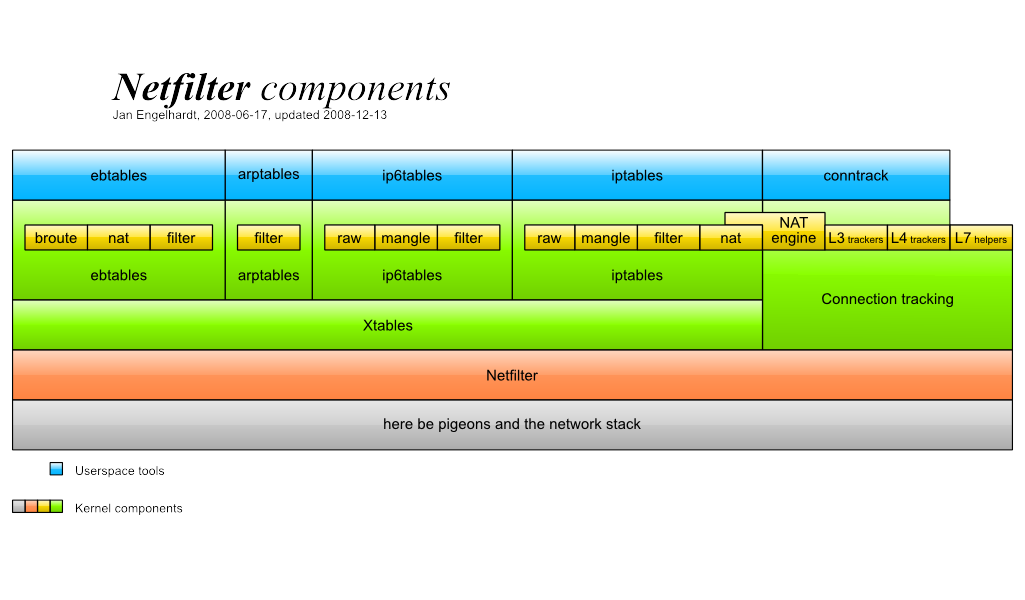
\includegraphics[width=1.3\textwidth]{xtables.png}
\caption{Netfilter Components}
\end{figure}
\footnote{From Jan Engelhardt-There is also extensive tutorial he wrote on 'Writing Netfilter Modules'
and the glue API following changes in kernel. The former has Creative Commons and the latter
GPL licenses. All can be found including the picture: http://jengelh.medozas.de/
}
\begin{itemize}
\item PREROUTING: All the packets, with no exceptions, hit this hook, which
is reached before the routing decision and after all the IP header sanity
checks are fulfilled. Port Address Translation (NAPT) and Redirection
that is, Destination Network Translation (DNAT), are implemented in
this hook. We can manipulate the data too.
\item LOCAL INPUT: All the packets going to the local machine reach this
\footnote{As opposed to forwarding traffic.}
hook. This is the last hook in the incoming path for the local machine
traffic.
\item FORWARD: Packets not going to the local machine (e.g., packets going
through the firewall) reach this hook. In a real system this will be how
ur module functions. All the packets are checked before forwarding them
to one of our clients in the network.
\item LOCAL OUTPUT: This is the first hook in the outgoing packet path.
Packets leaving the local machine always hit this hook.
\item POSTROUTING: This hook is implemented after the routing decision.
Source Network Address Translation (SNAT) is registered to this hook.
\end{itemize}
All the packets that leave the local machine reach this hook.
 This is a very powerful framework that is capable of doing much more than
we can possibly explain here. Then we have Xtables, which is shown on Figure5
3.1,on top of it as brick layer. It provides a simpler API so that we can extend
Netfilter functionalists by getting access to the packet we want in less complicated
way than Netfilter. So, our module is a plugin to this top layer. There is also a code
I wrote for userland interaction, this is at Iptables layer, which is mainly based on
boilerplate. This Section is very application specific and the appendix might have
been a better place.
\section{System Level Overview of the Module}
\subsection{Our Multicast Firewall.} The general concept of the filter was dis-
cussed before as 'prescriptive' problem statement. We have also said the way we
discover who the sources are is by snooping outgoing unicast traffic. Figure 3.2 tries
to show what we are trying to achieve. Darth is the bad guy and Alice is the good
source. The way we discovered Alice was good source is because someone inside
our network has been browsing alice.com. With this, we also expose our strongest
assumption in this thesis. That is, somehow that person/application is likely to
have the unicast contact of some form with the source. The Figure also shows how
Darth's traffic is dropped by our firewall and Alice's accepted.
\begin{flushleft}\begin{figure}[H]% Graphic for TeX using PGF
% Title: /home/bewketu/dynamicmcast.dia
% Creator: Dia v0.97
% CreationDate: Sat Aug  5 04:57:04 2017
% For: bewketu
% \usepackage{tikz}
% The following commands are not supported in PSTricks at present
% We define them conditionally, so when they are implemented,
% this pgf file will use them.
\ifx\du\undefined
  \newlength{\du}
\fi
\setlength{\du}{15\unitlength}
\begin{tikzpicture}
\pgftransformxscale{1.000000}
\pgftransformyscale{-1.000000}
\definecolor{dialinecolor}{rgb}{0.000000, 0.000000, 0.000000}
\pgfsetstrokecolor{dialinecolor}
\definecolor{dialinecolor}{rgb}{1.000000, 1.000000, 1.000000}
\pgfsetfillcolor{dialinecolor}
\pgfsetlinewidth{0.100000\du}
\pgfsetdash{}{0pt}
\pgfsetdash{}{0pt}
\pgfsetbuttcap
\pgfsetmiterjoin
\pgfsetlinewidth{0.001000\du}
\pgfsetbuttcap
\pgfsetmiterjoin
\pgfsetdash{}{0pt}
\definecolor{dialinecolor}{rgb}{1.000000, 0.913725, 0.666667}
\pgfsetfillcolor{dialinecolor}
\pgfpathmoveto{\pgfpoint{5.665017\du}{20.778453\du}}
\pgfpathlineto{\pgfpoint{5.663393\du}{20.710214\du}}
\pgfpathlineto{\pgfpoint{5.657709\du}{20.641976\du}}
\pgfpathlineto{\pgfpoint{5.647152\du}{20.574934\du}}
\pgfpathlineto{\pgfpoint{5.632536\du}{20.507893\du}}
\pgfpathlineto{\pgfpoint{5.613047\du}{20.439654\du}}
\pgfpathlineto{\pgfpoint{5.591122\du}{20.373810\du}}
\pgfpathlineto{\pgfpoint{5.563512\du}{20.310360\du}}
\pgfpathlineto{\pgfpoint{5.532655\du}{20.245712\du}}
\pgfpathlineto{\pgfpoint{5.499361\du}{20.183459\du}}
\pgfpathlineto{\pgfpoint{5.460383\du}{20.122404\du}}
\pgfpathlineto{\pgfpoint{5.418969\du}{20.063742\du}}
\pgfpathlineto{\pgfpoint{5.373495\du}{20.006278\du}}
\pgfpathlineto{\pgfpoint{5.323961\du}{19.951208\du}}
\pgfpathlineto{\pgfpoint{5.271990\du}{19.898533\du}}
\pgfpathlineto{\pgfpoint{5.216771\du}{19.847055\du}}
\pgfpathlineto{\pgfpoint{5.157492\du}{19.797971\du}}
\pgfpathlineto{\pgfpoint{5.096589\du}{19.751281\du}}
\pgfpathlineto{\pgfpoint{5.033250\du}{19.708183\du}}
\pgfpathlineto{\pgfpoint{4.966663\du}{19.668676\du}}
\pgfpathlineto{\pgfpoint{4.897640\du}{19.630367\du}}
\pgfpathlineto{\pgfpoint{4.826180\du}{19.594452\du}}
\pgfpathlineto{\pgfpoint{4.752285\du}{19.563325\du}}
\pgfpathlineto{\pgfpoint{4.678389\du}{19.534593\du}}
\pgfpathlineto{\pgfpoint{4.601245\du}{19.509453\du}}
\pgfpathlineto{\pgfpoint{4.522477\du}{19.487903\du}}
\pgfpathlineto{\pgfpoint{4.443709\du}{19.467552\du}}
\pgfpathlineto{\pgfpoint{4.363317\du}{19.451988\du}}
\pgfpathlineto{\pgfpoint{4.282113\du}{19.440017\du}}
\pgfpathlineto{\pgfpoint{4.200097\du}{19.431636\du}}
\pgfpathlineto{\pgfpoint{4.117269\du}{19.426848\du}}
\pgfpathlineto{\pgfpoint{4.034441\du}{19.424453\du}}
\pgfpathlineto{\pgfpoint{4.034441\du}{19.424453\du}}
\pgfpathlineto{\pgfpoint{3.952425\du}{19.426848\du}}
\pgfpathlineto{\pgfpoint{3.868785\du}{19.431636\du}}
\pgfpathlineto{\pgfpoint{3.787581\du}{19.440017\du}}
\pgfpathlineto{\pgfpoint{3.706377\du}{19.451988\du}}
\pgfpathlineto{\pgfpoint{3.625173\du}{19.467552\du}}
\pgfpathlineto{\pgfpoint{3.546405\du}{19.487903\du}}
\pgfpathlineto{\pgfpoint{3.467638\du}{19.509453\du}}
\pgfpathlineto{\pgfpoint{3.391306\du}{19.534593\du}}
\pgfpathlineto{\pgfpoint{3.315786\du}{19.563325\du}}
\pgfpathlineto{\pgfpoint{3.243515\du}{19.594452\du}}
\pgfpathlineto{\pgfpoint{3.172055\du}{19.630367\du}}
\pgfpathlineto{\pgfpoint{3.103844\du}{19.668676\du}}
\pgfpathlineto{\pgfpoint{3.036444\du}{19.708183\du}}
\pgfpathlineto{\pgfpoint{2.973105\du}{19.751281\du}}
\pgfpathlineto{\pgfpoint{2.911390\du}{19.797971\du}}
\pgfpathlineto{\pgfpoint{2.852111\du}{19.847055\du}}
\pgfpathlineto{\pgfpoint{2.796893\du}{19.898533\du}}
\pgfpathlineto{\pgfpoint{2.744922\du}{19.951208\du}}
\pgfpathlineto{\pgfpoint{2.695388\du}{20.006278\du}}
\pgfpathlineto{\pgfpoint{2.649913\du}{20.063742\du}}
\pgfpathlineto{\pgfpoint{2.608499\du}{20.122404\du}}
\pgfpathlineto{\pgfpoint{2.570333\du}{20.183459\du}}
\pgfpathlineto{\pgfpoint{2.535416\du}{20.245712\du}}
\pgfpathlineto{\pgfpoint{2.506182\du}{20.310360\du}}
\pgfpathlineto{\pgfpoint{2.478573\du}{20.373810\du}}
\pgfpathlineto{\pgfpoint{2.455836\du}{20.439654\du}}
\pgfpathlineto{\pgfpoint{2.436347\du}{20.507893\du}}
\pgfpathlineto{\pgfpoint{2.423354\du}{20.574934\du}}
\pgfpathlineto{\pgfpoint{2.412798\du}{20.641976\du}}
\pgfpathlineto{\pgfpoint{2.405489\du}{20.710214\du}}
\pgfpathlineto{\pgfpoint{2.404677\du}{20.778453\du}}
\pgfpathlineto{\pgfpoint{2.404677\du}{20.778453\du}}
\pgfpathlineto{\pgfpoint{2.405489\du}{20.846692\du}}
\pgfpathlineto{\pgfpoint{2.412798\du}{20.917325\du}}
\pgfpathlineto{\pgfpoint{2.423354\du}{20.984366\du}}
\pgfpathlineto{\pgfpoint{2.436347\du}{21.052605\du}}
\pgfpathlineto{\pgfpoint{2.455836\du}{21.119647\du}}
\pgfpathlineto{\pgfpoint{2.478573\du}{21.185491\du}}
\pgfpathlineto{\pgfpoint{2.506182\du}{21.248941\du}}
\pgfpathlineto{\pgfpoint{2.535416\du}{21.313588\du}}
\pgfpathlineto{\pgfpoint{2.570333\du}{21.375841\du}}
\pgfpathlineto{\pgfpoint{2.608499\du}{21.435700\du}}
\pgfpathlineto{\pgfpoint{2.649913\du}{21.495558\du}}
\pgfpathlineto{\pgfpoint{2.695388\du}{21.553022\du}}
\pgfpathlineto{\pgfpoint{2.744922\du}{21.606895\du}}
\pgfpathlineto{\pgfpoint{2.796893\du}{21.660768\du}}
\pgfpathlineto{\pgfpoint{2.852111\du}{21.712246\du}}
\pgfpathlineto{\pgfpoint{2.911390\du}{21.761330\du}}
\pgfpathlineto{\pgfpoint{2.973105\du}{21.806822\du}}
\pgfpathlineto{\pgfpoint{3.036444\du}{21.848723\du}}
\pgfpathlineto{\pgfpoint{3.103844\du}{21.891821\du}}
\pgfpathlineto{\pgfpoint{3.172055\du}{21.928934\du}}
\pgfpathlineto{\pgfpoint{3.243515\du}{21.963652\du}}
\pgfpathlineto{\pgfpoint{3.315786\du}{21.995975\du}}
\pgfpathlineto{\pgfpoint{3.391306\du}{22.024707\du}}
\pgfpathlineto{\pgfpoint{3.467638\du}{22.048651\du}}
\pgfpathlineto{\pgfpoint{3.546405\du}{22.071397\du}}
\pgfpathlineto{\pgfpoint{3.625173\du}{22.090552\du}}
\pgfpathlineto{\pgfpoint{3.706377\du}{22.106115\du}}
\pgfpathlineto{\pgfpoint{3.787581\du}{22.116890\du}}
\pgfpathlineto{\pgfpoint{3.868785\du}{22.127664\du}}
\pgfpathlineto{\pgfpoint{3.952425\du}{22.131256\du}}
\pgfpathlineto{\pgfpoint{4.034441\du}{22.132453\du}}
\pgfpathlineto{\pgfpoint{4.034441\du}{22.132453\du}}
\pgfpathlineto{\pgfpoint{4.117269\du}{22.131256\du}}
\pgfpathlineto{\pgfpoint{4.200097\du}{22.127664\du}}
\pgfpathlineto{\pgfpoint{4.282113\du}{22.116890\du}}
\pgfpathlineto{\pgfpoint{4.363317\du}{22.106115\du}}
\pgfpathlineto{\pgfpoint{4.443709\du}{22.090552\du}}
\pgfpathlineto{\pgfpoint{4.522477\du}{22.071397\du}}
\pgfpathlineto{\pgfpoint{4.601245\du}{22.048651\du}}
\pgfpathlineto{\pgfpoint{4.678389\du}{22.024707\du}}
\pgfpathlineto{\pgfpoint{4.752285\du}{21.995975\du}}
\pgfpathlineto{\pgfpoint{4.826180\du}{21.963652\du}}
\pgfpathlineto{\pgfpoint{4.897640\du}{21.928934\du}}
\pgfpathlineto{\pgfpoint{4.966663\du}{21.891821\du}}
\pgfpathlineto{\pgfpoint{5.033250\du}{21.848723\du}}
\pgfpathlineto{\pgfpoint{5.096589\du}{21.806822\du}}
\pgfpathlineto{\pgfpoint{5.157492\du}{21.761330\du}}
\pgfpathlineto{\pgfpoint{5.216771\du}{21.712246\du}}
\pgfpathlineto{\pgfpoint{5.271990\du}{21.660768\du}}
\pgfpathlineto{\pgfpoint{5.323961\du}{21.606895\du}}
\pgfpathlineto{\pgfpoint{5.373495\du}{21.553022\du}}
\pgfpathlineto{\pgfpoint{5.418969\du}{21.495558\du}}
\pgfpathlineto{\pgfpoint{5.460383\du}{21.435700\du}}
\pgfpathlineto{\pgfpoint{5.499361\du}{21.375841\du}}
\pgfpathlineto{\pgfpoint{5.532655\du}{21.313588\du}}
\pgfpathlineto{\pgfpoint{5.563512\du}{21.248941\du}}
\pgfpathlineto{\pgfpoint{5.591122\du}{21.185491\du}}
\pgfpathlineto{\pgfpoint{5.613047\du}{21.119647\du}}
\pgfpathlineto{\pgfpoint{5.632536\du}{21.052605\du}}
\pgfpathlineto{\pgfpoint{5.647152\du}{20.984366\du}}
\pgfpathlineto{\pgfpoint{5.657709\du}{20.917325\du}}
\pgfpathlineto{\pgfpoint{5.663393\du}{20.846692\du}}
\pgfpathlineto{\pgfpoint{5.665017\du}{20.778453\du}}
\pgfusepath{fill}
\pgfsetbuttcap
\pgfsetmiterjoin
\pgfsetdash{}{0pt}
\definecolor{dialinecolor}{rgb}{1.000000, 0.913725, 0.666667}
\pgfsetfillcolor{dialinecolor}
\pgfpathmoveto{\pgfpoint{3.109528\du}{21.489572\du}}
\pgfpathlineto{\pgfpoint{3.107904\du}{21.421334\du}}
\pgfpathlineto{\pgfpoint{3.102220\du}{21.353095\du}}
\pgfpathlineto{\pgfpoint{3.095723\du}{21.286053\du}}
\pgfpathlineto{\pgfpoint{3.084355\du}{21.217815\du}}
\pgfpathlineto{\pgfpoint{3.069738\du}{21.150773\du}}
\pgfpathlineto{\pgfpoint{3.051873\du}{21.084929\du}}
\pgfpathlineto{\pgfpoint{3.030760\du}{21.020282\du}}
\pgfpathlineto{\pgfpoint{3.008023\du}{20.956831\du}}
\pgfpathlineto{\pgfpoint{2.982038\du}{20.894579\du}}
\pgfpathlineto{\pgfpoint{2.952804\du}{20.833523\du}}
\pgfpathlineto{\pgfpoint{2.921135\du}{20.774862\du}}
\pgfpathlineto{\pgfpoint{2.886217\du}{20.717397\du}}
\pgfpathlineto{\pgfpoint{2.847239\du}{20.662328\du}}
\pgfpathlineto{\pgfpoint{2.807449\du}{20.607258\du}}
\pgfpathlineto{\pgfpoint{2.765223\du}{20.558174\du}}
\pgfpathlineto{\pgfpoint{2.719749\du}{20.509090\du}}
\pgfpathlineto{\pgfpoint{2.674275\du}{20.462400\du}}
\pgfpathlineto{\pgfpoint{2.623928\du}{20.419302\du}}
\pgfpathlineto{\pgfpoint{2.573582\du}{20.378598\du}}
\pgfpathlineto{\pgfpoint{2.519987\du}{20.341486\du}}
\pgfpathlineto{\pgfpoint{2.466392\du}{20.305571\du}}
\pgfpathlineto{\pgfpoint{2.410362\du}{20.274444\du}}
\pgfpathlineto{\pgfpoint{2.351895\du}{20.245712\du}}
\pgfpathlineto{\pgfpoint{2.293428\du}{20.220572\du}}
\pgfpathlineto{\pgfpoint{2.233337\du}{20.199023\du}}
\pgfpathlineto{\pgfpoint{2.172434\du}{20.178671\du}}
\pgfpathlineto{\pgfpoint{2.110719\du}{20.163108\du}}
\pgfpathlineto{\pgfpoint{2.048192\du}{20.152333\du}}
\pgfpathlineto{\pgfpoint{1.986477\du}{20.142756\du}}
\pgfpathlineto{\pgfpoint{1.923138\du}{20.137967\du}}
\pgfpathlineto{\pgfpoint{1.859799\du}{20.135573\du}}
\pgfpathlineto{\pgfpoint{1.859799\du}{20.135573\du}}
\pgfpathlineto{\pgfpoint{1.796460\du}{20.137967\du}}
\pgfpathlineto{\pgfpoint{1.733120\du}{20.142756\du}}
\pgfpathlineto{\pgfpoint{1.669781\du}{20.152333\du}}
\pgfpathlineto{\pgfpoint{1.608066\du}{20.163108\du}}
\pgfpathlineto{\pgfpoint{1.545539\du}{20.178671\du}}
\pgfpathlineto{\pgfpoint{1.484636\du}{20.199023\du}}
\pgfpathlineto{\pgfpoint{1.425357\du}{20.220572\du}}
\pgfpathlineto{\pgfpoint{1.366890\du}{20.245712\du}}
\pgfpathlineto{\pgfpoint{1.309236\du}{20.274444\du}}
\pgfpathlineto{\pgfpoint{1.253205\du}{20.305571\du}}
\pgfpathlineto{\pgfpoint{1.197986\du}{20.341486\du}}
\pgfpathlineto{\pgfpoint{1.146016\du}{20.378598\du}}
\pgfpathlineto{\pgfpoint{1.094045\du}{20.419302\du}}
\pgfpathlineto{\pgfpoint{1.045323\du}{20.462400\du}}
\pgfpathlineto{\pgfpoint{0.999036\du}{20.509090\du}}
\pgfpathlineto{\pgfpoint{0.953562\du}{20.558174\du}}
\pgfpathlineto{\pgfpoint{0.911336\du}{20.607258\du}}
\pgfpathlineto{\pgfpoint{0.870734\du}{20.662328\du}}
\pgfpathlineto{\pgfpoint{0.832568\du}{20.717397\du}}
\pgfpathlineto{\pgfpoint{0.798463\du}{20.774862\du}}
\pgfpathlineto{\pgfpoint{0.765981\du}{20.833523\du}}
\pgfpathlineto{\pgfpoint{0.737560\du}{20.894579\du}}
\pgfpathlineto{\pgfpoint{0.710762\du}{20.956831\du}}
\pgfpathlineto{\pgfpoint{0.687213\du}{21.020282\du}}
\pgfpathlineto{\pgfpoint{0.666912\du}{21.084929\du}}
\pgfpathlineto{\pgfpoint{0.649047\du}{21.150773\du}}
\pgfpathlineto{\pgfpoint{0.634430\du}{21.217815\du}}
\pgfpathlineto{\pgfpoint{0.623874\du}{21.286053\du}}
\pgfpathlineto{\pgfpoint{0.615754\du}{21.353095\du}}
\pgfpathlineto{\pgfpoint{0.610881\du}{21.421334\du}}
\pgfpathlineto{\pgfpoint{0.609257\du}{21.489572\du}}
\pgfpathlineto{\pgfpoint{0.609257\du}{21.489572\du}}
\pgfpathlineto{\pgfpoint{0.610881\du}{21.559008\du}}
\pgfpathlineto{\pgfpoint{0.615754\du}{21.628444\du}}
\pgfpathlineto{\pgfpoint{0.623874\du}{21.695486\du}}
\pgfpathlineto{\pgfpoint{0.634430\du}{21.762527\du}}
\pgfpathlineto{\pgfpoint{0.649047\du}{21.830766\du}}
\pgfpathlineto{\pgfpoint{0.666912\du}{21.894216\du}}
\pgfpathlineto{\pgfpoint{0.687213\du}{21.960060\du}}
\pgfpathlineto{\pgfpoint{0.710762\du}{22.024707\du}}
\pgfpathlineto{\pgfpoint{0.737560\du}{22.086960\du}}
\pgfpathlineto{\pgfpoint{0.765981\du}{22.146819\du}}
\pgfpathlineto{\pgfpoint{0.798463\du}{22.206677\du}}
\pgfpathlineto{\pgfpoint{0.832568\du}{22.264141\du}}
\pgfpathlineto{\pgfpoint{0.870734\du}{22.318014\du}}
\pgfpathlineto{\pgfpoint{0.911336\du}{22.371887\du}}
\pgfpathlineto{\pgfpoint{0.953562\du}{22.423365\du}}
\pgfpathlineto{\pgfpoint{0.999036\du}{22.470055\du}}
\pgfpathlineto{\pgfpoint{1.045323\du}{22.517942\du}}
\pgfpathlineto{\pgfpoint{1.094045\du}{22.559843\du}}
\pgfpathlineto{\pgfpoint{1.146016\du}{22.602941\du}}
\pgfpathlineto{\pgfpoint{1.197986\du}{22.640053\du}}
\pgfpathlineto{\pgfpoint{1.253205\du}{22.674771\du}}
\pgfpathlineto{\pgfpoint{1.309236\du}{22.707094\du}}
\pgfpathlineto{\pgfpoint{1.366890\du}{22.734629\du}}
\pgfpathlineto{\pgfpoint{1.425357\du}{22.759770\du}}
\pgfpathlineto{\pgfpoint{1.484636\du}{22.782516\du}}
\pgfpathlineto{\pgfpoint{1.545539\du}{22.801671\du}}
\pgfpathlineto{\pgfpoint{1.608066\du}{22.817234\du}}
\pgfpathlineto{\pgfpoint{1.669781\du}{22.828009\du}}
\pgfpathlineto{\pgfpoint{1.733120\du}{22.836389\du}}
\pgfpathlineto{\pgfpoint{1.796460\du}{22.842375\du}}
\pgfpathlineto{\pgfpoint{1.859799\du}{22.843572\du}}
\pgfpathlineto{\pgfpoint{1.859799\du}{22.843572\du}}
\pgfpathlineto{\pgfpoint{1.923138\du}{22.842375\du}}
\pgfpathlineto{\pgfpoint{1.986477\du}{22.836389\du}}
\pgfpathlineto{\pgfpoint{2.048192\du}{22.828009\du}}
\pgfpathlineto{\pgfpoint{2.110719\du}{22.817234\du}}
\pgfpathlineto{\pgfpoint{2.172434\du}{22.801671\du}}
\pgfpathlineto{\pgfpoint{2.233337\du}{22.782516\du}}
\pgfpathlineto{\pgfpoint{2.293428\du}{22.759770\du}}
\pgfpathlineto{\pgfpoint{2.351895\du}{22.734629\du}}
\pgfpathlineto{\pgfpoint{2.410362\du}{22.707094\du}}
\pgfpathlineto{\pgfpoint{2.466392\du}{22.674771\du}}
\pgfpathlineto{\pgfpoint{2.519987\du}{22.640053\du}}
\pgfpathlineto{\pgfpoint{2.573582\du}{22.602941\du}}
\pgfpathlineto{\pgfpoint{2.623928\du}{22.559843\du}}
\pgfpathlineto{\pgfpoint{2.674275\du}{22.517942\du}}
\pgfpathlineto{\pgfpoint{2.719749\du}{22.470055\du}}
\pgfpathlineto{\pgfpoint{2.765223\du}{22.423365\du}}
\pgfpathlineto{\pgfpoint{2.807449\du}{22.371887\du}}
\pgfpathlineto{\pgfpoint{2.847239\du}{22.318014\du}}
\pgfpathlineto{\pgfpoint{2.886217\du}{22.264141\du}}
\pgfpathlineto{\pgfpoint{2.921135\du}{22.206677\du}}
\pgfpathlineto{\pgfpoint{2.952804\du}{22.146819\du}}
\pgfpathlineto{\pgfpoint{2.982038\du}{22.086960\du}}
\pgfpathlineto{\pgfpoint{3.008023\du}{22.024707\du}}
\pgfpathlineto{\pgfpoint{3.030760\du}{21.960060\du}}
\pgfpathlineto{\pgfpoint{3.051873\du}{21.894216\du}}
\pgfpathlineto{\pgfpoint{3.069738\du}{21.830766\du}}
\pgfpathlineto{\pgfpoint{3.084355\du}{21.762527\du}}
\pgfpathlineto{\pgfpoint{3.095723\du}{21.695486\du}}
\pgfpathlineto{\pgfpoint{3.102220\du}{21.628444\du}}
\pgfpathlineto{\pgfpoint{3.107904\du}{21.559008\du}}
\pgfpathlineto{\pgfpoint{3.109528\du}{21.489572\du}}
\pgfusepath{fill}
\pgfsetbuttcap
\pgfsetmiterjoin
\pgfsetdash{}{0pt}
\definecolor{dialinecolor}{rgb}{1.000000, 0.913725, 0.666667}
\pgfsetfillcolor{dialinecolor}
\pgfpathmoveto{\pgfpoint{1.533359\du}{22.871107\du}}
\pgfpathlineto{\pgfpoint{1.532547\du}{22.816037\du}}
\pgfpathlineto{\pgfpoint{1.530110\du}{22.759770\du}}
\pgfpathlineto{\pgfpoint{1.524426\du}{22.704700\du}}
\pgfpathlineto{\pgfpoint{1.517118\du}{22.648433\du}}
\pgfpathlineto{\pgfpoint{1.506561\du}{22.594560\du}}
\pgfpathlineto{\pgfpoint{1.494381\du}{22.540688\du}}
\pgfpathlineto{\pgfpoint{1.481388\du}{22.488012\du}}
\pgfpathlineto{\pgfpoint{1.465959\du}{22.436534\du}}
\pgfpathlineto{\pgfpoint{1.448094\du}{22.385056\du}}
\pgfpathlineto{\pgfpoint{1.427793\du}{22.333577\du}}
\pgfpathlineto{\pgfpoint{1.405868\du}{22.288085\du}}
\pgfpathlineto{\pgfpoint{1.382319\du}{22.240198\du}}
\pgfpathlineto{\pgfpoint{1.357146\du}{22.193508\du}}
\pgfpathlineto{\pgfpoint{1.330349\du}{22.151607\du}}
\pgfpathlineto{\pgfpoint{1.301115\du}{22.109706\du}}
\pgfpathlineto{\pgfpoint{1.271070\du}{22.071397\du}}
\pgfpathlineto{\pgfpoint{1.240212\du}{22.033088\du}}
\pgfpathlineto{\pgfpoint{1.207731\du}{21.997172\du}}
\pgfpathlineto{\pgfpoint{1.172813\du}{21.964849\du}}
\pgfpathlineto{\pgfpoint{1.137083\du}{21.933722\du}}
\pgfpathlineto{\pgfpoint{1.100541\du}{21.904990\du}}
\pgfpathlineto{\pgfpoint{1.062375\du}{21.878653\du}}
\pgfpathlineto{\pgfpoint{1.024210\du}{21.854709\du}}
\pgfpathlineto{\pgfpoint{0.984420\du}{21.834357\du}}
\pgfpathlineto{\pgfpoint{0.943818\du}{21.816400\du}}
\pgfpathlineto{\pgfpoint{0.903216\du}{21.802034\du}}
\pgfpathlineto{\pgfpoint{0.861802\du}{21.787668\du}}
\pgfpathlineto{\pgfpoint{0.818764\du}{21.779287\du}}
\pgfpathlineto{\pgfpoint{0.776537\du}{21.772104\du}}
\pgfpathlineto{\pgfpoint{0.735123\du}{21.768513\du}}
\pgfpathlineto{\pgfpoint{0.692085\du}{21.766119\du}}
\pgfpathlineto{\pgfpoint{0.692085\du}{21.766119\du}}
\pgfpathlineto{\pgfpoint{0.649047\du}{21.768513\du}}
\pgfpathlineto{\pgfpoint{0.606009\du}{21.772104\du}}
\pgfpathlineto{\pgfpoint{0.563783\du}{21.779287\du}}
\pgfpathlineto{\pgfpoint{0.522369\du}{21.787668\du}}
\pgfpathlineto{\pgfpoint{0.480143\du}{21.802034\du}}
\pgfpathlineto{\pgfpoint{0.438729\du}{21.816400\du}}
\pgfpathlineto{\pgfpoint{0.398939\du}{21.834357\du}}
\pgfpathlineto{\pgfpoint{0.359961\du}{21.854709\du}}
\pgfpathlineto{\pgfpoint{0.320171\du}{21.878653\du}}
\pgfpathlineto{\pgfpoint{0.282005\du}{21.904990\du}}
\pgfpathlineto{\pgfpoint{0.245463\du}{21.933722\du}}
\pgfpathlineto{\pgfpoint{0.209734\du}{21.964849\du}}
\pgfpathlineto{\pgfpoint{0.175628\du}{21.997172\du}}
\pgfpathlineto{\pgfpoint{0.142334\du}{22.033088\du}}
\pgfpathlineto{\pgfpoint{0.111477\du}{22.071397\du}}
\pgfpathlineto{\pgfpoint{0.081431\du}{22.109706\du}}
\pgfpathlineto{\pgfpoint{0.053010\du}{22.151607\du}}
\pgfpathlineto{\pgfpoint{0.025401\du}{22.193508\du}}
\pgfpathlineto{\pgfpoint{0.000227\du}{22.240198\du}}
\pgfpathlineto{\pgfpoint{-0.023322\du}{22.288085\du}}
\pgfpathlineto{\pgfpoint{-0.045247\du}{22.333577\du}}
\pgfpathlineto{\pgfpoint{-0.063924\du}{22.385056\du}}
\pgfpathlineto{\pgfpoint{-0.081789\du}{22.436534\du}}
\pgfpathlineto{\pgfpoint{-0.097217\du}{22.488012\du}}
\pgfpathlineto{\pgfpoint{-0.111834\du}{22.540688\du}}
\pgfpathlineto{\pgfpoint{-0.124015\du}{22.594560\du}}
\pgfpathlineto{\pgfpoint{-0.132947\du}{22.648433\du}}
\pgfpathlineto{\pgfpoint{-0.140256\du}{22.704700\du}}
\pgfpathlineto{\pgfpoint{-0.146752\du}{22.759770\du}}
\pgfpathlineto{\pgfpoint{-0.150000\du}{22.816037\du}}
\pgfpathlineto{\pgfpoint{-0.150000\du}{22.871107\du}}
\pgfpathlineto{\pgfpoint{-0.150000\du}{22.871107\du}}
\pgfpathlineto{\pgfpoint{-0.150000\du}{22.926177\du}}
\pgfpathlineto{\pgfpoint{-0.146752\du}{22.983641\du}}
\pgfpathlineto{\pgfpoint{-0.140256\du}{23.037513\du}}
\pgfpathlineto{\pgfpoint{-0.132947\du}{23.093781\du}}
\pgfpathlineto{\pgfpoint{-0.124015\du}{23.148850\du}}
\pgfpathlineto{\pgfpoint{-0.111834\du}{23.201526\du}}
\pgfpathlineto{\pgfpoint{-0.097217\du}{23.254201\du}}
\pgfpathlineto{\pgfpoint{-0.081789\du}{23.305680\du}}
\pgfpathlineto{\pgfpoint{-0.063924\du}{23.358355\du}}
\pgfpathlineto{\pgfpoint{-0.045247\du}{23.408636\du}}
\pgfpathlineto{\pgfpoint{-0.023322\du}{23.455326\du}}
\pgfpathlineto{\pgfpoint{0.000227\du}{23.502016\du}}
\pgfpathlineto{\pgfpoint{0.025401\du}{23.547508\du}}
\pgfpathlineto{\pgfpoint{0.053010\du}{23.590606\du}}
\pgfpathlineto{\pgfpoint{0.081431\du}{23.632507\du}}
\pgfpathlineto{\pgfpoint{0.111477\du}{23.672014\du}}
\pgfpathlineto{\pgfpoint{0.142334\du}{23.710323\du}}
\pgfpathlineto{\pgfpoint{0.175628\du}{23.745041\du}}
\pgfpathlineto{\pgfpoint{0.209734\du}{23.777365\du}}
\pgfpathlineto{\pgfpoint{0.245463\du}{23.808491\du}}
\pgfpathlineto{\pgfpoint{0.282005\du}{23.837223\du}}
\pgfpathlineto{\pgfpoint{0.320171\du}{23.863561\du}}
\pgfpathlineto{\pgfpoint{0.359961\du}{23.887504\du}}
\pgfpathlineto{\pgfpoint{0.398939\du}{23.906659\du}}
\pgfpathlineto{\pgfpoint{0.438729\du}{23.925814\du}}
\pgfpathlineto{\pgfpoint{0.480143\du}{23.941377\du}}
\pgfpathlineto{\pgfpoint{0.522369\du}{23.954546\du}}
\pgfpathlineto{\pgfpoint{0.563783\du}{23.964123\du}}
\pgfpathlineto{\pgfpoint{0.606009\du}{23.970109\du}}
\pgfpathlineto{\pgfpoint{0.649047\du}{23.973701\du}}
\pgfpathlineto{\pgfpoint{0.692085\du}{23.976095\du}}
\pgfpathlineto{\pgfpoint{0.692085\du}{23.976095\du}}
\pgfpathlineto{\pgfpoint{0.735123\du}{23.973701\du}}
\pgfpathlineto{\pgfpoint{0.776537\du}{23.970109\du}}
\pgfpathlineto{\pgfpoint{0.818764\du}{23.964123\du}}
\pgfpathlineto{\pgfpoint{0.861802\du}{23.954546\du}}
\pgfpathlineto{\pgfpoint{0.903216\du}{23.941377\du}}
\pgfpathlineto{\pgfpoint{0.943818\du}{23.925814\du}}
\pgfpathlineto{\pgfpoint{0.984420\du}{23.906659\du}}
\pgfpathlineto{\pgfpoint{1.024210\du}{23.887504\du}}
\pgfpathlineto{\pgfpoint{1.062375\du}{23.863561\du}}
\pgfpathlineto{\pgfpoint{1.100541\du}{23.837223\du}}
\pgfpathlineto{\pgfpoint{1.137083\du}{23.808491\du}}
\pgfpathlineto{\pgfpoint{1.172813\du}{23.777365\du}}
\pgfpathlineto{\pgfpoint{1.207731\du}{23.745041\du}}
\pgfpathlineto{\pgfpoint{1.240212\du}{23.710323\du}}
\pgfpathlineto{\pgfpoint{1.271070\du}{23.672014\du}}
\pgfpathlineto{\pgfpoint{1.301115\du}{23.632507\du}}
\pgfpathlineto{\pgfpoint{1.330349\du}{23.590606\du}}
\pgfpathlineto{\pgfpoint{1.357146\du}{23.547508\du}}
\pgfpathlineto{\pgfpoint{1.382319\du}{23.502016\du}}
\pgfpathlineto{\pgfpoint{1.405868\du}{23.455326\du}}
\pgfpathlineto{\pgfpoint{1.427793\du}{23.408636\du}}
\pgfpathlineto{\pgfpoint{1.448094\du}{23.358355\du}}
\pgfpathlineto{\pgfpoint{1.465959\du}{23.305680\du}}
\pgfpathlineto{\pgfpoint{1.481388\du}{23.254201\du}}
\pgfpathlineto{\pgfpoint{1.494381\du}{23.201526\du}}
\pgfpathlineto{\pgfpoint{1.506561\du}{23.148850\du}}
\pgfpathlineto{\pgfpoint{1.517118\du}{23.093781\du}}
\pgfpathlineto{\pgfpoint{1.524426\du}{23.037513\du}}
\pgfpathlineto{\pgfpoint{1.530110\du}{22.983641\du}}
\pgfpathlineto{\pgfpoint{1.532547\du}{22.926177\du}}
\pgfpathlineto{\pgfpoint{1.533359\du}{22.871107\du}}
\pgfusepath{fill}
\pgfsetbuttcap
\pgfsetmiterjoin
\pgfsetdash{}{0pt}
\definecolor{dialinecolor}{rgb}{1.000000, 0.913725, 0.666667}
\pgfsetfillcolor{dialinecolor}
\pgfpathmoveto{\pgfpoint{2.892713\du}{23.935391\du}}
\pgfpathlineto{\pgfpoint{2.891901\du}{23.875533\du}}
\pgfpathlineto{\pgfpoint{2.886217\du}{23.814477\du}}
\pgfpathlineto{\pgfpoint{2.877285\du}{23.754619\du}}
\pgfpathlineto{\pgfpoint{2.866728\du}{23.694760\du}}
\pgfpathlineto{\pgfpoint{2.852111\du}{23.636099\du}}
\pgfpathlineto{\pgfpoint{2.835058\du}{23.577437\du}}
\pgfpathlineto{\pgfpoint{2.813133\du}{23.521170\du}}
\pgfpathlineto{\pgfpoint{2.790396\du}{23.463706\du}}
\pgfpathlineto{\pgfpoint{2.762787\du}{23.409833\du}}
\pgfpathlineto{\pgfpoint{2.733553\du}{23.357158\du}}
\pgfpathlineto{\pgfpoint{2.700260\du}{23.304482\du}}
\pgfpathlineto{\pgfpoint{2.665342\du}{23.254201\du}}
\pgfpathlineto{\pgfpoint{2.627988\du}{23.202723\du}}
\pgfpathlineto{\pgfpoint{2.587386\du}{23.156033\du}}
\pgfpathlineto{\pgfpoint{2.544348\du}{23.111738\du}}
\pgfpathlineto{\pgfpoint{2.498874\du}{23.068640\du}}
\pgfpathlineto{\pgfpoint{2.450964\du}{23.029133\du}}
\pgfpathlineto{\pgfpoint{2.400617\du}{22.990824\du}}
\pgfpathlineto{\pgfpoint{2.349459\du}{22.954909\du}}
\pgfpathlineto{\pgfpoint{2.295864\du}{22.921388\du}}
\pgfpathlineto{\pgfpoint{2.239833\du}{22.891459\du}}
\pgfpathlineto{\pgfpoint{2.182990\du}{22.862727\du}}
\pgfpathlineto{\pgfpoint{2.124524\du}{22.836389\du}}
\pgfpathlineto{\pgfpoint{2.065245\du}{22.813643\du}}
\pgfpathlineto{\pgfpoint{2.004342\du}{22.795685\du}}
\pgfpathlineto{\pgfpoint{1.941815\du}{22.778925\du}}
\pgfpathlineto{\pgfpoint{1.880100\du}{22.764559\du}}
\pgfpathlineto{\pgfpoint{1.816761\du}{22.752587\du}}
\pgfpathlineto{\pgfpoint{1.753421\du}{22.745404\du}}
\pgfpathlineto{\pgfpoint{1.689270\du}{22.741812\du}}
\pgfpathlineto{\pgfpoint{1.624307\du}{22.739418\du}}
\pgfpathlineto{\pgfpoint{1.624307\du}{22.739418\du}}
\pgfpathlineto{\pgfpoint{1.560156\du}{22.741812\du}}
\pgfpathlineto{\pgfpoint{1.496817\du}{22.745404\du}}
\pgfpathlineto{\pgfpoint{1.431854\du}{22.752587\du}}
\pgfpathlineto{\pgfpoint{1.369327\du}{22.764559\du}}
\pgfpathlineto{\pgfpoint{1.305987\du}{22.778925\du}}
\pgfpathlineto{\pgfpoint{1.245084\du}{22.795685\du}}
\pgfpathlineto{\pgfpoint{1.184181\du}{22.813643\du}}
\pgfpathlineto{\pgfpoint{1.124091\du}{22.836389\du}}
\pgfpathlineto{\pgfpoint{1.065624\du}{22.862727\du}}
\pgfpathlineto{\pgfpoint{1.009593\du}{22.891459\du}}
\pgfpathlineto{\pgfpoint{0.953562\du}{22.921388\du}}
\pgfpathlineto{\pgfpoint{0.899968\du}{22.954909\du}}
\pgfpathlineto{\pgfpoint{0.847997\du}{22.990824\du}}
\pgfpathlineto{\pgfpoint{0.798463\du}{23.029133\du}}
\pgfpathlineto{\pgfpoint{0.750552\du}{23.068640\du}}
\pgfpathlineto{\pgfpoint{0.705078\du}{23.111738\du}}
\pgfpathlineto{\pgfpoint{0.662040\du}{23.156033\du}}
\pgfpathlineto{\pgfpoint{0.621438\du}{23.202723\du}}
\pgfpathlineto{\pgfpoint{0.583272\du}{23.254201\du}}
\pgfpathlineto{\pgfpoint{0.548354\du}{23.304482\du}}
\pgfpathlineto{\pgfpoint{0.515061\du}{23.357158\du}}
\pgfpathlineto{\pgfpoint{0.485015\du}{23.409833\du}}
\pgfpathlineto{\pgfpoint{0.459030\du}{23.463706\du}}
\pgfpathlineto{\pgfpoint{0.435481\du}{23.521170\du}}
\pgfpathlineto{\pgfpoint{0.413556\du}{23.577437\du}}
\pgfpathlineto{\pgfpoint{0.395691\du}{23.636099\du}}
\pgfpathlineto{\pgfpoint{0.382698\du}{23.694760\du}}
\pgfpathlineto{\pgfpoint{0.370518\du}{23.754619\du}}
\pgfpathlineto{\pgfpoint{0.362397\du}{23.814477\du}}
\pgfpathlineto{\pgfpoint{0.357525\du}{23.875533\du}}
\pgfpathlineto{\pgfpoint{0.355901\du}{23.935391\du}}
\pgfpathlineto{\pgfpoint{0.355901\du}{23.935391\du}}
\pgfpathlineto{\pgfpoint{0.357525\du}{23.996447\du}}
\pgfpathlineto{\pgfpoint{0.362397\du}{24.056305\du}}
\pgfpathlineto{\pgfpoint{0.370518\du}{24.118558\du}}
\pgfpathlineto{\pgfpoint{0.382698\du}{24.178417\du}}
\pgfpathlineto{\pgfpoint{0.395691\du}{24.235881\du}}
\pgfpathlineto{\pgfpoint{0.413556\du}{24.293345\du}}
\pgfpathlineto{\pgfpoint{0.435481\du}{24.352007\du}}
\pgfpathlineto{\pgfpoint{0.459030\du}{24.408274\du}}
\pgfpathlineto{\pgfpoint{0.485015\du}{24.463343\du}}
\pgfpathlineto{\pgfpoint{0.515061\du}{24.517216\du}}
\pgfpathlineto{\pgfpoint{0.548354\du}{24.569892\du}}
\pgfpathlineto{\pgfpoint{0.583272\du}{24.620173\du}}
\pgfpathlineto{\pgfpoint{0.621438\du}{24.670454\du}}
\pgfpathlineto{\pgfpoint{0.662040\du}{24.718341\du}}
\pgfpathlineto{\pgfpoint{0.705078\du}{24.761439\du}}
\pgfpathlineto{\pgfpoint{0.750552\du}{24.803340\du}}
\pgfpathlineto{\pgfpoint{0.798463\du}{24.845241\du}}
\pgfpathlineto{\pgfpoint{0.847997\du}{24.883550\du}}
\pgfpathlineto{\pgfpoint{0.899968\du}{24.919465\du}}
\pgfpathlineto{\pgfpoint{0.953562\du}{24.952986\du}}
\pgfpathlineto{\pgfpoint{1.009593\du}{24.982915\du}}
\pgfpathlineto{\pgfpoint{1.065624\du}{25.011647\du}}
\pgfpathlineto{\pgfpoint{1.124091\du}{25.035591\du}}
\pgfpathlineto{\pgfpoint{1.184181\du}{25.058337\du}}
\pgfpathlineto{\pgfpoint{1.245084\du}{25.078689\du}}
\pgfpathlineto{\pgfpoint{1.305987\du}{25.094252\du}}
\pgfpathlineto{\pgfpoint{1.369327\du}{25.108618\du}}
\pgfpathlineto{\pgfpoint{1.431854\du}{25.120590\du}}
\pgfpathlineto{\pgfpoint{1.496817\du}{25.126576\du}}
\pgfpathlineto{\pgfpoint{1.560156\du}{25.132562\du}}
\pgfpathlineto{\pgfpoint{1.624307\du}{25.132562\du}}
\pgfpathlineto{\pgfpoint{1.624307\du}{25.132562\du}}
\pgfpathlineto{\pgfpoint{1.689270\du}{25.132562\du}}
\pgfpathlineto{\pgfpoint{1.753421\du}{25.126576\du}}
\pgfpathlineto{\pgfpoint{1.816761\du}{25.120590\du}}
\pgfpathlineto{\pgfpoint{1.880100\du}{25.108618\du}}
\pgfpathlineto{\pgfpoint{1.941815\du}{25.094252\du}}
\pgfpathlineto{\pgfpoint{2.004342\du}{25.078689\du}}
\pgfpathlineto{\pgfpoint{2.065245\du}{25.058337\du}}
\pgfpathlineto{\pgfpoint{2.124524\du}{25.035591\du}}
\pgfpathlineto{\pgfpoint{2.182990\du}{25.011647\du}}
\pgfpathlineto{\pgfpoint{2.239833\du}{24.982915\du}}
\pgfpathlineto{\pgfpoint{2.295864\du}{24.952986\du}}
\pgfpathlineto{\pgfpoint{2.349459\du}{24.919465\du}}
\pgfpathlineto{\pgfpoint{2.400617\du}{24.883550\du}}
\pgfpathlineto{\pgfpoint{2.450964\du}{24.845241\du}}
\pgfpathlineto{\pgfpoint{2.498874\du}{24.803340\du}}
\pgfpathlineto{\pgfpoint{2.544348\du}{24.761439\du}}
\pgfpathlineto{\pgfpoint{2.587386\du}{24.717143\du}}
\pgfpathlineto{\pgfpoint{2.627988\du}{24.668059\du}}
\pgfpathlineto{\pgfpoint{2.665342\du}{24.620173\du}}
\pgfpathlineto{\pgfpoint{2.700260\du}{24.569892\du}}
\pgfpathlineto{\pgfpoint{2.733553\du}{24.517216\du}}
\pgfpathlineto{\pgfpoint{2.762787\du}{24.463343\du}}
\pgfpathlineto{\pgfpoint{2.790396\du}{24.408274\du}}
\pgfpathlineto{\pgfpoint{2.813133\du}{24.352007\du}}
\pgfpathlineto{\pgfpoint{2.835058\du}{24.293345\du}}
\pgfpathlineto{\pgfpoint{2.852111\du}{24.235881\du}}
\pgfpathlineto{\pgfpoint{2.866728\du}{24.178417\du}}
\pgfpathlineto{\pgfpoint{2.877285\du}{24.118558\du}}
\pgfpathlineto{\pgfpoint{2.886217\du}{24.056305\du}}
\pgfpathlineto{\pgfpoint{2.891901\du}{23.996447\du}}
\pgfpathlineto{\pgfpoint{2.892713\du}{23.935391\du}}
\pgfusepath{fill}
\pgfsetbuttcap
\pgfsetmiterjoin
\pgfsetdash{}{0pt}
\definecolor{dialinecolor}{rgb}{1.000000, 0.913725, 0.666667}
\pgfsetfillcolor{dialinecolor}
\pgfpathmoveto{\pgfpoint{5.937051\du}{24.554328\du}}
\pgfpathlineto{\pgfpoint{5.933803\du}{24.482498\du}}
\pgfpathlineto{\pgfpoint{5.927306\du}{24.410668\du}}
\pgfpathlineto{\pgfpoint{5.914314\du}{24.338838\du}}
\pgfpathlineto{\pgfpoint{5.897261\du}{24.269402\du}}
\pgfpathlineto{\pgfpoint{5.876148\du}{24.197572\du}}
\pgfpathlineto{\pgfpoint{5.850162\du}{24.129333\du}}
\pgfpathlineto{\pgfpoint{5.819305\du}{24.061094\du}}
\pgfpathlineto{\pgfpoint{5.783575\du}{23.994053\du}}
\pgfpathlineto{\pgfpoint{5.742973\du}{23.928208\du}}
\pgfpathlineto{\pgfpoint{5.699123\du}{23.865955\du}}
\pgfpathlineto{\pgfpoint{5.649589\du}{23.803703\du}}
\pgfpathlineto{\pgfpoint{5.597618\du}{23.741450\du}}
\pgfpathlineto{\pgfpoint{5.540775\du}{23.685183\du}}
\pgfpathlineto{\pgfpoint{5.480684\du}{23.628916\du}}
\pgfpathlineto{\pgfpoint{5.414909\du}{23.575043\du}}
\pgfpathlineto{\pgfpoint{5.348322\du}{23.523565\du}}
\pgfpathlineto{\pgfpoint{5.276862\du}{23.476875\du}}
\pgfpathlineto{\pgfpoint{5.202155\du}{23.431383\du}}
\pgfpathlineto{\pgfpoint{5.125823\du}{23.388284\du}}
\pgfpathlineto{\pgfpoint{5.044619\du}{23.348778\du}}
\pgfpathlineto{\pgfpoint{4.962603\du}{23.312863\du}}
\pgfpathlineto{\pgfpoint{4.877339\du}{23.278145\du}}
\pgfpathlineto{\pgfpoint{4.790450\du}{23.248215\du}}
\pgfpathlineto{\pgfpoint{4.700314\du}{23.223075\du}}
\pgfpathlineto{\pgfpoint{4.610178\du}{23.199131\du}}
\pgfpathlineto{\pgfpoint{4.517605\du}{23.178780\du}}
\pgfpathlineto{\pgfpoint{4.425032\du}{23.163216\du}}
\pgfpathlineto{\pgfpoint{4.329212\du}{23.150048\du}}
\pgfpathlineto{\pgfpoint{4.235827\du}{23.141667\du}}
\pgfpathlineto{\pgfpoint{4.139194\du}{23.134484\du}}
\pgfpathlineto{\pgfpoint{4.043374\du}{23.134484\du}}
\pgfpathlineto{\pgfpoint{4.043374\du}{23.134484\du}}
\pgfpathlineto{\pgfpoint{3.947553\du}{23.134484\du}}
\pgfpathlineto{\pgfpoint{3.851732\du}{23.141667\du}}
\pgfpathlineto{\pgfpoint{3.756724\du}{23.150048\du}}
\pgfpathlineto{\pgfpoint{3.662527\du}{23.163216\du}}
\pgfpathlineto{\pgfpoint{3.568330\du}{23.178780\du}}
\pgfpathlineto{\pgfpoint{3.476570\du}{23.199131\du}}
\pgfpathlineto{\pgfpoint{3.385621\du}{23.223075\du}}
\pgfpathlineto{\pgfpoint{3.297109\du}{23.248215\du}}
\pgfpathlineto{\pgfpoint{3.208597\du}{23.278145\du}}
\pgfpathlineto{\pgfpoint{3.124957\du}{23.312863\du}}
\pgfpathlineto{\pgfpoint{3.041317\du}{23.348778\du}}
\pgfpathlineto{\pgfpoint{2.961737\du}{23.388284\du}}
\pgfpathlineto{\pgfpoint{2.884593\du}{23.431383\du}}
\pgfpathlineto{\pgfpoint{2.810697\du}{23.476875\du}}
\pgfpathlineto{\pgfpoint{2.739238\du}{23.523565\du}}
\pgfpathlineto{\pgfpoint{2.671026\du}{23.575043\du}}
\pgfpathlineto{\pgfpoint{2.606875\du}{23.628916\du}}
\pgfpathlineto{\pgfpoint{2.546784\du}{23.685183\du}}
\pgfpathlineto{\pgfpoint{2.489129\du}{23.741450\du}}
\pgfpathlineto{\pgfpoint{2.436347\du}{23.803703\du}}
\pgfpathlineto{\pgfpoint{2.387625\du}{23.865955\du}}
\pgfpathlineto{\pgfpoint{2.344586\du}{23.928208\du}}
\pgfpathlineto{\pgfpoint{2.303984\du}{23.994053\du}}
\pgfpathlineto{\pgfpoint{2.268255\du}{24.061094\du}}
\pgfpathlineto{\pgfpoint{2.237397\du}{24.129333\du}}
\pgfpathlineto{\pgfpoint{2.210600\du}{24.197572\du}}
\pgfpathlineto{\pgfpoint{2.189487\du}{24.269402\du}}
\pgfpathlineto{\pgfpoint{2.171622\du}{24.338838\du}}
\pgfpathlineto{\pgfpoint{2.159441\du}{24.410668\du}}
\pgfpathlineto{\pgfpoint{2.152133\du}{24.482498\du}}
\pgfpathlineto{\pgfpoint{2.149697\du}{24.554328\du}}
\pgfpathlineto{\pgfpoint{2.149697\du}{24.554328\du}}
\pgfpathlineto{\pgfpoint{2.152133\du}{24.624961\du}}
\pgfpathlineto{\pgfpoint{2.159441\du}{24.697989\du}}
\pgfpathlineto{\pgfpoint{2.171622\du}{24.769819\du}}
\pgfpathlineto{\pgfpoint{2.189487\du}{24.840452\du}}
\pgfpathlineto{\pgfpoint{2.210600\du}{24.911085\du}}
\pgfpathlineto{\pgfpoint{2.237397\du}{24.980521\du}}
\pgfpathlineto{\pgfpoint{2.268255\du}{25.047562\du}}
\pgfpathlineto{\pgfpoint{2.303984\du}{25.114604\du}}
\pgfpathlineto{\pgfpoint{2.344586\du}{25.180448\du}}
\pgfpathlineto{\pgfpoint{2.387625\du}{25.243898\du}}
\pgfpathlineto{\pgfpoint{2.436347\du}{25.304954\du}}
\pgfpathlineto{\pgfpoint{2.489129\du}{25.364813\du}}
\pgfpathlineto{\pgfpoint{2.546784\du}{25.423474\du}}
\pgfpathlineto{\pgfpoint{2.606875\du}{25.479741\du}}
\pgfpathlineto{\pgfpoint{2.671026\du}{25.533614\du}}
\pgfpathlineto{\pgfpoint{2.739238\du}{25.582698\du}}
\pgfpathlineto{\pgfpoint{2.810697\du}{25.632979\du}}
\pgfpathlineto{\pgfpoint{2.884593\du}{25.678471\du}}
\pgfpathlineto{\pgfpoint{2.961737\du}{25.720372\du}}
\pgfpathlineto{\pgfpoint{3.041317\du}{25.759879\du}}
\pgfpathlineto{\pgfpoint{3.124957\du}{25.796991\du}}
\pgfpathlineto{\pgfpoint{3.208597\du}{25.828118\du}}
\pgfpathlineto{\pgfpoint{3.297109\du}{25.859244\du}}
\pgfpathlineto{\pgfpoint{3.385621\du}{25.886779\du}}
\pgfpathlineto{\pgfpoint{3.476570\du}{25.910722\du}}
\pgfpathlineto{\pgfpoint{3.568330\du}{25.929877\du}}
\pgfpathlineto{\pgfpoint{3.662527\du}{25.946637\du}}
\pgfpathlineto{\pgfpoint{3.756724\du}{25.958609\du}}
\pgfpathlineto{\pgfpoint{3.851732\du}{25.968186\du}}
\pgfpathlineto{\pgfpoint{3.947553\du}{25.974172\du}}
\pgfpathlineto{\pgfpoint{4.043374\du}{25.975369\du}}
\pgfpathlineto{\pgfpoint{4.043374\du}{25.975369\du}}
\pgfpathlineto{\pgfpoint{4.139194\du}{25.974172\du}}
\pgfpathlineto{\pgfpoint{4.235827\du}{25.968186\du}}
\pgfpathlineto{\pgfpoint{4.329212\du}{25.958609\du}}
\pgfpathlineto{\pgfpoint{4.425032\du}{25.946637\du}}
\pgfpathlineto{\pgfpoint{4.517605\du}{25.929877\du}}
\pgfpathlineto{\pgfpoint{4.610178\du}{25.910722\du}}
\pgfpathlineto{\pgfpoint{4.700314\du}{25.886779\du}}
\pgfpathlineto{\pgfpoint{4.790450\du}{25.859244\du}}
\pgfpathlineto{\pgfpoint{4.877339\du}{25.828118\du}}
\pgfpathlineto{\pgfpoint{4.962603\du}{25.796991\du}}
\pgfpathlineto{\pgfpoint{5.044619\du}{25.759879\du}}
\pgfpathlineto{\pgfpoint{5.125823\du}{25.720372\du}}
\pgfpathlineto{\pgfpoint{5.202155\du}{25.678471\du}}
\pgfpathlineto{\pgfpoint{5.276862\du}{25.632979\du}}
\pgfpathlineto{\pgfpoint{5.348322\du}{25.582698\du}}
\pgfpathlineto{\pgfpoint{5.414909\du}{25.533614\du}}
\pgfpathlineto{\pgfpoint{5.480684\du}{25.479741\du}}
\pgfpathlineto{\pgfpoint{5.540775\du}{25.423474\du}}
\pgfpathlineto{\pgfpoint{5.597618\du}{25.364813\du}}
\pgfpathlineto{\pgfpoint{5.649589\du}{25.304954\du}}
\pgfpathlineto{\pgfpoint{5.699123\du}{25.243898\du}}
\pgfpathlineto{\pgfpoint{5.742973\du}{25.180448\du}}
\pgfpathlineto{\pgfpoint{5.783575\du}{25.114604\du}}
\pgfpathlineto{\pgfpoint{5.819305\du}{25.047562\du}}
\pgfpathlineto{\pgfpoint{5.850162\du}{24.980521\du}}
\pgfpathlineto{\pgfpoint{5.876148\du}{24.911085\du}}
\pgfpathlineto{\pgfpoint{5.897261\du}{24.840452\du}}
\pgfpathlineto{\pgfpoint{5.914314\du}{24.769819\du}}
\pgfpathlineto{\pgfpoint{5.927306\du}{24.697989\du}}
\pgfpathlineto{\pgfpoint{5.933803\du}{24.624961\du}}
\pgfpathlineto{\pgfpoint{5.937051\du}{24.554328\du}}
\pgfusepath{fill}
\pgfsetbuttcap
\pgfsetmiterjoin
\pgfsetdash{}{0pt}
\definecolor{dialinecolor}{rgb}{1.000000, 0.913725, 0.666667}
\pgfsetfillcolor{dialinecolor}
\pgfpathmoveto{\pgfpoint{6.987830\du}{21.278870\du}}
\pgfpathlineto{\pgfpoint{6.987018\du}{21.226195\du}}
\pgfpathlineto{\pgfpoint{6.982146\du}{21.172322\du}}
\pgfpathlineto{\pgfpoint{6.973214\du}{21.118449\du}}
\pgfpathlineto{\pgfpoint{6.963469\du}{21.065774\du}}
\pgfpathlineto{\pgfpoint{6.948852\du}{21.013098\du}}
\pgfpathlineto{\pgfpoint{6.932612\du}{20.961620\du}}
\pgfpathlineto{\pgfpoint{6.912311\du}{20.910142\du}}
\pgfpathlineto{\pgfpoint{6.888761\du}{20.858664\du}}
\pgfpathlineto{\pgfpoint{6.863588\du}{20.810777\du}}
\pgfpathlineto{\pgfpoint{6.835979\du}{20.761693\du}}
\pgfpathlineto{\pgfpoint{6.804309\du}{20.716200\du}}
\pgfpathlineto{\pgfpoint{6.770204\du}{20.670708\du}}
\pgfpathlineto{\pgfpoint{6.734474\du}{20.627610\du}}
\pgfpathlineto{\pgfpoint{6.694684\du}{20.584512\du}}
\pgfpathlineto{\pgfpoint{6.654082\du}{20.545005\du}}
\pgfpathlineto{\pgfpoint{6.609420\du}{20.507893\du}}
\pgfpathlineto{\pgfpoint{6.563945\du}{20.469583\du}}
\pgfpathlineto{\pgfpoint{6.516847\du}{20.437260\du}}
\pgfpathlineto{\pgfpoint{6.466501\du}{20.403739\du}}
\pgfpathlineto{\pgfpoint{6.415342\du}{20.373810\du}}
\pgfpathlineto{\pgfpoint{6.363372\du}{20.347472\du}}
\pgfpathlineto{\pgfpoint{6.308153\du}{20.322331\du}}
\pgfpathlineto{\pgfpoint{6.252122\du}{20.299585\du}}
\pgfpathlineto{\pgfpoint{6.195279\du}{20.280430\du}}
\pgfpathlineto{\pgfpoint{6.136812\du}{20.261276\du}}
\pgfpathlineto{\pgfpoint{6.078346\du}{20.246909\du}}
\pgfpathlineto{\pgfpoint{6.018255\du}{20.236135\du}}
\pgfpathlineto{\pgfpoint{5.958164\du}{20.225360\du}}
\pgfpathlineto{\pgfpoint{5.896449\du}{20.218177\du}}
\pgfpathlineto{\pgfpoint{5.835546\du}{20.215783\du}}
\pgfpathlineto{\pgfpoint{5.773831\du}{20.214586\du}}
\pgfpathlineto{\pgfpoint{5.773831\du}{20.214586\du}}
\pgfpathlineto{\pgfpoint{5.711304\du}{20.215783\du}}
\pgfpathlineto{\pgfpoint{5.650401\du}{20.218177\du}}
\pgfpathlineto{\pgfpoint{5.588686\du}{20.225360\du}}
\pgfpathlineto{\pgfpoint{5.528595\du}{20.236135\du}}
\pgfpathlineto{\pgfpoint{5.469316\du}{20.246909\du}}
\pgfpathlineto{\pgfpoint{5.410037\du}{20.261276\du}}
\pgfpathlineto{\pgfpoint{5.352382\du}{20.280430\du}}
\pgfpathlineto{\pgfpoint{5.294727\du}{20.299585\du}}
\pgfpathlineto{\pgfpoint{5.238696\du}{20.322331\du}}
\pgfpathlineto{\pgfpoint{5.183478\du}{20.347472\du}}
\pgfpathlineto{\pgfpoint{5.130695\du}{20.373810\du}}
\pgfpathlineto{\pgfpoint{5.080349\du}{20.403739\du}}
\pgfpathlineto{\pgfpoint{5.030002\du}{20.437260\du}}
\pgfpathlineto{\pgfpoint{4.982904\du}{20.469583\du}}
\pgfpathlineto{\pgfpoint{4.937430\du}{20.507893\du}}
\pgfpathlineto{\pgfpoint{4.893579\du}{20.545005\du}}
\pgfpathlineto{\pgfpoint{4.852165\du}{20.584512\du}}
\pgfpathlineto{\pgfpoint{4.812375\du}{20.627610\du}}
\pgfpathlineto{\pgfpoint{4.776646\du}{20.670708\du}}
\pgfpathlineto{\pgfpoint{4.743352\du}{20.716200\du}}
\pgfpathlineto{\pgfpoint{4.710871\du}{20.761693\du}}
\pgfpathlineto{\pgfpoint{4.683261\du}{20.810777\du}}
\pgfpathlineto{\pgfpoint{4.658088\du}{20.858664\du}}
\pgfpathlineto{\pgfpoint{4.634539\du}{20.910142\du}}
\pgfpathlineto{\pgfpoint{4.614238\du}{20.961620\du}}
\pgfpathlineto{\pgfpoint{4.597997\du}{21.013098\du}}
\pgfpathlineto{\pgfpoint{4.584192\du}{21.065774\du}}
\pgfpathlineto{\pgfpoint{4.572824\du}{21.118449\du}}
\pgfpathlineto{\pgfpoint{4.565515\du}{21.172322\du}}
\pgfpathlineto{\pgfpoint{4.561455\du}{21.226195\du}}
\pgfpathlineto{\pgfpoint{4.559019\du}{21.278870\du}}
\pgfpathlineto{\pgfpoint{4.559019\du}{21.278870\du}}
\pgfpathlineto{\pgfpoint{4.561455\du}{21.332743\du}}
\pgfpathlineto{\pgfpoint{4.565515\du}{21.385418\du}}
\pgfpathlineto{\pgfpoint{4.572824\du}{21.440488\du}}
\pgfpathlineto{\pgfpoint{4.584192\du}{21.493164\du}}
\pgfpathlineto{\pgfpoint{4.597997\du}{21.547036\du}}
\pgfpathlineto{\pgfpoint{4.614238\du}{21.598515\du}}
\pgfpathlineto{\pgfpoint{4.634539\du}{21.649993\du}}
\pgfpathlineto{\pgfpoint{4.658088\du}{21.697880\du}}
\pgfpathlineto{\pgfpoint{4.683261\du}{21.749358\du}}
\pgfpathlineto{\pgfpoint{4.710871\du}{21.796048\du}}
\pgfpathlineto{\pgfpoint{4.743352\du}{21.841540\du}}
\pgfpathlineto{\pgfpoint{4.776646\du}{21.888230\du}}
\pgfpathlineto{\pgfpoint{4.812375\du}{21.930131\du}}
\pgfpathlineto{\pgfpoint{4.852165\du}{21.973229\du}}
\pgfpathlineto{\pgfpoint{4.893579\du}{22.012736\du}}
\pgfpathlineto{\pgfpoint{4.937430\du}{22.051045\du}}
\pgfpathlineto{\pgfpoint{4.982904\du}{22.086960\du}}
\pgfpathlineto{\pgfpoint{5.030002\du}{22.121678\du}}
\pgfpathlineto{\pgfpoint{5.080349\du}{22.154002\du}}
\pgfpathlineto{\pgfpoint{5.130695\du}{22.183931\du}}
\pgfpathlineto{\pgfpoint{5.183478\du}{22.211466\du}}
\pgfpathlineto{\pgfpoint{5.238696\du}{22.236607\du}}
\pgfpathlineto{\pgfpoint{5.294727\du}{22.258156\du}}
\pgfpathlineto{\pgfpoint{5.352382\du}{22.278508\du}}
\pgfpathlineto{\pgfpoint{5.410037\du}{22.296465\du}}
\pgfpathlineto{\pgfpoint{5.469316\du}{22.310831\du}}
\pgfpathlineto{\pgfpoint{5.528595\du}{22.322803\du}}
\pgfpathlineto{\pgfpoint{5.588686\du}{22.333577\du}}
\pgfpathlineto{\pgfpoint{5.650401\du}{22.339563\du}}
\pgfpathlineto{\pgfpoint{5.711304\du}{22.341958\du}}
\pgfpathlineto{\pgfpoint{5.773831\du}{22.345549\du}}
\pgfpathlineto{\pgfpoint{5.773831\du}{22.345549\du}}
\pgfpathlineto{\pgfpoint{5.835546\du}{22.341958\du}}
\pgfpathlineto{\pgfpoint{5.896449\du}{22.339563\du}}
\pgfpathlineto{\pgfpoint{5.958164\du}{22.333577\du}}
\pgfpathlineto{\pgfpoint{6.018255\du}{22.322803\du}}
\pgfpathlineto{\pgfpoint{6.078346\du}{22.310831\du}}
\pgfpathlineto{\pgfpoint{6.136812\du}{22.296465\du}}
\pgfpathlineto{\pgfpoint{6.195279\du}{22.278508\du}}
\pgfpathlineto{\pgfpoint{6.252122\du}{22.258156\du}}
\pgfpathlineto{\pgfpoint{6.308153\du}{22.236607\du}}
\pgfpathlineto{\pgfpoint{6.363372\du}{22.211466\du}}
\pgfpathlineto{\pgfpoint{6.415342\du}{22.183931\du}}
\pgfpathlineto{\pgfpoint{6.466501\du}{22.154002\du}}
\pgfpathlineto{\pgfpoint{6.516847\du}{22.121678\du}}
\pgfpathlineto{\pgfpoint{6.563945\du}{22.086960\du}}
\pgfpathlineto{\pgfpoint{6.609420\du}{22.051045\du}}
\pgfpathlineto{\pgfpoint{6.654082\du}{22.012736\du}}
\pgfpathlineto{\pgfpoint{6.694684\du}{21.973229\du}}
\pgfpathlineto{\pgfpoint{6.734474\du}{21.930131\du}}
\pgfpathlineto{\pgfpoint{6.770204\du}{21.888230\du}}
\pgfpathlineto{\pgfpoint{6.804309\du}{21.841540\du}}
\pgfpathlineto{\pgfpoint{6.835979\du}{21.796048\du}}
\pgfpathlineto{\pgfpoint{6.863588\du}{21.749358\du}}
\pgfpathlineto{\pgfpoint{6.888761\du}{21.697880\du}}
\pgfpathlineto{\pgfpoint{6.912311\du}{21.649993\du}}
\pgfpathlineto{\pgfpoint{6.932612\du}{21.598515\du}}
\pgfpathlineto{\pgfpoint{6.948852\du}{21.547036\du}}
\pgfpathlineto{\pgfpoint{6.963469\du}{21.493164\du}}
\pgfpathlineto{\pgfpoint{6.973214\du}{21.440488\du}}
\pgfpathlineto{\pgfpoint{6.982146\du}{21.385418\du}}
\pgfpathlineto{\pgfpoint{6.987018\du}{21.332743\du}}
\pgfpathlineto{\pgfpoint{6.987830\du}{21.278870\du}}
\pgfusepath{fill}
\pgfsetbuttcap
\pgfsetmiterjoin
\pgfsetdash{}{0pt}
\definecolor{dialinecolor}{rgb}{1.000000, 0.913725, 0.666667}
\pgfsetfillcolor{dialinecolor}
\pgfpathmoveto{\pgfpoint{7.332135\du}{22.647236\du}}
\pgfpathlineto{\pgfpoint{7.329699\du}{22.594560\du}}
\pgfpathlineto{\pgfpoint{7.326451\du}{22.540688\du}}
\pgfpathlineto{\pgfpoint{7.318330\du}{22.486815\du}}
\pgfpathlineto{\pgfpoint{7.307774\du}{22.432942\du}}
\pgfpathlineto{\pgfpoint{7.293157\du}{22.379070\du}}
\pgfpathlineto{\pgfpoint{7.276916\du}{22.327591\du}}
\pgfpathlineto{\pgfpoint{7.257427\du}{22.277310\du}}
\pgfpathlineto{\pgfpoint{7.233878\du}{22.228226\du}}
\pgfpathlineto{\pgfpoint{7.208705\du}{22.177945\du}}
\pgfpathlineto{\pgfpoint{7.181096\du}{22.131256\du}}
\pgfpathlineto{\pgfpoint{7.149426\du}{22.084566\du}}
\pgfpathlineto{\pgfpoint{7.115320\du}{22.040271\du}}
\pgfpathlineto{\pgfpoint{7.080403\du}{21.997172\du}}
\pgfpathlineto{\pgfpoint{7.040613\du}{21.952877\du}}
\pgfpathlineto{\pgfpoint{7.000011\du}{21.914568\du}}
\pgfpathlineto{\pgfpoint{6.957785\du}{21.876258\du}}
\pgfpathlineto{\pgfpoint{6.912311\du}{21.839146\du}}
\pgfpathlineto{\pgfpoint{6.863588\du}{21.806822\du}}
\pgfpathlineto{\pgfpoint{6.815678\du}{21.773302\du}}
\pgfpathlineto{\pgfpoint{6.764519\du}{21.743372\du}}
\pgfpathlineto{\pgfpoint{6.712549\du}{21.717035\du}}
\pgfpathlineto{\pgfpoint{6.658142\du}{21.690697\du}}
\pgfpathlineto{\pgfpoint{6.602923\du}{21.669148\du}}
\pgfpathlineto{\pgfpoint{6.546081\du}{21.649993\du}}
\pgfpathlineto{\pgfpoint{6.487614\du}{21.630838\du}}
\pgfpathlineto{\pgfpoint{6.429147\du}{21.616472\du}}
\pgfpathlineto{\pgfpoint{6.369868\du}{21.604501\du}}
\pgfpathlineto{\pgfpoint{6.308965\du}{21.593726\du}}
\pgfpathlineto{\pgfpoint{6.248874\du}{21.588937\du}}
\pgfpathlineto{\pgfpoint{6.187971\du}{21.585346\du}}
\pgfpathlineto{\pgfpoint{6.127068\du}{21.582952\du}}
\pgfpathlineto{\pgfpoint{6.127068\du}{21.582952\du}}
\pgfpathlineto{\pgfpoint{6.065353\du}{21.585346\du}}
\pgfpathlineto{\pgfpoint{6.005262\du}{21.588937\du}}
\pgfpathlineto{\pgfpoint{5.944359\du}{21.593726\du}}
\pgfpathlineto{\pgfpoint{5.885080\du}{21.604501\du}}
\pgfpathlineto{\pgfpoint{5.825801\du}{21.616472\du}}
\pgfpathlineto{\pgfpoint{5.766522\du}{21.630838\du}}
\pgfpathlineto{\pgfpoint{5.708867\du}{21.649993\du}}
\pgfpathlineto{\pgfpoint{5.652837\du}{21.669148\du}}
\pgfpathlineto{\pgfpoint{5.596806\du}{21.690697\du}}
\pgfpathlineto{\pgfpoint{5.542399\du}{21.717035\du}}
\pgfpathlineto{\pgfpoint{5.490429\du}{21.743372\du}}
\pgfpathlineto{\pgfpoint{5.439270\du}{21.773302\du}}
\pgfpathlineto{\pgfpoint{5.389736\du}{21.806822\du}}
\pgfpathlineto{\pgfpoint{5.343450\du}{21.839146\du}}
\pgfpathlineto{\pgfpoint{5.297975\du}{21.876258\du}}
\pgfpathlineto{\pgfpoint{5.253313\du}{21.914568\du}}
\pgfpathlineto{\pgfpoint{5.212711\du}{21.952877\du}}
\pgfpathlineto{\pgfpoint{5.174545\du}{21.997172\du}}
\pgfpathlineto{\pgfpoint{5.139628\du}{22.040271\du}}
\pgfpathlineto{\pgfpoint{5.105522\du}{22.084566\du}}
\pgfpathlineto{\pgfpoint{5.074664\du}{22.131256\du}}
\pgfpathlineto{\pgfpoint{5.045431\du}{22.177945\du}}
\pgfpathlineto{\pgfpoint{5.020258\du}{22.228226\du}}
\pgfpathlineto{\pgfpoint{4.998333\du}{22.277310\du}}
\pgfpathlineto{\pgfpoint{4.978032\du}{22.327591\du}}
\pgfpathlineto{\pgfpoint{4.960167\du}{22.379070\du}}
\pgfpathlineto{\pgfpoint{4.947174\du}{22.432942\du}}
\pgfpathlineto{\pgfpoint{4.936618\du}{22.486815\du}}
\pgfpathlineto{\pgfpoint{4.928497\du}{22.540688\du}}
\pgfpathlineto{\pgfpoint{4.923625\du}{22.594560\du}}
\pgfpathlineto{\pgfpoint{4.922813\du}{22.647236\du}}
\pgfpathlineto{\pgfpoint{4.922813\du}{22.647236\du}}
\pgfpathlineto{\pgfpoint{4.923625\du}{22.699911\du}}
\pgfpathlineto{\pgfpoint{4.928497\du}{22.753784\du}}
\pgfpathlineto{\pgfpoint{4.936618\du}{22.808854\du}}
\pgfpathlineto{\pgfpoint{4.947174\du}{22.861529\du}}
\pgfpathlineto{\pgfpoint{4.960167\du}{22.915402\du}}
\pgfpathlineto{\pgfpoint{4.978032\du}{22.966880\du}}
\pgfpathlineto{\pgfpoint{4.998333\du}{23.018359\du}}
\pgfpathlineto{\pgfpoint{5.020258\du}{23.066246\du}}
\pgfpathlineto{\pgfpoint{5.045431\du}{23.116527\du}}
\pgfpathlineto{\pgfpoint{5.074664\du}{23.164414\du}}
\pgfpathlineto{\pgfpoint{5.105522\du}{23.209906\du}}
\pgfpathlineto{\pgfpoint{5.139628\du}{23.254201\du}}
\pgfpathlineto{\pgfpoint{5.174545\du}{23.298497\du}}
\pgfpathlineto{\pgfpoint{5.212711\du}{23.341595\du}}
\pgfpathlineto{\pgfpoint{5.253313\du}{23.381101\du}}
\pgfpathlineto{\pgfpoint{5.297975\du}{23.418214\du}}
\pgfpathlineto{\pgfpoint{5.343450\du}{23.455326\du}}
\pgfpathlineto{\pgfpoint{5.389736\du}{23.487650\du}}
\pgfpathlineto{\pgfpoint{5.439270\du}{23.521170\du}}
\pgfpathlineto{\pgfpoint{5.490429\du}{23.551100\du}}
\pgfpathlineto{\pgfpoint{5.542399\du}{23.577437\du}}
\pgfpathlineto{\pgfpoint{5.596806\du}{23.603775\du}}
\pgfpathlineto{\pgfpoint{5.652837\du}{23.626521\du}}
\pgfpathlineto{\pgfpoint{5.708867\du}{23.644479\du}}
\pgfpathlineto{\pgfpoint{5.766522\du}{23.663634\du}}
\pgfpathlineto{\pgfpoint{5.825801\du}{23.678000\du}}
\pgfpathlineto{\pgfpoint{5.885080\du}{23.689971\du}}
\pgfpathlineto{\pgfpoint{5.944359\du}{23.700746\du}}
\pgfpathlineto{\pgfpoint{6.005262\du}{23.706732\du}}
\pgfpathlineto{\pgfpoint{6.065353\du}{23.710323\du}}
\pgfpathlineto{\pgfpoint{6.127068\du}{23.711520\du}}
\pgfpathlineto{\pgfpoint{6.127068\du}{23.711520\du}}
\pgfpathlineto{\pgfpoint{6.187971\du}{23.710323\du}}
\pgfpathlineto{\pgfpoint{6.248874\du}{23.706732\du}}
\pgfpathlineto{\pgfpoint{6.308965\du}{23.700746\du}}
\pgfpathlineto{\pgfpoint{6.369868\du}{23.689971\du}}
\pgfpathlineto{\pgfpoint{6.429147\du}{23.678000\du}}
\pgfpathlineto{\pgfpoint{6.487614\du}{23.663634\du}}
\pgfpathlineto{\pgfpoint{6.546081\du}{23.644479\du}}
\pgfpathlineto{\pgfpoint{6.602923\du}{23.626521\du}}
\pgfpathlineto{\pgfpoint{6.658142\du}{23.603775\du}}
\pgfpathlineto{\pgfpoint{6.712549\du}{23.577437\du}}
\pgfpathlineto{\pgfpoint{6.764519\du}{23.551100\du}}
\pgfpathlineto{\pgfpoint{6.815678\du}{23.521170\du}}
\pgfpathlineto{\pgfpoint{6.863588\du}{23.487650\du}}
\pgfpathlineto{\pgfpoint{6.912311\du}{23.455326\du}}
\pgfpathlineto{\pgfpoint{6.957785\du}{23.418214\du}}
\pgfpathlineto{\pgfpoint{7.000011\du}{23.381101\du}}
\pgfpathlineto{\pgfpoint{7.040613\du}{23.341595\du}}
\pgfpathlineto{\pgfpoint{7.080403\du}{23.298497\du}}
\pgfpathlineto{\pgfpoint{7.115320\du}{23.254201\du}}
\pgfpathlineto{\pgfpoint{7.149426\du}{23.209906\du}}
\pgfpathlineto{\pgfpoint{7.181096\du}{23.164414\du}}
\pgfpathlineto{\pgfpoint{7.208705\du}{23.116527\du}}
\pgfpathlineto{\pgfpoint{7.233878\du}{23.066246\du}}
\pgfpathlineto{\pgfpoint{7.257427\du}{23.018359\du}}
\pgfpathlineto{\pgfpoint{7.276916\du}{22.966880\du}}
\pgfpathlineto{\pgfpoint{7.293157\du}{22.915402\du}}
\pgfpathlineto{\pgfpoint{7.307774\du}{22.861529\du}}
\pgfpathlineto{\pgfpoint{7.318330\du}{22.808854\du}}
\pgfpathlineto{\pgfpoint{7.326451\du}{22.753784\du}}
\pgfpathlineto{\pgfpoint{7.329699\du}{22.699911\du}}
\pgfpathlineto{\pgfpoint{7.332135\du}{22.647236\du}}
\pgfusepath{fill}
\pgfsetbuttcap
\pgfsetmiterjoin
\pgfsetdash{}{0pt}
\definecolor{dialinecolor}{rgb}{1.000000, 0.913725, 0.666667}
\pgfsetfillcolor{dialinecolor}
\pgfpathmoveto{\pgfpoint{7.096644\du}{23.778562\du}}
\pgfpathlineto{\pgfpoint{7.095019\du}{23.689971\du}}
\pgfpathlineto{\pgfpoint{7.090147\du}{23.602578\du}}
\pgfpathlineto{\pgfpoint{7.083651\du}{23.515184\du}}
\pgfpathlineto{\pgfpoint{7.073094\du}{23.426594\du}}
\pgfpathlineto{\pgfpoint{7.059290\du}{23.340398\du}}
\pgfpathlineto{\pgfpoint{7.042237\du}{23.254201\du}}
\pgfpathlineto{\pgfpoint{7.022748\du}{23.171597\du}}
\pgfpathlineto{\pgfpoint{6.999199\du}{23.088992\du}}
\pgfpathlineto{\pgfpoint{6.974026\du}{23.008781\du}}
\pgfpathlineto{\pgfpoint{6.947228\du}{22.930965\du}}
\pgfpathlineto{\pgfpoint{6.916371\du}{22.854346\du}}
\pgfpathlineto{\pgfpoint{6.882265\du}{22.780122\du}}
\pgfpathlineto{\pgfpoint{6.846535\du}{22.708292\du}}
\pgfpathlineto{\pgfpoint{6.807557\du}{22.640053\du}}
\pgfpathlineto{\pgfpoint{6.766955\du}{22.573011\du}}
\pgfpathlineto{\pgfpoint{6.724729\du}{22.511956\du}}
\pgfpathlineto{\pgfpoint{6.679255\du}{22.452097\du}}
\pgfpathlineto{\pgfpoint{6.632969\du}{22.397027\du}}
\pgfpathlineto{\pgfpoint{6.583434\du}{22.343155\du}}
\pgfpathlineto{\pgfpoint{6.533088\du}{22.295268\du}}
\pgfpathlineto{\pgfpoint{6.481117\du}{22.250973\du}}
\pgfpathlineto{\pgfpoint{6.428335\du}{22.210269\du}}
\pgfpathlineto{\pgfpoint{6.373116\du}{22.173157\du}}
\pgfpathlineto{\pgfpoint{6.317085\du}{22.138439\du}}
\pgfpathlineto{\pgfpoint{6.258618\du}{22.109706\du}}
\pgfpathlineto{\pgfpoint{6.200964\du}{22.086960\du}}
\pgfpathlineto{\pgfpoint{6.140873\du}{22.065411\du}}
\pgfpathlineto{\pgfpoint{6.081594\du}{22.049848\du}}
\pgfpathlineto{\pgfpoint{6.022315\du}{22.040271\du}}
\pgfpathlineto{\pgfpoint{5.962224\du}{22.033088\du}}
\pgfpathlineto{\pgfpoint{5.901321\du}{22.030693\du}}
\pgfpathlineto{\pgfpoint{5.901321\du}{22.030693\du}}
\pgfpathlineto{\pgfpoint{5.840418\du}{22.033088\du}}
\pgfpathlineto{\pgfpoint{5.780327\du}{22.040271\du}}
\pgfpathlineto{\pgfpoint{5.719424\du}{22.049848\du}}
\pgfpathlineto{\pgfpoint{5.660145\du}{22.065411\du}}
\pgfpathlineto{\pgfpoint{5.601678\du}{22.086960\du}}
\pgfpathlineto{\pgfpoint{5.542399\du}{22.109706\du}}
\pgfpathlineto{\pgfpoint{5.485557\du}{22.138439\du}}
\pgfpathlineto{\pgfpoint{5.429526\du}{22.173157\du}}
\pgfpathlineto{\pgfpoint{5.374307\du}{22.210269\du}}
\pgfpathlineto{\pgfpoint{5.319900\du}{22.250973\du}}
\pgfpathlineto{\pgfpoint{5.267930\du}{22.295268\du}}
\pgfpathlineto{\pgfpoint{5.217583\du}{22.343155\du}}
\pgfpathlineto{\pgfpoint{5.169673\du}{22.397027\du}}
\pgfpathlineto{\pgfpoint{5.121763\du}{22.452097\du}}
\pgfpathlineto{\pgfpoint{5.077100\du}{22.511956\du}}
\pgfpathlineto{\pgfpoint{5.034062\du}{22.573011\du}}
\pgfpathlineto{\pgfpoint{4.993460\du}{22.640053\du}}
\pgfpathlineto{\pgfpoint{4.955294\du}{22.708292\du}}
\pgfpathlineto{\pgfpoint{4.918753\du}{22.780122\du}}
\pgfpathlineto{\pgfpoint{4.886271\du}{22.854346\du}}
\pgfpathlineto{\pgfpoint{4.855414\du}{22.930965\du}}
\pgfpathlineto{\pgfpoint{4.826992\du}{23.008781\du}}
\pgfpathlineto{\pgfpoint{4.801819\du}{23.088992\du}}
\pgfpathlineto{\pgfpoint{4.779894\du}{23.171597\du}}
\pgfpathlineto{\pgfpoint{4.760405\du}{23.254201\du}}
\pgfpathlineto{\pgfpoint{4.743352\du}{23.340398\du}}
\pgfpathlineto{\pgfpoint{4.729547\du}{23.426594\du}}
\pgfpathlineto{\pgfpoint{4.718991\du}{23.515184\du}}
\pgfpathlineto{\pgfpoint{4.710871\du}{23.602578\du}}
\pgfpathlineto{\pgfpoint{4.705998\du}{23.689971\du}}
\pgfpathlineto{\pgfpoint{4.704374\du}{23.778562\du}}
\pgfpathlineto{\pgfpoint{4.704374\du}{23.778562\du}}
\pgfpathlineto{\pgfpoint{4.705998\du}{23.867153\du}}
\pgfpathlineto{\pgfpoint{4.710871\du}{23.956940\du}}
\pgfpathlineto{\pgfpoint{4.718991\du}{24.044334\du}}
\pgfpathlineto{\pgfpoint{4.729547\du}{24.130530\du}}
\pgfpathlineto{\pgfpoint{4.743352\du}{24.217923\du}}
\pgfpathlineto{\pgfpoint{4.760405\du}{24.301725\du}}
\pgfpathlineto{\pgfpoint{4.779894\du}{24.385527\du}}
\pgfpathlineto{\pgfpoint{4.801819\du}{24.468132\du}}
\pgfpathlineto{\pgfpoint{4.826992\du}{24.548342\du}}
\pgfpathlineto{\pgfpoint{4.855414\du}{24.628553\du}}
\pgfpathlineto{\pgfpoint{4.886271\du}{24.705172\du}}
\pgfpathlineto{\pgfpoint{4.918753\du}{24.778199\du}}
\pgfpathlineto{\pgfpoint{4.955294\du}{24.848832\du}}
\pgfpathlineto{\pgfpoint{4.993460\du}{24.917071\du}}
\pgfpathlineto{\pgfpoint{5.034062\du}{24.982915\du}}
\pgfpathlineto{\pgfpoint{5.077100\du}{25.047562\du}}
\pgfpathlineto{\pgfpoint{5.121763\du}{25.107421\du}}
\pgfpathlineto{\pgfpoint{5.169673\du}{25.162491\du}}
\pgfpathlineto{\pgfpoint{5.217583\du}{25.213969\du}}
\pgfpathlineto{\pgfpoint{5.267930\du}{25.263053\du}}
\pgfpathlineto{\pgfpoint{5.319900\du}{25.308546\du}}
\pgfpathlineto{\pgfpoint{5.374307\du}{25.349249\du}}
\pgfpathlineto{\pgfpoint{5.429526\du}{25.386362\du}}
\pgfpathlineto{\pgfpoint{5.485557\du}{25.419882\du}}
\pgfpathlineto{\pgfpoint{5.542399\du}{25.447417\du}}
\pgfpathlineto{\pgfpoint{5.601678\du}{25.472558\du}}
\pgfpathlineto{\pgfpoint{5.660145\du}{25.491713\du}}
\pgfpathlineto{\pgfpoint{5.719424\du}{25.507276\du}}
\pgfpathlineto{\pgfpoint{5.780327\du}{25.519248\du}}
\pgfpathlineto{\pgfpoint{5.840418\du}{25.526431\du}}
\pgfpathlineto{\pgfpoint{5.901321\du}{25.528825\du}}
\pgfpathlineto{\pgfpoint{5.901321\du}{25.528825\du}}
\pgfpathlineto{\pgfpoint{5.962224\du}{25.526431\du}}
\pgfpathlineto{\pgfpoint{6.022315\du}{25.519248\du}}
\pgfpathlineto{\pgfpoint{6.081594\du}{25.507276\du}}
\pgfpathlineto{\pgfpoint{6.140873\du}{25.491713\du}}
\pgfpathlineto{\pgfpoint{6.200964\du}{25.472558\du}}
\pgfpathlineto{\pgfpoint{6.258618\du}{25.447417\du}}
\pgfpathlineto{\pgfpoint{6.317085\du}{25.419882\du}}
\pgfpathlineto{\pgfpoint{6.373116\du}{25.386362\du}}
\pgfpathlineto{\pgfpoint{6.428335\du}{25.349249\du}}
\pgfpathlineto{\pgfpoint{6.481117\du}{25.308546\du}}
\pgfpathlineto{\pgfpoint{6.533088\du}{25.263053\du}}
\pgfpathlineto{\pgfpoint{6.583434\du}{25.213969\du}}
\pgfpathlineto{\pgfpoint{6.632969\du}{25.162491\du}}
\pgfpathlineto{\pgfpoint{6.679255\du}{25.107421\du}}
\pgfpathlineto{\pgfpoint{6.724729\du}{25.047562\du}}
\pgfpathlineto{\pgfpoint{6.766955\du}{24.982915\du}}
\pgfpathlineto{\pgfpoint{6.807557\du}{24.917071\du}}
\pgfpathlineto{\pgfpoint{6.846535\du}{24.848832\du}}
\pgfpathlineto{\pgfpoint{6.882265\du}{24.717143\du}}
\pgfpathlineto{\pgfpoint{6.916371\du}{24.705172\du}}
\pgfpathlineto{\pgfpoint{6.947228\du}{24.628553\du}}
\pgfpathlineto{\pgfpoint{6.974026\du}{24.548342\du}}
\pgfpathlineto{\pgfpoint{6.999199\du}{24.468132\du}}
\pgfpathlineto{\pgfpoint{7.022748\du}{24.385527\du}}
\pgfpathlineto{\pgfpoint{7.042237\du}{24.301725\du}}
\pgfpathlineto{\pgfpoint{7.059290\du}{24.217923\du}}
\pgfpathlineto{\pgfpoint{7.073094\du}{24.130530\du}}
\pgfpathlineto{\pgfpoint{7.083651\du}{24.044334\du}}
\pgfpathlineto{\pgfpoint{7.090147\du}{23.956940\du}}
\pgfpathlineto{\pgfpoint{7.095019\du}{23.867153\du}}
\pgfpathlineto{\pgfpoint{7.096644\du}{23.778562\du}}
\pgfusepath{fill}
\pgfsetbuttcap
\pgfsetmiterjoin
\pgfsetdash{}{0pt}
\definecolor{dialinecolor}{rgb}{1.000000, 0.913725, 0.666667}
\pgfsetfillcolor{dialinecolor}
\pgfpathmoveto{\pgfpoint{6.063729\du}{22.726249\du}}
\pgfpathlineto{\pgfpoint{6.060481\du}{22.637659\du}}
\pgfpathlineto{\pgfpoint{6.050736\du}{22.549068\du}}
\pgfpathlineto{\pgfpoint{6.035307\du}{22.460477\du}}
\pgfpathlineto{\pgfpoint{6.014194\du}{22.373084\du}}
\pgfpathlineto{\pgfpoint{5.986585\du}{22.288085\du}}
\pgfpathlineto{\pgfpoint{5.952479\du}{22.203086\du}}
\pgfpathlineto{\pgfpoint{5.912689\du}{22.118087\du}}
\pgfpathlineto{\pgfpoint{5.866403\du}{22.035482\du}}
\pgfpathlineto{\pgfpoint{5.816057\du}{21.954074\du}}
\pgfpathlineto{\pgfpoint{5.759214\du}{21.877455\du}}
\pgfpathlineto{\pgfpoint{5.695875\du}{21.800837\du}}
\pgfpathlineto{\pgfpoint{5.628476\du}{21.726612\du}}
\pgfpathlineto{\pgfpoint{5.555392\du}{21.654782\du}}
\pgfpathlineto{\pgfpoint{5.477436\du}{21.585346\du}}
\pgfpathlineto{\pgfpoint{5.394608\du}{21.519502\du}}
\pgfpathlineto{\pgfpoint{5.308532\du}{21.457249\du}}
\pgfpathlineto{\pgfpoint{5.216771\du}{21.397390\du}}
\pgfpathlineto{\pgfpoint{5.120951\du}{21.343517\du}}
\pgfpathlineto{\pgfpoint{5.022694\du}{21.289645\du}}
\pgfpathlineto{\pgfpoint{4.919565\du}{21.240561\du}}
\pgfpathlineto{\pgfpoint{4.813188\du}{21.196266\du}}
\pgfpathlineto{\pgfpoint{4.704374\du}{21.155562\du}}
\pgfpathlineto{\pgfpoint{4.593125\du}{21.118449\du}}
\pgfpathlineto{\pgfpoint{4.479439\du}{21.084929\du}}
\pgfpathlineto{\pgfpoint{4.362505\du}{21.056197\du}}
\pgfpathlineto{\pgfpoint{4.243948\du}{21.031056\du}}
\pgfpathlineto{\pgfpoint{4.124578\du}{21.013098\du}}
\pgfpathlineto{\pgfpoint{4.003584\du}{20.995141\du}}
\pgfpathlineto{\pgfpoint{3.881778\du}{20.985564\du}}
\pgfpathlineto{\pgfpoint{3.759160\du}{20.978381\du}}
\pgfpathlineto{\pgfpoint{3.634918\du}{20.977183\du}}
\pgfpathlineto{\pgfpoint{3.634918\du}{20.977183\du}}
\pgfpathlineto{\pgfpoint{3.512300\du}{20.978381\du}}
\pgfpathlineto{\pgfpoint{3.389682\du}{20.985564\du}}
\pgfpathlineto{\pgfpoint{3.267876\du}{20.995141\du}}
\pgfpathlineto{\pgfpoint{3.146070\du}{21.013098\du}}
\pgfpathlineto{\pgfpoint{3.026700\du}{21.031056\du}}
\pgfpathlineto{\pgfpoint{2.908142\du}{21.056197\du}}
\pgfpathlineto{\pgfpoint{2.792020\du}{21.084929\du}}
\pgfpathlineto{\pgfpoint{2.678335\du}{21.118449\du}}
\pgfpathlineto{\pgfpoint{2.565461\du}{21.155562\du}}
\pgfpathlineto{\pgfpoint{2.458272\du}{21.196266\du}}
\pgfpathlineto{\pgfpoint{2.351895\du}{21.240561\du}}
\pgfpathlineto{\pgfpoint{2.247954\du}{21.289645\du}}
\pgfpathlineto{\pgfpoint{2.148885\du}{21.343517\du}}
\pgfpathlineto{\pgfpoint{2.054688\du}{21.397390\du}}
\pgfpathlineto{\pgfpoint{1.962116\du}{21.457249\du}}
\pgfpathlineto{\pgfpoint{1.875227\du}{21.519502\du}}
\pgfpathlineto{\pgfpoint{1.794023\du}{21.585346\du}}
\pgfpathlineto{\pgfpoint{1.715256\du}{21.654782\du}}
\pgfpathlineto{\pgfpoint{1.642172\du}{21.726612\du}}
\pgfpathlineto{\pgfpoint{1.575585\du}{21.800837\du}}
\pgfpathlineto{\pgfpoint{1.512246\du}{21.877455\du}}
\pgfpathlineto{\pgfpoint{1.456215\du}{21.954074\du}}
\pgfpathlineto{\pgfpoint{1.405056\du}{22.035482\du}}
\pgfpathlineto{\pgfpoint{1.357958\du}{22.118087\du}}
\pgfpathlineto{\pgfpoint{1.318980\du}{22.203086\du}}
\pgfpathlineto{\pgfpoint{1.285686\du}{22.288085\du}}
\pgfpathlineto{\pgfpoint{1.256453\du}{22.373084\du}}
\pgfpathlineto{\pgfpoint{1.235340\du}{22.460477\du}}
\pgfpathlineto{\pgfpoint{1.219911\du}{22.549068\du}}
\pgfpathlineto{\pgfpoint{1.210167\du}{22.637659\du}}
\pgfpathlineto{\pgfpoint{1.207731\du}{22.726249\du}}
\pgfpathlineto{\pgfpoint{1.207731\du}{22.726249\du}}
\pgfpathlineto{\pgfpoint{1.210167\du}{22.813643\du}}
\pgfpathlineto{\pgfpoint{1.219911\du}{22.902233\du}}
\pgfpathlineto{\pgfpoint{1.235340\du}{22.990824\du}}
\pgfpathlineto{\pgfpoint{1.256453\du}{23.078217\du}}
\pgfpathlineto{\pgfpoint{1.285686\du}{23.164414\du}}
\pgfpathlineto{\pgfpoint{1.318980\du}{23.248215\du}}
\pgfpathlineto{\pgfpoint{1.357958\du}{23.333215\du}}
\pgfpathlineto{\pgfpoint{1.405056\du}{23.415819\du}}
\pgfpathlineto{\pgfpoint{1.456215\du}{23.497227\du}}
\pgfpathlineto{\pgfpoint{1.512246\du}{23.575043\du}}
\pgfpathlineto{\pgfpoint{1.575585\du}{23.650465\du}}
\pgfpathlineto{\pgfpoint{1.642172\du}{23.724689\du}}
\pgfpathlineto{\pgfpoint{1.715256\du}{23.796519\du}}
\pgfpathlineto{\pgfpoint{1.794023\du}{23.865955\du}}
\pgfpathlineto{\pgfpoint{1.875227\du}{23.931800\du}}
\pgfpathlineto{\pgfpoint{1.962116\du}{23.994053\du}}
\pgfpathlineto{\pgfpoint{2.054688\du}{24.053911\du}}
\pgfpathlineto{\pgfpoint{2.148885\du}{24.107784\du}}
\pgfpathlineto{\pgfpoint{2.247954\du}{24.162854\du}}
\pgfpathlineto{\pgfpoint{2.351895\du}{24.210740\du}}
\pgfpathlineto{\pgfpoint{2.458272\du}{24.255036\du}}
\pgfpathlineto{\pgfpoint{2.565461\du}{24.295740\du}}
\pgfpathlineto{\pgfpoint{2.678335\du}{24.332852\du}}
\pgfpathlineto{\pgfpoint{2.792020\du}{24.366373\du}}
\pgfpathlineto{\pgfpoint{2.908142\du}{24.395105\du}}
\pgfpathlineto{\pgfpoint{3.026700\du}{24.420245\du}}
\pgfpathlineto{\pgfpoint{3.146070\du}{24.438203\du}}
\pgfpathlineto{\pgfpoint{3.267876\du}{24.454963\du}}
\pgfpathlineto{\pgfpoint{3.389682\du}{24.465738\du}}
\pgfpathlineto{\pgfpoint{3.512300\du}{24.472921\du}}
\pgfpathlineto{\pgfpoint{3.634918\du}{24.474118\du}}
\pgfpathlineto{\pgfpoint{3.634918\du}{24.474118\du}}
\pgfpathlineto{\pgfpoint{3.759160\du}{24.472921\du}}
\pgfpathlineto{\pgfpoint{3.881778\du}{24.465738\du}}
\pgfpathlineto{\pgfpoint{4.003584\du}{24.454963\du}}
\pgfpathlineto{\pgfpoint{4.124578\du}{24.438203\du}}
\pgfpathlineto{\pgfpoint{4.243948\du}{24.420245\du}}
\pgfpathlineto{\pgfpoint{4.362505\du}{24.395105\du}}
\pgfpathlineto{\pgfpoint{4.479439\du}{24.366373\du}}
\pgfpathlineto{\pgfpoint{4.593125\du}{24.332852\du}}
\pgfpathlineto{\pgfpoint{4.704374\du}{24.295740\du}}
\pgfpathlineto{\pgfpoint{4.813188\du}{24.255036\du}}
\pgfpathlineto{\pgfpoint{4.919565\du}{24.210740\du}}
\pgfpathlineto{\pgfpoint{5.022694\du}{24.162854\du}}
\pgfpathlineto{\pgfpoint{5.120951\du}{24.107784\du}}
\pgfpathlineto{\pgfpoint{5.216771\du}{24.053911\du}}
\pgfpathlineto{\pgfpoint{5.308532\du}{23.994053\du}}
\pgfpathlineto{\pgfpoint{5.394608\du}{23.931800\du}}
\pgfpathlineto{\pgfpoint{5.477436\du}{23.865955\du}}
\pgfpathlineto{\pgfpoint{5.555392\du}{23.796519\du}}
\pgfpathlineto{\pgfpoint{5.628476\du}{23.724689\du}}
\pgfpathlineto{\pgfpoint{5.695875\du}{23.650465\du}}
\pgfpathlineto{\pgfpoint{5.759214\du}{23.575043\du}}
\pgfpathlineto{\pgfpoint{5.816057\du}{23.497227\du}}
\pgfpathlineto{\pgfpoint{5.866403\du}{23.415819\du}}
\pgfpathlineto{\pgfpoint{5.912689\du}{23.333215\du}}
\pgfpathlineto{\pgfpoint{5.952479\du}{23.248215\du}}
\pgfpathlineto{\pgfpoint{5.986585\du}{23.164414\du}}
\pgfpathlineto{\pgfpoint{6.014194\du}{23.078217\du}}
\pgfpathlineto{\pgfpoint{6.035307\du}{22.990824\du}}
\pgfpathlineto{\pgfpoint{6.050736\du}{22.902233\du}}
\pgfpathlineto{\pgfpoint{6.060481\du}{22.813643\du}}
\pgfpathlineto{\pgfpoint{6.063729\du}{22.726249\du}}
\pgfusepath{fill}
\pgfsetbuttcap
\pgfsetmiterjoin
\pgfsetdash{}{0pt}
\definecolor{dialinecolor}{rgb}{1.000000, 0.913725, 0.666667}
\pgfsetfillcolor{dialinecolor}
\pgfpathmoveto{\pgfpoint{4.053118\du}{20.767679\du}}
\pgfpathlineto{\pgfpoint{5.660145\du}{20.464794\du}}
\pgfpathlineto{\pgfpoint{5.639844\du}{20.397753\du}}
\pgfpathlineto{\pgfpoint{5.614671\du}{20.333106\du}}
\pgfpathlineto{\pgfpoint{5.587061\du}{20.267261\du}}
\pgfpathlineto{\pgfpoint{5.553768\du}{20.202614\du}}
\pgfpathlineto{\pgfpoint{5.518038\du}{20.140361\du}}
\pgfpathlineto{\pgfpoint{5.477436\du}{20.080503\du}}
\pgfpathlineto{\pgfpoint{5.435210\du}{20.020644\du}}
\pgfpathlineto{\pgfpoint{5.386488\du}{19.965574\du}}
\pgfpathlineto{\pgfpoint{5.336953\du}{19.909307\du}}
\pgfpathlineto{\pgfpoint{5.283359\du}{19.856632\du}}
\pgfpathlineto{\pgfpoint{5.225704\du}{19.806351\du}}
\pgfpathlineto{\pgfpoint{5.165613\du}{19.759661\du}}
\pgfpathlineto{\pgfpoint{5.102274\du}{19.714169\du}}
\pgfpathlineto{\pgfpoint{5.036498\du}{19.669873\du}}
\pgfpathlineto{\pgfpoint{4.968287\du}{19.630367\du}}
\pgfpathlineto{\pgfpoint{4.897640\du}{19.594452\du}}
\pgfpathlineto{\pgfpoint{4.826180\du}{19.558537\du}}
\pgfpathlineto{\pgfpoint{4.750660\du}{19.528607\du}}
\pgfpathlineto{\pgfpoint{4.674329\du}{19.502270\du}}
\pgfpathlineto{\pgfpoint{4.597185\du}{19.475932\du}}
\pgfpathlineto{\pgfpoint{4.516793\du}{19.454383\du}}
\pgfpathlineto{\pgfpoint{4.436401\du}{19.437622\du}}
\pgfpathlineto{\pgfpoint{4.355197\du}{19.422059\du}}
\pgfpathlineto{\pgfpoint{4.273181\du}{19.412482\du}}
\pgfpathlineto{\pgfpoint{4.190353\du}{19.405299\du}}
\pgfpathlineto{\pgfpoint{4.106713\du}{19.400510\du}}
\pgfpathlineto{\pgfpoint{4.023885\du}{19.400510\du}}
\pgfpathlineto{\pgfpoint{3.940245\du}{19.401707\du}}
\pgfpathlineto{\pgfpoint{3.856605\du}{19.408890\du}}
\pgfpathlineto{\pgfpoint{3.775401\du}{19.419665\du}}
\pgfpathlineto{\pgfpoint{3.693385\du}{19.431636\du}}
\pgfpathlineto{\pgfpoint{3.612181\du}{19.450791\du}}
\pgfpathlineto{\pgfpoint{3.531789\du}{19.468749\du}}
\pgfpathlineto{\pgfpoint{3.453021\du}{19.493889\du}}
\pgfpathlineto{\pgfpoint{3.376689\du}{19.520227\du}}
\pgfpathlineto{\pgfpoint{3.301981\du}{19.550156\du}}
\pgfpathlineto{\pgfpoint{3.228086\du}{19.583677\du}}
\pgfpathlineto{\pgfpoint{3.156626\du}{19.618395\du}}
\pgfpathlineto{\pgfpoint{3.089227\du}{19.659099\du}}
\pgfpathlineto{\pgfpoint{3.022640\du}{19.699803\du}}
\pgfpathlineto{\pgfpoint{2.958489\du}{19.744098\du}}
\pgfpathlineto{\pgfpoint{2.897586\du}{19.790788\du}}
\pgfpathlineto{\pgfpoint{2.839931\du}{19.841069\du}}
\pgfpathlineto{\pgfpoint{2.785524\du}{19.893744\du}}
\pgfpathlineto{\pgfpoint{2.733553\du}{19.946420\du}}
\pgfpathlineto{\pgfpoint{2.684831\du}{20.005081\du}}
\pgfpathlineto{\pgfpoint{2.639357\du}{20.062545\du}}
\pgfpathlineto{\pgfpoint{2.597943\du}{20.123601\du}}
\pgfpathlineto{\pgfpoint{2.562213\du}{20.184657\du}}
\pgfpathlineto{\pgfpoint{2.527295\du}{20.246909\du}}
\pgfpathlineto{\pgfpoint{2.497250\du}{20.312754\du}}
\pgfpathlineto{\pgfpoint{2.472077\du}{20.378598\du}}
\pgfpathlineto{\pgfpoint{2.450964\du}{20.445640\du}}
\pgfpathlineto{\pgfpoint{2.433099\du}{20.512681\du}}
\pgfpathlineto{\pgfpoint{4.053118\du}{20.767679\du}}
\pgfusepath{fill}
\pgfsetbuttcap
\pgfsetmiterjoin
\pgfsetdash{}{0pt}
\definecolor{dialinecolor}{rgb}{0.501961, 0.364706, 0.000000}
\pgfsetstrokecolor{dialinecolor}
\pgfpathmoveto{\pgfpoint{5.660145\du}{20.462400\du}}
\pgfpathlineto{\pgfpoint{5.639032\du}{20.395359\du}}
\pgfpathlineto{\pgfpoint{5.614671\du}{20.329514\du}}
\pgfpathlineto{\pgfpoint{5.586249\du}{20.264867\du}}
\pgfpathlineto{\pgfpoint{5.553768\du}{20.201417\du}}
\pgfpathlineto{\pgfpoint{5.516414\du}{20.139164\du}}
\pgfpathlineto{\pgfpoint{5.476624\du}{20.079306\du}}
\pgfpathlineto{\pgfpoint{5.433586\du}{20.020644\du}}
\pgfpathlineto{\pgfpoint{5.384864\du}{19.961983\du}}
\pgfpathlineto{\pgfpoint{5.334517\du}{19.909307\du}}
\pgfpathlineto{\pgfpoint{5.282547\du}{19.856632\du}}
\pgfpathlineto{\pgfpoint{5.224080\du}{19.803956\du}}
\pgfpathlineto{\pgfpoint{5.165613\du}{19.757267\du}}
\pgfpathlineto{\pgfpoint{5.101462\du}{19.711774\du}}
\pgfpathlineto{\pgfpoint{5.035686\du}{19.669873\du}}
\pgfpathlineto{\pgfpoint{4.968287\du}{19.629170\du}}
\pgfpathlineto{\pgfpoint{4.897640\du}{19.593254\du}}
\pgfpathlineto{\pgfpoint{4.825368\du}{19.558537\du}}
\pgfpathlineto{\pgfpoint{4.749848\du}{19.527410\du}}
\pgfpathlineto{\pgfpoint{4.673517\du}{19.498678\du}}
\pgfpathlineto{\pgfpoint{4.597185\du}{19.474735\du}}
\pgfpathlineto{\pgfpoint{4.516793\du}{19.454383\du}}
\pgfpathlineto{\pgfpoint{4.435589\du}{19.437622\du}}
\pgfpathlineto{\pgfpoint{4.354385\du}{19.422059\du}}
\pgfpathlineto{\pgfpoint{4.272369\du}{19.412482\du}}
\pgfpathlineto{\pgfpoint{4.190353\du}{19.405299\du}}
\pgfpathlineto{\pgfpoint{4.105901\du}{19.400510\du}}
\pgfpathlineto{\pgfpoint{4.023073\du}{19.400510\du}}
\pgfpathlineto{\pgfpoint{3.940245\du}{19.401707\du}}
\pgfpathlineto{\pgfpoint{3.857417\du}{19.408890\du}}
\pgfpathlineto{\pgfpoint{3.774589\du}{19.419665\du}}
\pgfpathlineto{\pgfpoint{3.693385\du}{19.431636\du}}
\pgfpathlineto{\pgfpoint{3.612181\du}{19.449594\du}}
\pgfpathlineto{\pgfpoint{3.532601\du}{19.468749\du}}
\pgfpathlineto{\pgfpoint{3.454645\du}{19.493889\du}}
\pgfpathlineto{\pgfpoint{3.376689\du}{19.520227\du}}
\pgfpathlineto{\pgfpoint{3.302793\du}{19.550156\du}}
\pgfpathlineto{\pgfpoint{3.228898\du}{19.583677\du}}
\pgfpathlineto{\pgfpoint{3.158250\du}{19.617198\du}}
\pgfpathlineto{\pgfpoint{3.089227\du}{19.656705\du}}
\pgfpathlineto{\pgfpoint{3.023452\du}{19.699803\du}}
\pgfpathlineto{\pgfpoint{2.959301\du}{19.744098\du}}
\pgfpathlineto{\pgfpoint{2.898398\du}{19.789590\du}}
\pgfpathlineto{\pgfpoint{2.840743\du}{19.841069\du}}
\pgfpathlineto{\pgfpoint{2.785524\du}{19.892547\du}}
\pgfpathlineto{\pgfpoint{2.733553\du}{19.946420\du}}
\pgfpathlineto{\pgfpoint{2.684831\du}{20.003884\du}}
\pgfpathlineto{\pgfpoint{2.640981\du}{20.060151\du}}
\pgfpathlineto{\pgfpoint{2.598755\du}{20.120009\du}}
\pgfpathlineto{\pgfpoint{2.562213\du}{20.183459\du}}
\pgfpathlineto{\pgfpoint{2.528107\du}{20.245712\du}}
\pgfpathlineto{\pgfpoint{2.498874\du}{20.310360\du}}
\pgfpathlineto{\pgfpoint{2.472077\du}{20.375007\du}}
\pgfpathlineto{\pgfpoint{2.450964\du}{20.442048\du}}
\pgfpathlineto{\pgfpoint{2.433911\du}{20.509090\du}}
\pgfusepath{stroke}
\pgfsetbuttcap
\pgfsetmiterjoin
\pgfsetdash{}{0pt}
\definecolor{dialinecolor}{rgb}{1.000000, 0.913725, 0.666667}
\pgfsetfillcolor{dialinecolor}
\pgfpathmoveto{\pgfpoint{1.867919\du}{21.477601\du}}
\pgfpathlineto{\pgfpoint{2.678335\du}{20.427682\du}}
\pgfpathlineto{\pgfpoint{2.627988\du}{20.386978\du}}
\pgfpathlineto{\pgfpoint{2.575206\du}{20.345077\du}}
\pgfpathlineto{\pgfpoint{2.521611\du}{20.306768\du}}
\pgfpathlineto{\pgfpoint{2.466392\du}{20.274444\du}}
\pgfpathlineto{\pgfpoint{2.410362\du}{20.242121\du}}
\pgfpathlineto{\pgfpoint{2.351895\du}{20.214586\du}}
\pgfpathlineto{\pgfpoint{2.291804\du}{20.188248\du}}
\pgfpathlineto{\pgfpoint{2.232525\du}{20.167896\du}}
\pgfpathlineto{\pgfpoint{2.169998\du}{20.148742\du}}
\pgfpathlineto{\pgfpoint{2.108283\du}{20.133178\du}}
\pgfpathlineto{\pgfpoint{2.044944\du}{20.123601\du}}
\pgfpathlineto{\pgfpoint{1.981605\du}{20.115221\du}}
\pgfpathlineto{\pgfpoint{1.918265\du}{20.110432\du}}
\pgfpathlineto{\pgfpoint{1.854926\du}{20.110432\du}}
\pgfpathlineto{\pgfpoint{1.790775\du}{20.110432\du}}
\pgfpathlineto{\pgfpoint{1.727436\du}{20.118812\du}}
\pgfpathlineto{\pgfpoint{1.664097\du}{20.125995\du}}
\pgfpathlineto{\pgfpoint{1.601570\du}{20.140361\du}}
\pgfpathlineto{\pgfpoint{1.539855\du}{20.155925\du}}
\pgfpathlineto{\pgfpoint{1.478952\du}{20.177474\du}}
\pgfpathlineto{\pgfpoint{1.418049\du}{20.200220\du}}
\pgfpathlineto{\pgfpoint{1.359582\du}{20.225360\du}}
\pgfpathlineto{\pgfpoint{1.301115\du}{20.255290\du}}
\pgfpathlineto{\pgfpoint{1.245084\du}{20.288810\du}}
\pgfpathlineto{\pgfpoint{1.190678\du}{20.324726\du}}
\pgfpathlineto{\pgfpoint{1.138707\du}{20.363035\du}}
\pgfpathlineto{\pgfpoint{1.086737\du}{20.403739\du}}
\pgfpathlineto{\pgfpoint{1.038014\du}{20.448034\du}}
\pgfpathlineto{\pgfpoint{0.991728\du}{20.494724\du}}
\pgfpathlineto{\pgfpoint{0.946254\du}{20.545005\du}}
\pgfpathlineto{\pgfpoint{0.904028\du}{20.597680\du}}
\pgfpathlineto{\pgfpoint{0.865050\du}{20.650356\du}}
\pgfpathlineto{\pgfpoint{0.827696\du}{20.707820\du}}
\pgfpathlineto{\pgfpoint{0.793590\du}{20.766481\du}}
\pgfpathlineto{\pgfpoint{0.761109\du}{20.826340\du}}
\pgfpathlineto{\pgfpoint{0.732687\du}{20.887396\du}}
\pgfpathlineto{\pgfpoint{0.705890\du}{20.949648\du}}
\pgfpathlineto{\pgfpoint{0.683153\du}{21.015493\du}}
\pgfpathlineto{\pgfpoint{0.662852\du}{21.081337\du}}
\pgfpathlineto{\pgfpoint{0.646611\du}{21.148379\du}}
\pgfpathlineto{\pgfpoint{0.633618\du}{21.215420\du}}
\pgfpathlineto{\pgfpoint{0.622250\du}{21.283659\du}}
\pgfpathlineto{\pgfpoint{0.614129\du}{21.353095\du}}
\pgfpathlineto{\pgfpoint{0.610881\du}{21.421334\du}}
\pgfpathlineto{\pgfpoint{0.609257\du}{21.489572\du}}
\pgfpathlineto{\pgfpoint{0.611693\du}{21.560205\du}}
\pgfpathlineto{\pgfpoint{0.616566\du}{21.629641\du}}
\pgfpathlineto{\pgfpoint{0.626310\du}{21.696683\du}}
\pgfpathlineto{\pgfpoint{1.867919\du}{21.477601\du}}
\pgfusepath{fill}
\pgfsetbuttcap
\pgfsetmiterjoin
\pgfsetdash{}{0pt}
\definecolor{dialinecolor}{rgb}{0.501961, 0.364706, 0.000000}
\pgfsetstrokecolor{dialinecolor}
\pgfpathmoveto{\pgfpoint{2.674275\du}{20.425288\du}}
\pgfpathlineto{\pgfpoint{2.623928\du}{20.382190\du}}
\pgfpathlineto{\pgfpoint{2.572770\du}{20.342683\du}}
\pgfpathlineto{\pgfpoint{2.519175\du}{20.305571\du}}
\pgfpathlineto{\pgfpoint{2.463144\du}{20.272050\du}}
\pgfpathlineto{\pgfpoint{2.405489\du}{20.239726\du}}
\pgfpathlineto{\pgfpoint{2.347835\du}{20.213389\du}}
\pgfpathlineto{\pgfpoint{2.288556\du}{20.187051\du}}
\pgfpathlineto{\pgfpoint{2.227653\du}{20.165502\du}}
\pgfpathlineto{\pgfpoint{2.166750\du}{20.148742\du}}
\pgfpathlineto{\pgfpoint{2.103411\du}{20.133178\du}}
\pgfpathlineto{\pgfpoint{2.040883\du}{20.122404\du}}
\pgfpathlineto{\pgfpoint{1.978356\du}{20.115221\du}}
\pgfpathlineto{\pgfpoint{1.915017\du}{20.110432\du}}
\pgfpathlineto{\pgfpoint{1.850054\du}{20.110432\du}}
\pgfpathlineto{\pgfpoint{1.788339\du}{20.111629\du}}
\pgfpathlineto{\pgfpoint{1.725000\du}{20.118812\du}}
\pgfpathlineto{\pgfpoint{1.660037\du}{20.127192\du}}
\pgfpathlineto{\pgfpoint{1.598322\du}{20.140361\du}}
\pgfpathlineto{\pgfpoint{1.537419\du}{20.157122\du}}
\pgfpathlineto{\pgfpoint{1.474892\du}{20.178671\du}}
\pgfpathlineto{\pgfpoint{1.415613\du}{20.200220\du}}
\pgfpathlineto{\pgfpoint{1.357146\du}{20.228952\du}}
\pgfpathlineto{\pgfpoint{1.299491\du}{20.258881\du}}
\pgfpathlineto{\pgfpoint{1.242648\du}{20.290008\du}}
\pgfpathlineto{\pgfpoint{1.188242\du}{20.327120\du}}
\pgfpathlineto{\pgfpoint{1.136271\du}{20.365429\du}}
\pgfpathlineto{\pgfpoint{1.085925\du}{20.407330\du}}
\pgfpathlineto{\pgfpoint{1.037202\du}{20.449231\du}}
\pgfpathlineto{\pgfpoint{0.989292\du}{20.498315\du}}
\pgfpathlineto{\pgfpoint{0.946254\du}{20.547399\du}}
\pgfpathlineto{\pgfpoint{0.903216\du}{20.598878\du}}
\pgfpathlineto{\pgfpoint{0.863426\du}{20.653947\du}}
\pgfpathlineto{\pgfpoint{0.826884\du}{20.709017\du}}
\pgfpathlineto{\pgfpoint{0.791966\du}{20.767679\du}}
\pgfpathlineto{\pgfpoint{0.761109\du}{20.828734\du}}
\pgfpathlineto{\pgfpoint{0.732687\du}{20.888593\du}}
\pgfpathlineto{\pgfpoint{0.705890\du}{20.953240\du}}
\pgfpathlineto{\pgfpoint{0.682341\du}{21.016690\du}}
\pgfpathlineto{\pgfpoint{0.662852\du}{21.083732\du}}
\pgfpathlineto{\pgfpoint{0.646611\du}{21.149576\du}}
\pgfpathlineto{\pgfpoint{0.631994\du}{21.217815\du}}
\pgfpathlineto{\pgfpoint{0.622250\du}{21.286053\du}}
\pgfpathlineto{\pgfpoint{0.614129\du}{21.354292\du}}
\pgfpathlineto{\pgfpoint{0.610881\du}{21.421334\du}}
\pgfpathlineto{\pgfpoint{0.609257\du}{21.493164\du}}
\pgfpathlineto{\pgfpoint{0.613317\du}{21.561402\du}}
\pgfpathlineto{\pgfpoint{0.618190\du}{21.629641\du}}
\pgfpathlineto{\pgfpoint{0.626310\du}{21.697880\du}}
\pgfusepath{stroke}
\pgfsetbuttcap
\pgfsetmiterjoin
\pgfsetdash{}{0pt}
\definecolor{dialinecolor}{rgb}{1.000000, 0.913725, 0.666667}
\pgfsetfillcolor{dialinecolor}
\pgfpathmoveto{\pgfpoint{1.642172\du}{23.923420\du}}
\pgfpathlineto{\pgfpoint{0.338036\du}{23.887504\du}}
\pgfpathlineto{\pgfpoint{0.338036\du}{23.948560\du}}
\pgfpathlineto{\pgfpoint{0.340472\du}{24.009616\du}}
\pgfpathlineto{\pgfpoint{0.346968\du}{24.073066\du}}
\pgfpathlineto{\pgfpoint{0.357525\du}{24.134122\du}}
\pgfpathlineto{\pgfpoint{0.369706\du}{24.195177\du}}
\pgfpathlineto{\pgfpoint{0.385134\du}{24.255036\du}}
\pgfpathlineto{\pgfpoint{0.405435\du}{24.314894\du}}
\pgfpathlineto{\pgfpoint{0.426548\du}{24.373556\du}}
\pgfpathlineto{\pgfpoint{0.453346\du}{24.428625\du}}
\pgfpathlineto{\pgfpoint{0.481767\du}{24.486090\du}}
\pgfpathlineto{\pgfpoint{0.511812\du}{24.541159\du}}
\pgfpathlineto{\pgfpoint{0.547542\du}{24.593835\du}}
\pgfpathlineto{\pgfpoint{0.583272\du}{24.645313\du}}
\pgfpathlineto{\pgfpoint{0.623874\du}{24.695594\du}}
\pgfpathlineto{\pgfpoint{0.665288\du}{24.742284\du}}
\pgfpathlineto{\pgfpoint{0.709950\du}{24.787777\du}}
\pgfpathlineto{\pgfpoint{0.757861\du}{24.830875\du}}
\pgfpathlineto{\pgfpoint{0.806583\du}{24.870381\du}}
\pgfpathlineto{\pgfpoint{0.857741\du}{24.911085\du}}
\pgfpathlineto{\pgfpoint{0.911336\du}{24.945803\du}}
\pgfpathlineto{\pgfpoint{0.966555\du}{24.980521\du}}
\pgfpathlineto{\pgfpoint{1.024210\du}{25.011647\du}}
\pgfpathlineto{\pgfpoint{1.082676\du}{25.039182\du}}
\pgfpathlineto{\pgfpoint{1.141143\du}{25.064323\du}}
\pgfpathlineto{\pgfpoint{1.202858\du}{25.087069\du}}
\pgfpathlineto{\pgfpoint{1.265385\du}{25.106224\du}}
\pgfpathlineto{\pgfpoint{1.328725\du}{25.122984\du}}
\pgfpathlineto{\pgfpoint{1.392876\du}{25.136153\du}}
\pgfpathlineto{\pgfpoint{1.457027\du}{25.146928\du}}
\pgfpathlineto{\pgfpoint{1.521990\du}{25.154111\du}}
\pgfpathlineto{\pgfpoint{1.587765\du}{25.158899\du}}
\pgfpathlineto{\pgfpoint{1.654353\du}{25.158899\du}}
\pgfpathlineto{\pgfpoint{1.718504\du}{25.155308\du}}
\pgfpathlineto{\pgfpoint{1.784279\du}{25.151716\du}}
\pgfpathlineto{\pgfpoint{1.849242\du}{25.143336\du}}
\pgfpathlineto{\pgfpoint{1.913393\du}{25.132562\du}}
\pgfpathlineto{\pgfpoint{1.978356\du}{25.116998\du}}
\pgfpathlineto{\pgfpoint{2.040071\du}{25.100238\du}}
\pgfpathlineto{\pgfpoint{2.103411\du}{25.079886\du}}
\pgfpathlineto{\pgfpoint{2.162689\du}{25.055943\du}}
\pgfpathlineto{\pgfpoint{2.222780\du}{25.028408\du}}
\pgfpathlineto{\pgfpoint{2.281247\du}{25.000873\du}}
\pgfpathlineto{\pgfpoint{2.336466\du}{24.968549\du}}
\pgfpathlineto{\pgfpoint{2.392497\du}{24.935028\du}}
\pgfpathlineto{\pgfpoint{2.443655\du}{24.897916\du}}
\pgfpathlineto{\pgfpoint{2.494814\du}{24.857212\du}}
\pgfpathlineto{\pgfpoint{1.642172\du}{23.923420\du}}
\pgfusepath{fill}
\pgfsetbuttcap
\pgfsetmiterjoin
\pgfsetdash{}{0pt}
\definecolor{dialinecolor}{rgb}{0.501961, 0.364706, 0.000000}
\pgfsetstrokecolor{dialinecolor}
\pgfpathmoveto{\pgfpoint{0.339660\du}{23.887504\du}}
\pgfpathlineto{\pgfpoint{0.337224\du}{23.948560\du}}
\pgfpathlineto{\pgfpoint{0.342096\du}{24.009616\du}}
\pgfpathlineto{\pgfpoint{0.346968\du}{24.070671\du}}
\pgfpathlineto{\pgfpoint{0.357525\du}{24.132924\du}}
\pgfpathlineto{\pgfpoint{0.369706\du}{24.193980\du}}
\pgfpathlineto{\pgfpoint{0.385946\du}{24.255036\du}}
\pgfpathlineto{\pgfpoint{0.405435\du}{24.314894\du}}
\pgfpathlineto{\pgfpoint{0.428172\du}{24.372358\du}}
\pgfpathlineto{\pgfpoint{0.453346\du}{24.428625\du}}
\pgfpathlineto{\pgfpoint{0.480143\du}{24.484892\du}}
\pgfpathlineto{\pgfpoint{0.511812\du}{24.539962\du}}
\pgfpathlineto{\pgfpoint{0.545106\du}{24.592638\du}}
\pgfpathlineto{\pgfpoint{0.583272\du}{24.644116\du}}
\pgfpathlineto{\pgfpoint{0.622250\du}{24.694397\du}}
\pgfpathlineto{\pgfpoint{0.664476\du}{24.741087\du}}
\pgfpathlineto{\pgfpoint{0.708326\du}{24.786579\du}}
\pgfpathlineto{\pgfpoint{0.755424\du}{24.829677\du}}
\pgfpathlineto{\pgfpoint{0.804147\du}{24.870381\du}}
\pgfpathlineto{\pgfpoint{0.855305\du}{24.908691\du}}
\pgfpathlineto{\pgfpoint{0.908900\du}{24.944606\du}}
\pgfpathlineto{\pgfpoint{0.964119\du}{24.979324\du}}
\pgfpathlineto{\pgfpoint{1.020149\du}{25.009253\du}}
\pgfpathlineto{\pgfpoint{1.078616\du}{25.036788\du}}
\pgfpathlineto{\pgfpoint{1.139519\du}{25.063126\du}}
\pgfpathlineto{\pgfpoint{1.199610\du}{25.085872\du}}
\pgfpathlineto{\pgfpoint{1.261325\du}{25.103829\du}}
\pgfpathlineto{\pgfpoint{1.324664\du}{25.122984\du}}
\pgfpathlineto{\pgfpoint{1.389628\du}{25.133759\du}}
\pgfpathlineto{\pgfpoint{1.453779\du}{25.146928\du}}
\pgfpathlineto{\pgfpoint{1.517930\du}{25.152913\du}}
\pgfpathlineto{\pgfpoint{1.583705\du}{25.158899\du}}
\pgfpathlineto{\pgfpoint{1.649480\du}{25.158899\du}}
\pgfpathlineto{\pgfpoint{1.714443\du}{25.156505\du}}
\pgfpathlineto{\pgfpoint{1.779407\du}{25.152913\du}}
\pgfpathlineto{\pgfpoint{1.844370\du}{25.144533\du}}
\pgfpathlineto{\pgfpoint{1.908521\du}{25.132562\du}}
\pgfpathlineto{\pgfpoint{1.973484\du}{25.116998\du}}
\pgfpathlineto{\pgfpoint{2.035199\du}{25.101435\du}}
\pgfpathlineto{\pgfpoint{2.098538\du}{25.079886\du}}
\pgfpathlineto{\pgfpoint{2.158629\du}{25.057140\du}}
\pgfpathlineto{\pgfpoint{2.217096\du}{25.031999\du}}
\pgfpathlineto{\pgfpoint{2.275563\du}{25.003267\du}}
\pgfpathlineto{\pgfpoint{2.331594\du}{24.970944\du}}
\pgfpathlineto{\pgfpoint{2.387625\du}{24.937423\du}}
\pgfpathlineto{\pgfpoint{2.440407\du}{24.900311\du}}
\pgfpathlineto{\pgfpoint{2.489942\du}{24.862001\du}}
\pgfusepath{stroke}
\pgfsetbuttcap
\pgfsetmiterjoin
\pgfsetdash{}{0pt}
\definecolor{dialinecolor}{rgb}{1.000000, 0.913725, 0.666667}
\pgfsetfillcolor{dialinecolor}
\pgfpathmoveto{\pgfpoint{5.791696\du}{21.253730\du}}
\pgfpathlineto{\pgfpoint{6.939108\du}{21.599712\du}}
\pgfpathlineto{\pgfpoint{6.958597\du}{21.548234\du}}
\pgfpathlineto{\pgfpoint{6.973214\du}{21.496755\du}}
\pgfpathlineto{\pgfpoint{6.987018\du}{21.442883\du}}
\pgfpathlineto{\pgfpoint{6.995139\du}{21.390207\du}}
\pgfpathlineto{\pgfpoint{7.003259\du}{21.337532\du}}
\pgfpathlineto{\pgfpoint{7.004883\du}{21.283659\du}}
\pgfpathlineto{\pgfpoint{7.004883\du}{21.227392\du}}
\pgfpathlineto{\pgfpoint{7.003259\du}{21.173519\du}}
\pgfpathlineto{\pgfpoint{6.996763\du}{21.120844\du}}
\pgfpathlineto{\pgfpoint{6.987830\du}{21.068168\du}}
\pgfpathlineto{\pgfpoint{6.974838\du}{21.014296\du}}
\pgfpathlineto{\pgfpoint{6.959409\du}{20.962817\du}}
\pgfpathlineto{\pgfpoint{6.941544\du}{20.911339\du}}
\pgfpathlineto{\pgfpoint{6.920431\du}{20.858664\du}}
\pgfpathlineto{\pgfpoint{6.896070\du}{20.810777\du}}
\pgfpathlineto{\pgfpoint{6.868460\du}{20.761693\du}}
\pgfpathlineto{\pgfpoint{6.837603\du}{20.715003\du}}
\pgfpathlineto{\pgfpoint{6.805933\du}{20.667116\du}}
\pgfpathlineto{\pgfpoint{6.771016\du}{20.625215\du}}
\pgfpathlineto{\pgfpoint{6.733662\du}{20.580920\du}}
\pgfpathlineto{\pgfpoint{6.693872\du}{20.539019\du}}
\pgfpathlineto{\pgfpoint{6.650022\du}{20.500710\du}}
\pgfpathlineto{\pgfpoint{6.606172\du}{20.463597\du}}
\pgfpathlineto{\pgfpoint{6.558261\du}{20.427682\du}}
\pgfpathlineto{\pgfpoint{6.510351\du}{20.395359\du}}
\pgfpathlineto{\pgfpoint{6.460004\du}{20.365429\du}}
\pgfpathlineto{\pgfpoint{6.408034\du}{20.335500\du}}
\pgfpathlineto{\pgfpoint{6.353627\du}{20.310360\du}}
\pgfpathlineto{\pgfpoint{6.298408\du}{20.285219\du}}
\pgfpathlineto{\pgfpoint{6.241566\du}{20.264867\du}}
\pgfpathlineto{\pgfpoint{6.183099\du}{20.245712\du}}
\pgfpathlineto{\pgfpoint{6.125444\du}{20.230149\du}}
\pgfpathlineto{\pgfpoint{6.064541\du}{20.215783\du}}
\pgfpathlineto{\pgfpoint{6.004450\du}{20.206206\du}}
\pgfpathlineto{\pgfpoint{5.943547\du}{20.197825\du}}
\pgfpathlineto{\pgfpoint{5.881832\du}{20.193037\du}}
\pgfpathlineto{\pgfpoint{5.820929\du}{20.188248\du}}
\pgfpathlineto{\pgfpoint{5.760026\du}{20.190642\du}}
\pgfpathlineto{\pgfpoint{5.698311\du}{20.193037\du}}
\pgfpathlineto{\pgfpoint{5.636596\du}{20.199023\du}}
\pgfpathlineto{\pgfpoint{5.576505\du}{20.207403\du}}
\pgfpathlineto{\pgfpoint{5.515602\du}{20.216980\du}}
\pgfpathlineto{\pgfpoint{5.455511\du}{20.230149\du}}
\pgfpathlineto{\pgfpoint{5.396232\du}{20.246909\du}}
\pgfpathlineto{\pgfpoint{5.791696\du}{21.253730\du}}
\pgfusepath{fill}
\pgfsetbuttcap
\pgfsetmiterjoin
\pgfsetdash{}{0pt}
\definecolor{dialinecolor}{rgb}{0.501961, 0.364706, 0.000000}
\pgfsetstrokecolor{dialinecolor}
\pgfpathmoveto{\pgfpoint{6.833543\du}{21.794851\du}}
\pgfpathlineto{\pgfpoint{6.938296\du}{21.602106\du}}
\pgfpathlineto{\pgfpoint{6.957785\du}{21.549431\du}}
\pgfpathlineto{\pgfpoint{6.973214\du}{21.499150\du}}
\pgfpathlineto{\pgfpoint{6.985394\du}{21.445277\du}}
\pgfpathlineto{\pgfpoint{6.995139\du}{21.391404\du}}
\pgfpathlineto{\pgfpoint{7.001635\du}{21.338729\du}}
\pgfpathlineto{\pgfpoint{7.004071\du}{21.286053\du}}
\pgfpathlineto{\pgfpoint{7.004883\du}{21.230983\du}}
\pgfpathlineto{\pgfpoint{7.002447\du}{21.175914\du}}
\pgfpathlineto{\pgfpoint{6.996763\du}{21.122041\du}}
\pgfpathlineto{\pgfpoint{6.987830\du}{21.069365\du}}
\pgfpathlineto{\pgfpoint{6.974838\du}{21.016690\du}}
\pgfpathlineto{\pgfpoint{6.959409\du}{20.964014\du}}
\pgfpathlineto{\pgfpoint{6.942356\du}{20.912536\du}}
\pgfpathlineto{\pgfpoint{6.921243\du}{20.861058\du}}
\pgfpathlineto{\pgfpoint{6.896070\du}{20.813171\du}}
\pgfpathlineto{\pgfpoint{6.868460\du}{20.762890\du}}
\pgfpathlineto{\pgfpoint{6.840039\du}{20.716200\du}}
\pgfpathlineto{\pgfpoint{6.806745\du}{20.670708\du}}
\pgfpathlineto{\pgfpoint{6.771828\du}{20.626412\du}}
\pgfpathlineto{\pgfpoint{6.734474\du}{20.582117\du}}
\pgfpathlineto{\pgfpoint{6.694684\du}{20.542611\du}}
\pgfpathlineto{\pgfpoint{6.652458\du}{20.504301\du}}
\pgfpathlineto{\pgfpoint{6.607796\du}{20.464794\du}}
\pgfpathlineto{\pgfpoint{6.561509\du}{20.430077\du}}
\pgfpathlineto{\pgfpoint{6.511975\du}{20.395359\du}}
\pgfpathlineto{\pgfpoint{6.461628\du}{20.365429\du}}
\pgfpathlineto{\pgfpoint{6.409658\du}{20.336697\du}}
\pgfpathlineto{\pgfpoint{6.355251\du}{20.311557\du}}
\pgfpathlineto{\pgfpoint{6.300032\du}{20.287613\du}}
\pgfpathlineto{\pgfpoint{6.244002\du}{20.266064\du}}
\pgfpathlineto{\pgfpoint{6.186347\du}{20.245712\du}}
\pgfpathlineto{\pgfpoint{6.127068\du}{20.230149\du}}
\pgfpathlineto{\pgfpoint{6.068601\du}{20.215783\du}}
\pgfpathlineto{\pgfpoint{6.008510\du}{20.206206\du}}
\pgfpathlineto{\pgfpoint{5.947607\du}{20.199023\du}}
\pgfpathlineto{\pgfpoint{5.885892\du}{20.193037\du}}
\pgfpathlineto{\pgfpoint{5.824177\du}{20.188248\du}}
\pgfpathlineto{\pgfpoint{5.761650\du}{20.188248\du}}
\pgfpathlineto{\pgfpoint{5.700747\du}{20.193037\du}}
\pgfpathlineto{\pgfpoint{5.639032\du}{20.199023\du}}
\pgfpathlineto{\pgfpoint{5.578129\du}{20.206206\du}}
\pgfpathlineto{\pgfpoint{5.518038\du}{20.215783\du}}
\pgfpathlineto{\pgfpoint{5.458759\du}{20.230149\du}}
\pgfpathlineto{\pgfpoint{5.399480\du}{20.245712\du}}
\pgfusepath{stroke}
\pgfsetbuttcap
\pgfsetmiterjoin
\pgfsetdash{}{0pt}
\definecolor{dialinecolor}{rgb}{1.000000, 0.913725, 0.666667}
\pgfsetfillcolor{dialinecolor}
\pgfpathmoveto{\pgfpoint{5.954916\du}{22.661602\du}}
\pgfpathlineto{\pgfpoint{7.246871\du}{23.098569\du}}
\pgfpathlineto{\pgfpoint{7.272856\du}{23.042302\du}}
\pgfpathlineto{\pgfpoint{7.293969\du}{22.984838\du}}
\pgfpathlineto{\pgfpoint{7.313458\du}{22.924979\du}}
\pgfpathlineto{\pgfpoint{7.328887\du}{22.865121\du}}
\pgfpathlineto{\pgfpoint{7.339443\du}{22.805262\du}}
\pgfpathlineto{\pgfpoint{7.346752\du}{22.745404\du}}
\pgfpathlineto{\pgfpoint{7.349188\du}{22.683151\du}}
\pgfpathlineto{\pgfpoint{7.349188\du}{22.623293\du}}
\pgfpathlineto{\pgfpoint{7.344316\du}{22.562237\du}}
\pgfpathlineto{\pgfpoint{7.337007\du}{22.499984\du}}
\pgfpathlineto{\pgfpoint{7.324015\du}{22.440126\du}}
\pgfpathlineto{\pgfpoint{7.308586\du}{22.382661\du}}
\pgfpathlineto{\pgfpoint{7.288285\du}{22.322803\du}}
\pgfpathlineto{\pgfpoint{7.266360\du}{22.265339\du}}
\pgfpathlineto{\pgfpoint{7.238751\du}{22.206677\du}}
\pgfpathlineto{\pgfpoint{7.207893\du}{22.152805\du}}
\pgfpathlineto{\pgfpoint{7.174599\du}{22.100129\du}}
\pgfpathlineto{\pgfpoint{7.136434\du}{22.046256\du}}
\pgfpathlineto{\pgfpoint{7.095832\du}{21.995975\du}}
\pgfpathlineto{\pgfpoint{5.954916\du}{22.661602\du}}
\pgfusepath{fill}
\pgfsetbuttcap
\pgfsetmiterjoin
\pgfsetdash{}{0pt}
\definecolor{dialinecolor}{rgb}{0.501961, 0.364706, 0.000000}
\pgfsetstrokecolor{dialinecolor}
\pgfpathmoveto{\pgfpoint{7.082839\du}{23.297299\du}}
\pgfpathlineto{\pgfpoint{7.245247\du}{23.102161\du}}
\pgfpathlineto{\pgfpoint{7.269608\du}{23.044697\du}}
\pgfpathlineto{\pgfpoint{7.293969\du}{22.984838\du}}
\pgfpathlineto{\pgfpoint{7.312646\du}{22.926177\du}}
\pgfpathlineto{\pgfpoint{7.328075\du}{22.865121\du}}
\pgfpathlineto{\pgfpoint{7.338631\du}{22.805262\du}}
\pgfpathlineto{\pgfpoint{7.346752\du}{22.745404\du}}
\pgfpathlineto{\pgfpoint{7.350000\du}{22.683151\du}}
\pgfpathlineto{\pgfpoint{7.349188\du}{22.623293\du}}
\pgfpathlineto{\pgfpoint{7.344316\du}{22.559843\du}}
\pgfpathlineto{\pgfpoint{7.335383\du}{22.499984\du}}
\pgfpathlineto{\pgfpoint{7.324015\du}{22.438928\du}}
\pgfpathlineto{\pgfpoint{7.308586\du}{22.379070\du}}
\pgfpathlineto{\pgfpoint{7.288285\du}{22.320408\du}}
\pgfpathlineto{\pgfpoint{7.265548\du}{22.262944\du}}
\pgfpathlineto{\pgfpoint{7.237126\du}{22.205480\du}}
\pgfpathlineto{\pgfpoint{7.207081\du}{22.150410\du}}
\pgfpathlineto{\pgfpoint{7.171351\du}{22.095340\du}}
\pgfpathlineto{\pgfpoint{7.134809\du}{22.042665\du}}
\pgfpathlineto{\pgfpoint{7.093395\du}{21.991187\du}}
\pgfpathlineto{\pgfpoint{6.833543\du}{21.794851\du}}
\pgfusepath{stroke}
\pgfsetbuttcap
\pgfsetmiterjoin
\pgfsetdash{}{0pt}
\definecolor{dialinecolor}{rgb}{1.000000, 0.913725, 0.666667}
\pgfsetfillcolor{dialinecolor}
\pgfpathmoveto{\pgfpoint{5.900509\du}{23.816871\du}}
\pgfpathlineto{\pgfpoint{5.492865\du}{25.479741\du}}
\pgfpathlineto{\pgfpoint{5.552956\du}{25.506079\du}}
\pgfpathlineto{\pgfpoint{5.613859\du}{25.528825\du}}
\pgfpathlineto{\pgfpoint{5.674762\du}{25.549177\du}}
\pgfpathlineto{\pgfpoint{5.738101\du}{25.563543\du}}
\pgfpathlineto{\pgfpoint{5.799816\du}{25.573120\du}}
\pgfpathlineto{\pgfpoint{5.861531\du}{25.577909\du}}
\pgfpathlineto{\pgfpoint{5.925682\du}{25.579106\du}}
\pgfpathlineto{\pgfpoint{5.988209\du}{25.573120\du}}
\pgfpathlineto{\pgfpoint{6.049924\du}{25.565937\du}}
\pgfpathlineto{\pgfpoint{6.112451\du}{25.551571\du}}
\pgfpathlineto{\pgfpoint{6.173354\du}{25.534811\du}}
\pgfpathlineto{\pgfpoint{6.234257\du}{25.513262\du}}
\pgfpathlineto{\pgfpoint{6.294348\du}{25.485727\du}}
\pgfpathlineto{\pgfpoint{6.353627\du}{25.454600\du}}
\pgfpathlineto{\pgfpoint{6.410470\du}{25.419882\du}}
\pgfpathlineto{\pgfpoint{6.467313\du}{25.380376\du}}
\pgfpathlineto{\pgfpoint{6.522531\du}{25.338475\du}}
\pgfpathlineto{\pgfpoint{6.576126\du}{25.289391\du}}
\pgfpathlineto{\pgfpoint{6.628097\du}{25.237913\du}}
\pgfpathlineto{\pgfpoint{6.677631\du}{25.184040\du}}
\pgfpathlineto{\pgfpoint{6.724729\du}{25.125379\du}}
\pgfpathlineto{\pgfpoint{6.770204\du}{25.064323\du}}
\pgfpathlineto{\pgfpoint{6.814054\du}{24.998478\du}}
\pgfpathlineto{\pgfpoint{6.855468\du}{24.930240\du}}
\pgfpathlineto{\pgfpoint{6.892822\du}{24.860804\du}}
\pgfpathlineto{\pgfpoint{6.928551\du}{24.786579\du}}
\pgfpathlineto{\pgfpoint{6.962657\du}{24.711158\du}}
\pgfpathlineto{\pgfpoint{6.992702\du}{24.630947\du}}
\pgfpathlineto{\pgfpoint{7.019500\du}{24.551934\du}}
\pgfpathlineto{\pgfpoint{7.044673\du}{24.468132\du}}
\pgfpathlineto{\pgfpoint{7.065786\du}{24.384330\du}}
\pgfpathlineto{\pgfpoint{7.085275\du}{24.299331\du}}
\pgfpathlineto{\pgfpoint{7.100704\du}{24.211938\du}}
\pgfpathlineto{\pgfpoint{7.113696\du}{24.123347\du}}
\pgfpathlineto{\pgfpoint{7.121817\du}{24.035954\du}}
\pgfpathlineto{\pgfpoint{7.129125\du}{23.946166\du}}
\pgfpathlineto{\pgfpoint{7.130749\du}{23.856378\du}}
\pgfpathlineto{\pgfpoint{7.130749\du}{23.766590\du}}
\pgfpathlineto{\pgfpoint{7.127501\du}{23.678000\du}}
\pgfpathlineto{\pgfpoint{7.121005\du}{23.588212\du}}
\pgfpathlineto{\pgfpoint{7.111260\du}{23.499621\du}}
\pgfpathlineto{\pgfpoint{7.099080\du}{23.411031\du}}
\pgfpathlineto{\pgfpoint{7.082839\du}{23.324834\du}}
\pgfpathlineto{\pgfpoint{5.900509\du}{23.816871\du}}
\pgfusepath{fill}
\pgfsetbuttcap
\pgfsetmiterjoin
\pgfsetdash{}{0pt}
\definecolor{dialinecolor}{rgb}{0.501961, 0.364706, 0.000000}
\pgfsetstrokecolor{dialinecolor}
\pgfpathmoveto{\pgfpoint{5.496113\du}{25.482135\du}}
\pgfpathlineto{\pgfpoint{5.557016\du}{25.507276\du}}
\pgfpathlineto{\pgfpoint{5.617107\du}{25.532416\du}}
\pgfpathlineto{\pgfpoint{5.678822\du}{25.550374\du}}
\pgfpathlineto{\pgfpoint{5.740537\du}{25.564740\du}}
\pgfpathlineto{\pgfpoint{5.803876\du}{25.573120\du}}
\pgfpathlineto{\pgfpoint{5.865591\du}{25.579106\du}}
\pgfpathlineto{\pgfpoint{5.928118\du}{25.580303\du}}
\pgfpathlineto{\pgfpoint{5.990645\du}{25.573120\du}}
\pgfpathlineto{\pgfpoint{6.053984\du}{25.565937\du}}
\pgfpathlineto{\pgfpoint{6.115699\du}{25.551571\du}}
\pgfpathlineto{\pgfpoint{6.176602\du}{25.534811\du}}
\pgfpathlineto{\pgfpoint{6.237505\du}{25.512065\du}}
\pgfpathlineto{\pgfpoint{6.297596\du}{25.483332\du}}
\pgfpathlineto{\pgfpoint{6.356063\du}{25.453403\du}}
\pgfpathlineto{\pgfpoint{6.414530\du}{25.417488\du}}
\pgfpathlineto{\pgfpoint{6.470561\du}{25.379179\du}}
\pgfpathlineto{\pgfpoint{6.524968\du}{25.334883\du}}
\pgfpathlineto{\pgfpoint{6.577750\du}{25.289391\du}}
\pgfpathlineto{\pgfpoint{6.629721\du}{25.236715\du}}
\pgfpathlineto{\pgfpoint{6.679255\du}{25.181646\du}}
\pgfpathlineto{\pgfpoint{6.726353\du}{25.122984\du}}
\pgfpathlineto{\pgfpoint{6.771828\du}{25.061929\du}}
\pgfpathlineto{\pgfpoint{6.815678\du}{24.997281\du}}
\pgfpathlineto{\pgfpoint{6.856280\du}{24.929043\du}}
\pgfpathlineto{\pgfpoint{6.895258\du}{24.856015\du}}
\pgfpathlineto{\pgfpoint{6.929363\du}{24.784185\du}}
\pgfpathlineto{\pgfpoint{6.963469\du}{24.705172\du}}
\pgfpathlineto{\pgfpoint{6.993515\du}{24.628553\du}}
\pgfpathlineto{\pgfpoint{7.020312\du}{24.548342\du}}
\pgfpathlineto{\pgfpoint{7.044673\du}{24.465738\du}}
\pgfpathlineto{\pgfpoint{7.066598\du}{24.380739\du}}
\pgfpathlineto{\pgfpoint{7.086087\du}{24.293345\du}}
\pgfpathlineto{\pgfpoint{7.100704\du}{24.208346\du}}
\pgfpathlineto{\pgfpoint{7.113696\du}{24.120953\du}}
\pgfpathlineto{\pgfpoint{7.123441\du}{24.032362\du}}
\pgfpathlineto{\pgfpoint{7.129125\du}{23.942574\du}}
\pgfpathlineto{\pgfpoint{7.130749\du}{23.852786\du}}
\pgfpathlineto{\pgfpoint{7.130749\du}{23.762999\du}}
\pgfpathlineto{\pgfpoint{7.126689\du}{23.673211\du}}
\pgfpathlineto{\pgfpoint{7.121005\du}{23.583423\du}}
\pgfpathlineto{\pgfpoint{7.110448\du}{23.493635\du}}
\pgfpathlineto{\pgfpoint{7.096644\du}{23.407439\du}}
\pgfpathlineto{\pgfpoint{7.082839\du}{23.321243\du}}
\pgfusepath{stroke}
\pgfsetbuttcap
\pgfsetmiterjoin
\pgfsetdash{}{0pt}
\definecolor{dialinecolor}{rgb}{1.000000, 0.913725, 0.666667}
\pgfsetfillcolor{dialinecolor}
\pgfpathmoveto{\pgfpoint{0.735935\du}{22.871107\du}}
\pgfpathlineto{\pgfpoint{0.674220\du}{21.743372\du}}
\pgfpathlineto{\pgfpoint{0.628746\du}{21.749358\du}}
\pgfpathlineto{\pgfpoint{0.585708\du}{21.756541\du}}
\pgfpathlineto{\pgfpoint{0.540234\du}{21.768513\du}}
\pgfpathlineto{\pgfpoint{0.496384\du}{21.781682\du}}
\pgfpathlineto{\pgfpoint{0.453346\du}{21.800837\du}}
\pgfpathlineto{\pgfpoint{0.411120\du}{21.818794\du}}
\pgfpathlineto{\pgfpoint{0.369706\du}{21.841540\du}}
\pgfpathlineto{\pgfpoint{0.329104\du}{21.867878\du}}
\pgfpathlineto{\pgfpoint{0.288502\du}{21.894216\du}}
\pgfpathlineto{\pgfpoint{0.250336\du}{21.924145\du}}
\pgfpathlineto{\pgfpoint{0.212982\du}{21.958863\du}}
\pgfpathlineto{\pgfpoint{0.177252\du}{21.994778\du}}
\pgfpathlineto{\pgfpoint{0.142334\du}{22.031890\du}}
\pgfpathlineto{\pgfpoint{0.110665\du}{22.071397\du}}
\pgfpathlineto{\pgfpoint{0.078995\du}{22.113298\du}}
\pgfpathlineto{\pgfpoint{0.049762\du}{22.155199\du}}
\pgfpathlineto{\pgfpoint{0.022152\du}{22.200691\du}}
\pgfpathlineto{\pgfpoint{-0.003021\du}{22.249775\du}}
\pgfpathlineto{\pgfpoint{-0.028194\du}{22.296465\du}}
\pgfpathlineto{\pgfpoint{-0.050119\du}{22.347943\du}}
\pgfpathlineto{\pgfpoint{-0.068796\du}{22.400619\du}}
\pgfpathlineto{\pgfpoint{-0.086661\du}{22.453294\du}}
\pgfpathlineto{\pgfpoint{-0.103714\du}{22.505970\du}}
\pgfpathlineto{\pgfpoint{-0.116706\du}{22.562237\du}}
\pgfpathlineto{\pgfpoint{-0.127263\du}{22.617307\du}}
\pgfpathlineto{\pgfpoint{-0.137007\du}{22.674771\du}}
\pgfpathlineto{\pgfpoint{-0.144316\du}{22.729841\du}}
\pgfpathlineto{\pgfpoint{-0.147564\du}{22.788502\du}}
\pgfpathlineto{\pgfpoint{-0.150000\du}{22.845966\du}}
\pgfpathlineto{\pgfpoint{-0.150000\du}{22.902233\du}}
\pgfpathlineto{\pgfpoint{-0.147564\du}{22.960895\du}}
\pgfpathlineto{\pgfpoint{-0.142692\du}{23.018359\du}}
\pgfpathlineto{\pgfpoint{-0.135383\du}{23.074626\du}}
\pgfpathlineto{\pgfpoint{-0.127263\du}{23.132090\du}}
\pgfpathlineto{\pgfpoint{-0.115082\du}{23.187160\du}}
\pgfpathlineto{\pgfpoint{-0.102090\du}{23.241032\du}}
\pgfpathlineto{\pgfpoint{-0.085849\du}{23.297299\du}}
\pgfpathlineto{\pgfpoint{-0.067984\du}{23.348778\du}}
\pgfpathlineto{\pgfpoint{-0.047683\du}{23.400256\du}}
\pgfpathlineto{\pgfpoint{-0.025758\du}{23.450537\du}}
\pgfpathlineto{\pgfpoint{-0.000585\du}{23.499621\du}}
\pgfpathlineto{\pgfpoint{0.024589\du}{23.545114\du}}
\pgfpathlineto{\pgfpoint{0.053010\du}{23.590606\du}}
\pgfpathlineto{\pgfpoint{0.083055\du}{23.634901\du}}
\pgfpathlineto{\pgfpoint{0.113913\du}{23.678000\du}}
\pgfpathlineto{\pgfpoint{0.147207\du}{23.716309\du}}
\pgfpathlineto{\pgfpoint{0.182124\du}{23.753421\du}}
\pgfpathlineto{\pgfpoint{0.217854\du}{23.786942\du}}
\pgfpathlineto{\pgfpoint{0.256020\du}{23.821660\du}}
\pgfpathlineto{\pgfpoint{0.293374\du}{23.851589\du}}
\pgfpathlineto{\pgfpoint{0.333976\du}{23.879124\du}}
\pgfpathlineto{\pgfpoint{0.735935\du}{22.871107\du}}
\pgfusepath{fill}
\pgfsetbuttcap
\pgfsetmiterjoin
\pgfsetdash{}{0pt}
\definecolor{dialinecolor}{rgb}{0.501961, 0.364706, 0.000000}
\pgfsetstrokecolor{dialinecolor}
\pgfpathmoveto{\pgfpoint{0.674220\du}{21.743372\du}}
\pgfpathlineto{\pgfpoint{0.631182\du}{21.749358\du}}
\pgfpathlineto{\pgfpoint{0.586520\du}{21.756541\du}}
\pgfpathlineto{\pgfpoint{0.542670\du}{21.768513\du}}
\pgfpathlineto{\pgfpoint{0.500444\du}{21.781682\du}}
\pgfpathlineto{\pgfpoint{0.457406\du}{21.798442\du}}
\pgfpathlineto{\pgfpoint{0.415180\du}{21.816400\du}}
\pgfpathlineto{\pgfpoint{0.374578\du}{21.839146\du}}
\pgfpathlineto{\pgfpoint{0.334788\du}{21.863089\du}}
\pgfpathlineto{\pgfpoint{0.294998\du}{21.890624\du}}
\pgfpathlineto{\pgfpoint{0.258456\du}{21.920554\du}}
\pgfpathlineto{\pgfpoint{0.220290\du}{21.951680\du}}
\pgfpathlineto{\pgfpoint{0.185372\du}{21.986398\du}}
\pgfpathlineto{\pgfpoint{0.151267\du}{22.021116\du}}
\pgfpathlineto{\pgfpoint{0.118785\du}{22.060623\du}}
\pgfpathlineto{\pgfpoint{0.086304\du}{22.101326\du}}
\pgfpathlineto{\pgfpoint{0.057882\du}{22.143227\du}}
\pgfpathlineto{\pgfpoint{0.029461\du}{22.187523\du}}
\pgfpathlineto{\pgfpoint{0.004288\du}{22.234212\du}}
\pgfpathlineto{\pgfpoint{-0.020074\du}{22.280902\du}}
\pgfpathlineto{\pgfpoint{-0.041187\du}{22.329986\du}}
\pgfpathlineto{\pgfpoint{-0.061488\du}{22.379070\du}}
\pgfpathlineto{\pgfpoint{-0.080977\du}{22.430548\du}}
\pgfpathlineto{\pgfpoint{-0.097217\du}{22.483224\du}}
\pgfpathlineto{\pgfpoint{-0.111834\du}{22.535899\du}}
\pgfpathlineto{\pgfpoint{-0.124015\du}{22.592166\du}}
\pgfpathlineto{\pgfpoint{-0.132947\du}{22.647236\du}}
\pgfpathlineto{\pgfpoint{-0.141880\du}{22.702306\du}}
\pgfpathlineto{\pgfpoint{-0.146752\du}{22.758573\du}}
\pgfpathlineto{\pgfpoint{-0.150000\du}{22.816037\du}}
\pgfpathlineto{\pgfpoint{-0.150000\du}{22.872304\du}}
\pgfpathlineto{\pgfpoint{-0.150000\du}{22.928571\du}}
\pgfpathlineto{\pgfpoint{-0.145128\du}{22.984838\du}}
\pgfpathlineto{\pgfpoint{-0.140256\du}{23.042302\du}}
\pgfpathlineto{\pgfpoint{-0.132947\du}{23.096175\du}}
\pgfpathlineto{\pgfpoint{-0.122391\du}{23.151245\du}}
\pgfpathlineto{\pgfpoint{-0.111834\du}{23.206315\du}}
\pgfpathlineto{\pgfpoint{-0.097217\du}{23.260187\du}}
\pgfpathlineto{\pgfpoint{-0.079353\du}{23.312863\du}}
\pgfpathlineto{\pgfpoint{-0.061488\du}{23.364341\du}}
\pgfpathlineto{\pgfpoint{-0.041187\du}{23.415819\du}}
\pgfpathlineto{\pgfpoint{-0.018450\du}{23.463706\du}}
\pgfpathlineto{\pgfpoint{0.005100\du}{23.510396\du}}
\pgfpathlineto{\pgfpoint{0.030273\du}{23.558283\du}}
\pgfpathlineto{\pgfpoint{0.057882\du}{23.600184\du}}
\pgfpathlineto{\pgfpoint{0.087928\du}{23.643282\du}}
\pgfpathlineto{\pgfpoint{0.119597\du}{23.683985\du}}
\pgfpathlineto{\pgfpoint{0.152079\du}{23.723492\du}}
\pgfpathlineto{\pgfpoint{0.186997\du}{23.757013\du}}
\pgfpathlineto{\pgfpoint{0.221102\du}{23.791731\du}}
\pgfpathlineto{\pgfpoint{0.258456\du}{23.822857\du}}
\pgfpathlineto{\pgfpoint{0.296622\du}{23.852786\du}}
\pgfpathlineto{\pgfpoint{0.335600\du}{23.881519\du}}
\pgfusepath{stroke}
\pgfsetbuttcap
\pgfsetmiterjoin
\pgfsetdash{}{0pt}
\definecolor{dialinecolor}{rgb}{1.000000, 0.913725, 0.666667}
\pgfsetfillcolor{dialinecolor}
\pgfpathmoveto{\pgfpoint{4.025509\du}{24.684820\du}}
\pgfpathlineto{\pgfpoint{2.177306\du}{24.816509\du}}
\pgfpathlineto{\pgfpoint{2.189487\du}{24.882353\du}}
\pgfpathlineto{\pgfpoint{2.204916\du}{24.947000\du}}
\pgfpathlineto{\pgfpoint{2.226029\du}{25.011647\du}}
\pgfpathlineto{\pgfpoint{2.252826\du}{25.073900\du}}
\pgfpathlineto{\pgfpoint{2.281247\du}{25.138547\du}}
\pgfpathlineto{\pgfpoint{2.316165\du}{25.199603\du}}
\pgfpathlineto{\pgfpoint{2.354331\du}{25.259462\du}}
\pgfpathlineto{\pgfpoint{2.397369\du}{25.318123\du}}
\pgfpathlineto{\pgfpoint{2.445279\du}{25.375587\du}}
\pgfpathlineto{\pgfpoint{2.496438\du}{25.431854\du}}
\pgfpathlineto{\pgfpoint{2.550032\du}{25.483332\du}}
\pgfpathlineto{\pgfpoint{2.609311\du}{25.536008\du}}
\pgfpathlineto{\pgfpoint{2.671026\du}{25.586289\du}}
\pgfpathlineto{\pgfpoint{2.736802\du}{25.632979\du}}
\pgfpathlineto{\pgfpoint{2.805825\du}{25.677274\du}}
\pgfpathlineto{\pgfpoint{2.877285\du}{25.719175\du}}
\pgfpathlineto{\pgfpoint{2.953616\du}{25.758682\du}}
\pgfpathlineto{\pgfpoint{3.029948\du}{25.795794\du}}
\pgfpathlineto{\pgfpoint{3.110340\du}{25.828118\du}}
\pgfpathlineto{\pgfpoint{3.192356\du}{25.861638\du}}
\pgfpathlineto{\pgfpoint{3.278432\du}{25.887976\du}}
\pgfpathlineto{\pgfpoint{3.364508\du}{25.914314\du}}
\pgfpathlineto{\pgfpoint{3.451397\du}{25.934666\du}}
\pgfpathlineto{\pgfpoint{3.542345\du}{25.955018\du}}
\pgfpathlineto{\pgfpoint{3.633294\du}{25.970581\du}}
\pgfpathlineto{\pgfpoint{3.725054\du}{25.983750\du}}
\pgfpathlineto{\pgfpoint{3.816003\du}{25.992130\du}}
\pgfpathlineto{\pgfpoint{3.909387\du}{25.998116\du}}
\pgfpathlineto{\pgfpoint{4.003584\du}{26.000510\du}}
\pgfpathlineto{\pgfpoint{4.096156\du}{25.999313\du}}
\pgfpathlineto{\pgfpoint{4.190353\du}{25.994524\du}}
\pgfpathlineto{\pgfpoint{4.282926\du}{25.986144\du}}
\pgfpathlineto{\pgfpoint{4.374686\du}{25.977764\du}}
\pgfpathlineto{\pgfpoint{4.465634\du}{25.962201\du}}
\pgfpathlineto{\pgfpoint{4.556583\du}{25.946637\du}}
\pgfpathlineto{\pgfpoint{4.644283\du}{25.925088\du}}
\pgfpathlineto{\pgfpoint{4.731984\du}{25.901145\du}}
\pgfpathlineto{\pgfpoint{4.817248\du}{25.873610\du}}
\pgfpathlineto{\pgfpoint{4.901700\du}{25.843681\du}}
\pgfpathlineto{\pgfpoint{4.982904\du}{25.812554\du}}
\pgfpathlineto{\pgfpoint{5.060860\du}{25.776639\du}}
\pgfpathlineto{\pgfpoint{5.137191\du}{25.738330\du}}
\pgfpathlineto{\pgfpoint{5.211087\du}{25.697626\du}}
\pgfpathlineto{\pgfpoint{5.281735\du}{25.654528\du}}
\pgfpathlineto{\pgfpoint{5.349134\du}{25.609035\du}}
\pgfpathlineto{\pgfpoint{5.411661\du}{25.558754\du}}
\pgfpathlineto{\pgfpoint{5.472564\du}{25.509670\du}}
\pgfpathlineto{\pgfpoint{5.528595\du}{25.455798\du}}
\pgfpathlineto{\pgfpoint{5.582189\du}{25.401925\du}}
\pgfpathlineto{\pgfpoint{5.631724\du}{25.346855\du}}
\pgfpathlineto{\pgfpoint{5.675574\du}{25.289391\du}}
\pgfpathlineto{\pgfpoint{5.716176\du}{25.229532\du}}
\pgfpathlineto{\pgfpoint{5.753530\du}{25.168477\du}}
\pgfpathlineto{\pgfpoint{5.785199\du}{25.106224\du}}
\pgfpathlineto{\pgfpoint{4.025509\du}{24.684820\du}}
\pgfusepath{fill}
\pgfsetbuttcap
\pgfsetmiterjoin
\pgfsetdash{}{0pt}
\definecolor{dialinecolor}{rgb}{0.501961, 0.364706, 0.000000}
\pgfsetstrokecolor{dialinecolor}
\pgfpathmoveto{\pgfpoint{2.178930\du}{24.817706\du}}
\pgfpathlineto{\pgfpoint{2.189487\du}{24.883550\du}}
\pgfpathlineto{\pgfpoint{2.205728\du}{24.947000\du}}
\pgfpathlineto{\pgfpoint{2.226029\du}{25.012845\du}}
\pgfpathlineto{\pgfpoint{2.252826\du}{25.077492\du}}
\pgfpathlineto{\pgfpoint{2.282871\du}{25.139745\du}}
\pgfpathlineto{\pgfpoint{2.316165\du}{25.199603\du}}
\pgfpathlineto{\pgfpoint{2.355143\du}{25.259462\du}}
\pgfpathlineto{\pgfpoint{2.397369\du}{25.319320\du}}
\pgfpathlineto{\pgfpoint{2.445279\du}{25.375587\du}}
\pgfpathlineto{\pgfpoint{2.496438\du}{25.431854\du}}
\pgfpathlineto{\pgfpoint{2.550032\du}{25.483332\du}}
\pgfpathlineto{\pgfpoint{2.609311\du}{25.536008\du}}
\pgfpathlineto{\pgfpoint{2.672650\du}{25.586289\du}}
\pgfpathlineto{\pgfpoint{2.736802\du}{25.632979\du}}
\pgfpathlineto{\pgfpoint{2.805825\du}{25.677274\du}}
\pgfpathlineto{\pgfpoint{2.877285\du}{25.719175\du}}
\pgfpathlineto{\pgfpoint{2.953616\du}{25.758682\du}}
\pgfpathlineto{\pgfpoint{3.029948\du}{25.795794\du}}
\pgfpathlineto{\pgfpoint{3.110340\du}{25.828118\du}}
\pgfpathlineto{\pgfpoint{3.192356\du}{25.861638\du}}
\pgfpathlineto{\pgfpoint{3.276808\du}{25.887976\du}}
\pgfpathlineto{\pgfpoint{3.362884\du}{25.914314\du}}
\pgfpathlineto{\pgfpoint{3.450585\du}{25.934666\du}}
\pgfpathlineto{\pgfpoint{3.541533\du}{25.953820\du}}
\pgfpathlineto{\pgfpoint{3.631670\du}{25.970581\du}}
\pgfpathlineto{\pgfpoint{3.723430\du}{25.982552\du}}
\pgfpathlineto{\pgfpoint{3.815191\du}{25.992130\du}}
\pgfpathlineto{\pgfpoint{3.907763\du}{25.998116\du}}
\pgfpathlineto{\pgfpoint{4.001148\du}{26.000510\du}}
\pgfpathlineto{\pgfpoint{4.094532\du}{25.999313\du}}
\pgfpathlineto{\pgfpoint{4.187105\du}{25.994524\du}}
\pgfpathlineto{\pgfpoint{4.279677\du}{25.986144\du}}
\pgfpathlineto{\pgfpoint{4.373062\du}{25.977764\du}}
\pgfpathlineto{\pgfpoint{4.464010\du}{25.962201\du}}
\pgfpathlineto{\pgfpoint{4.553335\du}{25.945440\du}}
\pgfpathlineto{\pgfpoint{4.642659\du}{25.925088\du}}
\pgfpathlineto{\pgfpoint{4.729547\du}{25.902342\du}}
\pgfpathlineto{\pgfpoint{4.814812\du}{25.873610\du}}
\pgfpathlineto{\pgfpoint{4.898452\du}{25.844878\du}}
\pgfpathlineto{\pgfpoint{4.978844\du}{25.812554\du}}
\pgfpathlineto{\pgfpoint{5.058424\du}{25.776639\du}}
\pgfpathlineto{\pgfpoint{5.134755\du}{25.739527\du}}
\pgfpathlineto{\pgfpoint{5.207839\du}{25.698823\du}}
\pgfpathlineto{\pgfpoint{5.278486\du}{25.655725\du}}
\pgfpathlineto{\pgfpoint{5.345074\du}{25.610233\du}}
\pgfpathlineto{\pgfpoint{5.410037\du}{25.562346\du}}
\pgfpathlineto{\pgfpoint{5.470128\du}{25.510867\du}}
\pgfpathlineto{\pgfpoint{5.526971\du}{25.459389\du}}
\pgfpathlineto{\pgfpoint{5.580565\du}{25.403122\du}}
\pgfpathlineto{\pgfpoint{5.628476\du}{25.349249\du}}
\pgfpathlineto{\pgfpoint{5.673950\du}{25.289391\du}}
\pgfpathlineto{\pgfpoint{5.714552\du}{25.230730\du}}
\pgfpathlineto{\pgfpoint{5.750282\du}{25.169674\du}}
\pgfpathlineto{\pgfpoint{5.783575\du}{25.108618\du}}
\pgfusepath{stroke}
\pgfsetlinewidth{0.100000\du}
\pgfsetdash{}{0pt}
\pgfsetdash{}{0pt}
\pgfsetbuttcap
\pgfsetmiterjoin
\pgfsetlinewidth{0.001000\du}
\pgfsetbuttcap
\pgfsetmiterjoin
\pgfsetdash{}{0pt}
\definecolor{dialinecolor}{rgb}{0.713726, 0.780392, 0.788235}
\pgfsetfillcolor{dialinecolor}
\pgfpathmoveto{\pgfpoint{10.577892\du}{6.534135\du}}
\pgfpathlineto{\pgfpoint{10.575542\du}{6.425038\du}}
\pgfpathlineto{\pgfpoint{10.567319\du}{6.315942\du}}
\pgfpathlineto{\pgfpoint{10.552047\du}{6.208759\du}}
\pgfpathlineto{\pgfpoint{10.530902\du}{6.101576\du}}
\pgfpathlineto{\pgfpoint{10.502708\du}{5.992480\du}}
\pgfpathlineto{\pgfpoint{10.470989\du}{5.887211\du}}
\pgfpathlineto{\pgfpoint{10.431048\du}{5.783856\du}}
\pgfpathlineto{\pgfpoint{10.386407\du}{5.682416\du}}
\pgfpathlineto{\pgfpoint{10.338243\du}{5.580975\du}}
\pgfpathlineto{\pgfpoint{10.281854\du}{5.485276\du}}
\pgfpathlineto{\pgfpoint{10.221942\du}{5.389577\du}}
\pgfpathlineto{\pgfpoint{10.156156\du}{5.299620\du}}
\pgfpathlineto{\pgfpoint{10.084496\du}{5.209663\du}}
\pgfpathlineto{\pgfpoint{10.009312\du}{5.125449\du}}
\pgfpathlineto{\pgfpoint{9.929429\du}{5.043148\du}}
\pgfpathlineto{\pgfpoint{9.843672\du}{4.966588\du}}
\pgfpathlineto{\pgfpoint{9.755566\du}{4.891943\du}}
\pgfpathlineto{\pgfpoint{9.663935\du}{4.823040\du}}
\pgfpathlineto{\pgfpoint{9.567606\du}{4.757965\du}}
\pgfpathlineto{\pgfpoint{9.467752\du}{4.698632\du}}
\pgfpathlineto{\pgfpoint{9.364374\du}{4.641213\du}}
\pgfpathlineto{\pgfpoint{9.257472\du}{4.593363\du}}
\pgfpathlineto{\pgfpoint{9.150569\du}{4.545514\du}}
\pgfpathlineto{\pgfpoint{9.038968\du}{4.505320\du}}
\pgfpathlineto{\pgfpoint{8.925017\du}{4.468955\du}}
\pgfpathlineto{\pgfpoint{8.811066\du}{4.438331\du}}
\pgfpathlineto{\pgfpoint{8.694766\du}{4.413449\du}}
\pgfpathlineto{\pgfpoint{8.577291\du}{4.396224\du}}
\pgfpathlineto{\pgfpoint{8.458641\du}{4.380912\du}}
\pgfpathlineto{\pgfpoint{8.338816\du}{4.373256\du}}
\pgfpathlineto{\pgfpoint{8.218992\du}{4.369428\du}}
\pgfpathlineto{\pgfpoint{8.218992\du}{4.369428\du}}
\pgfpathlineto{\pgfpoint{8.100342\du}{4.373256\du}}
\pgfpathlineto{\pgfpoint{7.979343\du}{4.380912\du}}
\pgfpathlineto{\pgfpoint{7.861867\du}{4.396224\du}}
\pgfpathlineto{\pgfpoint{7.744392\du}{4.413449\du}}
\pgfpathlineto{\pgfpoint{7.626917\du}{4.438331\du}}
\pgfpathlineto{\pgfpoint{7.512966\du}{4.468955\du}}
\pgfpathlineto{\pgfpoint{7.399016\du}{4.505320\du}}
\pgfpathlineto{\pgfpoint{7.288589\du}{4.545514\du}}
\pgfpathlineto{\pgfpoint{7.179337\du}{4.593363\du}}
\pgfpathlineto{\pgfpoint{7.074784\du}{4.641213\du}}
\pgfpathlineto{\pgfpoint{6.971406\du}{4.698632\du}}
\pgfpathlineto{\pgfpoint{6.872727\du}{4.757965\du}}
\pgfpathlineto{\pgfpoint{6.775223\du}{4.823040\du}}
\pgfpathlineto{\pgfpoint{6.683592\du}{4.891943\du}}
\pgfpathlineto{\pgfpoint{6.594311\du}{4.966588\du}}
\pgfpathlineto{\pgfpoint{6.508554\du}{5.043148\du}}
\pgfpathlineto{\pgfpoint{6.428671\du}{5.125449\du}}
\pgfpathlineto{\pgfpoint{6.353487\du}{5.209663\du}}
\pgfpathlineto{\pgfpoint{6.281827\du}{5.299620\du}}
\pgfpathlineto{\pgfpoint{6.216041\du}{5.389577\du}}
\pgfpathlineto{\pgfpoint{6.156129\du}{5.485276\du}}
\pgfpathlineto{\pgfpoint{6.100916\du}{5.580975\du}}
\pgfpathlineto{\pgfpoint{6.050401\du}{5.682416\du}}
\pgfpathlineto{\pgfpoint{6.008110\du}{5.783856\du}}
\pgfpathlineto{\pgfpoint{5.968169\du}{5.887211\du}}
\pgfpathlineto{\pgfpoint{5.935276\du}{5.992480\du}}
\pgfpathlineto{\pgfpoint{5.907082\du}{6.101576\du}}
\pgfpathlineto{\pgfpoint{5.888286\du}{6.208759\du}}
\pgfpathlineto{\pgfpoint{5.873014\du}{6.315942\du}}
\pgfpathlineto{\pgfpoint{5.862441\du}{6.425038\du}}
\pgfpathlineto{\pgfpoint{5.861267\du}{6.534135\du}}
\pgfpathlineto{\pgfpoint{5.861267\du}{6.534135\du}}
\pgfpathlineto{\pgfpoint{5.862441\du}{6.645146\du}}
\pgfpathlineto{\pgfpoint{5.873014\du}{6.754242\du}}
\pgfpathlineto{\pgfpoint{5.888286\du}{6.863339\du}}
\pgfpathlineto{\pgfpoint{5.907082\du}{6.970522\du}}
\pgfpathlineto{\pgfpoint{5.935276\du}{7.077704\du}}
\pgfpathlineto{\pgfpoint{5.968169\du}{7.182973\du}}
\pgfpathlineto{\pgfpoint{6.008110\du}{7.286328\du}}
\pgfpathlineto{\pgfpoint{6.050401\du}{7.389682\du}}
\pgfpathlineto{\pgfpoint{6.100916\du}{7.489209\du}}
\pgfpathlineto{\pgfpoint{6.156129\du}{7.584908\du}}
\pgfpathlineto{\pgfpoint{6.216041\du}{7.680607\du}}
\pgfpathlineto{\pgfpoint{6.281827\du}{7.772478\du}}
\pgfpathlineto{\pgfpoint{6.353487\du}{7.860520\du}}
\pgfpathlineto{\pgfpoint{6.428671\du}{7.944735\du}}
\pgfpathlineto{\pgfpoint{6.508554\du}{8.027036\du}}
\pgfpathlineto{\pgfpoint{6.594311\du}{8.105509\du}}
\pgfpathlineto{\pgfpoint{6.683592\du}{8.176327\du}}
\pgfpathlineto{\pgfpoint{6.775223\du}{8.249058\du}}
\pgfpathlineto{\pgfpoint{6.872727\du}{8.314133\du}}
\pgfpathlineto{\pgfpoint{6.971406\du}{8.373466\du}}
\pgfpathlineto{\pgfpoint{7.074784\du}{8.427057\du}}
\pgfpathlineto{\pgfpoint{7.179337\du}{8.478735\du}}
\pgfpathlineto{\pgfpoint{7.288589\du}{8.524670\du}}
\pgfpathlineto{\pgfpoint{7.399016\du}{8.564864\du}}
\pgfpathlineto{\pgfpoint{7.512966\du}{8.601229\du}}
\pgfpathlineto{\pgfpoint{7.626917\du}{8.631853\du}}
\pgfpathlineto{\pgfpoint{7.744392\du}{8.654821\du}}
\pgfpathlineto{\pgfpoint{7.861867\du}{8.673960\du}}
\pgfpathlineto{\pgfpoint{7.979343\du}{8.691186\du}}
\pgfpathlineto{\pgfpoint{8.100342\du}{8.696928\du}}
\pgfpathlineto{\pgfpoint{8.218992\du}{8.698842\du}}
\pgfpathlineto{\pgfpoint{8.218992\du}{8.698842\du}}
\pgfpathlineto{\pgfpoint{8.338816\du}{8.696928\du}}
\pgfpathlineto{\pgfpoint{8.458641\du}{8.691186\du}}
\pgfpathlineto{\pgfpoint{8.577291\du}{8.673960\du}}
\pgfpathlineto{\pgfpoint{8.694766\du}{8.654821\du}}
\pgfpathlineto{\pgfpoint{8.811066\du}{8.631853\du}}
\pgfpathlineto{\pgfpoint{8.925017\du}{8.601229\du}}
\pgfpathlineto{\pgfpoint{9.038968\du}{8.564864\du}}
\pgfpathlineto{\pgfpoint{9.150569\du}{8.524670\du}}
\pgfpathlineto{\pgfpoint{9.257472\du}{8.478735\du}}
\pgfpathlineto{\pgfpoint{9.364374\du}{8.427057\du}}
\pgfpathlineto{\pgfpoint{9.467752\du}{8.373466\du}}
\pgfpathlineto{\pgfpoint{9.567606\du}{8.314133\du}}
\pgfpathlineto{\pgfpoint{9.663935\du}{8.249058\du}}
\pgfpathlineto{\pgfpoint{9.755566\du}{8.176327\du}}
\pgfpathlineto{\pgfpoint{9.843672\du}{8.105509\du}}
\pgfpathlineto{\pgfpoint{9.929429\du}{8.027036\du}}
\pgfpathlineto{\pgfpoint{10.009312\du}{7.944735\du}}
\pgfpathlineto{\pgfpoint{10.084496\du}{7.860520\du}}
\pgfpathlineto{\pgfpoint{10.156156\du}{7.772478\du}}
\pgfpathlineto{\pgfpoint{10.221942\du}{7.680607\du}}
\pgfpathlineto{\pgfpoint{10.281854\du}{7.584908\du}}
\pgfpathlineto{\pgfpoint{10.338243\du}{7.489209\du}}
\pgfpathlineto{\pgfpoint{10.386407\du}{7.389682\du}}
\pgfpathlineto{\pgfpoint{10.431048\du}{7.286328\du}}
\pgfpathlineto{\pgfpoint{10.470989\du}{7.182973\du}}
\pgfpathlineto{\pgfpoint{10.502708\du}{7.077704\du}}
\pgfpathlineto{\pgfpoint{10.530902\du}{6.970522\du}}
\pgfpathlineto{\pgfpoint{10.552047\du}{6.863339\du}}
\pgfpathlineto{\pgfpoint{10.567319\du}{6.754242\du}}
\pgfpathlineto{\pgfpoint{10.575542\du}{6.645146\du}}
\pgfpathlineto{\pgfpoint{10.577892\du}{6.534135\du}}
\pgfusepath{fill}
\pgfsetbuttcap
\pgfsetmiterjoin
\pgfsetdash{}{0pt}
\definecolor{dialinecolor}{rgb}{0.713726, 0.780392, 0.788235}
\pgfsetfillcolor{dialinecolor}
\pgfpathmoveto{\pgfpoint{6.880950\du}{7.671037\du}}
\pgfpathlineto{\pgfpoint{6.878601\du}{7.561940\du}}
\pgfpathlineto{\pgfpoint{6.870378\du}{7.452844\du}}
\pgfpathlineto{\pgfpoint{6.860980\du}{7.345661\du}}
\pgfpathlineto{\pgfpoint{6.844533\du}{7.236564\du}}
\pgfpathlineto{\pgfpoint{6.823388\du}{7.129382\du}}
\pgfpathlineto{\pgfpoint{6.797543\du}{7.024113\du}}
\pgfpathlineto{\pgfpoint{6.767000\du}{6.920758\du}}
\pgfpathlineto{\pgfpoint{6.734107\du}{6.819317\du}}
\pgfpathlineto{\pgfpoint{6.696515\du}{6.717877\du}}
\pgfpathlineto{\pgfpoint{6.654223\du}{6.622178\du}}
\pgfpathlineto{\pgfpoint{6.608408\du}{6.526479\du}}
\pgfpathlineto{\pgfpoint{6.557894\du}{6.436522\du}}
\pgfpathlineto{\pgfpoint{6.501506\du}{6.346565\du}}
\pgfpathlineto{\pgfpoint{6.443943\du}{6.262350\du}}
\pgfpathlineto{\pgfpoint{6.382856\du}{6.180049\du}}
\pgfpathlineto{\pgfpoint{6.317070\du}{6.103490\du}}
\pgfpathlineto{\pgfpoint{6.251284\du}{6.028845\du}}
\pgfpathlineto{\pgfpoint{6.178449\du}{5.959942\du}}
\pgfpathlineto{\pgfpoint{6.105615\du}{5.894867\du}}
\pgfpathlineto{\pgfpoint{6.028081\du}{5.837448\du}}
\pgfpathlineto{\pgfpoint{5.950548\du}{5.778114\du}}
\pgfpathlineto{\pgfpoint{5.869490\du}{5.726437\du}}
\pgfpathlineto{\pgfpoint{5.784908\du}{5.682416\du}}
\pgfpathlineto{\pgfpoint{5.700326\du}{5.642222\du}}
\pgfpathlineto{\pgfpoint{5.613394\du}{5.605857\du}}
\pgfpathlineto{\pgfpoint{5.525288\du}{5.575233\du}}
\pgfpathlineto{\pgfpoint{5.436007\du}{5.550351\du}}
\pgfpathlineto{\pgfpoint{5.345551\du}{5.533125\du}}
\pgfpathlineto{\pgfpoint{5.256270\du}{5.517814\du}}
\pgfpathlineto{\pgfpoint{5.164639\du}{5.508244\du}}
\pgfpathlineto{\pgfpoint{5.073009\du}{5.506330\du}}
\pgfpathlineto{\pgfpoint{5.073009\du}{5.506330\du}}
\pgfpathlineto{\pgfpoint{4.981378\du}{5.508244\du}}
\pgfpathlineto{\pgfpoint{4.889748\du}{5.517814\du}}
\pgfpathlineto{\pgfpoint{4.798117\du}{5.533125\du}}
\pgfpathlineto{\pgfpoint{4.708836\du}{5.550351\du}}
\pgfpathlineto{\pgfpoint{4.618380\du}{5.575233\du}}
\pgfpathlineto{\pgfpoint{4.530274\du}{5.605857\du}}
\pgfpathlineto{\pgfpoint{4.444517\du}{5.642222\du}}
\pgfpathlineto{\pgfpoint{4.359935\du}{5.682416\du}}
\pgfpathlineto{\pgfpoint{4.276528\du}{5.726437\du}}
\pgfpathlineto{\pgfpoint{4.195470\du}{5.778114\du}}
\pgfpathlineto{\pgfpoint{4.115587\du}{5.837448\du}}
\pgfpathlineto{\pgfpoint{4.040403\du}{5.894867\du}}
\pgfpathlineto{\pgfpoint{3.965218\du}{5.959942\du}}
\pgfpathlineto{\pgfpoint{3.894733\du}{6.028845\du}}
\pgfpathlineto{\pgfpoint{3.827773\du}{6.103490\du}}
\pgfpathlineto{\pgfpoint{3.761987\du}{6.180049\du}}
\pgfpathlineto{\pgfpoint{3.700900\du}{6.262350\du}}
\pgfpathlineto{\pgfpoint{3.642162\du}{6.346565\du}}
\pgfpathlineto{\pgfpoint{3.586949\du}{6.436522\du}}
\pgfpathlineto{\pgfpoint{3.537609\du}{6.526479\du}}
\pgfpathlineto{\pgfpoint{3.490619\du}{6.622178\du}}
\pgfpathlineto{\pgfpoint{3.449503\du}{6.717877\du}}
\pgfpathlineto{\pgfpoint{3.410736\du}{6.819317\du}}
\pgfpathlineto{\pgfpoint{3.376668\du}{6.920758\du}}
\pgfpathlineto{\pgfpoint{3.347299\du}{7.024113\du}}
\pgfpathlineto{\pgfpoint{3.321455\du}{7.129382\du}}
\pgfpathlineto{\pgfpoint{3.300309\du}{7.236564\du}}
\pgfpathlineto{\pgfpoint{3.285038\du}{7.345661\du}}
\pgfpathlineto{\pgfpoint{3.273290\du}{7.452844\du}}
\pgfpathlineto{\pgfpoint{3.266242\du}{7.561940\du}}
\pgfpathlineto{\pgfpoint{3.263892\du}{7.671037\du}}
\pgfpathlineto{\pgfpoint{3.263892\du}{7.671037\du}}
\pgfpathlineto{\pgfpoint{3.266242\du}{7.782047\du}}
\pgfpathlineto{\pgfpoint{3.273290\du}{7.891144\du}}
\pgfpathlineto{\pgfpoint{3.285038\du}{8.000241\du}}
\pgfpathlineto{\pgfpoint{3.300309\du}{8.107423\du}}
\pgfpathlineto{\pgfpoint{3.321455\du}{8.214606\du}}
\pgfpathlineto{\pgfpoint{3.347299\du}{8.319875\du}}
\pgfpathlineto{\pgfpoint{3.376668\du}{8.423229\du}}
\pgfpathlineto{\pgfpoint{3.410736\du}{8.524670\du}}
\pgfpathlineto{\pgfpoint{3.449503\du}{8.626111\du}}
\pgfpathlineto{\pgfpoint{3.490619\du}{8.721810\du}}
\pgfpathlineto{\pgfpoint{3.537609\du}{8.817509\du}}
\pgfpathlineto{\pgfpoint{3.586949\du}{8.907465\du}}
\pgfpathlineto{\pgfpoint{3.642162\du}{8.997422\du}}
\pgfpathlineto{\pgfpoint{3.700900\du}{9.081637\du}}
\pgfpathlineto{\pgfpoint{3.761987\du}{9.163938\du}}
\pgfpathlineto{\pgfpoint{3.827773\du}{9.240497\du}}
\pgfpathlineto{\pgfpoint{3.894733\du}{9.313228\du}}
\pgfpathlineto{\pgfpoint{3.965218\du}{9.382132\du}}
\pgfpathlineto{\pgfpoint{4.040403\du}{9.451035\du}}
\pgfpathlineto{\pgfpoint{4.115587\du}{9.510368\du}}
\pgfpathlineto{\pgfpoint{4.195470\du}{9.563959\du}}
\pgfpathlineto{\pgfpoint{4.276528\du}{9.617551\du}}
\pgfpathlineto{\pgfpoint{4.359935\du}{9.661572\du}}
\pgfpathlineto{\pgfpoint{4.444517\du}{9.701766\du}}
\pgfpathlineto{\pgfpoint{4.530274\du}{9.738131\du}}
\pgfpathlineto{\pgfpoint{4.618380\du}{9.766841\du}}
\pgfpathlineto{\pgfpoint{4.708836\du}{9.791722\du}}
\pgfpathlineto{\pgfpoint{4.798117\du}{9.810862\du}}
\pgfpathlineto{\pgfpoint{4.889748\du}{9.828088\du}}
\pgfpathlineto{\pgfpoint{4.981378\du}{9.833830\du}}
\pgfpathlineto{\pgfpoint{5.073009\du}{9.835744\du}}
\pgfpathlineto{\pgfpoint{5.073009\du}{9.835744\du}}
\pgfpathlineto{\pgfpoint{5.164639\du}{9.833830\du}}
\pgfpathlineto{\pgfpoint{5.256270\du}{9.828088\du}}
\pgfpathlineto{\pgfpoint{5.345551\du}{9.810862\du}}
\pgfpathlineto{\pgfpoint{5.436007\du}{9.791722\du}}
\pgfpathlineto{\pgfpoint{5.525288\du}{9.766841\du}}
\pgfpathlineto{\pgfpoint{5.613394\du}{9.738131\du}}
\pgfpathlineto{\pgfpoint{5.700326\du}{9.701766\du}}
\pgfpathlineto{\pgfpoint{5.784908\du}{9.661572\du}}
\pgfpathlineto{\pgfpoint{5.869490\du}{9.617551\du}}
\pgfpathlineto{\pgfpoint{5.950548\du}{9.563959\du}}
\pgfpathlineto{\pgfpoint{6.028081\du}{9.510368\du}}
\pgfpathlineto{\pgfpoint{6.105615\du}{9.451035\du}}
\pgfpathlineto{\pgfpoint{6.178449\du}{9.382132\du}}
\pgfpathlineto{\pgfpoint{6.251284\du}{9.313228\du}}
\pgfpathlineto{\pgfpoint{6.317070\du}{9.240497\du}}
\pgfpathlineto{\pgfpoint{6.382856\du}{9.163938\du}}
\pgfpathlineto{\pgfpoint{6.443943\du}{9.081637\du}}
\pgfpathlineto{\pgfpoint{6.501506\du}{8.997422\du}}
\pgfpathlineto{\pgfpoint{6.557894\du}{8.907465\du}}
\pgfpathlineto{\pgfpoint{6.608408\du}{8.817509\du}}
\pgfpathlineto{\pgfpoint{6.654223\du}{8.721810\du}}
\pgfpathlineto{\pgfpoint{6.696515\du}{8.626111\du}}
\pgfpathlineto{\pgfpoint{6.734107\du}{8.524670\du}}
\pgfpathlineto{\pgfpoint{6.767000\du}{8.423229\du}}
\pgfpathlineto{\pgfpoint{6.797543\du}{8.319875\du}}
\pgfpathlineto{\pgfpoint{6.823388\du}{8.214606\du}}
\pgfpathlineto{\pgfpoint{6.844533\du}{8.107423\du}}
\pgfpathlineto{\pgfpoint{6.860980\du}{8.000241\du}}
\pgfpathlineto{\pgfpoint{6.870378\du}{7.891144\du}}
\pgfpathlineto{\pgfpoint{6.878601\du}{7.782047\du}}
\pgfpathlineto{\pgfpoint{6.880950\du}{7.671037\du}}
\pgfusepath{fill}
\pgfsetbuttcap
\pgfsetmiterjoin
\pgfsetdash{}{0pt}
\definecolor{dialinecolor}{rgb}{0.713726, 0.780392, 0.788235}
\pgfsetfillcolor{dialinecolor}
\pgfpathmoveto{\pgfpoint{4.600759\du}{9.881679\du}}
\pgfpathlineto{\pgfpoint{4.599584\du}{9.791722\du}}
\pgfpathlineto{\pgfpoint{4.596060\du}{9.701766\du}}
\pgfpathlineto{\pgfpoint{4.587837\du}{9.611809\du}}
\pgfpathlineto{\pgfpoint{4.577264\du}{9.523766\du}}
\pgfpathlineto{\pgfpoint{4.561992\du}{9.439551\du}}
\pgfpathlineto{\pgfpoint{4.544371\du}{9.351508\du}}
\pgfpathlineto{\pgfpoint{4.525575\du}{9.265379\du}}
\pgfpathlineto{\pgfpoint{4.503254\du}{9.183078\du}}
\pgfpathlineto{\pgfpoint{4.477410\du}{9.100777\du}}
\pgfpathlineto{\pgfpoint{4.448041\du}{9.022304\du}}
\pgfpathlineto{\pgfpoint{4.416323\du}{8.947659\du}}
\pgfpathlineto{\pgfpoint{4.382255\du}{8.871100\du}}
\pgfpathlineto{\pgfpoint{4.345838\du}{8.798369\du}}
\pgfpathlineto{\pgfpoint{4.307071\du}{8.727552\du}}
\pgfpathlineto{\pgfpoint{4.264780\du}{8.662476\du}}
\pgfpathlineto{\pgfpoint{4.221314\du}{8.601229\du}}
\pgfpathlineto{\pgfpoint{4.176674\du}{8.538068\du}}
\pgfpathlineto{\pgfpoint{4.129684\du}{8.482563\du}}
\pgfpathlineto{\pgfpoint{4.079169\du}{8.428971\du}}
\pgfpathlineto{\pgfpoint{4.027480\du}{8.379208\du}}
\pgfpathlineto{\pgfpoint{3.974617\du}{8.335187\du}}
\pgfpathlineto{\pgfpoint{3.919403\du}{8.293079\du}}
\pgfpathlineto{\pgfpoint{3.864190\du}{8.256714\du}}
\pgfpathlineto{\pgfpoint{3.806627\du}{8.224176\du}}
\pgfpathlineto{\pgfpoint{3.747890\du}{8.193552\du}}
\pgfpathlineto{\pgfpoint{3.689152\du}{8.170585\du}}
\pgfpathlineto{\pgfpoint{3.629240\du}{8.147617\du}}
\pgfpathlineto{\pgfpoint{3.566978\du}{8.134219\du}}
\pgfpathlineto{\pgfpoint{3.505891\du}{8.122735\du}}
\pgfpathlineto{\pgfpoint{3.445979\du}{8.116993\du}}
\pgfpathlineto{\pgfpoint{3.383717\du}{8.113165\du}}
\pgfpathlineto{\pgfpoint{3.383717\du}{8.113165\du}}
\pgfpathlineto{\pgfpoint{3.321455\du}{8.116993\du}}
\pgfpathlineto{\pgfpoint{3.259193\du}{8.122735\du}}
\pgfpathlineto{\pgfpoint{3.198106\du}{8.134219\du}}
\pgfpathlineto{\pgfpoint{3.138194\du}{8.147617\du}}
\pgfpathlineto{\pgfpoint{3.077107\du}{8.170585\du}}
\pgfpathlineto{\pgfpoint{3.017194\du}{8.193552\du}}
\pgfpathlineto{\pgfpoint{2.959632\du}{8.224176\du}}
\pgfpathlineto{\pgfpoint{2.903244\du}{8.256714\du}}
\pgfpathlineto{\pgfpoint{2.845681\du}{8.293079\du}}
\pgfpathlineto{\pgfpoint{2.790468\du}{8.335187\du}}
\pgfpathlineto{\pgfpoint{2.737604\du}{8.379208\du}}
\pgfpathlineto{\pgfpoint{2.685915\du}{8.428971\du}}
\pgfpathlineto{\pgfpoint{2.636575\du}{8.482563\du}}
\pgfpathlineto{\pgfpoint{2.588410\du}{8.538068\du}}
\pgfpathlineto{\pgfpoint{2.543770\du}{8.601229\du}}
\pgfpathlineto{\pgfpoint{2.500304\du}{8.662476\du}}
\pgfpathlineto{\pgfpoint{2.459188\du}{8.727552\du}}
\pgfpathlineto{\pgfpoint{2.419246\du}{8.798369\du}}
\pgfpathlineto{\pgfpoint{2.382829\du}{8.871100\du}}
\pgfpathlineto{\pgfpoint{2.348761\du}{8.947659\du}}
\pgfpathlineto{\pgfpoint{2.317043\du}{9.022304\du}}
\pgfpathlineto{\pgfpoint{2.290024\du}{9.100777\du}}
\pgfpathlineto{\pgfpoint{2.264179\du}{9.183078\du}}
\pgfpathlineto{\pgfpoint{2.241859\du}{9.265379\du}}
\pgfpathlineto{\pgfpoint{2.220713\du}{9.351508\du}}
\pgfpathlineto{\pgfpoint{2.203092\du}{9.439551\du}}
\pgfpathlineto{\pgfpoint{2.190170\du}{9.523766\du}}
\pgfpathlineto{\pgfpoint{2.179597\du}{9.611809\du}}
\pgfpathlineto{\pgfpoint{2.170199\du}{9.701766\du}}
\pgfpathlineto{\pgfpoint{2.165500\du}{9.791722\du}}
\pgfpathlineto{\pgfpoint{2.165500\du}{9.881679\du}}
\pgfpathlineto{\pgfpoint{2.165500\du}{9.881679\du}}
\pgfpathlineto{\pgfpoint{2.165500\du}{9.967808\du}}
\pgfpathlineto{\pgfpoint{2.170199\du}{10.057765\du}}
\pgfpathlineto{\pgfpoint{2.179597\du}{10.145808\du}}
\pgfpathlineto{\pgfpoint{2.190170\du}{10.233851\du}}
\pgfpathlineto{\pgfpoint{2.203092\du}{10.323808\du}}
\pgfpathlineto{\pgfpoint{2.220713\du}{10.408023\du}}
\pgfpathlineto{\pgfpoint{2.241859\du}{10.492238\du}}
\pgfpathlineto{\pgfpoint{2.264179\du}{10.576453\du}}
\pgfpathlineto{\pgfpoint{2.290024\du}{10.658754\du}}
\pgfpathlineto{\pgfpoint{2.317043\du}{10.737227\du}}
\pgfpathlineto{\pgfpoint{2.348761\du}{10.813786\du}}
\pgfpathlineto{\pgfpoint{2.382829\du}{10.888431\du}}
\pgfpathlineto{\pgfpoint{2.419246\du}{10.961162\du}}
\pgfpathlineto{\pgfpoint{2.459188\du}{11.030065\du}}
\pgfpathlineto{\pgfpoint{2.500304\du}{11.095140\du}}
\pgfpathlineto{\pgfpoint{2.543770\du}{11.158301\du}}
\pgfpathlineto{\pgfpoint{2.588410\du}{11.221463\du}}
\pgfpathlineto{\pgfpoint{2.636575\du}{11.275054\du}}
\pgfpathlineto{\pgfpoint{2.685915\du}{11.328645\du}}
\pgfpathlineto{\pgfpoint{2.737604\du}{11.378409\du}}
\pgfpathlineto{\pgfpoint{2.790468\du}{11.424344\du}}
\pgfpathlineto{\pgfpoint{2.845681\du}{11.466452\du}}
\pgfpathlineto{\pgfpoint{2.903244\du}{11.502817\du}}
\pgfpathlineto{\pgfpoint{2.959632\du}{11.535355\du}}
\pgfpathlineto{\pgfpoint{3.017194\du}{11.564064\du}}
\pgfpathlineto{\pgfpoint{3.077107\du}{11.588946\du}}
\pgfpathlineto{\pgfpoint{3.138194\du}{11.610000\du}}
\pgfpathlineto{\pgfpoint{3.198106\du}{11.627226\du}}
\pgfpathlineto{\pgfpoint{3.259193\du}{11.636795\du}}
\pgfpathlineto{\pgfpoint{3.321455\du}{11.642537\du}}
\pgfpathlineto{\pgfpoint{3.383717\du}{11.646365\du}}
\pgfpathlineto{\pgfpoint{3.383717\du}{11.646365\du}}
\pgfpathlineto{\pgfpoint{3.445979\du}{11.642537\du}}
\pgfpathlineto{\pgfpoint{3.505891\du}{11.636795\du}}
\pgfpathlineto{\pgfpoint{3.566978\du}{11.627226\du}}
\pgfpathlineto{\pgfpoint{3.629240\du}{11.610000\du}}
\pgfpathlineto{\pgfpoint{3.689152\du}{11.588946\du}}
\pgfpathlineto{\pgfpoint{3.747890\du}{11.564064\du}}
\pgfpathlineto{\pgfpoint{3.806627\du}{11.535355\du}}
\pgfpathlineto{\pgfpoint{3.864190\du}{11.502817\du}}
\pgfpathlineto{\pgfpoint{3.919403\du}{11.466452\du}}
\pgfpathlineto{\pgfpoint{3.974617\du}{11.424344\du}}
\pgfpathlineto{\pgfpoint{4.027480\du}{11.378409\du}}
\pgfpathlineto{\pgfpoint{4.079169\du}{11.328645\du}}
\pgfpathlineto{\pgfpoint{4.129684\du}{11.275054\du}}
\pgfpathlineto{\pgfpoint{4.176674\du}{11.221463\du}}
\pgfpathlineto{\pgfpoint{4.221314\du}{11.158301\du}}
\pgfpathlineto{\pgfpoint{4.264780\du}{11.095140\du}}
\pgfpathlineto{\pgfpoint{4.307071\du}{11.030065\du}}
\pgfpathlineto{\pgfpoint{4.345838\du}{10.961162\du}}
\pgfpathlineto{\pgfpoint{4.382255\du}{10.888431\du}}
\pgfpathlineto{\pgfpoint{4.416323\du}{10.813786\du}}
\pgfpathlineto{\pgfpoint{4.448041\du}{10.737227\du}}
\pgfpathlineto{\pgfpoint{4.477410\du}{10.658754\du}}
\pgfpathlineto{\pgfpoint{4.503254\du}{10.576453\du}}
\pgfpathlineto{\pgfpoint{4.525575\du}{10.492238\du}}
\pgfpathlineto{\pgfpoint{4.544371\du}{10.408023\du}}
\pgfpathlineto{\pgfpoint{4.561992\du}{10.323808\du}}
\pgfpathlineto{\pgfpoint{4.577264\du}{10.233851\du}}
\pgfpathlineto{\pgfpoint{4.587837\du}{10.145808\du}}
\pgfpathlineto{\pgfpoint{4.596060\du}{10.057765\du}}
\pgfpathlineto{\pgfpoint{4.599584\du}{9.967808\du}}
\pgfpathlineto{\pgfpoint{4.600759\du}{9.881679\du}}
\pgfusepath{fill}
\pgfsetbuttcap
\pgfsetmiterjoin
\pgfsetdash{}{0pt}
\definecolor{dialinecolor}{rgb}{0.713726, 0.780392, 0.788235}
\pgfsetfillcolor{dialinecolor}
\pgfpathmoveto{\pgfpoint{6.567292\du}{11.583204\du}}
\pgfpathlineto{\pgfpoint{6.566117\du}{11.485591\du}}
\pgfpathlineto{\pgfpoint{6.557894\du}{11.389893\du}}
\pgfpathlineto{\pgfpoint{6.544972\du}{11.292280\du}}
\pgfpathlineto{\pgfpoint{6.529700\du}{11.196581\du}}
\pgfpathlineto{\pgfpoint{6.508554\du}{11.102796\du}}
\pgfpathlineto{\pgfpoint{6.483885\du}{11.009011\du}}
\pgfpathlineto{\pgfpoint{6.452166\du}{10.917140\du}}
\pgfpathlineto{\pgfpoint{6.419273\du}{10.827184\du}}
\pgfpathlineto{\pgfpoint{6.379332\du}{10.742969\du}}
\pgfpathlineto{\pgfpoint{6.337041\du}{10.654926\du}}
\pgfpathlineto{\pgfpoint{6.288876\du}{10.570711\du}}
\pgfpathlineto{\pgfpoint{6.238362\du}{10.492238\du}}
\pgfpathlineto{\pgfpoint{6.184323\du}{10.413765\du}}
\pgfpathlineto{\pgfpoint{6.125586\du}{10.335292\du}}
\pgfpathlineto{\pgfpoint{6.063324\du}{10.264475\du}}
\pgfpathlineto{\pgfpoint{5.997538\du}{10.195571\du}}
\pgfpathlineto{\pgfpoint{5.928227\du}{10.132410\du}}
\pgfpathlineto{\pgfpoint{5.855393\du}{10.069249\du}}
\pgfpathlineto{\pgfpoint{5.781383\du}{10.013744\du}}
\pgfpathlineto{\pgfpoint{5.703850\du}{9.958238\du}}
\pgfpathlineto{\pgfpoint{5.622792\du}{9.910389\du}}
\pgfpathlineto{\pgfpoint{5.540560\du}{9.864454\du}}
\pgfpathlineto{\pgfpoint{5.455977\du}{9.824260\du}}
\pgfpathlineto{\pgfpoint{5.370221\du}{9.787894\du}}
\pgfpathlineto{\pgfpoint{5.282114\du}{9.757271\du}}
\pgfpathlineto{\pgfpoint{5.191659\du}{9.732389\du}}
\pgfpathlineto{\pgfpoint{5.102377\du}{9.709421\du}}
\pgfpathlineto{\pgfpoint{5.010747\du}{9.690282\du}}
\pgfpathlineto{\pgfpoint{4.919116\du}{9.678798\du}}
\pgfpathlineto{\pgfpoint{4.826311\du}{9.671142\du}}
\pgfpathlineto{\pgfpoint{4.732331\du}{9.669228\du}}
\pgfpathlineto{\pgfpoint{4.732331\du}{9.669228\du}}
\pgfpathlineto{\pgfpoint{4.639526\du}{9.671142\du}}
\pgfpathlineto{\pgfpoint{4.547895\du}{9.678798\du}}
\pgfpathlineto{\pgfpoint{4.453915\du}{9.690282\du}}
\pgfpathlineto{\pgfpoint{4.363459\du}{9.709421\du}}
\pgfpathlineto{\pgfpoint{4.271828\du}{9.732389\du}}
\pgfpathlineto{\pgfpoint{4.183722\du}{9.757271\du}}
\pgfpathlineto{\pgfpoint{4.095616\du}{9.787894\du}}
\pgfpathlineto{\pgfpoint{4.008684\du}{9.824260\du}}
\pgfpathlineto{\pgfpoint{3.924102\du}{9.864454\du}}
\pgfpathlineto{\pgfpoint{3.843044\du}{9.910389\du}}
\pgfpathlineto{\pgfpoint{3.761987\du}{9.958238\du}}
\pgfpathlineto{\pgfpoint{3.684453\du}{10.013744\du}}
\pgfpathlineto{\pgfpoint{3.609269\du}{10.069249\du}}
\pgfpathlineto{\pgfpoint{3.537609\du}{10.132410\du}}
\pgfpathlineto{\pgfpoint{3.468299\du}{10.195571\du}}
\pgfpathlineto{\pgfpoint{3.402513\du}{10.264475\du}}
\pgfpathlineto{\pgfpoint{3.340251\du}{10.335292\du}}
\pgfpathlineto{\pgfpoint{3.281513\du}{10.413765\du}}
\pgfpathlineto{\pgfpoint{3.226300\du}{10.492238\du}}
\pgfpathlineto{\pgfpoint{3.175786\du}{10.570711\du}}
\pgfpathlineto{\pgfpoint{3.127621\du}{10.654926\du}}
\pgfpathlineto{\pgfpoint{3.084155\du}{10.742969\du}}
\pgfpathlineto{\pgfpoint{3.046563\du}{10.827184\du}}
\pgfpathlineto{\pgfpoint{3.012495\du}{10.917140\du}}
\pgfpathlineto{\pgfpoint{2.980777\du}{11.009011\du}}
\pgfpathlineto{\pgfpoint{2.954933\du}{11.102796\du}}
\pgfpathlineto{\pgfpoint{2.936137\du}{11.196581\du}}
\pgfpathlineto{\pgfpoint{2.918515\du}{11.292280\du}}
\pgfpathlineto{\pgfpoint{2.906768\du}{11.389893\du}}
\pgfpathlineto{\pgfpoint{2.899719\du}{11.485591\du}}
\pgfpathlineto{\pgfpoint{2.897370\du}{11.583204\du}}
\pgfpathlineto{\pgfpoint{2.897370\du}{11.583204\du}}
\pgfpathlineto{\pgfpoint{2.899719\du}{11.678903\du}}
\pgfpathlineto{\pgfpoint{2.906768\du}{11.776516\du}}
\pgfpathlineto{\pgfpoint{2.918515\du}{11.872215\du}}
\pgfpathlineto{\pgfpoint{2.936137\du}{11.967913\du}}
\pgfpathlineto{\pgfpoint{2.954933\du}{12.061698\du}}
\pgfpathlineto{\pgfpoint{2.980777\du}{12.155483\du}}
\pgfpathlineto{\pgfpoint{3.012495\du}{12.249268\du}}
\pgfpathlineto{\pgfpoint{3.046563\du}{12.339225\du}}
\pgfpathlineto{\pgfpoint{3.084155\du}{12.425354\du}}
\pgfpathlineto{\pgfpoint{3.127621\du}{12.509569\du}}
\pgfpathlineto{\pgfpoint{3.175786\du}{12.593784\du}}
\pgfpathlineto{\pgfpoint{3.226300\du}{12.674171\du}}
\pgfpathlineto{\pgfpoint{3.281513\du}{12.754558\du}}
\pgfpathlineto{\pgfpoint{3.340251\du}{12.831117\du}}
\pgfpathlineto{\pgfpoint{3.402513\du}{12.901934\du}}
\pgfpathlineto{\pgfpoint{3.468299\du}{12.968923\du}}
\pgfpathlineto{\pgfpoint{3.537609\du}{13.033998\du}}
\pgfpathlineto{\pgfpoint{3.609269\du}{13.095245\du}}
\pgfpathlineto{\pgfpoint{3.684453\du}{13.152665\du}}
\pgfpathlineto{\pgfpoint{3.761987\du}{13.208170\du}}
\pgfpathlineto{\pgfpoint{3.843044\du}{13.256019\du}}
\pgfpathlineto{\pgfpoint{3.924102\du}{13.301955\du}}
\pgfpathlineto{\pgfpoint{4.008684\du}{13.340234\du}}
\pgfpathlineto{\pgfpoint{4.095616\du}{13.376600\du}}
\pgfpathlineto{\pgfpoint{4.183722\du}{13.407223\du}}
\pgfpathlineto{\pgfpoint{4.271828\du}{13.434019\du}}
\pgfpathlineto{\pgfpoint{4.363459\du}{13.458901\du}}
\pgfpathlineto{\pgfpoint{4.453915\du}{13.476127\du}}
\pgfpathlineto{\pgfpoint{4.547895\du}{13.487610\du}}
\pgfpathlineto{\pgfpoint{4.639526\du}{13.495266\du}}
\pgfpathlineto{\pgfpoint{4.732331\du}{13.495266\du}}
\pgfpathlineto{\pgfpoint{4.732331\du}{13.495266\du}}
\pgfpathlineto{\pgfpoint{4.826311\du}{13.495266\du}}
\pgfpathlineto{\pgfpoint{4.919116\du}{13.487610\du}}
\pgfpathlineto{\pgfpoint{5.010747\du}{13.476127\du}}
\pgfpathlineto{\pgfpoint{5.102377\du}{13.458901\du}}
\pgfpathlineto{\pgfpoint{5.191659\du}{13.434019\du}}
\pgfpathlineto{\pgfpoint{5.282114\du}{13.407223\du}}
\pgfpathlineto{\pgfpoint{5.370221\du}{13.376600\du}}
\pgfpathlineto{\pgfpoint{5.455977\du}{13.340234\du}}
\pgfpathlineto{\pgfpoint{5.540560\du}{13.301955\du}}
\pgfpathlineto{\pgfpoint{5.622792\du}{13.256019\du}}
\pgfpathlineto{\pgfpoint{5.703850\du}{13.208170\du}}
\pgfpathlineto{\pgfpoint{5.781383\du}{13.152665\du}}
\pgfpathlineto{\pgfpoint{5.855393\du}{13.095245\du}}
\pgfpathlineto{\pgfpoint{5.928227\du}{13.033998\du}}
\pgfpathlineto{\pgfpoint{5.997538\du}{12.968923\du}}
\pgfpathlineto{\pgfpoint{6.063324\du}{12.901934\du}}
\pgfpathlineto{\pgfpoint{6.125586\du}{12.831117\du}}
\pgfpathlineto{\pgfpoint{6.184323\du}{12.754558\du}}
\pgfpathlineto{\pgfpoint{6.238362\du}{12.674171\du}}
\pgfpathlineto{\pgfpoint{6.288876\du}{12.593784\du}}
\pgfpathlineto{\pgfpoint{6.337041\du}{12.509569\du}}
\pgfpathlineto{\pgfpoint{6.379332\du}{12.425354\du}}
\pgfpathlineto{\pgfpoint{6.419273\du}{12.339225\du}}
\pgfpathlineto{\pgfpoint{6.452166\du}{12.249268\du}}
\pgfpathlineto{\pgfpoint{6.483885\du}{12.155483\du}}
\pgfpathlineto{\pgfpoint{6.508554\du}{12.061698\du}}
\pgfpathlineto{\pgfpoint{6.529700\du}{11.967913\du}}
\pgfpathlineto{\pgfpoint{6.544972\du}{11.872215\du}}
\pgfpathlineto{\pgfpoint{6.557894\du}{11.776516\du}}
\pgfpathlineto{\pgfpoint{6.566117\du}{11.678903\du}}
\pgfpathlineto{\pgfpoint{6.567292\du}{11.583204\du}}
\pgfusepath{fill}
\pgfsetbuttcap
\pgfsetmiterjoin
\pgfsetdash{}{0pt}
\definecolor{dialinecolor}{rgb}{0.713726, 0.780392, 0.788235}
\pgfsetfillcolor{dialinecolor}
\pgfpathmoveto{\pgfpoint{10.971433\du}{12.572730\du}}
\pgfpathlineto{\pgfpoint{10.966734\du}{12.455977\du}}
\pgfpathlineto{\pgfpoint{10.957336\du}{12.339225\du}}
\pgfpathlineto{\pgfpoint{10.938540\du}{12.226300\du}}
\pgfpathlineto{\pgfpoint{10.913871\du}{12.113376\du}}
\pgfpathlineto{\pgfpoint{10.883327\du}{12.000451\du}}
\pgfpathlineto{\pgfpoint{10.845735\du}{11.891354\du}}
\pgfpathlineto{\pgfpoint{10.801094\du}{11.784172\du}}
\pgfpathlineto{\pgfpoint{10.749405\du}{11.675075\du}}
\pgfpathlineto{\pgfpoint{10.690668\du}{11.569806\du}}
\pgfpathlineto{\pgfpoint{10.627231\du}{11.468366\du}}
\pgfpathlineto{\pgfpoint{10.555571\du}{11.370753\du}}
\pgfpathlineto{\pgfpoint{10.480387\du}{11.275054\du}}
\pgfpathlineto{\pgfpoint{10.398155\du}{11.181269\du}}
\pgfpathlineto{\pgfpoint{10.311223\du}{11.091312\du}}
\pgfpathlineto{\pgfpoint{10.216068\du}{11.005183\du}}
\pgfpathlineto{\pgfpoint{10.119739\du}{10.924796\du}}
\pgfpathlineto{\pgfpoint{10.016361\du}{10.846323\du}}
\pgfpathlineto{\pgfpoint{9.908284\du}{10.773592\du}}
\pgfpathlineto{\pgfpoint{9.797857\du}{10.706603\du}}
\pgfpathlineto{\pgfpoint{9.680382\du}{10.643442\du}}
\pgfpathlineto{\pgfpoint{9.561732\du}{10.584109\du}}
\pgfpathlineto{\pgfpoint{9.438383\du}{10.532431\du}}
\pgfpathlineto{\pgfpoint{9.312685\du}{10.482668\du}}
\pgfpathlineto{\pgfpoint{9.182288\du}{10.440560\du}}
\pgfpathlineto{\pgfpoint{9.051890\du}{10.402281\du}}
\pgfpathlineto{\pgfpoint{8.917969\du}{10.371657\du}}
\pgfpathlineto{\pgfpoint{8.784047\du}{10.344862\du}}
\pgfpathlineto{\pgfpoint{8.645426\du}{10.325722\du}}
\pgfpathlineto{\pgfpoint{8.510330\du}{10.312324\du}}
\pgfpathlineto{\pgfpoint{8.370535\du}{10.300840\du}}
\pgfpathlineto{\pgfpoint{8.231914\du}{10.300840\du}}
\pgfpathlineto{\pgfpoint{8.231914\du}{10.300840\du}}
\pgfpathlineto{\pgfpoint{8.093293\du}{10.300840\du}}
\pgfpathlineto{\pgfpoint{7.954673\du}{10.312324\du}}
\pgfpathlineto{\pgfpoint{7.817227\du}{10.325722\du}}
\pgfpathlineto{\pgfpoint{7.680956\du}{10.344862\du}}
\pgfpathlineto{\pgfpoint{7.544685\du}{10.371657\du}}
\pgfpathlineto{\pgfpoint{7.411938\du}{10.402281\du}}
\pgfpathlineto{\pgfpoint{7.280366\du}{10.440560\du}}
\pgfpathlineto{\pgfpoint{7.152318\du}{10.482668\du}}
\pgfpathlineto{\pgfpoint{7.024270\du}{10.532431\du}}
\pgfpathlineto{\pgfpoint{6.903271\du}{10.584109\du}}
\pgfpathlineto{\pgfpoint{6.782271\du}{10.643442\du}}
\pgfpathlineto{\pgfpoint{6.667146\du}{10.706603\du}}
\pgfpathlineto{\pgfpoint{6.555544\du}{10.773592\du}}
\pgfpathlineto{\pgfpoint{6.448642\du}{10.846323\du}}
\pgfpathlineto{\pgfpoint{6.345264\du}{10.924796\du}}
\pgfpathlineto{\pgfpoint{6.246585\du}{11.005183\du}}
\pgfpathlineto{\pgfpoint{6.153780\du}{11.091312\du}}
\pgfpathlineto{\pgfpoint{6.066848\du}{11.181269\du}}
\pgfpathlineto{\pgfpoint{5.983441\du}{11.275054\du}}
\pgfpathlineto{\pgfpoint{5.907082\du}{11.370753\du}}
\pgfpathlineto{\pgfpoint{5.836597\du}{11.468366\du}}
\pgfpathlineto{\pgfpoint{5.774335\du}{11.569806\du}}
\pgfpathlineto{\pgfpoint{5.715597\du}{11.675075\du}}
\pgfpathlineto{\pgfpoint{5.663908\du}{11.784172\du}}
\pgfpathlineto{\pgfpoint{5.619268\du}{11.891354\du}}
\pgfpathlineto{\pgfpoint{5.580501\du}{12.000451\du}}
\pgfpathlineto{\pgfpoint{5.549958\du}{12.113376\du}}
\pgfpathlineto{\pgfpoint{5.524113\du}{12.226300\du}}
\pgfpathlineto{\pgfpoint{5.506492\du}{12.339225\du}}
\pgfpathlineto{\pgfpoint{5.495919\du}{12.455977\du}}
\pgfpathlineto{\pgfpoint{5.492395\du}{12.572730\du}}
\pgfpathlineto{\pgfpoint{5.492395\du}{12.572730\du}}
\pgfpathlineto{\pgfpoint{5.495919\du}{12.683740\du}}
\pgfpathlineto{\pgfpoint{5.506492\du}{12.800493\du}}
\pgfpathlineto{\pgfpoint{5.524113\du}{12.913418\du}}
\pgfpathlineto{\pgfpoint{5.549958\du}{13.028256\du}}
\pgfpathlineto{\pgfpoint{5.580501\du}{13.141181\du}}
\pgfpathlineto{\pgfpoint{5.619268\du}{13.250277\du}}
\pgfpathlineto{\pgfpoint{5.663908\du}{13.357460\du}}
\pgfpathlineto{\pgfpoint{5.715597\du}{13.466557\du}}
\pgfpathlineto{\pgfpoint{5.774335\du}{13.571825\du}}
\pgfpathlineto{\pgfpoint{5.836597\du}{13.673266\du}}
\pgfpathlineto{\pgfpoint{5.907082\du}{13.770879\du}}
\pgfpathlineto{\pgfpoint{5.983441\du}{13.870406\du}}
\pgfpathlineto{\pgfpoint{6.066848\du}{13.960363\du}}
\pgfpathlineto{\pgfpoint{6.153780\du}{14.050319\du}}
\pgfpathlineto{\pgfpoint{6.246585\du}{14.134534\du}}
\pgfpathlineto{\pgfpoint{6.345264\du}{14.218749\du}}
\pgfpathlineto{\pgfpoint{6.448642\du}{14.295308\du}}
\pgfpathlineto{\pgfpoint{6.555544\du}{14.368039\du}}
\pgfpathlineto{\pgfpoint{6.667146\du}{14.435029\du}}
\pgfpathlineto{\pgfpoint{6.782271\du}{14.500104\du}}
\pgfpathlineto{\pgfpoint{6.903271\du}{14.555609\du}}
\pgfpathlineto{\pgfpoint{7.024270\du}{14.609200\du}}
\pgfpathlineto{\pgfpoint{7.152318\du}{14.657050\du}}
\pgfpathlineto{\pgfpoint{7.280366\du}{14.699157\du}}
\pgfpathlineto{\pgfpoint{7.411938\du}{14.739351\du}}
\pgfpathlineto{\pgfpoint{7.544685\du}{14.768060\du}}
\pgfpathlineto{\pgfpoint{7.680956\du}{14.794856\du}}
\pgfpathlineto{\pgfpoint{7.817227\du}{14.815910\du}}
\pgfpathlineto{\pgfpoint{7.954673\du}{14.829308\du}}
\pgfpathlineto{\pgfpoint{8.093293\du}{14.840792\du}}
\pgfpathlineto{\pgfpoint{8.231914\du}{14.840792\du}}
\pgfpathlineto{\pgfpoint{8.231914\du}{14.840792\du}}
\pgfpathlineto{\pgfpoint{8.370535\du}{14.840792\du}}
\pgfpathlineto{\pgfpoint{8.510330\du}{14.829308\du}}
\pgfpathlineto{\pgfpoint{8.645426\du}{14.815910\du}}
\pgfpathlineto{\pgfpoint{8.784047\du}{14.794856\du}}
\pgfpathlineto{\pgfpoint{8.917969\du}{14.768060\du}}
\pgfpathlineto{\pgfpoint{9.051890\du}{14.739351\du}}
\pgfpathlineto{\pgfpoint{9.182288\du}{14.699157\du}}
\pgfpathlineto{\pgfpoint{9.312685\du}{14.657050\du}}
\pgfpathlineto{\pgfpoint{9.438383\du}{14.609200\du}}
\pgfpathlineto{\pgfpoint{9.561732\du}{14.555609\du}}
\pgfpathlineto{\pgfpoint{9.680382\du}{14.500104\du}}
\pgfpathlineto{\pgfpoint{9.797857\du}{14.435029\du}}
\pgfpathlineto{\pgfpoint{9.908284\du}{14.368039\du}}
\pgfpathlineto{\pgfpoint{10.016361\du}{14.295308\du}}
\pgfpathlineto{\pgfpoint{10.119739\du}{14.218749\du}}
\pgfpathlineto{\pgfpoint{10.216068\du}{14.134534\du}}
\pgfpathlineto{\pgfpoint{10.311223\du}{14.050319\du}}
\pgfpathlineto{\pgfpoint{10.398155\du}{13.960363\du}}
\pgfpathlineto{\pgfpoint{10.480387\du}{13.870406\du}}
\pgfpathlineto{\pgfpoint{10.555571\du}{13.770879\du}}
\pgfpathlineto{\pgfpoint{10.627231\du}{13.673266\du}}
\pgfpathlineto{\pgfpoint{10.690668\du}{13.571825\du}}
\pgfpathlineto{\pgfpoint{10.749405\du}{13.466557\du}}
\pgfpathlineto{\pgfpoint{10.801094\du}{13.357460\du}}
\pgfpathlineto{\pgfpoint{10.845735\du}{13.250277\du}}
\pgfpathlineto{\pgfpoint{10.883327\du}{13.141181\du}}
\pgfpathlineto{\pgfpoint{10.913871\du}{13.028256\du}}
\pgfpathlineto{\pgfpoint{10.938540\du}{12.913418\du}}
\pgfpathlineto{\pgfpoint{10.957336\du}{12.800493\du}}
\pgfpathlineto{\pgfpoint{10.966734\du}{12.683740\du}}
\pgfpathlineto{\pgfpoint{10.971433\du}{12.572730\du}}
\pgfusepath{fill}
\pgfsetbuttcap
\pgfsetmiterjoin
\pgfsetdash{}{0pt}
\definecolor{dialinecolor}{rgb}{0.713726, 0.780392, 0.788235}
\pgfsetfillcolor{dialinecolor}
\pgfpathmoveto{\pgfpoint{12.491561\du}{7.334177\du}}
\pgfpathlineto{\pgfpoint{12.490386\du}{7.249962\du}}
\pgfpathlineto{\pgfpoint{12.483338\du}{7.161919\du}}
\pgfpathlineto{\pgfpoint{12.470416\du}{7.075790\du}}
\pgfpathlineto{\pgfpoint{12.456319\du}{6.991575\du}}
\pgfpathlineto{\pgfpoint{12.435173\du}{6.909274\du}}
\pgfpathlineto{\pgfpoint{12.411678\du}{6.825059\du}}
\pgfpathlineto{\pgfpoint{12.382309\du}{6.742758\du}}
\pgfpathlineto{\pgfpoint{12.348241\du}{6.662371\du}}
\pgfpathlineto{\pgfpoint{12.311824\du}{6.585812\du}}
\pgfpathlineto{\pgfpoint{12.271883\du}{6.507339\du}}
\pgfpathlineto{\pgfpoint{12.226067\du}{6.432694\du}}
\pgfpathlineto{\pgfpoint{12.176728\du}{6.359963\du}}
\pgfpathlineto{\pgfpoint{12.125039\du}{6.292974\du}}
\pgfpathlineto{\pgfpoint{12.067476\du}{6.224071\du}}
\pgfpathlineto{\pgfpoint{12.008738\du}{6.160910\du}}
\pgfpathlineto{\pgfpoint{11.944127\du}{6.101576\du}}
\pgfpathlineto{\pgfpoint{11.878341\du}{6.040329\du}}
\pgfpathlineto{\pgfpoint{11.810206\du}{5.986738\du}}
\pgfpathlineto{\pgfpoint{11.737371\du}{5.936974\du}}
\pgfpathlineto{\pgfpoint{11.663362\du}{5.889125\du}}
\pgfpathlineto{\pgfpoint{11.588178\du}{5.845104\du}}
\pgfpathlineto{\pgfpoint{11.508294\du}{5.804910\du}}
\pgfpathlineto{\pgfpoint{11.427237\du}{5.768545\du}}
\pgfpathlineto{\pgfpoint{11.345004\du}{5.736007\du}}
\pgfpathlineto{\pgfpoint{11.260422\du}{5.707297\du}}
\pgfpathlineto{\pgfpoint{11.175840\du}{5.688158\du}}
\pgfpathlineto{\pgfpoint{11.088908\du}{5.665190\du}}
\pgfpathlineto{\pgfpoint{11.001977\du}{5.649878\du}}
\pgfpathlineto{\pgfpoint{10.912696\du}{5.640308\du}}
\pgfpathlineto{\pgfpoint{10.824589\du}{5.634566\du}}
\pgfpathlineto{\pgfpoint{10.735308\du}{5.630738\du}}
\pgfpathlineto{\pgfpoint{10.735308\du}{5.630738\du}}
\pgfpathlineto{\pgfpoint{10.644853\du}{5.634566\du}}
\pgfpathlineto{\pgfpoint{10.556746\du}{5.640308\du}}
\pgfpathlineto{\pgfpoint{10.467465\du}{5.649878\du}}
\pgfpathlineto{\pgfpoint{10.380534\du}{5.665190\du}}
\pgfpathlineto{\pgfpoint{10.294777\du}{5.688158\du}}
\pgfpathlineto{\pgfpoint{10.209020\du}{5.707297\du}}
\pgfpathlineto{\pgfpoint{10.125613\du}{5.736007\du}}
\pgfpathlineto{\pgfpoint{10.042205\du}{5.768545\du}}
\pgfpathlineto{\pgfpoint{9.961147\du}{5.804910\du}}
\pgfpathlineto{\pgfpoint{9.881264\du}{5.845104\du}}
\pgfpathlineto{\pgfpoint{9.804906\du}{5.889125\du}}
\pgfpathlineto{\pgfpoint{9.732071\du}{5.936974\du}}
\pgfpathlineto{\pgfpoint{9.659236\du}{5.986738\du}}
\pgfpathlineto{\pgfpoint{9.591101\du}{6.040329\du}}
\pgfpathlineto{\pgfpoint{9.525315\du}{6.101576\du}}
\pgfpathlineto{\pgfpoint{9.461878\du}{6.160910\du}}
\pgfpathlineto{\pgfpoint{9.401966\du}{6.224071\du}}
\pgfpathlineto{\pgfpoint{9.344403\du}{6.292974\du}}
\pgfpathlineto{\pgfpoint{9.292714\du}{6.359963\du}}
\pgfpathlineto{\pgfpoint{9.244549\du}{6.432694\du}}
\pgfpathlineto{\pgfpoint{9.197559\du}{6.507339\du}}
\pgfpathlineto{\pgfpoint{9.157618\du}{6.585812\du}}
\pgfpathlineto{\pgfpoint{9.121201\du}{6.662371\du}}
\pgfpathlineto{\pgfpoint{9.087133\du}{6.742758\du}}
\pgfpathlineto{\pgfpoint{9.057764\du}{6.825059\du}}
\pgfpathlineto{\pgfpoint{9.034269\du}{6.909274\du}}
\pgfpathlineto{\pgfpoint{9.014298\du}{6.991575\du}}
\pgfpathlineto{\pgfpoint{8.997852\du}{7.075790\du}}
\pgfpathlineto{\pgfpoint{8.987279\du}{7.161919\du}}
\pgfpathlineto{\pgfpoint{8.981405\du}{7.249962\du}}
\pgfpathlineto{\pgfpoint{8.977881\du}{7.334177\du}}
\pgfpathlineto{\pgfpoint{8.977881\du}{7.334177\du}}
\pgfpathlineto{\pgfpoint{8.981405\du}{7.420306\du}}
\pgfpathlineto{\pgfpoint{8.987279\du}{7.506435\du}}
\pgfpathlineto{\pgfpoint{8.997852\du}{7.590650\du}}
\pgfpathlineto{\pgfpoint{9.014298\du}{7.676779\du}}
\pgfpathlineto{\pgfpoint{9.034269\du}{7.760994\du}}
\pgfpathlineto{\pgfpoint{9.057764\du}{7.843295\du}}
\pgfpathlineto{\pgfpoint{9.087133\du}{7.925596\du}}
\pgfpathlineto{\pgfpoint{9.121201\du}{8.005983\du}}
\pgfpathlineto{\pgfpoint{9.157618\du}{8.086370\du}}
\pgfpathlineto{\pgfpoint{9.197559\du}{8.161015\du}}
\pgfpathlineto{\pgfpoint{9.244549\du}{8.233746\du}}
\pgfpathlineto{\pgfpoint{9.292714\du}{8.308391\du}}
\pgfpathlineto{\pgfpoint{9.344403\du}{8.377294\du}}
\pgfpathlineto{\pgfpoint{9.401966\du}{8.442369\du}}
\pgfpathlineto{\pgfpoint{9.461878\du}{8.507444\du}}
\pgfpathlineto{\pgfpoint{9.525315\du}{8.568692\du}}
\pgfpathlineto{\pgfpoint{9.591101\du}{8.626111\du}}
\pgfpathlineto{\pgfpoint{9.659236\du}{8.679702\du}}
\pgfpathlineto{\pgfpoint{9.732071\du}{8.733294\du}}
\pgfpathlineto{\pgfpoint{9.804906\du}{8.781143\du}}
\pgfpathlineto{\pgfpoint{9.881264\du}{8.823250\du}}
\pgfpathlineto{\pgfpoint{9.961147\du}{8.865358\du}}
\pgfpathlineto{\pgfpoint{10.042205\du}{8.899810\du}}
\pgfpathlineto{\pgfpoint{10.125613\du}{8.930433\du}}
\pgfpathlineto{\pgfpoint{10.209020\du}{8.961057\du}}
\pgfpathlineto{\pgfpoint{10.294777\du}{8.984024\du}}
\pgfpathlineto{\pgfpoint{10.380534\du}{9.003164\du}}
\pgfpathlineto{\pgfpoint{10.467465\du}{9.020390\du}}
\pgfpathlineto{\pgfpoint{10.556746\du}{9.028046\du}}
\pgfpathlineto{\pgfpoint{10.644853\du}{9.037616\du}}
\pgfpathlineto{\pgfpoint{10.735308\du}{9.037616\du}}
\pgfpathlineto{\pgfpoint{10.735308\du}{9.037616\du}}
\pgfpathlineto{\pgfpoint{10.824589\du}{9.037616\du}}
\pgfpathlineto{\pgfpoint{10.912696\du}{9.028046\du}}
\pgfpathlineto{\pgfpoint{11.001977\du}{9.020390\du}}
\pgfpathlineto{\pgfpoint{11.088908\du}{9.003164\du}}
\pgfpathlineto{\pgfpoint{11.175840\du}{8.984024\du}}
\pgfpathlineto{\pgfpoint{11.260422\du}{8.961057\du}}
\pgfpathlineto{\pgfpoint{11.345004\du}{8.930433\du}}
\pgfpathlineto{\pgfpoint{11.427237\du}{8.899810\du}}
\pgfpathlineto{\pgfpoint{11.508294\du}{8.865358\du}}
\pgfpathlineto{\pgfpoint{11.588178\du}{8.823250\du}}
\pgfpathlineto{\pgfpoint{11.663362\du}{8.781143\du}}
\pgfpathlineto{\pgfpoint{11.737371\du}{8.733294\du}}
\pgfpathlineto{\pgfpoint{11.810206\du}{8.679702\du}}
\pgfpathlineto{\pgfpoint{11.878341\du}{8.626111\du}}
\pgfpathlineto{\pgfpoint{11.944127\du}{8.568692\du}}
\pgfpathlineto{\pgfpoint{12.008738\du}{8.507444\du}}
\pgfpathlineto{\pgfpoint{12.067476\du}{8.442369\du}}
\pgfpathlineto{\pgfpoint{12.125039\du}{8.377294\du}}
\pgfpathlineto{\pgfpoint{12.176728\du}{8.308391\du}}
\pgfpathlineto{\pgfpoint{12.226067\du}{8.233746\du}}
\pgfpathlineto{\pgfpoint{12.271883\du}{8.161015\du}}
\pgfpathlineto{\pgfpoint{12.311824\du}{8.086370\du}}
\pgfpathlineto{\pgfpoint{12.348241\du}{8.005983\du}}
\pgfpathlineto{\pgfpoint{12.382309\du}{7.925596\du}}
\pgfpathlineto{\pgfpoint{12.411678\du}{7.843295\du}}
\pgfpathlineto{\pgfpoint{12.435173\du}{7.760994\du}}
\pgfpathlineto{\pgfpoint{12.456319\du}{7.676779\du}}
\pgfpathlineto{\pgfpoint{12.470416\du}{7.590650\du}}
\pgfpathlineto{\pgfpoint{12.483338\du}{7.506435\du}}
\pgfpathlineto{\pgfpoint{12.490386\du}{7.420306\du}}
\pgfpathlineto{\pgfpoint{12.491561\du}{7.334177\du}}
\pgfusepath{fill}
\pgfsetbuttcap
\pgfsetmiterjoin
\pgfsetdash{}{0pt}
\definecolor{dialinecolor}{rgb}{0.713726, 0.780392, 0.788235}
\pgfsetfillcolor{dialinecolor}
\pgfpathmoveto{\pgfpoint{12.989655\du}{9.521852\du}}
\pgfpathlineto{\pgfpoint{12.986131\du}{9.435723\du}}
\pgfpathlineto{\pgfpoint{12.981432\du}{9.349594\du}}
\pgfpathlineto{\pgfpoint{12.969685\du}{9.265379\du}}
\pgfpathlineto{\pgfpoint{12.954413\du}{9.181164\du}}
\pgfpathlineto{\pgfpoint{12.933267\du}{9.095035\du}}
\pgfpathlineto{\pgfpoint{12.909772\du}{9.014648\du}}
\pgfpathlineto{\pgfpoint{12.881578\du}{8.930433\du}}
\pgfpathlineto{\pgfpoint{12.847511\du}{8.851960\du}}
\pgfpathlineto{\pgfpoint{12.811093\du}{8.771573\du}}
\pgfpathlineto{\pgfpoint{12.771152\du}{8.696928\du}}
\pgfpathlineto{\pgfpoint{12.725337\du}{8.620369\du}}
\pgfpathlineto{\pgfpoint{12.675997\du}{8.549552\du}}
\pgfpathlineto{\pgfpoint{12.625483\du}{8.482563\du}}
\pgfpathlineto{\pgfpoint{12.567920\du}{8.411746\du}}
\pgfpathlineto{\pgfpoint{12.509182\du}{8.350498\du}}
\pgfpathlineto{\pgfpoint{12.448095\du}{8.287337\du}}
\pgfpathlineto{\pgfpoint{12.382309\du}{8.229918\du}}
\pgfpathlineto{\pgfpoint{12.311824\du}{8.176327\du}}
\pgfpathlineto{\pgfpoint{12.242514\du}{8.124649\du}}
\pgfpathlineto{\pgfpoint{12.168505\du}{8.076800\du}}
\pgfpathlineto{\pgfpoint{12.093320\du}{8.032778\du}}
\pgfpathlineto{\pgfpoint{12.014612\du}{7.992585\du}}
\pgfpathlineto{\pgfpoint{11.934729\du}{7.958133\du}}
\pgfpathlineto{\pgfpoint{11.852497\du}{7.925596\du}}
\pgfpathlineto{\pgfpoint{11.767914\du}{7.896886\du}}
\pgfpathlineto{\pgfpoint{11.683332\du}{7.873918\du}}
\pgfpathlineto{\pgfpoint{11.597576\du}{7.854779\du}}
\pgfpathlineto{\pgfpoint{11.509469\du}{7.837553\du}}
\pgfpathlineto{\pgfpoint{11.422538\du}{7.829897\du}}
\pgfpathlineto{\pgfpoint{11.334431\du}{7.824155\du}}
\pgfpathlineto{\pgfpoint{11.246325\du}{7.820327\du}}
\pgfpathlineto{\pgfpoint{11.246325\du}{7.820327\du}}
\pgfpathlineto{\pgfpoint{11.157044\du}{7.824155\du}}
\pgfpathlineto{\pgfpoint{11.070112\du}{7.829897\du}}
\pgfpathlineto{\pgfpoint{10.982006\du}{7.837553\du}}
\pgfpathlineto{\pgfpoint{10.896249\du}{7.854779\du}}
\pgfpathlineto{\pgfpoint{10.810492\du}{7.873918\du}}
\pgfpathlineto{\pgfpoint{10.724736\du}{7.896886\du}}
\pgfpathlineto{\pgfpoint{10.641328\du}{7.925596\du}}
\pgfpathlineto{\pgfpoint{10.560270\du}{7.958133\du}}
\pgfpathlineto{\pgfpoint{10.479213\du}{7.992585\du}}
\pgfpathlineto{\pgfpoint{10.400504\du}{8.032778\du}}
\pgfpathlineto{\pgfpoint{10.325320\du}{8.076800\du}}
\pgfpathlineto{\pgfpoint{10.251311\du}{8.124649\du}}
\pgfpathlineto{\pgfpoint{10.179651\du}{8.176327\du}}
\pgfpathlineto{\pgfpoint{10.112690\du}{8.229918\du}}
\pgfpathlineto{\pgfpoint{10.046904\du}{8.287337\du}}
\pgfpathlineto{\pgfpoint{9.982293\du}{8.350498\du}}
\pgfpathlineto{\pgfpoint{9.923555\du}{8.411746\du}}
\pgfpathlineto{\pgfpoint{9.868342\du}{8.482563\du}}
\pgfpathlineto{\pgfpoint{9.817828\du}{8.549552\du}}
\pgfpathlineto{\pgfpoint{9.768488\du}{8.620369\du}}
\pgfpathlineto{\pgfpoint{9.723848\du}{8.696928\du}}
\pgfpathlineto{\pgfpoint{9.681557\du}{8.771573\du}}
\pgfpathlineto{\pgfpoint{9.645139\du}{8.851960\du}}
\pgfpathlineto{\pgfpoint{9.613421\du}{8.930433\du}}
\pgfpathlineto{\pgfpoint{9.584052\du}{9.014648\du}}
\pgfpathlineto{\pgfpoint{9.558208\du}{9.095035\du}}
\pgfpathlineto{\pgfpoint{9.539412\du}{9.181164\du}}
\pgfpathlineto{\pgfpoint{9.524140\du}{9.265379\du}}
\pgfpathlineto{\pgfpoint{9.512393\du}{9.349594\du}}
\pgfpathlineto{\pgfpoint{9.505344\du}{9.435723\du}}
\pgfpathlineto{\pgfpoint{9.504169\du}{9.521852\du}}
\pgfpathlineto{\pgfpoint{9.504169\du}{9.521852\du}}
\pgfpathlineto{\pgfpoint{9.505344\du}{9.607981\du}}
\pgfpathlineto{\pgfpoint{9.512393\du}{9.696024\du}}
\pgfpathlineto{\pgfpoint{9.524140\du}{9.780239\du}}
\pgfpathlineto{\pgfpoint{9.539412\du}{9.864454\du}}
\pgfpathlineto{\pgfpoint{9.558208\du}{9.948668\du}}
\pgfpathlineto{\pgfpoint{9.584052\du}{10.030969\du}}
\pgfpathlineto{\pgfpoint{9.613421\du}{10.115184\du}}
\pgfpathlineto{\pgfpoint{9.645139\du}{10.193657\du}}
\pgfpathlineto{\pgfpoint{9.681557\du}{10.270216\du}}
\pgfpathlineto{\pgfpoint{9.723848\du}{10.348689\du}}
\pgfpathlineto{\pgfpoint{9.768488\du}{10.421421\du}}
\pgfpathlineto{\pgfpoint{9.817828\du}{10.494152\du}}
\pgfpathlineto{\pgfpoint{9.868342\du}{10.563055\du}}
\pgfpathlineto{\pgfpoint{9.923555\du}{10.630044\du}}
\pgfpathlineto{\pgfpoint{9.982293\du}{10.695119\du}}
\pgfpathlineto{\pgfpoint{10.046904\du}{10.754452\du}}
\pgfpathlineto{\pgfpoint{10.112690\du}{10.813786\du}}
\pgfpathlineto{\pgfpoint{10.179651\du}{10.867377\du}}
\pgfpathlineto{\pgfpoint{10.251311\du}{10.917140\du}}
\pgfpathlineto{\pgfpoint{10.325320\du}{10.964990\du}}
\pgfpathlineto{\pgfpoint{10.400504\du}{11.009011\du}}
\pgfpathlineto{\pgfpoint{10.479213\du}{11.049205\du}}
\pgfpathlineto{\pgfpoint{10.560270\du}{11.085570\du}}
\pgfpathlineto{\pgfpoint{10.641328\du}{11.120022\du}}
\pgfpathlineto{\pgfpoint{10.724736\du}{11.148732\du}}
\pgfpathlineto{\pgfpoint{10.810492\du}{11.167871\du}}
\pgfpathlineto{\pgfpoint{10.896249\du}{11.190839\du}}
\pgfpathlineto{\pgfpoint{10.982006\du}{11.204237\du}}
\pgfpathlineto{\pgfpoint{11.070112\du}{11.215721\du}}
\pgfpathlineto{\pgfpoint{11.157044\du}{11.221463\du}}
\pgfpathlineto{\pgfpoint{11.246325\du}{11.223377\du}}
\pgfpathlineto{\pgfpoint{11.246325\du}{11.223377\du}}
\pgfpathlineto{\pgfpoint{11.334431\du}{11.221463\du}}
\pgfpathlineto{\pgfpoint{11.422538\du}{11.215721\du}}
\pgfpathlineto{\pgfpoint{11.509469\du}{11.204237\du}}
\pgfpathlineto{\pgfpoint{11.597576\du}{11.190839\du}}
\pgfpathlineto{\pgfpoint{11.683332\du}{11.167871\du}}
\pgfpathlineto{\pgfpoint{11.767914\du}{11.148732\du}}
\pgfpathlineto{\pgfpoint{11.852497\du}{11.120022\du}}
\pgfpathlineto{\pgfpoint{11.934729\du}{11.085570\du}}
\pgfpathlineto{\pgfpoint{12.014612\du}{11.049205\du}}
\pgfpathlineto{\pgfpoint{12.093320\du}{11.009011\du}}
\pgfpathlineto{\pgfpoint{12.168505\du}{10.964990\du}}
\pgfpathlineto{\pgfpoint{12.242514\du}{10.917140\du}}
\pgfpathlineto{\pgfpoint{12.311824\du}{10.867377\du}}
\pgfpathlineto{\pgfpoint{12.382309\du}{10.813786\du}}
\pgfpathlineto{\pgfpoint{12.448095\du}{10.754452\du}}
\pgfpathlineto{\pgfpoint{12.509182\du}{10.695119\du}}
\pgfpathlineto{\pgfpoint{12.567920\du}{10.630044\du}}
\pgfpathlineto{\pgfpoint{12.625483\du}{10.563055\du}}
\pgfpathlineto{\pgfpoint{12.675997\du}{10.494152\du}}
\pgfpathlineto{\pgfpoint{12.725337\du}{10.421421\du}}
\pgfpathlineto{\pgfpoint{12.771152\du}{10.348689\du}}
\pgfpathlineto{\pgfpoint{12.811093\du}{10.270216\du}}
\pgfpathlineto{\pgfpoint{12.847511\du}{10.193657\du}}
\pgfpathlineto{\pgfpoint{12.881578\du}{10.115184\du}}
\pgfpathlineto{\pgfpoint{12.909772\du}{10.030969\du}}
\pgfpathlineto{\pgfpoint{12.933267\du}{9.948668\du}}
\pgfpathlineto{\pgfpoint{12.954413\du}{9.864454\du}}
\pgfpathlineto{\pgfpoint{12.969685\du}{9.780239\du}}
\pgfpathlineto{\pgfpoint{12.981432\du}{9.696024\du}}
\pgfpathlineto{\pgfpoint{12.986131\du}{9.607981\du}}
\pgfpathlineto{\pgfpoint{12.989655\du}{9.521852\du}}
\pgfusepath{fill}
\pgfsetbuttcap
\pgfsetmiterjoin
\pgfsetdash{}{0pt}
\definecolor{dialinecolor}{rgb}{0.713726, 0.780392, 0.788235}
\pgfsetfillcolor{dialinecolor}
\pgfpathmoveto{\pgfpoint{12.648978\du}{11.330559\du}}
\pgfpathlineto{\pgfpoint{12.646628\du}{11.190839\du}}
\pgfpathlineto{\pgfpoint{12.639580\du}{11.047291\du}}
\pgfpathlineto{\pgfpoint{12.630182\du}{10.909485\du}}
\pgfpathlineto{\pgfpoint{12.614910\du}{10.767850\du}}
\pgfpathlineto{\pgfpoint{12.594939\du}{10.630044\du}}
\pgfpathlineto{\pgfpoint{12.570269\du}{10.494152\du}}
\pgfpathlineto{\pgfpoint{12.542075\du}{10.360173\du}}
\pgfpathlineto{\pgfpoint{12.508008\du}{10.228109\du}}
\pgfpathlineto{\pgfpoint{12.471590\du}{10.099873\du}}
\pgfpathlineto{\pgfpoint{12.432824\du}{9.973550\du}}
\pgfpathlineto{\pgfpoint{12.388183\du}{9.851056\du}}
\pgfpathlineto{\pgfpoint{12.338843\du}{9.734303\du}}
\pgfpathlineto{\pgfpoint{12.287154\du}{9.619465\du}}
\pgfpathlineto{\pgfpoint{12.230766\du}{9.510368\du}}
\pgfpathlineto{\pgfpoint{12.172029\du}{9.405099\du}}
\pgfpathlineto{\pgfpoint{12.110942\du}{9.303659\du}}
\pgfpathlineto{\pgfpoint{12.045156\du}{9.207960\du}}
\pgfpathlineto{\pgfpoint{11.978195\du}{9.121831\du}}
\pgfpathlineto{\pgfpoint{11.906535\du}{9.037616\du}}
\pgfpathlineto{\pgfpoint{11.833701\du}{8.961057\du}}
\pgfpathlineto{\pgfpoint{11.758516\du}{8.888326\du}}
\pgfpathlineto{\pgfpoint{11.682158\du}{8.823250\du}}
\pgfpathlineto{\pgfpoint{11.602275\du}{8.762003\du}}
\pgfpathlineto{\pgfpoint{11.521217\du}{8.708412\du}}
\pgfpathlineto{\pgfpoint{11.436635\du}{8.662476\du}}
\pgfpathlineto{\pgfpoint{11.353227\du}{8.626111\du}}
\pgfpathlineto{\pgfpoint{11.266296\du}{8.591659\du}}
\pgfpathlineto{\pgfpoint{11.180539\du}{8.566778\du}}
\pgfpathlineto{\pgfpoint{11.094782\du}{8.549552\du}}
\pgfpathlineto{\pgfpoint{11.007851\du}{8.538068\du}}
\pgfpathlineto{\pgfpoint{10.919744\du}{8.536154\du}}
\pgfpathlineto{\pgfpoint{10.919744\du}{8.536154\du}}
\pgfpathlineto{\pgfpoint{10.831638\du}{8.538068\du}}
\pgfpathlineto{\pgfpoint{10.744706\du}{8.549552\du}}
\pgfpathlineto{\pgfpoint{10.656600\du}{8.566778\du}}
\pgfpathlineto{\pgfpoint{10.570843\du}{8.591659\du}}
\pgfpathlineto{\pgfpoint{10.486261\du}{8.626111\du}}
\pgfpathlineto{\pgfpoint{10.400504\du}{8.662476\du}}
\pgfpathlineto{\pgfpoint{10.318272\du}{8.708412\du}}
\pgfpathlineto{\pgfpoint{10.237214\du}{8.762003\du}}
\pgfpathlineto{\pgfpoint{10.157331\du}{8.823250\du}}
\pgfpathlineto{\pgfpoint{10.078623\du}{8.888326\du}}
\pgfpathlineto{\pgfpoint{10.003439\du}{8.961057\du}}
\pgfpathlineto{\pgfpoint{9.930604\du}{9.037616\du}}
\pgfpathlineto{\pgfpoint{9.861294\du}{9.121831\du}}
\pgfpathlineto{\pgfpoint{9.791983\du}{9.207960\du}}
\pgfpathlineto{\pgfpoint{9.727372\du}{9.303659\du}}
\pgfpathlineto{\pgfpoint{9.665110\du}{9.405099\du}}
\pgfpathlineto{\pgfpoint{9.606373\du}{9.510368\du}}
\pgfpathlineto{\pgfpoint{9.551159\du}{9.619465\du}}
\pgfpathlineto{\pgfpoint{9.498296\du}{9.734303\du}}
\pgfpathlineto{\pgfpoint{9.451306\du}{9.851056\du}}
\pgfpathlineto{\pgfpoint{9.406665\du}{9.973550\du}}
\pgfpathlineto{\pgfpoint{9.365549\du}{10.099873\du}}
\pgfpathlineto{\pgfpoint{9.329131\du}{10.228109\du}}
\pgfpathlineto{\pgfpoint{9.297413\du}{10.360173\du}}
\pgfpathlineto{\pgfpoint{9.269219\du}{10.494152\du}}
\pgfpathlineto{\pgfpoint{9.244549\du}{10.630044\du}}
\pgfpathlineto{\pgfpoint{9.224579\du}{10.767850\du}}
\pgfpathlineto{\pgfpoint{9.209307\du}{10.909485\du}}
\pgfpathlineto{\pgfpoint{9.197559\du}{11.047291\du}}
\pgfpathlineto{\pgfpoint{9.190511\du}{11.190839\du}}
\pgfpathlineto{\pgfpoint{9.188161\du}{11.330559\du}}
\pgfpathlineto{\pgfpoint{9.188161\du}{11.330559\du}}
\pgfpathlineto{\pgfpoint{9.190511\du}{11.472194\du}}
\pgfpathlineto{\pgfpoint{9.197559\du}{11.615742\du}}
\pgfpathlineto{\pgfpoint{9.209307\du}{11.753548\du}}
\pgfpathlineto{\pgfpoint{9.224579\du}{11.893268\du}}
\pgfpathlineto{\pgfpoint{9.244549\du}{12.034903\du}}
\pgfpathlineto{\pgfpoint{9.269219\du}{12.168881\du}}
\pgfpathlineto{\pgfpoint{9.297413\du}{12.300945\du}}
\pgfpathlineto{\pgfpoint{9.329131\du}{12.434924\du}}
\pgfpathlineto{\pgfpoint{9.365549\du}{12.561246\du}}
\pgfpathlineto{\pgfpoint{9.406665\du}{12.687568\du}}
\pgfpathlineto{\pgfpoint{9.451306\du}{12.811977\du}}
\pgfpathlineto{\pgfpoint{9.498296\du}{12.928729\du}}
\pgfpathlineto{\pgfpoint{9.551159\du}{13.041654\du}}
\pgfpathlineto{\pgfpoint{9.606373\du}{13.152665\du}}
\pgfpathlineto{\pgfpoint{9.665110\du}{13.257933\du}}
\pgfpathlineto{\pgfpoint{9.727372\du}{13.357460\du}}
\pgfpathlineto{\pgfpoint{9.791983\du}{13.453159\du}}
\pgfpathlineto{\pgfpoint{9.861294\du}{13.543116\du}}
\pgfpathlineto{\pgfpoint{9.930604\du}{13.625417\du}}
\pgfpathlineto{\pgfpoint{10.003439\du}{13.703890\du}}
\pgfpathlineto{\pgfpoint{10.078623\du}{13.774707\du}}
\pgfpathlineto{\pgfpoint{10.157331\du}{13.841696\du}}
\pgfpathlineto{\pgfpoint{10.237214\du}{13.901029\du}}
\pgfpathlineto{\pgfpoint{10.318272\du}{13.954621\du}}
\pgfpathlineto{\pgfpoint{10.400504\du}{13.998642\du}}
\pgfpathlineto{\pgfpoint{10.486261\du}{14.038836\du}}
\pgfpathlineto{\pgfpoint{10.570843\du}{14.069459\du}}
\pgfpathlineto{\pgfpoint{10.656600\du}{14.094341\du}}
\pgfpathlineto{\pgfpoint{10.744706\du}{14.111567\du}}
\pgfpathlineto{\pgfpoint{10.831638\du}{14.123051\du}}
\pgfpathlineto{\pgfpoint{10.919744\du}{14.128792\du}}
\pgfpathlineto{\pgfpoint{10.919744\du}{14.128792\du}}
\pgfpathlineto{\pgfpoint{11.007851\du}{14.123051\du}}
\pgfpathlineto{\pgfpoint{11.094782\du}{14.111567\du}}
\pgfpathlineto{\pgfpoint{11.180539\du}{14.094341\du}}
\pgfpathlineto{\pgfpoint{11.266296\du}{14.069459\du}}
\pgfpathlineto{\pgfpoint{11.353227\du}{14.038836\du}}
\pgfpathlineto{\pgfpoint{11.436635\du}{13.998642\du}}
\pgfpathlineto{\pgfpoint{11.521217\du}{13.954621\du}}
\pgfpathlineto{\pgfpoint{11.602275\du}{13.901029\du}}
\pgfpathlineto{\pgfpoint{11.682158\du}{13.841696\du}}
\pgfpathlineto{\pgfpoint{11.758516\du}{13.774707\du}}
\pgfpathlineto{\pgfpoint{11.833701\du}{13.703890\du}}
\pgfpathlineto{\pgfpoint{11.906535\du}{13.625417\du}}
\pgfpathlineto{\pgfpoint{11.978195\du}{13.543116\du}}
\pgfpathlineto{\pgfpoint{12.045156\du}{13.453159\du}}
\pgfpathlineto{\pgfpoint{12.110942\du}{13.357460\du}}
\pgfpathlineto{\pgfpoint{12.172029\du}{13.257933\du}}
\pgfpathlineto{\pgfpoint{12.230766\du}{13.152665\du}}
\pgfpathlineto{\pgfpoint{12.287154\du}{13.041654\du}}
\pgfpathlineto{\pgfpoint{12.338843\du}{12.928729\du}}
\pgfpathlineto{\pgfpoint{12.388183\du}{12.811977\du}}
\pgfpathlineto{\pgfpoint{12.432824\du}{12.687568\du}}
\pgfpathlineto{\pgfpoint{12.471590\du}{12.561246\du}}
\pgfpathlineto{\pgfpoint{12.508008\du}{12.434924\du}}
\pgfpathlineto{\pgfpoint{12.542075\du}{12.300945\du}}
\pgfpathlineto{\pgfpoint{12.570269\du}{12.168881\du}}
\pgfpathlineto{\pgfpoint{12.594939\du}{12.034903\du}}
\pgfpathlineto{\pgfpoint{12.614910\du}{11.893268\du}}
\pgfpathlineto{\pgfpoint{12.630182\du}{11.753548\du}}
\pgfpathlineto{\pgfpoint{12.639580\du}{11.615742\du}}
\pgfpathlineto{\pgfpoint{12.646628\du}{11.472194\du}}
\pgfpathlineto{\pgfpoint{12.648978\du}{11.330559\du}}
\pgfusepath{fill}
\pgfsetbuttcap
\pgfsetmiterjoin
\pgfsetdash{}{0pt}
\definecolor{dialinecolor}{rgb}{0.713726, 0.780392, 0.788235}
\pgfsetfillcolor{dialinecolor}
\pgfpathmoveto{\pgfpoint{11.154694\du}{9.648174\du}}
\pgfpathlineto{\pgfpoint{11.149995\du}{9.504626\du}}
\pgfpathlineto{\pgfpoint{11.135898\du}{9.366820\du}}
\pgfpathlineto{\pgfpoint{11.113578\du}{9.223272\du}}
\pgfpathlineto{\pgfpoint{11.083035\du}{9.085465\du}}
\pgfpathlineto{\pgfpoint{11.043093\du}{8.947659\du}}
\pgfpathlineto{\pgfpoint{10.993754\du}{8.809853\du}}
\pgfpathlineto{\pgfpoint{10.936191\du}{8.675874\du}}
\pgfpathlineto{\pgfpoint{10.869230\du}{8.543810\du}}
\pgfpathlineto{\pgfpoint{10.796395\du}{8.415574\du}}
\pgfpathlineto{\pgfpoint{10.714163\du}{8.291165\du}}
\pgfpathlineto{\pgfpoint{10.622532\du}{8.166757\du}}
\pgfpathlineto{\pgfpoint{10.525028\du}{8.048090\du}}
\pgfpathlineto{\pgfpoint{10.419300\du}{7.937080\du}}
\pgfpathlineto{\pgfpoint{10.306524\du}{7.826069\du}}
\pgfpathlineto{\pgfpoint{10.186700\du}{7.718886\du}}
\pgfpathlineto{\pgfpoint{10.062176\du}{7.619359\du}}
\pgfpathlineto{\pgfpoint{9.929429\du}{7.525575\du}}
\pgfpathlineto{\pgfpoint{9.790809\du}{7.435618\du}}
\pgfpathlineto{\pgfpoint{9.648664\du}{7.351403\du}}
\pgfpathlineto{\pgfpoint{9.499470\du}{7.272930\du}}
\pgfpathlineto{\pgfpoint{9.345578\du}{7.202113\du}}
\pgfpathlineto{\pgfpoint{9.188161\du}{7.135123\du}}
\pgfpathlineto{\pgfpoint{9.027220\du}{7.075790\du}}
\pgfpathlineto{\pgfpoint{8.862755\du}{7.024113\du}}
\pgfpathlineto{\pgfpoint{8.693591\du}{6.980091\du}}
\pgfpathlineto{\pgfpoint{8.522078\du}{6.939898\du}}
\pgfpathlineto{\pgfpoint{8.349389\du}{6.909274\du}}
\pgfpathlineto{\pgfpoint{8.174351\du}{6.884393\du}}
\pgfpathlineto{\pgfpoint{7.998139\du}{6.863339\du}}
\pgfpathlineto{\pgfpoint{7.820751\du}{6.853769\du}}
\pgfpathlineto{\pgfpoint{7.641014\du}{6.849941\du}}
\pgfpathlineto{\pgfpoint{7.641014\du}{6.849941\du}}
\pgfpathlineto{\pgfpoint{7.463627\du}{6.853769\du}}
\pgfpathlineto{\pgfpoint{7.286239\du}{6.863339\du}}
\pgfpathlineto{\pgfpoint{7.110027\du}{6.884393\du}}
\pgfpathlineto{\pgfpoint{6.933814\du}{6.909274\du}}
\pgfpathlineto{\pgfpoint{6.761126\du}{6.939898\du}}
\pgfpathlineto{\pgfpoint{6.589612\du}{6.980091\du}}
\pgfpathlineto{\pgfpoint{6.421623\du}{7.024113\du}}
\pgfpathlineto{\pgfpoint{6.257158\du}{7.075790\du}}
\pgfpathlineto{\pgfpoint{6.093867\du}{7.135123\du}}
\pgfpathlineto{\pgfpoint{5.938800\du}{7.202113\du}}
\pgfpathlineto{\pgfpoint{5.784908\du}{7.272930\du}}
\pgfpathlineto{\pgfpoint{5.634540\du}{7.351403\du}}
\pgfpathlineto{\pgfpoint{5.491220\du}{7.435618\du}}
\pgfpathlineto{\pgfpoint{5.354949\du}{7.525575\du}}
\pgfpathlineto{\pgfpoint{5.221027\du}{7.619359\du}}
\pgfpathlineto{\pgfpoint{5.095329\du}{7.718886\du}}
\pgfpathlineto{\pgfpoint{4.977854\du}{7.826069\du}}
\pgfpathlineto{\pgfpoint{4.863903\du}{7.937080\du}}
\pgfpathlineto{\pgfpoint{4.758175\du}{8.048090\du}}
\pgfpathlineto{\pgfpoint{4.661846\du}{8.166757\du}}
\pgfpathlineto{\pgfpoint{4.570215\du}{8.291165\du}}
\pgfpathlineto{\pgfpoint{4.489157\du}{8.415574\du}}
\pgfpathlineto{\pgfpoint{4.415148\du}{8.543810\du}}
\pgfpathlineto{\pgfpoint{4.347013\du}{8.675874\du}}
\pgfpathlineto{\pgfpoint{4.290625\du}{8.809853\du}}
\pgfpathlineto{\pgfpoint{4.242460\du}{8.947659\du}}
\pgfpathlineto{\pgfpoint{4.200169\du}{9.085465\du}}
\pgfpathlineto{\pgfpoint{4.169625\du}{9.223272\du}}
\pgfpathlineto{\pgfpoint{4.147305\du}{9.366820\du}}
\pgfpathlineto{\pgfpoint{4.133208\du}{9.504626\du}}
\pgfpathlineto{\pgfpoint{4.129684\du}{9.648174\du}}
\pgfpathlineto{\pgfpoint{4.129684\du}{9.648174\du}}
\pgfpathlineto{\pgfpoint{4.133208\du}{9.787894\du}}
\pgfpathlineto{\pgfpoint{4.147305\du}{9.929529\du}}
\pgfpathlineto{\pgfpoint{4.169625\du}{10.069249\du}}
\pgfpathlineto{\pgfpoint{4.200169\du}{10.210883\du}}
\pgfpathlineto{\pgfpoint{4.242460\du}{10.348689\du}}
\pgfpathlineto{\pgfpoint{4.290625\du}{10.484582\du}}
\pgfpathlineto{\pgfpoint{4.347013\du}{10.616646\du}}
\pgfpathlineto{\pgfpoint{4.415148\du}{10.750624\du}}
\pgfpathlineto{\pgfpoint{4.489157\du}{10.880775\du}}
\pgfpathlineto{\pgfpoint{4.570215\du}{11.005183\du}}
\pgfpathlineto{\pgfpoint{4.661846\du}{11.125764\du}}
\pgfpathlineto{\pgfpoint{4.758175\du}{11.244430\du}}
\pgfpathlineto{\pgfpoint{4.863903\du}{11.359269\du}}
\pgfpathlineto{\pgfpoint{4.977854\du}{11.468366\du}}
\pgfpathlineto{\pgfpoint{5.095329\du}{11.573634\du}}
\pgfpathlineto{\pgfpoint{5.221027\du}{11.675075\du}}
\pgfpathlineto{\pgfpoint{5.354949\du}{11.770774\du}}
\pgfpathlineto{\pgfpoint{5.491220\du}{11.860731\du}}
\pgfpathlineto{\pgfpoint{5.634540\du}{11.944946\du}}
\pgfpathlineto{\pgfpoint{5.784908\du}{12.019591\du}}
\pgfpathlineto{\pgfpoint{5.938800\du}{12.094236\du}}
\pgfpathlineto{\pgfpoint{6.093867\du}{12.157397\du}}
\pgfpathlineto{\pgfpoint{6.257158\du}{12.216730\du}}
\pgfpathlineto{\pgfpoint{6.421623\du}{12.270322\du}}
\pgfpathlineto{\pgfpoint{6.589612\du}{12.316257\du}}
\pgfpathlineto{\pgfpoint{6.761126\du}{12.354537\du}}
\pgfpathlineto{\pgfpoint{6.933814\du}{12.387074\du}}
\pgfpathlineto{\pgfpoint{7.110027\du}{12.411956\du}}
\pgfpathlineto{\pgfpoint{7.286239\du}{12.429182\du}}
\pgfpathlineto{\pgfpoint{7.463627\du}{12.442579\du}}
\pgfpathlineto{\pgfpoint{7.641014\du}{12.444493\du}}
\pgfpathlineto{\pgfpoint{7.641014\du}{12.444493\du}}
\pgfpathlineto{\pgfpoint{7.820751\du}{12.442579\du}}
\pgfpathlineto{\pgfpoint{7.998139\du}{12.429182\du}}
\pgfpathlineto{\pgfpoint{8.174351\du}{12.411956\du}}
\pgfpathlineto{\pgfpoint{8.349389\du}{12.387074\du}}
\pgfpathlineto{\pgfpoint{8.522078\du}{12.354537\du}}
\pgfpathlineto{\pgfpoint{8.693591\du}{12.316257\du}}
\pgfpathlineto{\pgfpoint{8.862755\du}{12.270322\du}}
\pgfpathlineto{\pgfpoint{9.027220\du}{12.216730\du}}
\pgfpathlineto{\pgfpoint{9.188161\du}{12.157397\du}}
\pgfpathlineto{\pgfpoint{9.345578\du}{12.094236\du}}
\pgfpathlineto{\pgfpoint{9.499470\du}{12.019591\du}}
\pgfpathlineto{\pgfpoint{9.648664\du}{11.944946\du}}
\pgfpathlineto{\pgfpoint{9.790809\du}{11.860731\du}}
\pgfpathlineto{\pgfpoint{9.929429\du}{11.770774\du}}
\pgfpathlineto{\pgfpoint{10.062176\du}{11.675075\du}}
\pgfpathlineto{\pgfpoint{10.186700\du}{11.573634\du}}
\pgfpathlineto{\pgfpoint{10.306524\du}{11.468366\du}}
\pgfpathlineto{\pgfpoint{10.419300\du}{11.359269\du}}
\pgfpathlineto{\pgfpoint{10.525028\du}{11.244430\du}}
\pgfpathlineto{\pgfpoint{10.622532\du}{11.125764\du}}
\pgfpathlineto{\pgfpoint{10.714163\du}{11.005183\du}}
\pgfpathlineto{\pgfpoint{10.796395\du}{10.880775\du}}
\pgfpathlineto{\pgfpoint{10.869230\du}{10.750624\du}}
\pgfpathlineto{\pgfpoint{10.936191\du}{10.616646\du}}
\pgfpathlineto{\pgfpoint{10.993754\du}{10.484582\du}}
\pgfpathlineto{\pgfpoint{11.043093\du}{10.348689\du}}
\pgfpathlineto{\pgfpoint{11.083035\du}{10.210883\du}}
\pgfpathlineto{\pgfpoint{11.113578\du}{10.069249\du}}
\pgfpathlineto{\pgfpoint{11.135898\du}{9.929529\du}}
\pgfpathlineto{\pgfpoint{11.149995\du}{9.787894\du}}
\pgfpathlineto{\pgfpoint{11.154694\du}{9.648174\du}}
\pgfusepath{fill}
\pgfsetbuttcap
\pgfsetmiterjoin
\pgfsetdash{}{0pt}
\definecolor{dialinecolor}{rgb}{0.713726, 0.780392, 0.788235}
\pgfsetfillcolor{dialinecolor}
\pgfpathmoveto{\pgfpoint{8.246011\du}{6.514995\du}}
\pgfpathlineto{\pgfpoint{10.570843\du}{6.032673\du}}
\pgfpathlineto{\pgfpoint{10.541474\du}{5.927405\du}}
\pgfpathlineto{\pgfpoint{10.505057\du}{5.820222\du}}
\pgfpathlineto{\pgfpoint{10.465116\du}{5.714953\du}}
\pgfpathlineto{\pgfpoint{10.416951\du}{5.613512\du}}
\pgfpathlineto{\pgfpoint{10.365262\du}{5.515900\du}}
\pgfpathlineto{\pgfpoint{10.306524\du}{5.416373\du}}
\pgfpathlineto{\pgfpoint{10.245437\du}{5.322588\du}}
\pgfpathlineto{\pgfpoint{10.174952\du}{5.232631\du}}
\pgfpathlineto{\pgfpoint{10.103292\du}{5.144588\du}}
\pgfpathlineto{\pgfpoint{10.025759\du}{5.060373\du}}
\pgfpathlineto{\pgfpoint{9.942351\du}{4.979986\du}}
\pgfpathlineto{\pgfpoint{9.855420\du}{4.905341\du}}
\pgfpathlineto{\pgfpoint{9.763789\du}{4.832610\du}}
\pgfpathlineto{\pgfpoint{9.668634\du}{4.761793\du}}
\pgfpathlineto{\pgfpoint{9.569955\du}{4.698632\du}}
\pgfpathlineto{\pgfpoint{9.467752\du}{4.641213\du}}
\pgfpathlineto{\pgfpoint{9.364374\du}{4.583793\du}}
\pgfpathlineto{\pgfpoint{9.255122\du}{4.535944\du}}
\pgfpathlineto{\pgfpoint{9.144696\du}{4.491922\du}}
\pgfpathlineto{\pgfpoint{9.033094\du}{4.451729\du}}
\pgfpathlineto{\pgfpoint{8.916794\du}{4.417277\du}}
\pgfpathlineto{\pgfpoint{8.800494\du}{4.390482\du}}
\pgfpathlineto{\pgfpoint{8.683018\du}{4.365600\du}}
\pgfpathlineto{\pgfpoint{8.564369\du}{4.348374\du}}
\pgfpathlineto{\pgfpoint{8.444544\du}{4.336890\du}}
\pgfpathlineto{\pgfpoint{8.323545\du}{4.331148\du}}
\pgfpathlineto{\pgfpoint{8.203720\du}{4.331148\du}}
\pgfpathlineto{\pgfpoint{8.082721\du}{4.336890\du}}
\pgfpathlineto{\pgfpoint{7.961721\du}{4.344546\du}}
\pgfpathlineto{\pgfpoint{7.844246\du}{4.359858\du}}
\pgfpathlineto{\pgfpoint{7.725596\du}{4.384740\du}}
\pgfpathlineto{\pgfpoint{7.608121\du}{4.409621\du}}
\pgfpathlineto{\pgfpoint{7.491821\du}{4.444073\du}}
\pgfpathlineto{\pgfpoint{7.377870\du}{4.480439\du}}
\pgfpathlineto{\pgfpoint{7.267443\du}{4.522546\du}}
\pgfpathlineto{\pgfpoint{7.159366\du}{4.570395\du}}
\pgfpathlineto{\pgfpoint{7.052464\du}{4.623987\du}}
\pgfpathlineto{\pgfpoint{6.949086\du}{4.679492\du}}
\pgfpathlineto{\pgfpoint{6.851582\du}{4.742653\du}}
\pgfpathlineto{\pgfpoint{6.755252\du}{4.809642\du}}
\pgfpathlineto{\pgfpoint{6.662447\du}{4.880460\du}}
\pgfpathlineto{\pgfpoint{6.574340\du}{4.955105\du}}
\pgfpathlineto{\pgfpoint{6.490933\du}{5.035492\du}}
\pgfpathlineto{\pgfpoint{6.412225\du}{5.119707\du}}
\pgfpathlineto{\pgfpoint{6.337041\du}{5.205836\du}}
\pgfpathlineto{\pgfpoint{6.266556\du}{5.295792\du}}
\pgfpathlineto{\pgfpoint{6.200770\du}{5.389577\du}}
\pgfpathlineto{\pgfpoint{6.140857\du}{5.485276\du}}
\pgfpathlineto{\pgfpoint{6.089168\du}{5.586717\du}}
\pgfpathlineto{\pgfpoint{6.038654\du}{5.684330\du}}
\pgfpathlineto{\pgfpoint{5.995188\du}{5.789598\du}}
\pgfpathlineto{\pgfpoint{5.958771\du}{5.892953\du}}
\pgfpathlineto{\pgfpoint{5.928227\du}{6.000136\du}}
\pgfpathlineto{\pgfpoint{5.902383\du}{6.107318\du}}
\pgfpathlineto{\pgfpoint{8.246011\du}{6.514995\du}}
\pgfusepath{fill}
\pgfsetbuttcap
\pgfsetmiterjoin
\pgfsetdash{}{0pt}
\definecolor{dialinecolor}{rgb}{0.423529, 0.560784, 0.576471}
\pgfsetstrokecolor{dialinecolor}
\pgfpathmoveto{\pgfpoint{10.570843\du}{6.028845\du}}
\pgfpathlineto{\pgfpoint{10.540300\du}{5.921663\du}}
\pgfpathlineto{\pgfpoint{10.505057\du}{5.816394\du}}
\pgfpathlineto{\pgfpoint{10.463941\du}{5.711125\du}}
\pgfpathlineto{\pgfpoint{10.416951\du}{5.611598\du}}
\pgfpathlineto{\pgfpoint{10.362912\du}{5.512072\du}}
\pgfpathlineto{\pgfpoint{10.305350\du}{5.414459\du}}
\pgfpathlineto{\pgfpoint{10.243088\du}{5.320674\du}}
\pgfpathlineto{\pgfpoint{10.172603\du}{5.230717\du}}
\pgfpathlineto{\pgfpoint{10.099768\du}{5.144588\du}}
\pgfpathlineto{\pgfpoint{10.024584\du}{5.060373\du}}
\pgfpathlineto{\pgfpoint{9.940002\du}{4.976158\du}}
\pgfpathlineto{\pgfpoint{9.855420\du}{4.901513\du}}
\pgfpathlineto{\pgfpoint{9.762615\du}{4.828782\du}}
\pgfpathlineto{\pgfpoint{9.667460\du}{4.761793\du}}
\pgfpathlineto{\pgfpoint{9.569955\du}{4.694804\du}}
\pgfpathlineto{\pgfpoint{9.467752\du}{4.637385\du}}
\pgfpathlineto{\pgfpoint{9.363199\du}{4.583793\du}}
\pgfpathlineto{\pgfpoint{9.253947\du}{4.534030\du}}
\pgfpathlineto{\pgfpoint{9.143521\du}{4.491922\du}}
\pgfpathlineto{\pgfpoint{9.033094\du}{4.451729\du}}
\pgfpathlineto{\pgfpoint{8.916794\du}{4.417277\du}}
\pgfpathlineto{\pgfpoint{8.799319\du}{4.390482\du}}
\pgfpathlineto{\pgfpoint{8.681844\du}{4.365600\du}}
\pgfpathlineto{\pgfpoint{8.563194\du}{4.348374\du}}
\pgfpathlineto{\pgfpoint{8.444544\du}{4.336890\du}}
\pgfpathlineto{\pgfpoint{8.322370\du}{4.331148\du}}
\pgfpathlineto{\pgfpoint{8.202545\du}{4.331148\du}}
\pgfpathlineto{\pgfpoint{8.082721\du}{4.336890\du}}
\pgfpathlineto{\pgfpoint{7.962896\du}{4.344546\du}}
\pgfpathlineto{\pgfpoint{7.843071\du}{4.359858\du}}
\pgfpathlineto{\pgfpoint{7.725596\du}{4.384740\du}}
\pgfpathlineto{\pgfpoint{7.608121\du}{4.407707\du}}
\pgfpathlineto{\pgfpoint{7.492996\du}{4.440245\du}}
\pgfpathlineto{\pgfpoint{7.380220\du}{4.480439\du}}
\pgfpathlineto{\pgfpoint{7.267443\du}{4.522546\du}}
\pgfpathlineto{\pgfpoint{7.160541\du}{4.570395\du}}
\pgfpathlineto{\pgfpoint{7.053639\du}{4.623987\du}}
\pgfpathlineto{\pgfpoint{6.951435\du}{4.679492\du}}
\pgfpathlineto{\pgfpoint{6.851582\du}{4.740739\du}}
\pgfpathlineto{\pgfpoint{6.756427\du}{4.809642\du}}
\pgfpathlineto{\pgfpoint{6.663621\du}{4.880460\du}}
\pgfpathlineto{\pgfpoint{6.575515\du}{4.953191\du}}
\pgfpathlineto{\pgfpoint{6.492108\du}{5.033578\du}}
\pgfpathlineto{\pgfpoint{6.412225\du}{5.115879\du}}
\pgfpathlineto{\pgfpoint{6.337041\du}{5.203922\du}}
\pgfpathlineto{\pgfpoint{6.266556\du}{5.293878\du}}
\pgfpathlineto{\pgfpoint{6.203119\du}{5.385749\du}}
\pgfpathlineto{\pgfpoint{6.142032\du}{5.485276\du}}
\pgfpathlineto{\pgfpoint{6.089168\du}{5.580975\du}}
\pgfpathlineto{\pgfpoint{6.039829\du}{5.682416\du}}
\pgfpathlineto{\pgfpoint{5.997538\du}{5.783856\du}}
\pgfpathlineto{\pgfpoint{5.958771\du}{5.889125\du}}
\pgfpathlineto{\pgfpoint{5.928227\du}{5.996308\du}}
\pgfpathlineto{\pgfpoint{5.903558\du}{6.103490\du}}
\pgfusepath{stroke}
\pgfsetbuttcap
\pgfsetmiterjoin
\pgfsetdash{}{0pt}
\definecolor{dialinecolor}{rgb}{0.713726, 0.780392, 0.788235}
\pgfsetfillcolor{dialinecolor}
\pgfpathmoveto{\pgfpoint{5.084756\du}{7.649983\du}}
\pgfpathlineto{\pgfpoint{6.257158\du}{5.975254\du}}
\pgfpathlineto{\pgfpoint{6.184323\du}{5.906351\du}}
\pgfpathlineto{\pgfpoint{6.107964\du}{5.841276\du}}
\pgfpathlineto{\pgfpoint{6.030431\du}{5.783856\du}}
\pgfpathlineto{\pgfpoint{5.950548\du}{5.726437\du}}
\pgfpathlineto{\pgfpoint{5.869490\du}{5.676674\du}}
\pgfpathlineto{\pgfpoint{5.784908\du}{5.630738\du}}
\pgfpathlineto{\pgfpoint{5.697976\du}{5.592459\du}}
\pgfpathlineto{\pgfpoint{5.612219\du}{5.556093\du}}
\pgfpathlineto{\pgfpoint{5.521764\du}{5.527384\du}}
\pgfpathlineto{\pgfpoint{5.432482\du}{5.502502\du}}
\pgfpathlineto{\pgfpoint{5.340852\du}{5.485276\du}}
\pgfpathlineto{\pgfpoint{5.249221\du}{5.471878\du}}
\pgfpathlineto{\pgfpoint{5.157591\du}{5.464222\du}}
\pgfpathlineto{\pgfpoint{5.065960\du}{5.464222\du}}
\pgfpathlineto{\pgfpoint{4.973155\du}{5.468050\du}}
\pgfpathlineto{\pgfpoint{4.881524\du}{5.479534\du}}
\pgfpathlineto{\pgfpoint{4.789894\du}{5.492932\du}}
\pgfpathlineto{\pgfpoint{4.699438\du}{5.513986\du}}
\pgfpathlineto{\pgfpoint{4.610157\du}{5.540781\du}}
\pgfpathlineto{\pgfpoint{4.522050\du}{5.571405\du}}
\pgfpathlineto{\pgfpoint{4.433944\du}{5.607771\du}}
\pgfpathlineto{\pgfpoint{4.349362\du}{5.649878\du}}
\pgfpathlineto{\pgfpoint{4.264780\du}{5.697727\du}}
\pgfpathlineto{\pgfpoint{4.183722\du}{5.749405\du}}
\pgfpathlineto{\pgfpoint{4.105014\du}{5.806824\du}}
\pgfpathlineto{\pgfpoint{4.029830\du}{5.869985\du}}
\pgfpathlineto{\pgfpoint{3.954646\du}{5.936974\du}}
\pgfpathlineto{\pgfpoint{3.884161\du}{6.005878\du}}
\pgfpathlineto{\pgfpoint{3.817200\du}{6.082437\du}}
\pgfpathlineto{\pgfpoint{3.751414\du}{6.160910\du}}
\pgfpathlineto{\pgfpoint{3.690327\du}{6.245125\du}}
\pgfpathlineto{\pgfpoint{3.633939\du}{6.329340\du}}
\pgfpathlineto{\pgfpoint{3.579900\du}{6.421210\du}}
\pgfpathlineto{\pgfpoint{3.530561\du}{6.513081\du}}
\pgfpathlineto{\pgfpoint{3.483571\du}{6.608780\du}}
\pgfpathlineto{\pgfpoint{3.442454\du}{6.708307\du}}
\pgfpathlineto{\pgfpoint{3.403688\du}{6.809748\du}}
\pgfpathlineto{\pgfpoint{3.370794\du}{6.911188\du}}
\pgfpathlineto{\pgfpoint{3.341426\du}{7.016457\du}}
\pgfpathlineto{\pgfpoint{3.317931\du}{7.123640\du}}
\pgfpathlineto{\pgfpoint{3.299135\du}{7.230822\du}}
\pgfpathlineto{\pgfpoint{3.282688\du}{7.341833\du}}
\pgfpathlineto{\pgfpoint{3.270941\du}{7.452844\du}}
\pgfpathlineto{\pgfpoint{3.266242\du}{7.561940\du}}
\pgfpathlineto{\pgfpoint{3.263892\du}{7.671037\du}}
\pgfpathlineto{\pgfpoint{3.267416\du}{7.782047\du}}
\pgfpathlineto{\pgfpoint{3.274465\du}{7.894972\du}}
\pgfpathlineto{\pgfpoint{3.288562\du}{8.002155\du}}
\pgfpathlineto{\pgfpoint{5.084756\du}{7.649983\du}}
\pgfusepath{fill}
\pgfsetbuttcap
\pgfsetmiterjoin
\pgfsetdash{}{0pt}
\definecolor{dialinecolor}{rgb}{0.423529, 0.560784, 0.576471}
\pgfsetstrokecolor{dialinecolor}
\pgfpathmoveto{\pgfpoint{6.251284\du}{5.969512\du}}
\pgfpathlineto{\pgfpoint{6.178449\du}{5.900609\du}}
\pgfpathlineto{\pgfpoint{6.104440\du}{5.837448\du}}
\pgfpathlineto{\pgfpoint{6.026906\du}{5.778114\du}}
\pgfpathlineto{\pgfpoint{5.945849\du}{5.724523\du}}
\pgfpathlineto{\pgfpoint{5.862441\du}{5.672846\du}}
\pgfpathlineto{\pgfpoint{5.779034\du}{5.628824\du}}
\pgfpathlineto{\pgfpoint{5.693277\du}{5.588631\du}}
\pgfpathlineto{\pgfpoint{5.605171\du}{5.554179\du}}
\pgfpathlineto{\pgfpoint{5.517065\du}{5.527384\du}}
\pgfpathlineto{\pgfpoint{5.425434\du}{5.502502\du}}
\pgfpathlineto{\pgfpoint{5.334978\du}{5.485276\du}}
\pgfpathlineto{\pgfpoint{5.244522\du}{5.471878\du}}
\pgfpathlineto{\pgfpoint{5.152892\du}{5.464222\du}}
\pgfpathlineto{\pgfpoint{5.058912\du}{5.464222\du}}
\pgfpathlineto{\pgfpoint{4.969631\du}{5.468050\du}}
\pgfpathlineto{\pgfpoint{4.878000\du}{5.479534\du}}
\pgfpathlineto{\pgfpoint{4.784020\du}{5.492932\du}}
\pgfpathlineto{\pgfpoint{4.694739\du}{5.515900\du}}
\pgfpathlineto{\pgfpoint{4.606633\du}{5.540781\du}}
\pgfpathlineto{\pgfpoint{4.516177\du}{5.575233\du}}
\pgfpathlineto{\pgfpoint{4.430420\du}{5.609684\du}}
\pgfpathlineto{\pgfpoint{4.345838\du}{5.653706\du}}
\pgfpathlineto{\pgfpoint{4.262430\du}{5.701555\du}}
\pgfpathlineto{\pgfpoint{4.180198\du}{5.753233\du}}
\pgfpathlineto{\pgfpoint{4.101490\du}{5.810652\du}}
\pgfpathlineto{\pgfpoint{4.026306\du}{5.873813\du}}
\pgfpathlineto{\pgfpoint{3.953471\du}{5.938888\du}}
\pgfpathlineto{\pgfpoint{3.882986\du}{6.011619\du}}
\pgfpathlineto{\pgfpoint{3.813676\du}{6.084351\du}}
\pgfpathlineto{\pgfpoint{3.751414\du}{6.166652\du}}
\pgfpathlineto{\pgfpoint{3.689152\du}{6.247039\du}}
\pgfpathlineto{\pgfpoint{3.631589\du}{6.335081\du}}
\pgfpathlineto{\pgfpoint{3.578725\du}{6.423124\du}}
\pgfpathlineto{\pgfpoint{3.528211\du}{6.514995\du}}
\pgfpathlineto{\pgfpoint{3.483571\du}{6.612608\du}}
\pgfpathlineto{\pgfpoint{3.442454\du}{6.712135\du}}
\pgfpathlineto{\pgfpoint{3.403688\du}{6.813575\du}}
\pgfpathlineto{\pgfpoint{3.369620\du}{6.915016\du}}
\pgfpathlineto{\pgfpoint{3.341426\du}{7.022199\du}}
\pgfpathlineto{\pgfpoint{3.317931\du}{7.125554\du}}
\pgfpathlineto{\pgfpoint{3.296785\du}{7.234650\du}}
\pgfpathlineto{\pgfpoint{3.282688\du}{7.345661\du}}
\pgfpathlineto{\pgfpoint{3.270941\du}{7.454758\du}}
\pgfpathlineto{\pgfpoint{3.266242\du}{7.563854\du}}
\pgfpathlineto{\pgfpoint{3.263892\du}{7.674865\du}}
\pgfpathlineto{\pgfpoint{3.269766\du}{7.783961\du}}
\pgfpathlineto{\pgfpoint{3.276814\du}{7.894972\du}}
\pgfpathlineto{\pgfpoint{3.288562\du}{8.005983\du}}
\pgfusepath{stroke}
\pgfsetbuttcap
\pgfsetmiterjoin
\pgfsetdash{}{0pt}
\definecolor{dialinecolor}{rgb}{0.713726, 0.780392, 0.788235}
\pgfsetfillcolor{dialinecolor}
\pgfpathmoveto{\pgfpoint{4.758175\du}{11.562150\du}}
\pgfpathlineto{\pgfpoint{2.871525\du}{11.502817\du}}
\pgfpathlineto{\pgfpoint{2.871525\du}{11.604258\du}}
\pgfpathlineto{\pgfpoint{2.875050\du}{11.699957\du}}
\pgfpathlineto{\pgfpoint{2.884448\du}{11.801397\du}}
\pgfpathlineto{\pgfpoint{2.899719\du}{11.897096\du}}
\pgfpathlineto{\pgfpoint{2.917341\du}{11.994709\du}}
\pgfpathlineto{\pgfpoint{2.939661\du}{12.094236\du}}
\pgfpathlineto{\pgfpoint{2.969030\du}{12.186107\du}}
\pgfpathlineto{\pgfpoint{2.999573\du}{12.279891\du}}
\pgfpathlineto{\pgfpoint{3.038340\du}{12.371762\du}}
\pgfpathlineto{\pgfpoint{3.079456\du}{12.459805\du}}
\pgfpathlineto{\pgfpoint{3.122922\du}{12.549762\du}}
\pgfpathlineto{\pgfpoint{3.174611\du}{12.633977\du}}
\pgfpathlineto{\pgfpoint{3.226300\du}{12.716278\du}}
\pgfpathlineto{\pgfpoint{3.285038\du}{12.794751\du}}
\pgfpathlineto{\pgfpoint{3.344950\du}{12.871310\du}}
\pgfpathlineto{\pgfpoint{3.409561\du}{12.944041\du}}
\pgfpathlineto{\pgfpoint{3.478872\du}{13.011030\du}}
\pgfpathlineto{\pgfpoint{3.549357\du}{13.076106\du}}
\pgfpathlineto{\pgfpoint{3.623366\du}{13.141181\du}}
\pgfpathlineto{\pgfpoint{3.700900\du}{13.196686\du}}
\pgfpathlineto{\pgfpoint{3.780783\du}{13.250277\du}}
\pgfpathlineto{\pgfpoint{3.864190\du}{13.301955\du}}
\pgfpathlineto{\pgfpoint{3.948772\du}{13.344062\du}}
\pgfpathlineto{\pgfpoint{4.033354\du}{13.386170\du}}
\pgfpathlineto{\pgfpoint{4.122635\du}{13.422535\du}}
\pgfpathlineto{\pgfpoint{4.213091\du}{13.453159\du}}
\pgfpathlineto{\pgfpoint{4.304722\du}{13.478041\du}}
\pgfpathlineto{\pgfpoint{4.397527\du}{13.501008\du}}
\pgfpathlineto{\pgfpoint{4.490332\du}{13.518234\du}}
\pgfpathlineto{\pgfpoint{4.584312\du}{13.529718\du}}
\pgfpathlineto{\pgfpoint{4.679467\du}{13.535460\du}}
\pgfpathlineto{\pgfpoint{4.775797\du}{13.535460\du}}
\pgfpathlineto{\pgfpoint{4.868602\du}{13.531632\du}}
\pgfpathlineto{\pgfpoint{4.963757\du}{13.523976\du}}
\pgfpathlineto{\pgfpoint{5.057737\du}{13.512492\du}}
\pgfpathlineto{\pgfpoint{5.150542\du}{13.495266\du}}
\pgfpathlineto{\pgfpoint{5.244522\du}{13.470385\du}}
\pgfpathlineto{\pgfpoint{5.333803\du}{13.441675\du}}
\pgfpathlineto{\pgfpoint{5.425434\du}{13.411051\du}}
\pgfpathlineto{\pgfpoint{5.511191\du}{13.370858\du}}
\pgfpathlineto{\pgfpoint{5.598122\du}{13.332578\du}}
\pgfpathlineto{\pgfpoint{5.682704\du}{13.284729\du}}
\pgfpathlineto{\pgfpoint{5.762587\du}{13.233052\du}}
\pgfpathlineto{\pgfpoint{5.843645\du}{13.177546\du}}
\pgfpathlineto{\pgfpoint{5.917655\du}{13.118213\du}}
\pgfpathlineto{\pgfpoint{5.991664\du}{13.056966\du}}
\pgfpathlineto{\pgfpoint{4.758175\du}{11.562150\du}}
\pgfusepath{fill}
\pgfsetbuttcap
\pgfsetmiterjoin
\pgfsetdash{}{0pt}
\definecolor{dialinecolor}{rgb}{0.423529, 0.560784, 0.576471}
\pgfsetstrokecolor{dialinecolor}
\pgfpathmoveto{\pgfpoint{2.873875\du}{11.502817\du}}
\pgfpathlineto{\pgfpoint{2.870351\du}{11.600430\du}}
\pgfpathlineto{\pgfpoint{2.877399\du}{11.699957\du}}
\pgfpathlineto{\pgfpoint{2.884448\du}{11.797569\du}}
\pgfpathlineto{\pgfpoint{2.899719\du}{11.897096\du}}
\pgfpathlineto{\pgfpoint{2.917341\du}{11.992795\du}}
\pgfpathlineto{\pgfpoint{2.940836\du}{12.090408\du}}
\pgfpathlineto{\pgfpoint{2.969030\du}{12.186107\du}}
\pgfpathlineto{\pgfpoint{3.001923\du}{12.279891\du}}
\pgfpathlineto{\pgfpoint{3.038340\du}{12.369848\du}}
\pgfpathlineto{\pgfpoint{3.077107\du}{12.459805\du}}
\pgfpathlineto{\pgfpoint{3.122922\du}{12.545934\du}}
\pgfpathlineto{\pgfpoint{3.171087\du}{12.632063\du}}
\pgfpathlineto{\pgfpoint{3.226300\du}{12.712450\du}}
\pgfpathlineto{\pgfpoint{3.282688\du}{12.794751\du}}
\pgfpathlineto{\pgfpoint{3.343775\du}{12.867482\du}}
\pgfpathlineto{\pgfpoint{3.407212\du}{12.940213\du}}
\pgfpathlineto{\pgfpoint{3.475347\du}{13.011030\du}}
\pgfpathlineto{\pgfpoint{3.545832\du}{13.076106\du}}
\pgfpathlineto{\pgfpoint{3.619842\du}{13.137353\du}}
\pgfpathlineto{\pgfpoint{3.697375\du}{13.194772\du}}
\pgfpathlineto{\pgfpoint{3.777258\du}{13.248363\du}}
\pgfpathlineto{\pgfpoint{3.858316\du}{13.298127\du}}
\pgfpathlineto{\pgfpoint{3.942898\du}{13.344062\du}}
\pgfpathlineto{\pgfpoint{4.031005\du}{13.386170\du}}
\pgfpathlineto{\pgfpoint{4.117936\du}{13.418707\du}}
\pgfpathlineto{\pgfpoint{4.207217\du}{13.449331\du}}
\pgfpathlineto{\pgfpoint{4.298848\du}{13.478041\du}}
\pgfpathlineto{\pgfpoint{4.392828\du}{13.497180\du}}
\pgfpathlineto{\pgfpoint{4.485633\du}{13.518234\du}}
\pgfpathlineto{\pgfpoint{4.578439\du}{13.525890\du}}
\pgfpathlineto{\pgfpoint{4.673593\du}{13.535460\du}}
\pgfpathlineto{\pgfpoint{4.768748\du}{13.535460\du}}
\pgfpathlineto{\pgfpoint{4.862728\du}{13.535460\du}}
\pgfpathlineto{\pgfpoint{4.956708\du}{13.525890\du}}
\pgfpathlineto{\pgfpoint{5.050688\du}{13.512492\du}}
\pgfpathlineto{\pgfpoint{5.143494\du}{13.495266\du}}
\pgfpathlineto{\pgfpoint{5.237474\du}{13.472299\du}}
\pgfpathlineto{\pgfpoint{5.326755\du}{13.445503\du}}
\pgfpathlineto{\pgfpoint{5.418385\du}{13.412965\du}}
\pgfpathlineto{\pgfpoint{5.505317\du}{13.374686\du}}
\pgfpathlineto{\pgfpoint{5.589899\du}{13.332578\du}}
\pgfpathlineto{\pgfpoint{5.674481\du}{13.286643\du}}
\pgfpathlineto{\pgfpoint{5.755539\du}{13.236880\du}}
\pgfpathlineto{\pgfpoint{5.836597\du}{13.183288\du}}
\pgfpathlineto{\pgfpoint{5.912956\du}{13.123955\du}}
\pgfpathlineto{\pgfpoint{5.984615\du}{13.062708\du}}
\pgfusepath{stroke}
\pgfsetbuttcap
\pgfsetmiterjoin
\pgfsetdash{}{0pt}
\definecolor{dialinecolor}{rgb}{0.713726, 0.780392, 0.788235}
\pgfsetfillcolor{dialinecolor}
\pgfpathmoveto{\pgfpoint{10.761153\du}{7.293984\du}}
\pgfpathlineto{\pgfpoint{12.421076\du}{7.847123\du}}
\pgfpathlineto{\pgfpoint{12.449270\du}{7.764822\du}}
\pgfpathlineto{\pgfpoint{12.470416\du}{7.682521\du}}
\pgfpathlineto{\pgfpoint{12.490386\du}{7.598306\du}}
\pgfpathlineto{\pgfpoint{12.502134\du}{7.512177\du}}
\pgfpathlineto{\pgfpoint{12.513881\du}{7.426048\du}}
\pgfpathlineto{\pgfpoint{12.516231\du}{7.339919\du}}
\pgfpathlineto{\pgfpoint{12.516231\du}{7.251876\du}}
\pgfpathlineto{\pgfpoint{12.513881\du}{7.167661\du}}
\pgfpathlineto{\pgfpoint{12.504483\du}{7.081532\du}}
\pgfpathlineto{\pgfpoint{12.491561\du}{6.995403\du}}
\pgfpathlineto{\pgfpoint{12.472765\du}{6.911188\du}}
\pgfpathlineto{\pgfpoint{12.450445\du}{6.826973\du}}
\pgfpathlineto{\pgfpoint{12.424600\du}{6.746586\du}}
\pgfpathlineto{\pgfpoint{12.394057\du}{6.664285\du}}
\pgfpathlineto{\pgfpoint{12.358814\du}{6.585812\du}}
\pgfpathlineto{\pgfpoint{12.318873\du}{6.507339\du}}
\pgfpathlineto{\pgfpoint{12.274232\du}{6.430780\du}}
\pgfpathlineto{\pgfpoint{12.228417\du}{6.358049\du}}
\pgfpathlineto{\pgfpoint{12.177903\du}{6.287232\du}}
\pgfpathlineto{\pgfpoint{12.123864\du}{6.220243\du}}
\pgfpathlineto{\pgfpoint{12.066301\du}{6.151340\du}}
\pgfpathlineto{\pgfpoint{12.002865\du}{6.090093\du}}
\pgfpathlineto{\pgfpoint{11.939428\du}{6.030759\du}}
\pgfpathlineto{\pgfpoint{11.870118\du}{5.975254\du}}
\pgfpathlineto{\pgfpoint{11.800807\du}{5.921663\du}}
\pgfpathlineto{\pgfpoint{11.727973\du}{5.873813\du}}
\pgfpathlineto{\pgfpoint{11.652789\du}{5.825964\du}}
\pgfpathlineto{\pgfpoint{11.574081\du}{5.783856\du}}
\pgfpathlineto{\pgfpoint{11.494197\du}{5.745577\du}}
\pgfpathlineto{\pgfpoint{11.411965\du}{5.711125\du}}
\pgfpathlineto{\pgfpoint{11.327383\du}{5.682416\du}}
\pgfpathlineto{\pgfpoint{11.243976\du}{5.657534\du}}
\pgfpathlineto{\pgfpoint{11.155869\du}{5.634566\du}}
\pgfpathlineto{\pgfpoint{11.068938\du}{5.617340\du}}
\pgfpathlineto{\pgfpoint{10.980831\du}{5.603943\du}}
\pgfpathlineto{\pgfpoint{10.891550\du}{5.598201\du}}
\pgfpathlineto{\pgfpoint{10.803444\du}{5.592459\du}}
\pgfpathlineto{\pgfpoint{10.715338\du}{5.592459\du}}
\pgfpathlineto{\pgfpoint{10.626057\du}{5.598201\du}}
\pgfpathlineto{\pgfpoint{10.536775\du}{5.605857\du}}
\pgfpathlineto{\pgfpoint{10.449844\du}{5.619254\du}}
\pgfpathlineto{\pgfpoint{10.361738\du}{5.636480\du}}
\pgfpathlineto{\pgfpoint{10.274806\du}{5.657534\du}}
\pgfpathlineto{\pgfpoint{10.189049\du}{5.684330\du}}
\pgfpathlineto{\pgfpoint{10.761153\du}{7.293984\du}}
\pgfusepath{fill}
\pgfsetbuttcap
\pgfsetmiterjoin
\pgfsetdash{}{0pt}
\definecolor{dialinecolor}{rgb}{0.423529, 0.560784, 0.576471}
\pgfsetstrokecolor{dialinecolor}
\pgfpathmoveto{\pgfpoint{12.268358\du}{8.159101\du}}
\pgfpathlineto{\pgfpoint{12.419901\du}{7.850951\du}}
\pgfpathlineto{\pgfpoint{12.448095\du}{7.770564\du}}
\pgfpathlineto{\pgfpoint{12.470416\du}{7.686349\du}}
\pgfpathlineto{\pgfpoint{12.488037\du}{7.602134\du}}
\pgfpathlineto{\pgfpoint{12.502134\du}{7.516005\du}}
\pgfpathlineto{\pgfpoint{12.511532\du}{7.429876\du}}
\pgfpathlineto{\pgfpoint{12.515056\du}{7.345661\du}}
\pgfpathlineto{\pgfpoint{12.516231\du}{7.255704\du}}
\pgfpathlineto{\pgfpoint{12.512707\du}{7.171489\du}}
\pgfpathlineto{\pgfpoint{12.504483\du}{7.085360\du}}
\pgfpathlineto{\pgfpoint{12.491561\du}{6.999231\du}}
\pgfpathlineto{\pgfpoint{12.472765\du}{6.915016\du}}
\pgfpathlineto{\pgfpoint{12.450445\du}{6.830801\du}}
\pgfpathlineto{\pgfpoint{12.425775\du}{6.748500\du}}
\pgfpathlineto{\pgfpoint{12.395231\du}{6.670027\du}}
\pgfpathlineto{\pgfpoint{12.358814\du}{6.587726\du}}
\pgfpathlineto{\pgfpoint{12.318873\du}{6.509253\du}}
\pgfpathlineto{\pgfpoint{12.277756\du}{6.432694\du}}
\pgfpathlineto{\pgfpoint{12.229592\du}{6.359963\du}}
\pgfpathlineto{\pgfpoint{12.179077\du}{6.289146\du}}
\pgfpathlineto{\pgfpoint{12.125039\du}{6.220243\du}}
\pgfpathlineto{\pgfpoint{12.067476\du}{6.155168\du}}
\pgfpathlineto{\pgfpoint{12.006389\du}{6.093920\du}}
\pgfpathlineto{\pgfpoint{11.941778\du}{6.032673\du}}
\pgfpathlineto{\pgfpoint{11.874817\du}{5.975254\du}}
\pgfpathlineto{\pgfpoint{11.803157\du}{5.923577\du}}
\pgfpathlineto{\pgfpoint{11.730322\du}{5.873813\du}}
\pgfpathlineto{\pgfpoint{11.655138\du}{5.827878\du}}
\pgfpathlineto{\pgfpoint{11.576430\du}{5.789598\du}}
\pgfpathlineto{\pgfpoint{11.496547\du}{5.749405\du}}
\pgfpathlineto{\pgfpoint{11.415489\du}{5.713039\du}}
\pgfpathlineto{\pgfpoint{11.332082\du}{5.682416\du}}
\pgfpathlineto{\pgfpoint{11.246325\du}{5.657534\du}}
\pgfpathlineto{\pgfpoint{11.161743\du}{5.634566\du}}
\pgfpathlineto{\pgfpoint{11.074811\du}{5.617340\du}}
\pgfpathlineto{\pgfpoint{10.986705\du}{5.605857\du}}
\pgfpathlineto{\pgfpoint{10.897424\du}{5.598201\du}}
\pgfpathlineto{\pgfpoint{10.808143\du}{5.592459\du}}
\pgfpathlineto{\pgfpoint{10.717687\du}{5.592459\du}}
\pgfpathlineto{\pgfpoint{10.629581\du}{5.598201\du}}
\pgfpathlineto{\pgfpoint{10.540300\du}{5.605857\du}}
\pgfpathlineto{\pgfpoint{10.452193\du}{5.617340\du}}
\pgfpathlineto{\pgfpoint{10.365262\du}{5.634566\du}}
\pgfpathlineto{\pgfpoint{10.279505\du}{5.655620\du}}
\pgfpathlineto{\pgfpoint{10.193748\du}{5.682416\du}}
\pgfusepath{stroke}
\pgfsetbuttcap
\pgfsetmiterjoin
\pgfsetdash{}{0pt}
\definecolor{dialinecolor}{rgb}{0.713726, 0.780392, 0.788235}
\pgfsetfillcolor{dialinecolor}
\pgfpathmoveto{\pgfpoint{10.997278\du}{9.542906\du}}
\pgfpathlineto{\pgfpoint{12.866307\du}{10.243421\du}}
\pgfpathlineto{\pgfpoint{12.903899\du}{10.151550\du}}
\pgfpathlineto{\pgfpoint{12.934442\du}{10.061593\du}}
\pgfpathlineto{\pgfpoint{12.962636\du}{9.965894\du}}
\pgfpathlineto{\pgfpoint{12.984956\du}{9.870195\du}}
\pgfpathlineto{\pgfpoint{13.000228\du}{9.774497\du}}
\pgfpathlineto{\pgfpoint{13.010801\du}{9.678798\du}}
\pgfpathlineto{\pgfpoint{13.014325\du}{9.579271\du}}
\pgfpathlineto{\pgfpoint{13.014325\du}{9.481658\du}}
\pgfpathlineto{\pgfpoint{13.007277\du}{9.384046\du}}
\pgfpathlineto{\pgfpoint{12.996704\du}{9.288347\du}}
\pgfpathlineto{\pgfpoint{12.977908\du}{9.190734\du}}
\pgfpathlineto{\pgfpoint{12.955588\du}{9.096949\du}}
\pgfpathlineto{\pgfpoint{12.926219\du}{9.003164\du}}
\pgfpathlineto{\pgfpoint{12.894501\du}{8.909379\du}}
\pgfpathlineto{\pgfpoint{12.854559\du}{8.819423\du}}
\pgfpathlineto{\pgfpoint{12.809919\du}{8.733294\du}}
\pgfpathlineto{\pgfpoint{12.761754\du}{8.645251\du}}
\pgfpathlineto{\pgfpoint{12.706540\du}{8.559122\du}}
\pgfpathlineto{\pgfpoint{12.647803\du}{8.478735\du}}
\pgfpathlineto{\pgfpoint{10.997278\du}{9.542906\du}}
\pgfusepath{fill}
\pgfsetbuttcap
\pgfsetmiterjoin
\pgfsetdash{}{0pt}
\definecolor{dialinecolor}{rgb}{0.423529, 0.560784, 0.576471}
\pgfsetstrokecolor{dialinecolor}
\pgfpathmoveto{\pgfpoint{12.629007\du}{10.561141\du}}
\pgfpathlineto{\pgfpoint{12.863957\du}{10.247249\du}}
\pgfpathlineto{\pgfpoint{12.899200\du}{10.157292\du}}
\pgfpathlineto{\pgfpoint{12.934442\du}{10.061593\du}}
\pgfpathlineto{\pgfpoint{12.961461\du}{9.967808\du}}
\pgfpathlineto{\pgfpoint{12.983782\du}{9.870195\du}}
\pgfpathlineto{\pgfpoint{12.999053\du}{9.774497\du}}
\pgfpathlineto{\pgfpoint{13.010801\du}{9.678798\du}}
\pgfpathlineto{\pgfpoint{13.015500\du}{9.579271\du}}
\pgfpathlineto{\pgfpoint{13.014325\du}{9.481658\du}}
\pgfpathlineto{\pgfpoint{13.007277\du}{9.382132\du}}
\pgfpathlineto{\pgfpoint{12.994354\du}{9.286433\du}}
\pgfpathlineto{\pgfpoint{12.977908\du}{9.190734\du}}
\pgfpathlineto{\pgfpoint{12.955588\du}{9.095035\du}}
\pgfpathlineto{\pgfpoint{12.926219\du}{8.999336\du}}
\pgfpathlineto{\pgfpoint{12.893326\du}{8.905551\du}}
\pgfpathlineto{\pgfpoint{12.852210\du}{8.813681\du}}
\pgfpathlineto{\pgfpoint{12.808744\du}{8.727552\du}}
\pgfpathlineto{\pgfpoint{12.757055\du}{8.639509\du}}
\pgfpathlineto{\pgfpoint{12.704191\du}{8.555294\du}}
\pgfpathlineto{\pgfpoint{12.644279\du}{8.474907\du}}
\pgfpathlineto{\pgfpoint{12.268358\du}{8.159101\du}}
\pgfusepath{stroke}
\pgfsetbuttcap
\pgfsetmiterjoin
\pgfsetdash{}{0pt}
\definecolor{dialinecolor}{rgb}{0.713726, 0.780392, 0.788235}
\pgfsetfillcolor{dialinecolor}
\pgfpathmoveto{\pgfpoint{10.918570\du}{11.391807\du}}
\pgfpathlineto{\pgfpoint{10.328845\du}{14.050319\du}}
\pgfpathlineto{\pgfpoint{10.415776\du}{14.092427\du}}
\pgfpathlineto{\pgfpoint{10.503882\du}{14.130706\du}}
\pgfpathlineto{\pgfpoint{10.591989\du}{14.159416\du}}
\pgfpathlineto{\pgfpoint{10.683619\du}{14.182384\du}}
\pgfpathlineto{\pgfpoint{10.772900\du}{14.199610\du}}
\pgfpathlineto{\pgfpoint{10.862181\du}{14.207265\du}}
\pgfpathlineto{\pgfpoint{10.954987\du}{14.207265\du}}
\pgfpathlineto{\pgfpoint{11.045443\du}{14.199610\du}}
\pgfpathlineto{\pgfpoint{11.134724\du}{14.188126\du}}
\pgfpathlineto{\pgfpoint{11.225180\du}{14.165158\du}}
\pgfpathlineto{\pgfpoint{11.313286\du}{14.136448\du}}
\pgfpathlineto{\pgfpoint{11.401392\du}{14.103911\du}}
\pgfpathlineto{\pgfpoint{11.488324\du}{14.061803\du}}
\pgfpathlineto{\pgfpoint{11.574081\du}{14.010126\du}}
\pgfpathlineto{\pgfpoint{11.656313\du}{13.954621\du}}
\pgfpathlineto{\pgfpoint{11.738546\du}{13.891459\du}}
\pgfpathlineto{\pgfpoint{11.818429\du}{13.822556\du}}
\pgfpathlineto{\pgfpoint{11.895962\du}{13.745997\du}}
\pgfpathlineto{\pgfpoint{11.971146\du}{13.667524\du}}
\pgfpathlineto{\pgfpoint{12.042806\du}{13.577567\du}}
\pgfpathlineto{\pgfpoint{12.110942\du}{13.483782\du}}
\pgfpathlineto{\pgfpoint{12.176728\du}{13.386170\du}}
\pgfpathlineto{\pgfpoint{12.240164\du}{13.280901\du}}
\pgfpathlineto{\pgfpoint{12.300077\du}{13.171804\du}}
\pgfpathlineto{\pgfpoint{12.354115\du}{13.058880\du}}
\pgfpathlineto{\pgfpoint{12.405804\du}{12.940213\du}}
\pgfpathlineto{\pgfpoint{12.455144\du}{12.819633\du}}
\pgfpathlineto{\pgfpoint{12.498610\du}{12.693310\du}}
\pgfpathlineto{\pgfpoint{12.537376\du}{12.566988\du}}
\pgfpathlineto{\pgfpoint{12.573794\du}{12.434924\du}}
\pgfpathlineto{\pgfpoint{12.604337\du}{12.299031\du}}
\pgfpathlineto{\pgfpoint{12.632531\du}{12.161225\du}}
\pgfpathlineto{\pgfpoint{12.654851\du}{12.023419\du}}
\pgfpathlineto{\pgfpoint{12.673647\du}{11.881784\du}}
\pgfpathlineto{\pgfpoint{12.685395\du}{11.742064\du}}
\pgfpathlineto{\pgfpoint{12.695968\du}{11.598516\du}}
\pgfpathlineto{\pgfpoint{12.698317\du}{11.454968\du}}
\pgfpathlineto{\pgfpoint{12.698317\du}{11.311420\du}}
\pgfpathlineto{\pgfpoint{12.693618\du}{11.167871\du}}
\pgfpathlineto{\pgfpoint{12.684220\du}{11.024323\du}}
\pgfpathlineto{\pgfpoint{12.670123\du}{10.882689\du}}
\pgfpathlineto{\pgfpoint{12.652502\du}{10.742969\du}}
\pgfpathlineto{\pgfpoint{12.629007\du}{10.605162\du}}
\pgfpathlineto{\pgfpoint{10.918570\du}{11.391807\du}}
\pgfusepath{fill}
\pgfsetbuttcap
\pgfsetmiterjoin
\pgfsetdash{}{0pt}
\definecolor{dialinecolor}{rgb}{0.423529, 0.560784, 0.576471}
\pgfsetstrokecolor{dialinecolor}
\pgfpathmoveto{\pgfpoint{10.333544\du}{14.052233\du}}
\pgfpathlineto{\pgfpoint{10.421650\du}{14.098169\du}}
\pgfpathlineto{\pgfpoint{10.508581\du}{14.134534\du}}
\pgfpathlineto{\pgfpoint{10.597862\du}{14.165158\du}}
\pgfpathlineto{\pgfpoint{10.687144\du}{14.184298\du}}
\pgfpathlineto{\pgfpoint{10.778774\du}{14.199610\du}}
\pgfpathlineto{\pgfpoint{10.868055\du}{14.207265\du}}
\pgfpathlineto{\pgfpoint{10.958511\du}{14.211093\du}}
\pgfpathlineto{\pgfpoint{11.048967\du}{14.199610\du}}
\pgfpathlineto{\pgfpoint{11.140597\du}{14.188126\du}}
\pgfpathlineto{\pgfpoint{11.229879\du}{14.165158\du}}
\pgfpathlineto{\pgfpoint{11.317985\du}{14.136448\du}}
\pgfpathlineto{\pgfpoint{11.406091\du}{14.100083\du}}
\pgfpathlineto{\pgfpoint{11.493023\du}{14.057975\du}}
\pgfpathlineto{\pgfpoint{11.577605\du}{14.008212\du}}
\pgfpathlineto{\pgfpoint{11.662187\du}{13.950793\du}}
\pgfpathlineto{\pgfpoint{11.743245\du}{13.889545\du}}
\pgfpathlineto{\pgfpoint{11.821953\du}{13.822556\du}}
\pgfpathlineto{\pgfpoint{11.898312\du}{13.745997\du}}
\pgfpathlineto{\pgfpoint{11.973496\du}{13.661782\du}}
\pgfpathlineto{\pgfpoint{12.045156\du}{13.573739\du}}
\pgfpathlineto{\pgfpoint{12.113291\du}{13.478041\du}}
\pgfpathlineto{\pgfpoint{12.179077\du}{13.380428\du}}
\pgfpathlineto{\pgfpoint{12.242514\du}{13.278987\du}}
\pgfpathlineto{\pgfpoint{12.301251\du}{13.167976\du}}
\pgfpathlineto{\pgfpoint{12.357639\du}{13.053138\du}}
\pgfpathlineto{\pgfpoint{12.406979\du}{12.938299\du}}
\pgfpathlineto{\pgfpoint{12.456319\du}{12.813891\du}}
\pgfpathlineto{\pgfpoint{12.499784\du}{12.687568\du}}
\pgfpathlineto{\pgfpoint{12.538551\du}{12.561246\du}}
\pgfpathlineto{\pgfpoint{12.573794\du}{12.429182\du}}
\pgfpathlineto{\pgfpoint{12.605512\du}{12.291375\du}}
\pgfpathlineto{\pgfpoint{12.633706\du}{12.155483\du}}
\pgfpathlineto{\pgfpoint{12.654851\du}{12.015763\du}}
\pgfpathlineto{\pgfpoint{12.673647\du}{11.876042\du}}
\pgfpathlineto{\pgfpoint{12.687744\du}{11.736322\du}}
\pgfpathlineto{\pgfpoint{12.695968\du}{11.592774\du}}
\pgfpathlineto{\pgfpoint{12.698317\du}{11.449226\du}}
\pgfpathlineto{\pgfpoint{12.698317\du}{11.305678\du}}
\pgfpathlineto{\pgfpoint{12.692443\du}{11.162129\du}}
\pgfpathlineto{\pgfpoint{12.684220\du}{11.018581\du}}
\pgfpathlineto{\pgfpoint{12.668948\du}{10.876947\du}}
\pgfpathlineto{\pgfpoint{12.648978\du}{10.737227\du}}
\pgfpathlineto{\pgfpoint{12.629007\du}{10.599420\du}}
\pgfusepath{stroke}
\pgfsetbuttcap
\pgfsetmiterjoin
\pgfsetdash{}{0pt}
\definecolor{dialinecolor}{rgb}{0.713726, 0.780392, 0.788235}
\pgfsetfillcolor{dialinecolor}
\pgfpathmoveto{\pgfpoint{3.447153\du}{9.881679\du}}
\pgfpathlineto{\pgfpoint{3.357872\du}{8.076800\du}}
\pgfpathlineto{\pgfpoint{3.292086\du}{8.086370\du}}
\pgfpathlineto{\pgfpoint{3.229824\du}{8.097854\du}}
\pgfpathlineto{\pgfpoint{3.164038\du}{8.116993\du}}
\pgfpathlineto{\pgfpoint{3.100602\du}{8.139961\du}}
\pgfpathlineto{\pgfpoint{3.038340\du}{8.166757\du}}
\pgfpathlineto{\pgfpoint{2.977253\du}{8.201208\du}}
\pgfpathlineto{\pgfpoint{2.917341\du}{8.233746\du}}
\pgfpathlineto{\pgfpoint{2.858603\du}{8.277767\du}}
\pgfpathlineto{\pgfpoint{2.799866\du}{8.319875\du}}
\pgfpathlineto{\pgfpoint{2.744652\du}{8.367724\du}}
\pgfpathlineto{\pgfpoint{2.690614\du}{8.421315\du}}
\pgfpathlineto{\pgfpoint{2.638925\du}{8.476821\du}}
\pgfpathlineto{\pgfpoint{2.588410\du}{8.536154\du}}
\pgfpathlineto{\pgfpoint{2.542595\du}{8.601229\du}}
\pgfpathlineto{\pgfpoint{2.496780\du}{8.666304\du}}
\pgfpathlineto{\pgfpoint{2.454489\du}{8.735208\du}}
\pgfpathlineto{\pgfpoint{2.414547\du}{8.807939\du}}
\pgfpathlineto{\pgfpoint{2.378130\du}{8.884498\du}}
\pgfpathlineto{\pgfpoint{2.341713\du}{8.961057\du}}
\pgfpathlineto{\pgfpoint{2.309994\du}{9.043358\du}}
\pgfpathlineto{\pgfpoint{2.282975\du}{9.127573\du}}
\pgfpathlineto{\pgfpoint{2.257131\du}{9.211788\du}}
\pgfpathlineto{\pgfpoint{2.232461\du}{9.296003\du}}
\pgfpathlineto{\pgfpoint{2.213665\du}{9.384046\du}}
\pgfpathlineto{\pgfpoint{2.198393\du}{9.474002\du}}
\pgfpathlineto{\pgfpoint{2.184296\du}{9.563959\du}}
\pgfpathlineto{\pgfpoint{2.173723\du}{9.655830\du}}
\pgfpathlineto{\pgfpoint{2.169024\du}{9.749615\du}}
\pgfpathlineto{\pgfpoint{2.165500\du}{9.839572\du}}
\pgfpathlineto{\pgfpoint{2.165500\du}{9.931443\du}}
\pgfpathlineto{\pgfpoint{2.169024\du}{10.021400\du}}
\pgfpathlineto{\pgfpoint{2.176073\du}{10.115184\du}}
\pgfpathlineto{\pgfpoint{2.186646\du}{10.205141\du}}
\pgfpathlineto{\pgfpoint{2.198393\du}{10.295098\du}}
\pgfpathlineto{\pgfpoint{2.216014\du}{10.385055\du}}
\pgfpathlineto{\pgfpoint{2.234810\du}{10.473098\du}}
\pgfpathlineto{\pgfpoint{2.258305\du}{10.559227\du}}
\pgfpathlineto{\pgfpoint{2.284150\du}{10.643442\du}}
\pgfpathlineto{\pgfpoint{2.313519\du}{10.725743\du}}
\pgfpathlineto{\pgfpoint{2.345237\du}{10.808044\du}}
\pgfpathlineto{\pgfpoint{2.381654\du}{10.882689\du}}
\pgfpathlineto{\pgfpoint{2.418071\du}{10.959248\du}}
\pgfpathlineto{\pgfpoint{2.459188\du}{11.031979\du}}
\pgfpathlineto{\pgfpoint{2.502654\du}{11.100882\du}}
\pgfpathlineto{\pgfpoint{2.547294\du}{11.167871\du}}
\pgfpathlineto{\pgfpoint{2.595459\du}{11.229119\du}}
\pgfpathlineto{\pgfpoint{2.645973\du}{11.288452\du}}
\pgfpathlineto{\pgfpoint{2.697662\du}{11.345871\du}}
\pgfpathlineto{\pgfpoint{2.752875\du}{11.397548\du}}
\pgfpathlineto{\pgfpoint{2.806914\du}{11.445398\du}}
\pgfpathlineto{\pgfpoint{2.865652\du}{11.489419\du}}
\pgfpathlineto{\pgfpoint{3.447153\du}{9.881679\du}}
\pgfusepath{fill}
\pgfsetbuttcap
\pgfsetmiterjoin
\pgfsetdash{}{0pt}
\definecolor{dialinecolor}{rgb}{0.423529, 0.560784, 0.576471}
\pgfsetstrokecolor{dialinecolor}
\pgfpathmoveto{\pgfpoint{3.357872\du}{8.076800\du}}
\pgfpathlineto{\pgfpoint{3.295610\du}{8.086370\du}}
\pgfpathlineto{\pgfpoint{3.230999\du}{8.097854\du}}
\pgfpathlineto{\pgfpoint{3.167563\du}{8.116993\du}}
\pgfpathlineto{\pgfpoint{3.106476\du}{8.138047\du}}
\pgfpathlineto{\pgfpoint{3.044214\du}{8.164843\du}}
\pgfpathlineto{\pgfpoint{2.983127\du}{8.193552\du}}
\pgfpathlineto{\pgfpoint{2.924389\du}{8.229918\du}}
\pgfpathlineto{\pgfpoint{2.866826\du}{8.268197\du}}
\pgfpathlineto{\pgfpoint{2.809264\du}{8.310305\du}}
\pgfpathlineto{\pgfpoint{2.756400\du}{8.358154\du}}
\pgfpathlineto{\pgfpoint{2.701186\du}{8.409832\du}}
\pgfpathlineto{\pgfpoint{2.650672\du}{8.463423\du}}
\pgfpathlineto{\pgfpoint{2.601333\du}{8.520842\du}}
\pgfpathlineto{\pgfpoint{2.554343\du}{8.584003\du}}
\pgfpathlineto{\pgfpoint{2.507353\du}{8.649079\du}}
\pgfpathlineto{\pgfpoint{2.466236\du}{8.714154\du}}
\pgfpathlineto{\pgfpoint{2.425120\du}{8.786885\du}}
\pgfpathlineto{\pgfpoint{2.388703\du}{8.859616\du}}
\pgfpathlineto{\pgfpoint{2.353460\du}{8.936175\du}}
\pgfpathlineto{\pgfpoint{2.322917\du}{9.014648\du}}
\pgfpathlineto{\pgfpoint{2.293548\du}{9.095035\du}}
\pgfpathlineto{\pgfpoint{2.265354\du}{9.175422\du}}
\pgfpathlineto{\pgfpoint{2.241859\du}{9.259637\du}}
\pgfpathlineto{\pgfpoint{2.220713\du}{9.345766\du}}
\pgfpathlineto{\pgfpoint{2.203092\du}{9.433809\du}}
\pgfpathlineto{\pgfpoint{2.190170\du}{9.521852\du}}
\pgfpathlineto{\pgfpoint{2.177248\du}{9.611809\du}}
\pgfpathlineto{\pgfpoint{2.170199\du}{9.701766\du}}
\pgfpathlineto{\pgfpoint{2.165500\du}{9.791722\du}}
\pgfpathlineto{\pgfpoint{2.165500\du}{9.881679\du}}
\pgfpathlineto{\pgfpoint{2.165500\du}{9.971636\du}}
\pgfpathlineto{\pgfpoint{2.172549\du}{10.061593\du}}
\pgfpathlineto{\pgfpoint{2.179597\du}{10.151550\du}}
\pgfpathlineto{\pgfpoint{2.190170\du}{10.241507\du}}
\pgfpathlineto{\pgfpoint{2.205442\du}{10.329550\du}}
\pgfpathlineto{\pgfpoint{2.220713\du}{10.415679\du}}
\pgfpathlineto{\pgfpoint{2.241859\du}{10.499894\du}}
\pgfpathlineto{\pgfpoint{2.267703\du}{10.587937\du}}
\pgfpathlineto{\pgfpoint{2.293548\du}{10.670237\du}}
\pgfpathlineto{\pgfpoint{2.322917\du}{10.748711\du}}
\pgfpathlineto{\pgfpoint{2.355810\du}{10.827184\du}}
\pgfpathlineto{\pgfpoint{2.389877\du}{10.903743\du}}
\pgfpathlineto{\pgfpoint{2.426295\du}{10.976474\du}}
\pgfpathlineto{\pgfpoint{2.466236\du}{11.047291\du}}
\pgfpathlineto{\pgfpoint{2.509702\du}{11.114280\du}}
\pgfpathlineto{\pgfpoint{2.555517\du}{11.179355\du}}
\pgfpathlineto{\pgfpoint{2.602507\du}{11.240602\du}}
\pgfpathlineto{\pgfpoint{2.653022\du}{11.298022\du}}
\pgfpathlineto{\pgfpoint{2.702361\du}{11.353527\du}}
\pgfpathlineto{\pgfpoint{2.756400\du}{11.403290\du}}
\pgfpathlineto{\pgfpoint{2.811613\du}{11.449226\du}}
\pgfpathlineto{\pgfpoint{2.868001\du}{11.493247\du}}
\pgfusepath{stroke}
\pgfsetbuttcap
\pgfsetmiterjoin
\pgfsetdash{}{0pt}
\definecolor{dialinecolor}{rgb}{0.713726, 0.780392, 0.788235}
\pgfsetfillcolor{dialinecolor}
\pgfpathmoveto{\pgfpoint{8.206070\du}{12.779439\du}}
\pgfpathlineto{\pgfpoint{5.532336\du}{12.988063\du}}
\pgfpathlineto{\pgfpoint{5.549958\du}{13.093331\du}}
\pgfpathlineto{\pgfpoint{5.572278\du}{13.200514\du}}
\pgfpathlineto{\pgfpoint{5.602821\du}{13.303869\du}}
\pgfpathlineto{\pgfpoint{5.641588\du}{13.405309\du}}
\pgfpathlineto{\pgfpoint{5.682704\du}{13.502922\du}}
\pgfpathlineto{\pgfpoint{5.733219\du}{13.602449\du}}
\pgfpathlineto{\pgfpoint{5.788432\du}{13.698148\du}}
\pgfpathlineto{\pgfpoint{5.850694\du}{13.793847\du}}
\pgfpathlineto{\pgfpoint{5.920004\du}{13.883803\du}}
\pgfpathlineto{\pgfpoint{5.994013\du}{13.973760\du}}
\pgfpathlineto{\pgfpoint{6.071547\du}{14.057975\du}}
\pgfpathlineto{\pgfpoint{6.157304\du}{14.140276\du}}
\pgfpathlineto{\pgfpoint{6.246585\du}{14.218749\du}}
\pgfpathlineto{\pgfpoint{6.341740\du}{14.295308\du}}
\pgfpathlineto{\pgfpoint{6.441594\du}{14.364212\du}}
\pgfpathlineto{\pgfpoint{6.544972\du}{14.433115\du}}
\pgfpathlineto{\pgfpoint{6.655398\du}{14.494362\du}}
\pgfpathlineto{\pgfpoint{6.765825\du}{14.555609\du}}
\pgfpathlineto{\pgfpoint{6.882125\du}{14.609200\du}}
\pgfpathlineto{\pgfpoint{7.000775\du}{14.660878\du}}
\pgfpathlineto{\pgfpoint{7.125299\du}{14.702985\du}}
\pgfpathlineto{\pgfpoint{7.249822\du}{14.745093\du}}
\pgfpathlineto{\pgfpoint{7.375521\du}{14.779544\du}}
\pgfpathlineto{\pgfpoint{7.507093\du}{14.810168\du}}
\pgfpathlineto{\pgfpoint{7.638665\du}{14.835050\du}}
\pgfpathlineto{\pgfpoint{7.771412\du}{14.854189\du}}
\pgfpathlineto{\pgfpoint{7.902984\du}{14.869501\du}}
\pgfpathlineto{\pgfpoint{8.038080\du}{14.877157\du}}
\pgfpathlineto{\pgfpoint{8.174351\du}{14.882899\du}}
\pgfpathlineto{\pgfpoint{8.308273\du}{14.882899\du}}
\pgfpathlineto{\pgfpoint{8.444544\du}{14.875243\du}}
\pgfpathlineto{\pgfpoint{8.578466\du}{14.863759\du}}
\pgfpathlineto{\pgfpoint{8.711212\du}{14.846534\du}}
\pgfpathlineto{\pgfpoint{8.842785\du}{14.821652\du}}
\pgfpathlineto{\pgfpoint{8.974357\du}{14.794856\du}}
\pgfpathlineto{\pgfpoint{9.101230\du}{14.762319\du}}
\pgfpathlineto{\pgfpoint{9.228103\du}{14.722125\du}}
\pgfpathlineto{\pgfpoint{9.351452\du}{14.683846\du}}
\pgfpathlineto{\pgfpoint{9.473626\du}{14.635996\du}}
\pgfpathlineto{\pgfpoint{9.591101\du}{14.582405\du}}
\pgfpathlineto{\pgfpoint{9.703877\du}{14.524986\du}}
\pgfpathlineto{\pgfpoint{9.814304\du}{14.463738\du}}
\pgfpathlineto{\pgfpoint{9.921206\du}{14.396749\du}}
\pgfpathlineto{\pgfpoint{10.023409\du}{14.327846\du}}
\pgfpathlineto{\pgfpoint{10.120914\du}{14.255115\du}}
\pgfpathlineto{\pgfpoint{10.211369\du}{14.178556\du}}
\pgfpathlineto{\pgfpoint{10.299476\du}{14.098169\du}}
\pgfpathlineto{\pgfpoint{10.380534\du}{14.013954\du}}
\pgfpathlineto{\pgfpoint{10.458067\du}{13.925911\du}}
\pgfpathlineto{\pgfpoint{10.529727\du}{13.835954\du}}
\pgfpathlineto{\pgfpoint{10.593163\du}{13.745997\du}}
\pgfpathlineto{\pgfpoint{10.651901\du}{13.650298\du}}
\pgfpathlineto{\pgfpoint{10.705940\du}{13.550772\du}}
\pgfpathlineto{\pgfpoint{10.751755\du}{13.453159\du}}
\pgfpathlineto{\pgfpoint{8.206070\du}{12.779439\du}}
\pgfusepath{fill}
\pgfsetbuttcap
\pgfsetmiterjoin
\pgfsetdash{}{0pt}
\definecolor{dialinecolor}{rgb}{0.423529, 0.560784, 0.576471}
\pgfsetstrokecolor{dialinecolor}
\pgfpathmoveto{\pgfpoint{5.534686\du}{12.991891\du}}
\pgfpathlineto{\pgfpoint{5.549958\du}{13.095245\du}}
\pgfpathlineto{\pgfpoint{5.573453\du}{13.200514\du}}
\pgfpathlineto{\pgfpoint{5.602821\du}{13.303869\du}}
\pgfpathlineto{\pgfpoint{5.641588\du}{13.405309\du}}
\pgfpathlineto{\pgfpoint{5.685054\du}{13.506750\du}}
\pgfpathlineto{\pgfpoint{5.733219\du}{13.602449\du}}
\pgfpathlineto{\pgfpoint{5.789607\du}{13.698148\du}}
\pgfpathlineto{\pgfpoint{5.850694\du}{13.793847\du}}
\pgfpathlineto{\pgfpoint{5.920004\du}{13.883803\du}}
\pgfpathlineto{\pgfpoint{5.994013\du}{13.973760\du}}
\pgfpathlineto{\pgfpoint{6.071547\du}{14.057975\du}}
\pgfpathlineto{\pgfpoint{6.157304\du}{14.140276\du}}
\pgfpathlineto{\pgfpoint{6.248934\du}{14.218749\du}}
\pgfpathlineto{\pgfpoint{6.341740\du}{14.295308\du}}
\pgfpathlineto{\pgfpoint{6.441594\du}{14.364212\du}}
\pgfpathlineto{\pgfpoint{6.544972\du}{14.433115\du}}
\pgfpathlineto{\pgfpoint{6.655398\du}{14.494362\du}}
\pgfpathlineto{\pgfpoint{6.765825\du}{14.553695\du}}
\pgfpathlineto{\pgfpoint{6.882125\du}{14.609200\du}}
\pgfpathlineto{\pgfpoint{7.000775\du}{14.660878\du}}
\pgfpathlineto{\pgfpoint{7.122949\du}{14.702985\du}}
\pgfpathlineto{\pgfpoint{7.247473\du}{14.745093\du}}
\pgfpathlineto{\pgfpoint{7.374346\du}{14.779544\du}}
\pgfpathlineto{\pgfpoint{7.505918\du}{14.810168\du}}
\pgfpathlineto{\pgfpoint{7.636315\du}{14.835050\du}}
\pgfpathlineto{\pgfpoint{7.769062\du}{14.852275\du}}
\pgfpathlineto{\pgfpoint{7.901809\du}{14.869501\du}}
\pgfpathlineto{\pgfpoint{8.035731\du}{14.877157\du}}
\pgfpathlineto{\pgfpoint{8.170827\du}{14.882899\du}}
\pgfpathlineto{\pgfpoint{8.305923\du}{14.880985\du}}
\pgfpathlineto{\pgfpoint{8.439845\du}{14.875243\du}}
\pgfpathlineto{\pgfpoint{8.573767\du}{14.859931\du}}
\pgfpathlineto{\pgfpoint{8.708863\du}{14.846534\du}}
\pgfpathlineto{\pgfpoint{8.840435\du}{14.821652\du}}
\pgfpathlineto{\pgfpoint{8.969658\du}{14.792942\du}}
\pgfpathlineto{\pgfpoint{9.098880\du}{14.762319\du}}
\pgfpathlineto{\pgfpoint{9.224579\du}{14.725953\du}}
\pgfpathlineto{\pgfpoint{9.347927\du}{14.683846\du}}
\pgfpathlineto{\pgfpoint{9.468927\du}{14.635996\du}}
\pgfpathlineto{\pgfpoint{9.585227\du}{14.582405\du}}
\pgfpathlineto{\pgfpoint{9.700353\du}{14.524986\du}}
\pgfpathlineto{\pgfpoint{9.810779\du}{14.465652\du}}
\pgfpathlineto{\pgfpoint{9.916507\du}{14.402491\du}}
\pgfpathlineto{\pgfpoint{10.018710\du}{14.331674\du}}
\pgfpathlineto{\pgfpoint{10.115040\du}{14.258943\du}}
\pgfpathlineto{\pgfpoint{10.209020\du}{14.182384\du}}
\pgfpathlineto{\pgfpoint{10.295951\du}{14.098169\du}}
\pgfpathlineto{\pgfpoint{10.378184\du}{14.015868\du}}
\pgfpathlineto{\pgfpoint{10.455718\du}{13.927825\du}}
\pgfpathlineto{\pgfpoint{10.525028\du}{13.841696\du}}
\pgfpathlineto{\pgfpoint{10.590814\du}{13.745997\du}}
\pgfpathlineto{\pgfpoint{10.649552\du}{13.652212\du}}
\pgfpathlineto{\pgfpoint{10.701241\du}{13.554600\du}}
\pgfpathlineto{\pgfpoint{10.749405\du}{13.455073\du}}
\pgfusepath{stroke}
\pgfsetlinewidth{0.100000\du}
\pgfsetdash{}{0pt}
\pgfsetdash{}{0pt}
\pgfsetbuttcap
\pgfsetmiterjoin
\pgfsetlinewidth{0.001000\du}
\pgfsetbuttcap
\pgfsetmiterjoin
\pgfsetdash{}{0pt}
\definecolor{dialinecolor}{rgb}{0.000000, 0.470588, 0.666667}
\pgfsetfillcolor{dialinecolor}
\pgfpathmoveto{\pgfpoint{10.072059\du}{13.433584\du}}
\pgfpathlineto{\pgfpoint{10.070377\du}{13.413731\du}}
\pgfpathlineto{\pgfpoint{10.066002\du}{13.393541\du}}
\pgfpathlineto{\pgfpoint{10.058599\du}{13.373688\du}}
\pgfpathlineto{\pgfpoint{10.048168\du}{13.354172\du}}
\pgfpathlineto{\pgfpoint{10.034708\du}{13.334319\du}}
\pgfpathlineto{\pgfpoint{10.018557\du}{13.314802\du}}
\pgfpathlineto{\pgfpoint{9.999377\du}{13.295959\du}}
\pgfpathlineto{\pgfpoint{9.977841\du}{13.277452\du}}
\pgfpathlineto{\pgfpoint{9.952941\du}{13.259281\du}}
\pgfpathlineto{\pgfpoint{9.925685\du}{13.241783\du}}
\pgfpathlineto{\pgfpoint{9.895737\du}{13.224286\du}}
\pgfpathlineto{\pgfpoint{9.863098\du}{13.207461\du}}
\pgfpathlineto{\pgfpoint{9.828102\du}{13.191310\du}}
\pgfpathlineto{\pgfpoint{9.790752\du}{13.175495\du}}
\pgfpathlineto{\pgfpoint{9.751046\du}{13.160689\du}}
\pgfpathlineto{\pgfpoint{9.709657\du}{13.146556\du}}
\pgfpathlineto{\pgfpoint{9.665913\du}{13.133097\du}}
\pgfpathlineto{\pgfpoint{9.619814\du}{13.120646\du}}
\pgfpathlineto{\pgfpoint{9.572369\du}{13.108196\du}}
\pgfpathlineto{\pgfpoint{9.523241\du}{13.097765\du}}
\pgfpathlineto{\pgfpoint{9.472431\du}{13.087334\du}}
\pgfpathlineto{\pgfpoint{9.419938\du}{13.078248\du}}
\pgfpathlineto{\pgfpoint{9.366436\du}{13.069500\du}}
\pgfpathlineto{\pgfpoint{9.311251\du}{13.062097\du}}
\pgfpathlineto{\pgfpoint{9.255730\du}{13.055704\du}}
\pgfpathlineto{\pgfpoint{9.198526\du}{13.050320\du}}
\pgfpathlineto{\pgfpoint{9.140986\du}{13.045609\du}}
\pgfpathlineto{\pgfpoint{9.083110\du}{13.041907\du}}
\pgfpathlineto{\pgfpoint{9.024560\du}{13.039215\du}}
\pgfpathlineto{\pgfpoint{8.965674\du}{13.038206\du}}
\pgfpathlineto{\pgfpoint{8.906115\du}{13.037196\du}}
\pgfpathlineto{\pgfpoint{8.906115\du}{13.037196\du}}
\pgfpathlineto{\pgfpoint{8.847229\du}{13.038206\du}}
\pgfpathlineto{\pgfpoint{8.788679\du}{13.039215\du}}
\pgfpathlineto{\pgfpoint{8.730130\du}{13.041907\du}}
\pgfpathlineto{\pgfpoint{8.672253\du}{13.045609\du}}
\pgfpathlineto{\pgfpoint{8.614713\du}{13.050320\du}}
\pgfpathlineto{\pgfpoint{8.557509\du}{13.055704\du}}
\pgfpathlineto{\pgfpoint{8.501988\du}{13.062097\du}}
\pgfpathlineto{\pgfpoint{8.446803\du}{13.069500\du}}
\pgfpathlineto{\pgfpoint{8.393301\du}{13.078248\du}}
\pgfpathlineto{\pgfpoint{8.340808\du}{13.087334\du}}
\pgfpathlineto{\pgfpoint{8.289662\du}{13.097765\du}}
\pgfpathlineto{\pgfpoint{8.240870\du}{13.108196\du}}
\pgfpathlineto{\pgfpoint{8.193425\du}{13.120646\du}}
\pgfpathlineto{\pgfpoint{8.147326\du}{13.133097\du}}
\pgfpathlineto{\pgfpoint{8.103582\du}{13.146556\du}}
\pgfpathlineto{\pgfpoint{8.062193\du}{13.160689\du}}
\pgfpathlineto{\pgfpoint{8.022487\du}{13.175495\du}}
\pgfpathlineto{\pgfpoint{7.985137\du}{13.191310\du}}
\pgfpathlineto{\pgfpoint{7.950141\du}{13.207461\du}}
\pgfpathlineto{\pgfpoint{7.917165\du}{13.224286\du}}
\pgfpathlineto{\pgfpoint{7.887554\du}{13.241783\du}}
\pgfpathlineto{\pgfpoint{7.859962\du}{13.259281\du}}
\pgfpathlineto{\pgfpoint{7.835398\du}{13.277452\du}}
\pgfpathlineto{\pgfpoint{7.813862\du}{13.295959\du}}
\pgfpathlineto{\pgfpoint{7.794682\du}{13.314802\du}}
\pgfpathlineto{\pgfpoint{7.778531\du}{13.334319\du}}
\pgfpathlineto{\pgfpoint{7.765071\du}{13.354172\du}}
\pgfpathlineto{\pgfpoint{7.754640\du}{13.373688\du}}
\pgfpathlineto{\pgfpoint{7.746900\du}{13.393541\du}}
\pgfpathlineto{\pgfpoint{7.742862\du}{13.413731\du}}
\pgfpathlineto{\pgfpoint{7.741180\du}{13.433584\du}}
\pgfpathlineto{\pgfpoint{7.741180\du}{13.433584\du}}
\pgfpathlineto{\pgfpoint{7.742862\du}{13.454110\du}}
\pgfpathlineto{\pgfpoint{7.746900\du}{13.473963\du}}
\pgfpathlineto{\pgfpoint{7.754640\du}{13.493816\du}}
\pgfpathlineto{\pgfpoint{7.765071\du}{13.513669\du}}
\pgfpathlineto{\pgfpoint{7.778531\du}{13.533185\du}}
\pgfpathlineto{\pgfpoint{7.794682\du}{13.552702\du}}
\pgfpathlineto{\pgfpoint{7.813862\du}{13.571546\du}}
\pgfpathlineto{\pgfpoint{7.835398\du}{13.590053\du}}
\pgfpathlineto{\pgfpoint{7.859962\du}{13.608223\du}}
\pgfpathlineto{\pgfpoint{7.887554\du}{13.626057\du}}
\pgfpathlineto{\pgfpoint{7.917165\du}{13.642882\du}}
\pgfpathlineto{\pgfpoint{7.950141\du}{13.660379\du}}
\pgfpathlineto{\pgfpoint{7.985137\du}{13.676531\du}}
\pgfpathlineto{\pgfpoint{8.022487\du}{13.692010\du}}
\pgfpathlineto{\pgfpoint{8.062193\du}{13.706479\du}}
\pgfpathlineto{\pgfpoint{8.103582\du}{13.720948\du}}
\pgfpathlineto{\pgfpoint{8.147326\du}{13.734408\du}}
\pgfpathlineto{\pgfpoint{8.193425\du}{13.747194\du}}
\pgfpathlineto{\pgfpoint{8.240870\du}{13.758971\du}}
\pgfpathlineto{\pgfpoint{8.289662\du}{13.770076\du}}
\pgfpathlineto{\pgfpoint{8.340808\du}{13.780170\du}}
\pgfpathlineto{\pgfpoint{8.393301\du}{13.789256\du}}
\pgfpathlineto{\pgfpoint{8.446803\du}{13.798005\du}}
\pgfpathlineto{\pgfpoint{8.501988\du}{13.805407\du}}
\pgfpathlineto{\pgfpoint{8.557509\du}{13.811801\du}}
\pgfpathlineto{\pgfpoint{8.614713\du}{13.817521\du}}
\pgfpathlineto{\pgfpoint{8.672253\du}{13.821559\du}}
\pgfpathlineto{\pgfpoint{8.730130\du}{13.825260\du}}
\pgfpathlineto{\pgfpoint{8.788679\du}{13.827952\du}}
\pgfpathlineto{\pgfpoint{8.847229\du}{13.829635\du}}
\pgfpathlineto{\pgfpoint{8.906115\du}{13.829971\du}}
\pgfpathlineto{\pgfpoint{8.906115\du}{13.829971\du}}
\pgfpathlineto{\pgfpoint{8.965674\du}{13.829635\du}}
\pgfpathlineto{\pgfpoint{9.024560\du}{13.827952\du}}
\pgfpathlineto{\pgfpoint{9.083110\du}{13.825260\du}}
\pgfpathlineto{\pgfpoint{9.140986\du}{13.821559\du}}
\pgfpathlineto{\pgfpoint{9.198526\du}{13.817521\du}}
\pgfpathlineto{\pgfpoint{9.255730\du}{13.811801\du}}
\pgfpathlineto{\pgfpoint{9.311251\du}{13.805407\du}}
\pgfpathlineto{\pgfpoint{9.366436\du}{13.798005\du}}
\pgfpathlineto{\pgfpoint{9.419938\du}{13.789256\du}}
\pgfpathlineto{\pgfpoint{9.472431\du}{13.780170\du}}
\pgfpathlineto{\pgfpoint{9.523241\du}{13.770076\du}}
\pgfpathlineto{\pgfpoint{9.572369\du}{13.758971\du}}
\pgfpathlineto{\pgfpoint{9.619814\du}{13.747194\du}}
\pgfpathlineto{\pgfpoint{9.665913\du}{13.734408\du}}
\pgfpathlineto{\pgfpoint{9.709657\du}{13.720948\du}}
\pgfpathlineto{\pgfpoint{9.751046\du}{13.706479\du}}
\pgfpathlineto{\pgfpoint{9.790752\du}{13.692010\du}}
\pgfpathlineto{\pgfpoint{9.828102\du}{13.676531\du}}
\pgfpathlineto{\pgfpoint{9.863098\du}{13.660379\du}}
\pgfpathlineto{\pgfpoint{9.895737\du}{13.642882\du}}
\pgfpathlineto{\pgfpoint{9.925685\du}{13.626057\du}}
\pgfpathlineto{\pgfpoint{9.952941\du}{13.608223\du}}
\pgfpathlineto{\pgfpoint{9.977841\du}{13.590053\du}}
\pgfpathlineto{\pgfpoint{9.999377\du}{13.571546\du}}
\pgfpathlineto{\pgfpoint{10.018557\du}{13.552702\du}}
\pgfpathlineto{\pgfpoint{10.034708\du}{13.533185\du}}
\pgfpathlineto{\pgfpoint{10.048168\du}{13.513669\du}}
\pgfpathlineto{\pgfpoint{10.058599\du}{13.493816\du}}
\pgfpathlineto{\pgfpoint{10.066002\du}{13.473963\du}}
\pgfpathlineto{\pgfpoint{10.070377\du}{13.454110\du}}
\pgfpathlineto{\pgfpoint{10.072059\du}{13.433584\du}}
\pgfusepath{fill}
\pgfsetbuttcap
\pgfsetmiterjoin
\pgfsetdash{}{0pt}
\definecolor{dialinecolor}{rgb}{0.666667, 0.901961, 1.000000}
\pgfsetstrokecolor{dialinecolor}
\pgfpathmoveto{\pgfpoint{10.058599\du}{13.427527\du}}
\pgfpathlineto{\pgfpoint{10.056917\du}{13.407337\du}}
\pgfpathlineto{\pgfpoint{10.052543\du}{13.388157\du}}
\pgfpathlineto{\pgfpoint{10.045140\du}{13.368304\du}}
\pgfpathlineto{\pgfpoint{10.035045\du}{13.349124\du}}
\pgfpathlineto{\pgfpoint{10.021585\du}{13.329608\du}}
\pgfpathlineto{\pgfpoint{10.005097\du}{13.310764\du}}
\pgfpathlineto{\pgfpoint{9.986927\du}{13.292257\du}}
\pgfpathlineto{\pgfpoint{9.964718\du}{13.273750\du}}
\pgfpathlineto{\pgfpoint{9.940154\du}{13.255916\du}}
\pgfpathlineto{\pgfpoint{9.912898\du}{13.238082\du}}
\pgfpathlineto{\pgfpoint{9.883287\du}{13.221594\du}}
\pgfpathlineto{\pgfpoint{9.850647\du}{13.205106\du}}
\pgfpathlineto{\pgfpoint{9.816325\du}{13.188618\du}}
\pgfpathlineto{\pgfpoint{9.779311\du}{13.173476\du}}
\pgfpathlineto{\pgfpoint{9.739605\du}{13.158670\du}}
\pgfpathlineto{\pgfpoint{9.697880\du}{13.145210\du}}
\pgfpathlineto{\pgfpoint{9.654473\du}{13.131751\du}}
\pgfpathlineto{\pgfpoint{9.609046\du}{13.119300\du}}
\pgfpathlineto{\pgfpoint{9.562274\du}{13.107860\du}}
\pgfpathlineto{\pgfpoint{9.512810\du}{13.096756\du}}
\pgfpathlineto{\pgfpoint{9.461999\du}{13.086997\du}}
\pgfpathlineto{\pgfpoint{9.410516\du}{13.077912\du}}
\pgfpathlineto{\pgfpoint{9.357014\du}{13.069500\du}}
\pgfpathlineto{\pgfpoint{9.302502\du}{13.062097\du}}
\pgfpathlineto{\pgfpoint{9.246981\du}{13.055704\du}}
\pgfpathlineto{\pgfpoint{9.190114\du}{13.050320\du}}
\pgfpathlineto{\pgfpoint{9.133247\du}{13.045609\du}}
\pgfpathlineto{\pgfpoint{9.075707\du}{13.042917\du}}
\pgfpathlineto{\pgfpoint{9.017157\du}{13.039888\du}}
\pgfpathlineto{\pgfpoint{8.958608\du}{13.038206\du}}
\pgfpathlineto{\pgfpoint{8.899721\du}{13.038206\du}}
\pgfpathlineto{\pgfpoint{8.899721\du}{13.038206\du}}
\pgfpathlineto{\pgfpoint{8.841172\du}{13.038206\du}}
\pgfpathlineto{\pgfpoint{8.782286\du}{13.039888\du}}
\pgfpathlineto{\pgfpoint{8.724073\du}{13.042917\du}}
\pgfpathlineto{\pgfpoint{8.666533\du}{13.045609\du}}
\pgfpathlineto{\pgfpoint{8.609329\du}{13.050320\du}}
\pgfpathlineto{\pgfpoint{8.552798\du}{13.055704\du}}
\pgfpathlineto{\pgfpoint{8.497277\du}{13.062097\du}}
\pgfpathlineto{\pgfpoint{8.442429\du}{13.069500\du}}
\pgfpathlineto{\pgfpoint{8.389263\du}{13.077912\du}}
\pgfpathlineto{\pgfpoint{8.337780\du}{13.086997\du}}
\pgfpathlineto{\pgfpoint{8.286633\du}{13.096756\du}}
\pgfpathlineto{\pgfpoint{8.237842\du}{13.107860\du}}
\pgfpathlineto{\pgfpoint{8.191070\du}{13.119300\du}}
\pgfpathlineto{\pgfpoint{8.145307\du}{13.131751\du}}
\pgfpathlineto{\pgfpoint{8.101226\du}{13.145210\du}}
\pgfpathlineto{\pgfpoint{8.059501\du}{13.158670\du}}
\pgfpathlineto{\pgfpoint{8.020468\du}{13.173476\du}}
\pgfpathlineto{\pgfpoint{7.983118\du}{13.188618\du}}
\pgfpathlineto{\pgfpoint{7.948459\du}{13.205106\du}}
\pgfpathlineto{\pgfpoint{7.916492\du}{13.221594\du}}
\pgfpathlineto{\pgfpoint{7.887217\du}{13.238082\du}}
\pgfpathlineto{\pgfpoint{7.859625\du}{13.255916\du}}
\pgfpathlineto{\pgfpoint{7.834725\du}{13.273750\du}}
\pgfpathlineto{\pgfpoint{7.813189\du}{13.292257\du}}
\pgfpathlineto{\pgfpoint{7.794346\du}{13.310764\du}}
\pgfpathlineto{\pgfpoint{7.777521\du}{13.329608\du}}
\pgfpathlineto{\pgfpoint{7.765071\du}{13.349124\du}}
\pgfpathlineto{\pgfpoint{7.754303\du}{13.368304\du}}
\pgfpathlineto{\pgfpoint{7.746900\du}{13.388157\du}}
\pgfpathlineto{\pgfpoint{7.742862\du}{13.407337\du}}
\pgfpathlineto{\pgfpoint{7.741180\du}{13.427527\du}}
\pgfpathlineto{\pgfpoint{7.741180\du}{13.427527\du}}
\pgfpathlineto{\pgfpoint{7.742862\du}{13.447380\du}}
\pgfpathlineto{\pgfpoint{7.746900\du}{13.466897\du}}
\pgfpathlineto{\pgfpoint{7.754303\du}{13.486413\du}}
\pgfpathlineto{\pgfpoint{7.765071\du}{13.505593\du}}
\pgfpathlineto{\pgfpoint{7.777521\du}{13.525110\du}}
\pgfpathlineto{\pgfpoint{7.794346\du}{13.543953\du}}
\pgfpathlineto{\pgfpoint{7.813189\du}{13.562460\du}}
\pgfpathlineto{\pgfpoint{7.834725\du}{13.580294\du}}
\pgfpathlineto{\pgfpoint{7.859625\du}{13.598801\du}}
\pgfpathlineto{\pgfpoint{7.887217\du}{13.616635\du}}
\pgfpathlineto{\pgfpoint{7.916492\du}{13.633460\du}}
\pgfpathlineto{\pgfpoint{7.948459\du}{13.649612\du}}
\pgfpathlineto{\pgfpoint{7.983118\du}{13.665763\du}}
\pgfpathlineto{\pgfpoint{8.020468\du}{13.681242\du}}
\pgfpathlineto{\pgfpoint{8.059501\du}{13.695711\du}}
\pgfpathlineto{\pgfpoint{8.101226\du}{13.709507\du}}
\pgfpathlineto{\pgfpoint{8.145307\du}{13.722294\du}}
\pgfpathlineto{\pgfpoint{8.191070\du}{13.735417\du}}
\pgfpathlineto{\pgfpoint{8.237842\du}{13.746858\du}}
\pgfpathlineto{\pgfpoint{8.286633\du}{13.757626\du}}
\pgfpathlineto{\pgfpoint{8.337780\du}{13.768057\du}}
\pgfpathlineto{\pgfpoint{8.389263\du}{13.776806\du}}
\pgfpathlineto{\pgfpoint{8.442429\du}{13.784881\du}}
\pgfpathlineto{\pgfpoint{8.497277\du}{13.792621\du}}
\pgfpathlineto{\pgfpoint{8.552798\du}{13.798678\du}}
\pgfpathlineto{\pgfpoint{8.609329\du}{13.803725\du}}
\pgfpathlineto{\pgfpoint{8.666533\du}{13.808772\du}}
\pgfpathlineto{\pgfpoint{8.724073\du}{13.811801\du}}
\pgfpathlineto{\pgfpoint{8.782286\du}{13.814493\du}}
\pgfpathlineto{\pgfpoint{8.841172\du}{13.815839\du}}
\pgfpathlineto{\pgfpoint{8.899721\du}{13.816512\du}}
\pgfpathlineto{\pgfpoint{8.899721\du}{13.816512\du}}
\pgfpathlineto{\pgfpoint{8.958608\du}{13.815839\du}}
\pgfpathlineto{\pgfpoint{9.017157\du}{13.814493\du}}
\pgfpathlineto{\pgfpoint{9.075707\du}{13.811801\du}}
\pgfpathlineto{\pgfpoint{9.133247\du}{13.808772\du}}
\pgfpathlineto{\pgfpoint{9.190114\du}{13.803725\du}}
\pgfpathlineto{\pgfpoint{9.246981\du}{13.798678\du}}
\pgfpathlineto{\pgfpoint{9.302502\du}{13.792621\du}}
\pgfpathlineto{\pgfpoint{9.357014\du}{13.784881\du}}
\pgfpathlineto{\pgfpoint{9.410516\du}{13.776806\du}}
\pgfpathlineto{\pgfpoint{9.461999\du}{13.768057\du}}
\pgfpathlineto{\pgfpoint{9.512810\du}{13.757626\du}}
\pgfpathlineto{\pgfpoint{9.562274\du}{13.746858\du}}
\pgfpathlineto{\pgfpoint{9.609046\du}{13.735417\du}}
\pgfpathlineto{\pgfpoint{9.654473\du}{13.722294\du}}
\pgfpathlineto{\pgfpoint{9.697880\du}{13.709507\du}}
\pgfpathlineto{\pgfpoint{9.739605\du}{13.695711\du}}
\pgfpathlineto{\pgfpoint{9.779311\du}{13.681242\du}}
\pgfpathlineto{\pgfpoint{9.816325\du}{13.665763\du}}
\pgfpathlineto{\pgfpoint{9.850647\du}{13.649612\du}}
\pgfpathlineto{\pgfpoint{9.883287\du}{13.633460\du}}
\pgfpathlineto{\pgfpoint{9.912898\du}{13.616635\du}}
\pgfpathlineto{\pgfpoint{9.940154\du}{13.598801\du}}
\pgfpathlineto{\pgfpoint{9.964718\du}{13.580294\du}}
\pgfpathlineto{\pgfpoint{9.986927\du}{13.562460\du}}
\pgfpathlineto{\pgfpoint{10.005097\du}{13.543953\du}}
\pgfpathlineto{\pgfpoint{10.021585\du}{13.525110\du}}
\pgfpathlineto{\pgfpoint{10.035045\du}{13.505593\du}}
\pgfpathlineto{\pgfpoint{10.045140\du}{13.486413\du}}
\pgfpathlineto{\pgfpoint{10.052543\du}{13.466897\du}}
\pgfpathlineto{\pgfpoint{10.056917\du}{13.447380\du}}
\pgfpathlineto{\pgfpoint{10.058599\du}{13.427527\du}}
\pgfusepath{stroke}
\pgfsetbuttcap
\pgfsetmiterjoin
\pgfsetdash{}{0pt}
\definecolor{dialinecolor}{rgb}{0.000000, 0.470588, 0.666667}
\pgfsetfillcolor{dialinecolor}
\pgfpathmoveto{\pgfpoint{7.741180\du}{12.885102\du}}
\pgfpathlineto{\pgfpoint{7.741180\du}{13.440987\du}}
\pgfpathlineto{\pgfpoint{10.058599\du}{13.440987\du}}
\pgfpathlineto{\pgfpoint{10.058599\du}{12.885102\du}}
\pgfpathlineto{\pgfpoint{7.741180\du}{12.885102\du}}
\pgfusepath{fill}
\pgfsetbuttcap
\pgfsetmiterjoin
\pgfsetdash{}{0pt}
\definecolor{dialinecolor}{rgb}{0.000000, 0.705882, 1.000000}
\pgfsetfillcolor{dialinecolor}
\pgfpathmoveto{\pgfpoint{10.072059\du}{12.877363\du}}
\pgfpathlineto{\pgfpoint{10.070377\du}{12.857846\du}}
\pgfpathlineto{\pgfpoint{10.066002\du}{12.837657\du}}
\pgfpathlineto{\pgfpoint{10.058599\du}{12.817804\du}}
\pgfpathlineto{\pgfpoint{10.048168\du}{12.797951\du}}
\pgfpathlineto{\pgfpoint{10.034708\du}{12.778098\du}}
\pgfpathlineto{\pgfpoint{10.018557\du}{12.758918\du}}
\pgfpathlineto{\pgfpoint{9.999377\du}{12.740074\du}}
\pgfpathlineto{\pgfpoint{9.977841\du}{12.721231\du}}
\pgfpathlineto{\pgfpoint{9.952941\du}{12.703397\du}}
\pgfpathlineto{\pgfpoint{9.925685\du}{12.685562\du}}
\pgfpathlineto{\pgfpoint{9.895737\du}{12.668401\du}}
\pgfpathlineto{\pgfpoint{9.863098\du}{12.650904\du}}
\pgfpathlineto{\pgfpoint{9.828102\du}{12.635089\du}}
\pgfpathlineto{\pgfpoint{9.790752\du}{12.619274\du}}
\pgfpathlineto{\pgfpoint{9.751046\du}{12.604468\du}}
\pgfpathlineto{\pgfpoint{9.709657\du}{12.590672\du}}
\pgfpathlineto{\pgfpoint{9.665913\du}{12.577212\du}}
\pgfpathlineto{\pgfpoint{9.619814\du}{12.564425\du}}
\pgfpathlineto{\pgfpoint{9.572369\du}{12.552648\du}}
\pgfpathlineto{\pgfpoint{9.523241\du}{12.541544\du}}
\pgfpathlineto{\pgfpoint{9.472431\du}{12.531113\du}}
\pgfpathlineto{\pgfpoint{9.419938\du}{12.522364\du}}
\pgfpathlineto{\pgfpoint{9.366436\du}{12.513279\du}}
\pgfpathlineto{\pgfpoint{9.311251\du}{12.505876\du}}
\pgfpathlineto{\pgfpoint{9.255730\du}{12.499482\du}}
\pgfpathlineto{\pgfpoint{9.198526\du}{12.494099\du}}
\pgfpathlineto{\pgfpoint{9.140986\du}{12.490061\du}}
\pgfpathlineto{\pgfpoint{9.083110\du}{12.486359\du}}
\pgfpathlineto{\pgfpoint{9.024560\du}{12.483667\du}}
\pgfpathlineto{\pgfpoint{8.965674\du}{12.481648\du}}
\pgfpathlineto{\pgfpoint{8.906115\du}{12.481648\du}}
\pgfpathlineto{\pgfpoint{8.906115\du}{12.481648\du}}
\pgfpathlineto{\pgfpoint{8.847229\du}{12.481648\du}}
\pgfpathlineto{\pgfpoint{8.788679\du}{12.483667\du}}
\pgfpathlineto{\pgfpoint{8.730130\du}{12.486359\du}}
\pgfpathlineto{\pgfpoint{8.672253\du}{12.490061\du}}
\pgfpathlineto{\pgfpoint{8.614713\du}{12.494099\du}}
\pgfpathlineto{\pgfpoint{8.557509\du}{12.499482\du}}
\pgfpathlineto{\pgfpoint{8.501988\du}{12.505876\du}}
\pgfpathlineto{\pgfpoint{8.446803\du}{12.513279\du}}
\pgfpathlineto{\pgfpoint{8.393301\du}{12.522364\du}}
\pgfpathlineto{\pgfpoint{8.340808\du}{12.531113\du}}
\pgfpathlineto{\pgfpoint{8.289662\du}{12.541544\du}}
\pgfpathlineto{\pgfpoint{8.240870\du}{12.552648\du}}
\pgfpathlineto{\pgfpoint{8.193425\du}{12.564425\du}}
\pgfpathlineto{\pgfpoint{8.147326\du}{12.577212\du}}
\pgfpathlineto{\pgfpoint{8.103582\du}{12.590672\du}}
\pgfpathlineto{\pgfpoint{8.062193\du}{12.604468\du}}
\pgfpathlineto{\pgfpoint{8.022487\du}{12.619274\du}}
\pgfpathlineto{\pgfpoint{7.985137\du}{12.635089\du}}
\pgfpathlineto{\pgfpoint{7.950141\du}{12.650904\du}}
\pgfpathlineto{\pgfpoint{7.917165\du}{12.668401\du}}
\pgfpathlineto{\pgfpoint{7.887554\du}{12.685562\du}}
\pgfpathlineto{\pgfpoint{7.859962\du}{12.703397\du}}
\pgfpathlineto{\pgfpoint{7.835398\du}{12.721231\du}}
\pgfpathlineto{\pgfpoint{7.813862\du}{12.740074\du}}
\pgfpathlineto{\pgfpoint{7.794682\du}{12.758918\du}}
\pgfpathlineto{\pgfpoint{7.778531\du}{12.778098\du}}
\pgfpathlineto{\pgfpoint{7.765071\du}{12.797951\du}}
\pgfpathlineto{\pgfpoint{7.754640\du}{12.817804\du}}
\pgfpathlineto{\pgfpoint{7.746900\du}{12.837657\du}}
\pgfpathlineto{\pgfpoint{7.742862\du}{12.857846\du}}
\pgfpathlineto{\pgfpoint{7.741180\du}{12.877363\du}}
\pgfpathlineto{\pgfpoint{7.741180\du}{12.877363\du}}
\pgfpathlineto{\pgfpoint{7.742862\du}{12.897889\du}}
\pgfpathlineto{\pgfpoint{7.746900\du}{12.918078\du}}
\pgfpathlineto{\pgfpoint{7.754640\du}{12.937931\du}}
\pgfpathlineto{\pgfpoint{7.765071\du}{12.957448\du}}
\pgfpathlineto{\pgfpoint{7.778531\du}{12.977301\du}}
\pgfpathlineto{\pgfpoint{7.794682\du}{12.996144\du}}
\pgfpathlineto{\pgfpoint{7.813862\du}{13.015661\du}}
\pgfpathlineto{\pgfpoint{7.835398\du}{13.034168\du}}
\pgfpathlineto{\pgfpoint{7.859962\du}{13.052339\du}}
\pgfpathlineto{\pgfpoint{7.887554\du}{13.070173\du}}
\pgfpathlineto{\pgfpoint{7.917165\du}{13.087334\du}}
\pgfpathlineto{\pgfpoint{7.950141\du}{13.104495\du}}
\pgfpathlineto{\pgfpoint{7.985137\du}{13.120646\du}}
\pgfpathlineto{\pgfpoint{8.022487\du}{13.135452\du}}
\pgfpathlineto{\pgfpoint{8.062193\du}{13.150931\du}}
\pgfpathlineto{\pgfpoint{8.103582\du}{13.165063\du}}
\pgfpathlineto{\pgfpoint{8.147326\du}{13.178523\du}}
\pgfpathlineto{\pgfpoint{8.193425\du}{13.191310\du}}
\pgfpathlineto{\pgfpoint{8.240870\du}{13.203087\du}}
\pgfpathlineto{\pgfpoint{8.289662\du}{13.213855\du}}
\pgfpathlineto{\pgfpoint{8.340808\du}{13.224286\du}}
\pgfpathlineto{\pgfpoint{8.393301\du}{13.233371\du}}
\pgfpathlineto{\pgfpoint{8.446803\du}{13.242120\du}}
\pgfpathlineto{\pgfpoint{8.501988\du}{13.249523\du}}
\pgfpathlineto{\pgfpoint{8.557509\du}{13.255916\du}}
\pgfpathlineto{\pgfpoint{8.614713\du}{13.261300\du}}
\pgfpathlineto{\pgfpoint{8.672253\du}{13.265338\du}}
\pgfpathlineto{\pgfpoint{8.730130\du}{13.269039\du}}
\pgfpathlineto{\pgfpoint{8.788679\du}{13.272068\du}}
\pgfpathlineto{\pgfpoint{8.847229\du}{13.273750\du}}
\pgfpathlineto{\pgfpoint{8.906115\du}{13.273750\du}}
\pgfpathlineto{\pgfpoint{8.906115\du}{13.273750\du}}
\pgfpathlineto{\pgfpoint{8.965674\du}{13.273750\du}}
\pgfpathlineto{\pgfpoint{9.024560\du}{13.272068\du}}
\pgfpathlineto{\pgfpoint{9.083110\du}{13.269039\du}}
\pgfpathlineto{\pgfpoint{9.140986\du}{13.265338\du}}
\pgfpathlineto{\pgfpoint{9.198526\du}{13.261300\du}}
\pgfpathlineto{\pgfpoint{9.255730\du}{13.255916\du}}
\pgfpathlineto{\pgfpoint{9.311251\du}{13.249523\du}}
\pgfpathlineto{\pgfpoint{9.366436\du}{13.242120\du}}
\pgfpathlineto{\pgfpoint{9.419938\du}{13.233371\du}}
\pgfpathlineto{\pgfpoint{9.472431\du}{13.224286\du}}
\pgfpathlineto{\pgfpoint{9.523241\du}{13.213855\du}}
\pgfpathlineto{\pgfpoint{9.572369\du}{13.203087\du}}
\pgfpathlineto{\pgfpoint{9.619814\du}{13.191310\du}}
\pgfpathlineto{\pgfpoint{9.665913\du}{13.178523\du}}
\pgfpathlineto{\pgfpoint{9.709657\du}{13.165063\du}}
\pgfpathlineto{\pgfpoint{9.751046\du}{13.150931\du}}
\pgfpathlineto{\pgfpoint{9.790752\du}{13.135452\du}}
\pgfpathlineto{\pgfpoint{9.828102\du}{13.120646\du}}
\pgfpathlineto{\pgfpoint{9.863098\du}{13.104495\du}}
\pgfpathlineto{\pgfpoint{9.895737\du}{13.087334\du}}
\pgfpathlineto{\pgfpoint{9.925685\du}{13.070173\du}}
\pgfpathlineto{\pgfpoint{9.952941\du}{13.052339\du}}
\pgfpathlineto{\pgfpoint{9.977841\du}{13.034168\du}}
\pgfpathlineto{\pgfpoint{9.999377\du}{13.015661\du}}
\pgfpathlineto{\pgfpoint{10.018557\du}{12.996144\du}}
\pgfpathlineto{\pgfpoint{10.034708\du}{12.977301\du}}
\pgfpathlineto{\pgfpoint{10.048168\du}{12.957448\du}}
\pgfpathlineto{\pgfpoint{10.058599\du}{12.937931\du}}
\pgfpathlineto{\pgfpoint{10.066002\du}{12.918078\du}}
\pgfpathlineto{\pgfpoint{10.070377\du}{12.897889\du}}
\pgfpathlineto{\pgfpoint{10.072059\du}{12.877363\du}}
\pgfusepath{fill}
\pgfsetbuttcap
\pgfsetmiterjoin
\pgfsetdash{}{0pt}
\definecolor{dialinecolor}{rgb}{0.666667, 0.901961, 1.000000}
\pgfsetstrokecolor{dialinecolor}
\pgfpathmoveto{\pgfpoint{10.058599\du}{12.871642\du}}
\pgfpathlineto{\pgfpoint{10.056917\du}{12.851453\du}}
\pgfpathlineto{\pgfpoint{10.052543\du}{12.831600\du}}
\pgfpathlineto{\pgfpoint{10.045140\du}{12.812756\du}}
\pgfpathlineto{\pgfpoint{10.035045\du}{12.792903\du}}
\pgfpathlineto{\pgfpoint{10.021585\du}{12.773723\du}}
\pgfpathlineto{\pgfpoint{10.005097\du}{12.754880\du}}
\pgfpathlineto{\pgfpoint{9.986927\du}{12.736709\du}}
\pgfpathlineto{\pgfpoint{9.964718\du}{12.717866\du}}
\pgfpathlineto{\pgfpoint{9.940154\du}{12.700368\du}}
\pgfpathlineto{\pgfpoint{9.912898\du}{12.682198\du}}
\pgfpathlineto{\pgfpoint{9.883287\du}{12.665373\du}}
\pgfpathlineto{\pgfpoint{9.850647\du}{12.648548\du}}
\pgfpathlineto{\pgfpoint{9.816325\du}{12.632733\du}}
\pgfpathlineto{\pgfpoint{9.779311\du}{12.617928\du}}
\pgfpathlineto{\pgfpoint{9.739605\du}{12.602449\du}}
\pgfpathlineto{\pgfpoint{9.697880\du}{12.588989\du}}
\pgfpathlineto{\pgfpoint{9.654473\du}{12.575866\du}}
\pgfpathlineto{\pgfpoint{9.609046\du}{12.563416\du}}
\pgfpathlineto{\pgfpoint{9.562274\du}{12.551975\du}}
\pgfpathlineto{\pgfpoint{9.512810\du}{12.540534\du}}
\pgfpathlineto{\pgfpoint{9.461999\du}{12.530776\du}}
\pgfpathlineto{\pgfpoint{9.410516\du}{12.521691\du}}
\pgfpathlineto{\pgfpoint{9.357014\du}{12.513279\du}}
\pgfpathlineto{\pgfpoint{9.302502\du}{12.505876\du}}
\pgfpathlineto{\pgfpoint{9.246981\du}{12.499482\du}}
\pgfpathlineto{\pgfpoint{9.190114\du}{12.494772\du}}
\pgfpathlineto{\pgfpoint{9.133247\du}{12.490061\du}}
\pgfpathlineto{\pgfpoint{9.075707\du}{12.486696\du}}
\pgfpathlineto{\pgfpoint{9.017157\du}{12.483667\du}}
\pgfpathlineto{\pgfpoint{8.958608\du}{12.482321\du}}
\pgfpathlineto{\pgfpoint{8.899721\du}{12.481648\du}}
\pgfpathlineto{\pgfpoint{8.899721\du}{12.481648\du}}
\pgfpathlineto{\pgfpoint{8.841172\du}{12.482321\du}}
\pgfpathlineto{\pgfpoint{8.782286\du}{12.483667\du}}
\pgfpathlineto{\pgfpoint{8.724073\du}{12.486696\du}}
\pgfpathlineto{\pgfpoint{8.666533\du}{12.490061\du}}
\pgfpathlineto{\pgfpoint{8.609329\du}{12.494772\du}}
\pgfpathlineto{\pgfpoint{8.552798\du}{12.499482\du}}
\pgfpathlineto{\pgfpoint{8.497277\du}{12.505876\du}}
\pgfpathlineto{\pgfpoint{8.442429\du}{12.513279\du}}
\pgfpathlineto{\pgfpoint{8.389263\du}{12.521691\du}}
\pgfpathlineto{\pgfpoint{8.337780\du}{12.530776\du}}
\pgfpathlineto{\pgfpoint{8.286633\du}{12.540534\du}}
\pgfpathlineto{\pgfpoint{8.237842\du}{12.551975\du}}
\pgfpathlineto{\pgfpoint{8.191070\du}{12.563416\du}}
\pgfpathlineto{\pgfpoint{8.145307\du}{12.575866\du}}
\pgfpathlineto{\pgfpoint{8.101226\du}{12.588989\du}}
\pgfpathlineto{\pgfpoint{8.059501\du}{12.602449\du}}
\pgfpathlineto{\pgfpoint{8.020468\du}{12.617928\du}}
\pgfpathlineto{\pgfpoint{7.983118\du}{12.632733\du}}
\pgfpathlineto{\pgfpoint{7.948459\du}{12.648548\du}}
\pgfpathlineto{\pgfpoint{7.916492\du}{12.665373\du}}
\pgfpathlineto{\pgfpoint{7.887217\du}{12.682198\du}}
\pgfpathlineto{\pgfpoint{7.859625\du}{12.700368\du}}
\pgfpathlineto{\pgfpoint{7.834725\du}{12.717866\du}}
\pgfpathlineto{\pgfpoint{7.813189\du}{12.736709\du}}
\pgfpathlineto{\pgfpoint{7.794346\du}{12.754880\du}}
\pgfpathlineto{\pgfpoint{7.777521\du}{12.773723\du}}
\pgfpathlineto{\pgfpoint{7.765071\du}{12.792903\du}}
\pgfpathlineto{\pgfpoint{7.754303\du}{12.812756\du}}
\pgfpathlineto{\pgfpoint{7.746900\du}{12.831600\du}}
\pgfpathlineto{\pgfpoint{7.742862\du}{12.851453\du}}
\pgfpathlineto{\pgfpoint{7.741180\du}{12.871642\du}}
\pgfpathlineto{\pgfpoint{7.741180\du}{12.871642\du}}
\pgfpathlineto{\pgfpoint{7.742862\du}{12.891159\du}}
\pgfpathlineto{\pgfpoint{7.746900\du}{12.911012\du}}
\pgfpathlineto{\pgfpoint{7.754303\du}{12.929856\du}}
\pgfpathlineto{\pgfpoint{7.765071\du}{12.949372\du}}
\pgfpathlineto{\pgfpoint{7.777521\du}{12.968889\du}}
\pgfpathlineto{\pgfpoint{7.794346\du}{12.987732\du}}
\pgfpathlineto{\pgfpoint{7.813189\du}{13.006576\du}}
\pgfpathlineto{\pgfpoint{7.834725\du}{13.025083\du}}
\pgfpathlineto{\pgfpoint{7.859625\du}{13.042917\du}}
\pgfpathlineto{\pgfpoint{7.887217\du}{13.060414\du}}
\pgfpathlineto{\pgfpoint{7.916492\du}{13.077575\du}}
\pgfpathlineto{\pgfpoint{7.948459\du}{13.093391\du}}
\pgfpathlineto{\pgfpoint{7.983118\du}{13.109879\du}}
\pgfpathlineto{\pgfpoint{8.020468\du}{13.125021\du}}
\pgfpathlineto{\pgfpoint{8.059501\du}{13.139826\du}}
\pgfpathlineto{\pgfpoint{8.101226\du}{13.153623\du}}
\pgfpathlineto{\pgfpoint{8.145307\du}{13.166746\du}}
\pgfpathlineto{\pgfpoint{8.191070\du}{13.179196\du}}
\pgfpathlineto{\pgfpoint{8.237842\du}{13.190637\du}}
\pgfpathlineto{\pgfpoint{8.286633\du}{13.201741\du}}
\pgfpathlineto{\pgfpoint{8.337780\du}{13.212172\du}}
\pgfpathlineto{\pgfpoint{8.389263\du}{13.220585\du}}
\pgfpathlineto{\pgfpoint{8.442429\du}{13.229333\du}}
\pgfpathlineto{\pgfpoint{8.497277\du}{13.236400\du}}
\pgfpathlineto{\pgfpoint{8.552798\du}{13.242793\du}}
\pgfpathlineto{\pgfpoint{8.609329\du}{13.248513\du}}
\pgfpathlineto{\pgfpoint{8.666533\du}{13.253224\du}}
\pgfpathlineto{\pgfpoint{8.724073\du}{13.255916\du}}
\pgfpathlineto{\pgfpoint{8.782286\du}{13.258608\du}}
\pgfpathlineto{\pgfpoint{8.841172\du}{13.260291\du}}
\pgfpathlineto{\pgfpoint{8.899721\du}{13.260627\du}}
\pgfpathlineto{\pgfpoint{8.899721\du}{13.260627\du}}
\pgfpathlineto{\pgfpoint{8.958608\du}{13.260291\du}}
\pgfpathlineto{\pgfpoint{9.017157\du}{13.258608\du}}
\pgfpathlineto{\pgfpoint{9.075707\du}{13.255916\du}}
\pgfpathlineto{\pgfpoint{9.133247\du}{13.253224\du}}
\pgfpathlineto{\pgfpoint{9.190114\du}{13.248513\du}}
\pgfpathlineto{\pgfpoint{9.246981\du}{13.242793\du}}
\pgfpathlineto{\pgfpoint{9.302502\du}{13.236400\du}}
\pgfpathlineto{\pgfpoint{9.357014\du}{13.229333\du}}
\pgfpathlineto{\pgfpoint{9.410516\du}{13.220585\du}}
\pgfpathlineto{\pgfpoint{9.461999\du}{13.212172\du}}
\pgfpathlineto{\pgfpoint{9.512810\du}{13.201741\du}}
\pgfpathlineto{\pgfpoint{9.562274\du}{13.190637\du}}
\pgfpathlineto{\pgfpoint{9.609046\du}{13.179196\du}}
\pgfpathlineto{\pgfpoint{9.654473\du}{13.166746\du}}
\pgfpathlineto{\pgfpoint{9.697880\du}{13.153623\du}}
\pgfpathlineto{\pgfpoint{9.739605\du}{13.139826\du}}
\pgfpathlineto{\pgfpoint{9.779311\du}{13.125021\du}}
\pgfpathlineto{\pgfpoint{9.816325\du}{13.109879\du}}
\pgfpathlineto{\pgfpoint{9.850647\du}{13.093391\du}}
\pgfpathlineto{\pgfpoint{9.883287\du}{13.077575\du}}
\pgfpathlineto{\pgfpoint{9.912898\du}{13.060414\du}}
\pgfpathlineto{\pgfpoint{9.940154\du}{13.042917\du}}
\pgfpathlineto{\pgfpoint{9.964718\du}{13.025083\du}}
\pgfpathlineto{\pgfpoint{9.986927\du}{13.006576\du}}
\pgfpathlineto{\pgfpoint{10.005097\du}{12.987732\du}}
\pgfpathlineto{\pgfpoint{10.021585\du}{12.968889\du}}
\pgfpathlineto{\pgfpoint{10.035045\du}{12.949372\du}}
\pgfpathlineto{\pgfpoint{10.045140\du}{12.929856\du}}
\pgfpathlineto{\pgfpoint{10.052543\du}{12.911012\du}}
\pgfpathlineto{\pgfpoint{10.056917\du}{12.891159\du}}
\pgfpathlineto{\pgfpoint{10.058599\du}{12.871642\du}}
\pgfusepath{stroke}
\pgfsetbuttcap
\pgfsetmiterjoin
\pgfsetdash{}{0pt}
\definecolor{dialinecolor}{rgb}{0.000000, 0.000000, 0.000000}
\pgfsetfillcolor{dialinecolor}
\pgfpathmoveto{\pgfpoint{8.927650\du}{12.787519\du}}
\pgfpathlineto{\pgfpoint{9.097579\du}{12.843377\du}}
\pgfpathlineto{\pgfpoint{9.507762\du}{12.676141\du}}
\pgfpathlineto{\pgfpoint{9.691150\du}{12.731998\du}}
\pgfpathlineto{\pgfpoint{9.591549\du}{12.593027\du}}
\pgfpathlineto{\pgfpoint{9.112048\du}{12.593027\du}}
\pgfpathlineto{\pgfpoint{9.309232\du}{12.635089\du}}
\pgfpathlineto{\pgfpoint{8.927650\du}{12.787519\du}}
\pgfusepath{fill}
\pgfsetbuttcap
\pgfsetmiterjoin
\pgfsetdash{}{0pt}
\definecolor{dialinecolor}{rgb}{0.000000, 0.000000, 0.000000}
\pgfsetfillcolor{dialinecolor}
\pgfpathmoveto{\pgfpoint{8.856651\du}{12.940960\du}}
\pgfpathlineto{\pgfpoint{8.688068\du}{12.885102\du}}
\pgfpathlineto{\pgfpoint{8.292017\du}{13.052339\du}}
\pgfpathlineto{\pgfpoint{8.094496\du}{12.996144\du}}
\pgfpathlineto{\pgfpoint{8.193425\du}{13.149248\du}}
\pgfpathlineto{\pgfpoint{8.688068\du}{13.149248\du}}
\pgfpathlineto{\pgfpoint{8.475742\du}{13.093391\du}}
\pgfpathlineto{\pgfpoint{8.856651\du}{12.940960\du}}
\pgfusepath{fill}
\pgfsetbuttcap
\pgfsetmiterjoin
\pgfsetdash{}{0pt}
\definecolor{dialinecolor}{rgb}{0.000000, 0.000000, 0.000000}
\pgfsetfillcolor{dialinecolor}
\pgfpathmoveto{\pgfpoint{8.136558\du}{12.635089\du}}
\pgfpathlineto{\pgfpoint{8.306150\du}{12.579231\du}}
\pgfpathlineto{\pgfpoint{8.715660\du}{12.731998\du}}
\pgfpathlineto{\pgfpoint{8.899721\du}{12.690610\du}}
\pgfpathlineto{\pgfpoint{8.801129\du}{12.829244\du}}
\pgfpathlineto{\pgfpoint{8.320282\du}{12.829244\du}}
\pgfpathlineto{\pgfpoint{8.517803\du}{12.787519\du}}
\pgfpathlineto{\pgfpoint{8.136558\du}{12.635089\du}}
\pgfusepath{fill}
\pgfsetbuttcap
\pgfsetmiterjoin
\pgfsetdash{}{0pt}
\definecolor{dialinecolor}{rgb}{0.000000, 0.000000, 0.000000}
\pgfsetfillcolor{dialinecolor}
\pgfpathmoveto{\pgfpoint{9.662548\du}{13.107523\du}}
\pgfpathlineto{\pgfpoint{9.493293\du}{13.163044\du}}
\pgfpathlineto{\pgfpoint{9.097579\du}{12.996144\du}}
\pgfpathlineto{\pgfpoint{8.899721\du}{13.052339\du}}
\pgfpathlineto{\pgfpoint{8.998650\du}{12.913031\du}}
\pgfpathlineto{\pgfpoint{9.493293\du}{12.913031\du}}
\pgfpathlineto{\pgfpoint{9.280967\du}{12.954083\du}}
\pgfpathlineto{\pgfpoint{9.662548\du}{13.107523\du}}
\pgfusepath{fill}
\pgfsetbuttcap
\pgfsetmiterjoin
\pgfsetdash{}{0pt}
\definecolor{dialinecolor}{rgb}{1.000000, 1.000000, 1.000000}
\pgfsetfillcolor{dialinecolor}
\pgfpathmoveto{\pgfpoint{8.941783\du}{12.801316\du}}
\pgfpathlineto{\pgfpoint{9.112048\du}{12.856837\du}}
\pgfpathlineto{\pgfpoint{9.521558\du}{12.690610\du}}
\pgfpathlineto{\pgfpoint{9.705283\du}{12.746467\du}}
\pgfpathlineto{\pgfpoint{9.606354\du}{12.606823\du}}
\pgfpathlineto{\pgfpoint{9.125507\du}{12.606823\du}}
\pgfpathlineto{\pgfpoint{9.323701\du}{12.648548\du}}
\pgfpathlineto{\pgfpoint{8.941783\du}{12.801316\du}}
\pgfusepath{fill}
\pgfsetbuttcap
\pgfsetmiterjoin
\pgfsetdash{}{0pt}
\definecolor{dialinecolor}{rgb}{1.000000, 1.000000, 1.000000}
\pgfsetfillcolor{dialinecolor}
\pgfpathmoveto{\pgfpoint{8.871793\du}{12.954083\du}}
\pgfpathlineto{\pgfpoint{8.701528\du}{12.898898\du}}
\pgfpathlineto{\pgfpoint{8.306150\du}{13.065798\du}}
\pgfpathlineto{\pgfpoint{8.108293\du}{13.009941\du}}
\pgfpathlineto{\pgfpoint{8.207221\du}{13.163044\du}}
\pgfpathlineto{\pgfpoint{8.701528\du}{13.163044\du}}
\pgfpathlineto{\pgfpoint{8.490211\du}{13.107523\du}}
\pgfpathlineto{\pgfpoint{8.871793\du}{12.954083\du}}
\pgfusepath{fill}
\pgfsetbuttcap
\pgfsetmiterjoin
\pgfsetdash{}{0pt}
\definecolor{dialinecolor}{rgb}{1.000000, 1.000000, 1.000000}
\pgfsetfillcolor{dialinecolor}
\pgfpathmoveto{\pgfpoint{8.151027\du}{12.648548\du}}
\pgfpathlineto{\pgfpoint{8.320282\du}{12.593027\du}}
\pgfpathlineto{\pgfpoint{8.730130\du}{12.746467\du}}
\pgfpathlineto{\pgfpoint{8.913854\du}{12.704070\du}}
\pgfpathlineto{\pgfpoint{8.814926\du}{12.843377\du}}
\pgfpathlineto{\pgfpoint{8.334415\du}{12.843377\du}}
\pgfpathlineto{\pgfpoint{8.532609\du}{12.801316\du}}
\pgfpathlineto{\pgfpoint{8.151027\du}{12.648548\du}}
\pgfusepath{fill}
\pgfsetbuttcap
\pgfsetmiterjoin
\pgfsetdash{}{0pt}
\definecolor{dialinecolor}{rgb}{1.000000, 1.000000, 1.000000}
\pgfsetfillcolor{dialinecolor}
\pgfpathmoveto{\pgfpoint{9.677018\du}{13.121319\du}}
\pgfpathlineto{\pgfpoint{9.507762\du}{13.177177\du}}
\pgfpathlineto{\pgfpoint{9.112048\du}{13.009941\du}}
\pgfpathlineto{\pgfpoint{8.913854\du}{13.065798\du}}
\pgfpathlineto{\pgfpoint{9.012446\du}{12.927164\du}}
\pgfpathlineto{\pgfpoint{9.507762\du}{12.927164\du}}
\pgfpathlineto{\pgfpoint{9.295772\du}{12.968552\du}}
\pgfpathlineto{\pgfpoint{9.677018\du}{13.121319\du}}
\pgfusepath{fill}
\pgfsetbuttcap
\pgfsetmiterjoin
\pgfsetdash{}{0pt}
\definecolor{dialinecolor}{rgb}{0.666667, 0.901961, 1.000000}
\pgfsetstrokecolor{dialinecolor}
\pgfpathmoveto{\pgfpoint{7.741180\du}{12.871642\du}}
\pgfpathlineto{\pgfpoint{7.741180\du}{13.426854\du}}
\pgfusepath{stroke}
\pgfsetbuttcap
\pgfsetmiterjoin
\pgfsetdash{}{0pt}
\definecolor{dialinecolor}{rgb}{0.666667, 0.901961, 1.000000}
\pgfsetstrokecolor{dialinecolor}
\pgfpathmoveto{\pgfpoint{10.058599\du}{12.871642\du}}
\pgfpathlineto{\pgfpoint{10.058599\du}{13.426854\du}}
\pgfusepath{stroke}
\pgfsetbuttcap
\pgfsetmiterjoin
\pgfsetdash{}{0pt}
\definecolor{dialinecolor}{rgb}{0.000000, 0.000000, 0.000000}
\pgfsetfillcolor{dialinecolor}
\pgfpathmoveto{\pgfpoint{8.475742\du}{13.357873\du}}
\pgfpathlineto{\pgfpoint{8.730130\du}{13.357873\du}}
\pgfpathlineto{\pgfpoint{8.885589\du}{13.483048\du}}
\pgfpathlineto{\pgfpoint{9.040712\du}{13.357873\du}}
\pgfpathlineto{\pgfpoint{9.280967\du}{13.357873\du}}
\pgfpathlineto{\pgfpoint{9.280967\du}{13.302352\du}}
\pgfpathlineto{\pgfpoint{9.450895\du}{13.385129\du}}
\pgfpathlineto{\pgfpoint{9.280967\du}{13.468915\du}}
\pgfpathlineto{\pgfpoint{9.280967\du}{13.413394\du}}
\pgfpathlineto{\pgfpoint{9.069313\du}{13.413394\du}}
\pgfpathlineto{\pgfpoint{8.927650\du}{13.510640\du}}
\pgfpathlineto{\pgfpoint{9.069313\du}{13.621346\du}}
\pgfpathlineto{\pgfpoint{9.280967\du}{13.621346\du}}
\pgfpathlineto{\pgfpoint{9.280967\du}{13.552702\du}}
\pgfpathlineto{\pgfpoint{9.450895\du}{13.649612\du}}
\pgfpathlineto{\pgfpoint{9.280967\du}{13.733398\du}}
\pgfpathlineto{\pgfpoint{9.280967\du}{13.677204\du}}
\pgfpathlineto{\pgfpoint{9.040712\du}{13.677204\du}}
\pgfpathlineto{\pgfpoint{8.885589\du}{13.552702\du}}
\pgfpathlineto{\pgfpoint{8.730130\du}{13.677204\du}}
\pgfpathlineto{\pgfpoint{8.475742\du}{13.677204\du}}
\pgfpathlineto{\pgfpoint{8.475742\du}{13.733398\du}}
\pgfpathlineto{\pgfpoint{8.306150\du}{13.649612\du}}
\pgfpathlineto{\pgfpoint{8.475742\du}{13.552702\du}}
\pgfpathlineto{\pgfpoint{8.475742\du}{13.621346\du}}
\pgfpathlineto{\pgfpoint{8.701528\du}{13.621346\du}}
\pgfpathlineto{\pgfpoint{8.843191\du}{13.524437\du}}
\pgfpathlineto{\pgfpoint{8.701528\du}{13.413394\du}}
\pgfpathlineto{\pgfpoint{8.475742\du}{13.413394\du}}
\pgfpathlineto{\pgfpoint{8.475742\du}{13.468915\du}}
\pgfpathlineto{\pgfpoint{8.306150\du}{13.385129\du}}
\pgfpathlineto{\pgfpoint{8.475742\du}{13.302352\du}}
\pgfpathlineto{\pgfpoint{8.475742\du}{13.357873\du}}
\pgfusepath{fill}
\pgfsetbuttcap
\pgfsetmiterjoin
\pgfsetdash{}{0pt}
\definecolor{dialinecolor}{rgb}{1.000000, 1.000000, 1.000000}
\pgfsetfillcolor{dialinecolor}
\pgfpathmoveto{\pgfpoint{8.490211\du}{13.371333\du}}
\pgfpathlineto{\pgfpoint{8.744262\du}{13.371333\du}}
\pgfpathlineto{\pgfpoint{8.899721\du}{13.496171\du}}
\pgfpathlineto{\pgfpoint{9.054844\du}{13.371333\du}}
\pgfpathlineto{\pgfpoint{9.295772\du}{13.371333\du}}
\pgfpathlineto{\pgfpoint{9.295772\du}{13.315812\du}}
\pgfpathlineto{\pgfpoint{9.464691\du}{13.399598\du}}
\pgfpathlineto{\pgfpoint{9.295772\du}{13.483048\du}}
\pgfpathlineto{\pgfpoint{9.295772\du}{13.427527\du}}
\pgfpathlineto{\pgfpoint{9.083446\du}{13.427527\du}}
\pgfpathlineto{\pgfpoint{8.941783\du}{13.524437\du}}
\pgfpathlineto{\pgfpoint{9.083446\du}{13.635479\du}}
\pgfpathlineto{\pgfpoint{9.295772\du}{13.635479\du}}
\pgfpathlineto{\pgfpoint{9.295772\du}{13.566162\du}}
\pgfpathlineto{\pgfpoint{9.464691\du}{13.663408\du}}
\pgfpathlineto{\pgfpoint{9.295772\du}{13.746858\du}}
\pgfpathlineto{\pgfpoint{9.295772\du}{13.691000\du}}
\pgfpathlineto{\pgfpoint{9.054844\du}{13.691000\du}}
\pgfpathlineto{\pgfpoint{8.899721\du}{13.566162\du}}
\pgfpathlineto{\pgfpoint{8.744262\du}{13.691000\du}}
\pgfpathlineto{\pgfpoint{8.490211\du}{13.691000\du}}
\pgfpathlineto{\pgfpoint{8.490211\du}{13.746858\du}}
\pgfpathlineto{\pgfpoint{8.320282\du}{13.663408\du}}
\pgfpathlineto{\pgfpoint{8.490211\du}{13.566162\du}}
\pgfpathlineto{\pgfpoint{8.490211\du}{13.635479\du}}
\pgfpathlineto{\pgfpoint{8.715660\du}{13.635479\du}}
\pgfpathlineto{\pgfpoint{8.856651\du}{13.538233\du}}
\pgfpathlineto{\pgfpoint{8.715660\du}{13.427527\du}}
\pgfpathlineto{\pgfpoint{8.490211\du}{13.427527\du}}
\pgfpathlineto{\pgfpoint{8.490211\du}{13.483048\du}}
\pgfpathlineto{\pgfpoint{8.320282\du}{13.399598\du}}
\pgfpathlineto{\pgfpoint{8.490211\du}{13.315812\du}}
\pgfpathlineto{\pgfpoint{8.490211\du}{13.371333\du}}
\pgfusepath{fill}
\pgfsetlinewidth{0.100000\du}
\pgfsetdash{}{0pt}
\pgfsetdash{}{0pt}
\pgfsetbuttcap
\pgfsetmiterjoin
\pgfsetlinewidth{0.001000\du}
\pgfsetbuttcap
\pgfsetmiterjoin
\pgfsetdash{}{0pt}
\definecolor{dialinecolor}{rgb}{0.000000, 0.470588, 0.666667}
\pgfsetfillcolor{dialinecolor}
\pgfpathmoveto{\pgfpoint{10.360693\du}{6.304804\du}}
\pgfpathlineto{\pgfpoint{10.358690\du}{6.281165\du}}
\pgfpathlineto{\pgfpoint{10.353482\du}{6.257126\du}}
\pgfpathlineto{\pgfpoint{10.344667\du}{6.233488\du}}
\pgfpathlineto{\pgfpoint{10.332247\du}{6.210250\du}}
\pgfpathlineto{\pgfpoint{10.316221\du}{6.186612\du}}
\pgfpathlineto{\pgfpoint{10.296990\du}{6.163375\du}}
\pgfpathlineto{\pgfpoint{10.274153\du}{6.140938\du}}
\pgfpathlineto{\pgfpoint{10.248512\du}{6.118903\du}}
\pgfpathlineto{\pgfpoint{10.218864\du}{6.097267\du}}
\pgfpathlineto{\pgfpoint{10.186411\du}{6.076434\du}}
\pgfpathlineto{\pgfpoint{10.150753\du}{6.055600\du}}
\pgfpathlineto{\pgfpoint{10.111891\du}{6.035568\du}}
\pgfpathlineto{\pgfpoint{10.070223\du}{6.016336\du}}
\pgfpathlineto{\pgfpoint{10.025751\du}{5.997506\du}}
\pgfpathlineto{\pgfpoint{9.978475\du}{5.979877\du}}
\pgfpathlineto{\pgfpoint{9.929195\du}{5.963050\du}}
\pgfpathlineto{\pgfpoint{9.877110\du}{5.947024\du}}
\pgfpathlineto{\pgfpoint{9.822222\du}{5.932200\du}}
\pgfpathlineto{\pgfpoint{9.765730\du}{5.917376\du}}
\pgfpathlineto{\pgfpoint{9.707235\du}{5.904956\du}}
\pgfpathlineto{\pgfpoint{9.646737\du}{5.892536\du}}
\pgfpathlineto{\pgfpoint{9.584236\du}{5.881719\du}}
\pgfpathlineto{\pgfpoint{9.520533\du}{5.871302\du}}
\pgfpathlineto{\pgfpoint{9.454827\du}{5.862487\du}}
\pgfpathlineto{\pgfpoint{9.388720\du}{5.854875\du}}
\pgfpathlineto{\pgfpoint{9.320609\du}{5.848465\du}}
\pgfpathlineto{\pgfpoint{9.252099\du}{5.842856\du}}
\pgfpathlineto{\pgfpoint{9.183187\du}{5.838448\du}}
\pgfpathlineto{\pgfpoint{9.113474\du}{5.835243\du}}
\pgfpathlineto{\pgfpoint{9.043361\du}{5.834041\du}}
\pgfpathlineto{\pgfpoint{8.972446\du}{5.832839\du}}
\pgfpathlineto{\pgfpoint{8.972446\du}{5.832839\du}}
\pgfpathlineto{\pgfpoint{8.902332\du}{5.834041\du}}
\pgfpathlineto{\pgfpoint{8.832619\du}{5.835243\du}}
\pgfpathlineto{\pgfpoint{8.762906\du}{5.838448\du}}
\pgfpathlineto{\pgfpoint{8.693995\du}{5.842856\du}}
\pgfpathlineto{\pgfpoint{8.625484\du}{5.848465\du}}
\pgfpathlineto{\pgfpoint{8.557374\du}{5.854875\du}}
\pgfpathlineto{\pgfpoint{8.491267\du}{5.862487\du}}
\pgfpathlineto{\pgfpoint{8.425560\du}{5.871302\du}}
\pgfpathlineto{\pgfpoint{8.361857\du}{5.881719\du}}
\pgfpathlineto{\pgfpoint{8.299356\du}{5.892536\du}}
\pgfpathlineto{\pgfpoint{8.238457\du}{5.904956\du}}
\pgfpathlineto{\pgfpoint{8.180363\du}{5.917376\du}}
\pgfpathlineto{\pgfpoint{8.123872\du}{5.932200\du}}
\pgfpathlineto{\pgfpoint{8.068983\du}{5.947024\du}}
\pgfpathlineto{\pgfpoint{8.016899\du}{5.963050\du}}
\pgfpathlineto{\pgfpoint{7.967619\du}{5.979877\du}}
\pgfpathlineto{\pgfpoint{7.920342\du}{5.997506\du}}
\pgfpathlineto{\pgfpoint{7.875870\du}{6.016336\du}}
\pgfpathlineto{\pgfpoint{7.834203\du}{6.035568\du}}
\pgfpathlineto{\pgfpoint{7.794939\du}{6.055600\du}}
\pgfpathlineto{\pgfpoint{7.759682\du}{6.076434\du}}
\pgfpathlineto{\pgfpoint{7.726829\du}{6.097267\du}}
\pgfpathlineto{\pgfpoint{7.697582\du}{6.118903\du}}
\pgfpathlineto{\pgfpoint{7.671940\du}{6.140938\du}}
\pgfpathlineto{\pgfpoint{7.649103\du}{6.163375\du}}
\pgfpathlineto{\pgfpoint{7.629872\du}{6.186612\du}}
\pgfpathlineto{\pgfpoint{7.613846\du}{6.210250\du}}
\pgfpathlineto{\pgfpoint{7.601426\du}{6.233488\du}}
\pgfpathlineto{\pgfpoint{7.592211\du}{6.257126\du}}
\pgfpathlineto{\pgfpoint{7.587403\du}{6.281165\du}}
\pgfpathlineto{\pgfpoint{7.585400\du}{6.304804\du}}
\pgfpathlineto{\pgfpoint{7.585400\du}{6.304804\du}}
\pgfpathlineto{\pgfpoint{7.587403\du}{6.329243\du}}
\pgfpathlineto{\pgfpoint{7.592211\du}{6.352881\du}}
\pgfpathlineto{\pgfpoint{7.601426\du}{6.376520\du}}
\pgfpathlineto{\pgfpoint{7.613846\du}{6.400158\du}}
\pgfpathlineto{\pgfpoint{7.629872\du}{6.423396\du}}
\pgfpathlineto{\pgfpoint{7.649103\du}{6.446633\du}}
\pgfpathlineto{\pgfpoint{7.671940\du}{6.469069\du}}
\pgfpathlineto{\pgfpoint{7.697582\du}{6.491105\du}}
\pgfpathlineto{\pgfpoint{7.726829\du}{6.512740\du}}
\pgfpathlineto{\pgfpoint{7.759682\du}{6.533975\du}}
\pgfpathlineto{\pgfpoint{7.794939\du}{6.554007\du}}
\pgfpathlineto{\pgfpoint{7.834203\du}{6.574841\du}}
\pgfpathlineto{\pgfpoint{7.875870\du}{6.594072\du}}
\pgfpathlineto{\pgfpoint{7.920342\du}{6.612502\du}}
\pgfpathlineto{\pgfpoint{7.967619\du}{6.629730\du}}
\pgfpathlineto{\pgfpoint{8.016899\du}{6.646957\du}}
\pgfpathlineto{\pgfpoint{8.068983\du}{6.662983\du}}
\pgfpathlineto{\pgfpoint{8.123872\du}{6.678208\du}}
\pgfpathlineto{\pgfpoint{8.180363\du}{6.692231\du}}
\pgfpathlineto{\pgfpoint{8.238457\du}{6.705452\du}}
\pgfpathlineto{\pgfpoint{8.299356\du}{6.717472\du}}
\pgfpathlineto{\pgfpoint{8.361857\du}{6.728289\du}}
\pgfpathlineto{\pgfpoint{8.425560\du}{6.738706\du}}
\pgfpathlineto{\pgfpoint{8.491267\du}{6.747520\du}}
\pgfpathlineto{\pgfpoint{8.557374\du}{6.755133\du}}
\pgfpathlineto{\pgfpoint{8.625484\du}{6.761944\du}}
\pgfpathlineto{\pgfpoint{8.693995\du}{6.766751\du}}
\pgfpathlineto{\pgfpoint{8.762906\du}{6.771159\du}}
\pgfpathlineto{\pgfpoint{8.832619\du}{6.774364\du}}
\pgfpathlineto{\pgfpoint{8.902332\du}{6.776367\du}}
\pgfpathlineto{\pgfpoint{8.972446\du}{6.776768\du}}
\pgfpathlineto{\pgfpoint{8.972446\du}{6.776768\du}}
\pgfpathlineto{\pgfpoint{9.043361\du}{6.776367\du}}
\pgfpathlineto{\pgfpoint{9.113474\du}{6.774364\du}}
\pgfpathlineto{\pgfpoint{9.183187\du}{6.771159\du}}
\pgfpathlineto{\pgfpoint{9.252099\du}{6.766751\du}}
\pgfpathlineto{\pgfpoint{9.320609\du}{6.761944\du}}
\pgfpathlineto{\pgfpoint{9.388720\du}{6.755133\du}}
\pgfpathlineto{\pgfpoint{9.454827\du}{6.747520\du}}
\pgfpathlineto{\pgfpoint{9.520533\du}{6.738706\du}}
\pgfpathlineto{\pgfpoint{9.584236\du}{6.728289\du}}
\pgfpathlineto{\pgfpoint{9.646737\du}{6.717472\du}}
\pgfpathlineto{\pgfpoint{9.707235\du}{6.705452\du}}
\pgfpathlineto{\pgfpoint{9.765730\du}{6.692231\du}}
\pgfpathlineto{\pgfpoint{9.822222\du}{6.678208\du}}
\pgfpathlineto{\pgfpoint{9.877110\du}{6.662983\du}}
\pgfpathlineto{\pgfpoint{9.929195\du}{6.646957\du}}
\pgfpathlineto{\pgfpoint{9.978475\du}{6.629730\du}}
\pgfpathlineto{\pgfpoint{10.025751\du}{6.612502\du}}
\pgfpathlineto{\pgfpoint{10.070223\du}{6.594072\du}}
\pgfpathlineto{\pgfpoint{10.111891\du}{6.574841\du}}
\pgfpathlineto{\pgfpoint{10.150753\du}{6.554007\du}}
\pgfpathlineto{\pgfpoint{10.186411\du}{6.533975\du}}
\pgfpathlineto{\pgfpoint{10.218864\du}{6.512740\du}}
\pgfpathlineto{\pgfpoint{10.248512\du}{6.491105\du}}
\pgfpathlineto{\pgfpoint{10.274153\du}{6.469069\du}}
\pgfpathlineto{\pgfpoint{10.296990\du}{6.446633\du}}
\pgfpathlineto{\pgfpoint{10.316221\du}{6.423396\du}}
\pgfpathlineto{\pgfpoint{10.332247\du}{6.400158\du}}
\pgfpathlineto{\pgfpoint{10.344667\du}{6.376520\du}}
\pgfpathlineto{\pgfpoint{10.353482\du}{6.352881\du}}
\pgfpathlineto{\pgfpoint{10.358690\du}{6.329243\du}}
\pgfpathlineto{\pgfpoint{10.360693\du}{6.304804\du}}
\pgfusepath{fill}
\pgfsetbuttcap
\pgfsetmiterjoin
\pgfsetdash{}{0pt}
\definecolor{dialinecolor}{rgb}{0.666667, 0.901961, 1.000000}
\pgfsetstrokecolor{dialinecolor}
\pgfpathmoveto{\pgfpoint{10.344667\du}{6.297592\du}}
\pgfpathlineto{\pgfpoint{10.342664\du}{6.273553\du}}
\pgfpathlineto{\pgfpoint{10.337456\du}{6.250716\du}}
\pgfpathlineto{\pgfpoint{10.328642\du}{6.227078\du}}
\pgfpathlineto{\pgfpoint{10.316622\du}{6.204241\du}}
\pgfpathlineto{\pgfpoint{10.300596\du}{6.181003\du}}
\pgfpathlineto{\pgfpoint{10.280964\du}{6.158567\du}}
\pgfpathlineto{\pgfpoint{10.259329\du}{6.136531\du}}
\pgfpathlineto{\pgfpoint{10.232886\du}{6.114495\du}}
\pgfpathlineto{\pgfpoint{10.203639\du}{6.093261\du}}
\pgfpathlineto{\pgfpoint{10.171187\du}{6.072027\du}}
\pgfpathlineto{\pgfpoint{10.135929\du}{6.052395\du}}
\pgfpathlineto{\pgfpoint{10.097067\du}{6.032763\du}}
\pgfpathlineto{\pgfpoint{10.056200\du}{6.013131\du}}
\pgfpathlineto{\pgfpoint{10.012129\du}{5.995102\du}}
\pgfpathlineto{\pgfpoint{9.964853\du}{5.977474\du}}
\pgfpathlineto{\pgfpoint{9.915172\du}{5.961448\du}}
\pgfpathlineto{\pgfpoint{9.863488\du}{5.945422\du}}
\pgfpathlineto{\pgfpoint{9.809401\du}{5.930598\du}}
\pgfpathlineto{\pgfpoint{9.753711\du}{5.916976\du}}
\pgfpathlineto{\pgfpoint{9.694815\du}{5.903754\du}}
\pgfpathlineto{\pgfpoint{9.634317\du}{5.892135\du}}
\pgfpathlineto{\pgfpoint{9.573018\du}{5.881318\du}}
\pgfpathlineto{\pgfpoint{9.509315\du}{5.871302\du}}
\pgfpathlineto{\pgfpoint{9.444410\du}{5.862487\du}}
\pgfpathlineto{\pgfpoint{9.378303\du}{5.854875\du}}
\pgfpathlineto{\pgfpoint{9.310593\du}{5.848465\du}}
\pgfpathlineto{\pgfpoint{9.242884\du}{5.842856\du}}
\pgfpathlineto{\pgfpoint{9.174373\du}{5.839650\du}}
\pgfpathlineto{\pgfpoint{9.104660\du}{5.836045\du}}
\pgfpathlineto{\pgfpoint{9.034947\du}{5.834041\du}}
\pgfpathlineto{\pgfpoint{8.964833\du}{5.834041\du}}
\pgfpathlineto{\pgfpoint{8.964833\du}{5.834041\du}}
\pgfpathlineto{\pgfpoint{8.895121\du}{5.834041\du}}
\pgfpathlineto{\pgfpoint{8.825007\du}{5.836045\du}}
\pgfpathlineto{\pgfpoint{8.755695\du}{5.839650\du}}
\pgfpathlineto{\pgfpoint{8.687184\du}{5.842856\du}}
\pgfpathlineto{\pgfpoint{8.619074\du}{5.848465\du}}
\pgfpathlineto{\pgfpoint{8.551765\du}{5.854875\du}}
\pgfpathlineto{\pgfpoint{8.485658\du}{5.862487\du}}
\pgfpathlineto{\pgfpoint{8.420352\du}{5.871302\du}}
\pgfpathlineto{\pgfpoint{8.357049\du}{5.881318\du}}
\pgfpathlineto{\pgfpoint{8.295750\du}{5.892135\du}}
\pgfpathlineto{\pgfpoint{8.234852\du}{5.903754\du}}
\pgfpathlineto{\pgfpoint{8.176757\du}{5.916976\du}}
\pgfpathlineto{\pgfpoint{8.121067\du}{5.930598\du}}
\pgfpathlineto{\pgfpoint{8.066579\du}{5.945422\du}}
\pgfpathlineto{\pgfpoint{8.014094\du}{5.961448\du}}
\pgfpathlineto{\pgfpoint{7.964414\du}{5.977474\du}}
\pgfpathlineto{\pgfpoint{7.917938\du}{5.995102\du}}
\pgfpathlineto{\pgfpoint{7.873466\du}{6.013131\du}}
\pgfpathlineto{\pgfpoint{7.832200\du}{6.032763\du}}
\pgfpathlineto{\pgfpoint{7.794138\du}{6.052395\du}}
\pgfpathlineto{\pgfpoint{7.759282\du}{6.072027\du}}
\pgfpathlineto{\pgfpoint{7.726428\du}{6.093261\du}}
\pgfpathlineto{\pgfpoint{7.696780\du}{6.114495\du}}
\pgfpathlineto{\pgfpoint{7.671139\du}{6.136531\du}}
\pgfpathlineto{\pgfpoint{7.648702\du}{6.158567\du}}
\pgfpathlineto{\pgfpoint{7.628670\du}{6.181003\du}}
\pgfpathlineto{\pgfpoint{7.613846\du}{6.204241\du}}
\pgfpathlineto{\pgfpoint{7.601025\du}{6.227078\du}}
\pgfpathlineto{\pgfpoint{7.592211\du}{6.250716\du}}
\pgfpathlineto{\pgfpoint{7.587403\du}{6.273553\du}}
\pgfpathlineto{\pgfpoint{7.585400\du}{6.297592\du}}
\pgfpathlineto{\pgfpoint{7.585400\du}{6.297592\du}}
\pgfpathlineto{\pgfpoint{7.587403\du}{6.321230\du}}
\pgfpathlineto{\pgfpoint{7.592211\du}{6.344468\du}}
\pgfpathlineto{\pgfpoint{7.601025\du}{6.367705\du}}
\pgfpathlineto{\pgfpoint{7.613846\du}{6.390542\du}}
\pgfpathlineto{\pgfpoint{7.628670\du}{6.413780\du}}
\pgfpathlineto{\pgfpoint{7.648702\du}{6.436216\du}}
\pgfpathlineto{\pgfpoint{7.671139\du}{6.458252\du}}
\pgfpathlineto{\pgfpoint{7.696780\du}{6.479486\du}}
\pgfpathlineto{\pgfpoint{7.726428\du}{6.501522\du}}
\pgfpathlineto{\pgfpoint{7.759282\du}{6.522756\du}}
\pgfpathlineto{\pgfpoint{7.794138\du}{6.542789\du}}
\pgfpathlineto{\pgfpoint{7.832200\du}{6.562020\du}}
\pgfpathlineto{\pgfpoint{7.873466\du}{6.581251\du}}
\pgfpathlineto{\pgfpoint{7.917938\du}{6.599681\du}}
\pgfpathlineto{\pgfpoint{7.964414\du}{6.616909\du}}
\pgfpathlineto{\pgfpoint{8.014094\du}{6.633335\du}}
\pgfpathlineto{\pgfpoint{8.066579\du}{6.648560\du}}
\pgfpathlineto{\pgfpoint{8.121067\du}{6.664185\du}}
\pgfpathlineto{\pgfpoint{8.176757\du}{6.677807\du}}
\pgfpathlineto{\pgfpoint{8.234852\du}{6.690628\du}}
\pgfpathlineto{\pgfpoint{8.295750\du}{6.703048\du}}
\pgfpathlineto{\pgfpoint{8.357049\du}{6.713465\du}}
\pgfpathlineto{\pgfpoint{8.420352\du}{6.723081\du}}
\pgfpathlineto{\pgfpoint{8.485658\du}{6.732296\du}}
\pgfpathlineto{\pgfpoint{8.551765\du}{6.739507\du}}
\pgfpathlineto{\pgfpoint{8.619074\du}{6.745517\du}}
\pgfpathlineto{\pgfpoint{8.687184\du}{6.751527\du}}
\pgfpathlineto{\pgfpoint{8.755695\du}{6.755133\du}}
\pgfpathlineto{\pgfpoint{8.825007\du}{6.758338\du}}
\pgfpathlineto{\pgfpoint{8.895121\du}{6.759940\du}}
\pgfpathlineto{\pgfpoint{8.964833\du}{6.760742\du}}
\pgfpathlineto{\pgfpoint{8.964833\du}{6.760742\du}}
\pgfpathlineto{\pgfpoint{9.034947\du}{6.759940\du}}
\pgfpathlineto{\pgfpoint{9.104660\du}{6.758338\du}}
\pgfpathlineto{\pgfpoint{9.174373\du}{6.755133\du}}
\pgfpathlineto{\pgfpoint{9.242884\du}{6.751527\du}}
\pgfpathlineto{\pgfpoint{9.310593\du}{6.745517\du}}
\pgfpathlineto{\pgfpoint{9.378303\du}{6.739507\du}}
\pgfpathlineto{\pgfpoint{9.444410\du}{6.732296\du}}
\pgfpathlineto{\pgfpoint{9.509315\du}{6.723081\du}}
\pgfpathlineto{\pgfpoint{9.573018\du}{6.713465\du}}
\pgfpathlineto{\pgfpoint{9.634317\du}{6.703048\du}}
\pgfpathlineto{\pgfpoint{9.694815\du}{6.690628\du}}
\pgfpathlineto{\pgfpoint{9.753711\du}{6.677807\du}}
\pgfpathlineto{\pgfpoint{9.809401\du}{6.664185\du}}
\pgfpathlineto{\pgfpoint{9.863488\du}{6.648560\du}}
\pgfpathlineto{\pgfpoint{9.915172\du}{6.633335\du}}
\pgfpathlineto{\pgfpoint{9.964853\du}{6.616909\du}}
\pgfpathlineto{\pgfpoint{10.012129\du}{6.599681\du}}
\pgfpathlineto{\pgfpoint{10.056200\du}{6.581251\du}}
\pgfpathlineto{\pgfpoint{10.097067\du}{6.562020\du}}
\pgfpathlineto{\pgfpoint{10.135929\du}{6.542789\du}}
\pgfpathlineto{\pgfpoint{10.171187\du}{6.522756\du}}
\pgfpathlineto{\pgfpoint{10.203639\du}{6.501522\du}}
\pgfpathlineto{\pgfpoint{10.232886\du}{6.479486\du}}
\pgfpathlineto{\pgfpoint{10.259329\du}{6.458252\du}}
\pgfpathlineto{\pgfpoint{10.280964\du}{6.436216\du}}
\pgfpathlineto{\pgfpoint{10.300596\du}{6.413780\du}}
\pgfpathlineto{\pgfpoint{10.316622\du}{6.390542\du}}
\pgfpathlineto{\pgfpoint{10.328642\du}{6.367705\du}}
\pgfpathlineto{\pgfpoint{10.337456\du}{6.344468\du}}
\pgfpathlineto{\pgfpoint{10.342664\du}{6.321230\du}}
\pgfpathlineto{\pgfpoint{10.344667\du}{6.297592\du}}
\pgfusepath{stroke}
\pgfsetbuttcap
\pgfsetmiterjoin
\pgfsetdash{}{0pt}
\definecolor{dialinecolor}{rgb}{0.000000, 0.470588, 0.666667}
\pgfsetfillcolor{dialinecolor}
\pgfpathmoveto{\pgfpoint{7.585400\du}{5.651746\du}}
\pgfpathlineto{\pgfpoint{7.585400\du}{6.313618\du}}
\pgfpathlineto{\pgfpoint{10.344667\du}{6.313618\du}}
\pgfpathlineto{\pgfpoint{10.344667\du}{5.651746\du}}
\pgfpathlineto{\pgfpoint{7.585400\du}{5.651746\du}}
\pgfusepath{fill}
\pgfsetbuttcap
\pgfsetmiterjoin
\pgfsetdash{}{0pt}
\definecolor{dialinecolor}{rgb}{0.000000, 0.705882, 1.000000}
\pgfsetfillcolor{dialinecolor}
\pgfpathmoveto{\pgfpoint{10.360693\du}{5.642531\du}}
\pgfpathlineto{\pgfpoint{10.358690\du}{5.619294\du}}
\pgfpathlineto{\pgfpoint{10.353482\du}{5.595255\du}}
\pgfpathlineto{\pgfpoint{10.344667\du}{5.571616\du}}
\pgfpathlineto{\pgfpoint{10.332247\du}{5.547978\du}}
\pgfpathlineto{\pgfpoint{10.316221\du}{5.524340\du}}
\pgfpathlineto{\pgfpoint{10.296990\du}{5.501503\du}}
\pgfpathlineto{\pgfpoint{10.274153\du}{5.479067\du}}
\pgfpathlineto{\pgfpoint{10.248512\du}{5.456630\du}}
\pgfpathlineto{\pgfpoint{10.218864\du}{5.435396\du}}
\pgfpathlineto{\pgfpoint{10.186411\du}{5.414161\du}}
\pgfpathlineto{\pgfpoint{10.150753\du}{5.393728\du}}
\pgfpathlineto{\pgfpoint{10.111891\du}{5.372895\du}}
\pgfpathlineto{\pgfpoint{10.070223\du}{5.354064\du}}
\pgfpathlineto{\pgfpoint{10.025751\du}{5.335234\du}}
\pgfpathlineto{\pgfpoint{9.978475\du}{5.317605\du}}
\pgfpathlineto{\pgfpoint{9.929195\du}{5.301179\du}}
\pgfpathlineto{\pgfpoint{9.877110\du}{5.285153\du}}
\pgfpathlineto{\pgfpoint{9.822222\du}{5.269928\du}}
\pgfpathlineto{\pgfpoint{9.765730\du}{5.255905\du}}
\pgfpathlineto{\pgfpoint{9.707235\du}{5.242684\du}}
\pgfpathlineto{\pgfpoint{9.646737\du}{5.230264\du}}
\pgfpathlineto{\pgfpoint{9.584236\du}{5.219847\du}}
\pgfpathlineto{\pgfpoint{9.520533\du}{5.209029\du}}
\pgfpathlineto{\pgfpoint{9.454827\du}{5.200215\du}}
\pgfpathlineto{\pgfpoint{9.388720\du}{5.192603\du}}
\pgfpathlineto{\pgfpoint{9.320609\du}{5.186192\du}}
\pgfpathlineto{\pgfpoint{9.252099\du}{5.181385\du}}
\pgfpathlineto{\pgfpoint{9.183187\du}{5.176977\du}}
\pgfpathlineto{\pgfpoint{9.113474\du}{5.173772\du}}
\pgfpathlineto{\pgfpoint{9.043361\du}{5.171368\du}}
\pgfpathlineto{\pgfpoint{8.972446\du}{5.171368\du}}
\pgfpathlineto{\pgfpoint{8.972446\du}{5.171368\du}}
\pgfpathlineto{\pgfpoint{8.902332\du}{5.171368\du}}
\pgfpathlineto{\pgfpoint{8.832619\du}{5.173772\du}}
\pgfpathlineto{\pgfpoint{8.762906\du}{5.176977\du}}
\pgfpathlineto{\pgfpoint{8.693995\du}{5.181385\du}}
\pgfpathlineto{\pgfpoint{8.625484\du}{5.186192\du}}
\pgfpathlineto{\pgfpoint{8.557374\du}{5.192603\du}}
\pgfpathlineto{\pgfpoint{8.491267\du}{5.200215\du}}
\pgfpathlineto{\pgfpoint{8.425560\du}{5.209029\du}}
\pgfpathlineto{\pgfpoint{8.361857\du}{5.219847\du}}
\pgfpathlineto{\pgfpoint{8.299356\du}{5.230264\du}}
\pgfpathlineto{\pgfpoint{8.238457\du}{5.242684\du}}
\pgfpathlineto{\pgfpoint{8.180363\du}{5.255905\du}}
\pgfpathlineto{\pgfpoint{8.123872\du}{5.269928\du}}
\pgfpathlineto{\pgfpoint{8.068983\du}{5.285153\du}}
\pgfpathlineto{\pgfpoint{8.016899\du}{5.301179\du}}
\pgfpathlineto{\pgfpoint{7.967619\du}{5.317605\du}}
\pgfpathlineto{\pgfpoint{7.920342\du}{5.335234\du}}
\pgfpathlineto{\pgfpoint{7.875870\du}{5.354064\du}}
\pgfpathlineto{\pgfpoint{7.834203\du}{5.372895\du}}
\pgfpathlineto{\pgfpoint{7.794939\du}{5.393728\du}}
\pgfpathlineto{\pgfpoint{7.759682\du}{5.414161\du}}
\pgfpathlineto{\pgfpoint{7.726829\du}{5.435396\du}}
\pgfpathlineto{\pgfpoint{7.697582\du}{5.456630\du}}
\pgfpathlineto{\pgfpoint{7.671940\du}{5.479067\du}}
\pgfpathlineto{\pgfpoint{7.649103\du}{5.501503\du}}
\pgfpathlineto{\pgfpoint{7.629872\du}{5.524340\du}}
\pgfpathlineto{\pgfpoint{7.613846\du}{5.547978\du}}
\pgfpathlineto{\pgfpoint{7.601426\du}{5.571616\du}}
\pgfpathlineto{\pgfpoint{7.592211\du}{5.595255\du}}
\pgfpathlineto{\pgfpoint{7.587403\du}{5.619294\du}}
\pgfpathlineto{\pgfpoint{7.585400\du}{5.642531\du}}
\pgfpathlineto{\pgfpoint{7.585400\du}{5.642531\du}}
\pgfpathlineto{\pgfpoint{7.587403\du}{5.666971\du}}
\pgfpathlineto{\pgfpoint{7.592211\du}{5.691010\du}}
\pgfpathlineto{\pgfpoint{7.601426\du}{5.714648\du}}
\pgfpathlineto{\pgfpoint{7.613846\du}{5.737886\du}}
\pgfpathlineto{\pgfpoint{7.629872\du}{5.761524\du}}
\pgfpathlineto{\pgfpoint{7.649103\du}{5.783960\du}}
\pgfpathlineto{\pgfpoint{7.671940\du}{5.807198\du}}
\pgfpathlineto{\pgfpoint{7.697582\du}{5.829234\du}}
\pgfpathlineto{\pgfpoint{7.726829\du}{5.850869\du}}
\pgfpathlineto{\pgfpoint{7.759682\du}{5.872103\du}}
\pgfpathlineto{\pgfpoint{7.794939\du}{5.892536\du}}
\pgfpathlineto{\pgfpoint{7.834203\du}{5.912969\du}}
\pgfpathlineto{\pgfpoint{7.875870\du}{5.932200\du}}
\pgfpathlineto{\pgfpoint{7.920342\du}{5.949829\du}}
\pgfpathlineto{\pgfpoint{7.967619\du}{5.968259\du}}
\pgfpathlineto{\pgfpoint{8.016899\du}{5.985086\du}}
\pgfpathlineto{\pgfpoint{8.068983\du}{6.001112\du}}
\pgfpathlineto{\pgfpoint{8.123872\du}{6.016336\du}}
\pgfpathlineto{\pgfpoint{8.180363\du}{6.030359\du}}
\pgfpathlineto{\pgfpoint{8.238457\du}{6.043180\du}}
\pgfpathlineto{\pgfpoint{8.299356\du}{6.055600\du}}
\pgfpathlineto{\pgfpoint{8.361857\du}{6.066418\du}}
\pgfpathlineto{\pgfpoint{8.425560\du}{6.076834\du}}
\pgfpathlineto{\pgfpoint{8.491267\du}{6.085649\du}}
\pgfpathlineto{\pgfpoint{8.557374\du}{6.093261\du}}
\pgfpathlineto{\pgfpoint{8.625484\du}{6.099671\du}}
\pgfpathlineto{\pgfpoint{8.693995\du}{6.104479\du}}
\pgfpathlineto{\pgfpoint{8.762906\du}{6.108886\du}}
\pgfpathlineto{\pgfpoint{8.832619\du}{6.112492\du}}
\pgfpathlineto{\pgfpoint{8.902332\du}{6.114495\du}}
\pgfpathlineto{\pgfpoint{8.972446\du}{6.114495\du}}
\pgfpathlineto{\pgfpoint{8.972446\du}{6.114495\du}}
\pgfpathlineto{\pgfpoint{9.043361\du}{6.114495\du}}
\pgfpathlineto{\pgfpoint{9.113474\du}{6.112492\du}}
\pgfpathlineto{\pgfpoint{9.183187\du}{6.108886\du}}
\pgfpathlineto{\pgfpoint{9.252099\du}{6.104479\du}}
\pgfpathlineto{\pgfpoint{9.320609\du}{6.099671\du}}
\pgfpathlineto{\pgfpoint{9.388720\du}{6.093261\du}}
\pgfpathlineto{\pgfpoint{9.454827\du}{6.085649\du}}
\pgfpathlineto{\pgfpoint{9.520533\du}{6.076834\du}}
\pgfpathlineto{\pgfpoint{9.584236\du}{6.066418\du}}
\pgfpathlineto{\pgfpoint{9.646737\du}{6.055600\du}}
\pgfpathlineto{\pgfpoint{9.707235\du}{6.043180\du}}
\pgfpathlineto{\pgfpoint{9.765730\du}{6.030359\du}}
\pgfpathlineto{\pgfpoint{9.822222\du}{6.016336\du}}
\pgfpathlineto{\pgfpoint{9.877110\du}{6.001112\du}}
\pgfpathlineto{\pgfpoint{9.929195\du}{5.985086\du}}
\pgfpathlineto{\pgfpoint{9.978475\du}{5.968259\du}}
\pgfpathlineto{\pgfpoint{10.025751\du}{5.949829\du}}
\pgfpathlineto{\pgfpoint{10.070223\du}{5.932200\du}}
\pgfpathlineto{\pgfpoint{10.111891\du}{5.912969\du}}
\pgfpathlineto{\pgfpoint{10.150753\du}{5.892536\du}}
\pgfpathlineto{\pgfpoint{10.186411\du}{5.872103\du}}
\pgfpathlineto{\pgfpoint{10.218864\du}{5.850869\du}}
\pgfpathlineto{\pgfpoint{10.248512\du}{5.829234\du}}
\pgfpathlineto{\pgfpoint{10.274153\du}{5.807198\du}}
\pgfpathlineto{\pgfpoint{10.296990\du}{5.783960\du}}
\pgfpathlineto{\pgfpoint{10.316221\du}{5.761524\du}}
\pgfpathlineto{\pgfpoint{10.332247\du}{5.737886\du}}
\pgfpathlineto{\pgfpoint{10.344667\du}{5.714648\du}}
\pgfpathlineto{\pgfpoint{10.353482\du}{5.691010\du}}
\pgfpathlineto{\pgfpoint{10.358690\du}{5.666971\du}}
\pgfpathlineto{\pgfpoint{10.360693\du}{5.642531\du}}
\pgfusepath{fill}
\pgfsetbuttcap
\pgfsetmiterjoin
\pgfsetdash{}{0pt}
\definecolor{dialinecolor}{rgb}{0.666667, 0.901961, 1.000000}
\pgfsetstrokecolor{dialinecolor}
\pgfpathmoveto{\pgfpoint{10.344667\du}{5.635720\du}}
\pgfpathlineto{\pgfpoint{10.342664\du}{5.611681\du}}
\pgfpathlineto{\pgfpoint{10.337456\du}{5.588043\du}}
\pgfpathlineto{\pgfpoint{10.328642\du}{5.565607\du}}
\pgfpathlineto{\pgfpoint{10.316622\du}{5.541968\du}}
\pgfpathlineto{\pgfpoint{10.300596\du}{5.519131\du}}
\pgfpathlineto{\pgfpoint{10.280964\du}{5.496695\du}}
\pgfpathlineto{\pgfpoint{10.259329\du}{5.475060\du}}
\pgfpathlineto{\pgfpoint{10.232886\du}{5.452624\du}}
\pgfpathlineto{\pgfpoint{10.203639\du}{5.431790\du}}
\pgfpathlineto{\pgfpoint{10.171187\du}{5.410155\du}}
\pgfpathlineto{\pgfpoint{10.135929\du}{5.390123\du}}
\pgfpathlineto{\pgfpoint{10.097067\du}{5.370090\du}}
\pgfpathlineto{\pgfpoint{10.056200\du}{5.351260\du}}
\pgfpathlineto{\pgfpoint{10.012129\du}{5.333631\du}}
\pgfpathlineto{\pgfpoint{9.964853\du}{5.315201\du}}
\pgfpathlineto{\pgfpoint{9.915172\du}{5.299175\du}}
\pgfpathlineto{\pgfpoint{9.863488\du}{5.283550\du}}
\pgfpathlineto{\pgfpoint{9.809401\du}{5.268726\du}}
\pgfpathlineto{\pgfpoint{9.753711\du}{5.255104\du}}
\pgfpathlineto{\pgfpoint{9.694815\du}{5.241482\du}}
\pgfpathlineto{\pgfpoint{9.634317\du}{5.229863\du}}
\pgfpathlineto{\pgfpoint{9.573018\du}{5.219046\du}}
\pgfpathlineto{\pgfpoint{9.509315\du}{5.209029\du}}
\pgfpathlineto{\pgfpoint{9.444410\du}{5.200215\du}}
\pgfpathlineto{\pgfpoint{9.378303\du}{5.192603\du}}
\pgfpathlineto{\pgfpoint{9.310593\du}{5.186994\du}}
\pgfpathlineto{\pgfpoint{9.242884\du}{5.181385\du}}
\pgfpathlineto{\pgfpoint{9.174373\du}{5.177378\du}}
\pgfpathlineto{\pgfpoint{9.104660\du}{5.173772\du}}
\pgfpathlineto{\pgfpoint{9.034947\du}{5.172170\du}}
\pgfpathlineto{\pgfpoint{8.964833\du}{5.171368\du}}
\pgfpathlineto{\pgfpoint{8.964833\du}{5.171368\du}}
\pgfpathlineto{\pgfpoint{8.895121\du}{5.172170\du}}
\pgfpathlineto{\pgfpoint{8.825007\du}{5.173772\du}}
\pgfpathlineto{\pgfpoint{8.755695\du}{5.177378\du}}
\pgfpathlineto{\pgfpoint{8.687184\du}{5.181385\du}}
\pgfpathlineto{\pgfpoint{8.619074\du}{5.186994\du}}
\pgfpathlineto{\pgfpoint{8.551765\du}{5.192603\du}}
\pgfpathlineto{\pgfpoint{8.485658\du}{5.200215\du}}
\pgfpathlineto{\pgfpoint{8.420352\du}{5.209029\du}}
\pgfpathlineto{\pgfpoint{8.357049\du}{5.219046\du}}
\pgfpathlineto{\pgfpoint{8.295750\du}{5.229863\du}}
\pgfpathlineto{\pgfpoint{8.234852\du}{5.241482\du}}
\pgfpathlineto{\pgfpoint{8.176757\du}{5.255104\du}}
\pgfpathlineto{\pgfpoint{8.121067\du}{5.268726\du}}
\pgfpathlineto{\pgfpoint{8.066579\du}{5.283550\du}}
\pgfpathlineto{\pgfpoint{8.014094\du}{5.299175\du}}
\pgfpathlineto{\pgfpoint{7.964414\du}{5.315201\du}}
\pgfpathlineto{\pgfpoint{7.917938\du}{5.333631\du}}
\pgfpathlineto{\pgfpoint{7.873466\du}{5.351260\du}}
\pgfpathlineto{\pgfpoint{7.832200\du}{5.370090\du}}
\pgfpathlineto{\pgfpoint{7.794138\du}{5.390123\du}}
\pgfpathlineto{\pgfpoint{7.759282\du}{5.410155\du}}
\pgfpathlineto{\pgfpoint{7.726428\du}{5.431790\du}}
\pgfpathlineto{\pgfpoint{7.696780\du}{5.452624\du}}
\pgfpathlineto{\pgfpoint{7.671139\du}{5.475060\du}}
\pgfpathlineto{\pgfpoint{7.648702\du}{5.496695\du}}
\pgfpathlineto{\pgfpoint{7.628670\du}{5.519131\du}}
\pgfpathlineto{\pgfpoint{7.613846\du}{5.541968\du}}
\pgfpathlineto{\pgfpoint{7.601025\du}{5.565607\du}}
\pgfpathlineto{\pgfpoint{7.592211\du}{5.588043\du}}
\pgfpathlineto{\pgfpoint{7.587403\du}{5.611681\du}}
\pgfpathlineto{\pgfpoint{7.585400\du}{5.635720\du}}
\pgfpathlineto{\pgfpoint{7.585400\du}{5.635720\du}}
\pgfpathlineto{\pgfpoint{7.587403\du}{5.658958\du}}
\pgfpathlineto{\pgfpoint{7.592211\du}{5.682596\du}}
\pgfpathlineto{\pgfpoint{7.601025\du}{5.705032\du}}
\pgfpathlineto{\pgfpoint{7.613846\du}{5.728270\du}}
\pgfpathlineto{\pgfpoint{7.628670\du}{5.751508\du}}
\pgfpathlineto{\pgfpoint{7.648702\du}{5.773944\du}}
\pgfpathlineto{\pgfpoint{7.671139\du}{5.796380\du}}
\pgfpathlineto{\pgfpoint{7.696780\du}{5.818416\du}}
\pgfpathlineto{\pgfpoint{7.726428\du}{5.839650\du}}
\pgfpathlineto{\pgfpoint{7.759282\du}{5.860484\du}}
\pgfpathlineto{\pgfpoint{7.794138\du}{5.880917\du}}
\pgfpathlineto{\pgfpoint{7.832200\du}{5.899748\du}}
\pgfpathlineto{\pgfpoint{7.873466\du}{5.919379\du}}
\pgfpathlineto{\pgfpoint{7.917938\du}{5.937409\du}}
\pgfpathlineto{\pgfpoint{7.964414\du}{5.955037\du}}
\pgfpathlineto{\pgfpoint{8.014094\du}{5.971464\du}}
\pgfpathlineto{\pgfpoint{8.066579\du}{5.987089\du}}
\pgfpathlineto{\pgfpoint{8.121067\du}{6.001913\du}}
\pgfpathlineto{\pgfpoint{8.176757\du}{6.015535\du}}
\pgfpathlineto{\pgfpoint{8.234852\du}{6.028757\du}}
\pgfpathlineto{\pgfpoint{8.295750\du}{6.041177\du}}
\pgfpathlineto{\pgfpoint{8.357049\du}{6.051193\du}}
\pgfpathlineto{\pgfpoint{8.420352\du}{6.061610\du}}
\pgfpathlineto{\pgfpoint{8.485658\du}{6.070023\du}}
\pgfpathlineto{\pgfpoint{8.551765\du}{6.077636\du}}
\pgfpathlineto{\pgfpoint{8.619074\du}{6.084447\du}}
\pgfpathlineto{\pgfpoint{8.687184\du}{6.090056\du}}
\pgfpathlineto{\pgfpoint{8.755695\du}{6.093261\du}}
\pgfpathlineto{\pgfpoint{8.825007\du}{6.096466\du}}
\pgfpathlineto{\pgfpoint{8.895121\du}{6.098469\du}}
\pgfpathlineto{\pgfpoint{8.964833\du}{6.098870\du}}
\pgfpathlineto{\pgfpoint{8.964833\du}{6.098870\du}}
\pgfpathlineto{\pgfpoint{9.034947\du}{6.098469\du}}
\pgfpathlineto{\pgfpoint{9.104660\du}{6.096466\du}}
\pgfpathlineto{\pgfpoint{9.174373\du}{6.093261\du}}
\pgfpathlineto{\pgfpoint{9.242884\du}{6.090056\du}}
\pgfpathlineto{\pgfpoint{9.310593\du}{6.084447\du}}
\pgfpathlineto{\pgfpoint{9.378303\du}{6.077636\du}}
\pgfpathlineto{\pgfpoint{9.444410\du}{6.070023\du}}
\pgfpathlineto{\pgfpoint{9.509315\du}{6.061610\du}}
\pgfpathlineto{\pgfpoint{9.573018\du}{6.051193\du}}
\pgfpathlineto{\pgfpoint{9.634317\du}{6.041177\du}}
\pgfpathlineto{\pgfpoint{9.694815\du}{6.028757\du}}
\pgfpathlineto{\pgfpoint{9.753711\du}{6.015535\du}}
\pgfpathlineto{\pgfpoint{9.809401\du}{6.001913\du}}
\pgfpathlineto{\pgfpoint{9.863488\du}{5.987089\du}}
\pgfpathlineto{\pgfpoint{9.915172\du}{5.971464\du}}
\pgfpathlineto{\pgfpoint{9.964853\du}{5.955037\du}}
\pgfpathlineto{\pgfpoint{10.012129\du}{5.937409\du}}
\pgfpathlineto{\pgfpoint{10.056200\du}{5.919379\du}}
\pgfpathlineto{\pgfpoint{10.097067\du}{5.899748\du}}
\pgfpathlineto{\pgfpoint{10.135929\du}{5.880917\du}}
\pgfpathlineto{\pgfpoint{10.171187\du}{5.860484\du}}
\pgfpathlineto{\pgfpoint{10.203639\du}{5.839650\du}}
\pgfpathlineto{\pgfpoint{10.232886\du}{5.818416\du}}
\pgfpathlineto{\pgfpoint{10.259329\du}{5.796380\du}}
\pgfpathlineto{\pgfpoint{10.280964\du}{5.773944\du}}
\pgfpathlineto{\pgfpoint{10.300596\du}{5.751508\du}}
\pgfpathlineto{\pgfpoint{10.316622\du}{5.728270\du}}
\pgfpathlineto{\pgfpoint{10.328642\du}{5.705032\du}}
\pgfpathlineto{\pgfpoint{10.337456\du}{5.682596\du}}
\pgfpathlineto{\pgfpoint{10.342664\du}{5.658958\du}}
\pgfpathlineto{\pgfpoint{10.344667\du}{5.635720\du}}
\pgfusepath{stroke}
\pgfsetbuttcap
\pgfsetmiterjoin
\pgfsetdash{}{0pt}
\definecolor{dialinecolor}{rgb}{0.000000, 0.000000, 0.000000}
\pgfsetfillcolor{dialinecolor}
\pgfpathmoveto{\pgfpoint{8.998087\du}{5.535558\du}}
\pgfpathlineto{\pgfpoint{9.200415\du}{5.602066\du}}
\pgfpathlineto{\pgfpoint{9.688806\du}{5.402943\du}}
\pgfpathlineto{\pgfpoint{9.907159\du}{5.469451\du}}
\pgfpathlineto{\pgfpoint{9.788567\du}{5.303983\du}}
\pgfpathlineto{\pgfpoint{9.217643\du}{5.303983\du}}
\pgfpathlineto{\pgfpoint{9.452423\du}{5.354064\du}}
\pgfpathlineto{\pgfpoint{8.998087\du}{5.535558\du}}
\pgfusepath{fill}
\pgfsetbuttcap
\pgfsetmiterjoin
\pgfsetdash{}{0pt}
\definecolor{dialinecolor}{rgb}{0.000000, 0.000000, 0.000000}
\pgfsetfillcolor{dialinecolor}
\pgfpathmoveto{\pgfpoint{8.913550\du}{5.718254\du}}
\pgfpathlineto{\pgfpoint{8.712825\du}{5.651746\du}}
\pgfpathlineto{\pgfpoint{8.241262\du}{5.850869\du}}
\pgfpathlineto{\pgfpoint{8.006081\du}{5.783960\du}}
\pgfpathlineto{\pgfpoint{8.123872\du}{5.966255\du}}
\pgfpathlineto{\pgfpoint{8.712825\du}{5.966255\du}}
\pgfpathlineto{\pgfpoint{8.460016\du}{5.899748\du}}
\pgfpathlineto{\pgfpoint{8.913550\du}{5.718254\du}}
\pgfusepath{fill}
\pgfsetbuttcap
\pgfsetmiterjoin
\pgfsetdash{}{0pt}
\definecolor{dialinecolor}{rgb}{0.000000, 0.000000, 0.000000}
\pgfsetfillcolor{dialinecolor}
\pgfpathmoveto{\pgfpoint{8.056162\du}{5.354064\du}}
\pgfpathlineto{\pgfpoint{8.258089\du}{5.287557\du}}
\pgfpathlineto{\pgfpoint{8.745679\du}{5.469451\du}}
\pgfpathlineto{\pgfpoint{8.964833\du}{5.420171\du}}
\pgfpathlineto{\pgfpoint{8.847443\du}{5.585238\du}}
\pgfpathlineto{\pgfpoint{8.274916\du}{5.585238\du}}
\pgfpathlineto{\pgfpoint{8.510097\du}{5.535558\du}}
\pgfpathlineto{\pgfpoint{8.056162\du}{5.354064\du}}
\pgfusepath{fill}
\pgfsetbuttcap
\pgfsetmiterjoin
\pgfsetdash{}{0pt}
\definecolor{dialinecolor}{rgb}{0.000000, 0.000000, 0.000000}
\pgfsetfillcolor{dialinecolor}
\pgfpathmoveto{\pgfpoint{9.873104\du}{5.916575\du}}
\pgfpathlineto{\pgfpoint{9.671578\du}{5.982682\du}}
\pgfpathlineto{\pgfpoint{9.200415\du}{5.783960\du}}
\pgfpathlineto{\pgfpoint{8.964833\du}{5.850869\du}}
\pgfpathlineto{\pgfpoint{9.082624\du}{5.685000\du}}
\pgfpathlineto{\pgfpoint{9.671578\du}{5.685000\du}}
\pgfpathlineto{\pgfpoint{9.418768\du}{5.733879\du}}
\pgfpathlineto{\pgfpoint{9.873104\du}{5.916575\du}}
\pgfusepath{fill}
\pgfsetbuttcap
\pgfsetmiterjoin
\pgfsetdash{}{0pt}
\definecolor{dialinecolor}{rgb}{1.000000, 1.000000, 1.000000}
\pgfsetfillcolor{dialinecolor}
\pgfpathmoveto{\pgfpoint{9.014914\du}{5.551985\du}}
\pgfpathlineto{\pgfpoint{9.217643\du}{5.618092\du}}
\pgfpathlineto{\pgfpoint{9.705232\du}{5.420171\du}}
\pgfpathlineto{\pgfpoint{9.923986\du}{5.486679\du}}
\pgfpathlineto{\pgfpoint{9.806196\du}{5.320410\du}}
\pgfpathlineto{\pgfpoint{9.233669\du}{5.320410\du}}
\pgfpathlineto{\pgfpoint{9.469651\du}{5.370090\du}}
\pgfpathlineto{\pgfpoint{9.014914\du}{5.551985\du}}
\pgfusepath{fill}
\pgfsetbuttcap
\pgfsetmiterjoin
\pgfsetdash{}{0pt}
\definecolor{dialinecolor}{rgb}{1.000000, 1.000000, 1.000000}
\pgfsetfillcolor{dialinecolor}
\pgfpathmoveto{\pgfpoint{8.931580\du}{5.733879\du}}
\pgfpathlineto{\pgfpoint{8.728851\du}{5.668173\du}}
\pgfpathlineto{\pgfpoint{8.258089\du}{5.866895\du}}
\pgfpathlineto{\pgfpoint{8.022508\du}{5.800387\du}}
\pgfpathlineto{\pgfpoint{8.140298\du}{5.982682\du}}
\pgfpathlineto{\pgfpoint{8.728851\du}{5.982682\du}}
\pgfpathlineto{\pgfpoint{8.477244\du}{5.916575\du}}
\pgfpathlineto{\pgfpoint{8.931580\du}{5.733879\du}}
\pgfusepath{fill}
\pgfsetbuttcap
\pgfsetmiterjoin
\pgfsetdash{}{0pt}
\definecolor{dialinecolor}{rgb}{1.000000, 1.000000, 1.000000}
\pgfsetfillcolor{dialinecolor}
\pgfpathmoveto{\pgfpoint{8.073390\du}{5.370090\du}}
\pgfpathlineto{\pgfpoint{8.274916\du}{5.303983\du}}
\pgfpathlineto{\pgfpoint{8.762906\du}{5.486679\du}}
\pgfpathlineto{\pgfpoint{8.981661\du}{5.436197\du}}
\pgfpathlineto{\pgfpoint{8.863870\du}{5.602066\du}}
\pgfpathlineto{\pgfpoint{8.291744\du}{5.602066\du}}
\pgfpathlineto{\pgfpoint{8.527726\du}{5.551985\du}}
\pgfpathlineto{\pgfpoint{8.073390\du}{5.370090\du}}
\pgfusepath{fill}
\pgfsetbuttcap
\pgfsetmiterjoin
\pgfsetdash{}{0pt}
\definecolor{dialinecolor}{rgb}{1.000000, 1.000000, 1.000000}
\pgfsetfillcolor{dialinecolor}
\pgfpathmoveto{\pgfpoint{9.890332\du}{5.933002\du}}
\pgfpathlineto{\pgfpoint{9.688806\du}{5.999509\du}}
\pgfpathlineto{\pgfpoint{9.217643\du}{5.800387\du}}
\pgfpathlineto{\pgfpoint{8.981661\du}{5.866895\du}}
\pgfpathlineto{\pgfpoint{9.099051\du}{5.701827\du}}
\pgfpathlineto{\pgfpoint{9.688806\du}{5.701827\du}}
\pgfpathlineto{\pgfpoint{9.436397\du}{5.751107\du}}
\pgfpathlineto{\pgfpoint{9.890332\du}{5.933002\du}}
\pgfusepath{fill}
\pgfsetbuttcap
\pgfsetmiterjoin
\pgfsetdash{}{0pt}
\definecolor{dialinecolor}{rgb}{0.666667, 0.901961, 1.000000}
\pgfsetstrokecolor{dialinecolor}
\pgfpathmoveto{\pgfpoint{7.585400\du}{5.635720\du}}
\pgfpathlineto{\pgfpoint{7.585400\du}{6.296791\du}}
\pgfusepath{stroke}
\pgfsetbuttcap
\pgfsetmiterjoin
\pgfsetdash{}{0pt}
\definecolor{dialinecolor}{rgb}{0.666667, 0.901961, 1.000000}
\pgfsetstrokecolor{dialinecolor}
\pgfpathmoveto{\pgfpoint{10.344667\du}{5.635720\du}}
\pgfpathlineto{\pgfpoint{10.344667\du}{6.296791\du}}
\pgfusepath{stroke}
\pgfsetbuttcap
\pgfsetmiterjoin
\pgfsetdash{}{0pt}
\definecolor{dialinecolor}{rgb}{0.000000, 0.000000, 0.000000}
\pgfsetfillcolor{dialinecolor}
\pgfpathmoveto{\pgfpoint{8.460016\du}{6.214658\du}}
\pgfpathlineto{\pgfpoint{8.762906\du}{6.214658\du}}
\pgfpathlineto{\pgfpoint{8.948006\du}{6.363699\du}}
\pgfpathlineto{\pgfpoint{9.132705\du}{6.214658\du}}
\pgfpathlineto{\pgfpoint{9.418768\du}{6.214658\du}}
\pgfpathlineto{\pgfpoint{9.418768\du}{6.148551\du}}
\pgfpathlineto{\pgfpoint{9.621096\du}{6.247110\du}}
\pgfpathlineto{\pgfpoint{9.418768\du}{6.346872\du}}
\pgfpathlineto{\pgfpoint{9.418768\du}{6.280765\du}}
\pgfpathlineto{\pgfpoint{9.166760\du}{6.280765\du}}
\pgfpathlineto{\pgfpoint{8.998087\du}{6.396552\du}}
\pgfpathlineto{\pgfpoint{9.166760\du}{6.528365\du}}
\pgfpathlineto{\pgfpoint{9.418768\du}{6.528365\du}}
\pgfpathlineto{\pgfpoint{9.418768\du}{6.446633\du}}
\pgfpathlineto{\pgfpoint{9.621096\du}{6.562020\du}}
\pgfpathlineto{\pgfpoint{9.418768\du}{6.661781\du}}
\pgfpathlineto{\pgfpoint{9.418768\du}{6.594873\du}}
\pgfpathlineto{\pgfpoint{9.132705\du}{6.594873\du}}
\pgfpathlineto{\pgfpoint{8.948006\du}{6.446633\du}}
\pgfpathlineto{\pgfpoint{8.762906\du}{6.594873\du}}
\pgfpathlineto{\pgfpoint{8.460016\du}{6.594873\du}}
\pgfpathlineto{\pgfpoint{8.460016\du}{6.661781\du}}
\pgfpathlineto{\pgfpoint{8.258089\du}{6.562020\du}}
\pgfpathlineto{\pgfpoint{8.460016\du}{6.446633\du}}
\pgfpathlineto{\pgfpoint{8.460016\du}{6.528365\du}}
\pgfpathlineto{\pgfpoint{8.728851\du}{6.528365\du}}
\pgfpathlineto{\pgfpoint{8.897524\du}{6.412979\du}}
\pgfpathlineto{\pgfpoint{8.728851\du}{6.280765\du}}
\pgfpathlineto{\pgfpoint{8.460016\du}{6.280765\du}}
\pgfpathlineto{\pgfpoint{8.460016\du}{6.346872\du}}
\pgfpathlineto{\pgfpoint{8.258089\du}{6.247110\du}}
\pgfpathlineto{\pgfpoint{8.460016\du}{6.148551\du}}
\pgfpathlineto{\pgfpoint{8.460016\du}{6.214658\du}}
\pgfusepath{fill}
\pgfsetbuttcap
\pgfsetmiterjoin
\pgfsetdash{}{0pt}
\definecolor{dialinecolor}{rgb}{1.000000, 1.000000, 1.000000}
\pgfsetfillcolor{dialinecolor}
\pgfpathmoveto{\pgfpoint{8.477244\du}{6.230684\du}}
\pgfpathlineto{\pgfpoint{8.779734\du}{6.230684\du}}
\pgfpathlineto{\pgfpoint{8.964833\du}{6.379324\du}}
\pgfpathlineto{\pgfpoint{9.149532\du}{6.230684\du}}
\pgfpathlineto{\pgfpoint{9.436397\du}{6.230684\du}}
\pgfpathlineto{\pgfpoint{9.436397\du}{6.164576\du}}
\pgfpathlineto{\pgfpoint{9.637523\du}{6.264338\du}}
\pgfpathlineto{\pgfpoint{9.436397\du}{6.363699\du}}
\pgfpathlineto{\pgfpoint{9.436397\du}{6.297592\du}}
\pgfpathlineto{\pgfpoint{9.183588\du}{6.297592\du}}
\pgfpathlineto{\pgfpoint{9.014914\du}{6.412979\du}}
\pgfpathlineto{\pgfpoint{9.183588\du}{6.545193\du}}
\pgfpathlineto{\pgfpoint{9.436397\du}{6.545193\du}}
\pgfpathlineto{\pgfpoint{9.436397\du}{6.462659\du}}
\pgfpathlineto{\pgfpoint{9.637523\du}{6.578447\du}}
\pgfpathlineto{\pgfpoint{9.436397\du}{6.677807\du}}
\pgfpathlineto{\pgfpoint{9.436397\du}{6.611300\du}}
\pgfpathlineto{\pgfpoint{9.149532\du}{6.611300\du}}
\pgfpathlineto{\pgfpoint{8.964833\du}{6.462659\du}}
\pgfpathlineto{\pgfpoint{8.779734\du}{6.611300\du}}
\pgfpathlineto{\pgfpoint{8.477244\du}{6.611300\du}}
\pgfpathlineto{\pgfpoint{8.477244\du}{6.677807\du}}
\pgfpathlineto{\pgfpoint{8.274916\du}{6.578447\du}}
\pgfpathlineto{\pgfpoint{8.477244\du}{6.462659\du}}
\pgfpathlineto{\pgfpoint{8.477244\du}{6.545193\du}}
\pgfpathlineto{\pgfpoint{8.745679\du}{6.545193\du}}
\pgfpathlineto{\pgfpoint{8.913550\du}{6.429405\du}}
\pgfpathlineto{\pgfpoint{8.745679\du}{6.297592\du}}
\pgfpathlineto{\pgfpoint{8.477244\du}{6.297592\du}}
\pgfpathlineto{\pgfpoint{8.477244\du}{6.363699\du}}
\pgfpathlineto{\pgfpoint{8.274916\du}{6.264338\du}}
\pgfpathlineto{\pgfpoint{8.477244\du}{6.164576\du}}
\pgfpathlineto{\pgfpoint{8.477244\du}{6.230684\du}}
\pgfusepath{fill}
\pgfsetlinewidth{0.100000\du}
\pgfsetdash{}{0pt}
\pgfsetdash{}{0pt}
\pgfsetbuttcap
\pgfsetmiterjoin
\pgfsetlinewidth{0.001000\du}
\pgfsetbuttcap
\pgfsetmiterjoin
\pgfsetdash{}{0pt}
\definecolor{dialinecolor}{rgb}{0.000000, 0.470588, 0.666667}
\pgfsetfillcolor{dialinecolor}
\pgfpathmoveto{\pgfpoint{5.514900\du}{9.456549\du}}
\pgfpathlineto{\pgfpoint{5.513024\du}{9.434408\du}}
\pgfpathlineto{\pgfpoint{5.508145\du}{9.411892\du}}
\pgfpathlineto{\pgfpoint{5.499889\du}{9.389751\du}}
\pgfpathlineto{\pgfpoint{5.488256\du}{9.367985\du}}
\pgfpathlineto{\pgfpoint{5.473245\du}{9.345844\du}}
\pgfpathlineto{\pgfpoint{5.455232\du}{9.324079\du}}
\pgfpathlineto{\pgfpoint{5.433842\du}{9.303063\du}}
\pgfpathlineto{\pgfpoint{5.409824\du}{9.282424\du}}
\pgfpathlineto{\pgfpoint{5.382054\du}{9.262159\du}}
\pgfpathlineto{\pgfpoint{5.351657\du}{9.242645\du}}
\pgfpathlineto{\pgfpoint{5.318258\du}{9.223131\du}}
\pgfpathlineto{\pgfpoint{5.281857\du}{9.204367\du}}
\pgfpathlineto{\pgfpoint{5.242829\du}{9.186354\du}}
\pgfpathlineto{\pgfpoint{5.201174\du}{9.168717\du}}
\pgfpathlineto{\pgfpoint{5.156892\du}{9.152205\du}}
\pgfpathlineto{\pgfpoint{5.110733\du}{9.136443\du}}
\pgfpathlineto{\pgfpoint{5.061948\du}{9.121432\du}}
\pgfpathlineto{\pgfpoint{5.010536\du}{9.107547\du}}
\pgfpathlineto{\pgfpoint{4.957623\du}{9.093662\du}}
\pgfpathlineto{\pgfpoint{4.902834\du}{9.082029\du}}
\pgfpathlineto{\pgfpoint{4.846168\du}{9.070396\du}}
\pgfpathlineto{\pgfpoint{4.787625\du}{9.060263\du}}
\pgfpathlineto{\pgfpoint{4.727957\du}{9.050506\du}}
\pgfpathlineto{\pgfpoint{4.666413\du}{9.042250\du}}
\pgfpathlineto{\pgfpoint{4.604493\du}{9.035120\du}}
\pgfpathlineto{\pgfpoint{4.540697\du}{9.029116\du}}
\pgfpathlineto{\pgfpoint{4.476526\du}{9.023862\du}}
\pgfpathlineto{\pgfpoint{4.411979\du}{9.019734\du}}
\pgfpathlineto{\pgfpoint{4.346682\du}{9.016732\du}}
\pgfpathlineto{\pgfpoint{4.281010\du}{9.015606\du}}
\pgfpathlineto{\pgfpoint{4.214587\du}{9.014480\du}}
\pgfpathlineto{\pgfpoint{4.214587\du}{9.014480\du}}
\pgfpathlineto{\pgfpoint{4.148915\du}{9.015606\du}}
\pgfpathlineto{\pgfpoint{4.083618\du}{9.016732\du}}
\pgfpathlineto{\pgfpoint{4.018321\du}{9.019734\du}}
\pgfpathlineto{\pgfpoint{3.953774\du}{9.023862\du}}
\pgfpathlineto{\pgfpoint{3.889603\du}{9.029116\du}}
\pgfpathlineto{\pgfpoint{3.825807\du}{9.035120\du}}
\pgfpathlineto{\pgfpoint{3.763887\du}{9.042250\du}}
\pgfpathlineto{\pgfpoint{3.702343\du}{9.050506\du}}
\pgfpathlineto{\pgfpoint{3.642675\du}{9.060263\du}}
\pgfpathlineto{\pgfpoint{3.584132\du}{9.070396\du}}
\pgfpathlineto{\pgfpoint{3.527091\du}{9.082029\du}}
\pgfpathlineto{\pgfpoint{3.472677\du}{9.093662\du}}
\pgfpathlineto{\pgfpoint{3.419764\du}{9.107547\du}}
\pgfpathlineto{\pgfpoint{3.368352\du}{9.121432\du}}
\pgfpathlineto{\pgfpoint{3.319567\du}{9.136443\du}}
\pgfpathlineto{\pgfpoint{3.273408\du}{9.152205\du}}
\pgfpathlineto{\pgfpoint{3.229126\du}{9.168717\du}}
\pgfpathlineto{\pgfpoint{3.187471\du}{9.186354\du}}
\pgfpathlineto{\pgfpoint{3.148443\du}{9.204367\du}}
\pgfpathlineto{\pgfpoint{3.111667\du}{9.223131\du}}
\pgfpathlineto{\pgfpoint{3.078643\du}{9.242645\du}}
\pgfpathlineto{\pgfpoint{3.047871\du}{9.262159\du}}
\pgfpathlineto{\pgfpoint{3.020476\du}{9.282424\du}}
\pgfpathlineto{\pgfpoint{2.996458\du}{9.303063\du}}
\pgfpathlineto{\pgfpoint{2.975068\du}{9.324079\du}}
\pgfpathlineto{\pgfpoint{2.957055\du}{9.345844\du}}
\pgfpathlineto{\pgfpoint{2.942044\du}{9.367985\du}}
\pgfpathlineto{\pgfpoint{2.930411\du}{9.389751\du}}
\pgfpathlineto{\pgfpoint{2.921780\du}{9.411892\du}}
\pgfpathlineto{\pgfpoint{2.917276\du}{9.434408\du}}
\pgfpathlineto{\pgfpoint{2.915400\du}{9.456549\du}}
\pgfpathlineto{\pgfpoint{2.915400\du}{9.456549\du}}
\pgfpathlineto{\pgfpoint{2.917276\du}{9.479441\du}}
\pgfpathlineto{\pgfpoint{2.921780\du}{9.501582\du}}
\pgfpathlineto{\pgfpoint{2.930411\du}{9.523723\du}}
\pgfpathlineto{\pgfpoint{2.942044\du}{9.545864\du}}
\pgfpathlineto{\pgfpoint{2.957055\du}{9.567629\du}}
\pgfpathlineto{\pgfpoint{2.975068\du}{9.589395\du}}
\pgfpathlineto{\pgfpoint{2.996458\du}{9.610410\du}}
\pgfpathlineto{\pgfpoint{3.020476\du}{9.631050\du}}
\pgfpathlineto{\pgfpoint{3.047871\du}{9.651315\du}}
\pgfpathlineto{\pgfpoint{3.078643\du}{9.671204\du}}
\pgfpathlineto{\pgfpoint{3.111667\du}{9.689968\du}}
\pgfpathlineto{\pgfpoint{3.148443\du}{9.709482\du}}
\pgfpathlineto{\pgfpoint{3.187471\du}{9.727495\du}}
\pgfpathlineto{\pgfpoint{3.229126\du}{9.744757\du}}
\pgfpathlineto{\pgfpoint{3.273408\du}{9.760894\du}}
\pgfpathlineto{\pgfpoint{3.319567\du}{9.777030\du}}
\pgfpathlineto{\pgfpoint{3.368352\du}{9.792041\du}}
\pgfpathlineto{\pgfpoint{3.419764\du}{9.806301\du}}
\pgfpathlineto{\pgfpoint{3.472677\du}{9.819436\du}}
\pgfpathlineto{\pgfpoint{3.527091\du}{9.831820\du}}
\pgfpathlineto{\pgfpoint{3.584132\du}{9.843078\du}}
\pgfpathlineto{\pgfpoint{3.642675\du}{9.853210\du}}
\pgfpathlineto{\pgfpoint{3.702343\du}{9.862967\du}}
\pgfpathlineto{\pgfpoint{3.763887\du}{9.871223\du}}
\pgfpathlineto{\pgfpoint{3.825807\du}{9.878353\du}}
\pgfpathlineto{\pgfpoint{3.889603\du}{9.884733\du}}
\pgfpathlineto{\pgfpoint{3.953774\du}{9.889236\du}}
\pgfpathlineto{\pgfpoint{4.018321\du}{9.893364\du}}
\pgfpathlineto{\pgfpoint{4.083618\du}{9.896366\du}}
\pgfpathlineto{\pgfpoint{4.148915\du}{9.898243\du}}
\pgfpathlineto{\pgfpoint{4.214587\du}{9.898618\du}}
\pgfpathlineto{\pgfpoint{4.214587\du}{9.898618\du}}
\pgfpathlineto{\pgfpoint{4.281010\du}{9.898243\du}}
\pgfpathlineto{\pgfpoint{4.346682\du}{9.896366\du}}
\pgfpathlineto{\pgfpoint{4.411979\du}{9.893364\du}}
\pgfpathlineto{\pgfpoint{4.476526\du}{9.889236\du}}
\pgfpathlineto{\pgfpoint{4.540697\du}{9.884733\du}}
\pgfpathlineto{\pgfpoint{4.604493\du}{9.878353\du}}
\pgfpathlineto{\pgfpoint{4.666413\du}{9.871223\du}}
\pgfpathlineto{\pgfpoint{4.727957\du}{9.862967\du}}
\pgfpathlineto{\pgfpoint{4.787625\du}{9.853210\du}}
\pgfpathlineto{\pgfpoint{4.846168\du}{9.843078\du}}
\pgfpathlineto{\pgfpoint{4.902834\du}{9.831820\du}}
\pgfpathlineto{\pgfpoint{4.957623\du}{9.819436\du}}
\pgfpathlineto{\pgfpoint{5.010536\du}{9.806301\du}}
\pgfpathlineto{\pgfpoint{5.061948\du}{9.792041\du}}
\pgfpathlineto{\pgfpoint{5.110733\du}{9.777030\du}}
\pgfpathlineto{\pgfpoint{5.156892\du}{9.760894\du}}
\pgfpathlineto{\pgfpoint{5.201174\du}{9.744757\du}}
\pgfpathlineto{\pgfpoint{5.242829\du}{9.727495\du}}
\pgfpathlineto{\pgfpoint{5.281857\du}{9.709482\du}}
\pgfpathlineto{\pgfpoint{5.318258\du}{9.689968\du}}
\pgfpathlineto{\pgfpoint{5.351657\du}{9.671204\du}}
\pgfpathlineto{\pgfpoint{5.382054\du}{9.651315\du}}
\pgfpathlineto{\pgfpoint{5.409824\du}{9.631050\du}}
\pgfpathlineto{\pgfpoint{5.433842\du}{9.610410\du}}
\pgfpathlineto{\pgfpoint{5.455232\du}{9.589395\du}}
\pgfpathlineto{\pgfpoint{5.473245\du}{9.567629\du}}
\pgfpathlineto{\pgfpoint{5.488256\du}{9.545864\du}}
\pgfpathlineto{\pgfpoint{5.499889\du}{9.523723\du}}
\pgfpathlineto{\pgfpoint{5.508145\du}{9.501582\du}}
\pgfpathlineto{\pgfpoint{5.513024\du}{9.479441\du}}
\pgfpathlineto{\pgfpoint{5.514900\du}{9.456549\du}}
\pgfusepath{fill}
\pgfsetbuttcap
\pgfsetmiterjoin
\pgfsetdash{}{0pt}
\definecolor{dialinecolor}{rgb}{0.666667, 0.901961, 1.000000}
\pgfsetstrokecolor{dialinecolor}
\pgfpathmoveto{\pgfpoint{5.499889\du}{9.449794\du}}
\pgfpathlineto{\pgfpoint{5.498013\du}{9.427278\du}}
\pgfpathlineto{\pgfpoint{5.493134\du}{9.405888\du}}
\pgfpathlineto{\pgfpoint{5.484878\du}{9.383747\du}}
\pgfpathlineto{\pgfpoint{5.473620\du}{9.362356\du}}
\pgfpathlineto{\pgfpoint{5.458609\du}{9.340591\du}}
\pgfpathlineto{\pgfpoint{5.440221\du}{9.319575\du}}
\pgfpathlineto{\pgfpoint{5.419957\du}{9.298935\du}}
\pgfpathlineto{\pgfpoint{5.395189\du}{9.278296\du}}
\pgfpathlineto{\pgfpoint{5.367794\du}{9.258406\du}}
\pgfpathlineto{\pgfpoint{5.337397\du}{9.238517\du}}
\pgfpathlineto{\pgfpoint{5.304373\du}{9.220129\du}}
\pgfpathlineto{\pgfpoint{5.267972\du}{9.201740\du}}
\pgfpathlineto{\pgfpoint{5.229694\du}{9.183352\du}}
\pgfpathlineto{\pgfpoint{5.188415\du}{9.166465\du}}
\pgfpathlineto{\pgfpoint{5.144133\du}{9.149953\du}}
\pgfpathlineto{\pgfpoint{5.097599\du}{9.134942\du}}
\pgfpathlineto{\pgfpoint{5.049189\du}{9.119931\du}}
\pgfpathlineto{\pgfpoint{4.998528\du}{9.106046\du}}
\pgfpathlineto{\pgfpoint{4.946365\du}{9.093287\du}}
\pgfpathlineto{\pgfpoint{4.891200\du}{9.080903\du}}
\pgfpathlineto{\pgfpoint{4.834534\du}{9.070020\du}}
\pgfpathlineto{\pgfpoint{4.777118\du}{9.059888\du}}
\pgfpathlineto{\pgfpoint{4.717450\du}{9.050506\du}}
\pgfpathlineto{\pgfpoint{4.656656\du}{9.042250\du}}
\pgfpathlineto{\pgfpoint{4.594736\du}{9.035120\du}}
\pgfpathlineto{\pgfpoint{4.531316\du}{9.029116\du}}
\pgfpathlineto{\pgfpoint{4.467895\du}{9.023862\du}}
\pgfpathlineto{\pgfpoint{4.403724\du}{9.020860\du}}
\pgfpathlineto{\pgfpoint{4.338426\du}{9.017482\du}}
\pgfpathlineto{\pgfpoint{4.273129\du}{9.015606\du}}
\pgfpathlineto{\pgfpoint{4.207457\du}{9.015606\du}}
\pgfpathlineto{\pgfpoint{4.207457\du}{9.015606\du}}
\pgfpathlineto{\pgfpoint{4.142160\du}{9.015606\du}}
\pgfpathlineto{\pgfpoint{4.076487\du}{9.017482\du}}
\pgfpathlineto{\pgfpoint{4.011566\du}{9.020860\du}}
\pgfpathlineto{\pgfpoint{3.947394\du}{9.023862\du}}
\pgfpathlineto{\pgfpoint{3.883598\du}{9.029116\du}}
\pgfpathlineto{\pgfpoint{3.820553\du}{9.035120\du}}
\pgfpathlineto{\pgfpoint{3.758633\du}{9.042250\du}}
\pgfpathlineto{\pgfpoint{3.697464\du}{9.050506\du}}
\pgfpathlineto{\pgfpoint{3.638171\du}{9.059888\du}}
\pgfpathlineto{\pgfpoint{3.580755\du}{9.070020\du}}
\pgfpathlineto{\pgfpoint{3.523714\du}{9.080903\du}}
\pgfpathlineto{\pgfpoint{3.469300\du}{9.093287\du}}
\pgfpathlineto{\pgfpoint{3.417137\du}{9.106046\du}}
\pgfpathlineto{\pgfpoint{3.366100\du}{9.119931\du}}
\pgfpathlineto{\pgfpoint{3.316940\du}{9.134942\du}}
\pgfpathlineto{\pgfpoint{3.270406\du}{9.149953\du}}
\pgfpathlineto{\pgfpoint{3.226875\du}{9.166465\du}}
\pgfpathlineto{\pgfpoint{3.185220\du}{9.183352\du}}
\pgfpathlineto{\pgfpoint{3.146567\du}{9.201740\du}}
\pgfpathlineto{\pgfpoint{3.110916\du}{9.220129\du}}
\pgfpathlineto{\pgfpoint{3.078267\du}{9.238517\du}}
\pgfpathlineto{\pgfpoint{3.047495\du}{9.258406\du}}
\pgfpathlineto{\pgfpoint{3.019725\du}{9.278296\du}}
\pgfpathlineto{\pgfpoint{2.995708\du}{9.298935\du}}
\pgfpathlineto{\pgfpoint{2.974693\du}{9.319575\du}}
\pgfpathlineto{\pgfpoint{2.955929\du}{9.340591\du}}
\pgfpathlineto{\pgfpoint{2.942044\du}{9.362356\du}}
\pgfpathlineto{\pgfpoint{2.930036\du}{9.383747\du}}
\pgfpathlineto{\pgfpoint{2.921780\du}{9.405888\du}}
\pgfpathlineto{\pgfpoint{2.917276\du}{9.427278\du}}
\pgfpathlineto{\pgfpoint{2.915400\du}{9.449794\du}}
\pgfpathlineto{\pgfpoint{2.915400\du}{9.449794\du}}
\pgfpathlineto{\pgfpoint{2.917276\du}{9.471935\du}}
\pgfpathlineto{\pgfpoint{2.921780\du}{9.493701\du}}
\pgfpathlineto{\pgfpoint{2.930036\du}{9.515467\du}}
\pgfpathlineto{\pgfpoint{2.942044\du}{9.536857\du}}
\pgfpathlineto{\pgfpoint{2.955929\du}{9.558623\du}}
\pgfpathlineto{\pgfpoint{2.974693\du}{9.579638\du}}
\pgfpathlineto{\pgfpoint{2.995708\du}{9.600278\du}}
\pgfpathlineto{\pgfpoint{3.019725\du}{9.620167\du}}
\pgfpathlineto{\pgfpoint{3.047495\du}{9.640807\du}}
\pgfpathlineto{\pgfpoint{3.078267\du}{9.660696\du}}
\pgfpathlineto{\pgfpoint{3.110916\du}{9.679460\du}}
\pgfpathlineto{\pgfpoint{3.146567\du}{9.697473\du}}
\pgfpathlineto{\pgfpoint{3.185220\du}{9.715486\du}}
\pgfpathlineto{\pgfpoint{3.226875\du}{9.732748\du}}
\pgfpathlineto{\pgfpoint{3.270406\du}{9.748885\du}}
\pgfpathlineto{\pgfpoint{3.316940\du}{9.764271\du}}
\pgfpathlineto{\pgfpoint{3.366100\du}{9.778531\du}}
\pgfpathlineto{\pgfpoint{3.417137\du}{9.793167\du}}
\pgfpathlineto{\pgfpoint{3.469300\du}{9.805926\du}}
\pgfpathlineto{\pgfpoint{3.523714\du}{9.817935\du}}
\pgfpathlineto{\pgfpoint{3.580755\du}{9.829568\du}}
\pgfpathlineto{\pgfpoint{3.638171\du}{9.839325\du}}
\pgfpathlineto{\pgfpoint{3.697464\du}{9.848332\du}}
\pgfpathlineto{\pgfpoint{3.758633\du}{9.856963\du}}
\pgfpathlineto{\pgfpoint{3.820553\du}{9.863718\du}}
\pgfpathlineto{\pgfpoint{3.883598\du}{9.869347\du}}
\pgfpathlineto{\pgfpoint{3.947394\du}{9.874976\du}}
\pgfpathlineto{\pgfpoint{4.011566\du}{9.878353\du}}
\pgfpathlineto{\pgfpoint{4.076487\du}{9.881356\du}}
\pgfpathlineto{\pgfpoint{4.142160\du}{9.882857\du}}
\pgfpathlineto{\pgfpoint{4.207457\du}{9.883607\du}}
\pgfpathlineto{\pgfpoint{4.207457\du}{9.883607\du}}
\pgfpathlineto{\pgfpoint{4.273129\du}{9.882857\du}}
\pgfpathlineto{\pgfpoint{4.338426\du}{9.881356\du}}
\pgfpathlineto{\pgfpoint{4.403724\du}{9.878353\du}}
\pgfpathlineto{\pgfpoint{4.467895\du}{9.874976\du}}
\pgfpathlineto{\pgfpoint{4.531316\du}{9.869347\du}}
\pgfpathlineto{\pgfpoint{4.594736\du}{9.863718\du}}
\pgfpathlineto{\pgfpoint{4.656656\du}{9.856963\du}}
\pgfpathlineto{\pgfpoint{4.717450\du}{9.848332\du}}
\pgfpathlineto{\pgfpoint{4.777118\du}{9.839325\du}}
\pgfpathlineto{\pgfpoint{4.834534\du}{9.829568\du}}
\pgfpathlineto{\pgfpoint{4.891200\du}{9.817935\du}}
\pgfpathlineto{\pgfpoint{4.946365\du}{9.805926\du}}
\pgfpathlineto{\pgfpoint{4.998528\du}{9.793167\du}}
\pgfpathlineto{\pgfpoint{5.049189\du}{9.778531\du}}
\pgfpathlineto{\pgfpoint{5.097599\du}{9.764271\du}}
\pgfpathlineto{\pgfpoint{5.144133\du}{9.748885\du}}
\pgfpathlineto{\pgfpoint{5.188415\du}{9.732748\du}}
\pgfpathlineto{\pgfpoint{5.229694\du}{9.715486\du}}
\pgfpathlineto{\pgfpoint{5.267972\du}{9.697473\du}}
\pgfpathlineto{\pgfpoint{5.304373\du}{9.679460\du}}
\pgfpathlineto{\pgfpoint{5.337397\du}{9.660696\du}}
\pgfpathlineto{\pgfpoint{5.367794\du}{9.640807\du}}
\pgfpathlineto{\pgfpoint{5.395189\du}{9.620167\du}}
\pgfpathlineto{\pgfpoint{5.419957\du}{9.600278\du}}
\pgfpathlineto{\pgfpoint{5.440221\du}{9.579638\du}}
\pgfpathlineto{\pgfpoint{5.458609\du}{9.558623\du}}
\pgfpathlineto{\pgfpoint{5.473620\du}{9.536857\du}}
\pgfpathlineto{\pgfpoint{5.484878\du}{9.515467\du}}
\pgfpathlineto{\pgfpoint{5.493134\du}{9.493701\du}}
\pgfpathlineto{\pgfpoint{5.498013\du}{9.471935\du}}
\pgfpathlineto{\pgfpoint{5.499889\du}{9.449794\du}}
\pgfusepath{stroke}
\pgfsetbuttcap
\pgfsetmiterjoin
\pgfsetdash{}{0pt}
\definecolor{dialinecolor}{rgb}{0.000000, 0.470588, 0.666667}
\pgfsetfillcolor{dialinecolor}
\pgfpathmoveto{\pgfpoint{2.915400\du}{8.844858\du}}
\pgfpathlineto{\pgfpoint{2.915400\du}{9.464805\du}}
\pgfpathlineto{\pgfpoint{5.499889\du}{9.464805\du}}
\pgfpathlineto{\pgfpoint{5.499889\du}{8.844858\du}}
\pgfpathlineto{\pgfpoint{2.915400\du}{8.844858\du}}
\pgfusepath{fill}
\pgfsetbuttcap
\pgfsetmiterjoin
\pgfsetdash{}{0pt}
\definecolor{dialinecolor}{rgb}{0.000000, 0.705882, 1.000000}
\pgfsetfillcolor{dialinecolor}
\pgfpathmoveto{\pgfpoint{5.514900\du}{8.836227\du}}
\pgfpathlineto{\pgfpoint{5.513024\du}{8.814461\du}}
\pgfpathlineto{\pgfpoint{5.508145\du}{8.791945\du}}
\pgfpathlineto{\pgfpoint{5.499889\du}{8.769804\du}}
\pgfpathlineto{\pgfpoint{5.488256\du}{8.747663\du}}
\pgfpathlineto{\pgfpoint{5.473245\du}{8.725522\du}}
\pgfpathlineto{\pgfpoint{5.455232\du}{8.704131\du}}
\pgfpathlineto{\pgfpoint{5.433842\du}{8.683116\du}}
\pgfpathlineto{\pgfpoint{5.409824\du}{8.662101\du}}
\pgfpathlineto{\pgfpoint{5.382054\du}{8.642212\du}}
\pgfpathlineto{\pgfpoint{5.351657\du}{8.622322\du}}
\pgfpathlineto{\pgfpoint{5.318258\du}{8.603184\du}}
\pgfpathlineto{\pgfpoint{5.281857\du}{8.583670\du}}
\pgfpathlineto{\pgfpoint{5.242829\du}{8.566032\du}}
\pgfpathlineto{\pgfpoint{5.201174\du}{8.548394\du}}
\pgfpathlineto{\pgfpoint{5.156892\du}{8.531882\du}}
\pgfpathlineto{\pgfpoint{5.110733\du}{8.516496\du}}
\pgfpathlineto{\pgfpoint{5.061948\du}{8.501485\du}}
\pgfpathlineto{\pgfpoint{5.010536\du}{8.487225\du}}
\pgfpathlineto{\pgfpoint{4.957623\du}{8.474091\du}}
\pgfpathlineto{\pgfpoint{4.902834\du}{8.461707\du}}
\pgfpathlineto{\pgfpoint{4.846168\du}{8.450073\du}}
\pgfpathlineto{\pgfpoint{4.787625\du}{8.440316\du}}
\pgfpathlineto{\pgfpoint{4.727957\du}{8.430184\du}}
\pgfpathlineto{\pgfpoint{4.666413\du}{8.421928\du}}
\pgfpathlineto{\pgfpoint{4.604493\du}{8.414798\du}}
\pgfpathlineto{\pgfpoint{4.540697\du}{8.408793\du}}
\pgfpathlineto{\pgfpoint{4.476526\du}{8.404290\du}}
\pgfpathlineto{\pgfpoint{4.411979\du}{8.400162\du}}
\pgfpathlineto{\pgfpoint{4.346682\du}{8.397160\du}}
\pgfpathlineto{\pgfpoint{4.281010\du}{8.394908\du}}
\pgfpathlineto{\pgfpoint{4.214587\du}{8.394908\du}}
\pgfpathlineto{\pgfpoint{4.214587\du}{8.394908\du}}
\pgfpathlineto{\pgfpoint{4.148915\du}{8.394908\du}}
\pgfpathlineto{\pgfpoint{4.083618\du}{8.397160\du}}
\pgfpathlineto{\pgfpoint{4.018321\du}{8.400162\du}}
\pgfpathlineto{\pgfpoint{3.953774\du}{8.404290\du}}
\pgfpathlineto{\pgfpoint{3.889603\du}{8.408793\du}}
\pgfpathlineto{\pgfpoint{3.825807\du}{8.414798\du}}
\pgfpathlineto{\pgfpoint{3.763887\du}{8.421928\du}}
\pgfpathlineto{\pgfpoint{3.702343\du}{8.430184\du}}
\pgfpathlineto{\pgfpoint{3.642675\du}{8.440316\du}}
\pgfpathlineto{\pgfpoint{3.584132\du}{8.450073\du}}
\pgfpathlineto{\pgfpoint{3.527091\du}{8.461707\du}}
\pgfpathlineto{\pgfpoint{3.472677\du}{8.474091\du}}
\pgfpathlineto{\pgfpoint{3.419764\du}{8.487225\du}}
\pgfpathlineto{\pgfpoint{3.368352\du}{8.501485\du}}
\pgfpathlineto{\pgfpoint{3.319567\du}{8.516496\du}}
\pgfpathlineto{\pgfpoint{3.273408\du}{8.531882\du}}
\pgfpathlineto{\pgfpoint{3.229126\du}{8.548394\du}}
\pgfpathlineto{\pgfpoint{3.187471\du}{8.566032\du}}
\pgfpathlineto{\pgfpoint{3.148443\du}{8.583670\du}}
\pgfpathlineto{\pgfpoint{3.111667\du}{8.603184\du}}
\pgfpathlineto{\pgfpoint{3.078643\du}{8.622322\du}}
\pgfpathlineto{\pgfpoint{3.047871\du}{8.642212\du}}
\pgfpathlineto{\pgfpoint{3.020476\du}{8.662101\du}}
\pgfpathlineto{\pgfpoint{2.996458\du}{8.683116\du}}
\pgfpathlineto{\pgfpoint{2.975068\du}{8.704131\du}}
\pgfpathlineto{\pgfpoint{2.957055\du}{8.725522\du}}
\pgfpathlineto{\pgfpoint{2.942044\du}{8.747663\du}}
\pgfpathlineto{\pgfpoint{2.930411\du}{8.769804\du}}
\pgfpathlineto{\pgfpoint{2.921780\du}{8.791945\du}}
\pgfpathlineto{\pgfpoint{2.917276\du}{8.814461\du}}
\pgfpathlineto{\pgfpoint{2.915400\du}{8.836227\du}}
\pgfpathlineto{\pgfpoint{2.915400\du}{8.836227\du}}
\pgfpathlineto{\pgfpoint{2.917276\du}{8.859118\du}}
\pgfpathlineto{\pgfpoint{2.921780\du}{8.881634\du}}
\pgfpathlineto{\pgfpoint{2.930411\du}{8.903775\du}}
\pgfpathlineto{\pgfpoint{2.942044\du}{8.925541\du}}
\pgfpathlineto{\pgfpoint{2.957055\du}{8.947682\du}}
\pgfpathlineto{\pgfpoint{2.975068\du}{8.968697\du}}
\pgfpathlineto{\pgfpoint{2.996458\du}{8.990463\du}}
\pgfpathlineto{\pgfpoint{3.020476\du}{9.011103\du}}
\pgfpathlineto{\pgfpoint{3.047871\du}{9.031367\du}}
\pgfpathlineto{\pgfpoint{3.078643\du}{9.051257\du}}
\pgfpathlineto{\pgfpoint{3.111667\du}{9.070396\du}}
\pgfpathlineto{\pgfpoint{3.148443\du}{9.089534\du}}
\pgfpathlineto{\pgfpoint{3.187471\du}{9.107547\du}}
\pgfpathlineto{\pgfpoint{3.229126\du}{9.124059\du}}
\pgfpathlineto{\pgfpoint{3.273408\du}{9.141322\du}}
\pgfpathlineto{\pgfpoint{3.319567\du}{9.157083\du}}
\pgfpathlineto{\pgfpoint{3.368352\du}{9.172094\du}}
\pgfpathlineto{\pgfpoint{3.419764\du}{9.186354\du}}
\pgfpathlineto{\pgfpoint{3.472677\du}{9.199489\du}}
\pgfpathlineto{\pgfpoint{3.527091\du}{9.211497\du}}
\pgfpathlineto{\pgfpoint{3.584132\du}{9.223131\du}}
\pgfpathlineto{\pgfpoint{3.642675\du}{9.233263\du}}
\pgfpathlineto{\pgfpoint{3.702343\du}{9.243020\du}}
\pgfpathlineto{\pgfpoint{3.763887\du}{9.251276\du}}
\pgfpathlineto{\pgfpoint{3.825807\du}{9.258406\du}}
\pgfpathlineto{\pgfpoint{3.889603\du}{9.264411\du}}
\pgfpathlineto{\pgfpoint{3.953774\du}{9.268914\du}}
\pgfpathlineto{\pgfpoint{4.018321\du}{9.273042\du}}
\pgfpathlineto{\pgfpoint{4.083618\du}{9.276419\du}}
\pgfpathlineto{\pgfpoint{4.148915\du}{9.278296\du}}
\pgfpathlineto{\pgfpoint{4.214587\du}{9.278296\du}}
\pgfpathlineto{\pgfpoint{4.214587\du}{9.278296\du}}
\pgfpathlineto{\pgfpoint{4.281010\du}{9.278296\du}}
\pgfpathlineto{\pgfpoint{4.346682\du}{9.276419\du}}
\pgfpathlineto{\pgfpoint{4.411979\du}{9.273042\du}}
\pgfpathlineto{\pgfpoint{4.476526\du}{9.268914\du}}
\pgfpathlineto{\pgfpoint{4.540697\du}{9.264411\du}}
\pgfpathlineto{\pgfpoint{4.604493\du}{9.258406\du}}
\pgfpathlineto{\pgfpoint{4.666413\du}{9.251276\du}}
\pgfpathlineto{\pgfpoint{4.727957\du}{9.243020\du}}
\pgfpathlineto{\pgfpoint{4.787625\du}{9.233263\du}}
\pgfpathlineto{\pgfpoint{4.846168\du}{9.223131\du}}
\pgfpathlineto{\pgfpoint{4.902834\du}{9.211497\du}}
\pgfpathlineto{\pgfpoint{4.957623\du}{9.199489\du}}
\pgfpathlineto{\pgfpoint{5.010536\du}{9.186354\du}}
\pgfpathlineto{\pgfpoint{5.061948\du}{9.172094\du}}
\pgfpathlineto{\pgfpoint{5.110733\du}{9.157083\du}}
\pgfpathlineto{\pgfpoint{5.156892\du}{9.141322\du}}
\pgfpathlineto{\pgfpoint{5.201174\du}{9.124059\du}}
\pgfpathlineto{\pgfpoint{5.242829\du}{9.107547\du}}
\pgfpathlineto{\pgfpoint{5.281857\du}{9.089534\du}}
\pgfpathlineto{\pgfpoint{5.318258\du}{9.070396\du}}
\pgfpathlineto{\pgfpoint{5.351657\du}{9.051257\du}}
\pgfpathlineto{\pgfpoint{5.382054\du}{9.031367\du}}
\pgfpathlineto{\pgfpoint{5.409824\du}{9.011103\du}}
\pgfpathlineto{\pgfpoint{5.433842\du}{8.990463\du}}
\pgfpathlineto{\pgfpoint{5.455232\du}{8.968697\du}}
\pgfpathlineto{\pgfpoint{5.473245\du}{8.947682\du}}
\pgfpathlineto{\pgfpoint{5.488256\du}{8.925541\du}}
\pgfpathlineto{\pgfpoint{5.499889\du}{8.903775\du}}
\pgfpathlineto{\pgfpoint{5.508145\du}{8.881634\du}}
\pgfpathlineto{\pgfpoint{5.513024\du}{8.859118\du}}
\pgfpathlineto{\pgfpoint{5.514900\du}{8.836227\du}}
\pgfusepath{fill}
\pgfsetbuttcap
\pgfsetmiterjoin
\pgfsetdash{}{0pt}
\definecolor{dialinecolor}{rgb}{0.666667, 0.901961, 1.000000}
\pgfsetstrokecolor{dialinecolor}
\pgfpathmoveto{\pgfpoint{5.499889\du}{8.829847\du}}
\pgfpathlineto{\pgfpoint{5.498013\du}{8.807331\du}}
\pgfpathlineto{\pgfpoint{5.493134\du}{8.785190\du}}
\pgfpathlineto{\pgfpoint{5.484878\du}{8.764175\du}}
\pgfpathlineto{\pgfpoint{5.473620\du}{8.742034\du}}
\pgfpathlineto{\pgfpoint{5.458609\du}{8.720643\du}}
\pgfpathlineto{\pgfpoint{5.440221\du}{8.699628\du}}
\pgfpathlineto{\pgfpoint{5.419957\du}{8.679364\du}}
\pgfpathlineto{\pgfpoint{5.395189\du}{8.658348\du}}
\pgfpathlineto{\pgfpoint{5.367794\du}{8.638834\du}}
\pgfpathlineto{\pgfpoint{5.337397\du}{8.618570\du}}
\pgfpathlineto{\pgfpoint{5.304373\du}{8.599806\du}}
\pgfpathlineto{\pgfpoint{5.267972\du}{8.581043\du}}
\pgfpathlineto{\pgfpoint{5.229694\du}{8.563405\du}}
\pgfpathlineto{\pgfpoint{5.188415\du}{8.546893\du}}
\pgfpathlineto{\pgfpoint{5.144133\du}{8.529631\du}}
\pgfpathlineto{\pgfpoint{5.097599\du}{8.514620\du}}
\pgfpathlineto{\pgfpoint{5.049189\du}{8.499984\du}}
\pgfpathlineto{\pgfpoint{4.998528\du}{8.486099\du}}
\pgfpathlineto{\pgfpoint{4.946365\du}{8.473340\du}}
\pgfpathlineto{\pgfpoint{4.891200\du}{8.460581\du}}
\pgfpathlineto{\pgfpoint{4.834534\du}{8.449698\du}}
\pgfpathlineto{\pgfpoint{4.777118\du}{8.439566\du}}
\pgfpathlineto{\pgfpoint{4.717450\du}{8.430184\du}}
\pgfpathlineto{\pgfpoint{4.656656\du}{8.421928\du}}
\pgfpathlineto{\pgfpoint{4.594736\du}{8.414798\du}}
\pgfpathlineto{\pgfpoint{4.531316\du}{8.409544\du}}
\pgfpathlineto{\pgfpoint{4.467895\du}{8.404290\du}}
\pgfpathlineto{\pgfpoint{4.403724\du}{8.400537\du}}
\pgfpathlineto{\pgfpoint{4.338426\du}{8.397160\du}}
\pgfpathlineto{\pgfpoint{4.273129\du}{8.395659\du}}
\pgfpathlineto{\pgfpoint{4.207457\du}{8.394908\du}}
\pgfpathlineto{\pgfpoint{4.207457\du}{8.394908\du}}
\pgfpathlineto{\pgfpoint{4.142160\du}{8.395659\du}}
\pgfpathlineto{\pgfpoint{4.076487\du}{8.397160\du}}
\pgfpathlineto{\pgfpoint{4.011566\du}{8.400537\du}}
\pgfpathlineto{\pgfpoint{3.947394\du}{8.404290\du}}
\pgfpathlineto{\pgfpoint{3.883598\du}{8.409544\du}}
\pgfpathlineto{\pgfpoint{3.820553\du}{8.414798\du}}
\pgfpathlineto{\pgfpoint{3.758633\du}{8.421928\du}}
\pgfpathlineto{\pgfpoint{3.697464\du}{8.430184\du}}
\pgfpathlineto{\pgfpoint{3.638171\du}{8.439566\du}}
\pgfpathlineto{\pgfpoint{3.580755\du}{8.449698\du}}
\pgfpathlineto{\pgfpoint{3.523714\du}{8.460581\du}}
\pgfpathlineto{\pgfpoint{3.469300\du}{8.473340\du}}
\pgfpathlineto{\pgfpoint{3.417137\du}{8.486099\du}}
\pgfpathlineto{\pgfpoint{3.366100\du}{8.499984\du}}
\pgfpathlineto{\pgfpoint{3.316940\du}{8.514620\du}}
\pgfpathlineto{\pgfpoint{3.270406\du}{8.529631\du}}
\pgfpathlineto{\pgfpoint{3.226875\du}{8.546893\du}}
\pgfpathlineto{\pgfpoint{3.185220\du}{8.563405\du}}
\pgfpathlineto{\pgfpoint{3.146567\du}{8.581043\du}}
\pgfpathlineto{\pgfpoint{3.110916\du}{8.599806\du}}
\pgfpathlineto{\pgfpoint{3.078267\du}{8.618570\du}}
\pgfpathlineto{\pgfpoint{3.047495\du}{8.638834\du}}
\pgfpathlineto{\pgfpoint{3.019725\du}{8.658348\du}}
\pgfpathlineto{\pgfpoint{2.995708\du}{8.679364\du}}
\pgfpathlineto{\pgfpoint{2.974693\du}{8.699628\du}}
\pgfpathlineto{\pgfpoint{2.955929\du}{8.720643\du}}
\pgfpathlineto{\pgfpoint{2.942044\du}{8.742034\du}}
\pgfpathlineto{\pgfpoint{2.930036\du}{8.764175\du}}
\pgfpathlineto{\pgfpoint{2.921780\du}{8.785190\du}}
\pgfpathlineto{\pgfpoint{2.917276\du}{8.807331\du}}
\pgfpathlineto{\pgfpoint{2.915400\du}{8.829847\du}}
\pgfpathlineto{\pgfpoint{2.915400\du}{8.829847\du}}
\pgfpathlineto{\pgfpoint{2.917276\du}{8.851613\du}}
\pgfpathlineto{\pgfpoint{2.921780\du}{8.873754\du}}
\pgfpathlineto{\pgfpoint{2.930036\du}{8.894769\du}}
\pgfpathlineto{\pgfpoint{2.942044\du}{8.916535\du}}
\pgfpathlineto{\pgfpoint{2.955929\du}{8.938300\du}}
\pgfpathlineto{\pgfpoint{2.974693\du}{8.959315\du}}
\pgfpathlineto{\pgfpoint{2.995708\du}{8.980331\du}}
\pgfpathlineto{\pgfpoint{3.019725\du}{9.000971\du}}
\pgfpathlineto{\pgfpoint{3.047495\du}{9.020860\du}}
\pgfpathlineto{\pgfpoint{3.078267\du}{9.040374\du}}
\pgfpathlineto{\pgfpoint{3.110916\du}{9.059513\du}}
\pgfpathlineto{\pgfpoint{3.146567\du}{9.077150\du}}
\pgfpathlineto{\pgfpoint{3.185220\du}{9.095539\du}}
\pgfpathlineto{\pgfpoint{3.226875\du}{9.112426\du}}
\pgfpathlineto{\pgfpoint{3.270406\du}{9.128938\du}}
\pgfpathlineto{\pgfpoint{3.316940\du}{9.144324\du}}
\pgfpathlineto{\pgfpoint{3.366100\du}{9.158959\du}}
\pgfpathlineto{\pgfpoint{3.417137\du}{9.172845\du}}
\pgfpathlineto{\pgfpoint{3.469300\du}{9.185604\du}}
\pgfpathlineto{\pgfpoint{3.523714\du}{9.197988\du}}
\pgfpathlineto{\pgfpoint{3.580755\du}{9.209621\du}}
\pgfpathlineto{\pgfpoint{3.638171\du}{9.219003\du}}
\pgfpathlineto{\pgfpoint{3.697464\du}{9.228760\du}}
\pgfpathlineto{\pgfpoint{3.758633\du}{9.236641\du}}
\pgfpathlineto{\pgfpoint{3.820553\du}{9.243771\du}}
\pgfpathlineto{\pgfpoint{3.883598\du}{9.250150\du}}
\pgfpathlineto{\pgfpoint{3.947394\du}{9.255404\du}}
\pgfpathlineto{\pgfpoint{4.011566\du}{9.258406\du}}
\pgfpathlineto{\pgfpoint{4.076487\du}{9.261408\du}}
\pgfpathlineto{\pgfpoint{4.142160\du}{9.263285\du}}
\pgfpathlineto{\pgfpoint{4.207457\du}{9.263660\du}}
\pgfpathlineto{\pgfpoint{4.207457\du}{9.263660\du}}
\pgfpathlineto{\pgfpoint{4.273129\du}{9.263285\du}}
\pgfpathlineto{\pgfpoint{4.338426\du}{9.261408\du}}
\pgfpathlineto{\pgfpoint{4.403724\du}{9.258406\du}}
\pgfpathlineto{\pgfpoint{4.467895\du}{9.255404\du}}
\pgfpathlineto{\pgfpoint{4.531316\du}{9.250150\du}}
\pgfpathlineto{\pgfpoint{4.594736\du}{9.243771\du}}
\pgfpathlineto{\pgfpoint{4.656656\du}{9.236641\du}}
\pgfpathlineto{\pgfpoint{4.717450\du}{9.228760\du}}
\pgfpathlineto{\pgfpoint{4.777118\du}{9.219003\du}}
\pgfpathlineto{\pgfpoint{4.834534\du}{9.209621\du}}
\pgfpathlineto{\pgfpoint{4.891200\du}{9.197988\du}}
\pgfpathlineto{\pgfpoint{4.946365\du}{9.185604\du}}
\pgfpathlineto{\pgfpoint{4.998528\du}{9.172845\du}}
\pgfpathlineto{\pgfpoint{5.049189\du}{9.158959\du}}
\pgfpathlineto{\pgfpoint{5.097599\du}{9.144324\du}}
\pgfpathlineto{\pgfpoint{5.144133\du}{9.128938\du}}
\pgfpathlineto{\pgfpoint{5.188415\du}{9.112426\du}}
\pgfpathlineto{\pgfpoint{5.229694\du}{9.095539\du}}
\pgfpathlineto{\pgfpoint{5.267972\du}{9.077150\du}}
\pgfpathlineto{\pgfpoint{5.304373\du}{9.059513\du}}
\pgfpathlineto{\pgfpoint{5.337397\du}{9.040374\du}}
\pgfpathlineto{\pgfpoint{5.367794\du}{9.020860\du}}
\pgfpathlineto{\pgfpoint{5.395189\du}{9.000971\du}}
\pgfpathlineto{\pgfpoint{5.419957\du}{8.980331\du}}
\pgfpathlineto{\pgfpoint{5.440221\du}{8.959315\du}}
\pgfpathlineto{\pgfpoint{5.458609\du}{8.938300\du}}
\pgfpathlineto{\pgfpoint{5.473620\du}{8.916535\du}}
\pgfpathlineto{\pgfpoint{5.484878\du}{8.894769\du}}
\pgfpathlineto{\pgfpoint{5.493134\du}{8.873754\du}}
\pgfpathlineto{\pgfpoint{5.498013\du}{8.851613\du}}
\pgfpathlineto{\pgfpoint{5.499889\du}{8.829847\du}}
\pgfusepath{stroke}
\pgfsetbuttcap
\pgfsetmiterjoin
\pgfsetdash{}{0pt}
\definecolor{dialinecolor}{rgb}{0.000000, 0.000000, 0.000000}
\pgfsetfillcolor{dialinecolor}
\pgfpathmoveto{\pgfpoint{4.238604\du}{8.736029\du}}
\pgfpathlineto{\pgfpoint{4.428116\du}{8.798324\du}}
\pgfpathlineto{\pgfpoint{4.885571\du}{8.611815\du}}
\pgfpathlineto{\pgfpoint{5.090094\du}{8.674110\du}}
\pgfpathlineto{\pgfpoint{4.979013\du}{8.519123\du}}
\pgfpathlineto{\pgfpoint{4.444253\du}{8.519123\du}}
\pgfpathlineto{\pgfpoint{4.664161\du}{8.566032\du}}
\pgfpathlineto{\pgfpoint{4.238604\du}{8.736029\du}}
\pgfusepath{fill}
\pgfsetbuttcap
\pgfsetmiterjoin
\pgfsetdash{}{0pt}
\definecolor{dialinecolor}{rgb}{0.000000, 0.000000, 0.000000}
\pgfsetfillcolor{dialinecolor}
\pgfpathmoveto{\pgfpoint{4.159422\du}{8.907153\du}}
\pgfpathlineto{\pgfpoint{3.971412\du}{8.844858\du}}
\pgfpathlineto{\pgfpoint{3.529718\du}{9.031367\du}}
\pgfpathlineto{\pgfpoint{3.309434\du}{8.968697\du}}
\pgfpathlineto{\pgfpoint{3.419764\du}{9.139445\du}}
\pgfpathlineto{\pgfpoint{3.971412\du}{9.139445\du}}
\pgfpathlineto{\pgfpoint{3.734616\du}{9.077150\du}}
\pgfpathlineto{\pgfpoint{4.159422\du}{8.907153\du}}
\pgfusepath{fill}
\pgfsetbuttcap
\pgfsetmiterjoin
\pgfsetdash{}{0pt}
\definecolor{dialinecolor}{rgb}{0.000000, 0.000000, 0.000000}
\pgfsetfillcolor{dialinecolor}
\pgfpathmoveto{\pgfpoint{3.356343\du}{8.566032\du}}
\pgfpathlineto{\pgfpoint{3.545479\du}{8.503737\du}}
\pgfpathlineto{\pgfpoint{4.002184\du}{8.674110\du}}
\pgfpathlineto{\pgfpoint{4.207457\du}{8.627951\du}}
\pgfpathlineto{\pgfpoint{4.097503\du}{8.782563\du}}
\pgfpathlineto{\pgfpoint{3.561241\du}{8.782563\du}}
\pgfpathlineto{\pgfpoint{3.781525\du}{8.736029\du}}
\pgfpathlineto{\pgfpoint{3.356343\du}{8.566032\du}}
\pgfusepath{fill}
\pgfsetbuttcap
\pgfsetmiterjoin
\pgfsetdash{}{0pt}
\definecolor{dialinecolor}{rgb}{0.000000, 0.000000, 0.000000}
\pgfsetfillcolor{dialinecolor}
\pgfpathmoveto{\pgfpoint{5.058196\du}{9.092912\du}}
\pgfpathlineto{\pgfpoint{4.869434\du}{9.154832\du}}
\pgfpathlineto{\pgfpoint{4.428116\du}{8.968697\du}}
\pgfpathlineto{\pgfpoint{4.207457\du}{9.031367\du}}
\pgfpathlineto{\pgfpoint{4.317787\du}{8.876005\du}}
\pgfpathlineto{\pgfpoint{4.869434\du}{8.876005\du}}
\pgfpathlineto{\pgfpoint{4.632639\du}{8.921788\du}}
\pgfpathlineto{\pgfpoint{5.058196\du}{9.092912\du}}
\pgfusepath{fill}
\pgfsetbuttcap
\pgfsetmiterjoin
\pgfsetdash{}{0pt}
\definecolor{dialinecolor}{rgb}{1.000000, 1.000000, 1.000000}
\pgfsetfillcolor{dialinecolor}
\pgfpathmoveto{\pgfpoint{4.254366\du}{8.751416\du}}
\pgfpathlineto{\pgfpoint{4.444253\du}{8.813335\du}}
\pgfpathlineto{\pgfpoint{4.900957\du}{8.627951\du}}
\pgfpathlineto{\pgfpoint{5.105855\du}{8.690246\du}}
\pgfpathlineto{\pgfpoint{4.995525\du}{8.534509\du}}
\pgfpathlineto{\pgfpoint{4.459264\du}{8.534509\du}}
\pgfpathlineto{\pgfpoint{4.680298\du}{8.581043\du}}
\pgfpathlineto{\pgfpoint{4.254366\du}{8.751416\du}}
\pgfusepath{fill}
\pgfsetbuttcap
\pgfsetmiterjoin
\pgfsetdash{}{0pt}
\definecolor{dialinecolor}{rgb}{1.000000, 1.000000, 1.000000}
\pgfsetfillcolor{dialinecolor}
\pgfpathmoveto{\pgfpoint{4.176309\du}{8.921788\du}}
\pgfpathlineto{\pgfpoint{3.986423\du}{8.860244\du}}
\pgfpathlineto{\pgfpoint{3.545479\du}{9.046378\du}}
\pgfpathlineto{\pgfpoint{3.324820\du}{8.984083\du}}
\pgfpathlineto{\pgfpoint{3.435150\du}{9.154832\du}}
\pgfpathlineto{\pgfpoint{3.986423\du}{9.154832\du}}
\pgfpathlineto{\pgfpoint{3.750753\du}{9.092912\du}}
\pgfpathlineto{\pgfpoint{4.176309\du}{8.921788\du}}
\pgfusepath{fill}
\pgfsetbuttcap
\pgfsetmiterjoin
\pgfsetdash{}{0pt}
\definecolor{dialinecolor}{rgb}{1.000000, 1.000000, 1.000000}
\pgfsetfillcolor{dialinecolor}
\pgfpathmoveto{\pgfpoint{3.372480\du}{8.581043\du}}
\pgfpathlineto{\pgfpoint{3.561241\du}{8.519123\du}}
\pgfpathlineto{\pgfpoint{4.018321\du}{8.690246\du}}
\pgfpathlineto{\pgfpoint{4.223218\du}{8.642962\du}}
\pgfpathlineto{\pgfpoint{4.112889\du}{8.798324\du}}
\pgfpathlineto{\pgfpoint{3.577002\du}{8.798324\du}}
\pgfpathlineto{\pgfpoint{3.798037\du}{8.751416\du}}
\pgfpathlineto{\pgfpoint{3.372480\du}{8.581043\du}}
\pgfusepath{fill}
\pgfsetbuttcap
\pgfsetmiterjoin
\pgfsetdash{}{0pt}
\definecolor{dialinecolor}{rgb}{1.000000, 1.000000, 1.000000}
\pgfsetfillcolor{dialinecolor}
\pgfpathmoveto{\pgfpoint{5.074332\du}{9.108298\du}}
\pgfpathlineto{\pgfpoint{4.885571\du}{9.170593\du}}
\pgfpathlineto{\pgfpoint{4.444253\du}{8.984083\du}}
\pgfpathlineto{\pgfpoint{4.223218\du}{9.046378\du}}
\pgfpathlineto{\pgfpoint{4.333173\du}{8.891767\du}}
\pgfpathlineto{\pgfpoint{4.885571\du}{8.891767\du}}
\pgfpathlineto{\pgfpoint{4.649151\du}{8.937925\du}}
\pgfpathlineto{\pgfpoint{5.074332\du}{9.108298\du}}
\pgfusepath{fill}
\pgfsetbuttcap
\pgfsetmiterjoin
\pgfsetdash{}{0pt}
\definecolor{dialinecolor}{rgb}{0.666667, 0.901961, 1.000000}
\pgfsetstrokecolor{dialinecolor}
\pgfpathmoveto{\pgfpoint{2.915400\du}{8.829847\du}}
\pgfpathlineto{\pgfpoint{2.915400\du}{9.449044\du}}
\pgfusepath{stroke}
\pgfsetbuttcap
\pgfsetmiterjoin
\pgfsetdash{}{0pt}
\definecolor{dialinecolor}{rgb}{0.666667, 0.901961, 1.000000}
\pgfsetstrokecolor{dialinecolor}
\pgfpathmoveto{\pgfpoint{5.499889\du}{8.829847\du}}
\pgfpathlineto{\pgfpoint{5.499889\du}{9.449044\du}}
\pgfusepath{stroke}
\pgfsetbuttcap
\pgfsetmiterjoin
\pgfsetdash{}{0pt}
\definecolor{dialinecolor}{rgb}{0.000000, 0.000000, 0.000000}
\pgfsetfillcolor{dialinecolor}
\pgfpathmoveto{\pgfpoint{3.734616\du}{9.372113\du}}
\pgfpathlineto{\pgfpoint{4.018321\du}{9.372113\du}}
\pgfpathlineto{\pgfpoint{4.191696\du}{9.511714\du}}
\pgfpathlineto{\pgfpoint{4.364695\du}{9.372113\du}}
\pgfpathlineto{\pgfpoint{4.632639\du}{9.372113\du}}
\pgfpathlineto{\pgfpoint{4.632639\du}{9.310194\du}}
\pgfpathlineto{\pgfpoint{4.822150\du}{9.402510\du}}
\pgfpathlineto{\pgfpoint{4.632639\du}{9.495953\du}}
\pgfpathlineto{\pgfpoint{4.632639\du}{9.434033\du}}
\pgfpathlineto{\pgfpoint{4.396593\du}{9.434033\du}}
\pgfpathlineto{\pgfpoint{4.238604\du}{9.542486\du}}
\pgfpathlineto{\pgfpoint{4.396593\du}{9.665950\du}}
\pgfpathlineto{\pgfpoint{4.632639\du}{9.665950\du}}
\pgfpathlineto{\pgfpoint{4.632639\du}{9.589395\du}}
\pgfpathlineto{\pgfpoint{4.822150\du}{9.697473\du}}
\pgfpathlineto{\pgfpoint{4.632639\du}{9.790915\du}}
\pgfpathlineto{\pgfpoint{4.632639\du}{9.728245\du}}
\pgfpathlineto{\pgfpoint{4.364695\du}{9.728245\du}}
\pgfpathlineto{\pgfpoint{4.191696\du}{9.589395\du}}
\pgfpathlineto{\pgfpoint{4.018321\du}{9.728245\du}}
\pgfpathlineto{\pgfpoint{3.734616\du}{9.728245\du}}
\pgfpathlineto{\pgfpoint{3.734616\du}{9.790915\du}}
\pgfpathlineto{\pgfpoint{3.545479\du}{9.697473\du}}
\pgfpathlineto{\pgfpoint{3.734616\du}{9.589395\du}}
\pgfpathlineto{\pgfpoint{3.734616\du}{9.665950\du}}
\pgfpathlineto{\pgfpoint{3.986423\du}{9.665950\du}}
\pgfpathlineto{\pgfpoint{4.144411\du}{9.557872\du}}
\pgfpathlineto{\pgfpoint{3.986423\du}{9.434033\du}}
\pgfpathlineto{\pgfpoint{3.734616\du}{9.434033\du}}
\pgfpathlineto{\pgfpoint{3.734616\du}{9.495953\du}}
\pgfpathlineto{\pgfpoint{3.545479\du}{9.402510\du}}
\pgfpathlineto{\pgfpoint{3.734616\du}{9.310194\du}}
\pgfpathlineto{\pgfpoint{3.734616\du}{9.372113\du}}
\pgfusepath{fill}
\pgfsetbuttcap
\pgfsetmiterjoin
\pgfsetdash{}{0pt}
\definecolor{dialinecolor}{rgb}{1.000000, 1.000000, 1.000000}
\pgfsetfillcolor{dialinecolor}
\pgfpathmoveto{\pgfpoint{3.750753\du}{9.387124\du}}
\pgfpathlineto{\pgfpoint{4.034082\du}{9.387124\du}}
\pgfpathlineto{\pgfpoint{4.207457\du}{9.526349\du}}
\pgfpathlineto{\pgfpoint{4.380457\du}{9.387124\du}}
\pgfpathlineto{\pgfpoint{4.649151\du}{9.387124\du}}
\pgfpathlineto{\pgfpoint{4.649151\du}{9.325204\du}}
\pgfpathlineto{\pgfpoint{4.837536\du}{9.418647\du}}
\pgfpathlineto{\pgfpoint{4.649151\du}{9.511714\du}}
\pgfpathlineto{\pgfpoint{4.649151\du}{9.449794\du}}
\pgfpathlineto{\pgfpoint{4.412355\du}{9.449794\du}}
\pgfpathlineto{\pgfpoint{4.254366\du}{9.557872\du}}
\pgfpathlineto{\pgfpoint{4.412355\du}{9.681712\du}}
\pgfpathlineto{\pgfpoint{4.649151\du}{9.681712\du}}
\pgfpathlineto{\pgfpoint{4.649151\du}{9.604406\du}}
\pgfpathlineto{\pgfpoint{4.837536\du}{9.712859\du}}
\pgfpathlineto{\pgfpoint{4.649151\du}{9.805926\du}}
\pgfpathlineto{\pgfpoint{4.649151\du}{9.743631\du}}
\pgfpathlineto{\pgfpoint{4.380457\du}{9.743631\du}}
\pgfpathlineto{\pgfpoint{4.207457\du}{9.604406\du}}
\pgfpathlineto{\pgfpoint{4.034082\du}{9.743631\du}}
\pgfpathlineto{\pgfpoint{3.750753\du}{9.743631\du}}
\pgfpathlineto{\pgfpoint{3.750753\du}{9.805926\du}}
\pgfpathlineto{\pgfpoint{3.561241\du}{9.712859\du}}
\pgfpathlineto{\pgfpoint{3.750753\du}{9.604406\du}}
\pgfpathlineto{\pgfpoint{3.750753\du}{9.681712\du}}
\pgfpathlineto{\pgfpoint{4.002184\du}{9.681712\du}}
\pgfpathlineto{\pgfpoint{4.159422\du}{9.573258\du}}
\pgfpathlineto{\pgfpoint{4.002184\du}{9.449794\du}}
\pgfpathlineto{\pgfpoint{3.750753\du}{9.449794\du}}
\pgfpathlineto{\pgfpoint{3.750753\du}{9.511714\du}}
\pgfpathlineto{\pgfpoint{3.561241\du}{9.418647\du}}
\pgfpathlineto{\pgfpoint{3.750753\du}{9.325204\du}}
\pgfpathlineto{\pgfpoint{3.750753\du}{9.387124\du}}
\pgfusepath{fill}
\pgfsetlinewidth{0.100000\du}
\pgfsetdash{}{0pt}
\pgfsetdash{}{0pt}
\pgfsetbuttcap
\pgfsetmiterjoin
\pgfsetlinewidth{0.001000\du}
\pgfsetbuttcap
\pgfsetmiterjoin
\pgfsetdash{}{0pt}
\definecolor{dialinecolor}{rgb}{0.000000, 0.470588, 0.666667}
\pgfsetfillcolor{dialinecolor}
\pgfpathmoveto{\pgfpoint{10.488297\du}{9.785442\du}}
\pgfpathlineto{\pgfpoint{10.485967\du}{9.760976\du}}
\pgfpathlineto{\pgfpoint{10.480919\du}{9.736510\du}}
\pgfpathlineto{\pgfpoint{10.472375\du}{9.712432\du}}
\pgfpathlineto{\pgfpoint{10.460336\du}{9.688742\du}}
\pgfpathlineto{\pgfpoint{10.444025\du}{9.664664\du}}
\pgfpathlineto{\pgfpoint{10.424996\du}{9.641363\du}}
\pgfpathlineto{\pgfpoint{10.402083\du}{9.618451\du}}
\pgfpathlineto{\pgfpoint{10.376452\du}{9.595926\du}}
\pgfpathlineto{\pgfpoint{10.346937\du}{9.573790\du}}
\pgfpathlineto{\pgfpoint{10.314316\du}{9.552431\du}}
\pgfpathlineto{\pgfpoint{10.278976\du}{9.531848\du}}
\pgfpathlineto{\pgfpoint{10.240529\du}{9.510877\du}}
\pgfpathlineto{\pgfpoint{10.198975\du}{9.491071\du}}
\pgfpathlineto{\pgfpoint{10.154703\du}{9.472430\du}}
\pgfpathlineto{\pgfpoint{10.107324\du}{9.454566\du}}
\pgfpathlineto{\pgfpoint{10.057615\du}{9.437479\du}}
\pgfpathlineto{\pgfpoint{10.005964\du}{9.420779\du}}
\pgfpathlineto{\pgfpoint{9.951595\du}{9.405634\du}}
\pgfpathlineto{\pgfpoint{9.895284\du}{9.391265\du}}
\pgfpathlineto{\pgfpoint{9.836643\du}{9.377672\du}}
\pgfpathlineto{\pgfpoint{9.776060\du}{9.365245\du}}
\pgfpathlineto{\pgfpoint{9.713535\du}{9.354760\du}}
\pgfpathlineto{\pgfpoint{9.649846\du}{9.343886\du}}
\pgfpathlineto{\pgfpoint{9.585379\du}{9.335342\du}}
\pgfpathlineto{\pgfpoint{9.518971\du}{9.327187\du}}
\pgfpathlineto{\pgfpoint{9.451398\du}{9.320973\du}}
\pgfpathlineto{\pgfpoint{9.383048\du}{9.315148\du}}
\pgfpathlineto{\pgfpoint{9.313921\du}{9.311264\du}}
\pgfpathlineto{\pgfpoint{9.244795\du}{9.307381\du}}
\pgfpathlineto{\pgfpoint{9.174891\du}{9.306216\du}}
\pgfpathlineto{\pgfpoint{9.104988\du}{9.305051\du}}
\pgfpathlineto{\pgfpoint{9.104988\du}{9.305051\du}}
\pgfpathlineto{\pgfpoint{9.034696\du}{9.306216\du}}
\pgfpathlineto{\pgfpoint{8.964793\du}{9.307381\du}}
\pgfpathlineto{\pgfpoint{8.895666\du}{9.311264\du}}
\pgfpathlineto{\pgfpoint{8.826540\du}{9.315148\du}}
\pgfpathlineto{\pgfpoint{8.758190\du}{9.320973\du}}
\pgfpathlineto{\pgfpoint{8.690616\du}{9.327187\du}}
\pgfpathlineto{\pgfpoint{8.624208\du}{9.335342\du}}
\pgfpathlineto{\pgfpoint{8.559353\du}{9.343886\du}}
\pgfpathlineto{\pgfpoint{8.495664\du}{9.354760\du}}
\pgfpathlineto{\pgfpoint{8.433527\du}{9.365245\du}}
\pgfpathlineto{\pgfpoint{8.372945\du}{9.377672\du}}
\pgfpathlineto{\pgfpoint{8.314303\du}{9.391265\du}}
\pgfpathlineto{\pgfpoint{8.257992\du}{9.405634\du}}
\pgfpathlineto{\pgfpoint{8.203623\du}{9.420779\du}}
\pgfpathlineto{\pgfpoint{8.151584\du}{9.437479\du}}
\pgfpathlineto{\pgfpoint{8.102263\du}{9.454566\du}}
\pgfpathlineto{\pgfpoint{8.054884\du}{9.472430\du}}
\pgfpathlineto{\pgfpoint{8.010612\du}{9.491071\du}}
\pgfpathlineto{\pgfpoint{7.969059\du}{9.510877\du}}
\pgfpathlineto{\pgfpoint{7.930612\du}{9.531848\du}}
\pgfpathlineto{\pgfpoint{7.895272\du}{9.552431\du}}
\pgfpathlineto{\pgfpoint{7.862650\du}{9.573790\du}}
\pgfpathlineto{\pgfpoint{7.833135\du}{9.595926\du}}
\pgfpathlineto{\pgfpoint{7.807504\du}{9.618451\du}}
\pgfpathlineto{\pgfpoint{7.784591\du}{9.641363\du}}
\pgfpathlineto{\pgfpoint{7.765562\du}{9.664664\du}}
\pgfpathlineto{\pgfpoint{7.749251\du}{9.688742\du}}
\pgfpathlineto{\pgfpoint{7.736824\du}{9.712432\du}}
\pgfpathlineto{\pgfpoint{7.727892\du}{9.736510\du}}
\pgfpathlineto{\pgfpoint{7.723232\du}{9.760976\du}}
\pgfpathlineto{\pgfpoint{7.721290\du}{9.785442\du}}
\pgfpathlineto{\pgfpoint{7.721290\du}{9.785442\du}}
\pgfpathlineto{\pgfpoint{7.723232\du}{9.809520\du}}
\pgfpathlineto{\pgfpoint{7.727892\du}{9.833986\du}}
\pgfpathlineto{\pgfpoint{7.736824\du}{9.858064\du}}
\pgfpathlineto{\pgfpoint{7.749251\du}{9.881753\du}}
\pgfpathlineto{\pgfpoint{7.765562\du}{9.905831\du}}
\pgfpathlineto{\pgfpoint{7.784591\du}{9.929132\du}}
\pgfpathlineto{\pgfpoint{7.807504\du}{9.952045\du}}
\pgfpathlineto{\pgfpoint{7.833135\du}{9.974569\du}}
\pgfpathlineto{\pgfpoint{7.862650\du}{9.996705\du}}
\pgfpathlineto{\pgfpoint{7.895272\du}{10.018065\du}}
\pgfpathlineto{\pgfpoint{7.930612\du}{10.039424\du}}
\pgfpathlineto{\pgfpoint{7.969059\du}{10.059618\du}}
\pgfpathlineto{\pgfpoint{8.010612\du}{10.079424\du}}
\pgfpathlineto{\pgfpoint{8.054884\du}{10.098065\du}}
\pgfpathlineto{\pgfpoint{8.102263\du}{10.116706\du}}
\pgfpathlineto{\pgfpoint{8.151584\du}{10.133794\du}}
\pgfpathlineto{\pgfpoint{8.203623\du}{10.149716\du}}
\pgfpathlineto{\pgfpoint{8.257992\du}{10.165250\du}}
\pgfpathlineto{\pgfpoint{8.314303\du}{10.179231\du}}
\pgfpathlineto{\pgfpoint{8.372945\du}{10.192823\du}}
\pgfpathlineto{\pgfpoint{8.433527\du}{10.205250\du}}
\pgfpathlineto{\pgfpoint{8.495664\du}{10.216513\du}}
\pgfpathlineto{\pgfpoint{8.559353\du}{10.226610\du}}
\pgfpathlineto{\pgfpoint{8.624208\du}{10.235930\du}}
\pgfpathlineto{\pgfpoint{8.690616\du}{10.243309\du}}
\pgfpathlineto{\pgfpoint{8.758190\du}{10.250299\du}}
\pgfpathlineto{\pgfpoint{8.826540\du}{10.255348\du}}
\pgfpathlineto{\pgfpoint{8.895666\du}{10.260008\du}}
\pgfpathlineto{\pgfpoint{8.964793\du}{10.263115\du}}
\pgfpathlineto{\pgfpoint{9.034696\du}{10.265057\du}}
\pgfpathlineto{\pgfpoint{9.104988\du}{10.265445\du}}
\pgfpathlineto{\pgfpoint{9.104988\du}{10.265445\du}}
\pgfpathlineto{\pgfpoint{9.174891\du}{10.265057\du}}
\pgfpathlineto{\pgfpoint{9.244795\du}{10.263115\du}}
\pgfpathlineto{\pgfpoint{9.313921\du}{10.260008\du}}
\pgfpathlineto{\pgfpoint{9.383048\du}{10.255348\du}}
\pgfpathlineto{\pgfpoint{9.451398\du}{10.250299\du}}
\pgfpathlineto{\pgfpoint{9.518971\du}{10.243309\du}}
\pgfpathlineto{\pgfpoint{9.585379\du}{10.235930\du}}
\pgfpathlineto{\pgfpoint{9.649846\du}{10.226610\du}}
\pgfpathlineto{\pgfpoint{9.713535\du}{10.216513\du}}
\pgfpathlineto{\pgfpoint{9.776060\du}{10.205250\du}}
\pgfpathlineto{\pgfpoint{9.836643\du}{10.192823\du}}
\pgfpathlineto{\pgfpoint{9.895284\du}{10.179231\du}}
\pgfpathlineto{\pgfpoint{9.951595\du}{10.165250\du}}
\pgfpathlineto{\pgfpoint{10.005964\du}{10.149716\du}}
\pgfpathlineto{\pgfpoint{10.057615\du}{10.133794\du}}
\pgfpathlineto{\pgfpoint{10.107324\du}{10.116706\du}}
\pgfpathlineto{\pgfpoint{10.154703\du}{10.098065\du}}
\pgfpathlineto{\pgfpoint{10.198975\du}{10.079424\du}}
\pgfpathlineto{\pgfpoint{10.240529\du}{10.059618\du}}
\pgfpathlineto{\pgfpoint{10.278976\du}{10.039424\du}}
\pgfpathlineto{\pgfpoint{10.314316\du}{10.018065\du}}
\pgfpathlineto{\pgfpoint{10.346937\du}{9.996705\du}}
\pgfpathlineto{\pgfpoint{10.376452\du}{9.974569\du}}
\pgfpathlineto{\pgfpoint{10.402083\du}{9.952045\du}}
\pgfpathlineto{\pgfpoint{10.424996\du}{9.929132\du}}
\pgfpathlineto{\pgfpoint{10.444025\du}{9.905831\du}}
\pgfpathlineto{\pgfpoint{10.460336\du}{9.881753\du}}
\pgfpathlineto{\pgfpoint{10.472375\du}{9.858064\du}}
\pgfpathlineto{\pgfpoint{10.480919\du}{9.833986\du}}
\pgfpathlineto{\pgfpoint{10.485967\du}{9.809520\du}}
\pgfpathlineto{\pgfpoint{10.488297\du}{9.785442\du}}
\pgfusepath{fill}
\pgfsetbuttcap
\pgfsetmiterjoin
\pgfsetdash{}{0pt}
\definecolor{dialinecolor}{rgb}{0.666667, 0.901961, 1.000000}
\pgfsetstrokecolor{dialinecolor}
\pgfpathmoveto{\pgfpoint{10.471987\du}{9.777675\du}}
\pgfpathlineto{\pgfpoint{10.470045\du}{9.753209\du}}
\pgfpathlineto{\pgfpoint{10.465385\du}{9.729908\du}}
\pgfpathlineto{\pgfpoint{10.456453\du}{9.705830\du}}
\pgfpathlineto{\pgfpoint{10.444414\du}{9.682529\du}}
\pgfpathlineto{\pgfpoint{10.428491\du}{9.659228\du}}
\pgfpathlineto{\pgfpoint{10.408297\du}{9.636315\du}}
\pgfpathlineto{\pgfpoint{10.387326\du}{9.614179\du}}
\pgfpathlineto{\pgfpoint{10.360918\du}{9.591654\du}}
\pgfpathlineto{\pgfpoint{10.331792\du}{9.569907\du}}
\pgfpathlineto{\pgfpoint{10.299558\du}{9.548159\du}}
\pgfpathlineto{\pgfpoint{10.263830\du}{9.527965\du}}
\pgfpathlineto{\pgfpoint{10.225771\du}{9.507770\du}}
\pgfpathlineto{\pgfpoint{10.184606\du}{9.488353\du}}
\pgfpathlineto{\pgfpoint{10.140722\du}{9.469712\du}}
\pgfpathlineto{\pgfpoint{10.094120\du}{9.451848\du}}
\pgfpathlineto{\pgfpoint{10.044411\du}{9.435537\du}}
\pgfpathlineto{\pgfpoint{9.992372\du}{9.420003\du}}
\pgfpathlineto{\pgfpoint{9.938779\du}{9.404080\du}}
\pgfpathlineto{\pgfpoint{9.882857\du}{9.390876\du}}
\pgfpathlineto{\pgfpoint{9.824604\du}{9.376896\du}}
\pgfpathlineto{\pgfpoint{9.764021\du}{9.364857\du}}
\pgfpathlineto{\pgfpoint{9.702661\du}{9.353983\du}}
\pgfpathlineto{\pgfpoint{9.639748\du}{9.343886\du}}
\pgfpathlineto{\pgfpoint{9.574894\du}{9.335342\du}}
\pgfpathlineto{\pgfpoint{9.509262\du}{9.327187\du}}
\pgfpathlineto{\pgfpoint{9.441689\du}{9.320973\du}}
\pgfpathlineto{\pgfpoint{9.374116\du}{9.315148\du}}
\pgfpathlineto{\pgfpoint{9.305377\du}{9.311264\du}}
\pgfpathlineto{\pgfpoint{9.236251\du}{9.308546\du}}
\pgfpathlineto{\pgfpoint{9.166736\du}{9.306216\du}}
\pgfpathlineto{\pgfpoint{9.097221\du}{9.306216\du}}
\pgfpathlineto{\pgfpoint{9.097221\du}{9.306216\du}}
\pgfpathlineto{\pgfpoint{9.026929\du}{9.306216\du}}
\pgfpathlineto{\pgfpoint{8.957802\du}{9.308546\du}}
\pgfpathlineto{\pgfpoint{8.888287\du}{9.311264\du}}
\pgfpathlineto{\pgfpoint{8.820326\du}{9.315148\du}}
\pgfpathlineto{\pgfpoint{8.752364\du}{9.320973\du}}
\pgfpathlineto{\pgfpoint{8.685179\du}{9.327187\du}}
\pgfpathlineto{\pgfpoint{8.619160\du}{9.335342\du}}
\pgfpathlineto{\pgfpoint{8.554305\du}{9.343886\du}}
\pgfpathlineto{\pgfpoint{8.491003\du}{9.353983\du}}
\pgfpathlineto{\pgfpoint{8.429644\du}{9.364857\du}}
\pgfpathlineto{\pgfpoint{8.369061\du}{9.376896\du}}
\pgfpathlineto{\pgfpoint{8.310808\du}{9.390876\du}}
\pgfpathlineto{\pgfpoint{8.255274\du}{9.404080\du}}
\pgfpathlineto{\pgfpoint{8.201293\du}{9.420003\du}}
\pgfpathlineto{\pgfpoint{8.149254\du}{9.435537\du}}
\pgfpathlineto{\pgfpoint{8.099933\du}{9.451848\du}}
\pgfpathlineto{\pgfpoint{8.053719\du}{9.469712\du}}
\pgfpathlineto{\pgfpoint{8.009835\du}{9.488353\du}}
\pgfpathlineto{\pgfpoint{7.968282\du}{9.507770\du}}
\pgfpathlineto{\pgfpoint{7.929447\du}{9.527965\du}}
\pgfpathlineto{\pgfpoint{7.894883\du}{9.548159\du}}
\pgfpathlineto{\pgfpoint{7.862262\du}{9.569907\du}}
\pgfpathlineto{\pgfpoint{7.833135\du}{9.591654\du}}
\pgfpathlineto{\pgfpoint{7.807504\du}{9.614179\du}}
\pgfpathlineto{\pgfpoint{7.784980\du}{9.636315\du}}
\pgfpathlineto{\pgfpoint{7.765562\du}{9.659228\du}}
\pgfpathlineto{\pgfpoint{7.750028\du}{9.682529\du}}
\pgfpathlineto{\pgfpoint{7.737601\du}{9.705830\du}}
\pgfpathlineto{\pgfpoint{7.728669\du}{9.729908\du}}
\pgfpathlineto{\pgfpoint{7.723620\du}{9.753209\du}}
\pgfpathlineto{\pgfpoint{7.721678\du}{9.777675\du}}
\pgfpathlineto{\pgfpoint{7.721678\du}{9.777675\du}}
\pgfpathlineto{\pgfpoint{7.723620\du}{9.801364\du}}
\pgfpathlineto{\pgfpoint{7.728669\du}{9.825831\du}}
\pgfpathlineto{\pgfpoint{7.737601\du}{9.848743\du}}
\pgfpathlineto{\pgfpoint{7.750028\du}{9.872433\du}}
\pgfpathlineto{\pgfpoint{7.765562\du}{9.896122\du}}
\pgfpathlineto{\pgfpoint{7.784980\du}{9.918647\du}}
\pgfpathlineto{\pgfpoint{7.807504\du}{9.941171\du}}
\pgfpathlineto{\pgfpoint{7.833135\du}{9.963695\du}}
\pgfpathlineto{\pgfpoint{7.862262\du}{9.985055\du}}
\pgfpathlineto{\pgfpoint{7.894883\du}{10.006803\du}}
\pgfpathlineto{\pgfpoint{7.929447\du}{10.027385\du}}
\pgfpathlineto{\pgfpoint{7.968282\du}{10.046803\du}}
\pgfpathlineto{\pgfpoint{8.009835\du}{10.066609\du}}
\pgfpathlineto{\pgfpoint{8.053719\du}{10.085638\du}}
\pgfpathlineto{\pgfpoint{8.099933\du}{10.102725\du}}
\pgfpathlineto{\pgfpoint{8.149254\du}{10.119425\du}}
\pgfpathlineto{\pgfpoint{8.201293\du}{10.135347\du}}
\pgfpathlineto{\pgfpoint{8.255274\du}{10.150881\du}}
\pgfpathlineto{\pgfpoint{8.310808\du}{10.164473\du}}
\pgfpathlineto{\pgfpoint{8.369061\du}{10.177677\du}}
\pgfpathlineto{\pgfpoint{8.429644\du}{10.190105\du}}
\pgfpathlineto{\pgfpoint{8.491003\du}{10.200978\du}}
\pgfpathlineto{\pgfpoint{8.554305\du}{10.210687\du}}
\pgfpathlineto{\pgfpoint{8.619160\du}{10.220008\du}}
\pgfpathlineto{\pgfpoint{8.685179\du}{10.227775\du}}
\pgfpathlineto{\pgfpoint{8.752364\du}{10.233988\du}}
\pgfpathlineto{\pgfpoint{8.820326\du}{10.239425\du}}
\pgfpathlineto{\pgfpoint{8.888287\du}{10.243309\du}}
\pgfpathlineto{\pgfpoint{8.957802\du}{10.246804\du}}
\pgfpathlineto{\pgfpoint{9.026929\du}{10.248746\du}}
\pgfpathlineto{\pgfpoint{9.097221\du}{10.249134\du}}
\pgfpathlineto{\pgfpoint{9.097221\du}{10.249134\du}}
\pgfpathlineto{\pgfpoint{9.166736\du}{10.248746\du}}
\pgfpathlineto{\pgfpoint{9.236251\du}{10.246804\du}}
\pgfpathlineto{\pgfpoint{9.305377\du}{10.243309\du}}
\pgfpathlineto{\pgfpoint{9.374116\du}{10.239425\du}}
\pgfpathlineto{\pgfpoint{9.441689\du}{10.233988\du}}
\pgfpathlineto{\pgfpoint{9.509262\du}{10.227775\du}}
\pgfpathlineto{\pgfpoint{9.574894\du}{10.220008\du}}
\pgfpathlineto{\pgfpoint{9.639748\du}{10.210687\du}}
\pgfpathlineto{\pgfpoint{9.702661\du}{10.200978\du}}
\pgfpathlineto{\pgfpoint{9.764021\du}{10.190105\du}}
\pgfpathlineto{\pgfpoint{9.824604\du}{10.177677\du}}
\pgfpathlineto{\pgfpoint{9.882857\du}{10.164473\du}}
\pgfpathlineto{\pgfpoint{9.938779\du}{10.150881\du}}
\pgfpathlineto{\pgfpoint{9.992372\du}{10.135347\du}}
\pgfpathlineto{\pgfpoint{10.044411\du}{10.119425\du}}
\pgfpathlineto{\pgfpoint{10.094120\du}{10.102725\du}}
\pgfpathlineto{\pgfpoint{10.140722\du}{10.085638\du}}
\pgfpathlineto{\pgfpoint{10.184606\du}{10.066609\du}}
\pgfpathlineto{\pgfpoint{10.225771\du}{10.046803\du}}
\pgfpathlineto{\pgfpoint{10.263830\du}{10.027385\du}}
\pgfpathlineto{\pgfpoint{10.299558\du}{10.006803\du}}
\pgfpathlineto{\pgfpoint{10.331792\du}{9.985055\du}}
\pgfpathlineto{\pgfpoint{10.360918\du}{9.963695\du}}
\pgfpathlineto{\pgfpoint{10.387326\du}{9.941171\du}}
\pgfpathlineto{\pgfpoint{10.408297\du}{9.918647\du}}
\pgfpathlineto{\pgfpoint{10.428491\du}{9.896122\du}}
\pgfpathlineto{\pgfpoint{10.444414\du}{9.872433\du}}
\pgfpathlineto{\pgfpoint{10.456453\du}{9.848743\du}}
\pgfpathlineto{\pgfpoint{10.465385\du}{9.825831\du}}
\pgfpathlineto{\pgfpoint{10.470045\du}{9.801364\du}}
\pgfpathlineto{\pgfpoint{10.471987\du}{9.777675\du}}
\pgfusepath{stroke}
\pgfsetbuttcap
\pgfsetmiterjoin
\pgfsetdash{}{0pt}
\definecolor{dialinecolor}{rgb}{0.000000, 0.470588, 0.666667}
\pgfsetfillcolor{dialinecolor}
\pgfpathmoveto{\pgfpoint{7.721678\du}{9.120195\du}}
\pgfpathlineto{\pgfpoint{7.721678\du}{9.794374\du}}
\pgfpathlineto{\pgfpoint{10.471987\du}{9.794374\du}}
\pgfpathlineto{\pgfpoint{10.471987\du}{9.120195\du}}
\pgfpathlineto{\pgfpoint{7.721678\du}{9.120195\du}}
\pgfusepath{fill}
\pgfsetbuttcap
\pgfsetmiterjoin
\pgfsetdash{}{0pt}
\definecolor{dialinecolor}{rgb}{0.000000, 0.705882, 1.000000}
\pgfsetfillcolor{dialinecolor}
\pgfpathmoveto{\pgfpoint{10.488297\du}{9.112040\du}}
\pgfpathlineto{\pgfpoint{10.485967\du}{9.087574\du}}
\pgfpathlineto{\pgfpoint{10.480919\du}{9.062719\du}}
\pgfpathlineto{\pgfpoint{10.472375\du}{9.039030\du}}
\pgfpathlineto{\pgfpoint{10.460336\du}{9.014952\du}}
\pgfpathlineto{\pgfpoint{10.444025\du}{8.990874\du}}
\pgfpathlineto{\pgfpoint{10.424996\du}{8.967573\du}}
\pgfpathlineto{\pgfpoint{10.402083\du}{8.944660\du}}
\pgfpathlineto{\pgfpoint{10.376452\du}{8.922524\du}}
\pgfpathlineto{\pgfpoint{10.346937\du}{8.900000\du}}
\pgfpathlineto{\pgfpoint{10.314316\du}{8.879029\du}}
\pgfpathlineto{\pgfpoint{10.278976\du}{8.857669\du}}
\pgfpathlineto{\pgfpoint{10.240529\du}{8.837475\du}}
\pgfpathlineto{\pgfpoint{10.198975\du}{8.817281\du}}
\pgfpathlineto{\pgfpoint{10.154703\du}{8.799028\du}}
\pgfpathlineto{\pgfpoint{10.107324\du}{8.780776\du}}
\pgfpathlineto{\pgfpoint{10.057615\du}{8.763300\du}}
\pgfpathlineto{\pgfpoint{10.005964\du}{8.746989\du}}
\pgfpathlineto{\pgfpoint{9.951595\du}{8.731843\du}}
\pgfpathlineto{\pgfpoint{9.895284\du}{8.717474\du}}
\pgfpathlineto{\pgfpoint{9.836643\du}{8.704270\du}}
\pgfpathlineto{\pgfpoint{9.776060\du}{8.692231\du}}
\pgfpathlineto{\pgfpoint{9.713535\du}{8.680581\du}}
\pgfpathlineto{\pgfpoint{9.649846\du}{8.670484\du}}
\pgfpathlineto{\pgfpoint{9.585379\du}{8.661163\du}}
\pgfpathlineto{\pgfpoint{9.518971\du}{8.653396\du}}
\pgfpathlineto{\pgfpoint{9.451398\du}{8.646794\du}}
\pgfpathlineto{\pgfpoint{9.383048\du}{8.641357\du}}
\pgfpathlineto{\pgfpoint{9.313921\du}{8.637085\du}}
\pgfpathlineto{\pgfpoint{9.244795\du}{8.633979\du}}
\pgfpathlineto{\pgfpoint{9.174891\du}{8.632037\du}}
\pgfpathlineto{\pgfpoint{9.104988\du}{8.631648\du}}
\pgfpathlineto{\pgfpoint{9.104988\du}{8.631648\du}}
\pgfpathlineto{\pgfpoint{9.034696\du}{8.632037\du}}
\pgfpathlineto{\pgfpoint{8.964793\du}{8.633979\du}}
\pgfpathlineto{\pgfpoint{8.895666\du}{8.637085\du}}
\pgfpathlineto{\pgfpoint{8.826540\du}{8.641357\du}}
\pgfpathlineto{\pgfpoint{8.758190\du}{8.646794\du}}
\pgfpathlineto{\pgfpoint{8.690616\du}{8.653396\du}}
\pgfpathlineto{\pgfpoint{8.624208\du}{8.661163\du}}
\pgfpathlineto{\pgfpoint{8.559353\du}{8.670484\du}}
\pgfpathlineto{\pgfpoint{8.495664\du}{8.680581\du}}
\pgfpathlineto{\pgfpoint{8.433527\du}{8.692231\du}}
\pgfpathlineto{\pgfpoint{8.372945\du}{8.704270\du}}
\pgfpathlineto{\pgfpoint{8.314303\du}{8.717474\du}}
\pgfpathlineto{\pgfpoint{8.257992\du}{8.731843\du}}
\pgfpathlineto{\pgfpoint{8.203623\du}{8.746989\du}}
\pgfpathlineto{\pgfpoint{8.151584\du}{8.763300\du}}
\pgfpathlineto{\pgfpoint{8.102263\du}{8.780776\du}}
\pgfpathlineto{\pgfpoint{8.054884\du}{8.799028\du}}
\pgfpathlineto{\pgfpoint{8.010612\du}{8.817281\du}}
\pgfpathlineto{\pgfpoint{7.969059\du}{8.837475\du}}
\pgfpathlineto{\pgfpoint{7.930612\du}{8.857669\du}}
\pgfpathlineto{\pgfpoint{7.895272\du}{8.879029\du}}
\pgfpathlineto{\pgfpoint{7.862650\du}{8.900000\du}}
\pgfpathlineto{\pgfpoint{7.833135\du}{8.922524\du}}
\pgfpathlineto{\pgfpoint{7.807504\du}{8.944660\du}}
\pgfpathlineto{\pgfpoint{7.784591\du}{8.967573\du}}
\pgfpathlineto{\pgfpoint{7.765562\du}{8.990874\du}}
\pgfpathlineto{\pgfpoint{7.749251\du}{9.014952\du}}
\pgfpathlineto{\pgfpoint{7.736824\du}{9.039030\du}}
\pgfpathlineto{\pgfpoint{7.727892\du}{9.062719\du}}
\pgfpathlineto{\pgfpoint{7.723232\du}{9.087574\du}}
\pgfpathlineto{\pgfpoint{7.721290\du}{9.112040\du}}
\pgfpathlineto{\pgfpoint{7.721290\du}{9.112040\du}}
\pgfpathlineto{\pgfpoint{7.723232\du}{9.136118\du}}
\pgfpathlineto{\pgfpoint{7.727892\du}{9.160584\du}}
\pgfpathlineto{\pgfpoint{7.736824\du}{9.184662\du}}
\pgfpathlineto{\pgfpoint{7.749251\du}{9.207963\du}}
\pgfpathlineto{\pgfpoint{7.765562\du}{9.232040\du}}
\pgfpathlineto{\pgfpoint{7.784591\du}{9.255342\du}}
\pgfpathlineto{\pgfpoint{7.807504\du}{9.278254\du}}
\pgfpathlineto{\pgfpoint{7.833135\du}{9.301167\du}}
\pgfpathlineto{\pgfpoint{7.862650\du}{9.323303\du}}
\pgfpathlineto{\pgfpoint{7.895272\du}{9.344274\du}}
\pgfpathlineto{\pgfpoint{7.930612\du}{9.365245\du}}
\pgfpathlineto{\pgfpoint{7.969059\du}{9.386216\du}}
\pgfpathlineto{\pgfpoint{8.010612\du}{9.405634\du}}
\pgfpathlineto{\pgfpoint{8.054884\du}{9.424275\du}}
\pgfpathlineto{\pgfpoint{8.102263\du}{9.442527\du}}
\pgfpathlineto{\pgfpoint{8.151584\du}{9.459615\du}}
\pgfpathlineto{\pgfpoint{8.203623\du}{9.476314\du}}
\pgfpathlineto{\pgfpoint{8.257992\du}{9.491071\du}}
\pgfpathlineto{\pgfpoint{8.314303\du}{9.505440\du}}
\pgfpathlineto{\pgfpoint{8.372945\du}{9.519033\du}}
\pgfpathlineto{\pgfpoint{8.433527\du}{9.531848\du}}
\pgfpathlineto{\pgfpoint{8.495664\du}{9.542334\du}}
\pgfpathlineto{\pgfpoint{8.559353\du}{9.552819\du}}
\pgfpathlineto{\pgfpoint{8.624208\du}{9.562140\du}}
\pgfpathlineto{\pgfpoint{8.690616\du}{9.569518\du}}
\pgfpathlineto{\pgfpoint{8.758190\du}{9.576120\du}}
\pgfpathlineto{\pgfpoint{8.826540\du}{9.581557\du}}
\pgfpathlineto{\pgfpoint{8.895666\du}{9.585829\du}}
\pgfpathlineto{\pgfpoint{8.964793\du}{9.589324\du}}
\pgfpathlineto{\pgfpoint{9.034696\du}{9.591266\du}}
\pgfpathlineto{\pgfpoint{9.104988\du}{9.591654\du}}
\pgfpathlineto{\pgfpoint{9.104988\du}{9.591654\du}}
\pgfpathlineto{\pgfpoint{9.174891\du}{9.591266\du}}
\pgfpathlineto{\pgfpoint{9.244795\du}{9.589324\du}}
\pgfpathlineto{\pgfpoint{9.313921\du}{9.585829\du}}
\pgfpathlineto{\pgfpoint{9.383048\du}{9.581557\du}}
\pgfpathlineto{\pgfpoint{9.451398\du}{9.576120\du}}
\pgfpathlineto{\pgfpoint{9.518971\du}{9.569518\du}}
\pgfpathlineto{\pgfpoint{9.585379\du}{9.562140\du}}
\pgfpathlineto{\pgfpoint{9.649846\du}{9.552819\du}}
\pgfpathlineto{\pgfpoint{9.713535\du}{9.542334\du}}
\pgfpathlineto{\pgfpoint{9.776060\du}{9.531848\du}}
\pgfpathlineto{\pgfpoint{9.836643\du}{9.519033\du}}
\pgfpathlineto{\pgfpoint{9.895284\du}{9.505440\du}}
\pgfpathlineto{\pgfpoint{9.951595\du}{9.491071\du}}
\pgfpathlineto{\pgfpoint{10.005964\du}{9.476314\du}}
\pgfpathlineto{\pgfpoint{10.057615\du}{9.459615\du}}
\pgfpathlineto{\pgfpoint{10.107324\du}{9.442527\du}}
\pgfpathlineto{\pgfpoint{10.154703\du}{9.424275\du}}
\pgfpathlineto{\pgfpoint{10.198975\du}{9.405634\du}}
\pgfpathlineto{\pgfpoint{10.240529\du}{9.386216\du}}
\pgfpathlineto{\pgfpoint{10.278976\du}{9.365245\du}}
\pgfpathlineto{\pgfpoint{10.314316\du}{9.344274\du}}
\pgfpathlineto{\pgfpoint{10.346937\du}{9.323303\du}}
\pgfpathlineto{\pgfpoint{10.376452\du}{9.301167\du}}
\pgfpathlineto{\pgfpoint{10.402083\du}{9.278254\du}}
\pgfpathlineto{\pgfpoint{10.424996\du}{9.255342\du}}
\pgfpathlineto{\pgfpoint{10.444025\du}{9.232040\du}}
\pgfpathlineto{\pgfpoint{10.460336\du}{9.207963\du}}
\pgfpathlineto{\pgfpoint{10.472375\du}{9.184662\du}}
\pgfpathlineto{\pgfpoint{10.480919\du}{9.160584\du}}
\pgfpathlineto{\pgfpoint{10.485967\du}{9.136118\du}}
\pgfpathlineto{\pgfpoint{10.488297\du}{9.112040\du}}
\pgfusepath{fill}
\pgfsetbuttcap
\pgfsetmiterjoin
\pgfsetdash{}{0pt}
\definecolor{dialinecolor}{rgb}{0.666667, 0.901961, 1.000000}
\pgfsetstrokecolor{dialinecolor}
\pgfpathmoveto{\pgfpoint{10.471987\du}{9.103884\du}}
\pgfpathlineto{\pgfpoint{10.470045\du}{9.079418\du}}
\pgfpathlineto{\pgfpoint{10.465385\du}{9.056117\du}}
\pgfpathlineto{\pgfpoint{10.456453\du}{9.032428\du}}
\pgfpathlineto{\pgfpoint{10.444414\du}{9.008738\du}}
\pgfpathlineto{\pgfpoint{10.428491\du}{8.985825\du}}
\pgfpathlineto{\pgfpoint{10.408297\du}{8.962136\du}}
\pgfpathlineto{\pgfpoint{10.387326\du}{8.940388\du}}
\pgfpathlineto{\pgfpoint{10.360918\du}{8.917864\du}}
\pgfpathlineto{\pgfpoint{10.331792\du}{8.896504\du}}
\pgfpathlineto{\pgfpoint{10.299558\du}{8.874368\du}}
\pgfpathlineto{\pgfpoint{10.263830\du}{8.854562\du}}
\pgfpathlineto{\pgfpoint{10.225771\du}{8.833980\du}}
\pgfpathlineto{\pgfpoint{10.184606\du}{8.814562\du}}
\pgfpathlineto{\pgfpoint{10.140722\du}{8.796698\du}}
\pgfpathlineto{\pgfpoint{10.094120\du}{8.778057\du}}
\pgfpathlineto{\pgfpoint{10.044411\du}{8.762523\du}}
\pgfpathlineto{\pgfpoint{9.992372\du}{8.745824\du}}
\pgfpathlineto{\pgfpoint{9.938779\du}{8.730678\du}}
\pgfpathlineto{\pgfpoint{9.882857\du}{8.716697\du}}
\pgfpathlineto{\pgfpoint{9.824604\du}{8.703105\du}}
\pgfpathlineto{\pgfpoint{9.764021\du}{8.691066\du}}
\pgfpathlineto{\pgfpoint{9.702661\du}{8.680192\du}}
\pgfpathlineto{\pgfpoint{9.639748\du}{8.670484\du}}
\pgfpathlineto{\pgfpoint{9.574894\du}{8.661163\du}}
\pgfpathlineto{\pgfpoint{9.509262\du}{8.653396\du}}
\pgfpathlineto{\pgfpoint{9.441689\du}{8.647182\du}}
\pgfpathlineto{\pgfpoint{9.374116\du}{8.641357\du}}
\pgfpathlineto{\pgfpoint{9.305377\du}{8.637474\du}}
\pgfpathlineto{\pgfpoint{9.236251\du}{8.634367\du}}
\pgfpathlineto{\pgfpoint{9.166736\du}{8.632425\du}}
\pgfpathlineto{\pgfpoint{9.097221\du}{8.632037\du}}
\pgfpathlineto{\pgfpoint{9.097221\du}{8.632037\du}}
\pgfpathlineto{\pgfpoint{9.026929\du}{8.632425\du}}
\pgfpathlineto{\pgfpoint{8.957802\du}{8.634367\du}}
\pgfpathlineto{\pgfpoint{8.888287\du}{8.637474\du}}
\pgfpathlineto{\pgfpoint{8.820326\du}{8.641357\du}}
\pgfpathlineto{\pgfpoint{8.752364\du}{8.647182\du}}
\pgfpathlineto{\pgfpoint{8.685179\du}{8.653396\du}}
\pgfpathlineto{\pgfpoint{8.619160\du}{8.661163\du}}
\pgfpathlineto{\pgfpoint{8.554305\du}{8.670484\du}}
\pgfpathlineto{\pgfpoint{8.491003\du}{8.680192\du}}
\pgfpathlineto{\pgfpoint{8.429644\du}{8.691066\du}}
\pgfpathlineto{\pgfpoint{8.369061\du}{8.703105\du}}
\pgfpathlineto{\pgfpoint{8.310808\du}{8.716697\du}}
\pgfpathlineto{\pgfpoint{8.255274\du}{8.730678\du}}
\pgfpathlineto{\pgfpoint{8.201293\du}{8.745824\du}}
\pgfpathlineto{\pgfpoint{8.149254\du}{8.762523\du}}
\pgfpathlineto{\pgfpoint{8.099933\du}{8.778057\du}}
\pgfpathlineto{\pgfpoint{8.053719\du}{8.796698\du}}
\pgfpathlineto{\pgfpoint{8.009835\du}{8.814562\du}}
\pgfpathlineto{\pgfpoint{7.968282\du}{8.833980\du}}
\pgfpathlineto{\pgfpoint{7.929447\du}{8.854562\du}}
\pgfpathlineto{\pgfpoint{7.894883\du}{8.874368\du}}
\pgfpathlineto{\pgfpoint{7.862262\du}{8.896504\du}}
\pgfpathlineto{\pgfpoint{7.833135\du}{8.917864\du}}
\pgfpathlineto{\pgfpoint{7.807504\du}{8.940388\du}}
\pgfpathlineto{\pgfpoint{7.784980\du}{8.962136\du}}
\pgfpathlineto{\pgfpoint{7.765562\du}{8.985825\du}}
\pgfpathlineto{\pgfpoint{7.750028\du}{9.008738\du}}
\pgfpathlineto{\pgfpoint{7.737601\du}{9.032428\du}}
\pgfpathlineto{\pgfpoint{7.728669\du}{9.056117\du}}
\pgfpathlineto{\pgfpoint{7.723620\du}{9.079418\du}}
\pgfpathlineto{\pgfpoint{7.721678\du}{9.103884\du}}
\pgfpathlineto{\pgfpoint{7.721678\du}{9.103884\du}}
\pgfpathlineto{\pgfpoint{7.723620\du}{9.127962\du}}
\pgfpathlineto{\pgfpoint{7.728669\du}{9.151652\du}}
\pgfpathlineto{\pgfpoint{7.737601\du}{9.175341\du}}
\pgfpathlineto{\pgfpoint{7.750028\du}{9.198642\du}}
\pgfpathlineto{\pgfpoint{7.765562\du}{9.221943\du}}
\pgfpathlineto{\pgfpoint{7.784980\du}{9.245244\du}}
\pgfpathlineto{\pgfpoint{7.807504\du}{9.267380\du}}
\pgfpathlineto{\pgfpoint{7.833135\du}{9.289905\du}}
\pgfpathlineto{\pgfpoint{7.862262\du}{9.311264\du}}
\pgfpathlineto{\pgfpoint{7.894883\du}{9.333012\du}}
\pgfpathlineto{\pgfpoint{7.929447\du}{9.353595\du}}
\pgfpathlineto{\pgfpoint{7.968282\du}{9.373012\du}}
\pgfpathlineto{\pgfpoint{8.009835\du}{9.392818\du}}
\pgfpathlineto{\pgfpoint{8.053719\du}{9.411459\du}}
\pgfpathlineto{\pgfpoint{8.099933\du}{9.428935\du}}
\pgfpathlineto{\pgfpoint{8.149254\du}{9.445634\du}}
\pgfpathlineto{\pgfpoint{8.201293\du}{9.461556\du}}
\pgfpathlineto{\pgfpoint{8.255274\du}{9.476702\du}}
\pgfpathlineto{\pgfpoint{8.310808\du}{9.490683\du}}
\pgfpathlineto{\pgfpoint{8.369061\du}{9.504275\du}}
\pgfpathlineto{\pgfpoint{8.429644\du}{9.517091\du}}
\pgfpathlineto{\pgfpoint{8.491003\du}{9.527188\du}}
\pgfpathlineto{\pgfpoint{8.554305\du}{9.537673\du}}
\pgfpathlineto{\pgfpoint{8.619160\du}{9.546605\du}}
\pgfpathlineto{\pgfpoint{8.685179\du}{9.553984\du}}
\pgfpathlineto{\pgfpoint{8.752364\du}{9.560975\du}}
\pgfpathlineto{\pgfpoint{8.820326\du}{9.566411\du}}
\pgfpathlineto{\pgfpoint{8.888287\du}{9.569907\du}}
\pgfpathlineto{\pgfpoint{8.957802\du}{9.573402\du}}
\pgfpathlineto{\pgfpoint{9.026929\du}{9.575344\du}}
\pgfpathlineto{\pgfpoint{9.097221\du}{9.575732\du}}
\pgfpathlineto{\pgfpoint{9.097221\du}{9.575732\du}}
\pgfpathlineto{\pgfpoint{9.166736\du}{9.575344\du}}
\pgfpathlineto{\pgfpoint{9.236251\du}{9.573402\du}}
\pgfpathlineto{\pgfpoint{9.305377\du}{9.569907\du}}
\pgfpathlineto{\pgfpoint{9.374116\du}{9.566411\du}}
\pgfpathlineto{\pgfpoint{9.441689\du}{9.560975\du}}
\pgfpathlineto{\pgfpoint{9.509262\du}{9.553984\du}}
\pgfpathlineto{\pgfpoint{9.574894\du}{9.546605\du}}
\pgfpathlineto{\pgfpoint{9.639748\du}{9.537673\du}}
\pgfpathlineto{\pgfpoint{9.702661\du}{9.527188\du}}
\pgfpathlineto{\pgfpoint{9.764021\du}{9.517091\du}}
\pgfpathlineto{\pgfpoint{9.824604\du}{9.504275\du}}
\pgfpathlineto{\pgfpoint{9.882857\du}{9.490683\du}}
\pgfpathlineto{\pgfpoint{9.938779\du}{9.476702\du}}
\pgfpathlineto{\pgfpoint{9.992372\du}{9.461556\du}}
\pgfpathlineto{\pgfpoint{10.044411\du}{9.445634\du}}
\pgfpathlineto{\pgfpoint{10.094120\du}{9.428935\du}}
\pgfpathlineto{\pgfpoint{10.140722\du}{9.411459\du}}
\pgfpathlineto{\pgfpoint{10.184606\du}{9.392818\du}}
\pgfpathlineto{\pgfpoint{10.225771\du}{9.373012\du}}
\pgfpathlineto{\pgfpoint{10.263830\du}{9.353595\du}}
\pgfpathlineto{\pgfpoint{10.299558\du}{9.333012\du}}
\pgfpathlineto{\pgfpoint{10.331792\du}{9.311264\du}}
\pgfpathlineto{\pgfpoint{10.360918\du}{9.289905\du}}
\pgfpathlineto{\pgfpoint{10.387326\du}{9.267380\du}}
\pgfpathlineto{\pgfpoint{10.408297\du}{9.245244\du}}
\pgfpathlineto{\pgfpoint{10.428491\du}{9.221943\du}}
\pgfpathlineto{\pgfpoint{10.444414\du}{9.198642\du}}
\pgfpathlineto{\pgfpoint{10.456453\du}{9.175341\du}}
\pgfpathlineto{\pgfpoint{10.465385\du}{9.151652\du}}
\pgfpathlineto{\pgfpoint{10.470045\du}{9.127962\du}}
\pgfpathlineto{\pgfpoint{10.471987\du}{9.103884\du}}
\pgfusepath{stroke}
\pgfsetbuttcap
\pgfsetmiterjoin
\pgfsetdash{}{0pt}
\definecolor{dialinecolor}{rgb}{0.000000, 0.000000, 0.000000}
\pgfsetfillcolor{dialinecolor}
\pgfpathmoveto{\pgfpoint{9.130619\du}{9.002913\du}}
\pgfpathlineto{\pgfpoint{9.331785\du}{9.070486\du}}
\pgfpathlineto{\pgfpoint{9.818390\du}{8.867766\du}}
\pgfpathlineto{\pgfpoint{10.036256\du}{8.934951\du}}
\pgfpathlineto{\pgfpoint{9.918585\du}{8.767183\du}}
\pgfpathlineto{\pgfpoint{9.348873\du}{8.767183\du}}
\pgfpathlineto{\pgfpoint{9.583049\du}{8.817281\du}}
\pgfpathlineto{\pgfpoint{9.130619\du}{9.002913\du}}
\pgfusepath{fill}
\pgfsetbuttcap
\pgfsetmiterjoin
\pgfsetdash{}{0pt}
\definecolor{dialinecolor}{rgb}{0.000000, 0.000000, 0.000000}
\pgfsetfillcolor{dialinecolor}
\pgfpathmoveto{\pgfpoint{9.046347\du}{9.188157\du}}
\pgfpathlineto{\pgfpoint{8.845569\du}{9.120195\du}}
\pgfpathlineto{\pgfpoint{8.375663\du}{9.323303\du}}
\pgfpathlineto{\pgfpoint{8.141098\du}{9.255342\du}}
\pgfpathlineto{\pgfpoint{8.257992\du}{9.440585\du}}
\pgfpathlineto{\pgfpoint{8.845569\du}{9.440585\du}}
\pgfpathlineto{\pgfpoint{8.593528\du}{9.373012\du}}
\pgfpathlineto{\pgfpoint{9.046347\du}{9.188157\du}}
\pgfusepath{fill}
\pgfsetbuttcap
\pgfsetmiterjoin
\pgfsetdash{}{0pt}
\definecolor{dialinecolor}{rgb}{0.000000, 0.000000, 0.000000}
\pgfsetfillcolor{dialinecolor}
\pgfpathmoveto{\pgfpoint{8.191196\du}{8.817281\du}}
\pgfpathlineto{\pgfpoint{8.391974\du}{8.750096\du}}
\pgfpathlineto{\pgfpoint{8.878967\du}{8.934951\du}}
\pgfpathlineto{\pgfpoint{9.097221\du}{8.884854\du}}
\pgfpathlineto{\pgfpoint{8.979939\du}{9.052622\du}}
\pgfpathlineto{\pgfpoint{8.409061\du}{9.052622\du}}
\pgfpathlineto{\pgfpoint{8.643626\du}{9.002913\du}}
\pgfpathlineto{\pgfpoint{8.191196\du}{8.817281\du}}
\pgfusepath{fill}
\pgfsetbuttcap
\pgfsetmiterjoin
\pgfsetdash{}{0pt}
\definecolor{dialinecolor}{rgb}{0.000000, 0.000000, 0.000000}
\pgfsetfillcolor{dialinecolor}
\pgfpathmoveto{\pgfpoint{10.002469\du}{9.389711\du}}
\pgfpathlineto{\pgfpoint{9.800914\du}{9.457285\du}}
\pgfpathlineto{\pgfpoint{9.331785\du}{9.255342\du}}
\pgfpathlineto{\pgfpoint{9.097221\du}{9.323303\du}}
\pgfpathlineto{\pgfpoint{9.214503\du}{9.153982\du}}
\pgfpathlineto{\pgfpoint{9.800914\du}{9.153982\du}}
\pgfpathlineto{\pgfpoint{9.549651\du}{9.204467\du}}
\pgfpathlineto{\pgfpoint{10.002469\du}{9.389711\du}}
\pgfusepath{fill}
\pgfsetbuttcap
\pgfsetmiterjoin
\pgfsetdash{}{0pt}
\definecolor{dialinecolor}{rgb}{1.000000, 1.000000, 1.000000}
\pgfsetfillcolor{dialinecolor}
\pgfpathmoveto{\pgfpoint{9.147318\du}{9.019612\du}}
\pgfpathlineto{\pgfpoint{9.348873\du}{9.086797\du}}
\pgfpathlineto{\pgfpoint{9.834313\du}{8.884854\du}}
\pgfpathlineto{\pgfpoint{10.052955\du}{8.952427\du}}
\pgfpathlineto{\pgfpoint{9.935284\du}{8.783494\du}}
\pgfpathlineto{\pgfpoint{9.365184\du}{8.783494\du}}
\pgfpathlineto{\pgfpoint{9.600137\du}{8.833591\du}}
\pgfpathlineto{\pgfpoint{9.147318\du}{9.019612\du}}
\pgfusepath{fill}
\pgfsetbuttcap
\pgfsetmiterjoin
\pgfsetdash{}{0pt}
\definecolor{dialinecolor}{rgb}{1.000000, 1.000000, 1.000000}
\pgfsetfillcolor{dialinecolor}
\pgfpathmoveto{\pgfpoint{9.063434\du}{9.204467\du}}
\pgfpathlineto{\pgfpoint{8.861491\du}{9.137283\du}}
\pgfpathlineto{\pgfpoint{8.391974\du}{9.339226\du}}
\pgfpathlineto{\pgfpoint{8.157409\du}{9.272041\du}}
\pgfpathlineto{\pgfpoint{8.274691\du}{9.457285\du}}
\pgfpathlineto{\pgfpoint{8.861491\du}{9.457285\du}}
\pgfpathlineto{\pgfpoint{8.610228\du}{9.389711\du}}
\pgfpathlineto{\pgfpoint{9.063434\du}{9.204467\du}}
\pgfusepath{fill}
\pgfsetbuttcap
\pgfsetmiterjoin
\pgfsetdash{}{0pt}
\definecolor{dialinecolor}{rgb}{1.000000, 1.000000, 1.000000}
\pgfsetfillcolor{dialinecolor}
\pgfpathmoveto{\pgfpoint{8.207895\du}{8.833591\du}}
\pgfpathlineto{\pgfpoint{8.409061\du}{8.767183\du}}
\pgfpathlineto{\pgfpoint{8.895666\du}{8.952427\du}}
\pgfpathlineto{\pgfpoint{9.113532\du}{8.901165\du}}
\pgfpathlineto{\pgfpoint{8.996638\du}{9.070486\du}}
\pgfpathlineto{\pgfpoint{8.425760\du}{9.070486\du}}
\pgfpathlineto{\pgfpoint{8.661102\du}{9.019612\du}}
\pgfpathlineto{\pgfpoint{8.207895\du}{8.833591\du}}
\pgfusepath{fill}
\pgfsetbuttcap
\pgfsetmiterjoin
\pgfsetdash{}{0pt}
\definecolor{dialinecolor}{rgb}{1.000000, 1.000000, 1.000000}
\pgfsetfillcolor{dialinecolor}
\pgfpathmoveto{\pgfpoint{10.018780\du}{9.407187\du}}
\pgfpathlineto{\pgfpoint{9.818390\du}{9.474372\du}}
\pgfpathlineto{\pgfpoint{9.348873\du}{9.272041\du}}
\pgfpathlineto{\pgfpoint{9.113532\du}{9.339226\du}}
\pgfpathlineto{\pgfpoint{9.230814\du}{9.171458\du}}
\pgfpathlineto{\pgfpoint{9.818390\du}{9.171458\du}}
\pgfpathlineto{\pgfpoint{9.566738\du}{9.221555\du}}
\pgfpathlineto{\pgfpoint{10.018780\du}{9.407187\du}}
\pgfusepath{fill}
\pgfsetbuttcap
\pgfsetmiterjoin
\pgfsetdash{}{0pt}
\definecolor{dialinecolor}{rgb}{0.666667, 0.901961, 1.000000}
\pgfsetstrokecolor{dialinecolor}
\pgfpathmoveto{\pgfpoint{7.721678\du}{9.103884\du}}
\pgfpathlineto{\pgfpoint{7.721678\du}{9.776898\du}}
\pgfusepath{stroke}
\pgfsetbuttcap
\pgfsetmiterjoin
\pgfsetdash{}{0pt}
\definecolor{dialinecolor}{rgb}{0.666667, 0.901961, 1.000000}
\pgfsetstrokecolor{dialinecolor}
\pgfpathmoveto{\pgfpoint{10.471987\du}{9.103884\du}}
\pgfpathlineto{\pgfpoint{10.471987\du}{9.776898\du}}
\pgfusepath{stroke}
\pgfsetlinewidth{0.100000\du}
\pgfsetdash{}{0pt}
\pgfsetdash{}{0pt}
\pgfsetbuttcap
{
\definecolor{dialinecolor}{rgb}{0.000000, 0.000000, 1.000000}
\pgfsetfillcolor{dialinecolor}
% was here!!!
\pgfsetarrowsend{stealth}
\definecolor{dialinecolor}{rgb}{0.000000, 0.000000, 1.000000}
\pgfsetstrokecolor{dialinecolor}
\draw (3.350000\du,19.783103\du)--(4.520654\du,18.451020\du);
}
% setfont left to latex
\definecolor{dialinecolor}{rgb}{0.000000, 0.000000, 0.000000}
\pgfsetstrokecolor{dialinecolor}
\node[anchor=west] at (6.601041\du,20.126137\du){IGMPJoin(*,g)};
% setfont left to latex
\definecolor{dialinecolor}{rgb}{0.000000, 0.000000, 0.000000}
\pgfsetstrokecolor{dialinecolor}
\node[anchor=west] at (10.914900\du,11.732948\du){PIM(*,g) join};
% setfont left to latex
\definecolor{dialinecolor}{rgb}{0.000000, 0.000000, 0.000000}
\pgfsetstrokecolor{dialinecolor}
\node[anchor=west] at (10.115000\du,3.980000\du){Multicast Source};
\pgfsetlinewidth{0.100000\du}
\pgfsetdash{}{0pt}
\pgfsetdash{}{0pt}
\pgfsetbuttcap
\pgfsetmiterjoin
\pgfsetlinewidth{0.001000\du}
\pgfsetbuttcap
\pgfsetmiterjoin
\pgfsetdash{}{0pt}
\definecolor{dialinecolor}{rgb}{0.466667, 0.000000, 0.000000}
\pgfsetfillcolor{dialinecolor}
\pgfpathmoveto{\pgfpoint{7.627027\du}{18.371062\du}}
\pgfpathlineto{\pgfpoint{8.364174\du}{17.654435\du}}
\pgfpathlineto{\pgfpoint{8.364174\du}{16.700510\du}}
\pgfpathlineto{\pgfpoint{7.627027\du}{17.416085\du}}
\pgfpathlineto{\pgfpoint{7.627027\du}{18.371062\du}}
\pgfusepath{fill}
\pgfsetbuttcap
\pgfsetmiterjoin
\pgfsetdash{}{0pt}
\definecolor{dialinecolor}{rgb}{0.466667, 0.000000, 0.000000}
\pgfsetfillcolor{dialinecolor}
\pgfpathmoveto{\pgfpoint{7.644916\du}{18.387373\du}}
\pgfpathlineto{\pgfpoint{8.381012\du}{17.672324\du}}
\pgfpathlineto{\pgfpoint{8.381012\du}{16.716821\du}}
\pgfpathlineto{\pgfpoint{7.644916\du}{17.433448\du}}
\pgfpathlineto{\pgfpoint{7.644916\du}{18.387373\du}}
\pgfusepath{fill}
\pgfsetlinewidth{0.020000\du}
\pgfsetbuttcap
\pgfsetmiterjoin
\pgfsetdash{}{0pt}
\definecolor{dialinecolor}{rgb}{0.556863, 0.556863, 0.556863}
\pgfsetstrokecolor{dialinecolor}
\pgfpathmoveto{\pgfpoint{7.644916\du}{18.387373\du}}
\pgfpathlineto{\pgfpoint{8.381012\du}{17.672324\du}}
\pgfpathlineto{\pgfpoint{8.381012\du}{16.716821\du}}
\pgfpathlineto{\pgfpoint{7.644916\du}{17.433448\du}}
\pgfpathlineto{\pgfpoint{7.644916\du}{18.387373\du}}
\pgfusepath{stroke}
\pgfsetbuttcap
\pgfsetmiterjoin
\pgfsetdash{}{0pt}
\definecolor{dialinecolor}{rgb}{0.556863, 0.556863, 0.556863}
\pgfsetstrokecolor{dialinecolor}
\pgfpathmoveto{\pgfpoint{7.872217\du}{17.160898\du}}
\pgfpathlineto{\pgfpoint{7.872217\du}{17.875947\du}}
\pgfusepath{stroke}
\pgfsetbuttcap
\pgfsetmiterjoin
\pgfsetdash{}{0pt}
\definecolor{dialinecolor}{rgb}{0.556863, 0.556863, 0.556863}
\pgfsetstrokecolor{dialinecolor}
\pgfpathmoveto{\pgfpoint{7.627027\du}{18.097986\du}}
\pgfpathlineto{\pgfpoint{8.381012\du}{17.358208\du}}
\pgfusepath{stroke}
\pgfsetbuttcap
\pgfsetmiterjoin
\pgfsetdash{}{0pt}
\definecolor{dialinecolor}{rgb}{0.556863, 0.556863, 0.556863}
\pgfsetstrokecolor{dialinecolor}
\pgfpathmoveto{\pgfpoint{8.083206\du}{17.995385\du}}
\pgfpathlineto{\pgfpoint{8.083206\du}{17.637598\du}}
\pgfusepath{stroke}
\pgfsetlinewidth{0.001000\du}
\pgfsetbuttcap
\pgfsetmiterjoin
\pgfsetdash{}{0pt}
\definecolor{dialinecolor}{rgb}{0.666667, 0.000000, 0.000000}
\pgfsetfillcolor{dialinecolor}
\pgfpathmoveto{\pgfpoint{7.627027\du}{18.371062\du}}
\pgfpathlineto{\pgfpoint{7.082979\du}{18.371062\du}}
\pgfpathlineto{\pgfpoint{7.082979\du}{17.399774\du}}
\pgfpathlineto{\pgfpoint{7.627027\du}{17.399774\du}}
\pgfpathlineto{\pgfpoint{7.627027\du}{18.371062\du}}
\pgfusepath{fill}
\pgfsetbuttcap
\pgfsetmiterjoin
\pgfsetdash{}{0pt}
\definecolor{dialinecolor}{rgb}{0.666667, 0.000000, 0.000000}
\pgfsetfillcolor{dialinecolor}
\pgfpathmoveto{\pgfpoint{7.644916\du}{18.387373\du}}
\pgfpathlineto{\pgfpoint{7.100869\du}{18.387373\du}}
\pgfpathlineto{\pgfpoint{7.100869\du}{17.416085\du}}
\pgfpathlineto{\pgfpoint{7.644916\du}{17.416085\du}}
\pgfpathlineto{\pgfpoint{7.644916\du}{18.387373\du}}
\pgfusepath{fill}
\pgfsetlinewidth{0.020000\du}
\pgfsetbuttcap
\pgfsetmiterjoin
\pgfsetdash{}{0pt}
\definecolor{dialinecolor}{rgb}{0.780392, 0.780392, 0.780392}
\pgfsetstrokecolor{dialinecolor}
\pgfpathmoveto{\pgfpoint{7.644916\du}{18.387373\du}}
\pgfpathlineto{\pgfpoint{7.100869\du}{18.387373\du}}
\pgfpathlineto{\pgfpoint{7.100869\du}{17.416085\du}}
\pgfpathlineto{\pgfpoint{7.644916\du}{17.416085\du}}
\pgfpathlineto{\pgfpoint{7.644916\du}{18.387373\du}}
\pgfusepath{stroke}
\pgfsetbuttcap
\pgfsetmiterjoin
\pgfsetdash{}{0pt}
\definecolor{dialinecolor}{rgb}{0.666667, 0.000000, 0.000000}
\pgfsetfillcolor{dialinecolor}
\pgfpathmoveto{\pgfpoint{7.082979\du}{18.371062\du}}
\pgfpathlineto{\pgfpoint{6.504732\du}{18.371062\du}}
\pgfpathlineto{\pgfpoint{6.504732\du}{17.399774\du}}
\pgfpathlineto{\pgfpoint{7.082979\du}{17.399774\du}}
\pgfpathlineto{\pgfpoint{7.082979\du}{18.371062\du}}
\pgfusepath{fill}
\pgfsetbuttcap
\pgfsetmiterjoin
\pgfsetdash{}{0pt}
\definecolor{dialinecolor}{rgb}{0.666667, 0.000000, 0.000000}
\pgfsetfillcolor{dialinecolor}
\pgfpathmoveto{\pgfpoint{7.100869\du}{18.387373\du}}
\pgfpathlineto{\pgfpoint{6.522095\du}{18.387373\du}}
\pgfpathlineto{\pgfpoint{6.522095\du}{17.416085\du}}
\pgfpathlineto{\pgfpoint{7.100869\du}{17.416085\du}}
\pgfpathlineto{\pgfpoint{7.100869\du}{18.387373\du}}
\pgfusepath{fill}
\pgfsetbuttcap
\pgfsetmiterjoin
\pgfsetdash{}{0pt}
\definecolor{dialinecolor}{rgb}{0.780392, 0.780392, 0.780392}
\pgfsetstrokecolor{dialinecolor}
\pgfpathmoveto{\pgfpoint{7.100869\du}{18.387373\du}}
\pgfpathlineto{\pgfpoint{6.522095\du}{18.387373\du}}
\pgfpathlineto{\pgfpoint{6.522095\du}{17.416085\du}}
\pgfpathlineto{\pgfpoint{7.100869\du}{17.416085\du}}
\pgfpathlineto{\pgfpoint{7.100869\du}{18.387373\du}}
\pgfusepath{stroke}
\pgfsetbuttcap
\pgfsetmiterjoin
\pgfsetdash{}{0pt}
\definecolor{dialinecolor}{rgb}{0.666667, 0.000000, 0.000000}
\pgfsetfillcolor{dialinecolor}
\pgfpathmoveto{\pgfpoint{6.504732\du}{18.371062\du}}
\pgfpathlineto{\pgfpoint{5.942268\du}{18.371062\du}}
\pgfpathlineto{\pgfpoint{5.942268\du}{17.399774\du}}
\pgfpathlineto{\pgfpoint{6.504732\du}{17.399774\du}}
\pgfpathlineto{\pgfpoint{6.504732\du}{18.371062\du}}
\pgfusepath{fill}
\pgfsetbuttcap
\pgfsetmiterjoin
\pgfsetdash{}{0pt}
\definecolor{dialinecolor}{rgb}{0.666667, 0.000000, 0.000000}
\pgfsetfillcolor{dialinecolor}
\pgfpathmoveto{\pgfpoint{6.522095\du}{18.387373\du}}
\pgfpathlineto{\pgfpoint{5.960684\du}{18.387373\du}}
\pgfpathlineto{\pgfpoint{5.960684\du}{17.416085\du}}
\pgfpathlineto{\pgfpoint{6.522095\du}{17.416085\du}}
\pgfpathlineto{\pgfpoint{6.522095\du}{18.387373\du}}
\pgfusepath{fill}
\pgfsetbuttcap
\pgfsetmiterjoin
\pgfsetdash{}{0pt}
\definecolor{dialinecolor}{rgb}{0.780392, 0.780392, 0.780392}
\pgfsetstrokecolor{dialinecolor}
\pgfpathmoveto{\pgfpoint{6.522095\du}{18.387373\du}}
\pgfpathlineto{\pgfpoint{5.960684\du}{18.387373\du}}
\pgfpathlineto{\pgfpoint{5.960684\du}{17.416085\du}}
\pgfpathlineto{\pgfpoint{6.522095\du}{17.416085\du}}
\pgfpathlineto{\pgfpoint{6.522095\du}{18.387373\du}}
\pgfusepath{stroke}
\pgfsetbuttcap
\pgfsetmiterjoin
\pgfsetdash{}{0pt}
\definecolor{dialinecolor}{rgb}{0.666667, 0.000000, 0.000000}
\pgfsetfillcolor{dialinecolor}
\pgfpathmoveto{\pgfpoint{5.942268\du}{18.371062\du}}
\pgfpathlineto{\pgfpoint{5.381910\du}{18.371062\du}}
\pgfpathlineto{\pgfpoint{5.381910\du}{17.399774\du}}
\pgfpathlineto{\pgfpoint{5.942268\du}{17.399774\du}}
\pgfpathlineto{\pgfpoint{5.942268\du}{18.371062\du}}
\pgfusepath{fill}
\pgfsetbuttcap
\pgfsetmiterjoin
\pgfsetdash{}{0pt}
\definecolor{dialinecolor}{rgb}{0.666667, 0.000000, 0.000000}
\pgfsetfillcolor{dialinecolor}
\pgfpathmoveto{\pgfpoint{5.960684\du}{18.387373\du}}
\pgfpathlineto{\pgfpoint{5.399273\du}{18.387373\du}}
\pgfpathlineto{\pgfpoint{5.399273\du}{17.416085\du}}
\pgfpathlineto{\pgfpoint{5.960684\du}{17.416085\du}}
\pgfpathlineto{\pgfpoint{5.960684\du}{18.387373\du}}
\pgfusepath{fill}
\pgfsetbuttcap
\pgfsetmiterjoin
\pgfsetdash{}{0pt}
\definecolor{dialinecolor}{rgb}{0.780392, 0.780392, 0.780392}
\pgfsetstrokecolor{dialinecolor}
\pgfpathmoveto{\pgfpoint{5.960684\du}{18.387373\du}}
\pgfpathlineto{\pgfpoint{5.399273\du}{18.387373\du}}
\pgfpathlineto{\pgfpoint{5.399273\du}{17.416085\du}}
\pgfpathlineto{\pgfpoint{5.960684\du}{17.416085\du}}
\pgfpathlineto{\pgfpoint{5.960684\du}{18.387373\du}}
\pgfusepath{stroke}
\pgfsetbuttcap
\pgfsetmiterjoin
\pgfsetdash{}{0pt}
\definecolor{dialinecolor}{rgb}{0.666667, 0.000000, 0.000000}
\pgfsetfillcolor{dialinecolor}
\pgfpathmoveto{\pgfpoint{5.381910\du}{18.371062\du}}
\pgfpathlineto{\pgfpoint{4.820499\du}{18.371062\du}}
\pgfpathlineto{\pgfpoint{4.820499\du}{17.399774\du}}
\pgfpathlineto{\pgfpoint{5.381910\du}{17.399774\du}}
\pgfpathlineto{\pgfpoint{5.381910\du}{18.371062\du}}
\pgfusepath{fill}
\pgfsetbuttcap
\pgfsetmiterjoin
\pgfsetdash{}{0pt}
\definecolor{dialinecolor}{rgb}{0.666667, 0.000000, 0.000000}
\pgfsetfillcolor{dialinecolor}
\pgfpathmoveto{\pgfpoint{5.399273\du}{18.387373\du}}
\pgfpathlineto{\pgfpoint{4.838389\du}{18.387373\du}}
\pgfpathlineto{\pgfpoint{4.838389\du}{17.416085\du}}
\pgfpathlineto{\pgfpoint{5.399273\du}{17.416085\du}}
\pgfpathlineto{\pgfpoint{5.399273\du}{18.387373\du}}
\pgfusepath{fill}
\pgfsetbuttcap
\pgfsetmiterjoin
\pgfsetdash{}{0pt}
\definecolor{dialinecolor}{rgb}{0.780392, 0.780392, 0.780392}
\pgfsetstrokecolor{dialinecolor}
\pgfpathmoveto{\pgfpoint{5.399273\du}{18.387373\du}}
\pgfpathlineto{\pgfpoint{4.838389\du}{18.387373\du}}
\pgfpathlineto{\pgfpoint{4.838389\du}{17.416085\du}}
\pgfpathlineto{\pgfpoint{5.399273\du}{17.416085\du}}
\pgfpathlineto{\pgfpoint{5.399273\du}{18.387373\du}}
\pgfusepath{stroke}
\pgfsetbuttcap
\pgfsetmiterjoin
\pgfsetdash{}{0pt}
\definecolor{dialinecolor}{rgb}{0.666667, 0.000000, 0.000000}
\pgfsetfillcolor{dialinecolor}
\pgfpathmoveto{\pgfpoint{4.820499\du}{18.371062\du}}
\pgfpathlineto{\pgfpoint{4.241725\du}{18.371062\du}}
\pgfpathlineto{\pgfpoint{4.241725\du}{17.399774\du}}
\pgfpathlineto{\pgfpoint{4.820499\du}{17.399774\du}}
\pgfpathlineto{\pgfpoint{4.820499\du}{18.371062\du}}
\pgfusepath{fill}
\pgfsetbuttcap
\pgfsetmiterjoin
\pgfsetdash{}{0pt}
\definecolor{dialinecolor}{rgb}{0.666667, 0.000000, 0.000000}
\pgfsetfillcolor{dialinecolor}
\pgfpathmoveto{\pgfpoint{4.838389\du}{18.387373\du}}
\pgfpathlineto{\pgfpoint{4.259089\du}{18.387373\du}}
\pgfpathlineto{\pgfpoint{4.259089\du}{17.416085\du}}
\pgfpathlineto{\pgfpoint{4.838389\du}{17.416085\du}}
\pgfpathlineto{\pgfpoint{4.838389\du}{18.387373\du}}
\pgfusepath{fill}
\pgfsetbuttcap
\pgfsetmiterjoin
\pgfsetdash{}{0pt}
\definecolor{dialinecolor}{rgb}{0.780392, 0.780392, 0.780392}
\pgfsetstrokecolor{dialinecolor}
\pgfpathmoveto{\pgfpoint{4.838389\du}{18.387373\du}}
\pgfpathlineto{\pgfpoint{4.259089\du}{18.387373\du}}
\pgfpathlineto{\pgfpoint{4.259089\du}{17.416085\du}}
\pgfpathlineto{\pgfpoint{4.838389\du}{17.416085\du}}
\pgfpathlineto{\pgfpoint{4.838389\du}{18.387373\du}}
\pgfusepath{stroke}
\pgfsetbuttcap
\pgfsetmiterjoin
\pgfsetdash{}{0pt}
\definecolor{dialinecolor}{rgb}{0.666667, 0.666667, 0.666667}
\pgfsetstrokecolor{dialinecolor}
\pgfpathmoveto{\pgfpoint{7.644390\du}{18.064312\du}}
\pgfpathlineto{\pgfpoint{7.100869\du}{18.064312\du}}
\pgfusepath{stroke}
\pgfsetbuttcap
\pgfsetmiterjoin
\pgfsetdash{}{0pt}
\definecolor{dialinecolor}{rgb}{0.666667, 0.666667, 0.666667}
\pgfsetstrokecolor{dialinecolor}
\pgfpathmoveto{\pgfpoint{7.100343\du}{17.739672\du}}
\pgfpathlineto{\pgfpoint{6.539458\du}{17.739672\du}}
\pgfusepath{stroke}
\pgfsetbuttcap
\pgfsetmiterjoin
\pgfsetdash{}{0pt}
\definecolor{dialinecolor}{rgb}{0.666667, 0.666667, 0.666667}
\pgfsetstrokecolor{dialinecolor}
\pgfpathmoveto{\pgfpoint{6.521569\du}{18.064312\du}}
\pgfpathlineto{\pgfpoint{5.960684\du}{18.064312\du}}
\pgfusepath{stroke}
\pgfsetbuttcap
\pgfsetmiterjoin
\pgfsetdash{}{0pt}
\definecolor{dialinecolor}{rgb}{0.666667, 0.666667, 0.666667}
\pgfsetstrokecolor{dialinecolor}
\pgfpathmoveto{\pgfpoint{5.959632\du}{17.739672\du}}
\pgfpathlineto{\pgfpoint{5.417689\du}{17.739672\du}}
\pgfusepath{stroke}
\pgfsetbuttcap
\pgfsetmiterjoin
\pgfsetdash{}{0pt}
\definecolor{dialinecolor}{rgb}{0.666667, 0.666667, 0.666667}
\pgfsetstrokecolor{dialinecolor}
\pgfpathmoveto{\pgfpoint{5.381384\du}{18.064312\du}}
\pgfpathlineto{\pgfpoint{4.838389\du}{18.064312\du}}
\pgfusepath{stroke}
\pgfsetbuttcap
\pgfsetmiterjoin
\pgfsetdash{}{0pt}
\definecolor{dialinecolor}{rgb}{0.666667, 0.666667, 0.666667}
\pgfsetstrokecolor{dialinecolor}
\pgfpathmoveto{\pgfpoint{4.837863\du}{17.739672\du}}
\pgfpathlineto{\pgfpoint{4.276978\du}{17.739672\du}}
\pgfusepath{stroke}
\pgfsetlinewidth{0.001000\du}
\pgfsetbuttcap
\pgfsetmiterjoin
\pgfsetdash{}{0pt}
\definecolor{dialinecolor}{rgb}{1.000000, 0.333333, 0.364706}
\pgfsetfillcolor{dialinecolor}
\pgfpathmoveto{\pgfpoint{7.627027\du}{17.399774\du}}
\pgfpathlineto{\pgfpoint{8.346285\du}{16.700510\du}}
\pgfpathlineto{\pgfpoint{4.960457\du}{16.700510\du}}
\pgfpathlineto{\pgfpoint{4.241725\du}{17.399774\du}}
\pgfpathlineto{\pgfpoint{7.627027\du}{17.399774\du}}
\pgfusepath{fill}
\pgfsetbuttcap
\pgfsetmiterjoin
\pgfsetdash{}{0pt}
\definecolor{dialinecolor}{rgb}{1.000000, 0.333333, 0.364706}
\pgfsetfillcolor{dialinecolor}
\pgfpathmoveto{\pgfpoint{7.644916\du}{17.416085\du}}
\pgfpathlineto{\pgfpoint{8.364174\du}{16.716821\du}}
\pgfpathlineto{\pgfpoint{4.977294\du}{16.716821\du}}
\pgfpathlineto{\pgfpoint{4.259089\du}{17.416085\du}}
\pgfpathlineto{\pgfpoint{7.644916\du}{17.416085\du}}
\pgfusepath{fill}
\pgfsetlinewidth{0.020000\du}
\pgfsetbuttcap
\pgfsetmiterjoin
\pgfsetdash{}{0pt}
\definecolor{dialinecolor}{rgb}{0.905882, 0.925490, 0.925490}
\pgfsetstrokecolor{dialinecolor}
\pgfpathmoveto{\pgfpoint{7.644916\du}{17.416085\du}}
\pgfpathlineto{\pgfpoint{8.364174\du}{16.716821\du}}
\pgfpathlineto{\pgfpoint{4.977294\du}{16.716821\du}}
\pgfpathlineto{\pgfpoint{4.259089\du}{17.416085\du}}
\pgfpathlineto{\pgfpoint{7.644916\du}{17.416085\du}}
\pgfusepath{stroke}
\pgfsetlinewidth{0.050000\du}
\pgfsetbuttcap
\pgfsetmiterjoin
\pgfsetdash{}{0pt}
\definecolor{dialinecolor}{rgb}{0.886275, 0.886275, 0.886275}
\pgfsetstrokecolor{dialinecolor}
\pgfpathmoveto{\pgfpoint{7.100869\du}{17.416085\du}}
\pgfpathlineto{\pgfpoint{7.837490\du}{16.700510\du}}
\pgfusepath{stroke}
\pgfsetbuttcap
\pgfsetmiterjoin
\pgfsetdash{}{0pt}
\definecolor{dialinecolor}{rgb}{0.886275, 0.886275, 0.886275}
\pgfsetstrokecolor{dialinecolor}
\pgfpathmoveto{\pgfpoint{6.522095\du}{17.416085\du}}
\pgfpathlineto{\pgfpoint{7.258716\du}{16.700510\du}}
\pgfusepath{stroke}
\pgfsetbuttcap
\pgfsetmiterjoin
\pgfsetdash{}{0pt}
\definecolor{dialinecolor}{rgb}{0.886275, 0.886275, 0.886275}
\pgfsetstrokecolor{dialinecolor}
\pgfpathmoveto{\pgfpoint{5.960684\du}{17.416085\du}}
\pgfpathlineto{\pgfpoint{6.697305\du}{16.700510\du}}
\pgfusepath{stroke}
\pgfsetbuttcap
\pgfsetmiterjoin
\pgfsetdash{}{0pt}
\definecolor{dialinecolor}{rgb}{0.886275, 0.886275, 0.886275}
\pgfsetstrokecolor{dialinecolor}
\pgfpathmoveto{\pgfpoint{5.399273\du}{17.416085\du}}
\pgfpathlineto{\pgfpoint{6.135895\du}{16.700510\du}}
\pgfusepath{stroke}
\pgfsetbuttcap
\pgfsetmiterjoin
\pgfsetdash{}{0pt}
\definecolor{dialinecolor}{rgb}{0.886275, 0.886275, 0.886275}
\pgfsetstrokecolor{dialinecolor}
\pgfpathmoveto{\pgfpoint{4.838389\du}{17.416085\du}}
\pgfpathlineto{\pgfpoint{5.575010\du}{16.700510\du}}
\pgfusepath{stroke}
\pgfsetlinewidth{0.020000\du}
\pgfsetbuttcap
\pgfsetmiterjoin
\pgfsetdash{}{0pt}
\definecolor{dialinecolor}{rgb}{0.886275, 0.886275, 0.886275}
\pgfsetstrokecolor{dialinecolor}
\pgfpathmoveto{\pgfpoint{7.889580\du}{17.177736\du}}
\pgfpathlineto{\pgfpoint{7.311332\du}{17.177736\du}}
\pgfusepath{stroke}
\pgfsetbuttcap
\pgfsetmiterjoin
\pgfsetdash{}{0pt}
\definecolor{dialinecolor}{rgb}{0.886275, 0.886275, 0.886275}
\pgfsetstrokecolor{dialinecolor}
\pgfpathmoveto{\pgfpoint{7.538632\du}{16.989897\du}}
\pgfpathlineto{\pgfpoint{6.960911\du}{16.989897\du}}
\pgfusepath{stroke}
\pgfsetbuttcap
\pgfsetmiterjoin
\pgfsetdash{}{0pt}
\definecolor{dialinecolor}{rgb}{0.886275, 0.886275, 0.886275}
\pgfsetstrokecolor{dialinecolor}
\pgfpathmoveto{\pgfpoint{6.784648\du}{17.160898\du}}
\pgfpathlineto{\pgfpoint{6.259016\du}{17.160898\du}}
\pgfusepath{stroke}
\pgfsetbuttcap
\pgfsetmiterjoin
\pgfsetdash{}{0pt}
\definecolor{dialinecolor}{rgb}{0.886275, 0.886275, 0.886275}
\pgfsetstrokecolor{dialinecolor}
\pgfpathmoveto{\pgfpoint{6.416337\du}{16.973060\du}}
\pgfpathlineto{\pgfpoint{5.908594\du}{16.973060\du}}
\pgfusepath{stroke}
\pgfsetbuttcap
\pgfsetmiterjoin
\pgfsetdash{}{0pt}
\definecolor{dialinecolor}{rgb}{0.886275, 0.886275, 0.886275}
\pgfsetstrokecolor{dialinecolor}
\pgfpathmoveto{\pgfpoint{5.697079\du}{17.143535\du}}
\pgfpathlineto{\pgfpoint{5.118305\du}{17.143535\du}}
\pgfusepath{stroke}
\pgfsetbuttcap
\pgfsetmiterjoin
\pgfsetdash{}{0pt}
\definecolor{dialinecolor}{rgb}{0.886275, 0.886275, 0.886275}
\pgfsetstrokecolor{dialinecolor}
\pgfpathmoveto{\pgfpoint{5.328242\du}{16.956223\du}}
\pgfpathlineto{\pgfpoint{4.749994\du}{16.956223\du}}
\pgfusepath{stroke}
\pgfsetlinewidth{0.100000\du}
\pgfsetdash{}{0pt}
\pgfsetdash{}{0pt}
\pgfsetbuttcap
\pgfsetmiterjoin
\pgfsetlinewidth{0.001000\du}
\pgfsetbuttcap
\pgfsetmiterjoin
\pgfsetdash{}{0pt}
\definecolor{dialinecolor}{rgb}{0.788235, 0.788235, 0.713726}
\pgfsetfillcolor{dialinecolor}
\pgfpathmoveto{\pgfpoint{-0.213097\du}{9.567297\du}}
\pgfpathlineto{\pgfpoint{-0.009407\du}{9.376993\du}}
\pgfpathlineto{\pgfpoint{1.512663\du}{9.376993\du}}
\pgfpathlineto{\pgfpoint{1.308973\du}{9.567297\du}}
\pgfpathlineto{\pgfpoint{-0.213097\du}{9.567297\du}}
\pgfusepath{fill}
\pgfsetbuttcap
\pgfsetmiterjoin
\pgfsetdash{}{0pt}
\definecolor{dialinecolor}{rgb}{0.286275, 0.286275, 0.211765}
\pgfsetstrokecolor{dialinecolor}
\pgfpathmoveto{\pgfpoint{-0.213097\du}{9.567297\du}}
\pgfpathlineto{\pgfpoint{-0.009407\du}{9.376993\du}}
\pgfpathlineto{\pgfpoint{1.512663\du}{9.376993\du}}
\pgfpathlineto{\pgfpoint{1.308973\du}{9.567297\du}}
\pgfpathlineto{\pgfpoint{-0.213097\du}{9.567297\du}}
\pgfusepath{stroke}
\pgfsetbuttcap
\pgfsetmiterjoin
\pgfsetdash{}{0pt}
\definecolor{dialinecolor}{rgb}{0.717647, 0.717647, 0.615686}
\pgfsetfillcolor{dialinecolor}
\pgfpathmoveto{\pgfpoint{-0.213097\du}{9.567297\du}}
\pgfpathlineto{\pgfpoint{1.308973\du}{9.567297\du}}
\pgfpathlineto{\pgfpoint{1.308973\du}{9.852753\du}}
\pgfpathlineto{\pgfpoint{-0.213097\du}{9.852753\du}}
\pgfpathlineto{\pgfpoint{-0.213097\du}{9.567297\du}}
\pgfusepath{fill}
\pgfsetbuttcap
\pgfsetmiterjoin
\pgfsetdash{}{0pt}
\definecolor{dialinecolor}{rgb}{0.286275, 0.286275, 0.211765}
\pgfsetstrokecolor{dialinecolor}
\pgfpathmoveto{\pgfpoint{-0.213097\du}{9.567297\du}}
\pgfpathlineto{\pgfpoint{1.308973\du}{9.567297\du}}
\pgfpathlineto{\pgfpoint{1.308973\du}{9.852753\du}}
\pgfpathlineto{\pgfpoint{-0.213097\du}{9.852753\du}}
\pgfpathlineto{\pgfpoint{-0.213097\du}{9.567297\du}}
\pgfusepath{stroke}
\pgfsetbuttcap
\pgfsetmiterjoin
\pgfsetdash{}{0pt}
\definecolor{dialinecolor}{rgb}{0.478431, 0.478431, 0.352941}
\pgfsetfillcolor{dialinecolor}
\pgfpathmoveto{\pgfpoint{1.308973\du}{9.852753\du}}
\pgfpathlineto{\pgfpoint{1.512663\du}{9.650510\du}}
\pgfpathlineto{\pgfpoint{1.512663\du}{9.376993\du}}
\pgfpathlineto{\pgfpoint{1.308973\du}{9.567297\du}}
\pgfpathlineto{\pgfpoint{1.308973\du}{9.852753\du}}
\pgfusepath{fill}
\pgfsetbuttcap
\pgfsetmiterjoin
\pgfsetdash{}{0pt}
\definecolor{dialinecolor}{rgb}{0.286275, 0.286275, 0.211765}
\pgfsetstrokecolor{dialinecolor}
\pgfpathmoveto{\pgfpoint{1.308973\du}{9.852753\du}}
\pgfpathlineto{\pgfpoint{1.512663\du}{9.650510\du}}
\pgfpathlineto{\pgfpoint{1.512663\du}{9.376993\du}}
\pgfpathlineto{\pgfpoint{1.308973\du}{9.567297\du}}
\pgfpathlineto{\pgfpoint{1.308973\du}{9.852753\du}}
\pgfusepath{stroke}
\pgfsetbuttcap
\pgfsetmiterjoin
\pgfsetdash{}{0pt}
\definecolor{dialinecolor}{rgb}{0.000000, 0.000000, 0.000000}
\pgfsetfillcolor{dialinecolor}
\pgfpathmoveto{\pgfpoint{-0.164978\du}{9.531480\du}}
\pgfpathlineto{\pgfpoint{-0.009407\du}{9.376993\du}}
\pgfpathlineto{\pgfpoint{1.476483\du}{9.376993\du}}
\pgfpathlineto{\pgfpoint{1.320188\du}{9.531480\du}}
\pgfpathlineto{\pgfpoint{-0.164978\du}{9.531480\du}}
\pgfusepath{fill}
\pgfsetbuttcap
\pgfsetmiterjoin
\pgfsetdash{}{0pt}
\definecolor{dialinecolor}{rgb}{0.000000, 0.000000, 0.000000}
\pgfsetstrokecolor{dialinecolor}
\pgfpathmoveto{\pgfpoint{-0.164978\du}{9.531480\du}}
\pgfpathlineto{\pgfpoint{-0.009407\du}{9.376993\du}}
\pgfpathlineto{\pgfpoint{1.476483\du}{9.376993\du}}
\pgfpathlineto{\pgfpoint{1.320188\du}{9.531480\du}}
\pgfpathlineto{\pgfpoint{-0.164978\du}{9.531480\du}}
\pgfusepath{stroke}
\pgfsetbuttcap
\pgfsetmiterjoin
\pgfsetdash{}{0pt}
\definecolor{dialinecolor}{rgb}{0.788235, 0.788235, 0.713726}
\pgfsetfillcolor{dialinecolor}
\pgfpathmoveto{\pgfpoint{-0.213097\du}{8.304996\du}}
\pgfpathlineto{\pgfpoint{-0.045586\du}{8.150510\du}}
\pgfpathlineto{\pgfpoint{1.476483\du}{8.150510\du}}
\pgfpathlineto{\pgfpoint{1.308973\du}{8.304996\du}}
\pgfpathlineto{\pgfpoint{-0.213097\du}{8.304996\du}}
\pgfusepath{fill}
\pgfsetbuttcap
\pgfsetmiterjoin
\pgfsetdash{}{0pt}
\definecolor{dialinecolor}{rgb}{0.286275, 0.286275, 0.211765}
\pgfsetstrokecolor{dialinecolor}
\pgfpathmoveto{\pgfpoint{-0.213097\du}{8.304996\du}}
\pgfpathlineto{\pgfpoint{-0.045586\du}{8.150510\du}}
\pgfpathlineto{\pgfpoint{1.476483\du}{8.150510\du}}
\pgfpathlineto{\pgfpoint{1.308973\du}{8.304996\du}}
\pgfpathlineto{\pgfpoint{-0.213097\du}{8.304996\du}}
\pgfusepath{stroke}
\pgfsetbuttcap
\pgfsetmiterjoin
\pgfsetdash{}{0pt}
\definecolor{dialinecolor}{rgb}{0.717647, 0.717647, 0.615686}
\pgfsetfillcolor{dialinecolor}
\pgfpathmoveto{\pgfpoint{-0.213097\du}{8.304996\du}}
\pgfpathlineto{\pgfpoint{1.320188\du}{8.304996\du}}
\pgfpathlineto{\pgfpoint{1.320188\du}{9.507239\du}}
\pgfpathlineto{\pgfpoint{-0.213097\du}{9.507239\du}}
\pgfpathlineto{\pgfpoint{-0.213097\du}{8.304996\du}}
\pgfusepath{fill}
\pgfsetbuttcap
\pgfsetmiterjoin
\pgfsetdash{}{0pt}
\definecolor{dialinecolor}{rgb}{0.286275, 0.286275, 0.211765}
\pgfsetstrokecolor{dialinecolor}
\pgfpathmoveto{\pgfpoint{-0.213097\du}{8.304996\du}}
\pgfpathlineto{\pgfpoint{1.319826\du}{8.304996\du}}
\pgfpathlineto{\pgfpoint{1.319826\du}{9.506878\du}}
\pgfpathlineto{\pgfpoint{-0.213097\du}{9.506878\du}}
\pgfpathlineto{\pgfpoint{-0.213097\du}{8.304996\du}}
\pgfusepath{stroke}
\pgfsetbuttcap
\pgfsetmiterjoin
\pgfsetdash{}{0pt}
\definecolor{dialinecolor}{rgb}{1.000000, 1.000000, 1.000000}
\pgfsetfillcolor{dialinecolor}
\pgfpathmoveto{\pgfpoint{-0.081766\du}{8.459844\du}}
\pgfpathlineto{\pgfpoint{1.188495\du}{8.459844\du}}
\pgfpathlineto{\pgfpoint{1.188495\du}{9.388209\du}}
\pgfpathlineto{\pgfpoint{-0.081766\du}{9.388209\du}}
\pgfpathlineto{\pgfpoint{-0.081766\du}{8.459844\du}}
\pgfusepath{fill}
\pgfsetbuttcap
\pgfsetmiterjoin
\pgfsetdash{}{0pt}
\definecolor{dialinecolor}{rgb}{0.286275, 0.286275, 0.211765}
\pgfsetstrokecolor{dialinecolor}
\pgfpathmoveto{\pgfpoint{-0.081766\du}{8.459844\du}}
\pgfpathlineto{\pgfpoint{1.188133\du}{8.459844\du}}
\pgfpathlineto{\pgfpoint{1.188133\du}{9.387847\du}}
\pgfpathlineto{\pgfpoint{-0.081766\du}{9.387847\du}}
\pgfpathlineto{\pgfpoint{-0.081766\du}{8.459844\du}}
\pgfusepath{stroke}
\pgfsetbuttcap
\pgfsetmiterjoin
\pgfsetdash{}{0pt}
\definecolor{dialinecolor}{rgb}{0.478431, 0.478431, 0.352941}
\pgfsetfillcolor{dialinecolor}
\pgfpathmoveto{\pgfpoint{1.308973\du}{9.495662\du}}
\pgfpathlineto{\pgfpoint{1.476483\du}{9.329237\du}}
\pgfpathlineto{\pgfpoint{1.476483\du}{8.150510\du}}
\pgfpathlineto{\pgfpoint{1.308973\du}{8.304996\du}}
\pgfpathlineto{\pgfpoint{1.308973\du}{9.495662\du}}
\pgfusepath{fill}
\pgfsetbuttcap
\pgfsetmiterjoin
\pgfsetdash{}{0pt}
\definecolor{dialinecolor}{rgb}{0.286275, 0.286275, 0.211765}
\pgfsetstrokecolor{dialinecolor}
\pgfpathmoveto{\pgfpoint{1.308973\du}{9.495662\du}}
\pgfpathlineto{\pgfpoint{1.476483\du}{9.329237\du}}
\pgfpathlineto{\pgfpoint{1.476483\du}{8.150510\du}}
\pgfpathlineto{\pgfpoint{1.308973\du}{8.304996\du}}
\pgfpathlineto{\pgfpoint{1.308973\du}{9.495662\du}}
\pgfusepath{stroke}
\pgfsetbuttcap
\pgfsetmiterjoin
\pgfsetdash{}{0pt}
\definecolor{dialinecolor}{rgb}{0.788235, 0.788235, 0.713726}
\pgfsetfillcolor{dialinecolor}
\pgfpathmoveto{\pgfpoint{-0.512663\du}{10.090814\du}}
\pgfpathlineto{\pgfpoint{-0.272793\du}{9.793781\du}}
\pgfpathlineto{\pgfpoint{1.381331\du}{9.793781\du}}
\pgfpathlineto{\pgfpoint{1.141100\du}{10.090814\du}}
\pgfpathlineto{\pgfpoint{-0.512663\du}{10.090814\du}}
\pgfusepath{fill}
\pgfsetbuttcap
\pgfsetmiterjoin
\pgfsetdash{}{0pt}
\definecolor{dialinecolor}{rgb}{0.286275, 0.286275, 0.211765}
\pgfsetstrokecolor{dialinecolor}
\pgfpathmoveto{\pgfpoint{-0.512663\du}{10.090814\du}}
\pgfpathlineto{\pgfpoint{-0.272793\du}{9.793781\du}}
\pgfpathlineto{\pgfpoint{1.381331\du}{9.793781\du}}
\pgfpathlineto{\pgfpoint{1.141100\du}{10.090814\du}}
\pgfpathlineto{\pgfpoint{-0.512663\du}{10.090814\du}}
\pgfusepath{stroke}
\pgfsetbuttcap
\pgfsetmiterjoin
\pgfsetdash{}{0pt}
\definecolor{dialinecolor}{rgb}{0.478431, 0.478431, 0.352941}
\pgfsetfillcolor{dialinecolor}
\pgfpathmoveto{\pgfpoint{1.141100\du}{10.150510\du}}
\pgfpathlineto{\pgfpoint{1.381331\du}{9.900872\du}}
\pgfpathlineto{\pgfpoint{1.381331\du}{9.793781\du}}
\pgfpathlineto{\pgfpoint{1.141100\du}{10.090814\du}}
\pgfpathlineto{\pgfpoint{1.141100\du}{10.150510\du}}
\pgfusepath{fill}
\pgfsetbuttcap
\pgfsetmiterjoin
\pgfsetdash{}{0pt}
\definecolor{dialinecolor}{rgb}{0.286275, 0.286275, 0.211765}
\pgfsetstrokecolor{dialinecolor}
\pgfpathmoveto{\pgfpoint{1.141100\du}{10.150510\du}}
\pgfpathlineto{\pgfpoint{1.381331\du}{9.900872\du}}
\pgfpathlineto{\pgfpoint{1.381331\du}{9.793781\du}}
\pgfpathlineto{\pgfpoint{1.141100\du}{10.090814\du}}
\pgfpathlineto{\pgfpoint{1.141100\du}{10.150510\du}}
\pgfusepath{stroke}
\pgfsetbuttcap
\pgfsetmiterjoin
\pgfsetdash{}{0pt}
\definecolor{dialinecolor}{rgb}{0.717647, 0.717647, 0.615686}
\pgfsetfillcolor{dialinecolor}
\pgfpathmoveto{\pgfpoint{-0.512663\du}{10.090814\du}}
\pgfpathlineto{\pgfpoint{1.141100\du}{10.090814\du}}
\pgfpathlineto{\pgfpoint{1.141100\du}{10.150510\du}}
\pgfpathlineto{\pgfpoint{-0.512663\du}{10.150510\du}}
\pgfpathlineto{\pgfpoint{-0.512663\du}{10.090814\du}}
\pgfusepath{fill}
\pgfsetbuttcap
\pgfsetmiterjoin
\pgfsetdash{}{0pt}
\definecolor{dialinecolor}{rgb}{0.286275, 0.286275, 0.211765}
\pgfsetstrokecolor{dialinecolor}
\pgfpathmoveto{\pgfpoint{-0.512663\du}{10.090814\du}}
\pgfpathlineto{\pgfpoint{1.141100\du}{10.090814\du}}
\pgfpathlineto{\pgfpoint{1.141100\du}{10.150510\du}}
\pgfpathlineto{\pgfpoint{-0.512663\du}{10.150510\du}}
\pgfpathlineto{\pgfpoint{-0.512663\du}{10.090814\du}}
\pgfusepath{stroke}
\pgfsetbuttcap
\pgfsetmiterjoin
\pgfsetdash{}{0pt}
\definecolor{dialinecolor}{rgb}{0.000000, 0.000000, 0.000000}
\pgfsetfillcolor{dialinecolor}
\pgfpathmoveto{\pgfpoint{0.853111\du}{8.721784\du}}
\pgfpathlineto{\pgfpoint{0.852750\du}{8.714548\du}}
\pgfpathlineto{\pgfpoint{0.852026\du}{8.706588\du}}
\pgfpathlineto{\pgfpoint{0.850217\du}{8.699714\du}}
\pgfpathlineto{\pgfpoint{0.848046\du}{8.692840\du}}
\pgfpathlineto{\pgfpoint{0.845152\du}{8.685966\du}}
\pgfpathlineto{\pgfpoint{0.841534\du}{8.678730\du}}
\pgfpathlineto{\pgfpoint{0.837916\du}{8.671856\du}}
\pgfpathlineto{\pgfpoint{0.833575\du}{8.665344\du}}
\pgfpathlineto{\pgfpoint{0.827786\du}{8.658831\du}}
\pgfpathlineto{\pgfpoint{0.821997\du}{8.652319\du}}
\pgfpathlineto{\pgfpoint{0.816208\du}{8.645445\du}}
\pgfpathlineto{\pgfpoint{0.808973\du}{8.640018\du}}
\pgfpathlineto{\pgfpoint{0.801737\du}{8.634229\du}}
\pgfpathlineto{\pgfpoint{0.794139\du}{8.628441\du}}
\pgfpathlineto{\pgfpoint{0.785456\du}{8.623375\du}}
\pgfpathlineto{\pgfpoint{0.776773\du}{8.617949\du}}
\pgfpathlineto{\pgfpoint{0.767366\du}{8.613245\du}}
\pgfpathlineto{\pgfpoint{0.757959\du}{8.608904\du}}
\pgfpathlineto{\pgfpoint{0.748191\du}{8.604562\du}}
\pgfpathlineto{\pgfpoint{0.736975\du}{8.600221\du}}
\pgfpathlineto{\pgfpoint{0.726483\du}{8.596603\du}}
\pgfpathlineto{\pgfpoint{0.715991\du}{8.593347\du}}
\pgfpathlineto{\pgfpoint{0.704052\du}{8.590090\du}}
\pgfpathlineto{\pgfpoint{0.692475\du}{8.587558\du}}
\pgfpathlineto{\pgfpoint{0.681259\du}{8.585025\du}}
\pgfpathlineto{\pgfpoint{0.668958\du}{8.583578\du}}
\pgfpathlineto{\pgfpoint{0.657019\du}{8.581769\du}}
\pgfpathlineto{\pgfpoint{0.645080\du}{8.579960\du}}
\pgfpathlineto{\pgfpoint{0.632417\du}{8.579598\du}}
\pgfpathlineto{\pgfpoint{0.620116\du}{8.579237\du}}
\pgfpathlineto{\pgfpoint{0.607815\du}{8.578875\du}}
\pgfpathlineto{\pgfpoint{0.607815\du}{8.578875\du}}
\pgfpathlineto{\pgfpoint{0.595152\du}{8.579237\du}}
\pgfpathlineto{\pgfpoint{0.582489\du}{8.579598\du}}
\pgfpathlineto{\pgfpoint{0.570188\du}{8.579960\du}}
\pgfpathlineto{\pgfpoint{0.558611\du}{8.581769\du}}
\pgfpathlineto{\pgfpoint{0.545948\du}{8.583578\du}}
\pgfpathlineto{\pgfpoint{0.534009\du}{8.585025\du}}
\pgfpathlineto{\pgfpoint{0.522793\du}{8.587558\du}}
\pgfpathlineto{\pgfpoint{0.510854\du}{8.590090\du}}
\pgfpathlineto{\pgfpoint{0.499638\du}{8.593347\du}}
\pgfpathlineto{\pgfpoint{0.488423\du}{8.596603\du}}
\pgfpathlineto{\pgfpoint{0.477569\du}{8.600221\du}}
\pgfpathlineto{\pgfpoint{0.467438\du}{8.604562\du}}
\pgfpathlineto{\pgfpoint{0.457308\du}{8.608904\du}}
\pgfpathlineto{\pgfpoint{0.447540\du}{8.613245\du}}
\pgfpathlineto{\pgfpoint{0.438133\du}{8.617949\du}}
\pgfpathlineto{\pgfpoint{0.429450\du}{8.623375\du}}
\pgfpathlineto{\pgfpoint{0.421129\du}{8.628441\du}}
\pgfpathlineto{\pgfpoint{0.413893\du}{8.634229\du}}
\pgfpathlineto{\pgfpoint{0.405933\du}{8.640018\du}}
\pgfpathlineto{\pgfpoint{0.399421\du}{8.645445\du}}
\pgfpathlineto{\pgfpoint{0.392909\du}{8.652319\du}}
\pgfpathlineto{\pgfpoint{0.387120\du}{8.658831\du}}
\pgfpathlineto{\pgfpoint{0.382055\du}{8.665344\du}}
\pgfpathlineto{\pgfpoint{0.377713\du}{8.671856\du}}
\pgfpathlineto{\pgfpoint{0.373734\du}{8.678730\du}}
\pgfpathlineto{\pgfpoint{0.369754\du}{8.685966\du}}
\pgfpathlineto{\pgfpoint{0.367583\du}{8.692840\du}}
\pgfpathlineto{\pgfpoint{0.364689\du}{8.699714\du}}
\pgfpathlineto{\pgfpoint{0.363603\du}{8.706588\du}}
\pgfpathlineto{\pgfpoint{0.362156\du}{8.714548\du}}
\pgfpathlineto{\pgfpoint{0.362156\du}{8.721784\du}}
\pgfpathlineto{\pgfpoint{0.362156\du}{8.721784\du}}
\pgfpathlineto{\pgfpoint{0.362156\du}{8.728658\du}}
\pgfpathlineto{\pgfpoint{0.363603\du}{8.735894\du}}
\pgfpathlineto{\pgfpoint{0.364689\du}{8.742768\du}}
\pgfpathlineto{\pgfpoint{0.367583\du}{8.750365\du}}
\pgfpathlineto{\pgfpoint{0.369754\du}{8.757601\du}}
\pgfpathlineto{\pgfpoint{0.373734\du}{8.764475\du}}
\pgfpathlineto{\pgfpoint{0.377713\du}{8.771349\du}}
\pgfpathlineto{\pgfpoint{0.382055\du}{8.777862\du}}
\pgfpathlineto{\pgfpoint{0.387120\du}{8.784374\du}}
\pgfpathlineto{\pgfpoint{0.392909\du}{8.790886\du}}
\pgfpathlineto{\pgfpoint{0.399421\du}{8.797037\du}}
\pgfpathlineto{\pgfpoint{0.405933\du}{8.803187\du}}
\pgfpathlineto{\pgfpoint{0.413893\du}{8.808976\du}}
\pgfpathlineto{\pgfpoint{0.421129\du}{8.814765\du}}
\pgfpathlineto{\pgfpoint{0.429450\du}{8.819830\du}}
\pgfpathlineto{\pgfpoint{0.438133\du}{8.825257\du}}
\pgfpathlineto{\pgfpoint{0.447540\du}{8.829960\du}}
\pgfpathlineto{\pgfpoint{0.457308\du}{8.834302\du}}
\pgfpathlineto{\pgfpoint{0.467438\du}{8.838643\du}}
\pgfpathlineto{\pgfpoint{0.477569\du}{8.842985\du}}
\pgfpathlineto{\pgfpoint{0.488423\du}{8.846603\du}}
\pgfpathlineto{\pgfpoint{0.499638\du}{8.849859\du}}
\pgfpathlineto{\pgfpoint{0.510854\du}{8.853115\du}}
\pgfpathlineto{\pgfpoint{0.522793\du}{8.855648\du}}
\pgfpathlineto{\pgfpoint{0.534009\du}{8.858180\du}}
\pgfpathlineto{\pgfpoint{0.545948\du}{8.859627\du}}
\pgfpathlineto{\pgfpoint{0.558611\du}{8.861436\du}}
\pgfpathlineto{\pgfpoint{0.570188\du}{8.862522\du}}
\pgfpathlineto{\pgfpoint{0.582489\du}{8.863969\du}}
\pgfpathlineto{\pgfpoint{0.595152\du}{8.864331\du}}
\pgfpathlineto{\pgfpoint{0.607815\du}{8.864331\du}}
\pgfpathlineto{\pgfpoint{0.607815\du}{8.864331\du}}
\pgfpathlineto{\pgfpoint{0.620116\du}{8.864331\du}}
\pgfpathlineto{\pgfpoint{0.632417\du}{8.863969\du}}
\pgfpathlineto{\pgfpoint{0.645080\du}{8.862522\du}}
\pgfpathlineto{\pgfpoint{0.657019\du}{8.861436\du}}
\pgfpathlineto{\pgfpoint{0.668958\du}{8.859627\du}}
\pgfpathlineto{\pgfpoint{0.681259\du}{8.858180\du}}
\pgfpathlineto{\pgfpoint{0.692475\du}{8.855648\du}}
\pgfpathlineto{\pgfpoint{0.704052\du}{8.853115\du}}
\pgfpathlineto{\pgfpoint{0.715991\du}{8.849859\du}}
\pgfpathlineto{\pgfpoint{0.726483\du}{8.846603\du}}
\pgfpathlineto{\pgfpoint{0.736975\du}{8.842985\du}}
\pgfpathlineto{\pgfpoint{0.748191\du}{8.838643\du}}
\pgfpathlineto{\pgfpoint{0.757959\du}{8.834302\du}}
\pgfpathlineto{\pgfpoint{0.767366\du}{8.829960\du}}
\pgfpathlineto{\pgfpoint{0.776773\du}{8.825257\du}}
\pgfpathlineto{\pgfpoint{0.785456\du}{8.819830\du}}
\pgfpathlineto{\pgfpoint{0.794139\du}{8.814765\du}}
\pgfpathlineto{\pgfpoint{0.801737\du}{8.808976\du}}
\pgfpathlineto{\pgfpoint{0.808973\du}{8.803187\du}}
\pgfpathlineto{\pgfpoint{0.816208\du}{8.797037\du}}
\pgfpathlineto{\pgfpoint{0.821997\du}{8.790886\du}}
\pgfpathlineto{\pgfpoint{0.827786\du}{8.784374\du}}
\pgfpathlineto{\pgfpoint{0.833575\du}{8.777862\du}}
\pgfpathlineto{\pgfpoint{0.837916\du}{8.771349\du}}
\pgfpathlineto{\pgfpoint{0.841534\du}{8.764475\du}}
\pgfpathlineto{\pgfpoint{0.845152\du}{8.757601\du}}
\pgfpathlineto{\pgfpoint{0.848046\du}{8.750365\du}}
\pgfpathlineto{\pgfpoint{0.850217\du}{8.742768\du}}
\pgfpathlineto{\pgfpoint{0.852026\du}{8.735894\du}}
\pgfpathlineto{\pgfpoint{0.852750\du}{8.728658\du}}
\pgfpathlineto{\pgfpoint{0.853111\du}{8.721784\du}}
\pgfusepath{fill}
\pgfsetbuttcap
\pgfsetmiterjoin
\pgfsetdash{}{0pt}
\definecolor{dialinecolor}{rgb}{0.000000, 0.000000, 0.000000}
\pgfsetfillcolor{dialinecolor}
\pgfpathmoveto{\pgfpoint{0.469609\du}{8.793057\du}}
\pgfpathlineto{\pgfpoint{0.469247\du}{8.786183\du}}
\pgfpathlineto{\pgfpoint{0.468524\du}{8.778585\du}}
\pgfpathlineto{\pgfpoint{0.467800\du}{8.771711\du}}
\pgfpathlineto{\pgfpoint{0.465991\du}{8.764475\du}}
\pgfpathlineto{\pgfpoint{0.464182\du}{8.757601\du}}
\pgfpathlineto{\pgfpoint{0.460926\du}{8.750365\du}}
\pgfpathlineto{\pgfpoint{0.458394\du}{8.743491\du}}
\pgfpathlineto{\pgfpoint{0.454776\du}{8.736979\du}}
\pgfpathlineto{\pgfpoint{0.450434\du}{8.730467\du}}
\pgfpathlineto{\pgfpoint{0.446093\du}{8.723954\du}}
\pgfpathlineto{\pgfpoint{0.441389\du}{8.717442\du}}
\pgfpathlineto{\pgfpoint{0.436686\du}{8.711653\du}}
\pgfpathlineto{\pgfpoint{0.431259\du}{8.705865\du}}
\pgfpathlineto{\pgfpoint{0.424747\du}{8.699714\du}}
\pgfpathlineto{\pgfpoint{0.418958\du}{8.695011\du}}
\pgfpathlineto{\pgfpoint{0.411722\du}{8.689584\du}}
\pgfpathlineto{\pgfpoint{0.405210\du}{8.684881\du}}
\pgfpathlineto{\pgfpoint{0.397250\du}{8.680539\du}}
\pgfpathlineto{\pgfpoint{0.390376\du}{8.676197\du}}
\pgfpathlineto{\pgfpoint{0.382417\du}{8.671856\du}}
\pgfpathlineto{\pgfpoint{0.373734\du}{8.668238\du}}
\pgfpathlineto{\pgfpoint{0.365412\du}{8.664982\du}}
\pgfpathlineto{\pgfpoint{0.356729\du}{8.661364\du}}
\pgfpathlineto{\pgfpoint{0.348408\du}{8.659193\du}}
\pgfpathlineto{\pgfpoint{0.339001\du}{8.656661\du}}
\pgfpathlineto{\pgfpoint{0.330318\du}{8.655213\du}}
\pgfpathlineto{\pgfpoint{0.321274\du}{8.653404\du}}
\pgfpathlineto{\pgfpoint{0.311867\du}{8.651957\du}}
\pgfpathlineto{\pgfpoint{0.302460\du}{8.650872\du}}
\pgfpathlineto{\pgfpoint{0.293054\du}{8.650872\du}}
\pgfpathlineto{\pgfpoint{0.283647\du}{8.650510\du}}
\pgfpathlineto{\pgfpoint{0.283647\du}{8.650510\du}}
\pgfpathlineto{\pgfpoint{0.274240\du}{8.650872\du}}
\pgfpathlineto{\pgfpoint{0.265195\du}{8.650872\du}}
\pgfpathlineto{\pgfpoint{0.255789\du}{8.651957\du}}
\pgfpathlineto{\pgfpoint{0.246744\du}{8.653404\du}}
\pgfpathlineto{\pgfpoint{0.237337\du}{8.655213\du}}
\pgfpathlineto{\pgfpoint{0.228654\du}{8.656661\du}}
\pgfpathlineto{\pgfpoint{0.219247\du}{8.659193\du}}
\pgfpathlineto{\pgfpoint{0.210926\du}{8.661364\du}}
\pgfpathlineto{\pgfpoint{0.201881\du}{8.664982\du}}
\pgfpathlineto{\pgfpoint{0.193560\du}{8.668238\du}}
\pgfpathlineto{\pgfpoint{0.185239\du}{8.671856\du}}
\pgfpathlineto{\pgfpoint{0.178003\du}{8.676197\du}}
\pgfpathlineto{\pgfpoint{0.170043\du}{8.680539\du}}
\pgfpathlineto{\pgfpoint{0.162446\du}{8.684881\du}}
\pgfpathlineto{\pgfpoint{0.155933\du}{8.689584\du}}
\pgfpathlineto{\pgfpoint{0.148698\du}{8.695011\du}}
\pgfpathlineto{\pgfpoint{0.142909\du}{8.699714\du}}
\pgfpathlineto{\pgfpoint{0.137120\du}{8.705865\du}}
\pgfpathlineto{\pgfpoint{0.131331\du}{8.711653\du}}
\pgfpathlineto{\pgfpoint{0.125904\du}{8.717442\du}}
\pgfpathlineto{\pgfpoint{0.121201\du}{8.723954\du}}
\pgfpathlineto{\pgfpoint{0.116860\du}{8.730467\du}}
\pgfpathlineto{\pgfpoint{0.112880\du}{8.736979\du}}
\pgfpathlineto{\pgfpoint{0.109262\du}{8.743491\du}}
\pgfpathlineto{\pgfpoint{0.106729\du}{8.750365\du}}
\pgfpathlineto{\pgfpoint{0.103473\du}{8.757601\du}}
\pgfpathlineto{\pgfpoint{0.102026\du}{8.764475\du}}
\pgfpathlineto{\pgfpoint{0.099855\du}{8.771711\du}}
\pgfpathlineto{\pgfpoint{0.098770\du}{8.778585\du}}
\pgfpathlineto{\pgfpoint{0.098046\du}{8.786183\du}}
\pgfpathlineto{\pgfpoint{0.097685\du}{8.793057\du}}
\pgfpathlineto{\pgfpoint{0.097685\du}{8.793057\du}}
\pgfpathlineto{\pgfpoint{0.098046\du}{8.800293\du}}
\pgfpathlineto{\pgfpoint{0.098770\du}{8.807891\du}}
\pgfpathlineto{\pgfpoint{0.099855\du}{8.814765\du}}
\pgfpathlineto{\pgfpoint{0.102026\du}{8.822001\du}}
\pgfpathlineto{\pgfpoint{0.103473\du}{8.828875\du}}
\pgfpathlineto{\pgfpoint{0.106729\du}{8.836111\du}}
\pgfpathlineto{\pgfpoint{0.109262\du}{8.842985\du}}
\pgfpathlineto{\pgfpoint{0.112880\du}{8.849497\du}}
\pgfpathlineto{\pgfpoint{0.116860\du}{8.856009\du}}
\pgfpathlineto{\pgfpoint{0.121201\du}{8.862522\du}}
\pgfpathlineto{\pgfpoint{0.125904\du}{8.869034\du}}
\pgfpathlineto{\pgfpoint{0.131331\du}{8.874823\du}}
\pgfpathlineto{\pgfpoint{0.137120\du}{8.880611\du}}
\pgfpathlineto{\pgfpoint{0.142909\du}{8.886400\du}}
\pgfpathlineto{\pgfpoint{0.148698\du}{8.891465\du}}
\pgfpathlineto{\pgfpoint{0.155933\du}{8.896530\du}}
\pgfpathlineto{\pgfpoint{0.162446\du}{8.901595\du}}
\pgfpathlineto{\pgfpoint{0.170043\du}{8.905575\du}}
\pgfpathlineto{\pgfpoint{0.178003\du}{8.910279\du}}
\pgfpathlineto{\pgfpoint{0.185239\du}{8.914620\du}}
\pgfpathlineto{\pgfpoint{0.193560\du}{8.918238\du}}
\pgfpathlineto{\pgfpoint{0.201881\du}{8.921494\du}}
\pgfpathlineto{\pgfpoint{0.210926\du}{8.924750\du}}
\pgfpathlineto{\pgfpoint{0.219247\du}{8.927283\du}}
\pgfpathlineto{\pgfpoint{0.228654\du}{8.929815\du}}
\pgfpathlineto{\pgfpoint{0.237337\du}{8.931263\du}}
\pgfpathlineto{\pgfpoint{0.246744\du}{8.932710\du}}
\pgfpathlineto{\pgfpoint{0.255789\du}{8.934519\du}}
\pgfpathlineto{\pgfpoint{0.265195\du}{8.935242\du}}
\pgfpathlineto{\pgfpoint{0.274240\du}{8.935604\du}}
\pgfpathlineto{\pgfpoint{0.283647\du}{8.935966\du}}
\pgfpathlineto{\pgfpoint{0.283647\du}{8.935966\du}}
\pgfpathlineto{\pgfpoint{0.293054\du}{8.935604\du}}
\pgfpathlineto{\pgfpoint{0.302460\du}{8.935242\du}}
\pgfpathlineto{\pgfpoint{0.311867\du}{8.934519\du}}
\pgfpathlineto{\pgfpoint{0.321274\du}{8.932710\du}}
\pgfpathlineto{\pgfpoint{0.330318\du}{8.931263\du}}
\pgfpathlineto{\pgfpoint{0.339001\du}{8.929815\du}}
\pgfpathlineto{\pgfpoint{0.348408\du}{8.927283\du}}
\pgfpathlineto{\pgfpoint{0.356729\du}{8.924750\du}}
\pgfpathlineto{\pgfpoint{0.365412\du}{8.921494\du}}
\pgfpathlineto{\pgfpoint{0.373734\du}{8.918238\du}}
\pgfpathlineto{\pgfpoint{0.382417\du}{8.914620\du}}
\pgfpathlineto{\pgfpoint{0.390376\du}{8.910279\du}}
\pgfpathlineto{\pgfpoint{0.397250\du}{8.905575\du}}
\pgfpathlineto{\pgfpoint{0.405210\du}{8.901595\du}}
\pgfpathlineto{\pgfpoint{0.411722\du}{8.896530\du}}
\pgfpathlineto{\pgfpoint{0.418958\du}{8.891465\du}}
\pgfpathlineto{\pgfpoint{0.424747\du}{8.886400\du}}
\pgfpathlineto{\pgfpoint{0.431259\du}{8.880611\du}}
\pgfpathlineto{\pgfpoint{0.436686\du}{8.874823\du}}
\pgfpathlineto{\pgfpoint{0.441389\du}{8.869034\du}}
\pgfpathlineto{\pgfpoint{0.446093\du}{8.862522\du}}
\pgfpathlineto{\pgfpoint{0.450434\du}{8.856009\du}}
\pgfpathlineto{\pgfpoint{0.454776\du}{8.849497\du}}
\pgfpathlineto{\pgfpoint{0.458394\du}{8.842985\du}}
\pgfpathlineto{\pgfpoint{0.460926\du}{8.836111\du}}
\pgfpathlineto{\pgfpoint{0.464182\du}{8.828875\du}}
\pgfpathlineto{\pgfpoint{0.465991\du}{8.822001\du}}
\pgfpathlineto{\pgfpoint{0.467800\du}{8.814765\du}}
\pgfpathlineto{\pgfpoint{0.468524\du}{8.807891\du}}
\pgfpathlineto{\pgfpoint{0.469247\du}{8.800293\du}}
\pgfpathlineto{\pgfpoint{0.469609\du}{8.793057\du}}
\pgfusepath{fill}
\pgfsetbuttcap
\pgfsetmiterjoin
\pgfsetdash{}{0pt}
\definecolor{dialinecolor}{rgb}{0.000000, 0.000000, 0.000000}
\pgfsetfillcolor{dialinecolor}
\pgfpathmoveto{\pgfpoint{0.229740\du}{8.941755\du}}
\pgfpathlineto{\pgfpoint{0.229740\du}{8.936328\du}}
\pgfpathlineto{\pgfpoint{0.229378\du}{8.930539\du}}
\pgfpathlineto{\pgfpoint{0.229016\du}{8.925112\du}}
\pgfpathlineto{\pgfpoint{0.227569\du}{8.919685\du}}
\pgfpathlineto{\pgfpoint{0.225760\du}{8.913896\du}}
\pgfpathlineto{\pgfpoint{0.224313\du}{8.908470\du}}
\pgfpathlineto{\pgfpoint{0.222142\du}{8.903043\du}}
\pgfpathlineto{\pgfpoint{0.219971\du}{8.897616\du}}
\pgfpathlineto{\pgfpoint{0.217077\du}{8.892189\du}}
\pgfpathlineto{\pgfpoint{0.214544\du}{8.887124\du}}
\pgfpathlineto{\pgfpoint{0.210926\du}{8.882420\du}}
\pgfpathlineto{\pgfpoint{0.207308\du}{8.877717\du}}
\pgfpathlineto{\pgfpoint{0.203690\du}{8.873014\du}}
\pgfpathlineto{\pgfpoint{0.199711\du}{8.868672\du}}
\pgfpathlineto{\pgfpoint{0.195007\du}{8.864331\du}}
\pgfpathlineto{\pgfpoint{0.190666\du}{8.859989\du}}
\pgfpathlineto{\pgfpoint{0.185962\du}{8.856371\du}}
\pgfpathlineto{\pgfpoint{0.180897\du}{8.852753\du}}
\pgfpathlineto{\pgfpoint{0.175832\du}{8.849135\du}}
\pgfpathlineto{\pgfpoint{0.170767\du}{8.846241\du}}
\pgfpathlineto{\pgfpoint{0.165702\du}{8.843347\du}}
\pgfpathlineto{\pgfpoint{0.159913\du}{8.840452\du}}
\pgfpathlineto{\pgfpoint{0.153763\du}{8.838281\du}}
\pgfpathlineto{\pgfpoint{0.147974\du}{8.836111\du}}
\pgfpathlineto{\pgfpoint{0.142185\du}{8.833940\du}}
\pgfpathlineto{\pgfpoint{0.135673\du}{8.832854\du}}
\pgfpathlineto{\pgfpoint{0.129522\du}{8.831407\du}}
\pgfpathlineto{\pgfpoint{0.123372\du}{8.830322\du}}
\pgfpathlineto{\pgfpoint{0.116498\du}{8.829598\du}}
\pgfpathlineto{\pgfpoint{0.110709\du}{8.828875\du}}
\pgfpathlineto{\pgfpoint{0.103835\du}{8.828875\du}}
\pgfpathlineto{\pgfpoint{0.103835\du}{8.828875\du}}
\pgfpathlineto{\pgfpoint{0.097685\du}{8.828875\du}}
\pgfpathlineto{\pgfpoint{0.091172\du}{8.829598\du}}
\pgfpathlineto{\pgfpoint{0.085022\du}{8.830322\du}}
\pgfpathlineto{\pgfpoint{0.079233\du}{8.831407\du}}
\pgfpathlineto{\pgfpoint{0.072359\du}{8.832854\du}}
\pgfpathlineto{\pgfpoint{0.066208\du}{8.833940\du}}
\pgfpathlineto{\pgfpoint{0.060420\du}{8.836111\du}}
\pgfpathlineto{\pgfpoint{0.054269\du}{8.838281\du}}
\pgfpathlineto{\pgfpoint{0.048480\du}{8.840452\du}}
\pgfpathlineto{\pgfpoint{0.043054\du}{8.843347\du}}
\pgfpathlineto{\pgfpoint{0.037627\du}{8.846241\du}}
\pgfpathlineto{\pgfpoint{0.032200\du}{8.849135\du}}
\pgfpathlineto{\pgfpoint{0.027135\du}{8.852753\du}}
\pgfpathlineto{\pgfpoint{0.021708\du}{8.856371\du}}
\pgfpathlineto{\pgfpoint{0.017004\du}{8.859989\du}}
\pgfpathlineto{\pgfpoint{0.012663\du}{8.864331\du}}
\pgfpathlineto{\pgfpoint{0.008321\du}{8.868672\du}}
\pgfpathlineto{\pgfpoint{0.004342\du}{8.873014\du}}
\pgfpathlineto{\pgfpoint{0.000362\du}{8.877717\du}}
\pgfpathlineto{\pgfpoint{-0.002533\du}{8.882420\du}}
\pgfpathlineto{\pgfpoint{-0.006151\du}{8.887124\du}}
\pgfpathlineto{\pgfpoint{-0.009045\du}{8.892189\du}}
\pgfpathlineto{\pgfpoint{-0.011577\du}{8.897616\du}}
\pgfpathlineto{\pgfpoint{-0.014110\du}{8.903043\du}}
\pgfpathlineto{\pgfpoint{-0.015919\du}{8.908470\du}}
\pgfpathlineto{\pgfpoint{-0.018090\du}{8.913896\du}}
\pgfpathlineto{\pgfpoint{-0.019175\du}{8.919685\du}}
\pgfpathlineto{\pgfpoint{-0.020260\du}{8.925112\du}}
\pgfpathlineto{\pgfpoint{-0.020984\du}{8.930539\du}}
\pgfpathlineto{\pgfpoint{-0.022069\du}{8.936328\du}}
\pgfpathlineto{\pgfpoint{-0.022069\du}{8.941755\du}}
\pgfpathlineto{\pgfpoint{-0.022069\du}{8.941755\du}}
\pgfpathlineto{\pgfpoint{-0.022069\du}{8.947905\du}}
\pgfpathlineto{\pgfpoint{-0.020984\du}{8.953694\du}}
\pgfpathlineto{\pgfpoint{-0.020260\du}{8.959483\du}}
\pgfpathlineto{\pgfpoint{-0.019175\du}{8.964909\du}}
\pgfpathlineto{\pgfpoint{-0.018090\du}{8.970698\du}}
\pgfpathlineto{\pgfpoint{-0.015919\du}{8.976125\du}}
\pgfpathlineto{\pgfpoint{-0.014110\du}{8.981190\du}}
\pgfpathlineto{\pgfpoint{-0.011577\du}{8.986617\du}}
\pgfpathlineto{\pgfpoint{-0.009045\du}{8.992044\du}}
\pgfpathlineto{\pgfpoint{-0.006151\du}{8.997109\du}}
\pgfpathlineto{\pgfpoint{-0.002533\du}{9.001813\du}}
\pgfpathlineto{\pgfpoint{0.000362\du}{9.006516\du}}
\pgfpathlineto{\pgfpoint{0.004342\du}{9.011581\du}}
\pgfpathlineto{\pgfpoint{0.008321\du}{9.015923\du}}
\pgfpathlineto{\pgfpoint{0.012663\du}{9.020264\du}}
\pgfpathlineto{\pgfpoint{0.017004\du}{9.024244\du}}
\pgfpathlineto{\pgfpoint{0.021708\du}{9.027862\du}}
\pgfpathlineto{\pgfpoint{0.027135\du}{9.031841\du}}
\pgfpathlineto{\pgfpoint{0.032200\du}{9.035098\du}}
\pgfpathlineto{\pgfpoint{0.037627\du}{9.037992\du}}
\pgfpathlineto{\pgfpoint{0.043054\du}{9.041248\du}}
\pgfpathlineto{\pgfpoint{0.048480\du}{9.043781\du}}
\pgfpathlineto{\pgfpoint{0.054269\du}{9.046313\du}}
\pgfpathlineto{\pgfpoint{0.060420\du}{9.048122\du}}
\pgfpathlineto{\pgfpoint{0.066208\du}{9.050293\du}}
\pgfpathlineto{\pgfpoint{0.072359\du}{9.051740\du}}
\pgfpathlineto{\pgfpoint{0.079233\du}{9.052826\du}}
\pgfpathlineto{\pgfpoint{0.085022\du}{9.053911\du}}
\pgfpathlineto{\pgfpoint{0.091172\du}{9.054635\du}}
\pgfpathlineto{\pgfpoint{0.097685\du}{9.055358\du}}
\pgfpathlineto{\pgfpoint{0.103835\du}{9.055358\du}}
\pgfpathlineto{\pgfpoint{0.103835\du}{9.055358\du}}
\pgfpathlineto{\pgfpoint{0.110709\du}{9.055358\du}}
\pgfpathlineto{\pgfpoint{0.116498\du}{9.054635\du}}
\pgfpathlineto{\pgfpoint{0.123372\du}{9.053911\du}}
\pgfpathlineto{\pgfpoint{0.129522\du}{9.052826\du}}
\pgfpathlineto{\pgfpoint{0.135673\du}{9.051740\du}}
\pgfpathlineto{\pgfpoint{0.142185\du}{9.050293\du}}
\pgfpathlineto{\pgfpoint{0.147974\du}{9.048122\du}}
\pgfpathlineto{\pgfpoint{0.153763\du}{9.046313\du}}
\pgfpathlineto{\pgfpoint{0.159913\du}{9.043781\du}}
\pgfpathlineto{\pgfpoint{0.165702\du}{9.041248\du}}
\pgfpathlineto{\pgfpoint{0.170767\du}{9.037992\du}}
\pgfpathlineto{\pgfpoint{0.175832\du}{9.035098\du}}
\pgfpathlineto{\pgfpoint{0.180897\du}{9.031841\du}}
\pgfpathlineto{\pgfpoint{0.185962\du}{9.027862\du}}
\pgfpathlineto{\pgfpoint{0.190666\du}{9.024244\du}}
\pgfpathlineto{\pgfpoint{0.195007\du}{9.020264\du}}
\pgfpathlineto{\pgfpoint{0.199711\du}{9.015923\du}}
\pgfpathlineto{\pgfpoint{0.203690\du}{9.011581\du}}
\pgfpathlineto{\pgfpoint{0.207308\du}{9.006516\du}}
\pgfpathlineto{\pgfpoint{0.210926\du}{9.001813\du}}
\pgfpathlineto{\pgfpoint{0.214544\du}{8.997109\du}}
\pgfpathlineto{\pgfpoint{0.217077\du}{8.992044\du}}
\pgfpathlineto{\pgfpoint{0.219971\du}{8.986617\du}}
\pgfpathlineto{\pgfpoint{0.222142\du}{8.981190\du}}
\pgfpathlineto{\pgfpoint{0.224313\du}{8.976125\du}}
\pgfpathlineto{\pgfpoint{0.225760\du}{8.970698\du}}
\pgfpathlineto{\pgfpoint{0.227569\du}{8.964909\du}}
\pgfpathlineto{\pgfpoint{0.229016\du}{8.959483\du}}
\pgfpathlineto{\pgfpoint{0.229378\du}{8.953694\du}}
\pgfpathlineto{\pgfpoint{0.229740\du}{8.947905\du}}
\pgfpathlineto{\pgfpoint{0.229740\du}{8.941755\du}}
\pgfusepath{fill}
\pgfsetbuttcap
\pgfsetmiterjoin
\pgfsetdash{}{0pt}
\definecolor{dialinecolor}{rgb}{0.000000, 0.000000, 0.000000}
\pgfsetfillcolor{dialinecolor}
\pgfpathmoveto{\pgfpoint{0.433430\du}{9.048846\du}}
\pgfpathlineto{\pgfpoint{0.433068\du}{9.042333\du}}
\pgfpathlineto{\pgfpoint{0.432344\du}{9.036545\du}}
\pgfpathlineto{\pgfpoint{0.431621\du}{9.030032\du}}
\pgfpathlineto{\pgfpoint{0.429450\du}{9.023882\du}}
\pgfpathlineto{\pgfpoint{0.427641\du}{9.017370\du}}
\pgfpathlineto{\pgfpoint{0.424747\du}{9.011581\du}}
\pgfpathlineto{\pgfpoint{0.421852\du}{9.005069\du}}
\pgfpathlineto{\pgfpoint{0.418234\du}{8.999642\du}}
\pgfpathlineto{\pgfpoint{0.414255\du}{8.993853\du}}
\pgfpathlineto{\pgfpoint{0.409551\du}{8.988064\du}}
\pgfpathlineto{\pgfpoint{0.404848\du}{8.982637\du}}
\pgfpathlineto{\pgfpoint{0.399421\du}{8.977572\du}}
\pgfpathlineto{\pgfpoint{0.393271\du}{8.972507\du}}
\pgfpathlineto{\pgfpoint{0.387120\du}{8.967442\du}}
\pgfpathlineto{\pgfpoint{0.380608\du}{8.962739\du}}
\pgfpathlineto{\pgfpoint{0.373734\du}{8.958397\du}}
\pgfpathlineto{\pgfpoint{0.366860\du}{8.954056\du}}
\pgfpathlineto{\pgfpoint{0.359624\du}{8.950076\du}}
\pgfpathlineto{\pgfpoint{0.351302\du}{8.946096\du}}
\pgfpathlineto{\pgfpoint{0.343343\du}{8.942840\du}}
\pgfpathlineto{\pgfpoint{0.334660\du}{8.939584\du}}
\pgfpathlineto{\pgfpoint{0.326339\du}{8.936690\du}}
\pgfpathlineto{\pgfpoint{0.317294\du}{8.934157\du}}
\pgfpathlineto{\pgfpoint{0.308973\du}{8.931624\du}}
\pgfpathlineto{\pgfpoint{0.299204\du}{8.929815\du}}
\pgfpathlineto{\pgfpoint{0.289797\du}{8.928006\du}}
\pgfpathlineto{\pgfpoint{0.280391\du}{8.926559\du}}
\pgfpathlineto{\pgfpoint{0.270622\du}{8.925112\du}}
\pgfpathlineto{\pgfpoint{0.261216\du}{8.924750\du}}
\pgfpathlineto{\pgfpoint{0.251809\du}{8.923665\du}}
\pgfpathlineto{\pgfpoint{0.242041\du}{8.923665\du}}
\pgfpathlineto{\pgfpoint{0.242041\du}{8.923665\du}}
\pgfpathlineto{\pgfpoint{0.232272\du}{8.923665\du}}
\pgfpathlineto{\pgfpoint{0.222865\du}{8.924750\du}}
\pgfpathlineto{\pgfpoint{0.212735\du}{8.925112\du}}
\pgfpathlineto{\pgfpoint{0.203329\du}{8.926559\du}}
\pgfpathlineto{\pgfpoint{0.193922\du}{8.928006\du}}
\pgfpathlineto{\pgfpoint{0.184153\du}{8.929815\du}}
\pgfpathlineto{\pgfpoint{0.175109\du}{8.931624\du}}
\pgfpathlineto{\pgfpoint{0.166064\du}{8.934157\du}}
\pgfpathlineto{\pgfpoint{0.157381\du}{8.936690\du}}
\pgfpathlineto{\pgfpoint{0.148698\du}{8.939584\du}}
\pgfpathlineto{\pgfpoint{0.140376\du}{8.942840\du}}
\pgfpathlineto{\pgfpoint{0.132417\du}{8.946096\du}}
\pgfpathlineto{\pgfpoint{0.124819\du}{8.950076\du}}
\pgfpathlineto{\pgfpoint{0.116860\du}{8.954056\du}}
\pgfpathlineto{\pgfpoint{0.109986\du}{8.958397\du}}
\pgfpathlineto{\pgfpoint{0.102750\du}{8.962739\du}}
\pgfpathlineto{\pgfpoint{0.096961\du}{8.967442\du}}
\pgfpathlineto{\pgfpoint{0.090449\du}{8.972507\du}}
\pgfpathlineto{\pgfpoint{0.084660\du}{8.977572\du}}
\pgfpathlineto{\pgfpoint{0.079595\du}{8.982637\du}}
\pgfpathlineto{\pgfpoint{0.074530\du}{8.988064\du}}
\pgfpathlineto{\pgfpoint{0.070188\du}{8.993853\du}}
\pgfpathlineto{\pgfpoint{0.066208\du}{8.999642\du}}
\pgfpathlineto{\pgfpoint{0.062229\du}{9.005069\du}}
\pgfpathlineto{\pgfpoint{0.058973\du}{9.011581\du}}
\pgfpathlineto{\pgfpoint{0.056802\du}{9.017370\du}}
\pgfpathlineto{\pgfpoint{0.054269\du}{9.023882\du}}
\pgfpathlineto{\pgfpoint{0.052460\du}{9.030032\du}}
\pgfpathlineto{\pgfpoint{0.051375\du}{9.036545\du}}
\pgfpathlineto{\pgfpoint{0.051013\du}{9.042333\du}}
\pgfpathlineto{\pgfpoint{0.050289\du}{9.048846\du}}
\pgfpathlineto{\pgfpoint{0.050289\du}{9.048846\du}}
\pgfpathlineto{\pgfpoint{0.051013\du}{9.055358\du}}
\pgfpathlineto{\pgfpoint{0.051375\du}{9.061509\du}}
\pgfpathlineto{\pgfpoint{0.052460\du}{9.067659\du}}
\pgfpathlineto{\pgfpoint{0.054269\du}{9.073810\du}}
\pgfpathlineto{\pgfpoint{0.056802\du}{9.080322\du}}
\pgfpathlineto{\pgfpoint{0.058973\du}{9.086472\du}}
\pgfpathlineto{\pgfpoint{0.062229\du}{9.092623\du}}
\pgfpathlineto{\pgfpoint{0.066208\du}{9.098050\du}}
\pgfpathlineto{\pgfpoint{0.070188\du}{9.103839\du}}
\pgfpathlineto{\pgfpoint{0.074530\du}{9.109627\du}}
\pgfpathlineto{\pgfpoint{0.079595\du}{9.115054\du}}
\pgfpathlineto{\pgfpoint{0.084660\du}{9.120119\du}}
\pgfpathlineto{\pgfpoint{0.090449\du}{9.125184\du}}
\pgfpathlineto{\pgfpoint{0.096961\du}{9.130250\du}}
\pgfpathlineto{\pgfpoint{0.102750\du}{9.134953\du}}
\pgfpathlineto{\pgfpoint{0.109986\du}{9.139294\du}}
\pgfpathlineto{\pgfpoint{0.116860\du}{9.143636\du}}
\pgfpathlineto{\pgfpoint{0.124819\du}{9.147977\du}}
\pgfpathlineto{\pgfpoint{0.132417\du}{9.151595\du}}
\pgfpathlineto{\pgfpoint{0.140376\du}{9.154852\du}}
\pgfpathlineto{\pgfpoint{0.148698\du}{9.158470\du}}
\pgfpathlineto{\pgfpoint{0.157381\du}{9.161002\du}}
\pgfpathlineto{\pgfpoint{0.166064\du}{9.163896\du}}
\pgfpathlineto{\pgfpoint{0.175109\du}{9.166067\du}}
\pgfpathlineto{\pgfpoint{0.184153\du}{9.167876\du}}
\pgfpathlineto{\pgfpoint{0.193922\du}{9.169685\du}}
\pgfpathlineto{\pgfpoint{0.203329\du}{9.171132\du}}
\pgfpathlineto{\pgfpoint{0.212735\du}{9.172580\du}}
\pgfpathlineto{\pgfpoint{0.222865\du}{9.173303\du}}
\pgfpathlineto{\pgfpoint{0.232272\du}{9.174027\du}}
\pgfpathlineto{\pgfpoint{0.242041\du}{9.174027\du}}
\pgfpathlineto{\pgfpoint{0.242041\du}{9.174027\du}}
\pgfpathlineto{\pgfpoint{0.251809\du}{9.174027\du}}
\pgfpathlineto{\pgfpoint{0.261216\du}{9.173303\du}}
\pgfpathlineto{\pgfpoint{0.270622\du}{9.172580\du}}
\pgfpathlineto{\pgfpoint{0.280391\du}{9.171132\du}}
\pgfpathlineto{\pgfpoint{0.289797\du}{9.169685\du}}
\pgfpathlineto{\pgfpoint{0.299204\du}{9.167876\du}}
\pgfpathlineto{\pgfpoint{0.308973\du}{9.166067\du}}
\pgfpathlineto{\pgfpoint{0.317294\du}{9.163896\du}}
\pgfpathlineto{\pgfpoint{0.326339\du}{9.161002\du}}
\pgfpathlineto{\pgfpoint{0.334660\du}{9.158470\du}}
\pgfpathlineto{\pgfpoint{0.343343\du}{9.154852\du}}
\pgfpathlineto{\pgfpoint{0.351302\du}{9.151595\du}}
\pgfpathlineto{\pgfpoint{0.359624\du}{9.147977\du}}
\pgfpathlineto{\pgfpoint{0.366860\du}{9.143636\du}}
\pgfpathlineto{\pgfpoint{0.373734\du}{9.139294\du}}
\pgfpathlineto{\pgfpoint{0.380608\du}{9.134953\du}}
\pgfpathlineto{\pgfpoint{0.387120\du}{9.130250\du}}
\pgfpathlineto{\pgfpoint{0.393271\du}{9.125184\du}}
\pgfpathlineto{\pgfpoint{0.399421\du}{9.120119\du}}
\pgfpathlineto{\pgfpoint{0.404848\du}{9.115054\du}}
\pgfpathlineto{\pgfpoint{0.409551\du}{9.109627\du}}
\pgfpathlineto{\pgfpoint{0.414255\du}{9.103839\du}}
\pgfpathlineto{\pgfpoint{0.418234\du}{9.098050\du}}
\pgfpathlineto{\pgfpoint{0.421852\du}{9.092623\du}}
\pgfpathlineto{\pgfpoint{0.424747\du}{9.086472\du}}
\pgfpathlineto{\pgfpoint{0.427641\du}{9.080322\du}}
\pgfpathlineto{\pgfpoint{0.429450\du}{9.073810\du}}
\pgfpathlineto{\pgfpoint{0.431621\du}{9.067659\du}}
\pgfpathlineto{\pgfpoint{0.432344\du}{9.061509\du}}
\pgfpathlineto{\pgfpoint{0.433068\du}{9.055358\du}}
\pgfpathlineto{\pgfpoint{0.433430\du}{9.048846\du}}
\pgfusepath{fill}
\pgfsetbuttcap
\pgfsetmiterjoin
\pgfsetdash{}{0pt}
\definecolor{dialinecolor}{rgb}{0.000000, 0.000000, 0.000000}
\pgfsetfillcolor{dialinecolor}
\pgfpathmoveto{\pgfpoint{0.900507\du}{9.108542\du}}
\pgfpathlineto{\pgfpoint{0.900145\du}{9.101306\du}}
\pgfpathlineto{\pgfpoint{0.899059\du}{9.093347\du}}
\pgfpathlineto{\pgfpoint{0.897612\du}{9.086111\du}}
\pgfpathlineto{\pgfpoint{0.894718\du}{9.078513\du}}
\pgfpathlineto{\pgfpoint{0.891462\du}{9.071639\du}}
\pgfpathlineto{\pgfpoint{0.887120\du}{9.064041\du}}
\pgfpathlineto{\pgfpoint{0.882417\du}{9.057167\du}}
\pgfpathlineto{\pgfpoint{0.877352\du}{9.049931\du}}
\pgfpathlineto{\pgfpoint{0.871201\du}{9.043057\du}}
\pgfpathlineto{\pgfpoint{0.864327\du}{9.036545\du}}
\pgfpathlineto{\pgfpoint{0.857453\du}{9.030032\du}}
\pgfpathlineto{\pgfpoint{0.849132\du}{9.023882\du}}
\pgfpathlineto{\pgfpoint{0.840449\du}{9.017731\du}}
\pgfpathlineto{\pgfpoint{0.831042\du}{9.011581\du}}
\pgfpathlineto{\pgfpoint{0.821274\du}{9.006516\du}}
\pgfpathlineto{\pgfpoint{0.811505\du}{9.001089\du}}
\pgfpathlineto{\pgfpoint{0.800289\du}{8.996024\du}}
\pgfpathlineto{\pgfpoint{0.789436\du}{8.991320\du}}
\pgfpathlineto{\pgfpoint{0.777496\du}{8.986617\du}}
\pgfpathlineto{\pgfpoint{0.765557\du}{8.982637\du}}
\pgfpathlineto{\pgfpoint{0.752894\du}{8.978658\du}}
\pgfpathlineto{\pgfpoint{0.739870\du}{8.975402\du}}
\pgfpathlineto{\pgfpoint{0.726483\du}{8.972145\du}}
\pgfpathlineto{\pgfpoint{0.712735\du}{8.968889\du}}
\pgfpathlineto{\pgfpoint{0.699349\du}{8.966718\du}}
\pgfpathlineto{\pgfpoint{0.685601\du}{8.964909\du}}
\pgfpathlineto{\pgfpoint{0.671129\du}{8.963101\du}}
\pgfpathlineto{\pgfpoint{0.656295\du}{8.961653\du}}
\pgfpathlineto{\pgfpoint{0.641823\du}{8.960930\du}}
\pgfpathlineto{\pgfpoint{0.627352\du}{8.960568\du}}
\pgfpathlineto{\pgfpoint{0.613242\du}{8.959844\du}}
\pgfpathlineto{\pgfpoint{0.613242\du}{8.959844\du}}
\pgfpathlineto{\pgfpoint{0.598770\du}{8.960568\du}}
\pgfpathlineto{\pgfpoint{0.583936\du}{8.960930\du}}
\pgfpathlineto{\pgfpoint{0.569465\du}{8.961653\du}}
\pgfpathlineto{\pgfpoint{0.554993\du}{8.963101\du}}
\pgfpathlineto{\pgfpoint{0.540883\du}{8.964909\du}}
\pgfpathlineto{\pgfpoint{0.527135\du}{8.966718\du}}
\pgfpathlineto{\pgfpoint{0.513386\du}{8.968889\du}}
\pgfpathlineto{\pgfpoint{0.500000\du}{8.972145\du}}
\pgfpathlineto{\pgfpoint{0.486614\du}{8.975402\du}}
\pgfpathlineto{\pgfpoint{0.473227\du}{8.978658\du}}
\pgfpathlineto{\pgfpoint{0.460564\du}{8.982637\du}}
\pgfpathlineto{\pgfpoint{0.448987\du}{8.986617\du}}
\pgfpathlineto{\pgfpoint{0.437048\du}{8.991320\du}}
\pgfpathlineto{\pgfpoint{0.425470\du}{8.996024\du}}
\pgfpathlineto{\pgfpoint{0.414616\du}{9.001089\du}}
\pgfpathlineto{\pgfpoint{0.404848\du}{9.006516\du}}
\pgfpathlineto{\pgfpoint{0.395080\du}{9.011581\du}}
\pgfpathlineto{\pgfpoint{0.385673\du}{9.017731\du}}
\pgfpathlineto{\pgfpoint{0.376990\du}{9.023882\du}}
\pgfpathlineto{\pgfpoint{0.369030\du}{9.030032\du}}
\pgfpathlineto{\pgfpoint{0.361433\du}{9.036545\du}}
\pgfpathlineto{\pgfpoint{0.354920\du}{9.043057\du}}
\pgfpathlineto{\pgfpoint{0.348408\du}{9.049931\du}}
\pgfpathlineto{\pgfpoint{0.343343\du}{9.057167\du}}
\pgfpathlineto{\pgfpoint{0.338640\du}{9.064041\du}}
\pgfpathlineto{\pgfpoint{0.334298\du}{9.071639\du}}
\pgfpathlineto{\pgfpoint{0.331404\du}{9.078513\du}}
\pgfpathlineto{\pgfpoint{0.328509\du}{9.086111\du}}
\pgfpathlineto{\pgfpoint{0.327062\du}{9.093347\du}}
\pgfpathlineto{\pgfpoint{0.325615\du}{9.101306\du}}
\pgfpathlineto{\pgfpoint{0.325253\du}{9.108542\du}}
\pgfpathlineto{\pgfpoint{0.325253\du}{9.108542\du}}
\pgfpathlineto{\pgfpoint{0.325615\du}{9.116140\du}}
\pgfpathlineto{\pgfpoint{0.327062\du}{9.123737\du}}
\pgfpathlineto{\pgfpoint{0.328509\du}{9.131335\du}}
\pgfpathlineto{\pgfpoint{0.331404\du}{9.138571\du}}
\pgfpathlineto{\pgfpoint{0.334298\du}{9.145807\du}}
\pgfpathlineto{\pgfpoint{0.338640\du}{9.153404\du}}
\pgfpathlineto{\pgfpoint{0.343343\du}{9.160279\du}}
\pgfpathlineto{\pgfpoint{0.348408\du}{9.167514\du}}
\pgfpathlineto{\pgfpoint{0.354920\du}{9.174388\du}}
\pgfpathlineto{\pgfpoint{0.361433\du}{9.180901\du}}
\pgfpathlineto{\pgfpoint{0.369030\du}{9.187413\du}}
\pgfpathlineto{\pgfpoint{0.376990\du}{9.193564\du}}
\pgfpathlineto{\pgfpoint{0.385673\du}{9.199714\du}}
\pgfpathlineto{\pgfpoint{0.395080\du}{9.205503\du}}
\pgfpathlineto{\pgfpoint{0.404848\du}{9.210930\du}}
\pgfpathlineto{\pgfpoint{0.414616\du}{9.216357\du}}
\pgfpathlineto{\pgfpoint{0.425470\du}{9.221422\du}}
\pgfpathlineto{\pgfpoint{0.437048\du}{9.226125\du}}
\pgfpathlineto{\pgfpoint{0.448987\du}{9.230467\du}}
\pgfpathlineto{\pgfpoint{0.460564\du}{9.234808\du}}
\pgfpathlineto{\pgfpoint{0.473227\du}{9.238788\du}}
\pgfpathlineto{\pgfpoint{0.486614\du}{9.242044\du}}
\pgfpathlineto{\pgfpoint{0.500000\du}{9.245300\du}}
\pgfpathlineto{\pgfpoint{0.513386\du}{9.248195\du}}
\pgfpathlineto{\pgfpoint{0.527135\du}{9.250365\du}}
\pgfpathlineto{\pgfpoint{0.540883\du}{9.252536\du}}
\pgfpathlineto{\pgfpoint{0.554993\du}{9.254345\du}}
\pgfpathlineto{\pgfpoint{0.569465\du}{9.255430\du}}
\pgfpathlineto{\pgfpoint{0.583936\du}{9.256516\du}}
\pgfpathlineto{\pgfpoint{0.598770\du}{9.256878\du}}
\pgfpathlineto{\pgfpoint{0.613242\du}{9.257239\du}}
\pgfpathlineto{\pgfpoint{0.613242\du}{9.257239\du}}
\pgfpathlineto{\pgfpoint{0.627352\du}{9.256878\du}}
\pgfpathlineto{\pgfpoint{0.641823\du}{9.256516\du}}
\pgfpathlineto{\pgfpoint{0.656295\du}{9.255430\du}}
\pgfpathlineto{\pgfpoint{0.671129\du}{9.254345\du}}
\pgfpathlineto{\pgfpoint{0.685601\du}{9.252536\du}}
\pgfpathlineto{\pgfpoint{0.699349\du}{9.250365\du}}
\pgfpathlineto{\pgfpoint{0.712735\du}{9.248195\du}}
\pgfpathlineto{\pgfpoint{0.726483\du}{9.245300\du}}
\pgfpathlineto{\pgfpoint{0.739870\du}{9.242044\du}}
\pgfpathlineto{\pgfpoint{0.752894\du}{9.238788\du}}
\pgfpathlineto{\pgfpoint{0.765557\du}{9.234808\du}}
\pgfpathlineto{\pgfpoint{0.777496\du}{9.230467\du}}
\pgfpathlineto{\pgfpoint{0.789436\du}{9.226125\du}}
\pgfpathlineto{\pgfpoint{0.800289\du}{9.221422\du}}
\pgfpathlineto{\pgfpoint{0.811505\du}{9.216357\du}}
\pgfpathlineto{\pgfpoint{0.821274\du}{9.210930\du}}
\pgfpathlineto{\pgfpoint{0.831042\du}{9.205503\du}}
\pgfpathlineto{\pgfpoint{0.840449\du}{9.199714\du}}
\pgfpathlineto{\pgfpoint{0.849132\du}{9.193564\du}}
\pgfpathlineto{\pgfpoint{0.857453\du}{9.187413\du}}
\pgfpathlineto{\pgfpoint{0.864327\du}{9.180901\du}}
\pgfpathlineto{\pgfpoint{0.871201\du}{9.174388\du}}
\pgfpathlineto{\pgfpoint{0.877352\du}{9.167514\du}}
\pgfpathlineto{\pgfpoint{0.882417\du}{9.160279\du}}
\pgfpathlineto{\pgfpoint{0.887120\du}{9.153404\du}}
\pgfpathlineto{\pgfpoint{0.891462\du}{9.145807\du}}
\pgfpathlineto{\pgfpoint{0.894718\du}{9.138571\du}}
\pgfpathlineto{\pgfpoint{0.897612\du}{9.131335\du}}
\pgfpathlineto{\pgfpoint{0.899059\du}{9.123737\du}}
\pgfpathlineto{\pgfpoint{0.900145\du}{9.116140\du}}
\pgfpathlineto{\pgfpoint{0.900507\du}{9.108542\du}}
\pgfusepath{fill}
\pgfsetbuttcap
\pgfsetmiterjoin
\pgfsetdash{}{0pt}
\definecolor{dialinecolor}{rgb}{0.000000, 0.000000, 0.000000}
\pgfsetfillcolor{dialinecolor}
\pgfpathmoveto{\pgfpoint{1.056802\du}{8.769179\du}}
\pgfpathlineto{\pgfpoint{1.056440\du}{8.763752\du}}
\pgfpathlineto{\pgfpoint{1.055716\du}{8.758325\du}}
\pgfpathlineto{\pgfpoint{1.054269\du}{8.752898\du}}
\pgfpathlineto{\pgfpoint{1.052822\du}{8.747471\du}}
\pgfpathlineto{\pgfpoint{1.051013\du}{8.742406\du}}
\pgfpathlineto{\pgfpoint{1.048119\du}{8.736979\du}}
\pgfpathlineto{\pgfpoint{1.044863\du}{8.731914\du}}
\pgfpathlineto{\pgfpoint{1.041968\du}{8.726849\du}}
\pgfpathlineto{\pgfpoint{1.037627\du}{8.722145\du}}
\pgfpathlineto{\pgfpoint{1.033647\du}{8.717442\du}}
\pgfpathlineto{\pgfpoint{1.028944\du}{8.712739\du}}
\pgfpathlineto{\pgfpoint{1.023517\du}{8.708035\du}}
\pgfpathlineto{\pgfpoint{1.017728\du}{8.704056\du}}
\pgfpathlineto{\pgfpoint{1.011939\du}{8.699714\du}}
\pgfpathlineto{\pgfpoint{1.005789\du}{8.695734\du}}
\pgfpathlineto{\pgfpoint{0.998553\du}{8.691755\du}}
\pgfpathlineto{\pgfpoint{0.992041\du}{8.688137\du}}
\pgfpathlineto{\pgfpoint{0.984805\du}{8.684881\du}}
\pgfpathlineto{\pgfpoint{0.976845\du}{8.681624\du}}
\pgfpathlineto{\pgfpoint{0.969247\du}{8.678730\du}}
\pgfpathlineto{\pgfpoint{0.961288\du}{8.676197\du}}
\pgfpathlineto{\pgfpoint{0.952605\du}{8.673303\du}}
\pgfpathlineto{\pgfpoint{0.944284\du}{8.671132\du}}
\pgfpathlineto{\pgfpoint{0.935239\du}{8.669323\du}}
\pgfpathlineto{\pgfpoint{0.926556\du}{8.667153\du}}
\pgfpathlineto{\pgfpoint{0.917511\du}{8.666067\du}}
\pgfpathlineto{\pgfpoint{0.908466\du}{8.664620\du}}
\pgfpathlineto{\pgfpoint{0.899059\du}{8.663535\du}}
\pgfpathlineto{\pgfpoint{0.889653\du}{8.663173\du}}
\pgfpathlineto{\pgfpoint{0.880608\du}{8.662449\du}}
\pgfpathlineto{\pgfpoint{0.871201\du}{8.662449\du}}
\pgfpathlineto{\pgfpoint{0.871201\du}{8.662449\du}}
\pgfpathlineto{\pgfpoint{0.861795\du}{8.662449\du}}
\pgfpathlineto{\pgfpoint{0.852750\du}{8.663173\du}}
\pgfpathlineto{\pgfpoint{0.842981\du}{8.663535\du}}
\pgfpathlineto{\pgfpoint{0.833936\du}{8.664620\du}}
\pgfpathlineto{\pgfpoint{0.824530\du}{8.666067\du}}
\pgfpathlineto{\pgfpoint{0.815847\du}{8.667153\du}}
\pgfpathlineto{\pgfpoint{0.806802\du}{8.669323\du}}
\pgfpathlineto{\pgfpoint{0.798119\du}{8.671132\du}}
\pgfpathlineto{\pgfpoint{0.789436\du}{8.673303\du}}
\pgfpathlineto{\pgfpoint{0.781114\du}{8.676197\du}}
\pgfpathlineto{\pgfpoint{0.772793\du}{8.678730\du}}
\pgfpathlineto{\pgfpoint{0.765557\du}{8.681624\du}}
\pgfpathlineto{\pgfpoint{0.757598\du}{8.684881\du}}
\pgfpathlineto{\pgfpoint{0.750000\du}{8.688137\du}}
\pgfpathlineto{\pgfpoint{0.743488\du}{8.691755\du}}
\pgfpathlineto{\pgfpoint{0.736614\du}{8.695734\du}}
\pgfpathlineto{\pgfpoint{0.730463\du}{8.699714\du}}
\pgfpathlineto{\pgfpoint{0.724313\du}{8.704056\du}}
\pgfpathlineto{\pgfpoint{0.718886\du}{8.708035\du}}
\pgfpathlineto{\pgfpoint{0.713459\du}{8.712739\du}}
\pgfpathlineto{\pgfpoint{0.708394\du}{8.717442\du}}
\pgfpathlineto{\pgfpoint{0.704414\du}{8.722145\du}}
\pgfpathlineto{\pgfpoint{0.700434\du}{8.726849\du}}
\pgfpathlineto{\pgfpoint{0.696816\du}{8.731914\du}}
\pgfpathlineto{\pgfpoint{0.694284\du}{8.736979\du}}
\pgfpathlineto{\pgfpoint{0.691027\du}{8.742406\du}}
\pgfpathlineto{\pgfpoint{0.689580\du}{8.747471\du}}
\pgfpathlineto{\pgfpoint{0.687410\du}{8.752898\du}}
\pgfpathlineto{\pgfpoint{0.686324\du}{8.758325\du}}
\pgfpathlineto{\pgfpoint{0.685601\du}{8.763752\du}}
\pgfpathlineto{\pgfpoint{0.685601\du}{8.769179\du}}
\pgfpathlineto{\pgfpoint{0.685601\du}{8.769179\du}}
\pgfpathlineto{\pgfpoint{0.685601\du}{8.774606\du}}
\pgfpathlineto{\pgfpoint{0.686324\du}{8.780032\du}}
\pgfpathlineto{\pgfpoint{0.687410\du}{8.785459\du}}
\pgfpathlineto{\pgfpoint{0.689580\du}{8.790886\du}}
\pgfpathlineto{\pgfpoint{0.691027\du}{8.795951\du}}
\pgfpathlineto{\pgfpoint{0.694284\du}{8.801378\du}}
\pgfpathlineto{\pgfpoint{0.696816\du}{8.806082\du}}
\pgfpathlineto{\pgfpoint{0.700434\du}{8.811509\du}}
\pgfpathlineto{\pgfpoint{0.704414\du}{8.816212\du}}
\pgfpathlineto{\pgfpoint{0.708394\du}{8.820915\du}}
\pgfpathlineto{\pgfpoint{0.713459\du}{8.825619\du}}
\pgfpathlineto{\pgfpoint{0.718886\du}{8.830322\du}}
\pgfpathlineto{\pgfpoint{0.724313\du}{8.834302\du}}
\pgfpathlineto{\pgfpoint{0.730463\du}{8.838643\du}}
\pgfpathlineto{\pgfpoint{0.736614\du}{8.842985\du}}
\pgfpathlineto{\pgfpoint{0.743488\du}{8.846603\du}}
\pgfpathlineto{\pgfpoint{0.750000\du}{8.850221\du}}
\pgfpathlineto{\pgfpoint{0.757598\du}{8.853477\du}}
\pgfpathlineto{\pgfpoint{0.765557\du}{8.856733\du}}
\pgfpathlineto{\pgfpoint{0.772793\du}{8.859627\du}}
\pgfpathlineto{\pgfpoint{0.781114\du}{8.862522\du}}
\pgfpathlineto{\pgfpoint{0.789436\du}{8.865054\du}}
\pgfpathlineto{\pgfpoint{0.798119\du}{8.867225\du}}
\pgfpathlineto{\pgfpoint{0.806802\du}{8.869396\du}}
\pgfpathlineto{\pgfpoint{0.815847\du}{8.871205\du}}
\pgfpathlineto{\pgfpoint{0.824530\du}{8.872652\du}}
\pgfpathlineto{\pgfpoint{0.833936\du}{8.874099\du}}
\pgfpathlineto{\pgfpoint{0.842981\du}{8.874461\du}}
\pgfpathlineto{\pgfpoint{0.852750\du}{8.875184\du}}
\pgfpathlineto{\pgfpoint{0.861795\du}{8.875908\du}}
\pgfpathlineto{\pgfpoint{0.871201\du}{8.875908\du}}
\pgfpathlineto{\pgfpoint{0.871201\du}{8.875908\du}}
\pgfpathlineto{\pgfpoint{0.880608\du}{8.875908\du}}
\pgfpathlineto{\pgfpoint{0.889653\du}{8.875184\du}}
\pgfpathlineto{\pgfpoint{0.899059\du}{8.874461\du}}
\pgfpathlineto{\pgfpoint{0.908466\du}{8.874099\du}}
\pgfpathlineto{\pgfpoint{0.917511\du}{8.872652\du}}
\pgfpathlineto{\pgfpoint{0.926556\du}{8.871205\du}}
\pgfpathlineto{\pgfpoint{0.935239\du}{8.869396\du}}
\pgfpathlineto{\pgfpoint{0.944284\du}{8.867225\du}}
\pgfpathlineto{\pgfpoint{0.952605\du}{8.865054\du}}
\pgfpathlineto{\pgfpoint{0.961288\du}{8.862522\du}}
\pgfpathlineto{\pgfpoint{0.969247\du}{8.859627\du}}
\pgfpathlineto{\pgfpoint{0.976845\du}{8.856733\du}}
\pgfpathlineto{\pgfpoint{0.984805\du}{8.853477\du}}
\pgfpathlineto{\pgfpoint{0.992041\du}{8.850221\du}}
\pgfpathlineto{\pgfpoint{0.998553\du}{8.846603\du}}
\pgfpathlineto{\pgfpoint{1.005789\du}{8.842985\du}}
\pgfpathlineto{\pgfpoint{1.011939\du}{8.838643\du}}
\pgfpathlineto{\pgfpoint{1.017728\du}{8.834302\du}}
\pgfpathlineto{\pgfpoint{1.023517\du}{8.830322\du}}
\pgfpathlineto{\pgfpoint{1.028944\du}{8.825619\du}}
\pgfpathlineto{\pgfpoint{1.033647\du}{8.820915\du}}
\pgfpathlineto{\pgfpoint{1.037627\du}{8.816212\du}}
\pgfpathlineto{\pgfpoint{1.041968\du}{8.811509\du}}
\pgfpathlineto{\pgfpoint{1.044863\du}{8.806082\du}}
\pgfpathlineto{\pgfpoint{1.048119\du}{8.801378\du}}
\pgfpathlineto{\pgfpoint{1.051013\du}{8.795951\du}}
\pgfpathlineto{\pgfpoint{1.052822\du}{8.790886\du}}
\pgfpathlineto{\pgfpoint{1.054269\du}{8.785459\du}}
\pgfpathlineto{\pgfpoint{1.055716\du}{8.780032\du}}
\pgfpathlineto{\pgfpoint{1.056440\du}{8.774606\du}}
\pgfpathlineto{\pgfpoint{1.056802\du}{8.769179\du}}
\pgfusepath{fill}
\pgfsetbuttcap
\pgfsetmiterjoin
\pgfsetdash{}{0pt}
\definecolor{dialinecolor}{rgb}{0.000000, 0.000000, 0.000000}
\pgfsetfillcolor{dialinecolor}
\pgfpathmoveto{\pgfpoint{1.104920\du}{8.912087\du}}
\pgfpathlineto{\pgfpoint{1.104197\du}{8.906661\du}}
\pgfpathlineto{\pgfpoint{1.103473\du}{8.901234\du}}
\pgfpathlineto{\pgfpoint{1.102388\du}{8.895807\du}}
\pgfpathlineto{\pgfpoint{1.100941\du}{8.890380\du}}
\pgfpathlineto{\pgfpoint{1.098770\du}{8.885315\du}}
\pgfpathlineto{\pgfpoint{1.096599\du}{8.879888\du}}
\pgfpathlineto{\pgfpoint{1.093343\du}{8.874823\du}}
\pgfpathlineto{\pgfpoint{1.089725\du}{8.869396\du}}
\pgfpathlineto{\pgfpoint{1.086107\du}{8.864692\du}}
\pgfpathlineto{\pgfpoint{1.082489\du}{8.859989\du}}
\pgfpathlineto{\pgfpoint{1.077786\du}{8.855286\du}}
\pgfpathlineto{\pgfpoint{1.071997\du}{8.850944\du}}
\pgfpathlineto{\pgfpoint{1.066932\du}{8.846603\du}}
\pgfpathlineto{\pgfpoint{1.061143\du}{8.842261\du}}
\pgfpathlineto{\pgfpoint{1.055355\du}{8.838643\du}}
\pgfpathlineto{\pgfpoint{1.048480\du}{8.834302\du}}
\pgfpathlineto{\pgfpoint{1.042330\du}{8.830684\du}}
\pgfpathlineto{\pgfpoint{1.034732\du}{8.827428\du}}
\pgfpathlineto{\pgfpoint{1.027858\du}{8.824171\du}}
\pgfpathlineto{\pgfpoint{1.019899\du}{8.821277\du}}
\pgfpathlineto{\pgfpoint{1.011939\du}{8.818383\du}}
\pgfpathlineto{\pgfpoint{1.003980\du}{8.815850\du}}
\pgfpathlineto{\pgfpoint{0.995658\du}{8.813679\du}}
\pgfpathlineto{\pgfpoint{0.987337\du}{8.811870\du}}
\pgfpathlineto{\pgfpoint{0.979016\du}{8.810061\du}}
\pgfpathlineto{\pgfpoint{0.969971\du}{8.808252\du}}
\pgfpathlineto{\pgfpoint{0.961288\du}{8.807167\du}}
\pgfpathlineto{\pgfpoint{0.952243\du}{8.806082\du}}
\pgfpathlineto{\pgfpoint{0.943198\du}{8.805720\du}}
\pgfpathlineto{\pgfpoint{0.934153\du}{8.804996\du}}
\pgfpathlineto{\pgfpoint{0.925109\du}{8.804996\du}}
\pgfpathlineto{\pgfpoint{0.925109\du}{8.804996\du}}
\pgfpathlineto{\pgfpoint{0.916064\du}{8.804996\du}}
\pgfpathlineto{\pgfpoint{0.907019\du}{8.805720\du}}
\pgfpathlineto{\pgfpoint{0.897974\du}{8.806082\du}}
\pgfpathlineto{\pgfpoint{0.888929\du}{8.807167\du}}
\pgfpathlineto{\pgfpoint{0.880246\du}{8.808252\du}}
\pgfpathlineto{\pgfpoint{0.871201\du}{8.810061\du}}
\pgfpathlineto{\pgfpoint{0.862518\du}{8.811870\du}}
\pgfpathlineto{\pgfpoint{0.853835\du}{8.813679\du}}
\pgfpathlineto{\pgfpoint{0.845514\du}{8.815850\du}}
\pgfpathlineto{\pgfpoint{0.837916\du}{8.818383\du}}
\pgfpathlineto{\pgfpoint{0.829957\du}{8.821277\du}}
\pgfpathlineto{\pgfpoint{0.821997\du}{8.824171\du}}
\pgfpathlineto{\pgfpoint{0.814761\du}{8.827428\du}}
\pgfpathlineto{\pgfpoint{0.807887\du}{8.830684\du}}
\pgfpathlineto{\pgfpoint{0.800651\du}{8.834302\du}}
\pgfpathlineto{\pgfpoint{0.794501\du}{8.838643\du}}
\pgfpathlineto{\pgfpoint{0.788712\du}{8.842261\du}}
\pgfpathlineto{\pgfpoint{0.782562\du}{8.846603\du}}
\pgfpathlineto{\pgfpoint{0.777496\du}{8.850944\du}}
\pgfpathlineto{\pgfpoint{0.772069\du}{8.855286\du}}
\pgfpathlineto{\pgfpoint{0.767366\du}{8.859989\du}}
\pgfpathlineto{\pgfpoint{0.763386\du}{8.864692\du}}
\pgfpathlineto{\pgfpoint{0.759768\du}{8.869396\du}}
\pgfpathlineto{\pgfpoint{0.756512\du}{8.874823\du}}
\pgfpathlineto{\pgfpoint{0.753618\du}{8.879888\du}}
\pgfpathlineto{\pgfpoint{0.750724\du}{8.885315\du}}
\pgfpathlineto{\pgfpoint{0.748915\du}{8.890380\du}}
\pgfpathlineto{\pgfpoint{0.747467\du}{8.895807\du}}
\pgfpathlineto{\pgfpoint{0.746020\du}{8.901234\du}}
\pgfpathlineto{\pgfpoint{0.745297\du}{8.906661\du}}
\pgfpathlineto{\pgfpoint{0.744935\du}{8.912087\du}}
\pgfpathlineto{\pgfpoint{0.744935\du}{8.912087\du}}
\pgfpathlineto{\pgfpoint{0.745297\du}{8.917514\du}}
\pgfpathlineto{\pgfpoint{0.746020\du}{8.922941\du}}
\pgfpathlineto{\pgfpoint{0.747467\du}{8.928368\du}}
\pgfpathlineto{\pgfpoint{0.748915\du}{8.933795\du}}
\pgfpathlineto{\pgfpoint{0.750724\du}{8.938860\du}}
\pgfpathlineto{\pgfpoint{0.753618\du}{8.944287\du}}
\pgfpathlineto{\pgfpoint{0.756512\du}{8.949352\du}}
\pgfpathlineto{\pgfpoint{0.759768\du}{8.954417\du}}
\pgfpathlineto{\pgfpoint{0.763386\du}{8.959483\du}}
\pgfpathlineto{\pgfpoint{0.767366\du}{8.964186\du}}
\pgfpathlineto{\pgfpoint{0.772069\du}{8.968889\du}}
\pgfpathlineto{\pgfpoint{0.777496\du}{8.973231\du}}
\pgfpathlineto{\pgfpoint{0.782562\du}{8.977572\du}}
\pgfpathlineto{\pgfpoint{0.788712\du}{8.981552\du}}
\pgfpathlineto{\pgfpoint{0.794501\du}{8.985894\du}}
\pgfpathlineto{\pgfpoint{0.800651\du}{8.989873\du}}
\pgfpathlineto{\pgfpoint{0.807887\du}{8.993491\du}}
\pgfpathlineto{\pgfpoint{0.814761\du}{8.996747\du}}
\pgfpathlineto{\pgfpoint{0.821997\du}{9.000004\du}}
\pgfpathlineto{\pgfpoint{0.829957\du}{9.002898\du}}
\pgfpathlineto{\pgfpoint{0.837916\du}{9.005792\du}}
\pgfpathlineto{\pgfpoint{0.845514\du}{9.008325\du}}
\pgfpathlineto{\pgfpoint{0.853835\du}{9.010496\du}}
\pgfpathlineto{\pgfpoint{0.862518\du}{9.012305\du}}
\pgfpathlineto{\pgfpoint{0.871201\du}{9.014114\du}}
\pgfpathlineto{\pgfpoint{0.880246\du}{9.015923\du}}
\pgfpathlineto{\pgfpoint{0.888929\du}{9.017008\du}}
\pgfpathlineto{\pgfpoint{0.897974\du}{9.017731\du}}
\pgfpathlineto{\pgfpoint{0.907019\du}{9.018455\du}}
\pgfpathlineto{\pgfpoint{0.916064\du}{9.019179\du}}
\pgfpathlineto{\pgfpoint{0.925109\du}{9.019179\du}}
\pgfpathlineto{\pgfpoint{0.925109\du}{9.019179\du}}
\pgfpathlineto{\pgfpoint{0.934153\du}{9.019179\du}}
\pgfpathlineto{\pgfpoint{0.943198\du}{9.018455\du}}
\pgfpathlineto{\pgfpoint{0.952243\du}{9.017731\du}}
\pgfpathlineto{\pgfpoint{0.961288\du}{9.017008\du}}
\pgfpathlineto{\pgfpoint{0.969971\du}{9.015923\du}}
\pgfpathlineto{\pgfpoint{0.979016\du}{9.014114\du}}
\pgfpathlineto{\pgfpoint{0.987337\du}{9.012305\du}}
\pgfpathlineto{\pgfpoint{0.995658\du}{9.010496\du}}
\pgfpathlineto{\pgfpoint{1.003980\du}{9.008325\du}}
\pgfpathlineto{\pgfpoint{1.011939\du}{9.005792\du}}
\pgfpathlineto{\pgfpoint{1.019899\du}{9.002898\du}}
\pgfpathlineto{\pgfpoint{1.027858\du}{9.000004\du}}
\pgfpathlineto{\pgfpoint{1.034732\du}{8.996747\du}}
\pgfpathlineto{\pgfpoint{1.042330\du}{8.993491\du}}
\pgfpathlineto{\pgfpoint{1.048480\du}{8.989873\du}}
\pgfpathlineto{\pgfpoint{1.055355\du}{8.985894\du}}
\pgfpathlineto{\pgfpoint{1.061143\du}{8.981552\du}}
\pgfpathlineto{\pgfpoint{1.066932\du}{8.977572\du}}
\pgfpathlineto{\pgfpoint{1.071997\du}{8.973231\du}}
\pgfpathlineto{\pgfpoint{1.077786\du}{8.968889\du}}
\pgfpathlineto{\pgfpoint{1.082489\du}{8.964186\du}}
\pgfpathlineto{\pgfpoint{1.086107\du}{8.959483\du}}
\pgfpathlineto{\pgfpoint{1.089725\du}{8.954417\du}}
\pgfpathlineto{\pgfpoint{1.093343\du}{8.949352\du}}
\pgfpathlineto{\pgfpoint{1.096599\du}{8.944287\du}}
\pgfpathlineto{\pgfpoint{1.098770\du}{8.938860\du}}
\pgfpathlineto{\pgfpoint{1.100941\du}{8.933795\du}}
\pgfpathlineto{\pgfpoint{1.102388\du}{8.928368\du}}
\pgfpathlineto{\pgfpoint{1.103473\du}{8.922941\du}}
\pgfpathlineto{\pgfpoint{1.104197\du}{8.917514\du}}
\pgfpathlineto{\pgfpoint{1.104920\du}{8.912087\du}}
\pgfusepath{fill}
\pgfsetbuttcap
\pgfsetmiterjoin
\pgfsetdash{}{0pt}
\definecolor{dialinecolor}{rgb}{0.000000, 0.000000, 0.000000}
\pgfsetfillcolor{dialinecolor}
\pgfpathmoveto{\pgfpoint{1.069103\du}{9.031480\du}}
\pgfpathlineto{\pgfpoint{1.068741\du}{9.022073\du}}
\pgfpathlineto{\pgfpoint{1.067656\du}{9.013028\du}}
\pgfpathlineto{\pgfpoint{1.066570\du}{9.004345\du}}
\pgfpathlineto{\pgfpoint{1.065485\du}{8.995662\du}}
\pgfpathlineto{\pgfpoint{1.062952\du}{8.986255\du}}
\pgfpathlineto{\pgfpoint{1.060781\du}{8.977934\du}}
\pgfpathlineto{\pgfpoint{1.057525\du}{8.968889\du}}
\pgfpathlineto{\pgfpoint{1.054269\du}{8.960930\du}}
\pgfpathlineto{\pgfpoint{1.050651\du}{8.952608\du}}
\pgfpathlineto{\pgfpoint{1.046671\du}{8.944649\du}}
\pgfpathlineto{\pgfpoint{1.041968\du}{8.936690\du}}
\pgfpathlineto{\pgfpoint{1.036903\du}{8.929454\du}}
\pgfpathlineto{\pgfpoint{1.031114\du}{8.921856\du}}
\pgfpathlineto{\pgfpoint{1.025326\du}{8.914620\du}}
\pgfpathlineto{\pgfpoint{1.019899\du}{8.908470\du}}
\pgfpathlineto{\pgfpoint{1.013025\du}{8.901957\du}}
\pgfpathlineto{\pgfpoint{1.006512\du}{8.895807\du}}
\pgfpathlineto{\pgfpoint{0.998915\du}{8.889656\du}}
\pgfpathlineto{\pgfpoint{0.992041\du}{8.884591\du}}
\pgfpathlineto{\pgfpoint{0.984443\du}{8.879526\du}}
\pgfpathlineto{\pgfpoint{0.976122\du}{8.874823\du}}
\pgfpathlineto{\pgfpoint{0.968162\du}{8.870843\du}}
\pgfpathlineto{\pgfpoint{0.960203\du}{8.867225\du}}
\pgfpathlineto{\pgfpoint{0.951520\du}{8.863969\du}}
\pgfpathlineto{\pgfpoint{0.943198\du}{8.860351\du}}
\pgfpathlineto{\pgfpoint{0.934153\du}{8.858542\du}}
\pgfpathlineto{\pgfpoint{0.925470\du}{8.856371\du}}
\pgfpathlineto{\pgfpoint{0.916425\du}{8.854562\du}}
\pgfpathlineto{\pgfpoint{0.907381\du}{8.853477\du}}
\pgfpathlineto{\pgfpoint{0.898336\du}{8.853115\du}}
\pgfpathlineto{\pgfpoint{0.889291\du}{8.852753\du}}
\pgfpathlineto{\pgfpoint{0.889291\du}{8.852753\du}}
\pgfpathlineto{\pgfpoint{0.880246\du}{8.853115\du}}
\pgfpathlineto{\pgfpoint{0.871201\du}{8.853477\du}}
\pgfpathlineto{\pgfpoint{0.862156\du}{8.854562\du}}
\pgfpathlineto{\pgfpoint{0.853111\du}{8.856371\du}}
\pgfpathlineto{\pgfpoint{0.844067\du}{8.858542\du}}
\pgfpathlineto{\pgfpoint{0.835022\du}{8.860351\du}}
\pgfpathlineto{\pgfpoint{0.826700\du}{8.863969\du}}
\pgfpathlineto{\pgfpoint{0.818017\du}{8.867225\du}}
\pgfpathlineto{\pgfpoint{0.809696\du}{8.870843\du}}
\pgfpathlineto{\pgfpoint{0.802098\du}{8.874823\du}}
\pgfpathlineto{\pgfpoint{0.794139\du}{8.879526\du}}
\pgfpathlineto{\pgfpoint{0.786179\du}{8.884591\du}}
\pgfpathlineto{\pgfpoint{0.779305\du}{8.889656\du}}
\pgfpathlineto{\pgfpoint{0.771708\du}{8.895807\du}}
\pgfpathlineto{\pgfpoint{0.765557\du}{8.901957\du}}
\pgfpathlineto{\pgfpoint{0.758683\du}{8.908470\du}}
\pgfpathlineto{\pgfpoint{0.752894\du}{8.914620\du}}
\pgfpathlineto{\pgfpoint{0.746744\du}{8.921856\du}}
\pgfpathlineto{\pgfpoint{0.741679\du}{8.929454\du}}
\pgfpathlineto{\pgfpoint{0.736614\du}{8.936690\du}}
\pgfpathlineto{\pgfpoint{0.731548\du}{8.944649\du}}
\pgfpathlineto{\pgfpoint{0.727569\du}{8.952608\du}}
\pgfpathlineto{\pgfpoint{0.723951\du}{8.960930\du}}
\pgfpathlineto{\pgfpoint{0.720695\du}{8.968889\du}}
\pgfpathlineto{\pgfpoint{0.717438\du}{8.977934\du}}
\pgfpathlineto{\pgfpoint{0.714906\du}{8.986255\du}}
\pgfpathlineto{\pgfpoint{0.713097\du}{8.995662\du}}
\pgfpathlineto{\pgfpoint{0.711650\du}{9.004345\du}}
\pgfpathlineto{\pgfpoint{0.710203\du}{9.013028\du}}
\pgfpathlineto{\pgfpoint{0.709479\du}{9.022073\du}}
\pgfpathlineto{\pgfpoint{0.709117\du}{9.031480\du}}
\pgfpathlineto{\pgfpoint{0.709117\du}{9.031480\du}}
\pgfpathlineto{\pgfpoint{0.709479\du}{9.040525\du}}
\pgfpathlineto{\pgfpoint{0.710203\du}{9.049569\du}}
\pgfpathlineto{\pgfpoint{0.711650\du}{9.058252\du}}
\pgfpathlineto{\pgfpoint{0.713097\du}{9.067297\du}}
\pgfpathlineto{\pgfpoint{0.714906\du}{9.076342\du}}
\pgfpathlineto{\pgfpoint{0.717438\du}{9.084663\du}}
\pgfpathlineto{\pgfpoint{0.720695\du}{9.093347\du}}
\pgfpathlineto{\pgfpoint{0.723951\du}{9.102030\du}}
\pgfpathlineto{\pgfpoint{0.727569\du}{9.109989\du}}
\pgfpathlineto{\pgfpoint{0.731548\du}{9.118310\du}}
\pgfpathlineto{\pgfpoint{0.736614\du}{9.125908\du}}
\pgfpathlineto{\pgfpoint{0.741679\du}{9.133506\du}}
\pgfpathlineto{\pgfpoint{0.746744\du}{9.140742\du}}
\pgfpathlineto{\pgfpoint{0.752894\du}{9.147977\du}}
\pgfpathlineto{\pgfpoint{0.758683\du}{9.154128\du}}
\pgfpathlineto{\pgfpoint{0.765557\du}{9.160640\du}}
\pgfpathlineto{\pgfpoint{0.771708\du}{9.166791\du}}
\pgfpathlineto{\pgfpoint{0.779305\du}{9.172580\du}}
\pgfpathlineto{\pgfpoint{0.786179\du}{9.178006\du}}
\pgfpathlineto{\pgfpoint{0.794139\du}{9.183072\du}}
\pgfpathlineto{\pgfpoint{0.802098\du}{9.187775\du}}
\pgfpathlineto{\pgfpoint{0.809696\du}{9.191755\du}}
\pgfpathlineto{\pgfpoint{0.818017\du}{9.195011\du}}
\pgfpathlineto{\pgfpoint{0.826700\du}{9.198991\du}}
\pgfpathlineto{\pgfpoint{0.835022\du}{9.201885\du}}
\pgfpathlineto{\pgfpoint{0.844067\du}{9.204056\du}}
\pgfpathlineto{\pgfpoint{0.853111\du}{9.206226\du}}
\pgfpathlineto{\pgfpoint{0.862156\du}{9.208035\du}}
\pgfpathlineto{\pgfpoint{0.871201\du}{9.209121\du}}
\pgfpathlineto{\pgfpoint{0.880246\du}{9.209844\du}}
\pgfpathlineto{\pgfpoint{0.889291\du}{9.209844\du}}
\pgfpathlineto{\pgfpoint{0.889291\du}{9.209844\du}}
\pgfpathlineto{\pgfpoint{0.898336\du}{9.209844\du}}
\pgfpathlineto{\pgfpoint{0.907381\du}{9.209121\du}}
\pgfpathlineto{\pgfpoint{0.916425\du}{9.208035\du}}
\pgfpathlineto{\pgfpoint{0.925470\du}{9.206226\du}}
\pgfpathlineto{\pgfpoint{0.934153\du}{9.204056\du}}
\pgfpathlineto{\pgfpoint{0.943198\du}{9.201885\du}}
\pgfpathlineto{\pgfpoint{0.951520\du}{9.198991\du}}
\pgfpathlineto{\pgfpoint{0.960203\du}{9.195011\du}}
\pgfpathlineto{\pgfpoint{0.968162\du}{9.191755\du}}
\pgfpathlineto{\pgfpoint{0.976122\du}{9.187775\du}}
\pgfpathlineto{\pgfpoint{0.984443\du}{9.183072\du}}
\pgfpathlineto{\pgfpoint{0.992041\du}{9.178006\du}}
\pgfpathlineto{\pgfpoint{0.998915\du}{9.172580\du}}
\pgfpathlineto{\pgfpoint{1.006512\du}{9.166791\du}}
\pgfpathlineto{\pgfpoint{1.013025\du}{9.160640\du}}
\pgfpathlineto{\pgfpoint{1.019899\du}{9.154128\du}}
\pgfpathlineto{\pgfpoint{1.025326\du}{9.147977\du}}
\pgfpathlineto{\pgfpoint{1.031114\du}{9.140742\du}}
\pgfpathlineto{\pgfpoint{1.036903\du}{9.133506\du}}
\pgfpathlineto{\pgfpoint{1.041968\du}{9.125908\du}}
\pgfpathlineto{\pgfpoint{1.046671\du}{9.118310\du}}
\pgfpathlineto{\pgfpoint{1.050651\du}{9.109989\du}}
\pgfpathlineto{\pgfpoint{1.054269\du}{9.102030\du}}
\pgfpathlineto{\pgfpoint{1.057525\du}{9.093347\du}}
\pgfpathlineto{\pgfpoint{1.060781\du}{9.084663\du}}
\pgfpathlineto{\pgfpoint{1.062952\du}{9.076342\du}}
\pgfpathlineto{\pgfpoint{1.065485\du}{9.067297\du}}
\pgfpathlineto{\pgfpoint{1.066570\du}{9.058252\du}}
\pgfpathlineto{\pgfpoint{1.067656\du}{9.049569\du}}
\pgfpathlineto{\pgfpoint{1.068741\du}{9.040525\du}}
\pgfpathlineto{\pgfpoint{1.069103\du}{9.031480\du}}
\pgfusepath{fill}
\pgfsetbuttcap
\pgfsetmiterjoin
\pgfsetdash{}{0pt}
\definecolor{dialinecolor}{rgb}{0.000000, 0.000000, 0.000000}
\pgfsetfillcolor{dialinecolor}
\pgfpathmoveto{\pgfpoint{0.912808\du}{8.923665\du}}
\pgfpathlineto{\pgfpoint{0.912446\du}{8.914620\du}}
\pgfpathlineto{\pgfpoint{0.910999\du}{8.905575\du}}
\pgfpathlineto{\pgfpoint{0.908828\du}{8.896530\du}}
\pgfpathlineto{\pgfpoint{0.905210\du}{8.888209\du}}
\pgfpathlineto{\pgfpoint{0.901592\du}{8.879526\du}}
\pgfpathlineto{\pgfpoint{0.896165\du}{8.870481\du}}
\pgfpathlineto{\pgfpoint{0.890014\du}{8.862160\du}}
\pgfpathlineto{\pgfpoint{0.883502\du}{8.853477\du}}
\pgfpathlineto{\pgfpoint{0.875543\du}{8.845155\du}}
\pgfpathlineto{\pgfpoint{0.866860\du}{8.837558\du}}
\pgfpathlineto{\pgfpoint{0.857815\du}{8.829598\du}}
\pgfpathlineto{\pgfpoint{0.847685\du}{8.822001\du}}
\pgfpathlineto{\pgfpoint{0.836469\du}{8.814765\du}}
\pgfpathlineto{\pgfpoint{0.824891\du}{8.807891\du}}
\pgfpathlineto{\pgfpoint{0.812229\du}{8.801017\du}}
\pgfpathlineto{\pgfpoint{0.799204\du}{8.794504\du}}
\pgfpathlineto{\pgfpoint{0.785456\du}{8.787992\du}}
\pgfpathlineto{\pgfpoint{0.771708\du}{8.782927\du}}
\pgfpathlineto{\pgfpoint{0.756512\du}{8.777862\du}}
\pgfpathlineto{\pgfpoint{0.740955\du}{8.772797\du}}
\pgfpathlineto{\pgfpoint{0.725398\du}{8.767731\du}}
\pgfpathlineto{\pgfpoint{0.708394\du}{8.763752\du}}
\pgfpathlineto{\pgfpoint{0.691389\du}{8.760134\du}}
\pgfpathlineto{\pgfpoint{0.674385\du}{8.756878\du}}
\pgfpathlineto{\pgfpoint{0.657019\du}{8.753621\du}}
\pgfpathlineto{\pgfpoint{0.639291\du}{8.751451\du}}
\pgfpathlineto{\pgfpoint{0.621563\du}{8.749280\du}}
\pgfpathlineto{\pgfpoint{0.603111\du}{8.747471\du}}
\pgfpathlineto{\pgfpoint{0.585022\du}{8.746747\du}}
\pgfpathlineto{\pgfpoint{0.565847\du}{8.746024\du}}
\pgfpathlineto{\pgfpoint{0.547395\du}{8.745662\du}}
\pgfpathlineto{\pgfpoint{0.547395\du}{8.745662\du}}
\pgfpathlineto{\pgfpoint{0.529305\du}{8.746024\du}}
\pgfpathlineto{\pgfpoint{0.510492\du}{8.746747\du}}
\pgfpathlineto{\pgfpoint{0.492402\du}{8.747471\du}}
\pgfpathlineto{\pgfpoint{0.473951\du}{8.749280\du}}
\pgfpathlineto{\pgfpoint{0.455861\du}{8.751451\du}}
\pgfpathlineto{\pgfpoint{0.438133\du}{8.753621\du}}
\pgfpathlineto{\pgfpoint{0.420405\du}{8.756878\du}}
\pgfpathlineto{\pgfpoint{0.403763\du}{8.760134\du}}
\pgfpathlineto{\pgfpoint{0.386758\du}{8.763752\du}}
\pgfpathlineto{\pgfpoint{0.370116\du}{8.767731\du}}
\pgfpathlineto{\pgfpoint{0.354559\du}{8.772797\du}}
\pgfpathlineto{\pgfpoint{0.339001\du}{8.777862\du}}
\pgfpathlineto{\pgfpoint{0.323806\du}{8.782927\du}}
\pgfpathlineto{\pgfpoint{0.310058\du}{8.787992\du}}
\pgfpathlineto{\pgfpoint{0.296310\du}{8.794504\du}}
\pgfpathlineto{\pgfpoint{0.282923\du}{8.801017\du}}
\pgfpathlineto{\pgfpoint{0.270260\du}{8.807891\du}}
\pgfpathlineto{\pgfpoint{0.258321\du}{8.814765\du}}
\pgfpathlineto{\pgfpoint{0.247467\du}{8.822001\du}}
\pgfpathlineto{\pgfpoint{0.237699\du}{8.829598\du}}
\pgfpathlineto{\pgfpoint{0.228654\du}{8.837558\du}}
\pgfpathlineto{\pgfpoint{0.219971\du}{8.845155\du}}
\pgfpathlineto{\pgfpoint{0.212012\du}{8.853477\du}}
\pgfpathlineto{\pgfpoint{0.205499\du}{8.862160\du}}
\pgfpathlineto{\pgfpoint{0.198987\du}{8.870481\du}}
\pgfpathlineto{\pgfpoint{0.193922\du}{8.879526\du}}
\pgfpathlineto{\pgfpoint{0.189580\du}{8.888209\du}}
\pgfpathlineto{\pgfpoint{0.186686\du}{8.896530\du}}
\pgfpathlineto{\pgfpoint{0.184153\du}{8.905575\du}}
\pgfpathlineto{\pgfpoint{0.183068\du}{8.914620\du}}
\pgfpathlineto{\pgfpoint{0.182706\du}{8.923665\du}}
\pgfpathlineto{\pgfpoint{0.182706\du}{8.923665\du}}
\pgfpathlineto{\pgfpoint{0.183068\du}{8.932710\du}}
\pgfpathlineto{\pgfpoint{0.184153\du}{8.941755\du}}
\pgfpathlineto{\pgfpoint{0.186686\du}{8.950799\du}}
\pgfpathlineto{\pgfpoint{0.189580\du}{8.959844\du}}
\pgfpathlineto{\pgfpoint{0.193922\du}{8.968527\du}}
\pgfpathlineto{\pgfpoint{0.198987\du}{8.977210\du}}
\pgfpathlineto{\pgfpoint{0.205499\du}{8.985894\du}}
\pgfpathlineto{\pgfpoint{0.212012\du}{8.994215\du}}
\pgfpathlineto{\pgfpoint{0.219971\du}{9.002536\du}}
\pgfpathlineto{\pgfpoint{0.228654\du}{9.010496\du}}
\pgfpathlineto{\pgfpoint{0.237699\du}{9.018093\du}}
\pgfpathlineto{\pgfpoint{0.247467\du}{9.026053\du}}
\pgfpathlineto{\pgfpoint{0.258321\du}{9.032927\du}}
\pgfpathlineto{\pgfpoint{0.270260\du}{9.040163\du}}
\pgfpathlineto{\pgfpoint{0.282923\du}{9.047037\du}}
\pgfpathlineto{\pgfpoint{0.296310\du}{9.053187\du}}
\pgfpathlineto{\pgfpoint{0.310058\du}{9.059338\du}}
\pgfpathlineto{\pgfpoint{0.323806\du}{9.065127\du}}
\pgfpathlineto{\pgfpoint{0.339001\du}{9.070192\du}}
\pgfpathlineto{\pgfpoint{0.354559\du}{9.075257\du}}
\pgfpathlineto{\pgfpoint{0.370116\du}{9.079960\du}}
\pgfpathlineto{\pgfpoint{0.386758\du}{9.083940\du}}
\pgfpathlineto{\pgfpoint{0.403763\du}{9.087920\du}}
\pgfpathlineto{\pgfpoint{0.420405\du}{9.091176\du}}
\pgfpathlineto{\pgfpoint{0.438133\du}{9.094070\du}}
\pgfpathlineto{\pgfpoint{0.455861\du}{9.096603\du}}
\pgfpathlineto{\pgfpoint{0.473951\du}{9.098412\du}}
\pgfpathlineto{\pgfpoint{0.492402\du}{9.100221\du}}
\pgfpathlineto{\pgfpoint{0.510492\du}{9.101306\du}}
\pgfpathlineto{\pgfpoint{0.529305\du}{9.102030\du}}
\pgfpathlineto{\pgfpoint{0.547395\du}{9.102391\du}}
\pgfpathlineto{\pgfpoint{0.547395\du}{9.102391\du}}
\pgfpathlineto{\pgfpoint{0.565847\du}{9.102030\du}}
\pgfpathlineto{\pgfpoint{0.585022\du}{9.101306\du}}
\pgfpathlineto{\pgfpoint{0.603111\du}{9.100221\du}}
\pgfpathlineto{\pgfpoint{0.621563\du}{9.098412\du}}
\pgfpathlineto{\pgfpoint{0.639291\du}{9.096603\du}}
\pgfpathlineto{\pgfpoint{0.657019\du}{9.094070\du}}
\pgfpathlineto{\pgfpoint{0.674385\du}{9.091176\du}}
\pgfpathlineto{\pgfpoint{0.691389\du}{9.087920\du}}
\pgfpathlineto{\pgfpoint{0.708394\du}{9.083940\du}}
\pgfpathlineto{\pgfpoint{0.725398\du}{9.079960\du}}
\pgfpathlineto{\pgfpoint{0.740955\du}{9.075257\du}}
\pgfpathlineto{\pgfpoint{0.756512\du}{9.070192\du}}
\pgfpathlineto{\pgfpoint{0.771708\du}{9.065127\du}}
\pgfpathlineto{\pgfpoint{0.785456\du}{9.059338\du}}
\pgfpathlineto{\pgfpoint{0.799204\du}{9.053187\du}}
\pgfpathlineto{\pgfpoint{0.812229\du}{9.047037\du}}
\pgfpathlineto{\pgfpoint{0.824891\du}{9.040163\du}}
\pgfpathlineto{\pgfpoint{0.836469\du}{9.032927\du}}
\pgfpathlineto{\pgfpoint{0.847685\du}{9.026053\du}}
\pgfpathlineto{\pgfpoint{0.857815\du}{9.018093\du}}
\pgfpathlineto{\pgfpoint{0.866860\du}{9.010496\du}}
\pgfpathlineto{\pgfpoint{0.875543\du}{9.002536\du}}
\pgfpathlineto{\pgfpoint{0.883502\du}{8.994215\du}}
\pgfpathlineto{\pgfpoint{0.890014\du}{8.985894\du}}
\pgfpathlineto{\pgfpoint{0.896165\du}{8.977210\du}}
\pgfpathlineto{\pgfpoint{0.901592\du}{8.968527\du}}
\pgfpathlineto{\pgfpoint{0.905210\du}{8.959844\du}}
\pgfpathlineto{\pgfpoint{0.908828\du}{8.950799\du}}
\pgfpathlineto{\pgfpoint{0.910999\du}{8.941755\du}}
\pgfpathlineto{\pgfpoint{0.912446\du}{8.932710\du}}
\pgfpathlineto{\pgfpoint{0.912808\du}{8.923665\du}}
\pgfusepath{fill}
\pgfsetbuttcap
\pgfsetmiterjoin
\pgfsetdash{}{0pt}
\definecolor{dialinecolor}{rgb}{0.000000, 0.000000, 0.000000}
\pgfsetfillcolor{dialinecolor}
\pgfpathmoveto{\pgfpoint{0.613242\du}{8.721784\du}}
\pgfpathlineto{\pgfpoint{0.858177\du}{8.689946\du}}
\pgfpathlineto{\pgfpoint{0.854920\du}{8.682710\du}}
\pgfpathlineto{\pgfpoint{0.851664\du}{8.676197\du}}
\pgfpathlineto{\pgfpoint{0.846961\du}{8.669323\du}}
\pgfpathlineto{\pgfpoint{0.841896\du}{8.662449\du}}
\pgfpathlineto{\pgfpoint{0.836469\du}{8.655937\du}}
\pgfpathlineto{\pgfpoint{0.830318\du}{8.650148\du}}
\pgfpathlineto{\pgfpoint{0.823444\du}{8.643274\du}}
\pgfpathlineto{\pgfpoint{0.816932\du}{8.637847\du}}
\pgfpathlineto{\pgfpoint{0.808611\du}{8.632059\du}}
\pgfpathlineto{\pgfpoint{0.800289\du}{8.626632\du}}
\pgfpathlineto{\pgfpoint{0.791968\du}{8.621205\du}}
\pgfpathlineto{\pgfpoint{0.782923\du}{8.616140\du}}
\pgfpathlineto{\pgfpoint{0.773155\du}{8.611436\du}}
\pgfpathlineto{\pgfpoint{0.763025\du}{8.607095\du}}
\pgfpathlineto{\pgfpoint{0.753256\du}{8.603115\du}}
\pgfpathlineto{\pgfpoint{0.742041\du}{8.599497\du}}
\pgfpathlineto{\pgfpoint{0.731187\du}{8.595517\du}}
\pgfpathlineto{\pgfpoint{0.719609\du}{8.592623\du}}
\pgfpathlineto{\pgfpoint{0.708394\du}{8.589729\du}}
\pgfpathlineto{\pgfpoint{0.696093\du}{8.587196\du}}
\pgfpathlineto{\pgfpoint{0.684515\du}{8.584663\du}}
\pgfpathlineto{\pgfpoint{0.672214\du}{8.583216\du}}
\pgfpathlineto{\pgfpoint{0.659190\du}{8.581407\du}}
\pgfpathlineto{\pgfpoint{0.646889\du}{8.579960\du}}
\pgfpathlineto{\pgfpoint{0.634588\du}{8.579598\du}}
\pgfpathlineto{\pgfpoint{0.621925\du}{8.579237\du}}
\pgfpathlineto{\pgfpoint{0.608900\du}{8.579237\du}}
\pgfpathlineto{\pgfpoint{0.596237\du}{8.579598\du}}
\pgfpathlineto{\pgfpoint{0.583575\du}{8.579960\du}}
\pgfpathlineto{\pgfpoint{0.571274\du}{8.581046\du}}
\pgfpathlineto{\pgfpoint{0.558611\du}{8.582131\du}}
\pgfpathlineto{\pgfpoint{0.546310\du}{8.584302\du}}
\pgfpathlineto{\pgfpoint{0.534009\du}{8.586111\du}}
\pgfpathlineto{\pgfpoint{0.522431\du}{8.589005\du}}
\pgfpathlineto{\pgfpoint{0.510492\du}{8.591176\du}}
\pgfpathlineto{\pgfpoint{0.499276\du}{8.594794\du}}
\pgfpathlineto{\pgfpoint{0.488061\du}{8.598050\du}}
\pgfpathlineto{\pgfpoint{0.477569\du}{8.601668\du}}
\pgfpathlineto{\pgfpoint{0.466353\du}{8.605648\du}}
\pgfpathlineto{\pgfpoint{0.456223\du}{8.609989\du}}
\pgfpathlineto{\pgfpoint{0.446816\du}{8.615054\du}}
\pgfpathlineto{\pgfpoint{0.437048\du}{8.620119\du}}
\pgfpathlineto{\pgfpoint{0.428726\du}{8.625184\du}}
\pgfpathlineto{\pgfpoint{0.420043\du}{8.630250\du}}
\pgfpathlineto{\pgfpoint{0.412808\du}{8.636038\du}}
\pgfpathlineto{\pgfpoint{0.405210\du}{8.641827\du}}
\pgfpathlineto{\pgfpoint{0.397974\du}{8.647977\du}}
\pgfpathlineto{\pgfpoint{0.391823\du}{8.654128\du}}
\pgfpathlineto{\pgfpoint{0.386397\du}{8.661002\du}}
\pgfpathlineto{\pgfpoint{0.381331\du}{8.667153\du}}
\pgfpathlineto{\pgfpoint{0.376628\du}{8.674027\du}}
\pgfpathlineto{\pgfpoint{0.373010\du}{8.680901\du}}
\pgfpathlineto{\pgfpoint{0.369030\du}{8.687775\du}}
\pgfpathlineto{\pgfpoint{0.366498\du}{8.695011\du}}
\pgfpathlineto{\pgfpoint{0.613242\du}{8.721784\du}}
\pgfusepath{fill}
\pgfsetbuttcap
\pgfsetmiterjoin
\pgfsetdash{}{0pt}
\definecolor{dialinecolor}{rgb}{0.000000, 0.000000, 0.000000}
\pgfsetstrokecolor{dialinecolor}
\pgfpathmoveto{\pgfpoint{0.858177\du}{8.690307\du}}
\pgfpathlineto{\pgfpoint{0.855282\du}{8.683072\du}}
\pgfpathlineto{\pgfpoint{0.852026\du}{8.676197\du}}
\pgfpathlineto{\pgfpoint{0.847323\du}{8.669685\du}}
\pgfpathlineto{\pgfpoint{0.841896\du}{8.662811\du}}
\pgfpathlineto{\pgfpoint{0.836469\du}{8.656299\du}}
\pgfpathlineto{\pgfpoint{0.830680\du}{8.649786\du}}
\pgfpathlineto{\pgfpoint{0.823806\du}{8.643998\du}}
\pgfpathlineto{\pgfpoint{0.816932\du}{8.638209\du}}
\pgfpathlineto{\pgfpoint{0.808973\du}{8.632059\du}}
\pgfpathlineto{\pgfpoint{0.800651\du}{8.626632\du}}
\pgfpathlineto{\pgfpoint{0.792692\du}{8.621205\du}}
\pgfpathlineto{\pgfpoint{0.782923\du}{8.616140\du}}
\pgfpathlineto{\pgfpoint{0.773155\du}{8.611436\du}}
\pgfpathlineto{\pgfpoint{0.763025\du}{8.607095\du}}
\pgfpathlineto{\pgfpoint{0.753256\du}{8.603115\du}}
\pgfpathlineto{\pgfpoint{0.743126\du}{8.599497\du}}
\pgfpathlineto{\pgfpoint{0.731187\du}{8.595517\du}}
\pgfpathlineto{\pgfpoint{0.720333\du}{8.592623\du}}
\pgfpathlineto{\pgfpoint{0.708394\du}{8.589729\du}}
\pgfpathlineto{\pgfpoint{0.696454\du}{8.587196\du}}
\pgfpathlineto{\pgfpoint{0.684515\du}{8.584663\du}}
\pgfpathlineto{\pgfpoint{0.672214\du}{8.583216\du}}
\pgfpathlineto{\pgfpoint{0.659551\du}{8.581407\du}}
\pgfpathlineto{\pgfpoint{0.646889\du}{8.579960\du}}
\pgfpathlineto{\pgfpoint{0.634588\du}{8.579598\du}}
\pgfpathlineto{\pgfpoint{0.621925\du}{8.579237\du}}
\pgfpathlineto{\pgfpoint{0.608900\du}{8.579237\du}}
\pgfpathlineto{\pgfpoint{0.596237\du}{8.579598\du}}
\pgfpathlineto{\pgfpoint{0.583575\du}{8.579960\du}}
\pgfpathlineto{\pgfpoint{0.571635\du}{8.581407\du}}
\pgfpathlineto{\pgfpoint{0.558611\du}{8.582854\du}}
\pgfpathlineto{\pgfpoint{0.546310\du}{8.584302\du}}
\pgfpathlineto{\pgfpoint{0.534009\du}{8.586111\du}}
\pgfpathlineto{\pgfpoint{0.522793\du}{8.589005\du}}
\pgfpathlineto{\pgfpoint{0.510854\du}{8.591176\du}}
\pgfpathlineto{\pgfpoint{0.500000\du}{8.594794\du}}
\pgfpathlineto{\pgfpoint{0.488061\du}{8.598050\du}}
\pgfpathlineto{\pgfpoint{0.477569\du}{8.602030\du}}
\pgfpathlineto{\pgfpoint{0.467077\du}{8.606009\du}}
\pgfpathlineto{\pgfpoint{0.456223\du}{8.609989\du}}
\pgfpathlineto{\pgfpoint{0.446816\du}{8.615054\du}}
\pgfpathlineto{\pgfpoint{0.437048\du}{8.620119\du}}
\pgfpathlineto{\pgfpoint{0.428726\du}{8.625184\du}}
\pgfpathlineto{\pgfpoint{0.419682\du}{8.630250\du}}
\pgfpathlineto{\pgfpoint{0.412808\du}{8.636038\du}}
\pgfpathlineto{\pgfpoint{0.405210\du}{8.642189\du}}
\pgfpathlineto{\pgfpoint{0.398336\du}{8.647977\du}}
\pgfpathlineto{\pgfpoint{0.391823\du}{8.654490\du}}
\pgfpathlineto{\pgfpoint{0.386397\du}{8.660640\du}}
\pgfpathlineto{\pgfpoint{0.381331\du}{8.667153\du}}
\pgfpathlineto{\pgfpoint{0.376990\du}{8.674027\du}}
\pgfpathlineto{\pgfpoint{0.373010\du}{8.680901\du}}
\pgfpathlineto{\pgfpoint{0.369030\du}{8.688137\du}}
\pgfpathlineto{\pgfpoint{0.366498\du}{8.695011\du}}
\pgfusepath{stroke}
\pgfsetbuttcap
\pgfsetmiterjoin
\pgfsetdash{}{0pt}
\definecolor{dialinecolor}{rgb}{0.000000, 0.000000, 0.000000}
\pgfsetfillcolor{dialinecolor}
\pgfpathmoveto{\pgfpoint{0.283647\du}{8.793057\du}}
\pgfpathlineto{\pgfpoint{0.398698\du}{8.681263\du}}
\pgfpathlineto{\pgfpoint{0.391462\du}{8.676921\du}}
\pgfpathlineto{\pgfpoint{0.383864\du}{8.673303\du}}
\pgfpathlineto{\pgfpoint{0.375543\du}{8.669685\du}}
\pgfpathlineto{\pgfpoint{0.367945\du}{8.666067\du}}
\pgfpathlineto{\pgfpoint{0.359262\du}{8.662811\du}}
\pgfpathlineto{\pgfpoint{0.350941\du}{8.660279\du}}
\pgfpathlineto{\pgfpoint{0.341896\du}{8.657746\du}}
\pgfpathlineto{\pgfpoint{0.332851\du}{8.655937\du}}
\pgfpathlineto{\pgfpoint{0.323806\du}{8.654128\du}}
\pgfpathlineto{\pgfpoint{0.314761\du}{8.652319\du}}
\pgfpathlineto{\pgfpoint{0.305355\du}{8.651595\du}}
\pgfpathlineto{\pgfpoint{0.296310\du}{8.650872\du}}
\pgfpathlineto{\pgfpoint{0.287265\du}{8.650872\du}}
\pgfpathlineto{\pgfpoint{0.277496\du}{8.650872\du}}
\pgfpathlineto{\pgfpoint{0.268452\du}{8.651234\du}}
\pgfpathlineto{\pgfpoint{0.259045\du}{8.651957\du}}
\pgfpathlineto{\pgfpoint{0.250000\du}{8.653043\du}}
\pgfpathlineto{\pgfpoint{0.240955\du}{8.654490\du}}
\pgfpathlineto{\pgfpoint{0.231187\du}{8.656299\du}}
\pgfpathlineto{\pgfpoint{0.222865\du}{8.658831\du}}
\pgfpathlineto{\pgfpoint{0.214182\du}{8.661002\du}}
\pgfpathlineto{\pgfpoint{0.205861\du}{8.664258\du}}
\pgfpathlineto{\pgfpoint{0.197178\du}{8.667153\du}}
\pgfpathlineto{\pgfpoint{0.188857\du}{8.670409\du}}
\pgfpathlineto{\pgfpoint{0.180897\du}{8.674750\du}}
\pgfpathlineto{\pgfpoint{0.173661\du}{8.678730\du}}
\pgfpathlineto{\pgfpoint{0.166064\du}{8.683072\du}}
\pgfpathlineto{\pgfpoint{0.158828\du}{8.687775\du}}
\pgfpathlineto{\pgfpoint{0.151954\du}{8.692840\du}}
\pgfpathlineto{\pgfpoint{0.146165\du}{8.697543\du}}
\pgfpathlineto{\pgfpoint{0.139653\du}{8.703332\du}}
\pgfpathlineto{\pgfpoint{0.133864\du}{8.708759\du}}
\pgfpathlineto{\pgfpoint{0.128799\du}{8.714909\du}}
\pgfpathlineto{\pgfpoint{0.124096\du}{8.721060\du}}
\pgfpathlineto{\pgfpoint{0.119754\du}{8.726849\du}}
\pgfpathlineto{\pgfpoint{0.115412\du}{8.733723\du}}
\pgfpathlineto{\pgfpoint{0.111433\du}{8.740235\du}}
\pgfpathlineto{\pgfpoint{0.108177\du}{8.747109\du}}
\pgfpathlineto{\pgfpoint{0.105644\du}{8.753983\du}}
\pgfpathlineto{\pgfpoint{0.102750\du}{8.760857\du}}
\pgfpathlineto{\pgfpoint{0.101664\du}{8.767731\du}}
\pgfpathlineto{\pgfpoint{0.099493\du}{8.774967\du}}
\pgfpathlineto{\pgfpoint{0.098770\du}{8.782203\du}}
\pgfpathlineto{\pgfpoint{0.098046\du}{8.789077\du}}
\pgfpathlineto{\pgfpoint{0.098046\du}{8.796313\du}}
\pgfpathlineto{\pgfpoint{0.098408\du}{8.803549\du}}
\pgfpathlineto{\pgfpoint{0.099493\du}{8.810785\du}}
\pgfpathlineto{\pgfpoint{0.101302\du}{8.818021\du}}
\pgfpathlineto{\pgfpoint{0.283647\du}{8.793057\du}}
\pgfusepath{fill}
\pgfsetbuttcap
\pgfsetmiterjoin
\pgfsetdash{}{0pt}
\definecolor{dialinecolor}{rgb}{0.000000, 0.000000, 0.000000}
\pgfsetstrokecolor{dialinecolor}
\pgfpathmoveto{\pgfpoint{0.398698\du}{8.681624\du}}
\pgfpathlineto{\pgfpoint{0.391823\du}{8.677283\du}}
\pgfpathlineto{\pgfpoint{0.383864\du}{8.673303\du}}
\pgfpathlineto{\pgfpoint{0.375543\du}{8.669685\du}}
\pgfpathlineto{\pgfpoint{0.367945\du}{8.666067\du}}
\pgfpathlineto{\pgfpoint{0.359262\du}{8.662811\du}}
\pgfpathlineto{\pgfpoint{0.350579\du}{8.660279\du}}
\pgfpathlineto{\pgfpoint{0.341896\du}{8.657746\du}}
\pgfpathlineto{\pgfpoint{0.332851\du}{8.655937\du}}
\pgfpathlineto{\pgfpoint{0.323806\du}{8.653766\du}}
\pgfpathlineto{\pgfpoint{0.314761\du}{8.652319\du}}
\pgfpathlineto{\pgfpoint{0.305355\du}{8.651595\du}}
\pgfpathlineto{\pgfpoint{0.295948\du}{8.650872\du}}
\pgfpathlineto{\pgfpoint{0.287627\du}{8.650872\du}}
\pgfpathlineto{\pgfpoint{0.277858\du}{8.650872\du}}
\pgfpathlineto{\pgfpoint{0.268813\du}{8.650872\du}}
\pgfpathlineto{\pgfpoint{0.259045\du}{8.651957\du}}
\pgfpathlineto{\pgfpoint{0.250000\du}{8.653043\du}}
\pgfpathlineto{\pgfpoint{0.241317\du}{8.654490\du}}
\pgfpathlineto{\pgfpoint{0.231910\du}{8.656299\du}}
\pgfpathlineto{\pgfpoint{0.223227\du}{8.658831\du}}
\pgfpathlineto{\pgfpoint{0.214182\du}{8.661002\du}}
\pgfpathlineto{\pgfpoint{0.205861\du}{8.664258\du}}
\pgfpathlineto{\pgfpoint{0.197178\du}{8.667153\du}}
\pgfpathlineto{\pgfpoint{0.189219\du}{8.671132\du}}
\pgfpathlineto{\pgfpoint{0.180897\du}{8.674750\du}}
\pgfpathlineto{\pgfpoint{0.174023\du}{8.678730\du}}
\pgfpathlineto{\pgfpoint{0.166064\du}{8.683072\du}}
\pgfpathlineto{\pgfpoint{0.159551\du}{8.687413\du}}
\pgfpathlineto{\pgfpoint{0.152315\du}{8.692478\du}}
\pgfpathlineto{\pgfpoint{0.146165\du}{8.697543\du}}
\pgfpathlineto{\pgfpoint{0.140014\du}{8.703332\du}}
\pgfpathlineto{\pgfpoint{0.134226\du}{8.708759\du}}
\pgfpathlineto{\pgfpoint{0.129161\du}{8.714909\du}}
\pgfpathlineto{\pgfpoint{0.124096\du}{8.721060\du}}
\pgfpathlineto{\pgfpoint{0.119754\du}{8.726849\du}}
\pgfpathlineto{\pgfpoint{0.115412\du}{8.733723\du}}
\pgfpathlineto{\pgfpoint{0.111433\du}{8.740235\du}}
\pgfpathlineto{\pgfpoint{0.108538\du}{8.747109\du}}
\pgfpathlineto{\pgfpoint{0.106006\du}{8.753621\du}}
\pgfpathlineto{\pgfpoint{0.103111\du}{8.760857\du}}
\pgfpathlineto{\pgfpoint{0.102026\du}{8.767731\du}}
\pgfpathlineto{\pgfpoint{0.099493\du}{8.774967\du}}
\pgfpathlineto{\pgfpoint{0.098770\du}{8.782203\du}}
\pgfpathlineto{\pgfpoint{0.098046\du}{8.789077\du}}
\pgfpathlineto{\pgfpoint{0.098046\du}{8.796675\du}}
\pgfpathlineto{\pgfpoint{0.098770\du}{8.803549\du}}
\pgfpathlineto{\pgfpoint{0.099493\du}{8.810785\du}}
\pgfpathlineto{\pgfpoint{0.101302\du}{8.817297\du}}
\pgfusepath{stroke}
\pgfsetbuttcap
\pgfsetmiterjoin
\pgfsetdash{}{0pt}
\definecolor{dialinecolor}{rgb}{0.000000, 0.000000, 0.000000}
\pgfsetfillcolor{dialinecolor}
\pgfpathmoveto{\pgfpoint{0.247829\du}{9.043057\du}}
\pgfpathlineto{\pgfpoint{0.051013\du}{9.039077\du}}
\pgfpathlineto{\pgfpoint{0.051013\du}{9.045951\du}}
\pgfpathlineto{\pgfpoint{0.051013\du}{9.052464\du}}
\pgfpathlineto{\pgfpoint{0.052098\du}{9.058976\du}}
\pgfpathlineto{\pgfpoint{0.053546\du}{9.065850\du}}
\pgfpathlineto{\pgfpoint{0.055716\du}{9.072362\du}}
\pgfpathlineto{\pgfpoint{0.057887\du}{9.078513\du}}
\pgfpathlineto{\pgfpoint{0.061143\du}{9.085025\du}}
\pgfpathlineto{\pgfpoint{0.064761\du}{9.091176\du}}
\pgfpathlineto{\pgfpoint{0.068017\du}{9.097326\du}}
\pgfpathlineto{\pgfpoint{0.072721\du}{9.103115\du}}
\pgfpathlineto{\pgfpoint{0.077424\du}{9.108904\du}}
\pgfpathlineto{\pgfpoint{0.083213\du}{9.114692\du}}
\pgfpathlineto{\pgfpoint{0.088640\du}{9.120119\du}}
\pgfpathlineto{\pgfpoint{0.094428\du}{9.125546\du}}
\pgfpathlineto{\pgfpoint{0.101664\du}{9.130611\du}}
\pgfpathlineto{\pgfpoint{0.108177\du}{9.135315\du}}
\pgfpathlineto{\pgfpoint{0.115412\du}{9.140018\du}}
\pgfpathlineto{\pgfpoint{0.122648\du}{9.143998\du}}
\pgfpathlineto{\pgfpoint{0.130970\du}{9.148339\du}}
\pgfpathlineto{\pgfpoint{0.138929\du}{9.152319\du}}
\pgfpathlineto{\pgfpoint{0.147612\du}{9.155575\du}}
\pgfpathlineto{\pgfpoint{0.156657\du}{9.158831\du}}
\pgfpathlineto{\pgfpoint{0.165702\du}{9.161726\du}}
\pgfpathlineto{\pgfpoint{0.174747\du}{9.164258\du}}
\pgfpathlineto{\pgfpoint{0.183792\du}{9.166791\du}}
\pgfpathlineto{\pgfpoint{0.193560\du}{9.168962\du}}
\pgfpathlineto{\pgfpoint{0.202967\du}{9.170409\du}}
\pgfpathlineto{\pgfpoint{0.212735\du}{9.171856\du}}
\pgfpathlineto{\pgfpoint{0.223227\du}{9.172941\du}}
\pgfpathlineto{\pgfpoint{0.233357\du}{9.173665\du}}
\pgfpathlineto{\pgfpoint{0.242764\du}{9.174027\du}}
\pgfpathlineto{\pgfpoint{0.252894\du}{9.174027\du}}
\pgfpathlineto{\pgfpoint{0.263025\du}{9.173665\du}}
\pgfpathlineto{\pgfpoint{0.273155\du}{9.172941\du}}
\pgfpathlineto{\pgfpoint{0.282923\du}{9.171856\du}}
\pgfpathlineto{\pgfpoint{0.292692\du}{9.170409\du}}
\pgfpathlineto{\pgfpoint{0.302460\du}{9.168962\du}}
\pgfpathlineto{\pgfpoint{0.311867\du}{9.166791\du}}
\pgfpathlineto{\pgfpoint{0.321635\du}{9.164258\du}}
\pgfpathlineto{\pgfpoint{0.330680\du}{9.162087\du}}
\pgfpathlineto{\pgfpoint{0.339363\du}{9.158831\du}}
\pgfpathlineto{\pgfpoint{0.348408\du}{9.155575\du}}
\pgfpathlineto{\pgfpoint{0.356729\du}{9.152319\du}}
\pgfpathlineto{\pgfpoint{0.365051\du}{9.148701\du}}
\pgfpathlineto{\pgfpoint{0.373372\du}{9.144360\du}}
\pgfpathlineto{\pgfpoint{0.247829\du}{9.043057\du}}
\pgfusepath{fill}
\pgfsetbuttcap
\pgfsetmiterjoin
\pgfsetdash{}{0pt}
\definecolor{dialinecolor}{rgb}{0.000000, 0.000000, 0.000000}
\pgfsetstrokecolor{dialinecolor}
\pgfpathmoveto{\pgfpoint{0.051013\du}{9.039077\du}}
\pgfpathlineto{\pgfpoint{0.051013\du}{9.045951\du}}
\pgfpathlineto{\pgfpoint{0.051375\du}{9.052464\du}}
\pgfpathlineto{\pgfpoint{0.052098\du}{9.058614\du}}
\pgfpathlineto{\pgfpoint{0.053907\du}{9.065488\du}}
\pgfpathlineto{\pgfpoint{0.055716\du}{9.072001\du}}
\pgfpathlineto{\pgfpoint{0.057525\du}{9.078513\du}}
\pgfpathlineto{\pgfpoint{0.061143\du}{9.085025\du}}
\pgfpathlineto{\pgfpoint{0.064761\du}{9.091176\du}}
\pgfpathlineto{\pgfpoint{0.068017\du}{9.096964\du}}
\pgfpathlineto{\pgfpoint{0.072721\du}{9.103115\du}}
\pgfpathlineto{\pgfpoint{0.077424\du}{9.108542\du}}
\pgfpathlineto{\pgfpoint{0.082851\du}{9.114331\du}}
\pgfpathlineto{\pgfpoint{0.088640\du}{9.119758\du}}
\pgfpathlineto{\pgfpoint{0.094067\du}{9.125184\du}}
\pgfpathlineto{\pgfpoint{0.101302\du}{9.130250\du}}
\pgfpathlineto{\pgfpoint{0.107815\du}{9.135315\du}}
\pgfpathlineto{\pgfpoint{0.115412\du}{9.139656\du}}
\pgfpathlineto{\pgfpoint{0.122648\du}{9.143636\du}}
\pgfpathlineto{\pgfpoint{0.130608\du}{9.147977\du}}
\pgfpathlineto{\pgfpoint{0.138567\du}{9.151957\du}}
\pgfpathlineto{\pgfpoint{0.147612\du}{9.155575\du}}
\pgfpathlineto{\pgfpoint{0.156657\du}{9.158831\du}}
\pgfpathlineto{\pgfpoint{0.165340\du}{9.161364\du}}
\pgfpathlineto{\pgfpoint{0.174747\du}{9.163896\du}}
\pgfpathlineto{\pgfpoint{0.183792\du}{9.166429\du}}
\pgfpathlineto{\pgfpoint{0.193560\du}{9.168600\du}}
\pgfpathlineto{\pgfpoint{0.202967\du}{9.169685\du}}
\pgfpathlineto{\pgfpoint{0.213097\du}{9.171132\du}}
\pgfpathlineto{\pgfpoint{0.223589\du}{9.172580\du}}
\pgfpathlineto{\pgfpoint{0.233357\du}{9.173303\du}}
\pgfpathlineto{\pgfpoint{0.243126\du}{9.173665\du}}
\pgfpathlineto{\pgfpoint{0.252894\du}{9.173665\du}}
\pgfpathlineto{\pgfpoint{0.263025\du}{9.173303\du}}
\pgfpathlineto{\pgfpoint{0.273155\du}{9.172580\du}}
\pgfpathlineto{\pgfpoint{0.283285\du}{9.171132\du}}
\pgfpathlineto{\pgfpoint{0.292692\du}{9.169685\du}}
\pgfpathlineto{\pgfpoint{0.302098\du}{9.168600\du}}
\pgfpathlineto{\pgfpoint{0.311505\du}{9.166429\du}}
\pgfpathlineto{\pgfpoint{0.321274\du}{9.163896\du}}
\pgfpathlineto{\pgfpoint{0.330680\du}{9.161364\du}}
\pgfpathlineto{\pgfpoint{0.339001\du}{9.158831\du}}
\pgfpathlineto{\pgfpoint{0.348408\du}{9.155575\du}}
\pgfpathlineto{\pgfpoint{0.356729\du}{9.151957\du}}
\pgfpathlineto{\pgfpoint{0.365051\du}{9.147977\du}}
\pgfpathlineto{\pgfpoint{0.373372\du}{9.143636\du}}
\pgfusepath{stroke}
\pgfsetbuttcap
\pgfsetmiterjoin
\pgfsetdash{}{0pt}
\definecolor{dialinecolor}{rgb}{0.000000, 0.000000, 0.000000}
\pgfsetfillcolor{dialinecolor}
\pgfpathmoveto{\pgfpoint{0.871201\du}{8.769179\du}}
\pgfpathlineto{\pgfpoint{1.046671\du}{8.803911\du}}
\pgfpathlineto{\pgfpoint{1.049204\du}{8.798484\du}}
\pgfpathlineto{\pgfpoint{1.052098\du}{8.793419\du}}
\pgfpathlineto{\pgfpoint{1.053546\du}{8.787992\du}}
\pgfpathlineto{\pgfpoint{1.055355\du}{8.782927\du}}
\pgfpathlineto{\pgfpoint{1.056078\du}{8.777500\du}}
\pgfpathlineto{\pgfpoint{1.056802\du}{8.772073\du}}
\pgfpathlineto{\pgfpoint{1.056802\du}{8.766284\du}}
\pgfpathlineto{\pgfpoint{1.056078\du}{8.760857\du}}
\pgfpathlineto{\pgfpoint{1.054993\du}{8.755430\du}}
\pgfpathlineto{\pgfpoint{1.053546\du}{8.750004\du}}
\pgfpathlineto{\pgfpoint{1.051737\du}{8.744577\du}}
\pgfpathlineto{\pgfpoint{1.048842\du}{8.739512\du}}
\pgfpathlineto{\pgfpoint{1.046671\du}{8.733723\du}}
\pgfpathlineto{\pgfpoint{1.043054\du}{8.729019\du}}
\pgfpathlineto{\pgfpoint{1.039074\du}{8.723954\du}}
\pgfpathlineto{\pgfpoint{1.034732\du}{8.719251\du}}
\pgfpathlineto{\pgfpoint{1.030391\du}{8.714548\du}}
\pgfpathlineto{\pgfpoint{1.025326\du}{8.709844\du}}
\pgfpathlineto{\pgfpoint{1.019899\du}{8.705503\du}}
\pgfpathlineto{\pgfpoint{1.013748\du}{8.701161\du}}
\pgfpathlineto{\pgfpoint{1.007598\du}{8.696820\du}}
\pgfpathlineto{\pgfpoint{1.001447\du}{8.692840\du}}
\pgfpathlineto{\pgfpoint{0.993849\du}{8.689222\du}}
\pgfpathlineto{\pgfpoint{0.986614\du}{8.685966\du}}
\pgfpathlineto{\pgfpoint{0.979740\du}{8.682348\du}}
\pgfpathlineto{\pgfpoint{0.971418\du}{8.679454\du}}
\pgfpathlineto{\pgfpoint{0.963097\du}{8.676559\du}}
\pgfpathlineto{\pgfpoint{0.954776\du}{8.674027\du}}
\pgfpathlineto{\pgfpoint{0.946454\du}{8.671494\du}}
\pgfpathlineto{\pgfpoint{0.937771\du}{8.669685\du}}
\pgfpathlineto{\pgfpoint{0.928726\du}{8.667876\du}}
\pgfpathlineto{\pgfpoint{0.919682\du}{8.666067\du}}
\pgfpathlineto{\pgfpoint{0.910275\du}{8.664982\du}}
\pgfpathlineto{\pgfpoint{0.901230\du}{8.663535\du}}
\pgfpathlineto{\pgfpoint{0.891462\du}{8.663173\du}}
\pgfpathlineto{\pgfpoint{0.881693\du}{8.662811\du}}
\pgfpathlineto{\pgfpoint{0.872287\du}{8.662449\du}}
\pgfpathlineto{\pgfpoint{0.862880\du}{8.662449\du}}
\pgfpathlineto{\pgfpoint{0.853473\du}{8.662811\du}}
\pgfpathlineto{\pgfpoint{0.844067\du}{8.663535\du}}
\pgfpathlineto{\pgfpoint{0.835022\du}{8.664620\du}}
\pgfpathlineto{\pgfpoint{0.825615\du}{8.666067\du}}
\pgfpathlineto{\pgfpoint{0.816570\du}{8.667153\du}}
\pgfpathlineto{\pgfpoint{0.807525\du}{8.668962\du}}
\pgfpathlineto{\pgfpoint{0.871201\du}{8.769179\du}}
\pgfusepath{fill}
\pgfsetbuttcap
\pgfsetmiterjoin
\pgfsetdash{}{0pt}
\definecolor{dialinecolor}{rgb}{0.000000, 0.000000, 0.000000}
\pgfsetstrokecolor{dialinecolor}
\pgfpathmoveto{\pgfpoint{1.046310\du}{8.803549\du}}
\pgfpathlineto{\pgfpoint{1.048480\du}{8.798122\du}}
\pgfpathlineto{\pgfpoint{1.051375\du}{8.793057\du}}
\pgfpathlineto{\pgfpoint{1.053184\du}{8.787992\du}}
\pgfpathlineto{\pgfpoint{1.054269\du}{8.782565\du}}
\pgfpathlineto{\pgfpoint{1.055716\du}{8.777138\du}}
\pgfpathlineto{\pgfpoint{1.056078\du}{8.771711\du}}
\pgfpathlineto{\pgfpoint{1.056078\du}{8.766284\du}}
\pgfpathlineto{\pgfpoint{1.055716\du}{8.760496\du}}
\pgfpathlineto{\pgfpoint{1.054269\du}{8.755069\du}}
\pgfpathlineto{\pgfpoint{1.052822\du}{8.749642\du}}
\pgfpathlineto{\pgfpoint{1.051375\du}{8.744577\du}}
\pgfpathlineto{\pgfpoint{1.048480\du}{8.739150\du}}
\pgfpathlineto{\pgfpoint{1.045948\du}{8.733723\du}}
\pgfpathlineto{\pgfpoint{1.042692\du}{8.729019\du}}
\pgfpathlineto{\pgfpoint{1.038712\du}{8.723954\du}}
\pgfpathlineto{\pgfpoint{1.034009\du}{8.718889\du}}
\pgfpathlineto{\pgfpoint{1.029667\du}{8.714186\du}}
\pgfpathlineto{\pgfpoint{1.024964\du}{8.709483\du}}
\pgfpathlineto{\pgfpoint{1.019537\du}{8.705141\du}}
\pgfpathlineto{\pgfpoint{1.013386\du}{8.701161\du}}
\pgfpathlineto{\pgfpoint{1.006874\du}{8.696820\du}}
\pgfpathlineto{\pgfpoint{1.000000\du}{8.692840\du}}
\pgfpathlineto{\pgfpoint{0.993488\du}{8.689584\du}}
\pgfpathlineto{\pgfpoint{0.985890\du}{8.685966\du}}
\pgfpathlineto{\pgfpoint{0.979016\du}{8.681624\du}}
\pgfpathlineto{\pgfpoint{0.971056\du}{8.679454\du}}
\pgfpathlineto{\pgfpoint{0.962735\du}{8.676197\du}}
\pgfpathlineto{\pgfpoint{0.954776\du}{8.674027\du}}
\pgfpathlineto{\pgfpoint{0.945731\du}{8.671132\du}}
\pgfpathlineto{\pgfpoint{0.937410\du}{8.669685\du}}
\pgfpathlineto{\pgfpoint{0.928365\du}{8.667876\du}}
\pgfpathlineto{\pgfpoint{0.919682\du}{8.666067\du}}
\pgfpathlineto{\pgfpoint{0.910275\du}{8.664620\du}}
\pgfpathlineto{\pgfpoint{0.900507\du}{8.663535\du}}
\pgfpathlineto{\pgfpoint{0.891100\du}{8.662811\du}}
\pgfpathlineto{\pgfpoint{0.881331\du}{8.662449\du}}
\pgfpathlineto{\pgfpoint{0.871925\du}{8.662449\du}}
\pgfpathlineto{\pgfpoint{0.862518\du}{8.662449\du}}
\pgfpathlineto{\pgfpoint{0.853111\du}{8.662811\du}}
\pgfpathlineto{\pgfpoint{0.844067\du}{8.663535\du}}
\pgfpathlineto{\pgfpoint{0.835022\du}{8.664620\du}}
\pgfpathlineto{\pgfpoint{0.825615\du}{8.665705\du}}
\pgfpathlineto{\pgfpoint{0.816208\du}{8.667153\du}}
\pgfpathlineto{\pgfpoint{0.807525\du}{8.668600\du}}
\pgfusepath{stroke}
\pgfsetbuttcap
\pgfsetmiterjoin
\pgfsetdash{}{0pt}
\definecolor{dialinecolor}{rgb}{0.000000, 0.000000, 0.000000}
\pgfsetfillcolor{dialinecolor}
\pgfpathmoveto{\pgfpoint{0.901592\du}{8.912087\du}}
\pgfpathlineto{\pgfpoint{1.088640\du}{8.958759\du}}
\pgfpathlineto{\pgfpoint{1.092981\du}{8.952608\du}}
\pgfpathlineto{\pgfpoint{1.096237\du}{8.946458\du}}
\pgfpathlineto{\pgfpoint{1.099132\du}{8.940307\du}}
\pgfpathlineto{\pgfpoint{1.101664\du}{8.934157\du}}
\pgfpathlineto{\pgfpoint{1.103111\du}{8.927645\du}}
\pgfpathlineto{\pgfpoint{1.104197\du}{8.921132\du}}
\pgfpathlineto{\pgfpoint{1.105282\du}{8.914620\du}}
\pgfpathlineto{\pgfpoint{1.105282\du}{8.908470\du}}
\pgfpathlineto{\pgfpoint{1.104197\du}{8.901957\du}}
\pgfpathlineto{\pgfpoint{1.102750\du}{8.895445\du}}
\pgfpathlineto{\pgfpoint{1.101302\du}{8.889294\du}}
\pgfpathlineto{\pgfpoint{1.098770\du}{8.882782\du}}
\pgfpathlineto{\pgfpoint{1.095876\du}{8.876632\du}}
\pgfpathlineto{\pgfpoint{1.092258\du}{8.870481\du}}
\pgfpathlineto{\pgfpoint{1.088278\du}{8.864331\du}}
\pgfpathlineto{\pgfpoint{1.083575\du}{8.858904\du}}
\pgfpathlineto{\pgfpoint{1.078148\du}{8.853115\du}}
\pgfpathlineto{\pgfpoint{1.071997\du}{8.847688\du}}
\pgfpathlineto{\pgfpoint{1.065847\du}{8.842261\du}}
\pgfpathlineto{\pgfpoint{0.901592\du}{8.912087\du}}
\pgfusepath{fill}
\pgfsetbuttcap
\pgfsetmiterjoin
\pgfsetdash{}{0pt}
\definecolor{dialinecolor}{rgb}{0.000000, 0.000000, 0.000000}
\pgfsetstrokecolor{dialinecolor}
\pgfpathmoveto{\pgfpoint{1.088278\du}{8.958397\du}}
\pgfpathlineto{\pgfpoint{1.092619\du}{8.952608\du}}
\pgfpathlineto{\pgfpoint{1.096237\du}{8.946096\du}}
\pgfpathlineto{\pgfpoint{1.098408\du}{8.940307\du}}
\pgfpathlineto{\pgfpoint{1.100941\du}{8.934157\du}}
\pgfpathlineto{\pgfpoint{1.102388\du}{8.928006\du}}
\pgfpathlineto{\pgfpoint{1.103835\du}{8.921132\du}}
\pgfpathlineto{\pgfpoint{1.104920\du}{8.914620\du}}
\pgfpathlineto{\pgfpoint{1.104920\du}{8.908470\du}}
\pgfpathlineto{\pgfpoint{1.103473\du}{8.901595\du}}
\pgfpathlineto{\pgfpoint{1.102388\du}{8.895445\du}}
\pgfpathlineto{\pgfpoint{1.100941\du}{8.889294\du}}
\pgfpathlineto{\pgfpoint{1.098046\du}{8.882782\du}}
\pgfpathlineto{\pgfpoint{1.095152\du}{8.876632\du}}
\pgfpathlineto{\pgfpoint{1.092258\du}{8.870481\du}}
\pgfpathlineto{\pgfpoint{1.088278\du}{8.864692\du}}
\pgfpathlineto{\pgfpoint{1.083213\du}{8.859265\du}}
\pgfpathlineto{\pgfpoint{1.077786\du}{8.853115\du}}
\pgfpathlineto{\pgfpoint{1.071635\du}{8.847688\du}}
\pgfpathlineto{\pgfpoint{1.065847\du}{8.842261\du}}
\pgfusepath{stroke}
\pgfsetbuttcap
\pgfsetmiterjoin
\pgfsetdash{}{0pt}
\definecolor{dialinecolor}{rgb}{0.000000, 0.000000, 0.000000}
\pgfsetfillcolor{dialinecolor}
\pgfpathmoveto{\pgfpoint{0.894718\du}{9.036907\du}}
\pgfpathlineto{\pgfpoint{0.834660\du}{9.210930\du}}
\pgfpathlineto{\pgfpoint{0.843343\du}{9.213824\du}}
\pgfpathlineto{\pgfpoint{0.852750\du}{9.216357\du}}
\pgfpathlineto{\pgfpoint{0.862156\du}{9.218166\du}}
\pgfpathlineto{\pgfpoint{0.871201\du}{9.219975\du}}
\pgfpathlineto{\pgfpoint{0.880608\du}{9.220336\du}}
\pgfpathlineto{\pgfpoint{0.890014\du}{9.221060\du}}
\pgfpathlineto{\pgfpoint{0.899421\du}{9.221060\du}}
\pgfpathlineto{\pgfpoint{0.909190\du}{9.220336\du}}
\pgfpathlineto{\pgfpoint{0.918596\du}{9.219975\du}}
\pgfpathlineto{\pgfpoint{0.927641\du}{9.218166\du}}
\pgfpathlineto{\pgfpoint{0.937771\du}{9.216357\du}}
\pgfpathlineto{\pgfpoint{0.946816\du}{9.213824\du}}
\pgfpathlineto{\pgfpoint{0.955861\du}{9.210930\du}}
\pgfpathlineto{\pgfpoint{0.964544\du}{9.207674\du}}
\pgfpathlineto{\pgfpoint{0.973589\du}{9.204056\du}}
\pgfpathlineto{\pgfpoint{0.981548\du}{9.199714\du}}
\pgfpathlineto{\pgfpoint{0.989870\du}{9.195011\du}}
\pgfpathlineto{\pgfpoint{0.997829\du}{9.189946\du}}
\pgfpathlineto{\pgfpoint{1.006151\du}{9.184519\du}}
\pgfpathlineto{\pgfpoint{1.013025\du}{9.178730\du}}
\pgfpathlineto{\pgfpoint{1.020622\du}{9.172580\du}}
\pgfpathlineto{\pgfpoint{1.027135\du}{9.165705\du}}
\pgfpathlineto{\pgfpoint{1.034009\du}{9.158831\du}}
\pgfpathlineto{\pgfpoint{1.039797\du}{9.151957\du}}
\pgfpathlineto{\pgfpoint{1.045224\du}{9.143998\du}}
\pgfpathlineto{\pgfpoint{1.051013\du}{9.136400\du}}
\pgfpathlineto{\pgfpoint{1.055716\du}{9.128441\du}}
\pgfpathlineto{\pgfpoint{1.060420\du}{9.119758\du}}
\pgfpathlineto{\pgfpoint{1.064761\du}{9.111436\du}}
\pgfpathlineto{\pgfpoint{1.067656\du}{9.102753\du}}
\pgfpathlineto{\pgfpoint{1.071274\du}{9.093708\du}}
\pgfpathlineto{\pgfpoint{1.073806\du}{9.084663\du}}
\pgfpathlineto{\pgfpoint{1.075977\du}{9.075619\du}}
\pgfpathlineto{\pgfpoint{1.077786\du}{9.066212\du}}
\pgfpathlineto{\pgfpoint{1.079233\du}{9.057167\du}}
\pgfpathlineto{\pgfpoint{1.079595\du}{9.047399\du}}
\pgfpathlineto{\pgfpoint{1.079957\du}{9.037992\du}}
\pgfpathlineto{\pgfpoint{1.079595\du}{9.028585\du}}
\pgfpathlineto{\pgfpoint{1.079233\du}{9.019179\du}}
\pgfpathlineto{\pgfpoint{1.078148\du}{9.009772\du}}
\pgfpathlineto{\pgfpoint{1.076339\du}{9.000727\du}}
\pgfpathlineto{\pgfpoint{1.074530\du}{8.991320\du}}
\pgfpathlineto{\pgfpoint{1.071635\du}{8.982276\du}}
\pgfpathlineto{\pgfpoint{0.894718\du}{9.036907\du}}
\pgfusepath{fill}
\pgfsetbuttcap
\pgfsetmiterjoin
\pgfsetdash{}{0pt}
\definecolor{dialinecolor}{rgb}{0.000000, 0.000000, 0.000000}
\pgfsetstrokecolor{dialinecolor}
\pgfpathmoveto{\pgfpoint{0.834298\du}{9.210930\du}}
\pgfpathlineto{\pgfpoint{0.843343\du}{9.214186\du}}
\pgfpathlineto{\pgfpoint{0.852750\du}{9.215995\du}}
\pgfpathlineto{\pgfpoint{0.862156\du}{9.218166\du}}
\pgfpathlineto{\pgfpoint{0.870839\du}{9.219975\du}}
\pgfpathlineto{\pgfpoint{0.880246\du}{9.220698\du}}
\pgfpathlineto{\pgfpoint{0.889653\du}{9.221060\du}}
\pgfpathlineto{\pgfpoint{0.899059\du}{9.221060\du}}
\pgfpathlineto{\pgfpoint{0.908828\du}{9.220698\du}}
\pgfpathlineto{\pgfpoint{0.918234\du}{9.219975\du}}
\pgfpathlineto{\pgfpoint{0.927641\du}{9.218166\du}}
\pgfpathlineto{\pgfpoint{0.937410\du}{9.215995\du}}
\pgfpathlineto{\pgfpoint{0.946816\du}{9.214186\du}}
\pgfpathlineto{\pgfpoint{0.955861\du}{9.211292\du}}
\pgfpathlineto{\pgfpoint{0.964544\du}{9.207674\du}}
\pgfpathlineto{\pgfpoint{0.973589\du}{9.204056\du}}
\pgfpathlineto{\pgfpoint{0.981187\du}{9.199714\du}}
\pgfpathlineto{\pgfpoint{0.989870\du}{9.195011\du}}
\pgfpathlineto{\pgfpoint{0.997829\du}{9.189946\du}}
\pgfpathlineto{\pgfpoint{1.005789\du}{9.184519\du}}
\pgfpathlineto{\pgfpoint{1.013025\du}{9.179092\du}}
\pgfpathlineto{\pgfpoint{1.020260\du}{9.172580\du}}
\pgfpathlineto{\pgfpoint{1.026773\du}{9.165705\du}}
\pgfpathlineto{\pgfpoint{1.033647\du}{9.158831\du}}
\pgfpathlineto{\pgfpoint{1.039436\du}{9.151957\du}}
\pgfpathlineto{\pgfpoint{1.044863\du}{9.143998\du}}
\pgfpathlineto{\pgfpoint{1.050651\du}{9.136762\du}}
\pgfpathlineto{\pgfpoint{1.055716\du}{9.128441\du}}
\pgfpathlineto{\pgfpoint{1.060420\du}{9.119758\du}}
\pgfpathlineto{\pgfpoint{1.064399\du}{9.111436\du}}
\pgfpathlineto{\pgfpoint{1.067656\du}{9.103115\du}}
\pgfpathlineto{\pgfpoint{1.070912\du}{9.093708\du}}
\pgfpathlineto{\pgfpoint{1.073806\du}{9.085025\du}}
\pgfpathlineto{\pgfpoint{1.075977\du}{9.075980\du}}
\pgfpathlineto{\pgfpoint{1.077786\du}{9.066574\du}}
\pgfpathlineto{\pgfpoint{1.079233\du}{9.057167\du}}
\pgfpathlineto{\pgfpoint{1.079595\du}{9.047399\du}}
\pgfpathlineto{\pgfpoint{1.079957\du}{9.037992\du}}
\pgfpathlineto{\pgfpoint{1.079957\du}{9.028585\du}}
\pgfpathlineto{\pgfpoint{1.079233\du}{9.019179\du}}
\pgfpathlineto{\pgfpoint{1.078509\du}{9.010134\du}}
\pgfpathlineto{\pgfpoint{1.076339\du}{9.000727\du}}
\pgfpathlineto{\pgfpoint{1.074530\du}{8.991320\du}}
\pgfpathlineto{\pgfpoint{1.071635\du}{8.982276\du}}
\pgfusepath{stroke}
\pgfsetbuttcap
\pgfsetmiterjoin
\pgfsetdash{}{0pt}
\definecolor{dialinecolor}{rgb}{0.000000, 0.000000, 0.000000}
\pgfsetfillcolor{dialinecolor}
\pgfpathmoveto{\pgfpoint{0.110347\du}{8.935604\du}}
\pgfpathlineto{\pgfpoint{0.101664\du}{8.817297\du}}
\pgfpathlineto{\pgfpoint{0.094790\du}{8.818021\du}}
\pgfpathlineto{\pgfpoint{0.088640\du}{8.818744\du}}
\pgfpathlineto{\pgfpoint{0.081404\du}{8.819830\du}}
\pgfpathlineto{\pgfpoint{0.075253\du}{8.821639\du}}
\pgfpathlineto{\pgfpoint{0.069103\du}{8.823448\du}}
\pgfpathlineto{\pgfpoint{0.062229\du}{8.825257\du}}
\pgfpathlineto{\pgfpoint{0.056802\du}{8.827428\du}}
\pgfpathlineto{\pgfpoint{0.051013\du}{8.829960\du}}
\pgfpathlineto{\pgfpoint{0.044863\du}{8.832854\du}}
\pgfpathlineto{\pgfpoint{0.039074\du}{8.836111\du}}
\pgfpathlineto{\pgfpoint{0.033647\du}{8.839367\du}}
\pgfpathlineto{\pgfpoint{0.027858\du}{8.842985\du}}
\pgfpathlineto{\pgfpoint{0.022793\du}{8.846964\du}}
\pgfpathlineto{\pgfpoint{0.018090\du}{8.850944\du}}
\pgfpathlineto{\pgfpoint{0.013386\du}{8.854924\du}}
\pgfpathlineto{\pgfpoint{0.009045\du}{8.859627\du}}
\pgfpathlineto{\pgfpoint{0.004703\du}{8.864331\du}}
\pgfpathlineto{\pgfpoint{0.001447\du}{8.869396\du}}
\pgfpathlineto{\pgfpoint{-0.002171\du}{8.874461\du}}
\pgfpathlineto{\pgfpoint{-0.005789\du}{8.879526\du}}
\pgfpathlineto{\pgfpoint{-0.008683\du}{8.884591\du}}
\pgfpathlineto{\pgfpoint{-0.011216\du}{8.889656\du}}
\pgfpathlineto{\pgfpoint{-0.013748\du}{8.895445\du}}
\pgfpathlineto{\pgfpoint{-0.015557\du}{8.901234\du}}
\pgfpathlineto{\pgfpoint{-0.018090\du}{8.907022\du}}
\pgfpathlineto{\pgfpoint{-0.019175\du}{8.913173\du}}
\pgfpathlineto{\pgfpoint{-0.019899\du}{8.918962\du}}
\pgfpathlineto{\pgfpoint{-0.020622\du}{8.925112\du}}
\pgfpathlineto{\pgfpoint{-0.021346\du}{8.930539\du}}
\pgfpathlineto{\pgfpoint{-0.021346\du}{8.936690\du}}
\pgfpathlineto{\pgfpoint{-0.020984\du}{8.942840\du}}
\pgfpathlineto{\pgfpoint{-0.020622\du}{8.948629\du}}
\pgfpathlineto{\pgfpoint{-0.019899\du}{8.954779\du}}
\pgfpathlineto{\pgfpoint{-0.018452\du}{8.960568\du}}
\pgfpathlineto{\pgfpoint{-0.017366\du}{8.965995\du}}
\pgfpathlineto{\pgfpoint{-0.015195\du}{8.971784\du}}
\pgfpathlineto{\pgfpoint{-0.013025\du}{8.977572\du}}
\pgfpathlineto{\pgfpoint{-0.010854\du}{8.982999\du}}
\pgfpathlineto{\pgfpoint{-0.007236\du}{8.988426\du}}
\pgfpathlineto{\pgfpoint{-0.004703\du}{8.993853\du}}
\pgfpathlineto{\pgfpoint{-0.001085\du}{8.998918\du}}
\pgfpathlineto{\pgfpoint{0.002894\du}{9.003983\du}}
\pgfpathlineto{\pgfpoint{0.006512\du}{9.008687\du}}
\pgfpathlineto{\pgfpoint{0.010854\du}{9.013390\du}}
\pgfpathlineto{\pgfpoint{0.015557\du}{9.017731\du}}
\pgfpathlineto{\pgfpoint{0.020260\du}{9.021711\du}}
\pgfpathlineto{\pgfpoint{0.024964\du}{9.026053\du}}
\pgfpathlineto{\pgfpoint{0.030029\du}{9.029671\du}}
\pgfpathlineto{\pgfpoint{0.035094\du}{9.033289\du}}
\pgfpathlineto{\pgfpoint{0.040521\du}{9.036545\du}}
\pgfpathlineto{\pgfpoint{0.046671\du}{9.039439\du}}
\pgfpathlineto{\pgfpoint{0.052460\du}{9.042333\du}}
\pgfpathlineto{\pgfpoint{0.110347\du}{8.935604\du}}
\pgfusepath{fill}
\pgfsetbuttcap
\pgfsetmiterjoin
\pgfsetdash{}{0pt}
\definecolor{dialinecolor}{rgb}{0.000000, 0.000000, 0.000000}
\pgfsetstrokecolor{dialinecolor}
\pgfpathmoveto{\pgfpoint{0.101302\du}{8.817297\du}}
\pgfpathlineto{\pgfpoint{0.094067\du}{8.818383\du}}
\pgfpathlineto{\pgfpoint{0.088278\du}{8.818744\du}}
\pgfpathlineto{\pgfpoint{0.081042\du}{8.819830\du}}
\pgfpathlineto{\pgfpoint{0.074891\du}{8.821277\du}}
\pgfpathlineto{\pgfpoint{0.068379\du}{8.823086\du}}
\pgfpathlineto{\pgfpoint{0.062229\du}{8.825257\du}}
\pgfpathlineto{\pgfpoint{0.056802\du}{8.827789\du}}
\pgfpathlineto{\pgfpoint{0.051013\du}{8.830322\du}}
\pgfpathlineto{\pgfpoint{0.044863\du}{8.833216\du}}
\pgfpathlineto{\pgfpoint{0.039074\du}{8.836111\du}}
\pgfpathlineto{\pgfpoint{0.033647\du}{8.839005\du}}
\pgfpathlineto{\pgfpoint{0.028582\du}{8.842985\du}}
\pgfpathlineto{\pgfpoint{0.022793\du}{8.846964\du}}
\pgfpathlineto{\pgfpoint{0.018452\du}{8.850944\du}}
\pgfpathlineto{\pgfpoint{0.013386\du}{8.854924\du}}
\pgfpathlineto{\pgfpoint{0.009407\du}{8.859265\du}}
\pgfpathlineto{\pgfpoint{0.005065\du}{8.864331\du}}
\pgfpathlineto{\pgfpoint{0.001447\du}{8.869396\du}}
\pgfpathlineto{\pgfpoint{-0.002171\du}{8.874461\du}}
\pgfpathlineto{\pgfpoint{-0.005789\du}{8.879526\du}}
\pgfpathlineto{\pgfpoint{-0.008683\du}{8.884591\du}}
\pgfpathlineto{\pgfpoint{-0.011216\du}{8.889656\du}}
\pgfpathlineto{\pgfpoint{-0.013748\du}{8.895807\du}}
\pgfpathlineto{\pgfpoint{-0.015919\du}{8.901234\du}}
\pgfpathlineto{\pgfpoint{-0.017728\du}{8.907022\du}}
\pgfpathlineto{\pgfpoint{-0.019175\du}{8.913173\du}}
\pgfpathlineto{\pgfpoint{-0.019899\du}{8.918962\du}}
\pgfpathlineto{\pgfpoint{-0.020622\du}{8.925112\du}}
\pgfpathlineto{\pgfpoint{-0.021346\du}{8.930901\du}}
\pgfpathlineto{\pgfpoint{-0.021346\du}{8.936690\du}}
\pgfpathlineto{\pgfpoint{-0.021346\du}{8.942840\du}}
\pgfpathlineto{\pgfpoint{-0.020260\du}{8.948991\du}}
\pgfpathlineto{\pgfpoint{-0.019537\du}{8.955141\du}}
\pgfpathlineto{\pgfpoint{-0.018813\du}{8.960930\du}}
\pgfpathlineto{\pgfpoint{-0.016643\du}{8.966357\du}}
\pgfpathlineto{\pgfpoint{-0.015195\du}{8.972145\du}}
\pgfpathlineto{\pgfpoint{-0.012301\du}{8.977572\du}}
\pgfpathlineto{\pgfpoint{-0.010854\du}{8.983723\du}}
\pgfpathlineto{\pgfpoint{-0.007598\du}{8.989150\du}}
\pgfpathlineto{\pgfpoint{-0.004703\du}{8.993853\du}}
\pgfpathlineto{\pgfpoint{-0.001085\du}{8.999280\du}}
\pgfpathlineto{\pgfpoint{0.002894\du}{9.004345\du}}
\pgfpathlineto{\pgfpoint{0.006874\du}{9.009410\du}}
\pgfpathlineto{\pgfpoint{0.010854\du}{9.013752\du}}
\pgfpathlineto{\pgfpoint{0.015557\du}{9.018093\du}}
\pgfpathlineto{\pgfpoint{0.020260\du}{9.022073\du}}
\pgfpathlineto{\pgfpoint{0.024964\du}{9.026415\du}}
\pgfpathlineto{\pgfpoint{0.030029\du}{9.030032\du}}
\pgfpathlineto{\pgfpoint{0.035094\du}{9.033650\du}}
\pgfpathlineto{\pgfpoint{0.040521\du}{9.036907\du}}
\pgfpathlineto{\pgfpoint{0.046671\du}{9.039801\du}}
\pgfpathlineto{\pgfpoint{0.052460\du}{9.042333\du}}
\pgfusepath{stroke}
\pgfsetbuttcap
\pgfsetmiterjoin
\pgfsetdash{}{0pt}
\definecolor{dialinecolor}{rgb}{0.000000, 0.000000, 0.000000}
\pgfsetfillcolor{dialinecolor}
\pgfpathmoveto{\pgfpoint{0.606729\du}{9.126632\du}}
\pgfpathlineto{\pgfpoint{0.327424\du}{9.140018\du}}
\pgfpathlineto{\pgfpoint{0.328871\du}{9.146530\du}}
\pgfpathlineto{\pgfpoint{0.331766\du}{9.153043\du}}
\pgfpathlineto{\pgfpoint{0.334660\du}{9.158831\du}}
\pgfpathlineto{\pgfpoint{0.338640\du}{9.165705\du}}
\pgfpathlineto{\pgfpoint{0.343343\du}{9.172218\du}}
\pgfpathlineto{\pgfpoint{0.348408\du}{9.178368\du}}
\pgfpathlineto{\pgfpoint{0.354559\du}{9.184157\du}}
\pgfpathlineto{\pgfpoint{0.361071\du}{9.189946\du}}
\pgfpathlineto{\pgfpoint{0.368307\du}{9.195734\du}}
\pgfpathlineto{\pgfpoint{0.375904\du}{9.201161\du}}
\pgfpathlineto{\pgfpoint{0.384226\du}{9.206588\du}}
\pgfpathlineto{\pgfpoint{0.393271\du}{9.211653\du}}
\pgfpathlineto{\pgfpoint{0.402677\du}{9.216357\du}}
\pgfpathlineto{\pgfpoint{0.413169\du}{9.221060\du}}
\pgfpathlineto{\pgfpoint{0.423300\du}{9.225402\du}}
\pgfpathlineto{\pgfpoint{0.434153\du}{9.230105\du}}
\pgfpathlineto{\pgfpoint{0.446093\du}{9.233723\du}}
\pgfpathlineto{\pgfpoint{0.458032\du}{9.237341\du}}
\pgfpathlineto{\pgfpoint{0.469971\du}{9.240235\du}}
\pgfpathlineto{\pgfpoint{0.482272\du}{9.243853\du}}
\pgfpathlineto{\pgfpoint{0.495297\du}{9.246386\du}}
\pgfpathlineto{\pgfpoint{0.508683\du}{9.249280\du}}
\pgfpathlineto{\pgfpoint{0.522069\du}{9.251089\du}}
\pgfpathlineto{\pgfpoint{0.535456\du}{9.252898\du}}
\pgfpathlineto{\pgfpoint{0.549566\du}{9.254707\du}}
\pgfpathlineto{\pgfpoint{0.563676\du}{9.255430\du}}
\pgfpathlineto{\pgfpoint{0.577062\du}{9.256516\du}}
\pgfpathlineto{\pgfpoint{0.591534\du}{9.256878\du}}
\pgfpathlineto{\pgfpoint{0.605644\du}{9.257239\du}}
\pgfpathlineto{\pgfpoint{0.619754\du}{9.257239\du}}
\pgfpathlineto{\pgfpoint{0.633864\du}{9.256516\du}}
\pgfpathlineto{\pgfpoint{0.648336\du}{9.255792\du}}
\pgfpathlineto{\pgfpoint{0.662446\du}{9.254707\du}}
\pgfpathlineto{\pgfpoint{0.676194\du}{9.253260\du}}
\pgfpathlineto{\pgfpoint{0.689942\du}{9.251451\du}}
\pgfpathlineto{\pgfpoint{0.703329\du}{9.249280\du}}
\pgfpathlineto{\pgfpoint{0.716715\du}{9.246747\du}}
\pgfpathlineto{\pgfpoint{0.729378\du}{9.244215\du}}
\pgfpathlineto{\pgfpoint{0.742041\du}{9.240959\du}}
\pgfpathlineto{\pgfpoint{0.754342\du}{9.238064\du}}
\pgfpathlineto{\pgfpoint{0.766281\du}{9.234446\du}}
\pgfpathlineto{\pgfpoint{0.777496\du}{9.230467\du}}
\pgfpathlineto{\pgfpoint{0.789074\du}{9.226125\du}}
\pgfpathlineto{\pgfpoint{0.799204\du}{9.221784\du}}
\pgfpathlineto{\pgfpoint{0.809334\du}{9.217442\du}}
\pgfpathlineto{\pgfpoint{0.818741\du}{9.212377\du}}
\pgfpathlineto{\pgfpoint{0.827786\du}{9.207312\du}}
\pgfpathlineto{\pgfpoint{0.836107\du}{9.201885\du}}
\pgfpathlineto{\pgfpoint{0.844428\du}{9.196458\du}}
\pgfpathlineto{\pgfpoint{0.852026\du}{9.191031\du}}
\pgfpathlineto{\pgfpoint{0.858177\du}{9.184881\du}}
\pgfpathlineto{\pgfpoint{0.863965\du}{9.179454\du}}
\pgfpathlineto{\pgfpoint{0.870116\du}{9.172941\du}}
\pgfpathlineto{\pgfpoint{0.874819\du}{9.166791\du}}
\pgfpathlineto{\pgfpoint{0.606729\du}{9.126632\du}}
\pgfusepath{fill}
\pgfsetbuttcap
\pgfsetmiterjoin
\pgfsetdash{}{0pt}
\definecolor{dialinecolor}{rgb}{0.000000, 0.000000, 0.000000}
\pgfsetstrokecolor{dialinecolor}
\pgfpathmoveto{\pgfpoint{0.327424\du}{9.139656\du}}
\pgfpathlineto{\pgfpoint{0.328871\du}{9.146169\du}}
\pgfpathlineto{\pgfpoint{0.332127\du}{9.153043\du}}
\pgfpathlineto{\pgfpoint{0.334660\du}{9.158831\du}}
\pgfpathlineto{\pgfpoint{0.339001\du}{9.165344\du}}
\pgfpathlineto{\pgfpoint{0.343343\du}{9.171856\du}}
\pgfpathlineto{\pgfpoint{0.348408\du}{9.177645\du}}
\pgfpathlineto{\pgfpoint{0.355282\du}{9.184157\du}}
\pgfpathlineto{\pgfpoint{0.361071\du}{9.189584\du}}
\pgfpathlineto{\pgfpoint{0.368669\du}{9.195011\du}}
\pgfpathlineto{\pgfpoint{0.375904\du}{9.200799\du}}
\pgfpathlineto{\pgfpoint{0.384949\du}{9.205865\du}}
\pgfpathlineto{\pgfpoint{0.393271\du}{9.211292\du}}
\pgfpathlineto{\pgfpoint{0.402677\du}{9.215995\du}}
\pgfpathlineto{\pgfpoint{0.413893\du}{9.220698\du}}
\pgfpathlineto{\pgfpoint{0.423661\du}{9.225040\du}}
\pgfpathlineto{\pgfpoint{0.434515\du}{9.229381\du}}
\pgfpathlineto{\pgfpoint{0.446093\du}{9.233361\du}}
\pgfpathlineto{\pgfpoint{0.458394\du}{9.236979\du}}
\pgfpathlineto{\pgfpoint{0.469971\du}{9.240235\du}}
\pgfpathlineto{\pgfpoint{0.482634\du}{9.243129\du}}
\pgfpathlineto{\pgfpoint{0.495658\du}{9.245662\du}}
\pgfpathlineto{\pgfpoint{0.509407\du}{9.248556\du}}
\pgfpathlineto{\pgfpoint{0.522069\du}{9.250365\du}}
\pgfpathlineto{\pgfpoint{0.536179\du}{9.252536\du}}
\pgfpathlineto{\pgfpoint{0.549928\du}{9.253983\du}}
\pgfpathlineto{\pgfpoint{0.563676\du}{9.255430\du}}
\pgfpathlineto{\pgfpoint{0.577424\du}{9.255792\du}}
\pgfpathlineto{\pgfpoint{0.591534\du}{9.256516\du}}
\pgfpathlineto{\pgfpoint{0.606006\du}{9.256516\du}}
\pgfpathlineto{\pgfpoint{0.620116\du}{9.256516\du}}
\pgfpathlineto{\pgfpoint{0.634588\du}{9.256154\du}}
\pgfpathlineto{\pgfpoint{0.648698\du}{9.255430\du}}
\pgfpathlineto{\pgfpoint{0.662446\du}{9.253983\du}}
\pgfpathlineto{\pgfpoint{0.676556\du}{9.252536\du}}
\pgfpathlineto{\pgfpoint{0.690304\du}{9.250727\du}}
\pgfpathlineto{\pgfpoint{0.703690\du}{9.248556\du}}
\pgfpathlineto{\pgfpoint{0.717077\du}{9.246386\du}}
\pgfpathlineto{\pgfpoint{0.730101\du}{9.243853\du}}
\pgfpathlineto{\pgfpoint{0.742402\du}{9.240235\du}}
\pgfpathlineto{\pgfpoint{0.754342\du}{9.237341\du}}
\pgfpathlineto{\pgfpoint{0.766643\du}{9.233723\du}}
\pgfpathlineto{\pgfpoint{0.777496\du}{9.229743\du}}
\pgfpathlineto{\pgfpoint{0.789074\du}{9.225402\du}}
\pgfpathlineto{\pgfpoint{0.799566\du}{9.221422\du}}
\pgfpathlineto{\pgfpoint{0.809334\du}{9.216718\du}}
\pgfpathlineto{\pgfpoint{0.818741\du}{9.211653\du}}
\pgfpathlineto{\pgfpoint{0.828148\du}{9.206950\du}}
\pgfpathlineto{\pgfpoint{0.836469\du}{9.201523\du}}
\pgfpathlineto{\pgfpoint{0.844428\du}{9.196096\du}}
\pgfpathlineto{\pgfpoint{0.852750\du}{9.190669\du}}
\pgfpathlineto{\pgfpoint{0.858177\du}{9.184519\du}}
\pgfpathlineto{\pgfpoint{0.865051\du}{9.179092\du}}
\pgfpathlineto{\pgfpoint{0.870116\du}{9.172580\du}}
\pgfpathlineto{\pgfpoint{0.875181\du}{9.166429\du}}
\pgfusepath{stroke}
\pgfsetlinewidth{0.100000\du}
\pgfsetdash{}{0pt}
\pgfsetdash{}{0pt}
\pgfsetbuttcap
\pgfsetmiterjoin
\pgfsetlinewidth{0.001000\du}
\pgfsetbuttcap
\pgfsetmiterjoin
\pgfsetdash{}{0pt}
\definecolor{dialinecolor}{rgb}{0.788235, 0.788235, 0.713726}
\pgfsetfillcolor{dialinecolor}
\pgfpathmoveto{\pgfpoint{1.183001\du}{22.446658\du}}
\pgfpathlineto{\pgfpoint{2.807407\du}{22.446658\du}}
\pgfpathlineto{\pgfpoint{2.124407\du}{23.131981\du}}
\pgfpathlineto{\pgfpoint{0.500000\du}{23.131981\du}}
\pgfpathlineto{\pgfpoint{1.183001\du}{22.446658\du}}
\pgfusepath{fill}
\pgfsetbuttcap
\pgfsetmiterjoin
\pgfsetdash{}{0pt}
\definecolor{dialinecolor}{rgb}{0.286275, 0.286275, 0.211765}
\pgfsetstrokecolor{dialinecolor}
\pgfpathmoveto{\pgfpoint{1.183001\du}{22.446658\du}}
\pgfpathlineto{\pgfpoint{2.807407\du}{22.446658\du}}
\pgfpathlineto{\pgfpoint{2.124407\du}{23.131981\du}}
\pgfpathlineto{\pgfpoint{0.500000\du}{23.131981\du}}
\pgfpathlineto{\pgfpoint{1.183001\du}{22.446658\du}}
\pgfusepath{stroke}
\pgfsetbuttcap
\pgfsetmiterjoin
\pgfsetdash{}{0pt}
\definecolor{dialinecolor}{rgb}{0.858824, 0.858824, 0.807843}
\pgfsetstrokecolor{dialinecolor}
\pgfpathmoveto{\pgfpoint{1.245363\du}{23.016212\du}}
\pgfpathlineto{\pgfpoint{1.245363\du}{23.019861\du}}
\pgfpathlineto{\pgfpoint{1.246026\du}{23.022847\du}}
\pgfpathlineto{\pgfpoint{1.247021\du}{23.026827\du}}
\pgfpathlineto{\pgfpoint{1.248348\du}{23.030808\du}}
\pgfpathlineto{\pgfpoint{1.250339\du}{23.033793\du}}
\pgfpathlineto{\pgfpoint{1.252661\du}{23.037442\du}}
\pgfpathlineto{\pgfpoint{1.255646\du}{23.040759\du}}
\pgfpathlineto{\pgfpoint{1.258631\du}{23.043745\du}}
\pgfpathlineto{\pgfpoint{1.261617\du}{23.047394\du}}
\pgfpathlineto{\pgfpoint{1.265597\du}{23.051042\du}}
\pgfpathlineto{\pgfpoint{1.269578\du}{23.054028\du}}
\pgfpathlineto{\pgfpoint{1.273890\du}{23.056682\du}}
\pgfpathlineto{\pgfpoint{1.278866\du}{23.059335\du}}
\pgfpathlineto{\pgfpoint{1.283510\du}{23.062321\du}}
\pgfpathlineto{\pgfpoint{1.289481\du}{23.064643\du}}
\pgfpathlineto{\pgfpoint{1.294788\du}{23.067628\du}}
\pgfpathlineto{\pgfpoint{1.300759\du}{23.069950\du}}
\pgfpathlineto{\pgfpoint{1.307394\du}{23.072272\du}}
\pgfpathlineto{\pgfpoint{1.314028\du}{23.074262\du}}
\pgfpathlineto{\pgfpoint{1.320330\du}{23.076253\du}}
\pgfpathlineto{\pgfpoint{1.327296\du}{23.078243\du}}
\pgfpathlineto{\pgfpoint{1.334262\du}{23.080233\du}}
\pgfpathlineto{\pgfpoint{1.341560\du}{23.081228\du}}
\pgfpathlineto{\pgfpoint{1.349521\du}{23.082555\du}}
\pgfpathlineto{\pgfpoint{1.357151\du}{23.083219\du}}
\pgfpathlineto{\pgfpoint{1.365112\du}{23.084546\du}}
\pgfpathlineto{\pgfpoint{1.372410\du}{23.085541\du}}
\pgfpathlineto{\pgfpoint{1.380702\du}{23.086536\du}}
\pgfpathlineto{\pgfpoint{1.388995\du}{23.086868\du}}
\pgfpathlineto{\pgfpoint{1.396956\du}{23.087199\du}}
\pgfpathlineto{\pgfpoint{1.404918\du}{23.087199\du}}
\pgfusepath{stroke}
\pgfsetbuttcap
\pgfsetmiterjoin
\pgfsetdash{}{0pt}
\definecolor{dialinecolor}{rgb}{0.858824, 0.858824, 0.807843}
\pgfsetstrokecolor{dialinecolor}
\pgfpathmoveto{\pgfpoint{1.387337\du}{23.087199\du}}
\pgfpathlineto{\pgfpoint{1.395298\du}{23.087199\du}}
\pgfpathlineto{\pgfpoint{1.402927\du}{23.086868\du}}
\pgfpathlineto{\pgfpoint{1.410557\du}{23.086204\du}}
\pgfpathlineto{\pgfpoint{1.418518\du}{23.085209\du}}
\pgfpathlineto{\pgfpoint{1.426479\du}{23.084546\du}}
\pgfpathlineto{\pgfpoint{1.433777\du}{23.083219\du}}
\pgfpathlineto{\pgfpoint{1.441075\du}{23.082555\du}}
\pgfpathlineto{\pgfpoint{1.448704\du}{23.080897\du}}
\pgfpathlineto{\pgfpoint{1.455670\du}{23.079238\du}}
\pgfpathlineto{\pgfpoint{1.462968\du}{23.077248\du}}
\pgfpathlineto{\pgfpoint{1.469270\du}{23.075258\du}}
\pgfpathlineto{\pgfpoint{1.475905\du}{23.073267\du}}
\pgfpathlineto{\pgfpoint{1.482207\du}{23.070945\du}}
\pgfpathlineto{\pgfpoint{1.488178\du}{23.068623\du}}
\pgfpathlineto{\pgfpoint{1.493485\du}{23.066301\du}}
\pgfpathlineto{\pgfpoint{1.499125\du}{23.063648\du}}
\pgfpathlineto{\pgfpoint{1.504432\du}{23.060662\du}}
\pgfpathlineto{\pgfpoint{1.509076\du}{23.058008\du}}
\pgfpathlineto{\pgfpoint{1.513720\du}{23.054691\du}}
\pgfpathlineto{\pgfpoint{1.517701\du}{23.051374\du}}
\pgfpathlineto{\pgfpoint{1.521349\du}{23.048057\du}}
\pgfpathlineto{\pgfpoint{1.524335\du}{23.045072\du}}
\pgfpathlineto{\pgfpoint{1.527652\du}{23.041423\du}}
\pgfpathlineto{\pgfpoint{1.530306\du}{23.037774\du}}
\pgfpathlineto{\pgfpoint{1.532296\du}{23.034788\du}}
\pgfpathlineto{\pgfpoint{1.534618\du}{23.031140\du}}
\pgfpathlineto{\pgfpoint{1.535613\du}{23.026827\du}}
\pgfpathlineto{\pgfpoint{1.536608\du}{23.023178\du}}
\pgfpathlineto{\pgfpoint{1.537603\du}{23.019861\du}}
\pgfpathlineto{\pgfpoint{1.537935\du}{23.016212\du}}
\pgfusepath{stroke}
\pgfsetbuttcap
\pgfsetmiterjoin
\pgfsetdash{}{0pt}
\definecolor{dialinecolor}{rgb}{0.858824, 0.858824, 0.807843}
\pgfsetstrokecolor{dialinecolor}
\pgfpathmoveto{\pgfpoint{1.422498\du}{22.883195\du}}
\pgfpathlineto{\pgfpoint{1.414206\du}{22.883195\du}}
\pgfpathlineto{\pgfpoint{1.406244\du}{22.883527\du}}
\pgfpathlineto{\pgfpoint{1.397952\du}{22.883527\du}}
\pgfpathlineto{\pgfpoint{1.390654\du}{22.884190\du}}
\pgfpathlineto{\pgfpoint{1.382693\du}{22.885185\du}}
\pgfpathlineto{\pgfpoint{1.374732\du}{22.885849\du}}
\pgfpathlineto{\pgfpoint{1.367102\du}{22.886512\du}}
\pgfpathlineto{\pgfpoint{1.359141\du}{22.888171\du}}
\pgfpathlineto{\pgfpoint{1.352175\du}{22.889497\du}}
\pgfpathlineto{\pgfpoint{1.345209\du}{22.890493\du}}
\pgfpathlineto{\pgfpoint{1.338243\du}{22.892151\du}}
\pgfpathlineto{\pgfpoint{1.331277\du}{22.894141\du}}
\pgfpathlineto{\pgfpoint{1.324974\du}{22.895800\du}}
\pgfpathlineto{\pgfpoint{1.319004\du}{22.897790\du}}
\pgfpathlineto{\pgfpoint{1.313033\du}{22.900444\du}}
\pgfpathlineto{\pgfpoint{1.306398\du}{22.902434\du}}
\pgfpathlineto{\pgfpoint{1.301754\du}{22.904756\du}}
\pgfpathlineto{\pgfpoint{1.296447\du}{22.906747\du}}
\pgfpathlineto{\pgfpoint{1.291471\du}{22.909400\du}}
\pgfpathlineto{\pgfpoint{1.287491\du}{22.912386\du}}
\pgfpathlineto{\pgfpoint{1.283178\du}{22.915039\du}}
\pgfpathlineto{\pgfpoint{1.279529\du}{22.917361\du}}
\pgfpathlineto{\pgfpoint{1.275881\du}{22.920347\du}}
\pgfpathlineto{\pgfpoint{1.273227\du}{22.923332\du}}
\pgfpathlineto{\pgfpoint{1.270573\du}{22.926649\du}}
\pgfpathlineto{\pgfpoint{1.267919\du}{22.929635\du}}
\pgfpathlineto{\pgfpoint{1.266593\du}{22.932289\du}}
\pgfpathlineto{\pgfpoint{1.264934\du}{22.935606\du}}
\pgfpathlineto{\pgfpoint{1.263939\du}{22.938259\du}}
\pgfpathlineto{\pgfpoint{1.263607\du}{22.941908\du}}
\pgfpathlineto{\pgfpoint{1.263275\du}{22.944562\du}}
\pgfusepath{stroke}
\pgfsetbuttcap
\pgfsetmiterjoin
\pgfsetdash{}{0pt}
\definecolor{dialinecolor}{rgb}{0.858824, 0.858824, 0.807843}
\pgfsetstrokecolor{dialinecolor}
\pgfpathmoveto{\pgfpoint{1.555184\du}{22.944562\du}}
\pgfpathlineto{\pgfpoint{1.555184\du}{22.941577\du}}
\pgfpathlineto{\pgfpoint{1.554853\du}{22.938259\du}}
\pgfpathlineto{\pgfpoint{1.553526\du}{22.935274\du}}
\pgfpathlineto{\pgfpoint{1.552199\du}{22.931625\du}}
\pgfpathlineto{\pgfpoint{1.550540\du}{22.928971\du}}
\pgfpathlineto{\pgfpoint{1.547887\du}{22.925323\du}}
\pgfpathlineto{\pgfpoint{1.545233\du}{22.922669\du}}
\pgfpathlineto{\pgfpoint{1.542579\du}{22.919352\du}}
\pgfpathlineto{\pgfpoint{1.538599\du}{22.917030\du}}
\pgfpathlineto{\pgfpoint{1.535613\du}{22.913713\du}}
\pgfpathlineto{\pgfpoint{1.531633\du}{22.911059\du}}
\pgfpathlineto{\pgfpoint{1.526325\du}{22.908737\du}}
\pgfpathlineto{\pgfpoint{1.522013\du}{22.905420\du}}
\pgfpathlineto{\pgfpoint{1.517037\du}{22.903761\du}}
\pgfpathlineto{\pgfpoint{1.511730\du}{22.901107\du}}
\pgfpathlineto{\pgfpoint{1.505759\du}{22.898454\du}}
\pgfpathlineto{\pgfpoint{1.499456\du}{22.896463\du}}
\pgfpathlineto{\pgfpoint{1.493154\du}{22.894473\du}}
\pgfpathlineto{\pgfpoint{1.486851\du}{22.892815\du}}
\pgfpathlineto{\pgfpoint{1.480217\du}{22.891488\du}}
\pgfpathlineto{\pgfpoint{1.473251\du}{22.889829\du}}
\pgfpathlineto{\pgfpoint{1.465953\du}{22.888171\du}}
\pgfpathlineto{\pgfpoint{1.458987\du}{22.887175\du}}
\pgfpathlineto{\pgfpoint{1.451689\du}{22.885849\du}}
\pgfpathlineto{\pgfpoint{1.444392\du}{22.885185\du}}
\pgfpathlineto{\pgfpoint{1.436762\du}{22.884190\du}}
\pgfpathlineto{\pgfpoint{1.428801\du}{22.883527\du}}
\pgfpathlineto{\pgfpoint{1.420508\du}{22.883527\du}}
\pgfpathlineto{\pgfpoint{1.412547\du}{22.883195\du}}
\pgfpathlineto{\pgfpoint{1.404918\du}{22.883195\du}}
\pgfusepath{stroke}
\pgfsetbuttcap
\pgfsetmiterjoin
\pgfsetdash{}{0pt}
\definecolor{dialinecolor}{rgb}{0.647059, 0.647059, 0.521569}
\pgfsetfillcolor{dialinecolor}
\pgfpathmoveto{\pgfpoint{0.500000\du}{23.202968\du}}
\pgfpathlineto{\pgfpoint{2.124407\du}{23.202968\du}}
\pgfpathlineto{\pgfpoint{2.124407\du}{23.131981\du}}
\pgfpathlineto{\pgfpoint{0.500000\du}{23.131981\du}}
\pgfpathlineto{\pgfpoint{0.500000\du}{23.202968\du}}
\pgfusepath{fill}
\pgfsetbuttcap
\pgfsetmiterjoin
\pgfsetdash{}{0pt}
\definecolor{dialinecolor}{rgb}{0.286275, 0.286275, 0.211765}
\pgfsetstrokecolor{dialinecolor}
\pgfpathmoveto{\pgfpoint{0.500000\du}{23.202968\du}}
\pgfpathlineto{\pgfpoint{2.124407\du}{23.202968\du}}
\pgfpathlineto{\pgfpoint{2.124407\du}{23.131981\du}}
\pgfpathlineto{\pgfpoint{0.500000\du}{23.131981\du}}
\pgfpathlineto{\pgfpoint{0.500000\du}{23.202968\du}}
\pgfusepath{stroke}
\pgfsetbuttcap
\pgfsetmiterjoin
\pgfsetdash{}{0pt}
\definecolor{dialinecolor}{rgb}{0.647059, 0.647059, 0.521569}
\pgfsetfillcolor{dialinecolor}
\pgfpathmoveto{\pgfpoint{1.183001\du}{22.446658\du}}
\pgfpathlineto{\pgfpoint{2.807407\du}{22.446658\du}}
\pgfpathlineto{\pgfpoint{2.807407\du}{21.335414\du}}
\pgfpathlineto{\pgfpoint{1.183001\du}{21.335414\du}}
\pgfpathlineto{\pgfpoint{1.183001\du}{22.446658\du}}
\pgfusepath{fill}
\pgfsetbuttcap
\pgfsetmiterjoin
\pgfsetdash{}{0pt}
\definecolor{dialinecolor}{rgb}{0.286275, 0.286275, 0.211765}
\pgfsetstrokecolor{dialinecolor}
\pgfpathmoveto{\pgfpoint{1.183001\du}{22.446658\du}}
\pgfpathlineto{\pgfpoint{2.807407\du}{22.446658\du}}
\pgfpathlineto{\pgfpoint{2.807407\du}{21.335414\du}}
\pgfpathlineto{\pgfpoint{1.183001\du}{21.335414\du}}
\pgfpathlineto{\pgfpoint{1.183001\du}{22.446658\du}}
\pgfusepath{stroke}
\pgfsetbuttcap
\pgfsetmiterjoin
\pgfsetdash{}{0pt}
\definecolor{dialinecolor}{rgb}{0.478431, 0.478431, 0.352941}
\pgfsetfillcolor{dialinecolor}
\pgfpathmoveto{\pgfpoint{2.851857\du}{22.402872\du}}
\pgfpathlineto{\pgfpoint{2.851857\du}{21.291628\du}}
\pgfpathlineto{\pgfpoint{2.807407\du}{21.335414\du}}
\pgfpathlineto{\pgfpoint{2.807407\du}{22.446658\du}}
\pgfpathlineto{\pgfpoint{2.851857\du}{22.402872\du}}
\pgfusepath{fill}
\pgfsetbuttcap
\pgfsetmiterjoin
\pgfsetdash{}{0pt}
\definecolor{dialinecolor}{rgb}{0.286275, 0.286275, 0.211765}
\pgfsetstrokecolor{dialinecolor}
\pgfpathmoveto{\pgfpoint{2.851857\du}{22.402872\du}}
\pgfpathlineto{\pgfpoint{2.851857\du}{21.291628\du}}
\pgfpathlineto{\pgfpoint{2.807407\du}{21.335414\du}}
\pgfpathlineto{\pgfpoint{2.807407\du}{22.446658\du}}
\pgfpathlineto{\pgfpoint{2.851857\du}{22.402872\du}}
\pgfusepath{stroke}
\pgfsetbuttcap
\pgfsetmiterjoin
\pgfsetdash{}{0pt}
\definecolor{dialinecolor}{rgb}{1.000000, 1.000000, 1.000000}
\pgfsetfillcolor{dialinecolor}
\pgfpathmoveto{\pgfpoint{1.263275\du}{22.376003\du}}
\pgfpathlineto{\pgfpoint{2.727796\du}{22.376003\du}}
\pgfpathlineto{\pgfpoint{2.727796\du}{21.424645\du}}
\pgfpathlineto{\pgfpoint{1.263275\du}{21.424645\du}}
\pgfpathlineto{\pgfpoint{1.263275\du}{22.376003\du}}
\pgfusepath{fill}
\pgfsetbuttcap
\pgfsetmiterjoin
\pgfsetdash{}{0pt}
\definecolor{dialinecolor}{rgb}{0.286275, 0.286275, 0.211765}
\pgfsetstrokecolor{dialinecolor}
\pgfpathmoveto{\pgfpoint{1.263275\du}{22.376003\du}}
\pgfpathlineto{\pgfpoint{2.727796\du}{22.376003\du}}
\pgfpathlineto{\pgfpoint{2.727796\du}{21.424645\du}}
\pgfpathlineto{\pgfpoint{1.263275\du}{21.424645\du}}
\pgfpathlineto{\pgfpoint{1.263275\du}{22.376003\du}}
\pgfusepath{stroke}
\pgfsetbuttcap
\pgfsetmiterjoin
\pgfsetdash{}{0pt}
\definecolor{dialinecolor}{rgb}{0.576471, 0.576471, 0.423529}
\pgfsetfillcolor{dialinecolor}
\pgfpathmoveto{\pgfpoint{1.263275\du}{22.500396\du}}
\pgfpathlineto{\pgfpoint{2.629608\du}{22.500396\du}}
\pgfpathlineto{\pgfpoint{2.274673\du}{22.856326\du}}
\pgfpathlineto{\pgfpoint{0.908341\du}{22.856326\du}}
\pgfpathlineto{\pgfpoint{1.263275\du}{22.500396\du}}
\pgfusepath{fill}
\pgfsetbuttcap
\pgfsetmiterjoin
\pgfsetdash{}{0pt}
\definecolor{dialinecolor}{rgb}{0.286275, 0.286275, 0.211765}
\pgfsetstrokecolor{dialinecolor}
\pgfpathmoveto{\pgfpoint{1.263275\du}{22.500396\du}}
\pgfpathlineto{\pgfpoint{2.629608\du}{22.500396\du}}
\pgfpathlineto{\pgfpoint{2.274673\du}{22.856326\du}}
\pgfpathlineto{\pgfpoint{0.908341\du}{22.856326\du}}
\pgfpathlineto{\pgfpoint{1.263275\du}{22.500396\du}}
\pgfusepath{stroke}
\pgfsetbuttcap
\pgfsetmiterjoin
\pgfsetdash{}{0pt}
\definecolor{dialinecolor}{rgb}{0.478431, 0.478431, 0.352941}
\pgfsetfillcolor{dialinecolor}
\pgfpathmoveto{\pgfpoint{1.475905\du}{22.993656\du}}
\pgfpathlineto{\pgfpoint{1.475905\du}{22.991665\du}}
\pgfpathlineto{\pgfpoint{1.475573\du}{22.989675\du}}
\pgfpathlineto{\pgfpoint{1.475241\du}{22.987685\du}}
\pgfpathlineto{\pgfpoint{1.474246\du}{22.985363\du}}
\pgfpathlineto{\pgfpoint{1.473914\du}{22.983373\du}}
\pgfpathlineto{\pgfpoint{1.472587\du}{22.981714\du}}
\pgfpathlineto{\pgfpoint{1.471924\du}{22.979724\du}}
\pgfpathlineto{\pgfpoint{1.470265\du}{22.978397\du}}
\pgfpathlineto{\pgfpoint{1.468607\du}{22.976407\du}}
\pgfpathlineto{\pgfpoint{1.467612\du}{22.974416\du}}
\pgfpathlineto{\pgfpoint{1.465953\du}{22.972758\du}}
\pgfpathlineto{\pgfpoint{1.463963\du}{22.971099\du}}
\pgfpathlineto{\pgfpoint{1.461973\du}{22.969109\du}}
\pgfpathlineto{\pgfpoint{1.459651\du}{22.967450\du}}
\pgfpathlineto{\pgfpoint{1.457660\du}{22.966455\du}}
\pgfpathlineto{\pgfpoint{1.455338\du}{22.964797\du}}
\pgfpathlineto{\pgfpoint{1.452685\du}{22.963470\du}}
\pgfpathlineto{\pgfpoint{1.449699\du}{22.962475\du}}
\pgfpathlineto{\pgfpoint{1.447377\du}{22.960816\du}}
\pgfpathlineto{\pgfpoint{1.444392\du}{22.960153\du}}
\pgfpathlineto{\pgfpoint{1.441406\du}{22.958826\du}}
\pgfpathlineto{\pgfpoint{1.438753\du}{22.958162\du}}
\pgfpathlineto{\pgfpoint{1.435435\du}{22.957167\du}}
\pgfpathlineto{\pgfpoint{1.432450\du}{22.956504\du}}
\pgfpathlineto{\pgfpoint{1.428801\du}{22.955840\du}}
\pgfpathlineto{\pgfpoint{1.425816\du}{22.954845\du}}
\pgfpathlineto{\pgfpoint{1.422498\du}{22.954513\du}}
\pgfpathlineto{\pgfpoint{1.419513\du}{22.954513\du}}
\pgfpathlineto{\pgfpoint{1.416196\du}{22.954182\du}}
\pgfpathlineto{\pgfpoint{1.412215\du}{22.954182\du}}
\pgfpathlineto{\pgfpoint{1.409562\du}{22.954182\du}}
\pgfpathlineto{\pgfpoint{1.409562\du}{22.954182\du}}
\pgfpathlineto{\pgfpoint{1.405913\du}{22.954182\du}}
\pgfpathlineto{\pgfpoint{1.402264\du}{22.954182\du}}
\pgfpathlineto{\pgfpoint{1.399278\du}{22.954513\du}}
\pgfpathlineto{\pgfpoint{1.395961\du}{22.954513\du}}
\pgfpathlineto{\pgfpoint{1.392976\du}{22.954845\du}}
\pgfpathlineto{\pgfpoint{1.389327\du}{22.955840\du}}
\pgfpathlineto{\pgfpoint{1.386342\du}{22.956504\du}}
\pgfpathlineto{\pgfpoint{1.383024\du}{22.957167\du}}
\pgfpathlineto{\pgfpoint{1.380039\du}{22.958162\du}}
\pgfpathlineto{\pgfpoint{1.377054\du}{22.958826\du}}
\pgfpathlineto{\pgfpoint{1.374400\du}{22.960153\du}}
\pgfpathlineto{\pgfpoint{1.371083\du}{22.960816\du}}
\pgfpathlineto{\pgfpoint{1.368761\du}{22.962475\du}}
\pgfpathlineto{\pgfpoint{1.366107\du}{22.963470\du}}
\pgfpathlineto{\pgfpoint{1.363453\du}{22.964797\du}}
\pgfpathlineto{\pgfpoint{1.361131\du}{22.966455\du}}
\pgfpathlineto{\pgfpoint{1.359141\du}{22.967450\du}}
\pgfpathlineto{\pgfpoint{1.356819\du}{22.969109\du}}
\pgfpathlineto{\pgfpoint{1.354829\du}{22.971099\du}}
\pgfpathlineto{\pgfpoint{1.353170\du}{22.972758\du}}
\pgfpathlineto{\pgfpoint{1.350848\du}{22.974416\du}}
\pgfpathlineto{\pgfpoint{1.349853\du}{22.976407\du}}
\pgfpathlineto{\pgfpoint{1.347863\du}{22.978397\du}}
\pgfpathlineto{\pgfpoint{1.346868\du}{22.979724\du}}
\pgfpathlineto{\pgfpoint{1.345872\du}{22.981714\du}}
\pgfpathlineto{\pgfpoint{1.344877\du}{22.983373\du}}
\pgfpathlineto{\pgfpoint{1.344214\du}{22.985363\du}}
\pgfpathlineto{\pgfpoint{1.343882\du}{22.987685\du}}
\pgfpathlineto{\pgfpoint{1.343219\du}{22.989675\du}}
\pgfpathlineto{\pgfpoint{1.342555\du}{22.991665\du}}
\pgfpathlineto{\pgfpoint{1.342555\du}{22.993656\du}}
\pgfpathlineto{\pgfpoint{1.342555\du}{22.993656\du}}
\pgfpathlineto{\pgfpoint{1.342555\du}{22.995978\du}}
\pgfpathlineto{\pgfpoint{1.343219\du}{22.997968\du}}
\pgfpathlineto{\pgfpoint{1.343882\du}{22.999958\du}}
\pgfpathlineto{\pgfpoint{1.344214\du}{23.001949\du}}
\pgfpathlineto{\pgfpoint{1.344877\du}{23.003939\du}}
\pgfpathlineto{\pgfpoint{1.345872\du}{23.005598\du}}
\pgfpathlineto{\pgfpoint{1.346868\du}{23.007920\du}}
\pgfpathlineto{\pgfpoint{1.347863\du}{23.009578\du}}
\pgfpathlineto{\pgfpoint{1.349853\du}{23.011568\du}}
\pgfpathlineto{\pgfpoint{1.350848\du}{23.012895\du}}
\pgfpathlineto{\pgfpoint{1.353170\du}{23.014886\du}}
\pgfpathlineto{\pgfpoint{1.354829\du}{23.016544\du}}
\pgfpathlineto{\pgfpoint{1.356819\du}{23.018534\du}}
\pgfpathlineto{\pgfpoint{1.359141\du}{23.019861\du}}
\pgfpathlineto{\pgfpoint{1.361131\du}{23.021188\du}}
\pgfpathlineto{\pgfpoint{1.363453\du}{23.022847\du}}
\pgfpathlineto{\pgfpoint{1.366107\du}{23.024174\du}}
\pgfpathlineto{\pgfpoint{1.368761\du}{23.025169\du}}
\pgfpathlineto{\pgfpoint{1.371083\du}{23.026827\du}}
\pgfpathlineto{\pgfpoint{1.374400\du}{23.027491\du}}
\pgfpathlineto{\pgfpoint{1.377054\du}{23.028818\du}}
\pgfpathlineto{\pgfpoint{1.380039\du}{23.029481\du}}
\pgfpathlineto{\pgfpoint{1.383024\du}{23.030476\du}}
\pgfpathlineto{\pgfpoint{1.386342\du}{23.031140\du}}
\pgfpathlineto{\pgfpoint{1.389327\du}{23.031803\du}}
\pgfpathlineto{\pgfpoint{1.392976\du}{23.032466\du}}
\pgfpathlineto{\pgfpoint{1.395961\du}{23.033130\du}}
\pgfpathlineto{\pgfpoint{1.399278\du}{23.033130\du}}
\pgfpathlineto{\pgfpoint{1.402264\du}{23.033130\du}}
\pgfpathlineto{\pgfpoint{1.405913\du}{23.033462\du}}
\pgfpathlineto{\pgfpoint{1.409562\du}{23.033462\du}}
\pgfpathlineto{\pgfpoint{1.409562\du}{23.033462\du}}
\pgfpathlineto{\pgfpoint{1.412215\du}{23.033462\du}}
\pgfpathlineto{\pgfpoint{1.416196\du}{23.033130\du}}
\pgfpathlineto{\pgfpoint{1.419513\du}{23.033130\du}}
\pgfpathlineto{\pgfpoint{1.422498\du}{23.033130\du}}
\pgfpathlineto{\pgfpoint{1.425816\du}{23.032466\du}}
\pgfpathlineto{\pgfpoint{1.428801\du}{23.031803\du}}
\pgfpathlineto{\pgfpoint{1.432450\du}{23.031140\du}}
\pgfpathlineto{\pgfpoint{1.435435\du}{23.030476\du}}
\pgfpathlineto{\pgfpoint{1.438753\du}{23.029481\du}}
\pgfpathlineto{\pgfpoint{1.441406\du}{23.028818\du}}
\pgfpathlineto{\pgfpoint{1.444392\du}{23.027491\du}}
\pgfpathlineto{\pgfpoint{1.447377\du}{23.026827\du}}
\pgfpathlineto{\pgfpoint{1.449699\du}{23.025169\du}}
\pgfpathlineto{\pgfpoint{1.452685\du}{23.024174\du}}
\pgfpathlineto{\pgfpoint{1.455338\du}{23.022847\du}}
\pgfpathlineto{\pgfpoint{1.457660\du}{23.021188\du}}
\pgfpathlineto{\pgfpoint{1.459651\du}{23.019861\du}}
\pgfpathlineto{\pgfpoint{1.461973\du}{23.018534\du}}
\pgfpathlineto{\pgfpoint{1.463963\du}{23.016544\du}}
\pgfpathlineto{\pgfpoint{1.465953\du}{23.014886\du}}
\pgfpathlineto{\pgfpoint{1.467612\du}{23.012895\du}}
\pgfpathlineto{\pgfpoint{1.468607\du}{23.011568\du}}
\pgfpathlineto{\pgfpoint{1.470265\du}{23.009578\du}}
\pgfpathlineto{\pgfpoint{1.471924\du}{23.007920\du}}
\pgfpathlineto{\pgfpoint{1.472587\du}{23.005598\du}}
\pgfpathlineto{\pgfpoint{1.473914\du}{23.003939\du}}
\pgfpathlineto{\pgfpoint{1.474246\du}{23.001949\du}}
\pgfpathlineto{\pgfpoint{1.475241\du}{22.999958\du}}
\pgfpathlineto{\pgfpoint{1.475573\du}{22.997968\du}}
\pgfpathlineto{\pgfpoint{1.475905\du}{22.995978\du}}
\pgfpathlineto{\pgfpoint{1.475905\du}{22.993656\du}}
\pgfusepath{fill}
\pgfsetbuttcap
\pgfsetmiterjoin
\pgfsetdash{}{0pt}
\definecolor{dialinecolor}{rgb}{0.858824, 0.858824, 0.807843}
\pgfsetstrokecolor{dialinecolor}
\pgfpathmoveto{\pgfpoint{1.467280\du}{22.989675\du}}
\pgfpathlineto{\pgfpoint{1.467280\du}{22.987685\du}}
\pgfpathlineto{\pgfpoint{1.466948\du}{22.985695\du}}
\pgfpathlineto{\pgfpoint{1.466948\du}{22.984036\du}}
\pgfpathlineto{\pgfpoint{1.465953\du}{22.982709\du}}
\pgfpathlineto{\pgfpoint{1.465290\du}{22.980055\du}}
\pgfpathlineto{\pgfpoint{1.464958\du}{22.979060\du}}
\pgfpathlineto{\pgfpoint{1.463299\du}{22.977070\du}}
\pgfpathlineto{\pgfpoint{1.461973\du}{22.975080\du}}
\pgfpathlineto{\pgfpoint{1.460977\du}{22.973753\du}}
\pgfpathlineto{\pgfpoint{1.459651\du}{22.972426\du}}
\pgfpathlineto{\pgfpoint{1.457660\du}{22.971099\du}}
\pgfpathlineto{\pgfpoint{1.456002\du}{22.968777\du}}
\pgfpathlineto{\pgfpoint{1.454011\du}{22.967450\du}}
\pgfpathlineto{\pgfpoint{1.452021\du}{22.966455\du}}
\pgfpathlineto{\pgfpoint{1.450363\du}{22.964797\du}}
\pgfpathlineto{\pgfpoint{1.447709\du}{22.963470\du}}
\pgfpathlineto{\pgfpoint{1.445719\du}{22.962806\du}}
\pgfpathlineto{\pgfpoint{1.443397\du}{22.961148\du}}
\pgfpathlineto{\pgfpoint{1.441075\du}{22.960484\du}}
\pgfpathlineto{\pgfpoint{1.438089\du}{22.959157\du}}
\pgfpathlineto{\pgfpoint{1.435435\du}{22.958494\du}}
\pgfpathlineto{\pgfpoint{1.432450\du}{22.957831\du}}
\pgfpathlineto{\pgfpoint{1.429796\du}{22.956835\du}}
\pgfpathlineto{\pgfpoint{1.426811\du}{22.956172\du}}
\pgfpathlineto{\pgfpoint{1.423825\du}{22.955840\du}}
\pgfpathlineto{\pgfpoint{1.420508\du}{22.954845\du}}
\pgfpathlineto{\pgfpoint{1.417854\du}{22.954513\du}}
\pgfpathlineto{\pgfpoint{1.414206\du}{22.954182\du}}
\pgfpathlineto{\pgfpoint{1.411552\du}{22.954182\du}}
\pgfpathlineto{\pgfpoint{1.408235\du}{22.954182\du}}
\pgfpathlineto{\pgfpoint{1.405249\du}{22.954182\du}}
\pgfpathlineto{\pgfpoint{1.405249\du}{22.954182\du}}
\pgfpathlineto{\pgfpoint{1.401932\du}{22.954182\du}}
\pgfpathlineto{\pgfpoint{1.398947\du}{22.954182\du}}
\pgfpathlineto{\pgfpoint{1.395630\du}{22.954182\du}}
\pgfpathlineto{\pgfpoint{1.392976\du}{22.954513\du}}
\pgfpathlineto{\pgfpoint{1.389659\du}{22.954845\du}}
\pgfpathlineto{\pgfpoint{1.387005\du}{22.955840\du}}
\pgfpathlineto{\pgfpoint{1.383356\du}{22.956172\du}}
\pgfpathlineto{\pgfpoint{1.380702\du}{22.956835\du}}
\pgfpathlineto{\pgfpoint{1.378380\du}{22.957831\du}}
\pgfpathlineto{\pgfpoint{1.375063\du}{22.958494\du}}
\pgfpathlineto{\pgfpoint{1.372410\du}{22.959157\du}}
\pgfpathlineto{\pgfpoint{1.369092\du}{22.960484\du}}
\pgfpathlineto{\pgfpoint{1.367434\du}{22.961148\du}}
\pgfpathlineto{\pgfpoint{1.364448\du}{22.962806\du}}
\pgfpathlineto{\pgfpoint{1.362458\du}{22.963470\du}}
\pgfpathlineto{\pgfpoint{1.360136\du}{22.964797\du}}
\pgfpathlineto{\pgfpoint{1.358146\du}{22.966455\du}}
\pgfpathlineto{\pgfpoint{1.356156\du}{22.967450\du}}
\pgfpathlineto{\pgfpoint{1.354165\du}{22.968777\du}}
\pgfpathlineto{\pgfpoint{1.352507\du}{22.971099\du}}
\pgfpathlineto{\pgfpoint{1.350848\du}{22.972426\du}}
\pgfpathlineto{\pgfpoint{1.349521\du}{22.973753\du}}
\pgfpathlineto{\pgfpoint{1.347863\du}{22.975080\du}}
\pgfpathlineto{\pgfpoint{1.347199\du}{22.977070\du}}
\pgfpathlineto{\pgfpoint{1.345872\du}{22.979060\du}}
\pgfpathlineto{\pgfpoint{1.345209\du}{22.980055\du}}
\pgfpathlineto{\pgfpoint{1.344546\du}{22.982709\du}}
\pgfpathlineto{\pgfpoint{1.343882\du}{22.984036\du}}
\pgfpathlineto{\pgfpoint{1.343550\du}{22.985695\du}}
\pgfpathlineto{\pgfpoint{1.343219\du}{22.987685\du}}
\pgfpathlineto{\pgfpoint{1.343219\du}{22.989675\du}}
\pgfpathlineto{\pgfpoint{1.343219\du}{22.989675\du}}
\pgfpathlineto{\pgfpoint{1.343219\du}{22.991334\du}}
\pgfpathlineto{\pgfpoint{1.343550\du}{22.993324\du}}
\pgfpathlineto{\pgfpoint{1.343882\du}{22.995314\du}}
\pgfpathlineto{\pgfpoint{1.344546\du}{22.996310\du}}
\pgfpathlineto{\pgfpoint{1.345209\du}{22.998300\du}}
\pgfpathlineto{\pgfpoint{1.345872\du}{23.000290\du}}
\pgfpathlineto{\pgfpoint{1.347199\du}{23.001949\du}}
\pgfpathlineto{\pgfpoint{1.347863\du}{23.003607\du}}
\pgfpathlineto{\pgfpoint{1.349521\du}{23.005598\du}}
\pgfpathlineto{\pgfpoint{1.350848\du}{23.006593\du}}
\pgfpathlineto{\pgfpoint{1.352507\du}{23.008251\du}}
\pgfpathlineto{\pgfpoint{1.354165\du}{23.009910\du}}
\pgfpathlineto{\pgfpoint{1.356156\du}{23.011568\du}}
\pgfpathlineto{\pgfpoint{1.358146\du}{23.012564\du}}
\pgfpathlineto{\pgfpoint{1.360136\du}{23.014222\du}}
\pgfpathlineto{\pgfpoint{1.362458\du}{23.015217\du}}
\pgfpathlineto{\pgfpoint{1.364448\du}{23.016544\du}}
\pgfpathlineto{\pgfpoint{1.367434\du}{23.017871\du}}
\pgfpathlineto{\pgfpoint{1.369092\du}{23.018534\du}}
\pgfpathlineto{\pgfpoint{1.372410\du}{23.019861\du}}
\pgfpathlineto{\pgfpoint{1.375063\du}{23.020856\du}}
\pgfpathlineto{\pgfpoint{1.378380\du}{23.021188\du}}
\pgfpathlineto{\pgfpoint{1.380702\du}{23.022183\du}}
\pgfpathlineto{\pgfpoint{1.383356\du}{23.022847\du}}
\pgfpathlineto{\pgfpoint{1.387005\du}{23.023178\du}}
\pgfpathlineto{\pgfpoint{1.389659\du}{23.024174\du}}
\pgfpathlineto{\pgfpoint{1.392976\du}{23.024837\du}}
\pgfpathlineto{\pgfpoint{1.395630\du}{23.024837\du}}
\pgfpathlineto{\pgfpoint{1.398947\du}{23.024837\du}}
\pgfpathlineto{\pgfpoint{1.401932\du}{23.024837\du}}
\pgfpathlineto{\pgfpoint{1.405249\du}{23.024837\du}}
\pgfpathlineto{\pgfpoint{1.405249\du}{23.024837\du}}
\pgfpathlineto{\pgfpoint{1.408235\du}{23.024837\du}}
\pgfpathlineto{\pgfpoint{1.411552\du}{23.024837\du}}
\pgfpathlineto{\pgfpoint{1.414206\du}{23.024837\du}}
\pgfpathlineto{\pgfpoint{1.417854\du}{23.024837\du}}
\pgfpathlineto{\pgfpoint{1.420508\du}{23.024174\du}}
\pgfpathlineto{\pgfpoint{1.423825\du}{23.023178\du}}
\pgfpathlineto{\pgfpoint{1.426811\du}{23.022847\du}}
\pgfpathlineto{\pgfpoint{1.429796\du}{23.022183\du}}
\pgfpathlineto{\pgfpoint{1.432450\du}{23.021188\du}}
\pgfpathlineto{\pgfpoint{1.435435\du}{23.020856\du}}
\pgfpathlineto{\pgfpoint{1.438089\du}{23.019861\du}}
\pgfpathlineto{\pgfpoint{1.441075\du}{23.018534\du}}
\pgfpathlineto{\pgfpoint{1.443397\du}{23.017871\du}}
\pgfpathlineto{\pgfpoint{1.445719\du}{23.016544\du}}
\pgfpathlineto{\pgfpoint{1.447709\du}{23.015217\du}}
\pgfpathlineto{\pgfpoint{1.450363\du}{23.014222\du}}
\pgfpathlineto{\pgfpoint{1.452021\du}{23.012564\du}}
\pgfpathlineto{\pgfpoint{1.454011\du}{23.011568\du}}
\pgfpathlineto{\pgfpoint{1.456002\du}{23.009910\du}}
\pgfpathlineto{\pgfpoint{1.457660\du}{23.008251\du}}
\pgfpathlineto{\pgfpoint{1.459651\du}{23.006593\du}}
\pgfpathlineto{\pgfpoint{1.460977\du}{23.005598\du}}
\pgfpathlineto{\pgfpoint{1.461973\du}{23.003607\du}}
\pgfpathlineto{\pgfpoint{1.463299\du}{23.001949\du}}
\pgfpathlineto{\pgfpoint{1.464958\du}{23.000290\du}}
\pgfpathlineto{\pgfpoint{1.465290\du}{22.998300\du}}
\pgfpathlineto{\pgfpoint{1.465953\du}{22.996310\du}}
\pgfpathlineto{\pgfpoint{1.466948\du}{22.995314\du}}
\pgfpathlineto{\pgfpoint{1.466948\du}{22.993324\du}}
\pgfpathlineto{\pgfpoint{1.467280\du}{22.991334\du}}
\pgfpathlineto{\pgfpoint{1.467280\du}{22.989675\du}}
\pgfusepath{stroke}
\pgfsetbuttcap
\pgfsetmiterjoin
\pgfsetdash{}{0pt}
\definecolor{dialinecolor}{rgb}{0.384314, 0.384314, 0.282353}
\pgfsetstrokecolor{dialinecolor}
\pgfpathmoveto{\pgfpoint{1.254651\du}{23.024837\du}}
\pgfpathlineto{\pgfpoint{1.254651\du}{23.028818\du}}
\pgfpathlineto{\pgfpoint{1.255314\du}{23.031803\du}}
\pgfpathlineto{\pgfpoint{1.256641\du}{23.035452\du}}
\pgfpathlineto{\pgfpoint{1.257636\du}{23.039432\du}}
\pgfpathlineto{\pgfpoint{1.259627\du}{23.042750\du}}
\pgfpathlineto{\pgfpoint{1.261617\du}{23.045735\du}}
\pgfpathlineto{\pgfpoint{1.264602\du}{23.049384\du}}
\pgfpathlineto{\pgfpoint{1.267588\du}{23.053033\du}}
\pgfpathlineto{\pgfpoint{1.270905\du}{23.056018\du}}
\pgfpathlineto{\pgfpoint{1.274222\du}{23.059335\du}}
\pgfpathlineto{\pgfpoint{1.278534\du}{23.062321\du}}
\pgfpathlineto{\pgfpoint{1.282515\du}{23.065638\du}}
\pgfpathlineto{\pgfpoint{1.287822\du}{23.068292\du}}
\pgfpathlineto{\pgfpoint{1.292798\du}{23.070945\du}}
\pgfpathlineto{\pgfpoint{1.298105\du}{23.073267\du}}
\pgfpathlineto{\pgfpoint{1.303745\du}{23.076253\du}}
\pgfpathlineto{\pgfpoint{1.310047\du}{23.078575\du}}
\pgfpathlineto{\pgfpoint{1.315686\du}{23.080897\du}}
\pgfpathlineto{\pgfpoint{1.322984\du}{23.082887\du}}
\pgfpathlineto{\pgfpoint{1.329618\du}{23.084877\du}}
\pgfpathlineto{\pgfpoint{1.336584\du}{23.087199\du}}
\pgfpathlineto{\pgfpoint{1.343550\du}{23.088858\du}}
\pgfpathlineto{\pgfpoint{1.350848\du}{23.089853\du}}
\pgfpathlineto{\pgfpoint{1.358146\du}{23.091180\du}}
\pgfpathlineto{\pgfpoint{1.366107\du}{23.092507\du}}
\pgfpathlineto{\pgfpoint{1.373736\du}{23.093170\du}}
\pgfpathlineto{\pgfpoint{1.381366\du}{23.094497\du}}
\pgfpathlineto{\pgfpoint{1.389327\du}{23.095160\du}}
\pgfpathlineto{\pgfpoint{1.397620\du}{23.095492\du}}
\pgfpathlineto{\pgfpoint{1.405581\du}{23.095492\du}}
\pgfpathlineto{\pgfpoint{1.413542\du}{23.095492\du}}
\pgfusepath{stroke}
\pgfsetbuttcap
\pgfsetmiterjoin
\pgfsetdash{}{0pt}
\definecolor{dialinecolor}{rgb}{0.384314, 0.384314, 0.282353}
\pgfsetstrokecolor{dialinecolor}
\pgfpathmoveto{\pgfpoint{1.395630\du}{23.095492\du}}
\pgfpathlineto{\pgfpoint{1.403922\du}{23.095492\du}}
\pgfpathlineto{\pgfpoint{1.411552\du}{23.095492\du}}
\pgfpathlineto{\pgfpoint{1.419845\du}{23.094829\du}}
\pgfpathlineto{\pgfpoint{1.427142\du}{23.093834\du}}
\pgfpathlineto{\pgfpoint{1.434772\du}{23.093170\du}}
\pgfpathlineto{\pgfpoint{1.442733\du}{23.092507\du}}
\pgfpathlineto{\pgfpoint{1.449699\du}{23.091180\du}}
\pgfpathlineto{\pgfpoint{1.457329\du}{23.089521\du}}
\pgfpathlineto{\pgfpoint{1.463963\du}{23.087863\du}}
\pgfpathlineto{\pgfpoint{1.471261\du}{23.086536\du}}
\pgfpathlineto{\pgfpoint{1.478227\du}{23.084546\du}}
\pgfpathlineto{\pgfpoint{1.484529\du}{23.082555\du}}
\pgfpathlineto{\pgfpoint{1.490832\du}{23.080233\du}}
\pgfpathlineto{\pgfpoint{1.496803\du}{23.077248\du}}
\pgfpathlineto{\pgfpoint{1.502773\du}{23.074926\du}}
\pgfpathlineto{\pgfpoint{1.507749\du}{23.072272\du}}
\pgfpathlineto{\pgfpoint{1.513057\du}{23.069618\du}}
\pgfpathlineto{\pgfpoint{1.517701\du}{23.066301\du}}
\pgfpathlineto{\pgfpoint{1.522013\du}{23.063648\du}}
\pgfpathlineto{\pgfpoint{1.526325\du}{23.059999\du}}
\pgfpathlineto{\pgfpoint{1.529974\du}{23.057345\du}}
\pgfpathlineto{\pgfpoint{1.533623\du}{23.054028\du}}
\pgfpathlineto{\pgfpoint{1.536608\du}{23.050047\du}}
\pgfpathlineto{\pgfpoint{1.538599\du}{23.046398\du}}
\pgfpathlineto{\pgfpoint{1.541584\du}{23.043413\du}}
\pgfpathlineto{\pgfpoint{1.542911\du}{23.039432\du}}
\pgfpathlineto{\pgfpoint{1.544569\du}{23.035784\du}}
\pgfpathlineto{\pgfpoint{1.545896\du}{23.031803\du}}
\pgfpathlineto{\pgfpoint{1.545896\du}{23.028818\du}}
\pgfpathlineto{\pgfpoint{1.546560\du}{23.024837\du}}
\pgfusepath{stroke}
\pgfsetbuttcap
\pgfsetmiterjoin
\pgfsetdash{}{0pt}
\definecolor{dialinecolor}{rgb}{0.384314, 0.384314, 0.282353}
\pgfsetstrokecolor{dialinecolor}
\pgfpathmoveto{\pgfpoint{1.431123\du}{22.891819\du}}
\pgfpathlineto{\pgfpoint{1.423494\du}{22.891819\du}}
\pgfpathlineto{\pgfpoint{1.415532\du}{22.892151\du}}
\pgfpathlineto{\pgfpoint{1.407571\du}{22.892151\du}}
\pgfpathlineto{\pgfpoint{1.399610\du}{22.892815\du}}
\pgfpathlineto{\pgfpoint{1.391317\du}{22.893810\du}}
\pgfpathlineto{\pgfpoint{1.383356\du}{22.894141\du}}
\pgfpathlineto{\pgfpoint{1.376390\du}{22.895468\du}}
\pgfpathlineto{\pgfpoint{1.368429\du}{22.896463\du}}
\pgfpathlineto{\pgfpoint{1.361131\du}{22.898454\du}}
\pgfpathlineto{\pgfpoint{1.354165\du}{22.899117\du}}
\pgfpathlineto{\pgfpoint{1.347199\du}{22.901107\du}}
\pgfpathlineto{\pgfpoint{1.340565\du}{22.902434\du}}
\pgfpathlineto{\pgfpoint{1.333931\du}{22.904756\du}}
\pgfpathlineto{\pgfpoint{1.327960\du}{22.906747\du}}
\pgfpathlineto{\pgfpoint{1.321989\du}{22.908737\du}}
\pgfpathlineto{\pgfpoint{1.315686\du}{22.910727\du}}
\pgfpathlineto{\pgfpoint{1.310711\du}{22.913049\du}}
\pgfpathlineto{\pgfpoint{1.305403\du}{22.915371\du}}
\pgfpathlineto{\pgfpoint{1.300759\du}{22.918357\du}}
\pgfpathlineto{\pgfpoint{1.296447\du}{22.921010\du}}
\pgfpathlineto{\pgfpoint{1.292466\du}{22.923332\du}}
\pgfpathlineto{\pgfpoint{1.288486\du}{22.926649\du}}
\pgfpathlineto{\pgfpoint{1.284505\du}{22.928971\du}}
\pgfpathlineto{\pgfpoint{1.282183\du}{22.931625\du}}
\pgfpathlineto{\pgfpoint{1.279529\du}{22.935274\du}}
\pgfpathlineto{\pgfpoint{1.277207\du}{22.937928\du}}
\pgfpathlineto{\pgfpoint{1.275217\du}{22.941245\du}}
\pgfpathlineto{\pgfpoint{1.273890\du}{22.943899\du}}
\pgfpathlineto{\pgfpoint{1.272895\du}{22.946884\du}}
\pgfpathlineto{\pgfpoint{1.272563\du}{22.950533\du}}
\pgfpathlineto{\pgfpoint{1.272232\du}{22.953850\du}}
\pgfusepath{stroke}
\pgfsetbuttcap
\pgfsetmiterjoin
\pgfsetdash{}{0pt}
\definecolor{dialinecolor}{rgb}{0.384314, 0.384314, 0.282353}
\pgfsetstrokecolor{dialinecolor}
\pgfpathmoveto{\pgfpoint{1.564472\du}{22.953850\du}}
\pgfpathlineto{\pgfpoint{1.563809\du}{22.950201\du}}
\pgfpathlineto{\pgfpoint{1.563477\du}{22.946884\du}}
\pgfpathlineto{\pgfpoint{1.562814\du}{22.943899\du}}
\pgfpathlineto{\pgfpoint{1.561155\du}{22.940581\du}}
\pgfpathlineto{\pgfpoint{1.559165\du}{22.937596\du}}
\pgfpathlineto{\pgfpoint{1.556843\du}{22.934279\du}}
\pgfpathlineto{\pgfpoint{1.554189\du}{22.931625\du}}
\pgfpathlineto{\pgfpoint{1.551204\du}{22.928640\du}}
\pgfpathlineto{\pgfpoint{1.547887\du}{22.925323\du}}
\pgfpathlineto{\pgfpoint{1.543906\du}{22.922669\du}}
\pgfpathlineto{\pgfpoint{1.539925\du}{22.919683\du}}
\pgfpathlineto{\pgfpoint{1.535613\du}{22.917030\du}}
\pgfpathlineto{\pgfpoint{1.530306\du}{22.914708\du}}
\pgfpathlineto{\pgfpoint{1.525662\du}{22.912386\du}}
\pgfpathlineto{\pgfpoint{1.520023\du}{22.910064\du}}
\pgfpathlineto{\pgfpoint{1.514715\du}{22.907410\du}}
\pgfpathlineto{\pgfpoint{1.508744\du}{22.905420\du}}
\pgfpathlineto{\pgfpoint{1.502442\du}{22.903761\du}}
\pgfpathlineto{\pgfpoint{1.495476\du}{22.901771\du}}
\pgfpathlineto{\pgfpoint{1.488841\du}{22.900444\du}}
\pgfpathlineto{\pgfpoint{1.482207\du}{22.898454\du}}
\pgfpathlineto{\pgfpoint{1.475241\du}{22.897127\du}}
\pgfpathlineto{\pgfpoint{1.467943\du}{22.895800\du}}
\pgfpathlineto{\pgfpoint{1.459982\du}{22.894473\du}}
\pgfpathlineto{\pgfpoint{1.453016\du}{22.893810\du}}
\pgfpathlineto{\pgfpoint{1.445387\du}{22.892815\du}}
\pgfpathlineto{\pgfpoint{1.437426\du}{22.892151\du}}
\pgfpathlineto{\pgfpoint{1.429133\du}{22.892151\du}}
\pgfpathlineto{\pgfpoint{1.421835\du}{22.891819\du}}
\pgfpathlineto{\pgfpoint{1.413542\du}{22.891819\du}}
\pgfusepath{stroke}
\pgfsetbuttcap
\pgfsetmiterjoin
\pgfsetdash{}{0pt}
\definecolor{dialinecolor}{rgb}{0.478431, 0.478431, 0.352941}
\pgfsetfillcolor{dialinecolor}
\pgfpathmoveto{\pgfpoint{2.807407\du}{22.509021\du}}
\pgfpathlineto{\pgfpoint{2.124407\du}{23.194343\du}}
\pgfpathlineto{\pgfpoint{2.124407\du}{23.131981\du}}
\pgfpathlineto{\pgfpoint{2.807407\du}{22.446658\du}}
\pgfpathlineto{\pgfpoint{2.807407\du}{22.509021\du}}
\pgfusepath{fill}
\pgfsetbuttcap
\pgfsetmiterjoin
\pgfsetdash{}{0pt}
\definecolor{dialinecolor}{rgb}{0.286275, 0.286275, 0.211765}
\pgfsetstrokecolor{dialinecolor}
\pgfpathmoveto{\pgfpoint{2.807407\du}{22.509021\du}}
\pgfpathlineto{\pgfpoint{2.124407\du}{23.194343\du}}
\pgfpathlineto{\pgfpoint{2.124407\du}{23.131981\du}}
\pgfpathlineto{\pgfpoint{2.807407\du}{22.446658\du}}
\pgfpathlineto{\pgfpoint{2.807407\du}{22.509021\du}}
\pgfusepath{stroke}
\pgfsetbuttcap
\pgfsetmiterjoin
\pgfsetdash{}{0pt}
\definecolor{dialinecolor}{rgb}{0.478431, 0.478431, 0.352941}
\pgfsetfillcolor{dialinecolor}
\pgfpathmoveto{\pgfpoint{2.576866\du}{22.394247\du}}
\pgfpathlineto{\pgfpoint{2.576866\du}{22.411165\du}}
\pgfpathlineto{\pgfpoint{2.709883\du}{22.411165\du}}
\pgfpathlineto{\pgfpoint{2.709883\du}{22.394247\du}}
\pgfpathlineto{\pgfpoint{2.576866\du}{22.394247\du}}
\pgfusepath{fill}
\pgfsetbuttcap
\pgfsetmiterjoin
\pgfsetdash{}{0pt}
\definecolor{dialinecolor}{rgb}{0.286275, 0.286275, 0.211765}
\pgfsetstrokecolor{dialinecolor}
\pgfpathmoveto{\pgfpoint{2.576866\du}{22.394247\du}}
\pgfpathlineto{\pgfpoint{2.576866\du}{22.411165\du}}
\pgfpathlineto{\pgfpoint{2.709883\du}{22.411165\du}}
\pgfpathlineto{\pgfpoint{2.709883\du}{22.394247\du}}
\pgfpathlineto{\pgfpoint{2.576866\du}{22.394247\du}}
\pgfusepath{stroke}
\pgfsetbuttcap
\pgfsetmiterjoin
\pgfsetdash{}{0pt}
\definecolor{dialinecolor}{rgb}{0.000000, 0.000000, 0.000000}
\pgfsetstrokecolor{dialinecolor}
\pgfpathmoveto{\pgfpoint{2.540377\du}{22.589296\du}}
\pgfpathlineto{\pgfpoint{1.183001\du}{22.589296\du}}
\pgfusepath{stroke}
\pgfsetbuttcap
\pgfsetmiterjoin
\pgfsetdash{}{0pt}
\definecolor{dialinecolor}{rgb}{0.000000, 0.000000, 0.000000}
\pgfsetstrokecolor{dialinecolor}
\pgfpathmoveto{\pgfpoint{2.452141\du}{22.678527\du}}
\pgfpathlineto{\pgfpoint{1.094764\du}{22.678527\du}}
\pgfusepath{stroke}
\pgfsetbuttcap
\pgfsetmiterjoin
\pgfsetdash{}{0pt}
\definecolor{dialinecolor}{rgb}{0.000000, 0.000000, 0.000000}
\pgfsetstrokecolor{dialinecolor}
\pgfpathmoveto{\pgfpoint{2.363573\du}{22.767426\du}}
\pgfpathlineto{\pgfpoint{1.005865\du}{22.767426\du}}
\pgfusepath{stroke}
\pgfsetbuttcap
\pgfsetmiterjoin
\pgfsetdash{}{0pt}
\definecolor{dialinecolor}{rgb}{0.788235, 0.788235, 0.713726}
\pgfsetfillcolor{dialinecolor}
\pgfpathmoveto{\pgfpoint{1.227450\du}{21.291628\du}}
\pgfpathlineto{\pgfpoint{2.851857\du}{21.291628\du}}
\pgfpathlineto{\pgfpoint{2.807407\du}{21.335414\du}}
\pgfpathlineto{\pgfpoint{1.183001\du}{21.335414\du}}
\pgfpathlineto{\pgfpoint{1.227450\du}{21.291628\du}}
\pgfusepath{fill}
\pgfsetbuttcap
\pgfsetmiterjoin
\pgfsetdash{}{0pt}
\definecolor{dialinecolor}{rgb}{0.286275, 0.286275, 0.211765}
\pgfsetstrokecolor{dialinecolor}
\pgfpathmoveto{\pgfpoint{1.227450\du}{21.291628\du}}
\pgfpathlineto{\pgfpoint{2.851857\du}{21.291628\du}}
\pgfpathlineto{\pgfpoint{2.807407\du}{21.335414\du}}
\pgfpathlineto{\pgfpoint{1.183001\du}{21.335414\du}}
\pgfpathlineto{\pgfpoint{1.227450\du}{21.291628\du}}
\pgfusepath{stroke}
\pgfsetlinewidth{0.100000\du}
\pgfsetdash{}{0pt}
\pgfsetdash{}{0pt}
\pgfsetbuttcap
\pgfsetmiterjoin
\pgfsetlinewidth{0.040000\du}
\pgfsetbuttcap
\pgfsetmiterjoin
\pgfsetdash{}{0pt}
\definecolor{dialinecolor}{rgb}{0.384314, 0.384314, 0.282353}
\pgfsetstrokecolor{dialinecolor}
\pgfpathmoveto{\pgfpoint{5.957547\du}{24.380419\du}}
\pgfpathlineto{\pgfpoint{5.968156\du}{24.369811\du}}
\pgfpathlineto{\pgfpoint{5.977617\du}{24.358628\du}}
\pgfpathlineto{\pgfpoint{5.986219\du}{24.346873\du}}
\pgfpathlineto{\pgfpoint{5.993961\du}{24.335404\du}}
\pgfpathlineto{\pgfpoint{6.000842\du}{24.323935\du}}
\pgfpathlineto{\pgfpoint{6.006003\du}{24.311893\du}}
\pgfpathlineto{\pgfpoint{6.010877\du}{24.299850\du}}
\pgfpathlineto{\pgfpoint{6.013458\du}{24.287521\du}}
\pgfpathlineto{\pgfpoint{6.015752\du}{24.274905\du}}
\pgfpathlineto{\pgfpoint{6.016898\du}{24.263150\du}}
\pgfpathlineto{\pgfpoint{6.016325\du}{24.250821\du}}
\pgfpathlineto{\pgfpoint{6.015178\du}{24.238492\du}}
\pgfpathlineto{\pgfpoint{6.012598\du}{24.226449\du}}
\pgfpathlineto{\pgfpoint{6.009444\du}{24.213833\du}}
\pgfpathlineto{\pgfpoint{6.004856\du}{24.201791\du}}
\pgfpathlineto{\pgfpoint{5.998835\du}{24.190035\du}}
\pgfpathlineto{\pgfpoint{5.992240\du}{24.178280\du}}
\pgfpathlineto{\pgfpoint{5.984212\du}{24.166811\du}}
\pgfpathlineto{\pgfpoint{5.975037\du}{24.155629\du}}
\pgfpathlineto{\pgfpoint{5.965288\du}{24.144446\du}}
\pgfpathlineto{\pgfpoint{5.954106\du}{24.134124\du}}
\pgfpathlineto{\pgfpoint{5.942350\du}{24.123516\du}}
\pgfpathlineto{\pgfpoint{5.929161\du}{24.113194\du}}
\pgfpathlineto{\pgfpoint{5.915685\du}{24.103732\du}}
\pgfpathlineto{\pgfpoint{5.901062\du}{24.094270\du}}
\pgfpathlineto{\pgfpoint{5.885579\du}{24.085668\du}}
\pgfpathlineto{\pgfpoint{5.868663\du}{24.077067\du}}
\pgfpathlineto{\pgfpoint{5.852033\du}{24.068465\du}}
\pgfpathlineto{\pgfpoint{5.833969\du}{24.061010\du}}
\pgfpathlineto{\pgfpoint{5.815619\du}{24.054129\du}}
\pgfpathlineto{\pgfpoint{5.796122\du}{24.047534\du}}
\pgfpathlineto{\pgfpoint{5.776625\du}{24.041513\du}}
\pgfpathlineto{\pgfpoint{5.756267\du}{24.036065\du}}
\pgfpathlineto{\pgfpoint{5.735337\du}{24.031191\du}}
\pgfpathlineto{\pgfpoint{5.714406\du}{24.026603\du}}
\pgfpathlineto{\pgfpoint{5.692902\du}{24.023163\du}}
\pgfpathlineto{\pgfpoint{5.671111\du}{24.020009\du}}
\pgfpathlineto{\pgfpoint{5.649033\du}{24.016855\du}}
\pgfpathlineto{\pgfpoint{5.626669\du}{24.015134\du}}
\pgfpathlineto{\pgfpoint{5.604017\du}{24.013701\du}}
\pgfpathlineto{\pgfpoint{5.581653\du}{24.012841\du}}
\pgfpathlineto{\pgfpoint{5.559002\du}{24.012841\du}}
\pgfpathlineto{\pgfpoint{5.536351\du}{24.013127\du}}
\pgfpathlineto{\pgfpoint{5.513413\du}{24.014274\du}}
\pgfpathlineto{\pgfpoint{5.491049\du}{24.016281\du}}
\pgfpathlineto{\pgfpoint{5.468684\du}{24.018002\du}}
\pgfpathlineto{\pgfpoint{5.447180\du}{24.021156\du}}
\pgfpathlineto{\pgfpoint{5.425389\du}{24.024883\du}}
\pgfpathlineto{\pgfpoint{5.403885\du}{24.028897\du}}
\pgfpathlineto{\pgfpoint{5.382954\du}{24.033485\du}}
\pgfpathlineto{\pgfpoint{5.362597\du}{24.038646\du}}
\pgfpathlineto{\pgfpoint{5.342239\du}{24.044093\du}}
\pgfpathlineto{\pgfpoint{5.323029\du}{24.050975\du}}
\pgfpathlineto{\pgfpoint{5.303819\du}{24.057569\du}}
\pgfpathlineto{\pgfpoint{5.285755\du}{24.064738\du}}
\pgfpathlineto{\pgfpoint{5.268552\du}{24.072479\du}}
\pgfpathlineto{\pgfpoint{5.251348\du}{24.081081\du}}
\pgfpathlineto{\pgfpoint{5.235865\du}{24.089682\du}}
\pgfpathlineto{\pgfpoint{5.220382\du}{24.098571\du}}
\pgfpathlineto{\pgfpoint{5.206046\du}{24.108319\du}}
\pgfpathlineto{\pgfpoint{5.192857\du}{24.118068\du}}
\pgfpathlineto{\pgfpoint{5.180815\du}{24.128390\du}}
\pgfpathlineto{\pgfpoint{5.169346\du}{24.138999\du}}
\pgfpathlineto{\pgfpoint{5.158450\du}{24.150181\du}}
\pgfpathlineto{\pgfpoint{5.148702\du}{24.161363\du}}
\pgfusepath{stroke}
\pgfsetlinewidth{0.002000\du}
\pgfsetbuttcap
\pgfsetmiterjoin
\pgfsetdash{}{0pt}
\definecolor{dialinecolor}{rgb}{0.925490, 0.925490, 0.905882}
\pgfsetstrokecolor{dialinecolor}
\pgfpathmoveto{\pgfpoint{5.954680\du}{24.368950\du}}
\pgfpathlineto{\pgfpoint{5.964428\du}{24.358628\du}}
\pgfpathlineto{\pgfpoint{5.973603\du}{24.347446\du}}
\pgfpathlineto{\pgfpoint{5.981345\du}{24.336838\du}}
\pgfpathlineto{\pgfpoint{5.988513\du}{24.325369\du}}
\pgfpathlineto{\pgfpoint{5.993961\du}{24.314186\du}}
\pgfpathlineto{\pgfpoint{5.998548\du}{24.302431\du}}
\pgfpathlineto{\pgfpoint{6.002276\du}{24.290675\du}}
\pgfpathlineto{\pgfpoint{6.004856\du}{24.278633\du}}
\pgfpathlineto{\pgfpoint{6.006003\du}{24.266877\du}}
\pgfpathlineto{\pgfpoint{6.006290\du}{24.254835\du}}
\pgfpathlineto{\pgfpoint{6.005716\du}{24.243366\du}}
\pgfpathlineto{\pgfpoint{6.003709\du}{24.231323\du}}
\pgfpathlineto{\pgfpoint{6.000269\du}{24.219855\du}}
\pgfpathlineto{\pgfpoint{5.996254\du}{24.207812\du}}
\pgfpathlineto{\pgfpoint{5.990807\du}{24.196630\du}}
\pgfpathlineto{\pgfpoint{5.984212\du}{24.185161\du}}
\pgfpathlineto{\pgfpoint{5.976757\du}{24.173979\du}}
\pgfpathlineto{\pgfpoint{5.968156\du}{24.163083\du}}
\pgfpathlineto{\pgfpoint{5.958694\du}{24.152475\du}}
\pgfpathlineto{\pgfpoint{5.947798\du}{24.141866\du}}
\pgfpathlineto{\pgfpoint{5.936329\du}{24.131831\du}}
\pgfpathlineto{\pgfpoint{5.924287\du}{24.121795\du}}
\pgfpathlineto{\pgfpoint{5.910524\du}{24.112334\du}}
\pgfpathlineto{\pgfpoint{5.895901\du}{24.103445\du}}
\pgfpathlineto{\pgfpoint{5.880705\du}{24.094557\du}}
\pgfpathlineto{\pgfpoint{5.864935\du}{24.086242\du}}
\pgfpathlineto{\pgfpoint{5.848305\du}{24.078500\du}}
\pgfpathlineto{\pgfpoint{5.830529\du}{24.071045\du}}
\pgfpathlineto{\pgfpoint{5.812178\du}{24.064451\du}}
\pgfpathlineto{\pgfpoint{5.793828\du}{24.057856\du}}
\pgfpathlineto{\pgfpoint{5.774044\du}{24.052122\du}}
\pgfpathlineto{\pgfpoint{5.754260\du}{24.046674\du}}
\pgfpathlineto{\pgfpoint{5.733903\du}{24.041513\du}}
\pgfpathlineto{\pgfpoint{5.712972\du}{24.037499\du}}
\pgfpathlineto{\pgfpoint{5.691755\du}{24.033771\du}}
\pgfpathlineto{\pgfpoint{5.670537\du}{24.030331\du}}
\pgfpathlineto{\pgfpoint{5.648746\du}{24.028037\du}}
\pgfpathlineto{\pgfpoint{5.626669\du}{24.026317\du}}
\pgfpathlineto{\pgfpoint{5.604304\du}{24.024883\du}}
\pgfpathlineto{\pgfpoint{5.581940\du}{24.024023\du}}
\pgfpathlineto{\pgfpoint{5.559575\du}{24.024023\du}}
\pgfpathlineto{\pgfpoint{5.537498\du}{24.024310\du}}
\pgfpathlineto{\pgfpoint{5.515420\du}{24.025456\du}}
\pgfpathlineto{\pgfpoint{5.493056\du}{24.027464\du}}
\pgfpathlineto{\pgfpoint{5.470978\du}{24.029184\du}}
\pgfpathlineto{\pgfpoint{5.448900\du}{24.032338\du}}
\pgfpathlineto{\pgfpoint{5.427970\du}{24.035492\du}}
\pgfpathlineto{\pgfpoint{5.406752\du}{24.039219\du}}
\pgfpathlineto{\pgfpoint{5.386395\du}{24.043807\du}}
\pgfpathlineto{\pgfpoint{5.365751\du}{24.048968\du}}
\pgfpathlineto{\pgfpoint{5.346540\du}{24.054702\du}}
\pgfpathlineto{\pgfpoint{5.327043\du}{24.060723\du}}
\pgfpathlineto{\pgfpoint{5.308406\du}{24.067318\du}}
\pgfpathlineto{\pgfpoint{5.290916\du}{24.074486\du}}
\pgfpathlineto{\pgfpoint{5.273713\du}{24.082228\du}}
\pgfpathlineto{\pgfpoint{5.257370\du}{24.089969\du}}
\pgfpathlineto{\pgfpoint{5.241600\du}{24.098571\du}}
\pgfpathlineto{\pgfpoint{5.226690\du}{24.107459\du}}
\pgfpathlineto{\pgfpoint{5.212641\du}{24.116634\du}}
\pgfpathlineto{\pgfpoint{5.199452\du}{24.126670\du}}
\pgfpathlineto{\pgfpoint{5.187696\du}{24.136418\du}}
\pgfpathlineto{\pgfpoint{5.176800\du}{24.146740\du}}
\pgfpathlineto{\pgfpoint{5.166192\du}{24.157062\du}}
\pgfpathlineto{\pgfpoint{5.157303\du}{24.167671\du}}
\pgfusepath{stroke}
\pgfsetbuttcap
\pgfsetmiterjoin
\pgfsetdash{}{0pt}
\definecolor{dialinecolor}{rgb}{0.788235, 0.788235, 0.713726}
\pgfsetfillcolor{dialinecolor}
\pgfpathmoveto{\pgfpoint{5.635844\du}{24.581412\du}}
\pgfpathlineto{\pgfpoint{5.777485\du}{24.395329\du}}
\pgfpathlineto{\pgfpoint{6.028654\du}{24.395329\du}}
\pgfpathlineto{\pgfpoint{5.897908\du}{24.581412\du}}
\pgfpathlineto{\pgfpoint{5.635844\du}{24.581412\du}}
\pgfusepath{fill}
\pgfsetlinewidth{0.001000\du}
\pgfsetbuttcap
\pgfsetmiterjoin
\pgfsetdash{}{0pt}
\definecolor{dialinecolor}{rgb}{0.286275, 0.286275, 0.211765}
\pgfsetstrokecolor{dialinecolor}
\pgfpathmoveto{\pgfpoint{5.635844\du}{24.581412\du}}
\pgfpathlineto{\pgfpoint{5.777485\du}{24.395329\du}}
\pgfpathlineto{\pgfpoint{6.028654\du}{24.395329\du}}
\pgfpathlineto{\pgfpoint{5.897908\du}{24.581412\du}}
\pgfpathlineto{\pgfpoint{5.635844\du}{24.581412\du}}
\pgfusepath{stroke}
\pgfsetbuttcap
\pgfsetmiterjoin
\pgfsetdash{}{0pt}
\definecolor{dialinecolor}{rgb}{0.478431, 0.478431, 0.352941}
\pgfsetfillcolor{dialinecolor}
\pgfpathmoveto{\pgfpoint{5.897908\du}{24.658254\du}}
\pgfpathlineto{\pgfpoint{6.028654\du}{24.516326\du}}
\pgfpathlineto{\pgfpoint{6.028654\du}{24.395329\du}}
\pgfpathlineto{\pgfpoint{5.897908\du}{24.581412\du}}
\pgfpathlineto{\pgfpoint{5.897908\du}{24.658254\du}}
\pgfusepath{fill}
\pgfsetbuttcap
\pgfsetmiterjoin
\pgfsetdash{}{0pt}
\definecolor{dialinecolor}{rgb}{0.286275, 0.286275, 0.211765}
\pgfsetstrokecolor{dialinecolor}
\pgfpathmoveto{\pgfpoint{5.897908\du}{24.658254\du}}
\pgfpathlineto{\pgfpoint{6.028654\du}{24.516326\du}}
\pgfpathlineto{\pgfpoint{6.028654\du}{24.395329\du}}
\pgfpathlineto{\pgfpoint{5.897908\du}{24.581412\du}}
\pgfpathlineto{\pgfpoint{5.897908\du}{24.658254\du}}
\pgfusepath{stroke}
\pgfsetbuttcap
\pgfsetmiterjoin
\pgfsetdash{}{0pt}
\definecolor{dialinecolor}{rgb}{0.717647, 0.717647, 0.615686}
\pgfsetfillcolor{dialinecolor}
\pgfpathmoveto{\pgfpoint{5.635844\du}{24.581412\du}}
\pgfpathlineto{\pgfpoint{5.897908\du}{24.581412\du}}
\pgfpathlineto{\pgfpoint{5.897908\du}{24.647072\du}}
\pgfpathlineto{\pgfpoint{5.635844\du}{24.647072\du}}
\pgfpathlineto{\pgfpoint{5.635844\du}{24.581412\du}}
\pgfusepath{fill}
\pgfsetbuttcap
\pgfsetmiterjoin
\pgfsetdash{}{0pt}
\definecolor{dialinecolor}{rgb}{0.286275, 0.286275, 0.211765}
\pgfsetstrokecolor{dialinecolor}
\pgfpathmoveto{\pgfpoint{5.635844\du}{24.581412\du}}
\pgfpathlineto{\pgfpoint{5.897908\du}{24.581412\du}}
\pgfpathlineto{\pgfpoint{5.897908\du}{24.647072\du}}
\pgfpathlineto{\pgfpoint{5.635844\du}{24.647072\du}}
\pgfpathlineto{\pgfpoint{5.635844\du}{24.581412\du}}
\pgfusepath{stroke}
\pgfsetbuttcap
\pgfsetmiterjoin
\pgfsetdash{}{0pt}
\definecolor{dialinecolor}{rgb}{0.647059, 0.647059, 0.521569}
\pgfsetfillcolor{dialinecolor}
\pgfpathmoveto{\pgfpoint{4.151479\du}{24.067605\du}}
\pgfpathlineto{\pgfpoint{5.319302\du}{24.067605\du}}
\pgfpathlineto{\pgfpoint{5.319302\du}{24.330243\du}}
\pgfpathlineto{\pgfpoint{4.151479\du}{24.330243\du}}
\pgfpathlineto{\pgfpoint{4.151479\du}{24.067605\du}}
\pgfusepath{fill}
\pgfsetbuttcap
\pgfsetmiterjoin
\pgfsetdash{}{0pt}
\definecolor{dialinecolor}{rgb}{0.286275, 0.286275, 0.211765}
\pgfsetstrokecolor{dialinecolor}
\pgfpathmoveto{\pgfpoint{4.151479\du}{24.067605\du}}
\pgfpathlineto{\pgfpoint{5.319302\du}{24.067605\du}}
\pgfpathlineto{\pgfpoint{5.319302\du}{24.330243\du}}
\pgfpathlineto{\pgfpoint{4.151479\du}{24.330243\du}}
\pgfpathlineto{\pgfpoint{4.151479\du}{24.067605\du}}
\pgfusepath{stroke}
\pgfsetbuttcap
\pgfsetmiterjoin
\pgfsetdash{}{0pt}
\definecolor{dialinecolor}{rgb}{0.384314, 0.384314, 0.282353}
\pgfsetfillcolor{dialinecolor}
\pgfpathmoveto{\pgfpoint{5.308119\du}{24.330243\du}}
\pgfpathlineto{\pgfpoint{5.526316\du}{24.111187\du}}
\pgfpathlineto{\pgfpoint{5.537498\du}{23.936286\du}}
\pgfpathlineto{\pgfpoint{5.308119\du}{24.155055\du}}
\pgfpathlineto{\pgfpoint{5.308119\du}{24.330243\du}}
\pgfusepath{fill}
\pgfsetbuttcap
\pgfsetmiterjoin
\pgfsetdash{}{0pt}
\definecolor{dialinecolor}{rgb}{0.286275, 0.286275, 0.211765}
\pgfsetstrokecolor{dialinecolor}
\pgfpathmoveto{\pgfpoint{5.308119\du}{24.330243\du}}
\pgfpathlineto{\pgfpoint{5.526316\du}{24.111187\du}}
\pgfpathlineto{\pgfpoint{5.537498\du}{23.936286\du}}
\pgfpathlineto{\pgfpoint{5.308119\du}{24.155055\du}}
\pgfpathlineto{\pgfpoint{5.308119\du}{24.330243\du}}
\pgfusepath{stroke}
\pgfsetbuttcap
\pgfsetmiterjoin
\pgfsetdash{}{0pt}
\definecolor{dialinecolor}{rgb}{0.788235, 0.788235, 0.713726}
\pgfsetfillcolor{dialinecolor}
\pgfpathmoveto{\pgfpoint{3.823755\du}{24.581412\du}}
\pgfpathlineto{\pgfpoint{4.041951\du}{24.308165\du}}
\pgfpathlineto{\pgfpoint{5.548107\du}{24.308165\du}}
\pgfpathlineto{\pgfpoint{5.329910\du}{24.581412\du}}
\pgfpathlineto{\pgfpoint{3.823755\du}{24.581412\du}}
\pgfusepath{fill}
\pgfsetbuttcap
\pgfsetmiterjoin
\pgfsetdash{}{0pt}
\definecolor{dialinecolor}{rgb}{0.286275, 0.286275, 0.211765}
\pgfsetstrokecolor{dialinecolor}
\pgfpathmoveto{\pgfpoint{3.823755\du}{24.581412\du}}
\pgfpathlineto{\pgfpoint{4.041951\du}{24.308165\du}}
\pgfpathlineto{\pgfpoint{5.548107\du}{24.308165\du}}
\pgfpathlineto{\pgfpoint{5.329910\du}{24.581412\du}}
\pgfpathlineto{\pgfpoint{3.823755\du}{24.581412\du}}
\pgfusepath{stroke}
\pgfsetbuttcap
\pgfsetmiterjoin
\pgfsetdash{}{0pt}
\definecolor{dialinecolor}{rgb}{0.478431, 0.478431, 0.352941}
\pgfsetfillcolor{dialinecolor}
\pgfpathmoveto{\pgfpoint{5.329910\du}{24.647072\du}}
\pgfpathlineto{\pgfpoint{5.548107\du}{24.428589\du}}
\pgfpathlineto{\pgfpoint{5.548107\du}{24.308165\du}}
\pgfpathlineto{\pgfpoint{5.329910\du}{24.581412\du}}
\pgfpathlineto{\pgfpoint{5.329910\du}{24.647072\du}}
\pgfusepath{fill}
\pgfsetbuttcap
\pgfsetmiterjoin
\pgfsetdash{}{0pt}
\definecolor{dialinecolor}{rgb}{0.286275, 0.286275, 0.211765}
\pgfsetstrokecolor{dialinecolor}
\pgfpathmoveto{\pgfpoint{5.329910\du}{24.647072\du}}
\pgfpathlineto{\pgfpoint{5.548107\du}{24.428589\du}}
\pgfpathlineto{\pgfpoint{5.548107\du}{24.308165\du}}
\pgfpathlineto{\pgfpoint{5.329910\du}{24.581412\du}}
\pgfpathlineto{\pgfpoint{5.329910\du}{24.647072\du}}
\pgfusepath{stroke}
\pgfsetbuttcap
\pgfsetmiterjoin
\pgfsetdash{}{0pt}
\definecolor{dialinecolor}{rgb}{0.717647, 0.717647, 0.615686}
\pgfsetfillcolor{dialinecolor}
\pgfpathmoveto{\pgfpoint{3.823755\du}{24.581412\du}}
\pgfpathlineto{\pgfpoint{5.329910\du}{24.581412\du}}
\pgfpathlineto{\pgfpoint{5.329910\du}{24.647072\du}}
\pgfpathlineto{\pgfpoint{3.823755\du}{24.647072\du}}
\pgfpathlineto{\pgfpoint{3.823755\du}{24.581412\du}}
\pgfusepath{fill}
\pgfsetbuttcap
\pgfsetmiterjoin
\pgfsetdash{}{0pt}
\definecolor{dialinecolor}{rgb}{0.286275, 0.286275, 0.211765}
\pgfsetstrokecolor{dialinecolor}
\pgfpathmoveto{\pgfpoint{3.823755\du}{24.581412\du}}
\pgfpathlineto{\pgfpoint{5.329910\du}{24.581412\du}}
\pgfpathlineto{\pgfpoint{5.329910\du}{24.647072\du}}
\pgfpathlineto{\pgfpoint{3.823755\du}{24.647072\du}}
\pgfpathlineto{\pgfpoint{3.823755\du}{24.581412\du}}
\pgfusepath{stroke}
\pgfsetbuttcap
\pgfsetmiterjoin
\pgfsetdash{}{0pt}
\definecolor{dialinecolor}{rgb}{0.478431, 0.478431, 0.352941}
\pgfsetfillcolor{dialinecolor}
\pgfpathmoveto{\pgfpoint{5.395570\du}{24.176846\du}}
\pgfpathlineto{\pgfpoint{5.635844\du}{23.925677\du}}
\pgfpathlineto{\pgfpoint{5.635844\du}{23.860017\du}}
\pgfpathlineto{\pgfpoint{5.395570\du}{24.111187\du}}
\pgfpathlineto{\pgfpoint{5.395570\du}{24.176846\du}}
\pgfusepath{fill}
\pgfsetbuttcap
\pgfsetmiterjoin
\pgfsetdash{}{0pt}
\definecolor{dialinecolor}{rgb}{0.286275, 0.286275, 0.211765}
\pgfsetstrokecolor{dialinecolor}
\pgfpathmoveto{\pgfpoint{5.395570\du}{24.176846\du}}
\pgfpathlineto{\pgfpoint{5.635844\du}{23.925677\du}}
\pgfpathlineto{\pgfpoint{5.635844\du}{23.860017\du}}
\pgfpathlineto{\pgfpoint{5.395570\du}{24.111187\du}}
\pgfpathlineto{\pgfpoint{5.395570\du}{24.176846\du}}
\pgfusepath{stroke}
\pgfsetbuttcap
\pgfsetmiterjoin
\pgfsetdash{}{0pt}
\definecolor{dialinecolor}{rgb}{0.717647, 0.717647, 0.615686}
\pgfsetfillcolor{dialinecolor}
\pgfpathmoveto{\pgfpoint{5.395570\du}{24.176846\du}}
\pgfpathlineto{\pgfpoint{4.019874\du}{24.176846\du}}
\pgfpathlineto{\pgfpoint{4.019874\du}{24.111187\du}}
\pgfpathlineto{\pgfpoint{5.395570\du}{24.111187\du}}
\pgfpathlineto{\pgfpoint{5.395570\du}{24.176846\du}}
\pgfusepath{fill}
\pgfsetbuttcap
\pgfsetmiterjoin
\pgfsetdash{}{0pt}
\definecolor{dialinecolor}{rgb}{0.286275, 0.286275, 0.211765}
\pgfsetstrokecolor{dialinecolor}
\pgfpathmoveto{\pgfpoint{5.395570\du}{24.176846\du}}
\pgfpathlineto{\pgfpoint{4.019874\du}{24.176846\du}}
\pgfpathlineto{\pgfpoint{4.019874\du}{24.111187\du}}
\pgfpathlineto{\pgfpoint{5.395570\du}{24.111187\du}}
\pgfpathlineto{\pgfpoint{5.395570\du}{24.176846\du}}
\pgfusepath{stroke}
\pgfsetbuttcap
\pgfsetmiterjoin
\pgfsetdash{}{0pt}
\definecolor{dialinecolor}{rgb}{0.717647, 0.717647, 0.615686}
\pgfsetfillcolor{dialinecolor}
\pgfpathmoveto{\pgfpoint{5.635844\du}{23.860017\du}}
\pgfpathlineto{\pgfpoint{4.260147\du}{23.860017\du}}
\pgfpathlineto{\pgfpoint{4.019874\du}{24.111187\du}}
\pgfpathlineto{\pgfpoint{5.395570\du}{24.111187\du}}
\pgfpathlineto{\pgfpoint{5.635844\du}{23.860017\du}}
\pgfusepath{fill}
\pgfsetbuttcap
\pgfsetmiterjoin
\pgfsetdash{}{0pt}
\definecolor{dialinecolor}{rgb}{0.286275, 0.286275, 0.211765}
\pgfsetstrokecolor{dialinecolor}
\pgfpathmoveto{\pgfpoint{5.635844\du}{23.860017\du}}
\pgfpathlineto{\pgfpoint{4.260147\du}{23.860017\du}}
\pgfpathlineto{\pgfpoint{4.019874\du}{24.111187\du}}
\pgfpathlineto{\pgfpoint{5.395570\du}{24.111187\du}}
\pgfpathlineto{\pgfpoint{5.635844\du}{23.860017\du}}
\pgfusepath{stroke}
\pgfsetbuttcap
\pgfsetmiterjoin
\pgfsetdash{}{0pt}
\definecolor{dialinecolor}{rgb}{0.478431, 0.478431, 0.352941}
\pgfsetfillcolor{dialinecolor}
\pgfpathmoveto{\pgfpoint{4.194775\du}{23.936286\du}}
\pgfpathlineto{\pgfpoint{5.363170\du}{23.936286\du}}
\pgfpathlineto{\pgfpoint{5.406465\du}{23.990763\du}}
\pgfpathlineto{\pgfpoint{4.238070\du}{23.990763\du}}
\pgfpathlineto{\pgfpoint{4.194775\du}{23.936286\du}}
\pgfusepath{fill}
\pgfsetbuttcap
\pgfsetmiterjoin
\pgfsetdash{}{0pt}
\definecolor{dialinecolor}{rgb}{0.286275, 0.286275, 0.211765}
\pgfsetstrokecolor{dialinecolor}
\pgfpathmoveto{\pgfpoint{4.194775\du}{23.936286\du}}
\pgfpathlineto{\pgfpoint{5.363170\du}{23.936286\du}}
\pgfpathlineto{\pgfpoint{5.406465\du}{23.990763\du}}
\pgfpathlineto{\pgfpoint{4.238070\du}{23.990763\du}}
\pgfpathlineto{\pgfpoint{4.194775\du}{23.936286\du}}
\pgfusepath{stroke}
\pgfsetbuttcap
\pgfsetmiterjoin
\pgfsetdash{}{0pt}
\definecolor{dialinecolor}{rgb}{0.384314, 0.384314, 0.282353}
\pgfsetfillcolor{dialinecolor}
\pgfpathmoveto{\pgfpoint{5.493629\du}{23.794358\du}}
\pgfpathlineto{\pgfpoint{5.363170\du}{23.936286\du}}
\pgfpathlineto{\pgfpoint{5.406465\du}{23.990763\du}}
\pgfpathlineto{\pgfpoint{5.537498\du}{23.860017\du}}
\pgfpathlineto{\pgfpoint{5.493629\du}{23.794358\du}}
\pgfusepath{fill}
\pgfsetbuttcap
\pgfsetmiterjoin
\pgfsetdash{}{0pt}
\definecolor{dialinecolor}{rgb}{0.286275, 0.286275, 0.211765}
\pgfsetstrokecolor{dialinecolor}
\pgfpathmoveto{\pgfpoint{5.493629\du}{23.794358\du}}
\pgfpathlineto{\pgfpoint{5.363170\du}{23.936286\du}}
\pgfpathlineto{\pgfpoint{5.406465\du}{23.990763\du}}
\pgfpathlineto{\pgfpoint{5.537498\du}{23.860017\du}}
\pgfpathlineto{\pgfpoint{5.493629\du}{23.794358\du}}
\pgfusepath{stroke}
\pgfsetbuttcap
\pgfsetmiterjoin
\pgfsetdash{}{0pt}
\definecolor{dialinecolor}{rgb}{0.788235, 0.788235, 0.713726}
\pgfsetfillcolor{dialinecolor}
\pgfpathmoveto{\pgfpoint{4.096429\du}{22.843011\du}}
\pgfpathlineto{\pgfpoint{4.249252\du}{22.700510\du}}
\pgfpathlineto{\pgfpoint{5.635844\du}{22.700510\du}}
\pgfpathlineto{\pgfpoint{5.483020\du}{22.843011\du}}
\pgfpathlineto{\pgfpoint{4.096429\du}{22.843011\du}}
\pgfusepath{fill}
\pgfsetbuttcap
\pgfsetmiterjoin
\pgfsetdash{}{0pt}
\definecolor{dialinecolor}{rgb}{0.286275, 0.286275, 0.211765}
\pgfsetstrokecolor{dialinecolor}
\pgfpathmoveto{\pgfpoint{4.096429\du}{22.843011\du}}
\pgfpathlineto{\pgfpoint{4.249252\du}{22.700510\du}}
\pgfpathlineto{\pgfpoint{5.635844\du}{22.700510\du}}
\pgfpathlineto{\pgfpoint{5.483020\du}{22.843011\du}}
\pgfpathlineto{\pgfpoint{4.096429\du}{22.843011\du}}
\pgfusepath{stroke}
\pgfsetbuttcap
\pgfsetmiterjoin
\pgfsetdash{}{0pt}
\definecolor{dialinecolor}{rgb}{0.717647, 0.717647, 0.615686}
\pgfsetfillcolor{dialinecolor}
\pgfpathmoveto{\pgfpoint{4.096429\du}{22.843011\du}}
\pgfpathlineto{\pgfpoint{5.493629\du}{22.843011\du}}
\pgfpathlineto{\pgfpoint{5.493629\du}{23.947468\du}}
\pgfpathlineto{\pgfpoint{4.096429\du}{23.947468\du}}
\pgfpathlineto{\pgfpoint{4.096429\du}{22.843011\du}}
\pgfusepath{fill}
\pgfsetbuttcap
\pgfsetmiterjoin
\pgfsetdash{}{0pt}
\definecolor{dialinecolor}{rgb}{0.286275, 0.286275, 0.211765}
\pgfsetstrokecolor{dialinecolor}
\pgfpathmoveto{\pgfpoint{4.096429\du}{22.843011\du}}
\pgfpathlineto{\pgfpoint{5.493342\du}{22.843011\du}}
\pgfpathlineto{\pgfpoint{5.493342\du}{23.947181\du}}
\pgfpathlineto{\pgfpoint{4.096429\du}{23.947181\du}}
\pgfpathlineto{\pgfpoint{4.096429\du}{22.843011\du}}
\pgfusepath{stroke}
\pgfsetbuttcap
\pgfsetmiterjoin
\pgfsetdash{}{0pt}
\definecolor{dialinecolor}{rgb}{1.000000, 1.000000, 1.000000}
\pgfsetfillcolor{dialinecolor}
\pgfpathmoveto{\pgfpoint{4.216279\du}{22.984939\du}}
\pgfpathlineto{\pgfpoint{5.373492\du}{22.984939\du}}
\pgfpathlineto{\pgfpoint{5.373492\du}{23.837940\du}}
\pgfpathlineto{\pgfpoint{4.216279\du}{23.837940\du}}
\pgfpathlineto{\pgfpoint{4.216279\du}{22.984939\du}}
\pgfusepath{fill}
\pgfsetbuttcap
\pgfsetmiterjoin
\pgfsetdash{}{0pt}
\definecolor{dialinecolor}{rgb}{0.286275, 0.286275, 0.211765}
\pgfsetstrokecolor{dialinecolor}
\pgfpathmoveto{\pgfpoint{4.216279\du}{22.984939\du}}
\pgfpathlineto{\pgfpoint{5.373206\du}{22.984939\du}}
\pgfpathlineto{\pgfpoint{5.373206\du}{23.837653\du}}
\pgfpathlineto{\pgfpoint{4.216279\du}{23.837653\du}}
\pgfpathlineto{\pgfpoint{4.216279\du}{22.984939\du}}
\pgfusepath{stroke}
\pgfsetbuttcap
\pgfsetmiterjoin
\pgfsetdash{}{0pt}
\definecolor{dialinecolor}{rgb}{0.478431, 0.478431, 0.352941}
\pgfsetfillcolor{dialinecolor}
\pgfpathmoveto{\pgfpoint{5.483020\du}{23.936286\du}}
\pgfpathlineto{\pgfpoint{5.635844\du}{23.783462\du}}
\pgfpathlineto{\pgfpoint{5.635844\du}{22.700510\du}}
\pgfpathlineto{\pgfpoint{5.483020\du}{22.843011\du}}
\pgfpathlineto{\pgfpoint{5.483020\du}{23.936286\du}}
\pgfusepath{fill}
\pgfsetbuttcap
\pgfsetmiterjoin
\pgfsetdash{}{0pt}
\definecolor{dialinecolor}{rgb}{0.286275, 0.286275, 0.211765}
\pgfsetstrokecolor{dialinecolor}
\pgfpathmoveto{\pgfpoint{5.483020\du}{23.936286\du}}
\pgfpathlineto{\pgfpoint{5.635844\du}{23.783462\du}}
\pgfpathlineto{\pgfpoint{5.635844\du}{22.700510\du}}
\pgfpathlineto{\pgfpoint{5.483020\du}{22.843011\du}}
\pgfpathlineto{\pgfpoint{5.483020\du}{23.936286\du}}
\pgfusepath{stroke}
\pgfsetlinewidth{0.100000\du}
\pgfsetdash{}{0pt}
\pgfsetdash{}{0pt}
\pgfsetbuttcap
\pgfsetmiterjoin
\pgfsetlinewidth{0.001000\du}
\pgfsetbuttcap
\pgfsetmiterjoin
\pgfsetdash{}{0pt}
\definecolor{dialinecolor}{rgb}{0.788235, 0.788235, 0.713726}
\pgfsetfillcolor{dialinecolor}
\pgfpathmoveto{\pgfpoint{1.777274\du}{24.531701\du}}
\pgfpathlineto{\pgfpoint{1.939871\du}{24.379978\du}}
\pgfpathlineto{\pgfpoint{3.153915\du}{24.379978\du}}
\pgfpathlineto{\pgfpoint{2.991576\du}{24.531701\du}}
\pgfpathlineto{\pgfpoint{1.777274\du}{24.531701\du}}
\pgfusepath{fill}
\pgfsetbuttcap
\pgfsetmiterjoin
\pgfsetdash{}{0pt}
\definecolor{dialinecolor}{rgb}{0.286275, 0.286275, 0.211765}
\pgfsetstrokecolor{dialinecolor}
\pgfpathmoveto{\pgfpoint{1.777274\du}{24.531701\du}}
\pgfpathlineto{\pgfpoint{1.939871\du}{24.379978\du}}
\pgfpathlineto{\pgfpoint{3.153915\du}{24.379978\du}}
\pgfpathlineto{\pgfpoint{2.991576\du}{24.531701\du}}
\pgfpathlineto{\pgfpoint{1.777274\du}{24.531701\du}}
\pgfusepath{stroke}
\pgfsetbuttcap
\pgfsetmiterjoin
\pgfsetdash{}{0pt}
\definecolor{dialinecolor}{rgb}{0.717647, 0.717647, 0.615686}
\pgfsetfillcolor{dialinecolor}
\pgfpathmoveto{\pgfpoint{1.777274\du}{24.531701\du}}
\pgfpathlineto{\pgfpoint{2.991576\du}{24.531701\du}}
\pgfpathlineto{\pgfpoint{2.991576\du}{24.759804\du}}
\pgfpathlineto{\pgfpoint{1.777274\du}{24.759804\du}}
\pgfpathlineto{\pgfpoint{1.777274\du}{24.531701\du}}
\pgfusepath{fill}
\pgfsetbuttcap
\pgfsetmiterjoin
\pgfsetdash{}{0pt}
\definecolor{dialinecolor}{rgb}{0.286275, 0.286275, 0.211765}
\pgfsetstrokecolor{dialinecolor}
\pgfpathmoveto{\pgfpoint{1.777274\du}{24.531701\du}}
\pgfpathlineto{\pgfpoint{2.991576\du}{24.531701\du}}
\pgfpathlineto{\pgfpoint{2.991576\du}{24.759804\du}}
\pgfpathlineto{\pgfpoint{1.777274\du}{24.759804\du}}
\pgfpathlineto{\pgfpoint{1.777274\du}{24.531701\du}}
\pgfusepath{stroke}
\pgfsetbuttcap
\pgfsetmiterjoin
\pgfsetdash{}{0pt}
\definecolor{dialinecolor}{rgb}{0.478431, 0.478431, 0.352941}
\pgfsetfillcolor{dialinecolor}
\pgfpathmoveto{\pgfpoint{2.991576\du}{24.759804\du}}
\pgfpathlineto{\pgfpoint{3.153915\du}{24.597983\du}}
\pgfpathlineto{\pgfpoint{3.153915\du}{24.379978\du}}
\pgfpathlineto{\pgfpoint{2.991576\du}{24.531701\du}}
\pgfpathlineto{\pgfpoint{2.991576\du}{24.759804\du}}
\pgfusepath{fill}
\pgfsetbuttcap
\pgfsetmiterjoin
\pgfsetdash{}{0pt}
\definecolor{dialinecolor}{rgb}{0.286275, 0.286275, 0.211765}
\pgfsetstrokecolor{dialinecolor}
\pgfpathmoveto{\pgfpoint{2.991576\du}{24.759804\du}}
\pgfpathlineto{\pgfpoint{3.153915\du}{24.597983\du}}
\pgfpathlineto{\pgfpoint{3.153915\du}{24.379978\du}}
\pgfpathlineto{\pgfpoint{2.991576\du}{24.531701\du}}
\pgfpathlineto{\pgfpoint{2.991576\du}{24.759804\du}}
\pgfusepath{stroke}
\pgfsetbuttcap
\pgfsetmiterjoin
\pgfsetdash{}{0pt}
\definecolor{dialinecolor}{rgb}{0.000000, 0.000000, 0.000000}
\pgfsetfillcolor{dialinecolor}
\pgfpathmoveto{\pgfpoint{1.815852\du}{24.503221\du}}
\pgfpathlineto{\pgfpoint{1.939871\du}{24.379978\du}}
\pgfpathlineto{\pgfpoint{3.125175\du}{24.379978\du}}
\pgfpathlineto{\pgfpoint{3.000897\du}{24.503221\du}}
\pgfpathlineto{\pgfpoint{1.815852\du}{24.503221\du}}
\pgfusepath{fill}
\pgfsetbuttcap
\pgfsetmiterjoin
\pgfsetdash{}{0pt}
\definecolor{dialinecolor}{rgb}{0.000000, 0.000000, 0.000000}
\pgfsetstrokecolor{dialinecolor}
\pgfpathmoveto{\pgfpoint{1.815852\du}{24.503221\du}}
\pgfpathlineto{\pgfpoint{1.939871\du}{24.379978\du}}
\pgfpathlineto{\pgfpoint{3.125175\du}{24.379978\du}}
\pgfpathlineto{\pgfpoint{3.000897\du}{24.503221\du}}
\pgfpathlineto{\pgfpoint{1.815852\du}{24.503221\du}}
\pgfusepath{stroke}
\pgfsetbuttcap
\pgfsetmiterjoin
\pgfsetdash{}{0pt}
\definecolor{dialinecolor}{rgb}{0.788235, 0.788235, 0.713726}
\pgfsetfillcolor{dialinecolor}
\pgfpathmoveto{\pgfpoint{1.777274\du}{23.523753\du}}
\pgfpathlineto{\pgfpoint{1.911391\du}{23.400510\du}}
\pgfpathlineto{\pgfpoint{3.125175\du}{23.400510\du}}
\pgfpathlineto{\pgfpoint{2.991576\du}{23.523753\du}}
\pgfpathlineto{\pgfpoint{1.777274\du}{23.523753\du}}
\pgfusepath{fill}
\pgfsetbuttcap
\pgfsetmiterjoin
\pgfsetdash{}{0pt}
\definecolor{dialinecolor}{rgb}{0.286275, 0.286275, 0.211765}
\pgfsetstrokecolor{dialinecolor}
\pgfpathmoveto{\pgfpoint{1.777274\du}{23.523753\du}}
\pgfpathlineto{\pgfpoint{1.911391\du}{23.400510\du}}
\pgfpathlineto{\pgfpoint{3.125175\du}{23.400510\du}}
\pgfpathlineto{\pgfpoint{2.991576\du}{23.523753\du}}
\pgfpathlineto{\pgfpoint{1.777274\du}{23.523753\du}}
\pgfusepath{stroke}
\pgfsetbuttcap
\pgfsetmiterjoin
\pgfsetdash{}{0pt}
\definecolor{dialinecolor}{rgb}{0.717647, 0.717647, 0.615686}
\pgfsetfillcolor{dialinecolor}
\pgfpathmoveto{\pgfpoint{1.777274\du}{23.523753\du}}
\pgfpathlineto{\pgfpoint{3.000638\du}{23.523753\du}}
\pgfpathlineto{\pgfpoint{3.000638\du}{24.484320\du}}
\pgfpathlineto{\pgfpoint{1.777274\du}{24.484320\du}}
\pgfpathlineto{\pgfpoint{1.777274\du}{23.523753\du}}
\pgfusepath{fill}
\pgfsetbuttcap
\pgfsetmiterjoin
\pgfsetdash{}{0pt}
\definecolor{dialinecolor}{rgb}{0.286275, 0.286275, 0.211765}
\pgfsetstrokecolor{dialinecolor}
\pgfpathmoveto{\pgfpoint{1.777274\du}{23.523753\du}}
\pgfpathlineto{\pgfpoint{3.000379\du}{23.523753\du}}
\pgfpathlineto{\pgfpoint{3.000379\du}{24.483802\du}}
\pgfpathlineto{\pgfpoint{1.777274\du}{24.483802\du}}
\pgfpathlineto{\pgfpoint{1.777274\du}{23.523753\du}}
\pgfusepath{stroke}
\pgfsetbuttcap
\pgfsetmiterjoin
\pgfsetdash{}{0pt}
\definecolor{dialinecolor}{rgb}{1.000000, 1.000000, 1.000000}
\pgfsetfillcolor{dialinecolor}
\pgfpathmoveto{\pgfpoint{1.883169\du}{23.647513\du}}
\pgfpathlineto{\pgfpoint{2.896037\du}{23.647513\du}}
\pgfpathlineto{\pgfpoint{2.896037\du}{24.389299\du}}
\pgfpathlineto{\pgfpoint{1.883169\du}{24.389299\du}}
\pgfpathlineto{\pgfpoint{1.883169\du}{23.647513\du}}
\pgfusepath{fill}
\pgfsetbuttcap
\pgfsetmiterjoin
\pgfsetdash{}{0pt}
\definecolor{dialinecolor}{rgb}{0.286275, 0.286275, 0.211765}
\pgfsetstrokecolor{dialinecolor}
\pgfpathmoveto{\pgfpoint{1.883169\du}{23.647513\du}}
\pgfpathlineto{\pgfpoint{2.895778\du}{23.647513\du}}
\pgfpathlineto{\pgfpoint{2.895778\du}{24.388781\du}}
\pgfpathlineto{\pgfpoint{1.883169\du}{24.388781\du}}
\pgfpathlineto{\pgfpoint{1.883169\du}{23.647513\du}}
\pgfusepath{stroke}
\pgfsetbuttcap
\pgfsetmiterjoin
\pgfsetdash{}{0pt}
\definecolor{dialinecolor}{rgb}{0.478431, 0.478431, 0.352941}
\pgfsetfillcolor{dialinecolor}
\pgfpathmoveto{\pgfpoint{2.991576\du}{24.474223\du}}
\pgfpathlineto{\pgfpoint{3.125175\du}{24.341400\du}}
\pgfpathlineto{\pgfpoint{3.125175\du}{23.400510\du}}
\pgfpathlineto{\pgfpoint{2.991576\du}{23.523753\du}}
\pgfpathlineto{\pgfpoint{2.991576\du}{24.474223\du}}
\pgfusepath{fill}
\pgfsetbuttcap
\pgfsetmiterjoin
\pgfsetdash{}{0pt}
\definecolor{dialinecolor}{rgb}{0.286275, 0.286275, 0.211765}
\pgfsetstrokecolor{dialinecolor}
\pgfpathmoveto{\pgfpoint{2.991576\du}{24.474223\du}}
\pgfpathlineto{\pgfpoint{3.125175\du}{24.341400\du}}
\pgfpathlineto{\pgfpoint{3.125175\du}{23.400510\du}}
\pgfpathlineto{\pgfpoint{2.991576\du}{23.523753\du}}
\pgfpathlineto{\pgfpoint{2.991576\du}{24.474223\du}}
\pgfusepath{stroke}
\pgfsetbuttcap
\pgfsetmiterjoin
\pgfsetdash{}{0pt}
\definecolor{dialinecolor}{rgb}{0.788235, 0.788235, 0.713726}
\pgfsetfillcolor{dialinecolor}
\pgfpathmoveto{\pgfpoint{1.538815\du}{24.949846\du}}
\pgfpathlineto{\pgfpoint{1.729893\du}{24.712423\du}}
\pgfpathlineto{\pgfpoint{3.048278\du}{24.712423\du}}
\pgfpathlineto{\pgfpoint{2.857459\du}{24.949846\du}}
\pgfpathlineto{\pgfpoint{1.538815\du}{24.949846\du}}
\pgfusepath{fill}
\pgfsetbuttcap
\pgfsetmiterjoin
\pgfsetdash{}{0pt}
\definecolor{dialinecolor}{rgb}{0.286275, 0.286275, 0.211765}
\pgfsetstrokecolor{dialinecolor}
\pgfpathmoveto{\pgfpoint{1.540110\du}{24.948292\du}}
\pgfpathlineto{\pgfpoint{1.729893\du}{24.712423\du}}
\pgfpathlineto{\pgfpoint{3.048278\du}{24.712423\du}}
\pgfpathlineto{\pgfpoint{2.857459\du}{24.949846\du}}
\pgfpathlineto{\pgfpoint{1.540110\du}{24.949846\du}}
\pgfusepath{stroke}
\pgfsetbuttcap
\pgfsetmiterjoin
\pgfsetdash{}{0pt}
\definecolor{dialinecolor}{rgb}{0.478431, 0.478431, 0.352941}
\pgfsetfillcolor{dialinecolor}
\pgfpathmoveto{\pgfpoint{2.857459\du}{24.997745\du}}
\pgfpathlineto{\pgfpoint{3.048278\du}{24.797864\du}}
\pgfpathlineto{\pgfpoint{3.048278\du}{24.712423\du}}
\pgfpathlineto{\pgfpoint{2.857459\du}{24.949846\du}}
\pgfpathlineto{\pgfpoint{2.857459\du}{24.997745\du}}
\pgfusepath{fill}
\pgfsetbuttcap
\pgfsetmiterjoin
\pgfsetdash{}{0pt}
\definecolor{dialinecolor}{rgb}{0.286275, 0.286275, 0.211765}
\pgfsetstrokecolor{dialinecolor}
\pgfpathmoveto{\pgfpoint{2.858236\du}{24.996450\du}}
\pgfpathlineto{\pgfpoint{3.048278\du}{24.797864\du}}
\pgfpathlineto{\pgfpoint{3.048278\du}{24.712423\du}}
\pgfpathlineto{\pgfpoint{2.857459\du}{24.949846\du}}
\pgfpathlineto{\pgfpoint{2.857459\du}{24.996450\du}}
\pgfusepath{stroke}
\pgfsetbuttcap
\pgfsetmiterjoin
\pgfsetdash{}{0pt}
\definecolor{dialinecolor}{rgb}{0.717647, 0.717647, 0.615686}
\pgfsetfillcolor{dialinecolor}
\pgfpathmoveto{\pgfpoint{1.538815\du}{24.949846\du}}
\pgfpathlineto{\pgfpoint{2.857459\du}{24.949846\du}}
\pgfpathlineto{\pgfpoint{2.857459\du}{24.997745\du}}
\pgfpathlineto{\pgfpoint{1.538815\du}{24.997745\du}}
\pgfpathlineto{\pgfpoint{1.538815\du}{24.949846\du}}
\pgfusepath{fill}
\pgfsetbuttcap
\pgfsetmiterjoin
\pgfsetdash{}{0pt}
\definecolor{dialinecolor}{rgb}{0.286275, 0.286275, 0.211765}
\pgfsetstrokecolor{dialinecolor}
\pgfpathmoveto{\pgfpoint{1.540110\du}{24.949846\du}}
\pgfpathlineto{\pgfpoint{2.857459\du}{24.949846\du}}
\pgfpathlineto{\pgfpoint{2.857459\du}{24.996450\du}}
\pgfusepath{stroke}
\pgfsetlinewidth{0.200000\du}
\pgfsetdash{}{0pt}
\pgfsetdash{}{0pt}
\pgfsetbuttcap
{
\definecolor{dialinecolor}{rgb}{0.000000, 0.000000, 1.000000}
\pgfsetfillcolor{dialinecolor}
% was here!!!
\pgfsetarrowsend{stealth}
\definecolor{dialinecolor}{rgb}{0.000000, 0.000000, 1.000000}
\pgfsetstrokecolor{dialinecolor}
\draw (6.024150\du,19.876137\du)--(7.270654\du,17.920356\du);
}
\pgfsetlinewidth{0.200000\du}
\pgfsetdash{}{0pt}
\pgfsetdash{}{0pt}
\pgfsetbuttcap
{
\definecolor{dialinecolor}{rgb}{0.000000, 0.000000, 1.000000}
\pgfsetfillcolor{dialinecolor}
% was here!!!
\pgfsetarrowsend{stealth}
\definecolor{dialinecolor}{rgb}{0.000000, 0.000000, 1.000000}
\pgfsetstrokecolor{dialinecolor}
\draw (9.950000\du,12.483103\du)--(9.970654\du,10.697697\du);
}
\pgfsetlinewidth{0.100000\du}
\pgfsetdash{}{0pt}
\pgfsetdash{}{0pt}
\pgfsetbuttcap
\pgfsetmiterjoin
\pgfsetlinewidth{0.001000\du}
\pgfsetbuttcap
\pgfsetmiterjoin
\pgfsetdash{}{0pt}
\definecolor{dialinecolor}{rgb}{0.788235, 0.788235, 0.713726}
\pgfsetfillcolor{dialinecolor}
\pgfpathmoveto{\pgfpoint{7.936878\du}{3.042919\du}}
\pgfpathlineto{\pgfpoint{8.146482\du}{2.846718\du}}
\pgfpathlineto{\pgfpoint{9.711622\du}{2.846718\du}}
\pgfpathlineto{\pgfpoint{9.502763\du}{3.042919\du}}
\pgfpathlineto{\pgfpoint{7.936878\du}{3.042919\du}}
\pgfusepath{fill}
\pgfsetbuttcap
\pgfsetmiterjoin
\pgfsetdash{}{0pt}
\definecolor{dialinecolor}{rgb}{0.286275, 0.286275, 0.211765}
\pgfsetstrokecolor{dialinecolor}
\pgfpathmoveto{\pgfpoint{7.936878\du}{3.042919\du}}
\pgfpathlineto{\pgfpoint{8.146482\du}{2.846718\du}}
\pgfpathlineto{\pgfpoint{9.711622\du}{2.846718\du}}
\pgfpathlineto{\pgfpoint{9.502763\du}{3.042919\du}}
\pgfpathlineto{\pgfpoint{7.936878\du}{3.042919\du}}
\pgfusepath{stroke}
\pgfsetbuttcap
\pgfsetmiterjoin
\pgfsetdash{}{0pt}
\definecolor{dialinecolor}{rgb}{0.717647, 0.717647, 0.615686}
\pgfsetfillcolor{dialinecolor}
\pgfpathmoveto{\pgfpoint{7.936878\du}{3.042919\du}}
\pgfpathlineto{\pgfpoint{9.502763\du}{3.042919\du}}
\pgfpathlineto{\pgfpoint{9.502763\du}{3.336662\du}}
\pgfpathlineto{\pgfpoint{7.936878\du}{3.336662\du}}
\pgfpathlineto{\pgfpoint{7.936878\du}{3.042919\du}}
\pgfusepath{fill}
\pgfsetbuttcap
\pgfsetmiterjoin
\pgfsetdash{}{0pt}
\definecolor{dialinecolor}{rgb}{0.286275, 0.286275, 0.211765}
\pgfsetstrokecolor{dialinecolor}
\pgfpathmoveto{\pgfpoint{7.936878\du}{3.042919\du}}
\pgfpathlineto{\pgfpoint{9.502763\du}{3.042919\du}}
\pgfpathlineto{\pgfpoint{9.502763\du}{3.336662\du}}
\pgfpathlineto{\pgfpoint{7.936878\du}{3.336662\du}}
\pgfpathlineto{\pgfpoint{7.936878\du}{3.042919\du}}
\pgfusepath{stroke}
\pgfsetbuttcap
\pgfsetmiterjoin
\pgfsetdash{}{0pt}
\definecolor{dialinecolor}{rgb}{0.478431, 0.478431, 0.352941}
\pgfsetfillcolor{dialinecolor}
\pgfpathmoveto{\pgfpoint{9.502763\du}{3.336662\du}}
\pgfpathlineto{\pgfpoint{9.711622\du}{3.128175\du}}
\pgfpathlineto{\pgfpoint{9.711622\du}{2.846718\du}}
\pgfpathlineto{\pgfpoint{9.502763\du}{3.042919\du}}
\pgfpathlineto{\pgfpoint{9.502763\du}{3.336662\du}}
\pgfusepath{fill}
\pgfsetbuttcap
\pgfsetmiterjoin
\pgfsetdash{}{0pt}
\definecolor{dialinecolor}{rgb}{0.286275, 0.286275, 0.211765}
\pgfsetstrokecolor{dialinecolor}
\pgfpathmoveto{\pgfpoint{9.502763\du}{3.336662\du}}
\pgfpathlineto{\pgfpoint{9.711622\du}{3.128175\du}}
\pgfpathlineto{\pgfpoint{9.711622\du}{2.846718\du}}
\pgfpathlineto{\pgfpoint{9.502763\du}{3.042919\du}}
\pgfpathlineto{\pgfpoint{9.502763\du}{3.336662\du}}
\pgfusepath{stroke}
\pgfsetbuttcap
\pgfsetmiterjoin
\pgfsetdash{}{0pt}
\definecolor{dialinecolor}{rgb}{0.000000, 0.000000, 0.000000}
\pgfsetfillcolor{dialinecolor}
\pgfpathmoveto{\pgfpoint{7.986766\du}{3.006061\du}}
\pgfpathlineto{\pgfpoint{8.146482\du}{2.846718\du}}
\pgfpathlineto{\pgfpoint{9.675137\du}{2.846718\du}}
\pgfpathlineto{\pgfpoint{9.514304\du}{3.006061\du}}
\pgfpathlineto{\pgfpoint{7.986766\du}{3.006061\du}}
\pgfusepath{fill}
\pgfsetbuttcap
\pgfsetmiterjoin
\pgfsetdash{}{0pt}
\definecolor{dialinecolor}{rgb}{0.000000, 0.000000, 0.000000}
\pgfsetstrokecolor{dialinecolor}
\pgfpathmoveto{\pgfpoint{7.986766\du}{3.006061\du}}
\pgfpathlineto{\pgfpoint{8.146482\du}{2.846718\du}}
\pgfpathlineto{\pgfpoint{9.675137\du}{2.846718\du}}
\pgfpathlineto{\pgfpoint{9.514304\du}{3.006061\du}}
\pgfpathlineto{\pgfpoint{7.986766\du}{3.006061\du}}
\pgfusepath{stroke}
\pgfsetbuttcap
\pgfsetmiterjoin
\pgfsetdash{}{0pt}
\definecolor{dialinecolor}{rgb}{0.788235, 0.788235, 0.713726}
\pgfsetfillcolor{dialinecolor}
\pgfpathmoveto{\pgfpoint{7.936878\du}{1.743971\du}}
\pgfpathlineto{\pgfpoint{8.109252\du}{1.585000\du}}
\pgfpathlineto{\pgfpoint{9.675137\du}{1.585000\du}}
\pgfpathlineto{\pgfpoint{9.502763\du}{1.743971\du}}
\pgfpathlineto{\pgfpoint{7.936878\du}{1.743971\du}}
\pgfusepath{fill}
\pgfsetbuttcap
\pgfsetmiterjoin
\pgfsetdash{}{0pt}
\definecolor{dialinecolor}{rgb}{0.286275, 0.286275, 0.211765}
\pgfsetstrokecolor{dialinecolor}
\pgfpathmoveto{\pgfpoint{7.936878\du}{1.743971\du}}
\pgfpathlineto{\pgfpoint{8.109252\du}{1.585000\du}}
\pgfpathlineto{\pgfpoint{9.675137\du}{1.585000\du}}
\pgfpathlineto{\pgfpoint{9.502763\du}{1.743971\du}}
\pgfpathlineto{\pgfpoint{7.936878\du}{1.743971\du}}
\pgfusepath{stroke}
\pgfsetbuttcap
\pgfsetmiterjoin
\pgfsetdash{}{0pt}
\definecolor{dialinecolor}{rgb}{0.717647, 0.717647, 0.615686}
\pgfsetfillcolor{dialinecolor}
\pgfpathmoveto{\pgfpoint{7.936878\du}{1.743971\du}}
\pgfpathlineto{\pgfpoint{9.514304\du}{1.743971\du}}
\pgfpathlineto{\pgfpoint{9.514304\du}{2.981117\du}}
\pgfpathlineto{\pgfpoint{7.936878\du}{2.981117\du}}
\pgfpathlineto{\pgfpoint{7.936878\du}{1.743971\du}}
\pgfusepath{fill}
\pgfsetbuttcap
\pgfsetmiterjoin
\pgfsetdash{}{0pt}
\definecolor{dialinecolor}{rgb}{0.286275, 0.286275, 0.211765}
\pgfsetstrokecolor{dialinecolor}
\pgfpathmoveto{\pgfpoint{7.936878\du}{1.743971\du}}
\pgfpathlineto{\pgfpoint{9.513932\du}{1.743971\du}}
\pgfpathlineto{\pgfpoint{9.513932\du}{2.980745\du}}
\pgfpathlineto{\pgfpoint{7.936878\du}{2.980745\du}}
\pgfpathlineto{\pgfpoint{7.936878\du}{1.743971\du}}
\pgfusepath{stroke}
\pgfsetbuttcap
\pgfsetmiterjoin
\pgfsetdash{}{0pt}
\definecolor{dialinecolor}{rgb}{0.352941, 0.466667, 0.478431}
\pgfsetfillcolor{dialinecolor}
\pgfpathmoveto{\pgfpoint{8.072022\du}{1.903315\du}}
\pgfpathlineto{\pgfpoint{9.378788\du}{1.903315\du}}
\pgfpathlineto{\pgfpoint{9.378788\du}{2.858259\du}}
\pgfpathlineto{\pgfpoint{8.072022\du}{2.858259\du}}
\pgfpathlineto{\pgfpoint{8.072022\du}{1.903315\du}}
\pgfusepath{fill}
\pgfsetbuttcap
\pgfsetmiterjoin
\pgfsetdash{}{0pt}
\definecolor{dialinecolor}{rgb}{0.286275, 0.286275, 0.211765}
\pgfsetstrokecolor{dialinecolor}
\pgfpathmoveto{\pgfpoint{8.072022\du}{1.903315\du}}
\pgfpathlineto{\pgfpoint{9.378416\du}{1.903315\du}}
\pgfpathlineto{\pgfpoint{9.378416\du}{2.857887\du}}
\pgfpathlineto{\pgfpoint{8.072022\du}{2.857887\du}}
\pgfpathlineto{\pgfpoint{8.072022\du}{1.903315\du}}
\pgfusepath{stroke}
\pgfsetbuttcap
\pgfsetmiterjoin
\pgfsetdash{}{0pt}
\definecolor{dialinecolor}{rgb}{0.478431, 0.478431, 0.352941}
\pgfsetfillcolor{dialinecolor}
\pgfpathmoveto{\pgfpoint{9.502763\du}{2.969204\du}}
\pgfpathlineto{\pgfpoint{9.675137\du}{2.797575\du}}
\pgfpathlineto{\pgfpoint{9.675137\du}{1.585000\du}}
\pgfpathlineto{\pgfpoint{9.502763\du}{1.743971\du}}
\pgfpathlineto{\pgfpoint{9.502763\du}{2.969204\du}}
\pgfusepath{fill}
\pgfsetbuttcap
\pgfsetmiterjoin
\pgfsetdash{}{0pt}
\definecolor{dialinecolor}{rgb}{0.286275, 0.286275, 0.211765}
\pgfsetstrokecolor{dialinecolor}
\pgfpathmoveto{\pgfpoint{9.502763\du}{2.969204\du}}
\pgfpathlineto{\pgfpoint{9.675137\du}{2.797575\du}}
\pgfpathlineto{\pgfpoint{9.675137\du}{1.585000\du}}
\pgfpathlineto{\pgfpoint{9.502763\du}{1.743971\du}}
\pgfpathlineto{\pgfpoint{9.502763\du}{2.969204\du}}
\pgfusepath{stroke}
\pgfsetbuttcap
\pgfsetmiterjoin
\pgfsetdash{}{0pt}
\definecolor{dialinecolor}{rgb}{0.788235, 0.788235, 0.713726}
\pgfsetfillcolor{dialinecolor}
\pgfpathmoveto{\pgfpoint{7.628987\du}{3.581634\du}}
\pgfpathlineto{\pgfpoint{7.875821\du}{3.275977\du}}
\pgfpathlineto{\pgfpoint{9.576478\du}{3.275977\du}}
\pgfpathlineto{\pgfpoint{9.329272\du}{3.581634\du}}
\pgfpathlineto{\pgfpoint{7.628987\du}{3.581634\du}}
\pgfusepath{fill}
\pgfsetbuttcap
\pgfsetmiterjoin
\pgfsetdash{}{0pt}
\definecolor{dialinecolor}{rgb}{0.286275, 0.286275, 0.211765}
\pgfsetstrokecolor{dialinecolor}
\pgfpathmoveto{\pgfpoint{7.628987\du}{3.581634\du}}
\pgfpathlineto{\pgfpoint{7.875821\du}{3.275977\du}}
\pgfpathlineto{\pgfpoint{9.576478\du}{3.275977\du}}
\pgfpathlineto{\pgfpoint{9.329272\du}{3.581634\du}}
\pgfpathlineto{\pgfpoint{7.628987\du}{3.581634\du}}
\pgfusepath{stroke}
\pgfsetbuttcap
\pgfsetmiterjoin
\pgfsetdash{}{0pt}
\definecolor{dialinecolor}{rgb}{0.478431, 0.478431, 0.352941}
\pgfsetfillcolor{dialinecolor}
\pgfpathmoveto{\pgfpoint{9.329272\du}{3.642691\du}}
\pgfpathlineto{\pgfpoint{9.576478\du}{3.386178\du}}
\pgfpathlineto{\pgfpoint{9.576478\du}{3.275977\du}}
\pgfpathlineto{\pgfpoint{9.329272\du}{3.581634\du}}
\pgfpathlineto{\pgfpoint{9.329272\du}{3.642691\du}}
\pgfusepath{fill}
\pgfsetbuttcap
\pgfsetmiterjoin
\pgfsetdash{}{0pt}
\definecolor{dialinecolor}{rgb}{0.286275, 0.286275, 0.211765}
\pgfsetstrokecolor{dialinecolor}
\pgfpathmoveto{\pgfpoint{9.329272\du}{3.642691\du}}
\pgfpathlineto{\pgfpoint{9.576478\du}{3.386178\du}}
\pgfpathlineto{\pgfpoint{9.576478\du}{3.275977\du}}
\pgfpathlineto{\pgfpoint{9.329272\du}{3.581634\du}}
\pgfpathlineto{\pgfpoint{9.329272\du}{3.642691\du}}
\pgfusepath{stroke}
\pgfsetbuttcap
\pgfsetmiterjoin
\pgfsetdash{}{0pt}
\definecolor{dialinecolor}{rgb}{0.717647, 0.717647, 0.615686}
\pgfsetfillcolor{dialinecolor}
\pgfpathmoveto{\pgfpoint{7.628987\du}{3.581634\du}}
\pgfpathlineto{\pgfpoint{9.329272\du}{3.581634\du}}
\pgfpathlineto{\pgfpoint{9.329272\du}{3.642691\du}}
\pgfpathlineto{\pgfpoint{7.628987\du}{3.642691\du}}
\pgfpathlineto{\pgfpoint{7.628987\du}{3.581634\du}}
\pgfusepath{fill}
\pgfsetbuttcap
\pgfsetmiterjoin
\pgfsetdash{}{0pt}
\definecolor{dialinecolor}{rgb}{0.286275, 0.286275, 0.211765}
\pgfsetstrokecolor{dialinecolor}
\pgfpathmoveto{\pgfpoint{7.628987\du}{3.581634\du}}
\pgfpathlineto{\pgfpoint{9.329272\du}{3.581634\du}}
\pgfpathlineto{\pgfpoint{9.329272\du}{3.642691\du}}
\pgfpathlineto{\pgfpoint{7.628987\du}{3.642691\du}}
\pgfpathlineto{\pgfpoint{7.628987\du}{3.581634\du}}
\pgfusepath{stroke}
\pgfsetbuttcap
\pgfsetmiterjoin
\pgfsetdash{}{0pt}
\definecolor{dialinecolor}{rgb}{0.905882, 0.925490, 0.925490}
\pgfsetfillcolor{dialinecolor}
\pgfpathmoveto{\pgfpoint{9.034040\du}{2.172859\du}}
\pgfpathlineto{\pgfpoint{9.033668\du}{2.165040\du}}
\pgfpathlineto{\pgfpoint{9.032178\du}{2.157222\du}}
\pgfpathlineto{\pgfpoint{9.030689\du}{2.150148\du}}
\pgfpathlineto{\pgfpoint{9.028456\du}{2.143075\du}}
\pgfpathlineto{\pgfpoint{9.025477\du}{2.136001\du}}
\pgfpathlineto{\pgfpoint{9.021754\du}{2.128555\du}}
\pgfpathlineto{\pgfpoint{9.017659\du}{2.121481\du}}
\pgfpathlineto{\pgfpoint{9.013191\du}{2.114780\du}}
\pgfpathlineto{\pgfpoint{9.007607\du}{2.108079\du}}
\pgfpathlineto{\pgfpoint{9.001650\du}{2.101377\du}}
\pgfpathlineto{\pgfpoint{8.995693\du}{2.094304\du}}
\pgfpathlineto{\pgfpoint{8.988247\du}{2.088347\du}}
\pgfpathlineto{\pgfpoint{8.980429\du}{2.082762\du}}
\pgfpathlineto{\pgfpoint{8.972983\du}{2.076433\du}}
\pgfpathlineto{\pgfpoint{8.964420\du}{2.071221\du}}
\pgfpathlineto{\pgfpoint{8.955113\du}{2.066009\du}}
\pgfpathlineto{\pgfpoint{8.945805\du}{2.061169\du}}
\pgfpathlineto{\pgfpoint{8.935753\du}{2.056702\du}}
\pgfpathlineto{\pgfpoint{8.925701\du}{2.052234\du}}
\pgfpathlineto{\pgfpoint{8.914532\du}{2.047766\du}}
\pgfpathlineto{\pgfpoint{8.903736\du}{2.043671\du}}
\pgfpathlineto{\pgfpoint{8.892194\du}{2.040693\du}}
\pgfpathlineto{\pgfpoint{8.880653\du}{2.036970\du}}
\pgfpathlineto{\pgfpoint{8.868367\du}{2.034364\du}}
\pgfpathlineto{\pgfpoint{8.856826\du}{2.031758\du}}
\pgfpathlineto{\pgfpoint{8.844168\du}{2.030641\du}}
\pgfpathlineto{\pgfpoint{8.831882\du}{2.028779\du}}
\pgfpathlineto{\pgfpoint{8.819596\du}{2.026918\du}}
\pgfpathlineto{\pgfpoint{8.806566\du}{2.026545\du}}
\pgfpathlineto{\pgfpoint{8.793908\du}{2.026173\du}}
\pgfpathlineto{\pgfpoint{8.780877\du}{2.025429\du}}
\pgfpathlineto{\pgfpoint{8.780877\du}{2.025429\du}}
\pgfpathlineto{\pgfpoint{8.768219\du}{2.026173\du}}
\pgfpathlineto{\pgfpoint{8.755189\du}{2.026545\du}}
\pgfpathlineto{\pgfpoint{8.742903\du}{2.026918\du}}
\pgfpathlineto{\pgfpoint{8.730617\du}{2.028779\du}}
\pgfpathlineto{\pgfpoint{8.717959\du}{2.030641\du}}
\pgfpathlineto{\pgfpoint{8.705301\du}{2.031758\du}}
\pgfpathlineto{\pgfpoint{8.693760\du}{2.034364\du}}
\pgfpathlineto{\pgfpoint{8.681474\du}{2.036970\du}}
\pgfpathlineto{\pgfpoint{8.669933\du}{2.040693\du}}
\pgfpathlineto{\pgfpoint{8.658391\du}{2.043671\du}}
\pgfpathlineto{\pgfpoint{8.647967\du}{2.047766\du}}
\pgfpathlineto{\pgfpoint{8.636426\du}{2.052234\du}}
\pgfpathlineto{\pgfpoint{8.626374\du}{2.056702\du}}
\pgfpathlineto{\pgfpoint{8.616322\du}{2.061169\du}}
\pgfpathlineto{\pgfpoint{8.606642\du}{2.066009\du}}
\pgfpathlineto{\pgfpoint{8.597707\du}{2.071221\du}}
\pgfpathlineto{\pgfpoint{8.589144\du}{2.076433\du}}
\pgfpathlineto{\pgfpoint{8.581698\du}{2.082762\du}}
\pgfpathlineto{\pgfpoint{8.573507\du}{2.088347\du}}
\pgfpathlineto{\pgfpoint{8.566434\du}{2.094304\du}}
\pgfpathlineto{\pgfpoint{8.560105\du}{2.101377\du}}
\pgfpathlineto{\pgfpoint{8.554520\du}{2.108079\du}}
\pgfpathlineto{\pgfpoint{8.548936\du}{2.114780\du}}
\pgfpathlineto{\pgfpoint{8.544468\du}{2.121481\du}}
\pgfpathlineto{\pgfpoint{8.540373\du}{2.128555\du}}
\pgfpathlineto{\pgfpoint{8.536278\du}{2.136001\du}}
\pgfpathlineto{\pgfpoint{8.533672\du}{2.143075\du}}
\pgfpathlineto{\pgfpoint{8.531438\du}{2.150148\du}}
\pgfpathlineto{\pgfpoint{8.529576\du}{2.157222\du}}
\pgfpathlineto{\pgfpoint{8.528832\du}{2.165040\du}}
\pgfpathlineto{\pgfpoint{8.528459\du}{2.172859\du}}
\pgfpathlineto{\pgfpoint{8.528459\du}{2.172859\du}}
\pgfpathlineto{\pgfpoint{8.528832\du}{2.179932\du}}
\pgfpathlineto{\pgfpoint{8.529576\du}{2.187378\du}}
\pgfpathlineto{\pgfpoint{8.531438\du}{2.194452\du}}
\pgfpathlineto{\pgfpoint{8.533672\du}{2.201898\du}}
\pgfpathlineto{\pgfpoint{8.536278\du}{2.209344\du}}
\pgfpathlineto{\pgfpoint{8.540373\du}{2.216790\du}}
\pgfpathlineto{\pgfpoint{8.544468\du}{2.223863\du}}
\pgfpathlineto{\pgfpoint{8.548936\du}{2.230192\du}}
\pgfpathlineto{\pgfpoint{8.554520\du}{2.236894\du}}
\pgfpathlineto{\pgfpoint{8.560105\du}{2.243595\du}}
\pgfpathlineto{\pgfpoint{8.566434\du}{2.250296\du}}
\pgfpathlineto{\pgfpoint{8.573507\du}{2.256998\du}}
\pgfpathlineto{\pgfpoint{8.581698\du}{2.262210\du}}
\pgfpathlineto{\pgfpoint{8.589144\du}{2.268539\du}}
\pgfpathlineto{\pgfpoint{8.597707\du}{2.273751\du}}
\pgfpathlineto{\pgfpoint{8.606642\du}{2.278963\du}}
\pgfpathlineto{\pgfpoint{8.616322\du}{2.283803\du}}
\pgfpathlineto{\pgfpoint{8.626374\du}{2.288271\du}}
\pgfpathlineto{\pgfpoint{8.636426\du}{2.293111\du}}
\pgfpathlineto{\pgfpoint{8.647967\du}{2.297206\du}}
\pgfpathlineto{\pgfpoint{8.658391\du}{2.301301\du}}
\pgfpathlineto{\pgfpoint{8.669933\du}{2.304280\du}}
\pgfpathlineto{\pgfpoint{8.681474\du}{2.308003\du}}
\pgfpathlineto{\pgfpoint{8.693760\du}{2.310609\du}}
\pgfpathlineto{\pgfpoint{8.705301\du}{2.313215\du}}
\pgfpathlineto{\pgfpoint{8.717959\du}{2.314704\du}}
\pgfpathlineto{\pgfpoint{8.730617\du}{2.316193\du}}
\pgfpathlineto{\pgfpoint{8.742903\du}{2.317682\du}}
\pgfpathlineto{\pgfpoint{8.755189\du}{2.319172\du}}
\pgfpathlineto{\pgfpoint{8.768219\du}{2.319544\du}}
\pgfpathlineto{\pgfpoint{8.780877\du}{2.319544\du}}
\pgfpathlineto{\pgfpoint{8.780877\du}{2.319544\du}}
\pgfpathlineto{\pgfpoint{8.793908\du}{2.319544\du}}
\pgfpathlineto{\pgfpoint{8.806566\du}{2.319172\du}}
\pgfpathlineto{\pgfpoint{8.819596\du}{2.317682\du}}
\pgfpathlineto{\pgfpoint{8.831882\du}{2.316193\du}}
\pgfpathlineto{\pgfpoint{8.844168\du}{2.314704\du}}
\pgfpathlineto{\pgfpoint{8.856826\du}{2.313215\du}}
\pgfpathlineto{\pgfpoint{8.868367\du}{2.310609\du}}
\pgfpathlineto{\pgfpoint{8.880653\du}{2.308003\du}}
\pgfpathlineto{\pgfpoint{8.892194\du}{2.304280\du}}
\pgfpathlineto{\pgfpoint{8.903736\du}{2.301301\du}}
\pgfpathlineto{\pgfpoint{8.914532\du}{2.297206\du}}
\pgfpathlineto{\pgfpoint{8.925701\du}{2.293111\du}}
\pgfpathlineto{\pgfpoint{8.935753\du}{2.288271\du}}
\pgfpathlineto{\pgfpoint{8.945805\du}{2.283803\du}}
\pgfpathlineto{\pgfpoint{8.955113\du}{2.278963\du}}
\pgfpathlineto{\pgfpoint{8.964420\du}{2.273751\du}}
\pgfpathlineto{\pgfpoint{8.972983\du}{2.268539\du}}
\pgfpathlineto{\pgfpoint{8.980429\du}{2.262210\du}}
\pgfpathlineto{\pgfpoint{8.988247\du}{2.256998\du}}
\pgfpathlineto{\pgfpoint{8.995693\du}{2.250296\du}}
\pgfpathlineto{\pgfpoint{9.001650\du}{2.243595\du}}
\pgfpathlineto{\pgfpoint{9.007607\du}{2.236894\du}}
\pgfpathlineto{\pgfpoint{9.013191\du}{2.230192\du}}
\pgfpathlineto{\pgfpoint{9.017659\du}{2.223863\du}}
\pgfpathlineto{\pgfpoint{9.021754\du}{2.216790\du}}
\pgfpathlineto{\pgfpoint{9.025477\du}{2.209344\du}}
\pgfpathlineto{\pgfpoint{9.028456\du}{2.201898\du}}
\pgfpathlineto{\pgfpoint{9.030689\du}{2.194452\du}}
\pgfpathlineto{\pgfpoint{9.032178\du}{2.187378\du}}
\pgfpathlineto{\pgfpoint{9.033668\du}{2.179932\du}}
\pgfpathlineto{\pgfpoint{9.034040\du}{2.172859\du}}
\pgfusepath{fill}
\pgfsetbuttcap
\pgfsetmiterjoin
\pgfsetdash{}{0pt}
\definecolor{dialinecolor}{rgb}{0.905882, 0.925490, 0.925490}
\pgfsetfillcolor{dialinecolor}
\pgfpathmoveto{\pgfpoint{8.639032\du}{2.245829\du}}
\pgfpathlineto{\pgfpoint{8.638660\du}{2.238755\du}}
\pgfpathlineto{\pgfpoint{8.638287\du}{2.231309\du}}
\pgfpathlineto{\pgfpoint{8.637170\du}{2.224236\du}}
\pgfpathlineto{\pgfpoint{8.635309\du}{2.216790\du}}
\pgfpathlineto{\pgfpoint{8.633447\du}{2.209344\du}}
\pgfpathlineto{\pgfpoint{8.630097\du}{2.201898\du}}
\pgfpathlineto{\pgfpoint{8.627118\du}{2.194824\du}}
\pgfpathlineto{\pgfpoint{8.624140\du}{2.188123\du}}
\pgfpathlineto{\pgfpoint{8.619672\du}{2.181421\du}}
\pgfpathlineto{\pgfpoint{8.615577\du}{2.175092\du}}
\pgfpathlineto{\pgfpoint{8.610737\du}{2.168391\du}}
\pgfpathlineto{\pgfpoint{8.605153\du}{2.162062\du}}
\pgfpathlineto{\pgfpoint{8.599196\du}{2.156477\du}}
\pgfpathlineto{\pgfpoint{8.593239\du}{2.150148\du}}
\pgfpathlineto{\pgfpoint{8.586910\du}{2.145308\du}}
\pgfpathlineto{\pgfpoint{8.579464\du}{2.139352\du}}
\pgfpathlineto{\pgfpoint{8.572763\du}{2.134512\du}}
\pgfpathlineto{\pgfpoint{8.564945\du}{2.130044\du}}
\pgfpathlineto{\pgfpoint{8.557126\du}{2.125577\du}}
\pgfpathlineto{\pgfpoint{8.549308\du}{2.121481\du}}
\pgfpathlineto{\pgfpoint{8.541117\du}{2.117758\du}}
\pgfpathlineto{\pgfpoint{8.532182\du}{2.114408\du}}
\pgfpathlineto{\pgfpoint{8.523247\du}{2.110685\du}}
\pgfpathlineto{\pgfpoint{8.514312\du}{2.108451\du}}
\pgfpathlineto{\pgfpoint{8.505377\du}{2.105845\du}}
\pgfpathlineto{\pgfpoint{8.496069\du}{2.103983\du}}
\pgfpathlineto{\pgfpoint{8.486762\du}{2.102122\du}}
\pgfpathlineto{\pgfpoint{8.477082\du}{2.101005\du}}
\pgfpathlineto{\pgfpoint{8.467402\du}{2.099516\du}}
\pgfpathlineto{\pgfpoint{8.458095\du}{2.099516\du}}
\pgfpathlineto{\pgfpoint{8.448043\du}{2.099144\du}}
\pgfpathlineto{\pgfpoint{8.448043\du}{2.099144\du}}
\pgfpathlineto{\pgfpoint{8.438736\du}{2.099516\du}}
\pgfpathlineto{\pgfpoint{8.429056\du}{2.099516\du}}
\pgfpathlineto{\pgfpoint{8.419376\du}{2.101005\du}}
\pgfpathlineto{\pgfpoint{8.410069\du}{2.102122\du}}
\pgfpathlineto{\pgfpoint{8.400389\du}{2.103983\du}}
\pgfpathlineto{\pgfpoint{8.391454\du}{2.105845\du}}
\pgfpathlineto{\pgfpoint{8.382146\du}{2.108451\du}}
\pgfpathlineto{\pgfpoint{8.373211\du}{2.110685\du}}
\pgfpathlineto{\pgfpoint{8.364276\du}{2.114408\du}}
\pgfpathlineto{\pgfpoint{8.355713\du}{2.117758\du}}
\pgfpathlineto{\pgfpoint{8.347150\du}{2.121481\du}}
\pgfpathlineto{\pgfpoint{8.339704\du}{2.125577\du}}
\pgfpathlineto{\pgfpoint{8.331514\du}{2.130044\du}}
\pgfpathlineto{\pgfpoint{8.323695\du}{2.134512\du}}
\pgfpathlineto{\pgfpoint{8.316994\du}{2.139352\du}}
\pgfpathlineto{\pgfpoint{8.309548\du}{2.145308\du}}
\pgfpathlineto{\pgfpoint{8.303591\du}{2.150148\du}}
\pgfpathlineto{\pgfpoint{8.297635\du}{2.156477\du}}
\pgfpathlineto{\pgfpoint{8.291678\du}{2.162062\du}}
\pgfpathlineto{\pgfpoint{8.285721\du}{2.168391\du}}
\pgfpathlineto{\pgfpoint{8.280881\du}{2.175092\du}}
\pgfpathlineto{\pgfpoint{8.276786\du}{2.181421\du}}
\pgfpathlineto{\pgfpoint{8.272691\du}{2.188123\du}}
\pgfpathlineto{\pgfpoint{8.268968\du}{2.194824\du}}
\pgfpathlineto{\pgfpoint{8.266362\du}{2.201898\du}}
\pgfpathlineto{\pgfpoint{8.263011\du}{2.209344\du}}
\pgfpathlineto{\pgfpoint{8.261522\du}{2.216790\du}}
\pgfpathlineto{\pgfpoint{8.259288\du}{2.224236\du}}
\pgfpathlineto{\pgfpoint{8.258171\du}{2.231309\du}}
\pgfpathlineto{\pgfpoint{8.257426\du}{2.238755\du}}
\pgfpathlineto{\pgfpoint{8.257054\du}{2.245829\du}}
\pgfpathlineto{\pgfpoint{8.257054\du}{2.245829\du}}
\pgfpathlineto{\pgfpoint{8.257426\du}{2.253275\du}}
\pgfpathlineto{\pgfpoint{8.258171\du}{2.261465\du}}
\pgfpathlineto{\pgfpoint{8.259288\du}{2.268539\du}}
\pgfpathlineto{\pgfpoint{8.261522\du}{2.275985\du}}
\pgfpathlineto{\pgfpoint{8.263011\du}{2.283059\du}}
\pgfpathlineto{\pgfpoint{8.266362\du}{2.290132\du}}
\pgfpathlineto{\pgfpoint{8.268968\du}{2.297206\du}}
\pgfpathlineto{\pgfpoint{8.272691\du}{2.303907\du}}
\pgfpathlineto{\pgfpoint{8.276786\du}{2.310981\du}}
\pgfpathlineto{\pgfpoint{8.280881\du}{2.317682\du}}
\pgfpathlineto{\pgfpoint{8.285721\du}{2.324384\du}}
\pgfpathlineto{\pgfpoint{8.291678\du}{2.329968\du}}
\pgfpathlineto{\pgfpoint{8.297635\du}{2.336297\du}}
\pgfpathlineto{\pgfpoint{8.303591\du}{2.341882\du}}
\pgfpathlineto{\pgfpoint{8.309548\du}{2.347466\du}}
\pgfpathlineto{\pgfpoint{8.316994\du}{2.352678\du}}
\pgfpathlineto{\pgfpoint{8.323695\du}{2.357518\du}}
\pgfpathlineto{\pgfpoint{8.331514\du}{2.361986\du}}
\pgfpathlineto{\pgfpoint{8.339704\du}{2.366826\du}}
\pgfpathlineto{\pgfpoint{8.347150\du}{2.371293\du}}
\pgfpathlineto{\pgfpoint{8.355713\du}{2.375016\du}}
\pgfpathlineto{\pgfpoint{8.364276\du}{2.378367\du}}
\pgfpathlineto{\pgfpoint{8.373211\du}{2.381345\du}}
\pgfpathlineto{\pgfpoint{8.382146\du}{2.384324\du}}
\pgfpathlineto{\pgfpoint{8.391454\du}{2.386930\du}}
\pgfpathlineto{\pgfpoint{8.400389\du}{2.388047\du}}
\pgfpathlineto{\pgfpoint{8.410069\du}{2.389908\du}}
\pgfpathlineto{\pgfpoint{8.419376\du}{2.391770\du}}
\pgfpathlineto{\pgfpoint{8.429056\du}{2.392514\du}}
\pgfpathlineto{\pgfpoint{8.438736\du}{2.392514\du}}
\pgfpathlineto{\pgfpoint{8.448043\du}{2.392887\du}}
\pgfpathlineto{\pgfpoint{8.448043\du}{2.392887\du}}
\pgfpathlineto{\pgfpoint{8.458095\du}{2.392514\du}}
\pgfpathlineto{\pgfpoint{8.467402\du}{2.392514\du}}
\pgfpathlineto{\pgfpoint{8.477082\du}{2.391770\du}}
\pgfpathlineto{\pgfpoint{8.486762\du}{2.389908\du}}
\pgfpathlineto{\pgfpoint{8.496069\du}{2.388047\du}}
\pgfpathlineto{\pgfpoint{8.505377\du}{2.386930\du}}
\pgfpathlineto{\pgfpoint{8.514312\du}{2.384324\du}}
\pgfpathlineto{\pgfpoint{8.523247\du}{2.381345\du}}
\pgfpathlineto{\pgfpoint{8.532182\du}{2.378367\du}}
\pgfpathlineto{\pgfpoint{8.541117\du}{2.375016\du}}
\pgfpathlineto{\pgfpoint{8.549308\du}{2.371293\du}}
\pgfpathlineto{\pgfpoint{8.557126\du}{2.366826\du}}
\pgfpathlineto{\pgfpoint{8.564945\du}{2.361986\du}}
\pgfpathlineto{\pgfpoint{8.572763\du}{2.357518\du}}
\pgfpathlineto{\pgfpoint{8.579464\du}{2.352678\du}}
\pgfpathlineto{\pgfpoint{8.586910\du}{2.347466\du}}
\pgfpathlineto{\pgfpoint{8.593239\du}{2.341882\du}}
\pgfpathlineto{\pgfpoint{8.599196\du}{2.336297\du}}
\pgfpathlineto{\pgfpoint{8.605153\du}{2.329968\du}}
\pgfpathlineto{\pgfpoint{8.610737\du}{2.324384\du}}
\pgfpathlineto{\pgfpoint{8.615577\du}{2.317682\du}}
\pgfpathlineto{\pgfpoint{8.619672\du}{2.310981\du}}
\pgfpathlineto{\pgfpoint{8.624140\du}{2.303907\du}}
\pgfpathlineto{\pgfpoint{8.627118\du}{2.297206\du}}
\pgfpathlineto{\pgfpoint{8.630097\du}{2.290132\du}}
\pgfpathlineto{\pgfpoint{8.633447\du}{2.283059\du}}
\pgfpathlineto{\pgfpoint{8.635309\du}{2.275985\du}}
\pgfpathlineto{\pgfpoint{8.637170\du}{2.268539\du}}
\pgfpathlineto{\pgfpoint{8.638287\du}{2.261465\du}}
\pgfpathlineto{\pgfpoint{8.638660\du}{2.253275\du}}
\pgfpathlineto{\pgfpoint{8.639032\du}{2.245829\du}}
\pgfusepath{fill}
\pgfsetbuttcap
\pgfsetmiterjoin
\pgfsetdash{}{0pt}
\definecolor{dialinecolor}{rgb}{0.905882, 0.925490, 0.925490}
\pgfsetfillcolor{dialinecolor}
\pgfpathmoveto{\pgfpoint{8.392571\du}{2.399216\du}}
\pgfpathlineto{\pgfpoint{8.392571\du}{2.393631\du}}
\pgfpathlineto{\pgfpoint{8.392198\du}{2.387674\du}}
\pgfpathlineto{\pgfpoint{8.391826\du}{2.382090\du}}
\pgfpathlineto{\pgfpoint{8.389964\du}{2.376133\du}}
\pgfpathlineto{\pgfpoint{8.388475\du}{2.370549\du}}
\pgfpathlineto{\pgfpoint{8.386986\du}{2.364592\du}}
\pgfpathlineto{\pgfpoint{8.384752\du}{2.359380\du}}
\pgfpathlineto{\pgfpoint{8.382519\du}{2.353423\du}}
\pgfpathlineto{\pgfpoint{8.379540\du}{2.348211\du}}
\pgfpathlineto{\pgfpoint{8.376934\du}{2.342999\du}}
\pgfpathlineto{\pgfpoint{8.373583\du}{2.338159\du}}
\pgfpathlineto{\pgfpoint{8.369488\du}{2.333319\du}}
\pgfpathlineto{\pgfpoint{8.365765\du}{2.328479\du}}
\pgfpathlineto{\pgfpoint{8.361670\du}{2.324011\du}}
\pgfpathlineto{\pgfpoint{8.357202\du}{2.319544\du}}
\pgfpathlineto{\pgfpoint{8.352362\du}{2.315076\du}}
\pgfpathlineto{\pgfpoint{8.347523\du}{2.310981\du}}
\pgfpathlineto{\pgfpoint{8.342310\du}{2.307630\du}}
\pgfpathlineto{\pgfpoint{8.337098\du}{2.303907\du}}
\pgfpathlineto{\pgfpoint{8.331886\du}{2.300929\du}}
\pgfpathlineto{\pgfpoint{8.326674\du}{2.297578\du}}
\pgfpathlineto{\pgfpoint{8.320717\du}{2.294600\du}}
\pgfpathlineto{\pgfpoint{8.314388\du}{2.292366\du}}
\pgfpathlineto{\pgfpoint{8.308431\du}{2.290132\du}}
\pgfpathlineto{\pgfpoint{8.302474\du}{2.287899\du}}
\pgfpathlineto{\pgfpoint{8.295773\du}{2.287154\du}}
\pgfpathlineto{\pgfpoint{8.289444\du}{2.285293\du}}
\pgfpathlineto{\pgfpoint{8.282743\du}{2.284548\du}}
\pgfpathlineto{\pgfpoint{8.276041\du}{2.283431\du}}
\pgfpathlineto{\pgfpoint{8.270085\du}{2.283059\du}}
\pgfpathlineto{\pgfpoint{8.263011\du}{2.283059\du}}
\pgfpathlineto{\pgfpoint{8.263011\du}{2.283059\du}}
\pgfpathlineto{\pgfpoint{8.256682\du}{2.283059\du}}
\pgfpathlineto{\pgfpoint{8.250353\du}{2.283431\du}}
\pgfpathlineto{\pgfpoint{8.243651\du}{2.284548\du}}
\pgfpathlineto{\pgfpoint{8.237695\du}{2.285293\du}}
\pgfpathlineto{\pgfpoint{8.230621\du}{2.287154\du}}
\pgfpathlineto{\pgfpoint{8.224664\du}{2.287899\du}}
\pgfpathlineto{\pgfpoint{8.218335\du}{2.290132\du}}
\pgfpathlineto{\pgfpoint{8.212006\du}{2.292366\du}}
\pgfpathlineto{\pgfpoint{8.206049\du}{2.294600\du}}
\pgfpathlineto{\pgfpoint{8.200465\du}{2.297578\du}}
\pgfpathlineto{\pgfpoint{8.194508\du}{2.300929\du}}
\pgfpathlineto{\pgfpoint{8.189296\du}{2.303907\du}}
\pgfpathlineto{\pgfpoint{8.184084\du}{2.307630\du}}
\pgfpathlineto{\pgfpoint{8.178872\du}{2.310981\du}}
\pgfpathlineto{\pgfpoint{8.173659\du}{2.315076\du}}
\pgfpathlineto{\pgfpoint{8.169192\du}{2.319544\du}}
\pgfpathlineto{\pgfpoint{8.164724\du}{2.324011\du}}
\pgfpathlineto{\pgfpoint{8.160629\du}{2.328479\du}}
\pgfpathlineto{\pgfpoint{8.156534\du}{2.333319\du}}
\pgfpathlineto{\pgfpoint{8.153555\du}{2.338159\du}}
\pgfpathlineto{\pgfpoint{8.149832\du}{2.342999\du}}
\pgfpathlineto{\pgfpoint{8.146854\du}{2.348211\du}}
\pgfpathlineto{\pgfpoint{8.144248\du}{2.353423\du}}
\pgfpathlineto{\pgfpoint{8.141642\du}{2.359380\du}}
\pgfpathlineto{\pgfpoint{8.139780\du}{2.364592\du}}
\pgfpathlineto{\pgfpoint{8.137546\du}{2.370549\du}}
\pgfpathlineto{\pgfpoint{8.136430\du}{2.376133\du}}
\pgfpathlineto{\pgfpoint{8.135313\du}{2.382090\du}}
\pgfpathlineto{\pgfpoint{8.134568\du}{2.387674\du}}
\pgfpathlineto{\pgfpoint{8.133451\du}{2.393631\du}}
\pgfpathlineto{\pgfpoint{8.133451\du}{2.399216\du}}
\pgfpathlineto{\pgfpoint{8.133451\du}{2.399216\du}}
\pgfpathlineto{\pgfpoint{8.133451\du}{2.405545\du}}
\pgfpathlineto{\pgfpoint{8.134568\du}{2.411129\du}}
\pgfpathlineto{\pgfpoint{8.135313\du}{2.417458\du}}
\pgfpathlineto{\pgfpoint{8.136430\du}{2.422670\du}}
\pgfpathlineto{\pgfpoint{8.137546\du}{2.429000\du}}
\pgfpathlineto{\pgfpoint{8.139780\du}{2.434212\du}}
\pgfpathlineto{\pgfpoint{8.141642\du}{2.439424\du}}
\pgfpathlineto{\pgfpoint{8.144248\du}{2.445381\du}}
\pgfpathlineto{\pgfpoint{8.146854\du}{2.450593\du}}
\pgfpathlineto{\pgfpoint{8.149832\du}{2.455805\du}}
\pgfpathlineto{\pgfpoint{8.153555\du}{2.460645\du}}
\pgfpathlineto{\pgfpoint{8.156534\du}{2.466229\du}}
\pgfpathlineto{\pgfpoint{8.160629\du}{2.471069\du}}
\pgfpathlineto{\pgfpoint{8.164724\du}{2.475537\du}}
\pgfpathlineto{\pgfpoint{8.169192\du}{2.480004\du}}
\pgfpathlineto{\pgfpoint{8.173659\du}{2.483727\du}}
\pgfpathlineto{\pgfpoint{8.178872\du}{2.487823\du}}
\pgfpathlineto{\pgfpoint{8.184084\du}{2.491918\du}}
\pgfpathlineto{\pgfpoint{8.189296\du}{2.494896\du}}
\pgfpathlineto{\pgfpoint{8.194508\du}{2.497875\du}}
\pgfpathlineto{\pgfpoint{8.200465\du}{2.501598\du}}
\pgfpathlineto{\pgfpoint{8.206049\du}{2.504204\du}}
\pgfpathlineto{\pgfpoint{8.212006\du}{2.506438\du}}
\pgfpathlineto{\pgfpoint{8.218335\du}{2.508671\du}}
\pgfpathlineto{\pgfpoint{8.224664\du}{2.510905\du}}
\pgfpathlineto{\pgfpoint{8.230621\du}{2.512394\du}}
\pgfpathlineto{\pgfpoint{8.237695\du}{2.513511\du}}
\pgfpathlineto{\pgfpoint{8.243651\du}{2.514628\du}}
\pgfpathlineto{\pgfpoint{8.250353\du}{2.515373\du}}
\pgfpathlineto{\pgfpoint{8.256682\du}{2.515745\du}}
\pgfpathlineto{\pgfpoint{8.263011\du}{2.515745\du}}
\pgfpathlineto{\pgfpoint{8.263011\du}{2.515745\du}}
\pgfpathlineto{\pgfpoint{8.270085\du}{2.515745\du}}
\pgfpathlineto{\pgfpoint{8.276041\du}{2.515373\du}}
\pgfpathlineto{\pgfpoint{8.282743\du}{2.514628\du}}
\pgfpathlineto{\pgfpoint{8.289444\du}{2.513511\du}}
\pgfpathlineto{\pgfpoint{8.295773\du}{2.512394\du}}
\pgfpathlineto{\pgfpoint{8.302474\du}{2.510905\du}}
\pgfpathlineto{\pgfpoint{8.308431\du}{2.508671\du}}
\pgfpathlineto{\pgfpoint{8.314388\du}{2.506438\du}}
\pgfpathlineto{\pgfpoint{8.320717\du}{2.504204\du}}
\pgfpathlineto{\pgfpoint{8.326674\du}{2.501598\du}}
\pgfpathlineto{\pgfpoint{8.331886\du}{2.497875\du}}
\pgfpathlineto{\pgfpoint{8.337098\du}{2.494896\du}}
\pgfpathlineto{\pgfpoint{8.342310\du}{2.491918\du}}
\pgfpathlineto{\pgfpoint{8.347523\du}{2.487823\du}}
\pgfpathlineto{\pgfpoint{8.352362\du}{2.483727\du}}
\pgfpathlineto{\pgfpoint{8.357202\du}{2.480004\du}}
\pgfpathlineto{\pgfpoint{8.361670\du}{2.475537\du}}
\pgfpathlineto{\pgfpoint{8.365765\du}{2.471069\du}}
\pgfpathlineto{\pgfpoint{8.369488\du}{2.466229\du}}
\pgfpathlineto{\pgfpoint{8.373583\du}{2.460645\du}}
\pgfpathlineto{\pgfpoint{8.376934\du}{2.455805\du}}
\pgfpathlineto{\pgfpoint{8.379540\du}{2.450593\du}}
\pgfpathlineto{\pgfpoint{8.382519\du}{2.445381\du}}
\pgfpathlineto{\pgfpoint{8.384752\du}{2.439424\du}}
\pgfpathlineto{\pgfpoint{8.386986\du}{2.434212\du}}
\pgfpathlineto{\pgfpoint{8.388475\du}{2.429000\du}}
\pgfpathlineto{\pgfpoint{8.389964\du}{2.422670\du}}
\pgfpathlineto{\pgfpoint{8.391826\du}{2.417458\du}}
\pgfpathlineto{\pgfpoint{8.392198\du}{2.411129\du}}
\pgfpathlineto{\pgfpoint{8.392571\du}{2.405545\du}}
\pgfpathlineto{\pgfpoint{8.392571\du}{2.399216\du}}
\pgfusepath{fill}
\pgfsetbuttcap
\pgfsetmiterjoin
\pgfsetdash{}{0pt}
\definecolor{dialinecolor}{rgb}{0.905882, 0.925490, 0.925490}
\pgfsetfillcolor{dialinecolor}
\pgfpathmoveto{\pgfpoint{8.601802\du}{2.509044\du}}
\pgfpathlineto{\pgfpoint{8.601430\du}{2.502342\du}}
\pgfpathlineto{\pgfpoint{8.601057\du}{2.496758\du}}
\pgfpathlineto{\pgfpoint{8.600313\du}{2.490056\du}}
\pgfpathlineto{\pgfpoint{8.597707\du}{2.483355\du}}
\pgfpathlineto{\pgfpoint{8.595845\du}{2.476654\du}}
\pgfpathlineto{\pgfpoint{8.592867\du}{2.471069\du}}
\pgfpathlineto{\pgfpoint{8.589516\du}{2.464368\du}}
\pgfpathlineto{\pgfpoint{8.586166\du}{2.458783\du}}
\pgfpathlineto{\pgfpoint{8.582443\du}{2.452827\du}}
\pgfpathlineto{\pgfpoint{8.577230\du}{2.446498\du}}
\pgfpathlineto{\pgfpoint{8.572390\du}{2.441285\du}}
\pgfpathlineto{\pgfpoint{8.566434\du}{2.436073\du}}
\pgfpathlineto{\pgfpoint{8.560477\du}{2.430861\du}}
\pgfpathlineto{\pgfpoint{8.554520\du}{2.425277\du}}
\pgfpathlineto{\pgfpoint{8.547447\du}{2.420437\du}}
\pgfpathlineto{\pgfpoint{8.541117\du}{2.415969\du}}
\pgfpathlineto{\pgfpoint{8.533299\du}{2.411502\du}}
\pgfpathlineto{\pgfpoint{8.525853\du}{2.407779\du}}
\pgfpathlineto{\pgfpoint{8.517663\du}{2.403683\du}}
\pgfpathlineto{\pgfpoint{8.509100\du}{2.399960\du}}
\pgfpathlineto{\pgfpoint{8.500537\du}{2.396982\du}}
\pgfpathlineto{\pgfpoint{8.491974\du}{2.394004\du}}
\pgfpathlineto{\pgfpoint{8.482667\du}{2.391397\du}}
\pgfpathlineto{\pgfpoint{8.473359\du}{2.388419\du}}
\pgfpathlineto{\pgfpoint{8.464052\du}{2.386930\du}}
\pgfpathlineto{\pgfpoint{8.454372\du}{2.385068\du}}
\pgfpathlineto{\pgfpoint{8.444692\du}{2.383207\du}}
\pgfpathlineto{\pgfpoint{8.434640\du}{2.382462\du}}
\pgfpathlineto{\pgfpoint{8.424960\du}{2.381345\du}}
\pgfpathlineto{\pgfpoint{8.415281\du}{2.380601\du}}
\pgfpathlineto{\pgfpoint{8.405229\du}{2.380601\du}}
\pgfpathlineto{\pgfpoint{8.405229\du}{2.380601\du}}
\pgfpathlineto{\pgfpoint{8.395549\du}{2.380601\du}}
\pgfpathlineto{\pgfpoint{8.385125\du}{2.381345\du}}
\pgfpathlineto{\pgfpoint{8.375073\du}{2.382462\du}}
\pgfpathlineto{\pgfpoint{8.365393\du}{2.383207\du}}
\pgfpathlineto{\pgfpoint{8.355713\du}{2.385068\du}}
\pgfpathlineto{\pgfpoint{8.346033\du}{2.386930\du}}
\pgfpathlineto{\pgfpoint{8.336726\du}{2.388419\du}}
\pgfpathlineto{\pgfpoint{8.327418\du}{2.391397\du}}
\pgfpathlineto{\pgfpoint{8.318111\du}{2.394004\du}}
\pgfpathlineto{\pgfpoint{8.309548\du}{2.396982\du}}
\pgfpathlineto{\pgfpoint{8.300985\du}{2.399960\du}}
\pgfpathlineto{\pgfpoint{8.292795\du}{2.403683\du}}
\pgfpathlineto{\pgfpoint{8.284976\du}{2.407779\du}}
\pgfpathlineto{\pgfpoint{8.276786\du}{2.411502\du}}
\pgfpathlineto{\pgfpoint{8.269712\du}{2.415969\du}}
\pgfpathlineto{\pgfpoint{8.262266\du}{2.420437\du}}
\pgfpathlineto{\pgfpoint{8.256310\du}{2.425277\du}}
\pgfpathlineto{\pgfpoint{8.249608\du}{2.430861\du}}
\pgfpathlineto{\pgfpoint{8.243651\du}{2.436073\du}}
\pgfpathlineto{\pgfpoint{8.238439\du}{2.441285\du}}
\pgfpathlineto{\pgfpoint{8.233227\du}{2.446498\du}}
\pgfpathlineto{\pgfpoint{8.228387\du}{2.452827\du}}
\pgfpathlineto{\pgfpoint{8.224664\du}{2.458783\du}}
\pgfpathlineto{\pgfpoint{8.220569\du}{2.464368\du}}
\pgfpathlineto{\pgfpoint{8.217218\du}{2.471069\du}}
\pgfpathlineto{\pgfpoint{8.214984\du}{2.476654\du}}
\pgfpathlineto{\pgfpoint{8.212378\du}{2.483355\du}}
\pgfpathlineto{\pgfpoint{8.210517\du}{2.490056\du}}
\pgfpathlineto{\pgfpoint{8.209400\du}{2.496758\du}}
\pgfpathlineto{\pgfpoint{8.209028\du}{2.502342\du}}
\pgfpathlineto{\pgfpoint{8.208283\du}{2.509044\du}}
\pgfpathlineto{\pgfpoint{8.208283\du}{2.509044\du}}
\pgfpathlineto{\pgfpoint{8.209028\du}{2.515745\du}}
\pgfpathlineto{\pgfpoint{8.209400\du}{2.522446\du}}
\pgfpathlineto{\pgfpoint{8.210517\du}{2.528775\du}}
\pgfpathlineto{\pgfpoint{8.212378\du}{2.534732\du}}
\pgfpathlineto{\pgfpoint{8.214984\du}{2.541434\du}}
\pgfpathlineto{\pgfpoint{8.217218\du}{2.548135\du}}
\pgfpathlineto{\pgfpoint{8.220569\du}{2.554464\du}}
\pgfpathlineto{\pgfpoint{8.224664\du}{2.560048\du}}
\pgfpathlineto{\pgfpoint{8.228387\du}{2.566005\du}}
\pgfpathlineto{\pgfpoint{8.233227\du}{2.571590\du}}
\pgfpathlineto{\pgfpoint{8.238439\du}{2.577546\du}}
\pgfpathlineto{\pgfpoint{8.243651\du}{2.582759\du}}
\pgfpathlineto{\pgfpoint{8.249608\du}{2.587971\du}}
\pgfpathlineto{\pgfpoint{8.256310\du}{2.592811\du}}
\pgfpathlineto{\pgfpoint{8.262266\du}{2.597651\du}}
\pgfpathlineto{\pgfpoint{8.269712\du}{2.602118\du}}
\pgfpathlineto{\pgfpoint{8.276786\du}{2.606958\du}}
\pgfpathlineto{\pgfpoint{8.284976\du}{2.611053\du}}
\pgfpathlineto{\pgfpoint{8.292795\du}{2.615149\du}}
\pgfpathlineto{\pgfpoint{8.300985\du}{2.618127\du}}
\pgfpathlineto{\pgfpoint{8.309548\du}{2.622222\du}}
\pgfpathlineto{\pgfpoint{8.318111\du}{2.624828\du}}
\pgfpathlineto{\pgfpoint{8.327418\du}{2.627434\du}}
\pgfpathlineto{\pgfpoint{8.336726\du}{2.629668\du}}
\pgfpathlineto{\pgfpoint{8.346033\du}{2.631902\du}}
\pgfpathlineto{\pgfpoint{8.355713\du}{2.633763\du}}
\pgfpathlineto{\pgfpoint{8.365393\du}{2.634880\du}}
\pgfpathlineto{\pgfpoint{8.375073\du}{2.636742\du}}
\pgfpathlineto{\pgfpoint{8.385125\du}{2.637114\du}}
\pgfpathlineto{\pgfpoint{8.395549\du}{2.638231\du}}
\pgfpathlineto{\pgfpoint{8.405229\du}{2.638231\du}}
\pgfpathlineto{\pgfpoint{8.405229\du}{2.638231\du}}
\pgfpathlineto{\pgfpoint{8.415281\du}{2.638231\du}}
\pgfpathlineto{\pgfpoint{8.424960\du}{2.637114\du}}
\pgfpathlineto{\pgfpoint{8.434640\du}{2.636742\du}}
\pgfpathlineto{\pgfpoint{8.444692\du}{2.634880\du}}
\pgfpathlineto{\pgfpoint{8.454372\du}{2.633763\du}}
\pgfpathlineto{\pgfpoint{8.464052\du}{2.631902\du}}
\pgfpathlineto{\pgfpoint{8.473359\du}{2.629668\du}}
\pgfpathlineto{\pgfpoint{8.482667\du}{2.627434\du}}
\pgfpathlineto{\pgfpoint{8.491974\du}{2.624828\du}}
\pgfpathlineto{\pgfpoint{8.500537\du}{2.622222\du}}
\pgfpathlineto{\pgfpoint{8.509100\du}{2.618127\du}}
\pgfpathlineto{\pgfpoint{8.517663\du}{2.615149\du}}
\pgfpathlineto{\pgfpoint{8.525853\du}{2.611053\du}}
\pgfpathlineto{\pgfpoint{8.533299\du}{2.606958\du}}
\pgfpathlineto{\pgfpoint{8.541117\du}{2.602118\du}}
\pgfpathlineto{\pgfpoint{8.547447\du}{2.597651\du}}
\pgfpathlineto{\pgfpoint{8.554520\du}{2.592811\du}}
\pgfpathlineto{\pgfpoint{8.560477\du}{2.587971\du}}
\pgfpathlineto{\pgfpoint{8.566434\du}{2.582759\du}}
\pgfpathlineto{\pgfpoint{8.572390\du}{2.577546\du}}
\pgfpathlineto{\pgfpoint{8.577230\du}{2.571590\du}}
\pgfpathlineto{\pgfpoint{8.582443\du}{2.566005\du}}
\pgfpathlineto{\pgfpoint{8.586166\du}{2.560048\du}}
\pgfpathlineto{\pgfpoint{8.589516\du}{2.554464\du}}
\pgfpathlineto{\pgfpoint{8.592867\du}{2.548135\du}}
\pgfpathlineto{\pgfpoint{8.595845\du}{2.541434\du}}
\pgfpathlineto{\pgfpoint{8.597707\du}{2.534732\du}}
\pgfpathlineto{\pgfpoint{8.600313\du}{2.528775\du}}
\pgfpathlineto{\pgfpoint{8.601057\du}{2.522446\du}}
\pgfpathlineto{\pgfpoint{8.601430\du}{2.515745\du}}
\pgfpathlineto{\pgfpoint{8.601802\du}{2.509044\du}}
\pgfusepath{fill}
\pgfsetbuttcap
\pgfsetmiterjoin
\pgfsetdash{}{0pt}
\definecolor{dialinecolor}{rgb}{0.905882, 0.925490, 0.925490}
\pgfsetfillcolor{dialinecolor}
\pgfpathmoveto{\pgfpoint{9.082439\du}{2.570845\du}}
\pgfpathlineto{\pgfpoint{9.082066\du}{2.563027\du}}
\pgfpathlineto{\pgfpoint{9.080950\du}{2.555209\du}}
\pgfpathlineto{\pgfpoint{9.079460\du}{2.547763\du}}
\pgfpathlineto{\pgfpoint{9.076482\du}{2.539572\du}}
\pgfpathlineto{\pgfpoint{9.073131\du}{2.532498\du}}
\pgfpathlineto{\pgfpoint{9.069036\du}{2.525052\du}}
\pgfpathlineto{\pgfpoint{9.063824\du}{2.517979\du}}
\pgfpathlineto{\pgfpoint{9.058612\du}{2.510533\du}}
\pgfpathlineto{\pgfpoint{9.052655\du}{2.503459\du}}
\pgfpathlineto{\pgfpoint{9.045581\du}{2.496758\du}}
\pgfpathlineto{\pgfpoint{9.038135\du}{2.490056\du}}
\pgfpathlineto{\pgfpoint{9.029572\du}{2.483355\du}}
\pgfpathlineto{\pgfpoint{9.020637\du}{2.477398\du}}
\pgfpathlineto{\pgfpoint{9.010958\du}{2.471441\du}}
\pgfpathlineto{\pgfpoint{9.001650\du}{2.465857\du}}
\pgfpathlineto{\pgfpoint{8.990853\du}{2.459900\du}}
\pgfpathlineto{\pgfpoint{8.979684\du}{2.455060\du}}
\pgfpathlineto{\pgfpoint{8.968516\du}{2.450221\du}}
\pgfpathlineto{\pgfpoint{8.955857\du}{2.445381\du}}
\pgfpathlineto{\pgfpoint{8.943199\du}{2.441285\du}}
\pgfpathlineto{\pgfpoint{8.930913\du}{2.436818\du}}
\pgfpathlineto{\pgfpoint{8.917511\du}{2.433839\du}}
\pgfpathlineto{\pgfpoint{8.903736\du}{2.430116\du}}
\pgfpathlineto{\pgfpoint{8.889961\du}{2.427138\du}}
\pgfpathlineto{\pgfpoint{8.875813\du}{2.424904\du}}
\pgfpathlineto{\pgfpoint{8.861666\du}{2.422670\du}}
\pgfpathlineto{\pgfpoint{8.846774\du}{2.420809\du}}
\pgfpathlineto{\pgfpoint{8.831882\du}{2.419692\du}}
\pgfpathlineto{\pgfpoint{8.816618\du}{2.418575\du}}
\pgfpathlineto{\pgfpoint{8.802098\du}{2.418203\du}}
\pgfpathlineto{\pgfpoint{8.787206\du}{2.417831\du}}
\pgfpathlineto{\pgfpoint{8.787206\du}{2.417831\du}}
\pgfpathlineto{\pgfpoint{8.772315\du}{2.418203\du}}
\pgfpathlineto{\pgfpoint{8.757050\du}{2.418575\du}}
\pgfpathlineto{\pgfpoint{8.742158\du}{2.419692\du}}
\pgfpathlineto{\pgfpoint{8.727266\du}{2.420809\du}}
\pgfpathlineto{\pgfpoint{8.713119\du}{2.422670\du}}
\pgfpathlineto{\pgfpoint{8.698600\du}{2.424904\du}}
\pgfpathlineto{\pgfpoint{8.684452\du}{2.427138\du}}
\pgfpathlineto{\pgfpoint{8.670677\du}{2.430116\du}}
\pgfpathlineto{\pgfpoint{8.656902\du}{2.433839\du}}
\pgfpathlineto{\pgfpoint{8.643499\du}{2.436818\du}}
\pgfpathlineto{\pgfpoint{8.630469\du}{2.441285\du}}
\pgfpathlineto{\pgfpoint{8.618555\du}{2.445381\du}}
\pgfpathlineto{\pgfpoint{8.606270\du}{2.450221\du}}
\pgfpathlineto{\pgfpoint{8.594356\du}{2.455060\du}}
\pgfpathlineto{\pgfpoint{8.583187\du}{2.459900\du}}
\pgfpathlineto{\pgfpoint{8.572763\du}{2.465857\du}}
\pgfpathlineto{\pgfpoint{8.563083\du}{2.471441\du}}
\pgfpathlineto{\pgfpoint{8.553403\du}{2.477398\du}}
\pgfpathlineto{\pgfpoint{8.544468\du}{2.483355\du}}
\pgfpathlineto{\pgfpoint{8.536278\du}{2.490056\du}}
\pgfpathlineto{\pgfpoint{8.528459\du}{2.496758\du}}
\pgfpathlineto{\pgfpoint{8.521758\du}{2.503459\du}}
\pgfpathlineto{\pgfpoint{8.515057\du}{2.510533\du}}
\pgfpathlineto{\pgfpoint{8.509844\du}{2.517979\du}}
\pgfpathlineto{\pgfpoint{8.505005\du}{2.525052\du}}
\pgfpathlineto{\pgfpoint{8.500537\du}{2.532498\du}}
\pgfpathlineto{\pgfpoint{8.497559\du}{2.539572\du}}
\pgfpathlineto{\pgfpoint{8.494580\du}{2.547763\du}}
\pgfpathlineto{\pgfpoint{8.493091\du}{2.555209\du}}
\pgfpathlineto{\pgfpoint{8.491602\du}{2.563027\du}}
\pgfpathlineto{\pgfpoint{8.491230\du}{2.570845\du}}
\pgfpathlineto{\pgfpoint{8.491230\du}{2.570845\du}}
\pgfpathlineto{\pgfpoint{8.491602\du}{2.578663\du}}
\pgfpathlineto{\pgfpoint{8.493091\du}{2.586109\du}}
\pgfpathlineto{\pgfpoint{8.494580\du}{2.594300\du}}
\pgfpathlineto{\pgfpoint{8.497559\du}{2.601746\du}}
\pgfpathlineto{\pgfpoint{8.500537\du}{2.608819\du}}
\pgfpathlineto{\pgfpoint{8.505005\du}{2.617010\du}}
\pgfpathlineto{\pgfpoint{8.509844\du}{2.624084\du}}
\pgfpathlineto{\pgfpoint{8.515057\du}{2.631530\du}}
\pgfpathlineto{\pgfpoint{8.521758\du}{2.638603\du}}
\pgfpathlineto{\pgfpoint{8.528459\du}{2.645305\du}}
\pgfpathlineto{\pgfpoint{8.536278\du}{2.652006\du}}
\pgfpathlineto{\pgfpoint{8.544468\du}{2.657963\du}}
\pgfpathlineto{\pgfpoint{8.553403\du}{2.664664\du}}
\pgfpathlineto{\pgfpoint{8.563083\du}{2.670621\du}}
\pgfpathlineto{\pgfpoint{8.572763\du}{2.676205\du}}
\pgfpathlineto{\pgfpoint{8.583187\du}{2.681418\du}}
\pgfpathlineto{\pgfpoint{8.594356\du}{2.687002\du}}
\pgfpathlineto{\pgfpoint{8.606270\du}{2.691842\du}}
\pgfpathlineto{\pgfpoint{8.618555\du}{2.696309\du}}
\pgfpathlineto{\pgfpoint{8.630469\du}{2.700777\du}}
\pgfpathlineto{\pgfpoint{8.643499\du}{2.704500\du}}
\pgfpathlineto{\pgfpoint{8.656902\du}{2.708223\du}}
\pgfpathlineto{\pgfpoint{8.670677\du}{2.711201\du}}
\pgfpathlineto{\pgfpoint{8.684452\du}{2.714180\du}}
\pgfpathlineto{\pgfpoint{8.698600\du}{2.717158\du}}
\pgfpathlineto{\pgfpoint{8.713119\du}{2.718647\du}}
\pgfpathlineto{\pgfpoint{8.727266\du}{2.720509\du}}
\pgfpathlineto{\pgfpoint{8.742158\du}{2.722370\du}}
\pgfpathlineto{\pgfpoint{8.757050\du}{2.722743\du}}
\pgfpathlineto{\pgfpoint{8.772315\du}{2.723115\du}}
\pgfpathlineto{\pgfpoint{8.787206\du}{2.723487\du}}
\pgfpathlineto{\pgfpoint{8.787206\du}{2.723487\du}}
\pgfpathlineto{\pgfpoint{8.802098\du}{2.723115\du}}
\pgfpathlineto{\pgfpoint{8.816618\du}{2.722743\du}}
\pgfpathlineto{\pgfpoint{8.831882\du}{2.722370\du}}
\pgfpathlineto{\pgfpoint{8.846774\du}{2.720509\du}}
\pgfpathlineto{\pgfpoint{8.861666\du}{2.718647\du}}
\pgfpathlineto{\pgfpoint{8.875813\du}{2.717158\du}}
\pgfpathlineto{\pgfpoint{8.889961\du}{2.714180\du}}
\pgfpathlineto{\pgfpoint{8.903736\du}{2.711201\du}}
\pgfpathlineto{\pgfpoint{8.917511\du}{2.708223\du}}
\pgfpathlineto{\pgfpoint{8.930913\du}{2.704500\du}}
\pgfpathlineto{\pgfpoint{8.943199\du}{2.700777\du}}
\pgfpathlineto{\pgfpoint{8.955857\du}{2.696309\du}}
\pgfpathlineto{\pgfpoint{8.968516\du}{2.691842\du}}
\pgfpathlineto{\pgfpoint{8.979684\du}{2.687002\du}}
\pgfpathlineto{\pgfpoint{8.990853\du}{2.681418\du}}
\pgfpathlineto{\pgfpoint{9.001650\du}{2.676205\du}}
\pgfpathlineto{\pgfpoint{9.010958\du}{2.670621\du}}
\pgfpathlineto{\pgfpoint{9.020637\du}{2.664664\du}}
\pgfpathlineto{\pgfpoint{9.029572\du}{2.657963\du}}
\pgfpathlineto{\pgfpoint{9.038135\du}{2.652006\du}}
\pgfpathlineto{\pgfpoint{9.045581\du}{2.645305\du}}
\pgfpathlineto{\pgfpoint{9.052655\du}{2.638603\du}}
\pgfpathlineto{\pgfpoint{9.058612\du}{2.631530\du}}
\pgfpathlineto{\pgfpoint{9.063824\du}{2.624084\du}}
\pgfpathlineto{\pgfpoint{9.069036\du}{2.617010\du}}
\pgfpathlineto{\pgfpoint{9.073131\du}{2.608819\du}}
\pgfpathlineto{\pgfpoint{9.076482\du}{2.601746\du}}
\pgfpathlineto{\pgfpoint{9.079460\du}{2.594300\du}}
\pgfpathlineto{\pgfpoint{9.080950\du}{2.586109\du}}
\pgfpathlineto{\pgfpoint{9.082066\du}{2.578663\du}}
\pgfpathlineto{\pgfpoint{9.082439\du}{2.570845\du}}
\pgfusepath{fill}
\pgfsetbuttcap
\pgfsetmiterjoin
\pgfsetdash{}{0pt}
\definecolor{dialinecolor}{rgb}{0.905882, 0.925490, 0.925490}
\pgfsetfillcolor{dialinecolor}
\pgfpathmoveto{\pgfpoint{9.243271\du}{2.221630\du}}
\pgfpathlineto{\pgfpoint{9.242899\du}{2.215673\du}}
\pgfpathlineto{\pgfpoint{9.242155\du}{2.210461\du}}
\pgfpathlineto{\pgfpoint{9.241038\du}{2.204504\du}}
\pgfpathlineto{\pgfpoint{9.239176\du}{2.199292\du}}
\pgfpathlineto{\pgfpoint{9.236942\du}{2.194079\du}}
\pgfpathlineto{\pgfpoint{9.234709\du}{2.188867\du}}
\pgfpathlineto{\pgfpoint{9.230986\du}{2.183283\du}}
\pgfpathlineto{\pgfpoint{9.227635\du}{2.178071\du}}
\pgfpathlineto{\pgfpoint{9.223912\du}{2.173231\du}}
\pgfpathlineto{\pgfpoint{9.219444\du}{2.168391\du}}
\pgfpathlineto{\pgfpoint{9.214605\du}{2.163551\du}}
\pgfpathlineto{\pgfpoint{9.208648\du}{2.158711\du}}
\pgfpathlineto{\pgfpoint{9.203063\du}{2.154616\du}}
\pgfpathlineto{\pgfpoint{9.197479\du}{2.150148\du}}
\pgfpathlineto{\pgfpoint{9.190405\du}{2.145681\du}}
\pgfpathlineto{\pgfpoint{9.183331\du}{2.141585\du}}
\pgfpathlineto{\pgfpoint{9.176258\du}{2.138235\du}}
\pgfpathlineto{\pgfpoint{9.169556\du}{2.134512\du}}
\pgfpathlineto{\pgfpoint{9.160994\du}{2.131533\du}}
\pgfpathlineto{\pgfpoint{9.152803\du}{2.128555\du}}
\pgfpathlineto{\pgfpoint{9.144985\du}{2.125577\du}}
\pgfpathlineto{\pgfpoint{9.136422\du}{2.122598\du}}
\pgfpathlineto{\pgfpoint{9.127487\du}{2.120364\du}}
\pgfpathlineto{\pgfpoint{9.118179\du}{2.118503\du}}
\pgfpathlineto{\pgfpoint{9.109244\du}{2.116269\du}}
\pgfpathlineto{\pgfpoint{9.099937\du}{2.115525\du}}
\pgfpathlineto{\pgfpoint{9.090629\du}{2.113663\du}}
\pgfpathlineto{\pgfpoint{9.080950\du}{2.112919\du}}
\pgfpathlineto{\pgfpoint{9.071642\du}{2.112546\du}}
\pgfpathlineto{\pgfpoint{9.062335\du}{2.111429\du}}
\pgfpathlineto{\pgfpoint{9.052283\du}{2.111429\du}}
\pgfpathlineto{\pgfpoint{9.052283\du}{2.111429\du}}
\pgfpathlineto{\pgfpoint{9.042603\du}{2.111429\du}}
\pgfpathlineto{\pgfpoint{9.033295\du}{2.112546\du}}
\pgfpathlineto{\pgfpoint{9.022871\du}{2.112919\du}}
\pgfpathlineto{\pgfpoint{9.013564\du}{2.113663\du}}
\pgfpathlineto{\pgfpoint{9.003884\du}{2.115525\du}}
\pgfpathlineto{\pgfpoint{8.994949\du}{2.116269\du}}
\pgfpathlineto{\pgfpoint{8.986386\du}{2.118503\du}}
\pgfpathlineto{\pgfpoint{8.977078\du}{2.120364\du}}
\pgfpathlineto{\pgfpoint{8.968516\du}{2.122598\du}}
\pgfpathlineto{\pgfpoint{8.959953\du}{2.125577\du}}
\pgfpathlineto{\pgfpoint{8.951018\du}{2.128555\du}}
\pgfpathlineto{\pgfpoint{8.943199\du}{2.131533\du}}
\pgfpathlineto{\pgfpoint{8.935381\du}{2.134512\du}}
\pgfpathlineto{\pgfpoint{8.927563\du}{2.138235\du}}
\pgfpathlineto{\pgfpoint{8.921234\du}{2.141585\du}}
\pgfpathlineto{\pgfpoint{8.913788\du}{2.145681\du}}
\pgfpathlineto{\pgfpoint{8.907459\du}{2.150148\du}}
\pgfpathlineto{\pgfpoint{8.901130\du}{2.154616\du}}
\pgfpathlineto{\pgfpoint{8.895545\du}{2.158711\du}}
\pgfpathlineto{\pgfpoint{8.889961\du}{2.163551\du}}
\pgfpathlineto{\pgfpoint{8.885493\du}{2.168391\du}}
\pgfpathlineto{\pgfpoint{8.880653\du}{2.173231\du}}
\pgfpathlineto{\pgfpoint{8.876558\du}{2.178071\du}}
\pgfpathlineto{\pgfpoint{8.873207\du}{2.183283\du}}
\pgfpathlineto{\pgfpoint{8.870229\du}{2.188867\du}}
\pgfpathlineto{\pgfpoint{8.867250\du}{2.194079\du}}
\pgfpathlineto{\pgfpoint{8.865389\du}{2.199292\du}}
\pgfpathlineto{\pgfpoint{8.863155\du}{2.204504\du}}
\pgfpathlineto{\pgfpoint{8.862038\du}{2.210461\du}}
\pgfpathlineto{\pgfpoint{8.862038\du}{2.215673\du}}
\pgfpathlineto{\pgfpoint{8.861666\du}{2.221630\du}}
\pgfpathlineto{\pgfpoint{8.861666\du}{2.221630\du}}
\pgfpathlineto{\pgfpoint{8.862038\du}{2.227214\du}}
\pgfpathlineto{\pgfpoint{8.862038\du}{2.232426\du}}
\pgfpathlineto{\pgfpoint{8.863155\du}{2.238383\du}}
\pgfpathlineto{\pgfpoint{8.865389\du}{2.243595\du}}
\pgfpathlineto{\pgfpoint{8.867250\du}{2.248807\du}}
\pgfpathlineto{\pgfpoint{8.870229\du}{2.254764\du}}
\pgfpathlineto{\pgfpoint{8.873207\du}{2.259604\du}}
\pgfpathlineto{\pgfpoint{8.876558\du}{2.264816\du}}
\pgfpathlineto{\pgfpoint{8.880653\du}{2.269656\du}}
\pgfpathlineto{\pgfpoint{8.885493\du}{2.274496\du}}
\pgfpathlineto{\pgfpoint{8.889961\du}{2.279708\du}}
\pgfpathlineto{\pgfpoint{8.895545\du}{2.284548\du}}
\pgfpathlineto{\pgfpoint{8.901130\du}{2.288271\du}}
\pgfpathlineto{\pgfpoint{8.907459\du}{2.293111\du}}
\pgfpathlineto{\pgfpoint{8.913788\du}{2.297206\du}}
\pgfpathlineto{\pgfpoint{8.921234\du}{2.301301\du}}
\pgfpathlineto{\pgfpoint{8.927563\du}{2.304652\du}}
\pgfpathlineto{\pgfpoint{8.935381\du}{2.308375\du}}
\pgfpathlineto{\pgfpoint{8.943199\du}{2.311353\du}}
\pgfpathlineto{\pgfpoint{8.951018\du}{2.314704\du}}
\pgfpathlineto{\pgfpoint{8.959953\du}{2.317682\du}}
\pgfpathlineto{\pgfpoint{8.968516\du}{2.320289\du}}
\pgfpathlineto{\pgfpoint{8.977078\du}{2.322522\du}}
\pgfpathlineto{\pgfpoint{8.986386\du}{2.324756\du}}
\pgfpathlineto{\pgfpoint{8.994949\du}{2.326618\du}}
\pgfpathlineto{\pgfpoint{9.003884\du}{2.327734\du}}
\pgfpathlineto{\pgfpoint{9.013564\du}{2.329596\du}}
\pgfpathlineto{\pgfpoint{9.022871\du}{2.329596\du}}
\pgfpathlineto{\pgfpoint{9.033295\du}{2.330341\du}}
\pgfpathlineto{\pgfpoint{9.042603\du}{2.331457\du}}
\pgfpathlineto{\pgfpoint{9.052283\du}{2.331457\du}}
\pgfpathlineto{\pgfpoint{9.052283\du}{2.331457\du}}
\pgfpathlineto{\pgfpoint{9.062335\du}{2.331457\du}}
\pgfpathlineto{\pgfpoint{9.071642\du}{2.330341\du}}
\pgfpathlineto{\pgfpoint{9.080950\du}{2.329596\du}}
\pgfpathlineto{\pgfpoint{9.090629\du}{2.329596\du}}
\pgfpathlineto{\pgfpoint{9.099937\du}{2.327734\du}}
\pgfpathlineto{\pgfpoint{9.109244\du}{2.326618\du}}
\pgfpathlineto{\pgfpoint{9.118179\du}{2.324756\du}}
\pgfpathlineto{\pgfpoint{9.127487\du}{2.322522\du}}
\pgfpathlineto{\pgfpoint{9.136422\du}{2.320289\du}}
\pgfpathlineto{\pgfpoint{9.144985\du}{2.317682\du}}
\pgfpathlineto{\pgfpoint{9.152803\du}{2.314704\du}}
\pgfpathlineto{\pgfpoint{9.160994\du}{2.311353\du}}
\pgfpathlineto{\pgfpoint{9.169556\du}{2.308375\du}}
\pgfpathlineto{\pgfpoint{9.176258\du}{2.304652\du}}
\pgfpathlineto{\pgfpoint{9.183331\du}{2.301301\du}}
\pgfpathlineto{\pgfpoint{9.190405\du}{2.297206\du}}
\pgfpathlineto{\pgfpoint{9.197479\du}{2.293111\du}}
\pgfpathlineto{\pgfpoint{9.203063\du}{2.288271\du}}
\pgfpathlineto{\pgfpoint{9.208648\du}{2.284548\du}}
\pgfpathlineto{\pgfpoint{9.214605\du}{2.279708\du}}
\pgfpathlineto{\pgfpoint{9.219444\du}{2.274496\du}}
\pgfpathlineto{\pgfpoint{9.223912\du}{2.269656\du}}
\pgfpathlineto{\pgfpoint{9.227635\du}{2.264816\du}}
\pgfpathlineto{\pgfpoint{9.230986\du}{2.259604\du}}
\pgfpathlineto{\pgfpoint{9.234709\du}{2.254764\du}}
\pgfpathlineto{\pgfpoint{9.236942\du}{2.248807\du}}
\pgfpathlineto{\pgfpoint{9.239176\du}{2.243595\du}}
\pgfpathlineto{\pgfpoint{9.241038\du}{2.238383\du}}
\pgfpathlineto{\pgfpoint{9.242155\du}{2.232426\du}}
\pgfpathlineto{\pgfpoint{9.242899\du}{2.227214\du}}
\pgfpathlineto{\pgfpoint{9.243271\du}{2.221630\du}}
\pgfusepath{fill}
\pgfsetbuttcap
\pgfsetmiterjoin
\pgfsetdash{}{0pt}
\definecolor{dialinecolor}{rgb}{0.905882, 0.925490, 0.925490}
\pgfsetfillcolor{dialinecolor}
\pgfpathmoveto{\pgfpoint{9.292415\du}{2.368687\du}}
\pgfpathlineto{\pgfpoint{9.292042\du}{2.362730\du}}
\pgfpathlineto{\pgfpoint{9.291298\du}{2.357518\du}}
\pgfpathlineto{\pgfpoint{9.290553\du}{2.351934\du}}
\pgfpathlineto{\pgfpoint{9.289064\du}{2.345977\du}}
\pgfpathlineto{\pgfpoint{9.286458\du}{2.341137\du}}
\pgfpathlineto{\pgfpoint{9.284224\du}{2.335553\du}}
\pgfpathlineto{\pgfpoint{9.281246\du}{2.329968\du}}
\pgfpathlineto{\pgfpoint{9.277151\du}{2.324756\du}}
\pgfpathlineto{\pgfpoint{9.273428\du}{2.319916\du}}
\pgfpathlineto{\pgfpoint{9.269332\du}{2.315076\du}}
\pgfpathlineto{\pgfpoint{9.264492\du}{2.310236\du}}
\pgfpathlineto{\pgfpoint{9.259280\du}{2.305769\du}}
\pgfpathlineto{\pgfpoint{9.253696\du}{2.301301\du}}
\pgfpathlineto{\pgfpoint{9.248111\du}{2.296834\du}}
\pgfpathlineto{\pgfpoint{9.241410\du}{2.292738\du}}
\pgfpathlineto{\pgfpoint{9.235081\du}{2.288271\du}}
\pgfpathlineto{\pgfpoint{9.228380\du}{2.284920\du}}
\pgfpathlineto{\pgfpoint{9.220561\du}{2.281197\du}}
\pgfpathlineto{\pgfpoint{9.213115\du}{2.278219\du}}
\pgfpathlineto{\pgfpoint{9.205669\du}{2.275240\du}}
\pgfpathlineto{\pgfpoint{9.197479\du}{2.272634\du}}
\pgfpathlineto{\pgfpoint{9.188916\du}{2.269284\du}}
\pgfpathlineto{\pgfpoint{9.180353\du}{2.267050\du}}
\pgfpathlineto{\pgfpoint{9.171418\du}{2.265188\du}}
\pgfpathlineto{\pgfpoint{9.163227\du}{2.263699\du}}
\pgfpathlineto{\pgfpoint{9.153920\du}{2.261838\du}}
\pgfpathlineto{\pgfpoint{9.144985\du}{2.260349\du}}
\pgfpathlineto{\pgfpoint{9.135677\du}{2.259604\du}}
\pgfpathlineto{\pgfpoint{9.126370\du}{2.259232\du}}
\pgfpathlineto{\pgfpoint{9.117062\du}{2.258115\du}}
\pgfpathlineto{\pgfpoint{9.107755\du}{2.258115\du}}
\pgfpathlineto{\pgfpoint{9.107755\du}{2.258115\du}}
\pgfpathlineto{\pgfpoint{9.098448\du}{2.258115\du}}
\pgfpathlineto{\pgfpoint{9.089140\du}{2.259232\du}}
\pgfpathlineto{\pgfpoint{9.079833\du}{2.259604\du}}
\pgfpathlineto{\pgfpoint{9.070525\du}{2.260349\du}}
\pgfpathlineto{\pgfpoint{9.061590\du}{2.261838\du}}
\pgfpathlineto{\pgfpoint{9.052283\du}{2.263699\du}}
\pgfpathlineto{\pgfpoint{9.043720\du}{2.265188\du}}
\pgfpathlineto{\pgfpoint{9.034412\du}{2.267050\du}}
\pgfpathlineto{\pgfpoint{9.025849\du}{2.269284\du}}
\pgfpathlineto{\pgfpoint{9.017659\du}{2.272634\du}}
\pgfpathlineto{\pgfpoint{9.010213\du}{2.275240\du}}
\pgfpathlineto{\pgfpoint{9.001650\du}{2.278219\du}}
\pgfpathlineto{\pgfpoint{8.994204\du}{2.281197\du}}
\pgfpathlineto{\pgfpoint{8.987130\du}{2.284920\du}}
\pgfpathlineto{\pgfpoint{8.980057\du}{2.288271\du}}
\pgfpathlineto{\pgfpoint{8.973728\du}{2.292738\du}}
\pgfpathlineto{\pgfpoint{8.967026\du}{2.296834\du}}
\pgfpathlineto{\pgfpoint{8.961070\du}{2.301301\du}}
\pgfpathlineto{\pgfpoint{8.955857\du}{2.305769\du}}
\pgfpathlineto{\pgfpoint{8.950645\du}{2.310236\du}}
\pgfpathlineto{\pgfpoint{8.945805\du}{2.315076\du}}
\pgfpathlineto{\pgfpoint{8.941338\du}{2.319916\du}}
\pgfpathlineto{\pgfpoint{8.937615\du}{2.324756\du}}
\pgfpathlineto{\pgfpoint{8.933892\du}{2.329968\du}}
\pgfpathlineto{\pgfpoint{8.931286\du}{2.335553\du}}
\pgfpathlineto{\pgfpoint{8.928307\du}{2.341137\du}}
\pgfpathlineto{\pgfpoint{8.926818\du}{2.345977\du}}
\pgfpathlineto{\pgfpoint{8.924584\du}{2.351934\du}}
\pgfpathlineto{\pgfpoint{8.923467\du}{2.357518\du}}
\pgfpathlineto{\pgfpoint{8.922723\du}{2.362730\du}}
\pgfpathlineto{\pgfpoint{8.922723\du}{2.368687\du}}
\pgfpathlineto{\pgfpoint{8.922723\du}{2.368687\du}}
\pgfpathlineto{\pgfpoint{8.922723\du}{2.373899\du}}
\pgfpathlineto{\pgfpoint{8.923467\du}{2.379856\du}}
\pgfpathlineto{\pgfpoint{8.924584\du}{2.385441\du}}
\pgfpathlineto{\pgfpoint{8.926818\du}{2.390653\du}}
\pgfpathlineto{\pgfpoint{8.928307\du}{2.396237\du}}
\pgfpathlineto{\pgfpoint{8.931286\du}{2.401822\du}}
\pgfpathlineto{\pgfpoint{8.933892\du}{2.406662\du}}
\pgfpathlineto{\pgfpoint{8.937615\du}{2.412246\du}}
\pgfpathlineto{\pgfpoint{8.941338\du}{2.417458\du}}
\pgfpathlineto{\pgfpoint{8.945805\du}{2.422298\du}}
\pgfpathlineto{\pgfpoint{8.950645\du}{2.427138\du}}
\pgfpathlineto{\pgfpoint{8.955857\du}{2.431606\du}}
\pgfpathlineto{\pgfpoint{8.961070\du}{2.436073\du}}
\pgfpathlineto{\pgfpoint{8.967026\du}{2.440168\du}}
\pgfpathlineto{\pgfpoint{8.973728\du}{2.444264\du}}
\pgfpathlineto{\pgfpoint{8.980057\du}{2.448359\du}}
\pgfpathlineto{\pgfpoint{8.987130\du}{2.452454\du}}
\pgfpathlineto{\pgfpoint{8.994204\du}{2.455433\du}}
\pgfpathlineto{\pgfpoint{9.001650\du}{2.459156\du}}
\pgfpathlineto{\pgfpoint{9.010213\du}{2.462134\du}}
\pgfpathlineto{\pgfpoint{9.017659\du}{2.464740\du}}
\pgfpathlineto{\pgfpoint{9.025849\du}{2.467346\du}}
\pgfpathlineto{\pgfpoint{9.034412\du}{2.469580\du}}
\pgfpathlineto{\pgfpoint{9.043720\du}{2.471441\du}}
\pgfpathlineto{\pgfpoint{9.052283\du}{2.473675\du}}
\pgfpathlineto{\pgfpoint{9.061590\du}{2.475537\du}}
\pgfpathlineto{\pgfpoint{9.070525\du}{2.476281\du}}
\pgfpathlineto{\pgfpoint{9.079833\du}{2.477398\du}}
\pgfpathlineto{\pgfpoint{9.089140\du}{2.478143\du}}
\pgfpathlineto{\pgfpoint{9.098448\du}{2.478515\du}}
\pgfpathlineto{\pgfpoint{9.107755\du}{2.478515\du}}
\pgfpathlineto{\pgfpoint{9.107755\du}{2.478515\du}}
\pgfpathlineto{\pgfpoint{9.117062\du}{2.478515\du}}
\pgfpathlineto{\pgfpoint{9.126370\du}{2.478143\du}}
\pgfpathlineto{\pgfpoint{9.135677\du}{2.477398\du}}
\pgfpathlineto{\pgfpoint{9.144985\du}{2.476281\du}}
\pgfpathlineto{\pgfpoint{9.153920\du}{2.475537\du}}
\pgfpathlineto{\pgfpoint{9.163227\du}{2.473675\du}}
\pgfpathlineto{\pgfpoint{9.171418\du}{2.471441\du}}
\pgfpathlineto{\pgfpoint{9.180353\du}{2.469580\du}}
\pgfpathlineto{\pgfpoint{9.188916\du}{2.467346\du}}
\pgfpathlineto{\pgfpoint{9.197479\du}{2.464740\du}}
\pgfpathlineto{\pgfpoint{9.205669\du}{2.462134\du}}
\pgfpathlineto{\pgfpoint{9.213115\du}{2.459156\du}}
\pgfpathlineto{\pgfpoint{9.220561\du}{2.455433\du}}
\pgfpathlineto{\pgfpoint{9.228380\du}{2.452454\du}}
\pgfpathlineto{\pgfpoint{9.235081\du}{2.448359\du}}
\pgfpathlineto{\pgfpoint{9.241410\du}{2.444264\du}}
\pgfpathlineto{\pgfpoint{9.248111\du}{2.440168\du}}
\pgfpathlineto{\pgfpoint{9.253696\du}{2.436073\du}}
\pgfpathlineto{\pgfpoint{9.259280\du}{2.431606\du}}
\pgfpathlineto{\pgfpoint{9.264492\du}{2.427138\du}}
\pgfpathlineto{\pgfpoint{9.269332\du}{2.422298\du}}
\pgfpathlineto{\pgfpoint{9.273428\du}{2.417458\du}}
\pgfpathlineto{\pgfpoint{9.277151\du}{2.412246\du}}
\pgfpathlineto{\pgfpoint{9.281246\du}{2.406662\du}}
\pgfpathlineto{\pgfpoint{9.284224\du}{2.401822\du}}
\pgfpathlineto{\pgfpoint{9.286458\du}{2.396237\du}}
\pgfpathlineto{\pgfpoint{9.289064\du}{2.390653\du}}
\pgfpathlineto{\pgfpoint{9.290553\du}{2.385441\du}}
\pgfpathlineto{\pgfpoint{9.291298\du}{2.379856\du}}
\pgfpathlineto{\pgfpoint{9.292042\du}{2.373899\du}}
\pgfpathlineto{\pgfpoint{9.292415\du}{2.368687\du}}
\pgfusepath{fill}
\pgfsetbuttcap
\pgfsetmiterjoin
\pgfsetdash{}{0pt}
\definecolor{dialinecolor}{rgb}{0.905882, 0.925490, 0.925490}
\pgfsetfillcolor{dialinecolor}
\pgfpathmoveto{\pgfpoint{9.255557\du}{2.491546\du}}
\pgfpathlineto{\pgfpoint{9.255185\du}{2.481494\du}}
\pgfpathlineto{\pgfpoint{9.254440\du}{2.472186\du}}
\pgfpathlineto{\pgfpoint{9.253323\du}{2.463623\du}}
\pgfpathlineto{\pgfpoint{9.252207\du}{2.454688\du}}
\pgfpathlineto{\pgfpoint{9.249601\du}{2.445008\du}}
\pgfpathlineto{\pgfpoint{9.247739\du}{2.436445\du}}
\pgfpathlineto{\pgfpoint{9.244016\du}{2.427138\du}}
\pgfpathlineto{\pgfpoint{9.240665\du}{2.418575\du}}
\pgfpathlineto{\pgfpoint{9.236570\du}{2.410385\du}}
\pgfpathlineto{\pgfpoint{9.232847\du}{2.401822\du}}
\pgfpathlineto{\pgfpoint{9.227635\du}{2.394004\du}}
\pgfpathlineto{\pgfpoint{9.222423\du}{2.386185\du}}
\pgfpathlineto{\pgfpoint{9.217211\du}{2.378367\du}}
\pgfpathlineto{\pgfpoint{9.211254\du}{2.371293\du}}
\pgfpathlineto{\pgfpoint{9.205297\du}{2.364592\du}}
\pgfpathlineto{\pgfpoint{9.198223\du}{2.357891\du}}
\pgfpathlineto{\pgfpoint{9.191522\du}{2.351934\du}}
\pgfpathlineto{\pgfpoint{9.183704\du}{2.345605\du}}
\pgfpathlineto{\pgfpoint{9.176258\du}{2.340393\du}}
\pgfpathlineto{\pgfpoint{9.168812\du}{2.334808\du}}
\pgfpathlineto{\pgfpoint{9.160249\du}{2.329968\du}}
\pgfpathlineto{\pgfpoint{9.152431\du}{2.326245\du}}
\pgfpathlineto{\pgfpoint{9.143496\du}{2.322522\du}}
\pgfpathlineto{\pgfpoint{9.134560\du}{2.319172\du}}
\pgfpathlineto{\pgfpoint{9.126370\du}{2.315449\du}}
\pgfpathlineto{\pgfpoint{9.117062\du}{2.313215\du}}
\pgfpathlineto{\pgfpoint{9.108127\du}{2.310981\du}}
\pgfpathlineto{\pgfpoint{9.099192\du}{2.309120\du}}
\pgfpathlineto{\pgfpoint{9.089512\du}{2.308375\du}}
\pgfpathlineto{\pgfpoint{9.080577\du}{2.308003\du}}
\pgfpathlineto{\pgfpoint{9.070897\du}{2.307630\du}}
\pgfpathlineto{\pgfpoint{9.070897\du}{2.307630\du}}
\pgfpathlineto{\pgfpoint{9.061590\du}{2.308003\du}}
\pgfpathlineto{\pgfpoint{9.052283\du}{2.308375\du}}
\pgfpathlineto{\pgfpoint{9.042975\du}{2.309120\du}}
\pgfpathlineto{\pgfpoint{9.034040\du}{2.310981\du}}
\pgfpathlineto{\pgfpoint{9.024733\du}{2.313215\du}}
\pgfpathlineto{\pgfpoint{9.015797\du}{2.315449\du}}
\pgfpathlineto{\pgfpoint{9.006490\du}{2.319172\du}}
\pgfpathlineto{\pgfpoint{8.997927\du}{2.322522\du}}
\pgfpathlineto{\pgfpoint{8.988992\du}{2.326245\du}}
\pgfpathlineto{\pgfpoint{8.980801\du}{2.329968\du}}
\pgfpathlineto{\pgfpoint{8.973355\du}{2.334808\du}}
\pgfpathlineto{\pgfpoint{8.964793\du}{2.340393\du}}
\pgfpathlineto{\pgfpoint{8.957347\du}{2.345605\du}}
\pgfpathlineto{\pgfpoint{8.950645\du}{2.351934\du}}
\pgfpathlineto{\pgfpoint{8.943199\du}{2.357891\du}}
\pgfpathlineto{\pgfpoint{8.936498\du}{2.364592\du}}
\pgfpathlineto{\pgfpoint{8.930541\du}{2.371293\du}}
\pgfpathlineto{\pgfpoint{8.924212\du}{2.378367\du}}
\pgfpathlineto{\pgfpoint{8.919000\du}{2.386185\du}}
\pgfpathlineto{\pgfpoint{8.913788\du}{2.394004\du}}
\pgfpathlineto{\pgfpoint{8.908948\du}{2.401822\du}}
\pgfpathlineto{\pgfpoint{8.904480\du}{2.410385\du}}
\pgfpathlineto{\pgfpoint{8.900757\du}{2.418575\du}}
\pgfpathlineto{\pgfpoint{8.897034\du}{2.427138\du}}
\pgfpathlineto{\pgfpoint{8.894428\du}{2.436445\du}}
\pgfpathlineto{\pgfpoint{8.891450\du}{2.445008\du}}
\pgfpathlineto{\pgfpoint{8.889961\du}{2.454688\du}}
\pgfpathlineto{\pgfpoint{8.887727\du}{2.463623\du}}
\pgfpathlineto{\pgfpoint{8.886610\du}{2.472186\du}}
\pgfpathlineto{\pgfpoint{8.885865\du}{2.481494\du}}
\pgfpathlineto{\pgfpoint{8.885493\du}{2.491546\du}}
\pgfpathlineto{\pgfpoint{8.885493\du}{2.491546\du}}
\pgfpathlineto{\pgfpoint{8.885865\du}{2.500853\du}}
\pgfpathlineto{\pgfpoint{8.886610\du}{2.510160\du}}
\pgfpathlineto{\pgfpoint{8.887727\du}{2.518723\du}}
\pgfpathlineto{\pgfpoint{8.889961\du}{2.528031\du}}
\pgfpathlineto{\pgfpoint{8.891450\du}{2.537338\du}}
\pgfpathlineto{\pgfpoint{8.894428\du}{2.545901\du}}
\pgfpathlineto{\pgfpoint{8.897034\du}{2.555209\du}}
\pgfpathlineto{\pgfpoint{8.900757\du}{2.564144\du}}
\pgfpathlineto{\pgfpoint{8.904480\du}{2.571962\du}}
\pgfpathlineto{\pgfpoint{8.908948\du}{2.580897\du}}
\pgfpathlineto{\pgfpoint{8.913788\du}{2.588343\du}}
\pgfpathlineto{\pgfpoint{8.919000\du}{2.596534\du}}
\pgfpathlineto{\pgfpoint{8.924212\du}{2.603980\du}}
\pgfpathlineto{\pgfpoint{8.930541\du}{2.611053\du}}
\pgfpathlineto{\pgfpoint{8.936498\du}{2.617755\du}}
\pgfpathlineto{\pgfpoint{8.943199\du}{2.624456\du}}
\pgfpathlineto{\pgfpoint{8.950645\du}{2.630413\du}}
\pgfpathlineto{\pgfpoint{8.957347\du}{2.636742\du}}
\pgfpathlineto{\pgfpoint{8.964793\du}{2.641954\du}}
\pgfpathlineto{\pgfpoint{8.973355\du}{2.647538\du}}
\pgfpathlineto{\pgfpoint{8.980801\du}{2.652378\du}}
\pgfpathlineto{\pgfpoint{8.988992\du}{2.656101\du}}
\pgfpathlineto{\pgfpoint{8.997927\du}{2.659824\du}}
\pgfpathlineto{\pgfpoint{9.006490\du}{2.663920\du}}
\pgfpathlineto{\pgfpoint{9.015797\du}{2.666898\du}}
\pgfpathlineto{\pgfpoint{9.024733\du}{2.669132\du}}
\pgfpathlineto{\pgfpoint{9.034040\du}{2.671366\du}}
\pgfpathlineto{\pgfpoint{9.042975\du}{2.673227\du}}
\pgfpathlineto{\pgfpoint{9.052283\du}{2.673972\du}}
\pgfpathlineto{\pgfpoint{9.061590\du}{2.674716\du}}
\pgfpathlineto{\pgfpoint{9.070897\du}{2.674716\du}}
\pgfpathlineto{\pgfpoint{9.070897\du}{2.674716\du}}
\pgfpathlineto{\pgfpoint{9.080577\du}{2.674716\du}}
\pgfpathlineto{\pgfpoint{9.089512\du}{2.673972\du}}
\pgfpathlineto{\pgfpoint{9.099192\du}{2.673227\du}}
\pgfpathlineto{\pgfpoint{9.108127\du}{2.671366\du}}
\pgfpathlineto{\pgfpoint{9.117062\du}{2.669132\du}}
\pgfpathlineto{\pgfpoint{9.126370\du}{2.666898\du}}
\pgfpathlineto{\pgfpoint{9.134560\du}{2.663920\du}}
\pgfpathlineto{\pgfpoint{9.143496\du}{2.659824\du}}
\pgfpathlineto{\pgfpoint{9.152431\du}{2.656101\du}}
\pgfpathlineto{\pgfpoint{9.160249\du}{2.652378\du}}
\pgfpathlineto{\pgfpoint{9.168812\du}{2.647538\du}}
\pgfpathlineto{\pgfpoint{9.176258\du}{2.641954\du}}
\pgfpathlineto{\pgfpoint{9.183704\du}{2.636742\du}}
\pgfpathlineto{\pgfpoint{9.191522\du}{2.630413\du}}
\pgfpathlineto{\pgfpoint{9.198223\du}{2.624456\du}}
\pgfpathlineto{\pgfpoint{9.205297\du}{2.617755\du}}
\pgfpathlineto{\pgfpoint{9.211254\du}{2.611053\du}}
\pgfpathlineto{\pgfpoint{9.217211\du}{2.603980\du}}
\pgfpathlineto{\pgfpoint{9.222423\du}{2.596534\du}}
\pgfpathlineto{\pgfpoint{9.227635\du}{2.588343\du}}
\pgfpathlineto{\pgfpoint{9.232847\du}{2.580897\du}}
\pgfpathlineto{\pgfpoint{9.236570\du}{2.571962\du}}
\pgfpathlineto{\pgfpoint{9.240665\du}{2.564144\du}}
\pgfpathlineto{\pgfpoint{9.244016\du}{2.555209\du}}
\pgfpathlineto{\pgfpoint{9.247739\du}{2.545901\du}}
\pgfpathlineto{\pgfpoint{9.249601\du}{2.537338\du}}
\pgfpathlineto{\pgfpoint{9.252207\du}{2.528031\du}}
\pgfpathlineto{\pgfpoint{9.253323\du}{2.518723\du}}
\pgfpathlineto{\pgfpoint{9.254440\du}{2.510160\du}}
\pgfpathlineto{\pgfpoint{9.255185\du}{2.500853\du}}
\pgfpathlineto{\pgfpoint{9.255557\du}{2.491546\du}}
\pgfusepath{fill}
\pgfsetbuttcap
\pgfsetmiterjoin
\pgfsetdash{}{0pt}
\definecolor{dialinecolor}{rgb}{0.905882, 0.925490, 0.925490}
\pgfsetfillcolor{dialinecolor}
\pgfpathmoveto{\pgfpoint{9.095097\du}{2.380601\du}}
\pgfpathlineto{\pgfpoint{9.094725\du}{2.371293\du}}
\pgfpathlineto{\pgfpoint{9.093235\du}{2.361986\du}}
\pgfpathlineto{\pgfpoint{9.091002\du}{2.352678\du}}
\pgfpathlineto{\pgfpoint{9.087279\du}{2.343743\du}}
\pgfpathlineto{\pgfpoint{9.083183\du}{2.334808\du}}
\pgfpathlineto{\pgfpoint{9.077971\du}{2.325501\du}}
\pgfpathlineto{\pgfpoint{9.071642\du}{2.317310\du}}
\pgfpathlineto{\pgfpoint{9.064568\du}{2.308375\du}}
\pgfpathlineto{\pgfpoint{9.057122\du}{2.299440\du}}
\pgfpathlineto{\pgfpoint{9.048187\du}{2.291994\du}}
\pgfpathlineto{\pgfpoint{9.038880\du}{2.283431\du}}
\pgfpathlineto{\pgfpoint{9.028083\du}{2.275985\du}}
\pgfpathlineto{\pgfpoint{9.016542\du}{2.268539\du}}
\pgfpathlineto{\pgfpoint{9.004256\du}{2.261465\du}}
\pgfpathlineto{\pgfpoint{8.992343\du}{2.254392\du}}
\pgfpathlineto{\pgfpoint{8.978568\du}{2.247690\du}}
\pgfpathlineto{\pgfpoint{8.964420\du}{2.240989\du}}
\pgfpathlineto{\pgfpoint{8.949901\du}{2.235777\du}}
\pgfpathlineto{\pgfpoint{8.933892\du}{2.230192\du}}
\pgfpathlineto{\pgfpoint{8.918255\du}{2.224980\du}}
\pgfpathlineto{\pgfpoint{8.901874\du}{2.220140\du}}
\pgfpathlineto{\pgfpoint{8.885493\du}{2.215673\du}}
\pgfpathlineto{\pgfpoint{8.867623\du}{2.212322\du}}
\pgfpathlineto{\pgfpoint{8.849752\du}{2.208599\du}}
\pgfpathlineto{\pgfpoint{8.831882\du}{2.205621\du}}
\pgfpathlineto{\pgfpoint{8.814012\du}{2.203387\du}}
\pgfpathlineto{\pgfpoint{8.795397\du}{2.201153\du}}
\pgfpathlineto{\pgfpoint{8.776037\du}{2.199292\du}}
\pgfpathlineto{\pgfpoint{8.757423\du}{2.198547\du}}
\pgfpathlineto{\pgfpoint{8.738063\du}{2.197430\du}}
\pgfpathlineto{\pgfpoint{8.719076\du}{2.197058\du}}
\pgfpathlineto{\pgfpoint{8.719076\du}{2.197058\du}}
\pgfpathlineto{\pgfpoint{8.700461\du}{2.197430\du}}
\pgfpathlineto{\pgfpoint{8.681102\du}{2.198547\du}}
\pgfpathlineto{\pgfpoint{8.662487\du}{2.199292\du}}
\pgfpathlineto{\pgfpoint{8.643499\du}{2.201153\du}}
\pgfpathlineto{\pgfpoint{8.624885\du}{2.203387\du}}
\pgfpathlineto{\pgfpoint{8.606642\du}{2.205621\du}}
\pgfpathlineto{\pgfpoint{8.588399\du}{2.208599\du}}
\pgfpathlineto{\pgfpoint{8.570901\du}{2.212322\du}}
\pgfpathlineto{\pgfpoint{8.553776\du}{2.215673\du}}
\pgfpathlineto{\pgfpoint{8.536650\du}{2.220140\du}}
\pgfpathlineto{\pgfpoint{8.520269\du}{2.224980\du}}
\pgfpathlineto{\pgfpoint{8.504632\du}{2.230192\du}}
\pgfpathlineto{\pgfpoint{8.489368\du}{2.235777\du}}
\pgfpathlineto{\pgfpoint{8.474848\du}{2.240989\du}}
\pgfpathlineto{\pgfpoint{8.460701\du}{2.247690\du}}
\pgfpathlineto{\pgfpoint{8.446926\du}{2.254392\du}}
\pgfpathlineto{\pgfpoint{8.434268\du}{2.261465\du}}
\pgfpathlineto{\pgfpoint{8.421982\du}{2.268539\du}}
\pgfpathlineto{\pgfpoint{8.410813\du}{2.275985\du}}
\pgfpathlineto{\pgfpoint{8.400389\du}{2.283431\du}}
\pgfpathlineto{\pgfpoint{8.391081\du}{2.291994\du}}
\pgfpathlineto{\pgfpoint{8.382146\du}{2.299440\du}}
\pgfpathlineto{\pgfpoint{8.373956\du}{2.308375\du}}
\pgfpathlineto{\pgfpoint{8.367254\du}{2.317310\du}}
\pgfpathlineto{\pgfpoint{8.360553\du}{2.325501\du}}
\pgfpathlineto{\pgfpoint{8.355341\du}{2.334808\du}}
\pgfpathlineto{\pgfpoint{8.351245\du}{2.343743\du}}
\pgfpathlineto{\pgfpoint{8.347523\du}{2.352678\du}}
\pgfpathlineto{\pgfpoint{8.345661\du}{2.361986\du}}
\pgfpathlineto{\pgfpoint{8.344172\du}{2.371293\du}}
\pgfpathlineto{\pgfpoint{8.343427\du}{2.380601\du}}
\pgfpathlineto{\pgfpoint{8.343427\du}{2.380601\du}}
\pgfpathlineto{\pgfpoint{8.344172\du}{2.389908\du}}
\pgfpathlineto{\pgfpoint{8.345661\du}{2.399216\du}}
\pgfpathlineto{\pgfpoint{8.347523\du}{2.408523\du}}
\pgfpathlineto{\pgfpoint{8.351245\du}{2.417831\du}}
\pgfpathlineto{\pgfpoint{8.355341\du}{2.426766\du}}
\pgfpathlineto{\pgfpoint{8.360553\du}{2.435701\du}}
\pgfpathlineto{\pgfpoint{8.367254\du}{2.444264\du}}
\pgfpathlineto{\pgfpoint{8.373956\du}{2.452827\du}}
\pgfpathlineto{\pgfpoint{8.382146\du}{2.461762\du}}
\pgfpathlineto{\pgfpoint{8.391081\du}{2.469580\du}}
\pgfpathlineto{\pgfpoint{8.400389\du}{2.477771\du}}
\pgfpathlineto{\pgfpoint{8.410813\du}{2.485589\du}}
\pgfpathlineto{\pgfpoint{8.421982\du}{2.492662\du}}
\pgfpathlineto{\pgfpoint{8.434268\du}{2.500108\du}}
\pgfpathlineto{\pgfpoint{8.446926\du}{2.507182\du}}
\pgfpathlineto{\pgfpoint{8.460701\du}{2.513511\du}}
\pgfpathlineto{\pgfpoint{8.474848\du}{2.520213\du}}
\pgfpathlineto{\pgfpoint{8.489368\du}{2.525797\du}}
\pgfpathlineto{\pgfpoint{8.504632\du}{2.531381\du}}
\pgfpathlineto{\pgfpoint{8.520269\du}{2.536594\du}}
\pgfpathlineto{\pgfpoint{8.536650\du}{2.541434\du}}
\pgfpathlineto{\pgfpoint{8.553776\du}{2.545529\du}}
\pgfpathlineto{\pgfpoint{8.570901\du}{2.549624\du}}
\pgfpathlineto{\pgfpoint{8.588399\du}{2.552975\du}}
\pgfpathlineto{\pgfpoint{8.606642\du}{2.555581\du}}
\pgfpathlineto{\pgfpoint{8.624885\du}{2.558187\du}}
\pgfpathlineto{\pgfpoint{8.643499\du}{2.560048\du}}
\pgfpathlineto{\pgfpoint{8.662487\du}{2.562282\du}}
\pgfpathlineto{\pgfpoint{8.681102\du}{2.563027\du}}
\pgfpathlineto{\pgfpoint{8.700461\du}{2.564144\du}}
\pgfpathlineto{\pgfpoint{8.719076\du}{2.564516\du}}
\pgfpathlineto{\pgfpoint{8.719076\du}{2.564516\du}}
\pgfpathlineto{\pgfpoint{8.738063\du}{2.564144\du}}
\pgfpathlineto{\pgfpoint{8.757423\du}{2.563027\du}}
\pgfpathlineto{\pgfpoint{8.776037\du}{2.562282\du}}
\pgfpathlineto{\pgfpoint{8.795397\du}{2.560048\du}}
\pgfpathlineto{\pgfpoint{8.814012\du}{2.558187\du}}
\pgfpathlineto{\pgfpoint{8.831882\du}{2.555581\du}}
\pgfpathlineto{\pgfpoint{8.849752\du}{2.552975\du}}
\pgfpathlineto{\pgfpoint{8.867623\du}{2.549624\du}}
\pgfpathlineto{\pgfpoint{8.885493\du}{2.545529\du}}
\pgfpathlineto{\pgfpoint{8.901874\du}{2.541434\du}}
\pgfpathlineto{\pgfpoint{8.918255\du}{2.536594\du}}
\pgfpathlineto{\pgfpoint{8.933892\du}{2.531381\du}}
\pgfpathlineto{\pgfpoint{8.949901\du}{2.525797\du}}
\pgfpathlineto{\pgfpoint{8.964420\du}{2.520213\du}}
\pgfpathlineto{\pgfpoint{8.978568\du}{2.513511\du}}
\pgfpathlineto{\pgfpoint{8.992343\du}{2.507182\du}}
\pgfpathlineto{\pgfpoint{9.004256\du}{2.500108\du}}
\pgfpathlineto{\pgfpoint{9.016542\du}{2.492662\du}}
\pgfpathlineto{\pgfpoint{9.028083\du}{2.485589\du}}
\pgfpathlineto{\pgfpoint{9.038880\du}{2.477771\du}}
\pgfpathlineto{\pgfpoint{9.048187\du}{2.469580\du}}
\pgfpathlineto{\pgfpoint{9.057122\du}{2.461762\du}}
\pgfpathlineto{\pgfpoint{9.064568\du}{2.452827\du}}
\pgfpathlineto{\pgfpoint{9.071642\du}{2.444264\du}}
\pgfpathlineto{\pgfpoint{9.077971\du}{2.435701\du}}
\pgfpathlineto{\pgfpoint{9.083183\du}{2.426766\du}}
\pgfpathlineto{\pgfpoint{9.087279\du}{2.417831\du}}
\pgfpathlineto{\pgfpoint{9.091002\du}{2.408523\du}}
\pgfpathlineto{\pgfpoint{9.093235\du}{2.399216\du}}
\pgfpathlineto{\pgfpoint{9.094725\du}{2.389908\du}}
\pgfpathlineto{\pgfpoint{9.095097\du}{2.380601\du}}
\pgfusepath{fill}
\pgfsetbuttcap
\pgfsetmiterjoin
\pgfsetdash{}{0pt}
\definecolor{dialinecolor}{rgb}{0.905882, 0.925490, 0.925490}
\pgfsetfillcolor{dialinecolor}
\pgfpathmoveto{\pgfpoint{8.787579\du}{2.172859\du}}
\pgfpathlineto{\pgfpoint{9.039252\du}{2.140096\du}}
\pgfpathlineto{\pgfpoint{9.035901\du}{2.132278\du}}
\pgfpathlineto{\pgfpoint{9.032178\du}{2.125577\du}}
\pgfpathlineto{\pgfpoint{9.028083\du}{2.118503\du}}
\pgfpathlineto{\pgfpoint{9.022499\du}{2.111429\du}}
\pgfpathlineto{\pgfpoint{9.016914\du}{2.105100\du}}
\pgfpathlineto{\pgfpoint{9.010958\du}{2.099144\du}}
\pgfpathlineto{\pgfpoint{9.003884\du}{2.092070\du}}
\pgfpathlineto{\pgfpoint{8.996810\du}{2.086485\du}}
\pgfpathlineto{\pgfpoint{8.988247\du}{2.080529\du}}
\pgfpathlineto{\pgfpoint{8.980057\du}{2.074944\du}}
\pgfpathlineto{\pgfpoint{8.971122\du}{2.068987\du}}
\pgfpathlineto{\pgfpoint{8.961814\du}{2.064148\du}}
\pgfpathlineto{\pgfpoint{8.951762\du}{2.059308\du}}
\pgfpathlineto{\pgfpoint{8.941338\du}{2.054840\du}}
\pgfpathlineto{\pgfpoint{8.931286\du}{2.050372\du}}
\pgfpathlineto{\pgfpoint{8.919745\du}{2.047022\du}}
\pgfpathlineto{\pgfpoint{8.908576\du}{2.042927\du}}
\pgfpathlineto{\pgfpoint{8.896662\du}{2.039948\du}}
\pgfpathlineto{\pgfpoint{8.885121\du}{2.036597\du}}
\pgfpathlineto{\pgfpoint{8.872463\du}{2.033991\du}}
\pgfpathlineto{\pgfpoint{8.860549\du}{2.031758\du}}
\pgfpathlineto{\pgfpoint{8.847891\du}{2.029896\du}}
\pgfpathlineto{\pgfpoint{8.834488\du}{2.028407\du}}
\pgfpathlineto{\pgfpoint{8.821830\du}{2.026918\du}}
\pgfpathlineto{\pgfpoint{8.808800\du}{2.026545\du}}
\pgfpathlineto{\pgfpoint{8.796142\du}{2.026173\du}}
\pgfpathlineto{\pgfpoint{8.783111\du}{2.026173\du}}
\pgfpathlineto{\pgfpoint{8.769708\du}{2.026545\du}}
\pgfpathlineto{\pgfpoint{8.756678\du}{2.026918\du}}
\pgfpathlineto{\pgfpoint{8.743648\du}{2.027662\du}}
\pgfpathlineto{\pgfpoint{8.731362\du}{2.029151\du}}
\pgfpathlineto{\pgfpoint{8.718331\du}{2.031385\du}}
\pgfpathlineto{\pgfpoint{8.705673\du}{2.033619\du}}
\pgfpathlineto{\pgfpoint{8.693760\du}{2.036225\du}}
\pgfpathlineto{\pgfpoint{8.681474\du}{2.038459\du}}
\pgfpathlineto{\pgfpoint{8.669933\du}{2.041810\du}}
\pgfpathlineto{\pgfpoint{8.658391\du}{2.045533\du}}
\pgfpathlineto{\pgfpoint{8.647595\du}{2.049256\du}}
\pgfpathlineto{\pgfpoint{8.636053\du}{2.052979\du}}
\pgfpathlineto{\pgfpoint{8.625629\du}{2.057818\du}}
\pgfpathlineto{\pgfpoint{8.615949\du}{2.062658\du}}
\pgfpathlineto{\pgfpoint{8.606270\du}{2.068243\du}}
\pgfpathlineto{\pgfpoint{8.597334\du}{2.073455\du}}
\pgfpathlineto{\pgfpoint{8.588399\du}{2.078667\du}}
\pgfpathlineto{\pgfpoint{8.580581\du}{2.084624\du}}
\pgfpathlineto{\pgfpoint{8.573135\du}{2.090208\du}}
\pgfpathlineto{\pgfpoint{8.565689\du}{2.096910\du}}
\pgfpathlineto{\pgfpoint{8.559732\du}{2.103239\du}}
\pgfpathlineto{\pgfpoint{8.553776\du}{2.109940\du}}
\pgfpathlineto{\pgfpoint{8.548191\du}{2.116269\du}}
\pgfpathlineto{\pgfpoint{8.543351\du}{2.123715\du}}
\pgfpathlineto{\pgfpoint{8.540001\du}{2.130789\du}}
\pgfpathlineto{\pgfpoint{8.536278\du}{2.137863\du}}
\pgfpathlineto{\pgfpoint{8.533299\du}{2.145308\du}}
\pgfpathlineto{\pgfpoint{8.787579\du}{2.172859\du}}
\pgfusepath{fill}
\pgfsetbuttcap
\pgfsetmiterjoin
\pgfsetdash{}{0pt}
\definecolor{dialinecolor}{rgb}{0.352941, 0.466667, 0.478431}
\pgfsetstrokecolor{dialinecolor}
\pgfpathmoveto{\pgfpoint{9.039252\du}{2.140469\du}}
\pgfpathlineto{\pgfpoint{9.035901\du}{2.133023\du}}
\pgfpathlineto{\pgfpoint{9.032178\du}{2.125577\du}}
\pgfpathlineto{\pgfpoint{9.028083\du}{2.119248\du}}
\pgfpathlineto{\pgfpoint{9.022126\du}{2.112174\du}}
\pgfpathlineto{\pgfpoint{9.016542\du}{2.105473\du}}
\pgfpathlineto{\pgfpoint{9.010958\du}{2.098771\du}}
\pgfpathlineto{\pgfpoint{9.003884\du}{2.092442\du}}
\pgfpathlineto{\pgfpoint{8.996810\du}{2.086858\du}}
\pgfpathlineto{\pgfpoint{8.988247\du}{2.080529\du}}
\pgfpathlineto{\pgfpoint{8.980057\du}{2.074944\du}}
\pgfpathlineto{\pgfpoint{8.971122\du}{2.068987\du}}
\pgfpathlineto{\pgfpoint{8.961442\du}{2.064148\du}}
\pgfpathlineto{\pgfpoint{8.951390\du}{2.059308\du}}
\pgfpathlineto{\pgfpoint{8.941338\du}{2.054840\du}}
\pgfpathlineto{\pgfpoint{8.931286\du}{2.050372\du}}
\pgfpathlineto{\pgfpoint{8.920117\du}{2.047022\du}}
\pgfpathlineto{\pgfpoint{8.908576\du}{2.042927\du}}
\pgfpathlineto{\pgfpoint{8.897034\du}{2.039948\du}}
\pgfpathlineto{\pgfpoint{8.885121\du}{2.036597\du}}
\pgfpathlineto{\pgfpoint{8.872463\du}{2.033991\du}}
\pgfpathlineto{\pgfpoint{8.859805\du}{2.031758\du}}
\pgfpathlineto{\pgfpoint{8.847519\du}{2.029896\du}}
\pgfpathlineto{\pgfpoint{8.834488\du}{2.028407\du}}
\pgfpathlineto{\pgfpoint{8.821458\du}{2.026918\du}}
\pgfpathlineto{\pgfpoint{8.808427\du}{2.026545\du}}
\pgfpathlineto{\pgfpoint{8.795769\du}{2.026173\du}}
\pgfpathlineto{\pgfpoint{8.782739\du}{2.026173\du}}
\pgfpathlineto{\pgfpoint{8.769708\du}{2.026545\du}}
\pgfpathlineto{\pgfpoint{8.756678\du}{2.026918\du}}
\pgfpathlineto{\pgfpoint{8.744392\du}{2.028407\du}}
\pgfpathlineto{\pgfpoint{8.731362\du}{2.029524\du}}
\pgfpathlineto{\pgfpoint{8.718331\du}{2.031385\du}}
\pgfpathlineto{\pgfpoint{8.705673\du}{2.033247\du}}
\pgfpathlineto{\pgfpoint{8.694132\du}{2.036225\du}}
\pgfpathlineto{\pgfpoint{8.681474\du}{2.038459\du}}
\pgfpathlineto{\pgfpoint{8.670305\du}{2.042554\du}}
\pgfpathlineto{\pgfpoint{8.658019\du}{2.045533\du}}
\pgfpathlineto{\pgfpoint{8.647222\du}{2.049628\du}}
\pgfpathlineto{\pgfpoint{8.636053\du}{2.053351\du}}
\pgfpathlineto{\pgfpoint{8.625257\du}{2.057818\du}}
\pgfpathlineto{\pgfpoint{8.615577\du}{2.063403\du}}
\pgfpathlineto{\pgfpoint{8.606270\du}{2.068243\du}}
\pgfpathlineto{\pgfpoint{8.596962\du}{2.073455\du}}
\pgfpathlineto{\pgfpoint{8.588399\du}{2.078667\du}}
\pgfpathlineto{\pgfpoint{8.580581\du}{2.084624\du}}
\pgfpathlineto{\pgfpoint{8.573507\du}{2.090581\du}}
\pgfpathlineto{\pgfpoint{8.566061\du}{2.096910\du}}
\pgfpathlineto{\pgfpoint{8.559732\du}{2.103611\du}}
\pgfpathlineto{\pgfpoint{8.553776\du}{2.109940\du}}
\pgfpathlineto{\pgfpoint{8.548191\du}{2.116269\du}}
\pgfpathlineto{\pgfpoint{8.544096\du}{2.123715\du}}
\pgfpathlineto{\pgfpoint{8.540001\du}{2.130789\du}}
\pgfpathlineto{\pgfpoint{8.536278\du}{2.138235\du}}
\pgfpathlineto{\pgfpoint{8.533299\du}{2.145308\du}}
\pgfusepath{stroke}
\pgfsetbuttcap
\pgfsetmiterjoin
\pgfsetdash{}{0pt}
\definecolor{dialinecolor}{rgb}{0.905882, 0.925490, 0.925490}
\pgfsetfillcolor{dialinecolor}
\pgfpathmoveto{\pgfpoint{8.448043\du}{2.245829\du}}
\pgfpathlineto{\pgfpoint{8.566434\du}{2.131161\du}}
\pgfpathlineto{\pgfpoint{8.559360\du}{2.126694\du}}
\pgfpathlineto{\pgfpoint{8.551170\du}{2.122226\du}}
\pgfpathlineto{\pgfpoint{8.542607\du}{2.118503\du}}
\pgfpathlineto{\pgfpoint{8.534788\du}{2.115525\du}}
\pgfpathlineto{\pgfpoint{8.525853\du}{2.112174\du}}
\pgfpathlineto{\pgfpoint{8.517290\du}{2.109196\du}}
\pgfpathlineto{\pgfpoint{8.507983\du}{2.106589\du}}
\pgfpathlineto{\pgfpoint{8.499048\du}{2.105100\du}}
\pgfpathlineto{\pgfpoint{8.489368\du}{2.103239\du}}
\pgfpathlineto{\pgfpoint{8.480061\du}{2.101377\du}}
\pgfpathlineto{\pgfpoint{8.470381\du}{2.100633\du}}
\pgfpathlineto{\pgfpoint{8.461073\du}{2.099516\du}}
\pgfpathlineto{\pgfpoint{8.451766\du}{2.099516\du}}
\pgfpathlineto{\pgfpoint{8.441714\du}{2.099516\du}}
\pgfpathlineto{\pgfpoint{8.432406\du}{2.099888\du}}
\pgfpathlineto{\pgfpoint{8.422354\du}{2.101005\du}}
\pgfpathlineto{\pgfpoint{8.413047\du}{2.101750\du}}
\pgfpathlineto{\pgfpoint{8.403740\du}{2.103611\du}}
\pgfpathlineto{\pgfpoint{8.394060\du}{2.105473\du}}
\pgfpathlineto{\pgfpoint{8.385125\du}{2.108079\du}}
\pgfpathlineto{\pgfpoint{8.376562\du}{2.110312\du}}
\pgfpathlineto{\pgfpoint{8.367627\du}{2.113291\du}}
\pgfpathlineto{\pgfpoint{8.359064\du}{2.116269\du}}
\pgfpathlineto{\pgfpoint{8.350501\du}{2.119992\du}}
\pgfpathlineto{\pgfpoint{8.342310\du}{2.124460\du}}
\pgfpathlineto{\pgfpoint{8.334120\du}{2.128555\du}}
\pgfpathlineto{\pgfpoint{8.327046\du}{2.133023\du}}
\pgfpathlineto{\pgfpoint{8.319600\du}{2.137863\du}}
\pgfpathlineto{\pgfpoint{8.312899\du}{2.143075\du}}
\pgfpathlineto{\pgfpoint{8.306197\du}{2.147915\du}}
\pgfpathlineto{\pgfpoint{8.299868\du}{2.153499\du}}
\pgfpathlineto{\pgfpoint{8.294284\du}{2.159456\du}}
\pgfpathlineto{\pgfpoint{8.288699\du}{2.165785\du}}
\pgfpathlineto{\pgfpoint{8.283860\du}{2.171742\du}}
\pgfpathlineto{\pgfpoint{8.279392\du}{2.178071\du}}
\pgfpathlineto{\pgfpoint{8.274924\du}{2.185144\du}}
\pgfpathlineto{\pgfpoint{8.271201\du}{2.192218\du}}
\pgfpathlineto{\pgfpoint{8.267478\du}{2.198919\du}}
\pgfpathlineto{\pgfpoint{8.264872\du}{2.205993\du}}
\pgfpathlineto{\pgfpoint{8.262266\du}{2.213067\du}}
\pgfpathlineto{\pgfpoint{8.260777\du}{2.220140\du}}
\pgfpathlineto{\pgfpoint{8.258543\du}{2.227214\du}}
\pgfpathlineto{\pgfpoint{8.257799\du}{2.234660\du}}
\pgfpathlineto{\pgfpoint{8.257054\du}{2.241734\du}}
\pgfpathlineto{\pgfpoint{8.257054\du}{2.249552\du}}
\pgfpathlineto{\pgfpoint{8.257426\du}{2.256998\du}}
\pgfpathlineto{\pgfpoint{8.258543\du}{2.264444\du}}
\pgfpathlineto{\pgfpoint{8.260405\du}{2.271517\du}}
\pgfpathlineto{\pgfpoint{8.448043\du}{2.245829\du}}
\pgfusepath{fill}
\pgfsetbuttcap
\pgfsetmiterjoin
\pgfsetdash{}{0pt}
\definecolor{dialinecolor}{rgb}{0.352941, 0.466667, 0.478431}
\pgfsetstrokecolor{dialinecolor}
\pgfpathmoveto{\pgfpoint{8.566434\du}{2.131533\du}}
\pgfpathlineto{\pgfpoint{8.559360\du}{2.127066\du}}
\pgfpathlineto{\pgfpoint{8.551170\du}{2.122598\du}}
\pgfpathlineto{\pgfpoint{8.542607\du}{2.119248\du}}
\pgfpathlineto{\pgfpoint{8.534788\du}{2.115525\du}}
\pgfpathlineto{\pgfpoint{8.525853\du}{2.112174\du}}
\pgfpathlineto{\pgfpoint{8.516918\du}{2.109196\du}}
\pgfpathlineto{\pgfpoint{8.507983\du}{2.106589\du}}
\pgfpathlineto{\pgfpoint{8.498675\du}{2.105100\du}}
\pgfpathlineto{\pgfpoint{8.489368\du}{2.102866\du}}
\pgfpathlineto{\pgfpoint{8.480061\du}{2.101377\du}}
\pgfpathlineto{\pgfpoint{8.470381\du}{2.100633\du}}
\pgfpathlineto{\pgfpoint{8.460701\du}{2.099516\du}}
\pgfpathlineto{\pgfpoint{8.451766\du}{2.099516\du}}
\pgfpathlineto{\pgfpoint{8.441714\du}{2.099516\du}}
\pgfpathlineto{\pgfpoint{8.432406\du}{2.099516\du}}
\pgfpathlineto{\pgfpoint{8.422354\du}{2.101005\du}}
\pgfpathlineto{\pgfpoint{8.413047\du}{2.101750\du}}
\pgfpathlineto{\pgfpoint{8.404484\du}{2.103611\du}}
\pgfpathlineto{\pgfpoint{8.394432\du}{2.105473\du}}
\pgfpathlineto{\pgfpoint{8.385869\du}{2.108079\du}}
\pgfpathlineto{\pgfpoint{8.376562\du}{2.110312\du}}
\pgfpathlineto{\pgfpoint{8.367999\du}{2.113291\du}}
\pgfpathlineto{\pgfpoint{8.359436\du}{2.116269\du}}
\pgfpathlineto{\pgfpoint{8.350873\du}{2.120364\du}}
\pgfpathlineto{\pgfpoint{8.342310\du}{2.124460\du}}
\pgfpathlineto{\pgfpoint{8.335237\du}{2.128555\du}}
\pgfpathlineto{\pgfpoint{8.327046\du}{2.133023\du}}
\pgfpathlineto{\pgfpoint{8.319972\du}{2.137118\du}}
\pgfpathlineto{\pgfpoint{8.312899\du}{2.142702\du}}
\pgfpathlineto{\pgfpoint{8.306197\du}{2.147915\du}}
\pgfpathlineto{\pgfpoint{8.300241\du}{2.153499\du}}
\pgfpathlineto{\pgfpoint{8.294284\du}{2.159456\du}}
\pgfpathlineto{\pgfpoint{8.289072\du}{2.165785\du}}
\pgfpathlineto{\pgfpoint{8.283860\du}{2.171742\du}}
\pgfpathlineto{\pgfpoint{8.279392\du}{2.178071\du}}
\pgfpathlineto{\pgfpoint{8.274924\du}{2.185144\du}}
\pgfpathlineto{\pgfpoint{8.271201\du}{2.191846\du}}
\pgfpathlineto{\pgfpoint{8.267851\du}{2.198919\du}}
\pgfpathlineto{\pgfpoint{8.265245\du}{2.205621\du}}
\pgfpathlineto{\pgfpoint{8.262266\du}{2.213067\du}}
\pgfpathlineto{\pgfpoint{8.261149\du}{2.220140\du}}
\pgfpathlineto{\pgfpoint{8.258543\du}{2.227214\du}}
\pgfpathlineto{\pgfpoint{8.257799\du}{2.234660\du}}
\pgfpathlineto{\pgfpoint{8.257054\du}{2.241734\du}}
\pgfpathlineto{\pgfpoint{8.257054\du}{2.249924\du}}
\pgfpathlineto{\pgfpoint{8.257799\du}{2.256998\du}}
\pgfpathlineto{\pgfpoint{8.258543\du}{2.264444\du}}
\pgfpathlineto{\pgfpoint{8.260405\du}{2.271145\du}}
\pgfusepath{stroke}
\pgfsetbuttcap
\pgfsetmiterjoin
\pgfsetdash{}{0pt}
\definecolor{dialinecolor}{rgb}{0.905882, 0.925490, 0.925490}
\pgfsetfillcolor{dialinecolor}
\pgfpathmoveto{\pgfpoint{8.410813\du}{2.503459\du}}
\pgfpathlineto{\pgfpoint{8.208283\du}{2.499364\du}}
\pgfpathlineto{\pgfpoint{8.208283\du}{2.506438\du}}
\pgfpathlineto{\pgfpoint{8.209028\du}{2.513139\du}}
\pgfpathlineto{\pgfpoint{8.209772\du}{2.519840\du}}
\pgfpathlineto{\pgfpoint{8.211261\du}{2.526914\du}}
\pgfpathlineto{\pgfpoint{8.213123\du}{2.533615\du}}
\pgfpathlineto{\pgfpoint{8.215729\du}{2.539572\du}}
\pgfpathlineto{\pgfpoint{8.219080\du}{2.546273\du}}
\pgfpathlineto{\pgfpoint{8.222430\du}{2.552975\du}}
\pgfpathlineto{\pgfpoint{8.226526\du}{2.559304\du}}
\pgfpathlineto{\pgfpoint{8.230993\du}{2.564888\du}}
\pgfpathlineto{\pgfpoint{8.235833\du}{2.571217\du}}
\pgfpathlineto{\pgfpoint{8.241790\du}{2.576802\du}}
\pgfpathlineto{\pgfpoint{8.247374\du}{2.582759\du}}
\pgfpathlineto{\pgfpoint{8.253331\du}{2.587971\du}}
\pgfpathlineto{\pgfpoint{8.260405\du}{2.593183\du}}
\pgfpathlineto{\pgfpoint{8.267478\du}{2.598395\du}}
\pgfpathlineto{\pgfpoint{8.274924\du}{2.603235\du}}
\pgfpathlineto{\pgfpoint{8.282370\du}{2.606958\du}}
\pgfpathlineto{\pgfpoint{8.290561\du}{2.611426\du}}
\pgfpathlineto{\pgfpoint{8.299124\du}{2.615893\du}}
\pgfpathlineto{\pgfpoint{8.308059\du}{2.618871\du}}
\pgfpathlineto{\pgfpoint{8.316994\du}{2.622594\du}}
\pgfpathlineto{\pgfpoint{8.326302\du}{2.625201\du}}
\pgfpathlineto{\pgfpoint{8.335609\du}{2.627807\du}}
\pgfpathlineto{\pgfpoint{8.345661\du}{2.630413\du}}
\pgfpathlineto{\pgfpoint{8.354968\du}{2.632647\du}}
\pgfpathlineto{\pgfpoint{8.365021\du}{2.634508\du}}
\pgfpathlineto{\pgfpoint{8.374700\du}{2.635997\du}}
\pgfpathlineto{\pgfpoint{8.385125\du}{2.636742\du}}
\pgfpathlineto{\pgfpoint{8.395921\du}{2.637486\du}}
\pgfpathlineto{\pgfpoint{8.405973\du}{2.638231\du}}
\pgfpathlineto{\pgfpoint{8.416025\du}{2.638231\du}}
\pgfpathlineto{\pgfpoint{8.426450\du}{2.637486\du}}
\pgfpathlineto{\pgfpoint{8.436502\du}{2.636742\du}}
\pgfpathlineto{\pgfpoint{8.446926\du}{2.635997\du}}
\pgfpathlineto{\pgfpoint{8.457350\du}{2.634508\du}}
\pgfpathlineto{\pgfpoint{8.467030\du}{2.632647\du}}
\pgfpathlineto{\pgfpoint{8.476710\du}{2.630413\du}}
\pgfpathlineto{\pgfpoint{8.486390\du}{2.627807\du}}
\pgfpathlineto{\pgfpoint{8.495697\du}{2.625573\du}}
\pgfpathlineto{\pgfpoint{8.505377\du}{2.622594\du}}
\pgfpathlineto{\pgfpoint{8.513940\du}{2.618871\du}}
\pgfpathlineto{\pgfpoint{8.522875\du}{2.615893\du}}
\pgfpathlineto{\pgfpoint{8.531438\du}{2.611798\du}}
\pgfpathlineto{\pgfpoint{8.540001\du}{2.607703\du}}
\pgfpathlineto{\pgfpoint{8.410813\du}{2.503459\du}}
\pgfusepath{fill}
\pgfsetbuttcap
\pgfsetmiterjoin
\pgfsetdash{}{0pt}
\definecolor{dialinecolor}{rgb}{0.352941, 0.466667, 0.478431}
\pgfsetstrokecolor{dialinecolor}
\pgfpathmoveto{\pgfpoint{8.208283\du}{2.499364\du}}
\pgfpathlineto{\pgfpoint{8.208283\du}{2.506438\du}}
\pgfpathlineto{\pgfpoint{8.209028\du}{2.513139\du}}
\pgfpathlineto{\pgfpoint{8.209772\du}{2.519468\du}}
\pgfpathlineto{\pgfpoint{8.211634\du}{2.526542\du}}
\pgfpathlineto{\pgfpoint{8.213868\du}{2.533243\du}}
\pgfpathlineto{\pgfpoint{8.215729\du}{2.539572\du}}
\pgfpathlineto{\pgfpoint{8.219452\du}{2.546273\du}}
\pgfpathlineto{\pgfpoint{8.223175\du}{2.552975\du}}
\pgfpathlineto{\pgfpoint{8.226526\du}{2.558932\du}}
\pgfpathlineto{\pgfpoint{8.231366\du}{2.564888\du}}
\pgfpathlineto{\pgfpoint{8.236205\du}{2.570845\du}}
\pgfpathlineto{\pgfpoint{8.241045\du}{2.576430\du}}
\pgfpathlineto{\pgfpoint{8.247374\du}{2.582386\du}}
\pgfpathlineto{\pgfpoint{8.252959\du}{2.587971\du}}
\pgfpathlineto{\pgfpoint{8.260405\du}{2.592811\du}}
\pgfpathlineto{\pgfpoint{8.267106\du}{2.598395\du}}
\pgfpathlineto{\pgfpoint{8.274924\du}{2.602490\du}}
\pgfpathlineto{\pgfpoint{8.282370\du}{2.606958\du}}
\pgfpathlineto{\pgfpoint{8.290561\du}{2.611053\du}}
\pgfpathlineto{\pgfpoint{8.299124\du}{2.615521\du}}
\pgfpathlineto{\pgfpoint{8.308059\du}{2.618871\du}}
\pgfpathlineto{\pgfpoint{8.317366\du}{2.622594\du}}
\pgfpathlineto{\pgfpoint{8.326302\du}{2.625201\du}}
\pgfpathlineto{\pgfpoint{8.335981\du}{2.627807\du}}
\pgfpathlineto{\pgfpoint{8.345661\du}{2.630040\du}}
\pgfpathlineto{\pgfpoint{8.355341\du}{2.632274\du}}
\pgfpathlineto{\pgfpoint{8.365021\du}{2.633763\du}}
\pgfpathlineto{\pgfpoint{8.375445\du}{2.634880\du}}
\pgfpathlineto{\pgfpoint{8.386242\du}{2.636742\du}}
\pgfpathlineto{\pgfpoint{8.396294\du}{2.637114\du}}
\pgfpathlineto{\pgfpoint{8.406346\du}{2.637486\du}}
\pgfpathlineto{\pgfpoint{8.416398\du}{2.637486\du}}
\pgfpathlineto{\pgfpoint{8.426450\du}{2.637114\du}}
\pgfpathlineto{\pgfpoint{8.436502\du}{2.636742\du}}
\pgfpathlineto{\pgfpoint{8.447298\du}{2.634880\du}}
\pgfpathlineto{\pgfpoint{8.457350\du}{2.633763\du}}
\pgfpathlineto{\pgfpoint{8.467030\du}{2.632274\du}}
\pgfpathlineto{\pgfpoint{8.476710\du}{2.630040\du}}
\pgfpathlineto{\pgfpoint{8.486762\du}{2.627807\du}}
\pgfpathlineto{\pgfpoint{8.496442\du}{2.625201\du}}
\pgfpathlineto{\pgfpoint{8.505377\du}{2.622594\du}}
\pgfpathlineto{\pgfpoint{8.514684\du}{2.618871\du}}
\pgfpathlineto{\pgfpoint{8.523247\du}{2.615521\du}}
\pgfpathlineto{\pgfpoint{8.531810\du}{2.611053\du}}
\pgfpathlineto{\pgfpoint{8.540373\du}{2.606958\du}}
\pgfusepath{stroke}
\pgfsetbuttcap
\pgfsetmiterjoin
\pgfsetdash{}{0pt}
\definecolor{dialinecolor}{rgb}{0.905882, 0.925490, 0.925490}
\pgfsetfillcolor{dialinecolor}
\pgfpathmoveto{\pgfpoint{9.052283\du}{2.221630\du}}
\pgfpathlineto{\pgfpoint{9.232847\du}{2.257370\du}}
\pgfpathlineto{\pgfpoint{9.235453\du}{2.251786\du}}
\pgfpathlineto{\pgfpoint{9.238432\du}{2.246201\du}}
\pgfpathlineto{\pgfpoint{9.239921\du}{2.240989\du}}
\pgfpathlineto{\pgfpoint{9.241410\du}{2.235777\du}}
\pgfpathlineto{\pgfpoint{9.242527\du}{2.229820\du}}
\pgfpathlineto{\pgfpoint{9.243271\du}{2.224608\du}}
\pgfpathlineto{\pgfpoint{9.243271\du}{2.218651\du}}
\pgfpathlineto{\pgfpoint{9.242527\du}{2.213067\du}}
\pgfpathlineto{\pgfpoint{9.241410\du}{2.207482\du}}
\pgfpathlineto{\pgfpoint{9.239921\du}{2.201525\du}}
\pgfpathlineto{\pgfpoint{9.238059\du}{2.196313\du}}
\pgfpathlineto{\pgfpoint{9.235453\du}{2.190729\du}}
\pgfpathlineto{\pgfpoint{9.232847\du}{2.185144\du}}
\pgfpathlineto{\pgfpoint{9.229496\du}{2.180304\du}}
\pgfpathlineto{\pgfpoint{9.225401\du}{2.175092\du}}
\pgfpathlineto{\pgfpoint{9.220561\du}{2.170252\du}}
\pgfpathlineto{\pgfpoint{9.216094\du}{2.165040\du}}
\pgfpathlineto{\pgfpoint{9.211254\du}{2.160200\du}}
\pgfpathlineto{\pgfpoint{9.205669\du}{2.155733\du}}
\pgfpathlineto{\pgfpoint{9.198968\du}{2.151638\du}}
\pgfpathlineto{\pgfpoint{9.192639\du}{2.147170\du}}
\pgfpathlineto{\pgfpoint{9.186310\du}{2.143075\du}}
\pgfpathlineto{\pgfpoint{9.178864\du}{2.138979\du}}
\pgfpathlineto{\pgfpoint{9.171046\du}{2.136001\du}}
\pgfpathlineto{\pgfpoint{9.163972\du}{2.131906\du}}
\pgfpathlineto{\pgfpoint{9.155409\du}{2.129300\du}}
\pgfpathlineto{\pgfpoint{9.146846\du}{2.126321\du}}
\pgfpathlineto{\pgfpoint{9.138283\du}{2.123715\du}}
\pgfpathlineto{\pgfpoint{9.129348\du}{2.120737\du}}
\pgfpathlineto{\pgfpoint{9.120413\du}{2.119248\du}}
\pgfpathlineto{\pgfpoint{9.111106\du}{2.117386\du}}
\pgfpathlineto{\pgfpoint{9.101798\du}{2.115525\du}}
\pgfpathlineto{\pgfpoint{9.092491\du}{2.114408\du}}
\pgfpathlineto{\pgfpoint{9.082811\du}{2.112919\du}}
\pgfpathlineto{\pgfpoint{9.073131\du}{2.112546\du}}
\pgfpathlineto{\pgfpoint{9.063452\du}{2.112174\du}}
\pgfpathlineto{\pgfpoint{9.053399\du}{2.111429\du}}
\pgfpathlineto{\pgfpoint{9.043720\du}{2.111429\du}}
\pgfpathlineto{\pgfpoint{9.034412\du}{2.112174\du}}
\pgfpathlineto{\pgfpoint{9.024733\du}{2.112919\du}}
\pgfpathlineto{\pgfpoint{9.015053\du}{2.113663\du}}
\pgfpathlineto{\pgfpoint{9.005373\du}{2.115525\du}}
\pgfpathlineto{\pgfpoint{8.996066\du}{2.116269\du}}
\pgfpathlineto{\pgfpoint{8.986758\du}{2.118131\du}}
\pgfpathlineto{\pgfpoint{9.052283\du}{2.221630\du}}
\pgfusepath{fill}
\pgfsetbuttcap
\pgfsetmiterjoin
\pgfsetdash{}{0pt}
\definecolor{dialinecolor}{rgb}{0.352941, 0.466667, 0.478431}
\pgfsetstrokecolor{dialinecolor}
\pgfpathmoveto{\pgfpoint{9.232103\du}{2.256998\du}}
\pgfpathlineto{\pgfpoint{9.235081\du}{2.251786\du}}
\pgfpathlineto{\pgfpoint{9.237687\du}{2.245829\du}}
\pgfpathlineto{\pgfpoint{9.239548\du}{2.240989\du}}
\pgfpathlineto{\pgfpoint{9.241038\du}{2.235405\du}}
\pgfpathlineto{\pgfpoint{9.242155\du}{2.229448\du}}
\pgfpathlineto{\pgfpoint{9.242527\du}{2.224236\du}}
\pgfpathlineto{\pgfpoint{9.242527\du}{2.218279\du}}
\pgfpathlineto{\pgfpoint{9.242155\du}{2.212694\du}}
\pgfpathlineto{\pgfpoint{9.241038\du}{2.206738\du}}
\pgfpathlineto{\pgfpoint{9.239176\du}{2.201525\du}}
\pgfpathlineto{\pgfpoint{9.237687\du}{2.196313\du}}
\pgfpathlineto{\pgfpoint{9.235081\du}{2.190357\du}}
\pgfpathlineto{\pgfpoint{9.231730\du}{2.185144\du}}
\pgfpathlineto{\pgfpoint{9.228752\du}{2.180304\du}}
\pgfpathlineto{\pgfpoint{9.225029\du}{2.175092\du}}
\pgfpathlineto{\pgfpoint{9.220189\du}{2.169508\du}}
\pgfpathlineto{\pgfpoint{9.215721\du}{2.164668\du}}
\pgfpathlineto{\pgfpoint{9.210509\du}{2.159828\du}}
\pgfpathlineto{\pgfpoint{9.204925\du}{2.155361\du}}
\pgfpathlineto{\pgfpoint{9.198596\du}{2.151638\du}}
\pgfpathlineto{\pgfpoint{9.192267\du}{2.147170\du}}
\pgfpathlineto{\pgfpoint{9.184821\du}{2.143075\du}}
\pgfpathlineto{\pgfpoint{9.178119\du}{2.139352\du}}
\pgfpathlineto{\pgfpoint{9.170301\du}{2.136001\du}}
\pgfpathlineto{\pgfpoint{9.162483\du}{2.131533\du}}
\pgfpathlineto{\pgfpoint{9.155037\du}{2.129300\du}}
\pgfpathlineto{\pgfpoint{9.146474\du}{2.125577\du}}
\pgfpathlineto{\pgfpoint{9.137911\du}{2.123715\du}}
\pgfpathlineto{\pgfpoint{9.128604\du}{2.120364\du}}
\pgfpathlineto{\pgfpoint{9.120041\du}{2.119248\du}}
\pgfpathlineto{\pgfpoint{9.110733\du}{2.117386\du}}
\pgfpathlineto{\pgfpoint{9.101798\du}{2.115525\du}}
\pgfpathlineto{\pgfpoint{9.092118\du}{2.113663\du}}
\pgfpathlineto{\pgfpoint{9.082439\du}{2.112919\du}}
\pgfpathlineto{\pgfpoint{9.072759\du}{2.112174\du}}
\pgfpathlineto{\pgfpoint{9.063079\du}{2.111429\du}}
\pgfpathlineto{\pgfpoint{9.053027\du}{2.111429\du}}
\pgfpathlineto{\pgfpoint{9.043720\du}{2.111429\du}}
\pgfpathlineto{\pgfpoint{9.034040\du}{2.112174\du}}
\pgfpathlineto{\pgfpoint{9.024733\du}{2.112919\du}}
\pgfpathlineto{\pgfpoint{9.015053\du}{2.113663\du}}
\pgfpathlineto{\pgfpoint{9.005373\du}{2.115152\du}}
\pgfpathlineto{\pgfpoint{8.995693\du}{2.116269\du}}
\pgfpathlineto{\pgfpoint{8.986758\du}{2.117758\du}}
\pgfusepath{stroke}
\pgfsetbuttcap
\pgfsetmiterjoin
\pgfsetdash{}{0pt}
\definecolor{dialinecolor}{rgb}{0.905882, 0.925490, 0.925490}
\pgfsetfillcolor{dialinecolor}
\pgfpathmoveto{\pgfpoint{9.083183\du}{2.368687\du}}
\pgfpathlineto{\pgfpoint{9.276406\du}{2.416341\du}}
\pgfpathlineto{\pgfpoint{9.280129\du}{2.410757\du}}
\pgfpathlineto{\pgfpoint{9.283107\du}{2.404428\du}}
\pgfpathlineto{\pgfpoint{9.286458\du}{2.398471\du}}
\pgfpathlineto{\pgfpoint{9.289064\du}{2.392514\du}}
\pgfpathlineto{\pgfpoint{9.290553\du}{2.386185\du}}
\pgfpathlineto{\pgfpoint{9.291670\du}{2.380228\du}}
\pgfpathlineto{\pgfpoint{9.292415\du}{2.373899\du}}
\pgfpathlineto{\pgfpoint{9.292787\du}{2.367198\du}}
\pgfpathlineto{\pgfpoint{9.292415\du}{2.361241\du}}
\pgfpathlineto{\pgfpoint{9.291298\du}{2.354912\du}}
\pgfpathlineto{\pgfpoint{9.290181\du}{2.348211\du}}
\pgfpathlineto{\pgfpoint{9.287947\du}{2.342626\du}}
\pgfpathlineto{\pgfpoint{9.285713\du}{2.336297\du}}
\pgfpathlineto{\pgfpoint{9.282363\du}{2.329968\du}}
\pgfpathlineto{\pgfpoint{9.278267\du}{2.324756\du}}
\pgfpathlineto{\pgfpoint{9.274172\du}{2.318427\du}}
\pgfpathlineto{\pgfpoint{9.270077\du}{2.312843\du}}
\pgfpathlineto{\pgfpoint{9.264492\du}{2.306886\du}}
\pgfpathlineto{\pgfpoint{9.258908\du}{2.301674\du}}
\pgfpathlineto{\pgfpoint{9.253323\du}{2.296834\du}}
\pgfpathlineto{\pgfpoint{9.083183\du}{2.368687\du}}
\pgfusepath{fill}
\pgfsetbuttcap
\pgfsetmiterjoin
\pgfsetdash{}{0pt}
\definecolor{dialinecolor}{rgb}{0.352941, 0.466667, 0.478431}
\pgfsetstrokecolor{dialinecolor}
\pgfpathmoveto{\pgfpoint{9.276034\du}{2.415969\du}}
\pgfpathlineto{\pgfpoint{9.280129\du}{2.410385\du}}
\pgfpathlineto{\pgfpoint{9.283480\du}{2.403683\du}}
\pgfpathlineto{\pgfpoint{9.286086\du}{2.397726\du}}
\pgfpathlineto{\pgfpoint{9.289064\du}{2.391397\du}}
\pgfpathlineto{\pgfpoint{9.290553\du}{2.385068\du}}
\pgfpathlineto{\pgfpoint{9.291670\du}{2.377995\du}}
\pgfpathlineto{\pgfpoint{9.292415\du}{2.371293\du}}
\pgfpathlineto{\pgfpoint{9.292415\du}{2.364592\du}}
\pgfpathlineto{\pgfpoint{9.291298\du}{2.357518\du}}
\pgfpathlineto{\pgfpoint{9.290553\du}{2.351189\du}}
\pgfpathlineto{\pgfpoint{9.289064\du}{2.345232\du}}
\pgfpathlineto{\pgfpoint{9.285713\du}{2.338531\du}}
\pgfpathlineto{\pgfpoint{9.282735\du}{2.331830\du}}
\pgfpathlineto{\pgfpoint{9.279757\du}{2.325501\du}}
\pgfpathlineto{\pgfpoint{9.275661\du}{2.319916\du}}
\pgfpathlineto{\pgfpoint{9.270449\du}{2.313959\du}}
\pgfpathlineto{\pgfpoint{9.264865\du}{2.308003\du}}
\pgfpathlineto{\pgfpoint{9.258908\du}{2.302046\du}}
\pgfpathlineto{\pgfpoint{9.252579\du}{2.296834\du}}
\pgfusepath{stroke}
\pgfsetbuttcap
\pgfsetmiterjoin
\pgfsetdash{}{0pt}
\definecolor{dialinecolor}{rgb}{0.905882, 0.925490, 0.925490}
\pgfsetfillcolor{dialinecolor}
\pgfpathmoveto{\pgfpoint{9.076482\du}{2.497130\du}}
\pgfpathlineto{\pgfpoint{9.014680\du}{2.676205\du}}
\pgfpathlineto{\pgfpoint{9.023616\du}{2.678811\du}}
\pgfpathlineto{\pgfpoint{9.033295\du}{2.681418\du}}
\pgfpathlineto{\pgfpoint{9.042975\du}{2.683279\du}}
\pgfpathlineto{\pgfpoint{9.052283\du}{2.685513\du}}
\pgfpathlineto{\pgfpoint{9.062335\du}{2.685513\du}}
\pgfpathlineto{\pgfpoint{9.071642\du}{2.686257\du}}
\pgfpathlineto{\pgfpoint{9.081322\du}{2.686257\du}}
\pgfpathlineto{\pgfpoint{9.091374\du}{2.685513\du}}
\pgfpathlineto{\pgfpoint{9.101054\du}{2.685513\du}}
\pgfpathlineto{\pgfpoint{9.110733\du}{2.683279\du}}
\pgfpathlineto{\pgfpoint{9.120413\du}{2.681418\du}}
\pgfpathlineto{\pgfpoint{9.129721\du}{2.678811\du}}
\pgfpathlineto{\pgfpoint{9.139028\du}{2.676205\du}}
\pgfpathlineto{\pgfpoint{9.147963\du}{2.672855\du}}
\pgfpathlineto{\pgfpoint{9.157271\du}{2.669132\du}}
\pgfpathlineto{\pgfpoint{9.165833\du}{2.664664\du}}
\pgfpathlineto{\pgfpoint{9.174396\du}{2.659824\du}}
\pgfpathlineto{\pgfpoint{9.182959\du}{2.654612\du}}
\pgfpathlineto{\pgfpoint{9.191150\du}{2.648655\du}}
\pgfpathlineto{\pgfpoint{9.198596\du}{2.643071\du}}
\pgfpathlineto{\pgfpoint{9.206042\du}{2.636742\du}}
\pgfpathlineto{\pgfpoint{9.212743\du}{2.629668\du}}
\pgfpathlineto{\pgfpoint{9.219817\du}{2.622594\du}}
\pgfpathlineto{\pgfpoint{9.225773\du}{2.615149\du}}
\pgfpathlineto{\pgfpoint{9.231358\du}{2.606958\du}}
\pgfpathlineto{\pgfpoint{9.236942\du}{2.599512\du}}
\pgfpathlineto{\pgfpoint{9.242527\du}{2.590949\du}}
\pgfpathlineto{\pgfpoint{9.247367\du}{2.582386\du}}
\pgfpathlineto{\pgfpoint{9.251462\du}{2.573823\du}}
\pgfpathlineto{\pgfpoint{9.254440\du}{2.564516\du}}
\pgfpathlineto{\pgfpoint{9.258163\du}{2.555209\du}}
\pgfpathlineto{\pgfpoint{9.260769\du}{2.545901\du}}
\pgfpathlineto{\pgfpoint{9.263003\du}{2.536594\du}}
\pgfpathlineto{\pgfpoint{9.264865\du}{2.527286\du}}
\pgfpathlineto{\pgfpoint{9.266354\du}{2.517979\du}}
\pgfpathlineto{\pgfpoint{9.267099\du}{2.507927\du}}
\pgfpathlineto{\pgfpoint{9.267099\du}{2.497875\du}}
\pgfpathlineto{\pgfpoint{9.267099\du}{2.488195\du}}
\pgfpathlineto{\pgfpoint{9.266354\du}{2.478515\du}}
\pgfpathlineto{\pgfpoint{9.265609\du}{2.469208\du}}
\pgfpathlineto{\pgfpoint{9.263376\du}{2.459900\du}}
\pgfpathlineto{\pgfpoint{9.261514\du}{2.450221\du}}
\pgfpathlineto{\pgfpoint{9.258536\du}{2.440541\du}}
\pgfpathlineto{\pgfpoint{9.076482\du}{2.497130\du}}
\pgfusepath{fill}
\pgfsetbuttcap
\pgfsetmiterjoin
\pgfsetdash{}{0pt}
\definecolor{dialinecolor}{rgb}{0.352941, 0.466667, 0.478431}
\pgfsetstrokecolor{dialinecolor}
\pgfpathmoveto{\pgfpoint{9.014308\du}{2.676205\du}}
\pgfpathlineto{\pgfpoint{9.023616\du}{2.679184\du}}
\pgfpathlineto{\pgfpoint{9.033295\du}{2.681045\du}}
\pgfpathlineto{\pgfpoint{9.042975\du}{2.683279\du}}
\pgfpathlineto{\pgfpoint{9.051910\du}{2.685513\du}}
\pgfpathlineto{\pgfpoint{9.061962\du}{2.685885\du}}
\pgfpathlineto{\pgfpoint{9.071642\du}{2.686257\du}}
\pgfpathlineto{\pgfpoint{9.080950\du}{2.686257\du}}
\pgfpathlineto{\pgfpoint{9.091002\du}{2.685885\du}}
\pgfpathlineto{\pgfpoint{9.100681\du}{2.685513\du}}
\pgfpathlineto{\pgfpoint{9.110733\du}{2.683279\du}}
\pgfpathlineto{\pgfpoint{9.120041\du}{2.681045\du}}
\pgfpathlineto{\pgfpoint{9.129348\du}{2.679184\du}}
\pgfpathlineto{\pgfpoint{9.138656\du}{2.676205\du}}
\pgfpathlineto{\pgfpoint{9.147591\du}{2.672855\du}}
\pgfpathlineto{\pgfpoint{9.156898\du}{2.669132\du}}
\pgfpathlineto{\pgfpoint{9.165089\du}{2.664664\du}}
\pgfpathlineto{\pgfpoint{9.174396\du}{2.659824\du}}
\pgfpathlineto{\pgfpoint{9.182959\du}{2.654612\du}}
\pgfpathlineto{\pgfpoint{9.190405\du}{2.648655\du}}
\pgfpathlineto{\pgfpoint{9.198223\du}{2.643443\du}}
\pgfpathlineto{\pgfpoint{9.206042\du}{2.636742\du}}
\pgfpathlineto{\pgfpoint{9.212371\du}{2.629668\du}}
\pgfpathlineto{\pgfpoint{9.219444\du}{2.622594\du}}
\pgfpathlineto{\pgfpoint{9.225401\du}{2.615521\du}}
\pgfpathlineto{\pgfpoint{9.230986\du}{2.606958\du}}
\pgfpathlineto{\pgfpoint{9.236570\du}{2.599512\du}}
\pgfpathlineto{\pgfpoint{9.242155\du}{2.591694\du}}
\pgfpathlineto{\pgfpoint{9.246994\du}{2.582386\du}}
\pgfpathlineto{\pgfpoint{9.250717\du}{2.573823\du}}
\pgfpathlineto{\pgfpoint{9.254440\du}{2.564888\du}}
\pgfpathlineto{\pgfpoint{9.257791\du}{2.555209\du}}
\pgfpathlineto{\pgfpoint{9.260769\du}{2.546273\du}}
\pgfpathlineto{\pgfpoint{9.263003\du}{2.536966\du}}
\pgfpathlineto{\pgfpoint{9.264865\du}{2.527286\du}}
\pgfpathlineto{\pgfpoint{9.266354\du}{2.517979\du}}
\pgfpathlineto{\pgfpoint{9.267099\du}{2.507927\du}}
\pgfpathlineto{\pgfpoint{9.267099\du}{2.497875\du}}
\pgfpathlineto{\pgfpoint{9.267099\du}{2.488195\du}}
\pgfpathlineto{\pgfpoint{9.266354\du}{2.478515\du}}
\pgfpathlineto{\pgfpoint{9.265609\du}{2.469208\du}}
\pgfpathlineto{\pgfpoint{9.263376\du}{2.459900\du}}
\pgfpathlineto{\pgfpoint{9.261514\du}{2.450221\du}}
\pgfpathlineto{\pgfpoint{9.258536\du}{2.440913\du}}
\pgfusepath{stroke}
\pgfsetbuttcap
\pgfsetmiterjoin
\pgfsetdash{}{0pt}
\definecolor{dialinecolor}{rgb}{0.905882, 0.925490, 0.925490}
\pgfsetfillcolor{dialinecolor}
\pgfpathmoveto{\pgfpoint{8.269712\du}{2.392514\du}}
\pgfpathlineto{\pgfpoint{8.260777\du}{2.271145\du}}
\pgfpathlineto{\pgfpoint{8.253703\du}{2.271517\du}}
\pgfpathlineto{\pgfpoint{8.247374\du}{2.272634\du}}
\pgfpathlineto{\pgfpoint{8.239928\du}{2.273751\du}}
\pgfpathlineto{\pgfpoint{8.233599\du}{2.275613\du}}
\pgfpathlineto{\pgfpoint{8.226898\du}{2.277474\du}}
\pgfpathlineto{\pgfpoint{8.220569\du}{2.278963\du}}
\pgfpathlineto{\pgfpoint{8.214612\du}{2.281197\du}}
\pgfpathlineto{\pgfpoint{8.208283\du}{2.283803\du}}
\pgfpathlineto{\pgfpoint{8.202326\du}{2.287154\du}}
\pgfpathlineto{\pgfpoint{8.196742\du}{2.290132\du}}
\pgfpathlineto{\pgfpoint{8.191157\du}{2.293855\du}}
\pgfpathlineto{\pgfpoint{8.184828\du}{2.297206\du}}
\pgfpathlineto{\pgfpoint{8.179616\du}{2.301674\du}}
\pgfpathlineto{\pgfpoint{8.174776\du}{2.305769\du}}
\pgfpathlineto{\pgfpoint{8.169936\du}{2.309864\du}}
\pgfpathlineto{\pgfpoint{8.165469\du}{2.314704\du}}
\pgfpathlineto{\pgfpoint{8.161374\du}{2.319544\du}}
\pgfpathlineto{\pgfpoint{8.157278\du}{2.324756\du}}
\pgfpathlineto{\pgfpoint{8.153928\du}{2.329596\du}}
\pgfpathlineto{\pgfpoint{8.150205\du}{2.334808\du}}
\pgfpathlineto{\pgfpoint{8.147226\du}{2.340393\du}}
\pgfpathlineto{\pgfpoint{8.144620\du}{2.345605\du}}
\pgfpathlineto{\pgfpoint{8.142014\du}{2.351189\du}}
\pgfpathlineto{\pgfpoint{8.140153\du}{2.357518\du}}
\pgfpathlineto{\pgfpoint{8.137546\du}{2.363475\du}}
\pgfpathlineto{\pgfpoint{8.136430\du}{2.369432\du}}
\pgfpathlineto{\pgfpoint{8.135685\du}{2.375761\du}}
\pgfpathlineto{\pgfpoint{8.134940\du}{2.382090\du}}
\pgfpathlineto{\pgfpoint{8.133823\du}{2.387674\du}}
\pgfpathlineto{\pgfpoint{8.133823\du}{2.394004\du}}
\pgfpathlineto{\pgfpoint{8.134568\du}{2.399960\du}}
\pgfpathlineto{\pgfpoint{8.134940\du}{2.406289\du}}
\pgfpathlineto{\pgfpoint{8.136057\du}{2.412618\du}}
\pgfpathlineto{\pgfpoint{8.137174\du}{2.418203\du}}
\pgfpathlineto{\pgfpoint{8.138291\du}{2.424160\du}}
\pgfpathlineto{\pgfpoint{8.140897\du}{2.429744\du}}
\pgfpathlineto{\pgfpoint{8.142759\du}{2.436073\du}}
\pgfpathlineto{\pgfpoint{8.145365\du}{2.441658\du}}
\pgfpathlineto{\pgfpoint{8.148715\du}{2.447614\du}}
\pgfpathlineto{\pgfpoint{8.151321\du}{2.452827\du}}
\pgfpathlineto{\pgfpoint{8.155044\du}{2.457666\du}}
\pgfpathlineto{\pgfpoint{8.159140\du}{2.462879\du}}
\pgfpathlineto{\pgfpoint{8.162863\du}{2.468091\du}}
\pgfpathlineto{\pgfpoint{8.167703\du}{2.472931\du}}
\pgfpathlineto{\pgfpoint{8.172170\du}{2.477398\du}}
\pgfpathlineto{\pgfpoint{8.177010\du}{2.481494\du}}
\pgfpathlineto{\pgfpoint{8.181850\du}{2.485589\du}}
\pgfpathlineto{\pgfpoint{8.187062\du}{2.489684\du}}
\pgfpathlineto{\pgfpoint{8.192274\du}{2.493035\du}}
\pgfpathlineto{\pgfpoint{8.197859\du}{2.497130\du}}
\pgfpathlineto{\pgfpoint{8.203815\du}{2.499364\du}}
\pgfpathlineto{\pgfpoint{8.210517\du}{2.502342\du}}
\pgfpathlineto{\pgfpoint{8.269712\du}{2.392514\du}}
\pgfusepath{fill}
\pgfsetbuttcap
\pgfsetmiterjoin
\pgfsetdash{}{0pt}
\definecolor{dialinecolor}{rgb}{0.352941, 0.466667, 0.478431}
\pgfsetstrokecolor{dialinecolor}
\pgfpathmoveto{\pgfpoint{8.260405\du}{2.271145\du}}
\pgfpathlineto{\pgfpoint{8.252959\du}{2.271890\du}}
\pgfpathlineto{\pgfpoint{8.247002\du}{2.272634\du}}
\pgfpathlineto{\pgfpoint{8.239556\du}{2.273751\du}}
\pgfpathlineto{\pgfpoint{8.233599\du}{2.275240\du}}
\pgfpathlineto{\pgfpoint{8.226898\du}{2.276730\du}}
\pgfpathlineto{\pgfpoint{8.220569\du}{2.278963\du}}
\pgfpathlineto{\pgfpoint{8.214984\du}{2.281942\du}}
\pgfpathlineto{\pgfpoint{8.208283\du}{2.284548\du}}
\pgfpathlineto{\pgfpoint{8.202326\du}{2.287526\du}}
\pgfpathlineto{\pgfpoint{8.196742\du}{2.290132\du}}
\pgfpathlineto{\pgfpoint{8.191157\du}{2.293111\du}}
\pgfpathlineto{\pgfpoint{8.185201\du}{2.297206\du}}
\pgfpathlineto{\pgfpoint{8.179616\du}{2.301674\du}}
\pgfpathlineto{\pgfpoint{8.175149\du}{2.305769\du}}
\pgfpathlineto{\pgfpoint{8.169936\du}{2.309864\du}}
\pgfpathlineto{\pgfpoint{8.165841\du}{2.313959\du}}
\pgfpathlineto{\pgfpoint{8.161374\du}{2.319544\du}}
\pgfpathlineto{\pgfpoint{8.157278\du}{2.324756\du}}
\pgfpathlineto{\pgfpoint{8.153928\du}{2.329596\du}}
\pgfpathlineto{\pgfpoint{8.150205\du}{2.334808\du}}
\pgfpathlineto{\pgfpoint{8.147226\du}{2.340393\du}}
\pgfpathlineto{\pgfpoint{8.144620\du}{2.345605\du}}
\pgfpathlineto{\pgfpoint{8.142014\du}{2.351934\du}}
\pgfpathlineto{\pgfpoint{8.139780\du}{2.357518\du}}
\pgfpathlineto{\pgfpoint{8.137919\du}{2.363475\du}}
\pgfpathlineto{\pgfpoint{8.136430\du}{2.369432\du}}
\pgfpathlineto{\pgfpoint{8.135685\du}{2.375761\du}}
\pgfpathlineto{\pgfpoint{8.134940\du}{2.382462\du}}
\pgfpathlineto{\pgfpoint{8.133823\du}{2.387674\du}}
\pgfpathlineto{\pgfpoint{8.133823\du}{2.394004\du}}
\pgfpathlineto{\pgfpoint{8.133823\du}{2.399960\du}}
\pgfpathlineto{\pgfpoint{8.135313\du}{2.406289\du}}
\pgfpathlineto{\pgfpoint{8.136057\du}{2.412991\du}}
\pgfpathlineto{\pgfpoint{8.136802\du}{2.418575\du}}
\pgfpathlineto{\pgfpoint{8.138663\du}{2.424532\du}}
\pgfpathlineto{\pgfpoint{8.140897\du}{2.430116\du}}
\pgfpathlineto{\pgfpoint{8.143131\du}{2.436073\du}}
\pgfpathlineto{\pgfpoint{8.145365\du}{2.442030\du}}
\pgfpathlineto{\pgfpoint{8.147971\du}{2.447987\du}}
\pgfpathlineto{\pgfpoint{8.151321\du}{2.452827\du}}
\pgfpathlineto{\pgfpoint{8.155044\du}{2.458039\du}}
\pgfpathlineto{\pgfpoint{8.159140\du}{2.463623\du}}
\pgfpathlineto{\pgfpoint{8.163235\du}{2.468835\du}}
\pgfpathlineto{\pgfpoint{8.167703\du}{2.473303\du}}
\pgfpathlineto{\pgfpoint{8.172170\du}{2.477771\du}}
\pgfpathlineto{\pgfpoint{8.177010\du}{2.481494\du}}
\pgfpathlineto{\pgfpoint{8.181850\du}{2.485961\du}}
\pgfpathlineto{\pgfpoint{8.187062\du}{2.490056\du}}
\pgfpathlineto{\pgfpoint{8.192274\du}{2.493779\du}}
\pgfpathlineto{\pgfpoint{8.197859\du}{2.497130\du}}
\pgfpathlineto{\pgfpoint{8.203815\du}{2.499736\du}}
\pgfpathlineto{\pgfpoint{8.210517\du}{2.502342\du}}
\pgfusepath{stroke}
\pgfsetbuttcap
\pgfsetmiterjoin
\pgfsetdash{}{0pt}
\definecolor{dialinecolor}{rgb}{0.905882, 0.925490, 0.925490}
\pgfsetfillcolor{dialinecolor}
\pgfpathmoveto{\pgfpoint{8.780505\du}{2.589460\du}}
\pgfpathlineto{\pgfpoint{8.493091\du}{2.603235\du}}
\pgfpathlineto{\pgfpoint{8.494580\du}{2.609564\du}}
\pgfpathlineto{\pgfpoint{8.497559\du}{2.616265\du}}
\pgfpathlineto{\pgfpoint{8.500537\du}{2.622594\du}}
\pgfpathlineto{\pgfpoint{8.504632\du}{2.629668\du}}
\pgfpathlineto{\pgfpoint{8.509472\du}{2.636369\du}}
\pgfpathlineto{\pgfpoint{8.514684\du}{2.642699\du}}
\pgfpathlineto{\pgfpoint{8.521013\du}{2.648283\du}}
\pgfpathlineto{\pgfpoint{8.527715\du}{2.654612\du}}
\pgfpathlineto{\pgfpoint{8.535533\du}{2.660197\du}}
\pgfpathlineto{\pgfpoint{8.542979\du}{2.666153\du}}
\pgfpathlineto{\pgfpoint{8.551542\du}{2.671738\du}}
\pgfpathlineto{\pgfpoint{8.560849\du}{2.676578\du}}
\pgfpathlineto{\pgfpoint{8.570901\du}{2.681418\du}}
\pgfpathlineto{\pgfpoint{8.581326\du}{2.686257\du}}
\pgfpathlineto{\pgfpoint{8.592122\du}{2.690725\du}}
\pgfpathlineto{\pgfpoint{8.602919\du}{2.695565\du}}
\pgfpathlineto{\pgfpoint{8.615205\du}{2.699660\du}}
\pgfpathlineto{\pgfpoint{8.627118\du}{2.703383\du}}
\pgfpathlineto{\pgfpoint{8.639404\du}{2.706362\du}}
\pgfpathlineto{\pgfpoint{8.652807\du}{2.710084\du}}
\pgfpathlineto{\pgfpoint{8.666210\du}{2.712691\du}}
\pgfpathlineto{\pgfpoint{8.679612\du}{2.715669\du}}
\pgfpathlineto{\pgfpoint{8.693387\du}{2.717530\du}}
\pgfpathlineto{\pgfpoint{8.707535\du}{2.719392\du}}
\pgfpathlineto{\pgfpoint{8.721682\du}{2.720881\du}}
\pgfpathlineto{\pgfpoint{8.736202\du}{2.722370\du}}
\pgfpathlineto{\pgfpoint{8.750349\du}{2.722743\du}}
\pgfpathlineto{\pgfpoint{8.764869\du}{2.723115\du}}
\pgfpathlineto{\pgfpoint{8.779388\du}{2.723487\du}}
\pgfpathlineto{\pgfpoint{8.793908\du}{2.723487\du}}
\pgfpathlineto{\pgfpoint{8.808427\du}{2.722743\du}}
\pgfpathlineto{\pgfpoint{8.823319\du}{2.722370\du}}
\pgfpathlineto{\pgfpoint{8.837839\du}{2.720881\du}}
\pgfpathlineto{\pgfpoint{8.851986\du}{2.719764\du}}
\pgfpathlineto{\pgfpoint{8.866134\du}{2.717903\du}}
\pgfpathlineto{\pgfpoint{8.879909\du}{2.715669\du}}
\pgfpathlineto{\pgfpoint{8.893311\du}{2.713435\du}}
\pgfpathlineto{\pgfpoint{8.906342\du}{2.710457\du}}
\pgfpathlineto{\pgfpoint{8.919372\du}{2.707106\du}}
\pgfpathlineto{\pgfpoint{8.932403\du}{2.704128\du}}
\pgfpathlineto{\pgfpoint{8.944688\du}{2.700032\du}}
\pgfpathlineto{\pgfpoint{8.956230\du}{2.696309\du}}
\pgfpathlineto{\pgfpoint{8.968143\du}{2.691842\du}}
\pgfpathlineto{\pgfpoint{8.978568\du}{2.687374\du}}
\pgfpathlineto{\pgfpoint{8.988992\du}{2.682907\du}}
\pgfpathlineto{\pgfpoint{8.998672\du}{2.677695\du}}
\pgfpathlineto{\pgfpoint{9.007979\du}{2.672110\du}}
\pgfpathlineto{\pgfpoint{9.016542\du}{2.666898\du}}
\pgfpathlineto{\pgfpoint{9.025105\du}{2.661313\du}}
\pgfpathlineto{\pgfpoint{9.032923\du}{2.655357\du}}
\pgfpathlineto{\pgfpoint{9.039624\du}{2.649028\du}}
\pgfpathlineto{\pgfpoint{9.045581\du}{2.643815\du}}
\pgfpathlineto{\pgfpoint{9.051538\du}{2.637114\du}}
\pgfpathlineto{\pgfpoint{9.056378\du}{2.630413\du}}
\pgfpathlineto{\pgfpoint{8.780505\du}{2.589460\du}}
\pgfusepath{fill}
\pgfsetbuttcap
\pgfsetmiterjoin
\pgfsetdash{}{0pt}
\definecolor{dialinecolor}{rgb}{0.352941, 0.466667, 0.478431}
\pgfsetstrokecolor{dialinecolor}
\pgfpathmoveto{\pgfpoint{8.493091\du}{2.602490\du}}
\pgfpathlineto{\pgfpoint{8.494580\du}{2.609192\du}}
\pgfpathlineto{\pgfpoint{8.497931\du}{2.616265\du}}
\pgfpathlineto{\pgfpoint{8.500537\du}{2.622594\du}}
\pgfpathlineto{\pgfpoint{8.505005\du}{2.629296\du}}
\pgfpathlineto{\pgfpoint{8.509472\du}{2.635997\du}}
\pgfpathlineto{\pgfpoint{8.514684\du}{2.641582\du}}
\pgfpathlineto{\pgfpoint{8.521758\du}{2.648283\du}}
\pgfpathlineto{\pgfpoint{8.527715\du}{2.654240\du}}
\pgfpathlineto{\pgfpoint{8.535533\du}{2.659824\du}}
\pgfpathlineto{\pgfpoint{8.542979\du}{2.665409\du}}
\pgfpathlineto{\pgfpoint{8.552286\du}{2.670993\du}}
\pgfpathlineto{\pgfpoint{8.560849\du}{2.676205\du}}
\pgfpathlineto{\pgfpoint{8.570901\du}{2.681045\du}}
\pgfpathlineto{\pgfpoint{8.582070\du}{2.685885\du}}
\pgfpathlineto{\pgfpoint{8.592122\du}{2.690725\du}}
\pgfpathlineto{\pgfpoint{8.602919\du}{2.694820\du}}
\pgfpathlineto{\pgfpoint{8.614832\du}{2.699288\du}}
\pgfpathlineto{\pgfpoint{8.627118\du}{2.702639\du}}
\pgfpathlineto{\pgfpoint{8.639404\du}{2.706362\du}}
\pgfpathlineto{\pgfpoint{8.652807\du}{2.708968\du}}
\pgfpathlineto{\pgfpoint{8.666210\du}{2.711574\du}}
\pgfpathlineto{\pgfpoint{8.679985\du}{2.714924\du}}
\pgfpathlineto{\pgfpoint{8.693387\du}{2.717158\du}}
\pgfpathlineto{\pgfpoint{8.707907\du}{2.718647\du}}
\pgfpathlineto{\pgfpoint{8.722054\du}{2.720509\du}}
\pgfpathlineto{\pgfpoint{8.736574\du}{2.721998\du}}
\pgfpathlineto{\pgfpoint{8.750349\du}{2.722370\du}}
\pgfpathlineto{\pgfpoint{8.764869\du}{2.722743\du}}
\pgfpathlineto{\pgfpoint{8.779388\du}{2.722743\du}}
\pgfpathlineto{\pgfpoint{8.793908\du}{2.722743\du}}
\pgfpathlineto{\pgfpoint{8.808427\du}{2.722743\du}}
\pgfpathlineto{\pgfpoint{8.823319\du}{2.721998\du}}
\pgfpathlineto{\pgfpoint{8.837839\du}{2.720509\du}}
\pgfpathlineto{\pgfpoint{8.852359\du}{2.718647\du}}
\pgfpathlineto{\pgfpoint{8.866506\du}{2.717158\du}}
\pgfpathlineto{\pgfpoint{8.880281\du}{2.714924\du}}
\pgfpathlineto{\pgfpoint{8.893684\du}{2.712691\du}}
\pgfpathlineto{\pgfpoint{8.907086\du}{2.710084\du}}
\pgfpathlineto{\pgfpoint{8.919745\du}{2.706362\du}}
\pgfpathlineto{\pgfpoint{8.932403\du}{2.703383\du}}
\pgfpathlineto{\pgfpoint{8.945061\du}{2.699660\du}}
\pgfpathlineto{\pgfpoint{8.956230\du}{2.695193\du}}
\pgfpathlineto{\pgfpoint{8.967771\du}{2.690725\du}}
\pgfpathlineto{\pgfpoint{8.978568\du}{2.687002\du}}
\pgfpathlineto{\pgfpoint{8.988620\du}{2.682162\du}}
\pgfpathlineto{\pgfpoint{8.998299\du}{2.676578\du}}
\pgfpathlineto{\pgfpoint{9.007979\du}{2.671738\du}}
\pgfpathlineto{\pgfpoint{9.016542\du}{2.666526\du}}
\pgfpathlineto{\pgfpoint{9.025105\du}{2.660569\du}}
\pgfpathlineto{\pgfpoint{9.033295\du}{2.655357\du}}
\pgfpathlineto{\pgfpoint{9.039252\du}{2.648655\du}}
\pgfpathlineto{\pgfpoint{9.045581\du}{2.643443\du}}
\pgfpathlineto{\pgfpoint{9.051538\du}{2.636742\du}}
\pgfpathlineto{\pgfpoint{9.056378\du}{2.630040\du}}
\pgfusepath{stroke}
\pgfsetlinewidth{0.100000\du}
\pgfsetdash{}{0pt}
\pgfsetdash{}{0pt}
\pgfsetbuttcap
\pgfsetmiterjoin
\pgfsetlinewidth{0.030000\du}
\pgfsetbuttcap
\pgfsetmiterjoin
\pgfsetdash{}{0pt}
\definecolor{dialinecolor}{rgb}{0.000000, 0.470588, 0.666667}
\pgfsetstrokecolor{dialinecolor}
\pgfpathmoveto{\pgfpoint{6.478815\du}{21.562242\du}}
\pgfpathlineto{\pgfpoint{6.484726\du}{21.555100\du}}
\pgfpathlineto{\pgfpoint{6.489406\du}{21.547219\du}}
\pgfpathlineto{\pgfpoint{6.493839\du}{21.539091\du}}
\pgfpathlineto{\pgfpoint{6.498026\du}{21.531456\du}}
\pgfpathlineto{\pgfpoint{6.501474\du}{21.522836\du}}
\pgfpathlineto{\pgfpoint{6.503690\du}{21.514709\du}}
\pgfpathlineto{\pgfpoint{6.506400\du}{21.506088\du}}
\pgfpathlineto{\pgfpoint{6.508124\du}{21.497715\du}}
\pgfpathlineto{\pgfpoint{6.509355\du}{21.489095\du}}
\pgfpathlineto{\pgfpoint{6.509601\du}{21.480721\du}}
\pgfpathlineto{\pgfpoint{6.509601\du}{21.471854\du}}
\pgfpathlineto{\pgfpoint{6.509355\du}{21.462742\du}}
\pgfpathlineto{\pgfpoint{6.508124\du}{21.454614\du}}
\pgfpathlineto{\pgfpoint{6.506400\du}{21.445748\du}}
\pgfpathlineto{\pgfpoint{6.504183\du}{21.437867\du}}
\pgfpathlineto{\pgfpoint{6.501474\du}{21.429247\du}}
\pgfpathlineto{\pgfpoint{6.498026\du}{21.421119\du}}
\pgfpathlineto{\pgfpoint{6.493839\du}{21.412992\du}}
\pgfpathlineto{\pgfpoint{6.489406\du}{21.405110\du}}
\pgfpathlineto{\pgfpoint{6.484726\du}{21.397722\du}}
\pgfpathlineto{\pgfpoint{6.478815\du}{21.389840\du}}
\pgfpathlineto{\pgfpoint{6.472904\du}{21.382452\du}}
\pgfpathlineto{\pgfpoint{6.466747\du}{21.375309\du}}
\pgfpathlineto{\pgfpoint{6.459605\du}{21.368413\du}}
\pgfpathlineto{\pgfpoint{6.452709\du}{21.362010\du}}
\pgfpathlineto{\pgfpoint{6.444828\du}{21.355360\du}}
\pgfpathlineto{\pgfpoint{6.436700\du}{21.349696\du}}
\pgfpathlineto{\pgfpoint{6.428080\du}{21.343785\du}}
\pgfpathlineto{\pgfpoint{6.418967\du}{21.338859\du}}
\pgfpathlineto{\pgfpoint{6.409855\du}{21.333194\du}}
\pgfpathlineto{\pgfpoint{6.400249\du}{21.328761\du}}
\pgfpathlineto{\pgfpoint{6.389905\du}{21.324328\du}}
\pgfpathlineto{\pgfpoint{6.380300\du}{21.320634\du}}
\pgfpathlineto{\pgfpoint{6.369710\du}{21.317678\du}}
\pgfpathlineto{\pgfpoint{6.358873\du}{21.314230\du}}
\pgfpathlineto{\pgfpoint{6.348283\du}{21.311521\du}}
\pgfpathlineto{\pgfpoint{6.337446\du}{21.309304\du}}
\pgfpathlineto{\pgfpoint{6.326363\du}{21.307334\du}}
\pgfpathlineto{\pgfpoint{6.315280\du}{21.306103\du}}
\pgfpathlineto{\pgfpoint{6.303705\du}{21.305364\du}}
\pgfpathlineto{\pgfpoint{6.292622\du}{21.304379\du}}
\pgfpathlineto{\pgfpoint{6.281046\du}{21.304379\du}}
\pgfpathlineto{\pgfpoint{6.270209\du}{21.305117\du}}
\pgfpathlineto{\pgfpoint{6.258634\du}{21.305364\du}}
\pgfpathlineto{\pgfpoint{6.247551\du}{21.306841\du}}
\pgfpathlineto{\pgfpoint{6.236468\du}{21.308565\du}}
\pgfpathlineto{\pgfpoint{6.225139\du}{21.310536\du}}
\pgfpathlineto{\pgfpoint{6.214795\du}{21.312999\du}}
\pgfpathlineto{\pgfpoint{6.203465\du}{21.315461\du}}
\pgfpathlineto{\pgfpoint{6.193614\du}{21.319156\du}}
\pgfpathlineto{\pgfpoint{6.183023\du}{21.322604\du}}
\pgfpathlineto{\pgfpoint{6.172679\du}{21.326791\du}}
\pgfpathlineto{\pgfpoint{6.163320\du}{21.331224\du}}
\pgfpathlineto{\pgfpoint{6.153961\du}{21.336150\du}}
\pgfpathlineto{\pgfpoint{6.144602\du}{21.341075\du}}
\pgfpathlineto{\pgfpoint{6.135736\du}{21.346740\du}}
\pgfpathlineto{\pgfpoint{6.127609\du}{21.352158\du}}
\pgfpathlineto{\pgfpoint{6.119974\du}{21.358562\du}}
\pgfpathlineto{\pgfpoint{6.112092\du}{21.365212\du}}
\pgfpathlineto{\pgfpoint{6.104950\du}{21.371861\du}}
\pgfpathlineto{\pgfpoint{6.098547\du}{21.379004\du}}
\pgfpathlineto{\pgfpoint{6.092143\du}{21.386146\du}}
\pgfusepath{stroke}
\pgfsetlinewidth{0.020000\du}
\pgfsetbuttcap
\pgfsetmiterjoin
\pgfsetdash{}{0pt}
\definecolor{dialinecolor}{rgb}{0.666667, 0.901961, 1.000000}
\pgfsetstrokecolor{dialinecolor}
\pgfpathmoveto{\pgfpoint{6.471180\du}{21.556331\du}}
\pgfpathlineto{\pgfpoint{6.475860\du}{21.548943\du}}
\pgfpathlineto{\pgfpoint{6.480539\du}{21.542046\du}}
\pgfpathlineto{\pgfpoint{6.484973\du}{21.534412\du}}
\pgfpathlineto{\pgfpoint{6.488421\du}{21.526284\du}}
\pgfpathlineto{\pgfpoint{6.491376\du}{21.518649\du}}
\pgfpathlineto{\pgfpoint{6.494085\du}{21.510768\du}}
\pgfpathlineto{\pgfpoint{6.496548\du}{21.502640\du}}
\pgfpathlineto{\pgfpoint{6.498026\du}{21.495005\du}}
\pgfpathlineto{\pgfpoint{6.499011\du}{21.486878\du}}
\pgfpathlineto{\pgfpoint{6.499257\du}{21.478504\du}}
\pgfpathlineto{\pgfpoint{6.499257\du}{21.470377\du}}
\pgfpathlineto{\pgfpoint{6.498765\du}{21.462249\du}}
\pgfpathlineto{\pgfpoint{6.497287\du}{21.453875\du}}
\pgfpathlineto{\pgfpoint{6.495809\du}{21.446240\du}}
\pgfpathlineto{\pgfpoint{6.493593\du}{21.438113\du}}
\pgfpathlineto{\pgfpoint{6.490637\du}{21.430232\du}}
\pgfpathlineto{\pgfpoint{6.487435\du}{21.422350\du}}
\pgfpathlineto{\pgfpoint{6.483495\du}{21.414962\du}}
\pgfpathlineto{\pgfpoint{6.479554\du}{21.407573\du}}
\pgfpathlineto{\pgfpoint{6.474382\du}{21.400431\du}}
\pgfpathlineto{\pgfpoint{6.469210\du}{21.393289\du}}
\pgfpathlineto{\pgfpoint{6.463299\du}{21.386146\du}}
\pgfpathlineto{\pgfpoint{6.457142\du}{21.379496\du}}
\pgfpathlineto{\pgfpoint{6.450492\du}{21.373093\du}}
\pgfpathlineto{\pgfpoint{6.443350\du}{21.367182\du}}
\pgfpathlineto{\pgfpoint{6.435715\du}{21.361271\du}}
\pgfpathlineto{\pgfpoint{6.427834\du}{21.355853\du}}
\pgfpathlineto{\pgfpoint{6.419214\du}{21.349942\du}}
\pgfpathlineto{\pgfpoint{6.411086\du}{21.345262\du}}
\pgfpathlineto{\pgfpoint{6.401973\du}{21.340829\du}}
\pgfpathlineto{\pgfpoint{6.392615\du}{21.336396\du}}
\pgfpathlineto{\pgfpoint{6.383256\du}{21.332209\du}}
\pgfpathlineto{\pgfpoint{6.373650\du}{21.328761\du}}
\pgfpathlineto{\pgfpoint{6.363799\du}{21.325559\du}}
\pgfpathlineto{\pgfpoint{6.353455\du}{21.322604\du}}
\pgfpathlineto{\pgfpoint{6.343111\du}{21.320634\du}}
\pgfpathlineto{\pgfpoint{6.332520\du}{21.318171\du}}
\pgfpathlineto{\pgfpoint{6.321684\du}{21.316693\du}}
\pgfpathlineto{\pgfpoint{6.311339\du}{21.315461\du}}
\pgfpathlineto{\pgfpoint{6.300503\du}{21.314476\du}}
\pgfpathlineto{\pgfpoint{6.289420\du}{21.314230\du}}
\pgfpathlineto{\pgfpoint{6.278583\du}{21.314230\du}}
\pgfpathlineto{\pgfpoint{6.268239\du}{21.314476\du}}
\pgfpathlineto{\pgfpoint{6.257402\du}{21.315215\du}}
\pgfpathlineto{\pgfpoint{6.246812\du}{21.316693\du}}
\pgfpathlineto{\pgfpoint{6.235975\du}{21.318171\du}}
\pgfpathlineto{\pgfpoint{6.225878\du}{21.319895\du}}
\pgfpathlineto{\pgfpoint{6.215287\du}{21.322604\du}}
\pgfpathlineto{\pgfpoint{6.204943\du}{21.325313\du}}
\pgfpathlineto{\pgfpoint{6.195092\du}{21.328515\du}}
\pgfpathlineto{\pgfpoint{6.184994\du}{21.331963\du}}
\pgfpathlineto{\pgfpoint{6.175635\du}{21.336150\du}}
\pgfpathlineto{\pgfpoint{6.166522\du}{21.340090\du}}
\pgfpathlineto{\pgfpoint{6.157902\du}{21.345262\du}}
\pgfpathlineto{\pgfpoint{6.149282\du}{21.349942\du}}
\pgfpathlineto{\pgfpoint{6.140416\du}{21.355114\du}}
\pgfpathlineto{\pgfpoint{6.132534\du}{21.360778\du}}
\pgfpathlineto{\pgfpoint{6.125146\du}{21.366689\du}}
\pgfpathlineto{\pgfpoint{6.118003\du}{21.372354\du}}
\pgfpathlineto{\pgfpoint{6.111107\du}{21.379004\du}}
\pgfpathlineto{\pgfpoint{6.104950\du}{21.385407\du}}
\pgfpathlineto{\pgfpoint{6.099532\du}{21.392303\du}}
\pgfusepath{stroke}
\pgfsetbuttcap
\pgfsetmiterjoin
\pgfsetdash{}{0pt}
\definecolor{dialinecolor}{rgb}{0.000000, 0.705882, 1.000000}
\pgfsetfillcolor{dialinecolor}
\pgfpathmoveto{\pgfpoint{4.890257\du}{21.294773\du}}
\pgfpathlineto{\pgfpoint{5.057241\du}{21.137395\du}}
\pgfpathlineto{\pgfpoint{6.303705\du}{21.137395\du}}
\pgfpathlineto{\pgfpoint{6.136968\du}{21.294773\du}}
\pgfpathlineto{\pgfpoint{4.890257\du}{21.294773\du}}
\pgfusepath{fill}
\pgfsetlinewidth{0.001000\du}
\pgfsetbuttcap
\pgfsetmiterjoin
\pgfsetdash{}{0pt}
\definecolor{dialinecolor}{rgb}{0.666667, 0.901961, 1.000000}
\pgfsetstrokecolor{dialinecolor}
\pgfpathmoveto{\pgfpoint{4.890257\du}{21.294773\du}}
\pgfpathlineto{\pgfpoint{5.057241\du}{21.137395\du}}
\pgfpathlineto{\pgfpoint{6.303705\du}{21.137395\du}}
\pgfpathlineto{\pgfpoint{6.136968\du}{21.294773\du}}
\pgfpathlineto{\pgfpoint{4.890257\du}{21.294773\du}}
\pgfusepath{stroke}
\pgfsetbuttcap
\pgfsetmiterjoin
\pgfsetdash{}{0pt}
\definecolor{dialinecolor}{rgb}{0.000000, 0.588235, 0.831373}
\pgfsetfillcolor{dialinecolor}
\pgfpathmoveto{\pgfpoint{4.890257\du}{21.294773\du}}
\pgfpathlineto{\pgfpoint{6.136968\du}{21.294773\du}}
\pgfpathlineto{\pgfpoint{6.136968\du}{21.530471\du}}
\pgfpathlineto{\pgfpoint{4.890257\du}{21.530471\du}}
\pgfpathlineto{\pgfpoint{4.890257\du}{21.294773\du}}
\pgfusepath{fill}
\pgfsetbuttcap
\pgfsetmiterjoin
\pgfsetdash{}{0pt}
\definecolor{dialinecolor}{rgb}{0.666667, 0.901961, 1.000000}
\pgfsetstrokecolor{dialinecolor}
\pgfpathmoveto{\pgfpoint{4.890257\du}{21.294773\du}}
\pgfpathlineto{\pgfpoint{6.136968\du}{21.294773\du}}
\pgfpathlineto{\pgfpoint{6.136968\du}{21.530471\du}}
\pgfpathlineto{\pgfpoint{4.890257\du}{21.530471\du}}
\pgfpathlineto{\pgfpoint{4.890257\du}{21.294773\du}}
\pgfusepath{stroke}
\pgfsetbuttcap
\pgfsetmiterjoin
\pgfsetdash{}{0pt}
\definecolor{dialinecolor}{rgb}{0.000000, 0.352941, 0.501961}
\pgfsetfillcolor{dialinecolor}
\pgfpathmoveto{\pgfpoint{6.136968\du}{21.530471\du}}
\pgfpathlineto{\pgfpoint{6.303705\du}{21.363734\du}}
\pgfpathlineto{\pgfpoint{6.303705\du}{21.137395\du}}
\pgfpathlineto{\pgfpoint{6.136968\du}{21.294773\du}}
\pgfpathlineto{\pgfpoint{6.136968\du}{21.530471\du}}
\pgfusepath{fill}
\pgfsetbuttcap
\pgfsetmiterjoin
\pgfsetdash{}{0pt}
\definecolor{dialinecolor}{rgb}{0.666667, 0.901961, 1.000000}
\pgfsetstrokecolor{dialinecolor}
\pgfpathmoveto{\pgfpoint{6.136968\du}{21.530471\du}}
\pgfpathlineto{\pgfpoint{6.303705\du}{21.363734\du}}
\pgfpathlineto{\pgfpoint{6.303705\du}{21.137395\du}}
\pgfpathlineto{\pgfpoint{6.136968\du}{21.294773\du}}
\pgfpathlineto{\pgfpoint{6.136968\du}{21.530471\du}}
\pgfusepath{stroke}
\pgfsetbuttcap
\pgfsetmiterjoin
\pgfsetdash{}{0pt}
\definecolor{dialinecolor}{rgb}{0.000000, 0.000000, 0.000000}
\pgfsetfillcolor{dialinecolor}
\pgfpathmoveto{\pgfpoint{4.930156\du}{21.265219\du}}
\pgfpathlineto{\pgfpoint{5.057241\du}{21.137395\du}}
\pgfpathlineto{\pgfpoint{6.274150\du}{21.137395\du}}
\pgfpathlineto{\pgfpoint{6.147065\du}{21.265219\du}}
\pgfpathlineto{\pgfpoint{4.930156\du}{21.265219\du}}
\pgfusepath{fill}
\pgfsetbuttcap
\pgfsetmiterjoin
\pgfsetdash{}{0pt}
\definecolor{dialinecolor}{rgb}{0.000000, 0.000000, 0.000000}
\pgfsetstrokecolor{dialinecolor}
\pgfpathmoveto{\pgfpoint{4.930156\du}{21.265219\du}}
\pgfpathlineto{\pgfpoint{5.057241\du}{21.137395\du}}
\pgfpathlineto{\pgfpoint{6.274150\du}{21.137395\du}}
\pgfpathlineto{\pgfpoint{6.147065\du}{21.265219\du}}
\pgfpathlineto{\pgfpoint{4.930156\du}{21.265219\du}}
\pgfusepath{stroke}
\pgfsetbuttcap
\pgfsetmiterjoin
\pgfsetdash{}{0pt}
\definecolor{dialinecolor}{rgb}{0.000000, 0.705882, 1.000000}
\pgfsetfillcolor{dialinecolor}
\pgfpathmoveto{\pgfpoint{4.890257\du}{20.253714\du}}
\pgfpathlineto{\pgfpoint{5.027932\du}{20.126137\du}}
\pgfpathlineto{\pgfpoint{6.274150\du}{20.126137\du}}
\pgfpathlineto{\pgfpoint{6.136968\du}{20.253714\du}}
\pgfpathlineto{\pgfpoint{4.890257\du}{20.253714\du}}
\pgfusepath{fill}
\pgfsetbuttcap
\pgfsetmiterjoin
\pgfsetdash{}{0pt}
\definecolor{dialinecolor}{rgb}{0.666667, 0.901961, 1.000000}
\pgfsetstrokecolor{dialinecolor}
\pgfpathmoveto{\pgfpoint{4.890257\du}{20.253714\du}}
\pgfpathlineto{\pgfpoint{5.027932\du}{20.126137\du}}
\pgfpathlineto{\pgfpoint{6.274150\du}{20.126137\du}}
\pgfpathlineto{\pgfpoint{6.136968\du}{20.253714\du}}
\pgfpathlineto{\pgfpoint{4.890257\du}{20.253714\du}}
\pgfusepath{stroke}
\pgfsetbuttcap
\pgfsetmiterjoin
\pgfsetdash{}{0pt}
\definecolor{dialinecolor}{rgb}{0.000000, 0.588235, 0.831373}
\pgfsetfillcolor{dialinecolor}
\pgfpathmoveto{\pgfpoint{4.890257\du}{20.253714\du}}
\pgfpathlineto{\pgfpoint{6.147065\du}{20.253714\du}}
\pgfpathlineto{\pgfpoint{6.147065\du}{21.245269\du}}
\pgfpathlineto{\pgfpoint{4.890257\du}{21.245269\du}}
\pgfpathlineto{\pgfpoint{4.890257\du}{20.253714\du}}
\pgfusepath{fill}
\pgfsetbuttcap
\pgfsetmiterjoin
\pgfsetdash{}{0pt}
\definecolor{dialinecolor}{rgb}{0.666667, 0.901961, 1.000000}
\pgfsetstrokecolor{dialinecolor}
\pgfpathmoveto{\pgfpoint{4.890257\du}{20.253714\du}}
\pgfpathlineto{\pgfpoint{6.146326\du}{20.253714\du}}
\pgfpathlineto{\pgfpoint{6.146326\du}{21.245269\du}}
\pgfpathlineto{\pgfpoint{4.890257\du}{21.245269\du}}
\pgfpathlineto{\pgfpoint{4.890257\du}{20.253714\du}}
\pgfusepath{stroke}
\pgfsetbuttcap
\pgfsetmiterjoin
\pgfsetdash{}{0pt}
\definecolor{dialinecolor}{rgb}{1.000000, 1.000000, 1.000000}
\pgfsetfillcolor{dialinecolor}
\pgfpathmoveto{\pgfpoint{4.998624\du}{20.381045\du}}
\pgfpathlineto{\pgfpoint{6.038452\du}{20.381045\du}}
\pgfpathlineto{\pgfpoint{6.038452\du}{21.147493\du}}
\pgfpathlineto{\pgfpoint{4.998624\du}{21.147493\du}}
\pgfpathlineto{\pgfpoint{4.998624\du}{20.381045\du}}
\pgfusepath{fill}
\pgfsetbuttcap
\pgfsetmiterjoin
\pgfsetdash{}{0pt}
\definecolor{dialinecolor}{rgb}{0.000000, 0.235294, 0.333333}
\pgfsetstrokecolor{dialinecolor}
\pgfpathmoveto{\pgfpoint{4.998624\du}{20.381045\du}}
\pgfpathlineto{\pgfpoint{6.038206\du}{20.381045\du}}
\pgfpathlineto{\pgfpoint{6.038206\du}{21.147247\du}}
\pgfpathlineto{\pgfpoint{4.998624\du}{21.147247\du}}
\pgfpathlineto{\pgfpoint{4.998624\du}{20.381045\du}}
\pgfusepath{stroke}
\pgfsetbuttcap
\pgfsetmiterjoin
\pgfsetdash{}{0pt}
\definecolor{dialinecolor}{rgb}{0.000000, 0.352941, 0.501961}
\pgfsetfillcolor{dialinecolor}
\pgfpathmoveto{\pgfpoint{6.136968\du}{21.235910\du}}
\pgfpathlineto{\pgfpoint{6.274150\du}{21.097989\du}}
\pgfpathlineto{\pgfpoint{6.274150\du}{20.126137\du}}
\pgfpathlineto{\pgfpoint{6.136968\du}{20.253714\du}}
\pgfpathlineto{\pgfpoint{6.136968\du}{21.235910\du}}
\pgfusepath{fill}
\pgfsetbuttcap
\pgfsetmiterjoin
\pgfsetdash{}{0pt}
\definecolor{dialinecolor}{rgb}{0.666667, 0.901961, 1.000000}
\pgfsetstrokecolor{dialinecolor}
\pgfpathmoveto{\pgfpoint{6.136968\du}{21.235910\du}}
\pgfpathlineto{\pgfpoint{6.274150\du}{21.097989\du}}
\pgfpathlineto{\pgfpoint{6.274150\du}{20.126137\du}}
\pgfpathlineto{\pgfpoint{6.136968\du}{20.253714\du}}
\pgfpathlineto{\pgfpoint{6.136968\du}{21.235910\du}}
\pgfusepath{stroke}
\pgfsetbuttcap
\pgfsetmiterjoin
\pgfsetdash{}{0pt}
\definecolor{dialinecolor}{rgb}{0.000000, 0.705882, 1.000000}
\pgfsetfillcolor{dialinecolor}
\pgfpathmoveto{\pgfpoint{4.645447\du}{21.727009\du}}
\pgfpathlineto{\pgfpoint{4.841492\du}{21.481213\du}}
\pgfpathlineto{\pgfpoint{6.195830\du}{21.481213\du}}
\pgfpathlineto{\pgfpoint{5.999785\du}{21.727009\du}}
\pgfpathlineto{\pgfpoint{4.645447\du}{21.727009\du}}
\pgfusepath{fill}
\pgfsetbuttcap
\pgfsetmiterjoin
\pgfsetdash{}{0pt}
\definecolor{dialinecolor}{rgb}{0.666667, 0.901961, 1.000000}
\pgfsetstrokecolor{dialinecolor}
\pgfpathmoveto{\pgfpoint{4.645447\du}{21.727009\du}}
\pgfpathlineto{\pgfpoint{4.841492\du}{21.481213\du}}
\pgfpathlineto{\pgfpoint{6.195830\du}{21.481213\du}}
\pgfpathlineto{\pgfpoint{5.999785\du}{21.727009\du}}
\pgfpathlineto{\pgfpoint{4.645447\du}{21.727009\du}}
\pgfusepath{stroke}
\pgfsetbuttcap
\pgfsetmiterjoin
\pgfsetdash{}{0pt}
\definecolor{dialinecolor}{rgb}{0.000000, 0.352941, 0.501961}
\pgfsetfillcolor{dialinecolor}
\pgfpathmoveto{\pgfpoint{5.999785\du}{21.776020\du}}
\pgfpathlineto{\pgfpoint{6.195830\du}{21.569877\du}}
\pgfpathlineto{\pgfpoint{6.195830\du}{21.481213\du}}
\pgfpathlineto{\pgfpoint{5.999785\du}{21.727009\du}}
\pgfpathlineto{\pgfpoint{5.999785\du}{21.776020\du}}
\pgfusepath{fill}
\pgfsetbuttcap
\pgfsetmiterjoin
\pgfsetdash{}{0pt}
\definecolor{dialinecolor}{rgb}{0.666667, 0.901961, 1.000000}
\pgfsetstrokecolor{dialinecolor}
\pgfpathmoveto{\pgfpoint{5.999785\du}{21.776020\du}}
\pgfpathlineto{\pgfpoint{6.195830\du}{21.569877\du}}
\pgfpathlineto{\pgfpoint{6.195830\du}{21.481213\du}}
\pgfpathlineto{\pgfpoint{5.999785\du}{21.727009\du}}
\pgfpathlineto{\pgfpoint{5.999785\du}{21.776020\du}}
\pgfusepath{stroke}
\pgfsetbuttcap
\pgfsetmiterjoin
\pgfsetdash{}{0pt}
\definecolor{dialinecolor}{rgb}{0.000000, 0.588235, 0.831373}
\pgfsetfillcolor{dialinecolor}
\pgfpathmoveto{\pgfpoint{4.645447\du}{21.727009\du}}
\pgfpathlineto{\pgfpoint{5.999785\du}{21.727009\du}}
\pgfpathlineto{\pgfpoint{5.999785\du}{21.776020\du}}
\pgfpathlineto{\pgfpoint{4.645447\du}{21.776020\du}}
\pgfpathlineto{\pgfpoint{4.645447\du}{21.727009\du}}
\pgfusepath{fill}
\pgfsetbuttcap
\pgfsetmiterjoin
\pgfsetdash{}{0pt}
\definecolor{dialinecolor}{rgb}{0.666667, 0.901961, 1.000000}
\pgfsetstrokecolor{dialinecolor}
\pgfpathmoveto{\pgfpoint{4.645447\du}{21.727009\du}}
\pgfpathlineto{\pgfpoint{5.999785\du}{21.727009\du}}
\pgfpathlineto{\pgfpoint{5.999785\du}{21.776020\du}}
\pgfpathlineto{\pgfpoint{4.645447\du}{21.776020\du}}
\pgfpathlineto{\pgfpoint{4.645447\du}{21.727009\du}}
\pgfusepath{stroke}
\pgfsetbuttcap
\pgfsetmiterjoin
\pgfsetdash{}{0pt}
\definecolor{dialinecolor}{rgb}{0.000000, 0.705882, 1.000000}
\pgfsetfillcolor{dialinecolor}
\pgfpathmoveto{\pgfpoint{6.274150\du}{21.697208\du}}
\pgfpathlineto{\pgfpoint{6.372419\du}{21.550174\du}}
\pgfpathlineto{\pgfpoint{6.549500\du}{21.550174\du}}
\pgfpathlineto{\pgfpoint{6.450985\du}{21.697208\du}}
\pgfpathlineto{\pgfpoint{6.274150\du}{21.697208\du}}
\pgfusepath{fill}
\pgfsetbuttcap
\pgfsetmiterjoin
\pgfsetdash{}{0pt}
\definecolor{dialinecolor}{rgb}{0.666667, 0.901961, 1.000000}
\pgfsetstrokecolor{dialinecolor}
\pgfpathmoveto{\pgfpoint{6.274150\du}{21.697208\du}}
\pgfpathlineto{\pgfpoint{6.372419\du}{21.550174\du}}
\pgfpathlineto{\pgfpoint{6.549500\du}{21.550174\du}}
\pgfpathlineto{\pgfpoint{6.450985\du}{21.697208\du}}
\pgfpathlineto{\pgfpoint{6.274150\du}{21.697208\du}}
\pgfusepath{stroke}
\pgfsetbuttcap
\pgfsetmiterjoin
\pgfsetdash{}{0pt}
\definecolor{dialinecolor}{rgb}{0.000000, 0.352941, 0.501961}
\pgfsetfillcolor{dialinecolor}
\pgfpathmoveto{\pgfpoint{6.450985\du}{21.746466\du}}
\pgfpathlineto{\pgfpoint{6.549500\du}{21.638345\du}}
\pgfpathlineto{\pgfpoint{6.549500\du}{21.550174\du}}
\pgfpathlineto{\pgfpoint{6.450985\du}{21.697208\du}}
\pgfpathlineto{\pgfpoint{6.450985\du}{21.746466\du}}
\pgfusepath{fill}
\pgfsetbuttcap
\pgfsetmiterjoin
\pgfsetdash{}{0pt}
\definecolor{dialinecolor}{rgb}{0.666667, 0.901961, 1.000000}
\pgfsetstrokecolor{dialinecolor}
\pgfpathmoveto{\pgfpoint{6.450985\du}{21.746466\du}}
\pgfpathlineto{\pgfpoint{6.549500\du}{21.638345\du}}
\pgfpathlineto{\pgfpoint{6.549500\du}{21.550174\du}}
\pgfpathlineto{\pgfpoint{6.450985\du}{21.697208\du}}
\pgfpathlineto{\pgfpoint{6.450985\du}{21.746466\du}}
\pgfusepath{stroke}
\pgfsetbuttcap
\pgfsetmiterjoin
\pgfsetdash{}{0pt}
\definecolor{dialinecolor}{rgb}{0.000000, 0.588235, 0.831373}
\pgfsetfillcolor{dialinecolor}
\pgfpathmoveto{\pgfpoint{6.274150\du}{21.697208\du}}
\pgfpathlineto{\pgfpoint{6.450985\du}{21.697208\du}}
\pgfpathlineto{\pgfpoint{6.450985\du}{21.746466\du}}
\pgfpathlineto{\pgfpoint{6.274150\du}{21.746466\du}}
\pgfpathlineto{\pgfpoint{6.274150\du}{21.697208\du}}
\pgfusepath{fill}
\pgfsetbuttcap
\pgfsetmiterjoin
\pgfsetdash{}{0pt}
\definecolor{dialinecolor}{rgb}{0.666667, 0.901961, 1.000000}
\pgfsetstrokecolor{dialinecolor}
\pgfpathmoveto{\pgfpoint{6.274150\du}{21.697208\du}}
\pgfpathlineto{\pgfpoint{6.450985\du}{21.697208\du}}
\pgfpathlineto{\pgfpoint{6.450985\du}{21.746466\du}}
\pgfpathlineto{\pgfpoint{6.274150\du}{21.746466\du}}
\pgfpathlineto{\pgfpoint{6.274150\du}{21.697208\du}}
\pgfusepath{stroke}
\pgfsetlinewidth{0.040000\du}
\pgfsetbuttcap
\pgfsetmiterjoin
\pgfsetdash{}{0pt}
\definecolor{dialinecolor}{rgb}{0.811765, 0.054902, 0.188235}
\pgfsetstrokecolor{dialinecolor}
\pgfpathmoveto{\pgfpoint{5.940430\du}{20.764269\du}}
\pgfpathlineto{\pgfpoint{5.940183\du}{20.752447\du}}
\pgfpathlineto{\pgfpoint{5.938459\du}{20.740625\du}}
\pgfpathlineto{\pgfpoint{5.935750\du}{20.728557\du}}
\pgfpathlineto{\pgfpoint{5.931810\du}{20.717228\du}}
\pgfpathlineto{\pgfpoint{5.927130\du}{20.705160\du}}
\pgfpathlineto{\pgfpoint{5.921219\du}{20.694077\du}}
\pgfpathlineto{\pgfpoint{5.913831\du}{20.682255\du}}
\pgfpathlineto{\pgfpoint{5.905949\du}{20.671418\du}}
\pgfpathlineto{\pgfpoint{5.896590\du}{20.660335\du}}
\pgfpathlineto{\pgfpoint{5.886493\du}{20.649991\du}}
\pgfpathlineto{\pgfpoint{5.875410\du}{20.639401\du}}
\pgfpathlineto{\pgfpoint{5.863095\du}{20.629303\du}}
\pgfpathlineto{\pgfpoint{5.850042\du}{20.620190\du}}
\pgfpathlineto{\pgfpoint{5.836496\du}{20.610831\du}}
\pgfpathlineto{\pgfpoint{5.821719\du}{20.602211\du}}
\pgfpathlineto{\pgfpoint{5.806203\du}{20.593838\du}}
\pgfpathlineto{\pgfpoint{5.789948\du}{20.585464\du}}
\pgfpathlineto{\pgfpoint{5.772708\du}{20.577829\du}}
\pgfpathlineto{\pgfpoint{5.755467\du}{20.570933\du}}
\pgfpathlineto{\pgfpoint{5.737242\du}{20.564283\du}}
\pgfpathlineto{\pgfpoint{5.718278\du}{20.558618\du}}
\pgfpathlineto{\pgfpoint{5.699314\du}{20.552707\du}}
\pgfpathlineto{\pgfpoint{5.679364\du}{20.547782\du}}
\pgfpathlineto{\pgfpoint{5.658676\du}{20.543348\du}}
\pgfpathlineto{\pgfpoint{5.637988\du}{20.539408\du}}
\pgfpathlineto{\pgfpoint{5.616807\du}{20.535960\du}}
\pgfpathlineto{\pgfpoint{5.595380\du}{20.533251\du}}
\pgfpathlineto{\pgfpoint{5.573953\du}{20.531034\du}}
\pgfpathlineto{\pgfpoint{5.552526\du}{20.529556\du}}
\pgfpathlineto{\pgfpoint{5.530606\du}{20.528817\du}}
\pgfpathlineto{\pgfpoint{5.508933\du}{20.528571\du}}
\pgfpathlineto{\pgfpoint{5.508933\du}{20.528571\du}}
\pgfpathlineto{\pgfpoint{5.487260\du}{20.528817\du}}
\pgfpathlineto{\pgfpoint{5.464847\du}{20.529556\du}}
\pgfpathlineto{\pgfpoint{5.443420\du}{20.531034\du}}
\pgfpathlineto{\pgfpoint{5.421993\du}{20.533251\du}}
\pgfpathlineto{\pgfpoint{5.400320\du}{20.535960\du}}
\pgfpathlineto{\pgfpoint{5.379632\du}{20.539408\du}}
\pgfpathlineto{\pgfpoint{5.358944\du}{20.543348\du}}
\pgfpathlineto{\pgfpoint{5.338748\du}{20.547782\du}}
\pgfpathlineto{\pgfpoint{5.318552\du}{20.552707\du}}
\pgfpathlineto{\pgfpoint{5.299342\du}{20.558618\du}}
\pgfpathlineto{\pgfpoint{5.280378\du}{20.564283\du}}
\pgfpathlineto{\pgfpoint{5.261906\du}{20.570933\du}}
\pgfpathlineto{\pgfpoint{5.244912\du}{20.577829\du}}
\pgfpathlineto{\pgfpoint{5.227426\du}{20.585464\du}}
\pgfpathlineto{\pgfpoint{5.211663\du}{20.593838\du}}
\pgfpathlineto{\pgfpoint{5.195655\du}{20.602211\du}}
\pgfpathlineto{\pgfpoint{5.181124\du}{20.610831\du}}
\pgfpathlineto{\pgfpoint{5.167824\du}{20.620190\du}}
\pgfpathlineto{\pgfpoint{5.154771\du}{20.629303\du}}
\pgfpathlineto{\pgfpoint{5.142456\du}{20.639401\du}}
\pgfpathlineto{\pgfpoint{5.131127\du}{20.649991\du}}
\pgfpathlineto{\pgfpoint{5.121029\du}{20.660335\du}}
\pgfpathlineto{\pgfpoint{5.111917\du}{20.671418\du}}
\pgfpathlineto{\pgfpoint{5.103789\du}{20.682255\du}}
\pgfpathlineto{\pgfpoint{5.096401\du}{20.694077\du}}
\pgfpathlineto{\pgfpoint{5.090982\du}{20.705160\du}}
\pgfpathlineto{\pgfpoint{5.085564\du}{20.717228\du}}
\pgfpathlineto{\pgfpoint{5.081870\du}{20.728557\du}}
\pgfpathlineto{\pgfpoint{5.079407\du}{20.740625\du}}
\pgfpathlineto{\pgfpoint{5.077190\du}{20.752447\du}}
\pgfpathlineto{\pgfpoint{5.077190\du}{20.764269\du}}
\pgfpathlineto{\pgfpoint{5.077190\du}{20.764269\du}}
\pgfpathlineto{\pgfpoint{5.077190\du}{20.776337\du}}
\pgfpathlineto{\pgfpoint{5.079407\du}{20.787913\du}}
\pgfpathlineto{\pgfpoint{5.081870\du}{20.800227\du}}
\pgfpathlineto{\pgfpoint{5.085564\du}{20.812049\du}}
\pgfpathlineto{\pgfpoint{5.090982\du}{20.823378\du}}
\pgfpathlineto{\pgfpoint{5.096401\du}{20.834707\du}}
\pgfpathlineto{\pgfpoint{5.103789\du}{20.846529\du}}
\pgfpathlineto{\pgfpoint{5.111917\du}{20.857366\du}}
\pgfpathlineto{\pgfpoint{5.121029\du}{20.868202\du}}
\pgfpathlineto{\pgfpoint{5.131127\du}{20.878793\du}}
\pgfpathlineto{\pgfpoint{5.142456\du}{20.889383\du}}
\pgfpathlineto{\pgfpoint{5.154771\du}{20.899235\du}}
\pgfpathlineto{\pgfpoint{5.167824\du}{20.908594\du}}
\pgfpathlineto{\pgfpoint{5.181124\du}{20.918199\du}}
\pgfpathlineto{\pgfpoint{5.195655\du}{20.926573\du}}
\pgfpathlineto{\pgfpoint{5.211663\du}{20.935193\du}}
\pgfpathlineto{\pgfpoint{5.227426\du}{20.943320\du}}
\pgfpathlineto{\pgfpoint{5.244912\du}{20.950955\du}}
\pgfpathlineto{\pgfpoint{5.261906\du}{20.957605\du}}
\pgfpathlineto{\pgfpoint{5.280378\du}{20.964255\du}}
\pgfpathlineto{\pgfpoint{5.299342\du}{20.970166\du}}
\pgfpathlineto{\pgfpoint{5.318552\du}{20.975830\du}}
\pgfpathlineto{\pgfpoint{5.338748\du}{20.981002\du}}
\pgfpathlineto{\pgfpoint{5.358944\du}{20.985189\du}}
\pgfpathlineto{\pgfpoint{5.379632\du}{20.989130\du}}
\pgfpathlineto{\pgfpoint{5.400320\du}{20.992824\du}}
\pgfpathlineto{\pgfpoint{5.421993\du}{20.995287\du}}
\pgfpathlineto{\pgfpoint{5.443420\du}{20.997504\du}}
\pgfpathlineto{\pgfpoint{5.464847\du}{20.998981\du}}
\pgfpathlineto{\pgfpoint{5.487260\du}{20.999720\du}}
\pgfpathlineto{\pgfpoint{5.508933\du}{21.000213\du}}
\pgfpathlineto{\pgfpoint{5.508933\du}{21.000213\du}}
\pgfpathlineto{\pgfpoint{5.530606\du}{20.999720\du}}
\pgfpathlineto{\pgfpoint{5.552526\du}{20.998981\du}}
\pgfpathlineto{\pgfpoint{5.573953\du}{20.997504\du}}
\pgfpathlineto{\pgfpoint{5.595380\du}{20.995287\du}}
\pgfpathlineto{\pgfpoint{5.616807\du}{20.992824\du}}
\pgfpathlineto{\pgfpoint{5.637988\du}{20.989130\du}}
\pgfpathlineto{\pgfpoint{5.658676\du}{20.985189\du}}
\pgfpathlineto{\pgfpoint{5.679364\du}{20.981002\du}}
\pgfpathlineto{\pgfpoint{5.699314\du}{20.975830\du}}
\pgfpathlineto{\pgfpoint{5.718278\du}{20.970166\du}}
\pgfpathlineto{\pgfpoint{5.737242\du}{20.964255\du}}
\pgfpathlineto{\pgfpoint{5.755467\du}{20.957605\du}}
\pgfpathlineto{\pgfpoint{5.772708\du}{20.950955\du}}
\pgfpathlineto{\pgfpoint{5.789948\du}{20.943320\du}}
\pgfpathlineto{\pgfpoint{5.806203\du}{20.935193\du}}
\pgfpathlineto{\pgfpoint{5.821719\du}{20.926573\du}}
\pgfpathlineto{\pgfpoint{5.836496\du}{20.918199\du}}
\pgfpathlineto{\pgfpoint{5.850042\du}{20.908594\du}}
\pgfpathlineto{\pgfpoint{5.863095\du}{20.899235\du}}
\pgfpathlineto{\pgfpoint{5.875410\du}{20.889383\du}}
\pgfpathlineto{\pgfpoint{5.886493\du}{20.878793\du}}
\pgfpathlineto{\pgfpoint{5.896590\du}{20.868202\du}}
\pgfpathlineto{\pgfpoint{5.905949\du}{20.857366\du}}
\pgfpathlineto{\pgfpoint{5.913831\du}{20.846529\du}}
\pgfpathlineto{\pgfpoint{5.921219\du}{20.834707\du}}
\pgfpathlineto{\pgfpoint{5.927130\du}{20.823378\du}}
\pgfpathlineto{\pgfpoint{5.931810\du}{20.812049\du}}
\pgfpathlineto{\pgfpoint{5.935750\du}{20.800227\du}}
\pgfpathlineto{\pgfpoint{5.938459\du}{20.787913\du}}
\pgfpathlineto{\pgfpoint{5.940183\du}{20.776337\du}}
\pgfpathlineto{\pgfpoint{5.940430\du}{20.764269\du}}
\pgfusepath{stroke}
\pgfsetbuttcap
\pgfsetmiterjoin
\pgfsetdash{}{0pt}
\definecolor{dialinecolor}{rgb}{0.811765, 0.054902, 0.188235}
\pgfsetstrokecolor{dialinecolor}
\pgfpathmoveto{\pgfpoint{5.852259\du}{20.764269\du}}
\pgfpathlineto{\pgfpoint{5.852012\du}{20.755649\du}}
\pgfpathlineto{\pgfpoint{5.850781\du}{20.747275\du}}
\pgfpathlineto{\pgfpoint{5.848564\du}{20.738901\du}}
\pgfpathlineto{\pgfpoint{5.845362\du}{20.730527\du}}
\pgfpathlineto{\pgfpoint{5.841176\du}{20.722400\du}}
\pgfpathlineto{\pgfpoint{5.836250\du}{20.714026\du}}
\pgfpathlineto{\pgfpoint{5.830585\du}{20.706391\du}}
\pgfpathlineto{\pgfpoint{5.823935\du}{20.698756\du}}
\pgfpathlineto{\pgfpoint{5.816301\du}{20.690875\du}}
\pgfpathlineto{\pgfpoint{5.807680\du}{20.683486\du}}
\pgfpathlineto{\pgfpoint{5.798568\du}{20.675851\du}}
\pgfpathlineto{\pgfpoint{5.788716\du}{20.668955\du}}
\pgfpathlineto{\pgfpoint{5.778372\du}{20.662306\du}}
\pgfpathlineto{\pgfpoint{5.767043\du}{20.655656\du}}
\pgfpathlineto{\pgfpoint{5.755221\du}{20.649499\du}}
\pgfpathlineto{\pgfpoint{5.742907\du}{20.643341\du}}
\pgfpathlineto{\pgfpoint{5.729115\du}{20.637677\du}}
\pgfpathlineto{\pgfpoint{5.715569\du}{20.632505\du}}
\pgfpathlineto{\pgfpoint{5.701284\du}{20.627086\du}}
\pgfpathlineto{\pgfpoint{5.686014\du}{20.622407\du}}
\pgfpathlineto{\pgfpoint{5.670744\du}{20.618466\du}}
\pgfpathlineto{\pgfpoint{5.654736\du}{20.614279\du}}
\pgfpathlineto{\pgfpoint{5.638234\du}{20.610831\du}}
\pgfpathlineto{\pgfpoint{5.622226\du}{20.607876\du}}
\pgfpathlineto{\pgfpoint{5.604493\du}{20.605167\du}}
\pgfpathlineto{\pgfpoint{5.587499\du}{20.602458\du}}
\pgfpathlineto{\pgfpoint{5.570505\du}{20.600734\du}}
\pgfpathlineto{\pgfpoint{5.552526\du}{20.599010\du}}
\pgfpathlineto{\pgfpoint{5.534793\du}{20.598024\du}}
\pgfpathlineto{\pgfpoint{5.516814\du}{20.597778\du}}
\pgfpathlineto{\pgfpoint{5.499574\du}{20.597286\du}}
\pgfpathlineto{\pgfpoint{5.499574\du}{20.597286\du}}
\pgfpathlineto{\pgfpoint{5.481349\du}{20.597778\du}}
\pgfpathlineto{\pgfpoint{5.463616\du}{20.598024\du}}
\pgfpathlineto{\pgfpoint{5.445883\du}{20.599010\du}}
\pgfpathlineto{\pgfpoint{5.428151\du}{20.600734\du}}
\pgfpathlineto{\pgfpoint{5.410418\du}{20.602458\du}}
\pgfpathlineto{\pgfpoint{5.393424\du}{20.605167\du}}
\pgfpathlineto{\pgfpoint{5.376676\du}{20.607876\du}}
\pgfpathlineto{\pgfpoint{5.360175\du}{20.610831\du}}
\pgfpathlineto{\pgfpoint{5.343427\du}{20.614279\du}}
\pgfpathlineto{\pgfpoint{5.327911\du}{20.618466\du}}
\pgfpathlineto{\pgfpoint{5.311903\du}{20.622407\du}}
\pgfpathlineto{\pgfpoint{5.297372\du}{20.627086\du}}
\pgfpathlineto{\pgfpoint{5.282594\du}{20.632505\du}}
\pgfpathlineto{\pgfpoint{5.269295\du}{20.637677\du}}
\pgfpathlineto{\pgfpoint{5.256241\du}{20.643341\du}}
\pgfpathlineto{\pgfpoint{5.243435\du}{20.649499\du}}
\pgfpathlineto{\pgfpoint{5.231613\du}{20.655656\du}}
\pgfpathlineto{\pgfpoint{5.220037\du}{20.662306\du}}
\pgfpathlineto{\pgfpoint{5.209447\du}{20.668955\du}}
\pgfpathlineto{\pgfpoint{5.199595\du}{20.675851\du}}
\pgfpathlineto{\pgfpoint{5.190483\du}{20.683486\du}}
\pgfpathlineto{\pgfpoint{5.182355\du}{20.690875\du}}
\pgfpathlineto{\pgfpoint{5.174720\du}{20.698756\du}}
\pgfpathlineto{\pgfpoint{5.168070\du}{20.706391\du}}
\pgfpathlineto{\pgfpoint{5.162406\du}{20.714026\du}}
\pgfpathlineto{\pgfpoint{5.157234\du}{20.722400\du}}
\pgfpathlineto{\pgfpoint{5.153293\du}{20.730527\du}}
\pgfpathlineto{\pgfpoint{5.150338\du}{20.738901\du}}
\pgfpathlineto{\pgfpoint{5.147875\du}{20.747275\du}}
\pgfpathlineto{\pgfpoint{5.146397\du}{20.755649\du}}
\pgfpathlineto{\pgfpoint{5.146151\du}{20.764269\du}}
\pgfpathlineto{\pgfpoint{5.146151\du}{20.764269\du}}
\pgfpathlineto{\pgfpoint{5.146397\du}{20.772889\du}}
\pgfpathlineto{\pgfpoint{5.147875\du}{20.781263\du}}
\pgfpathlineto{\pgfpoint{5.150338\du}{20.789637\du}}
\pgfpathlineto{\pgfpoint{5.153293\du}{20.798010\du}}
\pgfpathlineto{\pgfpoint{5.157234\du}{20.806384\du}}
\pgfpathlineto{\pgfpoint{5.162406\du}{20.814512\du}}
\pgfpathlineto{\pgfpoint{5.168070\du}{20.822147\du}}
\pgfpathlineto{\pgfpoint{5.174720\du}{20.830028\du}}
\pgfpathlineto{\pgfpoint{5.182355\du}{20.837909\du}}
\pgfpathlineto{\pgfpoint{5.190483\du}{20.845051\du}}
\pgfpathlineto{\pgfpoint{5.199595\du}{20.852686\du}}
\pgfpathlineto{\pgfpoint{5.209447\du}{20.859582\du}}
\pgfpathlineto{\pgfpoint{5.220037\du}{20.866478\du}}
\pgfpathlineto{\pgfpoint{5.231613\du}{20.872882\du}}
\pgfpathlineto{\pgfpoint{5.243435\du}{20.879285\du}}
\pgfpathlineto{\pgfpoint{5.256241\du}{20.885196\du}}
\pgfpathlineto{\pgfpoint{5.269295\du}{20.891107\du}}
\pgfpathlineto{\pgfpoint{5.282594\du}{20.896279\du}}
\pgfpathlineto{\pgfpoint{5.297372\du}{20.901698\du}}
\pgfpathlineto{\pgfpoint{5.311903\du}{20.906377\du}}
\pgfpathlineto{\pgfpoint{5.327911\du}{20.910318\du}}
\pgfpathlineto{\pgfpoint{5.343427\du}{20.914258\du}}
\pgfpathlineto{\pgfpoint{5.360175\du}{20.918199\du}}
\pgfpathlineto{\pgfpoint{5.376676\du}{20.920908\du}}
\pgfpathlineto{\pgfpoint{5.393424\du}{20.923617\du}}
\pgfpathlineto{\pgfpoint{5.410418\du}{20.926326\du}}
\pgfpathlineto{\pgfpoint{5.428151\du}{20.928050\du}}
\pgfpathlineto{\pgfpoint{5.445883\du}{20.929528\du}}
\pgfpathlineto{\pgfpoint{5.463616\du}{20.931006\du}}
\pgfpathlineto{\pgfpoint{5.481349\du}{20.931252\du}}
\pgfpathlineto{\pgfpoint{5.499574\du}{20.931498\du}}
\pgfpathlineto{\pgfpoint{5.499574\du}{20.931498\du}}
\pgfpathlineto{\pgfpoint{5.516814\du}{20.931252\du}}
\pgfpathlineto{\pgfpoint{5.534793\du}{20.931006\du}}
\pgfpathlineto{\pgfpoint{5.552526\du}{20.929528\du}}
\pgfpathlineto{\pgfpoint{5.570505\du}{20.928050\du}}
\pgfpathlineto{\pgfpoint{5.587499\du}{20.926326\du}}
\pgfpathlineto{\pgfpoint{5.604493\du}{20.923617\du}}
\pgfpathlineto{\pgfpoint{5.622226\du}{20.920908\du}}
\pgfpathlineto{\pgfpoint{5.638234\du}{20.918199\du}}
\pgfpathlineto{\pgfpoint{5.654736\du}{20.914258\du}}
\pgfpathlineto{\pgfpoint{5.670744\du}{20.910318\du}}
\pgfpathlineto{\pgfpoint{5.686014\du}{20.906377\du}}
\pgfpathlineto{\pgfpoint{5.701284\du}{20.901698\du}}
\pgfpathlineto{\pgfpoint{5.715569\du}{20.896279\du}}
\pgfpathlineto{\pgfpoint{5.729115\du}{20.891107\du}}
\pgfpathlineto{\pgfpoint{5.742907\du}{20.885196\du}}
\pgfpathlineto{\pgfpoint{5.755221\du}{20.879285\du}}
\pgfpathlineto{\pgfpoint{5.767043\du}{20.872882\du}}
\pgfpathlineto{\pgfpoint{5.778372\du}{20.866478\du}}
\pgfpathlineto{\pgfpoint{5.788716\du}{20.859582\du}}
\pgfpathlineto{\pgfpoint{5.798568\du}{20.852686\du}}
\pgfpathlineto{\pgfpoint{5.807680\du}{20.845051\du}}
\pgfpathlineto{\pgfpoint{5.816301\du}{20.837909\du}}
\pgfpathlineto{\pgfpoint{5.823935\du}{20.830028\du}}
\pgfpathlineto{\pgfpoint{5.830585\du}{20.822147\du}}
\pgfpathlineto{\pgfpoint{5.836250\du}{20.814512\du}}
\pgfpathlineto{\pgfpoint{5.841176\du}{20.806384\du}}
\pgfpathlineto{\pgfpoint{5.845362\du}{20.798010\du}}
\pgfpathlineto{\pgfpoint{5.848564\du}{20.789637\du}}
\pgfpathlineto{\pgfpoint{5.850781\du}{20.781263\du}}
\pgfpathlineto{\pgfpoint{5.852012\du}{20.772889\du}}
\pgfpathlineto{\pgfpoint{5.852259\du}{20.764269\du}}
\pgfusepath{stroke}
\pgfsetlinewidth{0.100000\du}
\pgfsetdash{}{0pt}
\pgfsetdash{}{0pt}
\pgfsetbuttcap
\pgfsetmiterjoin
\pgfsetlinewidth{0.001000\du}
\pgfsetbuttcap
\pgfsetmiterjoin
\pgfsetdash{}{0pt}
\definecolor{dialinecolor}{rgb}{0.811765, 0.054902, 0.188235}
\pgfsetfillcolor{dialinecolor}
\pgfpathmoveto{\pgfpoint{-1.627180\du}{8.840618\du}}
\pgfpathlineto{\pgfpoint{-1.612024\du}{8.855773\du}}
\pgfpathlineto{\pgfpoint{-1.678846\du}{8.954628\du}}
\pgfpathlineto{\pgfpoint{-1.678846\du}{8.992516\du}}
\pgfpathlineto{\pgfpoint{-1.589291\du}{9.045904\du}}
\pgfpathlineto{\pgfpoint{-1.559325\du}{9.038326\du}}
\pgfpathlineto{\pgfpoint{-1.499393\du}{8.916395\du}}
\pgfpathlineto{\pgfpoint{-1.477004\du}{8.931550\du}}
\pgfpathlineto{\pgfpoint{-1.267585\du}{8.513400\du}}
\pgfpathlineto{\pgfpoint{-1.267585\du}{9.122025\du}}
\pgfpathlineto{\pgfpoint{-1.222808\du}{9.122025\du}}
\pgfpathlineto{\pgfpoint{-1.477004\du}{9.989325\du}}
\pgfpathlineto{\pgfpoint{-1.439116\du}{10.019980\du}}
\pgfpathlineto{\pgfpoint{-1.566903\du}{10.042713\du}}
\pgfpathlineto{\pgfpoint{-1.649224\du}{10.103679\du}}
\pgfpathlineto{\pgfpoint{-1.649224\du}{10.171878\du}}
\pgfpathlineto{\pgfpoint{-1.260007\du}{10.171878\du}}
\pgfpathlineto{\pgfpoint{-1.252774\du}{10.111256\du}}
\pgfpathlineto{\pgfpoint{-1.260007\du}{10.065446\du}}
\pgfpathlineto{\pgfpoint{-1.215230\du}{10.057868\du}}
\pgfpathlineto{\pgfpoint{-0.998577\du}{9.380699\du}}
\pgfpathlineto{\pgfpoint{-0.781236\du}{10.057868\du}}
\pgfpathlineto{\pgfpoint{-0.736459\du}{10.065446\du}}
\pgfpathlineto{\pgfpoint{-0.744036\du}{10.118834\du}}
\pgfpathlineto{\pgfpoint{-0.728881\du}{10.171878\du}}
\pgfpathlineto{\pgfpoint{-0.347586\du}{10.171878\du}}
\pgfpathlineto{\pgfpoint{-0.347586\du}{10.103679\du}}
\pgfpathlineto{\pgfpoint{-0.430252\du}{10.042713\du}}
\pgfpathlineto{\pgfpoint{-0.557350\du}{10.019980\du}}
\pgfpathlineto{\pgfpoint{-0.527039\du}{9.989325\du}}
\pgfpathlineto{\pgfpoint{-0.774003\du}{9.122025\du}}
\pgfpathlineto{\pgfpoint{-0.728881\du}{9.122025\du}}
\pgfpathlineto{\pgfpoint{-0.728881\du}{8.513400\du}}
\pgfpathlineto{\pgfpoint{-0.527039\du}{8.939472\du}}
\pgfpathlineto{\pgfpoint{-0.504651\du}{8.916395\du}}
\pgfpathlineto{\pgfpoint{-0.444718\du}{9.038326\du}}
\pgfpathlineto{\pgfpoint{-0.407174\du}{9.045904\du}}
\pgfpathlineto{\pgfpoint{-0.317620\du}{8.992516\du}}
\pgfpathlineto{\pgfpoint{-0.317620\du}{8.954628\du}}
\pgfpathlineto{\pgfpoint{-0.385130\du}{8.855773\du}}
\pgfpathlineto{\pgfpoint{-0.369975\du}{8.840618\du}}
\pgfpathlineto{\pgfpoint{-0.691681\du}{8.193760\du}}
\pgfpathlineto{\pgfpoint{-0.878368\du}{8.193760\du}}
\pgfpathlineto{\pgfpoint{-0.938645\du}{8.132794\du}}
\pgfpathlineto{\pgfpoint{-1.080554\du}{8.132794\du}}
\pgfpathlineto{\pgfpoint{-1.132909\du}{8.193760\du}}
\pgfpathlineto{\pgfpoint{-1.304784\du}{8.193760\du}}
\pgfpathlineto{\pgfpoint{-1.627180\du}{8.840618\du}}
\pgfusepath{fill}
\pgfsetbuttcap
\pgfsetmiterjoin
\pgfsetdash{}{0pt}
\definecolor{dialinecolor}{rgb}{0.811765, 0.054902, 0.188235}
\pgfsetfillcolor{dialinecolor}
\pgfpathmoveto{\pgfpoint{-1.618913\du}{8.847851\du}}
\pgfpathlineto{\pgfpoint{-1.604102\du}{8.863351\du}}
\pgfpathlineto{\pgfpoint{-1.671268\du}{8.962205\du}}
\pgfpathlineto{\pgfpoint{-1.671268\du}{9.000438\du}}
\pgfpathlineto{\pgfpoint{-1.582058\du}{9.053482\du}}
\pgfpathlineto{\pgfpoint{-1.552092\du}{9.045904\du}}
\pgfpathlineto{\pgfpoint{-1.492159\du}{8.923972\du}}
\pgfpathlineto{\pgfpoint{-1.469426\du}{8.939472\du}}
\pgfpathlineto{\pgfpoint{-1.260007\du}{8.520978\du}}
\pgfpathlineto{\pgfpoint{-1.260007\du}{9.129603\du}}
\pgfpathlineto{\pgfpoint{-1.215230\du}{9.129603\du}}
\pgfpathlineto{\pgfpoint{-1.469426\du}{9.997247\du}}
\pgfpathlineto{\pgfpoint{-1.432227\du}{10.027557\du}}
\pgfpathlineto{\pgfpoint{-1.559325\du}{10.050635\du}}
\pgfpathlineto{\pgfpoint{-1.641646\du}{10.111256\du}}
\pgfpathlineto{\pgfpoint{-1.641646\du}{10.179800\du}}
\pgfpathlineto{\pgfpoint{-1.252774\du}{10.179800\du}}
\pgfpathlineto{\pgfpoint{-1.245196\du}{10.118834\du}}
\pgfpathlineto{\pgfpoint{-1.252774\du}{10.073023\du}}
\pgfpathlineto{\pgfpoint{-1.207652\du}{10.065446\du}}
\pgfpathlineto{\pgfpoint{-0.990655\du}{9.388622\du}}
\pgfpathlineto{\pgfpoint{-0.774003\du}{10.065446\du}}
\pgfpathlineto{\pgfpoint{-0.728881\du}{10.073023\du}}
\pgfpathlineto{\pgfpoint{-0.736459\du}{10.126412\du}}
\pgfpathlineto{\pgfpoint{-0.721648\du}{10.179800\du}}
\pgfpathlineto{\pgfpoint{-0.340008\du}{10.179800\du}}
\pgfpathlineto{\pgfpoint{-0.340008\du}{10.111256\du}}
\pgfpathlineto{\pgfpoint{-0.422330\du}{10.050635\du}}
\pgfpathlineto{\pgfpoint{-0.549428\du}{10.027557\du}}
\pgfpathlineto{\pgfpoint{-0.519462\du}{9.997247\du}}
\pgfpathlineto{\pgfpoint{-0.766080\du}{9.129603\du}}
\pgfpathlineto{\pgfpoint{-0.721648\du}{9.129603\du}}
\pgfpathlineto{\pgfpoint{-0.721648\du}{8.520978\du}}
\pgfpathlineto{\pgfpoint{-0.519462\du}{8.947050\du}}
\pgfpathlineto{\pgfpoint{-0.497073\du}{8.923972\du}}
\pgfpathlineto{\pgfpoint{-0.437140\du}{9.045904\du}}
\pgfpathlineto{\pgfpoint{-0.400285\du}{9.053482\du}}
\pgfpathlineto{\pgfpoint{-0.310042\du}{9.000438\du}}
\pgfpathlineto{\pgfpoint{-0.310042\du}{8.962205\du}}
\pgfpathlineto{\pgfpoint{-0.377552\du}{8.863351\du}}
\pgfpathlineto{\pgfpoint{-0.362397\du}{8.847851\du}}
\pgfpathlineto{\pgfpoint{-0.683759\du}{8.200993\du}}
\pgfpathlineto{\pgfpoint{-0.871479\du}{8.200993\du}}
\pgfpathlineto{\pgfpoint{-0.931067\du}{8.140716\du}}
\pgfpathlineto{\pgfpoint{-1.072976\du}{8.140716\du}}
\pgfpathlineto{\pgfpoint{-1.125676\du}{8.200993\du}}
\pgfpathlineto{\pgfpoint{-1.297895\du}{8.200993\du}}
\pgfpathlineto{\pgfpoint{-1.618913\du}{8.847851\du}}
\pgfusepath{fill}
\pgfsetbuttcap
\pgfsetmiterjoin
\pgfsetdash{}{0pt}
\definecolor{dialinecolor}{rgb}{1.000000, 0.388235, 0.494118}
\pgfsetstrokecolor{dialinecolor}
\pgfpathmoveto{\pgfpoint{-1.618913\du}{8.847851\du}}
\pgfpathlineto{\pgfpoint{-1.604102\du}{8.863351\du}}
\pgfpathlineto{\pgfpoint{-1.671268\du}{8.962205\du}}
\pgfpathlineto{\pgfpoint{-1.671268\du}{9.000438\du}}
\pgfpathlineto{\pgfpoint{-1.582058\du}{9.053482\du}}
\pgfpathlineto{\pgfpoint{-1.552092\du}{9.045904\du}}
\pgfpathlineto{\pgfpoint{-1.492159\du}{8.923972\du}}
\pgfpathlineto{\pgfpoint{-1.469426\du}{8.939472\du}}
\pgfpathlineto{\pgfpoint{-1.260007\du}{8.520978\du}}
\pgfpathlineto{\pgfpoint{-1.260007\du}{9.129603\du}}
\pgfpathlineto{\pgfpoint{-1.215230\du}{9.129603\du}}
\pgfpathlineto{\pgfpoint{-1.469426\du}{9.997247\du}}
\pgfpathlineto{\pgfpoint{-1.432227\du}{10.027557\du}}
\pgfpathlineto{\pgfpoint{-1.559325\du}{10.050635\du}}
\pgfpathlineto{\pgfpoint{-1.641646\du}{10.111256\du}}
\pgfpathlineto{\pgfpoint{-1.641646\du}{10.179800\du}}
\pgfpathlineto{\pgfpoint{-1.252774\du}{10.179800\du}}
\pgfpathlineto{\pgfpoint{-1.245196\du}{10.118834\du}}
\pgfpathlineto{\pgfpoint{-1.252774\du}{10.073023\du}}
\pgfpathlineto{\pgfpoint{-1.207652\du}{10.065446\du}}
\pgfpathlineto{\pgfpoint{-0.990655\du}{9.388622\du}}
\pgfpathlineto{\pgfpoint{-0.774003\du}{10.065446\du}}
\pgfpathlineto{\pgfpoint{-0.728881\du}{10.073023\du}}
\pgfpathlineto{\pgfpoint{-0.736459\du}{10.126412\du}}
\pgfpathlineto{\pgfpoint{-0.721648\du}{10.179800\du}}
\pgfpathlineto{\pgfpoint{-0.340008\du}{10.179800\du}}
\pgfpathlineto{\pgfpoint{-0.340008\du}{10.111256\du}}
\pgfpathlineto{\pgfpoint{-0.422330\du}{10.050635\du}}
\pgfpathlineto{\pgfpoint{-0.549428\du}{10.027557\du}}
\pgfpathlineto{\pgfpoint{-0.519462\du}{9.997247\du}}
\pgfpathlineto{\pgfpoint{-0.766080\du}{9.129603\du}}
\pgfpathlineto{\pgfpoint{-0.721648\du}{9.129603\du}}
\pgfpathlineto{\pgfpoint{-0.721648\du}{8.520978\du}}
\pgfpathlineto{\pgfpoint{-0.519462\du}{8.947050\du}}
\pgfpathlineto{\pgfpoint{-0.497073\du}{8.923972\du}}
\pgfpathlineto{\pgfpoint{-0.437140\du}{9.045904\du}}
\pgfpathlineto{\pgfpoint{-0.400285\du}{9.053482\du}}
\pgfpathlineto{\pgfpoint{-0.310042\du}{9.000438\du}}
\pgfpathlineto{\pgfpoint{-0.310042\du}{8.962205\du}}
\pgfpathlineto{\pgfpoint{-0.377552\du}{8.863351\du}}
\pgfpathlineto{\pgfpoint{-0.362397\du}{8.847851\du}}
\pgfpathlineto{\pgfpoint{-0.683759\du}{8.200993\du}}
\pgfpathlineto{\pgfpoint{-0.871479\du}{8.200993\du}}
\pgfpathlineto{\pgfpoint{-0.931067\du}{8.140716\du}}
\pgfpathlineto{\pgfpoint{-1.072976\du}{8.140716\du}}
\pgfpathlineto{\pgfpoint{-1.125676\du}{8.200993\du}}
\pgfpathlineto{\pgfpoint{-1.297895\du}{8.200993\du}}
\pgfpathlineto{\pgfpoint{-1.618913\du}{8.847851\du}}
\pgfusepath{stroke}
\pgfsetbuttcap
\pgfsetmiterjoin
\pgfsetdash{}{0pt}
\definecolor{dialinecolor}{rgb}{0.811765, 0.054902, 0.188235}
\pgfsetfillcolor{dialinecolor}
\pgfpathmoveto{\pgfpoint{-0.960689\du}{7.729800\du}}
\pgfpathlineto{\pgfpoint{-1.043010\du}{7.729800\du}}
\pgfpathlineto{\pgfpoint{-1.080554\du}{7.737033\du}}
\pgfpathlineto{\pgfpoint{-1.140831\du}{7.790421\du}}
\pgfpathlineto{\pgfpoint{-1.148064\du}{7.843809\du}}
\pgfpathlineto{\pgfpoint{-1.148064\du}{7.912008\du}}
\pgfpathlineto{\pgfpoint{-1.155642\du}{7.942663\du}}
\pgfpathlineto{\pgfpoint{-1.155642\du}{7.972974\du}}
\pgfpathlineto{\pgfpoint{-1.118098\du}{8.109717\du}}
\pgfpathlineto{\pgfpoint{-1.080554\du}{8.147950\du}}
\pgfpathlineto{\pgfpoint{-0.998577\du}{8.163105\du}}
\pgfpathlineto{\pgfpoint{-0.923489\du}{8.147950\du}}
\pgfpathlineto{\pgfpoint{-0.886634\du}{8.109717\du}}
\pgfpathlineto{\pgfpoint{-0.855979\du}{8.018440\du}}
\pgfpathlineto{\pgfpoint{-0.841513\du}{7.972974\du}}
\pgfpathlineto{\pgfpoint{-0.841513\du}{7.942663\du}}
\pgfpathlineto{\pgfpoint{-0.855979\du}{7.912008\du}}
\pgfpathlineto{\pgfpoint{-0.855979\du}{7.843809\du}}
\pgfpathlineto{\pgfpoint{-0.863557\du}{7.790421\du}}
\pgfpathlineto{\pgfpoint{-0.923489\du}{7.737033\du}}
\pgfpathlineto{\pgfpoint{-0.960689\du}{7.729800\du}}
\pgfusepath{fill}
\pgfsetbuttcap
\pgfsetmiterjoin
\pgfsetdash{}{0pt}
\definecolor{dialinecolor}{rgb}{0.811765, 0.054902, 0.188235}
\pgfsetfillcolor{dialinecolor}
\pgfpathmoveto{\pgfpoint{-0.953456\du}{7.737033\du}}
\pgfpathlineto{\pgfpoint{-1.035777\du}{7.737033\du}}
\pgfpathlineto{\pgfpoint{-1.072976\du}{7.744611\du}}
\pgfpathlineto{\pgfpoint{-1.132909\du}{7.797654\du}}
\pgfpathlineto{\pgfpoint{-1.140831\du}{7.851043\du}}
\pgfpathlineto{\pgfpoint{-1.140831\du}{7.919586\du}}
\pgfpathlineto{\pgfpoint{-1.148064\du}{7.949897\du}}
\pgfpathlineto{\pgfpoint{-1.148064\du}{7.980552\du}}
\pgfpathlineto{\pgfpoint{-1.110520\du}{8.117294\du}}
\pgfpathlineto{\pgfpoint{-1.072976\du}{8.155872\du}}
\pgfpathlineto{\pgfpoint{-0.990655\du}{8.171027\du}}
\pgfpathlineto{\pgfpoint{-0.915912\du}{8.155872\du}}
\pgfpathlineto{\pgfpoint{-0.878368\du}{8.117294\du}}
\pgfpathlineto{\pgfpoint{-0.848746\du}{8.026018\du}}
\pgfpathlineto{\pgfpoint{-0.833591\du}{7.980552\du}}
\pgfpathlineto{\pgfpoint{-0.833591\du}{7.949897\du}}
\pgfpathlineto{\pgfpoint{-0.848746\du}{7.919586\du}}
\pgfpathlineto{\pgfpoint{-0.848746\du}{7.851043\du}}
\pgfpathlineto{\pgfpoint{-0.855979\du}{7.797654\du}}
\pgfpathlineto{\pgfpoint{-0.915912\du}{7.744611\du}}
\pgfpathlineto{\pgfpoint{-0.953456\du}{7.737033\du}}
\pgfusepath{fill}
\pgfsetbuttcap
\pgfsetmiterjoin
\pgfsetdash{}{0pt}
\definecolor{dialinecolor}{rgb}{1.000000, 0.388235, 0.494118}
\pgfsetstrokecolor{dialinecolor}
\pgfpathmoveto{\pgfpoint{-0.953456\du}{7.737033\du}}
\pgfpathlineto{\pgfpoint{-1.035777\du}{7.737033\du}}
\pgfpathlineto{\pgfpoint{-1.072976\du}{7.744611\du}}
\pgfpathlineto{\pgfpoint{-1.132909\du}{7.797654\du}}
\pgfpathlineto{\pgfpoint{-1.140831\du}{7.851043\du}}
\pgfpathlineto{\pgfpoint{-1.140831\du}{7.919586\du}}
\pgfpathlineto{\pgfpoint{-1.148064\du}{7.949897\du}}
\pgfpathlineto{\pgfpoint{-1.148064\du}{7.980552\du}}
\pgfpathlineto{\pgfpoint{-1.110520\du}{8.117294\du}}
\pgfpathlineto{\pgfpoint{-1.072976\du}{8.155872\du}}
\pgfpathlineto{\pgfpoint{-0.990655\du}{8.171027\du}}
\pgfpathlineto{\pgfpoint{-0.915912\du}{8.155872\du}}
\pgfpathlineto{\pgfpoint{-0.878368\du}{8.117294\du}}
\pgfpathlineto{\pgfpoint{-0.848746\du}{8.026018\du}}
\pgfpathlineto{\pgfpoint{-0.833591\du}{7.980552\du}}
\pgfpathlineto{\pgfpoint{-0.833591\du}{7.949897\du}}
\pgfpathlineto{\pgfpoint{-0.848746\du}{7.919586\du}}
\pgfpathlineto{\pgfpoint{-0.848746\du}{7.851043\du}}
\pgfpathlineto{\pgfpoint{-0.855979\du}{7.797654\du}}
\pgfpathlineto{\pgfpoint{-0.915912\du}{7.744611\du}}
\pgfpathlineto{\pgfpoint{-0.953456\du}{7.737033\du}}
\pgfusepath{stroke}
\pgfsetlinewidth{0.100000\du}
\pgfsetdash{}{0pt}
\pgfsetdash{}{0pt}
\pgfsetbuttcap
\pgfsetmiterjoin
\pgfsetlinewidth{0.001000\du}
\pgfsetbuttcap
\pgfsetmiterjoin
\pgfsetdash{}{0pt}
\definecolor{dialinecolor}{rgb}{0.000000, 0.705882, 1.000000}
\pgfsetfillcolor{dialinecolor}
\pgfpathmoveto{\pgfpoint{6.297577\du}{3.110099\du}}
\pgfpathlineto{\pgfpoint{6.327127\du}{3.117151\du}}
\pgfpathlineto{\pgfpoint{6.275415\du}{3.213858\du}}
\pgfpathlineto{\pgfpoint{6.275415\du}{3.251131\du}}
\pgfpathlineto{\pgfpoint{6.342237\du}{3.288068\du}}
\pgfpathlineto{\pgfpoint{6.371787\du}{3.280680\du}}
\pgfpathlineto{\pgfpoint{6.430886\du}{3.162147\du}}
\pgfpathlineto{\pgfpoint{6.453384\du}{3.176921\du}}
\pgfpathlineto{\pgfpoint{6.542368\du}{2.969403\du}}
\pgfpathlineto{\pgfpoint{6.661238\du}{2.768936\du}}
\pgfpathlineto{\pgfpoint{6.697839\du}{2.947241\du}}
\pgfpathlineto{\pgfpoint{6.549756\du}{3.747765\du}}
\pgfpathlineto{\pgfpoint{6.690788\du}{3.747765\du}}
\pgfpathlineto{\pgfpoint{6.653179\du}{4.177240\du}}
\pgfpathlineto{\pgfpoint{6.594416\du}{4.251786\du}}
\pgfpathlineto{\pgfpoint{6.504760\du}{4.281335\du}}
\pgfpathlineto{\pgfpoint{6.423834\du}{4.317936\du}}
\pgfpathlineto{\pgfpoint{6.423834\du}{4.384759\du}}
\pgfpathlineto{\pgfpoint{6.587028\du}{4.384759\du}}
\pgfpathlineto{\pgfpoint{6.705562\du}{4.333047\du}}
\pgfpathlineto{\pgfpoint{6.690788\du}{4.384759\du}}
\pgfpathlineto{\pgfpoint{6.749887\du}{4.384759\du}}
\pgfpathlineto{\pgfpoint{6.779436\du}{4.325660\du}}
\pgfpathlineto{\pgfpoint{6.779436\du}{4.229288\du}}
\pgfpathlineto{\pgfpoint{6.831819\du}{4.043932\du}}
\pgfpathlineto{\pgfpoint{6.883867\du}{3.747765\du}}
\pgfpathlineto{\pgfpoint{6.972516\du}{3.747765\du}}
\pgfpathlineto{\pgfpoint{7.024563\du}{4.043932\du}}
\pgfpathlineto{\pgfpoint{7.076946\du}{4.221900\du}}
\pgfpathlineto{\pgfpoint{7.076946\du}{4.325660\du}}
\pgfpathlineto{\pgfpoint{7.106496\du}{4.384759\du}}
\pgfpathlineto{\pgfpoint{7.165259\du}{4.384759\du}}
\pgfpathlineto{\pgfpoint{7.143433\du}{4.333047\du}}
\pgfpathlineto{\pgfpoint{7.269690\du}{4.384759\du}}
\pgfpathlineto{\pgfpoint{7.432884\du}{4.384759\du}}
\pgfpathlineto{\pgfpoint{7.432884\du}{4.317936\du}}
\pgfpathlineto{\pgfpoint{7.351287\du}{4.281335\du}}
\pgfpathlineto{\pgfpoint{7.261967\du}{4.251786\du}}
\pgfpathlineto{\pgfpoint{7.202868\du}{4.177240\du}}
\pgfpathlineto{\pgfpoint{7.158208\du}{3.747765\du}}
\pgfpathlineto{\pgfpoint{7.306291\du}{3.747765\du}}
\pgfpathlineto{\pgfpoint{7.158208\du}{2.947241\du}}
\pgfpathlineto{\pgfpoint{7.195144\du}{2.768936\du}}
\pgfpathlineto{\pgfpoint{7.314014\du}{2.969403\du}}
\pgfpathlineto{\pgfpoint{7.395947\du}{3.184309\du}}
\pgfpathlineto{\pgfpoint{7.418109\du}{3.162147\du}}
\pgfpathlineto{\pgfpoint{7.477208\du}{3.280680\du}}
\pgfpathlineto{\pgfpoint{7.507094\du}{3.288068\du}}
\pgfpathlineto{\pgfpoint{7.580967\du}{3.251131\du}}
\pgfpathlineto{\pgfpoint{7.580967\du}{3.213858\du}}
\pgfpathlineto{\pgfpoint{7.529592\du}{3.117151\du}}
\pgfpathlineto{\pgfpoint{7.559141\du}{3.117151\du}}
\pgfpathlineto{\pgfpoint{7.425497\du}{2.873031\du}}
\pgfpathlineto{\pgfpoint{7.276742\du}{2.569141\du}}
\pgfpathlineto{\pgfpoint{7.232417\du}{2.501983\du}}
\pgfpathlineto{\pgfpoint{7.173318\du}{2.480492\du}}
\pgfpathlineto{\pgfpoint{7.017511\du}{2.457994\du}}
\pgfpathlineto{\pgfpoint{6.980239\du}{2.376062\du}}
\pgfpathlineto{\pgfpoint{6.831819\du}{2.376062\du}}
\pgfpathlineto{\pgfpoint{6.824432\du}{2.457994\du}}
\pgfpathlineto{\pgfpoint{6.683064\du}{2.480492\du}}
\pgfpathlineto{\pgfpoint{6.623965\du}{2.501983\du}}
\pgfpathlineto{\pgfpoint{6.587028\du}{2.554366\du}}
\pgfpathlineto{\pgfpoint{6.423834\du}{2.888142\du}}
\pgfpathlineto{\pgfpoint{6.297577\du}{3.110099\du}}
\pgfusepath{fill}
\pgfsetbuttcap
\pgfsetmiterjoin
\pgfsetdash{}{0pt}
\definecolor{dialinecolor}{rgb}{0.000000, 0.705882, 1.000000}
\pgfsetfillcolor{dialinecolor}
\pgfpathmoveto{\pgfpoint{6.304965\du}{3.117151\du}}
\pgfpathlineto{\pgfpoint{6.334514\du}{3.124874\du}}
\pgfpathlineto{\pgfpoint{6.282803\du}{3.221246\du}}
\pgfpathlineto{\pgfpoint{6.282803\du}{3.258518\du}}
\pgfpathlineto{\pgfpoint{6.349289\du}{3.295455\du}}
\pgfpathlineto{\pgfpoint{6.378839\du}{3.288068\du}}
\pgfpathlineto{\pgfpoint{6.438609\du}{3.169534\du}}
\pgfpathlineto{\pgfpoint{6.461107\du}{3.184309\du}}
\pgfpathlineto{\pgfpoint{6.549756\du}{2.976455\du}}
\pgfpathlineto{\pgfpoint{6.668290\du}{2.776659\du}}
\pgfpathlineto{\pgfpoint{6.705562\du}{2.954628\du}}
\pgfpathlineto{\pgfpoint{6.557143\du}{3.755152\du}}
\pgfpathlineto{\pgfpoint{6.697839\du}{3.755152\du}}
\pgfpathlineto{\pgfpoint{6.661238\du}{4.184963\du}}
\pgfpathlineto{\pgfpoint{6.601803\du}{4.258837\du}}
\pgfpathlineto{\pgfpoint{6.512483\du}{4.288387\du}}
\pgfpathlineto{\pgfpoint{6.430886\du}{4.325660\du}}
\pgfpathlineto{\pgfpoint{6.430886\du}{4.392482\du}}
\pgfpathlineto{\pgfpoint{6.594416\du}{4.392482\du}}
\pgfpathlineto{\pgfpoint{6.713286\du}{4.340434\du}}
\pgfpathlineto{\pgfpoint{6.697839\du}{4.392482\du}}
\pgfpathlineto{\pgfpoint{6.757610\du}{4.392482\du}}
\pgfpathlineto{\pgfpoint{6.787495\du}{4.333047\du}}
\pgfpathlineto{\pgfpoint{6.787495\du}{4.236675\du}}
\pgfpathlineto{\pgfpoint{6.839207\du}{4.051319\du}}
\pgfpathlineto{\pgfpoint{6.890919\du}{3.755152\du}}
\pgfpathlineto{\pgfpoint{6.980239\du}{3.755152\du}}
\pgfpathlineto{\pgfpoint{7.032286\du}{4.051319\du}}
\pgfpathlineto{\pgfpoint{7.083662\du}{4.229288\du}}
\pgfpathlineto{\pgfpoint{7.083662\du}{4.333047\du}}
\pgfpathlineto{\pgfpoint{7.113212\du}{4.392482\du}}
\pgfpathlineto{\pgfpoint{7.173318\du}{4.392482\du}}
\pgfpathlineto{\pgfpoint{7.150484\du}{4.340434\du}}
\pgfpathlineto{\pgfpoint{7.276742\du}{4.392482\du}}
\pgfpathlineto{\pgfpoint{7.440271\du}{4.392482\du}}
\pgfpathlineto{\pgfpoint{7.440271\du}{4.325660\du}}
\pgfpathlineto{\pgfpoint{7.358339\du}{4.288387\du}}
\pgfpathlineto{\pgfpoint{7.269690\du}{4.258837\du}}
\pgfpathlineto{\pgfpoint{7.209919\du}{4.184963\du}}
\pgfpathlineto{\pgfpoint{7.165259\du}{3.755152\du}}
\pgfpathlineto{\pgfpoint{7.314014\du}{3.755152\du}}
\pgfpathlineto{\pgfpoint{7.165259\du}{2.954628\du}}
\pgfpathlineto{\pgfpoint{7.202868\du}{2.776659\du}}
\pgfpathlineto{\pgfpoint{7.321737\du}{2.976455\du}}
\pgfpathlineto{\pgfpoint{7.402663\du}{3.192032\du}}
\pgfpathlineto{\pgfpoint{7.425497\du}{3.169534\du}}
\pgfpathlineto{\pgfpoint{7.484596\du}{3.288068\du}}
\pgfpathlineto{\pgfpoint{7.514145\du}{3.295455\du}}
\pgfpathlineto{\pgfpoint{7.588691\du}{3.258518\du}}
\pgfpathlineto{\pgfpoint{7.588691\du}{3.221246\du}}
\pgfpathlineto{\pgfpoint{7.536643\du}{3.124874\du}}
\pgfpathlineto{\pgfpoint{7.566193\du}{3.124874\du}}
\pgfpathlineto{\pgfpoint{7.432884\du}{2.880083\du}}
\pgfpathlineto{\pgfpoint{7.284800\du}{2.576864\du}}
\pgfpathlineto{\pgfpoint{7.240140\du}{2.509706\du}}
\pgfpathlineto{\pgfpoint{7.180370\du}{2.487544\du}}
\pgfpathlineto{\pgfpoint{7.024563\du}{2.465718\du}}
\pgfpathlineto{\pgfpoint{6.987290\du}{2.384121\du}}
\pgfpathlineto{\pgfpoint{6.839207\du}{2.384121\du}}
\pgfpathlineto{\pgfpoint{6.831819\du}{2.465718\du}}
\pgfpathlineto{\pgfpoint{6.690788\du}{2.487544\du}}
\pgfpathlineto{\pgfpoint{6.631689\du}{2.509706\du}}
\pgfpathlineto{\pgfpoint{6.594416\du}{2.561754\du}}
\pgfpathlineto{\pgfpoint{6.430886\du}{2.894858\du}}
\pgfpathlineto{\pgfpoint{6.304965\du}{3.117151\du}}
\pgfusepath{fill}
\pgfsetbuttcap
\pgfsetmiterjoin
\pgfsetdash{}{0pt}
\definecolor{dialinecolor}{rgb}{0.666667, 0.901961, 1.000000}
\pgfsetstrokecolor{dialinecolor}
\pgfpathmoveto{\pgfpoint{6.304965\du}{3.117151\du}}
\pgfpathlineto{\pgfpoint{6.334514\du}{3.124874\du}}
\pgfpathlineto{\pgfpoint{6.282803\du}{3.221246\du}}
\pgfpathlineto{\pgfpoint{6.282803\du}{3.258518\du}}
\pgfpathlineto{\pgfpoint{6.349289\du}{3.295455\du}}
\pgfpathlineto{\pgfpoint{6.378839\du}{3.288068\du}}
\pgfpathlineto{\pgfpoint{6.438609\du}{3.169534\du}}
\pgfpathlineto{\pgfpoint{6.461107\du}{3.184309\du}}
\pgfpathlineto{\pgfpoint{6.549756\du}{2.976455\du}}
\pgfpathlineto{\pgfpoint{6.668290\du}{2.776659\du}}
\pgfpathlineto{\pgfpoint{6.705562\du}{2.954628\du}}
\pgfpathlineto{\pgfpoint{6.557143\du}{3.755152\du}}
\pgfpathlineto{\pgfpoint{6.697839\du}{3.755152\du}}
\pgfpathlineto{\pgfpoint{6.661238\du}{4.184963\du}}
\pgfpathlineto{\pgfpoint{6.601803\du}{4.258837\du}}
\pgfpathlineto{\pgfpoint{6.512483\du}{4.288387\du}}
\pgfpathlineto{\pgfpoint{6.430886\du}{4.325660\du}}
\pgfpathlineto{\pgfpoint{6.430886\du}{4.392482\du}}
\pgfpathlineto{\pgfpoint{6.594416\du}{4.392482\du}}
\pgfpathlineto{\pgfpoint{6.713286\du}{4.340434\du}}
\pgfpathlineto{\pgfpoint{6.697839\du}{4.392482\du}}
\pgfpathlineto{\pgfpoint{6.757610\du}{4.392482\du}}
\pgfpathlineto{\pgfpoint{6.787495\du}{4.333047\du}}
\pgfpathlineto{\pgfpoint{6.787495\du}{4.236675\du}}
\pgfpathlineto{\pgfpoint{6.839207\du}{4.051319\du}}
\pgfpathlineto{\pgfpoint{6.890919\du}{3.755152\du}}
\pgfpathlineto{\pgfpoint{6.980239\du}{3.755152\du}}
\pgfpathlineto{\pgfpoint{7.032286\du}{4.051319\du}}
\pgfpathlineto{\pgfpoint{7.083662\du}{4.229288\du}}
\pgfpathlineto{\pgfpoint{7.083662\du}{4.333047\du}}
\pgfpathlineto{\pgfpoint{7.113212\du}{4.392482\du}}
\pgfpathlineto{\pgfpoint{7.173318\du}{4.392482\du}}
\pgfpathlineto{\pgfpoint{7.150484\du}{4.340434\du}}
\pgfpathlineto{\pgfpoint{7.276742\du}{4.392482\du}}
\pgfpathlineto{\pgfpoint{7.440271\du}{4.392482\du}}
\pgfpathlineto{\pgfpoint{7.440271\du}{4.325660\du}}
\pgfpathlineto{\pgfpoint{7.358339\du}{4.288387\du}}
\pgfpathlineto{\pgfpoint{7.269690\du}{4.258837\du}}
\pgfpathlineto{\pgfpoint{7.209919\du}{4.184963\du}}
\pgfpathlineto{\pgfpoint{7.165259\du}{3.755152\du}}
\pgfpathlineto{\pgfpoint{7.314014\du}{3.755152\du}}
\pgfpathlineto{\pgfpoint{7.165259\du}{2.954628\du}}
\pgfpathlineto{\pgfpoint{7.202868\du}{2.776659\du}}
\pgfpathlineto{\pgfpoint{7.321737\du}{2.976455\du}}
\pgfpathlineto{\pgfpoint{7.402663\du}{3.192032\du}}
\pgfpathlineto{\pgfpoint{7.425497\du}{3.169534\du}}
\pgfpathlineto{\pgfpoint{7.484596\du}{3.288068\du}}
\pgfpathlineto{\pgfpoint{7.514145\du}{3.295455\du}}
\pgfpathlineto{\pgfpoint{7.588691\du}{3.258518\du}}
\pgfpathlineto{\pgfpoint{7.588691\du}{3.221246\du}}
\pgfpathlineto{\pgfpoint{7.536643\du}{3.124874\du}}
\pgfpathlineto{\pgfpoint{7.566193\du}{3.124874\du}}
\pgfpathlineto{\pgfpoint{7.432884\du}{2.880083\du}}
\pgfpathlineto{\pgfpoint{7.284800\du}{2.576864\du}}
\pgfpathlineto{\pgfpoint{7.240140\du}{2.509706\du}}
\pgfpathlineto{\pgfpoint{7.180370\du}{2.487544\du}}
\pgfpathlineto{\pgfpoint{7.024563\du}{2.465718\du}}
\pgfpathlineto{\pgfpoint{6.987290\du}{2.384121\du}}
\pgfpathlineto{\pgfpoint{6.839207\du}{2.384121\du}}
\pgfpathlineto{\pgfpoint{6.831819\du}{2.465718\du}}
\pgfpathlineto{\pgfpoint{6.690788\du}{2.487544\du}}
\pgfpathlineto{\pgfpoint{6.631689\du}{2.509706\du}}
\pgfpathlineto{\pgfpoint{6.594416\du}{2.561754\du}}
\pgfpathlineto{\pgfpoint{6.430886\du}{2.894858\du}}
\pgfpathlineto{\pgfpoint{6.304965\du}{3.117151\du}}
\pgfusepath{stroke}
\pgfsetbuttcap
\pgfsetmiterjoin
\pgfsetdash{}{0pt}
\definecolor{dialinecolor}{rgb}{0.000000, 0.705882, 1.000000}
\pgfsetfillcolor{dialinecolor}
\pgfpathmoveto{\pgfpoint{6.987290\du}{1.998298\du}}
\pgfpathlineto{\pgfpoint{6.965464\du}{1.991246\du}}
\pgfpathlineto{\pgfpoint{6.920804\du}{1.983859\du}}
\pgfpathlineto{\pgfpoint{6.898642\du}{1.983859\du}}
\pgfpathlineto{\pgfpoint{6.861033\du}{1.991246\du}}
\pgfpathlineto{\pgfpoint{6.831819\du}{1.998298\du}}
\pgfpathlineto{\pgfpoint{6.801934\du}{2.013072\du}}
\pgfpathlineto{\pgfpoint{6.787495\du}{2.035570\du}}
\pgfpathlineto{\pgfpoint{6.772720\du}{2.065120\du}}
\pgfpathlineto{\pgfpoint{6.757610\du}{2.102393\du}}
\pgfpathlineto{\pgfpoint{6.749887\du}{2.131942\du}}
\pgfpathlineto{\pgfpoint{6.749887\du}{2.168543\du}}
\pgfpathlineto{\pgfpoint{6.742835\du}{2.198093\du}}
\pgfpathlineto{\pgfpoint{6.728060\du}{2.264915\du}}
\pgfpathlineto{\pgfpoint{6.742835\du}{2.309239\du}}
\pgfpathlineto{\pgfpoint{6.735112\du}{2.339461\du}}
\pgfpathlineto{\pgfpoint{6.728060\du}{2.376062\du}}
\pgfpathlineto{\pgfpoint{6.713286\du}{2.405947\du}}
\pgfpathlineto{\pgfpoint{6.705562\du}{2.420722\du}}
\pgfpathlineto{\pgfpoint{6.720337\du}{2.435832\du}}
\pgfpathlineto{\pgfpoint{6.749887\du}{2.443220\du}}
\pgfpathlineto{\pgfpoint{6.772720\du}{2.435832\du}}
\pgfpathlineto{\pgfpoint{6.787495\du}{2.435832\du}}
\pgfpathlineto{\pgfpoint{6.831819\du}{2.450607\du}}
\pgfpathlineto{\pgfpoint{6.839207\du}{2.420722\du}}
\pgfpathlineto{\pgfpoint{6.839207\du}{2.398895\du}}
\pgfpathlineto{\pgfpoint{6.839207\du}{2.376062\du}}
\pgfpathlineto{\pgfpoint{6.854317\du}{2.398895\du}}
\pgfpathlineto{\pgfpoint{6.861033\du}{2.413670\du}}
\pgfpathlineto{\pgfpoint{6.876144\du}{2.413670\du}}
\pgfpathlineto{\pgfpoint{6.898642\du}{2.420722\du}}
\pgfpathlineto{\pgfpoint{6.920804\du}{2.428109\du}}
\pgfpathlineto{\pgfpoint{6.942630\du}{2.420722\du}}
\pgfpathlineto{\pgfpoint{6.950689\du}{2.420722\du}}
\pgfpathlineto{\pgfpoint{6.972516\du}{2.413670\du}}
\pgfpathlineto{\pgfpoint{6.972516\du}{2.398895\du}}
\pgfpathlineto{\pgfpoint{6.987290\du}{2.384121\du}}
\pgfpathlineto{\pgfpoint{6.987290\du}{2.420722\du}}
\pgfpathlineto{\pgfpoint{6.995349\du}{2.443220\du}}
\pgfpathlineto{\pgfpoint{6.995349\du}{2.450607\du}}
\pgfpathlineto{\pgfpoint{7.017511\du}{2.450607\du}}
\pgfpathlineto{\pgfpoint{7.047061\du}{2.450607\du}}
\pgfpathlineto{\pgfpoint{7.068887\du}{2.435832\du}}
\pgfpathlineto{\pgfpoint{7.091721\du}{2.413670\du}}
\pgfpathlineto{\pgfpoint{7.106496\du}{2.398895\du}}
\pgfpathlineto{\pgfpoint{7.099108\du}{2.369346\du}}
\pgfpathlineto{\pgfpoint{7.091721\du}{2.354235\du}}
\pgfpathlineto{\pgfpoint{7.099108\du}{2.309239\du}}
\pgfpathlineto{\pgfpoint{7.106496\du}{2.250140\du}}
\pgfpathlineto{\pgfpoint{7.106496\du}{2.206152\du}}
\pgfpathlineto{\pgfpoint{7.091721\du}{2.168543\du}}
\pgfpathlineto{\pgfpoint{7.091721\du}{2.116832\du}}
\pgfpathlineto{\pgfpoint{7.083662\du}{2.086946\du}}
\pgfpathlineto{\pgfpoint{7.068887\du}{2.042958\du}}
\pgfpathlineto{\pgfpoint{7.047061\du}{2.027847\du}}
\pgfpathlineto{\pgfpoint{7.024563\du}{2.013072\du}}
\pgfpathlineto{\pgfpoint{7.009788\du}{2.005685\du}}
\pgfpathlineto{\pgfpoint{6.987290\du}{2.013072\du}}
\pgfpathlineto{\pgfpoint{6.987290\du}{1.998298\du}}
\pgfusepath{fill}
\pgfsetbuttcap
\pgfsetmiterjoin
\pgfsetdash{}{0pt}
\definecolor{dialinecolor}{rgb}{0.000000, 0.705882, 1.000000}
\pgfsetfillcolor{dialinecolor}
\pgfpathmoveto{\pgfpoint{6.995349\du}{2.005685\du}}
\pgfpathlineto{\pgfpoint{6.972516\du}{1.998298\du}}
\pgfpathlineto{\pgfpoint{6.928191\du}{1.991246\du}}
\pgfpathlineto{\pgfpoint{6.906029\du}{1.991246\du}}
\pgfpathlineto{\pgfpoint{6.869092\du}{1.998298\du}}
\pgfpathlineto{\pgfpoint{6.839207\du}{2.005685\du}}
\pgfpathlineto{\pgfpoint{6.809657\du}{2.020796\du}}
\pgfpathlineto{\pgfpoint{6.794211\du}{2.042958\du}}
\pgfpathlineto{\pgfpoint{6.779436\du}{2.072172\du}}
\pgfpathlineto{\pgfpoint{6.764661\du}{2.109780\du}}
\pgfpathlineto{\pgfpoint{6.757610\du}{2.138994\du}}
\pgfpathlineto{\pgfpoint{6.757610\du}{2.176602\du}}
\pgfpathlineto{\pgfpoint{6.749887\du}{2.206152\du}}
\pgfpathlineto{\pgfpoint{6.735112\du}{2.272974\du}}
\pgfpathlineto{\pgfpoint{6.749887\du}{2.317298\du}}
\pgfpathlineto{\pgfpoint{6.742835\du}{2.346848\du}}
\pgfpathlineto{\pgfpoint{6.735112\du}{2.384121\du}}
\pgfpathlineto{\pgfpoint{6.720337\du}{2.413670\du}}
\pgfpathlineto{\pgfpoint{6.713286\du}{2.428109\du}}
\pgfpathlineto{\pgfpoint{6.728060\du}{2.443220\du}}
\pgfpathlineto{\pgfpoint{6.757610\du}{2.450607\du}}
\pgfpathlineto{\pgfpoint{6.779436\du}{2.443220\du}}
\pgfpathlineto{\pgfpoint{6.794211\du}{2.443220\du}}
\pgfpathlineto{\pgfpoint{6.839207\du}{2.457994\du}}
\pgfpathlineto{\pgfpoint{6.846258\du}{2.428109\du}}
\pgfpathlineto{\pgfpoint{6.846258\du}{2.405947\du}}
\pgfpathlineto{\pgfpoint{6.846258\du}{2.384121\du}}
\pgfpathlineto{\pgfpoint{6.861033\du}{2.405947\du}}
\pgfpathlineto{\pgfpoint{6.869092\du}{2.420722\du}}
\pgfpathlineto{\pgfpoint{6.883867\du}{2.420722\du}}
\pgfpathlineto{\pgfpoint{6.906029\du}{2.428109\du}}
\pgfpathlineto{\pgfpoint{6.928191\du}{2.435832\du}}
\pgfpathlineto{\pgfpoint{6.950689\du}{2.428109\du}}
\pgfpathlineto{\pgfpoint{6.957741\du}{2.428109\du}}
\pgfpathlineto{\pgfpoint{6.980239\du}{2.420722\du}}
\pgfpathlineto{\pgfpoint{6.980239\du}{2.405947\du}}
\pgfpathlineto{\pgfpoint{6.995349\du}{2.390836\du}}
\pgfpathlineto{\pgfpoint{6.995349\du}{2.428109\du}}
\pgfpathlineto{\pgfpoint{7.002065\du}{2.450607\du}}
\pgfpathlineto{\pgfpoint{7.002065\du}{2.457994\du}}
\pgfpathlineto{\pgfpoint{7.024563\du}{2.457994\du}}
\pgfpathlineto{\pgfpoint{7.054113\du}{2.457994\du}}
\pgfpathlineto{\pgfpoint{7.076946\du}{2.443220\du}}
\pgfpathlineto{\pgfpoint{7.099108\du}{2.420722\du}}
\pgfpathlineto{\pgfpoint{7.113212\du}{2.405947\du}}
\pgfpathlineto{\pgfpoint{7.106496\du}{2.376062\du}}
\pgfpathlineto{\pgfpoint{7.099108\du}{2.361623\du}}
\pgfpathlineto{\pgfpoint{7.106496\du}{2.317298\du}}
\pgfpathlineto{\pgfpoint{7.113212\du}{2.257864\du}}
\pgfpathlineto{\pgfpoint{7.113212\du}{2.213539\du}}
\pgfpathlineto{\pgfpoint{7.099108\du}{2.176602\du}}
\pgfpathlineto{\pgfpoint{7.099108\du}{2.124219\du}}
\pgfpathlineto{\pgfpoint{7.091721\du}{2.095005\du}}
\pgfpathlineto{\pgfpoint{7.076946\du}{2.050345\du}}
\pgfpathlineto{\pgfpoint{7.054113\du}{2.035570\du}}
\pgfpathlineto{\pgfpoint{7.032286\du}{2.020796\du}}
\pgfpathlineto{\pgfpoint{7.017511\du}{2.013072\du}}
\pgfpathlineto{\pgfpoint{6.995349\du}{2.020796\du}}
\pgfpathlineto{\pgfpoint{6.995349\du}{2.005685\du}}
\pgfusepath{fill}
\pgfsetbuttcap
\pgfsetmiterjoin
\pgfsetdash{}{0pt}
\definecolor{dialinecolor}{rgb}{0.666667, 0.901961, 1.000000}
\pgfsetstrokecolor{dialinecolor}
\pgfpathmoveto{\pgfpoint{6.995349\du}{2.005685\du}}
\pgfpathlineto{\pgfpoint{6.972516\du}{1.998298\du}}
\pgfpathlineto{\pgfpoint{6.928191\du}{1.991246\du}}
\pgfpathlineto{\pgfpoint{6.906029\du}{1.991246\du}}
\pgfpathlineto{\pgfpoint{6.869092\du}{1.998298\du}}
\pgfpathlineto{\pgfpoint{6.839207\du}{2.005685\du}}
\pgfpathlineto{\pgfpoint{6.809657\du}{2.020796\du}}
\pgfpathlineto{\pgfpoint{6.794211\du}{2.042958\du}}
\pgfpathlineto{\pgfpoint{6.779436\du}{2.072172\du}}
\pgfpathlineto{\pgfpoint{6.764661\du}{2.109780\du}}
\pgfpathlineto{\pgfpoint{6.757610\du}{2.138994\du}}
\pgfpathlineto{\pgfpoint{6.757610\du}{2.176602\du}}
\pgfpathlineto{\pgfpoint{6.749887\du}{2.206152\du}}
\pgfpathlineto{\pgfpoint{6.735112\du}{2.272974\du}}
\pgfpathlineto{\pgfpoint{6.749887\du}{2.317298\du}}
\pgfpathlineto{\pgfpoint{6.742835\du}{2.346848\du}}
\pgfpathlineto{\pgfpoint{6.735112\du}{2.384121\du}}
\pgfpathlineto{\pgfpoint{6.720337\du}{2.413670\du}}
\pgfpathlineto{\pgfpoint{6.713286\du}{2.428109\du}}
\pgfpathlineto{\pgfpoint{6.728060\du}{2.443220\du}}
\pgfpathlineto{\pgfpoint{6.757610\du}{2.450607\du}}
\pgfpathlineto{\pgfpoint{6.779436\du}{2.443220\du}}
\pgfpathlineto{\pgfpoint{6.794211\du}{2.443220\du}}
\pgfpathlineto{\pgfpoint{6.839207\du}{2.457994\du}}
\pgfpathlineto{\pgfpoint{6.846258\du}{2.428109\du}}
\pgfpathlineto{\pgfpoint{6.846258\du}{2.405947\du}}
\pgfpathlineto{\pgfpoint{6.846258\du}{2.384121\du}}
\pgfpathlineto{\pgfpoint{6.861033\du}{2.405947\du}}
\pgfpathlineto{\pgfpoint{6.869092\du}{2.420722\du}}
\pgfpathlineto{\pgfpoint{6.883867\du}{2.420722\du}}
\pgfpathlineto{\pgfpoint{6.906029\du}{2.428109\du}}
\pgfpathlineto{\pgfpoint{6.928191\du}{2.435832\du}}
\pgfpathlineto{\pgfpoint{6.950689\du}{2.428109\du}}
\pgfpathlineto{\pgfpoint{6.957741\du}{2.428109\du}}
\pgfpathlineto{\pgfpoint{6.980239\du}{2.420722\du}}
\pgfpathlineto{\pgfpoint{6.980239\du}{2.405947\du}}
\pgfpathlineto{\pgfpoint{6.995349\du}{2.390836\du}}
\pgfpathlineto{\pgfpoint{6.995349\du}{2.428109\du}}
\pgfpathlineto{\pgfpoint{7.002065\du}{2.450607\du}}
\pgfpathlineto{\pgfpoint{7.002065\du}{2.457994\du}}
\pgfpathlineto{\pgfpoint{7.024563\du}{2.457994\du}}
\pgfpathlineto{\pgfpoint{7.054113\du}{2.457994\du}}
\pgfpathlineto{\pgfpoint{7.076946\du}{2.443220\du}}
\pgfpathlineto{\pgfpoint{7.099108\du}{2.420722\du}}
\pgfpathlineto{\pgfpoint{7.113212\du}{2.405947\du}}
\pgfpathlineto{\pgfpoint{7.106496\du}{2.376062\du}}
\pgfpathlineto{\pgfpoint{7.099108\du}{2.361623\du}}
\pgfpathlineto{\pgfpoint{7.106496\du}{2.317298\du}}
\pgfpathlineto{\pgfpoint{7.113212\du}{2.257864\du}}
\pgfpathlineto{\pgfpoint{7.113212\du}{2.213539\du}}
\pgfpathlineto{\pgfpoint{7.099108\du}{2.176602\du}}
\pgfpathlineto{\pgfpoint{7.099108\du}{2.124219\du}}
\pgfpathlineto{\pgfpoint{7.091721\du}{2.095005\du}}
\pgfpathlineto{\pgfpoint{7.076946\du}{2.050345\du}}
\pgfpathlineto{\pgfpoint{7.054113\du}{2.035570\du}}
\pgfpathlineto{\pgfpoint{7.032286\du}{2.020796\du}}
\pgfpathlineto{\pgfpoint{7.017511\du}{2.013072\du}}
\pgfpathlineto{\pgfpoint{6.995349\du}{2.020796\du}}
\pgfpathlineto{\pgfpoint{6.995349\du}{2.005685\du}}
\pgfusepath{stroke}
% setfont left to latex
\definecolor{dialinecolor}{rgb}{0.000000, 0.000000, 0.000000}
\pgfsetstrokecolor{dialinecolor}
\node[anchor=west] at (5.370654\du,3.083859\du){Alice};
% setfont left to latex
\definecolor{dialinecolor}{rgb}{0.000000, 0.000000, 0.000000}
\pgfsetstrokecolor{dialinecolor}
\node[anchor=west] at (-1.329346\du,7.433859\du){Darth};
\pgfsetlinewidth{0.100000\du}
\pgfsetdash{}{0pt}
\pgfsetdash{}{0pt}
\pgfsetbuttcap
{
\definecolor{dialinecolor}{rgb}{1.000000, 0.000000, 0.000000}
\pgfsetfillcolor{dialinecolor}
% was here!!!
\pgfsetarrowsend{stealth}
\definecolor{dialinecolor}{rgb}{1.000000, 0.000000, 0.000000}
\pgfsetstrokecolor{dialinecolor}
\draw (1.670654\du,8.647697\du)--(2.915400\du,9.143949\du);
}
\pgfsetlinewidth{0.100000\du}
\pgfsetdash{}{0pt}
\pgfsetdash{}{0pt}
\pgfsetbuttcap
{
\definecolor{dialinecolor}{rgb}{1.000000, 0.000000, 0.000000}
\pgfsetfillcolor{dialinecolor}
% was here!!!
\pgfsetarrowsend{stealth}
\definecolor{dialinecolor}{rgb}{1.000000, 0.000000, 0.000000}
\pgfsetstrokecolor{dialinecolor}
\draw (5.770654\du,8.970833\du)--(7.270654\du,9.170833\du);
}
\pgfsetlinewidth{0.100000\du}
\pgfsetdash{}{0pt}
\pgfsetdash{}{0pt}
\pgfsetbuttcap
{
\definecolor{dialinecolor}{rgb}{0.000000, 1.000000, 0.000000}
\pgfsetfillcolor{dialinecolor}
% was here!!!
\pgfsetarrowsend{stealth}
\definecolor{dialinecolor}{rgb}{0.000000, 1.000000, 0.000000}
\pgfsetstrokecolor{dialinecolor}
\draw (9.329272\du,3.642691\du)--(9.237743\du,5.021049\du);
}
\pgfsetlinewidth{0.100000\du}
\pgfsetdash{}{0pt}
\pgfsetdash{}{0pt}
\pgfsetbuttcap
{
\definecolor{dialinecolor}{rgb}{0.000000, 1.000000, 0.000000}
\pgfsetfillcolor{dialinecolor}
% was here!!!
\pgfsetarrowsend{stealth}
\definecolor{dialinecolor}{rgb}{0.000000, 1.000000, 0.000000}
\pgfsetstrokecolor{dialinecolor}
\draw (9.165756\du,7.020031\du)--(9.132845\du,8.407220\du);
}
\pgfsetlinewidth{0.100000\du}
\pgfsetdash{}{0pt}
\pgfsetdash{}{0pt}
\pgfsetbuttcap
{
\definecolor{dialinecolor}{rgb}{0.000000, 1.000000, 0.000000}
\pgfsetfillcolor{dialinecolor}
% was here!!!
\pgfsetarrowsend{stealth}
\definecolor{dialinecolor}{rgb}{0.000000, 1.000000, 0.000000}
\pgfsetstrokecolor{dialinecolor}
\draw (9.237818\du,10.575243\du)--(9.147845\du,12.042220\du);
}
\pgfsetlinewidth{0.100000\du}
\pgfsetdash{}{0pt}
\pgfsetdash{}{0pt}
\pgfsetbuttcap
{
\definecolor{dialinecolor}{rgb}{0.000000, 1.000000, 0.000000}
\pgfsetfillcolor{dialinecolor}
% was here!!!
\pgfsetarrowsend{stealth}
\definecolor{dialinecolor}{rgb}{0.000000, 1.000000, 0.000000}
\pgfsetstrokecolor{dialinecolor}
\draw (8.175526\du,14.882899\du)--(7.120654\du,16.380465\du);
}
\pgfsetlinewidth{0.100000\du}
\pgfsetdash{}{0pt}
\pgfsetdash{}{0pt}
\pgfsetbuttcap
{
\definecolor{dialinecolor}{rgb}{1.000000, 0.000000, 0.000000}
\pgfsetfillcolor{dialinecolor}
% was here!!!
\pgfsetarrowsstart{stealth}
\definecolor{dialinecolor}{rgb}{1.000000, 0.000000, 0.000000}
\pgfsetstrokecolor{dialinecolor}
\draw (5.570654\du,15.902310\du)--(6.520654\du,14.452310\du);
}
\pgfsetlinewidth{0.150000\du}
\pgfsetdash{}{0pt}
\pgfsetdash{}{0pt}
\pgfsetbuttcap
{
\definecolor{dialinecolor}{rgb}{0.000000, 1.000000, 0.000000}
\pgfsetfillcolor{dialinecolor}
% was here!!!
\pgfsetarrowsend{stealth}
\definecolor{dialinecolor}{rgb}{0.000000, 1.000000, 0.000000}
\pgfsetstrokecolor{dialinecolor}
\draw (6.144869\du,18.059469\du)--(5.169768\du,19.572633\du);
}
\pgfsetlinewidth{0.100000\du}
\pgfsetdash{}{0pt}
\pgfsetdash{}{0pt}
\pgfsetbuttcap
{
\definecolor{dialinecolor}{rgb}{0.000000, 0.000000, 1.000000}
\pgfsetfillcolor{dialinecolor}
% was here!!!
\pgfsetarrowsend{stealth}
\definecolor{dialinecolor}{rgb}{0.000000, 0.000000, 1.000000}
\pgfsetstrokecolor{dialinecolor}
\draw (5.920654\du,16.352310\du)--(7.122949\du,14.882899\du);
}
\pgfsetlinewidth{0.200000\du}
\pgfsetdash{}{0pt}
\pgfsetdash{}{0pt}
\pgfsetbuttcap
{
\definecolor{dialinecolor}{rgb}{0.000000, 0.000000, 1.000000}
\pgfsetfillcolor{dialinecolor}
% was here!!!
\pgfsetarrowsend{stealth}
\definecolor{dialinecolor}{rgb}{0.000000, 0.000000, 1.000000}
\pgfsetstrokecolor{dialinecolor}
\draw (8.123729\du,16.649701\du)--(9.370234\du,14.693920\du);
}
% setfont left to latex
\definecolor{dialinecolor}{rgb}{0.000000, 0.000000, 0.000000}
\pgfsetstrokecolor{dialinecolor}
\node[anchor=west] at (10.687818\du,9.725243\du){RP};
\pgfsetlinewidth{0.100000\du}
\pgfsetdash{}{0pt}
\pgfsetdash{}{0pt}
\pgfsetbuttcap
{
\definecolor{dialinecolor}{rgb}{0.000000, 0.000000, 1.000000}
\pgfsetfillcolor{dialinecolor}
% was here!!!
\pgfsetarrowsend{stealth}
\definecolor{dialinecolor}{rgb}{0.000000, 0.000000, 1.000000}
\pgfsetstrokecolor{dialinecolor}
\draw (8.470654\du,12.247697\du)--(8.620654\du,10.647697\du);
}
\pgfsetlinewidth{0.100000\du}
\pgfsetdash{}{0pt}
\pgfsetdash{}{0pt}
\pgfsetbuttcap
{
\definecolor{dialinecolor}{rgb}{0.000000, 0.000000, 1.000000}
\pgfsetfillcolor{dialinecolor}
% was here!!!
\pgfsetarrowsend{stealth}
\definecolor{dialinecolor}{rgb}{0.000000, 0.000000, 1.000000}
\pgfsetstrokecolor{dialinecolor}
\draw (8.452984\du,8.494013\du)--(8.602984\du,6.894013\du);
}
\pgfsetlinewidth{0.100000\du}
\pgfsetdash{}{0pt}
\pgfsetdash{}{0pt}
\pgfsetbuttcap
{
\definecolor{dialinecolor}{rgb}{1.000000, 0.000000, 0.000000}
\pgfsetfillcolor{dialinecolor}
% was here!!!
\pgfsetarrowsend{stealth}
\definecolor{dialinecolor}{rgb}{1.000000, 0.000000, 0.000000}
\pgfsetstrokecolor{dialinecolor}
\draw (8.170654\du,10.552310\du)--(7.970654\du,12.302310\du);
}
% setfont left to latex
\definecolor{dialinecolor}{rgb}{0.000000, 0.000000, 0.000000}
\pgfsetstrokecolor{dialinecolor}
\node[anchor=west] at (-0.479346\du,18.501020\du){Unicast e.g};
% setfont left to latex
\definecolor{dialinecolor}{rgb}{0.000000, 0.000000, 0.000000}
\pgfsetstrokecolor{dialinecolor}
\node[anchor=west] at (-0.479346\du,19.301020\du){www.alice.com:80};
\end{tikzpicture}
\caption{The Dynamic Multicast Firewall}\end{figure}\end{flushleft}
%Figure 3.2. The dynamic multicast firewall
The formal statement of the above is :
Notation 1. let C = {ci } be the set of internal clients.
Notation 2. let S = {si } be the set of external sources.
Notation 3. let G = {gi } be the set of multicast groups.
Then the dynamic multicast firewall claims:
Claim 4. If ci contacts sj and joined gi a traf f ic f rom sj to gi is trustworthy.
We can prove the claim by assuming 'trust chaining'\footnote{This is how digital certificates work too.} and using transitivity
property.
The way we implemented the above claim is:

For outgoing traffic. We keep two arrays of buckets:
(1) One for groups addresses we snoop when clients join groups. Either the
destination address is set to group address or the IGMP header has the
group address depending on the IGMP version as in 2.2.3.\\
(2) One for source addresses when clients contact contact sources. As a nor-
mal unicast, the destination address (of the IP datagram) is set to the
source address.\\
In both cases, we hash the destination address and put the client's IP address that
contacted them.
For incoming traffic. The incoming traffic has both source and group addresses(as
the source is the one sending to the group). The IP datagram contains source ad-
dress as source address and group address as destination address. That means we
have both our hash keys. We follow the following steps:
(1) Hash the group address, check if there exists any client at that bucket.\\
(2) Hash the source address, check if there exists any client at that bucket.\\
(3) If either one of (1) \& (2) is false we drop the packet and finish here.\\
(4) We cross check those lists until at least one client is common in both.\\
Mathematically, the cardinality of the union of the two sets will be less
than sum of the cardinality of each.
The external IP addresses serve the dual purpose of authentication and being hash
keys for storing value of the internal clients.
Figure 3.3 shows code flow chart and the ideas mentioned here.
\section{Data Structures and algorithms}
We follow a key concept in Computer Science that 'if we keep certain property
when storing a data, we can reap some kind of benefit from it later on. The 'later
operations' could be simple data retrieval, search, delete or modify. This is the case
with AVL trees, dictionaries, RB-trees and various property-based data structures.
The algorithm that is at the core of our module relies on a property we keep in our
insertion as we will discuss in Section 4.4. This key property is that we store the
last seen client on top. Our data structure is as follows:
\begin{verbatim}
struct xt_mcast {
struct hlist_node node;
__be32 ip;
//big-endian ip
unsigned long timeout;
};
struct mtable {
struct hlist_head members[0];
};
\end{verbatim}
The timeout fields plays that role. The client with largest timeout (the freshest
client we saw) would be the head node of the list. Somehow our ways resemble that
of operation on a stack.
3.5.1. Code flow Chart and Algorithm. The explanation of the algorithm
proceeds in the next Chapter.
packet
enters
Unicast
Multicast
is the
packet a?
IGMP report
lazyadd:
s, c, sexpire;
f or xi :
hash(s), hash(g)
is bucketxi =
∅?
lazyadd:
g, c, gexpire;
No
Drop
Yes
Accept
Yes
∃cs ∈
bucketxs
∃cg ∈
bucketxg
cs = cg ?
Figure 3.3. Code Flow Chart
Input: kip, vip, expire, array
Result: inserts vip \& deletes expired entries at bucket hash[kip]
1 index = hash(kip);
2 entry= null;
3 head= ref = array[index];
4 while ref is not null do
5 time = ref − > timeout;
6 if now ≤ time then
/* The node is expired.
7 entry = ref
8 ref = ref − > next
9 
*/
while ref is not null and ref is not head do
/* hold on to the place-memory!
*/;
/* simply advance it */;
10 temp= ref ;
11 free(ref )
12 ref = temp− > next;
end
13
14
else
ref = ref − > next;
15
16
/* all are ripe to be deleted-expired */;
end
17 end
18 if entry is null then
19
/* if we are not lucky from line 7 */
allocate(memory,entry);
20 else
21 ;
22 end
23 entry− > timout= now + expire
24 entry− > ip = vip;
25 if entry is not head then /* freshest entry must always be head */
26
27
/* should have memory by now */;
hlist\_add\_head(entry,array[index]);
else
/* memory was from head- do nothing */;
28
end
Algorithm 1: the fastaddlazyrm algorithm

\chapter{Detailed Design}
\begin{quote}
Make everything as simple as possible, but not simpler.
-Albert Einstein\end{quote}
\section{Design Dilemmas}
We start with something we have implicitly deferred for a while. This is the
case of IGMP leave messages. They have been left out from the code flow chart of
the previous Chapter intentionally. Leave message can be deceptive in the spirit
that we discussed as comeback leave & genuine leave earlier. The design dilemma
posed by that is: do we go to that particular group hash and remove the client
entry from there or simply ignore them?. If we remove the client to just discover
it comes back would be inefficient. IGMP leave messages are, of course, good for
routing scalability. In our case though, they can destroy the cache like behaviour
we worked hard for by removing the client prematurely. Even though we included
that implementation in our module, simplicity and less work bears against it.
Another dilemma is ’how long should a source be valid for?’. That is once it had
unicast interaction with one of our clients. There is no good answer. In the module
we passed that question to the Network Manager to decide (using the userland
Iptables program s/he can set the value on command line). Imagine our IPTV user
again and a hypothetical scenario. S/he switches on the box and during booting
the box contacts the content providers IP address (maybe during that action the
filter notices the contacted IP address). The user is passively watching a movie
from then on and no unicast interaction occurs. It would be undesirable to drop
the packets while the user is watching.
\section{Where is the Module and Why?}
As can be seen on Figure 4.1, our Filter is located right after the switch. This
mainly due to physical reason of getting the whole traffic in one interface. That is,
the switch is where the traffic is multiplexed and demultiplexed and as such it is
the converging point of outgoing traffic. This is called Bridge firewall- Bridgewall-
which is also powerful as it can also do layer 2 filtering (we can, for instance, deny
access to a user by MAC address-IP spoofing impossible- who is contacting bad IP
addresses).
Figure 4.1. Module location
\section{The Memory Management Paradigm}
One performance issue that dogged a previous student design solution was a
periodic ’call back’ function that goes and cleans entries when a timer expires. And
later on, goes to ask to allocate new memory when new entries appear. This can
keep the processor quite busy with loads and stores to and from main memory
while also destroying possible localities maintained by cache1. Memory allocation
is also an expensive process. And when we request for more memory every now
and then, it leads to O(n) linked list complexity (one fragmented memory points to
next as standard linked list structure) to access what we want. This is restatement
of memory ’fragmentation’ problem. There are smart ways of allocating- what the
’slab allocater’ does in the Linux kernel. It is not in the document scope to discuss
further on this matter.We urge the reader for some faith that less call to any of
_malloc family functions is better. If not convinced we refer for discussion memory
fragmentation and all other memory related stuff to [19].
The fundamental basis behind the design the algorithm about to be discussed
is:
• Asking kernel’s memory management system (the slab allocator in Linux)
for a new block of memory right after freeing one is to be avoided. Instead
1\footnote{This can cause the familiar computer ’crunching’ sound- when programs that (ab)use the memory
too much are running.}
we want to overwrite that with a new entry. This is in the same sense of
’one will not break a plate after eating on it and go out to buy new one
when s/he want to eat again’.
On further resolution the above statement, we can ask when is the right time to
free it and how are we going to decide that memory is not needed anymore? As we
will see in a bit the right time is when we go to that bucket location and we free it
if the timer on that node is expired.
The Lazy Cleaner’s Dilemma* (Optional). We introduce a motivation
for our design that we call the lazy cleaner’s dilemma. The cleaner wants to maxi-
mize cleanness and orderliness of stuff s/he uses but minimize cleaning work. The
cleaning precedes the use; the stuff is considered dirty after some time of its use.
We can raise a questions like ’When is it optimal to wash a cup that he used now to
be considered dirty’. It is not unusual to see people have another tea on the same
cup. Examples of non-optimal solutions: periodic cleaning, cleaning stuff s/he is
not likely to use again. I urge you to map this analogies to memory allocation call
optimisation.
\section{The Lazyadd Algorithm (Insert/Delete)}
Let’s begin with the several assumptions
• We have allocated array of n size (take array size of 8 for illustration),
• Initialised (for each bucket-cell) a head pointer to a a linked list node
structure. That is what we call the initialisation step if it referred to
below. The full glory of the data structure can be seen in Appendix
A.2.22.
• Our value IP address vip to be stored and hash key IP address,kip, just
as below:
hash(kip)
kip
vip
One term that we use is dirty node which we define as a node that a timer
associated with it has expired. We can proceed to the steps.
Our algorithm follows roughly these steps to add vip in a bucket located by
hash[kip]:
\subsection{No collision.}
2The way a linked list is implemented (and how one can utilize that) in the Linux kernel is slightly
different from standard Computer Science courses and for us, it is another matter. We refer to the
source code /linux/list.h if one is interested. It safe to assume standard linked list data structure
with next, prev pointers for each structure to understand these algorithms.
(1) Check the bucket pointed by the hash.
kip
hash(kip)
vip
(2) If the head pointer (which is valid during the initialisation step) still points
to NO linked list, create a entry node- head node3.
kip
hash(kip)
NULL
head
vip
(3) This is a case when the head node is still there but it is dirty (i.e the timer
on it has expired).
kip
hash(ip)
head
vip
(4) From one of the two above steps, we have memory. In the first case there
was explicit allocation; as there was no entry before, and in the second
case there was entry but was dirty. In this step, the new entry is added.
kip
hash(ip)
head
vip
Now let’s assume we have had collisions (we have more entries in that bucket),
the list is not dirty up until some middle node- the entries are fresh and have not
expired. We put this general case so the other cases can thought out or inferred.
This leads us to the next section:
\subsection{Collision.}
3\footnote{This will be the “head node”. The head pointer is in the one in the array- small dots. Remember
that the picture covers the head pointers when we show nodes- the nodes are sort of “pinned” on
it}
(1) We have a structure that looks like the following
hash(ip)
kip
head
vip
next
nnex
nnnx
(2) This is a very important step and key part in our algorithm.
(a) Traverse the list until we hit the first expired- we grab its space- and
store the new value.
(b) Delete/clean the list downwards.
kip
hash(ip)
head
vip
next
nnex
nnnx
(3) We restore the property which allows us to do step (2) in two steps
(a) Activate the timer (which no longer makes that node dirty)
kip
hash(ip)
head
vip
next
nnex
(b) This is the last to expire and so make it the head node (the property).
This allows to delete the rest of the list once we find latest expired
node as we did in (2b).
kip
hash(ip)
nnex
vip
head
next
This completes the process of the lazy cleaner insert algorithm.
We have to be careful not to delete the head node at step 2.b if the linked list
structure is circular. This is the case with Linux kernel implementation of the data
structure. Therefore, we need to make sure to hold head node and compare it is
not the node we are at, while dropping4 the expired structures.
\section{Design Tradeoffs}
\subsection{Performance, Memory, Correctness, Design Complexity.} Should
we store the source values that our client is trying to contact? What could it pos-
sibly mean we are not storing those values? Imagine a scenario where a malicious
user’s address maps to an address location which has client (that is due to possible
collision with genuine source). The probability of that happening can be quite sig-
nificant depending the property of the hash function. The module does not check
this but it is slight modification to the data structure including one more ip ad-
dress something I missed. We lose extra storage of memory and one more compare
instruction for the processor in return for correctness.
The performance (which is packet latency at our module) has direct relation
with how many memory cells we allocate to group and client arrays. This is a
simple hashtable tradeoff. We see more of it in Chapter 5.
We can also ask if it is worth the design complexity to, for example, abandon
linked list and use other faster access complexity structures. The answer at this
design stage is no as we have not identified that as bottleneck.
\footnote{As not to cause another ’gravity theory moment’.}


\chapter{Experiments and Results}
\begin{quote}
pigram 95. Don't have good ideas if you aren't willing to be re-
sponsible for them.
-Alan J. Perlis
\end{quote}
\section{Basics Functionality Setup}
\subsection{Tools needed.}
\begin{itemize}
\item Linux based system as outlined in README in Appedix A.1.
\item Iptables Netfilter Modules as outlined in the README in AppendixA.1.
\end{itemize}
The easiest way to check the functionality is to start a streaming video on VLC1
server. This is simply done using GUI of the player. Then, start that session in
VLC client.\footnote{This a very good media player and can be found on www.videolan.org} Again this is done using GUI feature of VLC. One can use the shell
scripts given in Appendix to test the blocking and unblocking functionalities.
\section{Resilence Test (Simulation)}
\subsection{Test platform.}
Operating System: OpenSuSE11.0 with Linux kernel version 2.6.25
Architecture: x86\_64 Pentium D
Memory: 2GB (RAM 2DDR)
\subsection{What we are measuring.} The main performance concern as previ-
ously mentioned is the latency. Therefore, what we need to test is how long will a
packet stay in our module before a decision is made to either drop or accept that
packet. For that, a userland simulator is rewritten which is based on the main
kernel module. There was a time and resource constraint to test the module on
real systems.
For the sake of getting pattern on how increasing number of clients, groups and
sources contacted influence, the numbers are made large. This is in contrast with
real networks where hundreds of clients might only be. The source code is provided
in Appendix B.
As can be infered from the source code, we have made the following assumptions:
\begin{itemize}
\item The space is kept at only 20 buckets (array)- again this is for the sake
getting a pattern not because of lack of memory.
\item Every client is participating in at least one random group.
\item Every client contacts some random external host as its source.
\end{itemize}

\begin{tabular}[|l| l| l| l| l| l| l|l|l|]
Clients& 200 & 500 & 600 & 700 & 800 & 900 & 1800 & 3000 & 4000 & 10,000\\
Time (μs)& 2 & 3 & 4 & 5 & 8 & 9 & 24 & 45 & 60 & 150
\end{tabular}
Table 5.1. Number of clients vs raw processing time

\begin{tabular}[|l| l| l| l| l| l| l|l|l|]
Groups & 10 & 20 & 50 & 100 & 200 & 500 & 1000 & 2000\\
Time (μs)& 5 & 8 & 10 & 10 & 11 & 11 & 10 & 7
\end{tabular}
Table 5.2. Number of groups vs raw processing time
Then what we try to simulate is basically the searching (at peak time when none
of the groups or sources have expired). It would also be interesting to see what the
effect of expiring time has. We may have to defer that to our recommendation. We
have not made any assumption whether the source is malcious or not. We average
the time it takes for a packet to pass through or be dropped over three hundred
source requests (a source delivering a multicast packet) .We run that again on the
terminal 10 times and average the result.
\subsection{Number of clients as variable.} We keep number of groups at 100
and number of sources 10000
25
Clients effect
20
15
10
5
0
500
1,000
1,500
clients
Figure 5.1. Effect of Number of Clients on latency
\subsection{Number of groups as variable.} We keep the number of clients at
1000 and the sources at 10000. The assumption being one client contacts to ten
possible unicast addresses at a time (e.g web browsing different sites.)
\begin{tabular}[|l| l| l| l| l| l| l|l|l|]
Sources &1 & 10 & 20 & 50 & 100 & 200 & 500 & 1000 & 10000\\
Time (μs)& 5 & 6 & 10 & 8 & 11 & 10 & 10 & 7 & 6
\end{tabular}
Table 5.3. Number of groups vs raw processing time
Groups effect
10
8
6
0
500
1,000
groups
1,500
2,000
Figure 5.2. Effect of Number of Groups on latency
\section{Number of sources as variable.} We keep the number of groups 100
and clients at 1000.
sources effect
10
8
6
0
0.2
0.4
0.6
sources
0.8
1
·104
Figure 5.3. Effect of Number of Sources on latency
\section{Results Interpretation}
The results shows the module's dependence on internal clients number- as would
be expected. The more clients we have the more states we have to keep. In other
words, it is our clients that cause the state information creation by initiating those
contacts. If we have more clients, they are likely to contact more groups and group
sources.
More interestingly though, the more groups we have outside, the more likely
our clients will contact different groups. This causes a faster hash access to the
clients. Remember we use the group and source IP addresses as hash keys to store
the clients and then do a cross check. If these values become diverse, which is
what happens when we increase their domain, their hash value is likely to differ
too and thus causing less collisions. This is what is apparent on the the latter
two graphs and on my tests. This aligns perfectly with the design challenge of
the dynamic multicast firewall, which does not know what the source IP or group
IP are before and considers them random. Be warned though, this assumption of
randomness may not be true in practice. And also, the actual network load (not
our management) maybe unbearable when so many sources and groups exist.
Lastly, even if the results put are in the order of μs, we need to bear in mind
multimedia applications (e.g IPTV) that mulitcasting is used for are in the order of
M bps. The result can be that we are not processsing as fast or faster than the bitrate
which is undesired for the application. We would be introducing artifact bandwidth
throttling by our module. For instance, if we are watching real-time video, the
implication is we no longer can watch it properly not because of lack of bandwidth
but the fact that the module has clogged it. Therefore, the machine's raw processing
power and other features are also important in these type of situations and need
considerations.


\chapter{Discussion}
\section{Mitigating Unicast Starvation}
The strongest assumption we made as discussed was that of unicast interaction
of sources and clients. Here are some ways that may be able to help mitigate those
problems:
\begin{itemize}
\item If a user/multicast application is not getting its/his traffic, see what ports,
protocols and unicast control message the application use and add those
to the monitoring list for unicast snooping.
\item It is often helpful to monitor web browsing (but it may increase the state)-
it is again up to the Network Manager to decide by adjusting the memory
required and the expire time of sources.
\item If other means do not work , explicit pings to the unicast sources are
always easy fixes.
\end{itemize}
\section{Another Case Against NATs}
NATs are haunted by controversies but we add one more of our own. Imagine
the following scenario: a source from NATted network is a valid and one of clients
tries to contact it. Due to the nature of the network on the side, our module will
assume all sources from the NATed network are valid. The problem is artefactual
and we do not consider it in our design as based on Engineering principles.
\section{Why Access List Security can be Hard Multicast?}
Multicasting has a seemingly very strange semantics. If two processes open the
same port as a multicast socket and then join two different multicast groups then
traffic for both multicast groups is forwarded to either process. This means that
application will get surprising data that they did not ask for. Applications will
have to filter these out in order to work correctly if multiple applications run on
the same system.
The intent was that multicast address socket behavior would be just like unicast
address behavior, with the exception that multicast addresses are interface-specific.
If we add a new unicast address to the machine, and the binding on the socket
doesn't restrict it, you will receive packets from any of the addresses on the machine.
That's what INADDR\_ANY means. Your multicast application may also receive
unicast traffic on that port too.
Some operating systems supporting Multicast have since changed to only sup-
plying multicast traffic to a socket that was selected through multicast join op-
erations. (application will no longer receive traffic from multicast groups that it
did not subscribe to.) That does not totally avoid the problem except violating
the RFC which is explained in the second paragraph. The problem is anyone on
the network, or within multicast routing domain, may reuse both-multicast group
and port- for a different machine and the application will receive them. The other
machine will also receive the traffic destined for the application.
Why did we go to 'unnecessary' detail above? It should be clear the virtualness
of multicast address makes it easy for anyone to get others people data and fill
garbage on the group address. In security point of view, there is a breach if someone
has access to the data even if they cannot decrypt it.


\chapter{Recommendation, Future Work}
There can be ambitious work that can be done to better this work which include:
\begin{itemize}
\item Testing and using another data structure as collision handlers (static ar-
rays for example). This is in line with claims[14] that linked list spoils
the CPU cache behaviour.
\item To migrate the code to using RCU (Read Copy Update)[15] mechanism
on the data structure instead of traditional locking we used. This is new
elegant paradigm of synchronization of multiprocessors though patented
by IBM.
\end{itemize}
And yes, the Author has done some work on the inclusion of IPv6. Part of the code
can be found in the link given the Appendix . In fact, my wish was I complete the
work in protocol independent way. It is fairly easy to infer what protocol has been
used from either Netfilter or raw packet buffer. I discourage the use of protocol-
dependent 'tricks' unless it is explicitly used for that particular protocol. This is a
simple restatement of the principle of portability


\chapter{Conclusion}
In Chapter 1 we looked at the benefits of multicasting and what kind security
threat the use of it entails in SMEs. The main framework of thinking we emphasized
is ultimately the traffic is coming from source with real IP address. The whole
design challenge in this security issue is how we can do the mapping of the group
virtual address to the real unicast source address. The dynamic stateful multicast
paradigm works on the premise ’if one contacts the group they are also likely to
contact the source they are seeking’. This, we said, is the strongest assumption of
the thesis. But, it is also a realistic assumption.
In Chapter 3 and4, we looked at the algorithms and data structures we modelled
and implemented this idea with. We model it as to provide with a good analytical
view the problems that are we are faced. The way it can be conceived is as a
security glue between SSM and ASM. It tries to feel the crack that can be opened
when one steps to or remains in ASM service model.
We emphasized the design challenges, observations and algorithms than our
particular implementation on the Linux Kernel. They are of greater importance if
anyone wants construct similar endeavour and as life cyle of kernel, as one facet of
technology, changes rapidly.
\appendix
\chapter{Module Code}
The compatibility source code for different versions of Kernel from the link:
http://github.com/bewket/adhoc-multicast/tree/master. It is taken from Jan En-
glehardt’s (http://jengelh.medozas.de/) xtables-addons which seeks to provide that.
\section{README}
\begin{verbatim}
This module provides a filter for incoming multicast traffic by doing the f/g:
1. Snooping Subscibe (or join) messages and storing the client by its group hash.
2. We also snoop mulitcast source address (unicast type). 
This is the part where one sort of NEEDs
to pierce a hole for the multicast (which can be seen in the second last line)
 source-
its unicast address.
We store the client by the multicast source hash.
3. When multicast trafffic come we hash both group and source address and
Checking if the client exists in both hashes.
You need iptables >= 1.4.3 (x_tables module)
and kernel-source >= 2.6.17
Tools: socat-or netcat-, vlc
For testing purpose do the following (need to be root) :
# sh test.sh
Start vlc (www.videolan.org) stream video
on 238.234.234.1
Start extra vlc. Try to open the video on open network and entering the streaming
address. It should NOT open.
You will have to choose UDP in both cases.
Then do the following (after changing the 192.x.x.x to your ip)
echo "hi" | socat - udp-sendto:192.168.1.4:4444
and it should now open
You can download the code by using git. At the terminal type (this
$git clone git://github.com/bewket/adhoc-multicast.git
\end{verbatim}
\section{The filter Module}
\subsection{xt\_MCAST.h.}
\begin{verbatim}
#ifndef _XT_MCAST_TARGET_H
#define _XT_MCAST_TARGET_H
#include <linux/types.h>
struct xt_mcast_target_info {
uint32_t msrc_size;
uint32_t mgrp_size;
};
#endif /* XT_MCAST_TARGET_H */
\end{verbatim}
\subsection{xt\_MCAST.c.}
\begin{verbatim}
#define MSRC_SIZE 20 //src->cli_head_nodes
#define MGRP_SIZE 20 //grp->cli_head_nodes
#define MGRP_EXPIRE
120 //seconds
#include "compat_xtables.h"
#include <linux/skbuff.h>
#include <linux/module.h>
#include <linux/jiffies.h>
#include <net/ipv6.h>
#include <net/ip.h>
#include <linux/ip.h>
#include <linux/igmp.h>
#include <linux/list.h>
#include <linux/jhash.h>
#include <linux/netfilter.h>
#include <linux/netfilter/x_tables.h>
#include "xt_MCAST.h"
//you can compare addresses directly without htonl
//if (ipv6_addr_cmp(&iph->saddr, &new_addr) == 0)
static u_int32_t jhash_rnd;
struct xt_mcast {
struct hlist_node node;
__be32 ip;
unsigned long timeout;
//unsigned long
expire; //this is in jiffies (allowed per group)
};
struct mtable {
struct hlist_head members[0];
};
static struct mtable *msrc_hash;
//client list indexed by hash(src)->cli_ip
static struct mtable *mgrp_hash;
//client list indexed by hash(gid)->cli_ip
static unsigned int source_size = MSRC_SIZE;
static unsigned int group_size = MGRP_SIZE;
static unsigned int source_expire = 2 * 60 * 60;
//2-hours (has to
static DEFINE_MUTEX(mcast_mutex);
static DEFINE_SPINLOCK(mcast_lock);
static struct hlist_node *get_headnode(struct mtable *t, uint32_t h)
{
return t->members[h].first;
}
static unsigned int
init_new_entry(struct xt_mcast *entry, __be32 ip, uint32_t h,
struct mtable *t, uint16_t expire)
{
//we are not going to simply add it.
//go to the list if there is someone who has been expired
//start from the head downwards
//if the head is expired simple update the head with this
//we want to avoid as many memory alloc calls as possible
struct hlist_node *pos, *temp;
struct xt_mcast *temp_entry;
struct hlist_node *ref = get_headnode(t, h);
entry = NULL; //just in case
spin_lock_bh(&mcast_lock);
hlist_for_each(pos, &t->members[h]) {
temp_entry = hlist_entry(pos, struct xt_mcast, node);
if (temp_entry != NULL && time_after(jiffies, temp_entry->timeout)) {
//timeout
entry = temp_entry;
//the first time this we want to delete all but the first expired
//go until you find the first timeout and delete downwards.
pos = pos->next;
//don’t delete pos- just advance it
while (pos != NULL && pos != ref) {
temp_entry = hlist_entry(pos, struct xt_mcast, node);
temp = pos;
pos = NULL; //No pter reshuffle here
pos = temp->next;
kfree(temp_entry);
}
break;
}
}
if (entry == NULL)
entry = kmalloc(sizeof(struct xt_mcast), GFP_ATOMIC);
else
printk("Updating entry\n");
entry->ip = ip;
entry->timeout = jiffies + expire * HZ;
hlist_add_head(&entry->node, &t->members[h]);
spin_unlock_bh(&mcast_lock);
return NF_ACCEPT;
}
static inline uint32_t mcast_hash(__be32 name, unsigned int size)
{
return jhash_1word(name, jhash_rnd) & (size - 1);
}
static struct hlist_node *lookup(__be32 hkey, __be32 ip, struct mtable *t)
{
struct xt_mcast *entry;
struct hlist_node *n = NULL;
if (t == NULL) {
printk("Table is NULL\n");
return NULL;
}
//use of the mutex should be appropriate here-Noisy Kernel unless new!!
spin_lock_bh(&mcast_lock);
hlist_for_each_entry(entry, n, &t->members[hkey], node) {
if (entry->ip == ip) {
spin_unlock_bh(&mcast_lock);
return n;
}
}
spin_unlock_bh(&mcast_lock);
return NULL;
}
static unsigned int igmp_report(__be32 cli, __be32 grp)
{
struct xt_mcast *entry = NULL, *head_entry;
//aka head
uint32_t h = mcast_hash(grp, group_size);
struct hlist_node *head_node = get_headnode(mgrp_hash, h);
struct hlist_node *entry_node;
printk("IGMP REPORT\n");
printk(NIPQUAD_FMT "->" NIPQUAD_FMT "\n", NIPQUAD(grp), NIPQUAD(cli));
if (head_node == NULL)
return init_new_entry(entry, cli, h, mgrp_hash, MGRP_EXPIRE);
//go fish
entry_node = lookup(h, cli, mgrp_hash);
//here there is grp alrdy but is the client in it.
if (entry_node == NULL) {
return init_new_entry(entry, cli, h, mgrp_hash, MGRP_EXPIRE);
}
spin_lock_bh(&mcast_lock);
//good the client is in the grp.
head_entry = hlist_entry(head_node, struct xt_mcast, node);
entry = hlist_entry(entry_node, struct xt_mcast, node);
entry->timeout = jiffies + MGRP_EXPIRE * HZ;
//we need to also update the same entry in the source list
if (entry->ip == head_entry->ip)
goto out;
//it the head. don’t do anything
hlist_del(entry_node); //shuffle and fix
hlist_add_head(&entry->node, &mgrp_hash->members[h]);
//we want this node to be head so we need to del:
//NOTE: when deleting a grp if it the head pointer
out:spin_unlock_bh(&mcast_lock);
return NF_ACCEPT;
}
/* this probably will increase complexity and superflous somehow
* we can just ignore this and use
* our clean first and insert mechanism in fact this
removes
* temporal locality of our entries
*/
static unsigned igmp_leave(__be32 cli, __be32 grp)
{
uint32_t h = mcast_hash(grp, group_size);
struct hlist_node *entry_node;
struct xt_mcast *entry, *head_entry; //aka head
struct hlist_node *head_node = get_headnode(mgrp_hash, h);
/* entry is NULL => "I am leaving this grp"-
*yet there is no such grp or doesn’t have me
* shouldn’t be possible */
if (head_node == NULL)
return NF_ACCEPT;
entry_node = lookup(h, cli, mgrp_hash);
if (entry_node == NULL) //weird
return NF_ACCEPT;
entry = hlist_entry(entry_node, struct xt_mcast, node);
//some clients may just join and leave straight away after becoming last_seen
//Note: Also IGMPv1 don’t issue leave
//The simple solution here is to make the head of the group last_seen.
//which often is true
head_entry = hlist_entry(head_node, struct xt_mcast, node);
entry = hlist_entry(entry_node, struct xt_mcast, node);
spin_lock_bh(&mcast_lock);
if (head_entry->ip == entry->ip && entry_node->next != NULL)
//promote the successor to be head
hlist_add_head(entry_node->next, &mgrp_hash->members[h]);
//else it is the last entry
hlist_del(entry_node);
spin_unlock_bh(&mcast_lock);
kfree(entry);
return NF_ACCEPT;
}
//Incoming traffic MCAST traffic
static unsigned int mcast_handler4(const struct iphdr *iph)
{
__be32 msrc_ip = iph->saddr;
__be32 mgrp_ip = iph->daddr;
uint32_t hs = mcast_hash(msrc_ip, source_size);
//h(msrc_ip)->cli_ip
uint32_t hg = mcast_hash(mgrp_ip, group_size);
//h(mgrp_ip)->cli_ip
struct xt_mcast *msrc2cli, *mgrp2cli;
struct hlist_node *n, *n2;
//check if there exists any client(s) that are mapped to msrc_ip
//while looking hash them and check if they have
spin_lock_bh(&mcast_lock);
hlist_for_each_entry(msrc2cli, n, &msrc_hash->members[hs], node) {
hlist_for_each_entry(mgrp2cli, n2, &mgrp_hash->members[hg], node) {
if (msrc2cli->ip == mgrp2cli->ip) { //success
spin_unlock_bh(&mcast_lock);
return NF_ACCEPT;
//remember we won’t update anything here (
}
}
}
spin_unlock_bh(&mcast_lock);
return NF_DROP;
}
static unsigned
int igmp_handler(const struct iphdr *iph, const struct sk_buff *skb)
{
const struct igmphdr *igmph = igmp_hdr(skb);
const struct igmpv3_grec *rec3;
switch (igmph->type) {
case IGMP_HOST_MEMBERSHIP_REPORT:
case IGMPV2_HOST_MEMBERSHIP_REPORT:
return igmp_report(iph->saddr, iph->daddr);
case IGMPV3_HOST_MEMBERSHIP_REPORT:
//this special V2 equivalent case we can handle per rfc3376
if (ntohs(igmpv3_report_hdr(skb)->ngrec) == 1) {
//ONLY one grp
rec3 = igmpv3_report_hdr(skb)->grec;
if (ntohs(rec3->grec_nsrcs) == 0) //No src list
switch (rec3->grec_type) {
case IGMPV3_CHANGE_TO_EXCLUDE:
return igmp_report(iph->saddr, rec3->grec_mca);
case IGMPV3_CHANGE_TO_INCLUDE:
return igmp_leave(iph->saddr, rec3->grec_mca);
}
}
return NF_ACCEPT;
case IGMP_HOST_LEAVE_MESSAGE:
return igmp_leave(iph->saddr, igmph->group);
//from IGMP_V2 to delete a group (ehnancement on Time interval timer)
default:
return NF_ACCEPT;
}
return NF_ACCEPT;
}
static inline struct mtable *init_table(uint32_t nmembers)
{
uint32_t i;
struct mtable *t;
t = kzalloc(sizeof(*t) + nmembers * sizeof(t->members[0]), GFP_KERNEL);
for (i = 0; i < nmembers; i++)
INIT_HLIST_HEAD(&t->members[i]);
return t;
}
static void delete_list(struct hlist_head *head)
{
struct xt_mcast *entry;
struct hlist_node *pos, *temp;
pos = head->first;
while (pos != NULL) {
entry = hlist_entry(pos, struct xt_mcast, node);
temp = pos;
pos = NULL; //No pter reshuffle here
pos = temp->next;
kfree(entry);
}
}
static inline void delete_table(struct mtable *t, uint32_t nsize)
{
uint32_t i;
if (t == NULL)
return;
spin_lock_bh(&mcast_lock);
for (i = 0; i < nsize; i++)
delete_list(&t->members[i]);
spin_unlock_bh(&mcast_lock);
kfree(t);
}
/**OUTGOING traffic only thus client = ip_hrd(skb)->saddr;
* mcast_src_addr= ip_hdr(skb)->daddr;
*/
static unsigned int unicast_handler(const struct iphdr *iph)
{
__be32 mcli_ip = iph->saddr;
uint32_t hs = mcast_hash(iph->daddr, source_size);
struct hlist_node *mcli_node;
struct xt_mcast *mcli = NULL;
mcli_node = lookup(hs, mcli_ip, msrc_hash);
if (mcli_node == NULL)
return init_new_entry(mcli, mcli_ip, hs, msrc_hash, source_expire);
spin_lock_bh(&mcast_lock);
mcli = hlist_entry(mcli_node, struct xt_mcast, node);
mcli->timeout = jiffies + source_expire * HZ;
spin_unlock_bh(&mcast_lock);
return NF_ACCEPT;
}
static unsigned int mcast_tg4(const struct sk_buff **pskb,
const struct xt_target_param *par)
{
const struct sk_buff *skb = *pskb;
const struct xt_mcast_target_info *info = par->targinfo;
const struct iphdr *iph = ip_hdr(skb);
if (info) {
if (info->msrc_size > MGRP_SIZE)
source_size = info->msrc_size;
if (info->mgrp_size > MGRP_SIZE)
group_size = info->mgrp_size;
}
if (iph == NULL)
return NF_ACCEPT;
if (ipv4_is_multicast(iph->daddr))
//broadcast also mcast so: skb->pkt_type==PACKET_MULTICAST check??
{
if (ip_hdr(skb)->protocol == IPPROTO_UDP)
return mcast_handler4(iph);
//there maybe NF_DROPs
if (ip_hdr(skb)->protocol == IPPROTO_IGMP)
return igmp_handler(iph, skb);
//always NF_ACCEPT just for snooping
} else if (ip_hdr(skb)->protocol == IPPROTO_UDP) {
//the heartbeat protocol can be ICMP, or any other so long as we
// get its ip header to extract msrc.
return unicast_handler(iph);
//this needs to make fast construction of <s,c> pair
}
return NF_ACCEPT;
}
static struct xt_target mcast_tg_reg __read_mostly = {
.name = "MCAST",
.revision = 0,
.family = NFPROTO_IPV4,
.target = mcast_tg4,
.targetsize = XT_ALIGN(sizeof(struct xt_mcast_target_info)),
.me = THIS_MODULE,
};
static int __init mcast_tg_init(void)
{
mgrp_hash = init_table(group_size);
msrc_hash = init_table(source_size);
get_random_bytes(&jhash_rnd, sizeof(jhash_rnd));
return xt_register_target(&mcast_tg_reg);
}
static void __exit mcast_tg_exit(void)
{
delete_table(mgrp_hash, group_size);
delete_table(msrc_hash, source_size);
xt_unregister_target(&mcast_tg_reg);
}
module_init(mcast_tg_init);
module\_exit(mcast\_tg\_exit);
MODULE\_LICENSE("GPL");
MODULE\_ALIAS("ipt\_MCAST");
MODULE\_DESCRIPTION("Xtables: Mcast packet filter");
MODULE\_AUTHOR("Bewketu Tadilo<xxxx@xxxx.edu.au>");
\end{verbatim}
\subsection{libxt\_MCAST.c (for userland interaction to set values).}
\begin{verbatim}
#include <getopt.h>
#include <stdio.h>
#include <string.h>
#include <xtables.h>
#include <linux/netfilter/x_tables.h>
#include "xt_MCAST.h"
static void mcast_tg_help(void)
{
printf("MCAST target options:\n"
" --multicast-source-size value expected number of multicast sources\n"
" --multicast-group-size value expected number of multicast groups \n");
}
enum {
MCAST_OPT_MSRC_SIZE,
MCAST_OPT_MGRP_SIZE,
};
static const struct option mcast_opts[] = {
{"multicast-source-size", 1, NULL, MCAST_OPT_MSRC_SIZE},
{"multicast-group-size", 1, NULL, MCAST_OPT_MGRP_SIZE},
{.name = NULL},
};
static int mcast_tg_parse(int c, char **argv, int invert,
unsigned int *flags, const void *entry,
struct xt_entry_target **target)
{
struct xt_mcast_target_info *info = (void *) (*target)->data;
unsigned int num;
switch (c) {
case MCAST_OPT_MSRC_SIZE:
if (*flags & (1 << c)) {
xtables_error(PARAMETER_PROBLEM,
"MCAST: can’t specify ‘--multicast-source-size’ twice");
}
if (!xtables_strtoui(optarg, NULL, &num, 1, UINT32_MAX)) {
xtables_error(PARAMETER_PROBLEM,
"Unable to parse ‘%s’ in "
"‘--mulitcast-souce-size’", optarg);
}
info->msrc_size = num;
*flags |= 1 << c;
break;
case MCAST_OPT_MGRP_SIZE:
if (*flags & (1 << c))
xtables_error(PARAMETER_PROBLEM,
"MCAST: can only specify ‘--multicast-group-size’ once");
if (!xtables_strtoui(optarg, NULL, &num, 1, UINT32_MAX)) {
xtables_error(PARAMETER_PROBLEM,
"Unable to parse ‘%s’ in "
"‘--mulitcast-souce-size’", optarg);
}
info->mgrp_size = num;
*flags |= 1 << c;
break;
default:
return 0;
}
return 1;
}
static void mcast_tg_check(unsigned int flags)
{
}
static struct xtables_target mcast_tg_reg = {
.version = XTABLES_VERSION,
.name = "MCAST",
.revision = 0,
.family = PF_INET,
.size = XT_ALIGN(sizeof(struct xt_mcast_target_info)),
.userspacesize = XT_ALIGN(sizeof(struct xt_mcast_target_info)),
.help = mcast_tg_help,
.parse = mcast_tg_parse,
.final_check = mcast_tg_check,
};
static __attribute__ ((constructor))
void mcast_tg_ldr(void)
{
xtables_register_target(&mcast_tg_reg);
}
\end{verbatim}
\subsection{libxt\_MCAST.c (for userland interaction to set values).}
\subsection{Scripts.}
\subsubsection{Makefile.}
\begin{verbatim}
top_srcdir := ..
srcdir := .
prefix := /usr/
exec_prefix := ${prefix}
libdir := /usr/lib
libexecdir := ${exec_prefix}/libexec
xtlibdir := ${libexecdir}/xtables
xtables_CFLAGS :=
CC := gcc
CCLD := ${CC}
LCFLAGS
:= -g -O2
LDFLAGS :=
regular_CFLAGS := -D_LARGEFILE_SOURCE=1 -D_LARGE_FILES -D_FILE_OFFSET_BITS=64
-D_REENTRANT -Wall -Waggregate-return -Wmissing-declarations
-Wmissing-prototypes -Wredundant-decls -Wshadow -Wstrict-prototypes
-Winline -pipe -DXTABLES_LIBDIR=\"${xtlibdir}\"
kinclude_CFLAGS :=
AM_CFLAGS
-I /lib/modules/2.6.25.20-0.1-default/build/include
:= ${regular_CFLAGS} -I${top_srcdir}/include ${xtables_CFLAGS}
${kinclude_CFLAGS}
AM_DEPFLAGS
= -Wp,-MMD,$(@D)/.$(@F).d,-MT,$@
obj-m += compat_xtables.o xt_MCAST.o
all: lib
make -C /lib/modules/‘uname -r‘/build M=‘pwd‘
clean:
make -C /lib/modules/‘uname -r‘/build M=‘pwd‘ clean
rm -rf libxt_MCAST.so
install:
cp *.so
$(xtlibdir)
cp *.ko /lib/modules/‘uname -r‘/extra
lib:
libxt_MCAST.so
lib%.so: lib%.oo
${CCLD} ${AM_LDFLAGS} -shared ${LDFLAGS} -o $@ $<;
lib%.oo: ${srcdir}/lib%.c
${CC} ${AM_DEPFLAGS} ${AM_CFLAGS} -D_INIT=lib$*_init -DPIC -fPIC
${LCFLAGS} -o $@ -c $<;
\end{verbatim}
\subsubsection{iptables rule (test.sh).}
\begin{verbatim}
#!/bin/sh
IPT=/usr/sbin/iptables
modprobe x_tables
$IPT -F
rmmod
xt_MCAST
rmmod compat_xtables.ko
insmod compat_xtables.ko
insmod xt_MCAST.ko
$IPT -I OUTPUT -p udp --dport 4444 -j MCAST
#snoop ONLY igmp we don’t care about outgoing Multicast traffic
$IPT -I OUTPUT -p igmp -j MCAST
$IPT -I INPUT -d 224.0.0.0/4 ! -p igmp -j MCAST
#apply policy on incoming mcast traffic which is IGMP (it could be proxied)
\end{verbatim} 
\chapter{Userland Simulator}
To get the following work one needs /linux/list.h which can be dowloaded
(by easy google search) or in /usr/src/linux/include/linux/list.h if one has source
installed.
• Remove all the prefetch statements
• Remove all the kernel-specific constants
• put containerof implementation in it as follows and can include it in user
(as opposed to kenel) application by #include :
#define container_of(ptr, type, member) ({ \
const typeof( ((type *)0)->member ) *__mptr = (ptr);
\
(type *)( (char *)__mptr - offsetof(type,member) );})
#define offsetof(TYPE, MEMBER) ((size_t) &((TYPE *)0)->MEMBER)
\section{Header File}
\begin{verbatim}
#ifndef _MTEST_H
#define _MTEST_H
#include <stdint.h>
struct xt_mcast {
struct hlist_node node;
__be32 ip;
unsigned long timeout;
//unsigned long
expire; //this is in jiffies (allowed per group)
};
struct mtable {
struct hlist_head members[0];
};
#define time_after(a,b) \
((long)(b) - (long)(a) < 0)
#define time_before(a,b) time_after(b,a)
static unsigned int
init_new_entry(struct xt_mcast *entry, __be32 ip, uint32_t h,
struct mtable *t, uint16_t expire);
static inline uint32_t mcast_hash(__be32 name, unsigned int size);
static struct hlist_node *lookup(__be32 hkey, __be32 ip, struct mtable *t);
static struct hlist_node *get_headnode(struct mtable *t, uint32_t h);
static unsigned int igmp_report(__be32 cli, __be32 grp);
static unsigned int mcast_search(__be32 msrs_ip, __be32 mgrp_ip);
static unsigned igmp_leave(__be32 cli, __be32 grp);
static inline struct mtable *init_table(uint32_t nmembers);
static void delete_list(struct hlist_head *head);
static inline void delete_table(struct mtable *t, uint32_t nsize);
static unsigned int unicast_handler(__be32, __be32);
#endif /*_MTEST_H*/
\end{verbatim}
\section{Main.c}
\begin{verbatim}
#include <stdio.h>
#include <stdbool.h>
#include <time.h>
#include <linux/types.h>
#include <stdlib.h>
#include <netinet/ip.h>
#include <netinet/in.h>
#include <netinet/ip6.h>
#include <getopt.h>
#include "list.h"
#include "mtest.h"
#include <linux/netfilter.h>
#include "jhash.h"
#include <sys/time.h>
#define MSRC_SIZE 20 //src->cli_head_nodes
#define MGRP_SIZE 20 //grp->cli_head_nodes
#define MGRP_EXPIRE
120
//2-minutes about the same timetime router will issue Group Query.
#define MCAST_GRP_ID
10
#define ARRAR_SIZE(array) (sizeof(array)/sizeof(array[0]))
static void print_hash_list(struct hlist_head head);
void print_usage(FILE * stream, char **argv);
static inline void simulate(int, char **);
static struct mtable *msrc_hash;
//client list indexed by hash(src)->cli_ip
static struct mtable *mgrp_hash;
//client list indexed by hash(gid)->cli_ip
static unsigned int source_size = MSRC_SIZE;
static unsigned int group_size = MGRP_SIZE;
static unsigned int source_expire = 2 * 60 * 60;
//2-hours
static unsigned int *rand_src, *rand_grp;
static unsigned int *rand_cli;
static struct timeval now;
static u_int32_t jhash_rnd;
// all insert functions are f(keyip,cli)
format
int main(int argc, char **argv)
{
int i;
if (argc < 2)
print_usage(stderr, argv);
jhash_rnd = time(NULL);
mgrp_hash = init_table(group_size);
msrc_hash = init_table(source_size);
simulate(argc, argv);
// for(i = 0; i < 10; i++)
//
igmp_report(i,MCAST_GRP_ID);
//print_hash_list(mgrp_hash->members[mcast_hash(MCAST_GRP_ID,group_size)]);
//unicast_handler(10,12);
//mcast_search(MCAST_GRP_ID,9);
delete_table(mgrp_hash, group_size);
delete_table(msrc_hash, source_size);
return 0;
}
static struct option long_opt[] = {
{"ngrp", 1, 0, ’g’},
{"ncli", 1, 0, ’c’},
{"nsrc", 1, 0, ’s’},
{"percentag", 1, 0, ’r’},
{NULL, 0, NULL, 0}
};
static char *short_opt = "g:c:s:r:";
static inline void simulate(int argc, char **argv)
{
//15-groups
//15-clients
int i;
srand(time(NULL));
int c, sizec, sizes, sizeg, per;
long mtime, seconds, useconds;
struct timeval start;
struct timeval end;
long average = 0;
while (1) {
c = getopt_long(argc, argv, short_opt, long_opt, NULL);
if (c == -1)
break;
switch (c) {
case ’c’:{
sizec = atoi(optarg);
rand_cli = malloc(sizec * sizeof(int *));
for (i = 0; i < sizec; i++)
rand_cli[i] = rand();
}
break;
case ’s’:{
sizes = atoi(optarg);
rand_src = malloc(sizes * sizeof(int *));
for (i = 0; i < sizes; i++)
rand_src[i] = rand();
}
break;
case ’g’:{
sizeg = atoi(optarg);
rand_grp = malloc(sizes * sizeof(int *));
for (i = 0; i < sizes; i++)
rand_grp[i] = rand();
}
break;
case ’r’:
per = atoi(optarg);
break;
default:
print_usage(stderr, argv);
}
}
for (i = 0; i < sizec; i++) {
igmp_report(rand_cli[i], rand_grp[rand() % sizeg]);
unicast_handler(rand_cli[i], rand_src[rand() % sizes]);
}
//again here now we simulate a random source contacts our network
//here we measure how long does it take
//to block it to let it go with a relation to the our memory
//do 300 random searches printing the raw time it took.
for (i = 0; i < 300; i++) {
gettimeofday(&start, NULL);
mcast_search(rand_src[rand() % sizes], rand_grp[rand() % sizeg]);
gettimeofday(&end, NULL);
//seconds = end.tv_sec - start.tv_sec;
useconds = end.tv_usec - start.tv_usec;
average += useconds;
//
mtime=
(seconds *1000 + useconds/1000.0)+ 0.5;
//printf("Elapsed: %ld us\n",useconds);
}
printf("Averag elapsed %ld useconds\n", average / 300);
}
static void print_hash_list(struct hlist_head head)
// this is array of hashtables
{
struct xt_mcast *entry;
struct hlist_node *pos;
hlist_for_each_entry(entry, pos, &head, node)
printf("ip: %u\n", entry->ip);
}
static unsigned int
init_new_entry(struct xt_mcast *entry, __be32 ip, uint32_t h,
struct mtable *t, uint16_t expire)
{
struct hlist_node *pos, *temp;
struct xt_mcast *temp_entry;
struct xt_mcast *place;
struct hlist_node *ref = get_headnode(t, h);
hlist_for_each_entry_safe(place, pos, temp, &t->members[h], node) {
gettimeofday(&now, NULL);
if (place != NULL && time_after(now.tv_sec, place->timeout)) {
entry = place;
pos = pos->next;
//don’t delete pos- just advance it
while (pos != NULL && pos != ref) {
temp_entry = hlist_entry(pos, struct xt_mcast, node);
free(temp_entry);
temp = pos;
pos = NULL; //No pter reshuffle here
pos = temp->next;
}
break;
}
}
if (entry == NULL)
entry = (struct xt_mcast *) malloc(sizeof(struct xt_mcast));
entry->ip = ip;
gettimeofday(&now, NULL);
entry->timeout = now.tv_sec + expire;
hlist_add_head(&entry->node, &t->members[h]);
return NF_ACCEPT;
}
static inline uint32_t mcast_hash(__be32 name, unsigned int size)
{
return jhash_1word(name, jhash_rnd) & (size - 1);
}
static struct hlist_node *lookup(__be32 hkey, __be32 ip, struct mtable *t)
{
struct xt_mcast *entry;
struct hlist_node *n;
struct hlist_node *temp = n;
//use of the mutex should be appropriate here-Noisy Kernel unless new!!
hlist_for_each_entry_safe(entry, n, temp, &t->members[hkey], node)
if (ip == entry->ip)
return n;
return NULL;
}
static struct hlist_node *get_headnode(struct mtable *t, uint32_t h)
{
return t->members[h].first;
}
static unsigned int igmp_report(__be32 cli, __be32 grp)
{
struct xt_mcast *entry = NULL, *head_entry;
//aka head
uint32_t h = mcast_hash(grp, group_size);
struct hlist_node *head_node = get_headnode(mgrp_hash, h);
struct hlist_node *entry_node;
if (head_node == NULL)
return init_new_entry(entry, cli, h, mgrp_hash, MGRP_EXPIRE);
//go fish
entry_node = lookup(h, cli, mgrp_hash);
//here there is grp alrdy but is the client in it.
if (entry_node == NULL) {
return init_new_entry(entry, cli, h, mgrp_hash, MGRP_EXPIRE);
}
//good the client is in the grp.
head_entry = hlist_entry(head_node, struct xt_mcast, node);
entry = hlist_entry(entry_node, struct xt_mcast, node);
gettimeofday(&now, NULL);
entry->timeout = now.tv_sec + MGRP_EXPIRE;
//we need to also update the same entry in the source list
if (entry->ip == head_entry->ip)
return NF_ACCEPT;
//it the head. don’t do anything
hlist_del(entry_node); //shuffle and fix
hlist_add_head(&entry->node, &mgrp_hash->members[h]);
//we want this node to be head so we need to del:
//NOTE: when deleting a grp if it the head pointer
printf("IGMP REPORT END\n");
return NF_ACCEPT;
}
static unsigned int mcast_search(__be32 msrc_ip, __be32 mgrp_ip)
{
uint32_t hs = mcast_hash(msrc_ip, source_size);
//h(msrc_ip)->cli_ip
uint32_t hg = mcast_hash(mgrp_ip, group_size);
//h(mgrp_ip)->cli_ip
struct xt_mcast *msrc2cli, *mgrp2cli;
struct hlist_node *n, *n2;
//check if there exists any client(s) that are mapped to msrc_ip
//while looking hash them and check if they have
hlist_for_each_entry(msrc2cli, n, &msrc_hash->members[hs], node) {
hlist_for_each_entry(mgrp2cli, n2, &mgrp_hash->members[hg], node) {
if (msrc2cli->ip == mgrp2cli->ip) { //success
return NF_ACCEPT;
//remember we won’t update anything here (
}
}
}
return NF_DROP;
}
static unsigned igmp_leave(__be32 cli, __be32 grp)
{
uint32_t h = mcast_hash(grp, group_size);
struct hlist_node *entry_node;
struct xt_mcast *entry, *head_entry; //aka head
struct hlist_node *head_node = get_headnode(mgrp_hash, h);
/* entry is NULL => "I am leaving this grp"-
yet there is no such grp or doesn’t have me
* shouldn’t be possible */
if (head_node == NULL)
return NF_ACCEPT;
entry_node = lookup(h, cli, mgrp_hash);
if (entry_node == NULL) //weird
return NF_ACCEPT;
entry = hlist_entry(entry_node, struct xt_mcast, node);
head_entry = hlist_entry(head_node, struct xt_mcast, node);
entry = hlist_entry(entry_node, struct xt_mcast, node);
if (head_entry->ip == entry->ip && entry_node->next != NULL)
//promote the successor to be head
hlist_add_head(entry_node->next, &mgrp_hash->members[h]);
//else it is the last entry
hlist_del(entry_node);
free(entry);
return NF_ACCEPT;
}
static inline struct mtable *init_table(uint32_t nmembers)
{
uint32_t i;
struct mtable *t;
t = malloc(sizeof(*t) + nmembers * sizeof(t->members[0]));
for (i = 0; i < nmembers; i++)
INIT_HLIST_HEAD(&t->members[i]);
return t;
}
static void delete_list(struct hlist_head *head)
{
struct xt_mcast *entry;
struct hlist_node *pos, *temp;
pos = head->first;
while (pos != NULL) {
entry = hlist_entry(pos, struct xt_mcast, node);
temp = pos;
pos = NULL; //No pter reshuffle here
pos = temp->next;
free(entry);
}
}
static inline void delete_table(struct mtable *t, uint32_t nsize)
{
uint32_t i;
if (t == NULL)
return;
for (i = 0; i < nsize; i++)
delete_list(&t->members[i]);
free(t);
}
static unsigned int unicast_handler(__be32 mcli_ip, __be32 msrc_ip)
{
uint32_t hs = mcast_hash(msrc_ip, source_size);
struct hlist_node *mcli_node;
struct xt_mcast *mcli = NULL;
mcli_node = lookup(hs, mcli_ip, msrc_hash);
if (mcli_node == NULL)
return init_new_entry(mcli, mcli_ip, hs, msrc_hash, source_expire);
mcli = hlist_entry(mcli_node, struct xt_mcast, node);
gettimeofday(&now, NULL);
mcli->timeout = now.tv_sec + source_expire;
return NF_ACCEPT;
}
void print_usage(FILE * stream, char **argv)
{
fprintf(stream, "\n" "Usage: %s -c <ncli> " "-s <nsrc> \n", argv[0]);
fprintf(stream,
"\n"
"Opitions:\n"
" -c, --ncli number of clients\n"
" -s, --nsrc expected number of sources\n"
" -r, --percentage multicast connection percentage (from the above)\n"
"\n");
exit(0);
}
\end{verbatim}
\backmatter
\newcommand{\refname}{References}
\renewcommand{\bibname}{References}
%\newcommand{\myreftoc}{\verbatim{\contentsline{section}{\numberline{\secnumdepth}section}}
%\addtocontents{toc}{\reftoc {\thepage}{\refname}}
\refstepcounter{chapter}
\addcontentsline{toc}{chapter}{\bibname}
%\addtocounter{\secnumdepth}{1}
%\chapter
\begin{thebibliography}{10}
\bibitem{Deering} http://rfc.org/dee
\end{thebibliography}


\end{document}
